\documentclass[11pt,a4paper]{article}
\usepackage[utf8]{inputenc}
\usepackage[T1]{fontenc}
\usepackage[english]{babel}
\usepackage[margin=2.2cm]{geometry}
\usepackage{graphicx,booktabs,hyperref,amsmath,array}
\usepackage{float}
\usepackage{caption}
\graphicspath{{figures/}{./}}

\newcommand{\gpuinfo}{NVIDIA GeForce RTX 5050 Laptop GPU (driver 610.91)}

\title{Homework 2: Image Classification with Transfer Learning}
\author{BOIZI ATTOBRA METICO}
\date{Computer Vision, Fall 2026}

\begin{document}
\maketitle

Repository: \url{https://github.com/Starge0/cv-hw2-pets}

% ---------------------------------------------------------------
\section{Data}

We use the \textbf{Oxford-IIIT Pet} dataset \cite{parkhi2012}
(\url{https://www.robots.ox.ac.uk/~vgg/data/pets/}), which contains images of 37 cat and dog
breeds. It is distributed by its authors for commercial and research use under the
\emph{Creative Commons Attribution-ShareAlike 4.0 International} license (CC BY-SA 4.0); the
copyright of the images remains with their original owners. The 37 breeds are the target
classes (not the binary cat/dog label). The dataset is not included in the repository because
of its size (about 800\,MB): it is downloaded automatically with
\texttt{torchvision.datasets.OxfordIIITPet(download=True)}, as described in the README.

\paragraph{Splits.} We use the official \texttt{trainval} (3680 images) and \texttt{test}
(3669 images) partitions. \texttt{trainval} is split into training (3128) and validation (552)
sets, i.e.\ 85/15, stratified by breed (seed 42). The official test set is kept separate:
\textbf{the test set was not used for early stopping, feature selection, threshold selection
or hyperparameter tuning}, nor to select checkpoints or classifiers; each final model was
evaluated on it exactly once. The split is stored in \texttt{splits/split.json}.

\paragraph{Class counts.} Table~\ref{tab:counts} reports the number of images per breed in each
split: 79--85 in training, 14--15 in validation and 88--100 in test. The dataset is nearly
balanced, so no class weighting or resampling was applied, and accuracy and macro F1 are
expected to be very similar. The same counts are in \texttt{results/counts.json}.

%PDF-1.5
%����
39 0 obj
<< /Linearized 1 /L 4947489 /H [ 1671 282 ] /O 43 /E 178175 /N 6 /T 4946986 >>
endobj
                                                                                                         
40 0 obj
<< /Type /XRef /Length 105 /Filter /FlateDecode /DecodeParms << /Columns 5 /Predictor 12 >> /W [ 1 3 1 ] /Index [ 39 144 ] /Info 37 0 R /Root 41 0 R /Size 183 /Prev 4946987               /ID [<51c68aaab38a1b63b3d79e7ff9013d88><83b1b09b12fff90f00886420e1265272>] >>
stream
x�cbd`�g`b``8	"ٌ��Z�(&�Hvui�"�ނH�� �y
��\$MuA�J��	��V	Vò�~5B/�lc`b�����q���O�
���!��
endstream
endobj
                                                                                                                                                                                                                                                                                                                                                                                                                                                                                                                                                                                                                                                                                                                                                                                                                                                                                                                                                             
41 0 obj
<< /Names 88 0 R /OpenAction 101 0 R /Outlines 80 0 R /PageMode /UseOutlines /Pages 72 0 R /Type /Catalog >>
endobj
42 0 obj
<< /Filter /FlateDecode /S 132 /O 216 /Length 195 >>
stream
x�c```b``kg`e`�(cg�0�$���������d�]_��Ի��2�J�^�jŀS7��3����Pk��\���ǚ��mZ�H�ҷ�vFsyJ�~��ۧf%�({�$ �f����X�E@w�Z�iz3s2se��t^/K�e�b�����EҫT��e�B�
�������k�y�`�I�G6�
endstream
endobj
43 0 obj
<< /Annots [ 102 0 R 103 0 R 104 0 R 105 0 R ] /Contents 44 0 R /MediaBox [ 0 0 595.276 841.89 ] /Parent 72 0 R /Resources 106 0 R /Type /Page >>
endobj
44 0 obj
<< /Filter /FlateDecode /Length 1757 >>
stream
x��WKs�6��W�Vr����Ýl7m�I'�Xә6�&	
�$h7>��w��tۋ�],����ڽ�|�g+Q&R�|�{���DdbU�<�U�ڵ�������Dz���C��Dɋx��2��� +��cu�ZD#.F�.��F{�;>�̋]\�Ѡ����ye���ǿ�~��`��h��ER�Zg)�Y�QW���n�,�uW"��^_��dƏ/w��רj�'i]���NV|�?�&O���v��D����+�cJ���,�Ir%ҤNk�&�E^&U^� IY�o�)^�*�1���NjpX==�v��2:x/6�����t�4�qs���7馹Ý5�YE�{��":?�FU����́e%DxE��P �4�2��C�a�C@��u]D��z4�����><`N}Ϭw�J�
��^���?��h��‘5%(
�;�EE?�@���X�[�[�)�o�,~s�6����@���~L�?�$Ӈ�_w���ո����Y��_R�@4D��9My<@m�:���[�SՑ=B�[gy����J��]?<�Ow=�%{��M *��]&R�v􃽝,�z߅�z��
�԰���� 
5t4Ccug>���O�T��`��8eY	'�l��6���V��%	��X	ЭRjxo����ػ���X�ȓ;�뛃�s���xH�t)�:hLG������*���M��e}s�KP�	�
)�Q�������8��!�&�B���0`Y.��73z����i�O�pz5� -pFw�Ϣ�n��y��S���΅k��B����a�aI��]r���YN�q�Ht_oC%{���`�`5i6X�=mOkB��[x�ЬZ1
�
뚎�g:^�e�32�Iɢu���),Z{4�x��$���`c�h��R0C��W��s� <6��,��s���D�7����Ը	4�;z'DGz�S���n����G�Z¢{����z7LmZF�e��g`�k�J�\�K
+�߼���Ǘ��"�WI%��9u�'�-T�9�ʱ@��{��FU����8l���)/T�r�P�ں����c��yJY��g#�Qm�_�p�f?{�
[�U�J?z�Xc��3V�2.Ҕ�:��F��;4BL�u�Y
;�%�����%�bx1!�m��H=��d�O�!��7+�*���Ĉ��p���~)�&ͳbF#\⽣1-R����R�(E�"�ǚ1A#).G)��/��BIDoș�T*#�!d��M{�z�Pм��
���L���%�GߟN���p�7��a�'X`��)\ߙ��b���D}�fi�	^��s����[�K;[��8x$��u^e��\�s�����X���6�?�}ө�i�� ���2��`�
�u�0
�������Μ�� �wzB�$�<t�ё�zt���$��>E����
*?/�_J_�`���㞙��>숦����I{����|��������h��S,՟���a��S���q�ַ�d
r1��)@sG�����
nR^'�z��H���D��'
���Ʊ8���L.(� ],�ZY�K��8Y�t��M`�fu����~
n$-��Bi��:��ˇz͈]�H^U�����
�`��N��nm�8��p�>���=9�����O�󫬻�qLQ��=־��ܞ�YF�a�S�7d�\6�ۻ�Q��>S�6k_&����Jf2QE��YR�|�N��/w/�4G6j
endstream
endobj
45 0 obj
<< /Filter /FlateDecode /Length1 721 /Length2 14151 /Length3 0 /Length 14734 >>
stream
x�mv�nݲm�ݻm|m۶m۶m�w۶�w۶m�~�=��򒗕�Fe�Uɜ��b�v.*�����t\e1%YF&3)������������)@���l�`d�a�!�;x:Y�[�(�)����X�Z:��m��,�-<nnnnήtN�|t�)��\,Lf�6�ayMI9q���*@��������jdci��46�s6���;l�����L,���3ݿع�:��C���� +�"(&/��Wڙd$�)�sq��mj�d�?��\�k���2���߬�ǿ-:FF�����������t��3���;l����?������GCJ����?hW9C[S��������@������dokh����������I�t�3�G9��,��,=LM,]��������W7��\dMM,]m�]o���L����������H/"��*�I���WZ���������򏖆N&�
�+�`h������l������.N�m��Y����c��_�����7-#+�������Ϗ������k���dj��/����?�������fm�ޘ;�*�5��O�h��zv�@�z�xe��F�r��D��
�^;�o&Јw�rG��0��xb2�0Bw�����ܯv�]��!B�L
��X�&��%c}-H�j�%+��Vʱ�I�1Ơ��q;au��N�R�9S��t��q�"��ڈ�uo
$<?x�Kߢ�"��0\󁕢�sg���V�޶��Ъ�K�}��]c�s���O���]�Ϭ��������{����k�����_��N�x!'qKb�T�����
Yr���h��4p�A(}3��J�����ɮD4���)�8��h|�8u#��[�*�MR��K60�$��%�ȸ��
��q��Z��;�_&O��I��]�h��D��I{D��b��G�m���yЭ�֎�0j�t%��Z[�&�$�.<}�W9�s�����l���s�K��p�d"0�Ѝ�.W�3'�Wu	��%��=wO�3.�����F>��?:F�����"WBƚ�j~?�c2�4�8�ʤf~EA�\X�'�!�RZ���Sr��ZS[&�Z%��R;tg<�l���Z�A)p�q��}�OQ�|M�[r�tVWa���p��.��36Lt�&��X�N?/P��74<H�#�&��=��6S����\A���zf�*Z1�F����p��2�+j:�\z�9���8�K[�)�ß�^��]?������돩�K���ڪ7.R�G�xg�˰��ӼnJ��t��u��x��h((d�j�ۊU��%�y� ��*��-��ȇO���'�
�)�Mٻ0$��Ҍ5�ooW�̻�&ό3���*`��*�`U\�f�!)X.�'/U�ם� .7�h���4G�o�ʍ3y�����d)㡦�>���d�E�{��NT������&��&I4G	�n4�~m�T) )�{(O\U�Y�0��e�L��B��'<غ��+��K8��g�'���Gv怃v���|C�s-J^�Y)$U4dǂ��!�H+�B�5�M!�L�
;�g
s/`�c��"&Jy���g̫B{�B��n�/�lL����sV���Ň�$7k�9�M�KΙ���G��>���wB�}=}�ٞ�ƒ#p���>k�;��!,���'�Uj8��.����FG���g�1�j����q��������;��Y�q0{?�l:��~������nB϶�'5�/k��\�e�%��A���8��N��Κp��,λ��4Z��^�9��9O������(�LQ+�ݫg�0��i'�;���l�sC�x�����*��� eefd��=6Z�G����� h�
�!�.-�~�	��S����|�x7�"�ϗb�w�.�Q,>������zi��]�T�����5|��H)��+ ���/v�7�6��ƍ͉�cclU�W�?2��n�k�����f�M���q=����
������Z��`�.hsJ��-<�
(��B�t~�^]-���"Ѓv����mb�'�bkc���|^�0P8�U1��.�������~��B��t�k�7L�{_�.D,�9���z�2�G���*�-��%'��܏C�Z��>�ԥ��6�����["3�d	�O�8j�^J׿��'��Ζ4Z
�$F�i��`�X����\#Z8$�� Gg�#s�Ԓ���u�	�X'�6�KZ��*�+�0��(Q)Ν�Eg�|��11@��l�I�v��7�A_��x�R�d�r;c/��;�[��,�nq�갗2�m����ě�N�[Κ{�V,B�����Sw<�:�Tw��8c'.�.<� e<��`Z��ur���
�
�_��)���C�Ejx�ĤL<�O���^����p�<�a���<��L�u1���S_���.p.�@���9K�?/-ю
%�~	.(s���XS�`�Nm��{�n���ӺA3t��_�k�a��{o���[?H.��[�|V�7��{%h� J�V7>y���K���YQ��"[<���i�y���W4;E�<��b����-l#�:���*3��ekw#�l]���7�̿�o�i+��g9��6�^��~دz�
�z.�jo~�d�����ODO9�\Q�X�} (�a#6�t���U�E`z 
8�se|����U�o�w��o�]��!���wЗ3%��/���|(���F#x�k���dgtG\�&G?įH+���AcS��8aD^�+�uA�Tyt�`�҄Ff,t&�����9�O3�|/��$7��Dj���*w��Z�8e�j7m��bخxh�8�^oC�<��+�S5=
���,���@��-!�e��Tzp,2�IB�#7�X%��M�u���֣�;�j-������zDJ��1���ud��{\
s�V��%�B��S�ٞWA�"�����fC�q7�REsc���t���K�L0sǵ3;���g���Wƫ61�m�E;j�4��#���j�,��@��jA�nЇ��8�/߄g���څo�8Y���������|���/�&v�J��[w�
^��B��@�R���ht�&������27 ��-f���I��������>��Ly�� �K�	l@=�)V�w�g��R�i�O9еb�C'+�mY6_����a?���˂7�ʟc&�df}2?��Hʩ��t1;�
�6t���i�5'Q*�ki�-+�>][%�=b0�v��]J��DH�I�r���e��8��]q��.�:�����
e�dfH}���=N��ab�|�#o��	�&�&}�7S�+<.�'~櫂�>A�.�ԅ��k�F�#�%����;Ģ��+)$��>c�}�u�/=F�g�A��G$��i�"�1zsIN�]�e�~_��n\>u�/;�e��@�me]�n�}�Rp�+\���	+:���Xs���)��~��1N�ee����l&�	w�JfsUw�1�<$��pߒK4�"J�ş��ŲK@�)�v;�h���LRFv���$��!f�������~'֚%=�8�l����:�GS�8�k��Ų�����Tk3�F����Bb���d\�zB]��պ�/S�4��]
p��)��m�� ��̽�"��~�괗�ٞ95��+��B���{e7bO���/Ň�?�uN�*0|�y�:�/�i{C����$sU���]���\��vx���8cC됳�tD>�I!6"8�e�g�$���P�yi���"���ocs�|��Ʃ��c�͐�VI6-��p��E�N]�_y���8�i�'�S�?$f��).!!�����6ý������k��iHfP���C��x!�b�X���W6aQ�
2�~�Ȣ���Cf�!��cĶ�z��8�����]���꙳@J!��)<Md�Y�}.�A�ˆY0D�	�5q���p�L�ӟ��ٰ��2VBH����~�f���î����2W���Ea�Z\%�a��';:���{]�@�P1[V^�7���� �m�F}��A��5���^4<�3
�cA/[o)������?�`edFo��^���Q�Ũ��:j,�"Y����>ŋ,+�avv�ﮪ�"(ݨ/HAJ��Y5�c��~�/��԰�]ox��_##��Oۨ<_�@�b�̋"W2,��9b��&�(L�W�C�����H�,F�A���~rr�!�oz�'&=ik���*�Bfwx�
0�Ш�����<�?�))�a���WPU�� t~��o<�DQ�W���7���������OvS�,>\�8^����'-�`��^dq�|���z�'�T��&���bp����1瘈�m���a��xC_|��e]��M��r���7`����v�oJbY�ց�p�jD���3����c��W�-Sy}.��az�k��
?)�,>jBS��U�6��Ne��5"�g$GM���p�?~�kjN,��
w��J'�p�u2S�{�T _�=ܚ�y��Bl8������7j�w_4�H�.1Mb�}���F�J?z��k��LVbHA�lJ���t)ʓY�%���چK
�!�w7�B������M����B�M%/�g?�h�t���iZ�J�M\��'Th���_���R"�Z)]����!��~}=Ip&?�?���{y��A!����.Mݤ!5؁}�I���C�l�Bj4�ҕGbnlr��n��}�fÔ�z���I�Oӷ+�ⱏ��9�{�y��P|�����%���vw)`�bd9EC���K:ovk�2��O�A��ɝ�'�|���l?�a�^]���dP�����T�웖E6`ɧ�*�g89⡝�8_%��/���R�N�Y�m\��Ԧs�VFT��<g�[�c 
��hs��d11Vr�8�J�
ް�X���Z��q�t_�x�y����3GkJ�s�Q�
i�=1!xGb��h�ѓ}��d�-2�u�vH����y��9YL��?-�����;�	�ᮎ�l��*re�Gcq�G����8�%J���B�|��[RY���G�@�+Flwn����.1
�dg
��mAV��Ƨ�S�%�%�ճg#E,���VU$]f��x�!�*�L���r���Є��V\�<�"�i�-S���1��ii�~A�Y�WjdaC�v���7�+!	�`HT�Og��=�����P�?�z$7A�6�|3Ë������3m5TYI������J#���,�=� ��n�vΜDԣ�M���a���ٌ��ɍ�_��/�;�œ}�6�*�Z�e�5�G�a�;l�|�p�b�"?x���5�gW�`o5G6�����
�?ڠQj�Z�)k4��w,��k����V&9}��JΩ(ԣ��j;oO�n������~��S%޵�&�D,c�������<b���"�WS��L���E��E�$)S�;�D�U
�z)�����0`�j�X������e����ܼ'ު��u4C��_�����B�%a��)�uk����Wݰ6ul6n����5��A��e�3��;|��&�?H��'bkH�1ʗ��(ҧ�j4��*T���!2�2�,q��/���;g�ͺ��Vo�M��R�/SV���`ЍΫ����d���O�膑*��$�k�^�@7Wo���A3jAz)�
c��Af.<��C\
�Ǯ��<���
�"p=�:�bS�PbYg/��,�a
jՒ؅n��s�+�y�䰸͵x����Z�$�%�A�	�o���^�n��&�ҹ�?�U���t�1%˷�c�[����1&�drd}�K�ݯ�5)IER�yL�k��>�,!�l�R�*�cÿzK������=yrU���$�����䳣�-��*�B(?�����j�xlѺ�I���A���
R_O\Dc���HR��t3�$"�Od����B��p��1JC����qag9��.�Z*�B�+�%�g�:��V��+�]������:�/q�~�C贇wW"qV�	�"�߱�F��˶	J>�H:�Y��\�H)� $�����n#�Y�Ul`�z��3�U��6�ܬ�2&C�^ �f��{���*(����0�t��ݸ���	"$9'$�^��(�SnCk+D�b��:�$N�Q����X���nY�O	8s䵔<���sO1��}��s�E�̺0M��VLm6n��H(�v:i��\Ag�C�jw�N�C�p4��Tox�~�:9s������J��&��$�|T��p1��d�N8�\����ō�s�<��#��*9"'�Ԑ�$�]�J�`<�[~�Q}�ݢSWdz�y]>����J �t~��@|6w��K�����@��V9\��ԛ{,��jM�/��Ù\h�xm��.������x��\��� O�����=r���aC��q@�"�ӆ���/�~�d��%�������v��w*�u?�������V�FA�>Kf�e�
a6��2�p��ױz�,C������T"ν*Al�h�ɳ�Z�����X.�u�7&�~���,���P$D���E�,��s�v�Zs-��$Qw,9��(�O
��c�\G"�m/Ʋ��Ll��Ϣ��.A.̴�ݛ��py>�X@�i6��\G8���Ɯ�A�o�I+e ��TIM���k}m<���~��~e$�la�좓~����ET�)2N�+�z��ys�#*�a��ϋ�!VeU	��l���Dk[LV�BV
ٕ�h�N�l#u�(ò4�5���B�纞�I7'a�
��lr�A��JI)��8����b	���ƺ1t�+�`l�"4X���9�O�"H�f�;^��=�4W1ė;͂�a�.Fh�t��jkI��M�uOH	�">�����vvi��6#e�X��+��G��|�W8��iЃI����*7�'�#���G���62���ܔ��g(�Rn�����6U�r�tu+����%b���UL��@�L���?סD�|��X��V�B�u7�}��
|�C�
�ןzHiSo�00��&���
J��ެ�ٟ\�z��G7̂/��Z]�iI�e�Q���|?����7�5��%��J�z�ߴM��
!�K����������N�iv9-v�gD�6�֧�H��W���i6f;pd?��^+W9�=ag�^�NB�8��(lh�>`�֨R[��YCS����˸V~~�!T���&�MJ8/�H}�WҩHi�ؒ����s���
X�)����D����!P�u1I\�~_?��S��!�{q��*[#��� �E�C	X�X�qN������b���hVXլ���L:Wj��[9O�*v�d�'m���¢��e����҂n,(�9�~�F�'�l.�ƳR���3l�g�7��딯/�}R$�P�J3�-3x��(��������&�(��x���^N�5���ˬX2��8#T��.�������n"J?�8�Z%7{�A�b�D��*��U6l��ud�6�1���]�b�$zNjt��0�2�H��?����>�W.e�S��V��I�g�ċ,�0$��/B�1��'��D�-YS��r֔�j�0�N�a{��&�5]��å��Q�	�������E��Ӽ���
ɀ��o��'i�{���5ؼ��}?������-�W���ڧP���W�)��l��!�P3�R)��sQ��[iͼ\xa6)]��Qۻ��
+E�����{[�
�;���N���:5l-���ɪx"&՞���}�i'E;�[�O*k������ы�%��FX������驏����gY��'�����"7��-6��x�nwe�2?���h+O'�	�1P�8)��]]������������vf/�wb?f.;[��R˶�3��|��*�F�?t}s�4��b�����θ��N�
!LD:q|�������;ɼB$���>�F���XUF+�Z[̵�XX�It�1F:�:'r͘�pe"o�8�a����['�Š��j�l�N�]����A��w�
Is�8�w�JQ��9��D��.�ۗ0
���q��%��ʷ��e�*�a~v���噩S̳c�ve�nʕ	n�)c�)&
�'���@��W��1x\`	��V(������Hz5|���=O�E�U��a�2C}K�T�3����LQ�YT�/R��\"��jdYS���4�U��<��;�UB0���|Zw��/}�r�#����wLT&G�?pk�x�����3���}:�^D�Eϥk��P�򵼎���s���R�OY�/���$Ku�����-+&�4
�1�oA�M!ۗ��r�����6
v�O������k;^��2(f�tbߨ�۳:���`�:G��%FyXOǚ�ف�L��]��_��:L���ͫ��\�����a��'�m
�+����@�8�rq�3m�<!S�2X�l�~'���x�Ku#�Àw�&A
L�f�
]������������h_��֭�8���b���Y3������]�������ix1�2I`�@�/���;nN���Q(g񼥊s�����V������E=�$��W��G7�JE�ŔE��2X~�$��j��h�쨅�SN1�I�����*ҡiѼ��������M��۩Ⱥ����6>'�	<�V<�z��mz^�o����	f�SyQ�&���n9�Nt��
X�����Ȭd�l����񘧦�YԳ����i9lYX{u�:���%il"t�u�n��CO���Z�{n�nCq;U*�>EH��h��G\��)l?ݺ�И�3ܴ�>o�.���5��dQ]�<$���I8�tQ��c<�I�?D�qP���Ž0�'_�3��$���E����k���ŭ�_�q^�ȼ��?/o+هEv��|Q���v�+1́ʂX9K�o|A�HfZ�C��gؼ����L�a�GK�	������\_�W!	S1H,3G �����"�L��>�`�t��5D��ևIǚ�o�9�
�;CW����{��~a�L_YLր���h�~sC���U�G$�	�#�Ϸ�����V'nZH���D���<�Kv���=���N9b��n���/ٜ�q3��d�?8��P�y�#54�mxIl	�^���U�`P��!��O�q���wm��S	-ʶu�	�k��"���'nIlx��F0�4�}�b��F���񺙎R�u�yB���"��ҙ��F�fG�	-���b�8m�-}s“.��p������d*���6�^��S>:,F)��L��iQ`�5��)��nVo�;*����Ѱ����l�3h��eO������;��}�^‰���LD
������R��#�:�0���I#\������If�����b���WI�q7s�F��k=@>�:�r*�p!u�Z��b��z|@'��F������m�R�I�C��K�X.�WkC���i�%�<���0o��d�A����#��4l˖\��!M�E����eEb;f�"��][l¬����el�ȼ��2�N4՜��������I��vڀ�m�Xx���/r�OtHǎg9�9�b����k��L�;U�X�#����:��|�(�-Q/G*�Aȉ�)�4�A.���.9�OW
���K{�d��%�ښ7<vG�b������_�M�,�j���O#�<� ����R����_e�	Ϗ���F�!�,��¿g'~�
4Vj����@�1t���(&EK�~���]?�$
�7)&t��1��;S�mk��"��.B�x\\�+=d����dڿ!B"TΤ�W�C,��5�����J�u��ey{T���胰6�_f���]	`��ar?6D�y辵F�l�$�z�=iџИe��/��l����i
�ϳ�ʅ���N���e��G�o��C�#��P�rY�9E��TL�t��F8�'5(^V�A��*I�ή�!��Nj50�����p��鯰|L������G���	��o� �
��h�̳�F�����k���>���nA�]~\�E���΄�5(�U,��z�����-]�*oC��I���A�zp#ºP{V:̖h.�!���[
�jo�Sev*�E	F^B m�'���
MILt?XA�&��}��T/Wҽ�P�����-�=ǥ$y���������"!�T�ߣ�PC�l�P�۱MFj`'b�u��g����u�Y�uHH��Bv�lp���k#N^��}��N��#�%_'��^Ur,W�Q�>��x��b��|�+�D��V�,#br*�<:����/�Ҿ�U�[{��N^t��6%n��ϱJW!�j��)C}\Q�
��pP�u�ҳ\�;F�ŗ����c��i�;/c㔸�[�r��A�E�||�3�%��O���d@�W�Tr�ؽ��@��=��>�u�֫�LYB�h��h��ǡ��M����d=����73�GEޒ*�U����]�o��sW�{"S���/��{7��p��0u��ᇜiu�;#��V/����#��c��od�G0g��`�o�Q~�"���~@~�}�����	b���Sri�ո{���_���3����
�t�N!p��y/X��;�o:Y^�-�
������I�2��	A7���/	�t, ��$��#9�^kF���Tmt# Z���W،�[�u�t&F2эdQC�̠R�˞ojӛ�}2�e>��r6?�h�#/_˥+���ݶ�Ƭ�{ �-�/I���`N:�A���h���*]��0�	
��EXa߱�i���$'<����D"�t]��^:>q�$!ѯɖ�/����]��xM��1�1F{A6k�R�U�AiH��
�[��j���g�S����xu��Î����c���󈳞:�IsL1�.��L�j:0��K�6�A�EY��َY5�m�o�bM�@�k��>&7�I3+��+P�Э+m�f�������["�=)�.�L߆�,Z$$Ϊ�������
�J?�p
ΤVnHviv�ȔO�_h����gO�؉�=��~C�
�@��;W�gĝ���r3W�����^�0ꄆ�jΪ���kR��Ҥ�9��kJaLB����K��	o^�ّ������?��x&b�.��m
s������ĺW�"�JM��0�\aM7�IC�.�g��fl�~M�hR��������$:�߆�X8��d��_���\�$�(3Vc��s�{�"I
g�����j�����D��۶QW����<��eP)���@f��}D6����8Jj��M�����kZ�3#)\Ó�%�ۃӗ��ڄ�C�-�
I����I���$E��!��0�Ԋ�G�&�o�Ŭ�,��������Ee��^"_4G�����7�4|]�9��NۇE��C����{�rm �I�bzc����Hz�B��ƚ���(���� 4R�Est_�AڊΦ�p�4���tJv�1��"Pr:��a���k�-n�ƓJI�/$��IC���
�#2,w��2|�r�r�K���ܿ�����6� p��l�5����"�f��n����}%$��À��U���jn�,�W�.��! ��Ϸ����ٯ-3�,^�zɈ�?C�� ��Ass�����(�/��G5���:
�8��`9i
��Ғ�3�4�kw-]�L.����n]���p�+�)9ި��ƣ�2X���ST��PBĵ�������u��o.�lU
�w�HDj�t��H�\�]�,�nu
:���Ĕ|;,��=�~׉�}N�Ňol�@�}/�lg�J�	�qU���D��� ��+�����u)/5�#ɶ�6Вׅaլc�＇A�R���5�HB4�¼��_�;���􍗂fuֽ,bW������K7Y������F)�M��h���Y(��L������ßr��B�|��=��(�P|(0���]mz"_!p��W�:��	8<f���������s7P�o�Xq�V��׵%2	-\�.kgQ죅���U�2�?�^@*����?C}�o� 1omju��68}��4^k��A�izՀ���ܕ�.u� �fN�ػ�@랷}�r���,$��4�;����m1�a�,m�x��v/4TA�q�C�x�_�Ň҄�g�0l�����o���%�߰ˤ�N7bZ�����P���J���y�B-�x\��
P}�V��Q��������/T�5v���ל�
W�r\�5G	+笙l��Yi\�>�ȡz��f,�������@���#X�)�H?�x�*ɞ=eâ�@��T�`��q���2m�4K~��v ҟ��7���x�;��)�MC�Y;zxT��u����<![&d(TņO���^�B�R��0�����z�	�\C�Y����q�+�&��w>� Q<'�L�������Nǵ{�0c��K��m��δ���q-�A5�z	wFZB�Đyz��#�u�5`]��Sz�E�����c�z{P�E=���!�:�!	()���L*�<3�h�K��'��n��5�5�q��m�'�ztf��&<c�|�.����s�s,��T�e1n�������W�^���o1,�"0�7Z#���������4��"���,�p}�0�����վc�$���:�O9h��2M�@�t��]Wc���E �j4�b�x���qku�>~Dg�Ц�������X��-�+��O�j�U[����UD(�{����`���x�Ž�-֗i�_p��wv�2�>�4��U�sx�itpK.���&5X��F������Pbq1�	1%ɘ3"�)��P9�N����3^T��e
*N�M�fy
T�Qؖe��.$����JA��#�$'GedҠ����?]v_M#D|���a}�׊�w��+�ŵ'!�eak�9�[T,��j�{�����wP�5PK`����&���5�9�*D1{,�L�3�J��$5�c� t'����U�7��e��囗�*��G��h��o�����ٴ���Ƒ��o��
�:`7D�!׈��2����O"���z���|C���pR�,bÝ��۳�f�	�-��k��d�Oe8�8R�-!D���=D��٪�����B�����u$9��V�<\ ��K5����	W#@�W�]H<��WL���81!�M'H����;�G�{��M���q\*���A�,�{6Xe���o��2��2�����]C��vY%�D����i���g̎ג8�B�����$5s�1����6�1�aW�Y7���#��t,R�g`V��"a��&Dzo�I��	Ʌ��1��p��y��#U����Hu�:Cɓnܑ�(&���a�ɉ5%�2<�J�a�7`@h]�5k�����a�=�}�of8aB,ǿ�L�R��:k׺w�P����#���K���@���
�XUndQ�Z����I^p��{P�	h�س�#1���Lz�8Ee>�/�E*���9
��H�[��?>��U���餋Ӛ�DU��4$�}�����|���
�G˗c����o���JD��0B�Yɶ4�e���t�n�M�zT�<H�.�V����\���j��z4M#1�p=�lC�@�`䟄�Z\�v<c�3Z\<�ؕ�|��/���D�Q׿����S�m�.2�Q�qU����n!
/�4��Sh�vtLK1H% ��;Nb�,��C��x"���3c���	����^!xC�C�L�Gq�.�T5~�Ʋ����W��k��c��W�cc�r'CA"�l��jc��ᗔ����RP(|���5��I�|�o�˛�K_�(O%>�Z��c�B��2�-�Zq��"#_�wW3`��sQ�[f~DP8,����zhR�|oI7���.�"�B2><nX�)�0�}]#Y�k�*�*�C���OI�Iު#x�7�w�EF��3���4��<D��A�`�`���:����Xj��90�s�'�]묭����*IK	�v�}%����_�q�g��󱠺���B��2�bΫ�T~b�l2�����u��=�	Di"Lv��(\�J�v�C�C��uO�Y+e�5Nj�4q!p�WL�ܞ�q~�A$�ƙ>��!N	����h=���߅zYa�!�z�A^2�#�����!a��F��*$���TJ�D�=9TF�ϵ��Mx���g�?Dy�&dE#	�=lP��D�iG���%w�x�q�n���!@֙�O��ټ����h���J�_<zU������;�z����Ia�F�Y�]T�5O@Nv�)��,����e��]�`SAiRX�cq�!���~�,����E���$�9�a�Z��X�k���'bH�#*
�^�	@��$
�݂���!(�W^u��X$��fǣ"�6�"�K���0�܊�ID����ɀ����n�J��1�W��M%� �v1u�� ׳"�����A����H9�NS{Y�-�~VW"�i�փW�ŭ�����L�2�����m)$��x�F�l���D	T�s�d�t��\���T.Rݒ�Qz��`���׌Hc��؃��!rS.��[+���ڰ�-XUD}Ru�������
�e�����N��Y�
�l��568���æ�`8[����aQֱ��)߄�BCbڋ�����R�z�CQ����~�m��I$�R��~ �6
��a�{�g��lї놐U.wf�:�Ǧ	�| ��c%�/d���V8�T?����{�j�
endstream
endobj
46 0 obj
<< /Filter /FlateDecode /Length1 721 /Length2 10035 /Length3 0 /Length 10619 >>
stream
x�mueP̲�&�����݂�w�ww'����!�'��;���{έ[�j�t�^]�zMW
�������#�������&������de�@��w��Z9�K�����Z`P
�dc����!P����,,]��ft��@M[����3P�������(���.���������o�t�ͭl�@qeY%i ���Plv6�����Z�����.`:���3���	���d�/M.���w;��f��`T�T�RVRJ����M�A@�����.��`3g�M�t�odk�������Ξ����؀ +3W�)�����_��ڛ;��
���S�+��> �_� ��_������H+�`���
v*:����@U;���L�l�����aȺ���A���s����\��<� +׿V������\��wQ����������9��z�ϕ���BuiUm��.�?eI{3���P����&Π���UL���=��m��o�h��l�	�ce��z����'2�_�����'�������������?r�ܜ������w����,�	6CX^p0�No�Z�/Y4]	�0=i�����8�s��n5h	2�;'�Q'(�@"�
2�:۔�i!7�#��ǐE,<�PTZ�׮?���ax��og�uy횹��B?Ι�wR+�T&�.�c\���������^�΀#K�	��P�6mVxa*����)� d�
�Ȳ�"�q/\�xͪ�S�l�$A��QE;wu��1U���pr��S�PSO��5}���?�˧X����U�ѣ�5��h��b
ڋ%y�Y
��=����-iZ;jh�N�������f�1�4�����]�6+j;ׅ����4	z���7����\]��N���Y�X��e�ȸ琳h��9Ϙ_�(Ws�<&U�`Ԋ�C>��
S�M��g��{x�dB���P
�z��#\����i{Ȉ:0�mjВ�=4�+�,�u��1lt�J�w�Z5֮˂�VWy����������j|#�5��4&��ś�z���������
���P��2a�u�D6�G��HS��Dǥ��]=��ޘ��I.Y����Ll��
����_ድ�0YXh�pv������4M�#�����\��{痨{���"ƭ&y��B2Ip�Ж�rU{t�����g���ފ�= ��Hj���b�F��ZZ���h�UO��^Q�Q�nάj�oi��?�-��JUܾ�U���F���oQI�Rô1�[��݇K���h{�n�Y�G��*~e���z�P�UQ��sA�4~�
m�R�|��)��,ӊ�}�.��Tw�TkU��	����,1����a�pI���AV��]��qll��̏(���B+~��D=��e�h뇨��Ĵ���!�E
Wy����_P�;���aR*��
h3]^ʪy�˻���jW0�.F:"!�u�>yR�L��k����W��g�y�_�y��9��"����y����-Н��b.����6c��e�X����H�L��RM'��V�Kw`�*J�B�1O��s�̨b� ��R$�.�X�P�T+U�)��35!t!�sç�ҩ���¦��>䶨\�,�{��lr����t��d�΄0!�K�?�QR&�7��ūTd
Svv$a/P���򍽁>q��W��𘫜���Ͱ�76
���ŧ���E��?D�}�͆b�*�x���c�°�"������$}����ZB���ߓ�M9�+�&?;���2̺�a�O�b���RI3-B����7T�+E��p�w�ï���t�jG��l5#_�2\R��%\���cU9�����<�21�r%3a/�#)�����q���qC�+Wd&�����/n��3��f�W���$��@��!���P�K��m����و܉/���R�5�N�E������u��2>ԭ�9*�N� �뺳�_E�Q�tSm��̳ⵣS��2�Y�p3Ea9�8>%�����Qm��7��c4}.u[j���=�ƝM�8\ŀ����j|��
�;��p��$j��<5
��!�8P�!ڭ��P@+(|(��r
y4���S���%��ȓ�`i��5*�Qy������N�ssoO����@1>A"�}R���E��Q�:'��p�B�!��仓'ү������:�wB����-𻰈�P#��v6��sm�Gl��s���e�|u����Sz�jGn�pd\�8$w4ٟ�F��F�}!^-u����3��=��r�'����^3��kEpKz���:�1���
E�����}��%y�����*�Hh�\�n����̉[Q-aW��&i!3vѥ���{��
�jH2YUZq�j�SP��*z��ef7퓈�hZ�g���t[zܹ���/�o���+)�� &��]]>��o��RB��kP���e±H4�<
䩡nwY@?����U�H*Ov���JV�R�Mr�2FH�u�b$:d�7���n�b�r�je��tf�xB����h�1qI_��<���-����-��Xj/Fr��0�}} ڊi�&gHzv:/DO���n�p2�w����vܶ��u�F�֐�c��pJl�;��j;hĩ�l��L�$�s)X�[.5������dN�I�UQ�O���&6�8��B��8<q��e�m��ى(fw�%_c���V��E	����+���r�����A�I�ࢲR�x�W��!S��EE}�0�>
�!�fr�W�N^���6R�f7�;�2��x��	v�� ޑ��q�/W+G��uT�Q��[��U�L��Иy�e����-���S�j�coD?m��I�;�Fa�rUŮ��Ҟ��f�?C��$/���!��Bh	�bXdlY�����Hy�~K�#�/��>!�O��B��7�`�������I�|��k��D�ۡ�H�se����FK�F��*���&9@�P��b�CvXݢy޹��/�@�������O�~٭O��U-��g[A�(��iҘA��	4�k�d�T�;'�*�
�'�����8��颿�E��}�?���ĺ۱d�[,�*De�y~��̫�w���E�Z�'���T�JD� ͧyEp5*����v0E܁HU_	��ڰ��M37iH.��Qf��SEweȊHsK5d&&[g�{%Gt�5�,g��yf�X2��^ʇ+���4n����O-�u��ټ=�A�z��R�P��ײӘ4'�.�4�A�x���Q����>�`��ê��D����آ&�o����IuK�_��uS��~����j
O��RS5�SO%}�Ϭ:ؤ�R�٬X%��8�1�X��{��xo��r�8=C�+�O�t���G�֔�,��1sg�E2��6�W�%P+�eT��.O/���4l`�:%�����u�)S�:|�/�Y��_|#fee��b*߮�Ue�.��A���[yG"�@�DMV䲔�_���'�D����O/�
��%�w�0�JY��.j�n�����X��_�]_7�Er4���[�� $��Ｂ��kbv�6�Y߮�;v�g��iڴ;w�D�qf�#Éw3���z��i�Z�ӳ�)Ʃ��P&��N\�ZDkҚ6���q8�3E��NVE���0�K�4�a)�HG��B�6, �q����܅�i2�},)�)5Ot��[��Qhp�ϯ4"��߃��kK�$�t��GX����V*<
����6�#���V�E��fG�D\���\?f����x]�?�}`���]wKh��x��|���7����q��]�h,v�>[3�V^���E4_�Fy?���F>�!T��T-t�ҠdS�����>�Q9Ne#��d�M�����"��K�t<�&��8�K��<AU�	��D��??�GK����UH�!v}%�
�+�F��^EFH�R�#6ٟ�R��I�!�fAY�Ά��9���3o�^�$j<��KW�vL����~>S���<t;�|=����iY��m�YHC�]�aO����ν
���嶤Ð"���(�J��t^T��۟�ǖ�A���5�e�����o;l&6"�r[/� �>�ɭ�03�rծ�u����X�7[��~�1z&����q_'��5�����	x�O<
�M?�,�g}t4��IF�3Þ��.T��|{���=�b�������W$�J0I������I������}�n/��ڳG����G�簢p���|}0�v^n4�ܺ`W�Z4%�|�?���OLI=TSx���;s�I�!�����v�ifez����A�AA&����F���}]f�0sS��-�'��"�j�	����H���u
����ݟBxB���������c�B���ã���������j�Y�YXz�@�/?�rM�鏆sua�j,�f�W�Mj�ap����� �i�aZ�n/�҆�)��w%K�@��"[�VDER�)ٱ���?�}o�������*�����[3VQ�(>_~�
�n}�x�~R���^X<��6���n�QP<�����Typ#�$�Js�h~A
�5�?�΍ߙ(�D͸�vH��˓U�R�-s,3/��c��߅��vaځ���rq2Ț$ed���mn�>[5�^�����5,+���c@��b��N�nϟuE�S�Y����r��A��d&I=�_���&��p�� '�-iHL.�m�<Y��=�b��|b��Vת�͵�L�f^=ZloX����J�$iQ@��gT�j��zp�ː0|�a��<�#�w��(��҄�%82Mw�O�	$��[8��(�.�:��r�K�7C���� �b�K�o�?T;7ƃ��� NE�Pz#Q~��eD��a�B�,y���h�Yi�H��"p��,�"�L*3NC#z�^�1�χ�۸O�I�#A�����p<8�gsǮ|��n>��A8��*��^�',�t�z��R�z+)'A�l�<ۨ��hy�m��BO�,laI�n���z��U�$M�"3��nQ��u �������~�ѣ�f������u�evJ�8�C&?�\���+�f�vXB���`�}�������H�9U�t[�!2US�ߢM���_�qD��-�kU��yG�ڦ�A{c�?k�,�/��O�~~��C����:(��%RuZ�F�l̄�c@K�0���'d#s��"�>C`�w�Xc�E�C���������A����.��T���ӣ�(9�^�@}�b�{�֐���ݝn����R�M����e��գǩT���:�P���,�������雠6.�A<��:��S��#�N�> �����ے�8�d""f��q��d�����5V�n�Z1%�'t�HIX/V�ik��J��?!c1�[�3%؛�3C|�n�Υ�jH2o�q��T��\ �'�ň�z��ȣd���1�z&])�v�
_ezP,^����t�K��r��9Q�&'�0��i����"�����vǮ�����Ѻ�	�L��+А�$��Q��d��浪�!�����l9�A+�2�C:�u(NL~�����[}#�ϭ}j���z~_�UTHdﭑ�1�����	(��a�q�)����r�ta��_5��cq_�\�QW��*����x7�!P��)���!,
Ss�M`L�
�aO��6}}j�����ǻUW
d��l`i����-�-T�wY���z��.�T��@���h~�+��Ճ�)��!�YͬlQ�����	���۲`�Yjv�I�H�>,��a�\Ƥ���&ƍ�"�,~*[���ԏ{/�<�̈������T��$���U��۳��N<����;If�sJ���1���k��/���
]�H���h�p,��R��N{�m��%(��`��>]ס!�a?+�B~����B��/��u�W+{�}@Sk�*�V:W(���Kܻ��%�-�]^txq �$�����ޒ��D��O��J�=�Y6[�𻖒���歕�1ҝ�䣄dv��u�C>|eF�u ��O<�qmG�I�e]E�����Ծ����F���I��(���X.�hz4�ZNp�a<3qP�
�(�GH��ʧ�/4+�;������
��0v]��Q6�u��А�^���aM �{B��Wz���O����+�UD����6����Z��.�K'�kB1po��^�(�k�c�����l��YtUR;�q��*�\��J<���AC����q����TQ�D1I�l8��6�%��Ah�ݮ����Ρd4�D8���I�l�'���Ǜ�b{CW��Io��י^g�I�_;�~�wk��ּ�5&$F�cUL�.����
B;������r~�v_��mug�h)���e��"�+�A��}Z�9�hZ�Xv�Y�\��MF�Z&��Ċ���T��:� ��FI����x���C����\Pi�L�4���<�p�P��)���w�K�M���[�%�n��-�t�kt/~(K����7���.{n
�S�-C���N��
����8��q~&���5�b*���3:<��:ރ �[]`�]�Ć�D�K%��t�p����'�o�c�*��ox\���YBXc����(+L]A'��NB�>%ٓ�>�/�Rl����T�n�t�I�K���fAߚ�ξ`����_�\r���%��D3��Cs��5����*�x��-��w�P�^������6̕�a;;��f�Z��S�g?��S[��u!���J)�!^���4��_}��d���sT�gѺ��05��Yƭ��p��s�@֚X���Dl��%���i*��[j��'{�,UpfY=�ܝ�7�_�DJ�$u�������|���E�(�5U����oz2��`3lU
፬�FU��(
�Ө�4F���κrmW��c-��$�P$XEh��N��؉-`*ť�[Gy$%�݂�!Y	���-���XG?ҟ�]�M|��hY��~����HR���ɹv]�*�y	n���e�J��{|PMC�~��O�,0{��ׂ-���s�p����{���yDZ�U�9��.��)LI7��	����î�_8]*�<��z�Q�P�d����B��kH�0�j#�k����L���Y��n��?1C(0`m@`����|�ᖹ�h�>��5���W�q>C`F�l�EB�0�B��]�Xn;�KĠ��k�$�~�P���-�&N�����R��p�~w5 �
��qI׫,�6���A�)Sj�L<���C��G��(g�-�������[ �<�<���\�`{������?1ZV T���[�MJ�5Q������A7����-�	�o���fV�;\�"ھ���V�i��gbH�$5T��ZK�;x���IK�me��q��	���W|�H{6���{a�<��ڲۊ�C~*�,ؚ&]�@�q]�a�[�TO%�`H��XڪR��!����q�Op�����h�d��!��P~��^uV��j�<};�� ��R5��,�E�u��暔�^�jmm��"9��I��2q3e�SҸ|t�(/���k~��"*,���@%X7�v��P0#�؞"D��@�Z����{�"DT� �B���%�jL�0�����D�z���I[]���
_��ߨ���Y
����?s_p����-p�L�ݤ�s�/� %e�������lwy�Ɔ�*�nY�1��$�^�;���B}a�h@,����$�=�&P���r�TF�S��;��۳'�XE$�j����ɰ=�nR��I���j<���L��_��G��
��0�n%y��	��d�,M[�9e���n��{���J%�eC�@�B'�VK9����c@�L��,�Վ^.:
x��=3��"�y#Y���Vɽ|��5�kTz�
��)��b�����%.*��fv*�o>��i�А�)[�aJ�G��9`"���?���Ѱ|��)��Mq��M�Qd?a|6?��F��cOC�OX��!��͠���.,�szSx^����-��q��\���?b�P|�qk	�S��(���0�V_�-*�Z����1u��'��������[�cV�=�<"�b���[f�|�r������1�Y�	�c�����A�z�5�0��l}��ds35��y�g�|�Y�*)�<����#;�DP$8.��n���}���v�#���űڦ����l^MmCkv�<�BM؆㕎˓
�|��x��-��46��f���@���(nw�~}'��PԐ{��mo��W���V�'�N8����0[
G.ɮ��-���Ҡ��uv��нR%�
vE�j���yJ@A�L���MOBt]��;��]�[���2c�B0��Q/2zGR�֫֬&Sd,���vGp��6�ˀ��"��v�C{tF��4�,�NC^4�i'à�;!w�RR(��C�~]�>k��Q������.=��apU?/F�^�S�m��3��
y�d��7���>-,����g��H]|w�I}X�|��@ю��Ѧ'cU��ox5f�N4'E��/ �f3�
�	s�.�J�F�E����@�\x&Q�	��њ����|
+Z78wF'Hg�v���[4��?�Cy��dO�uލ�A�����.K�2T���0��0���r��k�K߷g2�S�J��5�+	�:(���'�#�L5Tso�+��M�RPd�oV���]�,L��:�LS}NJ7��J�oZ?�j���.�,x�~؉.U+�gi2*����Q�v�++yS�&^x����q(��z�c.���z��>��ܒ�k���͋�'I'����ȯ0I���>G#�u��[J�x"{k�]��+Ue{��Ԛ�D���֌���-"`�,��fTh�A�6JAWQ���^nH����B��x�����=�齴|�Ũ�珅�-�5�Ǝ���Ů�4<��B*@Qg�N�ȘSR��1,��f-��d��)�0X����o�R�,Q�o�%��7�� ��K�.���,٠�֜|�^�:J����p�%R���ˈD�rK_G�C��ȗ�ɬ]4��uI/��q 4UѰ���b�g\MeK�R���Z�Ӹ����P��եPM����A�i:�#0T$fpԓ�Y8��VJd��O,,��9D����9U��w{?c	�d#�+b��k������J�I�%��m��
�Kֽ����?l��PA~����1ɎJ�g�� g}����E��z������&�bo��U��>���tyy$���p���\�����b��!��^/|����*bm�y����~Us��2�%�%s
�٢��(���"_��a.��s��R���휫��z��|��e�>�3.�`^Z>�}'h�#�/�p��LWoW�:�L/�/��:CA�s���0�h���3�U���ʴ���K��D��h�${!��u&�@���J�\�{C�)�D	��juɮ�������y2��l�ś~�R�&؎/˓Ԭ���EN%�E����r�Sd@���n��{{��a12����Ug����0q4���oHa�7x�x'����"��޸��g���ƺ�#�`-����,�V	f�Y���)�d{���̨F�l�=j�h���פ�	�m6}>�8��s ��ܦϏ�`V���i����K�+*�P�v�+�C�;�?_.zɌ����T�_x��[�Uߘ&��6�6��ʱ���Ny�h�Fc�w�oQLg�K*k�(y.o���r��xf˚GT=0{=�"s�~���GW����k�  n��C�i=��k���*��(Hd�RI'?��Æ!fs
o�Z'�D������a\#�\Qo��V��q2��P���QiJ}�^��H[r��l?D�O��
�af-P{I�\��@!�TkF���4Ƽ~�iv�+�9�]��z��D���)7$�
?)��^rN4���8Y_'�nE$*:*�B�?:��h�eEM�'���S�Jƈ��sQ��$�i��a��s�: �Ȉ
D�]I��>�q�#��[:��PB��w@��W�8`h)�Y��~[�����1���yg�	��9����W��ws4��]T��mc����#�wd|��m�4Z��^�LK߮��T���T0umۂa� ^��/	C]�po�,S���U�3�%���_2ܷ��Y�Eˆ`-j_��^rQD��"��Wۢ��b[WN��i���Z,��ל�V�'*S��]ܽ:�| `P�F�tKP1&9������f*�J�-�<�_�˟W��#�IYX}��M� �3�Y��m*�,�v�YaS`��-�R"��}7�R8|(�b�hd��z�;��xS#&��������J|�B�b�g�:}�6�x�}
gN����yL�e�����/G�?���n���"��#H���R�M�p�Lf�?ɗ���k5�����)d���f�d����2-;8VZ���
�c����=���̥�/p݃�ڒ%ޣ�3/�=J�vt�_��H��dOi)�$��o�u�NXd������pKSp���<ՃV���Q�&�;"�~�>�y���m1�]~��Y۩��<�z��N��͛���rp�����j���F&ג�GM�a��AW���,F��v���Q�����wSE6
endstream
endobj
47 0 obj
<< /Filter /FlateDecode /Length 866 >>
stream
x�}UMo�0��+��J�!�
᫊"R���j���.RI���73������������W��3��n�j��N�elܬ��;WW��\�?�p�u�4{�S��l�Y]��j�w�O����u�sR�^����u����5s�x0�ֳ�0;]�n���L#�;�z�,��gS�
�t��;en��>���r8��S0qj>��w};�B���	U�5gѻ9x���};��a��`�T�G?y:�o��&�ߏ���E]&������A���j�Z��u�/?v��_t��|z;:�ذ�fh��kܸ�_\��z��u�
\��7g"Ny�Oܵ��ڿB�`i�lB
�������=�����@�	)U�	9y��I�(�J�5<��T`��	M�55�֜R�h����R�
��1ڟ��S����(yq(�
�b��uX&��
&�q,��1�+���N97�8N��sk`�q8�^�8%����FMq.�5�S�h�@�kO׏��p�$��q�1�/]}����/�ĩ���»p�^`�D3F?��x����[�a���1�ec������!/��1�g)c�d�?4d��K^�|�
�М���QV1��Կ��'��1t�?ƺ9���Y?�����Г���rY��s֟��'�g�)4�3�7�YgD��3�\�i��b�-z��3z��s,>G|�ZV|ƾ��3ֵ�3���3q�g�n�g��3tZ��[��Y����o�g�,�g�[����3���=��L��3z/�g�����d ,gz)��R��؇��O5�_�T�������T�V*��M2G��ZN(:�pT�y���8�k�n":�q�w�{����Y��-7]�����%�#
endstream
endobj
48 0 obj
<< /Filter /FlateDecode /Length 867 >>
stream
x�}U�n�0���C���Ɔ��"R���j���n�"����73iwWU���񛇱��=�'���$��������I�}s����=�}��}����N=�C��'u]��U�;��o_ϝ��>'��e�P���~�&��&����O��''3�Hyڝ^��
S�)E~���;en��!��jأ�c4qjz�����(
�3�F&Vݮ=Ɉ��>8��������~;D�>���i|#�7��~����_��ga}>^=�(-���P7��c��j�E��̧��W1�
kl���֏���Gs�j�4����s&��텻\݄W��b�
�MLS!�"�q 	��#�u�!`N���ȩ���(�(
LF�Uj�p4���9�cIMh
,�hP��E�4���p������bv���Ţ ��!\΀Ѹ��8!\�=#��2:�x
�1v�9������/8�v�Ӻ�u�Sq���k�4	�"nXCI8'��ľ&��p���2<Wc���ǘ�,��_8Ϳ1�bx�b��À�i��'���,ym�����ƌ��&�Q��/��kC^،1�ۜ1q,�
V��u�3�/�dͶb�l͘�S�&Ş�
c�,X�u֟�_�~�C�O��`�����?'>�ψ�:sh.Xg�o\�΄rYgB���Џ�>;���g����X|&�������}��g���g���g���݉����g�t�3zw�3|s�3���߉��Y��X���/�g�K�zJ�r�g�^�����o�d ,gz)��R��؇��O5�_qT�������ԼV
j��	M2G���FN(:�pT�y���8�k�n":�q��z�~Y���[�r�bt�D���n
endstream
endobj
49 0 obj
<< /Filter /FlateDecode /Length1 727 /Length2 26099 /Length3 0 /Length 26676 >>
stream
x�lyspf��ml�yc��Ķmc�mۚضm�cb����s��n}U��?��T�^ݵk�z(H$��<~��0�02�T%D�X�y8̌lp�@scgkG1cgs^���@��'������Gu�����rP���;а36���4�]�M�����®N.�@A��������v�QE%miI���:@���hlPr1��6�Y��;8��,���8SG3�qrb�7Ws��?�,���yq��
jqQ&5Q���@N���N����MM���=��,;���L����,��?#����`bni���/ݤ,��	����o�BN��P��!
�����������9�Z������9 �hft�8ڙ�ݝ������6��������/B���=~8X�� �B�N���fJ���Hnal��T��k��g>�*������3W3G;��[�f�]�ISARUL�����iqSG3kK���?���'�ﴒ��v�T��S����;���̌�Z�=����JD��݋�������	`�be�1��/��.@����e������^'sswsS�?+��|�6i-���s�ts3F�t+,���=׺��CVf�/������gLv/v��I����&��I��W�^��*,}k�ޔ�_��
� 4p�M �#n�3��*�N�g����*@�d�6*��Dَ_[|p��ѧB���B0ߧ�F��
)�2z�����pM�khUP��o�N���q��k0�=Ȩc$�vG����Jq�����?����*a�$��kȐhg�%�bݸ�v�r-C]�E�����MH��BJ����~3�c�A��{6	���an�w��M���}1͘/;
P���=|ذ{�/�9=�OBu�.����cҨs�h���&*�?ߣ���d1FŘgI}�ew�um�m��i���k�c��䓘&��obb���7�vd~�%?&o�!jq?�W�qz#L�!�a�r��Ir�|��2�yq>+=��b" J��${0Ь�.�"ߕ)P��ŏ�?�;@�4�W�3Cus%��/+M*3������i>�lN�J6駅vJ�ܻ5p_,$�ҍM+�ႬT�*���zP,C"G�K��1��E��(�i��y���J�����)x��a�c$�D�z�@im��Đ�;41X�!���~�����j�a�Z�"#�O�̲�Z�l�P�uPHH�g3���Su��9�l�W/�"�Ҷ�4j؁�l�K.U��I�w���GhSH��5���Xf=�
Z�[je�'�gA��1x�e�x����]�;����YȲ����\$�9D�;̓�XD���u�d���g�#=�)
^�UE^m>�����}B�ե��{�]m)�8<�s���FRm��O�D��u�����x��`�vc7k9E=���d	`�(j����mp��&~�y/-�^�*����V����lќ�mkr�8��1X��:wl}Oa��z� �K�9[�:�$S�&��a���U�
��<�	ч���?�7J��cm���n����Nu�	sq��iA_�'<�>e�q�㹚�,��fcԯM�0<�\�K7S���m
&�ӟ�v�=���A���L�gL�1��?�N4�;����mV�+ϴ�Mw�6�P�U�rH$��- ��Z����9���;%(6΍��U	�k(����@w�p��'�U���if�A>��J���g������%���)����B�ʩ�������C'�F������8�fX-B�~\uh1�+��!��H�L:L#��ۈ����T�'sn��^@����B�F��(��'���}6�S
ơ����cEM[ĵ������nFqH�"�U��C9
��X?kߪ����ސG�
������[��x(!x�u���z�@��V�f���!~�g֢� 0���'P�,�Ռ�b�
g��q����e�ʅ���^�^m����춵e!`�~!
3D�e6dY���_`�Gm�y��u�SI+K����q�n����q�������:~���YXzoP�^��1�eF+c��CT�n�����H*���Dյ�D?AÔЈ ��ks��T
�pr���"d䵥ɩ�:t;�	�L�Qjr�rI���r\���и��i�Π�(�>�h�
����U����xo�y�O�#��bl�"��������z�}S8���G�	��ёׁ�Wj)L� vt�*=w�*�X%Y*B�1���u8��j�I�|Dm%G_w-�vCAԍ�Ϲ���K�ў�V��m=sU���k�p�������;Y|a��#�j���z��R�<ET	SA��s�Xg��̙B��8hj�.275K�w5�ow:o�
E�
��"`���Mԍ�����e���eo���]�k.�o��l�j��haTRL�N�ɍv	DPZ��(�?�����ߧGQ͌�;���xXxb�����7�Q֎w��IW�w�G���
?�������Ժ0�J
��&���t9S�_�+��Xsl�BZi��O z6gs�|��;����h��d�<A�= �S�SY�E�0.��e֒�M�U�6]}2��c9b=A�G�5�ҟ���`���R��24;j	���
&??���&���C8����&{�bF^�"���ۗ@�#�CA9eqg�	i:Dy
��BnZ�i^��Sd"�u���9�}�E�2�c\A�v�)T�7��� 0�A��
WVR��1�}�V\C*rb݅U7���D��)�߂�+�����[��BTR�Ͱϰ�t���c9kųyS8b�Y�aq�ޗ��ʻf��0X_i��Kh�Bs`͢��S���\��i���/#�
����f��&t��D�71���v�?
�ͪ��v%Ǔ�7#Y@X��{��l-�ڔ�Ar�T1qv����n��-�X�-P���rP��Ei)�[�m���f
�&g�B�~��o��\e��6i�o�߫4H���z&
�_��uն]|`2��ie/3���iu<}��M���Ʃ,�uu<Х�������3z��+��0\b��O��R��nn_5�>��#�(�0�)C�ʩ�<&v[;��1z��F`�$����L?.Vd?R�%����b�xhʯ��s������>8EF�
�pL��҂�1"�;�Gų�*M���Zx���c���r�ʡ�!���}�
M�%�������Lŷ��VY�>JnBh�tfg�|�+�A��_�$���؞N��S�l&
X�(o�)�2�V���)�>n��f�(n�u��z8���lSKٔ`5�J�ۗYl;�E$�eը"�zQ�"SY���A�'���~֘҇�gD�P��^�9����g��q�@���#�T���M=?F��k�	�}�H`F��i�<Ə'�������yG��y,�H���t&R�rG�5ʞ�M�tl$�1�r)�꬛��W�m��Jp�	�Lb���^��j�ߗW��<k�ztY
�D%�>3^#�ﴴ�l�X���p��C�Y�*<7�a
v=f�d�Ţ����ӣG>���]7[�~�zw�e`f},�>��"E4 ;�j`GM2"�
$�n����hk�$����g���e?�"2������b��X�3�7�J�R o���F4��y�p�iS\�^�Em����n�y�B���@��^cտj�~�8h'�Ju�����j�E�P����%�P�^j�&������*P�4O�f�^o�8�w	n����'\�ls�!�f����2J�"�9y��1�K�pgF��];��ǛO�@��3E�訳��n����.�*��Fi-��TΙ��+�W���^�0�s�~�~x�c�-��G�d����2ݗ[G�ȵ{hp]��|a,��9[����E�������Iu�u�0I~g�~����F�OJK�\L(|��Y��@�{kA3�b��Pp�]z��/��_��E��˭�؆�0DR~��H�4Vz�����]W�C��4v�>�Lʢ��K�cQ���@qCyX�-�!1J07�3�U<��t����Ne����LG<�Ŵ�}q�
�kC��a�v��Q`�>����zk�ٱ��B4Y�E$��+8�iω�[�ߠ��TM/��j��~�&iį�G���1�:C�I��O؊f\�p�-ϕDg�.d!㐟�d{�F�y2��;��OgZ���I���W&��as�we����'A�[�ס�v�L�Z�2�
��p�m�N'[�5�~kօ�;O�j���w
�K�EvrG�X�\�z��`8Y
�쵌L�E���8���/�MK�?6aRO��	���@�.	�o�&��)��vP�R������*�|��$���Q6u\T ��a�$cz�����]
=��ЊQ��,�z�a(���<v�eS�(�-]c/�Uۂ����u4�~h��ʰ��s�n�˳$l~)�Sl6�r�O���+�ZW<;����a����P;�$!F�(G׉��/s^I6�w���}8#0�Cgi{��h�k�!����~�"�[Uў��r%��U�*LuR_��]۲DT�~�`���f�gx�5�sGc��2�-5���<j��}4��e�Qz�

����_|;
5s�'��c�/�4��7�XH�p���!�ZDS4��8w/Gl�.*�9ˊ�����C�kjz��(A ;)�Š3s��7����=C=!�z�@�Rfi��m�}�OV/utA�4�Se��������4�6!������
����D0�$���%�����~�'q��(+A�k��ʈ�p�^�C�2-N'���&����#p2� ;�(Y�]�nj�
Ё/⽭0%0����U~*&���Wx�b��Z��*�q�{U�!���wF2�6Hu"۽�x��6lO�_��at/.�6��C�"�\��ۧu�U���ҔqȈ���W���y�@�/�`S����5"��~���L-m�ٓ�I!Ȱ���J��(��.f��(CW���T�G�$
��#�C���
�d��d@��c�/���F9�W."E�t��R���!RH[c0�>!>�������"�g��Rs�7rI�ܳ� ��u.�EK2��e^O˻���)]���Y��Q�H:�J�y���D^�(SGs2�K��=t�
C�B��w�0�8�M���4hd�m9���ב���Pdv�o��Ȍ�?����,ɳ��y�D��2�?4�����0�!y���c���1�T�a�$�@�e��9q5C��7j�~W�b��em]W+{�ˏ�X�ig~5�E=�V��z3Q�(p���Nx:BA�6�T���O��0��i�RLO� �>W&�����^J�>5m&q������m�&*Pq!nf��RY�ܤQ�8�P�o����?�-������nF�9P'�_'�xkEi�������l&�D
�O
U��Æ�L��9�����Aa����1�nL���{>���ae#e"�(
����5�.�3�2�b�'c)U�ƳM~$���l+�h��펞Tj��q���-���B�X�$��|{�c.�x�6��I��Gj��m�\�r&B����yC���f֜��ŀ?0Uy����F7g�o�\>�ή�����z�cĵm�Qoj�����[P|�c޴*�+�ܛ�Gܯ���K��gO`s�
�|�@g����W܏c�ov;Du�S�O�?�C[�|���b���Jh`(�R���ԁ#�
�W��x6�E�1�����g��ڒ���E��R�67؆H����~��\V���P�-M7B�[���3�G-96-��|
,��Ӑ܅3�i�@�w	��Y-�)��8CG=r8�1%����ę휼7��i�orK~�}&����kN���D=����o�9_3���J�y��ܖAY��
�z��ȗ��~�ͧ�c�5;x��g���O����3�K��)ҕ��5Q��O�8�k'MA�!�+2���A�`�S�Q���������tT�_��Ӣ߅�L�ʵm%:z����3I!Ϊ|�1t��R�u�1��m"8�� ��b�]�,�D,$����`T�K���*�5V�\y[�%�?�D���H?��XL��?��$I�`~c�p���f#l&t�0�ˆ�w��_h������(�Fɉ�]�%Tyܴ��5yG���V�+"�	M��_T̨�C���WLn��=�q�V6,�����{bPg�G>�=�8_��U�9�2��Q'O�Z��ݑ�UU����OG�\�J� @h�>�_�$;����f�jO�
#��N���3�Gk�#=Tҝ�G�"�"�l9����G����&��.3��cex�MU�8 �(;I_�>�G��Y�x1L�sH�N�w�ރ���KD�K�I[Z������{#���������	�D�U�j��똪
h�q���@��p~�o��a�$ʵ�(\%��Bd�Q��_�"�h��*�0��q����IdI�8_�:�-�/��O��	l����FB�J�	��m��[��{9Dir/^ȩ�b���^�H�:�9��1Xx/�rْi�)�
,�0J��\K%oL��F��K� a��7`\2���E8�����\��$�cD
tm�-�e\�p$ݵp�͝�A�B�?L�h��n}�a��(Ǘ�YT^�v�d���w�i��W��R⨆�iP*��R�~������e@��ߛ,c��f��b�\၂e�0>E)�J�����ߏ�*���x�u�,
��v�����T��yY��뮰1<$�yL��^�ɨ��.g�A����M��&�vX�,��p�p[U�@5�ԶH���Al�Qg&�o���ѲE���"H��+u�j�'�T��;o�}?;��>V&�D�	P��7���;����V���-���:��g���*\[%�!,L�z����̯��KH����p1>oxt���c&�������{�f��Bc�+�n��z�I�EU�a�w�	3�
��Oc���}͛vi#>�Y��E�)���ئ0;�����k��ҝ#=��mM<��e�O���m����>��>�:S�s΃vR�9���@�,�Rh���m��V<?F����.��
�kI(o��gϕ�n�x��RӶ����
�L�$\��6�¦���Cґ�τ�ӄvM�C��e�#��u�_�+�����v��F[n�J{�8;4�K��Vl�,6�]$P�E�\�Emq�i:���o�t8��J�גկJ�\�t{Rt�勞G�2���?KA*��������[�WU*�C�T>��j��;����Z�}۪���oab)@��G��I�9O'�51@$QJ�`J���,������ԣ���4[�VR�	f���ħ�e��Y��Iӹ�9������Ɗ_�
�N�#x��yn3| �dIڻ�J����&��z+KM�W�J��C1Mmm���n����h�-&���U���A�Ta�X_���\Gb:HLI`L՘G��Ӝ������~1ݬ�����ç[	�;�T�%Nj��ڡ��k�������>R���j����T;���+��6�>�.&9�[F��~�Z_�ܵuPR�K�i�'N���6��	�r���ATnxq.�=�O���K9e~(!��b�UN�����~]��wM��w�ߒ�
\��>G*Ad��q�������'��ʂ�M�4k�vO�++GG34!��C&�2adFM��2��DN�:��p����_��Pj�e�����.�&��_��'�!�#�ڡ2|4�W�'�BPHܩ����VEKH��z�L�>W�.#�+?�,�
Sq�\�&U~m$���Wo�ׅ��� �f:�p嬈�H�>W�ÔFޑ�N%L��`Q�5�L9*�����y���W��W'����*���'[iDE�Xַ,�Z�\��6��n;��:E�8���͚��w�����{���&?�G��Z���(be��Ų�i�Y��S���S��7��%g×,�r�>��l4c��J�C�t����Pp�[���i79e��!��j�?<�W#�{�;�M[�EFc&[�{��A�8=��EzZ��V��a�[�Fs��y��h�s-�}��2�E�q�(�e;�����b�Y�9�B��)��jK��▋\���
��}�_O�ì�K8�#��R�����>�4Y6,ܰϒ���cz��5�H�Tm��˔���oǼ]Ϝ����0K�7�tx��s�X�*����u�6Ž�J��y۰��L�x�����
cZ�[�V�x����g�0Tߙ2O���;fG��9���
���Ѽ�>�@T��h�����Nҙ��!�Ob^��,t�1�O�V��Y2�9Oc ���e��9T/���E�.��!g&�K
k��T��cX@���֏'v� ���*)ʱ䈔�{�J<��x2��~=���C���V'����l��S—�MS��b�b���x�s�p�.�\��a����ɰ��.�N�{�Q:��stx=�GpY����GW��
-�[���M�tҠ`٧I����N��C��N���>�-�;{�\�C��m1FGj�2� ��dgY�CL���"[����ѥ�ĆU]����c^)�t[�@��@�ׂ_�2�c�c�Zk�O�Q�~�Q�3�3��\�6\<
4~��l�A�&��JP�V�8�/��p
O���dfz��x64p�}������h��(q���6�2A����e8��u���z���;�Wm�D.�U"k�\��L��kΜNy�r�g퓋����`�N��7�������u�1�T��|���'�J�X���CQ��z=���v�'�(�Ff�),`��_tQ�Zq��^����6��Oy�z
.hA��ڴ&Q*J���ByS�&����)��5�n�����u��am��Y�%R�=�~��k�/�t��%fm�
l}�f�Mj�0�Է�
x�T�0�p"(�1<x
l
^,�4݄�ϛ�m:��Q��uʣr���I���>��[��u�2uM�C/=u��'L�z��©�)"w�<�k�b~��e$�v��Jj���P�/۬R� ׫kK����z`���v&#lm�/T�$?0����B.�*g��إ������ݱt�w[LK�$������<����L�7(��]���Mi�ZdCEXRBL98q����PWҰ�zea�k*��㻬���G�;�sGG|�����֡.^C����y�u�>\_B��<�)��G���B�u��	�c����u�S��̬*�ͱ�n;�n������� ������$$�G
�
?;E�t�d��s��/
1�c��q�2��^ut0Y/9��� �����W
��w0ZxU
��J��dd�w��K�t�@6a7����Q(�c+^��B�֎~��Be�\�JV����}�n�;��ƿ\+~�	����S"�#D�a�A
�6�j
��0�U�e���3ϟsmmm@I�w�T�}E�q��ԣ�0X��-h���A`�t^U�W��hC�ц�P�9�1U�Nr�����y�ڋdY������g���x�Q�.�I�N�}���
T�1�@v��Y\��K-��ϛ���%~��Rg�e�;_�@�Xi�(r�!A!�#��"���"C�֕k�w2���Q��ۏ�F2m��l=钝'3j~�U`��8�g�qv,,$��g?BQӈϭ��+�i�R"�\�ڲ���#\-d��Hk~��s�Ѫa<ƂN�bz��>9V���KÅo�~13m��fm�\C41
�4�X�SH��
SM<x*RsljZ�y�t�)9Tur�淺s)4:�g,9��FCt9P\�}:��C�1&�q$�_�w�%&�e�J��}�g*��-��T������ c�>�����w����"}2P�$a.�}�i?�&�'���3}���H[��Ql�DV�`�e�S�n�I�P���p����! #�	����Wr���6���7���&�O������YkN��~㦀����2�Xi����&��1�8J��g#h�gb�k�^r��;�E�����؀^��Oo���}��o��]帊9a.k���p,Q¦�t��,���?r�3�����s�4������=��B{���Y�t�����=$��a�y��v���ց�U�X�4�boh��Xu��̵b�lq�ūmj�p#T�<#eۋ�����t���X���5�n+�A]��:0+� ̠lV���b�"���Q��ܵx�4��e0�!��1d�`�)�V'������M<d���"$F����$j��k�g��{�TB��E�A*�m���(Μ|��w@����?lz���Fαp�
���
�e�q���m��
Dr���_��s�-����oҳ73��v��6k];pw�=Sqz�J��Z�(%�Gp+�|�6�3�
��(�|�������x6� ̸^��S�aȹ�sP��T�x��e$�P)ܧ����ɺ(�Q� -1n����Q����������3=����*��\��^�v��
L�0����ÇO�ݰlt:E�J
�f� �9S�X�����>N���^<�"��%�~�
���
����py8�il����ol�Q��J^†�`��C�B����#m����~�#�+(F�Ȃ4U�m�p]��חc�=���e�ւ\���l:�1��)Ʃ_����.L!7A�il����S�vIn���#r�i�T�:d$���_�I�B)���7K�<��e��;��C9�K����Gb�듡2�W��7�l�B]�.
MJ����#��[�czyh�ۇe9*AS޸Z�4��k���o��޵Ȼ��?���}��-�tl^�}��|�e�6�4����0[/ˢg24��r&�9F穀�sh��k�S��1J�?(-�T�6^$����w�}6�]QcΤ��:���6J�.�BTlK"L��\�^��q!C�(�7��U���f�����Jgׂ�D�7����v�C�cB-��U$�\��\V�%��E3]�?�Y ^�B���sx6��/�r�8ݎ�
��r>��A@��#[&�GdݶΏ�z��	R��x���b��
z����Z�z;���q,�,�LN]�	���!+��q�����0Y����(��N�}�=��k+�m���w`;��PT����3@�vj�EG�,����d�EC&�l����a}��$��	�*��B҈�,y��-w}}���"�3�\R�63��#�h���R��m�2�J��{��u�+���r�3-p�6Z�������y;���D��}z��R?�P@g�����f��ҹ��73`6,眵�~x2�b2��(�o���x*:� �̌�m�eD�6���X�u.��H/V)yi$�k!��I��q����1܊N�|cv]��;4��_�NX�@@�� J3yKM>b'���\�Ql�t��|�G�Y/ڟm$�F���A��U�f�ģP_�@HF�F�)����TKcW3��lY@���"�E6U�1��P�%���ŠI���Y�Dw7�ܣ�2��H��k�k�賜5vɮ!��Y�kTӫ6�D�+OQ��L��`���t~�8e
�C����c�u�2���Ф��L�5kI�V$Q�1+DC��
{[��>$C�ZUj��
U���`��VD��}��>�
���_f��3�6��n�F�ǝny���Q���n�J��G��Ma��)�����p�S���5ߏ#��󍫖�m޵���T�e#�W6�,a@w��f,�*`qU{UD&�F��Xw�b�ʘ/�PBŏ�"%x?����Ɯ�=q]� �v����6���f�Й
Q��c�`�$Se�v
A�e�|\A�/�2�����
�kq?:��Dh[.�*4��r�.95!�-�#��6��p�qQ�Z%GVY�,�U7�j�2��em�1��HB�F�z�=�@%�r*(�6���u6	j�	R��܅]�#+�]�o^�5��I�A�?��puz����J;T�#�sL����R��u<䏤ГLR�.߸�E!�[�͹��
ڏ ��15��5�1[�Az�y�a��#��1�T����$��3s̖���R��P��W�#�i��ȸE��X����CX���"'P�dB'�c�>�ǭ��Ԋ��֕A�3�yzW��s�et�p�d��q����#q�E*B�HK�Q��ڷ��]$-���H}|-�8�"�"���h��%���mq�80��H�����0�׎����lj�,��0�ϑjj_�ȵ�E��-&���c�a���L@Sx��h��!e}3��'Gr3��$��qŅ~'�9P���a��4��k_v�J��2��x!�<��m�E�h�����0�W3�֨��������BF�"�aX��&�o)e)�UL�5bҘ�](�"�Zv��k�����)|��x~{0C�4T[�5��Owe��0c/��e0}��@�nk�^i�w�m�ݠ��Ӡ����=���Z*~�PpmҼeq�sq��A>8=���pEڟ�JC�#`aa1�*.�Ov���p�T�:ɉ��>t�l�q�l��$��ih�ӹo�,�E��ܾ�K˅����m���c���_���!�ih�/� �l���AG����o��e+S.���IU��n���ף�S���_wu�\�V���Ւ�㵃���2��&ٱQ��,�J?�A1�����P��3(׃P�O��,7*H�n�MW�{f4s�_�&*��AX�����+��L���-
�|�El-���\��@b�=HV�#nB�f�:��U?�[L�)Q��kqF�̒:���U7H��-t�jo֢cMZDyT�#@�*'�}�J.H��`ۃ	�(yW�b�4��i],q"�g0G��a0��X��wx�)�_��"7��wt������g�n�u�/D��`�����.^�L.��f(�,�^��5#�p;���!r�.���IT3�-=�y�����Jk"BKY��0�y�jC�u���^r��e�ǣ�[%
��Jmdd��ɠ!�}b�׾W�K1�o�s�8���6��{�ȕ}�R�W��u�`�`��/�A�l��+��Ru�7)�(I4�Q��=�'�h�|�����P�
���X
����=&%��m�
��^{��~�
�?2�����_��ډ׺�����2qF܏ڙ��ǰ���q}�������:��Aw9���S�!���#p5y͈��{g�i
��߿�A���)�
�����[}�,F��)h�D�FC��+����)E?��I%3j���ڂ)���+��V*����ȃ
�<DH��q�"�Q��$�H�h��Ϯ����Ϝ࠲`�Ǘ3�е�Q�����'r�o%�����ގZc��jz�ܝ���C������[�R�#�(k�Y�'
n:��G�3Q����g����;%��J�G���2�%2^D5]�f}�)9,��&��Щ��ȋ�î��`X��Z�q`,7lhO\�Y�l�ߛ�ӭҔ��j�pi�&�.N;a����拄��z��y�W�c�+����b��z6o�qC|���f�.�w]��_�YdoUM���L��dƩ����7���Q���樯��߉Ž��F�C��8�]d�-��(���l���@B�c�2M�tp(��E�{75)��t֐��"஄�勌�Jk3�y��3hc���FLZ����b~�]�r�{��*|}��U�}�����-�F{1��8�_�GFE=;��F$�u������U�5�Ă�哅y/��^d|Fy�I����U�j�EӼL�U\���! y�b�����
�����zw@2���b�B����s'�����kM^����9٭�0M��D AM�L�	����c��x�ٞ�y��Kplj��GC�����-�GOj�G�@w4!z�����e�Z٣i<��c�)5����u�}�VC7T3�c���	�m���Ƴ�$D�}�����7%޼�y)�2�eZ�I��$U

����NDip�F�Wh=+�}	�^�<(-��H�%^lJ��b�,�0�CK�$&IW���S��Y^N��@�5��Y�P���;0����f���i(������R�)E�aI�CK�A��b8�AB(֗�M{Q(}-�U����Ƌ�f��87�i76�ߑ-W�?�Q'	⍺0��	�Zd͌L&�S��s�nI��Ip��MS*Uߏu��F�Gk
5 ���M�:a�"�����]���JO��R�h�uۄ؍�lsN�U���?=hX����{�s�@xb�T�]��"�s���{ڂ�/�n���-�����Ϫ�=��@��zj�T#�5��~8���wo cNK��K7��ß��,��̵�1G�0�eb�"�sR���O�m���tE,��!e0�OŖ��������z���Jpa��j�����`p�L,����y7����ˍS���2*���܅����d����	dD�A�1��,Ml�`�o�2DT�P�w_�|��	��U����{BR��<I�S΁C֢���j
)�Z�J����
��2fj�dq�Dsm����fbzΩ����i�:L���K*�<��a'�1��s}�?G���i�:k,�j]^eklL��K���{��'6|_KV�~�w�Z�O�Aԙ�\�3���Ŏx�=��[1�E�Kš
ђ��X��Ɲ{�v�RGk�pO>�;�蟥�ӌ���fYT(���P�L��b��6�����^����1��W;5�N���M����}Xܛ�.���moT-º�x^�X/�+2��������C�$?>��72�V��PJ�y��R�'P��_+���!X8�!�!��}���K)%����:��яel�w5
s��L��q�$��}�r�	7�:�
��[Dl_7��EJ���C��t�4n궞Wȓ7b���Li�!�����_��He����U�cm��i�?[2T�T��	���*���	Z���!�\ȜL��VV$���pS�"Q􍸦�ESF֞,h(�+��f)^f3�6$�����Gu�E�c��׫�����3�Nw)��W�'�o�г+�PZ�B�����f������0祐O���uv��"�'\��T*���[�����0qs��� ����z�e�f���0��6
5�햄b���D�G^e��  �k�I��'Dk%:�fD-�ȡׄ�2�8�u\SH6�Og�A�?jPJ�F�O���~��^�����1e%9@q����䵻y]!I5��bdw�KI����Զ|”�<��Jv���;���u�җ�����y�!=�}�TϨ��H��d7��.l^�+�)�ǭ-"E��p���}|�rx��^�$@��uB�I�.�nq�Y�5��ṈaY����gOތF�L?�2׫�XW��J��ɇ���7w"i��vЂ8-Ft`H�v��r���r퇙����Y��,/3[��6~���襗�����o����H�5J��/�	o|��A��TQ����L4����o��O�دT�ˮ��_�=��#�ԟ���w��O�e>�3��.���j���i�ם٧�րH�e�G.�\i�l��l�	#���`Ѱ�+H)�u �B{
�'E�A�«�7�bp�����v����@��B_P��*��mT�I?�e�{
���[Yy�{-V4��O�K4i��WP� �N*�\/ӕS0
�(n04��x�A1��v��>���$cN,�2��Y-!��@{��9eA�0ɋ	[�?�ٸ�6(}M�I�jO���Ij��\�+1�"��1�#%b����3�2���4۟!��c��Z�vi�'��O��\��z��O�g5s��8�g�#Ȱ�>�b_���h�gchbۧL3�����{��9u9��ur*A������j�G)���(��W�Cf��u�_��&�.q7��"��-sz�+����k�/�C琁]B��fI΃Lu�K��OM)W�o�ؓ#;����i�4o&��Ґ�Q���5�g�Y�E+��MԪ�C)����͋�Sئ[�Of6�6���a��1��qŰ���q4�����I����[�3�G�
1��k��#��^;�{�cpy�)m.7+�"��r>��0����%�= ;o�efg��oQ4~��=�>�r�h����6p;W���@m ��HlzW�&͕��:��"~i�'pϷ}�J��W�&�,�>@��;}������IS�8���?8�T���d��|������؆;�Ӈ���)�0x#�]r}b���Y�\u~3v��4�]$4[�+�H��c�~5C����,�`�N�r�ɵ�ߗ�0��Qx���P��2��A"��F8��5�|%���ub�^�a��	�r� �G��5#���jP��@�Nɘ��K#�㩼<�f�+@sS>j[���%�M(�{eVn0�������}s
7��
GlٚOW�}zl�E%���+�t	ZmoOI��ۤ�,pS0�
^��q7s2|>�?��प��]���=e�'6&���e-K
5���.����'q����R�?^d+�p�҄&�B��NoBY������\�>�d��zn�G�7="9�4��u���j��OG8���،P����<�_�*��Ƀ�[����4*��@#%��@8jʠk����/� pw�B�'����/���Oj ��(5��i�;
��-�W$�U��lj��¡m2w���bΧ4�<-.=�|�d=~�Ce��)�ouI)���}���Р��=IY$�J�.mJ��RW��o��7dnB��؄��,YAn2u���`����r{�o�ih����"����
��,��ہ�G2X��s��,���vz�]�*:{�o�cR�zb���e�W���(�6�yF�P�Bs
���ֈ/0���V1��Q�ʣ�ŁCК\[q�y�+��KL�X'$�jFt�a���h�H8g���y3�
��l�"BwǯZ"�x;�f�X�DM9l>W����� �����!�.�|Ѣ���D�LM���gC�B�c�du��e�}	jE�?
�Q=��y�����ޞ��$�Qld;q̏G�u�|T� �퀛UHM�X�3��[]���f��O���<6)�
IO�&��r�y�
{�W$
��{��v��kV@*6���
�5�EQ��3��7���D3hN����bhD'�����B{�=�I���fX}3H��鿂�J$��O5����`p�Ec{��m��O���|�[D[�e83�qY���+(��/%~8�,5���;`^01��W�.u`6~	V9�Ƒ��)��}-L&�״a�����wWE�D��X�%�e4�T���A��֡�ij��	H-
�z#��:�Qo��(���׮�,�?������q�h������eŬ`e��Ѥ�`I��
��(yz�ֈ��a&�^�ŵ���j�V��}"S~��	����xM�-b����<�-xE(֌��0)6�e��}_E^&~9�QX��C[���C}�Zayʛ@���Հ�6X�f��b��2��8�X7�pC8NG��%l�QL�a(c��]�KW���L�Zf�)$Y��u1V�?��[�
�\؊�T.����C@�^7gj����K��50���l��>ֲ�q��W֗K���^���B�f�`�Ħ���L�c����:�8ד6�zLbVl�M.�J��ͤ_��q�^��/���i�y�؆<�P� �V�^5�lF���UBΏ�I̡:�7O�2���s�SA{���F�oL�ns�GI��`�Ԯ/���j�@�ZK��5;�~݄7� l��"���*�zZ	�G�5iY�a��4�
ʡ�P���
�F��.�3
)�X�^)��.�YMa�꾂�q�Fe�&�n�<�<��B/h����v:��;����YU'�zb�%�@�������9^(�ih�4j��.�9+~�|L:���UQ}dJ1�ll2Җ=��t�&k[}_Ų��6lF���=���~_�%Ț��,E�ϴ��s�o�=�-ORR���i�뫃�A3���!�zس����P˨�@��O�^W���YsV��W�qJ��r����.kWH��E#���q�VXK�po�(C���I��u"�Xf��5Mī�Ffmff.(�o&vj��@�lpi��[��N�ߘw���)��@�*�� �w}|qR+�_�
֭���&y=�69g3q��NN��\��t^�jRT�Nm�n��\��͍[�C!��õ�
�z2+5���)��i��Y�P��M�¢j�}� ~�qiɻ=�a"�1tMؤ��I4]	Ʈ>��T��L�9��κl�a�y��C=��
u���� >j2>n��F0섶���	aAyy	AW�沦_.�a���q�f*XP�����P���6"f��4"���U�2Av��"��b��
��	z
\(Q�p�fw
ոz%�����s���ޖ9����^�jlXī�zw�a˾rF`�lu��S=\g�*��Ѱ��O�́��v�9:|A�J[�D�.������:c�˱�ɧ���V��a��eqY��H�Z�|�~�=�<|��ݿp�b�^�>ϹՁ"w�@�x�b��� $�w}�@f��'�:��:zG�������{��3�[dW��u^
��f,a��9-R��N�ۈm��|Qķ� �z�b��ӳY}\r.��!�;��[558��2x��̂8qwo�DL&�N��=\��j Ғ����$-��j#�XH.�F�
�
)�;�M�a��2-�"h����I������Q���6����}��MK,���d����5M�y�V�2��X΢*�)M���cyKO�>������,M�
>�-}����������\�lR�46�����][�ZY\7Ծ҈l�}w����_�du��ߜ�_e��"�����C
�i'NS�uY�]C��?�^w8Y�96���8!����\D���ơ�t�F�3	�sЌL��l�#�&���
p�Fs�j��
�B�"ܯ��ɜ�5"׀ ��3����`
�|
DF4�M4m����Q��~�W�&�#D4r�����V���T��q-�Wq�
1���)�M�^(�sб�^1ِ�u=�W��-��VW�|p�31����w��3�1}%�Y�YD��M�͛}��o%�GR�
u=������_�/�/Sj�L�T�ve���[Q�5%Yd<G�	�5̲0p�m���7����o� \�R�aP��
9ζ�S�5�iܲ[r�r�n�X�&Ԫ�0j[A |5����5�X@;�^(��԰p��w����m9��t��]�����]�%U]<W�UO��bpqo#'<�)��Q����o9�d���co�Q9rC�&$��M�<��.���L��7R�~���LU����LI}����>��)Ͱ����%�s��nj��������U[h�6�J*��+�x#4�;��&�&<�*�,��b�K*A`����n"���¿�rU��0WJ����@�Q���D�同!�'��c��wQ�������岤8��~�g�#��h��h+9J���c�H����|%��2�/{w����z��}i�@����<o,���ib>)�Y�D���r�n��� ^�i�XE�jLR�J�8�T���'!�mb-ϖ��}�I�\���e��(�ӑ�{�~lڞ�O	��`vU��7����8�'sn
����DI옠g�5#J�s�M�ą���&�ـ~��+���C.����a��w�cj9!��]�I�<���uw���{6����cn��>��,ԽI��ϲ�6�����_[�9��_I��y��VG��P0�셶M���K��=�>�mc��G�4�����cN�ah?w��&��t׳���XW���V:�ѯ�%
�WA�W�ī�v@wn� ʃ�����N��"���5�|�R<����h��
�@+sbJ�|⅟��ˡaz����Ґ�^����,�9l	D�ꔼ �y&����8,i�0`Du�f-Z�-��F�؄���>fN�S��m�����15��){��K��B
-����B�Ў\���v�J���.H'�J�ߝ�Ń{T���Q�J�$�#zH����'����v�����lI&�$��M���n�J��f��-l�9	![�撁����[�	,�O�>%������5���1C��r��{�r�_��}���5���b�Tw6?�L�4/�|	��wi�MLƊ	umܝ}�!~�4R����]>�2������F޻�|�~4��}�`��uc�Z-�-���'ᤘ'�2�I��Ԟ�gYe��x�rw�*��N�=|P�����'q��\�g
P)=2Œ�?����Aܭ�6�F��#܄q�M<���=�#V�#�"��14�(R�������eo�nK��0�T�Ljp���e�Z��� :�x�:�`�)�[�����B�lъ���UM�i�޴Pgg%3��+�:�Bݬ:�����Á��~VE�s�(ј͢,_{������=��l�I�V\@����8�
E�v�h(�X�����p�fs"w��l��Ў:��;J~Fb��Vf�M�E
�ע�M���h+������ܘ_�z�_^l�$�9"E�^�m�yI�����B���j�R5�dU�.Ba���px��.OVe�䀩o��"$fRV/P,�.��h�.IH�ޑڮӀ�B��!��f~11�h5.����
m0���x!,Q���1�z���Ka�J)�s03�
|ѤB�D)Ā��������A��	�5n ��\.���R�
�T^�Zxz$��X�z㇗T[㙄Z���_���֑�P���N�U�H�`���
+��2��W̮mAb��6��%+a��b����BP���-c(��	t6:RO�Ʌ!\=~����/|�y��.�͝q@ǀn[�1I�>�U�K�AØ�wJ�"8	����mE�_�G@��b���[��>�!������3g%��|��+��~��V�m�(“�B�<�c?>Ǩ̤����%t
����q����j�����wT�|�kA�m#)xN3G��H5M�xwa~2bq{y�X����y��Ż��3<�}�#�������>e
# {4ї��4��ɸÌi�Xە�t�+���fy���%3P��Ԗ��J�f��)G�yBM&���u�ϱ
�2)����y�h�=_( �G�Y�MT�����
�F�Q�-y����5��>F�kɯ��)��^`tpԈ�t��0�hk<�Z��.ڹ:"����Ԉ�.G
Ϧ�֏���"q4\I����:�c(M\���kN�2���A<���+��,dJ�29ȴ���.����6yc�zZ�݀���Z�K��~��v�0�;潱��^�,����h���:�*�nPy+�͙��=_�7����6���&@�Sɧbx������$se��@����G��Q?��U����&���V���6�8Y� �!�~t�^�C9��6;�95��838V�G�+!m2i�C@��]���@��"i�e�}��G�NM3�f�\�R%5P�?RR���L1a>;V"�Q�"lY��i�K�����(�P��Ы$���S/���Ws��yL����J����K�K�]׮`��I�Ա͘�6��f�ֹ�K� �W�^@�J*�ڪ��y��
�ٷd��t�*H��[7�d3���>.G��K�B�JXd�,H�,�tE����z7��*;�?*�.s=f�BC:�����b��*��Qk��L�zS`8�Y1�Ot9Σ0{�-��!JᇢF��ң���O�V�p�0yR���w���>8��j�
%��!lo��'�Ӭ����D�n����4��!r�x��=�
�m��G��`�q��)>&+�Z����",|���v6�"�)I�u�N��U;�+��ts�����	,4N���x�%��_K�>���q6��)�;�V���E�JJA_�����P���{y���2 ��F߶�wk]D`��%�{�~L���3�4B�Gх��ko�^B��\`~IPj%��?��W�	�ON6��yx��û>����h� �P@�nN	7G#��9�n��6/�tQm��
O�p?�j:դe��@�+�sX��1�S٩a�OX����rz9���%�G����L�����=��[�Fª�"�p*=�ӭ�Qs�͜h����R�sܧ��y���>�g[ʯ���Ǿ�u���p�f�T�!�԰s��Q���0�c�M9�`�FAz^�Ζ!��U�.G�̖�8�k6�tƚ�ٝ"�Ks߭�
z��3�V�V��9�ED2����c[��{X���
u0/n��y
&�Za1��11�qV�����j@��Ҟ�1�5s�8����F���		{������X�+��cG���u�I�󘀤�G.)�����Dsǽ�{$9%����D,�p�����1�Nދ�΋Ϝ<�E�8᭠�$k�2�X�.��(����}7v�F�A-�/�"RL�Q�K8��a�֟�Z���~?#���p$� ��X��Xm��r^������&��o~��7+r�I��_���
��P�HP�`F�d����52t���Q��%a�({.\�������4��!�pۢ3��?���4
Ɠ����Q�=�5X�԰cA�%N��y$�Ȟc���2��=��Nj��o�F7_2�4�U��(�+����X|x�c�YgO�2J1�_�~@G��
�S�ę�*T<��x#��2���p���WivǗ(�k�)��*-�� ��<ɟ���h���m��֮A�Eݥz{6~n�� _����6V �91�9pr�O��";�|zs!"����� �FR0�s5;F��b=s��+�<2-�xi:+���S�_$m>�����39�t���yo��= (�Ӳ���*��(n�„I�T���{p��b��kff�K���	��F���[͋��4�$���l��Y�7K*��Ԝ�S���M٨:��ҷ��g3��b�8N�us�S�����CʴH��fI����LOɌ�!�5��n�
5�iUD�J�W���i�0T�%O3��]D�t���(%20�ky�l6���cU�)�z�я:q�ߺG��U<��)A2-����D�Q†h��?��H�b⋵�bR\�U�"v�d��#Z���ZCڤ�=Z�Le>�������Ȇ
�b<F������p�F�T���F��U�eE�.�t)3��l�6I�H���Xz!wQ����!�4W%�*+'�LB��-��a�V��@��||_���ۖ���W)�-���X��-�H-��_�Y%y���:�Xcۡ��l���dZ�s�F7�1��i�-��kIQ�<�vjF��j`M�a�n
���w,t�Yf�N��h��|��>V������^w��AgS����|
kx�����_}=AOIޅ��v��!<�V�}�?Q�
$�bPS� (>=GA�k�O�Zi�s�q�l�������$��f�t��<b��7�/�/Fg��7*\Ը�*���T��pOx�:�)l�fE)\���a�Ӑ�-6&��F�k�))�E�z�ԃ��F�W0��;�*@�L�j}YI��Q��{mi�k{��8���ǾU0si���
*��]�KG�T)���Iދ���+�)Z?�� �?	��B"��S�����&�����?��p����ï�UTQA+�}�ax3�SI�z 
fvD�$m����m�l0Լ6R�=L�T/���	6��)m�I��Q}DžS�2�E"zg��\��c��a�k�S��
�!?uw��zh��as	<��p\˳�E듩ˎ��j��%;ת�0�O*z]eW�WN�j�2:ݔ�X��h�ĕ;R�t0c>�Ҋ�Aʃ%UF�����N��L��
U��Xպ=o��q��Lpr-���,����{q�<͕?*�tKQ��%��#-P0f�Y2#~���i�$��Ӹ�9���wP�>��Y�U�~�{�B��!3!�V�QJ�F��,�?�Z"&='��#�°X��J`�!u��M�=�e4@�b2�c�Y�ᑟ	8��'"�e3���T~䜋�Q�����qT�~Cc>�-��cIZZ/i�t��A(oc
(�A6��a�f]����D~�K�Mc��I�E9��3��>���Կo&�C$L��v�k$*F��>姲I~r�T��K�%���V��l��غ�J<�¿S��K�X���r�E������a���G_
\e,�
d ������-���&\�_A��!9�=�n�€���
��<�nx`��������#��3�!:��`���T�b��ۉZ�^��q�����Ǘ���e��Cr��/�=}�6�����C��'��
7�2���i��9K�X6���8�9�!��^u |
�-t�U:�S�s��
A;^��J���;[J x� )�uf�O;��:k���]�:Y���񾬎�t��,}���{Wñ]���Z
Gt�ʜd��|ރ�I<yU�Ƙ���W
�;v�P���'��Jy�j<�P�>�L�+[#|̿���d+B��Wz����5��� �R`-�V�S3���1e�j�BtA�O�[�N
�k���R}DK+�'��	�G�ES��-{����]嶷�x�5�1�[H/�U��gMI�u-*��w�a����/M��H�%���Z���Zz��k�5�#N�ó��#!I�����軰I �d�7����A�~�ϕ,�	s�k*���c��xW�a�/���_��I0^����"���������p`��oI;��¸�VW��Q*o���IN���v��gP/��*21��ZS
Fϒ!ҽ���j��tELVo����y���.q�F����%��?ā��$)�
��,�q�s�v���Q9���,��I����a���ZK��~"R�G�sti#�UV	�{��:\B�T��;F��p
�*���j�["�O�&�sz.����Pk�Z�U�[B[�z�HIMX�2�6���;�F<�ڕ���n�o�
��%�c{˻G����Ʊ��p<��ݶ0��>�3�E9����J�<5����g��&�/�LnQσ�����Ȅ����0�3j)��]��
��V?��ӏ����C�]��c�>*��M��앦siD�
�
<���WCu�c�+�V���T&D�Ua�h@�2��̯�Vs"e��Y^j��Ι�[��~9MQKJ9�M�l�jˋ�30�A'��aR"��\������(�E='݋����zOS3�/T�j'0z3����L
��Nf��(�\!�#\�FJ������١z�	�*u��ϡ-��]�c�-=yx�ݞfǗ$㮡���u]P�4e�m5���Ѯ��z��zni}!k�,$��c)�rU��|��L,)�:.���㬱�@)ɲ[Vת}M��9ҧ��D;k`���|��p[�r��K�CB���Ϳ��OUTO�%�%�DX��9��2�_�M+E����
��t$�W##������
�"�7P�	93��-� I�᭪I�Ή��O��
'��ձ�����/�;N�)*��%lR���Ky��T�v�#t��r�S�3�-$w<6�Dx��B���8+�o�d.+W߆��u*�]^�����"����XU�od�<���=�q?��ٗN,0��aa��E���ek|�Be���=:47�ZL_��+�ba�S�~؊�� W��C��*xćv�[��&��L*�3�Gq�i0��S�8�v�6k�>��h놆�'��0�͑���z)N�p���ݵ]���B�',��+�(��߀����!b1�k.���Bb�#pQo	8
vF+��
VH�V�(�j�|���d͍�BY��04Dt���C�G{D�0�x5�tm7up}`�xCR����\ф0�������U8�^��WL�p��
6�=��-�x�a�.>�a�b�q�L�fX�#��B��"+(�5h�Aa�?�0�H��Ȅ)�I�h�(�~�9�	bsH�Ҁ�1�'b`���k��!/$6n�Ƣ7`Z�i�����O��Tg(i�7��ZA\�0I+�m��0[���]�R��6�ݞɿ���"���R�v	>([�a���N2t*7-o��Q3	���;1�ۦ)=nE��������&��2[�g�|��%ѐ�n�w8�α�WGnVO۸5M��{��bkV�:�Ǡ�o	����>.�E���gIn��m��+�-����\;�\<Dល4��F4ju5w�Ʉ�5�'�� e&��6�G��аM1�+ę�U�R0)��t]���>����/��]��pm���@�-�as9�B�AO�x2�:s򜗭�ɬ�#L��3�����O�,��Ic�J3��u|-W�WRNJH�I<���7�6Yb��*�%(��ډ ��:)<9�n[ƭ���T�
�	Y��
p_��&=T���ݘ<��E�Z�h�t�N�C���6�wgڰ��8�o�n���������{�7P
Xs�o�����H��X�('�_�Ï��6�r;��1w��_FA9��2Μ����3R}\n�L���:���L�c;��;���ȷ儝��Q
endstream
endobj
50 0 obj
<< /Filter /FlateDecode /Length1 727 /Length2 12921 /Length3 0 /Length 13499 >>
stream
x�m�ct%\-�b�rb;��v�NE'Ή��m۶m��m�|_w��;�o�?s�5������D���nda`ad��H�h���3��((D��N� 1C' @hP�XX���,Q[;w3s'�1Ϳ�ukC��������9����E��љ��Y��" �d�ZX��?��$Ԓ
jI �`h
��ldma��0��4S[����-���_��M�tp������
@^\UXBQA .ʤ*
0���)99�����k:z���,k��YF����up��ň��0�0v�,@L��Mdj�񟰉��S�r����
i&@�����
�6@������� oktDl�M�nN@�	��hCk��_��AH;���0�����p��p���p�GrSC���w\����W��T��
�Ͻ�؂���O���w;&uE)%au������� c[�@��E
L��w����v�T��S����:9X�t���$��:����/JD��͓����������������k���9�[�f����u݀�+��Ƽ��)��e>�3��t3Sjt�,�K��t�,�M~�_�ߪ��"M��o�oI�6���'&#IB�����|�7^��^�B�/���l����n��VW��N�gd�V�ؗ�I�D���A�n�.�߃$i���ӵ?���tU�3�A��F��;+!��HWx�������C�sw�
۱O�X�l�F@֜�����"��,o\4!�\E9�+�@^�t��*����Q�5�ĸ��4�dv8�h�}�3t=�lԞ�fzT{K��IOs���!�Ծz2�
s8k#����Y(�7�RQL�_�v������mD&�}_M����/���	�{o�ߨ:w���F���0��K��`h	�G���=��H	��q(�}��m��Yf=;�Z2A���a� �࠽��Ssd�'���ϐ���̨����v�:�0��Wm2Ll��?L:�^ytϦ���e����0
sZYY�M����-ޡ�I�3vl��
��h%����J*h� ������SE!���o�`��r
��x%�����I����8�����.���˚�͌��d�VR�*���>�Y�'�=瞚�#Y���c�)�j}�E
^����c�C�詓,@�1~�&��j�ږ3b/�߂H��`ls�ߋz:�-E�
�Q�Ί�d�����`�5�c����2�'��[D��o��p�^g'�q_��za��@��8iF�mi�Z�I C��I|�D� ��ϗ
oج�B71/�sV�>�l�@�+���P�t)1@N�0e���Ps|����7i�]�w����7j�>��	�nZ<�V`����ڭ�<�;J�0��T��s�@�Cr0��tfa��`�lNI���W�7��v"�{�e��7�H>ٕ��!`�`!%��(�)GG_X�H%b/$���Aa��2j�6�����O�"���3�τ�tp��7�\����xDJx�E�g����4W�&���9�E$"��0n��wEu��'1��:'�-�S�Ǫ��;Ǎ0�
�[�f2g��4p��b��P��rZKh��?a�w
����*
�akE��[��.~�ި=m�]P��1x���(G�'X���p��;0��A�Ҥ�H��h��"H�y���ԝ4gDўN��1ccbƉ�ʯ58��#�'0�$K4���J�F�Ǣ"�i(xC��"�W��a�z�|'������9	I��U1�"�s�p�Q��{Q����>���Gcg�̫p���{t^��{��6�mp�Hj��)�7l��q��=y/�?8�KІ��M���ȉ�X�U��'���(�1�D)ȿ2�3�
x+�QuNI�aց%	t1E�(������z��	�zD�
?��8be�+"қ_߿�Tܗ�T����͐�)z�R��
R���lGk�ք����R@m���_�Y����]���Ж9��O�vN���JӅ�c��-m������b)���[�N8���rs�ڥ'#�7]*�_ʧv:���#N\���Hz�>��YcK��=&<[�_\�x��6�c�تy��E�3\�8y���[��è�o���S��hp�.'�۝�f�v���iDWZ�hz������%��B�)ǫ����@���^����no~8&�r����������`��X��8�D#�ͺ�os2���ʱ&2G�#]�nq�J��p�%�C��끲�P���шb��Ҁ{��%
��ҟMF<�m��ܻ��͔ީ|NRf,���/=��P0�A�o%K�|�����2U*�Zg[GF^jQ��{�)zM�Ĭ3�4y5�Xu'��>k�i�I�kL��L	�7g�+���Otw`��V]���,h1�\�m�DWo5��Q�	�ą�aS`�7�U[)�)d��!^��d�.N4�Y�yz��j��i��N����-g͉����A��P���
���.ݚ�*~S%{R��B+}�U�B�=q��bK���ݜ�W�pU���
��W�d�{�̄���;����E���$�fr�HԳ4l!1���Ϛ��*��r�4j�p�ɗ|��Xz�"�ĥ�j+����|-}�p��Zx6p=�`��u��z��=�5�*r������Mi��b93h������o�?��uaC0�|�l��I��C�K�!ߔ�g�c�;È��ml�l1S��T\�V/��8(�.�z��}i�����-��:�yYk	@8/�,��fL��0��{_҃���cTe�s�G#R7��a�㕔�Hc.��+�i�r#.,��̗�k!T��U���
��
�`��,��n?r�<_���aq�rށ����>���f��i�Y��41�����MQ����������I͌��(�|͏ul[��@��!=�t�#&���^$C�M�����.�_/�I\T;%y�Gjoq���<z|�M�4б�F��J��;AN2�ڇg�}���%U�
ݬF�F<D������)"C���N�>��~d��^���B��&T���xÃ�<	?��)h�?Ļ�nm�ɻ$:ZҚ�1�T�/���r����O`2q4���I�F�?>Y˿�@��u3{�=s�[ze�ݻ2�6��Y8�oD���m1��3�����3�"p�&_�S7�C���Guޝ�BBo�	��k��%�HfO0<��=�C������8�z���ɲ�?F��m3i+��y���]�f��a	���ڨ������V�`wv����0tIP����44m�@z�asO�)x���2W���T�{2��˃G�-
�c(u��_BĆ����`S�-����/���shԤ���=�����P�Ž��Q�aH`�g8H��c#�0@5�Q�G���aex��#a�� (=s��m����ѫA4��d�c"c���;ҥꠅ�z�,M��k��Z���+�AdT1W��,*�kC?�U���琒+R4�(�a&��lu��&�jw�V_t=,D1�w�"[U�Y�{��0z۫�ʐ]f�s��9�[g�����e�L�������b��9�������Hև���F�m�/�KL�����Fu�ޣ���H��?z�,��d�7�d�gK�>5<c���fߨ�O�}�9ew����Kޔ��b7�R��R�a.��[O38�f��d�ԙ�PI�:���0��A��5L����`�L�_�1�nQQ��3�c��!���2!e,W@~��-mvR�����X�L�-���
!�<;�U�M��ߍnr\�c3β�шPPBYQ=d�r�
�1�ph��s��Jn��|{��������t�Aoo,h}����y3���@����x�XpC��$4Ȍ����4��q��Y�e��j�$Ck^L5�����13�	P�`�Q��ÿ^x��P��ly%y�>�Nj-���Bx�%��q�����c(��'���3x���?b�ۮ�L,����Ə~����R����T֏u�=��
�=�����x�"�
b�]��G��v.���ᷣ�b�Lo��4ъ��ƞ�}L���5���7�wKt��tҧ�ֹ�t@[��,{Ue��ǔ���]�I���2��9ݷ��v���I‡��p|ğ��#s��XW�������K_�']�a+���0]��`�L>��P�^0���A�AOܪ��g�]��C����g�ʮ0�]Ͻ�|_���ތeV*/�R�����}���X'Ā
iP��
��u�K�_@����w
L��[X��rR{�c����Fx����rN~�<��	^M�D�XX𐬗Us?I�Rˡ����-��d�^�'�0@�;Ґ
5��=l���ݑTS7⯚>oag�hdP���$3�'-"X��弟b���zh�+�Q��A��������*��jg��Fg�Y��I0�:�?�6�`wf��븺	-g���t�L�|"�����u��j��f\2����?C�kCo��t
$V2�'��(��d�1?ԇ���;�1�~��z�|�,��c��-S���?�ф]1o�����1�[��G_�m��:�f}�:�Ś���9�>��A�N���y�ۮ�p��S�Qw��;>
�)4���XbQIע; Õ�k�R��S�NB-P!�� �u�=+
 n���R�tn���Y��ᐸ���0~�NTP�K�u{�P���+��j�՝d��-N*i��N�;�r��BH;3�8��3L?�F6��DU&J!���M�����w�Q����V�`�v�a�G=�-�@#���>����u�x�3v֧Hűws��g(&0WJ�@
�GVZh���M��C���7S0W8�5��y}V���3=F1aƴogpo
V^j����U�W����{�ג���v�搁�/���r�&�sM�s���&�.����]d�(�y��	�W	
r���((�j��qH������䫘e(8�NQ��V�LA�UTf�i�!����~��F��QF�S;e��M~�7�����)�-�
�ѫY�>�cǤ�13�S6�;�J�hBK6Y�pHA>���r�а,£��Z�:��!	�0ڄJ~vsD�w�1�~��/l_C�s;�{�:�Ja�$_�gsw�J����|�f�G6+c�kS��1ȏT�b��}*f�zj���wc��:������Y5���.�O��#sl�l�K8�l����u�:#~F7�;2
%���X�V��O��zX�wD�%�}Y��8�j�8�n�C#�R4���b�Z��|�y�=��g��ν}Q�+L�ޏ��V4ƶ1�Z<b��$0р"
�QTsxU[�;���d0o�֐Z[0�]���
w�!��3g"���T}�p��![�g�6񓼛i����Y��X�bߤ}�^�����Z�G�$��\Q�m����-�U�!Wb�v���f�6sF�����}�<-zIM�i|��.)Ѭ��� ����̙�#^O��+��-=��Xg�b
=B�*s�x��I5N���N�i�垐����%�ȸz��H�
��:�Ң6O`���0�
܎Hf蝍}�e�׏8 L�p��Ji��2�d��A#?I��8*�mZXx1�*�├�B�_U3%xaPdjC�gp�Q͡��վ-3��̝9�6��f�!d���|:��΢r��F��;I���W��V�vn�:D�?R��Ia�udSxοo�Fd���{��N�ÕY��(�
ʤ�A�e��<o<(�S�d�`F`7�a�`�<����l�=(9�x��қ~�U"1�LmA�րX�J�r�֤�5
��H%v�D����g��-ݨ�x���%������l�႔�6O'�3�F�t���aD�f��'��9 ӗ�q�t�]v���O!��$_�I
?c՗���c
��u��T�M�z��&��[&
��-���v������W}?�������M<E�!����TW��S<Uu�i$����h�-�a'CnφQR3�C�x�n����u���@u���6N�k�Az­��
md���^J����CF��,��A����-iZ�
U�|��@�i�Dv(��ig��3�ĥ�}1Ma��l��\/��WƄ����������c�,�Q�o�d���oJ��4F�{��̣�ؐ�e4��g=�'�]t!.o��1T(�������0V�A?�K��hn��=�I���]~-JN���9��(ݍU{cb&ATD5OW�k)��3����!ă��i��{#�	iv���[��a&I@�D���C���r�Jdž�|ꧧ����K�T-���T@��S�)ជb���R{Y�,	b@�~����v�ί��x������HH�+"Wdӆ��K�;:V����=�(��hBjj�$ܨ�۩M!Kqr�G�
�/��wf
C��j�dvCf.|��w��F�e/�grNP�e˹��x��b�%k" �i�T���ءu��V�̲�1�VG��&��_��ep_�.�����v��g���PL�P��z��/��#���6��(���P>e�|N<���^Ҋ�$�
P*�%��J@)��������8�Ϯ	��l�|2��L~�V�蚑+n�`�MOgْ�854�2)���5sl��=�d��,��ŕ�}�:�xur?^
��I�����Ļ��EWR"�°�ctUhY3������ޜk�6�h�4[A�A�A���sC�Ki'ELFh�I**�mS�$t��g�s���]�Je�����ɲ�a�;�%j���~����P�ݳ�񞯸�;;�;F�����׽��S�K$�sR�X�
v�����dά��P���v��~�(=��T%�p��5�+mP���ž'P��x����n����GY�t�4�''s-�A�P˓�\Ϙ�
����T�{p�dFJ��<�IJ�!�υLSՊ�Mm�vKU0d~���l�8k���0��Z0gI]N#Y@Z�sI��4�ECV��������C���o;�tK����(����S��5'��h���vJ���?�����aN��Ls�=÷��7����^���`��,��j��!a"lO~{����f��b���M�_mK�`,���R,~FL�������b�c�:]^x.�?�!�m��^h2��RZ�i����[s��B��&6rxu�|���M���Y�5�%n4�C��Տ������4��TsT�{"�}O��y0;���$�?pK9_���r���j�1���?�IÈ�l������i�nu'��sӍ,[�<��'��'W["q�`���Nd�����l��jNo�����������i"�E�.+�i�'U�\���R�F�;��’�U1��5a$N�p�I�
MZ�/̍�ws�8��J	�Y�\0R�|p�u�X��3�"~D]��F�eý'��U7���ra[
�"vc�����zb
��£
&b]�Eo;Ҡ��]�V�ufS�h5x�����|�D5���h$��)����ŶH�}5+�N~����oUr�b�݇c6e3�>��$��^n��H~f����+�vϤ	�𨬳Ullm�4�\�7R*V$��m�!�������<���GT��z��m�@4�-D��,qe)�_�5ù������ѷQP�D&p:����_�0A��RE�O,�9�<�E�"7?x����kn<�����qj��Z�����iZ+*d�~CzƠ��������E���=�n0
�B6��Z����ڇHZ2+��H�_�\ui
3�̇��A4�~���1����5�WX�3�[�4W���wH���������rII݆HcEp����[N��@]xl+en9�ڒϱ�络VY6E�;ETns��4|v�;ڦL��uy{��?��\��PC2����xy�_O�cRw�3�A���]��o���m>bϑ����S#����Yu3)O�LP)Nh�i�փD��CɝG�&��8K�C�����t�-[a?sw�x?�*�P��:g�^�{u�u��<DAֳ�}�>���/�a^/�f���t��m2�5��H�G��F9P�$�gF��,u
W;��,:�"�bY�Rv�Q���!�$�(���[|'o΃���1�^���(�dlݜ�A,wV����A������=yӌ�sr|������L�h��6&a��{�q��g�	�1�Zk5���Aq
y��U�bn��I�ثjϤ�KT3����Ф���	� ('��{�K)jk�/M�|9+F��ߙ�2�;'���;nWSq���>8��X����\.����*�C$�ǃ������W�FA�Q�e��c���~BNJ!��޴t���n��_�����c_�q�߲0�<�碎�
73�G{�t�J��nEA/����ϸ-G����Tj.Y�ُ���Wy�GL��hm(�$��(���p�O�|ٙr�א�Z�Gl��5����֧
8Vi��N=�3�XAŎ�����2W~&1ӝ���c����j)�,(B����������������RBN\3P'f�JLu�ā�Z��P��<,��hV��!OIZ��B�}u�+�MJ1��A�
2^$��������W+�)P�!ehR��e�$�����|GB$���E���b��)M�}O)/���s^�a	��Qe�CU���ɝ
X���b]���%!�Ÿ�B��m�C`��mt��5��~�ܹI1�O��B�&�'�X�)�a��W��<2u����o�d���GP2c�Q��To����o�&kr��Jz,B��-���%�f�ﯭM�E�~�b9`+�6[�(����r!�p�~����*X�����bF��c�x��I>�v�_;}�`�6�.�Q�r�~��_T�P�����������_3G�iN�W 9�����B�T�\˴���,�v٥�a��7�.������,�a�!�.�)4�ʟɍ�I ����������=z���)p����,oǮ�,���(��7!F��b����|
�r�;�_�(Lc���B�[����9ENkvE�EW�Ȣ����T"��s�A����7��r
D��}���q�q.WQP0�y�Y�#qd���;Y���8�H
:b���T>JW��̘Dn\[�z�䰓�x�q�]BYD�dv�B�����P7�d�R������B�G*�&�	���kw����)�
�}�4��u��i+�sy��Z���οI۝
�kr�a����ߐ9!�cL�9�+�ui*��h�#�pB��3�/���J�j�F�Q=�(��ߏ�)WOV�^��"W�!��P��Q���?j"Úp���M�ӄ����~~7��(ehéj���c���vb�
Oլ@� ��2�a*Bí��$�ל쐲�VJC�e�������s!�LG�0��FU�O��w����E
�G!��^m��>O������8ΚTX�)*5l���c��#�TD�!xs��Z�tٮ���������(ؕ$tĎo�;���Uf��+��mAˊ��4)���¬�a*5��X���&O}��K����k�y��gVdai���Ož��:���R"���A�C��/��ϋ��Q;���D��^��b�j_	4�";y�'�ϣ��g!����H��(߮w��?Lv3�)Ս�ˁC��J���~�k�-uP�N����í\+,ӊ���N��@T��S��Zm�D��i)ߵ����Sb?���tԭv�0z��	J�pPl#�5Rn�ܒtO]�U���)5�X&��N��=���>�:7���:R|~����5�y��8]>"l���Z��ʜЂ`��
0�j:�X�<��w~�h{��_��$�pP�x.����͋{�1jiy�%y�bPm�t�o�����jIl��i���ϗ�<8��-�ЋA��r�hT�7�L�F,�`�a�m��I�z�q��g��Z��4"����]|���F������gb���Xt��a+�����L���d
�?�]��W�#�C�W^���>�E�3W�d1*�I�7��k�:��ǢP<��3#��2�#��Dꌲ�^3��U��%ߏJ�����^�틕�$+G�\2i��~.&����׋���(�{�/Jް��v�(p�v�x7� ܶj�i1�����Z���0cv��çY�[�pWRBR%�����La�*��C�x�y B`2�ư���~���T���^�E��;`�\k�6瑂��.<�1�l��z�pf]�"�F��UaṂ}_���f1��4/�R�Q��*��RgA\#$%՗^�	ůD^��rC�d���v����!E�5�/l�\W$�f��Z'���3�9x�dw�U�a�\�6��[��s�k�[�M>!
tHl�eg=~9�k�`�@�w�s.�8ُ{���h&���=�y�������?�O���J�a�Nߺя��f�MCI��2�&��[�޶7N&�Ri���`6Q_�������1�*F�z�q��!�H���r�sÇ7���C/�����[�%0�=�������S��|!��Yy?ϩ,jw��g)^헸ؽ�Z���NL���j��6��>�h�)G��<t��w�ܡ�
�Gf���H����.�L��A�
��:����)zEE{otм��xX� ��n�ٔ�	er+��� ��>�?��g�w%���x�������Fy�|��76F���
�k���K�q[1�����XtBcZC��� �㬓�V#�uo�<&���::������Q8P���\���n�N��bf��kv����JM蔰��l�G-8t��Bz����}��]�p}<9���4��f���aZX�r���Hy�Y��*v!rӎs�X����٪��L�}����+z	H���r��� �YrIg2%x!�q����~�?�y�d%<H������2˵_��VHk{-h��.+�J@${s�����#K��hZ�\�"i������!�ֽ��;]�So��S���*W���A7������?���
������JN0XG\>"k�����B(�]�]�c�� ��q���Zu(�;3��(Wus T�a�p΁|~e��������!Иyw$q�mL$|j�jT<*|aƹ�>�[j��!��.r�l6�&���t�P������̎������l~�L�J�a���]��S����W��4vk�͎���١�,.1M�N���@�w1���Y�Uӂ�=�9�_���r������ʞ�i�squP6�q�Jx�[��Mʬ§QUV�5@i�-�p\��oZ�+�x16s��%�U{��ب��w�v�C���Ȼ3�d���V���B]��z��
�Q<x8��ʮ�]�\K�_��&J*�1C��ʈ]�O��zb�Ъ=S����F��Ӏ�Yj����P�	�s��o���K;�֭~���ė\���0+i3ZO O�Y�'�)��C�V,wu>!���"����mDH&��̆<&���������������E��,��M����ǩ�LɅaWA
 B��y'�x�)�k�ߕ�p���' ��l�0���E�ԷJ0D9��'�1}"r�'�ꨐ˒�+�*R61�~�4�y�=}�ъ
"M����D^�z|���P*����~�50��n������)]a�x|X��~<�DsT���g��G
I��y�.����Q�0��dwg=Vb�g�w”E�nRG��:ۢ�~��D4��~!������T�X�U0��86��c`8Ǯ��b�')�G���ZĘG�5��o��f����N{	�j�5$�!pO��Y8��}U�F1[^��p�jz;Mhت�[d�C{�^Lz(���5���	�pJ?�A=i;�Wޛ��x�j��nWw���*�?�^XMH��Yn�5�B�>��{�N>]4,�V�A����v��u--�m^<�?��c~r4	�S�R���fi��k�I��ψ�%�mS��i��f��W>��O��e���ٔEȓ�������-�E������D�{j�����-0��L�`Ⱦے��"�	���f�'8�Qolb��m\�6Fq��iR�ف���hꐊo�ܺl�|���񼗷��{�o��<
(�z����[vA�^=*M?�	�w�V�V�{�j�E�7$�2/6����d��@�@��AM�:��L
��F��n@�|�2�65���3X��q���|�]F?ZPYf�ˎ��m�m��pSE�@�Lp�4d����^!��a1��G�S��i�!T�����;U�Z�l�4b�{�&[�Z�^�ť�h��,�c3f^c�A��+��'1�؜�e�a�/�ķM���}Ehv0^m1��(�ء�5����X���oʹ��:Š3lT��+K�{�/��<��b8�u�!.�LVl�J:�Re�������Qa��f�:ϳ(�q�z�!��8c��6����|��J1_��=8���P��Ͷ�ZH�o������n���:��6�!�}��*�%3�	�	�u0���c�ac���n!A�Z��/��
t���c�O����u��B������.�$��#�j+�ț	��� |�v�J�{�TCJ��$�E�2�*�p����*mmX
�1q�g������VN!;T�ܞz����㗧�#���N�WN����J.���K��"W<����������lGsd+��p�(1��d��|��l�ғk�h�A�
�X�����9�\��Gdžu��%F�b��=PF�:ʒ�C<	�������7kb�^�������cJ�|��잌!SuN�>�%f��q��������j.�\C���H���.�͇��n���B�9�|".0|?Q>�B���s{XJ{�}״���ڟ�ɶ��d�c�q�#*�)�~�n������[�y��+�t������6�:1���ş���*i�Nw��E]
7v����T���J�3���,�w:ڔz.4�	�3�.�sn0o�U�4�Rb�hG�kՋ���c]

rAȐ8��@Ic_�d���mc�LJ�ki�E����w1�>�F��JT,�S������vM��ʫ��OΦ��7�y�(a�J,�eB9"P�+����eW�}?]����A���䏑V
���1���т���S���g"�0�7�C?��Q�	�h���~���qT�q�����d��P�����V�2�#+`�֬ﴩ�|e�D
J[J?��G8�m�U���?�Q#���Lbwy�%
8�j��f���ɜ��Y�j��m~{�:.p���7U��oȓ�=Ǩ������+�7���@�ջh����Kb�
��!��ǧь���Q)	�TGŽ�|�Y�p�%ý®�T�:ֺ,��z�Kš��.m9&�];���4$Ry���������}��?hӟ
endstream
endobj
51 0 obj
<< /Filter /FlateDecode /Length1 721 /Length2 28605 /Length3 0 /Length 29191 >>
stream
x�l�c�(L%ڶm۾mۺm۶m۶m۶m����ٙ��xQ'�N�ʨ�"%��qRv�3f�e�c�$PU�ad�`%`�c�"%r0�w2���w2�$P56"P2�#`d"`b``�"%��sw075s"�0��w�@�J����܁@������Ќ���Ņ��љ�����"%cc'3cs+c!9yu	Y1
1ٿb�6��V��V����6�Ɣ&�V�qmm����ɑ��l\���!f�`kM #�, *'�L "D�,D�ocD -�O���#�?hcC�uGC��?�J������e��c�A12�:���@��K7	[������������?�(�ѐ������������1��������������
������Q���V�������p��G��c�O��Q����H����M������qU��������������5���r�?[��ƿ7���U����;-bchkdncJ����F��;-�o����/��N���e����4��5�Z����/JP��͓���������������������k���`l��o�����������j}�֐+�"�%��G�p��znF�/�
#��tϭ&�������5փ2V�+��ծ�C3�~�1���Ta��
�[1q��O���B�{}��
�
���,�m��S��z�<�Kf�E��})�c�^YG?(�N��Ⓧ�69R����u5œYp�����:Ph^��-)��YA���Q��#+E��R;�8Ib0-(�;H�
�TRX*<e�_���	
����@��(�+���p��X…iv�:
���:�FF�CVR��-�u��!���M<��h���.0ӵ����G[̘�U�GN"oP�_jG�`C
��D��.��_)
6��֜/A
L�vQ�������"�X�v�we��l��!`�!癝^�m(�qp$�Fz��*�sh~����_N	7=�C��.ڼG�_:}ƪ��T�%`9��o~;@n� ܢ�㼩6�A$n�6�rt��������e���b��U���‚�4o�<��=���pC�(ZV�N���rh_�f�����5���lh�J�i�3��_L��WSo�L=�e�J�Ȩ5ȓ�ٱq�blE��v�R�+�+y�F�Έ}�5�q��.�t�Х��Q���1�٬��#�r���>�j��S��Z"���Wn}�Q�m6��\	�����w<����wx���_����D�>�;�v�&X��'<�)(�\�sf�;!��|��@ׅ�,�6�Ƞ�W���8���hp�W���̀�bG�eA�Q�'xJ!4�

]�!�����z��E/<��L���S����$6�@�(Ux� ��u.���iZ�`T�������\�+.ޭ�x�nj�+:��Q���t���	�UF�--���i{��~�[�u_���$^��ړZ<�v��k1��#9޻��1��u؞
����YA�90�)��Cf��"j�6n�G�-��+��\�
���2�!R�?x�~��\�N�ĺ�z���F�Yev3G����.59qg
�EWuT��y��XQ�T?�cbEf����}�
�O,����T�,X���!�㵾E�`�܂�7�[z�;3=���tV��'�_7�%�0-��q����܎�*P7�3������R���+�S�Q��ji3ѕ�,�8�-ʸx���P�����e��B�U���_�g����Pl�]l�A�F� .���QFKlƭ�"7]�N"{�x�F�ѿ�}[�uQ��=7��~�֤�0��eaw
�P)p�EN�a��wS�|�PD����E�=��Фc�����Z�]���9��M`9��?AG
��cd����@_{�]�e�<"o:��N��+F�����[� ��p3՘-Vh�Bz��H�\���{���uY�>}�Ye<����pl4y�\�C��9��`��A[^��_��5}���V�|s���5�m|������uΘ2�b
�d��F0'�d�c�GE��t���D5j��uYxЪ��9��
Gp����l\/�n��x��������b���()��.�Z~�1��T'Z�q_f�����ۗ^1&xU>]"/!-F������6O���P�;�1�����!v�|������㳑�
D6P�4]V��?��ʄ?AdC^�b�U���
{���31e���W����}�4�N�tq涒���	��m�"�D�c/���fdk��*#x	���9����n�U��u�r�HZ1й�$�m�O���2P��1@N�}D��OHH�M,qM��[e@�<	t�]��L3�xt
�,�R�;.;lj�y�������Sy��#�=im��6�!�da�`�A��^�X����;d£�%P�e���[�������ovQ	vd�L&�9ˣ
	���x����b�9bJ�����A�G��%��v�6�2H��)��
 �p�Z)W��b7'xm��1l9Cu�/c�e
���|K#�UŌ�+��w�����S���]!f���Bd�e�o�tK�9}��_���S\2����;�����
��
��N���@`��</��+C1�Q���_O����e����Kl6�$"D����(�j׊ۣ����6��-~J�&��@���wT��ݺ��:�o�hV�%�2�F]"K}�:�2�~���\n �𽮌T�7��V���;�>F�����a�&$?��g0PDJrN��;�����Tm{Sɂ��Jz��ŀgA�۾y�0�0O�T^w�H	1J�O�D�L��f�t�0�Bi'�[=�#�e�yR-�5n���ݮ�.ߤa)�f�o/��}�G�ϋ"�LY�I_�w�Yp}�+� ��_e`������D���ձ0﷪\GIj�{	U�ϧ}����� e�	�H�4�TP��i��<<lb�jw�9W�w��rR?��6w��dbN�)��'��<澝��ZƸ�y�#$�it����i�3Y*^�m��#�{��Xk�ʆFG�D�lT���8��^�f~�s�}��d��������0x�h�e�!�&��A�Fp�x���5�6�����=��!�Ee%��M�����%c�����w��h��0�?���ɷ��_̙q헤W�%)�Fo)3��{;��{�?zwP���{��nmc����r��@
���kYf5h�8C
mXx^V3.KRN��7Q����J�6�I��4U���G���XfY��G�������\E2H5�B;��%/]7�'7Ӹ[�2^��oP�r�u�CE��E+�&g����V�
�$���=��mv���c�&茛����矌YOŽ�����}����p��ha��|^_/���ӆ4�����f��\��H����Y{q*�`HdK=8�i�ϯ�>c$皧Q����^l o�Y^�
a�I�A�vU�f��e�(�]O��.�
N�t�Vn�l���oܑ��������ʀ)�<�r$����͌��+=�++��O0(��^�cq��
쿩T��9��L6�x�D���,�Z�"?���T(p�/�M�����;㓵Q�ޙ��5��V���s���~͠ol��E�U��7��^(�>��߃���"L����^Ԭ)��01�B��4����b&5w��S�v~��o�m�&��
�����3砝�Aov��g:}�^nZ �.��] �'S��n�=�v�ǂqǨ��GL�`��!���Q�Sŗ��X9^C��FnO������D{.X�/��j�1�ݭT���%��������q��O�(��C=��8m~ǸRdr�_F%:����f���>�R9U��u��t^��Ok��_�Y��l�w*����I�M�{�<��3r]�������^@���C�t���[kD���QW�i������۸��:�åJzLq��<Jt-�[z3����	Q���5�1;�L�����_-�W�O�s���^�dJ 㙯��7|�����VK�{���P_$��CV���b�3֬$�j~F�㟔	24)_:���>�\�!Ǩw���m����q�@:��}�Ѥ(Qgz�2�+jV���I�E��/GA�T��X�B�Y��m^f0w����!Q�ذ�aR��	��	��ӐI�-0��\~H(��aư/۾�S0�ｙ��*�g{��VI�'��V�	���$l��ȪM�,Hޑ�[$,!W�ۓ����\�����������u��k��$�֪��ه�.>u��X�l���	ڔ��"�,|M��}|4��|�JD�Z�����Պ��/V8�B����WP��q�Wwr���+څZ~�T�v�q���2_�{V����~g�Fz���'����1����9�m�r���m��И�HИ�;c�	�_B��>�N@��Rk~���"&���|z ɢ묭��1� �d{z�/C�g�~�k�/8i,��&�)��ppzT���DY0�?J����go?��1����l"��6)����_%�m��|K7�뇩H�zf���u�,-��n���ǖ�-
яTN�/�g�5����Ey�1�r�,��G�����f܃Y
�FN��=NbOY��\�Œ��3"��p+�ѧ`6���Sg��!R=x�QD���c�/�y��6R����9�+ち~��0�=�a�9Sߔ&�4���^2�SC7�ka�]��_�1*��m�~e7f�41�������cT�"wy���C�WZq��Y U�TvL�_	����mv�l����d�)������P�dc:����F�h	<TⲺ��5�I�N��B�ı��L�jwZa�����Vɷ7yaț���0���ۀ;}T�q%��/���ׅX�v�꧈/h���嗓�j���<�N���
q�N�����(��-�TT'_7��v�����}�/��~Z����!�$�bx�BF��8��~-��vcU(y*�Y���Ș�y-�e?2�h?��`�N��u�:s|��νTS3)��kJ�ƣ�1�����c-I�^��
u��o������
険B�o'GυUin����_�y&N����J�k���K��?	Z�]KU�(�#���y�����F3E"j��+}�}�g���v`��{��9��x��9�g��-�#]~20	wLlPޜ>�M4G��J\�<��*��Ȗ}z�D=kY�ju��{,d<�r��Q�� �ⵎ�L,�7vVR�<��58
E+9/Ӗ~~�I�RKWu�I^3�
��q�g�%�Ԏӟ��G�-ºqJ�v߱�;��7�o;�t���z�({���R��th�3]�I� JA9/�z Mp
qҲ+�>Pi��b��׭Y���':wÒtl�϶�Y9TU�,��1~����i4<3�ₑ���)`��]�
��l��+��g酄6[��4٘ ��_�}����l�����%��'��2��k`�|L@5O4�^�Y��;�5Q�g�0��#�
��*�y$����.����H�Q��e@�q
��*Rv�C@�Q���|)���^��qpR�W��po_��&t,'��Do&��{'u�MM��Đ`O{
5\���W�2v�s$2�Mg���l��Px�rK��b�@��r�̜�&?41���f�7~��=�	�����[�V�e�Nj�ib�I��%-E�黌�<�[�v	*�6�7p,w!�^k�Zp�G-6q�u���8a�#l���zLG�袳!:}�Ā&��`�=�H&�D���U��\m�r�d�rF����R��J�5�HCt��g�b���](��ޮ�"k����/���H�a���݈�^~o��w���Ә�g�Rx�I&C����@����7@��|n�2?����*�t�cvT�.]�h췔�n}etx��4��X�Fʺ�	Ųj�7
q���C�6���2L�����3�@���C�x��:�ź>�|�
Wvu?�`�<��4s:��j��&�Y�x�2	�*�p֡��`�߽����s,>���P��k7#��X¢�����u������%�:��O	�tżO�������y�h��l�M]��1S
V��ov�/
��Ռ�8�C�|�E�	�X�80&�!�4!��������?���ʏ��h�2���m��vLFжJ�i;ͧI��U�R�=�{!�=��+6~��{�&�㐰���f�B�%+u"NIi�N�4���@�1}���������*�>���1���`�tQ�\�H��Z��c�ԕw�4|qRs���F�|�9�,�����\[��B�s6�]��	�8�`sC�<
�ؙ�U,�$>bU��t�G�h��J�O�+���H-1���;z��n21�"�f�u&�f�m���}vg<v	:�S��
s�ZbP֨���=`�o��bв���/��Dh�Ca��#e�5�zƙ�����w����CXd3�@uSPdy*��;����G&B�5dG#�4�Co���'ޢFႫ�����&���}qTzX��j�F�kœq,:Eĭ|����Vg�c�,�G�?1򣏲✀��z�WքB�W/3����O��o�
��
	\�M^���N����]�@�7C�g8I�x��+���
�=����M��dc��`K��q�`f�eJ�w��"��'q�
��8���)���Ư�L�yڕ�e�i/�4J4�#�b��z00I5������kyqe���j�S�U�F�<�(zT�6��%%����b�0\w`N�����i�z�ʒ��;�K��>���v��:�������
��kg�E��5�_�Um�*�o|���0�m�wݻ�]�n{v
������i��$7��^�����k=a��sb觢��^e?i��t��U35ӍjlET��	c���1�p�������:B�m�n���9
���kg��uW��ʍ
aB�_�$��e ��|�t�bL�1|���=���)��k������z�КK�!I�/�6����S,C��[m���Sy��2���1���X��;&$��tR{j�*R\^#����u�&�qCГ���?��;��`௠�ϝ�ؙ9���e�{0,Bj����\_��
՞S��]DI��� q�N���~�����}?q�z�X3��P�����wXi��@��=@���V]�NS+��eC�� @)(�����EN*ҳ���$��'�=�Y'���2F|.ƣ��,/�bJ����[���u��	;&+t��FODZ�qIc-�D��U�S��
�$��r|C/
�]�6fȜ\�&󽝖r]��!7�sh��:C��1T8נRO��/�(�2�!j��N��Ug�j[=�z�r�Z0���":��bBd�Ɨ�ًv
�"FЍ�콻��i���sv�[�J&��/'�����,l��Lb'Nn��ș\\���.��
���8�4'�����͕O�~�Mm��3�`�	͋�7cA��4h�",��2�!+��&�l����倂���Ppe	���m1�CQsE��g;��0�(Fe�o9�k���L�+����d��ub��6�*�ٳ�R�
��ҙ��m��8T:��<
M%M&�����5�R��|B�7l�q69�Q�E���fL��Y^sW2$s�3�v��#s���ڷ�DK`9ͦ�Z�����sļ�y�m���͚��.� 5ڕh�<�X���==�s���"����ѵ�6J{��m��I����^�UN1BV�Y��T�\l�͙��g�ܠ�} j�3c��]�r�yX�F�;L�W4�b^����A���uGw� �����x��i�p�p�n3�[��A�Қ�d'��h�NB���C�/K6�oo�e��X��9T,v5T�|��F��w�n��|�bb!��(.[��'�F�q|kW��(��e5c"�,X�����s[�_��2�zPN@�Z�ua�Ӊ@��~Ei49j\k����c ���J�P}��ţ�ƿ��j��KYF
D����Y��!�#�Aы�h;�ϴ�7K�K���&P ��]"��ZK�{C��f���>4�'�����
j�OF���ˤ?~�_E�[�I�/�g�1抇dA��+�z[#�y�{ϱ7Rc�F3�`A#�nm�J�VW�N��������naeȪ��й����e��L�af}1��e�&�UR@a�qQ���4��ɨ��1��`'��WW�����âŠ|���������j�3��D��<�wk��
|ƒLv�B��Ƭ�&��d�k!:V�x�F�t�	s�j4'r
-c�'�H�DŽ����5��S=V�݋�:CұNf,=���k���p�LP��j@��g8c���O�������lL
���)�\Re؜�a:Fl��V��Wϥ5����sv��X��r��o`�}����6y�^9����<iGN�+������^�1L��f��y��#<�S��������˒���
�5_P�`�H�0��1yb��u*#���O5?~�����D�&�3�:Vl.ZM�2Gx��J���t>r�p��5�����i
�n��7�!C��+U���`"�=
Y�����˥Ļj] weT���m�z���B�~^����.��8�M�T��O~_k�?%�"
��_zZ�'��~9|Ϝg��H�f�g��L	LPW�B�A�c��::.�7^�=@U����Zt蛙H#��C)�H���0!N;�;6�F3�nj�ۣ�<�"5��u\�[�}m�����jx,ɪt��%Q'�4V����3���:?�
u��d�H�ዘ�)�v�O��É���/�t�x�"%LʡV�Ac��k�S��?��;�6�4��:�*
�*U�/�p\F�a�A�[���/�82v�u�2�aa�)!�\�2���S�L�y���,+�qE.��%B�T5|�;���f#�@�zyE�hcI�t9%�{z�C���ǚ�ԕ�7�EzΪ����:H�Kn!���6 W�!�a<���s�7�4+2� ��"���4{~��㲾��U�'L
�A�hޟ[��/��eI�b_h@3��4���\��쬬r�/����;>L�;��y��'&�ɣa�g}��26uب��d..f���*��t���f�k��7Ul|�'
2G�2��w�27�`��JF�����h�-�/���SI�o@�OSb���IB�1��o�泇�بx�Y%}��v8g�C&�S�<��H��¬�X���[hj�¸}�BL��nN�]��!2��wD�G��-��ԴdI�j-_;��,�MO�d�
�J�������~��q��[ϼ�0׉*��_�׾ՙ�z,Wt�g
��h͵�l�9g��$\ӶU(�(��&�V��ؒϹ��Ȋ6ǧ��,���iu�E��Տ������ĭ$�JS0�.�A2$&��B;
��̽U���\>]���L-��a�
�>R��d�C�����M⼶�Xe�H�>��y����}קcD��4�x���-9Z僅5L�ۏ�Xq���z.�:�6�{�`*՘uEAy�"�|>�:�t�PS��'	���/�\u% ���Y۞��v�B�%</�o��bĕ��#��jY���M+�VC^Y��K��US*����Q4Yڋ��S|��L2���������:�Co�M+������{�Ld} �W40�U0zy~�%t��1=b]bU?"Q���0�(���&El�\M荜��WBx�¿���M�o�t���LN��Đz#ҮK�P�.��N��q�-�ԟX��N8���&2j-�G6�3�qr�p81�H�[`�@O� T\?;r�L �������Mu��<�=\u�[O���-����y�g
�1�3��I
��ᵔ�F%T1�<�����"iA��Ȕ�“/wY�+�]�"M#�|�\���U���r*�2�H@� �\�j�;��]�u�������2#};�ʘ��BU�Y�,�/����O�@9��rqX�"�Q��@�F�`��OQ��q���D��#ڄ[�A����O��O�����?&��P,������x�_�Q̝�Q`�Ld��߿k؎��5sU�}�9������K�w�/�~�@p�L�jn�@�#�y��"d\ �i����:�w���U{L��-Ӂ���y
�
E�����_��H1�bX�M���K�V���.9z>j��\�D5B��I�	^�������=M�i���ק�4Pˣ���&�i�R��%#��0��?�M�1��3.j�hB|	I��{Nk�V�<���8�l�(*>6�sg�F*��#�Az�2P�UXw�,n����S�[��ٖ5�����zRV�W�U���j��#�Rэ��Ie�p<�P��J�e�ɀ����Y��R�u�Y۳����8h
I�\_��PE�T-ה���U3���}D����K��X|FI���9i�S4��m[9��,��m�{�"�'*��g#Nx�f=�ȩ͋��/���g>�,~t�9춅�x$���]˦)�lj�P6����mk�����s�MΤ9���4��K'0���jtia3FAb�xɶ�r�����
���Z�ވ4T�����&[s/a���-�Kf�B�!����~@�ժ?
C�)����+4K�^����R^����D!��`O�K
f�cT���KE�軧��`�I0K���7�#�����6CE��s�VX�8Hkecp	l΀t��+�-���$�rp)�_.��nZ�s~
<AL��;�EY��X�t��P�?ַR1̮�R�],*zb�A%R�XV2�8�TK�_-�טY��)gb��+�ukJ��_�ρ^�
z��1,<b�ZI��j���2��lpP�v9���.�|Lўׅ���#J���ar���Rt���7N�d�dPP��pͼۢ��n��[��R�́Ȑ�W�a�S��5elޑ����a���ݸ�F|�]������Kb�K�R��8NQ��5��s��ī{�ޜ>�k�p9l�=`���Pf
n��S�#�N���&0m�XΞ�-�v�H�+w,@��ʹ�b(T�l�t�Ä�A{�ʈ+)�@!<l|���C&��|�d���;��ʏz/�����hz;ݻ頁.��V�*C
c9ߝ�^l����v9���M�˙t��Qs��Q��$X��A$脀eh#�y�^��ۉI��ȭ:U�7!�_����}��0�&C�L54�3�?S�ڱ���
�
X�@���]A~Y�,��Y�!UՌX�dH)��}ι1gInG����$���j�y\�o-�"��u��k��vX�VaʹsY/�Y��"�	�A��(�:�6
�2s��/�5
��k�����mĥ��B�������_O�ה9��"$��Q�{Q��̈́�-{�sH�>
q�1:A:�[d}8D\�\�dE,�����6Z�s2�\��{�+�5��f�%�K�ĵG��]b�˵�R>WE��%�<�ç�;�.4o�����TN �D�kR��.y����Qz^��և��r�p-!�|�bLG/��r-1���1a�-a���WG�т��oHwBd�o}���C�Օ_*�P��)�W��Yz�a�N�|$VǍ��n�@��UR�#UP���5s['S����"s�5���H/�(ú�UG��?�д:&�"ÓT?!:S��Z�Fr�L&����ɘ9/�F/�4Y$�MȞ(����(��:F�|��T� ��r�Z��4��	�V���S�0"K�dk���,Uo�D����:c-"���,F&3J��\��sP$�1��,���X���5�W<�%�����ZH!���ui���
�=��U-�R/��=���o������ʻ0m��_���>���b'o�ގLUVa�?�qН��ᐬ�H���:�ܡ�*$�mI�)��hPB���#��VĮ�����ao
XM����l��(�e�kt3�Zy0wU���s8s���g�p��Y���d���떖j�����a<�K���5��Kqɒe��r_��nJ���O���4�Ov��^*i ���>�]A\�5}#�d�T�~�1 [�=�1�����ݾ/P�����*�L����x7��Ҝ+�2��>`�.�����ERR��wʖy�H��u۷`��ў/&�
�o}�g��2�%��
�;rMa4{8b�ͩ5D<����29�<iW]�-}�M�2JO�ҿ3�^��W��B/ĸ
�Ԗ �D���I�X���Ͷ���N@�/�U�̣�t���p�N�ٶ�l��/`�a�?
}�rZ�,ߌ)�'�xDk.=H֟z.�w[ ,��D�W𽆐r��q�R�A����W ����(��j!}��P�%�O�
1��'��@��GN�W���NSkƞ3Dz���&�֊�	I���`zK���3��>ࣣ��:�����M-:dU���ˬ�%�y�8�����E/����A6����P����e�j �eE���Ox�
yD=�q�"���������`RN�qv�`�)���>Q�鉬v���VɊ��{���Z�^8= Z�ЉD�e���	Y�hNY����|�z�
���E�X`�بևE�2K��d�y#[��p'[�ģ�vW6�Z�'����v��7?�Չf��qr�uo�첄C�d��儨�%e��oZ�P$̾����slv@<���M�5��P��:}�P\�Ȗ�y��Xo�X�c-� �7PZ�������i�A�`W�tO2	�d��:����dVJ�ɪS-�i(�y[��Y3���KL\�d���$8��h�vS�dV���+5��B�OX-�Ө6�ve�OP������
�P�W!Sp���|F�8�N��^�g��r��#�C�B��f>�F��X��`�T|SCy�S7h�{32�x�z�Z�yT�	����֤S�Y�*����X��e��â;��*��NE_F�C����y{���7�����Pd!L̽�V�
��;�vp�B��U5�D��M�L�W�n_����j�#� uۃ�f���a0B��{cM��C[����u/���0��>=]V��f�1VXl�1���n2��y,v|�ht.gC
�r��p�[�Q�|����&�Ba�Pc��.8*���S_/ˠ������� ��r+/�U����I`u.:�@i*����W$_
��R���7�R1(�.e���N.��n�׼ۊne:�
J$�T�я��.��?��a:���u��P�\�j�hLM�r��Ǣ,P,k`増*�N�� ���T��茴�e�F#_i
�*yr]�����Q	'�h��1Km8�EW�R��Sʌ}Q�I���K��C�W�lI���K����lZ���^i{]$��k�u�S�$T����1�S��K����j՗���ΏY���HYu@�C���[x�7sWj?_]w��SC�U�HQ�O- �ÿg�ΝB���_�W8�<�����Z��Ջ�U}�i��:��Ic�ߝ#>mD_�ɰa�TT�D�C�����*�p�*r=�d��w2X62��E�p��A#5e�e9d��<��m�ZXw�i{�� y꜐�y/�1���_)G�8uUi�ԍ�4G��
vU_1SGBJ�߲m�/1u{�d����d�e_�[̙0DŽ�m�\��fd6X�ga���Pϲ���������;,������P~���i�/����1?,�XŁL+e�>�����™�q�]g����l(b�v��^��D���L�	��d�.�|Sڼ�	�${:'��i����oz[�:�v%9�`�dsן�vE�.j$��6��P�
��Z���a�9��EwŸ�e_EU����zf��L~ ���9e|�{Ԉ WX�
�k�w:���-��1W��bP%at�.����W������*ߢ�~Dr=��EG²�y4c����VhЧ���҆�I���g_����7@™��G������w�SU�ޑ8͍0#�����&c�&Ά�:��7G��8w���%�}m� ���?��4ꓧ����	BA�^�Q�j���d!{��!�c�p��	�����J�p�+�f,]�_�g�cQ��w�s�t�W@վ��o����� a��ԢC(U(�T�� L�ߟԫ��k���ȅ�m�UP��*�����l�۟�g(��I�E�kt���o_�dB���W�j�Ym�4����;L�ng�?��dؤn_� 0�����6
���G/E�K���������o'�]T.F��UW�[G�J�}+d%4c��T�!ZL�V�N�X7Ұ�@�o@/TS"3�Z���;�k�`��H$-�]��I��5�j������oC�9�tv
�Ð8>"��ݤ�аT�Q”�um9IA��1�m��:G��ۀ܉ቂ0��i.��4��O�b�
/8Ć+���U��[}[���y��Ϋ�a�ہ���u�DQ��ݍ͋��
�(J�n��E:R�y��ΨP��q��s�t��T�G�`���꫇n@?
}��qXޑ"�t���b��C�G�3纞�b(�g��l��E#G�����~Z�����˜h�zӒ7������.��Sx8u�'�n��ش(��}vW�2��if�0gX���:o��Q��*�&HʧL���'��D'�C����[�جw8	p�?�J�0a��h�f��'(����G[T��ܺ��Zv��p�!������b-�o��,}Ф�{�T��px�%����%�|-&-jͿ���A�]�.�D���2��*ĞL[`��D���XH��/i;lG�8
BI~h��d���f��~;O��,<db�f�Z�cCH�+��!���4��19���[&�szWf�'�!oP\�ÍA���o"��Y���T��k<2D|���P�4����H�/����e�p�u댈]]0�岖�C;N0�l0�/U����ޫ�w+Y�wb
�g��B�[4)5�l���j�K_G�=���^�)��JI(�DF�*'k]3y��_��~
�SHx��&�3W���閫@��i%�d,hɩ�AL�0㝆�x�Zx�H�r3�,f�������~�`�5�T��t~K���;��?�P���6��ǝ��|�����c�L7k$��L�	�eW�n��ܫ�$�HT�$K�&*�bCp#�9#l���T��^ӓ*�J���JJ�`7��g�
����̾"0pќ�����D�tȃ%��0#�Xh��[�-��@�_mЀ[����m/�K�� ��͢
�-��W�M��(5q�iw�U/�XIn���~��&�;Y4��K��6EG�z�.��� ���2��>�ϜD�2e޼�a�Q�^wΎ���,�ܝd�˛�4�{�w�{�e���\��l�{������vw:��
��KX�@s(x�����TZ��&A�.?�I׈L���]��z�*^:�=(����O���8�����o����.��7��ZU(U�<�h��
�%<C����L)�X��/9݄*�0]Oֿ��gL�Q!�c��F�뻌I�|sW�d;�����9�獡���=��
H^����@�E�W⠣��x��4�������S`\ś�+h�+�ՔȜ�*�^������1C�Y��t��i���4D�]�Qpg�������Z�D�;Wdư^�y�Ϸ��k��*!�ʮϤS6�P,"=����3�%��'�L���V�����KGlE�^�0�������J*�(�;�����i�i
9��%�w�I���B~����5TӜ��Zc�ޓ��b��5\�:E��$s�Cl���)��c?uVÔe��s,=���������Hع()��(�L�����Ի�:��ƇM��-��1�`~®;����N&�`�fnX�����sX���z����c�x1���~�qz�L!�y�U���E�Q���R�x���A
�/���a�g�U/�AI��϶�)_�]:)P��tqT�WS4�?HiҁGmrH�����T���g�����0��+\tN�+�(�s�8OĖd��#��ff�.�����H�����|)����s�fҹ����[���P�8�s�	�8u�Ajߊs�c���_�x8z�����wܴ���!���9o���t�fT��sm�)���ҝ�@�}|�/"��DR����S6�\
�䀌�.�D��p�K���Y}�,�8}��q�/ٖA�`Z���v�cn���p��/X�x!l��ߑw!�~;��D:i��Vq[�S\����C�ok�V+Kߝ��=�OBeR>��i
���B�	
�M@D.
�.�㉝����h�T�'f�]t0_�O�YC����L���tg,P����V&\y��
�t�		���>Z����	�?̙fk�)k���N�wM�����A����L5�J,*�Zq�e�T�A���˟���c?^��Z�rm��j&$��[V���d���i1��zP�,�K1U)�ϊ�Yv`]�����6|m������70']Q��mkG:�B�{�1	s�Ҧ��ix�x�7�.Kjح�5~"�>J!�M�����؝��'@
�
�`����;@W]�W��뼣�[I>�@NQW�3wxf5��C9y�O��[JZ�I?u?�����Oف!��m����9@�c��ݶ
�rE�曥q2�Ɔ�"�/���$3o�溿Ì���e]DŽ��#���ZL�º��.�(�3�w�D�����L������o]w_P�	��cf��!�'/B<��:*�LQ��`�}�f�]Z-�
jq\Ϋ;Qݴ��m��x�>	__` �(�@���}��Y���j*��h�H�y<����Hu�������&�Z�R�QW!�t��E�.��̌G@�&N�̛O��t+"�����k��s
�B�ؔ��g�U��������{C1>����<WJ{R�ۤ+.�Be4`d�U�k7���gcAؑ���(���E�'Fr��R��A�8�s��J����5�����~oJݛC{U�$���wNo��T6?=��
}sSr/�u�Ŏ�K�ri|J5ڨ���l:�t��{g�M;/*^y�c����,]�rp�k����>��W�aϟz9�qEzI����]�^��kW���颣2��L��ך����Y�Ro��`�yoLnu&*Z�}�:#�Y�Lҿ����=`#_h�v�SD��2V�u�}ư�����"շOLB~&��Yg�
�
	��	R�)���^N����\�
)F�y���#�B᱂\p��b8=D��+��W�W8Z���p֌����7��e��<gF^zÄ��	�C'�R���l��4����j3���i�4t0߶,kv���/���+	�3�y�'�Ei_�8�Q�d������R-��jDy-�g���x#l�Pu������RC�2	hkoQ�:f��(��6l���d�z�f�P��)9�a;�};�)��Y�0[J;'���|*X�c94̓�?`�y]d��R��q�@����l�43�nGb��E�ˁ{�܍fN��I�U�Pa�T��)����3ş@"ڂe�rH)�!"�Z���ɡ�����w�7+'$�X���;�a�h/��N �$d.�J��	D>�Tǚ�i��b�O�7�J�{��jn�kx��'���m06U�9�<�	5�jc��B��	/���s�B��ɽ�lhx���a7E�Х�?Ɗt���R���$H�`����ͣM��X����p[7�8�Vƻ!�-��S��K��tW��q��n�(��/�RFɠœ0����az�I�V��JB�UEi,�'L"^��j�Z6�\��w�1X���UId�B��gq�ϷU�����o��
���4ߤ�Lj�^�r�7�O���Jx��-B�ą'� �#�G�����=��eׄ�'��/CY�RN�����pìV��
��M+ѩ�W��e���Q�׳��n��|��%���$s��)ScG= [
wͺy�(�Ԝ��3e���Z�g��iokYy=H���
C}6�l�u�7Ȼ�ؘ6�{h��`Qf5"�"�9	��Χ?�
�C#�ݞ(������<���0�T-��樍<�
��~�oV��
�mKT���=��v%����RR��y��2Bkt�)9[�s,��S�tYG�-�L�"�U�9�y-�3]*�T��i�2dj�h�&ſ�8zI��A�(����㙫糢АX��
�+!Q/�J`I��g`0L��ƣ�%Э�f��M�[�5(٨�R�!!���Ďd2]��r�g#vLZ�
Q�1V���%O��`�:�3%�Trv��W�Y5�[U�(\I�2� EÜ첚z�淍��	ax�pXk)e��v��o۝�-Y�~��A�ɒ�#��:�h������$}Ҏz;�i_���g�5�+Y�����)�c/W4�Z����3���P�B��M�6ɹ�QGKSs�t���c-�NJVV�E��5�
j«.(L�T9����$(�EV�P0`���$G�Z6Z�Fn�jEg�T���H�X*�L,��k�l��Y��VP�cT�vu�+��ڥg[��<בakL
շQۼ�K��[I��Й9�N�Fm���f����ë%1��j95���w�����g��JSG+R��ͥ��Z�Dm5-viܵ�EdSR���±4w%�W�go��r��#���/D��+�����_��#����!�>�Fƣ-oq�Š�s�ǫ�n�=���9}�?z�ZZ���c���Ӈ���$�w�aq��-�.�^��9i���w+us��PW(��R���mKR�(�`��8=�N �#��-���<��띁g�
yC3W��L���=|�:��E�V���q1����X*XK���Q���w7��5J}R�9�;�V�}�I��Z�
F;����z�E����N�����0	�
pi�0�P,*��-8�����/�����Ȧ���x�
9�&щ��oO$Ɍ�xQG��%�eZ�w��;���5�尌G���3ᓆ�!� !�)�����e*�%��Q}
d\�4�����{��D�Κ�5����f�D��!���P�*N�1o�x~��J��O����$��~W�<!��
`5ME!�Y8���+[Nj%��(+�tg9�0l6%(�7�f��D�����M~��Y�{�������p�H����
���w���ͦ�*V�����:��<G)�2>	=��,2�|�P�D��iAb�NT�m.��H�H�d��?3����o��_��O�?�Z����Hs�jȿO�h���?Ɯ2����ѳM�(��&#/�����W"��Iސ���P��q���V}J]���D-#����&>ꆭ��7�Qy���=��z�w�W9���4w�IÛ��X�):�|�q����L�_Z'�]�ֳ�G�=����(RP'�+��l`��h�Map���(|F����eCdvwM7<2�hH�ƪW�g���`e����@��H���w$�?
E"8j�-ގ,�_@�ֵ�.t0���`x$$�7Q�xi�U����)y����@0���2����'�]�B�7�(�g�h�"L�!P_*+p�ZE���_6.���m5>��գ����o�*i�����0tN��2�!!�yV�9���G�07��/�Y1:�j�m�
������l��0���s'D��L+�a~D�fD�z�d����)�f#�낎������
���Q	��ƺ����#ম[�|�+��R�&�^�y��`�K����_�D�9��ߵ����k��*ӥ}V�H�0����T1����4��N
4�y3��g��ҞA�~I|@/���jϙ$�� l(�	aM��g��S�ҩ��W�k
\
a���ݨ�*Ee1�>���:P,R^�G�;�ujN��$�y�s��쩻�V�n����Z�c[x�*��6fl�!��6v�p�(��&Cc�*i2w	K2XK�ν{Yi3>s�r��H�}qK���xI!H�W�w]�=/��ɘ�%���C)�`Xl��,^����2���g�qʃqD�;�!�Y1(��#+�����mtښ�6;�V�dz6)LW���@��s\h̶��CL�9�F���ep_-��`�c:��h�WV\쯖��Ӝ�@��n
s���	u�0�7�0L���n��I$���F��w�ZA�G'Ǖ=d��p�������'�V�C�����Q��~���Ĺ;�^�N�I�H�������]o�G*	�d�����nU�)��ߩ���C���[ hrJ>b�2�x�k���ˡq2��x�,<�;�vѓ��$�S���,[�/yW�\%�㥌NCۣ�8��+N���"!�mʽ"F�5�5��A�4@9�j[(�s-M]ܫz�xO�A��O�㼏L�v&�q"Lޅ(~�1�3��|�7�I�\Q[��'�<����
^���qjE���
N�x4,v�A毞,��8e�sm���P[�^�-�:1�Z����&�:�>C�d<~�(��u�"rI���5�Ӯ�<+�"~�A7���,�><Ib!-4�b,E�L�W`!�$~o�R�54��p���O�n6Z"�Ь�7�^�Ԟy�:�6���K�\��hы�ؚ�?F��`�Q����[�b���$�c�A�� ��P��dV��V���3~�q�Z�o��ե����6h�'�vg�c�d�
b��6���w0�ĎD����Ƥ�r�S�)ts�9n|�,�CE��ޔ��.B�#�D>�Ix�k�h�,C�o^30���b�9�*�:�`V���D���7k��SgH����Px��rW�����C����d��Z�w�n�om��'�]sm3�
?��m��D��S�t8%;����n�A˵QBp�� �B$[�sYR�����\af�������ӮϦ-���Pp���8���۞��옸��3?koҕ/NS3�3P���͏��ul��#��3ω=��Z\�,�p�c��&=�Xd�f�ɭ(�HG_q����sǫC �Ь:�G�kQ7)��'���{�j���]c(>��2uIl%x˟�r�����7<�K��NX;m�zHo�eW�OɴK��^o��~���jG
��c�5������d
�6\�jB�y���Q��(�h*���yV��^�i{ƹ2�By�5(��Vqv�hY)F`�I�J�������Kޱj�W�Mvv�F��>
*�X��팷�qL4�w�rSf�}�G�m��C�B�H}+(p�==*/@˓�	ri�|NYo�$��P�W|���a��Ȭ�o��X]ńs�'�(F�G��h�?=�ZmFdw�<��������R�'�t��O�F��Olz_��૤o�h��D�ql�F�m��+�/��w���#Bc��]}����{�����(��~ܣ�)hX$ڠq�}����n
�eN+�e��$���Ҩ������������M̴[�;t�n�
�t3ݠ�1���G#e�a�c��'���.-u�WD����r�=/�IS��d���4`4
��p(c�}�����L�8Z8��;Q�ga�l;0�p�bëJ��z9i��ж�h�M�
��k�8��Q;	Ӎ%��%�d̋ku��!s�_���R�%�Q�u
I�m�0����&LJ���d�����<	��G��q�-���-�z��h*Q�#�чYy�2���*ڝn�(�?����a.�3&��GKN�o8���H��~w	ɢy��.���(�2�w㇎��Zw�����b�a���I����<��=t�۬Ux�^HI&;M
Jc無m�������@!�̩���B��_��$��:�9F��K�O@��=�A�l��V�x����-Cԧ�s��X�Z��X��މ$G�[�)��^T�D�I����fH%��O��F�Zy#��9~���X��ZrW�F����rJke�)��
Ӛ/�>���h
	�8E��<�4\%�M'&�p!�Ka���
�{c��Ka<�-�wr�t3>b__d�����<�'�JxɎ��09�:�#k'e�B�=�ĴUS���_ADŽ^)���P�m���A�G�U��q���f}Co1�N�K~?m�W[����κ�zPo��ۈ� vƂ�ٸ�b�X˾]��ġ� g����&�`�y�!����%�Q�7���&& ���:��+�ٺN
d�6J�-4W���r�Qח��xD��F�n�R��~���@%b�\��u�|w�P�b�e�[.���\H�dr���V�Lz:+|JH�o�L�ߺN�EUs�tuT)lS�͛����Ψ7K��`��r��aӇ�i�PRIq)�"�/�rT�$Ťs�?o�	$�&M��NeV�Mڝ��nXnq�L�e9�1��p
�fB`9*x)�`0�gs��܄@�wʧ(-��a&�d��?���������x�R���0�X�B9��CGe��D�	~�mn	�O8
3�Q��;G$},˂��?t��|#g|<���	���0���8{?�à�鸚ZE�}Ex��R��ꨜ8��?�G�B����.!�
/e\A:} ��Qwh]�v-(�+&��FH|K*�Zr<v[/|���"8m�oiz��w*�>Y�O	x�Cf�&�^UK��D�J��#
��,(D�����Oγi��ޔ��-�h��{����3nD���N��J�ܨ�ͷ�)���ł%Z�0�KQ���H�mh��-,!C#�۔�8�EC��^���E5Z���.P�yƋ�
��r�@���^�e.e9g�#���+�MW��J��-h�Z&7d�����,������,uBwE&`���r�����?����9��]��l��g�le�jv����G��Nt�r���q"�	����}xw��;h���!x���-��L`B:�Ƅ�κ�ԥ�?.
[���s�yI#�v�ݠ���r�E+k1�ՌԷt������>�s���`Dz�xm���H�4����Ӄa�bs��H
��L�jK�0l�
��[�)���#�s�?bs&�(��t����ޝ�&R�e���F����x�����R����n��V<��'ei���#C!cV(�C��ѣ�n���Q�y^c'�՘�3�g�,��•�5o��| #ɺ�Y�
��~�
��;����t�We8�:b����U@[��Ϲ�nO䃙�O:hA7C�� ����}D��*�ꑵh&p���c����0�:�v\T���Đ�����e�7�f3�NW����%Ye2ԅ��L,�f���f��*q-��<S�K�ߤ��KsZ�E%���]�
{V�j����Aw0`5-l���̥��QďC���@�"�%�����f�z-�p7%�=�?._?�
2�6��]w�'bLfO�⤣,w ˯��Vރ��ŠZ�����o~4s2|��G���I�p��,���a15��M�1��p��*7�����r���֙Y��`
'^J!���fD��	11��5bN�;k�(���Zv���Y�P{�G[Q���iG�bx0䠤�z���
*�4Bq�켴=��6"`7�r2j�K��ǁ��tE�Q
֨(P6���u��J-i��>d��BҒy��O�6�G�y��#*/��0S-`9:vO���(��9�-���LN��L��.mܑu�a�?'l�pt��0�~M���`h���#:�Z�%�Q���V��	~�:�O��b�����`�M���(��M��i�6�����ֺ~�;�\��
�֣�E��pZsrj��e.=�n��/ofP��T&�|����Ώ��Y%N��8r�V�<�:o����8�.pt��
���K��F��Y�܄�:d��,����d0yXCS 7y�	�yl�Wںx_!��^l�-�3o�����ȅ 8�F�����}dm�TwT%�g�3DU03x��褚��{�/x�:��j������
!���j
2�Y�}b�W5�j�E�{���Sㆧ���,t����/嬅�";�r�@cO�W^)�/�=�ս
�(�9�m9�3�T�Z\Z�1�T�ȺU���Wz2)e�i�p�6���B��axJ^���3�(�)�0vO,哲��.�͒�?*���yL��^5�#�ͺ�w�`�[%T5�|�\A8<��0ד�U/%7���_"?�Hֆ-`��>�|��w��ͪ�LQ�&�O����#���� �Ш���u�f� ;ϝQ�Rs��8T��A�T��j��K���f�D�.G����}�*�vQ�p$�iX��FF]�M�P �?������&���]F�w��k�����>�GnNV�-�%�ӡ�i��g��Bq#X�7G�%F�#ke�3�Mz,l��P���(�ő��!�uxG6^���n���M�	���.��&��?!�k��`�!��9��r�݃�~���a^�TiG�;Z��ӄ0)P-5a���U��Qt�^�z��8
\�sp��-%hn|(K{�a'ĊB-��1�1�_����|Y��ÿ�]�'8!���b�A=v�x��=U��q���|�m�J�ߦ�R@��Y��{j��C���]I���#�]�.;p�]��ǯ̅�]
wb�}��h|B�>��p漶^vvk��"0�p���*W�gl�߹�91�`L��g�5���ץ[*���o�n7��p�%{�t�Edi���8 �
�"�I��/C*bѪ���3��X�����X���j��j
>/S��Z��c��݂s���~)������Լ��g������9��ͥD�Ʈ2����.�z�]
�R��u�CeN���dBh�܆�j�1�:�H�Ϊ�>�w���M�1���B�A�/{(���RV[���T���.1N_)W�q�."���d��g���A��!�yl�K�'��6c���3��W}��"K�Ţ�]p���;���+j=�P.wW:PJ�a���Z�c����R���QE�4:���&�$ �8��.���1�Q�H�657��ݤ�Kq���L�����/�62��Gkÿ���E�%Bs����w���`F�v_b��L#ř	
�Q"�m<։�]��0��
�'�I��#:��Z��y{��8��B ��b;�R�׵�L&-D���H�p�m�m�v�5ď��
������F;�NF.����,���%��� S��ݠ��`VZN>pa��:����rR#��O�t�K���V!�z��T��7�W��8kIo
��`�0PGN�{�u!��R,c:��u��S�R��W�����-����f�Z'ټjz�ܲY��T�5�K���+�Y�u|�>�p�q��h֌���w�L���4�X}�b Z��r����AV�f�-�̩����k�;�u����VCk��Wc��U�V�!#&�T_�@o�[���'��ؗ'5
^�D�բ���x���8�vJIO���P�H�~
T���}6���~L0�uFe�~�ю�$hLX�?Z뱩�ޢܮ�Xzp.��<��p���sƅ
��A��0�cFAMWp*�=�'c���8�,튕Ը������+�<gg�`8��3����Ýkl�+LLa�ݎ�Wf8��c
�.������=zH������xݯ9o���R��N�KГ��D�^Mا�z������gB#�
�9�����P��N_�ȣ7ý�o�He�:	�!�UIF{���VRSg0�Mћ�Y$H1��c��ҭl��m��Dy���+H!�J�V.I�����d�P���K�;
��|�+'�������	#t4���4-73�H�����,l��ᐷ��L��{5�So|ۤ�]��[�_��u�s'�ky
Ht.�DD���: q���r�RΚ��Gĥ��78$<���"g�A�LS�6o	�sLv��|��4��xȭ�b�~&p�W�<,��8��xhe0��9ͭ��S���e4��)t4�^2̓.��P����=��hD�;F����hR�특�N�>��@��g`�&f�K~����wI���Aߋp/�sղ����M���^�~�����%��A�>�G1�� vaS"otri����S����h��Y�V�s�}�'�Z�vը��*6���?�P�b��z9V1�1��i�
`Z��I���{UR
܇���2mW��9�)p��=���X6�È�J�"���.�Hd
�k϶T	Iy��X��)�������2bɠ��79 u��
Bݚ94�C���_4;�+�l���;�����J^�)VY7\Y@f
ׅ5̠ߒ֘.�����������x��D:Ce�?�ѐ��;��&��qR��?�o�EHe�L���g��b�/����2f9��%���῞���	}�Ÿ���Ý��^}Nd7�7:�m�8ʫ�����`(9�i.*���4�ծ��N��d���Z	��w���?�3GeRe���d�Cm����a=.�ww��-Y�˳#n~�(3��x�X�n*�#h�����X����v�;eR��SM������,���߈�'v��XbSTgND��3z��Y��V����N��`�-��*yY�;�:`�J���B��j����$Q!��\��`V�P��V`�ua� �e�؉�i��b6�,њB�A����{"H����Î�a
(��JG��;�YA�#��b|�0A�����	�6�������t�/�S�;�o$�{,�W�g��_���ݙd3=��i%P2I8�^��L�F��k�T:�,(Zm	��r��K4$��~�ú�KCu�9�l�I��d5�>w�"�٢��
�W��tQ$Q�2���_�'1���W�@|�.�#�����i�#�ȓ�[�Z�~�ֻ�r}x�5
b��bFI�Yے*1ÛPς����[U7�|����p�K�`�K�I��%I��c�cmjV�|�˷���Ϊ_2�Qu��R�Ox�1��͖�;����L�:��Ϳ�������!@S7�f������ۨ���e:�`xJ'%����Y�);f���;aA�V����I�Z��t�ץ�,�Ba��c����|�^c����hn|��v9
��(���>��� �LwBZ��Z��8���(v2�s��<����m��a���|Ǭ��z&9��v=��@�h���h�:Cc�<�����/"��£�l��#&�m	��@@5z��������P�%����iiYNG���F�)���w�-Q��6.�8�*�?b�������w�g���8���*忿ʱ�<	�_L�t`��>�1�ù����.�g��&
�iž"��V������`a�E���_��@Zr��>�[���f�ω
�q����/�2���@�`���-
z�\�zP��H��������`�?
F�|M�`��/5���p���u6�m��u�J�>^&=s���lKm������C<�)0��R�e)��R�pD\�b8Z[���piiNwׂ
��I㭬�.�+��G�{\\����c�#m҃��Ǯ�C�L>�a��R)��?��9{O�����8x+��Hi�C\@*�1jٗ�f��S���a�%�~�xm�
��3�ٴ�e3�o&u�ջ�n:3��i�
�4RX���"V�#����2تR�E���.!(���K��KL,i��Գ,~p��W�P�S�ט�%�˓�����W}WZv|fx��k}�R�6,/��V �e91{/:0�ʤ�a4]��B�e�W�:�Y-O8c:�D�_��# �����c�x��⨆���V{_�*�7�roo�Wr�~��aw��1Y�d�Iܐr75�2���q�ܓ������j��dyC����ޒ6r�0�b��6ϡ�i�չ4?�H����QߏCr�J�`��hGH��I�m�n،�#8
��wa��sw'	U-mkA:��:�n�?�t������?�pj�.?�������� 6t�L�~��E������Xq��/�/���]w5�)O�9���JD�Ahs�W�!�M���x��'�PZP�7�oW�e�N�З�;��~]_WQ/���������
#���g�l~���-47��YJ����/���fo�l�Z��ōu�3�,tz�[�r�i䕂%��/��tz�v�Zl���|����^��мP��U|�Ms��Z��}���m�{�3y�B&{����4�^e��	"������7::-�ndYi��H^���#
�"Ėu	 ��*�8x?<���*H�um�>>���7��~
��y3$��$2)�P����k�dK�cm6�q���a��v�h2H\;g駲�eJ��9�kU�Qg�0nZx**'�1_�����p�0����O5zXU�4?#�=�/���B��$�3��5@���y���mc�;<B���|^��W=OR��
{�����\cN�ؤ���z�/)f�y؅�3��EX�zE5�On�7����P�������ݻsc3����B����x���e�jګJ���
TB@�i����#�Bp
P/2x�U�|6t,��҆Ia�%:~*���̩�/jkq:Qq*4v[�eo�U����_��>F�|�I�;FU՜��4�Y.?�'9�S�
hR������%<)v���{F��7�m어r�e���.u��Ņ1�R4;�>JP��E���&[U: ��|���E��ɘ��C��5����JU̘�v{�գ�}g�9Ie�xJ�r�����H���U�7�]�_"Jl��d�����eE�t��4����F��;��˛���Q������1Hh�c����!���b���<�A��b�t<�����x@�>~ׂ�+�L�h<�v��Ke���iqaaEݑ�CC���X��u�`Թ௝˨��/��oÕқ�D�k+X-�+�W?��A>d�;X%�&kZj�erZ{�аC�+��V��*5VO�K��?K�?��01�2:��r�C�d��V�`V�OfN�=��~�(�E
}x���J��m�H�n1�}׵ܯ�@v�����_M��r�T){Uń��r��b��	}Y��v1���ՙJ}��@t�d������z�F����R�xdO�EX���?��O��; UbX�%�*�Qh�������7
endstream
endobj
52 0 obj
<< /Filter /FlateDecode /Length1 726 /Length2 29802 /Length3 0 /Length 30352 >>
stream
x�l�stf��>Ol'�ܱm۶5���Ķm'ۚضm�{�9/��]�����6�7�������=�������"�*����`�g�%#q9[�ي9�@�
���`fdd�%���{8Z��;(���m�[�X�X8����\-��������N.�.���R��@���5 ���%%/���WHm��F�E�_��Yc���
`j����0��5��WLN�������O`��v691U!qyU������� +��p[g'��@cg�eGp�����_�#�����?=,�����hfa��/ޤlM���1�����럀���@��T��?hkky# �R��������3:�������aF6�����B�.dk�utL����[8�[�M-��!������m���:r@��L����jbgk��_���̿WePW�������6��[�����������F�&�c��[���?=`�����3��.g��h��a��W�0���oI�Q��v�^t\�:fF�?.��'ZcGG���Y�'�����M@�;�vu�Θ'�2�9��W�p��ff�P�f�	ty��Z�b������N7�
��t�/���m��&b�X ���DQ���K1I��o��R��0�+ucy���[����@E�	�̜�i�R>	�(ò�>H䭸��[	*=
��/x�M5�yp��/���U�м�;��d8����Z�lT]�p����G�t���(Mݷ�����N����i�n��w�"�W�“7IO�/�O_Gy/zz��g[˱�T��/�7V����٫,�w[� �'��2�R�X6�=�n��2�
��Πt�@�:S��S�����զ��eN���[=�9la��J��@�8^�!���ok�+v��_��c�����D�����곔8�4��AVD��j~7�_5‘8YH��+E���1@҆"4^��L�Xi���ѣ�E�b�{�;�'�RLp�����	��q��#YĆb���7�H�4�uM*�D���wsg7�h����QC��U�y��b�6�}�ЫOAǷ����h���,9R���S�
E+��_�n{�.d�k�&��"�4�އ)mF7'������H((HWȓ\��-��qŽa1�oϼ��Vsf�'S= �agH�%�zK](4�*;��>���q��(�L��� '�����3����]��Uc��ԃ�éQ�U݋���V�Z�Ѧ	�����M��U(�);�֤2�o�믪Ԟ���{Nvp���/8J���\��SN�j�3���P�����)��'ʋ��b�n_�~'2k*4�N��ԯ+@��曉+/̹R�]�xk���EP� �JY��B�~�	%��$$g�3}nb�"/�^U�����ы<��%B������F@�o��s�TO�1���ɨ��0f���f��y�ɉ�������-�VY�W7�x�K��9R�ú��:D)6T��b�G
��r*��R�YjY�}��e�'��J�m�����J��t[Y�o�I9Y��F�˲�u���D����'MT���l���m�i\�4l��\��U��,���Di_K����f�A�K/T`[����ς(�hʖ�A���C"A٫���P�I�Y3���2�sy ����4�8w�r�����`���Mo��n��e�JKg�,zP6��ް	΋I�]����q�����c�3���N�m䆎��6�o9n��3��-��r�#]��I�8_ʽ�V�q��1>����:��I�o`D�戌��U�}-��AARBͽkQ�!I�vWF��bQ)�d}�@���4D�,�2$;^=��#t0���
M��C���S��i�/���l�L�O��	�6����o}�A�r��˜z�R��y7%��O#˦�����a�/�tc�I{4r��R��f��N�����3Z��吧���W�\Q^�a�d�e��#��
�5@uG�����}07yx�@�x6J�bb�;,=;ϕ��)YeBmV<|�.RV�mr��[��ֳ���C����U&��l1	��Ǣ���H�S�p�m:DcEԝ��l�~�=��y;O�%һ?�9�S�h�c���0/���'KL	������Vb���pxw��m���1z�#�Ҳ8g&v��&.�v�2
�������"��F(,(�{Y�+�B��/=4��̗J$E���೘�0�D�24�\�F,:�SQ̕I-��Z�V�_�)%� �'
���u^M<��N2���H���E.K%p1��F�><�d�\�ķЇ[g�ꄫ���k7o$L����!Y�q�q�/��$����V��Qf1Qg*���v��A�|Y��uNvv]�>���ήǤ�D|��5LB)gԖ���ּJ������Dj�k��W���-��r����5��FG��5U�{o=�#��/�I�z�R.fi0_,!Sb����u�I�p5���nF0ڏ�a��2�g��ɂ	�`h���X����,�i>�d:�D\^s�r��e�'n���H�W�LR�Y�O�]r�$"р>���ic��j}���g�<�Bq�?�d�7|A���4s,Ge�����B��T}��=�G�+�7-�������+P?��z�9#�o�ƝF���:��ϟ�*��4ǝ���=�NtKl�3��nj�* �*�or~ʈ���a(E<�!.I�����򃷈�긓�t�{y�ඏ�NN4��gD��Mh���c�r&D��a�B�,ٝW�˧�|fQ�'5�Γ��Hh����(��m�E���֚۷��a�������[�VO_[�v���)�{�_�������#P�'�P~Z{�ߎ~�կ�c�͍���A �^>q����G�i�H�ܱ���>����s��*qIƟ���Q���Nh�����'��"|���Ң���*��U%]!om�q�������TF^_�H�l}makw��V�,Ҍ�3,���%�����,��,����	�3N��{N����i�{`�7�3�ԳTr���*�ʁ�½�2�W�'/��c`��7��<<8n�0��͡�t[��,u|��G�x�ַ�Ƥ�i)>#>�PD�=�=6��oڥ%U�ijV�,��xw�u��`Q$�'�E�~�r��W[������C�ꌷ ��@(�'`�MI&���T��n��!U��j���ۛ}���-05�	�j7g ����P�W�Ö%g��m�=�T�E�f߈���i��a�{V�`�z��]�1�_(�QοN�k�#2�۱�e+Q1
�@�T2�������$��5����zԩdi^�-�oNF1�s�b���F��/�U�a#ʵ���l���Ǐw��6����--?�S?�ed���Y��[�[H,#5K�	�$�F68�~�sM�y�K|����m�MjUi��}S,(�)݄s�6��R�SP���wel��Y/B���7ç�6��_Q�x��Vt;)�a�-1=C���7�v~߳��G,���f�w)���kl3�f"]��+H&	q�/�H��e2��+>k��n�s�w�e�yĶkvE��ŀ10����m� x3<%"/WW8v�Ń6gk�����~�w��;�>
��F�	�c�&mOa��MX��#UH��V�{v3�JxY��H
c	^}�]�<�S�F7��IɁ��A`���G@=��qE;��q�;E̡̤�S�*��aV����v�o.߼�\�[uH�Rt�/�n�_ y���눘7�وi=uQ�^��X���k�0$*1|=\�b�r��k��vVʀ>5�z�鰥V�\������
�!�Jf+U�zt���Ȑ�:ړ�׼�2D��^t�
b�Aނ���!�`M�m���r����.�=��E��No��ŧ�[Z��H��"w*��_�X�l���&�Ƚc��~�8
l��h��S�f��$�������+��E��Lg�e535��?��F׺:~���8�Fz�ȂRO��9�y�-f\���|���G1��������d������	�Y�y�'��
}m��'m�d���c��"�Ŧ�[4Q�6��̗��L�Rtԁ�kA�9o���7���{���V�Z��R4n�{Ԡ
I�f6���Z#� Q��2��')R6�$}ۀ�c!�z�S�v�
{�͟�`'�=�a{J�}���L�8��X	���S�Z@�1�T)��i��@��즻�Z�VF��K�M,&Nƞ�u�XB�&?*st?!궟���曉*��?4�(]Uק�?���:4�V�F,hU
�oWX���GBc�%Y���:�2˦�Pp�Ѝe�II�[����F��SXQ�o�҈��{vt���z��G��2fa��\Mgy:�eGa�ͿT���Ś@(�3@s��ʇ
Zxqd��3�s�@��q^b�wm/L<<JݦF��]sQ��5�F���?��q�a��Z��x���Q�Ώ.�A-��F4�6��|R�Ͼ�@g�f<���N���bI�j��(,o�
���S������3E>x����Ŝ�bg��(zkc�����F,��3z��,;�I��LR���d��~�)�<��Z��t����%��~o
�L)��0���/�gV�
6������zrQMOzn�����v]�63O�<O,Ӫ�>���#}��%��g�qe9F�uz����f`�����W��Pͳ�����%��r,���'�O,j.���S�J��B�M� ����ߏ�4�KźS���op�K��7�����6��u�-ҷ�j`�VEooo�݀i��0����W�b(]��J��g��xz'�'R�<g�����(�ڏ^vCr�1u��M�
d�^-�}T�[���}�H}���$����6a_'�!�ns��#[.]�Q�ŧM�L~�@�Jq!�W������(���$�LbAr������;Ha"Ɖ�J@��IJH�`#v����(�B��_[9ل�$�9��[`�XH@	q���د�^~�����^��n��뎺[�� �#b�ob����-��	���y���q��-��?�ܷ��8?��&�����`^1!�:����A/<.�B "�qz��%*6(-dx�
�)�9���%+�a;7v�:m���?�+���,J	���jK�d�ZfM
�Xt�94j��gxtc�_DNe?�~\�t�j1�05��.L�Y�m���da_a�JZ��:�n,��ŷ�!��B@T���_
��k�jF��c �[S�;	���ֻ�O=�����`���d���8��;�g��z��m8t��[��X��?[կЉ��o����)��S+vRظ!�u�ѧ9e�j>O7QS�X��W)��0���T�Z+��okk���C��!�a7�4%�ˎ�xV���f��Ko"��ڤ�����DL�\?�����F�8�(3�]5���>A*���@�-:�B)�^�+�}�H�B�^�Ǹ�`�㰑	��R����ˆ�'��a��yT�1>�o�j�"��w�Kc�E����c�N_�^@yJ�r�اz�t%9���4_�����V��	l��@A�4ؚ	l�<΅g�ۊI�7���|do	�w�<��y�p�V��?�;N����K4̝�u����ců�ʹ�^��xJ�����7�G�{Ί1�8��m�(ma��`�>�����[MR>�#¿ ��Nrφ+�O�[���W�^�?X�t�dJ�#��Z�R�KJH�B�g��ns�A��B({�
J�>�p<�4_����Y^�꫙���V�qߚ/k��ab(�}N��0E�%I[�hz�=ѕ�O��8�ș��3M�9"!"0ɏ�Ϥ�tT^�
�y����=	
``
�5�
�'���ljx�B[Q��]�si�@�3H!!tz�[B������6��n
ۅ�_k��H�C|U	�=g�c^��#Lv��� zc��;�ÝR�[�X9� �b,"����'#򦍏��c���9)Ͷ��P�`��6�G�Zs��^~�l����>Y�t�/����\�R֕#�>����v�#��Jy��!�/���`c�L?ܷ�#>'����M���|�l�ۭ.�Uv�z*�j���hn	z�\b����<)�-QY]�R�ib�~1�X��gzH)EO3�d�>�\�s�D�.�{[9t�C���E&+$��?'�7�dq%�3�+U\�i�R�p)�+q����c?Ӽ�l��:�$+ࣧf=�C��.k�d�6W�	����O�`Џ���&�P �Wǵ�'ﯩ���޻ģf��+LI3�&��1���lj����MH<5L���[���l7����@�'�lN8��
;)։i陥�śT�\�I2��H!.#��ױ�zc�#=�,����fW'�4�U��ŭ�C�K"����8��_�Cm�5�b���c�X8�n܇�Pt�T|?��dP	N���Qb�p;�܅)���o;�!ќ@F?G�<x��}��F^��-��D��E ���gP��ӖP*��޾�<V��l�W�F���H$C����*�G�J�մ_E��)�T�)��&�KM"ƌ�Ƨɝ�q`T	���*E\M�osJ�8���~��x��Y��(����wu�授�ޚ7h ?p�k
�5�f�-�
ڣe
K
Ҭ�S
K���lm���0D�T2�g�E~�(��
�5oB�X���
�n���4&���m;���~%��Yf�6!(���0h'U�ރ�
6dBy��c t�-Ү,DG��������G�r���e����w�o ��h�P[NR�K�%0F�W[���=�64=	��i����[�����p:�~�@sEl��~�	I����Po)��,�d�/��S�xr&��:tA���_�����c�ɷf��1�~�Ҳ�3"�C'�`��V^c~	���g,[���5�`��#u���D��(��m#�v�n�k0���`�q�[2���C�*����*��rf�l�����>ac`�����R�u>��9��<jVy����Ɏ=�N6ī
�w�H��=n�.O�(_��~����9�^�։,����ݹ5�CÑZ1:T��[Ռ=\��N���-�$�|��
%���ii$�c�fĔ�����v�
ƶGS5ڵ�s���������`���ة}��������Pʏ%�Ѫ��{(�sF�`���60ʙ{��yp�`�A`	���]�1�n����}:F��@��N/���q����Ό)닂��ڏĜ�F�/ޯ{��:w�3�?p*�o��������/��*��wj�U��|�ܱu8�n����M��ׅ�HTc��j��Ф��v0���l���W��b]��2�R�j���Q�]^�@4�Y�S�����^��T�l�����<B�!�rm.���n�2�W�Qj��*���̮��1��Ì���������Me�	�$���
o��@��VnY��.iM�65e{�D'~H��ɡ�yN%�n��~|���K,��;��<
d�[�X'�
5���>�1�i�3�޸l�ͨ�.��jy�,ֻ���'�'ta�i�*m��rv��4+c�f��o��ʵ���	�����vj>�ݱ6Dl��Z��?o��;o��n�
�`�5`��sEd�:/q��q<�{�����Vk����}��>K����+ȭ9�s��X'tkU3k<���$���h_��$z��$cdž; ���׎��"/M��ӑ��BYczN��g:�a=�m�:��kȣL�������]��
��d��1���Y�V]%a�N]t���|غ|w�T���dH�>F�W�z�+e�#���s �j��}�G��ALx����-�8�A��Y��Bg5�Me�Q�e-f�3b���u�е�~�x��(�Rn�ݸ|���Y�Ȏ����j<�4��m</J���}���g7}v�Dј덈,�W|3�i�K����3������|K��$���9�qЙμ]��}�����a{s��/`��>U!}�`_#��5�Bg�ӌ�2�絍���?����o�M"PY�p�(S����&�`س-{��rK���!�ߚ��X�ǁo`�l�`�x&�.�'�%)�)�
����~m
I�k$I1{����v��46����-��``@N~�hm����[��3M������%<=��z�yrY�ƃu�ywuo<�/��{1��8z;�o�D4�=���q���>�0�u���13��JJt��Y6p����c�O��J�c�7|{i�.�
�!g hk75@!�g�s
�eg&����Q@-+��H&*#��P��n����2�yG��7Kl�+�6�� y�����:�C3�Q��|�Nҙ�sx���*����飴.Iw)+?����Ӓ��-��7I�@ ~��F8�X&ά�7p3c>��)�	�
U�^�C��>Vzΰͫ݀�N��L�68�O��C��;H��6��N�vτ�'<+�#d�3�ΈL4��m/��qƼ�Mue1�������x��-{�}sQ/m��,�q/�	<�ĿǴ�r��+q���>����1�W��4�����C�I��T�3F�5��@`����4���I�QG�3
1�٪��Bu�ئ��}M�\�ِJًC�W�KNZR��ۃ%�U\�e�nK*��J�y�N�o�w�H�S�=WŁ{��˸�O����j����l��1ŷ�ʵ<�m�n�Ka�e��	|�<{�q������*o%��5=����y�2L@����\�NߩO��\L�F�"��J/�S�Y��{�$>���#���$&
�HC�,��`g�\����Y����".�/��c�w�)9�7�\?[����S�>�Wň�
������e#՟	#�{��U�(W���u�B��r�-p�/��zj����x����'_�S��Ĩj���mAXR��1�Y�8�_��w���	�}aMQ���U���}o�����;���.��ZP��N�0�U�G���1`�����% �\A�$rP��� �=�����R��ll�Y�#�[$#�s�Y�"�2X�*��P4Fid�2U"�2�'s�^'ᜒG��+VU&ȴ-�m1G/Jcu����mE�Y���q�E�<�V}+pu�V�b��E�2\��
5#��=�Ȇ{Y$�P<K:e���*�/1��F����X$�pQ~ᆲ�`�[����֨E��1S^7�t��o���#p��	N�5i=�,�hF��	&�ޫv`�����W��Xs���
�g0���H\J�ΦK�}ޞG�����[�>� �C
��YO�[P�X[v�T2��������EԸ�q��L����[��ʘ�XxQ��v�3�E5fL���y �f�3f�[VY~�X�ˇ�->��j؉��\�"�.9=&�y�������DݲŌ.�ai	����pI�R�0����!�T�L+�٩��k��,~��0&����ۥ�%������s�g�m��Wb'��E�+�.`���GJyR�Ϊ�h ���Ѡ�?A��}D2�`�1J����v�_V�[Li�0��-�x��b��Es�u�3qb�OӪ�J3L鯸���p�hUJ��0��6[v;Ƕ����e�ߓt�J0�e���C@͸�W��%gC�Qs���9�S-g&���rn�"�0��xv	��>��Q�wU3�֒�!0��=�W�Y��i6C�_���������
�"��<��m������%�"o�P|$��e����C�S��i��R�c��G���-&�XE(�Z�7�ؒ�z�C�R#?E�=P��'ӈ�pT����y��A	k��@mFCYu���j�g;W�Kj�9ܓ�N�ѻ)T|]WW-I�
Bp�~YW���Q^�n����L�_K���Oy�M��fu��;���;͟tj]@&Zk�&	�ۡ´�c?�C����"�>U"�<C���V�څ��E�-63�{.�5���2�a��M:)1����W�b
�!]��!��[���7�M̅N�8t��q-3+�OM.�V&g����1��,h����;DbZ��;|M;j��[�ӻ�Q�cx, 2�(��ϿR	��׆�.W��*~b�k
E�tp�5+?����h3p������X�?���A`���hu�G����emȦl�
���#Myp`�<l�8���D:�ƨ6&���ۺ��V���$T�(S���=��Q�7R�퓮/;�A:`��JrZ>��;�b;�](2��b���*�&�}�z��~'�B��+�׺�~*�=c��l��0.�s�����	=�ϒ�U�`2[[��}&�DPJ�F40=�ٔt�kB���g�,̳�)2E6.2]�G��9�l���%��ff�
fV���r��Z���{i4���ˎC;���Yͬ
/����vG��y��TLU�;����d����ڗ���
Du����7�P�Q���P��ѱ�[x }�r�:���*��yD[���ߚL�;�ktת�G����*7G�}O&��(l
ȼ���y�~�{"x�EoGFPIBe�+*���64�"�IT>��v�l���
C���?�`z�T�|8�SCg	/@E���W�o�f�w�"��r�����O��+���'���Dk�͎��|TA�d���)L��p�]<O)�z]R=�a؈ SVD�����]�ˊ�Q��WrΦb����O!$��&�7�dء�����XI�5�灡M_e�V��H�y5Yf|�Ӵ�ߑ|�
yDmW�evy
�c8�\���5\ήl	K�֬��WB*����������d��ސ><f�9(��[A�t��uc��txYVm�d�����u�߼[?h_Dˢ���j�{ͫ8��`ىF5^��T���˄��,�Υ���Ѱ�)U4��-r�k�4�b�H.lK�Χ�|���(����^�U 3y�?������<#�u�CIs%F�o7̾����o�˟�lum�f������y?�wN�ڞ6,�+�R����A��h���nI�h�Fk1S���f���ϓ��b�-:�����D&q���Q~�?23����h7���1ŗϛ-�YÞ�
Q�������#V���Z^Aڒ�3X��݅�VD��up�Aw���0*���*�W���V^N�v|v�B�YHCR+�f��a�.��od��צ�,��LO����T���g�_�B~n���¼�C�\/ε��R
�n�UT�ٍ9��?�u�JU̵�����V�=:��2Gt���UI�L==���q���ˈ>��3;�l�ӥWn8!�'��\jwy����~�C�'#�r�RT�G�����?�c;"��v�j̝�z�����Gʙ�� |I�^����_(I⥍w}_2��1��Ó�&�)�m×�?��hf*b�.���,\f���&ܵ�e+`_Ǡ������|k�'S���J��g�>�>~��p8�T��\#v�h-q��"ԋ2����? �:��W��Wn%�t��x�4�zt������|�!P�W&R��W�뒆�)뎢OH���#�G�ԍs�x�DL(��朡�l�P/sF���ta��A+u�ޖ�eg���c��V�,�d*�	�3��;u�k?����K��V��
�Ґ����$��IR�Qq�QO�:m�U�9͏���0�b��!��%'I-���"Զj�����O�?Gh�
�LQ�o�_�qfk��Y�2�!>Ɠ�~\DÓ�'C[�4��jm�Ylw�+�F���y��?#+�Xj4ky��Y�>*���_��g̓������V$Z`��u
�YJr����bR�t�(,ښ�p�a�XSw���d�ҝ�c�n��Q� ��g��S�ə�����Z����֭����-�������A�9�r��!�-!��L�[B���������W��A��ԯ7Ī��=Ww<(��?���I�2�$PH�5��'0Y���~ﯫ�t�;�`�*w���	��Ӈ�<��X������l>�����D���\�P�f��V.ApHV��$����ӂќ�G5�>Uk);-��<��>��ڄ���9��A�o2x��i��'�[����#.�A�1�S�.����s�tU;ʺ\~�]�2��-�F����Z
.��墋�yNШ��!�@A�Դ�?�F�7�Č�3^��$!G7"�4���m�e
�?ѝzWW"���[,7t<���0GK�S�����)Wu��Eym%w^�"	~�Ht�Ұ�d0|�L��l	7����r;$[�hUl�0�w����B7��ޣ?�^!�1��`��ɾ}���^��R+�����8i�|T��^���R��C��kˤhg�}�S:t$*
[;��ϛ=]\,ACB�4��?���~Bf�9|b2h��+|7V�Ӧx<ֹ�e„l$���6e�0%�9>��nl�Y�Rӑ���āw�Cl(E��CbOj-�4{��ܑ�{e'y�o�`3.��͈�#C�>��FM\��"��o0��څ�8�fƫ�"v�H^|�����DjR��!�v�P�A���An
6�*�&Z��p�TJL�	�U!��-��PAb�rM�x�1���m���A�$��"�/���3
A�^�Ȯ��*2�����>��(���\��$3�wG�X�7.N��F=~N����J�����9�Q;�eI��U���E���U���[�W��0����"��>�k��^�7J,��
�K��n�3)��]{_A�L-,,J�j��.���L�ߡ�؄`�l��wU}�H	#���Y�߻Y�2V�U�����_9H*�&�#�x��r\�f���W.͆�P�{4����7|T<�C6M�Mr��5�/p��kw�ŌWГ �[T���/'�{�\�p܈9�� �?�'� !�e���)뵗;I|�a_��/�<�W�ӫ� S��8@ ����3qRb^�(
^�<6��֛2��kL& U��|�S��*#l�]�M��9��(q��^̪�$��㣜<(�)k-Q�Ttq���k{8D<u�]כ}
�q�k|{DѾ�ń�+X���LX��yu���)����<<g)�P;<�%3�7�:�]����3�k$�A)L�kAl�4��@dʹ�i��+��������X�*	������7�ZL5o���E5-��c�|//�
�q�|vxh�LYi"[m9�[e��h����RRNq@��p�ۗgS�z���e��|�xO�4ױϨ(����H2�^59'%�>�U	����}F�%����֎�a��>R�bB]�b��&)�*V�-��>���S�ҵ:����q�6h����55��]|�A���ߟ�*��ˢ��}�s���v+\
����<��d5� O�:��X��PS�zbNK�h���Td�����z�a3�8�P6��Fl6���c~>��&�VAW@"�dL�7S~B�_wg�/}K���d;7�@e&k�)g� �>�U��߸�0r���'�5EJ�m��E��;�)�Vχ@%�ǩLt *}��|�D$�7����'jE�a��T�B'�I���tp�T5�����l�`{�8T����@u�M<q�^��u������@Q����n�Ӳ�N��_���G��rg�:&��K���!~�����/]p�JA�*8�ă�!�fqVjC8=2$E���;"�0��X�Bn�ֶ�R�A�n�cnƺ�ї�x[ӻM˧@b�'�q�kh�H#ӰUF�*��:�� �H�8B�����M�ؒ�áG`a��I-����2H�m�U �f>?Z��x��	���}T�x

��Byr\�)�PO٪|�:>;�.&(?C�Bq��F_{����̐�G�E�Mbϯ��P|p����r��i�;�B�r�/��
;�_;я��
ex��N�l�y�%uSq��l����"4�I�䦣=��(��`�暚�~X���Ձ��p9h��-�n-ಝE;,������;��\��e���og��u��O���\1Ӎ��
_�K�;��W���R�Y��D�\Ϭ�?��e纉����6rg��q҂��5v�SX�1B~���\
�yR|���Uɰ�
j�{�̋q��1u�Ѯ9�j#�'߮��
TL����[�����-��8Z�D��i�����IJ5N��a��`�Ң3ԃ�v(ә�9��k�o(u�_W�k�V?�K�-�Z�!�����`c�����$9��oP��>��6�K$Jo��ⴥv��5C��(0*���4F��_m^)�Ы4\�)p��F�]�js	`�_FKC���r�	����A���I��l^�F��:�j�4�|��V#~O��/A�(e�np��dB=�cZwE��v�/�&@�$�{�1G]��ʍ�k��<���}E{����U��͌����o�4��x��sn�����Av�3,��t�9���-����%�ƌ��#4�1޲6���3��N�\=A����\�j��l��t�6�S��FM�e�S+$���Y������
�$v
���!�AZ���.�X&�c��r���I�3��#y0��t/��&�ݝ[)!MB�G�����#V5��,pm��Y��Lc_�f yE`����$)xΈ��=ʽ��-o����T
5yd�Yl���S-����0�(av��AW�q8�����&iL�r/5k?e�]���V�I��B�!7d�����G�7��.�+�9�+W��##���\���E%�W��'����s7�Z�
%�]rז��s@�� fM���.�~z��Z
�炾
���w�Vc7r�8���p�C>�����2��=^ݫ
��عR�!z4	�d%Q?4GG[�97(�����`<��ō�5"B
�Q�mG�7Q�V�k�~����PU�cb�"[�&����˜CP��Ĉ`����{Q�j����m�Q)'I�.J?rW����x����L�6^��"��O-�
��uxx[k5��a�m[�ٝ�B��=��.|뒃fi"c�5d�xL3�VC�͘z�o:_-����`�����T��oV�Mb�f�QN�jv��Q���^�g,A]�!��l�F�eY��@��&�~~�*�K��말�2$YJ��,��Zg;�����N
�����K�z�U�ݍFV1�F�^�lҠŦ87�ç7S�)�|,��pUd��޷7�5BL�ٞK�@a��L���b����P�d�,�L�f6&E4�t�]��5���*Q��JN�r�LBS��B���*ԲǗ~7���k�������(zg��~�Lk;��1
��[X_v���`����k����=���lN~I����_�e�z��6c�8�-�hhK�m�^yWh��*t/?iI!��}�-��mGܖ�3|ϡ,,�iۉ:6�mv�/�Zz���_}�|�\�����L��jn��#�@���Nz���z36@�iD����EO�UJ�P)3����Z�!��<�e��	�)�k�[YX`���n�q��� rQ�l+��w�ٶ
�xd3Hه�i���̐f�e�iC�����K�W���MѳB�]��1i��"X��hAqk�fɥ3�
���Ѹ�<ܤ��j��T<����.fR:�m+��ݣِ������R�[�	�����I_����{ ��-[~��%,�}�mΌ^т�;�L%;Lw�4
�ж8P��Sy�|�|��8El�ϙ`�k����*����3�~O����:�ܴk1�->�*i[M��Ȩ4�AL3��ls�M�r��e��O�@�Q��P�����|㈡}߉����AbP^�
ɤGjO�����*�N���k\V><vNJF�^����Q���]Q�H�ї\�9����_���^�UQ�&\p�i���m�6��a
�,�*\�<@v�7���J��В�F���&6�;B��o��jp��ֻA���n3�5�x��`qo�?qOp
ܚ�c©RC�����D��!�������9���x�7��Y������ᆛ/�>��n��n#圜�q?�Y��-,�Zʎ���]0·�<A�B�թUF~�c��s�n�6�[0�"�ZH�Yf+"�����@�a��ر9t��7��Q����s��a���ռ?�=(EC��HZ������l�j@L���L�8
lhS@���B�KY��~L;��j��.:��!��rV����7���Q�l�Vii
H�=�|B��Y����O�d��&QP<�B��ʇ��������ڈomSx���wB�wa�=}�z����_ G�$4i4Y����׼���P�k�u��վM&�����uB�Fo�[.��@"<��X�a���Y��#Uv/w�#�֠���e��A'0^���/>��݇m�cM{4+�ܲ��S@���A5-��^|�_���R1���^�8�Ъ�cѿ�I�n�U��X����I9��$43Zh�1���G�
X�V?�oO�Eb?YQ%šx���Pp��p�	�	�D+�w���Pu��*X�
l�d��B�(K��,����Ci��Ͽ�����n�ӑ�`��Lk�i�����:5Z�q�C��Eyq^�y<}$M
��ɨ»P啮\
 pG=�����sQ�d�ol۶m۶m�֎m۶��Nv2g���W���ڭ�ќ`^#���S�P�m�R��$��;�3X�V
�9�S R]��E����z���\o��o	���+�3{����%�)�<Z�`��Q�ҶŦ�{հެIp��s��ʾ�5��у�T_K`�~���v����NJ ��
��������RY�&XT]���Py}x5R���m�J\M������dB�0ۉX�sb9��<�����?�
uR�l:�[���H��v�1�)a?N��g÷�H�^��]��Qڪ��{m��h$��[,e�ER*���,'��s-3��bR�|Z1��c�r��Ε���B�����ȕuk�aG�u�%:�b�f��*ȡ��U�����*�t�Ae��
s�ʮ�~�è�ɓek���8��e���¬᫰\�ʖ���l�d��fZI��4��*ң��;���W��QX��sͽ�Et����8Ϡ�	m���$��p���U�Q���K�px!sH�����AA����

�����B�y��*�_t��FP����?kiM!u(��Swj�-k\}A��Mz-�F�FmD,q�T@�ʹ^�G��I-�m�$<���>="A���H��Y�M��+^ݐTIJcO{�)6I�R?���]���1=��!��D��U�_r�L8m���^~7������K	Ћ�͞ܩQ6OQ��}L�baJ3!#��h���{莀a���;*�I��2�o�{���Z��1�5���).���p�[��1|r������]Ά��)��&s�`��`�q����{.�n���Eˆ���w��y�jO�Ur/��3O��\�'c�z�;`��d
^�=�3�\��i0�ٶ�U�`���_�]6�2��1=��@�rE�b	�fXFߦQ�-����Hw�z��@�~31��ՋḖ��L;�I"��mƓx�5k�|EW�-���2Vҍ����O4�c��J(�7�
E&�������e3��`ոD�׌��AXO����s�-͜؊s�<�?�B��� �KqW���qQ$#�XPe��\Z�~�tW)�Z��ju3l�X�N�n��9�;ش��(��"��O�'M��^�έ~�����z�=�FgU�����6�ل�.�s O!��I�1?�l�r��M}���1��/Q�k�@:]��|�l�$�eJ�}���$6���$��Օ�W]eMP(�L.K�Q��N�=Z:���z|L#ѕ���#m^,|ArX'N���m���G����`��v�R����ݐ�Z-�L?X�!����%�zx���VrV0Kx��_����_�]T�8C����B�݋� �ܐl6N�ML������������I�L;ٻ�+1H����X`�C�F��|�6�#�t���� ���-���3&K1�^�mV�C?E�q
�x^��/PɊ�BcL�Ot.����x���C����1�y�
/q"�>NV�3x���;F�yuXWb����xe�B��O[�����Iz�I^���xp��neq���%F���C&��p��]��!���'K!"J����l�a�����5�G����
B�xNZ�C�Ww��!����e����:0�n-_�Ϥ]�oH]�e���H�<�5��fk����#A��`��ͧ?�'�
�B��.2y܎Om���ӳK��C�
伨D!z�K��\Ij��a�0��<q��#�lm�*Iq�8�ߘZ1�D�W�Q
>��l�q�D�,���8�厯r�d-L<��8��������d���/,t�6 P�V}�9�Ɏ�%ءd�kk��6���]�s"ġ14\��"Q����	&�l81��F1�\� �%b�L�Z$�,�[��W"�'B9f�Tb"�T.�0!���Q<H��c�~[i/]:�!UX��d�MF�0��E����w:;�G'deVMu`����HQR��N.*ǨF��b�R��0l�����^{"��,%|P��|-�>q�]�N�T��&{�Rj�+�a���=���پ����2YxE�;�ck���	�������J���㩀�]	�u舋�=�C�������8�]���sSnY���Nw
��!�._��O��x^+6\��=V~s[UC�3��T�B-Q ?B  	Z�Qu���Ÿ�SZ�j�a f^`��X�ro����<=�������l��c����Dž�SE�1�4����HAgtW���z1=/���r��x3Yp�_	�R-1�A��͉Vv;�ǿ���y!�� ��R�X��j����<�1�>�'�8p���6� ��S(0R�L�O�&?hʿ��@���\#:�3<�	��촮}�f��ZG���J����;��V�&[X�Pz� z�N���T���ƪӤJ�:JΪ����&�c�+����'�����ӡ��1�y�i���y�Žwzp�s����ibgQNj�r�?.�G����#�;�<6g���-�ߝ7��0�j���x�7���P�����-���O�dzO����?��P<]�t��-�Ћ�"�3���:AQxv����[��R���_]�Z!��H�=��THvf;n0���2^}�����$[q�Б��S���]E����`��jO�DE��g��RM�&B�9$,�&�i��t}X�s���9DS�lo0;E���~�b�xvk�jV��Ag������2��k�2Y)����A>�><��<��bi���=����n��pc���L~�����]���4���=��x�P�""����/[y'��l����mGv
{ܙ�WGM����c~�#���K���2B���cM�ߣ�M+2(�[�,�,�� `��m�w��v�h�/�5�?����$"ħ�DZ�7+聬؜h'[b�k��F7⟀v�m^��C:��7L=�`��k���v�P�.���)�ڪ�:��[��:7�����PR?`A⛲�#<yT��8I~�BxtU��@������	���.�:eU�kO���k�,c���wi�7x��@�;%,����r�3TaS����/��!�g�v�>_ė���GY��&���36"�����ҝt��T&n��W�������8p�}��hm�0x�]��F� �]�¸����	��]��>�&@�0tR��9'�ijb.���#4Ҫ
��~=N����v����$b8��τ]����=���F	?�#|G�f	:Q��+`���&Ke�ş��'`���f�w8�HQx�Z!�S����>+t�W�m��(��rb��p�b�?��U�·��̔�9NLpT�yRD`��3"�@���o�8�C\E���ȥ
1�����X�xO���DY �p+��<�e��&��].���\�_�&�'j����6��ꂾh�q��\�����\:2/+&,�/N��D���ǓkגU��>��g�cH��U�M�M������j�������k���r�U!�֚�c��Y��L$�N�3�,��[�r�S�>�)�������5���hG{&���ňy��t�9�ySH�h]a K{^[�q��Q���Iz�Vr��|I;��6t��:S�q9�����Ja'�k�m�iJ��{>1>W�Izb�`D�]R�b��<��j
�d���R������q?��ru~RR�`�h������ʛc��K
\_'�.�b���n�&�)N�ɞ�)8%�d0���RA �U�H�h�=����u������;��Jo�ޯO������
����?g���R��G�o\W�՞���m���~�:x�!��V"����(!���X�o~�C7���� �U�c��-���5���#!I���9�G�N���9����\��w�w�Ã�/�O�mU]��F�J�G���H�����x�iZy񢱒/�9#�v�:��½�)�d	Aϝ=�`Z��г�f�
i�s��a����9�?9��i����7H��,�ܛsZ���]Y$�x��3��*�wyO�����P�0�F����.;���q��m�"���)Ag���=4��%���$0?��������I��=����9W��vBה��2kB$���W�LeD�Wչ���ǿB�����dI>`��`7^=���K�Eo�I��1{Q
�d��k2��
W�7�0�APj�1�����7�M�|��vR���VӶ�p�����r
pm�4��o'p���S����
�Tx<Kl&�%
A�1�#`�E� ^pcX�2#�-�.���9�]��� �c�7;�n�r<����yǧ�R��5�h_��Ӽ@CP�����}y�u��{����k}��96R��w}�
o��_+������-w
��6m�����E��n�gݓu��֘�}�wے���V�a����'1}:�8��C����[/�����_;�_�;���<����
@0|n+�0ѓr�e�,�B���}	���|��l\D�f�\��Z1+���୆���58\r�`\ ����ɺ��b�a}��"�FO�-�~�_7���]1
'�+3�
�w�gv���ZG�Xv��td'6@$cա��H��C"�g���9��1=��=+|x\XwXkM5�G�i��b"�Q9�Wu�}�<ϑ{FY�^j<wx5�����CvP�E�M\�m5����!d19
(P�p����@V��wJ�����i�	+]�c��=m�@�l=c�9� A�+GFqι.me�����n�&�B�^���h+\�ij�k#�����+G�v�����ʺ�)~~���.�i����
����KC�H�
uA	4�Q�(
kH�gՌC`��*	�G�}���	d"��3Æ���:�g��O�{l߈k\:�:�[+�1��N�0	��1a�]x�d6#��D�/~���)[��uZ�}mo�H{>)����QTʆ��C�<����<��!�I͏t��;�[X�j�r%��}��K=ͭ(++io�����l#�h71,���뿥�hd��F�����<��})neF7�
�i}�$|��c�D?�	hOt����g�
�~�af~2�c�!�7����$�=�1�N_ڎ�Rի�����^���_J����қ#�I�ч�@�2�JP��,�����Q���i�m��>E`k�yT��|�������9�|�Q�
R+Fo@��JH�����9wx�R�0��,��?z`�n�hLJ�T��\^�=�d�������j����{�������sr"��a�+�Y�ֽe1r�{����]�@�!�]��c�·M�j�p��*|f���2�
�G�ű66�B8$�t����|����䐲W���-�^�>6�]�U����vj/;�3��]�W�Ǖ�(�P?�)>�n�\��mYK6Ҕ��/Y��Y�Lq&�-�l&���2���@t}m��h��9�ܒL�t�rj����p�]F]��'0l��^|�6ɨ���3�+4 ����#�W� ��V��'<�a%��v�md�J��c��3/���jٍd�;�V�ES�*��`c���H�OHU�6x�&Q�� ��_��v4�
)4�7�:��m���8MbR��br��?0W}B�ZD����$���5m�����(�U)ſ
�%�)���_��j_�n'���r��
>4F0L�`��f���t�O����S�-X\�&��B(��A�j�zs�3�v�LI��Iyo?�����E�yw)��MP�B,��lcф�-S��qM�׭��6�B�ӵ�a�p{��ͱ3E�J��Z���1�{3ʓ�$B\ň�	�X�;������0j�u��}���[�dsⴾB�<�RHܬ^>�Ox�z�
Ji��;o����^�!����?W�tk�BYq��Կ�Z����6P7�Sc�f�r�f8[���y7�
3_Oʂx���޹)�_��I�
9�A���P�[ee��#�3�I�v������W���?��wLNE"�p'Z���b�tJe)�|�Zْ�<��梋.�fT�"���(���Z�\C��U��͜����$/������
�E9 1wgj+t0q��=��۵�VyM�^:���3��ӈ-û����z�}WDR�'�g�C���C�m��u׺<�����Z�*�}���,a�YSDQ���E�te7���'vFr]:��r+���������"�Awh���tb�3gY���]u���D<0�)�R���_�#�f�ӎw��Zp��nȈOIճx�0��s]�q�>$�G5.‰��}�v j�&�7C\ܘ�nA��f�s��ir:��Y:+���g8�$��1p� [�D�eW�J赻G�z�JL[�'����^�R�L��mH]�n�<u�T��g��p�)��?�G|^��s��C'Q��ۛ��Q������V��
*~��v�p:�V�ӷ���I���w�:Z5��'��>[؝�%��S7�ћ,ދJۚO�����2p�Gq%b���&d��K�L0���I���
�g�%�
SF�æ�zg����$9�>�F�8\��ʾ��g��^/��h��O���K���I<��9��G��9�s
_��W�ҽ�kQgy��3���ˮ�r��.�=���+���:ā��.��s�PuZ��.�-l&�FS)��z�]�
hf�M��Ah>Q0�UGe�w�c���ɄL���;�E��[^,�K�y�"��$�ֳu�>��jﲧ��0�B�e�I�t"^�tv��_�).5y�Q��Z�;�6D�[��ˋ3[�������g�zF"����X�����?�D����	��%f����2ˢ���n9���0J�^�'up�>3��-���T)s����;Ћ�5M�X�s�v13VԸ�%1e�I#��"X�}���ٕO��6p	�5Z�r�4t���0��A��杫�Y����"�d,%	� 7W�mp����{-����1����&u���/��p���9EKqUp����W*��C�̑h3�*i������V~`U���%��c.ɗ��BCC@���5�1/}Z��s~W�W���Z�x��_->��P�Mt5Zyl݁�d�Ȁ�{���C�#������~~�D�no�ʟ��9�I��@�H�:nZy��;�C��18�}�}Uw��	�*󆋔���T|��9���O��?�{#�Q�����-כ�槱�?�$5[+ۏӬ�OvN���`�e��Y�V�-���ȻRb%�&D��d�Ӹ@���S����P��
�����DOeg!���Ȗ���Sk���耞�M�dc�x`TY��<�*��I��U_[�:TE���?e��"���z碣a{�3+�}N�z�`�5�}�I`9eM?D���bU�#�Z���e�!��~��rO�@���E�%J�����^��*���������P�H�9�z,�:e�t@�
�^}��B���ڀ�k�2�4���H�O�}%�v�(��h��'�{H�(d�"ҨlU����h�[k�p��wSf��D��?�z���iGxz-����1醝�V�� ��p2��5,��6 ���]ywhD�/��3Q5��W�,a�)��di��Rc�	]IG�<���0�:Fu�G����#�xu��S~��k�09JfVx���2�v�+>^�;]cB�:��[Y?��F]0|3�w�V-��;ny�����C�^�����g�.GE�nఐCh�K(p=Sa��;?��8j'��.�IZ����h�sxZn�J���5?bK7PS�ϒ��v9�n
��s0��c�a�-�pr����{��
1F��'}7�_�@�^
ВG�-���R���]����LO� �U�zEO@{^ q\�LÛ�3\۫��$�=�z���� ,P��"8 s?���|m��(��x�s�e@��K�j弲��T�0�2�ߡ�oxV��V�� ~��y/���O�W�d�Y��������猟�{"�P�!����3����o�Ha@x\&*�AV�ʲOIZ�Gp���]��)l+NJ�F\o¾��#H��⳨�y�@p�\���2�{ͳ���#����)$`DJ�u�~�ѿ-W0TsD��;��{v(m!��p�+����$͂|/��2�yC*��"2-��v6�s��)�����q�"�	kwY�;��O؉=�<I�L	L�r��I*�^�n��k|Xs�:�26���{�� {�:Z�{Qm�7�T=��*��a����"߉�?�јIi��pf���0��O��r=RY���4��U�,3`�ż�����7�)�?o6�lɛ��o��g�m�(�3!X-�߯k*چc�^j���6cE*=[-�;��M�؊��k0T�˓,��u�E�%uZ�m�O�7)��*��
��>Ki�cZ{�n
�ɗ�Dx<Q$s�/�ʾՕ�&���U�@u2��s��a�>��΀a�U1?T�`��qRq�D�n2o�T�*�(=t�*T�8�Ʊ;���rH�ыa#v�C]��T��������߫���Ԙ �`'l%�swT�s��Ş���o�X|j]Rd�Z�w*��_EēH��fm�4��H0�b��j~@m/N�������p���q��qPm�-fx+����ޯ
���Zgr-�휏�ĀiUE���	�]o�zr	�ڦO;��F�_�{�9��D?oN60�MAu�'2�I��"�qڠ����&��;h�ٿ!n�W��-�Λ-8�k,26�2V���!!��C��2�Q��`��"���O~��>E��b�Zv�C\�j^;(�_I��3@>�tm��a^C-��
ԮpO������>�R���"�C�Pm�c�8��WY(`��牳0���Z0�Y��\����:�&�yEF�.��E���{$m��F��\Q�-Y브����!����y�8�oC���aq���J0���\0� ���7�?%*�
	��u��V�4l��?S��N\Y����HeP�~���"�.My0Ե)p��E�\�W�M��A[!q�{i<d=�x��dgO,obc����{�E�uB.d�u}~�ݩ���MEԌ����oМ�I���߼��@)_�����������-Ϡ�F�`��$e!E��*)��r��!	C��]��_���b��$0m����}<eq}��w��-��ǧJ��0�Ey��2З���ٿ(eP�����҈0��Z���'n���gV����F�:쿜�Ί�~$�Ҝ���h��F��)����Έ��r�}�O��}��v��g�w��9u�x��-��d\v;�e��]�iZ>'��ʐX��{q��K�`�ؔ�eE;���~h��
�0O^QQÐ����:Q����\(.�$f�2W�s��Z{�W���tLN��R,&ի���ȕ��o�<�Ժ�6�k�o%s�c[�:��y��ﹹ~B�u�;.U�yg���má�;N�d�. �baӖn1c~A��0]FkM(mbt��*����7�ɗ�{o���:Shu^�CL䍁dj�ի��&a~���n�s[�>�R�~�4��r"�J�6[��E��_�<�c�v����Q�-b{ޠ�l��	�d�y�GA���{���fy�j��F���T�k�Y�>k��g���詄qK���������:�z*�[EMj�؇�rnQ��B�J�b$��'/(��G���!X�3�o���uM�A�z�a����|;Wa�#N�3�`Cl����7��7p�Ք�C��T�(o+��zแ{WE+rN�>��F[ѕ�q�`'|�YF^�P�6�]��Xj��Ue+�υK:��st_�֥�f��jNW��or]h�[�5�n�l���Gdv���f0�bV?�tmt�Q+Ӱ.����j.��8Q�YڊLN���=��)��#�xf!UŪ���^��z{?�;C�0w�NLєL`=�P�"���=0(31pƾ8p��"w��1p
̪�I�ߖͮ�k�j+R�K̅0�v,-������Ay���j���2�E�:f�����}D&�r{�I�T;Y���$�X�h�C��	�\������v�-��he� ��]��<�^����		�v:;l���n�]�[��^��nz���Ϥҗ� ����Wמ�O��ʨx��浲7��X��Oe���ӕ���fY2�KqWC�	�_VU������Q�G:�{�A�O`x�@r��0��X����a7��A��>Wz����yz��!�#~^jV�m�.'o�r�bϘ
��a* ���ОR�PcKq��-饘���\��Xg��PI������x��8��DE�[$$�0uF��`j��Ȋ�Z�$@��+T��g�w+�c��������ʒ�q�,�]�Ŷ1��O?\J
#�
hm^y���*�P��L}�?Om�-��X�q��s3d6l�4�;�>�����'��羲a�i����DV I���1}��H�]ٝ$����	V[*J����9�J�PU��|�L�h�>]����_	9�Sߕ�
�@�}=1��[�b�_��Mҗ"�ˍ�k��Y��*>:�DW�#^.�3�Y@��Haw�)B���2��E���׊W��qc\�G�"��J'��gkMT¥��%��\�V��mI���}x�-�M�kRˉ�TRQP�s��
�e���IA�:EZoO�o�ܪNJ�CۛŞC����mf�bj�}�����aS-���	̶6�/f63M`'G�RQ���y�������A���x�^���&���������φ�����V���5m�k����ʺ��/0ْ�lj
.����<�kC���n�;��9��E2����h�O��M�"tJ����]�]=��c����\s�U�w`��u,\e�G���M� �
g�r��ȣ��[�/
m����`^��J����R�R���������ȿ�{�$���,L(��J�$��bK%�.j�r�������U�2��*�9�`�~����d�u����.���ޢ��Wˏ���
U��;��o���v����9;�"�����ہ}�(�O�=���~�O�?�F����h��ؾ*�Zj	�o�
�^X0J�@��א��A����Q�ٙ�l��4�T@��1_�.i���	�l*�K��	NFK:=���7
k����ޙc�i13��	� ��yXLmz^0��`�@�>G4 >��k4޿�xD}�	���'`pv�����T���2�`�R4B���<c�:�%�*�sߥ��=ߊX	�M���@��Ea���D����8xCt	�@g�X���/��
��zB�i�w�P{ ��b4��0�]
�5Q��i3�.Y)����n�ZP�����1��`����}kC�mE�*u����vO��g
4��#&{��/`:� �_@�h������A��zm�/����`�����;sm#
[=!D��/�4�R��j���H��
��Hi"��ea�	��M���~Y�����5H
�9�*�W���
�.����CG��#��\ن��N����W�L���5Lv_���!�Q1  0�k�;�����%��e���2WY�3��������
�Q�@�����^A�X¾?h��z����̒���K���,]�����7����FtLA,YG�N�6���#M�,�M{����M���b�*f0M8�J�`(�:?-SN8@�I�9_��9�_�ʛ�* �&eFȫ_�+'����D: �W�Hu|V�yå,��,�bLN�	L-t���?�cX?�#�̌q�lm��9	��?*��!�lCI!�飀F'���bl�,s�L#vnnA��KqZ���u<5�Jc3&"]�����%~�������~q�:ğ!4!l��ٛ,�a,��ȹ�6�ޢ�l��U����'x��˟���^<b	��ް�o�^<g���%m�)��
X��ae�_��^,�9����2�O�Eg��*\/L�ea*�K�K��MQ8�����`P�<}��M,qBt��C�������8��鏉�fp���'|��ToVoX���ųԴ����L�8e�~o��!8&
�\�] �S�5�U/5���G�<�G�*o
)c���_�����n7����u��s���n0���z§�r3ܟۓ�Զo	����\��y�Z�em#h)�;{uu�Ҝ��ք𹫻(��/�w䕸���v�Z����_s�M`&:���/]��:xo��Ӂ��$��������}`�ᓌ������	��+�u�uX�p�*����������{�^�w����l}.?�{�� �͡�:�o�X����l��F�+�y��bh^����RШ��"s)�;��6��9
���x(�����~&{ͬ��w߅GE>��)>�-i����MB�AG�V�a�tD��:K@�h/�r��K�X���Z���a�Q������^
}#�����w
��}B��|�"5�3r+��ᕔ�q�'��"���'�n-��g�YE�E��K�lg�=? ��vڝ�
��DX�Mj�W*�%�h�\��j��ۂ�����?�10�����m˶�cn2�o�;qɑ\��3���S?�����]�H��>\L�����G�U!1�5�R4�X��9�� l����eClӯ҂i�*��L�����N����1�B�<���l�E"<�G��A9��^t���Dn?���Cf�o�r`-
�Yt�3�4�����i��Qh|&/���+H#J������-��߲*���ۂ̎z�����0$˗��(���C-���qt�K�_\�rK	�0�3Ђ��D�˳w���)� ���%Ɂ�b��
X�j)�9KDb�W��ԃ�"�N5?�&H ��_���G1�5�0��L����]�^98Yۻ����5��5�”�9y�Q�s���?�
.YC&	�q��3|����:��.PC�Ua1�w�c�ƏA(�A���2`חC�*&�
�&U�HY��o�pw��E��5"5*�;�������u��O�y_�)&\iL��w]׸���a��?z��m��|s��<c�]L�R��BT�!eg
Z1�#���t�HNA:.��{``k��t֖�X�e��)�~�/��m
�Ѣ.����@�)�h��y��U�R�`nx��n��*G�/�%���2V<G�`���a�&D�J/�g���!l��<���jc�bt7�=p�O��-��W��›)�P�0ro�}\Q�Zb��Yd��$�s)�1��m�7P�\N\�S4X4�)R ��SR��q��-���?��):*�;��d^�ɋ�p�Rg�E���'ڠƗ	n��l�J*W�,��j&��lZ7"Wm*t`r��8�`>��-�ݳ�A�eɢ�X������$����n	|k�S3KO��+��������*�A�EXT
��Ɉ�~瘠�lu�z��"���HKe�(8�P�����	-V�`t�����&j��	n�NpN:��9����N�6&�5P�ƫI��gW��F����NI1E����2�:��+n�P���&��:���"i�������.�}���u٥���l ='fd1��ч�xI��%j��G20��rj���|6)4�"h�f�&_ا���^��M��[�w�HB��#OaWA�Ds�\��m^��\	�p�YN�e��Hbx9�9j��R<
u�fM��wr_8�'e��5[�cZ�%����6�_�$�I6K�Q6���v�,�G�D�Ӿ�3�Z�o�v�9>�P��1�0W�j* W�����&���w��cFB
endstream
endobj
53 0 obj
<< /Filter /FlateDecode /Length1 725 /Length2 34831 /Length3 0 /Length 35437 >>
stream
x�l�sp�]-��I�m�Ɖm۶m�9�m;'�m۹��ܙ[_�W�?ݫW�^�v׮��P���Y��ބ������$������
`�c�!%v41p���1p6����L��L&FR���������3�ˆ�� @��������jgm�jad�quupur�st���I���ln0��6��א�P�˩�MlM
��.��F#['J���#��?	������_����-������a��v6YQeA��r�Qazea���1@F�v[g'��&F����������������U����02�-���&f�0���M�����������9��@񏇔c��.��r6&
a;{gG������-�_޻9Z����j`ca���K��Ig���5��>��@Nb�&��������b�X��?w#kbl�b�v�<��V��l�=��������U���ą����.���[ؚ�������������٠�j��F�_.k��h��b��׊0���o���XBBv�^�L,Zf6F#3+#������#��������ߦ�3��/������ڲ�w�eZKh��h�l8�촾
�2#��ߞ-d�!sc��+�{e�|78��C�����f"�8��ɩh�p�e���
3ߚ�w����p�k0Ul#9���;���@y�)����)�R^dq�h���~p���ՅG[qJr�L�o8�}�j�Y��kC�׽5����]�Rl=�����0͂�+Ka-
�9�.	�<�ll��P�m׊�ء�@��+�=��M7��C��|��y��B��ߛ����x�o� �?�+yT"㶞xY*:}"wg\_|��Դ�"����u���E�`�`�Fm��rץ��e6�&87�W�P���-�g�61�*��"���
ߝ�y�wH��!�7��.�
Am�6��lO�d�OC��N�ڤ�ʙ߁	���u`m���nL�����9;��X�S��DŽ-�3�b�Y��V��ϕM�H�/|hW�%.~�S��F��U�T=&�\3T�6J�=��J��+���W�	n��yԊ�@��$�AN��ꚿs�t�}w�L	B��-�^([1Xf��)+�#W�p͂qb��`۽ܸY�f0�y�r�mp�V.����h-`��3C�d��݃�#�?�Ɏ��
�e���>���J����
t�:�O���,(��j�>���LH�]],Q���y�;*)F��l�|aL�����E|-�Pg�r�ƭ��5���u&[b�v����V�sb��X�6�)u��Ȣ��);�9�W����|$��dX�?��[���[�"f�j��+d�-;55u�c�;�o'J���[b�����TyqJR��:+k�*F@

(g���H�
	H�;��5Qp��ӗ?���mcl�����wG��6����T}A��n��&:9v�,Q��t6���N��	۽�Љ}���H�.-�1FX[ͬu�e�G.���y0
R���(&YWC�Ÿz|��8N�&"�7�vŦ�	�}�_��^��'N�􏆳Ϩ8�{/��%d�&�Cx;N.B����GY�����j��+
'�@�}������G��sw�F^=�H{��Mc�yݺtջT�撮�!��S��#AϘ�4�E�1��@�j�}x���bz���ޤ�N���~ʐw�n'����0W	�L0�7����}_���Tj24���:>�⊿�;0����=Lwl�zU��yieT�≾��G�U[�8�fE��ɹZ����uvt�!�����Xw�~g���!����XՃ�A/����7����4����3�$
�`�6g��TS4'I�����9�]��!�
T_6@5�yrQT�2�f���H�[�{3��V��f��xqz1eQ��,7�FT&��)������I��|E�f�ī�:���i����ʎVՂ��؜S�P������������D��9�Ex�I���N?�I�_���N6�Q��-����F=z�S�2���,�n/�;XD�0��!�A��=�x��8�.L;�ZoNt3/X1I@�?��}�{H�v�j�C��At�a��ʮ���g]��!�wM����jC�����3���l�X�t沪�olP��n��Uf�>0��p2����5�߻�M��f�_�EC
��O�ʡ+ܲܵ&0�0gw���ߦ3T+��Y�G���Đ���=M3x�xɅM�o:+��0C\��Q���9.7R��@+]w�������:�$��Ů7K�\��&��MZ���\���a$��A(#v:O�ڳ�hp�b]��lK�w�'q�=z����;���d�8dL�
��I�Q
����q	�z
w��������2�4�u��@)��
l��Xٸ�ÿfE���h��e��~�� ��r�Xy�C^���7]����!��˒Yf��f��W�_�uђ�iwL�f�16��K Қk0�1n�w���}h1� T,J��>>�F�b�/��BP���y�Q�m�
/���*<R#���h$ߊ"��S���5�̇��򷫪�/{g����gH�J���ni�,�:(�h�4���s%�1,��Nͣ���G�I_�C,q�ߌ6C�[K�(T�x#{��W<��x�!�r�7z5����Y�P4~��DT뵃Q���:E�>�!3����}Vu�<�<��vz��])���R�"�et���ppn>���ۚ��Y�����H�rRLq�v����˦�sD)
��n�\�l@��Hg4�	Y�
����]dj�f�'�΃,{ҩ�i�SE�S�|��Sz�#�\�@s��gяk7�A��s�S��q�ִ�����@�15c��)�� �m���m��)�CT�`U�C�(U���������x|�fT�N��e�r .���za��ʸ�F��1M�2�Nm����J�^�H��l�=��ѦTC#w��xp4Z�}ۻ�wѠ}ք���W��J1�P��ɒ�<�t��Li��/愈G�t���^hJ�_e��k��\m����͕�Fc��-��O/:
�ę>��3�q ز�<ڞJ�#�8L�������MA�Q>:�������¹
833U6j�%8�No��h���G<įe����D�鈙���=��(�'"*�;���6Ÿ]��w��M�����T�0��p�!q\:T��WA�T��>�'=���л	:�^���7�G�=n��>�\��A�7����i��@ �����n�g��&�d�%I����'|�>�_�k�`�p�+���]�H��� yNF��c�\$0��`�L˻u؏QwFm��UQ!�I�l��6"`F\�6#���K�v%V�C���]	���PBJV(�q�t����0~����IJڎ�����ی=�
njd��6�jd�X4��+I�ȷ[�^�Ҙ����X~�4C�Y����X*��p��z���E�4�����J��|��o��82]��3��_���Jj��[ek巋�|��Vs�"^8C#syd�b�Am��V[jg.���R��v���
�R�M�%�r�����?�����#-4���>(�vSu�5�㠖�q���a�H��6�"K���f��:ߴ
d|��;������7��I��2�(?#M	�E̽~���w�u��,���ۈ�4]6�����#��wT��NX�7�˓��{�x�8�����
$ڒ��圍Ο_({�O�4���CΠ�{��L�EWd*.<��g�(���l~`O�	��j���{3��*�hA�d�A8U���%�g�w�	���/��<��J����"p�
U@�UgC!N1�]�a�z"�8q8����!�e2��$��T2��Q��\a��Mz.^솯[�oFڸ����8�++���t�ܪ����z���SU��9��zD�B,3GmR����9�M��b�2��:�숿��D�U�Ɣ��o
؋<��h��0eQ~�?TKBFQG���ަ�]��џ�F�b��2���\Z����J�ӭ+�ʦ���c��')����>!�Xja(��g�+4H����V(r�ux}����	�.M�?aw�	6���'Q��A.{�S�A��H��gu�����^�qo%#:��;�9p��8�2��Z��!�X[��߹z�/� �*�����۪�X����^��i�<_J��=���Z���� _6~�mak5�+2	3ȹ�8/W��hRn����kk�&�b�.�:;�����tZ	E_b�D�1��ZwG��VJ��g#���Vo'8�Z��	��<
������FvL�I�A�=ԯ��*�ԏO�I��-=J��V��O\��P�qq'��׍��)�����l+�DX�TB]��t����b�����t$Tv�S�TW�1nm�Y�[F�����ϋ���,�}��&3E?��|�>F1v'��%�8m����J���֏ь޲��:5$�el���Ok�����7�mt0y�=�%��4��b�3�a�´��o�Bߺ�y�NϚ	������5� o��x'r6�I��|�Yq��M^vXQL�+�����h���BKR8b����]NpVo�]'>m\]�$/��A޷�$��%O��[%m�{Ǚ�˶�OR���(�X���R�	����v��~�]$�9_��:d�&@�����+�?�0�NpE�y�:��,P��a��D�o!�|�:���c�vі��n��{����s�$:��S�=v�T���!O�[5T�oBb���IPX������D���br�ց����vъ����4��r��;ii'�6�0�W��i���X*��K�,nX�kS��wG��}���#�#m�SBā|U�D\�:e���q0��t�1o����cò�˦��sLӚ�>Ԫ$y�R��9��Qn�W=�ώ��	�˿�a����32��{��	��RRўc�h<��~մ'ٞ
�-��N4�	*ϥ��N��񌭖n}��(k��=&̋��_\�Vx�Uҡ7�e�(�0nN$X�i~/�-˚�JvM�?���q���`���w6I�����,����ǰ��&�`��p.�K����^&2kH>�S��xX�ܬ�_Z+�L�yc�^�/̽��^����ja�I�V�5,�]�
2R�:U���_�ᦈ�zs#U��*\I�dbAJfO8a��Av�s��7�d��d.s�q�f��k�JĦQ�
 �̚mF��R>
k��B��A���Ğ�'0n0A��&�5t�j�(	@+��L�a6�f	Voc��'%�_!���=�D|z޴C�"P�C�q�bS#i�9��Q��g]|��%�B0)�քڠ������Ű�x5��Y����ć�\�@U�S=�a{��K��i�1#���S��GM F��\��ۛ*�{.�%�9�J���
�x�QH���c�m{���}��z�S��B�Ɉ
�B�A(n�(ИƤPd��`���	Ȟ�y�\'\$;����CC�r�OF�r��$t��_a8���j��`%DyC�%���r�v�Z��;}�<��n����u`�����*hӲ�2SopfGD���5���R��m�}��L�9��P�~-�m��dE0��FŹS�	z�/�cN�ܷ�x�.���5J��WOڱ�i�_�6XK���|���muy�δ����_K� LzHT���1��v=����:�M:V�����U2Z�E���H��QY֏#PNJ�+�%ϩ��锽z�z���m��S��%�F{2e��YN��]���r�,p:)t̪�L�4���󃀙��^]�Y[�=H��~��f��L]�MK����6�:Y��D�B;c��/|���rok�D��Z�sѪ� �w�l�,��iF�.t�,
	V���~�)Dv1�����hFd����� ���x�b&�B8���%���YO��o�~��LC~<����"$�`��@�K��=)X=���@�q����J�qp%Iw�"+)2�,�oϙ�6ݢ��۹1,�#6�	�����1�z�>�1�Rt6G�*N�r	�x�8i2�;���)�8�
6�}��Yr�^ɴmK��S��7�9ؾ�� ��TMf,X��t1XuVC�i����i�tlq3X�|yxcE�G7��o��@B7j�$Nrp��b�N��.�m�z�Aj�1F�bz7�) ^�nvNq��CN)�����w��;4Y�α6v?���7���Ճv��n}���tU�5$cBw&��Q��*\vz��z��U���R⨰��v/�Ib�j�&3����sވ���h��␪$��9�d����,ur��V?V�|���`�8Y�ŬQ�u�Gqu5���,{���ˡ���n�d��?�yzߔ���w(F�������C&!.��q0�x�o��Y��G�ObP9Y��\;i��X���=l��#�������!M�����[j�rx���D��,���))>��a�	;y�|�X=hb��	R��.����n�r��I�g�σu,��i�"Y����8�1&|3���#��]nj���$ъ��L�6X�O�>�틾��,?4���0�e:��f�u�`3����aί�c>GN;
�w��3�|_��B��Z�R�/��Bש����/�1[�s�i�&�������kP�ؿU��N�_�i�,>,��n�4�Fq�.�[Oj|/6������R��W
f���Xvy�g;)���=�P=��8l	~��vK�cJڒ���պ@��I��M�@H�)���v�+����'3ۋ!7�L�B)����ޘ��]a:I��M�<�hX��q�Ɂ���E�tb`�ƒH�'Ǎ?��N7�V\�����[JY���^當���h���_l�2�\�����'���f9
1�Ǫ/\�m#W����4ʶC��<+`����'w�mN��C!|��$�z�`g[�[U�� ��6�|��X�����e���/g���5��ť��dlᛄ��^�c9ߢ��̷bO��0��8��y4V�
uY����5�r^(F'���5γ�:]Pîx<?A��p|UJ�w�\\wu�X�A.��Q�,�K��[�,�׬�"�0x����Dz�?�q5�/�yp<�Ս�7)<\���ѳP���N�h���]ֿ1���\�7f���$�c���.����B���I�G�R����C�����E#J����膺�<C�/�.K)��������[V�]EX�t�2v���b8\~��9���)��������2����C�lפ�'���"yɡ��2d��@e�El'��P󢛿��ۤ�Zܬ���~�IJ��0	RR6�2:P��VCT��񨥒�Յ�ۃ�VAH�w{��3dɾ)rU2َ���cJ��y�4�\�`G���V��S��$y����~��j�W�SDئΊ�E���v
1�n�J"B�!�L������¹���KDsm����O�B��=�s���w�~�H§I�%�=V ����\憟�5�2P����V�d��ć�.��m4Ю-p�Ei�L���%�P#!A�"��Q��1�݌��meFP��4��1��t2w	�ݞS�
S���`.Gj�RSp>�t�K�)t��(I��B��o?��n�K��nRL�3���"��P9�o���7��Sf�I�v!���j�V��$�U=��M\��Y�,��?PϺ$�b0��j��%�:�	�l�5�N
�*H�u�����dCX�j��
C(��L��ݿ�l�̲k���j����*e�P��h�,�s�	���9���ei�h��[v��߀���T:�Lj�����5O����:[��mg�A�Zކ�M�ge��k ���9_���.TM���f#��k42Z����;��{`�u�ӱ�E�umb�ξ"Q1��I��F���C�q;��Sk�������;��Q�JZ��1��Hp5��~L،M�I|�R���0!v�M�s�i� �I}�`����`�(�	��c
������,:�mMu�R]�ƔY��.m�O���yQZ��3P&��z�r�h
��?����=�wd�@�&��dv�7<�5ջU���cT���IH"�"Ht}�����D�	��I1
�����*g[�^YL%`{x���e;1~���>Ǧ�8�� ��P�L��ڻ?��Z��+:؄L�
��x��E0��v%�o�]�����w1��A)� o�w�E@nɰ[���${P(��b:~F��6�/�1���G(]�9�69��AAѯ*&��g
�,q�=�ԣf]�����A/�X<,�2��\
r��mR��C����z�Q6"H�A��(�.4P\$Q�=p�����d�u�/�\�����h�?�A\ld0`^�]��@��{oac�T���+����B�;�|�\`R��D������;
>�;=���B�b�$bhQ@C�5j�� ~��%A��=4���/�NW:�9"�$�!z����â��+��e�NƷ=�|K��h�r7��W���k#�o,n����d��Z�z8;����o��H��^|�Qo�i��3�A��J�pP��R�Yߍ�lfם�:Sz4u�6��Q���_�|���]Q��İF��I����JY�_��3�dЗQ����n�����ӓ�i`�!m#��п�_��7�X	EM������F��`v*���u��ȘQ��xeV:��KK��0���M"��/d����F#*�:�t��"�gj�:m���a;U$p�
��:a�'&�򫪙�(&��K�K�d���j}ngQl��ݲ��j�9���,����.�˸��	���1�1?�X�
�������AX��������dGg�E���C�5����"
&��Sc4X�$�W���ʎn �)��,�5�6�C��ϫ��'��yɳ�+����mS2�8���R&�cs����'����\}�pU+p���F;�%�0"L���yG{>��lc:��fN�i:����+lRR�����'䢞���eV�k����(B쩞�8�;y�z�N�?y�0+�����Imo�
'�v�5�	_/�H��Z>��k-��2�=�
�3X���j�-^�h��>?�~�����f�Jr�F_g����Bcl�?�EOa���>&s�Ը�G�ͽ3d0Ra๨n�ȡY��j�������Z�kŜ�1�m�U������BѦ�%�F|��4D���+$xB���SK�w�z`/���L�K$Uߏ�t���0�;i띋f&N�<3Y�W��r���g�q��sW�f�M���=��~S��|�v̳���R嚖n���k������>�j+8�]x�0$���&�ϴ�h���4��]�wB�K]�����C�ʸ}���x|�yýR��P’OYA�I�),��x�W!IA�H����q<�&�
"BT��\�������i��u�~RQ������B�=��̤��hU�֖)ӧy_�@���Ji�44�-�j"d^o8���-_���lUC������J�6��.y��:�f�RS������a�ƒ��&8�}������f�V�s,K!M5���m��,�<�EdR_���XƏ�|)�D<y*l#��\ʩ~�۔˷�>���nr�yi���Jio��8�
�U���'	֝`������0�an���|�8yq�a�O�~S�%K|�}͞�ߌ�^���n�;-���u6�sѯ�F��J���@0h�&-�u8�5���a70����U9�Z�����j"�{�j�?����Ȼ��sO���Qa!��C<�+�O}f^�i�V�0����r�OHFk��*7o�ٰ��x���7T��_}�dH��h�X�b�4����kf�Ǡ���*Py��9�:���{
�	K���\(T#��]
�I�(g�9ŗۀ��[����-{9�[�����/~h�~�g_�˦}R�U57~��wyY�̏M�"`�4��7QAsd�謫�&D�x
�۟�M�y ��svU�Cл���S9[b֢4~V��%*L���4��gP���Ju[�^{���	�1[�n'��/�]=���i}��H�nj*}��v�V�aO��4Z�c�l��l��'�$�T\^���٣����>�_ѡ{�9�ov�>7r��;n��8�h��'�7@3ȸ���V�X�#w��)<���� ��[�
8���J��� ���6J�F��ZBfya����!F+2�[��a�uR���	1�u>l5��0XrG�����J8g��3��}/"��JC
�;s_ÁG	|��G�0������߱R�z�{�z��a}�XK�)O���F0��Gk"Л���f����n�]�GaN9I����bgM��,mX��|q���l�˘|M:ң�Ψ���jJd�,6�V��9�C/��V�c��O	����Xjs�
�c��k�,��Z��
�#�y�"��Ց��B��s|�\���X�����ү����-��v�A'���Y�����!�~x„8`f,켣&��(X�Pl3�!x<HٻQ�\����X�o>yJl�Fl�?Η�+5�
A4�F�ݜL˭KhяALK�aZ�)×�2(�k��N�:��v>�@�4�I��>�ՎF��še�nn����R�MR�J$֗�p(}��7�]#7V�]`Rf�#���X	������TR¶��Q����;�pY�Q^U�Q�g��Վ��	��Rʋؐ�c�Ÿ8_]_}^SG���e75Q����o�o�qu��Yx����J$�Q\:��3
�I��D��~��]��r�!]�'/>�խI��;uِvrB"[�.���v�K�6�<"�F�t���U����O���o	�1{/�r�Wߟ�>�I��VӑhV���SM�X�g���?G���)�Zk�9���~GA��{%(^K���w
=�
\%Cj#4�H��*��E����@Qૉ�J�n6����"�
��*����z�������7�b\����Z��:�mN�(��7�3}������М^qp���A$�JJLdq�E��Ҷ��t��0�Md���O��єk+o�Jf���d�ꋿ�.����\�����Ǭ�N�%�4���=���)rt���n���@^Żnјې� t�5>PW3'��m��P�q-��������a�46����#c���@5d�l�&RjnO	nB�}36��>Cִ����bYP����8�,�^Pb�^���o�V�? ��
[<��`����Xx9�V��ZQ5�et�b�W�q�m���������)N\�I�|GmXDlD˫"��U�1\�wp~hL¤aN��V3١�
��Ҙ��N͉�{�PW+����uGF�r��U7������s����5}����f���P���)�,H��H���/�f�Q+�]2��T&�Z\W68*�)�01Iɑ�	��_�k��
nU��i�����K�]���C:P�|f��$�d]'J=�����eˁFE�9*���z�6,��CJ��ʽXe�|��ߌ�oS�Q��'�~����e$H�P^dF�'hʅڼ��K�Ѿ�a/���݁�:��%�n��0�o-��`��m��K���N\J�^�B��x��J� �*���3���-ܜxޛ����i_8��ag�RJ��L�6�
�(��;��	�dZ���Y"�#��S�V~#4�i�r�!������A���L|�`�}ک����P�&Ȃ�Rn��qg��1��S�����^p��֦��s_�c�ț�5
�h�o��>^�#�	PϨ/�4�/^|�!�c�rc����Îr�K�/3\+��T:��L(�O&��|;ggkH�)�����L���Zu^n�����������6}w�u}cU����(zn�	�c�x�q��ed҈�h%�x6�W-:Ѯ
���6�B���`���~�>Y�~���H�1v�\�"���@I��T�����EJeX�#kF��z�(	<�v3�
x�cZ�V���j��h�(s�h�l3���&Aq4' T�����9|�
�2S+4+Zh��{~���Mq^*:��尐��:�$��W�"�_B�"O��g94�W��{�
���^c�
�3K�1>�,�F��Ί"a�.	NQ���ݭxt������Y�B'*H��٭fe�'�=T�’�B7�8o��D��]��zU5��ƙIqw�AL�OѸ�i��Ys����;�����D�:M�[�
�vu66��d��}j�`��+�[��j-����F���0(���
z���Z�|��ML�R���uv�*�S0w-y����]PHk�����>'�/�T�h�D��$C�k�Ci������[�8��s����kp��t:
����MmA,�Aa
>i	�0/B*�����$\��ԩ�‚���<�3����b��z%��8�P˱��v08�׎�����
d�/�)�dp�,���B�T
�W�t�m��g!��6D,Q9��0�Ε�dB���`L쑪k_ĥᔛK��Gx+��g�:j������~"b���e��]�����f�Bh
���H��?��>����Kd/�ZG�',��J�$�v|�D�L�k�q��84�J�'5QHy�	�X��6j�,$W3|�2z����x>Q�Xm���,���w'B�˦��턿�ko�f��_5�:W��D9v��&/�}r&����宥��A�rݤ�Y_-pAr|	���Wa���^���2@�RՈ�`X�鹴�Ǭ����]|�*=��	�Z���-��q�GɄ�s=ѱ;(j��wu,�&+���i5]N5l�k�����M�Iz�(f��6�O�X�PZ���ϣ�P���$#v�`vH��n�P��D��T����T=h������]������g)$X��_���)�c�!���ޫ}�p����D&&Б�a�.'�z��΍?l�V����S�� s�t�ROp��WIYT��B>>k��\��0ճH&L4N�H�?>�vj�������u1?l�K�-�-hD}��jnD�Wy� Qg� ��������q,�0_�V��q^���;WDi���5j���A���h�wYu,9�W%��iZ���bO _mj�1�'�a��D�D^��N>�R�1����n@5�TYt���a�o��\��)�1��
{Ku^�*���b��%V
yPy�c��4!����c���vX���29��9��V����Xr�V`�����a��r��;��@a��d���r�6�
|�?�o���ص�Š��#5b'm�����+
Z��A-�^B|�T�"�f�;�nd�JV�ۤEy{|)k�c1�k`&�	BWq�@�鴩^�
����=KB�6M��Ȑ�����.b�u�����jk�^���(���S��a�cۆ?���۟�@8��~��I=h2����՜9���GH�`�ߚ���i'��;&����)�l�i��;��;4�
_�7J�_��{��>���|��J��Ca��$��;Y�����8��+c��bA	���6�.��R�l}[Rߩ�X�Z�DFd,t��v����N��%��ʨ<��6��Q�����ul5rv�4?��o貌l��Q��D�c�
7~c+��]���谞^�6�i�1��
�(����2�"���5q���(_b���{|'�H�	d��W�?ŘC��s��K�U�ҵ�JL����=9��YE
n�(�$�?���j������.�$
U<w�sQ�J=�:����p�U�X��ś�r$�����5���Y����w:M�X��V���$��\$SҘDJ�=�[�,�p/�^L������b�:x{	��̒=�M���BG�23�i�}�;�n{x��1|�F�����B��@R�"�N��~é�-�5�O/�cP���@�:;�2����ug�M�Ņ�>8�Z��w"���h/��O�A�,�U$I��k���1x�;���x��L�����9�ğ��:SI�O|����D2� ����PA_�R�L��+�u.G
��e07��@�Υ�P�g�_e�N�m��aZo,��H��$����O;��e�	}��>P�[�_�׬	�����RC�ul��q�K�cl��J'��ׯ�0�|�cq���#��?Dpߪ����eu�֔i�̏�߱u)�q�:�0���ew"��LhdL銵Gr�G�D;;lQ
l����6�%���];��AV��zgR]?�O���Q��!٫���_���M!�̈)��ƺ�2 |g��W��t_��R�$5'�
���r�K�KzJ(r�u�Hپ��0����V��}�yV��|ro�Mr����J/�B\����5�/7���=��k+�1�}%(�PH8tk��k_過œsH��6�Z:��P�GA~���q0j�'R��nc,XL�1Z��p��ξ��P�'���"�a�d���;��!����M�O�(?Wd��M
���b���1��v��}4L��85;1�E\ߐ�KIp*�
��TP��V���*�=kx��^9�Tlڽ�r	 ݫ��O]'�y�:N�F�Hl�I(��9�	�s�@N��|GC�
X�ն�M�O�$1����/\0D�1E�G��{Χ
�g����C��&�_e�,�P�������RA>ij)��h#P	��.Pn����2�����������G�Q�u]<���n�#"?shs�R�v
�{��j�/u2�oWڲ���+�i��9N��E�:h�d�)C�_ﵚǰ�dNR���b�Zk�Oi�hn�;%���52n����B��"~�Wk��vn�L	A��M`�6�?�`��XsP$hͬ*Ā/bF��Xc8)wP�l��W7�&2U�Ӕ����H�e�С�'��ÛK�=����
�|�g���qkaiO{�ʀ�?S!��+�f����T)kў)�Ic�,��x|�7p���Ca�4��}��S�
��zǼ�gF�
w_�
����c�@�D�o1B��)��дi/H/ I��tdZJ���[��^
y��	�n�L�4P���t�l����ˊ͉B)B�aw�f�!����>A���b!lj+<�f���γɬ�.6��p`��m,t�8���Q�o3��wh4�-Y�MUy�'Fn�����e;H��e7�����m���v���a���S�-��K��C���a[�<Sl��[����B�ԁ�}�VBnUQ;�BL�-i4aBO���?�|/�k�������l�b�yK�WrR�ĉ���>�۸���n��.�ʘVu���P�JoY���a�"��	N�M�g�Jj�6�Q�ۇ�J�W�ca���/�r���"yK宜Y@�����{X���9њ�_̬�&'�W�pY�"I���F6��|jgR�C�(K�HP��-�ƭd��E$�9Er�{��͋�l,jEM"��ߨM=��~ޞ�fdž]
1�밿�8
�m��^PU��b�j5�W���9����y�[o�m﫫{3�Ȩx6d���^?1�]�#�sOb�z��]�X!'�;��E8�1�ψ�Q%���T���u!
�
���<n�
���L�;K&$z��a�zTSȉ�#����V��ds�ø���K	Lr�+f�g�h��baI��ͯN ���C�w�J�F��+����%�P�tO�S�&���u��
���}ŏ�e��K�B�C|+�!9�M\�5�8r��b�֍yu=ĭŻ{(������g�o�w�������.�l��O��� �GF�켅�kMS�ܺe�~61��9�HΊ���11��x��"�h��A�wP�̈́�2�|�{�8L&��c�*:X�F꾬ˊ��X�%������4�A�b��h�Ul�|ϗ9x�e�Ԟ�a��e��������D1�BPq�7�z����r����g!Aᒚ :�{�5���� {��W����I��_^��
���.�U�e�@IJ)�߀��(VQ��3�5ܡo���*�u{�v��e��	h0������5�d�b)K&�t�B�(D�[��z4���`�w"\M��<��G0�Jv[S���GS���-WS8~31N~��2WwK]a��@�Ki�
nE��R�ma�.��xr���BҸ��e��
?����`y�m�����E��wqY�s��/�)����ӣ:g�����F��Җ�k��i��
X��5���@��ݱ�����r�M����)[
y�U�3)XL�,����
�x�ZA�~1�0�h�嗻q�B�1{3�m���5!<�GH �MѶ �sd]�$˼
O��N�Imb��L]wuOo�����d�g}�/�[���E8��a���e^� _��D�zJ�u{#�:�j�c6�6�$z.1i'����(�?܋���`�5�>cN�nޕYo�������kGfz��mi�{ͣ��v��������Dyc!;L�k�첆Ǹ������9-�(Fpm۶m۶m��m۶m۶m�ȭJ�|��T���S�4�3�"�t��}���ܻ��ôy�<��w�iA�&�!md�6��V%E����?@��F3P?��>*�ب&~+���˳�6v9���
�u�3��0XY���ݲ�aNTp*��G���(*�����9�����S�	t2�3���r�{�ҥX	m��)6k���y(º���j���useWVm��j�!OYa���#}�����Ə�Q��lȭf;�S��9���ʛ��gz5q���llf
5pݰ����Om|�"��
��_f��e�rR���#@i��Q�����WAj�;�5�Zn�¤�=BnéN�,x%���t�H��-����/g�@3�{��leO���4��AU�
<�(���Q���@�Gr�w$e=��g���.�����Ċ��C6V�U�$�w)�Ԋq����D7�4l�Jso�"7ܖ�O�ʆ���D��eis(�!��� �ԻJ�B.\$n)��>�ovԍW*��'=C��rF��!�;�,T��scRg�`ψ0�fLJG.��y�ʉ��z/��*ޗ�e{�(Ƴ�6�)pђ}+Av��0,.w��8�Esn.���&�X
s�ro�s̾�02���`N|���E_�Hf �Vھa�!�c4��BxPR�7��cB�����L+Q˾�|��j7�M:<�����|��?�٦�AeI����/�eb
�����kmo�_��[oX����$�	�v�b�L�������r#n|%3���윑%�����A�n-׻ �2ٷ�h�Z2ZJ%LkKd�F4=G�a|M���j�SV��� L\x{��D.��O�J|��m�G��.��+i�$wC�$BCVʹ����e5�=��1ѭWI߷�V���_yQjB(��:���E+c/���2n���}� ���A���*J���'�&ب�W���K��H��$j�P�P�X��M���,�{���wL���S�dو+:�U�	�bE�O:^Jc�t�p�n���+`��UX��O��w�ԾY�0CIV�i�ޚc��b�����K���K2I`<a�۱8��U��)���M�Αd ��(��I�t_v|��ir����#����uks�:z���?��w7���<���9ω��l���J���W�r��t�0�ьu�{�+�A����T<
��"�d�Vlc⍌h5�o�qT97)P�h�f0.Bt�Gު\���>�P���{���Ԧ�a���Wm��ӧ��7 ��|�B�N��|Z��%���Q��y1�#��z��s�p3�W�q���\�hk��Q3K�D��#�^C��b�RT�я�"�/l��=E�¹=z�������O�G�у)
(��hcv�	tz.�R�ol��R�GR���6�Q/�/0�V(������`0@�9%�����~��⪻��w��4�ޚ�B�@
��f�l���WX<,�����K�,F�`�6��:"�uO��H(v�	�R����g�R��,��G���z��lW5��]jk�֝9�U�$�-괬�JV���
��` �w�U�r"�p����ӎ�{u=�
���w-SMͯ5$��&<GJG�K����&1|3���4�"��(�@N�C�˓r�1�FOH��Gkm�j���3!��	y�մ+'��C������Ûw�������t��ro�SP��D
�]��l|h_A||�#V��<)��"u�)1���-�A᳊����P����(��f"#	���AWqtA��}�B���_�J;�:����I�T�Y�Qbq�ÿ=*s���T���}d<	�:pfj#�>ba�l�t��;�t�%(�8#Jr�Ws(�tiLn�n�J�a�H$�	������(������x�{J��U�J�/��z���m�m�9�A��,>�1�Lf��ݞl)��+2'���C%�p&�3���b����������vaEh9zN��Y~�E�G�6�G'����*��>IP��ɍҝ�v~��Y�}C�Q&p6Jײ�*B&�ּ�)�a��4ڄ�e�C*s�O��5�r���l��:U��� �"}I�,
V�T�Y�+;f���2��2b� v��� �nq�3��w�Ert�D��%��d�wX{�!)H�I�4�NH����
\Gۉ�p�=r�tm	-3xm��"���B�
h�໌�j;1����Y
���<>�O��yZK��{��y�e�����2E�1L�LP�w,v�e��%��Wu�9����w�8�n5��8�Q��q�-{C�^i�n`
����jn�f��
.��̟d��+z`4{��t��@`�m�|C�i���:��h1o,�Z?�y����dC:
�!|�0)]���3nsXx�M��٪�m���
���Mqb�4����2=���e����^~ڮXO"��,�z��r�~f'&-�9��kQT�dXj�7����>���P�d�:9��;��/}B�*>!�H�p�|��H�IM{��WGI�ԝ�-m7�ii����������"�,�h[@g���(�g?C��_\�Y�-bY�'SmF�(hG��V}r���*����N�L��uzL�6Z�"�w{8�*s3&��Ú��Hu�&�v��@R�bt��+l����U�=3
S�2/���z�A��1W���������&��ܫ��1�o\���8̱�=�U
�<��&�Y�(��n�1�U{Gh�i�M5T�9X�Ơ�}�Dl���:]f�&N�$K0��𼒐��F�bn�#q<7����~z��U��ϟr����&z�qH��zP��%{MgЀn��t6�t�dnU��/HL&DEϑOG��P*��V�� ��׊�w5E�]���Zҕ=�ͻ���k�.�^d�3֖���$ҍԛ�r��(����w�OVys��8�W�˥Y'�|L�?��`v7l�p�s��8B�^3�\�4X@�[V��Q3!G�؇�&R�.�S��<nfxuߞ�@�L}s��ZS�-f�7�J��3��l9�ƌ�TϬ��+�P�{�Ȫ��]�x�}|O��}�q�����sS/(Q��	��Hȥp|C�c��3����dK"�����LֵUb*�V
>󦊤�=[&E�9��^�R���-�7p�՚J��D�3Yye0\dEQ��D<�i0`��L{�"�����Vb�ug]Q�_>������N��aB+y�d�O���y��T�e�'�U��)8yQki�ͫ�?���Q�mV~1�N*ϕ-d�փ3h�+�&�MLd^N}6����m�	���Fh�7���H�b�߀!�\	�`�xq�=u	�K��梆�o�y�.����r&��g�
/����s
��)�L=���\~2-e�E�Cd�j�~a��%�سo�&���k���2���M̴�j��70����M4P�줵�29���7��\G���4�(� &��O۪����a�̋?S�V�3��x����zOZH��~�:���ZdgM4G���X!I���^yM����$0���3ِIͺ�������)r�PCLD��Y�9�eձ8�)j5�A���®����=K�yS��i��LK�GW!ėV��1�g7wS���ֈ�o���P�J��.�L��3B��f8���G��>~jC��خ3C"���c��よvH��)�ᥱ.�)�Vu�U�$�)�%����˾x�9�A7E��@8
�(�]����y�*���a����qZ��K6��ǹf�hcq��Q)�u��p ��ڼjݷ���|u����Ⱥ��Mӗ�E��WM���Ƞ|�Lq��&RC�V�����56?T85���3^<o�t�|y���,�пhB��{�M���g��j���'�Ao�5l��&-.�P?��>���	
��g������$��L��f��Bq�OV��H՟��ԧz��2�������.�q��M*;/�ŝʶC��aQ��DےL��c�2���h'��Z��lɆZE��ԆѴ
�f�����>T}��� �	�h7r�
�Its��M���]T�k�ǖ��X��p$���B�t}��"5aTz��T�]5�� GM������I{�z#��H0(�:y�t�FT����Ԓ��;0t�@��"g�
QJ,��-�7��輙�U�bV�Y�!�����F�V,m	>���.&H��Q�g)RI@H����|3o��S����/�����Co��&*3�\�й��XP!��,� jS��Fđ������Wy��+���P��daq�����]W$[�旰f���L+&�E3U���`R��nٕT{zz�����\ˇG��%�z�Z�.�B����ԮA�iJ��!&����ϫ^�#2���~�����v�Z|>y�~c�`��2O�"�3�F�7'�(h��>K�f^�&r����FS�[RGТ�������*5�v?����3א"h�{��4�^����Z+�e�%�p�3���x�$MO�R��*fsV[4
�B��)��%б�H{ʝ<:�������/���=�"�@I���,���kɖ��!�+�2��!{����s�ܴⅹ��(
AI�Q����pݎ Yg����|�0sbR��7���8z�C�(#��q݆z)?9�J��@-�'ޛ���	�N���e5u�V�9�L�|u��s��GU����ma�t!#B�h���6>Mn�M-],Z�Q��7�a�X@�g�2�"�/4Ud7���:J��[y��h�}�̚���[f�Y��'����Hr��cdYD��j��Ŧ5�s�!]ʌy<�e�]��t?x��F�b�0ފfF��Ҏ��_��������ts)�����&äo#ڢGGr+?�6��fK5@��[o�Va�VH>�����N�Y��a�b:�I�_�
��:6��c�@�n��;wY�9�yB;�R�(���F�؅ e�l璠�GT�L�`���ۏ��ZH�4P���VZ'ɦ:=d�^x���l�ZD3��/䉑
������ʃ�i�R�xV�j��~�I���k����ч�V�\~����K���o����h�Q��?
Ƞl����P��n[�¢P�ô^��N`��a�t�x�
�v�F����9����|�M㘯;[	yul�+*$R5N5��S���PQ��lPi���쇦��zL&���h`ǔ*���������@4qd�B�6Fwm��?)�x�s�]n�Ʃ_�a����(ÏJ��S�Šr�pox/������X����}}\7oZb$�˓B�z�9�cM�~N5\��hc�3�vi�U|G{i!�*�t�9!��6�Q�z�a���{!�,�-M�~.�L�W��f������V�������b6)v�?��CH���z��{�T=zIo�}�t~���`�P��F�|h�,q�[_�^`m�m,DZ�(�#�ue}�r�
��m/�"�s1wc�$4ea�8Q��1��c.?@@F U���������:�]olqr�x'���k\Ĥ�9�ƒ���]h�:��~:�➁ǖ
hJ��y8R}��:����Ψa����4�d5�Ewv	����E���T�S�����Xl��N�"�Yy����K�]߫Nl���:9Í�����4�(���Su[#k�����)��ɔ��������@~�{�dy���<����Q74����W�JQ�\���@PaFF��	���~���ֲ��.�(c+$�w���"���J})8��C��uSf�,���uik�fo���5m�7_�l���6�Kݐ=ͳB�ⵕ(�F��K��m��:j�]�bx��=�*���hA�H��G�&�f�σ�gkr1�Y5te3�56Rj+a=`�;���zQ*t-%�̎}�SB�)�e{�b�p/j���l;:#�{���L}����)@����=;�!�D�2�K��x���,Q��w!==��w�j�~8d����r����0��T�,{�6H�i�2��1�)��Ц#}4Q�=Q��?*$�l�7m��+��
��ڬ��L�����pQ^��wl�G$�c�U�(�:f��������.(�.������2�m�\ƴq�aU3'��[�\t>�Xʬ��+��4��A�9;.�H��GI�&��K��EB�R��4�Ԏ4�l����0��d��C~�1�ùR�P�Ţ,0��
g`|(|j/n�pZΙ`3��F����Q��t�ܻ'Le�ghx������\�\���v��W6̸cY��")c��:���`��*����x�H���vS,և�O{�7�0����rN�.��tֺ�‹�9���i�lv�8)�hm�i+�ګ}ido_��JG���;P �/6��F��`4H��Q��`�@H�T��~x��@�p�'�B�W�	���f�]27�¸����艧V�|��RR�Sz���KR~��1|,`�i#"��쭤�~��1�P�'b�8��?��V!�T�*a�m�e�ֵ��e�n@$�m
Ֆ�~)�~ض�0��1�2P{��V�2�0U�\����B��h��m�����PI�M�o�QG��@�y��[�bv��Uy���meo�1�����h�b	+��)����<�x��U5d���ȡ��Ⱥ�:��WB��%h���p�>6j������7�6�wt$�G��K��u��L��e8m���-N�H�X8����~�۲�-X��
�k�&�r6yGl9��}Y�d�AEs��r�$�97Ĩ���b�U_&KN7Dg����#�	%6Gm����PIbE��@�h-<y���s
'^[>�sbQ��z�(R!c��t$����DZZt��P>�k���J�/I8N�O�P[���� j��>���RLV�&����ЩҌ�r~C��U	
����9X'"�)|*_a헞���	[5�q�-q��
�ptJmj�iިOQo��Yt2vQ50�������c�d�/u&-S�q!�^���VxI�ެ]�!첲��/���FZo���]Tt��5��]���1��7 �G�Ì�z#ROW��ফE!bF~�+�����nB�v�fӢR/�g�Ԗ��1,�W��p�.�C5�15H�c�	��3���V�9W\Il��ǐ6�R��
}��^�I����"b��y�́�Ey��
����l~x{�i�i�?PW�Ay�`�;��Ć^������$�k5�;2��J1��$�~�3�V"9��/ΙU������ȥ�]���C\� �pO@M�s�������Rz2y{�5��jB0��$�OUД,Ec�}�A��@~-¢p�����DRIK�:���(�o$����U��z���Ѕ��g.�>�68bwo���k�@H�IX[���!@#h��8p/0>ϰ�C^�t�Yh��eT�^ե�l���GA��~���~�	>�E��f��w���Xo�r�Pwzu+3*��+�EBq�bGr�Ħ�t�l��Q��BdF��HI%s��ظ�r!
2�%3��%v5al�Wji�	���=o�z��HhL���+݅\\S8
�=�!cp��.�bذ��8��h;���D	��}�~�V��Ѯ�G�P-�mi(���@
�lA�{�7��R��z�3E�t�U4-1k�=��_���A�Z����l�$�(� �*7���M���S��v�2:k�Ƴ�'���a�pB��m��Egqؔv��������%���#��S�jx�fem���Kv��2ܘ�j�QJ�M���7���b7,C#�9�_����Ty��D��N�0.�o��l#�Y�>��X^�����`a
y�S#�جE����yׇjc��ʷ���n�&\����F?ݎ��(�-y]��=���B�C?�ͳ�fG�ڈq�l�"�7����=i���W�$�0�6�۹lJ�h\f��qa�;���:��Fh����ޖ���N+I��y4���`� ��]e�+Gכ�����,7���8:CJ�b�`���.uA%H�h�����ndk��K�QШa��i;U-a�o�Wi�f����%�ȳC���7���Wb�ӑ�+b�j!x*�����=:]!��	����v����{�5�o�=
͗�^��E��"q�_��P�1Ϝ�e��b���$���?g+�B�!�#������>��
��b��1RKO�iFbt�*��M/�p@�à�z\�	R�ٌ;�2�@�R	Xf%AC.�=�I�����M&z>��
�c���$P����S!d�)�M�˷��Ku��U�=h���:��h�y*67��,*��O��/Q���$�hU��.�_Ne��l�V4T[�vA\`�u�|�WV�2�q*��[
W7�=�&������5Yx���vK�����y}����/B��r\�뚚BG3i���,�Z�F���{�Qjvެ��7a��K�����H#h�tTw�F*����f2��{��,f4�R&�ˆ�r�����^��n��X���,'��=jH9$�Q��B4�T���W��]
kD�fs�p�9E��"�K��������z���  �O'}���yK�js�<�d*���=]ƿ���
��K6��_�@Չ�!���(�4�$H���1���y>�}��~�J@ɾR�'��nh�{��!#W=�T���\��<�\Ns����s�4s��2��kT���,i�B�ĆG�e
��Z�����-�gv��R�H������i%�?�j<`F6�E����|K��e���>\�/�z�iӈX�/���L��@�$�����D�V��-�PW�I���������γ�]�	k	c�“���Ar�˹?r�׿SV����!�_�7�xuss^f3�/*���#Vӽ�ZY�!������g�FH��sF]���B0����GW F�C�͛�E��m���|�8Ʋ��9d1�GO����O!}`��gi�l����E���Y���g��ar�"VwY�m�8C�tXn�'�a�]ƨ��y��˥��U�m���Q�����D�ө�a�T�9i�Su�
�2�w{���|/	�e��WG��w�lybr�
I�D�8�]�7�#	��x��na�L�ߋgs��Q'C
��g��y�^�����ռf��gy�Yx0�G�Ӊ��(o��j.�
�E��]��9~3p]�Շ�����e�~�@@��$n`�
=��igq9�x�t�	����I�q]�V"P�/�<A؊zv��1���g9�[v�4������5��s�O�&�<�qT��Nx
�.�����u����@�1��"4��.Jw��	ڳ:^�)tΠ�e��m��1�d���<�tx�q����H�.�M��Յy⻁�<ZT"O@�;T��}�_��a<�qM��3]�ۑ��ۜʣ�;�Պ�&y妊F��4��é��|G�|�<�a�M�T`��0�+���-8���~����{�औi�|�0]����Gȧ%�4�{�f��,ǩ����~Y�P���gB��|b(>�ռ2�h⦰I�8�ū��#�q��%<���g�vr�T�@emq�����"�=�D�KD`R��`����*��h�~	e��0aw���eU����\b+�&�"�8�c_9O2��ȣ~x.A�����!�l��|Ϛ��q���h�Gʱb'�Y�
{���
u�����O�8-�^�uJw�����课���_��{5z��1����l��ӸFG� @�h�B������x�r�|��|��U�ly��iT�ޮ�OF�(��9p�	��04]K�*"6>�(�wRr^��*	������]�����:�X�A�᜽w~]!���V"������&�����"��
q%[�[$$�M��"�fZ��+��9��J��g]%������n�ݍ�ˡu��38s��$����`�+ 5�zQ�g��xT-~ ,`�3�Ȗ���pLJ�j�@�����ؑ}}��S%S�ӱ=���������Cd2�J�S��7�Z�
����U�
�f�؆�P(�;��>�<	��Q��l^Gu������*+F_�T0v8��G�^vN\����������!�������~��4D��ё5� �ߍU����Nt���(g~s�6�#�j�|��U;�|����U*	�Y=��~T����$8X��H�jPPLxB�d�
G�
"��]��-���@:����t�)����9�
O�ė������\D��^�l,�ò�7,��U��&��ɛ�&�/7�C���@�H��(�I6��֙�_Ÿ�]�H�d���'��!���jc�����pd�UN�������zr�����ҏ��;�]S0L>���]�Z���� ᣫ=�-&������]�k]�nls=���71JY��Pg�뎪t����:�����;^��q���;�IP�K�@��[+���-�D���4S�h4r��i ?$��G�.�j��zT���I1�/�N�l4E[(9L�����n��鬷�yw�L����"7����)�FB���4]J��is"�H!�r@��ᦋ��G����ZOj�.���X��GV����G6��&#[����쏥�r�z��q*�qĖ�0Ri k�Np
\�K�z������O��x6�����
TRǐ����w9�
��Vs�K�E�7��NW��\nauN��P[0a�bTi��`� ���5F��M��4�*BV	�F
�P2V�[y������r��f�[���m��0��5bs*�dx`�B�YK��%�¥�fRݨ{@nT��0Z������EN�C�C�hWRgpg�+K"-��$[��N$��1�z�/p�Y�V�ƒp4�^ֻ^�S��&�,�:y�fG����8G�c)W
�\4��L�`���&�
���b{����Y�c˥b��4*�6ٰ��;[ֲ����/}��m��›�&
Uq^
��Ǘ0o:,w��e�=��s��~���=L{r0���kÄ���n
�rdx ��9Q��*Ԍ��|2]���"�++��.Q-Җe�O�xL��oG��V���=W�e	꩐���Md_�fP��GnXN��ed?;��A����Ǎ�����.���&���!h�E��O >�����T�����k�>]I�O9�}�&'J!�8b�{��q��
����^5/t����/������cUJ���!�1mur�Iɍ쇾�����Qcԣ'�ۥ�0�Ab5�}n3e5C�#��7�>��[,��oS)�L\ޗf�r�eb��ɟu�H-��c-O��]��Y|ؓ�3�Z��~ލh��&��t�2�rA�+�+�@v�ى��>{D�I�g�q"e��2ŋsn��A�S���g��/9#иj:{a㑘*�OZ�
={�m���|Tu���@���%Ӻ��s��D�h%�u2
��R_;�o�ZY�чP9} z�Yx3s+ٿz�5�'"D2s����d��,��Y��o3��&G���o�D��R�v�� ��'w��ތ�K�\��2�4T_I�o��t�����9$%Z@&�Ā��e/�:S��G:9���{��дl��9�neѣ���ԮJ�Չ(��ɑSL�u�
�Ehc3���tkk��x�o��TĝQ���a��ɷ9�n����s�5%.g;[�����屟�/g��i�p2t�M������6�+V��$_�憻�ۊ�P��p_��(��+�&�pР���]9���Pk������^�A�2���L���&~�`�|��O�B4�1߈�$�=̌$��7J/+8S;�,"A�Ĉ��Ԣa�����
ߺ�~��U�[u�.p�~t�g6.�H�89���Ǚ���RpFy�-�
���ȃiw��5g��u�D��1_��)�D�ns��)l��M�X��3���q�Z]�"n$
�{Q�����#�M��A{�p,��
l]�F)�eo�N���i#!i���#yܰINr13K�o�D�Ca�V̀�h�ù�rR���	J���8�<�6[Wq��l��h>8	��d��ѫ�#f��9��{v(#�UCgfϡdr�Y����:��@��4g�e�vX��a�N܁a����.�Tee���p��c��|C����6!��e��y��.}qW�݀�_5�}��Q"�b����=x���D(�vv,�Wҿy7jI�_(X}*l�gV��I�E�咒��A%O#��pZJQ�C�������-_<m�!a�0�X��2�,�<?����D+�d�rj౱�dIE�N�,;��O�b늂f5Q�gQ��x��a`f18��`��6#��9:%	�#t7RtЧ�ND�k�����fJi_P�A|a�hl��-�
���I�G5�DĽx*�R��3�妾X�,+-���s��-��U
O�YA���0eio��L�
�l
R,*�#,�T�R�{wx����$ü`�|C'��X��w�H���	i��p�2�Y0Vf��I��QW���}�e�~���������~s^;xC��K�Hǒr[�I�)���p�lЪ�oВ�����8 ��O3�#��o���}�8b(�Y���C3.��l���Z���n��t��!b�p;"�BbN�F�>����T	@�z���`7YN�F����`d�&�+N������!���ay,L���SR��у�2(�p�H?�%�pހ�Z�)�#�4vK������G$�H �
��[ۉ�Gn�ޟQ�̍��o�?�@�]C
��cQ��� ?�U�ҝ�Ǫ�$��ee�����Ws*�&ݰ ثK���mY����,6�@R*�
��U������/���Iz�ӝ�������HKb���'��-j+b�:��<�@�U��B8�n<���]���vk!u�^�tI�]6~�!me��V~�����e�C�_0���X4a�˩
B��A�}:���|�񯩧׼��Gh|S����B�::�9d_W�[ǣ�낞��
-��F�
��,��ޮ_[���҅1�B�	3������-|:@�%����)N��|�I���{�������>c����8ޱ�NC�	9�<��A�n���j��M4x��`*�&��J�^�n�0�
�$��;�o���^E��m̳�����l����U�]���x��X��P��ãG+�^vL��.kc��ī��z���V}��F4��c`�I4V�ȓ=�l�R��擠�\�;\��,L�	���.!$X������+�����8%����N��*�Iّ���1�G�'�;���%&*[�C���l��t.���4i>/��$tD�;����U��Y�5GB�u����h��;���^��1�8���>�[
�"U!���=����lu/��E�Z�3����V;��E�c%��*�6kA�rհ��x[|07:1�){ �|S�G']��4v`�n$���?�nufK|�������;�=v��9����1H:�R+N��	)��l�J���}�y	�$_�!�R�Un���w�%~'[,�����~֙J����x�����;",�ݹe��6ΉB��?1lo���m�aY[����qޑg�j��`����=�>V>Pg$a����8��4S����[N.&8�jo��r��c���=9B����_?�.�򘬹q�)v����˚����,��60���H�](�j	�[�Ty{��/��j�A6��2�`��,LQ�s)Q�O	��)׏]�ז�,�C
�p7�#�26�%Lھ�MO�\�����,�`k�l�4��:�H!�D��pަ=x%}K��H�0@��#
�ſi�0�\<�~U���R���G3�h,Tw��Ui��B��۝�{��k��Td�4��
,��sE�<�˭Lyz
}1qp�H� u��#
�l-O�r=�0D��خޗ�
G(s����JO��{/�<����L"'��
Z={�e+ұq���R�՗�Q�b���2��w����-�wB��K� ��C�5��#}=�bW�{�K�=�^+��OVv�9���l��/l~�z�{��q��%Z�#3Hބ¿�	<���R�k�M�3��|N}й�DU�4���eyd]�f�[F���Zn�H����Ω�;�q�<�\?b���n�4�'���H�B�v"��p"z�;�%��5!�m��w�������b����t\n����柝��"�>U��y���Ҙ*b1@��,1�b��JM��$��pJa+?���A�1ɽ�	�{t|zi �h�n.�L��έ �:�֟�#F��׻6��?#�g`�{"�}U E�NZ�m>j�…�l��x�N[�"��#�;�3���ٟ7�����>&�V[v���\Wĝ~I}$#!>���+�>�a�\���r���GDa@"q+_#u���R���6w<r�$�)1��*�� 6k4f��aVsӄ
\�;m����B��B[,7<�h���(��P~�*���F �D���J�|��,������7'a%5��.����y�*0n���.PS��d�S�E	@���a��6�%��N��Ɓ��y��K[P�y��0�a�����(���n�29��J!��\��Z���L��X������a�*����7�.6�D`�e�l��Zr��vy�Q~l?�^���4�%{�8��U�x0�&
?I�
,%�[/r���)���{���Ԯ�F�b�"�@����y���3��,��#T�����%����1��ågc�O|���<����M���n䟳3$�����{bS;O�!��'~|d��9���$9�Uy]��bX�g��t�I���/��,L�!��n_Y��jg,>$�W����=H�>r��U�֭��<�ٷ؉4/��gπ$���@�8lVx�iC/P��0P#3�~7��r�-Ui�u��z��R(UV���=�g��?�
��Rf������'��L.�����8�ή��F�}ryyu����D�s~�(�����0~�^��=�����?�"���i�L��Ɖ@��1�R�ZU��7�&���5.~Q���Ht'��\ܟ������I8ݤ@���ك6'���{�u&
	1T�P�J����^�!z��a~#j��H������c����܍���_�#y&Z��jZ�E���M���\>h��
��-���bIbD���2�E�
&�
����N�����x1_~
�Q~e>�r��G-t2��w�/_��	:��nqE8��3%�プ���j�?��e��JBB�F��5���[#�L��%
["0�ӣ++�M7ȵ=
����������'+�N�Iꦅk�-�C���s�X0%�<X+&����Y���x��w^��9j	��x! 6˵��{��hT��x��H���H����s6Y lTfn�4�512ݢ�xuN�N��~XQ��v�u3W+���7",�GA��m���%,ʇ%}7)A6�-p}萏�?V��	���*Of�Ż>���Ѱ�ݗ�蹱	2�Ij��2��y���#�js��Cb��'��&(-֜��t�xRRe~#*��$�8�^6����.I[S$P[��cU�Y"���R���������q_���bT����7e{�bw-'�Fd��>Q!�LW9�nvY�ţz�,B�ݠ?��y�*Ie��ՠh�51�F#��n�g��I��V��^Z����-�&����sD�q��<����>bc/ə@�W��:`��(d�`$~WZ1v;�.����3�U�|�`U��<~&�Nc
���?|��W�X`N�6�2��� �������-�*��˻�I�����*UE�4�N�,P5�	'�~b?Dc��*Go��9�r~�z���x�`�_ոCـ{\!�]{O�?��zLMx8�-h�i�C�Q�SqE�� 
.}n��]�x��;��8�����u��[x��w��r+;�'N/���X\�ڦ_w����iT{ZD�]$(�Ê������,���u���F��

W��fi�Y�m��$�86h���~4�#�A]���C�:_��^�4\9�J�����o�S5wk���۷�nCd�T�lQ��ny,亘v�����+v�S?�?+��	���a�I�|7�]�i�P�j�
T
�a��������@~s
28��9�**,4j�>���0���K���ס��,:I�telq)Z4����H>�ˋ�%/+&>(��<`��y�Xqѯ�^x]�+Z�|����s�����q/]��������nC.^���a�y� �>�K�
���zz�Uc��`:a�'w��ߡ�1vq99"��-�f��[p�l�#�Xa�^^(?�VJ���̀�?0��y��N�TX��1�����qAX��U�-�l��Z51���9c1�Ŋ�����k�uM`
ߐw	�p��	n���uT2`K@/�º�t��p%�@�؊u���Gumw�տ6I���v؎�mn�W�2�jZ��哓l0���E#wTu[n�@ߘ����M—-�f�.w����Y3=	��ʾ0[C��B����wnemi�섔�����b�0يY��ѩ'l;�S���5P-1�o\H����@�Kt�����<�!z����
���#쎹D�3��һ���O/i�z�Ur��
r�ء�6��w�[��v�������,���Ub��Yܢ�!<�B�K.]AS��j�ȋ=�#�����7>EBBιC7���m��^�+o�r
E��T�Q������Q��1�	�h�������[�YR����3$'m�@&�n��ցSs�'�E�v*'ZAcɭ��G�;=�۱��gSK��8��M\C�m�Or���	��E
�M���^L&W�U<����D-�dI��Guiيtf��{�䢆�mz!*��(<z��`�Z1pK��ġR��^Sf���f�l���C�y�/��<��y�����Nczf����M��ji������PtP_��θ�S�S1ِ�Tj&����H�k�y���#�z�O�,Q�u���O�hn27.S���ɼ�:,���s&�����b��O�7η!������@���0|�����T3�Q�i��C�o�I%���q^��(��2��.i�a�=E�M��'��=���Xț�3ӎb��\��F����[�h~B�{��_!*��ΛG����ig��Ұr�7m�
� {���7����B��N�<c��Nm�{���[~w�~܈
,?����>�!�E'�N�u_U���]\�e_�&����zgaMRYs1|�f��v:�,���}�XΎV;���[5�]�����m��tg~:l�D���QB��֜��<	��^H�:j��ߨ����a�N]�as�qF����_Ym6��t�oa0�1���)T����\m�7��vL�L����2������K�s�_���%��f�+#�{LP��U��;W#�������bڌ���>��=�>�8P��Q�M�҉H�<�ޒ�P>(�5�fe�7�4mޙ�?\��x�2p�L�6Q\� �n�Ӿx�$�̕�/���$1z�����n�u-�7����s�jA~"V����g6��C����ߏ��T&ӈt�N�^׺�~2�e��fwLX���\YS'�Y��������L�څ�i��1���+@�QP�� �;<�G��"4R�n
��Ǽ�"b���?:�r�k&5�t~	"�%D[�ץaF����]��.��s�7-f�I��Dz#S
ԿL|T�q5�k�n�b ��U�j���q���8$�{�]b'<J�e�Ġ����)��8p�.mRoz��
��U2i]����f��qYL�ɟm�8��-7v�6��
��m{(����fO��LF���ʆ�ɤ}h�蕚~	ȺT�X��Q]>v��i��"1KS�1WN��m�4Qj��#
��3�"�N�$'�h����W=�5���&^��"/J�͂�w��=�nc��ݏ�}�l1�FmKfb�@�s�*�H~P����d��s
\%F��v؞��(je�����<�"��R���>�S
ڥ�o��J��c��>'as�y�)MU��N����ˣֵ����uB�EQ��F��R�Q�6�e�T�^�/�������@l����;*~���p���H�$���>K).q6*�F曘=��Uiͻ�g����)��f���)�ղk��3�st��:��,��b*"pV{������
V�)���g�K��������í�%��W�J�h�
�ד+�0	n߇b2��.9�핹�W9�A����pP�X����B�Y�
Ρ�b�nb�ܤ]mB�U��x@,������|PA�5I�A����%�f��o�&z<��k�D6�����\@V�������/�?�/���ך�J�?�D��6���k���2�`�7���uo���"�^#�������E~��Oy����\���Û��k�"�j���Ъ�@�,X�����;D����O���Wd�!
�yf��e���{\�p���%aU�
�
�aibƜ�%��ˢ���Ϻ���a~��qR�Q`�����>�늩�:.�Α��;l��~?��ᆡ�z�}r|��#���nͳ�T�RΓ������S��H�z09f�MZ�#w;�L0���=���o��9�����ۑ�����k�`���,q`�K��@Ȳldh�K��D��
P9�=V2��,�Զ2�<-+�!k#��]�����t��oE]c*��I,���D��p�cs����\�o���j7��ML�8O���i�*h���MG��N�z7�,`A�N�w=v���	����Ko�������w�M�1�?Ka���@Ʉ�')Oi�^
�}D���
endstream
endobj
54 0 obj
<< /Filter /FlateDecode /Length 867 >>
stream
x�}UMk�0��Wh���F���Cۖ�,{Ml�h��$����73nw�҃�����ͳ,]}{\Ol�o�$���ɝ��иI�}s�����\w�w�u�8{�S�C߬�Y]��j���7����K�F��½�
�Q�����5��F��9LN��&g3�Hyޟ_=���S�)E~���;en��>��ڲ?��S0qj:����v�j��	U�o�2�ws�!y�v:�ê���|��O~�t�H�M0}Z7�u��@OX_��W1J��j������oNM������vt*��a�Mߺ�qӸaӽ�`��B��z���o�D��ݍܥ��ڿB�`n�lB
�������=�����@�	)U�	9y��I�(�J�5<��T`,�	M�%5�֜R�h����R�
��1���gc�ͯ� yq(�
�b��uX&��
&�q,��1�+���N97�8N��sk`�q8�^�8%����FMq.�5�S�h�@�kO׏��p�$��q�1�/]}����/�ȩ���»p�^`�D3F?��x����[�a���1�ec��f����!/��1�g)c�d�?4d��K^�|�
�М���QV1��Կ��'��1t�?ƺ9���Y?�����Г���rY��s֟��'�g�)4�3�7�YgD��3�\�i��b�-z��3z��s,>G|�ZV|ƾ��3ֵ�3���3q�g�n�g��3tZ��[��Y����o�g�,�g�[����3���=��L��3z/�g�����d ,gz)��R��؇��O5�_�T�������T�V*��M2G��ZN(:�pT�y���0�k�n":�q��;�~Y�#��[n�h1z��?���F
endstream
endobj
55 0 obj
<< /Filter /FlateDecode /Length 868 >>
stream
x�}UMk�0��Wh���F���Cۖ�,{Ml�h��$����73nw�҃�����ͳ,]}{\Ol�o�$���ɝ��иI�}s�����\w�w�u�8{�S�C߬�Y]��j���7����K�F��½�
�Q�����5��f6ӓ�09]�n���D#�y~��/X�O�Ϧ��Ӿ��Z���k����N�Tĩ�(w���A�-�&T��9ˈ���;�������n��>���yx#�7��ahݰ�^��g=a}9_�(,�u;_��r�985���w���ѩ�Ɔ56}�N�M�M�₹�5��E���9q�v7r���k�
u�/��A�	)`JbD>`���2���$`�TY'`�`�9&��*��8�W`T�R���&4�`�(ZsJ��5R�H�+���h�3��}7�6�X�š�6��0�a�G�+��gıXF����8��8�8�sέ�-��.x]�/�+�5MĹ��PN�����<1\?������ǘ�t�1�:˿�#��7^��YH{�up�����QF^o�dž1��B�ЖE�Q?�1^�׆��ƨ�����q�А��.yaf�%+CsV2�GYŘ�S�&ƞ�j�Й����??g���r�CO���e�	z�YJ|֟�u�М���8g��ΈrY���}��Ŋ��ъ�1��L�kY��Ҋ�X׊��ӊ���ѻ��ߊ��i�g�n�g�f�g�/>C������n!>�_����3��3�����/>?㓁��E���K!�c�?���RM�O
�#��S�Z1|�8Gxp4�a��j9��D�Q�K��.h.��	����lj����eu�Ȣ�n�������(
endstream
endobj
56 0 obj
<< /Filter /FlateDecode /Length 866 >>
stream
x�}UMo�0��+��J�!�
᫊"R���j���.RI���73������������W��3��n�j��N�elܬ��;WW��\�?�p�u�4{�S��l�Y]��j�w�O����u�sR�^����u����5s�x0:�g�av��8;��F�Sw~��/X�O�Ϧ���S7�w��j�}`ݷ�p@c�`.��|����v��z��k�2�ws�!y�v:�æ��r��~�t�H�M0�[7v����L�'l/�㫃���J�n��z_~�NͿ�����vt*��a��к�q׸q׿�`��J-�z���o�D�򼟸k�յ�:�W�� ل0%1	"
0Z{���q́�0R��0r0���Qb��kx,+0*N��XS�k0j�9�F�)u���\�c�?��/���߻Q,��PX����L�#�L��X,�c�W�	c�rn
�q��9�����pZ�.qJ��{��&�\�
k(��������A���I���cL_��S��_��S�/�w�"���:��f�~R�
�(#����c�^g!ch�"ƨ�-���kC^d	c��R��ɸh��Z��0����9+ã�bL��cOd5c��Y�us����~�C9돡'g�	����?%>�O��:Sh�Yg�o��ΈrYgD���Џ�>[�b�g�h��X|&�������}i�g�k�g�i�g���݊��o�g��3z��3|��3���ߊ��Y��X���/�g��z
�r�g�^��������@X�"�R������j�b�&�'����x�>T�#<8�d�0�U��Pt"��%�~4�q���Dt����z�~Y�#��[n�h1���?kl�_
endstream
endobj
57 0 obj
<< /Filter /FlateDecode /Length 866 >>
stream
x�}UMo�0��+��J�!�
᫊"R���j���.R!������������������W��3��n�j��N�ylܬ��;WW�М��~8׺�2{�S��lݤ��M���Ɠ7}�zn݅�9�p/]�A�:������f���Ys���G7�&3�Hy�WO������lJQ��n<uC�̭���}[4v
�"N�/r�]ߎ�P=Co`B�v�$#z7���o��6�~�K5���i|#�7��~l���/��3���=��b�V+պ���}��;85���w���ѩ�Ɔ56C�N�]��]�₥�+���U����9q����]{���+�Q�
��&��)�H8�@h���c�<�kd>���Re���������T\��`Y�QqJƚ��X�Q�h�)5��H�K �����K����w�{7�E^
kC�X�q�	pD��	zA�et��
8al�S�M�3�?���rN��%N���b�Q�D���a
�8�>����#h0\?I�`\~��KWc����������]�i/�n���Tv<��k���0��Y�ڲ�1�g�k`�ڐY����1q2�2��%/��dch�J��(�S}����Y�:s�cݜ���笟�P��c��YB��?A�9�O������s֙��3�\�Q.�4�c���X�=Z�9��#>c-+>c_Z��Z�~Z�8�3z��3�[�:���ޭ�߬�L��g��3t�3�-�g���B|��B|�\���3��g�g|2����?z)���B�����X���IAu�p*^+����&�#�sU-'�H8�qɼ��y�5A7��8�޽_V��,z薻\����&v�U
endstream
endobj
58 0 obj
<< /Filter /FlateDecode /Length 866 >>
stream
x�}UMo�0��+��J�!�
᫊"R���j���n�"B���73������������W��3���n�j����ehܬ��;WWU�\��8׺v�=ߩ��o�nT���t��Ɠ7]�zi����T��C�A�:������f���Ys��/'7�F3�Hy:����K�)�ٔ�?�p>�ݝ2�ZkXwm���9��85���];�B���	U{hFѻ9z���};����}�\����<���	��C�C���?�	����� F�`�R����ޗ��S�/�~g>���
ilXcӷ�|�5n�u/.Xj�R˺^�k��3�<�'��su�_���U�4H6!L�@�@�B����@�q\s ���*���<G��`�X���
��S*0�Ԅ���EkN�Q�FJ]r)u����O}择���n��8ֆp�F�:,��p�8���p�����g'~ι5��8���K���p�^���8q�
�)q4} �5�'��G�`�~�����ӗ�>�Tg�������]�i/�n���Tv<��k���0��Y�ڲ�1�g�k`�ڐY����1q2�2��%/��dch�J��(�S}����Y�:s�cݜ���笟�P��c��YB��?A�9�O������s֙��3�\�Q.�4�c���X�=Z�9��#>c-+>c_Z��Z�~Z�8�3z��3�[�:���ޭ�߬�L��g��3t�3�-�g���B|��B|�\���3��g�g|2����?z)���B�����X���IAu�p*^+����&�#�sU-'�H8�qɼ��e�5A7��8��{��N�	Y��-7]������
endstream
endobj
59 0 obj
<< /Type /ObjStm /Length 1053 /Filter /FlateDecode /N 28 /First 212 >>
stream
x���Yo�F���+�QNP��7� �-Yv,���H�Ffm��$Pt���Β�E��%�˻�3�ͱ��B@1�d!(,�=	L�J�`���2�%�B1F�FR�f�iM�D�����T
��
0�&V�c�L��8�7��Z״f��Q`80�G*9#�s�������ڄ�}��#���0�J��m��bg�*���e���	�R�>~�4CV�䭚�,�
f�cF����0�3ƣ��u��x�L֤2��N�w�����530<Y-���PV�'i��GOqVn���v���|��*�qu����˷��MB��/����*%�	��9*�%�m��?m�#T;�x}��/!mz!�h�4{���=���d��x�����R;���x ��@�vț�lr:"�(��>�an&��B���; ��>���
�S�֞�?Wn)=�����t1� {3�
)�r�|�A
$vdrv~quf���� _GJ����8�4Z���zg�>l�e3�������V���W۳�1��G<9�F�_�[�7*�n)������ʰ�,���I4}?�\�c�-<���6�6�.�~/�ߍn�
S�i�����8��%;��4�<��	gޠ�m�q�Sz���N�1�G����bba_CQ��Wh����y����駻��~��~���K�>���sy;��'�~��~�}=�뇾��Q�{�Y?o����K���v��"���v"
����<��lh�⁝?W��ĕ�c��9X�yr���'�X��A��I6q��SJf%%����%K��&O׫CT$�]�I&�Hߘ0��l��8B��di
�scx=�(kF�A1�v�"�OH��6,�(�pF�;]p�cA��4ǐׇu�Bw���w����-�Qa?|X�g�������"�.%�q
���8��im�ZnN,���eu�����]�2tal��b;�qg�方ɰb���� ��=�.E{�����Z�b��fp6�ꧦ#,�kل#k�W/���z9�ҿ)��)s`^��>-�V>h��q����L�R�
endstream
endobj
60 0 obj
<< /Type /ObjStm /Length 5083 /Filter /FlateDecode /N 94 /First 835 >>
stream
x��\Ks����_1ˤNy0xcn�J�-Y��gdŏ������D���,�o�_w�$�!e�r�٤\j�@����tj��j�ʂ�*��5U���V���U:��W��U*c�+#qY�������
��nt�\���\�z[�H��J��'��L:з��0�nR���g�gj4t���E�1���j0C�N}Ej��+O��ЇF�-1j��z|�L��j��4�FWFCm������8z�8D�&��1z6� d�L�,
4g iZ��E�-M��Kx��u���Z_YkI�B"�XY��r��ġ%Hte���	e���H5�r
���#�4��t��X9C�p	B�8��
h�(��T�5�m�C����a�=
�H7�*6@�TEBK���*��P2O]��`�X�dh�A\�tM��A�t�n64y��^#E0��'�\C�9A��6�Ւ�d�Z�*'�����@RP_TLu4b TbK#�sq$=j�ptЄ&e�d����ߕگ��t������V�u���F�w��֟+��R����jHQ���#�{usqQ��̧��iӠ�&�H��w�#��#��:����8A�>��a�@v�@}I��u�#��:�@0�A7K�6H��GmBݤv~yԐG�X�g�;������}���~E�?>��џ��x�R���tz=�_�Ά�����R���g]��?�;�d�]w�ɷ�RF�n�1��4����q�0�!� �m�=�F_�[���
��XAS��0�	=^�6����h�<{`|<�v��`���� "-!}ۼ�޼L�!6�	1�DS��|�u�ˤ���ӧO�x�a4�ԣ?��q}���dz3u2���v��$S��5�uoB���m� ���t�᢫��k�fӼ4��˦�"l������:�JuM��V�:]MyfX<Ůa����Xfe��ˈߡ��›\F�^H�W����f�^�`
���낝fgM:�v�Y7G�-x��cv��Xq�c�1а���~�iۺŢ�g��ژBMk�2�睏>
�'����Ů���Dm9-�}�\����],��$��sV��U������nNjl�vHضS\��iK��MM��%/���4!C�v�9CvuB�e�g��U͚�٬�
:G��Q!q�����
({x�F�K�X8�)�_�}0�t��z�r���=?��k�x2�;�)R0Z���x<���Ɯlr���	�������яW���I��]�E2�����|�	� p�Ա�f;1�G�v������B��O����r�U9�r�[�t��i9���������ۊ�[��x)�r��k?�\��������qw����t|ӱ��W�X���3��G7�}�D�3�A*�~���n堛���[=��u{h޽��+E%���KڨK7O.i�i�?��}�=���u���:�o)��]��F(�Ʒ�!C؞C���@�w�l�^h��n`�n��j�_N�
��Fcc��$ r�P:xB*x���o�p�����kM&�~����v`��KM��ආ)F�uv3V�6�6�3�O��3��Sk����m.��ז��Zc;4{lׇ��:ln)�^nYzt�.60�LoyȚ�v�g�a�T7���>�F�C��Tx2X!݌B��-LI��5�55�4���Ʈ��>%ԴH�#���6�I[N,PD���"V���m<�OM&�i�)ql血��
mE`��"��XԔ���i-T��F3�+[s?\��֒�ɷ�IK�@�ZKXs(�,��E�dxz��2�M(ʆJ�~3�v'..�����xxv>���������R������C$$�����Ѝ'ó+�e~^V�OH�\��H��1A,����T�xty9��������5G'��\а�n<���
As�	����C�tt3��|Dy2���HOw2�Ր8]�20�.�R�\���fpA�
X:�
��!�)R�Yx�I7"v��W�E�^"���%[��R�7� i*��R?U��xp�[7ey�(ξ��X������h����?`����$P��B��ﯕ:��@x�d+��Ļ���J}�G�������p:�@�k$����c�J�A.#V��U78������vl�Ս��-V��B��r�Ğ����Cy�4��������%o��u�bW�!���]R��c�F��r�岴���P� ���A�x�����r�喥G�낣8/����?3�*W��9Z��
�ۆ&�4�'<����eZ� #'��mK��#�Us�!={�'`#�6�6�BaX���������'�4R��*9M���=e�x��e��F�
*�1Ɇ����U��;^�
i��ď�q����q�R=S���U��r�LȊ���Lpٹ�Y�x�㒕��_,���2�ʖ�ϕ����u���۩n���l�N�������)�߱G���e5���9�Ɏ����+S�
O)�P�`Q
i)�b�2Zl)~�q&~�B'���z#i#e�������<� ���rX�b�����Z���4O��ū���9�B�)�g�I���+lp�ͅ�HȜ㤱Gg�s`N���4YJ}�:z��fs���2�2��)S�Yj������P�G��RRr��ܢ���p-@
�P�@O/&R��Y�^�l�G����'�������x�s�Q2q޹P���0H�jK��M:%�٥�m(�<d�';��#j����c[
ն�>Yqe+	#%�26�Ol<0�(����"h�A�,�J������a�1S�)[��K}݅���%-ǎ�������.!��fk�͜{Q‹V�(�1�m?�Gz��(اa\�N.�'Ӷ]�$ϧI���I}���:^K��5���DF�'ɚ�,��=��\4G�П5��Z3g�s��:ϴ���H�YG���z�RN|`u��A��)[m��+ei��}2�QJ�m����}Ҙ���6"�ة����^]�R�t̉�n8&�=�WJ|,�R��B�ѱ�[0dP�c;�"T��DA�R_�%^/]��Ӭl��‘>��ψp}h�k�S~��H��7�XR�bR*�(�{��k��RZF|u����[�����5�������dn%myl��S���B���A��/�gZ �Xjz�ԟ��e�K�KZx�R%����ͼ��<���
T7ֱBJU�T@�SQ��V����K��i#j�{�v%��Di�Y�B�4�U9�Aa�ϥ�Vʉ{͋�,���2O�jt�-��z��d*���k���|��KL:�6my�2��@���H����1� ^zt�f,����5��y�D�$�	�_���ט�
���8HY�KĤ��u��P��Z���h�HPgl�]��O�9��9
�Z��Yb�)g���(Y���8�{N�:q$-�O��x��0�4˜1�d�܄�<+�RN&��c�s�]��,������B��2JI]hy�5N^k8N|�oٷ�؉��.����K�qS���pʧ�8Q��>C9n�9� |L����/BCW`��ԗ�IkV�+K����P(o�(�4�l̓��rV�岕��P�o2g�~^J� �B-�j���K��LJ`cϤ�W�..)�8S��%�r�GY��+%�-|�ø5nV:@F��E�R���r�3r��d�HڧI�N�%�K*(��h�4�M�z�*
�Z�t[�5ͼDb�W�{N�|���%0�rrI�z[os��[߻P�Gh�ەKT޻�^�C�@6��F9��94��3��]���O���'r��H��M�) �5s.�������Ml��,��e�*;~a]���^��pp��ZR�4�!?[�m�#;��ei��G^0��>Sǯ�
g�R��O	�r�WC�cG� /���h��_�v*��QJ���F�So�������d�6���i�T\2���)[�d9h➥�\n5ϙ��Ǵ
�_.,j|�W.%R��5i�~��y)�ϟ��k��i�?��۳�"o:��h	����qw5��H��\?�W�!Y|=���7jO^������Dy잦�.g����FT?W�������K�j�i?^t��J*^.�޵�'���������it�z�]�����C����]�9��kv�lѸR��E���7�:_~�[t�A�5�����Ѵ} �*�׈K�
���(��,�v2A"�pU&�Wez������7���"a�����H=������{�(m�(�.
�Y��x<��7U��JG�X�$���D/ꢛLĠ�_��nܝ�1_�n&[*����3XMً_6�v�W�><z
H^��Ń�
_�|S�r0=W'���n�v��z��t����&�l�aU���O��{�R��B~�5��Bچ���/'z#�.	i�U!߾���>�6�N?1.��s!�c�y���L�T�ԡz���5���u�W���Q���:E�Vg�<_QSC���P��J�$�/n�ݲ�H����1�F}T�?�_[�EE˿6tp9���ü}������>x�N7t�lm�w�v�y_=�F�pd�8\��� [�M�<�,G�3�7/�p?A���@�v٩�e{{�-�z��^=��=W/
�{��PI��N�d��nam�:�br��oS�L��)���H��|>�㲿�U|���'(��9���b��wW�>T � �hb~dm��>~*#Bq�s�6'�����ƀ�3?�8�UJ~0̚�X(�Qf:���T��K�x���7r�I�˰�1���6BNj�8ptmy��=y���G�F����FdYxs8d�$�vE̺�(Q�킇��A���
��������a�}f��P�M|����^ހ�ӖDGa����r��z����G��^	�lʃ�����dfIº�lm:�i͗�~'j��f݋����W�?{��=��P�Z}fZ/a�_�9��P e�����]?�Z�5W��5|���R;�Mi�\�����|%$�6z�����הu5��u�[Uq�<�r׭p��'�DžN�36��םR���i%�Eo
yQ�����ƕ���y�ޫ�G{������	o
endstream
endobj
1 0 obj
<< /Annots [ 113 0 R ] /Contents 2 0 R /MediaBox [ 0 0 595.276 841.89 ] /Parent 72 0 R /Resources 114 0 R /Type /Page >>
endobj
2 0 obj
<< /Filter /FlateDecode /Length 1957 >>
stream
x��X[s۶~��P�45Y���)N�&i�I-w:q&�P��	E*�4�}wP�l:���$.�oo�.����(�،E�s=SJ�T�Y�9��Ζ��fF�"/f����,c*开�j�8������Ӝ�4���ş3�E�E>S�J3�g��rnnn�<њ)r1/8i���	�(%��n���Wm��?^�9zyq��>ʜ���(���
J�ӂ�����yV��s�3O3����\��<�h��OK����ƶ��c�sr2TղY͓�Ҍ�(Cƒ�a�>.���Axia*��m�m����O6g$@TD�� ��t�탠W�P/�*2E�~��'֬*{���Խ[w��w/��gN8�O�r���h��h@�
��S�]��xG�i��ԝ�H<�7��1�g{*�iÌ�m]�u��bݴ��8���[��>���ڭ�����`�,)�!��п\]o{7�Ι��9��w�c�}Y�����[�}A8h�����b4|қ���e/lߣ8�X1��It����B�b*���~i��	�������`���}�c믹��Զ�tЅ�{)���%ޘm<�ͼFT����i��`�L_�+=��W��M��ûֶ+t��R�#���g��� @@bRHԟ?���gȭ��ڑ����Z#)��"�Iu��o"�U�Y��,�P~W��so��E��tʅ���6��&��"��a�|��a���)z/�b�s�Z6�gP)��o:�nG'�/�O���h�t�A��M��V*r�X�M��
g���ࣻE1(�e����AT�����~�vP��׵�XL�BL�n�g6>u����ޭ����oi2ُ߫ ��T��]vk7���4��m4�d�I������E�\�'3�x�i��;&���o��㌧z������TS�|{'U*d1�4O����f"�U�F��PCDF�
��M�[:3�6��
��ț�
-->�:l/��ʡ�B�m��5��T�}t���g糄gi�Fbh���r,���c�/'fXm�U �7�C�͠��a���J�˰����t��>ɀ%C����܀8&��c�dP�;f��(MxqU�,�,��j!�A�8q�B���].�qa����+G��Y.@z�W$U�
,�nl<h|�8\��Gy��J�6۸'qO�@�P9�*���\�΂�	=梩"�n��t���� �B'M�7N���
������s�K���"��s�uE%�2��դ+��BBSuE3�`�����m���u77�z�[p����s�ݾq��b/�i�r�}%b��0����*�_4�7��^qA�+���0��3�1��˸�냋�1����y�ق d����/,2�W�Ck��5޺1e圲)�t͘rc���
��0�i*�sW�1%�)y�"9��x���ȡ���&Ne(#y֖s�f�z�p�^͕
����g�~'Q>�:��s�K�, ��0���.
�f}�ϗ�D���p�n�byx��=�.�',���O�[�Z�]��������~e�cv%�WƐ����mPP.C�@�>�3y��Q�$��HYv�3`T�H�m�î��2��wߚC�@n�t�ٕ��ʚ���,(u)�Q"��^���9�HI����X�p�'´i5'o}�!ޢq�ʏ̈́�L,v�� ?L��{�X�
��s��gI�b��!|'��6�k4A-��q��:wn%��4'���wɔ�7>I��_�P��D$^@�w�����)���A&����\=��50������+�q�hW��X�:�7�o���o��6�"n�+]�����16�0�X`K7�E ��^a�JZ�ӹ�$���""j���)G���͎M L(5��fn�����"�xc�'	|��|%�e���\���+1m��,@
�
endstream
endobj
3 0 obj
<< /Annots [ 120 0 R ] /Contents 4 0 R /MediaBox [ 0 0 595.276 841.89 ] /Parent 72 0 R /Resources 121 0 R /Type /Page >>
endobj
4 0 obj
<< /Filter /FlateDecode /Length 3125 >>
stream
x���r���]_�T4f�T~�)�VJV�HZN�b���r",��C����c�5�H�yH�0gO��݃��=9I�#�ETȣ��T�:UGY��IZ�/�.�
A���.���}��t��)�� ֹ��6�Y����r�}�AQ��e�t.�U�.���j���p1.�6�0v�����t1��mV�.����
�C<�S9T����m��!�֌Ʋ���N����HQ�x�QtH&����ؕ
B�"H"U�wG}P$R��M�e]��*�lm���
�������t�{?ٸ�]�D�lc�έ�_�I��'�ۓ��ٗj!#{Op�I�ER�-�4y�3���+�f�WB�H5>R�e&|�U�%i�3$k�u��V{�ߦYe��
DZg�#\��Q���`�5&ح#�\�v(k�c��ys�i���7��0�|#�&�t*NE"�JI@��L���U�E���w��KDe�ʡ��)J��~���ɬ>&�t��D]�7�A�ƑI������ᶅ᚛Q+����!�A�A�F$�vm��<�l7��-w���zW�Q8��y/
Ŧ�ksijnܾJ������\2�r\��x�@���:g�r��mU~]�φ�Y����,צ�f�	�l���K��K�ۺ������dt��(�*�'˫^�+����)⇲�ۊ7O{���Aа��x#Ǽ�eЧ@]�桓E�D���~}�~�:Up�X���N���>Vjl\�������a�XF�2Y�{(�9*����,�K7w�ĩ�S0a �u���)*�q�,)]xl��i�k�*U��G�8�;oB����]ݐˀq	"�7W��k�p��u���"�hJ�2�Yz��"qw�.���8�[y!�f\�P��(8@���<%#��φ[i�VȄi3N�X���0.�C)`PƩ��UH��Ͷ����k�y��k����pT����u���S�e9�)r��r�x��r0|����C�#�/>P!�t6!��)���e���2��*~�p�_�d�	�w�Z�x��q�0�?8h~����+�&�yJ�s��4�5�q�Mq�m�p�Cؐ�R�^���a6x~8~� Y��m����~�CP��=���E�A|�:�����l�c��x:�Z����#}���}ˎ�{Y_c��S�b�92�X���.ϰE�����<�/��
��������]یB
���~2�Kt[W�Mg[@�'{�H���MB�X�����#��$#����.P�$�7���\k��c��q���6�u���C��B�Y�dy1D�3�Ts�g��TEa�3���7TI��Ζn$�TA ��0�
�b*TP��a"�K
nrPd����0U�A��/h�%B��
E�#�/��9�d׏�~��)N�]Az�h��Y�D���^�����~!����Q��&p�cp2p�������)�,��]L��s[�)����PE�? �����_
������x������J���Gh��g� pK?�[�F���P�����`%�|��DKq�
���.Fȁ���ՔY+�+��9?�e̩��bQr?��Y�3c�p��"V�ݸ����pCek�z\����f�>g*8����J@f�e�`y"\��tkH۱n��y7��[��cqe��f]v~8)�޻�0��V,�ՙ{s9���Z�e�j;;ܬ{4 �d@e�D����/��6�'��r/�!y.�#<�����ž]�A�e�<|S6Xd�&��[x[��`� ��F?`݇�.h;ן�z��;���g�3N��|v���]T¢�uVu0k���;�uٴ�����i�U�m�Y�ߞ��"�ȖT��,jp8?���
�4d͢&1V3Ѭ��$-����Rg�}ß�^u��ƥIq��7�ĸ��W�4���j
�42���+��k}����:�(�>����hX�OD̕�)�̸2���P�d�����#�=7%��t,^�}��叼�g�LTex�����|zQ	f^�������@'&�ލz�JQU�^T���+Ŷ﷫��b���Mq,V�`:5��A���U%�^8k�SƩl�NΟΘ��=�C���_��W���e��+,�n�I���eTJa�f��L�����rB��� T�	}
�&}�E�m뇱p�t)�ʕ�%�zq�.Bo����)>*�1j�30������]Ã���z�Ee����"�������
*�
�j�9��f��c1ij����U�i
�lx�=\�8�����=z�EF+�,4��3l6�gÅDG���4����h\��j*4��V��;�?��y@� 5py3���pd�/Q}�m*�'�Ѭ�]g�{k���y�����݂A;���FjoS�j�H76<�gKʖq���ۜu���r@R�;I�13i�Ԕ-��m,��������[4+�E�7h���tk��&�������v�ޥ!Ћ���(��eo�8/-TșPG��?>��E�^Δ,<=��ڭB�)ڥZ�\
D�֙�e�-It�.me�!K��R�1Ê�PNF7l���Dk��wUHRt�L���]n_��N�Dd�4�Ms�"�wb��=�A����/7�Ū�-w���o‰-�!N���8��4Y�����A*㇫���3�6i�O�4p�}���`NEF����ӓ�e>����Lmi(�!4lC��(a�LBu��ص��x�o�"�k`��cYlofm��|���~d��X+w��~b
}��_�+ӄؖ��� ��1A镓x
��Փ@"��"H��T����k����=g�2��j�qy&:gd�npv��c�<�<����6�j��둞��cv� 	p-���z:fg����K� �������T�#�q�hWͣmU�{��p"��MeJ�;�ῆ~!�_�_�v�۵�jE��H��g�DY����BD�="���h��!]JL-����'}��r� 9�$Y֐�J�U.��?Ƞ��������z�@'X�v��`�c��	���n�X(Ц�Ӽ����?�����{��w3p���g�^���cM��{ۈ
��"6�r�S��%E��\q��:'��
���NFj�c�{���ѿJD��
endstream
endobj
5 0 obj
<< /Filter /FlateDecode /Length1 1376 /Length2 6141 /Length3 0 /Length 7088 >>
stream
x��TT�]�i�KR��$D�;Ez���n��F�%锖nIQ�����w��޵�]��;�<����}����>��-���!����yM��A����B�ll$��g3#� p����`�)��(3M8����@1	AA�������	��b����a`7|6y��7b�D��%�ӆ����u# 6 @�t;�N�A�p������H	OOO~��?a����	A:��n`���\����0~|6������Cz�`
�Bl�07��;�����j�]��?�x]
��w�����~;�ll��. �7f��@�m%
~�����2A��(�Y�~'(��@������qA��A��*�uɊ0[y��3�t�����Aݺ���:���0�?k;���W	��.�0��;XU�/��7fFD�ā�+�e� �+����7�F����wءJ�C���?|_7��D���}�;��>��� �`{���(l�g��<�0D	������-[8������
�����.�ߔ�����@�'$"
�	�P�F�A��B�o_U� �'Y�-�+a������`p�K�R,�����EmP��[�]�7u����?�Qr�B��������!P�x�^ݑ(�k�Q�O�'�?�	���;�'���f@f��%Bܔ ^`[���T����
��u�n�_
�((�j�l�P��J��)0jh�y�"�n�k��DD 䍏j1j'������[�~�r��������)"���#~� @��#�8���@M�o-�����X��^`��Y���sǚ��ղt�|��RSl�Oҹ�|�m�D8�\U��V�����I>}V�<�Y`����T�ޜ��r�wm��7�ق�q��o��lm/=��̖ߍ��Q�Fz�[���C"�|�s�e��޲���Mݭ*Q���e�|��1f�%�l��sf����|��d�^��'�Sd/�n�y���b���
�]��,U�uҰҘP3`��
O���m�P�7�[Z��N��jYsNB�9}6���;?,���$8i�0(T�cV�U��K����s?��x��k�v��N��jC�j�,{��'j���D%�R����5V�#ɼ�x;U=Ԣ�<E���Pn���J��~@Y=c��uTROb��+QG@g�*�V#��G�H���*���2]K�\@`��N�K*���6e�Jّ����r�F}������,�I����������ţ�-���=�=�/�U�ۘÇٴb[$rX-�*c�ǚt�v&[�ۮZ@�X+�� � �i�[^C��Z�T���mՃ
c�D,BM�s�R6e�����{���mV�g�Y{jX$	�B.$@�1|���l6���6����͍�&.��~~�#|�-s���EI�@�RK���9弯=�N�~E#�Ɠ#SJ��X����\g���G��[��,�KJ6�ge���~7�iS�!U4���vw��ʃ�	ד,�{�N��<�Ҭ��	�����
fl�����Iĕ�ڶ@s�Q�/��uB�F�������5#�t����k�@���u��ѝL�o��.�iFh
�?b|�K��Rҋ@Դ��=�� 3�"3i�b�;]�$}C_
h���6�E�C�z!ul�����0T�k�Y�΃Ѻ���9p�.h"���KɍH�x����o\r��ѫ�yx����hPa�=[�߷/M���PF�5*�hj�s�G�¥��0���%[e4ɇ��V*�ۍO� ĻpB�Λy����Ƌ
X�N_Oc���M��]�G�o
-h�?N�	E5�};;�d	��7D��nsn�k;�r,�t�cu�h��+����(~1l&i�y5J���^�z���S���a�	�e:q�Dž�C�-�͛�U�}hT�w����-S��q�ڰ�t?��Y^H*����'J�T�	:���U�N.ٞ���J��$�P3Bq�Χ%�)���~��$�$�\����"��t����ZA}c�ϑ�״��7.��ȹ�Ƹ��שB¥_@��n�I�_������,Ð���Z�U�#k��HJ��4"/�)�^�bkz0�u��b���mx�����
%kݶ��J�md��
;Y��&�L��
a�y�5)Н���&S���n3�T�Z�6E�t�@�|�][:��bCG�����(]�;��H����GM��k������d���tN�S�ծ5����bPh��=��Q��6��� s�x���6���YP;>��p��D�d��H�f\j(���Fs{t�d���}�ˉ��/������e2S
�3�����}���t�����E����.<ʜ'���w���ͽ�����h�ю�@��P*�S%���SyEm/��K|G%���\4ƃm��g�ãև�3D/�����MjS��)Y:�^��\�G�U��;%�)��#ͧw�*k�.�������U-��;W��5���L;F�����D��Ǵ	/بx2SZ������^�B���Ehy��A�|D��B#�������Q~v��Z��L�>wm��;���H�+dt�K�B��J�	o�3>�>ޡ��w�B�N��\Ŷ����uqk4f�u��I�q@~�7~a����{���5�NU� 
3�'�����b�Ql�A��#�N�|��S�|'���2����$m}�f�\p����Wlǻ���)߾�&q�\$������[&>������Y#<.�§��4������E.�
�i	==8�1����^����y��^I�4��ĺ���i��������t�>��A�[´��P���O��]xB4�X}͖n�"�
�ҟW�n��T��8]�'%Xխ���p�.���u��ؼ�os:3㢣���F�>u�qG7-Wa���A�.t�Kί�x�5�+Ki�޺63�4�{�7]'N?����g��CgA�Fl�fC�8���']���We\[Q���j�XK(H���xW���)�?��\LJ�v��3���!e���vZ)�i��&�xU2�����0(C��
�z��q>�mo&ެ0r��i<�=��[ca�.��RL&�Ԅް�u�@��M3�89�k�.3aI�)�:lF���Wט"'�U]�RLF"�w�s���kWTE��6�30�9�.�r��$��J����F|�4A�$7�J�R���$�M^��>_�ʋ"Q�ǀ����xeY�cG����Ĩ�t�Ҭ���$
�U
�$��W�4�@+�f��LU^��#��_]w��i>��,m%\��ϼ��޳D��S��gt��Jqr��a�)�~
T��}���Hٌ���r��w��5c�9�n,霣'~��!�dY�!9j��)����.�oDM��
��b���7
;
�b�ZĻN�8Ԃ�s��7�X��c@�4�	�	�r>�\�o*�&y ���֥gJ��*��*��VIh�����__oJ�M񃶼����#+�5�.`Lm��N��"o|�gK>�q�����=��#d�-m�jh֣�y��>�:���G �<Jxd���4y��oԜ!�\dce_\�~ ��������`%����?6h�,��=ak�;���
X0���M��ɪ*/b�q	/���ၽF9�
�A����Cf�
�2�=��k\}ѭ�$����r�`�p����e=_�;�������y�H}U��,�*!�-����н���o&�2��E��[VOW��Z>�ޮ�
z\�*:��(+�p���Y�d�QT�q��u��J�l�ux�������Xi��!�^�S��e��˻v����?�V�R��3�f���k4�4�+.��
��v�����'EamJ]~����V?�>��ue�y`���P�H썗n���@Qm�N@]O���1k���n&sG�x:S���֯9���Y[�
6k�r���HO2�>R<���zBXԜ	�p��"i�JZ~ =ߗЁ�5KN^H�P����o�-ƓtEty�1��p#|�i����L�/?��{��L~����g���ۼ(��4�P+��NAbm\���:Q�~p��+��f4���Dt�X�X,�V~�GB=qz72����R��-��}Wy�y��#	md.�4������F�b�{����&v9E�p�g�<k���m�+P�K�.�����*n��mW�}k��;�����1����7l�o9	��|"�?[ܿ�UǑZ[�{簁PP'4z�J���h6̤���	}�Ԅ}�m7�����g�W�SFcm�dTK촬�YT�R��+�Q�9�5��m�;��5��UJg'p���G�܉�U�>�ϳ�=���X�'8�/QT���S���Y�U����Z�`�f�_z�����(S������k7�M�1ס��ò#�J8��z�|ı��(J%c�5��}+l���N{�.9!��Q�w)/����S?��788�M�*Eo�e��,d���94�O�K�ݟ�{q)c�6�x&��r(#�F_�l�T͌�y�v������.6��O��Mn��k���$?L��|X��<�l#`@x����e{�r�2�Ӹ�kk��&���%�ԇb���LhA��9d���}�/�㥭�m$/�˸Bb$��<�4���q�;�s�Ns���q�4��N��7=Z�t��2V�$���1�'�����߫�&Ƣ���Sm��� m�w�a�Q����m��'?K1|(8�8sG���02�29I�[�&_<��Jr�f�����$�RX#��wlҞ���!��MU!��\mצ
�z��d��}����Ȕm�X�O�x�z����Գ�y�ݚ�x8��+S�<a����l����a~�>�$B�I6�J���v��
�y���p�bG�%��ڥ;ZL<S�o�V!O���7	�DA�c���v�?=���t~�H���	�
n_䑒�Ԥ"=�;�9{,r��3<F�a�<Pv!SU-�#ޗOZ�� �͙�R����� ���2�Yy���)���i?`�\���q�Z�A����	������#_�ㄗ�L8��";��ŝ�+}�=�C�1�|}^2Gw�?ĻM�v��F��h����[�H�)�l�d��Ɯ�/�H��Ws^Ƽ9�9p��R��(���������o��
�z �.�z!2yX��H������)�D��ϤSG�'�A?oR�K�6$z��P���_��i����b̼��*iK��Z�g�ō�·V?D���Kr�x:����֟ǭx�!��4�Њ����BU�*��%��N`G'AY1Z�71_���w��S�q`ٟt�vwA�+�����O-�b�=�=�/d%U�'��w��+����,���&5^���I'��!	47n���+��]P;?����59�4.s�l2��J��ʶm)��f�ކ
�����G�	2Sb)\VϮԸU��q~M���n��
�`���G,v-^l?y�h��z_�t��Ʋĥ�5ƅ��;����
��^�mw#\7_�U�w$�<�&�
� �pF��s����&��6��_�	��I��tք=�_�C]<D�7`��C1�t�xe�BN�@��}L���XI#K�7��i��S�Za���Vf������$����C?�/�H����C�e*>����-�e���X>�g3R8zYלE6����!)HU�h����!u��B�����-SI��d|�S����,��u�8��ǝ�R>|\�������O�~� \����U&���t�D�ϓ�(�־�Lp��,j�\�{x��F���^]s82�Z��*&||���4����H��'��\z)�#����G�O��w�Ȇ�}	��I���\�C+�|�U�W?h�eF괐�!1y?ϥ0F���/���vu<�)S�[�
��R��E���4��9^����B���g��kGPN{�}���Xa��*�΃���x�������%��<�=쀗Ǵ�!InR�̜.���%�y�z��;%��@���b�/;@��S�g��^�#���N/ӛE�K9�}├�.3�+#?9t��=s���D%�s�ݯ"���Fjw�ޗx�4�OM�%�9�ҹ
��'(�~�*�}�T��s8`U{�*��dwؠv\�(Z0G�(d�g�gv^��ep���Q�Ѩ�N����Ӂ�lw'Q�>Ī}i3(%�
�*uA�ES������1����kO��a�C3�7�?���tn�Z��������'��Xf��)���9=N��ﰺ��k�UWв�c���fiaM>�_y3<��dd�쳱�m�[�*��׹��J1,��ck2F1�m]���2�$�q��0�qn�/��Z����!g�o5e�a�яfM�C���bL�܅���f]"B(���FU@��	��ݤ*�y�ќ��-��6�c����8�$Dd��i��a)o�RN�2�s2���I[�4��0Q
>�{r��^�f��fz�\�	V��~��o[�~){���7�o6�cNAU��Q�?�a|�g��Jp����Z-�h�\�j-<R,HU��b���R�}�~y�`%a�}A%
7�2ܸ�,,�IZ��~�3�~�M���d���&�e@��k��S��W�m��$!��;���o�ک�v�w0��Cr��V��K0�#�h n���􎖾A�u�5i��"`/�]�^Cn;ݍ��cF�b>��r�6_�����8�@$V[�U��e��q7}͓cB?	1l�^�3��{m��:�fkﲪ5��x���$	p��.�O&h~M,yx���^t�z����*y��bA��m��S�@\�G�Q���8�)1����?���_>z��c>��Q!��ﮐ�z�H�q�������r�p��m�Q��YSE��T��#���K����L�@JB���U��v�5w�)��u���Q�d�������$[��Mk����P�
����~DNk<PxtY�󼅿>�A�·��zf3
���'�DӚcIw7�4�)}�s���I�h��g���
endstream
endobj
6 0 obj
<< /Filter /FlateDecode /Length1 725 /Length2 31171 /Length3 0 /Length 31678 >>
stream
x�l�cp���-k�v�ض�b۶m۶m۶m;+�V�={��S﩯�?��c��]5��/RBQ;[ge{FZF:.����2'�����T�������V��ل�fbP2�02�aHBv��f��
#����6�U;k;W#s����������?IJ&&gs����	@HN^CBV@!&�3�5q4�ȻZ[�-�Ll�L(�v���(#;[c�ar��7[WG���:��dD����*D�蕅��i��m�����61rv�Wu4����
�G2��������`�F�C3[��&akj`��������9��@���c��]��e
lLBv6�.�&�;cG[���ws�����Pk�����!�l��m�����?&'Qwcy��vvt1��Y��?{#cbl�b�t�8�gW��l�=�ϊ�����腤5ԔT���	���5�3��5(9�ç������7��O��;
��ugGw�ݿZ��_�%��%(h��E����ef�02��8XX|�\#GG[���O-����L&&�&F0�vF���i���"E�����*ԫ��k3��ZH���z������n�xs���W{-Dq&����	�uV���W����+�5��ހ�b�ɂ�F�;gln�SM�d�^�J:��"�1F�w�#�Ư/=يQ�#gj~ÚR� Λ����=�	�ڇ�%��3/��?�,h���Ґ_`�qM#�����������-´��	��c�9��D�w���@�S�X�����'�C�Mu2U!;hRmyϺ�OOR�/�t
~
��@hT�	O������5�M��2�4|��8���`��
��'�_�!�0�	��x'}�� *�k�;�o�*=�L���;���0�G*���^D��~w�}���YH����[��mT��j!Z����o{�#���8
�"��j]Eot�$jP�]�Q���Cێ���(-�j�µ������v�[�*i�����^��M\Rw�97j{��v�T�W4H�K��r�y
��w6<WP�} ����̞��onvG����
�	S����O;��;�p5�����{���δ��O�<���PO0>
��y>��,�n�y^b�zoD�
�Z���C	�UK�Vʱ��ϑw��h�˲0,P�$��l\E���H��������Psʤ�.��C�C(�_��|D4�KئI��ߤrVxjh�ó�勯tR�K�'si֐8?�+0���sR�B�g�8M���/��iB/��p����V
�֠��[�B�O��12�	0b�]�!
��u�����������.�2䗭��ND�M�G쉂�Ǎ�����BK�1�
X 2�<%>Ĺ�CQ�*^23��>B��zȖS���eљ�q�ֆb�0�r�UEI�-O�0*�_����b���g"xQ�B�|����FF�]Gs��4SzY���eN4z<��He9u«�9
��ʽ���xV����6��t�<-7�J$#��Y�Z`��y�����>��3�V����)�د?�����3��cx������9�ƅ�s>�m��l���@��%�m�-����A:c8����YĘZ��u���������S�ќa4�P{O��e*��Y����L�rf�x��M{^�{�W�/�@҇-���=�+j��A���V�]��ኢ[  ��0�N_�󁥯t�����C��2ɥ���dFm��@gb#�2M]�dS�����s�;#�j��(���9��HR��h�M%Z����Q�(u��۹� �X�Y�S~pHtU)���&JJ�� ��V$�(^������;e�T�#�O�8�>���#����8��a���0�>���r��;��)Qz;z#J?�w�ˎx����ݔ�|>����@�e_�qI�f3ױ��c8�׊�Z9�(T<�4���J�;"���G��o�;0`���
 ^S.�{��t
�Tv^�j��T�$�
N=��|��4q����퐦��N*�K	.U��r��;tp�lS۝���,toV��FX��$!	�����`R��"���ZO�Ӡ��0cv8۩�n%�娻Hf��I�?��]lk?�\׊\�ϕ�5(5���d��ؚ�0���E���Op�����+z��l�۾g�1��	���Ғ�ٺ%�Ò8��)�|3�Vy޷3|���-b��Z��3�B9�?RM<
�
g����eM�
�*:��u.��kJ�[W�?�a8�R̮6�B���X�r�l㤋u@
b��,���[�{^�C�P	�����~pT��]X����K�^O�º�	��H�!%(��G��p�:�@4"4+]��4��V��s%Ζ�XE�'�妻���M��"-\Ms�w��b�y�aj��J>wGy'�X��X��y��5��ᱍ	���n�Kˑ�O�d5�/7�K���Z�3�u��']ĆF�2@�����`��f���s��_��t���0��8�/�E��7k��ƽ8�~�>�V"��=�����H���2h���,�'�o�~X{��b[5C��t�NTc�b9��,]�Ս\
*b�f6��K7-�C&�����
�l
'�e��S�3���+��O-���
�QO8��������5�����z��VA"�
�<-pm��P��t�	E	��B��3\?r\��߱���}˟�
Eo���-i;i�bx|����?{ҷ.��S�\%͒��J�X9gB3���Z%���
w�p�t����m��)A�"�;��U�z;�K���Ar�	��n�Jn�C�?3�3PB���J�E������m�?�=��PM�J)�`���m�c8
����8�fܟ�)�+��܊�A~Sa�gz�<m���X����K�jk-o6g��w��.b>��u9�
���H�7em��WX��՘!,C�4�68F(�Hѵť��o�|�a%���n���lI�uE�G��.����8���ҙѭ��-�og�K�p������p��b��e%����EPVf��57�}�C�sX;���#��ao��θdA�*ש��X,ѠJ����M����;dנ�3��Q�j�S8�T���*8=8fNU|�0pY
��N��
$����\�L�ㄅ�p�ڣq�����d��}���Q>� ��܎W@�g�f�v�d���A�`M8&o��˗F��ϽJ���/��y������d
�Ł����#�B����o2��dt�t#�q���9m{Kc�յ�!q�JxN���x͟�Vb�o
�O�υ���P��v��
�����n4���.��,"�R= V���ПS.�Q���%x�����)�3ʜ��D�D��*��m��YV���*J׵<3_&��SA�US�h;�o�rp�(,�p�wh�߇ƭc��n�%Q��]��� �
�ud#
���Ȓ��6����������l�l.��pk�z��mD�S��oNo��'� ������s�lV��*�0VUl������`!�Y�8�����P����w$���5��_�.�@~�؉�#�0��jj��*�]@`9�pH4����Şamx
^:o���� ��9��+З��b=�;o4�O�0jH��-���.����,%���h;��2��9�pʇ�֩�	$6�;�QT(��r7��K9�L���l�J�M����eH_/�#�w"��6�S�1�o�s�3/�k��P�o�Q��
8�U�i�۶�Lk�)mz�Ec"%ޫ
;�:��|�z��!<X��MZ��P�IT�u:;���k�u�l���!:[Oہr�W0pS<Rb�[��f9��H^N���џ-��	9o>�\�����1�H2	5ḭ;	�.�n��h���N�~;�_�y��������<�vÛo���z�z�	󈼐�����g�Vz�8����#�ޯ���m��@{���I�LY

�������<6�(Pz�9�8��t�Q=V%�c�����+M��kV�	:4�Gu̽�'v�%46�9�<�>�q�"G
��?<��R�_J�ҕ�����½&�gdˡ܆Q�'�V��qs&�(��x�sH`�'����*9��A2@�5P�XZYϝHvl͗�v��&Vz��ov��u��5SI��{./���?�������1Ǻ��h�TL���N)7�-ŘaMp��[����ܙ(�b�Ve5Ȯ%�,�N����l4OƇ`�,�;Z�F~�t	���h�<A�S�OEfiy�p�as��ۧ�:�hƗi� ��ul0DN�9+3oa�	-Sߔ�fɃ��!>�\o�W_;<۰T�ᚢ�����?Z|y5-�=�-h.Z���dyn����FFm�*|����q1�j�:���% �ПE(�e�{�됑�W�9���N8C�	�
<���]�B����ေ�BB�ڢb-�.��b�CǛ$!��ic=��g�%.�':>���ȿ/�:"���a�k�!	ꛧ�c�)�^k����q���+�,L�í.Xow��Sh"�
y�*�<�%����_�9	t!�+&c��&iC�w+	�b�N�x�~&c��
(/)AmHl�d'1�3��X.��#+���@�DP0�1h*0�dG�U�ͫ��sc�*i3S؈đ��`a�(u�M�q��&'w��_38��w�E�!��m)?��9b��
#��ўJ|��: ��\צn��j&n�5p�̤�E5����5����խ�����u�G��4�Ǧ��_?���
&�Wf� ?6=��,���F<9��/��&U4V�S�����8Kɶ�Q�
0ؖU�P$�h"�m	�٠@N-v#�Ya��x����sg�}��.����]���EV���_�.D�˚�1���CBe6���W���=�eE�%����x���l�v��7��\>�p�ۗ�M�h�ľrs���g\��+ �è�3t���\���|Y'sZ�o�K�6��O�F����$�)I�"��;�pB5+�;A�<A�UjO��}lxH����ǖG������]����r�OaЉD��_���� f���t��[P��ϱ��9˷@�ӵ# ���v���,t4Fe��Nܦ���v�쳬�<��/���JdC65^O\?�K4ߥ��ailZ��e�2k.9�@G�D/NA��ߎ �����c�_ڇ�p����߈rp5Q0��A{��J����K�j�\�"=�%@�X8N�[	!!�s�%���`t�
'5c��v��\-�F�[Z͟2�M3L��2WϤg�a��̉3�=v�?)߿�Sh�U'J���zM�4c/E5�`>�f�k�P��?��lxw�,��9�"d^����xb,[0��/v}R,�}og!���y�i%�{���1� ���8[�rH���Ŷ�����g<��QeF���e}$}e%���Z��q:jIL��g�,."�v��:]GH<�8�����\"$
�������r+X���r����z���zI�T9�BؽZ�Ƿ��m�yzy#�‹� �0���G
��!M��
�R�	2LElO�%��L���ǵ�����@�P��A���F�&���A���G� g��1*K��풆�ٟ�(.}pڿ�D�u���٫�����%������O]���2�z.�a:��zǎ��z�?����s��~�-;��#��$�N'
���[�Ұ0��۴,A9����::�7L*�0�x��{"��6s�E��/��\t(�Ap
1fU�~�P��t)�����]_/�g�\��_����^�Q�`u��1��kgs�����8��Y��Ka�^�=�_�j��*	9�BTY]������
�2�O��B�Ё6'��E-WH��\B$�ZD���Of7e���H'�J�|�[C�m�,-{�<�������W�k��̖ζz�������au@��vz�pgjܼ�Vp�TYY>�?I:���Uط����;g���YQ�� m�+�u��f3d���s��y���w�̼���m̦�,�ž��?�Y}��v-��1=��t#ci���P�͊�(L	�p�5yx/
��a��D�d�9�9��w�ol�ߛ�1({�o*5g�K9�P����O�pŽ��7�,�h���K������ �	�S�L1�줬;�����7�2�����!VLȾd�u��~kFD�Y#<�t�NR �\.����r=
��|�A�ܧ
������f<�FC�I�T�~g�h5�h�@��˕�p�ŀuZydW�}�y��|��=���\��X������K�3��o�͸k�J<��\0���80�����E��0<�}���oy���t�w/U�:��{S��^��S}y犭A��_4��-|����M�r�R��%V�Xm���@��5-�y��̘���,< ��H�I=��dE�>j05�eDqֺ儷���4�������K����q�}�d��35��E�������^�y1ZO��U�N������?ä�0�Ld�J#�G���Q���j����(g��K�eW2�W5+�b��)���J��DAi��~(�%.`�:�D�e�NZ�,S	s�r����
��$ff��	�b9����y6[��]V�L�j�� �h�Ș>?�l��̸$��~�tH݋SHk^m�Ww>��fh��p(�ۮ����Za{�G�n��	\6��޶�P(��Oyu	d�QmK[��Ȭ�m.�NOb����߽�mNV����6Lt¡Ơ? ��s_VP��h�=�!��	�e��G�7��d��jBs��{��d
{�gJ9=��/\5&|��@<="�`_/�ma��"��<I��3J/���{�<ר���d��L|�7ߪ˶��A�G%�1��b�zẎjoL�,l�XZot��$����������5T�-�pc#Dmۊ��
Rz[��� �O����NF)��!MC��$��_��0���ޏV:�i�ı������87?����E�@��ş��(�>5�񿌩Kc��X����{��Ie����<�����|���gAL������u:o�E\t"��#vFF14k�.���*d�'��(4V��΍��t]M�覌��t�e֓�����
�a���
�O��,��IH��B���x�o�e�����^m�v1� �w'��B��
�߁$��z� ��ґ�@��%�O��Nټ)�+��)-ҽ�p�x&����*Dz��U��Q��>%	eis4�^� ��Fn�i�ߒ˶ʹbYX�!���k�y[��iC:j�<Y�S��;6�0�n!egݫ	�����/-N„�E���^H�Y?�_{���~����Ў�΍7��e��&
5��NC���!�&�����j��$0��|9�H�}��v��7�����Χ�ͫ$Ő>.�4&Lف������Mê_�
����>AΝ��ȘQNh��6�/��]� "�~��R󙡫��BvZ�6�(��UU25C{����š/���+'D<>7�$K$��CA�%}��~��&�L��N)�B��J�>��]��hU�^F�gOa�DQg'<&�-.��P��G3oa��4w���{�1(�
I���X}+^M�^�� 'zo=c�Ʒy�D�ت��,G�;�{k��4��n�xW��p�w� ��(��]#��qhMMy���7s�:�%�|�1h,���ߨ�?,1��5��,����à�_�*ӹ�E]�����.��&��\�6��f!��=_�3�c��`�7LT��_�9�cMO,����~��Ig<�9�n�M൶ϥ�h�ϨQ�Q�J���������˧<sY�����#���l��P+�#q-��E�"��2�l������T���Y�Ը�R��8��%"�4�P��н�Iy
�1����U3/ɜ�$MJ��0�F�s{?81��;W�J9Vb8\y��V&/z)�i�o��ZU��Pw9$�����!r3�hW=&ZÊ�7��8�l�U^(".~�6~7w	�J�#�}XYf�bq��y�Q�d[fn�nX'\*ʙ����քHE^u�ƴ�����Q#�{���Q"�X���C�։�Ut�Xk4����]�.�ȧ���Y
�����y-`�'tq�U�lEM1O�� k[iB�/NI|�p���������)t��ы�W�������/.�i���v�CPv+@�-
�	���n�u�s[[[KҀL�?&;B��&�*�X���4��H�
��r	W�i8����]��>Ԣ�g����(�z��$��En�im�N�7��ܥh��S��+D���m3{C�X��CNE�z�8i��e��¿Żš�1��Y��*���o��׳��2��i?�>�:���=��.y,�i.��uR ��Yɉ��D�ɊE^�dۂO$N�����QcEl��2*�J����9��Wh?97XA�۩��E�2>���l��h0˳�8�z�c��Y���#���{��i�"T��e�
�O��s������~��5�'�^]�����qd�w�FY�
n�����7Q��<h�'i��[k�SWM�nY���[Ԗ;����A4E�����
�8箇Y�:tAk--t�'U�"y���1������K�r��.�!�0�j���f�c
�U���)�j˴G���?��`�	�[������x��fS�����A� dSZ�ԙ��sQ1�!�� |����|�˿���K��W�^)���@8���<��H��OD�gq��SQ�����8ϸ�6��r�|�9�4��|�aQ�-��[��:/N�P��IV��E��CdR�(�\�=`����/-ī1o�Tm��ȈA
���@ն˄*��HRz*�=��q!�~�L[z>�<re��"�|�Od�"q+_��9$2�
�=� ���s�S��sU�Ћq�*���K���t5���>�%�V���ϴ�~y9�#lҨ�N�t��c4��V&������G!Q}|~M0�/�����¶�1��֍�XW m�:�ȁ0�ZqS����U�|>u��0��Jtcsk��,����5�4vGUș!fg��q8%��|�?��7}9�;�4CR���]�P�*������,�x ����_�K�WyL�7�◄u7ou����D��j�&G*�g��3v�»��,���p�`j��J�l4�"��ħ�u
��A
A����;':�@�J�����9���cQ
���b���q�KkPr�9���,�Ecl���E@���}�VA帝ɞa�k�k��Yƌ�g�-_�Z�ɰoH��W�u��Ȧ��ÚK!t�֊)��;����`k� �Ǔ�:r�9(JJ�|_��1t�׭ǚ���Vs"�>�����D�����F�b��xn�8�2z�8^f���u4�
�1,E'�����6ң�)U��pt+�o1�m4jNw,=�+3_�S1��1�a�������Hѳ��.a	���.�(~8r�����;����q���ă(��7������&'|Ѵ��%�g�F��s�'kHt4�^Q�����O0lc`ܰ��YY���t+O��3�Y13�q0����cz�'�,��%�r�������U�~m����,X�߸,�9G!4U�O���jԂ�fL�@ݽ?ړ�#������S��}6;��z*K&�q�Z�l��?vWO�?LqsӸ���)qQ�?,Z!K���g_��ٴ��\V�����O����n@�&Fu�N
����x�@��Ty��&�O�iLN��mvE���-5�������U�Fv_d|���W��C���$�U�A���������_�5�ep�u��*i[{��l[�{{�S�qJ7~���,�?����h�lw8-���P=,q�8��!�ua`Q���C����`6�q�r�3wSB ��:��#�Γ��u�v>;�i�<�N�G�Ƶ�1q2���鼛<�{���>3b%�F�YNY<��	�5g<jr�ꤳ�ѲR�'8��@�Cm�u�]��L~�*��4B!�̭��5dc��8U��d?ra9��weߟ�O-�1ES�d�����׺�����f��XX��&2��V�a��L!�3���a,�PҤAH���ނpG\�x�:���A����l&��T��k96T�5-��qijb!�D��V��7�[	p
�)/h��cj�KL��/��s2dD�LU��A젦�\��{g�����q�)��k4�J�����=�~^�iD��w�8D��ktP.���K��jV�-;���
�Ӳ�X/��҉�0[�B`B_A�Af�K�|F��o�q�����Dx�Tmn�ʟ��=�h���I�� v�>�����S)]�I�����r�Q�k�\(a��<���j�}��5��C���6j��5���[�??�P{!g`��d�~,�
������p{S	6W���ޅň3V�O�<���x�T�/{AQ*�Z�������45�x��k�{�yxe�
FIr{�E��o����֎�Sm�J��:��1�S���#�x� T�zw_����SJ�~;���9K��)ү0N��.�m/$-����z����zg�h���XS����ΐF��������y��A
v���/�Mx_�Le��Z���--Gi��HQr�5�|��Tzo3F��d�ߟb�3�����s�d玤g@,��Z��-���s���ï	)C��oC���Y�k�/YL,.\A�E㽧���uUUqH�ͩ`n)9Db(�n���C>��ϡO��X�?%P�Gh���Я�nXc�?�_��jL&!a빹󵀥Y�KN�iBOj���/�y���G�F>X9X��ۘ�ʲ��*P�������A���T>
���~���a���A�l��5�Ғi����V+"j�J�GŒ5c!T\�g_�i���M��>�P�4���5�]����x�n����y�ĸdq�W�Y�w�\�����C��ٟ/�1�M��RHOw9�/PQpl��hW����WcZ�V�5��蒱�}V�~��j ����$i��s�L��Rk<[8m��w��s��[�����蟎g*1|������b���!�u���"
K6P���s5l'ť���<���w�]��^+Ӈ�&��z��(D�jŒm
�p1ů1W�+iz���]	г����
�P�hE2����s�Ǵ��P�a͜,��tMIJkX�����������b]9��9ԦM��_��1�W�kpٗ��/�x��uT�hWp留o��`bA�a i�ӯ�f������\ݏ��5�l��:cb:��{q�7���-v�E'e�9��{�\���:Ct�?OͰ��s0SP����,��t�0�d�:��l7�R*/(]Li�lH����Z�U�q�̣pތ
�pD%�Ɣ�#�-�g�����i���{��د�Jb�Rtp��$c��2�ȗ��]��Qz#9���X��%����(%�W�uq�=ю5�U�:��JӦ�l��3��I����}�X��n����>�d^�����B�����Dq,�'s�}�O�ĥRJ�S��܇�(5x��L��e>���{=�O}v�<������s�k1)��DI���Y���9%z`��o�U��5/˕���ɗ5Dp9_hw'�
�Ig�d�4���H� ���(�
f�{r��u�ʑ	DD�Ø�B�aw#�'-��eA�v�k���I{�7&��6����џ����hG��.�}�E	%�a�!r=������]o���0ߕ���ea.G��jA�r&
g�ޔ4�U72ӧ��^X�034(�tH\)�̏����y}��'�WF�I�WuB:ߵ=��'-EPE���د�����b�Ѐ��]�1p�2�s���?k���J���7��d�n��:�Y|7��N�ON�m�if����b~�~���+!���+k`��@��~�M�$2��X_�.Y<��v^b�r&hRt!�	�2�o�~4m%�H����+�q��F��ӛ�!�鰖G��{3��u0����ԛ&F(�٬�j�r<81�O���XS�:B��=�n�nP�qke	��
!��Z\�<�MmS5����s@Z,��wcz� 7�����g%J�a����C�P��KR(H��8���8V�̲���:ث��>�#�y9�M�I����Y���2��u���\�>}��I�U%@��Wn�O�G�H���g����+�{q���iN7Z)�iv����P��Q�E3'�
n��*�*J�7�:�;�n�YTN�,��H��+�8֙<EOj�p>�K�PԂV�lvt�n[�PU���Iμw����™4_l���zT+�9$ЪJ8���Wt�
�B] G��=���d�l�5�1?�C<y�2�HJkOb���B�\�{l�LM�~�Mb�AW|��+�K%��5�W��~3~y{qD�F��+�M�n(�j6V��f|��}��I�%��ZJ��{J�h*�����LQ����2X���y!9����FŘ�k�|�,u�5C}��j�}F����g��b?�Ɇ
;>y��-(�im�������^h���dq�?���;쀖̐��)oы5(|�1eԁ�ܵ��^�-n�x!IE&���R�F��p�M�n�k��R%.:��8e��|l�uRB.�(�y������Xu����Fwk9,���3�d��oA�7�;9L|;�Ƴ8�#3�}�X�8$y�M9BNcE����k�j������0d�_Ot���D��x�~*"�w�2#~����2Km�C��8�1�Ւ
�+DA\6*�+�j�����)t�=���=�����6A,
s
�r~_<a2q-t�ipm����]���40�zo�r�j�zm���u��1�V��	J��X҅�Zr.���!�W�1�C�Qsɚ$w�/P��H�̓���)B�t�l�0C �#�;m/g����<!���̙z���+�K^�P�Պ��Z��>�".���ЅQ0J�}��V�j(�7�b�݀~��;�2m�l:�������j�$v������o{��@��K)��Żu�~�����7���V�	Οd�q/LȚ��nw���t��Z�ه�Qj!���yO]<�Jt(<��@����5F��kwZ�K_kk��.QH���ݑсh���d
D̀���JwZt����Fqf�1��m� b�d\�8�R]*��=�-�-�'�I#3"xP���ņ7lYc�Nr���	I~��o7MoN�p�;}���vbѫ�G�m��bHR�����S�叻ݺ�7��TqO%4p�,����4Zw��~��e��;��.�/��jw�p�;�v%���J��;�����$���RE�{�[��}���㞏9x.��2Rs#p�ۢR�o7S�vg��yf�/l��)��/U0"��=	���nQ�匯�{t��4�SĈtQ6��[HM�������f!��d�1�cQ��+�w�5t|<+�F�����_�i5c��;mz��	��d�$_[��6+��a0��[�Z� j�+H/C�3����:���u:����)����'��8���N�jf,l|�R�/$m�_���AW�(LQ�4�����@cEb3oo��hvao �٧��~8��gl��=649��K,Ԩ�%Xn`�N�Hr=N_����^�&2
aKO[�.M�]���-�~�8D��-��h�S8��21�P�8R��5�Q9#�0���G��&���~l��r�>$�M$�P�(H��P�X�տ3V���S���f,���fo��	;����Y���ב�6P�Y���܅{�W�/D�a��܎<��Ӧe=��&���Wu�UԺ��^�.�ʕr�p��{ڊ:�˄~E��D�1���l�I�3���5�o�I88�,���������n��w�T9����Yu}�A�_��p>0�`�u��mՆ�ÿ�D� ��l��-p����v�e�9l��ZX��;3[�ʝ�x�Vloo*s`�F
�^M�3UQ������i*O9�P��|��8���\�J�n|��c�[�#�ݨ���Ԕ�C�
'G��Y����I����V�^�D�[���i�W�+��0h�~�+17�lj2z�~���q�U��?��L��)_����+�gQ�/�s����?�*��w9^
����_�0z��!�J�Ĺ{��b�wʂ��u�󂮣��������o�׵�4��V����M�~�1Cur�quޚɫ�|ۍgS��z�9U]ڥ��q|�r<��&�JN!b��׋B��c����d�J5��)q[�<����>W1tcT�aFSP�4�s�{� ��e=�F��ˑ�s  �R�x!FI/�F&�
&�c�S�2v�잇�걾�BB?WH�>V�A:_oF��롇Nv,������s���
��yޢx/7z\�����0R����f���2�����
�ʼ@Wp<EW��
�֞�!JQ��,�e�����ϲ��e(ͦ��'/��`��F��U���~*�J
9����,>��?�PC#2��+����QW�\	�0����j����Y�[Y��7B���-ǜX4��䃩n�����$���z�9M�Ȳ<����(�?�|��x���/H����qf�>�����/�x����!#
,���ԗ���Ⱥ����p�gm@��P���HW�y��n�OX��2�<�b���BWŻ�j�K�j>���O�l���0��<1��m�����F����>��T��N����M�l�,�h�����(��܋��܍�<��	�ڀ[����W8�̇�t���Y�[(�
��_=���'Z|.���{?G�Y	rs�9I"-��rN �'BN���F�4ɣ�H�`�+4��l|;�Ҿ
;VU����r�8a��U����$ah�����`����,�o̜99��S+�&"vW;+/�@zR�e�0(	���M�>��@K?�^�+�'��@�.�ԀV�G�
�S����ڢ�;:���/Ƥu&�;h��1Vと(lrbŝ��fDZ�_�,0G��[�b�G)���>�S�ż��i7.��V�	,L����Ϧ���\�������60�1��$�|�d-��HNQ��VX%� �&�e��X���O?���{�6�#�q�]�K��-�g�&�\i��9��w�cb���"]!��
�x����,ֱ� �n�$c�}Gp�9魧S�.
�ʼn*������������r�.�F0�w��qzO���Wl��Q�V����Cӻ&3���A홑3Ij~رJ��T�LI�\��/EMm�uE�ն�8�4x5��zo�5��˖��@U!A�8�^��[~u��؜���%��~�S�O�g� �7�F�����P��(�m��BJ3jj��?�n��D���>���3:G���4�Rw���IQ�M/QO���+F>���_o){���]�Ǭ�.Su��[��^\�C�'r�	��hmht
�'hhn9��Hk�QZ�4Dsm2+Z-%&��t=s_`"hZ���kU�D%K�/��]�H
F^�Vj����)̥���,�l��'՗z��ޛi��{�%���u�>7�\O3i��w�"&����Q�Ơ<ًA���c���������A�? ��t�ȣ����_�T_��Pи`|]9��k�ۼC�Wl���o0�3#���՚X��Ȩ��y+�$��dR�l�կi��յP�D8ZA�q=T���?i޵�[��^�����U�d�m�)`���#�_�d��"���m��w�*�����G`��;����g�F��%I�G@��R�2�V���T+��I:��	�\&F�����xE9��t���k�iQuT��cB��d,����]%%I�/�/��\�,�4�'Vr����Ƿ"س9V-P�R�r-0Ԛݽ�?�YZ-}e�	~[����uc_b>Њ]p�QWC���6"{e�:����zV�ܼ
-oX8�:��o�-�˵���0g*��>�&�7��2:�jk�V�~�������S������}��
j�gf[+Q��c�j=!���n�Sb�e�6�����g��Eލ�L�[���> ���>i�efg��t�gƻ�o���<�?���\��;>��b��H>�e��m�iL?\�����w��>B�G�Ң�lU*��ZB��m�g ����~T�>�*3� �ŧ ����Ȩ?�|7�C�3eE�o"}Ʌh�L�g��9{��fgk�-�%�gSb����OƇ �H��JVԦ���ځ݅��3�yݒ��m��6��%����U21�u��i����Єŭ�]�g%Q����a�9��G������k�C�K�k'u
'HJ�=���XoBG���1��'��y�@8O��}��vX��������
A+`��-�v��x]�A��ՠv|a�����Fg�Q�W��N��b�w�R��o��\�6Fr.��~祂W���8G�%ę�Y�v
�ϐ�dgq���!���&l�_U�Ԙ	�k�ڶ=}j۶m۶m����ڶm۶����W$+Y���Q:����J�|n�ܲ+�_�Ke�XM\��E���1��lu
�
�›���#�5g9���%NN���i�������W�a7u����˝@o_�t�1ve9��F�>����F�Tl��c9��t�*|��ff�.l^-���4.Ӻ����r�S���0��˼�x���p8UF┿@��� z�R��E���Z	�;�0�IYe/�S*Ze%��)Ix/!~�!5����
&O|N�f��c%�'��kK!x�*�2�9�ȒG��0��������d���ER�H�&5�D�S�js���F!=!�D ��T��W�H��y;����kP��Կ��X�k�~'�:U�K�wa�=A�+��D���)�
�0<i��b��c�8�sF�w����ƨ�h�Ч��M0�XǾ�1$$]H�J������6!�f��{��	�>t�V��^��6���|��/��r%Z3��&�1���܁�����S��)�j���!&/�t����Io�>Sޚ�:�����D�n�*�c��C���`\`=���I*�����U�NJ
!�f,��2@�s$��".��-��`6��M�i�-�E)�.�~�W�$��Sc,��{�U(�F�����v��pmp;́`���n�"��L��M2�z���C�rlr�/Q/�y^�م�ص	ּY��^�iX�(x;Y_I��7~r+�����M��0��q�x,e��D��?�/�Iͅ[���j��<�S[�݀��#�z�x*�L
��o�9EVֆv�n8�"V��[F��
��ܩ=�f1.������d�]P�{0���/+�,�並m�=
�q�-E�a�T�y��������X�m 	�τ�z�����ԹG�~#6ڲ[���ۥ�U�V:;yYeO-C9H��N����z��c'��G�VG	�f���PI
m7*!m�EՐ�w�+UG
C�7$�S���l'j
��G�{�&����(�|ʔ�L((W�-Cg�ݦ3�;��a϶�1� �mf�n����I)�%��BPα������!4
vʤ��V��5�i)g���R�Z�m��"
��{EK�}�ҽ3����ha&�<�`t^_	�\3�[��d>��nP*��CP4m�)a��Z�zƑ>#ؙ��-7��em�Xw_�h;��
K��̖W���id�Zˁ���#�?h��"AR$�������u��6I�ԙ�HZ�r��K�3�8������8�C��mGЧ|b��I�������Oh�#�օ�Gḵ �K����6��*���\���F���Lm!ou�f'k���o5�lj��m�
_q+�v�F�K"0"��;JG9�.�T��3K�/����/M�&k6�y���yG�4�C��xr;e'��d�������<E#��{_Ypy�
h駚<�m��[�Zj��=lC����ۤŁ7>F��q�M�"��{���C�D�=U��=)Q0��Z���X;��6Z�$S9�u��#�9��5z����D#��i�������>�l�П�	��Xh�`3�\ړ�e?��b��7��z�o�ߘ��WW����P��[��kx�ߺ;������8hq�U�8r4T�޲��-:[3�0�k���+�wRg�缓��@�Q����-�i��ƒ�0��.+N��e+�S$��bP���"�?�F�Q��vmV��uS5Mkd���Iy98C���o1��$��*B5��ߕ�~AZ4^�_&��c��A�i�G��1-�H�Q��9��o�}�`��S�����[����y���{6;!�c�8��]~}��5�Β�H���sQ)���{q��#IBriu��ti���R����s(�8fI� �O͖.�4��#j�g.�0���s�G2�*t�'”�x��_~Z�������)��������T�0��~�}�3��
$
Һ�}�D�ܕ�&N-����<�����j&B��Rdjo-���{\#@�H3bd�����Z�)�'/c���7چ�v;��
X�0I���g��Ƹ�y�����f��xo�#!y)��x��wޒ�0w�T_�X��S����5Y����~U�_�X9��@�8c����$^�{���`�cr��6�"7�A)z�"|©Ν*�H!l^]C,��rT���u��(ĕ�G{�K���SL�.5'X��6G΀�v��}MP� �Igd��c�#�]�����s�����^�rT{�Y�d{~����Z�b��'^Qv0.}B��!0�ʾ>�ԩ�@ {�+��g��M�D��E�RS��GG�S�+�?�U㩜Tb#T��@�����ym����<��yP���QM�o���k�i$BG�Z�]�ae?D�_Ҕ�"��j�¤C��l&�i�u�V�$�C\D
L�B���������V��y�('�S|U�y���µ�m��O߸{�U�b�Df����-[�'X�?|enmʦ��S��4�V���#��l���Ʀ���_	��AISb��ic"����j�Y�����aE�!N3bvU��K��%]a���
�D���{@�gH�.�sp4!�&�C٤䗉V�,gZZB��6A���QI�!� NiݎW<+I�!�����6��oՊKK��!�V���^ƃFR"]p-���-Zy�{v��a�T�jQV�ҡ��B��L4W��ϳ�p�gm��I�Ȋ�.����{Ȗ�؃����*�|�S��J�ͼ�n���Y��;�5}ik�O��\G#C�GB��?�n|Ǵ�x�<�W�4sJ���R��J��7��R�pz_�O�H�U�'��~fu�����i$�.������A�?������m�'�	�8I�f���:2hXp>Qwuu��S��#�������*���+�
�xe��2�އ�>���l���n�'M�1��PP��Ru]@�}�i�I��x��u$���hE�/PN�
P���0��^Y�U}[o���4���V��򿜻-�8��L1Ad^�)�V����A�%z�u��&ɖ1��9_��y�\O��-�����i)��H!~���O�np�D��]��v]5�����I�{ʒHi]_�*���f�����w"W�v�ZӯA�s��f]$��U,��_.3��}�)�L�Z%��aDjд�a):sK^��+���8�)�g;� ��/�B��o��b��B��'1ǂ�=C� �ƅE�ҮG��L֘��nlW/��oh0�f[�	e����g�k��N]B�&�崹
�0�۝�Y����،��?����z|J�1�xn�����2����
a���
��^��/�y�8��rp`�–Q*K����۫4|~)�Sd6�ryL�ݯ}�ф5��cPk�G���,�K�%C!=?Qk�f'"�-��\�H��i�3
�	���i\�� M?�)�xxD9㓲}1<<�7'
sң�$�g�2Iu�G�E:���]F}�+�:V]���I�?g�?������x������$,�an�*l���p}D�T�l@ך����R��\д]�b�S����	�ȍ���e�Y$��s��zp�C�C�!��)�j���״شa��ع������m�b:�cԅ7Ԫ�\���f)�y�
c�貨Sv����\��`%��4#�~�u ����T�L��,��w����%;y�ӈB/.�ol�y�?��o�D�Lt�>��R�ǭU�OG|u�K��ؐ�H�ƕ9�9p
�V����ۏ��3k/�>/pȠ�ߎI4js���z}�V�r��M�"R��3܊��f��[�NQ�����1��&̿���ʰ7���̔�mo�usڹa?x�M=����^yuڑ���l��'�����H�[��X�.�q���`ټ�?�o�E'��k��|�O���i��C]�S�"����F<���G*ܮkD�36߽�#ˬ"�[�H;��C���	m�AhgE���]v��ã����n�v6��e3/���bb[���Γx��I�B)�2q��)H�*�#Y��w(��^�Е��?4�^1���<��x�wz[�7�G�D�]a�Kc<��)���]`}��6�ۡ� ?���#�;�=뀯��f��s'3�t�1�z��B�Q�3j�gX*(��ڨ��E�Lb����d�R̔v��e�� ��I�O�"Nfb���)��,GlxN�Q憎��j:��C�G;N�X�
{��cL�~�\�����eD*�{���a�r3�E��Z���7��"�3�0�����co���g\���`�����E��_�[�����}v.�j"5�	k���ݼ�9L�^7rIK�w_hk��j"U�9�m����������2���`�g-,�O3�#ݔ �[�j�'::%�0���VapP�w�0F��8u������M����l�H��9>&�D�]��x�|��xW�����Ä���
h$L�Q��U�G;M+(��٩J���+e�
�u���?����S�4�pF_�����Z��_��05��s(t0b�_Xu�f_��6\��2���ͥ�.'nG�%���u�^w����V�!]6aϳr�OG�0�}�)x���9O�f��}6?��ew{H��}H��J�^/�Uzq>$��#���� v�����x�+د�Dc�,)�\��{��t�6QT'��ފhlqԔ���0c���M��G�OO��D��+m/.
n�3��}
X����������Ďi"w��nꂴ2���$����H��|��N4�g�~�<d�m���+��7
@-����%+[�,*P�MQIqIp�IS��$Bs��6&e[l.����k+�T^�g�<���Ie��:��+�i���V�zO;+}��`�9�QKA�ԙ�4��m��xhg���pb������E��l�(�4	��y�y�%����E��кt7
��::������\��N��G��Dn��%t���_gz��nV:��{��'�����ٸ�	�7@��ճ6�zU������b�z��ԛ:��P�d��!���[��ޟ�`9s�Ή���h�c�g�_����ȧmMw��|R,2�dE�uī��0�N���I[5����ɽ���c�'		�-�$�4�0�*|��1B�}X�Q]�'�XtG*ť%A�����4M��p�W�*P��Pɭ0y�I��]1Щ�I�@�O=-&�,�7q���w��r~@�!��u��8��{Ȕ(��~�\y�0M3�,
���2D�ZH���2�<�����@�[b���ٕ��/tVe煼��x���.
��^gk���gg���&
�q^��8�	���,C��a"��kj�A�n�,L�3IW��	�yn��.�cm��F�K��.���P.�c)�ؠ����]F���Rb�m��1���o,�ԝ4�6�/
�<]޾���S�
rة��
���c������M}����?W#�vC��w�
np
i��;s�ˉǿ����.i�w�X��a��~ӭ��v���ք>�s[Ũ�aǣ�w:���5���.C�t�|��A�E�%�
vS4��W���y ��}a�Z�e���Y���0>�;J��;�=l.�NX�W$^t����smK����w�k��F~�@r!@�+x:�;�t><c�I��������eA��~���&�l��
f��.!��╛_���En=n�궴\�.b�j�;��|�Q0=7��kT����]�
���c �p��5��$?��n��PUI�-Hc_����P��������[?_d
�82A��ܪ�J	�8���b���V�r�E#���By�����n���,�1b�V�u��WjtJ�z�Z��j�Q<.�
B�3��w��Ʒ%�'	��V���Ո������S{��pJhJ�3� 
|�?|8�FSΤ��%b�$�v��u���9�Q苣r�I�=��=i��E�&�9�@ӆ���2~�섶{��%�z�[��Hc3�W�6[XA�[����c/�����'��s�b�tsyڌ��1q��B\v-А���3xOQ�r��^�AZe8�8d�v�"���J	h������}x��5����:HCv����*��Xc0�:���/f*z�� ]Bو"���m�<��7�5/)[�����cE�U0Ȁs�|~z�c	�.:����}Fg�"�{���W~��B
Da����h�k92!H�Q�����s�z5�ɂ��i4IT䞉��e�ܝV|�Ӳid&r[������Y���a[2�1��&0߷������n�+;��j����.��QQ����]�����3�@w����
�XE�1���u�d��7�e͹~�Ӄ �B�9���ye˛@t�
I`�@h�{�]����gEz7��l����}֢�U��W��F��Q
V�x�����EH��7�u��u�p��A�IY^:<nv6�W�7�0]2֏)�]#M@
t|�_�ΧD�$��t��?,y�*�a̩k��3�ʼnI[#�o�jl�\P���dY��{���
�Yqwbx�]y4��k��DyDL����oh|��3��we58�ׄ�����O�&B�tUDkυҜ1oR�9Yv*G~ut���ɰOUt�Ź�A*/����n{y��D�Κ�?��ʙ�	�6�{�L��>�s�N75���\��u��G�p�^4U��֏�)��}.���Ֆ����bago??����F�����i�N���G�F�:�$�m�\��t�<YG1x�m;0FQ�̿RYK��K�Y���(�v�{�7ץ@�<b�����w:B�����֥���G!�#q���d�U�s�w�l���݀@_)X�^M�ֹ�����>+!�S����"�"�Y�����īwLcY�VFk1�>K7�_�	�l;�Ʉ�G&[Z�U��	@X}�R6��A-��d�I�-W��sKy��z&p/�F�8�~�x�����WU���.ړ,NÿĤ+�ɿ�umw��T�:����rNb7	J����o���B���҈ZDpAwn��L$|�q�oN	���;��D��I�T�%��y-�N5?MI�
!���qV�ў��Hr���8�r?Y����տ�W-|�Hc�	Jك>�+a
Cd�?$���g�6�>,���c����GAa��q3�vKy?�}�����q�Z�_"���Yo����'�F4�Gp�\#�v��6��\�i���0�

��"ax1�ޠ/��|F�D9�5
���([[VM�d{d�Ɉ����:Xz�b����9�� e,b�V�snV0�������&mp�H�̉�(-LOBT^���ȅZC�49b��W3�yV�X�@��D���G�{��4�`Srz�@iaBٽG:���Iy5�ꛘ���{�W+!C����3��9��ĺ�$${X.U �2I��J
�!�Ey-B�:�����{;n�?m��0��L��֫�gc�%+M��,��0����+q�����&���)�*Vє4+��_^�⾵i5Nw�I�����݅jzI��@�vό3�jr�[_:~���/�c���߷�`�l�3��\	��;XM-5��3�v�?�4'%������'�5H��"duM8m�A�����[�U)	���.�}��pŎB髎Y̛�<�Eΰ�vH�����˪���6M0`�;� `{�mք�e+T?`1�+��ٮ��x�p�7�L�5_`Od�@j
�t�Y8�ӳ�x<�R�^�Et���a@��Ct�%U�R{bҊ4����?����trIv���}��ţ�I,HB��V������~����+q��j��̴]���v^�?/|�o�_�{��Zh��)"=A�3�������:
�O�Њk�S�z�rM徯��Ͷ�ͷ,,��o�P��*�qČf2&;����^�hy����˭�'M��6�b�7WgW�cN�[THE6ȔX�Y�,[!g�z̝�ڧ�f��}<mH�ў�aQiJY�nĐ�#�\V
�4����j��z��Yn��+7(�p�T1�������&r`R�#���|���q��V������#5%�]���9$�AS�:���%G�o��H����ߊ��*=f���Q`Ǜ<����4�q�,'�)%̒Ɇ���2b<����e��?%�˱�Ӈ_��q�mȥ!�b��H��y�d��Ji_��3W�V�h�W|]��i�4$U�
�<�Gp�I�@�'1$8�S��Y�8
�ψ��^���C���+��^��������eE� �-��C�~:�p3�=�c�p��@��Xc�r�ɇ�z+@];�O�hH��K�Պ�6
���ʔ�-��d��E�)���������i֣AT�� 
.m��ߠ��]�s(���r���!f���w�H��o��7��V���$*���#�BώX�(4�d�+�����{ǔ�O�L�G_����"U�MIП��$E�G����ǿ
�OBO��g��{�4��s;ڴ��G�8e*2PP'�B�H�f/�u�0�%��A�N�Z�&e�{����ۑ�qә����c�s���uTڷ�E�U����e(��O����h=	��u���t�7x�3Va}vu�|���6�)L�N%m�<}&0�e�������:�u��#aӧ#_�U�����Ron1C�kj}I��E��ܑ���v����2���2����������/��q��Wsxy�ݺ������	
n-�`K]O���OR��zM������T��ʌa#�qqLdy1�BÑ��to֦�����L��c��@.��
��
�y��4E4ǵ����uj�ޅF�5���Ŝü-�G{���g��e0�����n�C����6��#8l��sP~��z���Oe�d�ឫ\W��{�h��a�|��	��g�H�v������s.�/�����J
�F]9Y���}��q��O������� R�p������^�T���}J~��-,SpPZ�5�~����3̊!d��Coz��3}���G(��q�f�
TEs�y��8��Y e���܅�]��()B���7�jݎPܡ#�=�`�'EH����Cػ=�]_�4E=����1����0�������T]����/����A���?����ˁ_��87�e�2Uwo���˓�	��Ggm�݊�Xq�1B<9�ӕ�e�6e�6�~�d;�G�Dʡ��F	]����}K�nak/W>x��@�iN}�zJ�H�)ҨTcDI��I�
V# ��O%���2���Ox�՟�����y�>��.Z����#u�p�D+d�V��X�A��BT9��u8�>�S� �������G��T%����_��`w&e�p�(iA^�<b�2Vc_�
Sc�k;�*s�z��d`rE�a
Oo�${���k������
�IE�Q�Z�>��!?�����*��!g�l�S�M_7"Р~� �kf��M0/K�����aB�;G�+O��=�V�@�N��V]O����Ӻ��?8��<�_�Z�������v�j�������|�o-��Җ�����΃^�Cd��
�NWⲭ�s����T��t��/+D>~l��{��=f����G�@�x��R9�(m4r�nj����EB�D�N���C��{�}����d#M�d�m ~\HIs|��4�v
\����Y�uR��̿<R���*��@���<�3���t|��G�p�����$�憿�
�(fd�Z[�����"z7�>��/;��?oc'����XQ��]H�]��"��JvD2��B�Z�����t��8R�	��w��v�o(���vz��Uс��A�겢K�����FǫW��v���ǡM�w�>b�:����s�|��L֕�?���7�GG�cT����d�k�����(&w#,��7�v�ѓ�t�3?���B�����f;i�H�Cf��w������eq�]0hma.A�j�� P�aʾk�~Z���|U�"dF/�a�H'��-�Wb,��]�c�9��[w�=�l/"�@$���KƖv���0�?
*̀�R3�dU��}=��s�k?�͘�	HhRP!�u~��Y��^�-�?xQ��%��R3�H�/��1]��j�Y��
�Ō��c��t��yxc�4,j)���-��}s7p����7'��QL`��$ag���8����%�@D\�v��7τE
���y���A5�m쌾#����*`R�E���ߧ7Ĝ�J-�\:�9�c�k�9t�o4��57�RК���JV�#b!n`�0��F�.�ɛR�&���p2*^��9������ �
��3A�+�$��U���}Jn{}�:�b�LgZ��~�$��A3�A����G
.1��ā����&�\���6YFft�5FD��6��;Z`��	�!{��<�Y>�����>�p�ڼ8OC��9�}�W׼�u5��>����<���|�g(>�o���j��c�l&���'�!��z^�}g.6��3�$�]�K����F�J����#�cg%�P���[F�K�^ݜ-9ǢQ�;���&?7�Ƃ���U�H�ċޓ v���g,������b������WXϔ�'���h�9�<�X�#e�Rd��x�{��rqI�h����(�ݜl/(��%�t6���'�D��Kf�l�[U�u�3Q$�E�d��5x?e�B?�`)ou
��(pt.�F�Tk|KQ��m}�:��%��B2b�Ĭ�un��UJ(@�Id�+G�ДZ�pJڕG�������S ��4"A���f�0���f�$"�v��x5�:y*g����+�.��i�������?؎���@�r۸zS�$�q1�Mr	���P��ʂ�6jMC����)���
���SP�ku_2�ơu��xQ6�bϭ�Pݤs]Q}�w	�~��?�V+o1Q��`U����z5L<�[�����\�a��Ma�/&C{:u�\NH{M�U�W�8�mɘ�N��|�o��e�ܩ���	%`	�?�)�<nM^�,k���(�I�h,����sqp���m`0�G��Q]��N�$i~�?��z�M��.�ŤD��s��ɷؠ�[,X�7atKB]Xy�	2N�vn,
��t��%� �Z��)*�B.��V���N����F��7�Ԗ?Q���(a�C~�}�8?��D��J>|X���tF��	J�=��{�:|��@�K��i�nW�'Q�P��,S�ؓQ]�����y_��f�^��D{7^Q8����d�.����>�'iSEsx��*��gO��#'�����
q]�#�Z*x�V��I���T�$/���r��썓���X���_
sIS����,�iV789���&ߨ��B�M7[PM/��ٚ�?��ro��+�io�Og�wb�"i�����mH4�`J����SMތ_��b�a������O@a�G��+ж"'x�)����>o6�2J��Fb�.�z�p!���h^t_�
taɿ��[�/��������(>��o)�=ÈpM[���}���6C_'j�rM<\ ���]y����y��G��������*F*��$�ӊ���?�g�8'�/G�'��<O�c�ւ�j�5���Ԩ�Zi����1mz�E��j��a�,�$����L��7X���]_�Ϛ�������U��”�R?�}�2�	I��I,֌o�j
]#�V��+ٔ�!N+|-��o�yB��R� hO��~S��6/]f��|c�[@�bEZ����ix�L�Hj4�u�)����Yr�͉�,���Ca ��s�j�G��Dg�8F)#Ža�|Gσ�������j��ay�����vi�#����`����2f��nG�3Q�l`Wk�o�=Z�E�.�R�-gH�z4�
�·�%0������i!5��N{(2,E�٬�t�e-�qŻP�����!���8a�Q����ZA8:�8���ʆ���$+ާ�����	x��w<�݉���X�����W�T{��g?��[Bפ<�f�0I��H])n6�+��~��l^�
�Ω��&��
�s^5]���������D,��F�Z���N	%@�w�^c�V܆_�9I@����.
�n'���dM����-t��>=����s/3z=+%�v�w��r���V��z��ټ��Ť��Z���w�w��;T�4�I:�}�*�����L��E���M�c3��U����v����.TZ�#�ǫ�iM?���il'[X���6L�m�e܀�Z�q �*ա0�WK����1$^O9f��Jt
r��:�Tk�
�͝�&X��m�)�=��l���i`u;	SKP���Mf&��e3��4n�1�=��'"��e���3�aъ;~��A��k�Y�D9�+������b���\Y�Ь�O�*�����ϰn�Ԝ���oȃxd�I$>���G�n�l�U���#9}l9�6(�XjK��̝a���Kz�,F��4O��-�/2eM�p~r)��Ky9�����@�5�Y޽r]�u��W��^�8'�o��݀M9�`�ؘ
<�\�!�Vj*L7x�Q����8zR��?�Y��a�!Ӆ�[Ĕ&c:�>��4V|��Wzh3\��X�{�c�:|����U�J�����ƃk�	hnt�?�a܁n�]}�:}S�"�I`$/�P�L��D�$��A�YhE�� �\h�iX��� [xJegY�!�[6��s�q��翽,�sv/�`��{C�����	^����17����,Iê�&b`BN8UW��(̴���P�|{��Y��@r��5���/�ADخnn#�$o�43=廩�3�	��'{^-�cr���a���*,�t���9�z�YI�~+����z���S��q�_�0��t@9��
|:���gn(6Ya�*
�|4`�>�di�6���	��&?փ�lW�v�rJAEy�s�rN.��y��9��ә
ؠK��	�D5�.=�����
p_e/ɖtWМ��Y�yZ���-;Q��&�z5ҽ��Q��|��d�;FO�J�DX�Н���}=����׮��nb������'�������!Q�=���(U��{ݪI�I�k�;�#��0ˠ���piyo;Z->*�A�ÙJJS�`	1�4M�C/���8�}��>m~���:4�W�X��4q�W*��-��L��fޱ��(���pΆ�nFc����	�›�������柏��]���F̵6��M%+�1���&�b���y;ݶэ���E�ɓ���
��-��z�[6�r��؟5m�������0���i����%}�#�.�q���f<l�UM'�H�Jl�a/��<����\mZ��C�aR��W��l�6UP'y}�ë�2��GiL���?�o�Л	g�j�	����C/���ߢ��.���)�
f0��a�,��Vf���:-	Ov�����k{��M�l��+��+L��WFqE�~~����x��?�E[����T��fQg��t�s�
��w���N}g�r,
H�*;����Mʕ�=�<��m��U`3������ޤ�d��7f�ΐ���G����!{~%K�[���{Bܩ�q�`��^��@���t	ˎ�a9�f��f����r1&�ڙQ[_��!ҶތE{3�����m�}�S���#�a1�>S�e�ItC��d��W��Be�A����"�i��!Q�����N���f=��
�9��w�c��Td/PBiUo|���u�E��lC�N��۶i3a[Uo����'� �FG�u�N��;�ͳ�R�*�|q�셏�)�m�u��c�$�NX��K��x���釿���O���x�$�-�ɶJL�nHt>L+;'�J�e�Q�}�F�B��2Sv���Ӎ������u��O�t@$薊����e�^�I��T)�L[l.��=��k�H��	/(��Ɛ٩�1��,1e����G�q��W�z�xE��+d�c�Q��s:&-s��f�9��K6���}�c ˋ�*���ݽ�1��6K��hlN?H7��O���v��M���!��7K�w��tp.�{s��91ɗ�d�"��f��œ)��A�1��߸n�v��I<<ȕr���@!Rl��dJũnJ�ϒoJ�Wy�4h�5[�(Y�JR�&�(�������4�Q�i���2�<he2u������w
���F>|�!���?c����i v?$�eZ�5�q�7wP$�q�y��vZ�p��B�ulXtjZ~�^�XBҒ]'�����)�z�ӊ0���HP۪�5� �mO�*r��� ��~F=�:�=���"��������_����l��l��=��3zi/�^7`��1+�J8K�y�Jݒ+��{w��.aJ1V��HJv��n`��=t2`^���71)�rP�=��/ɉQ5{�_�5*CI�jJ?�P� c�}�؎�;�8�~8���3|
Wh�hn�X.IC�S.pr�DY���j񅉀ۘ',b^ed��ճ��_Lc����8�̧
��xQ�8���<��e)��_�����R͋�eI9����N� ��t�����g��M��ˆ�I�A�>v	R�l��&�J��81̪���i�5��B��핢��P���V��٦a�� �]:�xb>qƾc���Ww6�Q~6O���#�����֡�ư�@bI��5x
@���ܜ�}RP�t����tA=�t��M����.�	�hu.e���mL�~E��� ��$OSA��m��S��T#�6Ɖ��h����q@�IB\C�p�!�`��f��߉(�
��	Kk|KnjYA�\
�5�ً�YI�������0��[A%ܟ�Ug���2��,�Z��,
���d9�t���Ġ��`׋��Ʀ�P�K2�ϳ"�l��{�U1𫆼o��1��apF8#.	���|�� �dV��#���e�'�i/;ɵ���I4�@�1X��A�=f3�ުi݈����d�X�]L�J=������\Ηψ�*I��z���q�?}��/�/�D�8���F�K�c
endstream
endobj
7 0 obj
<< /Filter /FlateDecode /Length 740 >>
stream
x�mU�n�0��+��J�b;$�
!�	�8�*�j���n$H�$����#�n{����3�`�~�l'�l�f>r�j���f��ܵ��]�瓩�_Ɣ�g�'��5���>�d��,yS�siF��$mޫ�S��3&ũ�O���8T����V
GK�f���-1��������x��º.��}0��`�Q֡����+��U1\F�8ٓ���G?�Ӧ>4�rɦ�v����!�>w������
��s�
D0�V�4�����;6��ݕ���&�X���)M��
���w,9_�e��S���%�b����9�B���-�1
�b[�d��0��0�8����2'�,�	&���@�jq���$�QQ�w�]��p�e���1��:��^G��	�>���Z�B��d"���8��ƙ��o�#'�\O8"�Yx�'�K�B�p��;2u�Af�*�Y$TW�sZ�8����`
/�y��;>yJgM	L>ܾR�mC��t�pB�C��	�gNHg��'�Dg''Z�_h�r�1'>4$��O���OB:�]*N:q�J��(�s�B�5�Q�ύ�}nT�s��ύ��(�Q�<��|`|�
���s����'-��I�>Oz��#�'�<���I�}����I+�'�}�t��3�'��yҹ�S�}�R��J��tv�3��w�t�MxE��^q�:����=tx��\_�i��}�3>�c`������
endstream
endobj
8 0 obj
<< /Filter /FlateDecode /Length 866 >>
stream
x�}UMo�0��+��J�!�
᫊"R���j���n�"B���73������������W��3���n�j����ehܬ��;WWU�\��8׺v�=ߩ��o�nT���t��Ɠ7]�zi����T��C�A�:������fu���9�Η�f��i�<�WO������lJQ��n8��N�[������h��E��Or���D�z�����=4�����CH޾�Gw�t�>X.���O��������uá{Qן	���tzu�t�Z���}]�ˏ�ѩ�]�3��NN�46���[w>�7�,�^�e]�׵�͙�S��w�����PG�*X$���D F �@��F@k�} �8�9��@FJ�uFF�#`R0J�Rq
��eF�)kjBS`
F��5��(Z#�.9���B�kx���>���w�{7�E^
kC�X�q�	pD��	zA�et��
8al�S�M�3�?���rN��%N���b�Q�D���a
�8�>����#h0\?I�`\~��KWc����?q�c���.\��X�7ь�O*�e���zl��,dmY����50ymȋ,a��Yʘ8�
�xA�f_��14g%cx�U��>�ob쉬f�9돱n��c�s�O{(g�1��?�\֟������g�	�Yg
�9�L�s�Q.�(�u���g�^�������������/���u��?��L��[�����V|F�V|�oV|���3�[�:���3���~!>CO!>S�������3�3>�Y�^
���?�a!�SM�W,�����:�?8�Ç��q�G��湪��N$ոd���2������}���ν_V���,z薛.Z����ӌ�n
endstream
endobj
9 0 obj
<< /Contents 12 0 R /Group 133 0 R /MediaBox [ 0 0 595.276 841.89 ] /Parent 72 0 R /Resources 134 0 R /Type /Page >>
endobj
10 0 obj
<< /BitsPerComponent 8 /ColorSpace /DeviceRGB /Filter /FlateDecode /Height 2080 /SMask 13 0 R /Subtype /Image /Type /XObject /Width 2080 /Length 176887 >>
stream
x���te�q:	�H�b�.��QAA���.���+EV�H' �n@���� �����[quPB�z����}^�8�u&er�p�Of���9���s�df���#�feB!�B!�B!�B!�B!�B!�B!�B!�B!�B!�B!�B!�B!�B!�B!�B!�B!�B!�B!�B!�B!�B!�B!�B!�B!�B!�B!�B!�B!�B!�B!�B!�B!�B!�B!�B!�B!�B!�B!�B!�B!�B!�B!�B!�B!�B!�B!�B!�B!�B!�B!�B!�B!�B!�B!�B!�B!�B!�B!Dg�~���Z�J����̟?_=�/��žb���6?���	{�1�<ճ�{��|;�g�4hЩS�����ϬY���%--� w�`��+���t=��ǽ�B!�B!�B��?�p������v��-)))�yVO>�d�"Ef͚���=��s�z2o���=Ũ���[o�U�D�"�E=[��o�˷�u�֒%K���W���.��ZzS�L)ȝ<���N.\��Y<�̈́B!�B!���L�8������3$$$�3D�-Z4p��իW��VF�`�~!##��K/UO�{��3g�LLLܰa�އ0�凧G�Ŋ���'F�B�7�<Jfff�ƍ/���C�E|���B!�B!��X�BŊs���7.U�Tٲe#��n�����[mذA�d����}����QOϑ-[��g[�f�����&�|;�r�����#[!��EMW�N�0!���_ �B!�B!����z��]�r�jժ�;w.�گ��J]۳gϪU�F�_0*�k�t����ٶh�B����#����;���/����,Y򪫮���_ �B!�B!������'�xB]�׿�~��?nM̶_8w�\rrrBB�СCG�9����צ��8�aÆꆷ�r��%~��5����~�}��A�}��Y9�����˗?��sC��0a���n���ٳ|�����7��nj�v��|-��~�iҤI�����M�6ee7p��/8���r�7oވ#�
6s��m۶9f�>ߏ?���g�Q���/����<���j��]��g[�Z5{�[�~M���?���s��_�u��}������ÇW���ӧ�X�"|$<����U�'�_�zɕ+W.V��ѣG�y���zМ��G��;�Gvx��qI�E���fB!�B!�B�w�~aӦM֟*�W�={��K.�����/,_�ܚ����X3�B�"�E=�5�5F�����U�V��/��RV��z��+���qoW_}��Ç�y֭[瞧cǎǎ�4�L����*��_
��^��ܹs˕+>C��Ň^CX�j���:t�S�����_�]������֭[����b�ӧ���d�{�…˔)㸓k��&555����U�)ȯ�Z�5j>1����沈�<�J||����3τOLKK��w
�ȅX�yn�v<n&�B!�B!�����&M��.]��^�t��j���겻_�5kVLL���ǧ�zj�̙�=�ܭ��Z����5۹s�۴i�&�}�݉�����Y���V�P�X�b}���<y�������>�L=75�F���_�#�=�C�궻v���Q���S�Έ#�O�>d�u��hj��⭷޲K��:u�)S��ú��/���wߵ�y��&LHHH�뮻�)O?��}Wֲ�X�b�%�/K-+um�Z������A8~��Z����&֮]�^������/�ݻ�z�-[�3f�z�jI�k׮hѢ���KN/_���|��՜������
��As_Dy>�������A�`�O�8a-�<���B,�<�h+�7B!�B!�B���/̘1��oA�ҹsg��5����o����L�<Y�ֿ{J.Do��+Vl�ʕ���#��]w��ҡC�S�N����O?�SZ�h��y����W8p�e���|�I.�!33�v��j�aÆ�O��G�����<��z�:u�y���� JHHPK�*�w�^k���Ԕ�7ڳ<x��
�/�k֬���O�c��l�2�c۶m_
���'�}��U�W�2h� 5�رc�W�Bz|P/�(�oy�����j�
���~A���E�k3!�B!�B!��;��J�,ټysuy���%J�h֬�5[�߿����f͚ɓ':��G8p�5Xm�*�C�зo_�U���Q�X�ti��rz!۶mS�-[6
9�z饗�U�>sY�|����?>�ȑ#]tQ����l=hll�c������뫫^~�ek����Bv܃��4�g϶��_�����o��9^��WQ�_�J�޽����-�U9�����"ʳ_���_�j/)��ӭ?v�e��r��d�[t�6B!�B!�B���/�X���?X����u�)))�_}��r��W۳��/L�6�}�c{ѢE�Ǜo�9��dɒ"��x��:�GϧS�N�nݺ�r�7�x����U-[���_���}:�;PW
:���ZVs��q�6r�H�2,`�p�ܹ�n�IM���ƍ�����ȑ#��8^��WQ�_�ʝwީfKJJr_��
��A�,�<��O��1bIz٢�B!�B!�B�G�`}��ȑ#7n\�t�C�Y����5Y�J��~xҤI������"�?�ߞ-�~a�…�#�s��U?v��5�b͓Kڵk���_y�5O�>}�Wu��=�~��s�ԩ���g�}�H���䴬F���O�:՞R�~A�رc�<��18E�������{�l;_E�*w�}���^p_��
���s��/�ڵ���?o�����$�l���L!�B!�B!���_8{�l�ʕ˕+�&���Ӟ��/l޼Y������_����O?-r��w�y�H�C���o���[�nb���r���?�[�hᾪy���ޟs�ƍ�W=����#FX?�_���W]�޾}�"����۷O-��C����hѢ}��5��򵿊�*U�x�	u�>�����V��4�E�g�����9�]̹����}Izܢ�B!�B!�B�G����جʿ��/{��_���S$�����7���!C��)/��������w���������^���˗/o�n��u�Vu󘘘={��O߱cG�R�"��<g���K�(��O?�O?}�t����U���?�)��O�z����'�:u�K.ɩ_�3o޼����x��_E��'��V�>��sY��,^�X�бc�+�,I�[t�6B!�B!�B����RRRgϞ}��9{��_�����/����y�,YR�dIG���sϩ)�v?��~A����F��?bFF�ҥK�=j�x�]wYc��w������w�y'�q~+���ڵ��e��O��>�?�~��s���<m۶��0W-�G}TM����'�_�>�H=�����½��k����wNNN�ի><|0��򵿊�*�a�+���}U.+�����ry���'M��x�����d�K���}3!�B!�B!��;�~!�8�����F��)eʔ�ڵ��y�&Mԏ�\s�c4���%J��ر��?<p��?�к*_�BJJ��J�,y�m����O�a�5Ԕ]�vY��޽�V�Z�õj�J=��}��l�2..NM\�|y�q����hj����m���jժ+V��+���_���"-]���r�%����������￞���¶m۬�Y��Z,ݺuS�N-����*�_�1c��99�[�����Bhذ��|�Gw�|�����J�u9ճr]!=>��E�ˣX����_�u�D�K��_���%�}����B!�B!�B�����-[�ԭ[�HX:v�fp�FfffZ� lG=�uU������b�7i+ŋ�ѣG�g��۷�o߾jz�l111ݻw��_�\��׿�T�b߰lٲ���W'�~��s^�vm�����Q���X
�/�,Z��|����T�X��w�u|��g�}v���;`����_l�/_��*�r„	j�iӦ9��Bz|P/�(�GQwU�h�뮻���.D���Eeyޢ�<o&�B!�B!�gӦM���+V��}�W_}U�v������Ν[�jռy��z�-���?�f{�77����9s�k�#ZW�\�~t|h��
6��6o��j�ΝK�.�?��~�w��l�mjj���o5��ŋׯ_��O��B˗/W/���߷>�G-�d�m����e�<�sff�_~�p���Ez���9-��7���|�=��_US�-[��39r䈺J�:�O�>��$''���o�>�Z��i�_�Z��Ŧ���_�����*ŸId��}���*U��k����lW�|=h�(�G?~|�"EfϞ�_݉���������]�%�}����B!�B!�B!�1�?�x�"E>���'�9s�f͚�_~yZZ��s!�B!�B!�B�3���qqqmڴ�~"��?��"E������O�B!�B!�B!����S�NI?���e˖͝;733S��B!�B!�B!�B!�B!�B!�B!�B!�B!�B!�B!�B!�B!�B!�B!�B!�B!�B!�B!�B�]���3gΜ�����B!�B!���$''ϙ3gϞ=�#���'j�*B!�B!�B!Ȝ9s�Gd	�O����f�����?k�U��e��L#�L���'k�"�@��Wc��j�e� ���/��"$�sfw� H^��4�[��f�����urr��,!������fU��g��^h�Pz�QN��4��21߉���/7�����Z|�8���n�����@���]#��2L#�e��0����a��)�~�z�YB���¸3�X��y��&���V�/�՘+�B|���A �&�/��;C�B��~�0�9V�B�D�A|����������A|5f�
��9��F��	�����Ё~���_(�;C��?�w_ n⫱�k��2q_��/�w���m�x!�3t�_ D{�
�ΐcE/�O�����jl�Z-�L�Wc���3�k�x�@�^������¸3�X��y��&���V�/�՘+�B|���A �&�/��;C�B��~�0�9V�B�D�A|����������A|5f�
��9��F��	�����Ё~���_(�;C��?�w_ n⫱�k��2q_��/�w���m�x!�3t�_ D{�
�ΐcE/�O�����jl�Z-�L�Wc���3�k�x�@�^������¸3�X��y��&���V�/�՘+�B|���A �&�/��;C�B��~�0�9V�B�D�A|����������A|5f�
��9��F��	�����Ё~���_(�;C��?�w_ n⫱�k��2q_��/�w���m�x!�3t�_ D{�
�ΐcE/�O�����jl�Z-�L�Wc���3�k�x�@�^������¸3�X��y��&���V�/�՘+�B|���A �&�/��;C�B��~�0�9V�B�D�A|����������A|5f�
��9��F��	�����Ё~���_(�;C��?�w_ n⫱�k��2q_��/�w���m�x!�3t�_ �Lff�s�d���>+��qgȱ��'���M|56�_&�1V���Ι�5�@�M�_/�w���%##�=����T�F��K�,����5[AB�Pw�+z!~"� �@��Wc��j�e� �3`^���]#����B|g�@�@.P�իW�hѭ[��O����ҥK+U��k���~�0�9V�B�D�A|����������A|5f�
��9��F��	�����Ё~�\��]�6&&��k�=zt��\�����<���>��C�W������l�
�Ba�r�������q_��_�ŗ���j̀x!�sfw� o�����y�����^{��K/
�OJJ�^���I���ꪒ%K�i�f���j��c�ʔ)��{��s.[�,&&����{���ڵ�E]t�����s׮]��l'���@ӧO�]�����-[nٲź*|��k�?�R�JիWo�…����=���¸3�X��y��&���V�/�՘+�B|���A �&�/��;C��=Ǐ/[��'�|
�*V������W%%%���m۶�w�޷o�]w�մiS�ox���]��sv�ҥo߾�B�>}:v���'N���			9Mt�����?�G9|��w�ٺuk�l�!--mٲeeʔ���\����;w�˜9s�
�ΐcE/�O�����jl�Z-�L�Wc���3�k�x�@�^�����̙3�k��.?��]�t������'��={�/^|�ʕ��5kJ�(��~uy߾}�rrr��|�M7�7���Nt��O�8a��|��R�Jeddd��/dff������{Ĉyރ;���E\�_(\;C��?�w_ n⫱�k��2q_��/�w���m�x!�3t�_ �Ӽy�I�&Y�k�����D�{�JJJ�袋�g�U��K/�d]�_��ԩSՅ)S�\~����5,\�066�{��;v���v����Gٰa�Zϭ� |�P(4lذ�5kZ��T�h�>}��y���>�r�������q_��_�ŗ���j̀x!�sfw� o����ћo��V�Q��R�hщ'Z�&%%�/_>|��5k����.O�6�A�Y狆��x{���5O�=bbb�<9Mt��_$�S�0j�(��_�uZZ������Ww��=���0�9V�B�D�A|����������A|5f�
��9��F��	�����Ё~��͐!C:w�>e�ܹu�Ա.[��������q�ΝŊ��O�<X�T��ӧ-Z�����̜9�jժ9M��_hݺ�]ddddԯ_�~!�;C��?�w_ n⫱�k��2q_��/�w���m�x!�3t�_ ���V�b�y��O<p��]"X��-�ܲm۶;v�o���뮳>�J�^�J�,ٮ];{J��ݗ-[v����{������o�ib�£�>ڴi��۷��믏?����~!�;C��?�w_ n⫱�k��2q_��/�w���m�x!�3t�_ �x��R�J8p�1�u��>����ꫯ^v�e3f̨W�^ٲe۷o��;�?�P��o��=�믿�֭�%�\R�j�^�z����4q�ҥ�*U�n����/��d�ƍŋ?y�c����=z��ũ���{���ۻw�<�!��/Ɲ!NJ^���;�/7�����Z|�8���X��;gv��6�~��:�/����T�B�P($�D
��¸3�X��y��&���V�/�՘+�B|���A �&�/��;C�bH222���߰a�ѣGK?���~�0�9V�B�D�A|����������A|5f�
��9��F��	�����Ё~������111:t��D&�~�0�9V�B�D�A|����������A|5f�
��9��F��	�����Ё~���_(�;C��?�w_ n⫱�k��2q_��/�w���m�x!�3t�_ D{�
�ΐcE/�O�����jl�Z-�L�Wc���3�k�x�@�^������¸3�X��y��&���V�/�՘+�B|���A �&�/��;C�B��~�0�9V�B�D�A|����������A|5f�
��9��F��	�����Ё~���_(�;C��?�w_ n⫱�k��2q_��/�w���m�x!�3t�_ D{�
�ΐcE/�O�����jl�Z-�L�Wc���3�k�x�@�^������¸3�X��y��&���V�/�՘+�B|���A �&�/��;C�B��~�0�9V�B�D�A|����������A|5f�
��9��F��	�����Ё~���_(�;C��?�w_ n⫱�k��2q_��/�w���m�x!�3t�_ D{�
�ΐcE/�O�����jl�Z-�L�Wc���3�k�x�@�^������¸3�X��y��&���V�/�՘+�B|���A �&�/��;C�B��~�0�9V�B�D�A|����������A|5f�
��9��F��	�����Ё~���_(�;C��?�w_ n⫱�k��2q_��/�w���m�x!�3t�_ D{�
�ΐcE/�O�����jl�Z-�L�Wc���3�k�x�@�^������¸3�X��y��&���V�/�՘+�B|���A �&�/��;C�B��~�0�9V�B�D�A|����������A|5f�
��9��F��	�����Ё~�����U�׋�p•��(�G�n�#��/8�.��H7��2"#�l��/@;��!�NjL�j�z�B�~�~A�6�~������x�@�� 2��4��h����m����	��
�6�~A >:d�x�i����-���o���m��@|t���"��/�=��Z��	�> �&�/�7��������E��_ D{���o�|@�M�_�o��	���!�NjLC�@���/�/h!�&�/��x�@��o��C���~���_�_�B�M�_��6�~�!�&�/ �G��/2
�!�C�@���x�@���m�|C�M�_@���?^d�B��~�~A�6�~������x�@�� 2��4��h����m����	��
�6�~A >:d�x�i����-���o���m��@|t���"��/�=��Z��	�> �&�/�7��������E��_ D{���o�|@�M�_�o��	���!�NjLC�@���/�/h!�&�/��x�@��o��C���~���_�_�B�M�_��6�~�!�&�/ �G��/2
�!�C�@���x�@���m�|C�M�_@���?^d�B��~�~A�6�~������x�@�� 2��4��{�����'J?���ry�[�n7n�}&��Z��	�> �&�/�7��������E��_(�y��Wnjs���(<֒%K���.��l߾=��L�4iѢE�O������._��t��ڞnv�_�_�B�M�_��6�~�!�&�/ �G��/2
�B�Α#GbbbJ�,���oG�������j�6lX||�ȑ#�4iR�f�ݻw�yC��܉
��%�&�/��x�@��o��C���~�Pg֬Yu��}��������6mJHHHMM}�7&O��j�*5����/���i�Ե��Y�r��mΜ9۶ms�ɑ#G�Ν;v��cǎ���O?�tʔ)���;t�5%%%���5��o������y��7�N��4�e��v��~<}�t\\�zz֏�֭KLL�g޲e��aG���N,X���?v����K�.�0a�z�j��?��'OΟ?ߺU�>U�~�~A�6�~������x�@�� 2��4��:M�6�6m��͛�/�s�N{zRRR�r宼�ʁ��ׯD�C��]����>z����.]��?w�\�nݮ���aÆ�9���-Z~'u��U����;>h���޵k�K.�d����5jd����/�9��k�mܸ���F�6hР���
*S��ԩS�/��/�B!��3f̰~T7iҤ�=�|`�9��N�R7�W��z�7�p�z�M�����d��iժU�J��´�:qℚ�~���V7�xc�������m����	��
�6�~A >:d�x�i�
o����R�J8p@]nѢŘ1c쫒��ԯ��O>�~|�Gԏ7n�~���{{��a]�9sf�
B����%K*T�p���N�{�=�n���M��.�-�޽{<�x����7~��ß�]m̚5�Z�j����H�F�j֬Y�.]�=j]A�0eʔ�5k�8q�zJ7�x�}uoU�T9|������٩S�v��YWM�8Ѿչs��Υ_عs���̙3�~�~�����o���m��@|t���"��/�<�製{��./X���+���̴~LJJ
�t�Y�fU�Z��q�ĉ͚5�.�r�--[�7n�رcnj3r�H�>X��_�ILL�}�Y��oѢ����}bT�g�������^{m����}Vk֬Q�eWv�����z�u��͛7߾}�um�­��:t�P�&����Mڶm;x�`����{�X�bV�ҦM��fϞ�K���jW��
H�M�_��6�~�!�&�/ �G��/2
�B!������#R�Ǐ>�Ⱥ6))�F��̉���k׶��S�N۶m������d�~�^�0��#X�vmٲe;v���O���������p��
�s��@ <��GRi׮]����O>�[�P�^�I�&�7Y�l�}u���?o_��_��ޱc��\�nݜn��@�p!��	�> �&�/�7��������E��_(�y��Wk֬^
�v�m}������/�h����!r�r���nݺ
0���s���F�]�bE��/�аaC��7�xC��/��������#|����m����	��
�6�~A >:d�x�i�
iZ�j5|���)�W�.]�tjjjV~��������-[��׮[�κ�{���D]޳g������۷2d�5q۶m111Z�~�y����e˖�)S��:�^�z��/L�<9��_�Z��uo����;w���Z�j�<y2���/�|����Q&�&�/��x�@��o��C���~�0槟~R���k׆O��ȨR�ʌ3���/�����ٳ|�����:th˖-;u�d]�{�p��Y5g�ʕؿ�F��޽[M_�xq�R�z�����s�WD�/�߿ЦM��V�^m]{�̙���7m�tĈ�[�V��g�p��I5[�z��}�p�

4�o�����ԩSG]��R�J�wO��'��T����馛����ؼ7�C�@���x�@���m�|C�M�_@���?^d��˜�7�;6##�1��7�|���ԅM�6%$$�ӿ�⋙3g�?�[�.111��6lP�y�{��NT�����'�OY�bŤI����>lO�ꫯ�N���/��?�����z+�;ܵkW||��aD�پ}���O�Ǐ_�p�C��g8q�z��ӧ�^�z˖-��@�?=�S=u�����M�����u���o�HOO_�t�z�W^y���;'O��7o�u�T�^=�[���o�|@�M�_�o��	���!�NjLC�@HN�?6*##���o�ٳ���/�/h!�&�/��x�@��o��C���~���Һu�޽{?���_}�Z�~��G�7�_�_�B�M�_��6�~�!�&�/ �G��/2
�!9�̙3��Δ)S-Zt��q�7�_�_�B�M�_��6�~�!�&�/ �G��/2
�!�C�@���x�@���m�|C�M�_@���?^d�B��~�~A�6�~������x�@�� 2��4��h����m����	��
�6�~A >:d�x�i����-���o���m��@|t���"��/�=��Z��	�> �&�/�7��������E��_ D{���o�|@�M�_�o��	���!�NjLC�@���/�/h!�&�/��x�@��o��C���~���_�_�B�M�_��6�~�!�&�/ �G��/2
�!�C�@���x�@���m�|C�M�_@���?^d�B��~�~A�6�~������x�@�� 2��4��h����m����	��
�6�~A >:d�x�i����-���o���m��@|t���"��/�=��Z��	�> �&�/�7��������E��_ D{���o�|@�M�_�o��	���!�NjLC�@���/�/h!�&�/��x�@��o��C���~��1�_���)����7���:�n�eh'~��|���GM#�LG�@���/�/�o��m�|C�M�_�/�B��~�~0�x�@�� o���m�B~�/�=���!����x�@��o��~���_�_!�&�/ �����x�@��_��h��`�6�~A �&�/�7������_ D{��C��	��6�~�!�&�/��!�C�@�B�M�_@��	��
�6�~!�������m��@�M�_�o��	��E�@���/�/�o��m�|C�M�_�/�B��~�~0�x�@�� o���m�B~�/�=���!����x�@��o��~���_�_!�&�/ �����x�@��_��h��`�6�~A �&�/�7������_ D{��C��	��6�~�!�&�/��!�C�@�B�M�_@��	��
�6�~!�������m��@�M�_�o��	��E�@���/�/�o��m�|C�M�_�/�B��~�~0�x�@�� o���m�B~�/����e˖�z�x��{���_�Dz�dɒ���q����!����x�@��o��~� �����ޖ-[��X��V�ZU�T�\�cǎ�~�m������c�7�'���ŵj�j���^7�~�x��E�K�>}"{�Y������x�@�� o���m�B~�/D��>��dɒM�69r��s��_��_�唔�;z��Ǐ�'�~�I�&��0�lٲG���q����…�3�B�^�P��C��	��6�~�!�&�/��B�0`@�^����V�Z5==ݞ�p��*U��?�nݺ111�Z�ھ}��q�jԨQ�\��ݻ=zԞ���>kӦMlll�j����w��!�N��Μ9�V�ZŊ��_��nx�m��)5k�Tw~��95qÆ
���/]�t�F�^���g���^�W����-�ܒ�]��*_���q�ʕ���_(��G�yx���i�&5��n�غu맟~ھv���=z��.G�/�ٳ�o߾��w�����[��KP�%&&6lذdɒ�VIIIիW�1c�Zbj��ڵ���굨_��]\z����?|��5�}Ü������m��@�M�_�o��	��E�YN�:u�E}��Giii�*Uz��w����޽{�ݻw���M�4�P�½�޻o߾;vԭ[��������ʗ/?gΜ�G��ڵ�s��:t��N�:���XS�����.66v���{��Q��3�lڴ)��>}Z�_�L�u�օ�a�=�<x�cǎ��r��u��/dy������G}��K/=y�5E{��^�5�\��c��E���ZիW?v�X�o�����/�����:_�)]�tٹs�uW����͛��b�ܹ��j�|�·�r��u�����)��`�6�~A �&�/�7������_�,��Ͽ��+333��aÆ�u�]�U.,V���G
S�N-Y��S�����o��f�r�~���SRR��b���Y����ݻ׾6�_����o���<���s���gU�hQ���>��%JX���~a׮]w�yg�jՎ;��/�T�XqŊ�����[��+�߂��.�lѢEY���/���j�����S���H�_�������������_���!��q�m��@�M�_�o��	��E�YZ�l9~�x��?�X�D�={�X?Z��d���+�\v�e��3f�hذ�u�q��E�-^�x�b��kP��Bdu'*T��~��C�_�p�̙Q�F]y啥J�����w<�/��B]��f���w�T�R��������=���P�L�o��ƚ��_4hP����	�~��K�:_T�\9�����
�;q�.���}Cw����L�m��@�M�_�o��	��E�A~��G�V���k�o:�g~�W.��r���~�Q�F#F���!w���~A�pԨQ�[��o��k>��'N����?w��5�;̽_�?�N���ڵk?��c�eG�����_x�Gn��lg����[��S���jԨ>Ox�P�^�ѣGg{W����~0�x�@�� o���m�B~�/D��Ç�_�`e���W]u��A=����￿I�&ַ8�{��n����m��f�'Ӹq��/<�����w��ѳ���b8p�u�[�n�
��jӦM���_~966��_uϖ�~������?j)������m��@�M�_�o��	��E��ߜ={�J�*�g��x����ŋ[�5�_ؼys�2e~�ᔔ��G�~�����8��/|���111#G�ܻw�={��w<xp�&Mv�ؑ��:|�p����B|||ӦM�/����O���m���֔�������;vl֬Y��Y�p�ԩk����oV�y��ɯ��ꡇR'+��������Gyd�Ν�'''w��%������m��@�M�_�o��	��E���,]��hѢ�߼l�u���ӟ���/�|��W:t(_���_|����������u�ֵj�*&&��.?~��Mͩ��ݺu+W�\\\\�^����s!���o��V�dԜ6l�-����Ӹ����|�M�ڴ���~�bŊժU����W��}��=����+W.S�L�f�,X`�=H~�k��q��wQ�Bua͚59�0��/�/�o��m�|C�M�_�/�B��~�~0�x�@�� o���m�B~�/�=���!����x�@��o��~���_�_!�&�/ �����x�@��_��h��`�6�~A �&�/�7������_ D{��C��	��6�~�!�&�/��!�C�@�B�M�_@��	��
�6�~!�������m��@�M�_�o��	��E�@���/�/�o��m�|C�M�_�/�B��~�~0�x�@�� o���m�B~�/�=���!����x�@��o��~���_�_!�&�/ �����x�@��_��h��`�6�~A �&�/�7������_ D{��C��	��6�~�!�&�/��!�C�@�B�M�_@��	��
�6�~!�������m��@�M�_�o��	��E�@���/�/�o��m�|C�M�_�/�B��~�~0�x�@�� o���m�B~�/�=���!����x�@��o��~���_�_!�&�/ �����x�@��_��h���©3�F9��a�ˆ�o�]��L#��8�oV�߬�ė	���fņ@t��_��N��[9����/�=�^�����
��i'�Y1� ߬����6�~!�筜������/��^���̴߬�D�oVlhD�x�@���VNc�{��h���c/n��fډoV{"�7+64�C�M�_���y+���=�B��~��7�B�~�3��7+�=��!�&�/D@����X��!�C����؋�x�@����v�Þ�͊

��o�" ~��i,|�~���_�B|��M�P�_��L;�͊aO��fņ@t��	�?o�4�G�@���/x!>��&^(�/p`���fŰ'�@|�bC :�������rߣ_ D{��{q/�80�N|�b�A �Y���m�B��[9����/�=�^�����
��i'�Y1� ߬����6�~!�筜������/��^���̴߬�D�oVlhD�x�@���VNc�{��h���c/n��fډoV{"�7+64�C�M�_���y+���=�B��~��7�B�~�3��7+�=��!�&�/D@����X��!�C����؋�x�@����v�Þ�͊

��o�" ~��i,|�~���_�B|��M�P�_��L;�͊aO��fņ@t��	�?o�4�G�@���/x!>��&^(�/p`���fŰ'�@|�bC :�������rߣ_ D{��{q/�80�N|�b�A �Y���m�B��[9����/�=�^�����
��i'�Y1� ߬����6�~!�筜�����[��7����^�����
��i'�Y1� ߬����6�~!�筜����Hx�o��[&M��hѢӧOG�ѿ��ɓ'��Ď;>qƌ+V���S�Z�|y�ҥ=�L����؋�x�@����v�Þ�͊

��o�" ~��i,|�~��'99Y�Æ
���9rd�&Mj֬�{���<��o�Y�R�\�خ]��'^~��O?�tT���~�c/n��fډoV{"�7+64�C�M�_���y+���=��0��ӧ����)HII���a�ĉo���ٳg�o���߾�⋳f�ڼys�UV�\��vΜ9۶m��l߾�G�����C8�0�K�����t��	&̝;755՞�nݺ��D��-[�؟t�iӦ���cǎ���S�NU�*����_�`����?�_�N|��M�P�_��L;�͊aO��fņ@t��	�?o�4�G�@����Bqqq3f̰~����#G^{���7�?=i����ʕ{�ᇇ���7o^Nϝ;׭[����zذa���S��hѢ��iii7�pC�ڵ�c�jժR�Jv�1u��&M�ط���� ))I=�
���РAeʔQ3[W�:uJݪ^�z�y�{V��/�%>��&^(�/p`���fŰ'�@|�bC :�������rߣ_ �	�|�Q�F5k֬K�.G�uϙ��޸q�_|���e˖'N�.gdd|��w9M�9sf�
B��5}ɒ%*T8s�L���G������8�_�:uj�*U>�.gffv�ԩ]�v�U���n�?[�5kV�jլ�S�L�Y��'�{�7��/�ܹs}X�̙C��'�7�B�~�3��7+�=��!�&�/D@����X��	O�0�SO=պu��͛o߾ݞ����,?~����k��߿�5�O�>j�~�!�޲�x�-��l�rܸqcǎ3f�ȑ#�#ZkP�~�m۶������+f����N�֬Y���>n��֡C��W%&&��/�'S���܉����
��i'�Y1� ߬����6�~!�筜����Hx�CԮ]����[�׮][�lَ;>������_}�=�����߯_�J�*ըQc���{���ib�:uڶm�����d����ի�����W}��j�;vd��/��f_�a�u+�o�N�4ɾjٲe���^�c/n��fډoV{"�7+64�C�M�_���y+���=��0��ѣ+V�h]�֭ۀ�:w�l�V2337m�Զm�-Z�4Q���d��-��_p�����o���/�аaC��7�x�K����_p��_�B|��M�P�_��L;�͊aO��fņ@t��	�?o�4�G�@“��/4o�ܾܺ}�!C�X��m�c��֭�o2{��K/�4��			���[�l���g[�|��ό�/O,����ԩS�V�j}UDfff�Ν��_X�lY�2e�o��ի��~a���޿��/��^���̴߬�D�oVlhD�x�@���VNc�{�$<��_hӦM���W�^m]�x��R�J=��C��R��W\a���sO��͟x�A�]|����:g;1==�gϞ�n���7t�Ж-[v��ɺ���T5�W�^��W�X�~b��iii7�pC�:uԓoݺu�J���tP9s�L����6m:b�uU�F���'O�Ts֫WOݡ��
�/�%>��&^(�/p`���fŰ'�@|�bC :�������rߣ_ �پ}����Ǐ_�p�C��g�ꫯ�N���/|���|��[o�e_��_��f���or��u~$?!!a�̙�B����Y���s�9��;v,|�3�gKOO_�t�zگ��Jjjj��'N�HJJ�>}��ի�l�2n�8k��M��Ӱg۵k�z�S�TN�:5��iӦ%''oݺվU��_�B|��M�P�_��L;�͊aO��fņ@t��	�?o�4�G�@���/x!>��&^(�/p`���fŰ'�@|�bC :�������rߣ_ D{��{q/�80�N|�b�A �Y���m�B��[9����/�=�^�����
��i'�Y1� ߬����6�~!�筜������/��^���̴߬�D�oVlhD�x�@���VNc�{��h���c/n��fډoV{"�7+64�C�M�_���y+���=�B��~��7�B�~�3��7+�=��!�&�/D@����X��!�C����؋�x�@����v�Þ�͊

��o�" ~��i,|�~���_�B|��M�P�_��L;�͊aO��fņ@t��	�?o�4�G�@���/x!>��&^(�/p`���fŰ'�@|�bC :�������rߣ_ D{��{q/�80�N|�b�A �Y���m�B��[9����/�=�^�����
��i'�Y1� ߬����6�~!�筜������/��^���̴߬�D�oVlhD�x�@���VNc�{��h���c/n��fډoV{"�7+64�C�M�_���y+���=�B��~��7�B�~�3��7+�=��!�&�/D@����X��!�C����؋�x�@����v�Þ�͊

��o�" ~��i,|�~���_�B|��M�P�_��L;�͊aO��fņ@t��	�?o�4�G�@���/x!>��&^(�/p`���fŰ'�@|�bC :�������rߣ_ D{��{q/�80�N|�b�A �Y���m�B��[9����/�=f��Cӆ�T蒇�F|5}�;C�	�D��[<o���{7�eb8�B��~�~A�6�~@���{ӈ,0�@t���� ?�w_&��_ D{���o���<�7���C
D��[<o���{7�eb8�B��~�~A�6�~@���{ӈ,0�@t���� ?�w_&��_ D{���o���<�7���C
D��[<o���{7�eb8�B��~�~A�6�~@���{ӈ,0�@t���� ?�w_&��_ D{���o���<�7���C
D��[<o���{7�eb8�B��~�~A�6�~@���{ӈ,0�@t���� ?�w_&��_ D{���o���<�7���C
D��[<o���{7�eb8�B��~�~A�6�~@���{ӈ,0�@t���� ?�w_&��_ D{���o���<�7���C
D��[<o���{7�eb8�B��~�~A�6�~@���{ӈ,0�@t���� ?�w_&��_ D{���o���<�7���C
D��[<o���{7�eb8�B��~�~A�6�~@���{ӈ,0�@t���� ?�w_&��_ D{���o���<�7���C
D��[<o���{7�eb8�B��~�~A�6�~@���{ӈ,0�@t���� ?�w_&��_ D{���o���<�7���C
D��[<o���{7�eb8�B��~�~A�6�~@���{ӈ,0�@t���� ?�w_&��_ D{���o���<�7���C
D��[<o���{7�eb8�B�,]��R�J���-���!#�M#>��P�!�ϛ>�@���M|��~���+V�-�ʕkԨQbb�{�%K�����~���o���<�7���C
D��[<o���{7�eb8�br������cǎ����Ǐ���E�}��.���/�/E�M�_2���4�5�o��#���ė����ɱ��]�v�SjԨ����?~���m۶-_�|�Z�y䑣G�Z�׮]k��Cٲe�6m�x���}��׮��
*�i�fʔ)jk��_��������m�������X`�����MA ~x�&�LG�@LNx�p��٥K��(QbŊֵ��}���gϞ}�С���C�]�t�o�~>Ǐ_�hQLL��nM߸qc��ŭ[-[��\�r�K���
�r���C�@���x�@� d��i�j :���y�G�޻�/��/�c��_"�Ŋ;v�}�<p����?n۶Mͳ�~�����{�ȑ��?��Ow�u�}���ó��߹�Ν;ׇeΜ9��'�&�/yxo����x����n���p�����ɓ'Տ*Tx���k6lX�D�ҥK�*U�dɒ겚yÆ
�3gΌ=�N�:���ŋ/Z�h߾}�[5m�t̘1�C,Z�(�~!�;w'>>��+��$�&�/yxo����x����n���p��丿aȐ!W\q�u�^�z�F�J�}���~��u��ȑ#j�}��ףG몦M����[o��m��˝���/�/\�m�������X`�����MA ~x�&�LG�@L��_:th�5��}��m֬Yff���mڴ����.�6lh�}���֭�=�Q���r��<��/�/h!�&�/yxo����x����n���p�������k֬�T�ҠA��k��曘���{l�޽'N�X�jU��ݭ�ЬY�={�9rdĈ�N�~a�ڵŋ���N�:��G���e�/�r�y�~�~A�6�~@���{ӈ,0�@t���� ?�w_&��_ &'���K�,y�嗏9�����7n����bcc/��"uaժU�����w��)&&�\�r=z��޽��/����˗^z���
7����O��Z����\�<��/�/h!�&�/yxo����x����n���p���dff��}�GY�8�l�;vl�ƍ�;w�\ďb�~�~A�6�~@���{ӈ,0�@t���� ?�w_&��_ �c�=��O?�B����*THHH�{���Z��	�BFޛF|`���C�-�7}��Ὓ�21�	`���6hРt��u�ԙ6mZN�q���o���<�7���C
D��[<o���{7�eb8�B��~�~A�6�~@���{ӈ,0�@t���� ?�w_&��_ D{���o���<�7���C
D��[<o���{7�eb8�B��~�~A�6�~@���{ӈ,0�@t���� ?�w_&��_ D{���o���<�7���C
D��[<o���{7�eb8�B��~�~A�6�~@���{ӈ,0�@t���� ?�w_&��_ D{���o���<�7���C
D��[<o���{7�eb8�B��~�~A�6�~@���{ӈ,0�@t���� ?�w_&��_ D{���o���<�7���C
D��[<o���{7�eb8�B��~�~A�6�~@���{ӈ,0�@t���� ?�w_&��_ D{���o���<�7���C
D��[<o���{7�eb8�B��~�~A�6�~@���{ӈ,0�@t���� ?�w_&��_ D{���o���<�7���C
D��[<o���{7�eb8�B��~�~A�6�~@���{ӈ,0�@t���� ?�w_&��_ D{���o���<�7���C
D��[<o���{7�eb8�B��~�~A�6�~@���{ӈ,0�@t���� ?�w_&��_ D{���o���<�7���C
D��[<o���{7�eb8�B���V~�N|��zU���(����2�"�@���R�'�;�ۺ��iė	�_��̮�L���d&��F�F&APh���2\[�(-r�\Z����ACD(.̥�ti��(��2I�$�T&��q>�S_�SE���y����>�ǧ���q����@�c���@U�}�:
�B��$^����c���@U�}�:
�B��$^����c���@U�}�:
�B��$^����c���@U�}�:
�B��$^����c���@U�}�:
�B��$^����c���@U�}�:
�B��$^����c���@U�}�:
�B��$^����c���@U�}�:
�B��$^����c���@U�}�:
�B��$^����c���@U�}�:
�B��$^����c���@U�}�:
�B��$^����c���@U�}�:
�B��$^����c���@U�}�:
�B��$^����c���@U�}�:
�B��$^����c���@U�}�:
�B��$^����c���@U�}�:
�B��$^����c���@U�}�:
�B��$^����cF2�����O�>�����/P�AA_���5���k��Б�`r�G}t�_��λ���-Z�\w�u�&M��TUxP����/T@�Ar�5A_�H_09�����x~{챧�z�g?��m����o~�����%�,��'ƒ��P�kɅ�}�#}��<;���7_}饗&M����|e��̝;���Ͽ���}�����?�㢋.Z�`�u�]7cƌ���#/���UW]���;�������g��|����Wb���7�x�ҥK[D_�E��DxP�* |� ��/t�/��gP_X�x����.����e�=��M7��3���G1iҤ뮻������5�Xc�m����?~��G�;���.\����m�-�h���vک���ѣ��7oީ��g?����w�a��?Ǥ/�"}z"<(��F�\xM�:�L���'�tҴi�N=��w��]�����?�|��_���[�����W���ڵ�Z�����W�B�6�x�]_��W�[o����{�l��?����ҥKw�e�V_8K�,�v�m�����}a���?0�f�����/P�AA_���5���k��Б�`r�����O�m��v�e�ֿ���{4�r��g�u�Yg�y�)�����x��W��ĉ[�s�w6޵x����{������zץ�^:�/<��s�g�>��s�M���w�㓟�d������S���m��'<(��AxP�* |� ��/t�/��gп�Ԙ���=���_���7�|��ɧ��g޼y���6�`�֟��{��`����[m�չ��z׍7�����"L�0aʔ)�w\�v�a�C9��.���AA_���5���k��Б�`r���p�)�����͗w�e������0}a��ɟ��g[�5kV�/t�AGuT�]��F��߿@U�}�:
�B��$^��������)S���͗�O�>nܸ�~��ޟ��'���g�y����^z��������c�V_x�{�{�q�5_~�GƎ�/�@�AA_�ƒ��P�kɅ�}�#}��<��i������g„	?�я��]�d�A4iҤ��>��O�s�=��w�滆�/���[n����6v��vk�<v���]s�5�F���'?y�qǭ��m����}�:
�B��$^��������w�k�b�/}�K}}}�>�젏���;�=����?��B���w�W��֫�?�x������.X�`֬Y�sΜ9s������[���?��O�>����;����馛�����x��3�8c�_��@U�}�:
�B��$^����S�i��J+V��w�}[I!��TUxP����/T@�Ar�5A_�H_05��w������'����;o��>�`������/P�AA_���5���k��Б�`j8�/��w�s�Yg͞=��^H���U�� <(��F�\xM�:��I>�U�� <(��F�\xM�:��I>�U�� <(��F�\xM�:��I>�U�� <(��F�\xM�:��I>�U�� <(��F�\xM�:��I>�U�� <(��F�\xM�:��I>�U�� <(��F�\xM�:��I>�U�� <(��F�\xM�:��I>�U�� <(��F�\xM�:��I>�U�� <(��F�\xM�:��I>�U�� <(��F�\xM�:��I>�U�� <(��F�\xM�:��I>�U�� <(��F�\xM�:��I>�U�� <(��F�\xM�:��I>�U�� <(��F�\xM�:��I>�U�� <(��F�\xM�:��I>;��/W�������5�	��d"<�j�E=��܄�L ��.�M�τ���I>��FxM����k��@��}���c����^����}���/P�5A_ 9}���/@o��}`(�AA_(*�&��AxM�HN_0&����5A_JxP��
�	�u^����I>��FxM����k��@��}���c����^����}���/P�5A_ 9}���/@o��}`(�AA_(*�&��AxM�HN_0&����5A_JxP��
�	�u^����I>��FxM����k��@��}���c����^����}���/P�5A_ 9}���/@o��}`(�AA_(*�&��AxM�HN_0&����5A_JxP��
�	�u^����I>��FxM����k��@��}���c����^����}���/P�5A_ 9}���/@o��}`(�AA_(*�&��AxM�HN_0&����5A_JxP��
�	�u^����I>��FxM����k��@��}���c����^����}���/P�5A_ 9}��q���?�=�?��?���Σ/@o��}`(�AA_(*�&��AxM�HN_0yβe�F�eƏ��曟t�I�-j���g�m<o�_�~�C���^����}���/P�5A_ 9}��9K�.m<3���E����s��}��x�	'�>���+V~�Ì��^����}���/P�5A_ 9}��9;����ϭ�|�#�c�=�/���{���}}}�|�;�Xc�o}�[W]uզ�n���|e���[s�5��w����s�i�q�u���G?�`�����}��Ϳ"1iҤw��{��^��5������o���k7��G��/@o��}`(�AA_(*�&��AxM�HN_0y����bŊx`�
7<��Ӛ���#=�裍�7�l���륗^Z�|y___�-�rH�]=���[o��7�������͛��_�j�M6�:uj�q���������ٳg�3��{�m��� t��~������������x}z#�&�C	
�BQ�5A_��k��@r���s�}a��W=z��_����p@��}��k�m�پ���V[�^h�z�Yg5䥗^j����~����I?��O>�� ���j�An��ƃ�/2͟?��f֬Y��@xM����k��@��}�������/���/~�w���vX��}�h�پ����[���̙37�d�֫ӧO����|yɒ%��~�V[m��k�=z��V�Ї>��A���gY�paǯv�ԩ�k}V��/%<(�E��}�:�	���&�i�����wo�7o�+����?��Ⱦ��
6ؠ��̙37�l�֫ӧO�~��/�~��oy�[�Ν�x�E�}��=�C:>H�/�~qà�� DxM����k��@��}��������n���z�t}a���������� ���7�k��0��/^�� �&�$�/�<gP_x��Gw�u׭��z��寤�Gu��;����O��⋟��皿������/%<(�E��}�:�	���&�������Zkz衏<�H���SO=����5j�رx���/@���}`(�AA_(*�&��AxM�HN_0�΢�L���X��W�]����Y�l��ŋ�:��ژ�߉x�ը�dɒ���,#�����/%<(�E��}�:�	����$}z#�&�C	
�BQ�5A_��k��@r��1�G_���	��Pƒ��PTxM����/���`L���7�k��0��/^�� �&�$�/�|���/%<(�E��}�:�	����$}z#�&�C	
�BQ�5A_��k��@r��1�G_���	��Pƒ��PTxM����/���`L���7�k��0��/^�� �&�$�/�|���/%<(�E��}�:�	����$}z#�&�C	
�BQ�5A_��k��@r��1�G_���	��Pƒ��PTxM����/���`L���7�k��0��/^�� �&�$�/�|���/%<(�E��}�:�	����$}z#�&�C	
�BQ�5A_��k��@r��1�G_���	��Pƒ��PTxM����/���`L���7�k��0��/^�� �&�$�/�|���/%<(�E��}�:�	����$}z#�&�C	
�BQ�5A_��k��@r��1�G_���	��Pƒ��PTxM����/���`L���7��Wj�1����5z#�*���.,X�<+�?�v/��,+�?* |s���K�=fE_0&����a�ƒ���~��
���1��ZxP�H.|s���K�=fE_0&����a�ƒ���~��
���1��ZxP�H.|s���K�=fE_0&����a�ƒ���~��
���1��ZxP�H.|s���K�=fE_0&����a�ƒ���~��
���1��ZxP�H.|s���K�=fE_0&����a�ƒ���~��
���1��ZxP�H.|s���K�=fE_0&����a�ƒ���~��
���1��ZxP�H.|s���K�=fE_0&����a�ƒ���~��
���1��ZxP�H.|s���K�=fE_0&����a�ƒ���~��
���1��ZxP�H.|s���K�=fE_0&����a�ƒ���~��
���1��ZxP�H.|s���K�=fE_0&����a�ƒ���~��
���1��ZxP�H.|s���K�=fE_0&����a�ƒ���~��
���1��ZxP�H.|s���K�=fE_0&����a�ƒ���~��
���1��ZxP�H.|s���K�=fE_0&����a�ƒ���~��
���1��ZxP�H.|s���K�=fE_0&����a�ƒ���~��
���1��ZxP�H.|s���K�=fE_0&����a�ƒ���~��
���1��ZxP�H.|s���K�=fE_0&����a�ƒ���~��
���1��ZxP�H.|s���K�=fE_0&����a�ƒ���~��
���1��ZxP�H.|s���K�=fE_0u����k_�Z�>���~�.<(�PO�WA�߰�P���o��}���7�����Ͱ�cV�>�=����/���o���O�)���6�`���9����a�ƒ���~��
���1��ZxP�H.|s���K�=fE_0�s���7���s��'�|��n��֛l�ɓO>��S�PI�a�ƒ���~��
���1��ZxP�H.|s���K�=fE_0����?�x�ՅN�8�+_�J��/_~뭷^p��g�~�Zoo��G��|�{߻袋����������K.y��[�������^x�?���Z�j|��_��1c�-�ܲt�����x�SO=����ˍ�����k~G��F�eX��/@=�_��*C�w����ߜ�߮�7�Rl�Y�L�����k������zu��w�h��>��O��]�Zw�u��4���׷�kl��f���>�����j����6�|�#�<���=z�ܹs~�[��}�C��GG�5cƌ�{챓_�c�=��o}�;�hѢ滶�z�3�<��u�q���w�/@o�_��
��S�UP�7�2~�,�h�AA_ ���9��:|3,���}��O�/�r�)g�}�ԩSw�e�)S������3�Yg�g�}��W�"þ���~�5��������?�|�裏n�z�w6_���?|�a�
�ȯ���W���q��
��	�Y�d�6�ls�%�4_=�����s���?��̬Y����˰v�AA_�z
�
���U����-<(�$�9�]�o�����/�����?��w��ݻ���y���g�}�j}��7޸�j�-Y��W��ĉ[�����o�����g���;6_n|䪫��x���˗/�0a�5�\�|��矿��k�?�����'?�|���>;jԨ��k�|�w4>�O<��[�:u���F_��-�2�]xP���¯��a���;f��@
�Ʌo��o��a)�Ǭ�&|��H��k�������[m��g��z��~���7�à��<s���6۬����ӷ�~��ˍ�\g�u~��7߼�O0�����ĉ��{���?���'�������Ci}�a����}���G���o�o��_��a�ƒ���~��
���1��ZxP�H.|s���K�=fE_0���N9唵�^���^{����|����o���7
����zh̊+&N�x��W7^>���������<���}��n?~����q��]��#������˰v�AA_�z
�
���U����-<(�$�9�]�o�����/��i�����;������s��믿`�����'O��|�P_h|�+�������_?jԨ�g|�{������ͷ?��c�ƍ�V�X��������:����?��H_���k�����oXe(��Y�7�ƒ��@r�s��u�fX��1+��	������_����;nܸ���O�/���;���[7>��7��
���/��*�Ə��7��S��ԧ?��c�N�:������z�������N8�Moz������������?���G��F�eX��/@=�_��*C�w����ߜ�߮�7�Rl�Y�L�<���'�eN?���.��駟����W_}u�]_|�SO=�z����{�Yg�^�����ӧ�^�;w�E]4�#�y�o~�S�N�������x�O�6�sι��n��ٳg|��w��������?��H_���k�����oXe(��Y�7�ƒ��@r�s��u�fX��1+��1��q���.��#��F�eX��/@=�_��*C�w����ߜ�߮�7�Rl�Y��j�㎓N:i��ѷ�v[�?�/@o�_��
��S�UP�7�2~�,�h�AA_ ���9��:|3,���}���fΜ9��v����^����a�ƒ���~��
���1��ZxP�H.|s���K�=fE_0&����a�ƒ���~��
���1��ZxP�H.|s���K�=fE_0&����a�ƒ���~��
���1��ZxP�H.|s���K�=fE_0&����a�ƒ���~��
���1��ZxP�H.|s���K�=fE_0&����a�ƒ���~��
���1��ZxP�H.|s���K�=fE_0&����a�ƒ���~��
���1��ZxP�H.|s���K�=fE_0&����a�ƒ���~��
���1��ZxP�H.|s���K�=fE_0&����a�ƒ���~��
���1��ZxP�H.|s���K�=fE_0&����a�ƒ���~��
���1��ZxP�H.|s���K�=fE_0&����a�ƒ���~��
���1��ZxP�H.|s���K�=fE_0&����a�ƒ���~��
���1��ZxP�H.|s���K�=fE_0&����a�ƒ���~��
���1��ZxP�H.|s���K�=fE_0&����a�ƒ���~��
���1��ZxP�H.|s���K�=fE_0&����a�ƒ���~��
���1��ZxP�H.|s���K�=fE_0&����a�ƒ���~��
���1��ZxP�H.|s���K�=fE_0&����a�ƒ���~��
���1��ZxP�H.|s���K�=fE_0&����|�?+�h�Gj���Ȓ5���܄�L ������~�;����/�/�|�}����Ȓ^�� |3�=@o��}� �&�E��$}A_���5�dE��}�:�m���G�C�:�	�BQ��1�G_��*|�,YQ�5A_��7C�#�F��Ч�k��P��`L���
_#KVTxM��������~�;����/�/�|�}����Ȓ^�� |3�=@o��}� �&�E��$}A_���5�dE��}�:�m���G�C�:�	�BQ��1�G_��*|�,YQ�5A_��7C�#�F��Ч�k��P��`L���
_#KVTxM��������~�;����/�/�|�}����Ȓ^�� |3�=@o��}� �&�E��$}A_���5�dE��}�:�m���G�C�:�	�BQ��1�G_��*|�,YQ�5A_��7C�#�F��Ч�k��P��`L���
_#KVTxM��������~�;����/�/�|�}����Ȓ^�� |3�=@o��}� �&�E��$}A_���5�dE��}�:�m���G�C�:�	�BQ��1�G_��*|�,YQ�5A_��7C�#�F��Ч�k��P��`L���
_#KVTxM��������~�;����/�/�|�}����Ȓ^�� |3�=@o��}� �&�E��$}A_���5�dE��}�:�m���G�C�:�	�BQ��1�G_��*|�,YQ�5A_��7C�#�F��Ч�k��P��`J:}}}��2k��ֻ���n�!����F_��*|�,YQ�5A_��7C�#�F��Ч�k��P��`J:�]v�j�����y�g�M��ꪫ�򗿌������
_#KVTxM��������~�;����/�/��N�/�^]�d�*��r�W��r�UWm���k���[����/���Ɵ���&L���ۚ�~�;ߙ4i҃>�x��?���)S�\s�M6��ӟ��������l��3g��|��Ǎ��O��צ/�U�F����/Pᛡ�z#��w�S�5A_(J_0%��}�����_��ꫯ��_�������F����{�駯��ѣG�����S���Moz��g�ϟ��7�aƌ�7��׿�8q�%�\����z��}�A���ƃ4�;��~�5޾hѢ�|m���PU�kdɊ
�	�u���7x�>u^��Sҹ��O���_Xe�U���K
��}��?�O�^�ԧ>���;7_^�l�.�������=��2eʊ+o<��#?�я�>��n<��O?��_�“O>9�3���Y�f��B%���%+*�&��A�fh{��?���AxM���LIg��_x����o�3����~�k���7������?��	Z�>��#cǎ]{�����?6߲�6ی5j����ƍk���P��^�s�=����Yg�Ῐ�S���m�}�z��Ȓ^�� |3�=@o��}� �&�E���3��/4����^{��|�
ox����p��W�7��Ws�-����cǎm�{J[m��?��?-��O�����6�`��A_���5�dE��}�:�m���G�C�:�	�BQ��)����>x�]wm���.�s�1�ww�q;�C�姞z�o��o�:��?��o{�����םvک�'I_4~���PU�kdɊ
�	�u���7x�>u^��S���.]���`���g�}v�-���wǎ{�M7����z��Ǐ��ꫛ����w�}��˗?�����{�I'5�x�}�5��q���3ϼ���w�y�a���x}A_�%|�,YQ�5A_��7C�#�F��Ч�k��P��`J:��Q�6�d�3�8c�����W������*믿����|��_<iҤ�{���w���׿��?�a���{�=�\}��'L��x���oo~���/��F����/Pᛡ�z#��w�S�5A_(J_0%�e˖�~QB��>l`qhL��%K�e�ҥ���5
�O�x��B_���/TU�Y���k��@�o��G��#ޡO��}�(}���/�U�F����/Pᛡ�z#��w�S�5A_(J_0&���BU���%+*�&��A�fh{��?���AxM����I>���PU�kdɊ
�	�u���7x�>u^��c����/TU�Y���k��@�o��G��#ޡO��}�(}���/�U�F����/Pᛡ�z#��w�S�5A_(J_0&���BU���%+*�&��A�fh{��?���AxM����I>���PU�kdɊ
�	�u���7x�>u^��c����/TU�Y���k��@�o��G��#ޡO��}�(}���/�U�F����/Pᛡ�z#��w�S�5A_(J_0&���BU���%+*�&��A�fh{��?���AxM����I>���PU�kdɊ
�	�u���7x�>u^��c����/TU�Y���k��@�o��G��#ޡO��}�(}���/�U�F����/Pᛡ�z#��w�S�5A_(J_0&���BU���%+*�&��A�fh{��?���AxM����I>���PU�kdɊ
�	�u���7x�>u^��c����/TU�Y���k��@�o��G��#ޡO��}�(}���/�U�F����/Pᛡ�z#��w�S�5A_(J_0&���BU���%+*�&��A�fh{��?���AxM����I>;�w����ǞiYV� ��t��Y	����_��G+���kiW�]?œhE�y���<�⒬�����N������1iG_��

����nPI��Ү��~�9ъ
�	��H�����$}j+<(����1@%�_K���B��D+*�&�#~��/�|����/����~-���G����/�D��:��`L����ƒ���/�TR�����.�aN���k��0�G� ��1�G_��

����nPI��Ү��~�9ъ
�	��H�����$}j+<(����1@%�_K���B��D+*�&�#~��/�|����/����~-���G����/�D��:��`L����ƒ���/�TR�����.�aN���k��0�G� ��1�G_��

����nPI��Ү��~�9ъ
�	��H�����$}j+<(����1@%�_K���B��D+*�&�#~��/�|����/����~-���G����/�D��:��`L����ƒ���/�TR�����.�aN���k��0�G� ��1�G_��

����nPI��Ү��~�9ъ
�	��H�����$}j+<(����1@%�_K���B��D+*�&�#~��/�|����/����~-���G����/�D��:��`L����ƒ���/�TR�����.�aN���k��0�G� ��1�G_��

����nPI��Ү��~�9ъ
�	��H�����5���o/����j�<p饗�5����������/@m�}A_p7���kiW�]?œhE��}`$�A�
ϼy��e.��[n�eɒ%�|�u�]7iҤ�˿��o����u|W�����`�
F�U�X��?�ᥗ^z�5�4��.a���w�����?��VxP��wc�J
��vu݅�#̉VTxM�F"�HD_���~���������p�	�s�[l���?��SC}�����i�5_��k�^{���8#����s����o��'?�������[��c�=��#���ʻ{���~�}j+<(����1@%�_K���B��D+*�&�#~��/Tx�}���o��`��5�Xc����W��p�…����.�����?
4o޼�|�#�ƍk�݇��kп�����+��������|K�6�K/�t��7Ϝ9�?�i�/餓N�x��|uٲes���#�X���n��W���j_|����}��կ}��<�O<���Ʒ�����n|1�w
�~�P������ƒ���/�TR�����.�aN���k��0�G� �B�gP_���_k���;��}}}'N�f�m?��N8�^h��@=���/�e�ر'�:s����}�[�?~�����u�Qo}�[gϞ�z�����C��G1z��K.���K:��C���t�j�y�%K�L�<y�
7l|�w�q�����o�����>�+�a}���s�1[n�����ŋ7�5��m�A��O^_��

����nPI��Ү��~�9ъ
�	��H�����f_8��ӦO�>mڴ�v�m��~������k�����v���T��
|W�q�8���K�,���{[�������.�`���o��f͚��*��x≍�ܢE��k�G�袋_��O?�ʫ�a�}������.��}��|a���o}�[������ퟢ}�ϟ����6����/����~-���G����/�D��:��P���>��O��N{��W�3����=zŊ��a_��?8eʔ���������[�Ν;��[�5�O��o|��x�*��2jԨ}�٧�����O}���n�a��Vk����/��������/���ӧ7~>G}t����)�g�ԩ�k}j(<(����1@%�_K���B��D+*�&�#~��/Tx��H��s�=8�������x�}�'�8���Ǐ��[�p�	�<�L���s�=�O=̯*x��̙��{�3�����j��ߘh̽���xW3p���~��ӟ���M5��f��n��=����w$�!��_�ƒ���/�TR�����.�aN���k��0�G� �B���/�r�)�{�]���,]���;��u�]��s��G{;М^xa�UVi��D�<�^{�u�Ƕ�u�-����Ϳ����~�����[�:��9���w$}a���P[�AA_�܍*)�Z��u0'ZQ�5A_��#u}�����������h�<|_���[ǎ��G�����E�|��Xw�u�m��p��6�]������v�
7�g�uV�].l���C�c�=��.}��<�>�����~������?^_�J�AA_�܍*)�Z��u0'ZQ�5A_��#u}��3��;�q�p��1c��_��������O?=nܸ���?{�]w
|�A4y��SO=�������7~�_h����9眳�&�y�ӦM��g>��:�L�2����z��_~y����v�mO?������ĉ��w�P�Š�|���ꪫF���2N>����_��a��W

����nPI��Ү��~�9ъ
�	��H������z脿�)��2s��?�����g?�6m�������O;��֫>���g�}�'Ι3gл��3�8��޻ﾻ�͛7��I���ۿ�'�|�����h�wޏ~�����A��hѢ����W㻘1c����a��A_��;w�ܩS�6��Ƈ]���O�����)�}j+<(����1@%�_K���B��D+*�&�#~��/�|����/����~-���G����/�D��:��`L����ƒ���/�TR�����.�aN���k��0�G� ��1�G_��

����nPI��Ү��~�9ъ
�	��H�����$}j+<(����1@%�_K���B��D+*�&�#~��/�|����/����~-���G����/�D��:��`L����ƒ���/�TR�����.�aN���k��0�G� ��1�G_��

����nPI��Ү��~�9ъ
�	��H�����$}j+<(����1@%�_K���B��D+*�&�#~��/�|����/����~-���G����/�D��:��`L����ƒ���/�TR�����.�aN���k��0�G� ��1�G_��

����nPI��Ү��~�9ъ
�	��H�����$}j+<(����1@%�_K���B��D+*�&�#~��/�|����/����~-���G����/�D��:��`L����ƒ���/�TR�����.�aN���k��0�G� ��1�G_��

����nPI��Ү��~�9ъ
�	��H�����$}j+<(����1@%�_K���B��D+*�&�#~��/�|����/����~-���G����/�D��:��`L����ƒ���/�TR�����.�aN���k��0�G� ��1ɧ�~4����@�W����@�~@�eX��H����ٹ	��0᧼C��K�᪅�@��Ft!�i���蹅K��!�*(�Gs�/�v�}!��˞R\�&|�,YQ�5A_(��Sޡ_�%�p�� �_#�����Y���I>����D�eO).�r�F����/�T�)��/��e�j�?����]���,

�B���$}A_H"���B�	_#KVTxM�J*��w�}�2\��H��׈.�?m��}���c����/$~�S��܄��%+*�&�%~�;�˾d�Z�$�kDŸ6�?�ƒ��Pv��1�G_����)ŅPn��Ȓ^���
?��e_�W-����5��O���E�AA_(;}���/�I�_���B(7�kdɊ
�	�@I�����/Y����_�х�M�Ϣ�/���`L���$�/{Jq!���5�dE��}���Oy�~ٗ,�U���/|��B��&�gQxP��N_0&���B�=���M�Y���k��PR᧼C��K�᪅�@��Ft!�i���(<(�e�/�|�}!��˞R\�&|�,YQ�5A_(��Sޡ_�%�p�� �_#�����Y���I>����D�eO).�r�F����/�T�)��/��e�j�?����]���,

�B���$}A_H"���B�	_#KVTxM�J*��w�}�2\��H��׈.�?m��}���c����/$~�S��܄��%+*�&�%~�;�˾d�Z�$�kDŸ6�?�ƒ��Pv��1�G_����)ŅPn��Ȓ^���
?��e_�W-����5��O���E�AA_(;}���/�I�_���B(7�kdɊ
�	�@I�����/Y����_�х�M�Ϣ�/���`L���$�/{Jq!���5�dE��}���Oy�~ٗ,�U���/|��B��&�gQxP��N_0&���B�=���M�Y���k��PR᧼C��K�᪅�@��Ft!�i���(<(�e�/�|�}!��˞R\�&|�,YQ�5A_(��Sޡ_�%�p�� �_#�����Y���I>����D�eO).�r�F����/�T�)��/��e�j�?����]���,

�B���g3{��-�آ�n��
6��5?,��]I�/�I�_���B(7�kdɊ
�	�@I�����/Y����_�х�M�Ϣ�/���`�Ϸ���}���Moz���?y��+��b�ҥ������" ���&M��|y��n�?�k���/$~�S��܄��%+*�&�%~�;�˾d�Z�$�kDŸ6�?�ƒ��Pv��I;�s̤I�fΜ9o޼'�|r�ܹGu��W_�ʰ���-[�p������J��/{Jq!���5�dE��}���Oy�~ٗ,�U���/|��B��&�gQxP��N_0	��on<�������W\q�;���u�]��x�ǚ���#
�a]t�.���z�9s欽��͗���N�-�~��o�馑|���5G_����)ŅPn��Ȓ^���
?��e_�W-����5��O���E�AA_(;}�$��;l����}}}�'��������7�<���ɓ�L��|נi��>}���o�z��o�y���͗�/_���y�g����1c��w�}+�_s�}!��˞R\�&|�,YQ�5A_(��Sޡ_�%�p�� �_#�����Y��L�y���v���޾��UW]���o�z�-��3fŊ�����>l�0h;찓O>y%=`�̟?��f֬Y�������)ŅPn��Ȓ^���
?��e_�W-����5��O���E�AA_(;}�$�m����C�}}}뭷^��{��k�څA}a�&,]��K_�R�Xs�5Ǐ��׿�C��Jz���:u���F_��J�=���M�Y���k��PR᧼C��K�᪅�@��Ft!�i���(<(�e�/��s�A
�]?h����}�������A9����~+L�:u��6����O6>�#��!����}��}ae��)ŅPn��Ȓ^���
?��e_�W-����5��O���E�AA_(;}�$�k����t��;:�����]v��o�zׅ^���'O�:uj�]�m��H�Bw����/�I�_���B(7�kdɊ
�	�@I�����/Y����_�х�M�Ϣ�/���`Ί+>����_��nX�x�e�z��O?�����+)����߿�*�\��˗/���~���V��'>�w��O��…O;���I_��_s�}!��˞R\�&|�,YQ�5A_(��Sޡ_�%�p�� �_#�����Y��L�Y�l�\��6۬��jcǎ�r�-�<��_|�}�13f�X{��nj��N;}�_h�?���y�{V_}�ƻ8��<p$}��|���$�/{Jq!���5�dE��}���Oy�~ٗ,�U���/|��B��&�gQxP��N_0+i�/_�lٲ�oY�t�K/�4�Z7������Xk��<�O���+/,^�xѢE+�_s�}!��˞R\�&|�,YQ�5A_(��Sޡ_�%�p�� �_#�����Y���I>����D�eO).�r�F����/�T�)��/��e�j�?����]���,

�B���$}A_H"���B�	_#KVTxM�J*��w�}�2\��H��׈.�?m��}���c����/$~�S��܄��%+*�&�%~�;�˾d�Z�$�kDŸ6�?�ƒ��Pv��1�G_����)ŅPn��Ȓ^���
?��e_�W-����5��O���E�AA_(;}���/�I�_���B(7�kdɊ
�	�@I�����/Y����_�х�M�Ϣ�/���`L���$�/{Jq!���5�dE��}���Oy�~ٗ,�U���/|��B��&�gQxP��N_0&���B�=���M�Y���k��PR᧼C��K�᪅�@��Ft!�i���(<(�e�/�|�}!��˞R\�&|�,YQ�5A_(��Sޡ_�%�p�� �_#�����Y���I>����D�eO).�r�F����/�T�)��/��e�j�?����]���,

�B���$}A_H"���B�	_#KVTxM�J*��w�}�2\��H��׈.�?m��}���c����/$~�S��܄��%+*�&�%~�;�˾d�Z�$�kDŸ6�?�ƒ��Pv��1�G_����)ŅPn��Ȓ^���
?��e_�W-����5��O���E�AA_(;}���/�I�_���B(7�kdɊ
�	�@I�����/Y����_�х�M�Ϣ�/���`L���$�/{Jq!���5�dE��}���Oy�~ٗ,�U���/|��B��&�gQxP��N_0&���B�=���M�Y���k��PR᧼C��K�᪅�@��Ft!�i���(<(�e�/�|�}!��˞R\�&|�,YQ�5A_(��Sޡ_�%�p�� �_#�����Y���I>����D�eO).�r�F����/�T�)��/��e�j�?����]���,

�B���$}A_H"���B�	_#KVTxM�J*��w�}�2\��H��׈.�?m��}���c�O�/��w�o�6C�zv�Ҭ��@`e{��Y	��4�i��܄�Lr�/�|��*<(��AxP����}�#}���/PU�AA_�ƒ��d(�&���$}��

�u� C�5A_�H_0&��TUxP����/
�	�@G��1�G_��ƒ��@�}�PxM�:��I>�U�� <(�@��k��Б�`L�����/P�AA_2^����c���@U�}�:
����/t�/�|��*<(��AxP����}�#}���/PU�AA_�ƒ��d(�&���$}��

�u� C�5A_�H_0&��TUxP����/
�	�@G��1�G_��ƒ��@�}�PxM�:��I>�U�� <(�@��k��Б�`L�����/P�AA_2^����c���@U�}�:
����/t�/�|��*<(��AxP����}�#}��3?��׿���"��TUxP����/
�	�@G��i�����h�g�y&�'��o{饗�^���&M��������_>���/���o_�hQ�O�>�U�� <(�@��k��Б�`����oo<+>�O7`�x���k�Y{��[������>������j����_���ƫ��z�UWm���g�M���G_��ƒ��@�}�PxM�:�L�4��?����������}���/���{{챋/����^xa��qh��x���?���~��\�p᭷�z饗�����?�G1~���ߏh<	��H���o�9s���._�����\�hќ9s.�첟����|����I'��z�^{���������,���={v��Gy����d��*<(��AxP����}�#}���0}��_�i��6�h�#�<r�m��y�G��|�[lq�9�>����d�MV�X���7q�ĭ�����:��CG����}�W�q����}cƌi���[o�u࿏��#�4�~��Go����k�]�|����x��Í�9s�P��w��u�]w�ҥ������o|�ٳg���0�e����o�}��n����w���/PU�AA_�ƒ��d(�&���}�w���/�~�B��������=��+��.�w�󝭻��{�[n�z�-����_��+��ƣ]x�ͷ_~��&Lh�M�A�>�P����j�VDh>��7��|�����p�
��.�h��6���o���?��ϙ3�㿏4�������5k��@%�}�:
����/t�/��i��'�xb�]{��g>��G~�k_k�u��W_}����w޹ꪫΟ?��Ws@����S^�l���㯽��W^�/,X���ol|�3f���G}t��\c�5Z6w���W�x���ų�>{�g����o|���_���n���,���ԩS_�6���� <(�@��k��Б�`�g�i����� �x���������Gy�)S�o���[g�u>��o~���2l_�����k����񶷽��Cm=�l��S��sO�]�`A����g�}�'_�Y�6�h��˗��|څ}�:
����/t�/���/�����И�.�l�]���&Lxꩧ���o��ƾ��׿���߀МI�&5u�0}�C9�#Z�:蠃oi=`���xy���3f�ԩS/��|�3fl����w]{��~��}�:
����/t�/���/|�_�t�M��ъ+��g��wݗ/_��FM�<y���j��E�_�p��W7_�������ϛ7����:nܸ���|�	'4_~�'&L��������k~G��0����o��p���Gq���AA_�ƒ��d(�&���}��sc~���5�����o���;��ӗ���}�ݷ��رc���o"�;���Ə��F��'�x�	N9�滞z��?ꨣ��x�W^y�1c�����SO�p�
�[o���/��}a�����/7���v���3�<��7�tS}ƒ��@�}�PxM�:�L�����=�m����{�{���?���N��뮼��7��M�l���/~��[�9����%�\r��'����񍇝6m���뭷�����>�z���SO=��_��=����|��8ͷ��'?i�KG�y��_^���Z��_�z�ۇ�,��ӟ�4cƌ/|�7�t�<0��~��*<(��AxP����}�#}�����^��>p��|�	'����;|ˠ�nP�����/P�AA_2^����St�����裏�6m�^{���7���W���O?}̘1��z����2��P�AA_�ƒ��d(�&����,\���+����?饗��7�|�'����A?�3���TUxP����/
�	�@G��1�G_��ƒ��@�}�PxM�:��I>�U�� <(�@��k��Б�`L�����/P�AA_2^����c���@U�}�:
����/t�/�|��*<(��AxP����}�#}���/PU�AA_�ƒ��d(�&���$}��

�u� C�5A_�H_0&��TUxP����/
�	�@G��1�G_��ƒ��@�}�PxM�:��I>�U�� <(�@��k��Б�`L�����/P�AA_2^����c���@U�}�:
����/t�/�|��*<(��AxP����}�#}���/PU�AA_�ƒ��d(�&���$}��

�u� C�5A_�H_0&�4�B�\����Ҙ=����d?�K�+r��$|���.���'��X�c���@e��}�����H_��w���"`e��I>��^�
��_#}�:�y�ߋ��A_0&��TFxM�*pO/|��� |��/V}���/P�5A_��=��5����'��X�c���@e��}�����H_��w���"`e��I>��^�
��_#}�:�y�ߋ��A_0&��TFxM�*pO/|��� |��/V}���/P�5A_��=��5����'��X�c���@e��}�����H_��w���"`e��I>��^�
��_#}�:�y�ߋ��A_0&��TFxM�*pO/|��� |��/V}���/P�5A_��=��5����'��X�c���@e��}�����H_��w���"`e��I>��^�
��_#}�:�y�ߋ��A_0&��TFxM�*pO/|��� |��/V}���/P�5A_��=��5����'��X�c���@e��}�����H_��w���"`e��I>��^�
��_#}�:�y�ߋ��A_�v�m��/���厳�;\q�=�������t�Mm�Q�k��@e��}�����H_�ػ�(����Ú
�$`X
��#;�EQ�m�9���#�((jXD��2è`$�D!**�2�:l��[@@�NB���Sg�Y:�V��N��s^����T�o��#i�@|��,�@��xn�������;��#OجY�g�}���B;gΜKyڣG��?�I�&QQQ͛71bĮ]���K�K�ҥK�v�Z�F�F���oۻw��O�E����S�Y�_x�x�@���9=��L >��?�`�_p<�;w4h�I������'��Μ9����g�K��߱cG�j�n��U�V=ztӦM���]�v
x#���.]Z�t�Y�f8p@mjBBB�=�z�|9���S��]�~`&�6�~�sz�?#��@|��,�@��x:w�|�=��P�-f̘q��w_u�U
6��KG�N����{�W�ެY3��M7�T�Y���H}�Q����*qqq�/���<yr�/�:���p���֍s�΍;V=C�j���;v�˨U�ƨu�������g���;�s�W~������͛o��v���^;~�x�jY�`�ڼ���ƍW�\��_~�ݒ��w�֭�m�VLLLlݺ�ڼ���9r�zh͚5�?���V;jٲe���Z���k۶mLLL�޽SRR��������`�����������`�G�������/��Ɔ����曇Z�pa�%���[����7i����߾}�m�ݦ~(ӦM�*��#�۷�L�2III�^�n]�~��;��%��ܹS=�������ׯ_���jɁ������#G����+/^����������5�_�={vdd�_~i�PŊ�{�l޼��n0`����r�
ݺuS��<yҮ��w�}�k�>~�x�m�VlӦ�ƍ�l�ҩS�:X���X�`D���Đ����Z={�T����ر��7�l=�[��`�����������`�G������ܹs�2e|?�nbccx�{ɶm�Z%¾}�J�(��w�Y�������������������{��^�7K�.U?�����OIIQ����2==�J�*/����Pɒ%��ײ���S�^q�?���u�СC
d/�c���������C�
݆]�vծ];""�gϞS�LY�v�����O?�d}�w�^�I;�����ĉ���b'N������CCC�R÷8�����g�퓄���7��	�����/��#��c��S���OL���}���%o��ևzH�X�|y�%|˂F���Ξ=[�~�-Z����ߏ?�h���E��o/^�~���۟/�����s�����t�M#G�T7>��C�P�'�^�^�zW\qŶm��;7n^�J�ʕ+W�T)22R�n�IIIja?�Qm�z�|�e˖j��}�Z�I�X�\9�%���J�NdggO�>�y��U�VU�U�lY�,PkU�^�^e͚5�7�[��`��B||��
�~��m�����F�0��ȣ�X��~�����H��|뭷�=:��?((U�TNN��P�f���y�e�…�Z�Z��-[Z�s~Q/ᛟ~�I��-ZT�F~���%J���ʲ��ٳ�a�ԍ��_=���Q�ַo߰���s��w6h�`�ر'��LJJ���)t
Fm��`�3&Ԋ���kժe}�Ĕ)S�֭���<xP�РA����g-���~��ٳy�/�l0�~`&�6�~�sz�?#��@|��,�@��x��o���
Ξ=Ql�`'===::��F��/���6l�Pmg�i}:��'����cbb���^��_]Է�|�򰰰��D���k׮�W��~!33�D���e�}�}��Y��믥J��>K��n�����R��r�?��/�$�&�/x`NO�gD���<��E �O��J�nݺt钚����>bĈb?�y�ҥ3g�<r䈺�q�ƈ��%K��	ߨ�xxx��a�RRRԗgΜ��/��n���n��}�����KFF��?\�bE�ãUz��ݨQ�M�6���nذ��H�u����^S�����2e�L�0�����ϟ�����/<��			j��S�N�7.$$���K�'5�8qB=m������Z�O'
2Dm�ɓ'�fO�<Y-v����
�_�I�M�_�����ψ~&y��@0�/8����ܾ}{�!?��)))j�%JT�R���kԨ�3�<c=Th�p���'V�V-444::z�ԩžD����O}��-W�\XXXŊ{��r�J��~�M=T�l�ҥK�W�?xZ%--mĈj�����-[�[����.[�̮��꫶mۖ,Y2""B���O�e���v�������SOg����~�¤I������^w�u[�n���_�>T۬�R�N�^�.�_���3��	�����/��#��c��s���|��̙3�C�������~�r��?�����T��;�c�eB��m�U��S�999�~�B�ſ�T��>}��������پ˫�}(*�^%��MA�G�g�^K}_��酾������޶S�N�{��\�bE�~��m�����F�0��ȣ�X��~A�|��˗/�&�G�Q�r�K��6*���
R�_x�x�@���9=��L >��?�`�_�$��իW�
BCC;t�~�z�-�4��I�M�_�����ψ~&y��@0�/h���룊IQ��?�$��g��	�����/��#��c�B��3��������`�G���!��~��m�����F�0��ȣ�X��~��C���6�~�sz�?#��@|��,�@�@��_x�x�@���9=��L >��?�`�_ ���/<C�M�_�����ψ~&y��@0�/�x��!�&�/x`NO�gD���<��E �q<��o�<0�'�3�_�	�G��"��8��g��	�����/��#��c�B��3��������`�G���!��~��m�����F�0��ȣ�X��~��C���6�~�sz�?#��@|��,�@�@��_x�x�@���9=��L >��?�`�_ ���/<C�M�_�����ψ~&y��@0�/�x��!�&�/x`NO�gD���<��E �q<��o�<0�'�3�_�	�G��"��8=���.7�ю#麉�H+�?#@�D��"?l8�����4�4D�@��_�
<C�M�_@0��q^��
G�>�6�~���q<�\�g��	��!΋<@���(�'�&�/��!��~�+ ��6�~� ~"�y��6E������_ ���/p�!�&�/ �O�8/��Æ�p�x�@�@C��8����3�������E ~�p�o�h�~��C��x�x�@��`?����"�}�m�
�/�x���o��'B�y��a�Q�O�M�_�!�B�W@��m��A�D��"?l8����	�4D�@��_�
<C�M�_@0��q^��
G�>�6�~���q<�\�g��	��!΋<@���(�'�&�/��!��~�+ ��6�~� ~"�y��6E������_ ���/p�!�&�/ �O�8/��Æ�p�x�@�@C��8����3�������E ~�p�o�h�~��C��x�x�@��`?����"�}�m�
�/�x���o��'B�y��a�Q�O�M�_�!�B�W@��m��A�D��"?l8����	�4D�@��_�
<C�M�_@0��q^��
G�>�6�~���HP�k׮ٳg�]h�nݚ����v7�\�g��	��!΋<@���(�'�&�/���MJJ�?
��~�	-ZY�v�IJJ�����������o�s:t�RVٱc�+��RԗΆ~�+ ��6�~� ~"�y��6E������_ �Y�b�:�:�'�8�_h|;��7N�8��—�/�<y�U�V5k�2dȠA�bccnjS�Zo��v�*U�����/p�!�&�/ �O�8/��Æ�p�x�@�@C��7V�p����Y�(###99y�ܹ���|������_{���q���/���u�o����#�۷o޼y���W�[�X�BQ/ag„	�k�NKK��������}X�~}BB»�{��a랔�����/ֿ�X�x����_pE�OOO�������={���H��x�x�@��`?����"�}�m�
�/������*T�мy�����u�]e˖�3g��йs�Z�n]�V�!C�4nܸM�6!!!�CE�}�w�}7""b����{��^�p�B�/��h�������\��W^y�ڒ�}�V�XѪv��q�-����Z�"��W_��rٲeE�hoU�&M��j�S�N����o��'B�y��a�Q�O�M�_�!���_�<y�����DHJJRٳ��?�|�5��/��Btt��������̖-[�/t��q�ԩ���������K�f���%K��8q�ZK���PBBB�z�Μ9c}��oFEE�?>�����gEk���������'����oo��'B�y��a�Q�O�M�_�!�⛂��0~�x롤������K~��7j���Lu�k׮����^~��b��>}��|���>���K�&77w���M�6U������Y�n���
7�ХK�_|�_��׬Y��z�)���?��W\��gE�U��Q/�g������@��o��'B�y��a�Q�O�M�_�!�����×׬Y���>���k��9s��В%K��RRR���ިQ�	&;v��K��Ǐ���qqqaaa�w�V�ԫW�C����{���/�Y�R>u���x�x�@��`?����"�}�m�
�/��/t����g*s��-�_�����r��v��u����K��ɓ'K�(a}RC۶m�Z�b��?+^J��/|�W@��m��A�D��"?l8����	�4D�@|X�0y�䫮���CF���ݻw/�_�駟짚;wntt����͆
����/�nݪ������ӧ�/_>%%�~�~�e˖��������ϊ�\���������E ~�p�o�h�~�����;�Xz����ɓ'�ԩӺu�)S����C��+�_�իW������{���h�_�/��ӧ���>|ƌcƌ����֭��Aϙ��7�x�W\1v�X�]�z뭝:u��:z��ڪaÆ��H�����"�W@`2�6�~� ~"�y��6E������_ �ٱc��ټy�zhݺu��������WY��y?
������-Z��oT�Vͺ�ƍ'N,x[�/��<y�i�V�Ze���%|s�С�s�g�9s�+|?|Y�NNN~�'�L��n�>���r=�вe�
~YԊ���RB��x�x�@��`?����"�}�m�
�/G����n���޽{n�x���o��'B�y��a�Q�O�M�_�!��H�����iӦu�ҥjժ6l��"��/p�!�&�/ �O�8/��Æ�p�x�@�@C�đ�������=��+�����*�9¡_�
<C�M�_@0��q^��
G�>�6�~���q<�\�g��	��!΋<@���(�'�&�/��!��~�+ ��6�~� ~"�y��6E������_ ���/p�!�&�/ �O�8/��Æ�p�x�@�@C��8����3�������E ~�p�o�h�~��C��x�x�@��`?����"�}�m�
�/�x���o��'B�y��a�Q�O�M�_�!�B�W@��m��A�D��"?l8����	�4D�@��_�
<C�M�_@0��q^��
G�>�6�~���q<�\�g��	��!΋<@���(�'�&�/��!��~�+ ��6�~� ~"�y��6E������_ ���/p�!�&�/ �O�8/��Æ�p�x�@�@C��8����3�������E ~�p�o�h�~��C��x�x�@��`?����"�}�m�
�/�x���o��'B�y��a�Q�O�M�_�!�B�W@��m��A�D��"?l8����	�4D�@��ѳ_��|�n��	C�/�x�0�x�@�@
�!��~s��	���/�x�0�x�@�@
�!��~s��	���/�x�0�x�@�@
�!��~s��	���/�x�0�x�@�@
�!��~s��	���/�x�0�x�@�@
�!��~s��	���/�x�0�x�@�@
�!��~s��	���/�x�0�x�@�@
�!��~s��	���/�x�0�x�@�@
�!��~s��	���/�x�0�x�@�@
�!��~s��	���/�s���*U�lܸQ�����Qk}��w�տ��˘��K\�~s��	���/萓'ON�<�M�6111�5�ӧ�G}���+�]�d�����{��^ۯ_����ں_};������gffV�Re�ڵ�i��������+���$''���\����C�M�_ �~A<�S�N\\����<���?/Y��;�x����7�_�;V�z�lذa߾}j��v��u��<������<�~���e�O���z���?�1��P�m�)���ѣG�z���������^~��뮻�F�]�tY�b�}�
7�0mڴ!C�Ԯ][���B���JϞ=�=m۶]�r�5k�v����޽�����u�ׯ��Z��z�3fdgg[�[O�`���o��N�:�ڵ�}E;�-RGΙ3g
n�U��曅>��Ç��Z�j]u�U���Z��u�ϟ�7V�^=11Q-��'22R�����ڢ�߿�T�%ԝ[�n�۷o͚5�4i2q����t�9�-[֪U��u��q�/���(H�M�_ �~A6G�Q�Μ9~��4iRÆ
���̛7/<<��y5k֬T�R�f�R�9sƚ��Y��g�}�w����W�X�q��j]�e߾}[�je?����SSS�=�����>}�u��$5j�X�l����'N�X�|�cǎ��*�hQw��3\�p�y��]�vݴi���ߢE��n��w����K��������_�=�|��Γ�gÊ�v|�>R��ؽ{��E3g�ܳg����;v�8p�@k�-[��)Sfƌ��_=44�~$�&�/�B� ����J���
�ĉe˖�?�@e�ȑ��n7k֬���C���o�a}�e���;�c}��D}y��ق�2��k����I����/����$''�[%''��[o-Y�d\\����?�����b�ᣏ>R��9b=��O?�%׭[g���K/�/Q��G*v��};�ߗ>|�](�l߾]-����n�{�v��2j�(?�BJJʿ}���@��!���R�d�b�
��W�^m�S�y��ԗ_|�Z ***::Z��jժ����ڵ�n֬�SO=e�k͟[��y����6m��ܵk��r���֗���7�xc�:u�kU�P!,,��'QQ/��[o���~���I��w�r��W�۷��3L�6�aÆ��P�R%��YkY��J��BQVԷS�_�}�ƍ�+W�޷j]����l�2>>�^r�…~���
�~��	���/�fϞ=�g
���^L��瞼���j��۷���ԩS��͚5{��g�u�}��/���O֗V�`U6l		�5k֎;~���y��*U��'ɻ8�?�|�������b��{��g���W��bTT���
�U��;�O���)�/�>C�
ƌ���X��дi�iӦ�K���{��P�x�@�@
��x���:��#��ܹ��/����(Q���+t݀��Y�f5m��^q����_P��[z����.\a*���Ւ_}�U�k�?^ݳjժb7�Ϸ�_�ׯ_�
�v�_���c�=��/�����R����?�+W�_�~۶m���Q��޽��k�����ﾻf͚�}�]nn�S��x㍹s�Z�/,Y�$""���I+W������~a�ҥ�>��;.\��2<<������j�:thzz��^z��ռys�z�k�]��
�g�.v��|;����kז.]zҤIiiij�oذaȐ!�Cj���ŋ�n_�fMŊ�@A�m�)�:d۶m��+T�P�l�r��խ[w�ر�%dff�?�r�ʡ���*U��_�z��!례����ܿ��o!!!aaa����G���~�����<��5�\���V�ZӧOWO[�3lܸ�M�6eʔ)]�t�.]���S��̝;W햊+^��~��Ϸ�_Ȼ�-[�,Y�dDD���d���^xA����
4�0a�(H�M�_ �~A��9s��'���k�Y!;'O�<w��2���_�Ox���������Ξ=�w�/;v��'Q9~�xfffQ۬R����b�AmvFF���|�M�b���o'��GZX[��%��dee�_=����=���/`�6�~��B��o�H�_ ���/`�6�~��B��o�H�_ ���/`�6�~��B��o�H�_ ���/`�6�~��B��o�H�_ ���/`�6�~��B��o�H�_ ���/`�6�~��B��o�H�_ ���/`�6�~��B��o�H�_ ���/`�6�~��B��o�H�_ ���/`�6�~��B��o�H�_ ���/`�6�~��B�����\݈��q�o+�h���V�w`����&8�yA7�3�"�3�>�B���f��a�o��
����g�k�@�M�_�!�B���f��a�o��
����g�k�@�M�_�!�B���f��a�o��
����g�k�@�M�_�!�B���f��a�o��
����g�k�@�M�_�!�B���f��a�o��
����g�k�@�M�_�!�B���f��a�o��
����g�k�@�M�_�!�B���f��a�o��
����g�k�@�M�_�!�B���f��a�o��
����g�k�@�M�_�!�B���f��a�o��
����g�k�@�M�_�!�B���f��a�o��
����g�k�@�M�_�!�B���f��a�o��
����g�k�@�M�_�!�B���f��a�o��
����g�k�@�M�_�!�B���f��a�o��
����g�k�@�M�_�!�B���f��a�o��
����g�k�@�M�_�!�B���f��a�o��
����g�k�@�M�_�!�B���f��a�o��
����g�k�@�M�_�!�B���f��a�o��
����g�k�@�M�_�!�B���f��a�o��
����g�k�@�M�_�!�3������ϝ;��w�]�~��ϟ����/>|��G^�����իW;���_�!~��u4L ����B�~p����p
��	�4D�``�Ν[�R��͛���4hP�V�7n�v�Z_"##CW�~�m��FDDt��iԨQw�}w�ʕ�m����.���W�\G��o+�h/�����0�x�@�@C��e���'�p�B�;���~������]�v���o���%K�;��׷�~{޼y[�l�]111��_|�嗗.]z��I���^zI�ʘ1cԣ�^+�b���n�ڵ�L�2�f�R��[��w1��������¿����ի6o�l=�n���k|���6{�m۶%%%eff�X�B�شiS��.t-�����mS����ݥC��C����h�@�m�-���>����&o�h�~��ԩSg��~�ܹs�-bcc���x��w###{��}��wW�Zu�����&L5j�ȑ#�������7Z��=ZW}��U�N�>=�K��*W_}��#ƍ׾}{���۷�gX�~�ɓ'Ս:�l�R�ЪU�rss�
V�Z5�=��~{�J��/_n�����6��뮻�;���?�-[��W_�򳖟���}��}������5h���w޹��L��C����h�@�m�-���>����&o�h�~���ٳG������,ӹs稨�cǎY_<x0,,��KG)))�ʕ��o
�8z��[n�ź]��G����Ǐ���O�>}۶m%J�P����G�7o�nX�B���sss���Ν{��)���_�Z�j���y�����.�}��5j����:v�8e�����̢����-��IBB���f��a�o��
����g�k�@�M�_�!���v�Z��^�b�}ϫ��j}��eˬ{:w�<|�p{�Y�fU�\yΜ9�/��_�[��3�V�^��o�g�������;���Vy��7n\�f���Tu���_����]�x��ի[��/؛�ҥK��]�Z���Gm�Z�*&���ʗ/o/��7ߨ�233����;gϞG���c����T �@��_5s
���x�@�P�_�'>83\��m�
�/�m۶��[o�e�����5�nݺ�{����ܹ�I��Ə5��Y�x�z�ܹs�_}�5
t�����իt���Z���Ώ<�HbbbZZ�u�o�a�Á�?�8$$����y��쏇P�W�^�v��mҞ={�.�111��k֬Q�={��Z~ڿ����֬Y3�[N�8Q�wĿ_D�_5s
���x�@�P�_�'>83\��m�
�/�.T�Re�ȑ���}1��|���O?]�j�B����ފ���mJ�*eݾ����s��EFF.]��O�>w�y�ug�~�M�6Æ
+����~������X�B-֭[7?����w�_5s
���x�@�P�_�'>83\��m�
�/���3g�)S&�̿�~a���%J��7o�}������Wu㥗^��ꫭ;sss�w�n��˲e�~��g�nCQ������߱cG������iӦU�P�СC�=?���u�O��g-?�7T�?�?��;į����	��V�� ^(�/���a�6�~���LKnn�C=T�t�}�N�2�g�2dH�J��N�j-��_ȻXI����uc�����ճf����_�|�~����o��jժ����<;v��?��p��|��_X�~�: kժu��랂�BFFF׮]���y䑧�z�w���_����~��Z~�ٳ��7�<mڴ'�|R}�&L���L��C����h�@�m�-���>����&o�h�~���ܹ����رc���_��Ç���?���|�oڴ驧�?~|bb�S������3u��q��͟?�ƍ>���бc�^x�ѣGO�>=߳��]�jUQ���O�_�;wnԨQ�]�…j#}��'�xB���͵�_�v��?n/�o�>�nVV����?�駟��T;��/�,j��~p��U3��0��ۊ7Z���}�3�5L �&�/���*�W�.U������7��~p��U3��0��ۊ7Z���}�3�5L �&�/���$G���?�q�5�:Tz[�h�w�_5s
���x�@�P�_�'>83\��m�
�/M�o߾x��^8w������/��j�:&[�F�x�@��O|pf��	����_ ���/��j�:&[�F�x�@��O|pf��	����_ ���/��j�:&[�F�x�@��O|pf��	����_ ���/��j�:&[�F�x�@��O|pf��	����_ ���/��j�:&[�F�x�@��O|pf��	����_ ���/��j�:&[�F�x�@��O|pf��	����_ ���/��j�:&[�F�x�@��O|pf��	����_ ���/��j�:&[�F�x�@��O|pf��	����_ ���/��j�:&[�F�x�@��O|pf��	����_ ���/��j�:&[�F�x�@��O|pf��	����_ ���/��j�:&[�F�x�@��O|pf��	����_ ���/��j�:&[�F�x�@��O|pf��	����_ ���/��j�:&[�F�x�@��O|pf��	����_ ���/��j�:&[�F�x�@��O|pf��	����_ ���/��j�:&[�F�x�@��O|pf��	����_ ���/��j�:&[�F�x�@��O|pf��	����_ ���/<C��� �}�?�I�|����n�c�j�#��S,���]>�g�����o�q6���we&6�s��w����_�	��BL��3��]��
����G5����`�B�~��B���yWfb >�@��Q
p��oy��@�P�_ Ĵ�/<C|ޕ����-�/pT�!�[�~&/�1-���we&6�s��w����_�	��BL��3��]��
����G5����`�B�~��B���yWfb >�@��Q
p��oy��@�P�_ Ĵ�/<C|ޕ����-�/pT�!�[�~&/�1-���we&6�s��w����_�	��BL��3��]��
����G5����`�B�~��B���yWfb >�@��Q
p��oy��@�P�_ Ĵ�/<C|ޕ����-�/pT�!�[�~&/�1-���we&6�s��w����_�	��BL��3��]��
����G5����`�B�~��B���yWfb >�@��Q
p��oy��@�P�_ Ĵ�/<C|ޕ����-�/pT�!�[�~&/�1-���we&6�s��w����_�	��BL��3��]��
����G5����`�B�~��B���yWfb >�@��Q
p��oy��@�P�_ &gժUU�T9|���-Z�x�駥6Ʌ�/<C|ޕ����-�/pT�!�[�~&/���Y�b�:�<�{g�ڵ'M�$�I.�~�����@|n�~�������0�x�@�@LN���ڵk�\LLL�
7��駟Z��8q�Z�j+W���R�����;V�**o��v�&M,X�^�_�~��ݺuk߾}k֬���8qbzz�u�ɓ'G�Q�~�
<���K����g�ϻ2���j�;���/���19����٩�����+����l޼�z�[n��_�j�5dȐ�n���*III%J��ѣ�ƍ��縸8�$�C�w�X��̙3��ٳ~���;8�~f��M��2s�̙:u���
��3��]��
����G5����`�B�~���_�T�R��,Y����ԯ_��'Z��z������Lu;##Cݞ7o��U���ԓ?~��r�ҥaaa��������}��۷�
KMMU�۶m��3���|������'			�o�we&6�s��w����_�	��br�~a��ͩ>�Y���/���<��3�Z��^�z�*UBCC
d=�������ۋ-
?{���U���ԝ���Y�F�zZZ��ݸq�r��EGGGEEU�ZU��Z�v�z�_���z�o���ŋO�>m��g������S��/<@|ޕ����-�/pT�!�[�~&/���)��#M�6�N�:˗/߷o_jj������g/9x��>}��w�q�]w�U�*III111��V�`�
43fL��m-�~��'�|2...<<\=I����~�U����@|n�~�������0�x�@�@LN��B�.]�|�I��-Z�����!!!{��-[����ˋ]�O����СC�<c��_@\���_x���+3��[�_��C��<�L ^(�/�Sl�p����ŝ>}:++멧�R��999����۷�����퀟U��k׮-]��zݴ�4��6l2d��؈#ԣ����̡C�^w�u��/6���we&6�s��w����_�	��br���Cqqqeʔ	

�֭�m����/�<������{���_�6�e˖%K����P7�,Yb���g��k�Nݩ��cǎ[�l�|��_x���+3��[�_��C��<�L ^(�/�s������.��y�ĉ��t�{Ν;����n����9s�����L������U�b���e���պ�V��ȰV��nNNN���Z�O��!>��Ll���8���-O��
�����g�ϻ2���j�;���/���!��~�����@|n�~�������0�x�@�@�i�_x���+3��[�_��C��<�L ^(�/bZ��!>��Ll���8���-O��
�����g�ϻ2���j�;���/���!��~�����@|n�~�������0�x�@�@�i�_x���+3��[�_��C��<�L ^(�/bZ��!>��Ll���8���-O��
�����g�ϻ2���j�;���/���!��~�����@|n�~�������0�x�@�@�i�_x���+3��[�_��C��<�L ^(�/bZ��!>��Ll���8���-O��
�����g�ϻ2���j�;���/���!��~�����@|n�~�������0�x�@�@�i�_x���+3��[�_��C��<�L ^(�/bZ��!>��Ll���8���-O��
�����g�ϻ2���j�;���/���!��~�����@|n�~�������0�x�@�@�i�_�Yh��Z�!�	��]����!��9��'�	�C��ƕ���~�gC��3�B�~p��t��D�;D�]$�&�/"�C��F�B������}��A�O���w�x�@��5�q<�:/���O�?A$�C��E�m� B|0�|l�_ ���/�L�P�_�'>�������	����P�~��C��3�B�~p��t��D�;D�]$�&�/"�C��F�B������}��A�O���w�x�@��5�q<�:/���O�?A$�C��E�m� B|0�|l�_ ���/�L�P�_�'>�������	����P�~��C��3�B�~p��t��D�;D�]$�&�/"�C��F�B������}��A�O���w�x�@��5�q<�:/���O�?A$�C��E�m� B|0�|l�_ ���/�L�P�_�'>�������	����P�~��C��3�B�~p��t��D�;D�]$�&�/"�C��F�B������}��A�O���w�x�@��5�q<�:/���O�?A$�C��E�m� B|0�|l�_ ���/�L�P�_�'>�������	����P�~��C��3�B�~p��t��D�;D�]$�&�/"�C��F�bZ�o�>��Bڳg�믿��_�~@g���>�� �'��w���H�M�_D������D�СCs��IKK����q�Ʒ�zk�…?��cnn�ugRRRLLL��/Z�(22�.������}��A�O���w�x�@��5��ʊ+�ap��A�
q,;w�lӦMժU0x�`u�iӦ7n���/�_�~̘1���t&^(�/����H|�迋���@��`���H�@�~�/9rd��$%%}��w�����߿,�����_����K��b����Z�r���e˖|����?���}�Qjj����z��-Zt���KY�����kԨѻw���tߵ6lؐ��~������H�n���/�L�P�_�'>�������	����P�~����_ؽ{�����_�R�V�.]��?�Z,)))22�I�&7�|�m��V�l���D�b�jժ�Z�o߾�k���92**jРA={��\��~j=���+W�W�^�_���E��/�)S�DDD9r��o�����}$?����
���ħ��� �!��"�6�~!>j>6�/����>ҹs��ׯ�ꫯZ_&%%�Ş}�Y��9s�T�P�رc���|`}��3�ԪU˺��k�խ[��ɓ֗���իW���V�;u�4y�d�����իW�_�7�.��o������Z�`RRR�퓄��m�
���ħ��� �!��"�6�~!>j>6�/���BFFƧ�~��k�͙3�}��#F���OJJ*Y���G����#""�{�b�*W���Z�V�*Q�DVV��ݵk�nݺ͝;��W_MHHx��g�fl۶M=t������+�_@�o��������ٞ|�BQ�L||��
�~@O���>�� �'��w���H�M�_D������$���¦M����������1�aÆ����KJJ��+|W�W����?_�Z����f��ZgϞ�VoӦ͈�g���꡽{����344�e˖���N��o�2ݻw/���=����+�����B�~p��t��D�;D�]$�&�/"�C��F����~a��w�u��P�>}���g�NJJ*]�tNN��hŊ�ϟ_�ZEMԷn�z���~6,---99�e˖7�x�,o塇��+Ժ�>�~!_����
���ħ��� �!��"�6�~!>j>6�/����ݺu{�ᇭ��9R�Bߦ@-f�A����ҥK�ݻ�ص����:ujdd��Ç�Gw�ؑ�F���Y����ov��>v�X�;���RRR�o��	���}��A�O���w�x�@��5�H����W_}5<<��G�6mZ�:u���|��P�5&N����GFF�7�z��ZEMԟ;w�s��ժU{��fΜ�V�С����7�|�m�͘1c�ԩW^y�U^�Y>_���+U����O?��s��w_ݺu���K��C�`�B�~p��t��D�;D�]$�&�/"�C��F���l�2u?~��299yܸq'N\�r����)�<��s�G���!����ѥ�ۻw�#233�/srr/^���?���ƅ��sss?����I�>��3{���/�ӧO�
V���#�̝;����l����njs)��?�:/���O�?A$�C��E�m� B|0�|l�_ *���?˗/_�b���~RT�t&^(�/����H|�迋���@��`���H�`xv��9mڴ+��b„	�.L�p��_Йx�@��O|:H�	"���.o�⃡�c#���Y�n��?�hѢKY8ߟ"E�~@g���>�� �'��w���H�M�_D�������8���
���ħ��� �!��"�6�~!>j>6�/�x�t&^(�/����H|�迋���@��`���H�@��_Йx�@��O|:H�	"���.o�⃡�c#�!��~@g���>�� �'��w���H�M�_D�������8���
���ħ��� �!��"�6�~!>j>6�/�x�t&^(�/����H|�迋���@��`���H�@��_Йx�@��O|:H�	"���.o�⃡�c#�!��~@g���>�� �'��w���H�M�_D�������8���
���ħ��� �!��"�6�~!>j>6�/�x�t&^(�/����H|�迋���@��`���H�@��_Йx�@��O|:H�	"���.o�⃡�c#�!��~@g���>�� �'��w���H�M�_D�������8���
���ħ��� �!��"�6�~!>j>6�/�x�t&^(�/����H|�迋���@��`���H�@��_Йx�@��O|:H�	"���.o�⃡�c#�!��~����
HC�������Z��R�f�F|��?��<p�!��~����r��	�0�x�@���up��~��C��_�s]�����@�M�_�	��:8�G�@��_��/乮�\�m�L �&�/��g���_ ���/A��\�_.�6�~&o�`��C��/���^�pAz+�7C��_�s]�����@�M�_�	��:8�gZ������O4hРT�R%K��]���Q��=*�]�S�_��/乮�\�m�L �&�/��g���3�_8}�t�f���ڮ]�N�:U�PA}Y�z����Ko�N�� �y��/�x�@���	�0��Y�!����&M���ن
�۷Ϻ����ݻwWw���_tӈ�B��_�s]�����@�M�_�	��:8�gT�дiS��~�駾w�۷O����+�a�c�_��/乮�\�m�L �&�/��g���3�_�V���f8�����Pu��ӧE��x/�@���<���K�M�_�	����@�����}F�և/�������ĩ�/A��\�_.�6�~&o�`��C��/<���mܸ��i���/�����6��/A��\�_.�6�~&o�`��C��/�9s�E���
		iݺu\\\���՗111�h!�~����r��	�0�x�@���up�Ϩ~A%==}�ԩM�6
+[���W_=f̘�~�Mz���B��_�s]�����@�M�_�	��:8�gT�УG�֭[�:uJzC��C��_�s]�����@�M�_�	��:8�gT�P�n]��>|XzC��C��_�s]�����@�M�_�	��:8�gT�0x�`��~��W�B<� H�B����%�&�/��m�L ~��y�>���ԬY�M�6�����B�� H�B����%�&�/��m�L ~��y�>����Ç���C}�*T�ڵ띿ϙ3g�7����{�U�V�{��+W���^���@���<���K�M�_�	����@�����}F�111!E�رc���L�6�[�n��;w�l֬�СC����z���$��u��
&99Y$��0�$~!�u��o�`�6�~&?��<p�Q��ʸq�5jd�^�~}TT���ϟ?��K�/X�/乮�\�m�L �&�/��g���_ .������
*�5�…�C;w�뮻����֭[O�<933�^���N�>=z��M�6k�l��������>��[�n
4<x�ѣG��Z�f�-��r�UW�k�.11Ѿ���JE��bŊ믿��k�8p�+��B��'�_�s]�����@�M�_�	��:8�g`�����`����~:>>>==���������ɑ�./��>����P����՞�R���ɓ�nݪ�v���}���>4lذ��ۯ[�n˖-���?�2y���%Kv��e�ڵ�ׯo۶m�^���w����#����|�͈���s�Z�Yk۶me˖U[�6`���j�����y��/�x�@���	�0��Y�!��L�^z饰��?�7���T7�{�=�M�rƍ^�t�3f��?r���_nݺU�,�?����m�>���C�?�HJJ*Q��o��fݹd����n:4..�^~���5j԰n�_�k׮���_HII��O���y��/�x�@���	�0��Y�!����>��#��֪U���?�T���/�Z�J����a�xƍS�^��-[�8q¾�iӦ����k�V?��5k�e��bݺu�z��*T�0v�����s��YO���T�Z5��׬Y��OKKS�[�j�裏�}���vU��'�|�~h��~�����?�!~!�u��o�`�6�~&?��<p�Q�B׮]�7�����U�T���3gΨ!!!�'�c�}�_~��A�-Z�8v�u��������}����?�w�=��#-[�,_��…�
|����={V�nҤ��7�|:|�p�k=��S�C�-��/��	��\�_.�6�~&o�`��C��/\y��=p�@�O��n�+WN�>u��z6��;9r�aÆM�6��|�>}:v�X�*~��ԩSՏ5�oSп�l�C�g�._��u��Z}�����;��q>�O����r��	�0�x�@���up�Ϩ~!66V}�۷o������ԍ2e�����_P���ߚ4iҸq�_����+U�ԴiӬ��m۶�#GZ��y��ܸqcnnnvv���Y�fy~��U�V��Z�d���s��Z�j=��c�b~�Z�b�:*�����
6��~�O����r��	�0�x�@���up�Ϩ~aРA�}���|���˗��:u��:/Ƿ_P9v�X���6lx���O>�D=T�L�
*���XQ-]�T���hݺ�ƍ��6y�͂���/_>$$dذa����z������Zu��3f��� ~!�u��o�`�6�~&?��<p�Q����2e�DFF������;/]�����R7�/_���w'�V����P�qJ��ʫx�r@rHQ���誩��
�`��ZZj�u��!��4M��v��)2�2�2��=�׳�Gƽ��]{����~��>{����w
��D��2�{���;ﴼg޼yo��ƬY��O��V�U~�*�={v5$3w��ɓ'W�\�`A���K�V�Y�dɔ)S�ϟ�r#k�����8+���o����G_���;�O+�&�4��/�:�@�5U_H�w���Fm���O|�k��~_�T�/��O�ק^��AxM�h�G�C����/z��_�̙3+_Θ1�W����g�}�g\y�'N�}{�|�/��O�ק^��AxM�h�G�C����/l����c�v�����裏���o��(F_���;�O+�&�4��/�:�@�5C_�>}�5�\���W�A��v�颋.�4iR��2�}~"�>��/��k��@3?�p��}�:�=��Yg�աC��?�u�և~��w޹`����e�6�(�D�y}Z�5A_���}�f~��8ꯩ�Be,Xp�wq�뭷^�߾�[�s�9/��R��2�}~"�>��/��k��@3?�p�ׄ}�:o��֏~���ݻW�ݤ�ӧG�#S���@�'����
�	�� �&�4���!P���̙3|��8���M���LIF_���;�O+�&�4��/�:�@�5g_x��'O:�
7�0�oo۶헾���~x�ҥ��˔d� P�������k��@3�	�� ���q�_S��7�|�G?�Q�n�*a�G��\s͌3�ߗ)��@��y��i��}�f^��A�Q����f���Ͽ��;?��֭['���n������׿F�/S���@�'����
�	�� �&�4���!P��v�i�俱U�V�{���[>����wdJ>�(�D�y}Z�5A_���}�f~��8�����~��7.���f}~"�>��/��k��@3?�p��}�/n6u}~"�>��/��k��@3?�p��}��:��
?�w^�VxM�h�5A_��u8�����}� P�������k��@3�	�� ���qԟ�`L�/��O�ק^��AxM�h�G�C���cr}~"�>��/��k��@3?�p��/�����̹��&���A�^J�H�_�sM��
ߥ|�/����FxM� DxP��
��Q���M�.��{X}���G_�4�k��!ƒ���V����_��l�w������>��^��¯u��d�K-�V_0&��(��/@��/�~���W? ��]j�����1���@i��}B�}!��kſ�ل�R�����}�J#�&�"<(�i�_�(���&|�Z�=��`L�/P�5A_��AA_H+�ZG�~@6�Ԃ�a�cr}���	��
�BZ��:���	ߥ|�/����FxM� DxP��
��Q���M�.��{X}���G_�4�k��!ƒ���V����_��l�w������>��^��¯u��d�K-�V_0&��(��/@��/�~���W? ��]j�����1���@i��}B�}!��kſ�ل�R�����}�J#�&�"<(�i�_�(���&|�Z�=��`L�/P�5A_��AA_H+�ZG�~@6�Ԃ�a�cr}���	��
�BZ��:���	ߥ|�/����FxM� DxP��
��Q���M�.��{X}�fϞ��_����ߏ~#���@i��}B�}!��kſ�ل�R���̨̺Q��|�ɏ�U&L��|Jǎ�Q�P^�/P�5A_��AA_H+�ZG�~@6�Ԃ�a��.��~��|�����%�&�"<(�i�_�(���&|�Z�=��`�e���N����3a„7nܭ�ޚ<4}�����^���۟z��Cվ��s��v�m+\W�Z�
�3榛nz��ג;/^����q�/���o�1|���y�W�7v���Ϙ1�z端�������?�x�s��]���@i��}B�}!��kſ�ل�R���̺����o~�M6٤O�>����t�M��WJn����Gu���>�����+����ٳ痾���6�줓Nj�P�^�v�u׾}�n���-_tu�U��޽{�������3f���x�6�l��/~�k׮���m�V�s�gn���C�vX����?V�>|x��=��3�?y�w�}w�,��^��¯u��d�K-�V_0�2������l���OW�|饗ڵk�����?����[o�ȑ���;����n޼y��_��׿^yh̘1ɗ�Ǐ�>t�G.^�8��^H6��#����*����|e�ҥ�G����-���w�Inϝ;w��v����Çw�ԩ�������.Z���P��aÆ���aҤI��b�o�(��/@��/�~���W? ��]j�����Y�Ye_��⋷�~��Ç�x�Ö�'?��_���C?�я�u�V}�i���u��[��r���>[yhɒ%뭷��?\}��7�9��C+%b
�U����~��C9�3�_^{��վp��'۬n�?�i����?�-�mڴI������F_��k��!ƒ���V����_��l�w����f]f�}�k_�ZǎO���w�}�C<�CZ>�}��7�tӲU��mێ5��������C��r��G���Zy���ԧ.�����{o�/t�֭gϞ+l��ÇO^b���e^��¯u��d�K-�V_0�2���{n���W��������/�͛תU�?���j��?�x��c�=�����Z+o��8��_6����k�SO=u�۩�/�0~��^��¯u��d�K-�V_0�2���G�N>T�jP��ӧϜ93��?��u��/��r��aÆ�o�~ڴi�j�g�yfukn�a�o=��V��\���;W~�B2}�����!C�l�馕_�P��^{�rC_����}B�}!��kſ�ل�R���̺�~���������T>K��ַڵkw�Yg]}���ڵ�ĉ+��/}�cǎ?���;��9W]uU�����m����O����w�e�=�ܳ���Z+op����F<��+���o߾���+͝;7�I�������M�ﾕ���YxM� DxP��
��Q���M�.��{X}���\v�e+�΂[o����SO=u�������/~����W�eɒ%��~�Yg����|g������O��|�ԩS���~��/��B������p�
�7^y�s��i�6V�Z+o0�ɓ'��?8�s���_�z����>�x��#F|��<��s��~��?�9�'���@i��}B�}!��kſ�ل�R���LSM��_��G�Q���@i��}B�}!��kſ�ل�R���LS��>��o}�[W]u��G��&�<���ū��FxM� DxP��
��Q���M�.��{X}�4�̜9��k���7�q�W���ѫ��FxM� DxP��
��Q���M�.��{X}���G_�4�k��!ƒ���V����_��l�w������>��^��¯u��d�K-�V_0&��(��/@��/�~���W? ��]j�����1���@i��}B�}!��kſ�ل�R�����}�J#�&�"<(�i�_�(���&|�Z�=��`L�/P�5A_��AA_H+�ZG�~@6�Ԃ�a�cr}���	��
�BZ��:���	ߥ|�/����FxM� DxP��
��Q���M�.��{X}���G_�4�k��!ƒ���V����_��l�w������>��^��¯u��d�K-�V_0&��(��/@��/�~���W? ��]j�����1���@i��}B�}!��kſ�ل�R�����}�J#�&�"<(�i�_�(���&|�Z�=��`L�/P�5A_��AA_H+�ZG�~@6�Ԃ�a�cr}���	��
�BZ��:���	ߥ|�/��T�Ÿ�s���)����_Tt��\��9NK�À�M��I����B�=�p�F+�2kaф���V��1���@Y�}�\��9NK+�&��}!��/4"}���G_��ƒ��@.����^�ƒ���VxM���`L�/PV�AA_ �f���
�	�B�AA_H+�&��H_0&��(��/���3�ii��}!��/�^��F�/����UxP��E���㴴�k���AxP��
�	�@#���}��*<(��"���qZZ�5A_� <(�i��}����>�e�r~`�8-��/d��k��Ј�cr}��

��?0s��VxM�2
�BZ�5A_hD��1���@Y�}�\��9NK+�&��}!��/4"}���G_��ƒ��@.����^�ƒ���VxM���`L�/PV�AA_ �f���
�	�B�AA_H+�&��H_0&��(��/���3�ii��}!��/�^��F�/����UxP��E���㴴�k���AxP��
�	�@#���}��*<(��"���qZZ�5A_� <(�i��}����>�e�r~`�8-��/d��k��Ј�cr}��

��?0s��VxM�2
�BZ�5A_hD��1���@Y�}�\��9NK+�&��}!��/4"}���G_��ƒ��@.����^�ƒ���VxM���`B������g>�.>��(��/���3�ii��}!��/�^��F�/�l��Ov���ӟ���w�;v���K���w���#F��d�M�}K=�P�~�>��O}�3�9��c���K���5��@Y�}�\��9NK+�&��}!��/4"}�d�?���'g뭷1bD��A�%�$�O�6m��>o޼��z+��s���o���^z�/����/�����ׯ�-�ܒ�K�>�e�r~`�8-��/d��k��Ј��m*}�;����^�gѢE���'�=��j_x�g:.�.]�$O{�Ǫ����G���;{��y�]w|��;��'���;�T��ꫯ��߿[�n{��א!C�ϟ��7s�w�p��ŋ+7ƌs�Gt��y�}�����ϖ�Y�Ck~Wk}��

��?0s��VxM�2
�BZ�5A_hD���6�K�/��R�6m�x��{�w��vz���}a��o,�W_}�ꫯn۶�����ʷ�����޺u�޽{��/y����g���>��Є	:t�0dȐ��O��������+�����w��uuou�ر�K�w�y���n�������W�Z�CkxWk}��

��?0s��VxM�2
�BZ�5A_hD���6��0mڴ������_��s�QG%7|�����H�w�w������B�V��N�Z���{�]��+�O?��/~��-���O6>cƌ�ܣG�c�9fuo��O�o���_2d���[�CkxW+ϤI����:T_��ƒ��@.����^�ƒ���VxM���`�M�/�9�s��o��f�/2��K�,��k����vکcǎ�۷�߿��W��l�Mu�cƌI�0gΜ��n��<m�w�a���~�d#�CO?��
of�]v����ս՞={����/G�]�kxh
�j�<x��V}��	
��?0s��VxM�2
�BZ�5A_hD���6վ�hѢm����;�#��[��K/�t������_~��7�x����ߎ?��ʷ��:v�X�r�J��ٳ��ݻw?묳���,X�`�7s�QG����{����!CV���o�����V�&�r~`�8-��/d��k��Ј��m�}!�����In��w�[��лw�/���-{�gھp�q�p�k}3��o��_���G���l����~���6�h���+�߿@Y�}�\��9NK+�&��}!��/4"}�d��}�>x�7/^���}�����{��5w��%K�\~����i��SO=��z�]|�ŕ�����/�~��+���=��Ν;?��cK�.M�:u�W^9jԨ���?�l��{�Mn���;�C��@��!}V�r~`�8-��/d��k��Ј��mZ���Ӳ/L�8q�=�l׮]�����o�#�8"m_H����e�]>�Ol���ɍ�o�}��g��^xa�<l��[o����;}��ʣ?���:t��F�m���SN����߸���XYxP��E���㴴�k���AxP��
�	�@#�L��?�o��dɒ����{�U.�Ϝ9�򫓓�7o�[o�U�=w��ɓ'W��`��d����r#����+L�*�f�Z���-M�2%y{5>T˻Z���UxP��E���㴴�k���AxP��
�	�@#���}��*<(��"���qZZ�5A_� <(�i��}����>�e�r~`�8-��/d��k��Ј�cr}��

��?0s��VxM�2
�BZ�5A_hD��1���@Y�}�\��9NK+�&��}!��/4"}���G_��ƒ��@.����^�ƒ���VxM���`L�/PV�AA_ �f���
�	�B�AA_H+�&��H_0&��(��/���3�ii��}!��/�^��F�/����UxP��E���㴴�k���AxP��
�	�@#���}��*<(��"���qZZ�5A_� <(�i��}����>�e�r~`�8-��/d��k��Ј�cr}��

��?0s��VxM�2
�BZ�5A_hD��1���@Y�}�\��9NK+�&��}!��/4"}���G_��ƒ��@.����^�ƒ���VxM���`L�/PV�AA_ �f���
�	�B�AA_H+�&��H_0&��(��/���3�ii��}!��/�^��F�/����UxP��E���㴴�k���AxP��
�	�@#���}��*<(��"���qZZ�5A_� <(�i��}����>�e�r~`�8-��/d��k��Ј�cr�J_HW�/��y��4����GO���h��L���q{����Р�OW0��E�3*8}���G_�ExM�h�G����PV�AA_ �'��B����}�Z��}�f~d�/�e�r~��/4:}���G_�ExM�h�G����PV�AA_ �'��B����}�Z��}�f~d�/�e�r~��/4:}���G_�ExM�h�G����PV�AA_ �'��B����}�Z��}�f~d�/�e�r~��/4:}���G_�ExM�h�G����PV�AA_ �'��B����}�Z��}�f~d�/�e�r~��/4:}���G_�ExM�h�G����PV�AA_ �'��B����}�Z��}�f~d�/�e�r~��/4:}���G_�ExM�h�G����PV�AA_ �'��B����}�Z��}�f~d�/�e�r~��/4:}���G_�ExM�h�G����PV�AA_ �'��B����}�Z��}�f~d�/�e�r~��/4:}���G_�ExM�h�G����PV�AA_ �'��B����}�Z��}�f~d�/�e�r~��/4:}���G_�ExM�h�G����PV�AA_ �'��B���7�<���O?��Ӣf�ĉ��zk��;v�wޙ�6W9�B-�k��@3?2����

��?I����X��O>���oy�?����Gy���Gy��g�uS5>��~��g����[n�|F���/T�Lno��&��P�;v�w��}��5A_����@Y�}�\��$��N_h�9��[�ju������#�L�L�o�˫�������O�����o;ۻ�qڷo��>�0���p�
�8∅>������B	�	�� ��P_��*<(��"�$Q_ht�Bc͉'����}�]�v���j垷�z�m۶x`�/����|���{nڴiɍ��֬Y�M�|ڟ����� 5jԛo�Y}�O<�/��/�~x������޿����'<��c�O�&O�|�]w=��C�;�{�d�w�}����W�վ}�뮻�r;���?��n��忏T�w�-Z4f̘#F$_����S�����O^%��ly��	��z��G,XP���V��dƍw�w$o~�̙�;+��p���O�7���ܹsW�R}��5A_����@Y�}�\��$��N_h�9���<��N8aРA�{.�䒣�>�K_�R�/����z����v������e�]��~�w�yg��x���������6�r�СC��v��+�N�2%�}�UWU�O���N;��Z��O�N��;�$������l��>���;.�1x��U�G���$�6�f�i���n�i�r�!���ӧM�6���o*�5j��6:��C�=��.]��s�=�������_���K^�gϞS�N]�v�9�s:t萼����[n�壏>�����k������w�]�I_�ExM�h�G����PV�AA_ �'��B��k*}����n�x��K�v����{�]C_H�9}�����E�>��O2d姵�x`�
7|��*_���#��/l���'O�|��h߾}�/2�;6�r̘1+�b˾��n��E]�B_H>����o+_���?�ԩS�E����Wnϙ3���On6�]�v��?�S���_|뭷ּ����7;�c�o@��g?�n��?��w��\��WgҤI��b��/�UxM�h�G����PV�AA_ �'��B��k*}a�ҥ�:u5j�#�<���[/Z�h
}�3Ψ~�W���������e���������n���[�n�����r��p�I'U���:t�p��7�f�$[�ҥ�e�]��T������/>��k��ٳg�_4y���B���G�ݪU�ʿzt�QGw�q�R��:h��+���s��v�a�w����$����g�ڴiSi
����l���,�&�4��#C}A_(��/���D}����5������~p�qǝp�	�w^����\P���N;���_�i�_~y���{��ݿ��n�����<��/|��߭>t��n��><��~���Q�������ꫯ��D+􅖿�y̘1ɇv�����W_}���|�v���o�K/��rg׮]/���_h
��֭�{�»����件�v�U�4����2�	�� ��P_��*<(��"�$Q_ht�BcM�/L�4�m۶�ڵ��o�ץ/̙3�u��<�@��Y�f%�Q�FU�\�/��nW^ye��>}���-_�K.�z�k��Z��/T�ƾP��3g�s�==z�8�#�/��k�o|�+���ӳg��Ț�����j^��A�����/�UxP��E�I�����ƚj_X���0�������&M��|^~�������/[��~��}��_�n�#�8��S+�g͚��[��/<��s�vF�Q�'y~�7A�0��&L�P�ذa[m�Ur�����'?����*�ϙ3����_�v.����6�lʔ)�G�[�>"�5A_����@Y�}�\��$��N_h�i�Zκ�K����{����_�9�l��V�[�������'�n�m�����g͚5bĈ6mڜ��W]uU�-k�˖_�O�|�g$���o~�k׮/����o~]���ܯ_���$�s�v��%���;��^z�%�����Ǐ_�v�̙���~v����袋������9�3Y��2�B-�k��@3?2����

��?I����X3t�Ж���:?��Ϫ�'7n�����K/�����>�׿����_���������_��׆2q��SN9��矯<�p���E8`��������:�쳿���=���֒m��*�|�
t��_}��S�N]��i����#��pg���E+��|��o~�Շ^{����̟??��dɒ���w�sη���#G&_V��<:lذ�u�<��IfѢE���o�:��9ɍ��U~W-�/�"�&�4��#C}A_(��/���D}�����>�B-�k��@3?2����

��?I���`L�/�"�&�4��#C}A_(��/���D}�����>�B-�k��@3?2����

��?I���`L�/�"�&�4��#C}A_(��/���D}�����>�B-�k��@3?2����

��?I���`L�/�"�&�4��#C}A_(��/���D}�����>�B-�k��@3?2����

��?I���`L�/�"�&�4��#C}A_(��/���D}�����>�B-�k��@3?2����

��?I���`L�/�"�&�4��#C}A_(��/���D}�����>�B-�k��@3?2����

��?I���`L�/�"�&�4��#C}A_(��/���D}�����>�B-�k��@3?2����

��?I���`L�/�"�&�4��#C}A_(��/���D}�����>�B-�k��@3?2����

��?I���`L�/�"�&�4��#C}A_(��/���D}�����>�B-�k��@3?2����

��?I���`L�/�"�&�4��#C}A_(��/���D}�����>���`�Z���ܢ	�3�������F_0&��(��/�"�&��"�&�i���>��^��Z��}�\��}!-}���G_�4�k��P��/���/��/����FxM�j^�r^��cr}���	�@-�k��@.�k�����`L�/P�5A_�ExM��ExM�����}�J#�&���	���	�BZ��1���@i��}��5A_ �5A_HK_0&��(��/�"�&��"�&�i���>��^��Z��}�\��}!-}���G_�4�k��P��/���/��/����FxM�j^�r^��cr}���	�@-�k��@.�k�����`L�/P�5A_�ExM��ExM�����}�J#�&���	���	�BZ��1���@i��}��5A_ �5A_HK_0&��(��/�"�&��"�&�i���>��^��Z��}�\��}!-}�|������ݻs��?��>��=zt���+�x��]w��#��ZG_�4�k��P��/���/��/���zj�w<�Ö.]Z�s�����/��[N6��V[]t�E�ƍ�1c�:nm�����m۶r{Ĉ�l��G�񵎾@i��}��5A_ �5A_HK_0�����z�w�wT��q�/���u��)S�-���_���8��.�&���	���	�BZ����SN9�k׮.��ٲ/���k_��W>��O�����K,X�l��M�m��z��s���ףG��߀�8qb�����o��n�d��n�m��s�=�<��3�}��ݻw�����_W��/��#�8��壏>Z�LjF�����9�_��.��2`��)S�T���?�頃�u�]���/��W�Ze_x��gw\>;��QG��OV�=���:��^��Z��}�\��}!-}�T��k�����_���;�}���_�b�-������O<���{��կ~��>}�|���Nn|��m۶m߾�K/��|y�7v��i�ܹcƌI���#�L�0a����ƍk׮ݷ����~ذal�A��ʦ���ѣG�-�5�z1���[��ի�SO=��3���^�sL�W^y%y�\���k��6��*�B����?��+��"y��/��._���FxM�j^�r^��S�ӦM���+��j�Y�f-k�x���W�����-yr�)��'?�c�=�-���w�ڵo߾�^{m��W��J�x�7�'W/��k_��g?[�ԅ^����Wn��/�jժ��
��
6ؠr��SN�ݻw��N=��Z�}�c�=�����l|�4i����C���CxM�j^�r^��S�����q�/���e-��n����f�u�ҥs��;��Sr�䧟~z���u��3g�L��k_�ڵ�^۷o���V�����^{�u���W_w���ɣ����m�٦�P��D̙3'�ݳg�ʻ��-�ܲʾ�dɒn�᠃�֭[��6�p�������W���l��(��/�"�&��"�&�i�����7�tS���'O�\�ݻw?��3'|x�ϟ�<�x��7�x�ȑx�m����/v��aܸq��&N��l���뮻2������o��������;��]�gϮl�K.�>����n�}��?�q��;��^J�|�~��##��W��
�	�@-�k��@.�k�����`Z��%K���n��~z�/{챽z�Z�����'yr�v��~���K�n��g�}v�N�*����?���_p��/~�
7ܰz�K�.Շn��Z�B��N8��Ѕ^�ʾлw��gϞ��5l|���/P�5A_�ExM��ExM���L˾��<���}������O�n���K/]�hQ��رc�<������'?i׮��;�\��o߾ɗ�_�B_x�ǒ-�w�}��q��u��iРA����׿�j�*yBr{���]�t��/<��CmڴI�r��_�b�-V����/���{޼yK�.�ꪫ�o��/�a�k}���	�@-�k��@.�k�����`V�˖���{*}!��#G���mڴ�t�M���zk���<�L���N;����^�|Y���V��'l�|��}��_�7o^�����ɝ[n�e�.]�9�Z�B2]tQ�v�
n��vg�}�*�����{���l��F������Z��6���(��/�"�&��"�&�i��>�0a’%K�������=��m��3f�pϲ���R�gΛ7����-�
ɗ.l�-ɝo��V˲P�T~�s�h�78$3{��7�x���d��6�.]Z�'y����W���s����-7>mڴ�3g&7�'O�:u]6���(��/�"�&��"�&�i���>��^��Z��}�\��}!-}���G_�4�k��P��/���/��/����FxM�j^�r^��cr}���	�@-�k��@.�k�����`L�/P�5A_�ExM��ExM�����}�J#�&���	���	�BZ��1���@i��}��5A_ �5A_HK_0&��(��/�"�&��"�&�i���>��^��Z��}�\��}!-}���G_�4�k��P��/���/��/����FxM�j^�r^��cr}���	�@-�k��@.�k�����`L�/P�5A_�ExM��ExM�����}�J#�&���	���	�BZ��1���@i��}��5A_ �5A_HK_0&��(��/�"�&��"�&�i���>��^��Z��}�\��}!-}���G_�4�k��P��/���/��/��T�Ÿ�s�Wc(��eU|�?#2���A��������-(��?�����/���Sſ`��,����}u�/���P�˪��Fd���)��_��_��9]�� <(�i�/+-���E�w@���>��G��*���l|����Wz��~�EN�=3
�BZ���B� |Q��P��1�������/�gD��"���^��~��e�ƒ���V����2�_|�ԁ�`L�/@}�/����A��Ƨ�/|��_�t�3��/���,����}u�/���P�˪��Fd���)��_��_��9]�� <(�i�/+-���E�w@���>��G��*���l|����Wz��~�EN�=3
�BZ���B� |Q��P��1�������/�gD��"���^��~��e�ƒ���V����2�_|�ԁ�`L�/@}�/����A��Ƨ�/|��_�t�3��/���,����}u�/���P�˪��Fd���)��_��_��9]�� <(�i�/+-���E�w@���>��G��*���l|����Wz��~�EN�=3
�BZ���B� |Q��P��1�������/�gD��"���^��~��e�ƒ���V����2�_|�ԁ�`L�/@}�/����A��Ƨ�/|��_�t�3��/���,����}u�/���P�˪��Fd���)��_��_��9]�� <(�i�/+-���E�w@���>��G��*���l|����Wz��~�EN�=3
�BZ���B� |Q��P��1�������/�gD��"���^��~��e�ƒ���V����2�_|�ԁ�`L�/@}�/����A��Ƨ�/|��_�t�3��/���,����}u�/���P�˪��Fd���)��_��_��9]�� <(�i�/+-���E�w@������_��;>җ��>—U���� �c�S��ҋ���/r��AxP��
_VZ�����>�:�La���y��y��<�̒%Kr��#6�d�\6����>—U���� �c�S��ҋ���/r��AxP��
_VZ�����>�:�La�W�^�;w>���?��m��f�]w}����}��<�̩�����Y��P�˪��Fd���)��_��_��9]�� <(�i�/+-���E�w@���ӫW�TnϜ9�cǎ'�tR�ˉ'�u�]�>����_}��q����E��=���n�;wnr����x��|pƌ�������N�Z�+#F�x���[�zek�/~��g������������eU|�?#2���A���������.{f�—���A������S�i��9�z�����w���f�}��x��[o=z�����馛����'�x����l��ƽ{�>ꨣ:w�<r��e���^y��O߾}�M%O[�xq˭���~t�a�֦M�[o���w�/@}�/����A��Ƨ�/|��_�t�3��/���,����}u�/���
}a�=�8��o�����~ʔ)�;�����J>|x�a���^���:�.�ܞ={�c�=�l�������ܹs��ʗ���|�͕//���v�iuouҤI��b��/@�/����A��Ƨ�/|��_�t�3��/���,����}u�/��N�^�8���o��?��?�?�����O<��!�r����������n���n�!����+˖�O|�տ��L�>}���7k֬��]�/,Z�詧���;�J^n��������o߾��ѣG�j�j���|����J�/�G-|Y_�ψ�?6>EP�+��k?�"�˞�}!��ee�e��(���}�v������N2d�رc�;�v�������m�ݶ����x��믿~���/���Z���_~y����޽�1��l�[�n����<�l�cǎ�M�3&Y)�g�^�[�� D��*���l|����Wz��~�EN�=3
�BZ���B� |Q��P��)���#Uf�=�<���W���@u�O�>bĈ���ӧϲ��N8���۷����ʭ��/�0~��G��*���l|����Wz��~�EN�=3
�BZ���B� |Q��P��)쬲/|�{��|�ͧM�V����_��X�/TJfذa[m�ղ�����
�ܞ>}�f�m�/@	_V��3"����O�_�J/�����g�AA_H+|YYh��/
���@_0��U��ٳg���;��~��믿>yBϞ=+��z��}�	'\w�u?��O;u�t�Yg-�p_H�h��~��^u�U;���o�/@	_V��3"����O�_�J/�����g�AA_H+|YYh��/
���@_0��K.�d�С+߿`���o�y���g�uVrc�…���x�JA���ŋo���3�<��Ͼ뮻�,Y����3Ϝz���1��NK�3jԨo��k�Y��^{��O<q�����s}�#|Y_�ψ�?6>EP�+��k?�"�˞�}!��ee�e��(���}���G_��_V��3"����O�_�J/�����g�AA_H+|YYh��/
���@_0&���>—U���� �c�S��ҋ���/r��AxP��
_VZ�����>�:���}����eU|�?#2���A���������.{f�—���A������cr}�#|Y_�ψ�?6>EP�+��k?�"�˞�}!��ee�e��(���}���G_��_V��3"����O�_�J/�����g�AA_H+|YYh��/
���@_0&���>—U���� �c�S��ҋ���/r��AxP��
_VZ�����>�:���}����eU|�?#2���A���������.{f�—���A������cr}�#|Y_�ψ�?6>EP�+��k?�"�˞�}!��ee�e��(���}���G_��_V��3"����O�_�J/�����g�AA_H+|YYh��/
���@_0&���>—U���� �c�S��ҋ���/r��AxP��
_VZ�����>�:���}����eU|�?#2���A���������.{f�—���A������cr}�#|Y_�ψ�?6>EP�+��k?�"�˞�}!��ee�e��(���}���G_��_V��3"����O�_�J/�����g�AA_H+|YYh��/
���@_0&���>—U���� �c�S��ҋ���/r��AxP��
_VZ�����>�:���}����eU|�?#2���A���������.{f�—���A������cr}�#|Y_�ψ�?6>EP�+��k?�"�˞�}!��ee�e��(���}���G_��_V��3"����O�_�J/�����g�AA_H+|YYh��/
���@_0&���>—U���� �c�S��ҋ���/r��AxP��
_VZ�����>�:���}*}!Y\� D�����uQф��V~i�����`I������/���@�
�BZ�5A_� <(���`L�/M.<(�i��}!��/��1���4��/�^�ƒ�����>���ƒ���VxM�2
��/���@�
�BZ�5A_� <(���`L�/M.<(�i��}!��/��1���4��/�^�ƒ�����>���ƒ���VxM�2
��/���@�
�BZ�5A_� <(���`L�/M.<(�i��}!��/��1���4��/�^�ƒ�����>���ƒ���VxM�2
��/���@�
�BZ�5A_� <(���`L�/M.<(�i��}!��/��1���4��/�^�ƒ�����>���ƒ���VxM�2
��/���@�
�BZ�5A_� <(���`L�/M.<(�i��}!��/��i�y����_��#}	}hr�AA_H+�&��}�L��߿����|�O�>w�yg�;J1#F��d�M>җ��&��k���AxP�}�d�^�z���w�ر/��ҥ�^�|�n���7U�̙3g����K�@�
�BZ�5A_� <(���`2L�^�P����������;�3���At�-�T�p�]w������zk�>}v�uדO>��w�M�p�����
Z�pa���Ǐ?餓��p��]vY���F~���'�޽��ɓ��׿V��.��r�Ƕ�W�|�}�y�=z�H^qڴi��Z��Hٶ����&��k���AxP�}�d��B�~���w���ǯ������7��׿:4���_����Ç�n�:��'�|�O��;�Э[�C9�����?��6�\q��gN�4i�-�4h���'��s�=O>���{ｓ�ǎ�x��>�`��y��/�첶m۾��+-������=:�x���w\塖�>R�-�u��Ʌ}!��/d�@_0�e_x���7�p�A��z���O�9����v�a����Ç�j��wީ|������Ļ�[���s�=��C+��8㌖��_|����Yyf�����i�c�9�.X�+�}��l�A��~�B�[Xy&M��_-f�С���ƒ���VxM�2
��/�ӫW��6ڨK�.�m�]�6m0o޼������ϯ>��K>Z3g�\��Z�6�lS}��?�y�N��_^~���{��n��֡C��w޹{��ݺu�ܹs����~����7߼��X�t�СC9�O��ɛ�x����_yh�W3fL��9s�,�p_ȶ��g���[i��i�}!��/d�@_0����'M��x��ʝ���!C����_��|��z�e˯�w�ر�����.]�T�����{��Q�ݽ{����c?<|���I�+���'?y�m�����O��O��\��g�^�ᾐm+����RxP��
�	�B�AA_��aV����۷o��|2C�m߾�ҥK����s�A��]�/|������_�r��N��ma���/M.<(�i��}!��/���0���>���?��?����'��N�{n�����ѣ[�n�ܳdɒ��	&�s�9��H2���?����ϟ�ܾ��Orھ�mk}hr�AA_H+�&��}�L�Ye_H�?���o��[�i���_��ܹs+�����뮻�G�_�:$7n��Un$�q�����.m�Ѧ�n��{z�i�B�-�u��Ʌ}!��/d�@_0��7ߜ2e�*Z�p�믿��u�Y�fM�0����￟<���̙3'M���v��Ϙ1c
���ɓ�O��ܘ:ujr{�O�?�رc+�XӜ9sƏ�.[X��@�
�BZ�5A_� <(���`L�/M.<(�i��}!��/��1���4��/�^�ƒ�����>���ƒ���VxM�2
��/���@�
�BZ�5A_� <(���`L�/M.<(�i��}!��/��1���4��/�^�ƒ�����>���ƒ���VxM�2
��/���@�
�BZ�5A_� <(���`L�/M.<(�i��}!��/��1���4��/�^�ƒ�����>���ƒ���VxM�2
��/���@�
�BZ�5A_� <(���`L�/M.<(�i��}!��/��1���4��/�^�ƒ�����>���ƒ���VxM�2
��/���@�
�BZ�5A_� <(���`L�/M.<(�i��}!��/��1���4��/�^�ƒ�����>��?�wx_3�..��?��h�����R|�gd��h���BKK_0&���E��.��k���:�AA_H+���9� |YYhi���>��߁ڥ�@xM�V'<(�i���9G��/+--}���G_ �;P���	���}!��32�h4��ee���/����"|j�Z�5A_X��/�~F��f��,���cr}�\��@�RK �&�����Ȝ��—�����`L�/����]j	��}`uƒ���V��s4�A��������}�r��K-��/�NxP��
?#s�F3_VZZ��1���@.�w�v�%^���	
�BZ�gd��h���BKK_0&���E��.��k���:�AA_H+���9� |YYhi���>��߁ڥ�@xM�V'<(�i���9G��/+--}���G_ �;P���	���}!��32�h4��ee���/����"|j�Z�5A_X��/�~F��f��,���cr}�\��@�RK �&�����Ȝ��—�����`L�/����]j	��}`uƒ���V��s4�A��������}�r��K-��/�NxP��
?#s�F3_VZZ��1���@.�w�v�%^���	
�BZ�gd��h���BKK_0&���E��.��k���:�AA_H+���9� |YYhi���>��߁ڥ�@xM�V'<(�i���9G��/+--}�4�,]����7#G�|�W>җ��E��.��k���:�AA_H+���9� |YYhi��fѢE���s��܉'�x�G�k������dɒ����r��K-��/�NxP��
?#s�F3_VZZ��i���o���e���m���������>��7�L�~�t��'�xb�ȑ�Ǐ���[>����E��.��k���:�AA_H+���9� |YYhi��f����[l1hР�/��G��;G�նm���z�:t8��w�q�C9���ZG_ �;P���	���}!��32�h4��ee���/�f��”)S�[o�k��f
}�����o��o&�g͚��.���/L�4�Z�СC��]��.��k���:�AA_H+���9� |YYhi����x��7_��=z��~��g̘���p�a�%ϯ>t��W��/<�c+���:
߁ڥ�@xM�V'<(�i���9G��/+--}�4ô��Χ�~��W_��{�%���/|�S���˪�s�=���{wn�|/�������1�R"���pk�� QC%�������jq[��*1���\��M[\U$�ވ�b���῞����iNg�����k�>�����콳���u�z������]j	��}`Iƒ��P��#2�h4��o+�h��L#L˿�P��/�x�M6�^���۪�����~z��믿��_ g�;P���	����}�V�Gd��h��V��j�/�F�%��[o��S�N�gϮ\=�����O�h���͛W���>���,|j�Z�5A_X��/�*���1� ���7Z������0cƌUW]u���5j�СC{��Q�o��Vv׀���C9d�UV�رc+_N_ ���]j	��}`Iƒ��P��#2�h4��o+�h��L#̼y���#���k�ԩÇ?��㯻����#�����+��y��wܕW^��Դ�*������߁ڥ�@xM��$<(��
?"s�F#���V+}��%�;�S�|������B}�$�w�v�%^��%	
�B����¿�|��J_0fI��6�6��+�<��V\q�����bG_ ���]j	��}`Iƒ��P��#2�h4��o+�h���YҼ���\p�1�s����K��B}�$�w�v�%^��%	
�B����¿�|��J_0&��$��K-��/,IxP�j~D��F�m��V��1�G_ ���]j	��}`Iƒ��P��#2�h4��o+�h���I>�I��@�RK �&�K�Z��9F��[�F���`L��H"|j�Z�5A_X��/�*���1� ���7Z��c���@�;P���	����}�V�Gd��h��V��j�/�|��߁ڥ�@xM��$<(��
?"s�F#���V+}���/�D��.��k���$�AA_�U��c4A���o�Z��$}�$�w�v�%^��%	
�B����¿�|��J_0&��$��K-��/,IxP�j~D��F�m��V��1�G_ ���]j	��}`Iƒ��P��#2�h4��o+�h���I>�I��@�RK �&�K�Z��9F��[�F���`L��H"|j�Z�5A_X��/�*���1� ���7Z��c���@�;P���	����}�V�Gd��h��V��j�/�|��߁ڥ�@xM��$<(��
?"s�F#���V+}���/�D��.��k���$�AA_�U��c4A���o�Z��$}���+M�g����yE��_���a�k���h���M�gɅo�o�HN_0&�����/@>����p��1�j^�A��P_ 9}���/@>�k���?\�3�~�L_�UxM�h�C}���c�����	��#�<p��P�3}�V�5A_��o����I>��#�&�������?3\@�g��Z��}�F�1�HN_0&�����/@>����p��1�j^�A��P_ 9}���/@>�k���?\�3�~�L_�UxM�h�C}���c�����	��#�<p��P�3}�V�5A_��o����I>��#�&�������?3\@�g��Z��}�F�1�HN_0&�����/@>����p��1�j^�A��P_ 9}���/@>�k���?\�3�~�L_�UxM�h�C}���c�����	��#�<p��P�3}�V�5A_��o����I>��#�&�������?3\@�g��Z��}�F�1�HN_0&�����/@>����p��1�j^�A��P_ 9}���/@>�k���?\�3�~�L_�UxM�h�C}���c�����	��#�<p��P�3}�V�5A_��o����I>��#�&�������?3\@�g��Z��}�F�1�HN_0&�����/@>����p��1�j^�A��P_ 9}���/@>�k���?\�3�~�L_�UxM�h�C}���Ӏ�������3v���o���-/�����/@>����p��1�j^�A��P_ 9}�p������l��<������{��С�g>l��ѝ:ujy�3G_�|��}�~��g�(����P��/��7��������
+�u�Y'N;v�1���rˍ7.���P�5A_�|��.���
?c�/�*�&�4�����@r��)ର�
?���+��͛׽{�3�8�r��'���hC�>}<v���_�����.�o���G}�m�5�%H��_v�m��]MMM������8����;��-��R�]_���	��#�<p��P�3}�V�5A_��o���L�y_�f�u�9��c+�?���gܸq�{n�&O�\���k߾�����������.�رc5"���Ȯ��?������5eʔ��?���{�+�����+w�Pp�5A_�|��.���
?c�/�*�&�4�����@r��)�4�w�u�2�,3z���>r�}�>|x���G����W�:�c�!�����C�V�:��c��b��]Æ
[{��+�[��N���f3j�(}r^��G�y��.��3f�B��k��@#��$�/��
+��ꪫn��={�l׮�\P�k����]w�n����&�d�ܹ�!�R�k��7?�쳫��馛�a��n����][l�E��/e��d�����Z�ˆ#��b�hk�5A_�|��.���
?c�/�*�&�4�����@r��)�T����?<`��޽{����.���UW]�W����?�=`���4hP�^�z�w�y�'���۫a)wm��&�sN���{,���6m�?��^��G�y��.��3f�B��k��@#��$�/�N�ߏ4s�̞={��?�\�q���$–[nY�2dH�����'Ո���V�!�s�9�z�~��7x���]W_}u�����_��/@��}�~��g�(����P��/��7���������w���ڷo?eʔ���<`��9s�d����l�V��]w�ձc�Gyd��?�ܣG�jD��{��?�pvyҤI���J��1c�|�_����]~�W�[o�j�����k���?\�3�~�L_�UxM�h�C}���S�Y�/̝;w�7��l��ɓ7�p�Ν;����}���y睫}!��N;m���ѣǪ��z��G���ջ�
V�k�UV��w�S��\p��#��ڷo�A}�ᇕ��(��/@>����p��1�j^�A��P_ 9}�p&M�T���y뭷�+��ϟ��+������쿕��P�3f���م�#Gn������?�>[e�̙��/L�>���3g�|���[^��� �5A_�|��.���
?c�/�*�&�4�����@r��)ӌ9r���م�'���Æ
y��#�&�������?3\@�g��Z��}�F�1�HN_0e�s�=�K�.={�l߾�q������
}�^��G�y��.��3f�B��k��@#��$�/���ܹs�N��駟�}�^��G�y��.��3f�B��k��@#��$�/�|��GxM� �灋f���Ϙ��
�	�� |c�/���`L�� �5A_�|��.���
?c�/�*�&�4�����@r��1�G_�|��}�~��g�(����P��/��7�����$}�^��G�y��.��3f�B��k��@#��$�/�|��GxM� �灋f���Ϙ��
�	�� |c�/���`L�� �5A_�|��.���
?c�/�*�&�4�����@r��1�G_�|��}�~��g�(����P��/��7�����$}�^��G�y��.��3f�B��k��@#��$�/�|��GxM� �灋f���Ϙ��
�	�� |c�/���`L�� �5A_�|��.���
?c�/�*�&�4�����@r��1�G_�|��}�~��g�(����P��/��7�����$}�^��G�y��.��3f�B��k��@#��$�/�|��GxM� �灋f���Ϙ��
�	�� |c�/���`L�� �5A_�|��.���
?c�/�*�&�4�����@r��1�G_�|��}�~��g�(����P��/��7�����$�J_��	��W����B)����B	�@Zz�م�ќ�E�#��X��;%���~䀨���$}VxP����
�� ��Q���I>�4��/���A���z�/�|�hX�AA_�J#<(�4��# D�N_0&��аƒ���/�FxP�h�G@�Ꝿ`L���a�}A_(��/���;}���/@�

���P�AA_��9 �w��1�G_���}�4ƒ��@#?r@T��c���
+<(��@i�}�F~䀨���$}VxP����
�� ��Q���I>�4��/���A���z�/�|�hX�AA_�J#<(�4��# D�N_0&��аƒ���/�FxP�h�G@�Ꝿ`L���a�}A_(��/���;}���/@�

���P�AA_��9 �w��1�G_���}�4ƒ��@#?r@T��c���
+<(��@i�}�F~䀨���$}VxP����
�� ��Q��L�W^����K�Z�4��/���A���z�/���رco^8�G�~��GgϞ������ԩS�g{�7n�����;�zꩶ{�Ŏ�
+<(��@i�}�F~䀨���53t��nݺx���
Zw�u�\s����'|��{쨣�J�lcƌ�V�>�쓽���;�v�mg̘Q�W_�NxP����
�� ��Q��Lkf�С�n�m��~��V[m������=��}��W}�i�n�������{��Ø1c�������w���ە=��;�}���o��_���~7o޼����}��/���b�m�/d�Y���o.���]vY�j��7_yc�+>��C|�A+>���hX�AA_�J#<(�4��# D�N_0���}!���>�z���/�ӧO���ﾻC����������n��v[w�u���/��E���p*?z���Ν;�rWSSS�.]���߿��;�-�����.��ϟ߽{���;�r��k-��gs�gt��y��w�f�mV[m�����i�ǥ/@�

���P�AA_��9 �w��i�,�9���_�ry)���o6�ryƌ���t�~g�����Yg�n��r���)[�ի��������J_��+n����K���
6���W_���ʾ���f��W���+W/��ҵ�Z�Z:��S���ٌ5J_���}�4ƒ��@#?r@T��Ӛ:t�lp��7�x����w۷o_�������}�ݿ��o~��͟j�7.��Ν��c��~���+n����|�����VXa�����>��2�,3gΜE�m󿿰�����ڇzh�w1��/0 {�كo���[o�����ʞ���_��3bĈ/�}PxP����
�� ��Q��Lk������w��ݻ���fͪܵ�S�������6�,���;���%�\���/�����'M����k���{�g��뭷����+w555��ٳ�Z�>�h�z[�e�E~?Ҝ9s6�l��*W[��_�޽{����s�-����@ExP����
�� ��Q��Lk���Gz����^{����9r�M6�>r���������^��o�h����{�%����������W9h�T.���͙g�٭[��;���R��f�m���|�5N����a�}A_(��/���;}��f��w�yg�v�~����-��ҹs��/):��㫧�� �믿�{��K���9�v���3Ϭ\~��w�v�����8�W�^���_k)o~���+��r��O���/}�hX�AA_�J#<(�4��# D�N_0��E�B6���v�m��?�ܽ{��^w�u�{쪫����;z�W^y��_��z�U~�a�76?��e�}��_���~���|��6�ܹ������|�
7d�]�v��ʽ�_k)o~�̙�m�ٺ�{�\u�U�'�]m�ǥ/@�

���P�AA_��9 �w��i͌5jĈ�o;v�AT���O�2���O?�c����o;��*��;w�M7�t�qǝp�	��zkvuI7>��cGuT��o���C�f���;����K.��r��>X��L�L�<���={�"���g���ń��>|„	�{y�%��l�gnjj�������|'���I/i�hX�AA_�J#<(�4��# D�N_0&��аƒ���/�FxP�h�G@�Ꝿ`L���a�}A_(��/���;}���/@�

���P�AA_��9 �w��1�G_���}�4ƒ��@#?r@T��c���
+<(��@i�}�F~䀨���$}VxP����
�� ��Q���I>�4��/���A���z�/�|�hX�AA_�J#<(�4��# D�N_0&��аƒ���/�FxP�h�G@�Ꝿ`L���a�}A_(��/���;}���/@�

���P�AA_��9 �w��1�G_���}�4ƒ��@#?r@T��c���
+<(��@i�}�F~䀨���$}VxP����
�� ��Q���I>�4��/���A���z�/�|�hX�AA_�J#<(�4��# D�N_0&��аƒ���/�FxP�h�G@�Ꝿ`L���a�}A_(��/���;}���S��7W�78u-�I�Tu*������I�?"Z�Ͱ�	�L�c���@�5A_�S�gˋ�<�3)�G@K�5A_
H_0&��$^��:~���'��?��D�^����c���@�5A_�S�gˋ�<�3)�G@K�5A_
H_0&��$^��:~���'��?��D�^����c���@�5A_�S�gˋ�<�3)�G@K�5A_
H_0&��$^��:~���'��?��D�^����c���@�5A_�S�gˋ�<�3)�G@K�5A_
H_0&��$^��:~���'��?��D�^����c���@�5A_�S�gˋ�<�3)�G@K�5A_
H_0&��$^��:~���'��?��D�^����c���@�5A_�S�gˋ�<�3)�G@K�5A_
H_0&��$^��:~���'��?��D�^����c���@�5A_�S�gˋ�<�3)�G@K�5A_
H_0&��$^��:~���'��?��D�^����c���@�5A_�S�gˋ�<�3)�G@K�5A_
H_0&��$^��:~���'��?��D�^����c���@�5A_�S�gˋ�<�3)�G@K�5A_
H_0&��$^��:~���'��?��D�^�����d��w�o�1�]����/�ׯ_+�/�DxM��T����<�L���RxM����"��G]t�E���[lq��?�������7���K.�̇���޿��o{�a�����ի�;�p��g���������{ｷC��|��@�5A_�S�gˋ�<�3)�G@K�5A_
H_0��.�����}���cǎ�馛v�q���g~��ɓ�y��|�l���|�wm������3�<3a„��{�
70`@���F_ �5A_�S�gˋ�<�3)�G@K�5A_
H_0�gʔ)�z�ӟ����ٳgW.}�ѕ�/�i���?��9s�T���#���.��_�u�gl��v��;Ｓr�a�־}�=zT~Na�ܹ�_e�m�:th���W_���6�M7ݴ뮻n�����L�8�z{�7�p��������GӦM˞��8��#��j�������>�O�>ٽ�{��{�o���핯���|��n��w�}wv㣏>��^{m����w\�/��YxM��T����<�L���RxM���L�y饗��p�
7,��)S�T��O�>�s@�ߏ��Zk-���������c�e�m׮]�%��/���:�3lذg�"O޼/|��C��h������G?Z��o��ֿ��o�s�
+���/T_�cǎ?����iӦU�k�q�M7=��tPv��H�}���Ǐ���w�ڵ�D*_գG������OO�>={�/}�K'�|�#�<r���g/�/���/ԩ���?y���#���/�/�E�#�h׮݀~��?���|��b��O,���aX�/s�1�Gn��&\pA���?R�.]���h���_��מ���]o���r�-7nܸ����}��rC���U)տ����fWǎ��/�����7��k���z�q�W�7�#�<r)}a�ԩm6�F���ׅ�}�N��-/����Ϥ�-��}( }���?��O'�|�[n��ˮ��:��/���'���v����k�
6�V��ɓ+w-��������뮧�zj�rk��B6cƌ�q���j�Jݸ��;���pz���&�t��m�=����e�]V}�J)h��:t������r��>����Z��W_}��={6����~��U[l���g�]�z�7.�/�1�-F_�_^��:~���'��?��D�^������y��W{���V[e�?����W_}Ȑ!cƌyꩧ���?d+��k���`�]w��~P������.e/�=�m�ݖ]��o~Ӯ]�q��=�l�L��ؗ���j�X��/T����?^�MJ?���	�;５W^yI_����?�����o���/���/ԩ���?y���#���/�/��ϰaúw�`���]�v�_�t�}�}����F]~��}�E��G}�=�/��Sv9{���������'�m�]��3�8c)}a����zh���c����}�N��-/����Ϥ�-��}( }�4�^xa���ӦM�\}��7�p����/���s�eK塇�.�������}a�w<�S�ҋ�����.�l�Cg�������7{?��y��ݹp�rK�W]u�j������E�N����/�رc�[#�}�UW��YxM��T����<�L���RxM���L�����?��5�\�{��k��v���
���oW�>|xv�:묳�+{챟�/�y���~��_�?w���/]����d���j���W��ޛ���,��rٓ���J������H�f���̗����KVYe��>x)}!��N;-{�5�X#{?�s��@��k��P��ϖ��y�gR�����k����`;o��֔)SfϞ���3f̘4i�G}�駟>��3�L�<��wީ\���{�U�䥗^z��׫Wg͚�=�&���/V��³�>��k�͟?�廚9s���?�=C�y�O>�${�9s�To�����}a�j�f��̝;w����?��*�=s���7��d���--v���	�@�
?[^����I�?"Z
�	�P@��1�G_ ��/ԩ���?y���#���/�/�|���	�@�
?[^����I�?"Z
�	�P@��1�G_ ��/ԩ���?y���#���/�/�|���	�@�
?[^����I�?"Z
�	�P@��1�G_ ��/ԩ���?y���#���/�/�|���	�@�
?[^����I�?"Z
�	�P@��1�G_ ��/ԩ���?y���#���/�/�|���	�@�
?[^����I�?"Z
�	�P@��1�G_ ��/ԩ���?y���#���/�/�|���	�@�
?[^����I�?"Z
�	�P@��1�G_ ��/ԩ���?y���#���/�/�|���	�@�
?[^����I�?"Z
�	�P@��1�G_ ��/ԩ���?y���#���/�/�|���	�@�
?[^����I�?"Z
�	�P@��1�G_ ��/ԩ���?y���#���/�/�|���	�@�
?[^����I�?"Z
�	�P@��1�G_ ��/ԩ���?y���#���/�/�|���	�@�
?[^����I�?"Z
�	�P@��1ɧ�}!���q4�#�G�����[��P�? ��1�G_� PxP� �AA_�c����/@��/@>ƒ����$}A_�@�AA_�|�}��I>����ƒ���
��/�|�}�}��@_0&���

��#<(���`L�����GxP�}���/�(<(����/��1�G_� PxP� �AA_�c����/@��/@>ƒ����$}A_�@�AA_�|�}��I>����ƒ���
��/�|�}�}��@_0&���

��#<(���`L�����GxP�}���/�(<(����/��1�G_� PxP� �AA_�cZ3o���o��V>X_� PxP� �AA_�������wߣ�>��GE����{��СC+�/�(<(����/���mf͚5p���VZi���m��ꫯ����,�M�v�}�ExP� �AA_�������j����oT�Θ1�k��\~�wF/������k�U/���=��3w��	&d�M��ݘ]��}�����.�*�&M�뮻{�y��Un�9sf����U�]n~�k���=�#�<��G*�x���?{Q}A_�z��GxP�}��6�
�u�]{�ĉ-�=�أk׮��ց���.]����o�m��b�-ڷo���n���m��f�m���+?�쳕GΟ?��#�Xi��v�y��W_�O�>���Zv{�Tk����_^}��.��G�s���.�u�Y�:u0`@��_��Wy��c�{��o��]={��ޘ��/@]
��#<(���`r����g�۷��/~Q9���y���Zk�_��W��MMM���*W8����-��R���{q���ٗ���
�&M�.����o�6dȐ�]?�я6�t��K������O�.d�ӳg�W_}�r�ȑ#�Yg�Jw�^�s��S�L�����_)}a�ԩm6�F������GxP�}��6�|�ɰaúu�-�5�X�裏~���Λ7�'����~7z��o|��|������_~������^zi�.]�_u��n�喕˻���GY���o^n��*���_n׮�������7P����{�q�w�������ۯ�����>�k��v;��c��6r�ȥ�#F|�����
��#<(���`r�y��M�0��+��p�
;w�\�{
�'O^o���Zk�]w�uРA뮻����+�ojj�ٳg�˳/�Y�z���ӧr��_��O~��]�?�x���N�Z��=�w����‰'�ؿ�ʍ믿~�^���L�8��l?��O��v�w��}�BxP� �AA_�5���Z��������!����V�<x�A�*�[��������z���ߟ=��~X�:z��]�Θ1#����__��_�~���w����v�3�8�z5{����u!<(����/���m�?JP�Z�K
;�ða�*�����+�����g�q�׾���/D���c��۷o���|��*���=�+�X�g�yf�n��{��ê��N�x㍫fz�}�����AA_�|�}�Lns�)�l����s΍7�8r�ȯ}�k�{������.���Ν;g7^y啽z��ԩ������ꫯ���;_w�u�|������?7��zj�ڏ:��-3f��۷�W����
\{���{l��@��曫���{�=�GѵkW}A_����GxP�}��9O>��#=��O<���i֬Y���ϟ�7q�G}��ѣG�u�EU�z���9��3��Ⱦ�z����:��S�W�z�s�9���>��+͹�TN���/i~c����#�<����vva���ջ^z�SN9�[���%�\�裏fO�����/@��/@>ƒ����qfĈm�Q/�/�(<(����/��i�y�gF���/�׿�u/�/�(<(����/��i��馛:蠫��*������GxP�}���/�(<(����/��1�G_� PxP� �AA_�c����/@��/@>ƒ����$}A_�@�AA_�|�}��I>����ƒ���
��/�|�}�}��@_0&���

��#<(���`L�����GxP�}���/�(<(����/��1�G_� PxP� �AA_�c����/@��/@>ƒ����$}A_�@�AA_�|�}��I>����ƒ���
��/�|�}�}��@_0&���

��#<(���`L�)f_��!�G+�%0cּ�	�L��:n3�h�?(=}���/P�5A_(��/@>�k�����I>��^��	��#�&��?}���/P�5A_(��/@>�k�����I>��^��	��#�&��?}���/P�5A_(��/@>�k�����I>��^��	��#�&��?}���/P�5A_(��/@>�k�����I>��^��	��#�&��?}���/P�5A_(��/@>�k�����I>��^��	��#�&��?}���/P�5A_(��/@>�k�����I>��^��	��#�&��?}���/P�5A_(��/@>�k�����I>��^��	��#�&��?}���/P�5A_(��/@>�k�����I>��^��	��#�&��?}���/P�5A_(��/@>�k�����I>��^��	��#�&��?}����}��Æ
[�N=��s�=7��S�1c���߿-�Y_�4�k��P�5A_�|��}�/4�̟?��[o�����z�:h����-��ن
v��g/��G1dȐ�|��A��=�إ��f�m�gqs����;u����|)�/P�5A_(��/@>�k����s�:�.]�����O�m�t�AÇ���6dȐ#�8bIW_^8K���􅧞zj��9�������r���^��o{���&L��_���(��/�@xM� �5A_����9ݻw��O����?��z��G9�����r�o}�[/��b���o�}�=��b�-?���'Vn����,��|���o~u„	�?R�l�{��n��~��y睕
t�1�����c�=v�q���R~���o�V�Y�*W��?����O�>}z��iӦe���C
2d��7��{~������.����k�~����曋�~��KN:餭��z��w��üy�*������x�J#�&�%^��GxM� �Bc��+�|�I'-�������۷?�3z�n�a�w��~�M7u����K/}��?��N�:M�6-���W_�c�=��{��L�<��Տ>����GZo��;찇~����������g�¾����G]y��_��o\�;o��͛����v����������	����駟fwM�2%{�j��v���>����^SS���ž}�f/���O>����Gz��׿򕯜x��{�ЫW�N8�rW�/�̏W_�4�k��P�5A_�|��}�/4�9r�e��j���������?�޵��k�r�)իs�̩\Xs�5G�Q�<��^�zU��?R�/�����b�4i�"O>hРM7ݴ��<��%���}�;��޽{�g�g�֭�]wݵ���¨Q��_��Դȫ7�'�|�^{�U�kܸq��S�i��_�r�N���f����@9��}��k����	��O_h�7nܙg�����w�رK�.w�qǂ��ɳ����.��Jx�ᇫ��r�)�_.�ʾ�`�i�|�ͯ����viРAC��^>|�7��%���}�{��ފ+��=g�~�6]8_�җ.������~���655e���Oռ/��۷G�է�ݻw��cǎ]���#F|����@xM�J �&����/@��3cƌ}��g��V�={��I�����O,�^z)���'���r��g��۷r��}��?��+ةS���޺�w����Ç����%���}�������n:���7�X�}a����/ljj�ٳg�j��_���y�ʏu��–��(��/�@xM� �5A_���f�¿��-��_~y֬Y;v���ky�ܹs;t����"��~��\>��?���]�\m����Gm��f����/\xᅝ;wΞ���j�{����������@i��}��k����	��O_h���w���s�U.Ϝ9s����������'�p�Zk�U�w֬Y#G��<����x��z������e�]v̘1��~��6��F�\���_|��/�������;��S�}�7��ҥK�����gϾ��*M�־p���/��2W^ye��o����%}�g��@i��}��k����	��O_h̹�k6�x�.]�l��_�җ��j����W�5k��Gݾ}�u�Y�k׮�\rI���ӧ���;v\{���_~���?��l�>�쪫���ާO�	&,r��>��SN9��_��׾��N�:��������/d��O���7{?_��W�g����W��F����3���j�?9{�=z���/��/���(��/�@xM� �5A_����<���s�=7}���w͘1c�ĉs��Y��7�|���{�_I�=r����Ǐ���������O>�dҤI��P�)S����+ի���z�.��=gO[�Q��L�6������O����a�����;o�U�?|„	�oɞ��^h�n���9��^��	��#�&��?}���/P�5A_(��/@>�k�����I>��^��	��#�&��?}���/P�5A_(��/@>�k�����I>��^��	��#�&��?}���/P�5A_(��/@>�k�����I>��^��	��#�&��?}���/P�5A_(��/@>�k�����I>��^��	��#�&��?}���/P�5A_(��/@>�k�����I>��^��	��#�&��?}���/P�5A_(��/@>�k�����I>��^��	��#�&��?}���/P�5A_(��/@>�k�����I>��^��	��#�&��?}���/P�5A_(��/@>�k�����I>��^��	��#�&��?}���/P�5A_(��/@>�k�����I>��^��	��#�&��?}���S�~��30��Ե�5c��1�m�G��{�B�2.������B	�@ 9}���/�D�����b
��6ԣ���=m!|U�}����I>�I���(����m#@=
�_؃�—q�WuxP�(=}���/�D�����b
��6ԣ���=m!|U�}����I>�I���(����m#@=
�_؃�—q�WuxP�(=}���/�D�����b
��6ԣ���=m!|U�}����I>�I���(����m#@=
�_؃�—q�WuxP�(=}���/�D�����b
��6ԣ���=m!|U�}����I>�I���(����m#@=
�_؃�—q�WuxP�(=}���/�D�����b
��6ԣ���=m!|U�}����I>�I���(����m#@=
�_؃�—q�WuxP�(=}���/�D�����b
��6ԣ���=m!|U�}����I>�I���(����m#@=
�_؃�—q�WuxP�(=}���/�D�����b
��6ԣ���=m!|U�}����I>�I���(����m#@=
�_؃�—q�WuxP�(=}���/�D�����b
��6ԣ���=m!|U�}����I>�I���(����m#@=
�_؃�—q�WuxP�(=}���/�D�����b
��6ԣ���=m!|U�}���LA��_���{״i�~����Ê3�I���(����m#@=
�_؃�—q�WuxP�(=}��?/�������|֬Y����z���Ǐ=�S�N���V�[o�u�w4��/�D�����b
��6ԣ���=m!|U�}���L�3{��A����
;���[o��k�9�r�R�A�>9��|X+g̘1ٚ�W��'Y��$�f�"���7����(|aB[_��_��AA_��������?^u�U_{�����������\������O�8q̘1���z����~����͛��������{뭷�{��w�X8��{�?��%���}��ۖ���'O���\���o�u�]��g�$�f�"���7����(|aB[_��_��AA_�����4h�]w]�]MMM]�v�y�����m�m��ر����^�k�ߏ�=l����۷o���_��������pv�e�Ν;t�A���k�B���R^��/�ӧO�����:��/�D�����b
��6ԣ���=m!|U�}���L�����:t�ꪫ���Ae�����8jԨ���Ç��_�\^�/d;�3*W�;�nݺ͜9s�g{�w�\s͛n���{X�/,�Ek�S�N�k�ɞP_�_�f�"���7����(|aB[_��_��AA_�����̙3��N�ڵk���Yg��;^����Դ���ϟ?�r��h׮�'�|��E_Xf�e�O�^�:k֬�?t�}�SO=u�=��q�;��	'���=,����5��#F|������׌US��ж���/�Ah�˸��:<(����`�s�7��?����ߵk�ʟcX�7?���������ݺuk�l뭷^�D���l�A�$;������^{����|�E�’^��/.|�XE@1�om�Q����������Ã��@��&p^}��l�]}��j��۷���A6+���
7ܐ]2d�>��S�k����
j����#G��ݻw���������Y�����b
��6ԣ���=m!|U�}���L��ꫯ6���+�d��[nYPK_�n���{+W��,��2'N�.��Ç��>}��nݺ�+}��o�ҥK�w%es�I'��,|�XE@1�om�Q����������Ã��@��&�9�䓷�z���;��o���6�p�^�zU�:s��B�V_}�K/����E�=�:��]]tQ�.]����k����J+�+}����ڵ�7���_������޽��@��׌US��ж���/�Ah�˸��:<(����`r��c�>���:�㮹暏>��r������C�V6iҤ�Κ5k�����rH�M�0��SO=��/���O?��r���󛚚��o}��o��/������x�駳g~�w����<���'�|��~�e�=��#p@+���I���(����m#@=
�_؃�—q�WuxP�(=}���/�D�����b
��6ԣ���=m!|U�}����I>�I���(����m#@=
�_؃�—q�WuxP�(=}���/�D�����b
��6ԣ���=m!|U�}����I>�I���(����m#@=
�_؃�—q�WuxP�(=}���/�D�����b
��6ԣ���=m!|U�}����I>�I���(����m#@=
�_؃�—q�WuxP�(=}���/�D�����b
��6ԣ���=m!|U�}����I>�I���(����m#@=
�_؃�—q�WuxP�(=}���/�D�����b
��6ԣ���=m!|U�}����I>�I���(����m#@=
�_؃�—q�WuxP�(=}���/�D�����b
��6ԣ���=m!|U�}����I>�I���(����m#@=
�_؃�—q�WuxP�(=}���/�D�����b
��6ԣ���=m!|U�}����I>�I���(����m#@=
�_؃�—q�WuxP�(=}���/�D�����b
��6ԣ���=m!|U�}����I>�I���(����m#@=
�_؃�—q�WuxP�(=}���/�D�����b
��6ԣ���=m!|U�}����I>�I���(����m#@=
�_؃�—q�WuxP�(=}���S��7W�78�ۛ3?)��τZ����A@�����5m!|S��5C	t8�h�?Ꝿ`L�� �5A_(��Tǭ��q���-�/cj�f(��/���`L�� �5A_(��Tǭ��q���-�/cj�f(��/���`L�� �5A_(��Tǭ��q���-�/cj�f(��/���`L�� �5A_(��Tǭ��q���-�/cj�f(��/���`L�� �5A_(��Tǭ��q���-�/cj�f(��/���`L�� �5A_(��Tǭ��q���-�/cj�f(��/���`L�� �5A_(��Tǭ��q���-�/cj�f(��/���`L�� �5A_(��Tǭ��q���-�/cj�f(��/���`L�� �5A_(��Tǭ��q���-�/cj�f(��/���`L�� �5A_(��Tǭ��q���-�/cj�f(��/���`L�� �5A_(��Tǭ��q���-�/cj�f(��/���`L�� �5A_(��Tǭ��q���-�/cj�f(��/���`L�� �5A_(��Tǭ��q���-�/cj�f(��/���`L�� �5A_(��Tǭ��q���-�/cj�f(��/���`L�� �5A_(��Tǭ��q���-�/cj�f(��/���`L�� �5A_(��Tǭ��q���-�/cj�f(��/���`L�� �5A_(��Tǭ��q���-�/cj�f(��/���`L�� �5A_(��Tǭ��q���-�/cj�f(��/���`�9cƌ�߿�����/@>�k��P�G��[Z#|�lsM[_��*|�P�5A_ 9}��θq�:������\p�̙3+��=�S�N���s����	�B	��:nh�����5m!|S��5C	��}���8?��r�-�����������<����,L�>}„	�o�s����	�B	��:nh�����5m!|S��5C	��}���8��ַ�%H�q�B�ߏ4~��>g�-�<��C�z���������.����on���'�|�̙3���=��#��s�=w�ܹ�O�6���N��������7o^��Y�f��'?�q�w�i�����s��Y��?s��GxM�J �(�q+@k�o�m�i�˘Z��J �&�$�/��9�#����W��7����?�p��z�Ygu����_����Դ��n��V��{�]w�գG�M6٤�����o��nݺ]v�e�G����_��WN<�ćz({d�^�N8��]'�tR�޽��|p���g�}�����/@>�k��P�G��[Z#|�lsM[_��*|�P�5A_ 9}��O<��/y���:������kڴiջ�����s�JX��/,��2���j��~��/~�o��V��)���뮻V.�|��{��W�Iƍ�}���ӳ�[n��ȑ#�wUz�R�r�N���f3j�(}r^�?Ju�
��g�k�B�2�V�k��	���&v�x㍋/�x�}��޽{�v�N9����_�������oާO��W^yȐ!�ۛ��V]u��î��ʵ�Z�z��/�۷o�rv�G��m�Y�~�6�t�޽{g+�رV�UVY������ǫ�i)�o9#F��B������}�R��F���暶���U����k��@r��)�̟?�ȑ�j���������_ޭ[������?~���
T�����gϞ�'���+�[o���/��O�>��믿�������<~�a�޻�먣�Z{��{��q�=�|��?�!�k��P�G��[Z#|�lsM[_��*|�P�5A_ 9}�g�̙��2�\q���/��Ng�uV�a[o����{��>�=���?\s�5[��Ŏ����	�B	��:nh�����5m!|S��5C	��}���8_|����_��D�/���v��=����/x�������~�`aP�V����-��2�*W�|���ÇW.�1��N;��
7�p���� �5A_(��Tǭ��	������ʾeK���E�-�ǖ��I�P�JB���OY��(E�}Kvٲ$�X�als~������i��43�s�׹���x><��g{���\������>83\�?P�ƐR���u��_��/ŬZ��q�ƙ3g.^�x�\�
,8q�D�*o��k׮"E��u�]���%J��S�N*��d���y��
���4z�hk��I��.�?~��ʕ+���?��m~���RY�$������z7����g����8~��'&&��_=~�xll������۶m���q�ƞ={<(�>|��k��3gv��a�����;w��<y�<��s�S�۷�СC�eȃ�#{א��~ 0����P_��nH�3�5��n)E�πP�	�p�!���m~���RY�$������z7����g����8~�ǃ_�6���W��[�����p
�@�CJQ�3��m~�@���/u��_p�T֭�A}pf��ލ!���p�6���_ �����M�/��U*�V��>83\�?P�ƐR���u��_��/�x��A�&�\��*�u+@rP����wcH)�}\��M�/���q<����n�.@}�ʺ 9����Ի1��>.@�&��q��8�@`P�	���Je�
��g�k���R�z��n��8�B~ 0����P_��nH�3�5��n)E�πP�	�p�!���m~���RY�$������z7����g����8~�ǃ_�6���W��[�����p
�@�CJQ�3��m~�@���/u��_p�T֭�A}pf��ލ!���p�6���_ �����M�/��U*�V��>83\�?P�ƐR���u��_��/�x��A�&�\��*�u+@rP����wcH)�}\��M�/���q<����n�.@}�ʺ 9����Ի1��>.@�&��q��8�@`P�	���Je�
��g�k���R�z��n��8�B~ 0����P_��nH�3�5��n)E�πP�	�p�!���m~���RY�$������z7����g����8~�ǃ_�6���W��[�����p
�@�CJQ�3��m~�@���‚�+�]�a�
�����i��	�!\��i�
�2<2�(�R
~�ǃ_�m~ 1ԅ~Bu��_v��8�@��n���.�
��B��_ ����u��_Hu��_�P@](���!��,���@b����B���q<��`A�&�C](� P
��`�@���/�6���B����P�/;�B~ XP�	���P
�ԅ~!��/�x����M�/$��P�/@(�.��~�ǃ_�m~ 1ԅ~Bu��_v��8�@��n���.�
��B��_ ����u��_Hu��_�P@](���!��,���@b����B���q<��`A�&�C](� P
��`�@���/�6���B����P�/;�B~ XP�	���P
�ԅ~!��/�x����M�/$��P�/@(�.��~�ǃ_�m~ 1ԅ~Bu��_v��M9|���ŋ���/
�6���B����P�/;�br�9�|��͛7_�z59����
�wU��@��n���.�
��B��_ f&&&�u�֙2e�Y��C=T�`�?���_�/�u��_Hu��_�P@](���13���9b�y�̙Q�FY��� ����޽[.�>}ھ���={�,[��ĉ���/Ι3G��oim�p��h��"Y�d�֭[�?w��9����_�m~ 1ԅ~Bu��_v���DFF6l�0��������~�ለ�r��eΜ����J�(�+U��1cƙ3g��7n����=�~�Q�F�ɓ�����E2r���ٳ8p@.?~����z�w�S<~ XP�	���P
�ԅ~!��/3��;�dȐ��O?=s�L������Ӿ��k֟�
�뮻��&XW��7�(V��u�_�~+V��B�
���j�w�<��#իW�~�z�F�j֬y�������^�q����u��_Hu��_�P@](���13W�^�իW���ӤIS�X�nݺEGG[WEEE��s��Y^�r%C��~��uUƌccc���-[v���_�vM.�߿_�m�6�,�J�߹sg�w��<y2O�<�*U�J<�X���'��Q�	���P
�ԅ~!��/�s�����׏1�hѢ�r�:~��'��e�ɵÇ����y͚5ҽ��.ԯ_�G�r�{��U�V�6&}�<�l:thu��� E�&�C](� P
��`�@�"���:~�xO�H�.���I�ܹe��d�W_}%��?�_���.gΜ�k���…ɬ��/�6���B����P�/;�bf~��w�?�=*u�ԩ��Θ�`��*�iҤ�v��,�z�j�ܹ۶m�9sf[$}����J�*ɍK�,١C�d�_�m~ 1ԅ~Bu��_v��̼��K5k�:t����G�U�T��%K����8#�>}���9r�ر����'��x���={�oS��]&L��9s��~�M.oݺU�tڴi�)�,���@b����B�����Y�j�믿޲e�g�}v̘1�&����͛{��9|�p�t̋/�v���kӦM�\������W�XaoI�.�/_nӦ͗_~i_5a„��z��ի�X9~ XP�	���P
�ԅ~!��/��K�_�(�
*^������,���@b����B���H�%u~a׮]�&Mʑ#�ĉ�Q�w����M�/$��P�/@(�.��~�]��(��8qb���?��C?T?��`A�&�C](� P
��`�@���/�6���B����P�/;�B~ XP�	���P
�ԅ~!��/�x����M�/$��P�/@(�.��~�ǃ_�m~ 1ԅ~Bu��_v��8�@��n���.�
��B��_ ����u��_Hu��_�P@](���!��,���@b����B���q<��`A�&�C](� P
��`�@���/�6���B����P�/;�B~ XP�	���P
�ԅ~!��/�x����M�/$��P�/@(�.��~�ǃ_�m~ 1ԅ~Bu��_v��8�@��n���.�
��B��_ ����u��_Hu��_�P@](���!��,���@b����B���q<�_���ܛ�gc����+�����q��
�PoH)�/^7
�6�ǥ�����&4M�����I8N��?��z�~�ǃ_�/8��M�/�u��_p��L�Ah"4�	�Y�pu��_H)�B~���6���m~��2���\�D�'�gLB�q�m~!��q<���#����P�	�,���&rA��P�u0	�Q�	����_ ������n�.@�&�\�(So��M~B}��$G�&�R
~�ǃ_�/8��M�/�u��_p��L�Ah"4�	�Y�pu��_H)�B~���6���m~��2���\�D�'�gLB�q�m~!��q<���#����P�	�,���&rA��P�u0	�Q�	����_ ������n�.@�&�\�(So��M~B}��$G�&�R
~�ǃ_�/8��M�/�u��_p��L�Ah"4�	�Y�pu��_H)�B~���6���m~��2���\�D�'�gLB�q�m~!��q<���#����P�	�,���&rA��P�u0	�Q�	����_ ������n�.@�&�\�(So��M~B}��$G�&�R
~�ǃ_�/8��M�/�u��_p��L�Ah"4�	�Y�pu��_H)�B~���6���m~��2���\�D�'�gLB�q�m~!��q<���#����P�	�,���&rA��P�u0	�Q�	����_ ������n�.@�&�\�(So��M~B}��$G�&�R
~�ǃ_�/8��M�/�u��_p��L�Ah"4�	�Y�pu��_H)�B~���6���m~��2���\�D�'�gLB�q�m~!��Tr�ԩ_|�z��[��?ׯ_Y�R��?��Vvݺu�+WN�?��CÆ
�j���5kּ�g��8��7�����,Y��N�:�xd�~��m~�����e�
B����O��:������BJ�/�4'O��ׯ_�F��ׯ߻w�Z�ϟ?_�B�ݻw'�A:v�X�N�U�Vm߾��͛y���ӧ����9r+�-Z��;�H��'OΓ'O�W͜93s�̷��>��B\*V�X�^�^�zEGG'�:tx��'}/۩\�r��ҷo�TW;}���ٳ���I��_pu��_p�6���E�z��D.h"��&!�8�6��R�)�ٳg���z��͚5k�ҥ|�A��ŏ=��I����͛��8e˖����ˇ�;�ݻ��˻�p�ܹM�6�bݻw����7�e޼yu��)\��+W����6n�h=�A���V�Ze��o߾TW+{3��+��/�A�&�\��M�/�`Q�� 4�������I8��M�/��B���_�q�/^��\�~�ڵk�8e -Y�d�
*<��Ӳ�Z�jr�R�J-[����o��_�|Y6fȐ�P�B�7�#""䎥K���;w�����o߾5k֬_���#�)���8qBn��?v�رjժs�̑��7o�ǯS�N��ݧN�j���W�:�a\�
fi��U�V�k׮v��={���n�}|$�0J�D-Z����;&׬Y��OT�^]���l�A��������ƍ�?�t�2z�h��w�}�w�����v� �i;�������~\���w��k��,m��O?ɣI[��H��I�&��l޼����1�����ի�4B�f�Ǝ{��Mk����~���6���m~��2���\�D�'�gLB�q�m~!��R��?�<M�4�j���Ғ_|�ņ
v����t].�Y�f�ر9s�2e�l�y�l,\��k��f}�̙r�ٳg��K�.���V�Z�bŊ����_~�?��{�z
�y��3f�ڵkO�>-[�f����.Y��?��Oƌm��ꫯ�,Y�ﾓ��x�
�8B�'O���;+T� O:o޼���V�ZY��>>�u�ҥKϘ1C��z��6|�����?�'�?�o#��}�Q�N�:e�Y�v�~������+22Һ�:� �ٰa�:u�H����G}��-#�Hn�7o^i�u�֝9s&**J�Seʔ���o�?u��5��#?~�@��?�����@���_���cb���/�A�&�\��M�/�`Q�� 4�������I8��M�/��B�r�…x {���۷=z���$}|��ÇW�V���x��������#w���̙3ӥKg�d@�`���o��:
��F�i?N���+V�h�ٱcG�/T�^}ذa�U111��>��~��3���z|���l����݋+��Ӄ�֪U���)��Z�˸�{����͛g_�_���r��}��e��(Ξ=��_;v�}Ǩ�(��믿�[��B�=�4ib_�q�Fiv���w�Mtt�j��7��_�u�m~�����e�
B����O��:������BJ�/�4W�\���j۶����+MנA�Sh_��aÆg�y�v��*T(R�H޼y���������۷�y��w�9c��_~�����^�z�>}�?���K�/0���~��6m�dO܇�r�o�~�zy@��x~!K�,�͎9"7+U�T�ʕ+U���C�Gܷq�Ͽ�x��v���s�=��)<~�=z�Ț5�]�$S�L�U���֭[�;�^˙3��Cy��r�ʅ���U�|y���O�w��m>�/�nu��_p�6���E�z��D.h"��&!�8�6��R����˗gʔ���_�����[�fȐ�O�>.\�~����폲=I���ݻ��i@֬Y'N����/x�h�lٲ�
���5k�������:,X0<<|�ܹ��;oذA�ܹs��}�ݻw�ͤ�
^I��t�ƍ|����q�йs����o�{��~X~A�־cTT����Cy��bŊ=����:ц�}����@�&�\��M�/�`Q�� 4�������I8��M�/���-�V�Z-Z��gΜ��ܴi�����ޫR��}���z+�~A��͛�ƍ֟���r�ʕ+=	�y�'�x��S���/X����ݻ��	y����˗ӧOo�D��Iɒ%;v�h]nҤIϞ=��}��[�Æ
˙3�}|$��/Hm
6L�����/�A�&�\��M�/�`Q�� 4�������I8��M�/��B���?|��gֹ$�֭˒%�СC=q�K�n֬Y�U�|�I�<yN�>-��oߞ+W�d���'Of˖�z�7n�m�6""��
�~aΜ92d��]�@�/<�>�C����-�I�_�t��M�x�:C�����/,_�\�0a���o���X?
�駟��n�/����9r�x�g�=r�ڵQ�F�ݻדr�0o޼4iҌ?��Sv܀��?��_pu��_p�6���E�z��D.h"��&!�8�6��R�)ʡC�:u�5k�bŊ�{ｙ2e�֭��[�޽{gΜ�\�rO?���+W�֭+�,^�xXXX�V���$�gϾ��,�+W.��m۬��~AҫW��i�J=�,��w�8qb��)R�p�B�
-]��s~!&&��_̐!CѢE������㏾��}~���O.�����N�:����̙S����ջE���S<Y�d)Q�D�l�dwX�"�~����q������G%v�~���6���m~��2���\�D�'�gLB�q�m~!��R�7n���o�����`��ɓ�7o�����o�~��ճg�z��@6�-��� 6l��x?����w�����'���rK��u;'N����_�..\ظq��=66v�޽���
ș3g�l�b��ҥK�ֵ�Ν���fv����m۶ٕ�&::�>y���[��$�9r�'k�
������}#�Ƀ��Š<�Ν;��P.�ͼw��ӧ�O�,��S<q{v���R�������_�/8��M�/�u��_p��L�Ah"4�	�Y�pu��_H)�B~���6���m~��2���\�D�'�gLB�q�m~!��q<���#����P�	�,���&rA��P�u0	�Q�	����_ ������n�.@�&�\�(So��M~B}��$G�&�R
~�ǃ_�/8��M�/�u��_p��L�Ah"4�	�Y�pu��_H)�B~���6���m~��2���\�D�'�gLB�q�m~!��q<���#����P�	�,���&rA��P�u0	�Q�	����_ ������n�.@�&�\�(So��M~B}��$G�&�R
~�ǃ_�/8��M�/�u��_p��L�Ah"4�	�Y�pu��_H)�B~���6���m~��2���\�D�'�gLB�q�m~!��q<���#����P�	�,���&rA��P�u0	�Q�	����_ ������n�.@�&�\�(So��M~B}��$G�&�R
~�ǃ_�/8��M�/�u��_p��L�Ah"4�	�Y�pu��_H)�B~���6���m~��2���\�D�'�gLB�q�m~!��q<���#����P�	�,���&rA��P�u0	�Q�	����_ ������n�.@�&�\�(So��M~B}��$G�&�R
~�ǃ_�/8��M�/�u��_p��L�Ah"4�	�Y�pu��_H)�B~���6���m~��2���\�D�'�gLB�q�m~!��q<���#����P�	�,���&rA��P�u0	�Q�	����_ ��X~a�U���˃��wcz5@����M�Po�Q��]�z�1�}` �3�5����g�/�x,]�
�@���/�[Q���j���n��@}|f�v���|��������ԅ~��P~܊z7�Wu��_H��3õP�6棾�D}pf��.���Z��VԻ1� ���B*P��]�z�1�}` �3�5�u��_ $Ԃ_��ލ���G�&�R����p�Ի����#Q�����!����nL�<�6��
��g�k��m�G}����p
�@](�	�����wcz5@�Q�	��T�>>3\��nc>���@�g�k��B�@H��nE�ӫ��M�/������w�Q�G�>83\�?P
�BB-�p+�ݘ^
x�m~!����.@�ۘ��>0�������P�/j�/�[Q���j���n��@}|f�v���|��������ԅ~��P~܊z7�Wu��_H��3õP�6棾�D}pf��.���Z��VԻ1� ���B*P��]�z�1�}` �3�5�u��_ $Ԃ_��ލ���G�&�R����p�Ի����#Q�����!����nL�<�6��
��g�k��m�G}����p
�@](�	�����wcz5@�Q�	��T�>>3\��nc>���@�g�k��B�@H��nE�ӫ��M�/������w�Q�G�>83\�?P
�BB-�p+�ݘ^
x�m~!����.@�ۘ��>0�������P�/j�/�[Q���j���n��@}|f�v���|��������ԅ~�E6o޼c��*��Ǐ/^����_��ލ���G�&�R����p�Ի����#Q���������-Z�e�ʕ��������Bdd�s�=��oݺu۶mN=��9/�lٲ%Տ9}���ٳ;U�w��VԻ1� ���B*P��]�z�1�}` �3�5�u��_ ZY�p���C�Y���dȐ!k֬ׯ_�����r�e˖y���|��:8�hM�4i�2e�H�
4��2dH�s�ʕ�v�B�����wcz5@�Q�	��T�>>3\��nc>���@�g�k��B�@�r�ҥt��M�8��sٲe�
*X��ڵk�-cƌɐ!CLL��/�p�ڵm۶�_��������#ȿ�w��m��@�?����ڵ�nݺ��׷�=�|b�)�����ɓ��^�r��r��յq�pႽ���������K�,9v�ؑ#G�ccc�o߾p�By��#�;wnŊ[�n�b썾wL�<+�p+�ݘ^
x�m~!����.@�ۘ��>0�������P�/�ԨQ�駟�.0�}���ڵ{���-�[��[��u922�z��<�@ժU*t�}�9rĺ��ŋ͛7ϝ;w�Z����ۨQ#[%|��g��*T��%K�e�;6_�|��緮ݵkW��S�&�_�?~�<yʔ)S�J�9rL�4��~���Y۶m(РA�%K�DEE�ʕK�)Y���{�ԩx�G�fɖ-�� 7(R��ƍ���w��f�/�[Q���j���n��@}|f�v���|��������ԅ~�(��7�,\��u�V�Z�}�����6lhmɓ'�����ˑ���2e��_<q�(_��+��b]թS�ƍ_�|Y._�r�v��ݻw�}�����#�8q��3��x�$��7�~����Y�f�={�u����3f̸w�^�_~�G�������-����P�~a�̙������|�������7o&xG�DGG��ʸq���JԻ1� ���B*P��]�z�1�}` �3�5�u��_ �Y�l������_�|9}��r��~˜9�k�v��!W�Z�ʺed\�;��իQ�F��
�K���w�]�h�…,Xн{�%Jط�r���͛��/g͚u����vo���$��	��/:�p���cJ���?��S�_~a�ҥ������N[7x��7n�裏���_��-U�{G�0�6���}�wcz5@�Q�	��T�>>3\��nc>���@�g�k��B�@c��y„	�/.T���1_�|�V�9rd�,Y�s=�;�s�~�j׮�;Â��5j4�fΜ�;w�bŊ=��ò=}���!���B���S'o�йsgy���ԩS=���~�;cTTT������/������P;v�H�����"�wcz5@�Q�	��T�>>3\��nc>���@�g�k��B�@t����k׮_�~�۷���i�f�������7�o�؇�G��2o޼<,,��?��̜9sTT�u��/$� ��=z�(U�T�7��ž={�-RXxx��m��B�r�v��C��������wcz5@�Q�	��T�>>3\��nc>���@�g�k��B�@t3hР���jժ}��g֖1c�ԭ[7w��Æ
�o�ć�%J�hݺ��c�9sF����?��]��ڸx�b����;wn۶�}��$����_����ӤI�n�:�ژ��K�.yR�^}�ռy�^�p��<���z7�Wu��_H��3õP�6棾�D}pf��.�D7+W��]�&M����[[v��)�ƍ7�7K�C��˗gʔ�U�VS�N?~�\�ѣ�uU�5*W�<mڴ?�0O�<�ҥ��¨Q������W_͛7����I<H��Blll�֭��†��7߼��;%J���BJ�™3g��|����+��-[6�;�c��VԻ1� ���B*P��]�z�1�}` �3�5�u��_ ��v�ZӦM��v���o֬�͛7�-��裏�?'M���k���ݻ�w�ޏ>�h�Νg̘ao?}�t�>}d���>+��]�v.���z��СC###6l�k׮$$駎�%K�����366����zꩧ�Կ�C�Yۏ?.7;v�}G)L��~��+Wz�W��ŋ#F�hժU۶m�����1�p+�ݘ^
x�m~!����.@�ۘ��>0�������P�/j�/�[Q���j���n��@}|f�v���|��������ԅ~��P~܊z7�Wu��_H��3õP�6棾�D}pf��.���Z��VԻ1� ���B*P��]�z�1�}` �3�5�u��_ $Ԃ_��ލ���G�&�R����p�Ի����#Q�����!����nL�<�6��
��g�k��m�G}����p
�@](�	�����wcz5@�Q�	��T�>>3\��nc>���@�g�k��B�@H��nE�ӫ��M�/������w�Q�G�>83\�?P
�BB-�p+�ݘ^
x�m~!����.@�ۘ��>0�������P�/j�/�[Q���j���n��@}|f�v���|��������ԅ~��P~܊z7�Wu��_H��3õP�6棾�D}pf��.���Z��VԻ1� ���B*P��]�z�1�}` �3�5�u��_ $Ԃ_��ލ���G�&�R����p�Ի����#Q�����!����nL�<�6��
��g�k��m�G}����p
�@](�	�����wcz5@�Q�	��T�>>3\��nc>���@�g�k��B�@H��nE�ӫ��M�/������w�Q�G�>83\�?P
�BB-�p+�ݘ^
x�m~!����.@�ۘ��>0�������P�/j�/�[Q���j���n��@}|f�v���|��������ԅ~��P~܊z7�Wu��_H��3õP�6棾�D}pf��.���Z,������ �-�>Ye�,�O�:B(��^F��6�B�
~\����E"@��>Qd����P�/����5�/	Y$�E��
��!�~\����E"@��>Qd����P�/����5�/	Y$�E��
��!�~\����E"@��>Qd����P�/����5�/	Y$�E��
��!�~\����E"@��>Qd����P�/����5�/	Y$�E��
��!�~\����E"@��>Qd����P�/����5�/	Y$�E��
��!�~\����E"@��>Qd����P�/����5�/	Y$�E��
��!�~\����E"@��>Qd����P�/����5�/	Y$�E��
��!�~\����E"@��>Qd����P�/����5�/	Y$�E��
��!�~\����E"@��>Qd����P�/����5�/	Y$�E��
��I~�ϟߤI�[��+~�a��r&K�.�_��?��A}I�" XP�(2u�P@](�B$��y�z�Ο?oo�q�F˖-�}���?��ɓ���s�7�9sf�̙�����^�z�ҿ�T?���ӳg�~+U%���%!�D�`A}���Bu��_���Ĕ.]�}����A��ɓ�ԩS����ٳgׯ_�����ڵk��e����cW�Xa��gϞT?�3g6l�p+U%���%!�D�`A}���Bu��_�lٲ%]�t3f̐˛6mJ�6��ٳ��޽{�t�R�V���ȹs�ڷ�p�jժV�ZU�V�رc������/��b��\�r���>��i\�.Wy��k׮}���ի��k�]�p�����|�E6nذ�}���kז���,�c��O���?l�\�x��.[�rey�N�:լYS����o֬�ʕ+[�l)�{���x�G:q�D�޽��-Z|�駱���v�;�c���5�/	Y$�E��
��BH��w�͝;��C�""":u�$[�?֦M����2$mڴ_��u�ɓ'�y睥J��-k֬�������˗y䑊+Z?�ݻw�%���y��^{�o߾��˗/?}��9s�,Y�u���#{��Y�͛'%
6l�ҥ#F�Ț5�…�y�����&M�ԬY��o��J�6m*޸qC�:p���,o޼#G�\�j��%��ҥKO�6M���ի��G:y�d�B��}���
�ףG�*�;�c���5�/	Y$�E��
��BH�ƍժU���{�_��ٳT�R���_�u�ʺl}t�m�6��_8�|͚5~�a��իW6l�}�˗/�w߷o����o�͘1��D��B�g����G�e�9`��ڵk'�?���g�Ε+ץK���bbb��9s�x���G���%[v��io���z�jԨ�}Ն
n���?��#�;�&::z�Wƍ�_w��$d�,�O�:B(�.�����Yv�iӬ?kԨѫW/��+VȵgΜ��}t�%K��ʖ�ٳ�-[�E�111��7�|3o޼��~<f��~�zyd�������=zTnV�L��իW�V�jժ��w_'}��={�̖-�}G�<���_�_~a˖-����r����P�~�|���ꡇ��[gg�op�O��ԗ�,���"SGԅ~!�b}Ҿh�"�ϲe˾��[���}8x�'�4[~!""�iӦ���7�<�����/T�����}�a�y�s��y|����v��-7�0a��$q�eo�йs�r�ʭ�{�9b�������P�~�X�b�<�L���~��{G���p+�KB����D��#��B�j����V�Z��N�2%]�t�9����ɓ�J�z�G|O=��+�,X������/_N�>�ȑ#�����C�͙3�ut������7�>>�w����/�kP_�H�'�L!P
��PK<�0w�ܴi�Z{����]�t��J�/ȅ'Nx+���{�����mP�H߻'�/H^x�|��هZڱcDŽ	��x��cǎeϞ�s��VUׯ_7n�u���i�4i��m�?��A�%v�~\����E"@��>Qd����P�/�Z���[o��1c�%JdΜ�A�gϞ��'�<q��dɒ͚5�z�꧟~�?��￿hѢ���փ��/\�r�K�.�ӧ/^��<Z�ҥ�-[����/x�>ɗ��u�lٲ=���/^���/HƏ�+W.���}��ÇO�����%!�D�`A}���Bu��_���ĬY��?���x�����9::�{�S�dc[Ξ=+e���͛����o��v���o��ʍ�#/�ׯ_�سX�
7m�t��Ѥ�;rwy���X����۶m�-����9�O�<)��}/���;у�_v�ر{�n�������/�kP_�H�'�L!P
�B����%!�D�`A}���Bu��_ ���/�kP_�H�'�L!P
�B����%!�D�`A}���Bu��_ ���/�kP_�H�'�L!P
�B����%!�D�`A}���Bu��_ ���/�kP_�H�'�L!P
�B����%!�D�`A}���Bu��_ ���/�kP_�H�'�L!P
�B����%!�D�`A}���Bu��_ ���/�kP_�H�'�L!P
�B����%!�D�`A}���Bu��_ ���/�kP_�H�'�L!P
�B����%!�D�`A}���Bu��_ ���/�kP_�H�'�L!P
�B����%!�D�`A}���Bu��_ ���/�kP_�H�'�L!P
�B����%!�D�`A}���Bu��_ ��Y�h���F�����A���LC�M A�'�L!H�@���p��n�mѢEڟ�➌7�6B!�B!�B	��7N�YBܓ�G��kjѢE�o-���o�q�i%�V�j�J2����dZ=��+ɴzV�W�i��6�$��Ym^I�ճڼ�L�g�y%�V�j�J2����dZ=��+ɴzV�W�i��6�$��Ym^I�ճڼ�L�g�y%�V�j�Jr��E���=zT�YBH���;��j�_fZI���1�$���W�i�x�+ɴz<�dZ=�J2��y%�V�Ǽ�L��c^I���1�$���W�i�x�+ɴz<�dZ=�J2��y%�V�Ǽ�L��c^I���1�$��!��#��M+ɴz<�dZ=�J2��y%�V�Ǽ�L��c^I���1�$���W�i�x�+ɴz<�dZ=�J2��y%�V�Ǽ�L��c^I���1�$���W�i�x�+ɴz<�dZ=���W�i%�V�Ǽ�L��c^I���1�$���W�i�x�+ɴz<�dZ=�J2��y%�V�Ǽ�L��c^I���1�$���W�i�x�+ɴz<�dZ=�J2��y%�V�Ǽ�L����J7�$���W�i�x�+ɴz<�dZ=�J2��y%�V�Ǽ�L��c^I���1�$���W�i�x�+ɴz<�dZ=�J2��y%�V�Ǽ�L��c^I���1�$���W�i�B�����ȿڅ�_L+ɴz<�dZ=�J2��y%�V�Ǽ�L��c^I���1�$���W�i�x�+ɴz<�dZ=�J2��y%�V�Ǽ�L��c^I���1�$���W�i�x�+ɴz<�dZ=�B!�B!�B!�B!�B!�B!�B!�B!�B!�B!�B!�B!�B!�B!�B!�B��}�����jWA��9u�ԍ7���[�����M�*�/�ϟ�VҮ�w��㏓'OjWA��s����ǏkWath"BI0����Ѯ�� �}2s�ʕWb�ȑ#���˗/KI�U�-R�T�]!$�v���ӧOyE�"��)S&��/�Mtt��e�L��ڨ\�~=�MK]�1"<<�o߾{��Q)�7aaa�ΝӮ��2z��]�jWA�;�}�Y�N���0=_~��+䂌�k�Ζ-[�n�Ե�ѣG�*�>s�p����ŋ�+2%҅�|�I�*�̈��k͑�M�ֺuk����+�{���N���7oҋH2#���۷oٲE���T�Vm͚5�UAd�Y�r�����,]����_���ƩS��l�R��Z�jI�h=�o~��G�QkW�ԭ[wٲe�UB��]�vɻ�w�q��s��u�z�r�OҤI�3g�&M��LՊ+�{���?o������m���+Z��L�iӦV�'�Z��;wn��1bD�$ӧO��dg߾}�.��B��D�̙3�\eʔ�dF4iҤK�.�Tb�t��[�nխ�;�f�j֬�v����?��ٳE�M��Ջƌ��X��s���…'������4h������;��ÇU
;v옼�Z���=�Д)S
*���߫���җ��y7˳�>��_h�#7n\�<y���:���E�&݋����+j֬��ԉE����M�6^ɬ[��U�VU�ZU��x��I�"�&��\(���ꉌ�Ԫ��ɓ�<�o/��_T�>}z��,k֬2�]�xq�*�T�R�o���ɟ~�I�$�,2=��}$[�d��ϱ+T���mÆ
��gΜ9I�c5�J��믿�zv�̛7/�&jذ�VI���ݺuK�&��a}����o���Z�Ȳ�@�����WO܏��z�2|��Z%�m�Vw�/�D��{�v��#y�ծ���ԪUK�K�,���h�s�Сr���45**j����������bŊM�:�E�y��=s�L�K���
<x0��/֯������0i"��ׯ/�~�/�w�ڵQ�FRa�̙-��nݺ*U��y'��dv�����4i�DzѢE���Կ�&�^x!G�ٲe�ܹ��x�L�R�N����k/111>���	�}=F1����O<�)S�����  ���{L�ەG�Y�Y�fI_*T�Ў;\�<{ү}�o�K�T�Ҙ1c�^��R��իW[o��!��G�3f̐�<x��w���k�i5��!K{��C=��?�Y�����*�H���W�fMyC	����ݻK�(�UϮ]�ҥK7|��k�z�}�|)��HV/��Gƌ_z�o�����2dH�|��w���wy'�Q�����?s~o��3�T�\Y�s�7}�
o޼)Sk�E�?ȕ��Ջ&O�,�H&�ӧO�;w�СC���߭[7�o;�J^h��^�ځT�t��EFEi�x�Hk'�<yRf�eʔ�75���Ҭm۶aaa2�	���X�� ?��c�o���G`*��5
��4���yϞ=?���W�q�F����_ˮ��4m�4�K�����:u����ӧ�el��͋/���K/�ꫯdZ�={v��<uDD���"m�=��7�>}��Ν{ժUZ%�?�dɒ[�n�V���d�/�G��ܳg϶l�R������ҥKk�W+�ׯ/U���?��XC�H����לߺJ�<��24��B��d˖�ĉ�U�_V�XQ�R%�]e�[��Y��,�'N����}fɒ%�W��RevQ�|y��<���ׯ?c��z<q�i���Dֻ�իWӦM��+#��}��iW�h~���:u�X�\V��~�m�k(R�H�/4�E��1��s���{ף�����2×y��]���N�Z���I0m۶�e�v�d��ə3g��E=z��*�U�VV/�#+��j�#�����S�NeȐ�z:th�޽�J�P��ڵk�B��ud͚5�_o�2m�4�~K��SO}����[~��7���>}��qX/���0������k����*~�y�YM�&M�&�ܹ�VI;v��0�-{��뮻����~�a�gO0� ��gHd<�7�x�VI������O?ݿ��LɆ
ʕ+'���{�/L�2����K/����o{o��(��֗gN�8�7o޳g�zo�ڵ�;ＣR�D&!��3f��=U۸q�VI�y�7���쑑�_}��\�Q��}���ݏӯ_�.�Ȏ�qI���z���;���z�"k>����Oٲe�V�9s��y��GU��S'�DR�VI��#o
����X_x�x���3x�`Oܷ
�͑Y�OM(Z�3f��zP��T�G"���G�z�>����O��w�N׫�*U��~�"����.^���'��7���O&��6m�WY�L�,��̘1#���
��~K�Źt�B���Z.�ݻ���]�YF�-����W�d�ʑ#G�/_���O܏��E�ׯ�*�x��?0��[뀺ǏϜ9���ƍ?��#��f͚͙3G�O�A�&���bbb�M�u��^�z*O�Xʖ-�;�Ν[�@dL�������͛/Z�H��}s�С�h���Z%U�Paݺu�6�͛W디۷o�\���S'��-[Λ7O�����{ĿO?��駟�QQQ�?h�iY�d�u���s��~a�ȑ2��*�v��RU��2�؏M�eٲe����2eJ�6mT����6��Q�Z%��o���������·�{,���
ضm�VI2��Z�j�|�F�U�hш�ݣ�ʂ:�^�uV�'N$X��h��S'X�Q_u&��bƏ��c���*�L�"E���p���R�J�;���Xy{իΈH*T�����?�,]���ѣ�Jz�G�//e˖M�Wll�K/�����K�.
>�}��R�}��	&h�#�aÆZ�������~Ojog�ҥ޿U0`�����XI0��dF={�lO�GӦM+#�vi�.\� /��C�j /�������V;v4갺�Q�F߾}��̚5+K�,��������j�*::��fݯ�k���7��ĉ<�/��߿L�2Z�X��4i�����ԯ_�W�^�[,X �&���1'���R����5MN�F�^~�e�-�h�ҥ�:���[�1cƘ����˗W�Tɜ��mذ!{��޿ƕAIFok�(��{��J�=�™3gd)��~y_���l)V����e˖�<���5k���Q�c��۷gʔ��4+7oޔ�Z�рx'&&�M�6���Xd$kj��Y�Ǐ�+W.��rǎY�f}��G�n,�O?����?���z!�X����si��2V�@+V�x�]w=��s|�����W�dIy�	mݺu���z�Сe˖����k׮U�VM�Q�.]���v�?�������4^V�����ޭ[��e�fȐA�Kq2�y��˗//
%Z�n-��
�;�v��x�DQ��?�ɝ��������Yzh}e���ò�6guoTl�0|�����޽{W�\�z��Z�|��WŽ"+�3�{�Z�V�믿n���n+Y���U�y_۲e���_��t��t����(�G��=��w��CC��={��Ν�Y�f��a�<mڴ,Ъg�ԩ�Q�d�y�}Ȼ�VI?���������k����-Z����;��bb���F�o߮[��*U��~����r����O��;v�m��5��4�-�R�JV/z��ǥY�VV��ٳ�CH���{�u��Q��5jX�H���%)�[^��J:t�H�=�}_�m���ϝ;W�v�'O�cϿ 2d�,c6lx���w��I�W�r�g�y��Y�ʚ��W_}뭷����[I�>}����a/S�L�ڵ0`@Ϟ=e)�H��J�]�r�bϱ#exϮ�#��i��ݻ�J:}�tѢEe�-��'�x�nݺiҤ��ϴ�Y�j՘1c�m�>}��O<��
Hv��/�}#jY}uVi"�C&��!��������Wd���G5n�X�c2=������8�37j���p�:��̮?j�ĭ�]�iӦ�DR�|�~���{����*T([�l���/��6l�R�nܸ!��W^�-ǎ+X���1IL;��9�x�s�…f͚Y/4�(�m۶
��WV���e�l]����l�b���7o����2Hv��E��V=۷o��+�G��E���Ce�����7o^�/�{�,c�s�ν�Ww���7T�2_����p]�F��z��'�4�(�F)O���޽��O�2ed R|��߿?�����Z9p��K/�T�f͊+J�%~�…����tiO�wBd�)�*G^�	��S�;K�,ɟ?�4Q�֭=qǑ����=����_~�e��i�fٲe��ȫ>�]�xhh�ʾQ��J�S�Ly��䍬^�z���7�'��D�B͛7/]�tժU�z�-�W�y���իv�ڲL����=�|�zdb6}�tYMK/�[���"��Y�^���ϧI�F�G�z6l�V=���=�5j��"�?��}Էo_��ұ�{�{�n=	F�|�ҫ�u�f�"�'o����ﾫU�'�$���w��#�}O�o�x��UH��ڒ�����!C�sB��s�=״iSYw�O����lժU5j�Ю�$��>��k׮����Y<���)G�
dR�={vk����?W�X1�e8p@�۷o�.�Ɛ/ǒs��Z��ʗ/��.]�t�whI�S�N���M�4I�"�/x�ęu�<b�@C�+�ϟϝ;����Ǎg�Oܱ�&N��[�9�pႼ�Ǝ;a��/x����駟�F�#9~���w��W�|��w��*
��3&""�_~�T������0
5If����S^Q�6��@J�,�u��jժY~��ŋҋ���̢�-:x��ٳg[~�w;�C����/�e˖Z�jY~Av�4���d	!�pv�ޭ��I�…�S�fȐ��2�M�V�XI�����q���?[�1c�}�_|�?���j]fE��#❢B���2�>�ϑ#��d�(/4��K�6m��y���-�ЧO�|P��9s�4j��wL�/����/���VIV�=�b�
^\*��������z��8q��'��Q�.7$�z=}���<Dk^�hѢ:u�x�Nj���#Gv��Y���@�o�>��=e-o}1F^Y�_;v������"�"IQd��~�*���{N���jժ�?vK0׮]�9��-[�����c�Y�w�R���$%J��=_�Ǥ��-L���G
��ϗ9v��u#��p�·�=���Ӫ'22Қ��[�}
숈���]��+�;������ƍ��#���L��L��+�+WnݺuZ%B�_~���͛7������;�;���oذA�IΜ9���g̘��ǏO�.�bIC�
���j}���ʕ+�ӫi���.\ȑ#G۶m_|�E�e����Ȼg�=Z�h��B�j"Y�?��Ce˖�^�����i�&{��2]���oU���}��СC��W��6<��wܡ���9�O�/��*�gסCoK5j�(�zv��-�ң�>�%K���bŊiӦ]�d�V=_|�E�V��„	������ܸ���˗�$��X'/~��g�N�zT0ݻw���=qK�̙36L�H��-��.o��w����\��cǎ�^�W��H��3f̰�	.=�����~�z��?>o޼V���k׮�ߙ�5k�����_m����{�K�.Z%�\�I�&��H��2���O�y��w�!C�h�#ٹs端��=u�&K�������Hy*�X%eȐa��2�ߺu��<��ube��;Z�M�X��g�#��槟~�>���ԩS%K�T����?l��jժ�_��[�2P*T(^/jذ�V=#F��?g��{dP�wXY6j������3f|뭷䅿�+�7BUҠA��s�ʅ�5k�~�@�Z��^�n]����Š+l�0q�DY"��#�I�u�cy��~A�ӦM��J"�8�)S�dʔ�C�iҤ�ܹ�>x[ܡY���ٳgs��-C������E�I1Y�f=z��J=YD�����PW�\��y��֭�U����[�رcׯ_����&�7o^ҧW���,Z���$���O�Rqڴi*�X�9s���ڵk�.]��;V�\Y^h�?���O.\X�D	YJˌ�{�F�پ��i޼�СC�BXXعs�bcc{��Q�Z5�z$�z��~���i?���"��?�hѢo����eU�^=""�V�Z�K�n۶mΜ9��ɣ�Z;t���/�l9_^�����gϞ\�r�����>�><��I�HQ����O�>������ݻw�h�U��
F:�;<qn�T��'�S�̙3x���#o�[�l�.�F��۷�Z���6�=Zc���e����߿��K�/�eY�˟*�H&O�,��A��Y�F���~���+~{�ȑ9r�DQ�g�/ț~�B��0���y������z��漢5kV�X�
�w�}2a��:{���0]�vm���e����k֗����i}��ĉޓ�^y�i%ů�5n��Z�y)�m�a����{7�����������:�Y�|��#i�u������e����<|��S��ڥgϞ~��J=����p$d�a�)���u�]Z�ؓ'OJ8p��=6��M�O��h}x.���y�Z��75-,�U��ss"W��YY~A�i2tk}M��?���/�_�x�Ͽ +#��H��u�\�[������df�{(B���qf�̙r���p�~��q�z&M�T�z�xg����G}�UҦM�d|nٲeڴi_~�ei��3*��k����g')�LY'O�,�2D�Z�H/z����`ej$o�Z%m߾]�-Z���W׮]e�(�j� ��͛7�T�"���5kʿmڴ��dRm��ڐ�޽�x��Z�.S�"E��?��3��d[��A2" ����(��	̊�(愢�Ø�*�PČ �y�aD�4�9��1������۳��3瞙^���W��Џ��UkժZ���g�	�u�5���O%I�$$$��F���a``�������7K�U\��А���C0���
�]bb�LJ�#�:n&B���v�}���U�T�����gddc���[HHHzz:�JII���6a�N����7n���3�H���	�{yy���<��˗+W���͛��\	B��Ã0bޱcGvz�nݺ/^���VhS�Q����ف/|}}<�p����p�2#G�LNN��;&}�G*��B�/>+4�m���V�Z�v�����jժaж���ڵ+655���l*=��ѱ��-[�]�V&?���]�]�6Շ���B�G%ϟ?����s�ΰFЋ��#������U���������ٙ��˗/������cbb`�` "��,!!�wP�bŷo߲�z𯁁��9s�py9�6N�0�D����P
Q���i���ζK|+`Ng��ЀQ$�'���ե��[ؼy3wF`Ȑ!��=�ƭ[�
������K��u�����>|��g�~BU�.{�l�x�����iӦ�%Y	�5k�DDD���Μ9���z5ۜogg��У��I��Wl!��C�b�:u*����g����������o$DFFrg��Æ
 ���%  m�@|��9�---1͑�alܸ1**
�����i�v�n�zϞ=�زe[�D�%m��KT&"���bC\w���bf�H���b{�I�.��
.��
��[����%����TA~ݷol!��� _X�p!�#�ɟҘ1c�ׯ��M�6{��%s����SSSk֬9}�tn�Փ'O���	��k�n֬Y�����ŋ�cDz^�	n���Ԋ�'_�ԫW=��˗�z `���
4��V�Zі𐐐�;��-8::��(�����ӣҳc�;;;��V�$,�(6~��WOOς�������c�����L�"������GMM���$<<�$�wl��0e555��r�w�ޙ��EGG4HGG�p�\e4>��ҥK�nj4�����I�&�."ѣ�͛7��S8�%ܱ�]�vq5�G�5r�H��888���_*3��OKb�<yRy�ʋ�ѵkWF���g�ti777*=Q�`޾}ߨQ���4ve�С0N%���+�_QXU|�pa.R	?�U��ȱm�6###)Ǿ}�����ܹC-��-�={S	����Dxd�;���������R�_P����-[�~��z�*l{شcƌ�8�,٦H�t֡CŠBb�ŋ	oݺ�}�v_�8�܄+!����3g�xϡdܸq���s��322��:t��\�J<SpHHHHH�x�c�֨Qc���nnn�Ԩ�|��q�ư{��9~��>}��������g�%gѢE+VĔ���˟R	�x@fy��6mڲe��ɓ�=
����%~
��޽{��ށ��p�v�ܙ��V�z�u���y���x��������������A!���28�<y�-
�?�K�.�����+���U��0�Ⱦ��;؍T9�c\v0|�p�s=�aÆ�xX[[���������+>+|\�1.	�c�%�F�a
e�֫�-[���_$�{��u|kQQQ������뫥��*J��+W�hkkϝ;�ĉ�T̄k��6���C`���������ŋ������C�Ŭ�OL!Q<	o߾埂!L���ﯲQU	���?�Y�fDDf|�DBӈ�/�\���ȑ#���k׮M��3�qtt��׷����w<z�o�Q�F>>>�:u���x���#rrr200�\�2a�Y2c�<��͛���F�W���!�#'��۷#���yǎ����Ǐ�U�OVJHHH�W�վ���Ô)S��†B�������ŋ������J�����XGG����5��Z��z���)�ܹs$z@ӦMY��G������e�lmmփ�{yy��M�k֬Y^^�L�Y�x;l��Μ9ڀ��ω��۷[ZZܾ}�����������<_(--�_ߡC���x|���kff���ٴ��>}ʭ*\�t)66�E���BE�r|c��رc�$��X	옘�S�N�a`>-**U�쒒�C�ў�`lذ!**�Z�ضm�J;�*eSNN���FFF���IT��C

·����3H�*Ua����B���*����K�|*�=z���S
[�+��3l\\a�ƍ|#dѢE���Dz��#�D�~�������SV��in��[��n��b���'L�@��cp�U��I�P���УG�T��ʥF�ٳg���q���*P�@hh(��ѣGYC�����M�6m���OB�ɗ�p_�a
e��4				!پ};��ϟ?��2�IOD���%�h��>hkk����%pzFxa}��Q��/�(GH=�o
N�?����A�c�ϓ'O"""���tuucbbh-X���ŋ�v��z�jBI��?>���GW�ݞ����l����{��Y�bEB�~ɒ%b[*,,����P���ܸq��ӓ0�����;t��V_Y
�޽{~�'N� <��M����&M�xyy����رc͚5�۷G�B�G���
<XeIII
�`ē�HB������:t�̙3�RJ����577�?~�5f̘1eʔʕ+GGG�S���^�{p����x���#!��������`�X�ԩS�O�N�gϞ=&&&�*S�q��Qt��/_��2�<����;v�5�a�Ѕw�}��5����$!!!A�͛7�N"+ԭ[w����+�(�L������[�����ݻw���.D;66V*�!�g����533sqq������1b�$_000����D)+�Jİx����!���޽۸qcMMM�=�����ܹsgӦM�
jҤ�&{��>?��ի߾}�P�x�����ϟϝ����!�Ǎ����Ɔ��]�&�D���ӧ�
��\��,<(�:�7nܨV��Bz
���-B�S�NӦM#�&�G�e��w-J���ܹ������-LGKKK�!www�G�8�t��v��-[�
ooov\���˕*U���u�VL����(�`�Iȣ�����y��!�0t�:u�?�A�,����[8�T���_���


����斚�J�F�����`�"�$jz�4h�TؾJ������n�3�7G�-�>+V�|��x1���$���khh���&&&�7.""B]]===1bĪU����Çz�ꙛ����o��Ƀ
����U�֛7on߾"�93O&  ��ٙ���*�zmm�իWsKӻw�622*(( �#��v��ڰa�;w�8p�����իW��p�~�������;*%�Y<_�xq9õBUS!i۶mpp�]����Ž�۷ϟ?_�"m}�֭[�*��u�ְ�04222����ٳ	�ab�9q����,�

N�v�Z.�2L5|Y�������ԣ��%K�����Ex.fӦM�)�.\ؿ�R��,[���ʊ{D0E������(..��q��X��zbbbXC�IH=�����t�k(�?	,�֭[���,]̫W�����	����ӧ��8	7
8f���B�H����+�p��^��hӦ��z��e��Q�F{��a���#�SZZ�|�rG===,X �oe4hp��qZ
�B�X�͛7�֮];f:�M�r�����={�J����cǎ���I�}�����K�gA�s��a|��*�@hh�T CB�
l08�_�|a
e�{���������U�����X���HXw�v��ݕ���ã���W�^���?��x�b�޽�ׯ_�^���Xf�RVV�p�ˆ�t'�c�f�"\ݻw�Q���ɓ���C�/V.6jԨ��D=2���p`����6����T�R0�YQijx�d�uu��M��^����f��Յ_x)�w^�v-zuRR��yP�E�B:t@c���ܳ?~����I���>�Evvvl������9�oݺ�23�<�b�
}}�iӦ?~���(++�f͚���с����ݻ�]���<kt$�G���\`I999���L���ʕ+���X�`>��t�R�9z����LSSӘ��/̰aaa��z����3gΰ�2\�:�8t������PF�@<2��������8�5�d��
�xI
���*�a�#ooo�C�gϞcƌ����V���=�J�*0}���Z��~�z�[+��ǯC��S��ȭ����^�p�J����nݺ17���~�…Ÿ��,&�$�7oެV���?���M�BBB���>>>
�y�m޼�J�h̪"OQ�Z��W����
ƀ����s���������/���/�={.lTx���|�Ӧ�Y<�]PP�GԢE���|�$�
&���G���1��'�a��ׯW�T�ٳg����YA���%:�еk���
x�챌?��͍J�	\�|9�ʽ{������0�b�{z��1iҤ������>D�jԨ���ca��S�%%%�����w�x100�����?�\�J0ڶm���,�o��r�L��>4q���ˏ�)�$$  @�6hժU	���
�,�Y===xٕ+WO�4�111���S6�����...RN�r�ԭ[7o�>�[� �����655��8j�(��3g��׆��U�n]�|ڷowC<5��pj׮}��)��?�>($��R�`��(\LLL$̝˭��5�;e"I�ȀC=e�j�C!�Mii)���:�G[z�̙lG����/_��� ��}�?&�WAff��Y�Gl��2���?�P�F
�#F�W	���		!LQ�!��Θ�~U����`kk�����	Smhh(�>F�<�anneddԷo____--�]�v��AWa9I�ܿ۶m$z�CT����?A 0�>}�GײeK�&M�L�8�6熫���KKK�+M߽{��S0—z�pssczhp�	���)((عs�Ln5o���аG��	CM�C(�������~�����{��XG�֭1J�9r#6y�qR\\<{�lطb�aO�:��dll\�J�1cƜ={6))	#�ܹsV��]CC��������h�Sv��Ν;�HSSSCG����͛y�湻�����������9a�b�7��E�,����.�Q5�H#�-a���rz`&�����G�T�$$$�r�\�ҠA6��2�׭[W�jU~��o�֩Sg�ҥ$z��
T:e��
�z���ח�1�����			���It	׬f͚eff�Ы	KT���jՊ��-cɒ%�l^�bE.p+�M��ƍ#����Ã-�֪U+==�p��e�2���D<��
�5egg�ȴJ0Y��lbb·]N�!q}gq�f͚��WW�����3g�/}ܿ3&V77�������<==/^��pϧf͚�CA�v�ȿRPP����t�q�ؒ�FGG+��۶m��O��L�p����W�\)����#*))!���/��a��RSS]\\0.999	_D���ӧ���ZZZ
֬��w�����u��m
�ٳga�zyy�1b„	:t��b�ф���׳gφ!�	m�144�V���`�'3w�\|_�9�ޘ;�GNN|I�%�ٳG��O^2XT�x�b�ر��ׇ��w�{�nB1xe�&MR����͛���y��Q��p|T�ٷo��[��$��&!!����߻BBo*=�ʼ�5��V�R>���+V�']�L���_ �f͚���������q�F==���XX��z������Ӿ}{*?�رcгd���6TN�L�Z������mx�֮]�V�VF�m�YYY:::�ްaC~~>�X###Tz�{}|| �<�X�Nn�\$��xJl��]�V���2ਪ��T��Ǐ���`8p`ǎeee������2.\���P�������QTTd``���9lذ���-Z`v#��~��N�:Q�]%/^444tww:t�1c`i�͛7�P��۷os?����O_�Y[�r�#G�%qqq��W�K�ƚ5k�HKK#����S���
>�3�:���wtt4�'4``�������ѣ��X4444h������:�u��jժM�:Ue�Q�)�'�߼y�ӧO����4�w�:��p<|�����2�#�=r-FFFb���o�RYeް����ZC"mi`�Y�/^���8??��kע���ϲ��n����<��U^�N�9s��#�VF|�YYY�+033XFFF���b��ѣ���5s���.:�V�Z�f��Q-6��ʊ��._�L����ACC�<k(CXX����~򄱟>}R�I"�3���׾}{�Z�p����������C�	

����ܹ�ѣG	�`8�]���VJJJ�#����]`��჏�����+,�.�Nx���bn�bf?,7~D`���_�^=�<�$��G�������~GH`]+�'׮]366f�P\\\�*U��=b���T��Y[[�����7�A������b˾(eh�Fy���N#�lr��A��+��aÆ�*�@ӦM	��IHH����1�M��+?fff��̴�w���Ke@n۶-::���_���R$�yEK�ʕN�~��ISSS�K?��s����*�EEvv���z�&M�@�+A�LTZXXT�P�/�qㆧ����đ�������B�>��͒�Җ�޸qcTT��?%''��D�/��Ҽy�v���޽�…��j���pqΜ9�G�E��ׯMLL�ڶm[nY&666''�JR���w��Auw�>�7f�
6�(c$oӦ
�.YLLL�ΝY�/QQVV�[9�����`�j�����)))�������,
�>>+;���g���xDTwW��ӧVVV�߿���2dlWj/˖-kժ�&wтGT�jլ��3g�\�A���ݻw׮]���[puuݿ�L��OKK�j
��_���,((�nF����<x�>^�P�>}:�??���lٲ��‚Jϑ#G6m��g.��x��
_��
��aÆ���ׂ�
y<{����,;;{���܂9��u�֑�!�����ک��'O��'!�ܱcǠ��]�v)�$�W�!��_~Q�S�F�`��G1�`�����t�B�G��D�h�Iqw�����vQxxx�֭��g�<�DӦM	����H�V����������}BB����n�
cC���S`0Y�j[�L~�+::Z]]��/GGGP�z~��GKK˔��'N�=}µY;�Gz��ə�&L�ғ��lnn���k��E�*�
l===<�cǎ���7n��ɓ3�aVU�ET)�߽{׭[�ƍo۶����[�n��x2xD�g�>~�8��*O����>s6�����s�lNc��)�Z]wW�fm�t�Rhh(���ɓ'���x�)S�T�Zu���^^^͛7�ҳh�"��FWW�߫	
3H
O��W�����;w.�P$<��i�&--�����F5���R遌A�)_���'������G�~�:����;�m:w�ݻ~��Z�jE�ݺu+>|�<�_�i-���_�|�ȃJƚ5k7v���ɉ�F��F�5i҄����v�С���*�����Ctl岳T�F`�=R�#*,,Ty��a��2���9�_��U�Vzz��J����7��]�&�$ƻw�XN$�аaC�kll̷fig�
L��A`�����ӛ3g���C�=`F֬Y366VH%!!!��,]��k����<���2�?����q��.�h�Y���I���^�z*=��ǏSI�7T�Z���p�gX�����焅��Գ�4"sz��?��Qy�P�V%��ܠU)	R�$IHH��_�^e�7�߸qck��ҏ?V�R避laa�cǎ���{�v������0�O?��v-~��i���aaa�f	Ke]�zUe�&,\^�zu6�����D�D�˖-k۶-ɭ������<666���AAA�'����z��2e
�$�-�����P��]���)))ʻvc���:t@c���\|a���Ç�����G�a�H|�j9r�a0Z%M�4!\UP�Ν;xY��ھ���ڵCg611��OX���#�����������


���1v�XMMM�Hh���������[e8P��O��1??�ɭ�>1��,alQl0@!��2333�#<1r
�]W���0��vuFF�h��a�mrgϞ���R��G�I~}��JO_�C��{��AFf ���b����$��������̃jժE�����S�:I�Ⱦ��$�QBBB��իW׫WO!ATT�ܹs�$I�K`��t�����ܘ��[����t}}}��ZZZ�<444������m�\���۳��h�c�>}�X�"�!��ׯW�T�ٳg�
Y|����x}���$z@RR����������W�Z���\�r������2=?~��%�Ig�e˖F����x����ٳ�7o����}�ȑ��R���hOM��ܹs�������W��^�J"����̙3*�dkkK�"	�[�.""��ťaÆS�L���A�ƻ�V!���\�jժ��Q��`��^�|YιN�l���*C�O�&ѳk�.岳999"��D�����&s4�g3�S�N��|||�޽K%@�v��͚5�ʏ�������?G5;;{�ĉ,��ٳg	�I�}�ݻ���q�ƍ;�Dǽ{�8 ����߿ǛbIt�Y�r�����޽svv޹s'�1r�֭M�6���'""b�}��і����"/���g�|_�~���E�����`kk���٭[7���Pµtx�h���0W����PH�'''G__�B�
�����]C�����ꪦ�I&&&|ITy�EHdd��γϚ5KOO�����\x�捣�#Ɉ���s��Q�277��/H��e�III��O%�]Z�jտ�|}���/^�(++355��1��3L���[���OB%M�4!̄�Orss�N���r^�r��wl�ڵk�+Wf�uZZ;K�۷o1��.�����q��)!e:t�3Ɍ���;�N��R�'���1���իT��8Ѕ�s�/_.����p�����M���@@�˗/i%IHH�%���������H�8`cXYYլYSMM�9���/�ҳg�kkk~�&�@�j�Z�j�$hѢ��
1�*,,��6l��z���;�,**
 ��PlU��M���<��'N$s��i�??���xY����ƍ#taRm��"\<�#�;w.��Q��իG����%"""\]]gΜIuR�agg�ggg��711y�����7o�<�%���g���*%I�<�]�v5hЀ�����766...�!��t�쟔�$��=z$&&*_?~�������G���糴Z�2�6mjhhػwo����^-'��J��Y���`��k�і��|��#ڵk�/�$�]Ĵ`��X�����҄	�}�(��/�>�6m�@z���{Š�*<x0\���h���U�fkkKX�����[�*U0���������d�ӂM�4A���Ǝ0�0r�H<|P���+x<y�DH�$*�3o߾��𰲲���j.deeq�QIX�r���^����q��?�!�x	��������{S�ٺw�N�GBB�/���p�֭psXC��,y�?h�����899Q���i֬\i�<�Ǐ�ӧO�ʕaZn�4hPXXؽ{��B�'O������%x>���0�X|���n�

ڳg�ݕ�RWW8p�ҥK��"Iʋ��|��K����d��Bp�;w��r�F��Ҕ�;�"��sQQTTĶ�}��y��������+m;烞ö�l�rƌh\�x_��XI�___nѕ��U8�A���e�VRy���\|�IϞ=�s��1mm���t������k֬Ix���˗ժUc�F777<+HRY*�of�9999��ʼ�fͲ�����/--X��+²�'N�����С>������`|tp�V���;w�$$$�����Ƴھ};�"qHUa�X�//�ƍÙ�-)7�M�6>|������HR�z��5����x��SSS	���5�_�����'N�[�aÆ���255�ڟ���A9\M甔�!C���S�N���(++�\��_�|aYd�$IHHH������b�?³&��a��u�������;w.��5j�D��{�����Eu�N+�Q	'��/�|����I���[���333Ϝ9�/�FՋ/^Lx�V�>09`c�)ikk��������R�y�f�`%D�xW��<�J�_��pժUT�g�6�^WW���	Sۀ%La�ޗ/_��!Q>۶m+� 3H������_>|8g̬Y����lll�6mڪU+�
*�Mh��ڵSk���lذ������{�葒�¿r�ƍʕ+S�!;vdQ�u��b���[��uI|K��!ܫ�MЬY3�7�~��,�0n�S� ..������ӧ����={�VLDDK����yxxP��E�����ɽi.�c	��D�L��	εLn�p'M��;v�J����_΃�ӣ�������+��M`eeŶ�q�˗/�AQ��YJaCCC�����sMMM���E�����9s�p����S�L!��aT��J�~+ɭ��R�
�P���---n�?�CC�SVV���|�r)yo9,X���B�&<T�طo_jjjRRRAA��9r$�7v>f


555???�ԩ�r�Jzz:m.;��@���z;H~��
�!���ܹsÇo۶-?'��r�Ip���/&&&pW׬Y���T�>S%�8qv���?�t����.�{�nv�
F�"�]�����$y{{+���M[Z���~� �P:�ӈz�H��$�-���1�i�f֬Yx<}��Z�X��ϗ��p���X�3*0�aF�>}��ŋ�#���www�v��>yyyfffu�Ա���uݮ];��9���,��0����R���l���ܹs���I�֭[�K�x��h���YJ$$$�r0�������iii���!��̘1C�2��ѣ�$��ٳG��?�X�"����L�9	�|J�3g0��~��e���AAATzΜ9ccc���L�,���������'O��,�F���ݻw�:`���066��,���O!����'��G]]���p,�ϟ��љ?�ɓ'��`�">|��뫡�Q�Z�Z�jA$~ٳg���C0�᷾~��޽{��<Y	��A�C���FG��������c����9��Q@@Ɓ��(�eee��.]�D��}bb"[0����f͚��'	7nĈmeeeaaQ�jU���Ç��Ia��`,
f��׮]K%),,L!Qþ}�����N�����ڢ�k�N&�P�֭Kx�;���'33S����T��իWG��P�����l��N��TJ�dj�����J҅0�xxx��(�����1�4h�����ht�ޝ��+#hhhX�NJjjj;v$��M��fe��>ռ�M__ڴi�3��T�zu’+iii��

���1�����ٙJ,4;;;Xh�f�cǎ�qY�g�ҥ~~~��CCC8PZZڧOGGGºT9�+W~��˗/oٲ�L���ps��;w��شiS\\g��o�>|����S777KKKuuu�B�}���Hr������lݺUxI���3�`utt������uuui��2�V��E�Ν;���jՊP��X�d	[<�+���Ԉ���<���~����/����*����(�2�J��y�ʕ�ɲŀ�Þ+;���f�rc��ϟ�qG�'L�@��M&wddd,�A��	3WXX�L����g�<x0��<U��ŋe�Z,hР��s�N���Bx�o��<K���=:99Y&�z`���`����P�a��Gρ����ѣ�bDȾ}��i��ƍ2����͛�18~�8l3??��#GbHl۶���&��лwשּׁ�-Z�����`�����$q�̶���xP����kזVc8Μ9;��@HH��&M��hgg�`��hтJ�؀a�����b۶m‹5jԵk���l�v�������!��G�1c�G����jժ3gΤ��w�^�>U���oJ�"�I�-�cƌ�|�2L2L��a�644455%)k�Y���211���ƿ���jjj�:u"�>��>}�Ծ}{C9xDxV&%G����aaa�N�EGG���������#���;v���0Y�9;���֭��<t��+V��^x1 33���Q�re?���f�"Qŀ�:p�@oooww�nݺ�-������ťQ�F)))$K1�N�Ac>e
e�&��Vi(����Z�(�R"�������e�jԨ���2�����2;88(�Ჲ2mmm�w�cʀ��������r����	�w�ޭ�����PE�V�^͢T˗/���Ǐ'�|^�zu��
VZ����\u!�y��e�J�0���������]�j����3���۷���M&D���Z���Ν;C�	����ԩa>+�|����_&?��222�QI�����X�x1&ܸ�8����s��S�NE�ǹs�d��}�DTz0��y�$X��s��[��g�f
1P�^=�	n�]�`Q�<�7om�Y��6@�֭I􈐻w��BS����N��/  �+������T�d�?\B$hX�`�=�!z��}�޽cǎ�����ǏSI������=<a�===h(,,ے����O�.�}���INN�*\(��a+�^�[�Q�~����C^�����ڵk�g����h��f��Őe���o/���Lx%�Ν�T�;8i�$GGG�O			�^����#�a/�Wv��u<(���Y|��������)��cxVL�۷oaP�GڱcG�&M������p]	�r���1W�СC�E|h��S�s�Nt��M���Ĥ��Q^E:3?m˛7o���?�<2yZo.�0{��={RI�w�ԍ�c[F�ȑ#좭��;wH��߿�~��$�.̳

e�M�6�	��|}}��_7o�d���,Z�H!��9QQQ���g5�>~����Ύ�9?� �����/HHH���s�988��[]�v%<��˗/�����Ӆ������Ǐ_}������޽c[^YCj��^<'�W�f����X0���[�97

ѻHn��������e�phZ�n����'��9�vxx��1cHĄ��XZZ��������V�V-¢��k�U�>�<�bkk;��ӳ[�n����.�0�|kk�Q�Fկ_�^�zTz֯_ߦM��L'_�4i�RCbb���Ǵiӌ���[}��%�l�qqq���-Z�4hPLL������j�"33�J�*
�K=2>}����s~ȃ�\�G�П�ݻ�����O�>�Z�*+|@���ˏ$�5�c$�.]*��`�͛7I�ܸq�Hn�5`��Tk߾���s����ӈJϗ/_222Đ�3��={���S�E2y��elw�Ǐ�n�
3����J�L�=z4:��	UM�C��Y�f6�8O�m۶��Aޱc�xzс �kzH5j�>�5I��>%$$���8����Y����N�:uHvX���m�=� ���ƍG�Ū?���Z[[ï�����w����S�N�6
���۷7n�]�$����|�r�&M��s��!�ݻw666͛7/,,,..޿������Du�}�����T>�h�Y�#���Y�������e}��Ԕ�8�<y"�t�)S�t��%==�{GW�\!L0.�ZĠM(@%k֬���puu
�9s&aC���;6��6w�\��}��!��1�*��ʕ+Y|����J�*\E�)--MHH����j��


���:u��А��4&5�oM&_�>|�0Uq>�E���III'N��m���
?~��c��u�A�J�ĉ---�6m���G�&&&~~~�'0�����7_�$�qrĈ���NNN��-Z``ϊY�^�&L���D�<C��R ++_zŊmxp�s!�W�^9���nѾ}�8c3���9�ʎ;
��ϥK�X)C��mڴ� 	c6�O��C��!�n����rz��G�/G��ܴI��	�p�9�+99�����ӓ��2��ٳ�bO�/޾};U�ث�_�6��H�iii0{jԨ�g����G�9f̘*U�4Hx=eee���0̬������7o>y��֭[�m.���ŭ_Q���<"����.^���k׮0�	��F^^C�m':t ���hذ!?�
#�=��*�((((��mʻ��S�N�(';;��0=x���<���.\�@�V%츽��tocc���޽{wCCà� ­�b#??_9�'lȾ}����7Q����̇��W��e���G<��ٳ^�z0B�����M�Z�l���ڠAX�T���`�j9�.]�⥧�c��*���錭�-���ܹ3�$�������p�ؐ�DH�<z�H[[;&&fɒ%+x�ݻWx1�`���8��L�,�6!���d:z�h/��$�$�d�ԩ_�Eϟ?Xρ�ԩ�5=$��Q�F�&M��$�B�����e�@���nZZ���Hj]�@l�^�zu�w{��u�������P&O���ƕ�>s挅���z6o�\�v���ҏ?�R}�jto�%��2d���߰a��5�k׎-8T�V�p�����}||��6m�$%%QIpT�v��p$a����L~�5;;����Tb$�-lll��;XF ����;;;x��/��&���u�Z�h���ڰa��ӧ��8y���C���=B0�:::*��������3f���^�v��ɉ��%%%�ZT�͊��ЫIn�5���ēro�K�&Mv��I-���ζ.W�X��XMh=J�:�ʕa��OB�֭���d�,���^[[�j�۳g�G�[+#��"$44/�5����Y�O�"�-Z�|9�J�L���'��/HH��P�ref``Xnٲ�L^���ؘZ�([|!99���!��fffϞ=�ɓ�kjjr�*<h<=�7�͟?�;71eʔ��s�6mI�Q�FYZZ��իz��͚5�C�u��ݻw7nܘ0�),���8��'N�Z="�������۷�������q|tݻw����ұ�wQ������ׯOIIa�$�~-*axA...�ڊ�����x|���ڭZ���ͥ�P-B~���.]�0ۃ�x�>M�/��r�w�6m���w�̙={�0o���)�i���ٙ[
����{�.�i!!!K�.Ϸֺuk�`ELV{{{�ElI_�f2�����T��	nܸM�9_����;88�����ſpww��G��2\!��+ ��$�zll�ܹse�9��Ύ�C�7o��ٳY����*URSSc�H�.I��_�����+4	c�m�z�������{��M�2�~x���͛7CCC����֭��LX�ZU����!)���	ⷕ
?m�B
)��Ru��ٿ�L���B�
�N�b�?~\�bE��00�[YY���pW��C*��$����244�޽�������gii���Fs���B5L�
��H���KPP���kLL���)�IZ��w�Bw$�Ҕ�e������
>z���\����������0O#���ۻt邹��ظW�^��R֯_�\3�!!!0�@��`�ԩ���?��3�y���V�ZU`999����X����ɓ'e��,����I�*�V~~����rږ>}���ɓ���!+cQQ�!nѾk׮�����$�gΜ>|8�4v��͛7			��0ըf4q�������
��s��0��8o�<1���|��e��޽[GG�k(�?Qi�E���.,,���^�ut[[[�:v���/_z{{�؇�4m��رc���k>|o�Z���3\BҩS'�&L�������
����mll���---�4iR�~����ɓ'�j�
�D�YB&"�?�%h��̵�O���6J!�~����<�����ׯ��Ĉ����7~���}�¹���U@��ϟ?/_�����L#8h����w�6n�XSSSa
�ʏ��X�z��~�m�������tu��,�&0C���M�9s�%??opҤI��)'0�*�B´���c=˖-S�2�ћD�2w��	

"L!���|V,
Ѵi��A�^��jժ���X
ߚ5kr� �o���`@~T.�ۼ���?l�0�|��/̘1&�L*w��������?&&&�����͛7�îZ��0[�2�1��V�!'N��9dmm�Oi�ĉnnnvvv��ٴ9�?}��S�\'�YBI2y�ݝ;w���]�p�V�KT���O�nݺ��ɓ���Y�p��UΩ��ʂgԥK�Dm�.]rww�~֭[�K훙�+�$					�gϞ���388x͚5�J׮]��OB������4h��FXO������:H_[
)ccc�&���S`�-[��[<�={�\9m۶�X
�L�&�0X�,s>\��iӦ�������x�"kϘ1��͍�1����W�{��
�ȉ�c�L��kϞ=���k׮��;�w�^�`����#�@�2_�����R<���H---LT�6o�ܦM֮_�>;���dFc����={
GGG������+��w�^�*U0�⋃�
�VCCcӦMԺDDaa�ʐFK�����k��k?	�0�,X6��1��������ݻ7����ۧ��ޤI��U�:ԨQ�~�j� �f���tj]bA�%*$�!N�8����گ_�Ƈ�����					�|W���e�ܹ			�=a���1iҤ���H�Dy;v���M�/X�0���������������'a|A�O�2L���z��.]���2ܱ�]�vqgF�5r�H��ԬY�˵޺u����s222"<(���faa!���*K<�5���>s>�ٳgE��V&�>k``�Nx�ݻ�6>��q��2yy,]]]֙�̙CXk�w���3wrrb�S��M���`�֭�<h_<z��ﾫW����[��5	���bkk�;��)))T’������\�R�N_�׆��<b.4h�����N*p��-���X6�~~~+W���������V�Z���ĉTb$�-�y��)+�`1�#++�:6��j�򑄄����`����*(( �+8cƌѣG+��JH|CT�TI��HE��Ljj�����z,W@\x���I�}
.����¢]�v�Ɯ�{�n�����6m�L�kdd�~�zv����+W^���X[[��ɓ�#'��ݣ����*�|�������NNN3g����ի�l�]���
�4<�#G��s9u۴iC��Ν;���fff�{�����t�u�V*=�{������y��ۗP�ذa���Nll,k(#e����v5�:lf!�q��;w�D��Ņ;�gkk{��M*I�������~R����р��.feeqg<��PHH���ZժUa�ԯ_�$�j\�N��X ���
�#�e���b�8z�(k(�?	,	�������p{Ser/I:#!!!A�޽{cbbtuu�*�1����TJf̘ѯ_?�*J�6�)�8<��ū�(!������r�<yr��ݦM����׮]{�����D�ٳga�.\��ԩS���PI��χ�(�5X�<U,�k_�t)66�E�T�����knР������]ii)����A�Ƹf�.��HX�d�2H�A/�<yr�j��###��?|�@�Gl��ܹ�y���۷g�po߾AU؝�yd���~~~nnn��Ѵ�
O�<ibbr��B
*��������PqEHxM0��'�PR�Z�j�LeI��[������;WWW_�WohhH����Æ
K�kkk�O�\mܱEVVV������k/f�ĉ�����ٰ�jԨf�Ǐ-ZdffF��P�%*�z����I��?�w@�,b�A�~��%k(�?	,I&O���ҵkפ�$���ڡC�
/FBBBBB�W�^������a���l�2�ӟΘ1������`
�+����Y�qqĈ$z$�-`�U�Z���
��hڴ)���m�jkks�����$��2u����ߩ��UP��	��Z�(ػwo�޽����.�ԩS�]�F%�ȑ#��7+��ի�d���|��e���p���,,,0�Iˌ�M�6�nݚZ�x��qDD�����1罹���ō3������c���X�b&�!C�p�a	Lg�F��͍�`����S������w�C`��f��u�6k�s���1���bp���<4>�lii�}�v�Ovvv�n�^Cl%*�`�c����ǣ���D��Ç}}}In-��2~���׋MY8��A���{������e�ׯ7�СC2����$$$�y���������ׇ�/dr���9_x�V}�r����_�������(,,trrz��:0�3�H�L��~�����D�޽{[�jE��(((PY�C$Y\$��WCzժU�I���|ݺu�*T��Ç����� !���jjj���$�	Ν;7|��m۶����s�p����?^TX>|���5�����Ņ�@�={��#����{^z���6��ц�<x`kkK�BD��X[[7k֬r��qqq���7n��%�U~���^&/�޻wﰰ0��$�,|����?����7Ձ/��X�h���A߾}�L�2�Ձ�;w�ԭ[����k�gϖ21����_/�q����~��F����cǎ��j��ĉ���ӦMC�>p��L>8;;��x����K())�>}������n�Ν��ߟ���n>�4��ϼy�����$jii�����022�M-P� --�������fΜIR�W��0��a����e˖�����dz�2��Fbrrr�]��+T��q������ڵk��͓�������sg�I�p��	����
2�m=-**����0%��ݻw��������
FEE��ٹs���%dt��]&Ϗ���N����K�.lC>[L�WOX%�&<<����yܿ�J���Ibje�\���|��U�|�aÆ3f̠�UlmmœP<~���޾}{iMO��������m�B"������˗S�]%�Z��3gm�HFii�����b��ј�555�'M����������իWrr�L~���@͚5�
IHH����EDDhhh���Λ7��FS	�Kkk�^��M����`ul�o�>����")))\1,~[��'�"pŊa?����W��Z0w��ݺu�XC��Z#17o�,��	��Px�n�LBH�{��i55����իW+��^�dI�޽�ԬY�ŋ��ϊ=�4h�@`��1�dff��������]�j���S��������5j�`��U�V�ғ����Ww�҅JR�֭���Cuw>[�la��K�.�ٳ'��rؿ����N�HH�����"��̌k��T�Q��`�m�v׮]Tw�;�����l��t��QxUx5Æ
c�/^hhh̞=om�ʕ���b��H����'��?�eC����\]]�?N)KBB�/������'T�u��������_x���8�gK|�����ű���ƍ���_�=V���ٳg���ࠣ����c�PX�r��%�CYYٯ���SPP�������pf��dZ�zu�f���
C�������;�4i"���������It<(�o<㒁��������A~�
�#'������C�L[���_�IHxxx-���jjj��=�.	���۷�kӦ
k(�?	�j�����Ui*Q��``n��O��9�|�M�ӡC�M�6�vnn���wv���^���bC��П��ݩˆ*�ׯߔ)S�

e���b�0���IHH�u�{��Z�Hm�����Ϟ=+�D��wIII)���_!{��;VVV�ʐ$��/�rm�/��ߟD�L�7�ӧOTwWɚ5kX�W�^5j��&)�(Yrrr����Q-M+�[���G��۷����ׯ_�֦�����¤I��B�G&�o�"����,���NWW��ӧT�Ć�����:fU�T.#k׮���H��.]��bXǪU��X�b����Ĉ�>̘1#((��ٙ�������|J�N�b
e-�
񔨘2eJ�������s���yPe�x;۶mc�#F��///��\�
��_�r�J@@���vDD�W&H�pႩ�iRRz>���KKK�)KHH��|��y�Νs�Ν3g���������
6`|���
=a�%�mPRRRN!�[�nQ#W�^��z�j��2���\�0a�$kk�G�Q�]��:::�n3i�$__�U�V���s�G�Y�h�}(!��7j�HGG������^�ns>\|�zԨQ��ׯ_�^=*=���̞<y�r�J_�0^�JXT���b=NNNl�h�ԩhS�a�{��lzzz~~>U]N���B�P�,ւ��Q�����G`=�q���Kǿ����SB�?g�ĉ]�E��e.��̤�����Ѐ����~��dbb"�MB�˗/���ӦM#Tu��A��QOO/>>�j�������κu�jiiլY��kצ:2��3���Ԋ�½{����sss1A���L~�n5�0	���?~\GG��2$�y������QxI�����kͳ��{P}}}O�<Iuwe���:t������N�>�����ƍ���YYY988��ժU�����ӧMMMYL�������,^�2��,�!���s�bz�ӧ�z5�z���ww��ݻչs玥�eDD���Y�޽���544w����I�T���]�R%�j�N�'O&�#��y���͛7i��z��YC�����
����[dd$��]���ʪx��>;����+j-baΜ9)))�}��]�I�ra)	���իzzz���NNN��Z]

^�ķ�3[�{��%�Ҩ(!�S�.}�ӧO۶m۰aCBIӧOg����ƴiӦ�*��/���t��	�ٳgs����KIk%$�JJJ�W�έu���5j���۷�nݲ��&t�a�5nܘE:��c���ۛ6m�߿���j�?{�L`1|rss��@�5������c���e	�g͚5j�(*I�������b��ر�����J֬Y��?w�\„?�gݺu0<\]]a��L�:K�Y>'�������x��1X�T,_�zedd�����R~��	�K__����D�ğdٲeVVVl"���4h���;��̪�*$�
޽{������K��,YR�V�իW׭[7##�Z�(HJJ�6��411a��xP���Y�v�>}HR���~����f���x''�'O�<����s����K?��˙3g��K�.=|�0�q�^�zѥK�����삄��?�_
��>}���E�SUŊ���O�:u��Ç�$�1"�w����֥K��V�-b���̙��`���9�!yyyܲ�����l��~�z�
��m��ڵ����=z$���|�ԩ��B�
���9@����
%�6��ᑑ��bTT�Nogg�G���^[[[�C�˖-�ի��~J����8t������Q��0D���+\�4iҠA�V��榣�s��5�PF�EBNN~خǏ/**Z�r���S�v��u�������@Q%��(L�xe���>33
�˕���ʩ�U^��)++����*����ӧO�={�3--M`=0�Z�n��
6���kРI�����{{{s?kժ5w�\�^�ti�=��$�'�7o^8���4iB�y�=���ի7k�L&?)ܷo_�D�ݺu��ʢ�����0(gC�{�."*=���2X��	gΜ���y��
L_�Gobb��~*I�$`�t�ڕ��U�P�ۓ���IJ����Y��`=z�����?,[��|鬠�@e�s��۷o�aߡCʿq�FTT���]=q��
\~�����������ڵK`=2y��y�a����h�8��4h� 22R!�	1...TP����E'�E�ۓغu+�k(C�GWT������󯔔���:E�˗/Y����҆�իW��I��رc���2��jddt���a#u�֍J�����ӧ��ſ��g��+ըQ�ې���F��GGGc���5`n��ჹ�9F$��9r�����Ƿ�l���mڴX��:<p´�-Z��<;f̘F��+qqq�V���s��9gggti�ث��?��b"+**�"�…���s�̡�SPPХK���I`4���
�޽{�j���:w�תU+B=�$�?neeŖ8]]]�?���Oa=DH�������aŊMMM]\\�����L^�B�ؠA��!��n�����%�����r��:TxIp�j����f�5j� ɖ���cii���dC�{����bcc������nnn'�^������ի�+�f����Ǩ$I�K�gb���p����ӧ���Ì3V�)Y�h)--��߱cGv�qٲeT�T��֭+|ݥ�r��={�Y�˷�a��X��4n�x���2�Y�.b��<"�����l���022����Ʉ�$�o�Q������������q�U�V�oߞD�L���������e�����$!!�W���ħ:::���Tu1���oٲE�+T�.]244$�����ټysL)))R]<	���
T�R~�����ŋ�E|e5j� ,󚟟B�,N��0W�X�mD9p�����u�h�����
���ŋ��W����O�Z�jEEEԺD���
Wǐ�+W��B�;w�'����޽K���իpZ�
&�w'OO�:u�<}��DGZZ�X[[[��l�w�N�K`K�K������ǿ�m�6###i�����&9�%�p��ш���-[^�|Y&_H

%�ٗ������Q1!!�;���4x�`��R�@0�ްd����=cƌ1c���ϧm۶.\���7o�L^��ؘ��kll,��{��\d�<qӱcDŽ�#��X�ʕ�������j���yyy�*	p�rUAn@JHH��_�^e	��}L�+V�P����.+#aq���D~��^�za��ٳ'�		���7o�L�8�k׮�`�~��b�ԩÍ���������X����	&��<g����I䗽�ѣ�;�e�������ߟ5�������={fϞ��?lܸ����V�8O|aÆ
�9��9}�����رc���iOv�}�vJJʰa�бŰ���F#F$~�G�N��s����9큸�/���c�3fLdd���:[ܓ`�nݚm����?йsg|_zzzNNN����NU*&&��̬Q�FZZZ�G��ׯ_�ԩS$�d�M)�������X�%555!!�D�Ǐ�̙ӥK���d.,;���$z$�$.�
8ߝ���>���[�?{��a.�ЩS'BMBBBBx._���ڻ︨�����W,�"P"�FP�
X�!vb,h�؍��,�bW4k,�A�`o�h�QQbWP��3��d�����>�?�E��ew�̙sfҝ�8wHb\�PK۶m��G�	�ŋ+�B1��Z������a�$���d��������W�~�T����F�{b����q�ƍ�y�*�/^tqq�q�?��C��aK)�%񈆏������Ⱥu��N��޽{���K�(���3�Ç���M�6������bt���רQ#Y����ѣ-,,���E?V<�R�J���W�ׯ_͚5+W�,�%5�
��8�W�R��͛��࿰}�v��}bb������e�$ޕӻwo�{ci$%%M�:���o���[�EoM
+�hoi$��W�^I�Lg�����Z�h1j�(��F&��0�1�ĉ+V��e�333��������ٳG=��\�~��w�Wֿ1h]�b�����C�dG��$$$�+Wn����ZЯ_�mQ�B�$.!���,�/_>e~A�Dw����"�Pll��͛-Z�%>>^v.uQ����}��W˗/WCǬN�:��,;;;G-��lR�9sf�̙����(�FI��-[��:ujrʎ�/_NN���lٲ�����666׮]��_��aĈcǎ�q�ѣG+7�;v�f������@OO���Z��E����+R�ȓ'O�S�_����2eʈ��h��W�^}�������m�_~��tC�


��ÕBZ�)ݧ𹉡Ǹq�-�#G�ڵk���j-^��{��J�D��b�C��<y��\>� �/~�fy�����Y�l���jaa���dll�9��r�n|��ʕ9���W����Eߕ�X�w�5��*�w�ە�ݼy����˗/""�w-�N�Y�F��i�c�ӧ������O�g���Ǻ���2e�����$���%��q':H�Dze˞9sF)h�0͓'�����m���啜�>�f~aѢE;v�q�ҥK_�x1Yk�	

M���gϞɎ��>|���])7i�DY�L��s��S�>}z�����E�t�>�����իJ!-�������S�����e��v�.;vL�D�P)�%����KJJڰaC�ƍ��ܗ-[�\t!Q\\ܴi�ĐG{�ZLJ�<xP�:WtϺw�ީS'��8YD7U޸q���R9�!�F�&M��
����Y �T2D�y׮]���M�_ܻ]�v��
PN�6�B�
:��Ѷj����}Ĉ깄`ݺuiwuL�R�2&�vq�O��)%�
�?���uTTԪU������
�옣М<�+V$���eee%k=�={�ԨQ#�����������
<x�S��-�iӦ3i�#2�#G����&���)���^�˗/�GY�6o�l``P�bŦM�6�"�p�"�Ĕ)Sz��!��J!-������>�ܾ-:$�����;k�,������i�]�p%|b�3h� {{{;;;Q�z�����f-DY���ʖ-[�B�jժU�TI�,--.,e#���p��ܹs�ڵ���������E��>�����"�ȑ#=<<:t�T����n-�Uyzz�ܹ3m����(��<�G��a�mW�\͵D[XX���SDr�̹o�>��h�5� �b�Z|UL���SUΛ7O�����#2&qm|�o���l���_�?~�n�dE��/,Y�Dt�\�fM���/blذaݺu���ڵk���<��$���E���D75�������>F�?_4��6mڈ�Rٽ{w��F///�p��S�N�]E3�J -��/T��8x���͛�-*V�PAa{��!+U�S	7nT:K��cll�}-����!G��ʕ[�f��K���1Htuu-��
:T�ܽ{������ӺS�vmq\P&blll�M���/X����Y�y4֯__�^=1�Vn�?s�L�v�$��01�x�%..N�J�(�ѕf���R"%��Ο?�h�Uu������~�m�ʕ˖-۾}{��$P���8��N����۳g�w�}׸q�=ZD7�f͚S�L��ƶm��ԩ��������mQQQ�_�V�s������ڵ�܍zŗ������Jthmmm���F�%+̋/�/~��чi�m�Z�%K���2�3g�^�zq�S�>,��M�6�t�Rrʍ�uJJJ���A�,o�aU�Vm��Ti
<�V�Z�/�kql����Ǐ����žx�b۶mk׮mgg�VK�-���+q�Q�-[��T���Ɋ��\�r�9�5k�}�v�T���O?�ԯ_?��Y[xРA����#�e�N���8�����*�b�hll���%|3f�ȓ'O�^P@@��/^\Y�:��oߊ�H��O�>�5kV�r������x��/_JI�!gi+E0M�mi��_�|y�|��̙.������t�^����_��ĕ�UH�uğ�K�.��ޚu#���d�R�gϞ��؈!��ի����q=��T?~,��~�a�ԩ�ϟ�f����&�3�5k֘���;�ȑ#gϞ]�r������΅�dܸqg3�t�J�,�n�H�q��[�lQ�����#�t�8Ott����������k�۷��xK��6l�xC�m�&�����3g����*Th̘1��4�-�]�V�M��o&N���0��ƚ�ϴ�i�*�?x�@t����E�-+�%�:uJ|�����Ǐk/
����c-Z�Hw�544���Q�yR9}�t�>}r��eaaѭ[�C��JR�hQM'_�h�"SSSY�
et
��ʪ^�z��Y��, qs��+W���_�Kg"�;$��k��m߾���sHH��\*�~�z3331������H�~g���ɘ�n�޽{G�-�3R�T��y�i�f�ܹʕ�H�~��s��Ѯ������a��X�B��:t

����?��M��#G�m�VOE�Ls��h����ġD�H����h��.�}�Kׯ__�`���Έ���ƍe��ى��U�<<<����v֬Y��0���gϞYYY������K���;��0�_����]\\�!j���kժ%���$���,Y����Wv��/44���t�ʕ�߿�T���,XP�����j������eʔY�n��3l߾�������Cer!ݛt#&&�f͚U�T	޹sgHHH���(�f͚�;�c�Ύ�			�?H71�/?~\|���h�ҥ�;w5O�<qrrڱc��h�"�MӦM�ӧ�����ɻTJ�*���<Y��f���K�Kg������KϞ=ŇY�3��Yw�P�������^�*%��֭[���K������JOTT��H�1i�$;;��M�j.��޽�ȑ#�I��*$�+V�����\�vm���
!Y˟޿_sy�S�|}}�4i"k�hcc�%K*�0}}}MYy(���ŋE�G)�(Q�ȑ#�0d�v�>��{��j�#F���H�"
6�����xآE�KU��>,,�cǎfffŊ�0a��ӧG�eaa!e�a�ʕ666"Cpp�����s�b�.			ڕ�[�͸(4o�\���S��z�V �X�z��!�(�j�J�������G�.Z�H�����'O��ٳ',
Y'ϟ<y��_ܺuKʫ��{��
8PD$N���������vMhh�8��:�@=>|���жmۆ*V�W3�7J��;�#���.\X9A$����P���8�nٲe�������.o]:�|ٲe/\� +)����~ӾJ6�9r�Ќɺ�}ɒ%ʩ�7nXZZ*g�>i�$)y�,)11�R�J�֭S�y����.]�T�R�bŊ�[���6Ա���Ǐ/V�����h��PZ;��ɓ5{���̙3mllD�>44TJ�5kֈ�T�J͙ᠠ e�!�9s���|������׬Ys�رrg�N�>]�n]�'Ӿ�3�Y��Ls�J�.�T�5�o߾2c��ʕ+5{=��O�8���1_�|C�����}���w�Z�j������|�X�j��H�-:u�h���������߮]����s��ƥK����˖-+��ߤICC��ӧ�΅������N�*;2����_̛7��$N�ޣ
�Ν���D�Wt����D�_�1�����"a"�����n��Yݾ};&&F�066�ƍ�����E�<r�H�:(����4���nѢE���\Kill�[����Sz�eʔ�駟�݊�ĉ[�n�M����������桬V{�챷��>�%&&V�^}„	�ܷo�����,�8FԪUK�T�R
hٲ����8��,F*ϟ?ϗ/���������v���͛����~G<���/$%%9884k֬_�~�u���+��5��x����}�|}}Ÿ����D�o��-<<�az$��Z�|y�1V�T2�B��1`��tW�TI�W��������/�?��l�2�����RHK<��H�����z���,--w���t�###,��~'ݏ_?��`|>O�<)S�̽{�45�?vqq��m�������$�\�&�CY�իW�|ЩS�dgT�w���=�2����{�N�2���̘1}��-�B��E�-b�x�Bga�aBt��]�r�̩\U%����:���Ν;�W����v׮]�J///)+ۨ���޼yS)_�r�s�Ξ���[�����״iS��IK|�---( �L��~��5ى�e�ҥ����ʕ])�i%$$�n�Z���u�رbŊ�.]R
i��z2�;#�:}���_~��r���NN�K4Rs�N��`�N�RU�^ټy���_{��͢E����˕+W�~����?{�LJgg�+W�(��Ç׬YS󔅅��٢ŋ+�
���K�-��3fHɃ,C��­[�ƌS�H�#F�gBV=޾}بQ#KK�B�
u��Q�t��lܸQ__���S�!���mڴ��%,,L{�%K�ë���g����Ȫ4�-�O�8�*�[�liذ��Hb@4x�`�/�s�μy��˗��~��@v0k֬t�Ǝ+%�lkŊ���=rss���0`��P*2o�<��7�~���[�6�˗W>ς��ǐ!C4OYZZ�|�RJ���`e��ӧO��Ƴg�޿ߦM�K6�ӟ�)Z��'.\���N5>엁5jH�_HHHX�f�h���[�h�m�6���("##;�g�ܹ�����믿��у��5�7o�Y�*:::gΜ\J�)ܼys��9s�lڴ�m�UN������)�OI3�����?~q@9p�@�j�(+ҬY�4�hGG�����������$+�,�������ڗyܹs���n׮]�"��8���V�L||�O?�ԩS'ooo���Z�	ݾ}���I��Dyذa5j�X�re����+;�Zܻw��ͭjժ�-ڹsgHHHӦM,�z�j???��t�֭[ݻw��fz�ĉ����i�x��)'�{������o�>CCC��7o��|��Q�O�b(�
���)R�������I��ϟonn.�Seʔ�D��={�g�y�D�\7cR6(_�|�<y������;i�y�F����G�jO����888��?����<Ž;�����⢯��;w��͛Ϙ1��ٳ�
x�%>E'O��<,^��իW%���H�N�qqqQQQ'���:�����ҥK����#�8�zxx�1��H-Z�P�V������S:��[{��Y�d�۷733�ر���������%q�all����t+uCN+T� �5j���m�ZYY,Xp˖-R�YRHH�f��/��R9;jԨѣGˌ�&�ΝsvvN�i��=._�\���g̘��HmڴY�n�v͕+W���tC�ܹs���S��\��c�o�.Z�����SS?r�ȉ'�>OZIII6lX�p!Wj���ߍ��,X��>""B͖-[&7�U�T�to�R����W�^U�^]�~�nnn�)d$�)��d^gΜiذ���
 :i]�t���O��8qBV$�s�N�^�*W�,z�^^^7n���ĔK�$jٲ�+Da�̙�[�V*]\\Ο?/5�,�ݻw��ͫW��hpj׮-��.�R��J���311�5ڱc�h�}�v�ԩ�=n111�
:~���<@��z��f͚%�\�off�ܼ9v��Q�FɎ�+W����MU8h� Q�4P�T�hѴ׽�����3**���HŎ;vF����ϟ?߶m۞={�lem	���f͚
���4iRϞ=�����:u*"c�^�����ζĥ���ߨQ#͆������ܹ#; �q���5j�b��ϟ/���{�600pww}Y�~���r�ʝ?^�w���tss�֭��mS���h������'N����'znÆ
���̎;�W�.>K�NNY�S��*4w�\1L7n\�|�֮]+j>|(ZK�'�@g:v�(��gغukM�^�]\\����5k���(hN/�^Є	dE�1~733c����j�J��={��
���������M�MW�R%0009e5�E��8RժUW�^�]%�����"�f�b|����nj"ʱ���O���HE�@���=U�?�0i�$)y�e�5J4�r3ܿ����,ՒJ�=f�֭[�"5��ptt�Q���u����ȨA�E��~wy�ƍ7m�$
�*U�����O�ZYYq]���_�j���G�����7JV$d:��&�V'Ntrr���HN���t��#��x@@@�bŔkT�?��7�H\Z��۷cǎ�[��f[�3f��:ֳgOCC�.]���E��Š>66VV*�U�6l�Y��Rٻwo��>-1*�_�~�v�}.]�ԲeK١TDt=<<lmm��L�?}��-\��_|��ѣ���Z�j�~��9s���٭Y���Ç/^�ؽ{��������jذ��W�,
$e�J�R���%J�O��\j���T�J�~������m\�`A�1����d-'N�ڵ���ю;dE�;j/տ�����/Ν;���Y1rĈ666G��*UR�Bڭ[�*��kĚ$���i�3wrr�R|�Ν;��W_}��/$��U-+���W�ڵ���,�K�.�V���'�	D���v@3u�Tcc�#G*���S����V�}[���/^�����o�޽� �ȑ#���^���.\(z��ʕC�	&<�\b���ߋ�1G���[�l'+�8vT�^]t�ي7#b�;w�?��cѢE�m)�����ӧ�
�k֬177W>��2�⠟�/}����j�k׮�Z*W�ܼys�k�O�<Yĸr�Jɒ%���{��*T������6j�H�pӦM�S$1����+��
=��/_����#���Z�J�Ull����ݻweEB�S�N�ݻw'�LWi����emtr�Ν<y�z�*<<\3� �#�[�u�s�Ω�S���M�4-��D��k׮mݺU�/�BZ��O�hV^=}�t������Smi
ٖ���8pܸqCn��+W*g�������L=~�嗶mۊ��ŋ5�3f̐�l�z���R��>�ٳgi�O�Rgjժ�w����5��|��ݾ}[V$�_]//��J$�ʾT�����LU����s�Ȯ]�D'mРA�w�>r�荈F���Sv.d&���ZY�fMe~�ܹs��Ʋ"��*U��4�6l�xW�СCK�.�܊��2����]�L�:|>O�>UI#�����㓔���O����7o��
��RH�3��)'�3:u��5Y�������=!|��q���bӦM�°��_�5���hv����ԙ���+��:;;+��޽333����	�׶n�jmm��E�x���U�uLHH8y����:�7o
�2�bnn޷o_�w�"�9s挭��ԩS]]]���~����^�Q��#���͋/<��_h׮�Ķ�������U�V���KLL���*S��#��~��ǡC��N�}���ѣǛ7o�BZ�Z4	�'q��M1H���R
i��dg�o޼y�
L[N�P�^�|ԵkW??��c�*{g@��̋���E�����_��ӧbD�d�1�X�lY�9X���ҝJX�p�fRO�z��9`�Q(]��2�0y��bŊ���/D�0 c�k$; �Y\\����e�@f����e�*�Tfff���KHH���}��'N�X��-[|||D�+W�H����ԨQ����{yy��������BBB|}}e��?Ϟ=

ݶm�Js�����'L� �7o֭[���\�DB�р,�СC�6m���lH��W�^͟?���}�&MDG���Q��i����Dgt����x���ݻ�{baaQ��$����7����*W�\������S�L�F��̙ӥKooo��(;	v�ԩ���
�(QB������h-�Ν++��!4j�(O�<ݺu�Q����!GX�Z�z���ӧOW�X���R��%|Z�o�~��(<~�X�հ̅�����j6����/8 ;�vy�^�:�t#..N48!!!j�;�…b죴ɹs疾�qBBB�…E�|��yxx���7l�p�ر͛7766f*��={v@@@�J�RMV��B�V�ڶm���k��w�DY�D	�'	�\�]N�P�ācĈj�o:66v�…?������/]�$;��ԩS��ٹv����۷Wv�=%ٹ�	DDD4k֬R�Jʹ���͘1C�9����8�jժe˖mݺ��C�$���Ҭ�"�Վ������ƍ+W��J��P��7o����똜��o��H�t4�.����߾}��Ç���������LMM5����fΜ)�===CCC��0��6mڸq㨨����-[j:i�lٲ���9>>^)DG�Z�j�����%^�d=i�޽{���ψ#Y��E�I���h-MLL�>}��$��_�7G��u����@�)T����|���ҥK;w�,j�<y���c��ѐi�Oтd��;_��8j(刈e?���Xcc�/^��&ݻw3횷o��Ν��˗�"!�i߾��U�d�P����_?�|>�.]Jw7�s���>����f���ZXX�>��Y�fiNx�7�o߾��&L�0|�pI��,e�����FFF9s�4�bhh(�_HN�D����=�h�4e����2e��ٳG������}Y�n�v~�]�v�ׯ���i�]�V�����ի��HZ�j�TN�6M%��-q�1��G
dv�T�/_^󔓓���	�Z�j�]HS�EgϞ����ɓ'K�.}��1�� |����}�֮]���^�zI�#k�7P��R���r��:u���Ӗ�>�ݸqcӦMݻw���ܤe߾}��P̛7O/c�F�U�h�-[�<y�$..N���T�ҴiS�'Q���/���/_�9s愇�GhILL������ŊcG��ܶp��1zU*�G]��c<~������ׯ�\7(e��ƍ�J����8�p��$�5k�|�r�,:��{��<������ݺu���o�k������D�)+2�F��C���h�t��Q)yD���ѱr��#F�О�_�b��<�)K}����zu�Y||��S�~��w�1���ϝ;w�/�x������:�3u�T�"�aÆi��C��O(&&&��yq�����]�vMV����>}��ȑC3�!��R
nݺ��>O�4ISVJ�_pppHwVHY6A��;V�bE??��Z֭['%�
i���[YB�_�~fff[�n�
�ɢE���&g
��nݺ�������޽���a�z�t���%����_|�8R,^�X|�v�ܩ����(P@n6U9u�����#44����s��-T��J�Fdaaa�.�#�ʴ�gϊ��k��թS�e˖�N �Y�f�����:49�v��5kJI":�FW�nL�:�y�_�䔱sxx��ݻoݺ%+Cpp��k��			��#+�Ν;�'((HV$��ӛ7o*�+W�t�����s���RC!�y�����Ş={D�m۶����`ggw��U���?>b�33�
*�F[n +���-[*�e�Z1jԨ����˥F�+��쬼W��������/�w�஽$��9s���)22R=KH��� ���z�ƍcƌQ������ݻW�a�;v4c����ݻ�fXs���6o�<cc����+��X����h��ߝ [ٵkW�:u�Sv<iٲ�R����Kܺ+11qƌy��)V�XHH��;�@v�]#���<O�Ço߾���$;�z���'d�?^^^�R9s��^BJ�M|rK�.�СCr�FT���aÆ�;Vj.��͛7�n���bgu�q�F����^ӥK�m۶I��r�߿�Ev��ŋ�g��ݻo߾����rۂ(�۷O4�Jeppp�N�tF4>!!!_|񅝝݌3T����,..�ʕ+t��jժehhx��!���xJ�y._���/nnnFFF�����L�<Y�y�������ԟ�)+�,o�̙ʾ�S�L��/���sҤIRs�^�={&e�~�;}���7o^��#G�|��W�ϣZb�<nܸbŊ)��A�u>���J2d��è�ҥK?�ʖ^�6��υ��G��q\���#�s��U�Ti„	�Ӹqc�.]�\�t�N�����)�/_�Tnڴ���\[���)72�9	

}���RHK�;
����I9��,�q.\��8������Btt������eG��̝;7  @v
|�*U��<y2m}BB�-rVC[K�(�v�Z1|^�j�ԩS������#�(݇quu�p�R.V�X��s疸w�z���~`��}��-\��@�+V���jw�ԩ%K�(eqtS��V�ڳg�t�T�R�5�|���#Ȇ6n�غuk�����\�r�h�bǎ�۷W���@�#���@7����W�^�F
___١d/[�liҤ���X�
�}�v�O���<y�D�yT�Z�j�v��;q�D��u�$**�lٲ������m�{��1s�L�Gʌ�O�ާO�)��$%%����z�S�N}`��իW���V:u���w�ޝ3gNe�����VVVIdRo߾}���}-����Ν;۷o�ⅎ_�c�Y�F�הk	���۷o/�.١dq�޽[�hQ�
\\\<<<fΜɽ�t,!!�B�
�/f��L�r�ʡ��i�cbb�����ːmi&b���Ν;�T����~5�M�6i_< ���}��R

�۷���dR�n�R��}d
�k�޿�R;v�fo���+Ϟ=+)2��O�6o�<G���������+�T�VmĈ{��Qɬ�Ν;s������GFF^�tiÆ
+V���@�����j>Zv"�ѢE����D��� �;0P�~�᫯�J�Oh��ݛ5k&%�:988([-4m�T���…�ï�-VW�\)�b�>5s�L���w'N��ѣ�8�)���S�3�~~~ӦMSʢ9h� �Sy����|<��quuݾ}����/h����}�?��c���]�v-Z���תUk̘1�}o_�]�v�Ǐ׮y������+WdEݻ|�rժU���S�G�j��]�zuMzN�:%;�����…�,Yr��ǎ		qss333Ӭ��R�J��xXX����x�LMM{���$b�S�X�t���ԩ�ԩSu	�b:�����O��rlٲ���|ԨQb���q��ڵk�J���
�K�
~��7�)�q���%K�t��QY��nݺ����h��ͩ*]]]�9"%�lb�޽M�4qqq)�e����xxx�<�����
C@=nݺU�^=�Y�e�;vLv.��|���o�.�������T����������RR�l"00�P�B�����:T�$�B����_�^�Zv�t�~�:,,lԨQ�����0`@ӦM�W�=t萉�ɣG�dE��?��ظ[�nAAA��H��̕+WLL��W|��w��޽;44��m�/$$DOO���s�ܹ[�n]�x�������f#@�Μ9���z��E�A�#11�����ƍ�]����I�"E:u�$��׮]���Ν;���wtt�իא!C�5k�#G�~�Ab$Y��ٳ۷o/;�ߔ+W��ի�SН���	&��كDw�A����NNN�6m�
�=z}Y˛7o�$�)ggg�-'y��>}:��ܽ{������eʔ)�s�)5j���/����kfff���ѣ:�t��qSS�bŊu��m���n��q��Ə��]Qx���ȑ#�ׯ_�J�v���޽[v4Y�ʕ+�v�*;�߈���ӓ
��l"))������6��ժU���u�;�U�V9s�q����]�\9�4�M�e���9{���r1�|/_�,T�Pٲe{���O���ʎ@����~�'OZYY��ىq��?�%�kݵkW����1dCϟ?/Y��}�d�?y��UN�XZZj�G'$$Ȏ��۵k����˗/߾}[�n����k�]�����H�ƍ}||N�>}��ħ]v4�˞={��������c��cǦL�ҨQ#�s
�Eg̘ajjںu�Ǐ�>��lРAzzzVVVZ&M�$+�ƍӝ��ޞ@��p�B���?v��]�Դi� )�	8::^�|Yv
:���%;YPRRҠA����Ey���������ٹ�߼ys�ȑ�'֫W������SV����*U���e�ҥ[���3���������~�mpp�R-'O��
@�0{�쀀����L���[t�e��Sϟ?/^�xLL�� d5?�������r�"E�
�/_���$������͛צM{{{==�
Hs��%����0��dmAAA;v��@�5{��:��b��њ����ۿ�ȑ#{���C����e�R��gϺ��,Y�$22��# �ϙ3g�W��'O�nݺ
Բj�*���ܚ4i�c�Q���ʟ?��Q�R���2,F�.l߾�H���gnnްa����cǎI\&��_͝;�W_}u�…�ZeE��_��S�N�S�v�����oo�Z8dI�g�N����j&�v���>���S���b������j���g�0=�'O�
�̭iӦ�W���ӧ���*�NNN�.]�q��^���i�:uƏ��a���(������(00���ҳgϊ/�u�V�;�k�����y�n�

{��Y�Z5�h�k��͛7����bbb"2v��u��!WWW�{�����u����իO�N=�\ ��5kV�b�ƍ�7o�
6��888��~�{��'$$��u?�Q�Fe˖=w�� ���3g�����陘���"�kY�ʗ/�q�FQ066~���(�?�I�&���U�L&�>L���@���͛ѣG׭[w„	J���ӗ.]*5�Z�[��E�Hq�ҥ5�8�iee���!
��/_�455�����={Ο?_v
UkѢ�2c �;q�D�=-Z��O��Y��gg�������D%�I�,\�0(��ѣE�ܭ[�iӦi�����Q-������7g�q8�^��+����СC>>>�
T
i��dg Sz�����7���?���d��/�3�H�"���/Y	T�V�Ze>H�����C����3������TkDDD����t����[�l�3g�
����Jr��9�V)00��ۻ���?���'!!�uzd�2����+wo޼����o�ٰa��ݻgϞ]�x�N�:=�\vF��nܸ1r�Ȃ���שS'22����޽{�!�ѣGӧO		���s����daaau3�ى�;�
5j�vMlll�\�^�z%+dg			k֬�W����A�Z�BBBƌ3t�Pٹ�s��ѣG�k�?�R��6[�liѢ�R�R������������R�R�J]�rEv
:"��zzz5k�윞�s��@�ְa��۷��tqq9{���<���ȑ������J��ɓ�0�0iҤT��D�aÆ��H�������s�����������Fv.�ӧ�8��N@G�_�ަM�:uꄄ���Vǎ۵k�}����Ǎ���ݻ'1d[������U�…nj�l4����bŊݸqC�����y�敕���E�޼ySf̘!��J���5˟jL�0�����������ŋ���\=z���bccp��iى�"._�lkk[�t�~���v�V����
$;d_���K�.uss344���jѢ��r��}��u�1Lˑ#kz��Ԯ]{�̙����*UZ�bEr�t�h�e�R�&M�TMϟ�);����ѣ������}�����,"66v�����իR�J�v�v��);�?._�<h� ��z�ڵkWRR��0���={�ԞM<xp�5d��K,���s�����/j~��G�b����ƍE�V���G����`�����ߗ��!1ڰaC�ƍ
$�wp��YKKKWW׾}���ׯR�J&&&����������erAسgϳg��F�.^�8p�@{{��ŋO�4���Tj׮.;��ݹs�رc\�z�gϞ�+W�T���_%1�ZDDD�֭˗/����p�…���e�?�z��fff;v���\@@����e����?>..N)�%���Q-���gffַo_kk�;w���������X�f���^�J��g„	���:t���~ʔ)�pF �����Z���Ǐ�BZ�)�բaÆK�.��*��^�255MHH���gp��q��-X�@v@27777��DDDȎ�������0!!A)���@����x��UQ(T��2� XYY���Rs�ϳg���͛7���۽{whh�w�BZ�)��/���mݺU
.��/DFFZYY�}�Vv4�,�ʕ+�߿������]`����.]Z�x�}��,X����!!!���w���dVW�\Y�z��y�v�ޝ��(;@u���^�~-; }m����<y�����0���~�ΝY��޾}۽{wSSS;;;ѻvtt������.%K�������O#..����������,@f5{������۷Oy���C�…��(@�ҥK�֭{��5�A�
���˗/׮y���������eE�P޼y�u$LMM�����J``��i�;vɒ%����t���βe�4WR��ݻ�_�G�4h�믿��,V���ӧ����ƍMϻw�dG�}}}33�
*T�V���VOO�\�r��峴�<z���2m߾�I�&��
6�O�޽%2��'���ܸqCy���$j����.�@�3eʔ�M�>}�Ty�����wߵo���۷�
*_���xr�m�V��*�;w����dV������744,]�t�*Ur��mmm��o���P��ׯ�ٳ�{@�*W��j�Ӥ�$�t�~����(;�kW�|�s��i:::޽{W)[ZZj&e�Wv��=q�ġC�.X��ѣG��T�ɓ'���S�`x����i޼��;d���_|q���Ǐ<��͛7666III��IW�X����˝;�Çu�ȤfΜ���$:�b�!;@��w�ޤI����+�G��Q���\���ݻwɒ%w�����K�\?~�f͚nnn���Pooo�e�U�VHHH��;w�sw��(����� ���Ԯp���Ĵ���2� ��#G�������w�����P�/
4Pvؾ}{LL��2M�2�T�R�-Ү|��}�Ν[�j%+��t�СO�>QQQ*T		��ƫW�dg�����D���T�_P�e����D����ڵK����˗%K�,T�����CCC���\�bEKK���h���L�ܹsE���75�5n�8((H���^�~��ݻo���nݺ�s�_��~�-4��U��9sFv. �y��Q�ʕ7n�x'���D��*r��Ykk��͛�̙�w��eʔ133;q��\�����?r�Ȟ={��žkڞ<yr�ȑ����w���d>m۶=y�d2�/>�������S�j�J�*���_�tIv"@j�g�600pww����O�ʎ ��[��޽{��_�WW�իW�N +8p`ժU�-05
�2�2e�\�~]v
Y�ӧO�U�fnn^�xq�4���M8X�Jq�p��~=�*={��?����G|�֭[;;;O�4i�߽}�Vv4���2e���q�nݦM��%>>^v4Y
�#w�ܿ�����P�V�2�y���hȎ�/~��M�)�"˗/�X�������Ç��P�3f�l���ӧ��@�lْ+W�ٳg�.]z�ĉS�L)P�@˖-�<y";@E�_�ngg���/��WKBB��h��hݺ�����K�SժU{��\�����ϙ3'9e��&��Aʕ+��yxx�/_~֬Y+��ݻw���#o޼���O[N�>	ww���pQhذ�֭[�JWWד'OJ�Pkk�7n�N��t���-""B���[Qx�葍��իWeG����˵k�d�d��:֨Q��G���������˖-�'Oٹ�2c�///NO�j1�@�+W�̜9s�ҥl�	H%o޼z),--��p��
u�f�ڦ011є���/��t�r�̙��dg7n�5=��*����0cO�<�@V��A[�j�"##��jv��ţG��-[v��G��_�����޽{���ݻw;w�lݺubb��,�)777��XXX�1Bv:�Jݾ}{��хΙ3g�z�޼y#;t�իW/_��U��޽{_�%>>^v.�%&&�[��aÆ���zzz˗/����P@�.^�8`��<y����2�ڵk��Ư_����ܼy3!!A)?}����kԨѨQ�XL�abb���nݺ��$������Ν;%J��L%4l���¢A�������r�����������sӦM�n�/dg#G�T�׮]���KNY�����˗2��$**JY")��#F�ș3'�ٖ���Ν;��E�4O�.]��ŋ�rTJ��A����ӧO�~���Pе�͛���/J������G󔋋˅$��ݭ[�F�]�pa===�>>�&&L�P�z�G�]�~���v�…J}RR���5���ݻ�;w�}�Vv�ԓ'O���������D�իWJ���˻t�"7P��/_nܸq�ڵڻ9�߿����S��fU
�)�'p�ȑ��̚5kժU׮]�/��#XdyR%I�������F����>��W��6m1����2�вe�~��4j����@Ԍ;�Ӿ�d��ž={45;v�5�K�VΙ3g۶m�p�ʕ%K��^�Z�OLL�j޼y˖-�~�z��|��m��K�.�u�Vrz����G�v��Md�Unڹsg�����ɓ
6������G�>ٻғv~A033���U����>>>cƌ���?Y�BQy���B�
i�S2008p����5�a���9s�T�͑#��ŋS�/|�7�=:�zM~~~�V*�j��喖��z~�����} ;K;�p��IQS�xq塹�y�D���G�޽�N�z��UQ)j�W�޽{�����ʕK<�;w��O"""�Ɉڵk��ו*U222ʓ'�f~�ÿ!44���[<��b�ʕ�V&���,�$~�x-wwwQ��w�^���d'��B�^�����M�ֻwokkkQ3`������˗k�I�n�����l٢�y��I�%4S>>>�,Y�D�C�5����
��B�V�D�ԩS55�g�5������!��B*���/^�P~��ܼT�R���H�"vvvA���!��g���ϟ?�?IHH011��/��o����
888h/�$/^\��4oHC�_hٲe�~�0~���{�j��777oҤ��?111I;%�P�r666���L�B%K���/��o����j֬��7n,~2!!�zk@���Y����vM޼y����/=�??`gg�������;M�?����_���/V�X��...�����{>ο�_���ϝ;�]����'N(e���]�vi��5k������oߞjӇ�*===E�ڵk55�����qss���u�/�����'O�̙��Դu��cƌ�8qb�n�
.\�V-��3��gD��	�?700�����/��o�x��
%K��<((h�ΝU�رCT�����'~O�N�r�ȑj�|Z�b~Aؼy������	9r�<x��
���1c\S|�o�^���)??�T�?���@S���?|�����پ}{�~��\���2d�ҥi�?2bĈ~�A��ݻwS���#GF�8p��x�c���
���˖-�.�\���Btt��i�<eʔ�����-���K��/
endstream
endobj
11 0 obj
<< /BitsPerComponent 8 /ColorSpace /DeviceRGB /Filter /FlateDecode /Height 2080 /SMask 14 0 R /Subtype /Image /Type /XObject /Width 2080 /Length 188078 >>
stream
x��	���=��:�(����F�*���l�(� �BD�h� P@TBF"2,A$���~���.Qq	�=��:�3��Q�J�z�꩙�v���xz����o]����yy�B!�B!�B!�B!�B!�B!�B!�B!�B!�B!�B!�B!�B!�B!�B!�B!�B!�B!�B!�B!�B!�B!�B!�B!�B!�B!�B!�B!�B!�B!�B!�B!�B!�B!�B!�B!�B!�B!�B!�B!�B!�B!�B!�B!�B!�B!�B!�B!�B!�B!�B!�B!�B!�B!�B!�B!�B!�B!�B)�9r�_�~=���B���ر�\LFF��Ū��7G��={��!C���o.�\p�'����ٲe��Թs�/�����%͟?��*�]���	t[	!�B!�B!�d����NfŊ�0u�T�I�&��%8p %%%==�d^.v֮]k.�I�&��./:�����s�����;t��_���B�����֭[׮]��7��w9�&&�m%�B!�B!�X�
*8�ݺu��{�ر�N;�9����{����~��
:�׳�Z�L8��?��\^�ڵ���g�LNNN�������?�Q�t�o�9rc|�ob�ʼy�L>���Ey�"�e�!�B!�B!��q�B͚5˗/��?x�:k��������;w:����������9m�4�/W��V]^tn��s�/��b1�����W���)��K�Fn��B�M�W9q��g�Q�z�C���E���B!�B!�BH������������go�Ν�����_�*�~��\}���,X��ev��e*��g�������`����PGSĻ�_ �B!�B!�=�_X�bE�r�ڶm�k���e˖5333���7o�:u��~��x`ԨQK�,���������<�bŊ�~������v�2���۶m�4i�o~�~8/�O�~��w�b�b��<y�-[��Y�n�ĉ����L����9v�؜9s���K̘1#;;;�/��%��\�)��#G����=��o�a.#rodY����?�qРAÇ��w#�6m�9�^�z�o������̮5k֘��?���u���{���'��ܘ���h�"�z�qs��a�y������}+ͳL!x.2v����1��0��r�Js@����v"�]�/B!�B!�B��/�]���o4���Kw����5��:w�\�t����_�k�.�aÆ�Dż�����36l�p֬Y�*Ur��~��y�X�<r�H���˔)y�r��=��3�1ǎ0`������Ν[��شiS˖-#�۠A�����������۷�o��SJ�5��/�cܲ��_�Z�Z��#�];~��s����ɣ�>jv-^��<��k<W��7ߘ�-Z�p��ٳ��.�|���ƍ���|N�x+����k�En�]!������W19z�h���|E���|Ad���B!�B!�BH�����_�<p>A�U�Vf�?���_HOOo޼y���nj3v��{ｷV�Z�Z�s�G}4n�8��Z�j�?���xg��r���ʕkܸ�!C&M��|cL�K����/��R�J��p^��W�w�u�{���eʔ�ٳ�Q��|��+���l)[��+b�ñc�Z�nm�Q������{�A�����?S��^�yѶmۚc*U�d
м�a��ԩ�rR�l۶�SV�˗o֬�СCM�����Y[6���h�"�iӦf�>��'�|��g�����7[�W�n�y�ѣG��۷nݺ�{�>���]�V���:��iӦ���+d�_4v�*N~��c�-����C�{�"�]�/B!�B!�B��/;v���O�[���/�?��3��{���q�~��O?��j�Νg�y�9r���S|���lr�u�>|8rW�R�o��r�_����;�G�k�ꫯ��,0�T�Z���?�<f̘1f{�b����ӝE�
6�׭[gN�_(�5Ϙ1�����z�j�Sh�{n�ɟ�p��eenG�=��c)Q_��,�/\�0rc�W�۴ic�x��ʼ�������(�ܱc��	<?���B�E,���ʃ#V<V�0~�I�2~�B!�B!�R��~�<~�����~;������y��y'r�O�>|��8�߰aC�Yy����׿<���:{��e�<8������1#G��l���5P�t�{��xz׮]�}��?�_(�5;/�[/����~�g8�e����'�0�!�ԩ���+��/[��T���E��_��y�i���+F�,��XD�����[�r����0v��B!�B!�y"��_|a����رc��vZ�:u��2��ƍ�<7:�f�r�)�/T�R%zW�R��m0��^�7ҢEsL�.]��'s������\���[�iܸ�9��?�l_�pa|~�0�lN�c�l۶�)IgM�)��u�z;t�Ptq��\L�R��9��iӦ}�嗞OD����Eo���r�3�wŨ�����0~���B�ב�
~�B!�B!�"O�_0iݺ��2e��qȐ!��h���[o9K�;v��o���:��E��3g�t+�/4l�0zW�Rg���͖U�V�x#�11���ԫW���7�x��^�:>�P�k�����Ǐ�*U��ڲeKީ�����)'� rcW��N~��N�*V��[�Z�z�!�_����.�x+���۔�_u�+F�������0~ᮻ�2nj=:�11�_ �B!�B!����&LH9������ݻw7[{�1�ٮ�����Z�J��_�G�e˖)'��'��|-�'�?__�`�g��o��_(�5����l߰a��p�����_����F��s�+VD�'ǎ�������?]r�%)'�ĉy�����Eo�={RN������Ĩ�q�詊�0~ᦛn2�L�2%�11RĻ�_ �B!�B!�=��cǎr�ʙ-m۶u���_|�ٲ|���Sm߾�Z�j�~a����Ϛ5kF��/�p��w�-��zk�7����#F���9�y�������|O~~�0��|��޽=۟}�Y��'?���g��ªU���F�y���SO��/�9~��9眓��;��~���䬳�J���(1*dQ^�SD1^�M����1�|�I/�W仌_ �B!�B!�=�`2o޼��̏>�������}���-;v���/~��{u�/���-[�T�Rf��u}��O>��9����"�dӦM������O?5�/_~֬Y�������/������y��ŋݍ,0��_(�5��o3�.]��7�tX�z�9y�Zw���9ҹ����-[V�jU���/��u����nٲ�z���bx���]�V��h��O����B�E,���d������T�b�����k�������/�
�.�!�B!�B!EO�_�N�_�;w��x�ӟ����o���k�W�^�t�
F���?�p������7p�@g�/�`2|�p�4hp�-��v�m^xaٲe��.��#F��t����;��ԩS�f��sp�Eaޠ�:;v�ӧO���F���
y�ݺus�i׮�yQS���G�7o�|�P��*�_�����;��܋K.��<v~�9r�9--���֭[�x��zL��c7n�|�P�o?�wQ�[9c�sd߾}�w��B�E,�دb��列�-iϵ9?��
�)�]�/B!�B!�B�������~��2eʤ���իϚ5�w����t��5j����s���&�&M:���R"ҠA��s�F���lL��4i�d�ĉEvvvϞ=#�ءC��˗��
s�G�}����x7]�t������}���0qҵk׏?�س���#�x~�t��7�p���o?�w�W�[y��!S!k֬y��1ϮSU�¿h�ET��q�fc��=��/�.�!�B!�B!Eϋ/�����o߾�|��W昿��o��7o~�W�N��`��Ç�-�-2G~�����egg���/����e^�ٸ�~���/��r999f״iӢw=ztɒ%ӧO�={�'�|��&'N�����͙�����z.���Y�f�ɬZ�*�䂭��r���|S�k޵kכo�i�hΜ96l��=UY�S���~뭷��-[��{1�d̕Ϛ5����={���_}���crssW�^���;h�r��o?�w�(���LIIy�7�w�[!}�h�"��*���jժկ_?�&�\�����o��x��o��ZM!�B!�B!�$e�l�R�b�:�/ěI�&���dff�/�B!�B!�B!���GMII������=z��3�lڴ�痝	!�B!�B!�bI�od������lٲ�\���[�B!�B!�B!�B!�B!�B!�B!�B!�B!�B!�B!�B!�B!�B!�B!�B!�B!�B!�B!�BJ2[�n�<y�…WB!�B!�BH�f�…�'O޺u�zE����*�B!�B!�BB�ɓ'�Wd	I�,\���o�־�i7����KV@l}��*�͂�K�B^ Ԣ$("(y����>Xf������o�R���A���"���	�_�����^HIIY�p�zE���Ɋ+��V��4�ހ���pN����\��H4{�
y�P�����@�u�N9a�����=�Cl���@�����gL@�"����`YJJʊ+�+��$O�	����K��B�"y��_�u�N�sy���ebن|��~���@�����gL@�"�����B�"�C��R�B���H^&�y���\��+y��_D�!_���=�8�7>��E��ȫ��!������P��T�P�/$A-��	�E^g�D>���J^&��m�W��G~� 䍏�m�|���/�j��@H��/$(�>��.U.�IP��e~��;����_�����Ed��{���#�y�c[$�q0�{�/x�	����K��B�"y��_�u�N�sy���ebن|��~���@�����gL@�"�����B�"�C��R�B���H^&�y���\��+y��_D�!_���=�8�7>��E��ȫ��!������P��T�P�/$A-��	�E^g�D>���J^&��m�W��G~� 䍏�m�|���/�j��@H��/$(�>��.U.�IP��e~��;����_�����Ed��{���#�y�c[$�q0�{�/x�	����K��B�"y��_�u�N�sy���ebن|��~���@�����gL@�"�����B�"�C��R�B���H^&�y���\��+y��_D�!_���=�8�7>��E��ȫ��!������P��T�P�/$A-��	�E^g�D>���J^&��m�W��G~� 䍏�m�|���/�j��@H��/$(�>��.U.�IP��e~��;����_�����Ed��{���#�y�c[$�q0�{�/x�	����K��B�"y��_�u�N�sy���ebن|��~���@�����gL@�"�����B�"�C��R�B���H^&�y���\��+y��_D�!_���=�8�7>��E��ȫ��!������P��T�P�/$A-��	�E^g�D>���J^&��m�W��G~� 䍏�m�|���/�j��@J2���Ǐמ�X��	~!A����w�r��_H�Z$/����؉|.o����L�/"ې��ۏ�A���"���	�_���~�SN�8�����U�^�bzŹs禥�uXQ�_HP�}��]�\(������"�3v"��ۿ`%/���6���#�G�����H>�`�y5��_ Ŕ�M��*Uj�ڵ���/̛7/===�Ê�B�"�C��R�B���H^&�y���\��+y��_D�!_���=�8�7>��E��ȫ��)�,[�,55����>|x��~!''��-���G1�ɳ+�d��؇�
~!A����w�r��_H�Z$/����؉|.o����L�/"ې��ۏ�A���"���	�_���~�G��[o�uƌu�֍\����:�3ƌs��+W�C��ׯ7����W�R�7�x�=r�������w�޶mۍ7�X�Z��իw��}���fo�#���y�g�y�aÆ�<�ڵ[�f��+�e˖�9����7m�t�̙�K�������P��T�P�/$A-��	�E^g�D>���J^&��m�W��G~� 䍏�m�|���/�j��@����+W���>|�f͚o����+++�Է�;nٲ��￿�ڴi�|v�w��7�x�{d�.]n��f�W�^�:uھ}��^����ǟj��/���[̫�޽���k߾��+��_8r�����+U������ٴiӊ�L�<�����P��T�P�/$A-��	�E^g�D>���J^&��m�W��G~� 䍏�m�|���/�j��@��ɓ7n�<~���t���r����[�ϭ[��)SfѢE��ҥK˖-�}�v����7�.\h_|��#G���D�=~�����Ο��N���O�8�w
�������ӳgχ~��3D'###%*���Cއ�ߥʅ~!	j��L�/�:`'��V�2���lC�zo?�{q o|�o��3& ~�Wc�x.���1c�8�k����lٲ۶msveeeU�V-��3�<sҤI��f͚�;�<x��4h�|�a�̙+V�馛2337l�������Gr_e�ʕ��;� �Ç<�~��η$�*U�W�^�!:|~!9����w�r��_H�Z$/����؉|.o����L�/"ې��ۏ�A���"���	�_���~��իW�U&"�J�=z��7++�jժ��ׯ_�O���xܸq͛7�;)222�c6n�h��֭[jj�9�T=~!�O��
f^���??r�����o7',���_HP�}��]�\(������"�3v"��ۿ`%/���6���#�G�����H>�`�y5��_ ���ܹs�)S�4j��y�|?ҿ��/��M�6�.]��>p�ܹsg���y�R�J��J��s�=W�v�Sm��/�o��'N�h֬~!���P��T�P�/$A-��	�E^g�D>���J^&��m�W��G~� 䍏�m�|���/�j��@̑#Gj֬��K/Enܱc�+�p�e��[�nÆ
W_}��~�3�{����ѣ\�rW]u��妛n�?�Ν;�m�ֽ{�K/��T����{o�6m֯_��������7��Œ���K��B�"y��_�u�N�sy���ebن|��~���@�����gL@�"���$�̙3�|��;v��lo߾�w�aL�>���Κ0aBӦM+W�|��W{>����
���/�[>���]��v�i�k��ѣ�ƍO�q޼y���γ�5h��=�G}T�L���l�a�v��֭[ZZ�9խ��z��7��ٳ�3�B�"�C��R�B���H^&�y���\��+y��_D�!_���=�8�7>��E��ȫ���*YYY5j�8|���B��B�"�C��R�B���H^&�y���\��+y��_D�!_���=�8�7>��E��ȫ���$'N�ؾ}{�-����������P��T�P�/$A-��	�E^g�D>���J^&��m�W��G~� 䍏�m�|���/�j��@,�o�����k�����Ads�	����K��B�"y��_�u�N�sy���ebن|��~���@�����gL@�"�����B�"�C��R�B���H^&�y���\��+y��_D�!_���=�8�7>��E��ȫ��!������P��T�P�/$A-��	�E^g�D>���J^&��m�W��G~� 䍏�m�|���/�j��@H��/$(�>��.U.�IP��e~��;����_�����Ed��{���#�y�c[$�q0�{�/x�	����K��B�"y��_�u�N�sy���ebن|��~���@�����gL@�"�����B�"�C��R�B���H^&�y���\��+y��_D�!_���=�8�7>��E��ȫ��!������P��T�P�/$A-��	�E^g�D>���J^&��m�W��G~� 䍏�m�|���/�j��@H��/$(�>��.U.�IP��e~��;����_�����Ed��{���#�y�c[$�q0�{�/x�	����K��B�"y��_�u�N�sy���ebن|��~���@�����gL@�"�����B�"�C��R�B���H^&�y���\��+y��_D�!_���=�8�7>��E��ȫ��!������P��T�P�/$A-��	�E^g�D>���J^&��m�W��G~� 䍏�m�|���/�j��@H��/$(�>��.U.�IP��e~��;����_�����Ed��{���#�y�c[$�q0�{�/x�	����K��B�"y��_�u�N�sy���ebن|��~���@�����gL@�"�����B�"�C��R�B���H^&�y���\��+y��_D�!_���=�8�7>��E��ȫ��!������P��T�P�/$A-��	�E^g�D>���J^&��m�W��G~� 䍏�m�|���/�j��@H��/$(�>��.U.�IP��e~��;����_�����Ed��{���#�y�c[$�q0�{�/x�	����K��B�"y��_�u�N�sy���ebن|��~���@�����gL@�"�����/,^�B��D���y��H4�>ԃ��H���fWv�m�� ���HJ���*!��@��Ơ<��x�
�!���_�/�%�m~@�������Dn��1���	<��~,An����$%r��_�0 _��/��@H��/��`	r��_� �/�> )�����j~�/�B~��_K����yA�I��&� �Wc�~�/x���X��&�$���HJ�6�a@��_�~����_�/���6� A�_�}@R"�	�����_���~�� �	�	������M�/@������_ $������M�/H��t���m~€|5���!���_�/�%�m~@�������Dn��1���	<��~,An����$%r��_�0 _��/��@H��/��`	r��_� �/�> )�����j~�/�B~��_K����yA�I��&� �Wc�~�/x���X��&�$���HJ�6�a@��_�~����_�/���6� A�_�}@R"�	�����_���~�� �	�	������M�/@������_ $������M�/H��t���m~€|5���!���_�/�%�m~@�������Dn��1���H���W_�=Z}�L��ŸԵk׎9�X���_�/�%�m~@�������Dn��1���=ӧO1bıc�J��Ν���Vܯ�~���3f̘ٳg:t���Ÿ�w�y�B�
�]n~�/��`	r��_� �/�> )�����j~�/���Ξ={RSS˕+��k���˕��.\h�����322�ںu����oٲ��'�b#
���<r��_� �/�> )�����j~�/����ĉ�4ir���_w�u��W�Z5~��]�v����O=���ŋ�Ɲ;w���7n���9ϢE��a�'O^�n��${��2e�O<�o߾h���>���/���?��lٸq���s�k����
��<����رc͋�����y�f��C������s�\�|yff�{�5k�/;���I�M�f^����������y����0oӔX�dggO�:�y��oU�/��`	r��_� �/�> )�����j~�/���N�6mƍ��_�)SfӦM�����*U��s�9����ӧOٲe
԰a�{����o�P�������]���'?<x�92--m��ّ'iҤ�ٞ���o߾�E����o���N��{�뮖-[:1p��СC�;�V�Z��n䜰y��}��0`@�J�Ǝ��<~�����E'L���i�Һuk���z˕��4Oiڴ�y�^x���)G�1[Lɘ�������Ma:�8`�l֬�y�E]���_�/���6� A�_�}@R"�	�����_��������˗߱c�y|�%��1�ݕ��en�|��ٿ��G}��y�m�u���y��s�5o�����Οs�έQ��ѣGݓ����i#�Ǎg�`۶m;w��\aNNN�V����ȫr��ĉ�ԩ��"�iذam۶�ҥ�޽{��q����~�~��p.颋.r�b�V�V�ݻw�ǹ���_�UW]��=z����Ǐ���6mڴ""�'O�/��`r��_� �/�> )�����j~�/���ͽ��۳gO��i��>����\�Ϭ���o�8qb�ڵ�?G�ݶm[��e�]֮]��#G>��#F�:t��ο�7'IMMuϙ�����\rI�~�򽰝;w��5jTFF�y�׷o�|�j�ҥ�\��&�/<��#�۷���֯_���/\q��
r�����>�cǎ��w���7�(]���W:t�`�����/���RS��_�/�@��&�$���HJ�6�a@��_�~!A��*�/�K�ˈ�}\�`��7++�^�z�����
6t��\�oԨQǎ3�77n�>I��.ڛ'��{˖-�\�r�N�z�!s���?�����+W�4��|@ 2��G2�ꪫ������+�_hڴ�1cܧ̟?�}����O��>��S��6l0��4ir�gE��/��`'r��_� �/�> )�����j~�/�������ׯ)����^�z9{�.��޽{����©>�еk�{����s��E�Ç�Y�����g�mѢ����_��o��f|�_���_�/���6� A�_�}@R"�	�����_�	��/�|Ȑ!�[�,YR�B�]�v����Ǐ�X��5kܽ˗/w���$��֭[�?��_���x�g�u�RSS���\�<�?~�J�ܟc�ѣG�~ᩧ�����k�vΖ��۹s���_8��3����N��¥�^�_�/����"�	�	������M�/@������_H�|����-[�,r�'jժ5a„<?~!''�{��U�V�ӧϠA�ڵkw���;�b��cǎ�#O?��~����۷e˖[�l1��̙S�|�;����3�s��g����_�С���%K�8{�=ڬY�6m�<����۷7�[�_���6�5m�Ԝ��/l޼���#G��-�52�����ӝߞ01f�4�ev]|���qŊ�7'�_�/���6� A�_�}@R"�	�����_����>��'�8q�g�+��2c��`ժU�Ǐw����=�������333#��r�Js�9�<p7zNb��W_�=:r���?f̘���ݻw�?�쳱c�>������z��W_����7o���p��(2�ׯw��iԨQ3g���"8p��y�g�yfɒ%k֬q"��<�z����S��7n�…k׮��刜��y��z���O����~饗�gM�6�3��+\���X��&�$���HJ�6�a@��_�~��S��ڨ'N����޽{!��_�/���6� A�_�}@R"�	�����_���*�۷�ٳ�C=t���y��|�M!��_�/���6� A�_�}@R"�	�����_���*G���_����OϞ={����"~��_K����yA�I��&� �Wc�~�/x���X��&�$���HJ�6�a@��_�~����_�/���6� A�_�}@R"�	�����_���~�� �	�	������M�/@������_ $������M�/H��t���m~€|5���!���_�/�%�m~@�������Dn��1���	<��~,An����$%r��_�0 _��/��@H��/��`	r��_� �/�> )�����j~�/�B~��_K����yA�I��&� �Wc�~�/x���X��&�$���HJ�6�a@��_�~����_�/���6� A�_�}@R"�	�����_���~�� �	�	������M�/@������_ $������M�/H��t���m~€|5���!���_�/�%�m~@�������Dn��1���	<��~,An����$%r��_�0 _��/��@H��/��`	r��_� �/�> )�����j~�/�B��~��﵊Y�m�
��yJ��l�}�6�e~��<����c�!�6a@>VD�A����q �6�"�|�a�m���r���~�� �	��$@��؏�&�$�NJ��^ރ�@ �ՆZ��M�/��@H��/��`	r��_H�-���m~@�|��_�0 ��=��@^m�E~����_���~�� �	��$@��؏�&�$�NJ��^ރ�@ �ՆZ��M�/��@H��/��`	r��_H�-���m~@�|��_�0 ��=��@^m�E~����_���~�� �	��$@��؏�&�$�NJ��^ރ�@ �ՆZ��M�/��@H��/��`	r��_H�-���m~@�|��_�0 ��=��@^m�E~����_���~�� �	��$@��؏�&�$�NJ��^ރ�@ �ՆZ��M�/��@H��/��`	r��_H�-���m~@�|��_�0 ��=��@^m�E~����_���~�� �	��$@��؏�&�$�NJ��^ރ�@ �ՆZ��M�/��@H��/��`	r��_H�-���m~@�|��_�0 ��=��@^m�E~����_���~�� �	��$@��؏�&�$�NJ��^ރ�@ �ՆZ��M�/��@H��/��`	r��_H�-���m~@�|��_�0 ��=��@^m�E~����_���~�� �	��$@��؏�&�$�NJ��^ރ�@ �ՆZ��M�/��@H��/��`	r��_H�-���m~@�|��_�0 ��=��@^m�E~����_���~�� �	��$@��؏�&�$�NJ��^ރ�@ �ՆZ��M�/��@H��/��`	r��_H�-���m~@�|��_�0 ��=��@^m�E~����_���~�� �	��$@��؏�&�$�NJ��^ރ�@ �ՆZ��M�/��@H��/��`	r��_H�-���m~@�|��_�0 ��=��@^m�E~����_����_�r�ʪW�ݻ����Z2�/��r3w�ܴ���83~��_K���B oy�Gn��cE��y/�A^ �jC-��&���_(J~�ӟ��[�fM	�V���ŋ����O?�S�N�W����5������|�A��iii�_~��%K
���2eʤ�^�z��N��j�6��@(�m~!	��<�#�	�	�"~€��� /�y���En�~�/ĝ�?��\�rmڴ:t��Z�����;�x�ƍ�\s�g�����cb��֭[;�w��y�=�T�\yϞ=�n�?�0s�Ls��.����_�/�%�m~!	��<�#�	�	�"~€��� /�y���En�~�/ĝ{G��fͪ]�vNN��}�̙�j�5jT�&MRSS/�����׏9�^�zU�T�馛�������w�СbŊu���ӧ�?���Ĝ���;��3K�.��w�y>�`�x�W�-���7'?~��ٸr�J�_�W�P�e˖��_"�ʜpҤIM�65Ϻ�����E�_0����͟�-r��#?�`b^1��~�dժU�O>����}���>����_�~ݺus���n�z��7W?�k��櫯�r���`���lѢE�r�̳����8�	&�3E�y�f���{17�܋�u����w������'���������M�/$��~�6� A>V�/@����q �6�"��m~�/���r���jժ-X��ȑ#��鯿����Y�ٳ�m۶l�Һu�5j�v�m����
�4i��#�8G~���U�V�<y�޽{7o�ܹs�k��6�$�_�ƍ�-�~���gŊ��u�V��=�تU�"/�СC��J�*-_�<�ݺu3/�s��N�:]v�e��@��W��/�ڵ��{�[�nvv��%p�`�f�ƍh�ڔ�)�3�8c߾}y?�������'�Nj��K�.�6mrN����Ks/�L�b�n0�c
�����]+"b�)~��_���B oy�Gn��cE��y/�A^ �jC-��&���_�/S�N=�srss�����p�
3g�.]����رc˕+w��A�ό��K/��yܧO�ȅ�7�{�e˖�Wѷm������~�E]T�E���ks��T�R�W-X��lٲΧ"�6o�|�u�թSg߾}q���I͚5��}wo�~�܅��>۹N�:�ٳg����̙��r4�����-�~�i�Z�~�9�������1�5��!���ȑ��B oy�Gn��cE��y/�A^ �jC-��&���_�/�ڵ5j����o�)[��֭[�?��Gr�|���:�,��	&�h��yܪU�R�J�)S�t��恳(�� �9I�5"_1�/���?��G�=:lذs�9�|�����|�U}��fo�/#D��szz���^�|2"��/�ݻw���*U��/�-���D�S����~���%����~z�"�B����I<����"�������؉�&��y�c?r��_� +� �{y��8�Wj�_�6���B��o�����O>��u~��=��_lР��g�_hٲ��?��KxN���~�<qذa�����~׸q�?�����ϻ���o��������Hn��N6l8p�@��/�}��E��������=��k׮u�deeիW/�H�дi��Ç�{��'~��_K���B oy�Gn��cE��y/�A^ �jC-��&���_�#C�q(��ԩS�=�\�z
�n���֭[;��Il�`�����W^�.���iժUq��;��׿�u�����L�����yܵk���:t�PD���?��bŊ������~��_��g?����O,0��~,An�I����M�/H���佼y�@ȫ
��/r��_�~�o�;V�V�^x!r�Ν;˔)���@��—_~Y�R���{�ƍ{��}����q��V�^���:t��m۶mݺ��}��u��6lصkא!C̝-����ѦM�&"��~�g�yƜ�w�q��?�\�?��}��M�81����lܸ�^jΙ����g��y睦p���s��+���ӦM��.\إK�S=�������M�/$��~�6� A>V�/@����q �6�"��m~�/���7o^�R�"y�I���o��<?~���>���k�V�Z�z�_��~���=�_0Y�|��_���z�Yg�5����]�vu�ڵJ�*iii=z��իWq��ޯ��
s1�ȕ+WF����2�?��W^y��{�ȑ�ﾻf͚u�Թ뮻Lq�/�|���w�q�駟^�R��m�N�6��<�_����5�\c�E�5̃�K�����_�/�%�m~!	��<�#�	�	�"~€��� /�y���En�~�/x���X��&��y�c?r��_� +� �{y��8�Wj�_�6���!���_�/�%�m~!	��<�#�	�	�"~€��� /�y���En�~�/x���X��&��y�c?r��_� +� �{y��8�Wj�_�6���!���_�/�%�m~!	��<�#�	�	�"~€��� /�y���En�~�/x���X��&��y�c?r��_� +� �{y��8�Wj�_�6���!���_�/�%�m~!	��<�#�	�	�"~€��� /�y���En�~�/x���X��&��y�c?r��_� +� �{y��8�Wj�_�6���!���_�/�%�m~!	��<�#�	�	�"~€��� /�y���En�~�/x���X��&��y�c?r��_� +� �{y��8�Wj�_�6���!���_�/�%�m~!	��<�#�	�	�"~€��� /�y���En�~�/x���X��&��y�c?r��_� +� �{y��8�Wj�_�6���!���_�/�%�m~!	��<�#�	�	�"~€��� /�y���En�~�/x���X��&��y�c?r��_� +� �{y��8�Wj�_�6���!���_�/�%�m~!	��<�#�	�	�"~€��� /�y���En�~�/x���X��&��y�c?r��_� +� �{y��8�Wj�_�6���!���_�/�%�m~!	��<�#�	�	�"~€��� /�y���En�~�/x���X��&��y�c?r��_� +� �{y��8�Wj�_�6���!���_�/�%�m~!	��<�#�	�	�"~€��� /�y���En�~�/x���X��&��y�c?r��_� +� �{y��8�Wj�_�6���!��N�����V���qې�#���C�mC^&��g�L�B�!�#��X��5X~����_HP�B��#��0��@�b�X��1�y�0 K3��/x�	�\(� p��f@P�W�X@�7�4��ciF�`!�B~!A���|�����h`!�Ɛ�€|,��,�@H��/$(r��_����w�Aq _1c
,D��<B���]���	<��E.�8��3 (�+f,����C�G�4�k��!����ȅ~G>�aŁ|Ō4�ycH�a@>�ft
�_ $���P�/@���;̀�8�����"oi!��Ҍ��B���B�"
��|��3��B�!�#��X��5X~����_HP�B��#��0��@�b�X��1�y�0 K3��/x�	�\(� p��f@P�W�X@�7�4��ciF�`!�B~!A���|�����h`!�Ɛ�€|,��,�@H��/$(r��_����w�Aq _1c
,D��<B���]���	<��E.�8��3 (�+f,����C�G�4�k��!����ȅ~G>�aŁ|Ō4�ycH�a@>�ft
�_ $���P�/@���;̀�8�����"oi!��Ҍ��B���B�"
��|��3��B�!�#��X��5X~����_HP�B��#��0��@�b�X��1�y�0 K3��/R��]�v�ȑ�<���ȅ~G>�aŁ|Ō4�ycH�a@>�ft
�_ �Y�~}Ə3f��ٳ:Tb����󩧞�qa����8a„���D.-�wީP�B!�/$(r��_����w�Aq _1c
,D��<B���]���Hd.\h�����322�ںu����oٲ�d^��W^IOO�qa�7o��ؠA�G}�D.
�
�B��#��0��@�b�X��1�y�0 K3��/��x��:����~�`�ƍ�GF���k�;v,�W�~���'N���_��h�h�"s�ɓ'�[��ٲ~��nݺU�X�y	�
�rrr�͛��?�aʔ)�v�r�/_�<33��s͚5�7�Z�j������{�WƎk�*����O�6���{��€\(� p��f@P�W�X@�7�4��ciF�`!��2��Ç���&L�������C��w�y�Z�r�=i�ԩU�T���
dv���K��x���]���'?<xp�>}��gϞ�Wd�p�ȑ/��aÆ�.�����t�h�;�u����z�-�dee�+l޼y߾}P�R%s�������YM�65�i�l��/$=r��_����w�Aq _1c
,D��<B���]���Hd"�iذam۶�ҥ�޽{�����iժ���?��ٮ]�ѣG;�O�8����T�{��͛>|��>w��5j=z4�ߏ�\����4�/�;�V�Z�w�6�sss����������/�Ӻ[�8qb�:u��O?�t���8�ً.�(�_شiӊ�L�<���ȅ~G>�aŁ|Ō4�ycH�a@>�ft
�_ ��\��Gڷo��_��=`�ΝӦM5j�9����۷���W�^�௿�:�l�n���ڵk7r��'�xbĈC�5��|֠(~�cǎ��w�{�o�Q�tiG[���$K��Wq��W\1h� wWfff�`.&%*���C.�8��3 (�+f,����C�G�4�k���L��]u�UW_}��xٲe�+W�ԩ�C=���q���w���ٵ}��>}����׫W�_�~[�n=��F�u��1��q�Ƽ���sӦM�|�Iwק�~j�߰aC^A~�\��k�ʕ�Y�g�	nj��?>�_Hz�B��#��0��@�b�X��1�y�0 K3��/��D/�>�f͚��]��s�=�Ν;�~�Inn�U�:v�x�%��j��o�޽�}�ٳg��<�_x��7��/<��-Z�pw���˅��>��	����ȅ~G>�aŁ|Ō4�ycH�a@>�ft
�_ ����\p���ꫯ~�����֭KMMu�����ݧ���u��=�����W�Xq͚5�.��w�yǜ�ĉ������cǎ�]���S����;wva����*UrE�G���O=�T���B�"
��|��3��B�!�#��X��5X~�D���:t�Z��%K��s��)_���w�y�}�ժU���v�­��z�<����^�����n����޽�9m�>}
Ԯ]�믿�9ɮ]���=z�W����/,�_8r�ȅ^بQ#s��۷OOOw~����ѣ͚5kӦ��?lv�lٲ0~!;;�ٴiSsBs��͛���P�/@���;̀�8�����"oi!��Ҍ��B�$2�ׯwaԨQ3g���"���Ǝ���~��Wo��֫��������n�O�8�/���1��J����{�9� r����os���{�_p.l߾}�'L�yXNNμy��e��⋻v�<���YYY�<�̒%K֬Y3r�Hg��U��e��m޼ټ��J&�:u�q�.\�v�Z�Y���ȅ~G>�aŁ|Ō4�ycH�a@>�ft
�_ $���P�/@���;̀�8�����"oi!��Ҍ��B���B�"
��|��3��B�!�#��X��5X~����_HP�B��#��0��@�b�X��1�y�0 K3��/x�	�\(� p��f@P�W�X@�7�4��ciF�`!�B~!A���|�����h`!�Ɛ�€|,��,�@H��/$(r��_����w�Aq _1c
,D��<B���]���	<��E.�8��3 (�+f,����C�G�4�k��!����ȅ~G>�aŁ|Ō4�ycH�a@>�ft
�_ $���P�/@���;̀�8�����"oi!��Ҍ��B���B�"
��|��3��B�!�#��X��5X~����_HP�B��#��0��@�b�X��1�y�0 K3��/x�	�\(� p��f@P�W�X@�7�4��ciF�`!�B~!A���|�����h`!�Ɛ�€|,��,�@H��/$(r��_����w�Aq _1c
,D��<B���]���	<��E.�8��3 (�+f,����C�G�4�k��!����ȅ~G>�aŁ|Ō4�ycH�a@>�ft
�_ $���P�/@���;̀�8�����"oi!��Ҍ��B���B�"
��|��3��B�!�#��X��5X~���c�_��/�n|�-�*>�7ې�#��|�����#'lC����������lC^&�#�2��~����_H��Y.�8r��_�0 �	���An��cWF�~�/x�	�8˅~Gn��6�P2�m~€|��h�/�B~!Ag�P�/@��m~€�&�J�M�/@��]���@H��/$h�,
��M�/@���@� �	��+�Y��	<��m��B��#�	�r��_(�6�a@>ve4��!������\(� p�6�a@n�%��&� �Ǯ�f��_ $���q����&� �m~�d�����ؕѬ_���B�6�r��_�������M�/�r��_�0 �2��~����_H��Y.�8r��_�0 �	���An��cWF�~�/x�	�8˅~Gn��6�P2�m~€|��h�/�B~!Ag�P�/@��m~€�&�J�M�/@��]���@H��/$h�,
��M�/@���@� �	��+�Y��	<��m��B��#�	�r��_(�6�a@>ve4��!������\(� p�6�a@n�%��&� �Ǯ�f��_ $���q����&� �m~�d�����ؕѬ_���B�6�r��_�������M�/�r��_�0 �2��~����_H��Y.�8r��_�0 �	���An��cWF�~�/x�	�8˅~Gn��6�P2�m~€|��h�/�B�̛7/==����/$h�,
��M�/@���@� �	��+�Y����y������*U��l�233��^n�ܹiiiE?~!Ag�P�/@��m~€�&�J�M�/@��]���@l�…M�ܰaCNN�����O�^�T�7�x��^���Y.�8r��_�0 �	���An��cWF�~�/����͛7�[�ի��㏻~��';v�Z��g�ٿ��{�:ۗ-[�|�r��mڴ�3gN�ig̘q��֨Q�C�O?��9�����:y��/$h�,
��M�/@���@� �	��+�Y���͉�ǎ�7o^ٲe��}g�W_}U�j�^x�~����}���v���}n���߿��٩���|����>*S������W�R�B�
ήH��䱃_H��Y.�8r��_�0 �	���An��cWF�~�/�����A�ҥ�x�	wo�޽o��v��u�֙c�o�}��={:�y|�-��p�
�!C���
r�M�6����ɓ���8˅~Gn��6�P2�m~€|��h�/�bs"!;;��Y�F����ۢE��e�V�P�|���ʕ3���+W�4��=:|��F�U�X�L�2�J���曝g�i�fĈ�K̞=;_�������H�
~!�g�P�/@��m~€�&�J�M�/@��]���@lN��/<��g�}��iӦÆ
���8�}��&M����g���׿�u�nݜ]mڴ��ī����_�q������h��B��#�	�r��_(�6�a@>ve4���9�~aРA���s�|��m۶��͍~b�222���-Z�~�W�^]�vu�6lX�~!��������\(� p�6�a@n�%��&� �Ǯ�f��_ 6'�/���,]�4==}����/��"55u���۶m;p���ŋo��&g�=��Ӷmۭ[��ٳ��6'q�²e�ʔ)3cƌ�.X� ---_��������\(� p�6�a@n�%��&� �Ǯ�f��_ 6'���˕+נA��C�:t�=࣏>���++V�X�Z5�`������۷_�����U�T�֭�M7����?���u��5Ϻ��}�Q�\g{�_�q��_H��Y.�8r��_�0 �	���An��cWF�~�/�������A|_U������'�hժ��rǏ��U���q����&� �m~�d�����ؕѬ_�$�8p��~{����~�F��Ǐ����m��B��#�	�r��_(�6�a@>ve4��	af͚ռy�
*4j�hܸq��hC��/$h�,
��M�/@���@� �	��+�Y��	<��m��B��#�	�r��_(�6�a@>ve4��!������\(� p�6�a@n�%��&� �Ǯ�f��_ $���q����&� �m~�d�����ؕѬ_���B�6�r��_�������M�/�r��_�0 �2��~����_H��Y.�8r��_�0 �	���An��cWF�~�/x�	�8˅~Gn��6�P2�m~€|��h�/�B~!Ag�P�/@��m~€�&�J�M�/@��]���@H��/$h�,
��M�/@���@� �	��+�Y��	<��m��B��#�	�r��_(�6�a@>ve4��!������\(� p�6�a@n�%��&� �Ǯ�f��_ $���q����&� �m~�d�����ؕѬ_���B�6�r��_�������M�/�r��_�0 �2��~����_H��Y.�8r��_�0 �	���An��cWF�~�/x�	�8˅~Gn��6���ػ0)�;����
FEQA�QE�X#
�F]�����b�D�h@QGD�ģ]���"��]C@Cϰ�BQ94��3�k�����4U�M�����y=y沁���U�ށ�4�5���4�߻r7}�a�}!�ߜ�A����5���4����!�	����ޕ�٨��|�	��,
�8'�	����&�(
yM�/ 
�����FE_`�������|{!����}�sd��u��)S��>�m7f1�I(*�ee������G}�c`}�a�}!�����)��BT�ME�c��BT���>�9��5��P}�a�}!�����)��BT�ME�c��BT���>�9��5��P}�a�}!�����)��BT�ME�c��BT���>�9��5��P}�a�}!�����)��BT�ME�c��BT���>�9��5��P}�a�}!�����)��BT�ME�c��BT���>�9��5��P}�a�}!�����)��BT�ME�c��BT���>�9��5��P}�a�}!�����)��BT�ME�c��BT���>�9��5��P}�a�}!�����)��BT�ME�c��BT���>�9��5��P}�a�}!�����)��BT�ME�c��BT���>�9��5��P}�a�}!�����)��BT�ME�c��BT���>�9��5��P}�a�}!�����)��BT�ME�c��BT���>�9��5��P}�a�}!�����)��BT�ME�c��BT���>�9��5��P}�a�}!�����)��BT�ME�c��BT���>�9��5��P}�a�}!�����)��BT�ME�c��BT���>�9��5��P}�a�}!�����)��BT�ME�c��BT���>�9��5��P}�a�}!�����)��BT�ME�c��BT���>�9��5��P}�a�}!�����)��BT�ME�c��BT���>�9��5��P}�a�e�{ｪ��m�b�BB�ϑ�S&
�䛊l3� 
�䗕}�s�k}�(�cy>��Q�����>mڴl6+��L�:���b����P�sd��Ƀ}!*��"ی1ȃ}!*�ee����@_(���X�_|1x~^y��]w��W_ݽ{�=����>+���sd��Ƀ}!*��"ی1ȃ}!*�ee����@_(���X��/|���k֬��������fΜ9cǎ}衇>�����׿�u�]�V��:u�qク��O֮];q���fϞ����3&�xuuu�w%����O��aÆ�B_H�9���A���|S�m��A������O~��yM�/E_`,OA_X�n�;�p�w��nܸq���{���W\1hР����S����d2mڴ9��.������l�2�_�^����w�}����#��.++?�hѢ�6��W_|��C��sL�4��#��L�Q�7�f�A�Q�/+������@Q���}�k�5j�u�]w��G�z�+V�?{��ww��m�ڵỏ=�X�v�jjj6m�����~��_���۷�zk�N�������
6���#��g���ݻw~��݆�Buu��f„	�$��#��L�Q�7�f�A�Q�/+������@Q�������aÆ{�=z���;H={�>2f̘�o����n1bD��o�����}�m۶�Ǚ;wn�u��o��������}������_}�դI�n���Q�Fv�a�\rI���Bee�w�
}!q����)��BT�ME�c��BT���>�9��5��P}��<�>R0'�x��'��ݥK�^�z]�gѢE�6��N�:���y����jժ���]��z뭹OM�>=���u��}��2dH�P�z��O���@~��2yP�/D%�Td�1yP�/D%��쓟#x@^�E��S�/�1�}����=z�������
�^�z]}�չOM�0!�������>���p�B���J~��2yP�/D%�Td�1yP�/D%��쓟#x@^�E��S�/�����#�߮��jժՇ~����������M7ݴ�{�Y�&x����gϞ��p�I'
2$|{��-[��/����?e�@_�J���6c�@_�J~Y�'?G���&���/0�'��;�9��Olݺ������ׯ�߿EE�����
v������/�T}�o��o���w�<���ݲe��˦L�Ҽy�K.�dȐ!;����N_H�9���A���|S�m��A������O~��yM�/E_`,�G}���
7�xc&�Y�|y��̝;��[o;vl�F�o���m�ݖ{��O?
���&|wժU&L��[f͚��#��뮹����<f̘�o�}����<�̔)S���ۣG����6}!�����)��BT�ME�c��BT���>�9��5��P}�I���I����~��������/$���?e�@_�J���6c�@_�J~Y�'?G���&���/0)��;���>|�QGթS�w�y����J~��2yP�/D%�Td�1yP�/D%��쓟#x@^�E��κu�x≛o�yҤI+W�t��􅄒�#��L�Q�7�f�A�Q�/+������@Q��q>􅄒�#��L�Q�7�f�A�Q�/+������@Q��q>􅄒�#��L�Q�7�f�A�Q�/+������@Q��q>􅄒�#��L�Q�7�f�A�Q�/+������@Q��q>􅄒�#��L�Q�7�f�A�Q�/+������@Q��q>􅄒�#��L�Q�7�f�A�Q�/+������@Q��q>􅄒�#��L�Q�7�f�A�Q�/+������@Q��q>􅄒�#��L�Q�7�f�A�Q�/+������@Q��q>􅄒�#��L�Q�7�f�A�Q�/+������@Q��q>􅄒�#��L�Q�7�f�A�Q�/+������@Q��q>􅄒�#��L�Q�7�f�A�Q�/+������@Q��q>􅄒�#��L�Q�7�f�A�Q�/+������@Q��q>􅄒�#��L�Q�7�f�A�Q�/+������@Q��q>􅄒�#��L�Q�7�f�A�Q�/+������@Q��q>􅄒�#��L�Q�7�f�A�Q�/+������@Q��q>􅄒�#��L�Q�7�f�A�Q�/+������@Q��q>a_..��m��Ӭ����7���@齺`�5�c8'_�Y��}�a�}(
yM�/@B�_��'?GJO^�H�Ϣ���|�@i�k}J�B�>�9Pz�@_@ȗx}8G_`�C_JC^��P������ғ���@�ij��9��8�P�@_������O~����&���%�E������Ґ��$����}�s���5���4�/�,�p���0·����&� ��/�퓟#�'�	���|�gчs��q>��4�5��	%!o��(=yM�/ 
�K<�>��/0��/�!�	�H(�y���@��k}i _�Y��}�a�}(
yM�/@B�_��'?GJO^�H�Ϣ���|�@i�k}J�B�>�9Pz�@_@ȗx}8G_`�C_JC^��P������ғ���@�ij��9��8�P�@_������O~����&���%�E������Ґ��$����}�s���5���4�/�,�p���0·����&� ��/�퓟#�'�	���|�gчs��q>��4�5��	%!o��(=yM�/ 
�K<�>��/0��/�!�	�H(�y���@��k}i _�Y��}�a�}(
yM�/@B�_��'?GJO^�H�Ϣ���|�@i�k}J�B�>�9Pz�@_@ȗx}8G_`�8_~�eYY�_��W�o����Ґ��$����}�s���5���4�/�,�p���؜�7�};���]�t��k��l���˗��7�|S������Ґ��$����}�s���5���4�/�,�p���؜
6�̇~8��~��7s���i��������uuu��aC_JC^��P������ғ���@�ij��9�cs¾����6����?�gϞ����>�…��3���ަM�G}t�ĉ{���m��v�A���������Oo����:t���V�Z>�+�������#�8⩧���r���7�9���۷o<�'�|���y�P�@_������O~����&���%�E���������~���v�m�ȑ�g��}�O>�$x{��~��׬YS[[��d��0 ��|Э[��v��G?�ѢE��}��Ν;WVV��<rv�����4iR�-^{���S�������>���>���鳍�y�P�@_������O~����&���%�E�������߾��l����>���jjj�����=�X��d2͚5[�re���7�<Ț5k�w�_�p�	E�s�9g���iڴi�A�{��A��/2UWW�1o&L�@_J@^��P������ғ���@�ij��9�cs��š5k�|���;���?[�/���۹�6���뮹wǏ߹s�ܻUUU�rH����믿���]��iӦ���Y�f�{n��7o^�^���ﶲ��;���46yM�/@B�_��'?GJO^�H�Ϣ���ͩ���|���#�-�T�/|�ᇹ��d2�:uʽ;~�����;�nUU���}�����>s��	0��^p�(� a_�������/�@_������O~����&���%�E���S�/<��3�G>���M��B�^��Á�/?(
yM�/@B�_��'?GJO^�H�Ϣ����)��|��1�ӭ[����M����_|�QG-]���o����kß
]�A��A�@_������O~����&���%�E�������m׮���,X~�U_X�dI�~��7o޲e�3�8��3Ϥ/	"�	�H(�y���@��k}i _�Y��}�1;�o�����g���6m�w�ro��q��u��忛�����M������>H��l����&� ��/�퓟#�'�	���|�gчs��q>��4�5��	%!o��(=yM�/ 
�K<�>��/0��/�!�	�H(�y���@��k}i _�Y��}�a�}(
yM�/@B�_��'?GJO^�H�Ϣ���|�@i�k}J�B�>�9Pz�@_@ȗx}8G_`�C_JC^��P������ғ���@�ij��9��8�P�@_������O~����&���%�E������Ґ��$����}�s���5���4�/�,�p���0·����&� ��/�퓟#�'�	���|�gчs��q>��4�5��	%!o��(=yM�/ 
�K<�>��/0��/�!�	�H(�y���@��k}i _�Y��}�a�}(
yM�/@B�_��'?GJO^�H�Ϣ���|�@i�k}J�B�>�9Pz�@_@ȗx}8G_`�C_JC^��P������ғ���@�ij��9��8�P�@_������O~����&���%�E������Ґ��$����}�s���5���4�/�,�p���0·����&� ��/�퓟#�'�	���|�gчs��q>��4�5��	%!o��(=yM�/ 
�K<�>��/0��/�!�	�H(�y���@��k}i _�Y��}�a�}�Z]Sg���Է��L�P����F~L�[�v�)�,_���1AT����R���
}�a�}���YƗ�,}��k}!yP�/�9yM�/x@��`�A~@
�����+��e|������&�b��������[
�7��}�a�}���YƗ�,}��k}!yP�/�9yM�/x@��`�A~@
�����+��e|������&�b��������[
�7��}�a�}���YƗ�,}��k}!yP�/�9yM�/x@��`�A~@
�����+��e|������&�b��������[
�7��}�a�}���YƗ�,}��k}!yP�/�9yM�/x@��`�A~@
�����+��e|������&�b��������[
�7��}�a�}���YƗ�,}��k}!yP�/�9yM�/x@��`�A~@
�����+��e|������&�b��������[
�7��}�a�}���YƗ�,}��k}!yP�/�9yM�/x@��`�A~@
�����+��e|������&�b��������[
�7��}�a�}���YƗ�,}��k}!yP�/�9yM�/x@��`�A~@
�����+��e|������&�b��������[
�7��}�a�}���YƗ�,}��k}!yP�/�9yM�/x@��`�A~@
�����+��e|������&�b��������[
�7��}�a�}���YƗ�,}��k}!yP�/�9yM�/x@��`�A~@
��4������ޒ�r��J�f_�� "�	��A����5����V����)@_`�p��1�Νw�9}������D&��ԩ���l`��|�2��g�@D^�1ȃ}��k}�����R������_���]v���ï���nݺu����/�p�K�'�k��%>K_"�@_�A�pN^��o5��|���F>a_���O�wW�^ݶm��n�-����3gμ�;&M��r������(��SO=u�]w͛7/���+&N�x�=����;�����_��O�y睯��j�S���Չq��=��s6l?<l��%K��2x;�����������|�2��g�@D^�1ȃ}��k}�����R���ȧ�/�����cǎͽ{�q�����^z��G���;��o?��dڴi���{���?>��5kv���v��墋.:�s����̙�����Ϲ�{�4o�|ܸq�.\8|�\y����G��f�Ou�����n��>G�<������|�2��g�@D^�1ȃ}��k}�����R����'�#F�3fLeee�=����k�ƍ�С����7m�����;���Oe2��?�������Ν;7|����;������ߝ8qb�V���nB8�ׯ?�������o�=?(o�������c�L�0��/��,�K|��D�5���<(����&�< �j��� ? ��|���UW]������[�hQ��>}���}���ӛ5k�~��M��A۶ms��������3f�G�|eӦM׭[�[[[ۺu�)S���X���;vl��\r�%�Ǘ/_޼y�?���۳g�~�ŋ�#TVV~������e|������&�b��������[
�7��}��O���L�޽O=�����]��=:��W_}5��>��������޹w���>�����+;t���v��%�'����?�m���N�����Çr�!�}��g����8xcРA��rʖ�����|�2��g�@D^�1ȃ}��k}�����R���ȧ~_1bD���÷{��}�W�>5cƌ��D��r�!�����m�N�<9x��3���O~����8�����/�����g�Z��6m�6�����|�2��g�@D^�1ȃ}��k}�����R���ȧ~_8��?����[n��cǎ�V�
�=묳z����/��#�<�;mڴ�͛���I'�����,��…[�j�������s���:t�����?}���YƗ�,}��k}!yP�/�9yM�/x@��`�A~@
����|�n��_�~�Z�������k׮=��C�u�|A�v�᭷�
?�/������^z��_޲e�����S�'O.++�����C���.������B0��կ���UW]��"�|%_��/�Y����B�@_�s�@_��|�������/0�����;�_�<�t���/����<yr��{ɒ%�����k7�|s��?��OUUU�w�̙s�]w��e�|��������w��<�G�u�-����O?���I��?��+�{�̟?��D��J�f_�� "�	��A����5����V����)@_`��gȐ!=z�����+��e|������&�b��������[
�7��}�a�4�gϾ�k���^x�H�!}���YƗ�,}��k}!yP�/�9yM�/x@��`�A~@
�fK3k֬�#G���Q�C�|%_��/�Y����B�@_�s�@_��|�������/0��/�W�5����/yM�/� 
�8'�	�ȷ�o>�H��8�|%_��/�Y����B�@_�s�@_��|�������/0��/�W�5����/yM�/� 
�8'�	�ȷ�o>�H��8�|%_��/�Y����B�@_�s�@_��|�������/0��/�W�5����/yM�/� 
�8'�	�ȷ�o>�H��8�|%_��/�Y����B�@_�s�@_��|�������/0��/�W�5����/yM�/� 
�8'�	�ȷ�o>�H��8�|%_��/�Y����B�@_�s�@_��|�������/0��/�W�5����/yM�/� 
�8'�	�ȷ�o>�H��8�|%_��/�Y����B�@_�s�@_��|�������/0��/�W�5����/yM�/� 
�8'�	�ȷ�o>�H��8�|%_��/�Y����B�@_�s�@_��|�������/0��/�W�5����/yM�/� 
�8'�	�ȷ�o>�H��8�|%_��/�Y����B�@_�s�@_��|�������/0��/�W�5����/yM�/� 
�8'�	�ȷ�o>�H��8�}a�7�M���V��h����-N��F~L՚�:k�����.��"�����B���s�H_`�C_�/�`��&�< ����!��i ���Т�/0��/��0B^����s{���q_�4�_V\hQ������!�	��o湽F�/B�/+.����|���������7���#�wA�!
�ZT��q>��}F�k}��yn��� �ˊ-*��8�}��#�5�����<����]�EH�eŅ}�a�}��@_��@_���f��{`��.��"�����B����0·�@_�/�yM�/x@~3��=0B~�}�@~Yq�EE_`�C_�/�`��&�< ����!��i ���Т�/0��/��0B^����s{���q_�4�_V\hQ������!�	��o湽F�/B�/+.����|���������7���#�wA�!
�ZT��q>��}F�k}��yn��� �ˊ-*��8�}��#�5�����<����]�EH�eŅ}�a�}��@_��@_���f��{`��.��"�����B����0·�@_�/�yM�/x@~3��=0B~�}�@~Yq�EE_`�C_�/�`��&�< ����!��i ���Т�/0��/��0B^����s{���q_�4�_V\hQ������!�	��o湽F�/B�/+.���LB'�ɔ};�ڵ�������O�S����������7���#�wA�!
�ZT�&���4k�,�y�-[6jԨ�M����[����}��@_��@_���f��{`��.��"�����B����$t¾�{w���M�4y��s�8qb���۴i����?��C��򗿴n���^�}�'***�y����_�o߾;�c�Ν/����:�8{������t�ҪU�ŋo��F_�/�`��&�< ����!��i ���Т�/0	���PSSs�}�m�����n����y��Lf�ҥ'N,++���I��������˫��w�a�q��|��ڶm{�=�_���t�I����>x��9�䓃�g��m�����!�	��o湽F�/B�/+.���LB�����_hҤI𿹿��q��ӟ�4�^z�QG�ooܸ�G���~zϞ=���[WW|�.���r_���t��M���/�����Luu��f„	��}�k}��yn��� �ˊ-*������_}�գ�>ڢE�g�}6�l�v�|�������mݺu���lٲ}����y��8�y�����Z�
><Tp]̛7o��СC��3���ߩ7��}r�@_���f��{`��.��"�����B����$t
~�B0��~z�޽÷w�a����0y��V�Z�U!��{�iӦ-[���{J]�v������~}&��ԩSÿ��}����5�����<����]�EH�eŅ}�I���g�y�1��ݣG��.�,��!C�z���K�,��w�{��7�s�9�rHMMM����>��#��B��
���@_�/�yM�/x@~3��=0B~�}�@~Yq�EE_`:�}aÆ
�?�|YY٘1c<��-[�|�gjjjfΜY^^>y���S��z�q�W[[�bŊ�}�{�\sM��7�x#�χ�lٲ�k�Ν;������@_�/ ��5�����<����]�EH�eŅ}�I���|��͛w��y��ѵ���/�����n�5iҤcǎcǎ
?x��wWTT,\�0|w����m��K/����+����o�}�֭�7^|���k����K^����s{���q_�4�_V\hQ����ƍs?(!x{K_�_����Y�~}�G6lؐ��܏i��B�֭��{�/��0B^����s{���q_�4�_V\hQ������!�	��o湽F�/B�/+.����|���������7���#�wA�!
�ZT��q>��}F�k}��yn��� �ˊ-*��8�}��#�5�����<����]�EH�eŅ}�a�}��@_��@_���f��{`��.��"�����B����0·�@_�/�yM�/x@~3��=0B~�}�@~Yq�EE_`�C_�/�`��&�< ����!��i ���Т�/0��/��0B^����s{���q_�4�_V\hQ������!�	��o湽F�/B�/+.����|���������7���#�wA�!
�ZT��q>��}F�k}��yn��� �ˊ-*��8�}��#�5�����<����]�EH�eŅ}�a�}��@_��@_���f��{`��.��"�����B����0·�@_�/�yM�/x@~3��=0B~�}�@~Yq�EE_`�C_�/�`��&�< ����!��i ���Т�/0��/��0B^����s{���q_�4�_V\hQ������!�	��o湽F�/B�/+.����|���������7���#�wA�!
�ZT��q>a_x��ȿ��nɟ���ի�՚"? ����)�q}��g��sN�}�5�����\�
��#0���0·�_ɟ�����`�;��@_��Y ��ߜqb�<(������'?G`}�a�}��?��?��[��w��A�����@
ɿ9'�>�yP�/D%߽�O~�� ��8�|%�V˷���˃}��g��sN�}�5�@_�J�{o���A��q>��J�4����o������")$�月�k�A���|��>�9���|���il�Y-�
��3,
��ERH��9�!�ȃ}!*��}�s�����+�����Z�lgX�<�����s"�C���BT��{����/0��/�W��g�|+��ΰ<(�<xH!�7�D܇X#
������D_`�C_���Oc��j�V���ayP�/x�,�B�oΉ��F�Q�w�퓟#0���0·�_ɟ�����`�;��@_��Y ��ߜqb�<(������'?G`}�a�}��?��?��[��w��A�����@
ɿ9'�>�yP�/D%߽�O~�� ��8�|%�V˷���˃}��g��sN�}�5�@_�J�{o���A��q>��J�4����o������")$�月�k�A���|��>�9���|���il�Y-�
��3,
��ERH��9�!�ȃ}!*��}�s�����+�����Z�lgX�<�����s"�C���BT��{����/0��/�W��g�|+��ΰ<(�<xH!�7�D܇X#
������D_`�C_���Oc��j�V���ayP�/x�,�B�oΉ��F�Q�w�퓟#0���0·�_ɟ�����`�;��@_��Y ��ߜqb�<(������'?G`}�������wG�T8o������������#8|ح�y�|%�V˷���˃}��g��sN�}�5�@_�J�{o���A��gѢEU��=����sϭ_�����:ujEEE������{ｷ觊N&��ԩӶ�����^z���ʔ)��0�#4<��x��?o�C_���Oc��j�V���ayP�/x�,�B�oΉ��F�Q�w�퓟#0�����������סC�^v�e��o�.]�,Y����?�ȑ#÷�L�Ҿ}���*:۸���W_z�{��%�\�/��/��ϕW^��:��x��?o�C_���Oc��j�V���ayP�/x�,�B�oΉ��F�Q�w�퓟#0����}��O?
�]�jU�6m����w�8h��Տ=��w�|6��-Z�����oժU�w^~��/裏>z��3���~$��_�f͌3Ə������o�k��s�=�/�ݸq�Y������^x�_�������o��}��O�����x�ŋ�_����?�3���>�����z����il�Y-�
��3,
��ERH��9�!�ȃ}!*��}�s�<���PSSӮ]��o�=|7�ɴm���8�s��r���?
����?�S˖-�n�Y�f��{A�>�hyy��~���/�x����4iR��:�s�=wРAeee��sO�����O<�Ģ��a����z��m�݂_�#��ر���_�O�����x�O>�$���.�l���;��׭[~*��[�@m����+�����Z�lgX�<�����s"�C���BT��{����/x<a_9rdUUըQ��=��N8᫯�
?��d��>��㹯��T/�W��?<��ѣ÷ׯ_��k�����?~�wt�ر�oi„	M�46lX��f���j����7�t��M���C�>}N=��-�)���H��������������D�����c�L��$�V˷���˃}��g��sN�}�5�@_�J�{o���A��'��/\~��Gyd�޽s�!�ɔ������~��Yg�շo��ͼ������9s��t��&��~��v�aM�4i޼y�>}rϽ!��K/�4����~�Y�f�Ϫ�������}���ӦM�뮻�����3x������D�����N��/�?��g�|+��ΰ<(�<xH!�7�D܇X#
������D_�x
�}�`�?���N;-|��>�ƾ�x��s�9���|���:t�e��?ڼy�_��U�r��Y�f��ٳE�~�aÏеk��ߘ��^>�����s����/	�P��!L0t�����y��'D�����g�|+��ΰ<(�<xH!�7�D܇X#
������D_�x���#F���c��p6l�0w��c�9��㏯�h[��\��I�&�J��#�����+��}��kڴi�w���p�Yg]xᅹO�q����ݖ�P0���J�4����o������")$�月�k�A���|��>�9��O��p�)�v�a��
���3g�l�2�����7���'���ov�y��������k����Q8��?�|��O?��#�|����V�^~j���={��ҟ��w�������ꫯ?^]]]^^N_&�V˷���˃}��g��sN�}�5�@_�J�{o���A��'��;�=���NkѢ��~���
���K��j���/�ۗ_~9�S����ի�u�]���|��v��/Y�Ѷ�n��Ν;_t�E�F���+:t�зo��OR��#�]�����޽���_ꩧ�m���7��ҟ��w���N�8���,�m>�cǎ�����ɟ�����`�;��@_��Y ��ߜqb�<(������'?G`}������~;#F�?~����쫯�:jԨ���?�ȑ#s���;cƌ6lجY�
>5{��ѣG�}�W�>ڢE��_�������/��d2���~��������)x�l6�����bܸq�}�Y���y�;gΜ�����|ٴiӂ_���(�K4<��J�4����o������")$�月�k�A���|��>�9���|���il�Y-�
��3,
��ERH��9�!�ȃ}!*��}�s�����+�����Z�lgX�<�����s"�C���BT��{����/0��/�W��g�|+��ΰ<(�<xH!�7�D܇X#
������D_`�C_���Oc��j�V���ayP�/x�,�B�oΉ��F�Q�w�퓟#0���0·�_ɟ�����`�;��@_��Y ��ߜqb�<(������'?G`}�a�}��?��?��[��w��A�����@
ɿ9'�>�yP�/D%߽�O~�� ��8�|%�V˷���˃}��g��sN�}�5�@_�J�{o���A��q>��J�4����o������")$�月�k�A���|��>�9���|���il�Y-�
��3,
��ERH��9�!�ȃ}!*��}�s�����+�����Z�lgX�<�����s"�C���BT��{����/0��/�W��g�|+��ΰ<(�<xH!�7�D܇X#
������D_`�C_���Oc��j�V���ayP�/x�,�B�oΉ��F�Q�w�퓟#0���0·�_ɟ�����`�;��@_��Y ��ߜqb�<(������'?G`}�a�}��?��?��[��w��A�����@
ɿ9'�>�yP�/D%߽�O~�� ��8�|%�V˷���˃}��g��sN�}�5�@_�J�{o���A��q>��J�4����o������")$�月�k�A���|��>�9���|���il�Y-�
��3,
��ERH��9�!�ȃ}!*��}�s�����+�����Z�lgX�<�����s"�C���BT��{����/0��	�Bpq�/�|�*6��ғ��ߍ�q���x@~���'��l�{@����|��O���O~L��w?[m���'/w�K*�lT��q>��`��N��+yM�/�1ȯt�>��|����_��<X�����!��}�{��q>��`��N��+yM�/�1ȯt�>��|����_��<X�����!��}�{��q>��`��N��+yM�/�1ȯt�>��|����_��<X�����!��}�{��q>��`��N��+yM�/�1ȯt�>��|����_��<X�����!��}�{��q>��`��N��+yM�/�1ȯt�>��|����_��<X�����!��}�{��q>��`��N��+yM�/�1ȯt�>��|����_��<X�����!��}�{��q>��`��N��+yM�/�1ȯt�>��|����_��<X�����!��}�{��q>��`��N��+yM�/�1ȯt�>��|����_��<X�����!��}�{��q>��`��N��+yM�/�1ȯt�>��|����_��<X�����!��}�{��q>��`��N��+yM�/�1ȯt�>��|����_��<X�����!��}�{��q>��`��N��+yM�/�1ȯt�>��|����_��<X�����!��}�{��q>��`��N��+yM�/�1ȯt�>��|����_��<X�����!��}�{��q>��`��N��+yM�/�1ȯt�>��|����_��<X�����!��}�{��q>��`��N��+yM�/�1ȯt�>��|����_��<X�����!��}�{��q>��`��N��+yM�/�1ȯt�>��|����_��<X�����!��}�{��q>��`��N��+yM�/�1ȯt�>��|����_��<X�����!��}�{��q>��`��N��+yM�/�1ȯt�>��|����_��<X�����!��}�{��q>��`��N��+yM�/�1ȯt�>��|����_��<X�����!��}�{��d3iҤ}�ݷ觞~��N�:m�˜���4��`��N��+yM�/�1ȯt�>��|����_��<X�����!��}�{���<���}���e�]:v�ثW��~xÆ
��3�L."�ԩS+**·��x���:��`��N��+yM�/�1ȯt�>��|����_��<X�����!��}�{���\v�e�Ǐ_�h�_|1gΜ�/�x��ɛ��߸q��ի÷��D~�J_JO~�j���&���W��pB���և�/���h�cb�Ƀ}���=��pf̘<���-��p���>���w�y��N;m�…���}��쮻��ѣG�g͚վ}����9\�y��|����g��׍��[�}0B~�j���&���W��pB���և�/���h�cb�Ƀ}���=��p�>��]�n鳙L&x��~�����,XЫW��}���*�����eUUU|p�g̘QVV�][[�j�,[��GiѢ�o��H�ա/�#�w��_q�k}�A~���'�{l}x@�������&?&��<(��ޣ/0��<��3���L&Ӵi�+V��>��s-Z�����T�/l���s��g>����TWW�1o&L�@_�/��T�������J7~�N��:�����E}��M~L�"yP�/��G_`N������f2�]w�5��y��^�c
�–����aÆo�1�
������m�ݹ��HX*++�So��@N~�j���&���W��pB���և�/���h�cb�Ƀ}���=��p��]_0?g9��_�jզz}aK_V��}��\����{�_z�/��"����?��������@_l�ߩ��!�	�4��n�����u�����2��+����?D�@_�/x���8�)S�O�ٳg��?�x��=��3��;�3�z��UYY���A�-}!�nu��������W�@_@c�_��/|�	�^[��(�/x��ɏ��C$
������é��;��3;v����O�[�n�ƍ|����_��Onr��ϟߤI�iӦ��־�����r�O�ӣ�>��/�\�z�ȑ#��d[�B�������;U��8�5���� �ҍ_����>< QF_�`E���H������q��;��h֬Y˖-��o��n��o���/3nܸ��۷h���#���/������'������:����8�m��p�C_�/F��T�������J7~�N��:�����E}��M~L�"yP�/��G_`ijkk7nܘ��
6�Y�&�r���W�?p��/�M����U���X�n]6�m�������;U��8�5���� �ҍ_����>< QF_�`E���H����������;U��8�5���� �ҍ_����>< QF_�`E���H����������;U��8�5���� �ҍ_����>< QF_�`E���H����������;U��8�5���� �ҍ_����>< QF_�`E���H����������;U��8�5���� �ҍ_����>< QF_�`E���H����������;U��8�5���� �ҍ_����>< QF_�`E���H����������;U��8�5���� �ҍ_����>< QF_�`E���H����������;U��8�5���� �ҍ_����>< QF_�`E���H����������;U��8�5���� �ҍ_����>< QF_�`E���H����������;U��8�5���� �ҍ_����>< QF_�`E���H����������;U��8�5���� �ҍ_����>< QF_�`E���H����������;U��8�5���� �ҍ_����>< QF_�`E���H����������;U��8�5���� �ҍ_����>< QF_�`E���H����������;U��8�5���� �ҍ_����>< QF_�`E���H����������;U��8�5���� �ҍ_����>< QF_�`E���H����������;U��8�5���� �ҍ_����>< QF_�`E���H����������;U��8�5���� �ҍ_����>< QF_�`E���H����������;U��8�5���� �ҍ_����>< QF_�`E���H����������;U��8�5���� �ҍ_����>< QF_�`E���H�������}�?�"_#���H��W֘"? �ɯt�����?D-�z������|���|����[#?G�5H"��8�|%
�.|�1���A��� yM�/� _��/����g
����0·�_Ƀ}��_~L�"yP�/0H^�1�Wy���5�s�Y�$�/0��/�W�@_��—��H����B�U���o��q� ���|��<(�<������!����5���|����[#?G�5H"��8�|%
�.|�1���A��� yM�/� _��/����g
����0·�_Ƀ}��_~L�"yP�/0H^�1�Wy���5�s�Y�$�/0��/�W�@_��—��H����B�U���o��q� ���|��<(�<������!����5���|����[#?G�5H"��8�|%
�.|�1���A��� yM�/� _��/����g
����0·�_Ƀ}��_~L�"yP�/0H^�1�Wy���5�s�Y�$�/0��/�W�@_��—��H����B�U���o��q� ���|��<(�<������!����5���|����[#?G�5H"��8�|%
�.|�1���A��� yM�/� _��/����g
����0·�_Ƀ}��_~L�"yP�/0H^�1�Wy���5�s�Y�$�/0��/�W�@_��—��H����B�U���o��q� ���|��<(�<������!����5���|����[#?G�5H"��8�|%
�.|�1���A��� yM�/� _��/����g
����ؙ?����S�.}��������?D�@_`��&�b����}k�爳ID_`�Ouu��z�l�2��������ޝ:ujEE���=�P�׭[w�w�f��~��C_���A�����/?&��<(�$�	�䫼�E��9�@�����/ϊ����C�f�����)S��o�>��[o�u��׺z��OѬY���{/��ɓ'7m�4�����]�B���_Ƀ}��_~L�"yP�/0H^�1�Wy���5�s�Y�$�/0�'ܙ���O�~���橧�z衇^{����}���W�\Y�w�����X��w�y��W�^=s��������TWW4���<����0��G����?����jkks�>`6��5k�<���7�8�䓯���{��}�)���B�J�&Mʽ�`���O�-C_���A�����/?&��<(�$�	�䫼�E��9�@����@_X�v�G���_t�Eݻw?ꨣ����O��ﾷ�rK�+njӹs纺�L&Ӷm�nݺ������͛7���{7m�ǑN9�-Z�?b�̙��>҂<�K�.�sLMMM���9����;��Ǐ��?�O<���;oذ!����r�&M���~�����>8�h3f���I�:��J�\��cb�Ƀ}�A�@_�A���_����#�$}��?���
7ܐ������wܱ��;��W�6�,��?<��~뭷��~��w�}��_mڜ�G���;Ï?��C�[���C��������B]�v�E��g̘�;v���v�mK���{ｧO�|����9�3k֬��>R���/TWW�1o&L�@_���A�����/?&��<(�$�	�䫼�E��9�@���S��/6,��	'�p�W���{����/]�t����嗃��Ν۴i����M�s@�v��)oܸ������۴���jժ�ӧ�ĸq�:�����M�6�/�3gN�]�n]�?����G�}���nǎ_xᅂ���_%R_����N��/�?�@_��—��H����B�U���o��q� ��L�i��G�ڵk�?�4}���]���:�'?�I��E]Էo����L�C��ҥK��c�nj�/����;��1�f�<p�����ԩS7o^�]�jU�?����/^�&'L����������~��P�<(�<������!����5���|����[#?G�5H"�S�={���]�`x���]���u��K�,	����?��d��n��' �SQQ����€
��T������0R_�>��S[�hQYY����Uƍ׽{�ܧ{�1~� 
�.|�1���A��� yM�/� _��/����g
����ԟ��
7ܰ�^{��Q]]]�>}�w�kkkw�}�^�z�k�.��?.a�����>����o�hѢ��3g�j�*����������x��֭[�#}�W^2dH�'��
�*ӦM�]�zu��A���<(�<������!����5���|����[#?G�5H"�S��|�`>���S+V��s�=�<��o��_�~��-[���oßD��32�Lyy���~�UW
6�u��#F�?�dɒ�?��⋃����}�GiѢ��~��뮻n��v�u�]����?�}��_e�ڵ����c��馛�8㌽�ڋ�ȃ}��_~L�"yP�/0H^�1�Wy���5�s�Y�$�/0�����Ro�ϟ~����;v�ȑ#�N���#���.��m����o�>��?���{�>|���>����Î5ꪫ��9s�[o�u����>��K/]w�u7�püy�x��q������p.\��jjj��)r!7��^�Ƿ����_�7��3�<���o���P
}��������?D�@_`��&�b����}k�爳ID_`�Nuuu�����g�qF�g�z�QG����a��<(�<������!����5���|����[#?G�5H"�u~��<xԨQ�{��i��rU��_����[�h1s�����/!�nȃ}��_~L�"yP�/0H^�1�Wy���5�s�Y�$�/0Qg���?��/~���?��̘1cذa��|}�?g���/�W�@_��—��H����B�U���o��q� ���|��<(�<������!����5���|����[#?G�5H"��8�|%
�.|�1���A��� yM�/� _��/����g
����0·�_Ƀ}��_~L�"yP�/0H^�1�Wy���5�s�Y�$�/0��/�W�@_��—��H����B�U���o��q� ���|��<(�<������!����5���|����[#?G�5H"��8�|%
�.|�1���A��� yM�/� _��/����g
����0·�_Ƀ}��_~L�"yP�/0H^�1�Wy���5�s�Y�$�/0��/�W�@_��—��H����B�U���o��q� ���|��<(�<������!����5���|����[#?G�5H"��8�|%
�.|�1���A��� yM�/� _��/����g
����0·�_Ƀ}��_~L�"yP�/0H^�1�Wy���5�s�Y�$�/0��/�W�@_��—��H����B�U���o��q� ���|��<(�<������!����5���|����[#?G�5H"��8�|%
�.|�1���A��� yM�/� _��/����g
����0·�_Ƀ}��_~L�"yP�/0H^�1�Wy���5�s�Y�$�/0��	�Bpq�/pD"�y�^�A��֚�_fM���W�U�j���9�w�ߋ���;ߋ����E���~.}�a�}!��=�0H^�� �@_@ȿ���^���y�^�4���4��J~��]��5����
"�	����;���EJ@����EHyP�/0Lc}!��=�0H^�� �@_@ȿ���^���y�^�4���4��J~��]��5����
"�	����;���EJ@����EHyP�/0Lc}!��=�0H^�� �@_@ȿ���^���y�^�4���4��J~��]��5����
"�	����;���EJ@����EHyP�/0Lc}!��=����	��������EDQADEQDY	�Q��FDQQ� ��k�
qA�#�T�J5,n��� �@���N��3=�=5�ܪ����xz�������u鶐<M _@"O�����@�[�"��<P _���.���{��<M _@"O�����@�[�"��<P _���.���{��<M _@"O�����@�[�"��<P _���.���{��<M _@"O�����@�[�"��<P _���.���{��<M _@"O�����@�[�"��<P _���.���{��<M _@"O�����@�[�"��<P _���.���{��<M _@"O�����@�[�"��<P _���.���{��<M _@"O�����@�[�"��<P _���.���{��<M _@"O�����@�[�"��<P _���.���{��<M _@"O�����@�[�"��<P _���.���{��<M _@"O�����@�[�"��<P _���.���{��<M _@"O�����@�[�"��<P _�]�w�y�>�h��B�m۶�<�LZ�ˊ�-y��曍7�j1��|J>�a�B�4�|!=�<M _@�[��"i oyh��@�|����K/�����o[�'lݺ�C={��j֬��ɓy�~�aĈ��vZfff�6m����ߦ����n�5{��]�6lذe˖��ׯ_��G�̙3�1�j1��|J>�a�B�4�|!=�<M _@�[��"i oyh��@�|���s���U999%y��LaϞ=���qNp�͚5��ջ袋.\��?�\�rڴi]�vMy#��fϞ]�\�I�&mڴ�l�)Sz���Փ���ڵ�����@>�a�B�4�|!=�<M _@�[��"i oyh��@�|���s���\sM��m�v„	W_}����SO=5���v��u���֯_�u��f��.������Ho����kV�ر�Y��;�5k6f̘B_"�:t�`������w���;7���뭷�g�W��W\�f�w�����y�+����g����/�|������4�?����/��,|�)��1Z^|�E�yYYY�Z��U��w�}�%�֭[���8mڴ��:�l^�~����{�ŋ;�`�nݺfG͙3�]�Y���?��4hлw���lw7F�QQL��a� ��	��A�i��@����Hy�C[�0�
��]q�f͚U�\���۲eˌ3ʔ)��G9�����N��OV�^}�e���2n�8�B�iÆ
�˗���ںu�ҥK����}���/��7�|c����E���'�tҢE�̒W]uU�
�i�n���㏟5kVvv�믿��?��}kN���OT�^����w^�F���_7m����_p����w�7[n��[�n���;w��S�_�	'��cǎ�msVl߾��+������?�C��C�r����'ӦM�X��Y&z��={�U�Vu����/v��l0�Bȇ=��XH�&�/���	�y�c[ 
�-m�@(�/�vu�ܹ|��ѿ��͚5����%�>�l'DذaC�2e>��c��m۶U�X1~���{�edd<x�����5{�ls�?��B�?;;�l�y~��}��ծ]���s*[��Y=v-'_;v�q��駟:w<x���2k֬1�k�ݑ�N�oٲ��m���oO8�*U�������[�d�����_|���~�z�I�ʑ���ȑ#ݵ�b?�����[o�U�R%'Ԉ�lp�|��GՔ)S��H>�a�B�4�|!=�<M _@�[��"i oyh��@�|��+���_Lh֬��?�.y饗�r�-��ܹs˔)�l�2~��w�ޓN:�m۶������g����Q/]�f�2���Լy�̣���w�袋n��s���_7�s�u�7o~�qǭZ�ʽ�U�V�k׮U�V͚5�W�nVw‚��,�p��h6��ܟ���v�ڙ�����|��Y�jժ�K���?����?~|�6m�ԩc^�B�
nX`֪_�����ŋ�7�������ѣS��#�0
`!y�@��D�&�/ �-��m�4��<�Ey�@�P�������K/6lؑ�����c�9t��P�֭��G��˂3f<�^�z�ڵs����^"����s�gΜY�F���[eʔ9p��{OϞ=���:s��^3E"�B�Z�>}*W�<u�T��-Z�z�;Y�����jРA�[fS�;�1aV,0�߸qc�g&�ﾦM����ܼy�y�����Y���9��޽{��28������0�{��<M _@"O�����@�[�"��<P _(�J!_X�zu�?(ػwo�*U���ڷo_ݺu��0J$_���?��S�v��ί3�_I���נA�E���׿�U�[�;wn�ʕ�M���ٿ�s�9��WI*_���-S����Gڰa��Џ?�x�1�8�%}��=�]��d�8��/��|��(���i�Bzy�@��0��<��E�@���!��BiW
���nݺu��e۶m���:th���<{��'~������+�T���o���2G<##�����6�ٳ��޻�ꫝG/��s�=��ﾋD"��~{�5��6ջw�-[�\�2??����F���DO?�����'��/_��;�ܽ{���?��S�%��w�uה)S��ۻv�����*V��|��K�?���y�~���r�)�W'
4�l�Ν;�f�3�,�l�g���@>�a�B�4�|!=�<M _@�[��"i oyh��@�|��+����=�\�8�����f�2e�Ԯ]���oٲ�>�<Th��{��#G֫W�R�Ju��;vl�/Q����>}�T�Z�r��5j��ѣǂ��~��'�P�
ʕ+g^���iS999C�5kU�X�]�vK�.�}�9s��|p��g�-[�J�*���o��,?_���oo��F��yw�:v����#��%�Q�Feff��=�3���+�����C��f-�vz��l�g���@>�a�B�4�|!=�<M _@�[��"i oyh��@�|��k�޽��Ϟ=�C�F�����D���_d�k��Y���/����Bt���U�*�%b��:T�O-9�
Kž��ݻ�?<�����Y8z������eR�����k���o߾B_μ5s\�m۵kW�'���B+��|J>�a�B�4�|!=�<M _@�[��"i oyh��@�|����?�1w�\g{�С�j�J|6;T��7��|����FA,$O�Ѓ������屿-�򖇶a �쬭[���իZ�j�*U�Сòe��[di�/��ȇ=��XH�&�/���	�y�c[ 
�-m�@(�/�\�r~��*��b%m�/��|��(���i�Bzy�@��0��<��E�@���!��E�v�/��|��(���i�Bzy�@��0��<��E�@���!��E�v�/��|��(���i�Bzy�@��0��<��E�@���!��E�v�/��|��(���i�Bzy�@��0��<��E�@���!��E�v�/��|��(���i�Bzy�@��0��<��E�@���!��E�v�/��|��(���i�Bzy�@��0��<��E�@���!��E�v�/��|��(���i�Bzy�@��0��<��E�@���!��E�v�/��|��(���i�Bzy�@��0��<��E�@���!��E�v�/��|��(���i�Bzy�@��0��<��E�@���!��E�v�/��|��(���i�Bzy�@��0��<��E�@���!��E�v�/��|��(���i�Bzy�@��0��<��E�@���!��E�v�/��|��(���i�Bzy�@��0��<��E�@���!��E�v�/��|��(���i�Bzy�@��0��<��E�@���!��E�v�/��|��(���i�Bzy�@��0��<��E�@���!��E�v�/��|��(���i�Bzy�@��0��<��E�@���!��E�v�/��|��(���i�Bzy�@��0��<��E�@���!��E�vٙ/��t�x ��t>��s�!�T���U��(�|������9yV��@"�]�/:Y x��і�`�"����!�!@�?�|�@�&�/�@>�a�ԇ<P _?�w���d���_G[�|��</�D�w�O:����	�)��u�?�!����]�/:Y x��і#_�(ϋ|!������g?�i�B
�s�O}���#y��N�u���(��"_H�|�a ����y�@���\��S�@�|�Hޥ����G~m9����!�!@�?�|�@�&�/�@>�a�ԇ<P _?�w���d���_G[�|��</�D�w�O:����	�)��u�?�!����]�/:Y x��і#_�(ϋ|!������g?�i�B
�s�O}���#y��N�u���(��"_H�|�a ����y�@���\��S�@�|�Hޥ����G~m9����!�!@�?�|�@�&�/�@>�a�ԇ<P _?�w���d���_G[�|��</�D�w�O:����	�)��u�?�!����]�/:Y x��і#_�(ϋ|!������g?�i�B
�s�O}���#y��N�u���(��"_H�|�a ����y�@���\��S�@�|�Hޥ����G~m9����!�!@�?�|�@�&�/�@>�a�ԇ<P _?�w���d���_G[�|��</�D�w�O:����	�)��u�?�!����]�/:Y x��і#_�(ϋ|!������g?�i�B
�s�O}���#y��N�u���(��"_H�|�a ����y�@���\��S�@�|�Hޥ����G~m9����!�!@�?�|�@�&�/�@>�a�ԇ<P _?�w���d���_G[�|�*����o�x��ۅ�W_}5mڴ�lW��B"�;�'��~�����:���
��G�.��,<��hˑ/Pѕ���1��O?���3gά^�z��B+++�A��<m~~��~8m�4�[�lId�5k�<��E��m�/$B�C�0�����<M _H�|����y�@�~$�R}���#����]���7������EU���Vt��bŊ�#G�Y8�|a�Νg�yf�F�
4`��f͚
>�ص^z�ڵk���E����@�I��4�|!���>�����K�E'��:�r�Tt9���͛cr��(�̛7o�ԩ����=p��믿���O��g7n|��G����ߏ�aÆ�~���fy�'_(�%ܺ��;O8ᄜ��ϼ����z+z�e˖M�2�W^ٺu�sOvv����*U�8�"c֬Y�����߷o�k������}�޽��F�D�w�O:����	�)��u�?�!����]�/:Y x��і#_��+N����U�Z�6m�����w��]�
&O��<�����:�q�ƃ
jժU���+V��<T��#���+U�T�߿���^{�)�̘1#�KD�y�{��n~~�y��?�lI�>}jԨ�Dk֬��K*U�������z*��9s����U��v���,�k׮bw#�B"�;�'��~�����:���
��G�.��,<��hˑ/P���cƌq|���YYY�!w���nذ�s��G�[��;�����v���/t��i�ر��|��'�_"��x≲eˎ9Ҭe֍~hʔ)͛7߳g���s�=���y���#�}?R���r��*;;��Qe��|�X������g?�i�B
�s�O}���#y��N�u��������#F8eee{��~��Y277���ڵ���'�����|��+������C�������'�x���O7�V�T�<�ҥK��.���.]�<�����'M�t����e����#��qV4[eގy�8�m��ѿ�)���;�'��~�����:���
��G�.��,<��hˑ/P�����|y���fI��N>��'���������}�����hٲ�w޹}���/Qh�ر㭷��رc�ʕ׮]k�i޼y����֯_��|!Ί���4�~!������g?�i�B
�s�O}���#y��N�u�����J-_8�����`j�ԩ��N8p`���sN�.]�D�ڹsg�2e�_j8��\�b��8+&�/(~!������g?�i�B
�s�O}���#y��N�u�����J-_3f̯�k狌���w�^l���_�O5u�Ժu����Z�|y^^���W_}e{��������{������͙3'##ý���qV$_(%������g?�i�B
�s�O}���#y��N�u������}gS�Wř�߹sg�&M�:��G��v�ʕ�Ŋ�z��ս{�ѣG�}��u��5����5~��f͚
2d„	Ç����֭��CϹ��^x�q�w뭷�wq饗����Z?���٪뮻μ#s��3Ί��D�C�0�����<M _H�|����y�@�~$�R}���#����]k֬S���yh�ҥ�G�v�ܸq�yș�?r��~����/3g�|��g�ի�ܿbŊ�#G��6��{�3fܸq.t��ѵe˖�S��g�8q����|�ܞ7o�=��s�}����7b^�[n�3gN�E�X`�)�D�w�O:����	�)��u�?�!����]�/:Y x��і#_�<��o����{��-�y�/$B�C�0�����<M _H�|����y�@�~$�R}���#�����Iu�����7n\�.]�ԩ�|�r�)�|!������g?�i�B
�s�O}���#y��N�u���(O*''�g���|��m۶�7G\���� �t>� O�R ���C(�/�ɻT_t�@�ȯ�-G�@Q��B"�;�'��~�����:���
��G�.��,<��hˑ/P��E����@�I��4�|!���>�����K�E'��:�r��y�/$B�C�0�����<M _H�|����y�@�~$�R}���#����Ey^���� �t>� O�R ���C(�/�ɻT_t�@�ȯ�-G�@Q��B"�;�'��~�����:���
��G�.��,<��hˑ/P��E����@�I��4�|!���>�����K�E'��:�r��y�/$B�C�0�����<M _H�|����y�@�~$�R}���#����Ey^���� �t>� O�R ���C(�/�ɻT_t�@�ȯ�-G�@Q��B"�;�'��~�����:���
��G�.��,<��hˑ/P��E����@�I��4�|!���>�����K�E'��:�r��y�/$B�C�0�����<M _H�|����y�@�~$�R}���#����Ey^���� �t>� O�R ���C(�/�ɻT_t�@�ȯ�-G�@Q��B"�;�'��~�����:���
��G�.��,<��hˑ/P��E����@�I��4�|!���>�����K�E'��:�r��y�/$B�C�0�����<M _H�|����y�@�~$�R}���#����Ey^v����b������Jg�n�>�~�+��5�A�OcN���3�E�Z���(��"_H�<M _xB�&�/�0�O�c�!���1'v��΢d�/P��E��y�@���<M _a6Ɵ�LjC��OcN���3�E�"_�(ϋ|!�4�|�	y�@� �l�?ɏ����Ɯ� ?g8��E�@Q��B"�i���4�|@���#<'?�9�@~�p%�|��</�D����'�i���1�$?F2xN~sb����,J�Ey^����	�O���fc�I~�8d��4���9�Y�,����!O����	�"�����q��9�ỉ�s��(Y��y�/$B�&�/<!O�D���'�1��s�Ә;��gQ��(��"_H�<M _xB�&�/�0�O�c�!���1'v��΢d�/P��E��y�@���<M _a6Ɵ�LjC��OcN���3�E�"_�(ϋ|!�4�|�	y�@� �l�?ɏ����Ɯ� ?g8��E�@Q��B"�i���4�|@���#<'?�9�@~�p%�|��</�D����'�i���1�$?F2xN~sb����,J�Ey^����	�O���fc�I~�8d��4���9�Y�,����!O����	�"�����q��9�ỉ�s��(Y��y�/$B�&�/<!O�D���'�1��s�Ә;��gQ��(��"_H�<M _xB�&�/�0�O�c�!���1'v��΢d�/P��E��y�@���<M _a6Ɵ�LjC��OcN���3�E�"_�<�ݻw׮]{Ŋ6<��C��Z�q	_����oРA��/$B�&�/<!O�D���'�1��s�Ә;��gQ��l��;w�3�}��
4hٲ�W^��o��竷��Z�v���^{�)�4k֬o߾��׿����1'է�~Z����ͭ]���%KJ�yyy����n̼y�*V��������	�O���fc�I~�8d��4���9�Y�,�ymڴ�I�&;v�;w��͛����7�x�+�x饗ԛ��o�^�~����/_�|Æ
f��v���W_�._�D"�y>��#�ϔ�v۶m,�Ɛ/xN�&�/<!O�D���'�1��s�Ә;��gQ���գG��͛8p�����~���?�36lإK�����_p��ƍ4h�	'�`��|�ГO>ٳgOs��g��`��ŋw��լ۽{�իW��t�If�:u�g�0aB^^�s��$/����_ޤI�s�9'�ݚ9s�9s�����N��s��[�n��k7n��_���o4G�����/������O�6�,c��z������;/���v��)�%̝_}�U�>}5jt�i��9r߾}�sΙ3��3�lڴ�W\��c��/xK�&�/<!O�D���'�1��s�Ә;��gQ������ߛ�?y��8ˌ5��SO}��6m�����gdd�ǫu���s̤I��C{��qf�5j���_�~���5j�hժ�Y��٧O�3�<�}�;vl۶�~0�6k�l�����Γ4l�pΜ97n9r���}��[e-�{��<��Ç۴iӵkו+W~��'m۶�袋�ת[���ٳ�VE"��������o���y��lXQo'���b_b�ڵfM�8qݺu˖-�ԩ�UW]���_�/_~„	�g�y�R�J�ޒ�	�O���fc�I~�8d��4���9�Y�,�m}��f���\[?��s�
�� 0u�
78йݺu�~���9���>����_~i�|�嗝?͓�?����*ӧO?�䓣�$++��3//�l��y�
�r�СK/��lٲ;v1b��o����[�3��������<��_�%�.]���c��/Q��#�a�Nl��C�qS�W�6l۶�ܾ��k����M7�'_����wTM�2�|�X�4�|�	y�@� �l�?ɏ����Ɯ� ?g8��E��������h�"������o�����{�233�֭k�[�N����s�9�Y�u�������3�L���?�X�r����~k�ܸq���y�.���&M��תV�Z�ʕ}S�_x�B����>5jT���+V�x�'nذ!�3�7��SO�~��5k:�S��|��S��EmXQo'6_�~�V�ZU�Z�ݷf]����k�n����3f̈�/�%S������'�i���1�$?F2xN~sb����,J���֭[����{϶�աC�k�����is���ի�Eծ]���[�n��C���d'_��/�?�|���/_^�b�I�&�Y���|���9�B����i��ӧ�#7n4�]{���a���f��W���t�*v�b��}�8o'6_�~�-Z>|�/����O?}ܸq��*�~�[�4�|�	y�@� �l�?ɏ����Ɯ� ?g8��E� �3�8���nu�������˔)�ꫯ�n��¤I�N?�tw�1cƔ0_0u�%����#�3̘1�J�*�Bo޼�,�������=.,v�⼝��B߾};t�P���w��?��n~�[�4�|�	y�@� �l�?ɏ����Ɯ� ?g8��E� �O?��jժ}��]�jաC��=k׮=�䓝|���W_ݨQ��?�8??׮]�>��ԩS��R��x�*U�8_��`���ի'�/̞=����Z�f��e����x���?C$iܸ�������g�K�^�ڴicV/t�#G�u�O<Q��y;��%K��+WnԨQ999f�/_�|РA�Cf�ЬY��n_�xq�5��%O����	�"�����q��9�ỉ�s��(Y�6ԪU�~��T�V�B�
U�Vmڴ魷���PBnn�#jժU�R��5k��زe��P��B~~���NJ+V�\�Y�fÆ
K6_ؽ{��>x��'gdd��iܸ�������+V�h߾}���˕+ץK�u������N�jvK�5�;�8O������	�v�ڕ-[�J�*��o��>��#��W7��E�w�y'����i���4�|@���#<'?�9�@~�p%�|��ڳg��Ob+??��Z!�v�ܹ���eܟp�t������O�8eڻw�D�}��B��Ԏ;rss��f�Y����f�#�H���ߦ�b��зs��OZ8[�%��8p �~��.��|!�4�|�	y�@� �l�?ɏ����Ɯ� ?g8��E�@Q��B"�i���4�|@���#<'?�9�@~�p%�|��</�D����'�i���1�$?F2xN~sb����,J�Ey^����	�O���fc�I~�8d��4���9�Y�,����!O����	�"�����q��9�ỉ�s��(Y��y�/$B�&�/<!O�D���'�1��s�Ә;��gQ��(��"_H�<M _xB�&�/�0�O�c�!���1'v��΢d�/P��E��y�@���<M _a6Ɵ�LjC��OcN���3�E�"_�(ϋ|!�4�|�	y�@� �l�?ɏ����Ɯ� ?g8��E�@Q��B"�i���4�|@���#<'?�9�@~�p%�|��</�D����'�i���1�$?F2xN~sb����,J�Ey^����	�O���fc�I~�8d��4���9�Y�,����!O����	�"�����q��9�ỉ�s��(Y��y�/$B�&�/<!O�D���'�1��s�Ә;��gQ��(��"_H�<M _xB�&�/�0�O�c�!���1'v��΢d�/P��E��y�@���<M _a6Ɵ�LjC��OcN���3�E�"_�(ϋ|!�4�|�	y�@� �l�?ɏ����Ɯ� ?g8��E�@Q��B"�i���4�|@���#<'?�9�@~�p%�|��</�D����'�i���1�$?F2xN~sb����,J�Ey^�����c�����(V��c�"�!@�gfc�QG�]�YE~��� �R-�a�(��"_�|�K~!O�@�XH�8�?���|�A�HȻT�{X�����!<ǒ_ȓ/�/�7���~%'u�/�.���|��</�@`�ϱ������䍳��@��G����K���%_�(ϋ|��s,��<��`!y�l��Pr�Q� !�R-�a�(��"_�|�K~!O�@�XH�8�?���|�A�HȻT�{X�����!<ǒ_ȓ/�/�7���~%'u�/�.���|��</�@`�ϱ������䍳��@��G����K���%_�(ϋ|��s,��<��`!y�l��Pr�Q� !�R-�a�(��"_�|�K~!O�@�XH�8�?���|�A�HȻT�{X�����!<ǒ_ȓ/�/�7���~%'u�/�.���|��</�@`�ϱ������䍳��@��G����K���%_�(ϋ|��s,��<��`!y�l��Pr�Q� !�R-�a�(��"_�|�K~!O�@�XH�8�?���|�A�HȻT�{X�����!<ǒ_ȓ/�/�7���~%'u�/�.���|��</�@`�ϱ������䍳��@��G����K���%_�(ϋ|��s,��<��`!y�l��Pr�Q� !�R-�a�(��"_�|�K~!O�@�XH�8�?���|�A�HȻT�{X�����!<ǒ_ȓ/�/�7���~%'u�/�.���|!��o߾��S�N}�W�-[���:t��Gݺuk��N�2�ѣ����h�"�_]^�����c�/����g�g?����:�	y�jyK�š:uj͚5۴i�?�a��g�yf�V��,Y��KD"s^}��G�>Z�J���?���n���kժen��=|uy�/C>x�%��'_ _,$o���JN>� _$�]��=,�B���_4G|ƌ�w~��ן~��s���__�d�ƍ�{�7�xù��|饗���/��2z�iӦ=�裏?���ٳw������c��W>|�y��k9�/�����~�m���'M�d[�ti�bf���8p�,��O?-Z�hʔ)�������O���0�殲jժ���������+W�,�҅�����l�m��o޼��][�����c�/����g�g?����:�	y�jyK��jҤI����,йs�m�6k��k�qR�W^y�z��{�����ԩ3b�w�;��n���;Ｚu�X�¹ذa��ӧ�yt���^":_0u�':���n;��s�;W�^m�aٲe;w�47:t�Ю];�B.��Ͽ���իg����/�Y��ܹs�����̦�q�W\q�o~�
*<��S�Cq֊��k��f���+������-Z���ˉ�d�@`�ϱ������䍳��@��G����K���%_U�[���8�t��933s���Ο�7o�\���MG���U�V���cW6l�%�\��.����|aǎ�Ǐ_�jU�2e�����6mژN�Я_���|硩S�6k�l׮]Ο�<�L�z��������?�x衇6lX�Zq�ԩ�}���ܟ��[ԷH���祥2e
� ��X�y���B���������@BޥZ�Ò/���,Yb�����{�z�)秖�̙��ӹs�!C��L�4�V�Z�'O~�h=���M�6�0a����E��}�Y��_}ݺu�;�����oVy��Z�jըQ�m۶���;��o���џ��_���A8���y��t�ҵkWg�����18�DVVֱ��.����rss��+���gϞ?��C�;z��_�� ��X�y���B���������@BޥZ�Ò/��V�Ze�/���s����t�MM�6�ݻ�sO�ΝG��.0bĈ��̛~Y�f�2�߿����kذ�n���^�z�+W�Y+��w��;�M���������:�p୷ުX��;��7_p�T����9���nݺ#G�
�K.^�ج�w���k�yh�ƍ�_~y�ʕ[�nmv��?�\�;��/�J>x�%��'_ _,$o���JN>� _$�]��=,�B����õk׾�
���h9��<�@�:u
}�^x�nݺ���1���N����k���իW�={��W^����ֹ36_h߾�u�]W�3����!��̟?�,֭[�8����/C>x�%��'_ _,$o���JN>� _$�]��=,�B�j�ĉ�˗/0�'_����˔)���ϻ��ر��47{�O<ѹ3??�{��n�`��P�»�[�6�/����;u�d��]76_7n\�jնl������_;7��q֊�{�Դi��/��_�����c�/����g�g?����:�	y�jyK����Ͽ�[ʕ+קO�����4hP͚5ǎ�,P _8r4�0�_s�5�Ɛ!C�7o�̺oܸ��c��۷����.�W���/8�өS����o3f�(�
q�e˖��q�Ƈv��"�H׮]333���￿w���w��P�|!�Zq�ٳ��_<nܸ{�׼�;�3��L���9��B�|�|���q��(9���|��w������o���o�ۭ��:z��g�yf�֭�C����z���+W�����G�1mڴ]�v���[�n�ر��v����W�X��?��}h���<�Ȱa�Ə_����.\���m��̼��{�?����M7mڴ)z�Ç���뮻��s#??߹ɒ%��_��6l�`�=p�@���?��;��4;����/j�� 0��X�y���B���������@BޥZ�Ò/PVբE��9昍7�7�DE���9��B�|�|���q��(9���|��w������%��?������'�<x�`������!<ǒ_ȓ/�/�7���~%'u�/�.���|���6l�p��7?��#���WoKI�|��s,��<��`!y�l��Pr�Q� !�R-�a�(��"_�|�K~!O�@�XH�8�?���|�A�HȻT�{X�����!<ǒ_ȓ/�/�7���~%'u�/�.���|��</�@`�ϱ������䍳��@��G����K���%_�(ϋ|��s,��<��`!y�l��Pr�Q� !�R-�a�(��"_�|�K~!O�@�XH�8�?���|�A�HȻT�{X�����!<ǒ_ȓ/�/�7���~%'u�/�.���|��</�@`�ϱ������䍳��@��G����K���%_�(ϋ|��s,��<��`!y�l��Pr�Q� !�R-�a�(��"_�|�K~!O�@�XH�8�?���|�A�HȻT�{X�����!<ǒ_ȓ/�/�7���~%'u�/�.���|��</�@`�ϱ������䍳��@��G����K���%_�(ϋ|��s,��<��`!y�l��Pr�Q� !�R-�a�(��"_�|�K~!O�@�XH�8�?���|�A�HȻT�{X�����!<ǒ_ȓ/�/�7���~%'u�/�.���|��</�@`�ϱ������䍳��@��G����K���%_�(ϋ|Hy�n/����������j_��m����H�+2�ɏR���\���w�*�~��Ey[�@z�G���yWfbp��i��!�"���!�@�|���V�@z�G���yWfbp��i��!�"���!�@�|���V�@z�G���yWfbp��i��!�"���!�@�|���V�@z�G���yWfbp��i��!�"���!�@�|���V�@z�G���yWfbp��i��!�"���!�@�|���V�@z�G���yWfbp��i��!�"���!�@�|���V�@z�G���yWfbp��i��!�"���!�@�|���V�@z�G���yWfbp��i��!�"���!�@�|���V�@z�G���yWfbp��i��!�"���!�@�|���V�@z�G���yWfbp��i��!�"���!�@�|���V�@z�G���yWfbp��i��!�"���!�@�|���V�@z�G���yWfbp��i��!�"���!�@�|���V�@z�G���yWfbp��i��!�"���!�@�|���V�@z�G���yWfbp��i��!�"���!�@�|���V�@z�G���yWfbp��i��!�"���!�@�|���V�@z�G���yWfbp��i��!�"���!�@�|���V�@z�G���yWfbp��i��!�"���!�@�|���V�@z�G���yWfbp��i��!�"���!�@�|���V�@z�G���yWfbp��i��!�"���!�@�|�
s-\��v��[�n���m۶<��j��P�@z�G���yWfbp��i��!�"���!�@�|�
s͟?ߜ`�7o���N5j�j��P�@z�G���yWfbp��i��!�"���!�@�|�
s�/,Y����jР�\��;�8��������[�`����]�n��۷����^z��N{��;v�h^�o߾[�lq�ꫯ���ӨQ#��ȑ#����ܿs�ΡC��t�I-Z����͟�/������+"���������C~Ef?�1B
���*6_����v�����|�Ɋ+~����C�\r���w�A�]t�E�W���*S�L�=V�X���_w���<���ڵkkԨ1q��u��-[��S�NW]u����ϕ+W�e&O�<v����[�@z�G���yWfbp��i��!�"���!�@�|�
s9�B͚5kGUٲe��~��}��9ҹ��/T�^=77�܎D"����?���,��;v�p��={v�ʕ�����!C�D�W�6�m�6s���~��݇�]>�����US�L!_�@>2d��0�ϻ2��&O�H�����)�
�T���>���mQըQ#7_8t�Ѓ>x�g֯_�v�ڕ*U0`��о}��T���k���3g����ػwo�U���̝�/^�ؼzNN��ݪU��U�֭[733�N�:fE�В%K�C����C��g͚�{�ng�8����ѣS�@i��+"���������C~Ef?�1B
���*���ƍפI��s�nذa۶mW]uU߾}�%x�W�W\q��~��bW���jР����/8�D�-��헕���,�lٲ{ｷcǎ�I�]�@��	�Ȑ�"�@>��Ll��<M _ =�Wd��#�@(�/Pa�b�.]��{��Cm۶���͛W�b����W�Pa�ܹŮ'_0�t�С�
�0a��/ \��������+"���������C~Ef?�1B
���*6_���k;v�{�����f��|�СCu��=��s333�;g�8�’%Kʕ+g^7''�<����
�,6t�P�377w���g�qF��-� =�#CƊ��+3�8j�4�|���_��O~��y�@�@�����C;v,_�|�J��u�v�e�E�����?�g0�uJ�|�٘v�ڕ-[�J�*��o������s�9�N�:u���/�/_l�/�!2VD��]��
�Q��	������~�c���*�u���m۶>|8�Ο�y߾}���߿����FNNΞ={����5�`�[��]�,f��]&//Ϭ[`�H$�X�̺����������!cE��|ޕ��5y�@�@zȯ��'?FH�<P _������!cE��|ޕ��5y�@�@zȯ��'?FH�<P _������!cE��|ޕ��5y�@�@zȯ��'?FH�<P _������!cE��|ޕ��5y�@�@zȯ��'?FH�<P _������!cE��|ޕ��5y�@�@zȯ��'?FH�<P _������!cE��|ޕ��5y�@�@zȯ��'?FH�<P _������!cE��|ޕ��5y�@�@zȯ��'?FH�<P _������!cE��|ޕ��5y�@�@zȯ��'?FH�<P _������!cE��|ޕ��5y�@�@zȯ��'?FH�<P _������!cE��|ޕ��5y�@�@zȯ��'?FH�<P _������!cE��|ޕ��5y�@�@zȯ��'?FH�<P _������!cE��|ޕ��5y�@�@zȯ��'?FH�<P _������!cE��|ޕ��5y�@�@zȯ��'?FH�<P _������!cE��|ޕ��5y�@�@zȯ��'?FH�<P _������!cE��|ޕ��5y�@�@zȯ��'?FH�<P _������!cE��|ޕ��5y�@�@zȯ��'?FH�<P _������!cE��|ޕ��5y�@�@zȯ��'?FH�<P _������!cE��|ޕ��5y�@�@zȯ��'?FH�<P _������!cE��|ޕ��5y�@�@zȯ��'?FH�<P _�����K~!�R���"?F@�[��=m#�'����/P��E������/�X���	�%O�X�|��</��|�|@�ʶH�O�,y�@��B��y�/��3x�"V�E�}�d���"_�(ϋ|�%��#_��-��$K�&�/��Ey^�.�����m�|� Y�4�|���(��"_p�g��D�l���ɒ�	�,D�@Q���K>�G� be[$�'H�<M _`!����\�<�+�"�>A��i��/P��E������/�X���	�%O�X�|��</��|�|@�ʶH�O�,y�@��B��y�/��3x�"V�E�}�d���"_�(ϋ|�%��#_��-��$K�&�/��Ey^�.�����m�|� Y�4�|���(��"_p�g��D�l���ɒ�	�,D�@Q���K>�G� be[$�'H�<M _`!����\�<�+�"�>A��i��/P��E������/�X���	�%O�X�|�
[�^�z���>�nݺg�y��/A������/�X���	�%O�X�|�2�e˖ɓ'���7��Z�b�/�0cƌ�>�,??߹3++�A��.?s���ի��u�\�<�+�"�>A��i��/P��ϟoN�͛7�7ij��oڷo_�N����8��>���W�Xq$n��lٲ�Ç����\�<�+�"�>A��i��/PG~�/|�����VVV����o�G���B�H������g͟�CŮu����_~�e�W��믟{�7�|s۶m��oٲ��W_�9s�֭[Yޭ;v4lذw�����^k���G��/�=�ߏT�f�)��|�|@�ʶH�O�,y�@��B�ԑ_�k׮z�~���7nܸK�.t��ʪ^��i��v��_v�e*T�6m��P�k�y�f�>}�D�����
7dff0�gϞ�j�z�w��^���U����몫�:餓fΜ�����T������f�lO��#�Y��"_p�g��D�l���ɒ�	�,D�@)�������I'=��SΟYYYf��z��s���ժU۾}{"k���p�|��7n��~�駛6m�s�N��iӦկ_?//��>���nj���D-Z��:�h�f�lO�|���b+;;��Q5e���|�|@�ʶH�O�,y�@��B�ԑ�|!����;O?���ɓ�=�ܡC�:�gee�-[��ҡ���*U����ŮU�jU��.\X�L���]�v�֭�ԩS�z�)S�<��Cf3V�Ze����{��U���,]'�|����z�q��@�P�b�5z��_��@��9=y�@�����!_y�@��B�ԑ_�+W����<�38t��SO=�_�~�bYYY�w\�͛7�ᇋ]+���/^l^k�޽���۷��Z�v�yh���={��T�R�v�F��k׮��G�Y�{��E��8�S _(j����/E>�G� be[$�'H�<M _`!���/������w�s���+��������*W�ܡC��GkԨ1}��b�*j�����2dH�
��ə7o^�v�.���D�w�[n9��̺�>Z�B���\�<�+�"�>A��i��/PG~�/t�����ow�����U�����/D�7o^�r�֯__�ZEMԏ;�z��[�nu]�fM�G���Bfff��k�ڵ��zk��999����|�s�<�+�"�>A��i��/PG~�/<��Sw�u׸q�4i������6l8r�ȿ��/իW���ۜ��U�D����;w�\�^���{�ĉf�:8�]|�ŗ]vل	Ǝ{���;�E��Լy�j֬ٱc�x�����_ߴi���?���/xN>�G� be[$�'H�<M _`!��Ԝ9s�i�c���y���v�m#G�\�`��/�8e��~g�}ӦM��_�
��C��k�����.�~���C����::th֬Y��~�]w�en>|ع???����6+�5��w�uW/j��ڽ{��`�Iw�q�ԩS�wg{�-[6|��D6;~�/��3x�"V�E�}�d���"_�L��o;��c�]����OU�.�����m�|� Y�4�|���B^�|�͸q�;�;Ｓ؅�,��|�|@�ʶH�O�,y�@��B�!��K��~��3g�Ld�_DU�.�����m�|� Y�4�|���(��"_p�g��D�l���ɒ�	�,D�@Q���K>�G� be[$�'H�<M _`!����\�<�+�"�>A��i��/P��E������/�X���	�%O�X�|��</��|�|@�ʶH�O�,y�@��B��y�/��3x�"V�E�}�d���"_�(ϋ|�%��#_��-��$K�&�/��Ey^�.�����m�|� Y�4�|���(��"_p�g��D�l���ɒ�	�,D�@Q���K>�G� be[$�'H�<M _`!����\�<�+�"�>A��i��/P��E������/�X���	�%O�X�|��</��|�|@�ʶH�O�,y�@��B��y�/��3x�"V�E�}�d���"_�(ϋ|�%��#_��-��$K�&�/��Ey^�@H>c�Z�*���6�}xN��<"����|��G�@Q���Ϙ1��,y�@��0�7�4�y�@���Ey^�@H>c�Z��i��@��<"�i��~��y�/!��hɒ�	�ycH�0��	�@��/P��E���3fL�%K�&�/ �!�#�@�&�/��|!??����ꭠ�Y�@H>c�Z��i��@��<"�i��~a�rrr��-Zs�1e˖=�n��~�A�]T��|�g̘@K�<M _@�C�G��<M _�/T���ݻ[�nm�o�J��9���?�Z�j�����oܸQ�uTp�|�g̘@K�<M _@�C�G��<M _�/T�¨Q�̛=��S7l��ܳcǎ�ݻ�;���'�4*PE���3fL�%K�&�/ �!�#�@�&�/��|���O7o��wމ�sÆ
��ʕ+���6�
X�/!��hɒ�	�ycH�0��	�@��*_�W��y��6m*p�J����w�l�"_B�3&В%O��Ɛ�a O���U����B��~!##��@yU�@H>c�Z��i��@��<"�i��~�����f[�j���������o��F����|ƌ	�d������1�yD��� �B�/�ٳ�m۶��V�X���ر��k�lРA�&QT�E���3fL�%K�&�/ �!�#�@�&�/��|�Ծ}�Ǝ{��W�\�B�
'�x������'�vQ�*� $�1c-Y�4�|a oi�4�|H�P�=z�8묳v�ڥ�*�E���3fL�%K�&�/ �!�#�@�&�/��|�iӦ��nݺU�!T��|�g̘@K�<M _@�C�G��<M _�/T����͛����B����|ƌ	�d������1�yD��� �B�/lڴ�Q�F�۷߶m�z[� ��Ϙ1��,y�@��0�7�4�y�@��_��!C����ü�jժu������={��7�J�^}��3�<�����͚5Kpa� $�1c-Y�4�|a oi�4�|H�P�
4�Xtm߾]����q��u�����o�iݺ�������z���,s|�z�ؚ7o�9I\�|�g̘@K�<M _@�C�G��<M _�/T����n��e˖��e˖eff^u�U��%����;������_P!VqAA�*e��`Qq�*����**�(�\��-�KE�"
�PQ+*-���Y�-��!@����y��I�=9��{�y}�G���$N��3��* �1c͖�&���_��zD�k}H?�����¼y�jԨq�UW���{7-Y�d���͛7�ر�رcw���ցnںu��^ۦM��m��x��_l����ӧ��ѣe˖�
Z�n��P,�ٳg�&M:w��׿�տ��[��Yo���)��r���0����/�H��fK^�H�/C~="	�5���_��ƍ�N�z�=��3f�Ν�W�^�bž}���W���3g����0O��y��ԩ3v�د���,�Ν;��w�;�MC�9��.\��_N�0�ܧp_�X�b���?���E�u�ԩw�����.]Z�r�o���ʔ)���O>��wS��x��J�*���|�=����� �;fl�ْ���@�ː_�HyM�/间���#�T�R��77n0`��0m�4�����V�z衇�7���C��������+�شiS�7u��i����M����ʪP�†
�+g̘a~���K/��K�.��ǎ۠A�rٟu���V���V��g��4i}��w��@�%�	�$���!���@_�/Q}a�̙�?��c��;wn�ڵ����{�E��a&����ׯ߬Y����o޼ٿ�M�65k�lԨ���4l�����,.\X�M���5����9s��ڵ�{�����u����`�s�;v��:t5j�Ӽy��TQ�g�=ڿi�ԩe�1c�������|nj
4[�@_@���I �	� ��N?�t����/��u����¶m�̅ʕ+��"�x?Қ5kZ�l��_�:''ǻ�E�Ç_�����+������7�ܾ}��ի?���%�}g�l߾�\nݺ��w(��~8�g�}���M�����	�36�l�k}I �eȯG$��&���KT_�W�������
��s�Z�j��?���c;���v��N8�M�6�3ߧO�SO=��O)㦢s�w�ka���������{��ի{�����}�^t�E�M��v�����h��5���$��2��#�@^�@�%�/4m����~��ׅE�B^^��p�a���~�����
6�n��W�������ϟ�!��u�]�LX�x�СC���q�5�\�駟�ݻ�\ٶm��2K�{�gjƌ��%K�=��[n�Ż[���[o�U1g�s�����Y0�	�36�l�k}I �eȯG$��&���KT_����o��裏��g�6�v�����<E������v�ڝp�	�֭{����M�vX�5̅_|ѿہnz���̧�+333;v��駟�Y

�����^�z�ʕ�����]_�g�s�=U�V5�ոq�뮻��"A�c��-yM�/ 	����$����~����׿;찚5k���޿���k�5i��\�={���������֭+zͮ]�V�^�m�6�޿�\��z�����L`f�Νk׮�?���3�_PP�_����~��ݻw}��~����g���}
���o�@H�c��-yM�/ 	����$����~��f^~���ի���v�a=����bb5� $�1c͖�&���_��zD�k}H�$�3�<�Gٲe���M��|��k������z��V�\�����
}�w��@�%�	�$���!���@_�/	}�裏6��|�w���7�s}�w��@�%�	�$���!���@_�/	}!''硇j׮��"w�qw�y�U���ۡ/!��h��5���$��2��#�@^�@�%�/��hѢ�ÇשS��'W�X�sΙ6mZ^^���b�6� $�1c͖�&���_��zD�k}H�D�o���M�ֳg�C9���q�#F���/����/!��h��5���$��2��#�@^�@�%�/��f͚{E��ߛ��������}�w��@�%�	�$���!���@_�/�}aǎYYY��z��6nܨ����}�w��@�%�	�$���!���@_�/�}�>��K�U�f��+W�|�E͝;���@�}11���fK^�H�/C~="	�5���_������=�4o���m۶}衇6mڤ����
}�w��@�%�	�$���!���@_�/	}a���ӦM;�s*V�h�ckժ5lذO>�D�}1����fK^�H�/C~="	�5���_��q�g�+T�н{��{.77W�11���fK^�H�/C~="	�5���_�B�v�n���e˖��&)C_B�36�l�k}I �eȯG$��&���KB_�nf�<� $�1c͖�&���_��zD�k}H�$��I����|nj
4[�@_@���I �	� ������|nj
4[�@_@���I �	� ������|nj
4[�@_@���I �	� ������|nj
4[�@_@���I �	� ����"J~~��pDƉ�8E�����]�\#N�'?��P~��	}�%?��{�yP�/ؒ��B�3N@�G_`�Ї�Q�������-yM�/ ?��P~��	}�%?��{�yP�/ؒ��B�3N@�G_`�Ї�Q�������-yM�/ ?��P~��	}�%?��{�yP�/ؒ��B�3N@�G_`�Ї�Q�������-yM�/ ?��P~��	}�%?��{�yP�/ؒ��B�3N@�G_`�Ї�Q�������-yM�/ ?��P~��	}�%?��{�yP�/ؒ��B�3N@�G_`�Ї�Q�������-yM�/ ?��P~��	}�%?��{�yP�/ؒ��B�3N@�G_`�Ї�Q�������-yM�/ ?��P~��	}�%?��{�yP�/ؒ��B�3N@�G_`�Ї�Q�������-yM�/ ?��P~��	}�%?��{�yP�/ؒ��B�3N@�G_`�Ї�Q�������-yM�/ ?��P~��	}�%?��{�yP�/ؒ��B�3N@�G_`ܟ�۷?��[�nU#�}!����y{!
�[�@_@~��	���Lyf֬Y|����UV�XaV�ҥK�/��"J�~�����@_�%�	��g��ʏ���g�t�r饗��_���������=p�<(�l�k}!�' ��/0�2�†
^�?+V�(vӲe˦N�jn��������>���_�?���-Z���ϗ\��~-�,X0eʔo���\�o߾�s���K�/^�zuVVV����o�7��olڴɿrɒ%������o{ꩧv��yЧ��Q�������-yM�/ ?��P~��<s����3�ԬY�W�^����U�֟��'�&s�J�*�wީ��Z�Z�9s�x�{�G�:t�袋j׮}�%���[�n�[��۷o�5�~�}-ﳺw���_����,X�{��]�֭[��/l֬��\�re�q����#�8��t�YgթS筷�����2�߾}{s����7o>��B_�(��y��Gȃ}���&���qp(?�S�)�/,Y��jժ.�>��/222�������9䐙3gz7�|��
4صkW���+��һi�����˗�7�{����3~��g�A�~������Y����

�[y�#�8bݺu��Ν;۴i������ƍ�laҤI���ۻw�w�y�ɓ'��<�Z��E�|:}!����y{!
�[�@_@~��	���Ly�Ծp�]w5l�0++멧����9����t�=�4o�ܿ�ƍ��>����_��㏽����9䐹s��7���̙g�镈2���YE���3�8㪫��?�8q��z��a��?����s������}�R�J��)�y3f�/J}!r���y{!
�[�@_@~��	���Ly�Ծp�e�կ_�ҟ�믿nn6l�g�Q�Ι��S�L),�q�\��Y������K��!C���ݻ�U���_�{���3f���B���;t�P�q�����2_���?��������-yM�/ ?��P~��<Sj_�馛Z�hQ��njӮ];��]�vU�P�o�[a
}����o��������U�O=�ԛo���p���~_�ر��_^����
��BD�����8B���5������@����L�}a޼yfQy������-[�����+V��x�b��ɓ'gffnܸ�0��p��W��V�Z5�O=��J>୷�ڲeK�_U0ӫW/�/�;�V�Z�?��ͷ�~�]�/$���<o��#�A��`K^���88�}�)�t���SNy��xk������>|��>8lذf͚�\�����.��~����o��fs�	&x��/ԫW��K/?~|�V�ڷo��[�e|�����c�k׮<�@߾}�e��M;w�4�!�ѣG�����ܹ�w}!9���y{!
�[�@_@~��	���Ly��{�-�oL�:ջi����F���k��[��������/>��o�7o�}NN���
6��:���>�oZ�|���>j>�رcG�o�ԯU�ͬ]���;�1bDVV��O?}�QG�7�۷/;;��뮻馛��_���0�X=-􅈒����=p�<(�l�k}!�' ��/0���҅^x���_��Q�������-yM�/ ?��P~�&Q�����믟0aB�޽k֬�p�Ÿ��"J�~�����@_�%�	��g��ʏ��$j�l�2q��k������������B_�(��y��Gȃ}���&���qp(?�Ä>􅈒����=p�<(�l�k}!�' ��/0L�C_�(��y��Gȃ}���&���qp(?�Ä>􅈒����=p�<(�l�k}!�' ��/0L�C_�(��y��Gȃ}���&���qp(?�Ä>􅈒����=p�<(�l�k}!�' ��/0L�C_�(��y��Gȃ}���&���qp(?�Ä>􅈒����=p�<(�l�k}!�' ��/0L�C_�(��y��Gȃ}���&���qp(?�Ä>􅈒����=p�<(�l�k}!�' ��/0L�C_�(��y��Gȃ}���&���qp(?�Ä>􅈒����=p�<(�l�k}!�' ��/0L�C_�(��y��Gȃ}���&���qp(?�Ä>􅈒����=p�<(�l�k}!�' ��/0L�C_�(��y��Gȃ}���&���qp(?�Ä>􅈒����=p�<(�l�k}!�' ��/0L�C_@\��R9iE���j@������-B����0�5���}��q���������Y�a�k��I1�5��*�@��	}��+yP�/ 	䛊��1"������-B���5���<(�l�k}!�@�&��/ ��A���$�o*:�Lj(�/c���	q�)���B�@_�%�	��"	D_`�Ї������@����#�H���_��'���H^�ȃ}���&�b��$}�aB��J�H����{��"�2va˟��"yM�/ 
�[�@_��*�@��	}��+yP�/ 	䛊��1"������-B���5���<(�l�k}!�@�&��/ ��A���$�o*:�Lj(�/c���	q�)���B�@_�%�	��"	D_`�Ї������@����#�H���_��'���H^�ȃ}���&�b��$}�aB��J�H����{��"�2va˟��"yM�/ 
�[�@_��*�@��	}��+yP�/ 	䛊��1"������-B���5���<(�l�k}!�@�&��/ ��A���$�o*:�Lj(�/c���	q�)���B�@_�%�	��"	D_`�Ї������@����#�H���_��'���H^�ȃ}���&�b��$}�aB��J�H����{��"�2va˟��"yM�/ 
�[�@_��*�@��	}��+yP�/ 	䛊��1"������-B���5���<(�l�k}!�@�&��/ ��A���$�o*:�Lj(�/c���	q�)���B�@_�%�	��"	D_`�Ї������@����#�H���_��'���H^�ȃ}���&�b��$}�aB��J�H����{��"�2va˟��"yM�/ 
�[�@_��*�@��	}��+yP�/ 	䛊��1"������-B���5���<(�l�k}!�@�&��/ ��A���$�o*:�Lj(�/c���	q�)���B�@_�%�	��"	D_`$��o�p�	������J�H����{��"�2va˟��"yM�/ 
�[�@_��*�@�&�|�����?�������+�.]ڠAs��͛������5k��-��������/y�	'\p����JAAA�_"š/ ��A���$�o*:�Lj(�/c���	q�)���B�@_�%�	��"	D_`��[o�eV��G����_9r�Hs��~�ƍe��]�֬Y��3jԨ�U��7��>[�x�k��ֿ��{.�/���W�@_@�7�cDɗ��[�����k}!yP�/ؒ��BV��/0���7�x�9��]�w��c�9榛n���G}T�4m�����w��?��ߏ4mڴ:L�>�G�-[�4hкu��{.Y�d���͛7�ر�رcw��}�o楗^*v��}��,�ٳg�&M:w��׿���}tS��U�C_@\Ƀ}I �Tt|�Q$_��/l���S$�	��A��`K^�1XE���oK��/��T���ի�53f�8��fϞ��������gɒ%>�`�ʕ���+�Ӌ��HYYY+V�޽��~�hѢN�:���ۻiŊu��;v��D�J;w�������73p��f͚�[]�t���7�|�_~9eʔ���'�|�7��]t��+yP�/ 	䛊��1"������-B���5���<(�l�k}!�@��`����7����]w�e�9��̅9s���G�ӧ�-���].�*T��a���3fT�RŻ<t��/�������<��M��=r۶m�?��}��^zi�.]�ǎ۠A���T�wUrV�Z��"3i�$�bI�H����{��"�2va˟��"yM�/ 
�[�@_��*�@�&��}a�̙M�4����?�P�/���?��C��r�q�W�~���́z�^�/ԭ[���Gرc��ܦMs�F�{�
64bnZ�pa�o�U�V���o��v��aԨQ������#E7��]��1c�����?�@_@�7�cDɗ��[�����k}!yP�/ؒ��BV��/0���{��[��Yg�ճgOs}Ѿ0nܸ
���+�/^�z�o��~��y�^�/ԯ_�do'����r�-�������W�9��N<��}��[�;vl����ʾ��������@_@�7�cDɗ��[�����k}!yP�/ؒ��BV��/0�����������/��r�O�B���G��J���m�B�>}N=�ԃ~3�̧|�ᇥ�ڿ�8���=�X���z�U_(6���+yP�/ 	䛊��1"������-B���5���<(�l�k}!�@��`S�/���^�z߾}�?�����u�s�������Ǜ�m�����9䐻���3�/:th�o�|�3�<�I�&��nAA��fÆ
<���Y�����{�<Ȍ3��%K�{��?Q�M��$yP�/ 	䛊��1"������-B���5���<(�l�k}!�@��`S�/��}a�ʕ�۷�������ҥKϞ=m����_�U�V�vX�5̅_|���'//o���޿�P�V���>���n����n}���ԩS�z�ʕ+2$77����D_J���@����#�H���_��'���H^�ȃ}���&�b��$}�	6�w�^�zu~~�A�����m�-[�x�t��]�v�Y�ƻ�s�εk������3���1��r�[�ؘ��m۶�כoi�����K�T��
}q%
�$�|S��=FD�|����O��O��&����-yM�/�`H �Ä>�ĕ<(���ME��E�e��–?!�?E�@_@���5���U ����W�@_@�7�cDɗ��[�����k}!yP�/ؒ��BV��/0L�C_@\Ƀ}I �Tt|�Q$_��/l���S$�	��A��`K^�1XE���0�}q%
�$�|S��=FD�|����O��O��&����-yM�/�`H �Ä>�ĕ<(���ME��E�e��–?!�?E�@_@���5���U ����W�@_@�7�cDɗ��[�����k}!yP�/ؒ��BV��/0L�C_@\Ƀ}I �Tt|�Q$_��/l���S$�	��A��`K^�1XE���0�}q%
�$�|S��=FD�|����O��O��&����-yM�/�`H �Ä>�ĕ<(���ME��E�e��–?!�?E�@_@���5���U ����W�@_@�7�cDɗ��[�����k}!yP�/ؒ��BV��/0L�C_@\Ƀ}I �Tt|�Q$_��/l���S$�	��A��`K^�1XE���0�}q%
�$�|S��=FD�|����O��O��&����-yM�/�`H �Ä>�ĕ<(���ME��E�e��–?!�?E�@_@���5���U ����W�@_@�7�cDɗ��[�����k}!yP�/ؒ��BV��/0L�C_@\Ƀ}I �Tt|�Q$_��/l���S$�	��A��`K^�1XE���0�}q%
�$�|S��=FD�|����O��O��&����-yM�/�`H �Ä>�ĕ<(���ME��E�e��–?!�?E�@_@���5���U ����W�@_@�7�cDɗ��[�����k}!yP�/ؒ��BV��/0L�C_H������h���
��*�e�>���RQ�/8E�����
��$$?�(fզݮ���G_`�Ї��
��=4$��&��W�@_�Tȃ}���&�l�&��/�B~�b
I �	��ĕ<(� �@_�%�	�[��	}�����CC�k}��q%
�H�<(�l�k}�}�aB�B*�,�А�@_�/@\Ƀ}R!
�[�@_�E_`�Ї��
��=4$��&��W�@_�Tȃ}���&�l�&��/�B~�b
I �	��ĕ<(� �@_�%�	�[��	}�����CC�k}��q%
�H�<(�l�k}�}�aB�B*�,�А�@_�/@\Ƀ}R!
�[�@_�E_`�Ї��
��=4$��&��W�@_�Tȃ}���&�l�&��/�B~�b
I �	��ĕ<(� �@_�%�	�[��	}�����CC�k}��q%
�H�<(�l�k}�}�aB�B*�,�А�@_�/@\Ƀ}R!
�[�@_�E_`�Ї��
��=4$��&��W�@_�Tȃ}���&�l�&��/�B~�b
I �	��ĕ<(� �@_�%�	�[��	}�����CC�k}��q%
�H�<(�l�k}�}�aB�B*�,�А�@_�/@\Ƀ}R!
�[�@_�E_`�Ї��
��=4$��&��W�@_�Tȃ}���&�l��7o���…ú�jV�\9u��ps�ҥӦM�1K�B*�,�А�@_�/@\Ƀ}R!
�[�@_�E_�ּ���YYY�~�i�+����+�~�m��s�=��k�=�C�x��s�~����������?��ٟ}��w��\�f�p�������1K�B*�,�А�@_�/@\Ƀ}R!
�[�@_�E_��4�B�
]�v-z��k�4��}8a„T���)���Ͼ��}�)Nfff�N�ܧO�jժ���sϞ=��a���B���X�!	�5��@_�����B���5��`���4h�o~󛌌�%K�x׬Y��r��]�v��Bѿ�hΜ9�-ڸq����ol۶���w��?���	�Y�f}����}���_��W�s�w���3f|��W��}�]�x_k�ڵӧO��7�+��G󘯼������������{�̓z衏>�hѿ��{���ݻ`����l�a�O߰a�k��f����,z��+�g���;yyy�5^_8��Y�l�K/�d��-[��Wz_}Ϟ=�{�gv��y�������CC�k}��q%
�H�<(�l�k}�}!Z3hРs�=w��#G������{��}�E�}��_|ԭ[�Ν;7k֬_�~�Z�jذ�u�J�������>�����ɓ'{�O�4�^�z��[ׯ_o.O�0��~��^q����ԩS�ƍ͕��w����^�]�v�=���c.�3�����}���n�c������jժe�C�8�^�zU�T�g��n�5kV����<��.��iӦ����w��O�R��Yg�e�z�6l�P��1bD�:u̷z��y���NѯޱcGs�y6o�|�}!�{hHyM�/� ��A������-yM�/آ/Dk����[oիWo߾}M�4�1cF}��3''�\޻w���?v�ؒw+:�gϮV�ڏ?��}X��G*�/~��k׮�>4233�?Ȱt�R��J~Ţ}�|]��w�Y�/�U��/x��lܸ��Eo��v��;�{�=sa���������?���5k֔�8�<�L�F��?��c�5h��<��g=��%�sV�Z��"3i�$��A�X�!	�5��@_�����B���5��`�����BAAA�ƍg͚���o}��{��-�/\u�U����8p`ɻ��{��x�)S�<��S+V�������%�\�����שS��g�}f��Gnڴ���[�?*33��/��ʚ8qb���ڵk��s����ͫP�����w�y}���k�7��v����K~�2�G�g�u��ݚo�|'�u���_{�U�R%�5hƌ�C_(�����@^���+yP�/@*�A��`K^�����/�w�qG�>}p��7�����z���W\qE�~�J�m��񙙙ݻw8p����+V����{7Y��[n�ſ馛n:�#�t^|�Œ�Q���|�W>����_@T�/�w�,X`������%K��~��]�t7n�we�f��뮒_���i޼��'�X�����Y���+����~!��=4$��&��W�@_�Tȃ}���&�l��5~_X�jU�ʕ322���}y�Ž;*V�8{�l��m۶�%1k�,��b}�M�6<���a�^�����_���>��S��*��/x�b_�f˖-���j۶m{��i>�ر�5�\S���8:t��C���T�!�{hHyM�/� ��A������-yM�/آ/Dk��P���0�5ʻ\���j�*�/^�]��O�������+�G�ٳ��_�]޶mۑGy���h�"�8����5��޿Ql��V�X�_?y�䣎:�\���ۏ9����w�رu�ֲg��ѵk�^�~����􅟉����@^���+yP�/@*�A��`K^���њ�}�蔧/�t�I�۷�GF�q�QGU�X����w_�z��MYYY۶m��ήT�ҨQ�&L�`>���P��������2�~�u�5k��/�(�͗�/��ѣ���1�������N<�Ė-[�7���n׮�����~�;v�|��
6���;|�A�<��ԯ���R!?`���$���}�J��
yP�/ؒ���-�B�fҤIE��{�1�zsa�ԩ��q��M�>ݿ��O?��#����֭[���?]v�ecǎ]�r�!C>��S�={��/:lذ��{���7�|��k�����>��c�h�1K�Zޘ�5r�ȡC�>���6l(�?�+�x����]i�|Q��|p�u��7}����ٽ{��������/�1�n�9s��л��u�����3�����cf�޽/�������}��a�����R!?`���$���}�J��
yP�/ؒ���-�Ä>�T�X�!	�5��@_�����B���5��`���0�}!�{hHyM�/� ��A������-yM�/آ/0L�C_H�����@^���+yP�/@*�A��`K^�����R!?`���$���}�J��
yP�/ؒ���-�Ä>�T�X�!	�5��@_�����B���5��`���0�}!�{hHyM�/� ��A������-yM�/آ/0L�C_H�����@^���+yP�/@*�A��`K^�����R!?`���$���}�J��
yP�/ؒ���-�Ä>�T�X�!	�5��@_�����B���5��`���0�}!�{hHyM�/� ��A������-yM�/آ/0L�C_H�����@^���+yP�/@*�A��`K^�����R!?`���$���}�J��
yP�/ؒ���-�Ä>�T�X�!	�5��@_�����B���5��`���0�}!�{hHyM�/� ��A������-yM�/آ/0L�C_H�����@^���+yP�/@*�A��`K^�����R!?`���$���}�J��
yP�/ؒ���-�Ä>�T�X�!	�5��@_�����B���5��`���0�}!�{hHyM�/� ��A������-yM�/آ/0L�C_Ć�����5�*Bdt��5��@����c@��s��&��Ä>�@l�O	9I���a!	�5�� ��>� �	�[��	}��ؐ�r��5�*B�k}@.}�A^������!?%�$1�k�U�$����\���&�l�&��/bC~J�Ib���I �	���yM�/آ/0L�C_Ć�������V�@^�r9�#�@_�E_`�Ї��
�)!'�1 _3�"$��&��r�G�5��`���0�}�SBNc@�fXEHyM�/�堏0�k}�}�aB� 6䧄�$ƀ|Ͱ���@_��Aa����-�Ä>�@l�O	9I���a!	�5�� ��>� �	�[��	}��ؐ�r��5�*B�k}@.}�A^������!?%�$1�k�U�$����\���&�l�&��/bC~J�Ib���I �	���yM�/آ/0L�C_Ć�������V�@^�r9�#�@_�E_`�Ї��
�)!'�1 _3�"$��&��r�G�5��`���0�}�SBNc@�fXEHyM�/�堏0�k}�}�aB� 6䧄�$ƀ|Ͱ���@_��Aa����-�Ä>�@l�O	9I���a!	�5�� ��>� �	�[��	}��ؐ�r��5�*B�k}@.}�A^�����:��^��ݛ4ir�w��_k޼y-Z��.Ϟ=�u��?Ӄt��ؐ�r��5�*B�k}@.}�A^�������5jt�Yg�Wv���'�(�#�<ꨣ���e˖mڴ���vЙ3gN�ʕ�����5k�����C_Ć�������V�@^�r9�#�@_�E_`�z�-�9䐗^zɿ�Q�F�Ǐ/�#�_��<�W_}U��Iq��N~J�Ib���I �	���yM�/آ/0^_2dH�f�����]Y�/|�������?���O>������+��gڴi��oz��߿۶m�?�r�J��/��B�
�#׫W�|�h�"s�G}Իw�-Z�r�)O?���=<��={��?|�w���(;;�s��3g�<��[�j5x�����������~�i��n���/~��'K��q��Ӳe���;�>�?=؃t��ؐ�r��5�*B�k}@.}�A^����������?��G����w�}w�G�v�m�}�����I'����ӫW�n��\��ͭ\�rff�_|a>|ꩧ7n�s���G~���W�X�{��e˖edd\���~���ɓ�V�j��=��Zm۶���Y�f���YYY+V�֭����?�裎;����M�|�ۭ��j���'�/�/�/�b���?������}/^\�?���!?%�$1�k�U�$����\���&�l��/lܸ�8ꨣ�m�VX�/6�_�~�����Ksg�S���N<�����?�f͚���w�ĉ������^�X�z������e��|���C�=�aÆ���B�
�?V�ꫯV�Zջ<dȐ�ݻ��u�嗧��#]p���rKy��Z��EfҤI�@<�O	9I���a!	�5�� ��>� �	�[����w�nԨ��ѣ��6m�Ԯ]�iӦM�49������.,���U�Xq˖-�S.�첉'�����\��>*�:v�8j�(��Λ7�ܺy��ƒ���u��7y&bǎ�r���֛�{�Ծ����裏�v�i͛77�[�j�X�/9cƌ�E��/b@~J�Ib���I �	���yM�/آ/0~_0��L�����v�Z�/�h��ꫯ^��ٽ{��i߾}5jԘ9sf׮]����?��N�:˖-3��r���}�u��cǎ�������?�/ԯ_��gm߾�{���ۿ��_.�/��O2�0mڴ/���|������DF�/9��@\�O	9I���a!	�5�� ��>� �	�[��h_���oӦ�СC��p�t���@�۫W/s猌�~������#����k7n��Z�/������<���ժU�/7m�Կ��GM�/�G0`���ѣK�ݻw/�':t�J_(��:���ؐ�r��5�*B�k}@.}�A^���LѾ`f��هzhff������+�7n�޽�åK�^}�����w�}-[��>�۷��������w�}�<�믿n./[��q��#G��n��O*T�`�`./_��iӦ��7�|�R�J��7�?���#�8�Ծp��w��}׮]&L0��J_(��:�@l�O	9I���a!	�5�� ��>� �	�[��X_(���7�x}��̙3[�lY�R�Z�j�S�N����G�{^q�އ'N4z��Ba���ݡ��1���?�a׮]�M��~����#�lڴ�#R�f��Ό��
4���kK�˗/o۶mժU�W�ީS���>;��Pƃt��ؐ�r��5�*B�k}@.}�A^���Lnn�+����k�n�j�1�[�n�6m*vM���O��=w�����������={�~��r͚5E˂?yyy�?�ln��3۷o_�z����1

�k̝srr�}�Ν;���q��-[����6l(σt��ؐ�r��5�*B�k}@.}�A^������!?%�$1�k�U�$����\���&�l�&��/bC~J�Ib���I �	���yM�/آ/0L�C_Ć�������V�@^�r9�#�@_�E_`�Ї��
�)!'�1 _3�"$��&��r�G�5��`���0�}�SBNc@�fXEHyM�/�堏0�k}�}�aB� 6䧄�$ƀ|Ͱ���@_��Aa����-�Ä>�@l�O	9I���a!	�5�� ��>� �	�[��	}��ؐ�r��5�*B�k}@.}�A^������!?%�$1�k�U�$����\���&�l�&��/bC~J�Ib���I �	���yM�/آ/0L�C_Ć�������V�@^�r9�#�@_�E_`�Ї��
�)!'�1 _3�"$��&��r�G�5��`���0�}�SBNc@�fXEHyM�/�堏0�k}�}�aB� 6䧄�$ƀ|Ͱ���@_��Aa����-�Ä>�@l�O	9I���a!	�5�� ��>� �	�[��	}��ؐ�r��5�*B�k}@.}�A^������!?%�$1�k�U�$����\���&�l�&��/bC~J�Ib���I �	���yM�/آ/0L�C_�C�N�}��/V�~�W�������]#Nܗ�k�S��S�oX�����s8(�Ä>� =�{/����|ٰ���������k}!yP�/ؒ��D}�aB�����F@�lXE@��_����5���<(�l�k}����0�}H�ދ��?# _6�" ��t�_��@_@���5��QD_`�Ї���|��}��/V�~�W���}yM�/ 
�[�@_�(�/0L�C_�C���>��ȗ
�H?�+��׾�&����-yM�/@�&��/�!�{q��g��ˆU������k_^�ȃ}���&� �������ｸO�3B�e�*�O�Jw��/�	��A��`K^�E��	}�@z��^�'�!��a�'���ڗ��B�@_�%�	��"�Ä>� =�{/����|ٰ���������k}!yP�/ؒ��D}�aB�����F@�lXE@��_����5���<(�l�k}����0�}H�ދ��?# _6�" ��t�_��@_@���5��QD_`�Ї���|��}��/V�~�W���}yM�/ 
�[�@_�(�/0L�C_�C���>��ȗ
�H?�+��׾�&����-yM�/@�&��/�!�{q��g��ˆU������k_^�ȃ}���&� �������ｸO�3B�e�*�O�Jw��/�	��A��`K^�E��	}�@z��^�'�!��a�'���ڗ��B�@_�%�	��"�Ä>� =�{/����|ٰ���������k}!yP�/ؒ��D}�I�|��w/�����%�@z��^�'�!��a�'���ڗ��B�@_�%�	��"���̝;���3mڴ�>�(???����ήY�f(u��/�!�{q��g��ˆU������k_^�ȃ}���&� ����ӭ[�&M�4�_�~u��mݺ�?�P���裏.����?NC_�C���>��ȗ
�H?�+��׾�&����-yM�/@�g�[�n��.oٲ�~���\r���ʕ+�O���;�lݺտ��e�^y啽{�Λ7���߹s��2''g���s��ٴi�w��?҆
�?"����駟��ޣ�۷��?~��W�/_��wN_�C���>��ȗ
�H?�+��׾�&����-yM�/@�g�h_03`��:�7�xc�ڵ{��ݵkף�>z޼y����jժչsgs��A�6o�<{��5jt������kҤ�̙3��#}��7��O߾}�C���۷��u����N;묳*U�4u���s�����F@�lXE@��_����5���<(�l�k}����8;��‰'�ػw��{�aÆ�ׯ��|��͇^���2��/���)��vڭ���]޾}���[x�a�֭M�41�}�=ڳ�>�}x�]ww�q�VW�Z��"3i�$�����F@�lXE@��_����5���<(�l�k}����8;ݺu;��S�}�ٿ������;��C���3�8�s�y�����S�>��f��7����a���3�z��߿��mۊ>l���w�������K��/7l�0�z�h������͛W�B����R��1c��������|��}��/V�~�W���}yM�/ 
�[�@_�(�/0Ύ��;_r�%cǎ]�t���Y�f�ڵ����B�z��>��_ݵk�*U���?~��/2��/nذa�-�?�|�8͛7�߿�w�y������`��Jپ}{��*~��ｸO�3B�e�*�O�Jw��/�	��A��`K^�E���)��#yӾ}��C��z�bE��������_��W�z�*�i_0`����۷_�~�>Z�}����/�!�{q��g��ˆU������k_^�ȃ}���&� ����Sj_����?���7��|��wޅ�}�����ɓ�:�Ÿ���O?}�ȑ�圜�ڵk���ｸO�3B�e�*�O�Jw��/�	��A��`K^�E���)�/l߾���NjԨ�=����#��;t�����d_�޽��~��?��ύ7>|x�O����z����'L�вe��?��D�|��}��/V�~�W���}yM�/ 
�[�@_�(�/0���w�=iҤ�����=��Æ
>|���g������+��۷��_��ꫯ����ӧ���+?���/�ܿOvv�W\a�3k֬��zꡇ*�Ѿ���A��޽;���|��}��/V�~�W���}yM�/ 
�[�@_�(�/0L�C_�C���>��ȗ
�H?�+��׾�&����-yM�/@�&��/�!�{q��g��ˆU������k_^�ȃ}���&� �������ｸO�3B�e�*�O�Jw��/�	��A��`K^�E��	}�@z��^�'�!��a�'���ڗ��B�@_�%�	��"�Ä>� =�{/����|ٰ���������k}!yP�/ؒ��D}�aB�����F@�lXE@��_����5���<(�l�k}����0�}H�ދ��?# _6�" ��t�_��@_@���5��QD_`�Ї���|��}��/V�~�W���}yM�/ 
�[�@_�(�/0L�C_�C���>��ȗ
�H?�+��׾�&����-yM�/@�&��/�!�{q��g��ˆU������k_^�ȃ}���&� �������ｸO�3B�e�*�O�Jw��/�	��A��`K^�E��	}�@z��^�'�!��a�'���ڗ��B�@_�%�	��"�Ä>� =�{/����|ٰ���������k}!yP�/ؒ��D}�aB�����F@�lXE@��_����5���<(�l�k}����0�}H�ދ��?# _6�" ��t�_��@_@���5��QD_`�Ї���|��}��/V�~�W���}yM�/ 
�[�@_�(�/0L�C_�C���>��ȗ
�H?�+��׾�&����-yM�/@�&��/�!�{q��g��ˆU������k_^�ȃ}���&� �����:�V9���9�ۺ�)g��5�Q1��~�t��x���C��YՈ=�Ä>��N��
"D�<(�l��]ى
@~�p��!_Ƭj�}�aB�R'���"G������� ?^���/cV5b���0�}��oEb��#
�[�}Wvb�/�?|ȗ1��G_`�Ї���ɷ�"�A�ȑ��-��+;�ȏ�>�˘U�أ/0L�C_@���A�� B�ȃ}��|ߕ������e̪F��&��/ u���Hl!r�A��`K���Nl�����2fU#�����:�vP$6�9�@_�%�we'6����Ç|��{��	}�H�|;(D�yP�/ؒﻲ��x���C��YՈ=�Ä>��N��
"D�<(�l��]ى
@~�p��!_Ƭj�}�aB�R'���"G������� ?^���/cV5b���0�}��oEb��#
�[�}Wvb�/�?|ȗ1��G_`�Ї���ɷ�"�A�ȑ��-��+;�ȏ�>�˘U�أ/0L�C_@���A�� B�ȃ}��|ߕ������e̪F��&��/ u���Hl!r�A��`K���Nl�����2fU#�����:�vP$6�9�@_�%�we'6����Ç|��{��	}�H�|;(D�yP�/ؒﻲ��x���C��YՈ=�Ä>��N��
"D�<(�l��]ى
@~�p��!_Ƭj�}�aB�R'���"G������� ?^���/cV5b���$m�̙��_��g���N��
"D�<(�l��]ى
@~�p��!_Ƭj�}�	0l�N8�^�zM�6M�YLvvv͚5�/A_@���A�� B�ȃ}��|ߕ������e̪F���ӭ[��}�.]��/�7n�YBS�LQS�Ύ;�/_��~	�R'���"G������� ?^���/cV5b����nݺ
<�����c.��_��ӧ�	'�p�i�=��s��O�~�)�L�:�W�^�[����K7o�l�еk�v�ڍ9rϞ=���/_~�%����z���{��� ����y�-Z�]���O>��E�V�.�����ػ�믿~��m��|ō7z7����=�A����ɷ�"�A�ȑ��-��+;�ȏ�>�˘U�أ/0�X_�߿�Ν�/_^�J�k���O>�4i�����O{w��ʪX����>�������ۼy�3�8����ܹs�֭{���{�\�jՑG9r����_��۷���K�>�I'�d�_�t�}�rss���?���{�\��7�|S�Χ�rʼy���>�������T��G
��R'���"G������� ?^���/cV5b�����}��O?�V��ȑ#/���N�:�����ێ=�X�rVVV�
֭[�}x�wv�a�7o�>�馛�<�L��UW]Ut���?7�ӻ�ys�������Ͽ��[K�����JժU��e��)>B�Y�j�?�̤I��H�|;(D�yP�/ؒﻲ��x���C��YՈ=�`�u�V�z��M�6hРR�J�޵k�I'�4j�(�>���YZ[�l)ܿW_�n]�����/�7�??~|�v���mڴ�S�N˖-[�hѼy�&M��Y�p�� �~x�o���`ҤIg�q���o��5j8л��W\�`�y�;v��/{��3f̘_��R!���"G������� ?^���/cV5b�����w^�jվ}��+[�n=v�X�>~��YZk֬)ܿW_�~}�����/M�6�??~|۶m��-Z����+��trssK>������c�y����������?�M���Ձ�۷��/{��ß_@`���Hl!r�A��`K���Nl�����2fU#��L�)��/xӷo_s�̤I�233


m�����i���EK���O?���o�?<餓l�B�G8���/ u���Hl!r�A��`K���Nl�����2fU#��L�)�/���;�z����7sy�ʕ�w�M7��ݔz_�7o^Ŋ�5�����+V�1��13p��=z�޽�\~���J����C_@���A�� B�ȃ}��|ߕ������e̪F���Sj_0��?��F�Gyd�J�.���;wzק��L�>��Z�J�:u�S�L)�A�,[��U�VիW�U�V����<�L۾�:��N��
"D�<(�l��]ى
@~�p��!_Ƭj�}�	0������K�iϞ=�}�]�}�m۶�X���p�֭�>��[�lY�jU��1��iӦ2ğ�k����6l0�K���ݻ�.]��eM;v�X�|yy�C_@���A�� B�ȃ}��|ߕ������e̪F��&��/ u���Hl!r�A��`K���Nl�����2fU#�����:�vP$6�9�@_�%�we'6����Ç|��{��	}�H�|;(D�yP�/ؒﻲ��x���C��YՈ=�Ä>��N��
"D�<(�l��]ى
@~�p��!_Ƭj�}�aB�R'���"G������� ?^���/cV5b���0�}��oEb��#
�[�}Wvb�/�?|ȗ1��G_`�Ї���ɷ�"�A�ȑ��-��+;�ȏ�>�˘U�أ/0L�C_@���A�� B�ȃ}��|ߕ������e̪F��&��/ u���Hl!r�A��`K���Nl�����2fU#���{w]Uy�}�b
��S���8!ցAq@	�*mm��H�Ա���8�[��\
�^�XE�����e��yL»��^��pbr��{�����Y]��~�>;Ϸ��JO����#
􅲒ﻲ����O�e̪F�����Pz�� '6��yP�/��|ߕ��ȟ/���/cV5"���0Ƈ��ғo9�A�ȃ}������Ħ@�|a�Ӈ|��y��1>���|;ȉ
"8G�e%�we'6����>�˘U�ȣ/0��/����ANl�9�@_(+��+;�)�?_���!_ƬjD}�a�}�'�rb�Α�BY��]ىM�������2fU#��c|�(=�v�Dp�<(��J���Nl
���?}ȗ1��G_`�C_@�ɷ��� �s�A��PV�}WvbS ����C��YՈ<���JO����#
􅲒ﻲ����O�e̪F�����`�����غ��6���٭n�������0Ƈ�#�5���@_HF���/0��/�yM�/D��&�������c|�0B^� �	��d�A��(?�������B�k} yP�/ʏ��0Ƈ�#�5���@_HF���/0��/�yM�/D��&�������c|�0B^� �	��d�A��(?�������B�k} yP�/ʏ��0Ƈ�#�5���@_HF���/0��/�yM�/D��&�������c|�0B^� �	��d�A��(?�������B�k} yP�/ʏ��0Ƈ�#�5���@_HF���/0��/�yM�/D��&�������c|�0B^� �	��d�A��(?�������B�k} yP�/ʏ��0Ƈ�#�5���@_HF���/0��/�yM�/D��&�������L���h���^[�dIZ�}F�k}!�5����<(��G_`�0����g�ݻw�K.�$;;�W�^���i�v�!�	����@2�@_�}����}a��������K/������7�>lݺu��W���>����^{mŊ�|�M�J�����B�k} yP�/ʏ���aB}���5k2�����	�8}��+�/�߿�cǎ5jԸ�ˎ?��:��ѡ/�yM�/D��&�������L&�6n�x�G�5���0f̘�ի�[��{y���͛7/�/�Y��_	3v�X��O^� �	��d�A��(?����7�8~����z*''�aÆ��}	}�S�N���z���K�Ç�I��/���5���@_HF���/0q���y����?��֭[����N9�|0xה)S���0yM�/D��&�������L�����ϣ�>zꩧ����AD8�s���]/��"��2L^� �	��d�A��(?��I�^y�*U��ݻ�u���AD��;�5kVXX�z����a�@_�yM�/$#
�@���8L���m۶:u�\z�cǎ�۷o�z����i�&�];v|�駯���ڵkggg����`��&�"@^��ȃ}P~�&SXXػw�ٳgך5k���
��/|����_}�k��y�=zt~~~�ڵK���0B^� �	��d�A��(?��$�͛7/�����/.�'�`��&�"@^��ȃ}P~��I6g�}�СCG�}�UWs�1���������B�k} yP�/ʏ��0���1bD�����U�V���0B^� �	��d�A��(?�������B�k} yP�/ʏ��0Ƈ�#�5���@_HF���/0��/�yM�/D��&�������c|�0B^� �	��d�A��(?�������B�k} yP�/ʏ��0Ƈ�#�5���@_HF���/0��/�yM�/D��&�������c|�0B^� �	��d�A��(?�������B�k} yP�/ʏ��0Ƈ�#�5���@_HF���/0��/�yM�/D��&�������c|�0B^� �	��d�A��(?�������B�k} yP�/ʏ��0Ƈ�#�5���@_HF���/0��/�yM�/D��&�������c|�@f|�q�m䏉�䙌j.�?_������~�cR����F�����[h�c��������l�Ø���@_H��·�!p����g��w��'?F!�@_@�k}!�wA!��1>� 3�5������C�"��� )����O~�B�5���8���B��B�c|�@f�k}!�;v��E���AR ߽�����k}q �	���������̐��B
�w>�����<��@�{o?�1
����@^� �
�/0��/�!�	���|�ɟ/xI�|��~�c"�	�ā�&�"@~B_`�C_2C^�)����;.�?_�������(D^��yM�/D��.(���0Ƈ�d��&�R ��aw\$��$��{�ɏQ��&��@_��]P}�a�}�yM�/�@~����H�|�3H
�����yM�/ �5��������@_H��·�!p����g��w��'?F!�@_@�k}!�wA!��1>� 3�5������C�"��� )����O~�B�5���8���B��B�c|�@f�k}!�;v��E���AR ߽�����k}q �	���������̐��B
�w>�����<��@�{o?�1
����@^� �
�/0��/�!�	���|�ɟ/xI�|��~�c"�	�ā�&�"@~B_`�C_2C^�)����;.�?_�������(D^��yM�/D��.(���0Ƈ�d��&�R ��aw\$��$��{�ɏQ��&��@_��]P}�a�}�yM�/�@~����H�|�3H
�����yM�/ �5��������@_H��·�!p����g��w��'?F!�@_@�k}!�wA!��1>� 3�5������C�"��� )����O~�B�5���8���B��B�Lg֬Y-[���{���۶m[�����@_H��·�!p����g��w��'?F!�@_@�k}!�wA!���iݺu�CӦM�=z_�o��fŊ��&M�T�J��/����̐��B
�w>�����<��@�{o?�1
����@^� �
�/0N�ʕ���?-Z�h޼y���?ꨣ�ϟo����h���B
�w>�����<��@�{o?�1
����@^� �
�/0N�ʕ�|�I�����Z�j
2���O?��hCNNN����͛���3g��ԩS۶m����ꫯ&�%H~��E]�+???�/,X�ફ��>�C�/��r�v�`9yM�/�@~����H�|�3H
�����yM�/ �5����c�$�o7n<`���ݻw/:4��Ͽ��*V��l�2�]�/���<x�G}��#�dgg�믿�^���ۼw�1"�]+W���ݠA��Ν���O{�?~��.�`9yM�/�@~����H�|�3H
�����yM�/ �5����c�$��iӦq��&M:�G^~��yyy�����;��s�w���?��ˉ��۷o��~�����ڨQ#�����5k��+aƎK_2@^�)����;.�?_�������(D^��yM�/D��.(���X8�+W�S�NӦM�ׯ_�B�#F�***z�.��SO=����U�^}����ڶm;lذ�#'L�D�лƏ����O��%o�{�=�����/>�'ņ����&�R ��aw\$��$��{�ɏQ��&��@_��]P}��p��y֬Y;vlٲ�;�w=��u����_����{Э[���\�]-Z������/2y�� "��SO=����5w�\�X�~�A��`=yM�/�@~����H�|�3H
�����yM�/ �5����c�$��H۷o�_��m���z�$�I�3�8#�]�v�ݻw�{�7�W\qE�����w]y�ݻw����z߽��� ��`=yM�/�@~����H�|�3H
�����yM�/ �5����c��}�^x!++k�ʕ�˽z��ر�}���nj�ޠ/L�6-;;{���������"�o��<k�,��%K�Ԯ];x׌3~�ӟ���;��k׮=����A_,'�	���|�ɟ/xI�|��~�c"�	�ā�&�"@~B_`,�P_(((h޼��g�-[v�)�T�Z�F�999:t��7��~�QGU�^�:u�����c�	�5t�P�]�k׾�����͈#���ޕ��ճgϝ;w�o�/����B
�w>�����<��@�{o?�1
����@^� �
�/0Β%K�a9�M�6yo�_.**Z�v�
��������`�m۶n�:#G6m����ڹsg���ٷo���˷nݚ���۷/]����?:� 3�5������C�"��� )����O~�B�5���8���B��B�L�f�ȑ{���^X�hQÆ
�*�1�@f�k}!�;v��E���AR ߽�����k}q �	������(�}��W�Z����gee
8p��ݒ��d��&�R ��aw\$��$��{�ɏQ��&��@_��]P}����Y����Ÿ��d��&�R ��aw\$��$��{�ɏQ��&��@_��]P}�a�}�yM�/�@~����H�|�3H
�����yM�/ �5��������@_H��·�!p����g��w��'?F!�@_@�k}!�wA!��1>� 3�5������C�"��� )����O~�B�5���8���B��B�c|�@f�k}!�;v��E���AR ߽�����k}q �	���������̐��B
�w>�����<��@�{o?�1
����@^� �
�/0��/�!�	���|�ɟ/xI�|��~�c"�	�ā�&�"@~B_`�C_2C^�)����;.�?_�������(D^��yM�/D��.(���0Ƈ�d��&�R ��aw\$��$��{�ɏQ��&��@_��]P}�a�}�yM�/�@~����H�|�3H
�����yM�/ �5��������@_H��·�!p����g��w��'?F!�@_@�k}!�wA!��1>� 3�5������C�"��� )����O~�B�5���8���B��B�c|�@f�k}!�;v��E���AR ߽�����k}q �	���������̐��B
�w>�����<��@�{o?�1
����@^� �
�/0��/�!�	���|�ɟ/xI�|��~�c"�	�ā�&�"@~B_`�C_2C^�)����;.�?_�������(D^��yM�/D��.(���0������P�a�����/�8j���vXE���n�^�ȗ����������׽d�����c��H��X������cv�.^�-�>[H~��?d�@_�/W��:�	���@~��Z$L,��c|�.^�-�>[H~��?d�@_�/W��:�	���@~��Z$L,��c|�.^�-�>[H~��?d�@_�/W��:�	���@~��Z$L,��c|�.^�-�>[H~��?d�@_�/W��:�	���@~��Z$L,��c|�.^�-�>[H~��?d�@_�/W��:�	���@~��Z$L,��c|�.^�-�>[H~��?d�@_�/W��:�	���@~��Z$L,��c|�.^�-�>[H~��?d�@_�/W��:�	���@~��Z$L,��c|�.^�-�>[H~��?d�@_�/W��:�	���@~��Z$L,��c|�.^�-�>[H~��?d�@_�/W��:�	���@~��Z$L,��c|�.^�-�>[H~��?d�@_�/W��:�	���@~��Z$L,��c|�.^�-�>[H~��?d�@_�/W��:�	���@~��Z$L,��c|�.^�-�>[H~��?d�@_�/W��:�	���@~��Z$L,��c|�.^�-�>[H~��?d�@_�/W��:�	���@~��Z$L,��c|�.^�-�>[H~��?d�@_�/W��:�	���@~��Z$L,��c|�.^�-�>[H~��?d�@_�/W��:�	���@~��Z$L,��c|�.^�-�>[H~��?d�@_�/W��:�	���@~��Z$L,��c|�.^�-�>[H~��?d�@_�/W��:�	���@~��Z$L,���
�v��ɓ'G�{�\�8[x}������A��@_���u�"
�ā��c��H��X����̼y�&�I�&͙3g�޽f���e�T�b�mذa�f�ԩ�}�Y���a�������볅����C&
��p������yP�/ ���E���򇈾��f���[�f�=z���p�	�w܂~��s��p�
��ڌ3�U}��{?����Oޮ]�m۶��/XB~5���l!�1���Ƀ}��\!���&D������k��1��!�/0���}��k�����g�y��뿺x���z+����׿����[�l��?�1cƌ~���7&��E�}���G�L���_&�+V�x���
,X0}��իW������5�W7n�X�R�Q�F��&���x����￿cǎR<N��.^�-�>[H~��?d�@_�/W��:�	���@~��Z$L,��Li&�/x3lذ`������	�5}��+�/����އ�o����.:�^��do���84�=��+


�w���W�V���s�9�.���/�\��
�����Z�j������߫�ޛ!C�T�Z��/>���֭�����/�xq���l!�1���Ƀ}��\!���&D������k��1��!�/0��P_��ꫛ4i�\��y�7t�P��m۶���;�ޘ��,ںuk�ƍǍ翚���-���?���'�pB������O?=q�D�S�u�ִi�u����-e_x饗4h������>����|P:B�f͚%�رc��]�-�>[H~��?d�@_�/W��:�	���@~��Z$L,��Li�o߾M�6�8q�������eeep��-��/��׿��Ν;��a��s�Ν<y���=��A��o��ϯ\�rQQ���̙3�8�}���~���+�hԨ�5�\�]L��;v�~T�_}��W^ye̘1��\�t�a��Ç����ܺ8[x}������A��@_���u�"
�ā��c��H��X����L��;_q��j��ҥ˞={�w��E�����ϮT�҅^��c��޽;����,YҨQ�N8�K.��'�ؽ{w�]�������ל9s��[�_F��H���kӦ����WK��4iҲe��w/^|�LJ?������gɏ���L���
�]��7!�@_@�/>�_�䏉�}�)�$��H�}�]�F��?S0r��SO=5��I�&%����'Nl֬�e�]�썉{��z��֭[𑹇�9���͝w�Y�f��'�W	?|�6mn����<8Ň�ŋ���gɏ���L���
�]��7!�@_@�/>�_�䏉�}�)̈́����S�V�P���?�^~�嗫V��%E�
�����_|�V�Z�ޘ������y�����}��������-Z�/'~�~����5jx?@�E򒇾�����볅����C&
��p������yP�/ ���E���򇈾��fB}��Ջ.�����V�Z]�v}�P�N�����k�=z�O<q�'���oL��5j��~���z��'�l֬YժUS����<n�8離P��������U��}��6mڜp�	#F�3f��x����/�xq���l!�1���Ƀ}��\!���&D������k��1��!�/0���c�><�-����ٳ���_�r�w�ѿ��>��k��������	&8�nz�W�W��q�ܹ7�pC��'N�طo_�c�L�����?��c��gΜ��L�,[��G�{��
��_|�E�/&x?L^^�…����W���+�������������C�Ɇ������볅����C&
��p������yP�/ ���E���򇈾�0Ƈ������볅����C&
��p������yP�/ ���E���򇈾�0Ƈ������볅����C&
��p������yP�/ ���E���򇈾�0Ƈ������볅����C&
��p������yP�/ ���E���򇈾�0Ƈ������볅����C&
��p������yP�/ ���E���򇈾�0Ƈ������볅����C&
��p������yP�/ ���E���򇈾�0Ƈ������볅����C&
��p������yP�/ ���E���򇈾�0Ƈ������볅����C&
��p������yP�/ ���E���򇈾�0Ƈ������볅����C&
��p������yP�/ ���E���򇈾�0Ƈ������볅����C&
��p������yP�/ ���E���򇈾�0Ƈ������볅����C&
��p������yP�/ ���E���򇈾�0Ƈ������볅����C&
��p������yP�/ ���E���򇈾�0Ƈ������볅����C&
��p������yP�/ ���E���򇈾�0Ƈ������볅����C&
��p������yP�/ ���E���򇈾�0Ƈ������볅����C&
��p������yP�/ ���E���򇈾�0Ƈ������볅����C&
��p������yP�/ ���E���򇈾�0Ƈ������볅����C&
��p������yP�/ ���E���򇈾�0Ƈ������볅����C&
��p������yP�/ ���E���򇈾�0Ƈ������볅����C&
��p������yP�/ ���E���򇈾�0�����%?�Q&[wXEޤ�T�Q���o��H�����H�>�l#L���0Ƈ��(yP�/�8��"ی���L��D��&�X���0Ƈ��(yP�/�8��"ی���L��D��&�X���0Ƈ��(yP�/�8��"ی���L��D��&�X���0Ƈ��(yP�/�8��"ی���L��D��&�X���0Ƈ��(yP�/�8��"ی���L��D��&�X���0Ƈ��(yP�/�8��"ی���L��D��&�X���0Ƈ��(yP�/�8��"ی���L��D��&�X���0Ƈ��(yP�/�8��"ی���L��D��&�X���0Ƈ��(yP�/�8��"ی���L��D��&�X���0Ƈ��(yP�/�8��"ی���L��D��&�X���0Ƈ��(yP�/�8��"ی���L��D��&�X���0Ƈ��(yP�/�8��"ی���L��D��&�X���0Ƈ��(yP�/�8��"ی���L��D��&�X���0Ƈ��(yP�/�8��"ی���L��D��&�X���0Ƈ��(yP�/�8��"ی���L��D��&�X���0Ƈ��(yP�/�8��"ی���L��D��&�X���0Ƈ��(yP�/�8��"ی���L��D��&�X���0Ƈ��(yP�/�8��"ی���L��D��&�X����+��b����"����nݺ�L_p�<(�`�|S�mF@B~�s�"I^�,D_`B�k׮Gy�s�Χ�~�u�]7s���|V���{����.�쥗^:컮���懦E����a�~�ᇲ���7�|�bŊ��`����A���䛊l3�3�I�@_`!��N�:����4iҼy�&L�p�x/��g-[�l���?�aM�6}��'��v��u���/�X�p����O9唎;���O���@�0N���6# !?�9��$�	��/0��r�Jo=���L|�޽{��������/���طo_�1�?R�N�����{Ȑ!�۷�^�:u���k��6++�^�z��S(((H�.�ڵ�۷o���>{�G&~̄	:w�ܶm[��,Z�(x��-ƍ��?��{�]wݵ~�z��{�_��g�ٽ{����*�����-[����^~�����g���=z�8��ӦO��qΜ9�^z�Yg�5p�@￈�y�@_�q�ME�	��Ή�$yM�/�}�I�U�Vy�aܸq�}�ʕ+�?_������~��?�R�J��_�Ν��o�
�O�޾bŊƍ:�C��}����{�n֬Y�޻I�&����G}t��wW�\y�������ξ�{>���������aÆ&L�3gNϞ=���D��_z�z��/��b��Ճ&�V�z�����?�|�֭��?��o��ٳg?��޷�/D�<(�`�|S�mF@B~�s�"I^�,D_`BӧO�
*t���{�y��������O�<����0��B�����<��SG��\�ߏT�Z5��4k��{��O^�t���
6u�Q���>�k׮���o׻w��]~)������{u޼yſ�#�<r�9�$~�s�=�w����{�����K�k֬�WŒ;���"yP�/�8��"ی���L��D��&�X�������r�g�q�G6n�8��_�b��7�ܾ}�-Z4m��[9˖-����G��Z�Ν�\���3f\p�g�y�_7�N��}��CӲe�SO=�f͚]�t	�ݨQ���㗂Ŀ@�bŊ������Y�z�����y?p�
�ׯ��Y��y�Y��~��aÂWǏ_B_>|�O�
}�9�@_�q�ME�	��Ή�$yM�/�}�)a֭[עE�3�<�{yǎ
4�ݻ��3>������	���P_H���;w������K��������ꫯz/���K*T�?�	�r���~;���ࡾ��{
���7)͚5k�…���5�}�����N�<�?�y�@_�q�ME�	��Ή�$yM�/�}�)y�Z�V������*T�����z+��ЬY�'�x��(�v���}�g�y�ࡿ��{��������{o��탷2���еk�k��&x��{���_�<yP�/�8��"ی���L��D��&�X���$�������֯_z��SN9��+��^^�x��T��}��7�n�:��p��z뭇�֡����y��?�͹�۪U+���^.,,�zh��J�cƌ�[����<�,�T�RB_�>%;;�?5��שS��y�@_�q�ME�	��Ή�$yM�/�}�I�ݻw?���w\�Z�5j��������w��������Ҹq�c�9f��)�S�z�{�I'y_PP�������׭[���k�^�g�~���:����{l�n�R��������0G}��)�k��իW	}���o����
6�~�����"O�0N���6# !?�9��$�	��/0��M�6�\�r�޽��o۶mɒ%�v�:p��_||��e�6o���}��-[�OY�jշ�~��g�0̊+�X��/���o�����T۷o_�t����v�����Ⱦ}���|��W�'�z?��_]PP�u�����.�Y�x_����fǎ��)�#v������o*��H��tN|@$�k}���c|������o*��H��tN|@$�k}���c|������o*��H��tN|@$�k}���c|������o*��H��tN|@$�k}���c|������o*��H��tN|@$�k}���c|������o*��H��tN|@$�k}���c|������o*��H��tN|@$�k}���c|������o*��H��tN|@$�k}���c|������o*��H��tN|@$�k}���c|������o*��H��tN|@$�k}���c|������o*��H��tN|@$�k}���c|������o*��H��tN|@$�k}���c|������o*��H��tN|@$�k}���c|������o*��H��tN|@$�k}���c|������o*��H��tN|@$�k}���c|������o*��H��tN|@$�k}���c|������o*��H��tN|@$�k}���c|������o*��H��tN|@$�k}���c|������o*��H��tN|@$�k}���c|���|������;XE���O���X�p�|��ٿ��*��8��O���"���0Ƈ�@��w��߰��BYɗ�Α/cV5�@�����0Ƈ�@��w��߰��BYɗ�Α/cV5�@�����0Ƈ�@��w��߰��BYɗ�Α/cV5�@�����0Ƈ�@��w��߰��BYɗ�Α/cV5�@�����0Ƈ�@��w��߰��BYɗ�Α/cV5�@�����0Ƈ�@��w��߰��BYɗ�Α/cV5�@�����0Ƈ�@��w��߰��BYɗ�Α/cV5�@�����0Ƈ�@��w��߰��BYɗ�Α/cV5�@�����0Ƈ�@��w��߰��BYɗ�Α/cV5�@�����0Ƈ�@��w��߰��BYɗ�Α/cV5�@�����0Ƈ�@��w��߰��BYɗ�Α/cV5�@�����0Ƈ�@��w��߰��BYɗ�Α/cV5�@�����0Ƈ�@��w��߰��BYɗ�Α/cV5�@�����0Ƈ�@��w��߰��BYɗ�Α/cV5�@�����0Ƈ�@��w��߰��BYɗ�Α/cV5�@�����0Ƈ�@��w��߰��BYɗ�Α/cV5�@�����0Ƈ�@��w��߰��BYɗ�Α/cV5�@�����0��
6���/��H���V�@_(+�2vba�9�e̪Fȃ}���������z�9s��ڵK���a�|�͊+�����|���
+yP�/��|;����2fU#�A��@_�L�fϞ=]�v=��c;v�ؾ}�
<��C���C_��*�7��A��PV�e��†s�˘U�8��}�/0�?���u��ݰa���m۞{�9��͛7O:4ӧO_�xq�g�Z��7�(((X�p������7z�z���������C�eɒ%ӦM�;wnaa����۷{_��v��x/'��o����ٳ����O>�������)}K�w��߰��BYɗ�Α/cV5�@�����dlrss;w�|�w-Z�(��t�ҥz��ݻw�@~~~�j�Z�nݮ]��O?=++���?���ڷoߦM�5j|���G�����c��СC�
rrr�����ޗjذ�O<|�Q�FիW����{�O�S�*U:v��}����g��?�{�W^鿫~���F_��*�7��A��PV�e��†s�˘U�8��}�/0��z(++멧����͖-[�?������������7n���UW]����/��v�ҥO�>��ާT�\yɒ%��;w���/ٻwo�]w�u�i��|�V�Z�q���ש_���u����9�q��~w�cժUW�\��HM�4)�/�Y��_	3v�X�i"ߡ��J�e%_�N,l8G��YՈyP�/����ٿ�СCk֬�-��
���o����{?���^{mҤI�wޠA������W�T��������V�Z�Y��w�g��|��_����&N�x�QG��`���*TX�`�������g�N�:u��eʔ)���'O�����{�Z�t����.�h���W9rd	}a���?)6��A�Ce���<(��J���X�p�|���@_�/�&�SXX�p��ѣG�r�)U�V��=�e˖�x��|�ΝsssO8��ݻ����_�~��ӽO�>2x������_��/~q�����㏽��f��U�+��w��^����9���M�4iѢE���E��_���ڔ)S���@�Ce���<(��J���X�p�|���@_�/�F5�|���}�Y�嫯���+��ս{���\�����s�9��n����o{_�Ν���&M�^���mۼ�}���7�n���o<�׮]�!C��z?��6��Pٿa%
􅲒/c'6�#_Ƭjā<(��}���� x5���?���C��o��jԨ�B_2d��'����H�0�U�V�G�߿�v��ޗ=�c��p�w֬Ys˖-���6����޼y����������@�Ce���<(��J���X�p�|���@_�/�&cs뭷�m����?~�ȑ#O>��-[�ر�{ף�>Z�jUG�nѢE�*UR�[�liРA�^x�A�eee��?������~�
7oٶm[�V�N:�$�x����3�7n�]�v�.]��֧O��ի���|���
+yP�/��|;����2fU#�A��@_�L&��O?>|�5�\s��7����ٳ�{QQ�������ӯ_�I�&�;��G����{����?�
���?��
^�6m�����W7m�t��w����[n��5����?����7z?�s�=w��������^ػwo�U�V�z뭿��o{�9s�x_������G�Ce���<(��J���X�p�|���@_�/�&>3|��f͚e��H���V�@_(+�2vba�9�e̪Fȃ}����8�_|1v�؟��g���2�����|���
+yP�/��|;����2fU#�A��@_�Lf„	={�3fLf�}����Pٿa%
􅲒/c'6�#_Ƭjā<(��}�a�}����Pٿa%
􅲒/c'6�#_Ƭjā<(��}�a�}����Pٿa%
􅲒/c'6�#_Ƭjā<(��}�a�}����Pٿa%
􅲒/c'6�#_Ƭjā<(��}�a�}����Pٿa%
􅲒/c'6�#_Ƭjā<(��}�a�}����Pٿa%
􅲒/c'6�#_Ƭjā<(��}�a�}����Pٿa%
􅲒/c'6�#_Ƭjā<(��}�a�}����Pٿa%
􅲒/c'6�#_Ƭjā<(��}�a�}����Pٿa%
􅲒/c'6�#_Ƭjā<(��}�a�}����Pٿa%
􅲒/c'6�#_Ƭjā<(��}�a�}����Pٿa%
􅲒/c'6�#_Ƭjā<(��}�a�}����Pٿa%
􅲒/c'6�#_Ƭjā<(��}�a�}����Pٿa%
􅲒/c'6�#_Ƭjā<(��}�a�}����Pٿa%
􅲒/c'6�#_Ƭjā<(��}�a�}����Pٿa%
􅲒/c'6�#_Ƭjā<(��}�a�}����Pٿa%
􅲒/c'6�#_Ƭjā<(��}�a�}\!��`�#GM����]��?&DR��Cm#�W���ɗqȻ�Ϧ/0�١/�+�wb����&@�'�	�2C^���2�/0��/�+�wb����&@�'�	�2C^���2�/0��/�+�wb����&@�'�	�2C^���2�/0��/�+�wb����&@�'�	�2C^���2�/0��/�+�wb����&@�'�	�2C^���2�/0��/�+�wb����&@�'�	�2C^���2�/0��/�+�wb����&@�'�	�2C^���2�/0��/�+�wb����&@�'�	�2C^���2�/0��/�+�wb����&@�'�	�2C^���2�/0��/�+�wb����&@�'�	�2C^���2�/0��/�+�wb����&@�'�	�2C^���2�/0��/�+�wb����&@�'�	�2C^���2�/0��/�+�wb����&@�'�	�2C^���2�/0��/�+�wb����&@�'�	�2C^���2�/0��/�+�wb����&@�'�	�2C^���2�/0��/�+�wb����&@�'�	�2C^���2�/0��/�+�wb����&@�'�	�2C^���2�/0��/�+�wb����&@�'�	�2C^���2�/0�aÆ
:��<x�}�ݗ��'�3f�s�9����p��N��8"p�����5��@f�k}q _�!�xNQQ�+��ҭ[���:�gϞ�&M�ޒ�W:t�aÒ�ڧO�޽{��鹹�(�[�i�&�ps�w��c{��U�TI��K��B~'�o8j��~�@_ 3�5���8�/��B<�O�S�j՞y��п��={����K����ݻO�>�^]}hJ�����>�l���������G���Z�*�{�֭.L��K��B~'�o8j��~�@_ 3�5���8�/��B<�V�Z>�`�[v���<{��^�z�q����oV�X�}��ɗ\r�駟~�u�-Z���#����L|u�…�?���Ю]�+��r�ԩ�sss�����SOu���.�^(�S�?�[�{���_�^��C�;4w�q�֭[���_������~�޽۶m��o���k�:uz�w.���֭[oܸ1��#y��������κ�⋽�����{�O�ч����߉�G������&��yM�/ ��8��ϩQ�����þ���{VV֐!C���q��u�����	�����3g^w�uU�TY�~���u��u����.��@��e�_ݵkW�ߏt�'^{���f͚6mZ�n�>�������������J�*�?>�O��
���/����_��`NN΁�w�\�����u�>���~��-[����ӟ�j��������Ŀ��o����~��7{?��-Z��馛�w��}x��
���qD����k}�̐���@��C��#Gq�g�yf^^�믿�s���]�5���[�W����p�q�
>�����E�A�(��G
��w�}�-�%K���xnn�i�����=z�H��'��)S�ԪU+���W�Y��i���/�;6������wO���r˥�^�k�������i��X|֬Y��/}� ��7�5�b?yM�/��@_@ȗq}!�3��;���s���ήV�ڔ)S�'���̙3C직Y�fo���[��\��}����m۶/��b�_����۷o��ռ����;/ُ�����?s�1��lݺ�i��裏1b�����?�<����|�?3�K%��V�ZիW/�R-[��>}޼y����3|����O~'�o8j��~�@_ 3�5���8�/���m۶�/���c�ݻw�%K����'��>fժU��?����-Æ
kժ��r���Ν;�~��]�V�R嬳�����п���_�*�O��~��ߞv�i��lذ���²e˂O��ϯ_�~�J�M�4�Z�K����'��8J~'�o8j��~�@_ 3�5���8�/��s�п��-�իW�ٳ';;���}@AAAŊ�Y�+���{�����^{�u�]�+�jb_f׮]mڴ4h��r�~�jժޗ*�ae��\rIǎ�K�Bÿ���߉�G������&��yM�/ ��8������~�x�b���۷w�ڵA�EEEޫ7�t����wϞ=#G��?lРA͛7ߴi����{�GΘ1����%��F�W���bŊG}�O���n�z�����6l�P�Z5�����ݻwԨQ~S(k_x����8�ѣG��nܸ��1�}�}\!��7�5�b?yM�/��@_@ȗq}!���s�5o޼Z�jM�6=���<����ڳgO�~����7n\�z��{��֭[/�����F�U�T��ڗ_~Y�N��999.��]�v�z�?���N>��*U�t�����?X����'�|ҪU+��9餓����?���K�����\�n]�?����ի��3�$����B~'�o8j��~�@_ 3�5���8�/��B�g˖-�/޺uk�wm۶mѢE����}�ƍ_}�U����e˖-X��W⫫M����_�d�_�Y�r�ڵk�W�����.P�g����G-�Y�~�ҥK8���x���{����?��_�pa�[�/�|��ğ�����C_W�����#GM���O^�d��&��eB_`�C_W�����#GM���O^�d��&��eB_`�C_W�����#GM���O^�d��&��eB_`�C_W�����#GM���O^�d��&��eB_`�C_W�����#GM���O^�d��&��eB_`�C_W�����#GM���O^�d��&��eB_`�C_W�����#GM���O^�d��&��eB_`�C_W�����#GM���O^�d��&��eB_`�C_W�����#GM���O^�d��&��eB_`�C_W�����#GM���O^�d��&��eB_`�C_W�����#GM���O^�d��&��eB_`�C_W�����#GM���O^�d��&��eB_`�C_W�����#GM���O^�d��&��eB_`�C_W�����#GM���O^�d��&��eB_`�C_W�����#GM���O^�d��&��eB_`�C_W�����#GM���O^�d��&��eB_`�C_W�����#GM���O^�d��&��eB_`�C_W�����#GM���O^�d��&��eB_`�C_W�����#GM���O^�d��&��eB_`����䒟�<�9M�fXE��iʼn�t�/cVul�]`���_�<"����U���.�����>�}�a�}F���q ?�8ѐ�e̪�yP�/�8�Ő�#�A���_��@_@�����`�|Ͱ��ӊ
� _Ƭ�����_�<"����U-
�D}�a�}F���q ?�8ѐ�e̪�yP�/�8�Ő�#�A���_��@_@�����`�|Ͱ��ӊ
� _Ƭ�����_�<"����U-
�D}�a�}F���q ?�8ѐ�e̪�yP�/�8�Ő�#�A���_��@_@�����`�|Ͱ��ӊ
� _Ƭ�����_�<"����U-
�D}�a�}F���q ?�8ѐ�e̪�yP�/�8�Ő�#�A���_��@_@�����`�|Ͱ��ӊ
� _Ƭ�����_�<"����U-
�D}�a�}F���q ?�8ѐ�e̪�yP�/�8�Ő�#�A���_��@_@�����`�|Ͱ��ӊ
� _Ƭ�����_�<"����U-
�D}�a�}F���q ?�8ѐ�e̪�yP�/�8�Ő�#�A���_��@_@�����`�|Ͱ��ӊ
� _Ƭ�����_�<"����U-
�D}�a�}F���q ?�8ѐ�e̪�yP�/�8�Ő�#�A���_��@_@�����`�|Ͱ��ӊ
� _Ƭ�����_�<"����U-
�D}�a�}F���q ?�8ѐ�e̪�yP�/�8�Ő�#�A���_��@_@�����`�|Ͱ��ӊ
� _Ƭ�����_�<"����U-
�D}�a�}F���q ?�8ѐ�e̪�yP�/�8�Ő�#�A���_��@_@��Kf���o���aߵ~���_�G?̞�/���a!�'�A��Y� 
�'�ryD:ȗ���Z��<���Y�z�;�����ٳ'xc~~~�����&M�R�ʏ~X)gӦMS�LI��Ƈ�#�k�U�8��V�hH�2fUG�<(�`��b��� _���jyP�/ ��L&g�޽����+W>����:묆
�9�W	��[�W_}��~X)gƌޚ_�vmy�H�C_��5�*B�O+N4��|��#@�0N~1��t�/c�W�<(�y�&�s�=�ԩS�o��_��ƌ�쇃���E�͘1��o�
>+��G�?���𫯾z뭷6m�|���?�м��_�u��!�/���a��e��}����
6L�6�����!_3�"ā���DC:ȗ1�:�A����C.�H�2�U˃}�G_`29����;w>����W�ޡC�_��g�}vvv��ɓ�w��~$���=��V�ZyY�R������w=4�:u�Z�jϞ=��ľP�7}��srr�Ϛ>}zŊK��I_��5�*B�O+N4��|��#@�0N~1��t�/c�W�<(�y�&����bŊcƌI�s����{Kq�ر��yyy'�t��r�/x6d����￿f͚۷o}�͛7w�q&L(�3��B�oZ���f͚%���(?��a!�'�A��Y� 
�'�ryD:ȗ���Z��<���ٷo����^�zuo�5n�x����V��ߕ��_�R���"����{�B�
���?X�/q�[�n�_ݳgO�:�>���>{�7�L�r����t�M��P_H�M�����bC_@9���q ?�8ѐ�e̪�yP�/�8�Ő�#�A���_��@_@����OAA����|��&M�T�^���B�p�9s���cǎ���B͚5�ډ'���#�˗/oڴ��E.��®]�6jԨ{��ſ{�/$��������q ?�8ѐ�e̪�yP�/�8�Ő�#�A���_��@_@���[��[~�>����􅬬��OxS�F�q��y/������/�ս{�����ߴ�}a�ȑ-[���?��?���0��a!�'�A��Y� 
�'�ryD:ȗ���Z��<���Y�n]�k׮����/�|�,}�{��o����q��-�^>��������oݺ�f͚��'N�V���w%y���������V�@~Zq�!�˘U�@_�q�!�G��|ۿ��A���ȣ/0��[n�嬳κ���'N�8jԨSN9�E����\��P�b�
<���O=�T�z�n���]�<�H�jռ/��s����{���[�l�^�������oޏ]�V-�2L�fXE��iʼn�t�/cVuȃ}��/�\��el����"���dx�͛���׳gρ>��s�v�������o߾��-Y��k׮{��9xh��ꫯN���<�G�O<�ā�w�������7���ĉ�y晇z�����{_y���%So�.]z�-�\w�u�F��={�UW]U��F����V�@~Zq�!�˘U�@_�q�!�G��|ۿ��A���ȣ/0��/���a!�'�A��Y� 
�'�ryD:ȗ���Z��<������V�@~Zq�!�˘U�@_�q�!�G��|ۿ��A���ȣ/0��/���a!�'�A��Y� 
�'�ryD:ȗ���Z��<������V�@~Zq�!�˘U�@_�q�!�G��|ۿ��A���ȣ/0��/���a!�'�A��Y� 
�'�ryD:ȗ���Z��<������V�@~Zq�!�˘U�@_�q�!�G��|ۿ��A���ȣ/0��/���a!�'�A��Y� 
�'�ryD:ȗ���Z��<������V�@~Zq�!�˘U�@_�q�!�G��|ۿ��A���ȣ/0��/���a!�'�A��Y� 
�'�ryD:ȗ���Z��<���c�M�m�����"�B��Id�"�Е�n]\iԠ�-e�4P��
�I���t�D	!$"��⠌%�>�p���?�����>������z�χ�>{|[�>��Yϳ�&$��/@R��]a@~Xq���@��tu��$�`���y���r��_���_ $��/@R��]a@~Xq���@��tu��$�`���y���r��_���_ $��/@R��]a@~Xq���@��tu��$�`���y���r��_���_ $��/@R��]a@~Xq���@��tu��$�`���y���r��_���_ $��/@R��]a@~Xq���@��tu��$�`���y���r��_���_ $��/@R��]a@~Xq���@��tu��$�`���y���r��_���_ $��/@R��]a@~Xq���@��tu��$�`���y���r��_���_ $��/@R��]a@~Xq���@��tu��$�`���y���r��_���_ $��/@R��]a@~Xq���@��tu��$�`���y���r��_���_ $��/i��mC�M�+��~�6��
�D��c��|�؏\�%�/��U�gA�ȷI�6�p����!?�8��~����P0�m~!�W����w������|�؏�&���Z�/���
�M�/�����T3u��^�o����~ �_�@"�B��@� �	�� _5� bߙj��~�k�
b?r��_�/D�hA�@H҃_(�6��f�D�;S��я{M�A�Gn���~�-��Iz���&��|Ռ_��}g��:�q��7���m~��/p��!I~�`���B������L5SG?�5���M�/�"�� �_ $��/r��_�U3~"���f��ǽ&� �#�	��@���D��$=���An�@�j�/@ľ3�L�����~�6��_��8Ђ~����P0�m~!�W����w������|�؏�&���Z�/���
�M�/�����T3u��^�o����~ �_�@"�B��@� �	�� _5� bߙj��~�k�
b?r��_�/D�hA�@H҃_(�6��f�D�;S��я{M�A�Gn���~�-��Iz���&��|Ռ_��}g��:�q��7���m~��/p��!I~�`���B������L5SG?�5���M�/�"�� �_ $��/r��_�U3~"���f��ǽ&� �#�	��@���D��$=���An�@�j�/@ľ3�L�����~�6��_��8Ђ~����P0�m~!�W����w������|�؏�&���Z�/���
�M�/�����T3u��^�o����~ �_�@"�bgf̘ѲeKuy~�`���B������L5SG?�5���M�/�"�� �_ �,]��nhٲe�.]�|�ɽ{�:�O�8�L�2����@� �	�� _5� bߙj��~�k�
b?r��_�/D�hA�@��7o^�…0w���ӧ�w�}�{��ٳb�
myy~�`���B������L5SG?�5���M�/�"�� �_ ����;�C�����\��|�e˖5�JӦM����o��ƽ��I���׿���4k֬_�~{�����;w�l>lذC��w޺u�w�a�֩S��#G>|ع>�<��#�ڵk߾�O<��������@� �	�� _5� bߙj��~�k�
b?r��_�/D�hA�@�����9��|~lb?��~[�ӨC�)Z��
��RSS�?��.�`�ԩ�'O�T�R�z�Z�l9}�����|�������{���O�+W�۷�ܹs�=�֭{�m�97�q���ן2eʜ9s���~�#�P0�m~!�W����w������|�؏�&���Z�/a�,YR�t��ի�z뭯���֭[ݛr���.]�8
 ��
*�e���|��Nرc�����;v��\�ׯ_׮]�'Y�t�y��={��M�>��3�M������IKK[�1c��
�M�/�����T3u��^�o����~ �_�@"��Ͷm�F�q饗�r�)�w��������o�q�e����
4(W��UW]�\���Z�B�n�G��^����SO=հaC粹P�R�ƍ�{5�_����E�E��ĩ����c�-^����\�C��%!��c��&��|Ռ_��}g��:�q��7���m~��/p���$����<���O?�4�g����ϗ/_��_�7o޲e�����u��͹)555%%�}�ѣG�y��O=�T�
��5j��ӧϲ?��~sn�<y�
7�p�i�U�Tiʔ)G�\x���M�/�����T3u��^�o����~ �_�@"�bO222
*4jԨ��B����ޭY�fy�]�t�袋�X��w�]�Z������
�M�/�����T3u��^�o����~ �_�@"�"̈#�O��|$�����;�������BϞ=;u�t���h�P0��`^�P�B�Ώ۷o<x�sy�С�784�V�Z�����/r��_�U3~"���f��ǽ&� �#�	��@���D�D����w�ԩD�5k�,W�\ժUǏ���֬Ys�g�r�))))�j�j۶m��Ʉ	*V�X�lY�s�^|�E���^{ͼt���+W�l>o޼����
�M�/�����T3u��^�o����~ �_�@"�"Ozz���~�m۶��L��={��X����СC���ƍ��͛7������w�^�j�{�]�v�^���qǎ�c_˼����7mڔX�yr�̱5�~�\�_(�6��f�D�;S��я{M�A�Gn���~�-��Iz���&��|Ռ_��}g��:�q��7���m~��/p��!I~�`���B������L5SG?�5���M�/�"�� �_ $��/r��_�U3~"���f��ǽ&� �#�	��@���D��$=���An�@�j�/@ľ3�L�����~�6��_��8Ђ~����P0�m~!�W����w������|�؏�&���Z�/���
�M�/�����T3u��^�o����~ �_�@"�B��@� �	�� _5� bߙj��~�k�
b?r��_�/D�hA�@H҃_(�6��f�D�;S��я{M�A�Gn���~�-��Iz���&��|Ռ_��}g��:�q��7���m~��/p��!I~�`���B������L5SG?�5���M�/�"�� �_ $��/r��_�U3~"���f��ǽ&� �#�	��@���D��$=���An�@�j�/@ľ3�L�����~�6��_��8Ђ~����P0�m~!�W����w������|�؏�&���Z�/���
�M�/�����T3u��^�o����~ �_�@"�B��@� �	�� _5� bߙj��~�k�
b?r��_�/D�hA�@H҃_(�6��f�D�;S��я{M�A�Gn���~�-��Iz���&��|Ռ_��}g��:�q��7���m~��/p��!I~�`���B������L5SG?�5���M�/�"�� �_ $�q���9_���X�K����#oc�g�6�������!o��h�����+� ���?�[�|��W��$=��"��G���O��mLW{En�>E>>3\C��8�_���P�/��!I~���d������{y��^����O�����+� �G.�~�@H҃_�)��~�ml��^��t�W�6��S��3�5�����@������/���|�|@�y�?���1]��M�/����p
a@����B��w��$=��"��G���O��mLW{En�>E>>3\C��8�_���P�/��!I~���d������{y��^����O�����+� �G.�~�@H҃_�)��~�ml��^��t�W�6��S��3�5�����@������/���|�|@�y�?���1]��M�/����p
a@����B��w��$=��"��G���O��mLW{En�>E>>3\C��8�_���P�/��!I~���d������{y��^����O�����+� �G.�~�@H҃_�)��~�ml��^��t�W�6��S��3�5�����@������/���|�|@�y�?���1]��M�/����p
a@����B��w��$=��"��G���O��mLW{En�>E>>3\C��8�_���P�/��!I~���d������{y��^����O�����+� �G.�~�@H҃_�)��~�ml��^��t�W�6��S��3�5�����@������/���|�|@�y�?���1]��M�/����p
a@����B��w��$=��"��G���O��mLW{En�>E>>3\C��8�_���P�/��	R6o�<s�Lu��"��G���O��mLW{En�>E>>3\C��8�_���P�/���9[�l�3gβe�222������)))Ǻ�#��S�������齼��j��m~����g�k�����#
���_ v&==�gϞŋoժ���_�j��{�/�|�c?��~�ml��^��t�W�6��S��3�5�����@������/;3lذSO=u˖-Ώ�w�5j�s�����̵kך�v�r��s���?{���۷;��۷>2���t�ٻw��lq1�5k�����W�^=mڴ�)��S�������齼��j��m~����g�k�����#
���_ v�[�n;v�����Բe�^x�u��mذa�%>���؛���M�4)V��|`�?t�PJJʋ/��>ɨQ�*T�p����b2r��2e������m�N9�G}�h��/���l?�6�z/oc��+r��_�)���€|�a� �ȅ~�����y��G�-��+��޽;���TӴw�}����?|�)�8�Mpnr=�}��W�F
������;�<�I7n|�]w����]��h�����_|q�V�>�m�iiib2f������#oc����6���"�	��"��!�W�/@�\(��~�ؙ�����)S�P�B5j��۷oZZ�sSjj���_~q~�D"E�}������+�����4{���;�����
̣V�Xa.�Mۯ^�:����ر�B�
M�41�lܸ1�j�����|�|@�y�?���1]��M�/����p
a@����B��w���<xpѢE�>��g�Y�\�m۶E����{7s�#�	��p�B����.t�С���B�~��5k�\��CL�3�k��K��!�d������{y��^����O�����+� �G.�~�@|�͛7�F;vl4�)R�}ǁI���͕�#ɂ��~����h�u��ٽ{������ݻ�(���|�|@�y�?���1]��M�/����p
a@����B��w������O�?nݺ�4�[o����O���d��P�B��"222ʗ/߫W�%J�� ��t�֭I�&�εk׾�뎲x��O���#oc����6���"�	��"��!�W�/@�\(��~�ؙ�o��U�VÇ�8q�Q��ԩS�v�_�5�eN<�ĪU��9�^JIIq���Î`��5�<dܸq%J�������˗�}�w��x��O���#oc����6���"�	��"��!�W�/@�\(��~�X�����s�=ݻw�馛F��j�,[����ݺu1b��u�3gΌu�~�m�.]"�H�s���;w�{MNٿ�W\��o�7�7�k����8b���"��G���O��mLW{En�>E>>3\C��8�_���P�/���]��q�)?�p͚5�[Ob�>E> ۏ�����ۘ����&�|�||f��0 _qؿ�?r��_�;����/�Y���^;餓Ə,��
~���d������{y��^����O�����+� �G.�~�@|��O4:ʌ?���.{��AE��/���l?�6�z/oc��+r��_�)���€|�a� �ȅ~���Iz�>E> ۏ�����ۘ����&�|�||f��0 _qؿ�?r��_�;�B���O���#oc����6���"�	��"��!�W�/@�\(��~�����S�������齼��j��m~����g�k�����#
���_ $��/���l?�6�z/oc��+r��_�)���€|�a� �ȅ~���Iz�>E> ۏ�����ۘ����&�|�||f��0 _qؿ�?r��_�;�B���O���#oc����6���"�	��"��!�W�/@�\(��~�����S�������齼��j��m~����g�k�����#
���_ $��/���l?�6�z/oc��+r��_�)���€|�a� �ȅ~���Iz�>E> ۏ�����ۘ����&�|�||f��0 _qؿ�?r��_�;�B���O���#oc����6���"�	��"��!�W�/@�\(��~�����S�������齼��j��m~����g�k�����#
���_ $��/���l?�6�z/oc��+r��_�)���€|�a� �ȅ~���Iz�>E> ۏ�����ۘ����&�|�||f��0 _qؿ�?r��_�;�B���O���#oc����6���"�	��"��!�W�/@�\(��~�����S�������齼��j��m~����g�k�����#
���_ $�q��9��x,�w췊]��ƞ���B�Je�����mȷ	@ґ������ČyZ��
]�mcɗ�q�7�����6���r��$=��~,An��6� A>1c��mCy���E�=~�+r��_�
~�����_�/�%�m~€�&�$�'f����m� o��H���/xEn�^�/�������M�/@�����ČyZ��
]�mcɗ����m~�+�B��~�� �	�r��_� ��1O򶡋��m��"�����M�/x�@H҃_�/���6�a@n��3�i@�6tQ����]$_���"�	���Iz���X��&� �m~@�|b�<-�ۆ.
򶱿��K{��W�6���!I~��_K�����M�/H�O̘�y��E@�6�w�|i�_���&���_ $��/��`	r��_�0 �	�	�� o�(����.�/��^����W��$=��~,An��6� A>1c��mCy���E�=~�+r��_�
~�����_�/�%�m~€�&�$�'f����m� o��H���/xEn�^�/�������M�/@�����ČyZ��
]�mcɗ����m~�+�B��~�� �	�r��_� ��1O򶡋��m��"�����M�/x�@H҃_�/���6�a@n��3�i@�6tQ����]$_���"�	���Iz���X��&� �m~@�|b�<-�ۆ.
򶱿��K{��W�6���!I~��_K�����M�/H�O̘�y��E@�6�w�|i�_���&���_ $��/��`	r��_�0 �	�	�� o�(����.�/��^����W��$=��~,An��6� A>1c��mCy���E�=~�+r��_�
~�����_�/�%�m~€�&�$�'f����m� o��H���/xEn�^�/H�s��[o��E�={�4?.Z��[�nM�4y���_}�UӦMs��'�|ұc�lo�3gN�V������C=��$^>��5kV۶m��3�����M�/@�����ČyZ��
]�mcɗ����m~�+��ٱc����/���:4h�ƍ��{��iܸ�ڵk��I�����m�Ο?�ʕ��X���޻hѢ-[�䧶3f���a„	*T���>��D��yu�g�y�qV�;����80--�hx�u�]u�U���4mڴqv�����\�ĉ˔)����~�� �	�r��_� ��1O򶡋��m��"�����M�/x��)?���駟޾}�I�&}��g�<�L͚5�n��zK�ْ˖-;��iР�s�=�\޼y�y�u��_^~��/���t��|Я_���>{qV�N�ڶm��իG"�#>��~aɒ%��>���fs͟?��q���y���ͣ�_^�_�/���6�a@n��3�i@�6tQ����]$_���"�	���<�7�8�������^s���D���ْ�k�nܸq�޽�5͛77��4iҽ{���߹����͕E��V����u��5�W����z��h�[!���V�Zu����g�5/�<v����>�����_߬Y��>��\�l�2��m۶�ׯ�[o��������Çw�ʓO>�������_}��mڴ0`�y-������|��y��/�����?�+.\x�W�h���kn�v���vp����mɒ%Ώ7�|�/�����c�
4ȹ|D�����s��"==�駟���ݻ׹��l��_|a��l+�?2��s���y�e����٘q����O?
8�l�K.�䥗^:|��s}�s��
~��_K�����M�/H�O̘�y��E@�6�w�|i�_���&���_����?�
��o�9s�ْo����ŋ׬Y�:�n./\��^:��_�us��Ç͕իW��������'O�l.����͚5;��>���7�|�r�ʷ�r���;*T�0z��/��r׮]�R�J�t�M�f������bŊ�~ᮻ�]���~h
������0a�	'�иqc�S�N�[�n�=���~>�s�z����{����SLٲeG���矿���E�M��������?_�hѝ;w:?�i�f������խ[7�r���٘;vl۶��z�y饗�{�1��ܭbŊf���W�w�NMM5���������?u�����Gڶm[�*U����-i�`6�w��ܔ���js�_�/���6�a@n��3�i@�6tQ����]$_���"�	���<e�޽�sN�2e����_|��Nr�|�#F4o����f͚�W9���恮�����)�e�d����w��)@�_9r��<���;������z�/�h���'�toJOO��qr>���+���M��n+W�t^�F�ط<��C�[�N�o�z�:��8���ʖ-;u�T�֤��?��|�����w����ɓ'G��/�������Tsͷ�~�^����߹sg��%K���#�IKK[�1c������M�/@�����ČyZ��
]�mcɗ����m~�+���D"����z�:���ͦ�袋��Љ~a���7�pC�6m7n|�gT�Xѽ)�0d�s���>��{��~�믿vomѢŽ������o�~a�С��z�O<�t�R� D�NΗ+Wν��E��:�����%K�w۲e��[�:u�6mڤI���?��w̓'n���_�9s��W_}�i�9�O=~����J�r�2)^��cU��|�r��f��|�ɱO�6l����>U�F���������1[�/	�/�� Gn��6� A>1c��mCy���E�=~�+r��_�
~!?�3gN�����h�_X�|yѢE���O?�tѢEÆ
sOeGs�����{k@�R�Ə��/ľi�A�?����I�b����?���V����2eʔh��;/^��<�/��M��w[�v����aqL�}�F��#:t�R�J�I�_�ӧO�F��9�[?�`������T�b�*�/ԨQ㦛n�{*�6�޿�_�/���m~€�&�$�'f����m� o��H���/xEn�^�/�3�[�����ͅݻw�-�t�R��'�x�.p�����_0�W�X�СCΏiii��y��E��楯��J�G�~�Iff�A��3�y����?��݂sI�_0�]����_�\�ܹ�ܛ.���|��'�|��Ov?)6^����cǎپ���������X��&� �m~@�|b�<-�ۆ.
򶱿��K{��W�6�����|��'�����]&_}�Uɒ%��:�_�H�I�&97����*Tصk���r��r���_رcG�ҥ��<t�P�^��֭��D���G-Z������*U��~aذa�82��3ό��/�����\���L�>q~aΜ9��q��9?�w�}�s��/���l�|���~�餓N���=r���Q�F�[�.��/L�:�P�Bcǎu~4;n�С9=���/��`	r��_�0 �	�	�� o�(����.�/��^����W���iӦo��T�R5j�8��Ӌ/޷o_���
*Q�DÆ
{���Dڵkg�Y�fͲe�����(����ɓO=�ԪU��+W��sŊ���~�d����6��W��~����W�R�3Ψ^�z�j�>��h>�Bzz����Z�h�3�<��ԨQ��?�<q��~��Yg�e.�u�]�?�ܹ��s�=��M��B������Y��nݺ%K��U�V�ҥ��p��W����Ԭ���������G~��_K�����M�/H�O̘�y��E@�6�w�|i�_���&���_�C:��w߭_��}#��;v,[��U7n\�reFF��?����JsO�y�ŋ���>���W�Z{z<������u7۷o���o�C��ݻd������u��mذ�5 �w���o�;�����	�[���Ý�����~[�b�[yb����//0%%�jJ2�lٲ%�%k�6t�������cj3O�:'�V�^�
�es���k׮د{6��)Ѭ=�v�ZSU��'>���/��`	r��_�0 �	�	�� o�(����.�/��^����W��$=��~,An��6� A>1c��mCy���E�=~�+r��_�
~�����_�/�%�m~€�&�$�'f����m� o��H���/xEn�^�/�������M�/@�����ČyZ��
]�mcɗ����m~�+�B��~�� �	�r��_� ��1O򶡋��m��"�����M�/x�@H҃_�/���6�a@n��3�i@�6tQ����]$_���"�	���Iz���X��&� �m~@�|b�<-�ۆ.
򶱿��K{��W�6���!I~��_K�����M�/H�O̘�y��E@�6�w�|i�_���&���_ $��/��`	r��_�0 �	�	�� o�(����.�/��^����W��$=��~,An��6� A>1c��mCy���E�=~�+r��_�
~�����_�/�%�m~€�&�$�'f����m� o��H���/xEn�^�/�������M�/@�����ČyZ��
]�mcɗ����m~�+�B��~�� �	�r��_� ��1O򶡋��m��"�����M�/x�@H҃_�/���6�a@n��3�i@�6tQ����]$_���"�	���Iz���X��&� �m~@�|b�<-�ۆ.
򶱿��K{��W�6���!I~��_K�����M�/H�O̘�y��E@�6�w�|i�_���&���_ $��/��`	r��_�0 �	�	�� o�(����.�/��^����W��$=��~,An��6� A>1c��mCy���E�=~�+r��_�
~�����_�/�%�m~€�&�$�'f����m� o��H���/xEn�^�/����l@~ޕӰ����ȷ��gc����M`���~���"�D��y�*��(�!I~ '�'��K�8�G:~!]$� v"��G���+�ID.���-�����T�/@�/�����t�|�؉||��>��{&�P�/��rB~R�a@��C~���E�
`'���~���"�D�B�@H؂_�	�IE���,���_@�7����g���#���g��!a~ '�'��K�8�G:~!]$� v"��G���+�ID.���-�����T�/@�/�����t�|�؉||��>��{&�P�/��rB~R�a@��C~���E�
`'���~���"�D�B�@H؂_�	�IE���,���_@�7����g���#���g��!a~ '�'��K�8�G:~!]$� v"��G���+�ID.���-�����T�/@�/�����t�|�؉||��>��{&�P�/��rB~R�a@��C~���E�
`'���~���"�D�B�@H؂_�	�IE���,���_@�7����g���#���g��!a~ '�'��K�8�G:~!]$� v"��G���+�ID.���-�����T�/@�/�����t�|�؉||��>��{&�P�/��rB~R�a@��C~���E�
`'���~���"�D�B�@H؂_�	�IE���,���_@�7����g���#���g��!a~ '�'��K�8�G:~!]$� v"��G���+�ID.��Y�l٪U��Uh�m�6s��c�������T�/@�/�����t�|�؉||��>��{&�P�/U6n�8cƌ�k�͛���O����f.t���[nI�/_�|Ŋ�z6S�����7���9'N�X�L�dU�@N�O*� ȗ`qȏt�B�H�A�D>>ۏ|�W�=��\(��*�~��ٹ�6mr~LOO/Z�h�R�<�\�������gώ�p�UW]w�u�z�Ν;w�J���M�]t����?���7o��_'����rB~R�a@��C~���E�
`'���~���"�D�B�@T���ߋ)2~�x��ٳgW�V�jժ_~��s��ѣ�-�����/8p`Ŋ�-r��͆
�3�c�\�v��>����{��5kڵkסC��={���$�G3��ұ�0a���H$�^����eV����^��~�f���͚5��ܲe�y���̕+W~���U?�_~�;w����M1̥<'�����T�/@�/�����t�|�؉||��>��{&�P�/aZ�lٻwo��СC���ګ����'�p��ٳg�v��ݺukѢ�9�ӬY�jժ�u�Y[�lqnڷo�e�]V�|�֭[W�X��/vU«��꼏�q��%K�t]�K/�T�R�ʕ+;��Y�&�'����M�V�B����_p�'�t�k���\��?����իJ�*]tѬY�RSS˕+g��]���w�Νq��d6K�ҥM
�g�qƒ%K��x�͎_�	�IE���,���_@�7����g���#���g����^��s�u�֯���رc;v��\S�B�aÆ9��u�V�x������f�#�Q�Fw�y�sӍ7�ةS�����ˑH�M�6���K|�iӦ�gؾ}��c��#��$��tbb���͛K�*5y�d�9s�+Vlݺu�?�B׮]�:�����k{�1��b��|`�����y䑳�>�����>01iiib2f��@��O*� ȗ`qȏt�B�H�A�D>>ۏ|�W�=��\(��0�g�6�wÆ
���?��ͅ���D�X�j��i����=�e�}���/���h�
)R���1cƧ�~:}��~��ժU˽g$Y�l���˥J��6m�s}�_��Irz�l��^�zu�9MRRR^y��~��>s���z�	'��!�g�ЩS�K/��}�7�|�<�Q�L�СC���@"���%X�#��.�o;����#�G�y�$"
�"����ƍ�9sf�j՜++U�4���#G�,Y�����w<xp�6m�Y߰`:�e˖c��>��|��5jԸ����'�x��I�~!�'�饳M�_�ӧ�y���[o���/|��w�SSS+W��T�~���>�츧Z�jU�L�_8J�'��K�8�G:~!]$� v"��G���+�ID.�D�/��ꫯ<x��^�\s�W6�[�n�:ur��I�-[���:uj�O^�l�^x���D������X������/��߿N�:�������{�),%%%�>�~�aÆ��v[�O���#��_�	�IE���,���_@�7����g���#���g�����NIIi޼�����\3z��v�ڕ/_��'�t��I�Z�j���3�9w��m�����L�|��Ε3g�4?�~�O�>�z�r�ӓ��҉���q�B����+�������=��/�u�]+Vܻwoby��$"?��_�0 _��!?���"����l?�}^��L"r��_ �̛7���B�
mذ��f����Gs�%Kܻ�r�Μ9ŋ�ѣ�[o�5v�Xs����M-[�lڴ�;���s�U�P�H�"�_5jT�J��~���S��ٳ'�'ɳ_����ٳgٲe����>�裵j�r��W��{�n�غu���˦�;ＳA�9=���/���"~€|	��H�/����N�����xE�3�ȅ~�hs���.]�Ľw����%�\r��a��aÆ=�������w����nݺA�]z�}��y����w��u����o��&�EW_}���~�ܔ��1|��nݺu��q͚5�<I�/�Y�f�'4�)����̷�~��k�1��!C�lڴɹ~۶m�n?����@S�)/���͛������{��g{��ѫW/s������@N�O*� ȗ`qȏt�B�H�A�D>>ۏ|�W�=��\(�	[�9!?��_�0 _��!?���"����l?�}^��L"r��_ $l�/���"~€|	��H�/����N�����xE�3�ȅ~��������%X�#��.�o;����#�G�y�$"
�B��@N�O*� ȗ`qȏt�B�H�A�D>>ۏ|�W�=��\(�	[�9!?��_�0 _��!?���"����l?�}^��L"r��_ $l�/���"~€|	��H�/����N�����xE�3�ȅ~��������%X�#��.�o;����#�G�y�$"
�B��@N�O*� ȗ`qȏt�B�H�A�D>>ۏ|�W�=��\(�	[�9!?��_�0 _��!?���"����l?�}^��L"r��_ $l�/���"~€|	��H�/����N�����xE�3�ȅ~��������%X�#��.�o;����#�G�y�$"
�B��@N�O*� ȗ`qȏt�B�H�A�D>>ۏ|�W�=��\(�	[�9!?��_�0 _��!?���"����l?�}^��L"r��_ $l�/���"~€|	��H�/����N�����xE�3�ȅ~��������%X�#��.�o;����#�G�y�$"
�B��@N�O*� ȗ`qȏt�B�H�A�D>>ۏ|�W�=��\(�	[�9!?��_�0 _��!?���"����l?�}^��L"r��_ $l�/���"~€|	��H�/����N�����xE�3�ȅ~�����g�!ېo�8�f���|b�;ν�*����@Hr�_p���~ ��'f�B�����&��yF>1�/��\�6��_�3�~�����"�	��@��O����-��M�/��|b�_ $l�/��m~��g�3�!a~�En���<#���	[�.r��_�/����@H؂_p���~ ��'f�B�����&��yF>1�/��\�6��_�3�~�����"�	��@��O����-��M�/��|b�_ $l�/��m~��g�3�!a~�En���<#���	[�.r��_�/����@H؂_p���~ ��'f�B�����&��yF>1�/�fڴi�;w����Ν{�&�����>�Сñxf����&��yF>1�/I����o�~Ϟ=�5��޽�c�=v�O2a„
*���|�A�%��uӢE���eȐ!y~Ή'�)S&?U�����&��yF>1�/I����իw��׺�<���*Tعs��?I����?��hѢ���|�����C���;w��������ܽ{��ŋ�SUN�/��m~��g�3�Q�o�)R��{�g./]��p�“'O6�׭[w��7�nݺ[�nS�Lq��|�����{��Ѽy��1V<x��[o���"�HFF�3�<�%+#F�07E��_~�e�޽۷o��w�ݻ�yl��#%���r����^{m�6m̿�w�yӱ��GS�s�=wqV��o�>�z�M�65Ou�7�j�ʼ��|�%�̛7�{���uw����H۷o4h�����/�W233��x�-�_p���~ ��'f�"�c�=V�|�M�6խ[��o4�l۶�lٲW\qŴi���…����u�<a„N8�N�:暅����~a���]�v=��?4�V�Z���y�������wިQ��'~��G�k��ٳ��̱����*S�N5%=�䓟}�ٳ�>[�T�O?�4��Q�_����ܹs�V���}SI�.]L��27����n+V9r����M٩���?[�^�w�yǼnFFF��#�ر�Z�j7�t�����������M�<�f�/��m~��g�3��СC͛7/[��駟`��u��q�8��{�179��S�+V�p���={��j���/tߏТE�'�|ҽ����݇�_�޹����/V���Bq~!�U�>��Q�F�?:�M�69��b���ɓ˕+���;7����?���~��_t���j�Y�z�{M�_8p��_�޴x���;��_����IKK[�1c���6��_�3�~�h���_�]��;�8?�l�r����s��5��޽;�u�dɒ��5ה)S�A��_~yzz�{�<P�bŧ�~:NF�-[��qѢE晝/������u�Vs����hѢy��͚5;묳r�҇X�0`��ҥK�41���SOE���|�����ԓN:)��b�B�F��V��>���o�|;C�3t�п$��/�U*~ '�3���9�>c���
<���}ظqc4�/hv�Bݺu�t���@���UW]U�r�jժM�6-��/6���/�D�B��֮]k�6nܸ�1��k�c�B�>}6l���ٲe���������Ԕ��ا��5jԸ���y�F���rBn���<#����6q~���{�=�[_��"E�8�Y��_0��ر�N�:]�vM�����;Ｓjժ�?J����O<q�ȑG�߉�Ç?�䓝Og��}�~�S�N������q��\�6��_�3�~�h��L�R�pag��ڵ�nݺ7�|�sSN~�\ؾ}{�bx�'�m���g�Сg�qF�Ï�/���_��T���QK�V�7n\N��X���?�)S�O�>NU3f��^���,�
2�q~4e?���9=���/��m~��g�3��&�/�<���Ŋ�U�V�%.�袟�ٹ>��R�k׾�K222^y�ʕ+�}��g�yfJJ���y��H��o>��k֬i��^�z�g�����Yg�����ҥK���ܷo_Ի_0;vl�r����<ᩧ�:bĈ�x��\�6��_�3�~�h����p��_�5��={�|���iii�W�ܹ�\��5?���y*�ˠ>����~��w��ο�������K恋-��U��
�.]�u����;���i333c�\�~��+\����c��zǎ��ce�#q_�`�/�V�Z�v�SvN<b�.r��_�/����@H؂_p���~ ��'f�B�����&��yF>1�/��\�6��_�3�~�����"�	��@��O����-��M�/��|b�_ $l�/��m~��g�3�!a~�En���<#���	[�.r��_�/����@H؂_p���~ ��'f�B�����&��yF>1�/��\�6��_�3�~�����"�	��@��O����-��M�/��|b�_ $l�/��m~��g�3�!a~�En���<#���	[�.r��_�/����@H؂_p���~ ��'f�B–3f��j�cf� �|:{�mȷI�͝o�m`	�YE��a'Tm����eƌ�3��'cƌ�!�B!�B!�� cƌQ��%$8ٺu�9�f̘� q<��7�ϓ��V�m�,��$��Y`_I�ճ���l�g�}%�V��J�����d[=�+ɶz�W�m�,��$��Y`_I�ճ���l�g�}%�V��J�����d[=�+ɶz�W�m�,���$�3c��<[�nU��%��gA��8,����l+ɶz���d[=Q�J����}%�VOԾ�l�'j_I����$���W�m�D�+ɶz���d[=Q�J����}%�VOԾ�l�'j_I����$���W�m�D�+ɶz���d[=��c�t�J����}%�VOԾ�l�'j_I����$���W�m�D�+ɶz���d[=Q�J����}%�VOԾ�l�'j_I����$���W�m�D�+ɶz���d[=Q�J����}%�V!�X��#ݶ�l�'j_I����$���W�m�D�+ɶz���d[=Q�J����}%�VOԾ�l�'j_I����$���W�m�D�+ɶz���d[=Q�J����}%�VOԾ�l�'j_I��C9��H��$���W�m�D�+ɶz���d[=Q�J����}%�VOԾ�l�'j_I����$���W�m�D�+ɶz���d[=Q�J����}%�VOԾ�l�'j_I����$���W�m�B�E��҆j�U���$���W�m�D�+ɶz���d[=Q�J����}%�VOԾ�l�'j_I����$���W�m�D�+ɶz���d[=Q�J����}%�VOԾ�l�'j_I����$���W�m�B!�B!�B!�B!�B!�B!�B!�B!�B!�B!�B!�B!�B!�B!�B!�B9vY�~}ff��
B���;w:tH]ş�aÆÇ�����ٳ�l%u�����_w�ء����g߾}۶mSWau�D��m6oޜ�����xHNgf"�HW�f˖-�WO����MI�*�S��J]!� r���]�v팉�"�R�xq�~_X����ٳg�v�ڪ<x0�@S��g�}6%%��������%$�lٲ��򋺊�ˋ/�x�m��� �Ϋ��z�7���=o���ܹs�3�iӦt��}���k��[����:�w���_���SWdKL]u�U�*������W͑�y睞={J^�w1GV�.3ǝ��Ç[�E�(c��+W���oԅ��J���.\���1�ϼy���٣.$��g��s�=�@�����޽���֭[���z��|���fF���Oi׮��ٳ�UB�m֬Yc~����s<(�����KB
*t��'w��Y2U�Q��ڵk�u���SO%n���y睪��L�K�.N��=zL�2���x��gO�5��{o��f����|⁦:��{�n���ׯoj03��^{����T�^�z˗/���I�&]r�%�*����_0���/�U�=:۱�[n)�J�W���������ӧ_t�E���KJJJ�A6o�,)��4�d���C������z�j�>��cI=Ѭ?�2��b7�M7���o��13fL�
�v�u�]W�e�y晹w�JXϝ;�U�V���)f�1��…�m"3��3��f͚I^:.5k�̽�T���̅*W�WO�n�T��ر�k׮�]������z&N���.+U����Μ9��*iҤI����/����I�f1ӳh�)�ڵk��q�ƹh�/.�z>����q6�$�7���_ի'f�ԩ�n��;�J����۷o�B�L�Y�Gy��S�c��U�T1M����F��,|�5�-Z��W^Q�ԫW/�D1.f�~���*����/Yu��c�֭[���Y���9�z6m�԰aC3MMMM�6m������5j�x뭷.���+�޽��K2��.�袍7����yw���ԬMaf���C�f�/�C��n���/6�(Q��_}��\P�e�ߤ�իWpIn:w�l�hƌq�������_���I'�T�t�>}������_o۶�
T�%==��s�7n\ܟ�cVf�|�W/^��k�5������oS�u�-[f�dҤI���U��jժ�ļz�Ǿ��M�4i�d�����,X����a~q���߿�{�g�̰a�N=�Ի�[��Lfi�\>���?��s�,Z��I=&�nժ����������k�֪UKUϚ5k�)2bĈ/��2�ׇ�/p%����ģX�b��~������?���*U�ׯ����7i˖-�����~�n��iӦ���~�*<|���Z�.��!���.�0a��"3��8q�)S�^�r�}�����P�@{�'��~�AR���7�lFE�q�H�w��af����7��̄�,�z��U�lY33H��9�W����s���믿L%q1��J�*�@3�=a>`���{��+Y�d�s�����5����;�cz�駟6�o������v�r���]vY͚5_x��Eo����֖)SF�1/]�n]�ُ��m;�6�d������ϟ?_U�رck׮�|���͛;~�����Q�;���޽���z��N�W��J�:Y�hQ�:u���ka
q1�����置f�s�9fh��C�r�R�t��۷����̝;�I�&�']�Ԯ]�I�&��f�?~��.���ϒ%K����W��]4j�(����D:tx��$�D����YS�M�����(\���]0Ƭ�ׯ_��"����Om۶u�ܬ������3���@S-�Ӱ���;.��iO3���P�B�ˢY��iݺ���lӫW/��VWaK&L�P�D��.�߿���=z8]�ƬȪV���nj6Ο��ܹ�hѢ�o��Ç4HUR�ƍ���Ks�J�*��:J�*U����wޱ��T�\s�/�{�w�}g�%U='N4�8��lٲ����SUҹ�+<�s�9��P�B���O�>�����z�+,��u�֝r�)�z>��/�P����,��ώ�$f<4�,��V�z�g̅޽{2DT�-Y�xqÆ
ͅ�?���������>��~�#�<{�ُfP������+V����?�^y�m�=�裒zL�$�y�y�b�b�jK�,Q��������W�z�n��~�ms�e˖�խ[W{:�������̸$��]s��p�	�3���"g>Y���/J�.���O>�d��K/�TR��y�l7�)UU!$�1�����b�׿�w���;lذh�_�͑
 fi�VvQ}��ѣ׃fJ��CI�11���[�F���8�]�v�� V}]�6\p���*�Mff�̙3���J�����2ץK����x���+ȼ��{�h��w�}�m=¹t�j՜��\X�n]4�v�β�۲�~�i�a'[�l�3g��-Ѭ7Ue�E�-R�T�f��7���[���۶m+Q���N�:u��չ�K.�裏$�D�>��Df������t�M�:��}�����)
4H	˗/�� ��7f{�	� ���.�1c����iӦl7тT%5n��������bŊ���\�reӦM%/�S�w�>u�Tu�SL�'����+�{�6RSS�C�lˬY���j�2e��F�ifڪ�ڴic��������&q�={v��ٽ���W\q���h�{`��bVURb�}�����W7���f߹~�J�*+V�P�d&�͚5�T�ҨQ��<�̺u�j?e�,���"շ�n߾=�zG��y�lK��O�	!��رc�������2g�qF�_5�۷�N�:/��R4�/cͯW]uV�l�jժ��������ի��/�J�ڵ���K�K�6�+33���o��Y���>bĈk�����~L��q�T����ر���Kb~��'������|��g��U:t�]w�%,�d�mfF=y��h�'�.\،�����ݻ��ÇW`�����Ο�8���믷�cu�iٲ����{ͤI�J�,)��O>���k�=��ҢYì�s�������f�<�/2�~���z��y���䟧�C���f���淉�{|�YG_p��ִ9_|�w�{��hE�Q}���^�ѣG����9s�4i�Ğ?[�xq�2ebߍk%3z;3F3l>��S��߿�{�n�ڰa�����sM�5�k��ݻ�p�
��,\��LU�=W�\Y�x�دY9|��Y�ō$6���W\qE�_`X�,Ȭ��1�b<v��r�ʩF�U�V�*U��K/u�����ݻ�9�_~�eI=�B����vi�2��=��N9�[n�塇���[+U�T�vm��Lh۵k����M�6͞=ۆ?�?p�@����>����&����*W�\�n]���i�Yqt����f�۷o�
�-*��83�9��s5jd6��гgO3ۯR�J��M���bߢ(���˝���ǽCىYz��dn���fAm��ު�~aĈ)))�
jڴi�-T�����5cbV�Ŋ;���U�V�{���w[�5�U�81�׾��w\TW��C�"M��X�MADQ@Q���b�Ʈ� l �6�G"*b�5V4�6��ξ9�df��yor��y��?{�?��9�����k�����~mmm̍�?p۵k���!|jh1s��33���H,,������ݻ���_��e�‹�/Xm�$9r�<�1c�|��w�۷���lk�K`��)++������SWW�[311�5�RY2y��s�Ή�6%,
,����u�����V&a�֭,��;����ݛJR�&MX/��͗DX�O�W�^p@��c��}����ϛ6m���cad���HNN�۪U�:u�������ݝ��3g

��=zʔ)]�t�R2~�x*=2y��*U����c�ԩ#G���^D�E����	{d�kt$�A�%���T��>}����t�n�BBB��Բ����=z433S�˼�<�+x@x}T7���C
�CTU!��`C������7`�ƍ*o*^���`����p�c0�RSSiO��fc�ì��k­��CĪںuk<"h�;w.y���W�2�����ͭgϞ��%e�Ӱ
6���#:Ϸ�~�o�߿oggG��Dl��s��իW���l��,�111‡�0�ttt�5��2���KKKY��ӧOs���$9`��m*=eeeyddd���-����˵��b��epc	Ƣ�"��}���S%�|ڃ�l�nҤ���O���Ő%^T!�<�����ꊉ�p�ׯ_W�|P%�eܸqc��၁����xD�Y����S�zu4ti��L��|�oM���|���gmm�G-��svv��#w���#F�^Եk����W��SC���n^��X�fM�v���5o�|����/`EEE������O�2�p�30�G�մiS�i]�tٵk�fyyy�ыBBBЋ��1Ы
�����e՛6mZJJ
��_|�z����"ɷ��&N��.����5�V�J�M�W6��"v�cƌ3gΤ�#�y�]�6�`���w��ׯOX���5���>99Y����8�u���;ttt���ѣG�4iB�K�,X�`�С���w�xH�����0������SRR���-��7n�1,++c
eDr8VB%5k�d绪W���o޼��Р
R?y����477s�/��3V&O�!����ŋ/��̖-[�����2yn���Za��իWeK�,Y�b�/��y�/_N+LB�o��ÇX;�ۯ��*�*���tvv>����/�/�|�&a�Z�/RQQ��i"X 
48{�l�ƍY|�����ET!Xю��III[�ne��<��f�ʕ+�֭[ZZ��x}xD�d%$$���S^^N~�888�R����,��iPKK�<W�P��*�=��-l޼�+1dȐ�ӧ����iii
%*W��`[�&&&,�?��,��WG׮]�0���f����{zzR�ٶm[XX�L^��/̙3g���T����;t��C0/^��8q"[�srr ���n��x�O�>��!TvQqqqpp�L^$��/,Z����$z�`"�v���'|yv0#��/,Y��0�C�I�E�	��666��+�Ɓ�!������T���{������B��v�ڱ�~~~,��իG[/X&��s,a0��Vî]�`c����^��+spp���4oޜJOǎ�እ�+����Le=^�t���I&����
���I��0�Ѐ��]Wtww?y�$�$		�́#F����j̓p�����v��k�O?�D%T�Z�յ���c�jkkJ�={����’�vԅ�Z�j��W�J���^�zebb3d��2’�gBBB����������qss��޵kWccc�����$zd��nݒ�G�
_�x���A�-#�r9
��tX:�^�z�T�/��S^^�y�m۶�
������ڷo���k�v���+Vp��'OV��+$o߾�$�sX��~��A'��`���.\(������)))����K�j�*,�x;���$�$�����ap)�ET�6o��j��'s񅤤$,�$z˖-���bO�СC	��lٲ��*lܸ��/̚5k��T�`KGDD(�"���7�.]ڧO�����L�\�xq���;v䛎�X���<�F��a�tuu�N�
��ٳ��ׯ�
+��M�#"��������#G���a�X�<yҠA�cr͚5cy������foœ������zQ�V������q�5j����n#���O����M�2�v"����Т�"4�����-U��'Ozxx�q��!.�����D���c�q�t����J�����Κ5k�T�ҫW/55����{zz~#O�J_x�왙���]�v�?���b

�ݻG����?>xP��������CBB��`%Œ�dɒS�N�T��Ν;+/�Fu
N+�7X��u�WqӦM$b��z�衭�ݻw�F�a�u�Ё�J��={�իWc||�L��`��`���fϞ��������?����иqc*=�c_a��M;|�p1�e˖9::N�0�*�6�Q@@���sPP���KLLLժU---i�ڭ[�F��2�c�rT\�r�Z�j𝳳���9�&<"�@ޤI���\�v��Ɔ͓���
��0��|���<q����L�먯�/�t���e����5�!<�ٳgO�g��\�Q������֭c�����#��z�j����ǏǛZ�jU�:u�a�޽kbbC�3�/`ѷ���0*I}��-�c��^Dx�*22���)44�v��0�0W�0=qℎ�fH�#xk��U˖-�<z�o�`���o������3�/�6;&<X���h����ƍ�c��Z�����N�<y�U�,�.&�y��_����92==�D�L~��p:؛��onnN��>~�}xڴißa�����F�y���ʊ��ĢF���6��W�Fh�'b��i�����UTT`�������_�gDXX]~!!!,��r�JX&�u�$$$�^0�����4iR������(T����`�*I?��3��N�:iii�1OLOO��&WFF�}v����W�F�+.���'�Jz���Y�;�K?����2��۷��:t(�F���	���铟��{`` ��ڵ+���fw�EByyyݺu�~&k�Z�X�y֝�Y;::�߿�J�����+�.
����v5�
A///�*��8���!UuE�`0�������e�P�u3�G$����ƍ�^�:���K\\����I��o͚5����s��=mmm��0ﱄ5o����f$��㞞�b(.�q��Ess�W�^���H�����.]���
6<��L�B�J�J��.|����s��A�/O�+3f̘��T�_Ǣ��JUT��a����۹�š5k�I?~\�fML�666=z��������K��5:6կ��m۶�ׯ��/2�!b_֯_�j�ݽ{���Q�ӧO������֭��"��4��ljj�QV�F����[XXԫW���gϜ��������cbb`�`""��,!!�OP�J�ׯ_��z𯁁���s�ry9�6N�2�D�ʕ+P
Q�^�h����K|-`Mg��ЀQ$�'���ե:�][زewG`Ĉ�}�����ׇ������K��u�����޿�g�~BU�n{�l�|���ؗIIIlKV�cݺu...����f͢�z�^����ٱ��hjj��[&!!�Ќ3����������������o$�iӆ��.6m�a�����h+b�+�<����2G����?DFFBz8mݮ�����bB
lݺ��v������%*�yzz�)
�;YYY13R$��䰳�$�����
.��
�nذ���%��ӧTA~ݷol!��� _X�h�#�ɟ҄	���1=�o�~�޽�bn޼)�0bzzz�ڵgΜɝ�z�葵�5a���;Ξ=[T5���׉'�^�nϞ=Ԋ�+_�4j�=�ٳg�z `��ɍ7��v��і𐐐�'�-899��(�o���ӣҳs�N;;;��V�$,�(6~��7���B������c�������`SSS������������d��-��1{����&Օ@.�PQQajj=t�P��s��X�T K�.e��ш��c_N�6
v��lٲ�O�—`p�v����P;v�1cV������r|��T�?	,�q��I峯*��=z�0���=�/�K���R�a�*����aÆ5m�4##�}����PRVV�r��]5!���{s�J����ʦG��۷Iy8������w��Mj!�
wm���K	�2%%���0wm!22���E��Z�*U�e޾}۶m[�}�˗/öwvv�M;a���c˒m�,g�;w&�($6~��W̄ׯ_߱c�/�8�܂+!����;w�x6ϡdҤI���{��/_N��СC�E0��JW�A��CBBBBBƋ/L�8���qܸq���XԨ�|���y�����3y������������g�%g���U�T������_R	�x@Vy�[�n�>}:��G�4����G��ܾ}���+00�خ]�V�^V�V�
6�y���x�������̙3���1Р]]`�=ⶆΞ=۽{�6mڰ��T`���p'a��}�����.rr���`ԨQ��$z@�&M�򰶶VSS#�t��~��7+.xИ��?��A�ϰ�2T��˖-�j
�$<{������HL�������b�
%�ɥK�����͛w��	~*f�=Ftuuu�!���v��|Qq��yCCC77����Xa��œ���k�-�T	~~~*{U�p.���ӧڵkGDD`��K$4���ªU�0o�3&88�~��T�
�R��'''}}}+++�xǃ�6m���ݵkW���?�:u������!���x&�Z��󁍄Q���.�+'��۷3���y�.]������W�oVJHHH�G�վ|��}bbbXX؈#��03>|����	_�Fxxxzz:�q/ccc�w�ޱ�2TV�/_V���9s�D

eU<8�=���"�����X~��ӓo�X˖-7o�,�gE����9ǿ�f��@<x0U�9q�c�KKˀ��7n������988ާ��o޼�_߹s�aÆa������y����f~��1��p�…���֭[V!���E�W'N��$�8���g%�cbbN�:E(������TT��ݻw��!ڛ�M�6EFFR��۷oWi�P�lZ�z���FFFX��IT�a�a�a��b`�^���#"̷YTT��Q�<�={ƕO�һwo� �g�aqEx�a����#��]�z�o�,^�����0Q�A�QxD���2rrr|}}a��� ��ͱm۶��(�����S�L!���a՟<y�5��*3����s�r��y��	2�*BST�		AW9z�(k(#p�!<����P�PR�L�M�߅�P��H�����;v�����k(#��D�XZZ����{mm�r���N�/���
_rŋ��R�h�[������/_���� �G�EDD�������Z���������ѣM�6k׮%�$�����ӧO�gt�?퉑�f���&ߣ��*U���K�,�vPQQ����7�|�b1W�^��� L�����Ν;��W�B�_�~�c�ĉ��ݾ
>|آEOOϬ���;w�[��S�N�Th������@�X�'�,%%E��x�I�x=���			�f͢J9(��A^^���ق�����ͣ��٭j�m/��=8r��y<�P���X�Æ
SSS�]�b�3f̘9s&����b���S�)�8z�(�ʳg�XC�K����;v�5�a�Ѕ��߅�PX����!׮]�����аa�9s��aW�e�W�^=����vpp�_é��pqqY�hڱ��R9�<s�����������������ѣi%�����Č?^ʊ�1l�c@��2�٭[��7o����pF�UW��7o:�E�<���+|~6>�jպq���40���.X����C8KO�4)00����
�/�����q|���I�&xD�1�/���EU'���ի5k�TH���~���ht��5))�H�X�֭[�?�(��D�n����lmma:ZZZ���������Ax�[lt��qٲehxyy��/^�V�U-�m۶a�6l�
>X�E�x��͕/s��}*a�B
48{�l�ƍY|����p���o���������ꚞ�N�G}��]�\�`�"�$jz�4h���s��UYC�������
�q��	��O�*UD�^�,^���[*I���!!!�Ǐ�4iRDD���zVV�4z��5k�������52338p���Ӈjmm]�n�W�^ݸq�Y�f›C0��d�ի�O�J�V����ڵk���={����k��cmҤ�͛78`ggW����Tz8^�|��̯���R"������J�k���BҡC����ݻw��3T�{;v�X�`�—������D`ݶm[XX˗/��s��!�����ĉh��ڲ�0448u���빬�0�0�0i�S16LH=
,Y��+9
ax_��b


�SH-Z�hРA2^��Y�l�����`�;(--�B��_����+���<�A'�`����İ�2���z���'~�…���$���ׯ���t1ϟ?�����&�>?���9�'�a�cU-**���q��OGX�U�)������^[њ6mZ\\̾���G��͛7+V��t�����c�…�V�q��Ǐ����+T�uݪU+*a;vd�#�4.ן��sII	�$ƕ+W&N�k
�l�N�0��K�gA�s��ayj"$$D*�!!��
l08��?f
e>{�֭�����U�����\���DX�^^^N����Y�(,,�۷/D���/��Ο?߯_?�F����2S��w��-Z�(""�	���ٳ	��A�^��O����P���T.6v����Ǔ�)�w�
���ť��C��yϊ2� ���%K��������]����f�Z���x��w^�~=zuJJ
��yP�E�B�;wFcŊܳ�<y�Q�H���>�Evvvl������9��_��23�:�r�J}}�����Ǐ������Ԯ]�0�?:�����۷�o޿�	�1c�`2X��ի�~%&&�G�jժ:u���$|���Y�fK�.�-��G������Z�jLL�Vذ�0�KS=x�^��ӧYC�P�`:t����+�PF�@<2����˗���	�A%�V�t�K�l p?G�U��8�yyy�2}���0a�L�������*�L~1pܸqիW�<���-��0���7����}~�2T!!�<�~QQ����.�����s�$�y��MϞ=��foo�h�"�ovcU�k׮լY�Zş�����ͥV!!!�liooo�ʼ���l�B%	V4VU��������J�B���؈�c�JT>�9|�p�R�����_���/����偍
����Ox�T<�瘢۴i�GԺu���|�$�
&���G���1�<'�a�+W�T�V�ɓ'����YA���%:�УG���
x��L�<��ՕJ�	\�b��۷okiiQ]a��b�{z��=mڴ��x̖�����G�jڴ���ca��[����������w����#��F�X�`t��!55U&?J}��%�<n%
4q���Ǐ�)|$$  @�6h�5���
L�,�Y===x�����ɖ�U#&&��!xq
Ӧ0?~���YʩU	��z��)�҇}��<��5�U�V��8v�X|�;w.��׆��jذ!��>�:u��!��kx8���?}���x\B�ߞ���+$��R�p����+|9~�x�ܹ�n\3�S&�T�8ԉ���*D�Bf�7o�P)��!�[0x��g͚�N�}�vŊb�����'r{dgg��rĶy.��}�������G�&����߬Y3�����7UP���񶶶��p`�Ԇ��P�c��Cfff���FFF������ڽ{7�t���ϝ;w�o�N���<D�/���7��Ǐtm۶uwwoѢ�ԩSisn���(_0�������[�*�#|�GWWW���םЋ����]�v��FQ�V�

{��Mn�`2T�ф���������
���w�^��pDEEa��s�����)w�IYYٜ9s`ߊ��=u�:���q���'L�PRR����`޼y+�`��Ѐ������􅿻$Z0�ԇ�k�[�n0����Б���z�j���nnn������7o�s�|�o
I�֭Y[]]]~/��j��F,�ªZ�*�f���V�� �J�����ΥK�7n�VU>T��
jԨ��r����
,]��Dشi�J��p�C��ϟ����:�T?~<>>v>?�.���ٳMMMz5a�
��v��ֽe,Y��[ͫT���`%��~ҤI��`����-ٺu�fee�p���WF��*��xM���,2�,�3����mW�n�D\�Y��[�.""���%00p֬Y�[w���������5&&�*�F����������]�6�Tбc�!C��),,Ġ�2�^�*������
�������S%"!ܵ����U�V��%;��ݻG��ŋp@X���tggg�Ku������Ǐ۴i����`�*�	�4�7o��2��6���F�����ѣ�L�ҹsg<.�Mx^�|9g�Ҙ�ІCCÚ5k^
!x2�����B�A����_8V�^
_R`I���*=}�����_�8q���?L5��={���+spp�6m��S
׮]>�{������RϾ}�H���JI��h�AAAX�1�zS���U�Ū�z��p�	O��\�R<�je�c����k���խW���������zzz�������������S�NT~��cǠgɒ%
�m��V�|�
=Y]]��������W~���XuNN�������7mڔ��#������^ooo�!�$6hЀ�'��9�;&�w׮];£�8�*;6U���Ç�w:عs�w�XC�-}	eΝ;����O���ʥ����������c�ȑ�Ǐoݺ5V7�C7n�ڵ+կ����󆆆nnn			&L���G4�|BI��nܸ�}|���ާ��/��5773f\ggg*=p���1h�[����¸9�?UTT����80�1��xyyEGGn{B&F{{{[[�޽{����ECCC����۷o!�Z�+۶m�Y��3T���"|�-[�<~�X�����.M�)��-�$��ߧ���������ߋ���؂����;�TV�7,,,--�֐��H[Xx�����p=hO�����_�
}}}��v#� �����~]%���
4�;w��?#e��x����s��SSS�e,_�\ኇ��3ܸqK�Ҟ9����s��@�֭;{�lQ�b�ݻw���/^$���ࠡ�w�5�!,,�x��?y�؏?*�$ޙݼys�N�T�iѢEÇX�;w�1"((��ǧ[�nG�%��~��b�m�w�^||<{D111���߿���>{�,�
�������[���ˍ����7j�H&O 	k���hgee)��X���$�Iyy���1�����W��u�ѣGc����fmm����ߘ�a·oߊ-�z``����+����o��l֬����~]XeM�4�V�'BCC	��IHH���3�1�U��+?�����̴�w���Ke@n߾=::�䧿����H*�sss�[�?~������/��R�f��JwQ������ޢE<�;J��EEE�|�
+^|��UQ݉#'##�=">
u��}}�%��-���?DFF��Sjj*m|AT�x�U�V;vܳgϹs���U�r;6((H�˹s�
1-/_�411IHH�С�-�z�j*I�:uڹs'կK�K`�i޼9koڴ�_@3y���t�bbb�u����w����C�,\��Z�����SZZZppp�z��Y}"+;���3d�<"�_W����VVVo߾��?�1�+�
		��e˖�k�N��h�#�Q�FNN��ӧ�� ?}QQQQ^^.��������~�<韖���o�����QXX(�ӌ��޴���9x� �>^�P�9s&�__�E��ٺu�����#G���/��������Va��3r�H���Z0T!�'O�������.X���0���a�="���L[[;==��ɓ� ����t��{�n��$����ľx�B�OM�6�q"��pŃ�z�j�sQ���I������0I#~]e|Al�=i�]��/����%BCC	����H:V	nnn�_CC���>>>^�{p۶m����V�(0X,Du�Z&������ޗ��&(B=?�����eZZډ'��>��,��#���kӦ
g�N�2�JOjj�������a��(P��������r��1��v��U=2yrf�"��
��*�wEEEϞ=�7o�}���g�rz�_�N����͙3�����G$�<!�G0���njj��"�9�eK�R�ju��J��0kӅBBB8%�>N�<I%FƋ/$&&֨Qcܸq����Z��ҳx�b��FWW�߫	
3H
O�˗/����7o�P$��SPP���ò~������t*=�1t�P�/�
F��!�����e���;w��t��
3����?�v��Q�a�mۆ�/�����0��p�����xP�X�n��N�ԩS��F���M��hт����6!!�jժ*��p��}tl岳T�F`�=P�#***Ry��a��2̍�9/_��[�nVV��J\]]+7�����Ĩ��`9��C�&M����1ߚ�-�!*����������7w�\�޽{Ì�]�vll��J�5kvE�ҥK�6�H_�Á�_W�ӧOp]��s���h�Y���I���Q�F*=��ǏSI�7T�f���p�gX�����焅��Գ�4"kz��?��Qy�P�V%��ܠU)	R�$IHH��lܸQe��_�zu[���>T�R避laaѦM��;w����ݻ�[�n�y~��gvj��Ǐ3g��5KX*����*{5a��Z�j�5�jժ|'�*Q�e�:t�@�ӕp��atKKˠ� ڛ��t�}�&&&RI��			a��х�,����|jW0֮]۹sg4V�X��&O�<j�(*I>|@ƌ����7�V�#G��UҢE�]n޼��������ӱcGtf���5L�0#)\�*
L�*/(�}����Px='N�������aIzzz
T�����TG���1�H~�K`���f	c�bc���
	7�������䉙S�#��*�����ְ��/_�)�f��\II�����03fa���_U��i�q��m###����7o�`����&����7o�L���ܽ{�nݺ�*���z�1�z��D��ˏH2%$$$Y�vm�F��DFFΛ7�J���
�2�N"�Ց��C���'++K__n����>


���2*ab�<!����7��Ǐ�T�Bu��ʕ+ժU{��	�B_�s�^_~~>�������q�F33�5k֤�����6�ݻw$z>|��Jē�n�֭M�6%/x�����9s�j�����}̘1��R\]]ioM��̙3���������/_�L"�������*�dkkK�"	lذ!""��ٹI�&���RR>��xw�*$�5�K`רQ�����]�z��Y%�:	K�yyy�y���O$zv�ޭ\vv���"<�D�����!s4�g3�k׮�����oݺE%@��;Ξ=�ʏ���������jnn�ԩSY����lp������I�&N�H������O�ҷo��M�$��Z�JT�����z���ڵ�Z��~�zAAA���#""
x�۷��T��6�Ey���g�|_�|���E��okk���ѳgO���½t???x�h���0W�~�B*=�W������o����w��$������A���	_U�aҦM��g�={�����������+'''������ѣ*�dffF_��L˘�SRRӟJ���k�nРA�o0�455���w��U�ZU�~�4���0�'o�+?	!��hт02@?��˛1c��y��%�[Bܵ���rsss�Ygdd���$�~�K�"�N�RơC�8����z0��vm�
=y����E̺�|�2U�7t!��+V��`Ν;G��=���$V�={F+IBB�o�,�PF�����ʪv��jjj��6lXff&����bkkk~�&�@u��]�f
�$hݺ5;�
1�***��6m��z���[|,--
 ��PlU�1��|`��
ũS����駟`�����h�eyxxL�4��1�YHu��K�p�\lp�h޼y��cǎmԨ�ؗ�KDDD���Κ5����Ύ9>����|�'O���v�ʻ];�|�l٢R���ؽ{w�ƍ	kp+p��cc㲲2B\Mg��)))‹�ݻ���㕿?~�������G���糴ZX2BCC


���'��ث���T	Q��@�}~M:��/^=ztǎ�E�Du���U�T����S�2e
�EX�e��gIII�����+��d���p����a�ç�Y����-a�:�Ү��իW���#._�|���Tz���L~[�E��ް��fƌ�������ǣG����N��<� <����kwww+++����BNN���U�V���ժU�]����<ƒ��=�����7��W�^Tz$$$�F����m�7�5���/p��������.�/@L�:u���մl��4\�ɓ'�������5����C����ݾ}�+�|��I???*=P�瓗�C��@xx8�q������b�_W/H]]}Ȑ!K�.��$)/���!.���ƒ%K`���֭���]a���P��L�87�EEii);���ӧ9s�`�0@:v�=��k۶mrr2�ϟ���+	q����m����
W<�v��n��J*�]���/`5�ӧ��b�;�������ߺ?~�x�ڵ	�>{��f͚�B�����gI*KE����8 g���X�ʼ�g϶��6l؛7o���ĨrÊ���'ttt:w���A@lu�i�y�f||<�l///<�;vP+���Tf+��;���l޼9�Yڒ"p�۷o���{��,����$���/_r��w�ޅ�/;==���+^�ƍ�~��`�ԩ�C`K7i҄�8���U�R���J
����sZZڈ#H�3fDDD�{�k�/|���e���$!!!!<,:?��>|�Ϛp���׵M�6��������ͣ=����0�˫����[8�,G%�h.�����#�#�!������>}�4��U/���$�f�|��1𔴵����������R�e��a%D�yW�	�>�J�\��p͚5T�gooo�7�^WW�N�:X�L(	`	C��x�"���پ}{�G�@",$$D���¨Q�8@`fϞ���fccڮ];gg�o��mBSm���X2X�Y�f�6mBc���a�޽{����z����9�ҥKnذ!,F�ܾE�Z����³:_-[�dy#���Y|`�f��%@\\[5D�3g����())��R7�#z���T�q�{=<<dro��/�XBo'�#��k�s-�!�Mx%ǎ��$!!�s��]��hjj���1�"��a}XYY�#y\|��ŋxPԺD�A�R��Аm/<}�TSS�j�|������Gc�ܹ��°a�I�t�y�3����J���T�^���������a��ܥ!�y���+�何�p�B�^Mx���o߾��������B��7f��l0�|� jjj���"�Ss�ҥ��,�\v2��J�v���ի�Chљ3gF�աC~N�帓�x�ⅉ�	��u�ֱ�:��T	'N�����ui��մ]zϞ=��4�E� ��!C�PI���R�2	�������~N�t��
�(�%�#�������dؾ}�ٳg/����cjib!,,,??_Ƌ/�022b%Ϩ���m�̙���䑎������������y�fSSS�
������ر#a��6mڰ_�jR�jU�]���R�m�_�7o^tt4��.-��ࣙ��f)������$���'�`~ddd���b��ғ���rvܸqT����ӻw�O�>U�R�ֽ{��pp�$d�%u�ܹh��������ÇQ�9}����ͫW�����wXGT�=z���U*把
X����psq~[���,_�C����:?�\$6Ξ=����`���'O����E$ܿ���GCC�f͚u�օ<4H��'O�888pI�`T�o}����۷�=�d%d�177�KT#|��={���@�VXD�"##i8�{�#�…�8�Џ?�m��[�{X�vmn���~�3������E�5��F�E�Gl`%���g��(88�}�N�~�z*Iaaa
���ۧ��Mu<x�����cǎ2��ҰaC�['ܵ�?��ٲ?6���|._�<f���`f��ub��R�'SWeeeT�Ν;����ݝ�G�N�����B���q��ǏG�W�^��XACC�
`RRSS�ҥ�\�1Ӛ����DT�>V4}}���$��@�U�aɕ��f���㏘���S�^=*=�����`�>|���;�W�e	��K����–		9p���7o������DX�JBB�o�����_EcŊm۶��s�οy�f1������8L�$��Ν;�����Ǯ�������갅��ԩS�$�)�o�̶mۄ�����>VGGgذannn������`֬Y梟�_�n����ڵkG�Gl,Y��m���
EVjD`�y�>}�A��>R�~���	@o�bR~�Jżj�*�d�b���aϕ�E�a+��J����9�ӧO�ȸ��S�L!��&��;�/_��U�&�\aaa2yD��/̙3g���$zd�T	���2^���6nܘJصk��ލ7��Re �ƍKMM�ɣ�����{!���Tz��90B��=z�V�ٷo�Z����^�*�+jժ���Ǐ�6���3f��:hjj�UTTXYY-^�8''������a/QI��Xm���𠂃��ׯ/��p�>}v,���f͚a�lѢ��vvv
vZ�֭��
fxY�������)�o�.���cǖ����o۶-�4v������C$������̝Q)--�Q�ƬY��$�ݻW�OD�9��ěR��$��	&\�x&�W֋0KV�Z���!V
��:t�������:99���u�ڕd������c�N����YA��IB��v�/:::==]&�e��N,�τ���ܹS�߅����a}߰a�焄��+W�}�Vx1 ;;�;�ann��c���$�pW�������ֳgO��X=��;;;;7m�4--�d+�)<h����U���*
E���_JE�BJ�>|�~]�l���#�Z�ʼ�����Ї߽{���-��s,��Y���=���X�`����={�����8��(�ڵkY�jŊ\|a��Ʉ��kժŎ4��J}��.$<Ϟ=�V�V���_���k֬!�#�zf��}�������~�4]K�KܼysĈ������]�v%�g%�oX�����wa������1֨$a���}dffb����#?�/*�u�6c�4�}�9sF&�އOD�+)�GH��Ͽ�)�5s�j��F���Hpw��
������iΪ|D����H�[�n�BS�2++�$�_@@Wp66�E���T)����Hаp�B�7n+2B�p��޽{'N�Iiii>��$!!�{>88xʔ)zzz,�PTT$�-�ɓ'Ϝ9S����"$55��p��_��?�\l�D�ƍW��o޼)//'��^	F�G���5�//�,[���@�s�xq����+9s�L�j����iӦ999q�����*�${�+W��A������w�ܱ��$L!�][��b2^�~
{�*?�Ν;[�h�FNN_��JX���ח���Xؗh��S�k�.t���И��������Ag�my���"���G&O����̙ӧO*I�oߖ�q�`.b��h9r�}ikk{��M=������'��J�:;dȐ��1/((`
`���P��\|AT\�v�e��x�b��r��DFF4������&p;;;�;������D?� !!��
�X������
�ѣ�@e�={��陕�%�O���<|���^)��UPQQ�����2�E�yN���-[����`����sn�w��tNN����r�-©iÆ
...'N�`�������&L ӬY3KK���@uu���4�%�խ[��h`���EU�O&���������ٳ���AHHa��/,X����z�ر����5�ҳq�������e:��´i��Ə���dll���.�f�������lݺ�СCcbbLMM���T���իWW8�@X����ǧO��CT�:<x��|�����|_x��q�5X�\]]Y~$�/�][�$�t�R�C�]�F���ի�D��_�,L�N�:YYY1�޽0���|��9  `���bH󅕽���K�>�\$��n�Z�Nw��a۶m0�JKK����Q�q�ơ#��PՄ:t萑�[�нaf���D:t� ���;w��8p����d�iӦ��_�D��SBB�����?�k����iР�	+�t%i[h�6�'���?�;�UHOO����_Ku(�Ν;3f�HJJ�cx�ƍ�͛��@"I�)f.^�آEn����[�gx������iժUQQQYY����{�ꥧ�'�K�[�lA�����G�̲E��Hg]ZKKKWW����U�rǣG��.���ؽ{���,�]�t�0��L~i�6���[�.""���%00p֬Y�Ee�B���ڼy�����ߟ0�7���身V�b�{��U�^���!<o޼�������j��
���:u��А��45ڱ&�oY>|���	�"mm픔�'N�ӶP�>Ĩ�\�`]c���4u�TKK���P,%�{�611���%�A��կp�,"�'G�R�N�u�֭11�gǬo߾S�LAS"g��oi)�����^�J\�\H5jT��/�[�o�>�XŊ��y���K�.B��s��V�n~���1I�؆
@�a�P�pyZ>  ��^$����+�Cr�?Z�$�j��Ŀp�9�+55�����Ã��2����_�)33sǎT	Rttt`��}��"�/ddd��qtt��3y�d��cƌ�0aB��Շ*��w������0���
lժ���ӣ���6	7��`|q�WT�z�
��+�����a�����>�V��ؼy3&C�c'�;w&���hҤ	?�
#�=��*�(,,���mʻ�S�N�('77��0=x���<���Ν;G�V%캽��roccӬY377�^�z����ʉ=aC0�D�L~�:66��a�����W��u�V��G<��ӧQ�F0B����bAAA۶m]\\7n��z �쐲�2B
"�…\Q���,��!Ys����a�E�{�ݺu�������2y�.����hkk���,Y�d%��{�
/S��/y�g�Ó�܂��&�>XLǍ'��š��� �d����̘1�K���ӧ�9p�@�
����5m�tڴi_�DU�BBB� ::�Z&4���fdd�!jӦ
�.Q ��ϟ?���Ǐ�۷�¯_�lB�<A���W�������ٲeK���߼y��Ç��@V���^��-�$8>#F����9r$��;�
��5k�۸q�����Yؾ}���*Ib�j�=��IXv6;;�~��ͽx�"����J��Hx�3������bff&m56l�кuk�&M�̜9S�����:�m������I!F6`��z��$''������שS������Cע�nVZZ�^M��_���S<)�v��8;;�h�b׮]�r�vvt�J�*��jB�Q�rБT��~���rrrd�,���^[[�j�+..��H��ʈ���			��c
n��W����0E/^�b�
���T�/ �_������ܜ��۶m+��;066��%
�_HMM�dw��:����'Od�⚚���
OO�Ch,��M$&&>��SRRI��c�ZZZ��۷V�Z-[��C�m۶={�4oޜ0�),���8�/�N�
�$zDlE����ׯ]\\�/_N�Jl`�c���իM�6\:V�.j]���{�ƍiii,s���o�B%/���YTG�O�<9l�0mm�v�������!���{��ݙ��n��	���ŋ�� 44488x��ͧO�...<x0� a
Sx��8n�z���`++�[�n�聑֬Y��K��g�EEE�
+r`��������.b[�b�4�ɏ�ܬ��5�Up�����h���"$??���6����=p����F�L�p��~])����ccc�͛'��)vvv$m���s��a��w�V�VMMM��S )�$��W������X�Ic��˗/���H�ܾ};11������k�BBB���6lȝ�,X��U���!)���	ⷕ?
?m�B
)��R
4ؿ�L����o�9u����ÇU�T^����ս{��o0�!��q�`DFF���k������tuu%�9~��A�&ՁXV����9((���%&&�jժxJ$i�oݺܕvQHS�֭[��#Z�4i������0`&�������h�yh;v��޽;�2cc�}�fJٸq#s�0Q7k�F����	�̘1����_~�;��`�5��z���o���	,������ɓ2yEu_��¢O�}+??���@9mK���I����ЋĐ������iߣG�����J��+�>}zԨQ0��M�W�^��ǣ��T�Z��IJJ���71b�eg�H`������P��)痑�g�����D���	�]XX������$�6���\NHH������3///�����cǎ	��_����x;�*���ᒐ���]��̘2e
�A]TT���V޾}kcccfffii٢E�����ӧ�k��D�YB&"�={�%h��̵�G���6J!�>�^���>����˗/��Ĉ����7y�������U@��O�>�X�����;L#8h���[�n5o�\SSSa�ʏ��X�V���=33s����]v>�	̈#�{�O��c�����6m�xNʉ��ʩ���>|��Dϲe�T�c�&ѣ�͛7���SH=z�Ê�!JJJ��v��5j�S`)|k׮�E�`��c��	�A��4h�ȑ#e�3,�����	�J��'�	wE���X�~�C���-[��a׬YC�-_L�Xmi+A��'N�����CG�:u������]nn.mN��?�t�ƿ�	�P�L�bw׮]�7o>w����	�?޶m�ɓ'YC�&���˜S���Ϩ{��$��.\�����}lذ!��7;;;66VxIO�<�ӧOpp�u��7=z���?		lgggx��߿oܸ1?OlXXaQ<�J��ׯ�� I|Al)�����ۚ���G���l�2n�|Μ9RpA�t��s5\3�j�Tg�`ɳ��hp�*���HN~zxx�?�����]]]Yk���y�W�^�?7��)�������֯__�{��Y�p����#�D�2_���7o��A�i�FKK����U��-[��oߞ�����}8�$+��ť��
'''������+��}�v��ձ�b��̆Y���QPP@�KD�y`�XI^^^ǎ���L�qqq̂e��ѣIJ������~����k߾}���-Z� Y[�ܹ���#�~͚5!�Vج�,j]bA�%*$�"N�8�����/_���?r�����������L~*�Z�3o޼��x֞2e
;�Ř6m�w�}G�K�2�;VI�&�7�D�B���x�������qm��0� �����&<CX�V�.P��2ܵ�ݻwswƎ;f���Ԯ]�˵5h� �OFFF��222,,,�p8_e�g�fvvv�g��())U�Z���dll�����w�^��\��͛���tuuYg�;w.a��~���a^�N_�1c�Tz��mۖǃ6�Ń����F����v�ܙ���*���������F%,55����ҥK
4`�xm���#�b�q���1EuwR��ׯ������\IJ�h���]�j�$������f��'N��#�/���w@MY��C�9990�бٟ0W�$$$$$�Stdddaa!�Y����q��)��?JH|ET�VM��HE��Lzz�����~,W@\x���I.�}	.����¢cǎÇǚ�g�����OJJ���`���6n�Ⱦ�������zeee����H'O��_9�}�6�$Q����SWW�S�άY�D"�V�Zm۶E"/�€7
z̘1��\N������y󦥥eDD���i�~������m۶�J�ի�g===c �$6mڤ����H�$d�]��[YHh޼��]��pvv�.����^�v�J�xpss�b���T��a�`4`��/srr�;�Bs�Y�fjjj5jԀ5���Is5��n��X ���
�#�e���`�8z�(k(�?	,	����������2��$݂�����e�޽111���pG�}��E*%���d��k��R|������^��/%$Tr�޽r=zt�֭��P}}����oٲ�Z��())��hѢS�N�w��޽K%)??��H�`e�T��?�}�…���֭[S҃/��q�ƶ��vvvo޼a�/_��p�qݺu\f��d�1d���^4}���5k�
�i�������z��|��]�Z�jթS'V�ƍT��XGF�������M[���ɓ&&&�O�&Ԡ��?>}���)�	���?����OB��S�n]��,Irz��}����������j����6r���?��������][�Qdee�n�,X����b�N�Z�^���\XA���0 a���a��Ŧ����Y�B<�����N�6����|D��"�t�gϞ��2����d��qiii=z�HII�./`�MHH^������2ϟ?���������oٲe§?MNN�$s�����+�jf�r�e|9z�h=_��jԨ��O�&M�n���ª�С���6�],���M�*ӠA������7J�0�0Rk{���ׯ߰a��.،3��˩$9rD��f�S�V-�Lq�+�?޿?F===,s�6��_��� **�Zşx��aDD����6ϱ����M�0������cNJy�\��݈#�����Ç������������u�����j_���!0\|+ZÆ
[�l������[x1��͛7����'KK�;vp����~���b+Q�������_#eee$z>���C���*�'O�|��Д�S��>�W<�J�L~Z���n�C�dr_�?/IHH��������H__F�����ܹSI�|�"X�+����r|��Ǐ,�O�G�뢨��N�:���θ"Y2y��j{��m׮������Pe-<�dq�P����5kē.�|Æ
�*T����͛7����WSS���&�Mp�̙Q�Fu�С5��O�
���ݻwgϞU�����C�*{��_~qvv��С@�>}���q>�g���ޫ���GTU�hC�w�޵���V!"�@���[�linn�����?P��"/^�`��e�"�����iM2;���j�xzz�lzyyQ]�a��ŋ0 11q��7o�lذ!�O���͙3G�D�HMM�|���ի$�~��wGGG��'�{5�@;q℡�aRR���d�٠^�z�2�$$$��ݻ7s�L''']]�nݺ�߿?//f	�|ji���������$jii�����022�M-P�+ ##�����c�f�"��+N`�aܴi�xv�E²e�ttt�
���O��Y�z5w�S�7�|�y�����������RRR����A|�9	�Ν�3�0SS�#F���������g�t㘘���؀�����H�r9�v������^�z��������[��t�ޝ�g�i��U��j����p>|�ǝ;w�$yzz�$�V�ҥK�ɗ/_����4i���L-���ڊ'�x��!3V%�S�NҞ��_��ˋ�)����DT%*aaa+V���u��k�n�ܹ��"o޼�����Z�7뾦�&��Τ���666���}��MMM��o����]�6�E!		��͛7GDDhhh���̟?��FK	������������8X<���G��P�k$--�+��o+��d����&p�*U`?����w��Z0�n�ڶm۹s�XC��Z#1׮]���	w�Px�n�LBH���O?y{{���5k�l�ڵ
���,Yү_?�%�l�233S&V�,\��q��������';;;##��@ll�5k�$͘1����_~qttd��5jԠҳz�j���{��T��������~��֭[�!a�ҥK���C����߯��%�1�xyy���w�cjjʵ�G����JT0:t�{�n�_�;�����l��t��ExUx5#G�d�_�UCCcΜ9xk�V�233CDB%��<<<�U�	X�,~.����r��qJY+&&&p�O�8��ӧO���/����ݻwř=[� ---..�UN�4i�f����w�KJJ���ࠣ����C�PX�r��_J��w����
*=����Ǐ���q8��W2�U��3G����!d``@U�y�Ν-Z���Oxr���t�$����q�@����ݻG���*���۷���O��lEGG�#!���uy��ڪ��}��wԺ$$�ev��c�}�����$��!C�4�2T��DU����^?��֬���
L�Ν

X;//��Ȉ�;ioo/|�i�!����nnnTaD�8011���_(++��S�X�����GEE��"����oߖ��H9�$�U���*)�.�DHqq1ܱw�ޱ�2$	�Aff&�k���A�H���yc>~�H��*Y�n�b����M��5��"�e`!KMM�ի4��ie�k������h�~��f�ƍ��Tnn._�6mڈ#H�����X���ɉ�0�tuu?~L%Il������cU511�@��1��~�zww��?�޽;�#V��p�Y�f!��+W�={�J�8y��}rrrPPP�z������=�P:u�k(CxiQl��DEbbb�?���Q֭[�^<�2�
���۷���ѣ�i�����g�Ćh�/\�t)  @[[;""�߫	$�;w�jժ)))�9�iii����_R��������Ӯ]��͛7w��;v���%�W6mڄ�~++�\ZZ��Z�����{�*)�~��uj�b���˰�֮]+UR�_��o�L�B%������T���������X��6m���Ϛ5k���9g��#G�,^��>��ʛ6m������bll/��9.��=j�ر����5�҃i����ѣG�V�b�L�իW�%@%	� +�S�N�S4c����0***`�fee���S���(**Ry��b-xվL����#�י4iF:�]�g�Ӟ�w�N�ڽR�_�Z�hѢ��l�Q�lE���=�'��m�\�xQe�NJJ"Tu�����ޝ�մ��o�<������D���Q�2V�nWT�k�9"�p�E��2�E�d&dQ"�����}ۿ���v�����v�z�������q:g
{��V�F��{UTT|}}Y�#?	u�
4PPP�S��T033c�Ȥ$�^K���a�H,�={����k�.� �������iZ�6@�����?|��%%%�,3;;;�w��?==]�y>Rhh�����H�5ϽdxjӦM/^���K۳gO�޽�2e���7o�S<�om׮������A͚5�Ofbb��l�K�.���pk��޽���^�|��1�������Y�/����ˋ��j��


۴icii9h� 

�֭[3|T�ɓ'���NNN+V��_�7o.//��N����I�T�B�J�*ѧ�Z�Y�f1��/55�ѣGl
�f͚q��"��ü�<j����/�SV�#99�{v)33�u�


��O�>�a�\��u��HI�<���***VVV��գ>VWLLL۶m���}��zTF�P&Q�@�~��W�^����jՊa�y��q7�Kbx5�G���au���͛���G�E���ӦMæ�?ċ/����k�:u������z��qժUN�i0֮];n�C��w�'%%�ݻ�����ѱ�Y�_�8��]�v���
�II"""�-��-�����,�0a�H~~~�7����N�O�>666�'ٺu��>��/f���m߾�
6�
�X=Kŏ|�������caaA�����H��
��������&M�����3�]jjj�f��SHH���ב)**����|��Q�A�*��?��ήY�fFF�W�^mbbޠA���P��Da�…��4�����.���v�f��q�*�����F���h����jժ�=���o�z������ӭ���-[&|$r��UzC�m�|�2_�v��3g�0�#N4�/�z��۷YG��(�h�U���W�^)((��C]����5k���IHIIaiܸq��2r�H'''YYYV�Z�X��{�=((�__�wb�G{���/{��竨�8p�{I�G�G�������p�رkǪ-JMM����ׯO����um�{���I��R��t����Ņ��ҥ�;�MMMϝ;'Y���EEE�r		���,�%������#]O_1���Zڣ&�y��E*gΜ���#p%%�{��qibx@X$6o�L~�^�p����6m�W�^Ϟ=Y��}����ىj�?�6�^�Oƕ��_�~=�_���Q�-��q��?[nnn�j��G���i@��իׯ_S��r�J���hHֽ{w�ܪU+��-[2�y�ƍ����K�ŋs�k�2D�H�.]:JM$i�ؾ}{�;���FAFFF;v,(|R��_e����7l����0�wCz��)5D��,[�L����@�{���˗/�������赵�O�:�*@YB�����se��������/\���u�	j�ExLjj�ƍ���CBB�_:۷o_�{�3<8�ȑ#4��ݻ7������.]��
SP8]������)�������f��9��I�<v��y

[2��S�/�1�8��Z�l���RdM�˜��7jԈ�
�{��<t�C�"�Ǔ������+Hc{����i�f͚5�5/^�`��)Zܢ��������D�Ѡx�ϟ���,(�X555�<yBe#
8�U$kk�K�.}O��v��ɓ������W�\�p�߷o_�D

�kRWW��5??�r���"	���ٳ�Z9}����"""z��!p�/�O
8�mu������<y���=W3x��-[���s��5SSS�H�W�2�?�������_ݼy���.((�U�}��yxx���߉�+Vd`РA�k׶����������J�n��(K.\�```�]�4iRÆ
�
6���!988?�6������蘛�ӛ&''������
��#F�lْ��QPxwM77n,|�͛7���ѣG��`&�P������&�%p�����/�1�b�={V�z��_���tj'� |΋/h ���h�jժ�c	�}f��u��3��Sl���j֬9�����f�����C����o�>}�4i�U��1$$�U�b�4h ��K111�̯_��^��og�Ν�aU�k׮]TTTAᰤs��\%5Pԏ������\���ɯ�2��	���z�;99�r��>|�����e˖^�z1�SP��!//O_|-	����"��Bx~�o|���ĕ��չ��ZZZ8p@�W�n߾����0�9�ׯwtt477�.#88���@-[��R�
̓deeW�Z�Uҷ��ؘ�1�mڴa�Y\��1,,��%::ZGGg���l��߈��88�Xo޼����������)�dk׮}��uֹD��А?ǐ��w��m���qqq��=}��I���D���3����deeU�~�W�^1	�[�r%
b�U�F�6w�w�~��
��o߾Æ
��9t萦�&�n���5�'��8w�S׮]�ܹSPx!�m۶L��ۼys`` ���F��
\�p���������Rq���
�W���"�Dϟ?����������z��M��K�����������;C�{���m�
7n:���y�_�����.������v��i~}aϞ=ܩpL��lWq� �۱cG��H�X]ާn]UUUFFFYYY�VF��L�4Ir�OOO�,��*�l�߿�1cF���CCC�Ɛ�4/>L������;\@[[[������H���ә�y���ɡI���C���N���())y{{si�#�#q���E�����޽;77�mq���Ν;��%�ҥK���S�L���f�d��������1c��[��%$$Р�Z$ɣ�~��m��4�'|zz:��nݺ���aiiI]��ɓ]\\��下{��޽;w[5�����N�/�z��Y���ʪs�ά�rss�X��������ĉ��-Z���3�TPxSJÆ
i�hcc�-�,Y�dԨQL�|��)((���#00�_��q�o���$|�?��C�zш#�{רQ#V�9����l��gΜ������p� �;w���q��
V�h^�(�o߾4�a{Afݺuܬ�&�͚5��Қ4i�<��t���N�<١C�"��Ǐ�O�MW?~���ϭ/ܾ}���\�Ϟ=��;u[\A�
��x����ڵk�:EQ'N�PRR�[���;T�
�Ν���O�>:::nnn4�����ԩ��`2c�uuu333��K�8LLL���跏5�u��M�6�wI�B�B����MRR� �?8|�0w�>//���ECC�����1b�x������AAA���4Z��?�GQ�����a��;v����=zL�>�ᾑ�+�4'������޿Ϟ=UUU��@y�����Ǐ����փ��͹Q��ѣiҺi�&==��gϲ��Hnnn�F��̙�����Gj��W��p)KKKn;_n}�:5N�{��U$JKK۷o_hhh����ֹ�E<�4kժ�ƍ�00k۶��_蛥��k,�ՖM�k׮-]�t׮]T�F����������'�߽{���&Vy�={��������۷s�dʔ)�f�8Ɍ3�^.^��f���/'''##���%��"����ήY�fFFFA�@��oРu���@���Ç�#G���q�u7l������Ǡq���|LLW�F?>�l4��={v�Z�*T�ЦM�.Z�֭�����u���6c�0a��������d��K7˻w�fxŏ
�Q���:�w���
Dr�XaԮ]��3�J�*��BNN�]q�E5�{��;��*璒����� 66��V���m��}�%�1���
f���SK����#q,X���B�d���=�h�İy����v�W��0�\�2���:���\P�?*��:`���ԯ_����+/P����bZ|��-�hP�s�����q�.]�p{�ѿ�
b���իs�̡.�G��`1�<yrϞ=�߿��яXg��233�AȧO������k�J!]�x��2ri��������ٳ�s���y�6l�n�`(;;{ѢE4�ܱ��1	C��3g��six���5p�@��8Vh���
?~����]�Ѽy����'<<�ث@�TN�0A�<��~{�&�7��ׯw;nժU��&Mjܸ��1J:vA�/���M�2E<��ܹS�T�b+`hh(S2V�3P__��+..�I�?���VBB–-[������
�����/��{ӦM�Oxijj�ڏ����-[�,�����ѣ��ӛސ���_�r�V�Z{��&'�@�u��yKK˂�<��Νe�q�F�<���o�>999kk�]�v�@C8V�Db��Æ
��+H����Cvv��s�Ƿi@B�77�e˖1|�4::�?v�ە?M|ƍ������K��������{!����oaaѸq��͛7i҄&A5j�`rULLw�`�J��;���jfffnnN5!!!���<z�L�6������\�����(�����=*]���Z�jU��p���Űa��{��QsM�huuuooo�DN�<)p���]��ԋ�j�U�L===�T�Z���L|||l�n�
�v������p~}a���C�e�__X�~=
�Ǐߺuk�ς����P�={��ܹ�[_رc����3gNW�f�o,��i/_���?�9�#��q���ӇF \����i���3�p��+W�H�Yl%�4�W�^�:/�q�۷�V�Z��q����6�U�b�"""��C4sLKKK���5@�P�B�F�m۶��R�a}�&�������Xh�ĉT���sCCëW�
�M�6�/p1��ڋ-��׬Ycff&|��ݻ۷oO�h�A�k׮��׏a�2���%dgg��nݺ%�i����$RA�E�*U�PC-���O�>9rdӦM-,,�����I�C�� �S��ŋǏ����:w�|\
Z�n�`����8t�P۶m���@-�h�%$$|���+�X����iȐ!l�/������&
huttddd�O��*�����ԩs�…�RĶl����멟�V^��k�"w��9��w���Ν;��S딟��*Oǎ����5k֌ڢ��6~�x{{{�������!�3�������·طo��۷o�6mtuu�J�ѣ���>��Fz+\]]�#+rSAtt4�H�5mڴB�
ݺu;|�0��a}a��ţF��
����ƍ>5�ܓ���������q�4gTRR���3,Y��r��EFA>>>�'�S��au�?��������˖-kԨ�-����֭���b��Gݙt%�[�r��3�ƍ+V����a{s~HHH�w/���w�Ё���"D��
<��Ņ�7288�u.�x�����6MQ�n�ʭ/PS@�zLZ�x��
�����{``�͛7نٽ{7����b۶m***�f�:�����7o�ljjJ7ֹ�4�={6Õ�R�إ�z��;�(�s�������fff�3sssj�Γ��������D�}O	~~~4�f��9i�$zC:DÏ[0(3�]���㣣�S�z��3g���1__�[رcw7���_���������~&Y�~)0�r��|��EZZZ�b�
P&]�r�����G||�������ѣG�k���������)��ի���+VTWW:t�ٳgY%�U�?�焆�����:W��K蚚��۷?w�`I�}���6o�<z�h&����MZ۴iC����s�;�����%"�w�VUU�ٴ������d
̒K�j�}�ĉ3f0��%111����ӧ�ʕ+�;���:�X�B�&55UQQ�a��۴i�����^.�իW���7mڴ�}�RJC2�6oj�lmm�+a8ӇR�>-�&Ւe�Bz��њ5k���899EDD�N?��[�lqpp����9�e˞={�*�����[MMM��Ç�X��ŋ‡��ƒ��͹)��ѣ���i�H� ���ʞ��׻���N��EFF���l޼��ׯ|ettt�j�`Z�U;t��]�nР�Ν;��p��a

�ӧOs/�ŅbjFJJJ�֭mllBBB�=޽{��U�n۶m����	�����~�&ab��O�t����
4�j222LMM�9�:��зiѢE���S�Nr��o,�:\��Aggg&��$/_�ܾ}���7}����X=�'BVVV�c{CC����3�������~�~�z��iR���V��c޼y������]�v�o����6m���$����~ӦM�S�p>|8y��U��@����������W�\qss�ҥ�͢����ի�
�dee�2����u���ȇ+׭[����T�0aN���N�8!�]�L�B-s͚5�U433��=z�`�U�ׯ_������jdd4w�ܫW�N�>]]]����͛���)CHH���
�k�4��#77W��w��ԌS�{����>PP��ק�`B�֭[�y�ЫW/��>9x���.\�*��555�\��1c�?-���󌌌ڵk?y��o�G/^�;v,u"�`D������S�&22���"}
���ׯ%�:t��ĉ�A�N�bF#魐p�3|'[[�5jp�h�����l��oݿ��իW���S�B�y󦅅ŭ[�X&h���ɻd˭iӦM,���ׯ_�]jx�����wuq������c��L���kҤ�Ν;�s�3&&f���666��ֽ{��ll괴�9s�)))Q�DSi�<�������ҥK���iT�$o۶m��*R�_��̵k����G����[�n=k�,��TW�^m׮��$��,rU�<�[8}�t������ӧ�����%z�7o��zM�������
&L����(|i��o޼9
��ܸ��9[�la�ڢ+W�P{��⢩�Y�J�~���^��/��ܹ���eaaA]��t�"//�:�oƏ�:��;��jժo\/b��O�G�
U�TIYY�������"���������(�����<�?�ӧOSRR��iii�?f�Gl=zD��i�����U��١q��BCC+����RII��n7((Q7h�`�����{�ҥ�
�d�ڵ�gff���¿du�����zzz�=Z^^^�-�ΝKe??�իW��{{{>���IժU]]]555�C,F�޽300;v��ѣ���v��ѽ{w]]]�O�-~}!??��а[�n�F���I��W)�j}����ד'O���Ѽ�U�V�G�uI111��a�諕�}��5��ˆucƌ���I�&�^��A)�}�v��mذ��ݩ��\A�H�H���������Ј�������qqqժU;u��Ih���p�<
4x��_���sss��$�޽�}��4q~��eA�mi4�`
�,����o�r�
�bAcW��?97��bW@�����|OOϙ3g����,Dcij�)����C�
��c����h����'X�"�=ڢE��³���U:;;3��F��ӛ��ĕ�ݻ7h� '''n�-���<��u����H�ﻆ�FժU��D����N$.aaavvv�5��CȞ~����޽{��ـ����ܹ���P���e�իW6lXP��+7�.(����E�����Q٪U�����>}����ҨQ�:̙3��۷L����ݻw�+O�<�u�������Y��[��[Vؾ}{�=��%K����0�e���'O�̜9�f͚���S�Lς�x|��9...  �S�NիW0`��`Q������urr�7DGG�O�>��w����<C�^�zԽ���b�L�p�3�U�c�I����ܿ���#�H4!?~<7:z���������X���`ٲeŮ/̚5�I(�6m�ĝ����nkk���5f�֡DdժU2š7�C�طVl�����3qpp�0a�#

���,&�BBB���^�Js��o�~���O�>�l�W�^Q����v�Z�w�;w�G	Z�l�d}!77w۶m�*))����СCl�7����
*�ʕ+YG��k׮aÆ�|g^������p+u�����\Š+��݋c�E��LϞ=c��G�����T�B��ӧ�7o>v�XV��-[�ϣ���Ǐ�p�B===5��e^||�����m��ɺ��ǎc�Zc�^��LNN��ŋ�������=}���ԔFeT�4iR˖-7o�\�j�'N��&/^����m֬Yhh�ѣG��ûv�Z�Z��[�zxxhkkK�t'�'O�xyyI3���Ocl�cH{���k	L.�>���)--��ɓ�����III4�>�>-4���;v��ѩY����ƃXE�իW����w�A�4O���������Q�ܮdL����\���ѣ�^��,�ӧO�G".\�\|�ٳ���!���?��!G����377����T�R��ݗ,Yr��u��ܢO��˗��u�Թ�>�<�1?I0;;;!!��P���>,,�+��z|�jh�*R�=��uuu�A,
koݺ�*�����:u*�;���3�醒���]C�V
�&��7��G˖-�зo_MM�jժ�߿�I�2)<<�ߣ�aÆ����ӧϘ1�e,1�q㆙�Y�CKi��q�F*���,Y�D�H}��ٹs�dͽ{�LMM�!i�ʕzzzE�����ӧOkժ�prr��M����/|i���{��Y�v-�$����EE�5k��������lÆ
l�A�LLL�}��#���?|�ТE�����bM�$E.��
L�u��5GGG�
@�������i�.]��*�%''>�iӦ4btvv���`���n�c���uӦMTX�ti�޽�Jss�7o2�eܗ/_V�Zվ}{jpڴiCSV�{q��������Y͆�9B�ϟ?rϸ���T�^=>>�I�2i�֭ݺu+(�K_UU�{xs֬YӧOgM,6o����V�2  `ܸqT�(!ժUK��w555V�c&$$(**R/v���kX]?��ݡC��?.�a�du$|�m۶u�رH�y󼽽��o�r�Jl�>|��:����6í�h�ߩS'��Y---ɗ��ɬB1�_�޲eK�!V�Zu���4n1b�������X�Z�pa�F�n޼I�FEE�9s���v�СbطM$�+F���ɓ���=<<h�6i�$ֹ��9r�H�-�t�ܹ���?�!B+W��i��ٳ
v��A5�_��֒�>�0���42�ݻ7?�����9��˖-���y�FAs��e	������*�5:t�ЫW/���ǏgL<"##i����K��f�666��񄆆
�Y�f[�n��IHH��#��+���,�o8u��̙3��é���v��U։D�&�vvvE*���y��1�e���ө�f�!55�̙3ت��aÆ9��ɓ'�BQ4�066nٲ%MǼ��;v�X�V-�O�w��y�޽ThҤI\\233555q_�_~)rXυ����b	J���������466��������3�D�q###��w�����������Y�ڵk���dɒ��Vy������)//?x�`ϿИ�&�iii�R�w�ٳ�u��\�#p6��E��:��׏;G�Ν;����C�
ttthjF폟�_�5j׮������boo/�)+V����ݶm��ׯ߿effF���;{����#��^Z�7�&e&&&ܶQ�[�.}�X����|����͛7\�Z5\c��G��|	���C�QTT<r��H��0`��Q�G�^�v-�<�ō7

�#�L�����p��kҤ	�
h<�U��{������3755ŭ��
L�V�Zq��OU'&&�����ܦM�ɓ'��<x˖-��{#��bh'��	TRR�6mW�F?b��~������޿OcW77�#F�$����@�����v�Z�6jԈ��s��}���<_�~��B�
�î����٬�P�ѢE��(ޒ�̫R�JϞ=

句9rdPP�`�m�6555�󬮮�m�M�~�������bw��1k	M�6�޽;�=��ϟO1�ݻW�^=n}�ŋիW�YPEFFv�ԉ�w�^1�ã�;��0n�8eeeEGGS�E|^�^���B���������sV���i۶mTTTA�r��`ff�ꠓ���ʕ+��!&&�__���H��
T�;���ץKj�%�2��Ç��W�&��{��%���իW���]\\�i
Pn�Đf��q<~��m�͛7sW�%��ѣG�
&۷o�۷/֭[ǯ/,Y����-�A�m��my�
o߾�޴��J���۟8q���>a~�o``���SV��5r8;;���!op�Rї��ؘ[��:u*�\"r��1��7.**����4�F��ɉu.(Mh��Zٺukn}�ƍJJJ�6"�O���
N�>ͯ/�ٳ��S�'N�_�>�(nA�₋�K�
��	?Off�H77��={���si�#��[�j�i:����pA���.�?|��ս:"��ѣb/��dz�&{���6��\_��_p�:�D������������533���|��������*��v��A---��:u�H���177����42aDt���G
����������i\(u�]����hii��,^�XOO�?(Sxԓjkk���̙3��B�~��E_�~ussk֬Yvvv^^���s�
�9�T.�8q"����6lاO���4Qm�?DRRM��4���Z���@��K�eee2���c֬Y�� ��4�


���|���L��EFF�_���ӓf6l�P��=���]JX�v-��'<oo�1c�P�~�������󍌌X��/hp�S2��,;;;55�u
(�N�:eaa��R����5*77�awwwkk������ٓRݻw�a����N�:u���������իW�@y����:��y��mdd�C�D�TErr�9s�ΝK
rRRR�v����hjF	YG(SΞ=�w���,�D��p���*U����u�҅�����BJ�'j�K�E��>�E�zͿc8�>p����ԬX��������X�����+V<�����/�I��v����;֭[W򂧧�'��+W�d�ٳg�S�N�+W:th˖-������@[�n�o�z��������xJ��z�������*�a��3r�H���
�>}�u�?OynѢ@�����������[�n�܇k�+U��|�����5jP;;;GG�Y�fu��]II	�P�@˗/����Q�"^_�իW߾}?~�Ƚ�����u��>IHHc�dY�����2e��ΛNKK[�v���t���qD�m۶fffmڴ���ݹS<h��:����ݺukҤ���a7	K�,a{
$55u�ر͚5����ݻ�ٳg�(c���B�jcccKK�ٳg7j�H$gC�DRR
���cA�h��(�����]��?}����׬Pk��w���***�Kq�oP6,]���yyy��0���]�v�ܹsBBBbb���+?Hce���fff999�S�@�y����\\\ބP�H�/|�����3��/ԬY��V�Z*++gff
�D��ԉ�}8����N!j���ժU���cXXؠA��&##����ȑ#��A�A��5kְN���_���ʱ��rrr�y�iiiJJJ�߿gNL���h`&Y����J�*eee��������-[X�����]߄��s�N��a޸qC�0�����_�VWW>��e˖�<gϞ�����h�ܹ�'Of��LY�f�����������yyyjp�BA�"���ۃB��e�%���
?~\���˗�w��-M�]_�ׯ��ݻY�vi;v�`x�l��u�V�-�B�^���E����P��� sJ&��HJ;���������r�������H�ޢ�ׯ3����˗�ׯ��E�< ���S??�6m�4�0|�p�yX�� ��ʒW������8v�X��K��?~�w�^///''��N�<���U�Vɔ�������kժ��������l�Y���t��U�$�]_ؾ}�����+bbbb%���1ɓ��jdd���l����4{�*�.y���x��͙3gv����7�d��Ν;�GSS�z\��!�u�q�F�L�#F�?244Ķ���C��9R�&11QQQ�LV����ԩ���<ua�ɑ��…L�Ш��ظiӦS�L�\�ߴi�<�[}FGG���P����\�r���lc())ݸq��_���|���W��zzzr7	O�4�/s/�������t>/���Ɩ��Ç��������V�P�_��5�MGCBBz��͵�������K�����Ů
q�&��ŋ������c%�ܹ�I�����m�?j�(UUՃ���Ihh(}l
���ѷ�
C�e��O/^���򒗗o߾�����I��G�ڵ��X�n}��=�է��U�Z�m6Q�r�
M��
y�ܹ�+WV�^]$m#�����n���δ�ׯӈ�սC�8p��
X��rg۶m���4�8qbA��f�[�f��߸GW�
7����s瘘����'O�������Bnn����s��Q����$649MJJ�����4h���Ӻu똆�R��˗���Ǐ�1v߾}��򨠫�{��}��޽{7e�UU�ƍS��6@YBݽ��+7���9ӧO�3g�\bDC333�RSS5j�q�G���hbp��5SSӸ�8�l!eM����"""fΜɭ/�:�8qB�0/^�P2�_x���7��?���j�*%%�ѣGsi����˗/��\3:ʕcǎ�m۶���WWW�r�ԩ�����[�dI�ʕ�����ÅT�iii)))�54����b�~���ӧ������W_�|����t�� ���ٙ�BJAAAr)���.,,����Q���&M�5k�\P.$%%<x0!!�+H��������-ZH�3x��C�1�$r_�~�$�u(���������?f�J�*�<y��J�2$$d���‡��'<<�v�ں��K�,�P�egg߻w�"�N������gϞ�
��GB�{����***:99
�0�|!�H���)v�W�^��e�ҥK�s�,X��/x{{ϛ7�i.(_޾}�d�~�w|}}W�Z%]���V�Z	�G�h�<{�l###�&"��/�_�ܹs\Yr��	&F���¾�˖L�1���Ǎ����������iF�ƍ&M�̝;W�0�;w���<x�;w�����zOodeeq/��ݫ��F}k�ʕ����f�R�>'������\A��'
Q���ML:}V�q�Q�u�.��555Ϝ9�:�#+W����a�������˗��sssi���<�[�֭�c��>oٲ%00PWW��ח�(��XZZ޺u�+����-T�R%�gg�GZZ�7v�:y��ڵk�V��i�&�IA�\��~�z�L�w�X���߾}+|�o��ݽ{W�HPEDD��ݛ+���bŊ=z�8r䈻�����(3RRR���.m cc�-Z�l����MYY�gϞ�C@����.]��N߫z��O�>-�G������͛;v�
����;v�ҥjժ	�$!!��‚�{=lذ�K�
�4


���e�J������4V��ʕ+�X8����`P�80<<�+GEE)((pK�?~���d�HB)����/_�J�8����Ç��^���=�m�F�5�^YYYwwwz�X��2�˗/���;v477wppX�t)������6n�xݺu8�Thڴidd�t}JJ��������cjjz��
�R[[[������+y�����7����'p�R�ɓ'�:��ThӦͩS���Y���i

���~�:�\P�dffv�޽B�
E�����3g���$͛7�2e����E�j��Q��S����ݹsgϞ=��֒_:��#77��z4�D��������MNN���\����U�V��zyyu�֍I$q244�Z�ڵ+w�ۭ[�h�/���7o��X�?Z�t)����.]�4l�0�θ�4��lxxx,Z��+�rܸq�������|?��XZZ>|��͛�$����ٳg7n2dH�Z�h&���doo?s��3g�?�����oΜ9�5�޽��ѹw��H»{�n�f�dee��Gc�8�2����ۊs���Ѡo޼�Q�F�z�֬Y{�����p[[[UUU~� M�4��ǣ������SQQ>|��Ih�cddT��>@s��ٞ={si�#��ؿ�������}||h���?|���Ąm6(]:v�x���)�����~��p�k׎Uz����W��������L�@9q�ĉ.]�����H

b�����������;
 O�<i߾��*����ŋY���w�Y�����L~{^^�����ŋ����ũ��$&&2I�D@@@��իT�"9�8q"����R�_~ٺu+�����ctt����������>�=f̘�]�J�X{��Yee���tV��̻y󦒒�СC����K`��Y�bŔ�V�����ϣ��"##��������899�\������֭�������b�k׮YZZ޾}�u�?���9sf���mڴQVV�Y����i����C������T�bll<|��	&t�֭B�
���;�HP�-_���ݝu��iԨ����Y�ᤤ�̝;�f/_���Pǎ���LMM����:�������xW§O��$���ȉ��~PP��^�x1y��={:KX�`�\�R�N���"//O�XUUU-	.\8R||�������СC7n�����H�3g���ϩ���1mڴ:������/**�u4(�6o�<d��)��Zf'''�PN������T�R�y��4
j׮ݬY�z�ꥠ����c������F��H�}f%%%���������ϐ��U�zuoo�Qh��:@��뛄�����˚�����4o��?�������6�C�޽�W��ɓ'Y�?�����


�����\����;v옱�qVV��ϟ۵kgee����j����"�;w�ٳ�իW���>�����r��qSSS|��6��/^��`��N�:���3_k�_�d��޽{�y�F�P��7NFFFSS�P¼y�X剈�(v=Z�x(3֮]���ɕ.\�����hѢEcƌa��066�{�.� ���hggg�)ʠ���q�����P����zzzU�T��\�>}:���������䜜�X%ILL�����%,,���?��ӧ���G�&���ˬ�@��|�r��K�R��Ņ�S��޽{W�N����Aʚŋ�?�+׬YsҤI���l�%&&�Z��O�>zzz222;vd&99��!)::�a$(ۂ���:�_˗/�߿��B3f����K�/�ܩS��M����=L»w�X���ׯ����_�>..��3 �y�]�֢E�ʕ+:t��-[���P�u���ȑ#THHH�R�
�
���	�G�iƺv�ZwwwJ"##������p��E��$�ڵ�R�J�Z��u�V����<V���۽{���Y�(����>>>...�p5�LZ�|���<�/���������z�]ff&�hbq��)---���?ULL�cq�ϟ�:@�ֵk׭[�R!((��͍�455�s��IN�>M�z��m�Ι3�ܹs̯Y�,���CQQ1  ���޾}[�N��2?�G�����СC��彽��7oN�v�~�>}��:�x)))�%{���P"KKKnx%����߿����3�N<}.@i�l�2##�ٳg����ٳ�j^�|ihh(��/^���������~C�N�,,,nܸ�:�;K�.UQQ���QVV�$��kV����"""�������G*̙3�K�.��@�4h��oc��6@���ӧ3f�k�n�ܹ\MPPPXX�Pb�s�Nl�Lܹsg[q�xjjjr{kP�;�>++KEE�U(�����իY��=zp+�P�]�tiذa���\A��uF���l���,&&���3��nb�v���B3f̠�y�С�-
�����:�X����X���3ɍ�pg@�s��ٞ={R��яXg(�>���X��IKK[�p�5kX��fΜY�fͱc�6l��#����}�o�=bhhX���8��;���;����Ʋ�.>|���UAA�jժ��ᬒܸq�{T�"����=�͛7���;�����:@�q��M�)�}��������{�쉊�Z�|y�:u���;�ʵǏO�6�Z�j���m۶����ND�=^�x�u���AAA����A$
4Os�����JƟD	�θq�O�.Y���V�b�>��P����n۶�}��rrr������3gΜ8q"�\>�p��ɚ��xlU
 6����ѣW���144��љ<y2�T�bbbr��=�)@ 4����iݺ���\��u@���������E*��ͯ_��$@9P�B�ѣG'&&r5�����¼y�\����&Mb�������tz��
]]ݜ��P���Y�___��X��<z��O�>���m۶
�fh?ր���'��t||����/�(�v�ڥ��Y�F��3grM�d}������ǒ5o޼���g��U�V���$*,Y����\����?�͝;W^^���i�ԩs$���u4�Y��Ӄ����͵��}||�^��:@q��]����5�ؽz�RTT7n�\�WNNNXX���������s�=İ�P�R�G�I��4�B�
��@Tڴi�t�Ҽ��&M�lڴ��p9��pֹD�K�.͊���+��৻pႧ�������/�,eDZZ��ɓ۷ooccӯ_��G��N�{��q��

>�رc����¸��x{{K�&�?�e˖��@���PRR�P����iNN�,\��Zlֹأ�tDD
k���1c�8e��}�RSSY���<hϞ=�;w���cx�����544,--���F�դIee�s�α�%III��������߾}�6[�o�;v���^�:u�͛��~�6m���İN�,99��ŋܿ��ۻiӦM�4��_���bcc{��mee���Kz�v��"g@�q���-Z���0W?~8��� �)���3gNvv6W�F?b�Q,N�<�����秥����L5�w�vssc�~�m۶���4iҤ]q�Ν�: @�v��Y==�P�L@J''�f͚�y�+H���(���aaaT�V���������\���'����,ٚ5kX(�lmme��:����&//������j�.�����ߧB��չ�������+��J��o߾.ΧO�XG����"##�|���яXg����<x�
5j������455?��:@t�޽�_��N�+���� -,,�N�:'O��V�Z|||xx8~��7ֹJ�{��mݺuժUQQQyyy���訪�~���u
(^I�.���b͟?_MM��VVVvРA���_���������������.��������X�q�W�^bb"�?Fvv��s�N�:����:@i�|��*U��<y�{���kOO�5j`�Q�֮]�������q�Fɚ�_�޼y�U$!}}}n	-	�P@T�J�5k����_�z�:c4�ٰa'Ո#�����;vܵkW�J##��W�2����8_�|a
�OϞ=eeeUUU7nܼys�F�hhh\�p�u@�>ܥK����������#�?#F�`�����777��1�2??�j*W��S�J�t��533�{�����o������yܸqVVVl�շo_�{�

����@���].��*''�C������׷���T����ցX�1z���������h5mڴ�N��������t��QQQ�<�kgeeu��
�������Ϲ����(����(��'�Y�&==�u�������sG0|���j�w�~��ֹ�oj׮}��iɚ7o���ɽ{��ӧO��������1gddT�1s�*Uz����yJ��K�r{"�������yyyu��%55UII�[_8�|˖-Y���1bD�z��;���E�u|||�֭mmm�G���...��doo.]�����������2Μ9C�k��Ʋ�bW�F
naZYY�[_�+T���1����3d�yyy��t�ؑ;e����)))���`�z�$+�~�:hР^�z�JP�������7!!�q�����w�|���uF��/_RAEE�[_��e`��AMttt��cǸ�a�deeիW�z��AAA����N�
		������HLLd��Ըq�F�Z�dJ��@R�Ν�����������/_�����ڵc�����ڣG999~�ӬY�k׮��P����7m�4"""YJ^^�t "ׯ_����޽���ˆ#4h���z��%ֹ��S�NM�6���{���&)##���󱱱ϟ?g����۷��˗p�|�G����6k֬I�&���w��a��Z�|������]Ͽ���d
ʈv�ڝ8q��e����֭[Y���l�ر͚5�U����O�<)P�4h��ѣG�S@Y������Ӽys55�:u�XJ�g �:��c����P�a,��������իY��r�#���ݻ���ټy�V���ϟYG���`�%%��C�.Z�(XBNN�hP��|�J�*=x��u
����
�����:�Gu��IJJb�Dd�ƍ������JΝ;�:�Ȓ%K\]]333YQؿŊ�/_^�~}�T�Z���5##�u4�G�������ҿ�rssYG�?��ݛ�dee�?j޼��ׯ��2���}Ŋ�=�9s���
RŊqHrpp���Z�l������h�'}}���T��K����.&&�
����*---/_��4������ǏY��a}fkkK��#GR!==][[�����������?|��u
(�@`�:u�p�n޼���faaQ�reֹ@\�,Y����S���`�޽{K�.
�a�P����L!


-	�2D��nݺ�-���̗��X_�n���׮]��J(�"""v�;�����c�222X���?AR�������1�}���,,,֬YsA��ݻ544^�x�: �ח/_�=ڻw＼<�Y@P���2�QWW�2e
�t RO�>�1cF�5ڷo���'։@P>|��ʲ��?q�D�_rrrX�1���۹s����������ƍ333Y���}���1c*W����7a„�*))}���u.`&)))77�+gff���o�:u�>}:6��������Ν;����/�g���u������;v쨣�����6�����������޽{����P�M�6-  �+?|�PFF&::��pee嬬,��@L�-��T�2e��/�[���G��ʡ��������ׯ��mF�@��#�;v�(''ggg���#֡@hݻw߾};W����ٳ'�#ss�[�n1�b��ɓ3fԨQCFF�?�ʉ�s�h�"==�ѣG:::k׮����󵴴p���˗/G����3�  ���SSSYYY*|����߸q�����f���ʊ��رc��iΧN�z��)�TP�l)�:��ϟ�˲e˶l����ß�,}����H�b+@xS�N��ҿ�����������{�R��+@x������Q�|||:u�$''G5�f����;hT�pf�8��A���� 1�b$�6F,-L�FQ��@�p|4�APTL��&Z�FP0��`�A!��{ȅ��'�Uw��ϧ���s~��)����ko���Q���q����
6D�.\�{�n8���v�Z���%̺t�Rww��W�&V~��M�������?&�/LU���ǹ\.<C��^�4000iO�y�fx�7n�{�0����`޼yeee�q&�������D"�ܴiS���V�Z�O)�L9r����q��������j*��r�JQa�
�O�.z_S6��4�J���,X� ���_�|��^7�/��_Ieeet��d***BR[[���������������СC���_�xq8�x�b4��ÇQ3b���ܼy�9s�,Y���p�޽]�v����8���w����?;D/t
�½jjj�q�����?���_�>��������аhѢ�455E�F@OOO<%��%�۷o�����u��D}}}����8~�xH��Œf���޽{C���'!ٱc�O�
0���P����ӧOрL&�~���)k֬)//o����a�€+VM+--��3V�}���b�ʕ��f
*++�c��&��{��illljjjii,��>���޽�pJii�ĖD$��9�N���ݨ��*�/�Xa���Pj�֭E�ڹsg966�SKLa���E�;&˖-[�|y�d޿���n�|��m���q8c����.]�v�ڢg޸qc:���k����i:�~��ia����'O�D����߿_=�|��3V���+��a����.�ׯ_��;w�d˖-3}u��@axx���d�ܹ������gϞ��r�W�޶m[4 ��?�	��3g��d2�p�¸�0c��ϟ�
UUUaz{{����TaC�l6�8p �Ju�_����[����
�MH�R����G�^��󿍛}�����R6��&liiI&�q�H$N�8��+L������qddd�ǎ��Ꚙ����ի'O�<u�T���ۢ�=�߸���p����W���swww�{x����i��ŋmmm����Ν{���_[���
endstream
endobj
12 0 obj
<< /Filter /FlateDecode /Length 2471 >>
stream
x��X[oܺ~���[�HVo��<�Iӓ���I��@rp@k�-Q]�����w�Ci/�6M`��ə��7��%9���bYQ$e��\ˤn/>��'��9ɳ���߃`�H�2�
h7���_.�ty��e�����uR���*)�2cR'���S���~��U��8E�oW�3�i��Z������2�\U"��MXғ��\�#�c�u��$2׭~����KQ&E�KQ�\Uc"Y�
R�+�)��Lr���>⮦�sK���Z�)}Բ�AG.d��1�U{�p��?_^|9uh�2	��8TI��:+9#E_�����
\�}D���
>��F���Z�"gK+�J�,_�%����� ;�����<+tq�s�SU(��/+�T)��"-+����X�bL�"�3�K
�R/f�Lu䌧�.�8[t�M,���9$����5c��f�a5�]�r��a��.�'k6߈���:S1t�7BG|#t�a�TBi�+
��3�֩��x������Ä����~ d�j���|����=�i�q1Þ5>�G��߾�[(,B��GR�ߘ�ԑ8�H%��X* eVT�$T��g
||�b��mU�6m�[$P]�u�Vgls�5���+^��&���&r����)��R�M��D!���w���-�%Jȴ,\�C	螘��K���d#��8�6���\�m$<^��BC�s��
�R皡6��n.,d���w�U`D�i� O�S�J���w�7���߿���6�Wa�/�W�*0�_֓�(�]7f"k�{�H�F�j�ƙ\����хߟ��ی����7f�ā���&X���@;Po&>e9��X�,i�R6��:��KoW�gL�ES��}�Sg@��ݿh��
$RR��'�\!*���&�]�p�v��'�����Il�H���,�B���[�gT��ۛ�v��]
���/Mts����"`(�մ�v�Z���#'�LpB�@L���6�N�V�p"�\�0�wa&>��Ϲ��Lpp����78���2�k����(1�����
�9d������.��‚z�Ձ�br�K�0U.˰'̀[������xWe��`��>��@�Q�/�E�Yܛ'%�YFY	��H���GϚ��y��Yj�V
bY�y��a0[���%����o��L�t����ܽ��춭�П�P}w�����x�y�����qt�ݭ[��.šS��M�=q�1@1BT���� � �j��}c|O��$K�� o1�c������e��Clwg��&���4H|u:���i<�iz:ӫ3
��Sr��O<����{h�}w=��+̢ahy�v��s�O���Ý�<��s]p#�w$�57�����9W��'5L#@�����.6�M붍�=·��'i��^�@�����((��?A����9X�P��_�x�G�r��ņ�����wؽ�uT\����c��5o?P�k3L�:c�(CTB�h�>����y,�i���5�%�~��j���E�FO�|J&@���_s���vt߻g4�h�C�s42���0��hd �����Hc�1!�&���`h�55)�:3�>�̅�BUΟ_4���0���-g���ۍ��p�)�8��1f
�N�qPv��(f��D9yd�r�^H=�٩�A`���Bf��{��(#DZ�g*D��D�;�vh�/�i�b'�|b
�/�
��z6NZ���(̍�������-d�7�2ɪ�k@�0{�@hfN9�"]������,4�0���(C�E���x�0ث�l�'5�����o�g��9�
LJ`�??��3h�������h�w턐��	�!CP�@*�$^O���X������Q��q�������ܒH.t�c� �B,�;Ņ����
7�L�z�;w�K����.(w	A��1�"5]0��xe#�;*�qh���0<Z�*6�Q��x�h(H�L�ۇ߱��7�J*Yz��u�|Z#����&x��W�?րo��8?e�W"�8���/��q�߷�c�cº��O^�,y�û�yW�l'�u߽!?�p͵�$R�MϿC9���M_`�v���)�e��@�#X�`,r�z7��q(4���F[�-F�bi�8x����m�x�)�p�����f�Y�&��5覦���U>`L@�������u?�S]��iu�cl~����X���h�q��V������.���Kj��H�Hh*�Q'`E������pܧ�-&�$f�,�����mq����v>�ei,�2i�O�gD���FUڮ�G��%=��;zR�|�t��J�Ḍ�f�@#��'�\i���o	���9W�A
�˜63>��ߚ�z��.����}�j׍�폮�Ϯ"�mVQ��,��2*2x�*$�D��ԑP�	��x���
endstream
endobj
13 0 obj
<< /BitsPerComponent 8 /ColorSpace /DeviceGray /Filter /FlateDecode /Height 2080 /Subtype /Image /Type /XObject /Width 2080 /Length 4227 >>
stream
x��������
�ۃ!�_7$od֌
endstream
endobj
14 0 obj
<< /BitsPerComponent 8 /ColorSpace /DeviceGray /Filter /FlateDecode /Height 2080 /Subtype /Image /Type /XObject /Width 2080 /Length 4227 >>
stream
x��������
�ۃ!�_7$od֌
endstream
endobj
15 0 obj
<< /Filter /FlateDecode /Length1 1376 /Length2 6157 /Length3 0 /Length 7101 >>
stream
x��VT�]��$�id$��RP��Sjf`���aȡQJ@�RARZ����PBBI	%U@�����w��޵�]�Z���8{��<���F����'�����倪�&2@0XB��!q�?(����Fb�r�ͮ��Cq�wᦏAu|<�	 DZ"#��`�9b�r@5�/��/�����~U�g�⊻8�_K�L����TF��H
ԇ�\ᨋaP�)�����B��+�)����AQ�b������s����X_�3�W�@(
��11?����6� p~P,xx ap��E���^�
4��z�����8��� D��tE�J�D���`�'�D�H8�PCO�B�ο�ޘ�x�/�u�p�]8��l�^��Ww�0,��-����!�W��KVG;�bP(8�
�U��]�z��X��?4���D;#~����	2G#�|��jy\@��18(�ed�@��s�Jn�	�m���/��{b<�����H���{C}�@������	���.H4���0�g1y,�x|A<������[��G��ҷ4�0����M** ^T\(*.B ��@��E�?�A�U�;V��e�{qK�*�����%A�?s`.
�Mp[�v����w����_Y���g=>������
E!=��_��w�}}̅���j	�#W}�3���Vm�B�h�_"�[�w6B�`���7�%0$n��F���E!`��.Ts��hx_��	~!����a��K\J�b���_준xȅ������1���E{�@�5O)q ����B� 犅�#�8��^(�7.
������p805��ݼ�V}��A�2�����(���CAQ���爆,M�EV�v_9����㒺���4�)~��%YtS�q�qЉC�ɻ�f�������5=\��fJ+A�^A��č�m:��^>7h����5�kz�f�FM,���֥<){/�`o^<Ɵ��d���'�E.İ�O;��?ʐ3|έ�,�H�(��̋'�~zf&�����f��E�����5��Z��|I�l���OQ���v;͐�E
�[��U�}�WW\~n�Q6�E4c*�ӟ�����VxI�����r�B��\eu�<m'OeT^>��(��{�]^~�z*��޴/��4��.[z��(5�1���ːu�C(yO ��*��#�&Ũ@�SpB�"�c_^{���Ddg�.�>�����^���{�p��k�(����Z�G�
"��k")+�a�ޞ���������-cR�S���q3��qQ$�w��ĥ9n&�<�O���7e��LTL�%
��}N]��q��&o%������v�@�p�{�V�"���7I
j�%2�6��fDe��\�<���tOnpt����؞Yۡ^n.�!��Zk�C�b���1��i�o?I�T�������9u���3SԤD�1�~�
��)"�G�j-�Ŀs��ia��᭳�x�$���<��4�Q��F~�����P����e�G炥!�����ν�i�ֈ�3��Y���t��l(;��b��ӑv
�~�8-�<]97��T���7	�4��4���ڞr���mv��p�S��.���^��{���suΐ���4_�wA>�+9��Xa[��*m�J��ņ�>ʯ��ۗ���-�XZٟ|}���Y`ng��Ćhb#���i�(fu���7�C��?3&�=x�A�;�υ��,�*��9�����0�\�
�Q8���.���ش���W&��a�2�)Y�Ѹ���jgYۺ�;������~y��_R��&�'}S�w�I��D�;��m. W��.md(&��x��:�;�$�s�׈�喐��on��>>L`N����Z�xa=&���ֆ�(��\��
����9�� ��F��x{�#*s�# x�#y��i��u"ɽ1�7��{�!B~�M�g���O׶x�_�F�Ȗ����$Q�$��(��R&&��}-ʇCc+k�W�(./�Y�J�������1�P�����Oy�o�j���|��nU�qk�Y}�e��1�֞����p�]6��꺑�[�&�2\ k���t\V�ah$��6
m·uN����.a�2����p����,��/g��̃G0�yJ�?n�h~��/蓒�~\��,�����iN3:�P�;�e�������bfC��C;�E��ڭDٷ�K�UCi
��i�%��k�(bm��3Kh��	��:�X�?v=TƎ�$�Vg�s%�v�23毾|&�����t�(_!�q�{IXګ�^�I���պ���
���6Y�o��H��pH0�MuJ��a��]Y�s��~�4�F~��a:����z
������6"<"�͇��^�ՠ�{�T�x}^�3#ɛڟ��H�r�g�ӑ~t�u���u׉ˊz��?/��۔s�Yٕ��E�Ab���1b&�(I�&��&?��F	��!]q[��ʂ�:A[
p�F�r��ў��� n3��f�V�@�/>�:d��7�o�(�V{T.���{�M��U}�e�p�2�.<�s�j�b<�|�M���o���#����dY)�
?�ؗ[�t2̘��M�~K��+�1e+�i��������.9��k��	�غjT�W&��=m�w��Ў�N�w�UiZ%&���/�����8�m_�}t`W2Zhts�w��&��ۡ�R��6W�x�[��m�7molK��l-ߖ��T
�ۭ��1������G�<D�e(�L��6��sP3��e݌Z���F#�߃��r=Q��<ͅ���2�uZ��n[Xeo���Z^h�i
Ǝ�4Z���dEL׶���_�<�޻��?o2&�h4��6�A�yW��̳������>[�l������[ʗ��9��#�Pyvn,�ڀ������;�[�I���6��WmֶMCI�Rs����h�*����X��j7^����>�G����Ѐ�ղ4��ZÃ"�?u�Or���A�A'�v6��V������g>����{WZ�X�)�����f��0���S���_��?N�X[�8 ��%�Өp�RN��޿'e�`ODo�06*h��BR\�UY���
�{�������W��B6��W@z	\i�Tr��W"uT�FW��nI�$R`|pi5�3����F$���|�ʡ�V����J@��C�HH��O/1�  �v8�L�&R�*��d��`�Oxv�1+���y��0$d�Z����`�x��Lz�u���H��f{�A�������mŚ�;2w-!;�ϩ���n-A��c�)uZ�r?�~}����I�=G���|7�������wV�W�E�7K�s.:���ɔT��C�I�$oPr"��С��&����{i���Z%%L����s��X���'
�?	�O9�M�hy���e�%�Y��T�:-����aQa�	�ȯg���5�K�5�s�s|0�F�l�m�G�
p��9�\a�a�Kj8sx�q���ne�pZH��|�0U�|vu0�����W�CK����Ӑ����4�3��4V��]~�7ӎQ?�7��=K�eo�ۆwOUOrɤ�q�l6�Ii�K=̊Tè<Ȓ��E��;]���l���ݮe2���yl��h�RF�7�y[��3���r��:s�TeA�a��ȶ�9E�s/�:K[ڳ7��-s�x�������ڻ�J�T��;�`"��B���AD�J���<��BW�a٣���,����ͮ�&�5
�ݳ�����<^���ԾFE����K:s��f�R:���
��"�T��M��Z�/wY�5�����-W7�F��8�<��&+�kR0P!s#+���Ы��x�8f+�`}>2X���S��6�
���ӵ���;'�}�段v�ʲ�
�g�%u �[����UF��;Q�.G`�{�o��|�)�-�1f���|Q�Q�wz6���N_i���'�
�����>͓�	�ʧC��s��_	��w+��e=����A��L]�z��i�J�<�t��:,�
��s��c������ql��y��N=�K*��b�a2k]2U���e��L�������k���|p��wL=C�XZ�����4S�����Ct�ߟ���r�g��Q�YFnz�4wP
�����,�I~s�.�����=�`�����;�s&%��E���n�|�b��R'�B���Dxտ��FL�6�P�U�����X��u��bg��h��VK�̸�98����c딕�T�>�(��1Ռ�]T���cRUӝ|O���Ѷ�s۾a|�a��d��욎ɶ��5�S�Zo%�u(%h�8����/����'����C�f�v+ȱ^����@]6�ڢhcRh��d>��&���R�;��ћ7J5���~�NJ[k�ӥ&i��Lud�*�
�Ss
k����������r��f�ˬ��%�4�1]��I"SQҪ�SHv�S�'�m�Z�~f�f\�M��+��߮��r�U��8_�`��Fi�ڳ,)����BȣO���E|N��a�=�o�;�y��K�4�wk��~$�f���oD�x ����MD�Y�����iO}��i� �p�nyR�SY���N6 2٢�X�5>��r����Ք���+��Lu�񫶛��#�������X&�O�1�>63��$����g �(������y�Bi�|ODŽ߾�H�wO�ɂh:WL�}�r��ր��o�s	w�l[�i�T����͝V�)��ĸo�A��H|�kϣu���)��� ������o3�5j�����C��Z
���'�m>�5W�p��d5u�/�5�U�{zA�p��L׊�Ov�cJ7�3h��[;��:��Bi��5j�G4�Ux�=i�$���D��������������'W�菧�V(���Q���>�%0S\�(�g@Eʛ�SB$}�J6�2ƁyՅcf�:�R~G�y?�U�Rx�~��/�G<�������T{����:�Vz�0lT�Xo5��H�Q-�.�,8�����j�g�oxFݎ����0($P��|�Z�O�\���c�-�A�8��%�<XU���8�����A�уatui�z��-��r(叀���Ea���8��O�f@�)Ik[Q���0U%�X�>���B�
:�$Y�w���J�%+��g��q~������{����a?��_ACT
N��a�h�p	�����4pW��
h�}mF�g��%[f:b�F
�wn�Z�ݥ�S��"�'N�\�B
��Jf���t(���"�%j!G�br9�W���ُ�����m��{&�_坣6~�B�Z����hY�p��e��-��BѽA��YM1��OȾ�FI�N�XtY@z�;RV�}���g	�F��t ��P��W��b����k4�¸ٕuV/�KRܚ	)��`t�L��u+kv�7�j��L�l:���rt�t��Q���dS�`?�NAw�稖���\ƤJ�Dv�{/ٌ�]A,�#���δ�X�O��O	���D�f��6�w0�W1�;6�&@�„��;�gdn�V���������g�s���w�v�H���r���]�TJM���T�q��%��4�NHr�'���s�O�������GV�R���'��Lx�@�O*b�8��$bl�<���^R�k���t|k�b3=(�7j)rZ�&x�2��n�s�4���F���
h�2�#圹�
��쪊=b��Ho�^ ��0�k��6�^R�m�'~MWu�P�b�ڻS��p��*�A�_��1x��0����)
6iI�̒�R�|y��0����j�(�(�z�������Gڝ���b�}�x|ȳ%�{���+�������HGYϔ���y>�0�4����v<�E�;����}��ɚ��J����8eM�ng�Η��þHNM�m&�Ξ���	�\�p��WaW�+�w���!��r��%���|GN<����^�$�%�%��J,�}k:_kՑ6��#�4��Š��K��?+,z�w��W�*Q[�S}>����Ϡ�%���kbi��hA.�#Al@�qw4<Kv��,p������zϊ�X8��;���f�������&�պ	����*nۃ���0�u/�
v���S�]����٘�WFs�jQ���{!z���wl���U��j8m���7&L�nX��ўyAPy��KU.:54O�?�]h>�bf�E�tƚE��S'�0�_��l�a��*鷾{
������IR+djl�פb�p;B˒D�����t�i��/Iܸ��v��>��(�s	�웋�lP�d��0ٻ�32�i�ݪ���o����%�Pp���λ��f�n�zX�� wޅ&O��љ��6�����rq�~���$)�o*�e��O�����h���/��r[~���-���Box���J���L���ce�QU=*��R�`)�s�c���0(!-��Q>���3i�@D5N���ǵ�ȏ�Am1S�G����m%&��������3&���G��b�?o�W���*����&����>��lu@��`��ޢ�m��~Rxst�D�3�^����ѽG�L1x��HC���x��l�Vh9K���8)k�p��ԁ��aaҝ�%�ֻ>R����c4*����[8a'�ϫ�k�Z�������CE��>k�Ǫ�gno`"j-�Dms荻�_<�M,�]���Jc���DWU]�g 6]�l��sm"J��Dتo�u�|u��λ鈬��Q���H2��*�t��9hꕉ�{��Nn�?\+���J;{;”vP?��,�Q"Ɂ��Y}��P����*�Ֆk��T��������T��szTT"Q�&��š�v�{k�w���F)u�@�����5~殆���U�N����(I�[���~N���_�ǧ�=f�,�R�O3~��Rv����=�!�ؤ;<+�d��f�$�C)��7h*t�ST��_���6�ET��4�K�,��	�*�����5>e&^�„d N���~�i���!��F��}�w�{��ᩍ���4�W��8}��
endstream
endobj
16 0 obj
<< /Filter /FlateDecode /Length1 1415 /Length2 6352 /Length3 0 /Length 7331 >>
stream
x��tT�k�6�(�1( �0-�!
҂�0�30ݍ��ҥ�JIHJ7�tw#!(��z�{����Z��f�g��������}]��>P�iSF"�@���$@AS�D ((, ((D��eG;���I�a(W8!��
(��!hO���9����$X\RP $(x�o"%	P��í�u$�J¥�t�B�m�Иm�~�@y�{����N�9�Pp(Є��`N��G�>
����U�G��v��<<< N�H���]�mЃ��P�0k���Z'؟�H�vp�?�>��A���!\1nk
������v�!��5���:X��re�*G�N�@�H'g�����ame
�'�.���E�8�"1�w�b�!��P��@0�5�+wF�
����Us�Jk���v%�՟"�b����fH��_8�����nΠG��LM�/
"���������D$0�j�U����;�c&��qF:l0C���60���+�@��`~>�;��	��C�+�-A�Ou����\>
�	0�h�����c����G������P�X��������#=>@�(xOa�B��с��jC�\5�
p�O��c��c����9x����Ĩ��G�悢�P���-��)�7������7�����;��;��!NpG��Ѻ�1�Dbl��o��i5a�p7�����!#�!l1b�EE��pWe�'�Z��������/�9�0�+�׷�%(�_1�����+F��C0�}�������3!Q1��x�b�$$*
�ci
���dH�DcR��6Hɯk� �����[��������5��sc������WP7
���b�������a0O�dr	�j_���\���:H0���4ޤ3R��奏�a�ʨ���2������#��|{߇<�?f�%�栱�:����zϿ}���Y#�l��S�.S�'��|b�gv����0�6���ky�ͮ���N��S
�dft�\v�6N�	�"��Ĝ"�
e��f��h�'w&��x�l��7;ۓ�ՙ"|��a�;��pjFou����nFڄL�ZW,ny�S���[��N��s�N��`θFA'@!�}�<;�}S}���qd@��G�㧷�K.���(�$m�G^���*�Kh^k>|�R�:�%�}(pb™��}�п�ƣ�3g�r�zCK�"ja�cZ�s�4|�1��[Q��)�i�J2_]�YXL�g�ok�
�Ϩ�n9�}IW9�^����P� d�6��wKi�lQ��BU�(��]��J�h5�=ojU��% ��9#�R�9���,F�\Ap���4��ӑ23�k�L$�0��3�L���ڮ�U�^N����@%�JR}���{�xT}��XB��#�H�)��5�� ��4��
���M�.#lw����k���r鼷�y.^c[�h�>��N׷O)��T�ˏ��
��9Qǩ�H�{ug��-�(�Z��g;׋�:��j~������9��d�W8Gr�юu
�˛��u�D-�7.3���U���~�IbN�m�m����=.�����u���4ʶ�;<�(A�?S�y�����F��>4~���~cw鉆�4_*������{i�����������a��.��V���=���
�ȡEsWW\�nkK���&fEt@OL?
�Ls��6���x7 ��s�6�d����!KO�uh�E��g�9Kbqy�NS��|���8������oY�H^U!�VuZ��m���g��y2�	y��;�}�{9��5Sѝ�=5�u7[�?8��s~�s��q��N�Θؿ����h:)�I�\8�o"���zCRJY�S�����70�s���n�h��}$�����f��3��F	�r9��hy���6Ht�'�
ls�r�!�<+Q�F�r��H�� �K
?�#PwYh���aJrR����e�Z�)����0��г�=��4W���Md8����*UQ��)�
~j@�O��d�3\��/��v��ci��ChA�A��Oy��N�����n��<u���Oz��Mɓ�	������v����g�_6IV��Um+"N�ђ����;��gq��0ɏH�z����G��2u��*��k,�/�[����]��ڌlr��(��|�7�s��GǞ�(;�t�F��b��S8�kWGaݨ�B�Zcq�ԂJ�0��3� *�6�����rʚo�3�:[�$�j�U$�Ә�7�s��i�T�,y�8חI�U����ݜ�u|���JP���i��͎���	�{bJw�6ْ�ڜ��y��ԛ)�=�D8���wvK?��,dW
�
W����o�'���
�{Tf�:k����I�!#qL6�F�Ļ����\�����=�?���m	}{ʕ+�,�:�'Q?KJ��h��qPv;�}�-�w�Ӫ�I�I���l�'{|��kr���_����CU'ė&���b���Ү��,n"��k��beJ�	�ǢD���P��,��}��L�z��tL����bF�"I�Ti�y#|�T�3��ج����!�%c��xt�ep���X\��,u�k�=;�K�sC���8ŗn���$z\.�K�m>�	��Y�,���[�Ԟ��G*��̹���#�4�xQg�$+���4d������Ԍs_�dm�x�q������@���������^̝2�ģPQ2��8�#D�Pz�y;my��؁q��b��.W��5�FFU�2����}&B?��(%����I�^Vy�����k���.y�;^����@�LX�����.SY���@?C�
�Z
��)ۂ�cƹ�Mc�"��(�5����o�F�}�dL���R�o#s��hs����k��PqNT�@A�ލ���!Oᾡ�T������wk�~�t-�0<I��g�"W�Dz����s���j�S���Hz�D�,.%���rTp
V��8�wrF�%�%	�H�L8^lZ�����n�,V>G��fb�19U��v�k'�䋽�Za�2��Q&-g�"si~_>w�s��:��oX�u]�l��crms��C��K�'�x])QƬ��y�>).Vn��ȌkB[1��Q���0^�!�O���+�}
��N	�J���B�7�7JKڜC>1�<8�`X�G�K+5�;���p)T����qHaP������B&$Ҡ��藗&j8���w	f���c��[l��'�]�.�w;kL�zt�?�����q�����M��1��m��j��h�Y�~r�Ng�-�s��X��z/o��c���d�Y6��0�As���#�8z��^Z7J�T����E�}ǁV�6~���w�-)�����NR+@?��[.m�R��V�_�ֵt���PE��V)
NSi�����?���V��4�oT���<��w�U��۫���t��?�
B0J
��횧\���
��ߢ�O3|�P�k�G7˦�3E�"e�'6��MRry��D��E��	�c�T��8	X�_G_��%ꁧ�tb26F�!}��0�&��lr����E�#���ӥ�PJ`Yto���K
��7E���(��Xu#�t����p}������<V�3^�.Y�M6��G���Oo�i�	N��h�R��Θ�Ns�Mniʌ�Y_<��?40Bl���$�#���l�N��s����ċ�
��.�/�:�b��+E'"��,����s�������Y�:��ʲ�S/���;�+�β��_�Tl��mhز,h
j_jn�U5f1/ٲ��K%�u�.���_���fgi��xa�ٵ����0(���S,U"J��V֒V��������'רH’o`!���Z�1����}����Y�E�u͠8YM����Ϩh���3�
ʹ�x$���v�0�c��
C�1����'��?���K)㊪H#�bt��G�b[ݿ#�����݇1��q2�69ͫ���p�}��ַk[LͭL,�G7��,���W��j������������Rm�2_�9=_����<\~���뽢���L9�h�N��_�̦�+z-¨�Dh5��k��Ӈ���ص:eɥ^�E�	n���!�/�Gz}��v�}�7��������F��QG��*Bt�^12o]Jy�g��1�����84������Eꍞ��
���+X�f�*�6pw��5kB|�j�C�b1���~X}�a�=gm<˘������Ԝ����<��>xC~���|dW`l��h���@�f��͂�5+�Ϣ�ۑG�ek*�6$���G��9L��8���餙	_��R�����t�r��<=����n�p�{{�������eXjK���F?�Q��WUR�i��Ȉ;%5��������O��*�~n*�we�xOu�l�L��L��/�1�=��f��y6���� �{����&�dv��������g�zj�C�9�Rn��WQ�0R�~#ēg��9:9Ng�|����څf��l+��b�<�K$�J#hҋ��#�|��Ab�\ʤ��b~2XâZ���Ӷ��q�u�y�����yN�8�pcu�u��7��XBXM|N]P��M�F�n��[��n�}�@n��27*jf�5=́u$�s'pe���, ��w��c��vHL�}0�V�[iI
�3n�}z�%��DH�xTls�O���l�Xtޖa?>�5UI��JԠ�o���3�*_{:�$ݭ�kj�_A_���3�U-S?L�b��8lz}����Lź�
�~��&Ɇvq=2�Փ�ѥ
i\�L{��M�y.��4�6��R5n��#�q��:��#|�绸Q�{�����,��/EoIv(��N����.�&i�ޢ��'�1�&�?R
��<��J"�][uI��
���2�4��#<�O�,���]���8ч�J�Y�Of���B������*T�Z9�pE�)6�e�|�l������4�|�������]�߫�8����f"3I��;(��l+�T���֛Q���"�ɉ�E�U�����=F�z+?
n��`|��� ��ƪ �rH\�Wܑ4�CmU��Z�{�W��Z�F<��
��i�'��ɱ������v�vP��~	���=?���;��s���w)�-���z~��mF��`�x�W������D><��t.���*~��Z��Ah�I8�ߐ��^Mj��k�*	���1����6^a�P8�"��"�m6���r�Nv��s�l	�A�ǟ�Qp\^zX��P�0����u����
A<{�����Y�Rf��Xi;�=�x;$ڃ��-3���S-<������}濏�ϩ,��oPS�sru8iIu�:��E��b_JQ�v����@}N��E���v.���p��֋\�C�S�M|�	�D7J���(����IjVt�ƭ��H������oTh�g���i����'�7�U�V�<y�Ya����'��>)�7��KL��@-��s|l�
e��嬦����¤(����?:r#̻V�wO�Y���˾��gf�)S�~�rG�FsLA^��E�e�4������[��Lvꍒ��>�`��%L5K'@�7O�(��:�>�v���G|�2�-���sH���������m���
®+X��~�~M��^�go$D�qKW��;
�(�
o:�f��B��s��#�t��l�զ����8��QM|��LD��&oX���ނ}"ݍ��pq��]Q6�@���JG�鴔Wuu�fD�Lҕ�  `���:��S�]U���Z�����E�cKj;��:P��0L��)���~��p�G�#�ǸOʸ�<�M2�q���T���#�O��5�̃����}��Q�3�����[;�B.�=q(�,_��6���x�z�|&Xr�e�L������uõJ�u3?3bg���K>��7wHo���(K��U��Y���,cv�	o5+|�G�V58�9�CP�{QJ��&<WZFᘋ��d�Ъ	5H�V��|���Az�����]:���7���%�i�᯾߫}��zVE_�"g��w���du
ם`��B����å��+�Zz��$^]��c��\I
��lU
G:x�6���X"��������G���3�[^�͏�C���ܶR�1�^�B*���|�&��,6=����o=��
ƣ$�ʝ[�ރ�4y{D��˄'6�\:꺔��!,ϟqt�Nc?='gd�����d:${|ú��DbD)w����z����LT��1A�x��T�g��ow3f��3�w(�F���,"�5��H>�H<,��^
+���n_L�����"^�����@n`AU��w�:Ɨ���Uh,��8�&���F!?�D{���t�Y��XE�=)�t�$���ڰU?�����F�Q��#�EG�%kUe.�M����޵���x�2�*��<��V�*RV��oz?3[3׌���k�鰲�r�R*wL聏�KI�F{$q�l+��|�M������d.���g��H���ڝ8�~��~^��eV����t#G���G�"�ZX�Ϻ`1��"s-{Vq��o�>�|b;&Iŋ��;�FtyҎz���&�W����.A���=��8�<[Ǚ��uwyh���z.\(�v��	^̽���-(���9�3ʡw�8�)��f�����֧d�$JH�ᕞy�b��􂓸MAw@�����|��������{-�^7q���3 ��(K�`'��58��5>AX�}�F�lO_�MFiqO�ǻ�<jT;Ms�RO}�yU��qK��?�
ܾ�ka�Lb���(�m�W��oZ+_�.��*��l�n��#�,����0�d��ƥ,�����_������Ѷ�6N�a%�o�M���ۙ�J��hh��TD�i��ֿ�c����\n�4Io�F�;��y-?Qc�.;�N!eb�9X-h�Ԡ�[{��<�L(+>T�0A3E7лO�Tm �:l�S�Wq��E&�,�L�Z��>��?���b���0�\D�3�&[9Ǣ2&����u�-W~�k�9oba`�[�c�66��_������f*�Č_lK���T��$9>>����Ē�y�t]<���r�����Đov!�A��Ѐ��)"H����#��S���~��Cw��4�;��������t��pY�_�|?� �:�MN/���#���#��[k��H��P�x�\_\���H=�ot�e��� ��!�`Jb��T��*�2�6ygDӧ-���hg\�t�;q��"g��I���R;���k^*T�����?"%9�
endstream
endobj
17 0 obj
<< /Filter /FlateDecode /Length 739 >>
stream
x�mU�n�0��+��J�b;$�
!�	�8�*�j���n$HP���z���@����=��/둮ڭŏ���S{�J;�~n���]ޖ�m�_�V�fOO�k˵��}��WM�?8�)�����Iƾ�M�`v�f���C�F�s���f�A}����|3�\�ݖ�_��v��m��x䜻²����h|�ƃ�]�T�E	�BW$$�겿��wyp'���So�f�F�9���S�}x}����lW7���V��X��ǽ�ƣłUv��9߿6��߸�2�>��I?��l+{:nJ�m�w�9_�yQ,"�T��)Z��
T�|��X'�h.c�e�w�0*L]!.N��p4O��J����\aReh�zh�г�.Nנ@ME��Mw����q4������P�c�xBx	��8%��\v�k�S
�{��4��,�g�a�a�����s
<�=�g!�����ą>�=p3�d�9ރ̡U�5h�PT��SZ�9��=��`	/�{	��Ux>y�<gI	L>��R�mC��t�9�"�1�����3'�32Г\"�3I����,�/4$�BϔTNu��s�Q��ߥ��Eȍ�!7:�ѓ�����4�F���Cn4eEC��x��<�I���l����d��<�5O&y2��'��<�4�ɨ�'3
y2��'�C��	y2Yȓ�C��2��!Oy�D�S&C������/����6��>z���{�Z��ቫ{}������?��?F�E��C�~
endstream
endobj
18 0 obj
<< /Filter /FlateDecode /Length 907 >>
stream
x�mU�n";��Wx�2?��f���n����&��ݒn'��Р���Sxf��8�ǩ�*|��������83_�������Y�m{(���}w����=�>����W�s�w��$�aN����ؽ��x���)��a�.�#�⿳nw|w����vƙ���pzK>���?0A!���8�ǯB}�R&`=��~�����C̯�^���.d�3�J�~�N�_���~|?���a|�˥��J����N?�S�a|�0K'����-����j%����޿owQ�?j����~�B�oŬ�}��m������+��lVE��δ�痫o�|e���^T�b�t��!��J�`8�ox�C4�S-�xkM�Y��@,�#b���A�9<x�*�jK��bY��b�BX�! fќ��F��[1P�v��8pr�B�C��Zj���,�G�yP/�͚�u�4 G�YӀa�5
��Ȭi��}�4]��Vk}����t��HE���l�rEvI��l��,��X� Y���tղma�j�6�U��`%|_�E�*���}���<PX+��Gk���CIT���m��l�˱��l/`�])p3TW�晦7٬4
�a�d�MC\ъm�CZC��Sy�5ܯO��J��A����.I��P�3�^J����b���x�5��xk�|w��c<-�u�o/y��r]h�u[���_�?�V�w�1pp��7dw�
��X7
����\9�1�#p5�@���
�9�c-��l�ܚmZ�
��S�6?^R�V�w����]�e�_�]�6�wy|�w!ȼA�]:�B0yB�w!���ɻИ�KS�z���
�=��ҝ�)�.�rѫ��b��q;������7�~l�����
endstream
endobj
19 0 obj
<< /Contents 22 0 R /Group 133 0 R /MediaBox [ 0 0 595.276 841.89 ] /Parent 72 0 R /Resources 138 0 R /Type /Page >>
endobj
20 0 obj
<< /BitsPerComponent 8 /ColorSpace /DeviceRGB /Filter /FlateDecode /Height 910 /SMask 23 0 R /Subtype /Image /Type /XObject /Width 1300 /Length 2265008 >>
stream
x��|����ؖ-�w��H�S��$Y�ܝ���b[�ܛ�-�]�7˒;�!�$$��@5�'t�H#��7����[�N��$���Gڻm�{;�����Y�c0��`0��`0��`0��`0��`0��`0��`0��`0��`0��`0��`0��`0��`0��`0��`0��`0��`0��`0��`0��`0���\���
������=��g����/�Ç����bG�ߘ{�ᚚ��؅�Ν&����Yn��&�����?�L1����KN�����vWT�m�z��20�%%��Rquu������n�����Ә��S�W�j����VTp�/s��+گp��iʷ��������W}�<yy܎׾:������_�r��Oj���o�.���+/v�gb��`0Lr�=&ž��oA8m8���m���L���{�����*g�,���>2�Kzz8ggn�j�}��g��~������� �l,m�}�1�׿�/s�-�7�izu{{n�6�����K++��cE�]�;��&MJ%��h���_]�aR^x�{�k_��`|�y�M"Y��D.��%.:��J����F�yg�q3�� �����_~�
�g�[x����;H$�-���GMIɊ�ᴵqiiK~d07���d���?�7?�	���}�1���C������*+I��W�B����_,L�'��rN�!U^�wyP(��Y.4���[�}K71A�cYi��򗹿��'TQ���GF�7o��Ӊ�|����&qZ-�k�ƨ��SOu�1<�}���K�\Z-YP@r��?/���w�<9��bC��Y�m��yy�	�5�@48����xgH=�޽���~?
Vy�m�\d����O/�\>��.9�Tm���\��57��
��~_�^�Os��$cܢ>�8@>��_|�����U���:��(�e�6fe�6
Cmy��Lp(*��a;(�ϖ1#�w�N������k��99��Ϩ.��$;*,$ڋ�Pb����Y���3Ĺ��S��-[H�'������H�׿n��Ɵ4H�ӟH��@X55E���BU^z�kh ��FwO>�W(�0�Xla�Ih�j�=��j"b��"�����Q}8Dzga�����;z�9���C鿤�y�]�@���B��������MD���o뿄K$���^~�
?>�ؒ+���G�\1��� �2PA@�%�������ŋ��;�R(�?ff�]Q"������vn�Z��)R�����7�i?a�����aYbB�%J��u��(���bc�T�#��������ّ��k_�'���F�$b3��O�o�}��[d���oh����+�j�{�%�+��t��>T��^mڟyg�a[[2�����v�����ƫ�3n"p�|��/~AVVw ?8ʵy��_眜H���3���>�'Np��s���Tа�/�R��X�ֵ
�l#'�|?�K�y���/^��`\<@
����5X�J_u��
�F��M�N:;*Q$--I�������_�����n'��ύ��
�*+M_`���g�qbB�����	-����r�
��N���=v�d���5d�̲����8CN1�3�yg��a����8'��Ѡ�23�"�w�����$��}�?N�A ��!b�'!�
Ѧ��b�c���TD]���M�<�(Ѯ��@!����lk4�B�\-G��.� ���2��g�%Qn[�w�.�ﺋ|��;䬆����.���K�Hs�#BΑIH1��X9��$⢕`p��h8���b�=F���5��b] "7
6"��D��n��R��!

d��Bk�(0w�LcP$~��w�.���Ϟ5,	Q��5lr$���3���0�4��_����V��M�
Q�-&�zg���ހ���}�q�����s��dS￯�u3�3�� )�����l���`S�w����Eì�;I��R+2��A&��o�Ы���a���1�4�d�&ì�)R�y���䬭I�Jkr�#�|������X����b}���½��24A8+(�0q&?�%�����;3_D��UN�����QQ܁dbz���%)�vt�eꝅ}�'B��0��\?
�(�(!��C��3߂���}��c{;������"��A0yE���R�]fB��ȁc֩S�Չ�~j5��䙝546-�g{��+�M~�{9a0��Z�J_���
v�
e05�t֍�%�D;��;Cx�~����O
�l�L:�P�3����]cG��Z]a�kjsa�v�6|LL$�<��q�ӵc�11��z{�~��F�F�3�0V|�I��HsLi)�$&��GL�
ӼO���"�"��:!���F�_�w��;C�ϟ�<<c�����D�\�	T*�.h�Ox瀀+b1�К��/�DVܸѰ)�4��Ԋ�j���=aBBH�](b|�su5���Z#J���5Z୷H���r����;c��5Đ��j,�^�HbZd@��gp,-
-��� c�ef��Q���#�0��`|�J8:�u��W���6��B��k�1|.�|�ޙ�ۜ.��N�ǡ!�R�ay��<��w�CVXH�ư�̌�]B���0k߾+{g���{�!�ޱ�.���OH�Od$9������F�YC��SJ�vW/㝗_������dP�ib-�OI$�E�hhZC�,�V���М��֕�3SS$��a�`���;`�h�$�(�����L@�wDY�|�Fm�xg���q�pB�/\ ��`k��	4��RC@�c�}����@��{��Y���׾f��7�;�<h�[�>���vvNg�!�Bx���$o�'?��'���`0���#E��HM&/g��2*�/��_zBc0�VK�5���o�l�"+z'σx�ݝ�As�����D�Մ�FǏ�
�g=��a���q�¼3��e�N��)G����j�����ޙo���C���Æ
��-�[��}��Q��}	����+{�?���$�2��x}`��.�᷿%��9�&N�1�SD�
_�;/���G�f0��I�� �277�0H�p,)!F� œo�YYZ��",��Pa�����ެ�;���$��;1��w��b�0^������>�x
��dD'����zg���G
�����G�����8�K��몼������Wd0W�?�I*6'&�Sx|+-�ĨJM��w�ύ�1||�q��p�A��ن(Aax�tu5� #0st4���=2b�l;�m�l�ȍUU�Yp���#[[���¼3���G?"q�/~A�� �4���wb1ik�ٿ��t\�k��@$2���Ƃ��w�Al�������;s�!�p�S���XnB�l�q��wf0������<���."|��{�Y`-?�ؠW�>�EC����wɊ�K��Y@<&���tw���;s��rOO2�套Q�2�����,�a^��sd�OHo:~,����Y��&�(D�*c����L)S�'"ٻN�<5E��/E�կ� ���Π��t���_4��˼3�qC@9B���8���#E���}��w���|��"��xV8V��=������iD���!X����(,F��g?[0 XW��|��~�Y�t�ς��t��.�~�5r|˼3���j����[
�uO=E�.��Q(��Ɠ��3D��]�#��WH��7�\�XaK��V2�"}k�s��Z�;#�##�(��@?J�
�sO���>NW�o	�~����Q������F(8W�{X\fE���.e����$e<8�<��w��EEi
	!��(�[z���f���P�FՕ{gx��2"kؠ�������oK�CC,Î��*�^�pq!ڲa�M�Έ�,,�b&�QE�
KL$2�!쾈� ��Qp���8����43�&n�����:�j�����"�Fnp�$��,���/�D��믓��ؑ�D1�jCf�9���(�J��<_�ȭx�0N�a#SSd����Nb�.�0�4��1�o�Y77�6/)����<C. ;Pc�;�	y
��Z�Km�!~fޙ�����M�Ĩ�Q��3�(������/���	9;Am���^�XaHT?�1����wmmM
yC�ī�I ��[�0"7__�0�+���ϓL,&��p6A�P+���ߟl�[%�~��8�2})���eVdޙ��N�}�����?���]�����
B�ůU�t�o=��q�Rc�=��a�j!(촭����S�7�0||�)�N���nԐm�N��a��;���_�E����Ƿ�m��W�N���w�6::�����'_�N���.釹���������}��2����eD��TNWe����Xx�z���q��!a���"y����o�u�_��`\%�)A$E�*���NW���0z��Rc��^�x��ʃYX�����~FR�aaHٶm���gA�W�Q �?���� <F^]�����o~C�D�Qx H@������T/~2�(bQ!ˌm1z���(�[�"���͛
-�?/}�iNJ!lF��g����_eF���g<��^�￦|�	�A�R���Zq���`0���W�2t�AjiI��a0��9|@��<�i�>�_�!��`0ƿ5�3���N��13�v�2n4a0��!�|�ef��ゃ�s|{��hf0��`0n,�K�1��N�`0�[~��]�0���`0��`0��`0��`0���裤�gƇ��(]�@^V��޿|��^�tm�q�K��;�#?̠�E������$狧o*��'9��o
�N~�k��>'|��ddr�ߌW_5�)�AѸ~�I c7\���7����u&��dᡇ��}�y�;���&y���޹y��W���p��K
�g���������ԍ��5~_�q���6~��R��Č�w�kT�|�b^��/+�۴�Z��\{���\Ȇ
ˉ��@�������Y���u�a�����&;Z��|��$狧y��Ö����k������{���[\H����?�`p�����W��=��M��@BCـ�7�2ٕ���q���o��$��i��X�2>��8�W_5^�/!
�}�oӻ�|�1yM�s���]0� W^��M�%�S{{
�sN�D�>�+�`��g�"D4zK��rU�]!�B?������vۊ��
۳�۱���� k�0z�*�<���]e���������zg�n�R��2N�$��>��~V\w�Ȋ�58�@�B+\�\�w������;�=l���l����ȉZ�}�<W��SSd�HUUd�����7_{n�%��� �(��L�Np8b�����
�ypv&�-Os3	�
��4n�z���Ffc1^^�]w��]0�1+�η�ND����w���)t�5������WZ�bb��i��Op��$���Vr�B�d]]��@rK����,6�7��NN����g0>��;�>ͭZ��F����\�~�~&����^��}�)"..$��#B���+�o�wF�cnΥ�p�Ť&3#�4*�$V��x�_���{Ｃ����ݝ�V�n�F���&A ��9sMY_1��ً�F T����Oĉ�{�.mt�'��k��%���;�t��C�È�>"]�;}��3���V�7/��=�8��ַ�=�(�j%����ŋ$K�L~��d_���:(77��	�A�$k�}7y���b��w�%�����_b1�T�񑶏����ί��=����/h��l�]��/.�P��9���?�o~c��P�����X�ҒTP�a'(�]�;��C�������a�������WH���2�׿���կH��w�s�����~G�ރ�#�Y��2<����ᣅ��[������74c�8��:g�0W���?�A��ec�>v�KHX.����0.W��3�
U~�!.����@���u؀:}�D%��Uyg�%�a�m�I�
��:A"������)pO�N�?����
�\ظ������GS��_��l¾��iq�֬1���~�$N�y��|RmK�Lj�����6!8?�9pdU��f�*��
�r��2Yب����d0�U�&���"mv���PH�A[�.�(渰q�DI�%Q�Q~q��;�=��vl�.PrnuF�Q�辄�Å�٨�6n�(�(��A?�S��.x^{���⚚��&>��z D aR�����YF�!4�L:y��!3��c�%�!�0/�@BJ������Æop�Ta��E��=!�)�B�q���l��W_%9����Qgl��V�;;9���7ܕ���'N\ak��g�	��3d?=��K]H?i�c0��
�JI�Tz:���I@"����$u;�ο�����R#���`!������yz�
��R�u�����q��qҙ
;��J��ff��*y}<��70@�WWC��
�&P^8]ԄM��r99�E
=D56�{�t��kגj:|���b�������n�6�%5�(�8E�Ť��аq��6]���#���agGⴴ4�����F����Š��nF�%�嚽3���s��(�;_��'����)"e������j��F}���ڒ�+( |O��+.����Y�Kb;&[�q�7!+��~}d$\KF�Q�>�.U��`�T���\SS�"���gςY���¸�b�'`�ٙ�C�$��F�"��(�>1���@B���K<F�>}�j���F�*����
�	�n+ȌBAv:=Mz��#����ˌ�P=�
���<���ա����m�Q)(ǎ�~{g�O�9����Ċ�υ��*-%���[xd��� {�N�o�$����
�]I���n7a0V�j!���ܡCfA["#I���yDaA�_I\��-1����<(�3(t&��2��%��JN&�*l��`�t_�ᾖ�
�A�M!^�^���W؅��:Rf�*
xptP*�83��9�)�(���>�)�d��B�<8H"C8k�P�))DI0���A�MD�)�<闾D�N�د\N�Ol��#�}���"��YB��j�]DG�?�iaW�)^*��ʼ3.9*�B���

�<���o��O ":��.8	F��O��iH�/���o�li!��o3�fy䛉���O�$�(}��-[�����]*�)a�Ń�N �A�X�v�L����#Ƈ��mm$��l�W�@�5��E��VC__HL7_���{ܺu��
�$�6�δ֔o\��OxI���/��|s��w�D�a!�<�&|/��9������Z�
�)�꼉��犿Q����;?��E�y�J�&����;��d�����Yr|�����Tߖ���f�!�<CNTO�?nb�����0�wܘ0���`|�P����W~�5�c��jl4,�k�0���{��Q"ܥQև�3���H����9Rܦ�H����C#�lT;
_�Ћ���,�ؐRL3mA�j�4��PӍ�H�s�^�i�����/G�s'7;KN#t�d�|�fC�4���{
ٳ�Z`
`6n\��FCڰ��� WV��o}�h�Qt��݆�!&p1|$�?�D��ZT����7�+����shE��dL�V���z�}��b_T� \��W����|�9��.�!X��Zg�k�W��p�L kTx�P�.�}Dd�Ϸ�"�i�JC#�ɇp�� 80�?������J�OeCd��={M�t-l��n��ᒠ�
��/�an��2���X�;{y�W�_Ұ���:���17r��d#+�`� ;8\!�^���C�2X9�N�/��j����+d�K/�)����b�"���1(�T:�}�wF4��#��6�쎯�\�;S�~�Y���DQ ��<����.�Wx�%���ej<���3���w�=��
�?��?���#|޹���n`����{g��gdĐ��l�OA�;5�¨X�?�^I�C7��	��W\���[�qr�(�V�8��ZrB���k1W�+�yG`.f̽�+�qáR,��A�J����G��tzXZj(ԴF��U�S��x�w��>@"|�[��$M|Wp#�,|���I����Q
G��-��C��A�B�YcÌ6�mۂ?&IH04�Y�!;���>���-+3���2�ܞ��
���H {�(�,n.K�sx��3�
� 6���,a����1��=iOfȂ�,#��Õ> �!��x?�mR0� ���YCt
*���+zgx.,ƻ�+�B��2#��A������tOc��y3Y�����'�O� ��ymj��	?��-"�8��MD�|{]Q��nu5�*y>��D�Mll�%��@0̏+˛�e2̭�;��צ�5��{"��f�-ng��H��R/�k�^�P��?P���>e�:��e���_'WWU�e��"���1K�$��
���tW2,Rg'1��>��;;F< 6��avLJR�xgh(R�g�Z)����\�1�$U�����?J"�����O�.+����yg�*DA`&耦�O�����?H���|���U2
-抗>�S����l
�B���B����jj�K�jr�r�׉��3⡇HU����W�+�7s�+���^	�j��pA6���Y��g--��Є�vzAt$�eB�z
�;�		�
I#��`]�J�}!)�s:A�*��	"\X���dA�����Lqv�򜕵�n�,��p�����1�#/�<��V�O���'�f�t�y��B����5���yy�fV:KhRp�MN6�n	,��|��;=rv�O�kh���a�=(�JE�����م;;.2#|�&�+�.
N�ɞ<�/�
��ֶ���Y�>�~W\Q�7�Az�ca�X~E�r�5}�Z�����C�C bX�vãk	��mΔ›�e2̭�;�'0���wB�o��N�0~^*o�����5.��O�
̊�6���ɬ^0���3��
W�y`���4nz�?\p������e���ϓ%_�0��Q�P��=d��i�����e%�-B8���Uyg�b11�9#��3�S�2�%<8T�:��~@���ޙ����l
_�-��'O���\q\]��k{����X��0�.�U�j��F/x��T37�ō˙��p��v��l%��Z�^s�ԵxgN׹10P?m䝍^
�B��׿����$��҆¿{��3�mj���?�I���5|��G5�x�5�M$&��q�q3Lކ�!���O��YB�hD1�wwt�D���`_�]�;S�a;�w���.�@l�.�H� ���"a!Va�R���CZg�@qh�����.��Ê����fRw��쎯�2�ȯ�;/�ane�;{x�8?W��4x�����.����bc�&��!��1�%��;#��Fm�j����o�	�6ޱұC�8V.`�:"^�22�VCɅ!�zgdy�#�> �{|�#���Ӥb���{��2�zj�k��Ǐ��"�A�ta��si��/?�����uzg�+'�](���?�Uyg�CL�.�k��]��;�Ԑăs�cY�L�G-��g�.y�x��ʕ�y��䟆�������@
2t�Be�6v,��MM$8v
�%�����ʆŽ���
�����n�w���(�(���^�w��W�Z�$�3����nhC����d���#'8��{g:�?��+��N2ƿj����w�!
��f��;�t� ��KAY)h���–2�%%��Rp�Ǝ���P<����C��߅�G%e���_���`**H[<;JH0<��Y�E@��
;u�`�_|��o��t�����￿�Y3�!*J/VtE�4|D�J{�������W띗�0�2�e��������D8>ؙ3d���b��U�@#�}�T��92�!"icC�������7�zgNw�!H�jI�Pw7��W�AI��--�a�央��c���w��
iO�6S_����GY����QR����,l h+�Μn`.dl�^2b��/i�柼6�Μ��WW"&�����6=J�ѐ��(�����'�b�cǸ�1�S����Xa�z~hwzN��nO8'����+�H\������"A#�h�UygN�D�v-q�SS�J?4��pU�f���^�FF.H�*�ϒf/\�󶷓�B�a��Xy������ǣpC�	��C
2�j�vR���G��^����G��t�Bf�����N���-�3>Nd����
�b�(S��O�
�Μ��As�5,�

��xU*5t���QY��T `�����!�MM������W�bb��?N�?U*"����C��{g*5�m�L��C
2�	�L��"����{�p���?0@"��R�,��%y��/	m�������2�.	7��b� ľ�n0&�3���
y9~�h &�߅(�(Ԑ>��hr��o��u}�g8t	�0���w��B��"�F&��
�t���Ё&`��{۶�pe�~R]O+ٖ��?�!�:�2u�F!h��ctETU�"jOO�}�m_��c_�������d�[�w�������'ȯ��{�	�4m�����-��A�%�<�>Ku�Z�	4���=����V�g0�P���s��kn^Х��M����E�++���_'�t�<�-���2c�!�y�!R�]�:��卢�˞>A�ߐ�n�B�	> |�}�E���)�
�֭ā
�HᅍZ'��,�}!��?���O;��Z�'z�)dC��!�_1��-�x1�#��]��2�y���q��c8p�����*q��ŋ����A�=�� �^͛pD ���!��BÅ×�u
���h$��FOm#����/���<�qC�8�A6ztE��> &W~�凿^a������SQ�p�Y�[e��5Ȑ�,�y��|�24���)����v���vz�
"���w�A��xӷ�Xa(A|DAD*�>��Ǖ���&P�U�ÀXW��&� #���"ܘ|�0��-��@?���K17gX(�4� ����]����>����F��7�#Tj�m�����c|��%�1�K�5Ƹ?���,ʃ�����jM���KD8��K��Z�e�
��Y�wy���*$���F���Hۑ��$�F��s'�r�G�Y~F 
EȁSS�6�"�SQ������]�i��ɇF�E�A���}�^ q�C�CpZ��� 3|�
l��_��?�<;KZ�o}dX�嗉t#o��>h_�;�&��R��B#`2Ë[��,r�Q �FW�đmz���'�d�'y��g}�/u��&F�d����q�����p��|Ɯ;gxq��ٳ�q�qE"�4zJ�_�2�u��ō˟��W�$��$�_-�y�����?{�g�a�������c0(�;3��������{�����H�gWW6��i>�ޙ���`�c6��`0>����`0׉Ɏٟ賄;v���L�⊝���`0��`0��`0��`0��`0��`0��`0��`0��`0��`0��`0��`0��`0���N8<wp0��@́���Qm;�6F���l
o�?�i(d�HX�DT�dT���c"�c<�c<�}<�m\�6�6�:�J�"ᣲm4�@P�@p�Hؑ��c���]=�]'��Ot�Et
n�Q�tgte����Ҵ�Դ��{8c�~uYMLVnpD��/�������|��5fkW�Y�f�j��k֯3�@���
k�l0[ci��
i�++'g'i`@dttrzz�6����6��&��&��&��u��E���e��[*ʶT�m��h���Z]���jkyeSi喒���囋��J�%�r�k3�4�rUN�*�I�S��S����ɯ�ͯ�~��J6�֕�c�򋪲�%�Yi�)��MV�*#!M�����L����	�����@���	'�;��3����W��E��7I�^�rOO�D
9�q�pw�I�%b;����������q���:[�u�6�-m6 Y����j�ن5k�i�4�������Җ.�n�%M�������������%{;{{G''gWg7���MF����Y,q�9�EN'�����Y��,sy:I.>b���;@����10.5T��і%�7�nj���,n?Yqj��o�qhv��|��������ْ�S�'��O�V�̪O�V�����W��<6��-��X�ѱ�#�a]����-}1m	��]Y��ٝ�����Gf�GN�9��9�>ux4��DJ��������|���ړS�G�ҏ�g���������?CR�l���c�'�U43�s��g���i'��#M��?��K��˅���_�r���8wO����c�J��
OL朚��;�?|�x�R�襒���C��z���g���VL^����n�r���ʁ���es�5����C���m���a�B������%#�F����;��{F�{F5x.c`>�wZ�;��T�W�S
�֎�N�+��X9{�s�m��`3���]?~�r�|��ٲ��¾�$l�=_9r�bp���tɩ����Ńs��f�������t������������iG��O͖^��?W}j���dѡm�X~�Da�ly�|�����sU�se���=�����K��K�ϕ�]������`����ZfU��+=2��9��2E�!�mC����׾,\T/ߜ�����Lݖ�c�%�S��<R�!�Jv3K��I��#e;R�|]���)-VE[�V$�U*�%�����b�n��\U$���lN�o����ګ$6�ݦq���wk/�mɋ�TlP{�U{�)���oI�ڦ�O�����o�QX�Hljc����cd�a.E�6ž�e���-�^��B�h"�v*�En�KE��nm\SFLm�2�K�d�z�ݭ�W�v^u�뭷*֭
�����p��w/�W���D��Gm��5>jo��`vVgqɑ���5u��M#�v��܍t�q���M��ڄ�ڄ��H�6P��f��7�3��g�-^kn�^}���[r|��J�dZ�x��y��}s�ω�ض��=�<���j���]*�����ᛢ\���ek�>���|�e��E7&����89nI�ڙ�Z�lJ�.
������,�����
=����Qh_�X):\s(?zk��>ZR�T�\��'mJ�ء�j��h}����[U+��6�j�\�"��-�r���p��*?�])ޥ��yr��/��H��I��4�5a%~���yr3�皺H���ݩ^[c������y������6�[3{*��"$��*�Unk�D;�<;�#]���j\nU9�R�iVl۞p@��=NZ�g�-Y]�c��:ސ�_�-ε2�6G���Ϻ6��Fq(�ig���۬"�|S�US������=i�M�N�@�tm����p��€�����V��f
�����m���T�-Q6���[�6����6���o�x�uB:�*=��u�0�X^@W�Ϯx�mQ�ۢlv�9������(
���jOw�k�5��E-�ޜ0�%��Ž���gxʒ���N5&��Q|~w�TcRO	f/�P^ܓ}O[���kNoM=QL�mע��*��5�Ҿ����EAm��R�6��`e�W�V�o������B��h�O���4�`����6�
�G�(=�tT�S>�%m~{ƥ=�c��{J�O��,
9�0XyaO������	C5Q������ʈ�<������Y#��'J#��u�th��P�nI9 pS|waH[�oK��>���6`�!a�Y}no�঄���JIU�KM���̀�}����_p�<�5�o�ҮViל$�����ƋmS;�7\�t���#��t���ɞަ�K�O�ݦ9�3��<���ͪ��㍙õ��*UoirOIҩ��S��'�k��l��PR����������-T�9P� m���J7yI����%�R�k��K��}��C��K���D�T,q/��ʴΒ\'q��Xc픲�Ne墱g;z�8)r\��]����

��B��q��8����\�.����~6>~N�A���hml��]��J.�N��ͬ���R���S�||1�QjMYzv%Rl�626�?89!���z_cs��}�rKwd4�m=\\�;T��Z�]�X����ܙ�Q��^V�yyげ���y
�����j?�x�c��>��)��9��%��>���G����/���(=��$v�"+�����)���Of��f�Y{�X�;opw���f%[���Er�_}��������o�o���i�w����'����������g򳧟x��������ۯ��͗���=���������[�;��t��o��=]#���-�ITHK6�(*�l�rb����#ݻ���c�����~�����믿��o��ƛ����믾���_���ػu[BXD��������]d)[�Kl�a����i�����q��n�����X�jw���jW�5"'3��z��O�����[n㧰��������Xz��{ 9����i��&L�Il�-��Ar���>�A~�Ih�gDLXrC���|�'?��O?����`fvzpx��o`�oh�tp����ㇻ�;ؾkoK�=��j��2�I1I�~!>��I1����#S�c}G�ڻ�������L�_p�����Sj'�z;�+,�xz{$EE��uVW���iT겦���aq֖��y۶�p��Ύ��.6VR����|c���"�Cki��`ૈ�M		�����S��T��^SV�sϾ�{߳��JU�hg�am!��V��=���<6y%�9��Z��KD�V�b��"�5�޲ePjVRqNrqZ�:�;Ra�,_g�Xc����'��$Ɲ�H�/K�T�|o}�}��S^.����}>��\��|�׬�c:M:�q���<��@:����x�I�8��q:I>��@:���N�Oĺ�*%cQ���l�Ǚd��D��IngR�Ωe�2�gU�3)���|���t������x_�����u>��\6I�s}.��^rgq���Kڠ.��L�t<�.�[����-��S�;�0�[F��>�Αz�<~d,��D��;�;w�
�y�خQ��w>xRs��sz�>UYutfnP�R�����je���k֮A⽳��Z��k,�w�q^�����I���N��(���޹��޹j�w.*o,,k���f�W�sIZv�*�����>��U�s-�sV.�Ω�9����Lx��T�Rޙ�f�w�3x�O��0�+�ζB�l����3֢������V�������$�	��Y"v����w��8������E�9�xg�6:�4��>�v�z���'Ljw<�yx��;k��i"�yl�w>2|D�;�#�wn�y�N#�<��=C�sۈ���x���;���Q���t�{
�9Ϥw�3x��w>��wZ�w�/��\��;�{��;Ì�/>_�wVy��)������;����y���H�zg���;��4��Ms_�2sw=�s�X&��}i����r�;w	��٪�3z��w�x`��O�3��`��w�qN[�K�\�w����;{[/�w���Υ���u���V�J��wޞ���jc��yg���s���yofh�i��[���5��5)�x�4��N�E�������ۡ��
�z��������;�[�;'����;{S�[����{����j���!��u�:��n���1��%���)^����YaW��̋�,��c�j���9Wn���{g_#�\�-�ι+��R#�|(�x�|S�yG���zg�޹*h�w������ۙ$�y�
�vߓ*��{�
�wn�w�{�HKxgXf�w�qnR�vf����=E!�u�yw�\-��8��Y�#Z���A�;�w��A�3�"�xߡ����Ӥ�d��s�Z睋
�����B��W�_���y�ʨ�{��޹0��z�|�w�p����3x���r��sF�Yb��w>Y��_+��n��V0�]u��U������;��޹�9m�1c�!c�F=P�F�����	�r�w>���P����3���~�:i�B��;�;�꼳��;{{gg�wv5�ΙN�G��A�vR���wV;��9���ι�z�䴤bx県x��`U�_2���<�Y�.M��s��U{���޹p+��U{¢�x�̊��w.��C�sX��������ar�p�w��F��#
���O�����,��Y��],<��a��6r�
n
7x�����o?��~k}Um�~❟���~��S/?���;��2��'���z�|���;{瓦��/�H��o��ګ����+zＭY睽��mW�P�l��;�/��vA6~﬷��ygK�����A��`�="bB�jv�;��	❿����s��Fa���Ɔ���`��ݍ[k��
�s�7&�s������h�c:�\k�;�轳'�·��t�YE�s,�sV�v��z��O�sr,�sb�FS]Z��������CF���1���_.�����Y�L�L,�N.R)�1:�Xo���Z��`b쉌��ҔKU����E�}�e뼳�����,�w�Mu?���;{�;�D����S�,�yg��;���e�������Px�Ky�so�^3�;OƵ�nl�98s�_��7�m@�>�9LS䡡����V����ш�1e�d̡���)e�tđ��#�QG��1��dLit&���.�MĶO��j�힊?:��=�5K,�`\�HJ���k"��X������܎�܃'��vgnݯ�ޒ�[��*�H��l�,,,�7��5�`fa���b������0t�-ׯ�\gfi��r�˵��6����p���(�i�ܜҲ������Һ����*gmq]aq�E�
�ʊ����UM�%���u�E5y�չ�UYy�2MN�*�85� %#?9=/1]���&�k�2��MJFA�.�2
���L�4Y�Y�م�y�Y�E�9*�fUfB�:>E����������
��
������+��������zI���0�b/���6�I&u�J���s��e�;����D��֮.V�N����묬�,�֙[��%xaꗑ��Y �K�;���3������mm�]EN"7'�����E,v�HDR�H��J,���E"��irs��ݥnb$1��F����]�&ss���������C�'�����JJ҄�r�E�ɕ�5���w�w�n:1��;�pr���X��AU������������֡����C�Q�Q����c�ǔ�ǣ:F7������?��:�ކ4��6�nK=4�|h*p����@X�P�����p���}s9�gr�M�w��
�t��u�����T�i��̓�3O�d����L=2�tb&���4��Ӫ�Y��|��;L����:�9<�5v>w���3w����j�r���᳅g�h�6L:����⑋E�
�����hOMk{f
zgu
�s%��=3�0��E��;so�ܗ6�{`۹����4~�j�l���⁳=�Y'f�ǧS���?��7��7��?��7��;�=|�pd�xd�dd�t��b��;�&/Ռ_�9�\�48W�ݝ����c��g��JI�՝)�w�=�\�
�-:W1v�
i�be��#�]cٝc٧Δ��W����+?:]�9V�>�=<Z�5^tr��g�b�l��<�sy�Lɩ�ži������b�{O���d�p��Mi�&�y}y��uxi�8��>��<��,�a�FjQ���--@�a�6����e�F�J��$�E�a�(Z��b�Z&�ޣ)���nKrZ]�Z��mK򫎐�xZ�D득�0�%�{�&hk�Oi�S���ZbV�P)iˏj�F��:�Xg���+�7'{nO�ۑ�ߐ�Y/)
s(q�t޴�}[�7�`y�c��u��my�sm�lK�O�F��g��2EjY�ؔ�='�<!4#����Z�v�����nYe�mN��&Z����<��&Q���;�+j�cC�%*��+�����[����˺K+�����t���Dm��M��e�sʢ�J#�J#���<Cd*��uІ����aU��m��kr��6��U�x�GJ2�����
�웒<����ٞ*+
0��^[�g�)ʥMz�0��8�1VRl��i���h��إ	8T�]��)ֽ,ܥ,ܹ1�s��{OvPC�GQ�]A�m��mY�s�R�S�K�3-�.ƣ4ȥ<ĵ:RܑՑ�ܚ ���V���;��W+]�$r��SY�Y�5�^ka�wi�1ŖxY��e��E�آ6\|0#�yg����6[�A�:_n�-ޕ�Ւ�_lל)�-S�*[��6�_�L��Y.�6��c��	�ߙ�ў|�,����&�cu��Ys�h_�g�6h{����\+�-��V���l��mM�ޗ��nW.�U���GP{n�Յ�և�6D��Nr۟&k͐��X�]��})��Mm�l�k��-ֱ9�yW��T�C���<��*�4��T�*�V��-]֖!;�Hsۓ�ڢ�/�+��>��ב�?ŭ5M�S4^syw�����JeW��lIq�̔���L5��nM�/=��nQK�������ݾ?����;҆�"O�ew�(*���P������ޒP8�C��㰮�ve�y@��C%��	����=a�O����բ��7s�9��,�;׻3�N�*��qy+��ȐL��mm�1qn�����p��~��|�sa�æ7��>�6�0�/���l����g��M4$U�tiZӽ��z�N��J�+
��R�W�p@�3Iޜ�=Q�O�}�"ffGփ�������$[�ܚ6�H��hR�ݣ���|hS����Lw�Bo������y���&�]Rn_f�'>U�Ց�g�k{k�n���&�էL4�&T���Z�HM�`eJ_i�ɂ����Ǵ1mi��B����o
���K�.��nu�ҭ���B|��6x�{{���+e���X,*!���䯋[��(�I���u�_q���X�(�x�|
$�<7y��G��G��,��#W��r�Lwr�8xh�=3�^G��^�d�`�!����Z��Z��X�+-�C,>V~rKO+� id�w\RTvt�J.�
W'�iS�B`��HwQ��9 889)� )� 1� .%?&17L���VVR�����f�ᢚ}�uZ�ƶ�9��*M˪�)ڲyG���>m����ƒƽ��{�vflNͨNI�%͗��eA��~��H�oi��)���������������Ob�'s���)C��"����cBR7��?!�kc����������[�[���?��{���'��G���o��G�{��'�x酷^~�W��/�x�������|�{���;�/�ݷy��y��͍><=trk�mf���*%ioiiwS��ݻ�:�G����9?5��/���7����^��+����K/��g�?���/���+�\>{���%.4�O�!��Ild�wY�\6轳��w�_+�}vX��l��ώk�\̤n�=%�r��\��I�^!]��+D�.p�0�fR�&���uZ���Sl�-� w^/��x���ޢ�@ydm�֧~���Ͻ��Ko?��s?z��������K���Lw���ڼegC��Mu5�%Yٚظ��䜴�a�A^��ʘ�4M����}-�j�k�wnj�-,.��
r��ttw���mR�@GK_K3E�_F|\EQѮ\����ظ���j�ks[U���f�]�����WG;��,��'>�?U&�qu����sv��M��N�V$���""���CT�ie�[Zw����z"#�<R�����pu�ss�;�H���>�hoY��W���F/�����\fo��d��p
�G�K�b3�=�bĊq��]��m���9ا'1h2+����ٖ�@�����/W�<T��+5���G�U|ga��r|.dyͩ=fSeS���$)��\�׼�g.�g6�k<V6-��FI�c<N'O=� �N�N�̫<.dba���\��J~!��b��r���,�K�>�Ic�\�יtŌF>�Q̤{Mk���^�)��$�
�k�s*��dl����ј������{�[":#���H�#���Ca����#c�x�ɘÓ�]S�G�#��D?}�tL�tL'��x4l������6�6�2��m<��tb�L��i]�)��� H��c���]���㹇Fr;���y��f�hϨٚ�_��������`ocmein�l�a���:k\�V涖��[}j��֙�����Vl݂��1Q��ڊ��M55Me���9�W~�
K�J��6W�o�}�(�\XX��e�e����%���Ԍ�$�6Q�������IRZf�:;A�����'un�*'Y�RԤqN9U����Ug�ҳ�R��ձ�)�c����qq���c�C�#���a��#�u��O������@��*$�r7����;<��BN��R��D��t��;K%�;ۊ\m\]�]������[���i�k����&ڬ�D�2\���=��mH"������ɍXcg��Y*u��D��n$�{���b'��E*�G�$H�O���+q��]�n�n$���dR�����	T�yGl�NR�De�W6d4�.8�U�շ��H�����Ԏ�����ãI�ƒZ�bD�G��>�Gw�!Eu��tL�"�oM�3��w0��������������������	e�h���������أ�i'f�{�N�fW�r�L<<��5�vtB}lRCҔ��4̩��dJ�x�q�ui&�gF5t&k��3I0���g2��f�_̟������c�8�����j�}�'��L��yb��.����v��S0�3�{r&��d��l8�������N�S��m�1}W�����������<�_�의R��N�������O�4|����A�ߙ�Ṳ��U#gI���|�.�
�)�w>1�{t,y�=]�7[�?[�3]|bF���Li�������y�v�zf��M������/�?[�;_qr��{���}(�s��{���L9��sU}��=�%�&OM���?5��3	לwb2��؍ov	\wK�Ū��kKCe�UaU��"'8�DǵmnMs3/�s�wޮ
T�,�V'�ޖ.�����G��8k<,������R����8�^MpE�(]j��:M��,ĥF)ݖ�]����f�[h��Q��D�wN�)u.���\_�T#m͋<�
�T����k,��]�R;3venN�oJ��D8��9�:�źoM���p-r��-�lʃ\j��M�~�J��I��"EfU�)9�Q��􋓋e���o�	��N��n����"��>Q���/�w��%>bG��m�1[b��kZ�s:�ʺJ*��j�h��骬i/-ޫ�*�,�-
��;�y�+���v!��a�C�V�۬Uڭ��kb}jb�U�2-�b�Mq���D�Vm�n�b[��$м�Ϭ,�rs��PAXgQdw�rs��<�>G�.�ע.F�C�{�(z��N�"ҥ<©>A�S�;+�!�����-
q��t۞�#կ9ٯ&ҽ�߹$Х"̭]١�ܖ�h��U�����ZW��仵jCw�y���Iw�-�cUc�nzo���dy��e�džL��p�����~�S��t�Y���@a�e�t�ʻ-;�*��9]tk���wn��ە�5֭�wC��YE�e]�îd���%1��e5��%>k�����O�A�/�
�P(_�+�5O���oC�ƫE-ߟ*k���
ް%�~W���L�Sё���:m�vh��ߙ�7٭5��%ݳ#Kљ�7�m{�cc�Ֆh�]IN���C9r�f��l��,��Y{�{�֫[�t(˳=Cv M�Ԣ���L�ǎm���:��w8Sު������kJy�����T]܉<����t��~s�)�v�.��WG��=��ў.��p�+��=����w�Gj���a���zVF�۩�f���f�����]?�r���Ř�����]������|Q,K��ƶ�;�d[hٲ,˞����oy��;�-k��ӄ~؎o���ʮ�ېџ{NeG�S��RL��U>���0|u4vXo�YΝ���M/�����:[�
���~p/h�J��h��;�UNz��vh��X��������{5���h��s3��W���{�ϭ�Řd�͘	�g�!;2��9���Q���h��jB��8��:U�Vi�p�4�%�YC�җ2���wV�֪L=Vz��Ң#�h������'��צ�w�SU�K���I.z�#ye�����o,6�4�f�:�F�m5��
��^
����_�	p%�ZO鶲��j�A�k�ڽ�u.�ͳA݈]>�P�:��*^���"d4r�J�XABG0�q<*I��Бz&��ɬ�1*�H�'pG
�(�E�З�pn?lĈ���B�?�b'Ba	������f��	�9>rnm����8 �eG3M�4}1�-�j�X�hJu	"/��F�V̥�r�L�Vh�hZ���T	�:��b�����J�p�AJŋ�8�Dl��G��[\I�#�1��ʊtO�v0�8�j�n��[���vk���P��s`qtn/�<���I�%����X��_���zU|D�$�Y��f0H�B�!ɀ�q�\|�X΁q":Q¢�d\�V�4)}��i�fQy�b�Uᶫ<6�;h�
w�-N.�잞�����\�����~��_���~��o��������/������'?|����彉������|��'�O��z�A�D��v�TU-vtl�ϝ--^��<��}�������?���O>��g��������}���������g/=~�01a���Tڭ��e4`g��?��>���ϣ�rv�O�=�����&J��F}Ƞ�1�Lr��:m�d`�p�!t���S�9�B�C-e�1|��"
�t%���?��?�o�}����_?��O?��?|�{�y��o���������P[mmGm][uM��8V��k2%�A�Z��m]�����K��ҕUuՑx��@\��JJ9�����\�$d��C-nO�Xb�j�>_�����FGM�����Z[�+/���\['X���5'Ǣ�T�J"v�yV6�$�r�\��<��`���v���-BUZ��B�\�
L�
)h҈�f1�$f�D\�D`Q��,D�+e���yLB'�L��	�v��A��1������F�Ԝ]��y���F��;lߪ�}�V��z�-?j�}���FF�z��դ��i�}妝;��̊����.�c����>4��Z�y_G;20/��K�Ԃ�Z�s;r�f<�s���'���~��<�A/����gޓ���{	��f9�����k��Xh�d]�|�'�����涉�ľjtK:�!�ܖN���K�ʕ#�ҁbaO>����W�hgtS����ܑj�T���z�\3��=�Mj��5C;��-eߖr��8zl?��\�f/<���S�̱��?��:M�g��S������j�o!��kK7�-^�\��t4_RZZX\TRTPV������!�4SV�.�//�/-�/����s��2*��cK܎P8��dA�t}2Y�W����he8^}SM8Z�TG�5�Xm8R
gݾ���z#7�r@o���٭6�������\z����ܹ����Y�Z�]c���ޤқU��`��:�Ik0���Π���܆N'�hD
�P.�K�<�ĕ
�>Sġ�Y0@!1�id&���D�!�!���η�܂��M"��hLQ9���ηk���o�<�+#8��cq$�J$A 	��8"�@*������y:@45�3�`�
L
������o�F��F�"&��\�$���@a�,>�+b�l��or*�1seC�} �?���
/��Vܓ��}��k��9�m��
nk�v�#���c���ԙ}��5q��߳��9�=#Gޱ\α#��e��8y�?P�l;+'wt�K����ʹw��>�o�޳�9�N���7ͮ�c�ܡ�p�8���µz��w^9s���7��Wу�q�օ�ܻq�ټ�n]�w���ס����Y`�:�}[;,z��C[��;O@�V�1����Qh�0�p\:m^W�?���f��k��5��\��~�r�ы��O+A{ϲ�����s�0��w�4�}m��7O�'ѝˊݫ��i|�(���_����%6�+��o&�ӛ���K������Q<�����qt�8�t��-�n����\;o^�ׯR�� `�����ir�$1{��;ʩy��r��z�I��ӆ��
;�5���㊵���qb�8�v[=���F�ӻ����E�ѡ��1y	��"h�1kUp���J\��zaB�n2һ��(�e9�<?�4��T��5j(.Ćإ.j�.HK0ujJ��S%#DXEAF~�YP�$�k�3�VMI
�@ji1�^�4��:�ZEI�	�QnY��ؠ�G�rP��V�&�D�5:R��1�&�}�NJ�B�"'�a��3�24�����`�T	�F�SZ��d����Q*t������������`gܝ{�;y��Va��3BL�#$?��X
E�E��0�y�~�P 4�N%*gR5�ن��ƅ�����ٚ��lf4m��-�*�(�d4� r1Jt������(Q
Z���S�bLB��(�M&����q2;mH��4#*�U`Z��~7����1k����<�/K�P�Zr��9����:J�_�U*��|�87�!�尓:�C��'��%�K"l����	�禖��e�QՐ�߬EŒr7��Nx����(	�~A��n#�u�;�V�d\>��XYqi�_�����mz�TX�X�n7@
J|VXڠ��;�A�|B�m�U�(�~�q/#��4�+d�!���Y'/�
*���Ҳy���
����=�IQެ,�1����'ԡE׉���j�y
��N=�C�nׂP�~+q�I�	��#���xx6ĝ�1F�Ȉ��b��*�e���y�a_�H��'���0s�J~�jxa��|��t�3�z�c^x�B��p����q�{�J>a;H��rBp�l��r��á��FF���$�gM���?X�~��\oX���Cp�FF�|����<b͆X�	�֨�Zͯ�G_
<�q�k���q@[Y�A��y+�����\4�L���T��kuǍ捴�z.��b\��U���NZ��-�
��{c�t���U=�5Y���;ܩ'��)c�A�����df-��6Rdeu�-n��<mq^w^�-D%=Fr���JXP%(��g��j�TX\#���|?%/TK�gc�﮵�%,)>�K=��(��R��wrS�ϑA�Z��1\�^{, ެ��5���|Ki�TD:�y�#>�r��h(��\�7�.;ͮ^��Ŝ�ˎ�����yk��ˍ_�	p%nX��#�9�fڭ�H���N��Q�L1H	�������)>���0�$�&��d`9K�3$8��*pP�q��Ʊ�xV�ȉ��I*��`a,H�@��ü�
��A�G`�� ���t��2����+"芈�b�����l(��fZQ`gc�PN7��K�ai1,�)(c#�<Z���8�^�ԥ�E|�����جU��B��e�@�.]k2�#цh�)�l�V���&k��
EZ|�fw�9��hZغ��%[��g��gxyq�b|�``f��g2Zۥr��ưL�w8�~w�QP�|X+�dl+�1�J>� �5b�^�5��fU�٪	�ua�ܭۥ\�����r&ID�r�7K!�0���@jjhz{u���bgmsku��'O����ꟿ��������}��?�ÿ��w��7~�_>{����7�~���^�|���?����}������憎hx0�����9�������W�_==v�������w?���?��?�����������~{gu���� �:Ϡa������2:�!P	�������&�3!B�%��q�ɤ<*b"��KƆ�sj��s��9J�ov�y�od�<�~�C*>�N,`P�9�TK�p�Z�d�xV�g�k�?��?������~������~���~��W^�<?]����i���kn��b�@0jw$ܞL0�1LRi�b�G/�v�V���Ҿ�A(���	�+���0NB(��Jy�f�Q�Br�W��)���Se�(G��^|�����a��
�S&qJD2QA�˸l�L��RZmD*?a���
�D�mzc$�j���ml��2z��K�D!'$�x�b��2L2�M�1C$��P)�B��N�����q%t�#A���'�x2v�HY��ǚUr���M���<�3/��+/�Y����}��\ؑC#��B>�Q�Ѕ:�S�l�S+�3|f����S+�،�jɻZ�902�-�'���?�1Nl�S;�x�ϻp���7��Ϳvsr9�N֙�qbeY�Fx[O]Q�	jR����q>�k?���&�*�d.�ضxtC0�-�ݕ�)V���ʕC��laO1�������k�v��{��뗏�˧ʥ3�ҙf�D;s��W��*����
���f�@7|h92��X'O�S���c��Q`� 0��N쇧����эPϼ�}•j��2���xbQYyA���E�98?@��ar壋�J�����m���t�\�
**��,�sC*U�HV��vΆbU�Xe0Rg}��?~�2_��[!�#hp�uv���Q��J�Ca��29Tf����9������@�6�ɪ2���I��K5:�L�Sh��\�J%U*%�\R�Z�TI�
�\��8"[�g	y,�)�2�qrp&�!<B�#������������Ṷ�s|&�ʉ�����a�����e۷�v#���'��0�J��^���s.��������*:�g���NvF��;S�4���8|���5�:����3��HA�aI���ˋAC�cRhdbp`��&���:�խ�T�k�-����`ߤd�3��Y8��^5��6l��r|�Ӎ��G'`��s�Ĺ{��1p�9�x�O��'����y��8y�?���H�wn�l]<q��{�g�-�{�����<Ϋ^��yf�:w�b����{�ҳz�^9s/�������������ܻ~�ɻy�ۺ���VO�7W$Kl^F�o�ܼ��<�l?������Wo��zZ>��_��~������g�'�4���r�b���'�;O�7vN�_FW.����S��ip�"�}��<��G֎���틊����axn۷�\>����rW�L妒/Sɵ/��_r?�-���������~p� �p���yU�qU�z��\$ׯ3������1+O�+U�9;��<��㍝�o�|�X;���΋G��}��~4��qL��
	���̨UA	*�.���~����ˆp˽�B'�`�U*�a@����i!Fa�ۨ!wYXUR\�Yb�G�ur�n�2k���4�C��&#��ʮ��Y%9�C��ъ�B\��:�
�5jJJ�
���JB��>��$�>N�N���|'�^��=�14���������X�cwz�fa���#A)�0�l�WL+~H�{���ܝ��;��w���
�dg�}<VP�I��ji�����y�c��T21�HM&3��ڹl�bu�Rm�R}�b}�B}�Tef�"�鳵��Ve�Q������ �х2t�_l�ٙ� jVJ�L��0q1:%�4�^��ي�%qNQZP^�$�9�}vV��Y	�dGX%	>�QG�1�f3�RI�
�����jf,W�GC�#d�Zp\�fI�K����E16NS|nj�����1�_�f�EYe��K�_�f=0��Jw��8�9;�Y���t4��w2�$%Aa��_'G��I�1�JF�i�6�pՒ�&5�3}�ǝ
	���
��
��iQ��4��Y�.Z���NV\/+mR�;��Ac�/v2�mw�N=v�FuQ��a;�G�mU�4+�@�ڲ!`y�
���Nʨ�"�!�B��Y�L-���A֨�Y�vk5��O���ݮ�*�rR8f/�yGM�G=�oLE_>�.W�'ȄYψߜM�>{q8�[��-�vSA������k_	�nU*V����`5)>i4>�vs��Q�k�F��/F�s�ZJ�P�y��X�H���N����8i6�2y���y�Pb�PKq�zZ�_���ݪT����.�l����6�N���m���r&ț�2�=�S�ZL��:�m��V�R�d"��QA��zV�t �]c��Z��Z	�I��6RWSʣ&�K#�ٰ�A��W�[��Am��|���L:B���JX� G
8�-Ε�f, ���⬢(�8�.mP�S�lu�U�T��ԗ%y%52젛��5^
$f��N=����t٘#�v����]�6��nn��=��/�4g�����/6w�6��νn�t�����z��ˍ�,�}�'�)�r©wȇL�~��M�m����,�Rqa2.H�&Ȥ$��bB�K��i��гTF�D� "����1�xN��8a2/J��!A	� �xa*'Ha5�q4'���p4���ь�$}1Q]���EDc)d.�Y��V݆�G��S9b,�����25������b.-bd�� ��Ev��&��,5��V�Χ;�(>�(s�k�"�Z�j�Hw$��X�ْ��3o�+P�7�2]馑ŭ뱹�h�����S�s�k�S+G#s;u]�l�X�h�R��`�ZL	�&���DL��iv��"�I.p��.��oP��
�^�ш��Z!�J8,gQ�4��p)e�\�t��
��U[x�sxki�������������ˏ���G��䗿���ѿ}����|��/>z�/������ӯ������W���+�~��������k��
5���`6=QW�;2r1?�������o^_����{������>���/������?���w����l-/u55e1�N��,�3F��M)���O%�����t3���������<�ZĄ�Yp1�Z���3�&t���R�$1n�f㾲sޗvF������̦������r`g�1��}�����������'~�ɇ���������o����GW��K�C�-M�m�-���DU0�p�Roe0��}z}��j�'.����7�{��cI�Leʵ<	�DP4BL,aP1B\����VF����-۔J�Lf	��)�1a�Ne��zey�Ad,�F"�K�v��F�K8���P)�v{Z����hL�lY�*$�{�"���$���=�-CnoZ��� �3+ �y�R6L��!��o�ll���T�EF� `�؈�N��J�b�f
�"�����B�fyIp��l�fT�
kUO۵я��s7��M{�a>r3���S3u_�?6��,��8S���l�ȅ�q�b]���橍�o���]=���:�q�\�s����Gv։�}�悛�V摍sl����V֑��odF�t�^UQ���yqF��b��Q>v�������m|W�ؗM�f�;��M��wa��y&�>��)7��+{��]�®baW3���\�OnȦ�es���#��j�T=s���WmI�7Dݫ��~�
�o[ֿ��ސu��:�d��-��s��7��
l������ѡ�@�ߘjQY�,�B������AQ�saIAyiAN�e7��J��
����+�������b�8�R�w:|U��ښ����l�.��I��U�x6�us室�w�#vg���.��!�Z�:��`��,�Y�6�z�Hc���
�Ecuh��.�Ŧ4��J�@��H��j�"�J�T�2�H&I�B��/�sx\���p�\.��a��,�I��.*�Fa $:@10/M!�ȄrR.�_,D��J�*�d���)�W�-����G�)d`�r��Ga�ŷ���W=5���L��0¤�� `^
� B4*!R�dP)���3-�g"|t��P�0O%�)�܋��02fB�q��`6b�)t!����68�D!��xO’!<! 
�
sL���7��m��T�bk�q�z'W�������wx�:�a�4n�v
C{��Cn�Ù}��=u���'�����Хg��9}n�>3;O��ybW9���?�,��oWb�o�A�;F`d��K��.���+�(
��_@k�~`ޥ#�ʱw�4�u޾��_��΁�=�����37�	|�|��{�<x���޺���|ؼm?
m]O܋��ճH��9�&���kW��Gɽ+�^��|���嚍G;�*�^��zR��8�v��x��~���]�V/#�������yt�*�u�X;�,���w��'�ͳ��il�$�pX>
��;GA�I��E�f�8�s�9����~.�g��]ߗ��o'���+������qh�$�vU���Y2�yj�"�|�Y��\��Z��ڸ�ھ�޺�v�8I�'A��7v����Ah���_�m��9�7��F����j�PZ��p
¬�!Ɲ�~JP���UJ�N�C+���Rf�t�F�IG����BTZPZ%)�0R�-p��^%AiyA��+�������j�D7|�L�o��w�%�1M��S��l�b&OVt�F.	���>I�G�A�-��꒻AVy��q1���6#�^����E�´{]��ͥ��T�Y�W��&��'dh�j�]��Q�S����8��.��̽�A�;wHw�"w�3�񊊬4ZL.k��"��D4��&S��fk�a��ng�v{�Fk�FK�zs7Z�7ڻ��;��+dz�၄�'�hpj3F����U ,��
�=�N���NU�Y��1�<T�[���}~���a��(EV�S��
�o����qF�{ׂ~��J���^'��˩Րb�2'����@�6c��2�u�h��X� �B�JI�~ɘO4��Ԉ�ʝ|?�*��H+�3�Q/G���
̰�=-��#>N�u7D���4�I�~�k����¼� �Y��!�I�ZVӢ��JKk$%�Jt���a ��i^A���VVب*iӣ:�n�Ӏ�У:
�.#v�AtR��1/c&�)���'��I/�fm��g���=h!��P�-�	/�������°���rؤ]I��l�F����|���d��Y����(�N2��^�������e�m�F���,�x`|��|y$��l�I��Q�[#�̊�¬��O6꿳�yy$tP�]N���œ�
�~������q�y�J����$%�ҭJ�N�ܻ�U,'��9�k��]lp�NM�Քt>�[�b�� w-�x�ܯ7΅�cư�����b��F˛sU'�����qF�l�I>j��1[���Z�F����iq�*t�
5�c>�]�;��nZ���J\T�(�u�{C�Ay���!X�����pA��<���;Z5��� �*��6�p]&�TH8��'�=V�I�i��:�乄l!�\Ȩ'b�A?��E�v��\�g$ �ku�x���x�^�w"��
:��>w!�?�~w�����Gé/�IO�U���\���ٺ����EW��)Qy�SP����Y[M��V�~�k�B>䵘H�6h"!Yo4_���}ۭ���XI�foJ#�B�C��&�b�J�B�L
����)3�DV�Ď��1
7N�F)��&�B$V����n�Cay�!���Ke�=n2�Eb84;�b!�j,'JI����h(#�PPngٗ;�e$#
6���P����(���)�r���b@QUhX���eTf	�X�f�"D��X�<��kR
,�K.0�
�%�W�e)ۀ��\�Z/��ݵ����LoU�7�쌄����A֫CvG�l��
7u�.m^���U�t�CY��S��78�2:�90�RY��	WqD�ҩ�,
�tڀQRJ\J�S)tX5�9���-��)�YY�
!J�h>�$cC*Qa�b`��M,a��.����L����ܝ_���������L��H����\�~���~�֋o���������������7?y������;���'����姿���߸:h��]U.KG48\��8��~���|g����گ~��_��/�{���׿��?}�)�O���w����p{}��ˮU�8LA�+���\�����ɤ|�����O��#,�vB�{d��&��F*����B)�b&��E.a��B6��ʃ�� L�ɃA�|	@;7I
�e,&��`4S�W��~��_��7|������_�����λ?�����7]��.͏�ww
��4���P���:���HK<ёJ5'�يݹɣ����幁��t6j�86����i.���������BD�
�}5"�I��i�6_M%1`�3�%�"X[���ޕk�\�fhXl�m��8W)��^�)�Rz��N�X�zcB���.�.�	5�j��'쮴R��2N@���8>/��X�2�\l1j}.[L�r�LOc6�R���Ǘ3et1]�d��,�OdL*�a�4D�� f5�9��.�kfΡ�{��=
q��X���#'|mG�,ȅylc=ur����|�Yo��е��4�{1&~)!}>��\�c'���>pr������w���+w��Y7�V��%5mQ�,(�y%<���$�	iL@��9�!a�nRDž�6%aLI�渘�����oc;7v���y�H6�'��殞H�.��
�/�._��<6�_���K{ʅ�ܖzbM>�.�ܐ�P)�U�Ǫ��Į|pCԷ&�\�v��:W��;��]E領{Cڱ&�^W�m�w������o`�7��u͹�F,��'�W��|%��	����}e���1�`v.-|PXp?�0/ع0���������d�L��?R]�ܘ�֦35�tu
���x�2��F�p4�;�l��5�\
�Y�2
z�R�W��*_�������P��F'��U��jp����"�R�VI4�
8Z.�K2�@"|g��f�YL@f�̽��B�)tD��@`�L��ԉ���db9	_N�d2�B�A�����3��o}
������7���P�$�@D�h,�!��c����ò���X]��a�D20/Dp�38t&f��t��S���D)!Q�(T4�rrG���o팣�pd2�DƓ�L�2�a��\�R�l
�I"!"�'PqxJ�x���Ѐ�2���	�S,�g�X�՛�6�<��e�]�����Vxv74��rnX7̓[��=��ed�<zd;�8O\���ݓ��G��ǁ�ǁ�k�ܥk��2{j�:TM�+ƶ�����Y?{d�;��YfL#��M�Ďa�Ⱥ|�Z��^zW/}��g�ܡ}��p�V/��}�G�Źe�����ڹo��g��'��ʙ�z����)�����ґ���[ס�[;�xEW/����Ǚ�'٭'��������N�Ѱ�<�zX�x��^:�����Kgх���q`�4�t\9
����.g����ҾqϷ~77΢�7�[;�n����v
�ؼ|N�_&�.�˧�#��q��3`�A��{��=��ov��7�_��3���C��Qp�"�����yr��K;/�����K'��ӊ����yft��<��y�(�|]9����|���O�.z��U�aͼ���RI��Q$�
����ĸyUҒz5�ACv���F�C
�d�4���i!&�)MrK+�h��A7�F��y�ܴ��6�
~����t$/���r�B���I��N�V�xeR�uυ�F����j(,�
]�C3�^��j1�}n栗�n$6�1�E���i������t��zj��T�������.Khy��G�2TT@��v~p��ww����]�����<qI��~����u�����po(4�OTd�Z6ۺ����:���Է	(�ѽ�޹��0[_=^J�z��F�>k������J��y��B�H�-vr�1%'*�E�T�bl���z�v.��X����a�h�'�	J�������0�,��=�Ѱ��ed?��z�a���RJ;��hH!�ȁ�_�.���Fܼ7w��l�ċ��,�d2���J���~;� /5*P�N�D�3{�U₴ ?��o5��~�c%7*K����Ԑ���7*5�պ>+ԡ'���ʸ�=��L���f���]���B��(g1��!vb��=↦C�*�n��)��x)!��Ѧ}��
�Q��y��Y��q�u5ś�#.�L�v�a|6�|m2���~Ҫ[L�g�40n�Ȟy_�4�^ˈ'�I?���ש_
<��\w9��72ҥ8=-��>�s�28o3�T˷�d�Y�|��]%s:��h�q�{�F�����gx�bys&�׻[�[M��"����p=�ة��X��Q7mܗ���𖓒�&�~�a�Z3�:�q/l,%�;5�'}��jݨ��i ��p�zr����#�售��hV�[������	���D��`l*$nR����#��Dq��'��zc��R--�S����3Q�F��/<S7���K*8�	a��]Jj�:��v^��Z���a�����BR�V��i��9�BV���b<��t�չZk�I�����a����Ѱh������G#��F�XD���u;؃>�b��#��t�������1:l�ѐ�34
�|��[�46h��J\��2�e/d�����f�b�f:)���|��x�JԼ�l]o��_����
(W�J�Q(a)D"�� �Cdj�	� ��]�&��$v��	2��!Rnݵ�ȼ�D�;�9 ;�t e�ݒd���7v�n�|g�aFSA_��Ɯ��8#�@#N4�BC6pp)�XF֗SThH�����"ؙI�	��gS�
�E)�h$6��$�j��X"X��9$,=���")5b�ǖI��*��t�;i�iCj�_)�:\U�D{e�Hc�������F��;�59"�����с�����tu�˟e�b�]��Df.�`�o�,ڥ\�Z�2��`T�|����!����P<V�o鹰�EQ��<r9�R�#�qɥ �PHvR���&\�4<����xeysr�5��DW;�G{�.O�������?}���?{�}�_����?v�����W��O?��������g{�uGڮ����tc����[W�ˏ7�_;;���/����y������G|vc�?~�����z�gק�KSc~�Q+���)h��B(�0�"C�v&<�P�ɹ����ާ��	��ˠ��V���Etg\�|�d�����&�/�
��,r�\H���l�ȝ�c�xʺL�?�����~�����������?��W��ӟ��;�~����������To�X[{G:�KV{��`C ҕ���ve+�*+&:�f�:V�G&�:��k��p��A"6����sV+�Ŗ���Q��-R�I-�
8
"��`iT,���Hij��W{�M��P�"Ar]�d��h.	�7*}6C��Hi5���u��)�)	���Z�J��_�tV5�,q��A%��{nޗJ�o��a(�C����"�N.��dv�g�(�p\U"�����!��T1����H0�U,֐�6�b�[r�=����G>�#푋vm�]Z��&�c'��G���}�a_:�Nƕ����{����?	���c����236M�
sݘkM�X�1���%2'��%�IyB@�&Ĥ	yLH,�F�Q>ئ�	�	mRL����<%aM�����,�眝��G�������������������	��f��˞�s��zaK=���X���J�W%3;�Ϊ�C��rrO>�#X��,s:Y]+ܞu�Юlx_޿-�ݔt��{��[��]��kh�=��X��-�z|���d��b(l$�����/��-.�[Px�� �8��$��4UV�*/@�
1全���⼢���y��y������B����TMM=(��̕��V�VV�W���X"��C���1�<Z�M�6
�*�X��")]|��o��L��+W�j h�� 7�z�D��U �Z)�;�6D��2	_*��<!�����ΤӘ4��eT��e�`*	���U$"�TH��"r��E$�b�da�J�a2��Aa2���M`�[_� *�4�3��[DM����C$c$�D|;��ղ��`��b`j�k�g�
���`rYl>�#�sDKc�Q�R
\J��(
���TD��<Bv&��K&c�"��d2�J��F!�HDcq�D�Bc�Q����RTI��/�Q$
�L%P "���'�I�L�G�)���������Fdv/:���pm؇�����}��}��6z����g��;�ȷ�$��4��4��Ȼp�Z8�͟��5����m��j�P?sh�&vu��u���n�Ȳt�\:w/>_�W.�sG���\�����m+���S�‘w�8wE����EHy��u�҉s����#�����Wv^9���9�yܸ
;/��y�2����ॺ�W^��{�j�ij�Yz�������i��}�Ďgh�>���t�n:ƶ����#��q`�$�~Y=-�� ps�<��#s��n%@��Z_�6��׉��7������Y�{��!(��y�?������g��lj�5���uO�yN‹g�ų���Z:Oݼ�96�����7�*v.3;�����qr�0�xɽ��,�tZ<��'@?�2��%��+d$�؀�g��uP��xE
Z\�����ډ��;Ҽ�6by�IЬg5j�8�,D�%v<��
�fb�z%�G��P��iZ�P��94�(AN�����<�H&+�=>a��a|�b�a��J��s��٬1).�p�5
L��6�a�u�mz\�&��w�ŜO��k�caɀ_���d�~E�Y��5F�)b�����{�0��b����%��#>�G��z�|���]~a�Un �l4$��W��.W�������#��d�v��q��g���{x�g��=��ٟ�sG�fw�Zg�t]z4퉺�=�j��
~DH��<F�CnY!�8���@�.Ґ�ʹr;��B\FAi42�]�.��HP
��N̝45�,D�IU��b�%�y���>m,țO+�<�F1�+���j�7/@Iz�H��4F�P�9���~2�m��ku�RP�5�bNx9�^6o���AV교��И�9�F�
�V�Y��4{m�^��L�6b���1/m=�8ow5[��
3!���=�e�F[U��#�?�{�cd.�=o�<�u�0�ݩ�τ��6mɄ٬��1�|k>�����6�zZ:�����G��o�D�1xiȵS-^J0��/;
/�ޜ�>t���C��W�x}*����ǶW�\ˈ\�f�t�^s�i��|��گ�lfe�	�j��I�b�h���(W*�Y	h1�[�H.;m����FVDZ������x����Ͽ��Ά���Xn�48z�N��
r�%�V
z9%߭7>����v��\'+�4�^������7��Vw��YAi��g��%�z�D����4��2/��X�'4ͮצ��{#k��6=��+�_Vk�˚NHN�����鸤Y�ϊ[��M����6گ�#+YÀ�ۮGZ4P��=�mT��[}/�f�Z��MOm�QU�m��z��6���)Zt��Z� �e娡 ��T�| ���𳛌�Z-��D���[�o����+
>~���<�,U���;������J��򆂢Ʉr.��ltn��wۼ+5湴v�/��r���`���r����h�|F5S!v��F�¹�z����v�B��iQ"���S�8�Ku�p�y�pO���rW���O�y���sK���
�o�Aft.�
���*�NJ�o��2���	�s�#��3ȊF��=8������b����+�(QTi�U@�����2�UZI��J�U�7;�%���"��J�B��X¡�2�ݬ����}(Ԕ��%�U*�T��qyk��5�c
�S�C��s�-ɪ6�:���;�f��f�6�+���D2�J���:}�l�;+�N	�§�8��EV�	2/�]j�/�˹�@@�)�6�&e��%�(��%0ZH)���%`��h����j\�M=�+[G��#C��-��;�6m�E1Y�����k������_�����_|��?z퟿�����_����燓fU@)tm�Zo�7�����be�|e������]7�����i0��K���̒%3��,�2�df������L`'��B8�7�7YȄ'�d2��>�>���-yқ����=s�yt�]��T�*��:~������+��?|�K��Ϳ����~��{.:;��{�y��������/w�a�I/`� 2��cQ�
���O��%�v���R���@д*����*��|gZx��|�U��z�H��g^&U��oC��Б�J������$�Д��!
�jgo��W�����w��W���7���w��������g����^~r����P\�_���oi��{S��x��޾�pp��u�%��u$#c�㝝�=���|0e���l��"P�B��GװijG/��j�Q�3��"�����1L*��"�0Pc�pk�d<ݧ5��d9���p���EU�ܹX�9k��R
9�s��w8덦�m�*��@c,�S�0d4E%;���$d��F�;S""�O!x��>ۓMv8�Q���f(���֘\`�������,�k��k��� U6E\��q�O��ː��Ͻ򱟆xO��?�����R�׼���bT�,�e��ֿ�1�<�i���Ѿ0Z�1�5�%5cQE_P&S�ʴ�4�'�s�lnRH(�HS"
 󼂹�b/�����F�<Kj��R0����y���(�*���珕G�#��+�'o�_+��gb�~*���^�7O̥�ʞinS?����V/�K�����n��saW6�-^��H��S��v�H]|�QN�j���Cg��;��+�����Rdh!R�o
��*;��Ɛ��{H�����{��j`gd5
`�s-��$�xL-Y�D<@ �jj�j����(�NW*�n�;�H������
�t6���ց٦���\}c6א���x*��.��dSj�"�Z Srd
�L�A���(�\���R;Kt�Ѭ2[4V��
�f�Ŭ1�T&��R�R��	d���p�|6ąXl&�E�1�t&
�0�L&Ĥ2i
��ʂ
�͢B,
�If2�@��C�5߆@��vf��l6�*��@�`�w$�@�m���" (��$�a;�o��|��۱����̂x|�D �d*�XNJ��l�`Y���UF��3h&
n�
1(,Hx�B'�d�L�(d.�̣�yd�Dd��t��rJx��� P�Z,�'�IT<�F�|�t��U�osV��+K�������r|n;=�+l���Cӻ�����q�x,�����Ǒ���Mt�i��4Z~��$Xz(]yK�� ��܁~�شtfY<�.�Z�͓ۚ�=�‰u��U����|�k��Md�I�tX����7Ƕ���oR[7���h��9�q�z�~��y_�
�/|%�s/�v޸m^E�e�+I�6.�;��7I��|۸���޸Ln^�C$��v����4�>�/]�A�%V/�K����8 ��Q�y|�1��,l�����;n`絋��ub�:�}�غj�l_�w���O2 ;׉��ɃgY��g�ݛ�Γ��Mz�if�Y�޳��g٭'��G����Mp�W�����vv^:,���@�ǁ����1�3Hp�4��}��x�_�/_�W��K'���c�|��<O�?��]��]7l�׭�e�N�kg��Uj�Qj�I�#���X���{��b} �焅8龅t�E����;,���l2����.J�W�ӰG�c�&y� �~���K��a�\B~��6���t7�	
�U���Q c�ꈠ�a@\H�'b�A��AMJI�anu^El7��,����Y�k�a�����#�17s�IvҦ��R����x,q��j�.58�R�.�"��� �[˩�Ϩ�G����w����k@�858��p��W��F��hD7D���9���f��{�~ �pt,��L�2
��-�审r��ZG�J[�Rk�jG�Zg�ZW�rG�T>9���]-N}�(spi:*�]u������Uu�q�	�ZKFZ�h���Q	!���[��^ɨO2��E�$�6F��,�L���!�RTڭ�6���n��^3q�-f�n��֢F7)Q�f�ZN����3��2u�D}h���a&/'��ь�7j�[��>δ�3�fNzXS>h&��
q�!�L�=�
V!�,F�K�\\0�N�c!�-e�'���Aϋc��&�jJ
켖�ﵘN��O�<�ε��)���+>6c>����y�e='������RV|�i��B捹�NJ��N�V^��&�G���^���+��g�Σ6�V�h>L_I�/�L7ÎW
��A�q�n-+XJq���nçW2��FoF=���z�z^�� ?�\8��/{�-���x1�[�6�d`=@����#��f���8o�^y�n|q<��f^3��Y��v����ݤ��~z���5�����:*P縇�ՠ?�]���iU���K�)թ�Z-���6�RJ��A��aF]�bDx��]Ju��P��ܦ&t�)�&���W�^����:)'�7+Ik9�a���b��hb��=��7ʱ}�Ck"�_�i���{�`��L�I��u�>+��n6[_)�wۜSAɀ��c����3!�N��/�R!_�[F=�1�`6*�����Gi퐓��s2␗[L+��۝��f�DT4�ez�a?w6�*���G�;]�੸r<,��)�)�J�y���<��b����,��u���n�3�n��&"�Ѡp2*.�$@��f��@`�۳����<�w,$]n0��&R�0�$h�€���X~<ˇ�@��Ǐ�8(�g��/�O������H/ �s�V����Ex��Į�9`����|���J6āa���lgn���`v$Վe��l���TS�5LR
�MT����kQ�����B&�[#��4��'���L
DQ	�&�&d1%�l(ҞH��tL��\�z�=�3D"����B�u��}�wxq`ly����5N6�#��h������Z}��p�E���a�=���|���ѩ�b�E��VCD'�R�|�V���:	�I�K�&�f�.�Z���`e��LE�(H��cB�8���tH�����������b�ϝ�۝�^�u$�>��zmg�_����}�{����_y�����?���}��o���7nN�F�{���F���o[�m{RZ�����_{������{/�|���>��7������}�������s����޻����ſ���_~:�ٚ�E�Z�Qi�H�*�F�S�(6�+���4��A���<�g"����5`o-̳P��ܪ�6�.���L�P�p`5Wn�55�����3���Z�D\��O�2�\6^`U9�ۆ�����?��w��������᏾��������3�������rqf�g��}��u��c���a��3��s��3驎�����ιl�7�Tߗ�w�s1�߭�i�9S)�*�9�(�Q��V�5��ܥ��El�,�֐)�I��L�4�R���cfkO�A�A��rZ	Ϝ�u�R=�t�ә��=G�����4�,iK/�{���D�'�4l0�EB+��d�M�Φ������M���B
OF�r��JO/�ur�Nj�2B�BQ���+Ϫ�M; W�X��r��Sq�W^���~�_�,&{�^�E�n����]�U W~�[r���GNɱKz��d{6�EX�sVԬ99�(�MK�SbJAH��'�	>y�G�)e�O��ЊRF���^Rq��<��j���
ޜ�;+e%�	{V������9����>�M�����}�������7B��e�OEn^�?~���U���}���\��avKW��.��-����C������;��MQa_6s��?�,\hgO43���]eaW;�g�9�\�wa�[؈��F�g"�6�-,�pT^
�|Ex��7�6����\�DV�05XG@�H<�CU�`;?�v�����p<�d2F"�t:UW��d3�t:���d*]��746Rg��d*�H�c��/�8\j�Q���
�DI�,��!�1�rH.g+\���	�D���J�Ym���j�۬:�Ye��4�����K��&�ʠR�2�D$�D�B�Ѐ_i4&�D'�hd2��La0��Ї�ؙIb0��y�����T*����g)���n7x�=��6`���>D4�������η��>c�D2�����H��>K�����9<��� ,����Ģ����\y;��w�<��c��&� <���P�h2·X��D׀�7���x8<�B�P�4�	qX\$Ws�F�7��g������jz��,G������ab�06s.��fOCˏ�7�՛��Ml
��I��$Tz,_�˗�҅g�ܹtj�;4��O� ��v6M��~�Զr�\��^�x7������KW�����������Mj�I�t-]D�э��Γ�Γ���x�ҿ�ݫ��.���6�#ۏbO��7����0�yt�q��i��s|�*�q�o"�Lo\�^j9y��y�qf���2�=�GK�����̎g�d+�*�v��K'A`���I����8����Ub�	8Jv�i�����ك�ӻ7ɝ���=M����}�پI����q �y�ܸL�G;���>8�����2�i�y��9�t)]��י�ǹ�G��U��)�~la?��\=���&v.�;W�����y�t�^9I��&J�Ώ���2��HE�XX����3�4��&AXB2S��������f�F�j Ӵ��0.*"+c,d��M���|�{p�b�$0rL��U�X�iqM�s7½��d��Ds9�P��נS�ڄ�����Hq�_Ԭ#�)�	Qm����`/�
�9]���e#�;i�A�l\<��IT�s����6ۓ����'s�#��v1kk��"�Wé�K{���;�;wp��{�Ru����j�������j���D�qA��+���^����������Pt8������l�bS�Bc�l}�t�����klYli]hi�m̏&ÃQ_��^oV�U���#Y����@��v�.��!�Pk�"-���	��Y����s���򉀼UE��3���2�=
���uk0�Ҫ&yu���M�tP��q?g�I�4�;��!`g%���H&<�i�S�^༒�o����͜f6țt�
^h������Ҳ��f1.�
s`&��q^�^q�m)7(S�� ���s�v���W�W�rV>�V�����ӑ�kSɛ��E�(�@u�I��J�3k�o��ۍ�b�1�o7*�z�o̥^-D�.��M�/~)-8hV�u�o:ڮ�,�m���l��c�u�/�̏���]��Ve9/.�D��ғ㛥:`�G���VM)')��M��A�Ͱ�2D�i%)��3'=��0���<�<�\�;磼^#f�A��Ѷ�4'ݶ���.�RB�k�7Hp-
J��U�i�����6�fj���b�4�A;w��t�a?��y��]��v
j%��j2u97���vj�7�������P�۽�U�]mp�w������N��㋭+u�5�UC�2�Wsƽ��B�z$~����4�n#��J���ǓɃ^�RN�a"f��T�v=~��^��_�kܞI��ne�͛I��Oz�Odz���ɀx:,���gc������w��OiF��#��ĚN(泚�F�b^7�QMD�c!�DDTL�sz���F�R�8�PMF`
��<���$�s�B�q>�Sq��z��s<9��ty�B�>�DD<�b��V����n���l붱Z��zu�#G�K����_ᡠ����#�=xȍ��Xv%W%Nۅf��w%N4�K��±\x�C�<��9`�&�]����z^G��^�Q��|�}��:���!��4�jCQ�(�Ű���V�Nje:�4�� q-����VS�b
"(��NⱨC>[�oO��I�֧�$|����hr���C��a2�L���D���֮��@���o|�gz�:
���t�`G�L�����V{�d0��������щRS�h<�i�E���ݙ��"��6 �8�4
����T���p�jpnr�Uʵ��ZE
�,f<��c���l���
Ȍ��b
�C�C��rqB	Ej�h��鶁���G+k��x���j�����G?sV��?��o�����������7����O~��O��:�`�S��O���#q����<���_�����_��|����O���}���_~�ӟ������_�����������}�o�����HoKS��C~G�e��t_#��Y>mH!���81+�b��0�2�00��HA%�hδ?��^˃�\�>�����p%���6��gZ-���1R6�3J�F�C��H��������o~��?x����o~���~����'?�����+��ܛo�zy��2=2��8�X7�P7��Vhv�o��C{84ڐۚٝn��S��l["Q�8�&
O!c�%t�����eL��GQH���jV
��]�7��
BW��X�,&cyT��b�ͭmSv{� 㰍b�]�5�%��ls~�.��reer�˝�۽�f�5�`�%2��אL��7=��CB��IQ��?�,����HO�d���3�@�Q��T,���-�]��puR��� ih|�P�T봦:��A"�(2κCy�S��ԧ~�y@�bR�4������C���%?v��]�p�(X��ʕ���5-oE�YR��̢�>)����ȣ���x�qm�G���m�S"�m���W�75/��+!ȲZ����J93bhJ�,��М��GcT�̓Ƒm��j�,{X��s�ڥC�Ҟz~K^X�҅-���fnK[���l�&׵�M�̮~�ȴrj�?��h��sG��c�d�Ծ�x,�;S.��������rrK6�����Lm�gv�
��gb54P6�x�a�HE%�k��5�j����j4
��E�j�� 8x�%<Mģ	8h����>�3�#�!�ɬ}ٺt"��B����6���t�|~_0W�`���^�á5�j�^[$f	E��&��%R�L)|�Z��H���Ѩ�c�i5R�Z�RK�J�T��i�D��)$�M$�ƠQ
�D ��4��I�B"Q���a;S*S*�5�-~�����os[}�]��4}����X2G��������$��s��?��|��<G�m�F� ��/��dj�\IUL��&S�B�K� <����1T�3�A��̠����x�%c1d��AQ�(IA!ȈZ��@��Db��#C!P�Z,�Z4��aHd2�B��]�1�4:�Ie��")C����x�����6����Lx{�����;��[N�E׮�6n�K��k��Ջ��Ex�"T��/��ӥ3���i�܁e��:�l[<���‰ezO_<0;/�;W.����O��Q�u�|��y�ݾ�l=I�� �׉��ɝ�靧���څ�y�عx�X:v��0��8��
�}�(��A�g��������u�tX;
���WORWuۏs���I����qw�3;��m����el�08���tNm�����ۮ�m��I�tٹ��qY?G	l]Ev�7V�=Bo=��=�����}�}����3���Mb�Q�t����X���]�ѵ���Qh�0��|�a�y�4�z^=�,�����牵��-�W/�K�ɥc�e�����Yj�<�y�-;�eV�Sk`���Mv���G~"��q�:*:m���)�0$g��$���f�]�P�4q	9���8�
4�v���6QVB�r1�QM��CⱰ��
~�E�$5@ʽn�à����{���u*T�
�����b$ jѓ�����`��D+M��à�5��L���9�F�a��z�i�o��YvZL��^�Kӹ���al���0�I*v&F��݃�h&��i�!ށop&ݽìy���JqH9)��'��g$�x�ĬJ�R�r^�A�dִٍ�6c�I�j5w:�C��X,9����7�����v/4���[����:K]=���������x�7���A	[CB��U��/P+��޽øw�W{_���c������D����j��Q퐓�oeu��6�bL��,�%�6R��g�v�-ʪ!y%+����B��Nꠝ<�fL9�Y�5�Q���q�a_I�c�RZ��dx<��0x3\MJ��,g�)����u����l��)�l�����+��-O'C�]�F�RJ���6kO���LFo��^�(�ki�v�����h��|��>���p)��iT}|6���kӑ�n�V�l%�_M�:�����&Bg�V�:��t-%^��n��O���=��~�n�r5�[�C1�|�U���/l�=���R�7�����3�F�����a�f���yh��s1�Q��z���Lr=��3*
����b\x��8�ﵙ�<�feU�;⢬׫��͏����>n����ZU�^3{�N��j�zZ�h,�F91'&���Q�h��~��9�{�Y���HXLʁ��Wt�ݶ�ӌ{�}f�C
̬������;-�bD<�m�Q7g2 X�h��_j�h��Y�v�C{!�^o0_F.�`���<t��ݜQ/�ϧU���R�y.�p��
�.3��J;�'�C��f�\\9���O����ku��F�a�o%kp��)����z)�+7Xˍ �لz"$J�CR`繌f�ɲ�d��I*���;�e�z����al��9��>�	���.+����+�I�j�F�d,��w	Z
�~�p������A/�L�&z���]Lj��r�u��>׎d�:p!ee�^�`�Ѷ��?�}�@��&��8�ðaV4Æf�1`��!�eE1�p���le�˂oF�CNP3����g7�i��āC�zH���p�p�~^ev�ѝ�8� 4;�fGRm
<���°��هg�E�力�T����<��j�t�T�2iDn��cR"�|ؓ�:f��Y*�K��=�:�G%����P�=��;#��h�/�<��r���7���Z�r-��ֱ��b���x���1�d��Ý��4��utM��\ތ��h��W�t� ܡA�$��$%
%&����"�A�ԃ����2�20,��V)4�j��Z�3�bgJ-\wfc�HA��&W��?z8Y,65�$�MFi�S=��;�������������������_��7���Ͻ�����ۧ�c)�X:PlJ.v���o�s�y|�����������ܧ����>~s��Wo��3����������׿�������������=��������{���k7��kˋ3��c�m�����vh�a{$�I5�ZΌU��q�J�NDR��2Z����[åWsh�jD�b�k8�Z)��p#����&W�L����}��P*���r����(��q�'����z�s;��ڷ���~��~��_�����������߾��7^yz�w��v�:W�x�0�=��tF#I�)簷}��p.5��X�li��e�
o�fw���B�1�l&�+�)T� ѕr��(u�n)K+������L*�K�	�4%��SJ=C"����C/�Z���kV���H[2����t��@hq{��Dw8��tճ9&���tf���P�I���fM�g�B��o�p�b�I�4��R��z��i�Z!�Ƨ��eb�U�uj}n��&6jb#Kd�D&:��`g5�6���S��s&yɡ����<�C��2�>
�7��-sVN������{AΞ��fD�I
dL���1,,dM	���5!`��c|�(�1�����z�=-����E��(�>O��3bVQ�X��s�ۀE��;������G~�/?&-����M�@Yշ*�[��/��ʊ��blE4��F�������rz]SX�8��)@��a�ȼ|b�=���ig�������C�܉b�L�tg�T=�)��P���
���-�d�9��^t�y
V�]��P��*�U5/T��C �Q�Z�O4��3�S�3U�*��`[4 �P(r���x(_���C���b5M:�A�7�&��f�;��<\.��fӛ�
�F(�q%b�P��"!M$�>�% L��Y�ֈ4Z��z��`P����E
�@&H�<���+�4*�DD�q5(D5����������*���i<O �d�B��鰝��L2n����k� 0��Ta<���N�?�D���(	�lpkgx劝a�V�D�|������o���ގ��'��t&��s%*�LÑk�2�g](��$6��b�������4
�I'�i$*�A�7CD��($	
� �jI�bm
��� �Z,�A"�H����n�E$�H$���D'�D�D&0XD�����Y$�O�3ͦ|������gn�4�X��<����Yn�qc���t�^=�٭��J��y�tV�yp��>wh�;�-�pv>/��f����f0�t�X>w-���׮���@�:���4�u��x�Z�Nn<Jn=I;o����\x�N]ǎ�c;��k�̳��4��$_=����7/�;�⛗�����o�ؿ|Y>��%��鍫��i|�8\�.vw3;��-��I�|]:
�����;�J��k�sx�&�ssk�`��^�:��8
�qܼ��|��m6G6��&@6���W/�k������Et��9�vY=W�X<,8WNBk�0�WϢ�γ���]oqϿ|_�H���ev�<�|�ٸXN8��&��R�
�Ι�yf�"]�Lo<�n=��?agv��gBmP�ot�j�_���~	=�`f��f��˫��""�����
Zh&ivv����S''�_tG�⑀p��i7��5��U�z=� <.�q�rj4H���/��+F�6�YKhPa��ܩ�l��Vn��G��x)��h1�w����C�ˡ�ŀ��u��9��]=�>K�E�:�qC�[�-4������pg�p^�C�w�S�@�E((%���@ܷӐa!��,���Y��� k4)�-�F�:�U4��v��px2���7.6���Ru�-7w�|�o)u�n�
�{�V�['2��D�/�3(�"�
���gܽ�����w8����D�T��Pm�"�\lBFi�C#�L\?��y��֔�_Ϊ�u�rV9�
Y��vҀߦ�qS�4��\\4�e��Ș�!�Z���z3y�0x9�-e�	�zVy�j~i<��d��B���2?N��sa�V���H�f8�ݨY�H��Ӣ�f���㕙�i�m�E�������zl/M�_���l�U�8
��y�����q�fv^I������MG_�݌x�t�:	�s)+:�2;?���,��Kq�z�l�Ay�c��\�Y�u�i?u�G��Sc����Ɉ�j�~�eX�#��0s*̘��r��fc���Ťd�M��]�B��ۢ��w}��^M+ڔ�EM��v�E��
�{���j1���M��^3n�E]�)�[����z���ݪ&ԉP�:z���R��n1������V
�II�q'���q��b(<���D��Z\������9��v:7�����B�R���Ťb��r3�����F�Ѐ�6�f;�������7m4Y��a7{�˛K(Ws���Y�b(��Տ���dP4�ΥT�f�r�0�R
{y}v&H��w6.���hYH�A�W0�M%�Im)g�ks/��S!�LDQ�*f"�ٸf9k\əV�bB=�"r0If��r�}��2�T�E�Z��ڬ�
1����f�{:��upڌ�5�E��wJ�I�nw`�+����J:�PNA�pV����: 뙄�QCn�P
Q�\Z��h_��S�a���!l�P�J��=�R�������}�@�\�	�lA��(8݊fV²����fUV_���mX����v��p\��dg�d.��֦?�4��l�T����1t'�Es �v�4��D3����n,�=4	����g?�@H.DTʹ6�ԧ��
r_����ݶ�I�UJ-r�I.1SX��:h��c��x�7��dzA�CѺ~g��lr���u�����BK�tG�t�����JC���˛X�Z���֎B]��ۗ5��r�K,��Fg&EA�K�����h	�����8$����ѵ������1b���2�֚kx�)R-��KBh>+�EN�!e�,���O.�uLdR�zq�M>����yֻ������|�����/��۟��?���O]}�xq�3����ن�z_��`��h���`���[��×��K���}�/]}������o}�����?X����w�������?���?�������ݟ��{�֧?��ˏ�.N���[C=��`�c�8�Έ#�����í~]�&uxV)E%�˸@�(!����\Z���M}�G�ڙ������L�S����!j-�A7����r6lg�����	"W_�?�}�������7���7���7����w~��/��g?��W_�<�9޾�+��N��f���`T�mp9f�c��ɦ����h}z�.ѝg\���`+�X@�SQ,�-����$���Rp�f�˪�+s3�|�KABT4���:`d���S�"��)%��D<��o��s"�
4�	����ܞ�d�7��z�|k�w��ʸ�i��%晹4����vp���	XZG'���Y���[%��4^��2�}*����qe6�XGf���V�a6�;��ݤV�`����NٶKv�W�%�:֬�:!�OI�1%dN���\�D�(�e�M��'x�I>�3gR�����14�g���!�fR�)H���
�R4+Vj��kΈ!`�9��ۀy�Y���[;�>���1z`}�k�^ӂ���{�5=���9YϬ��(<\�����7��[F��u��nl�8�c._���S��Ž��a�ܸpf�󧪅3��b�D3w��ܐ��#+����Pr�.:g�M}�HV��p�l"੶���0fuUumU-��Ca�̇���Ab�H,���B=��� IB�X����T:��K�<v�Y'���B���,��r�O��k�*�Z�V�$�@$b�.�ʁHl��|.���H��!���P�j�Z#�T��	�/�%RiD
�@�`�$4���`�Aj�k��k�.��k�7��
@����?�J�1(tƿۙ� ��x
G��<o�
��L�Vf������;�o�}[�f|X�&���Qo6���2H���m��9����ݯ^���ooFcI8"��22�B�W�JW��$r�@D���,ܭ7��#q$"�H��X<�%`�x4
�B�P8�Z,�[S�~���3�F �5���X�!a1T4��D��<���h$���ҰL�>�+��X�#��V�;)Lw��V������͋���t�,Q:��Ϣ��h��7�t[9�y�\�����©L������P����ƹx
�Y9�N�m��ev_�����y���~��|�j��u_�.����}�b��ʩ{�
(5��8�u/��ug�����ʑoq߹��X�s-�{W�+G��Yf�2�~�,�>��WN�K���}��w�n/
R���g~Ͻr�+]v+��m^���N=��Fe����@�,z�����\�/��@�Qp��$��(�r�?���Y�om���BK���]�ܶwa�9}[;���F�O"s��oz�;��_<�-�&W/��g�œ��y]�2�Ӵ��i��n�"�q�]��Y;Ϭ�\��י���������~g��;��/pjx+�adS��)bze�N�6�������"q�1vzM���S1�c桀��)ɩ�I)�NMi62G"�>��AG�i�:�Dթ1�n����Z-���:�D6h�Cp+M�t\1�X��Z��:��M�
��S��n�^���{>z4{i&��\�+�̳B�l�w���h4��+y�dT5���yy
3���H5��y�_}zp�u���;��;��wİX�:ZOB)��uتW��F��m�U�h���aDgT��R�b�
|���j[�VO�n��������N�����������ɝ��rwg��n<v���nC�Ej�`޿�N�w�U>�;��0��^����D��K�Ii�:�Àz:eZ̚���լv��|=��w��؁+����{&�v�ӒG�e���L�;�gN���Q}=��˵�'#��h!�+g���b�O'>6�*ed/c��p��)�;�/��n���=�Υ�l�N�^��o7\�����컭�r^�Ӣ=���Ϋ���g�Ÿ���o�4���v�q�}�ٸ�׬�$�q�\�S�JoF}g����|�W�3fB�8���p��x��iҌ:ɣNژ.���W�N��>�ljW�����5֖�$���
��!�v�f&
��6�_0�럌�75�NZ�۪F?tR��ȯΤ���&9�M���a�<�bT��a�mv6N9�f���1`OGEK�A�s-����l�Na����3�V����z�y��qsG<��t!����������#�Fj��,&U
ƫ��Y�|W�Qɐ��k"����>�JV�t"u��^J��]�n����p������@h!�tB����e��&�n��'���O��	�bZ7�P�&5�|F?��NE!�O8�Y����zS)g!�Fq�]�q�t9c:�,�������n�2{��BH��6m4��	�X@�k�9i	���;���{��ai���TX�	!q:a����nwp�-���CŅ DRH貈糶G�9��j����mPQB\�Z�w�t�ΆS�iàG�W��ԩ��y��7��OD�=vi��߬�7ii�:z�SPHhgR�ٌ�#�Z�43�bB��(�	E6�)4�3K%N<�M���<���q���l��)X�s�`���0,�ᄛs�������.� �6�	��2��Ǣ��p�^ćey1L/�/�!/�Un���v��9n��I��	�U�x8�2+��K!��9�3c���z��೘Vs��N��)�&h2'|��@�=��
&��._��D�}醇�]S݃S���{
m������|s:יȴG�]@����noNo
*Tn��
A&C)�lDVr�*>E��t��CP��jU¥�o���S*݂	��
�@�@�<
R@C	!������B%U��Z�x�m�{h�g`���Q/l1���n�l��z�p��8�������>��g��y�x0�R�ͮt�_)?��t�0~XX�k>���Y��g���_������_��'>����o~������?��|�8�������������������?���?~���~��|�����/|�Ϳ|����T�>�W�U\
G-�X���/���3�|Ԓ�k#2��3R!��ά���U`�ۀy��7��>�v�|kg��6���rU%$+$����b@r��C���"&A�["���}�K���������_��~��?����ͯ���?{�[��+���O�t}ts�s���53�2�?��:��З��v���O_,�\,M=�DZ}�F�5�&��T.��x$��el�X��*.Y"f��<�^lы,@��T�Y�"�K��%�mt�Y&1�n��M��Q���"�E�1�D�x�1���A�������t��.;�ui�A�>R�*�T8D<#���(*6E�g�����`��I�3s�JS-��b�R�I�2�Ŧv��zO2k
��Ƥ֖39=��͏+5m�N]v���q�$�!{R͝�p����9*$?� ���#\�(�1V�(�9�g&O
�F"���fe��xJ,,��"���;.��G�aM��"��tA�+������wv�T�̞��j����ep>���1z`ڵt��zJ��u�@�4�j�W��)������d�0�e�ٶL�X�6��?��^��mjW?��)�?����f�T�p��?Q.+�Nu��¦j��[�ʎ��w������J�O��Id� @�ښ�ښp�t�f.:>�Е��yh$P^��
ȉ@��U�%��œ�X"d�T9P3�M�3�T:�L!��&�.�b�L"���\�r�J_[�1	l��G��BM,�dR�\.P*A�r�@&p�x|:�����8"���O	���Qw������U0(�|&�p�N�2ȴJ*p&R�8r��$
@4�J�
��抝+u�?՚a�����
�+U�?[	E��o�|�f�v��?����Ϸv~N������C�	��r�*�g�R�Wh8RK$a��46�‚K�
�9�1X<�C��(d%��x�9�a;�5p�ZT�dR[>Sp7��ጨ%�ͼkq5���Z���"��TK �i�$z-�UC��B����&%�㾉�d��i�q�"�q�.��M�K��J��p�*�z]<
�{���ή�#��}f�2s`)�f����o%8��=�瀙�͛�γ:�g0�[�X[Y�
,_xg�l0��n�y��U��_E6�ic���Y�y�пt�]�s-�9��������qj�8]:�O8�3_�+��Փ��w�����x#z	F4�{~ϵz�-_������ƶ��������+��/������M�g����)|n�^p��sl�,�\�w�\s�@��Α���~h~�W����B��WO��Ǒ����~����0w�ߍ]���g������{� 	���;	@���6U�j[���X�b;.q�;Ŏ��"ٖF]�o��'<���ɓ���]z��:k�C8������8g�˧�����i��U�֣֝���t�]7�\7m]7m^7m\7�^&
��W��{O5�>H�܋��@v���D8��� #ced��I6q�);��'L�F���$u�qV���4�X�u���)�WԄ�:9�Yǜ��=��_���eH�z%����
�,Ԙ�2�@�h�SAA*.�&4�q���;��L���F�~�ㅕ�Ϭu�O�ݛ��;�?_�`��a
�ݩ�ňw�Ͱڨ��*�qe*�����6=�Q�I.6�@A��rl����Wy�s��_qS��ґЦ����V�Ua!���_�sL
Cnu�Y�j6�y�A�A6�.&�]m;}##G�cGc������{C���'Sӧ�3�=����D�x$��4��B�F�A;s�+ˊW����=�7n0nݔb:
�/��*�-z�x@��3el�;w:�'�����wǽ���:A:��E8��d�]�^9�:t�o1�^�rW��.��)�V[�M�N�L�q>��zBzԩz:��l����zB���s�c��V5��S�������W�Ņ�x�I~�<��l��Ӧ^M�W���}�;c��xݥ��V�j�^�Ѡ:뵝����`g�N�	qR�b���?���W�9/c�B�rR��,�.�����wh'��Q3i�DN��Z�Ő�j�~9dK�X]�r��C�F������\�rľ٪���M�~�EO|�Ssع]3�[HFgꜟ�ժ9��?��[mP��Cf�f���ƥ�ΓA�.�Jƀ��\�7���a�v�9��9��&4�s�V��i}6Ӽ�a������\����}6�;]���+��h�/\�W�6�
z����`�)7�>c��\

I��hp�˶�P����`����s	�F��x��K���l@8�,����r�ź��<��/ՂC���|1��+2�Z��Yo��6����	�`���ts�Q�~�s�ͺ�dLGd3^ခ1``�;ī
�g��u�>=�CY�&�$��v%cƯ�',{ݾt\?ᑶ�XI15�Bw��{}���V�c��kג�k�U5�(�z�+�3{��a?)�Ey�����R`竩�^���lv�
�fEM���KZ6;=GC�l�8� w�sM��ThqZ<��tP?씵(k��vm�%p^iq�w|��;[`;S�X�g8�a�R�X��T�]��dg�E�?v�a�Xq �g8�N����E;s�;3���ǓrG;�%�a;�lx!*<ۏc�����쁃e���u�Ev�X���1.�%"˕'�3��gQ��~g��V�W���A�6�Vs�i��,1�*`4ƽ��`�7Z?IG�C�A�Hr��e��g�o47:��[;Ϯ���L����5��6T��
G;�*�L����ָ��W�\b�
bkX�D`��Ԩ������4����RT,�����vƊ��4������=�<*ZHLj�x)���vƋ�4�M�(mc�mK�C���+�=�&i�E2����%�n�+�Ο���_ꗯ<����g��ڎf���t������7�W����󕅧׿��O��[���7����}�/���o�����_��{�[�3��?��/�˿������{����y����ݯ~����_�꧞}f-���֥�k�T��-U�^}�o�Q�&`��E$9%pf#��-����������b����k=�f�m`dC��LR�VBS�k�2�� ���ԩ[Ubs����5�W/����������룷���������;������������g�\n����}]3�mӭ���M�������=����j��G��AO�����U�H�R��
K%��|���U	�z�U#0*8::�KA�K�k�+�5!�����J��C7�Yf�įSF̺:��%�L�j�3�[�F�Ln������0�sm|�����1`g�� ,�;ѱ)*UåjxE>�)J��.�腐^����6�ګ�9�Ifs���D�3Z��5�-&�W ��yA��Uo�mj�x=]n��&dд��1�%�IA�8�2�%�q( S<�4��\*��qRbnJ�_��3p�i�(%<�3��gάౝ��"�aAϋ�a	ά��s^�]Vr� 
�hgvF
13FN�����lO;�l��Ƒ�̑��?�_��L+��5sjG�޷��#��yz�2�oI�ؗ�@l���}m�ĸtj̝���8gj�ܙv�œ?5/�wl������N���أS�h!��D�dF���U�C�c��l��"�xL]�BW!�@I�:�RnE%�Da�!��b�x}u�x0�w�m2��ˇ�42�B�qX<p���j����,��J%J��	L�����8�E�Ad�.�e�3��)�P3�$�[<�$M��X��@���*O`g�?4�se%���
l���pM2��c�D�0�L)���N��(4<�
��#׀�$*����b
�D��+&��L*�Uʓn�RJGi,v)����p�Ӆ�E�8��}.�j?�38TJ��V�*����$�'��
�R/Th�2W,���/b�tTCgH��S�B�Q�Ơ���8�4�*"ع�gX��KW�/]7pYMDT�Ud4�N��DWTTWV�e����ee�e�e�Y]^�,��ޢq0"UM8�ipv�vN���t�_5o����Z���Yp�"�q?�v7����]�c7��#uh_8�.XR���#k��
4�>{�=���ƽ��CxV�ݧ������nVo������C#H�Ԛ=/���օ��o�:�u;�{�~�:^���p�];���7Σ�+/�O�k'��'�Փ��Ip�4�vX?��vv��{��	�AG�=N�d�³}��Ld�~x�6����\�)\�AV/�SK�И>4���y��+��S�ݧj��)\�2Ǟ�Wj߹t��;�AV��K���M������/j'��a0��9�9/F�'u ����q��Q��u����=���w�[��[��[6��׮��gu��X�4Z����O�ޫ۽�ɯQU*i.�6So��*V8��ʤD��M��y�:i� w@D3
e�#�U�\{h*n�qJ�<�����2�d���Gd��UnN��[V���#�TT�ee��u2d�;�.7�6;�뭦��f9���+��דᯝL|����n�}�t������O�っW�^1�w�	]zb���k���Y�Z��ڤf$U����8�;��W)������[l���q�q.�B�rЪk��� ��ZL��k-�i�IЬ�v���AK�%v:�:1t21|26r42��ۻ�ݳ�ٵ�ۻ38�7<�����;�qvXq��ΨQ��"D%��S�CV�ܺB+�A������|KIě�ԨB��I�,�n6n��
��F����c@��öB?d�h�)o�:_Zn�3�9�2,�	�1�Z�x�]y1b�?�}~1vح+$�� ��P+�n�_�[.�W���:A&�\�m5ʎ:u�=F���۰ߦ^�2aN:�Y�����F��&�����:I*�N���-���s��v��ʄ�٨x1�_����}kIŴ�6h��둓Nxx/�c��RAV�� (k�V�h��8����ŵ��^Ӹ�ԥD����L�i7c�]{�e����T�骇���F�A��΄�ې��,�Uո�����Lz���{�0g!��$e-���ը��\l�ð�.�ĹZ)��j��j"|w&�`�~�˒�K����h
�:��7Ww>��M���Fr�Ӯ�M�[�/n
����m�;{���ŋ�f����{5^�
�;��)� ���5+	M�A��KqY*,^��Q�R\^hЂ��\�*S,F�s!H*"�'u�ݮ\B;���t\5�̇e��~�ٲ�����^<�נU����N�\���'ܢ6�^�N�]j�BP�`���WH�G��N!ʪ��zu���7�f�b�0��C���ߴ�˃��K�O8O���n��eDU�Q�Q^�Rœ��gB�V5�VX�WՋ�6�J���+k��+�AJ�`���.=s&��&L;ݾ�6�J�m!��	��=�	�d&(O�����{��6���n�_91�=���g�1.�A5�jFܒ�6��x�S��O��B�Y	t+�a+Ǝ<����rqye��q�׎��0��I�80�a;&,5{ɼRJ|�o팇���1<xf�Y�B(�g�L���A3������p�8�G�;HBQ�@sdh�'T�&UH)t�9f�ȡ�y\�Z�1,�Ze�TlԪ�F�W�p*eN�ԭӆ���hm�e��s��{��k&�9]�:��=�7���ߜ��n_6/z��g���zf:{'c�]nO�B�� r�K���������V)u(�v]˧i�T`g%�|�F�6� 3���琕,��ZBG	i>����83pb6������m"]�/>��q]X?��t���!�r�)��^�Z���]��S��^���u�t�M�=��~���7��~����w�?޸���d��G_���}����������?��������_��Oo��������ۏ�p����_�����Gy����}���o����O~������?��O���LN��N_k7���*����K�<f�U̓��h�7��%;���
��ccE��8�6�K�5EN�ܧ�Y�l����	̍�����p�tO�hW�������3���O~��_?z�#8o~��[���7���o����G��W�_m/�F���b-_O46�Lf�O�>u���g�>uq;7w0=�2ؕ�iklhF�f����Z�C-w����2�ݦ����UI@�pj��
"VA�*DQK9V�أ{�d5�����m��e|���r�z���i$Q�m0��r+��z����0Hm��f��Yj��:��#��<�2��*I	§��<��m0��ߢ�UA��-`j���d��t~��%�TF��7�����
�F��	�4��ʊ�d�����Y�k�[��^>�����s�洈=+�@f��1d^������Q��%�0#f�´D�(�D�o�������b�sB�̢�����dP��8]X1�57����HZB�+�+J�'���3s�:toZ&�\�'�œP�84��\�N�S���M���en�4�k�߳5Om�w�s���c�ľpd�?�gNMKg���s�,-h���+���
��'�LmF�Vc���@B��:
.ʭD"��	�j"��*ã�q�*�3���T!��0H�dqܱ���Y\�Hnw��>$ry��/�1Xt<�%bR�X40
O�E!�h@��Hc*<b�R���~lg6���lb�l��K�R1$�@bK(��!
�A r��*���cX;�q�sP'��
3�+*�Q@Q$|~�����O�^��c&;�H5 ���L ��E2?Qs)O�\�A?9
v��H��l
�	�t�0H�Wy.�>?��Þ�z{���+��*�+��j,����9"�D—(9"$�y"6W�`sh6�B%�����.�@���%�q<�W� �ʔ�\���x+�o��hgQ�s��dD�仲Y]^p2���w5.�/��P��s��S�fj�7���v/�7N����/w�͟���E��G���s��ԡ8q����o�߷��[@��l� @� �p��m�Ե|�|޼ݺ�z߸]��˗��9��2`�?�/��'�3k�lXյ|�^��_���k��b����S����Ex�*�s߻�8�߶w�e��y�(�rX9�N|��g@���#g[vߖ?r.�;�gv-K��܁m��
�|�t��at�np�ڻz�,����v�����}C���=u�\z���?
!�v;�=���=٣P�8�vZ�vRW8����[���P� �vV�zV�|��w�K��a${���O ����a}�n��m�N�����{=��;�;��tl�mߺ׶r�ȟ��O#�������;����'��(+�ߺUS�Y�&���e�79�J1��!�FCBj�Uf�V	�[Cq[�GSl,�_DJ�t�g<nh4�#r��_��r�pP2W-$��>a���a��3s���.��d�z2~=�
�
�����t����/�w=�o�;Ww{&v5��wmv�g��'�M��ғ�m�6
%)#4(k������(h�p��"y��J�.�T�PT��q[
��"��0�����w<�Xj���օ:�G�g���I��T»ޕ\�H��5��7�Z�͍٦�lss����ѱ�ޖmi�{z�F�<*�;-ET�*�8���2vU����?ٙ~���b�:*	\X��f��t�=�����D�z2ro:t5�:0o4IV�y�	�z�h�Cu�o�?�;���kJv^��7I��
W����`��FI.���8;-��n��1��a��|�S����L������S����y�vʄ�����Kŀ́aSA���֯��I����s�|��M��Ր
�)'3����,[ͺyg�lZ��~�jR�p6x�k�D ��G�0��l�BBv~��|�o��1G-�!#i�����A�����T`�Y5�c[pCl!!j��R��)�N�n���5`�\�c�]}6l��t<`�񳧽�i+['YmT�;nO�>�o9굧B�TX�f��|R}��:p����s�R=��*����xg�4�g��a�)}��Z�S�����+��i�p6 �J��Ũr%i\o��vyf|�.
e�Ν�S!Y6��l5�7
I-��3��L�9�V:";��7Z-�鐍ӡ�vj�#.0���B�i���0�M�.]̀���ծ�؏£N�q���qp�C��l����	s���Pr��\c�Gm§fw��q���]�k��%�#��5>=�2��(�^�-/�,�B5Jj�}��:�v�.��
��D��I}��`d�ǻ�fvrڵ���(�
9�����<Xh��
�DMrZ��
�&�\X�|4=�٥mjv��ҡ�
;���f�ݽ���h����
Қ^3�.q+VZ��cM���:kRVS'&�i���r�{�ݷ���?������Aإ���q�8�Nρ�80�cGC��� l�`@8������A�I׳�t��N��xAg7��"0=p�6^���G3�(�E���Kvv!`;�I�o���ő�d�	�Y!t�!�Bh��=>g��W��R�I�Ө6��m�,ưÚp;�����PS�T{_�shi`r�g4W�<�l�l뙟��̮�����
�#���馶��֡Ɩ�@���7��j�_(�ɤN�)���r��o�s�2�U.�I�F	�(a8D�3+�
1� eA4-D�5SQzΰ��BZ5��0��p�`��Q\6�/$�$��.���ẋ��E.�k�g������vo폞=��W��٣W����F.�g���<����탗��ճ�_~��s�_���W�����տ��7��o��G���O������?���o�������������|������?���>x���}�����������%;��������|,6��B��[Ã�<Y(���d	�3\�]�a#�%8���>�4�ǡUW�B�KK?��(
�`4\�^`�1t"�JD�[Ω���������������Ͼ��/~�[��������z�}�������>����~�w?x�՗޹�__^�ln�FݞV�4�X������ϷoggN�Fw&�
C���͝�x���[KH�v�4�=�s�E�G�m
ʹ>M«�q�
�OB��<.M��tR�F�cS�L��M։X6��/�X,�2j��ֆ��h�Z�ILl���knliH�#�&}Ĩ�tA��.��}�p�3Y�'��4��m�� ��fUH'�(�v.U%XTZ����)e�5le���n���=mk�L�J<,���������өTv+d�r�D0$�
�#|ִ�;#�����̜3�$�){Q�I˸ h?#�g$����(�D�wA�I�"��I��1��Ni��%Yi�m�
�Fhp�JvV���h}IF_QqV����w�?����w��ųH�<�?�-�zf7�� ӫ@��ɂvzC?�i��2�G�ҧN�Χ�Ա	�y�ܜ��l(%b\�0�\8��\�C��~(��]��g"�F�����T!���;��hd9]I�T��eDL9WE""I�j�
�*"
�|�F!��ʪ�
h��J�*������>��l1ʕ2&�I�'���NA����QX����qD2�D"��Hƒ)x�3�3��a;�|�(|.�Y"a
�t..�&QP|5�e9��V�1	 H��{"�M1(��;�X�łdx�.�3�v�g�Ph�ŗ�����D
HQ�5
�	�a3���������\�b~�'v.���YT����	�'�.u=���Kv.�j?����
YV�(��T �X2�D�X<	$�r�2�@R����� ��h
��@ ;#��	_/�"�D"�3�Fc��������|�D�~���b�j�j"E)��!�K��B����(��S��B`*��J6���z�ܳ���y��i��at���=pe���+����ᵧ��C����]�ܮsn�1�k�۵��Zgw-%A������Cs)@�K�p�w��]������	G��]`'\�qnϜ����u���C}�Ș9�,�ؖ���#��pؼ�k���€�����G��G�N��=�}t�c��y�8������}�ʑ�p�9w`���Y9v�,ڗ�̩-}fט;�l�v�8<پ�_�t���g��WpV/%;/��w�s���]�ұ}��s�L������7���΂KG�̡?[9�]?M�����cK;ˑ�A�t�a4�Jm������q��Ib�$�?i�7d������뮃{�����nw���޽׳��g����M+W���p�<�s;�{޻|����*Vy9��M�:B	��%��[7�U7$�[F**��曂�qG�_U2�BTEo��ֆ�����:�g�Ÿ��T��Mĵ�
�l�}�V�������|��q<|q���_���zߋ˝�.6=5������NG����.�n�pf�͔Mj�n#�Y��2RG<„��e����Mf�K��T����
��K	�a!�L�Ңn)*o��.>ȡԊ�z��ޡg��y��~1iL'M �	�DP9��9�.٨_;6���A���6�NG�ӑ�L,�P_�J�/&ӱ�x��봶5�j���
q�-~�
�����W�����*��5��L�y\pZ�ڲ���Ȫ��q(׻��#�뙺�����t�zث��Pn�ɶZ�`{Щ>�P��(�����l����ruܝ�ɀ�θ�y�E�Z/XO����wF�͇��M�d<��I�᫛�_\izn.|ء�Gy�\�
٣�-E�_��{0����ZB�WU�jUec��v��ٺi�؉��܈1o
)3n�z�&��z8�:B��j�J��0sq�f��θ��[������S.򬗚
27�d�������3�b��֠��0>5}n���|�ըg�U=�Y�Z�a��{��-4ߞ���Q'y�EsSf��Ϛ���z�]�Qm�IOEE��b��~w*������o!$��sg|\�L�b�Y�o�-%��Q�tPn�����\�6�Ԧ�T��b6,��"�Ÿb�ݖO��\�٠$Wg�u������ĵ�:øKأ���&��P]������o�Z���!3�OO����Sn�g}���#NA���)�R����\�����F��]M�TG���V����7Z]W��~�E�aB��Uߐ��tRp�>݄G9�E!�{SS~SSvӂ*�Tq��mZm0
��J|�ӭ!��0la��%k��%�E(�S�+�U�~3{>�Y����)�j�.�5rz�ШK�o0=��z�j��Nd�u�n~��ت"�C�}�o_/�,���\��ީ�vbe���t��ζ>��iV@.
�I�bWw����nO�?����Nru��ٮ��M��>��]���F�mZv���e�z���dH3�|��&�
W\s�c��lX�lj��Q�
bE�@,(v)�E>��̱a9v,�I���wv.�O�y��W�Dx���X���|h�Au"�Տg�Q4�s5�3'@Z�\
T2DH�����FeP!��,�4rO���s%5*�Dd�2�I�r��oS">X����c-3=�١��ŕ��ŽX�H�a��itr~km�vn�xqiox|��w*k
�ڢ�v�'a�ŝ���T�㘥�����e��,��\��gV�l�bxd�3-Ҵ"�N���(*^JE
(�<:J����*-d�%@�t����S�<*�CCBL4�@1(�Y��Yݧ����Wc'=;�
w>�>��/=��מ��Ã�_�zg����ij�dq�43��~�W�����g��՗~��W~�����?��7������g���?�����o�ף?���Ovp~����}�R����>��d�?��׿��?������o}���>uyvR�e[��>�G���B&�
x|�ؙGCh��8E8�����L+g�B���\f�Z�mɫ����A���Hh�fQ�e�������;�?�/}��/���W�����������l��?���w�|��w������;o�������}��W�{����faqv���7�L!���iMD7ƻ/�SOof�2S��gS;#3�mݑ���rDθQ�3�pKm����7�op�*�^�V(�)��������&�4`���T��e����i�L"�A�֫D����H�E*��:&[���47�5;���J�Z�V�]R��ixL
����p�5ZUǧ�EL��m2�|&E�Y�6��
['���
�Z���r�($6�+̝Z{�ܐ�j��W�q�\��;�tX��f��0�V�ʥ#B7+�J�����7�1+���IVJ�^�Bix	fNF�I� �E1wPZ�ˀ�xK r8'#�%̔��<&b,�)3�`/�8+jn1����y3��甌�����nh������O�ܗ:������ǁ��`�4��w�v3kƙ5�̚~jU;YPO�j&״�뺉M�¡s�ĕ9w/]�xjY<5g/m�K+�s�ܔ�0-_YV��+� ��sw�ԗ�.l����Iw�ע���rW/�\�AV`�p_3SAĖ�p$|%	_E�W�Uh6ԌFT��d%<�UM �j�R�1���f3�
��/�S�T<��@�����Px�,\�*���P8���e"P�v��K��.�FۙU�˭a��d�8bU�g�UQ�(/�.@ƠI�qO�;Iq���v.��8�������
��?�3�A��Jv�Ș��ƀ�OʰK�X� �h��p���#�
�E-�m�͂�L�ʀj�l
�	.�L�(<����'v.�>���d�3�X��@`��X2�@%S!*��������ҙp�3
8���L"�q8X�<��&�1d�3�@�`KkR�1(汝1E;�fCW����P��K�r�
# ��Ɍ������(4���.U��r���B�Ҏ^��^��Ab�(�|���3'���}�ڕ��]�J���v\3[��M��cn�c>��Xfwͳ���M�Ćzz[;��/�9{�(�r۲g��9,��+o�Ԗ9��6�.��K�±q�@7��*F=��_<4/X��G���x����ip�<��A����Ӈm����|[9��
G��S�@��+`�vM�]��s�Եz���[���=��u�¹}�޽�߁�6����Ƕ�SG�ܹ~�ٸ�]���v.�#�®.�o\<0��ܫׁ�皎�o9~�m�^b�,�t\:.�W��V����D�~�n��n�v娮pR_8���a,�p.�%g
+��˧
��F�����^}���p޶w�o�N��U����`�}��m�k]�
�/�7/��#>���RR�DU�����Z��0�@@�Y4 �3����]��`<"�#f{�L���P�Zn�,�	zC��j�V.�
!�\dTI���Z��V3��DJ�I��d��T���g��������6�F�e�ռ����v�w�V�,�&C�ѐm�O��.n����cDRNh7��"��U�P~.�VάSB�JN����4�6�4§�X+��EAG8�z�Y�nQ0[U�.s���7[��~;w.�ɷ�g��q���.tI����8j�5�
m�L2�ND�ks͉B{�Zg�Fw�J{�Rs}�Uר���L���d�_-E�Qe<Tu���A��A.�A�	;A�q�r��v��~��QVUUQU�� \뉜N5=����J�S�ړa�z�<a��k���NսI��1�Šm�M����B��m!D��qv�U�C����|�h�A���G-������T�|�����mҪ~-~��y~>��L�jر��̺i�zl�3��ռ���`:�R/��B�6���1���w/�\��׭7��^-��O�_H(o�O�]��i7�G��t��|���U�|:v5��h��cv���<�gv��	�t�l�ӧ��p0�JG��u��>�ň��Lt�ۜ������vr�Q��m�7>uou��E�!(]/ZJ�3��|�l�˸ܨZ�
��S1Q*.Y�K�u�B�v�ǹ�n.4jS�l@0.De����x��j��>�LD2�`�y�����ԥ�5�ш�2����$���IØKХe�(h-�n3�l�9�'f���`"lL��kQ�6�<[��v�	�sQ!&2�D��,���p��:�%�$/ᮩ���&�|Dy6�V�Y�o��Z�.m& _�i��=FV���q�1.�^H��W=K�����G5J(MRz����&=�g��G�[mv`��E��P���µf냹�&�K� &D!�tD��<ԭ4����uԥC$�p���D��x��h|!��s���553A�^O�K�S@Ǘ�
3Am�I����n4�.ՙr	K.a��5P��;h/��y1��(�ܲv
�M��I���1�f�oA{̫��F���b�-�
����\a$ӄb�K
FC�aFAf$ddFq�h��� X�b,�
9�<'ȚgA���p4�X�͂�cƲ8���_�;���Yn"�%s�4>*?@���P�s���2�Xf�v���T� ������q�:[�`r+|GI�(!#��2�z߬�����j�]Ng�^�JL r��㬋�ڻ�g�[��a`�d�D�@��0�t<��k���_������ϟ]Z=�_ڞ�]�웶��NO�����4�܍nw�͖
��S����n�خ�8�b�2
�&�������a�r6^���T
���i�4INE�kQ1�/aa$5U<�OG�hh.�$W3jP,6�'a(�,����������ί>w���ݕ��R���,�<̎|�l�ۛ�^m|� {�ڟ�Yj�ZYx�p��.���?z�+?��+��W~��o��?�����?���Go���������������x�G��\����ϰ������?��G��?����{�������~�[����_z����/��Fz�Cq%O.��$�3˃p.^�Ŋ�h1�>�����|F%<cX)��4b(��o#x�z�@���H��
 �تu�&;�}��^��7��7_���^��W��W���7������?��������o��[o�g��Go>z������������������n!���Y��nnjh��h�����u�N����z[�{�ښ{�ј�a���Qf3���?�k�띖�AiW�uRH-ax�d<���3
"�͠��,Mj�_�s
�f>�ģ�85zY#`�\��c�m~w����Gˆ��PGG�tO�|sèZ�U��j�["0��Z�3UQt<�� 8�2�E6�CJ�CƵ
�z>��Xx<���eJ�<$3�eƄX�,յ�u-U�Ha��<a���e4��ͣV��<e�M�TrєL4�����s0���b���5/c�䬔����eHF��*x9$���A�O�$�f�s���Η�C��FZ�HK��fV��)��ʫ�e��y%#����%sC�����w�^���}G�ԑg�лt����ܙ=���qn�0���j.�&
��flM;�i\<�ϼ�sO�ܕ9��Ϭ �+;H�’��,_Z
׶�;�µ�p�\>��N����zxt)��Wqd2��D�ý�<��X�]F���dB%�P�L�Vb�U(6ܭ�[�,�	L�A��ilW����f�բ7�*�H,���&��p�'�.�ޅD�]ب��ix�+�8��Ɠ�54<�E`;C%;�P�����"a
�L Y$�PQϝxe9�hgED"�@|E�a�u���fxi�@`��}���lgZ
�I�|.�m��ٙ�Ώ���屸<�e
�\�3�ΰ�9t���>Sh,`g"p:��4��*Vn��.����Ȣ��Q���EAÇp� ��#�D�N�aј<:���p(4
�J&S"���x,P3��[<^��B;!���n��F"0hx�n
U2��.~)�@O��"aS�BDT��(R5�PQ�)��.�,�B��ʍ6f<�ȭׯ��#�����m�W@����3{ۿx��vNoا����%;D�g�-3;���غjtU1�����.��ٶxd)�v�\y�����9�Z�v/���u�[��M���|f�݅}sjߒڳ�������зrX=��M=�x�t����g���w.��Ob��@�ȿz��<l��V����K;F ��S�ƙlW��-}n�\8�m;_���ܛ�.��{�к�ٵq�ݼ������^8���Ԟ!}`�ٖ/��wB'/����v����{ɕ�h�8�t^>�[9�_9J�&��끠��WOpNᬝ%V�k���оh\=o*�5-����T�s]��q��e�v����͋�-��=���ؾ߾~�)wZ>�����F�=����1(%%� ňJ~�-n�M����Z P�
Vl�R4��
N�M^u���P**�ʣ�%����	�:A�*��*���Tה�)e&F����	0Q�QW3�g����[���<Lw^O%���:��_4�̅��F�r�)�ԧ�T�f6��
��l�v=�9̭
@�&��	�0Nf��Vi�U{�Ā�3�Rv���a��iT�jE/
d���f)�C��P�;5�#s��/��g"�
e:�,�;��ک���!rK�j��օZ�Fw��p�J[]�9�ڞ\�l��m���:����X�ln3*������!�
��t��\�$VJ��B|9y�����
�
8�e��[��Jfy��R��tp(qg�7z6����؋[�����l�Ѹ�<bǯ4���Ϧ��w�=��|�p�G�r�烴\g�W}6l�;�@]jL���S��i�]9^Hǎ{MKQ~�]�)k�U������G<'��\L0a'�z\:��k7~e���T��T,�����k���a��	����=�LT�<���d;m�gS�{S���bX0h"�xh)&�n�|&��7���P/���v���4�g��۞[������~_�?l�O{�9?w1"�l��w[/F|�zps�EqRךU;����v�H9]t,XiQ��i�t�x2�EK��lB��E���|H��˗�m�TD6��{x3!�F�}�۵��Y�U
���n�jR���|�)�`L�뀣�,�v-�CGvr�I�3���[�����4D��H	�Q�n����޹�*
Uy(�b�	S�RV[����w��ᦔ��Nbe-�c�m��gB�+�Bۈ�"��ؠ��l��1���Hm*r� ��o�&}��b.��60�\��Ҫ���S>�nwd�՛���9%}FΰM4l�X������s��c���b��n���T���|����������fg������zq6�_k�]�7��1��A��VBU��}�;��f�?�jU�;u���f���Bn�l�~��=�UX�zv�������q�t�!qH�\���6�g�sa��GN��2��a�dԭ^�
G<�>�d�)v+��&�q�v�)�4rg"�|�'?W���n@0MH�	�6#�`kB�L�p�M�cEr̠]ʹ"aA��v4��<x�J��6�t`864˂��0L�g'|v�`�E8?�3�G�i�R�5���lg��A3|(:\�����'��'��Ʊ�xfo�%�f@UL.��`h���l3�e�1�B�H��y��i0n�٣*�C*5>{\��h�@�bw�\C�h�q��q��/�?�2�9�^���
N�N�v����tf�h&�99_��6XCG��Iz}->����p4�%.�ԩR�2�LdS�<j���2�(N��c��e��GQs�r���el�r�
`gR5�M�qIJ6NZS�+��̡��P�t�ūi���lUؚC����{���O}�l�s+/�/<Ȏ�I�?�6����//���ڟ��i���>�)|����>��_�ş|�?��k?��k���?�Ϳ���7~�Λo���O���G�����?���}����}�޻�����z��G�G�>\���}��}�ޛx�_��o���W_~�+_���>}�zvd�%ޠ�)Dt��"�x��p!,��󱒒�����x �b�M6RPP�Z1���Bxg����P<*���V#��������������{��.ͨ�z�V��2��{�]۸a�16`�옐��z
ú����������9���ﹾ�sg4w4;G�����C��[����g������կ?���?��'���'?�ܗ��k/���_���Ʒ��ß��ʯ^���o���_���?�������.�.�.�om�on���gzz��}���lo�Jw�rg�T]�Xuj���7�����Z��)Qs�������ሯ�g�6�@/f(d���W�l*1�]%�51��*l���R�K�wIyN	����5x�*D�Ц�8քA�pt\���3�c��
Ý�fj����J�AP�L|��G�~�i�.�X�ʠ�X�2;����U*�C"��Ev��c��l�����	��X��R�u�&��A��I�Œ�Z]gзY-�΃nǰ�<l5hC��V1�j9��;Ȭ�Mi�P4�|f���N<g����$��#3ja��<��
Ԝ��g�����L�8��:�s>���<dg�Ttf�kً:ΚQ�a����et�<<w���Ln9g�<s��C?�̶cr�6�nY3
�WM���5��c�(8u�<r����� �'Ι3���o�ҿ|����	��	go��bs����T�T���c
��:&��D�u���["N��\H��0F$�px[��`8j��E!�`,�@��l�D�T��f��b��:�Z)	9<.��$	�b�\�n
�F2c����8�T��Q�D��"08x6����K
�1�3K"a�Dd�@c�pd��c��P�����+z"�\�H��@3�	`��ߧ�AX,��H��hL��`B���7)t&�>h"6��';S	T�u�g�8��1�|&xY(d8C��@���΁���gpx4��d�:x3�T�t2�@Bc	(,�@��@C�`TYX�(�!aP_7h�*
GBA��U�H&��jf�t7? Z��¤R�T�B��)T2�J&��e��Hd��m������n���pηb�~Rd�g���$����?J�[�asƈH$���-A�#�0�&C���B�Y���N�ox.�َ�l���]���]�؞��g�}�{��
��wt�3���_w�roچ�-]��ye_V?�n۵��9&��ݳG@������Yx�4�9���]8,^�����,+���=˪�M�����sC�]S;����n`v?<]�(ۼNoߩ޹S�}]�q�^=-����G���G���p�4�|�[8p������������Ex�8���ٰ,�9��޵3���o�Ľx��w��9�v����q`�8�x\:
�\D珂3���=of߿xΞ'�=~��䱖�;�˧��%�������Ê�������V��a��Y��i��I��QE��b��j�4�r\�zZ	uϾ�ɞUg�Kg��2��{���ɩ�ҙ���Y��Y]f�|��r�v��a�nS��z��<���eO��V?�����ЈC�05
�B���Ң������Ң�
1Z��Wx�]��A�`�`�d�
�H����0JAE'�#��Vpu,�bn
Q7���
\��\�`��RB�W>����x�k|�I�PX�f�65j������o���U�*��.�7s���b	>"@y�EnF�`��p��V*�B��(���jĎI����:i�Q�lU7�eRF��Q%c5ii�S�������e$�nq����L�}��6Un�j�#���q�һі:l����i����i��m��m��i��j^nLO��Q+ȣ֘�
vU�GW�PV[e%z~T�qIif>QL��QED��|�|�&�f�&�V��E��"��@�zE�����@������G���F�XR��#wy�2�z���H�r p��]N����>/d�T��U��9OzG�����Nl3�zݴ�[�ñO-����4Y}�v��L
��#����ᕴn$�k5Z����d����Z�����
�XD��e����������f�e8�rGB�٤"[m�3����y����^&�\JkW�t���N�A�c�ɼ\��+�Δ�f��l�~��z�X�2
œq�L�r�D1�TΕk*
�:�r��L����L�f�ָ���nwg,3��b�hB<�
������B��?(l�3u��f+m("Y�4]�Vj�aI��^*#����F�L�y�ڱX�iu�b|���.*<)�f�\�IsO@Y��%%�j-��ʘ.3f<���1}��e��Ld��P����S%��o���€����
��.]��-U��Ӷv;�BN�V�x[�졈r�#6_��*L�*

Z����K���G=��R3�)��P�!W�H
F�pD;Sj[m��5:zB��NH-�Ag�vk*[n�JRJ��^�d�x$�[?��y�W�R�+�=�N'��'�-3o���nZ�ru�D�fN���fw{T�I�l�g���Է�d*^���d�n�)�O&�c	}�_��v�E�^�hL7��,Vy�&`���ק��*:��v���*i'K�S�\R����ק��+�ʡ�n(��ְ*��V���,)UpZꁨ�7d��J�b	3.b�d�J-k��<X���L+�eCs�cC��|������+t��8É���� Q$I�@�h�'��^,߅�ܷ3�K����AC���d�(�M�
�TA��4�7ֆ��y;�i��
�y"@:Ձa�	<;�g&��$��(梸\�P��C-�hz��k1���`�������-���"z�O��%�PU]}_uMoi�-`��ځ��L�@vv�bn�jv�l6{6�v�q�������z'��&��z�dqiKK�xc�X]�H"�7h�q�654Vz�J�Z�n�, 
�K-���/�)jY��X�|�V蔳�#,������z)�(��xD-og�@�Pj�:��dV��
���-���e��t��!U�=�9Y�;�8���]��U��]�Hv艭�;��S�k����3�\������?}�����o�����o��;������~��W���^��;o���믽y�׿�����ʫ��{�7�����;o���7_{�7o���w~�֛�}��_��O~��o}�S���'��§���C�9<j�-.�]V�IJ�J( r���,�ȸH	%�e|�\�Up�R6�3R�ʅ�s�QbJ́�pa�4>V����X)#�axf�;�IM�ev�?��/|�K/}�����'����}u��C=��/���/}������o~�?�s�W���_�x�{?�����Cw�L��l.-��n���_z���}����~�������ف���LK�P���4֓,��H��ca�]Ô�i2M�T{}�����"�LDS��j]͡jx�\�ѫ�N[e"Җ.�uXJu��R��l��NR�q2.�
N�d"�Td�-,��NSS)J�=�*i��Y��:e6�@֤N��\��E|��v�.zԊ�Ǖ�E=�2�).Z��F�TH��G��!��f[�J{Xf����2U�JӦVwh�]zM�FY*�%�:��U��4i{���[!�U��T�1�lJ�UAv��
����I�(�5Hf�?g�/X�ftD/��
�ԼIwBə��̝V�f�.8śQqgUP��)
wZǟ3��ŒQ0o.��+Vq�*^6�M�%#/k⯙[VѶ�o���ױ���ұn�3�e���<�K�̞sf�>�e۴�l��7,C��M�ж�y��?���h��S�ΙS`g��Up�v({'�z7��@t�Nl�<1wX2��j	&�mj��X4k��GBv�Av&���"�O(B�`�
1�"���rF��x����2���b�Y�V�J���%��L*���C�k���PC1�Ԝ�dg�3�Hv��9x&�|��Y�̒ɘ	C("YS�H,�"�q$�&����D4H���!�����Wi�`����3�x�k�
ٙ��3��dq���.jF�V��8it2�EaC�r�Tp�9��� 5Ca;��p�������ܗ��RYl
���3�3��%��x
���_��#����s|F 1���\&E��)D2�P,>�3�3��&Sd2�v���3�3�J�P���$��dg��D�bT�R������cg�%A��O��Cv�Zs�P(

E��$��"(�"$���`0L��R�M=��i��Vlj�7���u��1A3��S���
�غwl�;���kj�g�\Pߚv6���]����'��\Ė/�K��ų���i�}\���&����y˔/L���8F�������n`f?<w�^��_�7oWo�\Um\T��������e�;w({\9�.�����#��et�*�vZ>��nږܫ'��s(KǮ�C����1��=���A`�p���=f?0w\<�@v~8o�f���i��Arn�d�b	�y�b~�|n�l��j�n�f��
�y�$�yQ�~^	��v^���j�3������a��~��Nrj75�W�|V�tZ3����-W�\Ԭ]�.���NK3�u������~�����	�0`�jD�Y"�>K
o�Ȋn�`7�������h73ה�r���&�����q�p>�ǡx����s�R2��.� �E���"�
���
��6QoD?�0
��ni��_� ��)1�\NH+ɕz���brZ�,URK���c!��"��N�Y�0f$Œd����1�.�ã����r���j��աm�����j�V�i5���~�jЯ��IC�u�X���k2����\�s,i)1/���ӗc�w��O[����Z�Z���{�����&�#q	;&f�z��As_��6��Uy�Y�S0�B���`���7rv�	ٙrF���݄�o�
y�
	���F*���˩������r�i�L<a�hs����p�b p��],W�ٽnr��<W.^o�\yO{]��q^���i'�'��F ;����Fünu�Ř�������ѫ�H��0���mF�t\�Uoj��/�T���y*!�mq�t��$�j��68nv^�28�u��Z=������y�θ�f�i�n6�V���rg��2�R�v���P��J'b�b,*�˧K5si�J�u�ʔ)׏��Q�X�<S�;�	�v�֚쓥��������q��쉔�b�d��������erlZ��3���@��;㕋5��LF��%bl��:Uf�M��]�V~���20n�IA$e��j�X���#K�(	
ع��̤-��ޣޒ�.)$�8�(�����j2aX�p�Y�%|D��R�a5�]n�r�7o���ZM��C�1u8��ź���r�g0�n��� �f�/(ˤ��U�hvA��V�&���s4n�O����m���ClL�Kh2I�;*�Z�+5�f��XH�i�rV�_h��L����l�i0$��z����l�Դ����N�[-��x ��J�@&S�n���&�5A:\��ꑸ~(��z|�.����+���{i��z�����-W��Qt��mvq�M23f�ݓ%��e$f�ل]niP5i�Q�����F��ZǏ��Mv�p���u��1!=�!�丘V�e�VN�>�@�iC��9;�;���/�X��Ey;;P/Nv&�=H� ��?�3����'��@>䳏(R�a
��(B��"����B�%�>H��D�A�쌦;�L7�g#�MD��,ѐ�\��)�0t"��G՛5��'�����ڇ�;Fo
�5�]q�)d�<�$�sM]oeuw���,�UQ���>�ѷ<��\ڸ��ugq������Ƀ;W��.l�͵v�U6t;�Ɋ���lg�\k�t��;R�bq�-	�ƧS� ;�|J	��D�w��d~��%��x
��R�l�F�Wɳ;��r&^*��$���P4l��G�)
��hU��F���r��>��$P������qW$������
������wU����4=�7����텁��푎���^�����k_����?��O~������?��������o���w�|㽷�z��7�~��{���W5�5�������z������z*:���x������o�y��O?��3�?�������PkGC2���*��*�Q�
�J���<h�3�3�g�L�S�Q98��l��2�%|��"B�E����y;�����ұ|�9�.��\ۻ}����K_|�+_y��G�8=�<;��s�c_��K/����_���}��?���~�{�v~������>��g��3�ٕۇ_z��������_���}���8�9�^h�m��(�NF[#��`��
���LN�˨
����J�N`��|�THU�*U�"��t�R�ӫx�q`��>���b*�(�21���"��N�5>�8F��L���D��
��z��o�M���vK��Ua�G2�mfӍ�S�q
��ȫV����x��eO��!��ڔ�B�7�cVS� s�$6����R
�s�\ѦVuiՃf}�^]*�����M��4����.��K&�	��1�tڠ������$�5�����y�b�(�ы ;kx�j`g�����3wV��W�g���`j~F#���f�y�x�$�7	͢%�h�.]�K�VQ�"\1	�,�
�h�.�v�
�w� �{7�yZ9�f�m���CW�ԛ=�B�f9g3���#�ԁ{��=������Ǐ}��މc���c��>~h�8rL��2�������2����������E��~�?K��mKLF��E�"�C�q0�3��+��n�q7Q��"\Q!Q�G�P0$
-U��a	T[*kU���4ۜ:�^�V��Ie�HT2�D���,B�`@�X<G���0,v�0<
���ix"Oa�i<��gp�l.�ˇ�,��dr�XJ����D`(0���#Ӡ��H$	��ϱ�_0E�Q	��
��Cc`��i��Xpѹ��HD"�B���L��fs��f��`46.�Ej�r@�l6%gg:�aY$�"2���O��h<�:A�Yb8�!����C'p8$��`��T��%�1��"�3$h,	�����h�"�p h*=�_����7��������>��$� �P
�~�q�Ք�>8�Nȭ�u��_����9�]H8<O��-���r���_�0*M�?#8�GQ�

KA�P����I������V2�ml�<�e�2M��f�S;��'��}�P���yp�ڗ5ޚW�ϩz���u�ȶs
��w�4�z;�~�l�:��Jf�K����K�JU�̉oj�ٳ��[Վ�ZgN<�S��w|��<����N�f™���yY�2�v]�q�f�n��uz�"�=K,�DW��Y�`���t�Y<rgO�k瑝�% ���qp~Ǖ=l^Dr3���G�̞ct�:�a�tL��3G�� �:{;0�^>+Y8��Bb
/��Vϋ�9�X�����W��Ijq�da�d��b�(�|T�r\�uY�w�i�f��r��|�,�{�v��z�<�yY�yU�}�n�f�(5T�pR�9*��O��e�+�ΫN���ɝ��n��^��AI�01w���B������ǫ>�@a��t�-�@�*Ң`*x�v3�
�h@i~�
^T}f� �����UnPa��tx�Z�6���qS�/�3q)�B�.�0˔��ᢃL�a!�l����2PN�E��h('�!AlT����bU���<mBOF�)
o�,��K	YI� ���9����F��Y/l3�z��!�f<���F���bC�ޛ����e���ZS`�9�m��4VC�����ۓ��vݙ��u6�z2�ܼ�Ӱ�Q�PW<U�Z���妒\���du�V�T�U��4#��˜���k�L�YH���|�߄1

�P�m���N�eq�fOr��d ���۸�Xo����
��V��h�b0t��_�P
�8=J���P%�j3=0;���[f��� ��K	3��}��M�u�W�4c9/���ڽG���6o��8�P�C>�|�6[e�o�m58�N&���K�ҙ�j�q�����\LkF#�ɸd*!ˤT���f�V�c��<_��Jȗ*�+��LJ���vx6�se�b�X�7dw��%��6�B�v��i53뵌5���O�����R}��W�c�+i5:J�Ot:Pr�Ykr����I)�X�)��|�;���j[���"���)�FO-V-�؎�JF�
&.DEy�J5��ʝ.3O�[�ʬ�6ARJHɀ7�Jf�M�T�L��<�-�T�m0R����먧x��T�eWH��"l���ldN���i�A{1@t�����˥ �f�p�6�Z���@
��eԴ����O�LM7n�F��R9�BE��3z���:�Ǘ�f�=�
V��Z$�g�9D��Ն�aOz���d��iI	�Zͽ�P-�D�*�	[�YT�`T�yuz�@@5�0,U����? ��!;C|�����L�e �����A��E�(�<��&��!#�s�IXg��D�Q�[���Ճ
H�S�`�H�2z���h��EM~��^�
%�F'�p���u�[.U�<=v������-��a�>��/�}T��e*VR�jskG�����+`,�2"r�O.U�Z����}�6��~Hf�b7^�ɭB��#��d	����/MeE0�(�+7Bۗ�2H�(|;nlja�q/��'	da.�\��t�$SE �(D���n)ghg"?L����`��6��3Y��V��@f�n��N[(b-Y�"IE��(�T"�^α%�-uõ�}u
���@�S-#��V�?�t;m�h�:Y���<�\�l����JZS�������ͻٝ7�����;�ك��镮��֮�ʺN�3��6������vW�Bu�HE�@��/Z��v��A�ҭQ@�g�"��"�Z��H@<\�b�R#t�~���$��zI��$H�$9�R���^�.��Ĝ�	w"掆���jRX�r�NdR��|WDa������w�}l{�z��3�K/?�����槯�ܝy|{����_~��w���+���{�������k�z��7~��w���������������߾��{�{�7�}�7���o�}�w���������;�{��߼u��ν��}��߼����ի?��o}�^~��������yh����H{WWMS�t��r�T�P�F)I�E	�Ӝ�h)%f�x��b����;3�B&J$$�%dg4TwΟ��-�e����K�qI�bEW���|��O������g^���}�c>zuq�������������k��_���֏���_�\��?��Ͽ���|�3�>�裧�w�O�s�§�z���~�����3���W��mM�e�:�{Zk*n%��ޯԸ�ZO���T,��kt�}N�O��H2*����9����|�Y�uh�<��E���x�=k�D�m�2�.&�۹L��`�U,�Z�4��)jU
X͠��$�Xd�����C
u�^w�響Ś\�r�!&���B�˂"�["���>�%�q�u�L� a��GQʅ�>n��]lT��R�]�)��w�JW&7)�ZՄ�:l3VK�MJi�I�g�
�u]*i�L�)�v��R��XX6��ȹ�ބ�?mO�ESz�N2cDg�R�Y��v�Rs���f��Y�Μi%l3jނV��f΢e�l�&]���v)��[�喯;$�v�E�nm8E�n��o��>�\G�N}󻶥��k�̻v�[9u/�����'��S�̱g��3���s�9G�����C��P�m���}�ԝ9�.\�/�K����H�*�t���L�y�i��¡p��a04��`�PE���B<�/v�ኊ��qy;#�ې<�Ha�j�¤ջ�&��dW(U����S�<��x<4���3�3G��pEXl!]�c���Lb;h�G`�H<E ��%��%�Ӆ*_����$M�!��	�e��LB��� m��LȕJs���X8�8�sp��CA�팇�6&�H
4f������asx,/7[�G��ish9���3��vAvp�r�'=w+["|��3��a�98�hy8�!��1b�
���D2���97�s��x Y1����Mv�
��!�?L����5��|&��u�r|�}��-"?���9�&5*@c��͈�{���X*�L��� #��T���QQ�]�G�Hp��R6�Y'�£���U�Ⱥ1��M�Ԯgr�;���gj;8����o{G7݃k����sA�1��_�m8���|=���i${�\�]�r�\��\��Y8�,�G�N3G�5}��dl�2}�=���F�m�Pܓ���al�t�b�v�Ɲ��j7�T�]��牕���y${�^�����S�r.������Ν��ۥ[��k������id�*�uݼ�,y3���
�Ȇ}x�1���7;4��ݏ��'�N������'q���˒�*A��ڼ,[=j.Y:H��g���VO��N�����7Ϫ�O�k'���;��U�g���o�;/���\�9*�9He���N��΋g���3���a��aj�(�x�Z:M-�����,������^�E�Xqf@�p-�H�(��� ��@/�|�Bc��m��j&ܸ��d�ߤ� ܠ䗊�
�vV�
-4������%rZ����L����C��i0;a�`ld������6�%m���d���T�
d���M�HM@��(5	�%a�d��Jp0�>=.喪�u&e�Y�d�ŷL�^�bا��b@���y�1�P��i�Ҷl�o�-��ۆ��(>�)?��=���L�������������ƃ��ݮ�lSj�.>�fj"{�5�]��֒���d��V�P�Qzd4�(" �(�e�v&�,$�,"����.b�"�8DDŪqɖ��+9/;/9K��E�FB����n�݉��h�?�Zg�*��؃a�b�r����T�l���b�-�D���h���d:hw���`K�a�P�=�,���Z\�-�f�J�8[�
�G�⹔v�Ҽ���nt���ʴ3Ŋ��l)�[�5��8����	�hD2�G���
��z�J�i<NX2U��.Q\/���z����Ʉ���E�tP@z=L`糞�B���A�Ul9k���i�Ƶ�+�4��)9."�+��N�Qo�z�����U���K�p��H*Si�7ғt��P��M��v�ƾߝ�)�U�b:.DWih-6�l�=�vd*�.Q���Vr���N�l��7]f����J%����/�,�8/�*�+�m>dd)�FIl60����E_z"���Pʥ�����
����j}p���閤����R&�;O��F��
����Z�H�吝��A�|��馱{JƬPѫK-��l��
���Q:VbmsJ�u�*
��,���+C�������*��pj��z���%�gR�ј���P�e�X� ˽~�d�q0���@ӓ�F#��&dp�.����MUZN��^�f��٭a�O6V��ԽAe��_�eGx����V��K�]g�Ti�%bJRJ���;���2W��7Wh��*T�8���B��?�/�V"*F\�O�()�T�ju��K\�QkWАR��jDٹ�.�[�Ӿ��0g�| A����s���]x��N�"Y4Ǎ�V���n4$���1�<`g�������D>`2�o>�|� ���	��D���	xA(� ��q�X���x~"0;lj㸉|I�-$��(P��J�DBV��J>Q)c�R_E���e���иd�{`��������/u��vK,��(mkk������:o�6Rܖ��Z8�_��[��ɞM./n_�\O��gzgZ��涑�ݻ��=K͝ӍSM]�U���H���KmF}�b��xv!צ{�b�R�v�J�|��CQkD��灪�!]�&�x	����z�ۢ
xM�kI؞Z"~sХwZ�9O)�(%l����:��*׷����v���ѳ��O��~��o|��{/<���}�SG�O�eݙ�������S?�����헯�y�׿y������?����A���߿��������������?���������|����{��{�����������+��ƿ��W��������������l�`�ΪƘ-��8����3�Lr�J���prN!���))��
�^LR��r6F��J%T��''1����.F��+�d���3T���G|��>�����?��ǟ~����^?xzxvyz��s��_��_��?�돾��_���{����W^������𙧟~�c~⑏}�G��_|��z��_}��<|�����������~`�TqP�s˔f�\˒ɨR5[�X�j�]��5������":FJǂ��RĶ�^�2����|��^O�
����Z��X����n��c�4���Qu �����i�t-��m*����#]��D��e�]�H��U�T%R�ZU�"2�_*�Id^�1n���5!���O	/a�2��d��,%k�A�2H�6�1�u��c�K�D
�ܡU�ڌ�f]�\ئ�X
���Yۭ�t��^��7(�)���R8��&;O;�S:!�_Bӟu�����Q<cN��Z���7�SsF/��rkN��3*vF͝����%�h�՚�vPs�.YuH��βM�l�!^�����M����E�Kv>|������[��}�ʡ#{�Z��m\��.|��e����Uh��~�޵
l�{�����-�Ȯe��:	�2�o�7OX�����{��;w�;
������:���a�h4Z���֘¢�*0��L ���h�B��+@��xx� �H�
C�qX\�\eU�z�O��+5F_�d1�D<@��GcqH4HC a��_qp,���\�F���ۨ��3ؙ��9��YƑ+�29K"��D$6Cb��48*7�ND�IH8'@v��>�z>`g4gxι��	�ہ�D"��ؙ����}07�%����q���/+C�U�?�38Hb��,&ؒ9��M��9o��݁��9y8�������3���A���O�B���D��C;����&���:�/!
#����В�tv��P陘����|�K�o�9�tR�����υ�����MF��H4��a��\��`���q'�m��_����0��\�����u�؆wb38���
���3�ك��nht�;����{��=K��u�ضw�82sʜD���K�%K��ŋ��+�M̟5����Ù���ux�4���1M�f���Ǯ���eh�:��v�>��t�.]��ߩ�|�v�ڭ��kW��e��El�2���f/#+��]��o\%7��v�T��\�!�o^�vn��\�l]&VN����-�(����(s������q��e)����Uj�:������Ur�d��<��ir�$�zR�vZ�vV�q^�uQ�{]�w�~�,��|Z�}��޿�.]?�v޺�ٸ���y��,s��=H͟T5/_T�����j��e��획;5����ܾv�3����?��8�b�\$H�v"�NBYpHn@�QEP%�`bX���&��&������w�6�%� ܄�����Rѐ��B#f Bc�#"J\B�2�n:�E���0f#��:t�Sh&ax���f@{�F��h!,�vS�*�aR,
)� U8����3HApQNB�I�xM&I�E�i���������1�L�y�ܾ��������Z�v[��;y�[z6Pq>Ty>R}>\
�|=�tg��r��|�ᨯ���䰯n��j�3}4Xw6��������L����P�8�~�&$˩8>A-�A-�I�Y@�RH��m8>����"
�4x@J���m��<����f�����t<��vg&yg���L�C3ew�K:�k
֙2�TJ�T�ݾe�;�8��5�3e҉4����ʥJ�J�n6)�FB<���$S�ܨ�m��A��ƹ�f2&���fK4K����^�����6��F�⑐h�D���ﶹ��,���^�����tp��l�d��4�v99�l�;��ǝM)Kn5����F�R�V"�m����S��iC�S�C��8[��M�����ݮX_X��a4x�Kp�����Z�w������q�.l����t���ʮҐ�M�mN�d�q�ֹ��*�B���b����h�ʻ\����k��Z���,��V�󕶱����pi�0C2`�G3�[M����@�Q�v�-1�4E�jɤ��j��P���	uZ�2�+,�����JI�BRRLm��Gbڝ��L���[R��%��r����+�ʭ[��~]���Zo�wx�}!�L�{�:�m���غ��[n�-�r(d�����S%����éh2	�u�z�A~
���v8�*۬�=�LJ,�+U�9����ሮZ�N�)Q.�TJ���&����T&M�bB���tSQ>��"����|�v��BE+�<tl�GƯ5p�	�JZ���`�|bZ
��f��;�r�$��~BDs���!�lpwO@=�NwWiY�^Q.!!��Y-.e��5u��Un���PRJf�I�ԏ�>���xl��� څ�A+;�9>� >S%~
$h�kC��9�V^������p�977~���2}x���	�P��%@��x9W��K A�}x���a�>,LJe{�0;�o�r��6"�J�k�l�!��D����Ѵ|�J+p,�MU�]���[���ٍ������H���+��"&](U�\[���?��<�Vٜ�zs��ƚG��&�'��gv���.7�ά�-��o��ϸ<%
̓K�ӱ�;���������ճ���ں.�3���<��H�N,�8V�ԯ����UR�F��M�^#v��.�۹T%� ��E`ߪ	&�թp}E�9�Xf�]#�	�B6��G��P�\���0�앑���Չ�;����'�񙏽�������}���>���V?q0w{y�����>�����?�?��_���믿��;���~�O��,2�������?���������O�������y�ݷ�}�ͷ�}�M���w��������o���K�>����nf���f��a��������6b���N��a��L|������R�JJTI�*Q!��4��oW�L2�NHR��8f� &)E�/�|,4������JQ�d�bkE��������#~�ӟz��'�}���{��Gz�d��t��}���>��������o���~��W~��/_���~�����?}��_�ʗ^|�s_z���~�O?��_��׿���x�jgm�������������,���mb��.�R�"�X�3��n�:`S��t���dc�4���Dx�T�����*!h��ROv�m�]\*���~�*�Qd|��idTl��O��(U#`�$;��T��y*#��D��"���6��鏧ڍ��6�7��L�C\��e�6l4��ƘQ�rM|���ዹ&�!�%���V�Њ-v�%i�T6�{�JU�ZѦQ�hA�4�^�j�i��G̚>��W.���	���q�pZ-�V��4�)
?�(lR˛PsƔl�	5���*�Y�e�`� �7���浼����:��Q�5K����h�)[wJ� 8K֝�M�x�.�Zy+fN��]��W]�5���|烻�����ۡ�3��y�Ж=vl\x��Wϡ���گ������)��ж��ص��^���i6u�;��]=�Ȏnt�0q`��|���3G��]�Ħ�/�n�3�"|��Ld@K�%1��(��ם�x�@�H 0|�QW�D�P0'��dG���@f�J�������Pht<����1X���.:�ܘi����]�����Q4	���"�M�s�\!] �)�|�Z�R>3�R����Px*C�#�p�FD�p$gg�G4dgԽ
���C����@� ��Ɲ������2�L��2�l6�������ݟ�Ma�f1����g�͋�쀛�A�X�����;>s�$���;�h��������\�K �}�,:���sQ��@���U������L.����9O�<u��/�iy>hgp�C���Y�����|��>���?�B!�@�Ő�(MFa��\�	5�C!�T��6��;�o��7oX4,����桬sx�;�[�o�2��������^d���t�9�V��뎱-w�8�9:�͝���sgřSh�pQ��@�\ϟG��B�α��nx�0�c�>��9�v,#[�
��s��?s<�?K-���ޮ��|�j�vE�2�r�X���,�GAV���W@��[��[�+wnW��ޮݹ�޺J�ޮܻ[�}]�y��ڟDg�C�;��M��~d��x�8�/�f/��A��V�=T��Pz��s��y4{͞F��㛗��[W���� gU[U;��[g �W�{�U�w���+��%g�[�Y�>/�-���/����*W�jW���u���J���;���@6��;�_U��'g������͏~��J��B.HI�!6�E���8'g'a�X�	�0���F�(����Z�M�͛��c���gB���aݙ]xC�,Pb�D�[�����r
?�%x�;n#��L�W�F�Q0�Ţ�h���5S	&
�X��KE���|X^ȇ��0(1-D!�H�S`�:"�N'�Yd7������&���,�>�G��ɨa��2W�Xo����*8�m���2狡J�����p��x㝉�����ꃞ�þ�����Ƌ�泑�������ӑ�2�'��ˍ��RkwX���:%I�0��Y�4DŽ0�
腅΅�Pǰ\�0����\tSG��%��*�V_ꉭ��N�_|`�Ż�_�=��^�'�Z�\�b����������[m��f�z�e��y=������(ɮ�^�3���]������������0=$Y˒l˒��؎�8N����$'V�`'�ӻO�h���~�KR��:}����T�����������`8�	sF#ܩ�h:)�II'�Ɒ`���w��m�A/w�ֶ]g߮w,���ai���n��9y�i��
���2�H@��`7�J���A?6�>��TG��:55- TH�M�J�e�ڲ\i�u�%e�rIi��9�����י{��%&�+Lp҂�fc�hDts 1��4h�Y1*�C�6Yi�l�u���\�$Ą��W�&��9Ku��j�TV����hIi	>!Ħ%P{����l���+h23���F3���Kik�'����@MIqQ:�ŕ+�e��Z�vK�9%��y���^O�r	�+�Si=�s��Q�.�V��k~�b����jG���\-'�(J�t�Ѡj1k;j�ze�b\���\J�V�Z͂٬}&c�H�͜���BN�Rњ-�n�x"i����\@挂X��7��=~i_P1Q�:D�Zv��U�e�y�6�@X?���Vx#�N���,j0
۬�>�v��?��L&��Ε
F��2�	���]�tO&�E���td���JɝN�J�w$��p�|�����"Clb�C=�to�d'��^��M��� :�V�i4�Z�Z=�BE��q!6�%�$�:���۴���9�(�4-eTk�mvi�G�������KG{�H?����,�n��/���)1��B���Wk�M�!C�_��SÂ����"8����/�&�ٌ�[Pt+T_vf�0�܂S P�׆c[0L+枬��f��p�N���nC8��p����g��t�.��t'������~blxf4T��!i65�p����-X��6�U�,1P�N��&ԛ�z1E�/�;˘&�:Rkm�
�"�ꑉ�ށ�d�)����Z�W-s'"
����U5�fk\k�(4A��&��[��[��qm�sp�{tm~�l�������ṱ����Q�5\^�16�>4�68�66�;�r�y����AEU�ؙ�����h�Hh�q�r�["p��f1�*G:.]#��|�V��Hj�]-qh�N�>�2�ܦ���hF�['�IY*EL��)8*G�PJ����,ф'QJ�76o�����|��/=���O�~�ً����^��^�������+�o|�O������'?���^����p��7��� �?x������?��?��}�������!��;o���o��ƛ���o���o���o��׿��O��������ܣ�<���?;3��ؑ-�G���J<b��4N��d��<����S�r�FFV2>^��I�$��a�U�#���(�$<����p"�l.x0A."k$T-���k4��ձ���k��g�O|䡧y�ɻ>��G�x��'���ַ�^�|���y��7^z����_�䧿�ի���_����������ŗ>��cwo^ܽq��[_��S/=���7N7f�2��x�:��E�CA�\�牅D����E��$��E5��!H! ��b!.)E+e��R�<��J6Le�D�R��4���0�9V������<��e�(Y����5��P�m�M�1�f�>�r�������u�V�
D��F{Zm��eg9�li�)�1D4���3�#J�]�ԑ�\&Y��<��d��j�v%G�9+:�&��I%o��;d�v)�U���H&�1�j� �p���	Z�Y��'��I9oJɛTq'U�q%{T΀���!8+�S5wJÅ�/�-����<���C�̩�s*ּ���f/�x�zނ��d�Yk����o��߰�V���lW-�u;o����/��Ϸ�����s�ʑifK���[:4��:�Ϝ�'��c�‘c��9w�:���[�74ݫʶEIۢ�}Qܵ,�]���K��e��k���]���q���6�g^��͛�zԱj�L��q�pl�����D"PP[g�v��W�A"`y�Ey����4�����H��TaK�|�����B	�/Ec�H�p�C� �".�M#��f$"7f;�(���8��O��PXd6���j�R͕+"	��ÒhH<��/�߃34Z�>�0E�v�-M���s��� p>Ź�`�K;#h8c@STz&��P����U�/�g������\Zn��%��ܾ��};��i�K8C���sv����0�ˉ�D�T�%�A����H��'�`�l�4���s1����|\�Wzp��� ��ȗv�/W
��������|?m�����Tw�p��X|.�{��!;�!;Ñ%0$��(Da�J�0���wNX;�]Ӻ�YmϜ���w�ҷh��쾶�X�L�Ff��3�����Ȇkt�5��ٰ�Y�����-S���#��I`�$8u�8
��C���qd�08�����yfN�����S�*���u�خab�4�����͛vO�����DZ���ҍ��e��뉅��"Tz�=�?	]����ܮںY��r�j�f��[�{����Tm^���+g�����qxr�?����ENSKg�����e�T�>X��P��#�ǟ�ܺ_����\s�����֍�έ�έ��Ef�zz�$�z���|��<Mo���oU��;��ߋ�'7ϲ�7��nT-�@�3�g�7j6o�mܮ�=�@����E���ڍ\�o>W�\O/��&�]c��5�'~��H���
�0¥��7��D�	�4`:4\�G�!��WT����(���|{�*&g$4��ji^^)���;3
�
��RT!��1�@+H�y:��]�b��b�H�)T����B	�P\\$E"�H��ՓJ�x��d�1�2
����"ZA>%/��s�HFq1������)�B�ippa$`��j�^�j�s;L�k.ٰO51L'̋N��
�j�w�9�|}����;yܛ>�Vv1\ss��;�י��H�we������o�5�ts��⨿��x�^Or����7ڸ5^��_�e,b���������JAAi�s^ɕ��+�����bUy�W�yW%�N�Zڲѝxf���w�����w_��OϿrg�o�>����f�����4>�Xw>?�
l��v;����&�TF2���cQ�xL28O�%Sq透,ܨ)�2v�{M��f/��O�<(#4�s)�+������$L�VN��$-�eE�'{&��1[�6]����d���������k5�N;'�Gi�0?�R\\���Y�=�*96�.3����fc�HXx���h�̔Z5�J�k�1{|��2�L�y�����(�*b���deu�����.�dV����X�r�
j�����u��kmc	e�_���8w��c)�j������jg�����F��g�����Qw��%�p�>*�GEW(H-�L�4���d�&Z�_!�A��η�+˭m&f��\�,m�PZ
�!�|"�]*�wZ�>�VEi20;�~�l*e�����&#�JIl2���X�(y].a��Wg`��5F������e�N�SZ����5;���5:n�G96Le]�B�N��� ���j5�N�b�:�\Z��Z$1ł-4��|��F=�3�<VW)i1�YZ�!#�d�~��;334�~&�V�2b`^ZI�C;���tT���.���R#�4�'S���8
&vFV`�,4�r��
,�b��ge����y�"JJB�M|&5���ne�ER��G��0d�R����*l�K2����#TX��w-j�5�uq	�����;餡����O�h���s
�@͗pd����b�	E�`f4݊e:K��\�/�)F8�
�fءЭh�60��/jf��r� ;;!8ӝ���V<�
�r�9�����W�dr�AC+^�LH�ϷxF<K�&1���N�B!�OLUpK�,�DJ7������&��v$�����r��l��5��Zcj�[)q&��5�=]����Z}H�	�T�@���nx��ѵ݇��f��g[�-̭����^�[nm2���tSo������������ᝋO=��sQ^�f�Y,E P�ɴ��n�Ц�z�B;�e��b�����:K��XMJ�ך
�ˣ����:�*7��@�|�Z�P�*.I�*���¡�5RcēI�*�ug$d��ē��-/?|��C�/�����{_{���G����������������3g�.~�3���_��?����/���������o���{���O�Cv��������O�郜��{�]��o���o������o���k?��O����?��'o\<��s�0?���OD��ŕ���@H�5�
�����3�8&-۬fE�
a�DLR�hZ�eNLE�@�/�H��/�m�TLVK�Z%ˤ�Xt�Qb�*\�ٖ���������g߹���w}�ѧ�y��������[�G�=?��s��������/�����_��g?�����_~�wo��][�__9��x��O>x�l{}��;p�}���Y�e�^�B��K��,�/���b�MT�R���P�|�O��J�RZM#Բ�F�p�\��ɰ�mU�T�D��,8��P��St�M-��E^��%���$��iY<�A*t�עT���T}�h[�L��jm�X����4:2�P�7���6��'\g��4��͖rXS&uP)��p
AD&J�����Ѡ��fi��6T�ܟH�x�mzu�B�&洉Ymbf�V4��O���&E���#�I9C��ؙ5!�N+�3j���?��@|���b�@pV/�/3����sZ�\N͗p^�ru�E�ղA��`\�E=�1xy��]�p�X��v����fe�ZX+f暅�a�l;��n�'~��m���O�K����ĺxf[1��Y=���A��,;��s���C��>�|����o]ݽ"�LϪ����t`S1���80L�g�m���]�ࢭs�)皽*�Oj΃A5�{k.#`p�E`10,��)��+�D�a8LQ�B��Kd2���ȸ<%P3����$�d�@AC�J<sig�/�}��`��v]�vF�Ԍ*p��rp&��D�$��.C a�e<��+W�%2_HbqpD*O�#	0��# `%�b,g��Lq^�έWv���oA�r�C�C��Qh$�#KI��`g&��b_.�����ܜ�?.,_��>���}9��o��^a� ԝ��k��b��L"�^J�(�KAcKK1��܌�!s�f,��/�Jr}����H$:?������m8�����Lgp�P�PB�o�\i���{�%���1,7�������|���s��^��sv�c���B_�'\�B��h"]R����B>���$x�m��E���kp�6�dX4�͛�-+��
��Ndl;2w�?�������[��]��sf�1�g�4M�XN}��ŋ��Et�"6u�8��EƏ���}����0��}����I`��6��XS
��������C�Ծet�4�k�$~�9�N�ĦO�s�����il�4:�|]<�AϟFf�BsǑ�������;u7���+WN+�Ϋvn5��n��~�N�����)4{�4:s���l�����gɥ���y
@u�ff�vf����ٽ�2�K���]���mn߱rv�F��H��%�Β��s
�x�$�q��>K�^Ϟ<P
rt�r�<�z�>��ݨܿ]�D|�b��b��b�V��C��w[vj�<H��Ŧ��3�P߰��l�����~l�lC����m���'?�/+�%�����|RL��A�C'���%�H+����"
	��e����DH�y@���||.��y�+W���ԢBJ~>9/�՝���r,�DD��p-Уb���1� ���`j)�&A �h���֑�BJ�@
.�.*���0������3�p:A.*"�^�Jɻ�,�!
X��M	��1)-��(��ZN��Qzͣ�������r�R�g�ֿV�_��L��e��sOj�%��;�I��W\��9R1\��ߕ>�-?��9�p1Rs}���H��P�nWl�=���[�uNWZ�Rƾ����*�J�B����!
�E�����?�U╫�+W)W�W��5aS�y��2�N_��W^����?|~��/�����v�M��ė.F_>�����-�,�^���n�w۝s�6;�J���`Z���r�F��;�Zc��ʫd�&"H-���N��G��zנOZ��D�H?���T_��oI��9I.>€�م ��˙ɨ�]�J�NKj�S[��nw��8Wf�Ni���ZuI���;N�T�m��Z�dR�a��h�1,+Et:�)�������H�Tju�{�ڱ�8�K����&�����eJR����Xk�.��;\�r��@��Jx��`v�-8Sf�{��.���#��&�ƕ:�@XYod4��M]��n�|�k������/����N�h0�A�q	���j%�\��V�u�N;���������v3��@o���L���)�wI<�n����m��kմ�����)���n��^G/��B����Q���Vػ�ʬ��gc�Tx���
�*r�S8W���;\Ҹ��ᬥH��Ů��֚]^u���릢����j��ј��"�R2<d���0���i�	�5���.��0*䔴�4+!��N�t:c�pJ��4^�ܸ����댢v�j b���mJ7
m-)
�0>>##6��=>E�*��7`
]dJB��H;�k#�fyJ̲�Q&,�J��蘤�8��5&����CCy�?��������e*��q�2Jn�siBJn���*��Y�p�Zc�UhY�v��S��N��v�?�f�Ʉ�ܷ��̭������6,Êe�PT��Q�^��K��0�R��:����s~<۝�j��r`�,Î��°@a�0L3�e��A3��(�I7#@r��Ql�k�8s�X���0�����ɹ�de��p����q��hZ�*෧��d0X��?��5��4���&]ج
'�
������D��`��u!�:��T֏,mޙ[�Q�:�ֿ82��}c���ŵ�م���`g�5��46]���^X�>�9y��#�ͭy���d+���.�!�RTJ�L����<������Z>[+�4G�������MAW�a�h���,`h�4%�$a�������5V��i�zlA�%`3�����{�)25���m[�m;í���~顽�p�?��7�<��֍���ف�������K������O~�/o���w�x��w�����ׇ��{|����������w���w�~����������;��Ƿ_�������|���^{�������;_|��gnݸ���5:2PU]E�����;|
�Kf������"�M�r)�N�O�4��:)U#��E$%/f`�t4����r>I.$�D��D�`�4��mV��:��&�zt��9R�����\>8;��ħ_��ݧ���'}�'?��ßz��G>��S���Go^����}�o^��?������k���/?��7_�ړ�~�d�dw�������DWKe6h5f���H�������.�J8}*�T���8*�Ī��D5�$c`�T����"FM/5��q�g>�#�$Ґޘ�:jxB�a&��T�^��s&I˥�4�A�7+B:�OƳ��*Ǥ�����g��Z]��a��g~dj��g��~��w��"��dewe�`YݵTe�ɑ+�jM@��Mq�6���T�Mś�z���-O�Ce��dy_*3�Jv[��jY���!a�K�#&�FԱ����CJn��>$c���c2Τ�7��iD�:ѬN0���3T��R�p��9�p�(�̢Q�d-�:�\�ּ��,j9+��g/�X�:択�l`��؛6ކ��a�lX96.`2Ȇ��ag�Y��v��������O�3���e~O5�%[Lm��WN,�Ϋ������k��u�λ��MݵuM�<Ey?Tw�m)Fv�S���K;�;����lm�W��4��|.)���08,�g�ۜ�1�R�P�EX\��X �B$�xE,�Q�6G����%�)%���
KDBP¢ ;c���8
�Q
�
��2($�*0,
�C!��΀�$<�F�shl�3G�p�H�L�����K;#Q��ֆCvF�ExX!V5AAA�P�bg��A^Z04�Zu�@;�J�mg�G�p���Tn��eׯ�L��2����
}�����ܬ�����e'1�=;��Lb@]Ƞ&�
d璏�v��J 8�	��D�3�G P����ׂ�^^�.��
�L������{�?�����p���ǥ����{��/���>���e�v.k�(�i�9;�.sig$��"b04|��!�E�B4��)„�$�=����ؚot�=�bZ�][�,ه�}�ӹ9��o�lj��i�̞wb�:�g_<r.��m�;��=�ҹw�"�|3�t3�p#>u�8��>����q��P�y������QZS���6ԳG֥3��c��>�k�:p�f����S'�����Yr�41s�=	ϝ�/�=w�9
�����7�v�4�]T��U.W��;7��i:|��y�N��yf�$�t_8�N��&�<�;�����Yl�|N.�'W/��7����[w��w+灅c��yj�p�Λ7b�������i|�,�~�����Yr�<�w�=}�����g��~߻(?�U}�@����7�7/�7�W��i8��z�H����{�ѝ��ab�09}�ߍ�l�F�� ������Ȧsb�={���/�Y�0#��¸��3�
Q�Rp|,���� �E��|`g��D'k�%\�QT�8/���_�W@�+(��'\��_�J.(�C�������"n�`�d4HP@
	hf
8Z\�',��`E"L�@ʱxOh�1�p��*,b@���
��E�L���1HJ�
����K	��W�R��2LqH�J�8a^iBH�V04�V��.�u��c���u6�\��n4����Η��A��Fc`�-rԝ:�-|�3�t{��;ٹ'{6Pus��|��t���X���ʍ���vGh�-����u�U�[C�J��%$�X��Q�GɿJ�
���
D��Ȼ�--��	��vo������]�������G?��w�x൯���3��}|���,|���W�}��Ͷ;Se�&2���ݾ�C����R�"��j����f�c,"O񱮒�21�'u�ݨu�����RgwIq�[��R<�ڽQ�&@)Jp��"D����b�D$-fjZ�h2�;�7g  p�����J`�=��Hj1S��	�V�s��2�U�xX�F�QD�	�=W�d�~�58Q4����UR���P��j���TN�Y�lc��2rb�S���h	,�8�´��MA�)�j
�? >�l�g���Qe�_���z%A�pD=�4t{�uz�S��\*F���r�L�2ӵ[�5*R�G<VM��cQ�_�a�֪�2lV����l�7i�J���i���zF���f�vل@�=va��:5�BF�U3�]�\$uZzVB2`^J��x���oP����T��g#^qQ��BL�]��OY��C�Rk	R�*���@��q�fk�ݥ���v�B�9I��b�t{TCac�U\�a��0�(��U�h�y'��2�^ǪQ�+��J�^�h�	��6��VϮֲ+լ���U0*5�z��ͩju��m
m'Dž���`���.U�If����|k	,.$wyTU����v�>#��Qp5�P�*tS�i	y:�=�NK9.2�CvFX�r%��)�.s/Նꌼ����QP�5���0y4mo���̂z���"�3��2����'~4�!;[P4��5����"�]����)�zH<7�k��lx&�3�<|@1�1�l4��������؀�X��h3l�{�@Xf�0
h=7��������N3�9&,�3W�c��$���&;����d��V�^h�35����	R��j���T4Z��=��:��x}Y�%f3��D"T��7g�m�h������΁XKy�������IU�h��������[[�w6v/V7N'&��;F��h8\YU���:��7��s}���?3��k�G�J��F�ʫz-��N�hB
�W(�r�:&]��hE<�Bh1���PmY��*��%
J���aS���V*�T<�����:���R�X �sD�j�U�u�1O2H%=��pp�!;�\>�^���ԗ�����K�|��'�����vF{>s����=��o|�G�������� �~���������?���G����>|����y����~�?�p~��������߽�ƫ�;����~��������O?�������J__O:[��;Gtְ��b�]l��,��v��)��4a�&��U,����P������<g&N(�(�T�����"�L�5�=ߦ�Y����S���qg�6^�^ձ��w~t��g^z����y��O?����}��g_|�3�|�_|�����x�G������^������o��������>��7Ϗ/�����o����6ԥb����iHD�[��;:�k�kbi�L���4b�FjUKm\��Y"bb����qE<t�3Ѭ��T9;�D~�2��$4���1,��A7��.6�H���%����cnCʤ+En&U#�ZR�Xh�<�E��W��w�O�u][�k�]��xygY]S�T]�XE��əȜ2�G��;mi�%iք�L�Jƛ�{�k����*C���B�dz�<�g3wj�]2n���!��[e{i�nҽs���}b`gֈ�=��N������z���w�g�����
"@�%��^L��d� \�	.�i/h9K:Ϊ��ja��̼̪��nfo�y�6���q�w\�-'g��ڰ3��g��;p���|l\:����fv$S[™m�ܮb�Լqݱu��8�/y��G��C7��~d�4������Pmk��4C���-%��Ğzr_;}h�:0N�&�l�뎮1Km�Fa�1�b��bgX!���A�W4����"�Hx>$$h����X�,��KID&�¡��*�H�J�8����l��錀`UT�
C!�h$H1Y��8���a�%x\nY%*���3yb�PƓ)AXb)C(�p�d�HcH4\)�%�ѥКΐ�	���b<��(�"
0�B�=9�3<G���f����J��|�_��(��K ���D
�L�2���L>����Z_���)��`�\�L�S�4
؂��,8Nb;3r���`?'h�s�Ό��έl
�͠i���d<��+-���䁀���YP�{!���4�@ ��� ;�s|��Xh�97�P�
�L�C���N)�����F��c��s=Ar^�97�
�3������&���eXn��˷��~ٲA��h6��8�G�	�Lv	��b�$4�:GLC�Q[�
=�����nzv7:����o���#k��qr�F��Yj�$>�?
L�ا�L�=�ʑq�ĸzb��S��k�O��g��s��������Qh� 8�����'�NS�'�����	�o�(M��Fִ���M�҉c��g�·z�;w�=�ܷ��Qt�02z;N���sg!��|�=��>'�ҫ��7j7o5,�V����g�+�n6��i>�۶�@��������Qt�,:��uN�9'�]�@�����@掂���������7N���<�k��s.��O�KG�����Ap�0�~��8Kl�'�/s��9K�ܩ<}����V��y��v��Cu'6?�p�`��֍����۷�n�mܬ��OL��fN���)`籝��F`x+0
ވ���Qtl�;��_8	���Hp�,���8_[1Q��7�JiT���.:�N!Y�%VR��T�� ���LД`�H�=g�`��bh���+P95�*	x"s0���@�*Җ �d��AȨ�
6U�Q��-4������r�0���y���BF~1�a��y9,�`6ɀ!�E��7.?��RZTD��h4��&��]e狐�6F��GI+�*n��נ�5�ymfQ�M2�
�h�����vst�5zؕ<��N;��Nz37�����3q�_qz���|��|��l��7�ߝ<�8,���vFv;�;�l��WZC�ޞ�%��Y����<nqv�St�]x���[5��[��u�
���#��쑬����/ޘ�����ū_���Wo�����;���[w��?{��G/�t>��v�͉�;�O�5=0]q���kt�-��L�-ӬԘwZ�sY�`@�na4�)�ZJ���^�X��-dM�!�s���n�tۅQ�E_��3���h:��V0y�°��H��Z�"�ʤ�#�u��:�R����N�1nQ�S�����[�٭&pt��D9�I��Μ+3>�ܱR��R�LF�is�����b�{��=U�ع�6~�C8ӌ&u�i�PL��w��6n�[�����'n�q���N'o $�i�#��=A���]^q_@�Pt�6~�KܓK��]���k��jJ���VR���ᐪ���T|x-q^q���w%���@��JZ��s�"�B��q�6�QC�M��h�Q��}Ƒ�e*e�
��V\�}ń��'2�����--S�#����煹PIz(��tK�<̴�\�dT�x�Mo@?17�dUZn�Q\gee�:=o4n�θ���>m�Q�&[�W-؂ �h�^�kf2�f�$+e:J�N",)�7��q�Vk�|��F/�1I:4�L@Fx�:�d0fK{G�^�D�{�H?`�*5�n���-o���L��OIH5:6��P�<�vu{4�iV�HKh �p�@�8�p���jN�Q�h4[E�=>uP����8jF��]�af����^�f4X�-Ni�CR��8ip+	f$�+��ސ�����T�`+ʥ����D^�*�2e)�����O�xJMh�1����$��%�l;TSΡ��.�`ع���L��{��.��a�0l#��G��H�A��iz$4ӄfAA1
�N3b8&_�g��4^1*�T/^�����t�
�� 6j�N��M��>U)��S�����ᲊV�֭��M��˚�9ʃ�*����H�I�#�7Ŕ���_N�׶LV7�G��}�Gw��<�s��w�X�<Y��,H6���ط�{q|~w��ε�E�)��x%
W����m�㫶9�6{�`�ȕN6GE&4j��N�j�*�-a�4����ѕ<��KW�JD<��f�er�)�n���4;kd&��f���gٵ��nUY�6W]"�?=|}y�����}������7����3M�њ�Hu|���xz����S�/=��o~�|�o�����r��6�8�
��w>z���{�wA����w?x����{�������_������w^��û;G33�

C�U݉t�'�2��sPe�h�1�/cO���\��n9LB���W0uЖ��1�B��[*a��9�>Y�,���l���l��-j�	DõE�ʗpejbum�m�u=s��k��<��sO��Ͼ��g_���_��s���������^x���^x�/�������~��_����}�����W�������_��_|���=��c߽u�1;1��ўM�e�m�dWy����������2�.�d��2�ѧ��i	�d�t,��`T�J�sh�8��FDB_���lL��N3�y.>�M*�RHz��cZ9t��0�Z�"l�%LژFl"�],q��^�����R��U^U;��zclr��ڲ;P��D�ѺdEg��Bc�dY]��_�4��*�\�s:�.g�D`!��S4�h���)+oժ��ť5��ÙT��ԭWjE~��1��g<��A�=��_��eЊT��Sj��V4����}�f;��/�K&�Y�b��;��U�dhZ��[�r���o��]3�W
�\��F憉�m���x�.����m�l����9�Nֆ��a�o9�;.���P���#��v~_>�/�ۓ��������������/gg�‘��~�۵�@��/kGv��[��M��jd[9���:�N�&w�c[��u�ت�m�XѬ(PdfQa����8�3`#��j/{iE^ڹ
�
��.�a��p&�1$�A&�A�DO��((LiΨ����4g�+�=UA}�Q�h(р�0�U��p�3K,!P�46��g8�d<��/W;3E�@H�rILv)���/�8������* ��(dg�OЋʽ��3������y�^$:g�R���Mz�1�L֥����+>����ɀ� ���_ٙ~y�Թ0/�����d���
�@&�I��vF�(,`+q�$b�Q�{qqQ.����ܢ�Pr��cq%�D
�B�Vڢ1IdZI�_�|�g��e<��9��p�2�K>����:�����/��r�{q�K�Ph�g4���3꾝)hL)
�'����d{@�=]�/d��s{����ot�5���-�&WoV,�FJ/���7��ef�0��^96l_��nZ�n��N���Z��|jY<�͟zfO�c�����^d� >v��<IO�$�Nb3@�'����ֵ�ڥ#�ڹ���q�9��e�� 8vû��}��0up�4<���9�p�Y�^�~�v�V��͆��J����A��͆K;�>аy�j�8>w^�>
M�;���]s�����Y�̇�a��y������{��]�̮k���x�?�����������Y|�<�}��:�m�ďn�߆�|x���곇�!;7?�|�`����훵�7j6o֮߬��n& ;�&���a`瑭��Nh�49{��M��B��p��l��k��n�*�h3�i�I�(.����c3saX)%f�B!H8%â�h$gs���PW��δ�|Fa� �U�'A+qp3m�a�LB�N���;�T|3�! ��|Aq>���*��U��@fz!�V���S�iE0�fI������|L~>:/u�*���B�sv&�\��,���d��U�V�*4�z��^ϯ�q���V��ϧ�����T	�zCd�)����t%��q�����'��?�N�fO�U;_�;���w'v;c'�����;��6�F�o�ٿ���p���)-��&��RT�](EIPE"x���/��+��˿"(����9h�*c0��1Y����������}�6����|��x��=�������7��珿r{�s��Zn|l������V�nMT�U����N7���]�6�7���|��������j3Su�N�y�ھZe��k�2`�6��.^>�I���N:�S	]���fet9ًU��ϭ��f�k,&�Q�Z�T�KVj�����j{���#x�O	�-�Yb�����;���@��rL��3�����N˥�r�RQ����Y�D�<�2��mNA�G���4#q�Ph�M���;x�^Q�_��t�D� v���'��Ⱥ\�v���#����Nq�]T�a�kY�q�[vͧl1q��riIF��S�2��Ʉع���9���
R"8rc�r��7�T�h1�Y��Е
n�K�^
��L�kA�E>*��k���R�=7���	�&�U�*��h�8���Zj\�u�
ܴ�0	�<��T]y����S�rF����R��q[�O�bWԛ$5:aFJ��qGb֙2�rmx0dl�J�T��o�;7�9�γYW�U^��)h������Fs�|����8����	i���"��k(�r�߆�0`#��b��6���&��0!*##����kæ���".W����%�J��$�4�%��I��_g�Ro��$�ne_@�\g�UjXi9#%�%������쐶��@��j��\d%�KUz~���_�/�|���{J��0&��k��`(��
,8��t��x��#A���h(f4È���6C�a���[���Av;��/(����h��QcjMM��;]��3���m�Y�L.fp�"���el��C�r���ʲ���!`�LY�\aS��zm�iN�l�w��Un�F͖�ٚ��Κ��W����ekB�֦��6��>}����.xri��p���N:��t����ow�����խ���)�>��T�`yMsǔ/X��T��6gR�uDzGn6���D*R�WXt��.di8T9�,��3� ��$��g���������T]"�5���f�Ϩ��.��bV���@[E���On<��{�{�g_��>||ov�sx��b�Z���������w_x��W������o��������o��Ố�?x�M��۷>x���}7g��?|���������k���+�����狋�}�Lg,	�1��z[Dk��\�#��Md����o��,*�����r�NHQ��R�g.Q*��$t������&�� ��
��l9�2�[H8�Uᚎ��k���{��>��g���K�}�K_�җ_�ҋϿ��/|땯~�+@��|���}�_����'�ο���~��?������?����׾���~�3O}<œ�z���;��3m���5ս�=��}�u]�uMe5
�uu�>wܠs3I
�Eò��'���B�l��rqX.	K�~>��`)=��p]"��B�QIz��aX�L�b`��i���4Q�*$���2�T�ɽ "�����ʾم��ѭ����Bc���Ɋ�������tu�;Rct���B���vG�i��%J�X��reU]ٲV�ơS�-J}�?8QY����zɰ^8��̸�;I�^ڹ�r�
Ɛ"��340�?�����Eg�ج�7�,E�ᜳ�d��,]1�W�e�`Y�_5BY7Av^3�@֍�M3k��޵q���`��۱s���w��]w���r�6��7{��=��|���΋G��#��z�\�y�[?ӭ��VN,+ǎ�#�������.�9��{z������R����az����{�c؎�!v�N���f�q����f����S�߼���e����<��TU��N����f/�C�wݣ;��M��ip�ԟ����fpM=����
�����3��Kϔ��Y-�X��ɜ���9�v�@�<����!�N��������ۢ�ɗ�hdgg�F$2@K����9���'�r��NfegO�Vfg����xT��.`��=�᠌���,�@*�(�*�D���YőHY"1Թ��O�c�T4��B�0,,�j�q�<<P���9��C�ah�1������ΌZ��<α�AP0�3�*�H��D
�Bg2y|�@�<nn�ɷv�e���ؙ��S�Md���q@9SM�6t�q*�E�(,�F�S�8
	G�$cg�d�;��X,T��F#��l��C�ψ�윗���y&�D!Sh4:�������3���ؙ�����18��<�v��nlE"�~Q04D9����k��k�q�3��q��#�C�Q8
���{&8#P8��F�a�����=�U��[��_2��?��ىMmGG��������Aj�B4��Ad��7���1-��ϙ�����нE�}(|���v�ra�8��^7
�Y{��=k���X�V�g3ѷ��I���ғ	����躳A�?��WO��g�m���=���ct�9���
���6ý롮eo����?���Mc�����~j�b�����w6��ްt�vb�xx-p%9��^>_�~��y�r���b����Ql�lt�l`�l`��?}�>X����'�B�����oyƷ�Sǂ��Nly���7���u���z`j#8�]܋��@��c�������Aj�l�����sEk�P����5�W������}��w5�_�Y<*_��T=sT2uP4�W0��p�4؎�dž7�S�����pfj��~��9��վ��8ZV؝׻�UVC��Xc3�9��vK��\iҕ��e�V�R ��A�1����e�sO�O��8qB���	h5�% �4Ps��������.MJ�
	�"L����p9.B��'O�n?I=�Ä�Y�����ٹ��|v6��\b�G�rrQY'QYY���Bn.	��d��m����rNHQ�:*��%�E�QR��V�ymnU�_��$-�偙
�l�o�!��]o�g�nOto��o�&V�����S����s�GgJNm��W#�ͱ���zKd�)�T�*���R����+�k�)�*FTL�p6����xd/�l�c�d���Fg�Q'���4����ۼLX�S8X`9�+}p��g�g~���_^����?��?���?}뾏^�������S��|h����q����̼z��s�����|��[����^W�'}�`�~Gb�����Uj	I�\M^��m���vΖ�{B��Y,#��e����N%�+]�~q��Z�'Ԛ��	�d�q�54[iH���25>-Ac���c���"K�WTm�6XY-N�@B;��)Н�H����/�K�b�3aE�W�d���-��)/୸��;N�G�T��Ǹ�
vn�K��w��Mv^��Y��Wj�i���[�	N�zB�J7%��hX?�����l6'�R�+/_L�t��oI9*C�vIZ��`R��p[��:Pv�dm.a���/B��'C�����t�Wz{#�:�TI.�S+��V��ӫ�p�
˕�ac�<B����˯鏙N��fA��0���|�LLw&�펨�t̘� A���$�:+o�ĵP���Z�<&�[(�PiR��]��J�
�*�	1�I�z����tʫL9檣�iWwؘ�,d��+�R�L�6��;l�iv)�M�*���ȫ����򮐡7n+���e�B%�Dë2��-����!)P�SrzJF��q!,%��i�&n��_���K�q!.-#��؀�`�FA���bL���301>�'j[�M��UA�K�3qn**)�D��,#����M�����P�n�Tex�,0T�.R3bb��NJ�ez~ʱX���/�����~����o���:�
n�� �A\D��E3�Hfł�ZT�fC3�(��1��P� �|��3�y��W��b�,-���1@t0�^�
���3�yTI.�@�4'�';N�u��VUlQ��\���V�e$��勩*����im��m=5XTҨP:r'��EqS_E8P�p&M�B���"���+vN���/����{�7�v�\���}k{��:=Z^�f����F�L�W�4��qt������S�WoM��ee�=u���XM(^SQ}:�_c�l����ӑH��7����CW�IQL#�l
�3	��2�vS8��+�����Xț���隈�P�t�xF>Mi�Y<FoKE�Dwσ�^��]�=��O�����ݹ<�?ھz�nw��=�SW'/�Nl�
m�����/<���W�~z���kW?�~��׾���_����/o~��ͯ����/>���Ͼ��˿~��?�|��O>���O�~��~�ї��[O<��K���U�ɖh�1��J�
O���j]!�3���U��픺�zg��$vEv�a9C�`ꀝET%������Z�U'�����Py�2�Y�O��<aK*bME�Ɉ%�D��Z��7�7����G�z���|��^�ً/=���O<��O_|���>�ӟ>�֛�����~������?�;��W�~�������������ŭՅ�{����{�������]^���nomjhh�mh:��r���t{OuUs:]��xt1N�è�<��åraШN+��4�RG�b7��!5$�F����.�Ƥ�HX���0�|�UȱK.�ȣ����њ2X� "��'���!�%V��wL������;�s4�n(,?U��_\�-h�7�X�z[\c�MQ�=_�*$v�ԮR���h�R$6��Z�Rל_�>���Ӥ0)���1�r¯�	��#���q�*4��
�a�`H�����i�l֦�6��q��h`�5��ˋ%Ȃ]��"��H���L�m ��d�.^�
����@��5�y�%�t�]�]�h�-�p�֝�uw�/L�
@6�݈x?&=L)Ӫ���?����g��KG��sƵ�楳ƅ���y~�:���v�Cm5=�۾I�'��={�:�e��i��6;���74C��eU�����s��>dI�I]!����d���B#�!�H
��9�A r��aM��"�0(���1d"���Ò1h"�Ƀ!3��y���O�h4���Cf����ss��"3�^Fd��B�����b�D�Vh
2�A��j�\ɕJ��c;s2v�a�tf�`8�eg,:w+@����:2�z�:����Sڔ	D��"����8�*�H Q�T���>���&�B�.���%�D�b:O����T�Fb�I,����
€6�3[�&�3�ͤ\g��%��%<�W|f��Lp��>�"Ȍ��{��>Ï+��(�	�L"S�4@4��]
�q��3����@���ǂ>>�〻(�Q�wp��A���P(��($|�h41�g������hlLq��T�^��a��A��~��^|f76�0��
�����&�.�!f����y�.���	��p�g��y��W����K~��އ���^>rLlYV,ށ���^jx7�;ٿ���J
n'�v⣻����Ė�y`�8�l[5�n���\�v��rMl{�dǡ������p�j�g-0��	�Av��D����Rs��/T��^�r�~�b��N��zzp%1���?,[�X�sO�����%S������ax�(<>8������a`t�;���
L�f����Ihh�ئ�yz�҆{d�=��[��@��|�������Nhi/���yq'��ʹ��_?L����k�E[�˶.V�\�9{o����۷׭���?,G�z{�…��s%���Ή��`T�ވ�n%����c[������{������<��R?\��[�f����l���C����=�mv���z��ڤH��))�P-�I�>>�Hū�(2O�ag�`g�`��M�U��LA97�ca�,L��-��띪����u�\56W��IQ0!F�>	
͝u����F�X(,���!H9y�p�''����A��N�A�<����V�<�ς�L9y#�6!<[�G��|��X+,�����*��խl�������b�D�k��5_Xj�4EW#������֩��ZKl�!���jM>C�u춧כ���r]d�1�\�_�qO�Z�Һ���'��hZ��b
�@�HJiq	5����J�(p+f!���0'�冸H���~�#u�L˳#�ݿ��SG��~�go�೷p�{>z�?�t��/^�ݳG����o������?���}/^�`���;'�/��_��s�����Eۭ�ވ���,U�=��k
����d��LH]��JUZ�i��ܙ����x��WPk��Y��v�@R1V�_�q�z��67���*��
���n(e�7�{�uff���h�t�d�!�`Js&"k���z+���mr��ܒv��tP�ᕴ:��6a�EP��T8u6a��XͲ&����*�Ё�*�쾸�7�=e�)I�RBZ�K�1�F�j}d���PThXI!)��G8�*��ӧ]�
��
��i1	��KA�8�N�~0f�)��9��RR���!e%x�N���LH	�\� �>ZV��3sכ�s�ޑ̜Se*j��T��5��e���Vk�I>>�B��(M6i�O3��t���v	�����e�e���i e�7�Xxi9�K���	�6�h�c��?_����2���p(�&yg�:_��,��cB����p�2Z�Sq&j/�
$��Æ|	)�E;�H%
f�Ytʫnt�묒
=�\�-�r�u�r�ݧ�O:�ռ����#3
����$�w�=�����BЫ������M����!ɗ���|LRL(TP��$,Q�������pq�;l�����,�p|�����rCB��w:lJ���J�bn"�lX�]>Q�����������e C<BJ��Xf���N+�N,ǝ�������;�����x`d��,H
�)��N`[q,��8�1]�T#�f�SM�	�0���8F4�_��6<�ԣ8:[�`j�,P��"9:[g�,=��EX�<�F��V�LG��鮉�S�!�A,Ћ�:14���)�a�6��LDW�y����ё��ީ��N�1�V��R�Q��wq�[�r����Z�)<"�����&���m�D]Y]o�����ŝ�.o_�Zܩk�.,����zx)siIcϙ���;�wn��=�U���=��U��5��$�
�����qp�P�ןpy�hB6KТ�n`g6]A'8�D!�.�Tb�N�r�騿8,��b.s()N��R�r�ޢ�Y4^��
��k�%�m��t��?���'x�����se���D�噾;G~��x�������֞y��7_����7o||�ڵ�A���/>���g�|���_}z��O�}�ɍ�>���_|������_��?����}�����կ���_>��s�޷?>��}f��i���-�_�T����d]0�4�#Z�GnwJm6��.q8dn���T��R�^`��U�L�l)��k���&��"w�n��m�8�b�U�r(|as"bND��12����ڇ���x׋O���/�����x���^z噧�z��'^y��?{��^x�7^y��w>������?_����k�?���իW���~��3��q�������C?������>uߝ?�۾}i�pblsp`��w��s��Tgcsg󩎶�U���f�C!��q,2���c��|"J�L�|�,����o'�UD���V
Xv��g�$Բ0�j��ud��˴�yN�ا��R�Z6YR[��(��=B��fKy<šPe"Q_\�QX|����,�ʪ�{k���ҥ��pY8U/h���u�R���Vk�b��
!�ڧU��R��H*1+�F��Xϟml����A�rجw)&܊	�b֯�iG��a�,5
�t�=H�*���g̢��8�ѼU�`�.:d 6	�;�Y�h�-A��y�.Y�����E+o��]��V�
�`�#�t��<�]?d�\�o�{1�^\�������u�L��m��ؿ����6�k�;0��7�]�n�n[:g�;0d:A[fv쓛��U�Ț}��C^�4m���А�ۖ�m����Eտ��[V�-*�̨:�4ͽ���+�R�?"��pxT_|��#��8�쌄�"�Tǀ`�
����b�D$��82KBn#�H-�
T�����'0��?*!>DàW�@^���8�T�H$:�#�	$��+W���Bg|(T<��'�q�b��3�������!"8�� nU4c��-;W�L@��(2,+�8�8Df
G�X�O“HD
�H��L��h$6���޲3R3�Ǧs�@�Psk b@fgx0XR�]����MP���
�3�	�� �i�L;m��j�e�ݠ[�_!:C�����duy��v>�3�F��ЏD2�J��93�dg����c>#�|���A��ǵ�������ˁ!����'�>���hj�
�.��A+������R�����5K�������ntf��;�]<�X��\���?�;�]�����'�G^��������xm��F2���ñw�}��5��7���Z6�n�����'����z7�gVC�+����Іl�;��Y�Nm:��+G�ճ��}���gf��
�
��}�8��ܷ�ߊ�@FG����#�;�Q ���^��A��������'wKG6
��C+�����s����o�U�v�tz?2��/~X�Z�^��=�<��;V�[^`��K������q���:�=?(��9CK��e��{p�5��_�L��g6}��a`�Ճ��n�ye/���^
�-�f6�;��s��U�w5�\�[=W�xX:wP�z�z����+U��ʧ�
�6c������jdl;5���9'X8������`�������TG�ߓ�M�z�c���PQ�pQ�Ha�/�z�=���Bï6H�݆:��Ң�J�n.U�C�Pybx�0'��wR�γQQ���/�¼4x��`�GE7��f+�'��l"�ϡ�$ee�3]��$\��`2�c8 c��� �w2����Ά���v�:Aκ��u'�����"r^T�Mʹi%�� ��H�]�6��#���S���e��2]陫�/��k�S��j/�RCh�1�R`y�9
k�Q�f�.4S�Y�p��V:Nj�C�@%�޸�+�j�ʪ�j#��,�2����b5�P�̗Ӏ�BB�l�I�I2jB
�j��/_��_�xh���;��`��KWn�z��W���]W_����|�ֽ����7^���+w~���_>����������熟��{t���������9V}ԝ�,1�F�N^�O<Wᚯt�U8�����o�p�\���v�T��I[\�z+��������i�pZ��w��=QeoL
Y��F>V�D��^I��[kbT�eF��۟P�Ɣ�ai��[c���Rr���`盆������ LK�A>�#58�#��
o{@Y�e��8
i'£|�P�}0i�	�+��8���Լ^k`m4ƀ�;<�r5=_D�S����;�/t�	i�l�"�2���(�vE�_?���9dUV���Q�}�����Eu���|�#�K͵�O�h�R5c��=[ᝫ�8%ejZR���浹�	k�O�l�$��"b\|�E�>���	��=�(塜tS��2�H�c��^��'�4�#|t��*��
�-)K_��`�U�)+�`W�$�M_���vM1!��•�ٕ^�U��=1󙨩3�+�S�l����1A�PƬ5�+��R
'-���y��)1��-n�h�/_���I�������\�e7yT�acDH�0�&�I�3c��bZ�K��ם�i�||��
sQ��1�ť-��[%�Jf업��H�ZW�8Y�5����<#:[�w���NI��|�����.-�p,�\6[��.Ջ�
�3ձ��h�U���,�<+	�b�����Ŵ��,׉�8p\;�c�ā�:�|'I`#r��M7bfۂ㘱�L��m@��cXPЙ`� ǀ�ުh�puh ��P�RT0:�f$O���P�����ôh�I��yplWI�™���͝��h�f�D��u�ɩ�%L9�"f�,,_�Ti��3�ǧg6Ǧ7ںF��|��/�X�*�ErY�G��_�t����BI��H}��3�h����Қ�ޑ���õ��#��ݽ���u�x���j|����svzsg����#��Hg��$�������i���hiũچ�������ʪ�X���JE>G��:�����0�t��JP|I�c�}�x,ZTTP�qD�b�^i��}�
ō>W�c��m��pqeAMa$���}�����.�}����z����/M��2�}�\�s����������]�Y��]{�G��������7?���'�oܼ�|��On������o\����/�}�_}���>������������⫿}��77>���k_��/�{퍟?������p{�����������X~�/�/jM��8b	��&��Z
SmY�Jwؚ��S6�G/����L*�� �:�^�����(P�E�0	mF�թ�zԁ�!�j�A����m�k���w>�Ç��/~�ί~��߾���o����>�³Ͼ������3�<��+/���������p�q��G^��8����z��w_�������<vׅ�+��/�Nݱ�|eiyuhx�LO[CSKCsSckyYuA~I�v]b��E�a��$����e~�!�QF���D��2Md�������l�A�s������C���p!�ne�x�2"{��٘rڋ��R�
h��T�'��J���l�{}��x]������t�gh	�9�_��D���H��d����{nW*�fc��L��e[�b��L� �*�S�t�4��@���l,����M��|�&�����)�dΫ����,\���F�Q#o�,��I���Y�`�ʟ�	��`,څ�@�1C�p��%���Ι��]�S�筼;o��_q�}�
�K���vC���0)8�����gKU*��j�W�w�����������|�2Lnf����#�̞nr[3�m��6Mm�&6���&��e���yx�2���_���*z�T��ڑm��mt�8���]��Y����uM(:F4u�����J��0����4�4�1�X9��A!�a�!5�a(8�C�j�C���}�Ǒ���4�D�����l�84I�)
�F%��(�->C�0g�|�cAcЀld*��`�xB�@"v���J�Q�։��LΕJ���3��!3Y*
O�`q�[v��U�x�+h�p���k���)x"�H4�����0T.*��PyuH4j�
���f�xB]v�x,�D�Ӊ,&4t6�Ef3�|3����Ptpq�� ���ZC%�)$<�L���7�4��f�J�R�[��!8�q��2�+��Lc�o��1��Ԝ���a���p
�������i�|���6:;t�C2w�-������뿉ǵ�ࣇ��[�~!n�>��"���5��ϯ�@��ppl��LCX��X�fd�pn��y�df;6���
No�fvB�{��������������kj׺rα}����z��go���Z��/�?�l1��h��{��������p����kl+8�����K���������H�zhh#8�]���:�뎹���00�睃�?/�M�%�Sc��������N|�09u����''R�P��ip
G��g���,]���/��)^O���6��;*�W.�D�v������L��PKO����1����\.X8�vYw�XG�#������up�6��[�
/���z�
�Ԧwv;��Yڍ��m��6B�����t�;8�_
N��w��y�z�|��~�,P�n��Ŋ�+իW�Vn�X�X:���]��GF7�;���S�S�i`����z�{�.6�8/6�LT������+
��'+��j���f+K��ហ�͡i��*U�j�ɮ���j,��0&�9d;�`�`�נr5�l'�gab|`"l��0~:�TŪ�J�b���3aZ|��'E�	�y�ܓ��,�oN�@``���<\v&�$�$�flN67�I��u$PsNX"O�Df�oc�N�n#e���� �,,��M�3I^.%,�i�Fq�URo�49���ʞ�~ �4\h����V����*�c%��r�\�z��;W坯�z�.�X\���5s�ީR�t�Pw��=Ql-0�t�qMoT�ᓵ:E�zV��So�՘�Un��U�e���%*Z��Z���Tj�5zv��
R�g�9���������҇׺^8;������t������ݟ������/�{������>������Ï^��O���_?���]s/]�|�h����G7�0�xi�l��7UfI��A�U:g��ㅦ����'ivpmh���|��>QlN뺂b��V7甗�W�4cE�����'j�zK*��*�;��մ8�:Z���`�td��:Qb)0>7�إjRB���%Jf�]:S��7wUUA���S�%�6��/i��	uե:��sQ�	!�t a�j���$�!��16�F�\�O�N��UZF���/&��VY�_�<7v�%
�l���s�5za�]�2�r)L��"f{)�	>��!>֎9:|�Z���A<b��4�
N[��F��B�LK��rr��ʫ.p�D��UZB��6._Dvk�i}�V��>�F�y�rROT?�4
XZ��'_�OIq�ZZ��s�'�~:������rH��Sm�z��sT@�1�i�X��)�
�;�6�:)"�٨�``JU���R/(V��|B��O���͌(�~�dY�@#�q)N:��@��h`�R=�-�?��EDd�dۈ'MX@~xJo����Kia.�K��xh�&�r�,����Y$	!	�9�ƅ�Ę��2O����=T���k�dX�b�#�vnv+�L��e��4t�A��x�
�5I���a},bH��w�z����
ͱc�,P3?�dz�%�� �$��$��9&�0Ĉa0L02ؙ��34��ТZC���Ԣ�:4K�a�0(@�h�E�d)at���s4��Ӡ�Xr�(�
ɐ�)�<BBoiH$ֆ�ׇ��T�Z׭��,�hAq�@@3p
��!	eL�.�1e%%
�����N
zzc@,2�dv�¥|��L��՞p��L�Z�9�]�r�-����w�vNL/.��]Z?��?^���&�,�F
C��ߛ��ZY>lm.-k�&��G��P8�P�8RVq�����{rpdqy���w2/7�����V��jpj��;;��"&Ub6x��x�"�6�F�C��Y�^�)��'�%Ue�������@�g��̮��]�*詯�su�'�/�y�����Fz�w�k��{pw��x��;�z��~�՗���?���՛�}��'�^�q�7>�����nܼ����o|���������?��濾�������_��ϯ���O�����ܸ��k7�~��_~�ί�{�'�Gw����\�����J�6ER��TM �6\\,*t&R�X��v�ãx�A��n[�<�Nh6I�f��@4(��.g#�
bX�J�O�BA]0�D���56qjdf����|�����/��{�z���x��7^z�ǟ|��'�x����z�w~������7���/ބ~(�~����r���\����կ�|���|�G|���^}ꑗ��������=�s��뽽[��#c�C#ý���=��+ʪR�#�6��b��)'"���D�@%�Y�)�&���t#�a����IаI:!���<���|��LRsXfߡ���2�\�SH�Ze�bL�E�@E"R]��Kƪ�֘�5���HUqiGU}_}�𙡥������@��`������f�3_�
xF���Qz����v�f�.b�El���r��I���<����#f�I5i�MZ��S>�Q���#ָ�;b�M��`�E<k�Y�����v���7o�oc�.عK�24;�d�)]q�V`)]vJ��E+^�_��mG�{I�AJuT�:[��P��\e�Rg���~W����]����(��H�#5�O�?����J��~��F�
���m��nzG7��]SMl�&6
�[ֱ
����oQ׻�\3m�7Խk��K��K�3�ʑ-�Ծ}b�2�e�Y����tLH�G姆��m��J�L���`99Y��9�\$�9���ɨ9	��9�`��n�yy9y��1�6C������WHh*Xv�I�Op��$��t*�A�Ұ8�˃���a`��g��D��8�@,��E2�X��*52�j�\ɕH��l��)��y\*�M��	*U=#�x`gX��93�hp3h|0�������&�FƑh|f�i�q�9𼬜ܬ��)������<X.v�u�D�1�Q
�� 0�:��Z��¤�
�0�v�e"���	�2�3"�J�&�3���挬�Dp�X���-2Cv��8�7��dZC#p�Xh���3�*�p�;�nٙF'��x±�1���3���qgg���;��qu8�����pķs�!�k�
M�σZ����<3�YNvN������b}C�of�ti�b�l��^���b�;�������+���«���{��M�ҡe�랇�|��ٗkx$y���,�.X�x��ŗ��e���u=�d������|38�ݎ�l'�@�D��"#[�����{h��?o[��l������]�ܮo~?�x[:�?w65}������ML�ϜMϞKϞ-�9[8s�h�l��ٲ��g���U��Mm%G7�����ʥ��KK󁝡Q�S��v��;��M�ຫo���ᛄ�\xl��U{oJo�4�d]u���FV<����
��f`z+0�Z܍.�D�#�k����b�72��v�O:G��㋡����Nz�\��a��Nzj;=��^:_�z;�=��+��Ԇ�Cc[���.�s�$�^��~j|'6���/�ӵ������s
3ues��� u�
��-��M��u���ޠ�զh4
+��j
��"���k-�2��H+���1��f�4�ףNzh��/&5D9���J��z�8!�xxi$#4��a̼lJ�	 _|N6��aиܜ�1��V����y�8x|�o�-�ĉܬ,xv6��_��:q{�6|�m�\x���Ӑ�<�J�y9�|%�T/�0	�̂��%�
��SƑ"�T��y��5^
�z7��L��rd��?[��:�d�c�Ĺ�]��7��ImL�Q��E�6>�]��Uo�ԙ85Fv���W�gT�Tg�6Yx-6A��Sod���-V|�ȺV�c�����w������K�|���w~�կ~���<
�ͯ�����|�'�~ߟ_�����~���/~���K/]�|���;}�/��5Q��_i�/�zk��UΩR�PJ������&;�������PvoL��4;�@�g"���z��ܟP���
Va��_ �����!mOD��6X��
`7���gD��p�Ձ�RG\Sga�qȮX�hqʖjC#ik�GV��)�)	�H��
�΅�HWHS����-/
���㖁�i ��5�S����Y�X�L���5zV���/"H��fI�W�<��
%�e*v�K�1Q6�Lɮ3��|�v� :�@;���9q��&�
�G��v�Ý��([�e�%
g"�΀��*�4p
��b��"l�kF�<�	�頾HN��p	�PJvnu*N��܊&��HFI	�Q.�HN��)N�Խq]�G\g��IEJb��Vi`�Z�-nigPSo��R ��K�i�Té��ۼ�N`g>�C�ąt��R
��*����R��8�G�``˵�΀�� *R�L�����q9)�w�3U�b�8��:h(
�n�P�M�Ψ�����4��pŒ?�\�`uG��n`����$�ى�\n�]5W�Z�<�����Ll�M�!�LE�7t��tS�",�'���A�s�WUo��䘈�+�S~cw��5W��%n�K�
�I�Ρ����Ç����6��N:���$�	�6` 8�P��EҵH���PC��k�4
��FAѠ� hDf4[���c>�,����Up�
�U!y*O��(�L)�"�#�r��KK��G��/o�
z�P$“ZKu�����������a<�ʡ�t"�*"�~~qicg�d}K�/Td0D"�LlQ�-R!TPi<&K4�F�6YRz#�oL���m�uM�}�+k;W����/�w��5�.(�N�+ҕ���ՕmS������
�)���ڰF�/h�<�PP�O�MLm,��m�;�=��$eR3�"b�e\�Z��>ۙFp��X�d�������.H�2��`ѻ]����~w���pW�`[Cwԗ�IuV��k���W
��Nܳ:�Ĺ���ٜ�<U�ؐ��[�������ݟ>��x���{�5`Ǜ�}��_����k7>����ի^��э/�����'������������_��������?����7?���'�����7n� ��_����=xpx���N��J癉��ޒ��Da�7V�6�*[j[�u��ښxu��Jl6�Ӫp8���6���5��M��
�j�^�Ձ�^`���z��ȷ��V������ Z�-��
.ݳ}Ǜϼ��+��������_����/���?{�����_}��w����������>p���_�~�ë�����?���������ۯ���K�����z᩟>����^��m��-/oh�m;�:>17956<���_YV����6��䶫j����Q\<��ʼ6Sʤ���*Q�eU�����,��K5x%nG�V�J<��ϵ
x6��%{��!>K|Fm�eKW�7���4�#Z�[���L�x������c�T�tW�|S�X$U����X������)4�\�����%v��o�%����Q4k�~W�Ϟr}!�#i�4;lg\�Q�~ܢ��Ȧl��|ޥ\�(G��!c���4r�͂@f�d�,�5	�-�+�e�eg�-8;x����Eknɚ[��e��U�t�+]H7����b?�>,ԝ+5^(7�^��๳�O{����&H?4V��d��s
O.�>����ƙw�^=;�������?��-��t�K��%e���wA�;/\V
�jƷ�cƁem�����wEٿ�,�Y�t.�:�]��
�ľ�yr�ڳ�蚖���ۆm��zY$��PX�ab��6��â�3�����߃�`y�����0�I8:��E�pd8��“0(�
��[.��'�h8��\�˴7&It,��B2��!s�P�G`�(<�/��d��B�\,WI*�B)R(D
%(dr�T��YbS,�"�3<:�Ke���q2��;�3,
�Ǐ��~k�l�Aa���`3XT���Ge�8c�hǃ��Kb�IpOB��z��	B��qh"C&aI �s���42�A�1iPt
��d&zʄ�������q�L/j�M;	l%f*�o�ǒ�����߶�6��H��3c�a��`P@�PvQH$p*P2��`�t���ph�mX^��
��Ќ'Q(d*�B����B��Ns
�DC�cg��:V4�WH�u��� ����q���o�i5?<p4�t
σ�fP4t@�p�I6K�$������J��A��a��a��Vxd�9��_sMo�fw��������w��5{`]W-ɧ64�ۆ��]����E��0����?��ڱ���qO����������gd�3���]��.{�ւC��Q�orb|?1��-;��=3�����}r�9��[���9gwC���g������Z�w%0�ߍO�'g��g�
g�͟+]8W�x�j�|�ҹꅳ����G�s�%S@�ۉ����vd�01�?��Df���ݙ�v�� ���-(C��5�К��~lr7<���_���5t��g�g�}���8�M�ؚgl͛�����F���{���Vtv#2��]�
͸�g�8�'�����٭��Q��A��N��vjr;�pоl�J9�����G��U��Zhx-<�^��mƦ�����/�3���
��-�
;�[�:�:�Aڡ�5V�W
Ƽ���6���(�R�*�
%�\�,U�*t�J���,�0JU�%�Pʼn�A�p4��V()�*j��\ �E��J-��!)R1�����3�V^O�*�h6"��s�u{2����y��lL�I��, b�N9'�����dg윓u"�$��Idn�1�YY��nC�v��	JN6=7���Ã劑0=	�dQ�RV���V1
Ռ2`X+��+=�
Z�K� ���|cR7Rhpw�����a(e�,q,O��'�o�l0aJ�F�-�%��k_D�Ru�>	�s��U��"W�(UjJ��Z��� �\��Ti��zz���b�� mVn�����w����b�g�=�����.M�����x���?�t��{�������[v���|�揮�z�����'��y`����~�«wο|�̳G#�o��1^}���|_�ٞ����zKp��3��T(�j|��To�u�������H�$*�JոF;�tH6_�N�;�b=�%�Xؔ��1��@t5FVR��RaNb�����Ж�"3���8`5�TE(�b
��Z��+oc_T�uv՚ŕa�I��Uw�
C��#�	�o��2H����`qhw�����g�����gyWh��Q�8���mY��q;1�����Ϭ��y�[u���S��=C}�VG����u����`Jd��r ��j�l`d?%׉�P�*���r�\�u<��׳�Dx7�"��|J�I�R�/uA�ə:�E@y��b1�V+�r���f�4��9	�S�c֛y�Nq��U���?a���v���-U�aT�X�v���`���M}C���TKd�J�F˩7��AJ�)��O
q�4��h���Ī�ҒL\��c
��b9|�H�T�c'��3?�B��R%��*��ǒ�0�l�!�8�����H�:N��s�I��,�')@��$�ٛ��r��A�y�y���f��8S�1��r���q3�A�br����
؊�� m!f��G-��Erj�O3Q�)�4Z���\����ˮ1H�K�#q;�s���,x����bZ]И�n���*��ٱQ�D��������Z�YJ-Ss�
�z���"�3�*u�r
�D	N��,ov(�<�_���lB��(�!=����<���ES!)��d�$�%�rB���Rd 0��28Y
'�2�R��ʑ4�s����N��h��8�&Υ��t1�"�9YhWZ��OM߼��Z\X�t��	�L�A�x���S�O$�1r����9J	G%e�)x&�jw�㉪�����f�3��y%�\bUH�r�E!��t~�9�v�XmS\��j��>����/�,;v�֥�ScS����hySSHMu[[��`�tC]Oqq�Z�KlB�]*�ht�X���m6Y�O4.._\>V���TȤf��,�X%���#f]P�7�h2<��U:��dia]a�R"�HDj��d�;]����w[BU%Mu�����`�Nf��C%ђަ��ށ����;��8�z���V�3�����㧗��a�雏=}�U�������x��G/�������/>���/���������o�����������/����o��շ������O��������͏?������Ͽ���/~���>�������O�x˽�N���v�Nյ�W5���������o���FW���Ej�Z��#8��:!E
���<=�2�RD�A����(����34]Zh�Kl��>R3�4|�o�y���z፷_�����<��ۯ���cO?|�Cw�z�}w���7.]|���޸x魷�~�������{�����|��;�?鍋o�u������K/�{�/=��S�{����Cեm�pwA����1�l.)�jnZ�_lnh)�Y�f�Tg��Mr�Aa���,�R%u4a��+8
�a��m�
���"J,�٥B�D�R��ZmT���A`g�̠j�,�J�[
#�چ��Ζ����H�B�t*N�����5�t�.t
,5��������@�7P�,l)-�ZJ��D��)J�ء��4J�R�T��^±x�EGQؕ��|I���n�vX���Q�|� ���S>]ʫ^�(�u�I5mZØӱV��U�h�,^��t�eo��[��Wl�%g��Y�q���%o��[q����̀d7(�ɏ��"�cQ���D��T���J�5��[�7w����5��g����3�-�/�=����͞�w�pr��+&_�f��k�^�~����ޜz���kw�~����ֻ��YTu/H��^��9>���dhU6�����)!���VŃ��uao�ױ��Xdu.�7���&`�}Sߢ�sF�<�o��j�UBW�A����ܬ�\Xv~:yv>�g.4�����ʆ͆A�3�p�X*B��	�<l.��T.�5D�	�%��H�&�E�0����X<�����Z�9��a|���qh�Le2�|g�T!��RY���X��XB�ϣ�?��˦��$:�@����;���eg#��v�ɀ�\^��E��T�NH�9'#�s"���c)8��/V�����䒰D�>tM݅ef�S�E��h42�|��G�/��D2dg���q������Sz5�_VKFAk=����c���((��A|F��z]�)�gh4yz���M�9���P�s��9�}P�Gm#H��x4v�����̅�G[>#��4�Q�����bg��P����{ �àe��7K�AWw�A�7<����<�<�{���35FJ�P6���8^�q�t�d����ܶwl�<�f�HY!;�;{�N��[g�w��nlM:�,�N��6�k{��m�šlh��ցik#vvR�k���c��}��ka�9��]���zͽK��5�Ȧ/];2},2�����عwN3��_5O�@,�+&���=�����	`�����w`�ӻ�XuO�ӋR��N$�O.����+v>Y�p�t�D�‰�����nd*�������U;�_���myG7�����g����;+��f,e���������w��Α�c�����vxr�3���s8O,����B3ѹ��ʉ���E�i8�/�,X��8uM	��ՅਇV�C�������yl#�<��������R�5{=�';N����k=��r��i��n��t�86�w;t�&q��W#�TII�R��\*�T��5:~�YZk���XJs�eԄ��࢓�|��j�JN,�#Lx�����*��g~;`6�L�j��2<�v>��P����L�̣��H@㣇aG#23�Y�y�=+�s��9Gs33�و�,Df&�s�C��fd�32�G�P33��me��"zTʈ��1)�XM��3뭼N�|0�L��Q���}!�pH���R���a�x�0Y`���4���r}~e�_9TOJGt�^Y�K���Y�-fv��R�$UJqPd�j�VE�אA����
)�VIh�Q�t�f=����p; A��̬��ɟHj���7��ݷ���m����~�ѓ>s��/����{��p��7��|q���_���OO^��#�_�g�ܝ�go[y��Գ�/<y�ԝ��7�Ԁ\?Y	}�'���*1�$�Zb�<�L���ڜ��B�vk���-���x�����ع�-H��>Z>H�O��k����vv�r��l	^,���������&�\�/���k��v�h��6R�X��F~zN.�B�k�J������/���)�\�s��)�Q�=rp��b�.���Ȏ0^R�s��0Wd�-�L%MM&n����g;p�Q�� v�+q�'�Jv�Epа%&�s�S��b�Ÿd��W &Vh��zV�4�V� E���cJU�&��B�H�	ej:�s��Sk��[�-NYoP�<�˙a.!)���L�P1k��&��
p��̼[��՛���5FV���y�� /!B>;�X*���`�Y脈\�f7٤��D�7Ƨ�	yf,�Aʋ
�V�xSX���e����X��m0KG�f��R�u��6|����3pI1��o���4ؤ%*���u3�Nz~DH.��B��B{�����,+1�J�(�S:���b�l���)�аm��k��j�B�h�>6��+a���Lb�]9�ptz���ERJ������Z#��&���7��q�PF���*u|�ܷ^Rc�Wx��`��$k�ʚ�~�YS>ǘdžȌdꡲ�PE/
�AW!hPlU�����a$i.I�s9��!>è ��8闐!>#h��r$=4
C�/3�0�0�*̅"��D�N�	B>����6]��t��z�f��DJ*]���3ru,a���كA���a0	�ڡ�D�vv�bɂ���΂��-��y�2�J��(�Z�K�r��A�%�r�l&s�`�����`�vh4��|r���3{���X�?X��5��9
ٹ�sQa���-\�Q �I�v��[�Z�

ۀ��M�n'
jm�(���I�j����pXj�%n5����L%�(tZ#%u%��`1��ɖt6����}�p�o��h��*IV�)O��[kZ�'fv�WO����L�9����O^�<x�x�S׬�r����\���W��ƽGo=�ۻ�y��G߹�����~��g��g@��}�������������)��������G`�������O_}��W���˯��|�ŏ���?��Ӌ�>|�܋w���o�?62����m�)�l&��A`��U�/ܟ�ޝ�ZY)���
)C!c��"�2�$d6I����B@�>��:��$���6��j����
<��o2���^����y��[y���o<w��s���Թ�Ͼz������q������]<���7^~����/����o���;o������{��o���+�^|��������/\x��٧�z�Ǟ���N�,����4<��Pk4\�TGcM�5�=}K�Mm%�R�ʤk�Yas�z�K.����6":�\+���0�����aa<,��GYT=`2��F�Z����N��2Mt���6kU!��8�k��h�*�(��j���)��C�꺦�������ꦑ��n�����&�ۊK;��\�"�%4�R!u;��.��.�Y8$��nv�J���+Ths6���.{�A9��M��fȸ�׮{Us�󬖹�c����f�E�b�/�9+��M�����6޲����/�+��O��oF�1ʼn��T��t���b�%�++LWUY�ip��⽥3t�@��������}xm����n��ng�����NO={��7,�|�ګ�o�v���;w�ߵ{���gv.ܷ�_�׷�M缪uF�:-h��Ms�g����%��zlS=��X�v-��$C��
1�s�
�{�׵$�Oɇ75c���-}���cZ�4"j����}I��J���a�hM^hIe,<
h���A��� ��ڹYY�YG��4)[�&�,GHbt�ez���OȂ�2s�P''4�6�+/E$�t*�E��QyX�C���D��ḡe� �1D<0���xB�@"?�3_*�lg�X�	�BC����y
�Cb2	4:GD�q0��(�Ι��s���L�;ˁ�sv���'��2p�3�(x��aP���eq8�v��*H$	G�cHT+++�BhQhx�]�.Z@G4&���82�H&���G�@���d�%4���s���|4���N<��2�F�"/��2��J����`����W�`����������	��|��E�s�~����f�_��Z�;|G���
�ea��B��&J$�}�������ԉ�ډ�ډ�Ҿwh7��}��q��)��q�Զ~j[3����PL��vtK����ºvr^66%��̪���M�ڦcq�:�n�M��6����5�Њ�{�гd�_�
o8����p��;�Wmë���X�6��Jg,e��p-���N�_]�p21�����]t��'wBS{��c����.Hbz79w��y�d���҅cų�X���ntv7<��j����A��N�&�}��-g��^(-���vp�u�5�r�m�&�ܣ���5���~pE7�fY3��L�떉u�x�6��OA�Uy&6ܓ��ɔg~;��K�(L/�ߌ̤B�K�ɕ�L*2��^�L����������Ntb;<��ޏΞ�-��/��-�Ol�{��3 ��9K߂mp�5����E�wB㛿�������ڏ����r�����[�Ʈ�?��6_Q8v��=K��<�����.Y�C�iu�%�NY�]�f���yUv��V���hm6a�Wޠ�U)�t�]%CW�0 =n�x�Pg�˩�@��	H5)�#��R�!��CyG!��N��TfF^V*\ˎ�=�u�p���|�\:��x�\Tn4���Ѵ������C�#�i����f��F���|XL�6s+
�2
���j��Z��v����o��[m�����+�(�>��?��i���6��V˨�1;�N'�V+ȮA�h����
�VI�S��F��_�S�����Nn��Uă��PuJ|���f`t�X�V^�]0�x%�~i�_2�Ni��w��<r|��.ܿ���W|��-_���W����3������x��^���?���C'A>x������n��׽���s����a�+�=9r�N/�����{=���@\���7Xi�N�H\1Y���0�E�6z���`	!�ZG���}�f+����ѱꌜFheI�[��4[�uF�[ BW��M�h\;Uh�/���e�fV�2���|���2�|�k��U��xC̄AHY�V�t�{4i��4��eAg�^�j$��)�B�/���2\R��q`%l�]�v&��N����L���\d��^��.����k4���Z=�Vǭ�r���&���*m��[l�f���*�3	�TL ;��

ؠ'����c�B<T��Tmd��$��
JL���I1�L�l�I�֩�@�O3aZd���gaJ`���ݭ����#*�a7��Dtӥ`�

�Aʶ�z�9Q~~���dv����$�R�B˩����F��ë�	*��BP<%!"ń�O�J�
.Uҝ�l3��wĄ9���(�0:����Dΰ�r��,S���=A�NGE�S^��YHH=�F�:���7b���W�9		�K�;�9flF����ь%m��
!8Ka.ԉ��m�ᨥǧmw)+��R9�@���X�(U0˔�9�TA��V��Vj9`;)&D��
-4�J�rQq)��{�r��Ѧ�Y;��0��аW ���@
���CKDA�,��
-=��&GP�0�$�$K� C]�0�F��9���Y
��J�ig�A�"��β8��!$S�`
�!�"���p�E�#I���@���3�]w��r�����PәY��rQXܑL=G���<:�]m���>�����o�0�\2�E!��˚::F[ۆ�+�L��J��
fc��HD��@���Z�6k�fK��NW��[MԗW�LLoM�lO�l����cՉ����������A�=����4|d��D�u~����54��'��;'���J�d��R�U���z.[k�4J7�*S+!_IuykS]�Y�QH
J�^)�)e:��d�ت���뻽Έ��=���u�kh~t�Dj�7;{Wmn]����Ł۷��b���,?}��3׮<�o�x��ջ�g�a��o~�է?y�����w_?�����>�*h}��'_~��7��������������?�㻟~���o>���Ͼ�����o���������/_���7�����}z��{����ӧ'����C��`�'V�ڄ���U��R�X.��mB�H�T�xZ���P���Abrj=:�Q�Q)�jO����Yj�H ;��f��d�2�_��k�^����-5�|�ʩ�����-����7�W_�s�U;W�s�ݏ����Ϝ=�ܹ�>����?���}������ٻ�|p��[�Ν��~��_>�������y��޼����_������;u,55�Q�(��B
Is(�WR4��1���T]�\W���R_YWYT���j��!��d
�.�,�)�LD꽮2*YN��X5�$��q�8)���aT���4�Q�1	쬔�E|�X��]
�O�
q�6�Q�޲₦���9�;��z�l��STQ���;�1�X�0XX���ƊZ�k���m�X�J��4���ҫ^�&`Շt2�J����"`gKQ�SV�.	�x��p_8P�4˹ټK�2�|�5�b�*Z6��eg�$شJv��E�bj�\�
�l�#]�J���TP�Un��;E��éj����[�7wo����} q�h�]�gf�X�x�屝�'��>sj��+'��~��뷞�a�ś6^�e���]���l\�o���\�o�������߹kA{`�ia��5m�yAϢhx]9��v^��,	�e#[ʡ-����g�߽"�^���Rʡ�zpM�5'k��6����U
G�!�bЄl"C�"�Xx.:7�H�FBvF`PG!�bvVvFV�,9��C��\O\��6��z'�%BcH�pT�3	�Us>%����"��s`�|4��2|*��c�����<�J��9|	O(�吝!>�2(��J >��B��g;S@�v&2x-Gv΅��䢲�?�;C���9�P�3 nz����D"hxh�����c�t��'����j��d�R�h���&!c�q��JL
�΅g�` 90�&
��Ţ	x,��'� ����9�瘃B_H$
4��9?�	���Q08
~P�����8m(⾬f�r��2
����d���,�����Ŷ!;C��	xp��^3��vN����E�.�2_�q�l��;��	��Έ�<$��ޞ�DfQhp���2��4�S����Ʃ��1��q_�$t���Y����z����O�WO��N;릶��;��-���ziϸ�o^ݵ,l&����	�’q%e[�t�l8�V-�k֙Tqz~�=����{������ux�1���t�l8GR���}�md�6�>�3����B�?m���C�'b���E'w�Ck��eW�cp�=
��y<>��ލOnǧ�3{Es�ŋ�K���fw���S�ᙝt���ہ����/���
�o��G6ܣ[މ���^x�t+0���Zs�m��v������d$eM��R���5��ut�6��XwOlx&�=k�����N�y�D��Nb~36	u7�g֣ ���Txj#2����KLnG�<�u����Ll����s��9���}x�9��_���F��'����p���`�#=�N�43z��؍S#�:w;g�
F���/�چ���q<�
h<��j����(�]�f��`���n�p{=�ᐪ��n�9�k��Z��R`;������-Q�ld������U8�c���3a�B]����;���Yv>�y�PHz�v�ѣp�2�����
������
��9r����C穨d+���}���
���:F��R�g֛9MN���db�Zy�NQ���f��zd}^y�[�����x�=>E�C�d��h5F���l��d�69MFv��ըc6h��
b��T�"7;�ujr��P�Graqfv!V*@�*�MJ���nb�;��C^ɀG��v����PD6Sf�r�����v���q��};>u�'����ٻA�<{������Ň�������'�p����>{鎯�������׿������>u���WM>zj쁽�;�ڮ��<֗����Z\�/o,��.5.�8�B�F+=���i9A�TI�+@���j�HF)�S+�����#������B16�CU�
&�@H9���[{��F+�E�9	A^��1Uh�.�NX�5�(�`���xT��Uu�ZĀ�Bl����R�q��-�����^����+W���	p��r��*k;��&3h�,�*��f3��*h�	�ZmF��Q�b��iUV�Y��Q�M
&a��]�dJ�Q,�1���0�c Ӈ�*QQmž��Z�.�����ce��ސq�ė�0�����Ԭ6��ͭjq(�8�"�
v�I��[�=�d���.Z����vb���(��l����
�)&�+X�N�����
�m%Jv�O
q��#b"���fa��W�c�(9�Q�V@�&\v����R���	��Hf����<?��4�54�$��~��DŅx�b%�+�-tԚ��i��0�\x���`��5�!}=�K�����͢����MZ"�'�)���R+�<�*@�
5�D�,�с��bb\�|.�����:��J�vQ�1).��E�:��ͣ돘�=j`g/m#��llLH��/�*8]	�A�E��B�UH���EW i28�gi�Y���F��^E�z�!8� ����e?ۙ	���3K�`	���!@��H*I�"X���k-,^�qg�6��%R"E�%�1d6�;�e��}����x�&w—�o�z�T��g3����������ъ�6�ɧ�8er���{
#��P��b
9�H�2����}�2�������api�������JIy��W�V5��N67��<q`g���V�d�.e��f[�bKͅ�DK}�h4�V5���7�;�I��͠+�b�V�	���Y��
yz�1T��/+n,+jP+,b�Z!�>k�F���2{�ceUE�^G�m�}Ɋ�����ўᩁ�����k���ݴ�y����[c����}���W�>q���'����es���7~�uo��؇�^�����~���|��g�|�ճ��6�r�G�|��Ͽ�ꇿ�������?~����>���}��'�}���?~����|�՟���?�����}�}`�^<{��'n[����)�lV�#�H�#�|*kM��<X�t�m
���T�:�����X�6��q�l*�V�׋���f��$����&�f�b��]
W�
��^��)^7�6��3�:��5��5��9���Z[_�j��;���ŧ^z��W}�w���G|�싯�����z����y��k�ν~���.��� `��W^}��G��Γ��#}���r�5�W7<���d[�dW�pOWggw{GUqE2�pB��
2�L̒
�2�-V]�Q]�]R��L"��t�(�����IP�q
(d5�mp6z}L$tr�F)g�VҨBjUP�
hԁH����}rlmxp��/6����-*��j�l陭l*����k�E�u���`�N�w8s9F�ء��*�Rh��M<�F�0z�E!Wi"TsG�6W[4�שD-j�W�0�B�e�j�!]��Vl�d�"شKwݪ
�,e��{�~�vH�VoE��	�N��X��x��T���F�u�{�w�=Vz�d������jXn|h�������<q|�+G�����Ͼt���v^�}��۷_�c��;7�߽��=+�,�\<�x����,\�g��{��_����u.j�T��ҖiQ��u��>�o�t�z�%����u�@J޷&��L������;�UI�
��%qׂ�cV�>#n����K%����:��J�p���x�F ��ΰ�|��A'T���TNVnFƑ�QD~�PA08YU���!�L����+��5x<=�w4����*I����<4����p�X%(�\i^1+�̞���9�2�N�Јd*�D�2˄r�X�)iDK�R	W*bK�t!�&�R2�M�p�JFa��|l6,/�`&5��5yP�
	�CA��A����Hd<ma$����Ng�H���T&	C� ��0d.	�ׅ�\J�9��4���c�y��D�6�@���X8�
����E��^D�?�,
�����P# k����jF@��P�j\��7m���i烮烹�+Dc����ۘ�O~�)�k.�Li4e�s��_&;Cv���@�ܡ%�2��l���r뚍�3^�e`�]���5uʳ~ڿqE8u*�z"�v2�~Ep�{z[?�g�?n��7���t�N�R�]�;��%��nbV��r���K��5�Ăij�:����@U�V�}+�~��M�Ȧmd�>�fX1
�X�'6]�JU����.�apv74��K��R��
��6��7���[����z��C�����K���O��''�c�[�����vbv'9��X���GV�S�����Npa/��]؋���涢���5?�hߒu`�>���~o�G�g��N��cl�3�m��v�o��6�c�H�)�f�Ȋyp�2��[sMn�&ֽck�1��U��~������e�NJ�6c3�4�cS����X*4��J�8&�@�[��m��gr�1�l[s��<�ۡ����v��vpf:K��p����H�Msn��<�����΅������ɲ����Ѣ�p�?�����e���t�6��G���HX7TU�#a�D\3WO�T�AɐO�cgvZh�zb�W��Ԩ��ZJ��Q��y�H+��f)�3ŨLv�zTs�P��C���i�G��AfAd�g�/�Fkg:��>�u�h�ь��� �G2����:t(;�gԑ#��|v&97���#��yN.:&#&�B9�Rì3pj��*%�\B���T�f��"�UP�Ÿ6��&l�	۬`�f��	<d�@�{��:=�LN)��k5�f��.�K��Z-�T�/��@jԴF=�NC�.cJ��E\D1Q�C�)��:Z���af���AŰO��ක�-&Z���
���	�|�a��}�B����z�����go��ӷ|��]ߟ������C�_|��o>�åG����W���ٹ{>垏_�������7.=u��ﯝ{���=[=��K�ۂ}QyoD6Z�]�q�w'��z�A��Y<"$�es����„���g+aG̸�Z#�'�Z�r�%L=>e���b�F8����/
�[m�Z--�C�8�"�ZM��+u���=��R	�TB������F��@@�r��#���k4q�-�V;���i01��b)�H��p��ȣQ.��&n�	��ԴR)�͏��~Zn��5��	~�π��07%'!�7ZE3eޝ��(��C�g�e�fq�]>c�[�dS��05����		���O����&D7%�E��3�Q�XFmuȇ��z��B�)V�A*��Z���);Mm'e�����䬘Sm`wTU^���Gg*�@4��&\F�]�\)V��(3C�qX;l##���
���"(����LNLD�5�b�խ�06rV���a�B\���d�6XEufA�������uQh$���Rt�4=A}�[	${�����Vj�eJ8���墋%�r�F�+�24�GMy�V�Y]�I���c�x�4��m��u�̩�BpfZ
7m��
�
bҿ�X��M�������<��b��s(�h�˪���\�bT��I)9�E��@9�v0�Z����X�|��Q���|0/ ����������0(�\j:�	$Q�A����y)�#F�����1��tA>�	�0ah3[���Xj����lT�C�I\$����?��W[�����J��xeA���"�&!�ʢ$|u_����zw�XEE�Zm���&���N��^w���(]A_i�������j"Q�r'K�[;�&��段�+�zgb�:�5j�Ŝ�������Κ��X��l��(�,�zo$Ujjh��o�k5��r���y��m4�6��L�J$�(��̭���ư��8�����n�#��[�\�-��r��nvG���d�Ie���@AuI�X�������toKWsEmoc�dw�]W]�حם�3{�KM���js�T��;CWL�^1�p�B�m;3�f��n=�������G�9s�5�����Ͼ}�������?����������g�}��W_������������ˏ>��O���?~x��g�������|��sg|���S]C�um��Xis�4i�5�B{����\~�;h���^����8�j�C������������;�Ժ��A\:�EnQ��J�B�P�YjW�ٽjw����3a��{��}�.��&��{;j��jz�'�&~{�/=�ҳ��'�}�������^8��+�_�¹������䁇~���O=��K/�=���/=��3w�~�uW_�:;9���Z�(�uD�\�
���(6��t�'N�l-��'C1�D%f$L�YaR�U$C#�Fe�K�S�:����0�r
Q��g�x�<!
+�\�A&r:�%ZM�ǷP)*"N��z���W+L�^���l�5}��3�C�=ݓ�H�����@Iay[E}u�pU�HQU��[�7��$��B���@��Hen��
ޜIS�j:^Jň���mv���c�(7j��Hp���٪�q��kbۥ��q�.ѳ��d�)^s���M�b7��	�����i��r��q��y��su����Ѝ��[�/�{������nt<���ı�'O��ѧ��x���箟ᦥo]y����wm��g���v_�����~`���~ ���+��̾q���w�����[�^��㕛�^��󵛻/�2p�֡_����u,����s��Yq�uV��1/.�Y���8�{�d#���=��axG׳��Y����;�m���I~��uR�2!m�WtH��"��@` ��l8�O;C�̐�����l���̬#��*ers�E�AO�D�g&T�e�$�"
Oπ��Ed��!�PAhl>
�D�Gca��\x�%�
�A,V����|RNN>
M�hl�D$U�uf�� S�Dr�@�)�b�J��H�*�B.�C|�I�`g�&�l"��g�14r���`a��,*3��ͤǒ�� vh���x����Ӌ����4�á�YT&�7�G��"Q��hD~^zV1Ի��`�V����B�w��(���a�	P�l��6p4��@�P�lh\6x�e����a�!r�5��/w1_frZ���}�-��b��4����|>p�AŰ�vF��g~��|�����eA�k�~�������O;��
����y�X�P9
����(�G�3���㑥]�Žqn[��k\=�L��m^Y?I������m^N����Y�YOZ珙��M+'k'\����WL���Bʵ��[��̥�K��5�ܶ{v�=���0�C��M���ul�6�iZ3�GR������g�y�3���
�@v������KPg�Њkp��3kힱ�/8����EN&�O-�,Z8^8���N�df;1�[
8��x&��SP/pha/�|,���\�+��J�m�'R��5_�2��mh���p�܃k���� �������m[��t�}$e[��t/ۆ���k��
����ɍ�تwtŻ��\=^�~�b�D��v��vrv+1�0���Fxl3<��
O�G������N�Ħ}a�;���p�ly�WN$VO,�G�v�S[�����~��n���jt�ɑ�Əu�o67.�U/�V/�U/�W/4���������|I UY)�$�1�H�Y3T��#�x\;�N%4#!ɀ�?��
x8}.v���a�����v��Y���9�N:B��V��$�v�aZ�!��Ch�]��t�/�a�ψ#��G�@s���:����/������G��;���}>z����ʠ#29yYZ
��D�����R�a�k�jF��T,—peB|��UE��y�Bn^���n4��N���Sg�Vjj:بѱ��>%&�˩�jf
xO%5�XJ(����z��ĭUS��21�L�)��Q���R\��Ԡ"��#~)ȰO�m�i�FJ�	HS8�F�S���
㕃�w.7�p���{�������&`�/^�������?\|��7���o����������{��?}���x��]��ٻ�^�c����8	�94R�)�L����=����B]�WP���(%*f�����$�S��b�M�sQ�A�U%
�!U�GZ�e�BG�-W�,�6��#i6sj�t��A~�[�$w؅=ni�OY�c�����Ź��XL�Pp�T �!5�%%��B �V�Lۙ[od%�a6<�B7^,�t�����9��B�A�l����UK�!&"���� Q(%ԛy�d�@�I�5a��W:Tf�Gjs��l�:�؂�� �0G]dXRDns*�K}u&aRD��͘L+.�MAEx�v�z��W��DŽd���L�6��ç�0&�1�A���%Jz�W�`U�>�EC��(�e"[��`�QPLx�p�eFW@;V䊉iNZ����a��BR����7ؤ�f���rPr�t�,'p��,�6r��cBB���2�!�P�ju���F������	�5�b�D�)Sq��˧iu���Fy��K�z��"���Jet+&�M�'�&�h0d�t*�͒8�裣��\+���������.���\���k������(R�A�g+��%�����L\L�(Uڽ����/bn�RrLL�I��W��PL%��XV峕j�Υ������r���0�"�!r���trI�\�Fz��*��l���epat��ϣ
�Ɍ�<n֫V7\��9��V��h�\n>���rP8��E(�y�����4�L�#
eu���;k��Uy0�&PJÃ3K[��e��2��h�z�O��JXLA�ާS�����ᶖ������ሴ���-?u��d*^P�,W�m�d0T��>��:\Q��rD�<�����oA<Y��2��>��1_Y=K4+U~����>��9U�a[�V�l���%;���P��(�W�\F�G%���f�̤��*����>�ߤ4����DySu����H�hk]kuayI8>70tli�+N�����]�~fo⺹����=�7�6޺�~�Z��[C�Z�}g������=��]7����������n;��3�.�������w�z�ݏ���O?���O����/��ۧ�~�ɷ��G}��_��3d�.]���>�x靧�}���޶�sbl�+Q�*�qG*��{0����RO��_P�MVE˚�j�Ue���`QQ�0���jKZ+[�Fe�"�MF����ֹ�j�K�p��˫����9T�L&�q��%Zh����*|���M��-e
m�M5���#K��w�x�#�>��~�У���駟|�'������x���WΟ}��O<����{��k/���sϿ���~�w��p���v��:ۺ�*�
#�ե�M��5�Õ%m�Ѯ���ގ����ᑢHҪ1��l6���+�<�!�����ap�!��[�L��B�1,���q�h1
/���b��bJ�T~.��f�L�Z�שC*�|oP�t!����ettdelt�9,q�K(���j�o�j陭k�,��7��������Dq{$�lsLq�&(�8)��`R�d���Ǘ0�:�;x*���Mk3J���E���ㅑŊ�M#MW���:'=�!3wѯH��;q�n\��0/��.w^Y㻪>xmk����-}ŷ��>\~�x�S5�/4>�����N�ӧ���r��k���n����^�i��[�^�}���W��x���W��z������_xp�7�}`��V�������|�!�bf���E�-���,Yfff�d[2[�؁6��1mR^:�[�R�6�-li�������{�̙�����h��dE��>��y��>~*����7z�����m}�RÛwֽqG�o�{�Άw�l{�R���?�z�e=K����gQܽPԳXԓ�қ*�K,KW�@�۪�]�ԮnrG;��^/Y/�M�����)n�$����}���O�/*V��Lx.2���D�������CQuBM� �k�a`eJF�V��g��/z����~�5�_X�&�O�𧑘G"*��82�G ��j&��b�L�@�4�d������B�8���\�-7X�Zc�Z')U��
�B�,ѨeJ��T��3dg��8_$`��
�M�g`�'�`Xl4y�9ZB~��m;#��-��P������Xx#pDhYe,���!r`�3y�ӹ�<�%adp9��C� �f�ϐS�Ŕ�~{(8<�!�q���H���3Bݺ�	��!�(��4�~Jv2�q~�3��q�����ېHo�D����;����qY��c���m�<���J�H�͈�u�\|�.�o���
�����(4��~$@�HH���u���2�������za[��]��U.���ٶ��o��\������غӻvκzβrޜ:kX<�/ZV��kG��}���a6]>9�^X�������5�fHf��}���5�g���Mmkgv��{���a�yK?���X+�͘�;��wb�t�;�����}�̦sb�֗(�Oj�
�)�H�4�ԁMO���}KG�����c+�b����^��nEr;4��ZvL.�&Wl����+��[�����T��ǖvb��h<��p��F����
���dl��<��LiG�
Sdz�o�ǡ�����
�̺}z
J"���/����V��f�]������~4s�~�|��A��~,�W�އ2t��\wOn���<s���a(yH��Mm�f3��#�ʡ{iߵz�_?ڹT�{W�������Ė�8?��zo[��cw�g��9UW���Y�������������d�w�v;w:�۫�Z�k
���y�_>�*q��L��A�b�|�R=_Q6b裎X&��i�p�S8�)���]�Q��]˭W�}�D��#��<	�s�I����l�l��m�?q�1�@�����
�;�ρ��w�$��)�ӨS�1�O�Μ��N����d���t�!�IW\SƉ��.�_��p	�|b���Ǻ�y^,�B�)8]AsY~c)�^Ϊ/˯WT�0c2z��__����������c�\��
	 �"RTL�.a4*8ZA�����U'���@�D$��J>��W/"4J�m��1[Ѹ�d���T3�մ
}�!wOz��gC��V����s;�/_Z�칋_����_~�߁��{
�g!>�|1��|�{��?�}�o=���~�ꃟ��Ώ_�x�/?������d�F�'Q�O��Z��έno�F7*�(�*�!��O�k/n7��U�2fu)�^��kA��Z{-�SA�tHݦ-hR1�f5�S�o�pZT��2�q	촪�G%�JS���]��A��c���� �Ǩ�W�=�42O��3�����c*��Z4\'a$�6����ܪ�;K�������`|t��R'g4):t���ZJ	p^.��GU�	�rjSyv��A����D/�'#�E�6�(���k �*�'��*�)->�QU�P��FDt->G�<Y�wR��٘�Gy�#Z)+0��e��RdN)*�����ec!c�����n��4��`1��*뱗��eu*Nu�NYPSƎH��.�B���*�WsC"J��R!�W���y�����NͯVp�J9Q;PD
��%�1y8urq�@�1�r-LxPD�Uq��W�0��#
���p0-	Ӭ��VZ�<�.��'`X�$%a�BV�C�����^������r\NP@k�IFܚ	�����f�B"�`9�
˘[�o-���l�<�_@��b��*Y~T�Q�{k���)�t�SZ�{>�_Ș�0�T��Cb���Rb� �*q�K�����X��8
1OO�oݏ��$�D���+#�J�K�)�@�ag;w1��o�������saC�K�Q�02F��A��B��(�3�JV��esr����	�4UD��V������4Ԩ�|)����d�0,8NF㈈�89bpO�
ZJ�������ŵ�/��T��Aq؅�R}|ficu�*k
��zw$��W�����G�{+��~_�N��\33K�+���;:�'�R�����W[m�heg<�91�������(�Je	j�;��󩽹����Z4�_���
�C� G�F��&C4�o�,B���k������y��XSZb0���Ǡ�X��=dP�|�N^n�Z[kZ:g�C]�Ag�e�:��G�kW/_~���{���ڟ}���'2#wśύW�1��;_~`뽫w?�����|y}�s�O�������^x���_������G7�{�ƻ���������?��?�������o������p��w ���n~��;�}���?����-}��O���hBJ�W��K���2�X��l�4��vLu���Wf�����Z�ڪZ@:kۻ�:z�&z���-�MU�J���3z*���h�'R����*{e����U��W��M�U��C�
=5�hWM�L��Z|ie뮳/_���{.?�����W���O_x��w�x�������7�}����}������;���_���K?}�ڵsgϮ,,4TFÁ��{������]����TOe��cuh�5A�`gWm(�5��I,*�,`�%<�J���
�p���ml�|��RMH&��l�S� J8LE!O�RxeR;`2�0�H��R�B�p�B�^,���`�uddqqa'>�><�;*��
�+V���=���Klu��['4���XQ;PQ��l��茑rm�D�d0Kt�*"axDW�7�J�u�ުP��]m�;M�򩖖��ს�KS/�/<���l��}�1�p%�ڮ�_hv����Ά�w�@��ɚ������[��If�g�#����ى_��X~�R��{�oݿx��Ol\��u�����v�_ݽqm��g>��������<����_<���3K�_]����Ǐ��x���{�޼P��Q��}�+��W����^��~s'�����ei���gIҝu-u���{RŽiQ6�ޔ�wQܳ(�_��(F74c���hF7�})I�� kg^wRޓTv��G����@��Q0l�x�Cb�H����
�2����F��R��^�)k4tM[z���y(��e�*n�C`��cO�Pg�8�@���D��]�
`��Df~A�Zm�H�<��Hfa�4�PR,U(�M��`ui�v��Z�5�jt�Z]�N����
Tz��ʤ|���,d�B��³�(*A&�p�<�}�<��:g�nם�h(дn|�
��4�L6��"��X,T3�c	$D<D4��ĐqD:�Ƣ2�T&�L#�h`_�<D��l.@h�<�0p1�|&���d"���;��ٺ�m;׈o��C}<%�����g��]l

"[eFWs����Ô����J�dz��M$��ۅ��$;����`��]�����y{���m�c44���B���+�]t�4
��Ǖ��ںm���������Y�¶"�����=�Žz���q޽yџ�\=���ھ;���]�õr޾p֔�ӧΚ���\+��=k|�0��Ml�緎׆�-�:R��s�-�Ȫr`Y>�\2�����Lmk&2��u��8-O���\��|ɳ��-�T�>�q$�}Ƀ�L�=�j���%������U��qd�0�j�Y�ŷ���A0�Z�'2�d���ڋ.��s�.h���cnù��K�V�V��V�����������[ޑ�[v��0OlZ����p0�����vxI7�j�\7'v��]x��wrē���ov��{��~8u]<�H�g6������@~� �>�-�UBp>[2��\s/�F������-��~0����Nnf3Ƶ�ޕ#OzZ�*��ٸ��Q�v�b�l0��/?����
[�i���<�_ooN�W/7֭67d�ڷ���G�NM�M��e:jV�‰�e6h��'�*���@i�B�������1�BT1�O��s~Q"(N%�x�S4�*u���A[a�AЬ�x�x[�3	&��䝢���L8q��|}�$������M�?��T6��h�}��v�;��S�S��|>�:u�p�$%���##�-|�O��C��T�~�[����~66���(7�e �,t��H��""jTB�>>!\�E��I>.ѓ�w�qn6��F;��.����ȕRF��S+gUK�15VL�Qk��z)�NL��$�&)�YFi�S���n
�N5�CE�*gt�X�ް�?���8ɨb��t�L��+=�ݻ|��/z�^y���^v�������3{�ٿ}��}�<������������������_����?���/������[zjw��՞���jv��#�;�jw�km�D�~�B��u�EM�>��m7�k�`)TL�S��C;͂��]/hR��ʸ>!( �Ȩ]z�t@�g���A>ћ�	�1�B\��4h/U[�Լ���+���<l\�K�,��6ȧ�Ɛ�a&�,����S����m�E���g �4�N9�y�bR��?�Wv���r������&�9�BZ�Q��;��ur&��ؘH;*"6�s��1����(Ĺ
Pv��
1T_�ɻ-%>>��H���p
Y�L�L�zQ�<���Z�( e�,dv��3�2�_H���6������Z���,�s**DT��a�����Ҭ��[��*9#"���pm�Q����U}��J3XDq䃇��Oi��l"ll�V��{7����C"F�JТ���B����J�,�����T\�Z%'$�zDi�!Mtt�^2�;w[e�b��Cғ�n���;�7��c>m�Qj�"�K�'m\LR�g-�J���u���RQ�|bm	�K/��
XKkJ8!!�LE�w���;X�������O@��s��\=�'$Fe�рf"�m7Jbr���5ҰF*6&�d�ف�5e������0+��*J)�/��8�[P�b"�p<���AEd��(�f�U�c��\:�3�;�aT�&�Ӆ�����|������s�0�y4��G����P�<:�2>8��Ze7���Edz!�.�1
�*�Ǥ��FM�D�xyq��-��:��{�ڋc�x�E�	dS�����Ṛ�VW�RY��*�#b���*�F�p�5��E*춀���+��ג��-��.O��P-�[5ZW�������bcC�H�f1�h��������z�|jy�op�l�Ui���Dj��:jj�Gb��5&��k5!�����-/q5465
WUu��.�D*.W��4e��jӻ���eF��d�X����H]GC;H}eCU0p�"��Ʀ����B���ݧ�����;�>���#�Od�/�6>�1�����+G�‡ק�Hm�t�:�-
���tW�+K�]<��O^|�W߿q��͏>��ӯ��������o�������}���������w߀������~���_�z�=���tO�������Z���Z�sČ�ڶَ���ᩮ�����tzr!59�81��ZH��۪[�kZ�;��[�Zz�[zz:;jZc�H��"�4kڣ�͡��@m�Q��"�P�����{�r[�����0��?����uV7���,N�n���t��?��}��z��_��g/<s�����Ͼ����x���_��O>�����G7?�q��o|����/���<�D&�0��Q�2�D�;�/�O߽��L':�+��_��Z=>�K�_�%0�t:�A'�
$r��a
|u>O��Ѩ�Ņe$�ː�8�B���T�ɒ|fYi�C&��%��"�eb�Ll�JlR��\�;������SK�������j�zG��������Vk�|U˄�U�
�G�*놣5Cf[����
����r8���R���

��t4�=Mao}�Xݽ�����x]t������������V�j��b��X�d�S���V;��w?��}�`���g^�{��Ko?������=�ͣ��=���֮?���խ�ne냧�6_@��d>|z�7>xz�ë�7�n||m�k�}z�+?>��C#7��~�Ά7�W��|m��ʦ�u�+k��W,�^��j���ۏ��?޺W$ =˒3Uܕ*�I���� ٩Т�xqWRڳP2��Y�Od������cN�<�k����+�4}���HG���b�1BN��A�Z���pG���O�;$�:M�g�ڿ`�Jh����E}�h��^P���'`�S��3��x<�
5�b�(,
�E"31x*O#S�n1��X��p���|"�-�)K���i���N����ڜj�Ue0+�٘L�Z�D�(.�Kd<��+..����DǢ!)$8�����������q�"�-;��,v;����Ri����4��<��L����l��AeRHT@B$�XZk�����bLP�D@#�1hC��I!8CEg,���pc������H����(��ط��w;��s�d�o��;f���lg�Ǥ�e{�ò[���B��Pzv>��L���m��UvVͷ��<�vo���
з�|����-�c�hȭ�G����0�����&�ɕʃKMG��=S"Sߔ��U �-ejW�z�ظ��\��A����	o�޸�[���?0������Ջ���=�m�^��mB�4A;�mK�ޥsޥމMms^Ե �T�f�c�ʑu��J��jl�<y�X8�,^�'�����[�ľ?y68��_�wͩ��ڑ��yv�5�dO�f֬��Vhrq�1����%��3k�D&��]�tP���W��xf7�v7K톖*������k��kR��Ķ��al�8�i���fw]s{n��ܟҀ/��V�����7��_��/�5��{���h� �p�߯H�f2��u�̆on�?�S�܉�ԃ;�JU�l�'�܃����zb�3������x�6��[�����#��P�c~۱rZ;Y=vN�����G�\�nv>��hv^miXok�t���wN���39}qn��4�AU����<�R;��U���xD���'c��*]�F��.OŔ��DX�����%ɐt�[4
�7h��[�fa�����l�h�"å����S`�''O�O�Ɲ>�=}�y��q�9��Eg�S�h�c>� ��@nΰS�`�H�S�� ࡠ&ބ�'�g��0��.�G����������x'���\4�����P^&�����|�����r�P��B��kg <\�h��K�]l����2�:��B:�1>!)"��+8@�>�)RH��k%�z�^Jo�њAJ@��%�f9�6ع[��ճ��&Π�;h�S^q�Bq���T�KS�ޓ�������}~���޽����x���;��}�8����?_����~��˟���������g�'wğ�{l���x��l�mwL֜�H5Xf��m��
/V���=��:%��Ź8ذ�\S�h3p[��-?\��p�*�*	��T���9��b7g�"|�`zME˵��rAe9���9�İ�Z-)�6�Lxu�"�����-�VKiM��SQ��[_ʲ3�f�I'+7&!v�aM���A�r�fr��}�(7��k��5��%-���5SJ���v���V�����;neŒ����w(�=jh!rP��F�)����V}q����=<��K
i�҂6�dХ�W�+e�`�/�{x�`�J^Ш��TJ��"J@H�	����� ���."��N6
|r��g"Ʃ
�X�,�({>!$b�5�u�6�����[�
�ܤ-��a1�����h�G�N�i���ե��9
066��B��3Q�+�/�da����p�¼���w$&\�>#�9a$�|Z�Q:�ь�4�:��������ZW��5��-�μ���#��d���2�z"rЩ�
T���fg�ì,XHD�.c��cM�YV����hc�A���z���Q�c��w/,��P��F��_�eAQ"'J�|1�S��"�8����Q���?&�a��� 5�o��|���p_�1��}�,���7���+��xyt.��EʘlW��`~vmb�5�r)$2��@b�bGB�P�B,�|
5{�)�ʞ���w���^K�,���*��-��[[�v��p
ĥ����劂h�.��
��Tutw�F�uf����b�����l�剩4�n�B�9���ݵ�;���B�F��DZ�xV]m{*�9��\X�mi��E��bS�ܡTy���H���e��nv֨[�Z�j��Sm��`�V���Y�,5+���2���vV�T�%h�V5�6w�׷5Tֻ�.��t�z�����g�z⃽�l={Ϲ��_��ԅ7�<��a���ÙW.�~�⽯>��7ڲ7ֹ;�;T�o2���{v���ݟ_���/��ݷ��䓏?�������|�ǯ��ׯ�������o���o����������������~��+/<�Ѕ�x[g_(�bu��}�
]����^o
���6'.��)����$��熦�S�Ս����TkUS{M�X��H��@koGmkK�𹯹����.X]��l�4��uvT6��� ;CF���F���Z�G5v4t4�cU��������G���y�{�<��/~�µ+�?p�]W}��������������Ͽ��/>����~����������������w^X��q��ž����3�w-���L��fƺZ��A�F��ټz�B(1Ip6?�ᲊ5
��൘��\m�Y�e%:
�-��r�Lh(,А	E�T
�,��J����b��� )6)��ee.�ܡ�x����@�ybb��s�\�t�+ۆ�fWқ�w��6{���6�7�]Y?RU?
rlg�1�R#_���L��M���.c��Q�7��5��h{0��\���#�3��ώן�:�>�l���������~y���\���ݳ�<�~����Wv߿���sG�<���?z���g�>�����P7쏞���ٝ�׶o^�ܼ�	�|���W�>xr��'�7�Lݼ���J�S��ӟ]I}�x�Ç&o\��RۛG5�D^�����ye��ʲ��%�M�L6��ɤ�G��o}�% ���5I�rq[��e��y��9Yؖ�ϋ;dIiG\ҕ�v'e�K���Ԧvj�|j]=�.�OJ;g��3��yU߂�o��9kj5x�Z?𙐟���b��N�aN�q g�Ff�e:�5,o�pw�}i[gYә*�ZRm�[f˽-����������e����x<�J��Ri,,�B��s�Eee�bI)_ I�d���o��mް��x�Fw@���^��SnwklN��Vf4����J�3���'�HElq��O���L4���PG���yH\.���`8��a`y��\@PH���VYٵ���Π�
(t�B��Ih4@������(Zw
��2
�D;�.gÏ��8�&���`g4	�MC�1�y�@�8�S��AB����YlBe]h�߷�^��������nmy�9.#��
�~X���Aܪ:��o�������X`gg�	N�B�&��0������uz��A"��}��l�;'v?����á�9��A�"�Wh�(�Zt.��[Z�v�$���ft�|lq��6M��M��$w5{�;��}��m��k��{~�n�ܷ/�W.�V�-�L:g,�筋m+w���t,����M�;��m�Ԗ�s*c���������5m�bi[BԚ(�]*�].�NK��%=K�L�Įq��6s`�ر�oY�2���̾w�\x�|dv�7��XЏ.[�۞�]_j?��r%6�u��ub�0�fId���;��[��.ئW�񍊥���~,�Mly�6����+��&�����Ž��n$�[���n{FW����+��U�غmf�3������&�mc��U�@Z3�Ҍ���6���ʼY�C���� {�{��Nh�vfw�S���M��V`*�����P��l4���M��&���k��
 ���ver'��$v<�G��]�Ċ1�lƑ�v����7���_�s��q��uw�{��}��u��
d��9�Ӷ7�w85t11~4=p0޵�M7��C��~.j\��-7�V[�k���f�j�}�ٶ�l�h6�5�W��WjU�5�t� :�Ly�G�!�p�&tHz��
	�+$�X(5.��r�9'ȧOO�$���Ϝ��>�����?����������3Hnv�6�瓧�PN"���0'O�rN ΔQ�Z6�.��xd+�h�c
T9>O��5�s����s�1v���@"�ڠl`�EO�k�J\��7��F�DE�H	^N�+'��(0
aa�]\B���*�٘HO��#D���Ŵj	4�NJ��P�Ŕz)�N��\-�LnW�{t�^}~��֩�>Yx�v����.�h��;S��J��w-\l�˗.���������O��ݧ�r��_o\�������;5��}�g����ƣ߽���~u���糟^����D?��˻_ﻲ9������λg�M֩��� l5��$��F���"����|������	�E��4v[%b��Kp���\���e.V�G\�N�ؓ���ar���c��:���
�~�����<l���	pI���!�r��ޤ�D�`��BbC{�&�Jz͢��b�9���X���c�Eʇ]�n�0RD�q0V���U��,��j�Cڮ����$*&׫��~����(�;��|������:L��Y�V��@��G����.%��Y[X!���-��\r��լ�U�*^T���(�|@Q��O��s�
�~{YmYATL��p^ع�4��$�0�iQ1%$�{8hRZʅC��Q�jأlT�+�,���Sz�e�8���DG��0
>�ͣԫ�z�a���B�Ԓ`��ie��Bj�<��,�w���uJ�����66��\0�+p)�v��$^ls��9^i��09U:�H��ѹV&ȧ�����^^l���d����sI�V�Z.�-�F�Yv&���9�?:�JǷ�}�2�Zb2��}n����X�A
�D�x5�z��K�2�*�ç�%�6���,�0K�R���cg����Š�Ӑ%�˕���"LAq6EX(���B����
��i|��G��ҸP� �\/�g��,�F˪��™"��00�^P��J0�,_���d.�P�-�w
��l%E�l
�[�#�p
I|�a�S����+㉹$�PG�fz��k/��.��U|��[P4:4��Xp���db�LR�qWVU���u[,!�9Xiin���EMFW0��m��_�k�n�TGg��u
�{fvk}�΁�DEE��-���������ͭ�`��孳��t��R�W�|��
��b�N�*{
z��o1ՄC]U��������X��R!.�JEZ�Tp�"���m�9m��������&9�e�r�X�D�#�]���S�++ۋɽT�Ýkw�摣g��c����Nkу�ޗ��������.����;[m��B^�-v>�0yg����>w�ɟ������}���|����|�o����~��/��/>�ӗ���������ӏ?��/>�ȝ���HU��?��֍մv�Cj�xc���������^\����i��D�e��3�R�X��� 8��=�r�^^�+Ab�HcE]S����u�}p�ch�sx�������W]��y�}um���hG_UO����US�
W:|~��=V���NMN�����������m�yt��=�}�������[N=v���>s��/���w_���/���o�����|���|��W~�³w��-ef�&�j��V���oݜ�;L��~o;=?���z�R�^V�)�A�����I��B�;V[�QZb��5j�Y��Y�ni�&�,���z)�"a�e|�F(�D�&��,�*�N���h��J��b��L$���:���֠�4;*"u��}�}M�
�W����ўP�@�a��e��u��i6[k��j�*�f��9*_��x%�(*�ʍ���RS��o���U�y�Mfm�߲9Ѹ;�|8�|�r�푟_�{���7Z~���׶޹�y����������{�\X~��G/����s�x��g?xv�Ƶ����\:��3[\X^�����'�>����I|���L}����'>~p�&?{d淏�}�D��G�7.O�sg��Gm��׾�S��V��L��5����7�]�.����lR����ٹ��Kޗ)�ِv��Z�EM†��!.h��$D��βθ�+!�N��e#�ʩug�ԚfwA��u���5})]�ғ���X+{��F�HO͗a0�\$�
A<�&����L8���J�ƀ4ܢLW܃�־��Ue粼{U1�ei�k��R������r�Xh�rv�/�L�Ri��'P�*����J�4R��X,W��Z�������Wa����?���-w�UV{��"�$jM�B)���db���^,��Ă|,����PD
O�c0ǁ��x$�B�p,�s^.2:��
����8"�@�Ql2�3��œ��Ed�XF!q�&�8$��B4��=���O�nh(��X��jF
ns�.�5�[�����[nv�����f�(n��yҨ<2�;������3�;�jN�b�ć��ó<����n��@ǟ������,�y�>� ����AG䡰9xJ^���.�H��H���=�m�XS���&wu{��]]���rd]=�|N�g�3;���3}1��J]��3�����{�K��9��az�0	$�e۴�g��;����mhMۛR�%ĭ	QwZ֕��/�;SҮ%�pF;�g�ڷN�Y�7�� ���́w�|E�b��o2�Xԏ�Z��|����ahq׳��a�]���tS+���=\��]�'�SK��zEzع*�M���[��g�\�π���V8�U1�����Ng����e#�Ȋyd�
�wz��=��ڵ�g��k����oQ5�l[�&�}�;A`���pr3���'3����?�y7<�[1�	�o�&����gb�7���>'�#����Lhf3�߬Lf�vjv�[p���`|�5�d[6�/��7l���>�Įg6�\���<�R��є�������������M���C]{c�G3C���;í��t�o���Y�+͎͞@�+�����l��6��v�v�m�Ŵޤ_��>/U)R��ɰl6 w
;
�C.Y�]���3���K�9<�)V�I���sN����À휓�v��$ȩ��^~�j�]�q�9��U��'N�Ϝd杖`eT�>��g�u���T��
�%�L9����pаV*@�LG��&h(
�&�a�H�gd�5�!"��S��s@Ԥ�r�g:�†V��6��|���D�Qb"j��V-�Ո(5"r��T+&։	 ��m
z��
��RFjSR���V޸�p�U��(MU�
�.�5�x0��=�W���ɥ�u߿������������g���38���7���|�ʃ߼��׿��˟��۟�y��7Z���g�^:�y|��r�y��>-�초���sU��v&��Xg�����A��R��	�^�!RL��b�Q���(�s	6�D�1���4•z�M֢�xD7g���R]	gĥN׺Z5�H1�JC>���R֠Z l�.���>.��>��ª��n��y�S�g-�I(A����WI�}I<�pH:�J)#TL�	�a1�V�j5��"`琈��,@���*9�U_��e�W�e��,�eg@�]`f��lccD��T.���#���de�
�����6�G<�%�RBw�A������͒.8`jHH��|BTDo��l�a�bȭ��*ɷ116��#v[Jf+-���]���ґ`j\��C�U;��u-zQL�)'��D�����)��|`�a���R�ma"�L�=Q��8S;��,$�G%t ��b"���Z�}:7g� 
���vnR:ub��6M�����P��>1&b4+����:97&f{8dw���u��|bKyq�I֤�W�XN6��H�	�J!�l�a<��0��<��z
�ͣ�Ĭ[v6I"f9�#($��_���EH�]�,�r�1�P�P��b��BK�`�hg:���o����BC����Sh�3�U�`�l`g>t!��őb��q�BE�%���F�{���5��

$TB2W�!	�tv1F.$��)��0��6�1��#1;���x����Q�+�\������J8P�U�8�L�����뻛[�M&����V455��UF��W8�m��^��/S��EjC�hJJ�33�Ηz{g��F2�'�������f�|zerf��Y���@��V�ц��g�Xb���c+5���E&��k0�46�Ǫ{��{���ݮj��T"՗��a_M,T�4x����TwԶ���"��’
W���q�c`y6y��y��tn5�����;�^�oﱵ�����O�n*�<���^��'2��s��m3
�F�!����u�^�~|�����珞~�៾���o������'_}�����_~�/>�����O������w�o���#.�%&[�{#U��tC�\s�tSW_�.���u޽qpy��]g'Zz�Zk=�n�M�_l)5M^�ܠ�jj�Me�˴��2q���Y(b����-T�j�4���f�_�	�%T��k
7�U4uDZ�zF���+Z�c�@��r����Hbh41<�[��]�O��ڼ�p��K}��Vz~qb�ޣ�g{��/��拯~��o����/?���/�����^��ϟ{������兽��\{S��֨�5�]
[�#��qx���z<^��K��2M�D%剅,!����<�豝�ŪY�AkT%fM�O��)RE���(y<�@�-.2JD���F����zy�K�ڜU}�xrkxd��s�挚�!���6ն��ζ��õ��΁���ڡ�F���-���&[��\�P��lU~���U	�!OC#��Ru�۪�D�-�c������6��ޤ����ǀ�[����}�B���W~����On]��s�Ń�_�{����^�{����ۿ����/�|������7��{��֍���W�A�z��雏/�|4	��P����?q�ޑ��z�����~ty���G>}`����n>0�ޥ���w�����vի��k���o�x__r��r����r�����F�?���x�);t���u��qQX3˭��TMp릅�	i缼wQ�;_֛,�_�.����&WTS��e�ؒjpQѿ�Z���F�#��u����/�v�\��RM�#�0<9VP�/3�tn�#Z�S�ZZ'm}iG��y`CߟQ�o)��ۚ�={KR�j�p��<�i��g�;���E,2��N�2�4v~�@X()Sh4�F����}�X��1\�`�E,�p�]6ZW@�����m��Vj0ɴ:���H�*�x�%��-1��h����bc)t4��Ē�("�3
��A��
C �h!<:;���L�#bIT\6X"u��hL&��`�)���1��?��d�dF�a�}�������-G:�-{����Qy�쌂V҂�{�7;#��Av&ѠQ����TrvU-<���A�M��&���S��
�v��\��΀�Y;�B=�n՝���q�0pEn.�����\Qiu�vl98������\�=�TF?��]<���,�����e�Ⱥrޱr���3��fv�3�����Y��Y��mb��`M�a]�v�������]���ql�<�	b�4mִ����tiWJ޳NKZ����΃��;��m�p�л��]��,i�7�=󐝣�;��u[oR3�bvp^;W���K�z����G����c;'2��}l�1��oDR{5�=�Ω�p�l ��I�g�<S���%�Т}`�:�dY����GV�����qd�2�2�-����i��qd�8�eZ���hz���EM���ft�1�
$NdB���
_|ӷ�_�:]8��?��W�솦���c��;��m�h�3����M�fBɳP�9�M�V&��vjS�
���Ms��lƟ��n��W����-w|���$v�s��:�c+֡��G�������R�u����������~`熕��t{m��6�U��U��Y��^i���7:C��Ug��GjG��c�{}��N�n��߷���n��5�/gK� +��t�2)�l�!�t�)m��%L�c ˈ9Ř3<�i`g©��p��>������f�ӷK�g�|�=��m;�N���:A:s��w��<#! �X��S;]�{�(�8�uF�G��x#�ȧ8
�&":FCF��.C���9��9'��N�`'%���lD�Sb�)&GM�)�0��"��j���p	>!�'��_�'D�J��"b��
-	]Bm��Z�hm
Z[�F���b���#6��O2�.�pNyE��j�a��uy�����_��}�ᵛO�}��{�����ǡ�;W@��\�/7�B�~���~�;W���'���'���o~u�'�]�y��'v�|h��SOmݗl]kw'k�#���DX�6�m�ε
ZTJc��!�E������m^m�JJ�.�v�*t>�S^W¬($��(+�����Kڵ��B��Kt�p!�Q���/7�;
E�2����1�^����o����c޲#*.�u�BB\��7SQ>�8��r����}x�v�w���D���{�X��B�	�`�w^�&]ɒ�b�+ݢb�w�X]��clj'�d�2��x2�� U�q�7+Kקּ�]g��‹�s{����$�7�H1I-%cah�ZJ���?��-'DՔ6!:���q�|��	r����R�
�p��ң*A�����u�:?� 7k5Zd���!���څx�E�+ 5��2�9�%g-����GB	2:h���T-
�Q�0g�ZD.Ȁ[1
N����Q9%m����2Z;o�5Xq��uDD0p�6ɠIx^��QA��Dh+����qBǍH�
`u���l�cjV���l)�"*���ݫ��ܤ��g"\T�Ā��;��>9m��40x�-|���"�xH�66�K@���b�_oA��`�Vl����z��n��O���n�����KCt�)�@�$�e��;+ �VB��͹DS~E�!���b�]��չ�谀t>����وM������_IUH
�r=�\���
8�2�M��*�2(��-E`���� �(R9�\�!��ٖ!)�(j�^�����%pf�U�bT��hF%�^��V�H�B�X�>�M�P+��u��Jf\�'4�6�K�Lm��(<�A�i–գ��ͨ����چ����*�D5��X��Q�j�V�W&�����F�[�VM������L>_�܈	5m�hw�@Ww��Q�<���u��']�N���www�"]	�;�Ʋ�() �e,�n~�ho��`0�R���D��?1��{����g&�{SS�`�HxBZc;_d���R���8���R[x��7rF���d����!��'�]noK)V�� ku*�Ic��]n�7`Y46�Pť�X$�E尩�j�1`
M�On�/�.m��,][_|����/_�|t%��
u��?\�}ts�G�+�#)�=j7u���u�N�a6�����������[�>������ݷ?x�����y����ǟ��W_��o�O������W���?x����Ս����@v.14ޛ�M��l_�<<Y\[��b^�T4�=6����K�9
�'F2�2�C��3��*,���@c���:���Ƃ}\��@�0����r
L^�5�qt�Zc��t{|8���
�:c]�����X[w��7��tvX}:����ZD�^Oh��>�[�Z��ݘ_�_]�ZXX���E3]��>�ȣ���_|��[o}��;��އ|�������g�ym(�=	��ޅdl7�	zVcH.�Z
��W���|2?4
yT&
Gq%l:� @�1�uK*���b��B�)�1
Ns�k�#�4��P� $�X�L�ѩ�$`��$bK�ЈPlW�fKgr`~|j7�?�ٕ�:"f{���hKv�r��|bx�#:��;�i��wyB)�. R��
'Ol!�D��B��:JK=����qrA��ώ�e��m��~0�|xs懛��g������?}��gϾx����g�|�������^���/�������}~{����?z�˧��L~b���zl��G��|d�G��|d��Gr��p䳇3�>8����G��>�����p����'W#���}r����ގ��
�+�7����k^�U�2!}iL�b���0�^������{���o���}.�sz����D���˔�i|h�'v�0b�o휚c̳3Kܑe�ت�9�.�>��3�̦:���n���֑�ȶ�g\Cd�'4 �&�Ԃ1�?W��T�9}tJ�X�$W�M����9�/:��NL}JK� j.�����Ð�kj��3���4:G,Q��������Z�m��;[��3����,B����r*�T�K(���qX6Ť!�`gׄ�4�Q�-��FXu]KEecU�r3�s}��r��?�seueM}U]cM#伋v�@��-�}�E�L3��mh�����o�\]UW}�������۷����7t�z�v�����_����-;�~�
�wv?���5�vn��C�6_�H
9_R��������H���v>�]�M��sE	HE%H�y��?���G��p()�(�b�H�FO��kH3���qN؀�玍������ڥ�:g��˺���5`��������#�ıy�P;v����[�$o�ca�H�'�*w���@Fvu�m�Ж"
N�
qr���Z[�+��-��|xW1��ؐ�����]�ım�o�F`�К�6��6uK'N`�+ޕ#�ҁea�8�����l�۵���8�d�����VO:�N��.��O=�'���̾yj�2�eή�S���Umv]�YW
�)�ߒYU�m3�|\��9��v��*�6e�UQjE���}V������k����{.�ܞc�ԷrX�|�=�N���Gw� �α�Ȟut�6vh�(>u/\��s������ۖ;�ۧv�S��G��}���3 3�c>���]��.��Z�����sA�|gh3�}0�O�����������u�f#��.�|�g�ϳ��Z��6c�ݤ�$:͆�F��F�g#�ӌ�8�މ��-gi���߸�2��ka�f�l�M��*��R������;�x`g#�^��B��u%���梂�����|�k����h�vi~0vaIa`�۹�s~�����t�>_����<���ö.��g=_�_B��k+HU���bbi!���T\@--dU��-
jx�	�caz,T�h�A�MU��
n]9����^URH.�D)�D/+���\Z@.+�U3jJxM��2�dQs�V�F�j����fl�
�[o�ֹ	��M~R�s;
����ۖ.Ns�V���K�P������;��Vڔ�����ho�x�ﾷ;���s=���������c���~�_?�~�>y�v�|~�v�?~�"��������7�_���/���_���w^��?��~ʵ�c̹����6Τ_�ԩ43{8?��E�5�Kݴ�^%)k�϶*z��V.��h� ]l����&]��M�-…Yp������N逖�[��`��Ĥa�`ƯJ���B���l�5:I
��qe@�HYD��dB�Q��Uv�-�X8)=��jq�����!R����Ma7
��Mo�c���ˆ����J�҂��2`	)�f#G$�~�_�)Ώs����B&��
&lc��+ &�l��0g%�Ѝ��*3��Ѥ[�'���(`g5�D)
��Z�E<f��H��P�Q�"@�8ب���G�	5��Q�&L�y��P3�{NwRZ�MX� C|rT�N�	-�[F3����rR�v~���׫����"*�S�)M����:6�s+�����'��M��r��B��_7���b������ACL\�ONi819͂���*�͕Zh��P�JvTF��&���Ij��`z~�"�S�<�WkDW�e.jc��L�)JiY�b����"�8I���S��F~B��P[L�Yc!x{!.�{���\��֞�����D`�*����Fʑ�2$�~B)"?��<$�_���#�@�Uh:ؖ!hf%�V��U�i�j�R�%V���H�!U�I�PrU3��YZÀaDD�U���4j&_B�3Z��F���P��IiB�Z����̎�D�(���T�Zr���r#�c�q�)(f'׀�
Z'�-�B�r��;��D���>����TJ�������eRk����g0�X}H4�b�PB
I�g�f�v6�Yۤ2+�&�c�׷�on�L�wFs�-��VwTm��.����[�H���d|ި\��-<������c
��j�Y���x\:�].�i&���@�F�Vj�3D*�KdV�¡��涉��Rfv{b����͝�GN7�:�������&���n��`a����k3{١�X_�n�2��ZU�N�n�E=���`.���,=��#?���^|�'�����_�w����׿��������������~�ч����v������kC��Tv:����/��^�<؝^��O��m��p.Dz��2���N�V��U�/GcJQ�2�C�'�k	�<�
��Ēk���%P�f����څ����n�Z���L��`$�$ځ���#�d$:���\��/��U�6O��s,10���wpuo�hc�yqbb��w8�qeg���������_|��go���+����ko��*��<��&����`�N�zg�ݳ�S�~�y�m��j���-/��f�q�D!d��<	�! `�(���bH�b���e3�H8��4��X[0�H1)
�	�PPp�(��$T��JV;��~��;ڻsyf�̭Յz�����hb��7�&\������wtgb��Dz1���s�yC�`�\�ʝ"��/�2�Z2Q�o�8��Bh��`Ѵ�����L�Lb*�����\O-?u8��N���~���Ϝ��Ε������˿�{��{�xn���6�zn� �ֿ����3K�?����_�x��G��xd���>�Aُ�����������o�x=��վ�Ϻ�=j{{����[;�wv��?8|��y��P��Eݫs�Wg�/O�^���8�!ý7ȼ�b����?����/���[�&#��|��>�o2�+��Yb��5�
��;'(}��� ��O��bS��$-1IKN3�x����M��4�)�n)3[��-��Ж.�o�<v�v�uk|Z�;&o��ŝC�Ԍ1���,����]tZ�3-�Ɨ�-��p�P�=VN\�ŗ5�>E
�FW6狽eݹ+�kk뚚�.�D�@�46�+R��6�;lo���莶��xZ;u6�ƚ�
���d&��h�i��)W1�
�DF�)!���s�(
I��id�%[p�,�
.޸f��YS�R�/7��|a�ښ;87TW�w�:�d]Y��\]�RӐ_�
�G�PX��'PD*GB��p8
E>��6]T�/���կ����5;��o������1�f�|_�ʊ�s;7�@�-����B���V��n74�[�UW�����4���\����r>Z��"�'_�w�ծ�s}]m8���׊�+
p�F�
ӝ��اw�����|�c�ܩy�@;���;�,�8�ϣ[�b\�jZ�l�?�O�'��٫;Q��n���_ԝ�v>�e�����3���m�����n��ũ5!P3��� �ʋ.2Ab���5���x�zK��R�n(F��ӗ�+��n�N�'�̣ک=�ʙg
�{����g^�7����TS���evǒ[1�V�~��}�w�F���]˗�sG��]�Ďar�2vn�9u��bxU������+r`g�љ���itS�YWg6Tc{�ܞ&��ȗ���+R��&��X�
/�&������C�‘k�j`�z���ҵ��w���v��#���u��6q�>u͞yμg���ܑof�7����Mnz'7=��� e��kj׶p�ɫ��o��3�k�4eV4�˚�7�ܥS%m�ɐo�+��\�i[�-E����qث���†�e�ױun'�{���l�	 3��Xە1 ���g�G�7^v]π8w��v^o�����������JB��⣼,��Ԩ��I`U��2BuIcQA]���⢺�b�����_/M�d�����\��"V�|.�TQp���RM���K��.5�*�PeŨ�BtQ!��WT@()����k�%�&-e"�X�
C��:nC���Q]F�,�T�ˋ�eEĒR	Ps!���PR�)��.��). �3*�U���Vm�R#��*ujD�Q�C��'P#���&/�œ/@7���v�3�������aj]�Z���O��)2�Dg����4i�M;��>�ZXr�_v�p���v���O���G���������G��=�����[���?�H��ا�A���GO������[���+�����ۏ����>xl���SOl^��8L{�2�n9�y�+������j��Ek�SQ2v��_�.��i�VB��є6�'=���9��I5�OJh� ���P�΅'��| �q �b|���#%���Q%%���k��ZZ�
�`�C\؏�1��m|D��#K��"ySxt�!02bj��ԠEV�K5�
�>���\�	�(�8(0-�NXWh��uɈS�N��҃\�V*o.�4\�������M2�VFU��A���i�N��Ip>��X�e <tp�P?�a�R�u�!)��or�[�LT���Rs�rz�����i�KTM�n"�WL��6iL�&T�+K�u�^
"��O���>m'��!#��Zx��P��FuK���Y����D��0��!�t��
p��^��B9�6����P�vI�@ʭ\���t�C��*zJω�	a��N���k���	u������T�1�|TL����u\US����WY�-/斗�HX�<��E�$�T�R��W�15NR�Zı�&���!�5R��ZΓ9v��b���Q[�4H��0�eO��sm�"쓓ՐbMK�^�c@:E���x���T ��Z��U�i5F.�=�
M�@K���|I�J*��S
#�}�R��＝_�B��Ώ�����_	!�נ�5(H-
]��C�����Yl�A�`��zLM#���ٌ�Aq]A��
�R�3Y'�'�+Q�ǧV�٭�;���'c�G�Q�Z��\�ߖ�u��$�5�T|$��k��LS�Ǒ)��3b6�jwG{"�7���iuv��D�11�eR�}��k�W�|_�39�����;�y2�[
wgi{��JU>�:����,�4�Pp�R���6[�J���R�Ch#0���^ʣ�ű�E��M!�kF��i�mu�k�F!SB�1Dl�B�3R��,w��\t,�^��|�����܃۳/�������׶�o<���?�Z����j�t���٩7�d�F�i��v�M%�3�C�3��^~��'�{��޸~�`��<���g��o����;��/���{�=���זW�旯ίN�od&F撙ㅍ����x:�
k�B[b��5T����� A�-��̬Ã�P���c��xR�� 6�H
传�q�"��,�q�h���P��
�Pǐ���n{[�۝
dž"�\,3����Ld�:b�֭0�6���ՙ������Ͽ�ҳ��;>:X_]���Dz�]{��7O/���{_|��o��w������z��SO=��k/�x�ٓ���HH�E�X4�L���oq�dbd���Ǥ�:,ɠw}b�
}�^�K�s�&��E�!�(S&�T1���aX����<�t��N��158����[+�8,=����V�á���PUL��/��[S}�X��y�:�2w�������hr�;1���Ħ�3���������}BY��"�C(�1�*<�KA	�X!Bã�f]H)uSpr��rv�����N�&��|���O�[�{y�͇����/�����_�>����_���ŝͯ�����/�-������ꙥ_<���@���؟>������$~v}���ͽ��w�^�	��zm������[�W7�/-Y_�7=?��ɜ��yÛ+��V-�.�^�׼4��ɤ�1������y��8�����n�ȷ�H�zI����1��~�wߢ+��u`�9��J�q�����g��5Gj�ķO:�ɽӌ���wngVt���'�3�̒`t]�ݐd@���ۊ�m��"�.����-#ۦ̆�N�����z��}c���~d�2�f^1'fU}Ӳ��{��;ώ�r�7x����}���5��u'�L�WQ�\��Εo"U]]SW_����������@�l�@,Q�Mv�'����������:��6�խ��� �|�f��h�t,��&�QE�@�L��\.��F��g(��B$@�q(��ē�x
Mj�������:�y��5y;������|�r~�smHu]EM=��/���5���0��j�"��`�
-�֝����<�X?�O��������v������_��F���\^���V�T�+��!�%v��R_�Ҝ�<��j>_������������i��H����|���?����YuQ��8�u�7��P��,^[[][^]_Z�T�#4vjb�2��=�������G��#�ľf|O=}��=�.��NtG�����y�D?u��8Ѝ�h�ήrtO>{E3D5}&�
F�����"����l�84��j�$�Uar�2�&��Ȇ���@4���p`C�ޒ
m+�{�1ހ�#{��c��5��
?���eb�8{hv^>u.�g��-�[��3ۆ�=�ґs~�oͭ�r+��]��Q����;�{W΀Lm� S�`ǚ۰d���`�ܶ.�"\�
.;�玜S�։]�خal�q�@;�-G[��/KR+����>9�K/��6�S�·����e��5��u��5�ܙw��9v`ٵ\��?r�9�{f`�S�̙k�g�w�Ի����=����'������̞g�r��fߵt�_�Z9���mp��.��Y���;;�̰\<h7g\��m�eʺ�Y�!��g<���a��<�k_��6SޝA��h�h��`؟ϐ�d��r.tu,t68��9���n�x�g�;�ʵ�x)�[���$�`�U4j��4Ĩ�#÷�.�FiV�k��ĪTia# maPsmi>�Ņ�E�zq���.(�����ҥ��Fa��S���s�׬����߼��ҥ���E߰�����"Hq��Q\�,.BaK����z
�#��d��V>cr4Lo�5�3ꪨ����R|I��Sx	[t	_T�-*jF�,��..ĕ�J�0ŗ�5���
AS���R
�T�T��fL���hEUY��U���������#�HL�	`Q>�����kL��Cj̘�4a��8^�F�� ����?<~b���+�=���g�~������Ϳy㡿{������ٳ��Ž�����=������������ޏ�������_ݹ��'����K��_�9ӽ�k�oS�8�`���-�s��/=����n9>���]RL���G�:�9�h�!�����1�3ʆ����%Ԅ��>)>� ��0��l�F'�g"z��!3g�.��$�	ӠGV;HMa�OA����M�
=�L�,��p�,��� ��3��A��[��H��a++k���p k5��J�OK��^yTM
0
H���HPS`�6t�Hi�hܣ���"�����څ�I�vҧs�:�T����uf\c������0.2Ԃmp!~:"" F��~%+*�9p����v�_���FA��fb��J#��E��sqqm��2�;x�i���7��G�>[ģyDBn�bmD�ѣ�d����SAS�&���n�M�m��*fTI��
�
#�و�6�����������
�c@,D��j`�L�����5:��>�C����v�WL6J���D�R���j�5ږ�>)s� �+m\�꼶���QU6|��W=2��D7n@U:��!nK����q��Ҍ��年������sVѼ_���]"�YnD��wS��H���k�')�ל��'?I9�h��T���Ie0|1_܌-j�(�F�&�i�Hr�X��(�W����V�0PtY3��	S�V�`��j����
H|O)g����ƑRYR
MIg�X\�Lա1��@ʩ��@Gx�#�9��ce�/2�d#�t��+`o��[}���~w������D�eЅx,�9�;�UR#��҈f�Eb��Y��jU�;��~��GR�('�mzmxa�hu�L�tꍁ���������R��}����*u��G ���z]MĉI81�����v[�^P*]���T�Y:�����3��+�`�Iﴙ���kZuN1[!dJ�1����2b�J��۔�^o4�34���������f./��|`~������F�NfƂ������bY��Ԫ��d�×n��v'2��N�����%�&�W�O�w��~��W���Շ����姟���O~���_x��G�Ƨ�F'�f6ҹ���p����6�֛
v�UG΁(�˔��"$�Q�e�cEp�F巐�
F~�<�ZO�ԓ��T�y�gJ#��Ha4ҘMt.�����dX�Õ`yr��!6���6s �����ų��L_�����MD��&W+�����$Ý�w������ꡇ��Ƶ������Ņ���+;�]����|��~��[o��ʫo޻����<{��{���;�>��cf�Lʀ�6	o���������`[`"�˦s�Cɾ�V���\����A�1l�D"�2�b����	X.��vX:�چ�*��gz�"�x�N���&:EE"���V���6�t$ht
�kIZ}�l����p{��g�5<`�G�޾@0��tt�zBiO�KX�52�
GFZ;3cX�ts�����NU\C#盨�$���<�����F�)�ud�:�z���Wnn�t���so=8��cK_=���[ۿxj�'7�|r��'�?}b���}�x���~����t��k�?;��w���A��{�ol���xy��Ғ������]���^[s���yc������y�O��/�+^�P�tR�ڜ��Y�G��9��n�g�{7͹;x���$�v��L��L��^�>�(�{���o���%Rb��ڢ�wY�-F�:-�B�.Q�fH�)Rd��3I�ΰs��9^l��b��Q���$sp��Ye�E���-��ж<�)��
�y#h2����Ԣ4� Ỉ���YQfM��2�n2��Ĝ�wZ�>��dF����2+�!HoKs��ĒΗ���X�ع������������	���@
�)�T*���km�D�::{�=.���X\�|��DavJ
6�BÐ(�|1�'$q�$.�����X,$�
'��p��!X<G��IX
Gab�L$�i�65�
�_۹���8���WeU]YU-H����-@�k� uM5�� u�� ��ߩ����
��3;��$�|��OK�,�?F��h����2���^�:߼��%��A��J�]����� M �͍ uM�ɯq�P�P�_c���߼ߚ������*�Pe~����ʯ�vK�?��|w񚚺�H9U!5m��9�Ħo��7w�:>��Ռ��'v��������vf_9{(��=��릎t����:���l*3[�̶t�D9s�����:�����C�̦dd[1{j�=�N�s���UI�2?��M.�V��5k��*�#ڒn������e��0��v��jG����׼��Ӈ������y�y�4���Z�;/X���G�U`���ml՜[���V����>;z(�z�?d����}j�>�c�m��k��=��qpI:� ������<{x��Yg��s���G��f�(��؉%qrE>��X6$fu��ܦsr�=w�]<�.��h{��yg�����m�{��9��g;v�l�=S��:u�9w�=-�<�����Kg�'�����v��3{>��~�c�rh���v�m�Jx�48�i]7��s��-��~�aV&�G��V˺��n��[)�Q	bz�[3�f^���|������q���l��D�n8ڳ3�>|^�h�>�1�o<xs"xߘ���k�[����{�>;���YY3�O��`#|��q�ZT�Zv}��Rp	ع��������$o璢����K��ٹ���@����/�����o]z���e�+�����[�K`�%�b@�RbU%Ҭ&��d��BV�1 
QG&�����TG��"U���
��.�/]B\��:��.]��v��h�%T�%l�%|�%jU~ 7���W_&i��"�m�.�XI�R�i*V��K]��v:4&�*��jrVCN+p��NFM�Z�����r⸙4e��O|��]�Ӕ�F�sk=��a��~���o�?������7����ç����������/����w/����?��{O������|���g�N>y���'?����SOn
�w��k=&���f��^%�C�l��6"EwI��2L��Ч$��=2„G���*2r~�e�K���K���5�LH��TS�/
>aM���Č�떒�\♀r�%���E�e��K:Du��Ih�Y�0��D�X+�Ƃ��k��A#k��Ϲ�e�
\��|gT��%����3α�l%V:(�>Vs�ӫ$����oI��5���B-�.�Ʀ`�A��[��V3K��Aa&h\�ؗ;�]R����T	kK5�j@�1�r&���j��<�
�:��K������RsSjN���<\LJKkyi-wP����XH�>@���HQ)%&��I�=bb;f#�X���Z\�f'�i�$s*���e
�NTW�()�7�+�=r�
�_ʩ(�S^��W��
y�r��Y o*�5�w�1#��y��0ӝ��S�3SvLF3B�L�j��O����>	�_�L�Y�b�VfAW�iP/�%C�r����#&�2��v.QCJ�
�����,T��WC�]��n)&�,���#�I�\^_&�-�4���rH�Ԫ'La�UٰVLy�
����v��ܮ�ҫ1`���\%�B�%-�b��	[؈)l�6a�[.�LȯK�/U_�[�FVcP_��B �`Ȋdy3��ZT/�E�֣*�h��z��B�ѕ�Ui1H4F�ʡ�z�ڠN�a2���S���D�V&��ޛݞZ�Ư.M<��r�Km
�lfzg�6��m�4����'�?5�4:2'j�1��1h}��^a�RE�&,�	K%�xl�F��(� �vN�.�DGR�h/��]Vs������e�9�o���]_�>�];v��m�@�Ӛ�SvOLkjH����l��gQU�&���[;,��A�P��FUJĶ���@����zw$�q��v�3dPYB-���d
�VĒ�iM!�*xD���s��Ñ���GϮ޺���噝��R4�m&;��#+�������L����R�Wf��&FF"q_��)V2EZ�Ԯ2������'/>��k�����|��˟���篿��+/?rxt6���J�&��#�}��PO���W�m��)�@��:4���X
�7`9ͤ�Z3�!I�	�.�Q��DV����@Y���`��|fB�,�e��f����|8���!4A��ɬ"C��u21:џO��;B!�ihba0�
vFl�B7�ٳ04�ӛ�z��������<򣇮^9��z�ڵ[<���W��w^��W�z�W^���~��K?}����7��]9<8��\̤{�F+�~+�s�!�h��cc0~45�4��%;Z������ũ9�ͭS�	��@@ql�X�U3(b��ԀŠ���z��c�5��
�����,�N��,-/Š��Ǩ����zR��'�Jdn6��d������
z}1�����
����u@g����+�t��ݹ����Q�}t���T��zEFD�42�����IW�	B$�&b*�j{�͑�{v'�o�e_���ʍ�O��z`�G��x|��/|�����}���'?�}�p�������ݓ��"o춿�xy��Ҳ�E�O��/N�_�2>7��ȋS��f��-X�X���d{s����q�Y�#�Gů��_��`?�b��g��g�JПM0n�3��3��C����#=�G��K��G����/;�D	�Rr��\��l�6�����3:K��2c�_�91ÍOs���$+1�N���^r��\�׀yS���?�%N��2���mY�2/�ȍ�s�s��݃+�۲̆$�*O.Izg�=���YV�<�o�[�&��7��3JO\��㐴����|���|7������� g����b�Vg�Z]�����.`�P[W �aw����P�r�]f�55&�RO��<���1���x6�p��a�/
#�2�H%�8D:�H�`�t(��67����n���׷(��6��4V�4T��6T\䛺���j�V��I��KطE�o��l�b��f�?��V�����o
�ί-Uva��f�y;���\QV\Y^VSUQWS���'i�ϧ�����
���&�%��iڵ�|g��e���u�7�/e�&?���b����ʚڊ��r,��#A9���Aufٞ��:��u�ܮ6���V�v4S���C����tlK:�-�˷��׎�j2[�̦*��ޔ
oI��'����c�Ȯ ��K.s�K�Ԓpt[3���<0��hҫ����e���8t��8uj�|ܐ$�D�vV��{����|#��9�]��a|�8�o��p�֏���V�s�ƹ��yq߱z�]�w���'�m���V`��}������Y�X:u�X��-_�yP�6�m�=��[�W�eyzQ9�n�9pN��&�,Ӈ����u��0�.N�5�3ۺܾed۞ٴ���Ck��]�̑o��w�{��1}jˁc�7����l��Z@F��}kz�0�o�8��\q��|�5�5w�^��[�^�޶v�c�`9�pZ:iߺѻv�s�0�tZ�ܶz��:�eߴMl�'�S;���(B��X��Fq�h>.�G%Jd�vu�o\�v�;.OG�'���GC'c���7滏G[�F�G� ���h�J.xu,x�d��x�j�}5뺚q�����b�]�̺�95ga�,̴��҂_��I~૕�#�IU%�K�����B�?�s~����/�������o�:���\����O+)�TP~����������������YY���g�4Z�Ë1
-���x��ϵ�fSC%Iq�Qp?�ZWC�,G 
�F��3�2�4�{�
�����p���BBY���VQĪ,�הJ�+$������Սź�cK�
Q�'Է�!	f@F��BD�2¬�!2��=�����	q�J�q�g]�y7s�Cv�?6�qg3��s?���ǿ�ɵ�y����c��ѓ��Y����?5�����c�Σ`�w�>�w�>�7o>���;����7X���}t-y6:���;��͘�0��7P;%(����=deOx��6n��n��:�
19md���@�i#����њ
p`�J?������z氉��]�
�Ĉ�j�a�:��[2�����ryS�H�	땓���UR��rUK����Nl��q�N�\H5d�FU��FL������,�a+3̇���r��閃;�S>�W�������A�x��V. $��OA���f\�So����.	�U2:E�o�C��Zx����*���P3�A�R��U5~:����|�&s��Z3�Ɗ�w`�����5�fE%d#�B�R���ZP�.bcR�̘�|���2��ܔf7��Cm�9��>mDL
s�>:�E�ۈ-^:����ײ�j��P>+
��1�*���*�=2R��p�6JJ�t8�I�rҫ
��V|���„i
�����[�@�OPԕ�jJ�evtS;���,�!= Z�X�l,ѶT�٘
��a�����RZT�Ū�uS�����6H��ke�[Y�.&�&��8n�K8d`Z�h�R�4�$��^�⬉�TQ��F��I�2�k5���Ȭ�,�+Ε(`��cW �N%�\�&U�	H|9[
Ô��`[ǔ�1Hl%
R��3�

��DB+`�
(����l�V6�*�
0&%�3�T�Y��k�}��\_rn0;OLD�&{;'{ڦ�Z������}�C�݁��`�`��d���L���݃�룝�I�a:���ζj�f�L m����#��d�͖�XR���q��=i����s��b�$"�V���Tn��j�D�-�Re$S�d��BU��mم����k������ѵ-m]NO,u&r�Ƞ7<h���ۺrzK�D�aq�B�U,�1�J*^J@��T�Z��*=:��J��<:U!�غ#������J*1�ݙ�\*��F�0H|[!�(%%�,��yT���;�YZ������$88|�h����k���Ç��t$�r�,��@�"q
,�Hi���i��1��e��9h&ǖф&�Ƨ�/�N^�عyx���ɃG�Oݼ�ڭ[�z���׎�f�����Aw ��'m����h�,�K"H�ɜ&"���k��T	�!C�4x��$�0��S��@I�(HR9I&'����(�c�@��1�υ0�Mtf=��L��XR�@��W)IY�g�\rk@�n3�j�O�j��v�O�&c�V�T����;��*�]���ק�����on������+��{���~r��g���Ѓ�<��o�|���G��#�#�����LW�hg(�w'�֤��o7&l�!�c!�3��1�����p`|(3�K�u#r��C��tG!��t����CA!D������>���jh�
\���Ұ�*:E���H�JtXc��|�5#;��J�gb�t�S��La��U����!�����u��t���ڥ3u���`8�������|�F(�r9ZE�S�֐L
NK
����F��%�\����3���;~�h�����7>���e>{(�郙O����]�y������7|��z~:o{q�|o\{7��;��7�y>{�s��!�a���K9�+��7&��O�_���=7���d?��<�dߊџ�ў��n��y6F���I0�&�wc�;Q�fҳ=�g�I��)w������}�����a���~��5Jj�6����n�Rk��"+>��vN��3�ϼ�$'6ɉOq�gx�9A|��e�9���8�)��s�[���ЮdhG�Xf���f|��c,s�k�|�zC�_
gM_F���s��v�+���-
����	�;*vF3���U��U5�U55�?��o��ù���|3�$r�9�sfAD H	� �s��lvVΒ%u�dY�r��]��������g<�w����{@J���y�f5U����o�H��>|��&��b�\��8��!���so��?��p,���P�r�U��������k�I\!���2Y8�b� h`g"�s�g��@Qhh2Ka8S�
�O ��H2�����։��D]��om�>7>�v^c�����ο�s�ws;��R�
��
ml����
�J3+����
���g�s�6�QD�[A����ӵ����tegH�ΐ�/۹���*�]W��oG[ӕ����+|���U�N�2���*����[��O�c�\��C+�n��ɾ����im�t�@<��JH��s�����ul�;�OLӕ���+;/����,��,�c���dzG2�+�=T���3���=���gv�Y�*J犅e�\6
��K��I.�R+���̾�tb)�[��
�ؚ,�۲����ҥ�tn�>RM�H3[�,��ѵ���-�ئ,�)��릏�S�����c�ȼxb+�J{�¦���Z�3.��,+G��s��q���{��{��o�V��^��A���0��ƥw�ܱxf..W�\ɱk�½rۙ�Q�6U�u��y��3�(Y��oڀ�����'w�;ʹ3�…�x�9�Ln9���I`�Vp�2�z׷r׻pa/�[�
S�Ʃ���e��6uh�:�M�8�rbϘ?������{�廞�;���@����};�E7.��nl\<L��^=�]�	(ݿy� ���.���� �Ǿ��(F"d(�
�2��.&%��N�4��y1�:�G/��緲w����پ���7S���K`���{���;z������s��9/s�������8���/z8�fJ��v�[8Y{TE�ɩ	��D�p]��t]Uw�gvpn��i�����Uh�/�j��sn_U|�����v����P]Rw�������ZU��\S�ii#wu��GcxH��H��iA�:�Q�2���g�@�t*�Imm��V���U_�v�Ϊ=��hH�����
(�2�z|t�
V}�����C�m5��Zg���l��Ô�Q!zL�c|xc�Mȑ9&����p=�bg+e�A+۩%e3,<V�R�}o+���?y�o��_߼��>������ٛ��_�����~��o���?��5���O�������O�����?}��/�9��˻�}���Q���|�r�xy?�؊�oz��
LXYCr����v�jH�huP7�N�9z$Ĉ���czf9�,>;�Cbl��m�B�� �k�����Sfn�.��0Âk����p�Qy�-v�:�H����`�crr���4��:�ՠ쪑��Xp�}�J��}�!Jh�x�Q�<(FO�Y�NN�΂k;��y��G�>h^0�?��K���c{���`a!>"&�(Q)�DŽ{�k�[}�J��^fHL��Ha�M����Aj���|�a[�Q� �n��7.y5sn��fB@�]�Wi�Tzn�M�1S�W�Ԉj�
tS�ȟ����4�b-�ф�;b��C-�������_@�G�	?�e�=���R��C늈�΃"\���\#ko�P�7"��>S�M0c���Z-����Lۤ�}&`爀 o�H�uH�
�9�%�M�[�7�2���|b�5�|bѩ(:�36� �����u�NH?��r3ZΘ�="�Ĥ�a	~TAӒ�,�;dBO���zSw�������jE�)�2����AF��Ҭ�
Z�� ���i#2[�A�M�kD�?[[hMXj��B 5ልX<���0
H��"1�L[	׌E5_��hD8#��zp�pR+�֎`v"���Ds�~�1�N
��MN�,,�^_?_,��gNf3�3ɣ���t��l�a!�h&~6�{:�Y�7yiu��~����
��c�;Y���{-f��Ubo0<0=U����I&[��)�_h$��k�&���q)B>S!M��Q�c	�ç��8<��b�u.W<�(�o��?|��w�����7V�n�����h���������Hj�Y���V�ԥ���)8	
/���r�M-ujnEN���J�瀝��6rs���^mrX��g˅z_#��$
�%�0)���Tr�3h
Ƽ��;Go��ꝋW/N_;�z��p�����Ōj���E=h	��!��x��
h=1א����$L���(h�D4�֦���w�7���7OVV�<{��W�o������G�I�+f�FԦ��2��{
3�/��y]X��v��h�ő!YJ,W��YJ7O����������5�u&���3��&-K+�ȁ�e$��(���B8���J�v1D��(�SUj�\I�Jp|A�$���]ltJ��-���-$'3��Juz��^�J�Pj�����+w�>8;;�ݽ�;xt|���|�?�����o߹�����`�dcusq~1�C}v{*�/ǣK��r<Z����^9j��E��#��`��?�O$��L�<SN�2�Y�S0�<�@���x,%�$loCww�(�B���cAOZ-s)�v��.�hd+v֪{]�������AT� _hes�E,���^�ʣT��:����#vǰ��[":ӀJ�)}�`&6Z���z��\�����d���ckL��9�RZ%���W�L�sA�gs*{�:e������G?>���^�/���sc�|��僱_���c~'��[?<�`���U���54��d�OJޛ?��<��|��}2%� +y�>~��~;/�~A������oM
?Hs�#�Ҟ�2��2ލӯ��(��Q���I���9�x:z
g����a��a��(�k?��/�2.V�ϣG��c��-��6c�T<w.+I���ck��5��*olE�^%���y^��-�S����xlI/�b��y��"3�-Ln;��/��Nn0c���el�5���l��7�[�� �#��WLP쩳;��-���$Sn)L��K��)�=��kqXfW����������J��q,.��p���hlx8I�ed(�{�a��g��d:�H��J�,��.�S�b�f������LE�)H
E���4��e0pL&���1X�M��)l"�K��d��`hh� �{�0,���B�_ٹ����*MW|��v\�ܮol�N���2wk��ss;�RW��P�t]!��Ht�l�����&��r�_	����y*E������ۀ�W�������y�;n7^���5@k!�Z(��������������������	�����
k��j��l��hjoonkoni��as�U�{g�U����5��w�ح���;�����A���͐��F$��%�]���f|�:�i�mr���]m�"S�Ծ&���9�W��-ZNL�=��*jK2�'+�hK��ک}�Ė"������Vn�/�i��5�4s�
���l�K�ԊplUnS80�Nl��s%��]���f�e�,g�������0�&��hfO��mfS�<��i'���[��=m��P>���L�caK=���^Q�W��-��k��#��Ip�vt�N�������������s
0����x`�ݳ����k�s�@S�����G��[��⾵Xi�6��-s'��l�@S<1-]zW��N}�#On�9��*���7���=��]�s���1���֌���G�™sr�2�g�^�m�&v����\�K@�w<��3ǖ±�t�^�X�ӷ|Z<
-�����ލoݎ���/��.��+�>�]:	.��OK'��;��l�mkU�*1eV�����N��xj�f1v�8zo%q5q{>r�4x)zoq�r~�4x97pl�|�y�<p��9�8M�����xDw0��Tn�%�^����7�&����8*#��!1��B�	��(�����U��V5�VCk�+d�J�5�������������v������߬���R]���Tմ�A: M��"PDX7����'�X��'?=�/��+��p(��Y�|
�ʄu�Z��5� ��jxuUO�
XUUHMMWuugU
�t��Q��ȚdM����������J�X-k�V����;���~@	ZG��5��fu&��Q^��}�מාK��
xр/�I���6򜙰�F�/o�F�u����⟿����8��o������_��O^��O^��������۟�	���������/?y�\�o~�ί~����K���/�q��W���泛so�g��nM�3�;��k;Gdh	r�縚��q�Nḙ+m��Ԙ��Z��F�턑WPu����Ze;ĈhrZ��jX;ib�*I.j3����/Dƕ��O��X��5�E
I	5c���Z`�ct;�V|[�
nO7��V�
��et���!.,�����93ke�0}|8p���3"!��Y@� B,����nD�jz�\��;�bĕt���̀j��Z����Q��݄nTuը��5�Ќ^Pp�<T�ӡ�[ &To?7��5\]7D���`>Jw��R�5�����m5Ҧ*��E��e�y�z9h�P}t���V��h�u�d��M:��\J+�[�hS��+����S6iѣ�+ia.V�ՠ��P���0��8%9������:u�Z�N�h���U{TE
q0>�N���zz��q=��M[E�Z����v:q��LL\B����f񤎛R0����xC��S�]�^ո�
p���^�R�$t�0s.9�**&���Ŋ�T��O���3o�k=�F��ن�uc!#B���\�psf�3;<�F��K���O��6�u��8Z�E����j�$_׍��!�z���������n��t#��&��mE�۱�,�G��Һ�L8����4-�m�	�
eD��
�ʑ��l�|&{Y���Xxn�x1w�<�`!�h1��Z�����_����8����;����¯�B�-��X���h'�������;��'�������5�I$�͞��L�e��t�H,ӏ�L�&��j�ێ#v�_{tY"a�r�E��.{���xB�_��˕6���e&V��^����]<�~xY�:�^ܙ^؝*�dF��ӻ���T���-T�Z&q��"J@D�t����r�B��G�0HR&Y*�X�z�`_zblnya'�}�<��J�0�BK������Rdt��N!��j�Y/���N��b���Bb���髗��>���Jytp*�˸�	�-�5�1$!���e���q�lN���p�\Un,��72�_�ٙ)��/.,/��Z߸��wZ^ܝ�����C�B�+V
�u�s@�p��&2[O`*QL5��'Uh�����K �yS�ެ/6�J��"ZOHf��>�{��?d�D�Ѡ>h[u,����P��BE�(�bV�!H�d��$+R$O���qB)�'D2AD���&�չ"&o��ES��@<����!��2�w$�2]�]\>��}x|�ʭ{������>��G�}����=w�{�8�	G�&����S�""�&%���;��z����͔�[2>�d_0����٠PU�������D"�6�L�B�WIL\��Nbt��Ն'��l�v0<�.5`g6C͠*�$���Q�l�Q�w��I�'��L��B��\"��FSQ�J[���|�TlQH�zm�h�3�#:ÀL�DS��>�m(�O{=	����<��w����R���UЩ"I@�q�l�[i|���_}���{�/�%�\
?����I��wb�ˣѿ���?;����8���8����O�
�*j�9�z��<��?�/�{/�}��>�>���8��`��4�~2�|�e}�`}��~<��(�~�<B�@$F}o���s��~��x��'��ǩ��H�
ߍ�"|#Bx7B��O����p	s��"�yb���fΝJ����vN���V9;���V����R��� �(M/Iǖ����<7RbDY�-arؙ����n0�k�����J͜�p+|��gw���3�¡p�#�+�ܑ��%��肼/+����j��	ô��+#d��+T��3�L⋄�@�?M� �)`��Ȱ?���-���jB��-V�2
OB�l>��FӘH
A� Hd$�TE�4����qL6��vF�h("Kb��l2�G"s��b�($'�`خ.LG���������Q�s�U���v�=�og��v�oh��v�|㵝�-���J��pn��j����tm�?������<	wC��3���	���IU*1_ٹ�������Z�sG{#�3������g�������������竾�MM�ٹ�����>767>W�Bm��climi�*��B�t�u4O�t4oʭ�
;�솶R_iG=���>�w��)�Ǧ�S����td��QdVxSے�|n(�g�t�=ufS��v6���c�T[:Ӗo�ҫ��;�,ʬ�f�M�CK�R�yrS��VN��f���G�ś����y�@3�)vN�	���#m��0u��lJǷ���3����R��늇ƅS�±y��4��v�Z���%���� +'������{#���{���n���뀽�C��ef�R<��;Vn;W.����¾��oZ8���cv�R�3�
���ܶ|�@;wjY�����S�����p�;��S��-���ݴO��S����:����f�=����]�Ğy|�4�����'��s��K��/�s�Д?4���3���3�{`��o�2�y�<�xZ9
���.WdZ9�����Hd~G���s��6�\ȹ��?��NGo�/�#��G�&�,D�#Ο��;p~P���K�wg73�����yX{�8���7B�%�he�tԌ���bb�������1��zZs
Z�U{�����2_���
��U���%��p���8��Wׂ�Հ�V�6T�5�eUmK=�ڌj�I�#H���s�5���jn�������Ai��
��v�HC�1�a��Vxe��+;�T�TW2WRS�	R]��B)����&tC��Q]U�F�������^S�i��A���ՊV`g��!!.4ԃm�[��m���!�2,��f���[���1q礬{V�-��j�F��3�pH�����žg��O�r?~X��׷�����΃_�¿��_�����_��U`�������������������?z��?y��Ư��?~�����~z�/�9��뇟�[~|Zx~e��,���پI;����P'���l�ʱc�%��*X���΄�:�-A6,��M;�Y/�f�
�Z�0�
�4���꬙�TS������ˇ��D@�r@��i��ʠ?�����E8a⇹h S���������Q)6���]AlP�����y;p"1"F;Hm��6Bk/WR
.�NyD��fl�٬�A����Jl`竒čʮzj�5�I)
{DN�^+�ň���k�@��֜U6�ӻ)(�C�V��A̘?n��rF�Lp�਽dX����RJƄ�����8`gYs���6HGM�~�RP��}t�����ΰ��5�R�ʬEl�t�����PS��vyɧ�Q�lԵ���z䅠vΫ�v����4���z#
��Ɣ�1� ��?Y���b#�{4m��)��C�v��xX/=,$��99� g�gԬ~�O��`���g��z�,L(�6l�ިl�w��{و�W��%�~.Ɗn���-��>"�&��w"�~̋o6w�X�T]�O�	�Vތ�3*��s��x����xF�ڌ�4a�P$��ԥ�� puݘ�.D}GBQ�F��i�׆�w`��x*��B��
G�ib<MN����m���2y�F3j1Mz��o;5|�K=Z�~ae������[L?��?�0����7��﬏�^�{iཕ�'�O��_�{o�����{k��Vo�`���гr�����
��6�0`�ѩ~�u424��͌O��;�F&�Յ]�H�i��:�D��hJ��	��4�;�!�=�����!�ީT;$2Go�Dnz���{Ͻsr����G��ww�
+�3K����h��Dz��тL�gqM�Lķ�E<�O@�D���|�QU,��CQ�j��a��tbf��L9�~]H!r�l����
��N�ְHF����j�E'��E6W'g)�F�hh����+�w��������D�4<8fܞ�ɢ"P�H"���"t��V��(4r�\��a�\2ۨgh<�&�Ǧ6s�G��ŕ�啓�哅��\~91���S6ODe������BӘ���%��x
G�e��\3Y���5��*qs�ik_�3\�MN�G���!�7,�U����ݱ�o4LX�r��g�2�z�ZOWk�r-Ivg���ғ�ڊ��G���\!���rad�)��RS@i
��i���xaz(5��Y\a�#��ύe��f7Kۇ/������y���|����<v��>�+���~�L���i(�ճ8�F��9�e��1�%m�f\�l�?348�J�A�U!��b��v�N�漶�����-��ǐ;��4`gX��"a%}�q`g�6��8�,-�V�3��bT�S1�z�a���V��J�H�|��H�	]�f�y��YhѨ|z]H��Sk��K*�(>�«T��a�-*Z�����yz��
'�y������er��"T>�w���~�����ӯ�|��}�����/�Gq��q�g� ���~���ޚ���%�7�MɞN�d�粒�8�'9OR��iγ4���1γ
��OF�c4��a��a��Q�
V���ObT��2F}�v���k5f�'��*��|&�;D|o���ݗ�422��Q���%�ɘ�f�N��g��}��g�LN,1�V����
YjI8ZĊ�xI�^�P���R˲Ē8�ȋ-�S;���8�/NAo�FV�ejl��X�On�'�x@�c������h�@U<ҖO����͡�p���R��+Gˊ��d0H$��bSxǵ�����::�<�֠����3���,X$��������r�|f�Ko�KT:�L�H�<1�+"����`l���Ȍ$�$"�H����x"�LE��h2
�'�`�,��Il2�K���$.��Ơ+M�]��ȖXSs'���:Ж���[;��<y�0Hse1�UW��)�*}�[�2K��<�_
���3�R����Z�����;���W����������p�������
�[�=mx%�nX��������
�����%;Wڝ+MҭWâ[[�
�|պ������%�z$JJ�.1e�^u�-�]��bbS6����W��f��3G��s��2wh.g�4�M��
ofOQ>ӯܵ��u̞s{�ԪlbSueg�܉y�D7w��;Q��d�n����'��k��C����t��3��n���O������˷\�'��=����yrK:n*߲�����K'w��=�u��.��ά�7Kg�����ybA2�(�Z��-��n��#��Yx�V���8�����C`���M�©}���o��VسLmgvM���3���rzW5��/��n�K���mcvM=�����M�js[��=�ܱe�g�v�x�v�p>�Νo�W����8��������-gbC��v�O��J�ܡsb�6�k�vփd������ۀ���۾�}Svט�1�:J��⡧x�)�yK�ճ��������q��~`�x9�z��r����K(�s�F2�O&MYL3�B��$;rk&q���=���S��8�`y����s+����/m$^X�?�4�p�2Qؽb��|�"�v>M��F����>�V�l#$]��JvNNK��lL��cRJg�w(z�ܖ*Jcr���R���s5��B͵_��'�\���\]]U[[�P[S_[]W[UWW]�T��
i�jj��u(�m�Ƈc��3��+77�^�y�ӓ��͕lv��׭�k�L
A��@5�#�jW�u����jk�jk�kj:j�J-%���!D]ݕ�+�1�U��*Jm5���QWŬ�5��Z�=P3
�lG68�
,ď��QZ�-C�J�̖�%�iM;�%]�Tр]��l�ya3�9�\fL���{�Y��p��{s������?|��?~�!�?|���K_���o��go^
y~뷿x�_~��?�荿������������o��ŭo�)���z~%v~��{��xI=��l�0Z���A)*e���R@`��4����cv�Y19~LO�0��ZF���"�M&$Ԍ���u̔�:"'��nj���x=Mw�*��`�j�t��
��1B҄I���`�\�ެG����>>P7��ƕDg��Fl��Z�I��Oٸi-Ȇ{�]��!|H��u������hf��Xp�V >vXFv��!*XeT��t5�����*FDD��0Q��Ֆ��n�Ck*#���}<\\Av����u��:3�%�B�լ��|����F��4"�����O=�VDD8?�[�7���$xp�)-�ݢ�7iz����:n�MY�Q11�F�p�L��0$�Ϻdsy�%�I	��]o�4X��AzL��[SA� ��f3��A舊	�Y
�Kn��e��a-vT�������C>cEx�0��Cn	1a<T�"��(�=�i�xXL1�v\����T��g,{S&~D���J� �gT�Y�K���U�bRͰ!���KO��+)�.���~��O>*#�`�.bs�������8j�،�7"1
= 8E��&������41�#��T,��/���>�6l4�\�Q�3�se��q�q6�,xwӃ�D�pa�����kS/�N��2��V����ol����|uq�5���W���o-��]����ȷ����?����f��6���t7����w>�	?[�~{+����w�~�����ㅾ�
���-�QD܎x_87�M��\	W���������C��F�SP-h$�;����)j��p������#~?P�U��ɔ�Xbvi��ֽ�/���}�zpq��7���V��;��5�;f�G��B}SF��s�C"H�$9�%!�"�ZHU�J&VLE��A�6h<F��b��&fr�y�B�!d3�j�U.6�h2:IL�
�.��MFp��e�1����R�LO�1�ox���w/߸s��;��Vv��կљ�-�%�3�"M�5�j%41�:�ڧrf{�p<�͏d�2S�6wl��\Yۙ��͆�S.�R���T��9mr�����+PxXB7S�b��D������^���S*�q��N���K}�'�y{eV��Ч�
Y�'��r�SCٸ7��zR�Eh��v�����J�Yf ˯"SaJO���Ql)�)��9�x^'QE�k�"=]ָ�Ǧ#cS���/dpE]�T(:��&z��V�\:w������>y����<}��^>�\ۙ�F��+� ��n��P�}*]����"���K۬ӡ�����Lao��O�F���B����q\*�ir��N��p���C"��Ft4cz:�xc!:�v�Pؗ1���ӫ��D|��`PU��h������7�7��&���k$�H$��R�RYΤ*�L���W���_$r
v>�*;U
��%���YRkor�4�Z�t�2���A <�3x�a��Q��0�h���x���/֞�e_�Yߞ����t���c�����[6~w���y���3��I�	��q���I��$��"3x�:���I����;F{��^��x��d��l��t�����P�`�����ݓס��Y%��=���&�k��
���t")��玥�{��
cl�]��%�n��VũeQ|^�(�3˪�5MvC�YS�W#�‘Uaj[�ڕ����ab�_c��X�
vf�7�+�툳ۢ�-���h|K<�-��WW�ov>6^�yf_��֌o����	�!�d�Q��0LG'�����������D�d�N��{�c����Xf<�J��F"�P�����]F�Ck�;d*�PJ狩<�#|Ƴ�x�b�Y,��g2p�FAQ�p"�%�bg�
�[p	���q4�E"s(��!�Y�k;W`�li�5�t5~�a�Z͐�v������g���[�-h��`�J������v�}���ù���K|n��E������H�/��:u�|���+;76Vj37�@�ښ������8�#�W|n��i�u�v�Z?�x������禎���Zie��UYcs3�2�ze�4�Bv#��"��ʉ�['K��M��yvϐ��>}5�u�ع�s�pl�=6��ι-Yf��\:�-_ږ/��'���>�����
��y�,��#m�H=�#K,q����)��hlE9�g+8���]�ĺ*�o�?�/�;�n�˧@�ܶrlM�ۑ�<���SC����KvVW:o��M�ӊ�N��G�–&���X�f�3�ⶵ�����vڼ8|0z�(y�|���H�η��g��{����ґ��o�m�;�`MsǕ)���>��n�в|�.�
;��U�Ī����g|���>�._�V���|s'�Y�S��E���{��/E�_^{._z�v��]�Ğ�xӿp���?}�|ޱf�M;��y��U��]�\���m3����u��ym�Y�wqϷ|2��y]<
w��C��q��:�\>�|�'@3�ka��t�F�u;
AW��{41|��_�%nGn��.
�)=\�=Z�=\z�}qm�����G���{��;��ͬ���f�y�����wU[�r絀x��/�ΣbLL���1�|��g���VIW��	rS���tTC�v�c
�7����UY��?@tՍ�*�_J��ݕk��|��������ց�Q�F@ae|����g�W�s�Kˇ�k��ON�쟬��3�d0�Tȵ��e!zАd}eDs���V���A`uu��4�	QW�]S��3��[]M����ױ��̆f}������
5�@��
�`�׻1
>d��:Hk�6F��ì�N�(���v^vP��%y+���J��d�/�x_-��ی}�,���y���>���o���O����<��O_�����o�x�_��m�芝?�[��ɛ�����W��{/���|��Oo�䕝o?Xz�`���Å����ٔo>$��9�bxXr;�����1�/���rr��gu;{mCLRC70�t�^aJ�	�lFU�<�G%�������C��
�
�1:��	w�&���U��N���@��	�fQ�&��3N�h�!�zy�Q#����H^F���b�A-�&�5���k�^BM�1���0�J�WQ����݊oq�;|8�iZ�NjXQ)Y�S���#*wb2�s\A�x�V�sHL���s^uѣ��x���N��� �����-&���!��J�� �R3�^�ď
q!f������a�
ڢ_��W�yB���
v��nr�a19u�"U�#b�	ݬGVf�P��D���9i�T�,�Îk1����_tJ��G�>
�ن�8	M|dRE�u��UQ15�š�mL��>$�e���^�JP�b\������lG�Ą�I-{5�[��FĄA2H�v����F�K��䖧��!!�G��Y�A>z�%]j���Y�@x����x�a"oa̻�[��#�G�rc[�hH��}m畀b5�N)���z�����O��V,�
Gnǁ%�
{J;��Ed�Py(�˖Q�J��,T�e���6��͖��w�&C����h�Jrps,����K�O�{ϳ�����ˣol���9����ۛ�6�O�&>8�~�h�������o����~s)�����������~z��~���?�����Џ������зv�?�=[�}���x5��R�Y9�ִ���2�^��u1�3��XlT�1�4�-084V�^6(,tӆC�#�a�P|Q���^�5�vC��7��XM��?��.n�=�uﵛ�^-����ݻ�\q�([�NN�j-jC_��7X��2"����1B"FDB
�h�����l������1lԸ�Z������x�j�;��2[.�\
�  �d����BF��I�d��R	� f������������ֽ��W/o?{���O˥������J,l��N�p�\9��yb�@Ô9$Ƹ�o�ɅcK��3��[�W7�����ؘ?������D����!�~TcNh-I�uP�	��BEH ��D~��O����j[����Bs�ѹ��t 6f�T:��W`*]}�`&�����"�#�a���Z��"�Ch6�4F�JOv��IR#Yf��$�� R�9
[�d�{��.ع� E��X��,�ʬi��xht�71d�[�{(���#��p���FSKٹ.���7^z�Ň/�:����+�V�J�`b�$��&kiܐ\��:s�`P$qsyQ�.�t���ֳS���������^�1�n,M��*�֤�
�%S�Y��Ȣ��Z�p`g$���"�"h3F�2�Z�1h����������|F,95��ۗt��6ǰ@h�R�4�B���2�3]�gj�J�	�B�C(�K%n��_�3V0�f������u"�-�gg������b4&��Dz�x��b���o_�x0����i������?ش}{A�II��ͷ�5�̫?�ʟd�O�EODž�� OǸW�<�jk�\���O���+��4@����<�/3�řO㌊�+KƇ	��I���Q�O̧�I2����*s��>H3?�
XI3>L�?LӾ����*A����)�L�\��6��ǒ�3�ʅv�L���wE�]I~W>���ؒ�o�R˒�||U��4�M����.�.O�K����,�'Kn���� �%�)g�T3��u~<�
$�SI~O�<�|�����w�S� ��~lI?0�0��LAi���;+��(���FS��@*���Ƀ$����p_0�����`�h���$QjrG,c�$t�����|�B��|>M �	�T>���f`�t����*v&R�

OA�<
O`�l���31
EA"�]�]������n���J�G:�7��^��:`��s�\in�
4R	��38����΀������[��v���ڹ�C��35a��F(H��S��mmk��LnG :���g�D :ሎnx{WOx��*hj�l���M͟��K|v�467t#��N��P���⺷��*훊��J�b�XU8�̞;k�ڙCC��4wb�������]9pq��i�e��|�����Kǎ�Ck@�P?{��=��S����yFh����S���m�̎%�m�nh�w����cG��Y:p6On�2����`�P�|a��V���(x��#Mf�Y���Ue6eۊ�CC�ļt��>���oj��U�e~MSڵ��؊۶"X��V��|
�ӗ҇ύ��\��-�tm�>ϟ8���&��!�k(�ǚ�cMeJ�]Mq�P>����=�ĊfbE=�g�;��ZJ�6���;����K�����3���ڽ�ڽ����/��x��~0{d�٦�]�k�Ŗ�
-����s{��=��=vOݥs�����ep��_��-�y�Af�3{���sfǽx��u{�|��r��=�C�‘o�$�v3�t�?���ٖ�I:
���%̦�P`6�.�z�҃Ǔ�[��[�ᛅ�[����.�ܙ�W�{�y~9����s���A�)�q�~:渙q�s�J;�"`�5�d�#��r&դa<��,D����6b���o�������@��h�q�������'���U@�_�;W]ٹ������������	҈Ea^��}q��W_{pq�|�`uuoe�������V��r��2���QҩB<�E6\ٹ�b��+;�}n��ں���������\SC��e6B�M���N�\'k������������S�B;C��C���n�
���w��*v�Ѡ��U'e�M��1wB��>�ɰ�<�|~�s�\
��5����_���7�8�??��w߼�/��������O_����������Oߨ��o;��G���G��ӏ^��A^�ϟ<�ۏ���̓����f�ݱ疣��Iֽ>�_�U��h�ZbT�I�9lYPϸ##����Z����?��;	�!&܂��ق���T�����].J�qS��\DR�P��c��<w�m&t��
���sɌC�Q��ݩ�iQtB��SZָ���R��f�G�1P+�e�'��f����� �wY=�
J�̟��*��;��Nh�G��Iw�!N뀝�jX���Ίob�fޔU��
�e�~>�NlqQ��̞	#o9l(�Y��A�1��]�FL������=/�a�䔫>���>zORE�0p�F^T�
�z,�+�"6�5���v1���)�8��2xؙ���3F.x�>>ڊm2��L���9���X�V�R*j\F��:ݤH��؄E�dLC㜄F��Gm���c\�+[	i2:ް���w�qv|[D��hi�C��!kJ�������z]{M����s����C���>*|��Y��+�c��^�jX7�d�L����>��JPU�H&�������JL�3�!�G��|�'Hn�#R2\�-v���M�Vtc��5����l�[1��<���@P����9�P�R��F��>����Btx~ttc2���Φ�s���ы�����˛�׶�_��ù�;A�"�H�s�9�	��H0�	��DI%Y����ne�m�;�g�f�j�j�vk'��t����e{<3=�sS��a}�B �����^�͉�7�m�n#�}�>�p}���ȣ��õ�O���W/vF>?�~y+����C�7��8>Z��b���|o�7'�?>I��q����_l���r3�yu�e%��yXq?�80k~oB�FR{/�9T�TՠzƣMZu1�y�e{�v����,&k��e|5
�Dua�]8�OC	�� 2u��f�:>��
����͕wv�ߺ����wv�^/̯-l���ӽ�o�*{㥵��������bxxv,���P�t=4h7���S�t���� t�MG	\�P�1��ZTR�A��N[@!���2[�e��d���%�C�X��2�R-�C�D���qBY*g�4�K���+ӳ�_;��G�ߺu��v0=�6�Pk�"���u��V���� 98�����

��S�]��J"��/�O��'g�������+��y*��x��9�P��GŚ�zL�����RULeȘ�Gp�50�Oy"W8n��-.���R;[8Z��4f�$\c)"l�������՛9:-E�&����q|-^`�H
D�N��(�>�J�;P��~F�
!��\=M�;"�`�64b���~��!7�X2��4`�;b��Ʌ���[���������Z�Y_����j���cr04!��&��qLg)8�>��Jc�h�X>*��fS�R:WHf�*��-FA���=�
-$Y!�R��35���"�!���vL����
&Y˦�8t��g6�Cb���"`�^�����b�K�	�LCۘHlg04($�`aQ\"F@ŋi��8��p��zg��!��hd%����c��r:EA'��$�,3X����3�1x0H����!�P-�WOf>���������ͤ��9�'E�)��Q��(�}�~�~<��h��(�~��<I�؏S�GI����(}j�Q�'������?�4�ׇ��=�<�Dye<�1�h�����^�_'�=I����4M}��<K����ͳ=�@�,�����5��f�7�ś�;|�=aa�[��On&6��
a�|�:��qvU9Q�7���&���.ǖ��+��
���pF�Y�Un��/�)&A;�R�vե=M�E��u�DU�����lU2QS竚��n +��41Fh�����P��d�
��j'ҩ|�>��x>3<2<00�q{�6��hR�42�R(��R&OD�(l��%�8��8��^jf�u;�t,����Q2�DB�p����xP?��D��h2�3I�Θ����:]}��=m]�m@��=M]W�:^���%�_�
���|���r�Wp�۹�ޥ���?���J��Ǎ���5��;�@m��Z;Z[^��t��p�?8�|���ՠ��?T}$��Ջ��^�t�����������
�i������u@zۻz�: �퐖���Ws����>�+��:�$tSk��".�	�
J����%���uf�0��*m�&�œ;�}���9�%_�6�`�+n(�`�˧v΃�sKT�SL�&w��j`�C��}v�>
5��Զjr�~<��k�H�g�#Ӽ���9_Ղm5���T�uM}z�M]qC���3+�� ^��1&�%s����
;/K��t��L��xM|z�hbC>�-U�&ϮJsinE�]��W�Ū�P�Vu�u�̖pr�Fp�vd����k#������#�s��o�o��>�g��2Nm��;������8W����{��mj]_\�Mo�f�M����}���u��S=�/���\��������Ip���zo�vp����]��u{�k��o������;���⮳��(�8f�K���u��0�c��c�����̡sz�^ڱOm�J���.�s�r}`f�Q��7���_M��x��ݶ��������!�ҠL��YJ^�|�U�o&���^6x�7N�:��dm�Y��	׭)�k3�Wݜpe�c�ݨ�0a>��G������[��zV������~r���eA��[U�f	�*��"��y��3��gzΝi>���'��-2{�+>���_5�ۯ�|曡�o�}�n�S>�=�Tͧ]v�h/L&�y��Ze��k�>{��������b��23����633�G�X,�ф��D�aP�F`熞�� �u^8�q�\�����.\���ع��yl�E����&f�ef�%^s�����������z��wفl�`�"���3��&7�2;�̎�=��tM)`�Zd�F�9)[>�&����%7⪓��ބ��y?��OOJ�ys�O>����������������U�Ͽ����w���~��w�����o��������?���{q�?~x�w7^���p'����k��g`c�J�񴛗�0
6֤�=���x�ff\I�;̸=ꊟ�3"F�Ԥ����X1���KJH���"�cJA�I	ƊozU�l�v?�o\��y�N�6c:@jLL��J@*�A��6<Ă����JҨm�5�0W��NrG��7���5�M�W���6`䘄P0r�,���c@�k�M��&/�7.#M9�6aJI��j�%u_�uuD��uH�f^N�
s�>Z��dB��p�	9��OZ���6B�ա����]n<��E�䨌<,›�zd�v�E�bS
ʸ�6ʄ�/d|
ۨ?�.T>eX@pR�R�U�a1�:G$����PRG�88�I����%C���JrVCKʉv\+x6��{�1�``�,��1Ǝkp��;�4�:e�,��S~F�d���P�c�OȰ��֐a�$L��vd��h�4��ϩh[ah��N+�C�>`g�-!'��e�b�-�г�r��0=*ĂW5�g
�����w9�MR+�sBҟUbg������FXp���“b�����,�E�J��d@�x��|(�1���!4�v�ƣ6�4Ơ�2h�E,��+��
΍��cC���|��T��Lx�xj�fa���Ѓ��;K#�[����'k�'냏O{�z�z�9�b3�b#�b���A�G��9���x�'�O�}Ok��Uǣ��ٺ���g�C?ߏ�|g��U��9ˣi��)�&�L:�7�xo����vB����sZ�̫�"JR+����^g��4�5Z��?8j��dz��(�Yx)��@�X���Q"J��
�b����o��%�S��'k�7W7��߸���������֍ת{�ʵk�be(>c���
a�a��LFƦUj?/F#�h8�MRrHJ�Ԍ�00M�����A�ҦUX�J�Ak�]Z�Y)�KGAİ�0Jg+����"S�N��I1	�!#8�~/P��R�RJ�R�H�o-,>~睇��t�������D@���r2�&Q�mn>����3d�&ƳT��#ʍQ�{6[�e*�\9�Jy�F�[�r	�.��JX(\3�i&0���!*�M\����:sX,�F媤ޜ����p3V����t��*5�%j�DGQD��1K8j��4�@g⨍,���23�z�TGk�|A` 
Md��*��u^�FO�1L��DR4�FCqb8E�OW�xF��#���@�O��k�6�IH��r��l$���[�]����뵕��Jmmymm���Z�B�Ɉ,�m�p�MTg�h|���s�&'� $C#��df,�2�5�Gt�w6AH��-�s�)�e@#�b�4�T4��Ep�(���2L��ES�9z>����8���2�f@���|*mP�(��Z�'�($�ׯMU�(rEƠ(%�e|��
�O��l�����	h!#$�$��BU-ao(�3��23���h�N�˱�e�Fâ���Z��Z��q��i���%?�>�p?N�>N2����Xǘ��	��4�I�����1��Q@�����>#>����(O��IƋ�e�z�b>K/�Ǩ��	���I��4E�f����q�S s��8E=J�'I����)��Կ�c�'V��U��oy_�qK�z]�t ���Mmp�w���6o
,�
[�܆ �)�l�2��Dąu����Um��v]�,�F��#+��eVd����뢩ui_�<��������v4��MUa]>�*�,�S��ea�")�k5}f��+
~6C�D�:8(�I�Z����������Rin:[�%��p$�v��d���"����8*�Gar�L.��v&��l�f���8l⩝�*�N��(h
��g<���c	H,�%��d�ԏ$�`��>,P�i�.����m�v@�=���ޖ�����Wvn��\a�.7^��X��_n��Y�c�͍W[��-�Z��[[��;��k;�|}��?|���_Ͱ
����T����ņ�N�x��Rc��������.H������}�N(�
�oZ7��������������Ɩ�u��:�j��l�lon�Wۺ���H��:�2�O�g���������RL�H�w%�=I��Y:�#ɬ�R��̚$�&˯�&j��
�sf��_�ϳ=	\�#/l+�[�LMY�3-�p�Xfv
�;���[�ܚ$V�F���<}lF�\��V��l�Y	�\�Е���c��Ă4^��y�Y��=�&��U��;p����m�ܑ6�	�,J�	�N4�V�Xe�$��$�"J/��+�:�+�|E�[Q�V���fz�4�k�\�Uok�k'�k'�����#W��u�Ȳ�Z`�����:{�s��CK�>a���#���W����5,]sT�{���;��m�܎�����c�ػvX:r/\y�oV��o��}�;���B��B+��o��W�
8o����Y�5T����<���������*'��^��Ҟ��k)�[g���]����=��sn�U>�l��?�e+T
3[�9�vl`eA�
#X��|���L�(�8�P�4f���Aou�W�n&<�i�~�wT�ߜ��(x�����2�'���� �f�}mܾ5�����L�#��!M�'Yv	�'T�5̆)�B�ۡ�^�C.��/�[.P��#\:��pz�~i��3g����p�Gv�j��{e纚/\]�_���s�o��W|>�����\<���F$R�`�0��[�>{�쏾����V*+es��bm~~ab"
��j)���b�h��L�0�ƫ��
=
�/��:�������;N��y�B���g�v�=�s�\��s�����
�3��*��2��ع������o��7y0-~|�(�g�	�[�imQvW��gw��]Y!dZ�(�PU;q�K?��X[~�~Xp8,�S�L�O��&�/2?�=���_���v����_}���~������U�s�_����x�O?{��~������~z�/�x�O?��_����?~}����۫c��*�w�B�Sޝ�y}L�4 +�ųA�ɝt��&zL�7����F
��^���;�N=�I�rA�uA�w!*��센~
#�M�hPv0�&~�.q��̘.#�݊�r�zGEĬ�3�RM��&t�V������I�zL���V|#�Nl�AJ܂O�R8X*龬E4�ɐ��8e��ܔ���iRt]/�O�W�JV��S�VQF�h=�~	�<~5���;s^j��kB5G��9�t�,��8N2Ԃ�6a;�>�CG�����`'v��m���nJ��
�;���6́�Z1�L�;mU4�혌�cb��@���Q9y�.�9)5�C��0m��K��&'��Օ��L���nö��W��=��>�``�Xy9
-!ŻI� ��w�̲[���:�)%aT�2!�x\�Y����U��d������u��̩�ڭ����t`a`g�%!#��E�t�)�i�	)�G��p1	�#xm)9!*B8��-V�7�%@�ȫ�E-1-��H�JbR�aAB�[���켌��u�7l!���,�{��A�5��gCS��ӣ#�ѱ��X9]N&V������R��L��l�r���{�ԃ��)��s�wˁ��_��p��I��t�޳5������M��[�~���b�������n�����O�}��x^n:��O��O���U�˚�������;�q탨����^��z�|/g��5m�RN�I	P�t��4�zE왐7�&�)�/�	ã	wp�-��X2"�O'
�!����1�:ZBA
	.β����d$�%FF�KӫG7�\��M�V��?�l-����7���������H����	�إ�
M��>*YN���_Dl��i���M��*�ɦ�:�~�ơWY���J�Qg3i�F�M)1��J��ׅk��jBA[��~�WvƊ�(>ɥ���������d$��e�5�����NN����?������ɢO�4qyb<�"���"��O��1a$���,l�G��
���P���ÃzK@e��5�[n��FY�<
���'h�8;�1ȕĤ��0es��!�4,�D���V����v��Û�x�א���,�� �`��~�-Pz"���!��۬�����f��L���@�	3Yl�I���VX#r��)1��*ɀ�[�l��A�58�����&�H���Pi�2G��}*�E`d���$����IN��l���ٕ��\y��8��2��:�������*�Y�QRxJ"[�c88ҠTQ��r��&�0��.��
����X2��;Bf������p�I�PE.s0��}q�y���Pl����1��峍4�����1BC��{���p�S4v[�l���2�W���Q�;A�)1h^o	�bsY.S�c�(1	'b2t��R�G����J�_��a���>���88����j�9��'�
��!b�X
ن�x~�6"�U�wg��,DN�>�j?H�?Hp?�1~��?�1E����ƘO���I΋�������'Q��c��#���v���$����eX��?����?�r^����O����g��i��4��8�y��"�|���<]k~�"?J�&��	���Q�����_�5Ny[�}�xt�u����ox����ťu�g����ɝ��O����'���Do��⦲����1Lmi���`l�7�ĭ�̍,���U���x�P7wM?w�/�nX*��' �}�̞���*;/����`|Y�\���+���:(j�d.�ɣ�E������x�9��&ҩ�ѡP$��]n��b6�
�V.WJ�r.O�Lc��|f��,.��%sxd.���h!�ϧp��XE&������Qd�H���Qx"O�(h<�&"���>tO����5�u��t@��������vt\jj����������O���ڹ�[vne�֖o۹��������v��jhl8
��]����ŀ�͝�m���^`gxW���»{��A}���z��nH[WWK}��������������������
o�h�V�87�\��T��5�䚼�%���v�S����S*��nl����WE���D��8_�gV��vNmˀ���lM�Z�Mn���f���ö��U���2��ؼ`��K/)��'7L�Ɖ��Q����vj�RK���$Q'��ynt��������ݷ��wl��z�	ʬSk��*/Q�e�%�
iaS�_�;g��\UV�)�5�Ī2_Qf�vV?H�y֎k��՛!��qh�o�>Fl��f�����Wn�WO�����݁����5}qO����7^�u9�.��g�8�v#���߶�n��w,���k�ʑ����u��܋ޕ끥�ޅ#��-_�v�r/Ty}`����H�������7�'�򍁩wi�S>
���{+��Zd�$4w�޳Nm���,sG��u��M�w�еp�^��Y9�\�Un��vmS���&Pi�PڨX^�i���θ�VN/�H�G���ӹ��Ʈ�G��"��е\��D�f1p<鿖u\��oM�o\���q۵z�ki�~ܲ3o��7"ڵ����OSz����cc|� �4@�s���e�qg��<����9��膳���t����򙿇�?o��s�����7�;���W>_�����Wst���������g�~3�؅�KW��[uz��h�����|���n�����,����������B���J��ׇnk�on����Э͈�+=��w]8�~�~�v��3���.^�r���E��s�{�_��;�w�<��Y�ٳ�g�bϟ#5\�6��_>/h�,鸪�4��Z��N�;H���Dh=	.<���1��!)t\͊�RhQ�7��_4�kNҎ�y4$�	�6}��!���F\~3����ޛ0�9�z�����o�\���_�o�����[������_��ݗu;�������v��_}﷿|�o~��_~���|z��>��������??��ś�_������G��w�����)�~ں>�)���vVD��A�^��Mi��ɱ	nL����B4��l�f'�%�g,���|����v\�u5h�
�׃l�ڠqw�e��T����K(x|OJQ��zmв��� ���F+�}��H))9-#�gF%�!�Ah����"&����)+gL��"�.'��M�d��[3ڸ�
jF����aNVC�2sgl����#��ΰ���C��Y����9Dq)h�>X��j����1��J@릠L�5�݈jv���Lx�&Q-��˪�nrWLJ���&vJI�J0:x�C����
r�-����Y��b������ӕ���E�bB�H��~j���f�4�zcb��[��G��ӈhp��}����:c�M[�K�Q:��6�[�Հb/j���r:J��;��`�;��������cF��j� 
����	16�&�5䬚��b���Vo�
W�F愁��PF�a>
�9.%�����	X
��=&�`B���Q><���M��Y3��&��A�������r���;�����eA_��]�u7~�;������@-�L��3��B�Fi���Խ��������qq��]p�䭷'��Mھ�x�}��V��т�Ѳ�i���xY�X�?�z���/;�W�/*��Uϋ�����������%h��l��d��p��qY��Y�;Ń��N\t;&����J��5m^�.�(esNŜQ2�2�:�e�E�a<@�z	P?������B|^-�,L�O| v$�
E�j+�)G"T��M�Q������S�b<���2�{(�Ψs�b�����͵�k��V<9'fj��v��m�ȗ�K��������5l�DM����MfSР�iTn�4��ehy� !������4��F�ݨ��V�B�c
����h�3��yt1���&��� Mh�N&�y4����0q��\*�M�g�P��%�A�>A��A�y9�����_|�ɍ���tʧTۅ=�g�K��d��0��2P����U���A���
�F�f���b(l<��-7Qc�r8E
%�z��>�M��^g�/�˔�V���Y�Yv[���t����1�1�e�S�
������"	{�R��5������L��.
Ta�~P�j\U��	�Q�-c�eL���?���E��΄�2��Ƶ���4 {�\'�gep�������N�iIr-Ia`h����4�u�y�5�J��*[K�������̓�۫[�ӋOة�i�
K"��dD��00D�2���f9�#'pul�Q��(��/��Q�k���H\"�A�0�X�$��pvȟv&c�d���S"6]�a�id9� � yl�V�H�D!�T��7�"�c���&s��MI�vK�%a�>_'�[5�.'�$��F�E.�&�p����A��0!����8(��2(
�y0�O::U�G�ѽxS��&N�E�~Ϊ9�݋^NZ��u�$?�q>��`��a��0v:cv��8J}�>KО%�����3��_/P�N�S��AO��R�Ƨy��Ώ'y_L�>/p?���(�z�e<�0��$�I��,Cy�����_�h ��y�&=N%	��u;8�����wq[|p�v�M�?��V��saGZZ�c��or����d7X�m^n�Y8�%.��4s��Ҏ���NT�e��w���XCeF�R�	��|d(_p68��q��u�?�^iW?��.V�Y`�9Vz�?��l(��s+�Ѣ���ML��(V�Zy ���SY`�L6?��{���asZ�6�ɠ�i�*��k;�w�R��H�C���.�.х"�HL���:�JA��D�B�G&�HD��&�0D2�3�ng��CA ��.X�i���Hs{WP!��i��|e�W5���
���������|�纝��+;�~Gv�r韨�r÷��t��[uA��饫͗[��v4�w�v���������!����:X��=����lo�hk�������io��k�����'��Z�O�z������X�Nm�J��‚�m~a���४��{��J���S����Ě0���,3&ָ�
A����\M6^�%�$�M��5�̮qjK�<��*��tS�]��ű9Q��[�̶ez�\��O�������֍�Ֆ&��dY�^'ʼ�k|E0�.]ͽ��_��
��V���*�37^�f7$�MYq[9�^��k�brC=��)��򫪺�+����rûv�9�z�_�;/_��_���+'��m_�6���������[���o����M~v�����=������n�7O���6-�u=�sy׺|�\9t��w��¾g�ȿt�]��Z>�VN���B��T���5��6�s�v?�x�?
Mn������;#�o�6�
Wo�:^C>�k)9n������c���KG�J�^��������2����ֵ����X���mje�����A�<c�ԢC���Q~�(��
�7
�u;&��n���E�Aں���%L{q�n̸=f�j��%��dd�伊�S���Y��+@�(P'�ˌnW�6��.3���ϑ��=���g:��ؾ|�L���|��P#�v�r��U�O���-;�ϧ�l�C;76�@z��C���~��ǟ<v>�?,MNeR�d4�P�^���J�⡐E&���wwî^��Ԁik�v���3����g_��;�^�ih�<{r���žs���Μ��9�8s}��|}�mڥs¶+���o���C(�C��a4�C$yp��w\�J`2xQ�R��z�����7GD�!���q0Ŀ6"�W���ym��f��h3���=X�O���G��������۟��_���/�����v��/���/���������?��@��7���;��ã_�����7V��LJ���O^_zyk����7#��^�\��y������9��	0��Ĩ���R�u;7�p�.R���`tO�9K^���$��m
�=�~٣!.z3b=L��8��*l���mr{�U�������{ہ��Ȧ 6��8����u;�pMVl�Q41�mPBF�=d�����q�Y55��9p�Vt�
�>�BdT�)x3)�Gxp#⒮�z.̆M[x�n�G6�$�P��t���"ti�e�j=l��v\o���}�,�67���-zL�~E�{��,�
, ʼ��V�X��ޓ�!g��JP�:�^�JS*��c@Ƥ����R��usN!����O�a���QA��Gr:�&��1����%w�?���`g�
��K��UPƭSVZ�0;C��An����L�1���!f�0�o���R2lZ�K+pQQ��b���}�j
�sNGK)맴�X� �>R��'�R�}�L[9q	:��uZ���	
�v�y7�,ۘy>„x�Ͷ���1���d\��'9/�[�i�^���|���^�5:�
�>7����G��?�%�SaυL���M�d�ws��'�?X�|�3��9�;�G�g+�U�������|^�?^t>,۟.��-��O��G��G��%�'���
�����&�o��w��C�]?s�����ם�%#�(E&X��f�L|��
�`���7HAxp�6Ċ�q�f����	v2�����ʊJ(�Й����HBc�0�
�J��%���t������\�����l�Jn	���S�'���ڼY�XJ;<C�Ʌ���������������V ��[BGDo��T�N�vu>�!H%JPp&��|��$�I��ΣWZu
�NmTJ�lǢ���3�����g8�>�k�A��VRؙ���RؙMA2)�|f��ؙ�0�P���ux��?ܝ��vv�e��•��r)��GPD��5Qe6���UDڰ�P�gB�Cj�O�10���H�p<5�%��:ђn��3c���n
s�'�Kd�Vۼ�5������|(0��ݮ��>�҅�J3��ó��^7�т�wQ$P���v2Tf��J8h��XS�j+hLf�),�:��}`!0V��������Hr6.y�k���xƔ�����ۙ
������� ԓd�T����2Me�J���2��v���"�����^u������ri1d��:9C$��%$���c���̑�ր�*�q�8��*R���Ƥ����p �.KF#�	X����G�!���#��$�b�d4���S�"]�f�N�N%A�sY4�Z�
���F�0i�9�ׅ�<�����c��Kku~��CP�x._�Si�&K��Q��bAB����J5�p�+�|���U���x8��8$��F��
���j*Y�E�P=$�U��!���G�k�9�G�˂�yN�0%�0��`���Q�c���v=����O㔧	�3��x��O���_�,�U�StЋ4��8�e�����"�3�Y����Gy���y���g��g����)³�y��"G}X='=I�w�c%q�S�����+3C,,�W���=���auO����ې�n��ҙ]aiW0���o�����٪@�ĥ�ܮzfW]�Q�σ��c�Ɩ�#���
']����׍+ǖ�۶�;����zfO9���S�n����2'� L/H�}�b�-��ӖPRo)
�+`�x#ÑHd8<8��>�Ū1�*�X!��E�H"�_ �E"	�+`�xD*�@e`�t4��"Q1T:�ƤpxT����9,<�����\?�"��$�LĒ�8	"��xGD�p�~,���۹����������q����������������~���rK����t�_f����ع���Η����|X�x�ޫS��:�[�{�����=$��׏�#A=�~P/��A`Ю��֮VP;���,� �"�H"I}i�;�꘬h�yqUX�����3Se�*��2mt�:2O��&�8�e^��L.0�+,��%j��*���ºd|U�\G��U���qjS;����ӕ
�����򁡴����g����hn�R��窊������W���H�P7�,M-��SK�lUT�e[�U�k_���`�d��mI'���e��[��mMiGW��lKW���/�i�j ���ґc�ȹt�Y>p,:W9o�Vo��G��C S��
�j����������-޲�^�e7��u������;��\+G�������캩XѤ�ą�܆iyϱz�^�q-l�v�+�����q�zX=������냵7"�7F��U_�܎�g�}�M�Ԗs��>T;	�Wn�ʇ��=K�����W�\��ٷ�v�S���[������p���3���m]��쮡|`��5~�;��s��.\�^�Bom�C�\LrD�-95�FԱ�r]�,�O�G�AҴ=��Q�GT��a�Po#����}��)#�lN�Y*j��
3`Nl��$ﺨ꽪�5�p�z,��~��t�PtF6��6ԧ�j<���Π���,�K��5�_�]>`g,��Ti�Vn�8��'�x�֭���ݍ�Zuy�2�071�5YOd��T��oj�p����ކ���;Ξm?[t��;�y��ž+Wz.AΝ�=
:{������3��g��S/_d5]�\�_�]4^�\Tv4�{/[�nl���>�썲�I4��{e�>�ꯟ�l%l��GC�������8*�6,8�Jo��')����NF�`�����~�'�������z�g�o��˓�������������7���o&����D;�������������߼�?~
d��_~q�Ot�/>������v~�V���҇;�Cwg�'��7"�f���1ƀn��=����\v�]�I3�Cig�Zp?�g�ʍI�R���@�>jnRN�4��|?��E�v�;���0�?.%e5���J)i>ڀ�lǵ���@mE3�"���&�e=�A��vƤ����v!���$�颤�A����%��9�p�"T�4�X���`.nBǜ���
�0��dF^&\�)@��e���1�LX������mů��K�𲕐=�ņ랱W��b]�V�>��R\��!m5�HH�A:D�s^�sA�T00W��%��d���A&�Ej�ÓJx�ZX3k�M�#<�s{���an_T�̪ɠ1!j��k�6YgT�)�9.�D�0�(���?�$���q51.Cp �A.$!G�����jw̰7��x$i	&L�q��F��qq+�يh�����ߊnP�\�7�����[��g�0cBu3��}���1��,z�ՠr���]�V��hG���i#%%Aк5ݗ5���s���Y�k!E5�̨If�%'�>���g�������?(����B�Qe�y-��;�Ok���K����w
�w���&-�8�VB?ݍ}8�x;��p��p���J�'�?�E>[�|2���h�`�����{Y�;i�����1��͠����w��=��ŮY�ZҌW�sT��e��H�L���A�}p[/��h�ی�.'a��顽z(LCX�$}?�����s�����Z�*1����ӹ�p,+��z�p$��30RVΧ�yT-��R��6cȤ����74��y�A���$���H��..^;y���ۛw�Wv�N����S��J�G��*4N�)��x�2;� � 9|�����Q<*^$`��R�Y�6���Q�8"	_p���WH)Ҡzp����<�_�s���FB�x9��d�x���t�3V��X(>B�v���v�I̘;�53o{/��tz�L�I���l��)�Q�O���q,��bK�2m\o)��Ew�'�Z\)�(�'���2I	���������n�Kf���1�d\�.�,��z$��ߚ,ܜ��2�ѕH8g�G5z+�����}v���t����`�j4�H�8�˜�\t��FS�lu8�ϟL-�6Wy�T=�.ߜ�9.�ݜ�=�O�e&����hbux,���"3���Q�p<�Em�	�4%Fh��MT�+���Z�d8�]Z�X�V��K/L�Vg�V7�;�8��W������T(�	'�$^?YA�����1�l��*�Y\,���ѱ,�mP�햀�6�L���A��mM�]�p�m0�VKL<��G� �@��J��q�U�CH8	���2�B��E3�hF����Y�� �`Zm��M�=1�%Lc�i���<^��F��-d��D�3z�ЩV����L������ø4����"a�Ȥ���!G��}�����l����7��֐��wY��|�}e8��(J����t��I�$�i��,M}>N{nӴ������z�W}�����(�x���d@f�7vj~���F@��3,|ӫ���G"�;����Ƨ�YjyM�P�.�+�6�K[��m�⮢r�^����M�;�r[��=�Y/���l�'6�m�ܮbfWQڑgj�T�_��W��*�3{l��Xa����M��n�H�|Ӹzb��Wn��d��ܾbnO1���\gy㋢�EInE�[1f��i�и�3���4�Ag0�
�!��g�:��\�ɤl��c�yL6��e�8,����.��g09T:G�b$����8B?�M`��L6��!�Y�Y¨d�e`g$�&�0$<�L���82	wjgg4�Џ��#1p
�@`��Ў�����o۹�n��Ʈ����W[ۮ�����߶��O�����ꕖ�����_]����_o��+5_/	���t������4>7�u6wB�{�������x��"�X���v�u�;�u��AZ�{Z1�>�	+F3�R�=�j�\UW��UA��-Tٙ
=�BM,ScK����ex�_`%9�2#��ȭ��+��2��ƙ\��E51�sjE�X�O^^�Nn��6U�C��u��]�ډ�P|kn�>�֩���}���>�&/���RNnh&7��pi^�9>ϩ�yU�tüz�^�m-_����;�5^��_䷥�mY~$��R��S;�⦺����1�&7�U�����+;/��l�����/s���Xv�~�3�s�9�3@$� �&0�$�`N�d���I=
��F%�%+��W^���j��V������w@��F+��7?��[��
�>}ν祝���K��]`������G;�Ň��{^`�lE>SQ,;�;�w�Ż����������jř+�'Vs�j�^8�OC����Ah㰷x?x0�����0�{|�H��D�Yr﵁��ғ������7.�����q��|�:��t۹�.���܁u�ıuؾm�����WO�k��…o�ҷ}׷q�\=��YV��k�����5x�}`�s��jj�55��Zjc#���FŇ���f9h*
���ޓI��l�z60�Ť�p�|0d���ހq7e(%��>�n�>�o��'�Yr���sVጁ3,!&y�!َm��
�V#����8�XQO����TKj��7�!�K;��sͿ�4տ��۹�߳�˃�o��B1�����W�8��W����o<|�����x��R���/Τ3`ok�Dg<�"uv�Z[�kk�jj�uu��ZhMMP�kn�\�inF76V����a����_���]�jj�6I -���;7�[�T�u��z�ɍm	��#��.|X�#ƥ�	:�����+⺝|{��Ր�aZ�t�|L{5�~0nx8az��=�q<�w����f���?~���/J����[w�潫����/�������?���?����;��O��pkg�o~�`���Ͼt�����k����/>~���>��������p�gsol=]K=Z���9�j�o�/�Sܴv?����փ�|�W`K�>H1SF���O6���K�~Z0r/1$#O8�]�˪�in��ZV]zx�&���D�jV�o�5�> k�#��r�u�@ufx�������i��`>6m��)��V#�ՁkO����_��W�X�G	ir���w�#���&ut��Cl��Z�d�E��3�^r��,<��A)�O�J	��bªG�1nGL�^Ո�� m�V�;�D.{��^��[4ed&��8�;s6�ʃ~�󄎚�]��4o�oE4�!ŢK8$ǥĨ6��g��BD]�3,{�sV��; B��#r\FCL.�a���5��.ތnD�U� �����KICr�[��g�̴��A{9=!v��?id
�.'<����"�$$�P�yP���2���'ö�`L�w��͘F=�9�e/y;	�zH=�b�hEg�Ң�n�w�v�JʲR�U��ۊ���C4貃��.;�c
��jE4X�5qNOZ��
+Jqm)a?<>ZK��^��}�ͭ�om��+&�ݎ���h7�q��'gc?<����{��/z����¼�ż��//��)�>���%�S�/�{� ��å��VB�Z�����Z����������aӣA����n\}U��*��=�d��Tl�9�:Ƽ������4�0��%��#����!�.8�E���6ҋ':�8cF�,(��Ķ�h�vh\�:��~R*�~r��t����������̲��E@�T��KV�hz)Ӥ��B��k���}���x�w�f�*����Rj2��CK���ˇo^>|�r�h�p��^
�F,�����kvG�x��2r��EW��2��%�)x1��1j�6c�e	Y�.��*�������.���!�@���8L�y3���&���F�6)V�@�r���EB�L@��pb�C� ;A:��]X������Z}�h��Ma�>(���j�@���l��)�Ѕn�4*�
���/���b���S�IJ,Y��q,+��GҴp�I��Q�$Γ&ҴR;�3͚�9�s;;~��{���pq�lz�`l$����q��Ǔ�L����Hz�r�B��b;]���"R͔ӟ��β���3K���({�������G����������/�N��f�S��h�_c
�
�@`(Qq7�Ղ�!�:���19yf#]����������~�o0��Nf�V*�[g��'��Ow�7���I��aY�3[��(H\Cb�)S�А3�S9�B��$��|���eS0,��d1xz���v&rP0bw;

�Xun�-�25�!a9x���JE�գ�L��AQ��*1߮��e"/H!��E.[�L����ý��t0<*S�%2�DfvG�m��N�c�t,��dz*�~���lJ�}<��NRS�b`g>EM�Kq(�Tl��Z�G�t�J2�kBY��`�z~���Ԛ��e�?�r��|uL��1��҂��q�>�����雦�����\~4�:������E���6(
L-��Ο8��v�l��5ɾ��f���nG��-;��:��cf���.έI�ҍ]C�Ⱦ�sx�ݿ�ڽ���kW���%3���}nz�>Z��2��ي`�P�?Q�������=�Ԯp�'��H'�$����hzW��?�o\�7/�����m�L5�/������Ɖ~u_�+����-]�`�޴Oox'V��s�Ԙ/:��%��D������ƠP�EbW `�؀�x2�@Ƒ(:�B�Phd
��`1Yt:�Be`�d��������5

G���NdщL:�I�T�\�ʾ�s��T&�B��)4�zk�>��<��#ѝP(����������DB;�oځ���@ۻ�k:�B�?��m����j�ۀ�?;�e���mm�.��=;8�����OsGsu��ͩÀ�[�[:��;a�$�1�#`D,�|	K$bx�&������	A��2��*H�[39��e׽\6/�jvds@�[��k|�9��+�қ�5��*k4�M��&7�[…]I��xy_�z�����˪�]�\�0W6͖3Em��_>4n_��}�o&N_�U����m���s��ȳq�^=�.�������p�-^�r��4S�ĦljK�-*�����+��)��v��+N��#����}�ضt���������*��MvG�y�>ډ'W�Mo�����m���;�[;�E�����<��e�� �u�X9	/��+��K�TY��׭����ܹ��^G���v�F����m�xN2��Z(�͊�X+�ʡ�I��q�����������u��j���<U|_��ݸ�n^ŷ���6.b�1������X�*Z���\��\;sn��Ev�V�:s,#[���}�楳p	
�l^:4,��v��O_O�)���;@gT��0h�+ĺ%��FF��Y�,�o���ICy�|��ݝ�^e}���1���`�\�7l�����t�+.ȹDv�C��L�cJF���e =�n'�ˊ�2b!z,�N�XhX~O�Lni�77`�{�j!�5�5��|�$�������Wjkj�j�Z�Z����7��}ο�h5u�����5�6�Wy]g�;��7=~���_���6?zrz|zX��+�$��ɦ�$4��vC�m��&d}=��Jf������v�\�^nl@��!kk��5 �ͿT��ji
���Fa[�Ҧ�jSu����ՐFEk������`G6{�b[���A�H��1��æ�؜���n��{!�qLp5��V�Q�Kk�i�LY���__�������V�k�߾�;����������߼w�o?����<��Ǐ�GO~��W���������O���?y	�G�
������矾��?y�������}��~�����o߸�����|y?�����|���dܞ�1�ZBR���BhFG�����g�"YэT���bB�"�[�ի��{YMw�����&u�E�4��0�X�	��v�(H9�p3�^tI'
<#��6�Q5Q.�y�#�*rN���=,�
H�}İ?��m��+)�O��IE��u%��!	6�ú��uͧ��c�lX�љQ�����v;���B���䧴�h���2o�-;D6����/D�2:S|Ԩ�����I=P*@�O��q�I!�z��]t
����Q���`��=�BP��LhI�j⸊4,����[��� V�2:긖2�%/{E��d���i�rpgX��9��ϙ��i���o# �6�C�v7�͆n��])n��dAz��~Ҕ�-Ꞷ���hع��+	ft�ڨ����l�ɨ�jʻh�L��	vg���D�'��qi/��$u�n>�������������r+�]�f��q3%%����Em����QW9a�53G�(2,EOi)gÖ��g��a�0$F���&X]��3 �;�%��öE7?���!!�s���q�����8���؏�"?.G~��/��?-ǿ��h���Y��9�<�|1i{k��F���9�;�ѷ&�OGL��֧#�{I�UBs'���i�������P�8kM��k��ZVNɘ�Ӳʴ�2%�M�� �$��Dt����q�x���a�n4֋%�p$/��Fќ�N��Hv�K`YQT���&jz�&4K����a�rgp�,�x��9�LƢ3�l.�����t�`��E�
<�V�2iB�G�1�E2�������ھVe��e���/�MLL-W�N/�}r�Z~�dr~31���F����������D42����X�,e��j�W.q�P\1�	�x1�ѧ�e"5�)T�t#�鱡��ȤJ�#���,�k��[I�vZ����eTJ\fM@'w;S�l��Ds9X>ΦAY�.&���S�ӄ�p�Vv�(���Bɰۗ�F��#�4�䦈����|��+�*�۸Ֆ���fӐN�b2�$�
U"�F<�C?r27���3�h������D�a�zL��(u}!hR�[������,̿���hq��B�2;q8>��Y�~�P�#	�(N������X�jJ}�ָ��uc��R�������zv����/V��)>/l>^���-g�����oDoK�u:O��Kz��.,���g�b�P�-0�5V��!���q_tw:����ea�(�?Z�8�,\��.J����s�S���m�E�Ǔ�J�HKi�"-C5z�ф-�Ӹ�d1�g�8�N���Si$��0h�<��B`�aDT7�GR�ta<��2z�4���$�	B&M�,�xl���"�E-�1�&&y|;�m�pM|��fO�™�������5��Z��b9�1�%���m���YA>�s��v9�x3��$�E4\��4���1@If����Zz�"3���eJcZ�����\��O�<
R���|m\��q�7����Ȱ>�~� �`^��,�9އո�V�������.>^���w�ߞ�}8ù�����&x���9	�3�~��*����|X�G�|��TзCҷ3��M0@�������
{!��o������v�bv>��Υ���c��l�D<"�9��҆��qt��-sr���#��t�P2U�N�p�w�����x�"�ړL���=��q�׫����r�B�?S������S�ک
�y�P�R1,�r;�l�:�a�X���<CӾؐ+wx���n2�t:�\�
���bQ4,��%��D,�D �q8���eX|�4��sO����n���px$��&S�4*�N%0iD&�̢S9�A�2���
�E#өd�D���U5�d<������h,��B�ݝ�.�
���;Q�N$�A�0H�������
-7�������o��%�o���)�?;��v�����R�����njO��Z�������iϤ�����r�v{C��a]-��.�� �(����f�T�3��G�ۊF�H���Av;C�]hL������%�s-�xWʮ�=��z�(���O8�
ff�5U�M��
��
s`�1��Ȭ����(W/W�kǪ�S�Ҿz�����ٸP�̗
�%mn_�|dظ�n_9���lz�'��=�zu�Իq�k���#�žf�jmS�Q��i�ރh�—��d��3�3f+gK���ڹu�²x��ؑL�e�����܉~�@=���e��v�����Ol)'�T��^����ҁ}z[�z�ܾ������p�:�}ջuʟ�WN����������Ub�8�p���w.�ۗ/,��M���{��#�֝���ރx�n��e�p�Y-[�V��U��._r*�B�ws�7��:��>y8x�x�t7�}�Wy5Vy��y5�q/�t��_�6�Fw�v��K����S�9�Wѽ�����w�Ծq��}*��o��,��'ֵ3[Ꭳp	�����ԼrlX96n�u��N_������Q@sյ�k)M
��f#�e3&�K��m��[I}iи7l:�p^N�����iku�y�XN������F��*��9+�
� L��RJ������GG�hH
堣]��E!��0���i'��������jZ�^i��_�\���[;�5�Z�v���է~��/�-�P[�X�P_S=�R�IoK�G''��Gǧ{{�녹�����tf�c��.�������R��]__n����۪�ϵ5���Q_���C5ԡ�k�u5�Fռ������P�k�
���FAk���E��,�hVw�hj��4���6du��Oh
[#���������C�՘����my�p��wd������ΐ�jT��y�^�s>��B쫥�7+�߽;��G����ݿ��������~���?v~���=����;��O���?��������������7��ӷ�ᇯ��{���;��7/�F黏־v2��������|�$c�Zic:ˆ7��H�z�9a��(	\����E8���9�`#�װR"����wz�]	fTA�9DK.i/�%�\���gP���p�~�z@�䖅�M����{DI���V�ҵ�l�+�2�G��g@��\�ˊQ�W��	�s!���{@�S�
�^�T��ּ�~����qz&4����R��)uD���:{��a:d\E�3s���E�`RC|N�ࡆ%�e�dï�5s'��~:)@&x�9aRG�-���6x�!	zP�!�L�U�p+$���3*¨;�ͅGY=sV�+�ٹ3Ul�%���a�ŸBXYJh��4�$�t�2��
ܼ��|��d��a��G�p�!�&�VH�7���6�C�4!ی�v3�s#�=q��Y3�O���t�F/�;!�\d\f��~ɬ�guɭ.LC�1�!W���)ݪ�jg�>��LIP�i��P���y�`���Rb��{}����Q�[Y�9�!Ι�)�Ũ�z�]��Ǖ��'w������nG�ń6���ːr̠������ԟ&�d?��b����6@�n�~���7��j���a�[c�7�L�����������G��1�YPvR��e��d�o��E3�,��q�4�%#'��IiY1uR@�G��ai�M���)��a#XL/��CXBK��N$�
��8;o��=DS7��C4��Vͅg��TMQ�IPtu�Nv`�<�F,Y+MM�N���#óٙr� H`Q4�C�	�r�M�z5r7���FVww
'��Bj�V��b���^�'�����*����;y<>�1<��J���2�ذ�w���fW��悁��F$($	��Ъ|*��B+��dl��4N�� i�m&��t.=8�G�,1����� ����0p=\"R$�Z4
��1k|t<��b��t*�A�3I�4b�
��Hк.)U8���[*��?�t7is;�c����է��46PH���^��Zü�?�vM;l�6�I�t�����&��'I�~�Md���a
�|�L=*ӌJ�Q/J��ef���������콙�뙉������;���ѧT�xB'������iwp����f�����������*_9:�v|������W�W,�Χ&��c�Ѿy�@��^��Ld�Ti^܍w;��x�!E��D��*��uA�%�dzOv+����B�h5�_���w^,�m/�N��n��(�I�b	Q� �5t��#�0�*�Ы��|1k�G���l,�
g㺨(	�E�#�r�A!6J�Z&E�CP�02JBtahxV���uR#��v�c��X�5�F.KO!�Q0.�iTJ}6S��<��e_`v��hCvG2їM�M�<I�;awF�Έ��k0��*7��aT��Ө���ߟ�x��\3P9+��$\�
l al:M)���BC����0�f�&��R�g��~�yB������I�;��w&���TW��`������y��s���������ˀ̷�mp�3�f8�TWd�Y[�����Nj�O��|o����-�o}��߱�d����'�sn]�\��L;���#��c��qp����ΝK�Ҿd�P�t*Y���.ģ%��!��X�M����8�����>/S��m�ƶ��Ԟ0�/�ٗ�Hf$��"��R�t$Z9�M�x�]:歟�6���G��#�ځce�9��Zs�-:�g�}ig nq��z�Z�SJ�2�D*��Y,.�L#��8�E�10Q���E�@�]�պ���]]=������Ξ(���B����qx��"�0T2�A%�h�f��g1l����1�l�N&RID�Md2��L�ቀ�(4�G"{����A�pH(	�\E4�z��n8�
��~2��^�����IͿ�巵�����j���?A4�O��t[����S8�Ǥ�/�����O�b�3�5v�ڛ �͝�֛���FP�����������)���Fc�,��#���A�pF`�p���C��<
)�2-IƜ�ٗK�2��1�J��-��&gb��YgN��{⅊4w ���;�g��i�X�=���+������p�+�5���XK��]��5W�-cV˟v�9������]��^;ql]x6N�k'U8/��ʪ��ډ�΋�0~��@�^��v~G�+�[���c�J����=��&?SO���5Ǻ�=�DI6��ے�Vt���e]z]
ʟ�6����+G��m��}�o�*p�g�j[w���c�⡭p7�}/Vz4�y�X<
��g�싧��3�̞zf|kV�������E�p�-]�G��M�l^�]V�w\���a��_��o�Õ���U����ֹ{�̱�j��4���w�ғ-��O�wz+O���T{u���������Ep�ē?��[@����=��s��2������O-6��V��n^Z7.,�S#�x��{�=y-z�j�t�����u���:js#��M
��Iq)kơX��ף�͸n+������Ӗ�q����xԼ�Ԗ�t�BD�T�;�sv~�%���M�I#'cत��a�<\T@���|rHDK�	�-`�	H1�� �H8
�t���o{C]k}M�g���V��+�M5u͵��vn���s��`�Юk5��7����6Ш�ޘH$GF���'�GұX"�9lN���ؔ��Ρ!��n8�����Ss3��J5xm���Ѐ����j�j�Θ��"\ \�+��Z}-������oi�6���M���V]O�Ҡ�lv����&/�ُo饴Ei�7v�v�Rc��
}��܏p�c���$.<���������O�/��/mF���~�x�{���d��_��⋕���������?����>�խ�?~�w������I�^�������o������G���O���?{�O?z����ˏ���;����k`矽(���w�r8�������٤s�B���&JFOJ��SFꌅ��Q�x/��Om��}xJ���1�3ZV���qѽ,x��L
��6��G
X=$�Dذ�'�M詋.~)��M�f���b�����	m�)܉kKqݲG��R}���V���U�8g�
Kp�T�Փ�f̽��x�^�W��բDH ܜ��f��	
yD�M	�1v���4kb�;��͜��1�$�<&�f[�~̜1:%�<ԲSp4`=��N��InO��gwf��'����19�4L���=��9g�/_r�z�ӻ=D����"B/Ɯ�Rb�PZ���9���?q
��T/�'L��:C��MX�Օ��
��O��eC}�.�;��"�Ύ��a=$R�#\����B��t=�}�90�݂8�'Hn���%�#��`@����	VL}�	�"���1�ń�pؾ�N�2ܰ�V��ٷ#���r�'���sf�����2V���^i9�؋�7bp�?$�d4䬑�����e�p�ə4�f���s����ğU"?�	~���h���l���_���=�~?�Fb�ˀ��#ڳr���C�x��ʫh�*�������;�3pc7e8�qu�E��bD\��WÃ�h���B�^Ƈ��QD?��C�=h�N�@q�.������mHE+RنVw`
P�	I�b�:8U�I�t��x%���Rĝx[��g�l(��͍���P&��8�ӟ�S�T<�Az,��{�i�jN:I�s��Mol���K%_K'A�L�S�,�@dl�t����ӫ���/��
d�'��Ff��`�ZުL�李�\f�Q�$��B��5���aj�������QH�2�N.љ��H0Q���S�t��gw�t�GwѝTl'��!�d�D&t�!�#�0�2�B2���:�	ӌ�4���Tb+^��}������a���JXgJY�Oh��j5y��ި\�+S&��	�c+ٷ
,�m�Y�9.��l/��s�2��\5,�DX?�e��-��D���հX5(P�)� ���32�n8|��;�H����Ͻ�����ʣ������@r�74n���{���ً���������Bዕ�W��yq����/Uv�,n<�X���:�Hѵ``�`�(�d�Oӣ)Z4E��ȡ$iQ�Evy���.���H�˵���q��������X|��s��t��|]�;-lfG{S^��&1�:M��HAz��&�j��gh�2s�r*]|����z��&��	m����$�K��vSND1�HN�4Cqpb�;����^>S�"����c�nN�%�$�n�����^g:�͘�q�:,�{�<3����+<��H82��#�X��I�,��-��Yt5��b1�}(���D&�Q�L�((x1/a�x��ŠR|�����C���x���n�r�o+&�g�֫A��8���wgT����͊ߙ�sc���,�ߛ�3�������A��;��FU�<����ϰޯ�h��I���2 �wķv���
��>�s�{;��^�}��O�t��S8���s~W���?����]>����['��s��]�ƙj�̙?�-ׯ������C�X�1�Ü��.����}A�›ܦg����m���,��H��cE��Y��/X8���G¥c�ʩ(.ݾ�.��}�ھu}߹Z�,�x�V\�9���+>j���6�NgU)4r�B&�B�/e��d
O"c�$��#�4�t�vB:�n|���������Z�j�$��%�!0x�b�x�J�3($6��e��L����9bG�e�Xt6�¤���L�T�ڙH���(P3Q
C"�����X�g��A#zP�jH�-���EC���;��^���������:��|�o���Y;:0}k�m$�V߷|��,�֗��7pn����];7�����ik��zS�Ϳ4�@nkl騾)]�=�8��ap��>��#0x
�Bb_����F;wc)p��fp�SS&�X����9�����̖`r���,0*����r�(�sYbl
�^w`Mm�f��Ŋh�L�}�X��&{���žq���@�r�߽�,^����ˇ���K�pf_?�,�i�*��}�Ɖ�x�x����g￝>~ϕ�9ղvi_�thH-��y�?VM%ٲr����UN���
��j�؜;4.T���u�B�t3�:�v��5,Z�'���#�\?�.�;�€҅;ޕc�ҡ�p7P��ݹۺ���VN<KGΕ3��e�ĸrjY�����{�c���ε[�ܳ}�̗���Z�~�a��[��/��v�v�{�ʝ��U�x�پp=�>��W�]S;��#��e����ɳ��g#'OG��=8z�����[׎,玭;��`�ҵrd^<0��
����e�u�Ҳuaں4o߱.M�Ks��Q��>|�{�+����w�5�QZ��]�j�� $���|Ӭ��[}�bJ_Зu{�ʠ�$m9�o��6{国���"�߮M��U�l����jFBD��q������rfB��)x?(��<��c�4l��N�Ih�������������|n��|�_�\S�ss]CsmC�+u��
M�MH8�J�Ie
�F����H$�qL��`sl�BE�]pl{7��^�}�{��\S[�s}���������z\s#��]_�3��+��W�jk��ؙ�� hn�6�r�k���fg}W�	�`ET���6��ͽԶ����=,�e��yi��(��0�(.8�]�Kϓ��\����<�v;m7����Gg?x��ӧk�b�S;���n����<���<�����������o����O������o~��?�𵿫�;?����o^��WO����<���j��&_�?Y�]���B�Ew�F�2S����9{��H��q>,��B�aYC��rKN�]��2G�>���J
n�s�sє��!�<X��hI9g'�.�iW}����G���]�Ҽ�S
����ft����r켕��.��s&6pn���2�E�	�7�:�<�y3{P�"��iu�T��+��L`�~2���!SZƪK�Tn��3�������X���P$�Kᔎ����
�!i�λu������>"��2�A3z�_���!ٸ������^|�߼���t�Aي�7(B�XP/��G�^�]���YkX��e��h-J�3oa^��'C�$a�(m���=�nq9n�.�ӂ�dTI�b����RŘ�d�V�7lE�&�
���(1S������h���
	�I.4��P���ݸ���M�IA�OQcQ����h�^�7;g-�QiLM_q=�؉jw����b����Xsfڒ�����ݜ
ع�̚�¨3k�/:��Q%h5 ����5�QuL��t|o��ά��Y��uo�ԏz�B��A�����=��*F殉�c�4�u%cQL^Srb�$���G�:f���`(�2~�DL	Ia��as�X�$�&�x�Grc�.�E�zжn���bm=XK7�؅�w����TCP�)ۑ��j������Q�(�NU��d�i'^�M�t��H'�?eq�}z�|*�0<�{2#CWwf�%�*b��>{<����Cj��N[�����p�L*>��I	X�$��t2_,1�����v�������k@��ŵ�٥�ɹ�H*����9���Z�@��P$T��ASʥN�ܭ�:\������*�V��e�����|�cQ�XځBw�qP�&�y4����R�2���W��I��ayD�I�AHx	�B�6�I�B+Z�#$��޳�񗟾�
�d(R��D��֒�9���w���e�(�P����P!ڊwS��dd�f���YZ��02z��F������ �
��'S�F$�!�*ŕ&9�~�0#U�;\�w'؋������Gs�G�A�S�榮f���Õ�������[;ŧ�k���77�.��]*���~s{��B�i~�an�n6}0�؉���)�6�GY|��"���Kסij$U��*�tq�Ն�uS���PN�Q�.�j��^�%&�'������������jazn2>��z�V��`h�$��a�
����kYR5Cbh-�G�H�<�����;xa ���v���$I,��o�P$d����8Ūv�����q�Ȁ衢L�'Z@���
��z���q��=�VS�lJ��q����Db�B�	��������H:�?�M
L��&̦�J��-�E!s�~�=����i��#��x'�d8�B'G34zC�l�5��.k$	�6�x�o)
x�O{OX�Yo�>%'+{wV���[�7���;����Y`g.�������j3���o����-���̾�����[;7'�hNx;����:�<�yg�����Ϟ1��T����b�?���w���6��S�����g��o��q��T�C�ڱ�p�^=�N��g+�#^ᾦ�ļq�]�P�V�s{�ܞhe_�~$]9.U����-�8�s�5^�N�f�d�'��35��xn�?W��V����C��t�R��|N6���e�Zٵ���m29�Ȍ�/�'��gg�L,�
%R>��@���,!���)h<E@��(	�#V���@:���*l��>�������@;a08��cq4�I�p��g1�-��|����s&�E�0�|&S)��D�qH4�D�V�3^
���p,
TE4���Ѡ>#:��>w�tt��w��;5���#�@���*��S������
�Z�ˑ��ߛ��ۛn
���R��em7�/�����y�Mm-�9�v���ߩ�}��-�<�)��M๵B:�z���X4�'TG���}igC�� :�n	.�S�Vnr�X�s�{cg���lf[0��ȬS��ɓ���@�z��-���y}Yҍ��k�>��-�B��v�ں4���y� �n)�˺�S[鞯x�ھ����N����=��y�X���)�uU����l�G�ܮjiO�?�m�[�W�g�y띹�_ʜ?M.�
�e]��Y>4�����lkg֪���΂�p� ��QdK���YEh��˟ۗ�-��DA�<S�,�w����yy߲�o]��+��c�ƹ�t?\��M˻zl]>4o��m_�����?�u��y;W|�ºyǹs?\�ٽv�܏��+{ƝSg��Q�3o�;K�׿���+�|��K_-�
�O����Eo�Nh��S�t�<O?O���gΩ"�m�����g�g��O����J?�\GJw�G��#�֥�t��+����Ǧ�S3 ���a���x׼se�;�sUzw��[��}Hln`t����:!(f���S���÷;W�;X��NRUJ��GL{)m> �ī�j@Zp��B�Y�0k�jY�rjLH��q>>&"%̔�7���i�1�(���"��k��-2�N����d$	�47�5�52��/I�e������K��]_]m��ٹ�������M�
-�-��Nh�'��>�� ��h4G��ID
Ca���.���A4��j���a��ë|�8���ϵu��0t=����ڄoi�T��
��__C��k��:3��8����z~c=���]����Q�Ѥ�l�w7�a��;��M^`gZ[�	B�2Դ�l�oz9�^�ALt�'>K�/�����uZ� �:c}�༵��˩��F�s1����?{����x���A�����������_~�տ��k���7o���3������?�����_��������_~��Ͽr��_���k��[�Z��C��û)�F�t���Z�S&ꜝ���-��97�&H�7�$uŹ=S:ڢ]���@�V���Q��,��y�'ݍ����7)@$�v��h	vf1�(��������wĸQN縆0ge�Ġ;�!E�=I>|P��5����#sX�M񐽴�=*%W�a�C���o��À���ݨ�`aM�I	,D�r�:f\`�rT_��u�!	9DC��2d'�;r-�%@���|��19~�ƽ;��ƙ��;Lm���F魳z�G����F&�����=��i�#>N�+1M�'I�pI�On_���s=�{}9����L�n
P�r�yg�}6��,����`˃�y%�I��� e���gL�I=9��
+0���dԺ?`(Ɣ洉�V���e�����&�G���_<&Î�Q�BxVOZ�3�	(��fM��>(G������M�*���>��=V=:�2��n����4���o�Ξ�З�Uw�F_q���[;Oj	cJx�>�^J_N��BҬ����Rr|JN��w�o��м֯y^�Xe��c��5eMN-I(9y�O��'�q:n��K�qtO�a�Q4"�E���8�Ǒ#XbK`pY�~�0N��q4/���Pl��7t�@�N����CP�v��*o�V8 �����H9��Rv��P�A���*(E�M�u�ŝX!�o�و����*�"I6�L�|�ɑ���W��j��ϔq��3��[���ʤItjW���w���(� � (��1S.�XF3������Ž{�ޱ�ɵ����퓕����������Ef:/�[85�,fЕl�F$�ȥ�.�f�KOҠq�ܱH(5З���s��8	ٍ�C0X(g�<J��)8
'���:�ߢ
�dN
�M��0���"���o%��u�	�^k�l���Ͽ���������uJ4�*��7d��]~�����e��A�y����`�<3x������Y�a����>�[��;�?0� ��s�9�I0G	����_�~��ZjI�n���V�,��5����ڱ,YVp�T�V��{.�zj��)oo�˨o�F��-|����xl�s�aK[�q���ɴ�0N����(Sz���<$3I�C"ՄB7ku�;��.�zȷ�%/���R���f3o,�~e}��b������J�8���Q��ۥg+K_.�������ʫŅdzS�����á�Hh)��Ш���(��s;�]d��$��2�XF<�D�+QN=A�ʐ���V����%�]<�×�
n��vS������������H��#l��5v����d���a9
���U��*�@c���2�[�HB�����lb����6�0MLT�E�9���K�30�b�L���z���Ώ͘�.�M��$�F�Q+���L���������s
���<�~����4��R�[��ju�pd� ��)e�WG�f�S��wܠ�i��g3w;�?���l]Z��N�шR&YADCv&�L�F�Y���?ڝ����tȾ=x6y5�{���/|+�|���yF�ޤ�P�5��I������n��A^�A���)�-���o��|�ݎ;�(셝A>������M��5�^�g�N���Эi��4�ì�?��O�;���y�:p�j���Ǐ��������ҹl�D8�MO�03;�����C�����k�Ծr`^=4��W���#��(�-�l&����XQ2�.ϗu3G��}�Ԟ|jO2�%[��7���w���k��wfÕ[vg�ݩ�4��rG{��Q�+`��
�R�T�dJ�D�����d�%TO�c�$�"�q,���*���D���A��-��f85�nnl���lkC�08�̤P94����9RO���QI$J�XE"�
%"�H��Ьg:��G�����v��n��΀Ҁ�8$�@"᭭�Dcss}cS]CCM]-�����������;����lH����_���v�6��O�eg���Ο�������?�(}�W��-��6d����d"�B�&��D<�ŀ7�B�mhߊ���2�������x�!;{�v�3;�Ž<��I��F���ˤ�c�ğ+�fw5�mmzU�*Jr۲ܶ4���m	g�$�S�敵xb]:��6�����k�ݺظr�]8�7�|�r��K�݇޵spO��c�ڽzbY:0J��=���m�ҳ|�W�J=������R�6�g.���ʦ�#�ʩ�y��:�gdNoj���mCnǔ-�JЙ�C��u�x�Y:vv��ۺ�m���훎훮����q�=���s,����'у� ���W��d��Q<so^6��?�[�Z��n�w'��$�����?���Wʶ�]�ʎqu˼}�;<�}�[�~r����׾\�[	̮x6]���Yp�Իq�;~;y)q�$�~��4,�;��޽�у������7�ݫ��ex뢣t\ڷ�Wc�:����������d�l[:���Y�N-�'Ƶ3���y�Ʊs�	^�ҥk�̱v�\?u�@V#L�ڨ%�Bv�Y��
A�\�q�˸3�u��M;���!s�G�?��If��<��O
�<�d��	+�.κC^BA��hQ	�C@jҢJ^�I�k�$��.��]��hN�¦V�_ZJ��I"�(D#����a�ϕ����N�5���Ο�sCu
�sSM��𹾪
V�O�\s������^u��j`�ʚƚ������o�7!����᭍
�u5
MuM��p��ր�k��±�FLU�^
��[��lZ��
[]��
�3�F���ڠ�7S�+�������^]ɬ��TWBv�U�aբ�
a�=)�BY[iB@T��u|��P ;�Fٍ=Ĩ�6R7�;$�	�q��Osګ8�S^�nF�S����Wr�7�_^��yk#��ݾ��F?�H������Z��Ww�������'?���W?�ŭ���OA���ǿ�ѳ�)������~�'������������>}�ˏ���?���o�>��7������?Yz�4����+�O�#g)�n�9��M�8Y��8/�dAY��֒C̆0��y���q
�J��$k�
�(CJ�JH�3.�%@��t�=��d��9/w�S��;�#!l��{�m}��_I⌅9��$�8���b�j9��sKF��n>&@j�b�v�{	��H`�)J@����(�iRO[��� ;wTEQ���/>���mG}Ν�yB���\880u'Q�q�Ou��!9�Oo_
Ȁ;ma]��/���<r����"h����ܭ��l�~�4e�:�mL
���m;Q����Ϻ�윴�6��
�0Cr�����T�nB_I�F�
�+nɚ�>�M*x�
��5��	��[��VlW�{�g#ޣ�R@6�N��)}�H�I����u�.y�ɚ��3Vj�Ś���Mǃ�RD��Lh�cj��;
^|��|3�X	sN���8�!jIsAI1�^�떻TSN���3�f()�*�ZX��k?����N> ���61�v�R@��%?vl�43mP�IY+k1 �H�/'{���W��k
�>f�~,;�6��E������S|Z�GM���(�4�"��(#,��>�d1��Tj��K�')�
��L��h%��v�i8F��c�>,��8�����.,ˆ��Z)zQ�L�¡�IYۄW7`5H9H-JY�V7bՍ8����	�l«�$u3E��з1�(���"�28^҈׷و�>��](��c��\_�|flsi����\~&�k�*L2�&����t��<Q��i�{-ƀ^�QJm�dP�<Y����d�"���g����/���}������僥����vavg}�"�^��b���V�%V�¥Q�M�Ύ�P�k4�Hu�z}��	�}=�=�A��C!Ңl	�1�fS�\
���H�=ؙ�RP?p�S�58[鐝tJ+��`R�Lr#�POn�j��!K�����oh$JB+�Oe)�b��ҹ�L�i�a�""�&U�a�v�i)�;/��SC׀������g1���;۔��CL�
�qI	�dP��49��X�#��
SFc�1;
&k�d��[�\�U�s-�\��w#�ˡ�����X�~2;�hv����Ӆ�sӏ
��l�Q~�qa�bb�h�w=\�6c��ϲ`�2c1�U�q��������WfK�D�Kס�F��U��aE�dJ�~+]�JW�v�������m�q��L:'�#�x�H�+�2y�Tg��\��ē�*�Pǔ�j���R���AdR�2����БBr3���%4p�p���\K!�j�K/��^.YNAr��4"����jw~t�i1�2M�e��*�R��0u��4���6K�.���9ڕ�F��h�����ڵ�����������������\�@6�=�q�,ƐLhQ�W�����9]a�%�պ�
���0�,�����"\����~�!$�M*O24�:4�頭��}�8�������W�$���1!'�|��=OK��3�}'�}/#|?'��?�<��ȝ�?ȁ�?���ş[�J�b��M������?o�
����ߙ`�@�Nqޛ�~����s����5l]x.^�}����k���m�s�ҙ|�L\8槶i�mzj�9w�,^�J���[���w���f�|�];V-�KfwDS��TQ04�]���s{�.����ʧv���hd�7��Z�g��}��e�x,����T�3<��Ez\Q�/�8Mr�B�pV�*�T�ixB5��bp�T�G��	�6
I@b���m15����0��h
�D�C#�_�phi�f����
�Kđ�d��v��ٙ/�
åR�L��+TJ�\&�J8<���t�B�	/Ȍ���-�Q�AⰟ�3�R����фhnhza�?���b�τ�B�wCҟ���?�]�o���������g�����_�--h�g,���	�@�n��`ph4���܆��yR���J�G󮹭�܎g�yW7>i���5��
qt�8^��783{�}�B�T��巴se��2�-*�J�ʲ�sc�ھvf_9��t�m=���c�Ʒz�X9���떎���:������7.mKG��s�慽xbZ:��l)�'����:��K��ׯ�=�.��o��C�ʙ�v~��xjK�-��;��Ԛ��kY<rmބ�.���,�����a���uݱ� r�{�4�T�,��]�#��E��i����ɳ��o��QB?q�N�����[7��@��[�vo\���wŁ�_8x�,?Nl[�ŒvyS_�w�F����;���Or�i�dޘ_1/��6N�k'��S�����ѓ��?��_س�<����c���{7���p�c�4�y��k|޻�q�8z�j��MW��[<��"�j��	���i�ܴu
��ںrm�;��Kwd_;q}�@NL��h ���a�z:`�iv6,t闣��n}�ϸ=`�4���R�~�ϴ���$�x�-�v��\�I��y����.ŀ��YF�H�A>��%z��N'iR
�-�W�j�0j=৛VeQ+uP���K�S�@,����#��U�VUB]�?7�|���������wp���7;WW�ΰ;;�;߫�������FD}mCmM=VWSS��6�T������+j�5Ț&tMրv���s
�s۽
�]�gv��a0b
�T�'�V**�JN}
���US̈́U����*�*�J\]%��UޓT�S�T;ې5|��P�����BĄ�0mD�"�rR{ү;О�*��|�p��g|_Yl��r��z��x�x����3���|���s���W���3;��� /�������o��
=���������<��G7��
��y���>��7��Ww~�r����[{�����i��������,�rpGt�vVc���!���v��_�<�LYx#*ʈ�������Z�_�T`GԸ)�Μ�N	��zX2�a&��ݢ��G+c�/\�ۥY�!�Ev�Z:ͷM�
]:�@#JZ���p�9�C�^��f��夰-�m3�S:
���$o�+	rM����̹�����~�n�2i���IBs����ێ�܏��]0� I�ڵ~bM�3eb^��/GC�rV�c�\80򢇿�]��N��S&��'B��FU����j����9y�FJGS�5��~��T��4nt)�6z�@|.88Ő�&���Ϻzj�^^Ԡ켟����l�P�`��N�)3}'ivތkV:�SvF�Fv��B�C`��f�|���8����T`��j�[��.�v��U���#����`�I+wHˌ��q�[�_
�����a�v˜1����8�
�;i3s�C�W;��ꔁ�+�Wc�H��I�������Qw�/q�f?닷�S�p�T�����3F�a:e�A�QzI�$�����h�>����2�I��� 1�)�
'NfLj�.�Cah~�!6˅b:QL{ݎ���ӆb[��f����j"��D5��m���)�F��'�A�`(y
ZQ�Q5��
��5�D-��l"(AH�&��ж2um,=��kcȚp�vFZ�n�6�����+����G[kO�_�,,��q�Ʀ����H<6�ٞt9:��Q�UH�"��db�t:I���E,9���a96{W$6��\�L��]�X|2�]��K����ݹ�rq�,�.��*�K 2Jev�­�,�p�k,ODǺ������	���ѣI��&`I��q�d|��b�Qr����3Q��)<�N�Q�,b���d[hx8���;S[XT��H�ՑZ�/d��,m=���Z��#�
S�9T��١�vi�a�3�P��~�jD��ڌ���H��H�|8y<���	�;���^[�c͹-�R~�n�b<$r�X:�ҥL���G�IԀ��
sZm���˔�0c6�YM���M�p�&����M�?���~����L_����'�n���;�]~��϶�͹M�.g�N�4Y�rR*�y�a�2ɓG�R�m��tH���k��E���jm^��Jv�2�q��Gm�՘�ZKRo�z���T{���w��v��*T9R=K��]�Yǐ�
�X�TX�j�Ib�	R�J@Q0�b`g*x��x����m��k(�V��kՈ�&E�OQ��<����(m,�̞ȹL�<����i�n��	�̦k�T
����4�n{21��It���!�)l0v�������Ž�li<5�虀�l[!��>�[g������a�ѣPX����4,��N��1Rl��ө�&]P!�Z�޸7�bF�t������r����/e��+_}\����yF�~F��(d�w'fE�;O��O	n�,xZ��@灝?d���9�_�Z��v���E���l�����j�h�}7���v�����4�$�,*�w���;��_���K�J�_rn���
����%�x�>Qbev$ӻʹ�e�йvZ;	��W�,K;���ڡr�,��v�O��ǖ��E�Ī,]Rd���%Yz�Y��R�o�G�����~zǺv)��7����X��w8���].��d��tz�H*��E2�\mTj-J�M��J�f�XE�0r+��!�q�V�
߂& 	d<�N�3h&�B&	D4
�jC�"�Z�h�j"�� 1x�F���,�p,���<��/�jå@�j�Fg�ktZ�F
�,��Mg2�T
�D��|p��n�UqCià۰h �؊F>#�mͭ-M����F`�;>�����Y����I�����K���Mw]����mB��!�(x��X4��QHt+����H"%Cm�v&����kz՞�4v�Sۂ�;��̔k��uv�$�?Я��H��=+������z�X�rn(�w�>�o^yW�ܳ{��=��>��y��6{�����%iaO����R����ƕm�P�x�)�V�
�*We�ʡi��^:w=�:yݹ
n�yʖ�}�C��i�� ��1vM3{���m��^�ט@n����>��K���|ܽ�?�ߺ���/` z�s�&|�8z�R��Yw�ʿz�Z?�O�3;���y�̽s<x�U~ܱ���x�Y>�,�/#�'�/�<�߹
m�����EinQ2��YZ�n�u�t/,��S_���9���l�֎=P���s�~��î�G��S/���qٵ}յ� V~�vp4�۱/�9�sۦ����i���o��>�۹�l�u�����K��Ck�غvf۸���\�+���k��6����6.8���S��t��7����BH;Ӯ��P-FT+1�z�f�W��o��l�Z6�bX;�彲)�t��6p2JLJ�V0�j��AЭbG���.��&X�8=��{�����qqq,����&�U����j8Ҩ�*�J�ಘ,
�J$b�Ȗ��4s���\w���������0��u���
Кp0�m�sv~g��{`�P�vmUMMUmuU
Hee5x���pTj�k����*������W���
X[YQ����*�[�U�B�ªA0���j���_q�Pq�Z]ũ�57I[��u������Bxgq�=�BUWim�qbj}�zd�Z?$�b��>q[�F����;e;1U�G{ܫ9�U��@����Q��S��g���ڈg+��`����O'>:K}�"��3�t񯾶�7�<���.�����������/������򻟼�?}�7?~�������[���S�_|��6�y�����o?��߾s�������??Ͼ����X����ؙ�u0r.N��˻y9'wLO��RT�a⸖:id,x�K>����;� 
+�IY3gg���j^ꄞ4���Md�:�b�r��d����u�`>rU��X�R��y�F�>ٰ�nE�Y��6T]��p5�q6�ۉ[��(mG��,İ5x:-8�cR��rì�I=e�+<�$�i#mH���0i}5�؉��M;1��W����Ԕq5%��^y�d#�Y�O�����M�jb�ƹ�>���ڋy��-)h��,��`�&��#��F
>m�)&���툦�dԻ��`K�
k����!�5�b/x��]��n���ל1CM��e�Q
e��\
�ֻ4k����4e��i)C*Ҥ��w�
�~+��R�$e"��	#̬���%�w^��{	����"���zuJOX�q�R�˔k�S:a���MNb�
�0�W� �{J=�
5�Bi�&T��P�Ԯ�뵖b�9��G�	R�,Ȋ��[�+���F��j��T��l��T�/'�����I�لo�K�-G���v�~\Rd�9�0��M�8�df/��$3DzK��<%N�&��E!�:���D�;p�./�aPLw3�';�dk3���2��z8���0�2���NQ��*8Y�DV�)�f�AW!X*S��P4Q
yQ^BP�T�DMI�H�4�U�dp��ZOU��
e#S�����ӥ�iNф�`��)p0�n�$b7_�?�<~������d�iFօ�{����d�g$=9�9m�b��A��L�ɦ�Dl�Zb��xm���b2�^�=���u�@(8�q'��ё�Lz#7��ɬ
����;&�ڹ\�J�5;�:Gb��ޞt4<���{��g�\� �ȥ��d,��a��L3��[�t��G�00rr�Hζ��n	C�#+(H�����qp
N%!�������!*ET^�ݱ05���#��m�� 1<%0�[��=a�{�`6�ͦI�i�n���/�k�a��6:�kힼ͐5k���)����d	)�E�y)�@��������On�	51��W�C��)�qRm���F��Q3k�,Y��a�� �?��w��d�l4q<ی���O�zφ�v㝛a��Ϻ�6l��V:*及xcB��\1-W��q�|T��f�;i</��"1�8�����X�"��*�aX@͜f2A�F��F�y��,ēyrOi&W��dd�44���VQ�j���y2�X�}�Ke�),�V�R�"N����h)%�…�������21�6Q+fZT|�����F:�����Sԓ��r�E�7����&�%B��or�<���4Kn��klxubl}xd)K�=�6{�l	�������
LML.BI�ƩU��J7P��od3�VKpd4�x|a6GN&�Yt9��vfS����C51�\�V��X�~k����m�<S>S1b��d�����?��n������	�[����{c����M�O�?�H���y�wͷ�7#�xV�>c�m����&c�_���]���绕����D�[�*����P�]���$ /�l�!�����R��)��)�~�W�&Vd�U�܎��a�菉��ė�;yշ�����e�Yc��M�D�=�%Io)r;�׾}�8�r�_�s-l�6T˻�lq_<�'�*񲛂̆8��ȖT��;;+����mzK��4�6�S���}��Er��e{���7��O��:"큎���5Z�r�N�3k�6��gu�ΐ�4X}
��/SR8,,��Fjk! Zp̀�H\+��%SIT���J����6d[+�s3dghܹ�`�E(x
���38b6Oʁ"��"�B"W*��z�3@4�(�I"!O�|�1��D2	 �.�����(��{j�
��>s4�3d��;;Cm���j�iٟ��?_=��_��"����l��r�N��MҠy�@��&�]m@+ 4� n�D��d�C��j3�=�M�R�̲-�f�n����L�����˼<��ؙ7�)��|�ڸ�m\��g��S���xaڼ��~��)����m@��G����%v�}�-��?|%�yc_<���);�#�|Y�p�[:4���6���凝�g��#�ܞ	�V�2C�ׁv��~h_<r���[g���F��pWϡ���/����'N`��o�:�s�8�\?m���=z�8y��앞�U�x�*z�{ۆ�]x[W������]��:W�}˧�ţ��U�����K�G/��������
EaU�[��Usˆ�5��Z ��O�}�����e�U�r@غx[}�{�c�A�ډ7��l[>��>�>~�{��g�*�<�ev^*;����O��=��s��Ml�s�8��${��}�ҁ�x�X?sl\87/���'�rzC;�m^:p~�@9��Bm��#vi�]?�eX�h#��j%�ZM(�q�JLY�hV��Őj.��{dY�t�&�q�*f����'t
�a	=��e�1�K���<|����K��>�Fz���ѷ^{�<���M�Ƣ}���������p8�^_���
��v�B"���mp8�������lo�\��C^��k+*뫪a5M�з�����0�?�sE�g#�Р3�s��*��v��VU	p�������U׀��
���+��*a͕��J�Ϸ��n��j��\yggtE����a0��pgZu��V�� �7��jx5���
ޭ�E�X������J���j]X�<8@���C��vJm��c��B�q�n\�W�'���[v�T\��,�|_]��z1��V�����G?8��s擫�?��鳕�~��_�>��痿���W�<���ӻ@L��������O_�͏_���X�o�Uk��������1P��]~����?�������ͽ?}e�{7�w�&^Y�=,�N'�{���'w��LA�gٳ^�RP��L�Xc:RB���[c\䨚��p�;�]�y�4m`ǹ�n>�W�-8x�~1�s�DR��e���eL�����z�'C�~�J� .�vP��V�z��}6�Z
*RFv�����h����H�y?i˘�Rb���#hS.G�O��]��Wܚ��#�:��K���z\K���$�	���Ɓ���Q݂G��qR:�ZZ��8�w�����N��; E���@�sN�q��bĻӯ���j҈?(��{�����V�1�@挑:e��m,`�a7`�_2���t䔖e��(��N���~���2m���$��q1�:�OY�#jR��L0���G�ޥ�k����n!��ݖ��F4䍈v/i^��]�啴vi�f��0��Kg��1ʮ�d��FҒ�6f?�L9X�zJ���C�ح�A�N��hĹ�c31cb����&5�iMk�ѐs�׼�.��:�M6����[��K���#��N9xQ<Hv�M�����1�u:�ҩ��ZF��)7�?N�yY?#����N�Ȍ1#������r;��I`w��xn��"i�6����C3��t��mMdk#��H2���f����k�[� �V�AU5��P��NR6SU����B0�������u��u���
$gu#DQO�ד!8C�+�(�@h�z����lF�t���w1�&6ۣ���������.��\�\��]ɀ�+���'�>wT����bl+�d@vf�U"-��E��|�Ra3��*��N�KEV��K�hU��Xv�nh`~lt1;U���C�
���3���.G�9��OD�;Bɠ/�F��Y�"2c�d,��a�`tl3����R6NMG�H-"ˬ:�T
� #���`g
���m ��f&������+�4n��U�̭/�	9"t+���P�.E��i�
WH��6�Þv�3�͘�g솬Q�5(���E�#mԎ�Cjiڪ͹ͣU�J�S�zT(�)4��\��j�BuT�J�I�zP�U��ƔZ7��d5ʼ^�l3���;>���Q�ٷ��磾p��s��[����#���qo|',uzW���iޮ��J�T0!�T��J���&%�q���'�1y�tN��vi&o�`Ku�P�fd^3E�BU�y<W�cZ�7]�e��\��+�Uq`g��đ��b
K�c��\�C�qʴ.��)38dF�Ġ�L��*c`t����QbRBm�y�F>���V��6�x��fTp�B��KT���8����F4Qݣ�Ze"�Dh�[�
�Y,��x6`g�$�����sj|}tl9��z��vdg�¥R{���ptdd�l�5��j�S)���6��H��5jg46����H������F�p*>C+b艭<t#]���d�H���n$��A�#��/u����<���'>މ|-��zJ��q���Ì�������yJ�<
 ,y���}��,<���Y���)�4ԑ��/��y�������2Uwv~Q�}g�w��p�]�m�3ҏo��ы1��yД�I������<��ɗt�;���}k��������:w�2���5��*ul����oJ�6���M�̾v�3�e�U�Aa]0�%����	rۼ�=�¡f�Ĵtj�9��ʚɒ<����3��m3e��ap��c�8R<�޹I�\Nm�K����l!��J��&�±d�+�t�‰�x_��X��Dw�x�o��{��3��R��#����6#��H\���B��P@�m��f���|{�[�X<�D%084��B�]�b�@"K%2�\�V8>�	��������oA��(d��;;ߵ�~ag(Xp<�.�������s}cH]�
5��e���ع���E��kk�kj�b�XHm�]�t�M�VC������PH"���$j��,�u�����i�،ebQ?�(YL�q�%��x��?���ē��;;_�7��+g�Ŗ�3S�¼ziY���o^9u-�]K'�����g��>d�)kr����������w�Z{�s�Ԑ�M��
{�ٲz���;���g��+�����M`�l��5���]���e��b�Ix�q�]�6�3�30�]��l��@�ޏ��k������v���8�v�н}|�?|�s������͋`�ؽ�0�s�Q�2A�cm��5�ס�p�Qt�s���x޺�<~e���o�Al��6 ����Tͮ��+��y�dA=1��P�H�zX�!�pN�^�JFp�(l���<����u{�ȓ�0,칊G��'��]�1v�������I(�iY,�{�Ǟ�S����˽��=�۽Il��׎;�|�;��m�ž�m�̷y��_=un/��
%�ܮ}������ָ�1�eZ�[V{�[�m�ϴ�kX��㊥�$���	k������I�t�(�	bF��ald�����q^>�ã���v��K%iWJf�l_��G�����������מ>=��;:8|�g?��_|��?}��OO/oV7�on���o�G7�s���fgP�-
�
U�M��UU���������?�Ⱥ��k��[��-uH��\	��t����[R�]*��UUޫ��ͽ{��O�ݩ���
���W
��j�a5��D�����^HkE��zUU�{�H��v%��
_QE��$WT�+�*�1a���zn
jVUɃR���VU�k�4�0u}������ޅnp��8���*������>Q[ZO9���/��	�F�d-�����KY���o�D�����v�{�����c�L|t���&��Gs�ᵵ�����������~�����ѯ������wR�������~���_�������?����A�~��>�������/>�����}c��^_p����W6��#O�:ϴ�M8f|촕<�A������r<h����J'���7$�2_��.F��^専fF�s�k�Ħ�N��c�JV���/�ʁ���GN�g������q�F�r`QnM�W�s0ֺ���ة���vv��N[����R�t<�<�m���޸7��O���G�೹���s\O藷FyuS6���\��B�v\�w�;�QzD�堤�cىjg��)�6k��읨��m^p��q
)��dM�9�`�'���9+{�/�s�m�)+�vl��w��n�ɛq���v�~��t�U
k�|�q
yTI��S:Z��y��xu6�V��J����n~=x�V�%��B���_F0"`��J#�"klFL�^�j�*Dk��j5�tM����y�t;n�X��r�_���s��Ÿ
�j�ì�B�ऍiiaq^]��1o�C��n�r���U?�®EAa��)��q�vR���,�Kr2���0�C��SA𾤭�i��Z����[6"��Q۷wG�R�~)�[��q������Q���"+�r�r@����`���`�,N���Y!=����4/��F�]mP�m4[�XRL�dC�'���*8.�P��F���ଇ��m,3ؙ�m&+��Fh����e����AP4-4
`5��l$)�z���6�xpQ�H��4Q5M4u#M�HS6;S�uEEYX
vNV7���T����������������o�����nwG�E��;A,zK��#���'Ǻړ��B�\�C��	KNŲ�2�,dѤ����[�4��O���2N�0E��>�%�LW&SK�xJ��I���@<2>؟KvOvu8�w{AB�n��#�Q2��N�p(X+$���|:FA�(i(�M
�,��#&"���8SOF��
�ۂm`gL}�O��B����lv���x*�EB1�M$Ij��B�΄+����v��;�>�0Y6�˅#
�՘�����\�#�T)�~�j�0�bQT(vNH�JmX(qE]BEX���+;�ʰ@���4�>�*)�
�e�Jժ�U�ٗ��E�~���
y"��_)�Y�97�����nW`�˿���	9���-�e�kZu����A>���� 9�,����q�hD(y�(��svW�R�r5mq#^��J[�R$C���[�2U��ۙ|_��RM����;l�]n�+MN�ŭ�v��V�Ke6�5r�DD��B&�GG�h()��	ɭr������<\0)�ұ
Y+f�d
�� ��m|>I!�k5|�FbU�mj�M%��9z>� �$����-��E3H������ձ��DO��;&KX�i���m����ht���O��K�z��)��I>����l�������
�m�4,�-�k�B�Fl�a�X8E�T����ٍ��L��7��ڔS>T�<ywo�o������
�oL��>"yR�QF�4�q�9P��.��g�'���Gy	 3�G	�/��[;���%�_Tn��
}7}[�-��Ο��?�W������S�����fx�}6Z�~�ߐ���ڙm���q��w�������+���t�3��]��69�QfG���fwl�=��Q�\ٗ/���ұ��*;_�Η����}�±r�ʼ~�X��?5�4���
Y���n��{�����i��io�tp�<S:-l׷��V�VV旋���3����l~irjnjf)7_��,�����p*�7�����ǻ���ejDl��a(��-���6���܊h�756A�U54�����)��	�����
=�p4&��� l>�+���<d�D��Tj�/�@-�^�>ShTg�x�@�v�*4
�3ӆ�=�o����pD��jjO�����y;����M��wi�F�����J���η���gxQ��P�@+4O"0�L��-Qsm^�?����Ƒy��t�����4��u`;��nI揌����7��K��c�ƾ����Ƚ�з� P<��������;����K�}�n@�s���#�ڵ}����Վ�'����,�.��Q����=u~O���.�X����J7�����k�*�򐝭+���K��˱���ŀ���������g���-*�o�����?ټ��O�s������ǽ��[���=�܎k�8�s�|m���ћ/��Ʒ�:O^N>N,�;����4�c��yp�ܴq޼��<�/?9}ur�Q��Udv�8<���-�f7T�ef^19�J��#i�`J�
�%�s�LQ�/�s����]��m^��U��c�и������GO�
n]G�}���w�Ŀ|�]9��ع=z����w�2�~Y�����v=e�ʑ�x�+�x�nʎ�=;P3��¾g�(���2�E�5�'�[���>�zҴڭ[KjK���^�Z�2����!j������j^\�����	ߪB��M��F%�YK@�pH�
#:UĠ�u�f����w��{���~����/^~�������������_}����_98��=8}���|����{����7�ˇ�=I�L�oC5��5UW7V;�k����"�n�sMԑ������𹱶|�ꪫk*�+�r��sME��
��.�wv�����>�VYY������ꦊ��{��{ȪjT5*خ��V�pUո�j|e����|���=�r-�S]�d��ª$����jym���ZY[��U�X5��Z'�ƃ�
�:i�(��k����f윣^�I��ذG�S��	�Ր��嵂����\�g�q>��h�{��O.�?�_�ɓ�?{���_���~~;��ˏ@p�������ݎ/�������_����������Ƿ�?�����ο��?��'��������~������g��}|������#_�L�^�]L:���~v�NѢsN�RP��c�O�VBҬ��A�	Qj�����P�8����^����4���	r3�y+�Z�
�%����Q7��N[���a�N\���t������!�`���փ�r�����ȣz긑�ї�����f�,紑4m��Z�}���^����2Fn�=�a��ԟw��!%fD�[	Jv��n�NL���9��fƔ�>m�%�ÞE�0ga��w|��8�^�~�p8kf�����>�&�?�݇sc�}'�f`I�s�9g�	�� ��3	�`α�����4�i5A[�-k�]ٻ~���϶�dYv��
�\��5���U���s�����ˋ4�}�?�;�wz��I}��[��f�0��Bt0�a��ߺ��v�ݢ��f5wК�ȍ�"l\G���^Kg-�q&Ĩ�v��������d�8�Dws��*�`y�.̅
ǃ�lH���&�څ�(�k�~�a��O�(aNC���zyu�J�ݔ���K2k�v�jB��Nfu�D\�s���[]�>q�5e"M�1a3$���r휗��F4X`�">�q���$��5*,������+^�[~;��u����AqK��iL������}�Cz<h^�
z��1
>a��ר��ɉ":gnš��������k��z���F�A+`(�U�b5�A���p0����	�Z����k�h�Ȫ����3RR��� d�hyF^���b�5	-�dF
�U#E0��-��u$E-I^K��\M/W�@�A��x)/��^EՀ���N*WG�ZQZ����>����z~{;��m�h��!�F�2j�O{W��/<�QZy,9A'��b�B@�r�||+��O@�HX����Sэ4B��Zx���kU�|��b�L���G���6K�N�m�t��t�&�|c���8�]����.��4)������p�Z����
������|`g!UKG����:`g
����"4�c�y;���-�ʢR&���%Ƨ����4�c���9ۤ�[�bk��>�pL��SN{̨�P�G��a1H̏jTc*U�H����L2�R�j�#ju_�	:��.�$,���<��e�,��.tӅ��S���t�<i[���
p�)�&)SN	%I�tZ._��2N�^3�U�4�9�v�f�pY��=֜ײ�5�zM;^S�cʸM�v��U�lW/Z��:qR%�IxQwB�����y�!g\,^�;��iB��-;U�K����ĬEZ�r�'Vt�]:s��>��ww��<6��rA���ի(��d`�4���A��&������`���z�e��Y�5Ld�SQ6^IC���O�t������
j�E!5KD:EƤ��|�m���U$���2�-������cs�L�I*�_�
h�~����
{<�OX,ֳXR6K�b�(d�3�*��'��^OD��"t4��dHE\�Zl����z"��
t۳�����<l�$��ـf9�:�������Y���؇ӦoF���~oJ�Y��i��
MsN	@>I	�C�v����4��$�󼝿����IA���3@^ٹ�/��f�B7�f�;�#��Tp
�J��P���r&��ͪ�-׾��������#g�B��bMm��VI�#�#H�)��ڙ�ܑg�,8w��ojF�9�I��2)�I�;���E+���#k�3��{�\�>�
�qW��+��
ub۾x^;Z;]=_9���e�6��V7�6��[�������ۣ��������㋻�˻��������j|v)
=�ꟈu���;tN�� �p)8�n�oi�5�U��K++J��@
���� A� D�@����›��M���"�I�1�t&��b�8l����A$2)�305��� Qȅ�a���M����_My���\�]�s}cC�υ���5�\��������Ε�P���B�9_z�FqC|~���
�M
O�>#��4pL.Qx��?i�5NK#i��sl��v����3���ujW2�[������~m۸�m?r�����y�۾�����O!8gn����t�>�g�37��S�‰n�L�yc=x��{��=v��d�M�TV�Ƿ%SY�$��8Ͳq��2�oH�4����6��q�̑��?�>z
��;�����O�yCv�?4�@c����15o���n�k瞙m�ʑw�&�}ՙ9o���K�tƴv�~k��k��ޏ�=<|�}�t`�ȵr�;k���#�ڱg�#{�{�,v�|�����m��i ������Y���,�)I��b��d"-�瓔��Ȣ���5e2�Jd��-x����Ι]��4�e��w�?�;}6vVN|3;��
���}�Ľp8�߳�{���{w}���=g]�{��]���wa߻t�]8p����FpM���ynױx�^>�}�7�	3/單v�ֽQ�Z�z�S��)Y	�rC��A�VD�vs�
�	�K@�@������"녵��ZY	���Z^L�,e��ɕe��r�ӡU�M��#����������?|�ݻ���������������zz~}k�����G��_���?��?��G������B����~h\\ٹ�AMq�V>xPY����U�*K�+KK
p.+*j.y����E�ΥE/�%���g���V~���4xziQQ)�6tQUqIuq	P<��������YV���ĖW`Jˀ�QEE��< =x@).�1J���%@Ͳ�
9�BRQ*,)�=?�Ԕ��KMM���r���T�Eo��d�Yk������U�=��^(g��aݣ������9����lv����݁OǾw��U�wn��x������;������|�W�^���n�����ӸPV~Q\�������G�;8@��?���<��/n����ο��������A��'����?���<_�����W��žu0��V�ހz#$�u��fˆ�5i&ϻX�N�V�|�Ίj��j`�^n󌅽��u�w���N~BO��[E�Q:���nƝ�C�@�*���I
v�B�vH�{�G�����_�ͭ����p7�%�&`�E�(n�w����A9n+�?��G�.Ō��4�jT€��RO�����l��?c�N�(i+e�F+$m�G�CM��q	H3��BJ`�
�x�ş�0�Ҥw1d4v�����H�)-y�ƹ��������Ug�TE��e�2�cY���Uʺr�\/sb�g��L�z�ʝP�]�
Qm�W�Y�I
�z�s7��bì���ZfWO�pN�^�:�)�b�v0`���|@�Z�"��Q'ئ��q����IQ���tضߧ�%q=aD��ͩ�§���I�󹶇S��.�N�U�N�J��4f{P7SF՘aC��yX���j.���I��y�͙4S��~d�͐l�_�	�gݬ��5��fR�J]���}ܵ6ἓUc'T�)=!a$���.Ϊ_���%,���:e�|�7@3
kD`
��mD���Z(���VU! 0���V#�נU��uX�_� ����!h�I�F2����ߒՠ���[)�9�`(I5D\��T��� �uhI=FQOP֓�ԑ��g���W�38"�j��8JXդG��$��#���d����'O�����y�����l���ikS��R�X̗<������*mt"�MdV9G��qp-D�`�4�`�8l#�T��5��Ml*V
��sD\�Pjtpz|x�#0�u���`l�N��b���֐��f�xX4/@�i�	%  ���/�,}1�U�!(5@�����`j��:���Z�CW0�D���(*�)�/Ke�3"��� K�j1C��
�D����d<��)�v�Ln_��4��Z͸\6,
��#rŠLH;�N��G,�Ɇ��A�*,w	��]"iH$s��"�Ae9i�g��A<y�T�ɓY�*���扇؂~{�+����:��^;��p9#<NL"J��KfÆü���z�G~�Q�v��8:�;\����m�ͼ�3̙��:Q\΍Ky	1?)&Ţ�T2�Vo�=	�����."}Pm��M�M�V7�[q*
��l�l�:��h"2>�����&������g��-�8$����Zi�r��
YCE�(�p����b�X�F6��	��c[t�����7�)+UpLb���;�5���L!���\�v&� �x��M׏�,O��Ϻ��R����әZ���hY�a��C��X�mG�@��R�8�H�r�j
Y�B������ޞ��7H��pX6�*��:��I���dBIJ���gV'R�-���ud�[=��.�}��o.���跦�����?�v~o���$��)�'I�'�"�O�E��ڐ��F���[Ha����Tw�N����_����U�Ĺ/J���8�/ם���%��|ů��?��ȈS�LF���l����M�3��>q�;�˚��-��N�+g��K�ƕ?sӱt�.^`���+��&m�H8w"�9�-�kV�����+�̉*u(��n�Vģ���u�t.��?0�=���\���Lǣ��x,O-�g֖��׷�s�W;�W�GW�'��gW�{�+����zr~erfi"57O�Gc�c��p�p	T���">#j�׀���*E!���s-�H���������	�l���x�H�SD*�ٙEg�Y�P�Y�T�,�x>�3��e�Y4&�0��â��V�	�����v�*3������������s#4	:������zh<9@�+>	����\��w�p���ο1�ϐ��3h�-hmkXMu��9����--$�E��h��'TgP�ޯL�g5���5��p�F�}d���>�.�jO
�����ҩe�Ҳyk�}�}��w�V�荎�g�[���g�ܽ~�����w�}��+g�S����@{�����6p���rz_��<�%]Mm+������sGzW��i��T��(x�� �s��u�^|^=�A�ϬK'��:�'+�wԀ��6.=��@�c�—�4�n[��}�'��>�����6�گߚ�}'v���޼�>6�}ܹ�<��޾j�<�;��7/:�7}�����Dw�gF6�Bs�௤.�%���0�*�\M.H'�3���Ĝ|b^]�'6��̅C�s�ڛ����R���i��"��[9	l]�v�do��ʗ�<s{��p���̘ؕgw�g����Yh�(8��6�׶rܱ|ܾ|��u$���u���s��=�g��������N�Vĺ�g����$3>�|�p�]���9	'cDG蕡��&+�����MD����[SA�(!��K��J���EIJblI1��XK��D�RޮUwY̩�����ן>��G�~�ٛO�\]����o���V�w�Noo�~�}�;���?�����驄Eo ��M�UVVS�9/�"��E�Ε�P���
Ո�@...yi�B�v.zP�s�K;�s>?x�gh�7x9��%%а����:�_T�\Z�
՝K�%�P���2li)��_ZJ�(#��RK�h�Ō�gvi��XP^*�(�V�ɪ��ե��2eu�����Xfl,q *;(�tLIN���&漍�`g-ؙ�>�nX~ا>�^�nƌO��O���f�_[
|s��l߷w^�9Y��>[��2�x�O�]����_�9�����_�������go���?�駿��#��_�����w8��'O~���_~q�_���}����\���~�p���Ñ���N'L[�Ҙ;�A˛�&✓�V��j�?W\�^~c~�n͜���O�����(e�G��#RTT��h������{aՔ;&k����i3i�M�I�{Uk~ޠ�qH
��N��+>�VH�	)�”�=��)p2�_��c�k22����Uc��fJ.�8��;��1v\
�p˔��g:��	#=�j��,��[�L�l�+��HC"l����ô��^�]�7cfL(p!F}����S���a��mX��4usB��vF����蕬U�N��a`\��X��\n�VP��
�p=T��<$�%��G���3���5Ĩp������E��pЧ�i���������/B����-g#��^C�@�P�e�1%vB���ў[�!�Z@�6�¤�4f���1�ݤs�|��&Ը1%f�����
{m~=h҈
=�Ł��6q�K��![
��v&H�Ɏ):¢���!�t)6:��~޴�3�Z\L�[�r6;��C&�D5�Aqk7���9z�X-��T'L?��O��iM_�
Ќ!Q��c5�U=ZU�V�a4�Xm=^]�S�┵Xȿ0���ɀ̯�\8��38�W��u$]gMQ]Oߒע!&�"A��%�V	!�F�Rs!/�\�s-J���\�������Rd^\
�� �Z"����i"�[)z4M���pd�H�<4v�����w�VW�F���=áΠ�cי�����=NK@���x��3�кe,9Am��0�T��l"a��4����B���{�H��1u~O`�+8j3�j�2@�YC�G�A�U�-"���P<<�KB�x)!��9�:��EAH�H)�Rb*B��+x$%���0uT`g���"��	h��15eU,-��F'��s�I�W��
�9�e��m��\���+�RK�.7��~�aH��kŊ�lP��i�d�^��[�ꓩ#ru�T�-�y��8,�w��b���w2� .&�ϑy����\T����Syt^������}�(_��&��P�OgD�g�'�KR*՜N�dЬ�t{^��qtv�:݇]�ðg/���V]��<�&傄T0-���di�lN��8\KfsB��J�$�loO6	D:�T^�!��F{�op%O���&VR����������\ba6>����C������(2��HF�(H���
#�T[�H ��d���!a��Vk
�������<V��s1�,Z�#�Mr��e��Y*���iTv��@��id�V�&�ـ��d
��#�<�a2��Hd�c�߀Hb���,�A&s�U~�9d4�k�n��c�{�#��,�R$<��J�����r�:cm��i<���q$���.ekXx��( �W���Cv��P�Å��X�xĝ�T\�~�q.�AB���q�gS��ǁ�9�Oq>Op?K	>��Y�fE_��	ȗ;}}���ilk�R�sa�s�W��U�^�����4��$���jǡ&ޟ���);O��™�|>�\�Q�_Z���{�ܩ2s"�<���WO��'��s��a�֓{��yرz�,^b��FV(���c��l�X9{�Y�0Ξꧏu�#e�P͉�3��U���zd���Hg#S��х��x�?���$�&f�s��˹��I&w��;�>8��n��dw���S�����hrv8������t�F
W&����XtmsSE
������͝��\
���8��54�555;�"��-G@HX
�He�i,���P�����<ar�t�ʠ��Ua1ȗvnl�7�[�5����-��z�y�`K�ztk˫
u!y>7���>���|��W�&�����;lV���zu�
�o����\[U
񹦮��oF4��Z����GE�xX���
�����
�U�dF���o�ۏm�o���׮LKg��c��a�аra޸��=��8{������7����7^`�K��m��I����g�ܲ|j�?ҭ�������=�\�����t����*��
���K��O,����9�U�wts�%�J�������̵g�Զv@�X9�,�ۊDV�ܖ�s*�](����v�C��Ć>�1��iŀ��!��_�wn]���~3z�������Oݼ=q�|d����q��󡽇]�s?x�2��yh�o����������@�a��svϘܒ%2�Ć�yjY4�,�/+b��"���.)&��	P��3�ƕ+w�/ع/����.���������������S�ұg�̿~޶zX<�N�SY��q��Ex��o��s�}~�}q?�v
��	�5�sLm���d֚�q��{}�'�����e��Zv�^�jH=��\�Y�`��Ky��6ʈ�+Cv
Z���J�\-m���V��ʩe%Ē"|�b>�������"9of��"�S"v�e}.����7���;�|��w��u����M&�����l^\=z�������>����}��?���0�5x��
�Z[ZMy...t�,*��j%肔�$��\T�Oɋ�a@��;�����s1����^���������^Q�PRZ_\�\R�RT�,)������pe���Rry���QU�(/f���K��/�9�K�x��e%��Ryu���L[_�����+@L��n4������g̜;o�™�2�z⢓	�xا:�]���_�۞%oθ�]|c-����?;���#`�3��d�?z3������������W��\�s���@���y^8�w?g���n��Gw��3����û����_|��?������t�Ǐf����h���Ք-ק�"GT��Ή��wzԇ���~�z�dP���m�W��ٻa�Ũ�lض擤M�~A�=�%��;a5�`�SS�G�-����
�6���l�x�[�<,��*Z'4�c��[o���K<´�Փ���>	f�%\�Pm�T�A`gf�D�P���C-����ne�K���*��Rx�6��;�������mҸ���նQ�9
N�v�r�M���
Q!z�Q�F�p��a�è�yL�i#Â���!�&;�#�~Qs7�$�m��q3c�+ZH�</��K�kg4
���e�x�װ׭ϴ+���Q���WSFƓT���3���˭�����x��O���+cT�����;����'C6��)=%�!���Q
aJO��<d�JW|�iu�J��Ӗ\̋���5�x9i3-e�&M�e?�)=���if����:������6��-���n^�ɉ[`;�%,�̹�K~�z�t-(;�QaT�U���]��k�[
��'���j���~r��Y
HraCL�1!k��Q���M�M4 	8N݈Q�c��@�Xu^�@�����!���8&�����i /k^��>8���(����p���p~igq
J\���a��e�y���EոB��a
A��ΊZ���xo ��l3��D��4N��������g��;����hO�pWw��-f|6�h�x8	�C2�Z#1F�Cm��^���M5(t��a[�D���Y-U�V��Z*���o��Mm1�9�!��W�t�Df����X���+�h���.��84%��#x$����0�
R�mb�j���4����3!d�d��`gl
�]CvFU_ع���a��a
�����zN�uN�������"e�$%+�D2�������.�."��"u�P�/���t�JCDa��#
}�B�%Rt
dm\Q�/	K]E�D���\����yBU�+���Vیc�H����X�0�����08C<ѸX6��1Y=Z�ar8�a�(&�%��i�|^�̹,�>`g�a���s����ž�N�ϰlWO�)�()�(d�
yZ,�S�36Ǻͺl5L�)��jj�21�����������X";�4M��R���k���řե������\og���" �<ٙ�b��-�xx^�/�#��뀬�-0:���XA�5q�89�E70�X����k�e#����ق��N�vƢ�T�̠	��v`gM�c�(9�m�Om���X|���,\���3�Dv��e4
�6`g�ڥU;2�Dl��dt����� ;s�\�V���ho�Q��fI�=��T����sg�'S�C��;Cof��ґ�q�v��bP�����h�Ɣ�Ø죨����	���
v�}�|>-�|F�y�.��9q���+8�;֨ze�G�����ŴlA�~��°�W���L�o����>���������9�M�BN����>�\�vΕ��{��#��k��k�h��u_�u��>7�^�6�,�����`|���Lm�f��3ǚԁ.��O��c9�DV1�-��I&we�m�Ț<2'�RtOZ�������eo���N������o[O 	v
�zF{������D|d*9�L�%� #S�����@4�3��u���}�`��`���x&���ki���-��*���\�������B��PwTv���͍ͭ�T3� ���Φ38,�1`��e�y<��+@�f��Ʀ�$�Ġ�;㰭hT#��scMC=�B;M
����:h�%𰩵������q:r7
u5k���|����ngX>�����������0L���ތD�p4��oli?���Z8����Hu4o��?iLm��9SjW�xn�xh=}������{�ҹ9��M䔉�b�L�zmʾf�}�>z+p�N�ٻ]{O�ۏ+����ʙ}�ҙ��d.�����s���u�Բ~fdz��ܝ��2dX=��,�Xһ��5I,��ʪgͳG��$
�ov.La��3,������/\�+g֍+��fzW��)f�4�G�|�ܾq�ҽu�ߺiۼ�u-8�[���`�—9��;voC{��������~��Ň�L^���򍑫7G����{���ʑw�"�y՗�ݾ��{;x6q�lt��3w`�o��[�tV��H�Ԇ2��Ngt �
��bd^[���Հ�[����@�.�y�_<vķ�m��s���x�_;��\w<غ	;���\[�ॻRY���k�
0y�{�d�4�zڽvѳ~ѽ~�;�$�-Sc|�8�Y</X:i_9~�7��A��swȱ֥�H�Nn��J��I{�N�{dH��F��Z+�M�X	���TZD(.L��+~�-Γ���P���26�I�B�0(1+�Pli�ӽ��_�|�����x��g�׏O.N��NOn��>y�������޺���mm��'+�FG446TV՗WԖ��^�t��D]^���_���E����_����?��+;�]X��z}YYcY��������^T�\\�*-�����*)Օ��JZu�������y�2^u)���_]*�����*U�J*K�ե�Φ�*;��7��:(�}tLIM�v�󒓷�l�E�6Ɗ��i>�u�χ�ף�'q��d�B�������M��2��Y�?_��3��Z�����7��Tw��Տ��*_q����B�Ū��>������럼���{���׿���_����W����/��+���d�w������M:�5q!a!�,�%/{#(�:���UkѤ��9%C.�x�NE���^�1$F�+1S:�}��	�-Yk�fD
��Qk>.�!�k3AѰ�y@��Imɓ�;w*��q-����6�H
qo-����o��SzƠ�F���4�P���FP<�b��{�u]�󬃱���W|����Nk�b5��V���H6���H�|�W�Ii�e����'���Ew@�����l`g���	�z6l\�������Aj��]�o�K~Q���[��JQ�
�fPq�g̅4�~锖2����Q1mb��<��9-�Íʚ��Q5
�w���	+s]�YcRK���p)윃��f:�`�0Ҁ��eh�ß��:�{=Z�X卤������W=��)����0~�┉<�'Lh0K^n6$��:�Gm�n^TG�`�t�[;9�����dš��z�#�Y�bB���`#������.x�:j��6u2�{�ȝ�و�b̾�
�[�����!):�%��˲]��>s�*��NB����Y� iZ����+���[ac����xUIYOT�58E
VYd�W��*�����`�Uhi5Z�����kv&A�#J��K;C�y8#�A��!A#E��g:�`hQ
ZT�>C�Z���5Wa�/S4��T�$�Y5x�uY�LաiZU�!wk��C7�����f�Rɵdz��[�ڵ�;���#:���0���z������*b�	HN"!�V����#�TbZaDd-�����B<�OD�����-l�����\�ʤ�+�6Y�gj�u�ZUM�H)h)+���L��B3�[�,�����P�\B�Lm��l���&�V��5Dd5Y�|n�B�J*�,�H� ��X�x�&�ujdz�wҦ�>K9F)� e����ג�F��I���!��_����=BE�Xկ�j��z{!]RMP��s��$(�wɔ=*M�Zקхd�.�bHc�WY�b]_�Ɩ��K�}"eW�‘]X�K�ia:+L�w��,�0W4.�����(O4���:պŰ�w�>{�;�{���s�ñrd۬kNüA�RJg���l�+H�E�Jզ�x���m��-�����~��O�PI�f����Fjvc~e.9;���X�^YܜN-%���ə�����Q�˯Wp-X,�LA2��H����ZM�ם���TӚ�v�7��D����shX	����2���PKmm�^��%q(.	'��|���S9V��ͤ�D\s"��JdƣKnoD(�����e9,=�k�I]@�v�v��*�Y5�� ��D��L��9&����	��4� Ƣy"��aʹYFC2�8n@cj�*��H�{;K�S]����^��!���Ӧ�'�LH>�
?�|>��,��l��[;���Ŭ(?��0Z�U��aI�'qh^��㌏��߉��>���Ӣ�H��x�ԑ�E��Pe.4�8J�h���(�[�T�hp�ߦ�w���;
@���΅b�Jq����M���ƳNJ�~户��ϝ(w�t���s�����0�ɚv��T�G���>��G���r,#�O�ȣY�Ȫ�'-
��|�*O��֮7���ϙ�j�Y���h�X�����px:��.o�����#��58�=<��
��������sg��w4�=�����R��+W;����y;WW�UW���)����i������
��V�n!�$
��vf2838l�e����fQ�2�F�R�y;#0h�Kvn�Fh��ٹ��ع�i8��s!�e�_	�-�Ր/=������3���_'�Wh��r���/�/VU�
���p����A���-�(4��������M5�����‘��awT�pv�w�gƵ+p����'��+��!����(���7��k��S��s���m��v<�V��+V���s�֥s�Ժvbv޼�GC�pn]z����h�K��9�!��(�Y���q����էv
`g��fpNmkfv��[7y;���ken\[���c���jv_�����̵o���y�[?q�:���݇��M[�}�a��mg�l��"��O�����۱�7ǯ�p�x>�9���L�Ϋ�>��ͫ���p�n|�������c�g��}SlS2�)Im�^�j����6���tS���AtM��*�.�[��;��C��o��=�o_8�.�A��O���[7�GO������{��=G��df�3��]8h_9�\?g����#��k�=�����K�ozǖ�YR;����Y��I����;������+���(���m���w�bڐ�� \�:#�J�\!j(gTQ������/�`p�?@��\R�//���1���Fvk���q�~�a(ؙ�;�|�������ӛ��ӣ���˫�������^��z���M�S���B"%c�͵u����sa�v�˵�}�(.�M~YT~P��]����+VC
�_|�P����.��.�������s��w]iici)��^ٹ��SVJ�(j�ê5U̚JVM���WW!���>��j�%u��Jim�V&���a��|�ن��`�;��a:���Zƌ��h���٠|�]����xy;K�v�݌_O:���oͺ�[n�`3��v?;��E��ש�>��������|7�'����7�����������~����ݧ,��y�o~�h<,���?y���{�O�����0��W?��������];�ٷ��;���{��^_�����Gc_ߎܥ=ǣ�m�I�u����[!�~D4��-y�1-�rB�v@����v�\���>(B��11
(5�)/�9�%�H[�ٰ!qST�\��w��'z �!	<"h��6$�T`���&ۥN���J
�_g��&,��N�~Ĵݥ�i�}��{y���p�f�d�Ŋ��z�anͤ?�b�Gt���%?n�u��{y���k~�A��0bȅ�	uD���6��[G���>h��^X���+�C$�6����s�B�P�z����%z��p�
�V���RDD��/mQbb@��ʃ�)۩Z��'5�qnX������c·��y;#i L(15jJ���R���C�l�l�ʘґ����y��^���d+>q��1"DIPc
�z@��R����q=1���+Qie��y�<�n;��m��'��qzD�X�p���wq�uԽ�⏫)~�G���	�Y�7`މ��	=���̏�nY�J���͐j�+V�;�TćwsQ��fp)`�viD�4v��ǔ����	�vz����9�����Q��x�W~T�U�e3Aր��Ah�`d�Xy^QOT�A�\9dg����#hH�z"�Gd����
v���y8�-Q�΁{�y����F�+��vV�����|o+��(4�,��*1`=�W�_�
'.�ʪ�����n���t5�"iƸ��a�� 5�x{�di�`~>;3�h�B���C�P�6ȌF���������Ag���e�xx��`�4L=	Q�C@v&�9�V��
��� J�l=P3ͧ`���:�[�73�R.Udͣk�T
��a�T���U0�
2�<Fl�|6�YD��M lJ��* 7s��,`gD����&@v��#�p�jBK%���B�%�b�}#��X�j�c��a�.��؄@������r�V���	3E�k���_��(�d�!�a�`3;GM��+,�u��~��M(풫"Z���4l2��Խ*���1���Ɍ]BUG�'��
RM�@�&P�8�G
��TF�H�"�9��t\��K#,�G0�0Y#��J�b��z���!�A�g/����^ؽ������f��Z>����R��<�X�n��9�C��n�]��r,8��E��$��l���'gV��Rs��ŵ����F">�H��L��v�-F�B��6�L��XL�HF���+�͕�΄/񙂀Q�|f�T�+�88��W�|�����آm��-�V�Rl��CZ�C"0��|`g!�̦�(8��m�	�R�1M��N�����`g�ҫQ�\3ೀkv6��4J�Rf�K��-l��NQ�1BVD�K��B�
x��ޡ��%x����1K�!Ih6�1�.��K�����p��T��v��
龑4}cR�ޘ�	1��'1�g��O��O'Y�%�y;�_�y慝|��e9�0���A�|���v�ng�-�܆zn�������Q
v��}�7��鯩
n2#�ߑ/��w�k���������ݏ}�����_����������R|u�����<4��v/4�9��2)�F��`�v���i]:gH�̉m�Ԗnl]:�&�^�.��#<��"�PxZ*[�`I�L�-�R�T!���@��
�PD2�T!V��:��d�;�f����v�����]C�~��������#��9�Fo�`���j^ٹ������UU����_U��[[Z���8�D�P�t&���il&��A���$3�D:O%�8�A;c�p$���	��Z���.Lvd�.ԝ��A�h�e
�oll,���Wv~�{�_�s���V��ތlE`0X"
ClE�Z��pD
��k��h
�� X��H�8�a��u,��֮{����<y;��z[��3wl�9Ԭߘ2��g��'��{��S����7���|�7��+�ڥy�ܴ~jZ���l�Ys׮�g��ׂ;7^���¾a~_�|}�Z=w'���&��$rZ���~���tj[:�.[��wt�2�Uo\�[g�Bc����^n^;�.,G��#=���>4�y�Աv�^=so\���CЂPGV��o<�w�ݻ�݇����y`��������S�s��������w�.��g-�[�֔ˇ����������������������g#s��xV;��]�ŷ$��ؚ0������}���ivǐ�R���'7d�-��-s�^�r�]:W/\W�����G��'û��v�w�";���Ǒ�S�TƐ�2���ι������	H��I��i8w;��hd��w�}�}�}��;w�Z<�.��3�]�!`祓���W?f�`ĵ;hߎ���I/��&�ܘ�5��
�%�K��kT�raC9���XV�+}�.~�fh'Tq��QR�,)�����˱ ��2lU%����ŪYl��dqCc����K�饅�������������B|*��
&
��jnm��֕WB��KkT�Xٹ��oi��s�΅.`�%% @����������\�O~����`�55��"��P�e��EȒ"bE)����d�Uq�x�Ղ�jq3L�S��Ț*E�%��JMK�
^�j�R5Th+��Js+̎�o��v��#bʸ��Ӧ����9cb͚YsVւ��)vê��"�nE�G�̈́�є�����9�;����u~����h����ܦr?��OW���_|m�?}}��>8��N��ۧ����|q��<��O�������?{�7��o�����7�������Bù��������=����������P�����>��o�=�?>:v��o�����?zg������§��>]�&];e�K��f��{}���^�z�Ɏ�!
��y��^��6�ek~h�vTE������C�W���ߐ�O(���N:lH�<��nwH���'�`�~aC�S�N��ғ����~�^�8�F�e]���Ҏ��w��g�Мߨ���AXZ�|Ě.|'����t�W|�9rP��/����Հ��p��ؘqyT�S�7ۥ�GТ��;{�D���zʼ�qأ����;��vV�H��qI#e��<��OMK^~�JU��o��3����|�A$"�s�9��I0�s�9�f��%K�dKr+X�������c[��y<�̽s��ޭ���/�m�t���/3r��^Կ�:|�����s���`u�8�)�Z�}�޵Rm�vs��`�n{8 ڬs����31M���0����D��O�CI�TD:��z���c!�tL�^m^�4�G����+��L	ʀsW*m�e������I�0)�\L��@�W+-s	m��ը%U�Q-zZ�Sx�?��X�v�9Sի�u��z*�ܮw=?�y8Z5Qw�)����rq~�B��j�⢿l-��(CLt��KH�U�^kx���b�I�>JQZDj�q.z�όU_�ė+,
Zb��Ԥ���	�v���=�\������r9�s�4� fLje��р��'1c�&4DŽ�e[s��8����hU������O����P�0�
ͼ]%�;ӌ�l 8�?�Y���ң�:[�d�)�'p|W���o����V,���N��I�8�b;E`&��4��%h
F��Ogf��6F���6�U�S�n�=h���^��i����@s:374�����
J����0�|��O��(��"�D$��b�Xh8��P��>��"a�l��g6�z�[�3�(��ȥ{�����l"�ED7	�!U'��L��c�0�����ppR^��+�8+����P\:�GE���`�TT^���ښ_�i꬈�	��iR�Й0*]�R��J�zC/�i�d��&w��)���lu���=�N��?�/����DW8�������zKZkJ���V;P�@<>�Nu��m~�/��
5�<�*sZ���Z���N����י�4���J���*�����Mcj�Y���&��V�lTh[T�6��C���&ݎ�Xx�"y�P}XW�_�ڬ�mV�v2ɝ��NMj)�
x���A�y�dћ�d�	�~��u�)}�Y~�ݭ
ND����������ښ���ɑ���驉���Ɏ�����������nq���PΡryT��&pV�
�X>ͥ�����m"�CF�(-e`d��^,�qi���B+�A�,�Bhw[V}�J�0i}vs�b�>	�"⚅��mⳌb�U·�����<��8O6y��C�f�;�i������}�J���f��A�.lԅTr�\b�\��AUh�^�=Q�lMś%B��k�-��d|��D�u
�Jɔ�HL�\9��?����ΣѺ���e�����R����/v��ֽݫ}ܫ|�W��W�n������F�Ǎ9;�vaΑ$�=,7�������a�-�sv��zg����πɹ�&�s��$�hp�a��x��&����2��^�OnY��,�[��=�ҡe��v�������~��[�k{��o���諯���j��W��Z��ˉ�G�}m�,�o��7�YU��&6��[����v`l�7�f�[�t/��g
uC�p�X�K����WqyJ>_!*��Z��HZ�L-���b%_��KB�R�R�uZ�Qor9m>�?�'*J�b�
��g_��LX}Q��#7�Yb	��B�p��h8
G���:�
A�cP8,��-�&��
	ؙΤ1���ϗ� &Cp�
d�T"Q)�@i�BN>��<����3@4�̤�4�Jf�A�^aR1�'������k��3�h��
���6
�����u���d����l*�Ff�

���v��lI4
��d�t��“8"
K$bI
G�EZ�3��hs��;�����ɝg+^�=�b#8���yx�ķr\�}1��(�x�\��[{�~�t�Q���·x�[<�-�fw�3[�����u��K���jv��΢����]���g�d�,�pR��=����m8���[��]��qx�(��0��n�u�Z>O;��������e�Wѥ�0d�}���z?�x[:K,�&V.����/�������u|�^z�^��Uj�<�t�ܾ�=~�v���{��o:x�x�R��sM;7U3���E��~l���U��q��y��M�����gZ&�#��sڮd�cߒ~p�2�n��6��؆f���,+V��pV�v7�rU
�<w�����_g��5;��o�}�-�7�sǩ����Fpt3�rQ�vոx�Y:�_>mG`�
`�{��������3�es'e@�Ӈ���Y��u��E��A
�_���Nkd�9�V�J��JT�
�s�_��w��v���a��
� ����yː���ɧ�`��B&���B0�C�"8�Ij[��jy��p�������������������9�֘i���I%�|^�^���(S�D���]�Y�����8�
���d�ێ�y�����s��O�t�7j���
�N*��;w�yy��g6���,b��Y�<�3&C*���8���6Q0���{Xx'
c#!�T��Q�b<���
��6�Z�׫9-z~�]���XE}vѐ[2�;�D��q�z�e�ֶ��>o�Z�Fa���åύ'_�){e����o�ֽ����Q�Gg�߾;��{�Y;/���͟}i��o8C����7��뷁�_�������/>��o^��_��< s.ο�ƽ���?�����;����z������8��k�?��ާo�~��揿����/,|���o\��{���R��d�A�w��:�V�՘���޽f�dL��VJ�uJ%�XX6�2,�[R�!���ʮ���U�&
���;v��[�0�Y�jr��i�����q���ٻ��ի�Y��Ds�'v���lB/�0�-��S�G����N�w�'m52sˁ���6x.{c�+��^��L�ȗ*L����f?�s�������u0ۮs�UZǃ�Q�x�'H�C���~�w�´��M��ǂ�!�`,$vުs��;'c������v�N����;8�;�MFJ�����mf��kU��������u�p�\��F��r�n&&�p���nu�ϛ�J�3��:�H@������+Ҧ�z/�w�/k�1C4D	cc'����z�}>�봲����Q�;Lܫ�؃��|R;�Tˊ�e�9f*�کw�ڹ�%�h��*z��:�,���{�g=�͆�PH�+��Z5k��{�;ꈭ�y{����Y�+�U��̼�����`�F���Hm6R�q((���6�{-���r���'m0��vj�A�f<DŽeo�Y�b�
���Μ���N��c��-(��p����I�nv�y.lje���zjgV���fU���hz(t��dO���PPL�2&4�1d�?�sι;�b<R`D��� �EV"�D���t#�i�r�V�������ɹ����7��Y=z�����P�RWIC�zqt�t�&�	8�f�U/1��	]�����6����H��#X|�J'qJXzM���[l��Q�j�°�
�U�w��n9��,p�T���Ѵb�V�Љ�*6N�Ɗ��9X+gKY1�3�{bg���B=��Tt"�	�;�h�IJ�*�Ye�Ndj�Mթ怳T-����m��LR�Yd��M~����jr[��v��3��
yz"ޞH�'�.�u�J�܁z���h�Л�jT�����cee]�P�����;��Vo���h��Y�vo���nq�k
 
Z}��Ф3���
Ru���e���M*���rM�Jצ�uj��ӸӶ�o�KO2���G��[ե�Λե[5���J22Wq���Q�
عW&ѫ�ܦÊ����iC�.�\��nHޟ���n����lo������h�m�k�������
��sD\
W@�
%O�yd	'�ٙ�c�xd����;�q*`g,xG�;EQK8f��.�T��5�B�ˤ��L!�>h�����\�ivq-���t�\h��髩��k����[��_mȟ)	�>;,	�>bP,�����"&}H)��:
I��x޲x4S�p�|�^*�ATg�|�Jh�	
���W8{���O}|��h���w�`�i���j�B���.�Wz���Av~��s�*��8a�%�+�O���
tn�������
D?i��32��sv眩s��o��rL^�mG� 9G?��k�=���?�ݗ���a|�<�e��6����M;���G������~�����l��?���}?�A�����g��������7����R?6K�����G�x�K��
�Žs� �|\<��y&���sƦQM�IlS�*Y�ijQx��"��L*�M�p�L6��&Rx�
���P�=�L��*d�F���
�C)�2���F*\���Ubp��Tg���`!q�"4����yj��zg���D�L2�Q(OBf��9 s�B�\
�"~�gp�#�<:�����������_�T,(���3�B�e�D2	<V��4���
�@�>�Vn���Θ'v��@��� ;g���
�QX$
*�'���1D�G-�Ӱ�B#RiD��$�����Ki�&���W�j6��l?�>z������/���ּ�0�r�d㙒��"G��7�
�^X�Ϡ����=�_���]���kvZ˰qڿ���/d��7�#���]�̎{�(�p�9�&;��]2��G6�3������Yt�2���j�a��M��ez�$6{�Z>��^�W.#�g��}���g�(�xY�jN��])W�]���k�������ރ$TX~mD�~^y���Q�ɣv0޸�<{���Q��݊���вmn/�|�޼j\�h�:��9��?k\�jX��;oz���i��V�
�k��
�ؖk|�=�����9Wm������$��U|� 8��؍��O��nZvt=׽�L;x��Ƕ�c�%�ۑ���œ�����󖍫������������6`畋����az�$={��=I,���.˗/+���wK'��c%?�����ZƷ\㞈���
H�[��4�9u:F���g[HE��<V��(�;w���V�|Zά�"6�F��+����~ǰBz!�
�Q�r�x1�.��$�Z ӉU&�ɬ�X�6�Ҡ�kxl>���qy�	Q/*��� ����_��R��ڹ�3s�Y5�Cp�^n���t�f�\�����
�vՆ&��sW�)��)(�����������/�����Ap�ϧ��$RT���0D��/(��K�Jt�[h���,\XD-��1�'�ٸ���,H����IUrF���i��:��.�x@;�Sw��&N��;�L�U�I�J�q�ܰViܭ��7:�\w�"ώ�_��~}��K+uo�ս����A燧}߼����ܟ��g~���O^���K{����v��w/~�������ֳ���+ ������o^�/�}�_������?}��w߸��ހ���������~��˷��A.�����/m8��+�?xy��/.>��̷�O|e�󕕆���N�s:!_��of����6�T����P�%X����̧�������=5-@T��k�㶒�'j���)C��Z#%T�1�v�lLy����Ի�c�
1�V�k6�GC҅�a���Pf��I�BL����m5��z�m��z7�젗�f"w��n�a��n�+������egM��תm�����p��mf`u����6l�9�S������!�z2(v^NW�L��_0O���Y.�� �~���?��yx]6z���b����n��t�F=��H۪�\��TW*�C>�G��vZ��f�W�v�6���	u���a�4iq�.�D���=2��WJ�b�tL�|��o��DU2�S`�:q��R�~Sh�ν�2tX�u
B��(�������Y{�D
BZ���`j��f'�yn2�`�j2�
)�����+��������~kt�9<�2w�y��PP��8�(��o�̦M~I���i�xŧ���Õ/L7����v+���H�c��:/�����J���-��i	;[�\;��ķy6φ�۳�ayV`d4�3���
��A��|��1#����$k�
\'��t�g�5g���3ۂvf�]!�I�t}Ā`BA�(��
�hr+�?�s��PP\=����%�$C1ׄ�k��*E�X��̲�y��9P2\Ys4=s:�x��6�=�^�	Y<6�	:ld��u���pjyl����P�pces��K<z�V���4�g�S��T�^,`���J�2�	2V,c�"����j�U��rI
!M'fe��m�Lj�dmv���OR�I
.A��B�Q�1Z�D�h!��f���ʶ�h(�B����C�%����X�p�h���o�:�9ݽ�[i��z�`E<\�U%�I*�ŭ�*W��l
:B���5`i
�Z��`�#i���ތ�^c2��pl�x������p���k��[m�w`8�,M�GJGC����`Ψ4�Z}����ty��&[��:��
\��jc�TU'Sg�6��Ko0Gl�)�s5ޯJ�6V����֦6�J�ӡ���fU|��t%����a�m�`�U*{U�~�d9d;��e����ֲ���/͏��-7TN�4���O��M��w���vw5u�Զԗ�{-^�� ���6���%2��� �
i2QH�p(�.pf`�i�B6��OE�i()���%�p6	#b���ע��U(��N��(�f]�a*��Bfu@%v�x6�`��"'����l�B�5����%�NG��L��)�-鴥Ѷt�3mzj�Zp�!�2��}βD�!�����e���D�6�M�-aM�e�TR'�3����\V�ߩqy����1�P���������<�O�68.�w3��������6�ݧܯ}ܧ|�'�'{w@��;��1i�h�����l�0 �\n�?�;�|<�x�W�v�,y�f;����s|�p��`;��6ܾm��gS�����ئm|�6��ڳO�٦��S[��]����/�����o�^�b�|�����7߮�������O�����Կ��������[ZƮ�3�6�뻊�}�֑u�Ⱦ~�\>t�����
�C�pW�$�F!�R�$��D��C�O��Hh	�&"Q��#��(h�0�̤�y�B%�t��v����>�ŭ0X�j[$%39"���Q�E��(4�];�~++����"4
Y\��*�)d�Fl�S)PhT@�-��8�$" eanZ&�
�svf�8�������i;c�xh�3�[
�q�>VdR�r���4
�H$�����6&�:�6/�i0�� s�����
hS��"(O�l#0E�i#��ł6��2qx*�G�I�b
�D'R�$:�̤P�$��e��j�|˩��ڍ����U;�j�_n8|!��\��Ud�<�t�Y��?�B��s�����S���~�ƻ� �t�^�p�[玬���]���m�2tp���+����o�%�ǁ�=�̮sf�5����,�W�KV��˧��M��qd�2�m�=��x��=�g%kW��N_j�{&�u�z�<5����,�D��#����Įz�<�y/�yS�yS�uS�s�|�":�Y�
oߏ�=��>(]9
-����kg�;יݻ
��镓��ꝛ�����~h|�=�Y:Jn^7n\�,_�-_�._6o�o�~ؼtQ>�U�r�;��޴�n�G�;��]��axz?8��^w�/��O�kױ��{ɹc�-����~r��r�y�~�ᣮ������'驽��~��~b�v�~��q�y��m�qv�v�$�.�~���q��y��Yj��9�x�^���?-v��O�%杷������J�d�8���>y�M�j�Z=�\�pR�t����%�9J6��<"HA>c"�,���P�pB^>)/�����.(�&���hEH&����ы	L�E��I,�år�T��"��ڃ�B�����`�t���݁��A����Ӟ�O&��n��sNǷ]����}��d{�����"�a�|*�}�_'����?��_�(�q��"BR���
%�1�@�,P�`:,�HD�i�"bjJ�J���*N��W��g��z���$n1�;��N���.m7����rīh7�:M�^;"�XL�j��Nv[g���Y���@���k��o�ֿ����N���Z�?����[�#}o�{��~���_X����?}
*���['�y|��]��}���|���X�����?~��@Ϳ���o>��[(׿y��׏�~���/ނԜ�������?y}�G����+���������é�o���iq���ӷ�`�/S��B�·m���|Z?�T��Rt���t6�۬sm�8'KT��uJ|���nf��{�z�]���G�ea5�	C�\�
���P��=<�4�X��&=e*�ިu����i�HX�hdt8x�˕���F�s��2U��ă^�H@8��V�6k�k�֥2#`�_����\R��qm�9��I`�A�p�/�O�V+-�e���n�/����!�`�+ڮq��:Y"|�?����عکw�6�FB��^K�Q*eء�t�̸��^����(5J\)U�E'��u��4x��i�Pj��r�J��S�܏[�!Q�h[�(�(��^�l\q��;h��:Y�fZ���@�O��N7���^FM���)�JF�o��8l	�U�=�.+�YK��p����G��qͰ_�f�7멍Z�XP�\f7٬��&��~�G<��,/W9�A���)K/t^>R��x������5׏��}ѐ_:Vn��Z�G�%+��'���M8Z��,�/U:��Z����>����o4�>�@+�c#r�j���\+�b����� �2�(�Ŷ�9ȹ���m`uv2�g��L�c Y;�-P����������Y�`B���p��=��CCѢٹhP �?��F�Tp�\��sA�x��ķ҅N���S��ʀPS+���L�jo�������T�@S��"�,����`uI�"O�B}��cs}�}��m�`:ꊺu-_����X��GB0�E�EAq�bV����h��e�
�uX/r	�.Q��ɄT��a3L�R�쌳�GRs	J^Άj���b	-^f�Dl����0�BR�4�.�|f���t
�)e����?~���L�Z���W���]�;߿Z�^����l��h�.o�N5W%+#5e�t��pk���`���d(]:\L����x��4��u���~_���`�U�t�Fc��<��VTE"=>�F_�54����T<1OΔ&ƃ��@p���x]�1�*���&��Pl"p��-�V��A�vn��:��^�~�j�p�Á�T�a�⴩f/�ުI,$���rYd�,�Z��}�^���J��Q+��1�f�c>�I\7W������\�5�v7tfV:��:�f;;f:;�Z;GۺG��[z��ʃ��կ�+L��"�Хr�V/��1C�LE��+L*b��t`g�GF��H	#���$��IT
YF��4讴�JM���-��<�E��nș+Q�]��|�^µh$n�ĥi�L��o�9>W��(|v:�S�l��\�>W�ݔ2j�
�G.r�EN�.��S��X�Z�rH�:&]�qF*�
kP�v�XJ!W�U�$|3���+<nsI�Y��EZ���޶w�9��D�A�u+������h_nѾ֡�j��~������w��
(�{2�w�p��
 �qßM7gkC3��_
�d�~�K�V�x9��\�����>��pԐkƹ��r�M:ߒ��x��48*?���%[ �=���g\[Ʊ5��drUzta=97j�6%���%����Gޏ��������I�?~���;���N	�ŧ��C����H���=�6O����y}ˀ—`J��h�8!�+��
ЅxC�aE�B8�����`�0LA!2�G�C`�h"��d3xB�B���͎����BZ�Ke�I5�B�J),�DC���Ht���`�N�B� `X
�J�P�XiY�R�'}��L:<��09gg0����W`򹹀�5/��{�fK�	4
��Cኡ2ql�mr|&Q���?�<C|�Un���������v��@>5?����P�X�����]��P�"D���S�tL1��.D��P$,�N�0��"3�l
[F���VW�Lb�,�~]�v]�qS���z�~��Mz�48}�9�-]�_��>Z�>1�쪗���Wn܋���C��i��<�oY<��\��._�<}�l�:�u^?
,�fv�[V����o�:�qU�v�ܶ�n�&�-S�������k�4�v�x����Σ��֯_U.ǧ���{P-��Y��I�u|��~7~�l��35��yP�s/�vQ2�Z��<��=��܏,������]S������i��y��A��yr�<�zV�p��
��G��
��Zw�n��ڸi�y�m���퇙���kws�tE�����]��.�\���Izt�շd�=��\��=*�y�^:�*�ǶBӻ���򍫦����g:v﷬]V-��gJ�R��e���k��ǀ�M+'���ӻ�3{U�U�'5�'ճGe��˗���J̟%����NӹI��z睖�z�w��6�4���{��N����k6�۬�z�LƲ�R��s�J>g�(�;wp�����|�@��hSL�����w�w�Hw�nZ�,�Iy��|����1ypt��@�!Q�(4��cP��^���D���;#ap$�Y������r)̿{bgŀ�O4�[8�:o��>�����mRm�+,(���`p�U����
�y��B$���)�0j^��vQ��b��]����n" m���񰊃|BLB�1���f��ݥ�rk���i��<6tU�Cڨad�A�t�-m�3��\�٘v��~��?i
����[|98_��<�??�~})�����>8���I�G��u=����{4�������O^����{?��ѯ�9�����{�����'����f�����޻^�|��w/���o޿����������׷ 2���o�Bk�_g6��F���q������Ճɏ�~y���٪�F�Z�)7����o��5�s]�:��&=�V��	f⚽&�~S`��2V�B}�9kUփf����Uwl1��;��Q�p>���?7VyݗX*�)�p Ѱ��?n/9h	ΥQu�_2��I�b�y1m�O�"�Ɉ|2"��)f�*p���/�I�DD1���#A	/����M��p@2V��� s	�bڰ��6N��Fz��5���7�+6[�
�z�N+��@�3�Oڃݑ���,�Eم%̂~�x��z��np֩q	>�M(p�an|��wo��}"�Lp!j��_B����a���B�(�1f~�_T#+�Ӛ�V�n���Hj3�{�'���[.��4���J[��
4]�ĵ��.����/�6�uFw2|4 �
��?<�{y&��B�n�g��4��9�mFڐW<�\t%����u%�+�&f�K8T,V�72����3`2�3��PP9V/V8V���Sq�xT;ь��'"���n�̺Tn[H�&#j`�A�x4����J
�e��Jp���r�`H��w{$�����A5c�V,ˊe�@�A@�f-[�
����ل`�;�3�Ig��6�hFQlhz.9;��3�iF�@�H��3�6fg((���Z���O�F�n�B2sQ"
8C�pE�+�j1Y�d�CbCDf*UX�2SX���.����k���y<��=1?�>�[זp��:B�Ҥ;TbvՖV�׵v5vu�wTD*J��n�[��rp\>Q( ��\
����I6�2! X�y4�P�4i��<��X�I.B�VBd�2�:!�\����3�1bZ�@��!#6JBG�AX#�!y��Ƌq0*������~�q]������ɞ��������͉����֦��LwCMW}UGm��"\Y����*g�9X���W�O�VLוOդ'*ce�Ti_4��w�=�nG�d���5��Hd��j,V�����2y�R��tM��.�RK��Tj%�^++_�ǧ��px1]I�W��K���Xj,�z��f�)�T�h5�:m�A�o֏9���ji�~M�qc�~C�vmr.�����tt�<�P��:�v��ר��(ۥ�.��O%?�H�o���|ݑ٩OwT_6�t��t�,�7ϵ�L4�N�u�u�t
Ou����+)��d�$��.v6��v�G�TpIB
�AF������B�3	.$A|vf`��^.��<U�h��Yn3Ť�g�Q����P�ߞtc꬝��g�J=�(f��"�Q��.'dg�-nЅu�Y7jcr�W�w
�!Z+�S�l�Hy�)�RH�R�V,P��ڪ&��)�<�TdЫ���N�Uހ#^^R֐�k���~�r��)�cm)*^�.�2�WZ�_�4��g�ڀ�]`�A�\�� ��S���f�_�3�8߮w�`D�^V�98��v/d�vIss͹���%�����>�0��An~9W��+���l�o���iE�;�;��?�ݗ��̡w�̿�7�o��2��(&W�kۺ�
�Ҝ`j�1܉�-��]�i^��������/����������O������~�c�?�~����[�/��x���YvNT�;�9yǐ$^���	f>�S+��0EHg$��a��EED0�‹�yd!��/T�b��2�ơsD<�J$�I��\#��x9G$e�D�@�#��p$��	��3����hd.��b,�'�`������l6��a�yd�a@c�H�|[�
��%������$��ιyg4�wζ�ƒ#���B!�B�BJ��k��������znY;C|����$2x}hT�%�
�p��K���Aa�h
SB��X�Gb+g-[7�7u�w�׮˗/�g��C�ĞshK7�o�x��z�y.4wf��._����W�z/�3G�#�‘%��S�ڹw�:�yܾA/��w�C����Ħe�нy]�t�;pLn[&���]� ��©7��S����ֽ��gv�;W/����O���M���;P���-4�{gV.�Wɍ����eW��#�ҙk�ҽr�Z>sJ����i���i��Y��Abn/:����N�x�~��K��ճ��G�'/�^�:v���.���G�[�6�լ�-_�HL�w=C��Mh�yz�?{�?.ɶ5{b��ܑg�~�����Mb�*�rV�v^�~�ٸlܸj\�̬]�,��-%f���Gɥ����ճ��������Q��A��n��fzl=1����INC@NN�NF�q�8�<{����y��6�����!�XD��St���&A��[�b%E� �E
󲝴�!/�d���
�0VH(,"�t��D�hr!�P��������`dpM�;�<���!�0tq!�C��S�P�5C�`Фs^~Q^ޓ���U�ۅ����N:��)�?����Y8�


a0�dX!��6{.��/(@�`�bXV��!�"��G��Z>��W@���.(��8���s��^.�ˡ�8d?���\BDD.�R�
�F�t(fM�'�����bMh(l��L�F�I�n�2���J	�BT�m�8E#>�TX��6mT�v� {�γ��UO��P���7�[�����V��;m�춿w����s���u=��gf���'�l��퟿��������<>���.��{������?}���������Ͼr������WO����o��4;���N?���O������\��W���t�􍝟}y���7���U眚��~e���P���5Y
���r�f�ʭz��@����f�>��(PM���dT�Xfܩ��mT;ӦqH����u�ҲYm_-7O��Ńn�DH2Sn��v3έZ�BJ�i�v�y�n�lB�Zeݨu��8f����y<�����+���
���ee4��vְ_�^mJ�.�
�]vN����MD�=����r�u�+��pI�B���j7k]�����NAJ�A2"�Eg�������aY����!˄�*)��Ξ(��5�Az��V%��5��V�t\�Zm��8�+M]v���l`��ٝ6�N��+�
͒���Ԍ�~H�e��nⅩ��bgv�׬÷�	�%��J㣱��#驨|�����LT�p�N������ �o���m��:���k�e���Qm���rk�gc�����d��ә�6֚Ѡd�/�	'J3���J+`�\�0V��{�#%��~�̼V�Y�rN��{=b e@�J�Z�g�5���O�Gên������r:m�!���;�^
�O�U��:%���^H��5L%�.��F8����A�8�\'�� px��ߙ��p`�b�C�����v��X����)�sv�XP4�d��L���Q�l�O����P>[���3���F�`@A2�L+F��2��(�CA�0�����.�1l-�k �T��&��DZ[YL�#�-�R7�����+}�k�K�3�C��4P�[c�j-�-l�F=���&`�dmEIy�-�T;�|��"��L���ъyT4/�f:J�*��JE�,����X''yD��P4b�^D���!(YX#p�#�4���R
y L���Q�\Z���T�g�qbAR�C5�;�2>����5��(B�/V_V�R��R�ޒ�HŪ���Jau�T&�Ϣv[��䒙�
KHa��uWk00^U>��^i�[j�Yl�KG���H�7�ms�3]Z*��T�ΗUL�m6[���`�v9�#����=�r:�n�b�d>��yWc������ڭ�ڙh|<�w��|��p����Z��~��ۨ���'��Œ�V*�W]v��<n�>h�\��-�K�c����Dt)_(�
�l=6c�AݡQ�)-"q�@�
��ݴ5]�ԮW��6&N:+w��6Z2�u�S��u��Ɩ�������ց��ƆH�Wa1rU\S@JY������,%�3I#!�T�]����
BLG�(9#g�Ub�I)p䁈�6mq�S&}�Hhf2�8�@���x+���ǒ��}J��G�q�ZEͧ�D,�JlSKl2���qGJ�]΄^���B�E-�eA��#�9�L��g��]8�.+O6F��B��Y!�u6���f��Rj�(l���
��)AgikucO���:5�Xv�_��X-�/G��a��z�s��/�鿜��;��Ƿv�.Ѽ;�{oH���P:��sn��V������]�V���uչ���3�ܮq�����Gt 9)�v�ε�l��ۓ�_�w��wOz�������̡}r�4���\V,���䳓��~�@+�1�����T�^y�����7����?�s��C��.���6��(��'�|?������_��%��buW<2+����&��.@;����
�($��Ce��"8.�f���"��c$�(D@)~Dc�x
�̤0���-�q��@�⋘<!�# �ِ�1�BG�HT���'���
���=	@*�D�R�aK���sv�M=��9g �\���P���vέw.�Zm�sp��3�s�9HD�2 sV�98����s6��V|�gh�g$
���)T*�N����wFc)�x*�L#��6��!�yx�)�Y9mݾ�غװq�v�l�,>w�����:����ۺ����#���}��g�ƿr�Y�t͝XNlK��08|�/;�N\+g�����ݒ����!�u`Q5���ܲ,;ߍ,���v,ӻ��S��"@�Y��]7��Y|�A�ν����峊����E��u��������=����e���p^8-Y8�,���.����������m��2d�;t;���c+'e��k�Ջ�������cd�1��v^9�����/*N��xy�ޗ��_�{�ܲ�L�����+�.�S���m��}8kg�9��Yh� 4svX1�o�g�7�������������u��E0��i��i��iz�(>�]v>)_;�_=m�ٮ�ۭ�ڹan�fl-9��L�o�&v���ȥ��щ��Ƀ��a��Ij�(5������y&i	+;��b�D��S���-&a��[.�E9����@{7S�¹�s��B8�N�#HEH*
CE�)p$8�>��5� 8@i�����G�)@D��B���c��bL!dg��+H�G"a�����nΈ�.Q���yy���*��&��5طp�SIv>,/�^XM->߁��Vz�e�_�*(D�sp&�D�+pf��a��Ɲ<nA�^�'`�4RHĉJyq9/!�d씜�V�*5�j=��)�
h�*<3���*�jCd��t0�owHjT�j%�VE�U��*�ŕbL��3��D5K)�v�s7�ګw��9v3���{��MT�����Ao6=����w�w���qχ��_����>;��� 8y��o����f������������3��[σ��Gο���_�{��/~���~�@П~��o���O�<�ɗv���O^����_�s�ˬ�sj�������������7c�|u���
G��:�H���f4�S��͌�f(q$�U�v����H�~�LB�\n�θw2��`R�l�n:�������2�b�0��m�5��%��rZ�ZaYHjG�<��z1m\��&���S1�X�z$�
)ʭk5ε*�s��դ%U��J���|�Q�Y��Bl31*$�n�h2j�?\�h�f����Q8�}$X���h�׫��Qu��	S�����Z��ۛ|e�i<,k3��4X)Q.��:y3���&�n���Fo3�[��ns8 \(ӭ�XV�-�
�A�‘�d,$�k�g�����tX-r�����*��ش\��(��i�6J��2��W���|n�r�L?�;��-�����Uo�5<�eWO��K0�l�:���uN�ϙ-UOE��3Q�R���x���ş�*��2;�y!��O�&"�A�����q��R�LʰZ�\�q͗�FK4�6�HX=�4窯�{R�mх�u�/o62��F��@���Ul�y4�$�R<L����~i�c2�֡�v|��\����\	��$r�?�������\p���@��"F�Q����Ŋ�Z1�zgh�9kg�i���2>1�E���k��D��-�5٨�L5�v��)�P ;�_��wt�Y�'�.[V�r��s���ɖdE[�-�s�s�s�+uu���a�:Vw�@��8��3��λ��;��{��(vg���9g��|��+���z�>���.�;#�2Јf�1@�L���8����R$�
��2l�W,MZ�閹�ޥ��U�����H2᪲��v�֯�x
V��єh�l�h��S�d�t��F�IH�0�:�C#rʉ�2,�R�ʇ�)��,�3M�2uy��E�2��Q6ⳠLÇ:��L���� ;!;#x�B&�3H9�GC�J����t 9��㗢��N�IB<�\%4o�M/���%�b49�JU���D<�l�m�􄵪
]D!�xl��gP��J�^�՚z��h��eXc����jj2�
��mٮ�lgz�6<
���~w��֤����o�6�\��������ä뵚����K���i�ƌǝ�朎�P`/߫kةk��&}�A�c��G��!�m�a�W��UC���˕��d�`�Öd�.��<sA�|��y9�؆l�N��C%�˚y�F'c�e�7�O�R�d�Nc�A{l�5��R�I�gjS�����Lk�ts�x��+�n�'���)���,GX�l�i<"��I�8S��eV):�L�_�ҰR:VF�I���eQ
:���Y�l��#:���ѕ����Bb�Z�^[�Y-qI��2�"�Js�)�\`�3�j�5L[+��R;��g�4�]*p�8v��.��(J*IZ�T����F�+ʢ��l�\���U���TN!�T2�Va�(l������I�
���ׄFj��:�bܰ\-_��f��w��ϵ�^��|ع_�*dg���9g�נ��@#�:Giy^�98�^|�㜫�-k�D
Ȝ�\����Y���
�yT����1��t1�_��:�[�yX��!	����o������͗�u��z��8slΜYgM3���u�̪raY����͚�v���]�˪�y�k/��������������������W��M�_�!�ϿJ��_%��7M����U׏���/�U��?�]�U�ϳ�GX5�����E�IP�X`#$�d��T,M@��Ed$����QID��h4����xT<��@("IDa�<�@����\B#�҉*�X�D�`pta!|��D��iϹ5��h4�w<�ٙD*.��1��,6��y2�Y�l!??r;�
��Ov��;�<�)�/&��Ӝ��3!��9>C}ߤ\��<1��A
���v�_�T�A���j�(,�KD|n
�2JI)G*�����%�PP
KBȄ�b|)W�5�e�i��^��ewn�p4x�,�p�V�x��5#��̉e��}�l��-���e��k�ҽ|�\��޸�n��m����t,�VL��Ʒ4c���=��y�N��sv�b|C?�eZ9�n^���<s����ґc�³r�=0-��ׯ��.���h��e]�VC��a��n�,�}�޽״�t�����x�N`�m��u�<�3�Y:�eo�O]3{��]�P;����������Uk���Ej��v�f�y/���+'U;׉�뺽;�����|q����/��o۹״}�!���;u٫��S�(M�BL���/���C����Wn�:`_:qd��[��WЂY��3����������~l�0�v[?�go��N�+�����A��n��A��Y��Q��~��Fdl-4����%gvSۑ���h�rt�7�U9��;����E�c�v�=��`ԧ�h��^���Bڦ��To^�,���}`grA���w��F���-("�	�E���\T�/(��
 8A���C�O����0�R�Pp�C`h<C�>�@�B(��H�y;�r#�g��T�/kT=i真�+QApA����)#x4�@!��܀A��7�`�����/("�)�EŅEe����*��a|8L���	6Zq@���y�v���<�7E��S;���거i$�*Uva�G>�W5�Y�*jRJiP�u���VިK4��8�n�_Լ��8ju�yN;<�}U@��N�<?�|~6��b���[?�m��f�k��o��w9����/^O�{�+wg�乥?{i��������5P����4�7n���;?{��/��,��>��o޹��5��˹~�S��}��w>sZ@�����|�軯��g���s�������2ȷ��Я���G��ߺ��A�'�Z��_Jm5V����d!&[J�V���:�V�y�����(�-�s�ǟ	J3ae���VkZkF]�|�k-{M��f�f�2���i�2B��6�����'���rT�$'%��;h.D�����f�T����0~�G#f�P��T�lPU/�Ĺ�@9`
����{�/<8���j(�*ʸO��0]�n�W/'��a6*�C'E���z�ŵ��XM�4�)!H+jRٸ�Gk?�кZ���	��d�u�_��4<3���
;�}�>+�����\�����1`gO�%�fF����`����`|�+tqA�o��D2���*�L� �\P<_-|^O�2���*��`��ӂ��4�7R�1x��g�R��}�ͮͺ��*٘��g��C=��꫾3�n�X+{-孚�z)��@r����v�IW`&��f�8?�0V�]op�D��A]���b�9�q�LX�mt]�����:9�[�J�Im:�ZҲ��̦*�=�[�@��z	�]G]��ӎ[���xERZ�V���>���62�F�RAd�	,#Ym̕�2��JdZ	��43��؀�Vg6��i��̩ ��Mx�G7@a<}>X�.
����U(J4�<jTajS�f�Pt)
ؐ�rC�d(At��(��A�L9��@qh�ő��bM�(!�%h�����e1��+o&zc�C�����X�LK�bW�Lk�p���jK{����p�e���%��$���5�D����rh�*�FH�0��4��(�0����0f�K��Y!�L*����R,��҈D��˘��M���	� a��,4�����B*�[ZĦъ�tV1�A�QIF��U*#ax�Sj�����)�L%f	��<�ٟ����ϬLg�/Vw&������W�\�p�/���
�@K2Ԟ���yk��ʘ+�O�7�m������dۚ��k'��I�#S��0�ʥ�FӰ�9_��F]>�B�7h�4��mzC���_��p�+F*�۔�:���}�hడf�.��\xf�v�υ�w�ʝ�9FL�!�zШ�v�Wž�dd�!�����#ٚ�z<�����~�|лP훭�NT9{����I.h���:6�I�^�ND����ڛ��c���BMd�&�I֌E#�n��V�0�%�P��I%%�3�x>�T��U�nUM'I(H6ɦ�8$����x%>�(c�4��]��p�"���6iU~���f��!6G��h�\�\f3j}�p[<�Ρ�i%Rz��Q�`�*�L��k���iP�6SL!v��N��G7�X&1�$��eI
����nc$�N��a��I�3�T�\��2�t*�N�r���gR�E,�B`��.�/h��ćkˍ�L�9ld��u�h?(;	+n'5�5oS|�S��>�k��7��o&C�ďz�G�|uo��A���׿3ixgB�Y���Zr�P�����uHٹ=*����/}�_�Ơ���06�{wN�pF�ִ���q���2p�ք���i՛��7���M�A^����ק�����Za=kҾ
�ؾf�P?{b���O�h��gWU�+ڵ5����֑��[�������4�����k��/���/{�����j��75��75����?��������k��ǁ_�]Ϗ~���;��?f�Y����S�\���#B�ȰB�S`g
C(���0<FD�HH'�y;����P(I@ �E�EGB��(8R1�\J$���\��S�ޡi���"���,g��64���� �A�%�d
���RV^Bg�1Yt��\(95?i�|�m h���x�6���l�~�L��a`�PL�������L ??�2�<�p~\m�è����P�n�"���B����G�D()+).-!�)h,x���Gv���&��$���P����z��lz����~On�mj�4�p���wx];���;{��do�V.�k������W������C�B�K�����<dzϲz��^��O<s���-�̎u��r���Ab�ܿ�o_>v��z6n�V�������[�'�����]�H�߬�^6�_4���o_7��mڻ�y�"0�p�ڵN��N�K���ʕ������'��]ݓv���+'���8���q��Ab���Ć}2k��v�����&���6Cv~a��#��۽ߺ{�i�~z�A#��\����Q`f�7w�8g/#��M��d���,T]ܱr��v��ܼ�ڸ��T�'V�S+G�����Al�(�q�ؼ�پ��8�Y;M��6��4�45gO;���Njj#:�^<lX:Jg�w�c�����U�X�rb+�9�e㙃��Al�ߡ���_4�
���|�R5��e��6� �-u�`�����ۙ ���3
ԉ��a!����p�@���B@i��D�X�
dz[�YA�q!o�ЅpE@��\~��$眝����rQ(���*�E��U�����`���\XXTX/��O
����&��X�+�&M0�Z�
��]H(��
���J
`���)���p!.A#X����b��E�Z��ǩ����<٦�aOj��f�#:�p
��ݒf��!�s��̜�YGo7��1�t6��
(A�+噠
����}��=���w���E�?2W��|�ǖ�y���þ�'�_��������L}���W�g���򟽴���1�����y��7��ν����/���/�����{槟�����+��o}H�87H��{����g�rp>��+'���	4����|l�;��֨���7^X�/������Ol����p�i�n6ft��F��y-�ۨ-��z�\X�a�v��}6�d�8o�l}�RT7�uY�fv'����[<�d�@�M]Z�G�kJ��ݴ
��f�bX]/�'x�j&�y1j8l��y��N#�G�xʰ*~)a���-FuM��Z���lU��8y�]�W�������M[2U)[�5���{�Kq��[X#��I��
�RLw����H�{L�f%�8
 z���|a�q#e�
ʺM�bн�\H��3?���>���5hg�ۘ��S��h�v��1`cO;��r2�Ɓ�Q�o;m�	ȡ�ؕR�{��.�e`>,�
�f����<��jԫ5�٠<ˠ��oe�ZX�j�Z��'o��C_�oe��w��u�8hqgS�	�h��ծ)�0�\���Н�X6eʄ��R֬"%E�Nm���ou�vW;O�U4���+�M��-����Ioh2�m�s�4l�M�	�3պl��z���١��ѽe�:Yq��	ީӮ��Z�K�`�LD5�('ui�qh4�;�r�ܨ���h�;�yV�B`����d#�i³�6h��¨ ��8�	�S��M5�g��U	�C�?��F�e@p�е�쌥+1t��d@�2ggU��r4#眝hg��LW�g�\9��@;se(���\/"�"T�].@;�i��P�Y������;C5����H�@<5\[�O4{}]��T�dk�t�@G�����.�����y�A{�k���z	S�)��P	�2���"�%6˥x���\&���v.�����v&�r����	/a�D��ͥcL����!8�pz	�A#qhd�3�X�,���<2Vh��S��{�����0X_�ݧ��ƻ��V�.�6O��G���H��u�#~Om��.�OGCm�Hw*Җ
7'*�@�#Q7�غ�ۿ34t42��՞mn�T�3�B�{�f�T�{t�>�%�-���^۔�>�9*Zu�v���h��p�Y]:c��8d6�XLcVӼϾ����SэX`9��ہ��B�%�s�s��0b�����rĽ����7kk6�Hx>蟭t-���a_&�y��.��Y!l�Ze�:.-�g���-���݆�F]|%��UOGC��^��Vo��Uf�HOkhI��O�QQL��
Ǣ���Z&E^��sj!!���h>�(��t��YĶp�zU�Q�*��3i��D�
����5��JD��vC
��,W�ʡŠ%�B`c�(��
۬�,��L�`���eZn�N@7�z�2�%J*N� ˸e*�9s784~��RN`�Kb��I�39����XC6�_���v�)��CV_G�z(^LUe"�q�`�%X���j�U\y?��x+d���i_Ծ9�{�ι��ڇc�\�
�N>?e|7�g�漦����
���CP����^�;�9({{T	��ӽ��=��@^��,8�x{J�����Y��Y�[��7f��O+@ހ�|���C?��/�k��u��dtO>u��V�eeSk��5��%���o�.��\�^���������7������l����?������ǟ'�����m�?�"���k��_w��w������?S��Q��Ҝ=PM�K��D�j�BC).C �	���0(4@Y�C���B���8h	�A��8^hh7}-�R�Ep"
C���X�+��J02M��1E0�(����90�(�H%��%�d*@.�T^N���97ogS�c勃�\�H����r�T�����׏C��X�F9�F-�S�E���R��$"x�'k�a��3>O�G3���O�~���v~T+
���sn�A�S�H.&�k���vFc�8b�3E�!qp4M$��8ÕѴva�Ttv���^�������Qtn/0������Ʋ�̑m�����3����{���w�[���O�o��x������oy'��c;Ɖ��s��:�q]:ȭ�`�V�C�[�ݻ����Փʍ����`�2�v��WdN*�O+�*f��;�Ϟ����ij�Vk��y�"��Lo�jؾS�u�v�Vx��j�ؽ| _�s/�����������a�Ԏ6s�[8��hf���֥��i��Yb�,�y/6�W=�Z8�Z:�Z9	�\�?H�o>��z�l��s}g��?۵�t��-�Ϸ\|���Ǻ��kۻ߸v_:	g��N�+���D�2
�y��=���������;ו����s�ґgv�3�Zڏ���6N��O�ً��uj�N����ݫ��[uG���������:�\�o��֎/W�dc�;5[��[�z��;�cᡕ��%��|#�x�\>�[=k�ۋP�'���t�J6ᓏ�%�јW5���Z�-j^�Nr�P�����O=E{�2�g�����b.�C)�݀ao@��8h�3W6`��aPMD`gB �]�+�XX�.(F�z�%�`EX$��A1����VsF}0�9�ݜ�pw��UЄ��K��a`p8:W��D�O�!a1��B��[��Q�9?,<���
�rA!�s�
��QX�.��1h9�%�%�
*��)
�
^�F�mUv�@��>�TȼP�\�s��Z�#�������Ӻ�A�|�Z75�E
��a!fX�1!n��6�+1�Z�p��9��]tW^�V��8?3�xv����-@͟����nϫ��O�޹y����wg޿7�է����7?��g/m|����Z���˟�u���L�_~�{����� �������~��g���;��2��|ȜOn���\���~��^;����X�ˏo����?��F~u��>3�Ż�o��y6����'���|d!��l��T��o�ټQ�_Mj��̻-��&�tP��"\|��pr��u�1��CǪf`<R��d��q��or-G�͊�Z>>X^�(#������m�l�8S)�c�D��?��֘�;�G�����.sp1>�V\��R�`*}k0z����;��z	��š��]F�'�r��;
e����)`��BT3��h(�Fj_#[g9O���n��{�VV���SW�c,?lq_
�7�,�	=`r�Z�U�'��i+/�r\'��q/ԉ�Q�%
k)h�u��	<;��YX�z�~��z0v���mt�W�3�@����5;��=k�څ�|��v��,��6p�~s�^sŤ_^'4@H�qI#.�R�t���m��y�mZz�M�n�P�r����~�
���a�$�N��P��D�\P:
M�.iQd�A;k& =�
\�ג�A��V�k�����`��d�| <��%�F��ڠ*��h�i��p�#8�״�9q>��̞�����?�ܬ3��
�5<d�o�X��{M���ꕸ�E]ܬ"7)I�	��ȱ�l^�1�X��9$��̫șڔSs>�Śif݂˫��˝+ �b�P�|���=�:`���jM��b~lg9��q�N�Gp��
����9%��D�e��R`x
W�
��bM�(��(<x�UZ�����FO��n�U�;|	����i�L7YGS鉆�Ɩ�t�P�u��w������1R�F�㾸EU��)Et	�*b�X�B^��K�qH�\/��\.a(�,
�\N%�J�2�U�1�RY����f��Th	*.Ps>�������r��& ��J��9,�/�Ӵc=ˋSۋ��p0�Ea�4�^����
g���i�of/{��3///o��Mx\�ޫ��5J�I_�ǃ���xG[]�`��Pk_o}s_��?��M���[�������S��H�����t�n��K��"K��\�;��Z��Nۈ��mqt�&{��R'�׋��bI�F5`ҍZ���R��R�]�U�E�V#��վ� P�k��u[�]�	�q�ʾ�m�G�kw� ���[��Z�z%R�T�[�V�ƪ���H��1`3��%�ŠYի����N�r8��^�G��R�
�#�����`
�Ut��He#HLd1U�Ĕ�1�24����IR1Ө:$,���+�	�|&�Y�"f��exq9Q�,V3K��2u	Q�Gs��`��1l��jv8S@,�y��T�'Z�Z���A�3	�.]�;t
��L����׬
;3KՌb�"g��8�*gALF��Z��r�F�uj�I�Tsˤ�2	�T\JdSp�Po�8UuU����r���t��m�����K=�Sm�5k~񪓽�����'U�[��[��Y���#;����Av.^~oژT�kL��Ŝ�ί<�kQ=��CP���7��!;��ޙ�B��Sʷ����y8�3�zgV�ΜJF�v.oͩ��Bp�e�u~wV0�#ٓN*G���k�%�Բr-k�nط��뎃
��������k��t�7����7z~���}��ߩ��_����/�㿪���������?���_�|뇃_�f�ֱnvE�9��&�&+����@�H&�!�A��p<����A�D8*(��R�8xx'ËH�;,4NB��h��PP(h�4dg��*1Mq~dg�͏���XT�D"�����v��t>�)�D|�X��b��˥�U
�BƗK8��':�K�J�4
�Jj��8��J���r~�6��|`���m,���~5gh��?\��C�3��2�G���34N�x�*`g�;�pH4�@.~&�;!PE�� b�%(�&!0D��#c�D@�D�e�&V������ڸhX:�g�Cs{�����u���i�رqUy�l��A|�~|�n|�Nl�v����˗��>�p�Br�vp��3�W1�c��wd��+��]�7#K��K�!L�����Ed�:�}߾�mߊn�\�7nU-�;��M����]�h�2�u�텗O�;��;��w�o_7o]5Bv��]�-��3G����Up�A
������������a�ظxj�;���A�ʙo�"�q^�qV�z�Z>��ߋ,�W���WO�����·��6�k={����A���m�w����_�8�s�馭뺅�p� 0��_8��Yoފm\�����;�����V�}�رy��^zWN]�����Ax��f�a�fz�6{^�}�f�
�v�Vj�V�郾�����'����35�������Qz�6x�7/�Gת��]������5���O�����EG�|�	p�Z1�sT�9�Wz5�s�QԤ`i'	�CH!;ӟz�z��Jͤ�"T��{dgh�0	�������v~��\A6ggt�Ɛ�!8߀f4M���cID#	(������[P�y"�'쌆&�܀?u���
h�u>�E�p4��n�A����>NDpr�b)8,����$�<�
č��7�;�@���
Z�
VT^����E�"�R	:
�R^�`�y��a1;!�թi���$i5���v���&解�ٚ�ɨ��#�r
:lܡJ�dD�R��hto6�7]ٴc�ѵ���oqmԚ�I�a���s��p�=X
���t~i!�ɍ��lu�������G��\�~�r����_�7���s���7�_p���m}�����yx��w�������~�����~������G���;���5��_9���7A��ټ������@�Χ ��𻟂Fk����V��#���|q5���{�'߽5,��|�͓�Ol4��T��t��ߛmЯ��@���Νf�tPb�B,L57ꕮ�������}�-i�2�tL��V����wӎ�0��3�s5֢$�X�1����LP�(�7)�����*�:8�m��V�|D3�5(����6=c��ww,	�|���I��VUɐ��|�'�����d�V&Pg���Zk<���{�'���:��;w�Z�[��)�d���0��
�ݴ��;�M�W�٠l6(�A���9���L�r��rp���٠b9�H_�麍t �N�MCkQ��]������
��J�8�����n��ûZ.��zL��Zˆ�1�t8���Nf���V���pQ~�-[�����!;w�6>%&�����OOԞt�6��#�3)̀7H�]z�����ua�s^���]GjR�Fݜ���f�?�R�r�<DR�oԔfӶ���{S��Ñ�y"�贰�M���f��⼯z��7�������A:�����m$��>QZ�OK�i	��P6lg�%t�
g��嘶CWڪ�4)��	Z�9?Z�9��Ld[)|[��^"��&ݘ������hD7�ipƱLX��p�Vg�U��%�e(92���Df%�
��# ���9_��AC��&��PO�����кT��d�Q<	�%�1�h.�N!hRC�*��KDh����K�1���nt�&{�R�ʵT���n�BjS_45�l�m�olnln�n�h��o���m�5F�{���K�r^��N�0H<Q�!Kx���Ӕ"dg��(�)J0�b4�Ŧ���M�C�͏�l�k	� .����<:

�c����3q�r,��+��D�DRF����o����f��-z3�㔲�E��q'����H�@��j&{��������Rm���Wc��L�)谄��h�S�'���XC[,�K�E��5��Tr��q��q�)���.T��\�a��S�l�+�}��Pd>�;[��^�u�_����X=]fg����k�RUZ"��j-��
=��b�g_
y��o����4��·\�	��5��4$v��
�۩�F"��Z��Wc���o6�	�x���&ՐU3j�
ZT����2�Nx�>�d�o<	T7�*�C@���f�@Aa�eLt)UJǔ�0�R4�á�B�Nɳ�9	�X��b��\�3��	[��3AJ#)�DY	A\L>Wy��鱦ƱTr��I�-�2��:���1��$MƀZ��i|N[ܤ���̭�y84-�\�: ;k��<�XA#�@ۙN��8�r�N�p�nC�_.g��Y%v��C����e�M���P}��	��FOc�6jvTk
#��d,0�TN�T[1�vP���x�{^�eXr�F���gz4�
�6<3�5�}kT����o?��d���q��^j�lCc���o)@�T<R�3�zwB�dg�۳�7&o�A��ߞR�3�~wF�Ό�mp=����aF�p�Z�nF�������-A�x_<q(Ί�s‘�l-�X_w�.Zg�գ=���¤d{U}���󕏇���������~�����_�J�_K}�k���Z��b��M���?�����ٽ{n^�4�X��ZP"����-b0X4U��@� D,��A��p����t�b�
PP
�E0LW# �(�"J��@�Q�|HH��*;V�����bP ���3���C (�IJ2R9�L�1��\xLg��+������"�B*R+�%�@)�AKE������%,:�N%�ʈ�IJbi1��b��'��
�C;c��5~pA�k�'�j�'�s��Рz�����($�Ā`���v��,08���ƒ�X2�P�#��J�82E���x��ls�$���ݺlZ9��?�����Y��e�Խq+�w/�w/�w7�s�(�O�._n;y!�� �t�j��=�k��u�W�)��O�N��ϣ�7��j�n&��Z��7��N�m>�W�w'�s'�u;���[�����w4#Y���np�4�U�pT�w��p��{�;w�wn�m^�,�V�{��7+��D��=�H�ᳵ�wB뗞\�0��9s��W��k��˚�E*{ސ=o̞��c�Qиy�ؼ���&;�nܿ��|
�|�m�v��Ur��v�v��s-'ϵn]�V��Sە[��M�܁�$�v^=�����'�����qf˜٫X=u�,9�{���[
�[@�7���s ���Yx�f
����/��:�X9h�Y��و�f�'M��:��ٽ�_>jY	uM;�F�M#��1���o2\<��ۍLd+?��|Dh0�Lxe�ѤO=�U�k��Z��"��(�vؙq�)ڍ��0�3%W�-8�|����"	�(����p���,\u:#!5C��Q�7���HX!
��P��-��+, �`����7r…�Y��\7t�*�	�Ε�*{@��`���p"
�\�Ǖ�qxdQ���`@��������0�x)��G��hŅ#�(��5����T/��#R^�V�d�5�DMZ�f^����BJ�����?���&��q�p@9P�s5�մ�/rs��r���`�7t���
�uWXA�87X��쇭��.��@��h�#�)��-5~|�����W�z�:~�l�݋�����p{��{3_�?��3_n��^������������_=��������%���~��~���~�����k���W_})����Ln����_��뷮�����+���˧����o}��[���˗���c�<���� ���Y�g�
����
Z��|�z�[�@Я��Q���d��۹R�Z��f�=��>�^�}* ���$��l����w�]�;�zE�tt�OH�K��/����*2AU��$)��؈N�L�A��˿�d_��ZU�.C頝�Um5X������r�R<`g
�x�>���@䤫r)������1. ?n��ך"�q�p��rr�����M��F{&���ƼBp�O�Y_x��h":���N��V��f�r��lZ�i�*%�~1��j�����Vkv���M�6-u�']��6R����]KM�Jj��Z%%*ͦ�7{#Gm�l�>�]n��֤��i���h����ZR�S'��ʁ�/���ݞnSI�� "lT�����j+N:��-�q����J�(�E�I��鉚��ʭzK�	ؙXM����#��ڗ�ӫ	�L�p�J�6R:t��J�rBuk0p��j)���U�vcq����Tq�_uo��z,���\��
yx�n(��f%i�o�l7:c��J逝3��U�κ�λ���i��CC�Ԓ�u�!+}��Y�(7j��-^��z����b��?��И�6X<�L�TPx�2��*��
��|#����}QuP��_F,3V>���Q��R���R��[m
�2�0�*����{�n�͆�f�(��ApF3@dO�3�A�>
Sg��ɒ��b$S�b�q,)�!B�+IlUXWQ��tbu6�S(�PB<YL(���&��#�6�#���L��ds�HS�`s�P[����d�`wCKO�����9�T[�Tp��~9�Q�e��Yl�PX*�-f�]L�K�
�C�T��e�Hp/L�*�$t�(&A�"�
�(a,��M1p�_H#I8�4X-�XJ%S�橡�K�_:�<���RId��2�Ca��:흵�m���}����̓��������~�7�qF]�H��Ҡr�V��¥wTZ�Io��*��U��hh�&����JŖC���5崶�e)>�,�D������b�
��CC�`W��#���1-St�Cv�`�~Ь����������d��Yy2!�B̷\[���m��i��I'v�@�ѭd([؈W�ż�׈�4�X���ܦ	�i�ksF�Ʃ*ר��aԵ�m&c��R����b+�o�r�4��)Քe�\��\�)���\�b������eR�Jn�()�	A#�&�Y�l��%��%X1	���% p[�������V_ς�Wo�F�o]}��ĚN������tg�t"�e5G�*4��b���b�V�3��b��� �% �`g5�T� K�X���V�-Z�E�3R0t2C�,���:f��I��Z:��#
	oة2F-�_0�Յ����zclԩ��+�����4���pv]���u���8�5j~g�����q h]�v^Ĺ��Gj~��y��v~�s~����ʷ����o���S~R�ތ�����듊�'䯏�������=�yw^�NF���l�7o��O���K窠s�߹���
�6E�K��Yv��s�?�`�Θ&�u=���xqgcy;c��1>�\���m)�{�zp�r����P��ǻ�m����̋�{q\=k��������_�<���̎frU7�q6��1�\�fpJ��%D
��#s�[1Ј[2I� �X�-EƠH���CAA� �h���FRP
N�/h�B�@�pFB�=q�V8������gT��9?D8��!�	d2����;SI�2r9���Urd�N
�������M@͠l�e
�G4x ��*f��v&�J(�b2�Bj��	��JU��a�ΘGs��u;0-������������;��F����QEpd�wÒpx
�P�'��H%X"�'��TNY���2Ξ�o��ݾնv^�t]:.�V��!�^��/٫��ed�ft�f|�fb� m�ŋ����mމ._�O�����}��i�����y�j�"Լy�ڸ��?�^>�n\&�n:{�
h4{Y�Y�~�߸�,ߴfN��{��m��vh�8��;�f�[���:y������{�[׵�хcO��5
lݍnߏmݏmދl�
oݩ޸U�z�^>u,��f��3���c��Yp�*�s�޽n޿Ӷ�u�(�t]?����VO#�7������m?{����~��uz�,���nތ��I��I��Ǘ�#��U�;Uӻ�����yu�V:D�B[�#O׬���e��u��;WO}+'�́c�y�r�"�{���^��~��u|�
�z�,�|�8Ol]���ܿ�\>h��I�l���5��{�'���ھ�Z:n]v�ڛF�����!EO�2���Vg���U�	p>����ճ�t�r£qț���4D'�J�6JYT(|�)���O��`e���7n�s����gh�6�F(���4\�ap�v�=��
 bT��95���`�svw��0l�S��X^T�q�:c�G��o��PA��aE,�g�ΐ��`8��ŀ+�@�`h[TD�����FS�g,�GI��0�07n���E�E�"8��B �h���PRFI��T�s�r~J-�jz��6���(�0�ۍ�V=���ﱊƪ4�Q�rڹ��׫���f�nW�x z=Qww���tý���� ��j�����Ϻ��2Gm��N�e_���s�ɗ���h��ӛ��lw}n�絃~`g�/\5g����W�Y��g���򟾴���O|�3G?z��'o]������g~��~�'���x�w�x��!A����/���d���?~������������[���;������������7_\�K�����e@iԀ��.|����w�>9��l�{]��h�;Q}��Φ
;͖�6��E�^�-Q$%�z9�I]��4��T^��;�s!吃ߨ(n�Q{-̭�ig%Pm&��1�;�e�N��*�a����ݓMzMe��ak1���w�[�Řj6$qsG=�Q�`-i�mr�5��l�!�W�oa�9����-P���8�����t@:Q�יAfC
��a�p���rV`j ���O2�
9�=&V���Yg=n�-F��~I�p��M[2�,DT������߮+iR��$��h!��n��՘Z�e))P������ň�#x�ٹ��k�R���(�������"+q���ߪ"4����CvZ&$���;�r��K�U��^�oQ��v�z���i���F\<pl�*��V�~���/p���m�sq��u"4@�G�`<��lj�ѲW���2���J�bL~��9��m�M�������J��ӖS��v��h�r8���\Hh��~'{�͙�(k�[i�z�%V�y���Axk��i�^�c-���
��-�AK���1�bg��|�޴��/E���l�J���M$���59ۀg	�ߊbaE��Z*�P�f2�Z��k�� 
HY�a�1,���05X���ɯ�LWA�L��r9�*C��ȑ����! ��,�%眝s7��;C}�H�
]�x1�!���E!��E�͒��bM��Kqt}���Q�yc]����U��*KirJ9P��X.�0�2c����
%�A�c
������x���p,ꩪ���#uC��S����t8�6x�"�c�\�P���f-_����F�c��4<����	&Qĥ�9d/�f����E�H"6�&�D�"�J�DA9�ϠȘ%JV��]���u6c�&ܲ�vp}z�<5וn��8L2��-���&�!�5�C遞Tw*�jN4w5u�u��u�7յ�״Ī룡�H���:L�N��e��L�*�3bu���e���a��;�#^�J�z5^��Z�2>w�B��r{��;�%��V��Jy���es�CcUQ`�
����gsw�,}V۠�1겎�,�V����]8�����?f�,ɒA�d1���%�l�̌�eff<|�@3��t���t�;ݡI&8�d��L������y��g:;�S�S}��o����k��[���Ƞ�tԨ�ٌ3n�ϱ�w.�A�\�9�τ�3�jCx��r�ʷT�]��W�6�}k`g۬��kZ%�j��>�6�ڴc6͘]=���وo�e	���BA�X���u�+/`
�4i![M�*("	�OCS	pb��N(��p�dl��汊�"����EV!�	���pV1�R����|��si��`gW�T[�dmu�Z�1Bo4�4�ӗP�\��j��w�7GG��fu�7ig)� SI������")lR~	�@�,�3�e���(XpJbI�%�Y�%�yT<��G2���fzߦ��k=M�@�Wc�i�r}���n�tX������f��%�sI�}�]���/�w��;5���K���|.}4R����ZFjD
vBs���<�34K�}�j�ש�KN 6�x����A�v��G;���;??��W|W��;�U��d�O)ߝR>��SO�]��ү��_�i�e7ϱ��Y��yfc�V7F��#��R{ǥ}���>q]
�m�W�����Jtcu^k=�OX]..s��#����sz����\ܕ�n�v��{��s�ʙfpA�?+��4���#Jq)��!S��b"�ͅar�Q�\
���C�A�(H*���C�P�Z�+�$��夆H#�$u�*3'�'��"� �x\�P�8��0���ȠR�,�TT���˔�
�������P��SpNՠ��D=Uz��\��K��M�
Ȝ�>CI��i�����U$��?9_�A������%�)�S��RdN��

�����ј|T:���
	�ML�3����ˇ��c
�ET�٫�lv�lv.t���-����<g��#�̱y�ܹx�^8������G�������֍��s/��̑3�c��:g���'ᥳʅ������Ix�b�J��yeb<Bp�z�V��^��yp� �<wlZ�l�?����w�C��Uy�j��mb׷pV�~�e�N�����
��SobZ	���ڵ��U����s�ܵzշr�^:q�X����ډu���m�Л�q�ε��[m a`����ܾf׻|ٸ�ݹڼw���v�����[�;u������w�,�rO�z'7ܱ-o|�?{�_8��^�_
n��݉��P�z��2NmY����ܾ=v���;����ֵ��[������7��W��G��]��Qx�z�4�z�8�Q[M����ʵ�ƭ+-�����Y�h�=�YqwN�7�(�zU��֘�gN�u$��3���������S�gy«���t�Z~Q���Q0��<3%��v��]��_"fd���]¥�a��gt:4�$?'�9?���M�*7Cp��AÊ��@� �����lΰ�TVF�sF6+��U�������&��F��c����sp�ҙ����KO�N�J�pp$��,/':
=, yv~n.6'X�"X>�K��4�✕U��M�Φdg3ra��@�p
!��iD�L¹A%�1��5�:a�VХ�D}&Ѱ]6�VNW�檍�͎�6�v�o�'p�:��2Qwk��v"z'�e��N��N���X������y���z�eO�H�\����o��{��䝽>`���ƾs��ٝ9���������������o�����><���+������޿�����W���^�������?y�_>O"�����ݿ���?�{��^���o���}p�Wo���[G?���_�����V�xv�{_�'z�woM}����[��K?|n�;��ޜ���Ļ�����lv�>�;�m5�v�����^'��LHܬĶ�t鈫u��Y����6�O8��u�ڐ��V��H;�
�i}:J������v��t�7j5z
��6�-U*��4k���
Y�/����L�Dž
`�BHw	�
��{��tԅ�r�V�d)����1?��GT ���G�����T�i�|�V�\��)M��rV��٢�6II���-��[�o`V��*��
6�[K�t	.�|W�6ح��x�01`�L������JM�������M�,��K����oq;�)ia&N���(����v���J`�Q+3*F՗�k�9R��Oٹ[[�$�Vra`ۣ#.F����&�Z�z������Qd��|�f�j�N8�}��f) z�+�9�;Q��bX�R���b��`������ͨn>"�R{��.=!-ח��9����Ή��CG�6��L�I�h:,_�Q�73�
�Yjb���SN[�P�V��²�H6���
�#u�Μ��V�����k6l5��k5_���L��Bӕh�2�e�,5
�K�a(�
�1Q'H`Œ\Bjز@MU h
]��"GQ�(��H�d1�$B���]�TS.���/�L�O�%��I%2HJ�O#󁚿Lr>m"�2�9���$���$������xp�MѐK�\U����S閩�L.��aExrI>E\������x}�`���U��U��F�R'�8��vM�QQ�ԙ�V�X����������tc�ɩ���\�M�c��G��jE��T*(���|I#�Y�X�Q1<
�KFsh�|^@��ix
ǁ�e�
8,B	1�]�f�
%�"�HA'��4uU�}6���ݗ�x���*����O�`�<��)�H�QoCwU�h�Pwug��!G��WQ�D|U����p4�����a�����X\j����Bg��-
u�R�\*�Ш�<��k���8����عY,�*�L��N{�LZ+W4(Kl�1OعCg�{m�>���h�5Fm�q�qȠ�ו�����Q�v�e]��ž�
�r�w1�
�f*�3���Ɗ��ʹ
�lȱ(]�ݮBvZ�QY'`D��	�e�ew���Q�z̩����##^��Is��..��U��e���ࠨB<G�P��2ML�ҋ��Bxq���CBg�����%%�2!M
�(M@q���)BrA
�B���ы�%�r����������m�J�&SEc�PK�hk��R�����
55�c�+ݝ����rM���v��j��L��L�bƤ�E,��MT��e$,��ϧ�KBf��������t,��
�ͮ�[���
�Z�Hᖫ�����f���f"����nԻ�/]�JW����/8�pϽ�{u���WZ�otJ��'g�W	�|X�`D�pT�pT�hL�(9���Q`d9d�1�#p�H
��T_�'�o�*|�.՗v����ބ���<.~4!{/&�h����w'�'d �,Ǖ���!P�]ՇSe_���Sc7L��s��YV�4�j�$�:
�mE�]��.vKwI}���
��ffk�����Md�O�G���u��!����&����YQ��A0�$�[���Ƹ-㒮)sU����4���J��H44�Sf2;�A�d!Ap
�Š���<����a08
�D`�0,���$�p���v~��d�����);��	$"�L)"��$*���q��S��@�J�VQ��*���O�L�)\���s1�
��'��>�y���do��3�M֝��7
��3�3�?�s��]�Z��_��O����!8#�������QH887�N�@�Q�|g,����Dbap4������"<�(�JM���꡹�����^dj�7}�=��^���\�._	,_�NBsG��������߻�kWB���yb�<�n߰Ŷ��{���Jp��id��?{�ۼ^�q�f�(8�;�*������Ԯ)�����Νj��4s�e�#���ld[5���<p��S��U�gu��OC����c�‰d�ľx�Y��O�:b���]���!qh��5�6��OV��oZg�<�Up�Ukg��W���������3;��
�\�Ad�q�j���ދg��<�st#�v\=��{�O@|������Զ/��m�{ޙC�ҹw��w������ɋ��7�Ǯ�}�̎{j�1�a\�-kGW�������j���9�W~e��9w�v>�Z;o\?o^=m�ݭ�މ$��s���G��ѭ�-��[��5�^�/�TM�&�<c��U��*x��S{��3�™{����Ow�����^�|H=j�jٕ���`�D����e��.�2.12.�3��i�i�
���и��|���3�-.'���@�TAI������`��>��309���ґ�騜dV2Y�j��L�ee�d�f`��9�@�X�2
���a0*����p8<�9������鲳а\p�D@�!��23���ef"��ߗ�Дڐ��+P��%�߀�ŒBf&-+���Ʌ�02W���ȅN)"�8���l�a���,�*!�R�}�=t�9��>������H4ߞo{n�����׶�@^�ys;����W�_^h{y�奅�ז�@^���<���R˛k���삲�������{���_����<�T����~���O^���7v���o�9��g���߾�O�}�_>�9�����d������/C5��^��'����HV����_�?���V�}p���g��Vo����_����׷���_���Wo����_����{�ߞ��V�{�Lqg�;ӟ�N|r}�+��|���;��/��?3Yqm�u�wy�s�aY�W�:Xfjw91�,Tʷ� +�e�A�
��3��.U���h&�1+{���9��L{E�~�RD��MyJF,�nM���u{-��Vpt��ܦ*l��;��>i�-3s�u�6Eq���]Y��`8�v�X���z��6UA�3hf�}�ͨd�)hWS�����P.�F�i��|>�l�"��a)@؊P��2��~�Y^�!g��9A���^�N4��^���%�f9�MYw��#eۍ��݀��\x��V�����o5��Z��a��6%����+�oU�
�_�n܉��{5ŝ*\�=j��E��\W�݋�!#��mc:5ŋ��f�A�y��<����=�EC&긝�Z��j�,W*f�a3u�H��=��
��n���|H<�Ly��ư��g���&�V�v�R6�;��H=b"P�X%_kԬԗ�D���.;��L�5Rbޒ�
�~�
��q��GO��`Z��JU�~���h�r�}-"�ٙ}�ž��^Mь��^��9x6^��b���;����j�g�(0t9���D��d����z
��^�a�he)4��"CPH��L4�2MȜ�I!�"Y���d2�Te��O%��e@���kQ�)"U���$�R3?���}"''�\
F���|8��Mfe��p
;�H�ijr��H��!u�t�:g��,/���DA>AX@�z�ʩ46{�:C-�Uݝ�֨������R�^�(K"�HfVj�z�E�7J�.�=d�w�vvUu4�[J��,�KĔ�@e������(�i��"8����Pt�E�cS�P���ϥ�4<��c����t"�A-��B>CN-*!���|R����X����[W^���_���G:�L@�3�z�� �1���V��il�4Dݵ��pGu�D�������������|OSwW�������o��������-P����=no�ɜ�;��-�	�c�i��
��Ri
��(���JG����͠o(-���zL�!��]kl����A�3�[�:���4�L:��cO���LٯVN9̋�j��&�VZ�.���k|s5��(d���g���J�Nc�J�yD��Q�#LZ�ե)0�&]�!��ߤ�
�g�}�
���s+.֐���"R$|��b��dn>G�P��*S�ı�HJ!�P���!�gQ
`t��t��GPP�r��=�I�G@r���\f�U����4��3	
��m�Gl�jcyX,4�4�`��媳X+�2�Ph(U9�Z��Ri1U���B��J�`�EX��gq\r)'*@�hbg.I�&�H.á��-X.ϥr��<j!�8��%�5B[k�;�5�ljv����&�n<✩t�T��۫/�ԯU���%�d�U��`�Xh�⑋s�\�oV�o����K��^�[���o��������+O(ߛT�?Y�a��#���b��&K��e��D�����#�G��GcP�4= ��/~�u�~<$y<"}w�#;?��>��}0Ȭ�dV���;Ӛ�c�w����e�N@�G��'/��/����qv]��8�m�a�%��Qrp���Q�i-��+���n~C������i�൷�;:ٽ��a��$�o��=�l�5��Z�����θ�=&l��uL�f��qV�$�f�U?,l��*:�LA1[F.��($�����`�,PprD3�	�	�	�(�/vF���0�M��s��L��Ts*n�lDn��v�����3P�L$��2!��s�L>�+�����,PH��U�TS
�̗K��%����&��d
�����\a��\aOɌ��0��T��']�QȤ��5�!'���R���|�Ϲ_q��:v�J���I��9���ƃ-�w�� ;ÓvF�AP(,�v�F@��y���b"_^Rf)��tND&��b��]_��1sl_�Y���|�b�$��y^{p�������u+�خi|�8�n[���Y'6����峪��*����ڭ�����{��}ț�]Kl�0�����g�ճg������b|_6����Ə<�C��npj?<s�=���G��s�Tw.^x/��'��C�жnd�<� i_�O�'�MS[�Ďsv�7�&ن�G��4l_oZ:�\<�X:���'6}3������i���h�νW�u;��W��KG��C��g�4�p��
;�ox&�]��܉s�ܵ~ݽu˿/�~-�p�`��v��YG���se��e�ܱ{�F��s5�/�>�y��>s�v^>�ٸܼy�m��u�v�zv�r��z�f�2�s�ƕ�����g5'����C��0�~�{�/��/�K_������G8a���a��I�Uƌ��AZ����&�ً�𬒌K��4Vf%#����p;���t|z.#
�sv6>'���\�93�s:TwN���1"�R~nf>,����Yi);���Q��y���p��YE9�Ź�Ź9���YY��L�%�`d$���2p8_��de"��c�;gBK����\�D>h��Ӂ�SvF^����,
���u��22��Y��Zz:/7G���Q9r�B)����2^T-�0(��e�v5dg�b:lX�wwW�
�\��6�k�3���������Φ�&�9��{p�"�>�y����[���X�~c�������������><�r����~�����.O~�J�����H|zk�{�?x~��/^���k[�xsb/0�Ë߿w��>��O�=�/_�����`����<�3��/^��Ϟ��'w�����9���g�ٹ���<�������_����W7~���߽u�������s�_ܙM�9����P>�5���O��>�9��{�^��fNj�
w��n�����������h����&=���x��|;jX��,T(��'��I�R�Z�d�qRvN�����v!,�J&���M����);�4��9e-��:!&�A��y�aŴGs���N%�Q�o��[�{͖���3x�.
�Y�_'B�hS~�^�ع��l-ʶr\dؤG��dي"�M��0c��1�`�BdrJ.렉٢(�Rr��ܯ�ٸ�`�bkyM��VeAg!��V�wM��#fր�ާ���Yυ���7��NAo9�Q�mU�h�W���u�M��b�D('�h
',`�N�Y�}��l��
3a
bl��0_!݊j��L[Qݔ�7b�v�qFҘ��R�ب+���<�!d�Dv^�N�� sAᴏ���O�1l�L������A�i�Z���syq������5�
esU�DH4��
Z�&�_�X���w;�JG��Ң.
�OO[�V�[_��>;Qqܢ_��}��~]�RXr�bxu!�͵��;���7ޝ�`�|���R`24-U)A[�8��x��"��5���H��T�X��r(t)�&N��E��\'	`@�^n1/Y\�'��P�	PRv~:�6�"U��	�ԧv��H �a$��/CH580
��!|��Ca�902�+v6�~����ꗖ���K�iMN����fG�����+���kn��U[Ca��V�3�U
�@��D
�B��Z�l���.�*,2CgeKougMo����J�T��Ej��X����1%L<�A ��(h�̤�xP�|z�^���!;�Q��4�����d�%T��PXB%IR[M��`���o�����޵[�3��gj!�����8��*�����se�����s�{�Zg�η��]9�<ښ[�m��i�������x��T��P}�@uS�n0T=��s8�M�~�e�nu�G���ߠV�J��Ba�Dڬ,r�\�n��I���ʺ��xW��Y߮��sUUCGG�n�nsY�nǸ�ҫV;����6ӂߵVX�
mD+���
�ź�|��y�)2�5M��3~�Rij�,��	��_-o����
�U��7��ۀEӭW$"�TmE��,/,V�j*GV,�.+�E���X���T0��UL������0h-0\6�K+�1�x1�PJÖP�|r/"�3�U��|Nٹܞ/�JUb�^0hC:�O"2�U.���hj4n��$,ыEF�ج��TrG��ͦ���<N!��ghx45�HFƖ"ٴ� �����Q��l2�EB3i8��0�� ���YfUy�j���z�u�v_�A�m�'��˵���}�+͜S��.;�kΒ�2�-�w�μ��>����K-�׻���|{@�V���J��C�b������I�?�V��q`g9�2P�;�·J�|�[���+����'s��
����Aud`�1٣��Ä���Y��3Z�蔝�!��J�����3�?���5���IN�,/:ϋ.�㌊1jp��%�;ɡ.Zm/�iP�>"o��[��m�����7.�dw�X]1f���'!�Qt'���Q~� �i���ԎP+H�vb���8��7��>>MT�!!P$���Q�Oμ�\�������R��@�`��a�h((�D��(@`p/8&9{��W�����g��A3Y�bq[����I4*�D�
�%�b:U��
�"G",Q����S��S��Sӈ2?��
u�..@�ARs���^��A ;�c��\�h�i���`g��p����O��U;�������SǤ
�P�1�<<�.!0x���a�{����ٛ�]v�<�#�ʵ���=s\������N"[Wk6�T��{g����Њ���f�ĉuGb׷r^�q�n�z��q`�гs�n�f��Yxz�3�l]��=�oN�c���eS��3���+���-qߪ�]5u��Ʒ��^��ؖ+��޳��6��֮���=��sO��?������S�خeb�4��\8�.��@�ВR;��} ��΍���]�;�t�?�x�s��a��2��ݫX8�ܿ�zp�u�J��idq�=�e��&���楳��I�����YC׬�kV=��^W�+G6Tc�e�U��#+��ESה�c��3��׌��O;�j�����޺�[���3&���{��+��[�Gwon]m_�hY>iHe�<
2��O��	���l_�n߈n]oX:.��������~ܬQo�h6�u��҄G֩�6
���<?�(�6�g����iJX��Y��IKO#�%�|	�s!ԅ;��'Z�	2):=
��q	�����(�g��`��L|N:�����d����󀚳��!�b�f���6��������T��B�066���� QE����L:7T�F$S�<Y��`2*9�7�83��	�M'O/��hwQxi ���LVv633���.A�Kq�R,\�Gx�j	�U+m�JZ���2^���R�nR�۵�~�xԥ���+���N�����vF>����ݍ�=�����q�go���[���?�ܿ}��߽��7�?8������;K?{q�w�:��7��֏�[�����ݚ����w~���_X����?��x����ó�O��}���^^��;�z���o_���n�����Po���@���Y����s����1����޽���W�Z����W���u���y��o��������ӗV��T�m�g����KO���{s?|v��{�L?8��{����޷vz^]n~a���X�b�>�7���z5�A��ݺ�P��	������V�nԸRY�_NiS�kx�Y~���T��n��Y�
?��h�F�|H�ZS�P!��-�t&�</}�.MxJ���.�Y�3���rW'�C�J���&:�s�;���G�{���IOI�������،�z=���FCr�0�[K�֑�:l7F��Q=8�8-
\�5`�%|�[�Bc�S^ѐ�Ѣ�7JеĄ��Q�7���ژ��V$�"���k?h��6��iO�����!3+���|)������T~��6SG,4�h@�9�KS��pg���
�lH4�f��m��nmခ��nԩ�Cb�Q+m�H����I5��f�Q�0f�uk�dȹ�������a����|D`e��AVƈ��X��ߝ��3]}�瘭��|�qg��t���޷w�����\����Q�s�ٲ�P~�awo��n����G�{Q�R�x!$���|i���ϭ~���ݾ�6xQ_�P�c��R<4��^���(ig�"��\��"h�\�N� �2C�ǔ�Y�<�,�-�3D0�F�Mu�.I�A�� )8ss�@��9�'�N&���&���`g�fn�ɬ\��Bd�!;s�L��E�9p@	�6��$�T�PW�uW�ٽ�rQ>ENd�De^���l���״�Uw4W�V9j�\
-��FO}��ҡ1��:[�ѯwy�n��\X�bKB�I��Htf��(Ѕ�}�������XגּF���C�f�^DP���PD�P���l>Q�'I�d	�"�PD"?E��#�S�.�&��M�J�Lj�i�m#�{?��O>|��o��f{C�E����"2M��`94��b��T����1��m��pk����~idbonqelz�{�����\�OE�W���	�ţ����-=��]KM��
3�U��@��ԡ7����2E�/�,U	%Q�
���t��#>���e4��,f���g4���G]έ֖�ʊ1���j&ݎ	�uH��ז;���q�i)�]�
n�Vm�Uo�V�E#�u�Ն�J}0��bL�m���ȴ�9bַɤ
A���9�RՐɼX�3k���x�o�.��qV�tJ
K\����|���pq|2�B�c��B�XD�2�������@Д"-�H7�Md�cKR|N	���,�e��En��ɦ�@�2}��i�1h��2�Z喉�lf�Rn3�|%<-��dӔ<f�Lh*ak�$	/,��(8/&��$����!��(6�a�<����`�Hy�b
оN*D�H�(��ڪ���ў��vO��bj7�'�;�-w(����nĸ*_r���{����	W,�YmѪ��e�^	�<S-z����.��o+�)���3*~gL|\�p\�pB�hR�nL�>��t��eĀ�%��|����>>��Q�����&��N��*I�%�����	�����
YK��L�9.
"9 s�������^~�_�v������f7��.��~�/�T�qj&9
3\`��%A��j�Y9ʌ0+�Y5���aQۘ�yX�4(l䷌z�e�	a�$�}��>I�Nzg�}s��iE�xI�0����8�j�v�UP<-��vz�@�/*��x4!M�A��1y�<h�������,dr��'|�^N&���n|j���U�����R$4�9��2
��\X\RD(.$>��<����
id�*�
Rf�K�r	W*z�e�}ZzN�9��
���\a��|N������'��;����i���b��ZyJlpX>�8
6��q�|<�E�H�F���`i-�cۑ��o���7w�:p$��~@�Į��w�z^9��9��ͱm}l��6MlX�׭���;�峪�+�����~`��5[7jV��3� ʤ�
S{�Φ���ni��t�D=w�ߕ
n�zW$�kʩ#O���؆gl�=��m���Ŗ��ޕ���k��9}��'�#���]C|��5Ol�f�\Kg���ᕋ��7���rN�O�vn���>��s|���K#��z7�6-UMm�;�ӝkѽ�M;���O*���
�؊vxI3�R�x�?M���m	m{B�1]ڷTֿ��Y�.��%ë��M��ex�ҕ�tL�u&J{�C�ƹ#�Ƶ��m���k��sG|���˳rZȼw�o�F��E��Y��q��i��y���ͫ�K'���������/��?Ӻw�e�Ft�,�t\>-��.|_�p���y��|��l�'�.�7��#Lt���᳒vN�c����2,B��s�3���K����t �t���t h|ڥ�1i��ii�l��uqnV1,��ED�Pа"X&>;
�ó�ұ��جtLV:3
�~	!�eܥK�ъ2���v&deQ�p:�@�1��,4�CfedC�feb23�������6���mdZ4D:##?=�2��Kyɀv>8��b�� )8Ӳ���9��,�4]^��a�����Y��w���:`ga��Q-��J(uRJ���\�|�1���ӑ���T�����Ϧ^�{���G�w�~���O_=��;W���߿{�wo]����/���
~����.����_���/m����/n�Cv~f���.���՟�����m�����οwe���ػ��?�;���K?|e�'o��2i��=���y��{/e�TW��pwA��.���s�w�������Ë?<���o�� ��ίl���՟�����6Sv���[���W��'}���'�����'���
><xp���͎�VZ�ī�����;-�*�gh���VT?����]ʀ�>fgo���,��ـ�UQ� DGX9���^-q%��i�﷘f���e��#�RD�٠|�-�D�x/%�^�e�g&|
h���t�©fcC4��k��˩=��cU+Ue@������3jg8��{&=�3�Y���-��f��Ӿ5L8��VF���o����x���ň�vk��T�+s�/�_�O�E�6VgYQ���E�����%x!�5���[0��;8���V�V�~�F�M�-lh�o����5�=M{S.3ne�&3��A'��1��t<fğ�KU��Z�J�b.,�{9�Vr��p�k����P,V��<�Is�B5S�-��F�I��ۺۤ���Sb�H[��+�.���W݋��)�N��#�C������ggknN��;-�a�T�d�_�Ѩ�[;� �,�ݚ�>�r�4A%�������N�7����;
e!�|Hx��xi��g/������=G渇��_��L%��±�L9ؙ*��p��Cݭ�vN�}M��U�b��24�Y�bApΥ	r)���ٽ�A$'��aD^.��;?U3�+I�HLa&`�8U��� �O��p2�39���)a�ӓ[F.�	#��t��C1!8él�~�CE��{D���*�O�W�x:�ԣ�V�C�PC[M[{]gcEK]���U_�il��:k#����bV,*h����4z̲r-_	�Y��H�A��&�Izo�=���4z��+�]�ݵ-������������p���B�PJY*�@���U��Ƞ��V!��GJ�6K�����5VWw��n\�r����K�\�F<^�X��r��H /�E�@��W��ZF�_�i]�&O�����ayxlwz~ut:�5Rm�EL���YivUY��VO��?R��m]l�Yj�^n꘭���#}vW��ڢ-o*�6(˪IJO)�T�dQUY�F�<����n���6`v�[m�KO�n���l�.�VMG��N���2ۭ#F�P�&�
�v�fX���ׇw;�@v:�6��V��˵��j���Y����g�*s���Mi-�$@aW0m
͈žT��ԲX���h����j%�'$�Y�t����D��XLA�h(:h��
hh&I��hd��K;8㲨d�
-�-���脤����bx��YO쬖�̺�F�ը<:�W&�0h
�ؤS�9%� f��\�J.4�jj�����q!;�DD4
�O@s	y�B$��d�����ⓤt��a���<:�����Mc����u���;i���̺.�:��'�ڄK���W�}�e�l�-Yr����e;o7 ^���t�=i�H�V!�S'}�S�^�[C�������c��c�������`����1�G�2�xcJ ��C·�� o���I?�)�O����>�s������I;K�J�KLHRu��b��N��+�ɡ��# ����w�o�����N�Y�?����9�S��9^늰y��iAж,m_���ɚ���C�����1q���~��nD�0^�1+m�4OҚ�IM���gV�3�蜖Տ�X=��!f�8�a�]3�t6y�)��2O�P��P��<BV6*3��C�����|��������Lv�{)�"RpN"��3"�a���ΰ����\
������A�����t.�!�%���|4���	LZj-*��bG&�-�EO�t��c���p&%�����Q�"9�Y���v����)>�;������s�ʄef䂀�v��@��;Ò|&2L�Ԭ��t5�Ξ���Ful'������dv\�mO|��7��I�ئ������N���u��߶On�'6쀁��Ջʍ�5s���}����Ƶʵ+��c�Ħub�<�i��c���۪ؾj�4qT6�!�]��H��T�w|�;����;���'�-����a��1wh�#��ẉ;��cߺz`C3���6Ll��W�֮V�\�b۶�
h\0���E�����[]����
^}e�����m�U�-��+��^�\�u�n�r��ix��3�f�Wu'd��*��a ���[47O���K����]���$;:�j���-�&���}�my��=3��imό�oN?�i�9�,���\sǶ�C+xй-[c��������a��^��~��a��y�����;��wv�7o\��?/V,Evo4�>۽�m�z��q��qx�"�t^8|��Ոb�R�Q�Y�R�D�#&�s_�@��9V\�9?�KŅ��d�X����Πg�S�ҩ� ��RV!3=U�-��(��da�x���|^��E0�0**�(+�v	���K���|�f���KE��Ҩ��Ĭ����drV!3���CͅgeddPQ(:MD"�`���LF:h���N�%gp�ed@�����/�a/A�gd8�����S��99��vv7'[�Ub�zb��Fp1I^69ȣ6(��Q�Y�e��kK*xE�EE�Y�&�QI������q�j��s��o��h�9���J��[o��s4��d�������/��su�����Ñw���ڏ�G>8����ȧ7g>�>���_����w~���߼}��G����O^�����Ϟ]����￴��׷���/�:����}t�>�
��/_��Jr�����1�O����'w���g�����?}��?}����?}��߿���������On;8������߽}��7�~���O^d^|��� ?�7�ŝY`��o5Ovk�[��ޘI�8�g�?���b����b������|/Q}�c_�V���'=�]@�z���v�`�%�Nu!�q��8ngw��~*,@���eѨ���[����r�ŘF!�N���ueg=��n�r�r�W�SNjV�j�ȝ&����V�n1$,��j(�*€�6n����h8h���l�@}�CV�lXz��<�v��8}FrT�nW�ț���~�Q�m+Z>fg�(ݺ��rB���Z��i.���&�%#6F*1: Z�Q�T����YC&xQq7>
��I�-�zRT��(-�ד�*[������x��J�s�^�y�0|!,������:>*@ɍ�	=Z�A���<b�A#�
�������O���}��^�a���pЮn��͎��j���'����z�b�F�R%Y���W+���n��.z��G���.h?��������fk�� ���(gB˜�{��3ya��Xx�	�Fl���
�����77����n4��^Y��>l�%g#/�r�o����|�c۬S����Ƥ���Z~{2�û�]L���zuȻۢ��/�r
@�.ͣ=	h��<���C�S#��B8U����	�)F2E� �-��M��@}��C� @�Vh�&�p�@_	t7�4�I�


p��8?�3=��
���[���Ke!��	�2s)\����Q�.óܢ�*�3���e&��Ҹ�|������m
�њv��2謎F�C���&�!d+uZ�V��bV��J�K㨰��:��i���|���ԧ��Ej>��F��"��,brO��,�f�F���zj[�z������4|�FP��At"�^j٫�����Ɂ�1�=�V)$�N㬭�^��=X�8;8���+o<��K7o�LLN�WU�*%�D/�J�4����r��25IQFQ�R�J�HÐ:$�&g0�ڹ5?�]؋/,�O�Y���R�V���2�X�����Gp��}��m��u�_�cs՗��a�<,�,���P^-QE˴�:À�=��N��@p*�ۆ̦q�m�a�t�g�ޕ��͖����x88�v
Y���V˘�0\�1h�L����vs��`��@�AOt��f�><qτ�sa�\�5r��	�{�d�,��
d�(HVs��:ۄݻ��[�
���hE0�(�	�l��(�b��B�:^y[CXFP��	�"F&�@�(:I/Υ�R����3(�ɀ�L���ӱ�'vF���D������l:#`�%,��o�
L
��XT��,�R$�)�F"��C�(x�,WKl%5	�/Fq��O]H9�KDs�n!��ˡ���D�(�B/QB���$���>�����d�.�SM�|�W�(q,�k� �CB\��!�����ޥ۲���{�{�{�]�m��9W�����KNϙ�g����]w.�X//�yW}��<��� ��G#C��vC�Z4�n�hꁚ�M�d�x�&ز4,�	a1z��H�Xq-y�@۵s7t��*Go6a�s4���o�{g����a��(��/����s���P�9��8\�i��� 籟u饃<�1���L�Ώ�SE��4��	ƣ)�/���
�|��h?�߹�r����b�<�@�]=��մG� wF���h���w���Ҿ��_}�O�Z|8G߳D�`
�3�֘��ɤprS��3����Q;�tW���S;ԾYF�,�/����B��9��ml���t�PB�x]������.?�<�����n��D@Ӌ�j3��2��Sra��y%�e);�D�4��O���sn>�k��vJJ�o�-y��;;���؜�s��e� �ϥ��U�i;�蔧�dxuim022�IK'�8	ƤK�X���
�VV�[R�[Z��s�ri1��T�
�RE�Ծ�O�*���)���Q����կ;]M��Χ��@�逗���ٚ$�sAq9�ع�����X�T/��(�V��#��:�o��û��}Sd�J;�gw,s{�Ά�<�lv%%��8�����Fw��-�̚2���l��lkm�dpS�xh\>6/C5�������+g��� �%��#{��ߗ�xl_R�ߖ���]Sx�JZ�	S�y]X��7eK�]e`S6�)�m�=	�Ԇd|M0�.�%$�
�gM�U,icg��Ssx[L�|�ʹ}�Uum\�K@�ܡ�#�/M��[��;�����ס�g+�-�[W��֕cK8!��#��ѹ��=�,$z�T\9�%�˒�pt���3�/L��C[�PRL�cJO\�_�άi|�I�.ꗎuK�Zp�x�E�������Z�;v\����ݎՓ�����'����%΁�mK{�����}�/�>�޻5�~޹v�X�p��Z�l��p���b�Ĭ����l��n$��P]��b�Y`��k
L�2�Ҁ�Q����y���+��+�t�2����t��]
���A()�V�R+K��E��\LA:/����Tg<R����R��Lm*��g�9����"� 8�eg��3��Y95�UW2�yy���ڼ���ܲ,�e��\�Jy*�W��S�Z�]��^�^y�m<3��J&"3��
�L�j�9��\nI���B�C	H3�� trHB�[ʚT�&��
v�b����!1٫��h�МmcC�.�w�7���CO�y�u=���B�+��o&&?������;����<�?>8�������=�`����y���^��;��Օxc������]�|;�w�8�����߽���7���6���?<�ս��<8��'7�����{/���/����9�������g���ɍ?~t��߀�v~��)v�|z�Ϗ���k�����o����<������;��������[�|m�go�������j���7��@͟]������$�4���Tz�������o,w���Ȗ�83Z|�W
��-5s���g6�I+h(���h���I+sRJ���	1"�%n������nXC�v�z��y��?n:R�ڸ�S
���vXX��tL��,��>9nZZ7!Fz���p4��:i��/�أb�[T����V�΀|�_6Q�����Qi�8r������k��(3j,��>݄v��K���Ib�>"��R`f4�u'�K�`���!^�[�!#Z��>�%�t	��4o��S��,?��f�n_�V�t��d�ًvv�@�k	����x+g��\�2BZʔ�U�����hX	>e�΄�2��[�"�壑�C���
��lB};hyw��rw�Ű��v�W����pr7]
�=��!����Ɣ�ڄv�G��⯶sv�$�ί̶��~c�y;`]l��ۨ�6ڜ�:g�]�^Y�xe�q+hKt�V
��U'�~o�_[�~|xoc��mXnz�H-=�g�T�喆'�w��b�̨���&����v���[�>�tߜ��Ⱦ� �
�I��J��рϬT�u�T�-��]���yu��:z����)��HR. �i��<���DT5���W��� d��P�������$x���$�PD���$��Mٹ.�

%��:(`g\_���"��+)@�
P�|8Tw.ê�WiiP8�7���݃C��1Wk_�եUX
�fW���Ӣ�Њ�2�R+0�De�Z��%F����>ت���&���)4��@дJ�M,Fj9Ҏ&�hk�DG�XG�h{�H{�]�W�Dr�H��Y2S&�Kd,��^�vOxv�����~g{oG�b��y���pxsm�pg����緶v&����vucc#�'aqe,��!P��:���֨H�F,_���Q�8E�gۅ�q�ce|z/<{��XZ?�,�]�-�^��[��R�:ejW�zPirk����qm���-V��$v����ce��Y�6��+tԋ��>�|Ro��,a�}�n�����G!�!�r�
�k��7z����K����
��S5E���ʀ�1��R���!����o�h�ogй�i_��fͪ�C�մ�l����'���Q��B`���.�#�4�����V5�l�������`�h�΄**��J��	B��-¢�Py(T> ���<T]ع*Q����A�e"K���s�����)c�K����"��k򀝉�9��"
������
Z��m��YJ\��i a唚��AB��S�t�[�D�ѐ%�tP��KȵE��$T)���/ģJHd8���rp|>Y"�˚8J�@�cv�;��_th`��<f��hy3����a�&ܰ�@����WS����:ښ����n;v�$C%Ը]=�F;�E�;n����{ކKã`�C��K���u��Tz�~���wg��E��Fx��~���?;��'P�/�i��	Ɲ1��1j�ά�|�'>�^l��`�����q�p���zٗP�1��Q�QʽQ
4�0��8�[���7��2U���,SG�\���z߁4p$������1Cn��A�+�p�� ��tGI����Y��,zh��^��;/p�4���6�s�)}a:HO��<�k'�����ĈCӋ��9EW2�d�dg��rr�J��s�����~s�uZ_6d.ʃ�R�j��?e�tK�T������+;�WV<MUeem
�vN/jN�C%�3.+��sz�g�lz�v��WW��v�))�.�)(+�RZ�MP��+,�-�����M�8�������;��ם�ɯ�<?���u�OUV��J+�a�eUh�H�40
����ŷ��u.v����]�‘}v�H"ۖ�]+���!�.	2oK��bߚ0���V��達�c���̻�������8�uS(�ς1���؉y���8�m��ۢ�8�+l���g���@��Sd�ٶF��PB��s(�8���lɽkbϚtzM:�"�FWxc+�) 蕆�e�wC�n�?���"��ж&���?���w�O�b�ݱ���qo�{�b v�ٱ��5�U�oM�xd^=�o_w&����٣[Jߊ�e�g9�mMdG�2L��F'V��֕�����+H�	�f��+���֟�ͬ�fִ@�K-��I��[���ܾn���k�̼va��7�a3�&��-�h�$:���D��v[��+ymh������k��΅m�¶uqǶs��������݆Zp�&�v�O;���};���%#�%��isƤ�n��èJ�WjE�P�T�]�B�sr蹙��g1��]y}�Yԕg�W�����B렫Ss��EԲbjY�$��U����Ψ����das�A�YW�k3���5Ϧ�'�tPYW���s21�ٸ�lN�9#���̚+�W2j�sjssA��+���33��_W�����R~%�<��-ͮJ�&|1���\tf
�93���C��e�����Ru��N�S0v
�O��pF9�r���gt�i5d�޸�ִ��Ɯ�vEr�r<����?�q��]�g{�_zeu���{۞v�Pv<lO}�3uww������l�>�ߝ�<�~|���<�Y�����_���;I������//����/,~������7����ݟ}p���;G_<���'���э�?����s�i�?}|��G�{���?>��ϟ\��O��飋?>>����?=:�߾{�_>�����o�����߂|����l����|u��on��j;��뫀��V�߿�ލ�w��?:�~|<yo`���d��w��$��K����ʼ�ϲ�,4��R����kN��	���"���S��'��l8��1ī����E3�xPy�ր�%�A�;֗�)�@���^�R+j��h�>5$]��p̌�?��zdu>vF�_kl���au\��R��Ը9#�^��7k&>O*P���m\�5����r�)!�yR�����${�Q+eF��T��J]��^�����
4�uԇtd���\�N*�)�K��c��ح��+ZE�����hX�2�9VA�������#�j��>�ݜ6���������������V��`Pq�k�:�?W�(��z��}½A��㇉����'��צ�;}���J;k������*^Xޘk�1�=�-�h�&R@�Y�����_���N�����l\���Ž�.j&-����ވ�^�k�1�r7���^��`�Ѩ�����<{|��kK�4�
�Yg��	�4�=��YnaΚ��d	����v�޵�'g������������%ɴ<x5
����f���P�	M�ɁB�*�)#�!��C!}#�<!��}���جlV-.�lx*�1x��� ������\��u��);���QP��.�����b�06���˭%;#q�դ|8��N��7�-\�]�w�ۺ�~{o�@�c�n�Ыlr�N�hv��Z
N��*�Wi�F��*oQ�t��,�t[�=�S.�æ0idj�DÕ�(
�j�b�:�6�Dc�hZ��N�m��ժ0@��RM�B�|)8�j�r�9<������Ӄ���E�25�J��C�^�r<�������716�a2�d2Oh��T|��-R�$&��ޠuH�FV��$ձ�Hz�� qzT����>�]��1�����^ �6�	���;�}��Ǥ�}��<��8j;[�%ի�&<CK���
�������z�S�p
e��F�)���g���[�[Z�Z����3MҐV��f���}j�Zg����FO�rG���rΠ��i�eD��j��{ێG�o�ƮGO=��C�u�mޢ��⭦�vK��:k2xM#BI/G�F�4�YJC[P����:C�b	٭^�uDo�h
(�
O��ё`gR%�S�EspEXl!_�OS��+�`�q�BLEfm9H6�4���JMU��'V���\%����(���� �0R%�XS@�S������R��K�]�E��U4x9UIGW1������dD����`��K)�6��/" KH�2
tm!�:SS��+'��.���*MR����w{�}]}���Q��_�0����sg���6ޞS��.ݶ�f�id&�̘��f`l�XI+{EC\hD�)�v��ƭ���wF�w�8��܇~�4Z��z�5�<	C�0�}>�uǰ�C
�O��'Ö́|�8���w��wF( _ڙ���}�c>�1��/���hY�$d��#/���u9Ÿ;F�7F�?N���~��'���Y&q�>b�cx�3�ß�x��I�1p �N��f�J����uE� �	�"��RF���e$F]���X�
���dtY00�q�Ȯ�;D�
�{������l�����\�g�de��f�����;v�M7����i8��vN��N��.�J1:�޹^G"P�:g�����j�"���e�Ȣ�C`����������,ع��VV�S\�vp��σ��*�C8�g��7�l���}s�s��68d����Ru~~qIieIY@s^I������qLC�i4��c�����ի�mK`��1�7
�U�C܄�J�ߚhfMH�k��߿��R.@ӳ
�1��r�ԲlvǸr��[U�/��Rߪ<�����/�c����ynOّ6E�m���"z����$�}�±z�H>|\t�6�ײ����כ�q�7.���=+±E�d\<��8����MIhO1��L��	!8�=P��Z86���{�ţ���ε�����ճ�����׆Vλ�Z#����&_B6��ߺ�H^kO\�,�i������Ƿ.�I(��:ϺzbE9���$�cq�{�����2�W�Y����U�T\5�(���cGm�,��-����=��1d�����c{d��j����Ə���g�;q1�}ý}ݽ}mx�k��c>i��4F��Y���c�/N��8�ssx�j�ȹx�6�k��/��Ƽ�VB*b@I�T��J]��NJ��T
-|F��y�j���PVY��͠g?K�x���
�3��3*�g s��X�3π,,��#���1�W0YW�2pٙ��,",��&�f�s�p�Y�����,tf
*d?[�u���e�r�0rQ>�����O���dCԭy�J�8�T9�:3�*+�2$�"3�<#�,���+�W�����ꬬڬlxV6"$~%�����'��aE��\L&4U�
���+���Z	��P:��&~B��jD>�dF'D!�8d�-�6�b{�|�"��$��ׂ}��L��|o7�zb䭤�;۾ww���������Oם��/��G��G����{S��&��O?<�>>�v��"����g7�߻=���V���_�;�ť�}%��WW~�V�'o'�᝝�����˻ǿ�
���'�������O�Ij���=�������{G����ó?<>��G�x|��G'�<�������v�͇��z���m���m`�_�����|{���l�⭍�����/C�:�Z���ϼ���Rg(�zO]�;G�swg�ä��x�����f�8tXy6i<��FMt�
7į�W��U�n	�c�Sk�̨��ΓRDXK\�2�{e���e+3����J�*�%5���&������gg�����j{ò�֐��=2�G^�U`���.�,0��4.E�I�cRT@O���7�D��3ի�	k{�+;�eQ3�
T�6�H`��^��P1&�=t+o��k�
svꤢ�-����J�^�bR�|�ȹ�)�j�8��f�V�P��P��2��4�A��\�d�ox-�������ɘf�J��c�\ �á�k��7�]��4���+��Q#e����dDu�gy{��9��ȭ��%�x������'x.`��h��S�ggޫS��^������tq����g��]�C@��c�E5b �՘d���������ث��צ��A=�Pw��q;���J��ˮ��Ф��9p+��Q�{��}�C���3m���5�t�C��n�*OF
߉���Y��tV�
�������R�����
�m��[�BvpNm �tc�<8=/���ͱ)�5�Ԧfn���ņSs�@�M��<��tP��(� ���0(�<$U��kA0Źp�����d&�q9h|N$�C�`l.`�7�\�Άc���0<����й�hX5&�
�_�˯bTb�u#��Udr6��4�}��f��N���Цk"�T�S��;l�C�Y��)���l��lʶV������m`�9����msڛ�f�Fϗ+�z8�A��RS���ܠ6ի�%�nm�d{���]�o�4�DrOdh�D���Aܦ6�ٝ������󽋍���������igKo��55��M�G�ۭm,"���P�
�Hœ�y2�X=�o�uy�C�S�n�xsg��j�K��ڥ��}���r����[����w|����͕��H(����'�}S�=:[�ܠfJT��ȓ�%*�\�m24�lb�M����-b�C�k��<I�X�-WyL�A{ے�3�p�8��zՌJ����x�qѢi�k�����u�s������W6-�sz-��^�`T�;�t�
�\�>���k[��,Z�s&U�f���1�u����}~;��Jb��y�q@���~��o6�X̓J�S"S�Y|4_��US��I�H�H�"�G.'R+�l�YˠU�p�8h�s)[��C띑0xiVuQFEY6�*��fj9Dx=���(��K��Ŕ�jm!^�@3Pe,L%W�!�r9$�"c�,ga�����ck�������LA�UL`r	QNBUP��d�I�P[��)��q�"�G�&��,5Oަ6��:��N_��k7L=F���5�/X�13{��޴�������c���+Zj\CYR��4�}�@_3�V�������ͤ�V�-��~�{n��)Υ����z�g��8�z`?�6\���q��I��iT�iD�IX�Q��$�{<S�����|衃��^����8�C7�C7���!��L=dg/�jF��0�L�L��3��琉��ü��?���#�'�'?��<��ݟ�G����f���C�����M�wO���������~�tR4���Q;�W���
;���&�8�k��U�X�9���o��[
φld����T�g��?��F�T̓�"}�RPT}%�$+�0;�����u��M'�?�s�_ag�kwa!�sYE9�3�Dc�D�3�F��(8:%M㴝��ep �9�M��c�1�����K�9��);�C).J�!8���ig(_�9;u��c�����Q�U�]��ӂ��`E�EeE%���K+a�U�\u��J��X��m�81�?I�
n[g�ƙM�w]�]�>�B�]yW�5�t�7���[�7���fI�1��R#Ht۸z��]���	&�ӱ��
�y�ز|b^>1Ev��tfCܒ,������,z _<�,i����]��Ak�#��;O/�'��b���w"&��Ɩ��ijC�ۖ�kB�rφ�ٷ)��7�i���K'��C��qk�s��@�{�dd����u�ڵ��ӎ�#[p[�O������ƭ[��7��.�;ʉ���gM��P��Zߦ֓�z�:oR;/���̡��I0 �l�VT�M�s��ڴ�c��;n]<���jgw5KGƕ3�������=��^�Ҿk�l(q�N\'.�������[�[W�6�������MSt�^�o�t�;{�s���ټ:�a~�mv��[�.�hszrH��+p>��Q�I.�$9��Rq+�І����*��0i���,=�R����vN��d�3�g��}
��g�2���9�����gA�Y��LRN�M�ˡ��rȰ\Rn.!' ^��^B-ʣ�S��E��fY	���ZXH�/���А��pFfe�gnW�d@�H�
��JUƕڬ,xv6"7^�����Eed�3s9�Ό�RRn.3���M��
�Ke��F��N�n����..ɫ�L��I4J�F�fI�*��7η�������x��p�����{�g�/�w�gA��?H��I��q��Q��Q��I��i��蓳ȓ�У��C���C����ѱ��)d�t>���V�/�~��J��}��^�V:���͟�����/Rp�̓�/_K��W�N�!V�;�N����w���䋇�οt����xx��O΀�����p��w~�^�W�l����_�����$�����?���p{��N�@��Nr���5��ןj��>T}�<�xx8	r�?qw�����]鍞���1�Ŵ�hT�; _jf�
�Fĸ�p��U��+m�9�%�(1�r������H�,����n��LˑV�ZGú�a�����`=M(`����v^��ś9-9��O7�<2`ğC���N�k�Σb���Ӑ�602�
CF�T��S頗���BF�F�tg@d=݄����]�R�������V�8���c����)*d �n~+��)|*�Dc݈�{4�|k������t8(_�ҧd�^"���P�������g�y�s�����ɻ>mz)����Ы���1]Z���3Q�-�kS�W�m���C�C��9˭�Xc��w;d���{Wg>��]�Nٹ���N��?����O|r8�j�~mR�h�E�Ā��'}%��`{��#����Ӽ�6�Z��B3��;�}o�z^�m������pD������4��[�A`�1�v�j�G�խ<֝������w��Š�s���{Ê�1�Ʉ���|;���r�U�yϭ��/�i8S��\K�F�g�95d�3v5�)�k�����UOG�j�agd�§g�<�s���Hl/
�S�V�!@�x�ʮI��梱9������;WBvΪFe����b�y�:X:��ՠ�����JRim��b[$&������o����o������-�&���(�4A#G֬i�*�F�Y'6iF��d�Z��.���k��1���?��r�u�[T&�X�b�h�Ò�����Z���ҳ��B]����1�8zu�N��C���6��*��B}��,�7+�3Ó�������ضw�7�l5��f����p�pOk�Iid��LAW�jh��-M�iG�ota�{��v{�`��r��
S�������o����������k�_����ݛk���d��rv;�k�VL�|Q c)�|�V`��v��.3YD��F���h����6��K��ZZ�-���g�չ��5����ycӒY��,��^��Ѻ�߻�־l����~�bޠ��Cu�y�zɬ݅���w_���ɞ���M�`�,[�1�)f���>�rT(���;h�v*k���H:M���3&��d�467�(~[��U��<%K��i�F1IH�����߀�AJ	�",���/#��0�BTU>�4��(��4��������l2����"+��RZM1���V�\�B���ʹتz|Mɧ��L����P\���e�
���<�o|
����T4[�@������r���(�Ëq5�ؚ��*�ו�ȵ�z<�(Rt�>gG��ᳩ=��	ǯ�.Z��5g��\51���UsQE]V5Sc*򒊴�&�����ג�j܊�����m�[N�������{��^���c?�1��܃<	��>Cv�;C	�A����G3�G�z�‡�/`/���p����n
p��Wv��/���`$8��d>�`��q���P��@���ܟ$ߟ�D�|����6���'e�=�wW��xw� 3�B��(�'
�H=	�h��?��л�P
�3H��X�k
#ˌ�yr��iz]<�T��u���Yv�����8�sǖ�˲阾}�'��!���W`���=Y�yYP�BZ�S����W����_i��X��ͺsQqqqiIyeE�Ψ:4�E�quD<�Y��N��	mٌ��#kKj����18	Ƥ�����t����UE���B���"(�P��>�Rs��a�������_�|�ߴsޗv.*�.,�V�*�*4N�`�T
��jit����׮������'�ʩU�w]�O�IS6�
o+f6�c���y��\�TL�[���gw��U�'�4�,�n��'m�U���dj�ѳ�%��m�ܞ!��	o)��⩸`2���4s���~Sh�1�-
��C[
�zS`S;�k[>j[=s�n��ʉ���9�{�=2�]h�m("����ز`bM�K6.��#*��pz��M�|��Ȟ:�����������W�WΠ�]��]�[��Z���0/�֮Y7o4�=׹۵�|�֭�č��}ux�)���;2-_�-_�/�wD������u���tbU����Ⱦ)�o	$��u�Ȝt|A�4�7� ��.����h��W��[7ot���-�ď:S���;7GSٹ�޿=~���΍��k}[�]���-kdݴu����[�[oG�_���_9�u/���ࢉ
�V�MX����Y�I.|v�;H��|[]�	����UT�HK���+l�F�jγĬ�|N�!��3�TPς���nl�141;�ˢ���,F^63/����̇�8E���"VQ!���[^«.W�P 2,
)�W7TU0���E�ԂBn.�q����Adf�^����T�z��fg!a���<88��@ega`�D��bjI)9��+�ffc3�I�y4X!����W@υ1�`�����r5����w���|�[�o�
҈Y6I"fI�*���[�Q�tZ˞�rBV�j��Zh����ww���=���py���͕Ϟ[������o@��������������ג?|q�{7?�:��Y���������ə�8_|5������}�������o%~���������?�`�g��5�����sy�ۇ�{t����]����o.�@~�����P~wy��ó�?:���3`�?�<:��������~r�����������}���o���
���?���߿��z�㳧U��<�^���V8�m�o��<:�xr�{�S�������I��@�A;����lB0���k��r�,t����Z�jGC�K����D��sDK�7�7��7���9yR\;&�u�kC:ʒ���΍���j�9̯���z����ɨ:�)�7s�2ܤ�n������٘���9�Z5Q���Iz�3k�:$G���嬕6��v��{�5�|�C|���*�]�	Yݐ�ɨ��:���;I�ј2�#�Z�!ί�,�2�=����_[h��3ltݳ�l��a��3���7ߜw��7��%;#��N����H�k�o,9�X�e�-t��n�������ws�r{��p�~�,�#NJj�Z|���r��ݕޏ�_7o��Vl��x;c����<4=>��l�������aI���tq���&��Fmw7z��_�m���':yk��Gz:�yu��a��`{��9�-�u�����]nc�;��N�M��y���íG�`g���V��Ũ�Ş���	��f�_�ݫ�����k�t���#��9Yu���ݢ�!����`TeDu8�>��%d�]�o���p����M����)08�.O��峔;��9�������;}e�`����,kT*���k�r�X��<$.�0$D�T%���� ��4���[Y�S��.GfW �*YՈ�d6��@�"QyptAM]Q���O&5q��j���#2<���v�'���@�΁��N�ʬ�d\)���^nh4�T��枞��.[����i�q�;ͽ���!�Xw�@O�@d�!��@kw���ehv�-�bM�Hci4��"pֳ�ԌF_�<�����q
�:���]���]ZC�Bm˜ZS��������/�ϯ&��!����/W��{G]CngOsg�Ƣ��\��+Q�eNC�`KWxxzv̻09����O߻{���߾qsmƷ���yO�ϯ�_Il���u����իo�8Y�ۛ�$���{t�����`)���!3�
�V�3)�u*�V���ZOeiZ��XM�����oo��:;:�m1g�R�aѮ��hc��%�vѦ]��ݎ#�`��9j4��� ^���$��a
������O����Nv���k��u�e�ʹ�b\��� ��)j0z��1ic7���6x�ʀ^1��f}�lS5�5J,l���c�<�VA"W�	�I��4��ZM�Z@��	|Q$$��1ͥ™�j���-#֕�Ÿ�º�|Ti6���*��0"2J���G�1j�i�%��RfM)Qή�i�#��:!- �x�JH��J
�!�D$�o@�����Z.�@��P�x��@����e8x)��[U��-@#
���Dv][/�h�y�pO��@_�a���WǟѰ�z���=��Ϋ�sJ����bZdg5��;/�H�󲖲��Ę
��cwM��V2��wi�0��L>���}�t�@�P7��C?*@���G��K_�������`�^A�0
������`�uo�qw�d2	gf��_2���>ԋ��
;��Իc�/Kϔ�`����;{�4�}���if_���{�x���6fG�o�5wdSk��N_���8��Ԟ(ch�=��Yf��Q\��O�<��]-���<75��e/�O�%�q��v&;�������嫐��J���s�yTN�_nʜ���
��c�Wp.�vg�`�~��������sumM-��@�uh]�A)W��H�Z�e@c ���򼲒��2�rD-��u����<����������v.H����s�Q�W��!;��m��0�W�_�s���7������윞�����i>�[8�>�_��]��sMQ����A�BSkpd$��c��F��O��^>���-SkjϺֿi��m#;��=M0)]`��sG�&�%�yt������5��ܮe�=����4�6����-M(�
$�5�gU4���ŀ��=edO�n�'%�-Y0	x�%u�{��Q��#���W����.0��b�Ē ��^8�x�eq�Ī����k��ʙ�Գ��UN�[��*���ݷCv�X�ꎝ.�N�W��7��'nvo��\�f�]5�]�$��o�^�>z�w�E���ؙi�H?d\<���p��t���Y<o�٧J���"��Y8���fm�m�L�0�(�\R����Οj~��ڥ#��
�����ճV��ǝk�=�k��$m����7��o��8�{sd���ލ��k��G����لe������/�;�»�'/�����8\=��~��%3u�@�h�A%nF���Ћ�h�.j��R�A*l����M�<eU��<�W�Y����Ϡ�^!g?����6�G5?	ܣ�}��3�+���Pr3�9���W)����J�e%��rAe���\��Q`F�@'�(X
	�"b$�ZAM���Q\H���fg�a9��\tV�[�
��TV�9' �2���,\�ZRL/-e���
�)y��l\F69F��g��Xyy܂|^q���B��m��]l�1!�zU��A6ICFa�$��5.�*��b�b�E:�fNjXsm��!�Y�++So'����
}x�w:��z�����業����Ww������w���/�=��ג{;����\D�������@v���z����nF��ί���;�?{o�Ww~s���O~}��Ww�~���?�	�g@E甝���_<���|���~�JJ�|r��'g��zt�G������~z�����?<8����������������߽�M�~;񓗖��
�D����s�gWg�{������p;��x2U��85��������W{^��]L����4{C
`����ff�H
���������)!-��@�4�9=q���t�����4`�^u?�ʯ&-XYz�V��
3و�/�x��;���q-�s�Ιa�un:���w�oz,���k����U��h!m�!��W��k�FU�-L��8 ���ft��~�٤i�)�%��r������
o�{�m���6{��͔9y�J��j8t���?:�ze���W����prWۘW��/������o/:o�LI�6ւ���#<Q�:��Ƣ3eg���t��2�[�[��ɑG�SO��_�u�ˣzҔ��ڸ��;>X����r�u�艹W��N�΀�ƌ��V�������o��Gni��~���pPtmJ�J�����^�������6�-�t	.����p�۱�wW_
�]��]B�ώz���u���H��
�����V�
5%���.�s����g�C�.�%�p�7:��n�N��`HN��j���\Bh�y�`�W��߸�V��O&t�#*�0��ͷ���`jߨtR���I���총_�9}��`(_Q:�&�R��ņBL��������ِ�q��ɐ�������
��˃�M��R�ImG�\�[U�S�ή@e�Cpή�gWók9pDN-"�UP�)��#�D�\�4�&�:�nw�7v����'��\�����Lp*����*�Tתk��t;��ÃC��C}̓=�����Ѯ)�kع�}��c���10��7��3`��:�����ɬ��$�zGi�(Ut����"6�;}��P�h�|�=�o���tj��͎qg��hwYZ�S�xd�0�;�7�*T|�F�l��u
u����&��'O�DM����΁Ȩ7:�y��s߻��;w/�z�x5���g��"��K��V_��x�����7�^��<Z�۝�l��a�褫�"�h�r	C,�쬐s��z����3�*�J�U��f��E��2EMd��+i7��Z��ms��K-�Ζ��o7����-��f��]��=�Ñ��f[P�
F�I1�8�li�z���b������k�iv�p��;,km�=�g�y�fY��:�TSS�P6�l�y�i�n���#J�K�7�J"���pz�XF�+"�c�i_��i��(h�d�������z2�A��㫨�
r]Y��-–� J�0,��B�Q�B"���`ז��eLx9^�FVs�H><���xd}m^N&"9x8���
t��3��G�Rѥ4B5��R�<2������q�h6�������)�J2����$��I<SNkp*5���������`W���*�Z�O�
h�s�ĜӐg��Yv�	������j2 �R:�*dgU]Ҁ�5�v~g���	փ)֥�u�e��g�hC�<4p�9=;��7egn���/�̀�<�xN>�3��i�Ώ�p�`�q�v���*�i;3Sv�����8*L�3@���_}��Y§�Љ� �l�'68ck��
�t�>�GOT�����l|�70��к�Ԯ�w�5���{~"�s/pz��.?�/���G#�|�BC_���α݋��ˢ�e����e�+Ң����+0़�������&S�-�ss���
՝�b�sN:��πQŹ_�9�h�ܯ�����eݹ��,�g�������(��TA���
R�y�Ű������XNxc�ઊ���j�
	/��*�,�/-�+��C��b�I5���윛.=�_��wx[�/xǑX�"��`'H�+H�JX�{!
���
{�H�T��e[�,;qK쌓L&�d&��N��;s��gw�����If��g�w�.��s|t�B�1?����_���v�����v��
�r����㧾��W^����̆e�]̫̅�rKP9��9啹U%��p9aaM�ܛÞm�{�߽	�7��2�h�U��V_p��]�L�v5��m:_�d��t{Vy޵^�j/�������w�o_�Lȓ�e�j
���\�u��^ez�X�%@u�)L0�	�s��v�B�=Bv�P��{���fV{AL~�փ��;l��y�Np�6o�hĵʲ.����q>O�[cd���m��4�&�l����	�.*�����	Gdĺ������#�đkc�-��*��F�m1��ׄ�w�۷��g��c���w�۷Û�2�xM�v[=,
\�F��e�y����-_�^vo�m��M/s�Ofz�5�'i=�s�����+���W�fw{f6{<�=���٭�٭q�����o�E�Ǫ�2z�X;���֮H��f"�G�{��ׂg��mߘZ?5�뗮�B�ү��������vz����i[TM�ʦ|ES��/i�C��8%�������KI͙	�Ρc�����U�{����\��se�A;�x���@&n'�/��\�К�֔��|1�-;�\��(+�T���V���M葖:an����	��Vs�������\ܥ|����̺�tL�tF*<9Z4��P��P��X����HCff�#e�ϕ%��NMiȹ���i΃�JM���翉:��:��s
�I�iY]9i�٬�<>�x])oFYi-^n����P'I�):�!4B[�tύ��d3���ۺc9t�o4����Gv�\��N�����W7���?����w�ƕ_=������������տ~i���ُ��|x�}o���������ـ�������ߙ���hlm��o޻�œ˟�s��G���/����-h�����������7w~�h�W�^��[W~����߽��'15��K��佃߼�����_����ף�x#
������_<�;���	��7��������𣻡ON�9�s������3߿���u�'��m\�Ax�
��Ζ!�jh"��@��G��#J`��%�sD�	E���m���yx(�6^�jCF�
	~���>��R'�22Ҽ!"����>G�����wT�8�9.4~�����
��3�$^&zn���A�����us��PǑ���}`py�=4�srK�W�zo8��<��ꪬsY�6?�<;\���������9�ۦF�]�q綆q�>�`V����,"����(� 64Ұ��bd=Z�<^�n���١�@?��G;߲�=���^V�9�����׋pq�[*��T��ٱ��3�����&�X��%a떊�֊�[ۖ�\v�6��j�	�.N��~]F|qV������G��&-��᱆�	ܒ�)*k�Tw^6ѯ9zn{���]Qi˲7��;v��#3��4旅��"�J�[�ۗ��Q	iMF�Tҷ��
%mUF
����My��ٟ�[@�eq��X+���n��>0��ڇw�ܨ���7�9u����㷬Ji;Z�M�聑mw���j#��ª^���²]c���VC*���~�7@xb><�:*�0�L
�i�~ʉ �X{�X����|x��g�?;�\�RR�\ϳ�EU�E�	��T$Ɔ��*�a �1AJ�y0����|n�lعK ��s�$��@����p.���윜_��[�U�(,��m
�v8���Y�]pٜ:�rx`��U��)����4.�3�3���ˇe��$7�46�¬�#j٠B.Pɇժq�rL+Q�FU�Q�lX&���E�A�I�q*M�V�U�sX�DRmkO3�����4P�������R��t^;ZX�
,E���0�]v�
b�|dL"Li4{�5��4�����s�)R��Z �ь�F�z�,����QO�
R�I�7)�&�au����������w����6V���q�6}�ٙk+˷�W�o�܈���T�b6����a��
�oB45]":[k��HZSe����������%1)��"!���X����Rљ6���x�����E�`Q2�d��T+���z�����e鸭��'���xiN�Ԡj��:�N6y����^6J�u�k*Ax�gA�_�Ϗ��#���n��`oH�??:����&�t�9/[����C�ؐ����XG�״�V��ː���������Ҋ���d;����PՄ*���G�+q�v<��Gu�+�r��QT_��-�F�\��M.��P|�|InJeE~�3����_��P�__R�XU��ꨆw D,�R^�+�C�eUf#e�X���0����8Q����FW�b*��U%������ӛpT��G��2�f�%fukx�3�1�P��u�Ѭ��)F���`""MD���N��0j=�j�j�V�#�ll����"�T�γ�Zh�3��
��v��V���#�5n�n?�HP�@�|Y�zM�}]�yS�|�R���׾��}s8���t�;��w,��L����oO6�R�x�x�������p۷�ط
u�A�7��ϵ�k�Ajԛ�Zh!�3;?���
�a���P�n hd�E���o���m�m�b�6)�U`�f�|�:T�	7�p��.�ųϴ�v�BM"z�^;b��#'����8ߡ���؉)�Ȇ�9�n��؁��!en`����\]�����&==�\��		���O']?G~f�?��sj���gIK�^$=)!=9!������$IO;;��zᩝ�3!>������pZJl�8%>�:���tp$1-5�BʹT@sht4ng�ܢ¬�܌�,�)3R�23s�3s���w�|���٪��g�����vҟu��_����/���Q毲�_�s*��̍ٹ<3�2��)Ae��SYZ�X�&V���r'ǵ1�����v�;@��0����6{\@�!"��q�\�X渣=�5>�'��<�?�v^��|]�ױ+�����1;�bv�N-��s�l�f�Y���M�p��B�}�抰|��J�w�k��к����l���.�"ѶH�mrC���R���3M�0r�d��8�fZh�9�E�k-�Y�u���
�K—�Ȱmq`j���DNd+�D+�Ǽ;t�z�#��Y�.F��v�d[�$��D��c�'�3;�����˃���w��'��#��nK�e\��׺�G�����h�e�i�g<k�
��k=�Jg�܎ߚo��x80�of��]]���@`sxvk��ׇ��}s��#y�l��,z(]=��ɖ�D����#����k/�N_��<5��Ln�W��.+��༠!Ћ�3*��*'��L,�$��`���IB���T�^*i(C��ó{*�(�rSZ2R��a5�|��{���s5	 ߨ>�<�2 sy��?Ws���s��Im9i�鄼���g2���hW+j��w�%����<J��h���Uu#˸�r.��^UL)/l/�j��j/��^��^����l�JC�'#Ӓk.$V��mRMZ2:3
s1@}�� �RZ
r[���3Ӱ�ɨ�����MR�1��5&%4�&��3h�Y��,�[�#�)�5V[)xow�4o��h
v6�]Wx��,�,�Y�"��0qv��m�[�]�C���K|�\��n5gaݽ%�˫��v<���v�G/n������8�����Ώ�~�l��x{����ލ��μ�	%֝������/���ݷ��տ���7�}����OA�Ŵ������g����q�v�x��O>���!��`��˿|���œ�_����w���/�|���߾���W���o2o����_���w����յ�}���?���Y��k^��?9�|�,��۳y7��3��nx?�j���
����S��7����v~g��֪����^`��[p����1w�t�]-}SI�ۃC
^jMڵ���i[r��H�\���p��^��x�@��k�u�NS�
������a��x����pQ�n���zUB�QS��ZB��4��Y?�Ӻ!�^5tMv_ֳW&:?��ڨ�p�1x�9p�ѷ8��/��&��MW̬��������
%)*!,	ہ"���>�Ó
�[Q����
�nX�h��P�Z��\Q���\�h
�Cp�C�����9�xE
�|����Pf�P�>�����^���18~��dam(QI벨9*��R���'^��������l`/O�q�ې��M���/��֞
eײ�y!g�e1>"i^���OR�m�uE;8p�"i�V���o8��xw}ÛJҲ�-$���AAKTB��s�ZN��[*fDLt�0��4����ל�S�к��("��X'm�A�H���=�c�`��R�l��X%k�iګ&��ᑎ5��6��`��heG��@�Z��,�5�W���*(��
Y[�xC��~���[P�k U������U1�Ɓ\y>zJbA� ,��p��|>w�
�������a������+v.���;�_^�/K�����ϋ%7��6�v>��|~A,�	��E�IEũE��
�]ux�P�5�=�E״�`�*&����ޱ�n�ظjT8�34���p����q�N�Ջu�R�Um�(-�R�zL#R(�UѪq-�N9�U��e�r�T�'THl2�Og��}N�^�7& s��̾6���i�ұ]��x*��n�L�5}�E�o����G�9�{�7�Z�L���ૌ�����U�yJ60<@f�:(ޠr`L7*юJ�#��^� �7���$j�L��j�2�^���G���t��+��ݻ~z�`os~n50�8�|���\����������C�.�oҠ��k��q5�
���*|CU�����XWҌ�5���ʛIh"����ӈ���2���ԥ�1t,�����C"AX2��gL�(6q������
4UW���Y��Ip�r|����å/���h�{�jxE1�$�_�,I���1~`����s#���1�`���c�u��{WT�U�lI>1'�JI��z,��QQ]�_�έ��ATfV�V�eVVf�q�f<���
�,�/�G��1ȊFluK]M+ތ�j���b���†�T�ED~JENRYVBiNrE�%tu�N�)n�(h��kD��
�L����'��"�m%Eu�Xn-�W[ф�l���+�Uy��\,��^]�YSz��<UU�PSь���Z�ݝ.�������	����>Uw����%�q�\��iv���J�Z)�)"�J��Sj�t����3~z
�3`�b��_�s���e !;8��>r%�s�^��;�!��/�/ɐ��l���2�M(�� �6�����N�Xq�L��q�c|~4��h���S;c����=�s��蘝���v����������¼�B��B���Ƽ��������*ռJ�Z#�����V�B�z�An���,k�&ٹ�4�v�B�c����gĎ�x&��\�1ԥp5�muc��q3Rd�J���R'VlG+��J_��Q/���탲
��
�u� )%
��BbRVRbVr�������М��.y�/��s;�	����oSu!
*�
�a9=�B���MLIN�UÆF��/��5�υ��X��s�/;�@v��;vY*�2�x�%(�Y�Y�t��G���ߵs��g�����9-|��������lXmv12��]ϩ,�aʪ��(��~
��><�7�<�<��r�q-K��E����<ݾ�v��X���Y
�wF��Q�*{���팸"<k��t�)�:*���m��0�+L�"�2O�v�<���:�%��*\X�g�#:h��n/P�"�8Ӧu�L�f�\�}�˾L�^�8V�U�1D��4�X��N�o6�uL-�����Z&�Cm�@���b��K��Cލ���N-�x����+�&�7ǂ����}����B۽�Ck'��k����3��-Q�?��7{пp2�z��?�^u��NE8� ɴ@w��̋���d�b�g��8S
3]
{���8a�N���-��&��Ae�#l�?�94��<�]�"���`�@<�'��.�V.K6�U�W��C��5��M��
K�H�zհ}Ӳyݴz���o�Qasx����t��nN��^e�VZ)��4����d�5����"qC������0�-�\c
T4u�9��$CA��<��L|����U}��o8?�J|��Ж�J,̤����Y�Y)�����rSX�Q6���gu�Av�t�%w�2*���r>��]N�̧���r�T�,�-?�%?�9/��Rj��lF6#��
L�x)�6��<���شri���T�ߜ�ژ�В��~1�^��y1����Ƅ������)��-��]�]L��.�Q�f��hu2���f_O{��9'�,�3"b���gC�߷�욇W�=+����w�ؿe:��ޜӼ�am�������,�}y����Ùo_
|�������ׂ߿����_<�������;7��럿��7�>;}r#���/�By��G{�������>9���o���'�~���>���������𝛿��Z��3�o�?���ǿ}�j<�p����~���w�~�x��oo���-@��<���{�yg��G�?}y��/-����߽����xm�o_���a��/���������{��~z�������{��}�{s?~�����	�#]u�+��
o|�3��=3ȷvM �nފ�^]�=
����Ǡ�����3c�݂�)ޚ�0ۏ�b`ݴ�9W
�C�P˸��(({2⎴䲒z�cޙ�a�j`����Y�ZꞚ�%�b`ܛ>0С���m%yKA�UQN�=7m��\#�-�C;:Ѷ8��Nt,����P�����n��)z���D�G�9����c��=��I���uIض*%�j�/�)>:pv��ȷg`�H��F���QY灑}���ʂ��	'�z�Y�����������5��憍��$��aA}D���m���s/�n:{���M%aOG>0P�TD �-%iSu�Y��6�
dMNZ�hY��ɻVe���-"l^�����?����K"ܖ�	��/
�QY�e#�k���͈歈vCI�iqq1v6��D����򷢖Gk�}oa�SE���
dm�����ע�7�&��=��N5&o/7���/pJS���3�����P��1�%f�9NQJoY�����o��N^��"%?����=)T��w��b��_�h+���M��o��Q�P[�����ª���=���օ�)�`'�_~>$~�:V�ZR�R��^�8����������ɰ�����A�K�!8'�B��e��%�$'����
��C�AI(.d���+�],Ͱx�4�X��1��G�`PG��.g���EZ�T40.��
���I����۬j�rT�S��F��<���	u�a�jT�S���I�E/3��:��R2(�L��$�3h�,O�|Z�E��L����QZ�@W7�3��L�v�� dd;
�)di$~�=dr/�f�V�m���/���v�&`�:X���X6�����^)oP3"R	���q���xpL+R�I�A'��&�r�R%�xޥ��Ã��'�wn^�uz|���]���>ע۾0m]���_޻��uY�w�m*���G��U��%T)YR�,nBš�E-𜺪Kh�%$�������%sp�N8���@��pD��e2��,�`�b( �,<���dd���tW?����zX�.���U��"jio�N4`č?wS%�R�Uc�B��t`M;U�-+F$Ca��gf�gV��-K'#��~�oT��X� kzŜt�!�'�q�(CB`Z�P�0dmNmM6�:]�^K+�-B��ꪛk���k
s�
�+K
��Xtuk=��VOm��D7U�bJ3Ei��Ԫ�r�ܔ����z8	]N�-i��cK��[�Yl�J��,�!
��Q]�\\�*)B�T6�����tQ����Rmᅊ��������ʒK���&Lm'���D�P8�ѱ!�An��]N��&�0p�zf���`�B	5��j+�z�T� �8�5n
�G��e��\l�3�A��s������Δ��Av��L���L��*g)��h����Á�{�5/�k_U��b�
׀��C@Ӱ'яM�'����q��q��T�w,�wL����Ǔ
��;��v��9n�L�F������34�;�V�5:��!5�������*��J�D;M+���:ܨ7�p�5�y�hۣ�W	�0n�����aW���V�ª�-�A�T����(�8�%�;�� �h�
�#�n��]'��0bSS�C����K90�usbrj�Η����v��(ngH|1�-�x�������qg(������9>�
��ϖ?�3�&�@}���� @��qg��Dgg>g��f��f�d; ?��
<���s������/O�{T}���i���?C�?{|
����h��?����OfqC���BFNZVaZNiznť���bDv"���(B��5��Xp�0F걮����;��~�Z�5˜����G����!�m���X癀Ϯ.��"Tkf�?�7
��H��MP�ڴ���`vN/�\Q�+��/3mKt�<E3�&�Չl(����Q��́��9�/��.��KL�l���4������N�2�ȥ�W�9�>�"wBvV���`��"ɼ�e��.���'���v`g�!�}��\�7�8� �<�r������G�7FBW�3�T�R�u��>OqGX�
�������֙d�t�xt�hx�P�x2�rS�2���^��.s&���=�5��u�D�<ݶ^�㈰mts����V�
�����

�yz�b_�ۗX޵�����:6v�v�G��V�+�=��8
�H�kc;�ȁb��n�X�~bؿcݻ=�sf��o������e^P����N�[) ��V
�B�R��H
�1EC�|RN*!+�%�y|�7p��h��ͦ�s���	8����r�B]jB���k����s
i	��ؕ�JIG��Ԥ��X����4���%����>��O42�jb]?�S�ǁg�QEc�(�5��}��nD!���OuP�,�i:�-?�9'��bR,ɸ�)MSA��.t�eud�`�X�8�S��K�j%Mhu[���v����M�Id�g�g�2�9�}���yZ<�҉q1�>Nk�O�w�	�c�%#*�^S�6�}[��-��Δ`zdwzd�6|���/F-�m�A嵡<���{���Z��s�̾��֡���'׃���O_^��õ�����/���䥕�>\��+k�|k������>����>��?���=������O��ç���/��㧷��3�h`�_��/�U_��|����~����p��}t������+�{��oc��� �}���Gۿzk�����3�/^������^^�ɋ�?~����?���,�鍙�z>�9�����߻	κ?:v,|4��;�?<���uO|
���Hл�'��7W��.J_����<����73�z�ֻ����ڎM�[����}����FΉ�u�YE=P��d]�2⑚~�gݶ��0s���c�x�uEG���]�ӯMq�G�M����}=}_G߇�3���8x�n��O��=%eTDX�t�(�׬��!ᙳ��̞@yy����Iˮ�t��uQ|��l�z2]����ѳo{'^_ҁ<�WA-����kUN\W��5�==�<�wv�>�_7?�_m^k��1N���}#�<���]�cM��
E' �U疫���df�h��¦��uM޾&��To:N����Q�<x��eaǺZ�}:�w�5twftOϘk��Gyzk<�j_?bV�^��M1�#<@�4�l�Y���n�)���-����M�HyK�6�7��u�4L�څ'�S�:e{��1��k��4�zox�A�EW_��=O�3ҫt�J=���6|gF�*��TmE��|a]����DF��ZW$�S� "�I[����Yb|��P�G��[��S�J�4�Vޜ���K�啝�)��9�Z�����eˉ�����2�i@�dXͅDZYͅ��ԒX���XW)�{���?ͳS�T�Jڥ�E`��U�p��Rae)E`�4V�^)L(��|�0��Š�Ja)���,��V���Fq�#"Y������B�I|
Y.r�u�:ݴV�0�Mk�iMV��Lk���
ɐh�?&�&���48Lr�xY���RälrRa�I'�:�@!����͌�0zg'�n��&�M	��q�nH��O�P�}���n�u738M4.�>D���I��;4�4���%�o��
9�#3�+k+A�U#�����Y��A��X!��F!�	'��E+�I�d\&o�W ��,�P |��zr|���{�oݿy�yki~��
٧Füm�����z�`i!d��e�a6��AB����0$�SS�P��X��X����DVf"�y�@�ٍ�.8����t�6Ut���6p�~�}��=6�0�0���Aֳh���I�Rɢ����Va[�x3^�Ō7�I���5�hA8��E�Q���j|Y5�$]���z<�����p�"���5����d�u�vä[�T�"����������6RQ
��~�
ST�'ԗ��0lM��U[V�(o��l�*�+/Ɣ�Kѕ%�5e���vlE+�3<[�U[�^St��\��ZY��A����ڐ���<�������9�c���65R1�tmَ��+J0�Y���RXfU�ExQ:�s
�QU�US���-o�CvQɃ�x�lT�T�tF���1�FG�|��֦�4Y��2z
��n�rSk�t�
��`�y�sݘ��ņ���R����k�Y*"����v&Bv��W�Uk���^�a�ݱj`��Tطt��
o��_1;Cp~4�~�T�����T�6(O�9�_¹������H�~U�F�����u�
����~L�����uಷtД�W��x�����TP����1�9f��.�J�n�E�)�p���ɍ.�E��!��	�ƃu�3�/4=�@I�
�َ��1Ю�4K��bJlENL!FM�qK�Њ�9� c��QbT���Rx�5���JR�/$%$�$&^J�r1)!#�r99)��*ʉ�����_ε���zڸ�+�¾��9=9�c�I��ˍ�y�|N��96��p��ם�[.�u1���җ�2�.�_�LMKK�F�!q��M�ǟ
:��vN����gv��A���)���٩Y���r˲����k��jr+��k�
��0LQuGQ�L��B��5�s�׳��X��VZ?A�n�prG�!@�
3K\ e�h�*��j��h� 
�o�`�ʴ1��u���O��O0�]Q�S�g
�i�r+l�2S �����h�4J6�V:�&}��`�w��[�b��0�6��
�������H�#J��Pm�S�`�mU����J7Nh�Z O��Y��%�)�e��V�����,a�m�k
1�A�1H�-�������u����jYh�6��-ƙ�ſƝ��:���U���\.^Y:�X�&��rn�m+��e6 ��"Ӿ�m
����2˽��m�<k\�Ӷ��
3�G�t����o�e�˺H�.�lKTpA��P++ hg�J�3�=�7�z��8լ�hw�;"���/2X
mL,��W.��Gڍk�W�O_ya���_�
pOM�QvmLA7��H���B*3v�:��m0es�W0����jN=�O�fK�7Z3�o��&!;�3'�+7�37�#'�+?����LE%�C%|��|G�FY�������9����ȍӭ�y]#���X�x-#k�O4����z��{jr
%�N��O�d��]��Ɗ~Lq�����E2*r��|.���֍("_$�5_Jj�I�g&5g&.�Jry5e�J1�"�(�Y�/lDi:�>>#8�	�gz�S�i=|�*�����"��/J�-L(I��$�´�J�i8��Σ�%!="eG�U%w]�{�1~������s��5q��]�|v~t�{�d�ӹ��?9[��l���!`�w���ٟ��?>�z#��U�GW=��
��K���o�\d���ބ������i����������~�"�����,����������߾��7on�����=v�������?~r�?|r��x����{�qp�&lo����>X�ًK�z}��o_�J����_�_�ѽ�ܙ����w��||
�����{��?�;���a�8�?����5��'��O��߻�����>z���~���߈(��΋__��Q>�^���
��o�{��XZ*���W��=tk�纉s�gihWT�鲂t�c^�d�Yznc���C-�PG?20�[{n;�_���
n:��C���I&�8��}����1�sc����}�gmH;��Ի��Gŋ��[��ui��nEҼ��<���o����7��;Z
욜���;��o{&NmCG�-
sS���2�4�M5uMAZ�um�� Km \ih]ڵ�����b]�3��������&�j)��SC>4�M�]-�yv=7\7?��l�H�-)�P���Vo/�?P�Ve�}���M��{S'6^`h<I)0R����j��h]y�L�`L4��,q�=� *%���^_�O
�Ji��lFa"������`�h�Y�Vd݋"f_�%fq"��\Oe��������z�����W�Y:J�g�>4ڶ$"��K����f!m����hՐ�E�umW�� $�b�w�����XnaT;��5�xj�-ۓ���V&���Z���K���Q�3�R@�����!\'@yj�p�*��&��^v�R��˖���aP����#�ĊfÊ��C��`���Ʌ ���xJ��JS`e��KS���`E@ͱ����9����+�;W\�ZY�Y�,�֕4�!�{	l��H?"�O�[:�0��HhZ��nU�v�6���p��sy}�y����0X�r�H��O�
���{G�Tf�~�k�Lk�f�Ѫ��4S6�uJm��u�j\+��$�Q�Yl�5��
^������)��"�8�i�A�/c���Ԟ6V�;��ᵲ��tF��ikG4�\͈h�45�t��fw�֣~�I��"3���1&O�<*���a��xHl�Z��N�H3�7ފ�`�٣�B�~j�3���rrr���ዷO��F���)�K��O���w)ˤX<@cћ;�UU����<[�����-�D�e �2�9���v2��YOv�(�v��IjF��խcs&{�&>oZ0`4p9Z6CN�(iT
�!#E���-�#-��mm���h�Xc���ef��"�y�>�O�
��-+ǖ!;O,+'�c���c�2=�y�x`b�3:�N�)$+z��vͤ�d�Q��Fhi�nlf��۪������ex:�C���������BTMyc��l��i)-��
��<dI>��PkD�p�y�{G�f"��S*�\�,ɪ�4�J[�孰���\�D��{<�h����]ᄞD��hc�63뉈j|A.<;��bbaAz,���bU٥��dU>U�R�"��c�r�ؤ�Y�J�Y�3K�*GF���N��Q砡��j{g��P9CG�� !N�s�[�s���\]宎r��OpF�Bv���!@4��z��v&�;GX�����J��(�3��m}�;F�#���9n��F�f�{S����w�
O�
�L5�z:Cp~lhp~[�}[�~[�z[�|K�zK��r�v�΀̏�� 1>c���� ���K���ӿj���u���^Q��4g{�Ӽ�iZ"��;4���N>ר�o�D�5��z�r�M���-6��`�p3�@
�u����0�4�f���v�܆O�N��Gf�ȊP�� B3b܀V����)���ƬŠ�䴄�����D瘝�NUIq;g�$g�Jm�|i����g�/<����U) _�����9%����>#s|�64
�:59%�3��=�a �.�]���mZZ�bw���x����a��Z�JX��s��������;�������u��5;u�����/�^̻�]��[�YX�����/�-+@�`�9U��c��˴������;��
�t���%(��΍��&��]�#TS�bQb=�X�5ձ�
�E�%��ǃ���S�lQ8�������lTv{׻}=^��
�y���|x�\֨��L3-� ��D�-�}�{��Z�r�v�׈�
�{��Z����5�=B�.t�<�JW�ʍ����/3���9��2�^�YiS��%�#�m�gY�+ �"kj��\avz��7n�,\�.3�k$�2� Z��<ÿ���_mݒmܒF�	×��.B�F��
w:ž�u�p�Q�a�(s�o���-��K�2Xط>`_��14�v5�y�`	w�)�e`��6�B<�3�r.w;���6�=9���;���{��Ex[��WG�+WTkW��CU��z�~��a���k�^�Q�����c����@/��C���fz����&b��%_����ar��̢4,�[��[u��&wY8���ԕ�5V�[���z=�}���,�Tr�a��Z�����v�{Iӽ] ���(���u�(=	�#�̌F����a��	md�5d��1�+�/�
zQ|T�x3\GǏ7W�c`-5¶ځ��^�Q�
�,�V�E�e��r@�K���֌$zQv_M�����c��W%��q޼��Z)xm+R��V4TJ��bt�"_�-���-pC[���u2p�!��(-
!f�H��Jަ�`>������W��c��VXsw�������G��o]
~����7?�>��i��Sh���c��'��\~���O^\��W6?:�>�l��"�z{���^���?���s�?~�������W/��?~����������|���P~��������^|��wn�_�s��G�u���9��*2��\��Gǀ� ���1������;�ݓ}��/���ū��|m���v>c��W~�d��	}vk���|�9�}t��������c�~v6���^�/�@����A��۷�߿9��}�=v�`�֞�]��LP���~sE	���aa��C��7�׬�3������{�5p��f��i�6ɼf`��׀�'Yg����;V�-38ź�v�^�d��X@��]}���w=@�'��#�vEG?5wߘ�ݶ�M�ݲ񯙹'Fξ�z�g�9�_������<61��
yۖ�c�@:��o{��,�==e]NX�v�J�6�`�;�q�3�8�gTJZ��Q)qKM�l�>��K������>$8�0?�p�f�߰��8�>��Z���C�������[��㩞���ׇ�4��B'mz1$���4�I�aT�0:o[`�����ݲ���?�/����2mW��3��.��Wd�{�M7n��@ɷ0�-�1�ʪX�v^��_YT�p��O�$���H�X"i*��T��	{��]����WC������`Ҷ"Ik���!����Fo�7������Vh�F�H�[����_���Y���\��Yk�V;���mX� n�9�,h���T���h�>K�Ybf�l�ا�#O6m/ͩ���#��_f�4��e]X�t�\��TWl����fPC��&ZW����J��˪���J+S㕱aeɰ�g)M*.M�J�`%�$�`��EI�E�E)���"Xj!,��0�� )??1$/1JBn~b~~RAQjqqZiy6�_�*�֗��-�h���i��v���<���G��	�$\���#�偭vdxf�xyy��w�.^���/���W�A�ʠ���Dž�c��q�Hm��:��k���O;tV���5�<f״ަ��jٰ�y�Wb�L9T��߫�8����RZ�����Fg�`�It�1��_$�������.�(��>0����ɜAj����O�����;7�v��G]:� ���LbN��'�2�N�����c
��Z�0���^����(GQ	�T����ܿ~r����{w�ܿs���['{�Ka�s�b��ev�|~��B�Y��"�
��t|GmAUUNEUNuU�*]q	]v]��,�D�g�k�k[*�5mT4��D��ga�{qD)����U�n
�G��7�̃�
f���ķ�	cmD�}��e��]��1��>�k�Eb&�-z*�����Y4��<3̟����,(� �q;�k�f�hd+�;$�G��#>�#-hT�z�ٴ����"C/_Bg
���6b�+E���K�i��ڈ�#�@u�W4���֔545�[���&E@T�V�6V��+�1�,���:]��,�XS�/J�(J�,΄_�.ɪ��գ��ƪ����J����o�|�l􍍨r�X4�fw8(T��Yل�h�-�+ˮ)ͮ.ϩ��G����t������1�V#���)�qJ��E�~���ba6[�87����zhh/
��ͲC�,�>����(����!�=�*Og���*HBɈ �&H�%6��V�Q*����r�]��[}u���x��R��������Tݺ�-P�]s�(��X�G������ql����k߂��~S���m�rݟ�*�>���
Ml�Z-�j~M�zU�|(G@QԾ�D��D�$G�(G~�7���8�69 �\h�\lW����F�\�<ܤ���V�U��r�d�XjQ-�JC
b݄%v��ΐ:M���I�S�1ҩZ��z�P�+B���x�%SH��vD��M�i�2����~�|RBbbF"4[;36��0P�W휐�����l�~��8���)�P����1>�q��:۱|e�3$���[����^c1����?>�:��N=�4�4�ϙ��3�Ӂ���$p6ޔ*�\�����E����)���i�Ͼh��b��9�;����:=;��/O��������{!�0-�8��"V�S^�W�9Q�_�Ce�4e�5�'��&dg�:����V�4N:ݤp��]:/��'g6�R�`�u��Y�?Y�&[>��k���Yno�x�v�*=���Ț���l�g���K�L�6Ц�m5�4M�4Y��ӡN��4_��]!�VI�;��]���ۢ��i�
�o��Y�;"d��Q����P�,�"cj��
����,g��^��m�m,��U����^evxq;/�‡l�6ݳJ������;���\=n��?ɻ�඲;_�U���#)R$�$�H`@� @ H�$@"�s��II����VN��n���v;t���ƞ�73/�y�g�=P����ڭٮ���Pߺuyqyq�*]��9�3V�sr]_EW�|�<��t�w��f���c�K�B)���{
��$�C�Bo�~ �9�aM���O�+�F���b�ǝe{s��B��|�,��.�:�Y��Ѐ��v�=�z�jjC5{N3Q�xU��?7L�u�97�K�Z�} ȉ�ִ����j=��
W4�9*C#��j��K���K��e��J�F�o�t!��v���)m��C��\���33�n>���e�L����2�v��D[�H3��Jk�3PAag|�2!�$�t-�'#�ݍ������ALE_�1!�X_S��ST��T���IMjm��T	J��c��c��"n�Qn�v�aR���C;[�le��W{9��I=����	��v��� c��3�I���`�-�:\��n�h�t�lD��֒��'��
ޜ�7��.j{W������+	
���\x�b\}k�rw��tş�����צ�{�9����;g� ��߽���j�㛓�|���g���������O�N���������}��߽w���v���~t����_>��_<��g��'���'w�|z�Pz��|�>����_����zc�gO��x������?]����z��߼{�`�����P��[���S���_��������<P�_h��Z����gpc�２w��@>������7ҟ�d���n��S �ߝ��z⇗�������eӛKF��w��W��\6�>�+��ɔ�Ѥ��NB
�9(�����_t�x�׼�7}}7��k.����u�劍s�����@v�s/Z�v6P7-��v�5_�u��F��z�\�{��<����51�[9��g�K��6.��Y�qO�̀�nt�������֒��j�ް�.��kF��G<#�\P�V���1�[��ѳ�����@k\��!,j��W������v����bԹ5~nC�����Wt�/v�0��r3��ͬ�gm���kA�9'?#�z8�����R�A;�:֏�9�y�-c�rv�nV�N�>E�	?�Ϊ�ٌ�C��.�t�t����E]���z��
����
7��J/�������g�W��g"Tn&7X�MN&jb���:i�,�v6�H�7��
�Z
�DP��V�.Gd�Ҫ
�hN˰�a�J��X�'V�v�]��6��+znB���ivv��]���P碆}/�[����Q�Q1|��Pj���kX���g3�kA��8=я� ��`��Rh���hA���"��9ȕ�n]�J���;�v� ���kvC��U�˼��b��)+5;��v/�^zd[i�%%�˻JJw�R��رNJ��r�h{Q��ҽ�O��)���hA�a�2��h��9"J�0[(�4��\�0k���M�H���,l�/'��Ϝ}������\=uz}znurv}fq"�0�Պ����ŀL3�t�@�/�3�O���BaG�crkd:�T-�W��|�S���A]8�	�����ԺC:W���:�G(�sG��M:��s?I�<ʒ�q�T�Q�@*���x��jɐG��u�̍���S�NH�(�^*G�;�shl�E3����1�NaU�L�NN������Ųi�ә����_�p���k�._�v�ҵ��Ϭ,/d3)�/d���2�l4h�'��X,n�;��v��9\U}���p}�ax�Ax��ƪ�U�*����aO�	58R���U
ٙ��u�lj,��f��^#��(��R8�4���la:z[��͸>\����rtkOb��`a��|>ುBԓ��}�`� 4(����#i�Hrl���1��jR��ˎˆ#����Ppt8$I�UY�n�j�0b
�C2���28�$:ъ�j.�U�R�� i��qˠ����7vU7�W�q*�&v�hZKV�V[��d.jp�=
v�<XW����ު�}���Ԕ+in��"j[�Ї����c�6S��{~OJ�vz=)�=*��8���.N�ف��"�P
���ƪ"XMq#�xKs%���܉e�xc�b�Fn7�[�
�C�t��8�{\B��G�q[�ld��f�D���`�l���0j�������Ar]�Tk�dX�R��@vN2SLx
li�4�&M91Ũ�c՜�o�`�G�+���1o����Mȗv~�o|݄xˊ~ˆy������ܜ_s
��zi��_�Z�����gh��B��yf���z��=����/e՜_	�E�������x�=E�=e�}$�ה�;
����w�4a�&ܢ�h�h]�����y9G+�m �ֱF�@i�m�^����H��I@��Xsm�!
�&�n
�,a��߬�5k}��Ėhw�	�X�!�U8�C�f�pC+��y`��-;voٱs���������P�b��/L�mێmq_�`��w�<��Wv.��+>��\hV���1�_ٹ`�<�������~]`��弝�����];�Q�{w�ٷ��
v�7��!��go+�_�����b�5d�?�>����|�_�ίL{�WK��+l��C��{�xoqɁ��*���3�������Vq��pI�a�@�P�7����5ôNM)�%�i�tYR$S�dwk���Uhׇ	��9A���i��}S���K�
irUl�tҪ�(}kM��'���dw��Α�3��7�<��E;��6m���a�?���$��	�;��f	������9^f�_c橑%vb��Z�'Wy�I�=ա��,�n��BݶH�P�knh�]z�X�	zh�Y쉯�c˼�+u��;˟<e�4?����D���9QfI2�:8�1<�92yl��H|U^���x@��Y~xQY�/��}��I�F�ͣ�&�����������}��>c��
t�c���g�3M��-J�k#�y�J`�Ӭq*�:R,w��?)Nx'D`;��ɬ�G憢������Y��y}����i�䙱ɳ��ٯ}g`�S꺎2''LJq���5yYEYT�
ݓRbl\��������b����0Uk�}\�\$n8�W_4����ꜜ������>!��&��8e'B��4FhTv�5�fay{���h�!|����+;˜���̩z¢N#�U�`�@T�FJ��
~WG(;��:��DG�$�!6jH�pu7\�� o��T
���75�0����>��|d�t_C������NJX�
ъf`�4���Ls�|���j#�X:���u��
�J�^k�j�t5�XIp'�%%!N�0����:�A�l��Dkv�i��jR{-����]�o����]��}ooD�=�������Otc�{W��3����|.����\{a��<?��ɏoM|q�O���͓�}���?|p�?x�t�w���ן=��œ?���K;�����Ƀ߃|���?{�O������^��w����S�zc��ϖ��A~t��ڟ&������?����3dg�����g�� 8ߙ�Zj_K~x)����v��B��W`�1������7���j��ك��?���v�G�l�?8�y�4��[�6緗� �X���\0!zVs?#{-9|3�#,���{o��o��o��7}���}7<��`2�3 �M��DMo��͌V�E;���s�
լ�E.�{��Y��\�sV֦�}��:oc_w�{A.�y��=7�}7"���aɝ��VHt�'8i n�)�<�K�%契���Z^���$��vB�v;*��T�G�����u&b��혝^������oD�/x��:��x���|����N=1;ֹa�2qfǺ�C����x�_����{6l�e=-*nq�jT�G4%��%;��:���[�Ԇa�u|U�#��'3�gs�GS�U+ �ۙ�zEHԔƬ�i�n���dIGJ����vf��Q	N[���{���ڛ��~iP�u���8�d!3#�u�x�$����4��Tmc�A��`猼{�7x%*_1���IVf����|��Sv�y�ಎ;��%�a!��k񰛼�挴{JN�W���]6f���r��ؚ�u�~|f���fͫ�����x?�kVl?�Oi!��'��ォ������<��_8�rgY!�;���H��|J�/�Qzl{I�cG��Rtt��#[��v�ȶ��;���9^�������#Հ�
��-UHl=��E%P������D#j�aTi���c
���cl�16��*BI@%�+��z­O�u�Q߃�g�{t���{���GW���<w���թ�L0fS[Uz���zŽ@��^��mp:uv���7�B6/�So�j��1�bH="�K�2`g��.wYG�1WH珙�)[lқ�	�����Pj6���'��Cna����t��_�7���j��#��A�Θ���;wymu2piur���+�c���2͈�k�9�nݸ�n���Q�M*R5�`��|j�b@����3�s�S������������������t��r��#���T	�\㊹p8n���*1�E��J��WU����_Su��b?�|�����Ğ�����&l9�P��AkQ,��%����
�o�"%�$La;�ބ��p���������k�=H��!@�Gsa-R\���53�f:SA�Pvl�������$}A��7 �zu4��D�$���4 �
�3蓎G�q�6�֧uƨJS���^1O&6���j)o&��2ư�ߨ�+%�!t=�l�һ:x�6N������5ǚ��6V��:TRy������C`[S~���@U�����M�j4����ז�kJk����Q�t�"~o:�Z���L��ӝ�'�=������b$�Y߆G���9�ϕKx�lR?�C��L��hì^�d(�
����>^���
��A*�ŧcC�� 
��|�&?��K���
2�K�ɰ0#�5gi�jC
��\#����4�)Äg���)r�$�r�Yu���\�]9�	�����܀x��?Rׁ<�����雟���O^��.�MF���?��)@��$���F��&�qS�{v�c]�#-졦���%?���@���|w���X�k��w5��u����հ�����
�U8��
�9�!e�h�EE��ZAƒXy-�!
�v�d�1��GQJO���d	�-���l�4=
�(�A}��"Ԟf{�ݕ�p��ڵ^�	)k�`�7�9P�u׾-;wAS��nٝ/:C�ݻ
��_�w~�/�5�~���u�/��U�y��y��?�sa���گ����r~F��]2���/�zi���=�v�v�	;
�_��~�ϯ��~��>�i���s��������7��>��t��C���W�.���P�~u��ݻ���pϡ�{���+9PV~������#U�G����V՟8Rw��H;Ɣ���!E�娦T�>�f��tL=�,W�iMR��N��U"��]��=I�g:�Ӕ� ����>�[�5F� ND�X{ع�;���u�&��3���`g}�Kĩ|(���B8�f��yV`��ku��|9|�g�/{���^dƖ��u~z�'4G�Lu�6k����	L��S=�)�s~-^x��by&�nl�'}�7��/����Ivv�3q��=�K-�B9`gAj�?�<�[ʝ�ܐ�]�O�~a�Y^h�7�(���WC�}�yah^`�����4bk�;rj̉ӇH�	�
�Yd
�u�Ns���d[�jKЃ3}��A�T�;�3G)�(l�1�-�vgz=Y�+-�OJ&O;+���s���3���S�S���h��4uR�?7̴
=ߧ�8?�q��8cf��3V5��q✬{f�sR�11H����X/�5��
l�HK���H+D��q�v�_؝����~���af���
��u��j9�N����z��������zk��,�z�\�Jo��V�q�c�z��B9�c 7tk�
6:�Orrq&B���MZ"\�k�AU67c��m'�B+��s⠴�B��{91mV޻���4��4�Μ����h�u#�p�����������h#�T���D��1�W��5�d�(!Z��O���od�r�;S��g��U�;g�߹���͙ܜ��Z����|6��f����_���F�[S�x�����_<����,�sa��߾����]p��������������~�O��>�?|��_<��ϟ���铻������&��<�go�����/�.����/����߼��{{�o�9U�sa����@p����/^���V��ג]��������B�/x9�����_N|�R�G�R��|z+��צ
v�����H}t%���{��B����
��Ws��o-A�^2���}N� +����܎B����Zt�V�������Ox=/�v�M7��G�/:�J_43��/X����N�諾/8��ʹ�N�%7
�|��:oe���v��^q	�έ��VP|;��Z��o����Λ6�����粷g�B[ӓ��iY[�������w��7;NrЫ
]e
\��Z�ǝ���KϻD��@Ñ��}�^���T1-#�2�����I��"�P��MK�i+ﴕ���G�Q.v����@,�P�#bTN�q-:|�#N���P��W*	UNNKr����ٜ���C��ݼz'�&�ߒm]�0�{�Sçl��q�_s����PbY�8�鿛�\���{�B}�.nKD�
�\ldJJZ2t=3*��ӓk�<���l��"L|�c�.<���2R��V��G��"����u�*8�ϩ��rJB����|����q�a⤜:9FKu��3��5]�zR��Z�`�b|NF�g,h8�!bX���?�C�K˷�B[ ⼚�/����2�h(����/M�%�O�)+L�*��v��()�^R��XѶ|�C9������c{���;^��xšUG�a�0xy#�
��C����n�����G�$��C��1�LaS�=jm@���!�§�)�*IH%��zcZq�00���Ls!�٩��w���ӟ}���?}��k�^����41�D�*��`
X]1w(�D������;��Z�[��!�_ZTf��Q���0�s��(�XF��A�]��CqK,�LM�3���|$;�.�'cمh&��N�H6ʕH��N�R8�T��zӰ�8�H:�s�č��I�˥ժ�F��������N���.�פ�{���'�5�{d��8Ls�\�4+�W<�ͤgs��Drb2���M��/��_857s��J���O���f�t��Y,n���ʢc�%u0��'��UW�?���bo}�~X��]U��Yڄ�@ૐ�:4��Eu��HÝ,Y7�Y���1xh�E��uUc:+��j���Z�%W�9�v��m�q1�z���D�(L=�6ֆkǛ4�i�q��X����JI��9�ޮ��CC��A��S"q�K�}�vѠgHS�����]�q�D*褑[�a�5Ȋf|}�I��)�{��v	�jn����x��݆�쌨%T7Um�9RW}����Ԟ8ٹ�`u����r�����' �P��ڒ�n,��'5k�~W<��sz-�#�e'�C���P�Cm-��-�t<��&�d"��Hˣ�|t=�����I�D���8<��p�=,l��0Q2@CiX?�##��F/�!��&/��Gn�`!2,B�%(��a����TX"o����f�Ӑ����	���Wvn~�ly�C�nD�aBC㨁�5�����4�'�Ƨ�l��O����N�sC���FT~��\����᩶��Du�.��y������چ�zg(��:$��#MS���쬨{m��5E��<�h���_����K������c^�2��y����!\�k�G�P¨�0RF�'��sTo��ê,UZ{������&����kp�P��D���r��Fsm��z'�<�.[�����1tam+�xq��}G���o��v;�ܱ�� _v+Lm�?ku����1����;��۱uO~��f=o/�E��/�{ǟ�9_^~�������������Nȟ�;�֞B�KC�ޑw��۷�ؾ�е�P�.�OfX�z1}��׮/__������U8Rx�U;�켽g��=�9|h߱����(;|��pe�'�WT�>q���H}iQcq
��U�gl��u�.u���S݁EF��@��$�$tM0�O��g�V8�%�=CpNt>{�����3L�5D�ta�!���p�)�g�����L�ӈ�Evx�Z8s`�qj�ިp4�-�e��
7���g;-!�5�t$��5j�4#�����<ӝ�i�w�_��y�5nd�i�v:�4_�'4���[���8<��J3]�;K�B+Gӣ��
w�0s�^ ��;�s]����%��z�P�����.
L�������s�ɳ�ɵ��rohA�>54yV6uv<{j�?���kܦh�҃���#��as�������;!�H�Q�>D�&��802Z���a�1�).ؚ"4}�h�����1̰'z\)�3%�MJr����°�ߕ�-
��F2�F��F����+B�3���gm�s�EW�y{=�34p��s��Y��׵�ucEE]�䤝i	>܃���MݵzB���l[.�T(Zk����(6�����.3�#5"�����cø
5��
7��aڜ�g�1t�3z%���m:�s
vz�h�6�k�Z���A����ݱ�Έ���,�����[��`�ۃ�2���&+
a�6I�B�S>�T�;�)��,��(��S�{��X��4t6����d��z���*�� 3���00��]{���F��5w7��a�.���䤵��1q��}F�Y5�N�ϸG�m+���p�.���ݙ�>Y�=]�<_�q2������?�5�۳?�3�э��];)����w/�>���ѭ�O_������-���ʟ�q�/�<�W�<��o���o���.����ӏ���?���W��?��q>��y��gO������}v��>���~t�|t�?}x�o�;���<���W�t��O~��E�����������O}r#��ď�&�w!��f�;g�9���R���CR���V��[�ߝ��������3�_�j�+��];�;�\��� ��6\P���|�°mh�����eÛ��'S�G9������������C�����<��K����u'H�^�s.���4`�K6�U� �Wp
�-��nژk:�y`jw�%'���U����]Wwnķ��w���b��� �÷â�ދ.�e�VXx3$����s��
�%uׄ��r�+~}ƴn`MH�=�z��L��r��C�'͜˾�M�pA��I`G[k�vj��(a��<��2�=;�F�~�A�
��4�
�%<i�fF�!�H��3k�܆���u�N��Ee�zl���j���\xr�cVø��<�1����'F%���%!�N��,����)�������b�}M�>Dr�u���t�o��6]�U� $j��1񁮰���CbBz��!'��vv����Ἵh��-@z���HgJNIZ}}h'�),i�TPs�1F^�s@�#��Pg��k
0�t��ɍR���JVVF����B��ma�M�+�ᡧ��K:�s����F"�k�~�t[q)Գ�����t�7�K�Q||�18RV���d���E�;�K���l=v�����%/�j�}|g)Ps��Ң%���zt�7���r������JJT���/oj�B�4�P
8t#������.
�L����=���!�\�Ө�Vc�i��4Q�*�S�����P\3�5�M[Ad?�����rZ���5k蝷H=�հ��r�镍����O����?��'��ɇ�y���{W/M�#	�/ds$��\86�e|����YM�z�Z�ɦ�:���+v�,j�Ii6���R��o|�/���b��ߤ-#��1�p���ɜb2����#���J:���.%Ӌ�d��	�-J��P�3����
~�#j�mL-^XX;=57K��z�FcQ(5#2�ШN���
��ΐ���R���@��$ho����+��&�3~g�nr|�D4~ru��ӗ7�]_=w�m
����I<^��M�,!�ޫR��l\����pe�ފ�='*wWW�[_����Ί�5�UhB5���D��8�@7s��U0�#$�Cf�	��|���^v@и�ԑ���-]�ZC+����D3���U�@uH\uM�NF�
c�TD��DV�*
]Cg�<i{��*hF�t]�C.��)6�J�\��>@���f�4e�N:<3�h�EdӉ(�aN����iMzz:�t��@�;�Hr;��k�b�Ȉ�x9����hCCicmQ]����C/�R]�/�����
�nd7E$"��m�M-P���F�ɮq��"�D&Q�
n��I9���Ŭ~F�K��z��b�C��ͺa@��=҅��:�u(Q7��?��,�v3
��u#�P���FoW�����Y��n��Q(�Q*<Bi�R`1h�6,Mm�����3�>A�����듴��[�&W�I���yV�)�ΰ۲�{
80�Sh���D���Y��ZU��)�
,=�)p���l��jOu�gz(Ou�k����Z�[���Qό�gƖ'�&�{����:��Z���g�Ǻ�GZ�͗�~]�]�CC�#pW�3k����w���1oݨ�N�iP�@ͮ�!w����� c�U���c���5~z�Iuh��]��p��yC-����5;��&/\�nT9� h���4ЮT�+�i�;��Q,q-�^VZ��@і�{�b�7�Îmۀ��b炪^�j�c�Ν4�5_�.hk�m{��o^޳s��];^�F�;74���B���7�l��s����U;��y�B�e�xw뎼����W��$��.d��֝�^{��y)�����u�WKϯ�!8C�x�·O���|�`E�޲��U'��V�/+j()����s��A{�6ޭ
�A�5��&'N������|`g@?�4+��K���l�D�#���u;���L�g�Ꙣb���C[�8�4��10G�,q��s<`gs���c�f���D��x �%�?�a	#�1�=�/c���#�Hq�ϲg:C���2�0��#�ӌ�todV��X�g���Օ��&i�i�sb�=q��\c��I��.�t��~���st��	���Ł��@l�76�;�1��J�'�D������ّ�����a�4�;��N�̱N�5��wԷ#Fm�!S���aO������5�2E��$͚��luj|38�`�#t�1���I�#�s���IIpz(8#�̏Nn�'Չey`f�=!�.%WGrg�&6F�'�K�4�k^p�.y�W�«>��[��[������fκ����.�(s��))!%�Ņ���˄;��BlT�Е���ZL���(�Uh<�H�I�� k��U��*�]�f�/�'��+FцCz98~%��R�sI�M}�Qj��#(���P/.�O�
R2jNFItFEx/��<\TD���h����~�vsPμ�M�mG�8�jk;(��+8��w|{�݃�#c�2]{����c�R"rn��4ΟagD� ��EC�ڶ���s�Nz����a�}lr���O+9:��|s�s~�)�t�>�|�#��5ݟu��z�d�ӑ�7��>�|�b���s?�5���y��^�����������g��x��˧k�x��˧�����~g�o�}�?~�b�PK��}U�������>��ϟ����勧��œ��_H������o���|��.�ͻg�⭓�|�Wϖ~��
ȯ�-;��[k;�w��Ù���~t-����^�}p.��
��c?�����k�?�;�革OnO����/.������w�?�5����&>�������C�a��݄�n;��;'�|{������o��}s��֢��Y��i�ɱ'9��	9�>͍A|N
?L=J=NH��ķ��7\=�ܫ�5'���~�¸he^ur��{n�{o��7���|��M+㤁|�Ƽ��\t�/:8W�w�x�<=W�=W���y-,�v�z��=N������_�p�����|W|=�<�3V�)#uA�	�����O*Nٳc�)	6.Fǀp��sJ�w�+:��[ӳ5����ƮZ��۸�"o����#ׂC�����,q�k���u#��Or-,=�O+I�~��Vie��Yu�^DR���R]��gԌ���L��0a6vcr�sVüW�J�og4���1>��`R#m����[p#1���Y�S�r|j�56�I��/ꙧl���u�pA��
[��QI���
lS�Σ��0�׋��Q���23`vn�K�����b�\�� ���Af5�EwZAό��}��﬍�d�Ý��a򼚳�Y����x�'�t�:�9,ŸuI�:��'m)���Ƿ;�^R�����E���z/�v�ض#%;���K���Zrl�1���mP�����v��UvlwY��ҽ���U��WU�ԗ5�+����G"�S��L&��&1z��~6O.*�"à�6:�׌E�ʴM�sh'ڌi,m�%5C	�$*��̙F-�y�`j���%�h�ػ��,z��+>�F����ڷ�^����������~��>����ݺ~n#$�ޤ�7OG_(��uV��dV�-�Z�����|aw8�
Y5V�¤Տ�+�x#����}j�Y7`Q��-���c"����s���`n*���2O,�@2���J&=
��>˨F70>&�j%�6�!b�e��ss뗖N����E��-`2���JcR�@lZC����o4��1!OJ%�=#�aC*4�K.�M��Bi�;�Ƴ��Ʃӛg�o��\?ufy-��̎.��D���:-b2;��!`g,��Xu㡊�}u�����������l����u�`��q���I�A�pF�\�g�F��vT"�%M�R�8��������M��k����r$�K��vW��+[�5��f�
Oo%ɱ]Rt��>��%��u�]�q"]Ee���~^��q��C�n�Pb���I��~�W�%���t��)+
9�g�JY~���Ƞ"�����-��vRc'��HA�)H
��م�a�mh*���CP�
�͕�e���
�cp�	DcY#�V{���HMա��õ5G��7#�0�Ǝn����pT*�Dl�h�C�ף	�X�;đ���d��=�!]8�����X">�����usz��`T�;&*�}*y�zL�|�D�6VG#��'˘<���3 �s�6&�IC�����  ���@������(Z�9J��晜��5�,�9p<I�K�k��3��z����+;?Ҷ<�䢞��l�c}�(�O�� 8�<׃  8����-�g݋�`��O���C���`��\(:;�������C�myAu}�#��؀zl��Ȉzh@=У��Q��-�k��_��Z��v�Y+s��|M#��!gC!2B�G����k�_n^��Z�M1�
�H�����:B��Mno��]oq��jK�L_m�a��.��Yi�[#m�D�����5DnyE���%[���[�}���X�{�3��@�@I�dxw��ݻbCeǝ{_.�e��Rh*�w U>��%8g�֭�A
c��m˳��rs����~���Ӆe�^d����|5�������
KE8c�V�-�����W|ޕ��c������õp������2��K;�~i�½�[v>�w��v.):Pv�He��ʊ#�'���.)�_Qq���DQC�ц���G)�p���ܘ�E�YRx�,�7�vO��Y�=E��+��uA|���u9��t�1��E��l�3G2�q��G[3_�98O/��Dy^h8Þ��#�*?Z�m2EP���S��"�?A��P�ڞ�@5뙮�<�;M�g���v]��LS⋬�,ӕ��'8�yqb�?� 	M	@����|{��H�]i���a���%Vb�[b��H��n�T�#�jO��9j(NJ�z�3��ifq0� 	d��ʙ5�ĩ�ܙ���@�T?�N��<�|��R�,���P�P*O�ʍP{1*V���C$���`ruԙ�Z�t{�nOR�q�1ܩ�a2�1�2�i�o�/8;YI�)�'� ���鳦�
Cf]���đ������y���xrMY��Oӿ��`ߍ��VTr'>�Zb����Nt𢓿iv�-)�3����79
~V��Z���9M�^LZB�uOHI)IwL��f�4�j~�I�Q�|��R���B��F~+��z�9��̈́�^�t'��;i���%�pnNI_ҲW
�3v���l5��PGT��AV�����{Q��J��}��~|L���A���N�Q��n><а���H�aq��~pK�{G��(1ǭD��������΄�#փ�2P6\��ִU��m�� �5���}1q׌����]2��lg������
��I���BDqo����{�l��sI���T��.�>�1�ٽ���������wf>ym�'� 5?[�͛���g����`������]���^��^���,�q��g���C@���?y�/�?�ן=��_��x�_���?���<^.4
�Ǐ_�G����B��7������{����_�u�/�\����Ω����xs��炝?�7����p���/D�s���S�w7�]I~|s�g���������6�gO��t��O���?�������$
�?������{��n�f��ϸ��p}p���3��O��?�|��Ϊ��%=�E�[�7�ԯ�(���qv�az�yV%#{�~x-�w�ÿlc]�2!;;8`loz �|�wB�B����̳V�m�J?gc�//:XW]�랞^�
X���u��~�����$��s��&ƞdFoW��끞k~�e늗s��s#(����]tq��Y���Ξ�n�%�h��]70AN��6�;ﬣ�K޽�o��8H\�J�c2�����Л�f����e�J�t2j�<��Sx'�x4���R������Qc�U)�vvCH���T]
�'�tVC�Ғ�
����sJ�89�\4�L���Ѯ�pGb���T
�U���?�!%GZg5�y-+���:���k�"�Ӱ'�������#>H,$9LN�R�2(�abl�+���䵨��F�g�'�$m^Q��ka#�L����a��E#�ȟR2}�6#.ǝP�Uj:j�C�UC�ˁ����1R���q|�8���EO�o.+�>%F)���?��(>��(�c��ʶ��\T��H!Ƕ9�-o�m%Ƕ�o--�R���|�Ȗ#��,�����]e��N���=��Pތ������f��z$=���A�����L3:�������q�V1��uƪ�t��}ڥ�n%�[p���YC���ob����2ôE5�����I�f�O�Q�Ԍs��M�茑�n��ħ��K�����O~�������?��_��W_|r����幘ە�z��ѹxb>�L��!�ݦ�[:��`�Apd��bO$�ڴ6�I9���G{��>�~�bq�6�@k�y��˹�B60�NO��fcSs�ɹxf>�^H�V�����Z.��NG,�ʢ�tJ�̐r����7/��[����2�`�㍹\!�-`��4����ij��D|��4V&]H!�8l�Hhr:��8{z}����������������3gN���\Z]�[^���D�c���[S����4��A3���o.��,�8?T�R��t�x�|��]��]�Jo��aID���c�G�<!�LonC��U��U�mĔ��O��`J�M��w���Gkn�@vT�IUhj5�]��ڇ[:�[:�[R4^��Kq�C���֎��ni;y�@��Id+��jD�Z�4�>O��
�����=��Nj}[We�OwI�Y�k1͹�a�I�A!5�֠ʚ��� �Z��N�InG�;[�D�LB�AE��RT}�����`jѨj$��V\_s�������5�04V����u�8��Di��0�=mT
�@��q�t�AǑ�Z�:d;v@H�>�@��9�b�DH�Q
t#E�n�-%����N&�C��B|��z{�.:�Mm�B��(�.B��@`rC�
��P�������6B��kb�Z@�B�������x
���r�Y�ĩ���Kn��*�iZ�O
�|���O!������Y��Y���GC�f��P�l�Z]����2?[��H�X(a?���k��}}�33���3�z�`v湥��
��Ayj'<���7���bn��W�Z���'Z�Y���*�pe�Yn���F<��ذ6�uՏ���O����[�ԯߵ=�nX�p&<x��ҭ�����!C��a�Í�F�拒R�W�h
�!�-�w$7jP[�#����8Q��p��m;���ۿ-��}���ػ��N�@��ںo��{vڿ�h��⽻���}xǮ��w�ݶc�6 ��W���nλ�A�xw�W+���t�W�΅��;�h6sa9��\����߹c�W;�Vٯ\(_��	U��o�����v9�9_t޻o/ ��C:t��a�_��z٘���W���_��Ȯœ�W��_�O��z�]��rD�˵��|��؞W�:�`��s
+���͑߳������<����@i�����**�W(�8\Yu���������H��
Tq��A�lՅ��-ݜ�2�;m)�3K�f��	�'�η��{���)�3�mI��6C��=M��ӜS]��[�͞kuL��Shci��]���np���P=9F`ؓ� �K�\cė�~�\�3�s��\�x�T�g��eAܞ`8�tg��eG8�Vx��J�|Fd�'2
��أ$w��JR�I�/KM��S��#��I,qS+=�y�;���B��ۭ�v�ʱ�S�Ԍ�9�8��M�<)frI�Y�LmJsg�%�Ӣ���F��(8����ݓd};�l��arL@��m�$�9��	��w��V��~��*�l�l���s�BYe����	��s��9�m�v�l��ˮ���t�LwW�t��3s��{k�-����{�L���9뻎��X�Y|�o��vSU����Y�@�[QJ'Rц��"%Vd�٠���0�)4*�:O����(�.����t�ՇQ������t���1Y�왩��
3�����㍃�fb-i�Kjڢ��h���?*������6V���'���m��N~{���g�g��J|��0Q����jsB`�Bt\6I�KUR25�S	�YU�/�tɟ͵��V�v�֬�K��Y
g\V<�L����E-g��]Д.���M��-4O
��b/�uU"�j0�|��
.�����aN������	�bTT3<�\�y�:͟�y
�:ů"�";ʧ,�ly�y~V�(?BU��)L��������3�k3k3��hiA����V��%�k�j|��>���s&�fޒ��lk��U�����5����i��FT�������X�Z�;�����VP��7z��9����?�3
�� �y8��w���{������8���?}|�?;���oz�|����֝����]���n՝��>����w�~�t᷏f~��ԯL|�p�w�g�����]����zs��w~v��'����[��X0=�7�3k|<�}{L�pB�x���r�G�Gp�l���M���O7ݟm�?�v����j�{K�����������/X�z�5?��=*}4&{2�x1�}wV�|Z�δ�ٔ����Ѩ��p˃��{=|`go\5��{��wګ@^o�����YJ�t`g��9vEN\WQ�u�s�X�c(�6o����Eq�3y�f�D3jII\V���)n��`��h�Q�z�^�g�;o���7
�u}QI\P��T�-i�D[�S�����b4�B:\U�\��hX�:���dJB��
���Q~ZF�W���EDcQ���hge8�r\�@���;��
sŰ��A��Fz���:( �(�t�U	 mkL]�����ʡ�jT������|5=SBL��S�tpi��[�0�Z����n�B�V"Z+�m�0g
����c��q�50kY���k)͑������*�pmL���t�<!
D�O㒀�E����>!M�O�#"�Y�J������=�K@��
��f|1ڗy�y�q�(��x�X�'�Z�Uّ�ث�kg)�%�����^>e�-�r�"i���K�h?V�U%9����M�*���܌���S����q�k�|A��{��eo%�;����1_�W/^~���+~�����z��ի�ǯ��z��ߓW�}�^�r9,&$6-&�����h\>�� �	�r
��ήf����b6��-�r��\mc����,���ԶIj��.y]���_Y5��QW+�}"ZO#��������
�>~ZH]�0W,��f�<+�O��"ƨ�dDZ��m�=�����O����g?��ÿ�闟������==���m�����͖v�A+��ĵMR^�Z�P�Uj�ڠv6�ZM�J� T5q��Y6 O%��W&�-Ա��
�������8Ԟ}����m��z�-�^[�`[Ǩ�=��=���t���CaTԷ(yb5_�68G;��Ʀ�F�l�K;��d�0��M�6�A#�j�2���fqx���������Yw����������t_Ϙ�������������\�[X�[ڜ]��{Lv�H��ˍ�!C ��*MO�k,F`щ��~a��"OŞXN�O�O�L�
��I�	I�K�&�3�q�j5�^��1�P��������1炣N�$�Ʀ]Iʸ�
����{.
�9�RLڕ���Dll..&��M%��2b�Js9��e�ZR=5��+΀�S��lB\.6�$.�(=��$V�)UN)��	0TdV��(bJ���qe�K�\��	Y0hlz�DJ@BVX&$"��M/���(F����sp�<"�[�.ȉ�eD�&\MLL�O�O�E���I������Ĕ��Ԑ$h|.!����iLLM���T�óP�RL.�Hȁ'�R�I,:���q���\d:�� �1�Rb)W~�p�dL.��+�U�$ul>����_P�a#ѵ�B��aT�\56C�N4�b��H="R������h="����D���fd����K;&چ��!�l�H2�ك���G����mU&�T'ݨK٫O����S�)7Sn5��nJ��1�VC�m~�-^�~]�~]�^]�~}�/����M�
^�/v��+�f�ޭ���	���=0$���e�e�l�:h̼�ϸ����e��2�y���kui�I3��c%Q���^J��.����Q!�RE��<S
ϜZ�K���reT�$�\V-�lV%j�Yӣ%{�M������t�\;�P���KP��ۤim�L�&äN�K�ĢĦ�D���=Pnj#�-X�"1��m�"�UF-�1CCbN���;��k'}!�u���N���v>v�ԫgO�t���3��=s��i�>�_;u��ɓ�Ox�L}��Q��}|�8�:ϝ>}�hW�p>ڣ�e����v��oWU�8������w���=��-4{�썗�߶�>u�-��p�p�������������=�N��|����;d>qX�>q��������z�(��*�w�|��C��w����������=Ǐy��/����y���N��;���Հ��A�$(�Rp�_X�D�d�_d�o�oPҕ��hREv��n�.��BT`�[�ZY�j:�dx��
�aJ7Z։��	�9{����/����=H�"��iiKo0%�jc��"{���v�Z�U{���j�H-��{����Η:���
w�r�
l��Ĩ�;)�B5n��C��Y���n��U ��U��Y�m�6ks�TYuv��t���xk�Yێ�tm�d�����-�
*��D�<uk��I�v�=%^;�y�,��{�CL`�)�s�e-�Sc4�(U߇Sw���|�.������D���k����!���v\�
-u`d� �un��S`��*H��S���r�e�|-F���z�L}��v��m�2;]��
�fY�)�L��,m�:�k<�������������x�Q��^u�Y�j`�*H�2���&%>��(@�"|-�]�c�ę)�ݕ��Z� �U�p���)�J\l32\""[�1��$!EEN��r�<��rk��#�HJ�ͼ�Wܿ�?w�p�ղh���q���Ô,����U7]�[��{햵f�\=&��*N@���!yRB�W��xX-9�Ɂ����\����%%J1Qbd��	j�
h���r����K�O��N�D��I��g^���e�X9*�%�^fPE�Uꕚ�kBp�0�ʂzj�����!cD���Mi��u������k&u��m��.��Ŏw�]�u�����s�G�����Gs�'`珷��?�p���`�����q@fp��[C@�_?�����#5�����U���]�#���ۀ�Gp���|�����ђ�o�������߿��wW�x�7g~�`�Wo)������^,��ϯ��g;�6���ɣr�_��p��u׋E�����sGv�=��>�6>��|��i��l��ӭ��7��w����h���U�+��.z��t��tZ�ނ��9��m�3��[#���������
,ߟ׿;�}>�~gZ�lJ�lR�tB�p��;�#8��>pr��謹�Y�F{��֊}k��w켪 mii��[��v��ga�X���*�7քv�cDž�1bUM^�P���9q�D|��(í(���s;�yMK[VQ���yn^^��ĭ��7%[f�󲆼�&;/*I+��5c���4�7��=G�^k͜�6!&��
�!�yAE��QF�x3=��4���9--ZҔ,jJf���
h7�[�r-�����Aq��:�L��c��s	p.�Ɓv7{�HfT��U�2U�,5#Gǂ�K��Y[�'�f�Xyu��5�j4�6H[05�Q��^��4SC-�YZz���T
��C%�8[tD̘�V.�k���FD<S�����!g�U3ڪ19��H�P�7a���a���)w�Vo�4`R��� ��K?����/��RW_wI{��:�}y�L��".�&���鐮z҆C誣�"��g3|^E�|VQ�;j��V���R�T�z������+���
�������u��b�wi��������w���~?������+W��]�-��d��S���\�����!�,�M�R85�U
e���&e}���(���TV���D���T��K�]��.Em��v@U;���Ԍ���j��;s`L�h�������>r��� &-�)�Ң
9ㆮl���P2W����tm\��r�U5wgz�ٙ�����^<���?��_��'�=}x�֍�G����l�hv��&�M�pU��uy�ؤ4��\�f�AӢT	�ISe#��b�Yt,ع�LP��U��d
F���C�ߦ�ڹ���1���@z�,}�HG�dW�L�8Oxz�ۻz�6��"љZ�}6�T��kh������k�l����z�}�����ި�ZtF��������e1�ڬζ��ŝՕs[�]��������������������ۛ��n���y֒�B\f64.����s�U���FĦ'y�q*0�lX�ol�B�ܰ���\hT$"3+(�09�M��3�L&ML�dŤ\�>u&0�tp�oL����d������b� �bL���$ߨ��q�$1!��H@]��D�'�pҡ��BL91���`�8�“a��$LTJa\9��+`��K�DV��C�'�Y	�1qY��b�@:`����:��0=�929 !=$���E��K��J.���/C�P"HA>!!ӱ�	���Ԡ���Dt
��Q��\,$&#7*5'2� 
�D�9��JR)�P��1h(R1��%��H�J9������ͤ!��9��شԈ���xH���J���lb)��EA1PY�����|2
["᫚k%�
��ɀ� �RB��h��"L���$;�:X��:��9�	^�;#�L�(og0t�cGż��cC�MۑQ�^;�y팋���2�+�v���פ��ƻNy��|��9�k��doe��{�s�>z�.r�.d�>��Ϗ�;lv�}�ݦ*�Vc�MoS��[���„ۢ�[��a�-a�-a�뢜ۢ��&�^C�n}�Vm�zu�Je�RE�,'q�4~��K	��]s��ͰK��������/>�$���KZ�-�ɑUcH�c�����QGT#)������n�>�c{o[w{�aH�s
��5)��8M}��)V-�W5'+Z�d���v��h}�HM�P��C��	fO�ԒW'K*���+��S�]	y
����WO�>��w�)�$�S���y�kg�cg��}�_<����S�Ϟ������>g^;u���Sޜ<�-X{;xy>��J��w_���v��=�;�g�|����r�j>Z��|����ҥK�/_�rx�@��|�N��/j��o�9;��߷�ߕs��]��M@ �3��oH�oh�E�
��+�ׂ���hF��@b��=l�/�b����$c���ֺ��vB�	�d�S��
7J�B4��5X��n����/P���|I{����3&�j��s��%�#���
����b�!���-�<}Z�
�vd�]�
7�3L��:��`g��],o�/�����Z�zw��)�A6�҆Tٽ���AT@���^J��s���K1z����l����v��]h�"�;
TN���hrQmn�������鞨��[��m#%mc%m�ŭ�@f�A�Wh��G)��ڍ�3��%�``�
q_�&��{p�~�e��r�%�؆l��E��-O�B<hSVj����*�F�1-�"��X�.F���%6��Lj�4h�
�B��$�R
8���6V���/6z��چ����-w�~G����e+۰�W�e}EΌ%
}AM�SRg�@���@=���U��`�[��&Z���b����i@�J��(�����2�E:z���?�(]w4<�m}g���R��^Ū�aF_9��.[kW��ʿ�)|sX�d��δ�٤��Aٍv���6""
4�G�I�-�ykA�^P�6�m�́ܬ�9�B\�Vv�������P�-�4H���##�!��Y�k��s�O�E��Ɲ�J<'�	l��5C���bx�� ǂ$J��T3+��O�X0�-��-�K���z�P=k�]���7�E[.�A��	˧ׇ>��`��Uϋ׻ ��﮶�Xu�Xq�t���b��'�G~����^�W7�y~~o��'��9�~yk�Ƿ����_�9�7o�}�x�wO���b����V�����㳃���������#,����6��b�wϖ~�t�oA�����,��/���큟�����_���A�׻>���b���u�W7��凫��:>�v�X�<�5>�6<��<_���	�|Xq��h����Ɇ�Mϗ�=?���b���z;��9ӳóiãq��=�;����B���C-���O&����^�h�M�ޙR=��&��O�$����^wU�qW�᩹��{���fWݛ��{���m���,/~e�y1vAR����0�骽�Q�:���}�T���.+��-�	!r�:ٌ���f�S"��1)��L7#���ݶ��mc�Ⱥn.ٷ��X�nX��r��ڵ�Z� 7�m3}]O]=,=o�[F接d�X����j��wT�t֮J�u�KZ悚>�*���&%�)	iRL�硆�
界sAU<؀uWBm����B�*���PW�SS����
��+;���Z�0���s��L#b�"�d��f�����g�Ii���,EQ��$@�Up�4�m�X	1������4�#D�8ci��;�/��C�iɬ�����+'I�E���Z�fk�fk󲹉�w�r���Ta��FT|G�YK��c���A��#N0�/�o.�'ȩi��:���Z�@�/}
��L���
Sp捵:f^sA+�2#ޏ��I��D�9h{9�	[�`�����q��j QB��(�R��W`�k��)�������K�����vٛ������t�Ջ_=�s�|�؅+'��
�s%1#27/���"�0�,,ˆ"!P,E�*����Ʋ�F6W̭RT�X��6A�CPc�/3T1���C�֐�<J��>(e�ȋG��19cRΘ�3f��9}QŘ�Q�D�)!jZ�!�Ę-i[A�U�v� �]s[�\Q���Z���2#��E��Ûk?}��O��������?���>������7�'G��\#=�����ٙ���~g�M��%���Y����:�Mo��m��UgU6I��͢aC9�Mfs�5l^5�_�n�q�M5
�Ħ�9mʮ6m_�q��>��:�k�����]��>�{��g��?�=8�;<?4>�?:���o�xL�=6w������w
��9��\C���Ss[++�����C���}3S�7vv��67����^�uppo{�������������������������<�s���ol]ߙ^h�kDeU�\86%�Dͅ�Xe��
iYR�M�N��t),�Bd�_lF@rڵ��k���<T"����v-��bi5xf
�Q���L�
���N�!,�|x⥘�K�Zs��Ȩ����iW�_�L������EGd��E��EA������<Fr^Qb6:<�0&������"B�r��f�GB�⡡���4l|69
N�*(�%0sH�,Ba<����J��y��0%n-&-//&-) .�j\��xt"����[$U
i���FVW.,c�Љe�P*�NG�S��$X~tfZ@,*!���a�� �L(1΄V�M�J���]]Ia���آ��̮ ��q�RLQ1��L�A$�r1�&���{hg86����Օ5�
ٹ�Hxf!*���'�P�vC=��_����1
�EP$-/_@�ˊz����D$��Q�P/��QD�7�G�h�Ѻ�>�T�}`�VL��2�ޠb��ȈVd��U>L����nqv*v+w+v��w������y�e2�c������#�W~`�^�͆�[���R���`�w�)�w�$o��ﴤ�iI]�q�9}�1�:/m�.m�&}�*c��1W�6IO!���#ܘ�vT�~��b����~F�?�
�@����`�q�����liȑ�k��-�x�.}���9�}q]�с����)ᴩ��7V���b����(?F%HR�2TRHgG��(ot�qx���_��Wd�ū[aM��jQ
�.!1�bP������S��<sp��Q;/������ί��9v��KgN�����9}�����'||^;u�h��S��xs���K ����,|���ĩ�ox	痈�3;_���/e�?���|{|��W�^}i�������������G����󿙶}��3��>�|��^>*={s-�B@Х��3ȅ���W���bsB�I�,>\h�h;Kd�����;
��C����w�:����c���p&��� |k��&�B������4ZR���z}R��{X6 d�͕֠XQ:/�)�n`g�ؑ�����ҎYg�����2\�DH�he'I롙zK�em��hI��3�Yi�)l0��!��K�����El������vo��h�!�{I�>�����,0t�}d���,4��f�w������뛮s������:�K�t�(�6J5��t�X��1F��4���Q%�eB*đղ�FC�Ȟ���ȶ�ƃ��;�[,P�1Kl��vŒ](K/Vf��Y��	t�z��)h6S����%u��6��Jn����F-���6��B��-h2�㵞>��k���K����w�\��m���
�-[馅�a.Y7�V��%-cQC_�G3�%�q!����f[�I&Z��(��H�g8����l3���v��;8��rD+�QS�b��ի�|w�ӝ�W˨�
2�*[�ׯ�򷜍{]-o*ߙ�~���`�����j��aLLm!��(���U#w�X��+�;��bꊞ3�`NI��y�J���a '��QrL��)�Qc�[���ܫ�t�ꤳܸS�8�ʄ3M�ׄ�A͐Pa^HcN��#����Zr������[���&꒩~�ָ�*XmmZr4N�@���
��-�}��C:���ίnM|�7��F���݀��w}��������Σ/�����^ �����/�M�W�K�ߜ��S���}z���=���uk�goL�����.|�x����������p��?���?��/?�����������:���O�d~2��w�~�l��W&~~g���=_����~��z>�v}���]���<���έ�nvx[~-Z�
��׶�Xt|���x���v�3���M��[�;�t}��v~��|���dB�ְ��Ϳ���|o@�`X�h\�tR��|Z�d\�lR�δ�/f�߱s��*�{�uo4><�?��Vή���&/�pK2ܲ���X�ow��w�;�YKv��yi�x|�6�ϟlF�Ig%�1f���7B���2쪊���n�૶���&֭V��֊ۭܛ��;砵l��l�Q�|�V�a���(k:ꎥ���d�^�
~S�E �ڞ�⠭z�\�n�DekF���9��;��� �b⬜�i�8�Zvo����#'�I�^8�X���0WZILl�D�h�fV��e-�i�Yrr���$%�h�9ڊ!9�Xdn�&4a��I��T53��[�6̛�U���Ҍ+��K��W�avn�����CI�qĈ�P�����\����[N᪭iFSW����}��^8�	8Q����Leh
N���	>I�;��	�QR� �]I���'��W�BI�>��3���ܜ>*jXV2���2rE���k���eiWj�B�16�R���
*��f��g��g�T�E�Bc�S%�L-�����ʬ���x������;I�����k~�������;�{����s��.EF�ǥ�fd�B
��$8�QX��1�8Z�H��
�L�ST��)W��$bGU���V:��:�k\�N�Q]d�l\\G-��?*!�˨S��)9eZF����d�E9eIAYU-J���عf��"A�I1[rŽ��+��H�[Ꚉ�"�����5n6��ȓ���5[]�/�������;?�����������gl.-L
L�Ό�o�ﭭm/,�<6�V�"�
���A���lv��ajm3:����u–Za#�_N+�a�5T	���eMM�
_���ur�E�q��=���։A�d�H�}�mr�M.�	��3�����Y�^����o�v�tv[���ÝCc�ɮ�����u��{7fgg&�f�g�6��~�Ƀ�����Go>x|���{{w�'�g�W6'gF'f6�vo�z����O��}�����Ȅ���������M�B'��!����n����;�]�L�H��ͼ��������N�Ǧ¡љ�a)�W���+q�j<�����N�*O��K�O�:N��p1&�Lx�OH�����9*�/�IK��u)�M�L�'B(	9ĸLDH&2��
�De�$��E��F��A����,B2���ad��D`�8($4-��UXD*�<V�t����6�����%6�R46W��ȫ���FhR
�F
����YKB��0(l���F��fơ�IY�2�[H-�G1�2SP�UT7�*��
^
��%��pt6�YI)�X�BF���c��0�|���&@
r�2�c��3�Z��s��ؒ��|hF!&�\���2jU%���ZPî.����<(�P(��L������HUn���EŁh��D�\"bu�X=*ր�5���AF�9�(������Dh'*̃	$DNP�7�㶹�;� q;��;��;U��k����5�����Bs}8���7v�����~��������[�6$��|Q�m�sƍ���������v�+i��4L���G���A��s�
9~�\?���lF\���!.Rt%�{���3GV�K�3$יR�t	��
ut�*�+
����2u�ٔ=�E\bL�ܞ�{}�~��S\B��&�T�b�%��c����8yS�Ji�Q����㼑I�g��s�� ���
"5š�P4149���W^�9��v>�I��k�}@��O�z�̩W���p���3>�N�9��9��g@N�;��}���g�\�vZ>s��;��#8���������|����w��߽u��vF>��}4m������e����|��P|����Q}��3֑�{��Χ/����s���%�����W�]<�s�Š��׮�
�r9*�jL@@�_\^0�_ڄ�IbAbÉmH�
!�"d�҉��a���>D��v �n��5�ޜ���ivB� ���d�X���l�5Wh�k2�5�r�Y��r{����sQ�v�؎R�0�D�=Gh��3��An�9G`�H�
U.�����_l`Z��dS�؅5�
��h��nCj�(]��非
b�"��F��G�������p"%oKp��P�Dk:p�N������l�/��t�p�G��GK;�8m�,c�<H�SL�u��1]�-�.�����&}z�<A���s�mPe'R߇3
z����+��R\b�J��r��ԍq��hE+��M3u1ZL��F��H[)�V��Dp���U�s+Z��B�'0��:���s�4�/�FV[:�*����x��n��~�ݾ��}������;�v���|�WM��#LGy��,���۰��d���W@=��y�C�t��p��`�p�_����a��1��A�~�b�%��h������X�[��x��������v�ݸ�V�l�,��sjֺ�b�Q{�G�FO�MwӖ�zNU�i��k筙ʗ��9%sRB��+�V�|N��$��HSDH����Aޕ����˂�+x������Q-�0)*J��ӒR��@[���p@D��W-�x�ˎ�+oL]>��\������˟������ֻ?�������ޙ����'��m�~����n���_��N�^�t�0��o�)����{}��G�g��߼=��Gs�y<�ۧ��{����V���*������O��t�w���������{[z�������ǻ�����Q����ڟ�]�Ӌ�?>_��;K��_?�������?���Fv��H���e;0��y���<cx4�}<�d>R�w���Ţ�ݥV`�O6���1����wz>���h�;m���ф�������15��;�F���һ��7�$�ƕ�'�O&�O��f��mË���o'lOɟ�L�
�hj~������h˳Q����7:������u
� z�R�zk����G=���7,�M]��9������|i��L������� ��3"Ē��&;֝���}k�}W�ݎj`�{پ��o/ݳ�w,�]+�y�Xt4��ƹ���;�v���*��i(���X�ƒ
/���hz���4�o�8�ƲYy�P#����0}�]�H=]^S��_�s���]��U��Y�f5��D#2�q�}�zhRNN@���W�бa
�F򕂰������Zd�A�~ǭ�qLe�tlQ�6�,9Ɨ�b�D�*X}R{%�2�
+ٗ������F�yv.��#�6c	��
�|�3���cZ
STE�F6Lǂj�>��,!��;�0��<5ZBIi&$4bc�aayAeYWK���ܻE���mUoM�O��
.�9[������SM%�#���р�g&`��"��F����k��M�l�]��*V� �������~�]�x�ȥ�׮�
��H�J�I�C�I2��d�q�ڲ:~9���AXQ�T^��.kd�,��Eof���$%Ej�PY�)%��S9�^U�+`
6���c�X#q�?ل�k�-H	��x]K���k�k*҆����l��;j�

c[NYk�/��"�bvN����U�&k�#��RXGQ���i#ek�)��W�!�Rj�c~o���w~��ۿ���������8?96�߳��psk������ƽ���7�no�L�84F�\g�h�"�Z�T�UF��i�찶w��Lr�N���*�
1_�—��H��X��TdRI�6Uw�a��6��ꜙ왟��󘺍b�Yj��-�m�c]�s��c��3��c3S����]���������񕥱������������յŹ������|��{?��_������[o?�w�-p~�G���8���wo��^^ݼ}����z��Ӈw��-���O�t�Z�����8)=�8UG�ꛤ��
�bbj,")�/<�?�
��@�� �s����\,H^djVhB��”|`�r4���
����&��cғ�#R/Ǥ]�O�w>*�L�Qb�E%\��vN�M��K��K�{2 �b<(�CN��D�!B��!	��dDdFֵ����ɾѩ�1�	yAI��4tt.JJEQ3��ExDdxg�q�ܐ�24��o��[�p�
)�����qWb#.F���˱պF�EܦY�-V�̮n1*�^���#dcH�(|*�����$d�`�B%���d[�ŭRE�RgmQ�$�
>�]SFb�K�$`�.���RVG)c�)L�
)��pL4)?1+.0*'!�#�i4�S�+D2�c�sӱ�<rQa)���0�T�e�s����/�,b��D��B�������ũ�"�8#*A�I�cu�=*���?L��CDia&D�K2�QG��!c��H4Ԓ��@�aCGIake��ەQە�;��[�a[��[U�����5��
�^z�>�p�v�?�;%�[\N�Ӝ�(퍖�;- �ɷ�M���Y{
����wj�V+9���ѣE�}�`7�Z;�=�Ϛ�g��Ƙuٔ�|�

�ÃڱQb�0+s�����n6v��}妆�?��T‘�Wk⫵	���Jm\�&�FW���VF�)#���J}�͚;�EX`���6{X���J��ٔo���@܊|�(Mה,��v�H��U>2�����q�FY�d[7V��Z1*k�$6x�ܫ���
��ک�ǾY�|�ԉӀϧ^�9����z�<�:v���o�m�``I@�>��}#c��3��9}�ґ��&f��v�ԝ�������O��ԩ]!�����/���z�a�����/{�}����>�����7}��ۂ����r[痂~igo|Ο:s�����������|��Ջ���C}�u�s��׮�G^��v9�bx��4T8�*�F�m1�v�ā�8PR�@>Kh0n2�	�y�v��	�|Twv���<^;+�P���;�"{��
i���4Y5�&m�ԊQ9�Zo+-,�/���l�ڳ�,�j[N�9�Y�,T�I�>���n�-2���$k?����:ЪV��.��]xg���n���2�lC7^��ʝY+|E;��Z᝿�7�I&7���p�����
��#��c�����ź���`�n�Evp�/�^(w�3����k]��
Q8`�N�ƍ���H����#s�ev���rBu.���κN��
�`���r;Ib%�XHR;U�F�Mz���4u�-}e���X(4�f<���A�]
���7���j]'�{>�R=���5"~sHt@��H�[â�����
3{�T�f,Y�AO�H�BOU��2�U��Y��Y���E��
�$�)e�����
ϋE��Y�C���>ŭ��a��Q��1���~��u�9�Q+���=m��Κ��n�v:x[�5��uk�u'�^���эvު�|��a�V�f��5�I1e�멂���S�ꮂwr�4�&\j����,�+���h=!Q���c�c��x}Q����Zk�B{��!	�y��_s
Vښ�
���YS�Z{�c��6����/,~�;�����yk��wg���lw����?���-o0��n|~�������;��M�n
��/�Ox�k?Y��;˿���x����x���wր��~����K�y��4���߿��|�����ۀ�|o����f��/V�pTw~<�ۇӿ�z|��A�W7����G��_�����)��<������Ţ������=?��<�����}������O�����R�V<��?��������=":�y:�~敲�����E�{s�����O�+��/�� O�Z��6=>=n�뮹�Qyd�m
h�����o+���5?p��n��8/�p�M�a��2��&{���~���
�<֐whg���`UE�В7��-m�¾i����y���l��߳�ܰ�l��[Fچ��e�8_�߰��[KAn���&抚�i`�K6
�
=s��0���m+g���uT5�߱UlY��v�
7��#�P#���%'���+R/pS.pS/�5WL��?�.��!��h\�b�)Ƈ�t����L�4iXP>:��t�0�"*�BQrD=&{�S�lv	6\�Md�Rb��W+rí\Ġ���%j�B��B��/���Ud����K�Y�Ue�b/�"�q3Ck!QBL��(�Z�q�����۪�yMI"B���S���t%=���܈����e��o��_�y
0��[�5��J��̺�pZ���d��k�IF|�)���q��k��3�kg0��y�$=��._��&T5RRvq����x�|D�_lĵ��k����i���|,M*&2�h����j�VT� �k���$�U"N�����MWr��Z]ǡ�K��r���b*Ù���
���4�̘�gĴ�f�?/�-4�V��uq[W��/�1ж4�MySI�TP��mEю���B^j�M�1<�H-b��bf�YnF���e#d���*D��ؘÌ�"@g�*ƺ?~}�GO�}�����}�������������ݕ�;ׯﮬ>�y�����^ߛq�-v�Ѣ0$Z�X��h,:����iu{�ɦ6�[Z�Z�R�h�b�ZbTKLj��Y�bVK�&��U��2�8��'��g��&{f{�&��$6�$�[�P��d�������������̐����uO�N�M��N�/����n���n��l�lml�]�p������_��O>����~�=|���G��~�����ͭo���ç�=v����33�24�*�K�+��\��i��F)�����'g��e^�̹����%@�)0b&���a!I@��ѩ9a�A1�tX
��A�������X\*����z%&�Zb�_\�����чj�p�9n��ǧ\�I:s*0�R"$
����C��@��!���AI)~��݉���c�����„|B
���)��Q��a��W⃏���Y�y4�z:����F������G��vƦ⹅5fQ�Cѩ���A���,:�Q\'i�4��#G�-�f"H�Pb������ReUm�J��<:�C�15+�5�nC%�[Yĭ�UTS9���:*��ʩ$sq�4�]@)�����#!ɹ�4���F(��+0zf
&'��S��t\Jv�.�m���
^IE�QK$5��Z&YCŨ�YjT��C���Z�U��PGv����z��#��h2֊���Ɗ������ps~��

l����CWKC7�ýp��ܭ�ܮ߮
ۮ٩	�^r���=^�>?�!�fC­Foe�� � ��0� �� m�1�FC�./y�.e�*u��9m�,i�?��j�'wa;�W[��s/[���Y��̖�kX��*��&��%�5��.�c6�}�uM�]C�=㞉��?��BY���T�r1yt�*�Z�`Ni��6����Rc�і�������G̈
�-Ho�٪R��lW3t����q�\:��>F!H�+��jo7g|�?5�8:[98S�5Q�1D�uc:i��u�<Rq�Y��'μr��c'�;�.�k�S��~x����x�̩cgOy�l>�E(�� �Ξ8y�ġt��|��/�8��Q�l:�w���a�|>���ߝ�����ݜ��|�~p�����ر������j�Z�E?��+q�{/��;х@�^D�!	!��{�{o6�`l���c�'+YI���U�>��w
V�����c�|��ܣ�sL�W�k�~��9������8r�đc��?}����ϟ:����l.�؞��=u���˗N[��?q��9��W=NC]�J!AM�FW'0��>���&J�j�P�*���abA�zYY��8��!d�3�i����u]g��j�qX9ï��SB��dx@�qt�*����(��ZE4 6AJ��d��8q0A
e�S��1�cHdj�8z8�����td�qmC���
�qBc<���RG�</��aia��D�!������H2(Q�(#��h�&����'�Ҥ�����)]`L��e�,e{��;Oޚ���X8�¯O�����Mb���t�9��d�:���l��y�����:��9�k�gj`4E$]���
0�>Jh���dz���Q��|m[1_���f#�ԙLu&A��Ŋ����2�	U͏%��R$]�����a���zf�
�8Iݯ������ �a{����L�l�n�Sn1��s�9E1Ȍ�pJ�?�N�'���j��ׄ����n�ǵ� GEs*�f�A�h�_�l\�r��hX��'��ƻ��^jb.7����{$[���A�֐��������Zbޝ�>��w�o�i7L����[�����w�t �;���M��F�J=醡zVU����^Pc�T�s�	a�;����CK�M1���^�r�5fK�۳�9HWN�/�]��'N��zsS�9)���UQ��
Q�Ol$���sz���
줶fRG���)��ښ�������_��f{���n�o�ƾX��F�{�-�]�0�ܺ_F�å�n4��X����w;���wA:�X��fk`�OO'��b�o�}�f��|�ϻ�|2�ã��Z���|�1��}K��|�	=���1�罌�ag컇#��M��j���C���á�~�����=_�wY�|���+����b~5�v~>�x6*:,}2$�~4 �=�����GC��^�V�h�W�hP�j�������痓�g��=;�V��C��z䦑p�DXk&o�3vz���,y��}��{1,|��=�gou�����О��w��[	[���f�F�^榺hYU��,�.˙fL�R'9ɳ��q�Me��"Q���Q��H�nBT+&��R_��Xh�,C�q�=5ѽ;��UA@�Mv�Ǐ1�#t�3馢���$^�=��1�Ϝe͉2'�)�Ld_-l��r]���a�?}��:�M��O����(K�9 ���)���ˊ�%s@���qѤ ���CI��e��V'�cȱ�X�U`g���tǷ�F��=��|2�^b��v&��T����p[|���2Q^���C00���l�l{,<��UO��a�����aԔ <ܧ2ڣ"ҵ
���R��yEL<\j��w>��bi�59ч�*/���y����k����i.��]/�&�#��Yˈv��8!����"��J!ę��E��b)���D�H�H�9~������cVK�ᔂW���s|.��]o��qgg�M����ܢ`;�x��ɮ3��� �x9�NZ�N���+w-���/��A��tdnF*3���S�U���O(.��K���̪RFe�E�O�Ɉ�f�X�pei��"݄N7��ꋐ�B�� J��+�h��m���M%�LR�'H���DM�$>KO�g��d]d-���ӌ�Ij�9m��:�O�&w�ŷ��Q��P̛�A����0>�垶%�6���I6�m/������&�-N�ޚ�������ى��V.��h�O
�ܜ��=}��s���ޭՍ����W�;z�R�F Sr%@��X�������fcs��ޤ�5h�㽭�B�H.P�&[�"iD>�(��d,���qkb�Vū3H�{�[��:�;�=
�FD��5W�M
���<�32�?>345�����������;�;9�7=�3�0���t����ڝ���[O=}���o����o����w�ܺqcqs��Çvw���ݟ�����q����;�Ϟ��Z�ؼ���z������:��YV����
�*�K��Ԣ�SQ�n�!W�í]Ꮎ��������IJ�LLf^eznIbf��?��b�
������EG;�E9�"�ã\�]OY�\t	������{�3��U?��@���m��;{�s�=��~��턽�q��n���Q��v��+A�� �<.����u<jm{�������s�P[�(���`�{h�GX�gD�ol�,����Yg��m��a)��j�S�HI��rv�how��愭�1;�oBQ|���7
�t��&�Q%�TD���"�W���e��#�щ�U�9e���$|f.��DQKѳ8�re�Xa��4���a���J
��+����UY��)y��e��2��*��2#/�7���},$&%6�R���
I�K����{��#�2S�r39(dn^j~u	�GbS*�	�%	��Zz+�O� Cq~�pj�#
�D�:3#\Y��>�c�,�q�E9s#����/Ğ�cx���[^�5rU�"۳�)ֺ%�z(��X��4�s��<�ym)�5�v��tX�r��s^»,<�	�7ko��,����؀9��D��H�Go�s7ʡ-պ9��gg���av��k����гB�i��I��)N�i~�a�I��,�N��Z��Ց(��H����̼��Y��m��e%���T��T��%�k�_��}+g�����9�%L��S1ӥ��yW�}�bo�ė-ʂ��FML�^�6P�UU�r����C���GϚ���+;�	z~	�@���1�ZUjsca��o��_�ܛc�LҘ�X}{��3���GZ;�8s��[����#�}��o|���=C8x���ȡ�;r��у�[�tdoר��>`٥���vPt֡cG��>�{��~A�������}����|`������C�?W�/��?v�����1�}ʡc����<~�̉S�N��t���Kֶ�l�.�ٝ�v���˧�]:y���'OY�8�p�7�66��J��,-q�ɂ�d�!����("Ȋ�)�W����gb)�(�6�	�[��biz8M�j�l#�W�D����"�h����Z�
�?�JES�p�ep�4�FQ-	��UAWK�p��ji]g\S]
^$���dicTmi
s�eճ&����!�2�[4MWFAX�_%�۲�>�����#��Pg�JV�SՑTuೠ>IԐ"�K��9Z$[���%�̙��}o���6Ʊ-"�c��lC��e��o�v��-T4�t�&������8:8S�5Ɖ��&G ����� ��xYc��	I���!����li}��!O�P 2��
(�,�,A�sԭ���2Q=�ZC�"(�d^]����u��6�h�5vW��~�������~��v�����V�+�8�:hM�~�U����j��)}��VF3���>��.k�П˟�(�����j��i���=����;���;�µ.�a��	��)��;7�߿������V�?�i~>cx4����wq��ڙ�=��>��`7�F'g��q�L:��P�d"�4�ܪ#.	 @jKz��
3-+�3��1^� e,�T�A�)�TOI��4�_��'G�� ��u!T]�*
7U���ZV+oPT6���j�[ث�[m�%3g��v����+ٝ6}���z�b����A���G���h����l���A>]m�ܲ�ْ/��|������?>�˳���=�ϖeˀ�sy6����L�pt�y��{|�jHylo�ْ�v�-v�jk��F�7ۃ�=p�n{��ޯ��Ww;>_1���������Ÿ��lem�d�A��aك>�v�x��oOߙ�ߛ�]gY�<�{6����o��n��n�Z~��b}�|)&�ݦ�����.���N/�yw��rT�jL�jL�����0����A~�C�����?�<h��2�7����軦�[��eu�*��<g^�5�Ov�|�!�]�X�<BG�ùъ	iA7�;7������]��.BP�~����H�CT8x�(#q���$�T�壦����)n:��0�yV��q�;#�X՗�3Y��L��ƹ)��a֬({V�󣝳A��<#�j^�>�l^Z2#*���pr�X�LT>�PE�s�����\*�;S�}�T�`vR�밉d�':��u6��l��9ƒ��#d�i�BXmr`I�S~�]n�.>��a�Fp���$Nv$)1�^�\u��t���)��C��*J�A�b]�!�
����ZWǹ3҂$�0e)BQ�Pj��}1��B�ۅ��Ԥ�ƚ�Ie����@����"��;�G�\+���w��Ʃ+��.�#��l��L�E!6U1.��Qyu'�؄Oge���{�Cˠ�a�5q��4h=!WR�(�:��f�\��-v$���•婬�Ȳ0��p���_�X�QT�W�+�V�T�
*2rp9\l��(+�-ȭ�ɤ��RYũ��dv��c�D�K������>Z� =����U�ޅO��!;-���r�5�ʚgf�P���	���	b�8)a�9NI�M�I��!�1qeqm%��ܘ��hcF�:)TȎ	�E���]1>�hO�"g�,���֗3m�$_��p�b�)N�̌�6.csr�э��եwn��Z���m7��4ý=��/ݘ���jl�3�ݹ�|������~s�A��s��@�I�2��hn��4wu�u�7�;�Z�G�FzGL�:�¨��������e\���P��Rr�E��*%Ϥ�4u��5���Ov��ɚ�<����Nh4)Z�Ρ������ޑ���^sO_k�x������ȍ��׶��l�om�m�<z����_~�������?�}�d����������n.-��.��N.]��vw�ųW��~ow����'��/,,h�LjqInd,
]��Kͤ��S2Ja�~�N)>������rx&E�+��a������X�W��g4��*.�%g@`I~H��D�`g���~��Bl����_�����y�svv8b�7y��댫�Y7�SN �g]��xE�C��B�y\r����������	[���'�.��]���
s��v
��� �Ó�c҂�2!ȴ D�5_��ǮE��S��h���ȁ'�����������}�glNL���o���y[çJx�,�B�UQK/�&eW�s+h��ڜ�T�����2rxM"I�Z�$U�r)E�'p�UtJ%�M�� ז�H��5�U����<r!�R�!�ⳋ��dht��<����U�J+��ʌ�H���y�<���33
�2ʋ3K�2
��U4���
�WV��Q��J�Lcf 9�1\d�njt|f��0�\�n �H7N�+7…��	sdC�Y� v�;.Ďl��b����Yb%�����F�4�۵&�
�X��M�:�V��W��c���*�E��u�~|q�8��9L�4�o��{�У?�2�lN��O�2�_��.*#.�!��!��We�W�We�W�QW����p[=ұ!ͫ%˿#/��:����Βo0�Vy�k��{��������{�}~�:/�.7�#v���_�۷*�V��Wp��hΥL�r�;N�]#���Y� �>L����rh�<LM�R�ehI����U_iƭVmΐz�H�JD�P�]�,�Q���V2<V=2E�,l�C:�m�js\C?�y�P�K�f���_�s?q��o������߼��ox�7��ơCo=z����gN={� ��C��:x����oXr�M�
i Eˆ������:�?�/�T4�)�?��v޳�~������>���6v�����y�������7~��>v~����U�^~���?�w���X*�;r���c�O�8{�ܥ�]���lg��������+O\>���c���r���R`�c)%�$N�3E�Y��,IK
�.���a�倮�F$�KRB����F7�i8Y
�h�t-BА*5gq-խa%��ZW�r�7�T͇E�Y,Y�	�XA(Vv�U�dAx�?N�M���Q��jD�*n@��Lu�~�z���b��h�*�"�������6�V�O�4�(%��ɪ0�g�*�_��'�H�6����*ch*�̜���5
i�s�
Hn�m�h��1��4M�q��i��y�Lۚ-6&��v�b�c�����Z��>QX� 0"�{���t]G��#MӖ�2'S�!U�.�%k̅��RSw���Dڐ�ե�5�*s�����W&n�"��)J$S�.5��:+�H�5ڎJM[����W��7�y1!{�Ͻ�A��B��g�ۍ��z�Mc�%��%=���|\�;���NJ
f�s��y
z�D��D~�/�Q�3c���2[{X��'��-Z�����nȷ��G4�3u/��[n�h����0���>����Rˋ�����a���x�_�3,}1�}9�5��S<�lts�u��ۙkm����53H
d
�����7�x�%=nI�[PV�3��ju%���PUA��$h�dITCe���Z��NJ�g��s�e�
�f�nk@�dB�l�ng\�=���+�? 4�������6G���fk��͑���>������Onv|r���[��[vnv��f�g�۾X��b���{����ޝ�닙~9g��K����������<����7F��������@@g�Σ�G?�������[�_�7������N�����?�^��};�ø�^v�;�egP�xX�3�zX�hP�lL�r
����a���a��^�f'o��	ȼ�?7��v�P}�H��H\k!�o�nw1����ߝ��7�xJ�ޤ�ո���Ps?�%��=ԝ"���F�mC�-mъ��{v�]�����)�$��Ž��x)��:�ގ��+!��M偖��UY*�u��ڱ�8K��;�Ю���Z�0-~����8gN�=�Lc���y��og�uiά y]���X8{��<�Jc�L�3�%9��9q�0{J���d�
@�Ί�-5�ʖT ����yi鬤t�_0��i���J"�H7j�)�a�
�f��뤠ZIFL-�e��{6��ba�Nv��"��^`���3��1�8�b�c~�->ޗ���L��b� /�S�Xl�x
H��D#�u�!	��SLO��r,�vFG:�&�	�
�􆚜�H�\����Ws���<�����i��Zڍ:�����۞�w8��e[�IM��+��9�aD�/��2x��}e���@�ncI�ἜHZJ091���{�c�(I���R�P�Y����������k��H�?pz@ӿ�P@aH�l9�����嵹���l!��W���K���h	̌(vF8'��
� ҼuqX;9��\RV�j0�j�MY��`��;�ɞc�@��s����E�D���EV�,-u�9FD�c�z1�N4��֘i@�i�CI!RD0'ҏ�K	���s�z:��9�8���e[ۢ�l��_�<|,��i���#G�
<~2��{D�XlmY��YZ|vw��Gۻ���Z���Z&G��,/�n?���o�0�L��M7��g��G'��Z�\D�q�l.�ç��A]���=�7<1:1�?271;36=�3�bjU�4:y�Q٨�e<����%�J&��ϥ�<�^��f��jh�k��kT���:��R�jn6�����M,L.ΌLONt���������ݚ��`��˧�>�z�}�����l<��Ͽ������w����YY�~c~vs����������;+k�wv�{�Ï���w>x�ū�w��͍��%�$b~^2�L�������q��T߀t����DL|*&.���C/,�j�:�K�/F�Cb<�"\|P�ܲ"xj4./2)7"�9���㬝��Pۀ�k~ Q�a��g\]O:���픓�)g�� .������X��C@���^\=�8��rp>a�~��粗�5�@k_�S`�KP�[0���
C�ҋb2s�S!V~~=��;'�(�XN%���͌N��	q:gcw������I{�a���t-Gߢl��7k�F!]�!��l~
WD��j��j���"����T	�$�ֈ�kd��6��S��6�7+�Z�BH��l2�N���+���14z�VFĤ;3�	�
1��&��:�(+�%D%����pHdqTT��?��#��5<!&�T�/!b���٥�y�&��U����e�в���̔"��ˎ�bGy�#�9�ܽp�]�aάPGF�-=Ț`E���b�0�����?�Vj-	�����-�N����v#�����3h��*��*��?�"6`?�U�������Ɋ����"��<����d{S��ev�ya�~�in�)���Z����4�s��+�kM��>ɹ1ӫ�0p1S����X���Snj���+v�лƊ��򇊼-	�.+q���@�ŅLWLa|�����W���4۫��TDu*�9U�|je�,
D�S7�HU�K)�I�4E����KO�cBz�	S���c����P%ǛN�gS��`�&��)�������9^V���
A#D���L�TIlZ�Wd����+N��\=t��o�:�o�Ӂ�4<�摣N;t����G[2>z�б���1��1��-;;��P���P�X��;�=�b��?���_���a�{���O�����������-�|�2s�2y|���h�*��<{���>pho�3K,|>v���-e��_�r�������筭�Z]=q����^<}��ɣ��^u=�t5�<�����r$͹�N�Ԝ�o�s��lC��5Iږ̫��j"*y�xqQ�0ư��Lc,M#H#j1t
�W�"nJg�4et)ŵ�֩��TFu���a�~Ղ`����cx�h�VP-�K���*�V�CT@H�P��U��p<� ��d�jfi�8�h��3��TaE(I\#��|*9^�,w�ȿFD����ȂI�P�6���UB��A�c��c<C#+"h�h�6V֚�����嫻�
��z$�.�k����M�Js��3��U��S�nF�
�<uG���q4p��,v6!��{3�e
Hyc��9Iۖj��䨣j��L�ejeJٜ"Ч0�T�&�մ�{
���yl}��!Sܒ��(SuV(�*��2IC���H�R�_�_п=��l��7:���{m�5s-�jC��zܲ�j�P��.�W�]�V.�����V�f'�р����P�
8���Ѱ��b{@��/�^~4�}:e|>S�r�郛�����З[��=�����'w{>X�x�F��K�/�����3�W�,�l��F��)���ΐ�A��A�p�Wڇ���n�Vo����Ź��^oc�5��3�w�6;�m��z҂3���e����(�݃LH-s��3!,��NJʦ�u�jc�G�j��������Ž�/7�>����h��d��b��[�_��9����W�ï�~v������ο[���v�{5�?����ݎ�-��;����v�R������������d�OO'��;���{za?�y>�Ó��O~�`���ѯ,E�F@�ݛ�
bY����q�R���`�;��?�t�����_�i�b��U��'l�d�}8[fk�[�������p��vGUOGT�� O��O�-wA��r�O�����'�|����X��8��Ni��v����lH�bD������iŻ���Gφ�χ8�XΏ:k-��-����U}	�*h��9��y�ex��6�J���%F����;�a�U�ft0�s�vn����D8�b �� ?�>��'Q�yi���)N: �05q�`�>�˚�Ĺ�e����ee@�Mu!�3P��$k��2Ʊ�yF�p޷�$/s��1�˜�g��yJ�3%��^��8�1�op�j4��`���O�h% 1pU~�""�f���|L�8sMj-���&�!ƹ���)�Z�a΢�H]U��/��#f
bqq�š�y�֕�A�5����.V\�@G�e�]M����s� غ6�W�M^���	�IYThm��Z�R�\��H�Ȋt*6Ƴ�����F��2#�،�ڼr+3���{�iMB �3++L\+-�������*���7჉q��tbfB9�5�el�6����x�����+#}����p?t�ga�Sn�}��H~�&ڇ�Y�������ڒvU��+�FKqe��lQq��$]���̈́I����m��.lj{e|:�\م�
�"D�UM�VS�v3v�]�(�Y�\��̱�����	J�%u�6y�&��U	7�F6��C��EJ�(�X��R��v��p(r�)��ɳ�ɾf�y�j�+�3���� O]F��:)lbN��>
9r"��b\/'����_��94����;ۛ[+7Wf{���������ə������ብ�ٵ啅�6S��'aVS���!f��|�^U�W�뵍-���]��3���k�w���:�[�Zur�Vbj�w��
2����XR͕q�zicG]_w� Ho��@�H�p_ӐY�ըj����&����n�mܾ�;Kw�f�nL/]�Z^�u����ͻ[��n/�޸{�w|�姟}�����yg��������᱁ޡ���f����յg����G߼�������'����w�Vo/���55�jkHE���<�fe5I�ƐQ����
x<>1�����-�V�5�&�������P[T���x��9�b�RDf^TRUJ~eRnR`d�{��׽��~�<}.x��^�;l�p�Rj���e�*����<N��\����9@�C|/y��v�<��q��阍�I���h��(��(�0�4���̉J¥��	Լ*|Zi�}P�5��o~L����c��2l2��ow���)+��N�'�.�
�J@H�2���N֠���|���VpTj�RÒ+H	��(ıK��U5r"ECc(�T%��e�t��+R0��Z��,Sb���\L���B!�+�f1ˉ�b<��(ó*���
LFn"55�����T�Q��"�P�>q^���Q���tD>��B,#��*��j����Eɹ��Y�t���[��d!h	��(Z�=̅�†�X�„8���i�Vt+�ff�
;ؖb��n��$s�9�"���x�F�[g�W/�k��c��k��o8[4]4U8Q0^�?R�;��ݗ�ѕ�ڞ�Ҝ�؀���^SE_�������2�@.�B��"lюj�g}J`kv�Pe�Du�"=m��~���*Dݑf����)�
�
�k��s���Ҍۢ��;~��D��N]�C汁3�~S�>���#��/���f�b8�{v.�u,��/"��>y O��"u�p���Ʉ�jQ���.����
��Ny̤9��H������B��G�t�ҝ�lO�0H����!�;QM]�B��
���hJ��[�&k���Yjx54��/$��r���䩋�����歃��w���o?r�䑃��Xj)?|�e���7?p�؁�?�w��F{
�q��d�w��Ϟr�W����������a?�
��z�_a��o���oA�Q��_���?�_L����n����c��.��[��_���O�>}���˗�Z_���lkw����յ�/�p���3G.�:r��y�3�9���1<C��	�
%1'�`S�)6'��Hn��-a��y^X���k�cb��h�J�E�5	\c��>���S����Z�R��%T{�/�c�`��X��+g{W�}p?����G�гZ�W-	�Uq�*���/��GC(2(S��F�0���"�(
���~�Wۣ��Z%�O'ʃAjdA����JR�d�5r��6�Y8MM��Q���Rs��#KӓZ��:�^L�c��1Mޔ�6����LE�F�Đ�W#�JO��i|=�r��.IdB��Ј>�bS��!AזVߛ-2™�0�2�����e
�bS
SK䇑�aI��#��W�8R��-�4g*��U]���rUg���PX�/4�I
�-�����E�������v/{�ϒMK1��f�j���7M؛F�-h�ny����'x6*{5�}w��jZ�|B��'��<R<��<R8?�0<��j~���ӵ��7��ٙ�����Og�z8�����n��������W��[j~�F�{K��2v��w�m�l~w����ٔfwB�dT�xX�dD�tT�hP��o�v�����f7�a��Ѡ��lwH��_t�����NJˆ��c��	q�
2-)�S����%ᆉ��@��������㓙?�΁|�1�ɝ���A�?^���yc�+ˈ�����̟�t�A��n���vYr�㋵��7���_�������G��3����e�xܵT
����_��/�˫��������
Ђ�_�����������hxy/����g�����~Á�x<��ǣ?<|��t�׽o��W�_�߯���z�Jm?��2P󞝁��OG��k}>���������A�� ������v��v��ޤz��fʝ&�zm�2���g�fm���|X�rT�?�V�7%5.|~{��|����򰝸ь�l�;2;�1���e�(	jN��s;�w�	��Ց�x`gh�ބ햊 ��=;P��۫B̕A{��a����{j���g�"�#y��8HF��S������yQ�4IQ�fD�֕ސ��J��+�+�fD��)���e��}8ϊr&�c�	��&�(�	�%���Y��^q���3/-��8�PR;�Im{|���5U���Q��pބK�e�uP��E��G��l�=5�[Zm�%O�I#��:b� ����@��l*"\�	�Ă&zXB�%��9gx^Lv9��uؙ��ǥ,���"-&���H"&xW�yb�]�p�Z�� 7FZ����`�=h�� ��^V��!/AH
�8oL�k)���ˍ��Dp��y�� ��zz099��LT�R���v��y��;��)�����W�{�#<*#��)����3#k���<Q>v�nא��.��]����(JJDY���~ģ�(�H]S�#��+�U��"�,7V��+B4cҦ�����)r�)i�>EC.���i�6��������JW4��j�������S�>l|gel{�\�Pi��dA���_ܛ�A
v��)q�V`%��r�K���#ϜO8u1�䅸�b��z�l̡ ��8ye�y���N�K�v4���diE�Y�_��}�����������p_W{wGkW[[o{�`g�x��L�ؽ�[+k�W�Ό��$
�^]ZE�"1	t9O��h���zu�\f0�-m����v��Y����k�o5��4b�F��n��mlT���F�O��IU	[��6t���4
v���5�vLNt�N���5��zu�F����j�]�~gg���O^����g�A�,��O,�޸���`}��ݛwWo��[]���?��w����W��=ؾ>=9���Zo�n6/N�<��ѻ}�/��ǿ��O�������\�>34��X/$אJ
�ť�
L���H�hD|ad$93�]P�-*�TT5ѹ�"����M�0	B�RR��y�E�Z�L�)+O@�R�9hbVYrPT�'b�b�b��s�
09蚿�%o�W��NY��y��嘽�;�3����#���N�0���'��8A���@+�(�����xx�oL�_T�oD�wH
V�@1��U$�C��"� !��Q.!Iu�K&�'E�8�؞�bs��E�v�ߺ�s�7�+�_��ru&Y�QZ���
�Id0�*�X�gSr*�U�J��B7rx:K�`H�dq-ELf
�,n5GBS*�F��^-��s5r�J�R(�9E &�8�3����RK*+RQ�I�	iphl\8��eUa�ɩ�Ȩl/`g��hXXJj\N-�J���`��xR)�4�0�U�LG�e	*�����DJ�:ܕu��:Ӄ��'�^A��@[��5�o΁���{>ԁj	?ԉuF8�#\$�.�hgM�s=ҽ9٫;˿?���o���"h�2U2V<Z4T~�ו�՞�֜�d���c���ea��g8�'i^Ǩ�G(��>�X���Pky��.ޣ>%�=7j�2q��uGX��@?1�v�p���
�'
蝺�ƒ-]�6��&{M��"J�����G͐B�	�S��)��t��4�{��k��c��m(ש?��W���o�T4���*������V��V5B�2XX)m�V7Ä� :�E,�QH�4g�IFu5��
����������{��L[�F!�U)�4�p�6R��ҵ �-	,�?U�A����
g�֛i`�B�p��Oql�0���T�m���ͱ���<y���#G?|���7�\|�����[���ȑ�<r��';��辝N������,�뵟�]����?Y���Y�?}�i�*�����v�ņb������~�
8|���GO�:y��ً�.]�les���+�.=w���ӇΜ:|���K�O_;�n��Q�D��H����r�tuU��E����X�*���X´�ӣh��:C��`u,C���Kch9��-�:�X�lSB�*�\�p\"_~C��I��$��+����U�|�|�
����y`�h�Wã��^N��>���}���9Ƙ}8c�>�\�2�[	ݥ���{���8�V�[��Ɖ�kU�D�Fn�� ��#�H�*�F
�����x3t1��S<�����Q}��)]ђ�lA��ٺ�|}{���Xے�h@I��C�Ę&5�K���u)bS�X�>YR����xZ���1�6��h�R�͉��$yS��!QdBp40�4��D@(��9Eәi,0
�����#U�~��-m)V��{�u=�
�տ���E�%�W��S��q��1ɣ!���A{��y����Fy<����2m�Ȟ�+_���^Lj�Mh����O�߿��j����aw��j���������lm����_?�j������s�������k�����v�{+m��4������ֻ?����Jۇ��e`��Wuo�ߞ5��5<��>S>S=S=W�<���� 8s��!��wǕ�͙ޟ�{9��Ult���X��4���V�v'�A�a7�A7����q��v��~�������[m~:�gs}��ǧ3��L|�����z��G+�����~��3p��?�ٶ玏o�z�����o8�탁�
����_�M������W�}>��݉�R��?<������2��e��_޽�?�[��>X��A޷l��?߽�/�����8��_
=�ÓI�t��?����8x���qg���;o7z�|����j�Ov�����q�3�q�Ȟ�G�|�OF��&�/��/&u��5�e���:�w[��H��ia�n��U	��i�Aotr����=�G�����u3�^+u���d��bT�ޔ��iիq�;�w'@+}9&~1"x6�{6���c�t��[	������Zp��h����Yq���g��K�'�ISܔ1&�_�\e�s+bF����V�S9X�]މv���8�U��N)f����[�fO�RG��;3R�xY���M����s[_qS]��#�7m��b��K�[�ګ�
�礃̈r@�����Qv�~��yi�����z�M
z��e�ƚq�V|�0+{�_0%*��L�K{i�͸xfD���ifR��,��
��u�C�X��(J^;*õ3�kCp0?�Qrb0;3���E�H
X��y�`��X/ҟ�HO��F��	�$�R�mu�	�CL�!�{�c=���>��JR����(	�5��h�ke�&���/��r+�ؗ��T��V�[B@��$���A�HL�{A�m���8��9�WKÜX����\�d��WO&:�Mu=Rql����ٌ4hQ���B؅���@�	�x"��
-5jRE�M��w���_u�F|Z{mv/=��^�IHo�&5�ǚ�qU�aJ�7U[~�X��+��)^R���ݪ{
����[Z���S�ނNТ´�!ڄ`y��$ڛ�Jr&��W{�a=l0���hw�r7�"'�|{�,+���ג/]C���8s~�
�ĕ�����^�:r���u�*�u����G/�9�s��ǡcNo�������.kL#����f!{���Y)��h=ק'&F�F�{��F���&6��v�w��ھ�vcjf��Ϥ��)��rGf��j�N�0iՍJe�Df�h�L���囫}����݁��vs[��Τ2d5_���M���ħ�ix���G+8�NS__��`��H��D������������޹N�`[S_��s�g|i~���;�?}��߾��W�/w6.�^���r{i�������?|����W�|���_~���/���l/�L����iխ��˳�7|���?|��������/���G�>|�ѳ�[�+�ssCCJ&�RRL��a�-�$��Wb��*-�b�2A���A�aPg0����XJ�0�1�Aa	����¨$BjQe|N%.��KH��1_h�{`����E��6��l!6��6�@�.����;8[Jm;Z����o��
u	��8��x���
��)'���a�!QnP�g8�+2�;2�3��
M�$+)*"�HI���R,�38�R��*�n����bDR��_���É+�Ǯ8�w;��|����GMQ��,�	�:�Q#�+�j9WQ'56)��Z[���X��PQ��L˔��A
W@HJG�4�$f��M+i�H���z5x)@o�B���L��ÑյR
��#�1y%%�B$,)���аF^.!5��
�����
OJ�CaKDt-G�V�֢k�e��b4:3��I�CQ�S�i0|l@e�+)܍��seC]!��b��g��s��<(h�8��,�'Ԇf'�r�ĸHan��(�E�*�qW�y��&d`=2�ؔ�ߚ�ۚ�cN�iJ�j@z��ΚGY��8���"��<��,����;�,'��8�fg����j���*�/��&$��f�b����ߓn���J��*v�+�5�������6���C�]�u�������-[&1333333����,ff�,�,[�Q�̒�dLl'vh&3�$�VK3�9�̹�ʩ:u_׿v���ݖZV�~���3�
%�1h�;���.q�*���o=�#��=�f4�jЗ�ח�ۛ�җ����������op�_����gB�rQF���<��<E��1�n�9�+\U�x�%�M$��(�8��E��p	�����I��'�b{��1HB�ɴ�p�xBW:י�vbVz�+=�t�R�~>Q���^L�,c@�&P��c[�p������|�Ob��w��������3�/�<#yR����GI���=r�xu��'>=|�O��r��!p�Wv�8��R��MI�7;�柫����GJ�k������2���%�o+�c������������k�����G~��7�~��8����?�|��q��'N��<����Q�STVPQ�SQ�QV����� }���cg�?�ԩS�'5��,������P����:A��%TS�G`��M"T#	����*a���.0�+���鏯���;Dgc,2��i0�T�F*T%��Q���Q�	���ʘ�ET��e.�"�bQ@v6vN�h��u21��8��a� �L7�L/cVL�Fs]0|7���(�k!�2o��W�"t��:I0탺388��
��&@̀� v��/��XL��%Z��s	�|��'�c�ؙTH�	c�E��\�ǭO��'rj��1�(zy$MN+gTF�*�H�`�0�RD�YnX��ά� Qk�1�]Īd���}O4�Ju(�[����v�
_z]0�=Z�_ѓZٗYٟ���䴦�꒘��]EU��՝���ƤpsR�5%ڸ�[�<|���W{����]�1�� ��k��p�8�a?������0����Zkc��隍�ʵ1��Q�r睅���Ͻoo��:�Ճ��;����w�}�j��R��B�ӹ�g���W�_^m}~�yg�~k�fc��y��� ���Gy�Xy<�}2�}0�ף�������������u`�!��.ʭvҍ��V��6���j�^�����v��F�Z��f����L͛�m�?��������W����{����t�dc���B��˭/���l�Ԃ<���|�	_/�~v�����/nw8���t��k��`��&xZd��o�|�h��v��߯O8��u`繟���o͂�߯M\A��|}�|>(:��y��������nv��|���R�/v>(:�"�!��A֣~��~ƃ~:��>�0`=����tRn���Q�5��*��Ե&�bt�2_^�PY�|�u�w��t������ڎ�V�����MX�>c�s6��|^��Q7�A;�^+��Kصʬ��|��L`�YV�!d:��f�gp��6�;5�9;7�8���)�3HC�8�Q��S��V�ܜ�p`��}D�8v�z��|�v�G���!���d�.r��0�LY�e\�g�y��8N��G�"z��}�@�烺�%���yq��<J�^�G�A�����"?g��5IK�d���z6����()Ӭ�v�4;��\\��)�p�-
�)�e�S��!Ƭ4��� r�9ѥ�V]S�m��f��d��E��Ý�����G�gx�C��I��y��%$�"^kl
�DE���&X+f8ke����e��e8�f�����Y��ݱ���nF�:�&���IV9���^��	sݍ�L��MU⭴l���r<�
}��av�P[0H��ғ�P9�,(�R9�̀��s����Ր��p�S����_u�xK�\NeQl��U�����9`g��ҧ\��)�C��b'/u�?�
�*˧� ��$�ݏ��,	i+h��j���-
������\�_)O�$H]��q�渙���V�=���Z͋�:�=�P�F(k}��v��f��r��b��l��L��t��L��l��\��|��\����y9o@�b2���w>!�t\�ᘜ�1Y��2�'e$��*���6=y�T₱�9}��F�g̥��E��|V��LD12j����R����R?920><0<����5�78=<q���;k��o\�Y��m�k�Q�x(�4�Y���pl*�C�i"MD��8�j����ghrj���k���}M��|�O��(�J��8�r&�O�Q��2t!���s�[˻z��F��&G����G���f�ۇ;Z������.o<�p���o�z�������GSs��g��_^��|���{�<�Z_v~�rw{����w�Ƈ�:�*xܦ��뗮<����7��껿��o?|���gk�k��V._�:5=38��``i���XlJ�Z&�sI	�*�"*��*���őz��n���'h�3+�dRA14)=��!��>��#�=8?0!�'6�'���|�q�5s�v֗R�;�jpA�FUlg���g�4N�iJ��(ST:�d,od�bn�eg�ac�b�/��r\Y������������������������~Wm�����Tz>�W�!H�`�,Oc+s�܈B^i=�S�����m`���}ZQ��9-s9c�����R�2aY(I�'�sI:�IB��TA
����!�Ihr�
��,.��F2��d�FG�9�*!�I�h����Z.��C.�x,,���PJѤ"8�F-�3�b	���������&�s6<1�(2"+�?���������?�3<31�(�U���Cʲ�K3�KҲs�br"#J��J"J�\s�-2��������}>�l5ab;�!�50��'-���I���uP�;i8S=��^�dO}��6�U��Ku7dz�p<�9�l7���K�����a�j1�5(�*D%��,�Dn$�0�B�Ic,e��
We��nE�qs�mG�so��ha�Di�e\�21�6=s��~���*H�'IY�'����dF-S�����)��8�e��q<�b,�l$�d�9Š?I�/A�7^�� �]��j������G�-
1&YP��b��B�,�n�͵���"ô����R��$�1oH@�rh���������#�}Q�Ʋ`D�ެrw
߅$t!�,3ð��Q��,akAx�P�Q)פ�m�G1+fڡ���<�?�V��d`㤮�zNZZR�����'>����С�:t�#�>=z�xU쑓��;9r\<����/���ٿB����Ov�wp��*�����ῆ���;�����1��K��j�#�3��/|����s;�?�1�����qGO9&q���$O�=w��������������y9EIi���N��p��y	鳧e%e�O��s�N2-���Q�"���yx�b�e�-t-�Yŗ�%�4SQ:��E�"�N�3R������.�8�l�V�\�~*L%����,�[ ��r\�/��Q�p�'�摬���ug�,�~^?o�C0�%���M��&I�Z���(�b�A�z>8#y.98���i�L�a����f]°M�� ��Z���C4�%�"�p.e��S,2�qe�i��q��ǘ��J���"�V-.:Ӫ#(�0FU4�2�VŮ��5$	�R@��q��XfUp4YJ�R�CI��O��4ϋ\�O�
d�Ѫ��n{S���W�Ѝ\�I���P�u)��v�
�iu������AW2�#�ٜ�hJ�7$��3��K��J�;�3[�1!|0�|2�}:�0�X����&����ӷ&x/�+_�W�����-�5{�pl��8�^���F	�>.|4̻��|4"x:Q�1Y�9]��r����w�ޭ�[����wO��/����o.4?����fϋ]{�:�/7o]j�]jٹ��d���l��R��d��A�� ����d9��1��Ü�Clp��D��q��1��p�{o�s��z���p�>1����9�9wzh�;I�M��z���������R#�z|��su_����ş�-�����������Ŗ�+m��[���7n�5�-6?���l�ng�p���/WzfM�������~�d���)���&~6����O���3����O{�~�]��������?>���gA�������{��ş�_��fؘ|���(����������A�}}o����v����j�7wz�^��x��#����w�vޙm��0@��1�g6��OG� k��#�=�H�`?�9u�[mD`���3�Z��oۥj�BP3d�N���v�yk��3!|�G��E�݂Zi�Q/ic��bZ�f��ݥ�U��W���m�ҷ�����V�JC�*��l@�%Q�eA�J}���"`�)zL�0��H��D>�`�A��k3m�l����
\�s
@̓�QLpg�{s�#�sK> �[ԫ�7�@�b#���Ӕ�)r�.j5����$�0R����r�����1b4�qԿ�ȣ����Э��k��K���5OP����yN�;m���
����.Xp{Y@[�$�ҏ���M����W�K��K�E@��Դ�Ґ�\��lϊ���������h\�� '@��L�%ƹ"CmK|�
<�+��S���us܌rݍ����@��m5�LdmT�<��ɉ�q���:��ڒZ��U%�d�m��i���LVz*��OM�E�ʼn��*�j�GM�,��f�!B]-O2<��Χ28�'�Ӈr<�	�^�1����PC%��X���A�,ԁ�TYOO
�t1�4Q�T���<�s!DO:�J����rM�ӌ�T$O��Ju��r5�v3�t1*����z�Z��7�ٮJw��vo�� ��CȈT�$!~��qSPp��t��4���ǎ�b�P1%���>�p;��Y��V��Z��R��r��J��r��R��B��|��l�������i�sҞ�=@�˸���8+�~F�����)9	y�����l�����:$%���G�[=ox�Χ'���a�C�m.�{����8@�#����0H%�ANO�1[dI,�G�g�Ԕ�t\��Z��pcy���[�o��Z]{v�镋s{���E,�""�$$��S^+�v��H�H�>V״75u������|�l���M���y��� "q�<,,�)"��\��.�C���,$ï��v��6��N��M�wLM�-�Mݜ��:?}��ܵ��oݺvws����x���_����g/^��\Y��rsi���'�W�޹�z������vw>�}��˽�;���z�z;�&G��מ��}���/�~��7_~��~����W[�[��^^�<<RM������b!��
��#��N6��+�'P*Qx>)����f��+h�1�����T� ?s�k���,�������THd-IH-����p�4���01�մ�0wֱ�V13�7�<��!�
�v\E����iu��Z�Jf�*V���h�`�sNG㔺����y];
;Gm{'];+Uc�T6�&�Z���.aV�^1�ai��N	�E���Ӽ�,Bl��EP&Ʌ�s�"�m�d�t��ڪZ)��հQ4��q6�3Ҿ����U�kn�Vs�6�+��j��--��:�L��ed�[E���VWP����鍕��ZQo%�K��rڄ�V�A@���\��g�qt�^EaW�85L��H�@��)��a�q��1)���xjJIRbQ|l��{���������z\nqVI�C0�"xqZN~bZa\|q\,<.�,��u1*u1�� ���P;-���N㤇w5�z�мLiަT/����X0�2!��\
�0[�2Ke�xe�2�Tj�\�/W�']�{�TO�T�d���������R�d��r��ԄX�'8���N����.c×I�w��wY)��ԃ<�?�e��0��!��y��<�k�5w���^,q-�̳��2�N7�L1�J6H�H���������������%}����:����;��u
Q�0�e	�,a�^��\�������YV(�5�o���t�3*NJʰ����$#>׮�5ta6��*vj*��7O�C�u�L��QX�ì�\��n$��gg�3tJX:e\]��&v6.b�R���V���	ey�ܳ`.Q��^����%%N��|�ЉÇ�������؟���O�;�uph�;����/�u��_h�Ob�w|�����i�G�{����,^����/u�����S�oJ����*��+7���U;����A{T����w��`���w� �|���7��#ǎp>�ɣ'$�IH�:s��y))1��T���յ�U��)I\��8/}��)�s�e�\P�PВ�rU��M-���:��N�d�B�9�s)��u*�X&B5R�:�<����K�)�; x�h�?�<��.����K�v�$�<�A
�Y#�eڢ����"(۫��V@v�#��,r��9�����D�<�I>ɬ�d^@4O�h'�hd!
���r���<W$��q�B8�d�
HdKq�0�
�s*J_�c;D3���3|>t>��u�p�hVYx�D�F:Z?g��6�Ƙ��"��fm�&�VA���a��HjyYΨ���%���̪�cV��+���H�\J���x��xh�7I�O.�ۏ�܋\�A��9X��ܝ(t#\�4�
�v�	<��!��Hag"�5��Kk����1�9-���U]�-u罅����q��hk ��h��p��h��>�ޞ�X�|u�dm��>��p����Q�A��>��~����C`ۋ��1�!��x��T��l��B#��g7zޯ�߷�{��o]jY�mxv�u�j��[� �n�����|�}�ض1W��P�>S}���p��1]�9]�t��f��NV�]mLU����q��Wz�zh���������~��~�*�_?�f'y�
�P��)[��.��.��ou�s��?[n�����O&~ܚ�as��_�_�����Ŗ�W���[v�w/5�����j����/���\���O�~0�-����ߞ���3����~f���yo��K??_�qw�����5�i��};����9�>�,���������>���c�>O�����=���l����n/��W����?���`��gB����t��A��a���� c������a��a��!����3��2V{�ۉ7ZpWPW��M���z8�3��o4��v�Q��y�&��G��V��6�j�I?es��bJ�jV��\�A^L;3�����W��n�.Wf/Wd-�g^-ϸ*ʸU�w�6_�(��
���E���&H�#ؐ!���v7īF<=۶!ˮ9ש5ߥU<����е�;�D���2t�Ck�SԳ�=���C���"/c���)	���	R�8!�y�����X�e^�f�0��{Ae���� ]P�^D�8)j���K��ŏ�&����+��K�L�g`�f��Ϭ�)zRDg�g��^d�.v��0��ξ",Z�qs'����.DdKYHm�_M�ou�oU�Oe�� ˃��F��'��sҁ�}yY�x7X�u��N��J��r��R��B��62�	`S�m��d�b�n��'��h�Zh���
�1W�R=�x�Mᘋ�������$�:h*=%��z�M������z��n�����zJ4��A��٣�'�$\$}���Y�A��LW�HSU7�����u/@CH	>�� L�{��v�����d��t��\��T��21���g�n(e�c��`��h��d�]�cIN�-
��t3����<Z}:K��P��ؘ1l�&f5�������%N�z�C����}�ӽ��Y?�2�<�$�8
�He�H%�E�Py�`9�@�i9_)Y�2�d��ʺ��u>+�$������i9�SrNr�'��O����>*g}D�ꈴ8G���Kٜ��=#gwA�NZ�EQ=��&����M &�2��@`�ᤴ�~.��F�a`l��C��Uv�__Z\�q���;���[������w/�n��k.��8T:�a�h"&�^TW_�@#��hB�`4F������������w{{wgg�у��
M���(�C�b,�%T.Y�&�.��M�Иh^����v`��y��sjbtiv�����7o^�w��Ç�k��/v^}��W�}���������?}�����GO�o�=�Z�~g�����G���߼��������ޮ���+s3�vv߾z����}���#���?�}�����΃'�./-5�X<���k���Ʉ&�����
zx�Y�pJ`<�On�1�x�
���
��s�����w�����N���`R��YptRQ�������������������������������iu�S��JG4�h�\�;���������,�FS����9cCg'gG{MkeC#M[Uc`�@S�k�tϨ��$T|.�Q�"�r
��ɾ�VQN�<8�C1Ka)��^�fFR�zg��ԌlU��d��U,=t]�����;�9;��q��E퍢6��*�����֪�z~#N��i$��$�e�V1ꪘu���
Vc9����YW9P]�[)�tU�;��MF-�(��<KDbWP8
Q��YPU�pq4h^IFbjiA���KK��)�)I�ɉ��>��A��ޮv�q�E�"�-C! �i�����tDZ
21X��T�eU�f�4C{�a܌Ѯ�G��A0�8WC��	�Ô�nJt3���]�p���"���:%�jE*��
Fr�E�rEzrź2%z ���ƒ(��8+)��,�E���^�_b�gۓ�<��5U0YƇ� E��b�2�p��s��0bW�1�iѷ�Q�K��Y���e��xy��~��v$�z0˼?ô7���#I�=^�3^�?N����h��(��(��(;���8�$V�����\��)� ȖP�E	�4���L�ie���2�)�i��Q���ЖU��.w`	����/])�{�04����hCКx���ȫ��WxR���joz�7��	+��r��|C��Qa��4)�r��,�R�M�H$o����J5�
�70�QV;#q��ҡC�9����G������#���Դ?k���M��U��<�����b�����&��i��m�������_�w�w��M���%Ͽ޲���ռ����ؿ���E�u����9~��q�,~���O=y��i��gΟ� -#+'����������%��~NV錴��2�.�?u����%tL�-�b��͊���d�2����8T�<�YR7g�K4�%����-�!,�'B�|�/4��q-�X���JT2:�S׍P�c�AP�_)ݫ�쒃��@����v�	F@��d��9@z)�´OG�%���G��)��'tGq]l'(�>��T����Û�+�|Wϥ�n�O2O�jŗi�$�u����i���&yds��)t�r�
����q�,c��2�@lH�Fu8�!�YE�{����rI�0zU4�>�ט̨���ǐ���$AQ���`8� X�^���y��n�����C��p���H:�D�(��n��ʽYM��(Nk�.W��
!V�3��-�݅U�E�v~y���~^^i|q�~w���\��\��\���p{Z�lF�b���bȫK��3��%�T`�GC�'\���1��d��t��\���:��Kmo�u��ݿgqޭ�����j���6�׻_���|�����/�
y_��W�>����F�k�{W[�/5<��9��\��|��B�˥�w�z�\�x���l�~k�vc���h��u��z��p��yo�{��v��z��~����:�W;(M��Z�?��0�Z�z;�zqs��퍎���G����_�L�u}�Ϗ'�y0� b>/�A?{���r��7����t�p���J��{}y2�5q�_��ӱ�'�3������\����ϻ��ه��%�m�~�1������.�
zsN����=���E�?��?jg��g�ߜ��x3h����}\�����*����F���7���Tn����{i k���C�_ٙ��dx�6P���n/}��z��܌�ڈYnD-�#.�����Jk�]���t�R�1���7�8�c��C`������0��8{�"W�q��	8n�0t`V���k
���DYK��%aƵ���y�����,K<Y��أ�ij�
�<�
@���;K�Z
\��mj�m�2��[�\:�<:�={ʼ��=e>�n5��I���mE.�H_�>�oԻ���w�7N���$-�3��Ӵ�	r�ER�9���&�c��!e~-E�}�`�h��iz��:
���I1��oT�\dϱ�&i�)���~TX<��
�E��#�ёc��	J�(;{��3��%'�	#�arR*�Z��%�t�:qS���.�^�'=х��Q�L�q�s3�U=o#y���!��M%�F��4�2�i���H#UO���'�X�:�|.�N���'*�.��4Qs�=ev�s��e}�/�SѦ��P'fz.ڣ,�6H�|���m�\#b�'7=D���s7�4V��PK���r3BF8ac�
|�2]���RuK�JlK�m~����M��uC�d�u����bLU�Ӂ��
e�lJ��rݍ���4κ�s�>�(}�E�����\O���8T�k���+l6�����RSs��IBJ_YD[n@M�+/†hFx������j$j��(����G�`i�@)i�3�=O�s=y�����Y9�3���J��I*�J*�H*YI*[�Q��T�>�h#�`wR�����	������>)ksJ�VR���|��U��{�w0*4�����i���$[�|o���tL,-#��L�#��8D[o�����n��m������͵��'�ۏ�Ʀ��:�$
C$�p<�N 7UՏ��׵�	k��[\�*)�B�D�\T�)�(�}������W/^�6�D���Ax(��!�ID��]W'jm��.g���f¡9h��A�1�=3�==�3=28?>��|m��ڣ���{{�^�n����{���W�?������ͻW���}���b����';7�n^��|{���{�^�����~��1wqt�����죕[_���_|x�Ż��~���o������Wo�����^�2���WQ��a�5U�7Uw�9<n'���t��(<�A�/eC�q$`�^���H�A`���V�a6N��~��L���Qi�\8����(+���6wrԵ4U�ՓRӐTp5���vV0ԗ��;��sV[����'���u
�͔�͔�LLd��N�(U4�6�R��4tw�u�R65W�7�ӶW3uӱ���Mu��*��f�ՠ)��ܒ��P[��:I�BS���-�M��L�TmU��L�լ�4��t\�=b3��܍݂����;:����*�
�[#lm����:�-��+э–^S5��N�Q#�(�U���������U
�T��s[�:6Q�!�x$n]XϮ�n�k�k��mm�2�t,��������U�����Ԕ��Բ�t_�XG�W������(��,�@s
�S2���襥��b\j|i�o��Q��i��1؁�L�%�Z�<�1��H'#�����d��7B�@�t�,uK-���u
L�r�ղ�T3���R���5�&�If����8W�+
1�!���]��>���ƭ�V�ٮ�^���e|�*3�!7}]��Y��]��Y��!JX�=��<�F��Co��b<�3��E�#9fCY&��F}i�����I�]�z��q�њ�Q�;����}�Z ��=��a����Q��:�1�C�zCqz`���/�`$c�F4+��!��`:Pg��~)ͬ�b
a����x�Edˮv�V;����|F��߼����n��t�0��9�mG�S�d�'�1���j�Թ!�p�	Lh��4EW��	�Jx��l�"�i����i�K6��Zd ,�2��u�le5�Ξ�pL�`�������v>���#:|��>";O�w�-��ο[w�'�~[#�/�_����Ď���W�����G��h���?�>��z����8q��㇎���؉#'NI;K�9s��)�gEe�m
�g)�rJ�d�J˜��pNVRJARC_��J��_-,� �̲��g���%��e�<o
`[°�'[����\�M)���v�
�1��l78é�d��5J-��B�-�lO�\���X�et��[�6nэ�hg`
�	&�T�"�U1ͦ�a윁�O�h�ôs�F(���PF��2�@2z�P�l�a1�
_��#�Aga�b�Uc�T ��H�\�Y&�������8�y�L�<�I�p��l]@�����|?jE�6�^I��d�s�q� ,;��"�su�&�ZMEyn���`8~H�'��dy���G$[�5A�8���i�p�N�H�p�Uy�xNh�#Q�M�
`7G2�"h����@�ЇPB��`5'q[�D��UE�૥��W[?[n{����J��|ͳ����g��@л���@^�W��V�L����
2��p��6�}:.ؚ�ؚ�ܘܮ~q���b3���-{�7��~{��=/�;�/��X�|u���*��ȇ��}���k߮M~|8�Ž��7�����~y�zw�e�J󋫭/��^-�v��_]m۞�ߘ�~<&�7Ļ�E_�,��������
�o�2n�2o��n���wӮu����u�/d�y���P��F�ǻ��C_�����W�F�g�qu^]�v޹������X���^?ȇU0�����w��~ɷ��y8�����7.����O{��
~����ſ���mk毛��oN�uc�o� s?l ���!.F��[3?n����?m���1	���ǣ��_�8����+�?����y�K�/��^���N�o�p��@��̧���a��{\�}Q�uQ�9.X۷�A�y��!���Ev�ւ�֌�ނ�ن;��j��X�ڀ�ք�݆[iǯv�����>�׆��̵���i[�̝��݋�;�yc�v_lgص�����E~�"?�2?
���(� }��6�N�H�n.tk+���8O��QA�έ�n
9��$��4k��|W�/��R�^�O?�ع�ȳ.ݦ*Ţ%ߩ��}0���G�w��}Lj��b;S��ـϳ��IJ�81a�r��0��@��ƒ�����C؈|x�-���(g��
�d���|��`�"��?u��0F��G�����tA�z�@���h�����'��;>']��L���)ɣ��r�0)�݉�h,	�-�)�v|f&�Sb�)�6�o~�/7�j�a�x�x*@C&HK>XW9��L�E�v/�2�7��S
А�1S�q3&ƹ�<ȉ��VڲJg�O{(Ih�v�EG�#C��}���$}�O���I�ւڱR�����R?k�� ��R���!�ʥ���X/b�*�%��0�^/�R;�\+�L+�Z+�A��Ϧ��"�N7�\-�P!�D9�L%�P>�F����!'x��{(�p�9�"�SE"�P�$�����pNu���.EAM9���5i��)��87~�3=Ȗ�g�s7�;�Yk�h�j�i�&�+G*Ȇ�H^8�^��Y�32n��]$�OJ;��U�;��l}Z�ꔢ�)%����*撪��V���%�lN*����IE+q�$���֧�m�*؝S����iahmdcb�`���V�elᮤkn���^��"���
��(h9_˥��u,N�o�?��z����ڽ��./u�5�h.���1k++kj�[��;zZ���U|��M��\���0px6�WW]��d����'O�v�^�=�hmO�Mv.΁�`T�ME	���ʎ�ڞ������a��E�!T6������sbb�������/�][Z����h�����˽�/��|������拏 _������o��������=\}�z�.���;w�67�o>}���<?�pq����ۏ������߼���7�^�|���΋[{��6�>\��v���<RW;��:���%�5��X|9� B��Z!�ZP�*�7P�v�+�#)ٹ��~qNn��ف�ش\lZ>&��]��h�����8}kk5c}i
M#Ymc'+/us%#Y})=��Z*Ǖ��i��֕60Q41�3һ����%L��������������������������m��s��W��o�sp�gDQp3ڀ�aR2
�"c�����I�JM���TP1�V1�QwѲtնqѶw�rp�t�w��N�
�p	C��XX^sE��QK����jaGcU�����H�
Vu������N�^+j���)�*tTU����׍6ԏA�V
T�D�F��Kr�\!�WA4���*�ګ[�*�y������N�_[���3$�$%e'%�&'F�g��x�D��Ŧƕ�AEpdU)_`|.7�����O�%���y[{Y�|mp~�$?[��
���l\f�_j�Wb�[l�#���V��F��j��Z��F��z��Z���A_��M�R��|��L�օ�2%���]�!Ҥ=�j �i��{�L��I��ˌ��Jx�M<�CN�Cv�=j�]r�-��
��2�m�8Wl;�g1�c:�a4�fЛ�ݛ�-n���#N�vO�VO�8����F��� :B@NA����?�
�|ò,�����Y��	����c���F��i^�4��M�<�Ȇ\aǭw�ջq�]�[.��\)���j��yC�z�X]�M�Ƴ��<w����-��;��;��ꏩ�A�̡|#t�9��&2��Kxƥ|3�Ȫ�i�E��@���
�tl\��L��(�8{��ĩcG�{��� ����c������O?=��ß��H�'v�����_�Q���ο�z����w/�O���J�����o_����������[x�N�7;)q�䁝�:z���S�N�:
ngϞ|�WTQR�P��S�ԕS֐QT��W� 'AN��yi�s*����-���4c�L��.(���^Ju�Ś��-�(6���\H��%Xfa,r��Ed'��'�	��վ��l���A��lL,?ˏD�"ଐ2��#e�1�,Ԋ(POEf�M�f)c�CY�h�T�VL+�WF�.&Y��LK)�P�]6�0�_�7cr�/�3��G0K��F�+�$t�
(�@�v��q|G��Ƶ+aXA�v0�#��a8���X�7ID��p���q� +��G2|�t$��	$����$gA$��e���8�Bs��\�7�
��ė�����BWϡؙe�:Q�<�u>D���J�
`�����
�Ī g�ؙZ�ivN�d�r*���7�WK�o���^�|����J#���l���yo���b��+u��vfʷ&OǸw�Iw������m\lOU������>�(z6S��J뛫�_���v��;� ������
�y��=��~�6���Է�S����ݚ������N~�x��흾�����|��3��[�oWz߭􊏷{��z�}k�n}�
�y����N������G����O�ko��n��V�w�y������c��)��t��L�8NW�����f�+}_��|�����z��f�/�ځ���7L�~s�sν��}�@<I��}_��R��a?8���nw�����z�Wڝ����߷g~ܙ����/.���w	����x��>����5�����7g��t�`��>��asJ����5
����8��7��T��^߇�]�o���|������U❝����@�Cl1�Gy�;����g��������� ����N�V��,P�J'�^/|�o�b�6"n��n��u���My�Oy<@{2@{�Gy�M|�O�e=��y�p~6����#�oG�i�]�̿"�^ঁ/�\�.pR@�`�ۘ��Z���'F���1!�0��<�[^�qU�uK��~���� `�[��S�ݐiW�f�.���s4�
��"��a��@�;_��\�d�13'))c��al�(>~;��D���1� ���t(��,3�ze�"O<�d���$�Y�f�0����r��]������\�!Ng���=B�6�D��g�S�����R�1����𖲠�B_^�-�
��
2����
d$�A�L�-�e���2��\M
=-a��8o��M��^��v��v��A��a��i��%2�hY�k�b�o�e�a��'�
��lX�c	�/��R��;�%"�X1�͘��+ʉ��C]�dN�_8� %��m'#��e���(���F@C�m�]�;ɝw�;�#e��u)���t2�5S�2V�4R�3W�s7�!v�� I�0�+5�S.r�=�O�i���T��96�3��N	��-u龜HG��=\��N+�L%�X%�@%CO%]W%EK)I]!BV6TJ&DJ6��\�y��r>�d=�Ⱥ��s��u>)�pB�����������9U�3*V������f��J�V1=�j&�n.�nyZ�ꔪ���?�luJI���
��
Vgm�+�I)�˨�)hx(j:]P���������V��H�}z�[E'��*��+��'�ճ4&�/%Ê)������o.?�Z�������7oN�H4L1�G��EC�cc�f�zZj��T6O��l��h��Dtz9�YYY����͠��܊����;{�;�]�]����yy�EX8���@^m̓�C]��C��m�(
��-΄�K�JEO����O��^��p�����w?��{����7����󗟿{��Ƿ����������ۏ���W�6��=\��|����'�w��?�{���+�{k^m��y�����7�_�|�����������;K7�\�v����z��{.�t/��-uvWj(dB^!!���[L�-!�R
�8PT����1��"T|b�o`��_~pxYt1���_�(F�c�Uv~tj�g��������c9]k5So37+;MkKs3EC}�3�'U�*����<�g$oj,/���sNG��*���	U{u7]'}G
k���ʆ��V���6��6>�6�	ᥡ��Bx��JH�
N�t/��'�X%E%��V�����f��^ކΞ.�ڎ���񮑹A��Q���)!i�,d
������ו�ڪ�]�Uբ�����+ۛk{����魩�)/窱�vn���4�P?VW;T)���8�<j����<��[]/��6���D��*aM}m���/_�^�r���'1!#>.#>6;6*':";�7%�/-)�$+�ZE#p������8XJ".3E�g�&��| ����e�0ws��-���jV�`T`��k��e����
~`�5���T��T�Ԕc��������(�.S��W�җ�Yj�t�AV
���>��A7I��XIO��UY[�ٛUO+S��s�Wa�(7	>�p�%��\��t���,��4��������j;��G���{��5Z��"����C$!Hww	ܩP�*�Xi;uo�:���[��&��9{�s�]gͺ��{n�{}��͓/$�Y}���@�|��l��l��L��D��T������ g�2�O�3[i�_y�_y4@u4Pu,H��Q?�_�_�Qe��0 �K���V�~�O��o�H��K��΅cH�&�������O)B�8`g&�T�ʪ�ϭ5,i�,m�.m���vfM�N�ƞZK�n�u���g#�tdF>2��$3��K-�Z=���*�=�ZIez�bxR�:�
��`H��#U�pL��ml�V\�zT�Jt��g<0A��K��RZE󘤬������|�x����_���A�;x����WN�3r��\W�_��As����!��	������f���������c���ߗ����q^9/?��+���/�3��7���������#GED%$$e�U�U$dĥ�DťN���>),,r\T����1�cH	��H�>���X`����d�as�qtcb1��A|�^	MB�g&�g�ؓJ�H�6�<#薋N�F&Pt�I���f��p"�x����%�E����,��t�o��F!��N����@0���<tR:��MR��P�JW�JU�!�b�t�yz*C��ҍ(L��z�j;J�eU'���'�/LP��rtc����pL�.�P?�H�X�h`gC��0�(1�(1'����(E֙�v�L��'J�cj�M
͚�gC,�M|fا�eWy�j�r�|3K�3
	�����c|����PhA�[��͉+R���>�ڞXl�/D'�tt��8��"�ֆZjN.6ˮ�ϭv*h�̫w˪v�(�%�Xfָ�6x4�қ��
A�
!E
���@�O�u�<>���Lۃ��N5=:��x��љf���՜m��7G�@n���L���N���Vߛ�{���p���b�喧g;_^�{�>�v}����p�=?^�yv������7ǿ��}ٛ�������g���/�s_vg?nM��:���0@�ۛc@������<����|��3��[�,4ޚ���������%�C�+#e�g��,�>8���ٮ�s�[�K�wV�����dz�/v?����\��S�;s�?�n{z����Wk�\8�Zzz���r��З�_���{����lד��g�{ެ�tm����Ǎ�C����ܼ����J��s�ϴ�]nx~��睩�w�����
�{w�[w�����s�o�W~�����"ȯw�~�_���ү���Ο7'?��|kHx�WN~ٞ�yk��-���1���B�A3�_]�~����T��&�Gˍ���Vߙ,�+�)�e�qµ�t�ݙj�;�U�ηF��~/:Cp��Ym����A������
6G�����{����,�f�al�)�=Z�7Qrg��
�C�;���w�����p4'{��[�y7{����_jN9[�p�2�Ty��hN�9�[q^(
�g��x7��$�v�m���i�C�})vM�F�h`�(��$+ e�ᛝq 6 ,��P�c޺g5��8Ju����v���a�z�e{�҃x�Bg��%q��قȉ�`��!���{�������p�Hwee�qo�*�YfF-G�qf7�*�])��/
���{�Nɶ-�V��@��0�{2*s���e��f�B���
���c8C�����P���^�����-8��p#�k.�1�,
1)5��7&:hG�I��i��5RƘ�'Zh��#s|,2\p6�� �������|(Z9�L��&yR|�C��=5�D��O��sW
@���2�l�Ȟ�2���-Dz����W��2/w)
s!��YH�������I����������x����iZ˞�W�pR��G(F�S}�)^�8{=`�]�@�| B!�@%��Lk���z��D*��	;(9*vU;������Qa�~�9F[.\]:DY"De�e��d�|�d<Ť����
7�=f�{�RH�����	y�rV²Ƈ��ő<�^	$�$ZH-$��D	J �u��@�b0>1�'Rp)��,�Y4R@�@��	�����„D�G�G����G�ЇEP�'a<G|��D������2�4��غ$;y��9Ź�%���2Y�
�7֟ݿ����g��wn\[��h���.*./(��>{��镕�مRF)=�Q�SX]�PU�XĨa0���{z�G+�jkZv�����qo�NoOB6"46,(6�@�&3������򶚊6V��8k��m����8�� �4+����glxas���֭��׶/��zm}ckcg����={��ś�/߿z��{`�/�~���O�߽�����G�޾q�����^ݽqc��ͽW�ܸ�������wo��ۺ���}��Ƶ���/^:�zzz���2��ų#�gGFWG�/ύ�f�5�3�)	���~�������Ԡ���"\Zw1�-��������N��&��Sârb��i��ZQ%5�85+���I�!�
�҄Ij��,���=M\]��U
��Hg壊R<r���ed��4��Z�p
M�ʲ���B��Um�,�u�l��M��Z��M`.S_C�@Go���&��	��G�֥e��K��b\S|j2�yq1X']������	yw����s�����<��3�9$�3*�#*�)$1_�_[Q�\U�QU�]
�\?�P;T��R��47�v�uu�uu�[[F[Z������즖�����֖֩�����:VcuOuI33��$��$��������$�"?������[\ʬ��~�������fg����|����B�p�8\x0�I#(��iqX|x$1$�RA�0�C�~).�I�(�k��d��h��R��U��V�Д�������T��*ˇ�(��(��*��*Gi���hb�0,BW���rY&�XK��@��i���,��<�+t߫�~k���hn���)6K�s)�I�Ib2^w2
>�3�>�6�2�<����M[a�)�+
(s��<��P�f<�U����>*#>��G}������@�
���n��
,O he�a���|��Bm��4H��pY��Xr.W���#EH|�nr�6d�JTf�~N�aI�uY�MY�u}�K�d������)����!��z��JC
������N/��,1+ir/��)��`4;�J�S��|ur%:��$�ވZc�/�%i�3�b�U�r���4b�Z1�p��g����%��rTLR���!����:�#���_y�y�r��/9%g������}���֙{�����r���p��������/�����}}�8������ρ�����G����<|y�y��9��	
9qRLL\J^AENAEJVABZN\BZDL��������Dž��������=il+��ɰJ�wH-��fa�����M�4��l��tDd:2����6!Z�1��Vx�!�3�����O�BǓ�ѩ��lsB�}z�{F�gZ1�����5�$���ռ0���4̈́4H<@w����Ԏ�jƒU�ҔC��C��pJ��x�^b"9E*6�*��׻@v.��%k�=b�=�$��JQ$-\�6����"ph<M`���HZ�P�O*1#�X��e��-)�֔B[R�]��c��6��Z��ۤ2���"{r�kf��֏V�K-qK+�O�4�fb3�q���ji�x�E2dgkR�=��W������h��r�QV�9�ښ��0���fU8�չ�ւ+�3�ڙ3lۓV�W�W�_�>������ǫ��ζ?:��x����.�g;�m�q���\��T٭Qƭ��d��T��L7��k�/�?>���TۣS�Oδ?[�z�6������7�C��_^�|���R����6�?����zg����.}�_��;�i{�罹�;3���2�=�~s4������އ��w��w��oOW_+�6Zvm���X�
v������t=`���|�Lwn��ˬgk����ׇ__z�.վ3_w�tۓ=/�`痗��Z����>���(ȫ�C/.8��W��:��uh���M(��@�o�����cϫ��g[�jڛ�}r���&���$���s��]�V؆�l;��?N����j��y��v�5�i2�[l��[�����/��\;sf=��2-����|�ӳm�,�CY��q���L��D���h��X鷰������ٙU�-:_��=ߙ}��r����J:�NY�͹1H�b3o�o���/�K8)�/ٛdޟ��cl
��Ϲ=���3co�qg��;B�Ƚ�M]kM��D���tE����s�qg*��vp���fz�F�7�u$Y�\&������
j�Qe�:�ц����A���l2��0��2��4��4��>��5���8M����/
�,�
��X;G���gg2�ҽ@�ɾ�T���]v�/���ޟ�����K%���>/�F/1�fC�9~��ss��3h�<F�>S����v���{��	�@���!��a윀!���5@��#y��fxt���⁝
s���EbN�|��y~���12�p��1�
	&*S5�-<�nj�f�ꈎ4T�+��J��J���E��TӼ�`=UI+ia+�c62G��������pג(�\;'��6|����¡H9��qA�Ca�3�������geg1U�${=��3֓�
�a�e�(�!�
S
5P�5�e��R���ng�b0J)�H-�Q�]��e��%�r�M]�!m���i��Ӎ2���
s9y����G=�ż%%}�d�%�<��]O�8���9a��#(�����>�hyB�LXA_H�'�sHL����$�_)$��D�!�DAtyE�<P` ��0.�y��|��Y�u���:�"�|'��Nj�h������	�
�@�@��1�8)k+��wX��D����7��)��)�ù�Y�29������z����;�ίN�j�%�ee�UU3��S��k�ϯ�[��okjc�1蹅tZQ�����Y\[\\�(�mi�蟨�nml��پ켽��MH�	�"�s���RF���QXWR�PV�4�519��0qvrh�����^KM/��hg�N��~���O�?��}pum�ƕ[�7��n߹�{�٣����x��Շ7o�~����篟�~|���ۏo^�}���ݝ���[7/�m_�z���7��zyw����ݭ���7�6o�\_[;nui����{���������Wγ�ϱ�ύ�]Y?;�_����ńػD���yc<B��©�F"���ْ�[�Ǒ��N�a�	آ$By:�>��ɬ,���Ӽ����pi-]i ewc�x�?K/WGSuc=��	Uy!9ѿ���U=��,#�ȵ��IM�#�2<RjG�a�Z�h'[53S9�����
���:��1���a鍰5v¹ǥ4Sh�f�`���۝PI��DGĻ�:�QҊ�G$���z8[zF;�z�Yk�YzŻ�1��`�LpraVy�������c�Ѧ���ʞ��Κ�֖�����ޞ�ޞ��vv[�x[�ts�dC�xs�tK�l[�L{�T[�Xk�H[�`my{���WɤUԔ4V��g2�i�8,�BΧ��.\�rw���OΞ9���<�^�AA~q����Ќ�?\H ��A��(4r">5&�L
)�'ƅ�|.�Xt��N��f,Z-�	S��QӔӐU�SW�P�P��P��P�&RS
�9^�A���8}D2J#��C*�,����P��x�U���l�5�ץ\���ng�v+�V���e=vl8Fc B���
Q
P�W��V��V��e���H�:Ƞ�ڠ�
��TeV����6�
P�?7�l?�1_�!/�ao�g���A�j�s�
���~j��g�?��}#���
�-r��(��$�Qz��wu2��i���csU��bm��\cP�n]�e_����rm�^�9=8��5�Q�fVXg@�k�Uc��əZ�y��2�jF�3���^o�]a�^�ά4Ω1˩1ɬ2"#����"�B���8�f\�V|&"6��{������"JjG%dD$x��<tX����G��O௼|偶�:�����3������'
��9K�}��̝&����v�����.�/����S�����K;�s��������p���+�BBBG�G���<yy���������6� ���g�����c'�%��e�d䤤e%%���%EE�O�=),z�ȉ��'O�Q8�;a���K�J����S�S���Q$d,U?�jJD������4�5�f�QdI.�"Y��͒��b�a8��4�X�q,�$�lG5K̵J-v�ѭ04��4��Z^5(E-"C$<];�O�B��Q:*�K�j�&�G��$d�QJ,�1��(��*��$�a���E�k��}�}���B���Y�q�p�D*9���L��&dka@r�c����I�|�!�0�f��g��oE*��(�M/�%�ZB|ε$p�°�ڦ�:S*�r���+<3�e<Y?����D�0�ә��v�L[�&�ȆX�l��oC�ES�b��X*� �ĄZj�Qh�V`F,�H/�ɭq�T8��ڐ+�)U���k�
������� �,�K����н o���\�v��������٪�銭��	惥�����pu����T۳3�.�����n�����獱��W����A^��r��љ�wW��lN��Y������`���vgL�`���d^���=L�i�
�����ƍ���ceWG�WGK���o�6�.4�;�M�>�����+#o����sc��Mp���3o�~�=���4����᧗z����v>���bm����+g�������~~�����c?]{we�����t.�����ӵ��_n��l����}�������R��������g��\����n���-�vo�w;������+�������/[3�7�>Ap�fgN��|�[c �9?����߬��Y���tw����oLWޙ�ܛ,�/�e23�'����9v.��&;C�����*7G�������
��{ݙt����p��D�6�e/�
�<Vtg�t���\僅�GK��N5�<�-�;Y�9H����>�������P��`�6��ޞq�5�R3�tU������1���k��V�;�M���x��9��*C��ц=x�a�k_�}W�uc�a]�^u�%΄[t����q�,�=���s��@�/�/
\d�,2C�J�J���VʢO���1�v#g
�&s��2�X��}D�n�K���y&?�w4������療���pp�.�/��c�M�Q����-��83��Ku�z}O��&{����O�n�H�)N}�n}�=��]D���v�cξ4܀歝l)�5���i�z���M�<�8+�p������X(\<XGk�^�`��ik����(� �&�R������k��B�5��$,���ȜpUF+%���8V`�
�]3}��>Z��b�0�p�"���j��e��l�%�#��F+��+&X���os��E��I��n J!�X#�\'�@#�X;�ז�m�w4�2��֑sאqS��і��ˆ�&X�HF�6:�P�����aki[Y!g��h�DD�#*���:;i����c��$m�H������2�2: ���!h!/��.��AQ�!Q@f��_.(
������w�<?t�+��E�}h���P��y%�|2p>i8��O\�WD�[D5�ŵ$u�d�ĵ�E5�<x�'���E�D��wV�¹z��:���X�I)��/��=���qkc����������ֶ�jVG;{���W.]<�zvqi�=����kil-gVә�y��Š�֚���������\C}gKs�����������]Q��!AQ��љ���j:�!7�:�TT^����a͟^X;��6?q�=8��6��6��>�vqco��Oo>�<���g��<���ۺ�uww�ѽ߿z���;`�o߾~��ՋW�^pW�~��ًw�\9w~��ŭ��o�|�{����n_�}s�敍��-.,NLγ'ƧV��VVwׯo���6�xjxd�տqf���H)9-5<������1��������1�;,7
�N��f��b�ADo�����D��꩙-yfoY-����G���"���JhsM3?k_�?����ak�a����zBUF@�����R<�$XEᨚ�$RKBWUX]APAꀄ�IMC9=w��'��\A�La*�ֳJp�r
6qp�6��1�6w��
�!��2i�����'���z\T9>)3,4����6�SUU;,�gf�M†�����S��E�\jlZzdJR8�����K-))��,����mmmi���k��kn�oo����d���5455�vvϵu̶�ʹw�wv-vu�wv̴6�[��ښGkzk���*�*;ښX��=y��4:&����K�2���.]��ݭ�۴�|L|���o�_tXH&!�������I�����YDRNJzN"6_�I
�6�0C���̐sT�!<������ֈA�hƁ���Q�	hVO��% �0HmJ'��3D��)��8���G�e��2�5���]�z�H�d��L��L��t�>;Jw46�9�1��
V�R�6Y�Q�qW�vS�r
�~/U(ު�j,�!?�A_
��o�A�b?�aU��5(���>*��JC���
,�ߋ����J@�,O�ž�v���JC>*#~���,��Ak���52J���V�u��Uf�rhN"�T��Q��V��R���`��i���J=F�eY�]݀k#˥y�y`�g�l0k޻{ҵ�˼�ɀR��"�HVKɁg���ʭj��K���k��%v+�r�ͳ�L�F)EH|1"��H,��D�`�t�u����7B��Ee,�;.�((!�/,�sL��Љ���=�/���L��̼|�X��Kc����#�������
}��}���p����;u��VS��������?�����_����;swg>��ϯ���`gn%����ǎGAAAN�X}��Bp�n��Y�����Q��¢�2�R���P��d$$���$DE�EO��K����<.)}LN�(�L��U5<�4.�
�eK6
%�ˆ�ᩈ�A,�0��MA�a) ��.ׄ�١�\l�F7O�v�
�iE��bI���z�z�����"{`��|�H2"4M;$U34M+<]',M;4U3������R
Ѹ|]l�v8^16U=�� 1�r�mHSR�)�3�iI*2#��1Tx$Q-�䏑���㕢���ͱX
\G/�����c��qT��L��4�p��K�B��	9Fi4��<K`gݎThO̳&Ьp4���R��]z�Tz�𠖹���r���h`�,���7��>���ϰ�Yc�M�s��(:�d�h�FB,�� �؄̴�`X��-�����j��ܚ?�فZ�S��h(l����u���{�=�.��\zwm������~`��W��\hp�	��\��L��d��T���ǧ��jFy����t���ηk?]�x}���Q@�7k,L�fn����p}��������������O{s�9Ӝ�ۙ[h��3�y{�����;�o��;պ=Ww
R3��슛�{�-Ώ��=�8�����O�˷�>�N����_���,|�י��9�>�|m�ޙ��z@�%���o��_|q������,@��# o��ܬ�k�7�7G>o���5�e�
����Л��A8#�Y���?�ؽ���h��Օ���/;ӿܙ�u�׻����6n�������?o�~�=�ac������� ��ٿz��d�/��Ϸؿ۹��Z��˽Oδ>Xn�X�b����r�P��MVޝ�_rR�p=U	:C�
Ap�ڹ���;2�wP�/ue^���a�M��N��N2������{�\8?^�{v�����G�U��K�G
@���y��3\p�E�2�{��z�5m�5�r�d�Se�g*b���TD/3�g�Sy~c���D����D]����D��ms�	�sm�-�t ���<��":�InS�>K��Sš���P���̰Ef�7;�ǜ*���9b:?r<'d���܅s�LvH������'s~��\;���X��dn�L~�T�o�=t� ���?H���9�b���-�	�!��@����!��o�E3�FȞ���9~#���i�]x�>���n�SW�#�sޡ9ٮ,¨���H��������1C�s��vQh�@�Ρ����ՙN��T�x3�0�����'���t(Z	k�Sj_��i��.��(�"���4��;�тJb<s�HfazJ�� �\B>���������i.F�H��LJ$-e�o���nL�4��4����ԢL5�t��PjT_[��47�h3���������������X��2�3���
���8���YH�;(@�\�	.W�?������a+!���VB��f��&��ƼƼR��QE�Bky���yD��h�< ��y�a������:|RZ<ZE�~�9xv�./T}F�qٙ�3��#���Jq"	���+�w8�i�Kj��iJiHh:�yPa\D�_�#?t�VZ�Ck�db��uth`ү���{����;�֮�;}zv�������ybp`ef����׮�=wviyibbr�5����X�\]^�dTV0��Z���ڇX�i��BscO{k?���76[[;"#bC�cB��h��zC^vMVfe:�����=vjxpa���8s~y��������c�s�}S��]�}k�����}����W��>}�l{�yok��ޝ��_|x�����z����/�>�~����W�>�~�����_�q�����?޺�x��Í+6��ݺ��~�ʙ������ṱ�ʼn�K+g���t����._]:�<44��}������RRZJh���������mㅶ�{g�ǷdѪ�i�����`Jp@q�25�);��Fk�3:�ELJt|���
L�X�V@(�[h[x[��zź�Z���vVVv���$���a���5��bp�cj��Β�b:f��� fr(sy���^���+(��%���M��n����
�j R۩���|�`��K^tDQBlYr"%88���a`���yTJ똌�:��+-n��kN�J��gƥ�G�cSS��	5� ?����ZS���8��8T_���8���1��9��:��<\[7��8��=��5��1��{���y�������]��T��R����ʧUS��I�9)��dF���ʩ��޾���+c����>��!A,&7[�L�򌈎LNO�fɹDRnR-1�M���5
7C�c��	zXST�	k���&���u��t�чa�ቆ,h���P��
tq��#$��G��J�l��2�R��
����W
�������C4�4X�j �A�2�������	��2 ��Qvp�>O�>O�~/�
�<�:��̩��/���Ҡ�"�]~�`d@f �~w�>wy��A��Gu�O
�y����Ka�JTa�UA���2�ʌ\nL`���c�T#���d�p�\E61_�Xϩ5.l��p����7o��Xt�s螶k���5ɯ���U��	
�Ϥ��"j�Y^�MM�wE�{I�S~�uv�9�ĘTl�Z��Vj�Qk�^c�Vm�R�O(�#
1d��D�k����4�DTU稂�����4�Q�CGE>$t䐀�!^~>Ξ�����34�U����G��Kc��9��cG�G���Ag>>�5�����o�}�����Oڙ�����v�V�p>$��s
�����>J�3Z���G��<)"�W%-+##n��2R�R����r����bҢb��b����4Ѣ�A�q��Qiƀɡ�eT�4!�<*�("M�	���a	͜�t�*sL/�L�3�f��H�Qiڀ��,�P�N`���Fx�nr�yR�ib�qb�!H2�81�0���H�4"ҵc)pl�n
�L�M̆Ŧk$RuSi��r��:��2�,���"��KՍN�IRNR	�)'+�&��c�B���D��4��4!� )���N��HU�JS
��%�$������T$.S��c�L)��*q�.u%;�3�!;X��8�3�j3ʜ@ҊR�6�Lcl�����Bc����ӘV�ΩL�$�&�"�f��IEEQ��X4E;!A�����֔{���v�b��J��J7J�s:ӖXl��U�S���Y�X�T���>8�����͉O�S?�r����|ǃ��?�4�[���X�7[	ro���J���Oζ<9��t���j��]�.�8�1�����[����^xq���j��s=��oׇ>��z{�ם�������iw���c���6'�����3�yk����2w
j��{sԯ�
�-5mLU]d^+ݘ��Yh���������@ߓ7g>o�}��]�eo�睥oم�y{����w7���ԯ����6�-WG^p��z�>��������O�?<���\������k5�ys��x�&ޚ��3�ug�����n�\�y����J`��[c����O�w=����`ޞ��SpO�׻���Ʊ�����.4����w7Ɓ���_���2����Ǎ�7'�lN�^wf?'?o��9����[�ν//�<:�r�ag�b{�t�
eg�|��Te���q���t�.8Ɇ��ڝ(�����n]g5C��_��w��ky�Y�ܢ��������ۣ��3P���b
�3ȓ座+uO����M1�N��O�߁�8�w�6�sn�eo�f^iK�Ѐ�Җv�#c�:�Tyw��ժX����)��x��0٭o�\�l�6�OqdS��3��\z�v]IVͱƝX`gn~��l�"8�e�Mg�,ЂΔD��E�2����2@B��.�F�L�B�sC&ha#������-	v��֭��T�Q��#�\0oO�c޾��<H��x�P|�Y��فl��_�d��t���n�Sα'ũ/�����3�	:{~�3ѩ/ű��4��
�Jw��������H�=\;��[�큝�c�J�����0��H��HˊH�?�'��B��d��|��B���F�0ؖ�n���'Y�@pv�d[�8s�h�0%��IQ�k�"�D=�D-�\+��s�Oq6Nq6$8$�!�6���:��	��p����l��j��v��U��e��NZ�YY�Q��aOM�@�L��!��<'���CS�CS�TL�Z��ǎ��h��S4�<�8�o&.`&Ư�
��@�d{d��������Aԑ���9f�V��o��a��	�48a�/l�+l�#�����t�z��I�!q�Q�DP|Rhi��4�O�#�������	����9 9$�}PL�(8B�iq8��.߷�9����>ڠ?gȷ�!Q-QM-^Q->	m~)9����a�aE���0!i���6 ���H]��<�nj�~CK%5Se#%Ebd������ݍ���W�FX���Y�¼�ʲK���mo��n�lo^��v��ų�����ӓ�3c�=��^���ť��s��f��LN�tw�������>_8��P���C(e�T�wRHeJyV~M��ܥ�;�3FG�{:ؽ����)���܅��K�W�.��~em���'/������/�~~��٣g���޾y�ѽ�/?�����W/_>���������݇�?}���/o��ؾz��깵�ŝ���^�t���;k��˗��F�&z{F:;��'�-,n]�~���í�;�nn��4;�?��xn��2�UI%��F8�]u�=���Zf��f8נ̠����b�h=!���k̦����2�z��]E�
9��Ԍ_KK-]U���H��\����f�n
�p6R5B+���)�
ʊ���|��쬡,��|\C^PI�_^�G�H^�	n��䉴7�ҵQ��7��s�I�6�s�z��Cmi��e�)�9���r&9 ��Έ�-�b�Xl���/�(��2���\f,�厲�p��G��{��[�`Iu�JgB����'���S�d">��������������ep���gع����������v��g��g��g��g��s��}��n��~��q��a�����:
��ޙ�v6�єOo�ɫ#g�������߼~����~Vn6�����#��+<&��M���ѱYN����TBV�DNN%��g%ĕ�$�c���b,��z�)vf��fD;�c��a���c������jJ�VǢ5�����8�j
R!%�e(�g*Wj%_a-Sos��Q���K��3$[��:�>�9�1���V��R4�(V�pV��8�x(B�T���V�Qa��@W�Ue��7T\LpW�w��u��q��v��D�{����@�!_�-Ԡ�Ca���3�\�Z�.h�ȫ7ϩp6Jc����ݸ͘,��bY!�,��U�hS��skMʻ�˻�K;����&�Zٖ-l���z�yI�~f�V<ICRL���
2�M3�YL��V��'f�CA�Un% dg"C�Xb�Ve�ZeD�4���pEHB�._/��O��U�v�5��BW�9"��/*�{L��Q��GN:v@���'AA^AA~�g`����Pјcgh��Ç�
��������
�\8����3�2�����c��;��������?����ig��[9���o��1ۼ��w�<?w����rߔ�	�����	��;"�'��'�s��3���7��cG�
����|7iYi)��eĕ���$���D�E����*i[��>��M#R��S�ÈP�,s���1dӈT�����P�	4r1�=1��cOE�S �|��B��D8F�E���4#L�AB.:�nD(2I/�J-�L�֏&#�	ZaD��t�X*,>�Ɂc��	Pu��g�_�X���Wn�ʹΠ�r��S5��*A�
!ɀ�ʡ���V�?Q!(Y)�NPO�BhI�HU���0�\p�L<I3�
K��&Q��L��\3�&��S�F)�윔c�Ϸ�(�'�9R*���.�
�T�-!�Cp��f�a��	3���R{b�-6�"�f�c��EEES���XB6�@7N/� ��R�����@��
j�kӑXd�/�$W8dV�sQK�)����������c7�?nN}�5�����C�.�<����L+w��+
���w�*��N7>Ymy~�������^]�~wu���A�$z����Ip�xc��:����z�߬
����u{�o���l��˿�/|ݝ�t{�����[�nO~�=�ek���4�I>o��ro��E��_8��~uuho���L��Hɭ������g���}ye��u����O[�@�?�,����u"���/[��������\{s}�tߚ���$�4=��&�������I��k����/���2���/�S_w�ݛ�uw����_�qw
���ȋ�=/�z_�;s|�=��6xI�A�]y�1�	�ח�ٯ{�I-�zw���{�h���W~���uw�������WF�p򻝧�?A�f�	Nơa��C?]c�Y�p~~��1x�V�v�*��˷�e�������MT�OV=���q�nw�
���U�3^�|m�~��v���֗�|e ���:��:�ys�hw���l����	��d����竁�,TC��Ś�K�O�j���)�?]zo
ښ�.4�qg������Ͼ�MYk!��&^n"��/�b�UǯVŝ��;_�Œ����L��
��z	���M��]I�#�S�~�>�T/6�s8õ;٦�`?��<�-֓l
҇�c�8;�d����V�1��cO�E��Aj�a������0¦�c9�c9A���_�g{�CS�
�s֖���<[
�<J�̈́��p�"�Mu�Owgex��y������@�go�[ީ�ؙ�m��:F��x��A<�S��Sv�x
�܁�{������p�x������qm8�V�cƦ&ֲc׀����,��`����ꓜu�c
�c
e���Ւ-5�6:IV�s�X�h#�(#�H# �@����8�Y�0�%�m���D� J�0C�h3�L_�L�P�rL�G]�UQ�^�D L)�H��\��ln�f%!h)�g)��)��v&y�fx���:�s��Ԓ��;�"N����
��ڡ��J*��']�ĝUDLEy=�$I^f����F*�*'�M���%������Q|-3����@#��P�
x� G8�{@)UL������<�^I$'^	�%4r��I�N�~�=z����H@��C� �<ߢ�-b:�<�ڇ8p��̍(�3�3'�Z�ڼR:�r0E]!e!m!9Ai)]~	h���C���ڨ C3W���0�ݥ��w{��W�ݺ���xzj|����������X732�yu�������[7��]<�z�ܙ3gO��Y^<�4jrlnj|qy����A�����{ihpz��pw������ҙ����ll.!>������3O'�2(9�=SgVo-�_��\����b�ό�f���s�W�\Y�t��խ��{����~���˗�?�y����'����76���<��݋�o_>���Oo�~�������v����+����ӧ��+��g�n�[�yjnu|xyh`�����9��yzf���3w66���~��w�������A�`S�lO�D[}u5#<
��n�k��c�k���S�D(���0q؆̌:����_V��N�Wf�s�Q�n�f��&*0}E�������5����l�m�����8K�KK�JJ@��T�R�?�&XU�OA�_AIP�R��K������`!�tP3
3w�w�&x��;i��P1.eq�:<����F�nʠPS�<��+1	Q�87Oo�a��M���'��U�J���:$���;zy��d%�Wf���3��
�4R>�����LI���*ʙ�u���5u5�m-,��to��sMuwEyGUeOC��@��@������]��mm�������M#��� ]���Ή���ֱBFsaQK���]EL+*,jhjx�����g�f���=|<��=܃#"��rR3*1It���("�������d6�)&�
��ɞN1vf��&�V�xS��	��ge��0H2Ea�uu���5A4��0h��RR	�R��T����(5<R��RLG�e��˖X�VXI7ڈ�:JvCvV�Xx�O}8@k8@s�_s2�*��}^����̀�\S#{C���.�nOHРg�ϐ�}T9|Va�><H���Y��C��UЀ�5H��P��`��`ȟ����F�@eVAΪ6"���x:�P��Ḣ'�jGQT#�*�d�X�j|�zJ!�T�W�dIo4ɫG�"˺�=�>��Q��Q��kz�^r�R"UKQ�g3���t:�^k^�`Y�l]�`�_k�UnBa��Q�P�Ɨ�p���Bl�vR><1G��k�D�8��[�I#�Oj����W�=.s���E~<�W�#<r@��A�ü�߆U�ڈ_���,�
�.N�p��G�>v����2hp�̽�����3���t����_���=v>�y�����,N�������@�ls���
5�_��P�����{�9[��ۖR������%	II��$ܥhqw�R������n��-��3�������w�{g�󟹙�dBH��63�>v���CAG8�8x��c����op��c�N?.*&&!!�,+--+-%+).-!&-qJV򴼌�����S߉J�;
7�2uP�3ŚE�̣�fQ)����4'�1�cO7���%�Ͱ�m�R2lAX���KG��z�tF�#��
�5A�0lh�nK7��ah%eQ
,yUn��I�	L�P,���'iD�h�0��,[��5NI�����W��9�s풁��� �|Z.#FP� �G�5�qJ�X� F)��.N5�1�:,��GQI��E��Ò�Q45CE�0T$�eD�Y2s�9����h��cFɱc:s�ܹ垜2R�M�E�C3���vf�������h�6�c��6�c�2b�����@��(�!�4%Ӛ����wK-�`B�wy0<������4�D�8����=�Q��+�ax��o�;�c�W���o�^�����{5��ӭ�o4�p��+�?\�{|����ʵ���§���i|9��B������_ֆ~�}Z��2��L����Ww����8^�uc�o[�����_���q0yswy0Z�6�-�z3��ny�ˣ�_^�r(:�������Ɋ��⭋�?�lyv���\����k�6����B�Z���2�ay�����������w��^�|~��Ǜ��!Y�g�B�{C�_�Z� X^
��}>���V�����ˣ�_A���`���	�Q˿l@�mk���7[@�n;�5��9��x��Ӱ��
�,�[�]G�i2���/��A����Q�7��A��;����G>-�.5Y��<�qq��\��{���8�������.ׁ�GJVA�Cś�%_�)�~���D��`1�P1�g{�|j}�h�+k�-�Fcꍦ�[-Ν�������W�;o����<�(}4Uz<U}���xѣ�bga����B��<ʾ?����[mg�7PoV�/�_)A]+�ܮ�ݭ���f��nW`/�E���Lf�M�C�)$׶d�w@�1n�dZ(h*=�r^�tfx?�4��� :5ף-�1V�ID��	N��k�	�
Q��/ĎgG52�eG��Dw����ޝt�f� 7���ߜ�V������E��c���^�Ӝ�9_�c��0}�)�d��dW��/��^V ����B�hHr��8��8����;)��4/P��K�l%86�욁�I.�!L��DpOK�cxQ,���7\�\�u1�:��і��&����^:4-��"�D&F_"�P&��`��,{�_K,�P1&�q�Y��1W���,�E����x'�s
���R��G�
?����f%q�KC��^E�pU8a~R���`{�M����+�D�K�A����0�8S��_�������%a�Hr3$��l��R�����N�¤@�z
ToK����$�f�a�e��`��6�tV:��B��㭵c,4�����R���j��0C�dW�/3�������Q����?n r���r����H1ľ��ߜ���I����`=�0YLg�r����H���: ��_B}�i�������}��GLc�`|J8�,h���>���^Q�=��������P�:(�qPFCDB려�w
�C���vL{�wȃ�~H�h�X7WJTxgE������f/_���jm��ϩ*ȭ/+�21������<؞��w����/]�|��+w����-ݽ5{��̭���^�3>z�����������g|b���K�|�lc}��o8?�$!�J &&Ҁ�
��cch	(&��]^�5<~k������t�w������>�2����{��K��w�������ov�zp������͕�����Օ������7/_��v��{��w�@?},|ul���n���Bo���K=흥�]�=�=55��
7��/ܺ�h}���ƣ���K+S�=�Ug��椕����q�pc����G�.����������/M!�d�w�t�w�7�dW�S�1X�o@����������\_a �k�d�l�ee�cpV=�rjϩ��ĥJK�H;��I�+�pPA븺+�!�: ��3���N��n�������ᢥg%�f��XG�7�2[��:��La������Q�		T��x{g/�0s�8�W�-�f�mh����l�L�'dQ�S	,�S�]
*�,f��X
����/,ί(-�*-�=[���1��2���/�sYY{MMO����+��W����8׍�ԎVT�VV��T����5��7�675�
VUv�3�r���t�9e8�V��饏��ã�n]�Y^R�������������39UDjQH%��&���L�N�&1��L"���p��A�@o��]��%��(��cn�1�O4�C���������������֓G#�QH��T�"���]e��M_.�P�g,�m.Yh%Q� ��"����
`���t��u�k�h��kv�C|n�Sj�Ul�U׿���o�j�-�f/�O�|��B��b���m�!h�0|
���e[<�[��f�
��������C���`�Q��hğ��߾��h��<$)A�kc��Tu\<��$f$g��Ґ�t]Pb*�����|$�ЈY��(�q��j~5"�Q�lR�jQ�n�Um�����#p���"+b��g��J
��&�U�U�RsV�	>
�M�a�`��0l���Q�g��1T�ST"�jax
�XU�Peswi{q5��sT\�����I��ߊ�9*�����z���ރ��	��
�+#�����G�KA�|?�H����@>"x��:�r
�&��p�������?b��^���l9����?Od�Ё�4��{����]пO�.Z�֭��C�%���C����&X�|�����>t�y��=�q��+����у�߁o�=~���S����Rr2�
��2bRb�R�e�d�ed�%e�OK���|'�qRS_�����1
��&b�vIi��L7b�+�����v�,4݄�nM�['��i�p�f��0���>@ʲ&��S��Hf���(6<����mD-�d�91�p\34�$�bIB�'ãi�X�ntj�~b�aה�n�+t�.�b��S��h*"���+��%��S�Ӎ��з'j�'k�`U�QJ8��gFL5�3u�RTh��f4Y!� OUA����	M�e8f���"O��v(�>�m��e��w�����{��yR2m�y������GC&rLpi�Lh4����Qd���� b(:	t=<ǔȳ���9��<w&gOf�7-ϝ�阔n��Y�s��Ό"V�{z�oj�'5��O��:	�2�z~�9��������w:~���Ӎ��n4�t���+����J��K�]��n���旳��f��.t�[���:�iupw���"4���2�;4�Vw������ǥa`gh���į����=�8/�����_���ϣ�W�>.���x�2����}|����?oM�,�����Fˣ�M�6�t���|����W����;�c�S�6��/@m^|��6�qejwi���Ļ��s��f_��v���Lߎ��i�ձwkc���?l�CۗmO~ޞ��{�:�í��˵@�o��v7G?m�}ٞ��5�	��֤�ݕ�w:_�@���/����統/��S�lN~^���z����[j���}\��>���g�ng���0�3��~���������s�of:_�mj~~�Y�Gj_�����ր�GʶF˷G��W<��|4Q�p�r[p��2�g������칎��ͼ[�ܛͩ3�s]K}9����}9+�9����?��}?]����fp����'��O�4]�>=ˇ�<�}0�y�����[na����b��a��';�u{�}�(�R^̹��q~hɭ-�\��}�x!S糣/dG_ʍ�U�x�0a"-d�4���@렛p6MX��$��d�n��hj��,�����.�Ǟϋv��O���r{9A=���T�Nt�rٳm[eVnT��nJr�����g���C'Av�fxwѽ:i^]t�n�o/+�?5x 5���A�m#{7$�6
j!z��=;R<�������])�])n��}#�0���2�
�>�`р~��d�v�k3�����\'�4&�7��ݛ�����p��p��8��Xے�4?�e*g(o,�8�"+�����bMU����T�>;+~�|�]M��n����e��%�v�I񤳒`�3\:D_龜s��T�P�R��Q��U��2�@��|l��v,�X
��{�����HrU>����9!��"M��������<dz갭�(�ǚ���mmsU���>n//j/�RB��nFX]�g?� ������b�V��WPzğ���WTo�)�}§@:{N"��
��C����?��'�sJ��S�=b�=@��a��:��I����"@�b{O����GT�f!���>a±i��mH�bZ{Nk���+	�'��/�-"��|@vP\�4� 0�1�o�-��~�Yxlu&���l���s��o���?[�a�0h5���uuw.^X�������˫��s��w��ܽ{�޽��{�s���o�ܸv�Ƶ�W/ߚ�8�?���;24u~�꭛�1�����{g����A��G&ē��ܒ�����(_?��/i��2<rcd�zK�PK�`O�x{��٪�����k����]]Y��X}���ӗ�^�����Ç��~|�������������Ͼ����o�~|�Nؗwv��x��=�7P��&-����*.�((�IMo�+=�4��>�޽p��������k��W,�;_�9{�"3�(���BJw�1r�6v�0�Eڅ���"���9qѹ��<LT-�ܖ�֑�՞�]�K�d���8jXx��������\Q��Y�/CJiY����9��;: m��+J�:�_\l���~	p}
��-#�_Vj��^Yգ���:^z.����fn~Ǝ�:f�fvI~Aq.�Vv��֊�pg�S@&��@��2j)��rfl4/2��@��$&y�FZٻi���G�z|��ѡ�n�.��.�������$��%�3hi�����v&-��e�ep�+Kkk*�+�:;�q灆�޲Ҧ�����ھ���][ڧ�6�U��:;TY;X^�[Q�W{v��n��n��i��y���`UEwFfMV�ټ�&6��HΉ�I��S�W������|MEM���_��_DT\
���N�������q��x
�ȦR94"�N 20h*�Í
K

Jv��ښ�����q��hz6�@+Q_�TJБ�ב�בI@J����HB�Mԑ���$!�	H��!��e����sͥ���j%�]dZ<��;|�:�%��-����N_U�f�v[���}�|�}Z!D+�fg/�OYA2-^��^���
�ފ�����S��W�
"Vu	P��W��������Q��*AR���
Gt�#��mሶ��hݎ�?�������K��I�kb�jh�JC)�����|$-ό�gN�5��Y2
����T6���I�Hr�����Z
g�j�2j�r�K���k-����l}r���&�̖�� ehSs5YEpn92��$���"����Fs5���љ��,�x�JK)��IQ�$)D�U�(�0�vJ�1X��[a-�azR^瘴�Qq�â�"�%�=�W��CG�9ph�~�߇*�p9���lp-ܜ<@8�)����BVe�[r+t~����U<��Q������k���s8C�B���0���s���7v����ם��j>xPh�o������9����"G@��}{����O��v��Qv��9��?-#/�������"!#yJ��)�#2jߙ:���h����%�&꣘v�tj�7(%˃��N�t�0-�R�<K2�
�2��"���\��ַ�5���@ɶ�;1��<=���"�ъ,�v�|[,�4�2��F�t��F(�	�o�I3����\3R�'߅_�Aϰ&qLc����J�Q⁉
�)Z�K:x��kC׉�"bRa8��%˄�nM�ن	
4]����9���@W����S5�)0]/)Ք���ڙo�@�M��[2r�����rO~�5˖�f�e�izqdDM�'0�0���t+\�%ؙeC�'�C���aDxt
2����4%�Z��6�,gf�3ߓY��,��{���	|{|�
)Z^MɃf�s�x3���Y����ڹ�S�'^�
=��{=?�fa�ٝ�g�;���=����ճ/Um](����;u�f^ε��k{=��n���J��J��e@��7�]�g:��?�CA����
���/�_�������M,�3x���Q k�̝�������ꗇ�f߭��Y|6��|�����������WKC���߬�|ؘ�@�}����m^��v��ʹ��;sco�z93��������Kÿ�<�vu��������}�{�<p�j�ʹ3O�4?��x���am���ȧ��O����7��v�藭ɏ��of{�S���VF@��Ơ���)����Ok���>��p��d�+ �O�S�DŽv~3��_p��p��^��l�{p�l�ۙ�Ww�_�n{~���
Ώ/��?W��|������˃��CE���cg�OU?��y0^��*����˽yK=�]�3m��-<���{�V�V�W�sAk�y��ϯ�?�r��˵@��íQ�-�)��Ώ�JO���^�xv�����O����?����ȼߟ�𹗿֞:WO�U��y�U��(O�^��V�p�}�s>7z��Jti!�t�x��2"/��^�O�R�p�}�*����ܘ�̈���>�Wg�KK�}��3����:�
�Έ�>�s<27z";r�ғ����n�z�sCyam)^��^f@��,ڬ T?/Y��n!:Of��ˉ�΍�ʎ�����|�h�4O�x)v�0/t$=|�9̋䄵���u8�F�k+ɣ�����x�ng�N�kɥ��܌�kL�i#8v�]���SܪcM�PV���D�F�}�0�Sc�K3�|��$��s�>7Ԥ(ʲ!٫��Ӓ�_g�l��R�5�
�>�v�UN$�H��n����[�{��pv�?�v*XO�`W��;;"etd���F�1���1j������}4�Ct��p��^��a��������!S\�c�Um��}�W��1��/�b�#��1vp��E�����I3��:��Um��~{��c��UI�䄺��蛉���ߴ�~�/F'��L�$��m>�N��ZJ췑>L�s�+Ç���|��7@�}�t��F|#�������fI���l��0��ӈ��_�~��>A�Ŵ����s�k�C�}�_��������,����5q�q�^	�}���k��F<�<,�8$�%r�LR�U���o+ʽ6ҳ|���g^l-߿u}�����
��O���|�������hmqu��������������������������w�]�y�꭫�o���85qaj�•�7nߺ�����vm����7�2��)n.�x2��YVܔ�Qia�aoO��;��s���bOυ���Ɔ����=c�g�*J��*��.߹�������=}��y��݇g?�����E�����_\����;�_�Bvށ�����ݻ�/~�~0��Y�Je�&PãJ���V���/�n�>���oZ漱$����������`i����@cs!��A!���\��
�T��t�"��~�ia�y����*��K���gd��eTPYI$VD$��'������fb&�g,�4���Ii�N)Y����z99"m$��~sR\D�����{O����/-�YFz���>9��4Le
}
ݣ��M�}���L�B���ᱮn>F���6J:᦮�~:?WE$֤�j(��Dt:�L
%�G�x��8k��FZy�bS�0a�v��a�HZ��DM����gK�k���
*r��
�K���������-
���
�m�����������Ʋ3m5u}]}�Z���[�+�˪{�k�@�FEm�ن������ю֩�������3�YY�Y5��,N�V���HZ��|�����jCM}XPXhHthX<�JJ�Lͨf�U�0�pܠH��Ja�i46�D!��Rbcx��1Q��d��Y��N�,��TG�i$�cuU�p9L�@��шӉi\1&���"$�:��HY��<	�DҖ'kʲ�<=�|s�bk�jG�:�&w�6o�_h˯_U`^hƵ��p�q�D�f?�F_a��-��~��зL+�K��G���Tmh�0e �� ��`��՞`�� ��@�^_�>?��@�~p;H�;H�3H�=D�-T�=B�5��l��m��k�5l���7K�o_0|����NUM�'r59�I|r�aZ�cF�kV�WV�gV��Ȇ�c���$>�!��a�-J�Y��(�fi2��X%p�#n�Ij��ؒUd�Zl�*����<ub�5_�]
�We՚��͙��(�f[=&U
�����`3`�4��RU!��KS�r�c��p�+V�5B�6@��W��]��IM�ZUMWJ^C��ѓ{����o�=����#�
.B��-��w�}w���'N;v��uX�7l�>������v�lg��p8:t����������fe;C��)��{��""G��!P�� ��c��ǎ������Q��������������U��W�WT���=--qR��Q5=q]+Y[u�D��v$e��Ł��@v�?��˶�!���f�y"�(���+GP������m�%.�|{N�����iH��K�DR��Ŗ�Lc,� (�eB���DD��c3�1&	\èx]�jFN���q4E'��Q�	%��2��<kF�#>��3�e"�z�at�v(Z��1cf�1�li��>��GHC���qTeR�5Lj�i��5���iX�)%Ñ����<��A"����m�.pJ-pe绦�m���a	��ITNT�"��ь�\�*�o�b�FR��0j�q
!xX$I�4O�0O���V�MJ�%˅��N�p°�0lKۂ��D�s��:�\��ެbj�?��Xrv������8�`9��^�矁�ow<����n��;�/W=�\�l���l����sm/f۞�myv�E�A֋�m�f�#�? �;���ݮ>�����嵑w};�ž+��F�l���9�iu��2���. 6�����=��yk�������% ��7+���!�~؜x�1	�9�a�����/|��ggh����թ�Ko�G_���z=7�ni��ʸp�������؇��O�S��_���9��6��N+��O3m��:_/���|X���9
�?���z���)��f;����������>����������8_��}���yh���]h�6h����~`�w�����v�~;��n��y�^7���?\�}t�z{���X��`��h��X�b�B_�b_�R��`��P��H��������c��g�o��m�
.��.��,�d/tg�uf�kO��ʝ��X���)�-�+�?^
z|��Nj�?]�v׀��c�_�>o�m��?+x2U��R�h�v�����~�V���h �~/��5_O�SE�WK��#�է�֓gj��=���n�a��&N�Č�����ۈ�=t�n����K�����K���%�W�P�9Q���QN@ŭ�`_�`^oV
��v]�~����S�Q������^Pۯ���F��a���2����!-ɮ%���F����t�^�tN��Ɍ�1>tf��@�_?��1;5`�4��
��z��4�V�g�P�9ٽ��֜�ڌwi'�A�'���$��d' �v�c+޾cU���Ě��"+"
�c���q��8�F�cs�k[�g7�辕��@p�'�6��ޯ���n��'8f��a��"��<x)�:�2W��ě����:)��9d's�N�8���ˈt�;�|��
nj槏��wV3RF�j�
�HG��R�9˞pS�P��W�X"҂3�\8�v8{���������>���g%����vS=�)�|�CC:�͔�mI���8�(;*���:� �r�=�T
�9�	�B��"�/L�.�'�z[�=L��������W��4�=b:�đ���R_��
M��������OA@�{�	�>%L��44}Z�8�d��=��j:���$��)��
�R*��Ί�.*Zq���������-
wF��/O��^�56X����x8��9�'E�_��\�3��?l?x������poqs}�������������ٙ����_�pt���ڕ[W.޸8}�ʥׯ�^[�Z_۾x�ZW����Ť�2�Yy�ٙ��Lcgk��^FeS�XS�hs�Hg�Dw�d��@��`�TK}wuyC[S�`�����G�z����W�v��~x������O��ܝ_�3�zw�͇o�>�y����7�߼�����o�>{���U[�IJFy�G�x0"�21�gSs۲���4\��7}�ǭ�Ͽ�`
��կv�=}�\omA^�����fh�7�W7�ӳD���rB#��q�l[:���j�sR9gY��4Va��v���tE�g��ػ"��u��jv�f�6Z��H���N����A)q�S��O�H���>(/}@^r���>9�CʰZ���H�g3�Hg�xO����P[Gm������n��s��7�7�_A$��i�Ve
�,�PL$����Z�蛹Í}����	�Q���tT
%�o������Ss�g��+s�ʲ���3�|Fz:#=�����=[��x���������e�����������������y�g�JK���Ҫ��3�%U���ѵ�#�m��Mc
�#Ã�'��47�UW���50Xű	L�������d��������w�k�1�����Bg�19�ɴ|"���*'�
�)YTV�[��U����H"�Q(Zd8#,��O�t$:[%Z�L`1H�8�*���A(��e����.
�!�W���q0Y<B*IG��+OF*� �)0E��<)��/[h!Wj-[e'q�Q��U��C����������w�)�-8ʹ�[��[��G���_	:��_���Z��K��S��S��[��W��O��_�/@�/P�?HP�J��PU�(Lm(R{(6�菀���:C��C����m:���qF��&]h���0�e�������/�4�D�fS���M���<mB��c�Q�}�3��?��/���[��(�ƥ�&rX�3,�����"�0Z��N�Ӥ�0�9��R[n�=�Ț�o��@����)��b��JÌ3N���8���҈f;��z�,�gxC9������7J`�E�u��0�8m�(�]�;}K]���������c���U}�O`�K�Nj��T����S���p�f`�B�t��������B,�~�u��!h>6��ԇ��?�g����b��G�;r�;p}�б��=z�����2��
�ϲ���r���������������	�c��G�NhJ��(;���Q��l'r�WjI�,�_�V�)�O��Ē!x��c�x�n^%<E+��˫�,j
㕺�8Ev�|Kr�!1K���+��6M�F�Rtp���<Wb�-$�Kl��s<� ��G�űM��f$����'�"p���J(�p�ZA̱��a�&h�aK���r�cH�0�*d�,;v�=3ˆ�nBJ7"����(�:#�4�؊�gI�ƒu(�h�	)͞��BNwH�ڢi�X�)݆�e��sb�8ѳIi��E"�(��Ak��PjD��a"��f��i��XDQ�}P��Qr�xx��j�c[c���9�b���b�̳'�ə�x�]�4�n�b���i�;��fgZ������~����λk�|~q���ݞ�o5w����r���l��k5��V?���b���B�󳙖�n5�x��盍?�lz~��yg�gwi�����o�Ap�.�5� �Ŗ�����/�
Nn��ek�������A`�_���
�4�isrw}|g_�Y�ݚ�ڞ��>��=���Ч�?��/~p�,��	��4x]���Z{3?z�l;�qx|
�ygyD�;h��ا���[��Ο��G��v~���l���.`�+��w����v�e{
��~e����G�V��?A���
�`�Y�B;v�:�ic���9Ч����5g���?,���{;۽�G;�j{z�������%�Cs�ًy�C��9s=��=9��y����%��e�'�;�����o8��
@���zr�����3g;�����r���\�e�Yނ���xr��7>_9�㥚��%�#���s�s6|�a�䉠&���(�y�/}�/�a�vO�rs��r�&�y����D[h��֧ܫ%>�(�])N�̎Nv��t�?�
;�Ȍ�R���w!7�ra¥��sّ��aN@٥g{&Ƹ,ʨ"ڤ6��=٥��;�
�H�Ȉ����s��;�T/`��p� '(�Yg��X�!n�TV�y`������4�k`gAЪ�an�0z� 7�?5����J��j#{�$�7%�6$:�c�ے]ۉ��X�&h@���ٹ
o_�`�\iX�W�(�Я�6n�X7�6�ٹ���������x7�<ZȞ=�>N�/���v�u���|$)��֠{ř�#���IC'&�H�?k��d��
q�UvU��N�T쨍��PC�D7Ԟ�gm'y����S�lN��8�P@�ò#<�c�y�'}?��?L�.��
ԑA����I�a�Jv�G|a�a�*~��D=���Y?�R+PO�M]�QI�CS�.��`
��E�""M��Ӄt�@!���f�~a� r�����G�7;�H~�����B>��G8��]A��E�c�{����U�����������ã�������_���D��UuV���D��
B
�(>�y��ޢ�s
go�u�M?Y�;�XK�
p֒<����bV��}���d��������兕Ź%������7�߻;w�����.���ܺw�ڝk�o]�p�����Π��s͍,&��F�a�y��
\vA����/"��˨hjmhjl����;��=140=9v��c��������u`ya���_���y����������?������-��YX�9�pu�œ��<������o�~����ǟVgf��+h��w�7RP/אVؚ}����j����;�|���`�K�3/_m*+-MO#FE�zy��;#���}�l�L]�^��!�����tBw�##�-�S�b�0XUtV!�H	
Npu03w�ت������+��!��5���f*�0q�S߈���Ih�����%�%�*�P��##�ON��*������+�.���9��5�+���`ac��VF;:�Xz�x��Ş!�ꙌV��F=C&��X�Q>�&^HOS/����M�_+
W@L���l��]���df17�laemaeaZ^3�I`p)\>33����^x������
����t�=[�}�LK��������Q`��)��������5�5�#�-��['��Ƨ&f._Xli����/h���B	a���h*ŠӲg�,ϯ_�t�����D"�))���2^�,1G�!3�R��v1+���QVPTY�W£�X8%2�H�x;�ݬ�ֺh3X��J<R�TF8���Z2h-�D�L"\�^V  T�`
x�\B��#M֕OA*����0Edg9���V2նg�]�[ݕ:�T;��۽�p������Z���Z���}���z�{T���:};���v����)(
*�@+C����6�6�1��������FvF ;‘Q��1��h��D���@���T�iA�����쬍�j�x>\p[�� d襖��*�2j<2���Un�
��r��<SR�)[���G�ѥ�����HZ�����WC���0F���!�܅�oM�1�qax�fr�:)[#%O�Y�L-3d�0
L���������4=l�.����T��+GR�%��n�2�#��If!I��IN({�pkc{������ѣ��J���y����a�?�><x� �P�'O���������S�����e���E�+vny�G8��9"Z�M��G�~w�0D�}��u��o��|��ѣ'�;!��~�����	�Sb���2��r�ʊJ���JR�*�rj��*R�'$O�<.*LV뤎����?��r!f@vN��o�ɯ��;�Z���n�c�bhF(�~<E7:MCD��R��:��
Wn�##�"%��C�9Zq,��L]b�.��f��Rs2�h.I6�tST�1:�8�g��g�'q�S�V�Lk<�0����"b��a@���d�H�V$U+��������L��aU�4��)z�
#˖�kGͶRN��㹺�R~��j��3I�
���qH4�϶KJ�#p쀣)N�<7z�5�)��k±,	�6h�id28Q;�I6����xv�N�/b�3�c���N�K֏���8x��e��ZƑL"��8����96��9����"�&�m)9N f�{fU��+9��O|9;�z~���䛅�7�;K��_��^/��Y�Y{���r���L�ӻ-��<�i��N�O��ܬr���魦g��_�k;��a���� d�Ց�+P��y��ie|ꗍ�/룻˃�wW�>��|���1�q}��B���~h�vm������ϛ7'v7�߯�����[�v�O��?�������O�?m	��
�e�����6��OJ�~ٺ����/�[�����_�y$�(����Ϗ��o��]z�:�Yz�Լ=�i{|wstwc@���������!�Tc���&QM}�:�����ԃ��AC�j� 8���/�ӟ�W�9ۂ��z���BK����O��B�Μ��f{^�iq���K5��k�E�}ٷ�xw:��v���H����ug/�6T�;OU?���?^	�6P,�H4�Н�|��}��q��y��5��_���5�t�V؏k���|~}����'�M�o��Av��+xz���\铩�'В缇#9[���]�h�0�\`y�����\jab.4���S���s�G����624��A��a�"F�#��Q#ia#i���Q��=��[�N5����Xn �4Ҹ9٥���C��g�҂A����@R�R�/���ߔ��\�`ـ�?�y�(�BN�TF� �g0�w��7������F҂���X~=�N�wC��Y�Cޥ���N�j%z;�a�k�[�[	N
��u=ڪeU�`YoQo^cRc\e��2��1��7�ęWƚW�Y�E�6�ڡݼ�};�
�G
�"������d�������T�O�h(��J��e��HtBƛ�z�wS��C����)wU�Xs-��ij�;�.�\;XO�UU�SS�����i\��͎��T�pW�U�$��g�I�`x[]��6�P=�P}P0p��|���/������Fʡ��J���N����*$:��(;����	G��UN���ж:�h��(wN�C�,XO�I��w�J��H�f��%7��_����8����	5��9 ��/H)���P������D��
��|�A5�DN����b������}���O��$|�	���:�O�����Q���	DĘY'�xdD��ƣ�����ý���.̻�֜�E#d$
�T��t�J
/�����Ϗn���-�,/,m�o��~����~x��������W�ܚ97y~ld���+�����KW/H�-.,on�_[ݚ?��5PVR�ag�H鼂����0��G�����{$
�*(n���3��594tih�bw�����kW�]�2s�����c�ӷo�-/n<����W;���^��y������~|�h������K�o�m.������/vw����_��^Y���M墂��Q(Zl"#:���\��V��o+��3~�����k[��+]Y=Z[�^\Z�7;����}�
g
����|��,�\tL���p�};��?+0������R��XMF�Y�dU3XE�Dzhh�����������^��w������TQ�a�mₐД?$%���齧��K�=�_J‬�`�YZD^�/�{�տU����ӶS3�@:����y'��`���]]uML��Le4�ea�0�P#'�O8?
U�Bj>ˤ��gR���0�����������������%#��H�'��r�89$���N�s�j�**�K�$6CA�'�pt>=�(��L~��3�u�uU�u5��u=�u�����ڞƖ������g��J�zJ�{A��C5M��������_���y4?�Cs�xUU_iYg*�<2���il��D�f��]��Ymmh--(+/�9s�������9���š3�*�<����L[}SOCCGeqYQ:?��c�G��S��HV����f��R��"ZW�#���car <\W���	e��:QG��P$"eI��]y���Dє��˲aR<��Rs����
2-.
*]^j]ު]�*�J�����
�^�]�P���r�N�?%a�>�]>���_�>����� ��`��P��0����pu�e������P��P��p��h��X����y_���v(�~��>����t=3�fnԝ¸{%��J�b5�O�o_�H�`Wm<�K�8�8��\8>�(�b�٥U�
rI�r�U:1K��E��cJ�QJ�>%O����6V�$fi�����
8�6-ς�|ƍY`C�5'�����LMb�)G�^�d���M�E�|B�iG�f��a���z1L�h�jU9��`Y�r,�|�p�^P�n��*k�k�d�g����=!u�����~�WD`�ߥ�G���WG�!Db}��w�x�Y�i�?n|����?�=�����֞��;����lma�c�~�&8��G�?t�����v�'��^�=��<�?r�� x��Ç�|��	1Q1	1qi)Yy%%
%ui9)9U)`gU)����I��N����	mom�8�99ݓ]�V�W�_�6<�L�ȋ�f��2G��ǧ���tc:1,��>��+��-��Yhg|�N�=WƤ��zIF�LSr�
��-�!�U⑜e�J3��b� AG�tP,��4Kz�=+�1�c�c�i�8@c�JD�zT�VD�&�/7�Bb8��\#�8���"ha��	=Ö�m�.p�����I<C<W�]d�)qJɲJd�ǫ�����8��a�c�%q쩙��wv�7=�-%�	˲B��g-�
"@�:�d��	�hG�����X���D��"e��ӝ�IF����$��1�iE��K��&�b�C���ƀ��e<�$��Iԍ&�%�Y��@�<��rF�{R����jn������9`g��������#PKcoW�wV'�7����x1��l���]�?�jv��f�Ϸ�s���u��C���_�F�@v$44�{�3�}�켻��#d�Qp��6���G�}���	�����n�1L��9'!r49gH			!@�s�9��$�M0&ccLv��ng��=�۷ߝ��ݝݏ�שcY�UV�W�{��z��3�}��CQ`�k}��'Ь�������C���?m�@m�|m\���3hc���ȗ� h���y4����Вih6���nﻕn�aЭ�:!;����1�y�����k�������j'8��s���z�u����k�Yhv~�~�оZ��Z������w8o���W��C�M�����}Y�|���|���M�n7��i�u����3藹����;
��;�й3u�)�VcT1Y͜��b�9�;�����\����/��y�%u�%e�%�ľ�9���B�Pp2S��˱�"NlAp�l�|��d���r;�~g�jG�ZW�zOʳѼg#yl;�C˶ٷ[k�^m�\��/V�Ͳ�Z��r�P
�+�Δ��eq����^C�������o���2�ڙ�m.�.�{w�Go,�Káo��Kp�����w�I��lVC�ZO�a��˩=���(�KG�k[��Z��#];�.
�2�Q��zZ��`2��5��w=ޣ/ڹ�f�n�9�cg��H��ck�=��:�UM�e1֨�_�1|���bϝ�����˱X�b��S��#��|5}4 8{���_
�|�<M`�|_X1Z�g\lQb����Lwjc�7��V��+�6%A��(�To8�L*PW�M����E���Z
ؙl��Փt�ᶓ<o+�e#q�Z��[S<�X)�Z��rW�b%�k#}�AN	�6WIE�%�Y;��I�:J]r��'.r��J����MU��QpG9�-|���2���&�1���|��,l'�k(pF��)������1F��le��O
�G+In}��@�$�-���+�(d�B����	kI��mX�ǟ��F�'.��P��3��߯k>��^G��,�3>��
m�����k?����y��)�$g_*�#l;_���%�������3R�NK�;-�����rN�v������sQR
00���'!�Q^a�Nn��.�����XVu\��F��	mI[C�κ�ɛ�7�w�-��/�/,-,�?���~켳�p�����?�<pm������M�������[c�wn�/.,��>��r���pSc{zZ.��B���XV��U}����5�3EMN-k���:��2��>�6��7>ykazrqfzix��`�ح�;ˏw��z����wo_�~�����'�=�Y_�{djv����ݵ���}x�˻��>�ٙ���-)��3�$��S�q�1��d"3'<�<!g�khknuk��������͕խ����ݙ]�9q{h����,=#������I��L^CGD�LR�F^gjG�wM@��,Ze��N)�ӊ��|jX!��鉶�j��a*�b(��ai�vU�OV�,첒��������+|���q]��Ͷ3����.]<��{P�cg��|���H(rI���­��W_���������
�5q
^)s	-g#��W�&��J�B���8K;_Csg
]{Uk%m;U]'M�p.G��F��!n�a��?!�������J������=�8Z,-!3>/?�� �<?�<7�,?������������������������~����9��%��=��������zE���ځ���k��S���oo�gf���6�b
��&f�
J��V^t����ɹ�򚪒�򢊲���Һ�↴�JT`$Ÿ၈@���Ɍ���Բ܂���ʬ�̔����@z�ܭ)�&�&J]_a?%!�� Z^#+ �,���J	H
J�ˊd�	��9�`y��v�"��E��R<Lً�j����xʌ.U�	�]��`-�`s���J��p����p��FG�:pl`3�	�r��H�-�hp��(��$��,��"��*��.��!��)��)��!��.��&��!��)��-��Є�5�t����D�n�y_���v4�y<�m*	1�V�,�lv.?�?�Τda��MB�2�)�����¥�2A�*�DMZ�Ax�3הUd[r5��<��4"W��	#'����BUHI ��yKڋ$�.MJЦ�E�X��()pr�x!^&(N#JJ�����g�Dd�G�Rҍ01��њ�(uS����V�SD�3�̙�W1L�Y��j�T6rQ�YI+�
��p��9r����{����5��	ԁ8k��g�7����Q�����������ı�_��|���������=�A��i��}���?u���CGO<r���cG��:y���sN>_��'(|EB��%A�f1q!qa�S<<'���:vV��eM3	KO`=Cl�Yh�=�6&�9.�)��)�
QԀN�q�H�@+!������G�#'�#�M�
,��-h�:�D��8e`gW"��/]���EIՏ̵N,u�mDE�ۓ��}��t\"��b�a#��c�"3���BX�@��$�M�rF�x�%|Ce}@T�@��#%���`#Ա
,]G��kRc����Lj�)>
�e�c�U��4A>dyW�������ek��N
A����&���t��Lgj�!�E���4����0=R�ep�6��+X�9@ы^�G�A���,sb�9�Οn�I�vD+9�+����Խ�0ptƨ8�P��*^�j��h�6��������qL�gC���5HGS��ૹ�7��,_�y�ڛ��ww���y���b7��o��l��Ŧ7�
O�*O�A��[����t�˙�7��?�5����n��;�����14{���~{k��+�;������J�ۥ�w^�6r@��
$��k����6��}���1�i{��΍ϻc?���=�}���׭QN��7F>o�|�c�����{}������u�~\��ek����G�����y��F�|�����x��z�&�,������>��r����P�ׯd���}�u{��&x'@���g�0�~�c��
/��Ao���X���YH�?߮{3]��f��%[��� ;7�ެ+�����,gLT2����5�/�$/����������=�ɽߙ�ؔ�ؔ�ؔ�ܜ�^�?W�d) 
����'+���F�v�l�f5?-����7�^OT��o|7��z���X�����k��i���/�_�<�~<�������"W�s������L����&���ΔR ;g
$�w���Gz5�9ג�����VU!6��&�ss�s�	��t�bM;5����Fy��DW�8'�xg��F%�j5�&�3�ulgBd�q��v�^vn���vF���;����t��M�����=�����z���mt���v����m��l�C-��M�f�x�B�<$��ߠgV�3+Ǚ��������>ZEH�B_M��</�\ON��V�^�	윋P��V+D���W�T�a^lQE���؁?Nm�]ɦTt5c��4�vP�[��^��Ep�+ԫ�,8�N�j��+���PtQೕ�vW��G�ɀ����Gy~{Y^[�j���R)(�T;�,B]�U^�A��Z���
���%?-I��6RG�T����)C��&�'���C���Հi�A���2��|G��O
���rTę��LT���v�|�§��Or�1T����:'��*�������:�~v?@���L��>;���+��/��A����O����v��n��R�֙���3�A�2/��I��(���Y��3b{N����_���9*��Q�}���T8tZ��Y�3\֒��4{�hw��_����%c1�֤�����DZ���G#�<vef��í���;��n�޹3�����ѓg�^nm�?�p�̝�n�Mp�w��]Z���8ww�����Ź;��s�w��_^^�1:���Ɍ#Q�<��xz()JEI_R\][���������2��{�����zG��������������V6��ݹ�4>6559�����՛�O��x��͓??y���WO�.M,LO���.�}�����/o����u���1���J��ˏ�(N�)M�+��L"E�Qcs�)C�}�SK�����ր�7�V����nύ��mhZ���}�ͭ��hk���_Q2�PGZ�l�����	�tbIXHq��ɨ`2�)a�!�8:���Y[�VE�RA�Z��\V_�����&\TMKX��1��\��x�\8*�������@�{x��]?)&{NJ墜�����)��g��0�וRP�T�Q�U�(a,��l�ោ!��r�����l`�������c��g��mh��q�Œ�aL!�g����tjdNTr^lFVtjJxF����(RLZtVQzEivMVbQZl~3#-�������������������ZE͵��޼�v`���Қ���ު�aPe�PW�썩��w��fR*��K�{�r��c��1�J�����Vs�ScSq��y�C}�]���=�%��Y��`g;'��3�ޕ䇍
$%Иi���Ȉب�H��H���C�H�� /���B�W�������ZA0$Ï��Lj�c�@8	a��� )� �KA��2<D�K!2!�Bd1�PQ�p����S�x��xJ�y*�.U�	�[^i�k������va����l+�N��V����J��x��D��D��x��X��x��d��l��l��l��l��l+B�
�ЊPhA(4y�7�(6�*���:4{�}$�!��h���$�dr&=��[,�/���R!a>/�N.n:;`<�4������麔4r�fP��!�G�쌤K��8�!^=,]��	�9��4��<��,��ؙ����IN� '�C3h`�x�@��E4�)����2�γ�ؙ��ALP��
���LNU�g�;�g��S
��:h�6*J�T�P�� �$=�W�Lyj�^x�YD�%�	�"kX d
\$UL���b*||���	�:|���c�~:�����9�s��w���ԏ��L���������?�ݽj�p��d���3�gg�CsVqC�g��'�?y��ɃGO�=tt��#���>��|�� h�s��8}�,���.�]��,�$$�#(�- �-(~AP�$7�1.�C玟�;�/uA�H��MAv6'�ZP�F�[�FgY����t�k�i�n�Pu�2���
S��ʄ$���	EV	��dj�9Q.�B�w#	{QD�q��)�Q��]H��]�3L�cg?�
��������
���i��R�/���S@������$��8��H-|�Np�nP�6�gJO��e�l���c#41�j54]Ջ(댕��)b��󓅄K�!C�04����$;z�}H�E �E��%k���Q8!�<0�C3�$�;a=�5$m�g$U�4
����Fь�Ip�UG��+V�=P���U��J�����ݠ(}l�&\+ NpxS?�e��0
�����f�_���v^��x�ו�_��Y�y���r���Bp�/+=��v�Yhz5[�t���dœ��gS�oW���}}����|ӯ�-+�9vfc��u|��Z����O��Μ�s�3�וV`�s���>@+�{~����~��u���/�C_vF@�w�d޹�����G7�>���/�G������;�ug����l;f��uc�8�C[*�Bˤ9|���������a���λ�_w?o
|����=�e����A�����/[�7�?�����*��n���/ׁ�?o5\|��ys����'���34���g`�_���k{>U�|���d�;�?�6��w��6�e���Tͫɪǣ�;��k=�]iw;R�c'*�e��T��3u1�e��I�-)w;�3��wg�vf.6�;CWC����N����A��Vm�*�n[҃���Å@��n�<+y1^��T�/3�����ֿ��|q���p����k�=���OGr���=���y�#a�%f���PM��\F�+#;��,�S+�f�I�E!�P��"�Xa8
���d�4�]kC
qfŁ�@е{`�P3��=q��M4�J�iq�A��FB=�G��WK�aK������������{b=��]9dn
��tn���`��p��������b����9w1�(f�4ˎ ��e3ղ1�j]�y��gPh\dZ���G��|��~������?x��v4A�*�Ն��*���쭖㡒�|����������(A�V�A���r�y
��v�p��-+�V�8��8
���T
�/�Ƈ7��Y���j��h�c��<���x�%ι)��ng��7eAk�WEϚ��r���R��6O�4R�Ւ��⵼�e"p�T茅�9w%��L��q�������<G`���>��ɒ���Qv�n&s������3>k.z�F��EEc��6P@��V���6�|�\�8�חO�wH���CX⌕=�E�O�y�hq��5:��ˆ�����?Ap�켗
g�zl�ܲ����_��`ϝ��mH���X>�8���4��2x��;K����Y�=g$~:)��I�}'e�R<rF��y�������(�xkh�����
Q��j��D���"���{y�����'��3���g��n��L�Lݚ���0?�������ɣg�k�@�67׷�7��W�'g&nN����V��L�O�ߞ��3sZ�=7�044����J��R��D9m`g+;?7w\8#������y������eddzjrqyq�y������ՙ��wW�>���}����G����x��գ�}��b}�����h����܃��o_�~���zOo}EeJLlAZfenQizAijamveuFYaLV^tFNdZ_m����������G�v�ol���\����rw��­�kM���1�P
�geg��U�Q0���7�[�������(AB!%��VB��C�BH���PWw]]G
��
�BN�H��-��/o"�RR� !|��>n���_:,�{���������
����? �,�%�ɯd!��}k�w���y��[�
I*�\�=/�tAT�G��]�"���%�Q�Y��Db$MqGx�y蚣-�
�ک�X9�y���	��@r��‘�I�qy��������İ:�JÅу	����ܤ���ZJ5)*,9).�ع��������������ZQe�sF~s~ywqU^YwAEOu�hMˍ�ֱ����㫭��5���Iq���}�Y
Tz��{���������g�`gsWx�<�lvbnp`��c ��61����
�q�u
v�D�#qQFjxdzTTrTDL�I"E��b<���(��=Ym	��JQ�_��W�$F�#! !�(	��X	�@)� i�`Y>�?	�YB�"v)B�7Z�7M�/�Wf�[i�_c.�`%�d+�d���\o#Rg#\g+Row���J��h3�I��E��0Y��]��]��E��Y�]�[=�[��Z}U[�j��m���v,����"���]�fX��oŻN��Me�fr0s@ͅ����R�J	q�8x.?�Nv*��f*�F�O�W/��O��o1���!����
�-��T�Ut���Q3�"�MbJLX��yz�l85FM�QR�IIj�DB�b K�?\:����kShCK7M�!%��+�X8�x`�85C%"Oؙ�'������01:�(-?��/C�/BA�q��C��Ѡ�3�����!�p���&|�
'��O\�r���S���<����=���ٷ��?v����?�������������
�+A/�g���~������=@͜��_�Ds��?oC:r�ȱ��N@.>vr���=q����:{��9�g�h �c��5��p]<��{����(�OH����y~1йK�Ǹx���:p��1�.�S���8�"������MBb����D������Ajk?��5�$HQ�PU�(��d��X��t��b��"+z,,I;,U۟!��w���q1!Iz�9�	%.9
Ȩ<[b��w��;E:0Q�AQD�T�0z�UV�}p�.���w��l�#�M�Ʊ���
)A��l@M6"'k�b
)	��.���[�'[Ge;�R,��z8&,���GUB�\e��m�$�Q�����%‘��@`�Ub��@�1����
�&>��Fh�������AP����uP4C��4G�!�z���.X
7��'�K2���8c��QJ�(E�`-�P��}B�qX�%1�(0J��F�kF�1
	�&���p�?�p�V����o~^��vy��r��Ş��]��m����^�ǵ��sM/f�{n�^ܮ~}���9h{)�_�Ϳ.��[l�����G�ۡ�	t±�{�V:�-�A}�s��/�-���,�|X�y����ծw�}W!����h�ۣ�o�n~{|���I�oϦ~{>�ۋ�P�9M�2����7���1`�/�@�ß�q��`��*dg�U�P�˓�y�l}co��uh}�3x2�Ach�#�~�����~�=��Z��׾l~���������������wǡ��Oÿ�.h������#��Rכ��g�uOo�<�U�r����׷��̰�]�j���D������D�J{�|S�T5�s�w;߮e���ީ��S?ې��
��ufD����d`�E��Ts�i5ѷJi�ϠE����d�����3��P�����c�/o����d����~��יZ��W�ʟ�?���v^�Nٽ��x0��p���Y;=�k-�+������d�t��<_A�-%�."Ε�.�S�
C&��r�㹄�y!�ı������xTK�g-�)e��6.��V��51\[#�@�NmQ.�	^ОS4�Z�e	�ڸUE���p�ne�����:�ܺY�}�PІSn�Ϝ:�N
�<�v)V�.Ģ#ܾ�r�KO�sw�C{�Mc�iK�E{�U3բ1Ԭ6ؤo\�3(	�+��)	0(���P�9�0P�7,���������T��R/a��.�@�.E��Jk;g�)e�(f{��Nj�0p,��*��.�V�֑�jC,���˂LKp&�Ϡ�aָ���65�v�x���$�Xgu��2�H�M���:���Z-�f�l��t�Q���+�\/!a�� U!G9c��z��a��_|��t1��2��D¤-.�3�;�:��s�X����H��B��}����Q�3{�O��ƹ��1�T;x�=aE��e,|V�ȿ�������,�.�ԓ�ё�����1�|��J򢓂 �1��8��4��,�D�&e!z�H�$���ڙ}Ί�x�?�>ۀ̿��75��?���������^a��p��4t[0n��>n�}�{/|_����4t��Y�C甎r����}��KЄ_��4�﫭g)%�/ �x���×�k))���"D�{j���x���P?ﺼ�����[&�F&�Gg�̬,/o�o�l��n=�w
�����n�������h�*`�;���&Ƨ�n��ޚ�55=u{rr���zSc[zZNfF~NV1.�lg�!!�,-��$��H.�Bpd\|nyYKmM�����700>91����խ���kk���+kw���]^~���í���Ǜ;�w�|z��݋_�m>[�Z���5wk��g;6�**K�
rS�+j�{k
��3�������Z���r�3[˚F;���<�x�|�ѓ����{�wWwW�ߟ�_������R^��d�h����
LPVGP�U����2��+	���	�摃�CI��䬐�,RH��@x!�]u4�
%4�"�j�20a%s9]5>�ˇ����:" x`��>��|<����\�<,"~RT颬�eu;5/�`'?�����RUO꼠��ӂ����ydUM�F��hbj)3��A"��H�������
��e��mh�3���%�C@Jj(#��H
�g�Yű��i�1�Ia�X���0	�xZ|fLvaJIztNBxZ�?
D#��Gg6���8W��U�]�b۹��;��#����澜�NpR�:��1��5�vm�kp��f ��-:�,.����?)���%��c^8,�T�W���G@UTl�ߙ�9{�w47�2&!�Mq�
����:�B�<)n>4=��Ŋ�|fP#Hؠ@��=�ו�c�q5��V��Z[�OI�W��W⢟8FR0@J'u') .��È]���I^ ��Bv��H
�I
D���(�gh���
.U��]��h#�l/j�o����t�\g��Q��Y��U��C��S��K��[������%_�&[�*S�*S�.����ނ�m
2l6� �w�-����4�~��p��x��L&r!/�^q�<d��Z.#ޫ �V�rZ.%.�'���i~�	��1�=�N�a���������e�
�D�##�4q(	�PQ�P1C�DJ��	�,]f�!�@�9,K�����3`�2s�BS4�T�bp,yS�JI�c��YG��3�C�T�q�(Q\�Dp�Lx�Ft�.=�#��$����qp4K�7B�'\����A��J#Õ��d3]ߍ��qUH��-q����sB���<�{���C{����}����X�������	}�����s�?�������9��������܂����C���?��`2��l,�8�u�܅�ϧ�Bv>}���s��x�yEx/_�(p�[P�[Ht�W�7��sg�q�9-pZRCn-�7Ć[��lH��Su�z���}��!ZK/�c��"+xK�^�G��S�2����li	Za���T���{�����"&�P�#s�b�R*���L"5��r�TY|<0�U���aµ�	f�tz�%���")y`%Qd%<S���*�`!qpr�>)N���%��b�#t��,�Sl!;�Zc�1zA,8���CQr��9cem���QrNe7��^ۏ���`#�qL��Hl�&\/�a^���GD�=H���Y�
��G�E�#�}B�$=�=�#���E�GQL}I����8
��	���0�B,�r]B���P4Md�1�,4���lO���3��%��#
;7[���<�l�oy4��x��ٝ��s]�z~^���n��{��_;ߩ5[��y��P3�;�_j������?���V�A�W�����������`��*t����Ok]׺ޱ�)����a������G�_��{r�j~>����3��y��d�g��S;}8�e��gh	��筑/��Ӡ�h�����k����;`Cp��x�M���O[7��l~pd~<���
��c������́���i���ߵ3��5�ys�����5h�,�����78sg����_�??�.v�����b��ٖ��OnV?�|>Y�b���T��&!8?/{<Z��<����3z�!f��1V�|��1U5]�y�.n�>�cgg��������V;��q�?_{��9]ż]9Q�|�4ؙs�m�_MT���z;]��v
�꟧9p.�1w�ߙ�ڑ�ޝ�՛�d(��@&������:��R�T1q��0]L���Ζ�g�CfKCg�(�ě���������l��l"�΍��!��ްlÊ��p����KW�g_��H&�Z"�-ʹ���r�vk�rm�r�v�dyu� Z#ܚ.��α�}���=��y��z�Ƹ�G86�Z�#ae8�z�ծ�k,�?Ǯ��0��P�Z�a٤�
gpRC0�4(F�"�s}4
P:΅�z����ڙ���j�n�n���<�rZ�d�Z�Y��z>B��W�0	��V��vS)�Ѫ	2��U`
����Z�~�|�N!ڠ8��gT�3v�^&Z8���S�����K�,r���4c�T6
���R���B��v���xC��e�����]x�u$�M�hv0������������8��y���,���`��Z�Ɏ��������� ��%h���$Yj�I�	�����9h(p�[S,�L5	e����������:�/\`<G�|�,�/����(�
����O�y�����;� ��n�u5�P�CM̀��-8�}��&�g�p�����7p���,w�G��;�C<���v���0�Kb/�8��������s�����R8|A��E���'/�s_6�7�0�tE���S�原?x��ރ�Rr^�p��������s||2�����kݣ}]]m̓�z���./����Z��]��Z��^�y����GO�<\^\��5=80|��z�������������7�o�����oo몮�����(����hk8+)��=qo��;�����J�ͩ*,�#�0�TVEESW���������mo?�܀�߻{����݇��[l;�;x����Ϋ���'nݼvc���#����=m���
���Mm�;��+Z��K���:�*;;��[KZ�5�t-M�?���t}���Σ���U����s�K��C}�U����h"���of"���/��#n#��3�p��G�d��0i����t!3��O�F!}�W��u����E�u�Uu�U���K������
�8�'x���ो{y���r���9 �wH�g���}B����EO�(rK�ot�0C�X{�[�Y��J����=yI��
����*��-��FK��ⰸ8\ ���`늱vG�;��̽��-�L��LI&Ѳã��YY��܈�VRfD\j8�3=:8,"��"E�0�ң�2�3�!,
6��=��MH��+(lv��ꪬ����V^{���/��+��3��3��-5�5-�9����e��c���vm��򦑔�&VjUTRy\zuayoJf=����I07wa�'�&��D�S�a.V��iyO6���^���*�b����cs?W�/�勍A���)��Ă��܄��h+"�F���}�(Wk��I��N��JM�G�!q�G�"ZJ#-������J	H�H�b��q2��/�H2"i�0)�H��0�<=�J��zkg�V'�g�g�FG�G�:G�zg�z�7�Fw�&/�fo�V�V_�6�jR�	���V�To���v�L�hփ,��8��D�X���4�d��T��tz&3��],
\.��-'�-^,�.,@G�RI�RI�bI�l�v.���H���8�k,��(��0��Qv�f�$�|å|蒐�� ��_�&J�����e)Q2`���pZ,4C�9��4��,�؜���c)`��A�85�qf�iL�UT�yD�QH�JP��)'AJ�g�kǔ�;SӵC�tI�z���x]��e]�
��I����xS�0�0|��/E���b" ��uV���ç����;u��􁓇:��_���_��_�|����Q���?�����G��o���/������h������O�������/�s�3g��~pr����ǀ�!)�8
�t|��y�2�%��i��@��q�p<u����<���/
�.\���#,�#"�#"}���i^��\\Ǹ��=yEY@�\�#��3�8�4FM҉H�ͭv��B���;â�,�L82D�3H�	#�P�%��*�*�i	a	�΁Q
ޡb~t�Bh�>-�ؙ�o_�����+yQe�hr�d��xD��UM�"Ǚ0R��3��2l�,C<C��
S���S���rA���c�!��D�n0K?�e�c�q]j�Ux�]$�s�MH�	1�08N��𥪸�qr־Rv(y'��[��'����b膘p��ee��������WwRC��}C��0}�ėȬ��"�y���������T3�I1����k���!�"M�I6�E^�Tk|��/E�'T=4ђ�j����}�O��7P��{�mm�n�Z僑����Ƿ۟�v�]�����kC�������j���l�������ZA�.����]�˶�6�9v����_�����i0���J���m�B�Ok�_�|������y�����v�������|yv��3@�	�O&�{u緟����	��(��3ߞ���t
z��[_�}޽�i�m��/ۣ_wF��@��d�ym�ۃ�o���C_�3�Ok;��]^}����5��y���'7~{:�۳�o�n~{6���ا��O[׿��Vw�����>�]��>������������o�p��i�ڇ��o�_�if۹
�����5�'����-P峛�o�<.^^lI�S=��ڙ�Җ4�7Y��3�f9c�*���ۀϿ�y�=}�+k��`�Z�f_�.h����Ŧ�ٺ�:�BC@�x	�Vm�"|�5�Aw��%/n�������L���Wo�*_OV�/}:Z�p0w�����n[�j{����G�Y�3 ;7�,�FL��nn�N;ϕ�Ζ��˜KCo������qC�CA#Y����d��
t�R�5�Q9�M#�O�<�ع����tpL󿙇LCuƸ�&x]KB������������c�z�|z�m����.�Q�=���?$	��ރI��x/��6�C}�%�s9�s?˵�����m �ՅW��F�dS�z�q5ޠ���龎㭖�������孕�JqRNsU�pS�pW��u�;>gG{i�!4��:�����\�$��hQG0�2)F��}���5�ڹ~:h���b�IU�عo���Hwj�9����c�T6���X�pk�h'X��N\�[��\����Y��N_�l��r3f����=U�-E�Z������,�%N0S|����+_qQv�tU�P��ґ�x�Sl`^�W�����ҿt�X脛��P!a����a+#(y�_���‰S<�}��H=�c����4�.�1�s�U��U9�+	n��a���3Z_�U����#Z\ux������)����d9
f
�^��|��v��@�?g�� �=����ew�GF��i�cw��}�!;����%w�K���#��G/���9+��uE��E���D�?x\����+�[J+�i�l��M��ɝ:
q�iUg�/޼�^]^[�_WY��Ѷ��xwi��������o?~�����Ow�w�o���6w��465�v����L;Oޜ�961vc|hh����=׺��:;z[[���]�2Rjr2Zꪆn�go� ���H�H/��,�bC���22�jk���gW�7vwv�<|���ç;[��[v~���������_�{���7�l,l�����=�}oc���ȵ�k�]�M�}=C=��u�-�M%-e]�u}�#m##��#�3Ó��f��|~���������{ssKӷ��:k[r�c)� w/7#3E-5>	%���*�j��n�~�� TZ 2��/���I$��b�(����������5`gQMC1-1-.I�<B/8俴��{��{x.��˶��^A�������;닩;j��;{�Jk�Ɉ�x�8��q~�K�ƒ0�:�/$��HƓ�H�
�;{غ�}і^�G�$.ON"��R��"c�#��qy��yQ	��ȄP��H(,.42=*9%")��@FS�^��?�MKNI(�;;�U�W�8�v�t%�4�e�%e7��V5ߨ���7S�4�U��ZI�+�J.�Ϩ�+�J�j�b����p������FR ��
i�c���|������3i���dZ���o���N����T9
��٬�℔������DV"=�@F"CܜH��TW+��1�B�-�(�-Ń��AK;b���E�2��X)>���@Y�`�yA��e��p��dg��<}�*3�Z�ˍv�Nҭ�r�����2�Jl�:�zW�w��O��|��B��rJ������݄�i
�m'�v�]�vM����N��g
�s%��R�Ry�r��\AZ�Y� ~���X�P����Aaf0�9��,����D��8�>�Kw���4;'����(t�<&Zޏ!�&�,�cH�I�0B�:.V��
�*2�v�IU��
��r�������DUK˒GB�
9E��gWj�Zk�\m������
�Ŋ��+F�bJ
���i���=R�AP"�R�a("��b4@~*H����
���NZ���<rgN^:t���I���/�8z���c�rx���wϿ���E����?��G����������ov��O����?�����N@�;x�ġ�8˳�A>���9v�Ys4
��#��s���E.
�]fϝ��O�
���{����s�x%.Hk9������Τ8CJ�#]/��8�Ω�÷o��3��mˈ3@ex1w� �"E�TJ/��QjIOP�ƫPU�q*�X%r
���G�2�g��2��찑*^d	O�$�.�O���i (r�E$Uh=<�"��'��/:�:"ł�`D�ӧ��P�!2��*�:1J��Md����,ݠH��H}J�eX�5=ݎ�`����E��upQ0L��K��=Z򪷘R���I�F��1tc,�aԌ��`��H=b�YH�EP�)�	m���Qt�i���h�>���
�E�
����4C�QA��%"�Nh
W,xe}�( �I��!�]�4�Z>4}˜�鄏7�g�z��xU1桉6�t��dR�����r��vk�@i|Ih��lc���B��+�G?�6F?�
��~y���_���.�A����v��={;�ϫ=P��?������a����rק��_���>���t���˃ޯ�}�̿������Pz����V�ם����_��~}z��S����ķ�S�^N}{1�����S�^���f����o�翽���j����^����η��=���d��㛟vo|���5��5�y{�����]��o[7���|��m{��8��w+�����_���k�:t�������#_�~{|��cl;8Ώ}<�yg���/G��m����@3��C�߭
�c��;P~`k�{
�yk���ȷ����������z��՝��Su�&�5�OoU���W<+{8R�h���h��P��@���ą������֤;�1#E�k���9��!#EԱR�De�tm�lc⽮���������E/'�^O��|�$��x��@�zO�RS�bc�bc�~��6Uɘ��\�J���yy��5��L���5@�����K_L�C�*{r�hg0g�
�{�	�ٛ�ٛ��+y�;�y�#�Ak�lu��8����Δ��+(�U��E!���Ci��d��d/(ѿ/
p��cϝ�<���eD��H��$T˳-ڽ����5�������ї�=������ ;c<;c�;Y����ph_��(��k�CɈ�4�X�w�Kk�}c�UM��li�^e�aɼ�j�f�B�Z�7R�%;7�7S�[��!�5�bh�磑�����|��l����Y^Z���9�<_x��n{�檜�V��C@�s�5r����Y���pW��T�/�+D�V�V���L
��X�/<���1*0�GU,��ex��I�0�G7
O�։sՠ[�ƺh���X��lb��h֪�<v⧌x��]8�w�.C�P�+�iJ���<{Tz����W/�fc]j��B�7���L�W��I��{�N�quV�דME;�;껩_=�l"|�R�|��"��g�t7!Yk[Jr��۫/p�X�48wS�L���9ꇻ����TE]U�8)
�_9� {�.�ї�����uT[���?��u�:�8EZ����UhqMB h B ���	��(���Vܭ�3�i�~�g�Ns�=r�o͹��z���׎A&��k>���<VAjH�nkiAş�����ԒvVsR���*��Y�7���C�@�`Ga���=@�|�w�)�/�Q�w;�����O��8�����w���
���R�'�y@D뀨2�v~՟���?��Q~;�����"��N���y�����\���,* �a��2�k�WM��/��m,�=�|��ޓ���>�����k3wf�G�:z�[�o��t�t�O��NO���Y��ok��q����Gἦ�����k$���A�"����k�y�rs*�Tv\\2����.��m�����[]���z��������m�������qoc��G/<{�����o^=x�p�����x��pk��������ɩ��޺�ꮖ�Ѿ���ᮦ����5�Mu%M=
}�Ë�����#�c3[�+�={�}��
d煉��΁�ƶ��L�spr�4��S㗲��p�6��vFdaC�����S�R�Q���l�(.��%xy�_�0���70�ѷW6�:o�/��qZA��9�#R҇$��?#�O\�y�0�(��3���GR�й��eΟ��U�V0p7vDغx�8:�ZH���ȝ=**s����R�V~ɡ����e�F�����>����0�<�r�a��O@a���,!�ˉ!��m4%�B�R�dz������t��H�g�R���� �@�[��[@�oEJ�fr�Ey�ťM�-�7:A��s��9y�@svIKRf5�]��q#-���n�Z�H��̒[V)>!K�fro��kY�5i�Znv��o���5-!��)�u�;�_P�T�� m̯�̭�?c&�@�1��#p4�ˮ��`*��M/#rB�a���tFr^JJN+;3)=3���'&���o*܃wI�r��Z��U��r���J�AJ�!����!J!J⡪"�j"
	��^�A�,QY*^C��#�1�ʵ���u�,S�"_�����Z�R�X�p�K���W��Z�Ԩ5hB��l�b/�]C�ރ)��l��������b�\a�y�:e�F�����k1�U��ʨ�r�Bz�$t�(h�09`��\�\�X���G����g�&�����i�l����d�N��b��_~��o��FɆa�0�V8S�ُ$�/�l�����5�Ϸ��1��2��j�mR�Cr9��ct�1d�D�0�*�Xm2��5�:��"��5�ƙ������=Ɛ#f��ق����G�0&d�Fq,“
Q4mEAQc�'�ꍂ���3X��%�����9MAQ����9|L���!�����~����{v�?{�+��g>�YĻv���j�]�v>�����/껚��߳���{���g��;���v���w��E�E��H	K�
I�	Hʝ�:."qBT숐�~�Â2�duĮ�l"i�x�%�mB�Z����o�V6��Im�$N�35��S򏔃���	�#��i�v����d-B�VT����iNɶ&C3X��-�i��T��85_��/�<<V1"E?��� � �j�
\�9%�1�Ux3��u��y���Ha�D3��H�7��Z�q:����I0�Ќ#i�	�4K"��}��zðE����C���t�uS��:&�����1F��������C(�1F���s\�=>���`B�
��F�X���D����B��Ŧ����)�)�l揳�E�����aL��!��hK��[��[���<�j�O�B��5��hya��t;|ҥ�47�9*��/?N5��U��g�4eQn�R�J�׾Z�x�����臝?�卥��|~=W�f��3�
s��v���V�e���M�<;Om��h���u��������/7��v��F�w8����Q��C�^�����?8�:�����_'��2����$��W3����u��˙��������חw����
�y����>���{�Ov~�;
�y������?�e���z��%hm�ߖZ߯�}��������^/��G��~{2����g���>��x�;��O�{w�ٹ��]����;w�����z�N�Ο����/��]��j����d����<>W>�x2X
�|�;�AO��ނ{]��Y;vp^idm�f,7���H�+ �s#A��X`�A���n0������]Ώ�K�ܹ��L��s
�M׾���d��Aw�Jc�2oժ����g��-��]9/F�~�|�:^�|���Pɋ�ҝ�Av�lMp�i�w��jc�Fsʽ�쭦�zd�"\f�`V�T1n���T;Y���b�'#[��K�5)���	����U��A���V��鰮Ԡ�X3ͧ��u������&#{�-���@�g�r�:��f�O3ͷ)����q����ΝI>�i�����̠[ХdN7p�U�%��!��a�70v�x�:���(��p�*�E5�z�z"`5��mU�w;��f���~��H`��l�I��@p6�0w3|
�����5
Ls���P��y��<;g��\��<�2|ts��+"*����AV<;�e#ͳ,@9��(�����Pۼ ��uV�%7�23�2n��e�
3����\�ĆYǻ��qQ�3����O��w����8{� %dz�F��*��m�w�^R('��%��w�����;��o�ֱ}����%��SQα��:g/�XIq�Ử d���h@��#:���j^�0�k-}�^��IY�G_6�Ɏ�C��a�J>z�Z�.�	^Q�ҔFȣ�T�-�Q�jWU��������/p�EUⲂ����Pe���>�fh䗷β���A��`G~�i�������y���d��<ۼ�v�������w8��堕���v���	��I�?�V���3���^!5�!�]�W�Q:x�ܞc
?���U�WTV;ɧ��gx�L���
�2VrvbB��U��SVjJue������������/�?v~r�����������@�`wg���6�������������h�������!p�������~����GIA����%ob�M
�b&r���
o��V�Y9II���iN^y��۷;���WW7��{po���������������������=y���W_;?^}�5�9�=>�6���voycevn�������֮ɡ�ў���񛥭�E͵�
=��K㫫SkkSk�C���S��+w�_=z����{��k���S�=����n��&�ɡ�K����EeU�%m�4\!;{3�����Ω����@vhp�K"Sɩt,�uᲷ������������������*����Ξ;,uf���^1�ݢ����{�E�K	~����#��'�tϨ�*{�\�ۺ^5�u�0ՑPR�=wL��I)�Ӳ��œ8��lRR*&��&�zx���Gx�#=�aΈ����+~D�`f81Cb�ӣ� @K6!&���KM���#�qah`�D1��‰g2�X��EO�+0�k�O��в8�Ź�5�eM�U���;�J��
�S�k8��Yŷ��Xe@���
�CU
#��#��Bb>6>G�NͫKϫg�V�87�r�������Laf8ٻ�h�IJ�����;˳+Ks�4�Ogc������<$llV,�4���e�����Iq4n"3������������J�M
J���sPi�X=��J��$J�JY"XY*TY:DY"D�s��h��V]*J]��z��"�ɳ��T��t�����25�
u�*
>j��ju~j���5�*�~*@�7���tC�o�,�Hv}	W����Tf�tv�TN�dN�tz��X�t-v�:n����Uą
�|9f�4|�$d�5S��)�Ƀ������E���|>|�GNf��sC龀����,�g�[T�F��_~��oQ�?�9�ٖ�S,[?0^��;��\@�r0M
�9�����c�a�ZQ�(�v$K���C+��YӋl���R�"�4@��Z�T��LcZ�ur�Cn�{n�[L�.������1e�����sb�nT�vT�.U��I�@�)ī�h�t�(�
6��b�e^��,�tl�)�
ɜ8%y��Q�'������v��O�����Y����o��{��?�������R��i�v.p�������O ��]�,���i�3BRR��H�I?*$vB��!���G���$T��|#��	�8�e,ǜ�c�Zj�{�jI�签�[���Bz�MQ)� L�
%����M�3�(����ƧjG�hƤ�3���r,ISB�1>Y���K�	"+�������t�f8S3 VNP��<�c�иʚBʛC���L�䜋�tJ�)���&)G%hGѴ#)�h�ZX�::N'2��h�eZ�R�l\�]h��NA?V+�f��v�9X�*J�#\�3��˖è�h��fo�L1
K0�L��2m1{L��qø��.E�9am��-������X���`�c��_��w��G��\�*R�3L�����'���FWC4�ô��~�y`���������K��H��	����b���UI��J�Zo����V{>l|�7����ǭ���]�-��_m����i��i���*��2��J؇b;K�����5���{;��n�ig�f�-�Λ�_�w{��[����f���ޜս_�}y���q�'���2�3藱�/Ǿ���b�����/���r�ˋ;��M}z~��;�N~x2�����'��OOǾ<��l�۳�����Η'#_�y2����Ǽ)��q�>h����������^�5�Y���ro���O�=;���1�a��ǃPO�>>��p����3��`�㎝��C�>5������{�]��ٹ�g�>`�w{�lu��t��|��z�������T�ˉ�����8o�r7۲�;�7Z3�n�/7��Yk���v�n�d,Գ�K�=yQE�C%��U	���3�2U���w������D��Z��߁f���z�]����~G��-�j#{����-�Ͷ̭v.����v~>R
z6\�d�>�nG�fK�R=c�&}�&}��6{#~�F����銘�R�x!v�3Y�p�S��;�񼈑lt'`�D������Y���`�Ӝ�����Ft)B;�b.���x�[t�-�/`�-ٯ���IdۮTp�=���kJ�#�W�\j�]jc\��-t�=,X��@:�?
��z�t�,�T�����������쁠�Gڔ��]��j��XG���
=�mi�i�(���4,2��7v��E���"͹0��Q��~��a��Q$h��Y���㣗⦑���^:o]��^���U#�S<��gąg!L����{sQ���ȼ��9p��A��~��~̐�o�h�b�-����FY�r�l�`�w}��A��>�I�蠊2���y�
�h��u�����q��@Ѐ�Hy?mY/u)U�`S�pK�pk� 3Um97U)'QWU	O��!V���+&����j~���j�W�E���N_�rՐ�)���8ȝ��ߥwz���}�����<����*����(�����?�~t�����{L���ʒ�����L�
�h߫z�oj�R?��K[�x�`�m`��J��y�0�Rwy��=u~?o�m~(���C�����:>-���wO��塻|��Nʀ~:��}Rn7�[����	(�T: ��zHTe���%`�ݧT*��?���Qa}!)CaI}Aq�C�M�Ģ��
Iġ�Rfh ��������&/5���b~rbcq������O~y������������ѡѱ�񱑉��޶��֖����;��K��c�S��@�#�ã#ãc3�}]}�U5p�C=3+'�+~���tFbfA����m%E��s˪*k�ˮ��q33r��++n��lN���X^�d^^�X\^�_\��_��ߘ_�^�x�����o��}y�ţՇ��3�=�s�[�+�#=������&�'W�G��k�믵ݬ����790�:�yo�����D�X? v�����'677��W�����uܺ^]�����}��LGBNUP�FA�]ϔ�
O
@eE����XA��Y����B
���A�тÜ]�������씍�et�O�i�k((�?!#�GXd���AI��g��	��-,�[\p��ء�RGe�
d
.�9��_�v��47W��WP��=!�uF�R���A�!��c��!822�����������=X�@jX�&P��6)!9*����GG�0Dvt\
1��'�C�H�A�8B
��LǑC���=/�^�9#C|#b#�	ĔZv�0+���������z[q�����)�Ǔ���ܛt�5jjeF񭼪�k���ꇲ��3n��1��xVYɍ��ʶ؄��x.���b�B�"�82&����'+�$.p��ɻ��br����]2����h�h��W�Õ3;�e%K��|b�A� 45���f�gg�q�J2��9�ki�6����As�$_0$X�G*�JB��"A*�� eP��x��$A]��~.Z]:^K��s&�L�k%U�x���l���
_��vm�^m�A]�qC�i3ƪ5ʮ+�B?�y8�c*9��\�V�ݪ"n_#m_�^�$�VD-��K�K����l	z�(l�0d"5�0�ρM���ra�y~3��B�B�X�*��@v�΃�Ʌ��eÆ�~Ù~�~�~}�~�X;
�����st�e\�ut�����,��CĞdKԈH�A�+����C����4M[��ю�3��'�[�\6�L�@3�#�8�Nt�!5߂Qb�U�Uw%���e)�K���j�y�"S���TL�v8CEUF���U���mq��dG4��g����������)��g��>~L�đS'�8����~�Ɲ�i�����&�����c"���={��/���셦�Ѯ=P3������-�����,�;�{�AhE���:vXx��'x�i\>-�3���;�9��)Qq�3��RR�ĥ�	�����
	�?~R⤨����+� ,�Ǵ�˴b�ۦ�;�\w*�uk�m��;38��h%t�<:Z.2V'�)0�X23ui�X�Fl�9C��eB�6��0!�X��d-C+�K�$����d5t�zH�j@��/V��b��w��9��9����uHɹ@O��$��u�iZ�4Z�1������Ǫ��4��:��FX�Yt�=�3.��A�BFk��C��A]�Y� Y� E/�&g���6
��F'ؠi���(���T#4�<�nA������GL�=�w6x�C�DF���u�QD�`�o
�{�깣�/�T���y���aH�H��?��=R���� [ �,|���"4���p:;v�&]�'_"����lgF��+�����Z��@���f`��7�?���5�a���Z��Վ�+m�W��;x|n����y���v^m����~��-��-4�[j�����s��͎�۝_��@�%ou|�h�����^���>������ޏ��>>�
�̃���#�
z6���藗_�����r��3���w;��Ӊ��&>=���|:���4����>��l��a ܯΏwV�d����a���V�_g���f����O����ea���`����������?��������������?��y�n���x��n�w;oC�;�_���7s
�fgꀝ_�_p~�_r���ng��-���8�4�-7�W��9�m܇�y�935L`��HY�Xu�}�z�tM�BC��m�vw���_xp��<}���ws
���ީ}5q��@�Ӂ��C�{
�Z���k�i�䛭��;=��j���`ѓ�������=�κ۞���\���<_�0}�2]E��"O�G�)#MGM�����y�3����B�2����t��̝�g�[���u�[%o}�
�Su�[}�WS�o#l�����.����LT'�y��mI~-�f�w٭�pug}��W;�s/�ܟ���F�;8��XT���
^�"���Ve!fUh�:�C5֦
m~=:�$ظ0Z�9�ߠ�n�飗
7��7v��7pN�6`y�;g�Lr���,�)05pq��n��:(�U=�C'�S���Nq��T/�T/�4o�t_��1�i9��y�6Ȁ��i�	��?�L�q6�,/�
:�;�&7�&;�jg��k�p�|v���sQ=�\6��,BW�#�Е���$���9�.膘)���:�"�(�~�#�l�,�r悬�eyѫ�g�&*��w+�U�0M]'Eы�.ȝ�;���.�g(n�}QA�Pp�����B���O���Z�E8��(:�J��:yЀ���k��~zr��F��~����?k�ܫ}b�.�~�SG�&�T��~�D��O�ag��{�Q����,�7^�ߏ���;�!Y�����}W6����β<;��;�|��w�Yဠ�!���ʼSʡ����V=�Za��qQCAi���z�D
��(�dGF�Qb��ID/WC3�e��\n{}���������{/<y����խ��������������������m�=�=�w��&�&&f���;:{���FG�G{W�z����Q���fv��NW.�D����,nYyY]]]{qaU^NIMu���jN:����*�+./�j�o�li�����\\\�_X��[��376�|g~}v��ƣ���}����<�~�8�058�γ3xv�w���f�c`qjiu~{yf��i��������澱���������&g����v��n�/=\]���5��<;<6�3�Rs�Z~!+.>�����������������%
�

�FD������a��ȼ������xFxH�����������������:dgAy-!%`��'d�����9+uXR����^�ӻN��#)vXFꄼ������E�KW̜�͝,�L��u��䕅eNK�*踚:R�$f%%3����A�`��"<}��xX ����4��''R��"=OÒ��D6��D�d&��G3�D&!�I�#�~�|<<]l܃}"p��8\-:�E�Mg;�7VU��V�.,kbeV&q*����ט�4NUBzUVy[��ު汒ځ��fz���Ăv93�zQU{vQ#����b�����x
��'��0Jr�R�
����[9�����m?`0�h4I����]�7���
�
�b�q�LDH<���
��������QZ�SV�S\��.KM)M$���~��/�t	VZX���@U�Q��X��X��(JI,X�L��t��y��Q]��)�s&���V����
w�j�F}�aS�y3��޾�x�=�r7ե?�}8�{<>�E��.���a�+�U�����+e�墈%P!z� l:?x*5�0��?�����������<����<W��P��+@��#�'yp�d>Æ2�۹+֑�����
Z�9�:!�6�k�s�rH�
آ�dmPd�62��{��7N܏(�T°T�ijQ�D�vL�~\�q\�	%�8��NW�)�b�nl�a|�)�Ҏ]iK�aY
������`����k��KH��&k��U�dx�9X�Y$E���M5ǧ�����${{/m+Y�s�O��=�/r�O���)��O�����#�:��o����ݻ~�����ێ������}`Ϟ���P���k�On���������v,�W�ygA���:z���S�yge�	���)��;�A�<��>9�L
|-$!!"-%zNZHZZ@R�OL��I�cB�?��?!vR��q����ʨ3,�:1�1����BV�Ŝk�o�"jZ�Y�N�YV�8eEO9KW�&)甚�WX���&ek�s4��1�1���Q|�)�{��#�hD���%�p�~Q�p�XD�����NSF�Q�晕.�ʛ�,���9����q]V�if�uY���뗓2��R�#(���0�
���a�f��p��I64� �^h�^U/���q%u5�[��7Z�Ӄa�B������f�q��d��~H�0$�(4�M��3.`��	�8�1�!��@J�E�Xu�Pex�v�$o�3��qEj\�U�Wv����$���B(�H�y�28�E�	�����:��yb�}	�ቶ�L{l�#��D�p����oN4�<�[���V�h���l+������7�~������z߭��[i�ٹ�g���ϐ�[���>ot~Z��}���⭷����[]���A_��|����A/�2����;?��������������Q���ß�/���d�ݣ��ǃ���}~=���ܗWs������O����3�����̗_���r�۫?�u�w�����c__�~y6���  ����oZ�-�Z��m���ܭ_f�^�4�Z��f���͞O��� t?��x�3x�}|�����߶�����^�LJ}�����g��i��@����ꁮt���~���f���j�{�u�����p��V7�V�������~�kx3S��l��~O�vg�vG�F+w��Zjd�ܘ�ڔv�-�^G΃���z�p)e���Y�j�Z"h�:c�!}�=w��`������7����@�F��o�}���b���ߦo>��L�x>Xz�-{������r�u�lwd��p6Z3�ڹO�����ξە�{�
=(xҗ�ڔ�3�<WM^.'MW��U��Q���+c�K����vƝ�c9�anhg
�-	v+���&ţ:Ƶ.�T��\��T��|��\G��x��8ߌunK��L��f�z����AnPo��o�Vp�me�5Pܫ	Wj�W�]:����9���i�^�;ɯ5����\fUbYjUn}=��Z`�uy��sY�)�<Ԭ4ظePjRfZ�2*0�C���
�|�8^:�5�p���,�Y��n��N��f���2�߂���rF�Mv�b8�3]4�\5Y:�w�d(�$w-��&���Z���ۀ�o����
��D�g��g�0̀�d��@\�	�ߔ�4��7̈́v���&I�z�^�)^,o#�݀�{Y��a)��=�&��V���Cq�'9j��j�_��s�:bw損��K�|$'�;m75q��|��O28}䊒�D-3�#	q!�A�EM�T��s�#�2|������*��i���۞=qA����+*���ژ��ī�p#%g5){aik���|t�!�M�=5��*���6>h&r��,���T�eSV�տ�ସ��@�|�w��x<^ٙ�������'wڹ�x��L�߲���~����3?���=����dA�v:�>4����A!���"�G�NJ���;.l�/⣭��2XXPA��;_�2�qT���2A{��4����[^z����ރ�?��hmae~jv���������Vmu���`ydxbb|��w���������?80<><:;y����h�PM�ul8���������ȸ$f�͛����m�e9Y�
u
7kj39���xZ2=95)-3����YS\�Qwscvv������d��HW�������õ��>{��͛go^?{����pgamnusa���ݙ���k��]#�S+��=����w��������v��������G���+3K�]�#]�wF6g~�{����������o�..M�'��W,��d�k�K]�1D�8��b9h7�

b�ù���(ln.�B(J g�XXt��;���NS�\QUORAGL^CPN[DQGLU�OV���#�2G�*���9~V���ӧw��#&�OJ���s���&�vL]�/Z��(j�h+	�)��i�Qt3�@�ψe28�f*)!>�
����A��0r0����a�	�X�B#PiQ4����E��c(��8��$�&`�q�J8�9>2���[={OG��dDs���N*���Vٹ��������ܢ�̴Fzi2��S�.��Wҹ7�{K��G�w3�5	��qI��u9�M�y5LV!���G���������X	=VK\HA��������n����GO+h4v@ .<2>�]o{	����,�&�G%�S��	(tB$�����J/�ϯ*�++���$�'�`\�QֺH#�@#�(��f��"J뜿�8R]�.	W��+H"���d��
X5Y��A]"F[�m�Ƚ�R�R�ҽ��ꎻ:��I���	�ʋ�-�/��*H˕D�Rn�U�Y*�X,
_,[�Y�^�A-d.d�r����I��d��d��T�N|:>]�����������������?S��+�)�����A�e�F��Y�p&lؙ��E��������-:�,&s�Q��$�p�ZX�jS#2I���	����‰y�łir�LK�R����8:q�F�sZ�y$S54A1�,JU�$�Ҁ�����r�#����a�s�I�Q��]Z��tB�v$S=��@�	��R�QU�i�c�%��[¢�\

���i��?rL��	��'N�8��������ȾÇ:���۽������F���m���i?^�w,�o�����R;�ݿ{��=���M�}��?;	D������B`�/9�'p��������E$%D�$E�J
IJ
HH�I�J��8.$zD@��ɓg�*�8��a
é�ǤB��2GN�cf兒z��:��|�D�)>^���LNTN����3��������s�8j�4��T��2׀Yl�,��fST�ɒ�(a�H~_��$��`Y��4MS%�"��k�}͹��+��#%�.9�&�k��lCU��Y�U]nh�y�+���4����*�Q#�Z�>)͚ȶ��l���
����S�H�W%�$��z�*�Ej��:�^p�q�$(F?(F��L�	"�BV�"����&�xs,�2��˲"j�1�n�r�aj(�Ax�E�&�`�Ě��4=�4�B��QFaq4��5*���dʴ
�[�c�p��8m�(��8�P�e��h�M�����Q�¸��T�@U�Bk���Ǔ���:ޮt�_��	@��f�L�Nh���O�}�7:�?�����`�ͮ���WZ�bovB^����A߷КȠ�z��~~������'�_�}y:���Ї'��~|1��d��F�?������F?�����oo栋�_��u��/3_@��x�~�u�����W�d�q����#��z8��~ߧ�>`�7��-����	��z�����ַ+��6�?����|�ۋ�/OGy�~C�Gx���^���W���C6�t~�3�ܿ�Ow�~���m������+����?m�;{8ͳ���q����[��og�_M�>�z4P�ݙ�����z�3[�4w3y�.e��1u�6[�\�c�kϾߑZ�g���
�A�su�ٛ)37S�kS�3���6�
��J^ݩ{;��z��:������\�z���d����y���=�+|Гw�|�������s�l�el�q�;�zs�C|�/X���T���]K�SE��"�]�,V�/�Po�>;8Oa'�q������D+��V�Oͻ��U�R����ZqT�w��vi�z5S�A�d�z�K+�1�=ɻ#ŧ�
�NEt$��1}n�<�����[�űn5�+5�v�ow
�;�و�dX�u��-��u�CU�]E�
�3Pse��"��<Լ4ش0�T�_d]h����@90=`g޸�1�g.dg=P��f�
��o�	3e8k%^ՠ_Q3\4�ܴ��Y��)�:��I�ډ��4g���j	W�S��S}��H�L�E��E:�,
n�h�����7|΄8g��_a�tv�%a�t�ay���d ��-8p�4?�$/����&2��bQvj��tɗu	��g}�E�Ȟ�|���sǯʟ�R':E�k{iK]�09lp����ϗ�a�Ji��L�#���MC�D䨱�AS�CW��<�%Q�f
p#9�hk�c6R'�/+�����ͣ],c\�`��WU�\V��~u�MU�9�D	i��.qEQ�F��Q[�c�兼��a
��� �1o��3H�?|�(�q�6dg��v����c�?t�s�6����V;A�}o7��{{��������@;Ѓ��pi;�?)atJR��i�Ӣ4�l4��Fe `n�Z6��&2��v��������k��6�mm�_��ZY��hmji�o���Y_��P������;���=p�������ʚ������������щ幅���曍lfj���
�p���S28ŷ�{�����ˮ���V1�hBtH@ptT#�A��2�	��UU��֦gg��F:��[���&'������Փ�o��}�˻�ջK�K��sKS�V�;�W����������ѽ�#C3��C�*�o5v;�.l=�|��rw}amzxb�d��o��̋��w��y������Ͳ�tZ"����PNQGR����䞅���Ega�X��$��A�p�Ѹ�ب���\21�����B^�ࠥm���#.�#v^GLQ[TISD���s�H�*����K��+xz�)������8p�����=C5;s��v�W�u��-u�dt�D4�լ4LQΰ�(jvBj3#=��Oƒ±~���hTx\��O�G'D�P	�x<���Pq	��D>1OO��%�Yq��
�@H���#�Q����G#[Gc'��Pbh|btzr\�3#��a�p3ʳ�
Kn�V4��e�0�J�9�hF>=�+���n��a8��3���ʮ�$��&��՜ܛd*GH��G�!�~�06�{��>>���h�Y�I��;'{N����{�������܊0tl$����O���}1�p|LBv<#?:��%�Q���Z(&1:�Cc���U�e�f�iT4
�~eg�0RA(�����*h��4d|�d��Ϲ�I��Hy˞����()�)J�eb��\�K���V�1���tn�L!v�?
*��)��-��/#,���qe���ȅR�|q�\a�l~�L^�t.j:'p&;`&+`������sa�Y��l�d��Trи(p�8`�9]�?��������.�-
�+
�-�.��	�B�f"F2#�p:|0֗����져�����'����fD��rM�R��54S-"I���M�!��x�Ҕ��g<�"Xa$E:(A�Tgȇ��i�9Fɥ�ɥ6��!��p�d@̹��gU<[���/
��D0�)Jx�Z[��֎bi��B�P��B8]5��F�������`��jY:+C�9�;zL�����<v�ı��;x����G��|x��?�>����{��g���տq�?��=������X����~�8t���ݠ}�χ~�>C(�;����|��v>)�_PXTRBT򌈤�����gN�K�۱��1!�B'�
�T�W6��AŘ�s�����%�ie�YU��*/2�f�T}U��Pe�j�XT�84ܾZ�|9�̐��M㨐S�Il�X�v\��ʑSi��3"�(#	B�>/�1�(��ű��5�X��DŔB���܊�%S������t��D-b�|Q�CC�W�@PW_`M�kA�==]���N���k`��Q,s\�yh�QP�^I+(V+�� �^E����\�u���j�G颢
P���(Md��������kF1����(��(��h�p�9Ձ��B҆G�\�K{��"tqq�1L'R��zi�ЇE�Ę�v�d��d�`�Yp�y$�!"��l������Fi��4�I��1��qf��D����C�/OD�ʉ���o)����r���b���n^]�7���Nc�������luC���]7;A�����u��!Pw|���r�����\;=�
\�����Ϗ��@p��|���觝^�4�j��ˉ��L~~5���̷�s��v����睾�Y�=�!;~9���שo�����`�x�����^}6z���,��]n{���̫j���z�{}_��8{9�������}y:����ow{~]o���f�����/����7���3ottd���~4�	�̎7ː�A���>n����v�����t݋����un�嬵d���XnJd��0�*��c&*�3Ռ{9��w۲��c	�E��7Y���K��Bg�v�*�s7d��3
o���6�[h����i���J˻����7_O���b��Qw�~�����χ������j��J[jd���]���l�VG&d��b���E[���&�Js�.q��:_M]�MX�I[��C|�N�t�(�NDN�EsC8��d�w;'x��y\#8�F:VE9����K�ע�nƺ��}wj�wo�s�Mwݢ��mK��4�6��V��-�{ͫ�	o��ݦ�TG9]�^h�yw&��������t�ϖx�:�S
�"�se�My( �%�3�sB4�sL;�[�_
9�������嫓姗
3�C��C;[p�,OP��!�3��"f��cL��wQ��@��DuRMvv�I�ԃ����	��qN*�W��5X>�i0�L�%g�y��)��$':s��4��CX�F����r̲� �� ��)�M��c�������:�8d���`t7��b��T��&�I/�6�F�+�*tU���y~W��p)��<��0�Af {EI�Jℑ�φ��.��ՓK	�Ā;���=��6�g"��i*���h��&� �gy標�Q+����,5�|��l�䝔���%�5$]U��te"�u�-T��]UŜe�@�N��p9����_~�3���ew�sr�N�~/��Y�o|;�������?�1��O��?/V�]����A��R���/�=h`Zv�I�]'����Av�>vF���3�G�L��k�
)Il�?��BWDXCH@CD0�ՙM|���˽�'�������-ܙ���hm�U]y��������z������٥�Ձ�����y�Š���}}Ã�#Ќa���;��ý��-�7*j�C�0������‚�C-�{��o\�+/�����NI%�QȠK�CB)�8\�a'$�(*z���>3?�7������6=<�4�p����'�<~���w�|���`yvy�����õ3�37�ov4vw��]���/��ݝ#�E7��G�f��>�~v�����������@k������������;��S}-m
U��0��������9��+$/���Ăhj6��
	ID"2��D|.	��O!�Ǒ��c�aAN������D�j��H�j�)�	��9*u���������,�ܙ��v�����^	�C����r�W-
�X�_6P��V4�:o�!��$���`�f�U��������d��X
	I@���H��!X�yڱ��������X��M��R�Ĥ��h*�s29�� F'��.�.6�u,u,�.�aI�1i���Tz>#.+)!'�S�ͭ�έ�/�|�-����v���إ��<5��U�Y�R�4Z�8��SGK��("�
H	�I�U)��c��8"��IO�ijh�ųƒ������NʜSRRԩ�nx���������+[~_��= !!�$!�������6޴�7-4ݸk ���C<��'w��v��3��s�͕����g�N3�5�Yk�5���؇@2�Q,-��LHc���&�sp�SJ���1<�(1��y9y��%yEY%�p:��2�T3�@%X�d��R��z��z�����������G�yW�UPRR
R<�x,�Pg�S�~.�w�8%�\.L�X��z�p��t���Z�[��,�"�W�-��.�&��&��&����ub��gs"g�AP"�iQĤ2�΍�+�^:.���C-��-��D��M�O�.��$��$/'.��r�fD1S�����	n�XF�03x���G��¸u"���/���O:��3��\��&�T
S+����A��)���þIr�	2���CqdyP,�x:G��m�Qj�)�Cdh%�T�q'b	
	d�d�r
C%�vF�����N�ȃ�It�d�j
C����
�N=�IT�t��o��!8�Q8��tm�H5+oM�w�طIRf���v�RRR[�Km�&��y�����7lݼ~˦��6@���7�y��������m��6mݴEb�6�m;�KJKH�Zk�=һdA;��H��-	���=MJZJZFv�~��{���ٿw��}2�����^�a齇v쓕ڿ�G��
:{���#��Lr6�=��2G^�#�Ğ&2�
��\}��$�غ�ͻ0dh$��߿��un�1]���"��h�)�@�9�ڙ]h��jD!�E"�F���`��~Br�P\u[-��
���lr�=xE��<;g����1�2�)T��j�����������f��jgN�)���FVMg�!2�R&ITch��Ҋ�����4��a$R=4U�����6J��%-�f0�1g�f$R#s*��Վ��&MS)Vh�k�.c�'�qvx�]R;<Y�7B>2Y����|89�lQ��C[Ǥ�G�&�,���p�m*�:��7H��#����8�i��#�b��ԏF&�,�zq*� �s53���5~6s�)�BO�ա�G���//������r���}�π��_��+�^���]�?��֣�9�}_cp������
�wF�+T�A�����`����Ok=��h���ɯO��iտ�~{>���痠�//��Z��z����oV��Y�&��7� >C]���V��X��l������?>���t��/sP�f>?���x����w�F��~g����O�G�\�R~u����~hl��������������v�Q5'v����o��r��ɥp|u���s��g�=|�����3��G�x���oP���r���.������Z���~�1��z߇��η�\l�e���D�ݡ����۲.4�αj�3U��*2�y�5UN���^o���,8���?˜� O��V�۲���]�Ϳ�W�s�σ�w�+�O�}����|;����OW{?]��~���f�	�Zl�_&k��?��~5s��t������%b>�5_����
��λٗ
��h��1h���@��^��v��V6��f�f����������2$��tA�dn�(~83z���
�f�tЃڨ�$�Z���T�����$��T�F�O9�����ψ�a�t3�)�m�6�W�t#�Ԁ�hĝ���Hg�i������Z�[e�c3ާ�����2������^zP75��Ӏ��L�+��)��,����Y�$ف����"�F�#AƠ�p#�~n�Q�2�UQ���Ζ�@N�1�ߘ`���ψ�Mr�Ļ���ɧOQ=�h^�t��.�9��hL��%{����c�C���ւp`g+A�uV�M^�c~�㚝s"-��b��c�@�Ϲ�3��bl�!&"�:h����$��$גD�B�sN�=/Ē�m�wբ�3ΘO`\��,�b���tC���d��栝椗`�H�y�Ui��IY?�#�&�oS��9��"�P������l�H�����i�<Mb�T=T��J��j,����T��B��65��y��tW>�q�W�'_��Q��8oK�i�tW���#@���N�@�{\��+\��_�Jd���:1�������e'Ю���������Z'��-��A����������1�w��s�Qټ��QVm�>���$䔷�rRT
3��c���S�G~RڱS��a+e�\\|m~����+WW/.�-L�O�u675���U�m8[���>:8�0���xaya������������lMu}����������\wgOG[gGK�`����������4���ci���UM�탍��5U�͍�M�m܌L�I��`��nΧ��~�@�!��f��o�^Z�����m��n��^�^�u�����^>y�����>ݿ�����C]C����.�\_l�ni���n�[��pa�祅+�5�M�M���3�W^������\�yu��d�����ե�k�Kז�V'gG'ƻ�۪k�t<"����FC�RE;�+��P�c�ɂT$;F���S�Ј<B|�3���-���ѩ�>�z�jjFG��������9��"s\�Gu�#�&�&����:vP���m�e6�߹n���e%�U�[�9�YX���0�4�s6Զ7д1а2T3w6�H�B01�B^a+'��EC҈)xxTJjdRJD""6���"���<��ct��N&��,:��2�H2M� ��x�A'$'�EۛXY�ٛ8����bp�t*�O�g88eB~EvVe��B�S�_x���0��','��p��tB�(v�,j+�)��*�JƋR�"$%?
/JFeR�eLnEh284-1���JHKó�����XdЙ8O�h[K?��
�z'����>}��|�`�B�����.
��%�bоAɱ�$p�(�!+�.CP�&f�Riqɤ�42�%��Wd	�d"*2$�c��i������3'4��N����rSVsRP�=,o{��O
�G<O(�Q<�zeg���k���1�󀅓V��V��W*�iQ�ũS�IS��S��ق����%�����2P�rI�Rq�|A�l^�tN�Tv����)@f�����詼�����¸٢��h������E�FMD�D��]*NZ.J\ȇ�<�5�e�0�(�$�~�O/ֳ�ޅp�J��'�����.9z(�����>�ʂ|Nei!��k�STB�?�$��H�A�&�!�����B}v�
����Ne��N�O�H')�ITEP6�X$� �3�|<���@QL��,cx��LpDf��O���D�>�÷�������P0p:|Bg��#[��Z'�ڶWRJr���-[�;o�n�u�7���o��������������_j�
b;oزn�f8ٸiۦ���?-[����m��	��k����쎝2����	�?T�$�K[��%�k�8���wh�>�#k|ޱo���]��wӔ�4O���\	YΔ{f��ԑ]d�*��
MiY&�,cQ�UY�cwO��x��X��``U�m~�)=S�V�Ӕ�,
O'��)��9���ՌF�A�E��H:�B���5�\�4����NSc�[�*�2���֬,+&߂�2b0
�L����������6��&����|2WA�@e 9Ά0�A4J/����@�E0MA�D�X�vX�f��9�j�N�K�X#�gF!4���-^�*��B6�Ӭqw$�1o��7I"c�68�MB+"Y�?�d<��p��d��

�٢��e�f���L�٥Ҭ����p��k��P}�%�����͢��1h�d�yd��O��?�ع��6T���O��Z�,��_�`���R����/v=���z���wǾݟ��+��1���bA���{�`��OԷ��?߅���>4�����FN��}������W��s�^�{������׋_ހ���Y��v�ۻ�o��C���7�������7�?�\���‡�3�M�}0����G����|~6����ԇG����7��.��ȗ�����zs��Օ�w?~����������ށ���������2��/�>�����}�]�~|��ٕ�7��<����
�љ���������Jgh����O7�>�<�v������Õ��?�CT�v����|���隇�
:����^�� M��F�0��ȉR�l%ymW�KM���bx&m����Ļ�.��_xk���p�푊ۣ��k�5�>���B�ۋ��/w���Y��w��ެ4�\h|9�>?�>�t���L��s/g�>��~4V&�s��~h���V��5;���v~8Z�p���H���Cy7��͝��n˸ž�ʺ�@�XGZ,G��'�Ƴa#��~N���;�����_Ƴ�Z��P�h_��\���J��5r"��Q��>vh;�ګ��وw�C;ע\@uh�z�{γ���I	�;�Mu-O�o@{��}�h]��nZ dgVh#��܆?ӈ�,�ٖ�ZE���Y�n�
�Ui�9�3 sQ����Ĥ0Ҥ �8/�('� /�$?���(�&'�Zn�
2�0a������}�����M��I��|���6��3/Č�g@��p��d�[B�Ap��Fيb���vFX�",s"-��hgp�8ѱ ��:|�=�sY�Ky�kY�kq�K~��0Җd�:c�`���x����5����LND�2<�r�Ow����Y���8�u�[���s�4]����<�H���N����;�-�����fq�j�U���4ݷ�p�f����q�Z�{��e��q�����~o�C�gN��T�9P�H~60�0#w%Y���I��$muP:HO!�^�O�P.^[^[	r�n�g��H��8��ߚ����7F���Z{��{:��Y�����o�\)}��
Тak|>�a�"���Ha���潧v:�u���~��ޕdRF\�)Y�;�o�4>��o\��5��t~r���̕���3K�S�#}]-�jjj�����g�\�
�<?��P�RS}����ٚ�Ɔ�ёI������Ŗ涆����ޮ��٥+�_�t#WT�a	+�Ν�nij謮h(.�ljhom�d1�d"�J�''��v�A#p9YyeE5e5-g�ں.�/O�u6�u4�w6vLN.L.޸|���G���v~��Ӄ��]�������}����Bkm{k]{빎���٩եūS��j�ۛ���&/�\v�
�|���[�n\�:346?6�2=}eq������٥�ɉ����sٌd,���A��N��I�I�dz�Qd^2��@�����b��|���*���dVR<*$��H�^]�D^�D^�줎�!�=��'�-U�M��t��8��<�g����ڪ �C]C��@봽u��E��������������������K��SE��%Y�.E@FP�)������䤈$x����(�N���"��OgbRi4���	|�KA�ih�@b��,:92&�;�H��@����'�L,!�IBq(>ç�r���ϊ�*D�rQvy^AMaq_T���i�H� ��� (y�����IQE+�!2��H'�&��i2���Q
MMG��&���Q8*/$�94�'��9RS�FY�X^^����Ç/.^�;>q��Q�'	S,1��*����B��c��錢�6Pnq����d�&b�x2���]QV]�W����`1�>�Q�VaV�^J�j�>jJ^���Ίv�V�NX��?��tD���	%� 
E��%?ԣ��6.D�������V�����KS'��sa����옉�����¸�b�JI��Jl�$n�8���s#�r���ךȎ�̍�̏�*��.���f��A�E��α3E13��P1�	�E	�k#�������a���Ps֫u��֝�ҝ�Нn������I4
���-G�Z�&	�������N��Fa��?��ȅ"��Ƒ���'RluB�Qd��LUM�(È'cq���q�c��4�J<�Xt<�x<�HVM�j��5Ih�噤RN�3��&�5�c����j�_�Hzϱ��r�6K�EJz��]R;v씒ܱm��V��7m޺aӦ6���F�RX�����Ba�������lӆ
��u�6lٰq�M�6��h�f�}����x��=RR��B�7F<g�6ɝһ�ev���!;��=$��]{�J��!{XRv���.�#���y����m�\,��eG�Pr��B����7 �
|CN��@`T\hYQn[Vb^Rd�W`$�֧qN�i���D�r2I�"4�e[�3
Q�X�D��T�<���`*��ڨM^>���W�Ly�L�5=Ӓ�aNe�Rh�L�1�cZU��xΧ�ҥ�ҹ�ʹ��QTh�����X��k�׍F�D�kǠ�	F�$��a*:&
�����4[<ו�� �=0lG$�<3�����M&�R	z	x��9�f��;�I�GP��)�%�fC��O?���#g���W'�T��s#���D�T�}2�&�`�L�L ���SN� ��ئ���4�,@P��tMg��b��1�$��Sg��\���a�v��K�C+��W+��6=�oy���x������?|�3
�|g�ۃIqSP��ޟ�z��7��`�8�@֝�O@�w�?���/^[b�����iA��>?���tڵ�;����-C��@��W�}8��Åo�/�ռ
�6�����Z��r����/><�{�d��É7�_�{}���ćǓ_~���l棘���}x0�����G�_N}�=����;��;��_̀>ܛ|wg�����wǁ��>p�����/}��
�b���É7��]�~z����}���]����,��ǻ�n
�m���永!�p��7;^���\i}{�����o7��^��z�����۞LU?����_x�3{��6Z��$��QCP�2�l5u��4QJ�G�b�hsՌ���9�J�B��RG�����%�&���7�Xm}��͕��WzA�Bת���Y���O
4}���J����W
/fj_͟{�p��|�˹Z��_����}�#�ymݰ���wro�e�n�g?�(y>U�d���P.����vέ��N��-̫���
�l|8+v(3z����/��
���Z@��u�
�R��\��l!��Dq���1#��^�?j�����w��Z���N�h��[#wn�x4b=�q>��&�OU�s9̡.ݽu����F�����0BX���VD+η�n
�f\mQo]	�����j6.��,�6�Cp.��G�D��冁������[e�Z83|
ɞ��SxW
�]����F6a3����.�'��:�߈b�c�f�	2冘�B-��l�d�
�vΉu*HpˍuȎ�ˎ�Ύ�ʉ�_�l.
7�����6)�ف��m��KJK�ms#m�a���h��(���3�Sn�5��o�w�K�R
�>�*kz2�N�`G�F�%�h���;��S��R�����i���s�������i�K�$�SO��೻��ŏ[��t��
��s<�^7�^u�{���~�G㠷����B��(���4M�=婺�I^���m&r��wID�������/��1e��e�!�Bz=��n��_v�uh���j����������c��kKp��y��:Y����W� ��S�w>o�;�q��MP
���S�8��]����FT\�����������;���ڹ����u��M��Ώ_��=?;�<=>����T�Z_���414�05w���K�g�Ƈ&{�Z�ڛ�[�[;�:����/��|��K�45���>WQ^��ѻ0�|���{��v
67t�6u�V���iɨ�t*��eg�2�^NqA����� �hvV[s�p��h��P�@WSG}e]INQmyms]�P�������?߸z���gO<����G�����nO[ogS����x��P�HWs_˹�����&�F3�C��=�33�K�/�~x�)��@�wo^��<377>154t~~����������p{wKUm���O	s?�i��iNa��	�(
+	I�K���e��"*��ţI�b
��N��S�1��f.�:�'Ԍ���kب����z�ٝі�Sܯz@��>���[��I�ػC逜ޑC��F���a���6v��V�N��ю!�!>�c⣰"^��[��)fQ�T<�d�ӨI���Xdb,"=�I�P�l:�G%fQ�Yd����$b�t��M�fS�X$>M���t,���@%%z:�Y�[�[9��D%%D"�0"��Je`l��#��ͮ��DY%yy��5ln!������nBz�Z���W�֏c%�xQ:3#H�	���8�Ω�dք�����	�&�rr�R���Qv�^�f�O��8ۇ�h9i�[�����E�3�\���|C�}��-�2�X�b^Vy�
�F�c�(V͹�����Ɓ���~	�&’8
���.);[Y~����E �E��X���������zi麩�:+k;)�r>�風驢ᥢ櫪��o��	p,��rS&�S�
cc
c�
bgbg��@�1�1�1˅�+�Q��¨�¨�?4_3_;W�/��/�-�%,�'-V�.T��W�̔$N����r�F��Dz�ǁ�s#&�"���#'��&����Q��0�g�~z��ޏw�ú�!����p�>�C���u������I*�ƩL
8��34��	Bpu�3tR����qD�̑0���(�O��F�Oc�bx:X�^2U%���f����1`gD�:���H9�	i�쬘DVK��"	-�9�d�5�g�B>�FՅ�
�,�t�UP��{�����qmɝؾ�/[v� %�m�����;�n�ܺYb���7m^�q�_6��ˆֶ`����a�=�X���[��6�)���o��5��}����A;�;��搝�A�onٸ��-�λw��;��ngg��5;���v����y��c�{�H��y��C�N�q	2J�F��Q�/�"�q�FX�>Ӏ�i��y��<]_���uy]WK�H%('�T�j�	)Ӕ��G����GS�
�T%C�R��u��S	�����eJ�����eC�[�2,h,sÄ�2�d��:U������8;d�3�,#,�ű���D��#��q�`�T�q*�(���L2�S,�l'���"�G�ͲO��C�SHiT�t�I2� ��ٙj��c3\�LG�E�B�-�3B+���3agy��&�צ�֤r�����MuE�]�)�)$+�0��v2��0�d�P��2J��!D�+�e�&���x�Np���XJ��e�;�(]���B�b[�偊�Ӎ�-�=]�|~�����/��!>����pJ���G��	���燓_L|�]��	�����c�~���/���岿�2�u͛����Y�x��ە�oW 5C]���߬|}
���*�|~��������������v~yw����7����A�ģ�O||4������3�ŀ��}�?M�~<��`����ww�?�Ɵ��9 �"��/A�_��~z<���0��ݐ�_,|�������v�>���O7�!;_�z}���R��7��>\���s���=�/u�_m}2	���H٭��+���r�@�9#���E8����3U��t_6�-֝�2YB���-�e/�sW�ۄ�;s���)8{�9p:��x}���������~�����}���Ů�:�gx���j���BÛ� �5>���/�U��K�fn��˹3�'^F,�Zg��N>��X������OƋnt���|�=t��q���T��)L�Cp^�s;�����[ˍ8��F�!5�cG3cG���G��<#����F�j¹�<[�^-�f�W=ڽ�ш�j@zէ{V$8��ٟMu�C�7��s|��~ݴ�>Fؚ��	���Ӆ����fya�%і�q6�q֥19�z��0�5;DE;�G[F�兛��
sC�C�T!�>o�1�׀衍uVG�+#��N*4o=`gn�YF�	�߈tZ�㬊w�7y!��kv���؁����18�Xf�8$���"�]��#���f�0ӬPc�3 z�΅q6������r"�Da����p��XǂX��Xg~�'�Bf�j�	�"��%Z���竴;��$�A����G�¬�C
����s8�R9�Q��@������i�9,�|B�CY6�\)�^�m��0Ju��P�g*��氤ݑ�Gw{����$9�9��;{�Ay��6Wa��p��3c=�^f��>�el��>���G��+����Ylg��S���e���=���� �u2�������7�/�6謲^N��;��[<�����
�*l�������S�ܧ&} ��lt𠢤���M٣0�@!�Z�_�Y]7��7?2ranfezbab������������}aj���ʍ��W�WfƦ���zښ:Z�j�[�:z��f�\�v�ƝkW~nm�8W�XS}���nf�竷������F[�:sD��a��AQ���X2��+*..���h	
Q�D2��f
�;��f'�&���k+�*r�9��U
5M��Σ��V�_�|���G�<y|����O��~8�3�<�32�7>98��9���S���ٶ�����I`��م��7.�}x���wo_�}�����nq~rjrxhun����������`kgsem>G�K�Gx��s�,YD���4F����H����c
��"
��J�D��`�A�V�z���'5�u܍�B�΄�:�k�:.��_���c2[�Bp��8|�T^���*��>��)��>��:��=��7��#���ؐ xZ2#?�(���.����8.�F���I0lJ"	���
�K#gR��TR6��M!��8!��ͦ岩B%����0*�INM��r2�3T7t0s>m��
G$D��b�022��Cq�����J��’������ܼJ;�D"q<8����Xe���������tR~Z�J�p�!�����<*��ŭ�DEF�h4QFF^��(9��dm�aa������}�QS�F]ݜ����v^�p;'���U	h��S�Wt�D���Ii,�_����:��>ZZ�&̭f��|2+��/()����o�m�bsii��&�g�L�LL�
�t�4�]Uu]Ut<Tu<�t|5N�ijh(�j�YkÜ+S��y�S�IK������ЮR���腢إ��Α��+�s�����狢�cJbK�Ka�e���ĥ�ĥ�ĥ�䥪�ŪԅJ`焩¸��H�ahT2&
���
��
�:3&��ygx1=���$�>�cڡa���K��O��;!]������U���L����4���X)�D�`�
�����J��'34�	05�u"MFQ�%�����'�H�����A��1Xy@cp�@��O8AR�L�L�$��?2�����ҧd��r�IY��i2Y+����-�7��tPP4�:��y����&�����;�HIm����ٸ~34Gw���~ظ����м��O�y˿�Λ�����������&�la�
�lڸm�f�m[��w��#�o�.9�{�$wKl�޲廝�m��	�{���]Є�����?${���y�g��r�%�������#Ge�@�x�C2�.�m��0ErQ<=4_��mB�1�̷f�(Tʹ�Cq12a!�ё��4UG�/2�q
�t8Y+���e�2�1,=�T
QI�����L
K���rtӨ��S(�.3�6�ȍ-rd
�<{6ρ�wd2-)d#�(�i��2�d
�,��m���L�-�c�ΰ@0͡Agd�D�16���H�G����)�ctR�&D�]䕑�Oz��x�3.�ͲB�,�,l�%�k	�'����$K��vŲ]�,G,�I5���aH���n�U\ۂ,?�ZX����q�Y�`nn��4��僤�Ǡ�b�	-4��i�ʹ�渲
��<�N6K���6H�E*��O�l�cZ�v����d$���/u�<z��l��+�o�~y8���$��gq_L~]�3���(p�	%^���i��ݑ���Ob5y<���,�x�KH������]��������+�>\���ⷷ�d�bP}����2�򧗋���xy�Ӌ��/��=�j~�h�ͣ���'ނ���w����~{�ս��/���Ƌ!�CW@ς>���㟀���}{:'��>[X����Ϗg��^��
A���Z���������_.���������=�����������<�Q�Wח�o/v�Zm{6���B���ڿ\�^��yh���l���H�����F�P�S�\G�hd��c&�(��S�ԡ|l6(/�S�T���/BL��W������ޅ֬+]��ƫ��5�����Z�Ǜ�_���ǽ�owǿ݁.Z�|cZ5��$�o���^��|��Ӆ�+���[�,6A�[n|��������\�/ӕϦ*@O&��
\��Z���T�*q?�d=+�t���r����&�PX=e���T��-���$v���y�C�h�?���ۀ�<��h�{�S�;�@�A3y)K%ȱ��QA�� ;G
�"G3��1�9�~d3ޣ��?&�ϊˊ��}k�]Ϧ��!N�Ms�Nv+��-��*K��Jqn�z��}�I~mD�V™zh3b��M�K�Jt.�����)��(7��j�u��,��9��9?�87�H������:�bZk/6��2}����l#��>�3�Zf|8���x�Cxu�im��14�π�G�ѣ�ꃘ~��c�f�hp�O�х��z/��.�G�j�

Lg�Z�"-����~жVl_m^�>�s.������N���ff�!?��Zf�l�d�4ʉ�,Or�L9]��U��Q����"��z�mTô�*��<��M�ȁye�9�8��2;�s�Ws?(�\�aXG�/J�X�k7��n����ѝ&'����$?+���㱽*�Ic��)m�?���SM�޶�P�c����<���e����#M��AI�ZaF'�����6WNw5d�9�$���_�����ؿn�?�^�_��߼P<N��n��F9�M{�7�)��Uo^�Qj���Y�u2���9N6�߸���m�������Q�c��4�\��o�8�y���~ӣJ�&���|*�����l���̅ٹ���ѡ�����ڪѾޙ���+W/.��l�h�ki�mno�hnh�*;�x���gxu���w�{t�ֽ�������ޑ���񱹥ŋ�.\�q�΅�K��d<���������&<$`��sxx`��������g�(\6S��3:7�<3�0�;V[~� �8��/�)�.?7<09;�|��o^�x�ڕ[7��y���O_^Z�<?����3�?qq�����P�DC]{MUSsK_KK_s}�P�����[��?����G�o=�y���KW/.�����OM.LO-��f�F'�Z;���
3s���3������!4�C`g1�B5����c���pV*R�ʼn�|
9�L�%�3QVrR������������+���(J26�3���]���]��H۽��έ����8|�PA�Y]�����0��3��2�s�CE��ðA��4�ZXR֕%�e0
��,4����P��$r�����L"9�B�h�tF!�QD�ӨR.��Ǣ��9l��E��q��s��е�W1:�����������P�l.;?[X��S^PP)sy�d�O�#�\,QH�T�[�����h�sR��G�(O#d�G`�)�L$&��LH��#��ٕ������)o� '�3N�a�H/�x%Es55mk�]S�q��]PaIsN������������=��-|a�0��\SK�hO�L]CoqySNa���6��1����������\kmM}uY2!)���������������C��S��[�0@�8��(�@7�@3Z_as��aX��֌��FM�W×���B������bV�cW���#W�B���rC��C����`��Պ���+�.TA����ju�rU�bE�|Y�LQ�TA�xv�(xD0��?*nL�?.�����繍r��YNC�!���nk3���G�������,�Ӭ{��{���
���?�h�H���j2S�q*��OQ�#)Ƒ���@�t�4��g��4Dg$3TaT��|�X�8�BU%���DU���D�#��ƞ�@��+$����Ɣ<��*������+�H�iL$Lj�cK͵�,�Ɖd�X�fB=k�5��ֶ;�tB{Ǿ[������z)�M�ΒR[%$�m۶eㆍ����aӆ�]������m����n=h�_W��M���������/����>�?�?꯰�����������y��y,�#;�z�պ�������g��[7m�y���{��ev;������صy���M�A[�JI�ܽc����{�v��۽�́����>pTR�G	�}{�$���ux������f,�>��lg�����L}l�)DŽ�g�+�fe�PY:)i?E��l���4y��%N�k��2@1��\S<��a�`�$����(��u
�>���9:�TuK�
:;�<���w�ȝ/���f��D"A�HХ�
,cN�5Wh��s�g9y��=�c�VՏF�%���\G�<�l�T�HW��t�TS�ȃ���)��
=�<7l��m�Ͱ�dXa2,�,�"�j�D�O�'��Lg`g<�
�tD�m��f��D�^*΄�t�W6����rK�Y�`Ff� RX�W
cf����C�k�v
C+0GgZ 9x�=E�J���\�L[ӎ�q�3�d�?����z�	�c#�q�
��Ɯ�e7����6�������Ow'?����pzmb�G3�3@���B{9A�8}���ԏ� 8�2����__/��f��w}���˿~��OW���*x�ۻK_�B������׷�_ެ|~���ł�ϳ��f�>�z�x������S����䋻��n��rg���__�G���������'3Ο��@�ρ��V1?_��u�����ҷ�+_�/����^��}��&���f��y{w�����>���p����w��{������z��8����/�[���?������|�˝��t�>^h����`��V_�V�B-�/;���PK��gD������
�h1q0{�]�)E�ג"�󰳕�����&�Jc�V���S�ϖZ>�v5�׵9&�?��	`�O?}����J���=.�|����rϧ���]��w}<��a��~���j������B-�������⛽�+���s��Z��>�3������w{�nu�53��+�s��ɼ�a|d�a�X6���6�AM�Nzp?'j��T�&�d�
r�@C<gh�6d笘���a~D3�t'�� 7t$�:���F�;w�Is�Jq�Lr)Op)���
�(��.��ף<��>mD�f�Oګ��F� �`��$�U�K 5[EZ���٧U~Z�΀�� �� ��`(a����W��-4����z��4Ind�S$wM��&�Aa{a��rP�yjYsM�i�:�t�g���2��z�h>�!`j�}��>7�,+ܚb�1�ٜ�������ef�Of�aVk�i���2�6��,�93�ع4��4��4��$���
�nG�4H�R
��뭰��D��*��P�A��0>�}�CE�KM�Gco���E� J��F�*;�C�z�+�	7>�Q���}-�~�A:
v����m1ܽAGj��O{R���6�0�D�=y�OCKjK�\�ÍO�]��]
Ҝu���i�V��W�����_����������v^3/ ��Q��:�v�N�۽f�G��9���#��O
M�ޫ�i���z���ȯ_h���~�
�y��#�e�nث���������Ce�OFU-�i�Q�i��#���s�䨊�)sThB��^qn�����������陑�ឮ�ζ��ֹ񱥩镙������񮖎��ښҚ�Қ��Ɔڦ�ꆎ��љ��޻}�ѽ�woݟ��p
L�L--/^�}�ޥ�W
s�Dj�������c|t2�����:��5^S��bd8s��-M݃���C����ե�y�"��+*�(��^�=����W�\�t��囀Ϗ<���[�n_\���10>0ya�
�3���ڶʊ�s
��u��Eg[�'��^�����Gw�>߼z���k�Vϟ_ZZ��|���������m�k*�. !�1���g£�h:����3H\J:�@F&`i�dKH�TZ.��C&d�Q�ԔhW�kw#�3�ΰ3���$r2����Z���^���vm;�[B^f��r�G�)����r�D�{�XE�[E�[���#�bh�Q��X
�CeU�u�u4F!� Da�(,��!�H�@���z.����J�R��N/�R��|=���͠g��<��N�DD��9��Y�څxFE���:�yه��y:��z�Ą#SH�h��٢���b.7����|<��Z��f�
�Zr�z��sXZ9�s:)E-L@���Q��D
+$�sqx��SXXW�_�#*E������А��$Fp`���������3��y��g~���ҵʚ�ꎚ��Ξɉ��C���lG����֡������֡��΂���������ʖ�ʦ�Ʋ�ƺ���������Dy�;����xXx����jE��*b�2|�k�Nw'�Qs���E˅��s����a��Q�KE�˅�Є���p�X�T
[*MX*K��U�\�T�X�X�P=W3[3[3�1�6�<.^���Yk��;���xLe�Op]�3�ǘNc4�Q��0�fc�7�K3�I6�N2�J4m��h���ӿ��?A��h�x�z]#��MR
ǝE�O�Q�`4�$�"��kE*����`4�(x�|�X,�dEFV�#*�"���p'��'#�'�ɪ�ބlsb�EI��:�U�#��303J�9��3IeēOEb4B��Q(�(��g������]rG�op޳y��Vɝ�%�6KHn���i݆
?�_���
�O��������Ffh�(q�d�op�[>��y#xǍ��WB�t����y�?j�������<g��g�Ϳ]��G;o�����<������o�l��}�F����vH���!�K�y߮]�v쐕��ٸYr����6m߰Ej�����{$ed%d�$d���������9xDBt�ػGr�N�C;N��h���O ۧ�mS����Ȉ�gB�7���
-�y�t�q*V!*a�o�dP�n� 'ϡ�%���GT��Y��$�9A`��!8�I�SI4�d�&"C�� �Z�u|�	��-��'��?�" �,0�$8�(8� ��q��-Rҵ�4pӂƵ��BW�����J����<�4�d�y�N�"��馉D�X�(���d�g�p��p��)Bw�ŴB�,q<k�
˵�p��f�}A7��#hN�+�{�p���S���������j�E]5˖!1�M2S�[����L-V���n1�e�������%[r��-���[��9u��t�Y�{�Eήz���-��BE���������$�'9Ջ[�Y�s+���@4�@���`D�8�Z[+���U�ƫǒ�q\kb�=�i�´�s�qL;4��or`��1^�x�JFbG>e���nO�Á[O��^M6��m����a���r������!]���r����@p��A�����n��6\~?��ǩ?��Bd^[�7)CY���Ϭ�,�X]��u��*�
��~��n|���ir����7C�^�|���eP���׃ko�@V_����a;��']�ߏn|��q
_�����3T�p�8
�R3�arsi��o6�<�i獟v����$���������?��?8��#�v^{���n��Ư�M���ז�ז�W��OU��x9\�j���X��ɪ��ڵ��o�u�s�w��kN_��+!��j(a�X��wڷ�v�QK�j��wp�6Ӟ��̓�����u��۩3լ�j�|=��h���������x1��9���� �����i�4��a���t-ȗ���3
 �f��7�|����fk�fn>;��	��:]�u�֛���]�о��i�O:yP���̗���Az2^v���Q+��9�}��f`+�ع��ߗ6�ˉΌ�5�
�}I�E#޳?-r(6��a��S�Ю
X�f�Gէ����F�B�T#mkR��$�&�[]�s)̲ �4+P?�� ��0�S������*���gs�t3֪(��u�YA�1Psn�a��^��6�S��
\L���b|�ls-�_��z�hs�d{�l'E����KS�e�r4��<�Fg%�6��}6J�t��I���$����$%��:�S�Fwup�wP@X\CYAÈNJ$gepk'5��A�B��)�*4w5��:�M
�CqQ����\�ɮ*�.���W��
�C�
9Z��"Gq�e�M��tSa��;g�z�=���xF�c��.�B.L��eQ�3�����s�x��e��a�����z'�kJ�jvA�Nꀷ� �K��*(gM��A�������'��{)��W?e$�l�Bp3D�k'X�:^?f~^����r��l��&��a�g��p���Q�bFg�i��v��h�jw���y!�c;�N�jtfo��jV���������s��_�i�Mo�w9�,(~n��Y�筢 �޹���m�I��� q��^�~��ÿo?xn���b ���8�U���s;��MRR@��6�K�N����$��#����*t���Ƕ�;!(tEXR���(�@Z"���y�khvx|fxlrpx�����i��wnZ��019�����R^X����e�qh�TZj^F~I~i}uCO{����ÕG/��|��œ�O&�f�'{{�Z[�jk���z����{�8�� SIX	K
	�2�M�C�23���,�=�����4*7;����������%/�������,zzVza_����������}���ha���ܝǏ��z����7��=�_�shbhf�{ع��*'�4��23���qY9Ue���W��z�����W�]ZY�_X��������j���n��/����1���A���>�X8��e��\"������GxG�D%�ĐQt�5�e��h		Ĩ� [/3c�0'/JB
&*)1�wC��ɫ����r��c��~�<t��q������9˨��Y�j�F^Qr���&��e���s������B"�7��¼��e% 81�X�I)i�h.�E3q�%K�Ñ���,!���<�G�sI�TB
����q�r�Q�1Ӵ��w��	p��7P�1R�7P�7аww�Kģ�4Rz*+�I�H��2<�G��H
��#e3�*��
"�V,"3ƊAf>���H� K�p{X22�J/�p���o�fe�ѩ<,�G`�h�J!�F��.\T��ahd�Had�5��v������7
�w��M�,��YX~�78��5VS������9
�۵]�E5��J^�mnAuZ~%;���^Xz����{������&'G9��k�kګ�8�h:�����pS��t)@�<�L��Q�d�E�c�M���f�Me��r=�R=8��>�i��܀Q^�xF�TV�lv�ln�l^�d^�Dn�DN�Xv0�1;�w��5��6�q�g9�1����L�^�S/۹\�8��a9
0�4����f�b5H�g[���F���!���dk���L�j�Tj�Q$_�/W�#W�&W���7K��_nq罒.��È r~�+^ɿ�x�/��@�T$Y)����ъe��h*�h��+������#.�\@^�_p��t�v���������(��Uc��މ<��{�_�M��"MV�g�#�� � �������z����ix�t��T�.>+$*�{��!��b�	���*=�ܽg�Ν[��p�"�c�����|�n���}'� ��ܲh'6?;�
��>Hp�҂|$��;�0��A�?�P�o߶�
T����������C۱������������������~v޹}�;�	�>(&zDLLRL�����}Bw�*,�s�����v�߹Wl���o"�g��#��ΧΈ?������&!�����B����u��	Hҋ"��Cq��,��4O�UA�*!�J(�RV**��ة��s$�f*פ��5=׊�5@5SUi*	4��j$I)+��	�J�P��߱�h�t(�*���̷�ئر��Y��,������6p�aB#���a&h�i
�A5�S@L�ivD�}�(�
W�a����IZ0�j4N%��Q�'k3�əv�lL��a�H�M�� ���t�x�Z<I5���VE�JTIV�A��L�I�qX`g�H�V$\3"Y��C���,gz�7)Ճ�r��]pLWf�?;/ �0DZ���G��#Ѫ�T����QD�@�\$^-��G�v�����4��r@���� ;
�ٛ�ߜ���ɞ�͞��Yl/��s��h������W��>�]1����:P�ˑ/ ;�?�&c�����Sk77r2}5�����+p<
����f���O;oby�/p^�3w��cmy��·��_�O}y7����ꇉ���?O~�<��8��nh��0�?��ȷ���=�t����y/4gZR��E��~�'�ߏmv'4�o���
�����'7�Ml�7o�%
.N�o���5Dlh\=��|`����������_�4�����߱~���ش���n���X���◃ů�Kߍ��0^�y���T��ɪw#7�4���fN�$`�3�ɡ�X�2��-\`-5���Ȏm�&vf��3��Y��l�Pn��<QF�,��T�fos��3�u余���ز�8��6��Z����o�A����g�>�ԯ�5��7�o^_h���
�y�i}���B���Z`���FK6�l�)yћ�#�nk��y��q��}����@��Hڞ�������r�`&���H�p�'xA�pB�#����Aɫ�Z�d�D���>�t�[�~
Xw`��k#έ	��Dpk�9�F�զ8�c��u�{Ƶ�Tm�b�������3*��.��EXF�;��,Kc�����M�"-�"�s������x^ZlWU�����F�`y
��b{�ds�`}o�hN�(�2;Y���Jk.�lp1^�|������&�Q�װ6�89��<�I��LwU���;����ݩl�pv�d�bWU��
�Y	k'���E�Ȁ`ld��
��:DlG(�N��*�3��Y��
Dt���t�pUd��(>3�S�6���rWf{��ykp}�x��7U��~F�Q���Cm}#��j����>�G�4�1�N�1Nq��U��v㌝�{��2�ܕN�k��l��qӡ��D��z(�t�9�(u�I���± kK%��)�F=�H�M���À�vW���]�+�8��m�,�\dN�\>į;){����P�6�wU8a/u��8@���q�������i��N�o=��›9��@]`�MCk�%�������,zF@d3����πS~����������Y�g���9-(e����ďm9)(~r���[D���vJ��!yb���;���u�Ԯ�'w<����_H8�u�F��?#�PWX�U�2��;�;8;:>���R[���6��5��3���TUWQX��L�2R��4:8�����l��]�Y��t����>{r�������T}}GEECaaEmmK{{�ݥ���E9yYi�������U��N�[�{<5q��y03����`p<��fd�V�V�lLO�c��Ix����ss�obf���ݕ�����ܹ����Wo^����Ӈ�'��F���Fz;���
�˹�|^f'5�B���i���ց��=x��ыwܻswiaqq~~a~ftx���������w�w����$���&EE�DE�`Q"�M�e�ld	���CLBӐ8`�4���ѓ�	�1�N~V6��N0�j"��.�r�؅�����=&����+�%U.�7��n+��wC'T�8�n�YY�+*n
��&.�X'�WC+'s���DF����"8�D4/���B�F���,5��'0
�"<
����g�	�D<���$�`�`�H;3g
k=GW3�@gS_y-93M9s%+u;?��04��ŢeS�8
�����Ix$��ưI�\2=�H+B�sc��8N�������c
��L���Q�LnzuQaSQaCvf9��G�1SS�s󊳳��y�D|VdNY�RC����>-��wp��}������������Å�g��������ݡ��Ξ���9 놦�ܢ�Ԭr*���^�ɭ�䔳�K3r�s*�;��jJ���Y���0W_3{g=M='
5ueOu_��ڗ1���؀t�%{���&����&���2�F2��3C�2��Cx!�ܠAn�0/x$=d4#d(#x0=h�0����k{��\���}�>�mݦ�n�ǰ�e�A�f9�@�@��t�!���z�l5@��'�MGh�T�A���|�`6�5Dw'��jօ(����u����2�k�nR�����~�'^�F\��(�����׽����A|��0��45C#��FT�ʁ���/{%_�J��+�/�b��w���Q'\�O�$]@]
p�*�2Ԣ�J�8yטs�1���ׂ1�Q�8�zr�N2W'������P7���}�="ut���.��/t`�n�_E$�I�#$���;��ݾ�׭;v
n߲�3D�M;�+λ��7���m����W��y��M���_h&�fQy�����%ҿ�����������,��y�NA`��B�����I���8.���ٹ[Lp�����[w		�۱Ob��A(��<"t���g�N��wx��b{	�:zY���I� 
�8��~(N�7�������UIJU���&0�7�T%8Y))������S���
S3�H,$U5��KV�Q�(*a$�@�|N6'KWJ`*�(������"N�5;Ϛ�aM�Y�8vt�#3͍@�G,�xc8���fC�ڢY��Y<�(�`�@4!r��Λ��0�ZNA7J��%�t�@c^%��EH�$e�P��p\4����p�L�8�r,Q9�������W���a�	���=�(�^$R�6���S�8�K
�	IqI�9����OZ�G
�*��Պ�k&1���z�T�p��o�tN-�n@+pc��P�\� ��c"��o���Ra>	�=��{��F*x�e쩆����G��/&�������tx�����ߟo<^2��rx��4�-�w ����7�*��x3�|��<˷��k?��?@֖��
�ow|�������;�>�y;�����gCo�
~|=�����/��S�k��_'�?�C�4��q������G���������Ӌ�/����#�~��f�o���Uc���י���PAj�=
�\?��������o~�*7�e����?ѻI~�����q��S���͉돻�?�\����n�3��ֵ�Ư�u�&*^��|1P�����@�������Ơ͡^��V�&o�F�p}9�^b5	�9���RO�n�ù#ޕ�����aNjH�%��[��R�`!~��1W������@��ن��m�������?{��o<�������ΏK-�� ;���k����}�m}�}c���"d��������e(Ь��O�7�>��~ڕ��/w����v��P��f�r}��2]�����ob<lf>naݹM�����E�3�j�� ��-T�nvp?7�y4;����\�rj&��������L�i�y>צ);T!�o#�T#��X�������v�E9W���,��.���:��5p�V|`-½*�	��9?�4?��8�$�W/�['�[���F�S&Z����W�O�$�J1��gykqo	}�l'C����l&�2��y&R�D��I h�����Y�`+���|&�+�\T6�LqV&:܀�x�oa5��&�]
Ho/č��F[I������Ɂ��@i{y��
�]
���Jv�AsQb���zi�ykr<����i��,w%��U����<_g-p'���b��~V��[�ᮉ�SJ����I']�3�kx-�\��kB�2L�S�2�о��,/�p�G�,�I�O4�2�v�=bwU�沨�%������[�`��'Y)��\�R<�*{����+�=Ά�H'Z�'[k��I����F����Fv7��0�	3��J��n���W�
�"
e���~ۮ�3P3����D�B��?!���M8��*zZ@�apz�?H�m�(x�9�E����e>�M��V�� �̧%Nm?pb��Qѣ"�"�~>���Q�'���u�ԎcǷ9( zp���{O��}Lr����g����HryFQ]qeWC�Pg���4�r}eU[]}gCc{]CSUmYnQ6'���gii4��Mg�;�,*���^�[Y�_��x�ɽ'��K�����j��n�x��5��틳K�3
�5��ˠ�5�ǤpZ�:�f�.�>^���9��S������E��(reYcyq��ɠ�S�i��EŅUC�ӳ3w�<�s�����;w=x��勷o_x����ǯ��31<�����>��1��S�be1�YT��`�$T"���uqf���c�
?����ʽ;K�ˋ�s�cÃ���]�#C��m]7�oQ	�����и��,�N$�R�YRN���xE��F�cIX��J�p	�t��� �b#\܂�œ<�}C�I�8�po�+�g��}Dx�����G$�OӐ�j��쩪�j��r]���5��n����.Iv~{?�G(����rk�Z,�4��N�K�%���K/DS�Ѵ<-��.&qJ��R��@+�S
�\")�D�vƣ�I�X8��=���QM^�����&��"���[C�TU�X��������m�w<<��c�1��Hh��XbB<*9	�F3�.+���*N�g��~���HZp4�/����q�1��5�14�7�
�s��n����(�h���V{GOmM�Ͳ&&=*ol�ah�d`d�[P>5����w��ع�gj��繅'������S@鑱���;�w{�gZۇs�kٙeF���ʩ|N˯����%%��n���Mt�wfS�h<������Q��IK�EK�[[!@W6�P�謚dЌv�zOp ;�g�e�e�儍�D���Frc�3�zy᝜�NvP7;�����ǯ������f�uӝ�i�T��u/ժ�f9@��[�1��m��L�A��0�n�i7J��Y
S�����8C�A�� ��g:�3���L��uZ�ի�eoyK��^.v�T�|���Z�������_�X��BS#���W�CK� ���������"�ʈÄT]`g�i�D��+��+>�+>�Kމ��QW��t�v�v\D]�$ވ���1�Cp��H)g�8p���4�s8�F$U)���R�a�F�U��*�U��S���������R�{��#��n��"�B����ٳw߮�{v���Up���;��	���[�I�P����3TzpغM�/v����!�o�O����������w�y?�s�w��l��SpϮ{�As�%DE���8&*~TXL�}�;��
�*,�����b���o�'�}��!���8yZ�����%wK�%*�[Bd�!a�SB��:�8���臠�B0��4��J"G%��E�������lMB�>��G��Y&�T��tK
KMVK�+��"q��x�P�rQ9��JT
#z��3T�H��2�8��T��`gKv�#Òγ���1��<7*Ǒ����-03"Ϛ��J��u"QQh�h�6�mNL�ƥ���MH:IT}�(�c�N5Fs��L�H�r,A�fF̰���Dc��L�f]��։��@�g�z<I3���ъFkG����g�8�Q,�0�`
CP�&,�q�X��e�*�n�f�c�v�dF;���L3����X0�VV�?Y!����Z3�<�%>�LR�3)�ʹM$����T�_z|P."�+���P�S��ȣN��.w���hz7��e�w����'C��Y}:��lp}��/G��Z�y�@ᷡ��9��n"��]���j�Ǘ�?�.�����޴3_��K �_��YZ�����—���}~;�������_�}|3�����lju`篓�S_'|���
<��eb�����Ûv�������a>�'6�[���'�����?�f!;o�$�:���ߍ}=��z����v�����&�߂�ol��87?��w��o�<��x���~;��n��J�7`����ތ�5?��ҝ���WEoK�v�>hɘ��L���{��܄Jx�9����K��@�d���a
�#Eıb��M�\k��;[Ş(��֤.6�?�*|:P�a����ch�64������bO�?�]���y���b���ϋ-_�Z��uo���q�g�N��b��l��T��l��\��Tz^���0Z��/�yOγ��m��m\��g�Y/z��t�?��Bv��.�Q�k�PjHwjHs��bDOZx#����H��`�"��������{RC�-T��Wɷ���H���z�Nq��;V$;T$�W$�U$��L�.K�,�5cҾnW�d]�hs3��8Ʋ0�<+�03�0��(?Ԫ4ک�߄
*��+��*��(��*����3-�Y��l��
�^:g��"��Yؙ`)����4<�b|�h}��@s��B˜�(���vƘ]G_M6��dp1�����F�h'GvT ����g��'9(JS���@��rXk���V��HqV.FY\K�����B[AA�_C�]E�]F�]A�_��^N6�����ZKCW̮��_�YK�����z&��l�����VW�6�(2y���E�妔歑���P��B�	�K+�G��Ms���+����2��2IfPV
T/��N��b��t��%_���*��UOj��l��pPC9i��]v��t�=�,s�Y氛�Q��m)��F��U/���j�T�8�_=�*{2P�J��b��j�����)��Gl���:�,,X�J���^�a,�s�Uᄣ�q��Ǽ�ѹ��?/�B�si3�1[@����[���"|f��Щ�9��f�?ض�9�Yt��ov?u�rj��ɭ"'��K
I�q��1A��'@���V�c[%$���*~H@찀��#[@D��"~d���G�H�""����6�#�Dl�w��yK-��TQ�XU�R[;��=���V_[SVZ��U_Z�ZQUW\^�W���1�tt<�Mb���rss��YE���c�s�w��_~�`�᣻��-��j�mNeg��V�vu��t4wM�LόLw6�7U5V��;{���{Z{;FGf�{51�T{��NK��!ba���]���'�R�X�����Ԏ�,.�=ZZx�0�`z����Ç��?������~x����|}ukkcoW�PI��nQ
��FQ��tx��-(�W��1<?�|g���e(+w��Y^Y^Z�����������lo����a�8�����耀��@ɤ�cə�I԰PD�7,*4)!
EFӘf=-������dLD*8��F��|m]�Ut/�xD�����%���|�����R�
7�4M"4-�/+���s8~���
'9_#�x;��{��
E/�s*Hi�HrQ*=����I��a��h�M$�$���B/%p*����:jj��*#1�I�|���-�P2pXvl4:<(��9����@���>$�3������S_�VW�JK�L_��T�19�@#e��9�� ��Љ�D8��'��YH7�
��G�Ba��XVX,��e�hl�o���mdb�Ke�*)뭾=t������qKK�j&V�=����lIN�������,-ݍM�so��/��uTV574���O=|��Ν��s�<x��ɻ����w����W������n����-��*��ȯ�*��)��̽��U��eg�jk�km詽�P�Q��3QQ	���^���zZn��rIVJl��h����e��1��5��3��3-U������vs���l�>���c��6�rb:3�GXN#L���l3D��Y�,F�V#L�a�� �b�j�O6 �Q�G�c4�Q���t��߃��Fiw��;Q](�n�a���z�q��0��Ph�v��t��T��T���m���~�#(*�L-0b��R��p�
�ʄ�cY�\�d�>��፸�{�3��7�/�/�s�E� e0�&_r�9��|=��CU���A����b����"��
%(��oDѕ��*Q4e���Z0V��f�'o�x�����$v������q���E��	�ݻ��ݻw�ܹ
ڜj��&�wl�a��	��W;���|;Cٱ��y�Λ���������������y;��;����w�u'���="����=$.qTT⨈��hE����"������,&�Wt�>�Bb{:,)q�ر�I�?�SX�7q�=����=zIL�򊵏b0B?��V��d�>��oD�Geb���69݈�1��M�l3nj	�J�EU�7`�p�\(V>�JR'�F�������D��0�:M;�Ԛ�o��1edX0ҭ\{&ב��FOs"�m�,Kdd+�<����C(G�T���(�1�k��aSM}��2¤�`���Tc`�%N�
�lE˵'fXb�fH����K7JI�M��&P���T�D�n^7�˷3Tz��'��8�<c
윀7�Ú�b������l��Z��V�D#`�$�!�i�$���I��X��R"Ø���,�b{�2�<G�)�a�����,rc2C�QQm������Jk6i�>o����t��Ů�{߀��=\}<�������p~5�oCͯ)C�lC=ŷ���5����$�γ?�,��//�X���O8�]��e�ۧ�Տ���~|;���̇7�^O~|3������S��&�>��e
����� ��������
�����w#�E獟d�ᇿO���?��A�@�k�U�_思�ގy5����ګ���S|;���0�����7��_���ً{��؏��`d�i��*�!W����=�{�!;�~_i^_i�۹���D�ۑ�/�
���=���'���/~ؒ�R�:s�<QJ.��d!����h���-��vnRO6�/ݟ�*$����K��e��[̅*�JC�b-w���P�[j�������/��М�͵�χ���v�[����N�祖O��_�[Wﴯ5?���o}���B������L�|������m�nu������=��v��Ĺ��v~ћ�f0�E��&�R=�~�nm�6q�
�P��.E�$u���� ;�ܚH^�����H`����.vp'3������@��'x�b=k0U(�
�si�MH�����Dے8����(#0V�!JŘ���s#L�C���3���a����u(����0��`ӂ��uE�t~��3H��A��6���V�`-�Joygq
mz	cz	kv�b'�qSf�*1]�
�e�r$Y��4dg�k H�k��(�+8k)��P-��F�d'xKuR$;Bp�E[\�T0�N���4��"�����:@4��2��R������M.$���?`�4��{&N�,�|-�����+b,���/!�ϡL�X\"�^�:�P�A >C˟���J4gE��"�M���pנ���06�H���Bn)��V${��5�,�#����\��8�v�_�l���Dk�$%0k_pS8�&/��QO��������5.�˟P���,}�_�R�����$�%e��(5��l��v�������C��:���r��������+��������l�ͷ��2�g�Ӑ����A6e}~�Ϝ�q����?�IY@d3' 28��*�|L@������*th��Aѣ���%�Cv>�|T@BR@����b�	޲iga`�C���W�C�H�r@�Q�_�o=�]T�71��2>�.y\^G{K]MK}�pWO{SEqAiNf~Zju~AcIYUnQiz��$�H�8��.�).�(��((�-�]^;92�0�to���;���gۛ�+oV�h�5�SK��C��]�ݍ]m5mu7z��{����[k��{��ǟ>z7?���u0�W�B���0	qX*)�BLǢX�����,��]^�p~8;yw|xaa����gO�~�����P�>|==�XS����<\Q֘�u39�L"�Xy��N6L*���}btv~�����%`���K+K��SSӣ��]�=��]�}�-�5��l&/>����İ�,�KɉM���"�|b�#���X*��&�f13�)�4<����"Fǐa���\TLb`�������ك��;vP���bBW�K�^�j-+�(��i�aq^�ᴴ���V���}���}�f���p8��*ǧV&"�ؔ�\�U�eW���ɔ�8\~
��W��nf��x�T�m
��]Feq��x��TZ&džE�B��C��}��\�\�������-�=
���5lt�,MulL�1H���b�P!a�����DB2��D3�)�@�&x �	���xvD��n�g`�k��kj��LcV��VT
��u2��y�������?������%!�����`�ki閝sshx��������������7++Ogg�޿���ݛ�^��X��]�{����ùٻ���]��5]e�m�%�%�E�-�M�
NIZZi]MgSCOkSO�ͺŒ"�����88���xh�6PDتr��+�̻�#��t׹L��\����l��,��,?��4��?����x�pܻ�.�,�A��(�i��8ʰcڏ��Y`��[��,��i��L�1���r�j6H6�'���&��1��(�t�h<���K��Fhv�5[�:mp��AҠaЕ�5
��l�Qo�TnS��������S����wZ��_1M]#�����L�⃸懒
�Ʌ�X�p����QUo�U���>�k���~P���� �!�#��$^��;�t)#��'(cdS���/���;������!D�t F>��曬�)�iuNZ���Bb���ݻWx�>!!! ���!9�
�c�J�y�b�۠Eͻ�m�Up�o��m�4������M��c3����9g�?���g�����Y;C{]	@��ώ�b�w���ۮ��w����}{v��/&,zPD������"wصWl�>ѝ��v��+�}�Ȏ��{��;pHT����$$>�}��.a�_E���U��~i�S�R�qz�H����KU���D�o���\
A]�'*!�)$mI�H1�0L�i�$�1���DT��+�cn�a�����^U3��EV�"+��d"2�yT�:-ψ��KL�fd�������i9Μg
�K3C�R�zh���GR��#0J�8�������c�X�!�k�b�%Ѵ����t��V,A=8Y>���Y�r�8%.�+|�)���`i�L�<�d�VE#��O�J �$�
IFq8��q�A��%r�\'�ʹ%q]�g�	�pL�; �v�m2�2�lnN �`��)��I2�$�a#�Fu"pZh�
�ȓQ�A�wC1��4�$�Q<A?��?��3�󐑅X)!���n�&/�?�z?��i��y���GC���>��y����u�7�M�������v�/��������ig~�������?��4���̗wӟ�N)�5���ě��o���{1���ė�3�>ϯ�.�[�����macmvcufc"3��ߦ��A��J�F�k�G� 5C����CEg���_��<m!��C�׹�ϳ��M�������ȧ���ȇ�������k/GV_{9��
���r���x�jx�Y����_t�>�\�
՝�~[n�2_��ذ���:W�i���ح���Ϻs�����5s_���/�SǞ��8�a�sQ]�����fvl_.z�7VJ-!��'�3���J�?�5�����o�[i˽Ӗ���`����/w;76��v�ǫ�/G��x>�����G���:��i�����v���/�͟&kߍV���q���d����os����Fʞ��=��yҙ�PC[��;���<y��X�ۑB���iϻ��q��s���[����᜸NvH����6ƥ��;���Kvn��7S|kq�5X���j�[U�[9��f�CI�]a�uV�qv�I^�Ya4P�en$85�
��7(���Fe���c�毛꧓槗fQ
��A�ե�Ƹ�ٲ=u8^:��cl��.�1���慑�`L�Ԧ;�b-�7�����:�J0�����qWI�Pa�*3������2�k��hs)��<�F>��*
�����24��^��@��!�HM�m�1��R̯ L.�-�b���mep6ҀÉ��ôO&�G�\@��\L�;��&�������d��qڧ�5�ȋ+��>n08��6^�L�8>��{"��4��"��2��
۫{)���^o�
���,���A�ࠈ��O����K%�J!�жJ$7��j���`��}UO���	�8g.o!�hu#T����IO��7���>�S;ix�3�
չ�|�M��ia�3"6���\�3SF��8��\>f|Z�����yq���Z���8=��n��e7œ����)��'��0ӿ�U�y ��OfH����p>
��og�g����V� g���ߴ�_�����(?�[�$�r��ÿ�?�d��}���>
X�E�����"|�_�%�EH�_��u,���
I�"")x��CHn?r|���=��������0���ʪ���Ά�����^ey~a����F!qSK��2.�8-#��%"��D*ɥso��eW�U7׵�N�/�޹�xyaeqny�w����VI���[���#��O�?���o�j�i�ll�hj�j�+k�*�)ͩ(ͭ�l��}��ˣ��&Ǘ�+���yR�ƢYh	�bS�$|Z*3/'�f����������Lw���������+O?x����g��.���h���nm��B#����F>��9 9ˠ�:���������.NM͎�MLOς��u75�77u45�5Եdg��8tD42IG���2,-?	���񏍊D&���45=�������(|L��H�3��Q1���H_[=S�
�K^<!v���"�Ą��:�� 礪ꭡ���#��yF�欬�%%gMoU�7�s��=���@�GЊSe0t�34���D�n���ȥ���b	>�����.�a�0������۩9ռ����J:;�@�FF�����X�8��9F����Hv!�&^��jV�z�^�a1�H�A�����|�B}��"��Qh&��#�`�Đ�g�(W���p\t�͉IN�a:y!l\���`�16�q�^(� "�M��fd���7V��ho��{|������v��;㈜4��HL D���r+�[���[��*+�Z{��y|g��������?|�baڭlq��]y����Ν���OF'��/4��5���7��
T��-,��Ͽ]VV_Y����][�\QR]Ut����4��K&���Q��֊,?��8�>��d��T���a2�a��8�u��M�<g�}f�}����i��l�A�S?�n�n7D��َR�F��cTh�Z�LF�xC0�R����}x�n�n7F���O0$��MF�F�x��.�s/R��Ձ��B��a��1�Ԧ�)F�(�>�^\�7Q�'^�+V�#J�-\�%D�%X�o��/`�h�ZA1 E���?E:�NRN��"ҍ���I�z�D%��+���;�!�� �"���~�W�.�F��N����ʆ��C��Ahig_�5�Uoĕ@��3�s0A��%�Q����
�R4:~QQB���#�����'"�_HDHXd�����×��+�dž;C���s�7����y����|���w�k�;~����-[`۶-۶nRL�󿛳��4���r���������6�웂�wU߶m�vA��f����Aٱ�������+"$"!,v�y���=������/�c��0��"��$�J>,)tPr�ؑ]�%����%,�Kd���K�G�,�xFi�u�p�1����J�FPʵ��k�)��I*����B�%����YS8f8�!��OT�*�a��	jQT�x�!��IV�"�D����QD�x���F���p�S���tcV�%7�)-ljɳ'2-P$EE�Ia�"Y:���rN	FP�%��ZH�6�����cy(�N"U=���HՎ'i;�"n�p�t+z�}j�39��3�35,-R�).���N k��U㈚�$��$2���d�9�n�fY�ӝ���h�
�mG�p#�܈in�TW<��|�M"Zl�9�>VN3F�L�l�d�i,� ��C�'d9p�|Y%^�7$��0�
�hF����`j�//6 +)43)8#)�6ՖKYl-v~;��a���J�������|;~}:��Pql��_�Ro�j�y��.xb����������&�?L����p:��ea����Oskf����̟����ػco���>��9�����ǹ�_�����g���9 ��f��K~�M�gn��0���ط�p����vWs�v��4
e��������~���;O|y5
�����7��7�	ۓ�Ϋ/FV��S>������ƛ���������~���]������-5~���:_��ܼ6_�u���D����}O�r�p�7��f�x��=[A-��cz���I��� ��ġB�h	i��6~�6ZB��`��N��g�:u����=�Qgᓞ��]�w�
��=������~����l����g�������v`�M��>��a���h՛�[o��?NT}���m��י�v~ܑ	�?WM|~ҙ�j ��T��ɲ�%�{��_���<{3[�/Hʎ�`�?��P���������һ�{W,T�AA�w!=!=$�ЛTi"MAz��
V�
��������=w�̞u��3�c��y�\q�0��i⼁���0N�4O�l�u;�;5�㮖a\ʰ�w�W�Nї�o�٤�����f�gA���2RN�7J4�
�6M�7N�3N�5N���p� ���V��*�wֻ�|9��&�� ��07����JA��� ��@�L�Um��:"�4"l�k�D�x��p.�U����vUלk��nZlW
����N	gu�l{�l�LvP�Y��XC��Y#۟�_>�B��kI9��i��I������,`,��(�o��n�e��Q��a��> e��~��!��Q��Q���H��!��o���S��4�3�et\D��vF��C�$�']�"��OP/��:*Qϐ�7���9���J뻙Q��H����h�ΧQ6��jt7C��v��)����  D��v�۩"4�Nx�﹦����v'%�s�oh�8Gv3F\�3?롶�鴢�N��bvGd��c촉��DW���
wH�I���>�����j�uѻ�s���v�]�Z�|��\���lT��_���
1^���i}64g{�ο��������n�Xo?��^h�y��
b;7��m��U3Β�6Jr�,.�I�y�&���$wn��>����?$���Y�$-�YZz���F�m� E��;w��sPbߙ��
�4�=�R)̞���‚ܔ�8"�F@�r�	q����$:�4+�(5�0))?15��D�R�(R,���N)�).�.,̾]]~���ejt���h|xrx`���������NuyU[c���8�ssmsi~i���������w��7���J��I-(�*�j��y�������������|3�FMv&�@l
)�IOvNO.lo�(�nn�������~�0������K��MO.��@S����{;Ǜ�{)�	q����$fV�wDd	�-*�[_��prn�����Ñ���������ƶ��ƚ��{5��k�ss�X�h�/!�D��%$v>�������"�ђ�)q�4E�!�,$��@�`Ȁ�P���&6�J'��9�����1�ΒJ��詪�h��00�?��~���s�)_>�uM�覾M���?��}�E�F���q���T�0�otB 2A���+�����z%�~B^kB~�}���]�ʨNȮNɭIͭH�-g%�P����Q�6�.NA7=c����d{?S7-uk{[K7_�HT��c0T���A~0,�O &�I�a���HW�p/xp-2&�M�d�Q���\��a�.pWw�
_R@�ˤ�
��k����uwM�L/>Yx�t�m}SWI�=NbN�VJJ!���ON�++�������WYQ���1��	`y~������S�S�7��	05������/���z:8:��=��>��<��~����Νƒ�ڂ���⚚�ƻw��)/�SUx����6?7������W
��o�m[�\��܆��/%:q.
q.�$��&]�H�H�>��1�q�g_�e^�����ϰ��l�h��t�>�M7���#֤�h�K��Oɦm�F�8�n�D�n�iբ�l�C4v��v`
ڱ-X�V�Ig�yw�EѪoޅ3�šta�;����hݖ��P��@��:�/��#�z!���=��+Ī�5�hZ�Dt�6�<���;w=�[���S^(`糾�s���~�s���>H����S��=`�|1g\;���z"�{ ����#�;R�@~$Uw�i��3����'M�:�!���V1Ya1�1�rbb�����B��[y��Dhl���{�t��2�3??���0�O<�|Z�y}��0�V�TPH�_@Z&���ó�g�&�\������+�_��]i��v�O�3����=�l�_Y������	�l�*.*~��$��E%e�J@���s�v���")�UJVLv����-�GS�WX�_|�Lp���cҪ�����b�a�(�QM?�r!��H8BT� �c�F�D<�O7%����6�N�Tz�-�m��3%i���IڑCd�e�(��F�
�jF�4`
[�ь��
ǟ"&�3R̓���(��h�a$�������sp��(�NSF����4,M|�~l�Al�!&A7�~���?m�
�.�����ˤT3L�>��
�L϶!�[��FQ�P<4�F6@2,�t�(�	P0�a�c��r��i.�tW<�>6�=͕���κ��I�+8�%8�I�Ʊ.b�lPtKǎ��@N��z	o�J��$ڲ<2+R��L,���X�醁h�y���f�5V�[|�-Ѕ��\�i�cM=(�o-{�������͟�:�-8�|}���E�ʫ�շë�b�����m}��O�	�k�V���0��~����oo�����j�����Ş7Ϻ_=�z���ճ�w/�?���<�����O~�Y��<��
��6���hmufmu��χ�V�~�L��V&W�O�~��y��Ǒ��+�AC  ����i��Q(`����WB����e|��؏#��};��u߇���
�;�/�:�egh�����/��s���x��y���l�����ߧ�N�|,�2Z�2u<��y��h��ֳƌ����I��R_w��)zT�+ct�µs�onH��Z3���C%q#w�㕉#w��o3��&>�I�����I���|�^��������޲g=����ގ�~}���y����졵w#Pː��W���?m�<��a������C��ŋ�E/z���n/���.z�W�y���D
x�����h��֣���J���Dc�1�eG�瑒/c�_�������ZlN~\�)ŽaƊ0�9����~u��ثw���Q�@��l_g����g�b�3�2Ps)�5?��V�mF�ej�Y��A��>(�� �&H���o�����&��ϲ�uYz)����}�\87��A�N�3/��^V���&}����Y�e@`��I��q��	��I�#`�j��V�5
��9��Y
���y��2��<��,��0��0�s��h�����0�� ���
�[:���Y��!������Q��1�����^	Xcz(�h���>$@���-�PM�p��p�=h��c$��$�S�:;�d�Td5����+Lg{��v�����X[`���J��`s$����(�������� ��@��~���GPǰV'	vg�Њiuƕ8��˓�&���ٞ&t7}������j��O�_:!s匢��^g��&�� ��$��	i�#������P�sQ#=̙v����rv��qu��Z����%���㝍�^�q7�wɪ�(K�J�i��9��a�m�i��xf��a	My^��|F{nh�_����A��7K�$�>ʼ>��g�k���k����ؒ���M�]�A�7���\5o�CT�AT����&i��f��6I��@�b�7��JCp޾AB�q��ˁ6H�o�Qئ �]|����
�R�������*�����D��^�mz��r����7`CBl���5T̵�}�.���c`Aىq-����б��i9��$'�����23
�o�䗴5��w
<������kijox����������6�ݿ0��d����|YAY=��VQMIuk_WCW���L\!��]VP�h���›��^.�4����������f\*��D��p�o%'榧�$�&�5�t�w�
u4��<��l������������/?��,���L�
�M�-�π/LO.���(̾K���z�:�]ã)i��Ã�S��=���XoOgwwsKǃ���5���k,-���-�ٰr4����&dU�%��9��4odP(.Fb�Ә�4&9���$Ec�-��AG�|C]l�
�5��;��M����	9�s���?來�ehx\��~%��ʗ������Բ�pF8�P<BXN>�.��0\Zdlf4�_L��@�G(�+�I�#��`�|t|9�VcRIObq7�v'3�).�>.�'�.��)��&�9���M�ᇰ����D��	~�Dw������eUe#��׮��`�vx: ��hXB��F��1T_��<0�I��S#�l� ��;��9��s����-���/��B�1�I�e5Uݭͣ�S�����Ǐ��|�����.'�����������܊�PL4��E�:���F�ۚ�{:�&g��fF�����>Zx85���=�dn�铅W���=y=3�jrzql���ؓ����Ɏ����޼�����⢻y�ř�y��rog��,MM�u7v�fd �rQW�P�5�K
�K=�N��t�!��p����D��C��C���x�q֕!�������K����t����V}4�����D�6�Q;��B�q+ޠ	�ۀ�iD뀋�aW�q٬�d
��
^�7Z�o�I0�&�O���,zc�z�=x��q7ƨe��m�i5�i�h�������폀X�2���<PsI=�|!��N�EpL��I&q���^�Ӏ���賾8e�J ^���:w3�w�?����3�G��	��$�P��?�N�:���p�@��=��OV�%��#ϸ��\�8k�yT�~�Ae	�C¢�"2[Ĥe�k�����DEd���E��{7C|���x���������<�[���������#����@���~��?�+`,����Ϝ��H㮘�����:��ϥ��3;����l�g�Gu�q�,(�����,(�Ux��������������V	i�f1>Q>1~q������VI1iI!19�-ҼB��[%���

K
)�;}a��U�Q�:�fM3��h���	�BI�0�\�	9�
�0��L�t3ۚ���J��H�˱IJ�"iza� �V8M�1�1���z�]C7��gj™�1LUS%"u�Ҧ%�$f]�O�v�Ҍ��(����O���cXZ0��~!DU�є1	��D-,G�Ԉ �DѴ�t}D��QAF��'Z�R-�V�$Ct�.�������#���X�0�v$Ig	���8.��W���A�	��+��=�o��q,�h�9�j�cف�V�Τ{`gb�%T��c�O�c\K+��Tr=���6��h�"���N݈8�����93\�AWSbn�"��eR:n'���N7�~�[�r���D㇙֏s�w|Z���r`����[@0.��s���6�G�>�����n�~nО�?�=�����z���ޏ/z�/���-�,?�y��gy�oy�����/�&�}�����ϯ�����V��~>��
�5�u�$�����4׿W�M�r�^�
N7�c���s��v[��<��ן��կ��描���-���2Do�.a�+o������l�e�*�f�w�M����ϗ=ߞ�|�o�:��}���\����&���y�6V����M��W/�r���k�g���'/ԧ��(x�]4{/y��՗O���7���S� h�vq��5z7a�:y�.g��9z7q��9k���|S�Bk�˾;��՟&,��3v��ÆO���+K����}�և1�ძo~�������I���剚��O����?�,xޑ��=�M����oS�L׭L�}���i���������*�X9c��9]��%�u׭�CE���>����}ӕ
�<�ٟ��ݓ��giH#��Ad�rܕb��{k�WJHwjXGRHKB�=ʍ
�{1�
��f�d���g�C����pC�����c���M���N�3v�x��\5h�����m+�7�aN�~����Lw��@��H���o#���E�꤂���:��=��9��>��;I�?�pVa���]Q�;�#9�$;�&_R";�&؞�YG�F�B��Y';[��[�� [��0��a �X��H�U��h����h�Ch�xkug}gucyH6�po��N���(�=���B5��k+�tw@��@�E�R��S���R�2�3���3\w{��b��>��A"4[�8��$������X�X��h��p��1�{����A��Z�ۜ$ځ��Y��2�Q��:mr�WcG���/S��!�^9��N��v���ɸ��c����@;h��>t餜�a1�"VE�K{kvN��\�5S����YIQ[N@o���r>:'pNTwK���É��{�v��5�'�}x��h�����!��fD���_<)}S�p�������i���L��s���u�ҿ��_ڻYj�&�ݛ$wAI��c��� ���]����Bv� ��I\q`2P�4���&i��&I��Fq��۸��ܤ�m�fk��CB�2�+e�y����Ar�e��I���(lV�+�����{�:�'�g��İp'c#��G�U���kFx�!)����ڒ�����)I��3�R���	��ĸĂ���;5�+��U?�h��n������ko�������������}�����ө᩻Ew��ִ�k�v�[P������ϸ][��tv�����o��z����M�]�e�I�lV�ġQ��89η2K2R3R
�tu��5�4�u<�jnm���Z������ϯ_|����5��=1�391�xtp�0�"'���VevjI�V�o��n��h:��T����72<:<<<4<����������z����������vE,%1
I���1����JFJ!.7����Da1�8ff#�ˎ�q�����@��Xr����XL$�󊗹������9�m��d�N*nSݿ�@�̥Z����N�8:�pT���������E����M�[�ٗ��O
D&�bS#��>�l�X�`��pF!+���N
#����o5%��rJz��h����ZJz5;�6��9��>'�".�������	!�_	�	"a�Y~�TW7���uu��,-��}b�`D6.$��C�#���H|H60}���q�F��M�_����p���sv�r������3��d"1;=��vA}[��@�̣��G�MO=��{>�x�N���ܒ���������5x,�e	���΁>�%#�C��˓�#ÓS�s3ӏ���''q�O�<��_�����3�/�g�>Z��|�����..�(,�St��sVf~;9�����4�ӵ��6R[\�AU1����5d�Z�C'۩��8D�1lF��Y�˓���L�ѸKô�����T�n�eg�e���h�K��Z���$��X�V���s\�5ct��:���Iv6�!���L ;�w������}d�~��Ţ8�`ҋv6�D��u�"5�C�������������S�%��@�ZC��nC?2� &�8&�(:��9���?w�8�`��cՃXU?�y��37����*�he�%?�r8U+��A��ŝ�B�p�r�vCp��=�KT�8��$�x �_�:��d�rP�|��S�2{�D䄷J��IˉK*��oU�*'�/!�+ʻY�G��W��O��t�#����Qh޿����/����K�׏x�Ǝy�����������-"[����˳���o2����������6��W��|�\;
			��C��;-*.*!%&%#*%�UR�_�Y�w���-��[����$��K�Iʋ��	���K�	J�	��x�D�*�ٝ��'����c��0�V8I=8V9��M�&$�SRm�S�O3%���i�L`�T{J����8��@�Jэf���"1,#d�:��c�D�Ά�O�!�{G�F34ȉ�	Y����k�C����bY:`�$=4��Y-��FQ	&�
&��3�ǰ�c�ʑ�����$�h�."��9{!w!�4��d� YZH������;��,Q,�p�fJ�,<V��F�Y�ض�DR�9فkgg�h�)�����rO��$%^Ʊ.�b��d3.���L�X`�d{r�#1�ͱ�&���y.����W�.��u!O����n����_�$o{��=��3����S��{'e�:c�.g�����7
o'�N5��i~7׶�r���ᵷ����~��z?�a��Ǒ_�_F�>s��~��r���|�����˫��K��w�]h-?�|����"����E��WC_ތ��8��y���ǫߟ��,�Z}�g�zam�ɿ4����k+�k�'^����mz������ߗ�����<�{�/���??����Nw�Z�����{z����o�+�F|����uߧ�=����:�\��l��84���R��R��ہ_�W��.��;W��~�m�����ǣ��S����>��l/xڐ��A�|m�te�Ê��r���䥦[˝��w�צ?�L*���;����z����i#w�c��{���I��C圑��G
9O 5�}3T�~���l�ڳ��:V�����j���A��C�<���k�&~O��0��<����bǷ���kߌU>jΞiʜo�~�z�Y{���u?�V7��m��0T�М=V�)c��f�q��S^u�zۓ����}����垜�\;��0��Û����>��M	~�l�z�w%Z��w��p�M��ˀ����R"Z���5/h�9�R��i��A��(��b��6��N�
�_#��6�N�3N�ft���]�;�#8�g�i'��� ]R�-(.�q�z�7�2��n��E9D�gZ2�i�/*amObl���",�/��ٝ��'^:Mu:�~�S��8��h�����ɎJ8�c��p�}Q�{@�&{cL��AahW1��1���Xۣ���1���{W��5�D����a�/�h/�pO�����H�aZ�B4䁎}�K��p�m����%<O
���V��VE�(F�X�������7څ2�K�=
"�A��Б�6�7�	���rA6RW�w�;�[�؟�]:Q

�s�[��19������bI7��Lp�TÌ�z�n�xX�|���Q�c�;u��j�ٙ��wZ�5�#�="�|F!��d�Eu��i���k*;�N��7�)f�[����z�0��8'}�����1H���(owU�fy6�͐q�2��
�x!���7��^��������l�;�'{�Wf��L��m�z2 �R�ϐ��,���6���b�
�6���!��?�(������Fq��R�<�
<2r�ed6�Hn���CRr���I�
�2$e7HAC������������FJj���&9�
R[7H)lݻC��^��۶��(�}��!����������|ŭ2#;��n��{E�1SV�fa���������Wd�s
R�9%�ndd1�6���Ip�m����j�nmh���������6246�h���ӥ��w��?�������������;5%y%=�=��C�����9TA�(��ix��݇7_޽����ǥ�垞����������X�BNLI���(.̻��U��Y�P���������n}U񽆚����)��g˯�>�}�ع�c��e����y|x����8����a��eWD��\ox���х��+˫Z�[{�z�&F;z:[���4�UVՖ߭).�,)�)�s�LO��0�x���ʪ�;3�q��pz��e3�s�L �@?�e�k�^A��h,C�#�1HL:���`�ja�d�sq����ԩ]��4:~�NE��������	��.'��������+��7�jc��7al'��wŏ�Ht��҂���	�L$�sNsRY���]�EH�ŧT�S*��'�6snױ�i�eĔ�H'0&���L&1��BXNWQ�T�O���3�r�)��C!�H$%0��������a�׃�<���]ur�h�p����������å@W����
�FF�!��$b&+.�����axbtaf�����ٙ��3O��������:�{�{����$�3�̴�J���ɹ�٧Ϟ��v��jX8�� p��~�0��������K�я����Y����p~t�aU���Ҋ��e��9�
Ix2*
Y|�Vcŝ���]��5Y=��ִ��k%Ѿ����rjv�Y
�mF���Fh6�T�a���z�f3D� [u`M�0&��iѢ�lZ�7���^+���m�����b
�����P��h�
���po��M�f�T�A�� 4ɬ?ִo�܁�k�k7�k��T�����t��u�	/���JU#2N�ԋbD�aL��^tG7:^�h�����@P$h;b��*��g����5B��p�v�0*N'�~�&��u�Q`g�/�雄3��s�D��'��B�*L�1���C���<.&�[XTN:GHZA\�y��Vy�-r���|��<[�y���m���M����g��\Р��)TP�x@��!DC�����~�,,$%-��VMC'D��������3��L��v����wh��o?��B��	��8���0�᭢���v��_�3���B�B[����H�I�K)@v�"�/$	�YP�OH���l�޼���n�:Q���9�nMՆQ.���")�t-��2��`8M4�0�i�J����e:�3/a-�,c�zQ3��
:�9��ds\�*^7�r.��F:��y��NL�g��0���,s`g\�1���c���p���x���sM5���;�=A=
�+�B�'}QGC���:�iF(U�� �rQ5����@�.�そ����)f���qgu`�0�6�m�O������6�[p�eY���II��d#�k���YSS.3�]b9�X�
,�(�lčbX���.ޚ�jOJ��M�#g^�˻���{��f�K4
#�b���G=#����vN�yf��J�5)��j]�A6���3P�1�Q�����؃7��o��?�w|z������۱��q������a���O���k��W?�~
�r����<��m����_^�}z������Kpg�����oF�/��x?����ꏅ���k��~�>����3�h��?[[�XX��4��9��3�_�v~7�

=s��^�<��e���	�����?ǬW>�AC��C_�������������7�?_�����m����YǏ�ko-�z�����m����/S�_&����e���C�ro�bK���ڴ����5I��I��8��>��|ْ��5�QM��]��mz�'�ԝK��!v��
�UI3u�����~�\0ߘ7ۘ��V�����Ƚw�u�g�~<�X{��s�oe�w�e�����7����P��=��~x����Ϸ�?^u}���I��Tͫѻ�;�:�_���+z�w��h���{_�����a���������������J�D%�qC��֬�C��K>��>����#�E[�B]�t%�;;
�%)�-9�=%������Y��R�q*E_�Gvo���N�ˌ�I�u�D4�=��&�v.�;8�]�Ƀ�ߎ�*�r�	��
�͋�-�_�.�nG;��A�^�t7M��:�U���ǹi�`�p��9��x�Ze[eZ��s<��W5)Nʱ��'���b́�am��/��u8E���=��>m�c}(��<�2�
��,������� ����	��}kqizk	�| �p'L{��6�r������v���kHOl�b-��v�k+�������H#8�� 5��
�`u�@U�`5i���-�0-�]�H�Ẋ���!Zr�Zr��ц;0����q����Q�{���^�Ѯ0M�pm���(����Q��Z&ڞ�Ob,�"M��D��W�����θ���4�9�>_;+騄�qY�󻀝��:$W�`�S��v���:(j�o���>�u�ɉvK
t�󲈰<���b�S�|���ھ(kU�Uc������˧��]<.y���苪l[��9���@���������;�;�'��Wv��y�_�ʬ��Gf�f(���M�;���ab���m$�7H(pS��>o5sG�6Iɯ�Y�(
�,��Hb��$��2��e7���(��*(�n��Q��,'ݗ��S�U��^)%�+'�'��/�]Hf�Vh���Bb'd��>�E �(��>Ɔ�����4<�?�ц�U��P��r7+�(5>�WU���N������[T<�9'-������������������������b|z~���ϟ<_z������/�,�>�m�k��~uYuoK�p��H�p{]������y�y
��S���y�����O�_~x��<>>���_ZZ�}�(���HML��L+,�-�H�KIȺ[Tu����vUUQ�������ý㏦�<�[z<�ba����=|��X�u����{�m���=������R�C�B��#�bP0\VJvqAIÃƞ�������ޖ����Ɗ�����������܂򂢪��|23����q�B|!1�E͌�'!��JZ|jq\B�

F]��{�+$�/E��(j���L���=��LM\�)���9����f���U�]5u<�5��j\;��r\�刪�����+��o�Et���|�p#<�7*>�r#���u�Ź�����P�.����Hz!��u�+����ߎN�F%U�R*���sJ����o�'g��
�)����LZ41C/�	�w���׸|N������:,���"��cC~�p��������׽C�����_q�u�p�5����������U����� JT$áRrȤ,<6��K%Ҋ
�����<��|6;������O_LM���WU?(/��������𠻦��NimuecmMsuE]MU]ks�@�ȓNjs���S��&'f�͏g=������y�07�����G�����<}�������3�����?jo�jlh��������{/=%�E��`�L<�N�6'����{��_�ȍ��ja��B{YAyQ-��_6�#���!�R�)�=����.�<��l5@�����,z�f��_XC�؁3���C��;A���b
�/:��;�\s)
@͝�
��A;Z������Q�Z�\��\���O���?��Go�NS���Q,�h�<�o�2
�h�R�"�t��F�S��o��?^�O;_ª��nF�|%j��u"�zp�!&����kx�����E��<�K<�OV��8{��Ŝ�
?��z5R��9=�CJ:�ۏ�I��"&/.&+%.�m��"[�
;K�K
��
���

lჶ؆�]����[?�y�&���y���ܶ
	o�>�����S��;��O,�l�����'ڙ�G��/���{��:�����C�̝��n�u8o��m�E����P�AA!a`gq`gi೐���������F>~Aa>ᭂ[ŅE%��, ,���EyE��y�
��Pس��.o�H�-�b���¡s�5aT�(�`g�N�	A*� Ub��8�I\�=#͞�nϼ��̽�f�L0�é4B�Z�4C�lNL��M1A'膒΄O�����IW#��ѓ-)<Äg
��g;cu0md�&��c�E�U#h�ξ胡�c��@�Q��3a��p�!�f�P��9�P

'��f��05��ZX�.1Ռ�d�]�����v��[86�k>�
g����?�"D��E���t�X�%�>�ô��5�"�����@�(�9�iIL��L�p`�8q��8S2�0�F1� ��?���W������_�9��2FTS6�.�X��/��&�[
��wSfڊ��V��{3ո<���iϷ�����wk�������c���yl�#���>��>�|?��4h�ۛ�w�ڷ�+ˣ?��V�M�~�Z�8��u~��c�?��A-��}����|m��Կ�z�����ǐ�<Z�6���d��a`����V?��}�X�:	�}�/;C{�qϨv��yl���w�A3����9�Y�p~���y׷�ߞ�}[h�����R�W}?��Ϸ|���4y��xͧ�*��ʏ����J�t>k�~\��</e���d`煺���쥦[�UI�	���i��JO>�[@yx/�IS����w����/�˞u�,v�Y�x7�����o��+�z�^�r�W^@�d��gп|�~���o���������|Û�ꗣw���^�+~7r��p���O�_Ơ�Ň�W��K��7�zT�6Y͙�Ixx��%�eW���/�w���y�W�#k�5�Ys��=�T9�7'�;֑֕ޝޚ���p.F^*B8T�^md��J
�ˌ�vN�hd�1|��˰W��Y7���Ze�j��{�*��r��r�k9ƥ��V�+��@EpǬ+���6�]<Bs�����u�N*h;�?�܈�Y�V�~���(N*��Pg�������h�#�Δ�g��N��M�D��ۆ�:�zS'�K�s]#�]�uM��Dv<��;J�x�h��x&��<��s/�l?�2Ps��<�,��[�_V�^:�����Y��I�ͱ���r>g�@���o��V�ʒ @�
���Z�2��R^��A��r��
і֒
� �!�!
�D�mC�jF����8ouk�e�'\K�|��4�h��m~ar0�`/�p�h��A��a��i��T�5��Yo���J�n��4��ت�^�O�c�qS�0 ��	�݂@��5�\�@e�h[�����
��7��w�b����)����N;���8�S@8^H	�L�4E9i��8��T­���2=���������;��B��<2�7K��H����+��#�c��v�&iō �
��!5K�C[aC��훤������6�F)�)�R��$7H��!)�q�H�o���(/�YQ�g�,����?��U����'��_Aa3�ն�1�
"��?)�c�������w;k^��ۖ{����Q���vJ�\.��z��"���[�o���s�iY,j}yIOリ�`g�Ģ�
�*K+�7>��Pw���������� ���K��^.�p~�t	����#�#�͝��u�u���}�����}-��KnWޮ��s�wt~��˧�_/./������Ko=Z}x�^CQq'!3������H�/Ƚ��Ɋg$�*)�//�..ϿSw����wjxf"����S�槏_?�x��>T[�z��~w����#P[�`zJq
'?)>��gc�DD�Oa��g�����<�;����Y^UWz��ݪ��%����9%9wS�K٩��1�P4;���b䒒J��\$5K�"0s8��qI��8vH8���0/�0���1�D�A�'�X�II9Xl\@ ��5������99������T:砢�zA�CM�CE�㔊�q�+�����Y�b,�a,�0�h�g���HV0*�3���r��v����p��	�|c��3�I��˴�6j^9�Ω�s�bS��9����%
��b�J1��c�r�|�A/���z�&8_'�h]Q�vr��勊������cCQ��h�P�O��w�Ǎ`g����Wn�^�wq
���������pr��	�"��)�,&=?#�2�SB§�1IX� �^mM���������ӧO�^�|31>���]�������s��}����Am�ڎ������j�#Sr��nMKS;��������N�N�OO?�p~��9x��;480:<4~�?Y��~��xa���K�����>������{P[__�X�����(#55��'�˃
��$E5�Ҁ���(�*I�*�-�ך�zh��T�.�Yt��i7�I7ɸ�;@�

�P,���I�}D��X�>�o8�l����@���PF�x�����qzՎ�m��btZ0:�
z���kE� u�:Mp�؅�0�� ����U�*�A�f����{�!/ԉ�F4[�h�� 9��x8�8���Љf��RM�yv�R�UK7��D��������G�`4�q��)�e�2��¨����ч\"��D�s�9�K<�O:�=�J�s�%�ԕ�SWa���*���4��</+�OT\q������������"���-�[�d�����$�ąĄD�D�����gh�l>>.��g7�s7
�⁎u�Ψ�������÷i���3�����_s��7�;�g�M6o���=��/;����3t���z�)�&����v����y�&�M�@���L;swp������˷	|ˡ���l~h�0!���lٲUDDDLl���Vq		II����[���$���l���_`����V�-b��r[D����%�H
����	�
�m�CT�w��f'���#	&18M��A����@�4���/��O�0�j4Y��`JL�$�ذr��\Iv�D�X��h�K���%�Ħ��
�l�0��� ��̑�$]��%�Mpc8AA�C�����D�h�P3:I���HІ�5aL��	_��������c�����#�X�`�J��0#h��5B�*�$UM5�r>�r6&N
��$���L�lC$���և��Pq�h��M��hp�������mAL�!'ہ�#��V8^7�j������:22�Y�����;Z��|r�-�c
�jF�Ԣ(�0�Z$I%w�q�o����%��}��^�԰R6�!��Q�0ј?�ugi�����s��?^
Ap~�<�m|����Gh�_�AcP_��>��@3�?�������F�ݶ?���8�g���O�>M�}�]�:��}a��ӵ�E(H�/�-�����秞�)�u;?��k�	d��V�>\�0�K�<�my�;w�3���}�\�:��P�������;�����6�́�o��pt/���V4���YY�^Y�Zy޹�c�yP�����OZ�<jx7V�n���H姱���5����*|�U����eG�Rk���U	��q�̩
�Lg�^�RK���ɻ��f�\��'LV&MW���K���~�Z�e�ޛ�;��7�=m��z�jy����o�;.�����)��A?����nt���w�0����U����>�<���u���m��?�ֽ����aͧ���M�~���e���D͗���#�oQ��E����������Gu)͙��w>�W~^v��������8�5q+i�R�K�}�1yȑB�p>j(ёڜP�V�s)E_�&�7�|{3`ù��LxW�)>�A4g�.ޭu� �RU��=�g-ū��
�O��!z����r<���q�
��b��o��k��k���5a��c�kS]/$���X$�0�s��]T�ڝ��'؟&9�EY87�i�a~g{�z��2Dc@f��~��a���i>���y!�i7u�_����r9O��D�xm�g}$��8�Z������)
������w L�y��"\G1��\��N��Ap�5��_��^���O�^w4��y\����RZ<��kmҐ^�
ђ���������\��<L_e�e
7���=�(�Hh5���x��C��1��!/�v�����W�X�$]V!]V�����Q
3>⣹�������mwW�hp��n~�[���m'd����Tw���F:hЮ�R=L(��!f'}t��B@_U�ᩱ�W�H���`�Ӟ�{�Tv��S_�s0��D���H�s�6��,τZ(���3<vCk���>Oͽ�/@˿��+�c�/t���IBm�޶QFj}f54�Zv��wҵ��2��d���d7��o���(-����?$$A�$m)���R�d�7�H����n�d��ū(Ϸ������}���V�"�c�]��{�M@TDTPP@�H�����!t��;H��ޛm��;���Y��s���=��܌�x���$|2�|���1��+m���{�\Gvq��u����^�S����e��������U:$Hyr?�������#��vʒ����>���P��E�9���!�	�������uu���2��K%Q�2r+K_6�7w�u�v���NNO�.../.������^�����_��0��P��X��R��V�����Q���-��kpnz�8��?;:�<��f���?~������k�ogg�FG�*���˒�2�������rK��+2RrR������S��3�RK3������g''��&�{���ǺڇZ{J
j�_�6�8��
�N57�gg��BH�`����b<1��������Mmm�]�-�ՍME5��/S3��r�3���#cӢ����D��"0	�II(������Gd�r"Sʂ��}��ޘPwx�3g��s��ZB�RÒhqY��d1��	gn�v����!���4/^1���+��P�Yᑔ��	Q�{�
֊��Ə�u��j��
"o�`l<���\QQ��	7��Lx�>�~�N�v�ܰF޶���r�BG��i(Z�Wh�OD1�E
%�>,�9,�!4�C�E�gb"�Q���2/r�3��;����0%]
��v.~�WO��
�!H�p"�O9��l�>r�{�������'�")(d��O“���FR����Ԥ�Y�u�y-��Ց�Y!�TJ@bzJyiQS_������ʻ����)4::��3������;:23>:?:<���_\X��>0>2����X�T�_򲬺����o����iFF;�{�g����f���f�������W��W�^���ZYY_X�^����{]U]�˪✜���p.����&��yҶ&�g��:��J��w茲n�o$�4��Z�D���v�VAr.D]u��N��
���68v@�6�V+F�
��	.c��ގWké�aU[���h�&�R3V��҂Wi©4b��*
 8��ZN��^�G
�z�F��Z\��S��C��\��;���7k�sOQ�^���pul�.����������������q+$�68�FhP����JPr%(�T��J.~��pL�*��'Tۋ��F�s��������|��9��_�9Qʑ$k���AK��j�v�������������Sׅ�O������eؙ��~�}œlB�l��lt>�r�������������lS���6�3c�6�3p4�&��{�yh�y�>�}�̿6������2���=l��������v������o����fgv�_vfggn����p������ۙGX�[�Y����?�>�}������<�l�l|�@��$+�λY��οg�	u��֎J0��O���j�
F��
��v�Kv���XI/�<6T�/R�s#$�nX�}b�)&Jߙ(�AQDFh #�}#��u�ct�zס*0��;Q��'���(��U�Ct�-8^��_
IT��e�p��҈`9\�6ZMSGF�"”�	מ�/9�]p!\���Nu�]vv�K!�@�0��Aу � ���{Hx��A2�0E`g?�:T��
��h���H��/U��
Mx��Q���j�B��a΄Hcr�Mr�)�f�MTw�)��<�ʈ-l`�YH�������,4Srܭ�B�
t��'IF�CR��T%D�����#����HxjJu��c�i�q?����m�������S����~��m����at��0�4�cP	� #P������! 蝯C`�@��ip�0��Η���P����S?�N��>����ύ����?�������l3༶������w�j�O#����]c��������g���_U bP�������8���۞���;���m���\��\p��Zm�Zm�Z���U��ZǷ���c/�����-����P�����ִ�m��ί�2�[Ҧ+h�%a�yԡ|*��DI�tm�!�y�0b '�a�����������䅚�u�k�Y_+^��M�L��K[n��c���X���֍�Ν��;��8����Χq��0��Û����!;o���C�o;[m����e���\ͷ���s5�35��?&*��U|-�2�\�+o�5s�:a�$�7�2[�֚�y���D��d����̕�����b�Ha�h~�p.�75���%g��[b��ÝJ�����,�lv�OAu& �b��j�<��|,ԩ
�t��
�����P�+H6���E�Όq�2��n
�$��0�I/�Q/��0�^��P��G��v�Q�:AV�dK9����e@f?�k�;�(����0����(�s~7E��$-��c��>n�R-%⟩���f�ԣm�"����Y���D�z\PY�� ��0�C@��vGo�cp��p��jG������R?ꦸ��YV`��*೽8c�����Ĵ��o�c��ŽrB�e�\�{�80g�t�+����G���f��]q����jG��ǰ��?0������iO�0�h#Q���Y�i���@�]���ڙgʧld�YK�;`�|{G�C_�^��}�#�V2Ǟ*���!�4��Y���(�ޒsҾ�l�r�^����y��T/:�\v~,w�J��c��v*����?Ӹ3�@ܔ��m"c�z�F����������8}���[��[��n�����G�%���ȟjbd7�=Jp���!a&���LEv�������B���aa&�����Y�WhC���=p�y�!�#{�0���ut��]�N�f?��]���:+�u6I.n�Ç4+	r�8p���t�c5�w[�-g#yṲ8�Hk�`}�:�ؑJ��N�O��	,N����l��l��������tH`pQnamUmGk�@����������:�����*�}���������TuyMcMSgSgwKwOkOWSWwcWosOkuKivI{m�D�������ڻ���~��u�����k�����f��
�SSs22
JJ��Kk^���fu6vvԵ��JL�%����X�^�_������jm�mn�n��,�y�"!����ytp~dp~�� ��6����qAX/������ت�ښ�ƺ������چ�ʺ��*焔��Y��������9Iy��8x@����\N���Ed���qQi/C�P��486�	�����ņ�4bP<%"%*!74:���#[>�>qN��1�g5.;�ޕQ|(��HF�ZR桨�]Q)˫J��nx���-�j�<
��m�O`!�pd��s?Kw���F�VN��$}Ko��`G�xp�wH�WH!���/H��f5;��6g�"#����b\t)6�̝�m�ob�Ѻ�v�Nﶓ�g��w����`�C�|)��7��������#K˧NN��_�E����Fb}��Htt0)%*8;3�&?����#/�1>������ZQ\���1:2<���~e����������Ho�P_�0�S����jw�pYqmO�����@�`gKWYQ�sSc�@�����oA
�P���G��&&f��@ff����V�W��3viqyqayiaebl����������</�8#-9��CzX��Z����-
r���{�Kt�Ox�C{\Oԫ�׮�Ө��l��lj&i�5�������Mh�V�fN��߉�oAi5�j6!՛}5Z|5�}��QkEkt�;�Zx
���UZ1�M�
M(�F�"�3�s��j��Z3^�	�҈Wk�So����;^��ՄסG��]�Y�P��V-�V/����_�囵��'��<��H
b�
�X#\�!"D�;H���BGi��i�A馔TS�05E��O΅��AV���hy��a�(c�i���J�w�K:`�=B�{�}���)kĹ����S��
R�.~�����Wo�KZ]W6�$*���#�<�y 8��?��˰��>gz�9X�8Xy�Y��Y��X؁�!8�0A��X�5ی:�,{�@�1A�Ό;D�s�ӯٻ��������c/`���>NV6����4��LL�������f��_k��Lfe�a�����hƙ���C;��K��μ���_|�������������������O;�����0�3�1�>��l�������ÿ��������������l෸�m7+�.�]R*GM�j‰���p�
2H�7X�7DF�v�_�8�~�	s��_��	���6 %�$���t��n�rޡʸXm\�.F�/FO�B+!���ˀϮD1W��n~�}��@el�&:@��_����:�$��$`gEB���..F����q#����A�H9d��'Yܝ ��'��⌑v�J��K{���{�%���!r�p%R��M�'H	������hx�T�p� ^DE�@L�&*H×���†��I�7�nR�oR�ȱ&D��'A�+q�*�I�������hO�-�q��pc�Hp�)&TI�D�!(��
T��I�+f��z��c��ݧ�Z�Z�z�0���}e�m�����ھ/un��~;��ql�#����?��!<��:���n�|�g����Ȥ���;�'�Z^3;�;?��>���c��&]�[�t83���8��{���p�';o����yt������l�/����y��t��&��z%�o�]�_um��d�y�թ�^m�Xi�Xn���&��襖O�}��M��) k홯�����yו�ޖ�-
�y�9e�>i�<�y�0�1�<Z:Z6S3W7^9Rޗ4@�t�*���JZ�MY�K]�O[m�xӞ�ޞ����C��Ɇ�-[�=ۯ���4>���2������q�{����{�8����7�?m��|�|ӹ��}c���J��歵��Ֆ��Ɲ���ٺ��ͩ�o��K�[��k�º�����_|�/ؘ���/�:\��'�u���ة�����l�pq�(p�(p��2���K�
{^�$}������jW��1µ%
����Z�TI}VJ�p�@��A��2���'5T�*��s��5Ps�"i��m��i��f�
3cpL�0Nt1Hp֏}�Gs�v�G��@1����m	��uԍK ��XQ�ͫH����(��X�Kds� K�pky��$�3�3����KA�%S\uS]tR�u��Ucl�"�d�yg�����_�3��g|�����=��>��<�z�U񀣌�3)��^jǼՏ�5O5J{�b��t�? 3�38�����p�g��\�8�	�*췗�}"�m}���:��$���~����ah��o�#H�h��H�>��ź�������nyO��0���ʇ�U�x���8��9�6���q�����M1�M1��5��e���k>F�F�ݴ/;i\x�p�E�
�\��H�Y늝�9[��O�N;���4���+�� oɺ�_�Q<�H����g�睵E=�}L�7�Ʋ���]48ͫ���4�c����2!v7hη�ua�r�G��q�䴔8����yx�I
��ԯ���l~�] |����_��̂��b_��[@`dgA&!A&a��{��>��k?�?����w	5��9������l��8�W���C�����c�8���<�w�yf��,,bl,�����|\:|<��6��;\u���*+�.)��^��u�s���7`�\e�z)�>�9{����N�ד�����iXX,…��,+<����������J	���e�e5�4�u�M�O-/��,���M���OLL--�|�����_�|[�]�l�hmhm�n�l��������I��J��}��R�490�<��j���_����c�ۗ�Y]y=;�XS�TXT���_PP��(���58�?654�8>?�;���M��/����v���h��(�+-�)�{��"?!&��xlfbdi|dahp����B%�	h"ɗ��;ۺ�]}"Cc��2s
�r�+�˪�k[J���3���SsCh�*�OK"�2I�Z~@|Ipj59��W�T�R�S����I�I���„��q�AI��Ԡ����蔲���\����5i�3����ϋ;K�ݓ����y(%�PT���Iu{���&O�H%3��
���g>4G���^!����n;j�i?�k�1��h�v|6{���y�~a�~����S(��ٍ�Br�5�-0��X���p#f���X��?��Z��y�� {bCp������&�كd����
�����BDE���G��i��ޏ�ݻ������#O'
F͈���4��6�������TUw���/��_z5��:5�01>��6��;:�7>:4�������������X_�@g[OcCkkK'c�yhp z�z{�������ۻ{{�����GG���F��{z�ǧ�����V�_-/��L.tw��VT��7��U��&��FŠ\��v���a��޷�l;��"l:��7���0:5(�Z�ZJ��������юUog�*
p�:/�*7��.r��%A�%+��+]e���ja�u^
�p�H�j8�vg�R��B��\R�	�ԆW�"iu�u�)��d��@ݾ�����f}�7{�n�������������
��t�5���`R�6��5��_���#�����0��o�:��X��'E�=@��q��W��h$���L5�{��({��^TM/��;I
a�����0�
�p!�9�K=��E]|���~�������������NWo9\5~|M����ι�R����;��-��#(�+p����ٙ�]��M�����3/���9٠i����t8Cvf�������U��{������It13���٣�vf,�fؙ������m�����ߔ�5�線���~�������L̻���{��0C�_��	73ןv�����egAA^�9���:�jf�������
4͵</8�����8Y9ءU��L�v�p����u��w�8"4�z�UO�@�7Y�;P��_�{�3���A���������c�|#��jTyD�2>N�����Gk�h>A�p�<�b��Q̍ �NC�P�*�@-Y˗��&�b��\02>�=�|�����uP�Z�0
D���Yғ"����VB��éR0�P�W��'I�%ᄖp��vF+xS�5۾�
�He�y�4TEt�>R�
#(:�$���9�@e\8 �&:��t�kэ�	7��fA�f�qƤhC/��;^�
ĭ�MTG����<
���1����iJ�4ń�#)Z�@
�::Xӗ��I�s�J8���k����},��Nw����YA^e���B�`e�Bgѫ�ʏ�M��7V���@U�v��y���K���G���6M�ҳ�+���6�?7f~n��ܜ��AP�������3�������;��L��L�*����Z�ޜ��1���el���3�b���<�+���N���!FC��ί���u~_��xݵ���������rˏ����7��7A��[���P�ZW�Tm�4=�-�k�o�2�tf���XoK|^nLZ���(+.��\:V>^1Y5UF)���2Z5]�P4��Ґ�֔��-�Mg����+�����i�Xh�Z��~3����Oh��	Fv�NlC|��4�m��;_�7���|׳��k�u��z��j��j��z��Z��R����3���_��?��4��T%��dS:3I�-���6�������υt;';O��d�>OS&��H}���� ��L����R�
�s%ž.ĩ!̵.Թ&��%š,�tΦwy������`[M��$?)'>f�9~+��f��a��A���7#�����q��1ϴ#�j�۪[+�<R
y�F�+�wKw�:��*�4����2�3��ԭ���� K�0+�(���q��Ƽs���NZI�4b�(�+8ߓ ߾J�y�������"���5 ;�(x.#� )�"�M�3\��q8�zē�����,3�� ��O�s��>��(-�$+l'�c{��Jt��5.;	>g9w% q�5�9h`gO�C��(`�>�'jfA<�=�<T�@jV;S;�q�}�w�ozc|Kk&�2���q��K����EG5(��KuO)�K�dO=�>�@��c�S����wC�
}o˹�>�>l!~�����g5/;��ɣo+��T0�"r���q.�ܶ��}o)E:��{�vvחQ;ȣz���Z��P�o<�$t������!�����v���O�O;A����?����Cvv`��,"�t��a�=A��ܳ_h�~���0�d9�"r�E��^��L�'w���}f���l��\��<ܪ<Z¼Ƈ�o������N��%'�!}�[A�!oeP�����!�"u�I������R'm$ND=5� �j��ed�ۻ�'�Ȯ����
��/Ks�"�##�#rҳ+J�;�:GG�b�K���GFƀ�������w�_����l�Z<�t4w��M�ύρ̏Ϗt��Ʀ�ǥev5t,�Ͻ^|����������/��;�����]jll���)*zYQQ��9��;<<0>=:�01??:;�=�����]UP1�;:5673�8�?��>XV\S�[��V�"!;!:�y�vz|uzbel|�����O�"p!��Ax��S7/'8�?86&%;�<��"��������!#�<%��9���G��Q�qAq�lrl�o;S^T��ʂS+�2���i�5Ĩlbd)2KID�b���Ia�������䢘��*_B��{������'�k^�b()g!!EF�����e���4���mv6�#�w	rD�:"i��{6HC�g�����|�<Fi�rս�i���%��'��;��w�=&ٍ�MzQON��d��_��J\�/\�)�u��
L�-"�{��
����;���X'�@/|�vAp)(�Ջ��k���)���$�##“b��1h��+���ٍ�7�l,o;>y���������ِ�ݔ��T�� ���������zvuvamvimfvijr�W�������ɱ���٩���e`��񡾑��>`�֖�Ύ`�����������>�880222��;���ð������lG�@KKWC}Kww����������
`�����D[}Ke~~sYq[yImfJybT*�;��9��n���4ϛ/�-(V���)�x��N��z-R��܌QmŪv��w��;1��(�V�*�d�X�,S�(]� ^�L��I
���C��K	Ⱥ�G��چ�l�j�;>��T[ ;+87�*�`U:��z}A�!��A�!���;���4���;}�{������ˁ��}�=!��)����q�����_������\t�BF��p1�=G��J�V��O�=P�����t�)��]M�.�wҁQ5�ʎ�J�]D�"LFUw&ʻ���)r����qW��gA��筼.Zy^��n�0v������
�g/�;vi��1~>.>.~n����89�s��`�暹٠p��r��p��3+�>���^�eޙ��l���ؙu7ӯj�,��ll\�� ��ع99������ٳ��e2����)�7�Y������~k���v���������o���ٙ	��fڻ�O;�*��%ә88������x�����@Sς\|�<<����� ���<���\���6f��{ٙ��۽��,��߅�Bj���=�`xC7��F��#��3���S�y[��O�����%<)�^AJ�`Ux�<T�+X�+X�+X�7R�?A�/N����a#UA��r��d)7��;QF��
TBSհTm,EC��R�qA^e7��O��o�::R�'Tݝ��FRp%Bݲ\	R^id�<1N�/Z����H2�$9����3_�{���("�v�r�H<M����T�S�}CT���$y�������AIU$�t4]�(]|�61ڐ{#(�4(�&%�8 �Ї��IT|��+z��"�����HQw�	����hw�f�`Cd�2P�'P�� �����2.���C���e��Y��e�q~8�*��_�0Q���W�v���lˏ宭u����?�w�%�c8��|�����Ol�-�?��mt������M��S�3;[s?�~n-�g��^���1㼽�ο��'���������7g���8�g��������v��X�=��yZ������:�+��W;6^um�J��Z�����s
��6�7�6f��6U�ޝ;ߔ2\	2R5[��Ԙ��=�y�%y�)i�&v�e�Hq�P!u��:\<V>YN�y�<\ҟC�ˆ2�:^=W��ܐ�֜�ޒ
�5��Co��x��t��\��R��J����4�<���4=S?����w���6��݂ꤍBot|��п��o�p��ם[k� ;���v��w��c�ۮ���ĉ�`���Б�7Y_�J�&�@~��~(�Е�ޔ�PM- d���a�'
)�ل��&�GM�c�Q.�~��Y*p1ʲgU	ڮ2С����h[����>���p~�a���W�XN_�̀s	�a�ϝtOS�̲N�5��F��4�3ā��������d�J�H�̥I�h�>�˗1Ƣ��P�/c���.��G^ ݺN���z��D5�^=�B�i��e���(w�­d����բm��3��&�p�
k�?]�^Dj�Eh��R;��|�QF�AR詘�������q������'������K	؋��^��}&��;���$�����[_b8H�?v�~t���:������~7�CnJ�ܕ�{@�����@=��Z���c��|S�lgy7����|t���_@\D^����^�7��9�{>��\��<�Ber�s�^��c��֒��ʟGK�͕���\�$,��0>w���	>��"6
g�f��q����M.
��}U�R���S�:W��q�*��J�gy��h٧}���AM��P'��n��}�������a���z'�k\��S��_3	p��=Py.����n~A�]P�eAz{)@f������jf�y�����{�
0d9,�rX���A�C�Xb9�W����܇vs���sq/�8���,�������7O�8���W�(�kM� =y��,I]���@T�t�|)s&�H6�R#���G��K����{x������K��dVD��������qkU� O���ԅ����ZH@HLxLkcKO���������������������������"�3�HwWog[7 scMcGs����������ޭ��j�����P�`bdBFBzCE����G���7�ln|�p���G�|^]~5;���3���������<2:4931�8��<�4�9���YW\U�WV�Y�����c`nrqy�����@�XYQuVZatDRl䋄贶ƾ������ˋoW^��
�S�A^.�)���4_w���a��򋫳
*���2
+rJ��k[�Jkb_�E;Ӑ�b$%&706�C�)
J�
I�	ˬ��i��kN)�J,l
�N,	J(���F�Ҳ�19aI� �IE�����,克O���SY�3�u.�K+XJ����#�`-�������R�������6zLT�@*���t	z��KrBFۺ��X��L��t�j[ߺ���e�s���anO�r�p��<��;�>�/���XMJ�BG�ó	�Τ��&��G�}��������P6�d{�ŗ� D�#S�7����-K7�gX9(3,"3>>��89�
��(H�k(H��kX�5����ÞP��PJztdAzZmZZmrreZjMVf}qQ{yyWeuW}S�����������T�krb�����7�K�֖�X�Y�������ilild���������������ё��������ɱ�����������̌�Ғ�ښ����Ź���7k�o��΍N�vt�W�6����w���Ұ���n����,��=�	�Z��:�n�b�����z�BR��W��څQ�ƨw��;��-^*
�eϥJ�I��,]��ЈPkCku�u���z��D�>�a/Q��_��O�ng�f�RJ������7j2uk,����0��p��P��`�e���(�����{=�z��E=�|�v�=IJ�jQG2�&���_���߳؋0�����h���GE��igIG?)7��w�<*J���KI5"&���c1Q��P� M�@��������uࡐ���5\aAJ^!��$�g~נe۞�,=NY���t�����C7�[O�Y]V08%�z�Ե�������f����a�'�����������
'7�3;3�^vֽ��]��t��ҧ�ea�
c��
c��w�*�t3�у�Ν>-v����������١���nX�UŠ6W��ڐ��v����;�{C36VӛY�����'��������kݰ��v�5�w7�{���L�,Ľ��P�t����ڜ��<�<�ܼ;�C������"��B�B�<��\�Д4+''}y6��]��p���p�BKX�ؘ���0Av�����E��5�<v�p�5pA�;�*<��j��G^|�s�q�q�	�#��3A̝,� � �F�w'+����A�>��h���&.F���PB�+1��D�w&��$��R�`U|�&1̐f�|l�2��y�|��|B��=�*��rN��N~��xI'���?��$6B	����(#I�H�G�u'��Q
A�DŽ��àk�����c4p���ET�
&\��7J����s�O��o�1�Y�?J��
��&F����!����|����^De/��Y�b�v�?�1�NP�j����0S4�I���&�{�<	ʞ%O����xK��S]	��q��u��SI4�6%p�2y�1k}���u_�Z�to���~7�
�L_�	��J��y��0�F����6��ml����ɭ͙��Yh'2ԣ�^F{�Q4�N歵?���/a�y�A����^�ځB���Ԭ�W���9 ���f�<�E_�
���_�~�#c�m�'����/���ƛ�ok]�V;�.�;o�wm�wm�Cp�Xi�2S�e���t폙�M 虺��Zp�:^�֙=ߐ<\1R9[�ؐ���y�)~�!n�>n�2j�<�y ?�?�<�O-�����I�,���wg�����DO�LX�Mj~ݞ����mg���O?���vn�^��^��y7��al���3;ߦ�x���Oz�`��$��Ʒq�3�o;��п���g�
�oB;�w@VZ�7g�~LV}��2\��#{�)
�y�$j� l�4r�e����O����/7'^�)�ܗ��5u�&f�4�?˿;
��Փ�|�HB�E�UPJl��V9��i�;�l�e>�΁���ge��%�ԽL���t�[%���"mz=m����U1��s�$�^2��b��4����qϴ�y�r���~fױ&Wp���7�|�/z�C]�ܸ�7��w
�Dg|epmx!�t�C�h�X���)�=�&߹
�P&�|��T���{$3Qg��YF|uO!�N�tϢt�{(sS<�p�I��si��� �C�g��^j��ڧ�:gf=U�:�
?���,%�$#�,+��x&)�@4��6W8���$��y���ڊ�8?�q�?�p�Y~����#�J�\D`*��p�}�c�'|�Oà��=�Oxk���j��i�M����1��0�3��ԇJ�{rH�+�j'��7�$t�����;J4C�9k��]<�wBH���Q�g�mϡn+&x�%Yk�M%M/	��6�'q�N崻�5�-�%����9^��l&�M/
�]vҺ�_3��,���������s��E̯c�����xp����B�
�G�!&a�la>&!�=B��dft��7_�-�G\&�w��~a��B�"B{E��������?��x/�qf��<����2s�g�e��Ϋ�#��/l�����÷O{p���˧���s�<�%w�G�2V媿�X�����u��_�ɳ�����稺�T=Y���˵cO΋<�r���q�K�QZ҉yp���H�A隹�yc��pjufZWMM*-.�@I�N�����X�[XZXZB�_��������������l��h�vnmh���]�Y|����Û���3c3}�}�1������3K��}������?�;o|�����Oo^����:=5��=���YYY_U��P���543��8��2�:�3:���Y��V��TV�^����;36�<�6;�8�7QYT�����\�>�7�4�zi����R��HmmSdX�M�K�H�D{�y��\�����������rZRFlJvqUSQecNImdb�BsE��{�|����BTN@l!5�"4�:"�$2�>��=��%"�*<�ehryHbiHBIXRixridjiDJI؋b��ЄB��TB̍�NJZ��U=E_F�R\����-iy+iy�3Wn^���b�2G�[����Q����-��'��l�ݳ�7��i<QҴRҰ2��az�S��I������-����S���C�0{t<:�M+EG� "��s])i����
����.���[��̟�m��g�P/͇�It�&Z�xܺ�z����G0C
�!S���`�Ǯ7�)��ʊkȋk���1|bk	�xN��#H���м��Դ��Ժ䤪�Ժ��������u���}ӣ��Ko����g�A�W޽Z�cm��*x-�Z�_��m﫭��������o�����������?<�ğ������������i�L�MINONLmil�Y�]Y^x���var~�o����*'�� �%/�61"?�p3
v�e�iT�ۀ�jFkw��ڱ�-(�f_�f�b+J��܆ViC��"UZ|T��*
��uJ��r/]���k=���m��ɨ7�Fo��>�qٰ���u�b���l��j%��w�����?o5�`(��`�い��q�{b��hV���tDZuFYwG�t�wD>j
�j
yXK�WM������7;����K^�R�(eB�.Z�7\��
���O�-@�+X�7R! Y'(�%՘�˜�`��6��h�SԝH��xyX��w��O�<T˃�
SGFj��8�x���~�����Ӊ��g-��>p�0}|U���u�C�D��<��-������������.��O������g3;'+N�}{�٘���a�ׂba`��g�`ߟM���v��l�u��^1�+*����u���G^>!!!!A~A6�}��m6�z7��6�3�3�>V����̀�[����w�Z1�y+��m��';���QE����K��Qo���`��U#��m;;''7''7/�3���0���0��0�� �3�0��?;x�qr���.�qv6�}��L��v����y7��c��OZ>Us��;�h8��D�.<�:��넵ױLj��S����:%�%����KA;��T1�j�8ut�2L*���	�|F�{Q�=ļ%�i|�1R�mF��"G��5�oj!��j�`5gW��V�V0�h1{��#��B��
�`��$E糴^��_�;P�7D	�%
�3����R�F���UP���I'��(Qg�Uo�4:T��M�����Ƅ��CTq�~��4#@���o�
����� ��E�F���3#E�G�؄�x�hƸS$YNԆ����U��j�p���R�ޥ�U.���i�'9!��DbcF�HM�LK�롪�
_�7V{�^�o;��o����84��c򗝿���<���/�߿�|�6�������&�����F�Ѡ"�6��6}G�ۯv@v����
��;����k[�k���J��#;�[�d����3d��&ġ�T���2e��=�>���2J���`�3T\�a�﫝�V:�-��Xij�^�7/��Xl�4Y�i���x�����麍隍�ꍩ����ms�I#t;��E�V�,��/7%.5�����j�f��&*�FJ���}���R^�HQ��˘�����X`ҎtR{i�0|�(r�(j�<n�*i�-���������?U~��1ռ5߱�ڻ�^����?�y�QNou
��ߘ������6�ڙ~'�2���G�������������Ŧ����U��K�����[�O���?���~~``���y?F�6���|��YkH�.�!u���}�A|����D�\�U�~�>t���A�/�[�m+*�ρ���8g!��og"�� �V�Շ</�*��)�=�쌸��a�X�z_�j)e���c�3Ipԍ�ӈ�Up&[HaMD�F�����������4N�\v��y�`v�t[�`v��Tepct!�b��
�s�SU`gF)0���'�@ʹ�
��޹��q��w
cp���5O9�t���(s�Y���<��A���V�����T�����w�vU���(
�,�*�]��a�!�3�28�18ۋ�#�Sq���C)AG��.
���z.-�
�8��*�P9�4`�a�gou`�3�j�ݕ� t���|����pK�d.�g&�1��v�M�T�cՐG*���/>�;`v���8����֒��4Cl����:i��9�q�WE�K����'J0�*/����q���D�;�^�'~�A�,�Pc�����c"{���i����JC%������=1������/vO� �����$�\�oaafbd`��ϼ�o�޽����w�(��#��1�-,�[Hh�����!hZ��}� ZPd��.��`=��c�`=�����{�^��$��,�ƪ�ˣ+(p�ȡ�'��]8�|휗�e_ū8�k����]�W��W�+��D�2�%N:�q�r�G�<IM!%�|�͙��g�:�]q���(u=�Ҭ��Orx�o����[�X)����-�k�J/���# 1%9͵�s�*K�k��֗�g�'�@f��'�{:z:�;�l��y������������O�>OO��i��/�g����|������_��7�}�v^]~57�8I�4��؞��R�_���93��8��2�jh�g|�{l�c���������krxzqzyirij`�����En%*�J�
�i���\�_[�_�����KNJ#�SҒ�Ғs��/�ӧ�(����]��WA����#��j�����2K��������7�� G�P�
���a�Ց��a�U q���ͱٍ���ȴFb2�b3k�3+�2*"RKc��B_D��R��xjY�?&{ꢦ��뒷/_�).�@L��዆����C�Ybu,�����7��a���/���âL��ڦ.����Tȩ<00q62s�7q4��t����#��������}��'>Q�|�<Xp,4N+$gԣbJ��L��k=�6s�Y�� CqQ����$x@�CG�ޭ�&w���|�1���Ј<46��w
5�+䮞����"a`�bnc��f�CDQ��A�Ѵ����)�)��/�j2��[���Fۚ�;Z�;;Ƈ����-.�Z�[ede�����W�oV�g�?�޿�8=:;�5TUR]�S�����"3+%�e�����準����ڦ�޹�����j������Zlo�������Є�����ɱY�����K��ӣs
���UY��99]Y/�"�of��*ѷZp7�qz�0�FO�.�FN��ځU��Qn�@�ōH�zo��E�}5��{����Jo
(*���{�ޤ���B!�		$�@�*E)����{ź-H��z�g�s��f�;�Μ���;+/	`����Yk=�q:mHݶX��X�v �8ÞD�����a���n"�a"�J>��\��l�A�9hñl�!���n0Ǿ?�a��2R|q�R�LU�TU�$t��6v)l�<��$����S��K��+,�/
�-�*�k%^lɾ�_�Ƿ�D$V&�@����0K)4��5�a�#34�8m8^+&[
��OR�T>gUY�+�1�P�9�t66��k����#�Ϣ
�ɖ(�Y`�|�g�H�JZ�5��9��|(��~�`�� sW	!Q��<��G��YN�0r�ѱ��2��1��3r;32�3�edf`aa`����21�a�?�@w�bgh#(�?�LO�NEK�DK�s��/A;���x_�,&%%&��󋉉))+�+*H����`df�v��VQ�����3�_i��u�kgz��;����5G����g��L-7�	g�7Z��o===�333��Qv��O;q����	.fN���'�C�:��q��3-3�o�i�=
ӑÌ�у9�DG�LG�JwJ�C\���Y���(q&(�  V%)'��������KL�
�(�f(��+����T���qyzieg��L�ˌ�u�4�s4�QMQ+>WIP��bpJ�2�(��,�$�܅P�Y萖k�ηH%�v�#Fe�D`�B�a�Z��t�h��$��T��l�gd����t2)O?���M6B��h�~J�NZ�~f�	tJ�^,^
�U��(�`�Q�j)������bӌ�3ɹ�I9z�{�N+0I'�`��`��������3�y�)9fi�V�B�L�y\�s&�)�ĵ���T�C���/qMͱI�2Gb��a�$Rj����
;��2�O���΄�Ug����*�o����ֻ���k�?6Gw_��nM�nO����j��3���}�jgJ��8�@p^��Yp��{�����"埋��_�Cp~e������o��;��;CE�?���;C���q��y���3�|���<%�5��D�s{ۓ�oƿ���bpgs`������W�8��b`�y����M���m�yg���r��Z��r���ۯ��/������=m+_o+�^
��1���ik�£���ٓ��&o�dO�"�܁�m�4��]z�vy�6	d���bc���	J�;k_��8��i��ǩƏб��b������ѽ��Na��+|_=�Y�����W;�R��y���.�������3P��d�����@�{=?�v~]l~?u��`�FO�ӎ+��%����n�O�̛���p�����uߵOc�>���8z�M��g-ews'�3+S�.%����K��я��7�}�S=�=n�{���,������b��-?�5/�-?�5:���N��X��x�.R��[)�S=��^���x'`g`�|/]��F���m�������3�A&���޺X'�t{9�� R�1�B��0�8'e��Z��J��2��U�j"��K��
�����J `PL��LM��r��<�2Ps�9��t�xSA�>w��Pp�֩p
�`�H-�6_�& -w��I*�c��A�q�B(a0��xe,�h*��|P}Y�h�"��O��O�+�(�Q:�����v"X�x`�*'�9��k�
{���H�Dn�gJ�_�l�7��?+�`.�0F�I���pP�v�»if�h$�ʃ��4�.jɶr1�"!:ܾj'}TOE�#-�HE!�e����D/�	z��{k
J$8j�[����Vib,���+vF2�I�}�0�.7�w���*��<W�����04�2)Į(�<@t���yYNw����gd�G���I��\��4P����	��\�Or9�As��������F

7/�i^�Ӽ����П�;�G{������-�$��"���czf'OXp����v�s�
��R��+�Ʃ�ǫ�'i�%kɦh�&kJ%iH$���+��)
!�A
�py�@a� .��D��\��*BA"D��_��_�?TN2BI6VG
kiR��b��&�%/�*�v�|yr�D�����5��[U�&Gg�v~��%�3 ���������������������������������<����T;�������X�Ö���W/޼{���O���|����ϟ��Z���^]Y��nW���ⳅ���х�澮�=�}S�Cs+�+˓ˋSKK3++sk��/�-��v��i�.�,�++&ݿ~�������!;���-�o�у��U�%U����q�1�px
*���[r����>�����A(,�R��k��nkQխ��L��X;�(�������[W���:J�w�k�Aʮw��6tU��r����>���β������k�
��f��g�W��^I!T�"q.>�"�g�e�)�:(�9)��j��������;��$�sO5�L7uK1sOp�����J��g���Z�=u�.�Y�X�F�:��]�=�}]�Ϝ5�v����F�E`���/Ef����@�M*�YݚX|�'�|>w�;�-
���U�ʽ�VX�ė��d�yFY]t�EEb2�U q���>#EY=1eQMEI}#
[[Ӌ��)�|Rvm�ޕ�Ǘ��\�j�Z�}����jW������7��\�i~4��2>�?7=��t���7/��j(�^�X޸w�?|��}s�����@�`WSW��G7k�W�T��}����������ե'OV֟�m��N������,��L�uݨ�SQZY[s�s`lxj}mh}s����T[oӍ[kjno���#��7�_hG;t�Y��@,�ƃi�
�����$�"5���5�c��
�M���
���[�`�Fq֣Y��ٶ#��?C�p�(96#���$��B��B����"��R��+!35�aU�SWa ���UQc��#�†+B��)�,�+	�&�w���z��x�����-4M"*S&���.��(3I$"	�љڀϱ�z�l�l�X�J\�JZ�~�e�sJy�"��"����A2�"FfR�@��#��
�yq��aE�d)��ӎ���O;�9
;�K:�ʘ�k���J2�g�c8�D��J��J��F�p������ؙ��(3#+#33 -#
�3=�!:��ؙ��4ï��ԕ΀;?>S�lnj���=rA!���������������\ULL���?����t�e�4�S�LU��z�����٦��2��r��_B�+�違�j	���##33+�O;v��';s�:A
�qv�gƣ,t,��&:V�#LG���x1�hY�Y����2�T�u���2	�Ī QR	����(/�W��o�XP�|p�bp�r
��
�����;��&��QD5A-.[�6.[����V��`X�h�Br�~F�i^�s^�+��5��1-�&��:��*>�8������������g��CRb2��Ԥ4���9[#��	�O�N!�����@�)$��^2I'1OM��_2�(v֍�VC�T��c�*qY��y��L1��qR�nA'9� %
�d�Vh�Qd�.�6K+8��o�)�ŗ��.u%��㊝�J]�+�HUހ�y�/�=�yvIٖH�)*�,�h��u����l���k�����#��6��G�.t�>��~��˓������?^O���i�}�����.a��ΐ�)s��y���,��Y���{O���!��u��?��_~�����d����7P���T���~�%/)v�هHٙ��6��Tc���j�o��L�>�=�4�ǧ(�S����<K��΋���������v��d���e���BӇ���f}��}���R��Z��J��{�Fn����\o�����Y[9�3P�ƒ���$��s��dM�ăL�"L߆�<{�4��н�]=��x�A�zG�r�;�7�n䭶�l��d�4��~�ѻ��w���ۿ�����}=������v����O�3���vW��{�y�j�]`�S{�'�Av>�����{g���Fo�wU���/>.��W8}�4q#d�F����â'-�گ����{��E畵Ƣ��ĉ:�������b瘦������h�����)���񁝅1���
�c���"dGAL;)���T�5�e�5��sC�����@ A����9^�۔����zh���Nt�m[hRt�8���W碒� �d!�H�!�H���$�A﬒�AtW'���ZK��H]�Y�F[;��ur�U������/�]
6*4(��A
�Ω����¿�,�:#H���)Tt�8���	%B�'\�Zn��i�����
<i�;�Lm!o"�����/�
������Rf��g�Q8�r�W��Wᘟ�1�c��ૄ���f��c	PdS?8���M�c��
�(�G��?'3��6�4;�l�,wm��6�Y-�I㬊vP�3��������[ɧ�� [���WD9��uÍ�B�$B��#ͤb�1��%0�;���T�+q�1Vr�F�ag�c����C�+b\�aD?�j|!F�@���Qg�S]��v�\0v��:�x�_W$�@<�o�r�q��=�	�|����	�C\ �����iyN���=I�}��4Te����d�b9-�xJ��K��-�0-�(�Q9Fu&�cl�,N����v�(! #� ������������E1E]>YM&IU
�,�T���K�EI��$ya�|0�(?���'�Ue�4�S���eD�D�D�C��"�Q��FZ�f:�^���"!:�E��h룛eEY���W�z[�V�?٠�y��kg h 婉��ᑱ�Q0|^YZ��v��������Z���_?~Gp�����{��0��ǯԢ�������X����͍Ws+c#S�U
��k�kow��;O��
��=����Ƒ����ٍ���ōgK�3+�S�/�^n.o�
��>�n�Tw����@n����n����^�/���/��,vw�?��TB���#!���xll\��_Tu��v*6��
G$a�E�Z�tV�j�%��F6�Vna��̢�E�m�
]%�{��:!D�wRs�V��#W_}0Tq�������1��Aޥ[Y�u��IYe(l"����V�����R��WuR���4�S7���v>su�-��܅4p�a�b�nz�:`��õ��4.hQ�l|.�U���G��W��O��o�������[�'��~%0��;�04�*:�!��~J�#LesB���b�,s�$8!0�(!�!�|+��:S��<��{��;8):.G���y908���GNZ[LPY�[^Z���X���������ީ��t�������j��������ڞښ����5�_����ͮ��=3��+kk���_��~���'�7�6i��|~����w_^?�z��1101�9���q���ˤ��5�+���>�7u�//��-?}��l|dj�w����yj|dzb��q�͆�ת��o]�_|~��fivyrh���ݻUU��iW���&>ʊh��4�Ϸ�mg�]gr����>��e@�M1�J�}��(Z�A���ݶ8���f��L�q��D���~<�a�h?B�̶Ȳȶ X�2Aۍ�98�����{�y�/{���OV�M�D�WF�WEN�§jc��!���L^��S}9d�"l�<��$����N�m��m����/���[X�쬙B�I!�ru��aX�(�&��U���Ee���d��U���1�f�ie�)�V	%Ȣs�\�H�!�hM4���x��L�p��w��G��}��[��K��S����������IY
vv��L��1>�LO��z���0
�1:zv&&Nf&vf�&VZ&�G3�������G >3P����ΔP�jS�t���퐜����16=#2"������G\BBTB\XL|��'�s�0j�Nv�9|�/
��C��/ۅ�ӎat��8�e�gad`ef:
��G���egZ��_�ڙ�jB��@�@=����������(3d���'Nqp�>v��(��qh�6P�q�'xN�1�q�c��l���P����9^i&fZfzV��G9�9��D��e<�\���#U���	ri
��D/��[�'J8(]!��k�ҍ��"s
�IF�%��d��|����lhis,^-�
ǪD����2a��a)H�zQ�PbO,u$;e:���.9�T�$柉��HR�OT�KTAk;G���x�H�:$������o�������R��"jBn�V<Q'1W�PE�@ԁ�S
�q&iE��$��
p�SBd*�`s4���%Pq91G7>[;���@�N��E觓��������g����;�^�H���;f�g���K��]v']�$U^� �'��q����\��,+$��o�ƻ��}��Ý����K�=����+=�7�｛o����y��#ȓ���������_��A(OA��m\�mqP�uw�`om��罃g{����}�G���k(�[��o���l��Sr�M�3%�
 ��_����j�}���m��y�`w
��0�2g{z����� �����2G������7㻯F<�}>��9x�9t�bh�y��F�������oK�_���7~[|��ܼ�ܼ�ܴ�������7�
_;X�v�n{���p�������[����K���WIK����������ne��'e�4��=$?��Z5�w]}�Q��V��Q����j�Օ��嶚��k[��L<z1|���������}_��9��������Єmh����������*xw��-�,�w���z��������Qh���;O;�.�lO���[i�Xh�/\|T��X�<w�`�F��}��抑Z|�e�hn�2}��t��x7��Քk%Ŵ�G7�[I�=���"@iDG!��9Q����/�ș���%���z�������nJZ���8�۩�˭��欀[I�Wc�J�ΐ�����+B��c��x9�l�E�Bo�B�<Om��z��T�9�#~$�wI,�T$�T8�Bm%�i��?�DpQ!���T	.� ����r�P�R��,��|���[��_�J�	�3u�3�3�4�E	<&�R<�p�_���U��p������HM�
(0m�h� ������Ѻ|	�b�H��a�\�)Ѻ<�ԙ�p=ju8\�D��QY&&?y�@�c�j����<�*���|�ؼdX�%\��Eh�Eh��C��R���eu<�&JsA�>����X#��3"(3����c!`�83�D)�y�Lg5��Z��r��|��"�^9�C;�K�x&��禑d#?#����7�H�Q*�(
���qCZ*;�w��p���P���ᏵQ�
2���@8���:'d(vF"�L��J�yM���U?�Y7�T&�P�9�P�9�V=�Y$�IvN`��*�3G��k��@Nn��4�'����RL���f��e�`�Xd�?-B{B�2�(�=3u��6�I�ܖ|���A��aJ��R0U�*��,RM.^]>^].T�㕤P
R(y�8I��8BZ!-�����KFID�D��$�]�)�0I�`1�`1�I��D��BN*ZJ,TT D�?JV&/�(�$�P��T
pV�F��f������U|I&���emv������'ϟm��|���6�3@���< ���0�������836<��=0;9�0�85:
�[�o���_WրM^���z��Ӈ/ ��;���~����}����z����;�����n>�^�ޭ�����ō������;u�o��n����ܿ2����������͕M��Kc����jn��TT\�\ص�b���핕��C���=C�U�̼�`8,*!W�����&b��Yy�%WH���1�q�Y���5�Zd�"�H&v�&v~!��袼����v`������.��«���e
�Uw��
T��/��(�m-�}��B���K"��a���RXB���������������������������cG��S�d`gk,<�:2��k8��;E�2X�����������E]c/S_s�0�h���.�f���M=��3�cr}�p�c�'��Y�*��\�0�rSR�X����B��������
t�=l�#L�ݨ��s�a�v�z!1ؤ�4��"�����f.ʯ,!�&-��"c��t���SxBl_]y�qeesUuKum{M]ǵ���ڮګ�U��/�<$�r�U���2rã��ݝcSS+OV`�R����_=[�\]x�������Ƿ��_�{���4�4?<;�3�T�J^٥��ˤ�G7��o�m����Y�Yϝ��������������hk�}�޽ۏڛ���V�זW��F�zzz�yTUR�uݜ��nLsmF۵�Zv$v������e��a��2̺Ѧ])�If]��=���鶃�!��0�z$�v�h7��8��4Q�<Q�2Av� ���]�����#����$ׁ����|��<�6�kG�gw��`E�hU�XU�j�(HU�pe������оҐ^J����9���N�k��}��d��d4^6�@#�J���$h���#34"3�"1ʑ�h�<"[���X��^j�Qf�^n�Vf�Rj_l[t6*�8"� 2�>Cp��
Ū�+��y�
����CN����uw	���1sT�;.����u���o�A�F�i�X�г;��Cu�_vf���213��3��1@v�ն�W ;��b�
g�&���`����:L{����bp`���3'�'xxyy�xO��023Q���A���s�*J�kf����8PL�X��
�:Os��O;S�����LЋ|������ ���jgZja�����g(T;�3010�02ef�e���x��<�mv��4�����~������lLG�h��iYh(����0=
#3-�3��c\��������U�.�z+�����a�18ՠI�xW8�E�HF	Nԍ/4��5B���
���H�Hg�*"K�WE�T��h��sV.C�s�$2S-��ٹ�3��!��\vɫrM�3����'(�'(�'*��5��z�,��lX���"�'��;'�@�3J�@r�yMJ��3*[�Yj�l�8�JI[f�&�$�k&�j���d*��
p�|Q#��3�Ĕj��N<A��������9��]`����Kr/�T{T{��������Ϲ��+
����sb�EZ�C2��i��_S�-3����e��g�$O<��t������;?.w;v~3��yZA�u�g*h	-dg@���e��?�a���CY��p��v��&S��jwo���������{�����6%o��?�����+�����������S�����t���?vWA����S&'S�
��4�,�qr�����g
�?�|��|�~d����ˑ���@6����w�w�?������m�������K?��u�޻����wC��G>�6|��q���P�fW��֢��yK��A�j�jRǯ�g�段�-6��/\�~9p�y_ݳ�ڵΚ�=��C�6o=���]��U�b������v����oO�o���r��۩����O��w6���_C�3d�������ݭ�;�=�V�~_lz;~gs�n���RS�£������ǥK�fn�-=(z�T>X��(M蹜�W�
2|
3}�0s�8{��Y�jʃ���-���(��+�}�=��=%����ٺ����u���̑��T�A�u��z�0��������x�l�6bpKV��x�+�^:9����F�B��D���p��(�7&]�&y��{�\�2�+Q�,�0�?+��ܖpN��v�9(f�W�rR��W�9�c�e3���8�V
�(�\�[dH�;;S:�y��y��x"�J<�L������zp8�P$�@$JK$RS�-�+��-����ɍ0�����C�o��DiC"F	 ���O���1�l�
��r,�r�@�������`���-��)��*F�|^舓0��0�)&/Y�`�~�G]�����yJ2kGh���	�jD��Ϩ��I��Y���nZ�.�h{E��T��l��<�]ع8ج��8��6�AyN<�P0L�n*o%O�:��w�0�*ꌌ��Μ*\��|�r8o�����xc��t��H��pSI��,�Ze��x^+�v�Y�PcI_m!`g��R��V��Q��a��~��b�����@��X����o���p��L�}
������������[���Y��[��[��[��4�4#��Qf6%VV�c솜�-yx/H��(H"�e�4�QZ
	 ��	���r�j ���2(E�8yq��RZ!)#!-!ER(ZJ&)�.&&&)!--&)"!E\0D����F�J�Ȉ����
�¤E`2�Q2"�r�E1��X��8\Omg������"=�r���7�ۻ������dyx����;�b��������ѱ��q繙��ɩ�ᾮ���y��Yp��wj��y}������o>||��
g��_�	���?������3P�����~|�|kuy�ޝ��7>��4�=�dqcrxv�c�^��[5w6<�zص0��>�����W�O^>_~�����������Cӏo6VW�����ګ��w۟��m;�OMT^��!���##P贜T���Ԍ�t\AY�
rEmd,:&����ܻ�<��Vrv�9� {{��TNv����m��%
 ݐ�kZIUM����)�/�k/��Rr�1��f|f1�T�[~#��OB����-õ�.J�J(�ʩ9+i{���8��x9���3vN���f珏�]�ͺ����Lҵ
�5�5��L���g�mfl���<��o�j�N����Mt	���/��gT n%��GW<vF�^�I(�L��#��]I/}���8��nxj��c������gx,>9�,!�
K�ұU�3�U�Ґ�Q�7�U������&����T�VմTִ8_��V�y���ZM{奦���9��̴RL
9��Ͷ�����ŕ�
���g�A�=y�teciv���:��ۗ��o}|����ƛ�镥��ž���+����RB�����t?������\X�]��^���p�n����&o��8�N�J�3��AZ��z'&g�痗�V�g���F�[Z�.c�������&B��L���)֝�3�t���b��c��3-�2,z�-��V=h��4������zo5�m3B��18O�M�xL�^�*��,q/v-r.�,p�'���.��.t�z��x4�][��$����J�Hd�
l�2l�
l�Rd_yxOIHwq0���޲P hp���V�ߔ��e���~Qǃ�ϕa5F#"]="]-"]�����L*�F���K��%&)Ŧ�dd�aL�!,� <K7���	��	��@+{%HyĊ����#x��xݣ��|c�.�+Z���Ȩ��03�������A{Y1��1��?J�p��ؙ������������6ڴ�T ��34>B=���@�l�O��r��� ��C�^a4��t�,�L��|�'8�=z�������QH`�3͑CG�F��MO�m��O�3=-##=#=3x >8�9DKm�|�7�C�
�3���@�ǎc����v���6%4�P�L�LyA�?���ig6v�c�\����9��{�4�I.�S\;���=�y�$�3�Qƣ�4̴�, 4G~N{��،������П�����Q��;+a�,��/�#��j%�����h�!�D)x�VJ���>��]Bi�\h�������2�x%��x5�L�H�����U�NWJ��K�9�[�w&��dS�L(w$T8��
�1�A���I���ݘLԓ� :S��Af�����Ƙ�3�5V9Ֆ��z��1�j�2K;��ӈũ�f�;'䩦�'����窣��t��49�x���WvWv.)G���׌�TG�5���	Z�҉9zɹi��?�ι�]�/�x��2H�	xct�9��|�e���iy6	Y����IK,�	S������_#l��|�+��[+���,u�=��v���b'�ُc{[�{[�>���f(��EȤ_����R���?��cH�����`�������B���I�q�EE������;(����̻��g��w7�w�Q����	���������;+P���3?>MS�8u4�2��j�����NR2��b������{}{��{~�u�Xm�_��_k�Y|�}����C�坅G�f5��~��˞ꭾ���F���y���H����W��-��9����w���q#u���Ԟ�ԮJt-n�f�bSœΚ���͡�/�z�q���r����s-��?��l��Ǖn��]���}>����痣��7��me��2x)~��٧����;����{�g�?M���y=��y������G�f��~�n���������k_�^}�s�Ew�����K+�J�����e
Vg���Z����Ȗ�ئ��|Xcn�sOYb[!�����2t=R���U��-K���2S��� �<‡�䄷�E���{
a]���Ȟ�(���¨F�ϭ$��P�|o]���� ��:�~�����Lr\���5�=��.jY�S�%�D�jN����vU#��Sc�0vr[�[Y��xS�(.��Ia��J��t�9�[I�y9@��!�5�����j�<�N
�9�R,�\4�Li�kMٞ�d���(-�h�X�X	��d��`�
���y�#%�/�3;��{�3��|����V��f�g	U���ğ�����:E��
����~�l�€�n��.��.�tn���eؼ��p��������
R�Q9�Nݲ�a(k"Ԝb%�n��qPJ��K���pPN�WJ���5�0�6E�J�R�;�x�<u0�*���
ɶ�I6r(K��t��T����<���Iou�P#�(3��|��<�\$�B&�Z��N��
�Z>�X4@_�[�7�H,�B>�Y'���9�P��*���`���ՠ0��
ҳ
�`��늀y��^T����/�ܴ|ܴ<�i��iNq9�K��,D�%B�%�pR���)YNyV��'�9N�����t��
���R�B#k+��(%jȠT$T�դ�%��cd��Ґ��PeY&!%.@� LB(���LZ4JZ4RJ$XL0HT @D XL8TR,X\$H\$�\L$��;X�7\�&&�
<��.|2\�T��i��VO)QS&V]*���J��dCe[yAFx�"��έ����kOg���߽�����ۭ7��+K�s�ˋK`29>��������տ0�H�/&�{�����o��~�;@���[@�;�~P��pGJ������.���LmV��������ݻ�x�fc�0�����D�T����7?���z�e�cti|����7o�7��-=�Z
��髉���{-y�yx4~�{xyv�ûϛ��f�f�''��o����@$�]\�C��R	�x,"��)��ţ����~ѱ��Ē����YE�=�m/D�:�z��'�/7�^�/�	��������Z[ō���C5�����ֵ_m,���Xڀ1�U����9�0�ŐD���ȸ|G�8i;)e{)eG-w%O9OeC_}�h=[��-���UϬ�a�����uGڅل[��@v6���>��l��m�)�a�j�c�����s
J��O��Mr�&�%Ef]�ɽ�PtUp�7���/�/�4:�[ф�ԜB��"�Z�X�����f�ҋ��N���ZR�����
����:�n��д쬪Ҳ{
7z��w�Ե�^�k�z��8��������AvƥTT~Tpj"������vnqڹ��W����kK��K��/����|������w�����F���;]#]*��/H#��I��Jo��h��<981=<=3:�<���5���������k�g�ۛ:��F�Fg6�_<Y~:�?��;���;8426>���5����u�vk������K�]����	������y.C9N���,�^�M�J�]/Ʈ;ݾ+ݱ+�|w�CƮk�X�� ؍�;M�O�_���;W�?}�g��{��c���Sp�+߳�WG�WK�W���G#��%/��4��2b�2����(��8��8
9��(��$���
j+h!6������
��L
����P�u;���Ef����$}t�!��(�P'!_+�P/�P?._����	#���z�8�P�fp�:H����(z�K{"����nт.�0���7\�=L��M��FXZ����#G���4����l�G�Q!�*�S��RfeC��5����|�9U�O;�ѳ12�S���bgJ=�	�gfd?z�������fV�6V�bfJ�+�`G��(H��l�����S��_�w������.T�nZ�������t� є�3�@���LlG�����Ժ�16Οv�g��z@��r�r�o�������_���I����Pj�Pݙ�wfzzF�s��������z��(��\�N��>~�4�I.�S\T;��>u���c'8Y9�1e�gc�c/���}}:Z��������?�����+xBVE@UG��R��C�;B6&M'�h���Dc5��B�
q9zi%g�+�2��MA��FH�F4^9,]&
�9K	�����U�aaxEA%>Z���i&e�s�攺䔺J ;�!;���g�#0Z��j�4��.���ԇg��3u�0Z�ϱY�q�x�~J�qz�in�5�sZ�Ab�NV�	�u|D�J,^ET��UI�WA�*�����l��4�4��<�qf�)��Sd����@Ѕ����҆Mq4��@�K�1�(<�^x.�d�-��*u̻�N���]�%�&�Ϥ��r*\�x����%�� ��W�)p��/�0{=\��ĸ�ڼ����}�6�￟k�����9�ί��'��LP��m���e��?ۙ�g��L):����ϩ�)+��_S�v����?�B�������O;C��eg��W��{��v7�~5�<�LT^��Y�9c�b���g�wA>N�;�����=�c{�Rn���UoS��f�`k�����F���=;O{�p�{ڽ���}�eo�}o�mg�����������=�2u����Fo�ix3P�=T��3#u�!8o�U��({�H����l���a�2�p#�P���7s&�,�\~�}��������Z>,w|y��u��۳�˝oڞ�=x>��a��j���__�~y=���$��׏s��Ww�C|��}
�`o����?���lv��P[wA띧��O|5�ex�������}�y�a����;�#7�5l
�m�վ|n����t�~�̭�᫙}W�ZȀ�1�dDkQl[1��$��4~�J�`%��4��<i�*v�&ع�$���h/@t��ƫ2&k�՘�k���l`燸�F|pSvH)�� 
�����o�	���р:_v��G礌uT����_�"{��^�^&8��i���<�L�<�Ƃ)VR�rXG�,g�,U��b��8�3�R��Q&a� X{Y��r��:e&��1�Q��O�,��J�<�\w�7����
���B��Pgbx����OGj�����"���������x/���
3;{J������q�������k�v��e
Vaj���8)��kp>��Eh��	Tb�Ԡ9�؁�)S��\D��%�=$Y�e��8��O�����9\<���k$k�	�[�H���l%�j#�b-o!�<+7�5�;'��vP���Ĺ��9*���%���[JřK!�JĘ�HE��
�i�y�q������4��[���)��hR�j"����vF2�N5�E��W[�M��F��A��C�?�V+/ȶ,ڭ��f��RuW�q�?� �yQ�?P_�o��9��L��OsB�� �8�I��
��*�|���'N�����[�u��
���+��*�'�I&�K&�I����"HE�8%�X1��H��@��@��`�$0�p��GPfeS�B�̑ҢҢaR"�b���~"|�"��B�bB�bB!����|a�|�"|1�Hi�XI~�$\�!ŋRJՐ�*��+�(_	�x;%f��RKEa^|̍����V�'KKK��Kˀ���}���
@������kO@�`bl������d`�ym�	����o?������;@���ۯ޽������_v�p��������� �o_~P�����G �W/�@=��r���;�����=����z��v���Vs��αα�х�ōWO^�^�����)4�z��8�8�9D&�����M�}�o_C=��W������n�nLNŇ�"�Ν��
p�A�Ñ�hbbZN\2!����§fU��3�}"2�|Q��N�I�%�wH5�%
�e�{KzJ�(v?H�s_��Ƃ��y�neץf�;g�&dÒ��"�}��
�P������������������Ee#?]�(��M�cP�_\Y4�6"���;��i�ebq�6L��G��SC�C���y��e��U�������������s@�K`��w��w"����\���&��܉+��Ȼ�_d��Z�̽��l�_iA�c�g���|����f!х��ĵ%Du�����
$�t�mM���1Yyyu������QS�V������ZkmM˵ʦ�����i�$XHj2���ֶ��ё���'���j�����͵�gK�+O���~���7�߂�uyriعg��Fcm�eRj6..
�Dg%bJ��U
C�����3�33c3C�#�m�n?���^ӽ�(�Ι����с��������������əى�����G�
�-5�+��k��k��bD9b��g��s0߭��ԛ�Гe߃��Ƃ8ta�1�=X�>�K�	�/�f�h?�w~��m���d��T���%߱r�R/��݅^]�]>�d�nr@GA@k�#ѧ)B�J��.8#{�c[�[���EŔG�C;
AB:���[���r|	>��}��������Ǥ�E%+E���Dgh�d�@vNS��E����p������h���բ���2�����e�0*�l�p�ZH��_���BZ5(E�?Q�7^�%�'��-�P����r�U��FBJ���,�S�,PuP膉���(&6�,=�3�2�j��Rk��-t�4eomF�2ghcmZ�G@4Tk��pu����󸆚���<3#33�1ʍ�������׍��_h�#�n���M���������󱁂A��>8�����]��8�13�p�?���G�w<����`����s���B��a�������?�/����ɯ�R	�^ZJ(|��U��9����������-��ؙ�ea������99Op?�r��I��Oq�>��C
�i hvVZh~�:ZF��ifVf&h?;V6�cL|��bR\�ڧM�]}��t�pf�s)DӘ�8�.��$��\�%˴"�����T�AL�rT�|h�8�T�9� 0�bt�Rl�ZR�^F�iZ�):�,�p.�hI(r%�e�]������e�2�$�~<V'���e�J8��3��ЍBkD��G��Ga4Y���zH�^b�Q*���:��Sz&�d��j"�Z���ю��>�rT�r�bs��Yr0�2,S54E.jS�t�A>�&��%����R�D�8<�T��tu ����b+�2�d��(6|ν��N(wN"�C�Iv�E�J��y)9�d|�C~���
[���9�݌��v?z�l����أ��ߗ{���}6��9��jlok&4�y���9j�A���Cv����e�Ǘ��o��� ��S�A�S�I�H�K��#�ig��������?ۙ������<��y���dogm��_v������uo���ΖڮPꊻ�����Ip$8Aܵ�P�����nmi�����7W���{�����}�1ޛ�k��FH����3�3I����?��>"����f��F��[(Ǜ�'[���ț��o���_pnۛo�_h>\j9Ylޝ��<��p����K���g_G�|y�y��c���2��埇B|����������͎�w-9o3W�Ҧ�b�
�ڲ	>=%�ʘٺ��WY��93/�'k�曋�;�?L���в�v�`c���0�����ܹ���v�ac�qs�m{���r�7��ġ���&�?O|�9ܟ;:�!.��L|��q�G?�L|[��͜;=�ޓ��ם_VZw�vf_}%�8���D��ѧ���?�Un�T��|.X|�9^��W�i�
mJ|���"	�H��)����J��)��+@GM=J-���C5?�v}��$ʹ>ɫ%կ+	=Yה���T������qjLt�$xu�=���"�"���4��p�'�D3�XC>�w��`��p�>/�eMva h�R�!~�]�&�_Z�&@��,u�J�5R�#Z��=�D@p;HP�ʞ��y�:V�3�L0Έ'R��4�;�L �Bg.�d�s�7`5�=�3qQ*(�����k��}�5\�!J�)F�|v�a�~ł�
;���=/	�9�9:YhM+���6����.�s� ۰_�f����ξF��'�k���Wm�/�Ӝң�l�iN�Q�֦�]�>�)]�Ӧ�X/:�\����di���A����dfVe	RaPb"%P�%H��Ύ��Te	TcA�r��9����h=�)]%)`nR�~*�:���py��z�d�,���Z����⎶��0���	��1���A��tl��)��8�M%Ì�uĕ���];�w����R��ً�D�+�ب`���Mx�(R���{F��)+!u���H�72�_Ȩ�L�;9��+�n�ݖ�I)�V��I��]��ӎ��Y��M��]�˃�����������M�I�A�zۏ��M�;0��nL��4 ����NP(]�]�hA` ��.T.� %؇1Ѹ0�:1�:0�X�QX�޷��gCOa�@mO{Ϟ��]/V/fjOz�t�!\tQB�X�0^�pA�9�x9�Y�X�m�zlPWF|SNjmVJ>��y���������������⇭���v��[`煹��ٹ7�����do_ë���ɹ��ř�Յ���_>|��o������n����篟v�կı�����G���Gǻ_��UR1������f�W�T�T�4յM��
w����׵��h�����j����]_X�\Z��^_[X__|
�6��8��Oȏ���e=.{���zi~ujrnrbn||�`���7�����!��f����{����\<�1��v����poLPTVhl��o����f�m��B�rЩ�q
����e-�E/3+��IvNʭ�!��r�pq�2�
�͎���)�j�`���e�[K*;q	�����IXpK;�*����h�����t�Sp��y��������BQ.,o�+n�+j$$i���Sq�1��a�R�5�V��0�Q7���sW2�ְ	��ItFe�F�G{%<@�U�aJL���B`�����K[b
<"�\"8$�E�mta�>1^!8-ciEcZza&IveNf9)	C55[/�Tx:!�:��EiESQy}a٫��W�e���*�+AJ*��q���)ޮhtPR��������������%hu���И������Յ�w�oV6֗޼��_������i~X[����m��hh�hd��w�����ESG}{�˖�W��]��]���@�U�gr�tBrFYaų��ގ�����᱖涗u��[:[;g�GZ����($�$>ɞ|�7^
�Z{�>��%�u�,Z㍛��0���:
��M��m�f]qV=IV�8��QO�ao�I_�Y?ޢo�K���[v�Y����&���L[�-ZRm[�m��L��,��,xk�G}�k}�[}�Gs�Ok�_s��>P���2Ž!
�D@@�{4G�\��^%�����D[=�4�7yfTj�����o��Z�3��%������H�#��#!�X����di��es��r��rBs8���C��#y�cE�#`�vAlvA�N�܎!\HN�N�N�`gf8�)��“�ƭc�%��,�DG�}�.#����ΓC}� �>K�,�?.���JH��SV�#D>C�oIv&�K>��?ؙx�Ov&U%i���xy]]`�&�7�_����������W�\��̿Ac~I肪�g�W	�{9���K�������+�S�����B3�g�H�j�3�N����N,��|��"��KW΀7�}�Ljn��*��ć�������O������#;��k��e��G�t��E222�˗�>_�r
��c����ݡ��������׮\"�x��1�G�4x��]$�u������d���}�2%
9+��[�ڔ60���H� ��w��_�8�e$^1&K��
K�
'Ɗ���N�X��$�@��w,�w�sP�(
/��������f�j���E������c�5����#���đXɐ�q�P!W$���u��K��;�$H ����J�9ʨTidD��Id�\V�7J�;R�Ï�	%���q �������ubs
v��/�,�(��J�G�(D�)�$��a�����B�qҡ���:�sp�|`�,x��T��L]\�i|�aP�Rp��sD�Vt�^D�zD�Z\�nb�aj�y|�IT��_~L�0-�z�?J��+�k�x����pݧ��ϳ���W������]�l�|�8�
�yg*@��|?�<~H��~���:4lx��h�䈴����7���Đ��m�|�>�����ß��l;��l��Sޜ@p�l�/�-��C\�yw�}�?༷=�|�i�����V����ݷݻo���
�<|�n����+�{K��M��MM�s
��/��?�}r8]w4S�7�lw�����_G�w*?�U�<d���2��y��l���]k�FK�����:��3�ă��L�F�o_i�HU�rS�jk��β����������/�wW�6G�ǎ?�n�������j�6�r���뽟���?7�<}�e���,Tqp>\ by	�f~����������N�M�M����'_'�v����۞������Ŧ}��ƽ�W{�u{S�_F��?��܂�\���`�>{�i�`EtWax[nHkVp[6�;5T��y��T��V��P��y��<Z�<R�����s��+�7-�3;/b�z�C��P�И�h�j�
����v�)e����n�9n�p�l�4�$3h���0 0V�'R�#T�)�X�����HK��������ǁ��I���3����	\u�#Q���bK0������a|X&6�3�1�&ٙ4K:R������H G�
x�.|���3���}g޻.��\��8��7g�j�@n��떏������9��Mî5�q^�����sŎ�̖㻣��ȡp;_w�i�yŊ�̘���9c�?�֐�>
�YC����X��8�]�n8�}�
��+C�'G�+G�'O�@��H��"��"c�2S�*k�G�g��3�3R��G��[��K�!K
��v��B�ч��E����������gU�Y/Y
���KpT*
�
5u��5亪�Ff�In.p�U�1@�?�R6�D:HW\��̝2w.+P���]uW���SO��&�hÕ�lDhUh.*S_P��`/��?�+�����W�.B�%��U�K�JA�K�d��j��a��m����t`w�gu�ev�we�qc���Rx�P����e���rǗ���]8�+�3�+=TJf��1P;C�c*( �P�)�S�S��?u��r��������p`�pd�tb�tf��1��`��d��
��e���&Hq�*�)���9�8�Ty�B�ls�G�V\xwNb]f��|BsuE_�˩��������Źٵ���ͭwo7�W�V��W�W@Hv��������������Zv�X{���.���}|�zswgw�����ޗ����~�?�?v�������.�����o�߭,���L,�>m��~��ySWK����P�H_Kw}ww}W_C�`��x��t����������Tq^�p~��vc�=�m�<�)L/ Ħe�u����L���.�ͭ�L�uf�G	�(�k���{��E C�ܽP�!�� '�Pw_�?����� �x{D�����\������æ?��gUvfV�&��K^e=hʫjͫn��=�Ɨ��%E�cRK"rC�q��RuY
kOd<(���a�'"g�'a�#f�.b�)a	�,��!��m�
�(qF�����Y��YiZi�������[s�q��(�9I+�
���q
j�)XJ��+���ab���pm�ۀ��|7L!��O�C`g��|`gu�wlaX�3\E{lQ�c0A�.�C�DJ�E���#�JSֱ�1``�`g����V��VWWw05�E���e����,.ov&�����aes�Ö'�ګ+Z�4&CvN
񍋏�lm�j�����][~��0��8�켱�Z�j~�U�̬LNN�O��Nt�4?)��Cb\}<��vn��h��BBރ��'�U���-�ZA^<�{��ك�E���Yi�\zZ"!�󠸲�Y]g[Ws}sC]}c]C˫������������"|�㜱�܉g��lj3���E��n]im8��D���x������$�^�]o�Mo�uo�y޼?�j �z æ�`ݕfݑjٖbٚj��	v鎝Y�]Y�]�ݹ� 홈f�Gm�Km"�k}�g���S��]�����_�<��jaϢ�DYW��W�L�?1�6��-��)��*����O����/B�%�!揕�����Ĉ£D<�">1�A	�����Q.HV��PV'���!��)����A`�#x�X�X��!N���pn74�] ��/���������SÊ]R��_�����
Z�?��=Gv���s$;C�H
	'�QH�V�Aܤf�D;��H�}��S�~����O;�;���|<�Z���YY�p4
557���������'77���w�c��:s����gI!���k����������S����O;�̟�L\���v>�xG���p�^88���?�Mˡ�����.]���ş�X������e������g~ڙTt&}~���G\����W�ɯ�[;�!��%���oݸr�����/����s���[R.���q��{i�s�K���7g���y#e�Pr>(	�H��X)��L��ty4A��
M��v�d'ڙ�;�?8U�&�(� ���$�"���S�L���t��LcS��u�):�x����t��H�PP�h0�Y�%�������.��H��O����L�Ȑ�̔�I"%�b%B�#�Ցq
X�H!?�`8^"$E�7��#��bv
�vE���9�{��ĈE��S䀝b�A�)�Qx����$y�(`g/�pH�\x�6]��⏕���B��%)a���	9F�1
��
`�NֈN���kEgh%��J-sL�'�\�^�1�P���`�����Ћ��fZv�:�W�_���|�=՝��?���3v�3v�3v�3r�u��`���ⷣ�oG�ߎV��};^�F��w�n�r�������o�|�9Z{�o������X�~s|D
�34`��Tt&��xo�;�Z6k
�yok�F�������^���]���@p&������A�N�}}�i���p��t-���;���yw�jo��`����ힲ͎�ւ7M9��VjR��%�U'��Eu� [2����ʱ�q�ۋ7zl
>~7��M_��tçŶ�k�{��8y�i�������ȗw��7>o�������ݭуOG_���`�˟�*�?�xt�x�?����ԗϓ_v�w�L�����7}��y}�}����w}�o���WZ�@������j��=����fO9��۶µ�ܙ�#�zK"�����ኘ�������������o��V^f5O>LۡbL{zГ(��@�tWM��z���son(�sgFp}"�E�I�-�se�Ye�I%Ҙ��s��
�Q$�Y�9�U%�Q>�Zg&�d*�`,��aY�>D�Ej���
�$P�� ��Ҕ�ձ|P?1b���Up_�\�����`E:�:3��6T_��4f��b%a�gb
xb���`t�gQf�q����.|&p׉��-�u(���-[��zT���Ȝxo�E(����}��Ū��A_w�%��&#��/����f7۰_�a�d�NF��
�[���,�̘/sɔ�	����\�dʾ��s�0��N��܅� ���lS{IQzIS}��д<�?q�g�[�&'J��������������)K�@��@�%O����Qb˜��[��Հ�u/*��E�����x΂�f��`2Z��O�ϐ��%]��f�7�Eg�C��<�L&XO\���&�������4ES`zY^������.2��A����Ȱ���'@q����o�ߺ�NA�MCc��d��j�����
�u���Grx
�z�0�q�:3�wb��HӅ�+�M8�mO�;>L�|��{3S"Xh�=�Hqgepc�sa�f1;�S:�Q8�QC�H�G;�@�#���T.�T�� ��,�,V
n� ^�P~�a�xI���h��h��X��h��p�6��x���C�gA�]��|ܳ�������汞���Ρ�����Ņ7�k�>|�z�I����"P�ƛ�`
�<16�<31�8�879�L�3�3)��[o�v��~��L�/�~98><9:<9<8&U�I���ol8�N/�O/M��7յ���
u�N
�u�5��7�
4�5��
��N��M�
LOL�No,o�_���ve�������HwsO��)!���ygK�����"�mx|��g���i6YNAGK����%((::����nb�u	��������1�aqE�9.�8ymW-Wi-7]�0k�İ�ʸ�ڜG]Y����)��i�uY�������`�J�=ўAqX\axLvp$>>�<.�\Q�NF����KBb���d5��%-����
�E����5�rF�>xDd�]��+I�!\�!��9B�.D�2@D��KĀKH�O�XN�QRޚOĀ_�P@�HR�FF�^B�VTњ_�BF�M��$x��c���������B�M}�u`��bTֳ�G�q�MV>85�`)3}�����ΐU���eb���R���76�v��c�KRҫ
J�������K�_��U�WW�>}���i�Ӈ�U�M��Q�TLH>���m��c��}t�ZCju�
�3�����������7+k�WfWA��� ;@�-�oꮯ�M�J�
F"����=�bð������h\JlrMUM��Ɩ�6�g��'O>��, �2"C1Qa�xLBqnq}ͫ������W��^=�mz^���Ew]MsU�˒̞���5Y���՘��|ߞ��4ǎT;��4�^�}�Jط�K��ϰ̶�ϴ�&ض�ڴ$[5�Z����ٮ���|�|�^(�������F���8�g�NOc�j�<^�x�L��:j�k�ݟŸTGٗ#�J��򉣭
���U<T�\�s\����|q�&�&�����
;cD�cD}�ă����|����8���a(vW4������'�$�/�#�憡�`(�fNW4�;�݈��l�`�Ig�`4�s�9�*�2	)Qq�ݹEw����3d��\<X��L,р��jg糤A������n���i�ܿ���/������~�D��_OW���$55UA^^WW���)...77WSS���돳�N�
�=�RΜ:M:ٙ�.������,i���	�ѿ��7�O�E�����3��0��r��H��2�}�6�ä���ۙ�gRWm�9q�3��ُ�
ؿp�P3�2�D��]&'�پr�Ƶ۷�߹
��LIKBACu�������������s $;�]>O������n��s�4�9�R�wTui����®���xF:�����T�d(��$��b>q^1�Q�`�/�L�%H�D|���"XQ\��!�2�DeL�&���M��U�W�����aqR!1�8���(qx���S �S0d^x�`N�?Ȧ��s@�p8^
M�N
�
Ċ�'*��T�c�|�E���h��"�
�bAD�{F	��pÐ\a���"i
a8d��V�+�J��HSĤ�"�=��#���p
��Qx��$E�(	`g�H��de`�l=,A�#L#��������+0�|`�Ui���:��<&��/?���;K��,�=\�Z�~�����H��D�����厃���=oz7����?��m}9�2z�Pn�����d��vp^�v�����ޒ�����[���ߗ�p����׏׎W��;X:"���t���g>C�����7��>��y�r"�S*��/ع�8T�j�ֽ�ڵ�Ժ���u�Z�y���`����CU_ǟ8Ͼ< vՆ�9=���2������� `�Co������ܵ��՗+���'ɳՉ�bGJ1�����B�hu�t
~���M����O�
?{7���J�����7}�o?M�L�9ޙ:�4��q|��$1��;��_f�����������O8D8��N�<��eg�������t�u��ǟ�庎������:^�<^k?Ziv> �y���P����
����%�9o�.}�I�xu"�B-a�U&Q��;�>�AW��g�q�qE��Au��r�e��^��J��rB�a�u_nHwfP;޿1��e��c�Me����Jp�π)e�)��SdSl���e�aJ�ΊY�
xk�ds�X�h=�H-N���,
)���|�f�)�b@ֱ���a��@�I��?�g�΃�`����|!��Qj�X=H��,���He�05&��`t�9�N�!_�1��@�x�fiW�[@����݄���q�m�rݚ��%�5s�k��.�R�yS�H�)n�5{��G��󔸇��!r�M�&L��m��=W�����x���8���=�5{n����L���د��Vhߚ��M'��pQ
�\쾛���-�{�Ξ���n"�Iq��.v.q!E�%C�-K
��@���������͉���`�p���Q��S�PaTc��N��I����)z)��q��a<�I֘늽�X�R��@ۉӘ�^7�j-r�Q�����V
f����
8n��ܷ�q�fE�Ȥ{Z��ڪ ���
,)mEi�J\�ugs&:fh���5+��=;�'�3'�=��ą�օ�ƙ�ڙ�ʉ�ę�ʅ�ڕ�ڍ�֍8[�4aH�5�d;�S�@c��%fG�{�w�@��S��S�3�C�Nœ�ޛ�1��-����LAܴ!|ta�t	�I�8)�$9�t�<-��Js�*k���s�J��B5L�1°6Ա>ګ'/���T��P����������y��gld��������������=�3�4�����@_�����Ԛivbniv���ۯwI�w�>��9�=<�?"���|��J�3�a����ȗ����Ok+o�'��f���F�G�G�f�'�g���'�'�;�FZ�&:Ffg�fg�!;/;on��z}������[����TkUAeyNiI^ICm��������ʛ���ޡ�'5M)�#;M-see"��!|�\�a�ޖ�~6��.�Q���l^x\I@D�G`��U��������E��-
D���K���[R�^;��Ȩ��~�H(��!�Z!���1����Ltb^X\�����LX�\��?S�K�p�Q�AH(9�
���
+����jؠm���Ël���8�sD��G��}�������������������������������������	������������؅�ۅf�'W{�=�L7������Q9Oq����Z]g�������M�k ]�ɓR�����S�����7���vv���ӫ3�j
��� 82W<h�|���QӣGMՏZ�U�W�7����Gd��q��\Be[�`{�P[�`gkwG?P3������8� ��̯���+skP���Yh!����񁎁�Ǝ��b|\jBD|Tp��f�hol��sr���y���%b�r���7�x\[]�����5U/Ꞽ|Q][�W�C�K��e�ҋ2��?){����2��43�qaq듪����G��/J&^?M{�:�$a�3T�����Hw��;w��	= x��4��=x������L���.�]ޮ-ͮ5͡5ͱ-ݥ=ӵ+ޝ��������j��p~���<ޡe^f^f�(��1��q4�1V���� Զ8�,�K﬒l'�d%���H����Ig:�f;��8�g��g����'���������������Š{b��!;NJ��K%I&��͢�\.!�n��1|^�ޱB�8��n)��������t��t����pa�������d4����1+����c�y��¥[gO_<
��>Mj&q�4)��k��;8�^�����~j���������***"������iii���&&&"""�_L&-D����!U����\����S��4��9E��/$;����=K���v&-����4�b����s<\���2:Z�`������Hv>s��v�A�{;�n@�3���|�"4��컝�o\�z��O;S��R�C����Gq�ƭ���{@C�����/�_ �r�29�������37n�FAu�����UI������<����b~2�I*�Y�1Yj�L���`��_����q��	B��!x)`g�8>�PFW�g$2V
����Ӊ�`u�bTBcCc�i�1j�$��D��D��8i�HQ�`6�@N�`.X�G$`����w4�/�v�`x�$//#�vV�%術4B�T�1�A���9ʑ���ܞQ�(/��O��[�[(�{(�V(<U6'�L��v	K�E�*D���$�a|>�"����Ɋ�i*�*���Q� ~	t�
6]����J<�N.
�����\h�Zl���2�UV�uj�E\��_~lʋ��$������7�5�F�>�6Yl��_��|~��~R��������������у�?�<sr��
�����Eg��@͇P�_��	
�>������͓chAg�o�|����������1�?������Tqޟ;ٛ���u�{Hv���=xL��q=�������o��������j^��]n�
�<��3�bk��۞�mE��v�j�f!;��;8C��{�>V�T8�V���*^k�Y��^~�����T��}��~�0Q3R��/��VC��|�:[���^������w#5��/����|p�����y���,���Ӈ���vw����Y�,G�/A#��CC���p&�֞��J��g�λ�!;���'�GOv�K]o���?y�s��d��x��p�h��_F�|x���`�9���ŗ3�S@fkR�s6Z>v�8�>�:���k����i Ng.�7���NqT�~����Eve���5�<_ŻW��ʂ�2\�Rd�-E�%p�R� ɶҩ�2�N
 D;K��D���\��a�,~2�>R���jl��x+�t�4+�f��X]�H-�x#�M��c��0:��CU��]�� ��ʵi$v��&D���L�s�6�3�g�%�76Gkr �!;���q��*t�M��3�ά������3^1�'׹I��2B��W���W�����}iJ/I�����^�^R���0��|�y�:�\u���}ݎ�-�UR�ٚ���8�p^����*t�[��[��K���g��N���	E����-7�u��%��K��[��G��W�>T�#�u��aZ��
T�
Ծ�4*���!Z\h}~���B����
���=#�+ld�����h�MD���M�M%=�ج��\��K�35�Z>�Fc)o+Jm�{�B྽8��2�\.��ع$�6�I3�Tw�dp�c�V���X�
�����������A��NC�3;�3;%)���,�֑�ʉ�ʙ�ƅ��Fcc��2�X�`,�. �0`g&@f'������h�0P);Ӂ�;��������ug��`��b��b��bb�b�	`c�d������G�3F	3bŘ��q�)
�e�M�"=�rc�j�g�J
^����5�5^z5��Qn͉�=�I�����9����?��jo��x�z��������@�$;G�#��iG�G��zzG�F�Ʀ��f�g�֗^5�|��B���������h������C`�����݃�͏@͟?�n���8�262��;439??�468514�8��<��:��<��8�8303�;5�>2�5�44�4<�42?;8334�v�-����w����z{s}kqrq����ge��
^ּ����+�k��K�3��Y��ֶZ�����..~��X7�p'�K;soko�OlPd6*���›:��lB��T�U̓������Wi%�i%�)E�����e/�*2�^;k:뚺ٻ�x�;�DgEl��t����
��~yd̏�g����&b�.f*��7��s���g��
m�Ҭ|��Rm��-=��P�&>��rV��Nr�NR
���6��r*�JN�ʶb
����ↂ��ʆk�8`g��<�ˀԀ`�
3�4CD�.,��$�AsD�su[��������s�:_��J(;��	���	��KI[)�:{�%�������º�v.{U^�PY�XU�򰲡�a�G-�%�Jr�džg����E�YUͯ�Z�[�Z{ڛ�禗V��G�'Gg ;ϭ�.��ί>�^|���z~bazdf�od�k������Q!756%:�f�lc`���i�m�lb�d��b��	��Jx��9��'O+�=T���
v*
�Ƨ��S3R�3�*rKJ�
��ss�R�3�V�T�vT�֕N�*|��N�{�4Y=T֓�ۑ��A�u��	����~�8�7��;þ3��3޾��Jpn%��e��gyt�xv�z��yu� ڳ�-��x��x�j�uq�QQ�Qa�QY�ee�m%ڡ2ܡ"Ķ,ت��,�GpVO���1��C
$�������w6�Y�2Y�2YV��	�_����=�|�\�y<#EQV�+
��M�
L���P�HWB��b���>1�	d�dN"0I<0A�'Z�3��������[�P:�0�et`��e�����2���pKܢ�z���?����<Ԧ������s翯%�dgb0���&��>vΜ%��kW�����`0777`g
M
�h%%%a��?Ξ�.��r����I+GCM���7R!����_gg"�����!��3?�Z���N�����l�9���,T4�*�.�qIYQ�����.-%w���w���ً��]"�����<��A�;���$8�?��%2`g�v�v��m�����h��h��i��o߽u��e�K��/AEg�+W/��|���%�Sd�\�������3���E&�H���h�(��)����i'�c�5ЩJ~1�~�Bп�T(�I�>� �qp,�k�}-,��94N���I��&B|�$j��;+�HG�*Fg��f�B!�����"�]8��~�v��!l.(�h>O<��7�/(A0*C�!��!����M�Ǥ�E��0�j�B��,��~,7��+/�)�w
�@�y�c��Ia)ҡ8(�r�4�H�bp��g�@p8�IP�$(���	2�R��I�Qx5l�*E1$I�?F"(^:��IW��Պ��L,�"T�?0ɨ���Z$X��'���������Y#�sGk�g���*W�����n��nM��̷|Y��]�����y�c�o�]������C���F�G�?��>���1��L����@��ׇ� G�o�|�1�$h�������|ٙ���#@�������="��v>���A�Ll
l�>������~����v��r����O��;3
;ӯ>�=�z��Q��V�ؔ�i���b���K`�㹺݉���-�K�ҷ�K�A>��o�C�\��\z��X�����P���2[��|7� ~�a�Du��S���셆���򵞇o��7ys�a��dsl������! �׹�k�^�"����U(�g���bC0b�~� P��g��s�������z��@��;�;�8|�5p���m���N�Ϋm�
����[=�[�ךsV2W�֚�_��֤,��_���4�nw�.��-��U��^��2}�y�ԣ�����Gh�_�/�l�v��~���c�m],�'+�';�';�%��e,�[1�0���F�F�����N
x�4[(��If�q��(56�s�
+����z��w��'E�Td�7L6#�H�ZJ�&�Fh���/cuy����}�k�"�Q�N�*s�k�&;@����]O�`?\�5ΐ�@����GD��)1�����В�����Q�
R��)���9p޶e�a�z͚���
j�(���3��$���,M�=J����ʌ�d��q#U��e�a·����ނ	�v����wˎ��
�5�� ���qՒ��%;�%�eK62kr;�k�	*/UI*ob�$(�3�	�r��|�M膻�M'�+�|�.��aB7�]En�Dn�����dp�5�6�E�#�}h|h}��Q�<QFB�ֲ)���.�F��*��tΒԮ���ʬ�ƢI��&�~��^�pe&gc�k������|Q2K�3;1�[Z��L�oyȳ�c-��T�#MeB�D]e��
�j���|~�|�	Ѓ�ލ�Ε�����҉�‘�#�=ƻ�L�����3R�3Q;�ѻ�3�r0��8X@\�Y�Y��������`�pFj�=g�;0ڻn�w�p��w��o����b���A�C�À�fBr3�p��r��xذB��b�y�LE�le��4�TY�T9�te�LU�M�\M�<-�"}�R�ǎj�ݴ_x�?�ԭt�x�S�i�"ң9%��0��0�8)����'�>~4��;;9�<?�I��������ѯ_���^[[_]][YY�����l�hoikkn�����&�yؙTn���ӗ_v?�;����;��D;�����ˇ���O�6�����{��f'���L��͌�/N��/��Z�~�����nyby`�z~pfetqmby}jeil~�8���ʻ�7���7_�l�_�����������T��p�`Ëƶ����၁����թٕ����Ͻ|PƦ�RR�z�6�nf�pK��%���K��M]��	���Ļ�X{Ę¢t�Q�V!*�A�����ő�*|Y��&6�QJ���ڴ�Q�E���*�v�q�]C}C�|Bqޡ8��xs�`znEassX�G0>SH�w���ᗱQvQ12sKt	�ED�8g:��PY��`g]�PECOYmWM�����������������>\��S\�F@ڔ[ԀO�XR�^����3��/�6 U����T�.3�Hp�r� ��yO��_"�,���e<��RP���G��b)u;!Y19sQi3qS
s�tL1.�IVѫܒ���W��/�Jk�+^U>l��n��j���{PV[QR��U��+�A�G��f���>�{�^_��\��T����17��<�7::0�4��8�8?1�<��������nuc}a}~ja�o�������a��\|: ����@EOMRE�[\EDQGZ�H��T��������/�.�K����>(���x\���E������d&�g&@�R2�S3R�%���Y���R^��=���x�0� f�4b�0�''�3ӫ���F��\:Nx��4�N�]7��'ݩ7å
�;֙	�Ȅ�e�Z3][3�Z3�[2�[�ݛ�iMwkLs�Ovxg�,��ʤi�ﭙ穑����.��+�3,�3(��Ƀke����-�c�1�-^�_��p��H��x���Po(����勃'��7����)��qLjxD��&J��cr4��T#ӡ��p4�7��7V0$U$8Y��?N�3������dtB�;#�]B靐�NHjX�k�S������5��5��MZr��g�]>��gN���c��I�?u�O��w�Qt&5#�4�p����dd����NNNjjjBBBTTT|�|�2�bbb|||��_8�T�&
����#��v����.�~��_��9��w>�w8���w>��Sg��j��9���ؤ!ܿC��O�?wQNFA[S���VDX�����~�����Ο?E??3`Z�쇝I��/\$#�z��k��_#�Tu�ֽ�w))�ug:��t��4���)�]�y
��L�|�d��Ȉv�p��鋗~�x�+W�y�wJ����%�H+Q�[�ظ�����I���fQxMF�(A��Y!i����q��h�3,��1�����C��`q*Q�Q�j�DͨD��Dհx�jyL�Rl�j\�Z\�Z$N�?R�9��܃�ʗ�&����b���zb����|�$al�Lt�lp�pV�-J��A,�(�`L�ݝ\����L��n�K"d}0"4?������'��ReP)2a �`GM\�
�.�e���x��$��D��x����t5L�zh�2Q:0N(;,Y��������R���0̨4ǗY$��vn̍i/N���W��[�>��p��d��r��j�(���O�-���?.�~\j�}ӳ�y�`�h��Q����?�~�<ڝ=��9/;^�ig�W4�z��y
�����@1i��淓-(��G�O���ޞ�l|#�}���`�h�ho��8���o� s�@vޅzGC��v�C�~�^@��y�3D;o�v�t>]j��в�������U�ΫmE�-�;�O��gj�_ͼ�2Z��-�>��}g����O�z�޶�n�]m�&�y�.c�6c�E�³����SU���)S��5��yM��]���ߎ�x?Q�=Ӳ�z�ds|�y{���������ҷ�����C@��oPV�C�|"�W�;�3rL
�@������o���>�}�4�����f��F���Σ������喃ٗ{S5_F�l�=x�Y�ڔE�s�ZS�ҫ��� �i˯��7���߷�m�]���=M����+@=�v.�Ȅk�o޺H��p+��dD�';�3ï!ѽ�塎��	��
�f�d
��0�#8+��5�\U2��RmeR���-%LDb
Pj�!�,��` G�#I��-N�/M��g �f%�j	��A��EI��#49#���dg�`EF_i*�0U�d��遝�bw�hB�������v�k�<���Ckq(0�����pq*wQJW
���\w��oAöY�Z�^q���{�]螇�}�4Z$P�>T�9B�#B��9R�+�D0T���E�#��w�E�Ä�:�ݶ�e�uӆ�5�5R�ق
���ي�2)6�W\��n�������%A�-	B�%q.
���4`d�<dv\��B��	��*z��[��Ό�f�1�v����b	Ta���*L(��XsI��|L#�X�.��.ˀPb�U�v��S���pNGh�h�;��X
ݱ�pWd���E����8H�Y
��g�j��S�3H[m,�f �%�*�B���
7��_~tc�qe���P�0S�0S:3Q:1R8��w`��@4��=�#�+��ѕ���ccqffvbb������w��s��A0P���s���Aw�x߇�ʇ�›����|4a��",ha�pA�p�k� [� {�/NZ KY<GE"OM2[I$]^����W��P��T�R�R�T���Օ(�P,�Q)�S)�Qʰ��uP/�?E��J~I������&�u_�c���
������{���{	5Z!���Б"��`o��R-�t�����o�r��Ϲ��������q��/IxM^22�1�|�����)�t|miQ˽�޽�4<<�������������������������ԧ�������=k}��U[������?�
MO�~�j�X6��|�}@v�n�n���|��������������c��=�������8>9<5681�qrzlvqz��җ�ٵ婕�����Pm���ɹ���ѹ����;�/n;�N.,Ϯ�/�Ϗ��MN���h��x��������yxtع���f�:��+TW������d�di�k���ia�g���������d����}�̼0��hc�8��0l):�ZA]Kf�]BQ}N�mҵ�y5�	yզ6��>&V~�>�!�D82#����((k$��d�����.Bdk�+��(��Qn�9���ZX|Y@|I0�<]�ȴ�MԷG�X�j[��:F��Gj�k�8; ,��U���Β*r.ڦ��.��ai��n�l����講�ɵ�Ai�0�e@
<�&��6��Al^��k��S��sL�_x�{�R�i�f衦硢�a�����{�T񠼶�J]Ku���k��^{t�FK�M`�MM-7�^��_W}���!'���-JI"�\�z����/�<�h}�������c|dr��ܛ�w�]��cc��#}ß�&fF���g�&G'{����|���q��FY~YBTB���D�HSJ�@A�T��Z�������7�+$!
���(/�(�+-�-�,���Rw��.�~���ƚW
*JsJJ��+ʪIe����E�7K��g?����X�{��SO��8����*�n/Y��(�UQP{��>�$��B߮�H�E�]��]�!��!�e!/K��J�[K��?/zF
z��4�4��Q���4�[8��D��H�h��0�ò ���+a&U�� AFe0�"�\7�%"ΦRD3�L�l+�\�|��J��R��__���/%�����Ȅ�䃰r0�\N.0Y!2[#�P?�-���A�
B���%��2�9ʨ�l��T��d`��_�w�w�/������A�z�^N��
�o�q
1w��0e�;�.HKs����G�Q�<~����)Տ��v>�����	*j0Bɨ)+����Q(caa9v��)  �ˬ����.�c`�����$O[����[E�Ӏo9~�ȉ���GN�8B}�(�)r��_z�:~�\+����ߏR�)3���t�`<EM��o�������o ��Tܜ|��""��.���۱#P��'���v���xQ�l�9CG�t��L��>CO\9Ƴ@��.^`����������������M�}fԦL783����;S�:J}�ȩS���=v���E*��'���Ť���y�]�B������I�f�4��tV:>O->O���.�,������C�$��b��S�1Y*ɹ��yF�d-4^3����0H�3I�э�T��'�k$��K��K	�*H�`v'8�3��'^�(� JEB�@�(�
U��u�J�c�21x�h�"6�0��!��=�‹T�N�qɯ��(3J�UJ�V��T��ha��S�#��q(����tE����	���J�et�z\�JL�"�P/��K�K��Ae�>'���H���&��F�"C���l5t�FB�V|�*K
����UM�4ʩ�(nt.�wɩv��?��cZ�S�
�W�?,'����I�T������=ͳ�w.|�<Բ:�ls�k{�����������_>�A܃��l����ʚ�Y���������6�,y�6Բ�Rs������{P����nΓP=��1h��Yͻ?s�3z�mp�K���۝�7�����7�;6�:v��� AC�z������ޞ~�3۹���`���껭��ƞ������i���RO�J��͡{{�-[��7���n}~]?�R4r/��f�‹+�K���:��e(���W�[+Z��^\]x^5q�h�A�������O*Ɵ�P
k8o��}���^x����`ch�����у]2����3�B�ɳ��?�΂G��~ML��}�<�c�6%?[S����.�?��l������������=X�ڛkߙl���lg����ï�e�6���/���y^6��x�i���rJ�˟xD���ߔ6r'{�A�R�����S�
��偌��y_Gh/E6$�WDZg��VDX]C9�d�(@t�ľ�L���Us/ŧ)ɭ��MtQ�4�	���dE�	�8������j#����y�ٮ����
�v��V�I��8@t�.J��/��"w�Hm�,GE`�Rߟ��ɳ�l	��XSQ@�T`�$py2Z
8m ���|��d�P��x!L�9h�Dg.��� XHm���2��X]>���TX��d/�K_��`�er�w�u�:��K�&@�)��%r�G��[��C�t��y��p�[��-�p�bD;�7�$sQ`�Y&ɳ~���e >�2;Ȱ�dYC9��݄\i�O��]�n��<��+��-A�"t�C�}��E�f���59b�8��ÚEi�˟�:�&p&s��0��_��bO0�Y��g�9��	��8kQ��x��T���V
c&�`*�`.��L
0N��	���@�řK�[�&�+�U��h;��8k�8k�(3I�f��l��d����*��[��P��H��0�1�R!�J1�Fm��M�#�a���ZB� @��S��/���d��������
�	������ZD����p��r	����xx��y8�y��-�A�\�l ���a<l^�K�R�=A�#ÃU�MVH�*0�.2�+4��7�I�K�M�c��X���P��D��D��X��P�HO�HO�HO�@[!OS.CE<UI,EA��(�W�@+�"�C$y%�}�8�FJWB]��5$!HQ�YX:Q���z��ۗ�F��ώ}Z��]�����󗍍��ՕŅ���ɉ񑑡�����[�}����]woߛ��w�o�zAFǦƦW�@�ׁ�w����;o8���������y������퍍/��#�{�=ki{��obhbrh�yrtzf|vi������ٵ��������鏓3�@��W�����Fg�5�3+_W��-���O.,M/��,�L/A|�0��~�����g/�:߼{;������D���'O;�s+�b�ή��p'�`+[yE#='?�8� ]C7}Sc�@��WX�c��?��;��o#�xa̼1a�Ҝ���K�2+R���Ωj"��ػG��j���:�G���Y�	���UCW%}g[�hXdZT<	W`n�0��0�p������Ó��1 a�ʠ�2��\��d�8�(=�0��!4̡�ߦ�1V�h;�D
�@=/muCK�8k��o��`����K��hL�4��Y�RB3ˆ�q����戌Z}�8C�x��P�Z������sմ�׵
ҵ	ֳ�
ψO�&]yTq���ڳ���jo<�v�i������7�imjzr��Q���k�VW4�fV�0yɸ���Ң���[���=z�������7�o��g����W�-/�;{�����0�?<365?	���Ss��?�v��~�Y_U_�U��	����v6s�Ҷ�а4W��Բ�ӷ�{�G����qI��|V^z)�(#93��]SV�x�Ɠۏ�5>h��S[q������zcu��ʪ����JU�<*Oyu5��.�eEܫ�������Ȯ2DgIx{	��,��<���Y����E�_��%)�UaP{!����u%��
�E9�YI�cR��|��9~��f��'z��97����X\
7�5�	֫ԫ
Щ��*�R/&��_��C�䪔� �i#�f!�j*�j"�f"�n"�m&�c��k�T`�Th�\j�T��/d��D��$YV./OV��`e}���xYdg���v������L J8,I</�.G�lQ�,�$������yah^X<w
��;�r�/$Q00^�7Z�	&d�ĭj�"(����ñ�4G�SS���v��B�����b�T�4�3����T�yXh38<ͽ��𪩩�bb�/�RS�b8{����K,,�.]b�c�������/���9p���������T��9Iu����)�c4T�)]�N'7�`$w�>Enu���N��Jc�:3�e8�@O���9pq�B���������LG{��葟{�m�����?ɟ�6�?�@���)|�9}�4-
�):�3g!>S
n_`���z�2�gN`g^~0�q��\f>w�����y��Lg��i�O��>
r��q����S31�b�:�#� �̬c����d�Br��0�N�Iv�A����fC��Dq�D~�^_`�'C�N�T!d��裰��D�x�Fb�Nr�16W
왣����T��#i��	$ݤ��	8�S8�s$WF4/�)�)�ʔ��$k8�4��R��h�f:ɪ�Ƨ�ֿ�V|ի��5��"������QFg+'�i%��Ħ� r�q�(����tyL�2C����<�
��%馔a��9 	�ZI�z�},I?�@���0�x2���2�/������r��jӂz��Z��ʿ~�scF,��+�w
o� U$?����Dz}�����ck�hG����s��WF��j�^��]y����������o�
�@e�Gv'g 8��lC�ۃ�=��=��3�����?�n��<��y�yZ�M�"�"�Q����O;�8;o����í��/{�7����v�,vo�wl�wBp^~�ƥ�=�h�PX��|��\��l��l��\��B7�wg�����/~�p���zo�ڛ�/�M�o�o��ws�}�FO�̳���ws��׺�>����Me��q���j׵������{�:f�UͶ�̽��yY7���Lg�\O��������f���zw7>|9�:
��}�`\1���?��M�ȁ�|x8������S�]����ra�{�Pv����3��38�>x�u���{h�����νٗ��6�Z6G~�xo�����7V��-���k��m-�Q2�V��	i�~������s?=*Xh+_h-�{V:��4q?o�n�ȭ��U����Cª0ظ�Ќ�|��� �	�]��"ޔ�z%¬(P/�K=�Mk'�d+��OuQ���,1�7����5�rUMsT$Xˤ�)d8*庪�d�+�X�$
%���$��l�l��@�����g�<W�$a�/�2�r��4��F��oh&��:N�m�o����p�\��9\��˛`$�Z7j�7B�����Gi�)��H1z��7 3�2;���ѻ0x18�v�9e�yʑ��]�t�̹5�8=�c�$3a���Ro%F��DFis�(]��]�"9�#y!@�%P�
�&��.r�E���Y���0���ӮB�}���H2x���J��ɞ�+_B��,>�Bv�N4��bWa�I��I��d��Ô/F��Dks����u9@0f��`�Z�l%�!>KC���%-�	��Y�:	�����"Q��H3I�g����%9(\�R<4P6�1��bpC� �`]�`]!��X��x��@���2��*O���Z1�S�dYl�uЌ4���h/��.{�V�ɜ��_������������� � ����>�P�(oH��?�3�q�P����p��x„�Ä�B8���a�XQ�xq�x1.�g��3N�?EU8SW��D��R��^��A��Z��B!�@
��d��L��l��R��J��j��J��b��l��d��l��^^+#� !���A���C�a��<�^|��|(]�|o���r�>�Z�F�QV�����ή��}3cK3s�Kм��ϟ76�WW���f&?����jm}�����������P�8��~����˟7?�����
�����	�|�}������/�6ֿ~��}ue��o���ގW�C�s��f�u�g�ݦV��>/v^�Y����v����Y���>��0�y	<xv���W`��ŅɅ�O��Ϋ3��c3SC�(��_�ut�����}�;��?:00���mq�54&����x�E;8����9��;��M-�������`X�`�,�6k右	$������}�CS��+�a�G��
�eV�̮lJ&պ����CU���L},�C�Ò��r�Q��T#� 
/
;c��<&'"6��%���cb���[���UE�)�a�
?d�sp�yϵ�c4$h�H-�P}{��G<0�C^�6\�4P�(@�"��3��;�lg�}p�Wl��$�P�Wl䁱�#8�f�D����K��qC�;�R�Sj�*�!3��&�� �M\fnі�H8����XZ����EU����������n�|�|������On�x�Pw������Z����%���V�4�Vݹu������=]}o_�MO�Ό�>�����G��u?��m���;��~����ȧ���řő��o��t�n�i(�)�Db�����=�=�lt�4�mtm��"���!q��hl,>�A�**/�������S�WRURu�ZsSݭ��[�N���ͷ�5ެ��U]q���aU�ʌ����ki�e��Ҙ�RDWYdW9��rD9�e����6R@+ɿ��{A
~A
{A��,���=/~R{��w?��n�ם����D�(��H��P�+����~:��:�>��^�%nj�Jy�9
��*�*�NЗY6��R�f�S���M$2L%s�e�,��-H֊Ev�eΊ��BvF�(��*qi*�i*�JA9?��'F�+I
~�����L1y�p�,N(8A8#NJ���"�b��Q)�`D�A�-�x��$�hn?$�Ok �?#������7��Pй�'���s����qjh�����j�Xm�_��ĉ�T'��8	�����G~;
~����URRquuoo�V]\B������/�\fd<Ou�
�5��%'��>z��(5t�d�s������G�O;u��iJ�N�;S�HEEB�&@�P��3tT'���={�<�ߥK�899YXX��I�SǎR�P���:��ߎ�*�
�)�Ϳ�?�ΔP�P��8�4��3g�iO��C|�c<K���8ظy��x��8�9�/\<�t�,�3/\d<w����i�����9IOw��x��9�SL�Ԭ<Ԣ��mD|�(�U$^/<I#8A6+��V��R�L�v�H��	$�b�q��8����|�&!C'-����IT�OQK&`��9j�l��,��l%I�P�G,1B$�{E�Dr�D��"��Ա��Fj�vz�nj�!_5"Q,/G�5)��q/��vd]sDY���5��8��윘���U���\��"����L�N�M�S
�J��}bx����
,��+ԥP:1_+�@�br�*2C%�(�M��rl�2��;U`��@(�I-7̪�Ȭ�ɨ���l����#3�Մ��DXCv�-R£��W�^���Mz��|�յOo��'Z��vPJm~<�>���2
e{��?����\1�pw
�`�wrwkr
�烽�C`g��?��/�؟�n߅�:78� 	ٙ\��v�2�<�o����,��>��u������3�[s���;]+o���w�;�f�7�_�lM�ڙiߟ�ڛmߞlݙj�%go�W�o?��{s��v�������zo|yD|��6Z���^��m�����w�>��z�;xk�����;������4m��������������l||�}�ck���ڇ�o��nOn}��������;������8�����9`������Ih+����!?&�o��m
���}r��Cr���kP崃�7�+���;v�_|{�u���w>�7��mX}
�`��*���ʥ�+KW�+�_��=���6x'c�n��ォ�Es��s�Kf�O=!}z�7z'�cSګҘ��%af��Wc���[2�ZsC�rC[2`�9!�%Q�>��Vi.
	"i����ea&�TF�W#,�",��-��-�����8+�Q��|��zu�e]�M��A���\"�Z&�Ag*�/�΁Pc
N4@�rT���	�����3�@�����0FB�
�1	�X31��,�J2�L4P��K�֖�?u��y�'�H8J�;\����͋6C���	��]t�qࣶ硶�q�>��!x�G�(���9k֣��M��ߌ���	���bS���d���7�M0��Z���#�8�u�c�x#59��ؼ�܄�8�r�|�vV`����+}�C윛���'�ӎ�4�|'myNXs��9�-q�O�\��yp t�Hu6�g`�8.4б.'R�=F�5J�&M��U<�P����~)L�B�.R�+V��ϙ`ʏ���Hl�q�R8ki���V�c%�2�F�JŚHƘHD�E
G�ƚK��Ԡ��m��C�|�8m���YaZ8�L_cu^�Kւ� ���hk��h��ܨ�BTa�C���4�y�ߴ�S�������@��0�� �?�?;9l �|�>� ,><,0��A�� ��,�a\�y/��G�qG�sGKp�Jp�����UD��ES�E�j��dU�TM�\#�
{�z/�f�E3̼�ϴ�I��N��B��J��V튽f��H��f��j��\��88a��x��D07��ď����'zF�3�t6�g��9]f
��Aj*�tS�R�m�剱��_ݻ����Û7����&g�W����7��VW�f�?��8��{��٣G-����n=�7<��Co�{�ޞ�_vp���}����׭�����]�hh��&T4����o_6���k��޽��}���~p�����:`�ܧ���Յ��K_��|����<�L=3<
27:;?6�06�6��e~cq�z0y�퍥�@�S3c3��up�������C���wv�~���勮���o���������J
�IH�LI-��"x�DK��k�8��=���nQ�~�F�N>��C@�C �1$�1,�1,�F��'X�b�8R*�j�(!��@|nJ)��
#X9GH+Y+k�����&#�����#�\a������jF���a��xd��/��-��
n��	���B�kQ�Ȍ�����"wx�
0���5N�lg][��3������f�o�mda��n���q���&&���|PE��]�X3�$ǐ_LI�
��H��t��u���#��5/���a�s/���. �9�OMȼ�_�������㧝�?m���֭���ܺ���𰶪���>7������I%$�DWW4_�z��Ɠ�G��^����4752u�����z��Ƨ��n��~�����}׻��?�|^]X�421������Mך����01�1���N^�>NF.�:vN���q!�DD6�G%'cRK*�J���H鄌ܴ��Š�e��U���=����G�o޹Y]s���fE�����u��
y�
�OK�O�b_E��Fv_�驊骈�,�|Q�Z���� �9	���� �i^HKnȣl��L�;i���nM�.Mx�X��]}�Mu�Y��A��z��J��r��Z��z��V��f��j��B��T��8�P�h*�j.�e��i��n.�f"�j$�j$�a"�e&�g)Y`-]h#[� _�P�P��/dgl�VR�:S=6C����I��H�L��gk"
R�m	���:��P�x(F4#�(NJ ��cҤQ�r qr�i�1�ґɒaI"0�o,�w4G@@��w��[���;��%���EQf��'�#���9AMCu������yg��TG�N��N�9��̔��)((9::���h��lna��o�������45�PTT���;y�$P3���#'����&��?�	�ߨ��s�7����>B��;�?�w'R,�;e���ۋ��,77/�#�9ZZZ�gVVV)))JI4Ƴ�NP�������(����_���!�Rv�O�_�����K����4��O��'�):p����>�g�x�������l��d;3R�|���y&������P��9]\jp&�4�gO�=��1����-��}�5����c��rp�b|�&*W-6[1.O	���H�#��&��D±���x�"6]��	�%��*a�4�J�񅺘|��l��L��t����|u|�^��,��$)�xa/�Px�Bl�
�H_��/�L-�M/�K-�"�Ea%1i�E�.7D�z���
�1��w^�c
�����%�ʐE��`rTs5�s#Sd������c3�C����|by�1��\uL�fR�6�3H�s�*8��t1y�1i�p�"A��L�Cf�@+�s4�ա9�t�*�X7�T?��8��:��_�]�X�
�F��‡�c���#��'>�Bx٘��A���ks�פֿ<�>׹���3���+��`�)����aӇ{�ȭ��:W�Mʟv�&@v�L�nO�r��!hJ�����?@�)���-�M�|:�&��<z�9�cs���0������[y��س5ߵ	8<ߵ��
��^�>��|	(=۱
X=�jg�cw��b�ݹWPw㙗�n�ٗ��f^�O>��*�}}���]��@����;Ư�ֻkW:j_V.��ZzU��um��:��v���{�}w��o}x�3�d���/}��}|�5�bs��w�������7;�����%nOnM�mN�mA�`�2���/5/B��(�^���}�)��������I�Sv>���y��}�������ݵw�+�w�{�����vf_nO>�6������n�o^װ�a�M�Zw�jg��+/�g�J��}j)���ߜ
���v����OOH3@�-����e������7�	m���	.70��X����W���"����d�;8��$�z�Me�i��f��Jq�~9ܸ*��J�Yi�qI�QI�a��N��V��z��b��`�.B�;�@(�D<�N1�A9�Rc$
Wf�����`�@�c���48���t�����).&ZK#�
�������" ������x��(R��˃����3����S��-��/}x9F�'�P(R���&W�_��8H��X�w���)�6�v�4Nܴ�|�ό�"�|�λ�{Y�Y�w�����d��bC��s��`�o�w�6g�2L������ig~7azo	&�[�2w�?p���h��(�����Y(��ޒg��.5)^U�Wa!��f��d��fG��$�b��0�?5�|�ָ"��p.B�P�������y9J�2B�R�K�6k�>ʘ/�Bg-�l+�b'�젔�LtVK�V�3�
T���tev��&��%������'��j��2[���>g-r�[�;�T笝�g/�l�Kg%@g-Hg#De"�3��V�Ipց�K鰜2�u?g+�d-t�/��	���	p��s������؂��r ?\�!�-�+�'����K����b�y����y���f��J@�$s�<S�|S�BK�2{�w�zo�~f׼����٩�بY*[��X�[�Y��+g(��$Њ"��a"�A��<�>�\�̬N.;�gqb��@ю����y0�]p`bsc�	���
S��X觺�e����Vwܿ;Mľ�����]YZZ]^^[YY��kO��|�{������'���y��Qo�ہ7�C��{^�~����u������/�NU��t�m��_�����~�����mc����������w��C#�K3K��?/�,/N-.Ϭ�έ��γc���3΋ Kk3�_>/B��ӫ�+���Kk��O�O�N-���;Ó�b����㫗]O?ok���x���w�ν��܊�и��t!�͇#�j����6��ή�^>�N+��@�g�%(�5$�
�������i�j�rN�Ϻ�Z�+F�V$dU��
���'�8	yKYU;%mg�@,<./ "- "=86��3VR�FE�M��?0������Ot�@[�8E���#���p97����S���^Y�A���8+/����1F�.��-�����c�3wG[��l=Ю���!����A)�0<,�$0��>8���jj育�]c�0%���5�.H}O�}XVLvS^Cw\vS��:k�q
!xGe�%�o�\o�z��ڝκ�u7[�o<o��
ٹ��Vc���+����$\B6:&5=�8/��JqCMySC��'�_��|?2<mm��U{�����t�N]S��O^v���l�o��e�]���y��{�Ɲ��j<
s��;�;�<��]L�l��c�”�Q)��Iq�œ��u�W�U�_-�"�g���e��*o5�}|�齦�woܾ]w�������ne�����ڜ�W3��&����_#:*b�+������e�礐��A���g��I��E�lN�I��h��^Or���_O����m@�6 m���5A&��:��������9fry�$+�K�\3�#�=��^_$�T2�B&�Z%�J%�\.�L&�L$�R&�Z�d'Wd/_�T�T�Tࡔ��/T+�X`@��ÐQ��*ऽ��� ;�h��TZ�M0�:1D��4<Q,#� �$�"�!��Ug���2䣉2p���������-�t�	���j��˨_����Ns�j}L��i��)��	�Y��<ؙ�����Δ�MT�3S�/++okk���Y�;��^޾�^���[w�""�ml��1�������Ա����>����?����O�����N��3%�󩣧@�O9y�P��~���c�=r�833�������2===�3���tttbcc���,,,X.�����=�Xx�5���4���?��Q��v��w��a���?��ϱ�������'O��Rӝ9EO{r/=�3�&V.vʲmp��~��y�g
��/��f<Gw�:
x�QS���������������ߙXN�ӫr�xH9ä��d��
I'�@3>O%�H[��̓�ʒ'��'�;G�$���TUl�Ft�ld�L^))C#��$�D/���̖�ʐD�JF�Ix�t3�,1�Qi�0���DT�
*W�P�O���"륗�Cv�W��I㳵jn����'*_��y��P\�]j�����QG�KǦJF���g*&d�Ʀ+"�e��xah�P�h\�RR�fp������X��-�%�����3��_b�+�C�jE��Eah��Q8^
�">�й�X�~b�&_S��)�vߞD�'�Y��x����(�+���xx>�
>���|�u��~3��I�������[3�{�o���8���~�p�m�pk�q
�7����S�{[c�k��8p�!gw����ԯ�U�����f`wg~�ΐC���#��H5�c{��6�#P�~#��s?�rz����;�w{v��)��A�_����!>CK�:����>w��w̵̷R2��p���������l}��;two���୭����	�����`�W5+�_�6~�m����w���;��� ;�<�y�}�e{������7{o��z����.����n;C+ؙ9ܞ�%O��Z�M��=��>�Pw�Er��9�R.���]�Ф�!�,����^o~<�<�6���zg�{�y�sg�}{�m��ӯ��~������s���n|ywc�������Wsm��OIO�Gd��v��ܜ6�0�zn)��(�n��팏�i���'�e�]�uW��K����� ��)��,��4��0�V�k}�my�HY���D[��Z]���D��t��3�TR�pVRh�05�� E�*B�;V��+���P������ƅ��d|�+_���™�>5��������^ kJ��#c�y�:�SGkrF��rFh�Gis>#��B����ˇ���@hp���
�1�H4�L��F�Gh��p�_<j�zҖ�ځ�ƙ�?����8���YGj'ޓ�T^bg�eΆ�2Gj��y��|��I�BS�X=�
6�<���Y7�3���]N��0xK\�gS�E��H+qȱx�3zK��> �S����Ă��WgQ�^H�g�pUf b�G�_�1?�D��	����|!J�Pm����ņP��v�v!\�"B�-F�m*�d)F��OuT":��:���j$�(ƙH�K�Y��b:��|ڂ���*_��R��v�����%S�3�'t�h�E.�k�m����N�&<�:,T�tV���tp}a��6�s~�Y��,�?���5n����_��	���x���8����!B�B�p(�p��ѢlH1h�r�^�?EI0UM8M]$Y�?E�?S[��P��V��Y��C��E�z�#�F��V��^��1o�JW�rG�Bk�BK�"K�bK�bK�3�\cU��L��x�8O��''��g��L��]4g`6��hN{����5-��f��䑎Ņ�׃UЏW�G@�C�i�Mt���'!���;ޛ�00�a��@����������*�����������@�۞���ݿu�As��F�>�|3��MGk��.h���Tj����׭/�˛���-p��ek����η�o��7V�L�M�~������ƕ/�����3�+�����������������%�k;�@v^][X_YZ_[ޘ����X�\X�^Yv�8::����{w=~����544��7��Y��*<"!.>-�KL�@%�j�9;���;���ܼ�.�h߰4_x�Gh�<�#"���(p
�s
�4p����Ƥ�D%_���D'�"�帼:\n-2���?Q\�BB�JJ�����Fv�Ŗ���d5�t\�
<C��1Y�D7O��9��!��;!823S�^x+��..��R�����t�%���������Q��	�ވ<��B���7��'����π!�B�V~I��E�bS�]�(�]�h?�=<�9� <�!(���+�����*�[���'�p�.8�&��C�e^ͮzP����ng����w�n�l��z����sS��ρ����\�Ϯ $�$�gbbӲSˊr���])��V���N�`��P�����H��@O߭��u%�%�7*�����Q۫'/���zѽ����<�<>4����~���+׈��������s@�{(೗�������ML �95!
����A�*�i��RF*'e�ҒR�S��
o�7?���N��
��n���(#ݾR�*��*�YUFK)�I1�%?�yaī��+��;ʣ^�"��?΁�M�mN�l���bk���(�*�Me�UU�yM�ym���H�k���W�uI�*��rɺ��:�)Z"zY�9F2ن��zbDa��^G�'�n&�e)�k��k�F�R��B��<H��B��BP��r��J��
�M9�U)��_������tD�<,I�7Q�#捕�O��-2D���-���	9:�t��BAA�Nj ��bҤ����UA�ـ��qJT}�/V�'J�!�.��o��g���n�&�r����%���G�~̧��v��:Eͯ�����Δ�T�(�����URJ&h�������!��WTU�E ��/��@{���
�)Z����m;�����?�K���#'ٙ���㧩��P;En�A��|�\>�
�'C}���GII��fcc���}�555!77���fxx������:�EpN�����=A�4MY���z���I�R��R��ϡ���Χ�>�|����3
-�3�Y`�,���@͔ۗ�X�/1]d��Lɹ���h�6Ug����5�3���MCw����T瘩�9���Y�x�=�C1j1�:�b��B��<��bM|�vB�
*_1*S:*]::E:&*�"(��U�1r���
>W+��,�L7���)�*N� JF�ɡ�U���bCl�al�ft�z|����Rb���C��
t�K
s*M�+�0�i���w�^�&���u��}؊�-sN-�L+2��iƥIE��!"�t9T�RL�o F8(I$'���-҆'K&���B���,��Bm���r#B�2[���T�����,�9A,#'� �
�9Z���kN�V�e��RB�Az�yF�eF�m�Uׂz���07­ ʳ$ί+�]ϊi.@?�Iko�|^3��i}�e{��`����{��/��mP
�
|:�>�l=�#zorg|o�������ݭ��m��ݝO{�S��Fݙ?2M�<��@
�;�d��ݩÝIJ;�[c?�~�������A�	l�A���z���_y��Գ��M4�u�,�@Y��_��_��#g����3/6�_lM��η�/���؛oߛ}�?�v8���S�������[���w�@�������!A;�@{���׺�/w�/�_[鹹�����ӭ���m����o��{V��W����A�>�~��Wl��X}~�\��/�8��l_<�_<؃�dSj�RV�C���-�w��wF)�{�C��uڿBnڵ�������7��=d;���rk����'_��}��u�֗������ԯBj�2�Z
t<�0��������S����n�D����5B�ݬ�;�÷3�o�5���a�ˑ�����v~��~?�
n�hLp����nX�Y�8H��U�&��r}5���R]�r8[i���Fi$���8y�K✗8�`��p�h
^@�y�`�K U�hMnr���Ar��/�1ƚ��������/�2��{�噃�.��.+0�*�@���9�������LJ6F	Ejq���&�����Ghp�(�«q"4y��0fRx+�D3�x#	{^Z��GL/��t܎���i7z1&��%�{�2[��y���`y&�:+ʀ7ސ/ވ/V�#V�3΀;�h�;R�#L�r��%OqWaZ{j^G~Z�~2�8`����κ�й�3xI��a��#��+��x�`�p��j,u�hM�Xm6�.g�.' s�6;R�5F�r�B�B�2\�<#U/�h^Fj�Ei�Dj\��q)F�<7��@���3�Rk%�����)&;�$Z�;{˱;�\4㦷8��V,
�(��6�S�v�<o�Gg)��&��/��A�0Hq�w�a�d4�>m%@�"u!�@礖`Rd��Q��a�6�<c#��n������f�c��rFsF�p�$x�R�I�|X^�,o��X��$IO�P_��P��D��B��R��J��D��D��B��V冇^���u_�jw�+��. Z��u��5s̕���ڒXMq��VE"Q^%#-.&�����~���%�L6�,Ξ7g8gFΈ��=�	#�)#�	�&N�s��4̩����].��q�	񆪫ę��G��	��۷{[��
�}���^^Z�X[[_]���z������Gw��4^y�����b��]��w��5�}������u�ہw�#��ח6�l�oۻ�wv���}'������/+�c�G?��M�~��X�p���
Zw���4��2��e�˷��[k[���+ +�+�����k���s��7&�gGgV� ;�,��,A��^��Z�\X�ZZ�\�����a����iK[���n?����y��������hd2���y�Rb�d`�.�`ff���B����
D�x�z�fx��z �="I�Q$��\�X+��lE$�"�P�+E`��pű��Db�QN��YP���������ScK���&��zj:�~��a����w��]��[����Ɨf5���e^��_��TSۺ/�q��{�� Ez���{�JHBIB�����;���b�
*��TT�~s%nϾ�������2�#cV�Z	�~�9�_��	����;�l�1��16�X8�T�o��yG�=��a	yᨂHl�kx��/�/�
b�g�7r���Ir
%څm#�b����V��+<7��H��T�{/�����'��s���Ȝ:J�@Y�h]�d��d��d׹�]�׻zǻ��z���t���_no:�\�[^�XD��d��f�������XJfJnMI�p�幩��5��p���r������lZgU��������&GϏN\��0��n�n�1=s�条����.Zv!!����Ga����S�����q��y�B)�!�f�[�{���:�[�Z�rh������ƚ��֞�����Ρ�ދ�]��Z�����US����	�p#%�+�����׫�NJ�Gi���3�;3|�S<jP��qv%pkp_oW�`_�`Wo�g݈�j�Yԇ�U��yh��*��e���x]���X��x��d��T��T��t���N��^�kX�o\�k\�cT�mX�eP�_�a��a��n@q��q�&�j�Z�a,T��������F��)&G3���*��&JT���L��I���ig,E���HRFf*8#����v�(��(���>�Pu�$5X�\F:$Q20N�.�~�9P��MD�BPA�[@��8�A���ag ��?u�8g��x���2�L�}��v`�v�ڷ�+��ѴB9���p��Ba��Ȕ��;'��ܬL���,��ٙ٘�w���燎e��G�l��k�����|��#��g��+��8���3f�:IIiccS$���o`Ȱ3����kkk���XXZ��oAK�����ʙ����X�1��������?�j��G�0�y��(�#ǎ;f��|��g�.���q�r�	�>3��v��>A��q�����,�����G���d�,l�l��'8�rp���Z�IZ�������8"�C6'Vئ��at�J
���:�E�(�**W���&�;c�IMT�**]55G�H3ʫ�!U㊴��p��$� ��e*����F�rKR�]Z���,��<�ԂTf��o����ӌr*,���m3�t)eVm���;Y/[���?7�A-s'�l�eV�BC`g$I6�(��Q�R4���T`�2Q��xYL�Vz�Q,I9*C.'�d��b��:[���*K`g4�1�n��O�s
��<,MNT���H)0ɪ�/�
�krϮq UY����MNyͮ�M^�f��ְ��07��\���Guђ�3&:
�V�^o_~t�����ҭ�?�����OOw7�;o�?��y�n���Nh����e������mf��
��
��G��+v鳎w�d��s��ڿ��iC��<��^{��z{����=g(�@��o/����P3#���ҭ-gh��o���F>͍|���vbk�����֛�;����{�y��������>`�����͇ݟ�u>C���5,O4��lY�hZkxs�~�z��;=�/F��^��j������8�=�]{�����������9h�:�;[P��v�������Bj�K�3���Њrγ;� 8�2���S����t8Cs�^O��n}�؝��鯗n�W#_f�7�7��1���n������^���T��\��@���,��]D`g穁���ܩ~�T?d��°3�Ӯ������i7*��`���9�ù��"�ȡ�H�mI�M�v��ӊ(�p��P��`j�v��f��:�]%�Ig/���2O0��9���/��+��-����!�2���kD*s�5�t���|t;�a�E�|�L4��W�U`U8���	0��S�Ah>#
���nS(Q��8��R��"`;�Fe*��=���P��>�wk!��V 8�eث��({��Y����͎w?���ȱ��<�jH=�D}�\�7^�?�Lo/�n'�j#�h|*�P ހ:Œ>g��t��)��@��	?VW�#�"G�D�}�9�y�x����q/)VO�c>2l���A���s�<[�<[���5�Hu.h]W ^�?��P ���Pm ��˛�͍��a�9F��~<��Fꃧs'�aL��-E��$S��Ap628�T�t'�g��
�Z!LC�O��U��[�n*K�6�E�W&����a�b>�<N�'�幃���[)�s-@BtD=xlE��%�����Y�dx��Z�"lq.:�ƲF�G��mE��'Z������|Q����B	�B�R�Y�$9�eq���
I��$ES��B��V��N��D��Y��M��à�Ӡ�Y��I��E��S�+Ȣ#آ5Ģ�U�W�W�_�nX쬗k��7RH֖JTG*��%�%��c�΄�������ta�p<~Ž��
��I�c'-�9L��4a9i��g��o��m�߃��'��'��3��QN�3^<�����bޒb0�D+�r4�=�rgh�����_N=}��������>�������˩�'FG�7Z�;Z�گ����ueb�{���������w���͉ۏ�>~���«������_7�9�;oon�ln�l�8o~�\�~�~������W��˟V>}^��e�˧���;������n����շ�+ ���� ktA\Xv^�y��(c�������׳o������ ;Ͼ�{��ţGOo޸s�ʵ���ֶ���ɉk��=|�78ZXR��fF���(���J߀� %%K� _?t4<'>��@F%��G���r��y��Ȓ T�<��9(
�
�\�H��O/��Gc�cSh9
�8���7������c�WPr`D52�$F�t���y��4Xxrh0��3�?�K�RS�������n<��^��&��܃R����=�.q�֑�(`g8����.@�{Gf�EeE�h��B���-}P^�l'��#��i����H�" ��@��I^	4$�3�n���nrQ��gl�W\nDjYR~Ka�Ū�������k��݃7z�&zz�v�n��R��P�UV�P�W��]QD�.ͫ�.nvF�Ӓ�ҫ
k�{/�}��ٽ��&nv�65�U�
\���_�S�U�|�ܕ��	`�s#c��g�,�^���l�έ�Ãx�)%�)Y!^a0�(�@3>���c�����;��82
��&P�j[��z���{[{��J�ȅԬ������������ើ��������uJ.TQ/T���/���������K���e�т����}x��t϶��kU�CI�u!̲�aSg[��n�e^j\hX�U�N�R�1���f���">늒�fJd�H��P���K<uj��jB-�MKL�|�iކy^TC��a��!�� �F'�B#�H���%�*�$���7b�IF�QY;.S%<U6��#�FJS�	uN�zלz��
��"��\=`��b<Q>>K�-�"�cr���TRi��Ez�b#|�1��(������
N�
�����u��r�6�Q��fb�:x���ࡣ���v�3�
�?��#���f�,��� ?�;����_��W�����ѱ���SsK���g�dd����%��Xٙ�;��0�A&�#,`�����}G��?J�����Z^�>�=x�(�=��:�K:p���؇g��6t:��̇ݩ=���>�@�Gf>��zZHTL\JBBJKK��?���\JZV��)N.��P��#�<�B�B2r�|�|�j�Lп~t����
 �?}����?�l��|��vf��ѩ�����-+��!h�6dg�A��Oprpr������ᤇ
�	����3�X�|�c���#�YY��XOp���b>�s���!A��Jz��vB	x��gJ���:>G���\��)�B�k��Ա��i�)m4A
�WGgh�2����N:M?��4�D��'I�Pm��t��d	X�l,Q5��P���Fmv'V���iV�l����>�Լ�Ź��_��SjQ�04�{��r�zV�prN�3>�2��O��igƸ3����Q�b��H�6_��K�ƞ
K�۩ņy�N�z��[t�2G3�� ���9>K3:CNP��P�%�[�k]+{�[}�
n���k���h�^����9���mr�{a�MZT!�!+v�:s�����ƹɎթ�ϳWwo�~������7�@s����S�Ov>=���tws�>m�9�g(���bgg��g���53�rg�a�?�=�';�{3m5���}����{�/�6g��<�
T���㝵�����|s������wW�By�����P��\�]���v���ė���٫�W��|�ݘ���b����C��>���|uyk~d���������@����O�mM;��<؞����v��i_����F����K��#�s#5//׼����n������׿/���|w��=@�ݍ靍g�π��?�l}���䷌��;;K?ZwAp�/��Ǹ��]�/��>=�\���!����[���@���>C�����o���^������;�8������͗?O~z����ݽv�����������yOzrug2?��~:@~v�:3T��|��sԩ�z��(/���(O��o�&OT$^+C���=~}Ās١���x��sҮ"ڤfT�W��ﯞ%�K��L�P&z�=T3\�pr�N
 �vr)�2(ӳ=�Pe�:�#Tyڧ3l	vJx[�d3�]!�Xm�x�S	z�Q�?�c����;O�� ��c4xa��Qj<��|��1Z�:�����&bI��i6�8+i��6�N4jF��'�A�pU�
S�T��A�H��(�۩�۩�ɜt:�(p���ao1�`Y��Ӊ��I&R)fR�f�Y��X�3x;�\�,��t�!?\�+J��Í2>�2:�h(�4��T�	U���f�9�'��/��-��%q�S��]��E��Y&	&/�c�RǼ$�|������p@v���@B��
�1�4���Q=��
WgGh����j�)�D(�g�VaC��������v�pN�9�n/�d%�6�3�7�XH&Y����l��VrHs�xs�X����Muՠ��7`���k�����:���O��ĘJ��Հ�sC���6���r�~*|��b�6���:Y�F�~�I�3yg)^'I.'ɓA�B��� Z�t��H��8AI<S�l��D��d��l��B��J��J��j��N��~��!H��a��io�e_�u_�M��Y��q��A��Q��Y��q��~��Z��R��L��t��d��8\V8T���4�7�I/^nnoNnOvn7VN'����,<��|��Oٳ	Z�X0��19�e��iv�˂���$��I�S�ܧ=��=y��x�}D}O��H��KyKI���8wS�W���MNN߼��֭���Ko_\y������7�_�<�{����P_���=����_�8>ta���������D'��u4v\�8vc���{O�?y;�T8�����;_�w��;��__z��4��������Wo������׵�o߾������땵7�K��}���l�-���,�m���������Յ��W��h+�k����v^^ZY\x��fy	����������=��ѝ��ZK˪+��z�?}6?:v�����]�J���,N�FŤ�y���-LM}\]c"`D|."1?2������N��F�����}0NA�0lW��W�S�`�<ϐ$�p\jfu�ba���(,a�m�ai����`��W�8+�PS_Oxd`bt�
�CD���T:;����@�5��P)a1���t� ��g��s��u��y�����}�_d
_�]<�Hh�N���
�ˍ�E�i!�<_D�g�-��n㋵�KrJ��M�vG�{%[�gD��E��9�gcKI5�ZƋ;o�����>����"tnKVUU�X��D�ൺ��u�W��&:���L��O�]�|n��X�SW�QY�TQ�XNk�+mk��i(k�ȯ��E�k
kF�G>�.?�u��?):.!$���Ɂ�M���\��v�ꕁ��ދ#�W�ܛ��z��v���ܓGS�_�h��Ϧe`	���aޑ�����̼�Btd<0��!b2��ɰ��$$.3=��V^_�p����Z�����(xr1����������b*�
�|}���@��ڼ��-�
5Z����\��^ ��㜚�-�⭚�͉��h��x�*�]e�uU�U}�Mª!ڼ.ܨ:H��K��M��A1�V�b!�c.�ev6�T<�D,�T"�L�b!K��ϳS�wR/p�.�6(�7)�*�)�,2'��]u��5���bUB4��Ue���mE�����x�����N�R8y�/���o���|��<}T�f4A��� k"ru
3\��)
�J|�eEZ�L�Gdc3��H2�lYEKU�h�����`��sH�|p��?\�3B��KR�RHV���3+����<�|��A������������[;���������0�1^A$
��K�E���sq��	
��	/=�z���c����0�|�n�#����qwf�����v��0c�����Ό�BC�����:��|��o���s���P���������������������������&�q&f�'�yyN��`��J*a��?��O��������U�~
��3��?���Q�;m�ng@f`g�A�	F�������Q�|��	�����·�vfbeee;��~��'�	�\��y��Q?�e&��Y��9�7�eV:�ru1�zI4=T�f"UEU�B�����Du4A���4���;gV㊵��1$�H�hd���!PlɨT��|#�PZ�Wa���1��.�jOԍ�(`�u	E�%͐�	4`�V��c�g�Gnd�^Laؙ@3I��I̒�ϔ�%Ha(j�Tmt�V"YNT�����e�U�T-8�ov�%)�����\��N9���n"Y�g������� �����5Ҋ�ȵ�U}�Em��R�}f�mn�s^�;��/�ޏT��;���I�-9	����M�7{K_N���ۿ13�����ww�V�A���w�L��<��ej�gz蕜g�)�t5�����;�l�`gzO��]ί~f
����O8���������>M�}��/p~�����ʽ��n}[��h�L/�}���xxy����[����\�p~9�����K 볗���_^Zyqcfx}f���0���r�����.m�_������������o?����������Gݟ�wn�i�x�m�V�ʭ���mn�-O����0����ƥ�=��6?��pk������><�Y����|���3�_^BU�����zC/��U[��y���������tY��λ�fv����<�����~_���x���/�G�t�`����{[Р3����*�ɝʼn��_g/}yv��������Wo�����v��a�}�lm������g�i�_^�v��'O8�S��S^�Nug?j#��'�!�".�Fv���e����Ҽ���Eaz��T_U��r��B��J���[5�[-�W#�W�짝��LpU�⬜ᨘl%�4���S�V8�)�w��BrR�tTN��M6=��l(�6�YJ�,$����Q�B8��iV���H}! h��BK0NW(�@e$��6=�5;�l!�j-�a'��3��sq��@t��\�*7��1:B	��ɖ�6�i�*A
<�b,n�L"���ND(�%�&�ɤ[+�ZH��K2,�5ΰ�"�)��d���	|m�(�p-N��@���H�9Z�/R��� � � np
?ٓ�2��^���̮�L�%��|f��a	V>��	����'��l
CC���t���U�`ʬ1j�!>�S��JG*�;��������Dhq���1Vd�l΢��$!�c�Oc,$�V��6rh+�Di��<�Vc��䠔�A	6��w�E�נ�R��a�"0��9��z��!9��i�m"�v*T[8�X
e��ꪅ���ث�Y(j���
�(���Oؙ�,��&I֔�Ւ�j��te�
�L��,՚l��m5[l�:����
{}M{��z��z-���{�m���<�k\����t*��
m�(jzr)��	
"�����#������=yN�q�p�8����~�ˍ�˅���3'^>6A;VA�cL�fGxM�q��r��qY��8p	8r
8q�r����;-(,�'t�O������Yio�xK���`I��ή7o=�s��;����oV�-��_p~9����ׯ�^����{��g�¹�s���UչD:�-�v6u^>?21:����iz���+�V?;��1�L���֗������Pկ�����k�Ͱ��O߶�l}^��\�f����ŏ��7���v^YXea�y����<ԑ
h}����u`g���/�+Y�[���jqnv�ٳ�>~���ݻZۺ**�r(5u-�\���w1��:��O�)ÓJI>~U5KOGLj��؜xtAL�'$�;�
#!i�I���B�8��/�985U�T�+���#�>q.~HlZit|��c������������op(.<2#8$����goni�����#�|���Xx
*���D�Pkr����Ũ$jx4>0���w�[�G�h���z����#HB=��<���ZO
K�F'�0���`$5 ��M�]�2�R�=Q�nH�x+o�m1,�
�)<34���0Jk�(鼁�m�L��O��&��h���s�}W�����k�Fk;GZ{�:��{'� ;�v]�n��T�[_�Y]�RU�\Y��P��^��\�W�
�	D4�6\Y~����՞ڦHO�@G�����Ý���-�w.^��{�B��ž��n<|�pz��ݜ{6��⅑���BnJbZ�WX�/,6$��"ш%)�4d8*>	�LJ�JIHED�c�))�|2����|�������ʂ�\<�F�e�Qk
K���;���;n��=�:R��,��;�7�8L�"y^$y\"��'�v�,�au0�8�}ʵ>֡:ƶ"Ҭ2´6ʼfZnT�[�Q�R�Tࠐo�@��ϵ�#[I�#�k-�k-�g��g��酪硟�m\�kJ���$z���c�b�U"��ԥ=�$��lΊ	�jp�q
�p
*�*������X`B*2%WX�M�y:X���(�f�)6#7{�xR=�����1d��jT�td�DD�(,C�)��-��U��A�X�Y����c�T�1�!����p�jJ3���`l/���+ ���{����L��G>����������~:Ġ�?���}���o�A��A��N)�h�6��7�aq�Ff���˾����w���Ш.TG�;���g�������ˡ?����/���t�L�������E8��ng`V6K+;X"(8���󌈸�)!~�S�ZNή�LR�&-+s����;��x��Ah�������Za�-8�g�?O�߷���?�a���3�1֟v���G����~���	�v>��q���ƙ�8�1gV6&V��,,G��v>H_~�t����������	�\�'��9���d�Ve�5D���a��~�%V�"�$�AY=.[5>G5�����O�袉��L��L��,ݔlU'��G(7H.TOȕ��<�!�!�*�:�(�G��*l˺*�C�j\�K�$�(�f@�L^�gX��X��Yd@.3/k��������m���n�<�$�n"I%&�,<CA���j���a��)�1X�lD�4"S	IV�!(;�&KF�ɂ�fVY�u��Zݩ�����\]t������AՁ��`g��d��t��"[J�WU_tQ[ ��3��Wh���95�
B��_�H�v��E�f�e�g��+z�q��������\�^���ro����ǻ�O�苎��_��n���|}�w6��;���,4�d
�1ԏ���W��J ���GQ_��m��9�;P�gP���5�}|]�����w�/���v`������^���͵o����Ƿ~db�5�ȧ�����[z<��dpm����ȷ��o�~y5�����'}+OzW��~z1�y��g�_�vo���]�~1���~移��[Wo�|�l^�h\o\�ݹv�{�^�ʝ���˷{����=6�Z���������ǧ[kOv����l}{���ȼ��(������ro�Gv�����Լ�c44���}~����拝/ρ��>M}[���o��k��~̫���1T}���}������ɝ��ݥk�����>w����7����d=��K%//Р�^]*~=R�x�by���D���� xyf�
�?�Y/�AK�͚�!*����G�KphKr��J�nKr+�4��e{�\�,�0��&��V�[jP3+��WDYR|�@r}�����>�Dg�4;�$��(c�a���T��Nq��vV�qU���e�ʤ#[K��d�4r=�H�
)��H}�,gE�ؓh��5C�&��XHg�*����@͌Ag���g[p:	���T[�kI��$K��X!���I�05�h�Ӊ&�X�k�H�SA���'�8�U��tEpr$G5��f���|��(����t���V"�Z,�R������<�˓h �1��A���_�F�{�8}�ma�ƩHz"4�BT�=���K��;K�x˰�ɟP�W�������|��H0Ę�@E�ty����Q�8=��arLA�����P<�����Ã6J4B����Ei�Di�"���$��(��&��b)J��Om��V��:�K;�ߐ�.��G�h
FI��[+a5R�����$?3��
r��B��b"���j��:�F9�Z1�J>�F碙䨆�V�����J������u6���u6��j
v�Z�n��F��&}�F��=�ƽ���C�χ۞�p��	�m���s7ͷ��1RNגMՔIѐIT�K��)�dwcgsfeqfesfcwf�p9�����������������~\��]��]����#��1>k&^+&^K(|�L��,|���V����|n�g�O��=��t�ߍ�t��b��z�YY?Q)a1/	iE�T��x�H}���3w��>x4�d��˗�޾Y��}=�����oݼy���˗LJΏC���mj��HKG"�!����*ZYok�@�������瞿b=��u���O;���0�0uj���멹��� K3oW��a�ͭ���>�]v�^{	Z༰������5�f`g��������W�\[�y�n���Wsogg�g�́����_/�F1���C�{�_ii�EǥᳮNܾ2~{���������ja-1�$2*YK��������?��cq�h\qtB.I�@�G��#���_D��?�3.$��@	K���e�	F��&vA1�YQ��1��.g����44�#�S�ax_�x�X/w����!,�
��
���a(d\*M$��ss+S�
P�HXj`0��;��>���O]�EU�IE���&<0��L��+?�Nn��#�y�<`g8��V�H���WD`��1��I%E=o-�`��@�WT^�8 ��9��++j+��V�u���V�\��!U4W����t��t\�i���5��{عo�Z_�DWו���-
͵��U]u��U��͕�]����-��*Dp&
�[�y�ܕ�{��;K3s���L���յ�u
7v]�<����sǹ�����sc�&oMޝ�~>33�j���WZ�:p�����p?XT <!EJ"�dWA'�S�Ðؘ�LZv�����O�����ֺ֎�����ڢ*�J���3�������%�}���m�Z�k�h.��,H�ˉ�J��@���t!
{�ڣ��#�˼��|���u�#�Z��aV�af%~�%>��ڕ~�U>j�ʥn��.� EΊE.J�.*�.�.�4W5�Bw�Bw�Bw�Bw��\�w��)��4���`�)�,a'{�TL@W�K���q)6vI�������\BJ�j���2Ɗ���?}�)�ȭ�.mqɭ�I-�>�i�I��9���FJ���!�����W��IF��#��`���lB�"������(��l��Ml�2[�W
��!��0J�X��VP��k������.��YVv�#�X�g:���������#��v�
ۿ�>U����bl>�|���}�����_~=��+�����wn(�������a&&Vv��G�?|�e���M8��|�����;|�7�y����e�п���_ӿ<�8_�?x~h������Gl1=�6�g�w8�ÆG��;^�I)i�H<;�
ଧo���}���LK[78$������NVN��I����lCB<�r�q��c���'���?槝����G�c,�z����3c����y����gN�'��T�3�o�[u��Џ�0}�ZO�����
��df�9�-t���G)$ޘRD��˪r%V�g�Ya���X�z|������A�tR�
R�F�dY�9�@7�L/	�9O!:K2�(#@s��Ѣ�HQ�X�x�FF�EI�_E_�ΝP��1���Ǩ$f�ь��JZI���
�F���	��hWn��S+<��V(�f^�G�e�I�8�AF��l�@?>[-6K������K�K�M���P@Su2���;��[�r�q�&�|��)z���1xh�9��'jD���	��2ǼF��s��]a-~i%�I���43\�%��1��9�����\�
�<T�y�>��ņ���g���&���켿���dXl����պ6�v?MAC����L����S;��o3����!>�Arٙ���l���҅��~��������rZ�<��Wze���~��1
༻�xw���ʃ��w?��}ww������;7v���,Ln���jlsvt��藗#_�:]W��v�:?���Ս�+��s�_ތ}]g(rka��ܥ���x���q׻��u�<�\ҽ9ջ���Ϋ�o��7����j�p�qy�v�J���կ�Լ�Ѿr�{�ѹ�G���O_�xqu����wv�5�=����>��|��,�ρ��P9qF.z穽�|�]�٣l�.�'o��A���ſ���p�O��P��֟n}|���Q��!�������{�vW����yw�ygqbgal�͕�W���^�����������Vn5;/\�z;Z�f�|�J ��X%������U&j^
�df�����+�a+�Vm�D�<9�/3h0+�+ͧ$¬6֮3ū
�ւv��� S|�3��g@���N29J��U0��x��8��uq��W�(ؠ$Ԩ0P?�W��DtRȰ�M��I���YK�{���Q!�U%�[�� �j-�f#�����i�i�|��a��L&x��l���X�>�+����M���YJ#
E�+����
��J�.� ��$7�,w��R��|���@(B�'L�'B�?ZG(�Xm.�����U����#����e�v�$G:�Œ�D���$�
���I�I1J6=���M���憢Ã1:�3ř��@M���:���Ec���u�������t��+p��s��q�+r*q(r��Ppa��1�BQ:�Z�p]�X} �D��	�xڜm�Xm�8F���4A8cT�#X%���.��7}Fhq������ux��y@�O��D�
�����1�(+�d{�t7�w
`�tw�t��@cJ�Y��D��p��d��4�\>�F㨕�a��eg�7.V�����Q�ګ㜵�\up.ZɎ	�
��r1��3�8��~�s��N��n��n��N��v��~����@��VC!փ���&�ކ�ކ��&m>���*'�bM��j��r��ZI!-����9*(������q��񓮬.�άP?)gV'V^gV^V^WV>76>���������.��Yy�Yxl��m@����eᷡǎMЁ����ӉS�׎��}�$Ee}D���H�
�yI��kQ�a�Y��֎�熞ߺ������/g�޽y�f���ԓG7oܝ���ti����/����jo�,�*���Dl��e���PZ3�9���?�}���-��^-~X\٤�ys�˗����|�����ʧ�WK/�̼z:��aniu������ŵo���9�t;�������5���:xdy����z=���k�֡�`+?����ڇ�Օ�wK+��_<�}�h�郩�Gπ��߼~����'O�>|��yl|���B\<����}n����[���.�4v�7�ב�*PD+o+k+k����Dr�"�P��R�J/Cg֠�Q��t�<�>���� �E�cQ�>���!)�!W�H]}'	)=YCUe˨ȴ���g��[��S��s��s��ch�sh�oL�_L�o,��%��i�$9���S���������K��[Y�x�i:�j:h��8�"�٩���e���v�1M�B p�q�Hb
2�I��'� �+��4��TMW-� K�8�P���X�X䇠�jK���:'�:�as���+�ӫ�Y����E͗��G��.Wu^���\�5��7��?�=p���Js�pc����sMu}Mu��5ݍU���mm5}��ꊚ�m������-}�G�^��UQG��5t͔5:K�/��L���_���{i��r_Ko��ȅ�ɫ7=z�����������X,�W��$8.G�'�Dt�2=_J)�'�2S�q�t,2%���B(�/�)��j�l,�� Sq����JJA]AQ#����d���jk�dG�H-�b9�<
�OoG����5F��õ�c�;��[�U*�e*��*�ԫu�C�K�u����]�
\�ݔJݕ����@*<�*��+}�+}4�}�J��
=�hZ�Zy��T�l-���Rc�g�e������)o,*�/|Z甠:?�2�<�,'��)�3�b2:��&*�6:&N�V��΁��_���-�ڮ�ѹ�|Pi���$��S�7��Xdչe�T����h	$��t��d���t�(�dl�|Y9��������W��Qd�VI#,Y.)�OQ�L�I�tS2q>���wJ��C����3C���<�������߲3�M��탚71���3G;|���!�����_�s�;_�4:~�t,��'�����ٓ�|��'�~���/�
���ؑC��?�[;� �ϡ���������C��C��~5�8#��}�;�m{d�>ο�v����Y[;�����cs�3b���������3@c�Z��z�z��厳���_~���i��A�Eȉ�$�K��n��_��n<��ڸ����Jb����R�P�0F����������<������Q��5Ӂ#G�A�p9|���a�Ç���7�83ӱG����η_�H��SG� ���7�6��Թ�[a�M�
8^=���H��f�SM	��T�4�a
U'�@W��)T��W�!KEeIĐ��	R�س�H1��31�*�#Z�wyOP^�wv�[R�5*�4��L5Ɨ�6���gW���h�����kɣ��/L�=��qx��{D�x,AM� �YfU�+l2J-0���<��j��d1a8�h�2���Xe���Nmr�48�����$ь���3�"�T"R��񐝣24��3+]i�A
C�ʾ�����bT�1�l�H1��Y&���
\��@B�}	:h�4}��|��hn������7���5?�[{U�����ҝo��A�͟���=���dw�������ӝ�'��Ov�7��(�������@���0��cH��&�������MF������;888����v���,��]�
��pko������ ;o�mϏ�������Kχ?N}��8}���ghx�����@n�~���rko������7��7�G�?�]��>{�nn��͍��m_����z}�r�A��x���١��犧���J�ϕ-\k}���������w�����t�������绛3@Ϳ���U��Y�}w���%F�h>����7;�ҳ�#�{{���P�����@C�_��gv?����\�?�i臲��*��!#�{���V�@/�����k�c��s�������������Ϗ����p�i�Z��X������o5���l\��{���X��x���™~*��^ʓ���Ј�xi�HA� )���Olź�xk�5�;6&86!��-�#L
t�=���g��"P*[	��le�Ic�m/γ�
]f������)6(���qW!{�R<�@�f]�2�r[� `�鬐f+	Hp�)�-3��2��RM�K�Ú�bLE�&��"X�d��)�Xq��H�g�g�w��)�g��R��fq�aq�a��va�^%̬ P7�]9�Nmq6F�T�� L[0FO8�Xi*�h&�'�y:H�7D�7R]0VO$�\
g%�f#���+�l~g!�f%�3N2��1�5�G��!uxSL�	֒i��4��L��BG0NOi$�`(o(�2�B[ʢ-��M��5��4�B�O�k
Eh	������i
�
E`:�a<0-�h�X�SP�����
�����E�(}�D=�D]�X
N�"[��Ao�_�d�#���\pM�-n���5��R<�^�⥙f/�����t�"	�gq�Ji���8U���M#�Cf,�+i,a$m&g��u�IvՋ1S�2��5WF�)Ř�'X*c�Գ|Ms��(�����ڢ��" p���_���o��g�
�d0�|(��*�d�<a;b����]�Uf�J6�I�K�?+-#!*�t�ۛ�Ë�Ó�Ó���87=<��y=�󁸱��9�wftatepc�wc�u;��������|�Ǒ�ہޅ

+�#x�8�=��=�)v��BNl�YN9J�?qʁ��)qW!qg!q/Y�P=�j,n���f�����ߚ��pqfny�ջ��WSS�ܿ;>vst�����.��2���R]�GH'bP�X���h߀��BBN{M�p�PwkOO{����n=v~;�����͍͝�;�?~���	����/k��޽~�v����9`��W��߬l.o|���;����o� ;/��_���z���?����������"Ԉj�a��+���΋�K+�>��__y����an���S��߹}�ν���̼Y�[x3�fnn������O��}p���+�))���ŠށK���p�Z[ׅ��&Zi=H>�/��jk뇈%���r�H����"��\�G,�I+�
��{�1.!Ɂ�$X�[0�7���n䦦�����qq	��u��ԑ>��$g��JG�fx"��#]l��#�ݣ=��<��C=�#|`�ApxX\\2�NH�&gg����l<�������4�6�wQU�VӰ54�vv��"����Ҿ��N|NKlr1"�(.�,�X�DnJ�mN�kM��H������b�*�;�{�}`����pTI��T���R�9Q�9^�1��4��I
)y�ͣ�m�5�ÕmC�ݣͽW��Mv
Nv�7��Uu�Uv�Ut���4����������Ά���K���bR)	M*���pm`���X�05
a��k��UG�]�o2z�z���=c}#ׇ��5�w7��_�zi����SS��f��F'��{���^!�>�a	�������̒||a&6���[]X[�W��E#�HɨTT��H�����n�j�ln(��O��F��Ri��↼�悼����
�pu����sEICE	��Ж8�F�jm�lK�bL����T�-U�)]�!_�X�Lq�˶�ζ:K�:�g#A����T[k�/�q��W�"�][�R�݋����&D�$xp�b-5�;-Vo�@)^�.X�;�����}�w�=�����9f&	3š�?��}^g�J7�/�z?����p��hӶh��h��p�� ��S��	���j����4S��UV?� �x��)�C�b�d�q	���H(�H+K�h˪�hۛZ{ع���&F�e'��dа���/�۽kO�u��(mu�Qt�U3)&9%��W|�gQ�/���T��'hD"d"G�0GそI��$��v*A3���UK�k}�J�#JL��#�r�9J�9*�p��4u�0���*FB򜼒��yY�r���϶���y����f�yg�6���T3��_�����wTF�^S�?p����%U�>���!�!���vZz�|����\�3�^vƤ�}�*Q�X~�����DT�i�gcw��x�����Y8�X����KH����ef����ڢb������8�5�|��##C�B����{	�X��a��3'��g����)Ͽ?������?���A�c��ߛlspp�3�v���������ggq������'�+ ��1�Qz��}�*���<������0f����,YY����r���Ų����H�������Sp�!.5C1��8�u^��.��B��)�r� ���S��8�l�)�b�O�ɣYbh�H�1��Ya�]��V��DQL$)�U�q*1(��l���D�f6ޤ�ѫ�3��3��-�P뇫�*��j]�
�坮���zs�gR�Mc_����s�0���7�;g�
�u��U3��94l�#�έ�ƹ��Uf��0��-�e�����s�
4҈z�r��:Gj�7�Փ�쁭q̫�C�Y��KZ#��P���N,�K���
�<hm��g�����c1�N����$3�U�W���ձ<3���~��6v���Ŗ�G>��������QhM%`���!>�>��8��P�㍕��7�q�]�@i������Ih�64����d�!��)���T�����f�1Z{��g?�ۗ'6F�����m��ۚ��=��<��w7g�j����� ׾O_�6}�����w6�n��m��o��W4���<�������0����W?�8�����x��h�콖���Չ. h��]k��7�f.�>?]���z��t��2�M��ݽ2q���ߧn}������/3��-L|���|������%���9�s�AfH�������������<����P~���͟P�B��m�o��OA�l��}y�����ڣ�+�������{����<�^�~w�9�yc�����S��������!(/7^�[~��Ӂ��>Mt��ױv�}u��ݭ��
��j�/W�U�9W�zZ�y�������^��<%�TaX&�$7�ү%ÍjRkݞ�ޜ�ܐ�Pf
DL��.tWp�wQd���ݐ`۞�܇��{��;��YU����Ђ����/u���gq�~i�!-Pjf`Yea{a{i'��P!�j����8������t0��pk��,�A$�^a�|8I_<ZS�Mj��4;�s��A�]��65АdH
4�{k�t*c�J)A���h�,�cV2��Y��0[�4s�D�#�Z��"!�B��)�G���1�j���({�Tc�d�L3	��4�]	�"�u:���F[DXH ��sL��%Q�r��`ldr��!�d���tEb����ҎKg�δ8�tPF9�;g۪f٨eZ��[*%���J�i�;�H�J�IE�G�������%�%������H6I��4��K�-�ͥ��q}!`�0Y�@�����eI�N3K�2�H?.�iq(��p��"�]�?��R�&?�hz0��T<�T*�F.�W�2ɥ*Ž"�5PK�I��UN�CI�OS<�\�b�qt:&j&�m-�c)�s\�;�L��^�ؐw֋1����0f7�gw����/�C)N�N�۝���i�n�l��cT��Yf��7��וAi��L9&/-)!..&&($�/(�����+�
�b��^����F���qlŽ��=�n1n@fw`dnaWnaN!Wn@fQ7>1w>q(���R^��=�9u: �|@����q;Qσ2>G�USͭI���y���==#��3Ϟξz9��<���ˇ����^v�x���Е�����2<�ä�f��dD��⒈LSYMwcש�S���ƪ��n�ޙx=9=35�0�������?���im�����P�ԛ�/_?�|����gS��?-~�����ڗ��|�������K�_��>�Yz��~~
����g �ws+kK�w����<=?�z�G�[X};5����{��ׯ޾|�ڕ�ן<��|����˗/_���z������7o߽p�ZUm#�Z����o�}t���sn�7���j.�ՠ1���o�h����\�F 7(My�Z��������?.����
�
G�&���G Ccs�bQ��=u�\�ݣ�<���#͌]T�����,�19iب��@�H7���p�8?��`�������Ԉ����8���'�h�������X�oB�g��K��������������rt,:'����L)�.��aM���TTE�	InE�:��z
*���{r�mɅ.a0#�p�$���XXiz~}����g��z��oTv]-k��)톓�rK{qU��W��.Uw��j?[�v���J���gnw�^�W����5��;�{���Z��A���zZN��+�Ӊ"!_�->�q�B��˽�*�Xd������Y	����n|�����'�:���>wm�����.^�62<�p����Oo\�6�}2%&9�'��5 6$!�����k�I�e�JjAQq!��VE�V�S��XJ!��B�#`��$����^����AEc1��4D=}��k'�j�	'H����~r|76�'��t��I�YO�~o�^_�n�v_�Vg�ZK�j��r��R���J��|��|��b��2�O�6X�!ܰ!�x}�yE�YI��Ϥ���h�f��h������*�A��AqCq-!AUAAeAA1U1	U�#�R2Z���-�
\�m�l�=\���<}�C#s2a�dan.!E,@�������Co`��pZ�c*V5)�M#��fy�N��▀���f_$�x
V3!�s82�H\��sI+�����L*TOĪ����̤�5��r9�*�f��(;�3v�T6�?�+���Ǻ��m7+�nh45���N��*���v�*ο����M;�={XA�Y�s���ƴ3+����<,���}t�Qg�I
���G��D�9�JHJ�����{��Eg��ο������Sk���3���3;+��7�X9�w��^��ehvvnAeMU-Y9%s������E%Uq	)n>N.�\r�V6�j�j�l��v̲�y'�����ߟ̟+��������������ag&�w�O}�sx��ץ��93�l�p0����|�����������j�˘�,��/��h�
�
�d��i��}��w/h�6�~v6Nv6n�����98���������+%�a�r�;Z7�RX�Ok
�4���l҉��X��B�L�	�l��ZchV���Qb����*�L�)'S�H��$��ZZ)��&����,0"ָ���ODT��,n/n)n
��x�Z�˻\�:���f����r��N���駮!N^E7�*]�$�l�a^F1B��c�����j��*t�e^�5��Vl�V�@(��u2)��5�ީ�͋��Ij��ջ�8�ʭ3�&QH��U��\��|��q�S�^o��Ժ�I5��vN'�f;Y�J]�U���!7�T)j�d�Ӌ��o�||y�����3�z�4�v�я�q�-��7�=��]}���3�Λo��3#/ CLf��h�b��U�@d�u7�������흊�����tk�.���]���٘�������W@֧�m�������쭭�[��w6�G�W�ũ�����>��
xiw@6�
o.o.�ޘ��c�ڗ���/Ͻ{Իt���H��H����ᦹ;�+��V�/�l��\�t�l��V�f+�v'e�v����7�?��������oz;�eab���֗��8퍷�a���w��=��5e���_���T�ޜ��2��=��}f����;o����w��.�n�>�����{ƚbBE�w#[�7fo��\[s��ԥo/��\5�����ԅ��Cۯ�^�ۜ<���4���Dχ�ε�mK���־�X93T>}�t����{�v�2c�	=ڈ�IϼHK���@��d�w!|�۲=S��"�k��:2=�kb���>Z8�We�-@�ZY�qI�!Hc�][�s7̳+˭5ա>ޚiX
���5�S�i�`��0�(`j���A� �my0�P(�\��A
��[��R��B��<��H��t��1��|��*H��*�R&
SC X��F`��K��p���5��-Ј�����\a�L5��h�y��8(��r�r�Uj)Ǐ��IA#���U#4��-ds��5s��vr	�Bq:|i�"�CE>�d/U���Q&��0�Ra.�4�ʷ>��:��<�c~8��P��@�:_�*o��P��T��t���I5�Ef�
��@�衜us�R����i����5:�'�'�+�'�/�/�MUN2O=.�/�śf,�e&�c%�Plʰ�O����#�����'�+Y�Y<�T��4�Zi'�v�/pU�yhЂ�
�43���[N1;�`�.����oz��߰܎n���T�0f��o{��]Q �L!�ל�N��0<�������������(c͚԰�����Tk55I��Pc�7���a&��z��o�^�yf��Iq쏳鉶�
7o9��kX��M�Q��ՑH�M>*+%%�"�������������-��	"��%��-¨55K0������ļ8�K̓�YԍG��[ؙKȉS����W̝__ă_�C@�K��ڳٳ;���������<t�_V)RS��ސ�مŞ�Q�uw�\\|�zi���۩7�'_={��������kW�]�<r���s�g;;�hTB,?#
�����I����;z��{�z�Ԛ*Z���Gn����~3�vnv��߿}����ǵ�����μ~���G��M?~1�l���{���>.����P��q������s�o���9������ꗕ���w��3�����6���zv��̇���k�f��'���Nܺ6|������@F�=|p��ӧ�&_����~�����G�n��t���teu}lbZ)��ꭑ�Ǯ�ii뭪i!�+ѹ�����S@\��)�D`��jRqke�@y�@ISB%8!�3���+���D���E#
L�u]�B<\�}�"-�\4�uLLԭ`�hTj~l`R�{�����kp�O������w��w��R@Dzx<.G�R�d<�����H��r��w7�q�S�03ru�
��E�e0�U��&RiG>�	��KA���+��6�3����~W;�W����$�F��R\²|bP)��RK�29��*j��OV��V�q���BAE_nI7��4��<��5z����3���+[���n�����9D&��5x,�^��X��T��T������������|���45����OB�q%�ZzO��������8O[w#k|*��P>r���3}Um�N��u�ʥ����.\�2r����ч#ׇ��>џ�������-+/��(��(�*#�Ћ�A*��x�������D�%��m����y�����C�%`���I}4L{aZY�O[^�Z�IRL>��щt�9���
d?�f؟���������^�T�*O��)v�+q���R��V*�Q��S�iՄ�G�UG[UFZ��x� \�l��Lu�4�4T�de̥�k
*���r�>�}���������!]y%uc5M;��^vNQ!I11a�a�Qa���)��B2G!�I�<.�o���_�'����
N�q<J>!�#���� �Ya�5�Q5=�ݡ�b���p����P�tt�l
Q=���
�L�b�Y-���[i��2ϯ��*�M,T�Bɇ��g*�&�9�5q�T3�R��fg`��Ͷ��m+��nFѐ������v��W;C���09�De���{���`�
l���ꕐ����[�#{�8�z�8������J�����>�Ù?�����7H�Pv�X�����׿ם>�� 's"6;7����u*cڟ<mv6..N>

]++�Ĥ�Ȩxg]=#@f��Y�����USK�e?���#2|���y��ٵ{���{��ּ��P������S8�k�?�H�3��?ؙ�Ov��lC����Eg�23��'77/77~^~>Aa~Q1!Ƀb��%$�D�ą�y�����������7��,,�� ;�	�s�����>������ο�W|�1
}���QZ�����>��@B} ��Q옎7K�7�Cj'����#���T3L�Yn�	���9���H�O ȧ��Ӊ�)���$�VF�g�-s$V��w�V�����UvG����6:Q�m(M��Z��J$U����r:��bF�%XIS��#��Sj�.5C����Q�v�2D�5��"�j/6A��甘��$�v"V+�b�Sb^X�Hjv/��-j�"Cvv��8!ˬ3H&@͑�(�z|�n� ��l��a��*{b���jN�a*���3�dz(�bۂ*Ϣ����Mɾ�L���=7r��áo3w7��6��F����1?��85��]}���BYy�A^{Ĩo>Xٱ�hB44'�ё{���;���
T��
�w;C7!MC����d0|�t��[�[�c[�[�P�yk��������7�֧o�O��1u}}��ƛ��ooo�o/��^�Z�Z�~7�;[��s�>Twf4���p{}����&���1}}���7��>�����O��?�Y�\i[n]�ݺp�y�f�­��[�s�:gn����1������C+O.�=����͏Sw>͎~^��������?����ݘ��|�sk�?f{{v{�h������9F��ܘ�{��l�����f���������m�>\_y���Əű�G6ߍ�l,�[_�1w���?�\d����ƛ+�o.o���������sߟ����������P��v�ҍFꁝ�վ�x}���	�H#
��<9�4>�rI2�9R̩��N�e��3Hk�G'ܻ���D��X�,��v��:�35@��_��YbT�h[ZcYn
M�"&�j�=��!5�뀃����*��b�T�n�(�c962P�0��I�")Ƣi��({Y�r��n-m���9@��!����íd�-d2͏��J'��h	����%�K�,K��JC���̩�Fd}��.�G륎�R+�V/��(��ĸ��]��.�Hg��
�V1�B6��P��X��4l��x��T��,�F���m-�f&���ɛe&�q�+1�h�����!���$`�����&���Y�R0�C1��!
�^�{=�q?���k�*o��4�^f���r�ĸ;��8hfZ)���%��3��
�
R����1�7�H4�L4�H4K4|���'R�+Z�;�X,�X<�P$YW0A�7YG EW(J�3\�#T�=Z��e/���$y�OG|� $?�|7���i�Sͥ���`�
)2 i��y�z��@S�������1^gn/%�H�c�N:��6���?K~sqv�ü��B�*����.�}��D�_3^w9!���Ǖ����`G�M��I���R1��X��T��D��H��P��؃�Q��"<aB�A�<�<��\\��<<|<�B��B>��>\�>\b��P���?ۙyćD�gw�Ȣ��.�Ž������`��%�X�'��'	��<�N�"��9]x�]y��ώ�bv">��A2��J�:����^>������*���+3��N�x35�|�ѳ��>6q�����{Ïn��p�����"jiA>1V���JJ���O
�����6w_�u���������`���o��߾�{;�vmu�˧�_?���~eeav���g����<�����7O^~�_��h��y��߿}�������>,����|���4�������������%��;/�[y��45��z�����ŵũ��O/��r����S���gO
^�t�����'�=~������#�w�ߺ=�w�]@)�lj�|{r��PGGee#���B��c3=�#�P���TT�RH�)��h��i(k�I�������@�$�p���A��^	�z�:z�^�~�с�1��&�V&ꖖ:�)��Y1��Ȍ�XoG(�����v��a���!Q9��T\��@S�Dr>!#���	��e�g�eo�n����D�

�dZ����عUX���"�1����b�������3���g|�B�	������š��88
UԆ��Wv\)k�T�|_=���'7R�/Tt��������S�ϭ}W;���6��u�Ÿz)�������d�Due��������������d	��щ�u��ʦ�򆆒Bv,<)�����cvH5��j�١���5�CW��
\�:pq���s���ܽv����m]-��8�����L%TV��T��W�֔�ԖA�.���*����K�K)�TBq"?Y@, U�*�����ܤ�$/�,?�VLB[nt3̯|q�4�zyJ_�/��,��$��D�qk�vc�j��B��|��r��J��j��2�A��U��S��_�"@�4@��G���y��y�fت'����K�)I�3;$�'&�)$��/(��+��}��G��_AX\U��1Ce
S
]K}c{S�O/�@7�Po�H���8xjjfrRzRBRl<#��/$�D\~�����/���We�oi���2����V��U�Ǩ�`u�pY��N�'cj�"�{��͒��#Q��QG#0Gc�1��Z��T��/��F�FU�����̳iz)��\��\P��O��c��q���"�Tx��p�Avf��ʺk�vf�g��jSL53�s�����?�{G�Pv�g�w�e�<S����`������)<*���=;'���N��T]KOMSOYUKB�0�x�]>3���?�2��a����;O`?�;����{X!�3�̲�����L;3^5��} \\�B����.��Q�\lJj����������������ʪƦ���Xs�},�9�x�D���1f?,��O���P���A��������7��;���6��dpfg�!���YY9�� ;���_����
�����̺3�3#��\\�\<|���|"�·ĥ��:�O��(�c7+�o�Y��������3� ��\�L;��������#)Ϯb(l��a�Ep+����b��s�ݲ�V��F�p�8�f"JN4FQ��U�a*MQ�����J�D�<��Ԃ�P'�@7=� ��$o�_l��t)m�芨鋯ꍮ��4{���
��z3l�a^���E�w�?�5��}1����[�_i�Wa�*5��̐%6�R[�,��$���Ud/1�gӌ҈z�D�l�)����Li�(��J���̺3��*�h����L,�K�f��2��$��J��Έ����Sqyt'��l���՞Ԗ���8P���Y:7|����O��x{oc~|��o����1
���]�*��ћ�0���A�k?<����9#Ϡfb _��!>��	4*{�1�Z���__2{^��=^_}����y�;���z;�ɀ���@��PK�͙�[�w��8o/�n-��@v~7-��
=���yd}�;o��\��y����ͭE�sW�g.~{u����OO���w��u.�m_n_�Ӷ|�su�gm������ة�ѓK�g�&�.=\~|a��խOo�?Ϗ^��y��'�?On|{-��9A��͝lo�)̲2t��g���38��	5{��mz���O/7�?�X{�cy��������؏����w7�F@��������͵��W�O]����W6�/o�83�<yn�����{>�t�
�-�lX�V7w�z�*�d�J�����������̡���ذ���
��s|Za��͙n`���j�p�M�/7#��b�Ձ��^�A��+#�7&�5%ك-���*�(a���K�
��$�W%��f�\Gy`�,s��3�Nn}4��Y"�R:�Y؜�f�e�f��&8�؇�����0���l|�9NG$�H
�4�Z�S�XcWiE	0�{kxj�{��{��{��{��m�����'e��R��\��})`�D���r���FG2��p���YV��ǥc�c�r���RfT�K�V�8CXI3'�XHÎL7�4>�m*��,��}d���}����dف�ӎF9(�l�m䑎�hg�\W]��V��z��R��B��l�ɑ0-�`
�@U�
�m�}�8C�`g#IgF�bu����UD�H�N�I�J�H��K��0���R�
���ʕf"��v�"������^Z8/�\g��;���a#�V�K���x�g:�h�y*
������ř)d���m��>f�J��G�]e|Uţ�r\(a�m9��q����P;e�@
�c�L{M����~�{�ka͔�Z��U$�ec�GI�D�s��p�����������������#�+��-��-
���-��#��K��$h����O��p@�َ�ώ�ߑSؙKԕW�Gg.Av^;~7~�iII��6lB�Rr!���*�I��/�O��35>��zv������W�^�x��ك'��?v~>~�ٽ�oݾqv�L{W
�RZP@A"0�)9qqqA�q	5�����o���>�^�Q_��T�|����;s3��3Po��w�>���d�����/�?~xg�����<}���Dž��K?.�����'��߿|�����w��_�;�}�f�a��啹wKo!;/�2���:��nfaij����«��#����<5440�����|���k�������=|����G��=�8>�pt�����rqqyuuC�kwF�?=?x���\}}{yyW��������̆�%��em������Γ���O��uD%�}C�|B��"��I��D|L��'��1LK����;:�;6�#����\�����!101#"=3:#.0���������#��/��?��3��/+,�X�����&�4,��O�J�%F��xD����xZi;>��''ǡ
+��zZi;���3���L�*JC��Q�qe=���d`��ӈ�LRcB^e4�$8�
�%c*S�*�0�D�g�/;��]*i�H�9��:U�t���Ry�咖�E����th��նޫe�n2�	�k�J���-էj*:�eme%�U��Ν
��
}%%�|-���������VUM��gb�)�v^~.i~фT���S��}u����.���~��3�����|����{�/_�r�|{mc5���)��s3�2�)��<�D��h��6�K��+�u��e5�4zMYm}eCuymE1��O�a��|9��F�*���g$'�Y�yX6�D�!�;s�{P�'1׋o������Cz�e�v�����ׅjT�+��˖���P*�P)uS�:��T).�E�:E^�o���]嬙i��d��w�[���aaSI]a~MA~e>y�c��2 <r�����G�(�Z�8�Z�Z�y�;��z$GF�DE&��&��%F��SS��YȬ�����D,��p. �;���dgr�+��>��IԇQ�Q��
�L�Q^?�@UlY�N?X��M6�Ǩ$�%���h��z�2��"�4�vQ
I'���Sl�(1F���i�YE�I�1(U�y�8y�0y+/}�C�4�ey؁������e�^�����p̄3��kͩ=��_�w�Ô���Q�^����e�YY9�����C���ށ�L��Gyx�Yٸy����9���عv�f��7�P���͜���o���f�����w1�c������83���2j�n��]�~����ٷx����={���v>p��1#�RW߂�Æ�E��Krq��޳瘬����ݻ�&'_`q^�>��3�B�Fw�@��c������@� ����c��qv��^�����a�;���cc��̛����l���l��>s�Qwf �'//�?3�|<x����ظ88y���D��%��<rHⰔ���/'�V�=�����;gݷ����������'�q~.!v^Q6�C���y4�$]��"�-���ž��`|�?��%
g	W��)E�2:p�A�4��4��V��R��LTN&(g�u��zY#�A�D��@r����E����5}1����� B�S^�E>�$��(�n�.�˦h�km�z�:/�R��\
��t�<�5���/;v2�:id�D�bA)���IӅ�D�KLrJMs閤��v��.��67����ϫ���Lӈ��(Մ|��n&�F5�)��Y�� �m)�~�=�u��Zt�5�w۠J���n�z���x����L��عOO��x}{}���ۑ���퍅�ͥ��w������o,M|���m~d}i|�5�Ll�9��Óm������m}|eG�P%����;���?3���ևg�����1��������G�g�C��7��Af�;3�yy������΋���F6���,�l,��l��\�\�\�|?��abkutsixd���2��͹��SC�_�������'?>����ԗ�_�����ק�<���—g�<��e���[��n~���q��登_�F�-?������g?>?���
Z~���[3;�|��iӌ��S��n o~�9������-{������W۟&�><�x���������E�B�:�������x�2�_������Z}qc��������/�o���i?�������O���.]���D�>_:w�j�j��S�J&��o��Βc{L�@�v��ϓc)q��޼�6�Ws�{S�+��ܚ�ޜ�Z��Paƨ8k;S
JCMjc���-�����ه𩉱*
1�wQ�spV�{j����Z����;� m��VG�V29�Dz̥�L��
���I��º���5H��$o��Z��J��2��Y��8t+���¬ef���`��[E��J��v���ˀ�gRn]bN	0Ƹ��l咏K%�Jf�C:)zk`�UN
'�'�,[�t+���qFRQz��R1�3���5�NZ(gm���I=�^	f+�eufs�I��+5.���{����!���XE��wR�sTB��C�Q�<~4��H����@�)����r�dgG@r��6�3�N%�V9�Z��t���21�Q�b�Z�Ѻbq���ᚂ��BѺ"��
%�􄁝c�b���5�"ո#U�"U8c�y��S�S
D�4�b�x•9#�x�t��L­ds������vP��[�fXM3;�au,�Z6��H���tky��Nq�MQ�1�<��p��Pp��x��l��v��%>ض0�:DG�CA�Z��M�?�H�fH�p�O�o�.�v��1
�і�1>�d��n���_��9"yH,L\$DD8XX(XH8X@$�_8�O(�[(�W$�K��K��K	�
������"�'�wЏW�w 3���'�/v���P�mQw�������!`�����.�t@؅K
��=���~;Nn!7)G.1˽|��x$��$�*ƨ��ڻ�7�WWk�E���{52<�p����G�G�>}��������&F''F'�_�p�t{ש�����沲J<.#22��?/=�O�5x�Υ�w���n�S�mU�=�=W�]�3�nqeqn��������/;/̼~������o�yzot����ۥo+���~��������o���v^��~im����祩�wo����]z7����ne�ݻ�奙�����So���~��anyvr�������@��u�w4��a������΅k�/޼y�������A�=�}������'�ۺ�._�}w�Ν1����ϵ�����Y�������iye�5u�u
}�Cg/׵���B㲼����C"���������|{�`=]{

sC�����+o;cgK][W3w_[�8ߘ�����一�@o{Owk��;�H'��TLb^b265
��^��Y\��rRsR�RC�B=-��u�\�,��8���|Jm������<�)I�"g���H���Nj������Fj�"6�W�"�ڢa%�hz:�>N�LLJ$D�1Em���U�W@�W��ϒjN��^.o�R�~���,�����Lm�PK�զ��Xb}Aa5[C/�����x���tUYgyq�\]Q���V��V�Iͥ�닪h5��*bY=�N����c܂�|��C�b��z/����vj���P���sWo��v�ĩ��熯ݺz�¹ޓ�"<SC+�/��S�%�2|.��Z�P�UU�B/kn�;�\���������^]��X�����T�V^L��K
�	E�x:�B%��{`�k��Z3N"�R��-Π�/���{w�:U��h�ݕI�JDg�B{y��<�Q更s��s�A�hfYj��k��E�h�z)��3���R��P�b�����QQW�R�:�}D�RS���������)��-��/!4<+!�������Hǣ��\4)S�B���q�(b>��ǂ�y��C����8(��_�"ԻT�,#���?�q�N�:g�$
���рSL*O8�ꝲ�����d�L��~I7C���?����?Գ���"�Z$�~�q�^d��ՉGk�')x�ʻ�*Z{��������`cvf�켇��k���^6�h���מ_�����?v���P��Q؞��a�P����y���ӈ$����08��Qy.n��{�Xٹ�9�e�X�s0�`�G�2�����D"���Ԍ���i������vCg����[,{�3������������ʨ5�������37/��!i9]c[;����1-#���WRJ���w��݇�1619}�̵��SRRml�XX�Cٿ�޽���e��ǜ���c�};����o�;�W���������~��U���Y����+�_3&�9���ag��98�9psp2�esq�p������d��;�|�����<�������-�' &"rPB����!I1a>a~N^ rVVVF��ƟJ������\��\�ܜ\<<�<|��|"��b��Rr����6��q�iɛTB�
*�􂑭�����(�B:AV���4�Tc����S�*)D�T�j&	Z-.�h'�#)�H�
H.�ig�Ҷ���h�����|�c^�E�$�n�[��,��$i�XU���
%t]N�4yV;c*�r+lr+,e&�Cd�	��$���JQN K �%2h��r��2��2S4݂��Diw)�r�v������jk�8�����X����͢è��4�,�E|�~�_�^�T{*W�[n�˰3��S���l���'/��>�������;����o�8o8Ϗm.�o-��^���4��0�y�������ЊQ�zq3���RŴ�ǧ�J��A�~��w>�j�̀�$� ����g[�n�>�*����;����1{������w@6�g�l,���ߞ�mg=��v���G!;8��Z�Z�Z��z?�Ͱ3�����K�,�ؚ��1}�ǫ���g�<=����~}z���sߟ~����c
����s��1�e�����oK?V���t���Ʒ���ŀ�P�i�7P����ơ���������d���P�e��7��s�^m,�__g�1osqtkqt{	���&l̓�����+�^8~�<�Ӟ��>y~}�׼��,4����'��=��:q��hLJ���k��+_���*��H�:[2y�r�y�"�$.�Dn@+̳
�
�|y���ܓ�ܘ�Z���ܖ�ђ�֔�R�h_n���\i^�ӦG���Y��8����{UEY���<�I>:T��(K�l��Y�G�n켳��R���F�ѣ��蓼u	��y�*�Ś�T�ZX7�|gUg��b08��"�^	頒뤞笉��-���y��
H�&8o�<7�l�T��	&�&�62p9��2��Y�(�m/��jq�9��`���x#��#Y6�9P-���v��tRE��;��|u�JBM��	^�y�J({y��,�N.��r��
<=��\��l�
xΊ;E���3�B���*�U+�Y3�An��
�Y$�B6�L&�@2ZO<R[$F�;Gh
Fi'J��Ek����
�1��������#�����4�c��b5ⴅ��R�f�ˀ'��SB�)!l�,e�,�eX�0�	m�9�\&�F!�S�$ʖnM�H4�
�;�)�#c,�f���0����z�?�"jw����`���Ͱ(̾"ν2�h�t��;ep8��X��b��߿FU��D��x��X��h��h��X��x0�D0�x�1�8H0�X0�h��?�H�H /��D p�N���Cv�����������gؙYzv��q�v�v�q�Lrbp`���k����&��.��)��%j�)d�)`������-f���x@ԕG�CP�K���c�ǔS�M��-2�NR�O��M\�~���ȓ��;���7�`��É�ׇ/^��;�����\C)"!���ظ:ZIOC�K׮�:��[[RM-(v�o�|�������ե�������ŵ��k�>�,�M�x��ѣ۷������pez���ڷw��[���q�Ӈ�_����amqu���̓�ɷ���Ӌ@ЋS�3P��������7s�g�_M/��~?���vqvr������/\�;w��@Wm[}q5<>��]^H9��;5�l�����ɧ��=|t������>3��7p�ʍ��G���y���3{{�46v��#"���s���j:��[�N��_<w�N}[��6&��	�Oȋ���Ơm�|�5��5-L�bCSC}b�M]쌝��,���b}���"S���"�B|<�,}̜,\c]S|��1���I���i�Y��8Z>�
O�J	u��r�sp���w
)�)*�U���T��Ӂ��ڊhM���p%%��`�xZ���Pٍ-넓��fB�iLIw<�"	]��_�EO)M̏� ��)�'�;��Tu\�֟�Ԟ.o�\�~��e��p�Pu��i��c���BM˹||m��Ji��>��q���\�$������ưs[}O3������C(H�T�k��Xj
������(DE��yG:�%y�$�.�ߥ��+]g�:N�o�u������{�\�}�ƥ3��O�R�QiY�Dj
������R�C�+�uM�ݵ�Κʎ����u����RZmues}m[scgS}{y	�VTF���	�j"��J������n�q��^}p��8��@��x��.]��-�v4]���Q	먂uT͵UF�(#������Z�fjq�Ja:
��rJ�\����8$f(&�#̧.ȣ*ȯ*$�)yP��QcyU%uU-s-=k=Co[� �h�����(�������XLV�¡��\T���+,#�8,1/��T�G%�h$|	�H%�8�
���b2�o���_�u�5��
;B�gEoXywpig�f��ӋC)��I��*+t�i&Y/���[eUPoO�� ���P�f���"C�8��]rA3d��
E�H�Y&�$%��?^�;J�=T��K��VF^STR��S����e�nh.32,�8�k�Ff��;{�<{ϯ�i��j5�Q��Q�&`���_��gX�پ7�{Ϩ��{QDl���{�T��$��@BBH���{ST�(*M����QGi���������g���/����_+!����'��~�'��}��(�1E
�m&�ȥtC3	I����
�_���ˮ_xy�����y��~�ž�c'ׯP��G����u׮_�a�ݯ �����u�.p՝\� |�|��;ݵ㗝��5x�������������񐨈�����"|	�P�4������r
rܼ܊ʊZG��(Dcee������i�/��K��K��k�����إ�];�ٹ��+v����7v��.�~#���Y�fc�Y�A��D@~�_x;�B�b��²Ⲳ���’���b�b"|�"�"�<"���/&*()!,#-*/ENFXZR@L������l��кg~��9ԥLXTHBZLZN\ZALJAXL�WVUh�������q�8�3���XQRI��0�aD�d�n<�Pz�,�^�8��Si��kg�d�Š���Ͳ�mrI�y�
Irɧ������7�:#m���@<ˍmgkt��n�]��aٖum���5�In>���@��ri�p�9�n�[n�_m��1ͤL%�'U�	��x�L�.�e�`Z!V�2$�W�T��Z��I=�C;�Kht��;�e���p�)Ezi�4��<��6�`	�N��ٓ�|YgB��n�#�Κ�Kv@@��]����kͫ�g?��_^2�mi����56�7_��ye�%4qz���o�??��mu�����]����=4y�3����@��O��� _���
�y������w�~�y�d����|[��t���ȷ���+�k@͐�G�M�Ʒ8[V�<go\��}	D�;/�����
�w6��=v��{ЮU/G7_2�@|y>��:����x����/����^��ػ�t}�1ԗ���ͯO~_�<���&{���ۉ����?Lm|���r�-A:�\��z����������X_�Z[�����m~������
hr;4����a�������av����ۇ�/�=��OX{������K��=��6W�����p�����s�6�z�_]���6s~��M������~�׻�_n�~m|�_��S6��t�����i�DkA#��ڊl����z� �u��S���Jtn����S��Y��L��!7*
5��[V�9�$:�&:�%�4��5�{�ez�fx5�y��-�A���@��`3(Af�`3R�P[��"�I��Z��F��~����v��3Ҟu���mJ�,�~�X/]�3dO��
<up�zE��nZ@� H7�|/]��>�ߨ�߸�ϸ����@��u�ΰߟh�k"m$�`��l��sڛ�'�u�3�y_��Z��*;{Rl�-����t8w�A��}�����H]���W�Q10~�YI�99ԂnUjQdR䯏���s�D����k#��8�;�u<�ﮃ��������o��M����y�.<��xf��ߗa�7�L9�D1�H>�X�
d#u��t�N���8�D��ɦ�+%��J�<"
�+�` ��l,��/�i��a�;�B5�rw��Z��z���l;
�L`d�}@�9@��M;L�ۗ�4�;G8��d�I�?�`�/�F���4G�tg�s��*>��:
)v��|͈��E�m�Z�\��;j��Jc'�I���|��7DB%TR5LrO��Z��Z�8Ȟp�aPT�ĕ��E䃄e�D����C8d�g���J����+��Pڎ8d�"r�²~�?���������pj��DҝW�C@�DP�]X�UDچ[ȎW�GB	������SX1RM;怞��������r���9Rѝ���}׻��6�,�<Z����z8�����w�.�LNܺu��o����3�ZY�x82%<��d�>�56s��ȍ�ΆLn^^&"/�R�t����B����o_�}�����篞�x������W��g��L=Zz�����˅���ޯ����է�/?~|��ݳw�W_|�����߼����Å��O-=�~�ba�9;/?��ū�/W��p~����xyvnyf���ӷOV��..�{t��Ѝ3��7ttV4ԓ��aq	G#��C����W��F�L��ߛ��7�0=?�pj�����H_�-����[��C#7z�\�~��E
��C�s0yy�Ʀ��S�Ξ�=���k�
-]TFM�(%=/.���u2fg孫ian��`�u<��W������G�c@�˱p�������XT<,':55<6�#���������>�hDvX*&?�II+�eS0�Rt!"5'=:%�?��S���{�wDbh*��Ţ42iM̲�
f;��PB�F�a���dtzFa~Ay���с�����Jє6ZCoqŅ���Լ�$�d><!?*��M��ۨ��ۯW�ݨl�A��TZ}�����z���R1�L����LY�Ezu7�م.�����7�]im�f�cP:��V&��N�f�Z�;ki���rLZ">��&�c�e%���+�gDdLj����!��8bF�Ͷ��ӗ���]m?w���pO�������]�����}�\kg~fNB����|
��X��$��H�R�\w���\C��*V'���U�^�ha�5VV4WW��׶�մҨLJi9�����RO.n%��Ь����`�	V�{G�+̚�u���`�ˡ������>f���Hg=��a��A��~��v��f��A�C{Ք�d
���HW�RR�/.yXV�H}�������Qgψ���c�Q�'�C#bOD’S0t	�5g%%榧��h���R¢�0JH,ji�Y]Fc�I�"��t2������F&r����F��?���1��Xv*��R<�sis@6�"����O�v�V���-s������5.�F/|�Ga���:�d��Z�ӭ��r��R�l�Y&�(�d� [g�ұ�!IZ�1�>�ZN~���וU�'�Y�@v'�32���|l;�s��?
��\;�!;��Sa?g)�Î�\���iYf���bcS{P�	Sku��jj�U��Eyx���xy��xw��s����;�y��ٹs�G_s��m�mVC3v���_vq������Y�{�qf���۱�����O\B���#,<]P|2&���xHhDDdt\B||"H�������������������޽{�����λ~����Ov�G�r���f�Oۙ}�@�ݟ���������3?K����3�wx�q��̶3�����΂¢�YL\TJ�����D�$��%���D9c)I!) h!��"|B<����~?@S ����yx���D$��ʉ�(�Iˋ���I+	(��5W�u?g�팦/d�ׄ`+|T�t�aVHVr�0ʯ0)���v&h���$�fp���\P���Ms�2�(
����ᴦ��j��
j��
���9�t$��p>ӊ���v3��0��q_���d�Z����23ˢ��Sg�Nٟ\�'���W���ΤA�LL�\�E������������>eg����
k�tpGf�ņ�x�� ��b�Cv�:��M�#iv�z��cX��j�,�E��!�(����/�|<p�坋�/A��|��y�6d��������yvg�������/O��?�v�zq{��ݍWP3���P8{Zm��ro�;٬�d=����l}��lq���Í7P^?�x��c�5���u���`筧�[��[π����
@�j���^C�xyd}��|z�������~	���k�Fמ�?�x
�����t`}���R��k_�{���|���q����k߀����/|[��:������[&�8Sӡ�lr��may���[�lAg���t����s���n|�Y�<�����I(�&�?>��^��-蛇i��ߠ����A]���������ͧ���m�g�zkk7���X�]���}������6.m5Ow�M�]�:ˁ����@Ϳ�5}�U�n���u擋�S�
�:�:p���o�#��Ӯ�&�Ý���z�g���mG;�܎<֔�[��Q������l��of�-Һ$؄fN?aUmNJ��������M�]��Œ����5p�,���X��|�<��vɶS�u<���0)ДlY�R~®4Ȓ�o\ਜ਼轢r�:�(�<W-pa��!��HS����3��;����p���t�}pW�l�C)�{cM�t$N�JD�K&Z*�ڪ�;�I�SM��O�ߝ���f�;�Z9�L!�L1�rw�5TiM�QO�ڗl�?��@���L�,'��\7�|o�CB�1؜dVbA9a]fI1+>f�?j����s�ζߟe��ݗn��f�7���8�u��w?���-��L�u>��t�t	������F��OCj�Q˰�6�N�TM2S�5��1��1�d�ҕ�ҁrRO :RG"�X>�B%�P6V_*VO2N_*�H6�X.�T>�D.�X6�@*�@&�rw���fH�d���q8�t�D�jAq�F�A׻jf�;�u�.0&��/:n��7�q��t�J�;�b{ ��@�ݡ4�tGm h@�h3�P=œ&{��5�|L�C�o�b��]u2�4��F�́D��� �Y�=�ZL)�r��J��j��n���{OH��J��b���qa� ���I���Ŕ~&�v���?���A�T��mgAioA)/I/~(� |?#
��/��/�- �)"�.*�$(�,(�%*��+��#��-��/����?�P��(Wz��."����B%�J[���g���L>��?���������ңG�cc��._���YK-�`
qY�m5W:���5r�����QJG�����t�Ξ�K7.]�=8�r����/߾|����W�V�/?~�x�yun�����ťWKo�<�����WK�߭�{����go~{���O_���<{5ofz|�����ۓf��?~��t�ɳ��W��A��?YY]z�xzfir���'�/?����;q������յv׶�f5�#ѩ��aE������s=��g��ߝ\]\^�Y�7~old|hhx���������(t����+�u�MńR<�L"�O��x�µ�W��\����?�u����T�(((IO�KN��Ff�O�Iv��2ѱv�p���h���z[{��u=v��xfxBnt.���E%��
�rt�1w׵L	�
�A�$�D�f�G"��Y%��|,*
��z2 <���1G��Ф�$�X]Ek�,k�,o���(�6��U�<,
�OK��ϧ*)e��Ԧ���Bjk��T�]D�6�`�е�鄈���t�"������V�\e5_e4�P��ɕ��יͽ%U���rC	�ty�z�Y
�T��T�RS}���|-�<�3��̠6Η�ְhu
̖ʒ*Z�����[������������bDtJB@X�o2:��Sp�����ő�=�g���.�_�����?���s�BWSO���d!I|se�ZU�Gd��L[����F;��������t}ݩ��Ά�������2z�Ƭ��)%u��ZLNUv\YR�˔pԪ.ƽ.ڭ�+�S�I��(	��zY��Lř�1��?xD�MC��RY�HN����!1��b2��e�(�(��h��>�hd�mo��-�xplhD������Ę���蘈�Ԅ����<xN^N6<=��Q�ȡ���rJU�E+e�)U�
*�����Ǒ
��^R�TSY�,��$�F��qTb�_��/�(mA��Pֹ��K�-��坡�u�@�I�#���3��E��
��r��r�<�
��S匭q�ָ`��Pt��6��
YNX�C.�"���;��d�Sl�Yh�r�X�6�����=:2��b�R�<"�;yxvrCS���ig��7e���z8}����QH�±3�����Y�;9��E�%��OK�?�|�7]������ii� #�$,"��*;�쀺=��TH9v��̵���y'T>g*.s��h��A�.������w�gqoWHy�����Nv��ˮ��m�..��{�#P�TFk[WLl���������5*?�B��w�������((�+�(��ݣ�������
ɏ�u���������<��/:�E>���t�����?��Cd愗秝���||�|��;��@|d���O�8;IK�HJ@��4-)	�H
\Y�_H���o{��N����v���ᗐ���ag~	y~��҆�*>��a���E>y��� ��p�"��I+��,�B1�+�*�si�T�f
V3��F0�%��Q\�~�'���ή��������r]��e80챕v�
+�T�fB�AT��ݷ�/�{,��Bl��.��,1M'斛cjlp
6�z��R�D�Jt�lL�BA5���[a��0�ɦ�䖛a���J��ʺ|g�M�(�u�>��f���Bv�,��A��L{|�'�% �f�C��!Z�I6H�c>�
����?��u���
��g8vX|��k+c�O�֞�|y<��yedm�y�v�=����7�M�����p�q�ϼ� �ȼy�����l����bm�����eNݙm��/��P�+vg0v6_A����l;��}����Ww�VG�W�7�
8����;;��@�kO����,�2��ɻ��@~���u������ꭵ�#k/��^��|��C��,�9��5gW������	$h�� �k�k���f6�No|�Zgcy��Í�����<`���P{�������4	��#�,���
�,Vn�?��xҿ���}�X��\��\��||}c����ŵ����g��g�7@��~xd�Q���S��u|m�0T��F��^Ƴ��9�D+�^#�v]�hu�p%��,���x�pr{/*�m�F�O�@ts�_]�gu��d؁l���G�Q#����a���� ��QVU���v'm�h�ChM��v�ٜbY�k�r9�e��i�f���p:�礪��+0RfF:�N:��5ĺ8����p�D9k�h��c��&�]�m�e���o\hVx���
s<m�e(�a��j�������?,�#�d��f��9�J1�H3��&Y+ř�Eɜ4��3SI�WPO�T��Zm���U�6�o��jU�s\�P^z?C�q��`�qS h���V�P��`R�9���>�jo���8#�8#�xc���iV�ҭ�U5��кl��<v�<�~�Np9���B��;jd��I�RM�ޝa�'�vO��J��\��L��G� �G�NhK�D�H�+�X����D�JA'˧�)A1WL1�O2�M0��v�Y���̶?�ew<��}`w<��/�A��>�K?�K/�S塓�r��gH���5�uׁ��d>;i�;�����'Xi�[�K�ޟ��mB�������œ� 5[P�1�e������-O�e�$�"�&�zBrO��Z����Q�`��?ڂ��|LT��@[�-��o��J�@��� ���?>R^| �|�����R >�r~YN|䀗=��=�d=De=�%Ҋ��j��>"JN�������t�;ӲN�P��&"���v����7�&fMܿ{gvrreqiirz���̝��#��_8���$�+���$��S���{�.uv��X$&;=���P]ʼ��}��j�e`��gOV^?���[`�OW���M/�N�\Z����Ǖ���V��'����@��޼���O��_�{�������w��ݾ9:1|oj��������WO�A|^y�������£G�_,.�L��ݹ��@��5�=-]W�NU�JK`�)��I$X��ʦ[��
ޞ������g��<�w�����`�`����������}�]��VW�3U5�.]���w���up�����s�k���h�����D\D�ɐ���h/+C{O;����Q�\������zEz�p�t?��Y��K�B�R��H�k{��F��M��Ba!ѹщ����������b$�U�����}4<�/,�;47��!T��j��5�5��:V'��@!V��a�Ȅ�����|	�gP�M$j#��@*� ��*����m%mhB
ט�Q���#�PT"����b5^f�_�՜'�΀�Z�1�z�@ʴVLI���Q�MguQ���������3�v
����cP���F���R[C�g�d�0�ME��`)�"�s)�b}=�����K�.G�/�u���=�{��tWM����/_�;0:�?<t����
��ܔ�ؼ�B�����^�G�0�uM�]�:��:u���A/oeT��M�_jm9��t��8���Y�dT3�*���M�R:��R
O�'�&X�q�-ulI:zI�@:h�9湚�<�Rm�C�����}p��%K%ymq��"�j�*<|
\���BJbj
�eU��Zh�y�����8����������	K��HKO��������MNJD�f�#���l��fP�54v��Lze9��B����$<��+�c�EX:��R[UWQ@]��+��&�Q��������cv�A9VX�[j����<�^��,1�7y��\�U�
��
F6�$�dQ,�t�|���F0DQ-�e6;�K�%��݌B�[Q�*k�����i���Fe�������$/��#�.�?�6�\���v޵�?k�];9|f��gNљ
j�S�����J��6<�s�fי�U��<\RR&����$i�WR���6�0�h>��]�ܱcׯ;v���Nh_-p5΄�����q�.O��n�������>�?�[����+�97���(�kߣ�Nw3���)�&�VR�
�����
J��
M
��%&'���H�HIJK��

	p�O<���)B���y�#>�_h����'����?���?�/�/ ����OH��-
��	�3����4O[B�gp����S�WT�PRW����W���bۙ�
�3/77/����������������������"���������^�c�Q�V�8�Qꎢ�d��3��$���\��sA���0�D'w8}0��Qd�(�C�\�,?l�'`.�,WzK`Y�qz�qR�OA�S!�_匯u�U�8'�;#������خ[��3�%�~Yd��	�3�iQXo_�`SPg�ž�K��#(%wg�4�LCx�1��$�f�[n��\��\��Ai��T�"˭����,i�D�6�b�_n�_��YÊmǢJϒ��X�y6�*�d_P�c�����ί�^z7�8�y����-��ߗnA��1��+c_�n}^��0�e���|?8~]�����˷���OG���A3�������	5�aw�36�����%�?���ͮ5Cp^{q���{��@��_�ۄ�޷�W��G9v^_�X݄�|{;/ق���l5��������ߞ���l���c�?��l������[��?/�}���i�����&/����tȧ�+��.}|t�������7ν���8w��ҍo�Ck/F7��?���4�����ϓ[��n}��Z����}a�;������
�E(`�yv��,��ߧ7�Nm~yn�y�Ã���&f�.Zw�^�^{5��r��׷������p�zsw���泑�'kK7��_[cgc�wk����յ�+��=ks=�g.~�:��ᙯ]_'N}}�	��ĩ�t~����^�����~���`ի����ݤ�sœ�۵9�*���S�I(O�IK�Zw� �P��Y���ܐ�
U�9��o���>�:ޕܒ�G3'�
�nj����q~���(��}pG�tk�4KE���/mR�Iq��K'��@��`g��~���g�5�V�0����'��h^���s$��@��A��!��A��1���i�?�9�a�ᬍ��+�7):jR`��5Dz�8�X�E�K��Je8��4�
ӑ8~X8LG<�@*�L>�\!�L6�B>�F9��A�ت$Y+8�_ӑ�З�1Q�ԗ
;"��G�CE��A�p��v��~��,�C���>P���	����@c���߰0*�{&Y��4P8~@4\[&Z_)�\-��
�*�V#�~��A�ˡl{u��Z��*�`Y%�J9�\!�T.�L1�R9�Qf�7�L)�@6B["B[$\S<�X�A08�+}RO&ZO椮H��l��|ʶ���M���䀩��H��˥[�ʹ�dΰ����vi�59Ȫ�������b��a�3A@�g#��A��~�վh�=�F�Q���@�y�bG
sL��c����J���	}�\}J�suJ@m���c�ٮځ�D����#�,��I�	��R
�V>!�"��g�TNH��I��)������q��������k���Q�Qh�'"M�������`3����7/dg~)_!�!�v���	�۔c������(�=�GD�OT%PJ-Hv������r��i��u����+�ı���Ku���n.��{x�����ùədz���N��
�]��V[�\Y�Ȩ�r�{��{�c�7�k�,:��X���aQ9�**�lcG����zn�]�6zspif�����޿{�����Ӆ���������V��ߟ��7=zoj��,����w+o�?{������~�����o^>^�}ct���m�z�.�]�>vc��НŇs+3K�W^,=}���l����⓹��3S�3��S�K���n����|m���ы׆�]i��j�z.�U���e-�ʫg�.][x0���<�h�у��n\�32��ν�Ip���ޞkg�ζ���ܸ~s�p`\q��f��ޛ�=כZXe�h8���J�N�L���u�u�r
�8�����j��g�����J�cyx�NHO�8��`c�g�k����N��LL��M?������Q���Djv�񈄠���\&��.�"����퍬���SU��rR%&O�M���N�-B����*�
������hGV��k�J�0��*9�8.� E��U��[i������5�VWiE�u�����p��Ho+�63k��[��5]����Sime�6:��Jj�7R��K��:&���RSG�� 0�h2V�KEb�p)�<B=��\uS9�NȈ���9V��CG�ک�5-�/��nj.�<���s������ᾞ���]�m���	f R�pptcEC���ZS�h����:u�ܹ����
�j����v�nn:[_�Q_���|�����Q[I-�*))C#���U�LZZt��N��v��.�ϖ�b�sBw��>o
%_���{T%�t�D5EE4�EԅD����JjH��W�RV3��4�Գ7�p���wq��M�O��L�?��K�G�d��0$<+7�
�LKINN����@!s�h�zM%��U^Ť�V��U�W��լ��ZV%�F,�pRVJ���Y4ru9��������VJ.,�!������|*m��u��K��Q4;h�3�P<�����W���=H5�$�"���\��F4��M�e��%&E��d�<�U!�˴v��CvN���f�Ei搝c��B�z��[)�iJ����v���Ⅺ�?i�o�c���T��]l$6�p��Uq����-n����ZNV��ڡ��������$3�B�22sML-�����8@1;��ם@��e�����Nv���]������gwC�oAvfŎ:����;�̜��..>AQ)iy'g�������e�,o��������ekjR�����3��b��%������`�q���3P�E������p�%������
��mxy������x���,*�	��0�3�� �34U�]n`�t^�RQ�VU�QU�RV�T������a���;��Źxx��xD%�$eDd$d%�Ť�$�y���4�Q���E�[�c�����T8�2��8���UzN�A��c�LQ�9�ܡ���):�8CD�-��B���1<1tWӥ�ҕ�z����1���Mw(�t!ֺ�]
��R�%b$@��HM
=';R8v���e�Ӊ�(�eQ�d�Zs����ʉ�=�4��~N�a�(�j/3ʯ�����I-��fWD�E�4�b�C1��׏�h�R-1LG,����&9�8�:�*<���p�Mf!���ġ�郯�#T��?�ܿ�n�ڧ��n���0��e~�����#ߞ�|_�<?�q��Ǚ� �fn�6{󷹛���,
~}<��ɭ���_�G�>��l���@��JC�e��^�p������wA����O;o�����3���Ov�|q{�%gS*p����uu��ӑ/O�?���2�����[�?,����}?}���+o'.��{���so�u���݃�o�8{�
8���������~{|�۳[k��6������֗�M��S[�f������������Y��5s�����'����@���_5x��|d�%��ٛ�7��������g�O� 8/�~�F��6sy}�g z�����ߧ.|�����s_'�|��������
��n��;-��>�nbù����}/���滊fO�4�F*3��I�)�7��7iI��}����`��l��7V�3���lK��s�h"�u�T^�s3̗l�4,��-��)����h#�4��$��%���I�I%� ]`<�����·`6{S̔s�5P.��GMH��x?C��1�5ĺ,ܞfO
�%���
 8�L5S˴�ȶ=��2p&��yg�J1U��W�|��@��?�<o=���r
Tk��4��9g�5h�zR��1&r�� ��IV�Y��0g�L�� �jqf�'��ÎH�Г>i$wBO&T[�CY�Y�?@C,DK&�\-��n��F���:�W��9�G7��0��H��.��塛h�'BW�o�@�a�(=�D�=)V�i��Ҭ�S-��,�ҭԲ�5�����lv��+��+�ԛCI4��g��\��"�I#�^=�B%�P.�d�)@��C�A�����t�9�?v�5��7�K6U|N�P��l"�`,g zP8BK2�tw��z��vF����QCmK�[�c����ڹ����v�Y�ˁ�.�+�7��E�i��9�%���bw�oJ;�ʈ���4Tד9"xH<�U��֜ҖF��r��������]��A��F��/�?&&,).�!�rRa�I��'�T�dU"e���NSK)�I)�����r�ަ*7�8��
@5b_A9_!�eN�?W4�Kx��s�^�B3��7��>|�~����G��
+������;��3������������1)�P�GeԎ)���l3�lNh��ZZ�������/�Y�7�<yn���É������ũ��ɹ��遞k�NwՔ�50+:kG�<�^��N��E���H���+@aYu=�/�����y�g�z������+_>~x��՛��Յ���/V��f���y��~�����ۓK��������~x���񭞁k]W:k��6���q~����#�g��W�p�t~������쓹��G�'�?��q�F������_��ɨi�V����K�k,�Y@:]�x���Ñ�s=[z�d~~~zjdp��ի���'�?X�����zp��k==��uw�=7�?pk�opp���o�f_���m�-U�8:�De ��ȁ']�}<#�B�GeE����p�v?n������'�`I%0d~\JR`p���Q{o#[o#�P�h���)Y1)��)��Iq��"$��W���H�J
��E&�qe8j�����X����l�:UKod�Tb��)��,D
����p4bQG+��(eͥ�-��r�E����9y�XqbU����eme�]�M�˫ϒ���.Z�����̺�$z��J��V�_h���z���
���Ji.%֗�K�uTB����TW^R�,��,���׳��t�8��0����NC�hg+h<6���O͡���]̺�g;�5u�Κ���� ;߼��|������́'g�aȚ�`�zVK�����L����O]mi����r���bK˹�3�5�
���;.����a6TҘ�J>��b"`���Hk�pS�0��	�07�`���J��"�ҢʊzRR�|�y��y�y��UŤե�vk��2�6p2��q>����OO�IO��H��H��LB#a��l*'���gg��a��y|QA]mesS]g[S[s}S}UCmE]5���ssC5aP ��<�T͠Ք��e��UMU`L���y��|$��_��/����Ap�.�r�\�U&�(�@7�@���'���U�~��b���A1M���e��?��4��"�xԡT�N&��9�n��X���axS`�Ӥ<��d��M��C6{���]w�������������;�p�r��!$0
����\?��H�VV���X�E$W7o��Z&&���ZZz�w�����gk����g���P�ꝿ�����3��r��3��U��y�;��@v�b�=��� 7��/���D�v��104���MM�D ��E�Q1�zR�r���������OHX���pSsA!n^.@s>~^>>h�6���A����_�3�/??7�/[�ۭ�DD�8v��P,(�#"�/.�,��Ԭ�WMQ}/8��V�Q�����6S�v���+��������%(�'�-#"%'"� *!/(&�#��-��K�X��^�/B74�$%�!��%�ꎫp�W��g�X�(�^�s�q>�I�M-<���H�h�b���
��*��wL�+��_�Bm�4�8J����,gb����9	{0�?s���Ɖu6���IZ����L�i:��H�Ua���Sm�Z�/��;���DRM#�À��ua��b�4�����0)����Zc��ҋuS�t`%�Y%&0�qF+��E2A3�ɍ�I�Ǒ�>!�(�d_P� ;��v�b{مP@`���탫�&z_޹�:z��ĵ�n|xt���ߦ�~���<����W�.?�u��P�;�_޽������z�O�B����i����h�D����7���w7^��j����ݚ��@�������W��ȳ��y��
~�����ן�^[��d���Л��f�C���r�����ՉK+w��nu.���h���S=}�f�j�\o�<;��o6<�o^�ն<ܶ<�����3W~_��b���o��~5���>����<���k_�ֿ�n�-�gk?��\�����Mp�٭��[߀�n~���xo��ݍw��ތ��[3��zt�������gC�C�O7@V7�
l=�z�^�����������z��\F�>}a}���􅵩�kS�Z���v|���~��x��цw���nվ�yq�����
ƻ��/c�_�@��U��-[�X�t�0݁�S��Gj����5	����8W$8�@j���Lծ�w�Nr�K�h��k��pcZ�5-º,҆fA6����8�f�c(���Q��4v�Z*"]��=4A��r��q�S���x�S�-����\51:�>�x?�<W�\G��}�@�{b�����c��n��v��n��^��V��z����*��@��`��T��|��Z���V�1��0��6�pl�qa�)9ܖbU|��o�����>���)2"C��QV�	�q��X;F�C�I{r�%>�$���ϰ�i��f���d˽	�c���
�
R��`�O��,pG�P^G���ƛ+��#c�k�g�c�r�P9�@	�9�P)�H)�D5�D5�X9�H)�@>��V9�Jf��f&�f&�n!�i��QʰTH3��7��5��їL2Qȱ�VOgX�Ͱܛf����-}t/�ѽ| ~��}U�µĢt�Nh�E�їN4�O�VM�TI6W�5���Ď֓K4QI�Tvδٟՠ���x��B3��t�s���F��⏛R"l)���2�b|Gxv���j!��OC<�|�ˠ�������N'�Ί;\�vf8b�{2�=�QN�&����~AZb�&
�f��j�`��b��b��B�4�|��\��\��t�8�1�PIY� q��ҁ�R�"2�"�GE�v�e|�gYCv��^���^f������x��о��B���2l8Cc��|V	Q:&�̶�L�����<�}/~Y7iw~Y!�0�����Ҋ^
��������ۗ�F��<��<�`ijrqjjnjfnrf�����;�}C]ͭ-�5��������M��_�z|��B
�2�;(�?��."��IgZ:��ܸ}cp�zϙz&��[YX��������O�<�����������m�����w_�x00�2��r~���{����/�<}����7+ϟ�?�x�r��ff}C�aeWCG��s�����.<��{0��hzyffenfynz��ݙ�w���~4:z`pv���G���zz[�Y�����k������RV]�%6�+:��o^�2r�o��݅�G+s�����3<�0=�4T>77��у{w�G�G��Go�\��s���+�o\�|����


�B�0Tlq~ZvBHd�oP���԰8XT2<6=�DB�OH�G�	��c�~��Ldy.����&��ur�1���q�=j�����@e�%E%����#0�X��G�ə�)��X	��[ZM���641ښ�mM��Zj]%���(�e�0i�B����0%X>Q�D�J�ȴZ���ѱ�UYHr\
&9���'�jKi�4F{E���֫����鲪��h�v���\O�6T�t55_��=[��$�XM/ʣ")Dt9����X�(�v��ֶ0�kJX��R|z^^\fR����h
S_L�X�Z�#�R�Bb}����4Mh�T\i�-�Sх�TFGMÝ�����zz�v_���� ���yI1I�q9J������tK�ً���^��;r����s��O7�u�մ�V��W��i�����Z��T�\Ϭ+B�sR�����|���M���Ute%��w�q��r�;,%�����������
]�C��uMu���]��|#���
;�O��������T!Q�B����J��NE��)LYI�Z¤���HeT"H%�VS�homp�hmh����d�4&�RQN����4V�V���ED~n&�$�SX�(-���Ye,
���?T2�/���O�
����I��&�g���ņ(�I!ݪ�ҡ�͇Z�gZ��(�Yf�AF�av�YN��b��ӍEHBk>#J͑K`g��g�,�o��1N@rz���՝�9�{E����̻����7��{{;���;���_�3g±�OU���+������UsK'��WH�����RP�{@CCSc�a%��?��ÿ�O���Z����.gs����������wq�m'�/\�Wco.鈛d'�.�_!A�p�;8
�)����{z���y�{x��%&%�%����Y��))��₶�637���Y�?��/����;���ܦ3d��w�l�k�8�G������[���{v��fx��yA���\|�<������3T�v��,ٙ�����ń����U���vC|ޫ��g������O;s���� ;sCv�㗐��������P�V�u@_T�J�;T;8�8%�)y��J�=���5�ye����,#4C�9m����G]�A�-dz`n�.��E���zϒ:�"�;��	Qj�e:�]�N�J�$�!���g����O��Am$�{q�F4D0,���5��*��D�j\�B"Q%�d/�z8�~$��
Ԝ�?�L8�N�B0�pu�yf�x�BmgN�"���%��cy�	zۉ�_V�c4\F�A��Pg$�)��Gv%T��+𬀿����+��������ŧ#�`��{v�M\{q���������g����yu�›���'�~|���i�����w�NR?VC��oo=|��c%���dO���̓?�L>s:{Cv~vg��gh��(��������$��@Л�oo��3��oKC��_L]{>y��t/������"���_��I$HF�Y1�%�E@2H�9��s �,���9�  ����k����ݳ�޺���z���[]===�LO��'��Bvy6��t������}�+]%K��yB;�/�AY�n��^�.~�_�`���`ū���?>��n��#_�;/	�<�������k����~on
��o���/��v�����>�}p�yj��?�����jh�� ��k��֞��=�Y{�
����듮oO��>�Z��e���
�s�Dž���?�ׯ-
�<w��\ݧ�ڷ�e?�,|3X��P����7}y�{�_�d=��>o����؛��P�/��?���ླྀ�~�H�WG�)�d�6��Z��wh�m��vzx;#���\��htvΏ����([A�������2!�K�f�iZe�Y���׍��Z�S	�{Bu��or=�����$���XGM`�ԋ�����.X&8iS��A�W�R,¬N�[�N�֌68��7��*H��z��ݞ�v���>�gx0��h���d��`%茊�I�C�^G����"ԓ�����&��ѯ�r�/
�l��6ȶ�[n�5�߂z͐�G��%{Ad����DZ'���\ʉ�63̚�m�q�"y\���f8j�.�I�<kz8To���v>�q���A��av��L���m�y��a4�MƘ�5;q�`��F��0�=������:j�Zʑ���jI&{�M�&�%�&��$��&�����\P
Ֆ>/UdV�����Ȑ%����>�r혴�I��;���l�:&�{J���.?M�m�}�X�(C��`-���P۴�i��s���-��S/�L��p����d7��>�M�xi�&���q֢x��-X�n��,��t$E��E�E<N�1;�v�#xy���zH��V}@t��q^�?܎dn��_[���l��R���˧PN���OY�Yhg�?�w��;+�ngyE/���v�IɻI�v�Vvv�^V�PV�
�;�8I* Cm�;�7�:K+�ʪn�IZ	�E�\wi�d��nPs6dgw)5gO��sK*9�Trޡ�]��v�;�yI^�Am_��!%ؿ)�;�X����pf���dۻw����f�g���[:��
YE�������sC�#�%�B"w�����+��(|6����XW�d��Xgos������G++o_�z����{����.MO΍���*,j��ꨭn��z���սgo������/<������^?~��ޣ���֪�R~a#�K`��늪Fg̭,O-,M�-N̮��?X\x��sw'��G�F熇�����&����
�i��ʭ�+i�k����P\]��)�f�f�6߸���:;2�<3�h����4��h����������OV��_���0;?=139:164<��	ٹ���������viNn6�MCc|&��KN��
v����OL��p�v����t-�ß��NF0��1��1�^�m�\M̯�8�ٺ���{X9����g�b��c�����i*�F� R��d81	�@8�w;�*Jx����|f~5�� S2���d`g5��I�#a8x:�BϤ1sP8&
��0rpdzt&1�Dc�y�\~eVn]qE?���*ce��f�r�k��*,)�D�c�
sro�7�dU�$,����\��M��,�ǧ�f2�2i9���R~I.5�������H���^A,���
+��lTb��O��9��Q�R����2�Ġ�g�W��a綆���[�\GN
�M��HF1�̒�ʲ�ڊ���ƞ���Ξ��~Kw]]KiIMqaua~%�sqneM魚�[UE5եyx86!,�犃�E+cC;����5��˩�K암: #sZ]C��!ͳf�-t.�ZY^��do��w- ,0<%6��LJ#�3hx&�B�bhX4�" S��1�"�C��vٌl=�+����-�T�V�V������pY\�â�8�l�I�1p`g"�L%��)8�d��9l����2����_���u����Ї���h�p�>�y��c�ʷ�^�]�d����X�1N`��������#}��3Z3v4$�X�xA+���g��hƩ�d�aR'4����}NY:�5�{����aٝ��RP�c\h�j�Z"ФaB���Y�_��|�S$D�Bv��Ӗ���>���x�^gW� 3�Yb���`�N9YEi)9`:�͢b��vl��	��MBb���ϢP����6o"�^\t�(��f�d��nq��3����@� [Ew;��M����m�ۦm���K�;~����`�v��.��:s����cHh�B3���%##�]B|��������8<P��V���F��͛7oٲe���;s��uv�'>�ߴ>�;;o���g;��B��v�9���ng�(4	��F�%Ķo߱C�gI��
;�I�|��?
T)�ޥ� ������vp�ځ�*{�䀝wlX޼|+P��
;�/	z����Ҳ;����唤ew�Rۥ�MFe���ۏi�ظw�I@��)W�<Wz��̍Uv�Qb����djc����s0�f�x�h4�T�L^�bx6X�
N`�˴�e^�g���{�4K��_|c$�#0C�c�#�'�PGc	gR��RG~��̅X`�H��a�4�aF�*���E>F��UūF���Ҏ$0NF��G������P��q�c�M�T�V,A3�p6�
. �iL�x�V$�$�kB.���L�lOf���W|�N�aL�������Y;�yW�|'���/���hz1~�y#��?L�M�o~>��x��jO�|K�tc�|K�R{�˱�W�/��_O6�8��n���ŎwY��e���jﯫ=�W{><�D~:����:TpY8yc"/�.l���j�۫�C�{=
��0�^D���.��ơ)ž�}�%j������_��}|<��f���l��宷���=���a�/�{�����n��w~�iz3��r���H��ᚧU��*t���*��]�����PՓ��#UO�n<���v���Gݟ^
~3�姉�_�~\X����>�|^����a�������|����y�ۗ��֖~����ۇ�o茶�����8P�����׃�/��_��?�Y{ֽ��k�q����/�۾���|��˽f��{-_V�?/�����q��ǹ�go~���4S�yʗ��_'*ߍ����՛��+�E7��e��I����nP�ܷ�9?�f�l�>mf<�'��$8�W�zyQ���rc��Ӯ֢�p>
��0>uh�H�
�[q�՜�K�p+���K�b�s9'�6+ܺ0�ع�tPs�Hq-Or.��/���4c��O�X�</pV*��$���S��r�9��B�u8�hY����6�_=(k�����r��n�C�2"&;�\V��W<��µ#RN{Dն9�n��.�W����������V���]<��|��n@�6����D^ʊ����X�-I��
��(l3��);��d�a�\�|�4ɱ$�!+�"p4�K�v>�&��Y��x���E?��T�SqfG��s(��`���h�}I�$Xv��8�d},��d�Si�5ӯ�E;��\
)�,W�̏��1:mx �p_���(}5hH��z��F�������ҭ�&���*�k˄��
Ԕ�"r^>�z���%�t��i�'���1�e�7LG�����^;�-v�[��对;R_=B_-LO������]��2�5e��+�h���c��X�@�k���P0ZTì[��9���U㤅��	�r<Kp�c��R�<�ӯ�K�9n| ��@��!�U-��EA�sI���y�\����Yy�SRI�'����	.�)�P��q��6G���m�0���SV�KN隼������Z��F��F��� �@�=��j~P�g���2r�d]�d]��ܤ܀����w*8_p�Rs�U�ؽ�EF廑eT�4|����9�~��>O
/�=���x���Q�:�CQ�"��=Rj��4���	kF�]ٶ���]N��î�Pq���t�]������'΄�^���RC���r6��(se|������./�NL����u��l������p�5��=-�O�V�tW�G�G:[;YZ9X9�Gđq�ʲ�������ɞ���
�����^=y�4;=580��u�f]sU�sSYE[u]O}�PKף�{/��y����/V�>���齇o?���T�hoCGUv)��BƦ��x ��~�����١���٥��{s3w��&F&F��g��&��f熇ǻ{�ڛ�k��j;k[�[z&V���M.T�p���M7j������,��1=289�wvjuq���2T�jeqvyaffjlb|���������N�s}}uAaIff&��Mg��3�Htb`X��_��OzHLFd>>��v����v=�O�O�ŧ�#b����.�aW]�\B���8��]tv���v�#�?���D$�E�E��&�H*���e
2It.�F��j>+��S\�)-d�0
��y�,>��B�1�i�x8E��Hx�$�QD2�Ka�q��JLŅD��ġ��ILV	_P�Tf�ՕV��j��":��ɫ�&�
�h���e�eWԲiy4���bѰ�Lz!�E'	0����K3i����BV^&��B�	�����x��T�.WDf��+�"p�A���Qn����B�˙�ME\4��'�K��&zG{;[�;n��74���7V��*��c�¬2`�겦��=m�=}#}���w�t�T7T�Օߨ,��(�)���T֕6�U4�U��0���DS�ZGN�?pP��A�C�u�9z�悩��%�Kל=�"c�I�x���fQE`�y\� ��-`q9T*��Ȥ3��,:�C"�I6	����
�d�34��Jf�q,��K��D��š�	8����\`��l�I���84�@#S�8�M���d
,)&%."->256<><(%:�O�N��D%ţS����|�3���i4���2�p���6����f�-��1DP�q<b�%.�-0O�$��Sh��sa�� q�sI$�:F0�1�s
�0�x!��z�'Z�3L���+��=��爜��΀��t\ŠN�"��DE��7��D�tĄ���6�m���E� ؿi}����m�$�us����`hx������EQI]LL�YNNi��<p��f1ѿ�Jl߱EBb�8����W@�f!"���m�qH�"����,"���jt۱EDb�6q@f�")#�[Y���9��.�L��+(+�
�he��Gc����.�HdS33)i)1>1I�;$�o��
x��}�ߡ���	o�������g�����s����?�����m*�����{�LT�ρJ-�S���;����y�� �PvB������.#�Cv�N9Y)yi��rjʻ���ا�_CY]EV^��꫰1$�YDD������k�ھKv熝e��Q�إ$�Ky��!��%��]�=����lJ�3�Љ^t�Zx�,���#8g�'�Ǣ1G�1�ΚqXm�;��Z;�3m�K���7G��Q�t�II?�j�_@�LP<���i`�(��x�6��
��ؙT�L7γ���4Ea<�H��0�F V)�A�M>�A8��;A8G=�k�M����L�Ł�a,�t��sE'�p�iA/q����Ͻ��$�M��!�vX`g�C:jw&g�N8��_~|4X�h��a?�G�uφ���5�ﾱ�Q��R<ݐ;q3k��p�w;��ɦ�f[��Cv~���t��O�^�/�6hhFna��p<�o�'{3e��/��S�`�(��i(/��������Y8�7��o/@&~{9	Y��0�����~�祎�K?���{�'�<���0��LJ�V�~]�|~7��v����?N5���j���@�Ӂ�'�O�����<�y6Q�b�ֻ�>���fd���w�P�����~�Y����?��dn�׹����|���a���/��~�����7�<���o�E/����ε'�k�����=��e����rӧ�۟�6�|\���`���_�k~����d�����՟��?���y�����睙O�y�Z��O;��;y/����9��ٯ��?�~����'�u'�Y�Q#Eg�J-n���
��t凙�$_��pvn�_���͸V�(Osv.L�ϋ�L�5 _�c�q�̲"�s�l�/'8;���7b�j��).E�W�"ms¬x����Fx��H��z��Z��* 3�3�C�䪅�|ew�x��c�fKt�B\:�`�?�HH0�@
$����19;���$�J^?)�������}����u��\��z��1��!�Au�<�A����1��[d�ZB����-8��0A�-�ۘ�mĺn
�,��
�Ɏ�͉�ɍ�΋�)��\{� �6;� Ԃ�{�⥋u>�u:�u:OtףzR<���X'�G��y��4��I�%��5�kz ��X���x˃��N���C]=�t<�?�p8�s5 ���L����O&�K0;or0x������Tc��.>�'��_����ޗb�{aw�֮೒Ag$5�6���l~a{fu"��x�ѡX q�}�z�p�����vL�y���^1���>'e��)��}��,�3X����8� lwޛhvy�,�Q���sҡx\�X0|L�^0�Z(�3i��A��Na���|��`;�]��q��eD�4ĺ�Q}L8AVqN%I���kFh��9�d�5CA����Dn����t�t�|6/Ρ��_=d����ɫ�*�]WT�W�Q�P��W���wV��V��U�����Y�UZ�UZ�YJ���%L�@XN�s������.%��.%Oy5oE��6⣴��Q��{�������p��4Q���Na��N@r�]j�{�d�\�U�������U����4��rW;������ZZH�+�P�B|jc.��F��P����Pk�@k�`[gOs[[}S}emMIeqvny^A��Ɓ�����ʼb|j��%k}K'+G?_<���n�o�^��[���h���zg~b���‹�.�]��p�mmi���]^y3'�vQy[em_C�蝞���_�>y���������>x~���Ǐ_��j�j�n(��\"���a�H�͝3c�#S#��#������c#�C3C�3���P���懆��ƻz���*ot�hj�\��?��hf��VKcyM]q���[s�c�΋c��3���Ɔg�F�NO>^��xd�������鉑������6 �[-57���r
��B���bgd��b���⼮���!��	qiب����x�����Ȁpbd<;%���ED���"]ݣ=�b��Ü}�}}켮�yy9�Ą$��̤TxxRdtj\Od��l~�����,d,#��[�.,喕�����<j���d���)	*O��I<�ǣ����"�X<#CKJńE���c�RHLf!�_��U��W[Tv��YI��S�F!��O��d`X$������e�Sq\��O�R��,j>��&��0p����/�f�9��"vN6��A�������(W�8O?r\j�ԘSăc�Q1�1���4VZF6�RB��d��0DRJz�Y��7��3����������~˝�ە�%E�<>����)�)�,���j��������;��?:<<��5x�����VIaUyQmyaMqvEi^��҆��ƚ��2'=ncr�蜮����Z�W-,<._�ur
�����Ĥ���h�¤Pd*�H��)ق�����\�Ǡrh�̡P�d2
���� t<�A@��8H�4"��ç���S��*�"bLr6���g�gr�s��y����,�à`Q�x2.#�J@fr�t`gD2,1*%.�������E��E!�Q�	��_��h�Ө�R����:#�3n�%~�eF�E`�a�"��S�x�	-׆Q|�Rp9�a�F�c\H$i�`�D O�#N��8���A*�B�(�h�Ӌ�k;_�=�q�-��%�SF6�Oh��=� �[BX�JX9y��P�V@qq�� �_D�v��=�
;�CRnrݘm{����b���͛E������<;���?�yF{�����N�ݪr��b;Ŷ���MD�o"��$&�Y\|���p 6���b�6�n�?��>�[w��ض]d���mp�.�i����!-)���3zF��C�4���݆�&��o`('�{�ȶ]�2������B__OBBl8B�ơc����7o����P����������?`ga�0��';Cn�α?g��dc���8�$ġF�|�"!�����Ғ;����������������~
���Jj�Ҳ�D�D7o����o�^�
�S��(T�l��vi��2r��������۶��y�-*�D�,�m]OF�]J�أhW�l{�21�"1�+���ϣ�gә'�)G�G�����9t�b[b��|�B8��Y�,C�,�f�@�M h'��lC�8���@�
CC��@��f�0�]�.����T�q�B��7I�$��#�p{��*!8�p�F8a8�`�@0�@(�@$�p"�"S�Pd��Վ���Ɲ��k�1/l��4�>9ߖW��:�n���肱J����&,3X�X��m#_D1.1<)��X��_~\l+Y�Rz��l���^g�jg�r[�bK�LC������
�Bs�J{���z`g������η}��0?/	����ˊp2���O��מ�&u,T�y������o��������_�@ـ����c�OF�!;8������鯯&�_��=��t�ӓ����<��|��˱�W��|t���}���~^����
�i���ݶ_�[��5�4Y��ĭ�cu��o�+��^N�z9[�z�����_��4�������_?�|�8�Ѭ���](�!JS�2|���4��������?O�<�����o����
��k�i�����Gw���=hY�/̽�/ˍ��?���0[�~�ƻ�ʟ'����OU�2Y��x��ce� ��K�(�0Y��@��������z��-�J�A3�i�UO�Nțn������ҽ���:�r-v�=U��J�/K������V��񾷉~��5(��tײT���0W���`�ܵ(��؁��Q6�I��IW�S����P�n"��3C,�&l?#�u#�����<���]���cMv��]=��L�Łx�=	&�����ZBݹM�E髅�W��T8�g��y�t����sp�S��Ǔ�'�A؜��k1<M8>�|?��9�۔t�Xr��oJ�f@��#���F��9�-�~f�k�\��e	NU�n�).�IN�����& �`��H��h��P^�)��|�D��)�9�ی�m��`�^�y����N'[dp��4_>	�;�sӦ_7l$z^@]�!�_ �]���쵀�ӬO�Y�L�8�dv(�H#��z��J��r�9���2�fji���vӒ>�3��H ��9�h=�$Ӄ�V'�,��X�5�/�#8z*�g��J����>'d��p?���؎k'�6���pn��Q�kǤ|N�
>�e��z�8���U��n@��j둠��zw]��&���x�� �¯�$��5�WNq��c�4C�%I.����P����8G�F�/5��ob*�=A�a�W��������F_#��	'Ģ�^O������-���_E�����k��^�* �€��K)�H)8��4�������n5/yU qEw�׻A������nU5_Eu?e
(J�~P������5%wiI��;�w��C��߹�^J�AZ�AR�a�����UI��
W$��$d���|�x��qSWsۧ�s�p�Ecv�w�?y�x���rW�Dc-������+l(*i(-��/,�ͫ+/o�usqjl�����*=&����ޱ�G΅�"bҫr+Z�Z�������N߽;��05;�?0600;:�2;���򓕥����MM�-57K*k8Y���me5��ۦ�^�>��᳧K��.�<_]y�`��Õ7�V�-͵VT��ѹ�:�����ɨ����}S�c��}�wFz����g���G������vw/���]YY_i��n,�`l���3zt�����ɥ�ᙶ
=
�wǦF�fGg��gF�W�Wf&�z�f���ͼ�����G�����L��
��v�w�6��T5��.+l,-��˫�3�L,�K�����$y��\�#�$��RIqi��8x@8&$���D�(LdTj``��{b�zDx��O��p��0ϐ �ДX$���D���A�)��i(&����嗱y�
�A�2�Ljf#�JPV�+.e�Ҳr��l"W�cQS���|���AE�(�/��-�) ���(19����E�����(/�:/�:����/�0�q�$��d��gR)\.;����3r��d,�!$�3	٬1�B�Q�j6]���̦2��RNV>�%���I����;�@;��fRZ� �G�C����=|3B���j��G�
p_��������tv��tu�t�v��t�4u4W5�,�Q��-�,,�/���Y_���x��k��ot|lvxh��{���1/�������vcY^Z_Qv���F&7�J�x����\�51�vrB%%�I��LN.��g�����8��$f2��,6%�M���*J�+�rA
�<6�4��C�H<�A��`�iT|�N��Ps�4.KŤ'FƇć!㈈t��ˡ���<F.�V(`���yù4LZ*9�AD���<>�I���'�"R����T*

K�'�&E���E��������/�RH��I����i��(�>�{�3b�Z2s-	�4�d��Čc	�c�J�Ef�=���6A�M���T�h�&�sh�1���N"Q/�d��׏�膧�v��=�y�=H���icۣ'u��w��n��P�
�K-A��7�T�s�M�O"����0�B�;o�$*�-!'�lhdVQY���7��B�q|}�tu�O����5:y��.)���;�;�]Lb���fq�-b[��n�c3��[7��	��ܹm�Ml��G�xj禭b�*
""!�c��y�v��1	ɩp<��e�ut���q�'N�����`���ӧO���zyy=z��
t�;oٶE�h��[�rӿ�y��Yh��؛�����_�7}��s8�룞����q�lx���������iQ����;K��.�';��Β�2�������Q�-�������o�����P�mh���v��۶m�ꐉCM���-.D�s��.g)�ݻv+��+��*�S����]FITFe���-'t�
��_�0�H�J����6H��c��ax�h�94O�>�J?�@<�;�q,u"
�ɶ@�,1��H�1�}!�����)�q8�X�X�Y��c���F��8��NedZQK�h%Τ��I2�(�n��6J�$���ZQ����{Bq{B���}�����C2��aD���r΢���E��̳Q�c�㑘�I�d�n2M7������g[2J�o
��F�t��+qf0�
�yI�����H��K�boJ��i��_��2'neO7�od�v�BS�|S�lc�d��*�H�3_h粧�u/F��L6Av�i�i���v���ݎ_��W���a�����Ϗ�<^6
�����ˉ����#��F6��Γ��_���,lt��rj����ӱ5a��5`g�����
�zcn��u���_��>o���|^-��,��5������kO������<�[[�����y���\�/�Mo��N7�����L����߮�����󫡯���L}p� �󧹯������ya�,�f(3�~�OY;�����w����_�}���E���N��G�_ 27Ym��t��ݛ�>���:W�~�H�%{���h黱2�"�3�[�v���p��a
���q�n����u��[���)��iOZ�ژϡ0��3���a<h ��a���Y�F͖������y'_f_(L�\wi���&l�;{U��*`.e�� �)W��Y�FD-��.��0+�bQ���T��t��(/�Z�{q�7���El��3f�1�/P<t	��0�������@(�:XGM�%��$��h����q�e�1c���;�z�p���h�(���)�Q�Oc����0�瀠!G�zk�����|�P{A�5�ϒ�k�2���2�{�1)��Z��~)+Ċ`��Υ�W+�]�S]�R\��,BL�A�c�ft�:�#]�qN����oc�s��9��Ϛ�g��� �a��5a�'�lO�_>��r�|��G�5&_�@�4��hc��	�P�o��N��9���8��P���8�=��bTc
T��c��M�R-�����s�Y��s�B��vG�*�A��N2;gt �¾pm���*Ag�N+��4��8��倸�Aq���=�Iz���>#�wV,�=���=	�x����	���3H�3g0N�0�P����,�[�I�tL��4?��-��F\`y�[N�e��)���d�y�.�.�ʧ4�5/Ξf��d�2M9!�����h�[��FR�_~t�Q�"�S���[��ȩB�U��S�fؖQ��Q�CЀ��6^�w;_SPF�&�
�
��n���x�+��)��)��*;{�Rt��NR�NҊW����T�W�U�J�^�P�߮�*��&��&�桰�KY��>��|��1�)�	k��gn�5V�6Va��h��=)�������Vq���-�7��:Gz��;�ԕ��� wok}SKm[}˄������w~|~qj�yarnn|zb`hjh���ģ��7O>]Y�??���p���fiEmAI
?�.��>�|�v�t����G��?y�|��ʽ��V��[z�z�����3w*�ks
�Ȍ,��"RSP�$dcqUO}�xw�Xw�PW�x����������X{��;���3]��KC��#��'���&���5UT�����4�޿�?yot��̽�w{���n���^��Z��;16=�??2�:3�ti�ՃՇ�+�ӓÃ#�=��]m-M����u�=�5=�7Z+�����}."���������b�ᱨ�xP�?���NN��e��3�DjjJb�_��o��O���w���P�`������b 2���d4��MprJ��\�K:�2�x6���!�I�,<
�"���0%KHD��q\���r	�B~N>?��F��<,���B��H���g�ř��Y9�^!��C�H$��c�h�Ld�9<&�`&&���à��dͥ��F$#��t~>K�Kc��9EL^��C�)Ii��؀K���W��]�%���g;c�b���Hbl5)��@g��T��g#28�\2����@{G_�`WgO{K{���Ά;������9%%YE�%յ�����������S��#�}����2E9Y�y9�Ņ7J��*��*�+�8.�
�����
��K���9lZ���'���0*>�9�G+����ι|zi���8��4�9�G��2ph
��LOA�'���)d�M%������2��d*5#9.1<�NI�cQl�G%�i�L	��l�K�2	(<<O`�PlJ���#�������#(X��A�!�hۨ쌁��R���|K"K$O$�L��E2u�l=׀�iJ�����p��R�E��I?�������+<��Y��1���vL9�v$s.��HЋ��Ơu€�S��ǝ�:��m�ir��I]�}��r��[�����B������;s�k2����8o�w�(�,��]Lt�6a}(gQ�;v�?q���QS�����ʛX,��������������n՝����ķo�"�u;���F�i([6Av�N�,%*�c��Mb�@�b��"�; 8o��]JFAU���/G,�������
�ٹe�Up$���s���wl��RWS=q���������͛������Ҁ���қ7f��(���?���ecF�����/������o���v���NU���a�?��h	)���R������n99Eu�����=rP����{�w��)""
�<��[�w! gjI���d7�,��$"�$#�"��.�[URNYBJq���}'w�5Tv��
�2�C�$c,�f��i��jAv�k"8'a�㉤cq����#��c�Ή���=嚧���)T}�8�d�ՊF���8�J7@pL���<��N�l(�$�gI*t�9�쓨F�TC��,�4�q"C7��M>E:A��>g�	���������C:��;��1vN���8��x<�|I+���BӁ1�0Sr�mUGl]oJMWj֍`8����dإS�a��0��y)�̗��N5��/��e��*���챺���D] ���ܩ�9�5�@�C�*�h5ع��QߍgC7�l�q���l�۹;?/v�r��R���.�_��8z��(����ԓz>��dx���'Ќ�`�o/��a~�
Ͷ�l���<�¹¾�������w�p߰34G��\�����������~��V�L~|~>������߄���w�~����5 ��k~?��~���|�O�M?���������ڛ��?O~{?
�����{�0��^?��~�+��,������7(���_|}ٻ��jn~ܶ����������k���������U?OU�<Y�n���h	`2�ۑ�#�ׅ)y7Z�v������A��e?m�<la,���n`�k0wo��5�7�4�7S��@y�J{��+΀�s��JXN��	"�N����p��$;`�z�O#��-�O�Z5��2���(�^j�0v&yjS�����8��t�:��-�Ξ�i.ѶL_��/�$'�*7�Zd�4��ѽ��Ng�����\��]��!�C�ewl�븫g	��zw]��64��D��dshV�T��v��g	N�Dg]����Fe+��qV�Mq�SN���@�Y3��)/
�
xɮ5�^E1����s�lr�m�".��9T$9�Hs)Kt(���j�%?��$3��?4�Y��.�ː�m��1���ly�6l_K��	�E��|*��I��(�3xw��>�ǐ|̀詏s�!g�!��✴�Oì�'�H0�wA=�@-F_%�@5�Z��Z��Z��Z��:�����Z�B�J8�����������
��7ޟ`r0��`���u`�@ME�c���\lw�/�O�y���!`g)�S2���@�P��S��Ix�q��L��b��z���$�é�GAR���.G؟:F���Q�'Y|�3ߛbsl>t:+ܺ$�	�3>�"�=+�|p���M�d�mw��_��^�����88�C,��l��^}��;��F����!>��{�2���K�{dT������)�꣠~]i��n�
Ao z���6�K�KF�[F	�KF�
��;q�Uq�Qq�Qu�Q�*��K�IZ풨����k��}����T�pWP��w���Ѡ�'�6�=L�lE�󞆅�ʡ�Dg_�bt���ƶ���E��
�C��3��㍵�=������E]c{[wk'xt*K�o��7woyf�y~|fvtrjpxvd�����O��[^��i�y�VYEe^aUNamV���jAQ�������_�>~v��ӕ�'�ˏ�-�?[Yx87�\�����db��d�Dč��֊���α����������ѡ������;��--m���=w=���?9�~����FSIeWM�XK�L��B����U��������)���	@��	H�s�C ��+S���[~0?�<=55<8����������x���Vs�h{�X��ކ궪�j��J��I1Q��`� �?O�I���B�O�B`�J+{*��sr	xDX��w��K�5�8�H�`g?נȀ��xl����bS�0�W@�,ff�Й�T"��a�3h44��Ac�� ,$��A�a����b HT����D�)�l*;��.�eg���4X
�!aX <�L�0x�;����r
�%N��C�gӨYx4��!���n.���&�!;�c�	8b2��`P`d|2��Q���)(�sh�+�@ᢰ��TlTl���OJ\R��=����G'b������tjJ�-�1���'�%2`�����w���;�ۚ�5���jn��o(�y���4�8��URPv�����w��������;>6��7V^V����8�^ᆝ�*�+j��T
���E���̧�X�9˥�򸴢LVY.�8�[���0�2����������:�3����KN@�%"aI�)$,�E����9��¬�<>�1����B$������<*|�@��׸�D*��Ne�Q"����H���H�
KO�b�0\�G#r��@!�hd>�BD�����|vN"O";��ӵ�t-]���0ta�SI����1��ȣ�.�cBʶ&dY�3�,��̀�c0g��ǃR����b��そ�A��QH��t��-`g��s6�'
��R�sTn���[6oa��b6��g���������������PS����������ȶ�JJ{]1XR_�Haa9�̊��EE%�ťxx��Tn�"d������۶��m"۷AW��v`g���vJl��A���..�u���-b�,�i�������:�_�-(����+�HvW]�<�bb�C���O�>���,
���mWr�2��jHJ�����A@f����
5oDxw�-����u;���`)\��v���	Zr�.靲���� ;�9������ؿWQY�.&�ǐQQa�3��4dgy�feUeUE��J�
*�ĔSP��R�"��w�}�k�q<���d�n��2I#�St3���ܳX�&����N��L �G�@���4CL��kc&���5�Z��t�I
�BV'u&q*����0�e[�S�F�x�P�&�2�k�!�Ap/��uc�z�$��	�g��6If^�!kF��a�gh����� ����|0�|����3$�œO#����!�;'�uҙp��
%�k�uû�>��5.�:ǿ�fۣv�-�j�N��`��s�q\�T��_~�,$��2���l��]D�.����*8c7d�6s���~g���#�o���y;{��\ۯK��{�/u>��oۘ1���������i�7��td��З��_�^m
��,��|����@ʟ}\������ X_
�=�A�o�'�����@���g� k�G�_�}}3��ǩ�?L~��۫�o/AF�=��T�G�_�}���u�{}���Rǧ�;��}Zn����~��Ã���?=���rp��ѵw���'��2���8�����������`�w㿫yR����^�~}ѽ��}��/�?���|���ݺ�5j>�W��(�i���7�yor_�f���zݗ��@�ϣE?��2Z�n�觡��s��f���|����{��}�ʸ�D]���Wg,�;c�5�Ճ����o�?h$<�MZ��/ՠ��g�ӧK���c:�!�H�Ҕ+y�V�E�v�p�Z��M�w]Ƶ h�[^��߈����3|�������upT��7��ߙ��q<X��\���u:ݝN��k<�HHBH ���qF��g�{��f���y�}�y����[�vv6
�Jv�óֳ��y���+)��Y!��βo`gE�)^�+'��x�(���������pA�+'đ�gLM�z�@
F�g݀���Ό{@i��#���N�y��M��XӮڱ�\�!n�0~�;'�U}.�>�L8'�=%�:�vf;	�ܥqޅ�g��Εf\��iĆW��U���"�3�)g+`W��o��U#�ʳ/�C�fe�IE�IU�ڃ�H�#�Y����N�w�ga�Ia�I^�	N�3ȝ��L������1���?��D5��8��q��
���ܑ�Sr<�a�Y.F�Ά��i��6��2A�0�{f��e8�;�d8遤9�>'���p6�q���ܓ��f��`�`�yhW���[��o�f���70��`��;�A�k�D�T���`���h��b��f��bF����&���k�:w ��^`g��=y,�a/���)��V �Ka�Ҥ��7�Uk��#��i!N�X�Lh5&�:*P�r��Bv كv��0ѧ�>u��ZK�����@���:2����r34[�YC?DC/XH�"Z
gu�q �p��C5
Bv髣��Z��۵��i@]A놨��i��m�k�k�k�czu���v� m�`m3��P���[���,b�H>j�	�V��J%�c��qI���Do�K��Y[�`�j.o��{��c�n�Do���P[[K]�F��������'Ť�&䧣d�H�������/M-NMLM�O̎�͏Mܟ�~������gK��&[o�ו��ؼ�����VQ^!.�k��z�����ӧ+�/=x0��<3�85�pvje|�^Uu�XJ�Υ�PL8���"g"K�������޾�h���������P�x{�h�����;w&�����;�<���o�}��B(�U\���<��=�5�xr����t��D��hW���(�1P3���@��@�����������ɉg�gg�LPO��w��w�h�;��:��:��<�z�������N��I)�sXA.���LJH��e���cP�q��hLt<)1��J/g�
H$>:������ˎ�ȋO�$e�'Ñ�9��YY	��t<�%ũYĔl"����y`�6CL'rh8�����e�q,�%$��D����t$��!��)�-gr�\������p4G#"���|J�Md��K�e
q�BR����l���Q��
�C@3q(*�ē

�t1��#�)�l
Ac �l4��Ge�H,�G��%\Q)GX���PYr"U��ssQ����\�
ef€��4.
M��&�g���\@e�XJF�2%-����\z���	ع����N[kC˝ڦ�Ʀ���Қi�ʑ��eE-�m]�����#S���V����[�
*%�b`窊�շkk-��
��\&��ǣ�%,���U���l"VĦH�t��!2��"1�D*(S���E2�g~��W���J%EJ�D�p��f��d�H'�xL�"�b���z��T.1IT2'9����J�#`DT%Aǡ��x���NAf$2�HM' ��\"B����p.�b�
!G)���%2q�R�p�����|����-sGP,`g�|�
�m�g��X6�Af/�sf�^�P>Ӟ�s#IN���wr4�]]w����v�G�Wu��Q��4'hg�K:ڣ*.�."��j���k�^a����wm�	�
�h5�e�:U���j���
t��]Ϳ�>��iۿ�znTm
���d�ꍚ�z�'� �������Ba;���a9y������ޥ���TS�?��-��CY�~��u[6���I�d�V���7l]�qۖm�4vjk�z���A���ܛ��g�y�i�G�wpt��z�?0008���q#c�
6@��W�n��ܵq���v�&f��?���U��ի�og�,�D��9;�������Rݶ����~Hϐ�7n��۲y�**;��>oU�����Z��Sc���]z:چ���������Ǝ�6n������c���;55�t�������������������������:k�j�i����V����%f��#<�����n���3QjE�X�q��ҏ�b�b���)Ey+�Dr�3���ȇat8��3�5�쐊�J�?�Cvv'+���P\�,�c"�*����@|P<�4�=H:�1�뉑��y>g2��h���c�f�yF�hӘ|��w'��f1-�r���Y��q�����a4$�+p�	]q"4��s���n�]oI�߈�ɯ�����8(�0�����%�$����?ۋhݥ��*aO9���qOA�*f��sGo5�&n�A&���*w׼l�j��w3m�f�};���ο����a������;���O�<|��,CvV糑�χ�>v�~�l���1�u�P^�x1��ˏ��O�}4���������?��A
�?����v��<���7�
�~>����7_��r��ˏ�a��j�|�|�Ë����0T}~���q/���]�V:�,��Yi����>����Y�G����~�jx��*o^����~�=$�I0��n�ݫQ��A��w���f�÷#���}��_t�&i���������m���?�U�<[��L���o��^(���#��K��S�y���G����Ap.x	L�#��[�e���N����xO��f,�����*;߿E��H^�'��WI��뉋7pj;8���������Zܵ
䥢��P*���ύ��BX6�T�
*�]R�����uv�X�ÝDq�ըk
���\����μgf���<���<ч�H�:d��0v�]8�sE�#ݸ�N@�tf��4�
u����������KGѧ�c�$_жe�;�B݅^�(o��=���������`Ϗp�ş(�8_�}��ۀ	�����|.Ϻ�,O8%O8	R�q�./�*�Ji�`j�%H�O�b<Q�,��@{�U���3+č���8��8��b{0� ;_s�\8�>�x՚`Gvd��0���W�a/�\8��x�tŚ�g�����pO�?�쨟�d��l��2Cy��=��3��8���n��
�f��b�o��9�����;��<��(��n�厐}��l
ؽ��b�s���A���b�=��F�!��C���H��WE/�J��A��a��H��a����`g���KA_�D�ݟu�<��n���Ϙ�Gd�g��.�_'�(j�����!�9K��+�ع
\��Ǐ���8l��6�z�37Ϋ6[Mv�ƅ���-#���9D�0\�$\��9t�A��P
��vր
�!;��
�w~��j�u�N�PM�P5��e�����:����4�m�T�9h�.���2j��隆뙇雇X���[�����������+�t.l�	�e�7���4k[Idxijr}>�
�U���j{�X�������2
�NQ�\w�TW�xW������ ��u���������K�Ŧ��e��"�oler�����f�{�&ǁ��'&W���,̿x��d~ner������T@apE��u�ʊrqqOs����ÅG���<^~�p����������������pkee�@�MJ%�fQ���48!
��p��J`�����A`ۅa���}�m��w[�n�in�h������yj���dg}}SYy	�_�(�mn��x8>��001�72�ӿ86�tqantx��g��g�����`�t_������G3S�'�dž����z:�{:F{:�{�'��F�����]W�YS�^Q|���n���IU`�ii��zf6%-����C�E�¢�#cD(�4�C �01=
�����$e�S`�t$&�������`�l<N��NHJ'`(22��/���r����X�db���;	,�f0>K�<���#;�T)��`qe,����ÐD8����s	��<*0/��.(/�H��eB��E�9
>[I�g�Qt<��$�d�U��q���0�3Eg��lp4��������-a�K9�R6���-���d�O��9!a��ف!���Bq1�!�����t�RHc���<$�G��iԴ,z�^^�Zssp`�����n������?�\,.d�b��HQ
���5048>>6���x~������Ί�� �u7��ݸ����z����J.VЈT:�R�	E�b��N���l
�� *�,���೔v��[��襶�\�QJyeE��"iI�D)��|�T��E\�Eg��B].�I�rQ�\X(��ix2:�w;g�r�	H)N� 8d���IC�'�Sc�v�`sH�0B^6�`��Bf�BPQ$-/�(E�1�X*p�*.(�K��������u�=������8�-�m�G=� �ȳ�@��#-`؃(�q4�>��b:#�0�[4�+���!�N�Ω�#�$�l�-��KwB0\W�-����q���Gf��EY��z������Z`�ի�5�k?�e���D-��1ο��!8��"L�a[���O֬�}�jsg�[6n�bj�'2*^ ���.����ȄÇm-,,�<��8��޾]��Y�_k׀|M�^�
�zp��6klظ
|j�'�7�޴u���۴6m�
�n�砽�[jF6,��BKd��{�7��wO��{�oٲ]SS{��}@���λ-v���m�`�iú�Ue�
P?浪�_ȟBY�/�?v�������X���o����{�ڏ����j�~�j�*���[���MP�m��}�f���wlݲs�v��;u�t���M
�M��������;oڴI���*��[�m�عm���������������������������������mګw�2��d�lv�ⱈX��4�T�K6�>�d��X�ǀ�)r+�š ����`�c9T�|�Iv�{�
^�g�',��3��s�f�P�l�S:�.
g��x`'�S���씂�M!إr�9L�L�k�)g����J����s0�c�:�x0�/�J��8�xܞҾl�a�‰�\�	gM��M'΢X��N��U�MQx�ql��$���r��dyMC�e�G�}��+t�5�ԗ&�D��q=������QHo���79(pަ�V
Gj$7S
��Ƃ�]7^4|;y���=��Ӑ���k�q��䧥���ھ�l���Q�o��եg hhb�ZП�~x>����C`琝?�3��ރ��x�l�7��\��Au�Y�+L�fUT}�߿�|���G;6����_��~������W�~x���c�߾7�
��b��������d�/T�l��3����-��p^��f�
�����O{_?���Y��O�~~��ˋ�߾x����oG޾�����_��v�/?���Q�D�e��}o?�~�Eχ/{߽��=�����7o����ś�.��:_��t���ߍ�|7Z��������z$�:򓻜'w�/:�?;��~?\�u��.�g�����[y��r��a=if<�M_i /�k� ��)��i�nS6Q��pK�Po`�Y��2U�+��&���4QC���	�('V�CQ��
ĕ���&R�M��1A��WJ�.Ȓ|��^�0G`g�5+F�=/�|�&�_��83�lA�v�%@������KG�g�OX����jb/��'�(�NIc=���� ;v����PT���{N�#дzY44;ؑ`�
w:#ܥ��Ig�S���/J>'���Ɯ�D{�B�T���������c�8�c<����|��
X�εy�U��EiIg�1��(OA��,�dAʙ��5�jY�%`gq�?ҝ�F^�;'ܕ��'�PV�3ē�A
p%]s"���}mq���Xӂ�����6��5•c�S{����e�{b7��>h}����>}}j?�go����$�Q?�A$�Y?�E?�Y7�Y/�� ���a��6C�X�ڋ>��f����d��ڍT�j��l�jo\;�R#��V��^��v�Q�Ѓ��m�3[�k
8:x���C;b����{a^��\��t��vE[k��j%9��;�>�|v����f�A_<�<w ��"��<�Y���苇yў�xj�#�-���K�0W�0�� ȋG��Nw�)7�ђ���oJ�3>�s�y��Q���H��RL;���?֝U�����(]3�HSu�9|�Q�.�� �����4�e�.Lj�l.:�J���;t�4t�T�e(;?^	ܮ�M;@{��������f��F��M�Ř�2�a�'X�4H�$D�,T�,L�,�xw�پ,��k��]��3���${���>���u5c�\�AA5���n��7v5��ll�W��T]C�Ccr`�E�sHd�H������4nUA������٩��;��7�'�G�g��fW�fV���&�����7���n7^���r��v�ͺ��JYy[C�@�������W�,�./N��M@v^���k.))f0���Qq��,L|::.�ϗ��Cwۧz��G�������{�Z���no�;}�m	������c]�
��+*E����{����ۀ�����΁,�LO�,ML=YX���T��o��{��m��wixhe|t��oz�wr�gf�o~lpf�g��c�������������F�@m�pmE�LX͢
�0NV7��ʢ���R��)��Dbl<=5�����
ύ�ȉ��ED��cr��1���������(8<����NN�����[*/�!s"*�Ị��Q�Ĝ��$T"��"K��b�TAH)<	�-�0���L�3��|A�X" �(46=���`周9X�3<���W�
�K�%�"��@\$dJ�$��-�p�D$
'�T.�W$(QEl,����T6��Σ�.�,�Sy���J2���(�1K�R:���*�1�HTJJ*&:&�?5)���.c0i4t|"&��/�JJ,z&,�/���,��x�n���n(*������mml�]�x���Ve���I��q�r��v�ݮ��ё����ŅG�KOV��
N���*+�Ҳ�����m7k��Vٹ�����]�H.`rYx���(���t
��!���,)�!08d<������2
ļ	O!�K��IY��z���PV\ -)P+�2!_�犸L	�-pD��Ig��h8�2*j�MD�R1HE��0	ydt�s^V2*3���a���,��G
�D��UU"��(�(��*D.C�e���?�\]R��?���:�b��qB;�ĉ(t$��hGs�����\�4��%�3�f��;�i9T�,�#����D�]s�Yd�����U�h�\�[��9����k}���l�a�E����ˡ���������X�����=�Tv���?V���O;���ݼa�Vs��I����<�䱱�{���1>`i���1�����7�۲n�F����
 �Ϋ�l\�n�Zh��m�k�m^�������n߼s���m^�B£"�H"�3�Eť-w��"2���]���֮߼y��������AKC�]�[7oQ����_
��U���XkV�w�}��?��o;���������+������*�6C�j;o޺i��P4���uˎm��5whh��6�50�mj���Ν[�lj޴i����y��-Ի4w�&lk���8������C|VM��ک�i���zk��6�1�>}(8�56�5%��u�%�峎ayG��#d��
I�@��>R{�Л�8ë�S�X�2�?�b�M�?�p��s�1���$H�`E�мp�{&�9�`���ɦCvc�5	�g{c%��KD��\�[6�!�|4�p(�?N�xܾD��T��l摏v.�Dr�g�-s��]>�/�BM�OД^h.��Z��t��Ҧ$yM,K�a��!xQ�W9�`~Q0��Yx
���g����F^^��\�FVR�kY������[��>O�+f���t�~>x�;��o�Z�Q����n�;��_N������þ_A����
�>�����������<y�l����_�������b��3�˳z����?|�b~�������烿<���a�7w^�5��m�f�凕�_w������?��b���C�|x���A'P�������NV��<�z�������{}���g=��i�a@��/@ ,;M�#��A�/�����E'P�{ h�'総[�ܿ�z������_f�~�p.z5\�j���ŷ��o�d_u���;?�����GJ�*�����n��"`������<��\�'-�$.��13��إ:�C���a���M�b�G;���P�Q�y�5^��'�������g�av�`k`�*��ZL5�Z�	���D���\V���$x�Ý�!��@p"�q�3ROK�C�١�p'I��"��Y�A�œ���6Ou֏��	�0+�?�H�vE�/sB�^aب΁�ya.�pW0�
F�(�ع0�LIڅҴ�@�����΢HON����Ϛ�{w�0�3#Ȟ�P\�y�"ǯ|3?�p�H:+���Gxp��8an�h/I�OY��rؕr�����ӢXoA�� ���ɉpg��Lvpf�y;3B<�n�k.x?�/��-�ϖtՖ䨶3��(��(�%���	�/�lS�g�Ϟ�����D�9�
Α>{s<������R�u3��umv%�j�8ꦻd�ý���{�O�#��4�V+���e��i�0�r1�t2Nw4J��|N���w\'�V���-���]2Z{�p���M��Y��;��$�A?�Z+��s��.�s��.p��e?��9��a�.�����'wg�Xd�0��+�h���`����,s�Ȼx�k��j��f��kMw��ͨ�G���h�n�'B�=.�u�X�������RL�0���zg����9\�$Z�\�gu��M�(Mc�爝��*A������.�sп��O>�ngU�;U���Zp�6	�1�5�0��6�kv �x_��@-�]F`�1v�2�kq ��u�q�(K��#GR����޹����s�K�XI�Cu�C
��VV������|�������!"�":MĠht
����'�1J�����������֎�����[Ӄ�˓s+ӳ+�3�����ƃ��&M����i��Q�J����FmaU�����Nם������-ͮ,�,;/LN͏�;�6R��A!��XRJV~l
**������o�Nt�.��.�/�����v��ii�=�t{��Ό���#��'���6�j���S�*.k��1��v^�{8��<23�?�86�hnaibrnyxvhpf���g��c��{��oidpithv�xyz�gv�oa|hv�w��c�Nc_㍎���������#u��(��\���f��IMI^f��ӒS���L`�Ĥ��`XppvHpVHHfHhz`Xz`DFH\Zp\ܵ�����Ќ�<FOJ�>c�R�P"��dT� �e���2�Rcr��p��*`�T��•PXb2CL�J)4�Q.VKe��@3`�\f.����K����tD�u��JQT(��J�B@2	l	[.�(p6�@��y^��XBsqf���q ;SY�x�$&P�h,�c�2<��D-���p.�3��ITVf&1>!��*)>�:�ZL�*�伸8`�:��V,�������P>UJf��΅$FCA�������P�����[U��7�Jk���DƗ+��n6��v�ON��-�?v~p����|o�hQA�LR��s��{M
�Z�vu�v�(J$\%�&�!���c��1�L	�.���|:
x+dR���b�B��ib>�D).+�W��+�K���
�H.Ȅ<�*|�3��CS�(J>���Agg��0`g:�9�EĨ���g�QTL.4���!�D$��b��B�@̮(�T�*J�B@x�&�0���$�2���H	���?���3�^lK�;3=Y^L�g>�:�d�3L���Ͳ� ��s�69d�L�m�.���;�8��3�2����{c^�p:��3�✆�OɷO�wKB���8_	��x訣���Ζ]@�kV�_�*��4�/v�W��?���5ΐ�A��O?Y
��Z�����d��ͻ�@ �k��}�=�X�A��4
���M��Y�98p���|�v�-�o"^�u�z��@>Y�Zάj �fՆ՟�_�	�vM-}2��p�ynv���W �x|.����w�Ֆ�[�~ٟ��_��
�lڼi���eU�Ⱦa݆M6�Kϟ|��OV�Cm�5�}������Ϊ�����߾����������[�ilݮ��m�vu��vh�i��B�c`a}C=-�][�n���	�cǎ]�vi�2k��9��8�������������hn�e�e��F]�-{�k98��k皜�	ǹ�HNy�#h�%�w𙦰�+]iJO��+p���0�.���	cZ���-�I��I��	��>��`��9�̢��b�<�\�W�%��NrN��'b�v�F�O�0O�S�s9��EI
?r�U��4��
c:fR�R��S�ǒ	G�I�Sȇҩ�9�x����V�9�yvD�I�M{%�'�'��a�ǶFs]Ȓ�E
��q��p4�\z�K"-��ޘVt#�.9G��y��� /��RAΒ"b�!@�ΝE̎B�]9垂�^���ͷ�>���b��3����}1z�����;���o�����|ǫ�������������U
���>�����/�>��J4��ݓa��Y��~���`��{�v~�lD�����C�ž����̇��>@vy���o��\i{���l�ƣ��}�O��^�4�p�
�3���ѷ���>�}��������><�~��*7/��2�������~�i�i��/�m�=�x�{��Pހ����o�߿�����w/ ,�T嫁_�����W� ��V՚��C[6�}�����o�7�]nx�x�W�ʟ��?Z�j�Y�m��U��U���^��]�/ۡi� _u���|?P�u��y��E���.���'-��:�pA֐*}��^i�lH�y+�{��ZYO[�o�Wn���`|POz�D�B5f�
�����΍k��W��p�3�
��vc�,�]���R;8�M�`�j�5�g���3���(W�*��@��Ε���a�J2�,�O5��.J;S�rZ�x��J�E�ޗ�bm��>{�`Dž�g�8���A�IW�������`�];N�=J��vF�<�|D����Q$�,J9[�~Z�pJ�����'�]<��p8�|՚���r���(�ϔe_)��+J��H:Nj�u�8R��)���`'f�?�S�%�;!���$���<�$��0�$'“�D	p��r"N�N��O2B�	~��+�6�+��� ȏ��3p�U����: )�:YFٞ�Y��0OS`��������������z�Y�z�Ns�O��M��|N��ڻ>d���	vZ����p1�{��O��;Q}�g�A;A縛d:d8�;�g8�=�^{�'�:D�sL$����ݛ��9�����j?�M!��[jDٙ�`��d��l�䨟`�g�
�a��C�����)���nF��{��;��[�ڛ}rO�	��q�l�}ɮ&�5c�tҽ-����BugE���^���*C��Y��X���!��0WB�%�E�z��=V���"��P���ǥ��bg5����w�Gk����h�Fk�D��6p���J҆a;�=��4��Cpۥ�o��JПу�i��Z�Ȭe5
ۡ��S?D�$��<�to���ps��m�sv\ڢym�^��ޔ��
M}u
��\12:��uNO碑~���d7^�`vUV��WT�$�UՃm�M�5�E�e2Y�TZU�,�8D2%��Aaa(WS\q��ei|f������Vemˍ����s�˓3�Ώ��&Ʀ�V&'�̌�ut��*�J��rIq��zmqM]����ٱ�ř�ى��ɹ�����fg��F�{��db9������ɏN�	�΍L ��;jGZ;�FƖGGWƆ����;ۆ���Go5N67�޻����p`����Ñ��{��o�n��i���{�j�N�|������GK�#�c�3�c+�3O�--/OL.��-���
���Nuu�����v�
���ẁt�
�,��
��':�ݽ�_������x��h���Eο)`�RqJ�����H#'�S��)��L~v�c��#CB����\N��M��p%�ܕȳW��\:�z.4�JlZ"'���J�C#QN��I��Ĭ�����؄��kQ	~Y���T$3�GS���Ē��R2]A�+(49�R!���"��@��r��t86!��MJ'e��ؼR�XJcI�	��'��8��%Ur䘌|tj1'�s*%%J�DH��L.��ͧs�(,8V�&��A����Bd�K($��h�r*��J/!���1"��/b"��y(q���D��`��׉��X||#=K��Wb���\nf�Gm((�?�<;>=�7|�����������fymMI���륊����[7[�z��g���=z�ba����BQA�XXT[�����Q_�RSY���5PWQ[,-��Fh>�ƧRxT9AD��PɘJ@�u��l	/�0B��E�XE
1PseyQyI�si!�r��y�\R �œ�H<N�C�(D&�υ�a��9d��A1Ir�X�-��+EEb�R@�p�"6�GNj�d)�&�3d|��I�3H`�i��"h�6H�L��?���ڇ�ĉl�r'V�����DZCR�&��a ��y�rGa�l�u�[�]�)��d�!Y.�S>�
+��O%'���t�l�}6��r��wL�9�H>���W#�O\:�lf��Yegh!�j���e����Ǫ�U\�׫�l;� �Wo02��OH)*.����mm�ʂ�s�����\<|Μ��qἯ����������1���Y���1ت��~�Uk7;oX�u˦�;u�U��:���S\V���w�����Ҍ�������[cC#@1��՟�p޴~�Fu��?p"0�h+���nI*;���Ϋ>�������[;�^�j8����o�?��):o���*>���L����ڡ���c�gdabb՝
���5w�jޱs��]���������7�50��7�3256635v673|6320��1ީm�]�h���VS��6�f��[Gĸ�fy#�h�k�(�y�=@�Ȏ�.4�N��x�egh�s��K�;�s�X�h*�H
�hr�U��x"���Iv�?�$�;���� �>��\�����i$�,�'�}�>��>��E��㥾D�F|.Op�tɤ:�mRV)�c���i�#�C9�c8�#	X�ȓ u����
���3Yz���+OЕ^8��k��v&�N*k�5q��X,�bړ��PV%���)�O�K�S���|Ͽ�(���F���x!��˥��Z��������0-RRg1{��`���Y�������r����-`�o��,�����L��~U��ͷ����R��+�?����Ώ�<P��#���9U��{:��� tϣ�7�����R�w����
��A���>�T^���/�?�������<���I�/;Zi�f���٦�fn}3�Ǖ�_w�y�����w��{����s��G�oYn{�p����_fn��<�����_��~���I����9��%�w _�
ͪ|m��᫾_������.�/T�����{��گ�a3�I{���b������<]��D�c%�
)_
�^�I_�J��C��|�)��C�%H��Nѫ>��n	dg�?k�?��}�H������ei��dH��X�{�@z�L|����t���MҮ�܇�Lp^���U�g�QSeȑ��~i�mjX.�$� ��{�j/�u��
j�Eup�Уk�תQW�P~u�@p]�rR�N�a�
cܕ)���Wo�V#�ԻS�c=$q�� �8/Q�/܅�H�jM�|sޒ�$��G{���`��⠚����e;
#�=$1^Є�@{F��ꢻ�����Xoy��,�G�%��EzrC]��c��	�� O��=�'��^�yKXz�'�UY��Jp����;�ޛ��vb��ϖ��ue��q"ܹQ�wV�;'����u':�\�n�`/�fz�7%�s��u�Zeg{�5;�5;�5[�5�����`'L�<��<
�'�>�����i�3��Ĝ�Ĝ=�w�@���TG�8k�����-�E�u�v{ȁMᇶ��h%��8�:�;�z[�O�g�ے.��4���4|��r1�v5�v�����[i��uxG���!��^3��k���:_��~f��-6��o��d���d��h�g�c�a�#��Fȡ���Q�w%8ꥀ�?a�sj��ur���9@�fCq����]<��a��a��7��~�iKؙC��0#OH�.���K�y�֘kv�@'r�+%̍�L�p����mew@���@5�?���e�.��՝wDi�h��hG�2��a�C�PT��
�u������w�Zg�Ϳ�\	ݩ�N����e�e�m�e�i�m�M�_C'P� T�8��,����c�ixy�����c�����%-=?#��&f��-�����=�a!Ҍ�:�I,iP(���+�{n�L��u4�n�q������Қ��R�X@�sHT��%3�L~K��޻c��w۪
�*oܫo^�y8�472�8>�tj672�<>~bb������JVX.R��U������7�ߜ�������Z��^���?=�0<8��~Cė��0l\+3'/2!+0"7"���T�yqxtixhix`��m�^K}m_ݍ��u��
����+�}��G��Nuv��ܹ^q�zekE�D[����1���hb�y�{hnh|er��������ɥ��񕱱��ᙞ��֙�����������������ű����ف���;���v�*�)�[ h����2:^����L�$œ���q,��tAV&;=-?2"7$8��_F�F``��+��/���
?s5�\P���(߸�(xv66���I�͡`��4dbDb|pl|`t�T⵨䫑0`��\z&����)b��&1)�,����&�J(��p|T��f� I���ȈDtl.)���.�
���Α�y���˙bK�M�ä )0�Ϭ)t�����|7���Ŋ�IJ��@12��p��W�#�@��Z9�Z��+1)
��H���v�ds�3Y���XbrR�RY���GŐ�R�99_�#���lT��Tt�������X�pK]ӍҪ��Jey#�reCceÍ��E�U�5��]}�c�3��K�?�|y�������:���������NsOCݝ��uw��u�vߪ�UU\AE�hO��I:�I�҉�B�Ϡ�P5��$�s�X"�2�N�RR^���^\QZX^RTVTX$���*�%JY�B*`���x,���qXP]��c�4L�J2(2.C�g*�R��HZ[��+/���H92>U¥8K�T�.���
��cSp\AȢ*P��"����D����0��\�~��8�3������Q��fX� �sL�M��30����X+���������+����8{�e'Y����@�94��m&�!��Mv�Q�Ѭp�����'��G�8���R��^��R��ﵳ�T�T�ʺ�6mܶvͦO?�^���@���/\�c�>������EbcҲ�yD*�zu�\Y�b�s`Ȥ�������Ԡ��s}��9�X����]�a˧k��44w�Y8z쨭��Kph���������lOWW�Gw���ضm�ڵ[6n���j�Ƶ�m��7�]��3��?��O��ꏩ��Ź����l�������v�X���>�+���x�%����G8o�@�.=oٶY�%[c�&
U��YCk��������33��f�F���j���V���zP0#==]}cCCc#3scscS#sc}3=SM]��z��
��9j�s�hx�kZ��tK�Bӭ�����x�!��E�L��� �$�i��4Y~j�ʹ��lr��ɸC	��q�C)��0�+����q˂Ѽ3�O�=��FtIȷ�E�$bS���<�E��/Op)�s-���bD�Ђs0�{&�Z��N�[���2(V���9,�|�Q��LQz���̢�̢sd�E��LSxS�x�#�o�b:�����(yu��&������Ɩ�f����4g�����$�߿G)�'%��H��E�{�#��$�BLJ99���{�?�R����y_�g�
_��|����`���B3�W-_N�|=
����.u����.`g�.��~U ��~�՗���s�6Tt~�h����������r�]�f��������>������]Ƞ�/������_?���q�o�{^?������}�Y�����w���{����Ї��>��}���廿,��e����&u~�k~�p��r��]��A���r��7Z��1ߨ�g���y�[`�ǭ���r��Ӷ��?<k���-oV�ެ�z����\��35?NU�0Q���p�ŷ}�o{%��J^u�_�����K��G�m���6�m��]�/;�΀�Ϡ�`�G͌���rd�4�G��%L.Ȝ,�}�H~��@Z���T�f+���*�@��@�1�*8O�G�YܸZDu�_Y�Y��,�n�J=6�����O�ˈ��e�7T�|���i�''�{q?���eKn��"ɧ�B���]�]�9rÝx��CA8���7���3�YP�.���3�Dh�6��z�3��;؞�H�ǟ:F4v�^9�=o	F�fU1{�hp�G����S�f�g��d�����z��Z��z^��g��_:B�
M���ڛ�a|c�tpk�嶐�;�=w�O[�|m�~�|��@G�5{h��U�5Gr�9Е�N�w'\u!�{஺"��"�� �[c�@7�/Y?b���Y��Y���.B�ߗwv���s���.Xb�$^>J�jC�r�H��1P3��E�5�u>�`�����k���?�=�f���Z�d}p��ٛ���3�OX�N�V Z݂;�Z3���*��F��m��GYjD�~p{О͗V����s��u���h�]��Z@�	�z 16�Q�5Co'aG4�o���Jq3I�0I�4���?�?�⑼KGї���a���ӂ���MȻd�}�P��E��^��V��-�K�v���T���y�B܈!n�0wJ�=ʋ�tV��W��(E����?6w�c爿�j��0r�a��(
(�᪄i@=�B�멢ED�%t�n�.h+�MU�4����!�k�2�6wު�U�o��5
��]z�ڐ���M�
��4
����P�� ]�˻t/�ҹjh�{o��=�ʕ�ܜ�d���PMMGY��Ψ��ǻzg����zz�ں����ݬ-,*��dl��'(J*Ko^�h����j�]*ޮ���ܶ86sjq�w`vh�����ٕ���х���;���n�WH
dL~������FIՍ�������������ѹ��%�����񶻕\��FEFٙ9���t����xJ���q�n�����@�|_7���톮����=U��7n߬��sw����������j�J��ǽ���Ӌw�m�1�;�`cz�DB����
���{���{I6�l6�S�8;�y$'������{�f޹3��|�!�0��|8�9gvvkbr��������r��qml���Ƴ������9�k+S��OV6^nm���pq���ꋕ��˛���+��k����>ߞ87�57�1�ye�oi��Ak�t�r�F1YS,�u�8��(/��L+H�Qb�ё��6"���V��JK��cc�CC0���M�
�r��t��u7! *!0.�nRjLv,/&,5*���JI��D����w��b`A�𠘔�،{q�H8-)���ag`y(Mb#s9�\!����de�Ȥ
6SJ"�qx	x���'cc��a��	�8��Ϊ,��J��bWDcq���>�29
CJ�a�Edf%W$���"
KDe��<��G���JK���!sD9)&��L��ҫ��UtF%�����ؼb��
v
���H��ђa��6����&�'��2���22������9��^Oyݣ��٥�ə���Ee	_V&*v�n��o���h�j�,��,���������_�x����?�|�Xߥ,���iom�����_]�������������.*�R�ܼB
E�.���B(n-�U�N�rˤ"�L,p�b~y���\QW]^[U^[Y^SQ^]�,�JKe2�\^U��)+Q���Bq!��R&)	����0�"v1���-V+D�ŝ
�=�5�-�M�ŵ�"��%��b!�gQ�d,�M#�Yt`g�f`g9������}C��ا�<��jA�#�̕S�F�_DZ���LS0&I�'��S�y�R��i�L�,��l�C�!��j�����3��6�3��a�g�l��s�70,��B72?0�韈t�s����k�3�Za�����M��������w�xog�ovV�y��;>��8�gLJ{�q��#gΚ��ǀS������Zskwm}[����������3�}��55M�%U�XS�\^� ��h�щp7����O�?�u�􂝝S*//���QxB���������x����%���tu�}����;A�>����ݷk��;U|�
o��$��AshR�j+��_�������������ۯ���m/t��?tV�y�{;��|�����R�YK_[�H��ic�3&&�M��<������Ekkii��h����@�κ��:z�zz�F���MN�4=}���	Sc#Cc��ǎ�p�������4W,ŝ�t!ql��+�R+�Ă*2���REvD�{;S%d�+�o��\��^�]�/������YT��|�<�+�4��<�,���}�l�g�4�C�ZB�M"�*�t/�H��e��"?�1��,�����r���i��I��0�k�B�J�Ye�[d�,����b[z�Uz�"��_�_�A��2d�
w�̑"�#�m�\kǎ,pWG��`���4^p6�SP��lv&5tg�$�BO*��?�o��|���L{"X��S����"\��9�(��y1��j������?���t��K}_�ނ�������*�hp�|�5����z�4���~z>����?�^@���?>����}�=j��0z8��#����?�|��Ŵ��^������ۗS?<�k���#�=�����Ox:����w��~y=�����χ�:���o���y���Q�7�����~��ǭ޷[}?��y������=����//�߽�x���/�N���Ի�&�t��O�@�>��g�t��W����}��ӣ.�Ϗ��=���)Ի'��η�z���V�˵o���)��A�W�_N��6
79!y3)}3!�bX��o#�/��g�_��/�Y����>���=�)|�Y�R���@2����G�	I�\�y�����y��R�Y��ڬ�o7��5�Up�],C͗ 犳&��!NB#�nuέb�+��$ѩ�N��ɏ�fD7@��W����{�fxV��k0���78�6�����!��1�@�%)ei^��
�{��K f�eN�5`g)̥�L�jV�,Mt����I��8'Q�MA4�M�j涣$�	�p#���A,����y�s�M3�AW��e��@��(�uRD;��o� *3n)S}$	.촻����s<O��M�n��g1�p~X_�L'���Y��RL�&\3��e����� ���-�nYb���nY��Ya�.�оV9ޖHO�lO+�'��:��*���C^�]���y�m�Ļ��;6��ִ`Z�5��er�9�����t����
�g�<Lq^Ц](g��⭎F�
9�/����3�/�6�H���h��pEՋ`'����>d:��v4F���7�u�b�u�u�X��qP��Q����fҥ�I�4`V����%Z�7ӈ>(�́�S��L��>l�/���xK�8K�h�#���m
RoOs8�tM?�Z'��H��t���V�9��d���)�����M~���@�ބk�;�ro]AzY������<���S
�=����D�"�wa�+�-?ʉ��!N�/�
�#���'@��c�:�U�U�Y�X��bg���Q�����ҏ=dwX�h�#��*>��J��oEj������4�����d>��i쬚7�|D7X*DC'TC'B�(R�x��Q��a��^�α��c���22	18r�8��uәx�S�����L(K��4	�\�㷖W.�OΏO΍�?���on�W��ȋ+����ecU]GC�����ف�v�)�TV1�3�1����>7:�<9�lm�������m��������֎zyi9O,�T�5M�u͕�#݃�c�cS�+S����7L��
��v���$<
��JO�0��)��Б��4�Pm�tG��������P�Lw�T[�X}�(�sm�d}��Ʀ�އ#��<x17�59�80�[U5��4�۷55�la�����ō�[��6��/m/�=_�bj{i	����ڋ�՗��[S�}�}]�+�}k�*;Ol�Mň�M�,v���L֗��(�+�������
�@����&-,!��p����DbT8#!���g�	�2��Y�8�3..����v7v+(��n�wP�OH�ox�_tBprrd,*
��C�%g#9iq��Є԰�����/,�v:�L��c��D�3�P�����`�P���4a��L�p¼<VF&5�
�&$��i(B<�TBcU
*UK��y��B1�U�旲��t4--�C��J6GL�sqd	�@FgM�!���0�
�JIt9�$E��1�*
��J��Ҫi���HP�e$�<C�������8,���!�Ŵ	MEE�\�K(%��i�J:K�G�a��Qwy�����������ƶ��r1K )ՕִT5�4uw7tv�uT��T�Tuu���Lmn<~�����?�x��'���6X_ۡ�����������ֆ��΁�֞JY��HP@ ��I![R%�@s��t*�B�'��r>��XZU"/����ʲ⚊��ꊺ���ʊ*����D&ʅB�X\�P�W(kJU
y�\
�Q��UɥR��W̯�	����J�*Ym�8�Z@͓�2>�Y�3���Oʥ��,����	�4r�ʡS@�	�߾e2M�,SL�Ax�^],�R8�y��Ι���y��(c8��{6g�J�ʢ]G��@�х�8��2I�L�;��*n�E��"�,�U�����F�z�DAX��,��(��g�]�3<}d;����U��������ѯKm�����ܡ����U�w��
���޽��!��v��lk[���������g�?}�����ӗ�,�l�����������չ危鹖�~&O���:oi�mp�굛��#kk��[��ۺ�{�J�UL����冃��M����44�޽�On��;��G�v�ݹ��]{v�޻s�pW�Bh�����*�n�����7����;���_/����[��_]~�����������W;����ا���C������~5�5���v69s����	��z:::ZZ���R
@Cs���t��T���g��2>}���i�ӧ��222�78�ip����s�쮟	�MB8瑀�]i����k�R���3��ĻF�;��T�'Y�NB�;�rm���<�d…ļs����2�vH�CN�S~�VYMH��ye3]S�0�m|�Մ<��d���������B߸\[�A���xc8^H�S*�zB�U<�"c'Y�R�2�L�^`C�ړ�v$�=M�B���$.j;�$D�U�
��
��E�.����”MY~(��-(�)�]#�nKrؙ����l�{_�
r.����sI��FO�fD��Utd��<��,�*��^L������tۧ3��/�;��������|��/K��.t�z����.p��͡7ۣ�>���8$h�c(`g �T��߫��$d���?�~4�
=?S�������j;��|
"���_<T�f{��V�כ=o�z���}�|��ÿ�����ۧ�_mv~����j苵֯�ڿ��~���ݣ��m��
�m�{2���ڑ�_���x��'c?2���#o?��㡟?������	�u��Oz�n�Cm#w��nw����f��͖����,V}5��b���I9 3����%_�K���~;)� zD��_�����EO��@�=����O:
��i3��㒔.f$8��d���l`g�X�F���+�K�9�j8A��`���sřsr�iQ�7�	uK�p���\���A�l'���˳|J�=d)�T������q"l��Y�B/s�l�qી��Q�U˂ݤݱ����a6@�ei�UY����L`g�Yn�=8
bn��/�uڬ*��U��Hv�%�2���L�7�0D	:��Z�C�/&���G5�%���~΍�{
� �S�>@��؛�H;ʝKxs�׹��\o3��Y��,��9��YnҜΤ9�Nw>���޺�߾��q�u1���mBz�gy���]Lu>�t�4��,��|��%��2�]n�
���@{�;����{��`��p[F�U�K�@3,��3����@D�s8��hדhW�c��^��ȋ���? ��H�%�e��k���7M�m���������&Y�G��^7L�7�&�^�q>�f��e���	y�a��|�(Ps����C����$+-��ȳ�M?
5�{�h��n�
P��v��Q������n�t1�q?��h��3�4?��lk�xU/�FGeg�t�Si�&��SM�����7�w���ؒ��h���`�]{������)�7.E�>\�//ɏ��%D�qa>�8r�==ґ�Ą�0���`8��j�k��pMC�������A�lkDЍܯ}@/�~��x
�xh�6��#�/�>��k��2T�����a��G���B!GA�k�k�i�v�>��m�|�>�3:��8��i��3�'OG��Ǻx�n
c�EIɒ��&&�G,�����j����~arjftl��y��������
ع�����������������������|}Y��U�KO���L����,oͯ��-�M>Y^~���٣�s�Kc��=��-�5byI!��H-H۫Z+�Z���[�F����ύ��g����N�-
��t��1<;3�����0�1�~w�	�TTU�xs�L��lo�lo�t{�DK��X]
��D]�tC�rw����3^��=��X�����\߾?�dn���΋[��7�,?Z�x��������%��K��K[S�K�}3]m�;Z��:��z��=�ߚ�ؘ[�����l�Q�V�F���J)��h�d�\�W.�TU2e���&�����1�~z��%��e��b���	��$dXT�����X�{w�=�y�F��'�c�S3Ӓ�p$��������K�	�����
E'��h^&^�C��|$���J��砋�Ȃ�^R��Hpy�\%)�q/�K�c�X:>^BeU�5\qU�HY�+)(*�/,���ټ�4#��#�I�R&�h:/��'H(L	9_L���X5,.�n9�!���1�*��J�"Sjh�:��H,��*(�R�(=���E�b�⥘%��.��xՌ�JSIa����/,�ӊ	�:��ya��ڃ�������*���(��s+$����κ�������Қ
Ee{k������`�gO?y��/�^|>�`mtx���Km��Α��������f`�������r��C�	�L)�P���xq�*K�*��3�������k��
YE���LQ[Q���+JKˊ�%|>�ع���	���B�P^V[Rܠ,m��l�,o�PV�%�R��΍��R�k�B��q�J	$��;��ꄅ4.�� `�q�t\v�E�͡�r��<�����[�$3�4�uýD]#��SDvy��h�E�L
�3���윊7O']B1�,�\���绒��4�E�B��r*n��
/@i�Ўx�3��F�y��9��u�PK;wӳ� ;��ؽZyk�����2�����vVaY}��]{�Q5m{��ڥ��>����عo箏Ξ��-VTN�_�z�4q�wx�������/)f09Dr>�@g���D������AYE-�H�{'䆳gv��'���i���	�4fa.�z+��
�3�&g�M.�?o��x�zUn�7X��C`�=��}�c�;��@����'��V�L��VI��jm���S������o�_�iC����������Y5g[��}������C�U�?�}TKO��I����Κ��?y\� YWmg


MMM]=h���Ϫi�z���O�49q�̉S�'N�:v���S��N�3�54�:{�����Wb�n��.x�[�ąW�Z���U�QE�Dp�
I�D�1d>4�Y�F���$��#VpN2K�]�G��r��8��mٞ&��*/(
������Lw�!��i���8ALԐ������y)}�9��.tO�ވC[Ơ.F!�%��SȖ�4�L�9�e�.���^��\�-�����7)bg��3Ixö岭��|���:VQ�lA�DQy4aiRYCV���3�-
$��Ю��'@`�b�.�=/č��F�H0�JJF��:Z�]h-Y���y<\�l���d����?����l��:>���l���l���O'_϶;�6�A h��G�<���LVM�^��{4]�=�^��;��|<�����M@=�p�rc�oC_m���lJ�$P�7�Fɡ�g�5��G�{4��Á7��_o�����f����}o���������o6;�Xm�|��ӥ�O�A
Yn�b������z��3�v��큿?���_����r●�޽���y=�������z���C�^A�_�����η�-?�5����a�����6�dހ�i�����o���*��,�rB��z\����
hL�fT��(�3��O��w��.x�U������H�h �7���Ik���
��$eB�2)N�!�E�ii�y�|r�"g������@ܬŭU�n�`�jq�5���z5v��@�6ɇ�%�3c�(>%)��D��Ϛ�z��z���,��tOa�
~�]Q�5	̱,ë:�V-ڿ�"Krk�/T�0�|Y�5�z¶ �x\��
�\��[�qHV�誮8�C�T${�an�({`a��02��B�$Ot�X���-遗�w�0��)�|�\��gq�;xp�+3nUe��fVgݮT}ǒoE����Op��9B/���ݸ�n�hWf�#=؁dO��@�Iub�9D��"]��n��� [B�u�`�dG�g���ݱ�
���w5��R��E����"���j��e��{�=/�:.�:%Ԟf����󿀽u��w�k�v?��b�b��f��t4�q9�q7�v6ɼyn�2H�?��t�z�~!��b���tG�T��q��A��v�ّ�����[Ͱ7B�<�r>��x�`�tP����e��n��j�	���dufy8��`��!���D�G�;q�@�E���'Ӯ��1׌1?g�	�j�y�$��,��<��t�M�U�ݱL��'7�Oe:�F���r�Gz\��4CyY`�.��_ɽe��
��cn]����&�sdFyg��҃ɷyI��D��hF�+-ܙ�&L
�dܑ#�KrBK1��	0T��5B�(�~(��a]�>SG
���G
 ;ԉ8�}P?��Ps��q���D��N���X�*�1G�@�����@��3��MG��z;me]ݬt����a��#�a�� �0-`g�{G��
>���mx2��8\�(�ة�s��f�2-�S,.��/%�Y�]�;{>�Ņ��(�L��ɷ������&zz����;���vu���;w��u�ֵU�>W���7��wn��ώ��9����[�+�נ����a`牭��W�_�x�pvvnx�~/�s����'RiY9����be[EMGu}W]�@s��������������@�\O�tkC}QAE>EA"(�D����K�
D������ҁ�������3]���S���[�4ζ4�6���z{�����}=?�9>�>:�66�}����ӹ�G3��מ��m?�[[�Zx8��|m����ˍ�OWW��,?_->_�8=�:28��4�X3�T3�ް6һ>9�93�>3�vt���y�B>T*��FK���2A)����U�m4r5�d1*��K�Ç����X�dYn.73��@J���Ȱ4bB24��p����+�% �;83	����NC!S���Y�)��0����ۑq�A�^�Pwc�QpN*���.L��f���ٹ"F��ߥ b��%8491�	�&���$VZ#� T0��QU�@Y�)gU�j�����D33P�\��H��L$ss�r�$�-��d�O-�Բy
���B~9�ZF C��j�\C���iD��+'�$|1��J��G��鈺|z;��/��ʤma_���W1�e�|	�"#�ꅲe�x��������;��*�D,�gF��-���V4�7�6(�kJj��Z{��W�n={����矾z������m����=��]�C�}�U��ʺ���֚�ڒJY�@Vēq�<��Rb��/�A+�r��VYRWQV���*Jd�e��rEuyiuy��zgh�0��ZY�PU�R^��������NYR
��,�.�Uʥ�R����Ϥ�����I��+�2���B*�D�VJ���l��%�2���lm�Ȣ����y٘tx6��G�a9)ɸ�LB���ÿ}K���M�
��+��� �F��.���	gS�g๦��3)�siD��t�M�9���u���)OF�7Y�B;����rV�7M��;���x����y��H�gX�5�����\����@���	�������g��cu;�iw^�'��U���X�Y}��hѰ���;!�C���k����-��E���ޑ֎���.II9�/B��dL|RdtBDT|\""9%3�Hc
�+�$

��p/�]$TVԌ�NTT�b���Ԍ�x���'MN�ii��=~�����;v�߹�o�.�ο�j'��?�Gv��p��M���;�������?��@;����I;���T���*5��5���	�y��w�7;��7������~M7��U|V����=�v��
�|XKCSW����IS`�S�MO����kjik�:��qTSSGWGWOWW_W�
�Y��@��	�����&����;u�ةc�O7�74�>s���%_�KQv�h�<�+[�.(�R���*(B+|�el�5tvϗ��e>�U�N�A;�7S(�I�\�ļKIXk8�Z
ю*��b������p�CB޵X�
�s�EX7&��t�ؙ�4���+��X�_�;���c�<�y:{N4O��e�͐L�l�y�U��+���ّENT�s�ܕ���)0�Y�T�KA���6��QՊ��b�w�e�����|M�-�C�e����`��-�3!����Hd���v���v^�P�vW<�{2��|���T+�����/&[@/�Z>~��z���t��'
�f�>[���J���]��bB�W�Co��ŭ���&�7�Ԫ�|��v����$�'S_o��m}�Ƈ�{2���^Pm�g�o��F4{���G=?>��v������.7�e��ϋu^��l�ᯋMo�����i�Weg���b�_^���Y�ǣ�>y�zX��6t]���_w����-��J��
߫�n������\oz����j�w���(��,�jB�P��7���E_
@_���~���������#�YG��V�j-n�j��Z��[�@C+l+2�3�$�c��	|J�2��X(�ެ�Cc�M�:�zuކ���ܵ�\p\,ɾ/Lpb�8����R<��]�	N��>My��9wj�o��z5��0C.��^u��
y��t��T��4e�WE&���,ɥ0��z�6��8�Q
sjV �KS=��>�t_��/y��Z��Ce��2է�%�v`���a=�亟D9���-sZ�U��ˬ{6�P[n�S<�0��*�U�DW`gg�Rj;��\�}S�tߒ4_	�S��!��K�>�[�d_̇�U��̌p-��,�����@%��|
c=�ᎴpGj�#5�I�3�Bv��u�����~)��
�b�p�b����2�3�������k�{j�==�9�r��\�3����|L�|N!]�2n���5�Q���n&�g0�g�ng2n�Lw8�v�d�����/�\K����<��\�ә{c�U�X+툋�C���x0��H��a�
�L�,#`�L{�L{�,{�,;���:�״W�&_��ov0��A���s�E������l��u��k��xY'��1��i��9���˙L'S�y �l�3Y.�3�M�\�Ϫ�|�~!��b���,w���2�u���e��:��J�וlokb��g9:Z�ƃ�����A؀����0'i潒��
l�4+����O�!G��T|��|ڦ9�N���~$/4dg݈�ч�c��|�s2Q�z�����	a9F�X��1�(-#p�E����m��`��:@�A��j��VkF�E�>�h��>������h|fr6�	���t3�L��YV�s+��p���'L�����%�1�q10?ߴ�����������CCc�}#�]C�����ս�M����յ
��]�M�]ݫ���z��Tj��!�;����W�fV�gg�G��7fg_nn|����������>��R:�0�G���:qq[yuWu}Gum_C�����������@�|o�LG�dSm=�YŤUЩJ*��H�G' ���E�3my��r��e��u��m��a��n��i��y��e��e��e�yt�����������������f>Y]y>��df��������fWW'�έ<[}����3��Kϖ�--;o?�Z��hv��o�]�\��x0��`tq�k��y�\>�
H�F���J�P)����]��Tu�[�
,Zq�#D����GDP���(Nz51���L���I�X&�v7.����
�k�~7���䤢	9�\dnNzN&,#-�������s/���IA��Y̤N����r�(� �MOg����I	,𙜘���E�G1�<'#���.��+��:��ؙYX�.�����:����eg��s�R��Y &������`�t����3
�sO�&�Tәj8S(��)�Z*���W��$�g2^�΢�b
S�����W*,��+�]q�X�&W�8��|1�,Uٹ��j��gij��������f)G�gp�D&�Z(a	�5��]Mʆ��چꦮ��եͭ�'��Ϟ}������_��<���l�l�j�j믫j�*�mo��l�v�+�.H�yB�g9�W,��IDJ��L$T�yRNa�HX!��W��WBvV�A�
IE���L�U
�\Z_U�XS�TW�XS��^QZU*���"h]/!�>�A+��x�41�Y!*�Q!�C�6�R���ŢB��-��8��Il�I��qhlf*:59�99���"�r���}�����YV(�e�˵���^Ű��T�L�Y*�|:�b&�E�A3m�؎y��l�<���N����o%�X�
�؁"wdWz䗺��X�ut�-���d3�R��!p�P�랧N_��3=�Ws׎�;>ط�y'�T�^��C���oA�c<�׹�����������ݪ�GHӿ�Z�S���(A�;������Iw�<
Of�HL���7]�ϙ[��;�o|L�H����Qm(M}�c'Mϟ��b��z�����7)5G��7�(+�3���N���01>f|b��������٫����]{w������Ѯ�{>ܵ�Ý��v�v�o��v�R���{T6ܳZ�|ׯQx�3��{�����Y������������T�Q�vC�������Us�?Roļw�z���=���>ڳw���wg�G����:�g�G�w�۵���}���<���w������ٳ�@g�?ilhxLSK��Q��G�hjj��h����OKOW[_O����I�c�&ǡ�A&��1CC]ËN���ܵIN��ĺ��e��[��ʜ�EVh�9�2��B{�J��[4�7��'�ć,� �\�Y����)�kp��$��d�uف,	�/	�+���`t�&�Nq�F[�gY��ڤ�u	���ڄL�KP�ٰT��K�o��6]~'�����f|n�4�ŜN"�CP�g�_L��M��Re�,��)��Wd����y7�l�,�y&�<�q�)���4&�7�T�fK+�����xI5���lMa+�E�i�k�	07���*!���I
U���td�<�y�Q6�"_hSl�>mx2\�t���X㓑�GC�[��}���}�����N4��n~����L����O�:�<���R��+�[�Z�g5���V�5`����������{U�?>���6��r/�������w����������SP���G�4����w��>��v����NUo�۾^k�b��s�εP�΋�]l|����a����~Q�����O�o��}6����/���^���q~9����_���m�����v�����o窡k�-�|�T��J�K�?,�|?W�݌��7����_����m��� ���?w1?�)����������������򨙲�@�W��UvƯ��jq��j�re�B�,m��%��aӒ�y�Z%f�����Y�[��ԼZ���f<���ɲf$��ì�^ZT}N`U�_	�]���Q���C��˹�L�$8	b�����fXoSV�@醼;���zL`m���?8�c�ԠnW!o/s��s"�	�������#�2�Vy�/ 3�se�U��jd@Mv`m����4?q�3�1��B���g��0;q�s�h�,F gn�4
sS${'�D��wVo��޾
<�\���3P9�tY�wt������S�~[�uW��%N��-J�ʼn�^�n���� )�Ij��/H��O�Ņ���8�D?v­�8_z���#��6��6��6��2�a
w���j��bw��	���kK�k����>��<��a��n��v"��0�A?�N?�՘q׊�o���H�mE
�����z�帟b�x�a}-q�.�K�/��^B{Y�;��۝L�6���c�gu4��&���*�d��+�I�5�.I���q];��A�u�T�T�Tk���b�폿x8�Lf��`v4��s��V��t���+��6iv'2o� �Og���@v9�r;��e��F����,I�y��9�f�S��&I�&i���>V���`o_%޵�߹��f�p��`g�h&��,��,��
����j�����(!�(���.�23
�bw6���y�]E9��'�?���
��
���W-�	M�6��2��2��0�:�}� Z�Zv[��_����Y��0��4�RmvD?�.H��<����
��a-u!Z�G�#u
����"
�b��H0>?}6���U[�u;��u��M����٨�'�54��>�dh�mgO��'H���t���JM�����C�m�-���-�
���
@�P
M�5uMeʖ��ʩ����ᙾ���j\jjS���74��
���<�Yy0�lc���/7� ;�
����$Jzf�pF&��Y�V�쭮�P��TU?����_���im����P�0iUtJ]��N/%R���9��Lx�('�G*)/�il�mm��l��V7�Z��պ�ݾ�ӱ�ݱ�پ�۳5�����˙��C�+��cC��O�\�}��������K�O��-n>�8��ha���֋�����g�.�?[����la�����`�LW�Xs�Ds�\W��`������э������޶Q�bP.���8�ł�`g~���,��vح�������bB���og��EDS�`,D�U�@b���伨���Ԕ��h������.A^At,���hD����|7v;
v+<�?���I�O��%Rb
੅�霔4v2�DŽ%rR�8RL�()�͡�i0�����`�2�8iX1���3�y�z_�`�3Y�,v=O�H�<��HSP�B1�R��
�$)�Z��.��TwX
<a������U(j,*��R+��:��L����*qyJ����cQKɹ�L����a:���R�@���X�%uˤ=��>���Z���5q���������ӵ������J�R��rH�,.#�qk%���ڦ��jEuKM��������'�67���n��o��l��N�Էw4w���7T5;7T66V55V5֖U�����")�'��|A�T
v.
~�LR]R�P�l�*+�R�\\(JE�b	W!���e�R�EЍu�5�����b�B�Wȸ�i,�� �S�4�D�'�id~]!*��.S��6�*�JĜ)�L�//�c�zp����<�C��1l��H��E��?��o��'���Y��YWЅ6X�u���g�-��a^�fXeRͳh�H�%4�Z.�[�e;c
�s�.yEnT�/�"�$q�	o�Dv$�
V�+�ԉ$��\Cs�b�7�<gd��p3n�r���䔥��Ɂ=Gw~x��?���?T����w���Y
G��6M�b���;�1H�C5����К�{w�Ɲ?���Yw���<X
2:!����������z�t������������i���18~���Y�K�W�'$���t�L�_���p��ʡ#��h���?���W��|p���;���o��{��ڷb�^~]���;���~;~�i�k0�7�Ի>�`��~����wv�ǃ��v���ϓ�M;��x���G�}t`�G�TA�~?O� 罇Tv>�;;�h��C�·�ut��N�49�|���Ƨ��������>|T󈦖�����.ೖ*M]p��54�?v���I���'NA|>v��q#}�'
Ξ=��x����x�Cڙ!���.o�*݉<�<�5�u��w��<��r?����)2O���q�f�̠�H��#��)d�T�#QD+��B��B��|�d��6aY�1kŁSͫ����#����.���EeZ���y���h6������I��'�Q&���ɤsi���$҉$�$�I�a��%�i�ú�̿�N3K��Ϥ_d��*�
��&xUkVq-\X��/��Ǖ��7&���i$�?���@s/��a&�f������iae���|T��1Rι_/�m�ͷo�<�{4X�=P�p�j��G�ҩXj/^h���:��ʧcuO��MԿ�j|9���~����̵���ו�/7�l
}�	��ok��/��ڀ�������_g��mh�6��ۧ�o�F�\�l	ع�+�����v/���^����4d��#���7�o�;�^k�z���UP�W�-���P�t��/���ۇ=���~�����n���=�������{6����/Х�������w���mw��j}���n���R���5��V}3[��\՛��7s��.T�T��B�w��Lٷ�K�Lʾ�|9"�r���y?�/�����h�;��i/Z)ϚI�������[����\)r�<�3�gpĮV�T�.���J�ӒT�nhJ�x K[Q�,Cj��])G��c��9<�8>-L��N�R�c;Ia�Y���^����k��)1����Toq�#?ڎdI�v?I�k!��Q��Fm��k��C87�ޭCߩEȒ\���W���gU���B�Wd�ɓ��+l8�/+�"�VY��$ޅaO�"�\�s?���G:5�.�/�p®�o���6�r��i]+���ovXvV��8�dh�0h�;է�%�A;5��=�)�%i��I��DOq���[��K���$������ʡ��;Ҵ hq
t)���]���I�g���G{�9��ۣo���wH����
�is���y!��\��%����e��Y���L�ә���.&�.'3������q���a����_sgZ��-+����<�3�
4��b���t��9����f)�p;cصc�������:�W�����l��aW�&Xi�[J�<�bs4��^�9��V��6�s܅��>��x(���s��f���3�s-��!��3�Q�
�̛����T>���"���q���5p�x�'�'\;cm�|��i��F	v ݻ�����t�cQ6'c��B8�gz\�߹��UO��3Bso�PGY���;�s��(��\~�W1*���q�>���8CvS�8�EՏR]��Y�(�!�s�zOg��T��qV�9�~���G
A�m����������.BK/RG?��d�	��Sg@�S��O�E�=�z�B���9��h���+����LÏ���9t���]�p�S�y�n�۾��Wg1U�)|��=���]W�U��U���S�0������Y]�VQ�TZ�VQ�US374�:91���ZV�NL,��kE��Ʀف���������C����W�>�t{anyblqdx��CL�R�3o�R�Dj�����������l��~��m����k��m��vHYZN%*ɄZ&ع�B-@��b��Y�8|�\6Z��i��i�}�R;�R3�Z��ݺ�Ӿ�ն�վ�ա�����gӓ��+��k#'Ǟ�?x�8�������狋O��.l�;/mϯ>[�|��mM5?�dὝ�/�<��Z��m�l��l�y�^7�׺:ѷ�`xsnl}�e�s��|�T��-��$Eż�^��Z�%�p���v.��N,���0Rt2��s��༰(j|2��N��F"P!�쐤��� X�_�=�;��A�����R!���I���$�C���%�
K�
pNA�	����b��ф����d"%?ƈ��FG�'�"��q1��p!*K��ɇ'3)ܬ�C��a�)!� �Q���ln�Q�Ϭ((����|�*%P�ɌRjA9�#�%�2�\��<be��YXBͯbq�.Ei���M"i��J9�RàU�I�lm<�$�V�q�,����E��XT�-;�Kz�b`������Y$��S�2*��íJ�K�&�G��?Z������W*��,����w�q]����N̶l� YL�-ٖe������-�V���V33��,���EfN2��L&C�$�VK�j�=��澪����YڲZ-WjW���ת�CK�-m|<Kɒv�2��Gڻ4��������>z�b{��Gρ����g���G��&���:;��JQ�R%��P.dp�d:�@�(<
E�`�t.���B�2�[*ꑉ�|��K�H\&Qeg6Y���x,1��,�R����2)LZ��Π��HX<FhCP�1�6,��A�Hj;�I‹�T��EVݧMmR��".U§˅L)�.�P�,��AЉR�&�aT��E�d���_�GF݅�&�J�]u�C]�S���F�}�,o�
Jvm�p�5^���Lpo!z�}��:�WΫ�d�vHc�ã����tƊ<P�ۭl�&�C�J��ҼkڼK`���	��}L.\?�e�v���C��>p�ȁ_��?��t�8x����I��r�;q��{�m<��~NS������_xL�m�@k��F�������Q?�ę�4�=�w��GO�:��~�ځ���9pT�����YJZvumS~aIDT��y�j'��o�ǡ����9��o�yg�G�P;�~�ڡ����l��}�����wp�GA߻�������Y��F�K;����[;�3�O8kh���8��qF]��)
�S��U���=ȼ�f��Y5���UvV;����y���-C#]�,�\�biay����Esm}C-]�s�:�:�Z�*/��`?�#ІF�|64�mz���%sCcp^k}�K��.W|���r]� ^R(�#J��#0lOݫ��
� h�z0��`�����h.�sh35��PG��%�������!�(=����LO�#ǔႋ��p���Z��:��W;�M�BQd7����+���o������p���oVݵ�R��<��2�T�꒒�r�y���bN�QV�AV�~�,z)��r^�e̺~�y�q�}�,�bv&s��=ҁJQ_9���$L���� �$
A��@z����LZ�4�=7�L,��W��=���l�aNJ������<����S<�?�o�3���׻����eaI��(	[�Ws���⧓—���w��o�����`�����?�����'�c{��3���)��?<_L���=�__�}�l���o��_?����侾��뛧s�>���{����~���w������[;�h��ß�����|��ݾ�vz>������f�g[ݟo�����_���M|�l�;��O}�t�/����x���~5�����ߝ���A����f��{6����{��������u��O* K��'�����{"����o�K��'�f���
��e�W�L��g��j�p��^_뛞��{��{�{�������~G\{_ٖ�>�S3 ��
`[��
>d�Uz�V�@λC̙#d�Ћ��6yU[��-~���#��)L�82}�-�>�P8�H�m��q�D����PYedWm� 4�x���M�pC�X7�^��2n����)��mNA����{�T5����*
��+�#�x�9ܚ���5Q2����$�Y��T���C��!��@nA;Ϗ���ܑ����u��l�S�9����
|
�����gZ�'#������+TM��_DRc�	K��e��F�1�6���N��a���3��^�jN%'��H/a�sJ#9eQ��h>$FP�Cby�1��vY�8�VEΏ ��2�I~�8��DxR 41�)1�.ο"�=��6��2��R���<�kΗ�]/y_.��\�iQ�i^�e�Rx
i�Mpe��%�n
�EEۣc��ѷ�,�},*����LK\����/�R�v9�ɴ�Ŭ����J��e�ۅb�<;�|{�B�[�2��ΰRϴR/�9Wl�U�W�쬳o�l+���j�V�s��ͷ�ʿy>��v�-U�74sn�/u6��}��Ӽ���e^�W��eC�uh�-`�j���([l�+"ơ9�&��4�� �R3�ְ��
2ѓ��L�l�r�q��bkyE3�^��I�߭�p��o`gIC1/���2��8�V��Y�sa���l��\ݨҊ� �_�윬�����������ξ����Y�ޣ�oO�}�0��s){,'���}�y���8C�(S�8��4��(��b��
��7l��\��o7:���;��:TܸYz�*��2���s�$��S�O�
8y*���Hm��[%��e.�Y�nF_4�
&LqXKJŤL>*� �%C2�dw�l�����L__����
��r�to�ӵ�7��s��
:�"=
�X?&�������)��2��������������=y�����Gw��&������W������0XSre��ɠ+(�Q�`cdxsdxkxx�S9'䳛jY��24R�Ew�̺���2�Y�A�	9w���^�r�x^!��#[��|01�p|�~��P����gӓ��f^��=��{8l;�pv���ܫ{�ﮯ�w�������^n��~���֋��7���}�������_mm���|w������+Ogvg��Gz�;�{%��;wf�/�<__x�:�lij{�o�G2L�Qۆ(�Iq�O��E�)����((���Q]I�,o�H�OH(.	��|&U�B3�k�
C�
BSJb��2��Rrc3�S�:���ޡ~������<5�0*#;(&�?�<2�*&�>>�!>�!.^U|<&7�����MJ�����2��Z3ҚS�h5U��zBE9��FG3Z:*jqE���*j5�݈P�e8��a0NI tI"N�Ɖ��R�\݄*(ǕT 
J��L�$R{��~&{�/�I���^E�l��2,`2L��$�C�qK�����!�7P�����R�$�1�g���c{M��0��C�I�!���@���B{q|�w��<��s��J�H)g�D6I@@�Q�-�Z8��%e����/�[YX{���ݝ'�7v>xZ[ټ3���90�7:92
����P�tK��|	��`(t<�I ����d���2��<*Y�ft��]�B̕	�".]�7�,��D|P�ޝ�|�h�H�������P��2E'���Bq�$
��.�2;ż��_)7�S�2xA�\�TJ�
SƧ��z��R
�60>�Kj�;�<^�H��_�Gv�y~�%�͡�ݡ��Lu�3�Q_$Ƿ���Hr���Val��vum.
x�F�WC�Wҽ�^���Ӄ�EQhn7����rA�o#8�P�]3͡��cx���x�2�=��6�Ɩ�5��;{�����8�z����'A�̠#�����7>t��u�9��{˅=
�oc�������{�ᶻ_�wP�g���������3�;��BՑ�'�?u���C'8��q^W���/$&&��7�����I
���y����8x����n�W;�ݏ����_ͫ�O�|��v���������S�@Ϫ�g�e�s���������N�8�v���q
�S���O:�62�353�liniu����+zF�:F�:z ����i����m����76}{�8c`���k`�kb�g�x���*)�)�ܽ��D�3ʘa ����i�pj`+5��g!�Ahn��`���PZp�D	�'��v�B�0fb#5��U�*B��}s�nYM.Y
��-��(hn"�+F�,��gBn��]/lr���0ܘz�oN㍄2ӈ<��R��J���K��ň��p��\�Q�0��Bv������9��
Z�#U|���$�#i�D�4���j����+H�</�$I��3ؽy키���_���H�!�G���	�m9�����
g ��m+
ʽn�F/sg��;��`�w��E�Y>b�
������tG�\��m��v�'c�g���g����w�,�|xo���V�@m�9��������j�w����
��?<]|�㋽������x:���~<�ͳٯ�L�p�����@��}���7˪����|�t��'S_=����'�����d����=����~���;?�P|�.�h]��
��[�_l�|���̓�o
�aWշ���h����4����^M��f��wU���̏�N��j⇗c{p��ۣ��v�u��ϛ�?nH�Y}�*�r��j��������3�_.2�X`|6G�t�����	�Gcm�1��`�~_뻽-���@���_v6�P6>��=��<���k��U[��-0���z�W��.[�̓r�:��SٙY�ZC��`C�Y�������c��Qx�46{��=�qҊ0�MN����¢�PIY��"��A�,OB�,ª!�r��I]�yK�-�KT:OCe���ZR���U��v���.v�<��Ge
�R�;k�$��� n��3�8�W�-��]������;�г�;�\�Ѷ���H��pkx�MD�-0FEۢc�0�v8բa�$gB�+%�c�Μ|��I�@aI������b�z3�=����F����j���۴/V�?�=Ϗ��K������q�Cx�a�r��P�)�D����܊VI8�(�^N+�慓rB��ؔd�2)�K
�&�4%������z���g�Y�:_M�7��yM/��b��E���"��ŞW˼-+|��l������(��0��p; �� ��Jw�"G��[Z�ϤZ�'_UO���h��du>�Π���
���+��F����.�E�����l�ro�˻u��F��Q��Qع�A��^;�F�S�V9�����vއ3(d��o�[�d����y��
��SϪ�@��@˚��Ma֭�v@��6�>W��.���M��K�3h�q%煶ĺք�f�\L�1�8c��dc\d��D��s�8�d\VP��e��Ki��fi��o_-�&�㲃���Qn�n�~�`��枝5�����3�e�7�����ym���Ju϶�Q��a�9գ�o'��������i��I��i��E��<�K��k|���j�+�
���J-�ZX�]��25K76�70��ӏ�֎���8~N3�v��A��I���97n���9;C�܉ٙ���e��K�$�a�tL�p�38�8<<��?�եds���J��{z�������J�drkY)�Y����+$��DQ(���W�&�,������ݝ�w7&�{�rSc�Py|bK^A�6-�r9�t��$��d���{==�R��ͬ�f�W�ш�6L?/hif�VK��n<zN�\�qֺw��y�O�1Ի?�֭|~4>�tj����ә�'3S��g&AO�g^,/�\��ju����˵���6�vVM=o��z�f����ۯ��_oo�������W�V�.�>���?�{o�s�K��'��y07�������Nj�3��ÝS"���KF�q#�S/�W�����#���՜�jfMU{a<#�88�(֘���/�g�AӋ�B��rC��C�2C����KG��c�c�="�&��,)� <%7(&70�22�*:�&*�&*�.*�16����j��iIJ�&&�SS�Y{vNmJI��@8M
��zVc����C�J�q���%5��V%�ᥘ6!)B��h���M֎c�Ua�*;��$H"�UP�VV#o'w���F/����
D٘P0�eK�1�6��#F��P@f��&Qs�V���*G6��ʤ���v���o�q�hw��f1�h�.2EF ���d(�Ҋd�IsC�}��������.[,�p9�t����Llm���L<�O�����&�n?����X�޾�p{��������@��P��H��*��,!����"��C�1	d:���P4�pJjf�\2QȤI�,���)�wJ�����B.M��8KL��Z px,	�ك3�������68���g�����*h�5�|6�s���+8w�9�Yf6Y*�K41��|F��M�p�]bV��%�R�F�E�r�x9��-���_���V��Q�����7Q�Z���~�f��:�c�Fi+��r����`ܫ���0׊VW�6���c���/��`�"�.��F�M(�~o�n8ÿ�A��;��^�v�3�P?kp����GNR���C�kv~�v��S��j��?����\����UKY<r�����#��V;t�8��;�����e���}�3��'���떣[VaiE]cUc}bz���5����;�ޘ��':y� x5

]]3�k��n:����h�du�����:�:v��	�ed@��v�����/���u����{��P;�~J��*
�Ov>�qJu�����N�k�R�R��|>u�,H��y�s���z�Z��Ʀ�.�]�fq����7-,�_�r���"��y=C-]�HSG��y�3Z:`>�10��3�54�7�`t��m}Cm}}m}]=#���v��^�c��3K\qXf�` �՝@�E���0�P8-�Y�F5��3�,;���BZ��-�03���E5Q�Z	PFb)�Y�,B!�
������M.y���� +��S�f��`����Rˮ��ؕ�n��1�D�|�Mb�YD�n\�qB�iZ�YV�y!�j!¢q1��4f��t!��BB�IR兴j���k�H�R�5k�D��q~Y��T�+���dQF;7�C�DUd���i��Hf̯~��k��ݞ��Y�J��F���%���Y.fEN^��뢮uW�+�y!b�\��Qщ-$BF��s<�.l��0�j^ V��u%~���`���O��?d>翙����|�����r���ß�L~��y�ϯV�{w�����7O������^K|(=����o��}�x�ӝѯ�L���j������b���|4��É���3����+��]V~x���{��S�nU��U�o�ŠW%ߓ}����N��;�����>���l����ޯ���x��gS߿����쏯@3?����
P�^o�'|1�ó����~���/��?m���pO�P�2�W�?���g5S>�&�~�㣉�����o����R��BQz.�{
�,��V<U�v�՛| ��5�j1���J��t�V8GȞiϜ�e̶g��Wh*;o�+�j._���%��%/�a)C-���aX*���,����7c�� ������g��pI�M�Jަ�~���3�l�!X�:g�;ܚ���Цgy��;�ט8
ϸ�/���!2z�ce�a�"n�/�P�7-���|U�U���������\ߎdWd�-,̺%�4�:8�����|
v�5�@t{���Ι���������< qjj�+9͙_�'.f�zѳ�	��GR�p4goJ����ӑ�B���W�W�q�@"HHX�+�1
iy�`Zn=7��J��HjK	Ħ���[�Ca�a-�M�a�q!e�^~.q�W�,������G]7N�3�v��s���~���z���
ok���j���A�M!vMA��o6�[��^��Pꤟc}6��X��h�F�xk�_���'���/p�P�n^�a�c��k�x[�q��I��1|��A��n��s��g���ϗ9��k�j��8�}]#�J�n�˿�Up��^څ�zv�Y74�!�@�����|.�ù��b��E}�5PC�US���[M�j�r��So�D_9�nO�
��p(����l�dcr�t���D��0'D�?>7�XE)�F���Z�]+
�^f[������#�|i��$���ۿ�x6YS?e�s������Z�9����o����oπT��2V�iu�x��{Kv�J�3��&)��3��Ghd�f�囘�Z��s��rM.噚�_��{�"��$Q[?������g���R�QS�>z�_�$�s��A���KiWR,�$_�L��^��M��P8�}��>"qL �H'����^�������Q�LFg�$&���Lwu?]Yy����f;��c{vzR!W��(�������Kcc�/77�����O���&&�"
�^W���$�f��1��F%�����tꌀ�$���yct��Jf-D�j��cGi$.li�j��0sBꂄ~W�XT��������G#���K
齞��Ï'ǞNO<�{81��'NO<��~�0�tq����ӥ�g�w�l��|^�xqo�������ϻ�v�����}�յ�k�ϖ�ߙ��[�\T��v
Wz�[�}fG�y0�js�o�W8*�t��=$x/� ©+4U�@��bh�����PK�T>��GexxWD�BS�����<HqXRn`l�Od�_tz`lyr^sQ�����������ɪ�-*����+�)
��������	���Ԅ�6�FÓp��m9-��֔$`�`�����xZ5���$����H`gj-]i/�!��s���V��&Ac�p�!"4J��K�:$�	�C�$+�9� LD�%*	�^���V�Y(��ɧ�q�PI%(H�JN����b�Kh4U���}m-��Q3D
oT�[�XT`�1m�˜���8Le^I$*Id�,n���5�76��ޡ��x����ƃ!iO'G"�����#UPx������ʸ�Ѿ���ͽln�n�_�Z�_��W3�[޻og>�ǣ��$*��H�w��L9�+��4*�B�(b]�e������n�jC,�!��E|:��L����D(�XT"	�"�x3�Ҏ�u`aJ*d(Ĝn�P.��ٌ��R�S����]0��,.M�¶D@��F;��aQ\Z��١������`)m0z�Mn�
�ȯ~���X�r�Dg�J�]#�6�������Ε�[�W���JZ���H����f����&�r�K#�Iİ��?,���Ds\`4�:�U3ٮ��b���A���ZtPF�k`�5k=#
M��'�=�qD�����v>���|���ޒ�{v>q���ڇg�?�ql���O9rZ뼱����W��w���������'i���Z{G{Cc#�k��?:�}��ɣGԏ=}��Y
=mMc-��Y
��Q��O;�v�ĉ���O���Z�������v>���y��'��V;���jڪE�N�-�Zd[��IuMu
-u��A���x欎�@��������K�W,���ܸu��投���u`a b@�=;���u�x���v�10�3�``z�m`�m`�c��g�cxA����Wb�2�oע��pvO*�3�*��r���V�*83�
EqC[~�T��/��g���Lm�G�Yqpf<���श�S���U��bDp12��W��m��u�n@���8nJ=.(��1��fn�C�͍k"�:$WZDƕ�&��%A���̋��K�Ve�kŨ˅�KYM���bK��JM�/f5X�o��m m�X^8^��'��4Y�ع�,�n秴�)�L�t5o��$���/�
a��dovy<,Σ��Fe�}C��.�]1���w�SRV�ĻR�:L�A3��i�dN}
�!U˒#r��<9<�ߐ"j�P�����)�{�Ͳ[��uE�f7y����G��n�ж�X��t~�:�Ńٯ�����?�\�ۻ�߽����;�>[�˫忾V�G�;�_=M ;����~�B�@�W�)��Tv�|w��%��i��q��	��9�{K��Igռ��J>X}�,�xM������f���ݟ_/I?X� �����ov���d��Ws?����9`�^N��r��ˉ_���l䇧C�?��ۣ޿>P�iK�������K�����3>�C������̟�|���n�!}4��p��?F0�F�n	��~����7�M��ܒ�����"��]t�[��/$�y ��2��s��X%���yb.P�"q
��@�j^c�.���sgpY�ج)L�$�9�˹��_�CVi�w���쾆Deu��"R^	����,��卋����h���\�o�1+�2-v3,q3,u7����_�e{q
$�2�5-�C��T�ML���*j��B���(Gfv��J+Be�pEud_sBg��h^���49�~�4WB�3>ə�z���E���dx��=�FHqC��7\��X�fR�r
�Ж���	��GS3��^�Lwj�1�	0YX�+�e�y�˂䐰��8Pwm��"���'k7f�+�ý#٩%�gC�r��K*C��A��@^�?���E~�\��t�#>Ń���.�`�G2r#:R��>��Rnl[V,:3�՜�Z�_��n��t#��,��R��U��e��E��K	�f)6���,�-o_+����)�m^�hZ
P�jZ�bTh��u�t�婴+'�����&@�7A��N$X�ʹ�˶3ȱ�O�~.�Z���B��I��n��^��^��v���|��Ev:.{�;��ε>켗F���Y��;;t��
��Q�~q�agP���RwS@fb�*�y�%��iSz���b�ۅ\bn��ͩ��E@�ܪC�\�ӝ�RL�=���b2��E1Jx>�.���Rx T�K�W�����B^}:���_�zV��vk�|HyO��?K�_&�3����y�Lm�tm��US�Z��{�	Ԝ��
�I:(m�v�|��k��g�mp!��,K�g虤뙤�%iĞӎ>s>�&�s��V��n��N��s1:��.�ZZ�������ݴ-urADD��%P��yy�nm���e��g���o��nNOoLN�I�}<.�3��76v�Xw��..>\X\FL��8+C������Y	Q2�Cb�\��������g���7֟�]x875�%��aʣ�!�q��Ib4z��^�RN���bJ
D�.&L�SL���k��7�vb��D��ҍk���u�A�	�)v�GHXV�7�d;��'FvF��.�%����ѡ��#�&F�
�
?�y09�`j����Ù�ݩ�����s�/VW^���X[{���pi�����+��6w�m�>��|�����ڋ{�/�V�/�?[�ٝ��]푮tKT��W��F����O��Nt���:9#r/Յo��6)����2v])����P)��2�+���4H���)%��XY�М�ߒQ\��S�������^���(��?��������֞����YS[QZ��S��L�o�L�2S�I	���xtF�0����Ha��[�BX+���PY�-���;���0����TϘ[[E�V1.B!�T7��M���IR,Q� p�1�z�J�i�;�xJ�3���U��S2�B>.��i]t���.�!E��$G4Ja�rx}[K��A�ɑMr4l�M�pF��q6�y�N J����1�Dr{m}{C�Q�<^�|���w<�����Dd���U��b2��NG����

�u�*(`��'��[�Z\�[^����po��ν��������dݝ�.�X!H�t6���Ә<*�K�(���j;f�#f�$l��ǒ�XRS�eHxLռ��'��"�B�SH���r_&��8L.�B�h�p :��Ac4��p�b.
���E0(b6��$|�f��CȢ�/�XT.���eB��O�1;XT�����BQ.��4Ϣ`����$���[����_�J�펕*8�W�l(*;#8>�,�j�]9�:�ѢPe�[ep�r�SA�}^�]n�]A�C)Թ�#�;�@��+�jW��l&��i�����F5`C�J݂b�n:�����?��yL�4�
s��������-���h������|`��'�<y����G�?z����G�>z��y���� W/{W�F�Dc��|hk����%s��'Ԏ�U۷3��ڱs'uΪ�i�68u\S����'�i�Q;sZMC��ɓG����:T��>�z���8���T��	�;��y����O���c������g����SϪ��N��[Y��q����T۝���R?���9`g���g@{vdz�tu��뚘�[�^�z��ͫ�6V��\�iq톑��[;k�v68{^o�Ά���&�v6v�5��3�50;�좲�cz�[ү���L�+��87�ne�8�8�hn�c�6�ܚ�^P�Ͼ��(!PZd+3�NBqRP�L7���P�S�)E�����E���n�P�j\�� �j�5����:e��ʫw*Gxa�	�Ԑ�sJ�ըB�����	fi�%��帛��R�e�rf����"��"�ؒuW[o�c��Nhnx�9� L�H�x�ґ:�4�����%�����h9���W�B#����UɰX�B���^�*�lyu���ʻ��Ua]IY��D�!b�U�^ܖ�QJ.�b@�x�ɂ�T^}�&�XF)�dA�ЬtQ��U4L���5�����Y��;/D/I�kJʋ�o���|8���`�?<[������g����&��V�|w��1 �o���z����&@_���~�5�|F�3L���ӞNq�,�>��٫��5��E-�?Y��������_o�8�"���{��wg�ϋ~���r��O����z���.�����?�����G|���O���y��/��oX�|���d���������P��9�g����<G�x���)‡c���P">�8����^/�uW�&�p���L�Z��Rs��y����M^�y�#iͮ�j�_��)]�.Q�q���h�6�.�p�U~�S9מ3���%��Z�S�5϶���@��ItncrO]BWM8��U*J�3���u��*܍�܌J�ݍ�n�;�8���Ux�V�]B��ⓝ��>�R\���-!��aVҊ�Ah�*
2�Q�����rܣ��~h"P��<X
	�>S]ړT
|�fz2r|��� NA8������8�:��e���k}͡!V��':��m�16�G���i���#��hO�t?TX�+�vVT�O"Ӧ�����XqI3ۃ���P65�6������k��/Q9x��²��
�}����M�tC���"��	�����vA$+?�#%�IΎ�$t����ZӢ���	��с��?�O�4g�t�Y�mS�bo\��4��bge�hm�i9��j��U��u�߭|�Y�
�
�K�
�t�o�α>�s�L�ɑ0��aF��M�F]R��z:����Z)׵�j$];�Z4��0�N7�N'�N;���N��Q��ݤ�͸�Ű�հ�Q��V�ͳ?�Y=�z���� �|[�"�g�ra�vz��F��f�+l8Wz����4�[3��RnâmZ�m�Q���l�ì�|-J}T�ʣ�pe��|ic.3�9ν��z���s�˥\����jI�`{%�3�4��Qh��i��n^nK��ե+Ec��NT��)�W���G����G���Y�[;k��u��m�{����OvN=o��r������Ҵ����i��g�G�A��Q�y��s��g�#��E�kFjhF�ӊ�:�bl�bl���lb�{�Z���ٵ��v��k��s��5-���FHLlKL�&%�
��5}T��?�ս66�pq~{v�����P��d��t$SS��fߛ߹3d
��B"�h�a>�N���
k��m�͇��+�A�x��g~`hul���;��.=�;�������W[W���o�
1h��s!�(_^�i��¢F��	e�BA��-��X�07á�����n\ct���baf��{g����`��`߽���x��*28������Ѓ�ᇀϓc��c����Ã��G��&�-/=_Y~���xi�v;�wv��|���pu���ړՕgk+/@+�ϗ�L����+�ze+]�E�h^!Z��R.�w-�+�G��}�)����ķ��ݍi�7V�j��e9̚AS5���PZH�,'��³���
�B��ËB�j2S�S���cR|"b݂��Q��W_o���D8"=8<# <�/�$4�"<�40��?������¦%u䤷e&cӓP�	��X|:=�T�ז�����6։`-|(�Q׈*(�當d����Pj��p��� Pb8Bk�abD�	��}z����p$`g	�(A9P�-D�em�>w�+I'��iy���rI?��âuR�1Rt�	U ���Nd�sڃiT��rt�$�1+�0(c,ڜX�K&�[���,v?��$S�j��뛨H�X�yg��ݧ<y9�=��'0$T^/_�ő*���&4���"����iBsI��ᙅɅ�饻��[k���3�s#�c��*8K:{�ݝ%��v1�B&S��w�}RI�D�
8�e8+l�)�2,*H!恤�\��R���N�P&�J��!`�8T�F��I<�K'2�m,J���gL
8ϥ�����
��|��Tp�O'V�h$>��z�YH��z;���1:�l�L���i��2N�#)(J�����_�G־m��jU��.��BhAF���� m�eH�J�}M�k9ҹ�Qe�^i�]c�_��sµ�
#y�h^Da Q��{ h��M�[0�#������c�q9��!1ַ�
M-�j�:s^M��cjG�����
�	8�����O��������a��'8u����#��;r�vB[K���������;0<&1)#������%��095-((������������p>|���GΜ<�y�Йc5N:�v���3�Ϝ9q��q
�c'O>v��������'���U7$��������������R��Y��ͪ4T�8�:�����|��Y��N��>����mh�Zd��\e��,o�Zݲ�z���M#3=c3M�s?�g��A����&:���&������=��&u���X��@�TW�켕�'��1�i���fbI�HU&Һ��H8;ɉ@q#q��0+�ha��]�n�$�F�\Ol$���b���6aV�8'̇�S�I	��2t�s>�;��=��%��6�d&����ة����cz�"`jl@�(F�,E���\�)�[z)��<��bj͕r�=�PCr(�\�k5O�1��0�(��7�(0J����Y�s�#�c��xQ"Q�E�Ey�^�x��$���R���6~�3w������ᤜ t�74ƥ6̾:̮!ƅ[�։,�e#�y�%!n��b6w�
���b�c�i���0~}����������Ra(�$�
���%>�W��jF��핽��Nt�Q$E;o��^�*�[��xsⳝ�/�}�"��ϖ�y2���@�z>������&?��ts���������__��z��/>���j�Yɳi�I��	��	��ʏֺ?����V��>���t��{��V%�ޓ���v�������+��E��.�?Z�~����f�����wO'Tkn����b껧�y4�ǝ�o������vK���B�t����5��˜O@�͐?�&�E�=h���,�;������?ƾ?��[��S�\�=PЛ����Š
f�:#�=o�Q��,�`�p�V<��<�To*78�k̢鶴1dbw}x_S�:e������'�Na�Ǒ)#�I=����Iy��U
;ۖ�|_4Қ>Ԓ6М��א�]଀D8�Cع~�t|�&ֶ�ߢ��$�����Q��s��/7�Y?v���3�9��LgL�
P3i�/
�UF�7���!2�����d����{|�3\ۓ�q	v퉎@ͬ<?AI(�(��[�����G���;�ASеz�+���8B�#LJ�၉�CE�?to�g����@��ŤT'|�!ف������+!���iy��ȟ��#,	��Aw;b�n��["���b��3���R��m�y^�Tg\�#6ѱ-ɵ=٭#՛��KH�oK��&����p)!��@Db"%�
K
i�h������	�ɾ}3����h�bw%�Y��q��A�u�l���^6͑5A>7jn����ߨ����4/�0+s3����[�fV�q���4��Nܕ�a�'���6<bt(��X��<�G�B'�"G�bG�rW�J7�jO3��I��!�ݴ��b��n���'}p��ը�A/�V��F��Z���h���'ӭ�9��6�xY@����޿[TlYt�o�	�����R�c^�aF�
�5eJҙ�q�.ע���
O���]<�dk��aّɆ�(Z;�Ҝ.g޾��iY�cU�w�,�V]�+�$�Q�̫�D�@��
�4���觜ݷ�O%�4�U��m>��ڻ�$[��~Y:���̟������i�ƺ��j�L�y�$M�D��=Pg�>�A�����t��w��$�7�=�����e��g�bh�iv1��r�Ս��7Ko�ݸ��f��3�٭�ӷ�÷�գ��)������7k�#P�Y���3�յ<8�>>�6<tw�o��VR)l����pm3������%bjs3��I&*H)�
YRR���,-'64��x�\a�7����3J�bO�������b�@ц���������e7����{;��mŹ��l|a���n�3N�u�`�(h6LDϰ:�1
"h�QՅ�&BǨ��d�wx`k��S~W)�{�ݻ��;�����#��#[���ê�i��������ݝ+��F��<Y�{�4�37�>1�:>�26�>3�>sgmjvchz��ݥ�y��gKwv�G�'�6�z���z�
ɌD0%X��K��F���A锄1�&�=m�–Zv}�,��4_��V��+�G��"r���k�Rʣ�
�#��B�s��� �YE��1ѷK��e�OV�HNg��|��Br����C����<}
�|����#�2��3Ua�0��m)�������,Jq>���Z^,�Aŭ0By%���5�YP�+���A��p1#Eb$�pQ��X�on�4�Z���~��IW)r<E����y#,I7����%X����K�s��bŜ�g��oZ�9!���|N��M���㔘V
څ�vc[��Z��[I�aj�3��a�I��z�x)
��I"�9#|a�����V��jE$�Dg���ov���r:��A��y�����پ�.��G`V�W�d�Z��,<�_�;34=�?1�?1=2352392=1<968��5У��U���;e��/���r>O�犙t��)�u	�rS�g;K�t!��"�d��Eq{;���[.��R[!�v��=R�R�@0ɬ�=�)�R���QڑtVĦ��.	�S̕p�R�jj{�np��r��zd|��#2�<��K�
XRSȥqD*	ہ�c�Ж�����_���?�Q6�����W��ˀ���a F�gg�Su�����u���E-��J�Z�����J�s5ҩ��Nq'
H�����T����q���g�0����%����7���;�=R��q���v~���?����[9����đ㪍���:|P���������J}_�c+�$$�H 2I"�s����9@�sN4�M79*�%K�gƳ�=�Oڻ{߫z�i�㝝ٝ��}u߻K��C��p�u�w��]o{������.��w�<v>t(02*!�|FNAYW�0;��&�P�ʚ�Ҳ�����I���v�p߳c�ێ�n;��<�w�מ�����noػ���=^�<��]{��p�y�v8s��Z��+����,���v��������v����z�?��o�͞s_�b��6t_��v��
��[8o���p��:�j߾��yz8�|� ���C�zz��<r�������u":�d���	�g�\v>���3��|��v���d�#����x(��v`|,����cGC�O�I�>Y�s�89�/��4�m-��6������kk�:�L�T�2VN;���(A攴/)Aq����iI]��1��f�9�!��'n�dՍ3��he���ntF2��>I/�ț�+���w��o���B������J�lG��	������!ȓ�D7	)L���%D����j���������b'٩XQSW�5�
�}SO߯���]vn'H���F��rqH2����`M��JZk6�!
W���I�jLע��G�(����Z�~M�0Mw�&k'+c�5	��\�x���	�<G�ӡ[��z���e��r�D��4OZ�N�r'���V��o"��ztS��L`��/�����G?����+��_^����߽{����v����o���kΟ�����
���෯6�������?p�O?��ѣ�_ܙ{����7[�]�����'K_<_����/W�|�����O��?~d����g�v����/Y}S������?y`����^���w7�彭��������^��޿��o������ڿzl��C�W�@3�{h���wT�珮������"����O���p^g�l���%ʏ��?��߷`~d��Ď�`�c���R7�X1�z�~�=iF���^������q�;����5R���T�%f�MA�#��UN�&��yep��
�0Bc��5��WX�齛�.�Z�2�k;8�!ꁝg�*5E��B�gYw��#�TyU����n>�
�#��2�٭)��ly_�z�Pٟ�Z�
�L��WyO�f��yӸA�X�7;�u��B���Ί��f h�p��=��[;+����k|V��*c�1����ή1�8�;sd=N;�����������Ψ�
�nmBRx-�ٍ� hYg��7kZ43V�lu>�4V���gn�BѤ����(fc,����?K=��,���&���MI��T�gvK�9�٘�l�e6�3��E��BJS
 ����RJh(��˟�/���d��f��������J9����p�xwR�hN�tM6�4i<?]vW��)�G���N��"a���HT�IT�)T�itq�d�����-g��B=J܊�v���\��vm�{O�s��p��h�qhj,3�
����dN80��9߱ԀmYA��|:Ol���\��1�r�s(1���y���(l�T�)X~���� gD�iX�����pf{�j���hI����=��8Գ2�HGr�p�Yn_�l�Y	�[�c�;R"r�G�b�J��K�5���*N5]�>\����xm=����3�P��P@+�8l;����;AG;�8Osvձ
��c! �]ЭG�7�k�<�\�}�85�5�;;�
9���tؿ�'r,�#0�38�+$�'��ht���x����=���bF���9)=gb;�NC�#��O4EF!��i�]��Zs�n���poe�c���I�|��Dv��%7߻s�Ͷ�R��8��*��t�4�0�?���A $ʢR���YDr�\���o����V��/ޱ<���PRb�.�u�N�b
vӺZ���%&eS��r�y:a�IX�S.�Yv:�8�%M�Q᫼�M1����ئ{wc���£y�-���e���xy����ʳե���O�矯,��Z켾�`�q�n���x������on:�~~~�ƒ�ջ��w֖�m]��u���/=�z���[?�w��;�޻u�ť�g[k���,��s�6{�l�2i7Mڋs�K�F����K3�,��F����"b��85.�b
�P{;����>bO�Tg�
�hn��o,��.(k�.�d��T��ִ�Դw�44d�M�
�&�o�>�ɳw�1�l�+ڶsUo^IonaV�pn>����T��i�t��:�����M��Ao��[8�+闎
�'�&┑8��
���G��|Z�#i���t&�x�
��`Q�)�z
�!�eb`�9��ƗZ��e�aS=�(��*3Kl�H"�B��7_��ߘv�_����3���B� ��9V�B%����".r��<Һ���]۶�R�,�T��&�|��B켤T��X&I�@�Y����;~���ڨ�K��Y�Y3;.ϯ�\��6�`U�pc�ɾ���~�����*g6���s��5������������ꅕ���¼��L3V�ɦ7X�:�^����B�E���T�6��fP����rd�Z*�*$&��b�9��N;t[�j'�g�˶مY�g�S�
�J�Q�"'�	l
N�$Iy4���Z�ՠ����ZP�ݤ��F�|{1���g
6��lP�R�RbP�@:�D%�L6�L%�
��_��oؓ혨6Tx/���"��+ �s1�4�(
+�D�PܬQrr?�|�\:q��5Fʜ ���C�c�sXN2G��7
g
��t/ˍ�r��B���&���*!������¼����t�y���@Bߓ��~v�qs�d;��o�n@f��o��������|�vٳ��η<w�u�����������5Mb��ҵ[b���GF���:�����T�������]��筽no�����-�x��q`�΃��=ݼ��ط�m7��v�}{�>��= �m;��n߅������#��p�?���ޏ���ڿ�3����p*��[��~�eW�S�=��?p����^��C����3��n��<�q������Q�C~�|��B��N�=q&�T����s��C�����z�����������cA�o_��C��}��=��~,8�h��O�wd|HB�������̡�$��m�͵*W:�s���f�L3��,���-M�Z��+�B��a�t���/�1��R����v��Gf(S7@V����pv�8���ׅvN��d�S�H�&��!�L�����;N�c�a�"��εPZ[;Q;t�v�D�HD��(5i����'�NwbÚa�M�!����H@l�t/>��ĉ��"����n�mB�����v0��F<��7w2u-����ς�(F�X���ڔ��4Jk���
_UL_�O]�b�Czl;w��Ҟ5Vr
א���[I�k��y����#��VJF*DCe��b�D���
,0�g��t�d�^�h���S=Fb�5����Ś�݋��]�Ճ��<�����_=\���Ƨ�/��}`gg_���ū��>�����}����Vp����߻�/�����O������7-\5��u��oY>y�����?�{�O�]��˕ϟ-~�����Ϟڿ=��������O������[���1}�h�����?�Y���o2�����靕?�X�ӫ0�����?s|q����G75���~~W��]��wT]�||]
�;�j���+���2~����%��,�>�':O����5��3�ޟE�c�|�p=S����\�Ѝ��]I�}��K��S��}��5n��y���Ȁ8_fu5_��^�C���K��l-����
�pt]'A6)6D
 �^3��s-�8��u���H��������j��:�P��'�ќBoJe�d�s�CE��:;��<Y5�^�j]%@��}y��S%Q��3�Fh��t�����U������/5+r�}���a{�-�ۚ�}�r�9�ך.l��1�!�\����S+��]�;�K���
όW�'*Lce�lqG��<�5	\A��YW�n0W?�o���Y���W��n+��5Cy��DZ]�d��X�/�(�Z{F9�-�Jv&����������MԺT|�9Jm�)�ސOo�g���!�,H����RDj�'փ��r��ٰ���¤ɢdp�(H�O;�y��s�i����ޔ��ɢXq�$Q�(�E� �cP%1��XLi�$W���'T�ǕǍ�F���&v����m:y�.bo��?T�����W�9��� xN*��;7���DtZ �34��h�?p�p�1@���#�gu�xw�=��}�/��PR�XF(�3"?��Dn�d^���D^�Xn(�8
]vW����Vš+b�e���xTE��<�<�'-�'=j0'Z+KBT����(mE��������螌�Т��tm&�6Q���I�5䌕&BR"F�������������];;;r
z{-w����g���m5�o�G��u�|��hp�_ho@D_�	0vN75{k�<���G8J�Vq=I����7�;0b(��H����6��V������HHPxK@h�_P�_pkhTc`x��wő��ǎ����>Knj�B7�+F�-��u���h�,��D�L���
2����pc����KJ��ɐ��Gg�L��h���&�l�X� Sۄr�m扗�:�X<'�_���u�<]�\P
x�}�Lm�
�c�7e�UG�G�{�5�Rh���[��6y�e&i�A���X��|��7M��>&V8�%�{������=��M���xcv����ӵ�W7����,�X]=_r�XYxsa�����㥅��������]|s��뛗�]^��twu����ͥ�K+�WV�o<�x��kon�zs��	<�x��������+�VV�-/�Y\XӪR�B����UkzŪVzc��`�vq���9�'�ŨIr����A��A����[��Mк�񆶡�ƾ���Ԃ��9���Y�����U���V�FB⽸�����|"
;4�V\�YT	�ܑUI��+���3;ڹݝ��.VG+�������ȇ��C����h�y�Y�E�0hrw�w�3��b(z�@Gaj�T=���&�pX!��`cJԤ
S�Q�`Q!���R�H3/�-H�v�fN����V.��ƕ:�-���v�6un�����mCo\�+��Y:�D&Xi���3��̧l�x����:����F�$�K�9쬧�LlβJ��PI���I$��OD�,h����~u����fc�b
� �;_r�^_�piacݺ,gI�a�㣐���.�n��l�Y��bV�̨g����c}i}e~yɾh3�Z�3v�}f�fp�X�f�d��g���F�ä���Z�Ja��+��\�T�Q��z�|F���6�aΨ�
fӒef�6;?���UF�X'h�|��#�����ѧ��Z���j	O#�)[� �E�̼٨���|���V��B+��$b��g1���8.�3�F%��S8,�F}�/���6T$َ9�K<3�N�J3����Y8iJ�����a6��5FM&�3G��f���d�ϏL�LR�Q��LUW�/�-bi3�����hvM^�TVPDu(JEKoznٙSq~�!����=xd����훉������U��vv��yq߽�}�.�=��;������������ݳ�Ȯ��������#��}���D'V׵�u�;��6:�}�̙��g�Ϟ�:q`���޳c�ێ}��{�������v��w�?���c���;��������N;���Z����׷�����cg�b�aN8�}cÿ��o��������f�������/�`y�e�m>{8��u�������>��{=5��V9�����8u&�TLTtBԙ���a'��"�y�zzxz?x����q08|4>t��9v�����������
;���Uޖ�8�я˚dҵ�B[�j�[��m+Dhk�.t��m<KES�����铬47�Λ���Y%^5Ea�z3P�y�c�k�$�h~�U7D,����a��9�b��Y���o۹��diSp7<y���6vd����6Xl�@D�����u�'Z'O�����	vR��I*�چ����v�b��OA�]��qF:J�GU7���e�g�):Ŗ1��o`h�Q�2���k�`�h����p��3�n�Up:�ȍ��LF{�
��.�ЛB�f��V��ؽ�H&�"�В�E6��ݫ\��wf�C<Z!,�8sz
�5FL�y��Y	o����+�ըv#��J��eܳ�.���4|p���ۋ�������?����΃�����?>���ח�xyᓧk?^d��ݹ�ޜ׏/}��֟޿�ѣ�_ܶ2����/����?�����v~w��K�=���哇���8�>�g��������|���=�o������^-&��5 �y������-�����9~����=ӧ���Tz�Y��]�wT.8�m�/>��xQ�M�O����L��2�����߷�߳�ޘѯg���73`��F�3��^�'�d������wĽw���÷���k�z�
�a����-:�2���qu���;
�zVa/�4O:�<vM/�ZV� Ωg��]�( �j�H)����`v�چ���c��Ri_���P1T���'+�ZWH࣠%0&@�I�vT�v��ؙPvJЖ�,Z`U3�e��4N�yz},�弢?�,�͖vg	��ym���Df�yF�y�e~[��k�`�'�j�Q�だ�Liw���Hܙ#l��涤�{�#�!'����R�P��-`�ג躣8$�L�u�krtCy��B�p!x�ZR乶�V��F
E�)��8D^�D�1TA�2
<ƒ$��I51ӕѴ�DFc
�9�R��-�'U��r�u�Ժvk!����ZDk�'5�겦k2	u9ӵ��TTi
�$Q�+LΊ�K=���ܕ1�͋ˏ/�M���b���%���8�v��8ly�"]3�5�}b$#|(5t 9�3Χ-ګ.ܽ�ľ�3�]�G�����Nf�>�&3C@@��A�.;'j:�]��8o`�8��8��XPO��@������p�g�)�c�a�9a�����Phv����tm�>�ܔBlH!�'�*�a%1��1�Eg�s�Gb'K����騪tp�j���eO�&�&�g�-<7Y�2Y����j�U�AK�rc��SPuY���6��C����}c�o��}+���.8���G6��>
�:����<,��������ή%�ιip�	����A�A�;��?��z,��X@WpDWȉn`���f�������M����C��Vy�5�t��NJa�Adc�2�%���e��ɰ�Q�pj�t
+����c.;�]^~���(�YL-���S-��D�5�����V�`�I*��M�1�KJ͜Ph�q/U�m�k�����u��k���&"vE�Z�3�$�ڏ�.v���U&y�K_f��*v��[�L�Q��i�	?:K_�.IY�f�O���v�m���p}�t�2�hy�����֗�,9�;���re��ڒ���l�=]Y|��x���d}���o�_|���g��n,�[[��2{y���������_\��΍on�|s���+W�_��hs�������k�+V˦�`��lb�M̷��6g]'�l�޲�n�+r���ґ���#؎6t{�6���<\�8T�4T�<X�4P�ؘUZ�RP��]�\�^��Q��Q�J�u\����\���}#���΢�����좮삉�Jlm=��������`u�2ڛy}����؈vb��I��$#���`1��1��>��b�0$�
��l#�b$
Sx5
!�N�*�R���r�e"�\n����Z�+�zN���+m\�,K4�����<ٲX����4Y/Y�/Z�M�k*͢Hlc2fi+�4� 9X�yy�OY�r/(�Բj��J� �JPp
쬡Ptt�C*�Kdr"�GM�w	�H�Z���ן߾/$P���@����+W�6��7�V�"��&��Nt�vU��'���I��U�2=�e�+
��Y�ű`[X�[��,V��j4ٌF�	�Y;�U+x1���5b�U��3(�&����΀�r[����,�T�QH�jŌV=���
��y4k��V�rF%|6ȅZ)O�mg��Cŋ�d���v��0���r	�E��ժ�b���a��
E�b��F'�hD�JaѨ�ä��t��d�)2�D��_��o���V䉮�S��c�sp^R�2�9?�'���S�<���v6��c�ᄕS���~JP��gCI燦��ij��X�,���[K8�\�,ˋC0c(�������$��u�f�?���q��}�!�}^�n�λ�7;����+;س��N/g�]>N;��������^��|��;r80&6��b4۞�|������Ĥ���___��܁�����p߽�[n��v�޻s?h�[�����^w�nno���֎���o��ӵG�s���z;��o;�Gvv�����3���퓨@�u����������x�p��k>����u蠷������G����	
�
���<y:�ĩ�����AQ�}���=�8�:x�8M;�vv�7���`�c� ���!Q�â�GD
=�z&5��)��'��>J�%)+���Z�t�K��-�(����ʕ^�������L�3��㌬1Z�(){�V��T��u��'��0�i����v�����j(�l�X'�E��F*)k	˪�m���b�ۧ����얉�����"j�"����M�$��$t�O4 ���3c��!RZ;"��� �����$yC�ؠ\� Y��7�(p����)F�K��F���(���_�ۍ�:Qo!�3�ݞ����������et�6�A4KF������L\}�3K�n�;��3xp4���՝���ev:�A���x�h���S��.`��*e����yEC�i�<��=[Q��0��eˏ�́~|���탫��|���]����/^:Wk;�|���[�\7�����=[����o�����3P����?�~���w6�����Y�������ܝ����Ӈ�����5~|��)P0@���f��������������_,���җ�l��7�`�ˇ��>�|����=P�'�ԟ��~qW�ۻ�/�>�)����Uᇗx^�}x��/7�?^ �>X ���^�����g��'�1�S��+��C��GS�1���)��n�zo�{��n	{.� ΋�*`�MZ�%V��u]�8U�Mk|��������yl�S�.���n
�������齗�h����i���Β�,�P�>C��hE�[@�z�q~�u~�����\%u, ����mk����606�W�
ȕѤ�3��xQ{�a�T=�/�ɦ�Œ*O+O��b��ҞL�@�f�P;\$��|�ן��<�%Mؑ�iMg6�L�E��5	��d�L445��<���#K7R:3^	��9d�
Y���w�S��W�BR�=Y��.�{2=��l�`�n�@3�|Z?R�����M�G�佀���员�P`g\I�x9�ZG�����f4&���k�)�)�����$ru:�2�P��h�a6�2sȵS�ɸ�$�.�ҐM��$Tg�+�Х���s��c���i'��#Zb 	�}iQ��Q'2Of���G���,�����K�e	(gq��XX�iX����S���Ȣhd�iD���������$��D�����
&M=M����?:��M
I����S��'x;7�N�vN�v�:{�7ާ�ܱ�� ��X���F�B������2��Y!�ϣY�#�A��Ht�J#�[&����)�U'��ʎΉBV&akӦs�������Lde:�4Y�Fi+���&������fE�d��J?ݝq�?7v�,�T�k*�6��/��^���:�wz��:��ۏ�m�t��٥�o��tv�\]����~�.;�E:o^�RdnF���g����Eڮ��Ε��s��q����N����a�Πv�ඣ�>��>�ێu���FA›���������5����'�N�	�{��+��\~Q�[QȬ|���c�|�$1ɘ�PR(�3W���6ۂLb�q�<��ϵ�R,
��Ă�*��E�lU�61y�)�tT�'/HU6>��emi$7̪w6mO捗�5||���;�-�q0�������bjJ�]-���ea�K[�O���v
�AE/����V���yz|�K�*�=��Ϛ�M׵�+j���ٻs��+�@�//�?]@�?]|�wc����7���ί7�_��<]]�~�����蝫[�.�;?X_�����V^]y���dk��ŋ�/_yy�ڛ[�߽}��֝�n<�t����㋗�_���¥�+kv���dI�X�$N��cè�l5�vX����r��D`@G'����Gj�k��{��;Kj����� �%����9g���fT����T�7�8�:Ǔ��l�����::+:��;r�{���*���hݢ�!~/�������KGUP
nB��c���g`g�p��6NOi��j<Y���)|+W9/�/�%&�L���-)�C�d0�� 'f���7'��ɔs�U���s"5����e��$�
KQ�IJ4i�-v��[3�˖�k��:ӊD����Y�9&m�Iup��\�<��,b�I�kR�L�s�"Ĥ�VJQA �pxf�@Mep����GX�l]~r�=E��X��%X3�/ؗ//l\\�ز��i-&�NH�`��FD�
NP��z�Zk�r�V����V�e�갛�6�٤���t�#��Z����"��M�qF�Ь�U��f�'�B���eP�,�L�WH�*�X��T
��0�<cr
�{t�,�}Ɯͨ$��r�O����,2V�$��t�A��@$!��,�s���B����N Pc� ����>6������i�8M��),&K(�dr�X"�o��v�5@�e���'��@�PF���a�Yxi^\�M�˦%�$y=Y�HU4�U(v�$-J�#�NPcq�$�,�c�g�s��4���K�$%S����Ҋ��Ĝ���Ç�{�ٻ������`�}�w~����o�L�lϞ?�ٵ���Z���[���ܹ|�}{vy���ڻ�о]�{wy��W�}{���+/ijj�蛘��Nh�+O^�z��յ[�FƠ
�
I�I'N��>��}���������ᄛ��g�=;���ܻ��;��m���N�����w����N�;�w8�������_��[;w��v�^��u���ί��������?���{xz�:�y����~O�}=�����$��C�=9p���g[�Ύ;{���>�=�q*!0��p��!^�A�9����q0��	�v^�|��8��y����_p�XT@�i���a�����Od�$��'w"�F����
�,�s�����b�je`��f}�ok�j+��� �̓���i�CәPr>�Y>-j�)�X�!�aTh�	�p��ҏRU�8A+�]�`V�镓��iA��<B�@���jHT^��PL&��j���N0
['��{�K��m��d*��O�� #�a�}�1ÔD$�`���<�2��"�L0�	�Z��Md�8����
g�,}/U���ѼR����j����Ӥ�V��2ؐ,6$Z�[d@4�1�t�ۡG�ʡ5��rNO������EFL3Ȁn��V�����YԶ$�ّ��-v�"�}Ŵ�\\C
�1��a��;[i�kb�u=���.}� ��~��{�ix��쏮�~qo�7�����?�w��^���K�}��'O�?|0�ӛ3�x���U��n�����o:>~���};��
��}ǧ�|������>]���"��G��߳|r���C�g-�?�u�������>�o���'6�]̏���N&?�~�x��O�ݛ���m@� ��wt@͟��|~G��g5����ݔ~|U���-��@� �/֘?r]��ż0"�j'�h�)GAOT�w�p�lúNvv����3��#��]Q�ma�ma�MA�5n'����yy�f�ҸAm��h[�4�1Ul�<�f_mCUZ��L�
Y53Q*�L�֜E�!��t#%ŗ��W؃W9C��[Ԟ婶yL�Z�.V��P�<�y�lE��"j���Ύo�a,��EB�
�ca�<mf�rf�9�m���e=9��XJ�Y hV�9qG�5��t�Xqz��$���!Nԙ&��R
�8�F������LVS2s;$Cԙ�m�v�Fa�N);��/jS
�!	��,��W
���γ��|��Lns"�,�^#��t�f����z W�=��l-r��5K:����u#���lIw:�5�Ք�L�="V�—�v&�IJ[R9�����yg|����$|I"�4�R�F�uF�J�*?�+K��&P���
Y��,J]�tU�<S��*ID�ϋ�:әڕ֛	
ݩ��'�sό>�@���p
:Q/��v.8�*:�.>�)�v��E�f��d�e��g�Md�C3�GR�2����8��L�?�3�x���s'1�Ds_�P�H������Xo�郐h����CɁ��=�G���&�����B�B]�f�d�
���ʄd�JŃe��rbc:�,S���J��'M�&��+L�&��/N�����r��jG�`^\{JT}lp(�ym�mK��Uf
� ��Ⱳ����u�T���o�b��s۷G�ǝ��u:Wkw�;O�:������ߺ��X�OH���n���c�u�]~����暃v�����~ ��?��8 ��e��c���ڎ:k=�������r4�
�:�D�X��`P#�Xp�_H�_h�_P�����8DV6��Q��3Ϡ/q9��F���RR�E�p��	�|�M(��Ds"�	6���*Ӕ�!�����,׬(�:W�& ۺ�H�X6/΋���U��Ŧ����Uo&��m���v_�a#b�d�e�5�;��ݭ�D���� ,ѧ橘f��^b8sP�T�E�R��b�o��P�nj���s�G�����gk��:,ϗ����Xywc����;`pa�
�������K�g�K/��/o����dc���2����͵g7�lm<\_y���hs���kon�z���w��{~�����]����G�.?�z���+7�z��ɖ�<��@p���g1����rE���Z�2Euv�5��4���vU��w���7��5u5���+��.��.<�[�T�@R�5s7׮]pl��a#���UM�u��#�M��6R{���������twze�CZ؄	�q�yR3>�Q@G��P�Ą�@���fi��@�β%v��S�)&m�L0�Q:�l�O2�+���,&�w��*f�J=_��ȵl�E���R�C��qF
O�!�H���5�^���U��3��z��vC�X�J�yl�9Ǧ�9��"doH���Აgcѥ(���	*"��P�d�O`N"& ]|a^����vwu����F'y��Ʊ+�K����ե�k+[��FHd�'q���!i' s���/׈TF�A#Q����n�,Z��g-�ҠT̨���M��2�N"Ј�:	oV-�he_���O�jeB>�
s�2>W%��2�J1�����9�ڢR�b�Ld��f�R�J���UB��A�q4<�G��p(��R�A�R�("I¢�8uO'NXL.����#�`�1:11:�����)*�F#�ID*�D�SY\�P(��9B�������ZQ��S#�s�d�8}�s~�;D9;B�ň3q��8oZZL�W���m3]�BS��TM$Y
�_�dgL�ǩq��X;#H�k�����$'���
�ܚ\Iq}B\z��P//?�����<���ڽ[�۔�z���o��g8����������M�w������;��ٹ߮C�w���{�ۇ��>r�Tznf�"R�L��s�e��z�ʍG�^|𳟿����j"���X���#�����;v�t�j����{v}}�2�ڎ�v�����]n�v>�q�m��=o�������m��]���.;�;���w��5;���ܱgǎ���A����o����=<�����������8p������{���� h�A�}��<y<���}���6��s�紳_����3	���	�g�BN:�	���q����� 0���	r���x���A'�B����:�y"�LDX\Djy\asb<{�P��qf��kg�ڐ�:R�9̝m$�+p�B��'.Cp�'���B�^�4Q�tU?S3$���-(���Ċ�ƨ�ia�߄��è�x^O�G��M�����5��A�d�xq-�]�;W�^�^��a�'�'�ۑg�qg[��!#�D;|PZv��ɦ��m0`��	fδ���nZF9�A�����g�n��
�v.c蚩��;��5��"Zc�%�ݖ���;����E3� �
�	�K�=���|1��D�ע��JGʘY��Tbc2�ܜ�,,��U�a�H6�.i�4V�oJg�;�1�R�M#��,��M|oN|wN�`^�xI����GW�����ѓ�߿��ݥ߽����?Y��}�O��|E��U�Oo�~}�����_ޱ|x�����;�>�g����G�_<^�������3�ݝ������G���~�����1��g����_<0So�m��__S�����oh>��������/�?������; ��o.������:��,��W?�~h��cF?7��pV�>�?T�<U��6��?�ù�v~w����b螸���rK�s��ԼAi\'7��@.;o�ZV�M�6T�,�Ԃ(��PUfX�f(��tS>�|t8��~����o�:o�2k`�ֳ�o�C�8k��@��ꥩV��T+������AT[�
fd�q�Ҋ����0
D��?_ޛ+��g0ud0���1ӥ'�u��b�|I$�4�V�n>'��>U�8�GKd}y��lNk�ݒ�o�u�� ���Txn82��2�3�9��\G�=�Ս��*�c��ʙ�*�I���F}�T�	`gg�a�D�V	�;�i58��J�C�-�\;l��i{'p�]�֓+r�@ԙ�m=G�9�+=�!T����s!���c�dn�-N@�c
㱅����
�M�k�tY�$WK�Ke6��N6�1�T�F�J��H��L�W��J'���N��F��ED���'�t��
�΋�w6�{Z;Q�+����M柆F���qeq��XD������L'f����a���s#�2�\p^�?���<�9p�w4�8xzb�}FRFS��i�]1GZ�<�����:�pH
J	�w��S��e����Z;�J����,H�t�B6R%����`���my������ἸΔ(PWJdV�Pn,�"��\d�
r��sb�cC
C�8�.9�[~�Q�c"�O�����}�/��ށ]���G�g���3�`rH�oH�1P�����ΐ#��^�[<��=��w��:���y4��;�;����s<��5���H�I�vW_o&�s�o ��'��H@���Mށ;AM��r,�\�}�[�������`8�s��c=�NC����K-MVⴍB2�R$�92(DNH�H1!�"e�8�N��ʦ�@ʳ<��!��9�h��QS(���-��kj�R��r�x]3w� .KE�
ѦFt�({�a}�5����"P:�-u�z��	5iš�1I�Ho���`���5&q�1�D�-ѱKt���%����l�u9�F�Ĭ��Q\�n�4���'�g�«��+s������3/Wo֗~������e�����/��������.�ݵ[��=Y^|}q���Ƴ�5��͵�[�O.l��|�����E��%ǝ���W/��}����}������oܼw�ʽ��]�����׷Ｚ~���ƼL�$ө���!tWaJ���l�i�UK*ՂB)�OS��-�õ�]EU���ⶼ����ց�ֺԒ�sy����O%��J��v�uӾ�`r����:kZ;ʛ:��'��q��ԞAjW�tS3�����#����j�6��F����T�k��1��:xR;Oj�8+��
�vK��0�&Έ��#F5c���~O�:��O�2X6��&V�
9S*cHdt�Yb�)��e^63/��Є
4��%��0�FP���YJ��MW
 �e���V�,8�
cSll�����L�!�K�\��N���J���5D��H���b��D��&�}|,�&Q^��ߘ[b�0��I!�� э\�U��W�n�l�ݼ������DC$����PSc(��%2\�F��Q�"���3��V�ieξd��d2�D�]GD��B�\hR��j�N>କ�
*�Qm�*MJ��IЩ )��
2d�U��i���()�,5��r
2�Q.R	؀��,��G��
M��IX2>�@����ð�a��
���t2>�8��'�`�Iz�8Ea3� 2�I&:c2\��B����Q�=�K�v��΍��2��Giq��xi�4'�'����z���kjj�(�ҚiqNP��d���PJ�)J�����T�:���!*���T�0�+'�vN�d��9��r���������}���y��9�g�@�_���̩�������<�}�~�����ܿ���ێC^����N�gVu�B��uf���7�^����˫Wo;Vl�E�c��ի��]�:��&=_��������l�kY��mym[u��;�'���vs���\��w��fg���������?�yﶝ����|�������|�[;{<���aw/7O�����_����������ߑ��A��a�.;8���?v�Xp���࿰3��� 08|,�g�����Q~���b�G��
8�X�S�e<�_�T�����A�B���%�uI�=��Q�B/�POVUN���j��'�Bq��Ʌ�b��k$�!4E��Ȍ��0�e�܎�'��A���$�L���)^G��Vv�d�C�����=�ԑ�\��� �G;O�+�(m?Q��o.l��	����OAQ��qz�����R2['b��q���aR�8##� H�������e����egm3��a�.����<�x��e�-�e˖-�X�����������A	bf3��Le(Ca���l��̬r��n���[����(�q�ܛ7���}C����?�fEk������(j�9n�yqc�S��-�Ar��I��$n}�&�טh#TS�X�FD1�!��/#�w�XέOTBsH
6|�SM�NDDt�ug*��yέ���%
�ư�θ�ʀ��C�m]U>?������Z�˃տ>����뮬����ￜ������W�`�W�5�������?\�����G�6����A����P�-��M�W�ps�_�N����ݟ��W��;�/_�5>2�3���́?]��t��������ۦo7t?l�h�i�����?]5���_n�����}��xI��?l+�]�_保�~X��(�nI�~��b�
��8��(��0�� �����ā{6H�z��z��lb���w
=������rP�qS�pI�����\�ʫ[�:��o\4�	[��6x��'�؝�@���;@�ɛ.�*"����`FQ(�%`2��{�5p��v�)�#��,sO�0�<4�l�c6�PE&X����β 
=9��t3,φ(��,��H��5Eќ�jI}es����(��U
���);�.
TE�kc��f<�
ϳ#
�K[z��9��T`g~u�;�����eQ��H^E��GAk�2���!t� �ܽ.��;����hL/�nIr��1%�}������Ql����@8��iMrnMUZ`g<��:fѠo���w��(9�H����TD��Du�����x`gBv&=��u��AϏdFrJ���Ѽ��rJbx�q����dQu2�|��hg�:�^�@.�G�F"�����:N5��4�v���J?۝ڕڕ�9�ȋB�G>SJ��e�U�̲8`gt�龔��?DJ &��3!�6�$"�v��Yw��R�n	��{��vv��;γ+Ƴ'��t�/	�ؿ9�P��=5�w>w�xu����O R������A��������@X�qD�Ilv0�5���J)�`U�sj�M��\uw��9�]�jB���5Ia����'�>Z��
��j�@J������ij%!��~�2��>q�(ħ8Է$����A�#�Sj�N��7�v�6?�ߏv����|0�x��q b��!�[<�;Gt��?��pз��x�$�s�OP��I�W�ké�6����:���|N���c~��xos&��ZW�C\�igm�5���qw��O:]|�x�Q���>U�}�=�k����v�����`詐��\B%#CR[�li��t�:��
�h�
�ґ�Q����0)���P�[�>�8$�Li5SZ݄F;�P���c͢u`cxr�62otع
�Fi��q�i�lQ�^�h��ڍ�����d��ő))K���o��5ժ:!��N;
nC�,}���z~m� 1�&��x�2�$�/K�[*�%�`[Ϳ�޴joZu�̚
�lA,�f�|56�`f�������c��'�Ϗ~5=�<��z���zm�����չ�[K���,�o�̫&���zcl���Ƴ��'��O67�nm<�r��Ջ�.o�__�29rq|ps����ң+[������W�=�����w�|u�򭭍��k�76_���굻�k��
���d±8H����N�v�X%�j`q���@��0,(��؉�j�*��d�5�5��6���$U$���ddE���'����ͪ�h����nhcGWCGo�؅o�!Az����F��A��fD!m��2L�SI҄��pm����3—��U�*ӌ���X��8Ff��I�d�Ku0�C���Qw�K���� �2#WMɵ6�JǑ�"Oc��',����y��mr�04$���lQ�
�w��}�!&wB(Y��W��
�u�������2�T0%�/�e��Q��׎�8v&MO��I���PT���b���",�CK�t#W<c�-Yp,�'B�x���s�d�*�����٥���9�����`Ʉ.KQ�\DL�i��c�`�k�v�ɡ7O�&Cf�י�r�RjRJ�5R�N>�0L
�f�SӸU?i7;O9��m�FeQ)Lr)hm�C��iu��ʮVX�����tb�N��Jx6U� �Ih.#��T<�A�S�����P}$���P	xO���4:��a�D"��N"2�$&����hx��g��*�O��IT�o~����8��ܨ>aL�0�O��s7;!��H.09}.U��1��u��f�P+�T��W24�tu�3I��'�����0'%��i/�M���KӐJ�d��0znC_���3�c�<�;��؁�G�>�|޿k��]@0;v�t����o��	�z��;��ޱo��{vt�yק�=��K�hFJx���[����?}x���/nl^�4��J��1<221>21����jhn�?�yh�>��N�F�Y�;v|����50�5{ەO]���_��O�G���w~����q�G�����������?s�yǞ_�������3���b�����������;;��������=xd���=�>�����, �7�i��h�������hgp���C^�G|N���'�v��
=��ZW�H����&�B�n��h��(G!���D��Vŵ����c%�P��TR�8ANP��Pd5U��)v��0A�/p�ST�0Vb�	�]\]+K�HU0�Rs����v8�}��^r:���77:�,.jB�����t:�6 �.��5���T#�l+!���&�%�Qf;�
!ƶ��`�� � +�i*%�.���o��a�!����55��n;��bG�o~4���3x5�0l�):@J��ʊ�T��qj�qy�hZE,���:v�R;�h�b�j{��=�~����t'�9u	��	f��ь�"���f��$����〝mdȤ	�|sD~g\����0��-��C��S�C�N����??\��������>^����?ޞ�pm���e�`����lY��:���a��}�v��߶�pe�k�oV�oV�_q;�۽��tʹؗkl���R�����l�r��}��﷍ ?\49�͗-�m�?�j�����e�aC�Ӗ��j��53��O[�7?m*�xI����"��<�Y��޷N>���>���|=My1J~1���a��#�#�W�d@����~$ho�;�)�.I��E�[†MQö�eS���k��uA�
�7%m��
,�M�u&ّ��Ӏ��4Qm,�������&vU<���U��+�U����Z`����gp
0�4�n�Zk��Qw�I[�d�gUG��%Iߕe��{sL=���t5 sK24p���� ��(>h��A�	H�Q0�*B���"�Z�+���WB�$�I��VY�$BX{�YXs��5sˣ�%u	��Tg+�hS	�l��7u�:���SW��-
�
yCG��xW>I�������&�c��Ql1�3�������q*#@m}��Π�l�J�u$��B�)���`fi8�*�W�,��ES�p���|F8)�-7���S�-���\�/�偔�
������DaM��]�ίMcU$>��p1Ȝhrps���X��؀��S)���wz�������(Z�Ve�&�UO)�@g��%t_�����Nv&�%d�F&��K��@c<����qA}	�=��{��������z���n���m�U���i��t�𳘌`t�iT�) ���������,'�I�ԒHzY,�"�]�$l�TB�D�9��,�Ʉlh9\��77`��
�':��x-�¶rrU6<�B]lPa�w�ߡ��c�A^%�������r�%=
�������m� �#>�G|[����?��X �3n;q͆v���s��֣'ۼNu����2�z;�C�v��;	:-�����v����}���5K���{[�fO�h�@�f��~�[���<k����8�Sy����O�!���Ǜ�N�?��_�@IOc��(��T����&v]
����֢w��D�Qx����ft��j��=P%��ΓZݸF7m4-�#�'�W���6�DK�3 �<~J&YԫV-�
��y٦��570%c��m��AK���Q��������
H���;� l��r����"a�ɘ���kF����Azǡ�ٯ���-K�<�5�����Ù��c�f�,�>Y�|�0vv�y47�f}��������k���OV��O��sjŚ�xux�����ͭg[[�/n��t��ͫ ϯm?�X�29�9j_��uq�뻷^?����'o�<z����[��\ں��|mu���kOn�zq�˛��F�LHd` ݰ������Lc+�&D�X�K!|���Gl�"ʛ:�*[2��k�
�R���
����ŦgD&Q���@r<��ʃ6uv6v��t# 0l�#@zHMm��VFS�
�'�(�:m�N��Mh������2}��f�F��1�vF�?g�/ن�WG'5�a1��&9�a*r�m�kV�Ոʬ8�(�>��;�XRM�&�<�Ei���-/-
/,�ΙG�$Z�%�!9�PILՇ�1G���rQ�_5�׭�
{��A��B<-M˄���Q�m6�t,��J��ZN��i�$-�,A��(��H��I,$^��*���~Jc�����=����SYV�hX�\ٞ��6��2<�`������!�����R��,��:d���6��_�6[F��G�-�F���
�Q!���v�0�Yf���Mc��	�q�a��N9���-�]넳C�r��JnU��2�^,Pr�*>K%`+�,�ɣ���88���S�rU#dKX>�@D��>*ˠ�8:�L!I
�L��1x,�H"����$i8�$"��D�P(
K��8O���7��#������{yPVh3���_ *R��b�������%�z��Qjo`hJh�B����̣(����R
�G���!�DUM����	�YBG.�\D����J!q�	�^����:��ء]G��	�|p��/v�������7:�};���ӝ;>s�w~��m������a�#'�I(�������?�����֖/Z-C����M�%��yi��Eee���]}=T}xb�>�0�,h[zv�!�ÀY���ݻ>۹8�9���g�~��'�~�;�jg�������*;;���a�_���u������N:���;��b�.���]vR��]}g��y���{�޽�Ў�@��w�?�����3������'|�θ��|�l�ωπ�����dg�|��>ᶳW�Y~�>�缃C}C�����L�H,���Nm�g��B[�i���V�t����h�r�U6� lY���:������h����*�e(��.��O5�ӏ�l�l�Qj�;K�=c;�3CQ��4�-��1��<U���	�b������)+���:XTnC`aSpaә����ƠRȩ��&tH-
Ύ��Q�$(%J������=�D'��@r��2��[6�'D�G1�	�l�[dk����2A��C���ugVE$�4�Zޗ��>��8A.7��5������������z��t^�Bd:����~t	�.���u�6t$���/�w�H��t�	UٛR�S�۞r�^�"�,0`�%�M3����]8%�M���Z��!ك��o.�k��/V����??X����?ޝ����W��^���0��0�ݶ�|�b�n�zY�j��f��a��~��n��ͪ��Eݫeȓi��Y�OW�|k�??�����������~�l������]��?5o��н[U�]U��ݚ\�~E�~Y������u����jWT߮H�/��-��P-���z��z��f��n��a���~��r��j����y��ޚ�k�i��A�k������4��1�n�{����d�U^�*י�Җ��6p抢<Z��
a#Ⱥ�i��8Ϫ��W��JF�C��QR�8�b�P:�-�"��Y��$I�yAm��-�ЕeE����i��t]g��'��g@L���<�"BX�hM�6�7ı*��ea��pnM��5Iі��L�G��FIU��yv��y��8A��U��+�1e@к��)r����'T9w�b4-��ˋM���u��3�����5C�ru{���1�63��,�9���VA2@�^-�O|V���;�A�9�϶�B+���7�
�w �Q%��8�L����L+��eC�wF0�L-$ET#���7^P4�Yc��!NT�h��e�k���'��1i������S���3�����Tr0:9��F�
��a�e��K#E��
��hZ^(-/�QA+��F2���������TVu2�:�Y��Ώ��7D��Dx6��7��H=�ܓ֗�(��L9ݑ��=�Ϗ D��ϑ���9gqY���	9g�!��
�0i��D߮أ�iή�ېs��)��� �	]񾐨cM�j��(?������3��C����A�HJ~� �RI)��g�>7�;��H=���e��#(EQ��p|^8.�����%[�Sj@T	�s�)I�C/9}���G�i��ؠ��s��Zm^}��0���C���JB��C�#ZR"A���u�&�jU����~��惞-��@�{7�q�6���ZaN;f7{���xw	�8����c�[<��|L`�Q���v����'�|��z�����A���igp�����i�l�v���s` �O��T�pg`H���Ӎ^'k��W��s֝=\�g���>�:N���E��Y��<ni���]Uũ��4k�p���"��nn/���Ako!4��U���zM,ƘJ9c�O�t�F����ɩ���f.O̭�GL6+G�&P�3*�Ϫ�Kz�րd�,_�W\t��E4�[kWt�J��e-����e�w+]ug}ā�ݔ����5)s[Žj�0K�$׌��v��r^������k�É�dz��&̏>\{�2�hd���̓��g+/V_n,=_[x�<ss|h��?��N�%kV˵���/_|y������ܺ����7wo��{����{�W�F�G�W��n.�ܻ������wo�~�����<����/�^�x����͍//]|z����w��������ؔ��!��Z
J�3�+�2��2k��[��:��M�j�Jl�"5t꠸�����������ڴ��Ԃ�����<:��k�h
����u���p���b!=�n8����$ _��F�SA� �sIm�5��O���L7�2�h������E���1i��l�0�2�#��t���D�X*j,�P�ƔD6,�Hqt��&-J���������������œmlP�S��B8���+��5h���d�y�q�tJ���k�L�MG��ݲd�,�T���N�n�l�
+��B��N��)�8)#Fa�X��@�3�r�ڍb°<$QK�BR3_av�D��α�D�b����>|ky����١b	P�]��^���$Eb�hR��$ӎZf�V'���~�z��\�k�l0j�z�H�s��H�vԪ�pF��A��9�_���ܲ�6=h�tX��M��U%79���8R&UD'�D�"�ҥ��Me�0t<�����0�����q(2AB�	h��W����f�W+Ub��Ng���>4�AcD����������������;#Pd�M��odg�<+��F�x�ݬ�Vx/�N�DVel�|KS[�7UH��[��Z�*7���4uU�ER��e�hqR�D�D�EUw�ӟ*tdK�
�2����R���{��A�C�<��=;�v޽o�s!.�_��yѰ_����y�g;�w|��
g�L��:��o�A��%�&�����w�~x���ݛ4JGOOˉ�O

�<~&$,*.�|RRAi1�.�(�V�cd��T�U��?tЅz��w|���ks`��ӟ:���'�p������?��˯������`;�n����>�����v�����y���s~eg���=�����9r��}�·�#��q�����Ш�!QN;�t���;{�m̶������gp����{�_�W����{����p��P��g��ΜK=w� ��#�	��U���3H�X�b�3;%P���F�T��X�f�MboX��Z��^hja��I�r����jY���v�`�ejG��~���"2w
�mu�@ߪ�v٧	��܁i�iE����%lM5U^�����F��;�-n-n
)k��	oD�k�G���1�D`g$7���I�륦�ғap&
��@�r��@�b��i'p�I�|�Gdk�k*�r���k���=��9A��Ӥ�T���$_JQ8���Se��R��z��N����������ό��F�u��b~C<*+�=�HS����Ǻ�����мMn��ُ�A�7�4�@ӂ�����D���nd^��m�9�B���c\�?Z���2�����j�/��|�O_��t{���.9�ٶ��4�|�ʛM��%��9��%����M��/���䏧 O��/��N;��O�������j��o�����Z�d@^�������4oWT�dY�~Y����
�.;����~M�ݪ�ò�������<�9ΛY6��i�73�w�����s�w3�vv��m���$��A�l���q[�{K�sS�}M�	��.h@p��tNvj��麢�pՠ�7�@�̀�K܆9V�8�l�X�<L�.Ɨ�J�BK_��3�Yњ��f)ېE�φ�lw����we��h�!���f~M�*�^B+
�TG��뺳L}y�c��if�<�e�Yv�
:�y틬�HoF0�^�
�,0�!s�*�d��@ӓ�Z�Ij��0�.�td��Hyg�{|ܥg��g�g�F�ˢ�+���^v�Й
�������!t)�$��y�R
2A,Ǘ�]q�v6t����A����	��$Uk"��Ѽ�pI}��+]X�J�'z#���)�1駱gp����0TJ0*�4%+��}��u��}��s�U�->�.>�*
��|fE�#����8v�^m
�3�&�]�ªI%���›b�j"��E�4��A��SNC��>��kK:	IDd�Eg��s��a��P e|��������	��������}�s{䡮8OX��{��~�8���v��Sqrw�ɽ5�t���%�$�FP�#i����?�9�t[�'4����<��	%�v�v�97�N*�aU'K���ݥ��Tb����ȅS5�|+�|��z�G�hM8�+M���Ş��9U�p�l����au�aU1g�c��_v�7�2[*ؐ�~�����A�y5r�鰯k�*��j` -.;�Z��>;kЮE�>�i��c���G)��Ye�
�5�>�s�#�Aڼ�C���gI�s��i`��g;CZ|N;�z�Fk��N��'�=��=O4zA�t�CF��S��Y��BVq	��Z�ب��1���R$�������$�6�ꀝ�>�;��.X̳F�Ų5:vuf�����مK�3k��E��!�^w�����Բ�z�av^6+V-�-�bBD3�{5�NeO�Ҥlk1����{�����5��D纄�)㬈��2�E����M���U���MwI/���'Y�q&�z�������ɧ���&.�?X�2�tu���k���W[+OW���O\��YS*ٔZ�9�13��ʥ�ׯ��y���/�߻����wn��w���K�./�X��^���0��������o]{u���g�={����'wn<�q�����W.=�y����O��{���K��:��+Ĵv�V76�ԧ�W'gצ�ԥ�f���Ut��J�-�*������%��1��>��&��&��&�@O͗���ݭݽP8���B�;�68����Džc���J�g08l�eg0���N�A�`T(��if��Y�e�0�`Z��.ZG������1�i@ȵq�c"���2D��Pac���\�Vc'�G��Q������ͧH��ű����E��G��c�VIahvw��V�	V����DcbɄ\>�U��+���aQ�^t-�
ȼfԂv^�Г�j<F��*pX+�#�0�GT��Z[J�Q�'@�D����Դ���01ob��9B�@2��O����ť�q�L�����b�����:��@Sy$�F�4�ej�P���
�Ԁc�a���:�A=n7OX��G�ucv�jL�!���M�h?Ȅ���8`��;�%z�@#�d�ȣ�L��Ksh"���"�A�pl_�K@��]!bQL*Y��^g��TJ�P(&Sh8<��A q"���I��������B���8����4"�Ga��?�EV%	HQR�� ��(~I�N�����Z��Th����D�*�����g��8�B����͡i2)�T�"� O�Jb���,���c��ă�ʱ2�P�\�K̩?�y�c�ס�G�>rh���������w����Ο����g����w|��;��l������f	G���o�y������,*/!>5����������صc�����:�t6�����jMF�DD�SR�����K2�W��>�l��];w�v��v��s׆�������?�����j����G]�ؽ�Ȯ}�?��=r��1�C^�~~ǎ�	
8洳+�A!^������
���Q�/<|��*{{��=������	��`�g��B�N�x�x�9�z&$1,&+��)����Vr��1�j!�qM-|s�z�K?�c]�ۗ�e�b�Yh��h���z���oh&�+���Uf�ۑb\nG�&��4��%���>��[j풘���P��wb��u[�~M��%�k��r���,)vڹ'2�6��9��=��ԉOC0��t+�(I�*���d�B+�\'!��B�3�447�˄13��B�p�nk����κ�@�����U��edyY^D����7��s����pY���q��L��qJ�9˂* ������@b~8�<NА��fo����!b��+�SC,<���d���a���J�(K�8��Ӑ�+��e� ��I�	��L	�x�	]P�U�9%i���L�[���k�L|{c����o�O�������t{����W���7-o�,�.���6�\�>]Tܛ|9½=�~2+�zI�n��f��lF�հ���z�D�b�}=�z�f��U��
����������%�M�j����e�u�{`6P38w��Y��[V|XXdV�~K����Ug������E����s�OP_N��β��9:��0��b,����;����O�w��j(�3��;�3���J�Ei+P�E)䲼cKܺ.lZ�l�[/):/�;�ĭS�**OMQ�%Z�y��a|�ΙAl��7�؁.%V-pZg�M���n2K�D��ܪ(|�IzI��>�Wɮ<Ǯ8ǫ�jv`K��k��My�u������r�Bܒ�nJ��E�K��j�U%t�(�k��uA��5����B(���ց(r��[E�w����tdh;2u�9����hDJ@s�~ne��5:�\-�Kжg:sL]y��TYC��>QX�(
��'��s��A��l#4�ғ�<E�� U�+����KA�'e��
`�Ad��6�[&�����+���6x��5r[�/��b��r+�A�V�I����>�{��H+�d��r+�E���H|F6�>-�v���O
���c��0I��d?l�qFA�$�_˫���r*�9��9U	�DVe���,�V�@�JlO:Q�Yv�*ܣ.ʻ.�9��1>��������;��$�Dg��f�%䄸�Έ��_�^{C"����A��R��������h�<�~�)�H{�gG�Wg��;�(Ϧp�,�O3�|�v�3�����F��#Hy��Z�����3��!�k
��蜰޴`\A4���0��\^�ݛٞ�T�W�]yο.�$4+��P8��(�-�����3�Ǐ�۷3���S^��:\���g� ���cM�4��ƃ^���h7�y���c�O��۽?�-h'��G�|v�?uس�O��_�߉N��Ѐ w���
r���w��n�
߿�k+g���O����s��;��sq��#�u�S���]���Nͱ�π�S���1��TRf���Y��;�b2h*��kx0(��][�,�a��U�}kdxmp`u��64xuf�����ٹ��5����6�ҌJeV��a�+F����-�qˮߴ�l��6崄�O��P5�C��eF���†�Q��jK�M����E.iUD[�6�L`��:���^tI/�fVo�%,��9��ݲ[OO<_�}�:�|c����sC���N��^~��zo~������ՇK3���ݬV�hҭ�-7f�-?����ƵWwn����_>���G?~����_}x|�՗�ܘٞ�oMڷ�7����?����֕�����ţ�^?�����_>}���ӻ���o]ھ~q�>�����{������!�IN�P�P��-������CbS��SNGf��ǥզ��T�Զ�A
j �5�E��
=umIH�ԗ�UU�zPpދ�wc�P�GE���J:�*م��hP$��B�A�dH$����΋��U����������Ԣul�`՘���`\ʚSr��+�K���k,R�4��� �l&S��A�J�qҾ��pmal}ndeibeal~�1jSh��f��
��RN��X��	�b\*�ɧ���rB)�V��
�e�bX1j'��ms5D���`PbZ��R�]��6�����$:M"v �(��.�BQ�y��,(B�!�s�F&_K㘹b�H>�5��^�[�4��5�h��XN��XE���d�F��e��Z�̤PM:�6۠�h�imZ������(�3@��U?hq�yЬ��@@�aT;c�؜7+�:H�FnR�E,��A��B6U�c�8t�Ʀ�8t���dR�nDo������B��D&��T*�j�V���T�����h�&v���x�%`q�L���ƃ3$
�͕29[�(y������h�I�D�8#��I/���(~<Q윫j�9���
��Fno�Xk���b��H`)X��"�)�eȦ�SI�$�$�igi�eg�P�z��igcuMW|zY��Y���G�{��qxϑCι�.;��;v��^wv�d�g��|������dc�6��۟|�x{�E�*�=|�7x�{,�N�|���ݻw�ݻg����^�Q��U�"�-��D�Ҋ���ĝ{�~���b��9�ඳsIp�H;\L��l�';�'��v�m������/��˰m�hm'���u�KЇ��;�w��/8�������l��ο�����р���gBO�E��/�|���1�/�����nw�|�>���<�x���c���'�x��<}��7�L��Ј����������hS8P�A�r%0w�,�Q�e9��^���M�_"K]�,��qu
$Q9S���A�6`d���+�"���h��g;��=2[���!�t*�]cK��������m�@��L��R$�Aa,:��dy빚�8(>���G��xA&M��T��)(vb'!������a8YHV����d��2����<K�/���D�Zl��[��*��+�Ƌ�H����ؗ���J;�,��6�9�N;�
�ӌ%$�Y~�D.�`Uċ��ݹ�4�5i��\�������IE!�0Zi�.�/[W`�8�b��%�^��/�!��Qk��MYbh�[o��O���Rܘ5#'lY��'��V��/���2����+���tn;����w�_oY��_o:l�Z�=[R<]�=��>��<��>��?�U<��~9Ȼn�oi�[Z�E=�Ŭ�ݪ�W�tm��W�?\�|����nS�a]�jA�vE�ö�A�͢�5���Ú��
ݷ@��@ʪ��T߯)]��"}� �fA�f��nQ�a	�Y�~��r��z��n��~���gYo���'�φΩ�����)?�c���X�m���G_�t]��;��빡���r�
��-W=��
�튢㚪뒼c[��|Q�	�!�̲j'��Ä;����'WN�j&�5��Qb��bWn���t����|��VU[��=
D	I��$
�b�
��qC��.Fњ��f���f���ʾ�$��M���p˄��Ǭ��֜��Mq�%�k�n�g�wW�Y-K�V��9F�8�z[n�+����B w��mΨ ��d�d|�iX�/0�:�W�^7�Z
�P��+�Ӏ�����E��,=y�1ۦ�����<`�I�0��At��pY0��P��Ql��t]N*��ŵ��ή٩��lsw��;S՚(o:/��p攇QN�2���?�}�+�,���B+�䔟�D�±�g1��a�x�T�*�������Kvf�c�D2K"���hVy,��<��<�,�^O/?O��@��������5���Ey�Ez�Fz6��A���]���@/��3��:�lg��f�F�:7_�%�5Cc={�� ���m�z�v��9����|g����n>�Di�<
�:�Nӹ#����}v��Dzu�@��v�D�����qYg�/��������P��A��Q�����`\~��<�0W�ȉ�I?�r�tm��3^Ay'{VGb�3حez<T���m�jM�.	?upgԡ�'�v�%�ӐFL����o����A�c�]i:�ܯٹb��_�Q��!.���j�v����p���t˱��~MG�[���|:��v��Ϡ��s����w�k���Ξn;;�|�8H��	�g�&��uG��k�;���
�'k��T���:�Wu̿��T�ɐ�8x|%��]Q��BU}�B�dwC��.vwG_E��U[#��F��E�������+3SwWW.�����K��E�e�`���r+�!C�ͪeW�l�V��E�jRmXTW�99�AC1=:D���$bGH�azۧ��H��T�}W���*�n�[
斒uQù��]6��e�,�-�t�ǜ�W��/���M=[�}�����+V'�N?^�y�4�hy������ɫ#�u�qɤ�v\����������^�����o�>���_>����^>������kw6�o.��X�jc����͕'�7��u�݃/���Oz�����>}���g��|���g�}���7_�x����k�n�]\��[
|9C&u!�*[��*���SrJ3+Rr��
Z�ۋ�Z�+[�*�*z���}"C�4W7Ֆ�a�D��ESqh*MeY|*W��yb�T��$�a�|D��ȇ$�a�jD�S����9灩����х�����yp\k�G4�1�p\š�G�$3�E���*
���F�X85#E`X��
�<=�|i�������������܈y�,S��l��Cc%h�E���uƄT5!SN�S*�Z�<&K�Z��m�ѿn5��DKC&(	8g
Ł#�m��V9��a�8
I v����!���VXsVIKv)�	����s�f�g��̗�e�vTg^���<�:j��J	�/&�T��)��2�� ��j�D���R��:l�w��j�I���g���&��~ÀY�0i������nT��R�JjPI�j�I-�h�����Q)���k0�\��ǒ
�6�ˤr4��Q��.�H�c1�A�X2�Lg0�"�P$���%�p$
�G��h��fr�<��/R���Z:K�)�P��*�2��7���_4]*E����'*)��8ؙ M��rÍ��F���]�hV��e�Z��Rj��9*��J�`��^��eRU)xIN�ܗJ�5'ˇt�U��Z����Tp���a������ȑ=��>�Ů�{v���k���;��w���;����ݟ�g�'_�|��=;>��u�/)6m|p������/mJ����$�v�p���g׮=�|����O��\ll׮Ow��l箝�����ɥ0���D�W��?xx��������]��s��������[�����>�;q����������{;��S���_磝������^'����=����a���}q�d��c.A�{��{�m��=��x{��y��9�����|��4�������#��<�\.�8����<O{{�=s2:$$!<�$��1�W��p��$H��d6�q�X L_�Om�'6�
G#W�[�T���MlU
QX�T��
��0�g�*��;��0"K���v��ѫ�u;KM� C������k���b���)���J��b���[�p��-��;A+���٪:����,�芸�"�(
�M��1�t����E0SA�T;�$+�.�W����I1�!}SSI��1SP��(�7�r+c������+1�*�^>Jl�gw��[����̳��HVE��)EߓwU�]��XQŪ�~}<�&�]í��'(ڲ�Ȋi�N�����;��m9��4�3���Qg�-�זgg@Dž�YqYG�2 �3�~�dy�f�9�f{�����mLJK��.:�ٶ��4�Z7>_R=]�?�>[��YӼZV�XP<��ߴѯ�)[ܺ�"E��Q[jܳ)����������Η�?l[ޯi�YV}='y1+z6�� ~��z��x�${9/~9'~�,����i����u͏�75߭*�]�����忚漚἞徝�_~�"�nY�v��n��~ޝ��~��f��d�t��.1eF��� .���öem��ڞۆ�;F8h�yg��;&�]�+�K⚺뺦��vC�s]�sC���ݖu,���QR�,�~�Ӵ�kYw�,�Z��MS��1R�����
�
ZYs"�"�_#��7�並<�[�ؒ~x��#UՖ2�-���n)`@̀�wm����"�%5bK޻�k[�B9��ܶ5~Ǧ�kK��.1;��Gq#�r�6���tI_��b����خ��)ZR�5�݅fz�9b�q}��%�Е�iϖ5�
�/��b�@��Q��Pf�9au��5�=f�ܝ�A�9Ec�J�н���'��7�ޗ�@Y�8;��Q]G*���6�]z|ֶ��� ��44]�|�Vx��w��O��=�y�3��H�:�,�!愣SϠS��IA�!�C�wF����wt[W�'�?�l� �IEJsŜs��$H� ��s�`�9���,Y9K�,Y�s���z�f���k�d�]�{���gg���|�����B������:uF��ĸwG�uE�&���;�rN����eEe���"%Q ��3��HbY�$[�-�FG�g�L��p�>�Zyʹ1����_���1���<����	����`����x_�>���6�5C����M&��	
��i>��\{���p�9�XyԾ<Զ4ض"̡#ַ7)h8�82�*;ܔS�>�v�+�P[pWiJ�0j� r8+�7�"�,��h~�Hnto�閄��P�L_�s�V�V罬��K��im� ��":��y�$�552��:��"�ש3��$%Av2���`��_��o��O��wӇ�4�Bd6O��T{8�|L��O��9޿4�M�8CÙ}�|�a~��MP�?�v߀6��_�w�0ɶ�`�����y���+�*�T�v�s����
6w=�:{�8yAq�.u�-q�-v��
8�r��䙶����Q%�tX�W<gt�ڛ���:

G���H�$�� /+�[݅I������sז�
�e�dU&������
r��(o�N�6i�QI6d�{[��lB�)�N����>�p�"�L#���f1#ӨAMo���^�Q��iZ%o��.I��vWH����8�5���Eo�C� �]V�.̼�X~

m^z���|���'{��n�L�^�~~a������;3���}�������_޺�����W/?�q����>{�ݫ߿z����?|���׏�������^ݽ�����+/�]x~y������{;k/o\z{�֏/�����^��wo���w���7_}���_�|�����?��������_���O~y����;�:�LHf�t�vT7�g�$�g�&�g���W�f�f���4Ӈ�"C��uԷ7U�`Qd<��E�8&���1E�T͓���q�t\(2��SBɬD>-�����h�㫺ٝ��K��W�v�f7�'�����jR(�����Yc�M�̀l�]2�"�mԌtOb��Q����։j�"
`�T������{{��v�.�/m/L-��J	[�%R�x2K������;06���D�႐?/��	�S\����������/M�85/���h1L��m�
�7��6��T	�E���uӆ�"<�W�U�˭<��UT�k�WS�Z:_�h�<��f�~��څ������@��fTS�R��&�s�Z�Z#R��
�+�s�b�N��I�r�X�-_e\��^��0��\���r�F�U�UR�E�2ȀƠ!᳔b�Z*PI
O�a@�2�l:�A%p,�J&qX,�^���Y,�Hà��P0�1,��#Fу#(8bt�C��L�����T�E���<pvj�g2�G��)L>�/H�R�A���?��/���E�NV��DyI��d'����(v*KS�RW�deM�x�I`�����"��2�L�j�F:[)�*��sȲ��N�����eǐ%�*d(�1�ܜ�c1i~�A�.>N�n.v�@�6G�m,�[�ZX�XY|\��v�γ����Ng���`eq��x������x��_���ڊ�@�@{k{�#v6��6�$�3�������A���X-\�<Ž���sxB�������sp2��-�lZ����4W�/�2u�[�z����v������?f�߇��ӥ���o�l���C6�`�1f;[Z@v�k;+k[+hkgi��������+[g{7[w�#�G܁�m��9�Vyv�t��r��r����	=p�T�������G��=}<��ܽl�<m\=�]�A@���
ܵs��8x����|L�wr�
�<�y,:�LjI\uWN��h�J�Y�a�����W͍Lnb6?��\�����5I��
�=eN��ϯ�H��6��
/hf(���x�4����h�9�.��Gh��:x��a��G_�@�� ��5$^YXJ���0DRE[xCw|K��L>�T�c���dQ	ER@��"�IC�D$-
���$�v��u�b���C�,��rb?�G]��V.�r�]di=A\E��c�����ô�����G�
"����
"��	��L),_7P��-vfT'�
������8ZU���
�iS-���5'�k�(U�&>GS���i���9B�b��Ӛ�i�f�eS��
iĺTjs����S"�+'u�17Ę���4���)�g�Wǿ�7��V��Q��ռ�׼��}��z��x�)|�H���b��x�~�|g��U>zI����os��8}ň�J��
���ڿ|6���?^�}���fW�v[��b	���t��l��b�������o/�~�(�aO�hCj�}��}X�}�D�r���y��v������2��2T�m
4���"������c����~W	-��|C�q]�q������Ų�h����,v|�~��r_3tG9pK�{M�q�۶�i�c��0�6�����uj��c��a�v�m˄�9t�q�@۟���^6//���W�昦���N��͡+g���*��@��5 �^꒠�xٜK¾]n�&�u��4���GW�,���ٹM[���ub��h`��/�8P0>Xh(�!�������3��nM6�p��)>3����Ϙ������4I[�1�Q�@(:��=��=��;E,<M)9˩IP�2��K�Q�kgF�A���w��lZ�9Q�/k;���W�5:R�kQ#sk�85�����
�¦$q3aS�.�^q���	��@e�}	�mG��b<�U19��S��%��v����;�t�uv�rm
?�t¾��s�w��  ���Ԡ����,h:/t�)L~86�48�4�JU�:S��
�%���x�E����t$t$��Z"=`1ރ)��ia#džRC�烀�����z�|��fS��y�0X�[{�;$ڣ�4��m�p�;�Xsܾ2�����m���ۣ����)a��ǐ�'��AF�N8㋢�r����l~�K(�&���cPy��':���Fr��5�Փޞt��L@�q��`����P����5�a��±���̘��s����܄����p���u�"0���L4��U���_;<@`�0πvπ6�6�VSL;�&/�z~H��G>{�bgmh(t�W`�$e`�΀��X6��cg�v6��<�٬�ZW��g�j'(GLq��u��h�Ϡj��Jw�
7�r�h�b'��#> ��!��ZNFtD�
gdR�k�#�qn�K���]E���*<�CE"�*��������Ksӟo���X�lmy۠]����5����Į^;�a�:Zk�┘�=�rS.Z��y�
벆�!$���&	#���M.m�M�pF#fƆƇ�u�mヰ��M��.}ML���6�m.fW�����ԋ�kė�-s_!�n�<\����dk�����K_\������K�O�V���Y�}���`e�ZyE��1a��0�`m��׿���/��������<~���w/�}����}��{�/����Oo�|�����[��
�t� ��ɷM�u7U��jo\�?i��2?sk}���������ï������7��y����o����ٗ��|��ٓ�w�_��������D!���C������ꖾ�־ʦ��FxM�gPN��4.��\�P_V�%�L�K�	9,�L�����Jô�0��M�TF�xJ,�����y�nQ;���ݘZٙݸ�xaag~kݸ�������E�I�pJ$��9�IV��¤Cx���E����l�t��`0J+��>PՌ�E������[W��\�^�8?�2��q�"�H�*y2�@��
%X	����JPD-�>�����b���?+�h�	kY%�0��<;1+��T	+����VQ��Њh��y
�Cu�[���c4
�=2���VXӔS^�V�S�H�(��)�jR����|��#���W�gW&�W&�433���̬fn^�<gX�3.N�&��r�Rʗ��j�T�W�"��+Q�UZ�fBc�
�Z&�)�R���d!��c�9t
�͐�92!O.�y���6K����,�N�p�Lc��:�Q���"*��#Q�x���&�1D2�DEɣ8"�H��it���3yr:W�(yb�P��
��ɓ�|
K@��B9_�H��������1��}6]�C��ҵ�(N�)j�?�H��K��R������L4	��c�d�Z:
R���֭4�kesU\}!S�CS�S�dY"E�HU$�t\C.I�;BMO/�<�����}���������������B��a+����j>�K����)������`iy�&6"������?|��ן]��DĞ�v�s<��!�#�G�|z��O>��'�8<t�����������C��䐕����gSs;��bq#HtP�Q'g�O>9dZ��C%�ya,s 8�s/���v���v���-Mv�����-ۚ�+;Cw���,�M����������5���������������ӯ�l��j�3�������lgo����P�c'����
u�r����pXjv3�?޵qq�sv�2����/������[P�GH�WX�������N&�F�4�7
�c��n�ΐpU��9��a�6{�aa)v��2Q�,4+�����x$QA؀4`�utE�~���C	�pg��C4�+���w��\U�~��M�]�O,�����.��I*)��^tjCOt�|�pS0�/���4i9�3I�=D�$%`99XN��?�Kn�l>���Pd53{�K��+\��([�A���diNP4@NA2�����H��%�Da�"H%���$FU2�&EԚ�̮K�W%S+)���hFM�8�T/��g7&;S�b���2��XVc���`�,�)�է�Z���i͙��tBm
�3��X�T��MRz�YC�2���tIO�6��5��&���j��jO�d]�lC�rK�ծ�;��}՛=�����"��2��$�3��
��u�xxW���lqz����Q���\P�|u��7g�tm��]�7�v�_oA㚟/2���ϑϑ�����n��p�~W���=�w;���ܷk�������ԏv~
ٙ�v�����uڛ%�kh�0�)���1���/�G�O�<6���k���A�(z��lI�5��3i�犾���[�^g���
a�η�}u���#��#����-��2�}�ٴMoؤ�o@��}n�
)���ﲠ�w��2���)V�d�;ӁO���s�����e����jWI
��b��a��
~E�^ꚤ��yO7vO���A]��/��/
z�Y�
Z�y��ɑ�ID	���t^�j��^��MK[S�]Yf>���-��d�
���������I��ŭМ`����l�Hg|�i~c��9]Ԓ��K���`�‘��F3��e� ���W����]�s�U��Z�*�a]�aj�dUi�v6�^����I��$Is��)^ܒh�Y[@f���'
P�6�,�Xt����?�LL�vn9������<	?������v������;��pܾ&ĺ2ж&ԡ/�g ѷ?�~�85�2�:�}�s��+<�/9K,�"�G3k�X�ɔ�x\ITjhW�s�G{�Og�G�_G��sW�/�|�)���}�~����`�X�h�j�ti�ti;���z�ع'�w 9�3֫-ҭ�d���`��`��P��0��`k ��(��8_hB��0�T��e�fri,��,���>e�3<�TK.�|v��o���K9>�yf(;r0+�'5�#�dSlX}TH�������+"��O`�s����1a�I����ӣ���\xKj�`Y&��n�1F�U�����N��N/S|�M	����k�j�}�ܽ�<��ۼ|AZM���ަ��G.�|�:���C�1��;�=m>�g�\������]��Lp�v��<��\�����l�:� `�Z����j��*��
��R�BG�|{�|{�r��j�Ж]��<n[��"f���R<�1�3P^��k����3Y�F�չ���f��.���ݺ��qs}y[�^�E�u����:��DT��
�n+��Rᚘ��a��{2�:���D��0tܮ���gL��'džf�����ID�<�w	ӿMG�s0�%�}.v�:��B��q7u�ύ��Z�e�pG̹��ݚ6>Z[|���dg����kۯ�oy}�����6l.�[�{������
�uA*�l��d}�ե��?��/��7����۟_�ë/����7_�����������/߿��7_���ӗ��޾�2��jYx

����	�H&�x=�!b5D��NY	�/.���~q���+W_�|o�����/߹r���;�n�y��˻_ܹ���ͻ��\Z^[1N����8�� ��g�Z��ڍ���#�/�S�#���ڢ,�LƱ�41��	5ŸQ=5��Y0L/��T�q�|J���k5������ō��������^�[�ٞY_�N�+��"�P:%L
�|��d$�ٽm��f�P��!�mg��j*ɍ
��fRs;�����ݍ�r�����x|�µ���ɉ9���a�E\�B�WM�hg���$�v�Q:��n��7����T2/��t#�5%�o4��'���qSB��h*1��Z�[��І�V�%j�?�Av!z��z�t��?���J��rʑ�}bkNi�W��B*�	%r6xr\���M/O,�L./O,�h��+�+�7��V�g7�W�����b�J�׫'�R�T���R�R%�j�Z�B��)b�F�ԩ�Z�R-��x>��a��%|�D�᱙\&��d��!_�e�Ǚ	�!P�6���*�H�`p:C��IT����qTh��4"�C�
DJ�X�c�l�Z���&e�)�fR���t\���Q�B
G��KYB9[|-��/���`�P4["[��.TI�+)�l4/�:�d%�Y X^&MV��Wq4�lM��X*�(�L���*Ջ����|�|�J6[)�)�L��Y,M�3E�L�GR�w�&���=���o��������[{{[kο�t>�������k��� ;[|bmgᐗ��B�����޽/��2���,:��v��6V6����---��A�ϟ.��<`ak�`megii�����c28�~�������������!Ƈ���z3��39h��u�����kv�3�����
���I�6�[�bs�����<�R������f�������ɴ�������4]XP�_�1��P��\|���<l]�l�]��\��8�8�����;����9�n���^�^`{��爧�������GP�gH�Wh�OX���c�'"ϟ�,K)k�k��kB���n��_9��٠^�#ݸ�X���dQ�3w��3J�vF3�p�r��j�Y���Xe4E��^�����'zD���a����*r|y�0���ĭ����q��|U3O�(64u�<M�Qԏ�!"I%C��!\�0!�.a*���<4;�у9��d�13����gk:��zO4�� ��$I��vj�4�KM�ɒ&4�l�SL�U�e�n>Y��O3K�N�U&#3kS9�܆L^c�!�Yu�`���cyḢ-�Pݟ/hM�TŎ�g�8��>>�{b��4�9}��W�:ȵ�1����3���Y��1��45�q�9��\`-qGք�Პ���ޒ�њ�٦�٦⣝�ܑ����bK�rC�x��h�q�r��`�t]=�/�_�^��{�~��p�y��|�������?����m��-�W��P_���/1���O��Mb�-R_���� �~O�þl�� p�v���z��n��~��f��f��z	���f���
�w���+�W�W�د���1_5Ϡ^L!����j!;߇J�����i����+�O� ��]WE�7�=��z��o+�w�C���O&�Pt#���W۴���]f�sX����+�oʇ��{���	us�JM_��+]�r�Yӗ��I�z��)͠��h�ew\�u_�n_�wC�������2�}�v��f��v���qU2���X�6/j���ˤz����zx��/Wݓ���@6ϰ�InY����f�>'i9/kO����������t/`k��ս9�<Uw��3G����[3$m���Dze 3�*����<�u�0{��YǩMT�����Vp��ϋ��Yd9x_@��ъɡ"}_��"i=��LSu�)a����$����?�EUˮ�aVF���A�d�$^}<�:�
B(<F.>E-=��=�L�E:;7�th�p�j�i���Ez�F_��@b��� x�o�w�i�gǺ�N
�]z�������U�S���"=�w�w�w[x�Pr�\E��&�G�J�"�����&���i��j0�����K
�I����E{v�xu�y�wv�)GBi9������eZ����K�	`窣v5�M��'�Ԝ8Rd����82�:�֟�~�D���`l~6�v�
�Gc�>�*�@He	�����S���`�y�uv0;f0'v(7n(7~(7�/+�+=�6�hm챮����Ȇ��u�'j��&
��i���)��"�`�:���_�����`^� 0/�v���Mj�wq�svk�����|�;|�a�����{�����!5w�8A=�~�0�������NS:a��m���>�-�>-^>-��xg�f�ns�u��o��O��O���Y���e��U�^U^����v���e�e�^�B���e.>��ޥ�>�.���en!EG���}�|
��V��4�8��̖�tm	9�*�����k��*,�o�aD�+�3�z݆V}qf�������	݂B<�gM2)�BΦ\���ԦR�ooķ5ۛ����f&�e�
�`S(��3W9�Ej��\�Sv$�k�7�EL��'G�&ݓC�c����]&�{SN�,�m1�;\��wC˽�^ӊ��E{r�	���'�_\�~uc�ͭ��ܿ���W�����}���hciO%_�qtȑ%:��V�hy��ݝ���ӓ�{������~��_��_~��������럾}��w�������������ܻ�%���u4��g��Ë
���9}ٙ���C���jK3����щkh*-��+h��iJ�hHɨNϩ��o*,m).o/���V�tVTuWV���UUw���7��7f7f���uU"��=p-�.B�to]{w}�dR��F!��igU2�B�Ո�z�fV=>��X�M�g�'7�W�f��gA�7�6f7�g6V��K��y�q^�[��d�Y���ӈ:2V�Gq�:��mbx������N��--�4�0�;I͝�����Z\/J#�ۼ���������U�J/�i�B��yreivkengR
���ج���G���9E&^����%�|Z"T3��J�֤fI#��e436���\V��x���
?��s�J����`�pC��0��c1�h��$b{�uy�y��U���%ԋ��r͔Z;��Mk��Z)��dZ�j||��3��՜F1
}��Y�~qj|e°��MH�:S�f�Xt)���qUb�N"��DJ�H!ȕR�Z�U+4*�Z*�JD�H,��T
�F�Q��2��/B�p8�K&1	�̡Pxt���3yGHf�L.��!0�x�`��ɣrEt��-V�D
S����y����¦nfE3�$�M��F�T����$�@��,���_��7�|�t�L�V�Z�S�Ա
�$y&F����8~:��J��r��lu!K]���%�R�L�r�J5_
��^�Ӏ,�*�+��\}&]y�$>��%�q�m��t�S�.�
ގN�N�N�����6v�ΖP��T�}�:�_���v>�w;��1�?����?���r,+*'b	�駛ׯ���bb��|�䠍���a+`g�tkkx�`��០:`�`��7.6����Igp���>����O�<hX}ȴ^��� ��s?5�4}������w���X���v�����)��!�?��{���ߵ�84���g��v�Ϧ�XZX[@3�C�����le��a kk{Өgg(�$ۦy��\\܎�>�;y�;{{���y���;�v��?�������Q�֎N�ζή�.� v�n�8�zq�rt�:��������
�{�������w,4���3I�)�)595m������f	Fd�H���e��M��E����j"����(z���f�8�x^9�_1B�GP�P�b��qrc\Ci���>�L��:rzslv=���Y[�@ں�X��M-�Ju0��U>�.o�Z�ܲR�Q�eT EC��A\�3[Y��� iɝ��]c�q�=�����-���XC8��M�T�����M��K֏�JFYEY5YR1�����������DJEZd��6EМ#j��7�;3��hU)�����$bi<"�*�n�H=P hK%�E
��u��L�M	�K�O��%/�;����R\E�P^D{rHkRP����pTE�ݼ.@.q��g���-)����|wA�`Y�hU�x
����/�e_�Ȟ��������P�N��N�N�(�}��(�`g�˒��J���U�u@��>��e��m��Mѫu�W`�/W9/������w'0�+�~���������v^��7�������7˔7�Ng���$g�pj6����1gS�3`���>d��q��8�q�q_3xW=xG�����"�,�Ap�V
����"Q����G輻/�;�W	U;��}v�>�}�����&�{h@�V�\�e����g�*&GJ�������l�]68�4��"�犰���l�<�䊨��b�~�dg$�r��	��{6�Kĺt�<�����\.�HWue�V�*6�6���tg��4&1kbx���)��
���P�v_��7��gI[��=KڞͭO|fV'8�K�I%Q��L^�X�Igl^8�2�U�,k��/�U/c�fF�&�T���Ϡ=5\</��d���u}Y ��4Ug��,�ΟpfUG�����Ѵ�����Qϐ�뀝�0�!�Τ���ӌ�H|�qTfHg4��S�	{�<;ʫ�G�)W�Y��h_xR�Pr�HZ�PJp�G�G�iז��g<��{��vN	�'�
��'��`r��s�!����|.>M,9�/����9������������3Za�-ң-ҽ=� �����#�vv3�=ҭ3Ƴ'��+֫#ڣ%¥�s- �I����O�ԇ�ԝr���
����O	v�I�����2͐p�����O�dC��E��e�:�V�L(�G�Fe�����8
ό΍�O-:7V��.KC��M����
mM�hK;ۖ٘^�p�2&�":�:�XݹS����Ԏ*���I��/��.~m��Me���<}[<��ܽ>ڹ�ۧ�ϯ�Ͽ�J�_��0�@�~f; ���A2wu�-p4�c�s�o����b�34M��w��7�s���s��g%��g��G��{��{��{��{��{��g�s����K\���B����
�}}+}CZNF�s����}�h[-XUpȽm#
հ��ц&%��"S\����jVU
`狳��K*���02)�tҲ��	0;cXs����V1jxG-��8�-��;b�&���D�QG�I��"�%����Z4K�����u���P=�؁=�
{KA�*&�r����=!ᆆ�N�Y#���ܚ6>�Xz~i���{o�\y����o��{��Ս�7.��u�����ՅU>w�BR�����*���٧k__���������_߼������������w�����?~����������������y����}>	o�,��,��hLLlJHh��o��kK���H��%��jj��*�3�j��O��
;���t4)�Dʉ�i�"2�Df��̎�*��/MH�OKo��h�̪OϨMK�M˭M�o��o�.��V�ڻ�1F@4v�7�аlM"�Պi�~A%5ʅ�P��g5��������������͝������ٍ���թ�剕E�܂zj^��Wh���d��62�j"F�E�PC�������톱`�ĺ:TY����%4v��[a���n�Fj�߾��޳͍�ٹe�\#���r�Ѱ��xam���ҥY�҄pJ�񆩘�>`g�<��;�*%�jٺA3+�c�)ě�5�jI'W�<<f�����$#.����8��seJ���eGɣ�<�D�0����Q������&�ՋP�1��J�N?k0΍O�Z�r�T�Sg�V緖f6g�WT�I��(ꥒq�|R�[�i�"��"��J3rK��i|������\!Q��:�\��kd�B�T+�:�N�ՃhT&V���L$��bK@�񀚩T!�"�0�4��j
�# D�2�$6��1�2��X�ʉ��5J�av}z�q~C7��0�Hu���Ɨn�,<����/�F�x�D�T�\��l6vZ5M���l%����&�2��d�$�"Oc��9�<��j���"�L�v�ְ�h\mүAWI&���<�$
�Jj��l>��v��O?WO'W[;Gk;k[🝥��%Եg-�d�e������GG�r�=��?t���P�šO-A~bake����bпx�dqa����䱣�Xڂ�,Y��?�x�ak@�C�;����s����?hUTPĢ��rLtl���OVق��j�����f�>x�S�V�,,,�y�������m9����������9>9hʡ��>����c��V�Ρ���kS��&��!��h����Ϧ�#4�|I,�M#���������,m�,ll,ll�w������������������+��/4$0,,��QOW//�#֎�vvVv�a��N��ήN��Nn G�ܜ�ݝ]<\ݼ\�}�=|ݽ|=|�<��=||�}CB��:q����3qq����Y���5MͰ���ځ�F2�W�DM��5�8�~ϩ���hehF�SA�0�
TQ5�_���P�	�b��θ68�=�x���^�[��]����F-�W.෯�.~��ܧ�n�'����N9����&������*�C+G����$n�P�2JM���
�u��q΍�cZªa��
^U�����z.^X!��O�%����(��Ћ��:���(,"��������̎�8ӟr�}S���F5��*��������=���;���w>d�8=V#lO�9Q�Rb_d[}ʥ��km��Xq��$�Y����n�����
�.>q�>ί/��j�aK<���O�z��f�*@�η����p?��ܙ�>^����rK�bC�`�yg�zC���C�ԣo0�DZ�T��@��=~��`��qC��c �X�ِ��Q~��p�~_k����:����uޫ5����g��H/�����/���+�vG�n��~��`��U�7�o7X����VioW��P�1�K��2�������I���'�c�0��#��c#�����	�Ӊ�g���Sh�g�c�H`�k����]N+���"�G�����F�jG���K��y�9L��X��h�f�Mi�]��=ȶ����'�[��]6l�P;;V��8pVte�
��MWEO&�_���iѷ#W����y�WE�����w���S��Iz������;̖5j�*�a�ڸJmZ�5-k��g1�sتb�"�z��,I[
�3���X�*�~�չCk�E���L+� ������E;s��E����G�SU��(�r̝���Lq+dg,�א������jy,�4�RͩK2WwK��U���uW��5Eܜ�+i9�l^�yv�|U��._+�C�N��檻3���5ь���)%g'���ܘ�oH������i��KN��ϰ��'ƲB���bܚÏ4�t�?�P�#һ7.`09d8%l$��0�sj�pj("5���95��?��7��?t>��9��D�i�E���
��"�G2����ב��#���dV2�hG�Wk �wG�����gAܡD���u��5ŧ3�d�n���1^`�@����ᔐ�X�V�N
��ԟtlwn5-S��a���5���������G�!���mQ��#\�U��u��Gͅܔ�xFU2�!�Y�F�L͋���H�g�ɋG��*9o�sNb�Q��0ϖ����I��bxIJsZd~�Z�{��C����@�ʸc#UY��<t��H_��o��O��O��7H��)��-^-�PZ���}�~g�g��;�:�A D������;��}�|v��ρ0�ṣ��Mv�np�w�p����?�;�{~L�����Ev���܋=
=
<r�������+ݏ�����9�>�L�*Ptt-�Ւ1c��'v� ��r
�Mm�lކJsufvorbw�xuavoj|B�V3�"<�� ���"ֲ�5�"�����"�@��v}f����
���d�I$;"�2kl�4�G��+8���OW��.K�~�K�Ӣ쨟l_��c��
��4�;�m
�~MA��b_�p���7��㚇��_\�yw��wOn���Ώ/������On|s��w��~w���ũ���R#G��K�E��D�%�\P�������^����O��v�۟~��?��/?�������O?����?��Oo߿z�2	��%1���O�D�4�%t'��ʄ-ͺ�q�T��[;X�-�Z\I���]4��ߜ��x.��\FSJVKZvgNAo~1��]SOnn%55�5��������E5�Y�mYడ�*|S��e�����e���M�r�@/�L>����nv�0�>��5��7��������������1��2�
�<��:��f\X֌/(4�l��J�b"Ԁ�Mlm@�U�A�5ո�RC=�����񺇆Jj;sʪ���:�L�����Ϸ���V��Z715�����{����gkK�V�/,��t4��(���J<MK�Ms�"��noʰi�-k�Sr�ڸvoa���ҍ���I����nh�+.-H�h異�
�B%P��"U�$�0�@��h�A�E����⇰Cp"��%��5�������)������Bk�NLf4�q�|\���k�g�6��jG����$�0e`��7@D�218�(!��d��F�q�>�Y%��2�Lt�e2�R�1��f��&f&ǧu�	�ƨVT*�Ji�Ju"�Z �
�:�lJ"��ƹB=C�d����%U��2
OMܖk��	��^m(��A��Pt�kSK;��u����<"R�25C ��l��'������M�P�,Y(W�Tk6�Mڍf�r�l��c,d��(�t�"
���bkr8�|�.����hr���d�j�
�D5W��)�L�K&
$E4I�y��'���ؙX�Г�>V.�G\�m�:��5lLs1Y�Xl�U/����l~��C�`��B�:�)�����vnb�)ܚה�

>|�5Ў�4��Im�����O�d��=
y)>&���B�0�����@��-A↺�Mk<���P�7tj����v��`����(3�7������^�7SO�/��p�?�_���?@�����o���߰3�g�f��;5�L1�A[XYYY�X��������;[��Z�X��l�Z;��:>qpq>���������
�����l{��������#�P\�qturrsvvwu�rs������������������Ա���1��)���Y9Ey�5��M-��}5(|;�= ��x�a��g�V?B�BQ���*��¯gH���:2�)����u�ny`j	��|	�z	�r;��\�F���v�P/�d�\�n�gVKp�l����U֒�%hZ�SA�V㙕Xz�\D�U�UM#�����c�c'������К΀�&�ƾ�#����g���
��	��d�\������$�sE\��_��7Fԟ�����S�W΢�4ռ����������|jO�ԝ�9���@h��a7&f�U�p,���(�/;v�����,�M������������-?��r.x�8F�j\ g�}��.�X��d�]%��8�I��)����9��eѓU�
��uѳ5��9Ɲi�
����Ο1�Η��}!d�}`g����
����l��jUd��u��k����lK^o�^o
�����y��|4Kp~�@y���j��nG��!��7[���l�w`��z��p�v��~�����w��w���!;L����`���Ώ
����<2@vylA>�{y[=tY�	��m�$�X��}`��!n���;��
j�<�|_�J���뺭��}�C8�Ӣ�р�X�f;k��Խ9��g e@槓���и��&�_����wC
����j��b����e�ְJ�]�W��*	5���uz�
�~_==V69Z2���������냠���� 5]�t�2`s�@���D�Qj�Z�YFe�!�Xj�����34��ls���΋Z��ln�yFU�X�IT�	�gri4������Y��
�
Э��Qu�*;�����dac�y�lUg�q�`f�ln�|~�|	[���2�8_ٙ
MV˪���;�&��aT@k=C��̉aV�%'�@5۸�c�̐�d��oX�[�igSI6dg�Y��X`���!���A �����㄂|�x���	��Ԁ_��ޗ�1��H�G����vz 2#hx93�<�4�8�
�ܛ���������|JK�;�3��r��X�e��v�����������"��]Z�A���â����=����@��Έ���΃i�݉��Xϖ�.-g]��{�S�Mp>2�u�XC)K`զQ+�q�qȜ���S����R�2�dF
dE�sb��ӣ[�E��e{t�� �2�=Ճei��g�C��#]���l|�T��6��+�u����ŷ��d��ū	�ի�ͫ�û�ӻ�˧��\���m������}`��~P�+ ���k����
�
m���������S��Aͦ�|���]��Yji�Sf���{��G��G��g��:z9�;�xk�;�x�=�,">��S(��f��]�OgbI]-Ȇ���|k�4��Ruybrנ�`�^���1h�l��N��0�lʒ��"vfN0HR���J0:�,\��ݚ�\���B�:�9ED�1p�h�9��i�`��1s������;�=-������]:�*{Wͼ��<���snhY�t��:���Q�������7��/��;������;(KT��sV )���s�90$Ad9�s"��DJTV+��ٝ����=o����_{@�{<���S՛ڪA}���@\�ط��9�s�W��ѳo?|�퇏�}��7/���魯�_����{�%�،ǘ03n"a��ؖ�/I�[R�����`u����=������o������������w�������7��?��?���o��U+'�J
zr�&��g��iͭ��!�̊B[g0B=>)��t���:=��>V��k��փo�Ƶv�{��}�~}p�7@�$p�h
���1d��7���lh�m���7��:�`M��mÍ]Юa>E a+"�Zf�)m�.�gpؾ��\�t�\v��\r�^g�y��������j�Kir��N��.�Zx�(ǡE�I���9��'�2G�Y�#��A��\�Ȅh&��&5�#%�-���~S���������=+f��lu;]+��+�חo�/�X�_\�/�Xj=M����\+�;'-IeWl֫N��Ӿa�-Y��.���Υ��W.^][v���ၶ����8�Cf�z�¬j�����`�Q$�!‰r�DőK�B�,���
(\[bј�&��lu�,6#��b�YM.�٭��4j�F����,�e�iQ��'�eH4kF�$�BI����ST�O�ʩ,
��cp�,�V�W��Z�X���T
�J�F�ҠS��F���t��@�6�Ӳ��i4:tz`g�f��_jT��
�C�tHV�\�W��J���J=G�fKU,����J�f�Ѧ6;d:K�V�ޡ�-�]+6Ϻѹ���5+M�;���@��J��^�1��������Kݵ|K��^+�k֭t�/X7�M�}��.��Yl���8�2���k��F_��W����5ʬ�RK��P%6VJ-UJ{����UWy��#�5-	'��N8x<xϱ�=G���۽���;{��ٻ�������o���׭o���]��p ����J!^�zA��T���Dy��zw��w���w�_��U�����y��������=pp����]{�����]{���,-���*�<'3����/�~�;������wa�e��;{Ͽ;��v�����:t��!��C��뵳7{><p�0��c@���C�B"�#�c���C"�B�9��N}��A`g�#~��z�w���1��~�G?�}<$0 48("88<844$<�9"&:*.�k��I��ӳ��嗔�V��5�5�6t�4�4�L�OMwcH�ӄ>8�{z�w�҇g�YT�.�0���������u�0�:z~��|��z��zuvy��ZGy.�W..ݤ߼ϻ���M��E�{m�������&,�F��3k��F���)�G�����B��
#�'���Գ\u9E�?�;5���D��q+)�&�yP`�G��6$�I��aֲ՝MC�@���eo~男���w������<dOK�a�X�q؀���U��M��H��v澷��]��'%x�:hŴ�6���Gu�:T��$����]���3Bq���<H9�1�ّ؜|�=-p�0~�!�3\m&
.�vژ�2b!��P`�-��u������#|</z2/z
�(~�$z�,|��}�a?t�:��䇶�V�{z��59�̛
�-5���x�Dylg>ws���j�������.k�����K�/�d�.s>Xf���:��/��qC�x������ܯ/
~�)����_�����v��t�g;;��lh���:[��̨�o��
�g�o!�c���-���.�L��������T����˂a`X�t�]�3p]:�H�yb�>58|�p�!��M�^���^��ߐ€�?]�}�*zf����<�aA�g��K�Ӷo+���'&�s|�5���yR�����5��u .|3 �`x�?���ctS�X�V�k�U[�unL��s�ֿ��%�]�/:������B�l _)P��ʇ
y]���錖3��s�Ό��S�����8|�	zS��'_�]��l9�,�E����u�zh�a�^9\�D���:�	�.t���\)������z��4Y�ir��Mk�������5j��| �՜"��odf4��#@4��,02�4�=]ԓi��b*c����8li,�<W�*��e���$�?ut$-x<#�;�=t6h8=x4#d�$�T��PԆ4xn"7����'�A����p\Y,�0��)��E�L�Wģ��ᓹ!�����D\�	Uda4;���q_ �^>���	@��Ld��$L9�44#��/;A(?	2S��'���6�M�xf8������-�{'�#a�������ʼn��3eI��8XA�Dv�x�wa����ь���Dr]��$	_�B�I�6f�*S��E��K��'�r� ���b�2�z��u��k8^�p�4&��S�oSb�M%
i�g�J��n��]ɇ��F�eHQ��Y���~�7���(H@D�X߱���!��C�a#�c�Q����G��9�}��@P�Xd�Dt4&f���Q�И詸������H�汈���8ht�/`Ό2{[�EG��w���<�����+ �+0�cg���#�^#���
�;�7m:�S��E��Gv�t���ABÓ&N��:���)ĕWr�;u(�2�1ǥؙD�� ����ϙD�y�u�r�h��R�+e���
��Ʀ۹L�����oh�*�����s�t*	�8�<�Ŋ��,b/X�|��B{����k
�M��ɲ��Ǵ�ଋhK,���#]����Kt�u��������ɂ�Gq{N}ӭ�d�\sX,�|��{�~������}���o_?��������ѭ���?\r]���T�¡ש���M���sK&|l�?��}������/����Ջ������o�����~���������}�?�����?��~���[��n3
�M�l�

X��u:c�Lsɚ)�|lBd����1u��UU���ȸ�@vR�L�"����.sx�\����(��xs<���6Q�jU���`�,Q8��Ew�
UԍV7M6�wV5f�V�նp4�'��|%����^�/�;�7��<�nr]0�W5�e��%�:�"K`�s4�K��`x�S��1��0m��j#��Q�#��*E!��� ��X���L�$�pvG?��m���}��D�Hu��D������gk�n�œ{��X2��]�0/�W..l.���YG�i~�L+�뢋�x�U����z��:�xui���ʪ��q�n\�x��kO���\_%bpCc���XV��T��iV�@�
��B��f��a���VR�&��"�8dF�DokU<��+5v��ۼ�6���.�ơ�8�Z�J疪�^(��4N�PGb�F��q|[/����"�b2Wϒڸ
'Gn�H-|��'0�y:._��
�N㰘�,F���4h,Z�^�6�&��mwy@�6�Zg�*tB��×�y2�P-��j�\m���b�A�,��d�T-�k��7Z�H�(� "�N��Vέ��}Ngq�7z��"�Y�F���kmR�M���
v����o��C�X+�"���o��������Z�i��K�rW���\��їst�LM)KS�є�uBC�@_)�U�O˥���Q��`+kp�vHryCl�)����v���wt��C��ؽ����
�|v��ם��}��ww���x��@����=��҄A#77�
aKsmbB�ΖTީ��Y��
	���;}�TdDD`@���#�?{�ݻ�ݽ}m�jkj&bqN�M!����		}筷�~�-��ͨ�պ�{�yw�e���m�������V`��L~cv�׈c�}o��_��n%��]`��{v;��m��s�w*��ؼSx����߁�^;�>�w�0��A�C����v�/���?808",".&*>$8<�ggo��������}|�
�}���?����O��<�S�SXZXVY]WS�T������40�:4�6������`�>$23��!x�@����T�0C8ʒ���<՘H?�r"3�5��"ѳI��$x.���s��D`���۷�ש�u�}	�u���A5��7�:�"���LqG�#P��=y��(*I9�gg�5Y	��:�:����O�̜��0խRǰ�6,0
��pj��ϭ��n���"�"	K��
����3��g%��:N���K�k��^�lS�PfB���(���#�Q��S�&hC&T+���TQ�Pfh_zpϙ���޳a��vo���M4л�aɣ�	C�qc�I��tJw�x��̈́^��x���/Q�*Ҷ�r��3�[�pN��#x�<��V�8����#'홛��M��5�n��}�o��w���f�#������|�d���rK���U�/��_^V�%����[w^�^d}�3[��5�w��U\��?�U.���K����� >;�r�㳳��6��gK�����x;�q��ho��4p�k�g�lm�V�s�� �m���m��p��[	�������[J�5	��`�"^���\⏼�F<4`^�ȯ��v�+;��m����P���"���81MFX�
�0�o�.�Xv�p������A|d�j�%��Q!w�l���g��Ń��:\�:+�ʄ�0!�,�`�9R�<�Ák2O�Ux�	^mFրota��ؖ9\�߶N���O]�y��6D�v�L=R�.R��j�ˁ�u�
�H�l�Pܟ',�0ZΒR�U'f�RXm���B�h�R
��s��q_�2P�q�L�ƥ��
d�
�֌U�
Žyʡ"�h�^��Y�3g�Ńk^ �.ۖg��Ι:�b�P���/��v�Ӛ�;�[Ҁ��
ɜ�4Ag�f�H�e��R�N��"�¦����I����ȼ�����ȩ�hD^,<7�1�1��*�ǖ%�ʓ�e���(TA�(]�Q`�h\i�4[�)g"�y^M���~�s9z$"?|*7U��H”%�"���уg�R��{O�9u�3�Pw�������s!c����#g�������!����`�����c��Cg����@@oo߰�@�q�[��s#�KP�� �˜�����hN4;��?��Tn$���3��4�2u����,�<Sq]~f<7q8+n�|<$3~ 3�?3�/3��\b���ִ���S�����bBO�heV[��ʓ��	a�'�j�c[2N�fb;���5��7�I�pp�����C��}v��y8$z4$j$,jgs�0Hp�Ph�Hx�hH�Hx��gt{=�}�Ov���#c�v��ΐ�ȁ��ޠ��p`���!�G�[���
i9�|$��HH�apm:��p8��/P��yO�E���w�G������&�E%��&
�L�fe�;Z�3�R޺��,�p&G����ڨ#�.M��6�We�EU.^�
�[�Y���4�M�dS/��HL,��N��gԊ{K�m�u�xK+�RIW�\i�;2.�NJ��5����`�zǩ_ӗ��n��]�Ÿ�Ss3���u>���*|>�x��z����]�J�uҫ�˗�xxﻏ?����}��~��/on~���|�r[+��3fqn<z���'�=X�=m����N/1���kr�u��Ew��tc���+�~��_~�����~��o~�����O������n���LO
'��(�
�v���IN[ۀ���*-�(*����ffu�g@�Ɗ+��͘�NV�oh\<�����g L��B1Qh2MC���T�"�(,mJ�5u Z���z!�
��mEU}5-EB����H�(�
�Kcu)�N��*RX2+Ola��L����S��Y��@�#1"�4w|��׏m�iiA66����U�L�T��
�3�M�6d{�����
�&=c��JS��^R2���v.m��IH�^p->�yճ6��Z��=�F��q�|�ƶ�X^��]
��H�aȲi�C6�V�N�,��J��yea�������+��7�߽����[W�U�D���Œ�t�Qeq�ے�����:I��O�w�&�L䬂*а$F��"��&���68�L�9˜Ƕ���͞��Ʃи$
K��KMb��'5�D<M>3+��yp�pzVNd��"+G��)]\��'�%V����b�Pl�IMr�I)7�&���l�[����9�@�v�h^���,���Ҙ[��)DR�X�+
���b�D�����\g�ѱ�'S{A-���:��d�8���z�X	�~��L���U��)������o��g,a�H�,�4�*/��+D�Z�\�v��ĸ֭�oY�y�r�N陥-�)�h�B����,b)�Y�b����*���ۛu�.���(j�9YT�p($b��]~Gw<�g���{����@�9ۻ��v�Y�k�������v�ٽ���
]Y�S(}}�ɧ��D�;�{Ϯ�ǎ�=�^RT���ZXPp&5�����o����=G:z���!�ȠD �s�diRBb��q`�~�3p�{v�����ؗ]�M�|�Kþ�����ܿ��?�?����?��{|�{��Vb������e���r�N�mo�mo��ۿ������9�@�C}|�����;�����7(<4<&�92.6(,�xp���ޚ��p9p���`ߡ�F߇||������;�GGD��F�'Ğ8w2%1%�T�����̼���򪪚�������殞��Ʈ��.HC�P��t?3�"0�i���T�G��+��*�P����J;J�F��%�}��a۾<�^G�\��t�q�.��Mꅫ$�
�<?��p�-xV�8:�zr�3C.aJ���^�qD��cI[�g���i8V.UT,�4q�U(Z�:�<9�J����+����¨�="��
0r	�SM5*CRk?M^K�a�yo����w塻��`%'�H�`�
]�/M��O�KɎʊ��8Ei�\��M;����'0�)��3��15i��R5�e�	5�{$㍳���LLc&�5��W*�S�:W������pA��Kj�U=���~�¸ec�gg�w�����G�����-��L�v�c����"��<뾙��]�,������/���.�뱝�zA���WW���n����[�O/J?�(�lS���y�+�/�$,���=���韮p~�
��UΗ��_^�jK��%1ȯ.��;���r����E���T�Oȟ��~2O�Ѝ�@���^XAf^�1�;q��I�Y�?pϾ�"�r_��O���������5f�]-��yS�"���
�2�W}l�#�����M����h���N>p3^;�����ڙ��-��
�W=V*��ra[6��'&�嵓�@̀� W����-��51�j��
��@�t��MߔCW�]b�U��)G���r�g�َm0 �$C���T�x1�e�ƁnX���P���]@�NL3��K����K�a'���R�m$mF�Y�l�F�L�Yo�Հ�������3��sܮ\	�D5V���Q�V�Ǫ���}1Û3�s��M��gb�=�i���:������D�*�g���2۽H�X$�/ڜ3���+��>]�B��a��h�osgo����̦3δ��;���8+��A8mi������s��� D^8�6�ݒ!�)�קcKN�
�y�ȼ8���8TA�La<� �=�6��)��Ǣ�Ѕ� ĊxJM�)�Z�D��E�²'2�g�"�����pXN(z�.����;�=�1��ܙ����1jWS���}�)����s�F��R�
&� �2��.�����I:�K�I�n����>9㏫8I�:=�:�>]�,���9/��j;:r8=�=a���X^�I��X�Ė'k���gP��Iu�qU�F���Eg'�$
��99�{j�(}�,s��x��p�0�7�Tw�ɞ��}�)���#�a
��"xc�hevWnrcZ\���7~���8�<ع�x0�@�7��G�D�F�ND��&f�E쬆

�	���G�,��.��?�p��k���C�C�!�1��]��Z�5
h8x��	h<�t8��L�Xx˱����cMG��v������=�������p,��X`mPp�ɓ�FyE'�fVm��RQ��ع���A?/�9ٌ9��c-HZ�Aq٬�j�m�*
YE����M������I���|�j\�p�8"m`�3:!���o،wܦ�<w�M�9�3�����!=X�6CH��a�3�8�O��O���̂5-w^�ݶ�?�{�����ѫ߾~���G�y|�w�_�8n��K�	9.�Q�@�б5*uyv�4	U���%}�ҁ.��M�q��.*a��Z����ۿ|���}��������껯�o�?|����g�l_03�Fn�Ns��	��	�YАt�*6�26�"&�,:�826/4:7$:'8&+0:?,�==�?�x��Qׄi��
@8�cR�B��D
��#�A��t���D3�p��$�o�;<Q��_V�QR�_�����|��d�h�<�^ 3djWAe��$!� ��
Qh
-����X5���ǧ؃�Ԟ������¢�ܼ�3� mg�@��϶ed��?_�v��칆����JD]�Lm'��W݂�jD�WL���;��D��e�Υ�+�U�����Jd�Q�(茊���sj�M��ܩ�(L<�R���)4��D��x�zö���������\�z|���w>|���{K+f��Cc�(l�kPY�f�ŕK+skf�Yƕ���Ρ����Ad�����l%Sl��<:ǥ�W׷7�.�ϯ��]�y�q�Y�sy���i����k9b�@n���[��*�x27G�fI�l0��yJ7_�@��b�D"�Id�P'ૹl)�+���z���_�,/-�z+��&�\���%t�L��,�Y*���yr�H%�i�j�BoUl*��{4�5f;�Z�D�+�Q�P�TZ��~�D�����N��UF��$֘�z�q/�
f�����*���%��ϊ2g�9TY>]Q�ѕ�RG��ՠ�4�\�"{��V%�Vr�l}9]]���|�,�&�c�
���R��BfmP�ZT�N��z�\X�~"�4""�@`�^�CG�<�w�����t	����������e��?{w׻{233��ږ����C��f�d��֮#~��c;ۻ�X��d��$1;3'&*v�;�������G��DD�h�U��ʤ��CC�y���}��]��`?�������������!;�ۻk��];
�~���~�^;8�w������G�=
�s`��p�zg:�N�����o�shtdxtH`hȱ���9�|>����{�������m�����AA�A>;G���$$Ɲ<:5)5��Y`県܂�’�������ֶ���f ���������ց��!(2�������cFf�$&��ARH�ɑ#yJ�@��`L�@�3�E�{��v��u�u�g�
i�"��ꝣJ��lųJ'0���&����<2��)i����n��E)��g�x�i����RT"������1L�$�[� �vV�Us�|C�]1�˞��]��i��]^����o��vڿ3%��l�����f������M��dY�PV�HN�hn,�$��tnS���r�$��������sA=iA���35g�����9��|�^�6�יћ=Y��o��ֺ[J�E9ޗ
)vE��F������=����ᓝ9�����/y ���Z�<�c<��}s���b��p~l�<��{�x�d?ws_��^/~~Q�����m�g[�O.��_�Z?��j��r���M{h#<��A�8Hϝ�W.�k7��9ʧKL_���k��/WY_�0?_���8�`yvgw*����"�.�+��33�	�܂v�yx�7yȏM��:�-%��›k҉+��m��e����ٿ%��\��1V�}`�-�x`�>?4�Zg�w3|u����OL����K��M��E��� �m���Lzd�Yö��%S7ep_���%���l�V�����g7��6Sm��`�Fx�߸@n���\�
np!K�.7�e�ڵ��]���1z79�ِuF���Ch����V7��9�d�i�N�[�u��.l��6O�\"t����b�L
)��{�y�y�V��4Ng���P?Yg�y���*I���6��,�1]:P",S���2�剔�Tf�9�p�Z�@5�f��0-6D�a���0MUZ5��H�s��5���i4B+uce��Y>�5�՜�����i�̦z�ifs
��,�:�<�4�
�	�)�ŗ%QjRq����c�a�>�ؒ$TA<;b�w�(Dn�LA4�3�$WK,�#W&�Vƃ�����$�V��J��gtQ��N��1�����Hx^�dv� U��>S��.9�,Hv�Ol�?���1jo[������ΰ�(�����`_��Ӄ��Le������ӱ���cz�HZ�`��䣐����Yكg�}�v
͍@ŢJ0�'����wZ�94����ɜ(x~��4��,�3���L����Ȟ���S��G�NA�{2�3��%���t�O�Vg���f��&jr:�O�'��Dž�&�W��n>��W�6R�
�)x�7@hd�xx�hh�PP$4$0l  t  �g�:,����K��čEF���g���ш�(���2?�|�x��z (r 8�/(�70��xx�X������ˑЖ�a�έ;��A��>�|4�ێGu�u��wŶƀ�mǼ�[u�h�l
m
��8����RMA��m�b])�X��������jdxQ&_S*/�U6:UO»،!��Z��W_�6
�u�dˢ�`֚x<�H�h0�X^x}�����o�,��j�,E5�����aR�J�zx�5)M�]�Q<��.�3.��
5�@î�w��G�#��ќ��������w�"|����ƅ����?����>��������.�5��A������v^g������jjd����[hu
��:JM5���Z_E�� �URZ�f[�Mu�ŅM�i�F����׾z�������7?����7�����٣��U�>l��ۇ�k�d6�:[}�8*ћ���Ȅ��ج��������%q�Mi���+��j�K��s*��h�$3�n�3�4����S:MC��01
�G�p��cS�a(2k��n�(�쭨���b�.U�B���������3X&��`��n����ǝ��=���r�6�s^�@	'`��	|[��Z^=TXғ��~.�)-� 6)+2�LPTN䉆�����伡��c�%�yE�EC%e؞A9��j��^���^_�-��6S2�3:�?�2���E��`��}C���ɪ�َ~��
�ѡ62��`;����v���W>xp�㧏?{���ϟ�p{������h�U�.������ܪ���K�b�185���W�5�1$$q4\�[c�7�͞E�7�g޾>���XY�����U���ѹ*�Da�I�l����0F��,P�E�y�zI�X`��h�,�D��l�,�@��L5��$Q�$��DR�"M�fI�<�\�թ�V���\�x�]�K��E�ͭ5X��b%O(g�,���39O�*R��T��*�Ue�*t&��(�e�Q�5i��١�=�D���Y��K�l��
~,��T#R�:��h��=v������<�&͚f�
ϓ�Y;ɦ������L`���k��`g��Z��+9�
�����ڙ*ͥ���҂��s9_[%�6ʭ-rK;�_� T7'f��E8��Б��v�
d��@{��;�~�v2�.�}gwr򩆆��y�ժ�ri���A���{����&�!`�J}��ݭ��9����9-���]{����wv���:�Q���~Ϩ�����{�;8�ٵ����ࡽ{�u�.�_6��c����ߕ�|,�;�T��*{~��ߐ��3���};v��Wv޷�G��~?��02���-��~G'�=�p�xhppdxhTdXTd@H�����y�Ӈ��濲�o��>>���A���c�w����w*��v�8s>;#'?;�������������������������������;4����������3�50�36549=�"Na�0<Nb��|M�'��q�l\fD�m(�ֽF\�fl�`]��Y�"x�f�1�mDi�)�	�r(�<�<�>7��!��i�&�v�+�	g�Epb6YPΔU�M@�0��	쎝��S�t��A��2�;r4���⡙sTi��ܿ����!�����	B��fE�eEN'�k�L3����5�Ifv��*����ʊv�,�X�*G��oi�Vl�={ 3��ġ�$��d���$�D�S�x���ZNJO��	�I8�p*���=�(�����/�p ^8�Ps�I7�bO��З��'���K2�g��׫����n�?ڐ}�!�hU�����<���v�L��C�PO?0[�O�������r�Dy�`�ps��9/<��d_P|vI��E%�9/�x޽����n:��#;�~[��k�<���I�l��v�K'��E:�����=��9�/3��?]����;^&����9o��������'F�3�4��Ny@�����tO���,���e��%��5�$�������2VwԼ�~�r�==�sW;��Ig��Ώ��;*$�w�2�
��Hxe��rО	�4�B(0�*�o��X
�4}K��)��
�)��%�ݐB��Ɩ)b�m�Ƅ��B���
;�f�ֹ��*��.����]�A�}��n�F/�G�W_`Av6����eR�������4;�M�r�����k�2|q�ہn�A��c���
�`)�3��LY"�)�ەk�7Z��zh`2��lm*�4�B�I!ם�5�Ŗ'M��O1�ӕC%�1��*�T
�3p�| _5T�-�"���]���ىjp��{,�����얳;M��pZ�rۀ�S��D ��DfS2�,�y��
�儂�s§�%��Ɉܘ����@0�)��M��B3BZ!�GP�QXo�9ؙ�\�H�=	�L*�%�Fˢ����	��bE�2�y� ]5S5]����#
���ѥI�����c����7G�o�����3ѯ�đ�S�S��C�υ���5���3��/��C��a�
�B�������>�8s��̱�4����  ��xl�IBu2�,	��?�(���hv8�6����0hv�t�I|U�9ǻMUiJ�و�3a��dhq�h���̄γ�-)����K��V'#��g{jň~dSq[fRV���{O��K=z 3�Hթȁ�tds���o40�8?;��sP�N����s$(OH���[}���y$ܻ�ո�w������o�6�����s�oOg������ਾ��ޠ�������mGCAZ���#��\����>A��D2�G$A�N�cohBG@t�����a���[�»��UU��n��c;/��fi���������44���;�ʥA�A9Y�%��I�b�a3_�+�U�
�vݢwH%n�!���������+�غ�4h�0��4�3.��jq8#��dR�8�%�� �(+aF���uvCι�=v���=���9��)��΅o�������>��O�����O/�o�is�~O#��z���\SF�� ���JJ�ٹ��<d^��S\�--Ɩ�g���K������I?S��[9���gR6̖��n�������o���?~�����>{�������M�Wved�F&�Ĝ��	�ϋH̏JʍH��I�9���V��۝�)�5���!�{f{�x�(
�b�2���ɶ�Y2CG�j�d9�(E��X!͛�fO #S�����֮b`�:�$R�'�D2-�-���d�x�ɴs9����\7��,�)�
��\�!�mH�Q�${8;�m"�DP$2�n�(���.�8��|�|ND|Z@D̾����'��'WF�����=��>w �R\��VRE���[+W/�7��K*�����T5���� �v{~գ��\xs�HEmwf����3��B�$��1Mt��ϛW+�/�?�������=}���_�z��~��٣�w.�nx��s��%`����%�MkU��I�D�h_C�Xǐ�.4K������u����T���4�V=K[���V�.�{.�-�z�G�u�������L%����|�K���hV��%�p�̱`�Z4U9CQ`�*,E�'I0x!
�A��(4O����9l���T��:��bt8�ss˞�չ�U�s�hq*��R/U�DR�P��
�\���߱�X)��e6���Z/U逎�J-�t&��f�[�-���Z,W��*�L%�*Y	�/f
d\�R��+�m����7~��,yS�Ő�0��tiE�Cf���dI6M�CW�2�}1�\&uV�ݵ���Z-�T�M�LU���2`�bg��Nfi�[�f<��.(�M<�~�X�>�#����������3Ч7o�λ�w;�ԝwz�L�����dj�R�ð�䜚����?�oρ�����|2�2?������?��:������w���}���+��E#�/��=��9���ܷs������};�s_����.l����������=���.���������ηJ�0p2��L=z��Q���v��i��|丿�?���g�����N��'>���w`�a���#���BCâ���c�NğJNHNM:s�g���̼���Ҳ��چ��ƺ:`�������޶���΁�.Hs{OS[8����������������=�
��A`�Q8nI���P��B(G��u6�s�2�N[ޤ�W����e\i�G�^��	M-����	y8z%�[�St��x����&q�DN9EPI�c�D"�A$
�NN�R9�Z��U�8(�tc��=S���f�}h�2����k1��)R���g���nO���ɏ�!�b̆e#b�32c+"��m>0Y�H�ȹ�����{�C��j{.���DQ�XA�8	ה)�6]���ZO	�,e(?a(?i�$ӔM�)����.Ƅ�=���fM�s����
ܶ�t�H�ca=r�/J>���xC����ѫE��9�s7���I}b'����x�`<�Pgo����3���m��c��<����+z��O7�/yO���Y�gs�v�-��xy���<����+�7�����b���*��/�?������.�+'����2��2�҆/}8G��Mzd����v����VMݐO\o�$Y��.P��)�Ԟ%Z�g�`�y[=sC�xO3���x�f�r�_��������I��r�-�y��������B~��o��.2W�=�����M��%��=`g%�
<]!w��z7}ۼ�������Mv��l�A�/ζl�zn)'�j��
��:�M��b�l����'B;���\�f�t�V��(q����|;�<��W�v�v^ u�3 ����a�h�Ԏn1#�45��J�@���H�W���O��QmVd�v�F)���L�Oj&V'��+O�j�)����X�~�J7^)(P8���A���L�
�s��s�ٷA�Y�t-ہ�]3Mvd�n�\=\��3&���Eқ#�������hz�iJ�	|y, �tA�tA$�$�P~�R�
����9b*+rgcIճ� ��HtA2'�N(�����V%�+�g+��q��xF�IJu�4
���m��-�!T��+�e񨢘��X^$�3�0n�(W�|j"3�ܙx�%�@SԾ����	~�)�C�A�g�F�2�4g|�ON�������(��s���a�c� g�A��AF2CƲC'rÑű3e	 ����ȹ@X^<?Q�,���$ϋA�c+R�M٢�
Zs.�:V�<U���͜��/J�d';���jN��L�;6^q~���:�����:U�Su*�.5��dT�������-̑�7~��L��Ǎ�Ŏ�D�G�����2::6>1	�������'N��B���CC�BBG���#"�b�c�J;��Ov��ϐ`��A�И�����8HX\�7}!� �!q�A1��1]�
��r,��/��HH�Ѱ�������؎����!m�a=��Q]�Q��'�Ϥ�z{4�	���a�J�&*^23�WZ�YX����0�,V�X�'�SP�Ę��Z��o��W��
�|N̳
�Kz��Ŵns\YX|~�և��|���Gw��������X>F��bZz�i3���4X�e�`��T��R�������5c+\�E	�����U��#������4}zc��?|7��}�G�)����&������^3[]H��G����@�Ќ���ӽ'RF3r�Yy�܂ɬ�񌌖�֘Be)��UR8��ޒ�Жr���9>�I��?|�����?x>���O?~��}&9�Ԝ�_y"'�DfXRvĩ��S�'�CS���N�=},)��Tf����ܪS��g�۳j���ƪۧ��q݃��q�ؤ6-Ea��Y-��,E�DH��d/ǒT�v������@����!R@l���˱x��(rR����(%�#d��6kaP�L�G�Y�����7�y�pY*[���27Odc�d(k6U�ޓW^}�\on�pqm���ڴ�ܸ���Ԓ��%�����kc�6ĥW�&W�%�%�
U�
������[�=����4�9����S�AG絖kk�D�'C�[��K��RϏ嗳z��i�d"���j�N>g^&]֨o/->�x���kܽ���>��Ͽ���_|�ɇ/^�x��ٓ�O={��ً{O\�wk����Ʋ}A/������1��l����9�R�Z��J�F�eζ��^[[�ZY���tye�*���s�Z�B��+��f�B�Z|��q$�Gա)��E�!Ѽi,��*]��kDb�Zm7�]��{uu�������7.�ml��m.�\�,�z<+ss+6����V��r�N,�U%J�N0��(W�yB)�'�1yt���
�����}G�y���_k�Lb�I\�MｙBH�#���@u���������I��N�8��d&Sv�g��=����}^��df�s�^��׹����o���Ջ��ֻ�Y���~����3�3#�Cc�#� �������#�3�sK�[+;�W�v��������ZR{-p��0#�&�Ԑ&֧�
�bc�ؔ*1��li��(��8�g�/4L���3����d^�=\,3�;�\����+���j�]��� ��!�0o7��.�!8;Wv��<u��)�������c��щ�@���Tu��K|��Z26f��[�H���J�Cý<�#¢���dme巿��o����W��s�lwO�K�}|뫫��k������k`I��{�'Ϟ>����%����S?�9�#6�P1�v~�����;�Z��7�@�=��ϧN������������}�t��������:���9z<��f��:�Ϟ���Ϟ�V@�?�p�ŋ�@.]t���P�lwW/O7/O@��.Bp>눣���������������/]vuw������	����b�SS)*���WP�|.,,))���j��j��—Up����zlY-W�-�,��–U��c��J*˪��Hud����Z�L>�݁Ȩ"]mb�-C������U��B��,�:L7QMCT��I����3قtNW:8�Qa{M�=��6Q����;�nUnW/��
khnd��١��Z��5�o7���7ZѩΦw�4rb�
�yn�}t�%�u(�9=io��9ٳ:ε1ś�4)�o����أ�
�¤����p��lL��y�/�շ��U������	��ؖ�^a��:]O��Kz���Ώc`���xŰ��L!O�\:��0%��H��2괄EJ���l�8���ŷ�d�tOWM_nۿ���j��|M�ٲ�g����9٧3@͒'�R`�O�e�z�w��׌-�Z�U-sG�z8%���v~
�Y��r�ɼ��'�����gz�/ʿXV����rY��
P�o�
�=0~wU��vv��͜m���/��/t=��|:�2	U�~:�����lF�`�}�Bv~0Ľ;�9�4�j�;jⶊ��!�l*��
����yEڸ�K���̀�-׍�[���J�O�D�N�>��go�i��k(�t��fΣ��g��3�32g�MI�c�� �h\y��ږ���Ί��uq;�pMK��#������ea�\{�����p���·c����-�#P?�9��`���oWE\�N����
��ԬIn�,����j�1��M��ի��]e[I�^����vTN�ʇYŀ�r�3C��1n�W1�-�S�̈́,M
B]
�L�VU��������*���=�(��
P0������f;�𰋝eWe
;�&�awMW��k��K�Ρ�Jv?	
��O��VB��	P����-��S`ۖ��Gs#DWd%	��P@fNZ-ѓ���H�lN�d&{2�<Xɞ�i�<�+ٍ���
��Cp�	��	��"+��
0=����H��NLd眐����@f�����@��d4/3ؙ�Y�Rxع"�tu��7v&ǹ������N>���s�b���!%���
�CASݡ��H�f�
�
�܌�dn�
�f��ɉ�t�gKg���`�B�^VxWA��a ��+҅Ű֜���x`�����뒂��*��"<K��R��Y����Jع<9�,)�&-�*�
66�4><�f�H�o���
i�	�{�<���N;;���8;�L�
`sC�Y��̀@�x��i����Ե*�������vv,y�#y����ށd� �`�H�'�%�Z��\�ٹ�o����k���u��^!���ੲ�ծ�M>������!�VJ�����L�	{�+z���M͢�ge�ffv4�L��kSӳZ���M͠���%�j�fv�62�n���U��#�[ӓזV���}��'?���/�<��h���KK�1�DA��4ye��Γ��!��ag�H8��1��be�Lt��FjeMt�����zс]~<��7��7�wQ��p�W������o�=ٚ9�W�t5����9-.@ud��2R[��-D"�9N�O���
����H	�ԤTBlBcTt��we����H^Zܕ��f ��dr��B���P�����?�˟�|�����}�ͫ��Xl|aq��W��?�/�	�I���u�v
��u1$�bĕK�I��p_8&<3?:�$!�25�.���W�(�l���k����f�����C8 Z�ul����q���&��&�i���3���/�ˠF��V��WӨ�f���cmktw���㲞I�xA�\2��u��:�|�vɨ_�X�,�U�mQo������o)olB��kR���$Ta\*,>#4!;4��W�X�������Q�Q�˕�->ؾ�7��08�Ƴj
*S����}B�����̊�G�`��Ee5�����غxxwYm�1��l�_��P�g4깾��33w >�<=:���������淿���|���_���/�x���Ͼx���~r�ѝ���7��&ǭ�`?;<�4�87<;=05d0�GF�'�&W�f7֖�W�wWW�����n��ھ��v}lrupd�2��3ͨ���rL���NJUSR���w�[>�%ȇ@:��v�����-�ʕjͰ�<a�]��XY��\[��޺��{xpp��w��w��{c{����������.�������D���<h4
L�����c6�`�Jc�+�=�H�K{�Z#�`lbvrfqrf~|zvx|
���痜K����嵕��W����ػvx�����;o��go*[��� ��4��3\fLUX�ȭ�
�w M=��G&��c��L3p�L>�j�&5�����E��R�X�n�\�Dz:2������Xw���=5rB�ag'vO��A��.;C�
��|�Q?�����j��ĊD�++s��-\n}m}6SR\���/-���_~������Ox���ݞ���NG�0Y�s��⻽�m���v�҉�ߞ
zv���>��C����S���C� ��or�w����@�@��N�����v�w�#N;�~c�;;�?��i���_j�ה�Η~�.:�����\/�����g].|p��;;���?���9�P���g��/�]v�t���	�	�j�EE���F�'�&�S�R����ܼ���|l~~IqqeeeSYESi9���6��b�
�K�Jr
��y���l
��),�+-�֔�����k���*bs
�U��R�mo���f���g����*Me��M�^Q��*��ŅAH��Ӌ�j���BZk:��J`�Z���D�Im�� ��R��N�٥A�,9���PY�6�M���I��[�(�)�a/1�Tm�[�;��ٹQ��+��x+�l��a�W�G+n-L��«b����A��$y}�L7~�W%�IW"z���*��)�AIk3{�9=U�����d^qrGY��)mȑ7��Ejq�d�_7�C�G
n9���zL�4'�m�[����Ƥ��{����[~���ź�٪�ٲ�Ŋ��u݋eէ�R�Of$F������GVλ}쫚�mk���;&z8�x�a|�m����W{�_^5?YR?��C���E�Ώ�E�F;N?�=_�}���r���5�7�_\�BU®�~����w[�oV�_�Ⱦ^�8�;K�U�����,��/�{^.�|���b^�������0�!Ν��[V���=Ό�>ʚ�nE\��]�,�����[*򺒸*mrf]��v"��I��A�A�@G��Ҷ{�[
�jO��Иp�Ǹo�ݵ�ޱr�i��r�$�h��?�ȝ�m�n��G榴q��z�]2�)�����To+w{�`Uް!���m�~8��ٌ�h,^�`���ʾ�"\72����(۽���-��l���R;-�FA[əR؏�
�[�����|�|gP�rwͪ�nMܰ�K�g�C�E�Kݵ]���r`�I�������"+%*F/aa��ƦLCc��e%ah����C�">Kߐ��I36e�Sr�pM����M5ԧ>;�-���V�rW�عw��m�����ι�,������/����q$���a�����XqQ�0/L�!���Kz�S�y�<Tp[FH+2�)�Bc�9b�=ޭ��߆��x4'\&D���^�������h���ʂ"�v��@�Á�����V�/+ͻ9Ջ���L���A -�06"��쇏q�=����}���������ˀώqg��s�er�% h�7vv�ڹ�!�Lc�YR�%F�G¿К�G��g�u�D�1a-Y!��@��}�>�4o��4ov�/+�p
�b��dw�Du��JJa�J��![V��)Mm�K�b⚳bh�$DIDF�W�+	A��!�$BF|-<��
ـ�ǣ�H�0|fRErdI\Hn���Z���o�L�@��?��5;�Kv����>��3����g�f�����Ӌ��E����:��'p�x��������
�����}���g�7��B�kvv�u�q��t�.;�=�
����������(�D�w90�NJI`�%qS�Ȍ��e]�DW���gA��r�|
1?�RT��j�(&&�e2u3]�j6�r��
���,4�y�q{n���ʣ��/~�����o���ˏn]�[�j��q�����Y��^ըap��$���]��^��B2��:���2m\��M�j��6��M�d�еm��6,y�d�|{��V�������{ӦUm�Lk��AW�/+H秃�OK��&đ��ɩ��tj"��Z�R�\]����u�#��r]xd3,u�J��qI�W����mh�4��$���c�l�������/�����^~�����D���ĸzĻ������E��c��c�CB]|@�/�]qM�I�gG�K�Jp�8l|~q\nalvQ�8!��Y��n@��
9�UuMr
C��Ѳ[{9�)h �kY�J&��WY�����\��E).�Kd�R���[CgtWU�	::��e��ZF�:�E�i�dV)�Sɖt�+͆ݴ9d�����^��l��>M�PHd1q�����s^Q�<�.xŹ��|#�B���*����e1(LH�?:��^BFk#g�:uo���ȼ��\��͈��BcU�)����>�6�Jj�
ɹ�uHL^hLN`d�_5�^T.�kR�f6���6�-��Vgk�FFgfo�/�[�����ˏ>�����o����W������շ/_��ū�?{��'�6���݊>P�X#Ӎ�&��''�����fF�&��Vf7@�g�g��@VW�do����ݻ��u��|0>�m�/i�3b�H�tX�������>˪޶f�_3�׌��5��mh�>�64�>2�16�>>�>1�65�>?������u�ڵ�GG�o�~�����ׯ���?�^^ٜ�[�X���Ym����#��(x�R�����3�X�у�Cc#�S���3s�˫�[;[ۻ�;{;�{{��n޺s���=��w�ݹ{����M�vVYӔf�f����a
La�)m�^;\=��F�F�u�(�tl��s-3y����;;�,�5��
i��CU�~��n.}x�<���c��)��������[���SP���P�!���޽�r���������ŝ�
��,Kk�뀠y-�����������?��Ǐ����VV�I������W��p�43���/�9����Tm����@ǎ_�h�m��������s���=o~��o;���r������'q����gG^C�=�c;�\t��y.�F͗�/�����r��y����>���2P~��#;��;{	�����%WO7Oo� ����Ƞ���ؘ�����Xjr�Bg�199��E��������҆⒆�����ܢ������bL~aV^> 32+������|�a�K�*JJkJ��p���ZBY	G�U0��|�[B�(�^�TE���
M�!����"\���і�ܖ�.�vJK��8vg.�9��kb�8��-B�I�&T��k����0RK$��C	�LU��r��X�+j
#M�IJ�p��^/7U���Ny�[������%ɝ8XW��Vda�����Ǧ�01Ĵrz8-#��8��*m�����2w��v�$JS���rxwBR��(M�d�;�]���*��.[֘�$�ȅj�PGô�:�Cv6�qfNY?�
�y^A�2��w=�Q=^�=[7�i����;�_l�^��_��X��j��Ų��ɣ)�É�;C��:��!;_7���;:֞�{`���y0-{�n�b��j�����-���dz�Od�g�ƻOv;?���XT8���vK����_�~{`|�~G������)��YX�C�uٷ�|�-�v���R��B��g��'�
2�ۛ���A��[��c}WMؐ��w��v�M��-�n��G��-}���"�/��煵�5�=�WU�}����C{KIؔ�7dMk��Uq�rw�JO͆�~WI<�1n�ѯ�W�Mk��	n�;��7��s���Z��u�7�B��Z��*�%uۊ�%����᪲�z�n?���������䦕
��,�������҆���:[驞�5��i���,3�9�.�s�
�i+�qAP�>fw���qWE�?о��5϶�C5�[�8�\6�)j6��r����<H/0�3AP�F�E�P��AZ����oH7��������LRW%�V3�7!&�����[�z��-i�:�sW�<�t��x��
hPl����
2���'e:�l��cp��쬯KU��IK��
�DEѲ�x.QY�,̋r�9�%=��y�}���ޚ�׆��#�����Τ�3��mHo>�ځ��>��À�A:��Ͱ�i^�wj�9ѵ9Շ�`�0�lD0DM��_q��C`g�琢�#.>;S�=h	�xw
4
�9g��g����c.;s������Dr#y�y��܈t0�O�{C���^t���?/+��
�b!����㤸TE%BU�)�@;s1���(jz$�m��5���
���1��؀FdL"捝k�Wj�bj�1U�hllp~�_V�>3�W���o�,� �w���o���_28��x�Ѽ��>�g�@V��ח��C��S;��}��Pf`;8P}�H^OG��A���xh�vP�C� ՗}+]���{�κU�xո���"hAW!���r@$%8�M	�"�ERc�I)-YhiUŌX8#Ϩ�2:��G.*���*�9�B�f�}�[����-�A���zmd��<`]�ֆlk�+����>��ۧ���/��'�n�Z挊�z���U�$�'�hl�s��kBԳ�U-��C�!>d��2%�Wto[�6٦�k�.�9��l�����g�?ysXuU�=.hbl�jUY�8ՂHjN�'�\i�������o���
��L)�
��-����r�C^pM;���ґ�7�dکT)'-+��WH*kĕ��=��UI٭+�/?����/�~����!�@v���J�H����CG��Q��8DaRF92�&ۄ��cj𘺦���̚�,.����M�.IB��fU!��9�BlKUM{}��H�Q
:K��(��E���7��Z�r���Q�����)mߤZk�*������JQm���K"�͖�`g�H�`\�=��̩���U�a}вf����kv���}�`�6�l��Y�{��V��ʭ�crc���\�c݂���3C�Kb��`y��9U���a�i��!罳b�z�y����1���]�����N�6P筣CJ�A�(G��#2�j9%1���X�_8	����I�z�&&����x�����pIo����13w��7_~���G�_>����ǟ=z���{�����GO^<z�����݅�yy������.�)�#��CsS����S#�s�+��k΋s� N>/-n���]�>�r�xe������؆žܫ�R�'��)�vVk\ҙ�u�e�yQc��ok-ۂ��2��?�:8�:<�:2�::�<>�23^���������C��w�<�u�!p���E��7vgf��Ʀ-�A���h�־>380��z�E�5�D2�P��!t�zzd*����������[XX^]ۼ��wm�ڍk�A�߸qx���g�ݼu��������፷~��7`g��V����ĎH�I2S�’�k�iạ��a�v(U=���&(m���qm�����&8dgS�v�X?\f���
TKt%d6��&66�+ ��yh����3 �v����|��j�?y�_�ن
�9��B�z������'q���<=/��i
�pc}��G?z��=�V�I����o~����o��������O�Z�������O=>�٭��
�j>��?t� �Ļ��1;6��w�����i�����������7}��ϝ9�r��;�.�}�<�2�3���
`�ϝ���_��h4�9[�Yg��9�|�<���%���ޞ�>�!�a��!1Q�qW���R���082��Dg�dg�a0�yy%��U�U��՘���ܪ�ܒ��"tnn&&��N��HE��HCg!�1yy ���Y�����<l~>6/�]�˩�)l �(�*�����!�D��KB�w�1y%V.��Il��t����̌j|r-1�����aX�9t^:��T����51#��8VWb�8YЋ�.׏Tꇪ�#u����)�m�*3T�h����u�[�6c"�%�����K̗�g�kx3D���J����'󊒸�1�¸��,eZ\���&q�b��"��pfN4;/�
c�%����ES��
�,�DuWe��dM9����.���=-!/Y�����������]K�Ѱ��5�W�A^B+���v�r8��Ֆ�-�e��)������r���~h�_���Z���C�[���&ş����0�ܶ��4>[�{���tQ���	��I9��dFⰳ�պ��M�w��_�����7�����N߯�u�n��|]	�������c����d痋P�O�:�z�J�i"���߲���3��H���َ�	^� 3g��;�ʟj/@>��n�;���Ʋ?�Q5�Z2�)m)^�6n*��Zچ��=�Y>ݎ��/vU:R�,�Zխ�jVEՋ���v�dk�3�ᦤᆞqdb-
���J�1N�|g9g%ޙM`geӾ�|w��ٜ��u�/��_,)>���R6-vW�r�w��O&�۽�Ea妣�����y�[0>Ԝk"��ld� 
3�)�l�N�Jg�8���N�>�7�M{j*��N/y�
7����>��:�\2@/�7f8�<��Y΃�|+)�F�@p������A��X
b%�{+���+ r\�����2��h3>]_iΝ�a��5��՞�En�W8��e�Z���&𞉨qV�hs.д�t�tN髅}V�=8��JR�ǃ�w$^Q��(ȉhE�� ��P�-j�ef�dg$V�;#�2=�"#��ޒ�Ֆ��(>]9�2l�� �+'���� <)n����8B�>ƅ��ќ���c�@�'�R}��k�\��O�x�*�~�s�6�\c�)ƍ���L�a���0S����h	�n ��Yd���)�!�xȁ��P�����h!H����6L8�3%œ��F�yR�u���L+:��s2��=�DYy��.�DH��zp���0",�nH
������/�	�����
q��W�D4���1����Q�!�� Ot�;��2��ع���o�l�`�/�g�������:$W��7���'����W�2�8�A������PN` �ۛ���f���L��q���� `�pp@�
��BS����h��&��7���>���@.y;Syѫ�Q���ͯ�+�|���‰L��F7��y�\���VS��J���޹^٘�����T�C/-a��h:oR��s���F{Z.���nX��lۣS��w����������Ϟ>�^���g
ҙ>ђI5���45�4�f�� �G�]���]�~S�hklg�v��u��{����%��ڈ�ڰj��s<��x�����������G��|���V]���b5�X)6�;͂�(�	�aQ��h7�,��l�Т�XlPB�wt�w�'2�#y�'�쥤s.��źF��?���dU��e������LpL�wX�W0&6�RY�:5��_��˧O���՘�d?dHD^,��Y��#T0��\��[�hZ����&��&kgoW#�SFiȨ�A�V�V�����|Nasi�������	/ �!+�[����C��P��U��޶v>�Ȭ�3�zA����Z���)��6�!	H�IFg�09��AU��H���F���&�i�|V���(�T�9�fѠ_4�������u����6��̨LjJKGiCI,����
�)K�$f�P%
�����H�.#"S�u�	����Ce��VEu���
�OEh-�C�z����M���KɮJ˭C�Ƥ��r��8Qe���h`�tT��H��	�&�������V̖���K��>�q����;K�s#ë�3�;w����潽�ݕ��T-�J�r�޾���<�1?�2>8;:03=�<����յ�]�_�ۄF�g֗��WW���nln�oޜ[�>1��?�n�������q��oV����t+�~��.��kFU}�:ӌ�:g�gm���������奫�ۇ7�ݹ}�ѝۏ���_;�������1=��o1�
�F.S)�j�D)�9#���	���b��c�Xa4XF�WVV6VV��7�vv��]?<�y������ܽ}�֭[@�7�����lmm�ol��o������i�4�����J�b}��/A�/��K��
K�n(�Y?W���X�>Zj��6�eئs��Y�T�
�k��
�G+lS�}��Ҿ22;��:6:��/�⅋��]���\�	-vT�>y�w}���������t�����މN�{�?��;���ܹ��C��p:�bcc����|416n4�m����g�����������ݷ�|}u}}ws���;S��ŽΔ��K.�v�:w�p��A8x��w�%���������윰�����q}��y��E��ra��N;����3�����Za?��v�*H^�$�7s��] ;��|�ܥ�.n.�=ݽ�����BC"�Bb"�b��bb���a��4x��@g�1���99E�����2L^yVN:���0�8g"���$,��A��P��8:JV�����	%+#����-@��U���c�8*��Ƭe�jH��:B^Y5��,��"��*���^OJ�%���'W��j+R��,4��l�%�7��Q���6	�[�i�d�<�X�e��6�00M��X'H��nu�X[��7hl��抷~d`�Y�q-�����r��-m�͖�gvU�5�r��DDh]�/�G)4P�4ļ�R5#�:ޣ4�bE�{m�/x��
��^al�01+��y�ɜ���¤�J��![K+��P6
m��Y�yJL\�elZ�]w&��5�o��c�r��R���-�盦k�竺ϖ��*����9�yw���X��q�1ѭ��#{�uk�u�h{�mp~J�tE�����ź��U-��E��s�����ŋE���Wk�o����5~`����W���_�鿻����5��k�W����fM�ͺ�9sj�"~�-y~� ��yA�l���(���|�'h��n��6eu���<�W39���bL�W,��]7rͼM�<�U?ům)v��
*�Du;ꎚ��"�I�zj��Š5I-0잚��"��7��k����j�u�S;*�r�g�Y �������5��^ž�t���k)`hd���m���]/�{�ZU�ZS?ܴ�g;p�-�vz֖���1xYpf��
��%!$w���҉�b3�����Lx��p�W2�Y�<��.�m/_�|�UQ�����R��>��f��M��"����Nǹ���qv�U8�\0H��獳�'9�^��H_�0�#�
H]m��:���i���qN�3��;�-�i+�*o�V6�K��p-y�ܼQv�=�N��iΙn-�`�3�-;��Bv65�O3�õ5)ʊEy<��<P]]�H������dwn�?/#���c�}X0/6̋��Ņ{;Ӓ�Ӟ�K�c���S=[Ҽ�P~������-.�td�e����p�l�'-ɕ�p�w����H�%y�Г|ɾ �Dr�WCĥ���XϓX�5Ag��.�]���d_Nj�N�ׇ
M�v%�\&�^v�&�^j�v>��:G���L�l���gAw�Dt�G��	���T-Շ���
BLr���p2��萖����p&�� FX/-��+Ӕ5(h��agRj-=��V�[��w)7�-/��}!��:��<)��"���lD%�E�������Ov;�8�������f�9�~�@v�8Lp�𥺃�/Ӡ8Cv�v�v�9��ˏ��
ꌊ懇���4��1���tnq�˲��gA�~�T�@�OZ�
@{�_��ع�շ�ͯ���k��/A�s�k� ����©�Q ��H�H����'��[Cx-9IY[=��9�j5�i��VV7�M&v�H"<EEgt
�FwC���7)�[��U�qcȺ31tce������7_~����g������+�FɊU>����k��U��^:K
��d/kT����i˨jg�yk+m��5�ݺ��Y5J�l���ڠ����˫__|�a���X��ʊ��\$/3��H&��4\�*
+
+��x���f��fzD�$%a�c���P�a��aپ�E�W*b5x��gk�h��RzfN}
�8<�|90������)��yi(�L�����;w�^;���y���Q�I�xL1����k���A�rD��kl]-�]PGf��T�1�T~2/
��V�,IBգ�H%��=T���U����������mS��kۻ4]��J~���&d6�4�X4��/-�O���22���O��Ƨ���3���,W)��+5�a`q�\��dz����m6>��k�w�P�;::c=�q�l�G>%靑i�[�Z2��]\������K�h�("g���p��HDH��YTL�7��X?h�p*0�O`g\fA;�3��wQ����x��h���8.S�Q\�����ӳ�|l��������S3WOg)I1/!�Dr/�Y��;:��J���������VV������޻v�����[�n^;ڿ�?�?l��ʴf}��������������������������������3��-`ggwf�wƧ���oZVL�%�q^k��Ԇ�^��T=*Rv���"�@l�(4cZ��2�7O��������7`����ͯ,ooo]�q��э�ׯ���=�X�[\Xv���c�P����
����s9m\6�Fm&��5
u�MD���z�&�mdxbeycssgo�����o�8<><�y|ڎ��!���m�敍ե����入具~��7�0B7��
�T�i;Cp��ƀ��b��x��o8U?��0LjuBu�H�H1� ��s��(F3����Fp�����&�P�\_Ia�J�b#c�}�/\�|����"�3d�?8��)���NP�/��j��M�~=A�Q(�1g����OB��O��'?��O���ɟ���$%E���Yw���gO�޸vmq~�[�18h�ys�7��������7�������;:8X�[��e"��/]~��?b��oxp�ug����w����x{���/�����mg�����aζ�������9sƹ���ѻ
�T�P�g�._���9���v���O~���zTAv>w�򙳗Ξw=������7�7$�?<4�Jxhldd|����ؔ�dxJ*�LG�22��r1����bLnIVNI&�$#������������F���Ɉ�DDjB<>
��@$"��PRP�AP�)8xYD:��������b���U��ʚB,.+;���J��e��0��%q��qy%Wr�����qqEb
YOF5P����ƨ:Z,��$�j���R��6Q;0�82O_�O��̣x���C�'�-�h�6���
��}���jL
#g�00I=5h>���+k��,�s�H�5���h���s�W<,�2;���*����9"�~��u2?�53��P�cꚗ1�ۛ:���+��P*:�_
��g�8��=[ת���f��S�7���G����oZ��x���d~	u��8��0>_7<Y�|��z8-�?!�;
��}kH�hZ��\�'�dzJp�ְ�F������vwB�ь�ɲx��zߋ
=��5�3��E�����E�WkZg����������Ys�������w;}����T�|C�jU�Պ��3�Vq�
����b��#�M�}<�96����
���;�����>�FɄ�ل�P���E��U�=
�:�AgCNY�۫'x�\`�b��V�LgŶ�r��8�pw5�
yӲ�z��jKٸ�%ݵsoYXGFƎ
�!�ې���0�nYY��?�r��s��>���臦fp�n`�`��p���X׳9��}/W�/�6 �P3���i!��K��t��k�x�s��p����YV [ə�β�XuM�(�`��[�]T���x%S�R@f�A�(��L��֥�kR�4`�<cS��"��")�����Z˖���m�mesmeS\�0=�Nζ����1f�L+n�9_S��d��EZ	��,;%{��^�ݙ~�l{)���i���E!n��3��|�@���O�η�N��c,��>��✪��IQU&���A	��u5L[���N��%r���bγ��mY�]�᝘P^�?7�0�����y:{TɊ�9�$7p���Ն'��0!œ�����n�{�`m6ܫ9jMK��'yQ��A�ތd&̏���R⽚�\��O��Sx�.�>�5�ٯ%-��iId��(�n�Wҕ��+���A��!�\�'�r�|��� |8_~V� 7J\�ؙݒ�H��|ip?J�OC�eb�'Ԗ%(��,��(��U'ƥ�+�Lh�3�32�be�QQ����>a. �Τ{��]�0����?�%���
��2���z6��3'�\N���E��
jK&�o���b{9����8���΁ ;{�<�|~v@PKp�� �
4��d3C�$����X�3����\5}�jp�o�i���v�s�4�@�h������)��,�_���̬P�c�=Y[:�Y1��(Ė�N=�M���
���)H��k[븤g�O�d�.Y�k�������׷_=y���/���߼z���uL+5	Y�&����_�6�6��|SO����p-�ֽ~뽙�C�m�z��mk�j�
�6�P7gI/Z�Ȗ
����1œ�O|�f{:���5X	Ţ��vt2#�JSThy�_��G�e��������!�ˡH��畜�����wl�gT�{0�/�(<�����ʇۺ&�$jMXQGDf�F'�{G}p)�gg��s���3��O�[@LPX��06yko���^��/**JJn�����	�2j��C2$���z��v��@����G��=�R\}a�����謰��XX}v��L�dj���
��RaW*����G��T�u�=ZA���C��Kx<YO���4�F�lm����tZ6������ה�UG5"�͹ؖ�
aU���(k �IL-��&R�D��DT	J|��L�Q�J<8&�QF:���?�L�|�K>—tT�)���Q������Ҥ���Z^-��$%+3*%����Ⓓ��у�]ruSV���e`�<\+���V�*ɥ����h�ptTZQRVW�(�L��TM4
�ie�m(j*C�'��pͅ��"F1�]Q!$�u��������õ�㍍;;���n?�y����nݻs|giae|tZ�1���C��ى�չ���������剑�����������
���m���������Չɕ�����в��`j�ud^c�Sge�Qq�`���[:��"�T5��OB���c*�`���G���j��j��ZYY��۹y�w{�������]`�����W�s���la��T2�D����Uue���|,�
��閘M�������;7oݹu�.�߼~����w�����������������������[��ٛz(M=�P �T�!Q�s�.Db����4�du��/ֆu)ʠnu�ښ�7�Ld��1��\�h�~��8Zn���<\/7TR8%�qaѮ>gϻ�=w��;�r�;;�옳�6�|
��ć'�q���J��g���O���u�Fu�nbllzj��o�qtZ��������������ų'F����WX�����~��Ǡ ����;�Bc�?�wv�?��p>��K���g������;��,�:k~���1��,}��j�#�?����Ύj�/@-�/;��|��E��Ϝ>.?s���Pެw���O���}v��>s��̙��O_<s�����%wwo?�� �����А���������$Xb
<%
�@������s
�s�r�2s
Q�dv2;��L�F���0d�ԔXrTRbTRRdbRT8N�������ԸXLBBL||l\ll\LlܕĤ�䔄Դ<)>1&�JX@����eO��~A.Aa���<�$zǥ���������4th~i�2��.��.W�@K��Pjk�}�28M�!���ɓ˴�%��Uk���K:�"M�i��:N�O��a�4��in�]A� �/��b,�*�LK-��`��H�/��٤��Ο��w��Ԏ��G��u���ȼ���r\�����~Aβqk��|fN,B@���epyS��S1'��5���}-v፡��1��I��E��5�˫֯v���6�j��lM��3�?]�~��y4��hZqB�xV������e�'�����c=GC�{������cB�Gs���.��D�h��j_J/��-��|��~��������_�{����=ӷ�}Ίa���}�"�$�r�If8�zM�l������9y*N��N�
����׵Mꦫ��uQ�\{�4�x�S0�-�h-��\֯��k⚄�<�V9����Vj���1S0Vf��x��|��t��z8�u����ՐvԄkz�-����O'������ȀҀ����/$�/J���L����g��Q�ԛ6��Aޣq�G����7mGm���ٟL��۵<����/vWO����3��t������$31	$�
N������$dA�K �0��H $d���Iz�]eU�������ݘ���o�y�#Uխ�;��[���ۊ�8I�"9?��}�'S-�;�=��?\���[��5 ζ2�E\m��n��%$YC��P��h���4���L�]jkSe�Qrs����	s
I�4Y}��&a�"�y�6A�/6�Vi��*n�*=}�>i��lm�	��DK�[3�WZ�žlG���Ŷ���,2�*G�U�������5���-u�������mw婡��Y���mA�5y�L�"-q�"RR�<U>7b���?S?[�(�O�kH؟�MW+.��������w$�:��@�ݩؾtQf P�0#�'�_��j���� >_�s:�!)�P0"*Ԡj� d ;@��G���1])PI��4�����Ȍ�����}KW�avUX��WZ�'=ܧ5MFA�H��_�f�����0Z���o7�8��B]�����,�'7�g �0�*H�
�p]Aݙ�jhWfHgFH{Z7���E�H>�d\'�uF`{z@GfpwV�@!I\D,��{r#��C�ivr=>�:[��&�"Z��*�����ؚ��Ί���LN~ZyLh^(6	陈�H�xg!KHA��������������x�5{�6����x�Z<�tO h4���E3}Q�P|�%l8�
���� �Xl;�àyX�����+�����̰�ٺ��/k�A��@i�A5���|14?
�m����_L�/Hيe@i�hD�����Y�5qH���u6�٦�N�ʤ����;?�=3�99:��%mo�j��r�W:{�l��i�S��&�̡r�xk�L�zr���ӻ��O���?�������P1&�L
��G�F�m���äD36*��U���G�o)_����O�;�}�>�dk��y��e��_/��
�ޝ�ܲ����E��0s�:c8?�/=�;5Z��J��	�Ga3|�	��xOT����?��?�#0�38	FLAD$��&�RA����8Jwq�Xc�D3{���&&)?82��q��ٹ�/�᮸hxh�_ �^�W">��=8;��p:Dʹ)�`str�wX��^}sGie}rjq���� ��pd*���g��C�ʣ)���%5����A��ҁByn�k4F�bkA�.���O��M-K��&g����bI�hfhP>>��\?�j����y�����&1�<:���P�R����*�攵�Wr�ŭ�|zZ=5��Je�e��A2��nZ:'��O����%0�X�i�������J���5����3�J��Ŵ̂��BzFa[Qm{ICMzQ~lz< 3��k�m,(nZNj�*���H7�d@EfQca-������C��FQ���U��ZvA���+atL�
�����޵�������H,n�uTT��م%�����zQ+cFط6>�_Z�(��w��}���'��zv�у��NO�-����ƨ՘L����S�αQ��i�T쬯j��z �M�D�2m�ͦ�c��;'z�ɖ�@����b�_�K��ɭ�qE��rG��s��l��9í�Q�@"�����GGǗ&&Wes+�۪M��trxx���g�|����/��{v~����fK������y\v��ie0�h�u
Օ5
u�<N{_�hb|jqaY��i�ͻ{7o޾q���鍃�#��b���g6��D��ҩ7�[F��lԛwwv����Β�8�j�d%~t!F,#��,�!�g��Á�'�H���|���o-�;/�fVc�7S�v�W��mB�囕���cs�v�����^~��\���|�jg�+��A~]j����/��+�EvP�*[�^{k��}�wW�\puu�Φ��yÃ�@В�6�eh�wss�����������O�oc1����Xw@���ԕ��.��3����jg?7�����
fֿ�+ʿm;_�]r��l嗵�������ӵkNN���:q�B뎎��.�������UP����ٺ�6��e{�+ W3���!v���mֳ�����u���< ;{����0�E�Ѐ@b!�J%EGDǒ��sbj*�B����N��P�rR3��3�323(�Ή�)���Iq��(R`1�H��@��!G���BH䠰�Р������@������ B|� |a�������^v����G��������������hd*5$3��WJ*(�,���DZ:(��F���2��LL�.]cn����Ʌ�ai�h<kXZ��Ѹ�i^�3~�`��#\��a \�,��������%A�tk���ܘ����f1���t���r��~��n�6�����
s��k�#�j�=�*a��Q(*O�n��;3)�}��c�������6`�CY�=�P��
h�hk����{��#�7'��
��sˌ-6A0Kߙ�_&^�%/��ߛf�ܗu���`�s��q��z��J�@)zm��ߝp~��ԍ��g����ԗf`g�c�?����|��o-�t2���Է����x,�zw�+���������x��2���1�?�~g����\��j�áJ3���P�	pW��.�V��u��4`�Q���z����̙oΐ�(�Mi�-�F���P/�8�h����z�)|��ug��|�
P��iH�������"筺�^.���=	x
�=u2�t:��h��|���v��F�j���
��"}>˺!m}���7��P}K�����l�6
���sl9�4G�5��
2W�)��
���UQrZ�I��t�-)�x�	<�Hv,�Z`������4yS�|c
�3�(�[ S��d��j�-_��X����.����7$Y;8gn�Lꯚ�uq�����t�+�����Fj-�*>U���0���rw�}E��5����
���W�3�[��v&NWFM��F�€�������C�y��,.��
���v�I�u���RPݩhaF�@A�M�
p�NŃ��#Ydov�7'ڻ=ޏ�$�;S��阡�`I	�V�|��z)x�>=i��d��g{�-ň�i%���p`gF�oڡq��\ٹ%̛A�eF�@Dz����L�oK�g�׾Ϯ-���D7�pWF���9\>Zim���;s�}9��DAzp[j@k<�)
V�ޚ����@A]Y!��HQ~�*FGt�D2��(��Ġ����?-.��L�e%��5%G��G����H��t~	��,�)-�26,�G��f���p��֬$AI��~���ӽa�4w��/w�h���vfðl�g;����9`gL;"s 3�C�xT׆��lpƃ��܊Ĵ"�Uf[~g������4?l�@�C]��p�0<
�o�a��uVA��Zk�5��:O�v]�FqI�}�)��M����;���;��`���y�ŒV65��)mo�aq�y�ծ�YWBo�w��D�����E٩ZqC��iҾ�{��͓��?������ho_�*������v�G���S<�4�eO>�#�Z�P����f�ԯ̆s`�)�x���jg�Rsg�i�pY|kc��Õ�{����	��_5Z�(�F�e����w�%r�b#HE�`*�������x�=���#�#݃b}B�}��}I0Z���,W7Mѹ}u��b
&(���r�g䎺�N��!�&`�0�O^JV7Wp�7�?9jo��vv�
�d���c����zFWy==3�6!5+�����xx'��%���|�?�8<�*:�%����a������Ϸu�L�OO���A�3(�UK�*���̂rF�&��%���q�Ȱ|B�:3���:3�ύ�����).-&�c
�cˣSj�3Ŷ4$fWE���J��F��F�6E��b�c��c�ѕ!a��!�PB��
�(zt� ����VB�7s�5��ʆ��ڶ�JNniGYcge3-��,%7����k�*�kg�ʼ�h�E���g�TP��!~����ΡQ(rF��S�-�w�p�Y�Ҷ�)N���#o*z�
c3��Y����M�Hk/�j+����v��wњF��3�ލ�I�����������^����˧w�߻y�����񍃽�=���`�rz�s�rf6�lm���E�ʒz}uۖ
�(�d86O�woZvo�nnk�T[��+F��~jvK2��(ECK]"�?F�ַ�ֵ�62�Z�4� �m��1��<�01�>;���b����nX,7�����O�y������?}����;����6����!�X'����g3�l�VF+���Bka�������1ٌlyqE���jt;z�����������d���:�N���ۺ�-����ƺfSm�5X,&����~�g?��b�c��eQ��m���σ��À�s�Y��aH26*�G̬�ͮ'�*�g��Ye�l#O�Q8�(�)˗4�6;����B��.n^W�&<N��n@����;����c�+�����h��+@)W��t�?:8\tw����� E##�Q�2)<<,��$gd������o��ԓ#�!H__��v׮�C5s�<m�.}v��/+D��o��%�����v���v������?�������w�}\sr��U9;��\����/v�Vض��z�ꕿ���"�_�l��u𶳃���������������àax2�!�����������prLd\BlBRBjZ*%==#��N�R��R�)��i	�	i�q)��q��I�plCFCAp���a������A�?
�E QG����^w���^��|�B��/9:�9�]��q�9�!]���@�a�(r�rzH54#/���\GO�����j-�>����qv�4��
}˼�zf�bv�rn�fy�iEӴ�m��o��뗒��
	�E!�2"jIP�n�$	�#�э���� ZR0-��� �2ɼ�pnF8'#��
�������E	�4���Ծ���8Nf8�B`g���D��j)��܅�ҵ�j��h��֪��r�=���f�E��тU�3ߜȿ����;�oO��<�~k�|g�|��'�bx��#h11�珖��Z�s������[CϷ����L�Ў�ԍ~0O����S��&?ߑ���ֈ_���m}2I���?���X����G3�L}�;���(�'�'4f�p���1��M�_C]��?���`�����C?�@p���2�I���V���%��ݙ���꽁2S_��P��p-��IT��.3
�-�
�]e*~���l��x�!u�!u�1m�5k�W��S��_s6ɸ3�{�!�\7�����ѷj��'�����U=���Al�f����'��c'5���KM���z痪��j�KU���G+�ێ'�A����u}�3v:E����s�6x��Ȁ�_�?��U	��Xg���7�Z��2�̲��طg�@����s������2`m��8�"��M|��;��7'�:�\�`g�1��Z2�����]8�[��]i�HJ#A&�H���Ŧ[���U�n˟�K�+•VE�33���kzWY{I׀K:o<o��n	r�ة��@�;¢��ʳ�Ƴ�FCO��+��]��Q�����񫌴5e�1i�:f(���:�9�}�*v�*v�"f�,j�8r ?�/'X��I��fv��;�P�Dg2`��З�O%�0S�mq��H`U&ɝ��K���haN�(��x��_~�?�O��@�$x��'`ه
k%�4���4���m�z����Q�V���X�
X�u|��n��vn
q�
t�=YQ>�D������À���]��\�IHA
�A��'c'*FJb�I���xLk��j�A4�|+C�Z1�١��dqi��0�/��E%tQC��B�J��*�Y��MQ(Z4�)_O�W�c�	�l�o:�+��%�É�r5'�[�?�n\��uW��(�dO�0;��}��c��sU\x[a��~lv�C2`(T}FX;;G�5{��=a,?4�k��Ax0����80dg����q �6,�x���,�a"Q�d��o[(H�4���a�?t�/�碳���F�|���4_4���k��a�:?T���Q틨��z���-��6��=��>��=Q�7UY:�P���6M�+��j��}zoG}�X��jc5�몆k'Z[����ƙ6�bO���H�zǤxdyq��/�������ӷ��z3|�rPh��R����}ʱ~���΢T=31�߯��9�T>5_Z�oo�T,�&�Ҷ�egc�C7#4�ŷ����,|w���(��Я�i\��6�4�5�L�U��
y�Mщ�QEI�1�x�+>����@ts���`���)�Жؔ�²v�`u#?�4�?���\���⊸�r��^�!��W��N� �@""ԗ�vEfD��T��W�7w�C<^���P�S_�W�ĠV�R�Bb�H�؈,<��W���ђ@e$e1�3)Y̌�����z�,W�����������͛��ÎY��Ѩt�M�ƶQ��Y�T�l�W74�ۊ�ͥ��ť#���|���[^�2�r��H�ᱹ�*!6#(&��%��b"S��ddx22��
�F�D��'R�9��ܼ����⢞�➂BAv.#1��S^D�	��˭*m�l�i�hh���6�3D
��j:��&="�<�P��]�Y4o�3���C�>� 4����K�
���=�	>���hLBVT>����!��Nψ�%��������%�D?�l�W�U��5�̒\<6+���w�	R�haxhulD91�����,�j4���w��n�Yn�:<�urv�歇�>}����7>�u�R���-���'&%�K�
�V�0�7L;��]�����^s��4���,�t2�z\��ʸ��MQ-������"�s�[yf�$�k�[�4<�1!Q��������lG{c�|�����ǯ^�|������|�����zv|~`>�Rj�קƥ���vO�o������$c㲙�m�F��Q��U�J�n[��7Y�{��=ˡewo״��֪����늵U���jSm��Y�F��d6�+���B��|��L)y@9 ��ZKϳ�#2`����QY��\��"iz��,S8��*�g�ԟ���\f�
���M�)	F⮹z�98]u̸v��ڪ�v�*���nvv�|��|�7
������%//�>!��G�}�0$�;==���m0l>zt.��r������9^��
����փ���lp�������~_�/>�m��;���篱��޺�6[k*����5�f����ٺD4`������㺷��΀�6;���kg�ܯv���}��5{{�k�<\\��{�yBvFY�Fa�>�?0�fg"9��M�ٙ�A�LϢ�gSS��)T����)I1ɉ䄸�2	��
B�P����BG `������}}a>>0O/_wo�k�W��]�x�¥+.A|�����\���<<|ݽ�=|����B�����ؤ�DJ@v!��6V8\!]l�6w��;4�,��3�n����%UÊ�	�yYݰ����o���T�[y�&ה��^�)j�K�.����S��kB����HnF�J�yY�0&$�K%�e���d@��j
@t[v$+=���ύW��5RgX��ʾ:�t��|P�-�7��$���u���,���x���%`��Ζ?�[+����f�u������4�b{���jg�0��K��k�l���k�=�?�&��H���l�V�_n����ڝ�n_��̖���ݟ��"�=[�m��Zb����i��෦�,#@�6>8��?�����,�?�~��~�)��侬�LR{4\u0Xq:^*i<���a.�V��k��
n��_����f���9_�Wi�p~���H�(��h�q�����F�
ζ*�M��j����A�>�38�B�yw��7\�l�>�lz����jK�b�����ǫ�@���Gڝy�se��X�vO���P�[
��l��k��G� �����V��i��9��ͽ=ú1Ib�v�iɀ�6;?���J��kw��Af�9��%7g�9u�-o��x���`�;�0�`G�/2���
������<YN�V�,4&��ӕ��MN���d��$;UA/!��Ԝ����>|��~*i:�4���IS�ҷY��"��L4;�
K��E�������8�U0��`�ٚX`s t�t�q3ձ��Q�2�hI�pQ�8?L��r"*�1�o�,���;�b�<����Μh��Tt[�/�3#ҕ������z�#P����	ѝ�X^,���$��#���M}�+dg�C��.�z�Zc�Gk�=������B[op>d�`g_A�3�M�/sb}["ܚ�\�ؓP�XX'%`�2q�8F�іb�s<�f�F�_]�7'տ7?b�$z�4FTٛޑdM�`q,�sk���d���h�AU�� x�3��z��S��#��
����p�ݰ���̧g&$��>8G{;����K�jٌb"0Lh0��Y�s���Ņcy0lk�3�g.͵ڹ�nǂ���y �Eq�[�g&	�L�#Z���[�H��Q�X&-��W>Cdn��(��C�a�v�6��u~�j��P�|���(�FB�Q��Y��Y��9#E�cEk݈���ҫ����~`�>P,�t�FY������걖Fg�Y>w���$�=T��6韜~x����|�_�ӏ߽���?�g˻����S[c��!Ѷt\;7���ڔJ
�[�헇{�N4�T�ƙ�h����6ؾ9ީ��[���,��[v~��;�����[���Ɖ���BVZF}TBEXtq)N��	�tw�'\� ^uƄ:���3q������%������J%� ����v.���W=Q�~X$���
�_�]"!"�|C�n�tRJSq�f~�D��3����ܜ���������L|x",(�7 �'(
^DH���dQ����y�m�"nf!;�\P\?��6��]����N�ՓsZ��Fw����������r�����1mLۆ]�ޠR�6T7̖���f�vi���l�Χ����c�����S��Dtd���������R��TldVpt1�.9��S�W� �����ilkl���+)�Si�I��䲀��r{Z~Ov�@Q�PY���e��>��jb��؝5����ܘ��ܲ^6ij^���J�"`	���\XbdJtpl����K$£b��yq��
�b��t�lnX.�K�F�bI���hB?�f�oZ�5��iY�!��O�V&��#c����c��S��I���΢|_�8�R�i�Ou����d:�5�<8�}v�ѽ�/��|����o=z�������'F��'��敊�m`g��v>9ܽu`:�7��G�[{�u����ҒnnN=>��'����́����aC�l�d���]}K"��ؘzrBk��ݍ�C�ƱNsf1�:>�������;Cy����?yu���[g���{;�;��T&��G��'�f�3s��������jkk�ykGo�5�-��{�}��Zv-z�N��V�����*k�
�^k��'�Y���w������~iT�$�o�9v@
})��NES���aY��<y|!zj%N�?��"W�-�3@�@�s��9U��f�t�hVQ��m�S;�7�b2�q0����Ϯ:�%@}����jg`Z�+�"v�r��ʥk�Η/�[W������pt��B��Ǔ
��8/O��>O9�_hh(���OO��Qɤpw` #�t׫@R/����D�㬋l�L�����n�[v����;R]�
�>����mdvqvrqv�H��u�0WOw`g������A���o�l�7�l�>_�s�z���u��^~_
�A�c� bPHdHdtdtlt|B4f�;gd;g�e��f�%e�%PRb���	Ę���H��04Ps`�����0>84��5p<���0h_��������}������際��˕�Η�A��tᢽ�ѐ��:\��x������@�|]aH4��@�"�aҨ�l~���A���6unl3��a��t�a>��=�1wn[x�[
K��EU��~,
����Ό�PA~��&u�F]��\䗍7Q��b���#`��^���a�*��Y�bN��
������k&ڭ8ħ-���nP�4�t�2)V:A�O���/��U�M�	Ρ��D�}��}��sc���Z��؛ݙ/��9]~o����P����7'ߞ.��n@�WGr�����w����گ��/�+�G�l
ٖ׶�����+��C��$o��u�ot#o������_���x2���K��̀/8���>��vh������B?�ig�k������U��}co�qo�O��?�;�;��A�Q���z��r��|��d���<����Hκ'cޙa�M4�6>�*4�%Ϋ�썶�"%�`��3ߜ.oI��)�b����J���~�o-�<���<�a��v�;���� �N@�?K:���P��ۢ犎�K��2ƍi����<��索��f�
������y��wW������Q�e��p���<���ݖ�f��5���8����qWƲ��\ȼDO[fP�����wf����Զa�6��j�jA���mV k�ܼ��t��5f`��=?�����[3Z��������D/7�Y��"oH��Ā�5&n�r�%�M�XC|�VE��l��ٞ�ݕ�l������V�:�l�
�M	��(suq�͗h)����+�G���������̀�|OV �soV�87�?;����J�v$�{)�Œ `�$�p�O%���D$17�Ǻ��7ֻ=����M�paGyp�=y�>��|���)�(^���a+7Cpvp.��5W�;��A�JD7�z������g]ꃯ7�{0"����Q��]i؎4'֏��O�t���#������ެ��BG:~z0/-�%�LĶ�ɣU��"RO^xGf� =�O	��ى������hF<�%۝ӕמӜVA�������xX��������.���3�����K�AYA�*?K���K�����r�x
�AB���p4T���k�F�|QL/���Ar��<$����h
�C!9H8�a��F�PH
��Ac��2�iEaH(L�em��F��"p�π�Mހ̰O?`g����b�����yQC��«������	}Ĩ>"���E��!���t'�
R�z��Vڙ;��L�7��{|�\�aX��v��8�Qz�hK�Hs�5��������iq�X�����/�|��~�o>�6���a�Y31���M�oO�oOO�WM+k����c�SS��O>�}���;�,Ƈ�����ʌN:�)�YX�Go�g��k��鋣�G�S��<���oy��X}MoI	-9��WD�("�
��9Q�xr�H� 92��"��"�c㼃�B�-ܩf�h=�.���'�\}.9�}0��0�p�+�C:!��@��P��h9�� �4�W�O�����s����>a^!.�����K���<.{�:�c<
B���
�Jh#��I������_N�*a�WuV�����:���=�Lu�4�+f�����g���~����/��~��փ��ݽq������{g7�޾����[f�niE��n�+�FDg�FSQ	��D|d!���^�\T�Z\�V\��S���)�5Lp:�D��1���xX�?��+�bp��Z:��۲Jؔ�RRU�&,��C�Nb%et��׍50�[�����J:����R��n����L�F����D@ThLth,)(:�r����r&.%4��R#�O�d�S��y�j~K�?)�m��'
r�qaӴ����e^U�tG����ޖF��bZ_�S*�A���U�ʲA>���*'$�9��nuM��0������'�{���ǯ���ۗ/>ܿ�L��(ׁpW�s�����5=��Iwd�9;ٻ{h��o:7�n�vδ��-���N6��\�,�̷uO��-�!o��w�C��#^S�MnK&����ѱͱ�M�{��^�T{bٽy~���{�_����ݧ/�����o?}����/?��������^=����m�ɼk4
; �^��(�P(���֦�`o���x�rr�t�x�w`�������M�Z�g�=>:8;=>>>:::��o���x6�_�#!�OǍ̧�ȓG�I@Т)�s�4rd>j|1vbje%]O�U��6���L�
u^
��3��/�(�^-�Y/^��ͬU
�մD�d!�PW��>�w�8�|v�wp���!�����.��;v��휮�9_�s�1��?��?��:؜JSc1���p�x����BBpU�y��Xܑ��w ��X��^�p�W8C�G.^�y�m��O��.��n�����6�"��v��u�*g{���gG[\@����ݮ2�z�����=�������*�o�m���W��ݜ]<]�}<|`�p��Ψ`,6H�	#��c�1q1���RRS�(��̌tj%+#-+-5+5)35!=5&1���
C���}�o,���nA��(
��By��>~n�>�n�.��N�V8_�|嚝�3ȥK�.:^��p�"����._�x����������������&�����<�P������-+h
5Ckj�=�><��wO�u{�k��kۍk����X�*#��jcp������޲X`�厊ц,^6�:?�#w�$"f����i���='� �'��)u=�YMFu�Ǭw�o�6����TA��K�-�v^h+S��Ƙ{��y�����k����g:	��{��Þ�:6{�˃�O�s_Cs�kg�S�������vg��W�	�Ϛ�'�A�}������w��8�H�����G��F�h��n������y�����Y�g���3��e?L}�3���ߚGڗ��ʷ���wĶ��&�t0��y�+���������f秋�G�V;3��Z�v����-Wwm��>5>o���EF��9M%(�U=]�~��no���pa_��.��d��-d���
�6D��o��̽3�zg�	r��p���FϋM�>�������ǫ��,`gmo)��h�
i�5�v���b �W������,��ٺ�<i0
+�i��9-��6��V�>�����m+o��lU���25�h��� �Bkng��jG5��
v�-��Y��R0� ���
�d�������;+�����ƚ��A���w�w���ζ�{M��� Φ���$Y]���+-)��ɲڸ��xg hYm��*�j�p��Y��Ԁj@_v�0�`�s6AH
�LA����˽���A��~�p��ܝ��'"�91��hO&�l��-�/v48��J�����7l�G�2�~�$���f�'-ܣ!�
����Zm�+0rc�G��
�9��Vw|�
!
�z�����É��7$�m���X1����N
~ /�35�3#�O	���ܖH�C����`��8Q!�7?�+;��J|�����PQ~75���A%�3���Ȧ8B%TzF�8���8�L�_))����/��,�ff'�(q%���P\��_f�/�"�'�� �a�p\�?����3����Eq`�v4��kGcy(4�d#�l��j������`�`ql,����bg4�nE�P�*[��ZwF������� �:����0��f8��Qo�34�3�3�A v¹��m�~x(�!�!;�2��c�ԫ}Ç�_=<�c�2���g�ڤ��)n�8�e�͘�2WD=#b�tbwi��y���;�ˏ�|��Ň'wL����L/���(���N�S�y�iQnQ��*VTr�fi��P�2�^ݸ�����<|���������D!ߑ�j��)�����������Y���'��=I�q�c��:�h�,,`fP+�	�����y���@"�GJA��|É���nAd� �>���%U�)�&�@��[��C;�î^Ǻ����(g$�
�q�`��w�;<�&��eD$WS�e�ń�2-==4<�ݝp�#�՛��t�7��/�*�+(��X��ͯjl�b��Y�zFO}����t	�y�������:z_g�׹2)U/�����f������_�{���Σg�<�����;O�?|�����޺}��������r���)��Բ��ʔ�&j9#��WB�7q�X���:a#{�ձ�?�>$��ZY��m�h�u���r˛�ZR���8J#9�:�TYNn ��(m��EU��fa5�5��1��4)�S�<;(���K2�(��Ȭ����̨�X2��������O̊.�ͥ
�ǥ���)�zq{{E�8>/�������ek;��éBw��?јNu�g;��θ��W��5�'�mh=/�bwyY#�V��-��$���B:���S--�7T���ۧ7�{�����/�=~���7M;G��]Նq�:`[�2��O��7�-�̷,�s���`8Ѩ�77-K����퉙���>���3��0x���,�4�k��G.RKԓR�������Ĕfrrk~^��f�i�O������~���W/?~x���_�9�~�����o�ݿ~��Ƀ�7Oo�A+�ց���m�jkS�������jgζu�w�m58U��n��{�]������������~�g?g�҄���!Y�t-wfʰ�9�o��/�]��XI�V�N�'���2嚬Em�\��y#O�̟\ΝZ)�oVM.�dz��	qi^���.�?�������񊽽���Tt�����gg;�|g�f����W��_qʹ�u�］]�MM�"agRb,��l�٥���x)8]R��`T���"#C�0��.�}���E�+.�}v�ٶf���?|v��RېE������������U{��ڎלl�d��������������|g`g�_j�N�~]g�g;_��Ͽ)=�:>��\��9_�t������� ���., 8�E��%G������'$%$&'%��@��)i��̴TjJ
5%���9)��D�ą����pXO4�
�D�~�7�F������uO7/gW�k�nW�:�]v�d�p����������%׋�/\�v���W.\�6p�����ſ��p�ZZ��K�.!0��$L}sNg_�D�<-�M��,��TZ�ޱ�ƽ��G�Oz��MKed�ͭ��
�1W�
w�t/��UG�ZR���jjSbH
�)nOA\��w���l�5Y&��
�v�	�b
�������^�D+=��"eEP��O�F�2�U)õ�iF��S�$(�h�g�w�*�6�^&_�L�2N?Ӎ?�}e�>[[Jɬ|^��x���T�+}��<Q
?�y�^v~c�����e�
����<��0��0��0���k���ښ��W����1k��Y�柎d<��~�˝��ub��/
��v������/���ԟ'�t0���a৽Q��M�qo�k���f��U.��%&���l��d��P�z_�p�%��J HBC�{J��[�"%/dKP��^���YbdțӔ�<]O���ޏ��?���t2����'㨵���A;`R>	�����8ޟG�ӹ���^�x�����<��r��U���'�]ϕ��T"����#�`���}<Ѭ�8k��O&[,�?h�>FA>j���u5?Y�?^j�7ǶNvfޒ2nL6�*�;e
���������㱦SI3�3��D��/&Q�����,�?���.Sr����+��rZ�l}���lo�N�Y���SAX�
�Vqs���v�P[����Kͩ�d��u6��e�fo�vJ���X�]����t��z
 2�*��rco��={�&
d�6z�!���?_�l�Lu,��o�җ(�	�D�!а���^jP5��������8�@���d\o:�s0�d�N�ŎF�gw�b��1^L�{ѥ��Ƌ��;G{���|A��V�l�uZ88����6H�h^<��dF��$���)ܳ9›A�k
��G<�€�a�����(D3ѻ!�
�j�nj�c�¸�^"������y���d�0;�Y��ߖ������mvnM�pS�����#EEdQ!YX@��wvf�������RgV'%��D���G�WE`K��@D�;�E��+�TŅ�d�q�Ӛ�b��#���O�=��
���~��������_�����=a6;����}�
�����Ʉà a,g6�A�9h����<�?��������ma�ҩ�CY��7y�li�E��L$���;��	L�?�m�E6�"���j��[P8Ɵ�	hE�7#0-hL+�"r�!i�C�y7�fk��,�>�9~��;�+Uӣk��+���R>w�[��v�L�YV�޽�����_~x��Ɖacsftul`kzL?7u������� ?�P�j��pˮz�hg�����;w?>z���g�?��ޝ�7O�ol��&w䒝Eɛ3�7������������jٽ�����`�xcMwIaUl|QDtf`dV`dv`D&>4KHC������4tT",2�7<�;$��?�+�<�ҜR�_�ʤ��Ƒ}��P�������]��<}`���Ϡ`�p"NJNI
��B����Y����\rL�wrv���DF��#\0��P���1>!��	%Q���2ao�M4�!��-M.�JW%���!S h`��������D��܈dC��]S�T�;G��<<���7�_�~����g߼�����O�;���hE�U�9E���Š�j�C0��
���I^�(�g��1����-�'6�g��5��J2;�;(�vvV4��*ʣ��ӱ��JKZ);-��J��(-�*�.��$�6ƥ�f1�e�1Ԣ����v9mqD:#��.�,�&d6W�T�Ć&���hw�����M
M+K�fTp$}��ᅥ�5�޸i�ZP)fVg�%CR��Ž\u�n��6�k��
�7
{�z�ư�Ҝ�vn� ���#�ʴ����ӝ�2�h~@,
���'�er��ڢ3��ώn�8�}�����a��y~��{f�
���^s�o�y`���vC�?H�P���u�Š^*׌L��}R^�Dk�(�7����G��	Aߢhdcz~W��/[4���f�e��u��l�r�������|��͋�޾��sg(_~�����o߽~����߻s����]�V�]]^|(1v�-����Ó���=H� {���p�i�h-X�;�]��d|�߳��������7��c|!ct.�*y|!K�U��t|1}h.Y$���]J���LoP&�S�W��V�$�)�*�:{A�7�Αmf�6�g�����s�
���w4���O��?ػϨ��5_�k����M0`rIH�D��9�s�QB$�A���9g�pg�l�]ᜊ'�L��/�q�-ٮ:}��=sn��=�����^m6�ekկ��}^s����yu͋jȒg�G]�d��B村��@�Nc���j�T4T�ygM �U�(
�/��6��nk��EF����T.|v����y����MvN|]]�V���F�]8��'�勪��U��Hsi�t��s�?��g�_��on����=;_���%$?��cɶ��'8��QS�Y]K��ֽ��Y�%LM�+��j*j��Z��i�+�?t�������Y]E�ŋpX��em�+�z&��(s3kK+{kk'�';㽽�||}|I���ߏ�����@!���dR�7�B Qv��s��:�X�ؚa�
��V�z�&��gij`13�0�75��7R��ದ��e���8#��Ϛ������s�H]����Q9wQU�Z_�����C�+X;��bFnxeMtCS\+���3=W��Iۻ�޻�ڹֱ�Ӽ�Ӽ�ߺvм~��oo�K¦⭢�
㜍�L���a����ޒ��XR��] JX�h�㍩v�M�i�U�lGU�y��Q	�&y$ے��X_�3;;��8VT��_�+��)��F��D��cE�	3�9�x�_�7�t8�z}�qO†ܕ��gڏ���؏�?�;C^o}ȫ
����G�S)��4�|2�VN:��n伜s��8���3�L�y&�8���L���O�Z�O4?�c��g�^�~���n��b���煜�B��R�׋`��k�o6��^��j��v��
�y�|�r���|��نG5`�ӑ��28����,�7Tv>�^��?�-8�����lvf.�S�[���	�cYS�y�*F\?Sv,�!������=�l}5��vO�����5�s��l�9���z7����>�����΀h����J���՝N6=����Ҕ��@fx��m�G�+79�k�Y����0�9X
��Zd�Y��|��\�x0�x��|}�����λ]���乺(~�/7ճ+�C��ё.VVM������Έ�?�!��В<Y9Z*���Q�d8�ё-oH��Ƃ�!���⪨��he�!@i����B'�(���ZhM^f��ud�t��t�η�K���C����5f�6's����5DOU+��M��z��X���x�_č��	aŻv�:�#�i
�o	�����b������ĵ~�\k�#=Թ=µ3ړ��ˉ�3#]�%�$�bO�Bw��+`g�s����Ϭ�bQC2;y ��u�*p�+r7,ś��k�ֵl
[凩�*�(�2/��(CbY�e^�i��Y?�͸�ì�˪�˪�`��:�Y��ݸ��D�b�I��i��y��C��ۆ@x_�uȤ�]5զ��+�������]�" n�|[�G�G{(�;��5���!}�s	�<:���"�2�xG�H3���\�je��,���%����x��
|Lu�V�gSm
�0g����!eV�%�d�f�r�s��%��\a���rPe������F�\�”[�J-- e(�r�U�5��]i�Av�B6��b+��J8��0E�\l�)E)w�Ɩ���{=+6����"v���m�0E�b`�%��"��<��4�ܪ�-B#)����[۔`q�6�";�BG�ֈ ^nڍ����s��Vn<��}kk�hyn~x`�ϝ�aMr�G�Z&:���viga�w ����������'��?\�HyS�Ω��Q�ʈp{j|{jr{z�ha����\�9?��u���W��<z��ɳ/=���7wn=�zp}^| ߜHFo,M��������7V_�I�H��#ݫ=���R^QV]lTiHH��_�1��+��3��-Hag�#���@{�[y�-�Hf.ކv$S�<rLa`B�L�����A��4�ꡱ����������,\\-�ݭ<	Vxo�ٖ���ۑpa���2NEC�9���E���Ȃha�eh㩋l��gC0v"Zxۑ�=BRɱ�Y�5m��"�`buJ�63�.^X���y�����������4"��Noͯ�����]۽����w�޹�����GOݾsk����ؔ����H/��o�8��.Q[��6�꙽��޺�����5��n�4w�+����S}C��)62�od�X�]�PQ�G���Irr��u
C�Fb]���I�$πP;�`;�'R~dZos'��N+oL	O�
��N�I�H%�S}IX<���ǎ�GNȏ/��k�m��;E������ܚlT:#�0yC��ɞ�y�����@�zM�yseruy{am[��1+[��G���Y��,�O�����ڄt����gt��������`xzh|vtjvbnvR:>�MN��L/I���3+���3���SKҭ��ݭի����R�֜tcZ�:9�2:�84���q�g;�MAmsoq+���Y��,j�.�(��V�����<)�Y8�:8�6:�9-�Y\���u��w���>���Փ۷�N�?yt���Ϟ�x|��у�'���oߺ}�ڍ�����-@�D<'���,-+K��WW�w�6w�����k+��m��  �Y\ZP Z�Yȯ���F"���{��#��Y��,�{$�S@��e���C�1j�Tg̟5��1Db��{gB�aBI$6�*l`:�*�;���Od�c;����&�jz�*Z���44;+�� ˜����1����*J;#An_PU���t鼽=&??Y(�nm-�$ǻ�8"��`g�Kx�cIi����n�P�pX����yI]��%���ؗ꣠�+�x�;#w�|���������/A>�YU���Ο������߹F��Z����|�G8#(ֽ�����j�/�h��5�����֕ˊ����U5T�v���Y�vYk�ihkh_����562�25��@j��pv�Nx7/���}H>�~>�d_"ٗD�%���dR�)B��R�$�;R��k��srQ�lcv6ӳ0ѳ0ַ0����������	�Y��DK�@S[�������b�Y
�|���S��J;#��I�;�qk�]��o��}M���ML� ��㸼�ə��u��{�j��Q��v��>��N������_�0���k��G'{�'������x���ٹ!a�o\(V?��,�U���-*O�H�'2R���.�~6�DlM�gS�o{Zع1և�؝1P'(OV$���e���8��4-[�Y��_�#l�X��5ߜf\��]o=���v~���#R��S�����w�H�`g�3��j~���(��H�CGY����D�:3Ofw'�!J8�m��#1ㅜ�j��z���j��B��L�x9j�D�V/v|��~���r��~��n	��x#o�j��ZF{!nz<Y�p���h%��p�Bi练�wKn\��=���!�7:2�΋�d��"-2[j��O��xy�� �?�4\4S�p��z���������������͏Ŵ�2Ɨ����<���^8p��e��|CXv]Pv2�p6��b���pVN�Z��v�K�4��;�}%'���d̷��/�z>���H��������>7��W���K4�p� �ؓ���ܗ��H�b�|��������
�@�0P��XlM���)	��;P��9��i]��&�S�����8�c�b>:|�2B\5W-���6�ɛ��R�;��yE�}����De�L-R�
d�����B6}��EN�~�w�Nre�9��`Z��mᶌ;H{�3
(�֝��Np�saD;�E9��[�욂mj(�*?�:
����!����`��
8��c	]�޼dbw�+ƽ)W�gY�L+�뀑�pA��[6�@�`g�V��6�9�Y'�E��͠�Ӥ��`�d����U��!0���m`+��c2����\��ƀ�K�����F9.�p��@م�����f`�<7�����)ء1i�]�oj.��*!��u!N`�0��Pgz,�=�������hg�j�mc�su�c�6��4��<o
|��;G`M�fWH&Z~�:AX�xۢbSJd^�o����
�P��2 Y�y�h��
�m��@�K���UdjYd6E:�!1�*5Q4
���#gKl
v����A�l��CY*����FWᬑ`!�*k$���ʚ��������B*0����"��Uf��"s�3
��oj�klp�䂝���
���Q��b�kn�o�.��/��/��˷����0�E�w�36�n<��}{��~mfdi\8?�/����aK{��������k/n~��ɻ����.O�t�M�t��w��
nL���N�K���76o��߽y����o߽����o�|�ͳg_=~����/�_�*�=�L̍�ې=�������v��եg��7g6�3����������l2%ś�I�p!�:�l���ֈ��QNh��GOEyP,݈&���� �P'?����Z��eicdckb�5��1�w0wvE{�m��l|�m�D�/	�C�z,���0+�GB}zagIm*90�O0����R1.��};�����������D�'��2˻jK#s���������ۇ�7��m��/m�̯��W���볲���遡Y��X4�4-_�,o.���޿y���]����>zp|����`W��.'6�(1�2-���c��/����2�#m�:w��5H�ZX��΁V_SGW
����:� #(.�+�����r!�;{;8j[G��$�4'�Ӓ��BK��Tw�8{� K\��-��>��=���p&Y�Pq^Y�	�j���>�2#25)$1#:3)49�Du���{G���D�Vg�����L��5(���\ܐn,N�K�fE���.�T�\0�:4v�.ߺ�~xg��������˓b����G���;G��o��/�1��"&{��k��w��O��'��r�<a?O���l�%�v
��Ã�a��\:��(��Z����/_ؖ�6�`繵��ձ�ő���|�P��?K�j��������hi����6�s^)��u��9�/Z�nL���H�%�G���[�w��O�O���ܽq������O?z����OON�ܺu������Wo\=���{�����0�+�J����f���:�ymu���h�@9+�8���2�"��`����_�����x�(�g,Z N�f����L��'�	I�!
{<�;��v�Rڇ���d�t0o&�w6�w:�7��	�{�cy��������zFPR�%�
��20VE�t�P���%�`�2�{�ܯa�O_���U/j@�Uϩ���� ���5���ǏO��r����.�F__+0з���˥s�mA�${;k�\�ƥ��5��� �����{Ai�s� ��X�2�����z��gg����v���KJ;+���a�j����RUWE��Q�j�g�˶rw*ŗbw�+z::�������:��+zz����/k^TS���p[SCS�2���/쬦��%�2x�cͶ�"��/�]V���q���160�46B�Z�Z�08W['���O��"�I$�Y?�>S!�����Cv#���v�nh;Kk,�q������񲑞���������>�P��������~EM���Em�5�*�vy�yr��l��~T�*���EeπK�:z��8s'�d�RQ��H.���.�5/n�/n֯�4�\o;y.8>�ٿ���?�*�ݚHՑ���-IDF�?;7�=ÿ6ڳ4�)��+�ؕ8�Fx�GzV�V���F��=*B\��eA�0>�E���K�|�+�;U�פ�Ԧ�֧�7��yrV�JO�Zo��n[P�-��j8m�9�vW�|��}��{���r������Z�';�Xx��{���t���b���|���"��@�>�#��3���#Q����_uUX
j�=Rs�r<T{2�r6C&e>�!y!g����|��z��B�x!k�|��L@/�.o{%�}.���сϟK[A͏&j �f�/�_�5=���U`�;��cA�-A�z�Qo�;s�#�ڞ�ޑ�ڞ�ܖ�HK[hM�oI>��hi��!��OYI��4��L��r�]�̹�ǣ����r�l���X�Ձ���[C��[�����r��󥮗l�3���
���̀�VW�~o1���p���ޯ������y!c��7���v�nt��g����Š����"8#o�+
>w�9�2�Vi���=n�y�3{�~*s���EZ��1n�:�輝6ߜoVT@��"��ŵ1��Byc"�Y����>~�!�ؔQ
�y@��6ZR-������7'.�$��otf�����;Z���Z�'����Cf�—Iۜ������8���(�,��� T)A���
`��d��i
��������H{z�]s(�1�jj��z��x����(�M��-A��d��-��̌tg�X���|g�GG�{K�m�?����/��+��yVMj��
T+�3��L��N��.$�E'�I'�Y��͠�b]��V��ǖP'��d�.�9��0�� ����\�.�Fz�����d:�f;���e����"�i1�R�cQ�c�����[���s�"�Z#�j�*��B/�"�*�mM�cC�ks��b�������f]JD����	�Y�fi.fY�"?�B�c�1��2����gv��2��H�;�BK�ȹT�Gt��E��e ֌�2�v��x�����f3+$���e�����fh�s������X!��”CPV4WaqU8\��M[��Tb0�bg�50Ub�����a��24��s��4R�m�)Ŗ�b��Ő�*��"��<��,�ܪ����0�hL!W��)��� ���Ɇ��^�������ӛ��\}q�����{��ח���.��6&�WF�K�G��;+����zr�������с	^���6�Ǖ�6�'��s���oon��޾xtz���;���>|����}�����������W/�~���'o��l������������>�����/�7O�ƯO�KY
��|zZLUdpQ %��'��+ʙ�����II�Sb\��=Cqn!�w�����=�����-�j����n�d��5W7��c�ɮ�@Bh�Wh�OX8)*�'<���@v��Z{{[y�;:�Z�Ռ܌q�6��)y���°�d_os4�҆�qNM��f�Ds7_�����ILlί�5�F�[�����v�m���9�������ڶlemZ>?23�;4���
�����������n�{r����)�<���;��ˣ3��K��*�J����Cm�̞�v�H+K���[��)�gU3���U
٥�i�E���Q���)��a�./+wOs8zY�y�:g�p�:�Ee̜̚��⠐x|��k���K�C{�b�u0.W�nzXs�X|PurAqlVNDj)"�;$�+4�#���7���\�\Z���\��Z��Q��n�b
��"![4?1�.]���E�C�xϠD8�<$��-�fW�ć������ŭ���hb�W4���t�kiMyee��휱v�H;���έo29Cl�x�h�;�����s�۹<���;��7�����9ly�w2�;6"�K6��w����f��3�|�l��;�����l�$�=R��S\љ�^��՜���*h�.�(,�T!���>���.���׷o��=8�޿z���wn�ݿ��������n߾{|��գ��ã�������������ŕ�ٹ�Y�tN2;3391>;3%����Kdk��뫫k+��eP�rrY�d� WFQ�ȯ��
Υ�g��F"zƣ���z�cxS�C��?]v�k�����C:ǩ��ƈ_�(�{:�;��T0w2�?/�$�M���b�c=��,j(
��60V��T̪!�D�������
mv^P.����H����Eu��Uv��|������Ӻ��������/^1yy��X7,��ݍ���n�R}�l���]P�xY��e����EUE����2N��#��p�C~qG�+�|���R�����F��s���.~�/~J�*����RE.���������U��헐 ;;#pָ�������>�Y�ų��Zʝ�uut�tΈ���������Z����Ϊ���t��P���l�|IyqШ�
�*��S�Nm�����(SsK+{4�����������$y{���H>~~���(H��?���J�P���x�����;�������`M,,���MML�
L��
t�z�Wt����ki��kk p�8_R�B�|^��yՏGk|���H.\�t�r���HU]޽��
c��bN&��67��E�3��ڹ�
�J��n��ͶG�o?��=����a.�1��T��8��H����d?f&��Nn��W��Q� �T���� �OT��<ص2��\��3��0(�;��BJ���FjSG됌5���g�9s���]����́�́����ma��píYƉ��t���U���X�W1G([��\x���|���*��r?�Y)�OQ�y��䡬끔���x�v4T��+��.�����^U_T��*�>�h~*i>?��+�P�<��=W�zF�x%����~.���� ��j����z������[��f�OV����o�η��7�EW�
6Yk̴%z�3c����>g��g�02ZӤ�������A�<�de��%��<�����������������B��[<��������Ҡ�7ˬ�����u��*���o�*��?Ï0�[q�Y�Z䀝�7^T���W;2w�gxxw�����+�+�f���J7���h�|�	��������>_(��d�;��*�t�;��W�R7YY`g4����t�&;[igYS��6z�5YMO�7'��v/�5&l�����MIR�10Yg �Rs�Jk*�YlJ\hD�,������e
�J;#��}^����{c
;ݹ+��Sա��ڰEz�&;s�'o���DK�7��T��Sپ�Qv
T�7�\g�7�R�>`�L�i
��c����0u@f�
�i%ɼ�dp.&U#{%[7���ᮌW8"|��Gy0�ܙQn-!v
�r�R/�b�~	��\�gZ��t�T��zyꂬ�|d�(H��^
��3���Lwa�x2��?�9�E?�I��ݤo^�(��s3�r�O��>g9�)�l��3�ټ�˼�˼�����s	]v�t�E�l�"oKH[I��qn��3}��`�׆P�j*��l]FB������x�W�7�<���|�':�ٛ��
�L��Ρ6f��xw�<�WUt`Y�8�����v��,�3��q�3.���W��g3+�3��1�
^�*���p5W��Y��,PH,�eV�+��U8�����
�b�*�j��C�H�m�u)[�����Vi�
����;#���s��U��E�"�FWV(�3�c�����`�p6����f\�bW��������{/�����{�������ۺ��q��tmY�'�ޜ]��(}����������X��M�u�t��A���������dw�d��|v�֓;�>�싗�������_~������o���/�y���G��N�<=�����ק7�{r�����o>ݛ�>=��g�v�$VFP�r�|��x7|��G��W�'5�;(��B�$�#l=°-�}����T�{0�j��J	���š5�LT��M��8B$96>$%1,��K�'F�R�(�h���������ꒁ���?ν.)�UXS��A����C�b��QnKw
ʓ��-;�a}��١������lpzmJ~������=����umcwicS��&^X��ɇ�g��c�PG���w�K0�;�2%ߕ��?�yv|����ӓ���ww��������fe#�����C���sFi������NI
#��EѠ�!��,!� :=5 6����Du�#X���|1��C(����q+k;�bc�B��<Cq.;o��������:��I�e���_����B�	��Q�.�#�G‡���Ugն�2��흕�������� [$`	�㲵�U��dN4=�%�����V������	Y��������tmiln�wh��/b�r�;:�[+��[�ʇZ;���#�]�:�����5�����=�.���������>�pG��ݜAn�P[��LJfV�M�������R?��o��{�˛���tOt�Gk{��;⒫�2r�ym�y��Bf~qgyuOMc?�s�'�N�n�n����=�z��kn�xx�����'��ܿ��޽��nݹy��|x��y{kwcmkyquA�4;=Q4
����NJ�eR�������/���lͭ�
gP/�/@~���kP�.��p��8�a�#A�!*c�B��
H4!ď.�k�t����[�H�R��_�l{*�c��1B����
%ɽ��]�Q���z�q
16Ł�B��
��+���=��3�*��'������/LE�����g���~�r�3��=�����޾.-.���RWS�PWŠ�""�̆�����D{;������΃�U;ki�i�]�|颺
�����>��ܹ���v������};����0;��\Ҁ\T�|I�S~��"H�6�W]��ǽ��h_ѹ|��սrEGKQ��Y�A��ɟ�WpVU�xI��\-R��ԉ�����y�e�{��@������gia��v��q�w 8��zx��_/
����ןB��+������D������o������kg��665726542142602��7������׹�EKO벮�����6҅��*��/�WS����ϊ	he�Ɋސ����V����_TU�RT�[Y�99��F{����EC�E�SE���ᙌ��ڣ���7�k'̅��_��=ÿ>�������0�X�0ܕ�$33���_��ni��V�\Ei�.&:�w�Fv�F��C˙^�X�8G�\"�4Щ!�{�4^L/�0
��
��Ӈ��Jcz�#��a]�!���L9�po��`�i��p��h�����h��������<�T�yO�|(�<]�=/��?_P�|2dž�J8 �k�4�օ�o����<e#�{�7�Z��+�Xy��)�u�3
	��Dyk�l}�PI�XE�TM�Q������`ϞW����L�SI@�ռr�3�
��"�`��J�y#����j�����KL��+I����'S5���Pɵ�����7�n
��nt��0@�� ʽx����<���q��[����ys�"
��߮p���0���뭾wk\�����������v���m�m�����Ӎ@�SM���7���e��e'�H˯E0u�3Y�S)S�X����d���H�
Q��$|��<~�7��!��{�K����:�g�"�;3z����������/���-	S�a=�x~q��
�o�2�)�	Ҧ8iS�Bk"ʚ�$�1�IK����$YS�TU�DE�hi�tu��!~�-}����֔ٚhi}�RK�&3k���ә���5/5'����QZ+k��5�K�c��bf�#�u��-�ˌ�
��J��r�~����]������),_g��+&͇
(�l";ޅfd8�j{�֒͛1�0�j�Y)� �E+�Y3�U+.p�)&���V�YV��j�jt��u�`�hרHծ�����1"��n@]z�-ܱ)Ħ.S�e)W���Qؖ͡P\٬�׸�WD�/�2,Bf��r]�������%��A����ȫ��#\�U~�J���d�F���T[M�r��~���2��)�څ`j!�^e��*�u���."�Aʉ��`��@��m�?��RBD'��d��Sl�|��X)~`�`���[I���D���yUؗ�qEDl�/6���Nr�E�QL5=u.M�s�	�6�FZ����sy�m|HA�O�����������%;u;����';������h��-��SlC�����Rdh�BsH��eȲel%֦
kS����Ɣ���{T)��B��B�\
F�(���Y�e��2[B
��!��f��ܢ��60��7�52+0�(A
�-r�Ls-,�P�".k�ja�ec[�I�.�Y���Ov�=>����|����߼y���٫ӓ�wn=:�~�p�x{�`I�/�ݓL�^_<�^=�Y;^�ˇ���<�`�lp`~X�)�����onn�]�������z����_�����O�������?���o�����_��œ_>��ţ�����?�8���ͯ��ߔ�l�t5s�RKBIyT�L�G�>͋�J�N��u�ǻ��RH���J��L�
��w�
ǺZ:��]#l��l�Bl��NxS;7S[����������- %<�������R�Z�_��O���|��=@��{-������%��1�޻::��^R��K��9ۺE8yG:���)����Nko�w�=)�]��Y�:@�a��u
L��<�x�hb`xJ0*`��08m5�-��uy
y���Ue	�ya)�e���i�p^0�']��u������}����;w����|6������h��u
�8��AM;���QД�ِ�U��]��U��������Ou �p>>/?,���/�=8�;"��@+h���7�q*+"��IT��3�ž`h㢍�S3C_0�<�o�b`{����\�����Hq�%�z{�<��.Vn�~�^���y�u����&AS�0�?�=2�����S��Q�|H,����'S+���h�%�Nϋ�%��ف1��X0!���=U�E
9e�Z�`[�T�p������i��g�N�'���C����C\���d���=�	�hnpH2F��遾	~�Đhv|H�&����7��u�tmzzibb~pP<����e24Z_CCwm
���=/�9<�82�,&�*>�.)�1�����������[Q��Lpz&�ě��׏�=�y���	�%x����Ǐ_?yG�|��Ƀ�G��޿yp�ڭ���k�+Kk�"�J%s�ٙ)�dF.����ٕ�ŵ���U���%�r[&�J�$�9�\:�8����^_]\^]X��?��AY�@��3ře���B�H����A�3�eЗ>Bl�����m�ĶAb���;͗$rǣY���Nre�on>2��`i����WU,t�`�H��g�;#�Έ]��&�ϗʇ}�@j�*k�����=:;i{;o_^VZ��㣡�����耋�nm���M����4���P����%MuU-E�&��/�Gn�v�����.����v>��Ee~y�D1E��(�����!��p�;p,�O��Κ����݇m�?�YU
|�PWW��F���
\Ff����h#pF
���˟���|�����(�P,�dgu���--�+����`g��1�8w;{�����;	��C�'�RɊ�f�2g2%�L	�;�z�`gWw/G���������gCcC#bg]}���v��V����p�T=�;_�9'���/��i��W�o_�ԼrE��H�1
r*,�J�C�����d�D��Q��ڽ�ܽ�-skE��`W~XM>��8��(�����R J��Ja�pr�k"�R=�����0�ѶW�mtB���؁�^A4''�<�%���f��i��h���������2i{1�y�&EX�[�+��)
�G��D�г�و���F8_o�'�<[��x��v~ cݟ�8��;?W�Y	dȓ�^e{퇲n�4�Y�_^���
�ܝ8�v����ִ�ڸѪ艚���XqC�TM�hy�l}�<-�x��l�`����|*A��XL>��#|~��z���b�󋥎/�_,���g�?���[l5��8��/čJ8?-�;X|�?�Zo�U^�aO�7{�=e�-y���љ	v���m�rv���y��a ���Lxx�[zSX
��zk�����{��6{�J;���r��v��v:	���=\yo���H�Ձ���J;?�u��!���Mg�t�������A?�n}<��|�K�/�x�[b}���j���t�^O�R[�tM�&;��'���=\
=�+Z�'K��%�Uf����A���(8B@�`gyK�R[�J{�"
i�6[|/�����,�R��3�v�5&,4'��R7۳Ί��� ��[��p�H����h8�Wv>�-�:P��S��Ɇ>Ý�{Q���mv�J[�Te�2�L�Ļ���V��K�zp,�6��3k��*}MJ�=t�u�=t
`�[�eT�k��)�F+���Xo�k�� �@���ή-�N-��-���A�Z*X�P��2_�
�I��E-��>F��zH�����`gH��y%	�I���s6�8*�<��ݍ@͐4;�LG]H��^��A��I��~�=ܿi��G�s9
p.��8�s��U]�m
զ���\�"о��Ku���4��ڵ'���0}i1�� �*�MS�A7�9���+��%$�\�U���h��c�克�5���6P�3��$�Ĺ`��4���d�ڸ����s"��MWo�C47���e�_��g;��J�Q`g%���p�e��s�9�)�T�9����%��Rd�W��UZ�T`;+[m+S��@8#vF村
mZQ�m�	��d��?�Q��e����ι e#SxE��2+��\��a�厎eN��v^^Ma�Vڵ���{o���ݛ�߿�o��H���W/^�{�����퓫{�v��e���xu����Յ����K>�[�m�Nl͉��W��mo��;<z~�����w�_���7��������?������O���?��O����/�~���w������O/�~zr���w|t��;�/���&�����s;󓫢*"��+�C*��*ã�C#�HA9������ؖ��ք����dWb��G8�5���J�t�	��L�\���.�L��B��J���T\W��T��\�\�]�Bu!��<�V.6W���Vv�VN�(w���W�ՖQR�Ql�j����J�u�F�Q#]�m|m�!ΔrlY\^Gy�@{��7��	�]Žn������wѫ�닫Rrr�3���J����E�i���ȌƤB~}�hO�7�9#��{���o^�~|�����8@���na��آ6��{��ͯn�)��%g7%d�ǥ6&e5�恝�b�3�IAΔ?�-��ΏjO�����J��L.���,�Mu�Է����F�ID���������6�^����	ꢑ�EC[-K�-!�јZ���
t&S�>�>��;��ǎHu�&�%��'�4e���G�f��#��)��¨d~X,��
�d�)�pzY4�&�u�p������ޑ�>$3��Y��xϐ������VT˩jҺ��D��^�������L�
g��� �S��vu����B�H474$��E��A���dr|�,��Iekg�dU<�|�	3]��6ZoC���QZL+�o�ʬ��*��)���JH�MJi�/�,-��7���u����{||ju~�`�������~r���7O��}��ͳ�o�<~���s���ɣ�{����9ܿ������9/��K��r��i��¼-�*��j�����
;Cd2�|^�|^^\YD��'�&�&�%�<qd�Ts�J��H�H�>
���B���(�C�F}�Į���I�f�gc�gC�g�dh�lL�`p+�R���S���&��Zh��\�d�U������I��K���/"�ȐU��Ο�L��95Ջ���MM5�+�/�=�,��'S@:�z��ߤ�����P?''����ߜ?�"��rY
�?jS.�;����?L:���R��e������%U�-�Wd{r�����ϳ�r���R�
|�hjii\�T��o��T�M�OQ���%Uu�K
;kg�>�kaa�B;aqn���}�]�xO��v���T?j�5��?g����E���.�^N�(ks+�����!�����������Wvּ�(ؾ��t��p��y�O���&��_����S�o�����<�2��AE?�g ����m5����j^�)�f����ʔ� O�K���O^��D2�M(V�� �_;PӚ�KD���R�MJ��*��*��i	������hF*U���6�O�)��'N6�Ș��]�bz�dSf_q7?��|V�
˒u�s
�������z�3���$�����\����d���W���ՁW�כ��o�����K}ϖ��V��^�7۩d��D۵��=A��t�%u�&VP&(
���VF�UEMTE���3��+O�Z_-pޮ�|���B�z,nS��h��d��TL{"n}6G{%g|����*�U��˝��ۿ]�|���j���r���T���jP����c~�-A�mQ�aO�6�-m�T�,������������y�K�4P3�Q��ޑ}�Wvg��d����������Gÿ�6�ݾ��m�s���륎r��T�uA�+��7��0X
$����5<�c<�2�J��xE�=���{㍧S-w�@�ʇ��oV�?��nO��f�2oV�_�w���@�`^�1<�*��(?'
`�k�R8L��F���f�)p�4�dU�Hid�2.XiO�k�����F��ٱ�<��BK�J[��!^ޔ������Ygd���.5'o1�vY�Gܢ}N�*-u�5y�9Qޔ�̧��K�x�������õǃ��ۀ;�7v^�H���r� ��Kz
�hI�Ua�yg�ss�)�l]M2Ͱ������U�c\K�h
�n
��D��#5�U~�*?K��3Z�m�J9���s;R��Ɉ򠅹4;�Qq@lŶPf��"�1^/�I#��B��z��fAp�s��r��r��v�QVSg8h���ˌ(w�fR�f�t{���	f`�lg�0pN�����>x��s\�@�xX�mUM�� Y��Xe���k�x��x[�+�-���P�p��7�+�m���^�DbK�Gc�kU�m���e��y�����
r(��r3��^Is6�r���j�#���%:[�t�P�Q��6fT+�|*�=;���Dό�"{�x;%��}�S���d+�_��c�0�"�Wا��
�������� �v�y?)t��'v
[��T`��Fa�X\�b�*�����.��*0�*4�T��
�1bg�Bs�O����o��Qv��XQ�]��~P�W��X��J#�2����Ha^��qO&��/_�������������ݷ��Տ���/�?}����ӛG��W�G��%��xO:%����rf�Xk��;[�;g׮?�q���gwO??{����~���?}�������������_����?��?����}��/����x�����������w??Z��2y4; �i�`T�V���s�*��e�M�S�ͳt���1���+(g��ՅŶ%dtess�8Ź^�i��47�LB@>%2�Տj��d��^���X��XZjZY���L�R�3�[ʳ�J3ʊӊRÓ	8w<��rr3�s6�Yk�c�M�5-\u1�&Q��,bxsR~GNEkZaetJ��g�#��N���q�F��G8Q"]����ˆtFams��;��éi�Զp��ZJk�3BbB���6��8W��ozh"��^���������ɮKȫJ��T7��\�	v>Cz�퀝�=L�Pg�K8B�50Y�e���������zj.;��.)�4*%�B��z�q�`�Bd�Jure}zmURYCF����=���RX^�����s#X:{�8���8� q��9�`�/�;XGz����
ˢ�R��㉑���.�d'�����-�ۆ������V[�[�n�Iy�S]C�,xyqxN&�2/�W�%�c���������B��ot�;<�L��g��c=�C�H�h�#0zyMlFIco#{�%��]-\.�w�wrL �����qǹ]��]�ܞI.o)����	gG���c��y����������xvQ���w�Am����g�Ilc�
��AH D����;�D�w!��]�ޛ;�66�5q��$;������>K�Nrv~��fg{涣��fIHZK���}�������������jV^VUR|^T(=, )�/1�/)�/-( 3$8
-�&=���v��a������_������g�O��_8��y������7����<�}�ɝ;O��?���p����=��g/�\?��rjei5�������>L�OM�����
�΀�'�e��`�;���������� ��C#����/~�×�A߻��^��\��-e[#jFF�Y���LR�T�N*d�ʺ,*z,kl�x��f��&��&��.��~�R�]n�E\�v8���wpW#Y)*(��?t�(2��,�u��א�-�p�w��/(���Y����/��Z�����vj*md��}c37;���]R⸲����kTTPF��т@P�~%����Y�`p퀈@j��J�8p����;��zb�g೰�V�3:7�(2�h��.{G�<������k�οk>����_��b����Ӓ�_ǝ;��9v�����VV�UST�PS�;�5������ɨ�)D;+����������������
Kk'�3����bgB��76��3�hh)�,-� %#�;��JJ�J�,..%**y��qa1a!�
������v�����7�9pP��v��:w"m��ED��8B4U	������
+��n�md�-�'��ǗR�3	���/~,
����Z*�V:l�"�-b�P�Ԝ�	v��MsՏ������j�$L��f�L	h��4P=����w���� ��[F�oO~�+7��M�sa${q��Jc�jh�Ɇ����9Fz��v�8Xqu���h�����i s#�yw���,������s��<�m{���͑�kCuWk�t���_bdL�%��u�r3|x�>]Y�}���}�~e8�8�4=�i��ݑ��~�����`�`ܹb�r���x��ɪG�5Of랂��j������b���\���
p��@�vO据t��vG�F�Ts�Jm�j]�Z}�|U�\e�Bu�Rm�zS�ZS�jc�BM�le�TY�Ti�ty�bM�)F�N����;⭁R`��D-�����	�7+L���3�`�=��7:R���˼L�/�IF"P�,�~��u�;�Rg��dk���T�˗xy�Ƞ3l��a�_�w�y��
7�L��V��΃���3|2���^x�s�t�#�t�8�/��T���N�L�Ew�:u�8
fM�UE��g+"���P;���� c�E!g�Y�|E4�y�8l�(��ٖ��	`g�tI�dqx�S�cEAKu��	�i��§� �����! �̔M	EA�LOn�}K��ߨ�S-�
�N&�$�H�������l;L�=��9�J9�$�;�-UR)�I$%H��j
��J��R�s;Wx+| ��i�s��F:<�J�f.F6���?L
���8S�x3)��j*k,g"o*G#*�����2I$�9�C�^�e��mp4l������2�]�0�ず����ft��D���9�X!�\�I��H$�R͔hDA�I*��T+l�
��9�i�f��l�	v�v5>x���<M���R��Ts�x��:���F3�\��-n��d�Cw4�t'%�D�	��*^�J�eg�EA��Os�d�:e����#���La�x'JQ�C_�����p�raj�
��
*�*�Ul�*.YY=QA����IVAp���p�C�8�I��4�1H�4MMd��`w�&�Q�CV7#=��ԩ�jȂe��r�`d9I hئ��BP8�3	��t-�4<lkgA�H�Z��%&�5vv��n��ȁ�Ĺ��5c�?t����[o>|����o_������>�~���wo�~����'{��oom]8s��ʩى����%~�b?o��6�m[�㞞�:��s����˷�ݸ���������������|��_~��o����~|���7�x�����>�����ۇ��=�}�y�ɕ3�/��?�xkm��t��a��~�Y5\W:RW6�R3�ڰ�jY�O�:Ory+m������VZ&'����ˤef����<�m]#-}�(�Sem=9M�q��qu�$^_��R�6�+&-&+�':�#,�'����T��D]���+�I�R�S�8��-�j(��T��3�Mp𫌦7'�WQ�y!1�$o��>�U��E6��
m��]�)�����^��A�rZvcf	���������QR�^��TRY�[�C���蛛�
L5�}��Jh94��`k�#� ;�C@����kND|Ge������}pcc���"b�����*fI
����Qܐ�]���`����TS�D�	�u�vӷtԶ�'P\�|��c]"�I��919)�9��漪��ʦ�r�_���#Q��DM�L��XI__Z�@F�/MЕ�‰���h��D:�凧&���������9�8��ے�dA�rCGwsw�{TfP#��[�<��5���e��z'9���>�8gp�{lepn�oj�{b�cp�50���o汫Z9u��f.���^�j�d0�Z�[:9u����֒ve+�����eV���l���5��f3���
�������}-��V&��:�`���9����{���z'������#��cC3�c��C�ӝ���JfVzy\TF�b�75�;!�')0 #(0���GK�J�h����p�;8����١�Ņ�����	�|��ލ�7o޻}�����G��lm޺q}w��͋箜=y��ꩵ�K��K�s3�cC��Ð������v��Y�������

�������=}����ᾁ/~�×��������r�uY�UI�Uq���m��E>��.fS�9%\�3Ma�)�N+�^7��������^�d�^n��	��x��ۺ*�[���>&z��dlND��: � ��E>�Y�߶���v>(����a��\i"���9���EE�vwu^�t���848X^NV���	MJ�;�ښ��ˉ��-x��o�@;r)z,"�0B��-s�mq���b��������ȯ=�>��Ӭ�_�5�~�o
l��ŏ?.��YBP+b�Hmt|��vFG��A�_8��3:���A�|\^YNVZIAVUI���Ǫ끝u���lnkI���88Z:8YA�,m-�---,ɖDK{S���9E���k���+�a�啤�$e� Rp-#���������1Q�#G��		��T�?�8���3�����8 $���b"D3���EaaX^�oN�{e�o+�{��3�9������'�x;|�&�H�[W҃ c�Iq֩����sf${�ź�[�l���>	/����d��Fm�#ɏ�R�Zd�h�K�ւD�Ճ��3=L���8�!��p��ܘ��L����Ǎ�&M5�L7����s�
;�tw�E>b睩����[��p
v�5�rg�
�?߶3ق7�,s�.�QA�p�5�ڟcߞmߛn�6T����p��;ט:YC,�(�/,
.	+�-	,^jH�9Tyo���R���b˭��C���}�[��b�����g�5>�k���|����o��脼^kA�/�5Xx�/�Fw�u^�N�%v�yV�rM�H��Ru��������3�ijm��X��I+
�%!Cy�3�Ku���K���{���ۃeh��;�O��ϖ�߬�=[b<]D�i���|�/�JW�En��������ٗ:37�i����s������s���l��FGl�5�Jw�����M��WX/Or�o�>[n�7�pY�]4>�B;� k�/p2v�����=V��/��+��0���� ��4~�@d��Y����
|��v$��f���d����ᓥ�C���l߾��4�`�/h��Nޞ+��/��-
�-	[(�;�g��nJ8ϕ�/VE#���� S������|��fڍ��3mȄ핆���X8�::�
7�'[7Xi'����9���n�][�e}�	��ϰ�[���FQ�G�I�v��]0;�D2���f�*��B��d�!�W��DVM"AԲ��]�+|IU~�*r�����,{�L{`�Z��L��d��X���ma4p3�X�j&�6�K$+�X��K��:`Ґ8c9��R2Y�n	��D
��H=IH��4$\G"� �y,XK�~X�0It�4�HR;�8�f9h��S�pI��$�\)�B-��D��,��*T�*�9�N+�Q'�Av.�6K��'R�"
�HʙZ��x�J��"�9�P!�H)�C�h%��8��8�E�u�M4��v�R&���%]��#���,],c�̽p��Xw]L��v�嗯�i�YY�*�'��T�VFL��ME�$� ��8�+�5U�3M�$����Z�xB^���E��ei3�S�l�y�y�X%��j�*&]
�VE
�t�f��n��a��I��A��~��q��Q��^��n��v5��pt�KN:�Pw���|m��/o�|{���Ǐ>����W߿����>����|��÷/�=}�|�����+篟=qn~zu�?��9����X��>1¿�<�sz����n\��s���;��>|����o�������O�����O�ˏ?����o������}�������~������7^\���yzoergi����x��Ѯ�#]G��m�O"���������������R+w��9PT;\�0^�<PP՝U\�X[N��
"���̝�L)�fj�b��b8-Y=m��(j|p����#���������g��1P%hJa�E�qGU5��iU3�@�l��ޒR�ͫjI˫�K�q���w�#Zk[`l�̝�-�l}�n��aI�Q���􊤜z~K^Yk����������QY[���@�2��הW�7�dD$�{��;�����(��.�Fv6�hGϺ��K�'^=zr�ܹ3��m������҆�����JjjID\��'��)��:�ŵ8$�,"�<:>��+��`�al�a�g�Or�s	ˋH�J.�H.*�ύ��̊L�j��--���Y���@��$��Ռ�
u�����
���duu�	`gi��%����j����l�f�oo�A"j�)K7s�k�d߸�p:3��W�2��j�4���{�8c�1v�wpn`��̉���ٞ�I��8wh�;�o�mC��h�nm�mcձj���˛F{dž;�������^{W[���i��v����Z=

��
�@�6�0�;��e2���C����.�����w|dhztxj�:4=10]�������i����ɾ��^�Q�T?������l�sxX^ddAbbEzz}S�@{btd}dxehpqllerj}yec��ō�/m]����y����[{��o?�s�����[��[�w���^�p��鋧VO�/�X_^��\]]Y=�N�
M���MM�͌���V�����`�@�����������:���]]_���/�G߽q���ۡ�mY�fQ�J.dZ1Aж%l���2�]Ϯ�gSγ�豪�,�4�e&W�2�us���{���=�Iie�ɘ`*�/\��Eф,--{��ѯ��D�?��S#�?�Y������A"�E�|��R��1j�>^LF˙S'��3��$���-%#���������j�����~%����a!�C�<p��A���a�Ov=��
7�������_ig��H�*��l�3R쓚�Đ�`H�fd�Y\BB\R�8�`+#-)�q�O�o��.p����쌴v�����E%��ed�d���eM,F�a��e��O23���l��v�`g������Ήb���daoN�7#���
�)�&$��1V[_�W�`e�T�������D����>&.yDTB������!�������J��v>�$@�����_}�믑ZoRǏ�99'$x��=���Yam]ᬞ0vh�h��\�?��ZgxGZ�y$m��=	ҁFJ�.���D��x��hG��V���Ab�D�Ѯwl��lM���p*�J�Վ��S��qV�1lq�U[�WnDoAtWn8/'���Ɇ�g������
�E��%L7%/�2��`���U7�v�"�H�m���|+�YЩ���}g���d���E%��X�������5V�z{.�y����L������UR�+c�+b���FK#��ΰ��Fk��4?Y�d���5�#��m�$���껓��皞�7?�G��x���ΐ�����[����MU�-;���m�d!|�J�ƣ_�&_d�ζR/��.sS/v��g��k8��e��f��hI������8�F�����e>�e�`8��>Y`��_���<��b��������7r7�s7��n��ݝ���]��;ߑ.H�E.P:�$#�|�5��~�-
}��j�]l��nUܙ��?�B�v���T�������}��:�A��⩲��@雃%g�0쌖C�,X�|���>��
|F�d{r�z�]s��i�%�#=��jwd�6ݽ'���TN�� ��Be�JM�rU�Re46�1R��������ڲ�j���9ˢ����H��
�>՚|
>���O]�S\�άh��0Rc�9ع�C'�V-�Jq�U�s��jA�4r��3mTs5
\tK�3�@��`-�#9Pg"I%�\9�L9ӎ��W�fT�aR�G,�4�w��u��q�ʲǥ�b�r�F�x�0ݣ@�0�#�s��TQvN�P�[�g�jB�H*@f�;s"Q9�B
��n�C=�6��8yԿq��1F���Rg8<_�Þ*��G��b�
�
6�V+�Y��Ͱ�݈n��LQO�`@�	DeY5���b�I�բ����4�3$�Y/��mSU�i�禟n��C�Y��DUH�	�Y%��;�l�R�1dmom%�,YV�(}�L�;A5��(��:��.��,��k���U��x�a���_���G����a�VT��S�)o�8��%()�+"�A휠��>z'���4S0x���'�5�R5�>w�B:L%���$(c�T���R*���j�p���������f��F��E�����$2��:�\m��F6D���SdlTnk]��֟N���ܝ�z�q�ͽ��<���7_������>~���������Ϟ{g������K{��m�^���|ui���ҍ������_��|�ڷ�[���|x����_~���^��������o������/���Ӈw?};���Ë?x��ww�=�}�`����;g�vV��N^��Z��4��2��2��<u}z��d�������S�[3ӛ�SWF&V�=Km���Ŗ���l=k��������U���jE�6'�������zX1��������U`�GL�/�������Nq�6 �`��2Xu1���Q5�c	
��n0�%�7��S�_���,�JLK�	�v��tr1��h����zA֞q�!Eq5i�̢jVqM{I���W��V]˪k�63x�m=��A���I��vp�+�a	���d{Kg7�������[��o��̫��q�̫����M��T����3"c�Bcs�b2|��<|i�4��K��WqhhAHXnPX���������3�Dv�w
�O)��D�g�%e�%���+���إ��H�@+}������&^��bh�ld�ll�ll�l�-�����Wӓ�tԳt7�����$����zQ|���D��	���bb�nN�$��:X��iE1Y����r�@M�@]�@=k��c��s��;�����]�9�0�8͟�
s����Fy#�lF%������)o,+���hh�c��t6��U-�no{�o��=������&�zǺ�G�X}-�=m�A6g��w��5��q:F!���N�(�s��{ldhflxzbdrbhrbprrdfbdflp��7�h���'��$�zQ�=�<�=�R<���=�3��s��K�U��]l���ĩ��S�k�s���6Μ��q�ƥKۗ/o_��}��΍ͽ��;�oݽs����;7�vv�vw����ݼq�����^�p��Ʃ3g�ח�f'FG��=�8//LC���ǦƇ��������NAx���9�������_���/�C-������K�)�Rn3��aYȴ.e;�q�*;]��\�{�+��+�l+zlʻ-;L�[�+�3�u�&
}�-|��bz�AT�zh�z@$��Eޘ(!%sP�PTXXHD�vGX �;�_�ǐ��?���EW�� _�CHld��,��vVQVvqv���Y^\lc���y{�zg��f��f��8�ń�DL�DŽ�	B�,t��a���A�|��?kG��Q��;��|���������wX��,��u.��Ç�~��6�(����Y�gQ������p������:.
�;���h[��M�F���:��{8}�wv�_�3��YR\Z���Y���U���郝
�I�F3s[[{G���NdkG"�lgJ�3&��YꙒ	Ff8]CAW	�����QV>�()�����������9*.)"z\HD��a�����TO-�-����[;�>���W_����DŽ�����+[Qt���ݳ�|���Y����-� VoH�X��R�?6%z�XQm5ܵ�,��TE]qR1�4W���x��+�9�@�WG�_W&���l�WlW�ڔ�]�P�o	v��Ԍ�Ѣ��t�"�Y��Q�E1�����¨��P�sC�kU�=+×�v�iNY��9��?�[v���y�rk�YP7i�7�؝f�뚁̏׺���}�ʻ��y�̃ܞkߙl�¯��.?�.Xn�^h�Xm�>C�[3g��L�Ҧ���E�`���K]�����ϴ<^`>�G�Z�n��8ߟ#�<[`<�o�lg����:ȷ���,4<���7^~g�䓝{�o�f"����N����쭾����+��Kܴ
v�v�sʙ6�s�rC�b]ܕ��-~)�y���ܕw����h��������o�t�9�yu���B�ݩ�-~��`��P1���l��x��'�|��y��s�;�L]X�֜�>۞q�+��}��#U�߻S��ϖ�^�w�᣸���3�"��@ε��˼l�2���ڝ��NC�8E�
b=�B��V�����Ł��<^�#�
�G����R];S\x)��g�9����P���$�Z]�Z-��ٖ�SMI�
w�nIY�OX��;�j�*����O`o�����jg8~>l�~g+����`4%.��!v���%9���c�����0r��Q��6�9�F�\�F��ҫ�5��1S��g�w�2/�4+�xSY_��?�H���5�\�
x4U;�8�B
\
�}�K<M`#�Y'lj�堑n�N#�GJ���9���>��T3I!��@5�O���Y�2���%6�jD'�US)��h�m؆;���	��y�K����W�jB�g�3a�%.�^;�հ�Ӵ��,�F3^�V3�
vF{:�3t�\�\
2]�ӝt��ٮ�&%��2rE�܏X�e��K�ѠU�M,04�hS�h3�X��`�E�5Vw�HZ+��
?B��7�Jv���u��s�0�1� +�[(�S�%\J�F�/~D�F�ћ��c�v8ӔUv�g�ζ�Z]g�5�g;���)8|2V���MPU����cӂG���1�DD���_�7S0�4>]C+C�@�Р���LMlV
M�6��f��I"2b��s�����8����|���K���w�?��������l�����ً���n��ݼ|������/��s�܃+�o^{}���{w>>���ѽ�O|�����/��߽�۟���������������_��ß����?���߿���w����~x��W��?�}so�˷N-l-M��<9�9?��:�z����{�W��6�ǯ�_���^�_�8<r�?���_��Ou�������u/�r�k�{���"B�>�a��>D���c`����4P4	�s���;��e��3c�q~�Qޡa�.${3MC-9�����15�Q��1u��D9�`�k�\ga�p�5��&%3-(,�;0������^�l�M��#�[�Ÿ�Ҳ�r˻j��Hc{_�Y]ˬ�e�7t4��̩����������P=5
e��2�R�����	Otš�k[��]tL�B�FZY�g7^ݽ�<<��`dR�I�a�>TW��O��[����6��>�׫ п8,470(��?�b�mDr�2�г���I󋩤�Dӳ�h��1�Aq���>Fg-Ã�d�7�V"h�jj��u��U���̌��L�����8M	���A��h`�h`ko`g�o�`�bkयj��d��hd�fJ� ��:��Ӄ�J�9����
FwEso5c��m��m��}��=�90��_�Y�_���
v�
�O�Ou6w�T2��*���&�k���*�3
*Kj�:�Z��Z���n���O��yGg!#�3��S� �����v��
����vuMs���1{���
;�OO�NM"v�A�M�
��Lt�
T��f�+"�������.�N���N��~�!a�q�”��*N{������S����k�.\5�^�
ٹre������;�7o��ݿs�����ݛ;{7wom�ڻ��{}�ƥ�k�^=���s`�ٙ�����n~ofrdqnrmy��83?3v������ؐޮ��n�����t�8�_���/�C�ƐgC�ke�Cq�M~�eӮ�ݩ�ۻ�׷�?��߷�߫�˩�Ӯ�Ӻ�K�eg4����3t����Z݊Z�95&I�:�i��XMk'Y]�cR_���|i�,(U�,�Ds�`�
������F!A�"�·�b__�N<�F$-$+#gfb�@�ojlll�kl�e��;;���z��{�ƻKJ3"��0q1�#"��=B������h����;��&�����?���������������G�a���Q���BD���A�JJ�!|��Y��	v>&&��"�ϕ�>��\���C;<�۠-�>-��G�/ˑc��,%-%� ��$��(�p`g��.��@��܀labimfmK�u �:�m�H6�$kGsd�لdkD��3��1&j��t0Z:�8MEu��
FNEMNYEVYYV	����;.-�����1�����}��'>=������� ���|�
�|�����:pLX���#�R���jZ�waId]3������Ev�Gv��
�|�qgnNhu�S�=>��`��I��"��Yi��WF8��ٖ[&�"I�TKM��v��q��i��y�Ԝ�M��0K�ׅ�s�͋���=:2����9���!��)�uq�%����fپ&�4������Ŷ���gz
7�K.
U\�ښ�>oO�!�����d3���bǃ��o�<?���d���+��s�����#
�jNq�W�r�ӗ�9k��':
Nv���Y���s��"|N+����?�+��z8��`�|�;�tg���dݭ�ڽ���`���!��M�gA��gjL�<���7^�7X��/�9��ݗ{�s�g;gnv��
�?���5R�=�{�3�BG���W�x{��{�3�;Ry{�v�7V�9Pr�;�<7��p���L���&P�3��g�ޝ�A��z���h���TŝɊ��
��j���Pɵ����yW��u\�)���9��\kJZmJ:ݖv���ё}���v�������z�3��}�%q�i��:9�`����f����p�/v��N��d��:�9a�&r�<d�4�����|��\/x$�)�]�������I��E�9Z8^������7��2駚�N4$,U�,VF�lL\/���;�V�s�j`癊8r8*8T8*�3�~���ڔ�P3U��뵦�S�d��3e�ù~`gv�M[�%�5�RhZ魟�+r���fs(	L
����u��q��Q���J5�@:B_*�P&�D.�\i�LVK���x�j�O\
s�t3��#�v8�s��R��L0�h��x��$�T*�\6�(p�7G�F���!�\*�f�˰�̶��s��w�-p��u�F:5��$��A�DeH�����%���‹��Hę*�Hp��,G�s��Q��q��V�->�Y7�^�L%*�URl4�aG&y�&�zi�:ɶ�Lg�<x��Y�/�6Ԧ>ܦ!ܦ��<�Q;��b�K��Ǔ��
�#�cH�d\,d��%�*n�,n�,렮衍�9QJ#|�=��>8'
�����������fE���Q�B�E�P�BPM�F�F������
�S=Q������=�5�Z��X
�,R�4VUOR�&
���b���!�t�Y�����DC#�*Ijj�5:V�����������$OSQ�WS��h���1bc���''�n�{��ћ���}��ݫ7�޼{��� �?��㻷���͓GOo�|�s����{�ݸr��;��ݽ�q���ovn|���|�ړWn^���ݭk�W.�^�����7Ϟ����������O���?��������������џ^?z�x���k������ީ�����sc�k��۫3��v��wVf�M_�\�=��]�/���r8k��5N�ZG�z��w�ѵ�ʛgp����ٹt_�gG_2�Q߈��%H���x)]S9�!<�.���7�32%�V�YZ�[Q���GO���{������/��:��+�3��
4w�����6M4w����y���4�w?Kc�����/�%�������\�V���.���4s�9u�u����ƒ������Ɩ��������5��*�PU�o�m�Cr�%:뛕�'���s�Ⳮ�Ʀ2z���������S��W�<ĘiN�;��z{��DW�D�GFe��\ܽ���:F^��vT'�t���z$�ސY�*���e�w�0S���-����)^�!��-�c�bL!X���:�ۛ�����z�x+ъ@�Ҳ�$XS6��d}s
}���!�d�A� X��l�Si��m�u��:f~ugE#j��FVo3{�ݽ6��6��:��8�<7�8�7Y�Y_�Z���6s�s+:Z���a����[�[VVX�l`1��Zk��&v�;�=<�7��⏏�LCFG�������~�t?��?�?0��;��3��=��1�ib1�8l~����������dztv��7��5��h�����+J�c��³=|R]=]��A�Q�`礤��R��o|luz��yy���ʅ˗w67�?�־{s��֍���7�v�v�n�
rsookw����k�O�;�vj}qyen~nr|bxp��{��gd�w~z|injeafy~jaf|z|x|��������h�lo�3����̮�������'�?|i�#�h�s��r.a�0l���خ����A���f~`Àoe�s)׮�k]�A�f���$�a��E,ӆ~ǖAגV��z�Ä,�P*��Q�` r\�+�3B6��RY��'������6�ϫ��X�~og�J��}𰔄���N�@nNNmM%��ijjdaqru}zm}z��4��:;����!++qD�(:gw�
�â�NUGv�l�ߒ���������?����?
:���v&y;��~
���pF���,"�,.@j�#ӷ���|�ر#�hD���?v\������$jgqii$2�HK�IH�~*�
|8�·ED��?�+�>���~����v>"$rL��������v&�Κ���f��$�1���҆hcO�q@�L�B�l�����Z�&8}��J�8yUuy���*�YN`gI���Q;L�F�|�A����˿%�!�z�� vF�����$��v>��-��A�DĎ�a�b���EQ�
�������fN$�7�;�7���O����s��v��v�!�P�__1�F��bTb[l]@IuҥZk$��:d��e���:���dy�C��)N�w�<_ry�]ս5ٗ�jnO�g����:��Ye��dxfx�2|�K#����'y`�_�|C�歉��H����ZA��潙�+����/�
>?=�x���y�p�1�tq��\wxy��
v�
p�)n�IN�*+w	�ܔ:�DGҐ|����7$]�)�9R�x�u���t��Ɇ[�!�'��'끐 Y�����O曟.4?Yhz���p��|o���h��@��������fO�&����`�����[�E[�9��������3m�l: t��� ��j�'��;�U���/v��d]��^�)�=Uo���b���7z�o�_�d#����,6>��}0SpFsk�|w�tk��F���B$=EWxy99k��`瓭�S̴�m���W{
Q;�}��Ϸ�k���!]�f�4�/�DO�C��`g����a_�Ӛ���k=y�mt��;L'-�E�T��v�����
�*+������Q@�� �<��L��L/�/v�X��;ٜ��J?�H9Ք�X�Pd^���W먧Z������󕑳�psU�+
�s�iplpH�.N�$�d$�4&�WG��M��6ƟlI:єϝ�����Jv����H�`ڶQ������n2�-����M!D��.��\࢕e�/Ǚ���ƙ�ś)�^S(�t+\��F�5"�G�3Ap�Ħ�b�l;S�d���"
��K
�8��H�lmy��/�����j�˰�̲���;���#廝�hf�	���?�]�b��j�N5U,|�8�'m<WI����je;��&lC2�3�	y.z�`g�
�9�L9��^;��ؙ�
v�p��q5��0>׆Zׇ�6E�U�s]���t2IVX�s��\���9���&��t��qR`gU	MU/]\��n��Cu\pa�g������V�R��=V�]G5��go��O�	�����j����E���f
�E�_,�F�(�lc|Ffn#�	�I`g5�x�/<^M�����2gU�T.U	��3�8�v�3UA)QU5E]-
�I��U�j� �$�

�I12̲��HI����0����<~����g/�~�����>������߽����ϟ�zt��΍{[Wn_�ؿ�q���[O�<��9{�����]�s��޹�[�W��X���xzn����+��l��������Oo_����_~x��/?|{�Ë��>ۻ�^���;'n�Y�Z��\���8	��=�tsmn{y���е��k�C��'yK��9F����ޱ��Y���������-����V.���='/��;������JK�XESC�.��-k`����[�{��Ý�|�KS�3�K���詡���ndM#}E<A�%���#�5���7u����*no�rK�2�ӂ"}C��>g'#+;=��>���)�֓�����A�͊�5d�U�ʫY5�5ME��9��yEu�%-%U��5��Ƭ�dC�)NWW	g�i⨍� s5�p1"�'�]����8���¢��+=�&�FC�	���6 ���|ʂB����b�J�#�<}b�<̜����֮t�����jZVURNuJ^{q}wM�od�������E�&ZH$<� O���u�t��Ll�윌���\�83#e]�����IÄ�aN� �5-�x+=%S-9#��^��ka�ie�m�j��g��G���dW1r�[r*8e
��́F�@���9��yrf�������
�yje�?=Ο:1wr}����Bw[OE^ek]������v����V��5U��Ե1�ۙ�lV����G��F�&dž�Ɓϣ3#��C�s�#s�`百�������n�x��������;�O�/N-.N-͌�O��{'zx����z^E+'�>�^��TG-����K>�f���'''����Z�zG��&�Wg�N,ΟY]�;߸�����֭��o?��E�|sk�d�y��.�y����n�<{z���������������<6�v^��\��������
�����9<6��b����fN[K'��ko�Z�X�_���/l����.��.ך.�2�sQ�C)˭�ûe0�9͞�2G��C*x��l��U��֠�RC�/UK��.h3��mp��*cR�,��a�x��$F������|}��W�|�9	����� Z9�e�αB�J�������������Rzz�NN�%%���;�Wo߹��un{�����+k}lO/'}}�#G���~�"_u���"�b"�����8������������������YH��5�p��·>�xF;9=&|�(DD|��1	�c�����ed~1i1`��qQq�cb�GE��="|D��u摝�4T~�s��O5ܑ�2�0��q�8��������������*ث������40$���
H�Fd೭���9�
�� ್�g;kh��uTqxu
%5��*FAEU^`gA�m	IY�R(���â�eAy�_*|����Y���?}_��jg�CG _#��:,x
�կ�����'+}\_��eM��e������5T4{5��}�_�i_b��cZH��D{�XK�D{�4���� �P�Br��Y��>�9�J'��1V���_��ZZ�u�7	nfy�Z�[���j�����b�+�m3=�R]t�5�΅A��������'[`gtܹ��H�Ѫ�c՛�5WG*/��^�ޞl���z��}v�����o��콻Ľ�ƒ\�=�U���]nˁ�5v�Inх��+Cug��`{�%c�9
��|3}�%}�%}��q�=�Ro��Ѻ��l���T��X��H����]0�T�>�z����w&j�7=]l~��x�Ԃ��B�DMUߝ��*��Ͽ֝y�+�
/�jW���k]�WyiW:�����k=����m��[i��i�z�n��������5^�9Ryc��ro�y^.�y�3�;^so���F��K����~����,��:�U�7��o�Z�;�|��T޾7�Z�?���D�>��H��@��jW�%n�:|�
��5���8�	F�yN��lw����8�`$/��BNjѾN��Q;���O�=���m��%�h�g]#������&�BM�di d�6r�>z�)n�2t8���<���F�Rm�lE�Xa�p~�`�����#��!�ӌ�K����g��虲p�����-�X��Yk�_k����-�D-TG�q���ڑP�5!��O�&�l��?]�������^kc֛ϴ���Fr��v53�ɐ�02�>�e)����`gV�u[�8�1ļ�ߨ�Ǡ�K��M'��HRL0W�G�UR(�cr��z
I"chDA�jK�
�b�*X�,;���Ɋ�d%I	o����X�f��n�O"bRH�V�,k�l�\;�|�2w�b�Ds�S%��b�2�;�T�j"�`�H#*���
a:��u%�u%�V�,{-�5�n����	�3�\�g��Y���F%����ɘDK`9�$wN�G�>���`m'�bo�r?Rm�ع��R�e�j��Q�#�"M����(s�057����������B��!͑���X�א���Bs�p�+:j�y��hFP�Sݭ�\��	0i��pnNV�
��ѩԂ�a\*��QOS�B�\�*6I���VP��)C��h��dU�;'�41�4U䳝1��2�\I
�KWǥa524���i8
:
;U�Y

J�T,&M���]d�[njXfbPblPlnZlAn
�툏=�nߜ�s���o�x����/^=��ۗ�_�|������޽z���/�}zg���;��\;�r���������To�L/g�����ȩ�ᅁ��.�P{3���1/�&#�!'}���6�mu�����幋+s����o<ܽ���֫;��y�`���[��w^��~{w�խ�W��o��:��{z�ֹ��'�w�v�vf&�&F.
���[�g�Y���F/�\7�$�o��5��]h�Z`uO1����򣢣]\-�ں�j���2��F2Q��������������^��A��vI��r�u�7��40V�2R�2P��:��)�Ŋ�D�&2�z�������~=�W�\B�H
��uw�'���S��6:�${oG�#�l��[��o�W`�W`�OpVDl~,�<9�8!� .);:!+*>'&�49����Q��PP�`�mb��c����p
�r����N�:?3{ui���b�����������Yc��uQҤY��{���Ӹi�-	��Q�>QVv�FD7]Sb�g`aX+����n��}��3���fv�6Vы�b3�=#�(�m2O"j���t��
,4Hnf.��^�v~�V�{w�V����3U
)�-@B�	�P(�Hqw�N!��@pw�B)-m���L۩�Lg����{��];i{��z�Ys��WYߵ��NH6�W>\�}���
VRYC�)����65T5�J�/j�K�i��ۘ`mLq6��..&�A΁�W#K�s*��i�M�.�]�̡�4�P:��W��7g׮/��o,L��N�q'Ɨ�&W�'�9}U�Լ����zM3ع�����A����nmn謫i��n_r����>�`/�������LO�ώ�LM�9�L&�y��6���m�g5�1����}�ndv�h�������$�y�o��;��lndQHm��,jFFU~AcN^C"�:*�"04?*�,!���JJϨ"��kk{�;G�=c�������������=�����<~��Ç�<������ѽ�Gw���9�s���;��o���Y��\^[�������
����Y#\�� g���e�BX]�F?����v�ښ��
��z����H�6�V7Ө�/~��9�&y4����&����:��}Aݥ�&�fH]_D�`L}8�X��^��So�E;�&|�3>�N�İ���W�X�6XV[���Ml.(���J��W�O��-��0���O#�+x.|���3o�hD�g�VOg��W<#�=/,�Fc��L���

՛�;�K��#;��޸��4�8bgo%""v����'O
�<	o���;�3�/�����i��i�K���~���������o��;~�>{>��珋F�w���9����[v/KC�y8K�HJ"������[;�����|��Ɵ�ӽ��"������.H�]�U�UR�;c��:}�������R���������-�̐��:�f�z&8m4^[E]CIU]��WR��gSR�ST�UP;K��/H��K
�;�4��?��p>�kG�gp�;���!��_g?Y��j[@�.��'O��
���Y�x�:F'x$�{f]�*qϭp��_m���v��25Xf{��y�[��(����4}mH��u�W˃��}�#-Ճ�P��J>:
�ڲQV8�rY�9­���c��j�䬓�UhG��D�t)�ϸbH���tI�\n�_5AO�o�\h�Zj�^a�u�o1�����%�f��>�r�Sp>��{:���r�����|ǃ������ފ�����3��7�����L�ؒ7^�:V
vN���Nщ3ui����+-�׻�o������W�#v�����wL⩶������8��ɚ��v�=���U�v>�+���;����L>#p�#u�=L}�'k�-e�1~�.v�.n�)y�=�3�^�Cx���{ �A������v��^kI_o��;��N�����Ǜ�;�u���
����׋�o��.7�[i�~���T5�o�gңa�� 	N������z[�fS�4%v�<����--;o�f��\��_�������<;�W��Ns����Y�]9@f��ӱ*x�����+U���g��VE��v^�EO�CGJ���}�`�ژ��@NΕ��@rc!����0d]�<߾\�����va0y��LK;o7���v��v^���Q�f��I������[��la�2yZ�,5f�<���ݓ��E�<^:G�Y�OY��*�G�;�95E ug�	g^eِ�g~�`��H;HS�--Ȍ�kT�mP�_䡓{I#��앍1�Ž|4��2$��C���V�I���H#)H��T���Z L�b��,�9���ފQ�q��3�Ds�D�Z��j�I&�&�������� I�j񦨏�gӏv�����Cu%���YN����[�T;,ؙ?`|;' ��U!1f�H�(
�XNu��OyA�>�=��b��v��s7,�&]5�w��u��q�IC��ύ2S��†�P�(q+A{%�K�P�g����(���/�G37
%W���1.�\;��(�����μ�3��̗2䳠?�9YU-U

IQ�$��	J�`�Y����e�c�T��UՓ��54��@�x�j<o`6�r�JPRITVM�'�g�-
v��9TW�Ù������LmFgi�su5�
t�t
t�
��d��
��sM��o�=x��7����/�������߽{�����߾~��շo�{��������o��Lo-��M
�
�&،Yn�� km|`q�=���n�u�T6����3�ɴ,b]�h[��k��9�bLA؝��C{����o|����w�?<���я�������O��}������򃭵G�ǫG�3G�#wG��X[=��֦�z�d-m��y��}�����Zi�;��4�КGj[��8��☸h��Vx-}%@OKASGY�l��tжs3r��twұ���Y]5�v��e�h��7TB�ѓ�a�15�JCm,��a�o~�(�H�(cV5w��2��Sc=���=<̜��]��^u���\
����F&E��'��C�B���bs#��$��8��Ԡ誜jnؙ|�����V������m%1}cdtm`h���oko���H��Kʛ�(;+�|���\<Ɂ�i�iY���/�_#=���U�_�s]Z^knYOYM[!�!��86='<�����s���of�66R1�W�8����ͯ�^�f}%������o�-�֐Q;�e�8Y=%}s
9C���������)��|���qr4tp��(��>�S
�I]$���Cm�V��hK#3���77nl,n-̬�͌L̓��V�f7F�c����9eiI�U$z}m+�����SS�J��7�1��ptKcWg;{|����s�C족������I�s?w��g��v1�:ZZ9-�l�sw�`?kr�3�ؙ;� �fuww�6q(���º�̪�tJ^AcnASZvCR-:�2�H%f�2��srk���8|;��'G��&�77���޻����g��?�����#�����g��H�0���n�m��o�-..��L��
�
#vf�p�#��vw[#�ق,�����t38�p�W��i�U���j� _���?�q	E���\�Mf�M�&�ƹ��ruo�v�m�F�9��W�]��2h��^b�FL�*�9��[�nNl�.o�*��J-4��Y�+�����ٯxd�w���6g?-��5t��0���E�̇�3HX+�{c���=wNXVV���ƅ�W�u��w�����&��|��������)1q�R���Bbg�N���kx���!�ϝB����o�͟#�;>�?;�W����|��9'x�g!^~kgQAQ1a��H��,#-&#[Qi�%$��Đ��煅xk�������?�3�w8X�gg����;�(�ȣ����:m���������������l��l�hv&��X��4u�p��j�Z�j8e5yE9�����"DINAQFFNJJF\���(�����G;�������v��l�ߌ��NXPTP@��W'�+Bc�L4ܮ�]�O��N�I̲*�\n����;G٪gz�&z$��\3���!q{�-`�*vj%���S��}ʂ��%l�ΚI���tE_��ӪuiM�ʍ��r/��՗�՗0R��'�+��mF
w�ŹWE]*�(�3/�7�Ipk���%�5g�0�@�`g�28�+o�;��[xk�|8B�7V�d���jכ-�����k�ϗ:�O6��|g��� m��t���<ېX��"��8�Πi�3�<S�1ߔ�Ԛ���ZG����|�]~�%��:�'�r+x��H!���c$��G����O!v�v��ʷ3��@�=N�!3�fW��tg�w��1��H��k���bW�w;2n���?&?�>��<"C�T��+��)���y�Wz>�|�������'������?ou�d|���I�O-�V_���y1��}:V�x��|-����3�k�����Y>�p��D����%z��Cv)�����
�v�N	�Ӟ�R�<Svffz�;��jbU���?Pv�f�����.��y��2��#��7�S���B3�y�"h�*|�>v�����sԨEZ�v�9^6T��}�LT����I�Ӽڋ�q�[3w۲`X.����y#���(�Ȱ񲠉�`8Ox���pJp�`gd!iR�4%r�?E�(��Luk����P��������+��KͼFa`g�s��)H�(��[����p�����6Ȝ`J�7)��/r��t�&[�D�"�Ci]ӓ
ח	ӓ	ח�4�"��T�5�k��#	��ƜsU8�	ջc��+X#Ў1Q�1V�6R�4P�6P$ZbӬpi��x#�p-�`�D�B��bA5�^3��h��@@��c��xݶ#
ᥑ��NjkK��Kg8�s]u�yó���Lg-Ps��bOS�J���D�'Ycѱ�*��pc�8+t�=>��(��1$�^��f��z�:�K��g��d�hg:k�A�<��+&DG�T��v�%�l+'l$z�LR�FQ���xɲ:>�6)��ɷ��>���D�w1Or�J�j�����/���s%�b~>�yQ���LT�հ���I�j�
(����s�R��WA���%���R�՚���^���o���g�r"�.8���!��D<:�����h�st43t���zy�N���U�==Ov�^�{��7o>���~���/?������/������O<t����o�����]�^�ܜ[�ޘٚ���xwg�����8��������R�[S�O�0a�T̤���K���+
�I�m���5�����A����7�{o��~x���ϟ��wo����??}���ѷ�/n@�n�?Z]|09zg���}��e��i��y��u��X����e#�a�4�s�u���L[�XS[Mf1 �A��JӐ��7řc�tU�jfv�VW	���.zVU��������%VW����bgy��^]�QSQӒ��*�٢M]4�b݂r�����욎����Қ��RZaEj~%IEjniRVnTRYrfuNQs�A�5�����=�/�D�x�^͏HL�	�t�v�����[��ob@dabVcYMo]G��5g#scU�N��윶>4<���QVn��Ծ �Q��,��a�j�Z���,��/�L�͹�m���v��j�lCl\�=|���TD%��Ԥ,�Oh��k����������������-A�D_IO[N�D��mb�7sѵ�f�h{%������Q��DU�@�%���h�%u4���*f����8;~X[uks
k?���̐����Ҹ���nr}{yus	�*����4�?�1�|w�psegnfetxzxpjvbqizm{ywuf}fx��\��VP�WQYV��`3}-����n*������UZRH�"��1�9��ܱ���P�� wtpptph|xhjhpz���;��9�h�ldu����Ɔ�f������F8#�..������h綷
P��
KS3(��ʌ�������Hnq[AI[!������恎����16k��?31�<;���������w{�����w��?����	������������n��^�\�X^���0�9=C�nno������������V_�����he1Z;�-�j:��N�����h�z
������/���#*G-&_=�D�Xi�]c�E�>����nU݁��3�F�Tvz��~��~2I+�\=�Z+�^��Ü�i]�jY�h�_e���}-eb-��=u^���_�=N8�{��������e���ބQ�Td��H���"���Ν��Jcqj��9y�$J6��UR���������׏߼}F�%GF�J\��8sZ����<�ښ����$⿶3���,�{��?B㿛����g^���B�.�_@M�|VH��Op�h�s��`g$<;�H��,+#ʳ����.AQQd�7�U�ߴ�����
�s��Yx"���/��I^����V��*�)a�*8m��>V�o@�6��;[:��Mm\L��!�gcG#����������!����D�bU�r�J�
� v����9/.,$&tx+"���ς����H����nΞ:'r�����䩓�dd%1���VZ��|C�Bb-��m���4��}�`��ii�m}��;�3Z��@!�T5�o�[�o_�֜r�2�1��<�P�KS�
N暮b�.ӃPv�6ޫ>�ZY�S�Us_}����.j"�Z�F
�W�Km�cܨ1�ae�v%�֍����Ը	z2�y�3���Ԟ|�����E��)wF����g��/u|���b����.�󳅎g�g�|#�w��W�ag�C9�S.:��g�3���'k�S����������̥�,����A?i�]~�Sq����J9���$����)�˭x0By<F}2^
j�<��~2^�x�«�V���+z�ع��[|���.'�.'���;��[��=F�zS�Fs�fK2�y�3���'�6�T�x��p��`�
^�|w��nO�NW�vg���|�����?�O�����z���:��1�����_�?o�����~��n��gg��|-}�7�vZ�V�)s�xN�_O�W{�ev��LU�F3(��o���uU?��=�;�2r�S�c��}�^�y��V�Y����u�'��G�$p4����v���;g�1i�.~��K4𙟥ژ��d8|^������O��ƀj�ʐ��#%A�塓��sU�����2-a�>e�6�;^2Z���l��& E���"�����zc������
I�%��\/��,5�?l{�(�+ͽ%ޑ��9T�������N��i�+:#�����U�ö>Ԋ_��ם[���}x@u�䣝����j	�`^y�bU���(#�hc�sU��yA����r�F�����5D���Bt%�H��L�!p[&B_6�@.\O.LG6R_!�P�h	p�-�MTb�"ue#td���a?J_.�@>��-�/�_���|g8
d�f��j�5��w,��f�A#J;h���Q&H��du�s��|��t��Tg�!:����5S��S�����=���
s��3�4����-Pq��+FWM�01jQ�a�(����_tV���z�*�Y��m��!�~�!�ɗmc	a��6�q�f��({�X'�x���+�`�d5u�g8�n"vF�%*�@��a�h�s�
�gg�X9�h��pNPTC~��hN#��T5LF=]��V�'�TQ��r�
*QE%�N�`���
V=
����xtZ9IM9EM9
�����O0)��k����Xc2oNM}wx��ç?~����?�������?����7`�o�}���c���w��xt��ޭG�{�;+�;�w�֏�7l?������;;���}m
�
5�rO
�UM�,�,/�,fT6�UtU�vU�uS��uUܦ�i&c�˾>9~07{gy	��}}��ѽw����{s�Ϋ۷^���ƍ�K�w����]V�jG�r[�BK�Bk�b[�2�k��g�����\��lh�#��y�}Tz_5���T�Drq��su�t�շ5ײ2�Y�`-�1����"\��9;�{Z:]�p0U��W��.*��aLUu5ue��0qV�uo(�c�j쀷s�M��XP�V��V��An�64��w��vpF;ؐ��^n�������[��]SϪk��+S��b��"3�c�C�b=C/y]2�v6�t3��p��sψH��ħ�#\���z)�=���JR{Q��������������!�����H��䖶�f�D%�ڹ�X�`�/���4
�-��Q��q.�)~	n>1Ξ^ƶN���C%��ݕ/�+.��8SCe=]���%��ovY�.��#��;�������Ȓ��2@��2uI���&^V_G��X͜���Ұ��ۚ�[�b�L0V�x{kmg?����a�>�i�	Q����ުƦ"RmN	)=�^X>�Z����������96:;2<�<������ykgeouv���Q�_��V��QH���k�;�����;������|r:� /��������sF�Ȕg�o��b3�8�Qk��D����P�������������dfd��w����\��T���ȡTu�6'��c��RII�Ԍ�����Rro9����SZ�QAf��1:���遁��Q�������������]0�탃{������><A�rt����#��������͵��������ɱ�>�����1��b�N;���ZV&����
���Z0r]UeMEi-�X�L���k�dx���L��lոB��
��j�,*��sa����\�Lcײ�I]^e헳�`g��*��N
Y#�V��ɨ�aA鲪h�(i dU��d�<��MmE0Z�Eſ�J� �D%z��Y�?������'�������\c�3���>�W�'�s��RX�J`�gJZDJZHjZ0��U}�`����޾����"$$HLLB��y!I�3b'��OG�-���x���R����d�?����o��O��;� �v���E��H;��D�������v;KI�~����B.��G
ç�C=��Ov����?�g�!�� P\�����		)9)yeY%UE5
������5������N��.|>#v����J[�DC���QCk�T���rJ�(�����������a1aAQ��YP�)$`�3#p(�������s��o�i7�o��۩��:u��)�Z(#�����_!9DZ������/��(���ˍ������'B�0�Ά�W-s���|�
�Y�\5�p7���EZ��X㓝��Y�:��I᮰��D7c_}EW�8��W��f*D7�\o���K5���%(�.�a�m�~���\R4���U��S�ڙ�ؖ9ߒ;ﰊG���O�=�n|2��K����o�֙��Y����d 3Լ�&��V���?�{�9�۹����4�3d��8S��Д���?�=������{̒�����G���5w*o0�6۳�p+O�<���n��|������x���Y|�7�63��@)�g$�S�`�c�q�:ӗ�1�m�7���S����惝A�w8%�F��L�<�����;��]����-��*z6[�z��_o��ݑ�9����v���J�������nׯ;�lw����y���F����瓈��o3��Z2����H���tϾ<��ʨ���]F�-f	�W��q�����_�י�ْ6E�-*�+�t�#�|�Yd;?�8����z�ΐ�C���2=v��P���G�`g�������Aݛ������ڄ��X��De8�{�XY�bM�
=q�!i�MK,��[�	���D/�ĭ�%ΐ��J�y>��sԨ��8���IrXO�{G��)��>�v�ɸҖ��Hq�M��P7O�-f�_m����)7�۴D�7E�օX��¬��� p�˯�҂�kC�J=�ݵ��q���6hިlUħ��8
�L��ś�DȆ�HkKDHG!ócLA��Ii�E�Ęʇ�!�ҔՑҐ�]��S�1B�Z�q)f�dS�DcT�1*�H9JW.LSꚪ�?F$BG:T�b��D��l����n��t�C2�YN���Zq�hc�d+5��:L�QO0W�1U�6UJw�;'X�ARl�Q�J��R>xqo�X��B��J�5.�R=�T%���]�E(��"�V�Yx�9�c���r��+H��`9]�}� #�EC�+�h[�8G�OǪ����w�8gs�r�ek�9��(�\;����/���� �4�s�v�7����E�DeTJ�̷s��j�<*VI��D'*���_JJ@�d4&�S)9E

p���p���Ige�8eEH<
\�������gij𓩉���e�qix��q(�%��DU�-|��
��k��`���xq����>z���~��۟���_���(�o^�A���g��/�>������>>���ѭ��y����'�7�=��ws}i���������]M�"������u�����d����J6��WGh���5.���ً�Rg��omhpst���꣝���oo����v��������ͮ�5F;�y��u��u��c��s��g��w��	���&v%�)+����ZP�YF�ց��2B����¯]2�d�og�ko�im��w6�w
����i��c��N�W� ��ב��hY`

��u���	,N�)�ו�"(ڨ���x�z����j�J�ݴ�񮁽��G���nm��߾yk�x�ƍ������.f]�Xs���C�o.&�'e�G%�EGy�8zX�
MѺ�j��(Mmy���{ZhBS�����z�����+�����i�/�7�v�i;�k���\�(!�]Ĝ�����
�s��`?#�+:F�X�Kx�˚F:f���A��N�+�fvj:Ʋh���"��R*!�>���n��x����������5��gv��>��3��?�38��͓4�;�K��I`TDpX)-y��gm�eg�aC@����MЖf8;+-'?ǠP��p��x��܈�ڜr&���[F&斥d��L�r�&��V7����v�����+�w7���w��{;8�rZrBF\LjZj^YY
�3984?6����]VJ��JM�K��nf�2��'�8c�.g��3����������bp{�G��\��wndpajtyz������������� k���K��Ѩ��^�Q\֒�J��+�-��/KJ���Qj�T:�����D�n����r���V�f����@����;���7o޹����}d��`�G���o����YY^��������Sgv�1��h��2�X]��m�m
U�EZeY���Jn���H�f5�8�����p��_���?�2óPH�L;��$��,�j�Gw(�w)i�(m�R��A����(=ޕ����i*U�H�K��ɭ7(j1��0'uX�4���R��DU�`Y+��&�%$O"�;�O�;{��,����LΝ�4��r?���:�
�:)���S�N�:-#'����E̊HILL�����_��Π�3�[k=�<�����ED�K�;{����gψ���xv����(�߰�?����q��ߝ3���f�����ߢ�����G"$�DX��y�s"b�Qq!q	aq	�-�(%
Ҕ��������(���B`g������O�C�>����9aaa1�]؅�2����
(yuEP0V�c���Tw�r0�q2�s1�u��X;[9���X���jx
� ��8�(��*��*�"/%)}񂤨��y!Qa!���N�8	[�s����g���v��,pF�YaP3R�>+|����N�@�E ,,�pQ
+���fYL����w$~�`�U����4�̫FA�JW5�.�˸ad���bmt��qW���5$����x`%.����_�՗��TOv�/���u)�O�db�(�z᚞\�9:�A3NjP�oM�v8�&�#Itg����$
Rb���Z�۲A�s�i�
)�MD���h����X��D�Ù��K�o��Z�}���t���t��Ѻ�~�FW)H6�\g��'��3����h8v���OЈ��L�e��)ϵȔ�
F�.���(
rw�����.?�@�)��.��-:`��doqJX�G����<��y:^�x�����G��{��3e(^��R0��\t<��萕��Ȁ�����ιٛw���.��x���	Yj��p��h�|g��&�����ә��[�?����u���_op>�0�ot�]m�q���������n���>�;]?o2�-�~?��x��^_���앺�r�PQp_�_[�['�
�y��x�Yz<@~<
d�}6A>Uv�G���W~���WzNYA��	��ש`gع՛^~2Jy:V>�����g�w���r
!�zs�ZRf����g�����n��J\���g�6v�;_;KE���$ELT��W�.�& v�M�ޚ�oX�%GMU�C`g�*�W��[�F�Q"g�Ӥ0�lU$�Q�bm�5r�<h�4��6�M�(�ceyv/w����{L��A�Y��qN�b2?�A������NE�6��҇-���O���{��j�8c���ivH�v$�rT��t{
 j��j����k�4;'X(%[����
��5�|��AZ��ŗ��"
�t�B�e����
P1 e�0M�P�TN2��`��9�D%Hk�ӑ�З>�׀���5 ��D^�o0�Z�9*�T1�L9�\%�
�d��:�Y;�c�f(�/n�m��ꨓ}�8��$��))Ю*ġ�ߺ؋�树j�M�VK�R�m�<�V4A9�g��`���c��0W�3Dyj+�)I��P��)�m��Kü �+vQ��NY[�������8AF��_���|���]�>/�̷s��R��b��R�"
Ԝ��������/������Z�b�d9*x9��Hl�s*�Wt�`3�q�h�48PUIPAzh'���`ԈX�9[[3GG�O�����gj��5��p��J"��J3�Ϸ����[jiyqc���?�|���w������~}�ӯ������O�_����w/�E����/_�����߽����o����O���͋o_����o�{����ߘ�gv���5ֳjkzk�Ly��n���UG�k�h���:Z��9#�w�V�.-ߞ�ݛ�Z���r�������c����'&o
���e�����L�JG�tC�(�q��~��1�ٻ�����licV��Ҳ(�����b�����\����blk�cn�if�mm�3גӰѶt�
����o�K0V�R�C_P�U���a���u��4qRx�$���yo�dh�����t-�/� ��3Ie�₄�ʌ����ҪVR-��k�=toc���ͧ����VF�G�z�:�����-��q�H��P�kN�V6Z&`g#���g�iw�738<#0$�?(���ڵt_������;'O]�����Ҁ�Ƅ4N~	���7��$(2������������%����C��[�:��r��{���y���@J�@c��u�	v�v'89�Y�c���L�TM5l\�l/iZ�9�:y��s��c.{�_2S��QP��VVTQ�]�Ԗ�1U1�@�1�V3s4�cn�ni����v���wq	H��.Ḳ�VvT�i�%`��"%3��9�7�69����}�`ffejrq{���޽�G�<���ѝ�S+�����ℸ�����䜖V����������w���VT@�T�7����>�(�=>ĝ��YC]�}tZ��\Y^O*o W44�v�5��#ܩɑ٩����e��ɡ�A�xc}O}]O]�\X��RSU[O���k*!�VV�)4�Ƭ�e�7q�#܁������[[�66�66��o\����޾qc�6���|����Ӈ�O��{|�����������������������h_o'��������u��������PO!�#j�4�7����R�T�PEn��i��>ג��_���?xvV��CǗh����yt��z���K
���+:����ULoR���:�t�)�Z?�F?����`v.o7�h7+�3̡�&`�SQ�!����,�$�O	�D�|FD��o�|��ǎa�N���;�G#??�,>}F��)$�N	"d>)r�ȉB'N
�8yRV���.:,�+='"9�?.�;0�%&�7+7>%-&&>����R���;�|���O��Ov��/�͟�Wv���a��G��矷3��/�3�f�#v>vA"$z�3�Y"$zAH�|��I	)1I����YVDJ���gs��_�Χ�n� ��N\��, $,,*"rAL\R\B��������2FAMCY]�mv�2��!�X9�8��9#�u2�v0�����5
�X5U<J�ggY��ede�H�IJHI�_;/(ʃ�y�3�O	�8��38��ǜ����o���_����~��?U��'O�<��(ωK��W��u���&�Û��X#�/~Lr�.
�j͸Vh��銖��=o.y�AI<�����jI���	�*9)YJ���pV=�+|���,v*�sL�D��9	-e�Kp�Nu�/�,
���q�Ż�=�S�6�y�UD�צ��!3�i�M�@���	z�Lc*�y�U�ϭ8��ݟ�{<��b�������
����㉆}�5F@�?�y��(�d��p��� m��l�Qv�I�&�<S�9EG�<Y�
v��)���5���?Qw{���|��T�w�
�9��=��䵼>$=>���`�'�UO'��&�a{�Y�x����e��\�����
n3�����ϻ�Y7�s�
���|2Y�pYQ��hՃ1*��7XE�Á�'���W�A��rk��.�?���]c�]�|���u���n2�I����V��w����q���bˣa�!�d�1m�:a�"
�ܓ�ْp�+��|M�Vk�����f�xix6Q��]v�����fO������@1��I{�.��U�h��l�����^a7:��Z�`gx�mf�v������i�YjlW����g�vb������ȹꈹ�(�y�*�o����:�6q�&~��x�#g�=�JO����=G�^�K;��竢@����ԨJ��s�ѳ�Q�U�%z�bmo��0n�/ع;��v)
-*`gx1.5Gځ�����j�ύ�� �����zŗ5KܵJ=���X'�t�+>�	��N�UM�SK�Ǥ;��;`�S�s/�f9i�X�'YTUxAś)ř)�-���1 �hcY��WU5/����TbMQQFJz
a:
z���a��!x)5q51?U^��0b����k\��Z��b��tD_:�X>���b�|ΰ�e��pV@��p�%(E���QHs0"�,�l8g��F�
6�L%�D)�T9�\-�Y/�ݤ�Ǫ�ۢ���\�T�gUt�$��|,����j���P��Ƥ:k���gz':�D[�t�/a$�EϙI���c��KB=��kC��a��f��
%uD�j	��:��/�Qr��va�Z��������1r
q�geP3ΨyT�?*	�`g�DE�D���
bg5�o�L>���y;���^�$5H2Z5U��S��B윫��O��$WO��7���p�Xt4J)QG+ݜ���Yjm}}x���gx�������y���o������_"y���y����o�}x���ׯ���o^����_x���|���o��;����<627�?���hhi�o��6�M3S��#��F�Tc��{}r����ӝ�O�w���No����������.�D[��}��k�����An�s�����������&.��&�&�;��������������ފJZjZEt\Qxdyl<������\\	v��!pF&X#s-K�)Nk�'��{�yF{��z��*�
�(%MCU=���>JO[A'���«K`��x	����5����3�RHAL^iRI9�<+*3�3$�+8�;���R�_�S۴;�|���������ŕ�n�@c������ȉOr�
��s�s5���52�h(kjI��/���ZE8��F�Dő��‰���陽�1���jEX:R"��rJ+Y�e�9����q.�x]
}]SWMcg�������]���{�pk�+:�uucu���
� �ҵ@���z��Z���`�6w�ut�sr׶�5q�s���	)
�M��sq7�ji+�J\��U��$4�e�M�
�T�-UM��	V��V8+
{;m���>�����A�~q����<RKIuufQejvalreZ�@[�$k`ubnsmgg�����������Ã����������ݸ93�X^LIM���
��J��m��~���歕��榞j��XGgtw�{G�ٓC��S�hWg?�[QF��!eg�e����j�M��.kdlpr�|�3�8��:�>=�0�?���ll`�7�I�΂��ؔ��آ���R�31��\J�!U��jY�ulz��m�`nrjcu�`{�pw����������6d}}���͛�w������3����Gwn�߸��������8v^�����gu����
�Ζ��6vGcok]Su����;��+��Z��*�($8vn�!��h�e�K�9:O52W%,[9<G%"W-�X#�L'��"�n�Sk�M�ͪ�)k�L��fy�{�d֚�FD�~Z5b�:������z�L�fZ>����Sq�"cl).)}�c��O}��ُ�A�˯�~;#%Zx“��:u����b�N��8!����IE���).*�3#/4���d�ed��j**(KIJ��?/p�7K���������`gd��Q~�$~љ�Y��g��c��y����ggA��8�^�8ϳ��Ei�����y�����������l�M;���cv�M�@�~	��?/�����Rr����`g���:���\��R��������v6�q0��hg-���:VGE�����G��*IK+HK�KI�HI�H]�� .!&*.$("x�y����O������	���g���@o!^2�ӧDN���k���8'(pᢈ��V@�]##��/�"�_����/1r�-�p�zJ���>:�AF�$G�3%ܕy�!&(O
����xiC�0st��f��i��U��}��M��^���� �ۼ$Ю"ԉ�BO�Ґ�Ֆ�ז�ߞ�[�)�d����JC�+#Fk�'�A�K�Y�����҃A���o�Z_�u�X��n���|ۣ�滣�[��;�r��\c6�x���`���h�����F��.���Q�Д7[�=]��/7�=]�v���Lզnt]g�P�p��=ū�9K-K��mY��{�n��8����n�����&iO'iO��c�ÕGH�F�O�)O'(�LQ���z:N�f��۩��ym�F�2�]�(}���7�6��N�1�P�L�ɚ�cԻC����K�T�R��o|���a���M��z�m�@^�2^,��]��i��{��g�ˍ${�����v�O�m?��|?���4�.�t�#{�3\�κ��,.�$E�u�b����V=�>�?��5�|~8\u<@�-YUz�.9`0z�z�0��?!?�z����1��@ܻ���ed�ue��9�Yy�;Җ�1`�)J�<
i��Ӟ�ו	wm����W�ך���h1S��IR�xE�x9��3�y�9m���Ӛq�Y|�����
�!��ˋ��'�C��(��g{�1�<V<E	G�L��L��FKC89>�I.
Q��d���+�<����37�Zo�G[�cc�
�ɔkF`gPs�5���Z5~��!����~�04�ǐhVp	�i��j�!ڨ�۩e9�g:b3q)�@T�{|�.�Z)�Z�%Y�$�)#ugS�X�8S�s%h:D�b^,HS"X[2LW&TG:XK*DK&DS�]^�������U! s�B���@�D 悿�h��x��B��R�)*��J6CE�I�jIi��hK���L�E�-UΉ*�^�j�t<r2�x��R��d��d��R,�҉֘d[\�
6�Z=�\5���|θd�b��`�-�"T�[#c�}-s��2�5A� �P=�xT�-&�I+�N�e�%��P�����Um��x;eI�KX�H;�<�␫�DW�({c?���C}YCp��/�2���hy%~Wmp4�
�����˷���9^^'�'�+�*V����ĎUR��++'�P)jj��CTUMGc2Ա�8\&^������р�BC�2�	�Ʋ����թ��K��%��}��i��hf��WQq���흻?����ݏ�_޽����_��_���/o�������?���'���������������������O��[��;������޿~�����������������wa��2ܿ9>|{i���֋�;/�=�<8^޼11�>�?��^��\�q9�=]K]���Fg�vw�m�����^�����k���,�f��X$�d[�\w�J��������t����[�����vͯ8*����41=-8�\�/�F���a$1Z�ڦxS7W_'o#����������Bk)j�M�LT����8�3^�+�m�`@@�8�8x�]-���ٻ먶�}_���-��ŊI��H��R��]�@p	H 	����ݽ�m������x���;W��>[�>���s��8��Xc%��
��0���H�4z�!����n�`�6����e��aa�k��埋K��җ�F�W76'gG�*�(���̤��p�{/+gs-�	R��5�R�ʗeL�mT�=�1��6�!a���ڴ�bj.)k�m裍I�v�ML�$�Gh̦,O����obyU复�F[�Z�Z'\�&�%9����ڹh`-䵍��$�10uK�X�_sG5Q��``a�bl�h����	�:��:EX8�}�}�	�~1���(C�2R�����?\MXEK\]OBC_R�@J��c�bl���T33W37CZ8:yY����R󛊪�rJ�yyq�̈�Ԑ��\�>��y����������x�ƍ��o�ݻ������}t��鍳�ޱ�ʦ�H\t���YU�89���{r���������ёŁ�ٮΉnVz�'�z'���g����{K��	�Y!q�!		�D:�YSV���������1�52�7��1���_Y�ZQ�^Q�M������ɴdRu
�&)�*�X_��V��[˨詨(-שּׁ���_v�?8��p��m}cgeusaauqqmyicc}wg����֭����<�u�������`_{{sKKCwGkw{KgKCgs}Ws�sWSu=������Z�N9���_UB|��.-�&uW�P~��_��%)EeÁ��SaA)�YJ�y�:&��M+5Me���M�
��~�.j�3����ድK��t�4�Nf�^H�.���HV���cR������(cA��������l�A6����k-4Ś�ٙ�]�j}��<^`gN�ˀ�����_���!��`գ�S����ξ!�XEeuqq^n>���XV�����%��v��O�W�|�μ���o��������N;sp~[G�v�fٙ��/��ϲ�e1	�+���R���Η����l8��v��_9�^��7dgAAA��Bb,;�J��,;k("u�������������> ��೾�����.�T��ɲ3BICN^YFVQB
�,vEZLLRT􊨈����eA!~~A�K\�Pr�/�p��fؙ������kV����迵�?4	pr\8/x�'�?�Z!x����dQݜ�қ�3��bgj�mM�G��q��Z������?
�V���IqB��Z��A"�*(������t��\�1"�\-�Q?��8�ϊ�k��bLt2$�뤻cH�f� ��P��xתD��t��4��ߦL��,��l?��!Z�Dy�\-�y�-����x��l���b=���Ƈ����U7Gˏ�i�=�Ͷ���\v/�펢㡲����ǫ��zh[m���������d���K�K�&ˈ�F� L�ZS�V{�A/e��p�#�1s�&e�*d�.e�1}�#w�3�=�{�5.��p�	�`�q��
g�G��'���S��ŀ�ϦK��0��mg�ț=�;�7�rO���o��L2͔�M�Bv(��Wpԓwԛ<H9/}���n���A����7�m�W[^�4=_jx�P��z����ovރ���v������k�L�g/9j�ެ!NQ"s��sGB��QL��Iw����ovf;���}6Su�~w��vэނ�����\�=����"��@��!��*P����v�֙�ג�r�+�z�v�VC�BY�4-t�<�_(��nL�oM=���iJZ��^��c�9zؙ�v^��m��j�;�������̭�"#v��<C
�F��2bQ�*a��c����c������9F��Ӵp��A‡�!;��U��5�;�ݺ�<�2��I�ޝD��X��Khճ?��ӹ2Ĵ�S�d�J�6�4��fg��n��:�w�
�h&��J��|2�Ω,;���
�fJ� _�,���cmc��1h�)s��X��p��H��@�����)�ىq[^�xU����%/9~_������.���ҕ�՗v�F
��
"��P�Ҁ������fV��(g��|��W
Օח��5VL0S�g%�
��h�g�e�����2|&{g:�ت;G�Ki�Ā�0C�����:��4c-�B0��(����3R�!a���S�
6�!�Y>g�9&8`�m��Xm������6�MK�_�%�"��g`g�8�B��l��L�4���X��b�eYp��cٙ�g`�h	�(qv`l;�ʀ/���������������
 �D�e�4��Z:R-EM%ZԬ������#Yk�U2�4I(�bs,�ֲ�ɮ�ž�é�ž�κ�5���)%y��8��x
���凗�?�y��-��/o_y�
��
�߽�����>��Ǐ����/����?��Ӈ?~��ˇ��߽z��髧�^<<{v���7�8yt||vxtwookvzu|lmbt}rtsjtwn�������{ۻ����Z�=�]Z��hn�]����Z�_hk[liv^k��|�7p}`x�{`��g��y����Lo�/iΧ;Ϸ���
o�L�-δ��S���O�T��W��s�`IbJqR:%1�e�S6TF�)�"ĔT%U���u�Lt���0��Z�B\QR�Vז�C�
Q4RRS�
REL
)��-��+���E���^ջ��VD�4қ�R�"���-�l�M]�l�]��nf6�V�q>��đ�֝��퉩��Ѯ��j)	������c�o>Tt���-4�&*(=YU�+
������^��9)8�O:�JJe�₍-�t��f�N�-���d��Y��Y��v�5�p�1�002��p��rMq��
KqM���AY;!���4�d��R�&�Z6Ht�gH��RL�XI����B��aa�n�n�����������1��k�]����‘���H=	u��ZZ�XN�JńegS�ª���ں�z��唦���;S�rH1���ia1Y�	����Å�ݵ�����Ûׯ���yt���ٝǏ�=�������=_]�� e��R��i��򮎁�e�5�n�xxr�������J_�t��@�������������Rw�XUYkz
9:<)"8>&��E�2������G�Ǻ[Zz��F&�����LmLˮHLc�S�i��TRMbZE���'�ӳ+K+z���*��k{�:ƆG����wNo�<8<���[[�p^\X[�_[]��X�=�;>>�uz���ɝkGח����F���;ښo�Nh�su{}E5
09�YRPF!C�̀�E@��Y�+�)�&�"r%Tp���U)%z�"��L��doܕ�T��l�d�a:�$�i�΄F����+���V'B�~\�V\�F|�:�����v�f�;'�$�����pY�(������!��ȹK�~bٙ�U+��vfu���vf
^��a�n�p������/
�����7Rn��%�����ٸ��j�J�x/�;������t�����kζ{�j����<_m�����_v����/~�3P$7?�3/�� �_��,Ȳ�0��@�`�OH�W����;��;__�^ż|��Вg�\��������
LI]^U[�X�@Y
���66�3�A�Y�L����:F&Z�FH-e�����������I8��)����@�"��y���n��34@|����?�����Z~���e�B��	>��/?
��h 4t;���0�I/�� ��(�À�a��AB	F�#���V�i.��H��I��z�������>,����Iu��\��9RB큣�L���@�).��F�1NU�����T�J�5Ҧ Ĭ�T��V��	��O�/�-ԧnu��fk�N�;�ܛ�>�..?�+��,\k&�l���t�3�
����p|��n��6��UeL2���������˜>rtQ���&˒�����;
V�fʓ��Se��r�l%a�>u�)c�+����z�t�~6Uv�y�<Ue���Tj����T�˅�W��/�˟�~ҞN3��A���o������ɹ7\�h���t�cV�0�A��<����z�e�3΀̿
���|���b���B��d��ٚ��M�6ڀ����u�������Yvnv����n��Fw�^S�r9n�4n�9N��)�]d��kRv3�#�w���� ��ΐ�_��<�,4�|0�8���/�3Xx:TĞ��h��|�/��R���֛�=׻r�3Y|Nv�֙�ۜ�V��eDL��S�g���̨��Dp��ά��4�����y&4�z�1Ś�=^2Q:I	[��o�%�5��6�nV'��l/�c�J�f��A�J"�����SE!�y��$���!��$%d�	�T>ˈ����C6����jIt����J����nKr� ��g�A��{u$�����-�A&E�:%��l)�;��x���4o�b/T���U��]�⡗n� ��e�*��Z!R�ɖ�dK�^V$�*�ad�a�f�
�Fr�F0�$s�i6����hC�H�D��x��Jk�i���"E�D=�ex,ϛ��t�r�U��]��-���(��)��)��)��"�u�9H�r���
�X�8�,8��o��`"���v;�����q��Pk-
a �`m1��C�(�|��b,��D&�je�b���Vq�����d;�tG�l�[�J�� Z�;Gʄ�I���̔��u���W��4q6	�V�~(y/����R�.`��w2K��M����na�h�顋p�VpӒ��@��xY��|�@1 �Ih�ܓ>%+/%�����*ྭw�a�w�����EK8��a����D�<|-8;Ҳ	�0�d%�,M-��n>J7WW;K��TIUUJUSNUSIE����╔��99�ŕ�b��~���
K�5c��V���Ą�fGK������M��}���?{����W�޾~����wo^�{��ë��^�����?}��������۟������7������@y�������}�����<}}����;��=8ؙ�ߘ�ڝ��������ٝ;o����۝_Z�Z�\����onl.gV����V��v��6�Ʀ[[gZZZ[W;;7������{��ں�[:��[G�{+�+�Iʼn�cu�K�}�c�;�s;s�k�}�9��a��I�� ���юN�N�)��U�qA�h+}9--)������2\\		��RD��t��z-K��:LOUJqE�04F���P
h]9}9}mJSFG]JKGN�P�s�/!_Ok,�/�M$��9c�9zG���#�C��Cl�-�Jp�N
}��}��w�w����B�Ȋ�%F�|C��|
�H4\����^�#�0AhY��ʩ�”�t0!fv����hByb=�X��k��@\\��"��C��~z1O�

��`bb�m��H
��D�s�"��C2�B�.����J�(qE#Y5S-[5�+�2% &�5�Z
Em�fd�n�������c�e��H���
�L�q�ǨK�!%�%�5$T4%TP�Z�0=s%ceseSe�����J��h`�gCM�T啷��˲�y�i�")&�����p΋N[Ꜿ�y������No�~����'�_<�����?}��勷�}|������`�p~N)3/+=���u�o�h������Ƶ�������Յ魅鍅���ɕ�	�U��������rfs���M�	�O�O.ɣ��+;���������[z�k��@��eU��Y��Ȍx�H��)		E1�d��21�$#�YZ�^]���2��@O����������NO��_?=88�ݽ�������������2��������sr������wnݾyr������4=>:6������\�R_�PŬ++aRsE9����
s�r����yY �
�U�b��nvg�Jfcu�������TT�rH��/A2$M!*[%���(3�(3�(��,��4�;�:<����qd�X�F|���YؙTm�[m�R��LA�jH���Z�n�چ���\�~���|�3/4�{�"�5ԣ����[�J 8�B����9�98�Yvaۙ�����WKW���$!�+5�?4���KWAU@T�����8~���9J\l;r��|�T��"t�7����;�������?ί�?/��4;����:t������mg�ϼ�y��E�Ā�� ;K��KCv�jgn��/�|����������:..nh�6?�������xFqIy%i�LYSNU[Q��c�nh���ꘘ�b�uM�u���&Xm���FMK_	����.�,�,+*!#rERHT\PXDPHX@P��_�����u�am�vT���v.�߳�_9��俒���ߗc
:�]�����)�q�2�3�Wߥ�����IY��#�k8�_�,T��4�]�2<
������}ta>:���2�h�h3�4Wt��Ea�m��%�t�����T�>,������fTl���Ά~(�c�Hs�x[�$GݢPF�S}�oU�;#ցjA
0��^� 8קy����LU&.7e�t
P�L�;�N�ݞ`�a�3���]�[��+�٫M9�m�{�ԓ��!&�2P3��p9��f+y�.g�<u��8R�*N�-��ɏ�ʍ�^r�HI�xi�|M�R}&8�|M�87Q��b�g*窒���֛3����/v>�`�M��ǝ��N2$�L3�Δ���|~>����$����X��`���\@�[�yƋ�ϕ�^�z�P�|���\����S��P�0��@�q?��@��㹪��v���{���t���T%����* ��m�7�?nu|���e��P��n�����j��5s�6i�4n�;K����Δ�,�֪��3ZI���{#��e��A��LW���v~6S�d���D�ݑ�;�_��?�*�/T�/���Zg�QG�q7	*}������ `�ZG�Nc�j5n�4r�$|�8�u�,f�.q�)<�-}�%e����$b�5]	�2^��\�rВ	�Ȉ��G5��#f��^ݼȈ^�LXdDM���
�x8����ǝתp��qLhP{�1A�;V2�؟�ۙ�ޚ�ԓ��܄sh�;Gw�z��yv]�N5�V�!��%>��t_t��6T�C�쪕�IrT�w֢x���h>�Yv�iV���A=�V�Z�l�H4�'Av��EK��~�s���D>�J�9�^=�J9�H&%�-�j,�#�-�%�)�)�t����t���,��"��&��!��#/�(��vv��q����Rv	�	׾g�9��5�o��l��8c�8c����8#�P�+���ڢ!:W�P�2�h�(#�8�B�h�E�0�p6�Y�Ǚ�Ę �l5S�u2����UIV�%��4,��7WJ���N���ZI�:I�z;==h��E]�AE�JA�I歯�`o��a����_��A���x��ݵ\4d��U�V��,���f��'+�YF�S$��x98���U�Ϭ��	��rx���
Yy�4'
K�����
�D�RR��g�m�Lu�t5�ex�2"YE)EU9YU��@�������cY�Z�T���[�a_��A��O�.�^8[]�|��/�����姗/߽{����O�~f���/������?}��_����?|���ݧ7o?�~����o�|~���������~~��Ӌ��<|z�����[�{Ǜ[�K˻�{�K��k���o��l�.�MMt���2�7<������Q[�VU9�ӽ<:�99�9>��߿�׷�ӳ�ӳ�ӳ30�30��5��տ�70��9���\�#V�̷w�O�oO�-�L��M��O���༽c\�c\�b]\"��ͭ҃#JSs����|0p=u�����������@C�������U6�R�G�h);�
��L���1F��H�
�S�����Ԓӽj��R�WV�_��c&��]�X���b<��\��휁�C�)�<�xu�Lc�lG�`mC%�LM� ���~!�^�j:V��q�V�H�����Sv����{��cr�DF&;�Z��==K��j�F+���rd$��#��:kKp	H�� ���q)@�Ԩ���������6�ZY#�b�еCb�}��)��ζ�ƶ�F6�w����[�OL�Ot��S��S��k�_0�3�e� ��������������$���������)��L��L�egC�����-���ڷ4��2��"�V��L	�#E�R�ӂ���]���3��o�:�������{g��^�|����'O^����޾����޼������Q]VM-(fP�崪���Ρ��鑾�������񵥙ͥ٭�����٩�ɱ����������,jjbv|$>)�X���,�7�յ׵u5v5ֶUU4����E���������Ȭ��Ȉ����ܘ������dzVfY)������}��c��}���yqc����m`g���[�';[G[�ϻ�˻˻;k�뇇����o�8�u��歓'GG��w7�6W����&�&G�z����k�����
ZuYq��A�/)$��$ZT^�I)�(��nWъ�!G3i5e�~��?r+-��&	���ʁɰ�L�2�a�Yn�Ua�Ua�UaCiv+�
(n�$7���qd�X�VY3�P#���U�_PoDn0�d�d0�3JtR
t2t�=�u��gg~���8.~����?�μ��|�.8rr^�pA仝�.�
	��jn�f�D��L��Hӫ�r����~��o?]8w��N��6''��v�8��q�"���R^V��������'��c�̶3{&�u����K���X�����/�' "pY첰�����iQqa1)!QI�ˢ���<��i翅�?kgN�����0��y�yy����Ā�E%aWd%��Hp��W�Q��SE��FZFXmc�6P�������HC����@��)!���R�"����W�����x����/��}/6~���qB�͡���01�����������w����fU�'|�K��[��[���EN1a��|���zGw#FuB}�g4�_=�%a1֪��F�0�0���������������d�1<�
SlC�t��:$�h;{kKȇcU�ӡra�A��~��ZN���5żu%�аSD�'&?Ђ�L��Zj��o��.
�|n����c��jS��H}��a���
`���þ��ݮ��n�fi�9{�>c�1k���vk���H��P�e�=������1�b�%���fRDGvXkfH{vXWn� %~���*'NW$OW&���b�h	SL�\%q�:e�!}�9���P���I���Yy�Z��x���ʗU,5�A�a>�f<�(9��.<$;�Ȼ�G�;R�t��n���v�����ku/�_,T=��|<]v6N?-�=B�3R|w��p���b��펏۝�:�T�e\�)<�>��}���i���V���O��_v:�t���î�wZ?�տ��x8Nߨ#.��M�D����k��ͺ�������v������S��fk����\5��˅�gs�� ԗ�e��~0N{6[�|��L��_�Ӕ�Әr
�t�7�z�-��<�;�ZG�V=�3~�3ˈ��G�3c+���6�w��3���1c��	j�Tq$}Z�k�y��ݐz���ۘ6Z4�8VԼ\����d
:��%-3c�ɁC$��l/ �1r�,-�y�,v�2~�*a�4j�>^��<Z<�8��ח��\eUm
�ܞ��ܙ��At������,�1��a*B��FT/}��v��F��R�5"�F%�I��S�-2�w�αW������N��+NJ|��B��|��DF�=�3�Û*�3�"����ӯ"qf
��B��R��i�(}((�=%!Yn7�;��M��E��U��&� �$���s��d傫��7X�r��H��DJ*�P&-�a�H�� �l$��(��ƣ���z�P�i�x8J"�@:
|���Ǜ�$�h��g�b,�qf*q��ku"K��6ά�@=�-T��P,�VH�52�^'��0��(��%��"f�$f�(b�l�$�!k�Iq�.u'��W=�c��u���?�H�WLT�������ec�ӳ���&�('�+��(�D�G>dz��jS��m��bL!QV
��6�S��;+�Y��Uӡ9�_��Od%	���PL�M��r��j�"����P-��ڢ{S�)��j���'[�=~�������o�����_?�����;+���o_>����/>}y����Wo?{v�����=|�����?�y��3+_�z���Û��%ll�..m��]��<���[Y�YZٚ_��nl�e��Qh
��-uM=��]�mm

��]�Ë�c��c+cc�'KK���v��7��z��G��&�'wF���6�&�:�*I��q	]���Ɩ�ŵ�ɹ�������fZI>�������bk�b�q72�6��
'�Ƥ�#1�rZڲH�+p�����6i�R5�QF������!�`:jH��>Z	c��F#����m���N(E!��qE�lhg䐅#1�˻�z$ZVBZB@T�g���������m�Ug��/%_���I)��5����W5QK*Iy�� ;g}#o3*!##4.������Q��Xn
C${fD��$��Y:f��F�"m�ì���|ˈ���橺��R����롏
2�J�I� �ZH%-$j��29��#d��;{:jڪ�,:.��>���֞Q�~����.�v:X;{=l�[Hz0�m�냶1�Kt��+����H����cfm��1DhhʨhJ�jI��Ji�Kk+�M1X�1���*��F+��<�2���j����x��P{oR$�����'�F��x�����_��zw������<�\�:ܽ������>��{����O>{��ٗ��߾xs�����Bk}KZbzD`d�wHtpLq��������mdb`nizsu~ge~{ink~fsj|exp��c����N�*ȡ�S���q�d�g2�����QS���WfgQ�󙌲������y{�=q�މa�Y1������RRv����~��g��w��gl`h�y}c���&��{`{����������ͣ��k�[׏vN���:���;�?�q���ݻO�=������=�w�ޭ㣝���٩��Ѿ��ΦΖچjf��YBfR�e��o))/����R�*��_���J�,��P76O�
��|-v�0���2˭�:��~�m��ͮD:OE'��(��vJ�nf��qa�In��€Tf�N5$�8���c�D�\��Ͷ3�7;w�ª��#ƝYb����j�^�x�����/r�\�:w�������D�'�*��Os�	�XثK\���8��΄���勜��8�9�Ag~քm޿y�j��?�����?mg��Gx���\�P ACv����fga`gq���;K�c;u�?o��6l�����/������
�	��	]����ʰ��S�T��Q�5P��h����L�Xp��ib�Qh-�
SBJ�#��ʋH�K��i��A��/�Ӿ������y����wv��a����~�2��ߙv�:c������s���_��w��|A��y����hjZrv�%q�����qgw-� #��6�ߴ8�.�,�&��Փ
7�����[B:��2C�)��B�T�-4�W��N�4w�Ol��Y����������?�`#�DG�tCr�eA�e~�99IJ0̪(ܚ}�5'��=W��ڒ��M>�^,9�ow�6[�ך27Z���H�Λ����\�"�b`���냌k��~�a}��x��h�>g�"u�?X�O���	k��ʉ�̉��
�̎�ʉ�+�(�����$��Q���8`��
�|U�J=d�î�[C����1NGhwGh�Fhgct�c���S�lN��G��&�'S��l;��.�?J�?F�7Fy<�x�\�n���V#����K��U����'wG��P�&�˞�W�\����z���RÝ��^�Z}�^{���6�_�?�>w|�������a�o�ݿ�w|Xo��;R|қ�՘�V��T�_�"��7��v3�[I�yη���k_.ֿZjx�P�l���l�ӹ�5����o4=_��7^ro��=A�����n�QG�ZM�Fm�qwޭ>��!ꍞ����ö�ö�=�;s��������X����Y�&l5�m7��4g�4�o7�.�'LӁ��g1�x����硼�f�F-�+w�%c�0x�4V��x�4f�4z��Z���@\dF���
��I���	ۋ̘��x�`�钰� ��a4{\d8/�?ۧ;ݳ=ٵ,Դ<̬!�*�sk�sޱ�Pc[i�Ă�����(���.�$G�L;�L;�M���-����x��m��>�^#�Z%�T!+���#�)$��ǡ��X���A���d+�4;5�f�M�Vƛ+FJ�舁m,�*ĭ�V�1�ՖD�������zÅ=��d�Y�� ��G�x+x���r{+���k�F���K�H��KF��#�D�M����eb1RQ�Q�����+�zW�#�%�6�D*�5Q�6R�2R��(,g����E�(E� bLl;�;�B��N���vU3�V#�o��h��3W�Y���;�9�'��%Xk;*��������"6pQgu/=D��a��yN�#H��M����,�H�ES��_q0`�xX��l��4H��{���O��	0E��b��B�,�3��j�
"
R'��v���
�$y8:^^�VP$(‰JV���j&�()�m���
�d���HSGd�!s1�%�fU~Ν�Qs����Ƨ�+�o\��ɓ_�=���ŧW/?���w�~��ۗO �|�������y����w�^�y����/?�y�������o?�~����7��<�{���;�On���?�ؾ��{mkwge}efa�{����^XR^¬.�l�mno���X���Y]�YY�]Y9\Y���vgs�������������������������퍝��������F�tS�Z����kۣ���Λ�3����� ;7#���Y��u��������A��g�{p�K���+
��!���S�F�(�k�a4LDUEU�R:r�h�ZQ�L
k�f�U1�Դp�8YhY��1Hi
eq5M9����c12��R�R��U�F�*�NH	rt��q�2��tvO
����,)i/��S�]�ҮRf����VO.̌����q24r76#�z����x`̃-��sCb@R�C���,����A�DOo��gvp`e*q��u����FM�����9{_7f���P+:���<Jk~acN^F`X����������
�E���f��H���6sw�M�̉LΏɈu	���a�����������tt�v��W�Q�@ ŕ�ŕQ2и�!L�H��Lk�02T00�0�3�KM�Kȥ�2#ӂ�}C|�����q�x��x��[X�87�\��޵;==�s����7N�ܺw��������ջ�o?~x���˷o��ztzv��dv|����8�JJ!%��QI	�������Ң��Ҧ���ީ��ɱ���Ł���֡����jZ>�D��K!�Ss��)�����JfqeaAYIqmUUWF=,,��#��9��%��#!$(+:� )���Q��[SV�UW?��?70�0<�0>�<3���u�p������o�<�q|�����������ݓk{7o޹ytzrp�����Ó�'��޾svz�������'�7��O��v�7W�W�&�gF�LJz{�[�뫘��%���Jzq9�ZVL���AJ
�i��"2����I֙L�D�AB�Nl�:�3����0�(3ͪ��(�*�w�uxS!;���Y�&�b���$�^*��K�3*�5ʯ6΢%�b��K1Qq���4��x�
����z��s���pf���
������E89�~:�06���#�$�8���X#���]�v��4������˜Y
��Za9�5��-����w��_p��o�w��w?�����C�����o����_�����Ջ�v��:m���m~�o|����,zY��`g)Qqi�#$���|���y����P�)\�{.�;a��"�
��%V�h^nn>n^A^p��Ť�%`W��pYU
9�����*�P��Hc�id���0� Q���(EumY%5	y��������T��egnAA6�/��r\���v����K;������ٟ�{vf����;sq��pN��9���A�є�e���̘�&\�@��;�������,K��#�޺��®H!w
?�T8V1��������Ć)�VC+��h�Z�&ؠpv�x{T�#4n�j&s骒����J2-g�Lt���6��3�4�F�2b)�6�h����F�Js�Vg�~�����������������d��ޜ�Ֆ�ݞ��E��)�6@|>�+���)��n��5�-�dN2�_G��"[҃Z҂�������'7
�;/�;?�� ��(z���b&Δ�*���6�3����� �� �t��>��(�l��`Z��t����8�M�G�t�\�3�2��(��$��4��,��bś�ڷ�u�6ꁝ߯7�Y�vGx2�|��Ώg�`_.սZ����|���L�����f�FcƗ��ߎ�t}����O;]�v:��=p�����z�0�zO�nk�N3`i�FC*+i�M��-9��׺�7����߮5���x^�y���Եo��쵿X��s�y�v��|o�
�r:Tt{�|؞�Ӕ�dZEL�3@?�[}���G�9G������]�[�)ۍi�-����ɫ�ĵ����,���pn���J�|9n�,d�<��C
ع?�w��ܝ{Ж9	M�f(Cvfưi�^��m$.�F�z��3I	�.c:�U��
�'�����@F�&)aS�pH�A9��.��@��`��X[��&�؂����(��0��sF ��S䩟碝㨙e������[�i�2�������S<��B7�\�L�s8�L>�T.�\��j$�`�,�n_�b��j��f�
�I��D8���
GID�eb�`8,�E�$� �ె�1r�:�!�R��W��0!V.{�{+�!D@|�}Ⴞ���!��Q���
�����uDB50R���K8�B�U,Z2J�J��X��h��p��P��x��d���F��cM�q��1&p`�P}��|��`��Q�4Rd�݆�鬟����b���r�˰�N��J�F&Y�ś)%��@����J�֊Ī���[�p�)
_E�:�Hxh���UclN��,?{R�Hn�s��M��/�	�
���rl8G^����a'J\$A���[i�8)�8)���
����`����X'��Ȇ�<<YQ���vp�����A�
�)���������J
��29i<L*IA6.����@�k!�uU���K�-[プ�)�G{>\�����/O�|y������=}��ŧw������A�(�����o?������!PC�џ�?~y��ӛ7^�z�����G�_>x����ٍ۷��w����V6�&f�k��E����bfCUCkSGWG������������������������;���}}q�hn�pfn z�`j���������kg��S�K�}#�o����.��nON�
�;;�`Qz�I����fX%������c~|:1�NhhK)#�(�I(#���u��t���a�|�paJ^�J�����ӵѴ�(ꛫ��99c�(E}5)uU)uMy]S]����T�@s���JguSyAq��������u��)&��J��i�P�

�͔���Fk��q�������Q��s��S��������
�*%O�!���]|b���[9�]<S��s�Cr�B�#Bj2Rֺ�&j*�������Nq�ČAF�0�~�Y�Ma��S����:�s���������5�������-��?�%8�?����+M#ӓ���h��p;o�[P�dQ,1#(���������j�ꂱ����D�U�U���:h9���������)F�#�m�g�i��S�HΌH���t0��t�t�œ"�Q�~ ���a֞f�z��������~~�����g��o�noo��m�\���×�~��ͳ�^����/�����Oo��~p������Z����co��n����ONȬd4�4�N�.��.��,�-�@�W�ǖ�ڇ�*[�i�Iٙ�yI��|fQY4빦��T_ӛG���!y�E��;:D���eE;'123+����ʻ���G�W�g7��W����{�wn?��k�G�7����:9�s��������{�O�ݹy��������߹{���k�{�[�k�;�������������ũ�����Ζ���ʚrFu�
F	��J�ϥ�
I$J~n	9��L-����#,M5<��O�I��<E;�D�HC%�
�4�D�AZ)6�ں�ɉ��_oG��Ψ�fU��֙�֙�֚�T�T6��뱤J�t�1!��jj/#*���{�e.nn@����٭��a4�&�	;��?��
wb5���p�(��)����	�"%+luU/"�1����`뢉2��|����y��4k�7�P��'5�E���yY^��pfyោ*+������������/�.��@ŝ�S�����3Ǐ�3�Η��+y�	̿k���+�����"*.%&!}EB�Uq�
 -�///�%�K\��9���_����.^���wU	�������}�����.@#�/�]����,*� .��QB�T55u�zʺ��h$��1R���UQp-m9��������LNXZ������~QQ�˗/	p��8�@�Η�>�,��|��Ƕ�_����\�οkD������딃����y8��q��p���O<��sp]�TR���ȣ�+�kZ�~�0�f�g����:������ŜT�\��Z¡�
�6�1��X�XK-?=������e���=B�]S6�F��lH�
Ū�
r`��������Ji�9~آ0��0k��`�� �r�k}��X)a�&}����U��K��&�t毷d�6��V@������
z�z) �}T`��e���E�m�F�bm�ty��0XםўR��S��n �7&4'����g�ud�wd��d��f�t�E�D
Pb�K���I��I�u���G���ޢ[ŧ#�{c��Pgg��1�h��.��|��=v�P��	[�P���dz�O��ʟΗ���~�\�j�|-x��QhA1Tq�/�f��)@�
����K����t��d��f�Q>lu��������/}����߭7h?�b������u���/�9@9�����y�Y��vMW5�Z<�}2[�h���l���O;m�v��������M�L�N�L��vf��0�����P�Әv��t:H�;T|o��;�<�.�ޙ�۔�גuؑ�ے���P�uؙ��F�lH_�&Ηᖫ�V���+�+	+��ժĵ�Ųx h�Yz�z-d�*d�2�y�4�x��R�UGX.��)	����3"fia�Γ���Ɣ����j�5t� `�4^�=��ܓ�ٞ��������ۉ�`�*Ҫ"ܢ4����ߨ�
�]�i�e��y�Y��nPlI��R���1E�Bw�BWT��n��H��v��V��j��vƛ�%���੶ʙ��H��b�	,X-c|��F��b�#���J�r�����h R�G銽8��+<v��%y��y]�x\�y���|���¡�b���g鿲3�H:�
�N�9#��qw�AM�����w�D�K�z���{'HH�$!@HHB�wQ,*������n����2����Y��=��}�w���{֬�$��aM^�|��c"7����yn,�`"�0�JuV�;�cԒ,�rP�0K�Ajf��]��㠁w�Iw���3��3��1�xez�:i��SlU�6�+%�����j�'�#k�m�a�l����7@��8��;��������a��g�� w�2ȗ��R`�m���Q�D)��t�(�.U���$I�d�B�rE�,�dY�/����&EF*��\
�$	N+�,-
�,#�,#����������ar`giq��(JJ
� ��I�(I"�$U����9n��؄;%����g&^��{������?�x����߾���ͧwo~|��g�Ο޼�������_?|�&>���>A��o?�z����ׇ�^=9|�����������<����΃����G�G��n�7յ6�6��4�\�y�x������������͝Օ�����ŕ����v����š�����������[�ݽ+C3�sk�?���p{g���ȥ��ή����6v�n͍M�u_m����]l,�g��#�#��<����,`ꚢ2Z��qޡQnV0]Y
=	峲�'����
�NHI��ԕ�pԴ4���Q6��4�ӵS3�0p�t
N��E'������((����;�S�\�ݘZ\��o,*/$g㢢sј�\��Ŏ��}��K����lJu6�&' �.���b��r�mm�
]��L�C�C���	!�ĈX��w��������E��+!0,'6��-��K�:
�zyq
9#'>&����l��.�^-��)��V^���#��.�V�F�q�
�q�3������{�'xE�=#�����Ԩ���x�p�4&��@����J&3M�Aƻ���چٹD9y"�c\}\��M`Z�g�U��DUԅUՅ��ϫj�h��)��j���E{FD{DD�G�;����:D��B�0>$!��/�����v��v�F�إ/�_����ٱ�ى�ɑ�񡉱������kۻ�[�s�ۋ+�W6���-�n/��O/��i�ZSP]�SHO�S�9��fnI!���������������������������QJK��%`Iȴ,,��^RΪ(vfՔ4R)�xL^���k��or@:$4-&6+�§�K茺����ξ+=Cwg�G�ǧ��gW���WV���v��=���ps��*����+�[+��k{��VwV�֗�7WַV76Wזfg��dž���G&��
���\�v���������Igө*%�N-`ЊXL�F;//����y��<;���/����,���%�!r����;������D;�3�fz�;��9�ڑT�l�[�Sk�Um�Qj�^�G�1ϩ� ����Lc�hUkw���'~8��{����I~���ɿ E�Ӄ��蟗C��v�r��q>~� ��/���;ĵ������'8��u�G9ۺ��J	����x��@A��=©��`���|k�[�����7L���kO���:`��wr���A������m����1��p����rT��T_A~���g�_:e;&(t�ĩS�ϝ=',,".����΀�8p��Y@�Z���/�ˍ����_��O3'���ǎ�����zjm'x���)�S��Ή�K+H(�J)�˩k�k�(j�+������q�l` ��%��&��$"'w^Z����iq��'Ο���N�q��_,h�*?��T��k7��?�?������ G<�#��� ��xxx��(*_��S%S��
�K����0�P.�D1�R��cL�����fYD���
�)�P�R?f$o�T��[�H��Ж5=/dx����Q[���*�`gOcR�m����k)!W�3Q
IN�!��,�3ޙ�D��*�+��M��[%��j�T+
�y��>ݚ3�LX���*J�+F���M�jΜ��]�HY��u�/1�����s����ʌ�ei7�=LTWnb+9�!-�,ɷ$�l+�5�z|xSZTsF4H]jx}Zx%�=;�b.�����Jv�/Ǝ�dL5d.u�f�]�o_͇�;_c���A;�ǝ��)}>X���q��Wu�Wx�_�̵3�>�e=�(�t����Rgp��Վ��V�r[&�yt�h��x�������袯]��4���3�;i��
�N�;�~�����K��o&��
�<�|�W�{��q���E�,�lv3�.ї�s��@�+�o�~J�����������o�.}:P�q��畋��}��L���Lη�Pn�;8o]�ݸ��֙5X��z�Cv����77��f�s���؛�3u�s��E����I`�ؚ3ߜ5^�6T��/H��J�Hn�;V���MVF�у��P�0f�@q�Pi�h
z�

 �<P��<X�y����.@����>N�������D%z�	4}�ƱsDo^����5��έx��8ۆ�&�g+ާ!ţ6�ع8ښn�
5�2f���Z0���L�.���`˱�]^�Y��!��(�ט�kD��9�ۀ�m�To�g�TeU�3�s��$�V!�I�覑l)�`*�wn"�l)c �+g(7�N2�K2�vF[*Gh�+�W�vv�p�ᜀ�Y>g��cn��b�~��O�����I0d��Z�I$r��{>Z��T�`����K�lg	`d��x#1`�P�S�ΉfR�F�HK9��N����IEg�%,�J�i���f��k�s�F;h`9ݶ�Ts����4���k���WCڨ���mT1N�^�$�HX��B��n��N��f��,�� �݂���Ӄ��+���������_ٙ�\Yn�>�s��d��$�s�ȟ�9IJ�cg�W;�ʣ8���	β�K��e�����%��9I
ܕN���Ɲa
 hE`g)��JR4�cg��8ZA�$�R�JT�D��Ҭ
�bC.g�C}����-���~�����޿|�㛗�޽���5�����?�ۏ?���O�����?���4�՛w/^�~����g��<��������?8��߿��8�456320��{������՞��C�S�33+��[�mo?��y���97�������~sg{usvhl�ydrutjmtj�J�����Vw������/��_�{w���Pk�Dו��
`�ŵ�+�j���\鞺������0��;��-������FEvFX��p��[�������������������BR���e��눩٫�Kj�
��EUL�4]�����1��2<#�/>�%�N��B��fd�nfg`����YӼ���t��ݮ��UYHT��\����so|�JUYK~�se&���VA&VQ��eW*�c�ݼ�Lm54ݍ�Ý]"]\���q�a���P+o3KyUO=�8gbx4��LϨ!�j��9�]�6#<,?]�A�RRy���Fe㍪ƛ�MW�k.�U���h\��[��s��w�O!"	��	A$��"|���4|$*��?��l|�QA	��dB$���'Ţ���vN:&������7_GcM��a�b�J�`g`�ӊ��U���,�,�M�B��c�"l||-=�,�|�=<��b\C	��� x�_L��o��/�+�g�qh��GO�O1upo���㥉��ɹ񁱁[]����./MO]���7r����D��������������Z�6�6���hļ�\���-).�/.l)d����kK�kJY��̊Ҽ*!�LG��)%��rfE!���^Q����,M'��x��aBB�!a�1q��ų	�EٹU��������ύN,Mͮ�έ�#/�[[�p���[_�Y^�\Y�\]��\޹�z���{k���k>o��-���MML�M�O�
���}�fwgw{cMIa9��Υ2r�h2��͢Q�"&���)`��L&��(��_��.�,����
����a颙Z�<����LňT��X|��mB,�&��X���fVZ�5:���fVZ`�PU��"}4�6E'����b�)'*'(x��wG�p � ܞK�Nr��5��9��tD�������;���?��s��sP߰�G�	��ԓ�2I�{&�]����Z��'�;v�ge+�VP�9�e��KC$N�y;�
8�#��SP���3��J;Y����u�)�L���'O�>{��a1Qq��DΜ�pB�x�;�����~#������>�'xO����?
��N����B�N���� !+*�$���,��	����l`�f�l�fl�bh���-��.��$,/{NZ괄�I1Q!��ϝv��kv��T�A��y�G���g�����|J�����������ȟ6�T �|��A쒰�~�:jr^�^�\v���$v�[f�y��\���s��x��,�^㦗jG��tU:�;�)�'f��`��t��y��
�-�b�U�v�xo��0[Z�#Υ0ɳ(٫�S
Ż>=����j����j�XC�DS�T�3ءV�V`*0#Մ��lk�B'�3��i���S�ٓMٽE���x�`1��{��p����\�*Fx2"i!v�Vy�I����6b\+g�s1����
=�]���0�i��˝yk]��+�;�
���\+��;_a�\e=�^��F�����Ј��ף5@��z8ӟ��A.��!�+�;��\�۽�xp������n���g�ۭz�!
J}��b��u6����+��7����G*�c���wk�M���������N���i�0��v���D��;ܱ�=��Y�>�-~x�l�|^��]�H_���y�u�
x���Jg�gC5��U�އCU�G�jm���/F��z������n��#Ϋ�����6�d
`v�7S���Җ�ܞ��FY�~u�����L֥/�f�6f8/��}nƪRJ�;���͔�֬��̹"��Xf�5X��φV��eF��b��-J�o`�?[����;�a�]͆zk��b���1�nON�
Z�Mz$8v:3���|��|;3�9��:�������7PsM�3Ps+޷�ӈ���;��ڕ�سí�~��΅�6y�&T_�L�l/�\?V�%3ؒd�GڗDڳC,�Ls���<u)��{e��"�F:�C�m���Ft�!8���pʤ�1�JDWm�5Ԥn5
�ӗ�������ӓ�ՕQ�W<�&vܕI!/���B>2'���)�	����K6�O2�A�H�닀$K$�J�-�ͤ&�HN��d�dhu*i��D��h�ƙ@Փq���r�z$7n�5�Ve���VJ�PL���ib�t�n��F$o���^笕�K�5��1!{1Cm��V�xci��:�s��4�Z�ˌt)��
֓qS:g+s�L���i~3�S���	�Ʃ��P�$3�ڧ�T�x�����_8C�p�xaɸ `�+��%��$��"��
H)�dIy��l��L��t��4�[6IV.�����ZAl�����	� ��@�yEx��\��T��$RZ
%#��������	0�teQU���JPQī��m͋]l˼]Xn�$[�lO��6j�����76fg<���b���'в�ϟ����_��My~�����������﹈�����7o߿~����7/^�:|���������vm��.m��L��N�L/��l��,,lLM-ݻwp��Ὕ�+뻓3�ӳ���3�S��3�s˛sK���ˣ�sw�������=x�����r�hii�������u��d�����Ի�g�w��Ғ蘨��ξK��28������2���RE�PV�\Y�^�(���M��@BE[TISD�V��N�J]XY킒����%���2ڶ0s-+=_#�D��l.3%����E�����PD�w�������L�DU�ZǨ4�q��swf~�V�sENvc>�v[�DOW[!����H�.IǥG����)q1�����z
���c���,c<<�	�@e��(�`��o��#H��;�'0#<��”����Z2����B˪�"�ee�fQژ�K��W˪nV7�^�
2��}���RiEa:1;�EFb�dDj.;?�Q��B� c<c���L\t�
��]��b�!��&���o��a�`�mf���g������c�a`$�	�t;�<.%�/~�炴�������wRpb�����������}�}@�}@��_��_��_���c@�kp�K ��'�?�,�ؚ˾RRM�K‡�6��j��[��[ݺ�zo���K��X"�B�I�T<)�'���������6�+CH��P鹄�\���MG�S�Dr*��UX]��P{���FCmwM��BV
�Z����$��c"�����B�84����dg�s3q4"��A`;G���PqpJ|BNTlv<��°�86_�A*�ʩ���ji�=03:�<;������xoyi��6�3�������+;��6��������<zt�`�`wsgkucjlbtp�No��[�������������������P�\]]SZZ�f2���4V#?��f�Xf���3Xy�������~��7�D��lL�FR�.���6ı�����6�s\�b8A&2M!���a�Yd�Zf�Z����-i���*��Rd�"W�P��/�EѴ3����>�j�0)%���G�����/���8���\2�C��4=�
m�?���4�>����G�͟��֨�9
��w��Q~~�3�&�~��H�<�%2���^h�[;���@v��j翳d�_�3�7U�_	�_�7v���Gy�X�?µ3����w�l����U�������%��������E�|v>��΂Ǐ	
;v�/���?h�#G~���q>���#z���бc�O�=q
jv^\FDFQT&��"��&�������o�jl��Ί:��j�0a9��Ғ���N��;�8�Y��I�ngn{���;�E,�����>N�T�#���П3�������,&ՋB
d����Ak�S�0J��$=�>��(�J>�L�9�X
�9�F�E�J�5����
җ5��0U��QC8h8���������tsJ�Mv�-5Ҏ��\�����I���2��;�U��Z�h}�XC�xؒ!8��Ub'�ҧ��sm����s���m�i�Y�
��B�e�3O�[��Ƃ
�;���Q��q.�P;j�
��"/�ع�N�oˌvn$F6��Z)1���+̤��)����V�����+l`�7K�{؀��WY�=�n>�����
��p�;�<��~�_�P%vw�f7�^m���>��}On�3�7.��N��k	3u���d�ONM8�y�-k��2�Dv�I�n�x>\�q���׮�~���d��)(�'�^�5<�[8��_�I7��J�L�f�^��_b8o_-ؽV��v�37O���_�Ծ�{;��n���L�����}���{7�w�3���-�8�R�������2 8�Aj^l�,�f8�t�W`��v�6m�%k��<Y�1R���I�\J��F+	`g��${�-�y�.}��<�P��S���Ɉw���jq����z�ln�=P�F
d�Î�p�iC}�n1������vnK��H��Dv�LhO�|�ڹ�T�rvn�A|�F�V&8W������&�a�`�bN0�x�Q<u��
i����֬+���o��p[f�9�����Mr���°6
x;�4'U��v�����\;�:�r�d.��SNw���(!-&2	F�p�8=	�hm�(-�hm�(-��9?���ҧ�@dN{˜�=�'w:@�l��H�څ`�3�:�HS��v6��!�eR��qvJ(K�$S)hi*s�$sh�0����9L��s��4�Z�覓�S��l���Ya��l��s�ù���R�
�=�P�I6�G
��6�˘�i��G�bG:$[*�}�s��L��R��fv�
-��OS�I����	�cZ'��K�vVOt2vNpLp4248\��I�S�5��}� �27��ſx��g��Ed�rHq��"J
4B�O�,#�8,'��tKQP�(��Qr��ѿ`gY��� �eP2�yy��^I)UY9]U���F�� ����T�f,;�|';��%�̀���w��s��j��oexhmjr{qak�po�ţ�o�<~���ۧ���}x��Ǘ�z��ӛw�Ο޾����?|����>����ͻ�߼��ݫ7o^;�z��ŋ�g�?=x��������{��S�s3K�;�w^����ϯ��<��;���_Yߙ�[��[��[��X�[�XZ{��su�������t�ݑ���wo�;xű��G�Ým����ek��u���W{��c�ͭ�x��OSiqgMeenv&`m����j��k,��+3�i�Z���XI�鈩h��X��Y�YhKhh���kh	+k�����sR3�Q4�S2�ҷ�s�K&3S��9��KIHņ'�z��:�h���险��b���Y�=�/v�1��/�]l��v��M��!W�Ҙ)I� �Ԑ�����U���t��	a��ĤԨ�7�P;�@K�P[�\PXv��VMΪ�̬���d��Ԇ�̦ܜf:�#�}���jy�͚�����������Uu%�����Ad��S1d:>����BQ�<���l�<�ܭ5-|�<�}����P62w6rpз�׵��4�T3��r	w��{E:{�k+j��()�S�=-+!(%& !�/�pf�k�g����t�uеq1���
�����5q�2p4v3wC���=B�>���J,�b^�͊�B\-[Me^�nؘ^�7����67<5|s����I�P�(dL:6����X]�@Y������)��?�'<),)9��H�Aą �X,���-/b7TW\�*�(m+d�0��Dl6�s�oT�{���w�TJd--�AdR�T`��TffzA&�86��G���)�$+S�K+%d��KI�������wf�'V���wVVv��7�ח77�v�m<�����|�����yma8zw������v�n�n�n�NNO��
����v�s�����jG��֦���֚�Ɗʪ⒒��|�A�2hy��l;��������U�5�����o�h�p�
"[�g�Vd�^b�^b
8�Vl��k��T"R�#�`1DU$��o�Zh�V%�ĂRiC(0D�5�(�dYK��F�;��t�u�µU�EeO��;����	q\�~>@�c�<|G�;�i�������=*��/�}�v�9���I>�3��q��D��5C�mSR}b�Cc�̬�Ե%��!;���/�9�������9��ܟ��h��_�������ߏ�_���RR�™_@P��q��B�B'O�>s��ya.��vOp�|�3�3�ȿ�΀�G�A5�GN�|�A��Sp�8��[�ԱgN���,!}AJFXF^T^Q�,������jd�fb�����$�/�@ۧDE��ΐ��?sF��i��P�������W��~u�W���q"�}8?7.�=�{����Ov���/,����H3�X+�D{
��!9�墑h����Y+�X�E�H���K�J�����q�&�N�@́z��j�A�5��mU0��DOZ�S��	�E;�F9�V	n����'�>;7d�;7�#/�¹v�[�~�<�v9�Na�*u�*���W�<P�2ZC�kɚo͞o˙iΚj�L6f�L5gM6f�T����*҇������J�sgv|56��L
��	��	�|fE:W&4";���,x{V|}ZX-!���H��DK�S�6ٜ�~�h�z����{=E뗙���썮��K���o�<��y� p���:4[�3������\��+� ��o���d�]g���mv�uR��?�*�Uة�z'u�*�l!;�6����͙������
�&�~���q�����W��/F�����jno���u�����o�ܿQ��E_�D_�H�w�}�z�[��}�\k�����,���o&�NAd~9V��z���H�����7�1�]�������gRg�	 s
���.4��۠>��5�g��5�����f�T�N�� ���vƪR�����L畎ܕv*��{��<Z���\�(N���vA�`	�}�;�%�H��b�pI�`Q��8 37`��+��|�x��I ��"�>;ף�j�]�됮�X�6�_{j@+޿�א�]���\�P�v
"����Y^��y�f�Q�0F�H^���(�ˀ�Kvj�JuT��)s����pQ^�;(clQVr���$w-p0�Te%�᪉��%�ɠ,�V0����4���|�и�(�#{�]☷��p
�0u�P5��?���j���	�������%����R	F���ͤ9q߃
�o(�'g$Ԝ`*g$�/c k(��W�;h$��&�+`lU���8G
��;�{M��nf�U���E㬇vԉ7W�5��j�m�	��N�h;5��A��Y�n&�l۪ƛɃ�E�Ś�b�`�
��e��`���ϚK��K���#�̱�6g�(+m75I}�X[�03�@C��~���賢_��]�����I���"��"���,%���Ep�!��P��(Ey��|��<JA1E�QRA+�P��_��BJ�5��dd8j�jF+(``J8U��:^U���IP�«C��j�U4P*�I0�H)�H�Hy��cU|�tS����å��+���f��ﯮ>?��~����G�^��y�����7?s��A8u�o�<{���ŋ�Ϟ�?}��ً'�_>j~������^>{����'�O�>~�x�pscgw��hE�ϟ�y��pg�`gg�����ͽ��ݵ�����陹�����ɇ��<����ˇ��s�#��{�nݝ�;�tk�������ӧ'O��,��tݮ-�����v��5u��{+��wvhdR��g��..z��bgYqZL$6,ࠥg ��p򼆰��������������9��������������������9%UsGw-[W
kSo}�x���xBM&��ZҐ[ZNb�c�p!pT@t�oX��o��������*&,"?5�N[���+W��n����Jұ�!����/6 �\C�t��7t��S��,<��F��1��(G]=S�������E��Ojx3[M�n�c�ҁ��W���E�����vV~�ޘK𤋮�Y�p��������j�g7���fjF.����.�2Iy$)�7����X��D�,�%,�'�$��2���LJDr|`|�s������������������{��w��O���������������y��'�eO+�Ih���:���z��Z��)��{�8�88��ک�����^P6��tP0�x��Ĥz��"�uxR��Feު��ij��[�nw^�雾=ri������������֊97�'�PE�@YG_IG[NKKVS]J]G^�D��X��H��P��P��X������+*:<�B�$в��yUyU��B
!�
�u�rv���$���Tj6�N#�ٴ*6���j¥�#RhxrYZV1�!��Le��X���VFAs~qkmcOǥۃC�3kk67mm�sW���\��YYY���|�h��`�����{�����'�秖f�W�6V6�oo�oo�l�/�,��̌��
��v��Ŏ�������<Fq^�������,93����C���Ņ%��%E�%����5�����o!�sEE3$�rPl�YiA�0ǰt�s5�3`�D��L
�k�"��2�ĒXjI*�$�[���X4Q&�$�fj`�ZI9�	dm��	���:j�"��B����$��Y��w�$/��#��g]�v����.����q���;���|��:�w�_��	��r����z����1��(KEU-q���A<��xx�|>��{�(���mv�h������|;�W�������Ţ��;�̵3�3��ܲm��o�|�������A�h����������+��rڀ;)p�������ΊI��:'%sAF�YZU]^[G���Y������a
������'Ξ<}��88'w��߱�����ko�o�m��}�`g~�_֫��y�??��s�Jj�#cm�I�啈�~7��2���V��3΋�'���b�`������Ρ��
pUJ�mv�=�A'�\�WK�]圣�����=	��%ԦĈs�x�!������J��|�kY�oCzh1��s|7�WJ�/%@�,�`o�`n�a������K����j�L#y�9s��2�@��'��Ao ��dT��.���`��+�݌��zR)��NJq��~�sv�#ܱ�ǭ�n'ǵ�c!;����g��*ƍ�eδ��.l^-�w��^O�F7�y�����Ώz��o��*>��h�:�A���1�����Zmo��v���n2�n0�w�SS�Z�Γ5��j�f�L]�|#q�r���{=�n�J[�T���i����7���_�5��j3�����'5O�A�
�|�s���fn�l��7.��o^f޿^��W��N�ӻܮ�圢����8��n~9V�f���d=�������{W�;�6.Q��2��'kp5؉����!�A�'ͷ�9j&�̷@|��K���w@|�[��|���<T�|�(��9�+m9s
ĩ�ԑ24��x%v�9P�4T�<P��ˈ�Ō�#���j�T
v�=Y�2V�p-CrgC>�1cn1��#���7h�W�C�)!�ɟݑ�1#�1����P��Ґ�ق�m#�������M�:�gY�#'NEQv���F��O�\?ӂp;V�5�3=�ܥx�e�낐�t2\4qv*)V���hk��t�_쌳W|�N�`"�����
˧X;+B|���X(���M�����a'}d�E�<�N��K;A)�+�W�֖D�(&���J�H%��
����	FRI�2��>���wDZs��h���s��T��L���I3�Yi	CY)c�40vj)��I�ʉJ�6jhGm��%���n�w3¹$Z���H5��.�3�A#�]?��(j�
X��h	�3��v6��6U�2Q�V�PqWsS�0f���$�9�8�xZ������j��*�k�}� �3�9AT&^X*��l[�˸����!D����(igdg���2� (y9���
�Ir����
��P���I�^a _�A˥�WIK��d�VI���VRC�T�U�U�T��c�a�R�QR����bR!R!R2��D'�6�vy����������������ˇ��{������gР�W�~���8�����/߼}�����_��y���7�_����Ç�߿�����7�߽~��Ջ�/��z�����A�~��勷Ϟ�~��������}h��������Ã��{��+K+k�/�>{�����O�w�&�g�����\?�x��ѳ���ӏO�,�N_n�U^�MϾ��ٚE�b��v^\�[]m�,�JŇz���{���5����,
�s346UTV9'�),m�jd�lh���-��r�%��+�k gh k�/��'��'�a�b�m�fe�bn)g�fd���P����VFEu&������H�M&�"ң�a�~��aN������}M�SW/�^��YĨ���C	��h��а���j���Ҟ���E%�i�j*�Ry%�����27w14���
sr��G3���<����+����JzJ�.2����ĆjFWQ����5�7j��5\���X^�QV�^Z^�bW���
K��lV&&3)���`�b�k�h��O@��pQ8tD
*491�������S��Ж׵Ե�շu0���t�u�w�vvճ0W�S��9%#~\BIDUCJ�\��V��������R��T���k�ea�ei30��3���Q�<�`,�j+�K���
M���K؎LZ9����[^{���ZE]OUÍ����K}�W&n
.MN����y��JGuK6���a��d�`o��`��l��l��d�fk�h�koo��`�no��h�����J���ٴ�rVn+��F�v�'�c�]|½Cb�3�Y��43����������
�Q��c�)��95Y����NFQ��raywq����/�OMo��>��<ؾ�xc�>�������������ރ�'� ;��Vv�f�槖��gg&��&��W�WVVV旗f�槦�GG��oݹ����~��������l��J���L����g����K�������7�Bаp�JQ+)[�4J-0%��Sk������&X�<S-������c��Z�Jm�ev�J��
�o��Q#H���G�K�䩡�4
x�V4N'�Y�@LR�ԑc?�����ߗ���h�Q@^�������v�V���,!t0d�#��x�u������v>�/pR��	EIWo�H�SJ�oT�]@���������SЊ�<��<<\>��
���S��'��E+�&���W�|�s�7]k�{�+���'�gK��l�����ךm��BΜ���.�E;�[7�%7���:l�bg��v�Z���:~��ɳ"���O�H��8+)
�,��"����o�fd�bh���Rg8]�N8s�,t���_ٙ�������>������7v>���z9�ׁ�Âִ��=~�_dN���������A�B
E�L%���+R|
\i�vQf�@]Iw��~���NZ�f�8z�K��������������QM�3��(�b�osf,;���v�M�SM�UF����;��|�SC��᭙Q�q��	7� 7
R��Q����"T_	�N)�nY��sn�6m�>d�6u��0\�
r�{=?��<s�<�nyZo!����F����"��Q���6� `g��-Į�]�ܒݒU�Z�ڐ~��<�D�m�/t2�/�V.�o^)غ
e�;��k뫝���=�
�q	�����1���#�@ͻ=`j���:+c�Z��5�N���fPv@�,�9^��oH_j!�u�<��~�{%�^W�re��4S��؜�֙��W�l���P=7��u��T?�xp�l�v��;�P��g87��jy9Z4���P�yO�#p���#� �%��eP��\;�3��j�0��z���x���:���3M��;י����߱���E[�ȞiH�H.O)O�m̘o"�6g2@��lq�1d���<�5�^��#�b��������F+	3�W��p^n͚�M������U`'������w�XqPk��D�O7��3�{%���$�J�h�xE
��os�����7�Q�
�9W��.��:3���4�ϗ�!]��z�{5¥,ξ2���ވ�j��8sӐ�]��Z�T�Pa����1��2���;� ˼`Kz���4��(�Y��Gt�Is�L��!LeQ�
�t���Qk���Q�&�Zi)7O��!8�࡙�0��B
��<����R�Y)����C�N�H�?��"v,XU�9BS*XE4PI8RK"FW:�L)�T1�X�9VO<VO"V_n��^�;��ܵ�v*If��Q�"��"t����㌥!�Z��i���nz8{
N�P֪	f��F�ц2p�d;M��'����i�fɶ��*	�IV�-`�T�I��-bMdc��;ǘ)r�n5R�Ց	4�EZjGXh�[h��l҃]�!�X�dw�+mw
i{E1����,�����$I( ����wyHL!IJ��"�"RZ��<�LN.EA.EQ$YA!'���M�����rP�0n1���<F��a��*x5��:
����+
��P�� �{N�󔸇���)q�3����R~�>�R�2�xgfl�tw����?�����?=��ׯ���-�޾�ʻ?���������?������WO��|���ëw���_���������������������?~���Ǐ�>���8���7o^�{����ӗ�^�{�������;�==|��՛�WWW�>zq��?�������W��N��O��]�;�:2�pm���'������tar���;�+;�33����@J��Pn�4�L��߹������cg�
,$��u_�����|--m44�ť�D�uD`�Қ���:��gaJ�U.��H��J�H��Z+�۩XZ)�Z��j���9�[D����uY쮂�,Fy*%+*�����Q���|�k���oaY�F�\Z4��5��x���J�%/'32"5(��W�Omg��K+�X͌��<VWy�Х�YIHK�pW�h�hdP0���*�8��>��:��2�T�E����C�KS	���'���[n�5����hh���q���������r}SWcGSE5�����;;��Zh�zZ����b���3����C\�C�C��ܬ<5��UM쌝�N]M=�}��Mm]t�Mt�((@Q4����8y��Y��(��)*h�����䴕O��NJÄ���dT�d��+YIi�c���JTZkF�MfQGfn]*�Fq�@]�tW�hg��ʺ�����ֲ����k-�ou^�vw�wdvp�Jsw	���������J��a)�^���n�>������@�h_�HWǐ ���)-��SA�.�Q����(*���K�
�����ĥ"RI�L*�U@�l�����**�L��"��qY��:z�ViOa���ޚ���������w._�swnrr}u�Ὥǻ;O�m=|��[Y�[[_���z���罭}�絅��ɥ�ヷG��LJ&&G�����g�f���g�F���n�ܸ�^��ZS�V��R��TS_WY[]^]QVU^ZYZRYTT��.f0
rs����4<�_�-��R��b�Ւrt����f��ٕRi�^d��������iV���*��Zf�;��%��I�O��H�vN�VL���	��X�p��O�������Ya�c�|�v��n�۸ߗ�y�B.��,Y���WP��Z�����
�������h
������s'�4�|��c��T��8k�#]#i��'�F�^h���������[���*��4��V>����_��5ۀϿ*���8��AkP�[���v��p���#|���x9S��w��ZNz:{���S�EO];-*~F\򼔌�LZU]IGO��gC#==MM)e%Y�s⧀�/\8q��	�S8�<��|��w��������c'�|�Z���Z�*,���O���G��EL򸳫���F��@��aF��f������2�W^�}�����������p��l��qn�C—�a
�Ւ��=� 'j$�`�ƈs-M�o F;�]�Q�ZH'
g�����k��R��iHm!G�Sb:�c/Q��#��#����2�t�U�+�n)j�3V����U��kS'��F���U��2��2��2�B$x�uv���[E�nzBgVL=!�*ů4ѓ�b��g��k�l��R��_�
vn#ƴ�b�2c�(���}%��K��v�Lm��6�F_�bmt�o]���fmt1�{ػ_�!;��r��]�
��ƥ��ܦao��>GЌ����]���\/���ӆK���x��;�y{=���z����/36:r��s������.3��?�yz��澊�7Jv��\/v~2P
��f�������χk�T=�-4p�w��w����ʗ�
��_�5r�����9�Agp`���-o���y^��r�\�|�F�v8	����Re�>m�=V���%�7�Z~?Wh>Os�<�D��F�3�;���KmT`�t;	��~�9\�����-4S��S5��Σ��j�l}�HY�@Q�Hj�y� �y�8i�"e�;]����OCC����X9
ؙ�4��-F�
Z$�s?+�&-��"1���õ3�r����\��\��ڐ�ل�n����S���~��J�KY�Sq�=�3=�<�ϔ�k�h���ɻ먶ҽo��~fj@��h���B��{	��ww+^�PZ�T����9ﺟ��k'3��92�>w��9�}��k���N`2�^��w]�S�Tl�`��g��i��i��k	��m���p֢:�hN8�7��_����Iq�|p��t�c{���0]��i�p�="�A#�Q�鬕���3�Ӑ���S��U�҇��D�)E�*
�J��v&ۡ�����q�vH�"Ѩdku�#	�e��`��`�o�08a i(�m��d�$:h��gz�e���a���zD;M�o	�O��Jv�%cS<,��r�ѹ!.t�)�I/�N3�A��1L�gx�fy[d�XR�ډ��Ɗ���xD��
gLq5&a���5���&�s�H[�p�0k=�:;һ���64��h�;#��'�,`2�������IRP'*��A�h*L�
Ӣ(k;�`(p����׺3�NA��������ԓT�@�U�)p���H:ŀf:k��4S�(	�0PZ�	�CD)�TL��R��R��R�P�W����I����C�Ղ�}���)�Ny����
��FwV�<��xy��ۇ><y����O/^|y����7��_޼�����g/_=d~���ջ�o>|~���{���_>~��	���?A�����o_�y��5@��7�_�x�<��>��ɽ{@�O�>}��ɋ��=x����{o^�������n,/_=u��������3s��O�8s���/n���ٳg7�n�Yl����Rz3]��vVFCvv7�|��������#U)���!!п��Q�a7���#""qn�jy5%m{��-��i�!�	G��3T4�AX��-���5l0:>f� .�v;7}�`k�8L��j�-�)(o��ύM,I�V3�:ˇ���܊��”����r��[t���Xw�Rg�peigAN!!76>'ώ�g�����jN��w�����3�ei�,B25<��@ȥ���
��յ���&�W�f�L�,����W�H�b%��UT8�ؼ��s����}��u��y��e��c��{��w��o������<�KK`$E�b	!���?B|`r�B�!��ƚ�|�~An��`o������������������i��i��a�3��A�j�hŒ̑�n6^�N�nvގf}5#5Cc5����HI[ONq���د�+	7��pEY���)դ��¡��In�paY_^��z��emv������������Ρ���������B~cY}OcomI]aFa�w$��g������J"F2�#�I��(:H|$5.�N!�2)��fi.�_�m��5�;����ܼ��,zf�����NNϠdf28l^CM/�������^�@/$�*��<�@Q�py�����������������c�G�?��|�Ƶ�ۛ������ܹ�vs�����׮lB|�ع�����w��C�W�._\�pf��s'��:�}�����̑�ɩ�ÓCC��}c�=�
-]
��M�]Mm�Mmm
��-�U�|^MqaY~^	;;?3��df3��t2�_��[(	B�G�j&s�eV�ZNJ^���VlN�#��يYf�]�©��zq;}�+z}��q�qL�jl&$�
'd�����D]�mW_MuMI�����/`g11����OA�aHPO/�_ft�|������	)ID�K;��*�;֜�q�9ic3͈8�D�-= ���jad��<(�7��.�ј�n�I�@aٝ�[v���4b�]~������u���V����"
ޘ��y{���/|��g���aۀ��RҲP�YHP��E�������5������E!>�9 Tt��������eH�<��Y^QFQY����P���02�1�з�ַ�ҳ��46R��VD������%��H��,���`��/v��ˇ�@�;��<��������3�2P��~)��=�W;C��I������-�r
bNhmï ��_�-E[+�۫V�<'�H��@.�5�d��v��C���	޵Ԑ�$?��v���J�CS�KG6�A��a\��
�ܚ]I�I�5���\u���s=-�++����#����'��`;Z�4T?R�$~��v�)�\[��������<ј�XC_���W�fx��	����J��Y�wgG71���5�>;;��m����h\U�O+=������gr�
������䣍�7�kW��u��,��]�6T��1
��L5�}k���\�CAp�F:�5��6�{}(��`���T���ڹL8�Y8��r��(0]q�-}�?��\͓����
����Vo�\�˿ؒ��ʺ���>Xtk���s�Å�����8o���ܚ�v~|�x��D�j3p1 ��a`��c�BY����ZAGn>�yz����vA��[���d��S-/N��;WlO�ߜ(�/�>R|�/�<d��?�Bk���\��;@�@���Y~t����kC���\�/F����a��Z��/��/u��ۡ�@�g��ݗ;��4���c���z@��j
@��F�y�/����l�7��kJ���|��"��j��l)~� z��t�O:�%L�/��p̶`�v�s3�ع����<�6�ٗ�J�i"z5$z��qU��P�9ԡ4Ա<]�wv�������Yf{�������A��m�<L�)(�4,��a��4�U���t�EЀ�`?�� �Ϭ8�*�U�ک�����TG
��&�����`��+�
B�D�)F�+G�����b�axSU�5�l��:h&[�	�0�f��v��.�I�`��7��)�+�M������dBu�Cue"��,T	��D[d*�(��,��"gB��N�Fř��L����c�����\#�n�Dg}���3��@`g�,+��5��`��;b(k� ���X�zY�=,"�P!f� D�*�J'�B;�B���SN�΍���4PwP�q��9!��0I�MVF��ˉ�T;I�Ɋ�$eUU���CQ�$�4��Deh�*�
��
'���R3Y]�W!	�Ԝ���S[
��3�Y3��@dFh�(*B���LTEᕑ!����<���ȻP�PpWtW��yK��IAv�W���T�:(G��c����/��_Y\غp�����۷_߻��ѣ�@�/^|�l�������^<|���×���y��_@�������O�>~x��������G h�?��������7�@�|��^>���K`�w޺u�ყ����O_�۹�����7~���Oo?~���|����ų�s��f�N��<w��Ɲ�;�w�޿t����lM��ٝF�bR:�S[әuu9�����#�O,M�t��;��x�������z**��jh�5R�@A%��/����8�ڻ��$5`"�(	M9Cgm{�
����E�>�> �!�������]����)����ԧs����r
81�	�Jzzwo��e���pmcUzz9�Υ;9�
KMK���6Nvqbr!!<$#<������m�:���2&+;����O,�2*�2��sG��';:�z�N��]����xtc��tcCOq!;:"?>�6�9TQq��o��{��s���pc�pC#�������ށ���Ѷ�2Nq6#�M �%��G��%�S�¨���~�?�@Wsw]w{/?\�?.��l��h��3v��w�Աq1C�Yb��X{���5�\�6���!:��6׶V�Ah+�!L��Ff�Z������"\T	%
ӗB����9�}��
t�P~�(xKx�%����r��~c�����cCcG���;�G���Z�����)���T6-���+�(ʦ�x9�Y��Y������ý�q�̤�Lr.#�E�� 2�	��,*�M's2�%9Y��������������ª�|7�47�^�tJz9=���N/������rk�Eq��Df�U�.�����TW7N5u�u�-��v9:=}zi���3W��l]_�}��}��w��n�\Z��r�ys�������w�Aooܽqm���峗N.�::�����S���{���:zZ���{[�{��;k�:�;�:�[��[ꚛj�*˫��<vV^F�Aˠ�R�Ib"��@�����i��AG�e��2*lr�k���G����y�.�@�
g�la�;�÷�ǿn$�f(��ϓUcI,�L���U��
���Rp�j�
��a�T�H���{�.1��0@�+D���,�v�&5�	�$��>�`o�XQ���U*�OTl���nh+�eݽg�	q#M7O;zZ==����h�g��
��'�㞽�vAB�����ogg��Xw�=����_�(��g����������Y��B����BӞ��� ;�<x𐴌���x���~�3��o�d�m�B8�jg@Q���b2�����啀�e�T��JHM����������%dg-cc���2!��"#Η�����8��v��/���������3ȷ#����^������nQQ��q�����gd��A��1���L�ԫ�y���y�����Ɗ�ZR��1V�L/��ptɟO�g�S=L�-U�-T�,T�4�X}V�]^�Kſ<�37ܑ�fc���G$8i0}̲�my	�B;��c�9���h���8�>Nl_89�3V�_���jb^�f_h�<Q�8ِ}���XM=RA�� ��)���r��2�M-N�dE�2C�Ⱦ5D��D/`��HN�]A�S5�=5�73��sa07q���q�:�dk���bO������Ϋ��kC�����ТN_�j���3Ϳ;Uqk���8w{����ͱ��������5�k.T�L}{jv�p��h���`���}�3V��oO�8�?���L���Ѐ��򵞼�6�3��,�>\�3]uo�zg���L�際㕛c�#eۓUwfk��hu���r���}�/Ow<?��p�`���$�y{�b22D��{�i@�� ������g;���纄���/N�=9�x�F�j�����J��W�r/ve82�
5��k_��V��g��қ{m���H��h�Jo>2��p��0а톴��L�s-��[Y۳.��-�RG6Ԃ�+�JwΥ�,�oX=�T�ls����W{�W{� +�,�h���$�e�=QC9VEZ�%/ϔ�+��*�3%���΃�!�Gs"��D~�hN�2P��Ν)�������a�^�vn!�4}���<*�1�(^4�*έ>ɧ$�1��,�ϒ�g��a��n��0��Z�8��&��,U2܍X�&,Oc`�4W]��A��Q��)H��!�Ǹ0��4Ħ<�>�Cw���Ԁ�S��QLG
��.k@��'��ě��M��a1��ц� 1�J�f���d;
g�e��&���3��4�`������9c�@�P!X�B����$���#�b�`qj+x��	��3�Y?����;'�鐝�c��A��J����ع(ʝ�3Ot���hl5�h}Ɛ�5���������%ڣ�d���m�d�a��M����<�h�f�`��i*x�����=�R���`�d{
E���l�ao��/��
*D%52L�
C�`��:YQ�(�B,�L����`j(�dxL=QY-QI5QI�S%��R���px*J
NG�i�MVG�Ԑu�
}J���?&(��T���"���d�|�U��U<�a		y��"VZ���N�*��)�T�W�R���%kj�,LY&Y�����})���}=��\=~t��[+�w���Y�zwm���o��{w���}�s���/?���ͧ��?�����{�0�7 ��~G>*�?}���?���>���ӻ�~���>����O�;;��o�۹����g/��y����o޼z��x�������||��ͽ{�˗����r�ԥ�����N_޼��|{�խ�7[[�Ϟ];<z��z�(��A�KN,��,�����KI�ĤrFJ]����B���M��ƚ����&�QRJ�����z��J�2���8c�`_9���!;�U�S`�����F��if�i�`�	��[a,����3#�e����ºLvZXTfT|n��U�]Z=V�8^�0�/���k�����Ue��%�y�,v������yF�{������z�����<��=�s
����:|anrya������#]=�ݳm]��합i�D�L�MO*+*/*+�/���rGk���G�F�G�F�ڇ�K*y�"Z,������a��f劳t
sw�D��9��9�y��[�c}=�#��A�a�q�����zN�F�)c�u1�X�X���y�zb,�����&X�����������>P3�R��B��55d�5A����pQ�=
&5\���h�4��J2�)-g����J+zK�;K�zy�ẆKs�+�K��O�961sddb���[S�[V�*.�*�y圪��B��%��gc�l����w�p��J`&ep�i�Ҭ*.��W�P�m���ni�h�������kmꮯn����"Nq�(�U�Bee2�jrsk����T.�^BI���Wgr�r
���+k��gz��
����:7�©�+gN��?s�����+׷6n�ܼ�q}�����W/_�vuk�Ɲ�͝[7wnm݅Nظ��uk������kWV�._��|�����O�>1�8wxb�op��{�������������W�/�gp�l-���$�񑉂$G�ć��E$�G����_��r-��&1LmB���$��[;��7���X|��Z��F\Q���ۯf(�zп�ϓ]gM+�I�Cتa���A�����>�pgoK'�C�"b?;J�����B;
x����o2�O��,"L+ ���� S��,���+"��<;�EB;�� #+m�h����fdG�9���(��$���a�����-_B�������_E���
g��r��;���V��[���������C����f�f�ƃZ�IJBt�="%--!))

�<���;�A~���� "5��2���b��v�v�QP��;�
W���zF&����z��ZFF;ÿ���ο�P���w���u�����v���N�>�bb;��I�����;�ګ�+l[V���/�q��d2�נ��9X[E�ȏp���;{iJ��4��pFفv�d_�gN�s��E��z��Z��*�Q#	��d�ؗ%z��q_�LpD%�hg�[r��+=��m���>wfFtd�wdBi��d�ug���N���ҁ�/w�Ϸe����/T��*I��I3��9>�H%�y��8�M-J�Ƿ��4���<�=�	�<<�,Ƶ(͍�v0#�3b����{2����8	��3������rW��u�j���v�:P�:X�:P���h��ՙN��Gj�}�o��n�A�����cEWz��8������w�yۓ\�Wԛ���*8��#\�j�;{}�`k���B����w�?���L�����#�W:s��mY�=y7G��LV8ߝ�ߙ�ߙ��5Y�Uçk,4�<���B��K�π����N�ޟ���m��5Q�9^�=Uyo�s�Ghg��<`��G�8_�։y
��~y����ƻsU;�����N�o�Bu���K=�Y@̀��@���W
���p�G�o�����@v>^��TM�� ϖ'K�+��kS�UӏV��4�>ێA��:�\�V|�>Әz�1�L��L��W{�k}�k}�+]Y��3NԐ�x	��ǫ�G�D�d���^�t1~� �Y��o�<U�ϋ�av�}���h>��pZ� +�7-����6�|���=�ڙ��M�*q��0a�Z>�ጘX�T�a���si�si�S�
<���e
���n���gbt�<�8>��A� _�|��\j����j�L�S��중椙�����أ���p��8��JQ
1���FJ��As�pf�覢uR���܍�^���t�A��Z��RR6\W�o��7U
֒
ҔՑ�2R��PpN�Aez��}�Ұ�4'=�"��NrУ���YP\LB�U��u��sC��3
g�䤏��L�Ӣ���.4�A��)�3
����/b�c�HF�xZP��H����a��H[�@S�+J�CW��I�ZQ|�A�K`gw=�@�H#<���_a�J�de5NWAP���DjEU�
��� ���UԒ` �Iʪ���ɪ�.ِ�LA >#�Th�g�(
��i@CPD5�D�(9X��b�4�_J�KB�CB'���Pv�Tv�w�w�T�J+yTu���}�����d��j)����rW�J��05�H^�ٞ����7Ξ޼pvk���򅛗�o�^ݹ�������;��?�����o�~z������_�y��ŋ�/_�x
������;�������O�_}���~~��O�~~��ý��n߾��}��çϞ�z����7�z�~��çO@��?��ݾ���÷;�n�[��t
�����kg�l]Zqk���ݗ�o�:�66z��~����F��3����C
�	�1qّ1��hNl�lG�R��@]C!=������!��I���2�X__G}y��!��g���c�l�/�e3��8�bCC켽L�hMG�i��{��W�6�n��r�3�O
�*H��f�T�d0�#�a�Y1ɕLN[>o��~��a��j��?�ěn(��+)/(.h��ԧffEƓ|Cl�C1��������gw�7�U��zD��P��˪�N�]=:w������c#C�5u��j ��r~wiEa��O��3��G+*JK�
��
�G���uU��U
=�����2V>��I�Gx�y�{�Ya1fήf�Xst0&(lo�b��bm��4�Y��}bbcH1��Ф�X/� [=ggc�����
m�j�em�g�a��j��`�u2�:�b͵���&r��(�,
.�P=��v�.����ѐ�F��bj��
:��d�`vx|5�9�3RV5TZ�WT�Q�m)�v���u
�ff.-.^>v���ѳ�KKSGfǦ����U���vYqV9�S]U�H�K��!�?���EG��eio�� �Pٴ��t.�][��X�mo���j�>�?0�?09<2=88��9���Q[Q[^�+�--�)�e�ҲYiE����ʴ�r��L+��TЙUiYMY����޲J�zOt�,

�<2s����g�.��z������Օk�7n�X��vuc���+� ;o^v���rgkc����������[7o��غ~c���W�V/\��<;?;<6�30�������oh,��*��
�tVjR
O�	���
����!���{GF�$�E���_�eW�fV8�
-��2K�:�ή�׃��UԊ��;0�-XU�������&\A3��[��Z�����p��*
I�H[�/Y�'^�'V�=�����������]�%�'���A�&!���E�A�'��y�hg�د��v�F���ݷ[D�;;&i�� Qp"96���3PYY��Ώ�Kt����WPR�ؽ�������O�AA�=�������v�.|���YF�W;
��܄s����/!!�3t�������������?i�};�d�.1(��i���2R��҇e�e!>CKVɫ!Ե����:&� �FF(==u
ME5�C��4yyɃ�$|�/h&�߳��g篓���ݻDv���/�_Bt��W;C�
&*�ÞD�RVwq5`2����Gw��<�S�<��
nO����m4��]�D���k��m�T�QE�7��`Ev�5W6�4���V��GR=���a���64wC��q��I��+к8S�VE��'{A7����i��$on,�4ƙ�\G������7��jN;Ӝv�9�D}�,a��0ō?\3V}�8v��XCY����)���>vDOVDgFXu�/[�X�.���${7Rڙ�]Q������������fZh#�55|� i��z�)�x3�Ds����6ιμ]��{����;ߟ�r���L���1��H�����Pc������x�қ��;��Se7Ɗ�/�n@�;��]��>�ĸ���-z8_��D��K�_�}�b=���hӓ������9۲n�p�LT><Rw�fg���8����T���J �k�%�O��AKV��:����Ǖ��{_��x|���c���X)ع5�����T@�s]�O�ߜ�؜(�s����Fp���Np��r/���]ON4;�_�}�T{���o}�h}���������Ba+0�c�m�\E���`~pwmOV�o�r�����?~��}�!m�Oɋ�|�f�I3ܤ�)g[2���
�|�5�RG6�Y�ͽ�ùؖ���Z�ξ��Z��8�@���e�tg]�d;����'ϗ�� ,ϗ'Ζƃ�R%q�8n<?�pn�0c�H��o=SL�ȏ�Zwn!{�P|�i"Ai&�5�&x�ܫ�n�tI�Sa�}A�}~�}����(��$�N�`��[��к��6�p4/ʕd�J�Q/
���f�h��Z4'�lO#�*W�!��~�����ŁE��ih�N�f��b���h�����7��>����c8h�m��1����`�7V�;h���=L�&�FY�Yn�8�L��E;�E,}���N�Vj�Г
Ֆ
ҐՖƛ(m�.z�8c��yI($
kJs6H�ь�Dř#H�W3��S��#�ń�n��,�͂�1&:드!8S�zDGm���I'��$gm�0U5Q	3U
3S��D��he�3�1�8�X'�3
?��1"�V?��$��$m�`d�ng�h��/�EX��J��
	ZI����@��P`�DU8IFVQ���hj*�:r*�D��(�T�F
\�����"@�p��+U%�x%D�!D�AD�,2P�'��_�UT�E䐋�F\+��&�<��-��%��)������������l�~�i��C�	0%�i��M{"܆���!��Xk-����;g�o_>y�ҙ;��/�ߺpn{����K��@�{ׯ?�������O����
@���ϟ<��ٓGO�?}����>~���g������޿�����/o~���ӻ��������;������y���������?�����w>�|���W���z���/vv�nl>��~gye�ة���gOM.ܸ�zgm���ݧ7�]\��:�Ҽ��h��K"#���#�l�-�	��	8�8W��h|3����tw_Ca)=2������%���{�ڸ������mQfh][W'w#L��O��o��/V��TA�� �� ���>��5�����f��uM�
fEgFħ��i�������RbJ+�pM͑��Ŏ������õ%��eE�ŅʼnČШ@k�����:�/�Cc^X8�sm����$3;��˭8��werv�������Ac��E����^$�����ܸ��Ri2���Z�Lo��j�p���K��e��2^W1�:�S�d���T�I�JL
�	v���w�׳v1v��ƅa��|"�p���6zN�Z�FH;-gs}lP>!�AI�H�K�q
ss�w2uC��c�=�����v�NKw[����������.�@�쌔E�������P�����}�"p-I--I��5g�y��{Fp\Q<���j���/�u�6�����r
ZK�{�jN??7�v�����VV�\8w�to[_#���]��Q����O/-e�sRJ҈���p�����\��iag쌵���'$G�3��F17������5162?5yl�������s�cG&�g���+[Js�8�<FR:=1=���a��J[iԂ�PjTLF\<�H)!ѸDj9�ƣ��3ٍy����;ڏ�L�v^�p���kW7��6�:�o����+�/��r��Օ��k77ַ�6n;߽}������7o�ܾ�}�ޝ���ܽ��}���敵k/��:wrf~nd������67%;�Ĥđ�qd�椨����� ?�����ܜ����/���-��5��N/�M/�I�YeUYs�ly=��>��fǜ:�T�YF�5��1�ޥ�ѵ�[Ԋ-jA�:�9q,3���B�rQ— ��v������\WT�Џb?@B�,iN�1XDt4�q����ޯS��vv֝�_���>�j�={w;C�l�_F�*(ț��d6��Y���7�r�8�$���Rqh�n�w��B������,�O��/�/����������o�Aز���y�w����7���[w�}�޾���[v����eж�΢��M�[����FЂ���Ev��d﷫Z�;Wy�V���:8�$#�rHYU^�����5�62�62��7@�訡4U�䔕;��K����= )%&.�r}�1�-{����ՠ�]��k��DT�Y\\B���������}�%������}�w�)��;h�����` k���[�PO��%{��$�(35?-� =�pc%��&�հ ʥ(��6!bu�m�@b��	ΚI��	�ϒ��L��S���S�M��#��y	��Ԑ|hud�݂p;��(�Z�G+�H%�d#�dC�zƱj��7~J��Nj��K�ԅ*�li07�#=�55�%%���U��Q�*d��gzdwftoVlOfLgZT[Jx3-���ƌ.Jv��˘�M��I[��<��:ݚs��s��pu���u��=Q�s���B��i��	��
�ā_V��:\�=��/pޚ(����7F�ug6�ޚ�>=Z��L���_V�>\�}{���R�����Gj6��V�9k=y���W�LU=���7]uw
�ފ[����Ϋ�E���_����<������K�����À��% ��`���ͅ�}r�e{X���B8.�3���ͅn������P{�n{X���`��P�����%c\a�xYHf����qgp���j���E+v^(��v>QϜ� �F;/�s���o�6Ppm��*Tk�vp۾ԙ��|��y��r�h:JW֕�����5��[[Xhpf��|��p�4a�?�����A���qc���o'ï3%���L�n"y7�}AZ(~�D��$��xw~�<
�\��d���|n�Z���x+u*Z��cY����e{�gz8g{�R5hΚ�V��q��yQ�uq�ua��%7Ԧ�ߔ��tF��Th�*B;5z��{�d8k2P
�2�R5�T)�@o�@0UNq�J�;�x�p��9�`ǘ�a��n���Nu֤��) ��s�#�0m�`M� �x��T��"���賽,���C��hC��n���R#��d�Kv6�����Oq�N��az�e�;f�VT�	mHBP1����OA���ұF��0]o����J�G="Ƅ�eK񰎰�	���7E�� A"��]-��.4?4kbmࢩꦫ�i�����$����P�YY��ՒA`j�*�UUU��������R >#R(hβ�UM���"AAUԒT`e��J�!X�,,@�'��-��)��!��*��"���C�r9p#~+q�]Z�KV�GV�OF>P�P�ԡHiy�!�dEU��:�kX�9�yX�E`c�G�}N1V��,�=5�y~~�����g�Ν�8{f���[�.ݼ�|l/_�Y_|~qo����O?}��ٳ��^=�VP5����ϟ���O�����8����ϯ?���͓�O�={������w<y��ë7�����??}������wV�7/�\;a���3g�,.]�_�4�pj|j�{pid�����K��_�~�u���'N]��:��u��q���L�sccc��C�-<􍂭�b����.av.��i��������Ί��r�;��=���������Ll5L�5-����Ξ��tP�S@����������������)��-��/��+��%�
b�%��^�IA���q�@�_Xq�!�=^S=�ڰ�^w��?Z]8���)��,�m��0��	8ow#�����=9<�"�`y�����5�\Vv��>���;T^5Ư�a��ifd��?��)�G��g��G����5fCZF;�3/���`��\�UX���/�3���Ĵ�d&�H�'Fa���ݝ��<,1�ξ1�a�Q~>8����1�J_��\mo�A�Ӳi���X�����������1���6sC���:�8��Zh��(�h*;��i�k"d��0�jjUq��$LD]U�YSWZ�𐖧�c.(+�PO��g6�sz
�;rKYy5��U���"nWE�����陫�N;o�\]=i�����ю�.n^E~fq9;��N's2(y�dN�[��c���1�L��������@��`�8���%M�M��Sc#s�CGFg��Ƈ{Ɔ:G:j��J�2J���4bv)''�[�S]�� s}|�Bha̸>1/.��XHH*b0��r��͍��O��p���ʥ�k[7�m	��qmu���u`�e����ޛ�7n;߻�`���mg��۷@nJ_�v^=�|�ة�������V`gNJV�I�#Q�dj<�KL�J���	���	#;��D�bB���\�̩vίw��8fUZsj���mx]^�k~�-��2��8�ĄYjƩ�/lD�w��w��Z��r,s�Ͳ�����,�p�l0Q�/�[�A{wY��*�=�?���ATt�`P�~�}��/��b�b������w�b������3��lNQ]]-O/��X��33�w/�o�rmn|����������k��� A�q`g�P���d�0��hA����5J�O�Y���v�{v�]��}��������B;�IIIpP���w��v�k�BҠn�{���/y@JV\���Ay�C��*��ajj(-��������!R[G]CS�TRQ�WR>(� {H^JZVBR�YgH��T��Am�������������K��=�?��-����⒒R2ҲrҲ��
�����;�KD��}?��Q\r���Zl,��_cm�H��@��p��h[��I��a��g��3b���8c*ֈ�5(&c��]�)�L?�[V�Mf�
�sF�MQ.;�����"8�����I�2���
���V����D�
6;��h^n[G�ȉ����l`.��s�Icy����J��e������R��0�K:VG���Kε$O~�[U�;t3�55�������	��iPݹ�ޖ��pn����w���'�i�����hq�8�4ţ.ե�lf]�/Z)�M1�r{�k��`��Z_ȵ��Å[c�7F
ׇ�׆�@�G
����h���L����������˓���u�?���Ldz����M��NVܙ��,\��t���B#�ޟ��=΃2Q�3]}o�f{��y{��p�����/+�Z��2���@�����OO�2_�_.;w�j��e �w�}���o�V����g�����c�d~z��٩�W�:k�5Syw�zg�fk���X�r�"pk��X齹���e�`r}�DXq�җ�v-5�@���y�e�C%�;rζ��ԩ��v�lY�٦��U��
2���t�p�<7FK7G�[�\a��r'4�l/w>��6�����W$��kI�؞}��}�?�R{ƹ���|�bE2�Q>�D
u�,a� ��Xj`��:Ƨ̖�v	�N��d����3BZ)^�iAc�����avt�ع3%���Fh���<*�p�x7��87n&?ؾ8ܹ4ҥ(�	�`
��I�Z4�tӢ0g~�GGjx+=$�U��J�R�:id��o}LA�����lyv�Q�ކ�Np�����0��*���iPhY�kV�iL4��7�e�#S5R����I�0�dK�TG�t�vV7�ݠ�Ǵ�׬����g���КI�qFô%@B�$�Q��PB4$"td�*)h��`~�[~�}��E�*��h�I���[h�A[i&;Q]-؁.L/�D'#�gN�k���ݒ�bLBQ0�t�I
�4��"�ˊ�n���"i'/j)󣗖�sv�KA�g��][�Rn��������1��L#�͆�) sb�<p�H������@����~$���!8+�i0]	B�!H0�$e�D�*CM��KU��@|�V!��U�I*��� ���A4����d}Ĥ<D$�{�0{��{e�{�E��E��DU��]�A]ā��]��Т"��"81�iɰ�2�J����54�FF
6֭NV��6S�#��0�� ��6?�)FرB���M�g�.�����v����c�O�u�����gϮ�:����z������ջ��wnl�lm?y�����߼X���O@�?}���ço߿}������^�}����/_=x����׏_�{����W_���������}��ϟon�<w����PmCc~asaqKaqCn~SAQW��_;P�4?0znvigm��͝�۷/]97>���5^U5|ZS�����x'�S;5��
��r�1�4���t�A�8�R��yu�̜�Xb�����s�.��m����ۻ�:8hZb�<L]�� w'S�l�������v���w���:!M<�-]��A<
l�����Bm0D�"BRSf�Tm�Bk�\���5/�����f��RJ�T?;gm#
#g+_�����z~����]55U�y��܄�J:3-(�
���
�wwp
�wNt�I�"{�'Ἐ���:FZ+g��������ع��[���1����d��$����bplrPL�������[6�����cc�j�)������bfg�拋I����Ԝ��.�Rna�io��`�Ȍ�3r�1t�6p��s0P7W���R4�W3�ж�Ա�TԆ�"D�`��R(��RZ[�J}?%�4��sֲ�q	̊"�D�bI<JzMjvG��9��2�]�Ȭ�+n�VNw�-��]�Ƴ綮�^�|u������၉Z^cQN9>%*8��
X�F�g�x���E{c�ݜ��6^6&.fzv�6����P"!�AIb�Ҋˋ�j��ۆ�ۆ����+��j�k*9���2%�E��3ˋY��f^q[EYwb��u�u�����CR�!$槤�
Z*y=����'N[�x~
�y�:������V��^��r�`��:T�^ݺ��}s�����=x��᣻��lmln\[��v�������7._�x�����Xw_S[w}s+��03������HIN�'3hIt
�J�#Dž�B���"�ccB	����Ȥ�~��oY��|��:��Zv�MN��ֲ�ͱ�ݑSg��7K)6`2���U�
μN��.7n���l��h��`��բ �3T���x%�P{����T��ĥ~�A�U[Z�f��~(��,
�� ��a����t��Yxp��109�`gp����+��G��5�Ov/Z<>0�������a�h������O���L�˒ӿt�����?e�=���������u �?F�_?��`�o�������?c���|�����M�vԾ}���f�C����HKI����Q���Ŀ��������#�vi-��b$dĥd%E!;+RRQ���"5�����(=���	S�+*��)(�
z���KH	�,�-��/+s	>n��|����6��݂��{�����&�Qq))Yi�R2�$��K�J�����;�������~�����rH��w���p��F��nn�Ei�Cޥ4�9�݀�֎�A�Z£��f�(��`��h�u�hk�i�
�@DX!�l�ɮz���|�'�!�Z5�T1��P��b��
�E��n�l[�čs-�Ŕĸ��8S0��za6�΃��Y�h
}��t�,q�>�1Q;Q;Y7U�<]�2Y�0Rۓ�@�� `�kI^B;��7B}��k�>u$�֔P玴��ݕ�ܛ;VBv��b�T2&�)�|�Bm�鶜]y����G˶'��/{��V���~�{f�k���
{GP��(�(b��ET@Ċ��ޢQcz�M,����2�z����>�LfN?��{�Y�uX��f�I��^�|���yz��������gj�NWo�,;H)������yk�bs
� �t}�l�t�����s5���>�P��Jӧ;�����<�������@�����
8��{|�f{�b�d���@�`��\����/6���
��\���M�.�������P���<����c��
}��u������-�Y`�su�������p~z�[9Ь��� �́������]�4���Z���s���X���"���T��ֺs�f�T�����35���S�@��1h�_`���_]�xr�i�l=���Ɋ�����B`�MY�kS�J����Ӷ�5��jκ�'y8\�9Y	�w���p�B��a٣�¥A��dq@�|�3�Vs*���yyD
�<ߛ7�)�ݬ�
�|�9�fcp4��tk��������˕ɧ�Xʙ�'�Q���L��J%h㒘	)kBחE�J��>HoVD� �3�֖��D��'T��*bq�XyV�#	��ƻd��"d��l|3�:�7(�{������b��rй&Ư�����4�c[qe4�<�u�A��KI�M	Ź��U��
���3��yX�&k�`��o%����8�|��� �yV�#@�N9:��Y�� �<Oc��	�I'�^;�Y/�� ��f����_	�ؙ��N��JF’�`�k���C���F
����9�>t���
�sK���`�S0N��</�A�����U�U��TB�
�}l�	��d$��kq��`�hc��3&؛��ݸDo!��Nń��b�L\���u�ສ��
��2]1�l�mf��	��9P�l,��*��"�L�,sh�l3��4($b�5�H2��7��5�d�[1����aL�H}�p=S��>AU��n@�0�3��P��	�fA�&D-(��z�(TG���e�mt�m��dn��d%q��D����7���X�0=�G� �.2��X��1��h��HT�g�}�M��`<�y8ٱt������o8oM�ݻ�`����ٵ�饛�V��7��|�{�houmc�����^��������o��o���ͧw>�}�߼����黟>~���O�_}������~����?|��ݻ߽����Ϗ�ެ�,^<kt�dCsGQIU��Q$i-�u����W��ԍ6����w��������7ۏA�,�̞>{��g��l��l���5;�")9�׏��4��Z��A�f�hKg��o0܏���	�c�f39i��`/�ɋ�@�…��Q�Dx��=��ړ��
��'��a(��-�Q�n�p�
����Lt���Q�},\��]p�44\������*�4V��:�*�J���dV=<�L	r�����9x�=���a��W'�<�~s��͞��*�(5"2=<2���!���g�`����D�K�&�����pD�"O�5��J�G����.-()�*(h�W�g���%�aLBjDLjDl
���c��đ�ܰ�,&'��d��P�pgcKkCw�9 *9VX,���jO��Gђ,�\awW4�	�����=	��87,������R���������t��7u�և�h��i*Ɲ-��X��Բ�Ҳ�i�<M�üH)!qEIi\ja\JC��MT<PZ�ST�&)�g�I9�����s#��O�^��pzf�����������{�.��>�\�!�G�XZL7)6+��ɊL
%��AL2.���1�TB4-��LMdg��Dy��2Y}cUG{CoSe[}icq�L�!��	�X�p^Bp;8Y�ZV,���ˋ�䥽��A�8�JO�E����R�P��Q)+l����09~�ڕ{����mn��>��n��l,?\���pyyiscuos
dws}wgk�ų��^�v~�����O���w66w�6vV׷���-<�y���S#=
-��u���E��ټ���\�@"��e�+윔�c,s♉�1II�N��dgQ�������կ�E1�\،(���6�E�n�
�l�sV���ѻ�=عa��0L����|�zPŝ�M��uN���<�
�gNe��
=� VG5��:����#�s������"��G4��+�|�(���g���_��G����2G
��T�(�T��z���	�InooSoCw_��p��hCu�(O�u���@
���+�ڣW�Iag��`;Q��>���ϕ��A����
��n�[���1�?�o���Q���մ�4���v���9������le������r��A����_���9�mϯe���Q
5`g���t����3�3460�C,�V0����4�3����jhl�o`�|\G�ر�=�vV����qg��;��6N�>h_�en���T��yam���W5յ�i����������UU�V,yV�v>tT������_���0$���Ý�Bd��hDm�?/
 THv��Y�uCmt(�:$K}��i7�O��%T&S�]!�:H=U��*��m�Eq�ɋ)��D8됭�qfG(0�0������U�[���b���)�x�Q
Ʋ4ڻ==x�8�"T}�5��j�Da4��Ҹ�%�\�L�TûT�r��;Z8LW¹��ߜB��S����=�Ȯ,zgf�vgG>��N$��8ʌɒ@&�����nuJ�6ou�gzeK�+����=k�O�=����J���:��ݩ*��Ɋ�	9���|�d�b�\�Ι���b�Փ�`���gyr�����Owz������?-��ia����?�;����D��ǧkv'�v&*�NU�O�<>]��l���ͯ.������Jۓ�MO.4����qz�O���ɟ�&���|��4�s�ι�����	�����Ϯ�)+i����D�]�v�����h5`���?,�*'~��f���������\n|^�����>o��w��*��Joz�l��ѫ'�@�]nW`�\�֩��1����}��n����k
�x���WjR.Tp�˓�Wp�Se�*�m`糵��C��'���
$�ν��]���̟�;����yiP�jp�vK:�2�3���sg;r��>8~���,�}�D���Ta̤4�D��G�I�GE̓��~ADwFh3��§tgE�2�s�{��ZxT`窸 @ヺ��h��`�����Ct��|J��+b�(�)a�����8Y8JDq�	r�%8;ˣ|�X�v.��OnK&�s\B!��J���$q�5�$VLq�
���{�ё�x{1&	���aa��6����TLu���
�Y�V���PDN���z�R]�).R�c>�6m��6n�䪗�e������ARQ�8��{QJJv�JBX&xZ����:�cݥ8Y$� �C�v�"��B��,�W
�qNF�'��$z[g�
)�(W�`�����~����a���^V1^V��T���(����EC�}!�@hpX�5)���e��kr<��g������o�&�Y&�٦0!�6j��σ��@l� 0E�*3+E/*s�ts�4�9P3��<���*�В�o�

Q��2>f�c�5��LqjFDmE�<�Ȇnliс�4��ڦa�͢�b
��P�Tk�l3��u1Ҿ���	�;�g��1�����q2r������?�?�@�G��{�95R�Q��
�{���WF�n�ۼs{{������������ݻ�n�^�swuff}nn���ͥ��˫Ow���y����@޽|�
|���y����W����量���ݷ�?|~���7|��O����ۏϟ������?7�r�™�OY�0�<%� >�"=�N���\Y�[Y{�����S�n�}�p�������7[�/��L��jmo��k��
s*y<i+፷w�Y87��0�?f�k�rByA}���.�4����w@ ,���H�;��G$z��y"�ܽ,��}�YAQi�ܐ�(�`�;������m�L�S�� �����ۡ|!.Hc{�����5�Ȗ����%Tr��cr�H��2%N�%�����IA$wwk[��=����C�	���nZ�so����Z�ʊ32YA�h?,��7��#��ki��qN’RI�94�/�sd"��xJ�@t�H>UY;)�|�/�uJ�5��e���X�$M�峒3����,�g>-��
����"㳘ɹq)��H�7q�ӳ�hB`v�N�hj�$�������/��L`��A���`�^�AHj28IAÃ|�qH�W
f��b����v�C9�:B�l�l͎AM5����M+s-���L�����ҋ��a��x�V�8��$,�((�/��*�j�/�&gf0���f��t�Хщ;.�ߺ�>��������8�p�������Oȋ�Y�>�0
�I�q$���0r|�M��3�9�Q|f$7:�ˊMK`g�p����riMMQ�LP$J��D&ă�C���������.�L�D�^Y��"�����D�x���c�D������B��y%��������S#C�ϟ�y����������������΋�+��+��7o��>o�no��<���ً7�^�~����O����w�V�@vVֶ�l�?�s���щ���ڢ����QQ']��_"..ʗIs��iZRJZRjj"����9����Is��@�[J��K��E�(YB��Y��!�wɯsɫqͫqϫ����]ؚ|� �F1��_څ*�B�vyI�=��n�
��"��;j�9
�g�ib~TM��G����>-�T;���vV����3��_I��;��,��>�+6�h�1�ZJ�m�����CC-�]��Ͳ��</��35^P?�
^�(y��{u�?x���/v>��1���/�U�O��?h�g�����O�r�{E,M
����tu��u�VWG[K������w�R����p>t�V�쬨�䫮qLS�����;��C��,��V��6�V0gS������X_�PGGO1a[K[�YMC9��7������_F�������������.���������������qU@�#�U4�<�
��x�9t��,-u�A���
��j�p7��4)g�
��ѝY�T�M��i�ͱ0[��A����iɠ�;�Q�,,�ňdsQ'�s2H�� :���!p���E/�I��n�i��Nr�ҽ�Y�F.�*W������,x�Pɾ:ӕ:Q�>[�t�0*`yP:�6*�OȘ�K��*��U&Oō�m��&�.��#��RE�#,�!qL_.�7'�;;�##�==�O�ȋ�9���Ag1{� ��4a�(i���%�F��v�d��xa�|m�n�t��ك���9S�{�nk�Z�e�T�r��v�VD�6^Լ1)p~r���Ֆ������x�������8��y8�Ӄ����
|;ݧ,��bӋ���7�����b3ȫK-
2_i{{��͵v��[�_j~~���Ý�o�
2��p����Ϯ��o\���8U�}��)8�z�;����,g�~w��Y�a�bgp0�8�l�S@lp|���N h�4��D9�3؂}����u��@� 
>�Vds�jc�BYm{�D ��z���u�����|��� �Z73�ե>_��_�I�V�>ӑ�٘�W�񅆇ò�}b���!�����¥�`�{��wZ��e/+�<+������=Ӧ�4�sw�R�d�S��i��VTޮ�\�H�(O�P��4��h~�/���'���1���ެ�&.�!�P��oM��dG�
 ��~�sy�0�[���(�!ý�!^ �P�,·,��	�̤�˒OJ+c0%ފUd�|�S	�m�o���'up�-��Z�wQ��c!�7�Cs��xɾ��R�Z�V���B���JXv痆�����i�.@����S=û2�8Bv��d�B��o/Q�M���l�00>�0�U��n��0�z�<M�^f�~�\����!"����q�0��9��IBڦ�9�B�
h�VLÊh!�M�N��1�l���d�C㼬8~��x�
��0�;-5����LO�$G�59���f�l�

q�R��A�F+�H�}�3�A҉l�(��B�1
����o��֙&�l��].�^hf/0�K7�N5���s͓����㌠L}�(]ӈ�ƴc&�Z&
c��Q��Q��1^JҶֳ���H�X-�u��E�$��<��"��*b�`jƷ�H���8�J�m��-�v�gކ��z���ND�G�Ca^Tx�u�2��:I��� #F(ȑP��`�n2�54��A�TQp����h����7���vޛ�ۿ���ÇO=z������17�23�hzzcqigy�����O������׊��/_�||����w�}��=��o>�x�z���ͽ�ݥ��˷��^�x��ɛ'O��9<x����H֒�/秗��J�i���������fYYgE������7�����y����Γk;�s�7�'�+�
��yLFNdDNddZH��mi�mb�il�f�0�Ղ:�[��x;�M�N>��T��/��a��L�RI^X��������e��7��
aqB��X
��ػعdE�
�	q8j8���5;x�Z��p�2sӆxX�8#��a
i����bAKNjAlD=�C�Ex#0v�ޖ0/(������B���:Y��S�_ln_��oh�EF����o�pO_��+��&�ҙb����B�|�,o�;���n��(()*?QT>\X�+�6r*S�%�IE	�eܔ2^Z	7�01%��Ɋb��bHqxZ><��Ng��b�(��H��������hl����
M�M)�/�.���甒�"�=�Ζf�v���`�A�1H�H?/�����low��F9����=�	�b�nb�jbp��emy��긝���'ԓ�ϊ�|a4?�� �L����z���eUuyE�1�8]�ˮ���4v���s7n��/m<\�\��X�ZYZ�~��鉋��9Y���1��p\@8�#N��1��4.�&ņQ���iҼ�rQ�\�'��Ir���092��jf��c�Gg�#�@�(��X�X^�]\�%����)%�HM�Gg�G��q�ؘ�(Z����L/��u�����t�Ν[���׀��7���K+����>���z��
�tcu�y{sggkwog���'/�=	����Ŵ���嵝����g�^�z�g���������"?#'?C��MMK���S�I���,?=���N��S�R�	��
��~����Qع]ܦ����]��W�W�_�.���4x�v�W����j������tq;��Yޅ*l�K<��Y%�Y�!������DEU������jGk���#��Y�kU��8K�o�9�r�K��#�!�'y�D�t�m�mj��C��SS����]�U�U��>�3������*@�����K�V��AT~S+�?��ʱcź�/m����w�g=�)�X+Li����O�Ώ���}���Lag��Z��ǵ��t���逭�q���T�U�|�Y�wr����� _���?_頀����Z��Y�u��+�lv��XXB��-� PSS��������������:
;kh}Y�����?����ZajGU~mD����f����tV>U�YG[__�������L_�X縁��1���~}X퐊�������������(�x����~�#[���+�ة��A�-=����q7�Zk;��X+��S{6c��ݜA�F�i.�;m��&�Y�7�bl�	N�w&�%a����{C��t�#�sE�55ع�������C\��z4`�҄3e�S%q�̞LroV0�I)��Ly���aQTOvh]"�:>�`ę�-��,��,M��>��E�
=�����4Z^�`>�?7�7'�;+�/'z 7fX�<R�p��s�1�z[�tOს��cUpn�;ߴ{�q�4Ps��b*����A�͉r�>WlN�7�˕#����T���ϯ4�����Vׇ�ݟg����gq� ��t�"w{?���p��͕�W�[��^m�{����.�7��^�|}�����g��_^��ff����s#�=��83��v/��nN�,��+���_�|{���, �r���� b�a����Q��VN�p;����(����x9�3����`p`���U`�s�N���UpV,|^.����Hd�Z�{g��j������g:����h�|V�>P�^�hq��j�\������=���D��u>Q�pX
�<ӑ��6ߗ�8 R�y��P���Qt�R���v�,􊖇
�����7R���|�\��rzR;&b8d�v�c����¨��&��&�̥tf��dG;wfF���U����Tx�5��,�����p��0�����{�0��x�c���\(g����`�<�cQ\�j��������x�<ܣ�`+��d��dz��A����v�G �2�s[�_g�&Q�Q�R�*��&�����J(�an�L�J�G1ٱ�`'��J����
��"����
ؙ���쪟�f�G�f�Z
�m��\2��<$,�
��,��4��:�Q|D���0�4"��I���$"�X7p���[0� t'c��%/�)��! #�QV��!v����nfq�6<�[�FD�U�l�p���Fr0�YD�8q��D:H
���
u� ��a���Ӎa�6YƶS�3�l�Lc[��%G�<Q���ׇ2��t]h�1S��1Ì�f�W5ĩ�cU��U�T
5!m�`g}k��%F�8@Àt� D�(��ha�fc�ic�mk)v����ա����G�}����#�C}��ȾD_b0«���Cu� 9��t�����<�1�^�[_ |�����R���;�eW*n��͞]�q�y��������^�����x���tee���Gw��n�v�]Y}��雧��>{������^z�FA�o>����~����>����]^]���p��[�/_�������oh8��4QW�.�ee%���镙��ʺ�ƶzIq������������'+ow�(*l�=}���>����xgiiV$�C&��dJ���wABll4��ԍ,T���ͬ5 �&�f��.�v�:0g[W�@74��jf�s�

##�0w{}k
S��;�G�L�ƤG�'�����x8��-�� I�%it� kw/c{��V�ZP'M3gM7m3��U�*�Ք�>\$i�V�$
��4*��A]�܍�<L�3
�g��i���������>>y6��_[ 	��'{"h�h��o����eld�Ju@��q����8oL�ژ�}�X>,+*,���
�sE5�iE	��xYBB�A�Rn�,9U��eGŧ�2�˜Xj"��	�Έ`s���
�����������a�ADɢ2Q]{ݐ8���(��"�:����Y�#\0~�a+�J��G�P8w{o���i��u�Q��\�����������Q#�#��c0k]k{;'?;?�Oh+33��a���f��k�Z�e�e�����\YjdC�ML����^>9u���{�n�>X�x����������;sg����ÃS2i5��
@��Dn�(=���$��L�F��)�X>_��WQV�T^�T*��K�yyi��M���EbC�iq��JLrpBR��*˪)�V�������	�d*�JK	�He�dӣ�	A��E�R����T�,7���ulx�ܕK�wo�/̯n���l�om쬯n.�//<x켶��������ǻ/6�v�W�7�67�6@�w��?}���K�g��O�w��6�W7�W6Vf�ܸs���x�`Os[Se�4'/?#+��
��ĈIf���x!?5���J�'$�Ʊ3��3��������#�;�:0v�.nE�Z<�M�qgQ�k~���!k����7�P��u��ʞ��N_���N���!���^YE��,
������g������ᯁLՎ��U=�s�0E=w�_U������A��<�vV�����Պ�V����I��:f�]�u�ܹ�CU�b���v�٘hj��T�TW���g�������?����,��[��c탑T]m�f�����UQ���߷������#���k�����7046613���>C-� � ��bg�;���<�����r�_�7׃+��P�"`���yڿ����<���Ά�& `���.8G��!��䈆�Q-�cG�����С�ԝ��~�`��>�Ř��J<Y��tfEdᝒ�-#�u#��nf|����٘�.�7�Q��>Qp�0gm��F��a���
��*�����c�F)����r�VYgi�.� �D�����y�P	�]�B�dӆE@lE��ƥ����4Rwe '�8r�0fD5���'�'V���$`�������S��)9oT?\���c��2�;2#�2h�"֐$n /�Wݕٓ�|���d�����UiW�souJ��.�ȁ��&k7����o���8�E�;�vޜ�+��8Q�v�te���Hѣa��X��x�Ι���u�.78����i������N�qq��8?����Ow{?���x�����w7:�^k��ӭ�o�����|��;�|����vϻ�]��������v��[����3;�����k�O.��O֬OVo��~|��ͭp���œ?.���t���у�}@�`䫜�
�@���+{W)K�����NG��VL�>]�2Q�:Y�y�f�|���ƭ��`���ڭ3��>Y�:._+{t�D�^���\��r�'���5*ꄏ�/
�v��u��m�nξ٘	}�)�vk�|��2p�M�.7?:Q��_�_�0X��yD��wΛ��mϼӖ1ݞ9םsЩJ�pP��'���yГ��'^(X�>�u�δ��R��Րv�.�Z
�Re�����ؓb���vmHH΍�=X���!6$@�8�fnpW�7Ga疔Њ��Rf�4�[�*G3�@r���[�]J����wfE��'eI#bvE�)ݧ8YLC�yV0P�1�6��vn��QD�V��پ&Y>�Y��?�|�E�\Ju����ơ�꣑5t����Pg�
��te�{e�[)�s�K}$��������Ne�R��L1�l+	����A[�y��I.��.�\w�O�t$MWL�HAYr<-����,7h�+$e���,$y��b=�������}���t�g��}ʆ�a��c�����α��.�a���4'�X/k`�ܰ1=����Lq0!ڙ�`&�zh�v�%--�2J"�A�,_�k��!�\�w�r��8Fv\C[��M��5[ג�e�i�fHU7�0 �����T�@����
����t�G�a�j�5��Z��:����]�c�h3c�-4��B�i[��X�qo�#�ɨ���{�����
�?E��Fv�=���|aޖ��(����ø�	RkoQmg^eoQ�lY�fS��X��Z���1�t�ժ���慩����7��<������˕�����66^nl<���y�punvevvun���Ƌ��O/_}����o�~y��|�����޿x�rooe�޵k'���zF:�{�jZ��fIa��`P^5^�t��c������1W$I���{*jZ;�+[*΍���z���Λ�矞�}����������w��=s���6/>>&G�{�z�(p/�����%L��J��B��b
9bb��!#uK�c0W}-�����=�����������S��P�f�zVh{d��
���h1lRX$&0��7��W���x�l<��Ġ-��֎�f�Ǡ:澦6xg�?.;,��ǯ��y������Ƣ}��NX;�
m儱��I	c��֟�Y���1�`k�~GE������|}�hq�6s�4�%�4'4ۛ�B�� Tz�P�#��J
�2���
i���Y�)i�I�q������A�W�.ȍ�ϢǦ�0R@��R$��/�LȉJ�;�)�>X[w��'�
�	O���uV�֗����Y�<��h��Y�m�Q�v~nxl@d5)������;Z#,��H'֋M��
�D��Hc
SM(䘕��L����a���d$�cýɁ��q�a������6YuOEs���$K��
�%	��乲+'�ޘ�xq|����̬,>�\�|�������՝���۷�{N��!��4Vl6�sFz)�#����q��	N~vvIIqCyiSEqc��J�]$N�q���)1�v�0>=7>]�*��+���7�Ԗu�������Jz3��qI�Pz���d�8�h<2��F�R�쨈T^�$'[��vrt��������7�w�w���<���{����w^_�}����w�����}���xs}kuymiai}u}w{����^�R���wO_�y����GKw�]����oim���K

2���9��脈�H:�-�s3�J��e�,�jqNm��w��ۏ����.|y��
]��S��]҆,jEH���k]��.�:O`�AR�XX�(�q�\Ջ�w��!�]�>��	%�Eˑ�2��w��~��JM�@����/^V=���K��e��%;y2�<�身�|�50���ᯎ�ٺHV����hy���뗯���	�1g+S�Y_�(�L>�k*���~R?�B�?�·�E;��������O�g_�z�@�1-
�f�g���
9=h}����_ȿjg55
���v6<��)��2fP`g�;��Y�/��j�����sꋝ�z��2�/�Ÿ���!��1��j��w������=zL�Z�����U�����7@��Q��Yڪ";(f�c��9$7.��p1�����r��Z.�)=�!5�0�'a�z��Aw�ez��	C<�x��� q825���9���$z��bm�,�8�#�`�AC�����Dl��~B�p����c�$�#���=��}�����ZW&�.	�\ݚF�Ϗ��;��sG�q�_ޛ���љM�Ȋ+�ܟ�
;�(�?Y�t�2�|mֵ��;������K��+��k����p�ޘT��?_��R�֩
���A�ˀ��Ȗ�
A������*�_�h����������4���1%���?��y�Oa�;=v�|w�������?��87����|����V��`�ǻ�������v/���ww��^n�=״6Q
��s�����o��~~짇|4��G?,�}�?��3������/v_�fnl����2$�458����3�kS��k�*7��n���>Wv6E�@��^�6Q�r�|y��ၝ��J�������^lQ�y�d��H�ނ�n1��t{����,��[-�ù��E�crp&�3��+c��R��!)���p� ��^�p�#�n{��l�`uT���`���EpE?�~�C��>1x
�|�#Gig��ۍiw�2�v�\�|�"�,���1��s�p.�yP�X�ܑJm����>��KnL&wfD����i�|�<W�)a����_��"�d�s��"�_=��+d�J�
��c�"}��Ñ%���*�O-�ع�O��X��d�|��mv�l�I����vv,Sٵ�����v����s�v���U�����R����\G����W���J˃��)NE;i��k��o����@��z*�v'���<S&��iHH���zB��� l7���o`g�"J@@r��Yd	��C�͡���)W��c����M�8����NF4Gð�� ���<F�v��"����P}_��L��vIF�&ҥ1!,_�h�c��
��=����F�l�8}X��5K׊�c�m�a�nDTj6���*�d1�1ĩ�5�zD
��IS+DG;\_�abmb�45�� i"���۾�҄w��
������O���S�c!�!�n�g3�U�e]�(������e�����Zeg^jeZbmZ�`Q�b-�ۗ#�ʑ��A����7j+��u�_>�y�����ӥ��+�^���^_���|mmyysqaenvm����Ⳮ�W{��^�vj��嫏/^���ݳ�o�>{������z���sgO

���5�wVV���5�$M��Vq�pe�dc���SMm�Ee
y�B~Z��h���������������慛K3�Ϸ��{����w/6��,om�-�ܙ�w��HS���c�\�nA��PCKk-SKu3sUD��찉�W��_Y5�հrѵ�ր�1�ѱv4������pvT
�v�8��Z�٣����~a�~xlbp83���1p�R.�9G
E��Y�xœ� p]��5��=�+�E��V�ye��Eq�\zxFHp��O8�3��.�����c�wD�Fd3x�-}���l�{�>}o������܄�|P$CGc)pk7���ȁd��9���.	��q������L�<�[�\�I�sx%II����̌&anMFv75=���!��P�1i!�顬���|&'����
 �z�	���o�A��#�u��U��R96��lg�im��`�vu�!�T>����&���/��%�������̢%�ӓ��og4���������=�3��v��F1��Q�aD�K�Xlh=�QT�Q\�]��XXU�!�������Ԋ��[g.߽p
�����37n/�_\{��x���ۛO�Vw̯��TY���f��\�T�S��YvX��(Fzj*8RVZ� /i�,n,Wɲ��)
;����<a!?W��W�[�T\�*ok�ꪫ쩩쫮9QTڛ.�v�E	�<f\^DdZX��g�1����•�
*~���������m��8?�{
�������Wv���߼����K�뭍m`����Wמ�?~~��k"^�|~��tkq����+�gN���w���%��LArrz+5���bf%�e����$ME��bI����R�����Gu7E�rEgPI���˿�'�vWӏ�6�s���R+A����|"���{*�c"�V1s;��?�~��t"X�X��[�^��Jt�[ػ35W��?�X��K��3�U�~����[Rv�QS*�ߵ3x,yV�:�<�v諣_�_Gt����K�GG߽���x�‰�t6��^OO�;DyT1�uX��`��*�b���_��������߳�2_�m+��`�`�Y�������vV�Yigmm�;�|��Tag3���&v�t��_�����W;�����o��\��U��9�:)�;k�k+����t�:�����y������ j���_ǵՌ
�~�`��yJ�u6�A������2��b�^���.&1�fl�E*�I@����UI��rQ�/�ǔ�sԤ����O�����Ɣ�b�Z�C,��9��<��� �|��K��3O�1M�XT'`������cҘQI���AF�Q��]�锶Tr#'�.W��/i�;2C���
YcE�%	c�	�"fOnT� �+�vzr �X��<fon4�s.s /fL�x��w�Qx�M4�+�(Y�/���,�(_:Q�<&Y�~����������S�A秗_^k}w���L���\8���(�~;7���!e>��s����.ep�����ƾ��k;����if������_\�x����n��}�~�b�y�Lë=g�~\�ii�'�gy
�O˧~\�;�����F;�/+�U}Y��[p��ƭ3ի�*V&+7��n��;kS�[�ꁠWd��\�G�eO�.
/*�f��-�bg%��O�l�W.�,
��>w��m�|�/�oLT�+��+Z���PyLq��A�X��}��=�.���kcE ��K�"ezZ)�|�9c�S��iJW��!�Nc:���:��j��ʤ�"E���|�h~���Aax_vX[
��Gl��R�{�#ZS��I�������F~p�T��I"6��6�������p�H���$:��Z�7�yB�8Q�-���a�!
�E4��<
�ܘ�i��s�Z0�L�r�9����Y�-A�N!���2½&ʳ.�K�g]�&½:ܭ2̥��Z���\D�)#;Ԇ{;IU��o+�X
|L��-$X����2��
b��0NG��!�R�L�p�$w�X�XG�87�s����>��9+����<a<ׂp�(4 /�_J�E�B��dT�%��M��$�nf4�HS��	��(n���E��
��íC]�x#OMSm��^��k*�'����x�a�34�Ǒ�dh����0T�*Xۜ�iF�0%��4M�&8
�u#��������1V�<P�{��z�#��k�Ҏ��g��$B����D�e��U~������ 
5�?p>{�p&��4�o*=A�9I�"���^m�Mh�Zo��}�����\d-p��9��=�A*ܝk]��,Me�f��
�K1ܱ�;4UJ�n�Y���p�����柯<z���vk�������[������[}0����tg�������o~�Ӎ��啕��K�3�w�A�ܽ�ֽk�/��<=20��9��6��8T_?PY}��a���\{�Ů��Ǝ�ꦆ��:Qa��������������v|x������{�[��o߂<y����������5���ƭs�
	��xw7��3���������J��BU�@��C�Z@A ��,C-�@-U��G�G!���,��m|}D�nd՗�b�Q7��E8����An>Y��ѬzT:#:#�����Ō�z��ܐA����`�Dv��%�I�šT�8�!���QB��0����b��Z�[�a,�H��PLzhB	'��ؙۓ�nL��w����M���$v
=<1��!{�l�Ж�>P8��;�ևd�ɀc�Y�j^f� ??��Ó�xR*�Z�d����	r��A�]���Cg�)��h\�?������
��e	�ʼn %��yQ	<bx��������bۊ뛋�s���/R��$9�z��Pn�8o�P
5���JJ��催r
1�"YC�l��NV(?O"�M��G��dW+������R��J��'#�4?	�G��#��H�s<12/.�MV�]��^�X+�(Lǐ��<0Y�jI�������թ�W�\�z�������W6�7�vw���>��y>=�|���ʚ�<QU��B�WSZ�
RR�YX�VP�R\�RZ�"/i�>���I�ٙ�n�'�K-ϖV
�jD�
E�-uueuե�e�Me���
���>~v
+�(��K���H����B9|)�IdF�Ӓ��������ၳ׮ܻq���3�V�6v��?��}�HQd�ύ��K�{�ρ�߾���ٛgO^��쯯n;ߟ�?wo������ʋ�O�<{����7��=���x��<{���������)�|N�H�X$i(�o������z��޶�}���Z/�^n��o������\�E��Tt�K���zpu���QR����KT�^d�_�Q���:Jv�:�>N� �F(ͣ��'�+:	E���b^.",�Ο`f�eU��SUWW=X����}0C�k�C��j��9��/����ο峲������!�C_�;kk�ZYX��T^8?���>[�v�TFF��N[[��?��Xa��_)������_;��o����}%�����g��lk'�V��#�`�9眳b�����b�9�sֶm��=9�����{���w��ݞ�v��ܪ�U�|�׷�//����q?�_<��,)!V��D�͵�Cq��+��ɯ�3�_�Y�Wn�³3LV^������v��'y箸���/�l���������o����SS��?Dاv��6

��k�
>���bФu"�D�E���
J	J�"!,$"qG����~�����Xx��j��v��Am�T�h����l
e��j�GĒ¬�#��}�#-�����AFҡ&��v��n(J��C��Q��j�	,�\1�k��AF������jqXd4F�9�N�:Ɩ���
���i��fi���+j�򪉶���j���iE��a%97fzu���U�Q҄�����y��ܘ�ߜؔЄ�f��g�>����sCz��Iq�5��כ��
�w��v�K�:J�;J� ��������=�|6B|;�*d��C�Wu�{:_�R���ϳ�Yi����������;|8���Ǎ��[�[n�x�����
�y�����oW����׽��|����B��I��6���Y�˩ڋ!*oTp��q�7�m?nu5��p���p�O;]߮���v0�/e�Xa7���o�
d
�|5N{2D>$�
U��̷3�ӱj��^��`��3��!���ܜ͆<`�'��@��������y�!o��������l7�w�;_A�Y��n睲({�����`��Ӓ�?e�Ӓ�ݔ��I�j�<�*<�*>�w[�ל}�^��s���@OZcC=�W)|>/�hP����(>���!��}���y~ݹ~��kJwg'8��8;�%�5e��]��v5qΌWZ��se�-֙���I��9�|L2]����2Ҟ��ٞ�]�[�SіP�e\�*�0(�4(�2 ��R��8f�&ļ�ϸ�E�9
#Ȝo��\�
Bt�(s��ۙ`\
�oB�7�D�|D��N��6�A��I�6�t^�)s�(u� ګ�Y*�-���9XD��r��|��l��#�X}���<>'��L�c
�B4��5k�����"��c��I�z�8�p�K}��u�;�j^�mS�k��f���9�J7�F?��l��R�Ց2@�(+;'��8�#��!�@Su]$Vᡍ�c'
X8V7��$����]G����wPy���J­�eq"�q@,E�q��,D��E�0bR�G�;�,EC��<�}�&)�+%
��A�%*�ej���#��UiV�uΨFgT���۴��l(�b8�b$�|0���۸�ݨ�Ű��`����10�U���(�R=�b�-�Ud�
"_M�HS���S��S��S��^��R��+P�+�W-C��j��먖����+5䣮�7��/6��n�_�>9z{v��������1������������髧O_?�d�>=�<<>��=\��Y^�^\�]Y�>\�<X��[Y[����lk�k��d2;�vJu�v��~��}�����m&�TfP��Zr5����b��u3���{חo߼����>�{����ٳ�'����{{s��m�Ҳ��/,�R[���+����()���#�1��B���!����#%��w��
�
����݃��P
:HI���>��c%��Qj`DzPxzphVhXvXxfhX���������������ᡏ	��'E�Ӓ�89Y���o�$W�Xg_�����,�DF�TVS��k�Bs@;���*���:��z�Z��z��Gy�Q�q���N�f��&ʆh�1L�i�l�c�u��K-�N$�E��9��C�q�6�E!�%1�Q1�	��		%�1�����.���vn�A���%�ieqY��lR\&)&�$2������1��u��bV��eq�����(5�9�g����ibQ�v^��a������̊��R[?3c{ey=u���
��������n�e���F�+J��Hk���Y�M\�
�p�(9mS�>V�8�=$/:����)��CO������m�W�Sz�}�t�tybn~ljjdl~jvy~io�������Փ���6��&g6k9�e�B!����Li%W���ͤ�&T;n�T5�*��
��I.��f������R��"�+sJh�r��UN����&�*K��$fy�Lk�'�E&����]<����\�c���==bm]ü=bb"r�SJ���6���exfjmvzuvfy{s������5�������������ӳ�7/����7�^����OΞ��;on���mm��_=y������Wo�]�z��b��h}kmjfnh����L���R���,.��R]�ZMj��諣����Z�{���z��=�������Hl��z����Vv�[ÐW]�GS@7Ϊ�+b`(M����V��˽�͑��Z7������9Ь��F!	:�np#�G�j�Ҳ"w�	C�܂��b·�D����Ο���LD�0�Z���|C��|�E���s�s��'�Whin��^����w߽�ܜ�Ȉ�����?���,ƫ��	@OG���?��m�������W�S;�8�Aeg�� ����I8�&v��9��|��=~$��4��=����w ;�Ᏻ��v��>�%pcg�ܿ5�3���E$n��?f��MB��ԃ�2�09�����{����F �N\H����;�$x�����ӛ��KH%�"㭑	֊�����pcD�����\����h��l�]�)	���2�p�M�V��T��"�U�l���3�t2]�R�5�p�1� �v���� �����jN�9v�t� x���in
���T׺d����W���Ѳȶ,�_�b#��`��+F��	�s{~`id/1���Ԛؐ����f�z�A7��B����;���tH���!=E�e��	�	�7���v�i+�i#��:J;K���/�p�o/vK�f@�3^��S^�훩����z�O��?)�v�@X�lj��~7���펟���l�i����֟6Z�l��n׿���-?>��~����R��9��i�)ȫiP3X���}1�|>Q�l��d�r>@�c����a����r3?��?lv��R�\��F�0��T7Cp�ؙ���j�y=I�0��(��
H�b��U�Ǫ/��`y�S��	�[�~��?�7Xu��r��m�?֑kn��|�Q򄷲��٨Ã�4�[��z+��/�>o~�[�|M]~�
���o�����w���m���}e'�ŀ� �Eg�%`e����L��%�Ԧ����X���j�\U�49
Je�LU�Le�Xi�hI�1t�(��Ў�n���$9���)�(�l�����(�v�({(1���.�)���@(ف�q.�̥��`ل� �����E�F�Dw�V`J���=Qn���ZD�2o5Ȕ����}J�u��S�����$�e�rO]`g���AуL!f5��� N���
AW�Ty閻i�\5I.�Uz�r-�2��"��i�4��0�͵Dبfb੦r�F2��Ѻ�p��)e��S-#�e�tiIj=Ԓ	у���1fq�ZqX�4{�B�<��`����sV*=[�$Y녛���(�b�bq�18�(��V��N4N?���j��bmc�e��o�(mmog��`
kk��v�A)�k���_��"2��R��ݾo|����}��=3�{�{w��$X	ݱs�7ZA&]Yd�Qe�˰C5��z��
�ZLGY�FY�GZ̈́�B�#�A_�n�V']��F��*�D��P��R"�(j)�BXF��R)WE�U��z��&I[�DK���R��$(�*�b]�b]�"]��J��J��9��u�R���<�9�>X���Z{~���`�j�bw�)�����Γ�݋�ݫ��g�G�ۻ���k3sK�S���S@��'ۻώΞ���mn��O��
�wt��j�]V?�a��m��o�c������IL/�$T4�6�+���vk������go���o���|�ꋗ��^=}�����ݓ���ͩ����V:�85=10�el�������|��PQMJE垒�E��2��d�BH� �!�@
#U﫩I�#$����~��>���Xg35mYM}ym=9M��03e�T�0|xta\|qBBq||jPP���������\�ԶSA���E&���K�Y�%���1N.v�κ�V*:Ҋ�G�����Ҫhu_#�8���Lvn�DS�H=��N�hiX�c�b#�\]�,���z=3E�!LG��F^�V�0�������"#�l�u�l�U�P�aX�ʸ$ZR�;%)�211/(8��'��)��9��7+ �"9��QP�M�g�3���(ɹ�Q)���.�!��>h\��[�g _���շ�S2V��Bk[ۚ��L\,L��&�6��!i�i����,|err���7��V
���lb�m�f����������nmb�R5B<T�A����;�9)��u崰�fnf��a�%i���*zQ)�����<k/��i�wTi����wO_�n��,L
O�N��/�/��l�]����}��|��3U�0P���t2X}tfO��������q������FVW�����,gg3�32�Rs�2������\�ia�1�tJ�VšR�+����axg�8�m��}��c��_��O��]��w|B,��K�(��(�T��ձ:�[�'��'�&��6ֶ��\^�>;�9�Z�]�]�Z�;9x������_�����_�y���������&�������������������'O�<��::9�ٝ�ho�U4�*:ki�u�F�x;g��~��iy�uw��`~�dil�{�cw�uw��7���/d�#HE�}˺�aNmv`u���{�z\��h`�\�!�֢����������mM�XW6��ۜ��}��܁"�.��<4I�;\��7��G�>|$,!)���	��$" &*��.	�&�%�AL�o���[w�tp0>�>���P�/=�����~�Cv�%\(���{��������_�X[�JK����?�o}����.,�+�������|Sz�o;�];���c~=���V�%����N������,!!���,�1���"�I��,�����������]����K=z$���
�0�����������J�p����Do�:�;ug!�P���X�b�0?��(11�D�ĝ����<�'K�x���b�w%�����S��|��8�� ������u!*�
>� ���>���RD�/�2�j��ᬙh��ꠕb�b(b�2UI���v2�;�x�x�d��e�h�ة�j��b��l��d��`�c��ON5�J��9�� �Jf���׈i՜�Ӕ���Jtd�ٱ뒜����dWz�
�U�aP�eX��F�pR��3��r��†*�ʢ{K��	��yA��A-y�/���4O�����dx��g�6�vG��OPS�k2fY�̬y���MEۭĭ�ͦ�햢ݶb��n�Y_�iO���ATe�3�?#䨫,_Mռ���r�����6�����?n������G�����~���զ�[~^�������[�?Jo����
���r�Y��I��1��8?5���s�W����Z@׋��0�r���\�7�m:��������=����:�n�������j����?�t���Ct3����^�_�~=[��t��ϳq��	: ��P�a/��`������t��r�C:��8�';Go6取GOQ�ۊO{ʁ���_M־�y>R}
�pg)��Ak�na���y����|�O��\U=���y�����נo*��Ʈ�6�Ak�~K�3onh*1�������[�٫��Ś�Eތϫ�����ΔؙʨZ�RM�jm�
3y�"r�4���ߛ�ם�ۙ�ӎ�i��hHs�۹5ǟ��B��E��㜪�8�$��e�vG�������b��K��UQ����I�݅y�Ce�����p�� s��I��Q��a�
ؙhJ�pcm��Rw�\[�tsYg���� �,A��F� f�lB�7��P|Q�Tz듽�>�dw�*O�B[��L&F.���C�`Y�ls85�ηR��(����I1�%C
�eS��4"�HD+D¢P�p=�0=X�.,�a�����I��ǻb�a��`���b?�B�lg��T�{C�:��8�� ��Ӆ�+������i���R��2\-"qz!f��ƪ>�J��w]y7mX��^��)ҳ,�#��*�m�o�p�N���P�!P�ѭ�&�$ѷ%,%p’�b�����<�~��_V6&�NQ���"�X�Z�o�n\��`v(�b$3�1
������{<�Z��tؖ�s�*@�d��B�<G�W�g!AYH$^Q	���WT�#�s��
T��T��U�
��ʰ5�B
x��HG�H[������X�1�;�M��2�����G��϶�^�]��^��^��]��?;�Zn�nn����<��>���[Y�Z\^��]���\X�[]=�ܸ<:~~z����������������`GWOSK��Z��d���57u
7�5�6V7֒٤<2��ZSUG�`QH�������ˋ��/��͏�~���_|��ۯ�߾x������������DO}sMIYYv!)%�����+��!�P�S�Bjɪ�>PR�D�
��ݖUSQQF �H�R����Cu5)UB�����hc`i�b��C+�*jI)Y��{�G�S��E�q���8/�pO3g�������E8ι,2�6��ZZ�ZJ�*S�2�c��Bl�t�qʺ�UP�TPU�k`��L��=	���ĔAs���fP��YS��Ԝ̜Ȱ;{3s����������cu}i
,R�I��A�Jbd���G��z��Uռ
ñV��dzr:HYTL^`P��O��W�O`V@xQLjEj.��\WLi R늪�
+����DRLZ�D��[��c��]��O�!!3�7�X��l��D�iZ[�9؛{9Y�����&ťg�S
�X������&z6
�*�]+O{����x|vr^RTJ����c�!�m���Գ�5��ҷ1P4D!

l�}l�r�*rʨ�*B1���9��o��ƅ���_�^y��b�dgymvt|jt|,ǧ�'g�VWw��.6w��o�
/�v����X�>n� 3�������OuwMw4��54�:�m
�V:�A. ��Ks�\���mg7v��:XM
tn���leմ��s�9���,W�X+�`�hO����̐�_������B�����S���FnwW���������������������������������������˫����w/߽xv���d{{suu}	dmg}{k�d����髋��O.^���,�O�4��+i���j��o^m��ڙ�ޟ�=Y<]>[9�����j9l�Ϳ���ѩ���Ķ%2-��F��NV��ӹ�Ƥ�ڸ�ڴ��#���`�)f9d��*ty�5�ʼn��]?�W?@�X�L|#5]�U06pm��0�{���@-;��׸���(Aaެ��m?�rK�6�g���'�j�3X�-��������m�`1�[����|zj�������~��jii<99FGG]RR���Y��mS���T� q@�����B姵����v�#����Y�Qf����-;
��w���n���n��4��Z�f�Z����g����L�ˣ��;ߌQ�;��a#�����#��gv�k¼y�E?��eh�Y�f���v�
�?���o����/��M%���1Q��HJV�1LN.C��t���Egq�;��<;Cc��b"�+�C�ڷ0�X,*�*r;���R2Ҳ0Y�d����A�N�{(�X&�����bB"�;��R�[�'�;B �����=�Ϳs�PŁ�h�<o�{�p�|��L�!,��d���hD�(�(����0�uGe��;�;hf8je9�%XO�RI�)ǚ#Ab0�h���(��hf9�b˃-�a։V��R�0\]�['!�5Ǐ��TgWm��Jp`D��#�Ɂ��q��v���À����k��n��w���D�T&U��b�	!�ΝEaEam!�9��tOV�?���y��_���S��EN�J=d�6d�.o�>�y���ސ��T��Rt��[q1Py��:����yv.:�'=(�7���?A��y����� �Bm�����������r���TJ~?��f����;���˟�;~�����7��ʗ���xp����1y��f��j��b��t�H�b�v5�p�i�����a����������u:�/G�߮�~�����Z3x&����~ع����oכ�-���_�0�|�;��4��
�-z��l��z��|�q>L9���$5?�n��5��u����-'��!h�5��f�;�3����R�j���4��4��d�E�y����9Z�*;k�>���ğ���0�r�ꨋ��ޔ����'��m`WC��J��=��]D�ݦ\��|���x��	��Q*X��y����Xf��W'�R】Wɋ��yj�lU�
#q���Ӑ�]�9S�ܕ���KW�oW�_޷%˻.ٵ>�����z�3ɕ����ވ�H����2(1N�����h灲���NBx+>h�<~�[c�\��	2#�>�SM���n�k`�|{�,�<�3`r��&X�7�&{�%�R郢׆aj�M�=�����F^'h#��!�S��]��Y��'<H5��i�rp�ls��9�R9��fϴ@fa�qJ`%
��l*�`�1��+�*D(�(D)E��$`��,uSlP��8z�-ڋ�I��#xY8��8纚�X庘e��i�y�=�Ӆ��*x��CM��
�m
��T\4�l8�>pvP��BHF`�3�-�sb겣�C\M4U���=�����-I�[&�$�n�������.)���A���8�|�*2WQd��X����p#��	���nKIns1�3Q��!�� ���q��a�+��^��F�a�JC��
I����H�:"W`�� �
�I�ɦ�`p�Ld6B)�����Ŵ+d���pXB.)��|R��P��(Ђj!���j�|e�RC}�n<7{��b���`��xa�����`睫ݝ������'[[G++GK�G��++�+��Kk����Kˇ��{��Go.��]�������Wg;'+�K��c]M��u��4fcum{m}o}�pko_cw��Ck���#ה3HD&���Y�<=���u������_���O�~����_|��믾�����޽|�������x�Pc
�$;�"���_���e���
SFޕU�F���ե��*�	��ʩKh���!�AT%T5���h):a��
������F�F8-��9JN�R�8�ŷ0:�SXR�������至�4�p�4�r�����
ۈ���ʶrr�������hck�md�Y]_J]����c-,\/��&��=�ӫ 4��F�eP{��~V���"=%+4�g�lhb$��'��yMN-�n��rCY�ĤT�d�Ҳ!a1v�����>�XKZB
#%���^�������I��+M�`��)mv;��^�n%3[�k�J�
����t�x��c��S��s�_`ZpxZhl�3���*��iژ�[�kZ�Y���DDFd$$dP	�L"���Y�ǡ]�u��
TͰ���Q�Y��9���ѩ��Ѯ6�8#k���������5��c�R44P22QG;�9:�P
�*	�e��i A�!6(� ���h���_��������������$�����P�������������������zO�Lc�HC�HK�$�a���R]��n��_Y���nm�t�p��z�X�ܚj����Q�����]���i�`������{�]����а,�8;����̨������̬�
FMG=���e��jg1[[�z{�F榗g��f&Ɔ�F�&7�w�6��Ov���fWV�6�7OΞ�_�}����� o�_=��8���Z][YX^�[�X^�Z����:�?|q���ճ������϶V�:f�Z���VF;��{O���W����<]�X>�<��9�8h>�k�Ϳ���kY��,e�J�b:�\gOkr�69T��P�Cո�nFdX�W����r��ѹ�߯a��qЇ�����$T;��"t]|5�-�u=��{_X�De!!^�j!a�/(��B��?���mhb�
P�j �
���"�Y�x32B���_��cxSJAz�
��w%$���f'^�����9?�il���r��}())
��D{A�vƯ2���v������t3��'�u�p¿��o�����МJB�ξ�_������=�΂�-��/������?v�u^-�w+�Є�Kp0A�BAqp�����B��,/�y?T�y[xH�x��#���}��>���/�����4r�����ݻw޿�HJJV�1�\N!C���?��j�Ù�әogg`^�_a^5��-ćW|s�@�Cř7��ӄ�������܁N!�A���΃��`jj�:�:JJ���pI`zI��>x�𡔤�]p5��j�""P��H�
��.
v�m��w��d���_��NZI��Q�
��Xn�Ocv'�'��0��&��*��*i��b�M�q�K����,�1��j?rS��P��R�1��5W,
��s7+^��6��Gb��b��&�D?-ʡ1ӯ,��[��Ԑ��Iq+�(+Z�uu�5-ڊaIp��u��w��;j�X�湡�0�x��4�NBHOq�`YL/1�� ��-?�8��ܔ�O+!8��0���m�%Q���Ԕ	Z�%��02g�s��EV�J]�vs�^�Ww>��қ�3 ���p��!2�����|>�-ogk�α�B�&s�Z��yT����ǃޟw:���Rd��n`g���F+���X��"��4��d�����L~k�gc�g�5�ӵ��o�M�;M��b����ǃA`������������#7m���h�~��'@����8�8��A�O;���q�n��`�z�-<���j��r�v1B}9N>�v^i��vہ�/Ǫ��P/�(�=������O)�	���X��/�χi���v���sWj3�i�.��6޼� �žU���v[	���d~��;��x�E<�.j>�,+}����1�3p�>�a[��Nc�:'s����H��\�4Op��&GA/�$lq3���	S��}���n�_G�wk�g}�7ť!ݽ>͍��B����p�K��34��[	�����5�c����f�9ʎiG�w�(�+��L"�
���b�����R�IE�)9д2д�Ϩ�נ�7ȔeIF��i#�L�WγU)pPj.����A�5�hZ��π�
mp懏�b'�B{�\KD�9,�;ò��sq�\�"������e3����SX��L��H��`�/g o�8�H&�T>
�5�E��´��ʅ��G)Ƙ(Ǜk&�t���xL��9 s��uY�#)�1��<��4�F?�]�k�ag���T�vV�爸k�4{(�(㧯��`��fe	h"%���5�I?��IG��cmPY��4WL�������C!K�{�o?V����˝{����?��XNQA�멕kS-�8#��I��Y��y_��`��D��d��t��x��H�U��i��a��v��&���(U�"�ƈ*#D��I^�%_�!��*՚���3�i�4�H:L>C^!�Ȅ#3a�L�B��|L��������
�j�yjrj��^�Ҧ`��i	����F�zg��ao��t~�pv�pn�lm�duyoq~w~ngnvo~na~{vvkv�ygy�xk������ӗO�\^~��͗�g��ӣ�����������fV#��]]RŪ�w׵vյvֵ5���U�SSQǨl�*cr*k��-�k˻'GO_�|���7���˫��o_�v~���7��>;��zp���Ȉ�����O
�L
�s��tĨ�UQ&Jz�����
"0�0\펚��*�3RH	)��*��γ3Z�$���
�յ0PD����0.>�����zXo�}FP#���������������U��U�_�ZFfs��ƛ[)dRZr��O�������:��i,�e*��U0�W1�1���EZڥ�{uT���˘|c9���������2ĩi�?VБRv6�Q7��٨���Ĩ䪤,z:���lf妥`dZK�O�IN'��9��yf��'eTg4�њ+j��;��.Z]
,9}��eմ|n`x��m��K��g�`j@p�G��������������:�B�2=&��SUMk�״�j��)�Ee��4btd�%�
�og�i�ѵ�6r�s�	Nħ�F�z�8X8ۘ:X�ll��-�l-t�L��L�1hM��+�+�8��ZT]�'�d��K�r�+(	AI^V�A.!i���Ͽ~���/�����V旖�dž����;��g綶w�<�x��u6��7:�:<�2<���3�`���U����CC+��X�������i�j�cPji՜6��idq[X���nngOCOW�@[C?��^QQ�ϡ&$�"s�D�D���2*J�,�j�0�aupX�m}=���S���c3cCSs�K˳���G{�+�k��s+��'����^��˷o_��<;?�;�XY_]XY[���[k�[��/�N�^��9;zy�{�6w�2}�<u�0�?;p4�2��d��x��h������������������Xa�sۼ�aQ�����*�vU\Gr�m9�2��0����fZTmF�B����n�.�����Ѡ�A/N���5�l��o����eh�PՔ~(-*y�og!a^�2�x���TP�3�۟	
|���>f���i}�5�n{�3(@ͷ>+���UUQ���zv��w�����d���ٽ{�"��@�	��� z��|R���|�ɯ��ȯ���ߝK�S`�Mf�j;����/�fj�O�ۄ����mA��||��6��;��̻�Y���!6Br��
^'���?�7�dn����7���O���y��E?��_�W��#*&)~��݇��K?��}$
�~,/#� +��y,/�H��f~����>��']	>|�V�@�Pc�Շ�僋��XJ�s��L^SS�B���#������w��r�.a�[�/�#���ؕbPZ@����"p�o?EK��J�����ݒ lwq�hU�)1��<�i����c�X<@W.��N����*�D�{k>vBJX>�m'/��
��U��v$���Y(��HaH�J
�*�F�z�ҢZs�h��eAv�k}�=���2K��vKr�E��F��j��F��ZN9�
U��$�5g�����D
��A7f�5��A�4^n���j�(
�"Ft�D��V����#���	 #��S�����Ij�<3c���i)�o/v9�+%7vjp��<�|�7վi�
����y=�x=�|���r���f+P�?�����ھ_oL�q��_q��3����t�����,���j��D
��۹:��	�3@��9����+^!l|5���^ߟ������|5��i��_OF�y����=?lu����^7x2��@���wځ����5ۮ�Xwc��K���/�k�-Կ��}>^s1L}2D9��������y���Q|�K��8_A]��/Ghg���v᠝��j�����(�r��o�
����Լ�L_ae���;J��*^�׼����_�R/���:���y!�w�Qg�1��g=��s5T	������'���k���f���WjSWIK􄹪�r�dy8�Bu�f]�7s�&i�;X�_�[О�՜�^���Irl��হ�&:U��WEڰR��3}�s[�ǁ5T�4����"'s��j�ܪ�k�=�	���cUIc� ��e1݄�2�_C��qE�	�3�ߨ�ϐ�gX`\bF�7"�jR��X�<k��V�[)>9��<t���A��y^�7����N��Y`���*�C���y�J��J��ih�8�#��sD��\���P
�`5�`�;�Zw���>�$�)��¢�eC���td��`Q��c�83�$�6��,��4�� �	��%;��\	�8�:�
�ڤ��*�J?�X�C�򞍜8��������#o�D[�tg���=�{"X��f2w��	[��:�J�բ,u�l
��[�&���W��*��zJH?����KQFd�+5i�X�١[]�m��7�`��H��x��d��4�s��X�퀯E���^�k��Ĩ�M��F2
Fҕ-ӕ+Ց+ђ#j���Ua��0��|6���g"����i0X���,��������r�|EX�2�PE�@APW�Q��U�-P����T�I(-��I|�Dn�
�b�]5YG]�i�����<^�;X�ݘ�؜�ܜ�|ޝ�]��Z���\X�_�|zx|}v����wWW_\_���ׯ�w����{dž:��Z����Z2����A��Է����\V%��Ġ����k��'_QKo����8zr��ͫ�_���ۯ�{�����ū�7_���o�'��k{�#S�ΩQ�A���vIAa�1�!1����VV�ffjZ�*��Q8R�zGU�����������}um-�::�3�������P	�)��m����bl�ld�bd��^�[��b�b�������F�N�����ZI�������ޞ^����bo�l`j�i���Bô10}kEcg
s/}���U�:�ٽ���XZ\���.�k�"�E'y{���bUt�k?�׺�`,�i�4�S3v���'�2�i���␈0s�����/ʨ,$���HN/��wL���	����旴V2�(�v*�����������7tU0�Ss�"���\�S�|S��}œ���N5S
Km�����]iNe-���y��y���[U�TT�LI)�ϴD�����V������a�!ɹiEy�Ea~Q>.�v'{3'�������#N��B��T����h[zX�F�$3˩ŌR|yI6�,��\@�)c�Ge�����D�]]}u���g����[2�-�N�N
�t�����LM�n�_>{�x��u>��73�35��?�\�8�\^���4��3��x��x0=�61�4203�?9�;�a�3��l:��ibַ�6�6t�7����7
�2��(�E���ʸ�����輘���ҢF��[�ϭ���;ױ;:ۇ�{�&�思�W�&��G��F��&�v��6�6֗6��^�;ۇ/��|s����w_@ys��ٓ����������U�b7W��67Oww��^��9=|}��lo�rg�����������t��T��ɮ󱎃���N�~稃{�Y����m���_���eZZ�&֘ḱ�I�6d�])Ӽ�n�W��_�*�6"֠�j-����f���阞��֑��N��f�J�Mv�y"���னgWR�z %zGBPD��YHD�W܅<�~d��b믱�Gz����q�Ǻ-�e�U���g���QQQho���ON���v**pA�߉�
��	
���󇹄n`���v���_��¿��;|�]�c�,E�Yل�sv��Ο6n�5v��Ώ������EJJ���8��t��Y� ����+����n���9+^�l��,
�(�|��J߼|�O>|�@ TUU����
������߿w�@4�����'!ٙ��5`����g��o?~(����7����ʈ���Ĩ>s3|9i~�M/-y�����=/�DZ�j����V�=�6���(�r7��d���aD��P#�K�-Rm5��Qh�HS�x�j���E�j
�L����������UE`�±��ynz��&�qf�Tk�<W�?sz�;ѭ؞�Ek��g&�qҼ����y���`ٔց�AZ	��J4Tt.�,�)��+��'���
UďV%��f�Ԥ�S��W���m�ÎңN����i/	����2���og~�h�?V�$M����v�՝y]���n�=���O���o�|����z���?mw��k���r����q���b��t<.��o��Y�3���Y�����	��ɚ����KM�mv}����N�7��p0�?�ƿ���z���u�?�������N���ѷھ�h�f�����~���o6Z�,p^Ͳ^ͱ_��^M�!���/y�i��|=]�r�
���V[�JC������8ד�g��O����`��V���og8/'�������D`g@f`g��<_���L_�d;���ߴ�|~9Y�d���c4~����}�^x�E<�)}�o@4D��㎢��›Ѷ������9��X��Qb�hI�Xi�Le$��2#i���<U=^1T�9�ؙ��\���h��т�e%�R��n��F�-���.�̱r����QZZGaH_i�09a��:IM��$�Dv���{��ިrcj����V�>�}P����%�^�`Y쬖o��g�̵C��+8*:��vR+v�(�ҫ�5��Մ`�z0��f�`j�,b��V_��	�ߤ�ǘ�iX쨝o����O0|�}�9�D>��l
�ҕ
׺�Y�~4J:�ȴTI�*�Z(����1��H}X��l��\��\��b��J��v��vF3�ɴ�צ"ԥ�g�lg�c�Y�F����u`ޚ2���JR^Z
�f�iN�<o��cF��f�,��	�7VBk�b4�l
S������/\����.�G��ͿK�Ti�[�fg�v7�/쀯�D��T��4�?n�ۼ�ݨ�ՠ�Š���j�խ�iՠU�FJ�:�R-�b5�"5�Bu(j�UY��\>�|�<ed�2G��@d���� 8C�ː�e�Á��A��x8<G��T(PB)+�B����(MP�#�(��kMth=���Ŋ��P��M
nȉ��p�f��m����ۓ���<>2O�N�/��.OL8���i?��ŋ�߽���_\�|~r�41;�?�������]�M)��喖�jʪ{�$znrNU1��������j�&�WW��)
Mܞ�������go�z���_~�����=}���u~�������~���wW�����g�Z��J\�-t
��p>֎��1IQ�nA^8}-U�)��F"������$�U睊�SӔ��h�%��'�&$��[�#tM�,�C�l������*2
b�|�A�����~���EqiE��Eq�BIs}{j�paigvf�����R������if�k�AhatpHC[Sg
��6�S�"��+�?�[X����F��d����������QJj:��ô�+��i�
l�
�5M�܃��*bR�"�!�ah��������>�_apeD,'-�*6�(4�8<�4:�M 6�Q����^fcwM]W5�������m쮨)�I��Hq���£���b]<�q������(�K�gDFdz��������f�Q鍔��*jCB\^�O����
���:��:���7�7>%_�]F�*�sq��A;��<���ͽ����5�L�,��&jX������{\q��ȡ��h�,Z�A�r�-����謸���8���śgo�=������������������B��@�����������'o.����{��u��r<1���5��P���r.�TW_���>>3��0����������96<=�7�����������in�mj���jldw��ٕ�q��XBDL~p$!�$;�J��`�z���8=��������k�yx`bfrq}e{i~m~zi�bd`juqkw�����`�xcu{{co�������7�^�{�����ׯ�^�|v}~|~����������ٻ���tO�k�*�s�dI�s�9�$�sN2H$PD"�s��`��hc�+tu���u���#�nwuuuߺ���;k�����A!�Y�i��<��OV�w�w��w�&vg������F�W�NgF;��j��w�x�-���ͪ�v�*�d�[�ƥ~������C ��r�|�eۆµ�c�d�
	�Z�R��r��Iǂ^��n�l
o����#K�m(V,L�I\��W�����������}�k7o]�z�;�Ov���t�b�_�!�w���'?��V�^�NAv��6�2�Anl��p(L������ȥK�v����!;-Cl�K}�*��������i�_�ο��o�l������Wj�������eAq.����g�_}V���|y�O��������oܼ+��q!�>{	��Pٮ��|��p��ο��|�<��Rhg��.|�D�vM�o���>@�������0��Ç_�|�U�o\����o��_�j�]�p�߾�r���k�%�n���~� ����MK��і*�άD/F�g��2RU�V򶫜���$�0��3+����M����]/�{��2��*�>ƅ��H'��8i&ڨŘ+G�)ǘ+;'X+��$�5Զ,�	ؙbY`B��%"u�|t�|���쬍qT�2�ř�a5��~��Gv�{m:�ؐ�O�)�ua&zpR�U(�| P3�p�6�2Wf���ܜ�ܖ�V	�U�K����H,M�y�.g�!�M������>@f���d�i��_�YX4�W�,\���2T��s]�?�o8?_
��P��T�z��b�!�k��5Ƃ�|6��h�Ah���d���W
�|<�<��|3[��~���|�۹���{���b�O+M�hv������d�sU��Xkg�/ԞMpNGY@�'#̣�rA-2ڳ>�`@����q�񊳉
p���t�)w���ޜ��A>e����G���ϺK�vR��vP�v�fk2O���J�w�6��������,+m�,i���P��ِ����Yx���,�v�8�E��#m�bXT1�IK�g;��p;�S;����x�yN�xi�%��� p�>A��.�)��D���J�v�M��¸�SݸI����_N�;-�ع"�ع��I�,K��ʞ�&��)>i�G��w��P��KG�R�!>'v�G4���|_�<o2�s�Ii�';��繫#2x��*�,���v�����8[�\��:�[��6�@|.4{N�eE�Mm�Ke�3Ȃh�4������h�U ;C��Ebt��
���#��i����z�/�b.��QJ�TH6��5��@AD��B4%�%�ն��
��Q��i�Y�6���E��fi���&�1�*q�ja�����O]
\L<�|5e#͵�\�H���(�8{�P3mg%qw5�Pm�`���j���B𵉳�AjHzkH���3�^��ը�ˢ�ת�ߺm=h3l7h3���Ew���;��تTY+WZ*W�+�����-x�:P�d��Q
Ax�3^A"S^"SN/'���9��\��l�_��9U꣝���Ap0x&�YV&KN�9[�3^A:SA"[N�Qd�W�h3�4ˌ�h��tgsʉ�S���f�p��u����Ձ��������������������ݵͣ'���Oߞ>�pv��b��z�g��������]WI����'������9%|�B$�Ť�
ʫ�u\z
�����.%W��j�*Z��z�WvN���A^�|��{0;�������ջW?�}�aevunln�����SL�A����;YDx�#�����\�t,�v������@\�"sEF�������+������D�G$��c��<,]�����-���#=CB]�̝��"�RI�.��ƶh;�'d�W@j@dn6'>-'>��SXKc��Ml��m�L��uwUqK31ؐ_K'm}Su3Mky%cW5sW5SM�tVP+_��ɋ�*KO���"'��C���lUԵE�5E�����ŔLav�njƉ.~X�H*��jl马�T�B��=}�X����DJLlq|-S[P�\�����T�ur����2N��ͮ�eU6������p����⃊qCz�X{�{n�m��J
N$%ṥ�JV
�]�bV��*ieU������G��������C��}��-*��������=�=}��<m}\B�,|����,��L�e�-�t�=��A1y�Fa%�Z�*�fP+9��*VcI^y6?5KH��^�9}���ɫ���ř���Ź������鶖Ζ�Ζ�ᡙ�ŭ�O_�]�8XZv�^nn��w����9���2Z-�s_�������������������Dw{_GKWsCKCeC����{�y���¤դc�		9���q�a���RZF	)���t�y]��vsyYm���������6��1�8�:7�431���>89:�<��l�x{somydc���������/O_�<zqv��`�`w{ouy}eieuqisyyguegiagavkrxk�g�c��lz�t�밿�I+o���]�xR�خ)�䗮�(�L��h�M^琿��wo$�6���M7�c����T�-H�8���E��)�)�Px��U��&W��^tM��ھ�c�/��Su��d�a���_��IQI���Ν{W�ݸx�ʅ+W?�Z�|I��+����j��o"���K7�]�	r��e`�"w��⃓S‘�v�f���wn����kW/^�z	`���Χ��_�ο@忀��o|}8�_g�K����|{�~9a���*d��ο
�O����3v���`���;��{�@DL��D����s�p�D��q��g����_�_���tpLվ%X�}M��[8XQ�H��YTT�ѧM��;w�޸u�ڭ����n߸zKP��:x�.|{�o.~�͵��=�wS�@WK�_�5��z�3�\�;ɫ<Ν�m��'�T�Ӑԑ�6SL��`ƹV�y�]r�&Az�(��>j�Œ���IHC�fv�gi�#��0�J9XO:D�/�-���P�X�F�������/-��2�]����&Av�B+��ҝ4�|�
�-��V�.�xO���1��Oj�}I�-ƅ��������B�C�I�DC�u��˟�rB�i�
iˋ|)Ov-O�dcg+p��ra�uY�
�[M�{��_��e���2�g��p�3��fcp�~��:e���W|���m�H����0_-\-�p-�ο��ҟ�P���	v���O�vD�Zhx z�r��|��v���b���ڗSU�C�W35?���ϝ��x:����W�^o��F۟w������ @ͯ�y�g�o�^�V���cl�f�
1����h��
�����	ޫ�w�uo�j_�T?�>�/��*��<����
��v���$�գ��g=�ݥG��C,�������ҧm�ڬ�j�j Z��y��^yh��aO��@�`�z駡��v��A�s�m�V[[����™��Ѐ��΂=d�9v�Ty��X	��y�:D���GL��M��S#��z
Bڳ�Mx�F�w��$3΁��M�vf%�3ܘ��ՙ覜��r�da��`��p��p���qG��8��g�O���c�iFO��t冲���!�E~���T�A1J��G�ӡ�j!5��U2��
��*�@��e3l��0��d��x��h���^>�Y9�C��S�gPh���G�W�:V�9�T�8q�mAt�Y��I���Q=��dj�ӗ��������֗�3�%�˦XʧY)Bv���և;����F�#�4$P*�H�^r�
Qj�
I�:.�D/+�d[�Xs�`Ps��J��OU��A*I"�����!�j	v�$?��`$��9����EY�A^�^N�^�Q��f��Yq�9�3��8�X�^残������p$�q4�q���F�m�C��,���:=uU��並ҥZ��j"U�����y��r��dE�2��p�L�!�GH�eax9i��T��d:B$CF*S�3QQ���H�W�!d�a�4))(@�0i,L:�}
�3
�8�(��R�-�R��0L49&Z<m��2UK�@_�l�������i͊.#�T?j;�����li`�[��Κ�ޞ�񱽵������ߞ�}8;����?�y�����^n/�.O���v5t4��������Д����̢������XLZ|z5���k����E�!���e��Z���U�����û��O�^l?ޝ�v~vv��=���fV�Ff��{[:�k�R�üQ�Z�J�V�Nz�(kOwc-3U`�;R��d���¯H�.K�.I�]�U���xOQIDYSJ�H����-�?�0#?�'���E��+������Z���c�a�n���
sC'�"��r�qE�D*!�WZ���Ϗ����쮭n�N�
t�ѩlr��������������������������9! �(:�8)�$%��I�.��R��c�#�]��,�d���e��H�ݑR�sT��ѵ�u@�9zGٸE۸�ڸD�نY附�&X;d�y�G3S��Ć|r+�>į�i�m�n���u�+ۙ�����u]N]�Aˍ�)�M��'{�\�]���L��B���E��B\Nz��+�2��lv
�QM+���\l|L�]̑(�0?�Po����4\rn>�8�@��Dy�8��B¼�������t�j�:0}}Es=7/��`τ"���\���w�Y�U-u�u��N5�VZP�4��������������ɱ����鉹�ѩ��z6�_L)��Զ4�<��?=}���tqq{rj}pp��e��o���Q���"n~>�J��y�u}�m#��c#K��K��f��&f��;��*�k:;j��yL|:90 �N�L���Iŕ�e�҉�Z����0R_7�\F����ܦ���������v^^X^���l�����v��=��9���y����������/_�=v������������͍퍵������̓���+K{3C��]-�ܲ
^�~{��y�+�d�1rיy[<�㊢5v�#w�����]g�}�����%�R�,�^>Ӥ�o+L�8������g�U�T������ܫ��kz|���EN��P[��^��D0�����Y���)?��u���k׿�Y0g��G\�(,"
ͬ���~U�a�/'o�J
��*Tg�:8�݅0iQ-M��p��H_''=}�G�n޺$���+Ьً.���7��W.~�\{�8���T�7��7zT}����?���_�Y��U O]����ߘM������]������o�v�sWDHfH���ܾ}���{ª�PS*AM�_q��.i���j�A}կW1���������@��½{�<�
�}�ݽ�}�捫7o\�r��k�o
��]��^|}��%��we�kK}����X�"�Z�b_���${ӣ]����|T�|���5�C�
�Y����~�$�� �X����ƽC�(s��~�ؙb�qҌ2�ԑҕAk����S�5�k3�Q�f$o}��.�[箑h+�점欜����6��ja�S�Tq�:(r�55Ȗ�V��v���%{3b��!��p��HGf�gE�o)�);�9'ع
�����c}��Hp,�3��X T7,7��0z��2Z�:��Ls�gy�����kuY
���y��Eд�2`ggA觃�o��n��[-�������^����_Or��U����v�8���P�~���l��)��q�A_��.�~O���NG�^小v:�|9�}9��(�t�}2��=(��z'y����^�T�M��o��������]����z��Z������-?,7|�T��R����S<(Ӽ���?6?f����zK7Z���;��<����~���\���x������Y�-���v�|;W
���·=����\@�ì�Q��qȫ���^�Ag�vc�Fm�J%�V�_�!��fo6�n5@��{i�G��zghܹ�����H�g��O;w��?ڹ=_����O��n��>���W��NU	SeqS��IZ�xi�hq�05l�6A��,�)� �w��e����I~-Y����Y��4^��9��J�i��$�N�I󵹫M�V�F{�v7d�>o�&{��0�˜⤏�����Qݹ!�'V�5m@�ק��R|u(>�doM�"/
`g��\��b��2H���Ng��ZK���H��K$���>L0z�i'��\�M��+�7*0c[p�m���0�f^�=3؊�2)�5�x�j�R��M��ư#i��X}�X�x#�ds�T+���Z	�c��j���҃E��"���z�`M�5q/��2��w�j¢�T�t����N&����J(u� mp�	�,��U�{+�<���:J��8O����6���S�$m+#a'���ɮ��a��A�qvzA��.��\����0۾ �n�Y��QR��C��M��A��Z�m�(7�,�+R�_�x/_�~���\y�l��Y2��Q\4&��I�`R8����4�r:J�8�e����e	��9y��!�G`�!2c�t�K`8<��8"ϔ��@����g)�f+�;�u�K�U��UY�j%Z�M��Z��^U�k}<�-+~�����:�9��l��`2�k��=�u�c#�K��{{�G�^�p����oA~8?sr�1�87:����ȫc��qqQ~Q���!�Y�ٙ����1����ZGs���,�YW\�JO�#eR��fm5�y}���)ԝ����s+#��ۛ{�/޽}�ë�fW��fG{G ���gcѡ��ff�:F���zN�V�ꦦ����
r��*�(�\�ïJK_����P�-�t_I告�����������z46�;���[KFC[F#�?2)(.! :#*-/5����HI���#��O��R��’�2vKUmwc����������ㅹ����^EQn"
���c�e�k�g�o�e�m�CG�E&�F��ZZ*5)� .&'*"�f�h��m
WR�+�rKB妄�����M��[����&��.��!��)��)��:��*����R�J�hȧtҘ�u-����u-���5,^k9{��~����ŭ-�C#�£r�b���㱨�x�����]�;:��B�M�L�d&�g��46�UUS��eז��Bѱ�v>�^�V޾����!(ψhЙBΥd�� C��}�(�@7O{mG`gMi]]y#++_��@\Yam}EoK�Hs�`UEk5�����������Ǭ��Z�Z���۽'G�k��#m-ݣÓÃ���z)��ϣ���3S˻O�77���쎏-
��tOq+Z�8�-$�.������s|h`vbtq~fuanmfjald�������O�W����j�¤xR@@rP&"&+	C� 11�2,���������0RS��a�rH�6������s��{t�wtbtfq~ueiceish`��s�����g���'O��������=??;9{��������g�O���n=~����ӭ��'��V��.Lo��u4-ъ�K�WK�6����������"�Bf��B'�2�WY��uV�;��_��AQ�,V%�j�Lh�v�j��*r�I!ǰ��[T�K��՛s�jz<����:=8-�yL|�Fb�Lr�RJ�F"����K�����P�ڵ�^��ʕ���q��Η?��_�_��/Ɲ�z�@���ܗTUd�͵Qh'����������o_wZMy��w�/_����"ޟf�����_�����v����[����\���p�����T�_������q����8��v�z
*v��}`g!���48sS�a��_/p��{g�fi��6���ɡ�i`���������??��oJ�����l;߼q]��E����K W/~{�o�]�p�����������W��j��!����.�Ya5�D$�n��������C/�~j������:|;٣(�*�F.�X�_�~��X��4�U;�ה癇��2�֗FkI��@4%BX=J�}}f%�&�S磊��MsV7��0����e�if�`��1�jGu��>9к$Ԟ��M�L�p������i�N�V�օ!6�x��T������Ȗ��:b0��쁝+Ҽ�X��t_A��3P��h��J�F�S'9�3<�|%~��XEX�#�;�����u��h/�ˁ�A�F�A��z��P�$7`g@����Ì�1��q��������� ?�6;���|9�=a����;����p><��⁜OT��W<�
��3�ƹ瓼�3Uo�j@^NU�����q�/5��ݾ�7�~Xm��F�7���@��?mu����~����<Pp�����)> �s����\�Q���p���U�֔'�3���B��-�/5���T׼�?�g�u��z����8`x4*=]�r��y��TX^�������$��tջ��SU���^��v�ㆼ�*�f}�vS�6��ʓ����Q��S0������M=�-9L�9��&o5�ߔ�������v�w�����V�q˕K��YV�4#q��4�N�g'�2&�1Ô����ђ�1Z4� 5�=�J�o&���t��û��[����(N�g����WE1C�i�-���b����~�nc��|����Z�Ґ�PC��vN.��+��	�Os���ӂ�����H�"�_�Z����ZM�/�5+g;+f9)d���V0���J:�T�9F�~���Fؙ��4�������D�34�)+�s��^��N��v���^c)�f)�f!!�LF(�Y��"�I��	�a���VΰW�ڪ��õ�TE�5$ôa��0�g`g7�m'���;H��h5��83��P=�M/Q5�P]�
?������.�"�*'�T�A�$;Zfz9�ٚ���ykʻ(í`�6`g�P�Dg��cj�`��wWwV���º̚�����8V�3�H��@�H[4_�a�����ي��d�� wI�{$�"�!&J����q�R�RR�RP}l4�,�E��e�8Y�� �8Y�f�1���"��B��F���qR�	("!��(�����������!K֐+V���h(��j��ڣ��SC۳�����֝�L��R�ʈ��8.�<���dy�����gg?@c���������?����޽{���ٳ婙ɁᎺv1#=��j�������$�%��r���m}Ss���"�016��]�K�0kZ��<����O?���˷c�}��-ݛkO^���������������H�Pos'����nng�i�)��)��#��-��%��"���HNKR]S\Mᶬ�u��%q�5i�[2�"Jj��&ʦ�ʦڲ����A���^�!����ZZ��aȠ�������LV2���	~�:#���f��MU��]}c���ÓCC�ccO���חg��zj�i�i������vHS;�����������)�?��E�DFq������pRX(14$# 0	��mhn�����|SL��Cw-�@3�{_}+/
��u����?��%��1��>��%�F�M�ϧ�0�s-]�m=#��U�]��6���mh�li���j������jrjA\bvdL��O��[��c��/9�������(9E|Ve}UcGkO5�����t����E��z�������񘼒B&�̤�ѢB⃼�<��ݭ�\M�����T�t:Su3M;3M�@�X|"�����2��9��6YS�QS�^[�>�;6;���>���7=�������������JSC'�U��=��3�a�
�b�1�8".�@xg���Ƴ�������6�1#�0$$%���!�d1��憺���ٱ��ѥ����ѹ��遞���z�[�SB�*��S��1!�����D,����*����Sp4��F*y]%��x5)�TF���l������\v^]y���59>������7�����������γ�����GG��/�^�<=y����������!��������������g�[�=�m
Ky��̔�Ĉɴ����줵ܤ)\�xF�8>|:/~�����o���AX��~��[:YGQ&�h泌h5�Vŕ�<�N.K#��E��c6YT�87y�����!y�.�,�%)9�<���$�qt����������{"��\������
Ο���_���oO��[;���t���+7���gj���n��g��end���"����۷�NWP-��W��7Չ�������.���K>�W�|�c��-;_��?���/����ϥ��
��`������Q���s^�������o޺'��_�|�ލ�a�p�ň���t�>����h(�N��Ǽ~��C�&""���r�/1p��c/+A]�;w�&z_�~\�����ݼ
��:�{�t�����ݼ
�x����@G�_��y�>DiK�F�x��T_n�w��f�����#��J"�j�A:R�0{f�{a��� �F>�d(n����p�#��RB���}5�"b,������͕l�	H��@��Xw��I��f��N��N��Z��|���`�0�4gU��N��j��R��l��j��	5Ė�Z����p���n� �B�K��� kV�ge�KvDKNDSVxU���Y�Ta�N��HE�ҼyAҠ;��;
���q���e)�l�tn���XM\�!��g;o��n���<�������F�A^ӏJ����v	����
��;��������W�������
��$�x�q0@��Ly�AO{Kv������C`��ӕP��/F9P��A����L����wsu���ӕgS��ʷ��?m�����wK�g��+�?���Yg��ˍo�k_�T���~=[s6	��1�?�8�R38y:����ouPכw{h��W3�o��_n����vع��D�^w�V��3�&*��v���t��8�Y/}��䰗v:�|?[�nx����$�|��l�U��.�k�n7n6����R����Q_��㠗�
"�s����|�N[�N{�~W�^G>t,�:ә��K[�a�T�-p��9��γ�ĩ�����Arh_A�pq�(-j�?J�nv��o&�w��G�1�'�ic�~ZBCvp)�����DU��1S��'=�@͛�����(o����[��K�]��Z�\�5�K����#;�P-�>����X[z�!
�_�KEj�=��ݔ�]�!AC�V�uQ&9�g��dX�1�� XkX:�,�D�9V�A��h��
�K�b�	���1-�(3��!�K?�U+�M��S7�];�U3�Y#��Y%�V	�9�B6�B&�F1�qP�;�e�j���y��e���5qv�8{
��Z��\�����}?�GhU� 
� 
)o9�=`gg�[.�w�"^rb���a�Jh5%)�YQ_%iU���B�.�"�"穈�V���R�0Ջ�4��RB��{k���(���
��5���M�H[��u��Q��.������_+�U���"-�|
�U�leQ��C��N�~?v�{@���`I�G$�!NDH���&�	��IKg|��tL:]�����34+ː���`��Yٙ;g,���2�g8@����0x�'�Ȑ@dJ�R�� '*!H�hɳ��@�i��0֥k�l��<�Cz
1s����+�z�W:i�Ʋ��j�t�������������_����-������?}�����oNN^��Lό���Kʉ��h������K�_trHrBH\rT2K���.ͯ�ϭLN.��P�R	i�D|F>���X�>>2{|���۟~�������ڪ�rrl������7���V6g'�{F;�[{�%Y����!�~nF�N:�6*�F��R*�b
J��M=���������}y%�G*�����j:2z�2��0]#sGc�@��(�h+=K
#kW��_bh)_�E�s�5�4�5tD���g1������S㓳��s��C�S##ks�OV��66f'��9lN���
w�	q�D�:�lq��Ĉ�do��� rBRnT4Ps��O����w��73�R���y(�e�kh��n䨬g#��b�ck��Jv�JrtOvtMs� ��r�Ê�⸙$��A^�HM��PMc_em'����oj�nk����J��bbrb�
��a��X�Xwd�7*��D�N��F��0��T��M��W6���pk)9�a~�H$�����a����H�#R�4
�(�82(��h��`do�gg�ec�ne�fi�ne�mk��`���gյ7Lv/uwL���VV�U״�7v��L//n���M�ͬ�����\��c1�s���
�m�5U
%zThHtXl~6����Ϭ�,mO�/��.���t����������H���h|���lhk���������bW��R"SR����1�����XRRj!���b�Y)4`�’::���~�����y�P�.L1�˯h��Ƛ�X��\�����Ņ��ٕɉ������q�����'�O�w��<;9>zq����節�O������w���͞��?v>��>X�ߛ[�h^���c�d%��E�̤,`�fRQS)�c�~��>l6+r!/f�(~����/��{�)f�����ô�**��9���U���R�T�Z,k�]Z�|�'�
�H~�kۀD�J�S�(��S��&ѩF�-C�GWo����ҕ�����r?!Bh��B;_�(�/��A�v LXgjM�
��w��`��(�3�����PO_VQQL`�kׯAMv�w��[��+��D�p������?	�ߝ+��v���v���~�ο��}���k�4��q��Ƿ,�b�/�>��D��~ѵ�����r�ڗv�q�.�2P�_�|�.��Y��Y�BJ�A�b
�%a�����p�o���Y������p�<����#�o\�q����s��叹q��k������K�o]�K�W���-��/�N���e���I�S-
��H��H@��iE+�����<A��;�-(a�x}��f��B��L�,�J>�V�O�1�E['�k�)�3�Mu�I��L��Hv�¸�e�Y桭���2����0�� q6��p_��h�G!F)�*�Z)����q�rO}J�
+�ؙ��]�Rj��m��k������U�A;7gG�B*R}�1�E!6A��$�e>����v�'u�J9%
ѓG��S���5��Z��k
ٛ�9[��O�������R��K�b���`�Q1 ����;��;��⽛濟��0_��B�O�����\k�a���B��T��16�ޒ'���2���2ȳ~��(��$��l5ț���#l@Q��q�����/4|XhV}9�?�潞��i��O��c��|��h��v��?mu���������u��$�v
ȋ�J���q��H�dgΫ�����Β��ԍV2@����t훹�K��[^�
�\��I�h�;�^NV���y7_�b������Y����B���u@�o�*����A�a�YW	�3�򓖢��҃n�^{�n;d��������r�Wv�G��.p��>���'�G}Ży���z��v��n�f�����B��L��$�rS�*Җ���J���;e�<~�3B�(��*�E�r���b��[����{(Ce�U��u����)~f%�9?�:+�!'l��P_�t������){6�=��z:�y����l���ژ=�O����6gz7`�kx1��A���h�oM
���H��*�C����qQp�ZH��K��K�YHe� ��!;���B������4?��h��h�hgf��ߴ�]GX�`��$U(�jDU��4K�T`g��r��f��^Ҁ�kR�c��e��Gt��;he@vVO0Uׁ{��C�=�U���&�-��q�Y⦓�
��ⷜ$��(H�T��
R�2��bw�$��E}�(5Gɇv���2��rHe95?
��]5'	Gq��|��F���0�N�	�f)�VP\�M�l�L�������%U�&�yY/��x��J?�H��I���?H���zD��a�D8�$!EDH�@���˄��ӥ�10X`�,4�LP���e�0X:46-�ֆÄvH����gJ
�,.��Ɖ��a�8Y��QQ�XG�c�_aeµ2%�P,�H����~*~�_���[h��j�2K�k+7g&o�99zsz��������;������߃����;�vts�Bc��L]�\bQ1)a�1�Q��4F)c�gp�`iimtt
����I�de�h��ζ����/���������g'��F�ZD����88�??�?_[ښ�\���k��k��P�qY�1)�!�a.�hO7=[3%uI1E�g}YmCy]CY=}�������������:������������������sP\`������������K|pL�Ȧ0�|BL-���l}J�����ᩙ�م�����Ź��!h�yefn{e����������xOWOC���(����M������@�cI1q	^�)����pBHhfPP��k��#8&��%y�X�[ʩ�!TM��ڦ^z�r�53i]o-�hk�T7T��o��7�3�I�G;DĔ��s3����N�pm�pm�`MCw��Śhn�io�����Jrr��s�R�b����8/BHDVxtnT<!$�
�J��s9���2.��Qϯ���aW��rC�AH{���@W���[2$-Oɧs�U4*�0����oc`e�ki�ea�ii�i��ko��`�ck���d�K(l����X�_�l�ln�U�Tն5�t�Oέo<��[��^Z��\_�;>|�����;E.d�&��������Vz	#,0"�7���I�

L>qO�-��N67��+Z�}��M\5T,����"CR�H�JvSg��h��������`���#��B�!a�����؈��BrJ!G�*�� 8ӓ���8:����t4ԏp9���xbP@��U�i�l��aefrabtzzjanvyiqcnv��gxxhryico������ӣݝg��'�g��o�_�:;|q�s������ޓ�{��6������lavw|x��v��{RY�SB���p���r���M@�$x�Ÿ�ƺ��{�'�NaPĐ嬰�~���P1��L(��c�V[Q��E\��FV�*���U�\X�U�hR�mW��R����pb5��������E!�>�d�d``!��y��[w!;_���w�$|���q�`��װ3x����?����K��^�߸zWJBJ]]����vr�0�w��҆+(�?zt����wn߻v����7/@e�?����G>_��������k��+�t����}v�8_��������vN���\�*h��[��|�έ[wo߹w���[��޺u�����7�Y�^����A�9�uU�cA[9�C���/}�GwU�F�PܹsGZZZRRR\\|�ϓ���Ο>�A��zWCR�&l_�t����7o<�}K���G�o�߿++�PUNTW���穝�m��8����P�h�l�	��(�Q'�N+�Z#�Z=�F-�E㦕�&�F��R��L�	p8�E��g�uӏ2W��T��R1��GȀ3��&и�'i�h�i.fG늡tDQ:�"�)Nj$���i?��a��Xg��Ey�;��0�
�9�F9�E�3ڒ�V��ݐ\��MBG8f���́�Y��@͵����f~�w%ַ�ܒ�Q�U�C���.�.Kcaf3��j+u���v[P�0/F�_�1��N�JOK�زJX�
��Y�f�g��sU?,�
�i��f�M��X�xy�%�y��*���2�����\����ws�'��� w��I�������΂��WsUok�l����?n����;�Y�����������/7�Y�?��}9S�z���l��	���ӱ�ӱʓQ��|�z�hz����Y��Q�H����/��_l}5�p6Qs:R�������|��|����B��K��桻t:�9d&��r��~5�p~9���
qw��w�����g]�Þ2�'���f�Vy�������0���v�Q?���v4@;����^z(����d������,�M���IV�'�y��]�aFK����Y�v�W�'?h�?�KY�N��$�碛H�58�j�8;e����[�ܔ7SMd��ғ�J��#�"�XS��Oz;�L�㉪����	��(�l����p�|��p�7
�\�A�k�y�c����Pcn�	/̔h�@�Q���jE��O�b�v��R�%k�Z�2me3�����ֈT3�x��{ifRx[yf�7Ԛf�
�e[���J|������)��X=�43�V	�g����O6�'�#R-e�j�z�(sZ��߼�ۘ褍�SO�TI�P�5��1�M�PM0S�җф���<���m\qxt�Mꮟ����]�{Wmܰ�i��̓�f��B�s�AB�.ar���+"wl�D\d�\e�]�`0q[�G�n�>�����SMp���24�
�ԏ�3&��Hh��c�����
��l���W�fˊg�J��a���DE�Db��1�	�41�TQ�tII��d&L
��`�d���q�����!;c�p,J:�!����?�����j�\�!-���".���<�J�Jy �O(���̄K�
���j��:�t#=��a��n��	�ϳ*6�);e�[��R�5б5ܳ�ߵ==������?���wo~y���Ï������?�{u�:=y��?;2�Vې���b����������/��2)�����O��'[�:SRң�3�I9�d���kx}����������g�����&�A�6��ή.�l�<�;}����5�\��+��S#��<<��l��m���TM�d�td��e4��P�ԡH��#t��
tet��ڪ�p}MgU;=s/[�H��p�0�����������C\p5�������0jۚ��斧���'&��f�f&Ƨ�ƦG��fv�Vw7��6�6��F��{�XU�e�Br	�DNǕ�dӈ���0`�(g�$�OF@��ih@
/�K ǧ$y���U
U
=�,<�-,崌���nI<�����pM�Lu�KvA�[X��9�|�
#��i��tZJ:#�T�U�ά��U�5��TW�56�m��Ԣ��ČȈx�T�?*��=��5���!���+�*K��2nq�$�
��Z�:�3� ��D%{����!����a��i����r��FzIyanQ|Dl�_���������������������������cL@
��~z�14��>�㶳��e���ց�����ݽÕ�NjK��;�7�ެ@v�&(���9��f%��ZT�傴6��0��1������ɥޮQfY�Q�b�p��h�����������=:< ��)��y��u]]M�]�]��mܒ�\a��������K
�FFg�d�R3�R�t"��Χ����FYSA>;>��@)b�m-��}�K�����gY.n���JƝ?�>v~!X�|����C`����;[�z睭ͭ��-`�å�����*�p9y*?a*+j"#h8���hՏ2
�����A[�َ��OD;Oƺ~����0J�E�\ReI�A+�vV��ʓʔ
��:Ê���]����¯
��-�� 3333�d�233�efff�Ď�8f;T�S�����#%�t�TOuw���uG��:>�d�����{���֩�6��6,o�+n�J/WʨPɮ�̩6ȭ6�H��V�W��`f�f``x��)d�/��)��4d;CJ�|����6:��T��73����27�vt223����JI#y���8��٘9訙��2���ۙ\���JY��g�l�+�������Gv�M��?���#��M_W����O����s������һ�s()*%��b^fbba"Ùlg�/vf�ס��ת�}��i���o&�S�S��!�5�|�����\������(�(3�)k�� 83�P���q01q���������pnq9	�o��契�a(c!�ꠖ栞l��`��6Q�2�����d���9��l��D���������I��Y�#a"��k��/��!�,h'�g-�c+�㪀ƛ*�:떅�;鈹*�d���Ym%������';���h����#�X=�`8#��B_��@��8+� -!��4�Ow���ع)ڵ�X`��M��OrT�������]���'8�&xt${w��u���Ag�g燎G�UE/�Wb���Z��_��\N�\M�R��f8�k;��Cy=�1^�a��|�`�l͇��V��}���vʸ3���U_LW8�+y5RȼՖzГ��?��*���$/j�ؙ2�|=]s;[��<a��"�2��v���Z��m�� ���S�v�i��������E��|��R��B��L���s��dg������拙�þ��ނ����'#���w�m�ֻ?�v�,�\�׾���m��o~���a���
�*&6U}Fn��|�f@i�N�&VP�W���^�,9���o��k�>�ʃ�<��|�1N�s���¿�s`2P���3�ˌ��i�)�������rʸ3~��P	�ܟ��k�k�F�����2S�X�RG�vNu��y �w�2��@��p�z[�BC�pq�`Q�@aDk�)�{�?]���_�|4R~6�p��v1W>Ss=�p5Nl�aO�J}�xA@�{o�cg�
�s��f��j��Z��z��r��B��T��d�9��,+�DC!�
$Z
�E_���
W�
Q�|&�bRLū�uj}����*�uJ\4��9�JIƒq�"���e��{�*2N_���d��0^[0L����ƛH�Z)�:i�9kgت&�+F�Gh��`B�� P}0yT��H��hV�[�"�@2r�i�<1�5�������X���5���05S+�>Q�}��Τ�î@G%G�D��F��Q����m����bUec�g�Vd����XI
zk�8)IYK�����('�Z'��D�9*�I�?4�sW���o�Ѐ2
������x�#8�"8�q\0<7ϋ��"��>D4�|1H>
���Q��h�g`g
�D�HJ�H�H4d��)و��vF��L
'�y����8^n<7�������Ƈv�"�
�&
!	|���r�*
�ʩ*
���.����m��ٚ❞��鑗����o�������ݿ|���w����/?������O?�������w�7oOO�^L��j��|\���,=��B��B�2	��������s��[/���G�������~!B|JrViq�`�����Wg7/_�.��V5TW�U�׷��
�M-�l�/�yyq��rd`����4�8.���c��ё�ꈫ�I��jk��(��������H#$���R��Ҽb��1�X!e~Y����BA[�BM�HAH�L����������CQ\^Q\N[I���59*��
sw􎪯���_]ݞ�_���^ZZZ[]Y������]���]]?��:��9���]]]�����hn���'����4�dg�G9����[YG���a�f�2�Y���Q�1.^��j�2��RXg�gm!Y>QaNY6�J�S�o펳t3�vW����'�;f�U��G���y��1	m��5�M-cM��Ʀ�f�8�����*3=14$��������>��������,��.�ۯ1+�5�����TR][T�����A�lj�o�o����qv1��t�q
v�O�'T��5T777���'���{;yX蘘�;kK���(kKihJ�K�e
�f�������{�s�
#ŅM�uE�uM-ݓsK[;�/�ln���mon>��}urr��~42�����K�J�<�嵙i9��f�
��r
�n��1)�����쌒ܬ���Ԥ"bT��������������C !$1#.�������\��V��K�m,m*N/�J�O!�D�$��99Gx�ą�#�������rbREbjUZV]yiga>)#�",4��#"7������chthfk}}u{eq}a~�y}mo}mwn�ޤ������#`瓷����u��!;�z��y�����}������u���jw�dy�y��b�(s(�{4�}��6n;�g<��o�2�6�>�1�1n�6�>v�u�=u���?|���D����H&+��hdU�fV��U@�����E�*$�j���s�sjATrj���ꅍzU�e��E�6a�.~�R��FV&�9+�����P�j�g����eq�U��Chܙ�'���VY��D��F��DE[GFL�A�pq�s�qq���ӰQ?ez����#2�i���<��ר����c����kR��}�|�������ۙ�}MG�3�d2�)�fkC�fI������������'�-���͢��(�b�ߜ��O��ɹ?�dQ�?`*�g�T4�ԴL4t��\,�|�<n��#E�1	a�o�Xd���k%���UdZf]h�+4�0X�3Y	�x+c"��c\[��ݵ�MX5�i�cٟi����D[*�b�
�,��,Ex�9���H�<����E�(@0�;G�:����i4��h���;hS쬞�
�g����)�+k��\�c\�o�㡟�i(	5�y���F:4D9�T�XPG�Ɂ-�S��+�,��v
��(�:�mc�������N�q�:^ź�'x���
���Cm��ⶠ	�)����'�J@.'K���\N��Qz=�f�d>�ʸ�,������e���|����V�5���y߿m��[��������~��|������ۙ�j��l��FTΔ�����;h�p����O�-���?,�nf�/�j.gj�р�?n�����a��v��f	�񇭎�v�~������a���Z�������9��f�k��Y�������7c5g�u��
��`��S��
��d��l���Z�O[���
�����q��v�����m�Zo��i��[l���������^>+��i�����C����+����������)�~�Wx����7C@�E/�s^tg�d���CE�(��(/��hT1l�=��k�Ҿj��ݜv�b*qS�!c�}��=I.]	Nq�1�$�US�eo��P��X��H�oO�[w�[W��Ha�tE�f{�nO�nO�\]lC�K[�o_n()ѳ>֭''d�,z���h��t��v����w��w�ͷK$���e�]�U��L����d��$�6�yS�a��z��J��|��t��D��h��H��`���8�@(VO��+@�FGi"ñ�������1��3�|G�7��Æ@��@�
O�|�4s�D#�X=�nL�<g�"W�
,ZW0�T:�X2�P���-D��3�L4�^&H2���) =�x�$��E9]D�\ĸ�1�
hK�5��I��E��Uv��-���|L:lT&�LB|�pvNFmZM&e��
T��}'E��B��=~ ����Ӈ�T�di���>�����{&������ԏ�i���P��<��}j&�v�J�;��9��am�٨٨@�� ��⃂�A���X�!�Fp�#��84��@� �u`x/ƅ�qE�qF#xb��DAt���@<?��@E���PHE���abј8J���H"I^"�G������I������#�p�f' �8$,�	�cD1)��y*��r=�R�4m�,�j?��x�|U�˱��������;�/nO����ꇛ��o?\_|����㻟?}�˧�����/?��|�������NSu}vJ���������o\xlnBvmaMSY����ڷ���������&R[\|rD$!,"
�'&&����O���:~23>;�=T[^�\���98�?11<��5<�;v�������塮�����0���������0B�-��������gB	��s�Jäd�r|2��R|LH6Q)~u%q}mE��������������������������������K^ji]Y�H��������������������������H��������������������������������띭�͍㵵�ɉ���Ƭ���HO}�{�$_[Uq�Pk�D/���Ԝ�� 3kM#1Y�������JB��<�@P�O�*��+��)���KS/��,�ë0$�6�XC��!�G�T�ŷ�����O4��Hc
M�ͣ�M���Ҥ�Hw_Os[SM;]#o�@'��𨢔��採���֮������T|RvlFmAmyvEf|.1,>�+���������=��7>�X�U2�=�����О��������m�j�#��&��*��TT��WTҐ������k��i(�L�/$��S�
ss�Z[�����O^���n.,�nl���n�\^�OI�sv���
�T&SM�,4Ut�%U$�dD�%�D�U�"Bc��3R���~^�!	�I.��N!^naA�qyiqy� �9���Y�E�rRCqcm^mN\~BD��]��u��K�oPFlj}lj]lj-!�S�����T��^]�א�\�[Y��L����X����X�Y[�\]�X]���8Y[�X_��Z�=><9s�����ū��O^���;�^\�:{�tn���������������5;�1>�?6�btp��e���7ٻ���i�l��k2�3�l�:堺�>�S�����U�W��o����lg1b�TR�BV�ZV�9�R>�\&�H4�X�9�J&�V>�J!�R!�J)�Z%�N��٨�ۮ�Ŷ��:8Z��[JR�-����5`�Wv&�'�#����m����j���:�'��qg����1aq5������������������d��d����a�~���
�	-5=yn*������*;�>�����}j�u���Z}���ο��h�_����͔ZX�=����u_c
��R�<�m���3�O����u~/h���ǝ)v�8B=�Wp������샻bee���@prrR���{8����tn�NA
�������������������ɋ� 0BH�(?JL�WL�훿��*,d��E�=�k"m�B���L�]ex���&HZ34��<"DG���L�s��S
�1`ֆ�)�Bp6D3�k	�X)�E��x�i�؈���1�q�a�h5����>j�1��Ł�a2��0C4��.��� ��",D_4�N�9�K?�^�h!阮�W��!Z(����;'۫i	EH�㙮:���v��Ua��:qVJ����xk�lw݊PK��@��$�cK�KK�+HS�H3ѭ=��'�w0+p$/d��P�є�ݒ|ؕ~2�{6V|1Q
u��*p�/z;ԖKi�L	0y�s
 3�9�v��������v����|~�X�n��v��x�~�3e�6ˀ�_�z��n���R3�-` �z��b��r��z���f�[�6��VH��qM��Z~���y���f'���JۻU`�@��&��)���'��ϦΧ� M�;�������m�����V������-�[�[(p�2�p5[w5S{M�F.p_^�LV���r��r��b��ъ��e��d>*�F��۹+����\�b碯�|ԓ��vW:��?�Go6ő�B��xA�p�ow�kW"��sG�c[�}s�MS�U{�cw��`��`�w�H�tq�tn�=m�'��`�JsJG�_ON�@~D{�K��Pn�*�x���f���F��5p�[�ɥ�NGK�2�j���}:��H�m�4i�/���(����H�XId����'���bb�Qq���F"q�BD]�hmA�3e$:�X$�J��[�Q�W�W�S褚i%o(������8)q���F�$�J�BU�"���Ag��0�P<ZO<JG,����{��\Ź�D8�Xm0, �07	�	��Fo�d���r���2�c1�a2�3������9��Y�9u�T驕i��<~ ��{���	?�����D~/��~�@��C)�GRԏ�������}'�O?},IG%�Lg%)�&G�3��5v��V�e�r�+s�~�7�p^D$����(x��
��DDr����$������! ���1H"
��(�I�:F�a|8���H����4	܍&"��~�h�f"h�_����
:��C������H�hdmp��� ���J��QU(TWv.�Q+�S�6V/�3l���I�ni>��|��~{�{{rp�������.?^�ݝ�y}����w?|��/�����?����ë�GK��9���X{s{/'�������������Ѿq ��o.on>46���%E���B#��R�*jGG����~y���t����������g|prfl~nr������{osokune�o���1=&9�+HCRI
.���+����������Q"���F�3F��ZJ!/	����1	!XE���":Z
���Jb�&�V�v��.NfN6�ƶ�f��V�Fvř���=s�k�;��Ov�7�wv���X�X�Z�o�X�X�Z�>�8�ZZ_�_^��\���^�{��r��s���fgkgvvyx����219��1��;5 �YK�LV���4�ٵ!9� acﬦe,��BF�HTQ)!Lͩ�%h*�dd��G���m��D�[�{��;G������Vcj��; ;���7N4�&�ǛZF���Iv��F�&*Z��^V��1��	iUy%#��-]=�m��qa��ѩ��9�i�9	yqIQA�p_\�[��s���o�gHN|VSY���\_KoSec2!)*���j�-����SPPTT�WPU��s�“*:J��ӈy��İ����⒢ơ�����������+���1?������x��w��q��Y���������YL�J27��P֕U�H
 ńP��b���.�.�����8O�`|�O��c��S��g.41=�0->?-67����O��HJ�J�O.�O�ϋˋM�􍱳����K	���u$d4�$ׄ�"2=}�����	���Ņ����Ԕ���Ύ��ё��饭�}`g絕�����M����7V�^�;��?�����^�9_\��>{{��h�pwm{mqmua
��������������P��P�������̠�$��(Ǿ0���w�Ag�{�q{쬓ꬃʌ�ℵ���찭Ⱍ�7��/�4��t	b�tb�|z�JF�Jf�rF�bF�|r�DJ�dZ�4Hj�tr�tr�LJ�\z�RQ�^e�9i����.���7B��ET\�%���N��}('�_}U�g�_����+;SJm��v�We��G�Kz&zv8/�����������������������������Áf��y���ݓ���:V�O���P
"������ԋ�R�2[��|�45��󯷢������=��h��=��샃��PG�/S��.;���lll�����������A�߫��_�_�
TS�	5�S:z*&F6Fv.Vn>>$7R-$�/$&�/*�g��o��0C��0{��fk��s����<�N��Nc��3�gr���Ƣs�
�|
�Tx�8m%�m%9l$8��a*(���Z9�M�h��&஄q�G�*`ܕ�4Ău�c�Փu�<���ݕЀ�vR\��L�N|5��-���͊��	r�z��r<�Jp��s�t���,p�
�l���2\���E~��[@���zIv����������P��sh0=ܒDtj�wmOt|&]H1.и�;���������>���t����|ٗs>Vr;Sq7[	�g�
�ǽ�/��;�^tg�]N�8X�{7W{3]};]s7S{7x�z��b��r��j��|��l���x��X�ˡ£����J���`���t��l��|�3��|���?��5��5���_M�;S*t����i��j���x�P�/��[n�Yl��#�.��_���k>�vn;o����/f�@N��^�T8
�8_�5�-�Z��q�������+Ws���F�������F���������������~=Tt:Rr6V���ۙ���% �@ЕW�ד5`{6R���`P�l���p�qO΋n����
v~3��j ���}٧_W��_��P�oo4�n4�m�V�b��Gr���<;\����;\�]��Z��,@:S\�2=�G��G��&�"f���;3����=)[!���&��Ō�F�,5�m��8��V���9���Zhz���~��t���hɫ���ݙ[������T��(��p���r/�<{�\[�k�k	����LD������DRL�S�$Eb��b��3�dr��]T�s��+�4�|�K\U�S�%��ct1aX�@Oq/	�0UX(�R����7%�Dj��x@�!��H-a/A&4�
��U���N���`��L��	�)/��6�
�3m6zc�	��Ƣ�D��Bg���@p�ù(1����d�beT�}&�������	~�����E~'��;�'߃�=��Y�����C����a?���Ҁq���{�+�G��j��ʚ��L��F�߾�@ '_7"��X���	��@���n$��A ��+���	 `�/�Ϗ�ǀ�£`�0N�H���"����h8*�$��A�xa�`�2j���n_����A'
𧊋�KI$I���K骗jך��j�)ec�5�+�L[C\W�����''�W�nw7oO�N�?ݾ�t{������S��/��]���~w{usqv{y����ӻw?����5>4��y�x[�؄����w6u���ח5��
v
�̯�����w�.�o[Z:SӲ2s
Rҳ}���q�
��'ǧgo�޼<�"u�շ���͎ήίo��l��6֐*�+'G&����Vf���Zzꊫ�s��t�%PL�,0^!v4�	�G�
���������aaIniY��JE
��f�D�I
p�JbT��Fr�Z�Ʋ��J�jAn!�A1��p�P{#uCu�´�������/�\��}�������/ߞ�x���97>�V����;�=�2���~�������:3�:=��0�bm�xc����������Z��h]CIL\>:'le릣郞`j�\�'88�k�K�[ʨZH��	ȩ�ť�ZH){�(���$W�x'O��C��K��_qXhuLTCb\Sr�s}bbwAAi�hm�DS�tK�Ds�P}SYJVr(�N��J��B���Ν�^��[�W�XZ�Q�2�3�Y�Z�_�g�i�mZ��W�YF���%�������"|�a����		m�-�}���=M�E���nV.V:J�2HII>1qna9��2������Q.#���I��w1Ѵt��	�•�׵�v�_�No45�L��o��,.���.MN/�.��o�>_���+��Z��	ɑ�1�6nZX}��W�ŏ���xEa��"�ꦖf�����6�6���N��n�.����d�fbvrLV.56,1�+2�5��������������������206�:3���~*5�-�X����wr	���IN(�ͪ�,�(�o�ˮ�l���ZZ\X��>�X�^^Z[[�/������������2����٫���˫�W��g�ނ�~qr�s�������2��2��������9��24:�ޱ�վ��~<����a�"v6?b$�k���j��c���k��g�<d�<j�<�<b�<�������Kt�41[6�H)�T%�J-�R%�R)�R!�B>�T�Ҧ
��'���\��ɰ�ݒ4�V�l�Sa��`�(,*Ê``a�ed���������3�J��`O��@Td>��v�X�k@}�3#+�-.*��Ś��[[��b��� 8���0�s����P4���<��z<@7O�p�7˿�ο��ʿ�������L>�뀼��nP^@���矵���O��M;��*M��������_��Cհ�
dg*�Dnj�|��@�����=��LOv48H�3t��4T�n�&�N:5
-���3P3�dee�:SJ��Q����mY�����=��}FOO��D��������#�Q�haQ~a1!QA>a�o?�l.�i#��$Û�ۙ�Uh���㫂v��`�aw���S� 7�.
2ÙK�
�(�8�r�Iq8�r�(�B���P�.{uMae���^��N� �+�3QL����4	7��P�x�`ܕQ6��2���Q�r��Y���z��*Hgn%D��H��l�-6�M/�� �N
o"�$��*��E��(���y8S㌤������#
%���m˃!8�����m����NMю
�:�C=ޱ)ڥ%֭#ɳ=ѣ=ѽ?�o87h�:f�!�yW�Q��ˉһ�*�=^�{=��j ��
l/�ˮ�*��x�gj��)���ko�j.'�/�9/};V��z�l��
�z�_��kk�OU^�T_���-5BYl�]��]h�a���J��|��l��T��t
P�e�ǵ֟����z��v1W�r��n���힟vz��^ ]�5��4^/��[vd&]�Bv>�jX~;Q6	�L��!���
�A��Ws-w��׺����y��~9�t>�p6U1U9�p;O�[ ]�5\~��͗qg�lm`g�h����(�1�gd h�e��!8_�U\MT]OV_����'�y/{s�����q��׃y'�;��lg��z0��3m�5	�y�!v�9i�>v��0Q<��ד�ѕ�ޙ�֝�ї�=��;��י�Ҟ�<��3^�����XO\��������;��;��l�^m�XlH]�O���ܽ��Wc�o&jϦ�/��In'�n��z��d��?��3�y�8d8ӫ5ڪ)¤6P��G��I.�^&�D��g;'
%
'�4�TБj�(M�$c�K�"gl��z��V��j��2�s��V�6�A>�X���Oi����'��/��W�)qF�#�8ML�:*H�/P�/P��PD8���R��<3ᥲ�0����Y 
�htX�h2>�e}���L��:�%��j�T���\L���zl�zlLF��&��ڜ�<l�\�\��\��,�lL����t�rTO�h��hiğ<}�P��wP���p���~���3����?�}������YJ;�Ix�)xi(zk*9*�8�꡹��`07<��C��̓��F�P8N4�̅��0�@,Z �u�B#��0�X4,���&�����(h6���C�<��gps�rd�����3F��Q�nN.��:AP QD(NT0AR$+������T��-�Q/�U+5�$���E��6�h��|��~��uq������˫���WGWoNnN_����pw�	�����͏�߽���>;��hkj���B񱸸����ɡ�����ڶ�*������������^8>zC"�gd�fd�&�f���%�4�v�/��:9{u����K�ֺ������e`g��`������ՙ属�������ʜ�P7WS;m)e
Qu!9)^!`g8=/=���0� ����/�$$�)%ŧ� �� �-�-/�#/���	k���H�*�i)��)Khk��Z��E�Cb�<�M���q��9Us㋻�7w�Ww7Wwo_��|~�8�8�7R]TM�$��,�/���=�<x������>;�41�>=�3?�;?�<2�80���=\SW��XD��	��q����12���MH.��E;:�i�J��+�*i��Tabr�h]����a��w�d��7��
ge��Z^ChJ�'�&�R���S��*��'�[���j��K��qD�W @���}��/1�����/o.o�km�j�.��I�$�E��y��9��3i!a�!>.��@bbT:.����ǥF����Nmͯ�VC���-�����%�R|b�0QIQe����L��A�>�7�E�w��q6s��ǤDg����:Ɩ�w��&r2�:Z�f��V�V�7Zں{�Gv�7v�/��W���X�i�y�z��;ٸ�I
ˋʉ��`�đ<�0!!�V��X�������������������-4, GM �%Cp~�`�07+Ws7cg'cGc7[s7�Ȍ����!B|��_��]�����[d``BNfmI!������1?���sltx~nvuyi�y}m{iquiauyqmkud��
��o�>zs�����99goONO�_�y~|�{����������������>9�404�ں�Ҵ�R��X�R[0W���
���r�	���3��2�tQ�tR��W�WrTu�N8�N�)O��7w��UH,Pʪ�̩�ʫӄ;�+��˧�˥�ɀ��˂mR�β)%��%$��Ҁ{�>���#H��NHX��O��N����j�D�\���)������v�5M����	-=-7\TH��bbl`ei���"'+�������D���cgF�Ss;?}�������#�m3�Tp��~v�/,���ο�"_���~2��ߟ�d��w�������p�\�z�d;Sj������]p�c;�U���R��g���ih��ٴt��fr��l_��y|�o\�
�{�C�0�=y������AvvvJw���{;��\�����OQ?}�
�5����ؙ���xa�Z%"�YPT!,����=T�^X����ϸ7ݯ:�&��0DK�G�$��.��
F�'٩��XUD���&:�x�!]yd����9�#��J�-�]u�u�=�Q���Bl&���B��R�`]I��j��i����
��X������<�G�?�D&�A#�A-�V�I��F��A��C	�'i$M0���V���F�ʇ�I���y��C������h%٩h�`Q^ʈp}�+ti�9�qi ��Q��!�sE�yM�U=ΦgSiSj]f�����B��q�N��v�hJ|ѝ}�t�s=U�a������|;-"}BR;+����j��y7S�~���B��%(���'+ގ�QF��_�[<��;����ɢ��
��d�Tl���J�Ֆ+���?,7�_"��N׾�����o�����V'yQs��ryx��f���F����w+��to�@��[�;��ͤ�SM `�l��t���D��4�j��b���X
��T��\��b������@Д�.�8S���M)��-4���o7��w1]C�s��T��_��bgh�6�2P���JC���<|_wE^�f� �Z��9���xu�A��8�_tgn6�8/VE��w[S7VjbfK#&C2�z�|��=�v8'h�8b��0�4�0U�T}~�`�� ԝy�%y�-}�+���D�^O�nw�N����
U�N֝�4\/4�,4�.�@n_�����'k�=<�����\��m3ά!X��_��M��Y��^��m!�n*�E,�X4�@(@����+���̴�-tR�����ի��*�P/��)q������Q:�HM
X(�+���|Q�U���#�Ցaj�PUT�+sc7�@�bz���И�Ɣ�Δ�ސ�F���:�CU�Phbi*�<T�z�D�H�����17�'�&�.�)�S��Y��N��^��A��D��Y���Ġ�����%GG#��ȣ�<y �����>�ʃ�?�z"�@��Ƭ�é�1A[J
:)IZK���h#94���ěP^d("��c�c�''����Q��bI¢��"	���t	�L�s�x9"�٢�x���hhbvɇ��1x8P3�9
���K�g>eg`d�{>�@ɠ!i�4�B0�hAt��H��0Q�?�Pc�[ga�`g��5��{�]}55�������냝7;'�;'�w_���9=z~������-���?��˧����7g�����������������ɡ����핽�������΍���o��/����|���-'�0-=+195,���=84������ŋ��@�Mդ�ږ����ō���ݍ�Ý���Ey�5e5�m���򜒺����������[wky-E�$��`���Åم�م�������$Ź尢�&U	��������������8R^UJ+�%֐�J�%�Ǥf�e����;{��E&v��,�,��~�Ç����oώ����n��K˭�/o�k���\�~�{�j�xu}kaaaldildu|teldytx��{��c������65�8�����i���^����⪡c$&�#(������T�@��
��\UM��r��<�l#,-�\��-i�]9m��-�ɍ�I��Ԟ⢡�ʩ���֩���Ҳ���HO_[W+-� g��Ĭ����Լ�*Roc�P[SY}t0���������3�%���n��f����OK�J)ćC}#���Ĭ�����م����t7+C��������<ZJ�GX�WT�OB]H�@J���-��7�����EOF���%�=2/����q�sb�ov|p���%<�XV\3�7�������WPZYݰ���}0��URV��J0Է�P50Ե07�v6�2S�RS��R���K"�EᜢBH9I]���������������������������kH�WdTPltH|tpl�w�����������������}H�o|iI_qI_f^�_p��E��������gTDDzYqkuEgCmOY	�0���{bblia~sey<x`�Ņ�������Յ��ō�Օ�յE���w|�����ӗ�o�A���NN/_�==:99<�Y��\��Z��ן�^��n&M�UOW��g�N��'�ź��:B-�M��[=�[�5�T�T��T��F��'l�&����?|I,PI-Q˯�ͯ�ɯ��"�9��Y6�kN)��_ �\"�V��^��.!�Uuؒ<ʛs*�=�M�ř`(:f6Ff�� �UGگ���������3��6ՓG�0Ll��H8��������*V\T����23в13�0�2 h�qR=f�zu����|t~~J^�	��_.�����g�L���v��ꆿ��v~����g_�R�Ù�������z�`g�{;S�Ɉ�����|!;�']_��Q�� ԭ��cF:Vf^nnn`g&&&��=zt_~�2��kD��|�����K
#++'+7/���A

��0�|�v����hb� ;�F�����������=���M ;WE����L��U�Tᮊ���vRlvR�^��p#Ɋp�\o#��������F��B��L��F��GM(�X>�Y��OC$�X\�W]�OS(�P�`��7�7����gsWBz��j��H�M�c���6�s�#�q��L��j��v��Z����:��*�O
M0��r�)����������������+�5(
4�1��)
4+��F��(��@z�}G�C��[R��T�9k�c%W��e��͔���-��X�34O{�l�ٺ�΋� �y˧��]h������
���;^��?*8.|
X=Y~6Uu>]}5W���B�s��w�`�t��x5��z���bӏ�?mw}��]i};[:U�z�
8��JT
l�D���t#P��b;yܹ�b�i���F���N4^L7�3�l���r���v��n��n��J'@��R��pw=��9yܙg��׳P��ihX�z�sk������rJ�0hz��z��r��l������$mh��x�f����/�4
P�L��;����`��b���čƸ���Z�FC�j-q��0W��)�M���
e
熌��UD���/��,TG��Fs��R��/{ޟ�ە�ݑ�ӕ�r��d��x�xy��p������x���h��T��\��R+9-�M�s����te�&o4�.�G��%9um�Í�t�=TJ��s���-%2��3���Lœ�D��}$9-yi���$8Rͤ�T���
��+���=5�<4�<Ԋ\�sd��c�QQ:�h=d��AtPD}~�:\
����D��:�8-�
�@%��4�� �����N�����%�J����S
�'j�U�ci)=�����<T���b�7�b5`gV|�D��J��I��KG�DK�DC�BO�e�ScfPcaRce���2�Ô�e�hğ={�H��C����>x�����v�<����C�gODi�$�h��ٙ���:h>M��Y��7�F�r;#"��8�bg'"�\(ؙ��A�a�0D$
Z��ˆQ0�g<�3�]�v�EAs�q��pnx$/���g��� ;!34U�>��L^�|�(�}�Ž��0�p>^�*
��&
aR��K�4j���q��ɑ�U�{����/6�nw�<�}�b�����ɋ���w�g��>��~��{s

:�\}��zwqq���27������<�;436s�y�|�������,�sgswoG���Ϋ��_~�_go.W�7k��SR�#qQaaa�yyE�K/�O�����q0?��Z���ر2������|���ळ����:9&9?=o�g������*%*!�;�������V��F��Z�PSLI�GX��Ìdd�g�0	aEЌ�(&qu	=yY��������������������>�LO�DVXQUF�������rp�O�%f'�ַ����o�~|��������������Ș���Ҝ�Φ���Ƀ���{GG[���SS��k���K#CSݝ�-�ւ�ڴ�<.500���9',<#(4;$���am����T�S�U�T�Ki�d��՜��DGߜ\��u�����^��)5�-3�3'�%=	�f���ew��TN�6��6��\R\���N�	�����X�U�PR��Y��Zٔ�A!8�;8�ۃ��F�E��:�9[y������D�ƥ�e%Ť'Ǥe'gWV,�Ϗw��Gz��k�ʪkH�`��d��I���(�HF�������P^�@N�X�0�9� >�&����e�mt�c��u�$�2�=�8���w�smm���������wlr~{︳k������UW�L[��@����Ak -�$#�"#��Q�RF�#EQX
w��`�؈��������$bvBtf|Tzth.������v��������u�&%�k����"��6�a�vXuMm�����؂��ކ��������������Ņ�Օ����͍������������ře��7W�v�w�6�w��Aj~�l�_�v~{�����ݵ�ͥ������嵱�征�����څ������Ԩ~�K_�Co�=�ss�	)Јh�l�h�����������5d�<�����E��e�
z��_�,�L!3%	�q�b��Ι��9��%$�v��~`g��J[�e3;Q1&^$-+
���TT��t����lm�_�W����U�̴�t����i�O�AfN)$!&)-)����8`�O���Y�,�pf:8��g�X�A�gL��d,S�|���_����M;����^�+8�);��:�%�?�3eЙg�?a�o3g��<��t����h�{8C�<��gW��(���������x�v���9���ÇϾ�n���^п����hh28��FGO������	v�q#Q~�_��		~�:�!�����Z����4��H�b?�p]1?,�E��C���%ڪ�D�5D;��8c�T���l/��E�JT����X*�{����x���ف�=U�C�������tģ�	�J�z�?{w��֖�	�����dfffv�333�$[�,K�%��L1333cl�.Vu���|��GJ\���]�5�yk�����s�dY��|������V�2��0���RJ�W��Q��TpQ�r��җ�6���Tv�r��q7Ls��3���PHu��v���6�q��pҌ0�7�4��t�DY;�ƻ�����}YL�%.�e��v���\��ALr#g�8|��ٜ��QD�3@Yj@�Pg�����ISn� @�x@<�����>������b���Z Nj!��۲��@�w35VW�����l��b�|7S�n���l����b�����!>����LΧ��f`��s
?�������N�����˩��i��L��b��ws@Ǎ7S���͵;?-�;�dg(��!8�MAR&���֧��� � @П�W�4���B�1�3��sM���?/�}\ly���.�%>��+;?LU/�����h���H��p�� �y�65i�v
x���z`g@i@�o�|5�&������d>���k��n�]�KY��X�M_�N] >��U��V���'LT$Na��j�6��6��-�����΢�I�/�#X�����ݞ��!��(�z�x:L���AV8_O�yx����"�|vO������a7b�
�ѐ�LH������xt$�5G[T�W�h�����R�X`'���4�R�|�G�c�f��*���4D�;׆�;�K�8�
_�RO�\{�,�tKX��8pt�5�d��4�s��H�	,�T,�B:�B.�L6�X:\S$@��]��Y���0�
/=P��);�)5�	�}F*=zJ-�߁���N���]zCfkn6՗/��)�Y���`�T�4Tt4Zt�,L�쬆\���0!=NvMVf%z:*yZ
9ZJJ)*
I�Wb/�v~{�WT��T�RԔr�4�����\,��<̺|,���#��K�M��l���B��K�L�Ie�Jd��ӄE�ED��Pi��ɋU��΢)��D~�8^�D~�$�s�T!�Aa2�S�H�\}�+L��+�K~s��$,��7��7&#���/̟*C�T;X��
g�L�e/���o�V��ߜ�_��_��__�������_?|����O>?>~~|��p�������������H��H����������w��@��=õ8bWk�P����������������Z5�6'�������v��ݾ�������398�Y���ܽ8����q�}|vxyqr=�3L�7$E%�Ss�[��:��R#}<ltL-�
l��t��Ml͕�U�e�e$�%A$�@��Ye�Xd��de���u�4�,�e��u�]��C}]�}m�L��M\�L
�M͵-�l�C}£��B㊳��ŘVb�@w�����������o�.����xB|xLz|
"��O����Y�>�;��?:��ٜ�ۘ�Y��$�yh��{���� ��^����UU���II�$���'�C��ݵ
,��4y��8��U�Eխ�u�TL ;{���%DX�����y��!�:K
��[
s��s:Q��e=���:�d{�X[�pKc��PR���-L�Ed��j��um�}��DtuBpL�����������w|pLZdJ�g��������[pDP|J\<Q�W�*BW�W��4-O.���Сn��F&J�F��������b*ڢ*�0sy};us_swo-q5C9]'��ДzdmsES;�m�}���S��	�� q}ë���[��m��zTEUO�������\ss��PKg#=+S'-3%MEi--%S-ESE	=Y������w�_Fn
�8�����������
]
2���p�`�� ��P�И����������DxJ2��P;TZ��mm��i���db�W���kmjn����a�Ѩ���ޞ��Ņ����ݝ��Ý�`牱�ى���E`����r���woί�v���yw�|uur�������9��1��>:��vp��}��~��0Q�7����������9Ҧ1Һ1ʺ=ޡ#ޡ=Ҷ=̺=Ȳ;����l�Cw�U�_��-�\��A�e����Y^	Ȭ��V �9%W��D��ՙ���z;L�#�ͳ�޽�����$��.cdf�cd��g`�����d�|3Z�;ۙ<
����<�|\�������촔Lt�<�̢�´�\ԯ�h�hـ�I�@M���������ڙl��i�P.Rљ��8������lv��2�����3�%����ps8����t���s��ۦj���g�0pfNv6n.^A~^a~������8LDLB\DR�_��FU��h�1,�P�k�XjS�ck*�/�!�%�#e"�w��E�ýt�tH�҇E��$٫����-��lT�ÍeÌd���B�����4�ݍ���b��W�#M�"�@��l�R���4�lU��d8�5`�j����&�.?���4'�8kU_MX��x��l��J��f��N��v��J��r��r��6x��kL�m��.�U�mP�cX�g�2���E��"�*Bl*����k�\�1�k��{)��ç��u :�K/�*�ɶoˀ�N��B���MҚΨ���8��l�' م��s
�Οf���f���WØ�����ny!�����Q��|<�v�����~\ �_j��-����8�����WZ�E�?.B:^i����n���i�㗭��of�G�����/�?-�?.��N7�L7��6��o}�����՚��ڭ��z�񆔻�w$8���껩&`����v���I*@w@K<��;CkZ-�|\j�q
�����L����L-���͟��F0'��g��A4Tt���8G|���@_T��|?��� ��܏U�c/�/H������_�>�����Q,��j
r9�>�Evo7f�3�Y��X��X������9|�lU�21g�9��p��h��`�y?S�n��0�p=Y}1Vu<�=��U8^뾛ij>�>��!�X{�kz�o~Zhy���a��i��q�x3��Bt��ק-��0�c���<�d��X��`���Mع��3�A!�R2�L<����/��-��F�9�Hn�X�k��3�W���+����z(o�2/u��bw�"�<G�\{�,[)��|��L��x��T��l��\��\��D�.��G��]��[��G^�A�՚����ʘ�ʄ�ڔ�Μ����������F��J��&�ﴩ����mJ]Zj}zZ�W~�;5��:��:t4:��Zt��t�j4�j��j���A��E��ݐ�K��C��]��U��Y��A��^��^��N��V��B��%΂`OA!AEE
�(�+(��2��l�Z�����#�+-��/��/ya	|����B��"�bR�b�d�B��E�����D�����	���BI|"��biB�0��D:�+F�� y�6xdB���ep@�M�|���p�0,SR$EB,Y� "�)-��(W��R����!�b�R�nՒ����s�8w�}s�wsvpwu�ps���ݧ�ۏW�O�P>��}���x{�xyyst|ypt�xu|zsz������vma}l`�����!�z��&F�6Ww��>��ao�`��0�/,D!JJ�Bu_o�����݇���c�]�ō��澖�ʼnE ���ۋ㫹Ʌ�݃�lDq6����Z��G@bip_{7{sMIi%5]]iUeY)v	11qV	��EY��%�����l-5�
�L4��Ң�<��l}�8���Dž��'�o�z:�	�	�	�-�(��`�FgƧ������|����p7��_������s�嗙��F�όL��l^�]�n/,m�̮��/��,�.�Mv����lTrR�����Y��7<$S����⢡㨪e���/��ͯ`,�a%��e�c�l��Zi�-"l,3�x4�3ۋ��ʑ-Ey�y�5��x{Eyo5~��������
SX���A�嗔���!�P�Ҫ��ꔈ��@S
#+3;�0�����@g_/[7'SG}[-=[��ȴ��b4�
_QS�#v4���t���K������6���* &r�Pd��$5��T�
^���(Y�Kk���e&愥�Egc��j��c��m�x$/�Kί������,����\^^�X�@������NL,$�ez��i�j((�ji(�몙�KhH�(���HHi���+��{چe�#s�j0M�՝��#���=̓M���rbq������Q�^T�YR�]V��D��V��ʛ1�攄bsme3SO��!�)�����Ʒ�u=��VlEU[[����77^�������9�������3���������������&�����W���������������|��t��`e{gnyy`x��{��a��a��~��b�X�	_�]����}���c�i�k�����+Ʊ;��m��P��h��X��w���[6J3�Y��.�i�Cm���`�J�\,Tk�F˓��eDCT�Y9�Ug��w�6��׹"���oT�8D�Xi���������@���a��v&��/ڙ�����𙅑�����������-%73� 7�;�(=dg�?���Tw�����c�������ߪ��B���yAg@Er�lϓ���>�����9�_�3�����wvi����������\s��O+O}�������~���1�3��������
ٙ�OH@&((*",��JH�HI��}�1ۑfb�b�F�y����v%�����qf����!:�!�b�z�F�1�r�f塖�v�z@�BA��!�ba�1���j���>�)��V��r&� aF�&
��ji��y��)�ub,Ut�}�$��d����52�R�u�5d8��Y�^��Z���f�� �l��"�ݔ��h�I�Z)�g�hg��d8if8jd�V�u�)�2,�7+��u��q�(��/~cX�g\A�se�Me�mE�
6Ԯ&֕��uu�c}��hY�<>�s{�^{�q/��b������	rF��s�v�4��d�F`�3D�ǩ��q<��q)�3���BT�Ø�A�1xZh�3�Hs����J�f�����F'4�	��4���i���b��l��֟�:���q��~��j��p����j���b�
���@�˝�����Tӳ�A���g ;�s3�B���������3��s�w�
�_l�����y���t��8�~��a������KMw���a�Qo�i?8c�$;�;?LN�����/07ø�3�3�����<�!�
��������΃�(�������������8�+;�.�i��j��l��l�G���)7�7,��.Tg�2W�Z�����Ͷƒ>�#8�K��[�f��gø�!��X��l�/�o��/��&�ד��3M�T<η;?́Ϩ��B��\��L����-j��`�9{��������+��{w��n��&�U������%��E��Y��&�)�±�|a���r�~r���Y��(�
o�J_r�1>����o4+|��}4K��]���c'�n)�a
4
�,�b.�+�!�F��K���,����� �7=��1�	+�;���);�>#�.�d�Τ�Ԧ�Ц�Ѥ� �hZ��Z��F��D��V��F��F��N��Q��U��]��
7�6�'�:�*;�
�2�4-�ث��W/_�v������|)��w�W/$h^*0Ѩ��֨�L�RtNp&��xa�~����0�Lq�,q)`gR�l�[!�g��S�I����r�@�P
�H��X��x&L$CD<
����Τ1���v&�k��O=����* �&(�)�9MR��,)��L��|��|��x���˶=7u�m�������������=���������珧gOgO�Won@�..�ON/����oO��ϯ�]�<\ޟ�MM�7v������B8���glhrmys�������N�@MM]��`���ZZZ�F�/O��n�����x�X��S�PY�V�:;2���������re~mbh
���(DWc�����6�Ut�g������������������b�0)iiNIvYQ)zq`gaf9i+S'#�������������^�o����"���3�3�IQ鑁�^!QA�	I�)��e�oGf'��W�O���_��<:0PS��q��tt�x����?�3�:�tupr�{����9;�:1��w^~;��^윛]�����ah����K��	����U�UPv6S5Q1�д�3��w0q�r�xZ��nm��.�׫&3���S�l-.l(�Weg��o)/��W
�4u��1�ܜ��td�4��_�F��JqX�<�,�#����HU�Z�"��/�+$�/����N��\��H�HUZ�93	�,@�+�j*�U�Φ��Ɩf|-"-'���F�HWJYST^KT�TN�\^�B^�TZ�H\�FA�A��\F�\F�N���½0*+7<=3$�QR��l�o��a+
0 ���ގ��٥�����vTyeHhTRR&�����\�J/���0QUБWQ���S7S�ԔQQ�VӒ�W�Q�ז�p0~����ZVYZ[�m�h���v��4TaKs�r����(8
S��*�W�c��ڊ�jtsq^UTh��������������[TVY\G�s7�R�i��������3ӫ+˻@�� g+˛s3K3��K$AG/>�/m&�\���v>�=<�>8��;�;�:<�:8��;=Z�ٝ[Y����i�[o%����{���¸�����Ex�X�gW�]K�ek�u[�mg��sO��@��H��x��D��w���[V�*Hv�JZ9-JU�WίR�W*��Jg��;�b��*Uˈ�M&�`g$���ڮ�Ʊ��\R��`��.%��/���L~e��e��������b��v���S�I#��)�vC4��tԬ4Lt�Lt|L���|���4"�t06q:&ZA:JnZJ�H:`.��TT4T4����+��L�
�u&����Egrř��������Ln��_��;331��0��3���|�H���^�zEAA��:�[P��Τ�����,�,��\\��ܼ��BBB�""�b`�����	+(��`��R��b��\��Z��v��r��B��R��r��J��R��|��l��L��&�u��tg�P#X��(�s��t���\�k��f$��-�&�)�-b e���_�gU��b$k,���Am&��Z�;�D.�El��k��fl*̬�N��N��F��L�.��j\�gU�gl(�"d�Oo+��)��Ԝ㪓硟�wӅ�ꐢ�몕����^讋|c�	2DžZ�#lqᶕa6� k���0{L�
*Т*��si�\U�V|�%�5�y;��������AS(7�X���Zj�a���|����S�lj��!��@�q_�1�F��4���r6�������ć�z�8m�ΟVZ����v@4���|��\��6R;k��G�nZ;ng�/&��0W�ď���W;��o�A���;��桢��D��x����SM�24P3�λ�����I����秅V��뉺ӡ����X��B˧���6�X�x���X�����VZ$�F���ǽȓ���	��L�9"8��,�=�E�KϷ#8R�0h�gR/ni\7�j� �׷�Ƃ܍W��$���{7Y}3���j��x�r�[z=�#稧l��x���X�P��X��\���Yv܏��Dn�/u�a�������>�u��k����������V��������w�>��|\����M��|5^}7U�0�p?]s3�?�)��(�jpN_�N�AGN ���f�;w$ڵ�XC�p>��n�H'�B;�<k�S�T#�x�=A�2���B��b�f����'U �rOm���
�Wh@����0LJ��zk�(g�J�[Kf��d��f��dXˤ[���Fhz˲�K29
�9
38Ø]���$�,8i��)���i�9�-���9�M9�t�4�_��z�N�Y���.-�3P��*/_;�SR��өSS+QPh32�0볲�03��ҩ��*�Ҫ12h03i���pq
�
���	��
�j�rips(�0�2ЊSS�Q,S��z%���Tn���/�x)J�B��w���,$�$ ��K��9��qB��b����bɢ�i�r9R�9�2$ $��&��&�%	�����B0�t��^�4~�tA�La�Lq`�h�6�L�4h�+X:L$��c�fp�Ln�Mn����˓�Û�����˟.!�+'��PO���H�C9�5F��jœv<�,�/N�O�n/�ﯿ;?�=�;[_��ܸ���|v�����˫��������ݥ���]����͍���ѩ��jl
��4%>-3-�]P[]���
����uvr���9>:124240��������ݳ4�����ߞ��.�4�P��J����E�:?�8�?;�;��<�Z���"v��e���=
��
]u�I�	����Z��
*Z�Jj��Rl�b�"�05u1
Y>%Q6i.j!!fi	.eE!]5Q##;3U+�����6���.!��I��)��IQ��Ʌزj��
]�B`���a�)1�
����۫��ۛwwPn�.f'&[�
~���N֯��%F%��j����W���vw��v�w��gg�f&W�gz����K�bb\���u}MM����|�R�}ì��u4�
E�-��m�l
L%5m�M�C�<�|ҽB����~i^o��|��b"	i�E�]hTw�23�"#��h�`���j�h$����������*F�[g����c���l��,B<�}Ó��B\��L_)ꪋ)Iq���K���1������6�����]�-*I���w5S��WP�T�U�7�ѴR�{�f^������������6t�{h�\AT&<"5;,��ۂi�-%J�*����������ѷ�}�o�:z�Z�p����G'��̂��>t!3�@O�LUAWVB]IVG]�@]�@UV�#+�)%�#/ɧ(+���V�4p6��s�	JJOˈ�Ό�)HG s��e������/��C�5�	�5�b|My=A�
Nvu�W�7�Ѱ2�w�t�
JCTc+�ۚ�{U-��V箎���������ӭ�Õ���������ō�����鱙�����͕���R���볫������������wgww'�7G�'{�=���-��U+
U[MU۵���9:��y��8(�Y�
�{�f�`��o�h�b��0��>��3�8Y��/���Y��Y���RΩP�c�E�T�s��)��H�l�\^�rA����b�n�,��.��+�s�4�U=�k�"�L��4$�8����_�ih��v&Վ��,�)i@��L�W;�0����avf�`�b�b�f�e�c��f����jgj�v�&���Oigpr�Td�N��3�
�����l@k��0}��j������d8�����Eؾ�3�������v&
����Wm~~��m�h�������g2?󙉑�Z���Y�Rw&�}���7��L:����վ��X�٘Y9X9�8����y���ad;���;��)�|;�������=�pQ�9.Z��*@�I@�fr�FR!���ƒ�reA�p��Q�������:�F�
?m�X+`��0�L]O~Gnk1{I���<ʂ~Z��6���F�!q6�>Zb�<t���@�!F2)�:��\/�T'}+qvC~zcA&C~=nZoM�G�|`�(%?qKQf'y�]�p)`�T�L'M���s��~��4Tۍd��jd;�x;[T�ZU��T�ZcC!8�`Bl+Bl��V5��-i���T`��<����4Q�j���E��(g@����[�v�a����&��a�Y_�qO�Q/dg���Q��8��|��d
r1��� 5?-4���y�
H�������4���Lf`gΫ�?�wAv^�t������v���}Ziv��oy���������n*:8��r1F�Ld~7�F�KP'1��IW�>ε>ͷ}X�����n��φ�$;W;$՝��xZh���p�Ł���&���ڛq�	8oo��<</V�{�]�{5�e���p�3�Imİ�^g�;�Hm�!\��l��v��bs9���>�qo�QO��@����N�+�QkM��ļ9B�R]�Fk�a�b���Y�ކv>������N�38xZj��&�N���������<� ����^�6��A>�t�N���f�o&���*�i�[��X�I���N���"r��2��l[b��"̀���+�hUxh �U�s���M��u�u������D2,�sm䑮(��)�P��@c\�AU�au�)>Ĥ2Ȩ�[��M-��Y*�J2�Z:�^>�Z6�B*ZO8T��K��M��A��A��^��E��C�ے�΄�ʂ�����N�ݖ�݆�݂�Ō�ɐ�^��V��J��R��D��B�dgu�Wj/�_�P�x�NC�JE�LI�IG�������AO�DE�@MCC���+��:�'�*'�
�,#�$5��B��B���P����@�g�b���/�_};'�%�&����+��������&�H&�I��$�D�������u�����mpK�%�	'�
������3��2A��2D�\�Cj��L������"�����y�y��x��x�x��a��y���0�(��΢e�͚"��T�
u�[�=�ߛ9�\��_{�<z8=��޸��~������竫���ӵ����ɾ�#���C���C���������]RQ��(+Ac+�-M������+k+ۛ;k+�s�ˋ�+K�S����S������_����zG[JsJ���1u�X�H�������9�������D�D_S_u�	�����Ml�i.�E�Ƨzټ��7ђ�W�Q����f3��3�3PV����f���V��T�5��2Q��ж��mg����W�YV�Q���]�ė�T�!*K�0����ܔܪr\W�������������������ۮ�Ĩ���P߈����x,�RӴ>����������z��z��t�4�152����8��V���ga�gnhi�����a�誩��#l ,i*��j�in�l�ah�j
��&��9*�78�70700/(� $]���PX�VZF��U���bbyE[M]U)���������������T�4t��/�,�r0��3�
p�
vwr3s4U�דR�S�Wї���L	O����� bXtAYy>SX�H�u�v3�6�S��W�R�S�0�ѴV�}�jl-�k"�j"�j*�f�h�m��������
�J�T4�j��U�e�F\}_s���������\��sw�ۺڦ��4'gOyyu�0xN1U]���0��R5����Ij���j��誚ʉ���ȋ�)�j�I�K�jH�9����HKM���M�ˁ/H/*�Fb�+�J�U�U�R<��FUנj+
�(8��G梃�"]�}�t�,M��}|�bƒ�J�xl[G�PSC/�\[��@��l��v^����>Y_�_��X^�X!Ms^_ڜ�Z�����]�[�Z�v����9��<�8��?�=<�?�:��=��:8��;=^�v^�\�蘫�Yk$l7�6	�[��'e'Ȕ��������H��`���7��F�f=!6�1΃I�#9��y����wo�J �(�\�R~�RQ�
�F%��]!_ �X�D�T����8�ڬЍ��F[L�sU�G]�mG�%$6���_K\��[���	���������d�g>?OO�jg:Jzj`g^V6FqVz	:If���,�D+L�3-��64f��=��i����_ؙ�񫝙����LV�o�k��������F;�{8��r�����4�N|__=-#i�x�_O��ß��S�����ZzzF��������F�3//?��""0LLD\JXFAPI����N��V��F��"�~�:
jw�I�Sp�W�T�t�d�N�R��DF�íҝ՜�Y,Dht8~g�Ki.Lj$��ј��o�K���R���e��\Ԗ"̾Z�f
�.��2��\��/��_��0�IP�x�A�Z����;)�xi�Y=�85��i��U��~������4��9�Z1�Z1�V9�E�[�mXŠ�PZ���M�lgl�%6ت"�jB�se�]s�w_~�le�rM&i�o�VK�AW	���0�\z|�;�r�8�?�w8�A����n�괧l��h���	��LV3�_�VB��LV���5 ���EY�����V7����z�2�И�6 h�_7{��!�?����5\M�b��	�s
�[����~��n��������q" ��<4~�d��l�PH���I��B�	U��[��f��[X�&�a��r��b��q���b+�_z	���M�5_�T�<��/ԃ��4l�jN��T5�30/�4�h!��w�Հ���2��g}e��%�<�����d�R���
 ��>���܌�.������A^
W�OT�܎��M������^���x�j�.w�5��Zi,:쫼���n��*[m)Zo+��-����������?o������
��F��w����4����?�G��v6����������ǹ����۲]��v�ru�|e�Ty�hq�P�o_�{W�s}�Y]�qM�~]�QC�i}�)1Ĵ���S줒k-�'�-�%�+�h(V�V�SlQjE��
��	1o��o�s�	5�Fyk�yk����҂;*f���	�X��9�;'��k��r{˰�K0�P��RZp�r��x����5�:
s���x��K
8��X��0[�sX�q��1��00���RiPQ�hRQ��Q��R�R�Tx�B��

�gUJJ

��/�^��y�R��B���Y��Y��Z��R��J��
*(SQ�QSJ���0ЊRS�P�x���W��(�((���� �3�q
i���/�q\BI��4�,a�l�,�a�A	`�X>X,?,F����������#!^('�/#
�����o��$�	�s	$r	�pA|�I�e�;g��g�ijD�3���I��GC:&Os�M�mp�R/�s
�@�P2�P"�`//_/o?��`���3�ڠ&�u�u��p=3r0�vk��d}�j�ǻӟnN>��tz������?��n��OvtV��df�'��d������*	�jlM=�����m���������������������������������������������[�/�+-�B;w;��z��&&���/��nO���NF��������{������ؚ�@Ex���Y)
���Hq
�q�+��:�����j���
(����II�(�����H��˚�Y�8���d&T"�Zj��*[�����y謴�������g<��
��h���Z�<>8����8;?;�?Z[X���� ��2�c�#c�3�hj�liln{~�hu�b{�zw�zwsqze��	YX��
J��I�t��
��J��N��sr��7����4�vӵ�3s�3s
0w�r���J����������
I��Ip��~킌K��-h.C7�*��R|	�� �JK�e�($�������������X���d��a��a��d�����������8����������s�S@QRau1a�c�^���Q�������ddj��g,��'��%"�.(�)$m.�a-��dh)�i ���+��+�kh���������H̩�AV��K�qıޑ������㭣���ѷ��]oGG�::��s
�����TUtt��q�5Ī/�c]A^q%y)M#mkkc'-k#uUSc533
#ec}}''��~y��첊ly^EiN2��$Y��,���8�t5�S����I��g���m�x�������	�K�KJC#�k�]=]c͍}8lcc}Og���[�c?;5�<?���v���==��������������<��8�M^�����������������d��l��p}�`u�`isonegdb����y��n��j
�����ɏ��
_��p���
0��3��r��u������3���zݛ�՗���/���Z,�Z"�^*�������j��8٬
ɘ<���4�DN�`P�hV�dY�`[���ir÷�i��눌I�v��ga硣c����?2�3��e��l��/kT=Ù�4d(��<Ԥ~�P�Lp��*\җ��(6:nfzaVQ6)6iVz�gg�be��Qs�P��@xg��c��e$-EMBZɖ�����Lv�!���2��p�/��7I��֝i������IB4�U�~��34љ��Tw�%�����3�o�Lb�_	59Џ�s����}�~y�7�������a���8�ױ�j�oC��Y��<?��j*J�iih�/��#ə�߀��h�
��Mh�?G<϶��O�����fffdac�bc�a��������/ ($(,,$"$"*(.% -ϧ����/���T�"t�����+Ĭ����X�$+�q;���9?��W��(1ɽ9�;�E5�\�M��Q��F��Y��S�/�J>�Q�$�"�E'@W�E��Z���n%����Fm��`����/���$��(����!m���W�k��a��d(�#�+�-m���a\h��Ks։�RrW������|�0�N{��㪃�1)�5-�5v���p��jeګd�)�8��j#�����L����̡�s�u��*�jӐ�ѕ0V;�IZ���a�5��踯�|��{��=%�}��h���麟�[����r�/+�?,4������t��#�{��Q�S��Wc�/�����Nռ��Zj^k�y��M���k?�w�~��ם��6�I}��[��/�������f���!;��6���_�����g����ڻ��{p�B��|��\��L��$�|���w�x9	��t=�x:\s>
�L$����B*:���۞:���Z���>,w@Y�n�����$�5ph�v�� \��o'�?�4����i��i�x7��g`s3ZI8>�/�@_
aA.�W�2���Q�䀛��������1��d�������s�����d��8�f9�;�\�T݌n�	ף�ӷ�޲��⽎��N���|��X�X�7__o-9�_OԿ�m����,=�����i��?Z�~\j������������:��G���{��7�?��~��ZS��,�<2���p�5w��8���(A��f�w�;���@u�(��0�� C���O��n��v��J��b��L��X��p��L��R���S`Rd^fUl�4j�a�
�}tQot��� =��=4�s�,%3��s�S̤b�E�5�C�x��}�9=$Y]D��<�8���9]�8�e��	�*�<e�\���9��m9m8m�8lx9lx8���-8�,8�-99,9�L٘�h���hu���r3��
��W
�^�SP*PQ)��������HQQ���RK�PCs���H�Q>è^	;�y%HA!�LA)���д��/D�^��P�Ge�`��s
�X��D��d��d��D�X�h�h��x��D?,�W8��?�_0&�#!��)*�*u	KN�N"��F�(�s4r[,SJ��&"�*"�"$���9��p�🚆%��C�u�G�����x�D�Sab�"�tq�,i�|ue��NG��8<��z��zf�|n�da�he�hm�b{�j{�vc�~}���������hW�@dDFeF����I�y�iE����<��������������38�v���drbzlt���kfj������������;��ݭ����ӝ�F\}t@$<)/n�l;?:w�wvq|}}~�ǻg�}S-�؆|Sgm[S%��&�U$:'.)���PIUQHL��S�W\��dh�d�'��Sb��KIp�)
���h�H�ɘ���Y�I��,�c�+;��3���2ƒ�c#�Rs���}�Bs�󋳑刊������ýç�����˳�����ɡɞ�n�*?��O�)�/���\�Z�[\=�ܺ�߽?ڻ�Z�_�"��HlzrqlTNHP��G��s��C�k�,ߠ0��RJR�2��f�N��7a�^!���^�����%Q��!1y��y�y����d�p{�DO�̀0B��,�CakPX<
�Ca+˰Ȣ��d�����5XW�R\�
|jk��`�����H��PQ�HAOGB]UH�A����=�5$�#<�=,=<
��g�d�x���%E��G����j�Y�hɨ��5k
Hi	ʘH�XHk���YIk������Y�k��X�1r�1s�t	��L�ǤהT�V5vֵ�m�[�Y�_ۻ9�:�=�_ߛ����l��Ȁ���Z�˪J�ʅ�G�'�d�F�$�9j���Ij���+�멚���h��j��j��*�{�z�{��栀�K�K�ҋ���
`gT>���k�jh�n&b�UH<xP6"���`��f����&��%��#
U\WS���1\_�U^V�@�������Yjv^]�[\���<:�;;�9��<X]X[�[Y�^�X�<�>�<��9�����Cv�?9�;>�9:�:v>\�;^�9Z\�����_km�j$l1��9K%i�yq+)Acv��f�����s^���Þz�o���[w��wźu%x~��߽%�&ɤKg��s�2�x��j�\�Tf�X�;&�7	��*���֛�-���Q�N�&OB��@dSlCO\L�����#3
dgFF:zfZZ&j��T��e��e�ό�4L4��!���Tj��<t�	d�?	����騡����\Lt���0vFvF9&Y.6ivf1F!zN*�o��D~%�o����z�_������ٿ]�����0��SA����1�2������;CS�I�==��(�����T7%-�����Ery������|�If���F��NP3j����~�o��C#㿾�|-���/vw����_�oF:��Zv
*nSS���LO�Z�,���PX�YY9�y88��p�qq�qr�rq��	A��I�I��ȫr~��.�K3AgY6B��zc�,.u�(*�L�[IX��R��.�K;1&o��v�}������:��:��:O��h��t�k5`�${�4'�\O�x�C)?1�H3�8k�W�t�G�#o
�Pc�3�3�+�T'�\/SD�M��U��X�s�`#�`#�`#�Tg�� ��p'T���ךfr�J\��±V
aƒ�b�ξ������Y��A��H��f��R��"�g9��hy�{������ЁV(���Ǵ"؊�ڞ��_6����L�'��5�6d��g�v"��Q�]�;���^�)��8�q��y��當_Vہ�A~]��<�t?J��Gu!���χ=����#�W���'��o���k��>�������f')����ޟ�{�����	��h��������������V;n�k/ƫ�'#�������wKM�Bϳ�Ϲ��;�>�:���$^�4^��]��8�=����U@4yM����Džv�C�˝�ہ��[ȍ����~���r;	����۩Z���%�g�?ot�����zۧ���際1�v�<������y�Ur�Ro�%���|�[z�U�@����/1�#8���麧�{R����͇���������Q9W���a��[�~W�fK�J��{1L�l-YmB,7mu�N��o��[�p�������v1�?�&�x<�~��z��d�p:Bx\h^v���)�gpN�����/{C?o��O�a���L��t��$���d�=�y=�.���ػ�F�4O�Sd��Ue�%Yff��%33�lْ��Iffffff�rQW��������]�ߛRUu�����L����(���Jɮ̴��_=o�OW�MG�UG�E;޼-ܴ�_��E��]��T`�vΰ�I���1	��M��˲SαW�uP-pV/u׮�1(��)q�,rU)pV�⪖碚㤒i�N�QH��$ZJ'�Ię����k���~
0_y���C��Y��Vो8����$�E�%��)��&��(�m-���0C��r��q�aP0,ܚi��
b���A�Ma��Z/^�pq�bQed���v��B%EE#EM+IC+������O<{"JG#BK#HM%��� -p1��cij'�gOTT�gϸ�>�?}���K~�M��_�a��:G��
���㹠۟!/�y�y���Q(�($?r���($���D�r�#����QP��/�珁�� ��� ���P�ٶ��DͶ� ϡ���<�6�����΁�Ao�F����^r����@$��'���	'JH����i�X�/���W�}��}3�9��4v�>�;7�9ݿ>޻51p8=z81r024��8X^��������ڇ��'�ED�E'�3�[k���:�Z:�Z���z�;z�:z�K+K�˻:{��:+H�#C#LJGg�7W��߾{sw��0?369�9Ԍ�5'F�'�L���
N�v
/M.�\\_;__��M���������J��I9%9Ť�”���Psum9>!NZ&	8��������FSZS^@��M��E��EX���WS�T�R��v��)H)-ϭ�.ij��k�?�":2�����5(:*���-���_�K�%Ճ���������������ݓ����ٕ����̼�BBT\FBz_s�X��������������듃����ͥ���������������8/O��������Q�H�����������j��m��W.:#�u
�p0sL���ǧ��&y&z���fᢜ�}L0��&nfy������"RuAYYnqeQEuYMFjNrbF~~YEE}�XYiMxX�-�I_�H_�@�#�+%�#)�+�"��%��m�Jp���㜃�TM�����'W�������m���������������JD�K
VF�h�H����(�	���T-��6ʆf
��h+uC?+�X|}QuS�H�������������
8��k�s�����3�-݄(p���l�%^1s���m-�kʚ�*�<�F�֢ৌ�����%��e����Ѐ�ZZr� nX�0�Т�����BZ|x"1(:1"�93>3?%����Z��Y��Z��P�P�WU�Q��M�1P1�2����9���`�]�LݳSI������JRsfzqmu{O�������<����������>���������)��
@�����������������������>�·'��{k�����/��Mn�;׮Ք�U��e�̦��B��\����̔�
e&,��U�mU���&�4�\��=�{���M[��́6���'?"��#�E�還l����2��J�J��r�,.��S �LRN%i�U���b��l�k�]+;|�:�*�B���hV8�jZFFZ&Z���325gJ�'z�k~��8�R*n�(j�jI�_��lgjJ�hi��Ӳ0����Q���l/$�^H��c{%�����AO�BC�LM�=3�s�V�!>�&��X��og����LK~	~���/v�z�32P�	������߻��g����K8K;�I�ߟ3��������FJ��(������i�����ihh�h��1�ddz����#3�K�W06.V8++�άl�\0���!Q�ࣄ�8�_�ζ��J� ]�0�XAhs�)�7��W��A������$J�,�C-#-��
�(�l{��"-d�U��LA������A�b���J���0{Y.?m�3���@��P�s4�������������T��U��׎��$`ս��=5D�}u$��qf�q��	�qv���R~:"n*<~��f��:ž�<��RDK�d{��T�D�X�|��d��X��P��P��x��4�s��R��J��Z��z��N��v��*X)��
���۵ƹu&{
�L��W�,T�,��.�ů4$�tdA_���NT��o�����J�w�M�-4�����R˻��7�w���'���9��9G=y��'���e�35��@͔�����A��{���q��g����A>�y�����ɥ�6�~M������1��p��@��p��L��\��b��|Xj��Rv�>�<.�(9�8�:�:�R
�|2D��t�����ϷӀ���g����x�j��|�j�<]�fڷ�i��j���@�$p���s��TŻ��7��w������{��mi��A�3�{�N�
Nz�N�g�gʰ�����죮�����1�g5Oא�L�.�.7[�f���L���M��NT]��.F�χ�{
�۲{���K{K�{Jv�����G��f��.���V ���?,���7����c��z߮�_M�]M�Q����t�Rw������
��ֺ���U�g�o'I��'�9�i��Q�%����).=	����Dl'�i�fR��Z��γUȱ�ϲ�K5�J2��3�1�6�7�J4�I��I��ʹA�;�8Wz�W�����V��|�˼�
ݴ�TR��-�e-��M$z�AJo6W��2�
�0u��P���?��S��V|v��;���9�ر|l���~v���%���� �A�ז�E!��-p3�;�
�*�&3�=�5�
-�45�$��S*	*j`g1jja**`g�'���=�����gOPϞ �>B<}�N����
ʳgj*$5�����
���1�_A��=���0d0+W�K�.�@��x���G0ɏ�B���x�H���G�ܱ<�h��T>���x82���F��r�� Ax�?E	�����HN$�C���D8����p"���'�O��D���<��ta�N.E����H�T�71���M���M���_o��h]�nX꬛k��o�[�h�km�i�k��$��$���xG��Ƈ�f�ŕ��W��U��6�,�ȌMu���u�545�76�5��7�7�TVg�����]^|x�Ç��/����g���;3���m�
�t�]�S"F:�gV���VwnήϏΏ�O�/n�oNw���f�ӓ	1�Q�1I�_w/�p�g/[S%ME^Q
a	EKe=e}]I55!EY����8��4��,��2�����������?&><)��V�SZ^XI*�N�O37��9y��}܂��|�,�����3�*
+�f�>�������7�ǧg�g�7on/�.�/�g��{G�k[���[;�{[���F7��v�����w6���G[�3˒�Qaa	��X%ke5��[��I]�NY�VI#+0�"6�(":�7������:�����O�I
�¹��Dx���s�q1���1qr�
m)�訮��kj���/�-�//�/olhok�������Nr�s7�13�41R76T14R64Q62U66W1��x�8���4����z�����@� OkG;K[=55!)~	%��LX�]@%��'m((k$(k,(g&���P�JkZ�h�K��H��*�ʩ;�[&E�Tt7tuΏ�m,n��~��z
�?8[]ޜ�]���()$%%����h�	��IH�)��������]����%5$���tUL�v}[sm������������vrnqvIUQuUAeE.��S^�UV�����������]��_�V���ɸ$�/��������.��!��)����㓕^UZ�\]�\Q^_RT]_����?6:3=��������������v~vsu�������tyi}vnil|jyu���������|{�`k�l�|��|�`g~uylnmjisn�|��t}ksllgx�p�k��r�6<)t$�k&�n�;�e:�a4�?�7�;�5�3�c<�o>l5����l�k�t���?��!�!�O d	�;���UI�WK�V��y�9��Lb�XB�bR�FJ�^N-6��6�ƾ�޹�ի�5���ajf����@�LM��HC> 3�Oʟoͤ����������?�y?��<O����s?�+:.`g����9^I��g���������h_�_a�o�?*����ҏ������i�L�:���tO.5�?`gF:z:�����L��34r�+���s���<?��?�r�dg�?��>;S�4奟�i����L�Oj:Z*Z��vf��L����+F�WL,�/X�^Av~vfc���sQ��v�q!8(>!a	v	�o���S
�'D����a�3�*B�y��Ʋ!:�^J|^J���Β���LE6�V1�\�G��W��O�?���C�ـdy�X+y��*!��@��~:�����`���Xo�������" ~:�!�rx�
V
o��.�&d(G�>��W	Vj�J��R����6�*�@}�%���*O��h��d,o��d��U$����E���4��5�bD)�����SlTRmU3�2���U�]u+�1��X��F�Sk��@V�H~�L9a�"z�:���ά�����J@���W[Xk����a����R��X�3��`�`ZO�QO�I`��׳�Հ�`��a��a���B�����-d>��z����=;��������`��z'����54t��P��`��H	���<d�����U����g㐝K��x��x>�����@�K��A(͋���S��Ϸ��7Su>S�|=Y{I�3@���J{��Ip\UW�W�$�dY%gCP����3U�S��唹ʁ��[R���A��n[�~G�Io��@��1y��y_��p	��R�ݙI)7���v�B);�/>(y?��a��ݗ��?,��<�����������9.?�-<�+>�/9�9˪˱��s-�;/'j�9��mx����v�o����d ��~��n���j׏���l��o�����̷|X��n��ǭ>`g��>W�|3A�+=�;��X���+Íf�;w��wD[��v�[4�W�ꔸ��;�sm���3�d��$�ň�B�α�1P�A�M$�0��v�%nZ�ε�F�8˖pLM�I��1�װ�];�^5#o&
��`.g,����ew�x�$��#�������
Q|U���C;�
�Y�X�^��^�X�b�90|0g{!Ga>��-�0gvVeZZe::zz**yZZy:zZ)j1h�6�-�

�3��'���<~���1���<O��<F>�\V�?}���)�3���ܴ�<t4(Zj$0�������O���C��,~/XùP�@��d��D�p7?����~"�/������Gs#�QP(�'S�6G!��HT�g/��/�F�p$H$�	��@Drp8x���D/�.
`^EFpBc�#`�x�PR4�[����
b��}��G	
E��FI�'�*��k�z8���Vy97�����Um��.5W�7����'����H#�e�%UI�y��������H|v\liFzciIO}�d_�������������@gg{CCcm]mUuIaqq~aU9	,�c�:��ݾ��ç����'�k[��-�a��Vz���a�ᎁű���퓝����������볫����Ww�Kk�)Ѹ(?W�p��H�P+=SsMK{/����F�HOm �6�V2��0��ԗP�VT▖璐��f��T�A�J躙�������"�	1a��9yeU��XK7'�\x@T�?��������T��V03:�p��û��9?�x������}����ӛ�̓�ᩁ���ƶ�����ơ�ޥ���ݝ۳��ӣ����������RjJQ\l���àU@"�B�l}M]���5tI�qmY����o}SSl��S�Xnd|11�������"���ZX[�y`�#<��+*��Gڻ:�Iu5��5���]�}�#C�U�
�q).�ƺ�&ڦ��fX=+��F��R��B�������W�E��V�T���\B|�|썬��MM����T����(1E��<��<����� ���������(�ZZ�ZF�ZF�XTI_XAS@�TV���>���]�6��;�3�6�v�u���wo�?�]?\]ܝ�^{�,o������4Զ���1�vhyun�
!��nle���t
r���P4�S�P00P3w�p�b�f�gk�a�u�u	�J�.�-k��nm*o�/�-I-ʋ�N���I
�ˌJ)��΋��!f$�FyEzc�=1^�o/�@o�P{���M@NfMIqsyY-����T�P����;>6;;�����������r|qyq{}�������|yusvaydbjym���������mm�on��_��_n�oN/�
�/�ήN-���ll�����O���7�'��&|ͧ|�g,��L��Nx
��
{�OYΆZ-�;����a�������O~�����HGf����SI������rYu�I��E"�Y��9��<�b��2ݬj��j��rLF�uN�ca�WIc�o��9�3���9��LE�@E���h>�������˷���c��zIOc���d��b����r�H��P��;�����j�����kg&�m�/v��
�3�g�R��������av���ߩ>��it����|���;C|����� �4��^22�+��l̯�^���������llpv;''�Μ.nAQ).y�7��
���Y�W�c�2|��L��q�ZB^J���<>*|FRqX4)S��JvR����	�k	x���G��fz�������٪����n�ܮJ��*���2D+�<?��La��B�KC0�@*�P�9@O2�D>�k�m
��WG$�B%��'d(�f|U�����h��h����:���4�t�#Me�r���Raz�~�<^h��
*P��h"k.�d�D�39*�����Z��� L��i��qe�U]�}G�WW�o_V�h!n�2f�>q�9�d��j��0��n�	��#�r+�7j���0���b��z����r�Xg
�)y����
�����Rӻ�f�f`g����a��=��o��!�~\�n{��r?]w5^y:Tr<X�|6VF�;��-ԁ��l��D��8�l������λ}E;���ä��J`��ኃ����b���S���5 W`Y
�
��끝�ɝ��/�}��	v	��	����#�'�G����y�	ơy�
{r��2w�R���y�5��3봯�r��z�����?�r���v��n�tڛwԝs;F������~=Us=J�*=��?�.Lj~7���r��7z~���
4����j����V:~��'��B��h%yzp��P��H��X��d��l뛅���Kp\3�w�k������)����׻���������ө��J�]l����	�s�]���n�MW_���x��h��P�^{
��Lq�H�g_�S;Ѫ5Ҳ%¬!Ԩ�W��Sع�Y��I%�A%�N)
#o,���'c$�#�Ň����
>�X�f�)�;�:�U��W���lT졛笕i��j�N���3��1�$�D��%�T�*O��H��x��t��t��x���3NS��[�*�e+�j������d�`4F0�r=7�b6�b1G�a�aV�ۖ`gݗϵ�3��8�)�%#�*�2���<=��4��85��g���Av~�z���$9��c��{����S�'O@����T���4��j��=�K�9��+�J�H�,��A�8����0�HN�]`�(.� "$$�����H8dgz���R�D����qGr�@�:�M������Er�E@=���8�X�~,�~�8�Y8�9aH�(!��p��0^B"RZ*RA''�#&��Y��6]�s�۲�T5W[6P��S��^�ې�^��HJM�HKim�����]��:�ܸ�߻;9�:<�]Yݘ_X�����jnm�i�,.�	�u��v�h�i���������b��������!'1(�mf�j��u�y��M��>\��?��<>����X^?�=�߼�:���I�t���9y����c��
-������"���*Xm��&��+"�#,k(��-,��-�FJ("$�4B��ST1W���xF��VV�C"C�2ӲӒ3������.vn8?|lhB\`BbprVLnflvZLZWS������ͻ��w�77�����w��o�_��{���w�n��_ܯ/��
���WTu���_�����??Y����n/-i��9�*5��`��	
�
���H��qr�OJi���	
K��w%ػDڻ��
��Q٥)Y�~!��~^`W���È8O� g�0w��`\S	���i�������������}`vvevvyhd�D���쭜
�LLu�-�,�
mL�L��d%�"�B�������
r��B��:r�Q~��^��A�z&*���zƊ�(`gi
^m>EKq%;5{Yu{Y
[uk)5sQec!E
nqu�������IvD|YJn}aEOc�X���������˓�Ӄ��ׯ��_]ޟ_�,m��,�M�6uT�z�b��3�����ZOm��ff�c��a��j�"���d��_�Nʌ�O��L���H�)˯�+��k�����j%5Wd���fGg�G�$�ĦE$���#�S��>��8[/�����3�������]V�ZU�QZR�\S�������?9177��0�
27������}ptxvzry|tqxx��s���������6��mmlo]]���0;0:;41?:�
����04�7=�zm����������傸�0�� ��˙��X���9��H��P��h��0�~���e׉�m�rh%8}����H(P�͓v&d	��	%�Kd��f��e��%�K��;�E�r��T��t�+M�*��M�K-2*l�j܋���ÌLm_q��Bv���Q�SQ�=@�}S;S���)-%�
����bg�4�]��g)`g&�~g����������Oo�O;��x;300��L̐���߱3�)-��g�_N�M�e�����������ϯ��M�i@��>3P�Ο�䦦�#��k>ۙ�����/X�_�Q�����J�3����4\Q��_C
E�f��6
�8Lw�W��a��j��h���'饄�Q��H�X*����X&;��`�C
����u��%�52����Lcm ;���l��|4�"�bl�r|�@�������v�v��З�0G��j&�$8���h8�hK8��j��K��F�+�-�a&���ޚB�;{�8s;+��5B�D���Le"M�q�bAZ��o42@��`,E��(��9h����_�g��e���WdQn��ښ�љ�3�:[�֔�ә}1Rv3Y�v���R3�҇��K-����5<��ӝ���]
�]��nF+n�*o�+o���^OT�NU���|�3@������_����i����J�喷K���Mw3��!8/��]h����%�;����O�����o�k�/�*O��O��O�{FI�c���vO� �P9yް��a�/�|��ٙ|�s5Y�?��n��bg��n����ؓ˱
rH�e�#�����O���z�� ;�m�B|p���d��v���j��j��z��v��n�b����ܛQ��8t>�_OՂ�K�����of����6~Xj��f�O���3���f���Ж����7:o�j�G����p���D��t���|��L�58�/v�q�/�)7>�����V�o����t�)s�;���k����ce#��c���i��q��ac9�).mlS�9�sM�~��F��Zdg��v�WN��ǛH�j�5G���C5y�4���8c�$�k�,[�;t��V��n��A��~��v��f��Z��R2F1�D*�P"JG8R[(\C R[��'g$�`,o$�E�s��H��h����dgA,�KgSg8�!��^�����٘��%�ӊa�4�d�ff�`�Wc�Se�Sf�S{Τ��
�s��L���r���Ҵ4�TT�O�
>y*���v~�+
���y�#)v��lg�'O�?����*5�����v�~���
f��r��8p���\ܡ��9�����9Qxȹܐs�H"͍p�BpE@�z�(ug—�����_Gn���M�3��y�;
m$ ���Dr��a��<a�<!l<�,p�W��,����w(������ˏ��������r�Ք�<'�����ʧ�������;K�[
s��2[J
:*J��V'F7f�綗��V�7�o�_���ܞ��lm>�Nό��4�ՕUf�:b희샽:Z�{��d�pmv��TK�/)�-J���Yh�Xh��;�ąE/M,�nw�������˃�}`热����ww7gW�3�k�m���\|�\�,��,�Dd�%�$
e���t��5��j:�R�RFJ������J�JH)%��R���T�j`=�^Ā������X|lX �A����%&��<�B��������Đ䴨̌�����段ŵ���7���oo/�/O�/O.�O.�\�~������7�{��u��暺�断奛�㏯o�^]���Luw�TWvU�>��H�%x'g��CF`pnhx1������S�ؘ�����������쑋�*�K���#�����>��τ���(�P�g�?$9��X\�U�4������V���>0�;������9::UQ�����@��\����5�v������Ks��#����
|rb01E�ؠ�� ������V��LI�#��S�������P��VuR�tR�rR�|��T5���V��>[Ȫ���Ť�R�j�ʆ;�������A��o�^?��x}ywvr������13���5T]ш!�Z9�˨H�)�*�)�*�i*�jX>��Z8�[���B���*���rjJ�+�r+�I����C]C�]�#��]��e����e��	�������,BjntF����� � k_GW'g���[Dh`|yikueGyYmUeCC}k{[OO����<����+�3��K�[�{�{��gG��g{�';���;{�'g�@�LJ��|tx�p���157�7<38:;2����>��02�7;�fk�������Ӟڝڼi��(ξ7�b"�~)�c>�m6�eo5B��#�w�;�l�"m�"��#���O~��>��
F�	�3�c�D�ʥR*�AJ$�D���#2����TK�c���"2�	ٺI���9��:�2��ԌϾ���_��_��3����9�\�2Ny8��(�~f&$=-
�˿��ϴ�����l�'���M	ؙ�3X�j�|�lg����g�
��U�����/�����_oy��Ͽggj�紌�ά�_�1�p���d�d{���,�\l�\�� ���	Gq�
sIȡ����0�\:+�h�.
2m�v���K�S
��S��D#(|�
7������6��R$XȅI�����������L��4W"V�Cj f,�3�	7���SOr���0JuՏ��1������ו���Np���6/
s��æ��xk���z����
:)��鈇�)&:ꦺ�ب��YIrZ���
�Ĉ��H���Q���!�"~���H[Q�����2*B_�`,��ASON�����NPR���Ts<
�L*pVՑ�
�νY�������wӀ��o�~L��[�-4��ʍʕ����_�;ߎC�{=]K��:���A߃�suw�u�3�����j����)Egg(K�s?��z��y�k�r9Vy:Tv<Tr<\r9Yy=S}�P�r6Q~<Rr4\r8TJ��p��P��fW�Z{�No�^?x	 �3��_
�|6U��&��3�@͔P�p?,���������@h��H9�W;���}.:����i;�;���.��o��+�C�k���<LW����/��ZM��t�\Bu|�%8�����_Oן�����O�]�V�s�i��7���7�w#_������d����Xi�͍6Zs?��f���R��\��L��B+�#v��B�������,%{<�����?�O����8��iw��zχ��]߯w���A����/GK�Q_�]�d�&��f
F2�#̪��}{Ջ�T
\��rй�h��l[t��B��T��`�_�*
,ô��2��x��T
F6�B*�\2
+9�N%�^5�A=�A$�F%�J)�H��/�+c �b��i��k��i��qR�z�Zb���AJ��
<��HW	.,/�9�#�!'�'�;���g/�t^�龤�{�h��n��j��J��N��V��A��^��N��}vvU��hFzz`gE&&y�/v~&FE-JM-��	ߓ�����O�Q=�~���������������#rs>y���1'Xy�����_�Ρ�p.g$������`�Ύ�`��v*��'�˃"r# ;sA�l�x�!;	�p�桄������#"8�Α\ H<2����#Bِ!��!��@v�d 2��;��g��3���`�`�D������������i�Wx�%�,�d���4VM7׌�����-��,\�l^�_�\��]�>�^~�����{ ���㛣ヵ��ѱ᎞��攨8:eIy��ie^���$�pWc{vbz�@��	��u5P�3�4��[�&euֵ���]�����~z{�����p�`kecse���������f��/:4����LC�J��i�.*�)*k �l��f��e��b)���/��/f&�d(*��+��+��#���@�ŕ���ꁶ�E�NA5�5���%U��&��X3.(<24�����q	rƹ�b���&&v�wN�.NN�.�n�.N��vw�7vW��Vv�7�v�OO��Wg��F�������67~����7��ݵU5�Y�����捑��\<>��3��2�ѥ ,<+ (�ǯ $�0$4��%��%��3��?7 �1%����.#����Ň�/J�΋OόN�
���2��I���Um���M]=-==m}c�3��+G�{{�S���ф8G`gC��������\�L�_�/�" �!��VB��)��Ȣ����91�Q��XWc%ie[m#���*��
��*�������������������+Z�^Z
#��Va�U�2�'8����F����T�l/����{����~uamwc����������G�'�[���{�G�+;S���Y��P��FK��@cl`mfdo���R3Ś:;Z{;Y{;`=��N!>������ў����ޖ��މ���Ɂ������zhƹʪ\RUNyeViUvYm��^R������O� ����d��`�jo���\Z�XEj��njjl������^^�_��<�<==������������|z�vxxvpx��txtrrzz|xx����y��~*��;g�+c��]=�`/G6�7�&'�����>���t��ac�v�1�0��[`с��v�wIp�!�t�ۢm��UxLM�.ێ���Y����H.R�˕N�
I�	K�!�
��'�J&�J�I��BR�q�����J��j�l���4�,��b����'{/5Mcq&*�gT��cg�oc篔��ug�=���?�C��1�R����`�C�إ!;���ؤ�Y�^Av榧v~E��9
�_��g�?�(�#��se�nj�_0?�*=S���@��ѿcg��v��������ҫ�K!�i�v��s��ό�ف�ϟ�@M�D��՝_�>ga����
c}	cy	{����+NV�Wl��0'C��\|"qY��:�7��٢씒��}�˂�2\4m�qb!:����Z€�.:��zDK9��t��x�5xUK0@[o.m�Nq֊��wS���
6�җ6�&`U���(E�LO�_7~'E��7���X��AQ�M]�Wa�-�����8'V���c���¨dx��X��h����G=�E2�
���`�0��;G[*;h
z+�\d�0�/Ly]d`�Jܡ��x�8Jb��c-�m�R�mTmTlT⭕A�\��<�J��+­����s�����n&��g;�_j}���v��~�h�<�3�|��r��z���~���3��<�
��j��^{��n��f�x��~��j��r���Z;t��Z���6���g;�8?�7��˱*`瓡�ӑ2�۹��K
w�7s5'���E���%���%`��b���\���)<,;(;�/�B.:��B!��\�I�s��<oTt����kz����f/���T��X��p��(4�8��p��P��u��H1E�>�v�ﶧ�A����1����5�[l��P�~��,hhm��T{���h��X%8�[?.�}Xj�����~�k��n8&�Nս'���f��w�������?�O���6{[o��!4�_�����i}��R��\�ە�w�����m?��/������T����;�|���؏;�׺�-w�_j��NE~�.]�35�%Ё���v��&��g�G2=�q&$�b�"w�B7�<'t��|��LV:
+8���&�"��j����aZ�x=Q`��xs�$K�T�= Л)�O�Fg٫>�8BvN��cM$c�$⍥��dӱ�L+�l�T�$S�h=q��(^C�&�"�'�򒆻Kp9�r�™
9�_Q�R8�s����X��^Q�2�0�d|�{�\�%��&��� �/��2����:,,�L���r�� βtt�Β�4�Ԓ��ⴴ�_�����
�-5�N�I����)�2��#r?��;�~���1�ɷ�g��bg8�r(g�ix�׍\H<���5Ǣx�xx�xybP����	��(�h>
�!A#@�ɣ�Q�D$μDn�*�3P3�������Z��
a����%�9���ٟ�ώ���	`Gx<g�|��������C����	�$jhT�8���Yi���Se��
K�-K�]�C;�'��[��G�7��;����������k��ζwv��FF�뚪�K#}B|l]�5
�m]���[{�Gg��}C�ãc�>�Ζ��ڦ.�`��֪����ӭ���k���~������- ���T}��;�;�:9��(�-
t���[j�(k*�
JH+a�N꺶�*V��ƢR&��X9S	Em~I->I
^)M>M>Yu^#I
?�����C@nb.Ԝ��*?#cb�5�z�����q�^��~�~��a�d|Jcy����������������������������������������������������������������o���Jo'�;�L��MN��Z�8+�B./8$' (��;��#��!��!��%��;�/�!)�;��:9�$&1)��#%f�ťeE�DDག�B�Q	�i�չe-�����޶������ճ�������������4W7#m#=3�������������(ZGBUD\E%-���CIYiY���|��]L ;+Y(k�ȫ(�(�D�v�1Q�W�rU���0�T�w�״�T���A�s�
�ۣu�}��#3B�Uݵ-G����'Wgg�k;�;G�g77w�Ww����`������������P���.59�����������5w�0qt��vs�%��<"�#3���z�G���;��G��&��'���[�Z�k��**s�+�JKSJS�K��sc3��I)�����(����0��@�@O+o7��+���O/-l�"���4�4u�v
���L2/-�-/�--�.�/��m�������]��;C���N���A������������H{�Do����������������������Og��߬Mo6�L�qvM8��Uw�mѮ+ʪ3�i���3�	5�
6�2�����?��X�D̒�&�}c�	H\:T�1_��/A̗�g�%󇦉�e"s"s���������Ŧ	�q9V�N�J��/���=�nv�e��ٙ�������>ۙ�������b��d����,���CO�A��3
3���lu�����w��@n�������K�d|�L������А�_ڙ��K�+����Li�v����i�0~�F���\��%OF��L����%+3�+g.�W/8_2s�`f����%���Ņ�B�#ĸEe������0�];�M+�Y=�I5�Q%��U�2�!��DK��%��D4�S4ӝ�#�������@B��pƒ1VJq�*	�j��ΊpO5~_-1Ou�0���`�r�}%�g�h'�4�c�Eљ�pU���6�&��d��Ý���^�rP��?Q�x���@;�N�8Ⱥ<�>�Z�WKB��
��2�#V�U
�
�7�D�[��Un/�f�bԃ�:Jqx( �Uy����b��Me	&2 	V� D3�(SYJ�:�o��蠖�cX�iK�._nH*j�E�72Cv^jy��L}I���\�UA���v���������|����<,:.��������`��z��b��l������k��VZ�A���n��<�u���FJ���a���|��n���b���f���ٚá������"�ݾ���/��/��.v^m�^k���[J��s��}�a?xZF�m�2ce�mJ�)v��X����'�%�C��#?��|��2W��D9��1��~W�^g�Ag�Y��t���j�w�u�~\k��z;��-�-5������i�\kJ�.�gu���|�׻�������@����of��J�	g��k����{8J���������f鷇#�o�����]���iw�����6��.w~���~���Z�Ǎ���������]�_�K����?]����ԏ{C ?��zw���J���6r�k�k���Di�
�y��aw�AW�^G�vK�F}�lq�H�Gu�a��F�3:�]જe/�l)g"c$k,g*�d)���O�ʇi�{ȲG�Ę�$c�)V 
i�
�6�YvJ���iVr)�8S	`mr�Y-�Q=�Z)�R!�L&�\&�J)�Z9�F%��o(�'�)��WU�T�񒂹����r8�鼤Sg�B��J��.������;�+�	���Kzuje���4�Th���t�_2;���T��ՙ����hi����PSK�Ѐ����00�02J30=}���	��G|O��P��
���?�z�E������'���*3��~�FXp�?z����_�����8a �0.<�0H�<
���Cêy��|1H�8�x^�x>�x>�8^T4%�1�| d>��y��<PdD#��yP�*^�K��8vx(+W;<� 7��
acfex��+�������a���r���C�|���/9}X`�iJ0�O���#��J�Ь���	I��+�[�)����8^�=�\>��<��8��8�ݭ��˓���7�oo���^���:��>\_ߞ_\����-(M��yZ:9Y�\���	��ݵ��dk��y
!1��dm��2�؛���ʲK6���Nnn��nOn�ݾ����O?~x����vwcg}im}iyse
�uciuvt"	Ot2Ř(i�H)H�x��%m���u������жr���J�XY%}AI]~I~)cq%SIU}aES-wSo����_�wXt����������ckef����w��di�軫ʌ2ے��Q�����L23333333ے������g�{v�/�I���ff�����}1�ddʒ��U��9���<#��.�.��f�^��1�1M�Ms��'�ǻk��+{��K+K�=}]�M�M�m�#�kSs;+{Kk���76O����{WLJ��n^\_n�ώwu��������6��a�Kcc����D�tu��B����C��m�#L����c,,b,���r<}Ⓔ��*���C#�]<���s����R�<���#��NRPLVtZyfIKUK�������������������pQ~����������������)JOUDA[
e��e(��/��F�3H��Z��'��x�{�;*jj�+h�H�Dd�
��*좚��e5�Q�>jz�Z��J��2F�bZl~7��°��@t��wSA�����!���fwu{wm{|~~rqy�e��c8<;�l�nmo�aO�v���Wz�F��:r"Ó�}�>��nN�.���!�.!>��Y)%���E��������#=��ݓ��S�� mC�Um��u�y���e��yq�YQ��a�1�!.hϰh��@{?[��@?�;������܊��������ζޡ������������խ��m\��/����3��_`N.1��g'���g�'g�ӳ��������������������p[�d������>���dw�dg�tw��x�s����f�l�s���)��*Ī���b��3ظ5а1���G��S��S��S��_��:C<$E�5��3������F犢�Ģ�%³E|y�����������=b�=��R�#���Jbs
"��,E���Ԅ��P=]�g"h�󧪳� �o=����0bBR"&:18�3�Tj�ؙF�EF���v���Τ���p:���G����;���G(���ke�k)())�a0


=������#��"� g��z&"%�5_�����-;C|��Sտ�O��F�*؟�����qghz�;SPPQ�f�C�)`�T䤔��LLAI��3�������3�	�3gj*zjjz
=�
dgN�3�0;�8��4��_#�%�D������]ղ]�3U�O:���Bj>ʼn��
\�~��A��Bn
B�Bt��t.�lު�1�Iv�lw�ci3a�!�.�&;�6'�����H��aY�MS��J�B���Djl$���$�B��X�4�0c
6JEz�:�.7�J�9�^#�V�C��N�M��R��ڈ��V
��J�Q�r�J�U�1��V�v��[	њ�Ӏ�� ��\QR1F2q�r1�2�����/�%�'m"�`x��R��Q]��Xq�|M�f[��X��|>����Y�a���ـ�n��An���o'k��6I�u���5�3u@ͻ=9��%�@������b��,����כ�`�b��a��q	�s�]l��i�ϗ��7�p����Yh�[jzXm;���G#����} �=� ;��@��@�vw�Fg�JK�Z[�no�~��`��H�a�A_�a?^��g#UuWS���~����������v��a�R�E �qg�I���P��ԩ�?�È3���喯7:�����y���ͮo6{N
w�3/F+��k.ǫ�g߮v}�
�<��f���_���]�����b���݁���;��l���������\�����Gco7��n��;���ď���N|s0���@�_Aς����Ÿn��t�����1S@������}�;�z���Z���Η�/q����끝��xҗuԛy؝�ב���P8���iR�S�R��N���7�7J0N��δ�˲QʴQJ�R��
DqG�'��d�*�8��pqT�E9�B*�T<�B$�T*�\&�B6�Z1��g�,�W)s�*�G��H%����P��`��`�
o���;�����=�
�'LF�BI�H�9
�L��؀�ʈ�F��D��X��J��R��\��X��IJ�jT��0r-Z*
*5jJUj
*
$�"%�,$hqBB1BB	)r2Qb!"B�'P�*g^B">b"^bB��O���Ϟ�={�x���s�矁0�=��q���/�P�(>��˸��x;��;�Y�h8g4�;��'��w����$��$���t��8��3��#��K$+����Pf�&� x079�%��8�E�g`
ada��gd�a`��9��;��ӗ���
b��ba|�����R�ss�C��ה�v4��L���/`��/v��@�N��1'��@��ϯ/^�^>�c�������gg�����K��"}�]�t-���c<C�crc2���\�ݭ\��<2b�R���,�l\���-U�K�Ǜ���7�׷�����W�/�y�ի�w7�;PŰ�ٹى�Ѿ���������X�`3�����+��
������������������������������*��6�����������%��N���������ޣ0+���,>*6�/����������@M_��h`�f��a��YSP=�;����6��49;726?2�46>���]��]��S�<��7�?�<6�:1�6=�5����rq��=������������XizZEfFmN���8vu�:%)���BN��@�($�<<�*""��mjebkf�bk���V��_V�.��*
����̋�͉��
���
s���p	q��C&�6�7t,ͬl��=�?��{8::������	�3��G��)k��[XikK��k����jH��y��9�$Y�L�t�Cb�€��Utt$5E$�D��T8�pݜeMD���P.���*ڞJ�RJV"2Ƽ�fRV��f��Q��N^q���M����ͽ���ѩ��9�����{�=œ�ݜC�ɶ�w֖7�VW��6��G�f:��*ZJ��2��s�}�|<#��C��"}���2�����[������';&{Z����{:z���:��k�s���s�+�JKR���2�����=�݃��#�l��,������;�="�-,�54>$%=&�,������������{h|djfjameck}gw{oog�`�s��o����	��������{}v�=;�`NNϏ!Hc��1�;G���G�s��}�m�3��Kc#ؽ���ë�㋣����ӣ[�������fov�c�<�1ν�]��[��W��`�O��K��K��K��U��Q��5��������$�����L�
��������ʓ��I���v��t��v��vAs�G��IG� K���t��4M�����ٙ_g������*�/�qU���qgbzBf&ZQzI&ZIFq�5?��gg��Τ��34�L@�o,��?�������������<LFFJNљ�ș�����*Z�ϸn�8>�����Y����b���D���
~��>��L���M�!�W:�����?:�g*5-%�����<	%%)59FAKCIOcd�cav������q|f`faB ���l<l�B켢	�O~�Fq�+�9�2ƘIxi{����i5�x*r�Ȱ9H���Y"Zb�}P���L�p"-��(��{��B��z��)�TV��D��P��@��$��N�#�E�4Ⱥ5��^VX��@��PN�d&0f��Be���X�-���"(r:uV.
!:
`�� ]	+1F3�bh�3�����#�栖㪝�g.���$�b�Om#B� ���V�O�VI�R�7S�1�E5K�m��H����7D[8�L�9�X:�T6�J�4Ȭ9�u�.i�%c�+�|��/��������k����D�@
x;Yw;U?�pi*�r5Y}<X�ўq<T|>Q�'��dع���]h���������j�lW��qm���ʋPoe���w���끝/���T_L�\�7�,4�.5]�֝�W
;2ou�mt�nv�nu>Jount�/5e>���������5C�������*��a�9��θ@��+��U���@��`G�)����e����s�(=Rtܓ}ڗw3^�0]�j�����֯!/w~	����V�{?�����w�]�U;cG+����_o
|�?����7ۃ`��ݡ�N&<���h����/��_o�|A�W������j����0�_�~�5��������~�����4ƍ,{8����O�I`g�_n~�N�p6���8���a_�
���{��
e���jNje���?���7�7}���by�d�Wg�eS�Q���s��l��X�>_��p��X��@q��j�*�F9�D�+o"�l!��V�Q�]�U�Q�V�J1�L2˶UȰ��3I0K2�ȱQ,tT-wӬ�ԩ�5*uVO��R�U�P�D�"y�8=�Y�$>�l�B6�����ruj"%��-�.�̄�N��T��X��B��B��\F�JI�BN�JI�NM�EG�M�e�ՠ�BQS�h�@�hrqB�gBϞ��;>�{����Ϲ�<p�#&v�%"�&x���s������˟}�l��;D|����ٟ���p<�;ؙ�#)G���pp����ˊO4�;�g�Xv�8N�x.�	<\	<��<����h6�����lP�1e�p8[8���P�f� &D<����9������2��28�3���&l{��}qv�s2��3��1��3��x2"|�������)���
�n�9���8�;Y_��_�]^�?\`�_]���|ys�������ۻ���#��������P_Cs]~Q:����RU�N��E�&�'2�;"���^�J[^���-�/"+>3%*���&�3���qyr�����{�wz}v}����޾�y��+h����������&��p_}EuwS�T�PsYUQr���������<�+��������������������.������
�O�KT�O�FA�ZQ�PF�L��N��V����:'%����4�(%.����P�@EV)��,�d�m�dh�n��^�]>�1����06==0:��9�ٵ4::���S[�QQ�VV5��6��=�?878<?<�29�5?��x�����W/��nwi�4#=/!.�62t��Ҙ���g�T42(���AG&��D��

cMM3�=<�<}rܽ�B�+#�kbˣ�����!Q�Qq��ޮz��:^����1�
%u�k�;G�_<|~��,-,474�G�xػ8k+�9Z��ȩ�"u�ՍL�5
%Q��*�Ғ9�X����(� u}}i%mQI
A1NuQ]Yc	%;ie'Y/������4�FDƄW�AR�CI+��7���[�,��.�'x�����rgimabf��wl`sxvuvyw~vw����>�n�-ϭ��N/��NM,���ww�u����uԆ�&�E{y��E�ƣC�Sbs���{�������G�j{�����j�+ZZ��:j:��k�k�* >g&d��E;���9��EyG�X{���8��yYz���Dy�#�"�€��Kr��j+�j�Z{:�dž'g�6V�v6wv���N�N.�/��ώ��w�1'�������K�	���������w��}��r��p8?�4�;��<�߳26|��sst����bN�Ύ���7�g�ؓk����6f{r���--��M��]��Cg�Kg�C{�Iu�Ec�Mg�A��Zi�Fq�F�_����-��1������.�&�!W$�'�,��e�E8��>{��fJG�(�j���yE*�x�e��i���f�A!��٧�Q�P��8����� �P��=�'z�Df����������R	�(yɈX�	�`������	��E���T��T��δtt�Lt��tLL0z�g:RJ*�gb22"R2"b���aqӸ�I���L��쌃3n@��]�/�0�{�����=��!5Sӂ���(i�ɨ��<�%9��������@g�e�����F���MC���gbE�p�"�X9��ل�Y?�P��LAa�
K�Rj���
2-��uW�e�� 3榴�q�e�S�u��q�q�b��5�6�2�tS���v�-�5.�1�6�����`��b�g���"y��ES�3�t�M��d��|���uŝ�<^B�Vʙ�e�6�>&�.�N
�b,��TƂ�֒�`}�t�|oc�Hc9uAC>J].2-vcjI�8K�Lg�G�Sy'i:Uz"CN
KA���g�0�@u!e^��5����S��
�	�K�W���p��	\iJ��)p��m�[h>�:��SCӤ��U���3p8Rv���ngZ�/��\j{>��8�tX=�W~:Tr�WpЛ�ߛ�|6Zyy��83V~=S�|M�n�Լ�z��r�����ø3Η������d0�U��5 ������á��ъ��ʍΜ��L���ܝ��m���������sv{Kw{Jv��w���;w�
w��v�Kz��F�1#���.&������?(^���w�*a����)9.>���|����(;��9���;_]��<LW���{���8S{?U�|���b��\Z_-��Xh�������mx����V�7;?���`�ǣ�'���;/���w�{N'񥽾��rw��v~��/g��~�O��Ws��|�;����~�\��j�׋8�~�?�����N�~1����zX����_��p9���Y�n h��wv��y��
e���JT2}��~��t��/�7�/�l �+e�)z"߫7ٮ!̠&P��O��W��C���먔㠘�̱Gf�"3l�Ҭ3�Tr��Le�=9*E@�888���,���$R�%�,�2�e�m������T���+�5+ݵ��s�3�dS
%uD㴄Õy��|�>R�>Rl��0#f"M�:�=�>�1+̄�Ƅ�ք���c�R�i��5iI4hH�a��P4i�5i)4�(�i(P��Ϊ4T�THJrejJej*eL��J ��H��3���?�y����3BB~�g�g<ϸ�!	1?1�石~���g��9��VO9@>�������/�,,�p8��ag���;h<��Ŋ�fg�FpE#�v�쌫�?茟�g�yjn��̄����4
�%��g
b�ٙ�9΂fg���sG�s��pѳ��X���8q��BY�C\ap�`p���b�
������IUV�3����LO^�,^n���ٝ9Y[�no\������ያ��W�'7��˧�ǫ����K##=u�uy�1����&HMC9
3E=Ke#'k[
s}9-mY
u�`�������4�����ڶ˓˫����s��<���>C���<�v���=;<9����|�(���MIM�����k,(��v�RՒEp˲p!����D�D�$d���\e�NҊ�&|��\��,����rNH;%	5-	UMIT��OVlZsUCGCKUIyVJ�����������(�����������;�6�z��iba������*'���h��u������1��*#�:3�>�p��u��ge||illatd{q�hc������ۗ�O�7J���B�m,�z����*J�bжJ�Z�vV��>5�|O�L�h�h�8c�Ds�Tk�xS�X�R����讌����Јt��X/��{��������C��O�ghfxbUvIGM��������W/�?����Ć���5P�
6�&6��fH-k5m3{5C[�������<����V�gH�_DJ�ZUW[\�XF�PRV�GP�_�HD�\\�JR�BD�RD�E�*��&���5��R��1��v��trP�
�rj�-��8Y�����m�m�~�pywqr�=:��_�<^�a�0���U�u-M�����S�=�]]�cc˝cٙ�1Q��Q�QA�1�q���i���Ս��ѝ�C���EYU9)E�)EE��e9�5���5uE5
 @йee�Y褄��0�����԰�pא@{_wc�@;ߔ��x��h���Ф4tFIVyy~UUiMcMsWk������������>d罃��#������:31���{�{�p�xwy��<;<=��?��9���_^�]Xښ�ٙ��
�
tO�7-�u��`֖�v6_��������>�z~{yyvtqz�pyxs�v<�;Q�\�g�����>f�2a�3������ENXʏ�I�ZH�YJ}���|s
gu
G8�2yE�������$��
�)F������Eq�2�1������$
�eK�sc4��T��U���d)興)���d�ٙ����/���ΐ� ��z��fg:jaqΐ��h��h(�Ɉ����������������v;�����_��gS�v���W;����LI�����gp�gb�gf�a`��g ��&����LB�o���v&��k��7��5�Ù�_|��t������1PQ�R��p�MQ�J
Zj*z:3g:8=�3555
���P�08���gg6`g>Qv�O~T�!|��I�U�Lr�1�w�q��dЂp�Y�<��B�E��S�T��m��D耠A|P���E��e���ކ�����
�*�.�.J���"���iΚ�.���h3� =�HsE_m�@}�h+d���sI�u����������0��,{��\��aY�uE�M��j����6�*�3=n23a�(S�4�T;�H�^�͐�V��Ȉ��J?g�;�B)�D.XS�������U��S��E�z(qx)s���h	�艦9��u������d�CC��M���#�C����8�������
�_M��>�7;�Zn���8�W{1Vu6\z<P�ә�דw�_�|:R
�|5]��38ČW�M��|������&<��v�P��=��)8�Q����j�D��X�!��3�9�Yk�Yj�Xn�\k���-��)��*Zm�Yn�Zlvw��toun�l��oulw�t����8cG�/&������?���3�`u��H���[�[�<Rr؛
��b��z���;_�_���N�?�T�����|3^q?S�0W�r��.s����t-�P[���6����O��k~������Gc��L����	3����W����_��������v��z��1���G<���j�כ�_o��v��`����Ɓ��[���e��_o��x9
;����-4�
�}~���v���R��b3���p��~o�ao����Qc��]	�����ε:u���Az5�:ޚ��j.�\Ge`�L% �T+�l�W�$�8c�4+�L;d��:�{;���,�d*�j!�렐�,rV)vV)sU|.wU/uV+�SεT�4�I��og_iVoI��š�ʀ�P�����3f��`��`��`�Im�Fg��Q��Èq�ۙog
Z
5�
%�*�B��Z��\����V��W��U���$&v��ٙ��S~ABB`g�g<Ϡ��
��p>y������'\O�r?}�@��}�q>�H9���D���	g�`����BpE�����qx;������	��
Ԍ�Js�����Ĉ���q�怂�s���g	C�@p�����xgg_j� &�'�s0��9�
�x��a�������TS/�6�
��˜.˟�)��ݛ;[_>�ٺ><|sq�����Ջ����������������lo�X[{]nAnl��������������$�HV�X^�ih(��,��"��&����Z�����SW�:=6��믟߾�<�>?�8?>v����o��_ݿv~���������/�͖���Ɔxz$����8�:j�¹dY8���yE����E�Ť]e�.�J�"2�����̼�4lڜ�F���H{����������|�{PyVqg}kws{}euAVN������(�� � +���������^_X;��??<�Y�RWTQ��V���[[�]U�VRR��S��V��\���]];�ڶ<6�822;4�:5��0qxx���Ջ��ݮ�ڤ�`G#�Ɏ�ˍ�Ѻ���XYW5�HK�\�tx��g��c��~��N��n��~��q��A��A��oMXdWzfsbJAph��o��K��K��K��C��K�[P�oDfXByz~sY������Ƌ��7�^�}�
sz<;9Y_Y���b���*�`�cd�md�ҵ�0r�6s�4qR3�UR�E�H�*�D�%�Gf��ڨAv6�S2��S��7��W��P4�4�p�Rp�Qvv����Uю�7�4�5�vRюq��i���_��i�/.�o��z}���Ϗ0'g�����뇫�˳���Ңʊ��ښ�ᡙ��ͮ��������������������g?4�sR|^dhrRlnqnm-n�vINMnjiZ\Nz\NnrAQzIENemAMCqmSI]Sqmm^yEFa^\ZjX|�/:%4)="5�3<�9���-�! -$)�3:1$152�$��"���ع���kbxbiviwc�`g�pw�������x~jv�ox}q�p�������p'[���k�����sk����;Sc@�Sm��}���g��W[k��N�\`���~sw���
�������x�zyb�*�-ȡ�Y��5a��<n,>e*9o)7m.=n*1a.1i!��/���3��;�'0E08U($M�'��#��#��'�/*O>"G�/I��m������.U(S��-PJTqUD�pHѓ�;��JP;���~�6��I���dg��)����61!��)dg&Z	zj	�#�=L��Z�������ؙ�]�0p�ޟ�?��?���
��.v*��;���@����,p8��NAKKJMM@JJ@BB���5�z���%v�k&��;�����
xA�gk���ii��a��4�d0*J:d��
3=-�����������NK�LIMBECOM�@�����
��`���������R���@w%noo��`��Nk�C��~��Z������"��
o��`��L��R��v��V��$n�3��"�'�+�X��2Ȳ*ĺ��(gg+qKqz)�0#�D;TE�ME�uY�U��z������,���!i���[f[fWl����k���и#y�,U���K,���c-��u���Y,��M�m��d�AZB��Y>(G)��$�^���!����+�+�#�	=T
�
��Br��ۈ�>j	�J�z�U�Y�G��&���C-���.��15g�է�5��Z�D
f�3V��z���ŽV^�W�A��n���G+φ�z���s7�2v�r�����CϘ1�>6�9)�2Zv9S{3�p5[5�p3�t3�x����\~��C�뫩:���R@��a�
��:)?*���d�j[�RS�jk�fg��@��fgP�\]�|}�bc6��z{�r3xX�RC�Js�ZK�V{�~�o��x��X��D��T��L��T=~���<�~pܧ���;_MV����������;��V_M����K�������s��շӕ�s����5P��p'�8�l��L��<t+�Y��d��Lӫծ��~ĩ��I��f��~��q�������Z��r���s?b&8��d�����G~w6���ԟn��v��)�
����h�糙?^.�z������_���x9�f<<�����&~�����ܯ׋�Ͽ;�>;�;����7{C��0���з{_��~��}7Ws1Q
�ם�ߕ���V9��5���o�c�eގ6k�0i
5�2���-��*tU�wV�uT́��n��l����N0�I�V�wQ���^��l.o,�n%�e+��X�\⊂�*rBJ�#�m��eS�㵅���"Ux”��8}%nŒ��T�Ζ��p
CJS6s:K.&sNFv:c6��FMZ5j"$�3%ҧ�$O��ϔ�T)�U��QT$�tTF�LpF]f5Z*j
E
REJr��6���W���HH���	@		����!&&!&!$"��}F���]�?�	y�3��>��_����;D��,@��D0�E2s|��Ʌ/�
=��
�,�5�����ZB�ǝ�����������†cG��#"9��l�l���P�t:��3"������hG"8c8x#X9�a(;g7O��h��h��@��j���PB�lA�hq�DU�������������Ó��}���������t[�hCSOEUgiy[QIUzfQ|"�����VO�.)�((�,(�*(�!��%�j$��+�)�+�$���R��J)�*k�h8=���~��ۯ��0w��7ϯ0חgW7����[�(��7��N���7w����67���+
}�\���l�l���-�x�Y��Yy���������Ee�dU���\����,d�$��D��EUle���mTM��Q��Aξy�YU%��ý���i�.�������<�HAiuq%+M���ƒ�������Ҍ���������̌��tdIBbejz~L\nTL^\|UV�X{�L_����P�������w/.�O6�˳2��
�J��z�j�Rͤ�]T��V��^��Њ�O�$3�8]��F�**@I)XU-LS+��*��!��3��3��=��5��)��5��-��=�ٷ(,�0<1/<� 6�89}��cuj����o^}��W�7�[#}}
��6�����N�f���Z�V(]7S/=#)�����8�e�������of*�l,-�/.��+��/j,"g,(m"��JX��DR�IB���鯮�$���Iu���O_��*�.NL+MϮ�+Z��[�|u��xq{q�y~y������.nί���[�:�R�]�������kj�*�;:;'��g'�W[��r�|�#�l�|�"A\\�c#�2+�2�
�+�Й��̬��´�����҆�ʖ���ֲ�����������Ȥ���Ġ����o4�#,��?�-4-F����$G$�e�VV7V7�Էv4w;/��켽�����
ޮ��{���C=�-uMs�s[K[w�w����ý��ݕ�������š��޾�������ꥮ�́���������/�'_\b��^�����8�Þ�8ü>>�fw�z2گ�Q��Tn�\f�\j�Dx�Tx�Ld�\d�\t�Rb��������"�%�2łӄ�c��"��М�1�aY2!R��B�\�,6A,�!���EЅr�J1y�A���a��L󑝉��g�""\�bHD��|:;L'2Rp@1�3:�ǧ4��t�8;K2�J1Ј�Äɉى	�	�~�3~ܙ���*��[��3��/P����VY��
�-vƯw�0Q���������22Av�#� T��d0��3�g8;����_;�_�������f|��������|�=����@�Bc���|�F��ih��^T4,�tF�L�Zz�ΰ����Ɗ�����������T�����T��5��
�J�:�\��r�4������\�����"qf򩶨B/�<w�q_U967%.��L�
�<����0�B�^��V��Z��K;��X��X�Z��PCI'E;9V7^-�3�'�B��|S�����J��[U0���n��a$�%� ���b�gt�E�+q;�����E�ʱ�Ȳ9˰����<��a:��8;���
����P|�(>`3*{I&?u�0q��b��h������Á��a �*�g8;�����I(����j|���r���Z|0���%�ٛm��-i[Y���}��3x��ӑ�S�OG���+pӶ�v����7IՏ[D������C��OǪOƪ�ˀ��J�F��G��[s!;�2��Wlw�)5OW��Ԧ��g������Ɯ�������Ƭ��������2�h��X��MW��7��΍88�]L�\O���|:\~:\v�t�������ox���|6T�|3Uq9-�+�~�P�r���r#�>�ռX����|����\���Ƈ��������S��3M��m��gO|d綷�}����b��?a�~�N�;�;�1?a'��|�v�����8���d���ο\/�r����<��n���S��x;����`g���Ɍ��h���o�!>?.�?Y�Q�~O�ng�Vs�jm�T��p�ko�]w�Mw�Ug�e[�Ys�Ic�Q��^��v��j�*�N9�V9�V9�R!�T6BW4LG8�\&�F��M��]���h�XH&��f�Hg�;+� K�Pen�enj%.*�N���9V�i&�z�1�hU^`�p$w���֜�<0{>:KNZs3v����dv6b�1�S"��EG�#p��Y��
9!��*5��L���YΠ�D�F�Y��T��IM�JG��¬�ȠLG'EN&�L�Y���3>BĄ��bd�`�O@�����)���p^���	�S���x��c8pf���~/h�M���9��9��-������gg�h6VH�lЂh��q岡e���!���?���ΐ��ve�ecg
gg�����F ��X�t�8�s0d�w��sD��D 8BYX���98��������|)��ծ�ma�	Q��S�%'�c��ً�ճ���������ޱ�֑���ʚ޲��’��ܪ���Ȩ�`?+;'}cMi9���<��"���4J@ICX�HA_WFK�_%���ԏ�-ʩp���z�p����������������k�
�34m����������/Ovw׷�67�WWWff�*B�|<,m
��ͬ��M�9�Xy����E��v��Q�E9K!�����y���%�D�����V��NZV�H}
1%{�ttRqFnMQ���pOk{Vr������R\)&�.��+�j�c��\��S�9��_���U��^��Y��Y���ZW�����R�S]3��-�����ݘ�{qy�9m.+���j*̝l��Ԑ�l!#ᡉJu�/���/�q/rwJ�0I21L4ԏ��WS���B����$�[�;:e8�d������8���z���$:z������K�R���b�����GG_�^���_���sx0=2�VW���am�ee�c��g��oa���6�2��V�6�U3�FY���-�}B��|�llU���倝�Dtō�d�%y�,%mD�]�]�]%�%�$<Լ���U=���B���r�Z��r��"b�ҳ���f�6w�_�ݟ__c_���������)�s�����֛��afb���WW�U\�PPXWR�\_�;6���6RY����h��`�ck�ai�������_�����S�Z\�_�T��^��Y��Q�\�_Q�UT����NN������vs
�rM	���
r�C�����V�W4V7�ַv6w��/�,�n5��nl�om�����mn��w՗WOMṋ�annή1�G[{��
�[�K#c�CSݳ�]K=���
c��K�������ӷ�KoO�b�ޞ���ƾ��x��>^`_�]|yr����y{�BB�n��쌅���䂹Ȝ9��0��肥����'��ͷ�l٘<��2�<��!�hn�p�pN�H�D1�x�H^�`vK?f�`�0�g�_�`x�tD�\D6�?�����)(AH�LN�gv&&�ۙ*M�c����$��B�
��j�1�8K3����,NN�IL'xJC��7;������a����T�4T4t�tt��3;;
-�3R�g�[�Z�@B�����d�ݙ�3v���v����MEIKIIKAIKE�HM�DC�BK��C083�33s�02��1��3-=��������
���%��-��#�# �-*���;�ȳ��qG�JԄ���5DX{�8{*q8������tD�,��4����,��m�XmD��%X�dX��DcL�
=
K|M
<
��*ܮ�
l.����\���6��>Fyކ9��&2�����ԅ�$�
��M�c�T�5��c�Q�*��
���>jBA:��2hy�
ѓ�B�#���Yݔ8|P�Ρ�z� !:���|��β�^HOEno$/� ���^J��2G)p�p@oWy6_5~��L2�Hx}�SW��|m�zk��`�$ӊc\NOq��x;_L�_�4@�àU������a(��J�h�a_�nW�B]�|m�rC�zK�NW�Vg�fg�no�~_��@�@4��D��L��_�_��Cy.����v��2��W��T
W���
;����n��,4e�7;�ot�����-5�NV���&�W�LU�/6�.4���eMW�OU��֤��e���t�T��`F�c
�i��9�u�5��|��/pM��c���U�S��%�ͯW�ޮ��^my��x:Xx2Pp>
�|���X~����z�w���lw��/�Z�Xi}���f���J�땶K-�M�s
�͏-��h5�s- ������mh����;/V:A^�w}������O��ߟ��,�����o�~�[��r���w
��f�׋�;���x򻃱��3��,�����z\����_��>
�
����84�|
�=�ǫ�?\����v��������7=�	<������K�����������Ƙ��𙒀�|��t��T��$��xێh���v�uTΰQ�7��5��6�6��6�
�I�T�r@��T�V��xh���ȦZIe���8��9�:+���Ty���hV{kVx��Xɤ�����Gk�U�Ѫ<�(^�0$��4���.B�^��.���p3vS6 hz(���$:��L���Zt$*O�Q�"T�&V��hВ�2Q�2�t�h4��h)U�ɕ���I�ɠ(R�)�P�2Щ31(PS�P���<"x
��]��D��$���II�		�!;?�{���ϡ<y*@H$JF!JF.BJ��/�q\챜l@Ѐ����@D��a�,!�P��.4�34�:�7O�9�_��_F;�	�S3+~��}��������������`	aa
�:U1ѳ�#B�Y��X���1��0#"�YA�,~���L�!��!<�!|��J���i���f�C٩K��#���]���U�Y��ю�I~���u)�M����E��I�a�v��&��j�&J����HA	9ai)6QE^9���	����$�d�j�j喗V��ؽ��s��y�{}���XZ�����x�����������{
��xu����x�`{y}abjabrez���)'!������TմPV��W�Va�7���v�v�v�Tt�T����J=�I�
ʘ	+�H��HihqJ!���4�
d�=�"<��qE��s#�C�ݹ)i�N.j�H#um#U
c/��t{ESWuKwMK:.! ����������6=%'4�$]������Y���]Q�000�����8�ݳ82���~<����۩������҂񆪖�T{�\��N��g��K��c��M��U��E��u��K��C��M��E��Y��ZO7��*�ѡ�ӳ�Ƿ�?�2$�242��'�ӿ:&�&!�&9�869�YY3��{q�����/޼y�xy�<3���^�������h�b�ia���hl�kf��a��e�i����`ig,�` .m,)k("��'��-@c%,� .�.��!��.
M�v�A:J*�I*��4CL,�2r:s��
K�R�B��ZV7��W'�볋���篾���s��1����7�;�����co��������������>��=�����ibm�ab蠮l��an�k���������K)�.�k.o������l/oh,�,K�ɉIM�w
r
w�pw	D�����C��|�]���<�bS��󛪚��ۻ[{���&f�W��6ww�6�7�ϏNNv���ֻ�*r
ƺ��?����-��;�w	Dpww��;��`I!�kp���N)V�H)������3w�>��Cϙ�����W:����}���	dgw�ˇ��oM.<<�vp|�}wocsgu}kq�������|��Dk�TK�\K�T]�8�r��e���lq�rc������W��_��zt�����ǟ�?�����{����y�q?�~;�EW�Uw�uw�7�yg�yW�W�W���NvN�h'R��Ś���D1�8AL,�/�'�,�(�C��+��Cy����ҥ�r�s��3�Cɚ��Z��B���&=Tg��֯v����UR���ٙ�z�6+m�6=dgdg^�0.5nM���Tba��C����V=�`�W�������W;�6f�?�k��k����	���Ȏ�����G
	s��r��``�A���-:h�?3=�ߙ�W��pv���e��=�u�84�x��x�`ڌ�5���/O��
���C;s\����vf�ba�bf�be�cc�qp�9��<(^>A>�0�_& �Ç�⁳q�s�r����I������������_���a�"�v
��6=���h����D��H��`��D��b��N.ƈ�Rf�졈�RB����5�c�Hv��� +�v�0�7�
3�A��Jକ�4��Ls�ś�Ì��L��M����V�x;M��~��q�:�I�[S�SU0PW�$�X>�Bo�4�#�$��$�!�'a(E�Q!;h���4�L��!9K��������@�e`� -aO>WY.7y���H�`���WlU�ғ1ZLXmξ�Qpw�t���H��`��hս1�ov~0��|:U:Yw:	mO�k�Ǩ�#�G �ջ�%��s��s5I�
��-��]��;fs7��{){�e��G���u目s>�x>��h��0�l��4����T�6^<<��G[�����`��?T�Լ;X��[��]��Z��Z��Qr��t��|��2W�7\��WH,N)K��͛�͝�fOTeLT���d���ltou���U�7R{2V:Q�`��l
l�L�j���v>���p�}����v��;ݯow\���OQ�&�MW=��^��>_j|����f�;=�~�7��N��[ݟCKS�Fϧ�=o�������ZG��j��^>�|t��u���l�zj��Xu�������7[�������7�S���~x��NjE`���g�=���l�����/W�X}w:�����'�?�-��r����懋?<\�~�|��7'����9ߟ-��?����뭁W�� ��~�;����W�ƾ>�lw��fϋՖ�K�\���vel�&���bg�"'
B�r�S�z!;���Zp�5��!f�^zYnZIv*�D9���
\��q�J�:y^��JZ(��Г]ճ\U�<��=�1�Ђ�>ڕ����P� t��J��B��t��d��8	�P����a���1A��puQ`gGA�� 7m�6�17�>+�17�)�)7�	��'�1�-c.z#.�K~s>vcnV#.V4'��+�&�334��.���ƣ����ʨHS��
���V��-�tJ��l�����d!;ߐ��cɏ>���#(ߐ�E��Ģ�����o��"�d���Q"N���H[�
�M@����Q��X�^@$%FD���Q�ZT�.H:��c_{N��A���:�ס�	�$ �q(T<�� ��B��8�>X4,����CE�0d$DL � 

š	(d���	%$R��3��
lm�-�R,M{�I��yK�U3����
��Ÿ�xO�H;G��zPxy|R)�<!97
����cnm�e`���/��/�f �i ��/��V40R6�ѳ�Ե@��=l<�"�-5m����'�=<�{���q~t�����WO?�8���|���������{���]�\������k��.HI����Xٸ�9�
%�
DdP�6�Jr^2*ieoy5�������P�������������LD�N��g�j�a�c����X�S8?<6��[��l��v���qp��q
q�N��/I��nj)����đңc[�(��%m�y�驥\e<��@,��.��f��dc��drGI�\ggOuUsqq_m�X{�������W���O��Q�;���f��(�~�ڱv�%a��\o�7�W�"/�oϪ�
?�2�"O�|w�,g�,W�B?�"_J�yh(52�G������DT�'�%g6eU�dQR�J+������rv����o�^\]>^_���,(�dd��$�dE��1!��	��Y��8'�pk'w]`g#�XO��H\B@h�����������������������������z��^��A�& �GE�CI�]I3��.�ۧ=/����%/�63�25}��a�w�xs���������Ë�ǯ�������g�ώN�޻��9�;���emf�`��b���co���D"d��w��fe��D'8��X����8;��ۚ�۹�����F������(�u%MmU�ݵ]}
=�u�MjuNI)5��A"���EAv�!�G��&c�x��pw�h�B06��V���P��^����?�?63:����{{{g������{G�[;;K+յe9#�]�C����l��o��]�z��&��G��z�&Zڦ�Zf�kk����m��{ڎgG�W�_l\m�:������W�__\|���ξ�۹l�[�4d5�쬼ꦼꦰ��,�좸���o����r��|�Rx���#����!�'�&�x��=b�]���q"�	�A)���!i�!�2!�
�q*�Q�:f��*�L�7o1߼��t����������t܌���倝�����5�<��\�|�*,�btH���n��3�C�ov�om����๾̘�ؙ�ٙ�������������#���r �x�n2�ܠg��#�+#+=���~<�ʳ�o=u�\
�?��'��=�S�(�ovfg����H���������������
��	��Fr�
����D��ŋ��Cp����s��AvF�J
��
K*�(h�}����@(Zo%Sh��Rl��я@K�ꉆ���d���]u����m-|�D���|Մ��Bt%b��mճ1F�>&9��).�8K%�Юr��|��\��<�F9�M7���o
�5�Ś+b͕"̔"-Tcm4���=M\�ڮJ'y~	MQWE���,�F�h�a��-n&�f-��,��&�+�訕�iH	���6�[�z�
�™M���,�R<��p�f��j��������$����8���V=�U/�ߜ�soO	�,OX�K��(��*��.��|���+��C�(��<��=X�n�?U
�����D��X��p5`��`坮������ĩj�lm�RSP�JK�Rs�Z[�Fg�n��G��3��[������A8#ς��=�B��R��>�&����r`g�k@��w�+�t�n�>W��,Ym+Zm/^�(Y�([m/]n-������̉oIǷg��ȣ�Y���e�å�å)�U�5ٷ;��t�����U�T��QA�Հ���>�Xnx<��+�>��ԽZm}����f�덮W�;���KMO����v�㳭n@�o��?��h�Z�_��{0����W{C_�����j���Z'h���}��}���������g�/V�^���bo�������/���>��r0����7'���?>Z�	��b���?�|p(����_���p�����WS_N>��x�`�K?=Z��b���5���
�� ߝ΁|{2��ݑ�������ֺ�����^K��Ww��,�\,�?����t�t�7{�=u�1a�&n�
7W9U֗��Ivvk'���k"�ʃ�r=t3]4m�IV
xS���\�9�Z%�U/�Ӱ4����<�� �Y3�Y=�E-�M-��K��K��K��G��O�2P?�Y9�A!�V��d�c	���@,RK(L
�W�ґv�����3T��
Ρ�vK��#4�!�-C�[F��f��0�e&s>FS^g&+N3>6&4'3��+�әmV6F]v&4�1�K��Y��A����0�Tc�uU�[j,z�\Z�Jtr7!8��7�nܔvfdvV�+�9ABD^����M���&/C+F!ikB����(�P��!��E���`(@�^muf~�>�g?��5�އ�j���h��D$��z�v\/������p�0h�*,L0�
�!�a,?<��N!�����p�8�$�b4���8��<��0��ޟD�� w��בbs�|cl�L�|�q�I��a���D� ��o�����������������������������������-�f:f��PJf�������O.O/w�w�W�v�6�<���ӫ'/��/=�x�������ϏΏw�w�������UTQ���������^f���z�2�"��B2��*^
ڞ����n��
n�ʮJ��*�
궲 ڶ2:bZ�ʦϰ`kO{
WK��}6>��K����-.���ڙ����Ex�Ey&E�WuT�vU�Ss�I�x|ה�ۚ�א�Z�L�8��V�J�"��"*��q�<�%'{���>;�8!�.'���dyl�`}�������t_�dW�dG�ROkya��>�ނ䛇q�t�O��Nw�)������
�N��W��gE�Oe�_uDpEh`��wEHp}TT#׀��������k����k2r˒2����o/�>ػ���7��z��ų�允�vj	�"?����2+/?.%�?2������w�D�9{����M\�CȁaD� 
}+ues)s	9+q9[qy'q%7I� �P
C��i�����������z�&/�V�Ӛ�]���VX�[Q��ۿ=9}~w�����G��<��x|�������gg�w��̯�u�g��;x���(��9�;j+���⢒�z�J����MM��4͵4���-���Z�j��ZV��Ρ����|JFECYK[UGwmwoCwWM{eVq!9��#��A���XPs`L\P4)46%�H�����&�D�%$�e�Q[�[�Fz��oϯ����wg������ͭ�fJYQBr_M�tW�������ݕ孅���ٹ��������ή���Ɇ��چٚڹ��Ŧ������G�#�w��yy~����7��^_\��x�����|~���p�Ay�L����꒫Ҫ�⚫�*��y�Uq�Da�E�����i����T�`��_
�GЖ�By��H�~D)o��G���/I4 I,(Y,:Y*$I����UQ7�gc��L�L�w�V�b�����C��7���vf�ٙ�fg^N~%8�&�GΣ�u=��2J0�	�}��7;�GK���3+�Ό ,쌬�l�L�\�<|\�p!Q��8�����
�fg��vf�f�a*�?sH�`d��3������xf�dc|�ccv�af�fb�fb�e~og�3/?P�h\ۙ���Ԍ���y���‚pQA��������_�������f�Z�`�L�g�8+y��B��j��f��^��~]h��km*a(�/���4���QOv���3+��4W�S�(y��|(Z:-m����k�`^j���BK{������yi���cm�S0�^�dW#+qNC$��(��0�!��!���������2W�hH�s�iq�B�3ڊs�+����
�-+�΅��8s5OE!4/�!�1?��4��
o��h�c"�-�"�e+��(�ᭂHq���1/�pjM
̏]�M_k���,��Yt���w��d��h��p��lo��d���T��D�!��u�z0Z�ڀ��5@��}�+���9S5I��ĩ�Ĺ���֜��������ն������U��uǓ
���;7������Z5���ANiӮ�O�����-�v�9�;�����꩸�Qz��|�عt��x��t��l��t��x��p�*g�$�>9��F%Gէ��iI�)H�-L�H���^k��wP���z���*�ЏF��iv~0^�p���t�㙦�q��hկ�s�>_n|d~}���f�'[�_��7�v�����϶{������'�?ޟ��ƾ9�~(}4����74>���*^������wG>��t{�z�z����/�G��<���l�w��i�gޝN_Om��t��G�?=^��r����L��p��ş/�~�X���U�ɏ�������S_�O|{����?X������?<Y��6�����̽�?�����۝!��G�g����.[^���~���h��x��p��p���x��X���ݙwZ�V�I������ȞdL'٣=޵-�ٹk[jU�c�P좕�o�c"�L�QMsҡ��(��0�� �Q+�V-�F9�F)�V>�A!�M$�U	ls�U(�"�F��b��R��J��b��|���T�h$A@�G�Dh
)�C��4D����%y�8��9���0�am::�g�[�����v�v�l�L�0�g�h6Vg#n6c^}NV=v]f}N#^6c>v�>�.��-Mf:
�����Ơ��l�͢�Ơ��d�5���`cTd�������7���r��$oܐ�	�|Z�����iXF���p��v��E�����"�� #x��Q�|���±�xZ�kgh�'5�! �Ҽ��v��~��$	�B�s�3dg�_��/
�B�D��0D$�3�6m�7�U-,/*�"+���������AR��44.����|L#w���"3�������M�MM�,�C-lL�L��lb\<�~A8/�HWOck7#+s�`�;o+O+=k3m+}kWK���JF�P����������[˛+�K[�w>xuy��ۯ^?������󧏞=>�xx��������������������x[5/�4=#�LN��I�ts��5�UD�ˢ��dT�T��$���l�%�ť=U��U5\U4meU����T,����^��q��Q���Vn^&v�FV���|R�xG�pkg}iy*!���-�����+JH���i�l-�ʎ#Eb|"=<c<��"��b)1��蘲�j|L]��[�oMKiJM��'��fO�R���y��EDBUZ�DG�����������ى���偮�޶���H+�8{�\�{��C��U��dg eoj�_]H`cD�goOjH@MXP
6�*<�$ :�!6��WO�+	�
����Oꢔ7�Rj2��r)�ŕK�Sw�6�<{��Ջ�_^�om�N�T��W�TeT��fb�q�����������ю�>��#3/#�@k{��;�;0�;����Mm)�l)�d%�d#�h+��*��)��n����U�q�S�V�
�3.���"'4f�7�f����P��7F�wg灝/��|����s�W/_\�~��œ�wv��k*j��遘 s+
ymuY-%u9]Y1U+/bl:�������9���QM��h����U66P33T�0Ѳv4��s	� �U���7
44���uvV�Te��q~a1>aQ�0R>KJ� &c��c�Ŗ����&�Ge�⊓�K�sʲ)��������Ρξ�񩵙����Í�����noLL���������Mvt��/�]\�YXX��\mkllmjml�k��k�kh��V�W�OP˦*7G:�gn�]�=������k�\�ś��O.���ۓ�gce�3���Ϊ�n*kn��.
k�q�+��+n������^aD.�	&��D�����g$��PI* A&0A֗(���;{E��E�D��$ivV�`�U��d���Y��Y��w�y���-�e��~����p�jh�)#�{;3��x8�a܊^-��WO�[����d��ٙ�33-������������?��}@�������D�3-� �ܼ�vF�J�!�8apzv:&֏�n2���
h�_�쯥�������_�<d�_�|]�/���;�3+7#37#/+�3'���p	>q^~1N��\���p>����VvF	����pQJ
%�$��-��o���xkY��h��j��A��*�^)�Q:�C7�S?��0�����7��1��S�[*E�E+D�(������)AV%!֔ �tw�(c�p�`]�m�@�KE��fA�eQ�M1�!�V�[G�V��J��F��A�!���H�X��X�x��hp}��sS���:��^��nF�0�R�K������<������)��Q�7�M	��F�Smc��<�x��YM8�������I��:83�P]qWn{1�jn?u��@��WwF�xI�Jc�F[>�3m�����۝E����������O&@�������V�Ԃ�V�Qw�k7���{�[�暲&k�'����	3u)��Ys
���M��-y��e��U�����&�Og���ӊ���V��3m����B߇c���tQ�T���5��o�VmvW���nt�o�T��,[k/p^�(p�k,���)��+J���R�K�U�Ȗ̄�,Rkf|{6�3�4R�6E�Zi-Zm+ZiͿ�M�*�7\q4Ry4��(�l��� ���H��W��Ŗ�K-ϖ[_������v���݁��p:���0�����?ޟ��l䇓	�P����w��?��=��~}0�����{��ܛ�j싻#���\�|w<�|]������.��x�G�ߟ�~w6���b�'���ܟv�����_.���x�dz�w'�_�O~�;�彩�����?_u��On����_.V�K��p�����4������3��ReS��q��z���d�<�;X��[�ӛ4B9*����jO]k$/������I��{k�K+�٥>ҞfS�oF�1�����4��B�mբ�e��lTS��3��ҝt�t�l�ɖ�	
$sy��T��L��b��H��<H��r��J��b��r��F��j��R��,�L:�X�`$�/��
VE�"�TQ^2�n\�����H@cV^4'�;dgΛ�f|,.�|N��������0fs�)/�17��٘�݄�Ӑ�À���n��n��@p�	;����z���l��Yn��p2���8�8��Q0c8��
3�,��r�n�ߢSbdP`����1�4���j|�Wc��i�����,u%�;#hvFF�`�1�B8!@fh�6����^���[�;����Gq��gg"�Y�AZ��{;_�vP�s,R4%CAv��c��8��D���1�$)�L%�%�d�x9�hi�,C�r�j�g]��`*�'9����iiaina�6��m5T�ݴ����a��a����G�`GO�WP�_1����km`k�cio�������^۾:����sociband���ѳϮ>��o޾x{��%���ρ�Ϗ�O�O��6�����g�F�z�[��3����H�,<>#::����j��b,%o("�(��n�"!o��D�؈Hx�iz�i��hZI)	�)�������8;�=�c�|-�-�1�Q����������lr�? ���9��X�S�::5���PTB
��˜[�YZ��1do`̼�pJxxult��D&��fvd�א��yY5�U�����,lXQn��f���d}�xm�hua{jdc�o��m�����$�[e�:���$Z���Zf\���sCXp{L$h;ׅ�cCk�!������ȈF�1.��@,�	�)œ�)���y��΍�e�}�w�^^\~����^�����OW��''Wd�Vg��fS���	��i���D�gw?3+SKo?s� +��/	j��c`n-�b-�l#�b#�d+��&��Q�
�4
�0�W��(j�ɪhbM�+��iu)M9]Ņӭ͛cc;S3{���������뫗�^�v~����Wo��n�ΌO�$ǧD`�m��$Q2 ڊ��R�Hq=53�kH~VeME�kk�"��,��,����F�����[Z�;z���r��
��S���íC=��M�Y���iQ^�X��0�r(!#6)=���L����?�9-�OJ,K�*Kϡ��V�Rʪ;��[;���'vVV76.��V���:+*�YY������3۳s۳��##S==

=TjM�@M� �v��~��q��r��x��h�Z�1�zw��ls�����㭫��W^?y���9���/&:�K�C�� ;����;��(��*������;/��7�sR�A\��?Iė(��v�%Bó��#����z���D9O��kCD���DBS��2�C�}��u��b�؁�X�hv�c�I��d��~�gd`���[�3������C��C]�\Z��̷D��o��vf����f�k;30�Ap�ίvf��a���E�I�	
s	 ٹn�����L�����vf�Gvf�V��m�gv��,l�̬<�,\�\��<�ά�p��b||pI�g^����|p~dg$ؙ_��'�	Ñ�)UQ
c�~$�*F�I�"
��R}K�,�|��n�)N$k�ۻr��J��QE�MK��5(�P�T�c��8s���g�$���G� �c�`���vW�'��Yv���c����j*\�j��\�VcAvsQ.�g+�D�dOS36M���t�\�hc��JY�+HA�=FC�F�O��&�M4?��'���b��kU�g��f���Sq����	��H,�Y�8'�j$�k�����e��<���H��%ؾ�ݓ5\H/K��H��JZ��Xj�^k�_j�����VW���f磱�{�����m��]�,Y�.��^�X�*�mʙ���N�J����&�5�OצNդ.6�@8�)��+|ޣ�\��4?\h=�iv��8��І��[}o�.���z�����q��{���+A�t��w@��Af��&��c��cU����2`��2BXn�OATP	.�>_���M�iH�mJ���K�'�3f벗Z�����:�>��ڃ����|1�|>Y�<��*�?�Ɠ�?���\l|�d������fA�?���t���S?�B|p�Fn���7�����w����r��1Z�A���x�͝������M�t�����?>]���=]����Ϗ~�,CF~����k|��w��~O�3p4h��p���`X��G+?�/��`��Ù��&>��/��=���t �h���k;8>��?�vg�����<�[�9��A��@�Z{�JKƝ�������]`�Ό��5n�$j� ���i�wo�97�:5D;6�87F;�F8T���c)~f���Y���[�$�dZR�R���Sl5��Ԉ&r8C�pmx�>2�R<�^6�M%�C5�S-�]%�U9�^�9�U
�9�Q9�F>�J.�B�d&k ��pcqgu�`���ada��lVLh��\��y�Q��"<�0S����4�O	�!
s���mQlN�|"�f0vcV`g47�!�
f'�pG:�!l�a6B�V(nS~6#f>S�1�!'�.�M6#Nk8�� �!�7���	��ɫ�æ�¨�¤�ʬ��(��G2t7����?�
Ү`(XϏ���r���y#8`�\�1��B�0�((�����dv&"��Q"P�0A�x�`�1ȵ���k����	�88��J@	'
��ţ�Q���c����l�� ;_(���� D�y��<��|����Ӣc`$�Β)��	�RX2!�NR��76�rwk� �u��*#�r}=\������<4u�U5m�5ܵ#l�s#qM�
�5�y�8Rz,);>%
�����c���3vt��H�%g��ML�L.���U7�U5�ׯM�o~���~	����ۗO_���|q��������������dOMSk����Z\^��YHN���ӣ�S�؄�@��������������*FY�AT�
!f����P�rVT��V2���GH)zk[����}��1�8�@�W�en�g�TWX�I���+)M�'>�xz��uSk';�[�+��b�m쌔T�$d�ť]4���,S��r�˰1�Qѵ1�Mĸr|gzR{zbc2�=+��(����G��L�o�����ޙٝ�3Ի��9�T7X\�����D�� ��M�쬲��K�=�|���k����B��}���Q�Ԉ�ʰ�����Hlc�9!�)!)?8,�'���Z��ޘ]�^T�TP�B����_��}��6���gg���ז�E�y��������rjj~	!-�K� ��y���9��:��8Z���Z�[;EڹEۺb-}tM\U����$�D���40J:!��A�h/y
95`�(S�$W�:2�%3�>#���?�ڴ�߷39�55�37yt|���'/_�t~������/_�~��h����BQ.%5!56<����H�D!!U��PS�P�4԰
�Óc3�"�����:���zڲzr��J�F*�@����^Q��y=�������=��
MjUza1�������� �R�ĬryJ%!=3:.142�?8#�OL(O�(O�, �RR3ʳ���;�����;�n�N�-??�wr{e}lh���VR4�X?�޺:<�<48��7����UY�Q^�F)�(.�)�����������ז�N�-�\�-]�[{z���l������ӫG��~zv����Z7�	�ACNj����U��֝�םW��V]��]�[ٙL�'���δ��DȒ�19�b��l͠$w��S$̓���G;�����t“��c5��D���o��c;�X;���������:ܔ�۵�9Y%y9��u�0=$��G�3��-�[7x�or�C;���� ��?�����I���a�+��A������Μ<��0��ȵ��(������MZ�X�@�ۙo�[����6�����O֟O�_��1^{���� LL����֘�Y9�Y��X����y��Yؙ.�����Y��3���@�C;#yP�|B�	��������b(�'���<�Q�@	2Mr� Z+E�%����f2�^�����ε���Z"ΎR\�2�nr�S�g��xLWJH����,�� +���F��M�?�M�(Ħ+=���)
�sVU�`P�b��e6嶖೗C������&{��`�l�����X
�֒\{�*�gy�[Q��������/Z��\��Q��K
	��k	���f����G�%���1Q��+5�$9;+��{� <��C���Vj%aN�q�}91�Eq㥤ђ�������ٺ�ն���칆�ȻC��v\�ٹB+��X�q<ָ?R��U��]~��r��|���y�.c�2a��4\?NM��K��RK�J[�Fw�fo�v����f�k;�
��A>�WCö'�G����������������!�mv���,�����|��d��5Z�6X�2\�>Z�3P��]�Z���WܐJ�K�U�UĈjbxk�+�8\�4^��؜w��*zr����'��|9��p�<��k9o��'K�����~8��������׹?��������G��~�������l���_�Av���4����5�?��d{���w��??\X��5�?�<��wO�~z���c���?^����
��?<[��r	ؙV1l�z��O����|{<����ص��؟��p����oOf�Ӿ�rC��3h|�7�|��Z�{Ce��凴#�p���y�-s�3k�;�n_�N�΍�T�dq�H~h'٫��~
�H��h��v�-�6*�7��:d{@�ζjd;�D{�${�T�4G�Lg�4{�T[
���H�7;�9��y�b4������U���r�U���s]Բ�T�l���������b�*�NŒN"LN���<�Ҽ�(s���8nq3�
q9K�Y"Y�P,��0o�������(�����Un	�|6�f1�a3��pG�H	9K
ڋX��9�
8L����M�X���Y�9My��Q|N"Ƽ,h`g���9��ǩ������ٙ��f������:v���!��lgN�pv>���aQx~�~�~�h(����q8�E�E�@DH��v&Ҷ�v���A���3YP��W8#������v�����
������h?��ovN�� KJʼn����B���D%�}�
'�Z�W.�5[�����mmbl쮡���娬㋶$y�����J+:J+Z��JR���3���Hi��8��������W�GHIviCy�h��h��h�p]qMqzaqFa-�z{��Ã߼��O���ӯ�Bv~��٫+`��Ǐ�������W��[J��م��E��%)�y���Ȩ�lJxx�������U]�ZZ�QV�CA�ND�
)n-,e+.窤i/�j*&���Ԃ��������m#,�I�P�g0��?�?<)8�����Ԫ<3���z�����*/9%&8$�۷���UM����gd�������)���!D,eU�4�DG�LpixL%6��GhI v�&��%���ڳ���ҋc��0q�N	���)��%Ek}����#�=K�3u�AJAQh`���܌`bD0B����8{{c<��]��}[�"�B��>��0`��ph�3%ȿ��'ĵ$&7'����z�G�9���
c�k�s;(�-��m�U���S3�'����}z	켻�\C)�%�B#2c��J�3)5��y�q��d��xo?��k��K��K�����e��m��C��K��S��������������������V���������;8?r����>u�������ʊWz�6��'&�������G������;��z���������JIAi9�����T�\))�'�,�*/�$�%)'��)��r����������[�)�hI�kK��H�L�
��4�}��"SZ�Z���{����Y����2�;��l���!�a�Bp�����	iY1q)�Q	A��ѱybeZFEZF!9�(9�$=�����Z�YG�k�_�]�}~����:�7�@��(m��jo]����om鯩�(+i/-m)(j-�t���W�WW
�Rz��F������
��O>9Xyr������{/�xt����ӃO���h��p�zV�D�ٰ�ښ����ښ�ܚ����ª�⊳ⲋ��ˇ�=�w�)q�ڡ)R�d1g�x!�xa�X Y",M!*[�Tb���G�q��
�v��1D��6S!��$.�$2�XՀ.NO�v�r+=#��|�?�ο~����ovfg�a�����iv����`�ce��㥧���ٙ�3��e��z�����Uv���F�����������, "�/,ʋb�1�s�dd|�A�r�������<�svfe����vf���~�+V&h�;#3'#�3'��vF�jgI���뙓G���C���̋@�"|BP8��`�LNS��^����n"�<���#l�*�Z0��6>�Ž���p{qV�2/�H�h����Ot�҇���2��X$�=��&�Z�h��8w�DGM#��VBLJ~�B	�Z��H��`�4�.�\�WG�)�#A��K�(�zV�}�J#]sm���~�bX�U��V��Y1֑J���5#:h�)�ݕ�joMA?�wt^�UE�KA�u����
�A�,���@��gOu��pG���G������x=��TS\�m+�\���=Y��"|~Lo^toA�PI�|c�ZG��@�fo	��v_�N��0�p��t��t��`�~o��d��d��p�e{�n��d��t��t�%�!����_B��&OR��jR���:
�:
i)Z���)|���L5��=	�i�,�����ʻݙ��W��O.�쁲�Y�֖��Wvo�f�z��r�9�1o�!o��dw���^��T0\��_D�΋��O�.HjˊoH��b������s���s��H�a~�>�	n�y�%Ѿ
�]�����նBhFv�^��`��P�����K /�;/�[�B�f].�<]j{��~����v��;�o���������Ov�?���`��{����-�WC_��|�|8�
4�{�˽�/�~�;���a��z0�#��)���'�`���<m-��_.V~���W�x����<�3@��^n���������7��b�����t�݃���'�?�����O�˿<Z��l��Sh��ׇ3�ݟw�����اwG�����'�>�yw���Ep_M^.��L�@#����dw��vg�rK����ñ���҃!�no�vW֝����Ե��
�dQdɳ����X�P���
���,�7-�3)�1.�5����8j���bLd@⭔�Բ���<�(>�^&F�.:�Iֲɶr��J���%~�eA�`[�oP���M��|Np6�¡E�t�����<��;� ,n���4ṁ�����!�M+$����<�[I�_U�W	�)��s�����{ˣ|E}Dݥ�,��vB�Nb({a�����(�An/�o
c�d�X���o�N��ΐ�;�9�5��A��CR#-b��f��l�0�q�y�
a�F��z�l��J7��>���#��~'����G�����~$��`�1��hx74h^��TxZ�Y��&�D��L��>F	%�P$$��@��á~�z	��"���(��P6y
g8�3��Иm�r$���P$/"��s��/���9� 		�DEHb�1HV��D�$�R�ճ�ts���L�(�����~�t/�03�����>F�8��1\���^X�_U�Q^�ZV	��\V]K��&������>��K�ʇ;G{�z�3�S��X��P��0���̢���ˣGo/_��w�~��W�|���-����^>yqqr����|�pkvi�o�,5+3&.3���~����&���B����n~Ff^:N�j����
vb�v��.rj.��2*��"��"0Q}����r��K��G����#��+9�I�q����!&Td�v�5ԗ�gd��I�1e�����Q^�@'7s;]sUM=q9mA)a93qU#��c&�8(�"<���kM��LK��O��K��I.�&a��,
íL2�*I��:�\s�b{�hu�`e�Z1\\X�덉�� ��;�纹x��8%Y��89V��P���B�����P��9�ϗZݔ�Қ������objmO��ȭ����=嵳}��S3gw�.�����N�77fk
rH��p	)�!���R[DHH
	K�"��ǸyE;�c�]B-�L�|�̼�M
,C�l"-���l�i|6S��Pr�T�P�t�Sw�Rt�m5��m�'�J�kNK�ﴱng|dstx}xhsf���ҳ��/=~�����Wo�^�����z��œ'�_�o�5׵����:Y;��ɋ*H"���2�2�\R�pEEQM��������3���iIhI�i��h�j�J��ˢ����mtm��B���U�u99�Iɡ���'�@+�[�pL��7��'��/�;�(.��@Ή!dDD�����c��bj33벲+R��RRK���
:�+[+K۪J�[����ݝ��i��誠L�6L�7�7�P�Z
�[��uQ�s�[�
�(����U��U��zX�j���Zx����h���Ɠ��g�;/��_���>���t������3$�Q�����}��������9;���t슢�
6�
*`î �@��{7�KL11&1���cz�mg��~�̙;����}���;�L��3�����X Epm?�����M>G9�v,��h����a��8��O��Wy�I�w^!��>Uf�/�J����*i�˕�&I��"$SK*���,�+m�
������By%����P�Y��3�����Y��/�Y믰��m����6�nܠ�X�L_��X�c� ?������F�Ov�QWۨ�?v���������U�W}Y;C�UQ��XK�jfh�clf���q����8}sm��Zz_�k�NM�+h�����8��]���v�U�7v�M���:��W���Z��Z���Ў�G;c�aV�p�?��ch
���2E� ;#f�a�01FBӣ	T���/~�!u�L�h8`�&��v[zh��}�+����JA�8�2�-i��	~tk�0#��q��y"	U�R��.��(�
ŕ2��_�-�c�y$D��Eۣ.)�OӞ^�L�
����H�V�^�hύ�+H�����RB��,�n�t?[A(AC�'��Dw�bAj��e,O��U"��3�˲<֧>9(X�$v���y.�dWt��Q����Q���E���S�Q��)��(��xߎl�@>g�"}K�hg�dkK�bs���Ϋ�UG�Tp�2�qz���־�;��W�����[�.���s�ڞ�s;���L���7���쫜k�_h+X�+U�l�`վM5���&O6�j9>�vz����������Ʈ����{~k���Y�
�F;�@���T�ڸ�����fh�3�م�C�
��{�'Z�,��j;8ڴ��t�I
�<�X2�X:R��]�
�\��L�k��O+*J�uiܪDV97�U��S�>V�7�X�|l<h��m�JX�;�o,��7����#��Oo~rx���ώξ<������9����,����o�m���V�U�����3����������K�\���м�k{��� Zeg�V��o��ý5��xD|��^���?�\����xx��|v�^�����O�㓣 *;�������˽����?���|���/�ր���|��ۇ~�
�|~wq�*��/�#�8�R��o�s�3���]��o��y�>��E����|�m헶�]��rv����SS5'&���U;�nN+�<�3*���FdGv��v�7'�5%��TŸKC�
C�t�ε�^�ߖ��f�S��s-�R�$ֲH���Dj'߻+�����ә�ݕ�ә�
�¡;WE8��9�[�},2��S`g��a��i4V��T�k��ԁ�}
7�7F`�Y�f)d�4w�7�T6o���,��D��V�ϱv�hX��~Μm�|fZ�#�H,,i�o�����"m�?|��M4C`�΁ƚ!f���1X�XKT8�(��o��g��k��om�e�C��$���i��9~�;�����w�����/~,4�,�L��@+C��E\1��"�EH�2�b`gV�
����D�Ph��*/�V�%ʫ�k��"�V�V��f:���3��T��x�;�����<S�<S��V7�b�e8`g	�BG�#�`H1֪�޹�ŵƕZE�V{y*‚�b��ҒZS)<q$==0 �?(5(\�J�gLA���k�ii�����mj�-��I��I��M�U��w�vO�M
�H���4F@d����9�1�{n�����l�/޾~����W����o߹�~���S{��mm����s
RA���E��V���X��@�����Ic��1\"����mq.�XJ�-4Z��s3���9���Et�8�����J�3��sS#��QLEqIgM�Dw__cKse���������a�؀�(OZ ��k����b��m����9'����'�COUH��e;�j��g孂Ԋ���(�g7r�v�����;<���2�\���}K��5=�&.�0(P��+�������b�LfeDD�/�,,����JI����������LoKKU$%5��7g�l���W�[���)!�y1�⑺����΁���+{n�9s����o];u�ľ�nEmu�X����3E=%��Β��<�4%���$��pΡ3�B#3�I��	�$j�+8;(:͏��
b8S�l\"m��v�XG76�̴qb�;�;�D������������=�'ǀ�O.m?�m멽{ϯ�=�������;�}����ϟ={��������t��-�;�:�2�b#c��	V;��
��fgedos£IT_1$������f�Eĸ��W���3����%��AOg����t�6�V�VeI�s��8ia�Ā�����h��� `&dGŋ؉�"Is��)�X�#,Oˬ�έv�ˇ���k�UU���m-�}3�]3���CݻgF��wj�����m���z��7��9<���5ޠ�ln��nm���6��4��<�ֹ��k{O����=Ã���_ٷ����Ϯ�z�~��S��o�{z���;��߽���on�y~�����|��w)�|,��d,�3Ae�5(���5��?��_5�!U���v��FRn�Cf�mZ�������΂:rA�Wf��Ț[d� ���9	�
��ݳi,���]�Φ�--��4��ڨ�a���5��&�j*;k@vV�;k��1�>I����J;j���ja��l1p���';{j;�jبo�A�X}�3���������ա�w J;�h������)�Z���-�����jZ�_���n����࿏�?�Y�������:���z@ͪ�;�~�����ζ���1��9��نa@���F�#s�	��.�C��'�l���"�켩�����������>�(7	�T�T���/M�ƋB���dxY�{Z�{X�1(�I������i���1�aX�ZͲ7JpE�{[Vs}Z3�&ʒ��b�s�R}0!��!�\W�LB%7�1�S�^��hb�E�ӋwE���
�oS�!-L�)���2��tR��mќ�J�1=�9~�loi4E�������pD�P���Y�֙^�^�~v� ���:^`�(nL��P/\ꐬ����.��)��Y��[�w�b�H��D���-���gZ'O�v�]轼cӕ�a�=9�}t���l7���#�g�v�o����\4� ��nn��*��Y��C��.u������?0�ph������-��Q>P3�I�ؑɺc�
g�����rr�uWo�Rw�����3�g�N�u��;P��C�oP~l�}m���H ���`��d�	�Y�]�Y���	��y�e$��[�2���<��א���4o��h�A���|�p�񙎋�ח�o��`�ѡ����^�^~�6����s;@�Ֆ���pu�˻�����/O/<>:������3/N;=���������q}��7v��t}�����Ý�|p������_n�{i�34����/7V�U��d�����Ww�tk?Tn~z򟞝R\��u���׻����?>>�����5�L�?��??=��C?�Z�����K�\\~e�O7�
���������Y�����WW������o�mW\T
����!@��?X���w�����}%˽�]=�#UG&�g�AN�ԝ��=5%?5Ysr�zw�r�`Rƙ��M�MI8��T1w��3(���o��(�jc=j��j6���ZE*�$;W1)r��"�[��cy��P�X�f�Gk��e�OG�w{�Wk�GK��Gi�P���?�ٖG�TGJC$������J'�xYq�X��,+�h�~����������,����s=��ܭ�.�DG��<��Nq������-8�p����6�r��%�њ����͂�
���i��~���_Q��W��V0L��P�W���W>:|t6�h��,�����?S�]
��F�����E}���F
5�2_��,6E*u�V����p%KШ��*��2���+Fa��Ő���Bs�"s�b8\��� 2��)�bK��ȨOA��1 ��4J�@����$�*�-0
�����"���)4�J#ꕏ7/�a�l��8�6��<����_�H�$�*�B;��C��O=�#�ב�ܞ�V�“r�rL!+�&����vk��T{�P}SW����f��H��B^U(g+�e
i]SYSSic��\��A�{8R�a�`FA�heaׅ#g�~����o�d�w/߽y����W/=�{���󗮝<}l�����,a&#6�'8�7��3-��Ng��D�ѓ�����$�h{B��]�-��@��Ē�,��P�dS�J�-�M�-��(f%�(��`z179���f��љLv�D�VQݣhl*���,.���e�؉���Dr�3)�@bx��ÙT:���@�ٸ��N\"M�O/�f����
�k�������ge�´�X	;"?:4=�W3\^���nk{�dm�hU�|}�xYi)�Y�����M�,
�ѣ
�B�>~IN.Y���Au������d~s2�%-��ϯ�%V�*Rz
�#5�Ų�laJ@(?(<+�Y�!�.�U�̴��_<�k���#�ϟ{~���c��vnWH����y\^NL\jpTu�p��e������(1Y����L�H
��gғ=yn�lg�X�W�gP�wH-�M��»E�]xr��+Ӟe�g�8��>�!�}����G�fN��zt���-'���=t�態���?�����߼��ճO?zp�ν۷�pk���ꡉM����^0��5dg+����5������	�	�F���q�q	���\���F�0�������?�% �A
O�'��+�*�k$��˜$�=�;�M�O��D��1x"fB�_xZp�<C�(,�(*�g�$$�f�4��CUUÀ���yOe�Lg������}�]�m����#�7\��35�mS�B���������-]m�
������������醦���֎���-�+�Ck3S��{p����_߼����'�g];����'7/<�s���?=�������Nw�-�E����z��z�E>�p>�p>�t^c1�E�E�
ٹ�ǿ��&i�6�E
�*��2��2��J|~�{Q����?��#[�^�Va'�w�kp��[�uC��}1U�ѶvDc
�
4��;kB��nTW�Q�)���ʰ��>��/�P�k$��R�j�jj�jjzj�u5]-���FF���Q�ƞ`gg]
;�
��L�44�����աw�;�oͪk�2:���'��Z�
�e��6��G�_��_�g��q܂�_�uU�xm`g
m�c`g]C-=c�g8�e��Z#0��0��������W���p������v����<x[�g-
(*Dk�k�C�Rvކ�,@C-״��u
���F�h���0�i
��0�1m
ǘ!0�>��2Us�����1�ii�Ns��`��e~�Sm��`k�:�;'�9%���SΤ��94�OKi�6�6^�-�������>6�� �%Qnrm�(nL���cȢ]ð�L;��i��o_�ِПӓՖ��jЭ�"팸��t��E��5�ETp�$Lj�+�I0a8'P1�����\�]�U�p/�rӉ��IT���kSA�F�K���N^�S��C��-H6�N�^��,��F��:�V�ڊ�����x߆�>qܨ,y�.g�1oK�x����� zߦ��#�c�c3-'��Ol�rz����ց�[/n:��j���h���3�6��^���,�Vd
�g��s&js�y��r�pE�PY�B�dGG��A���Ƶ�����/��:pn���D��Q�2u k��G&Oε�R���N7��X�.��)�;Xsh���d��Mu{j�:�V��y�6���W7�e�W�&j�'k���2j3����h�Y�����vQFo�`�T<[_��R���vuS��-�vˏ_�5|u����Ѝݛ?80�����Ã��N-~}nǛ3�ޞ����n(Ww�>������/NϿ8=������;>\]����O7v�rk�/���tc嗛{�pk��t}����� �l�>����o/����>p���P����?>:�9���,I��������*;��4�`MY}>X��݃�.�"~{~�݅]�]^Q��՟n����_n���5�|�p
*R5�:��ى����������ݕ�w�^�Zx|t��
x�:���G����4��k:����B�ن3��g7ן��;=)_�.��,��rƊ�Ƌ�&�9S��qCBF_Nd?�59�9ɿ!�V����x��=��T@��X�z�Os������ȡ�$xv�Һ�|U������=�x���,�"�X�p��z��%���Y�H`g����<�õ7b[��X�Ea��͵�`P_�k3�����M��B�N'�R���|".��&�Ŋi�;k�#����5$m�0�7�0�
4��5T����У�B͡�s0p��V��v��^��!����h~F���A0�@3}om��&Yc#Ic#YS����쬶ዟU�������Bh3p+F��ɰe�eV�V�8�hh�����?��F"%H�T�J;5>���`��������?+:��䓝���0p��*�b�--�P1�m�������:;��e���U�?��1��:(���Z�jsҋ%)im2y_M�D[Owu]}qI�H\.̫)*�.(.�˄ebi�PV�+�O��gs�9ѾQ^ND+g[�U'������3����������������_�����_�}��Ջ�O�\�v������ں}id�0��B���x���r��	�Q;\ZX�G@,�7��3�L�(L<1�e��@b�xF;Q}��T�
��b��v���F(�D�IY	��i!����\;;:&18,��(�tV�'��ڪ�%���X7<*����ex��]�~.�TZB=��7�@�"l�̬܌-}Q�h{
�(
�jHN����������Ւ��Ԛ�����2.+'$�$��/)�,�����W�WW�J;��А,�O2����A��	���)��$
��H gQ}J£kX�J6�*�W��*OL��q%lN!+�5�`��r���M\����(M�hK�+���[w�M�߲�ґ#�O��w�����n_�	r9q)􈤐�D������t�@U�hSsYz�8��M����d�s���<8d�3����q��w�c��1\<��(lx/����hG��#�ޑ�F���3��S�����-̭��Y�ur����_����g/�y�����ϟ>~x���;�ݻw������YZ�.q�7G7<o����٘:Y�:Z�:��]Pd�����/�ޗhA�5u�7%�M��miA��Lof����ae�gHje�y�^�(&���>N	>!|�02N��%x%�BJR��^iY}��41�>;�%O�U\�#-�/��������X�12�u�w��q������������;G{�
u��Ե��{i�{[O�\k�bG뎮έ���m3*;������m+##G��nY{|����_ߺ����g7.>^?��:��gw.��{��{ޞ]�:ӽZ�;�
���\a�f��2Iǘ.G�.�Y�5�ˡ�C�翡^a���vϢf��&ׂFrN�cz�]V�c�ܥ��V�P=Z� ���k ��Apɭu*hr��
��a�tŅ���n0`篔vVׂV�USW-��1���Ok������(+���"���z�����j꺐��uu���PpS'sS��1��������W�
fZF��l�
��q��BW_ja���m���Κ�f���Q	Zk�?��"�UT
=���~c節���@K_S�P��LG��h�j��!a,g��Z��1�F0

ݍ�7�������6t��[�ۡ��κ ��пr|��q�gMh������������)��i
C��Xs�i	bb��!q�(	vPf�1����D�D���me�蜚��O�|t^����3V���*�Tۑ^�)�Sܰ	Dd<�\�X��Y����������+� W�=:s"z�Q��tI$1���'���U�!�r���ݚښҚ�`�p�a:���`<7\��]A����U�[̠��oKG����HRA ZLw�;����i�Y�v9��`Ǽ'Q�3�� ��c�B��T�}�A�I�@�Et�8�Y��,cP�������K�k2'�3ƫ�&�Suًm�K�%��5���Gj�XOζ���<5�uf���|/ȹ��s[.l:�8�o�~�`����C
S
�}�Y͢�VqB{A��L����~)��8��0�� eJ���T��W�����D��ͽ��J��k������n�;0�84�px���t�љ�#S-�v�U����]��W�����p���ڕ�������Ol�\ݤ��%i��}Ҍ�Ҝ�*qga�"�["�h�Iig��J&jd�
U���;��w�6/s�������[�f����������]ז�o,��?~_��'�5�<����E@f����V������W�����m �.mu�k�~X_��&���_��r{ߏ�W~|�V���_^���w�,:�����k?���puxY5�Y������=����_�v���&��*����ޟn�����||�??���G
���y��m��l{sv;�s@��{@~���Y�����h�<��`m�����g_�Y����˻�����־�[�Ń�Ip��� ���_h>?�|Pzs��)�jW��&���3Z�?Q�|p+�ݔ�D�dѻ��AZS����S�A�A >
\��D�~pWjhwjhc����^����p�����
���ͧu��(GkS�.�h�(By��,�.��z������I�&)�0>ε7��1`�t�0:�H�p�.�ϲ1�8"�<�s��Y�[�>�j�N�H%A�t�M%Y���FL��4�˜Eca�hS:�8�\6�	�6ь�E�L�1��h#�(�a$�(i̲4g���5�Lt�Fap�sC}�����&UG�][�lu5��6|��O��y͘"�i6��
-��-���,,�--AdX,P�*�U�J1h(h@cd$%��G��Q��F�a���*;� �!#��eԿXw�dg���-��\���%`�á�s͑yH��_jG��ev�bk�$"��
�kgG��s&K
��eeE����*a�`C�`CGOm��@R��!HL����67!)��X���(�*͑$������aT7���#���ã���̦���{���/�}������P�
���7�^;�v�}�ʵSg��?�on~K�@NL���q� D�hLJP�=������9�F�]c��8D
ˉe�iO�p E:��ٹR�6�0+c�M0@q(�y�"YCv~z$���Ȏb���CkŅ�rŎ��.�B�O����tp��]�y��L_�-!�BK��r�	vts5�"�Z>{#�-���>鞡�Ԏܼ���������HY~K_��4f�i����8v�X�')*�N�TN�+ۅ����t�w��[��c"��J�H���Sil<�aK�cmcl	�.�\ZHaHtA8�(�U����&���E�����nI�H��GZ�njˎ�I�.�Tg;%�U����婙K�_9z��#���>�8/�L�GE�x���h�~=7��_)_���
������D�d����0��H��#z�8SAXD/��'O�t�D��_�g@��!y0윘v�1v�$"9�ӫG��|tf����������{6�ܱ��`����>}����߼x���ٓG��=�{�����o߾{���S���^m�k��I^аm��ooN��9[�9Y��q&x�+��Jq�#Yy:������|li�������\VV!OT�Y"�.�͑s3�1I�a�ԠH�W �ßC��
c�Gs9��[����g
�*�r�*�R�rmy���f���@�'+��.tu��9�y��e��}erhuf�����D��p�b�b_��@�R�RO����]�]��;����64mnh�mn���:�ܺ22v|q��'�^���Ƶ׷������֕��/=Z?�p�4����n�zvxۡ��"�H4u{uo��|�A<�$pf��Y�C��/�-����o ��]����%��,�uɩ!�Ց�
n�NZEo@�p�|8�fSPQEX�^i�Rj�+��e6��XN+�	���v �jBu�6ji�Aöu����Ov�PFe%��7�m��Bv�U��';oT�]S�@G�����X��Poj@�S�ug`g��S-
�?��6ȟ���Nb�Wϗ�����_ag�?��#�5t�4�6�e�mgm=c��:��:�Ʀp��Z�1Vp8�Hig5������Y
�Y�7v��v��������������t64?5#s�31E��P0�e�����f�9�BegS8������H��@�X�n`ig�J�E�`��U�Y��;"�nk��Ŵ��V�zJ#�^�|�E"�\�r(`��3!�ف6�@�8Թ(µ��Y�S��W�H����CyD�������!N%Q�r�{]M�B��ӄ!6	X��e��m�!7�Y�QƦ���b�%LJ��m������r�'D��,J	�ZM�9%A��P<7D�;2�������tb^!�ۆG�0`aF�8C��]^0�!%\�*�t�����qm���e1����ؾ���bn_��(~Sy�Xu��ւ��=�U{���m��M4�n=>ݮLDZ����G&ڎL���Xo[h.�V����
�u��̺��F�W��Y�,O�nȎ�'��%�
G+D�������Cc�G&��M��7���^���S��W�2 �7\`���dˡ���~����%ev����]��3�xgO��β�}Հϋm%Su�V�17�M��Q��]�ј�P�’�GH�"��r�K������*鴢|��fGg�r/�|ϙ��{�X��o�%��g��.t^]꿹2��������_��
8���ܛs��]\v��� �o���__��ڮo��ח�����ͽ��^Uywqۻ���o���7g��=���ye����~�}�X9�xP3p���Pi[���Xp�����ʏP�Ue�)�
������������x<�o.�v"~vb��q����T#���������΀��.�|}vۣ#��M�^y�6	^�S�����<��\��{��R�}��ʎ�K�:����7��k:3�pzR��#�Ւ7Y›�p'%�))oZ�S�yX%��IӛљڝҒ�ߔHk�z7'�v�{�C�3�ړ�Z|ړi]�~���9!�a`�/3�;�ٷ;��ʥVG:VE8V��`[I����MAe��2]�id�3�ވm��֌Dk1,�b��b�`l;3�#"���љ�~NO�L7�$�����H�=��3�D��t#�F�X3(��1�HGF 
#P`k¶6��E��`,3&�D��mio�d[����"Q@�(�<mh��k�㩫ᡫA�դ@�Vw�� kj~�`��mκU�eX�2Xe0%X�
�%���R�ǫ>�t��3
.CB���H)J�k$�
)Ccdx,@`p��QT)����=c�(	Ңn�G`$h~t)�����5���ET!Φ���l��V��k��XJ(�� ���L֔N4T�5ɻ�+�+�:j�j������،��,G��%�9���aBzRx�;����������	n�q
t��EƏ���8p���W�߼���7~x��O������߾y��9���ۗ.]:v�خ���c�-�!�'W7�������G� {�Ɖ��G��xW`g��k��K�-!��)В����qΆG}��.$#8�29�_Z�&��DD��bv��'��͈b��;+�&�;�/no*�d�8P�T��/Ϧ��(�Q�>�����o��熰&���f�H�@b��o�gxYl����WT0$+���N�e3��Ƭ��~CfZ� �]�Ӟ��!t�J%@�u��xv���J�%xd�
5�݇K��[9�[8FXX�	$�w�4��,�pA���&�OD�d�F�«�s:�dc���rYB�����+���Ҟ�ꑦ��=}��wl?�g��m[vM��y�A�a$rٝ����_�)譨��d�D���$P}������˙� �3���>Q�;�`[r�
1����n�s�sv�8��Τ�{��W� w��rmb�������ݓc�ӓ��w�>x�������{����'Ͽ{���W�޼z�����w�oݽy�����gΟX;6�5PVT����b��s"X�\��	Xw;��b
w�A��"]�$<��Cq���M	*;簲
���%�������LIYr^Vx\j`tj`D�_�+0��'�@I��	a�ILw.�&���.����[�V��9WP��T��\���<U�8�ѱ��gK_ז����z�F��N�Ό��1�9��8�\=�X9�,�o�_�n[�l��޺�ܼ��y��}Kk�lS�B[Ƕ��#��W�?<w���+ϯ^y�~�խ�/n�?�~������_=���ޕ�'w_��r7��v0����5�h�0�x�M<�&��L\�&~��_�%�;���������:����_�Z�D�u�T���
�)F�ca���zb�̂[���ŋQ�R�L�k���;g�b�����򬄳������U؁�a��Y�34h�HK��Hk�k��ek��bnD1�&�iث}W�`��n���r=-
u

�p���?�z��ž����7��Sov��#�k�O�gm5%����U��p��3��l��lb3G�1� 8�YSi��M�~��vV��RW�YGegu%����G9kk������;����O��	3G������m
G�`κ�zzF:�p}<"(������,�/�";�/�e����X��(�_{%�q�������.a�sN�m^�SaY������Ҫ8^qT�R����,o�_;a��(ȱ��"c��<��D��d/Q�]�7*��>7�)ۏ�L*azU��+�C��~��^�vP�0wt�6�f��v.�����1\sCY.�,g�2�.��΅���� �)��ěc�}`ZަZ,G4�ӡ!�.�G�g��$t�&�jQI�����A:D����Y�He�BK�����
%�k�5�l>:�rd�um������C�����V������fQrC.�&#�<�Q�Q�ƪˊ�,Li��p��S�[	M9<�M�ySr��.�J󁑎����ƺ���;��uTm���Q���H�xu���x����m�[;ʷ�T/��w��-��톶����Kݕۻ*�K�w>O+�Ce�����,V���$Hh&դ��xQ%�Ȳ��PYaw��O*�(��-�m��ޡ���tx��̖�{��;�ܻ�2d�3��]�v��;���싓��lp�|rl3T�=���K��@+@����Pc�+������Ϸ���$�w���|k���˯�.�<
�m��	(/Oν>���./�rs���v.|V���˻T�^�tU���vVզ?ZU�����3���n����y7?:2.~}a	�"�����=���m�����{ǁ�U|��ى��g�����<������W��W�.�\����|v���t�ɉ���r�h�4q��7]�2S�0Q�<���gOH8���E��"�s�0�_ўК���ν�Y�ݩ�]��ތ ��M��aa8tV�g;�p(�t��p��0{i�u��%�s�F������P1����x;C��nJ#�ɲ6��7^��7��6�fۚ$n����=�sgkkmʲ4��G��
�1�1��Φ� ��QhcVYk���!��8x�,�l
gp�آ��N�8�DG��8� ���*;���n�j���:_�Xm�Pim[ni��mQf�+Ł(�A!�fJY�V�S�ŔAA��*+�%Hx	�D�B)+�9W�Re��s��0�2,T�.���V�%��!�C��!;#TvFÑ����8����;�#�%�%6�R�"���"�$Jdm)v�) J�<[�b��j�g�3]̓��=u
��|i?#���УRY�L'��&NIˎOLgqS"c^��C"��,�0[w+;�)�-^^�y���w/�}x���o��o?��͏?����o>|��۷/��ݼp�‘#k۷/�)�~��v�ds7�=͒�g��oC[_+W
��fnCd8�r\>�9��)�O��{"l�
���h{��6l�Q�Ɯ���ڎ�A���"NB~W_���[S;��sh��:�,��I������&8pW-�ݟ���Fg%G�����l]�p.�X*�6���v��{�K��������P<R^<U[��\�/�
3�����Rɀ��-/�5/�G��#)�LI(`Es(�qd"�ٙKvMr�r\��.�!8<H�5����H4(d_�WHV@d7M���L�H�L�j+�;o���L���\���pf>�� (�T�6���mY�<sxi����mcC��X�/-ЉF �Q|cH��NE�I�������
Q$;# ����^���C�D;�E;Sb�v�u�r�$D9QXDO�;
ؙG�$�)ɮ�4wj��wgN�DE������#�#C��GvMM]Y>����w^>x����7�����7�_�}�������η���_�r�셳�O�
�֔��S���.Kg����cTbF��Qd;��leN�0u��I$s񶥅��D��X�W�\P�)U�dKy9��h�Oh�oX-���"yE8����3#YDj��k�#)# �M(�t�	�rrdNI<�"��.*���4�ֶ��9��:�ն4ҿ<>�wz����m�3�u#u���%������-��[��6oil\hh��ޱ��c��y��ky���]7�r���מ\����՗7o<v�q���Ň�ο}t���+������wEP�}v2���ik���i�E���&�*�|�o�΂*{A���/�;��\DuDq���
$�����R��S��[5P��.�#p,�Ix�NT�Q|�'���:�|̰�:�tO���Z�l�v���O�S���
�VW�U�H`j#�:XFOG����V�4�s���8�iڪ}e�q��4��k��,L�c����?1����X�?��Z�����U��4���ʕ�u>N��ЁԬ��QKZ�YSGS�@K�P[�HG�HW����D�p 8��Ov�m˲/0��o3���?�ր�o:k8��������C�g# h��)��Ϊ���(KgG����f:z�����m�0ppF�D�s����R�2�ع37
�5=�!9H�����E�щ�`��HR)��%��F�GDᎢ0�:�8ҭ"�G��W�P��[�"rL��I��J�Lr�&�aB]�c�Y�m��Mi~t|�7:��:�j�%[���c[3�#ҔN��K†ۚ�Z��E:���Hb(���:~��NL��Em�E}���S��.�"Wph�tr��=��$��e��n�檿1c�r�Tq�Kch9�N<WL��1���E0��s(�r�ƴ�2����9�my�Y�He�l�xKk�Rw�r_����醵��}�����[�J7+$�J=��5),Ilχ��-�DJ�D�&FW�0s�����@7��S�ª��$9���[Z����wt���iX�k\l��k.�o-�k)��/�i��5�l��=��;Ҹg�a��d��d[w���ξ����ݵ[;���U�6��4�׊'��g]E@�lv]�63���,�D��{�DŽ�x��р,�)7�M��+���L+�Zj�v����~x�����˓WvM\�9zy�ȵݣ7��=X�~rlN��o/�B�ۗ��rBG�,Cp������>������*?���뽃��w��|��/P�땯/n{�6v��������xuz����Wv�����[��{Uug �7�v�R�U
T��;.C������J�5;�Qi���C#���=<< |�Ф�E�� �����
�r�*h7������K=������U��GY����2tuW��m];�/���kv>9�86&��'[�(\�N��L���ϕ�̕%o�%NKyS ԥ	��!1C�AQ�@^dwVHWFp;?�#5�3�9d +lX1"�[(B:d���̠.�_g2�=ѫ1֭,�Nl#
�p.��*�.��X�P�i$�$�i���Z��ӎ���9�%9#�d\<��Ԥ����L7\�����6�Ղkgca�С�A�"Q�i�
"�e[�c,�����
gg[�esP<<:^eg�1�3�3�����١�p}�,�h���c[!���|
4=uԨP�]56�l����&UW����,-�,-�,�dU���@���%X����R#��/A!�+--�h�Q%H�a"[8���\�
X����'�@@�i��[e�����-�Ft�J1���BB/A��(��)��q��Q�bZ�$V����3���������\Jl!>� ��0�B'|)ŵ!*�+)nsy�b�|W_�Lk�p}]}aQE�P�IL�f��~�Ѿ��츼��´tQrJr$�I
"Ҝ������T;7^�VZ�mfۥӗ��}��ջo�~���P�����߿������Փ{�?qlﾕ�����2�Ǘf�'�F��pG
�腣�#I��7{>ڎP�qtc9���\p�>({*���������g���B8�˓e������<+�:3g�Zޘ_P��)II����y�����ޡ��,o<���#���`��{�0'/��7�GM��ˈ��q&!�mt�]L,}q��Xb@�_�(�U���.�$��ʭ���uU#��Ɯ���Me�~i!�����riK^�<=)/:<#8���G$���\9���{$�-��)�‰n�mKb��c�<✽���ɞ�E��|/+���Y������U��T(��J�)iA���9��ʔ��܂����ZE_M���������g0��>^A�[<
cd�L�w�x�G�J+��j���F|��w�W@�h�7��+O���X$O��g4�#Ԛ`A�!�mI["۞�����S�,	
-
�w��K%�;�w��,C#���&FO�[�|���{w_?z����7O�}���ۗP�����?�w��勗.�?w���3�.��020V.���tq ;�����ToG�	Cv¸��QdkS';��$9œ�%��[�&�,i�,m�,U�
�e�~h4�7�M�cS�b��dZ��'�+$�/���F�u�{KY��̜�bi�HԜ�[��T��P���(WWM��M�4�7��k�[�t��?=rh�����-�M#ե���������--�;:��fu�M�sM���
;z{�ή�~v����n�߿v���ˏo^}r���[��\?�t��w��]?}rS�6Yz��C_��|��*�r$�z�M>K:K<՝*�mf�a�|��_�%��V;��E�q�K��\P�Z��^��&��v��z�:��{|
�]uN��l�	=M��e��;N����	�FKeg
m]u�
�e�ϟ{��s;�1����j[M�TS�y���&L[��na��3&������3�
��:#P�W�~a��}����R;�)߂?o��[;�n����Q�9^���� �{��V�C�&��!rPBE�$r"�$@䜍1���s.��9�C9��]��\���{�ܷfK����7뽹�kz�^�u�ut8`�e~|{��������������V9�Ba(�������������?�ܶ�����p������Ξ��޶���o�s CC�θ���������n��{��<�$?�UZ���lRD��ܖt�`�xi�j�@ԭ�.6+"�$����ɔ:	ˤ_\�R%����$ri"�!-�%=z�Pؗ�7���I�L:2���f"��@Z�LoVDN��e���JQÁ�ӑJ
2���#�UI#��5-������",�w�G���n�(|�<ع]�X�L�
GE����h���� ׺4�%+�B���B�8�x�{�9��!��A��ĵ���|^��y��dH~t�A�(I�/�v��Jӆ*���3M���������w�7�lݷ�}�T�e}�g{w��nlZ�U��R9�X6P�ӑ���&&rd\:�Y�תm|�HiȒt�[��j~�Z�@�)1eKG���L��]�u=M��-��ڷ�vnh��5����4,k��k�Z�]�qؼcI�]S�� �G-[�ڶZ�l�8ز�ϴ��qeg��ʩ�ҙ�e-�}�K���X�Q�jɕ5d�K��y������Ԅ�t�HU�huYW�v@_������amw����MC�{���t����.휻�s���Xu�𚧧7<�xӫO�]T��k�v�
λ�����[��}��;�������=�������7�~w������-�{��������Mw�Xs�y��/�mxsa�7�vc�o���|�˜_[W(o>J�8�\|m]mm������/;A����V;?:�����y�3lp^q��}������6>�k�;�m��7?<������wO��7����U��]a[+яNXc۞{����V;;�[�{ze�em����nn/�d)�М��)w����Ɯ���쬚�2K�V�Z����R�D�`q1qQ����%E��ł��+*�v>O���)��9	�y8'z #�K�2
�A�qX��q�q� �q�z��
�Pi��!�`�C�C�h�\6:�ng�#���/�`+cHeܠB6�Y��p�]S`����`���ih?)�W��LV�@�	%>@��� @3�0pR���}X?��,"�������?��MD+qP~�g��K��C��0�,�����������_��1�
i�3a�s�6�����f4����jg�/v��A����F8�3ڌB�����3bDX�܂E�`Q��4����1�f4�fgD^omG�lM
Q�@�!Q�$ ���
(��n���jc0�G(G��`pS�#!f�.}��xgoۮ��=��k�z���:**��Ey)ҌD~JO�HH*NϨ���U��)�:IZF�@�MHdF�0:�A
�5�U�K��9z��g�>��+���}m��������o_>����ON�<�g��5kf���v&S�Pd/4ß
�s�6����H�@��� ����r"3%����DÉ��Aa~ ���x��24 �5�r������IW\����V����Ԛ
�j5HKiY_]�����L7���R�ДH$#�J�$�p�H#25,F'��(�Il����a�Pt!BN�͋�%�uj�˦��V�4m��X�iY��ԯ/�-+����1��I͵5u�����	�Y��
�$��$6H*94��хx�s
�.|&s���9�<A�$C/V�%�
RKR��ٺ����Z�h��٘��\*���(LY�m��#��1s�hS�ʡ�}kW�Z�Ѣ$�IZ\)"�"CB��H������ڦ����&#<&;2^�h�s����gjD�+b%`��x�OO�Re8Z�Uʫ�K6	�-�xi)����m�c{��욛ݱr����~|�����=p~��٫'�^=fݧ���G�^�x��sgO�8y��ً�\\65��ؚ�gS9t+���!F�t
�IA��6������Ȥ*їD�!�`L>�0%�.�j�j�ac{kYu��P�OQ�$��FI�Qi��Tft
����#���3��!u(�J"��+v�W���4k�v6ir�JK��g�,+�;�uZ�w���ݼxhϲ%VLY�l������+;,3M�C����ʹ���}��F���u���X��e϶�����<q��u+�;_���֕G�.?�����<�v���W��r��`㺊�6.n:��CqX�9�;�d�R1O��Ǖ�# 
���
�	�?�zgC���R�E��b�t1��8�
�u}��NFe��P�]���w���ɺFTv-\��ϮF�4�tմ�b*���,rpv^���������p���7;�}8;;9,t�~�������
��h����~��E(owb��ǃ����o�"O[�f@�:,\��`!���?���������Zn�;�y�xx���*�i�m��^;/���}�*gGg'���E�_���������3�
g�� p� p�?�h�;������P´��Z��1*�t���_ \ޘ3^.��׊9�$F^d gatH��mɈZբ[٬�1����(�ʏ
�Ia/k�Zi�-�+�����(׸@�D��>�Ֆ����`�1kB/)���G�:�{8�=�x�Q��0h�������*��>T�4��a�qg
ߠ��ӣ���l502pQtQrQ
�Sł��ڵIʼn��p|�K��N!�
�<��V!`5ʣ۳����L#��|4x��)Kft����Cz�HU�XM֒�Rc�2K������m����]��98ճ�k]W�\�a̐�W�٦�WI��yrf?E�rO&�(�u���i�,Y��d�Ik�)�
TujaA�,%�R��S��.�4VL�x�Vv7�����o^�Q7k��0�L�Kg[+V��m6ooY7`Z?h�<ֺq�e��<�Q7�R9�l�j2L��J��ܱ�K��>S�U��U�Y�.*�(8$Y(�Pe��4�]Fk^�Pe�ꮖ�C����6
wl�_ܽwf��O��^ڹ���U7�y|zˋs��^����N@��筺|u~�77�����0��C�}v���}�/m����חw�������?�=��'����������oo�}sy��s�?;8}����G�?=���s�^��Օ�����g�mS�������i��^�z�������>0{��2@闟l��lM�w�c�Wvm�O�����g���g�r�ďw���u���
�y�
�����ng�h�����l}zz�ͽ� 6;�v�}`x���|���F0�lۡ��¦�O�;�\�ql�rtiӡ	��^ö��M�E[�u[�6���mhѭj̘����AƊ�#�E�3�ҹZ�Zc��zՊj٬^���F��V1]*��(HZR�<Yğ,vN��
eGu�X�RF��fJ&����������drc�*6�(�v�a�RQ��Yd
�c��CQyld.�AP�H1�r�WI��b�sDP!�M�����H��� �%��������R�W*��3	�<NKEe � �W��N�N�&( 3�M�먘<.3���\Ӑ�9$DF\��� ��X�gwG�������߆��7A����C@�0��ῐ��1H3݄A��8ۋέAx6�ڻm�v�j�!�P�f��mF�Mp�jgیn`g�		mBÚѰpDA������
�	m�
�`պ��]�Dԡ�5(d5a��*��`pQ��T��U�T"�u8��Ho$R(��2ɪBͩ�sKG.�Yv|fb����Υ͖�����"5/Fʉ0X�|aEVvm^~CQq�^�ZU�g4������xA+��,��VTw�����rt�ѫ�^}t��˧������Û/߽}������~�����/�}��ރ�'Oݵ{���S=ݽ�5���	�A�DP|�XP�eCY�Z��C0d�H�����xz�	!F�p���H�B�(U��.��m�Q�T)�L����k�G;+@͢�PQXXk����a�d)���q>#*��$cRi	�(z$�#p��H4	�Y�,��
h,HP($�'���؂蔊dE��p��lIe�L]ݜ�qE�yEkӒ���*CG~nGAnOi�tS���nKnV�(1)�C��)*:[�$�S�)�%��)�rJ�Oa($QN
�dEW�U)�eBeAb�:"���R��0e�Zr{�*A,�EM����\SV�s�JS��i����[Z���/�����aY4/�F2C����@|,�*�$��$vEjzSN�dCkW�!?A������â�,���J!1SB�Rb������4>�!�1��IR���TN
/�E$�R�&
��F�ƾ��\�r��{֬��Ё��>~���W��}���ϟ?|�œ'��?}���/_>���'��۵}DZCG��Wϭ�n듥(�"Y�06),�¥�֦a
B%Ah�*�3��q�b����H�	[��g�TZ�j,
-��R}FVz?�+bDi
WH�Qʈ��(�&F��`F�p�+Ų]�xu]_iiGA~}��!3��0������|q#��մ�ݲ��mm_����GvOM��>�j���s�'o������45����::�q��@�<tO��ζ-c#G���8~��+�o\����7������8���ٗ��|�م/��ޘ�B+����Ŭ�q'��i�SJ�)�5'T��J�1�5'�T��������^��h�e���k�Y���AnC?��7���^�ɨ�
��a��p.i%䛱yF��U�D��(j�*�S�}�XGG��.�n�N.�V;;�����q������3����u���"g�FS��r�;\N�8;��8�8 }<��t_/��{����������"p��G�k,r�~�����a,��ο����l�������n���׳��}¶�����n՟�o` aM ��������Tv^��S�gk~�����?����������Zwvu��=O/?_��]EA�X;��h?��?��������������A�!��0C���pPy<lia�4ucg�X��#;)7����J��T�6oRD�6���i+����q�/뙄r�E��쩚t���BqE#�ga�Q�tI���0^�ɬ����YK*�ݚ؜PD"�1.�9.Ѝ�Lg��I#%�5�%K*�{�҄x/�=ꞈ�J%��&�[s�z�����
!+7:D�%
�L!z)�������]r�$� �"	�}��� /)ٯQՑ#�/��q,�$�?�&���������(B[�`�T9m,������^\��2̴�hׯ��1ֲ}�d�P���Ʊ���u�,�*5�B�Ŗ�S)�$<" ��i�j��J!�T��Ɯ4�&�Z�/D�I�
�����>}���I�a���y�@��|�lk�Ҧ��	c�TKي�����
#MG���5��4��d^b�˗.m2L7WN5WN4���kzʲ�K���wQ{az[��J�\$�Rs��QLM\�!�_��j�Q6k�;
5���ٖ�U���>�|_˺~˶�}3���^p޷�֡�;G�?;���yR�f0�V�߁��]��:��g�~�m��A�w��8?�t3���k���s�����ǧ�����ycﻫ;__��|�Ȳ��V<>�ڶ��&��������uv7p1�3���7)��;<����v_��k׮]�om;[�g�����������np�o/���Z{��[����c{0���p{�پ�������5��=S�vM^ݹxٮ��V�/���e����ӫ{�/o?2m9����L뱩�]�U;z*���l|��o���n�̛sV3��TK+RNJC�	C���	3�����̙k��Uu��ԙrѪ�����,���o;�jc�x@�i�>ux��nL"��If>ْ�l�k�C��8'%�U�M����و�0TQ86?�e��D?�K�N�+���E�s��Bѹtx&����vN�{8��>���'��� �
�_F4��˥�s����%�W���V��mp�da"��ɧ�At����k��l"2#�����|]y�ο�/�-��~��k翭5������X4�]���t+�l�aM��a
pX����}�3���`q,��6#l��`�F8Ą�J�	e�s�
�M(�	���X�Dn���s-^�L��1�#Y�D8נ�p��j�u�g3�na�G$��L�ֆ��m�G���
�n�Y��>�l���,*+�r��d~�V�S[7��<��>��?;44722l��J���$i�*�2�r�w��鵧��x�­˷����������o�|����o����?|�ǯ߾���O^<������v��055���SS����LcP}�$/$�τR�X.�fB(�ng%5"��V���!t>�����C"��9~�Lo�
�'p���͚���*����t�.���nE߀���D&�%��Ծ��!����^+�q��$jd
;^�JJ��E!�\1�"�E��9'.�� D��<%��Mg'Ŧ��������	}������c=�D]�HUE{��� �__2�l�0�ݬ�(������H�,#�5�(Y0S� ʈl%-<���G��T<C��(ɜlvL}Z�Q���"g��EV;��Zlv�)5�s�MY�����B���^��Qf7h�-%��������fs{e��Nj�҅LN�Ņ�Ģ邐��6��Ή����k�:
*�R�1�l^��)c�K���d�(�!	a�H�`v2�!b	�L��D���*nlk��?3sY]�jK���]K����\7�����Gn~����?����/�v~����gO߽z����^����6�ݱ���ck���UK�����014�JEӃ!D�L��i
�3�#��[�û��q!Q
�����]��W�T�WT�T+b�Ŝ�D2;��N	�S�bF���ϊk��g���\Η�d��
=����u�Ƭ������ڪ%��e��s������um|�3=qd�kW���91>�l�n2M5�Vwwn��y�`߆����}�=��[�����O._|t��W}v��+��_xt�����_^9���3ﯞ}q|�&C�\f��x�fiة�SJ��O�i'4`g{����v\Np>��'ڣ�i��<�<a�����#��y`]�N��b4pj������■�֐�.Z�@x����5ZSJ��᝝=9�:8��9:���~�d���l�G�:��n��ߨ`%�k�^{I�'��..�>����p_�`�5����������`ݐ��
g�E���E�|>�����ag;l��)�u�����i�zz�X�@�^�n���>�s�.�>����@8��w����m�p���p^��v���_����������p3�������������������^������&h�>#�0�o ������s���;tt]���'@��S��\ �ȍD��j.�6H�I(?��+e��=�4t�V��)w�ӆ�x�_����w���5�*{�\6����G��(g�Y�r��xe���,��7\(hM��H"
1�n��V���8f� �Yߕ#.�H��"Mx���Hg#r"��q����
�2cޜ�`�$�%+>7��a5������bsflg.�5'�6��fa��>a��8/%ީ���O��vi%��`!Η��Q���ü>�G��h0Sz�!k�iҘ�]�0dUe��iGk5�Uٳ�e[��6�7�����*u��m����	)[�iHI�Ixd
���`��*��Z5�kZ}fZ]��F-��'���Sʥ���$�F�V�5RS2a�X�V���4�<`Y��<٤o,k(o,�0ϴ�W����
�Wt�.�Yl,�*���k���&�lk��z�𮒜f�Ҷ�:�>#��yiJ\��\�_�.i�Mo/�nҨZt�e�[��᪒�ڲ����u�����;,��kՍ���t�Ԗ�g�~qhxy�7����h���Q@fg����������ݯ.mzn㓳������������v���Ǿ�}��K�^����
�ή{tj���灚�����;�x�п<<����~�{�ng@�G'�<<�ھB�9��	���Y��h{l���o�����}|�Vt>`��
�����ީ+;_�6��Ҁ�ֆ�Ww�����>�5��<>1�� �m����#��}3w.�矜Z�
p
�||e���]�
{�O�O�u�^޵g�fg_����m�e@��fݪ����:�Zs6�D��Wү���H����o�Zg�Xۨ��J�ы�*%s��S%��R�T���v;dF��Nkia�`&�=��!ew���������d2�s*rAɫ ^�(� K���2^p!�C�ʃ�RЮ��-V�)G�Zj`&�W����<��4��������� �g��c��")�C���gb��I�����Xo�K��|��YGA�Ѱ���hVUCCF����:*FC�u�&��Ey9;3�~G���v�;8��ο��i�c�PH��d[i�ŘQH��'��(��V,�砚Q�&$̌�4�`ܞ��Op6��܌AXp�
h,ڌF6"�uph
Z��U#�?Q�B�Ԡ�@����\G�A�h���ٕ�%�R�W
יj�v��ok䙬m��l��Zr�;��g;�����_����-�>|�С�;vl���777W��V�w��^������]{z�ɣۏ�ߺ���3`���ӏ?����w_��껯������������^<���7�]8�s�걱��.�>'1Q�d31_4�ˀR±ᡨP�Ł3�PL5RI�PS�vN#�Xr"���s��~xn@p$��b'�	����
Iz1?�,EQ���,7L��6ju�B!���qK�;��v4旤'����aɔH)56�����\�@|˅b��"2[+cG�b��j�&��j#�e��*�ʢ�t�䏕�'�ɪ�ņ�1�~��b�Pޞ��..�1,����u��չ	11h
��"�Xb#R��$��Dv��
��΢G�HY0+���ķkJ��*�D*m�PL	��&W+��9��yE}�U�%��:U�EW�]\ِ�[��՝����M-�5-z}cQQ
ؙ)dE&S9Qhj��vv��{���_^oі;k�����4������F
�i"<35�#���	abpDS��e�-�Q���L�����-��}��&��ϭ<�i��[�n�z���/}����'�޾x����>y��ٛg�߽x������\?q����W�ٴz��e��M��(rтPR(3�I�҈�/v&PC��8/�+$�+��C �����nx�)6�[*�m���Ԙj4y�R�s��ő�J$��H�HX��<QNl�&Z�����ds���uru{^AgAaGAA�Ze�����4�����Օ�ͦ�m- +;���vo:�b���'�W^9�a�MO�\;x�{�Ѐ=[FF���n�35ul͚��?>����n^{v�ƓϮݿz����_\;��ʹw�μ����]V�DsʨU)�=�ȏ��N+9�Ҙ'�('d��J�J�	9<<���Sٹsqt�xt�XL���'���4ȭ�dV�Q�-��vjcXu'��%����m@��e�`��2�3-�l��.c2"A�n>��N��nN��l���6������Ӧ�����������a�5?���jgoG?WG��g�u�g?R�/������������\��jgG��^g��=������c�eg�N��S�{�9��m���T�7��]�������������������������w��rr�pt,���&��@`>��.�<��Y�d��/ۜ}����T����,p^����vvsu���^������?00��/������';�
�?(��E"0�0$�<{��;;��9��z��@}��@YQ���_���0D��𻱳�=;�Z��`��4���ʏ"�K#�
�5��{��r�<���N%B������Dt��W�rW�r��SL2n6��FiC1Z6*?ۦ���2�L�K�2���؀��t*<�R�������7䏖��4b	*�z�iP�d��V��?\��n�I��EfG`�t��f!�bB:t`�֜���)�C��Q�Y\MJd�:iL�ݑ#)��)ih>Ɨ����SɰN�Q�ԮK�guȚ�)]%�>}�X]�ↂ%Ƣe�������
k;�G�v�<+��J��=�0�T2�$9�*�/g��$<����i�q�A�"E�&(KM.N�)����r�#4	��Is����`��h��x��tq�~��~��q����
|��^���:��}�YK��g�����m�	s�@���@aҥ5j��ٽ���Ž�y���,YC��!+�1+�� �� �.#�J)*KM�Q��9rK~f��Ve|�.����[ߨ��T�u�mj�=�sa���k??�������.�~se��������k[����䛛�^����]�.nya������-�������<9����'��s���}����6|~lŝ��n�[z���'��__���ʎwWv~}u�w7�������?��{G�7�����m��Ll���3�7>;�l��O�~}u��������� �7��ٶ��I���7�,p>������f�����
��v*<�w7yrj��c�wt�\�1yeǒk����=uk�,��w��d��=3��O�Z�{dY��	Ӟq��q��6��{
[;�6��o�v^kҬ62g5�j�X^�/�j��Ɗ��W���W8ϛ�k�+jҖWJf+�3�������@̀��y	����*N��ݞ�lS:ҘCY�%�M�v�Hi����zP����c�r1�(�!���pFk05�WE�S�9�2^�!&�":����g³I�v;8�!=����-�
�"�����~J�/�qY8�8,8���Ґ�d@u��+0ufH �DCA�h�<��0�������"²��LR�᠉�Q�δ��|��G�
��o���lD#Lh�	c�}�3���� ��&4�	�0¡�����Q?Qc]�.h� [�ފA��-((�
k���q�<��l�A[�lF��mBÛ���&
|<
H�m{,���V>[]��M޶�
i-=W!��h,H
W������4jk(��Co᱆e�)�rsc�&S�FsÊ��iC�D�a��j��a��eMoߎ�����'wl?�o�3g@>=z���=�֭�<�f���[�������n�v~v�����_?}���w����������߀߾������{��w=���ѭ���_>�g�����-���Z~Rj�2���FQ	l��`;��h�����$1�DzZM��>' ��pb���e��1��(!��//�S
�%����	s�Q�[��*b��ܥ�uF�P&��rq�4%E��i^*9B̊Gc`�(&��T���~vd���Jf&�*v|^t�>IQ-R5�r:��FK�'�K+����å%}Ņ=E݅��Kkg���-Mu*yn|L�!&���AA���PD!<$��e�r�� ZfT&��$�e�y��xKVq���D��ƈҘ��8�A��Qdԩ�[�-�EՊ�JYFE��^�5�V+���9����殚����Bezy��"G'�Kr�bI�QA�9
ňdž�BrD��®S��%��	jN�24Z��J��i4k�ma]�c�1qGB�J�b���
!�Ī����T�Ņ�:�v�웝;�z���Om�qrǮ���w��ˇO�<}��/�<{����/�<��٫��_>x����n�9�m����������K�ȳ�16�E���(r�������}x"�ۚ`їD�%��H4
3����	zE~Saհ��R^Y���LI#cc	�H-J�ƱT�"<9�'ʊdq����9܄��$C�̘�ݚ�ז�_���g�U;W��+
����IS#��t�yYk�N����[�GvM-�=3�kzr��������=���6
����6:�{��ѕ�N���x��[G=�p��+Oo]{x����.������g_ߺ�յO�_>�p��+'V�ǭ�El�s�xg�|�䜑�NJ)'�(g��3*�i%㴂~JN;)����?�������	 �K�F��������m��RYS�����Z�A-m
ʭCh����rKP�⨮�I��Ҁ�3��n2������������(�';�\}�������Vk����El�?G���]�y�ئm�x� �dh@����{�;��.rqZ`�\h�����њE�e����l���S~^b��?�����m/o�`ߕ�z�����������;����0�����n��������/�����sqqw�����?���\�pv���OOO___g(�>�~�v;ۦmzY�	��B�p�������������>�p��⋣���P�(�'6�y�%���L�"��O)�#�&�kS�Z��K��M����&�dmz�,�B�*����K�9±rզΊM�����nmrY,�"�^��*�&�ǒ���)�jG�~�I;Z,.�EhG5�EGf�P%Q�^�d�R���r�>�3G��x�@���	я����B�e���;Oܨ�2���hQ�o���TR��ܓ/�n�vW1i�@q�oF(F�#�P�|�@Qz[��4!LNRP1*^�
��EQ�I ���Zeb�:�-_�]�>^_0i*����V͵U�l�Ya���O���T���K!�J�b����0��F�ǣR����RqrE��P�����/��&s2�r.YA�P�5�n���$��$��T3a�������,�4�I�ru|MVR�N�[�9b̛j+���
��w�3��Jur�,�6Kb�ȭ֥���1[i�V�rŚ�mK^�Y���L3�(�tj`�ւ,pƤQ���Lw�n��h¨�j��m�^�g�>����e���z��۞~����{�^��͍��{we��w�����ۛ�������/>�����g�lp��¶W�v��u��{G����??>��Ϗ����y���'g���?}u���[Gn�]����W�|um���v{c����ӽ�֎ܷ��>��>U�m�\��&���ڲ̾�=�6��W��{�ϟ���Ap����*6��-#g�L7��;�x
���坶����>��~g@��?=��驍���whՍ�3�vNA_ݱ�l���m���wٵ]S`���c+��M��7�m<4�rx�y�`͎^Öβ
�µf��&ݺf�|��y�^5]--���ƌ��V�����nP�5��U��je+�����ɒ�am�hn��b��`vT[�,$�4��m�t`�n�2�';KٖF��ZRd����44��xbM�"��c�3��i8�r���0Ēj�uIԚ2�sa(*�`���)Cy���J�_�����0�I��\E+� 0��1�t��"pL��&Bsi(-�CFj��)�>�V������1���`��W��eA�D�W���ο�M�o��߄����ٌA5aA� `l���h�w�S����0#Z
i����,��n�>�ms��-q+j��6���
B�c�3\kBAM�ҳm�3�Hl𻭿7��W;נ��Q5h�eD%�>s�5l-��Bh ���
��l�L���*���\���j��b��p,7w��xR_���w����'֭�x۶��_:z�΅�w.^���9���>���WΜ�}���kw������_<x���/�����߿�u��7�y��������^�{|���7>|������]�zv߁���X�v�&�EpBQx*�����t8�	g���P(5NBS�l�.�J�)�`�8�&�R�J"��F��Hb$��⢄���Լ8An_� ��Ԏ7�MڼR�<;!)O�������J�H��pt6$����)�<MDR:3Z��%!Cb�X954;<�$IR'���Ť0A;��X�V�Wֈ�ͪ�,�Hq��r��G�J�
;��v����h�R?�Ը�԰���J&���hcc2�\q0�9�"B$(R%<�����e���yjRx&=*',�9��5��(Y�
�͍�S��bYy�ܘ�R�����J��
iF�"G�J�t����ކ��BEfjtbN��@����*�N��5J��i1(���Q#��bAR�6V,�GI�4F��ɓ1#S�a)d�0�����#(bBx=ZJ�L%�[�")P�<
�&*n 3cF_���o��ġ���o8�}�]{���w����n�z��ͳ�_}����/_?~��ɋ�O�=�{�ٝ�߿~���ӏ_;=�T��o��̑e���	L�JB�� !_<����c<���!A�$�/��O!��)��08;�'��9b���R\;���Won��)��g%�$�"���t�`.��D�Hcǫ"�霤��,nbNd�62��/����5:Kn�A�V�VTT��*�����&��m�6���\��
���k~���Ȧţ�FG6�o�40��`]w�|wώ����3�l��A��v��Ǘ�=�i��k?�x���#�/�yw��77>�������X!����Ȉ9��:��Up����Χ�(�Y g�̏�3r��β";�L��Lăt�F7D���t-�o�{��:���,�`XM��9XW˪����1��1�S�=ӒcxjN)��w�
pu�qstuwpr��������ݹ�gպ�*��o����ؗ�:Y=����y���"oğ�P`����������l���V����'��:U��������mv�G>[O:9��
.�����������������
D ��	�#��s�����>>����@��޾���������t�����.��<����a0pt��vrs_�^\ݝ�=��|��� 4�I��
��/�E�A5"F�&a�6c}{1�J��L$��T�L7�";uI�)3
Y�5�U)��	TMD�&ܚ���.�h�1o�Q׭K��D�t*,���0���Eӯ�T���M�������@�Bq�<Ju2�';e0O6^�n��ק��%��Y��� {��QX���0K��Ƞ,N�Bk�A�1�Jqh]�A�v.I��F2ð�Hb~�0�Q�*�c�Ʋ�Y�<fn37�U��)��Bc�؜%i�7d�,��΢����%ƲYK���b��tؐ�W�S��&G%b ����C�]��~r:)+�-��%B2�B#�#�4qQ���X�:��HF�qx"%����*#64�U.K�P*�bS���\7PS4XW�V�ٔ���H6�+���cnJG���*��J�[���Դ��7h%U��rEr�\`����U�T�<�B�R"N,���c��+���Tc��>SZ�.T���tz���������Ʋ������K:����c�֑���w����K�������=��}wu��˻�\�	���=�4���=��O�mvp~yq���;�\����#?>8�����fg��=:=���U�-|��k�ց�{GW�����=�\��lkfݝپ;���Fl/=��-���h�m�,�hk_/[����\�����ڻ��>���n/�n���w�}`��ڮ%�wO����ٖNo��C{{��
<��}<|�1��{h�+>۷���뻦��/m���y��M��xa�ĥmK.l�8�~����}K-��L;�.v��5����Y����ySk��⍭��[�V4���(&�)�%�ᢤ��lM�j�j�M�+�d˫SW�HW�J����e��;l��E�V)�,"���,";��DgEeF�����T�l�S�Č�$����gA�)���2�u�vq8Vˀ��S1�b��嫏%��F�6�R�Ai�J����xfd�X�~��~
�p��{���,\)�Pm�3&��Ԑa�D�@���WiK�\A.� �+�dS��DX*�_���q�;�����o�ҳ5��l���v�ښ]#L���)c���V�#��P�A��`��Z�pk0�v�+щ�w�� h`�@��6�'����`aV;�av8���&,ҌE1�����Z�mH-c��U�X	(�C!0(��u�3R�X\->�6$��df��"�S*�L�t:G>�H�%7%&4���'&�RRGJ˖�̻'&��Z��-��q���+�]����ߺ����G��>�}�գ�o��|g���>���󧯟�z��ݻ/�ݹ~������x�<����;��޽~���{�?{�����7>�~���
�����d��بH|0��zy#��A����(I–Xr`g5-��Fd$!	IH��RѢ�b��<�&"Y�j�JO��s������lmq��6+Ǩͳ���*�A�a�A��0Q�u=oq�X� �*J���ШLFx#<�����ÍW��S(�̈����ڴ,�Zש)�����
GKKG��G���ee%�m:MG�����__6�//2�ܜ�XMTlND���c�J+�QȊ*�)��cEeR��!,�� Gd��j�4��\]ljv�0����'����uq��4u�,�L�(�i�D9�B�2iF}V�l����-K UƋ$�DY�P/Vĥ�F�9(:J����ypFR�&��

Rs���D	��B�P"�h;FH`&�1�x$9F�e�X)�'!�єI�"���JnT�j��hk�#��o�tfǮ�{��;p���K�n�~����g����W�߾y����/^?z��g o?y���w�l��Z��P^SUX�S�(��PkݙFAS0"�?�C�a��8���E�!�x��C�`�(L�"L��W5����Ѧ����qKGgUCsIe�\�� ��sb�8��!5JB�I�DJ��
V����'(K����Y^�P��t��U׎�7.6��ZZf,��V�\g�����]S��ֹَ֖���ݫ{{��������׷��Cw7Ȯ���3ӷ��}h���?��ԃ+go]8s��S��=������_8����ﯜ|{v�1�.S�zY�v9�dN�)5�,�2�e�)���vF��D�<�a���sٹs,�k<�{q��'��&A[�x��0c_�i�;C��5��&t�Tl�tr�Rqa}�(C`y@qN�n�>��q^P���b� ���w�V�!�'�Ev;����~Ov;;-�pZ������O�C)p% ��p��rrwY�`����w�GXd[����0�����v��ؙD�����A�׃��6;{x�x��A�H���#����u��tvqs������>zy�����r���\;������.Nn���
�����@��;����C}�!��x�A������#'[6Oo_�F�H4�&Rp��,�P�ړ���!{SWY�.�.5TI��)ЬPLQ,�6�
�ܚ7Y���TD��xJNxP6���I��d$MUgMV���c��)����oNG��X�$���w�Q$�׿@��������!	B#	D�w�ww	�uq�u�.+��LAo�I����|���>yڪ��'}��MWW�{��	�M�(	��q�L�PȰ��v4��m38�eTr�!#|x�Wq�s��E��i��i��Y��EA�
�y@�À{�s��)�9��0��8�ø��I��yA�Uq�#��X;��(��4��<χCͩ�&�����}��]��]~�k�0�a��婑U1�S����ս&�=iH�̊�C'��奎Ȋ����୩�(/a"��ZB�I^*�P7��4�”�s��q��e��c��G��C�����������������������j��e��C��[v�g^�oij��¬���uEY��	�2�
c}
c��|�S�f�U���Ώ��O�)H��V��P�> !��7¯o�_~X`AxP�����>!��n���.6�nv}�|׀e��ؠ�0��a���p��M�&�WܧyH���~K�om�iv��E㏭�yqג{��
�N��7<e��@4����OO�'���l��g7}u׿o�c��ٙ
�����w�]�.�sq۬�������_��|��.>oF|sn3��P-����bM�m|&�>����-wǙ��,��ӛ���2�gLs�#�"�v��y�
c���.ߨ������=���97�,F�`�;\�6���\����3���[��GW4�-oBk�t����΍[��;�?d���S��5�m_�rTakm~Kuߕ5��#�,�̞;$qFqLsAHS~0�y���كc���󼒨��	;O/�V0�(|v�p�sS�OC�3a����ù�vn��n��A�Fڕ�0+���rdQ誓c��n��}�Y'�Y���V��j��դ�d=�J�m��J�-r��SL�ct%b�κ2)&ʩ&*��x=Ps��$@�n�^�d��Ռ���`�L�4S�@a_�u�(M�=km��dc��|'�9�F���~��6�9LG!P]�UV�AR�L��������
�Ln�2Q��A^���׮5Ю���˹Y\��Q���%`�j=M�B;�U���k�i|��s%���1���4�R�W� 쬥�g
���h������*��Ku���Z��P�����P��\��6PS�X[�XG1@K������K��+��k�l�DN��]��:��~��C��C?g�b�Ƭ���on�9ޡU�gv��x��3��\8��ڵ{W�޹t�����n�}q���O��{������ݹz�����=}z�i{[���'�\�s����7��O���x�a�;oܹp�ґ��ׯk��4�rXQ|T�����������������������������	�9��6��*��"�ljeb�a�anh�`���#<�90��7��/��7��1��1�޽D�������}�"+{�U��OI�0�R�Q�sն�7q
1w;G;湇���g	����i�vv������Lv��pJv����Q�ֻ.+�.�wMjz}f���\�ssQѤ����LOA��J��S������������b�ih�l�m�������i�oj�o�ai�h��?$q@xJ�{�9��7�= �'(��7�ͧ0,������������/:uxf����ƒ�W�p�p7�Pg�'�(��p�@'mk[3si=;E75k?Gc'Ymk��h;�d��S��C��G��g��������������i��c��gx��)�v�.rvmL��^�g���MS��Z�l��m8�ykێ]�O��}��w�����gw�<������y�xx�6��э���om�Yܧ_Nb:�91,�l�oe�ca�nj�l�-��)��!�|;�Is�wf��C�9�9�w@JY����!�K+&V�L�5fhe]������i~f��.ކ���.��nA&�!���V��6n�v��}�†���s���'OϪ�+_R:iXٴ��Y�5sjk玬#�N���3*+f���Q]5kT͜���u�֍ZV_��а��qEݨ�F��0n׌�W�n��g�Ͷ��O��~������8�w��=����t���ﯝ|ybǣ=+��,j-JX��1��P������`��b���X��>o}(���k{ �b�?������*Ǹ�N�=-p���I��L���[9εl�c�(��f`�ܡZ9�ye�E5Fu3��f���sJl�4
�%Ut�e�$%e%A�a��8CW��P	�M�L^,+�}ҵ�#�����������������������������������������������?�	������1�����z	�/�����]�3�A���r%�bguM-C�YEC�ag	Ii��8����T�,��3;s���}5Y��g��^TT��*2V������< XN^QZFN���/2ζ���������$� '*)�3ALBRVAFAYIE]Y�&�� %#��`q�Uy�˘���&��Q��6 �2�Y/�ՠ��bP�]Y�˰X�aq.�فuY�B슂�9��/���<4ʭ&ٯ:ѻ$�.��,�F3�ٰ��"�ͤ��q��I���@��@���]��lT���{X�s�Z�;"ο&1�<�gh�G��m��e��Q��i����hϚ��d��x�<�LW��(s�Hs�;�Tg�s��|K}��1
�9��h�Yi�(������lgmf�d�d�oo���<�_�~Y���e�Qc��ᎃ�9iH��хY59I�щ���:Ί���"&B��E��E�4U��t�bl,�4T\��A��1��v���V�Ҧ2bFR"�Ң&���R�J���f��v	�NI���^n�bªr3�sRʲ�*�����d�f����	�̏��߼�!iQ9	��3�(������HOp�Opq�G�[�X��������'��e��p�(�oQ4�1�"#�67y >���O�,ZP7d���M�v,w`��#����4���%_���ba�'��?i_��$���C�\������V�mk�y`��C�AЏN�5�8����-?\�����_����~p4j���rm��+;�]�1���9�κ�g��C+��Z��ܦ��s�չ
��r�'���;��Fx�ag΀_2������V>>�������7�h߈��~yj��g6��4�[+�����/o�MF���kj�Rs+Af�C��7�,��c��M3�l�p�s`��}˯n_v��y.�{��'WM9�l�������k�ܶ����q����߸m��
��k�]?q�Ʀ����'_?v������Y�R�wqyւa�sJf���/lRa(�yFq�yNI�ܒ(��ҘEC��Y08jj���>�����,���7&ŭ&��<$�14��,Ȥ:�jl�ks�ϴށ��.�Q�#���\&d��D;�w�+t�-p�-�4,�2�s�ͱ�L6S�7��ԕ��W�1R��jX�k>"�eh�u��Z��|��d��t��L��"VG.\M�GZ(DY<ZK&�J+�Ѱ��r���@O�~�&}�r����4BT������ţ�����
��U���{���9������;�d��Yj%��G�+��(x�H�+��IZ����L�oa�a��\L�$M&ޱ�ۅu����u&:#������G�U���k�p�Z�m�j�k�2�i�V��V��\�	�JmUD��r��r�&7�U�k�p�Y�sӹ�@��@g��f���@5�"��J�Ք�5T��;���/�ZGk���}���C�C
��������)�6��7�t�bk�����������̬��m������yC��6��7���G׭��v���/_zx��K��^�v~x���wo޹~�⵳o^�z����Wn޿u�����>��ȋ�/�|�~�T۾��w<�~�ƅw�|u�ʭ����<}��}�̚UW98=!'4 ����4�l �j �a*�g�hh�h�ji�g�li�`ncbad�o�f�aa�a�a�j�b��o�g�k�olb��0<9�4!mpBj]��#r��Xڻi��I�Y��ث�9�YzF�8G
�2���“FD��ƥ
�U?(,��oH��O��C�{@������܂��ܪԌ�ȨaqqU�)c���4`����9�ՙC��C�J�Gde�������7��7Mq�H�wO�r�q�.��s�����baob�k�e�ad`a����������d'�x{�$'�TW�����и��T��D�$��ϐ���,��;�(!������9�=����I�:��+��7���S��HX�N��[��[��C�F_\�DF=�)0��/���K��U��G�����[��]��AN�I^�]��O�6��9��)��1��:J�2N�4�̦�ɹ19afQ����͚�wE���km�tt�����];s�Εk�������W�qoy����Wo�������^�p~q����g��\_9hxjTBRx\�������9��\��L��H��@�D_�XOƘ;V�1��L��Z��Y��S�%�>4�3n@ln��������ރ������[����h�v�s��{��{��{��k��c��g�W@YJ�>�������
��OR6��f���E��-7ań���&o�5k�ԩ�'N\���2�y��qKƎY�Ppn��_�P���~U�֚�5�5�'���e͝���>r���sGv�߶vזUm���>�����O�|}�����.�R�0�}[�����>G\D���oKp�g�7�3���X�і�c��8ݶ-��ع�Ρ�ޡ��	�<vFpӜ���c0�0��-;��8¬�ܠ�P��C4��u��c琜A6q�V�*�,v河;#��nv���%�,�	;K�
J�
�1쬭e��k��m���&)/�bg1NQaq6;|����9��E�[��y;��P�������ٙ��aa�4;~��κ�Flv��y�6$�WB
5tfgA��O|����'���.��`gn�r�,**!!�9�ۻbg�w쬈;�KJ�)�*�(�jpBEMV^NLB�/7��P��8W���s��a�(�"�E?�ݰ�UI�=a�1N�2�Gf�����8���Υ�U�^��A6�^��v:}�L��X廛��܌�z��5)�3�ovN�U�s3.����v.����N�s�g��<�C���c�Ge�V�T$���3\���#L�M��l�S����vy����2݌�]S�⬴b,4�ý���D����c,
����tU1���>Nc�r�
�=�vYz�.Z��I�/�h.-_ܧ� �\�gk��� v6�3��TW
2�Nt����pUWvVSB�F�[�ۚYY�K��
%�
$E��Le%-dB��b�����ω.��a��Ӈg%�L$����|���'�3'�
���������*��E��J�q8ǻ��:ڒ�601�7��3��3�
4�Mp�N�q��)��;���8P��e�\�����N��2g̮E�N=�fz����m��-_Xv{�һ���-`�[�����8����;����]���Ժ?ؙ�ϗ�;�g0����_��̍�`痧�?l[v��_߳��;_�9�a��/�rG	k������*P3���~qj�ӛ^�\���Z�Ψ�;O9�����}�g<��'�>=���Ϋ�j��k�����m�yy}�W���+��XD���Ʈ�y�±�X4n�����a&;oi�a��
c�o�j���e.�F�yJ�p�ssA�y���s��xX��!�`�)}�&���/��a{x��Cn�e�1I.`��A�\GE;��qjHpk�
�\��ϝ��x�}��qFrQz2цJq&j�.�}̪c\��v�3��38�"��dcud�T%����8�c�S�lp���m��*��fg�TS�lk�\;��E�.�;G(��(��J{(J�K
و���쬡�`��xoٹ��`��a��.�8<BW�������9�;�T��gU�K��J�;k)���z`g�
6;+s�y�[v~Zj���u�	834fl8��h���쬫SfeRag^fo>�� SK)CK%]G#�Դ���/�����e�W�i�3Ρ�e�֯�q�������\~x�
a�������nܾr���3�9�|�ڭ�7n�?�� ����W`��N�}x���O^�q��ݫ_ݽz��嫷Μ��vp�9��J3{����x�(v�������Ύ)�����
�B�M��8�l��3v
怳������%�W�2��:���̉Ĵ����}�����
̤�-��
��ᖞQ�.`�p]�4k�ᡉ��iu	����B�E'
�������=rCc�3���);W���G���LI����յ�*G��K�������VefED��z�z�&8��ڻ�ڸ�z��
 �dnkl�c�ev4�
3u�u�Jt�����HwIr�uKr�sHlAH\�gp�{ a�T�К>��UV��+�Iv�7�t;{�9�k[�Yz���Z�z�9
�r�Y��K��]�ZWL�XF-��-;{j[:�yi[���xi������h;�q��W�&���-;�D�[�������7M�6{־����|l��������3g`�{;������~���G/;����J�����\���jch�egssmK3-KcsCES�wc�p���\��F��EӁ�s�Gl���������~I��r�'g�K�.��
v�t

�����-="�<b\vNr����;���P<����o���AMC˧W��հx��e�Z�&��2u���k�Oo�4i��+�NY>q��qc�6�/o�om�s}ݪڪ����Flksc3������û�nY�sS��[ϴ��s���^_>xۂK��	^��#�e�����lv�㌰�ySU���#1V�b,����٦���_~��_�o���wS߿{/8���o�q������62�����[��qBH�7�������gOaw����|�"WD���ﳋSQQ�������;�M�wd��,�nV���u�k�i***�.��o�vN{�L�{*<xv��R�
]���l?~c$��D�g�����K�y|�_5�����/Q����[���{齡w�����G�+�WZ~��wX.Z/���N�
�z׭]]�#�7���-��&���>f�ݳ�ʋ+Q'���=����[?�`�W�o+���TTT�|}��W�,8�B�N��gL�KQv����;o�}1	�?S!��k���/��f�dg0/M�I6�:A���>�_��`�a���.�}�,�_.r+����^��H��ۯ?��3�f&޷�U���i�@�^anڲ���/r��ή���^��]����xg��IF���?*7V.wCn��2�&��H>��s��egX=�����T���Xf-OØ:;>��l.	d�I�1����.RQQ}�p
�\k��x��Ηc��.�IvM�y�W�0����m-����&Y����N�ZlK�Y�%;w���3՗��9;{��*�#���4���Դ�[�Vu��}��}�eg�b�3j��4�z���M;d���ʇ�B�O�2����;��l�s�hR�R��LOE�,{�Χ�}��=����}z��s��|�o�f����J�N��$�r��v����>���Wd�'gh7k���r�Q�/~|�u��h���=M��l�����m}��U(��Ö����%�J��H��F���)�[��`�QX2��hfKxf�&�������6�+I_�����Y���}�Qp��1M(h6�l��dy�b�h���B�O/�+�X���*Af��x�8�Kdؙn�4^��ų�T��88c<���
�1�`�����}���
��\we��lv^e=��(�S跥rc�|ԁQ�3��~�FI�;��"��u��+"qJ�o��>�8���qt�
�$S�Oavѹ �'	���p�a;L������pH��曮mb�����.w��U���l3�vMLe��;�9���o��sO�%�sN�!�	��c��S��;kÅ�C`v�T�Q��*h���${��P��>��tf9eg*�/N��	*S�Oe� ���\|z�矜G��� �ېm`8�fv�l����w5g@�6�}S!���%Sw��[�&�O$i������i�6#��;���2!���U������i��*?V��'��[0s���N��sK�"�±�Qɳ3MG����C��>�=�����dZ�|G���}�����,�)����$�N�ĉ'pA�^lŅ���'!�B"VD�m��p��5)���]�I�ԣS?��ܾ��Y���
l����]�5����~�xu#�>6eép��\hA.����pX�����V����gɖH��}g�A=h6�a���L%�r��yL�lv����P���i|o��Az����H���[�"p~���:;Ɖ5�y��>��v@���⬢L��v�qs��h�-׷������|���9d��+�\�Ϳ�!K��S���BƁ��Sj1��ܓs�,��?�8Nq����+HEE�I:z�(.�{��#�'���In��ɑ�����'��O?:M6���������4*�T~�����]F†��م�$�.�/�a�W�_av�ə<���`��6�������{q�/:�N�2Л�B)�6�Y�-Q	1�U�V!��puYEٙ��K8\���5�j�&~�5�m$]@Ndt�ag���w��CJ!�_o��΀��$?R��<�x[���;3I���`�ȯL��m-"��������A}��A��;J_�y�����z�fl!���a�R��D�
�~��u�7�t�}��)HZ��3�J���>R��/���5���5&�I:u�d@C����\tL~O��ާ%�T���a�C��2M��}w�w��n�@4��Y��j�bf�gZ'�Nff�'��>?��b1M�A1>�Jxnq2�sCz�9�c�}��w0����]�*s]f�����.�\pVaJ;o�D~H�яgg�3>l�䐜�����q����	�s{�K�l�L4�ݟ��4�]����x����26޹ է
l;��2]����H��=��1s��������'e�˘��V!�c�n��<����dy]��v�qsl�����g�I/�f�;60�f���B�Bp:�A��0��!�W�,aV�O7g߂�Y����LSv���u��i�>��F���#�;���Ћ�.$]�@��?��O=:�Tb<՘�f�2�z�i��Ț���w��yg�d�h��e�Fƅ���WQ�Ҡ��H��g��삭N 
F��up��w2��MG��S��DLVu���D�4�4?i\2***���(� �
ӳ�gɏ�'����	����������>�
S���2��hkO��.u��
�ݵ��π�����]��fք
�Y8���떝��Y3���Mf�ǂ���،�?9�$�!��ڰ�<�z��Xa[���]�q�;>���>ۏ�{�]�Ͷ#=��vo'��فup��f�
� l�}:X�/�Ο���W����S5b������+�>��N��|�D\?a�@q+�R֤0�Ox�����~���0!\'|��!f-l
�ÎHwA������i0��´�䍝W�U��|+�In����LE���d����#1…W�߂��\��[;ޱ��7�Iqd��K٦1��4�@\���vȲf���$]�/��
���2�>v�4R�����,��v����闟���^����'�*���^&���i醝�/�V!��੣���R�́?��X��<tv&w�;��¿��:��
H�c�Q�&��|p��7�xwo���ag�q��T��bgR;��h��!<����\�a�.���nعˌ�3�:��86n�׆��>�ag$����&����� �'sf/�a�.�� է�ڋk�*�ys'�"r���z�0��V0�	���`t�����F�>��	��Zΰd���,��[�n���lfِ��k.�a�AZH��*8<�
	^˅f�t��%�����P��7�b����y~���B�G��.�'��8ۯ��*0J`����H]>�Y��ٙ��1�-�Ng�বdg��Ķ��R@4)��]t���M8��ϯ��e��V7��}�O}s[;n��}|�GM�c����q+��8t�=υ���7"�"̠1�ĉ�������K�㕗�_�^�؟�����sk�!w��nؙ�|l2O�I2pJx��`g���ۻl6;�w��1���7��}s�}[����k���zS;�~��	L�RQv���Kd?�Y\�̰�ad	�EÌv�#v��_�3I�Q�
/z��%��ȱ���ң���e��$_�~������b��‡�0���Aȥ�U�3��]��צ��;(;SQ}�����m��d��0�uT�T����;wp�� %�Nfn�~�Xa�[�i&�9�ǰ3���9�m���G�ű�xp���x<���p���<yf�)Hٙ��ψ���K0]�;��	�	3o����G믬g������#T&����U{�G	2�$�o��
W7���gF�"�vb�!O�~$;C�5�j��'�?���Z��&��n��;P����B˳��Fɀ9ػ�Xy�
�ÓO"����g�����;��Xa����.�	��2ݖ�f�E����r��Ud������3�X|j�}�z�5aUY�I����UY�Al���Ox��Ml�ȤД����5mV��.� ξ3�2�\����@i\���<�g�l��w=��!�3�fm��`9VX7Eȫ�=x�Q��׃�cK��_pf6�7��r|
{@�%��.�^^� 7Y�U+/��!�<��<|Y켹����LE���m��M�}.27��H��?9w�s{��vf���#߃?�朚��e���d�'�Ƽ0��E����m�A�uQy��6�w��
�����K2&�G�3�9�ŧQO��v���d=2�*r<dtHY�}s���w�]��
{T�|����w��n
Rv����*�Q
�en"��E:��ƴ�0�5�Ox^��>k5k�g\湰�jx�Xa��:_�7���[1�<|����*����A���Y�gH��w�)�%�K��y*���J�~���SM��J���M1��=>%�!�S��<_�S!�[tKtG'�o�g�g2@d��5R���R��J:���E�I3eMʭW����d��2cd�gZ#=��<�î�=�Y8��k���-��˙�ׁ�̐D�w��>܏�}��m3�g�h��s?�sA**��9\�rc���:��j��²p�Yʹd<3�=����pw�nxZm�����C߿o�0�]<��2@r���F�Ѥ1l�0����o�����2���q����̪1��0����U��gO5w�O7_v~�53�ʞ������5�$mm{�W_��&-?V�Ӆ�����F`Odp����+��h���2v7OǓ��a��ȁV%��ԗI���2�в��r8!�2�f�[��n����/o��B8��d�>�0��C�nl���ȴ��g�~u�,�.��)�S /�������W********��bZc2�e��[AEEE�i�X�ܴ����������������
������7m�Y۳�N�TTTT�(���N���k/�=��ф�	�.�{������������rM9>�l���Y�Λ�m�o7������|��t�)��e�K7�PQQQQQQQQQQQQQQQQQQQQQQQQQQQQQQQQQQQQQQQQQQQQQQQQ�c��g���佟�4�����������}���e���o�����諯��)e��HEE�eiұI3N��o�����i��?����󝧩���ה�:���3��;�����<�^��R?����4JEEE�#�Կj�������a,�^\�;�V�^@���o����/qD$r7�"5���:��
t��H�i�����o���)��.��`C�dw)v��iF�`jf�НC?�P;:�S����]�Q�kR{o���ͦ�J�"iuR���w��-��tm�7��캵��4���G	~�(^ik�x��`���_~��C^���R_��klp���V���7�,,�\C�r|�7���c��X�<���,՗�Ob��Y~���h��;�����۟�]ui�O���������qF��}M?1�p���T��o^�����K���W�:ϵ���L�:!�E�;=�}���Տ����;H��q�pb�D2�����>X�;j����5PQQ���윹.�d�	.�V�6�gm������-��LEE�I�Hv����H�C�ҳK��S6/���鶴�����H��"]l:ڴ�̂�m����w���}���oT~��.g�����n���89��t����<������6mX��o�.>�8{}v�M}��_�`6�93�e��;���dz�ʋ+�Ψ����Y���_�j�צ�M	����sخa��z|�o���l����J`>�w
O\�x��y�>�(���R{���_�'���;��

^}~��U��A&�����}�"��dt8
̶\ha�Q��AӲcdɎx^v��3�/~|��0g2��ʬ�xuc�R2�Avft��Q�y��f	�psa��,��o~d�'�J8�����	H�[/��X������Sz��E�>��NYtv��g���r�����6**�.��u���gq��睞�� Y��������waK\�U{��Z쪶����Ƙ�xv�\����ͦ�1�����]�l/���~��'�
\����˛��H��63���s��`�h'̓�uCٙ��ӈ�#V\X�k9S~�Ƽc���B���)Y+@��>Y(��yL?��Sy���ggdV����ȅP'��|��{Ĭ��?2���?���<}�O=:5h� �&�ᐰ3Ҽ.w�G��ذ��O߲3�.O��R^���g������=9W������>^��e��ĭ�C��Hj�üX��.a����a����n3O�4�fs [�F,gX�Ͷ��>{����`6;#=��>�}
\8d�\�rc倖�rwZ�Z��Fq����\
��=<
P��l�l�M�H%�M�pc@�����l#7^�6Q��	��ysgי�ϒ��E�u���4�B��zu�p�,fX�.��|P<��ӣ�RD�g�%"�4�jDv�d�a�O�6��$�\�'�vܑq8�d����:Au��1�,Yb:�_dU��^�h�e����b�~��g?<c���)
Z����)�29y��kU��3�ԋh4i4mBb�f��U�S'�Ky��ݷvc�+���������]&�Z��_���)LLz�4s�"�{��<�\���Y�g�/c8�x�8�?dTKLx��
෰�V%0�`A�U��Q��D��m S!eg*�/Np\��;��܂�� �Y�|Y�ӝ��C���.�\�]��cZc���aH�`=k{2܇������lU&��*�Y��Og���-ɾ�#���}���v��v�:!��ⳋ�������`��f��l��N�)�BZ�E�3�MA�*��%�K��HJ?�S������|wf|�$QX�bV$��ɇ�=�����!1���o�*8������Է˽��,�'�Kw���U��]YGfq�c�qH�p�6�Tc�e�3RJ�í������/;72oc^��tv��^^KfO<8���#�3L���������l㴐[�Kd��"{d����|��m�ɫ��Ș���
g�)H�}C���8�Ȅ��ͽ5=ȣ7�RQQ}�����9@f�^ߊ���P�*\k̽��3�`�r�o���o�o��d���
�	3���ܒ�
_�fg$~��l�v����&[ϴ&���c7v��	 �|x��
F�^�i����ۙo���TT_��@]�s��0)V�N3e���ztJ`�r92��Bi��z�ԅI*����3�������;[ʹb?�L��l8�@6�,H������}!�a��>vn<�����)1�nv�֫ׯ��0�=��mf?���	��v7I��w�wy�������e1��F̪i'�1����=d_	��W�#G	B���lI��a�7w�~t�˽���Z�E�������XH*y��2���̒0І���}�a��7:���Sפ.	�aH�*�T�f��ByZ��,܉�8ag���('�w�l/��O�����Y��ҝ��%k�rv��>g��@rq>7�-�o!F��,a�s��d����g�2Ǿ���.RQQ}��R���Y��0
�]���+3��`�܂�3#�F�i&�ƣ`?4�ȗa���}��`g��r�4$�H��g۳G���"o�^��
`}Lϙ��Mz������ �����U�G�5�4�{�h�@�J�);SQ}qB.��!��ŕ�7���Ū��E̪����
��D~�<����Q;� ��m��:3)Q���]R{�C�k��e���}�t���7^��)��.x���2C�z�^HAI���	鞝�)HZ�gƺ�����<�L4���q
̪%�0�—��f;�rtKt��,fK�x��w���ߐ�N3e~�]0���c���/aEf���6�����d��a)kR:7�ăp���y�N�CU�2��.[��! �c�!�{�����ٙ�gBދf�鿜��#;F��2g?C������\�c�OU�������>Ip�f-������d��Cf���q�M=>�}%n����{'�S�����
[zn)��MTc��=���8�Գ�g�^l��S�]�UU{��f۱�A�L�g����^�c�—�Ķ�d��3�'236Kǻ����WdL�Y5d�O"A^EW���i��%�Hv��n�}�mvǤ��쫛q��\�{DN�"���.ާ��yŅ�r����	鞝�)��SQQ��0۲�L2�sun.$�-:�x[1����c�y��풍��+�|w9.s�o��ٹ��u������I���3����عsF��ٚ}5��Q-Q��h�.?��O�����{��`n����9oc���.��LE�'g��1�����;f�O��E�d�e=��3�
X�<יL�=5Wg��j��;�95G~�<3��F�(�^u���̪y��I��f�p|���(�p(;SQ}q�{*��Eg�5�1�؉��c����\�̓3��+1��o��ž�܍>���c�㕙}�;dg"�Zzn)2��ϯ~;�,!��tsB~��'����vS��3�g���U�wD	�`�p�\�'�@�Ƙ���By" �Um��:�o��Y��+,~e|��d���~�	���ٹ��u���A�V�U0a���НC�8�������;O=>�`�A���щ���
��o�Ϭ��Dz� 
�l����ӎ��צ3���0ã};���)K|sr�(;SQ�I��GMf+�T�
H^����N ��͙A�`J��m&Ӿ�|#WD2z���+���0�DyQ��_�~i4Ոag��p�0�6+|0����z��S��f����7�3�^���3CjPv�����@�F���͏��l�.�<�����`~X�{{/���w��'�,$��l��f��+�K�}��4�0�ps��y��-�@���	�G����w���>	���m�ݟH�A��3){�������>[����LP�_�/;F�{�7�U�~�4�n�$P�I�ˠ�����@�:�t–���Cc���ɝ�M�4(aUBǧ�s7
랝;��a"y����*��`}�T���-��9q���w�3�ڌʻ|G3V`������Iצ��&�8L�+�fm��??�6LU�OT��p�.�\�ޘ����F�j��*L]�J����LE�'gP�d7����l{x׆��U<����K�������d}r�����2,������?r�0"��z��������,��j0%�q
��a����=L�j�L�$?�=�n��Un��`bXWg��^~~9�]��8RX%��ϔ����8�=p�#�•������sw�x�IX
�
E��:1~b>�i����
�z|jLJ:T�WɾHJ�t���y;c��XVȲ�12y�~����dg�60r~|���a���ݜ�F�D��R�̾� eg*�����|��|۽6�;4���;��n{o�E������[�os!�Zui3�u�c��8{FH�6^����y�
�>{�~x�Y�y�\��]6�������_~b��IQ
d�^���?쾵����xy��e�
�4b��ZF�߼����b]y~�d�Y��K�y�3�!ӏ���h
�W������~�4S?ϾxD������:�}�К�k�����
�_��Ϳ��\��g�������>I�q��Q7_��v���#���a;��_�8\�G��ĉ'���+Y�8<@llL@��)�@�|}
c�G�T�U矜����5�vw4~�
���:&����L��v���c��i����i"���6��m2X����{F���I�O.<���� ��t3V���A]:gq<�/��<s���n�:�"�z�ӤB8*�����]�DF�`�����o ����vY�}�+����]PQQQQ�w��������2�L��(ŗ�x���:�\��a|r�b���L�G**��YQv�����"�����5�4�M5�7�bME�?�/�����*�W�/�����:BEEEE����:f�����@����A������e������|�͝�����!���������K��W�׏�4�yִًg�_�p��e+7�ٸc��};���:p|���{�sb�����6oݿf���֍K��.X�tڴ'N��,+ԿwvrJRD\L@l�ot�gp�]x�CB�Gj�OV�F�wZ�Gb�C|�"6�&&�*����A��@�XCLC�O]�OCVPSNXS^LMNDYFHV�_Z���DOq��=$�{J��K�
��
�Ȉ�H��H��H
�I
)��ȋh*��(�k���JڛȹX(z٩�x�F�'�X��[e�9�&:�����W���'�(ۯ0ӧO�Gn
�3;�+3�;;ٯwj@Avx�ܨ��8�b�E�}9Q�/vXqRYIJEi*�lprIQ����������d��$��D7DZ�kr�kb�K|�KL�ST�Cx�M��U��U��Ud�MT07��8h�jd�m��a��n��f���f�������?+�� ������n��Y�,[�i붽��=v��T��GϞ;v�<���ç�>}�v��={��9�^8q���!�Cl?s���G�>�{ϡ�;��[���e���3F76����H��
�w���u5�r2p��t�Vs�Rq�V��U���q��w�t5r3	p1�s2r��q2״1T�6P�1Rs���v�t3	������M�tI�qOM�J��v��r��tN��H’d��4���М���}"{�F��JI
IJ�OHHJN	KM�HM��������J��N��A�FxF��y�Z8��*�k)��k)˩+�*H�ˊ��BDFTXJXPBH@B�!)�/#&�$+��"c��jc��he�`�cg�a�'��!�&/�,ç ٓ��xO9�����^�b|�b�b�2ܐ�Q�U��P��T��RS�RS�&�� �"'�$�
�$�q-h(�Y�ڛk��X��Zz;�;Y�Y�h�h+�������eBMNHUVPE��	�j(�P�R�P��S���R2Ҕ4דu��p���������b��l��b��j��%7;=W;=;};[CC'++#
3=}uY}u9Msu�[3Sm3S}eS}%c}EcECeS#K-kk;{#GGg3GWG7KWO[7o{&�ܬ�-l��r䋨'��(=��I`Z(f�h�8��'7Z$�^0��?��/d�@X
�E#jEª����
�$�;PȧHȫP�3��9!�p�t�B8d
�gڥڥ
!�S��m��RS��3]��=rE���{����{��(4D(�T `�p�0Ѱ2a�Ba!��!�!B��"Q#�b�D�G	�W��E��@h5	�Y0�aՂ�#�B���+���9Q#Y����AB8j�p��
.V)Y-Q-���	lQ+^#���G�W"�+C��#��a#�Q-��8r$v$��\ ��v
EVGՈĎ��F�5�7
�rB(n�p���q���S��R&�"Қ�1�͢���W$�I��D,�I2�!��,�4A8a,7� D�G��5���c/���h6'p�0͍�~r�H����@�#�����
��*���������j>n��s���Ϗ��bV�9����Y`	9	ܵ�‘5��0\�T)V#^�	�����[��Z�w�D"F�F��B��((^�JP�@X('p��q�aUAڌO�;�����B�U�F֐�|�8�2p9��fA����#���V��,��;��oi/�R~����8�z����B�\��ڃ=���:�{�,���Ƈ�9�+ǁ��C���G����������/��.޶[�%>C���*H���ae���>��^$P<����~�95pg��qZU�ï��o��’�J� ��*L`U/�
��*>��^~�>߲��i�x/�rҤ^�Vq>2��Y�9?e�����kHO����>e�<���(��1���g>S��:�WЈ�����叝V��#za6�
�r����ߓ������/Կ`h���~�
�+���/*�׷4����C����ύ7v�0r01���3S�5V�t2���p
qu�3wԵv�r�r�L��ϊ�31T�RW�UQP��Q�P�660��5��S��0��L-�
K�p��2ГW�r���L��t4�7U�Q2�0�t�W����Qxznni��U����:�8��� �D��I��
�	�		�	 ��E�"���B��BB�B"B�2���:�a�M3FΘ�0wIݜE��,������4�^�8gi��即W4�]�8�:f��	7N^�e���3�n��l�앻�޻`��Eۖnio�~f���kv]\������7���̖m��m�\E�%�@�!����$�e��e���$%�R���������#�%e��dT�%U��||JF��Ѳi��s+w]�����-[5a���s��=��Ӗ��3�*�oqLn������+z��:*ghe������ރF�/��^�9��aƢe��6L�2��������vd֐Aq�S�r�³3SUf��.n�QP=6�~Ic���Ks+���f�g%��G��{Ƥ���DfDz�z��ɉ+*I4,n������Qf�޺x���ݧ��>v��� 3K9yqum9ck�o�˨HI�Ɉ�"$$%�%5ŕ4Ŕ5%�5$d��ETud�4�eT%��D���I����H(�hz�D��M�r����yv����^�]|~�7�<;z���k/O^����ק�r�����k/گ�l���m�|I�䍗'��j�����g�xʉk�h�����gǯ<i��p��Z6۸yk��C�CR(*#!*#Ņ	qQ1n���H����G�Js�s6��AqYIa!5���!�
-;��}|���6��nϜ��f�l���eڲ53�o(=-��1�w�Of?��ni��)}�{���
��7$�oi@~�^�_��򺾍�����1*�1*�;9.*??u�آ!����y�����Ÿ�F�DŽ�gf���QU�X?rZs�ҁ�*J�
&r�&rZ&�z���*�6����*Z&
j�r��fn���n!ѣfM�Ҳz�Γ��O��}z��5��-��<)cP���������0N�����������$	Q�NsB�B���N��H�!�r�l�ٹ�����y\��)3Θ�t���KZփ�7n߷}ϑ]���������;�cבM���^�mE��E�V̟�x��iƏ��^R��?��+$�>"�))�+=�/'-03�'=�31�1!ž�st�e�����������(�Y���r��b�����=$�zHrؙOFVPVVHVFT�����7����*�h)�ꩊ�hKX�I9�ɻZ+�:��z���$�Y�EZs�9ɹ_��(�����'�����v�H�b�s�;v��7���G�������/I�?�(?</ۿw��9=�--������f��?�`�P_K�37�#�"�,#�����C�b��ü��z�6vv�P�w�
u5N
rJs;sç_V��w�<kւ���l��Μ;9ð�ٶw��>މ���>vn;y���GN��{h��}��oniY=s欱cFR�;3%>:8��9����������Z��J��Rٕ��*��^vZ~Nz���cc_'#W+G3
+e+}e+3
O;]�`O�P>LJ;'F���{&źs�9�)&‰�s
��sr�z�F���e�Ĥ���p��cy��76�+*���������@�PGYW]A[E^CQNARB�-5s��d�D�E��,̰�ag
eCkmG+}���������������l/E���YN�_N�-;K��9�$#��9�,/��bguyQs};3;����-��������e��ĸ�,��g5p1�Ϊ�\p ଩(B�����Y@SQ�PC�TG��\��Z���egW;;������������]�`g;[�;�k�s��D��L��T��@Ō�Ί&vV05T23V��Բ��up4vt2uv�pr�tr�r�s��G`����������/7@�w�,�(���	��1`g��qb�����pj+M�G�3������B	�$�ʁ r�����9�����9���m�۝ä��M�����_��{О������[�ԷT���9��G����Υ�p;G��]�
���yٹp�l_v&��s���ۑ�31;g6��)���r�bg�gK
�RKΨ#gՓ��[i�D�3$��h_B��ξq�o�L
N����;�h����"����lgt&�w��LB������;�VBp;S�΁)F�
�δ�U*v��w�ΰf�9&A��sv��av^�ۙ�_�y�_����df��Sj�V����ۑ�vЁϸ�k��k��pf�l�켙R�	��s�:����cg�;�\9��D���vF�z�������~��ڹ.�⛷s��)�U?���'��Dd��X�>�>�v���b�ΰ�Ɂ���g��}�v�MS�3d��9;�'���p5�!n��9;��3�h�v�=LFv��Lp�a�,�{<��O��عh����svvO�I`؏��;����$¶9F#�ð%���R#q;;'1;O�vFȝ�3��9;�>����sԂ�����sv�,���LSC�S�΀n��v�(=��yP�oآ����Q��c`����#��8��/FB\�.�d���9ʉ�Q4�˿�"p;�Ƣ��{���3�`��ν��}����`gC�E�6k�I���Μ������4��i���snN�&T�\�1�c�t�xWȍ�U��
������ؘ�4CMg���v�ӨŲ�<oYQi�)גd�FNJR�_�6#))3)P߾`��K�RJ #;�D 3��Q���3��̤�T�b�x�?�|��uOo9qa���N��z�2��K�N\�q�Ҏ�W��������/�:{s����f�<����O�_zz���_����읷��>���+��������g����Ww^���8x�^��9�3x��,8���̦��e,h�����f{��U[��;�`�}g.`v>:o�`���Ҷ�s��T�؊��5`�d��֥ӽk;�W6������g���hBv^v�Bv^n�	5����'��
���=����mp���gN�M�x[�}�e�����Z\�l������
e=�˗��
��zVo����Sw^^x����w78��s��z��.��S�%�#a���-f�lQSC�"��'s�TI,W��%���Y����p����w��������}�Ϳ����^���������}��?��O����w?���?���`�gx~�㛟����y��_~������7����� ����^}����������?��w����u�rjV�B��s1;�(@c�3g��Y�3c�Ό9;#>�Wv~���w��;�Cvn_�l8w���u���m`g��hQ���}��}���Wغ����jt�c�ƍ'���9a��>����mn��[�\�m�u�v6�Z�JrJ�9A������^5��yz|d����V�\$T�j�BË��Uz1ngu�\�,���Uܴ|�՟����6�Vعk�™�����콷�O�Z{`���U�"e<'ZH�Q�\*��&3����Dv&av&�ۙ�ۙM���������Z�k�[�zz��C��+��޴v��-;>پ���C����p���k7�ܾ��ރW��~����'�>|y���+W�;{�ı3>9�wϾ�[6�_�j|t�q{KcEu�?\ZTZv����p�����V�j��{�k5akUiVy(�4��w��6U�I�����S�yQbn��G��(� ��
��fE�XL�3���Ë��BIĥ�8���C�q�(qR�&���g��t=?/#�Ȧ8��A}]��Xan�Lo��l���m.�os.��-�,�.i��6�;�������*{}���}���%%�f��%?ù����\2������V,[R����h)j��m��5T[�sꪲk�3��2+J�*���9������.H)��Z�E6�ߑ�w��'_벂1=���"}�#ٗ�vf)��dy��y��BS�+#��n�t����u>k���U�o�Y>3�nÚ��;{���;w?���go^~���/����������+dgXV�E_��������30��/_����/�~������^=x����;/]=~���];W.���h�
\���%1Ǭ�4�XR��:�I�7ixf�Т�*rMJ{�:ߢ�KWg�cLZ�N��(�j;)�gT��S@����������e*f��-�SOZ�k�,ͩ.��T�7�uw�z�Kz{J;;J�ڊ�뽵u��wM���>XW��UTz���{iqA�$��.�U��Ao��0˒�5�t�X�R��ID6��!�Fe�s�3�7�P��^!�*1��d�4-9&��eRu<]��˄�"�"s���G����3	�̦��!�k0^M�84�-dIEl�D���Ldg1L�*E�Dy�%� �Pd3��I��q*)�B0"%�\࢈9;ǻ�p&NJi�Rf������e4�52>I̎�5ĈhJ	3^�JR��jqF�2ۤ�e$Z-`d�͢��Lt槸
pZh��2s���fuN�&۬IK�MI�%��T
�J�ON���}�%Y���6�ņAJ�Z`Њ��h�).3#�jK��7�����"s�3#ߕ����ufX-9��y�_��T��v��&�l��7��	�ug��|5��R����^��|�l���
�ٻ��C~Aq�C��%���Dp���h�"�t�;�2�����VJV+5��b>7�������:@4�TCH�$+��*Jz5�RCͨ�f�Ҳ�9ʹ�v��3����U���2S����d��x�����$���ip(���! �䙤�Ӏr��g�o�Sd�x��f�V�Q��H�D�g��@��j��(?�y����f%`�jp�Q��Q���+X�5��i�l�*�"�� ;���U��W���ЙxH��d5#��Z��\��T��\��\��\��d���h�M��N��J��Io�Eo�Ek�I�J�̦]����3�f+��6j%�y�|�3�|��KV�QI}�Y��s	�L��D���D����(ؙ��Dz�"@�.�cS�h|=���*<��5���x�.Z:%�.�e=}�3�R ��?Cn�P��E�$c@�
�q�c�m
V�&b�N@�w��|�Z3~��0ǝ⟆?���#�x�웦�V�`�+�
0x�cw���P4F,��'�p�A���E��`,�h���B>����.GQ>�3, M�m����<�J��i�GU�(T�����n>Np�E
�!���.D��#v���:�V2�׎�Žq��X௃���s��5�N�	��3��I�<=�����3�Dg�D���PI)}���+
Q�p��O
�p[ؼ��ȼ���Ѩ��(�2F�HVb�t��ˉxaYE�DvvLEN��/�QĈȨ�(���,���,����^2�?�b�o��s��s�۹�-�R��H�O7Ǚ2�1r��'�IT����D�XʎK�יҽ�������*ʭ�@�%_����xCE���*)=����S��(HM2��SL�چPc�>��W���.1�f3��l�����e3�.\Y�Ҝo�����@���(�QD�	�@dD��LfR�[t��
pf�P�$:�!���5[�<t����/�>�����o=����_���Go�����<~���o����|�ſ|"��_�}��˯����?���O�����?�������_�U*����/���/�J���y����U�,
�J�ЁNt���)�f!
c.l��3���.�Ix�h>3Zd*(X�}߹;�^}��|���W��9���ѭG��w������֑�pW_qkWeO�����՝�k�Ǧ�F�Z�F[�ǻgV�O��[6�r߱�7����V;<�9��{zS׊u�˖�Z��
�����%��#S���v�M��{����8Ҽ��]�/,�-e�:u���`��[Y�;�5�P}(P
6��}X���.�;{���'����jǡ��\�>Q ��E~4��o2�"G������L�Dz2�O���d*���1�<��\�����x|
�#M�5׬޳���x��߽��w��;�o���߽���^~�����׿z��O���ɗ�=���G�{���{o�����/��z��ګ�W^~v���󟾞}�ٙ�/N?��Խ���>9q�ɱ��_�w��O.��w�����V�?�x��>E��sYT6�3�rQc"Z�4���aR٨��o�B�!d5Z-���F6��}���w������������������s76�_�ll*��/l�ȭm�T��.��L��[����My���R��ST���:�tǙ������2�fml�B_���1��i���bov�?��9�r�͎<�'7�o���M���i�T��'pi,C��IЉS��1*�T��
�p��)��l�%˛����]����cw>�{��SW�/qT��=iI9���'cse��ʕ�ӁDd��Y
�z��Ni�9P�(l���z=���_�����X��ڈ����5vlڶo��{>9q�����ۗ�=�y�ٝ�/��{����G�?���͛�.^�q���C���޷c��
�׬Z9=��oqOKS}���WVRTV쀄���Rg[}qgSIo[YG����U[�[U�.6��^�.�oI�jT�89U�'��1�,�Q�<��K�s(6�3
����E
����R���M�pI��?VBU���5���&*��=��R_RuYjCUzs���&��6��޺���ߎ켴�?�X���it���m�EM��p^SU!ع�����/�-�Z\��7<�S6�S:�S2�[���tx�\91T51T
˃�K:[���v smUVMEfuEFuyFeizE�%�,e����=��ٞ�uX�|�)^��S�䴪��Y�E٪@AR�@뱪�2�&Y�Q��*��)�������*W�ҙ�^��k���;�9t��ӗo߾����ׯ^|��������Kfg�����7����7�������������w/_�~��}{��Y�������K�e��	Y���T�E/5'��4|�����f���tU.X̤�$+@U�X~����f&���8^�V�cP@li�.[�ϞR�1�\i�"C��t+J����ڪ��goW��Ҿ�pwWiG{IC����S��쭫��kj��������^R�_V����v�*w��~�͚i�H�����x�L����f�3��}�=�!D6
�Y��D�2^�J��$�2�d�&=?E�R)H1�(	ٙG�?\*�3=R�$���2}.N`���d.���Ϧ
�4��g� !Cȣ��yL�0���TWI��Z[zrAvjv�Ɣ�,�騺
v�#bG	Ysv�p	R���d,M,O��i�x	
�JΌ��Bx�yd����bDt���Q�:y�!�fN:�2��4��v��0Ց����X-��f���l�+
Z�:�v���t�h�F�����bM��4�(U�7$�S��T�(-9:#=.;S���Ϸ��v����a�d�=���|wV�33בa�[~�@r�z`�\��Z��Z�пM	o&�m&�n"���fp4�|3-��L)^K���pO��I�U�o�Dv&���}��֮��t�m�`g2�9��p67�-X�;WQ-մ�ZV-��D�i�Z;��]Qy�QN���7J���=#�gzh��"xƀ�Dߜ��!T�%�c�G$/�3-��BD}�(HО�;3��:dg&)�k���M�1���A���3KW�ٹdhpf�jdg\�`g�ߜ�Q
�#͡�9�g�"<s�Fv^E��3�dvx�r�VR�6J�Z�.r�vX��sÜ��;q8���`��-��-4��X�켑�@�z�1;�Av��&cj���x�;a�[+�Nϑ
kۆ,��=	v��N��ه��P� ����٘���K�|��������E�ۘ����(xM3�υl����X�ɨ	�R�����q8�lg�c���7�Ù[��/�����`[����s��*��v������!���qw����Q�G�[G��y����6vv�+\��yQ���p�Ջ��Fi�+]�/��ap�pOE|������՗���$��9
v�r�ٱvnT�Ƌ㘝��F�G�I�3n�±H�s�H�9~��rL#M/��8�m���$�
�{9v��1;��3���p���������%c��g���::������q;W��349�I�N�6���JU1
�2N��P)�V�Fm����C��g��$��쪪�q�Sr��i��`IQiy�Q��e(�)+
����N�ӻ�eުr}vj�^�s�괜��T}�1P�޺l
��
S^�3	�L$S�`g,"^wA3�HL�I;�����ɨ�c���2��[�zh���[o�>�p��ן~q��7�^~���o�����7^���o^|������w�|y����o���?~���|��o���W������ï�|��_���W�y��o��	��_�x�}��`K's�T��w��ۙ!`�`p��3dg�$�sy>S��y'���o/<;z����g.l?���0���sW[F�˺���+�:�V��.o�jkiZ:�4��sj�m|�n��ʽ���xسrME��h��X��heo����V��;۪�V������'�=P����8��5�R��Z�3�2���![QI��4�Q��(�����GFv��p���#Wo�:yq�΃9�B�Q��8:�;�A�0`�-b�l�(�-�1�b�3�eP�L*ٙ����
�%Q�8�C#��x���W(7^}���/>�z����?��ʳw�>}{����o.=zs���^��1{����g�<;u���{OO�yv�֋c���������n<>z�ɑk�]}x���O.��w��wV�?�x�e�A����He�p;Ӹ����ըO���J��Ψ[�5ֿ��1;���
d��`�W�;���qTw~r���Of�γ��^=0{�����U�܊R{m���1����u��w��1P�ڗW�i�i�)/6y�����2oIK�ԖmKW�I��)�r�@eV$Y՚,�6[g��[���?��I���Ӟ�k�f��c��B�@�F1�Q")]�Q&�㓢�S��h���ј<�.]��0��R����k��:u���~�{�v��L��-���`R��(3�
*OF�Ja_��#�EGa3Hl�I���(������X�G��i�����������gq��������k7�ٴ}���[v�۹���C�N��v�❫�ݸ��֭g�~��խ���\�}������l޺a���3��C��;:���kK*˽�gy�����Ph�-Y�V���z��������W_�_]�S2}�Cc͊M3��q�XE"$�A�|����o��+`g��fG�9�>?R�'H�@	r4B��H
!Y%�k�,C"Ǥ�Y�%�r�3�ԟTNm�No��lk�jo��l�u7�-nu,iw
vz�۽}�ޮzWGmQKe!GC���4����@W��@�IJ�鑆�ᆩ���5c�����CK�����r<K�����
5�ʲ�pIZi(%�Z�K�e��0�sv�'�cO+�M;Z��|�3�η��Lr�I�g��rTgV�##�n���F9��a��f%�s�B�)��\CciQWC������v���ɋ�n�z���������3�׸�a������/���xy������^�{�)����;�]�u����֯[���RQ�˷�e���T��c1�����Ή��.�Y+�H��1�f�Y�J�Nn�Dkb�j'^�PE3e�%פB�*Rg&��t�$W��kO����2��r��[�}�%K���*���t����
�^dg��U���*/�s���8��8��8RV�_Q�;W�:�B�=������7$%j�ceB>���1�\�3�3����$�3ng�4E4G�$�ři��tE�Qh��t	�x9Y*��"8��æ��h��dg��`g����Z3�� �c^ȣ�,4�3����g�,r������8S�*èIKR�"��C�!;G‚�C��Α�h��#�%*y�	"c�̘��W����q2V��!�S$\2vC@t�������2��d��YQ�Y���T��+��{�Ҝ)�98Ӗ���L��tC�Q��&���Κ8qr�4M+7ke&�8-AhT��1���%�L��,K�5;��08\&�7��q�Π�(`u��~�݋�m��_�e�τ�R�zr��sd`MdpmTh޼\G(F��$�½�V��������,rN��@�5��5�����a�3�9D) �-&ں�$[7�|nGv�l%Y���Qiu��Zjf#5�����VEL�$�*)��ӫh���:zV==����J�u�s�I��D� ɵ���Cv�P��d�8�=
v&�'I�iRp�ZNBu�)F$%�4�x�t
-��
��-'��\�$��7I�O����	�3*4{�c�Ψw<L�^;���ϸ���ЊQ{6p��F���|��L��}�'&#�㨮=z�����5����g,�����T�s�B�"(�v�!�~'�Z��Z�/:�[��)�a�f+ؙZ��V��Q��L.�L,�@,[O��D��D+_|;SJVßC��L���F�$�1��Sؤ��9�y�I�	��d4vxk���
�3`��b���H�4֘�z�
���+���Z�B)^�mV;���
$GEmX�������a���ǫ��J��?�3ձJ�8ؙBumXJ���n�^���;�s�:f��Z0f�(��(α�:2�����m��
�X�8��v�Sإ�����L_D�3|~�pt+XI�s$
�A.؀Qdgԕ=�ח#�@��qV�Zˌg�C4jȟ�������EEx`9�	j۞�{�Qöc��Fv.���k.��8`F��r�U�_�j�(�,���F�ǣ�svvL��N�8�����( �{y$V��†?C~��(�HBD$1*#�*�����[<ֶd�cp��w��k��o��o��k����N�W��-�U��:���qzMlR�2)N��	$�D}jV��������X�85}��}��{F������H�͐�or��VW���Ujc�JizAF�3ǐ��6�E�B�&^�����Ǧ�{k�Z�N�xat��ɖ*Q��$"�L"SH$:���EdF��$���L���T2:>�HL:���
�Ï^����o�z{����;W�>�w�٣;�_��wy��m�wn�}����߼>xqϮS;6�s�ڵﾺ����oo={{��7<9y���3��]<w���W.r���W ��]߼��T�2��<
7 ^}F=�,&�����9x@�t�[��g�x"O�cI�f�s`��=��\}�����������ON_چ�|l���N]�}�J��tiW����{�mxE�������������}m��m��K�G��/]�j����n�����JB-���Pe{���n�$g{�m>���S�^�|�ct�S����tpWIC0-Wk̉7fǛr�&��h՘�2�zK�6ݦNˊM͌�[t�ڒU�7Mn_9�ujӡ���p�s,>��o"8#>s�t.
��
X�@�&�	z���>a23����ȣ�b�����՟\w�Ԇ��k��_{�¦�W6������MG�l<ry��K��]�|���#׶������z�����w�������g��8{��}�r���O^|z���cW^�����koO�|���'o}q�·��?�8�pl�QU�E��T��A��2�����E�����n2����i���i�3
�9�Fv��j���s�!��xt�ꃃn��=0{���k����{s�k^e��2�YY�h�����;\m��>[y[��81�*K�(��de���+��y	|ySCfˣ�$����k4:m�Pzq�9Pn�VZ\�$_�`3,�KepHTV�G�
9b�$Z)�&Hűb���b�B�An���������k��:}�������lۑkX�d�G�J��X&�-f��,���C}�6MȤ�����x<*��q��^����_��?u��Ɔ����eC�3+W�ݸfӶ
[wmھg��{?9~��3�7.^�{�����߻�r���˗n�>u�Ё��w�ݸa�ի''FG��z�:Z���Օ�ʰ���[W�oo��T-�i\��0�W��Y��h�)������� !�"OM�b�1R�DH�b>U�2�ٙ�"�9�('��Ep
���D��,�@��c�Ψa�9o��;ז�j-H��֮[OK~ok��vg�k�ó�ճ���YW�^㘷sQC�}��}��������ɡ��cMx�F&��F�F+�ʇ����e�(��ŝަ����l�r�?%���G�J����![8h+�[}E���q�yI��-=&�(�1���
,�(�|3D��&�7��R���
�9�(]�$�34�Lm����:v^�a���9����c C�����/�}����'�^?|�����7o߻t��ѣG6oZ����2�e��Ҁf�hc�8M+J�
S�\����c���@'�FhI�f��)1iZ�A-NT�TRv���Q��T������q*n�^jM�)�V����I>�>�T�fcvv-�)���_Rշ���-�������z���5��*n�P(?�
rB~����簻��p��9֌4S�N��W��".�����J��cE
�b��:���Rdbf�����S��i�lSt�Ql��u	�x9U* �ؑ<:����#�(Twf�x2�2�Z�s��ٙ�e��/�3$B�3]ħ
8d���n(�3c�\m�T��0$)u	��X�T@�����"���CqI�h� �%�쐀��:�8U'���Y�(�:�>Q�ˋ�s@�R>�,d���V�h>%6���M�H���fn�k�#/��4�S��$8�����d�%���$�X+;'�
���F�̬�[��t
�oL���S5B�N�aVfg&�����4��'h��!�\W(�		���_���D)�@�%���q;Gam��c�7�@�����t�s�ZR`���X
vƇ�.ؙl�'��=۝�nrn1����ei"Z��S�TG�nF5�����d�8�Q*(s%�S��Y��iaX�(6lmE�d�ɹ��A��Cd�0�4�7N;{ƀu \bpz.@<�j`�꟦�������I��4	�8�3F@*����}`�Q�3�7�AJDrdg�g��qh����ݍ��������S|��\�Z���";��v�H[��:����Ig����mx@ʹ���]��]L��8Ӱ��4�s�fj�z��������3�b#5<7ޙ\���?F(¯M�$����"�r}cx�+�Oa
��vF�aM�'
�Ŋ������x��$<��d�m`���ΰ[�V-Tñ��H�[�P"_(�c�3�aߢq�>|P���'��� h@��^�(7>���46���j�FΓ�ΘyѤ^��a��8-L�Ѿ�|\���\x3�b26Q\�c;����$ާ�n��a~%X
z����DӋ���B��+��:��y�d*=OD8��S�e�o�F%f��"6��g$k��1�Pw&8&!Qp
|Fv��������I�p8�3�!G�E惦'�1�����3�9��Aus��Xf~��9;"Mi������uIEe������;��Β�`����n)�Ԅ��48��5#Pbv9c�ZYb\lR�<A.�����|oYKCmokZ�=�Y�l-�h����ME9ikj~V�A��$�BkQvJV�<^�s�}f�>Ð���*c���L�+Ŗ�l�.n��Z~�������X!&��D
�D%��3
	o�Fug
�A%1hd�� ���T*�1�t����+k�_�y�…CN�ܶrh��e}}#����'�k:������Z�g�]+[jۖ�,[�|�Ϝ�y��ΓGw�>����-G�n;~к���CWo�r�ȕ�/�?t���럮�s0�٨��XE�-�0����*���|�C������
:�Oc�ilM f�%\v�0��h�ڝ��߹���·fo�;ua��C��~���S�����<<Uҹ8����m��lvW�=^���^Te���[C%��=#k&�UE�T�'��1�\i�.9G���h�';J�5��e]�}M���Α�-���Ss�Ƭ���x�U�n�f���&E����k�1*�"���Y�2���G��VL�l�1�nSf�U���RAdT&��a��9"���2Y*/�!R��,����H��7�8q|�4Z�Ϥr��a�#���wۉ��g.훽��­=�o:z����}�����{���=�M�v��g��;w��Y,�|y��W}��7W�~{��wW�p���?����n=��ֳ_�~��;/{��� �_����_��f��Dc�D��C��L��3����T�_�����dbX�6�Ig���H.��p��XG��l�y����ޝ�����'�.��?{mǩ���/�^�rKU�HjQ^J��Z�z��[����������������)����rk-���8�Nj0k��	bG$e�dT��*����������3ZBs���qV��l�b�ݑlNNJ�j�YjbJ�%��+����ln��j���J�|��L���5�eު��-�N�p���׻N_\�o��5]#�~'<���ObK�,�)�1�x�s�yl)��c�9t!���$b1Dl4Z��\q</:���_d���P]mEWw�����3�W�ݰv��
[wlܶ{��Ov�;r�ع�/�=��;W�ܿs�Sȍ��/a
�>9�c��uk׮X�|tx�2�sgs{KMc]i]u���__j�+���i�ohh�\�Q�Xk;��>W�=7>���r�T��v�(
ٙK�s����,"�M�q�x�(� J,&J��hdg��|��TM,#E��lK���(.uY@vn���l�v����,n��u8�;\���v��wO���Z5Wtn�r6���C��eKk��VL���l�,o�k��_V
|�/[��xiJ_�����Pm�*���>���H����^g�ߕ\�3�3+J�ʋ�á��;�Wdq��
������V�I�A���B��b3nImi�\�<7UnMA�m��sS�)1y��c|�+���755�n��=�9{���[�F����oJҸ�����z�����7�?}��ѧw�?�~'wl߲dqge8���O�����jAr/E�3�y)�L��IV�RT\c�Дm��R%�Q���T��h�uA%�h�4����HKX�%VSLn�2?3�(W�'��+K��Z��=�K��
�,����,ko+nh�������5�����,�'�버���b{M����Wr<v[f�ɠ�$�J�>G�f��0ᅜ�H��̦��t"�N�0�Zx��J���NdI��Y�EaN%'p�T�!dB"�Lֳ���2P���HgX3>���$8�#�3�g��K�������J� ^!R�E�bDqR��W p�\F$ Z��L���hE&���9�q�N���c��dh�34�T�1Y�������1��f��gF
Xh������u�,S<n��lMa���2{FX(ȁ�krA�N�͉��du�F)RaӅ�S�`�dy��,JSj�!�o��FE�%.7_gw]�Lo��+���{!�_i����/u��/��Υ�,�`g��<?]�FR�&8%��G��kY[X���M��u��jK`%HR84g�~���v�uR��y`�֨��s=!���M�MNo`Y[!̜fzV%��p&�����)�����̰�R�Ϲ�b����XBr����0�?N���Σ���$'�r�P���STT}��`�+c�@��3�;A(�*"�'(�)f�J��X4B�L�}S� �,6CMc���7o������O��'3����lL4�d^���3��\�
C;�������m �o"�+61A���B(�����=�潜�}�=�ƝԺm��-����3�r3�����P�	�l��y
f�92S�W�J�@𙻢���)�� �J����j�r��x�%���7�BsnV��QêV���揃]��L����39�CΙ&���B�B?9��|O86�7��`|6�%۷��Z(p��~��k�%]<���*���?�Q_�ܰh�3�ًw�^�)�Qc�|��w����|-r�͍Y��a��0�O��n�����A�ɸ���L����v�QF������
��q�Y�3>��s�\�5�5�.l.c�Ed���a�p,Ž��‰��)���_O�dt*�#;G��&m,��yC�
��̈�ш<8g��1.h'6W�kn��E��g���;GDD��#RL�vwFESAY������+Q��|�N��c�S�����T�/-Xa	7�V��WV*�Z�J��Y(�'�S̹�ʎ���^sQ���l��5����Y��T{�ʔ�H��+��tY�)�Xƥ3)�8F�d2h�eR����j��ʳe�Cݣk��0�|:5� RH�(d"
%�F�hD6?��F:�H���0i&	���xR�@�Ljr��+��Y�uzj�pi���1+���Y^�6-S�P	t�X�=�Wm���b��L��=�C��G{�/�]10��w`M���S[v�=�����G.?9y����ߟ������.<�~�ыuK�uYid.�¢�9tq�P+�Hy,��c�Uxo��%�L�����<[@�
�B	S��D3����?�p���o/>Dv>0{m�٭��o?|d��3�O]��F��DIg�������}x�W�K�U�d�&g)�s�)��L���:J3��lo�Ug��ꘚTvb
;.����%�&IJ�4ϭq���w�V�K�:�6lݿ���k�� ;gŧ[3s�r�$�B$a��d6�@cF��-
�!���،����eS�3k{G&�ij�J(�P�|*�Aap�,S(�
�<���1�b�,��҉�cY�h�B��y4�4x+��(П8���e�����_�{��������`ӡ�m�}��ӷ��~��ڋ��?}>{�ͥG��O/��������?����_B�������ǿ��?���y�����/�~������?���?�A���g��
����ow���Kϗ�k����4*�JeӰ~ll>m6�Ù¡��P��l*¢�a��8�BԮO�3�ZeQ�ot��/.<���wgn�>y��'��9{y����go�x�ofkE�.߮������)�b�Z�)�~cnIN^������X�o�*�gz�,*e����I�09$��$�Ӥ�,��Γ3�)2mfBV ��$;�ŭ�����}�j��j�RO�ݥOI�9v����oզc�7�j�[Q\�j��5
��-��%$�Z���6�9z�ٱώ\<�yC�@sU_8��Vg�s��C�H
�@�;.����0�'�Ce��C��b[�gKX,	�)b��lv4[����X��9\⭪(nkk^��;<66�r��u��lܲnӶM[wm۹߁㇎�9~���3�ϝ�v�����_�v����O������֭;ό-]:���������������>��T��Z=��}|�sz�gj�sbY���U}��M5�����vhmY1&�0I�R�(r11Zp�F�<dgfg��c��\"�G"A"&J�d���Rc�4H,� �� �cvf�%�=�2_QB�W[U��X��ޘ�՚�Ӗ���^����ks�6u58:j��U�M�����f�sEa}��^���<>X35\��y�T,��G�'�kG+����w!K�=��fGmEVy���Ը

󕎂�"{�ǩ���K�`笊����Š��Rnȓ�+2{&����O��Rg�)�z�Y/LG�$�2��,Ct�A�L��d'K��e���}L�^,̬.qOM��ߴ}�1{���;w?}������߽�����BF=����-���Ͽ|������>}���/>��Ν����~���В��pnN����h�u:�8VR,=)��(���\��xn�Z���6��z�P%�(%)� ���qBR�����k�u�L�4Ǥ�ˈ��;��8��"�����-��]6���<8P��]��nj
54���5���j�����A�ϓ�qY��&�'�8�p��T��]�B[n�ٔ�S+�
�P�犸l�B�9;�g��t�Er�HSJI*�A��͈-�Q�t�u�96%Q��V)RI�D��<:�K#�08�X˼�QC8�{�6߶��h|x"0��$>�">�YR!G͓�92![ȡ�XD#�ˈⳉ�*�"�Q�4�����)I�e�I�aJ������<1^�'�(�qR^z�XQ��K���u	�tC�-#윗�h�%��&�ݰPw8�e�r�5��9;��x�2�J�KUKӓy&�ͨ�H���"��^�KV���A����ڒ
i�����r���p�?�����+v��/�?�y�{��f�.݈�X��L�z��|b��sYO/]G	�&�V"z�,��L)ZF���zIyݤ\�s;����L�l"f4-`�z�����@��SG�T�L��r�1L����,U����\�Ȫgf7��9�k��A.�&���Ȯ���\J��@(��g����E�I��dHp�� �PS7���y����
!;��	��?ALRS��";G��qFp�Q�8�|dl�0F�
V�*|�36uHy^M
��}ܧ���犡�Ɗ�蚰���=��B-]Ko��m��m /�+:�i�;�M{��lލ�ٮ��ε�p;�m1>o�V��f4QXx=ؙF�QE�h�0z�Z�o�&a�p���}3h�j4'�$	��G;M9��&��n)�4<W�+SB��)�q)g��f�U�y;З[� �V�PV�`mh��i4n����苮�h*�e��F=Ϗt^�������QXA�W�\���'��}��&��&����|_؄�h|�MՅ��՝#]��5?�����y�Gq8�ugp,��:7�9�/���-��(4[�}�>�W����X��\4+�yдs�*�����L�.>G�3�hbn�l�6�wwG|��:�������X�y�k������������
�8>�9Ss�|���>Y0U+�"8�	8�S�J���F�f#zV�;�?0�6�A�D����+���d�d�Z�M�ѧ'��d2�P�*��)ք�<}RA��̬hȭ�ɯ.�f�ħ���q�y�$Q�I��7W�-�O�h���B�1/%93I����r>W�a���e �wY���
>�C(8�0!U�N�$������Q���nZ?�z���˖O�"�8�D$��$웪�L2O��F3�"P�H%�_mC�C@��W�J�P\*G��JX!#1%���_�T^�^W�R]R[�3�ƫb�D��Pʊ���U�8�@��$�V�sيuc��LmYٴ�>T��u[
������u+>9���'W�|������?�~���_�>~�����ͺ�2�H���x�$N���6��b�A�T�����,��΄+sH �,��RG��gk�Z7:x�髓7�tk���[��v�ЎC'v:����g.6.�68���rWA��T�S���I˜D�$�%�e���X-W����dXb5"���Q�b�T�Tij㒸	)\���Q���$U��U��>Ssw���S�r�!Sk̎3f�#D�7���e��Ac��"5�B'qy�$�.P]�l�ڭG�.[���g�R��ȅR)�v���,
X�/��\8(l��!qEt�����\2��!RXD*���ơ�F�{	���'Hm%�ʞ��
�O
t�/������m6��[�_R7�vpp����'nܻ����������������@�?���и�o���7���ߣ�ž��������>��׏>���������7?�y�����^���+�V�:�N5�bcil���AE㚹s]��<��f�C硲2��\��w!ւ.��|�����8gMplӖ��?;s��y���{�\<|��������z�ʃs7�o?xi����7�M�)��J2��F�*U`)L�v�2��y�������a�e$e�(u�hG����l؇L� �&W��	���0�)���-2m�".Y���)��{�\��ݒ�b��Zm���¢@�m����M��]��@E�Oum�#Og2�%��]5�M�O^>z���/����j笿�A��M�%��R����x
=�ˆ���EǔK��i�h�!a�D��΂���#Vr$JxT��ѨA gDdzD
�P��h�si�U47�www-���Y�fպ�k�oްi��m�w�;�����GO?>{��Ko^�|���ۗ.\�+;��cv��j��hlo�io��t���u5L,��]1�73�59Ժlq5n��pN��w$f[d�d�Fň�@���"�3�
d��|Y�%	�D��(bK�_��3��3O�XDxsB�9��`��A0砜)�L���,ٲ�s�vl�ۡm��n۝�=3�7{7�wWu�U��>��{���h�gj�j��jU�@H?��T�A
̢&�6-i�.����=;���B��_�
�G�O���v>~����ر���Ñ���}����=�q���x�X_dj(v�����7�6���Vl,M�/N�Ώ-�v>w�|�P�����C�CS����6����T���"���v��T���9X.4��MI��r���(eZ��P&LEkc��FGc��Χ��*j�r�PQ��y�
~M�J�X�k�j*�!��}����3�P!��<�su���O=�ګo}�>�s��Ya���_��ۙ?�o�����7������_}�����/>��7���O�]Z87=1i�V;<6��D���À�����ۀ:�R>��Z�*��ڥ�r�|�ΌYMj��A;+$v�T�s&���V7��,�Vh�b����4�F�O��,�<�{����S�G��:�;9Y�(���G����=�"o�o�d,��d���l���P~d �ם��;"-�Pm��n��:�L#g�+BF�|�gG�� W�#%��Zj�`N3�s0�!K��UH֦:��Z<�*�ߩ�h	���~hg�����|˷?�ip�4���TrB%�"�y>��τ�#5
Z#��2��p�3L��h���*XDɡ��%�S���aU���j����V�ZUi��t�t�UUi�������*hg@N�t
�m����-
Ύ&�s��#�;�#�aOkz�;��.�`g��ph�^c���^o�^u�[��up>��ʧ�Z�ζ����ڮx0�kI�:r��|o�З,���}�� �w�$��H[�3R��O:�G��+X�e���/⥋��dy�m�Sk�k�yQ��$6�v�8�tEڏ�[�E�S���IixB�0*	��!hg�a��q��\ۃ���A"<���L7M��X�8�2�vL#����1`g�9v���۟��g��Qf��-C-Isz0%�ǂ$%�nZ�5۩];�H�I�s�� 2��yq�9$>�&��
��Y�[���<���
�g뾚�U$�"t:����۳��ݝV��yV����v�H-BV�����
iaؙv��������[�{vf��y;�5ېϰ��>;�|���� �wS���"mpH�/�|Dž���(/J~i�?�����"ܷ��
��<+�H����=;�u:v��7���,����.ʮ�oga�0�loޫ	�u�^����	�����Ľ!��cyx��>bX~ ���K�uz7�L����K�7�
*�����~;�71Lp.���;����}|^�_���Q�~;��%�5�_>��;|L�
'um~$���1�_�U�����Y��n����_{������%hg���2���aD�%������;����w{����S�v�{��s'O�(��ki���~;������cvTI�
�!���A	����9��`���5�M
��UYG����Z�թt�o�m��}����48]~��c2[u.����/�d���~�֩t���ɥ�ZeJ#��H�!(�4������TkU�Mg�32B�����7�kl�/�
%'���;���̥����ʙ�E`g�A
�HX�
U�s���m�� T�IqF����VhR�R1���B�0�"z�"���Fs}}�M9���YYU�)XNAq*�S`��X1��]���Li����6on�O�[�5V��]e:8pf���/>��O?~�W��������_��������~���Go��l�
�X��28�Z�
��V�4����伣��bY%��)�d�Ha��\K+�,�g�Agf$�z��K?������K�_~��ˏ>���O�|��ۏ�~���y�屳dz�=��l8�fu�i
nNg�iM�@�Ζ�Ԉ�@�{�=ݠ�*IH*�b1��6Xi���ɺVCs����Z�n�W
O�7Τ���Wu�h4xjT�����2��B�>�
D,����	Ս>�}��g����浱CgL6�Z�6�i�'		�3�sZV��dZ�Q(%&9Nc����� %(x���Lȅ�^N�ҷ�4�2S��c��RSn�+�ۦ�*�6���N��&����SSO���;���?�����_�����ۿ2��/��O���>�����������g����o���7�����������o����7?��ǟ������Տ~��Ͼ���+s��ت|J���,���
�P� p9M�R&㫎�A�0+f��$�#�eh5C��B�+䂝Å���_��Ͼ���_���c�_~챻��~��?�ꏟ{�����ɗ��ٷo>�ʵG�ݸ~sh����fp�j���I�0ִ�1w��=ZllMU{�:S%c���&�\A1,�`�7:�Oi�)Y"� es�L6]��ӕ�k�
�z�UFo����.UȎ8rfs{��;w�\��p�����pK&]��TY���٘�/����~���g~2��D�5�������V�AgS��#���
�V��}&�c�G8(�&e:�`�Ncf�Z�䤜UpN�0r���	��������LJ��#�<}��������Ս͍�.^�z��o>|���w�<��ݧ���^|����|��=��w}�捛���VW�f�Μ=y�ġ���8:}������gN�;sxc���©��k����8q�46�/�S]�H�%X���h�	5j$z�X��tJ|��J�G�)8T!CU
T�D4��Fj��6#��}6�߮�;TUNe�[Y[��M���fS��ZL{{�U�嚱�������փm�&;@�i�h�m*�����ƾBS����2���$yx2{�h��Ɂ������۫06����V�Ɩf�gO��>Z<2�:4�88��l�-�3U�NG��i1u�Yb�L�2���r�ع��+Ǻ��lk&J���њH��)h���=�m%���`}N���`�(@��֣�q�k=����g�̍~K�ߚ�����3[�n=~���^|�������;��
���>�����f�?��?������_����/�����O�w_~����gNʧ;:���=:�]n�c��@�N�qFlj1�F�ԡ��N��v��zNlU"v�P��F�g�;}�p��9��JtTf�U�TMw>�[������Og�>z��������ㅱ���hap(�?�)u�
��|�=�v'��Ωxc>�:ؗ̍�{��L,�	S�5>w��b֩�*�����0�@(���,�Y�"`U�L
�i�"N����*{��b*��ִ��j+u6mT��{v��;K����Kfp)��d�<@�"���E0�����`�A�����C��÷9���,�3%�
�e&c�S+p��6��If5��V��"�Y�g6�-eֳ.�ڪ〝urf�9	�3��c�}
Zl�Q^�"\gmktE�=����?8lmt4�:Gs�����\��{lj�Afր�����n]{��Vok�G��>{����RU�SWW�kkL���`��vwă�LS���\�O���vp�/��{����h�U!�8#�ehgi~[�ے�6�<\-$�n;����}tV�œ��Y4z
�<�E�JZ������%����1i��(�0*���A5=�X]^�G������^4�wT5�
Cl�u�i���'��4�y�����9�g$~I�ϳ�����(Sϰx;;/��K3���K���2p�/pԶ6;��m4��思������Yd�+\y�)H.C�Ô+����¸0hg�k�������>�C4Yަz.0};��I����Hi���y>K˗$=�%<�A�1�Ac�R�������-�}�����Yap\��{q�م��）vu)�m;��ws��.Z��p�rzI��k���;[����]eۂ���M��#�0+-n#��ఴ
�,�3�0�\ܒ��Qn�"�,.�J�k�↤��/��/�R��^�v�����>i�a��|��_�
��	k���&�E��'ভK��}�u��yY05�L�ۥ�������2���J�����������}��{��0	k����}�6�o�n��B��mt��!۱%Q�3%�w_lQ>&M.���h�������e^���'ga>��w��a�eؿ�wI߷���N�.���v��#��];G������u��
���ؼ(�j��p�%��px箝�-�Zu-��\| ��w�t-�MUI�`���Y�����Y��y��Y�Б
�ԓ:kr�|+ 3%'p��8�v�8�
�@W<\��ū�����k-��L���.�V�|!cU�YgQ�-
O@�T魌������crx,jk�R�����ʐ^o�+T4��J��
��W�\��I�K�N�_8���rey��H}���R1
�.hdB��
�'�5y䬚`��r
D@�"�LL�J������ɔ$-�pR���jÁ��G�>��/��̫�l^y�����x���ʩPN�sr��	�Jٙ��OM�\�vryv�а���*(��u�m�������n���/������гwv�zz�����`���S�ZL���JR��:�VӴ��� `
��vx�!�YL�eUFN�`�n��o̍�l.,]�Y�u}����[;[.^y����^x�g.?�x߱����dO�-����	Qvue��s8]r��5�?��O�[�
���Eg��7���n��Y)7��&+jqMm�H"IַtVꍭ]�|OK��l��v���*�*_��&lw�uF��a	C��#P�FQ��:yfa��#[��v�m�|2�q�?�zZ���Vm��z�QQ4xPT��8NsA��iJBj�A8��ún\�÷T�\-Ӛ��:CM��1R�6�*�W��ַtօ۫}�6����z`��S��>��C/�u��wo�����޾��W_x^{�kϿw��wo<��Ͼq�wn<��/����>������/���K�?��ۏ����/�u�WNn���5=J���;d&���a�u.��s�
=-7P2#�s)����(��ޭ�:j�Le�+mrZG�j
Wc�*Kz�4u祟}t�٧�n^ɍ������ǖ-\�۾�5{a����+g&���(�Z=:;�iQR!��P�W�(��19��w��Q�
�L�(T�\����$b�X�al]G2˵(�-�dz��ׅ������s�r��Vh	�S��Dz텞r�����Y�v��#��|�������r��9�?]:471us���g�~��g�;��U��"&PNN(U�\�22R"}@�쓢�PR��!#H9I�R��*)�A)-�3����`e��LI���$$#A0����?���em�LWOad���ԉS'ϝ�]X^^Z]][��ܺp���n<x�֭��<��cO?��sϾ��K����+�>���;wo>����:?7s~�����Ξ:r���3Gg�[�=�|�������3�γ���N�=�|q����ؘ���æZ���A��A
�|��rB
�;��0��x���4*T��8�R��p�h���SS���z�u^m�O�P�i��2��m������/��֏��F�;��88�>=�61�:���8P
��zs
=�ƞ,@閑��ġ�̙c��O�-Lo,�^=��A��yivt��й哇�&�c�c]Cm��ͽ���#�lқO��R+�sO��'�]�sm�dc*��j���AKU��i��&�fD�V�c�=6������)�r*��ʀKUW���|�����;�z����g׷�o޽��p����}��o~��wދ��|&������O�����o�ݯ��ï���`�O?��������^�~����ɞb<���2�j��r�H��૵�F"�١C�F�k�J~��a`-Jˈ�2�]�;5�K��L�0.��)����֠���o�LG��x�����5����:''R��>��4=U���ù��L�������ʥ[z�#ّ��`O�����m�
���*��jP5
��Vq�������)�
N�BLj�È�ԛ���r���v�m��;[��A�����������j�����ۙ&`���g™#�2J��D�]>�pp�FX�g~�og���B�)�FEjՔ\
�x=<4����NN'�nP�ꀲ���ؙ����
�w[�P��5�dFmGZ<-!{���Xk�W<>�k5^�ϩs���
�*�]��ZkK��9���:��֧��k�At�Ն�jsu������YәeJ�|OT�s�?�7�����΀������OG;Kr[��&���U��4l'v�L���94z�:�v����m1�;OH��Hhp�vA��0��܇�dA�� �s�v�BC��-��IY�$�1�D����h�a<~�H�œg��YT���4qN�>_����̃e���,�
��y�g`g�A���*+���g$��栝��y;�R�%���v�3��X���`��<QX�m�ڙ�3 �:��];|�;��S��Zq)��t��=;�mg	�eg)?1�F�;?��\'�Ya�v����<���{j�ݳ�R����f�!��&m��6	>[��[��+��&X�
�yh������iaζP.�k�d7�3[�s����s�/�?�38��Ȯ��,�g�uh��=;��Q�����t~L7o���gg��o����:_�
��q�Λ���X��.�MaG�����
;/N�v�������]�K��R�p��N�^��T��拏����<'��[v�M:/��9��[�
.Y
n��`g�������.
v��v�77[�g�@ch�8�]�\�W	v����x;/�v^�N�;�!k��8�WD�Dp�3��{v��P�œmx���38]�~`�}|�3�!�����R\$%E�Z3�6Q*#�2���������d
������X��ۻ��T�?��:�~��čk���H&�ݬ�étp�ݭ2;dZ m�3�*[e�����~]$n��:�5�\�a�FJm�/��jD�G->����^����FN�:{���Ty,h��\rN��fXVJ)q��v�k�.��Is�g��k�$'"@�Ŕa�����U$�\�ֱ�
ީ#��=���g_����o>2���,�V7:e*T�guF�Z�2Y,��ޑC��v�������(`"�12������3�w^z��cn��:�^�����|!�nr=�3&S�@.r
�ۙ��$!'qp��(��M�H�#(�g\�e�FV�uNN�P�{�G���l�_�xns����Ӌ�WwVn<�ԕǞ�~������@)��6w6���Sm���KM��T8��բ��U�J]$��U�۬.eGWug�&����&f��N���3�ʆ3�H4�k��[=�x��Jo��ksp������Y]rW��Z���XG	�P�M����K�7��y��/�{����]�5>��՛9�M̮6qΤ����Tz�S�$#�h	EIq`gR4-S�����w�fTZ �ͣp�Օ5�[���5��7w�4�WW�;A_��v�ة�K7�?����޼���מ���\~��KϾ}��7.?��O����n�y����z���Ͽ���=⹟\}���;��?t�❻ןz�⣏�ݺ5=w�{���Zc���ogr��͕���5Ur7���*�4�J�4@�z�Ba��6p[�����-��h�@�:�Te�������z�ٹKk�m��U�U��j�=ͥ���ѾC�&�N
�91R���ZlրZe"(�e*d:�ʄj�2�M�62Z�33�Τ1�JhF�ab`g�訴�թk��b�V�A!�0��ސ;��i	�*=r%ð�L�����dm,י+�D�ٮtffma���k���.�MOv����5�rg�Tvz�Щ����<�q���s35-a��X!���Iab�0� ����I8I^M�j�PKi�����D�+~C99��b��P�ΨH,�������D$\���zcCG�<}������Ź����Օ����vvv�\�v���;w�>�ؓ�=��3O=���O<r��ׯ�\���\_]^\Y�_Y8��x~myncuak}������ҥ���+瀝W��?9~�`ϑ��pOkO.��jk�ܴӌ��b�R�S���Kw��Ps�j7���*I���kp��Cj3.+S�����S���\gi���5X�Z�g)���׌��&��ӣ���Zx8wq`�}j�u��	����Л�3��t��j($��Xm1�ɇ�:��%��?;��|��ڑ��c�o.X�_��9�w�X�����������p��P�H_�PO��P[��1w��밁Cp��	t���ʀl�����@jh �[��K��lK6ӔJ6tE��A�ϣ��	�N�׈�ĢG�:x�f�m��if}Nu�������ֆ*{���\H�<sb~u����<��+o����}����۽��_������M;��w_�黯�����ο�y��>�է�}�駿����y��G�yasiz����l�u>M�K�2�&�m��Z��wv�J3��y>��f�I��Ԅ�$��JSmS��F9�s�[����F��6O��2���$�tm9�8��>:�����.LN�'&����1���"���p��7Y*Gs��L�%��΂���fpm�Q۽�x<I�ڢ��p}U����,z����3J�䅋	M�eg%+̲FF����r��jU]-ޠ�賫�
\�J�HN�Ya*Q��
�5D�	rF�9ly��$Z!ؙ��`g�Y%cTrV�QK�S1
����P��|p�i�E�2\!�!�a2�Lj�r���2"'�#���(�S�R
�he���������F&����>\o����*!���To�9Z�|׳����T��5�f�6>WZ�>����ׅ�
�ZSs��%dkm��/o�k�5��O��8=�`����:�k|.�%����\F�w��mI�@4��|�}j�/��kx�u�X�g6��u����������C;'f��ii�1i�(9��v��D
�Hh�1�����(���#����X}/�e��p?�Ћ������9$kW�O�:&T�qed��L�ST�0�8Υ�p��T�,�<��O�#�ψ���%f��*20İ�rXq=WBæ�>��,�Լ45��G8�g����"�[&2KxfKϣ�4�/I�Y@��dq�,���
+Di�,o�%`7�]���m�o��A7��&	�\����˞Vb����҂�＃�/��K~�6�D|���t�\v�����6p41r�>%��"��������x��b/��D�E�tQ��(�n�2�܍8�*��;h~K�ـ#�S��ihj��L���jY8�
ɯ�΀�������c�#���¶4��W�!���–ع|A\ܺW�
C�]�H��K-=�\eW$���5q~]��� �y����>�
<.�:����]8��Y�>�ܦ4������qX��v���b��_�3�!oga��υe��zhifE�^�ljE$�,�����1!;ޮJc�ҮE���
?����K�W��7���Zg�|���"f�^yEa�$?�p|�������"mX�̏ݞ���^uȗ�3��+"�����:΃����{�9k���%87��S�c˒{!�.?��yw�g~��|E�yQלX��n���\�/���	��k��Q�.No�����V@����;��
1V!!*t@C^���*t���׷8)BpR��*��1vh�8T�T{
ao{���U��f��2z��%I� 
H�%ӸTJH	FBˤ2%�0�6���]m3��J���j���N���0��f��dS(�0G�Bi��ɩ�L����;)���v�Fg��F�Ӣ8+Fi��8
��R���b�+/�ŤLD�E�𹂑#���uZ��*�f�j�	��၉B�������'��uu�6���׹��ζ�x�ozb�ȁ�Ӈ��J.� �b79*���ږDj�����3GN���}A�ե2�d#g�ɝ�*��Rh`�)-��@j�R��`�˘���������8�f`};��ez��$�����7y`���KWo�ۼ�tT5��<�����׮�Zy�Vqr���YTe�[UV��dbN�U	�DZ���:���FUC���Gu�>�o(��D�%���uU�p}�����Z[��9]�'�]��ƪ��J��m�iZ��njl����.���
�Z�B�PhT6��<<��k���/���wϿ�ރO>l�sWY��R��)�6Nm�)9�R�-f����c0�LJqJL0bJ.fU�BO���ƬP�i���[���p�	����69�v�<�:ذ��&�m+e�.��z������k?���/��_��g���~����۷?��>y��7����#��}�_��|��}��������;�o\�:1<���>235r|��p�����XV��V��ߑ��b�V*�#2�Tn@5&Fm$U���c@�
#��6�:ip�&a�RVc�sf�u�&����
'�}w�]cS�
�Saz���v�s*���tՄ��5�~�ߔ�IP\$��B�*�����:w@oqʴ��$�T$����D*��l��r��1۴V���Ի����`ߑ���}�͑�Z��e8x*pU��3�Ty�g�X��@�{2ӗ����V�Rβ$	�Z�����K��l_1�+�!�ݮ�+�j� 	Caޙ��H��BZ������5���M��w|sjF�#ZX��p+����ɈQ�";G���m��t����?td���c�f��Ν;??3�p~yeimmusc���/]�u�֝G�<��O>��c��}��C7�_۹�𼾲���������|as�������+۫W6.��n�_9w`������١rsw�.�l	�i��nD�jg�L���Z�^�H5G�e�FNi��NE��AKu�A'��q���v�꼺p��\cn���7X#��x�3����U��'���GZ����h��q`�}r�y����Гk(g����L����/gG�;�G����ώn��^;rq���ʡ���K���g���=}���s��Dbz��y��e�����][H����Tԕ�{r	o9W�[l���Le���}���r�Xh/�[s��x�����k6�d@��5�Fp��b�Fb�HMZԬ�,zV�ە>�&Pi��Y�G2��Sʜ<{rau��-��o���G~������_~��o��������?��o���������ۋ����������������_��g_����?��>���c�>���rpjP4��4W%}�j��oe�f�c�yA�N�����N�Ϧ�Xv-�6r�vu�UQe��9U�.5��S.$����9��9��)f�}���α���Dvz*?1�ˎ�倝�'J�c��Bo��'�ϵgy;'bAaVX!��W��+�ם�)�J��l��_VU���mz�I�WqZ�-�d�ؙ�k;[���D���ZKWKeG��t�xt����)��Y�a)��<�.�%����)�/��IgF	�Ls,��vf����2�]g��2�ٽuyʲ�HYF�;�b`g'U����!��j�����)���]�jNlP�UnuC�9��vqͶ�����4����zOC�Q�1��z�C]�T�Vj�}��#�s[�����ְͮ3��՚�~���F��,ݔʷ{���ty �7${���e�2|�*ia)^��א�p���"�Յ���&���n�n �-p(�=I�K��y$vO�G�礱3����1ع
�Y�8.	���ag,8���
��R7��;�C;��0�} �P/�8�7����� �<�hSw�i"c�踺k��Lq]��y�<}�M�f����i"q
���&�I3�Ԝ(=_�����y8X,1�&g��l�O4������h���

hnHbO/��%"��g��<�Y r�Xf*;=�LWy;���4�L�֨�G8�����1`2�3�2���ڹ�s�|����2��8K����*��;(`l�eTh[v����.����Lݡ'�'&����Ѓ�S����ۂ��vݗ�b�D��s�)_`�/��m��Ŗ7�2̰3�
����
�*�Y�$����*�YG��2�7k��v�ԙUC�p���噌��+��o��E���=%�mqaswV?
�9��,ήJ���k�����Z-�"4
ۙaJzS�ܾ�];�%���=;ü3
A��gg�)B���]�b~�3o�U)Ppv#�`g�i����%�%�|-�_Ab+�(��(�\��g�yq����uQ������9!�Z��oM����}����b����0>����a�>&`��s�92W���v�/C;'��^�%a7��U�r�e�@��"����0�6g�='��K����fg�f��F���ܵۜ;�v���˻vN�v�BJ��V�c���O�b�B�L�uV��V�M�LCHq	B�p��^o�nk��FK�Z��\[�n�V�u餧%lV��Z�b�Q�F)�9���\�Qb��02�U�2-nri��z�]fv++k��*�ɭ�Y�Z��dS�rh[%
�<)Մ�̙�j[�ؚ
��Bv��6�\���*��8#!9�Qbj#��Q�S
�ՠ�RB)�$'"�
�� Y@\�!�zRo"uFB���u�թ�;��5�z���j4��؁:�:�7�hh��$:S�܁sg�̌�<�31�.eܕ.�J�u�7�����ó3S��K�m��k1��:=e03V�\c�QBs"��*�UmA&C/+(RI�L��0����3E�$������ݫ�i�O�<�s���z�ҝ�JC�]�|mCm�����;;�����S��崯����,J��5I��u�e7gwqVm��7n��S�5�&_�.�w�b��#������ȱ�V�n^����?zᩧ�fϝ:vxzbt�����x1�NǺ�m�|����OM��ڂM~�Co/�������/����?���/=�蹵o���ֺ�j�W���
VF��(��
���F�1r5J�I�2%.Sa�B̩��I��՘�J=��z;���*=�2#��L:�ԑj-m��k�����xx�����SW����/}��_>��w?��WϾ���瞸�حKwܺs���kן~���������?��}��/����g_�<2Y.v�����C��'&'N�?u�4� ,��*=�*P��G�%�R
ͪ�j�6�J�T������cr�ip~�	U�Q���p��0y��U�X�O_�k�F��9{�)���NkVU���\-ֽT5��p}G]��g���,2���)����2����.\eu��fF�F(J��bq�H,AR���RiX����X�Ff���~K[�%ۛ?|0Uʇ;Z�v�� 7:��zw��770\�(ɦ�㑺���i�"P��x���Z[C{ ۓ��d�ݥ��F�á�)dJ�d�&�< �m�$�*$RAi�T��
�ՈL��̔��8�*�����f����8	A���O���-A�Zן�7�����cǎ8u���3�@�9{�������-�Ϯ�,mn�]�z���w�
����|���+�v.\�������Dž퍝���/m_��}�����+�s��V�M�:��xp,5P
S5m!c0�t[q�N��Wh8"
�BSp�Ϥ���r� a�ZڤA���I )���8�uuS��Rc�Z���&g�Ó�y��c���m��;�LDC2w��y<��}b�u�عq�;�Wl�+��
�R:�����������H��񁹳c�+��V�>8/���;3<sr����#�'���N�O�t����gxɅ`9[[LUug�l�@)4��42�52Ɍ���aV��DOO�\�*�;s��hW�!h�V*m�l��Z�N-�(���*EZ�X���ԨA���2�M�u�}��jW*���[8}�����[��>���o���?����?��o~���_������@|��?� ��U|�ǷP����?�|��6;��?����?���O~������wo_�Y?rpdt �O��]u�������έ�vp~+��Pn��cN=�6����5n]��P���m����g��uNM�R���պ����ޫv�lv��;��{
M�}�c���4�3�����hzd43:�v|.
f{{S�|�s*J'B�dc)����5Л�K��b���B���d�-u���29�Z��ө�L���k���L��ְf��je��@y�l�GS�Յ���X[��ڔN#�e%�3og5�je�^�ԜI+a������#�@�|���a0��#�2Z�,c8�a��	�����Q2!8��H����p��Xe��!e@pR�C8��Pr���)���z���V�b9U�dD��.+W��v�����AGS��9�\�������*\�V�k*
5]�G˿�`p�lq�:���a���v4�U�ǫuzԁZk0����b9^�K�
���O�T���2΋F�ߖ��������פ�W��+��%����ę�
�=�&���A����(�*��|�Ӷ[I����	�qL�3ZSF������<؏Օ��n:���L�ɦ"<M7�s�~M��!2bOLX⓺蔪kJ�9��T%�R'T铊�)Y��8I%ϐp�3�}�HΈS�Hvn���F�gQ ��,_�}^
��]@sX~�/�H��9,yO-�tszK/�2�@e��S\���8��=��(,��������QZ�z�(!���
�_������{�⽌�AG�@�e4��I�Yi�v���-����B���WA�B^Æ�Á`#�7ȉ[�����������#��M��]|X���.o��ʦJ[\϶�o�9�]9�]9�eX6�,�s3�܂�����Ih�U�{��Γ�%<��d��<.����8�"�C�3lj.l�v?Z�-@�Xi��v��CIqK�]����dX$�\��%�K��"�u�x���l��)�և��_�<�g��&@�(����Z�@c!��m!Ѽ{"ʽ9���?�!��^�Ù�����K�H-�_�^CR�Xr��Ja�tI��˜nibA�X�
v6=}�g(e�)Pw�yyw�Խ�B	��S��,��q�j�	=����k�7C-��l`gX���l���5���$�&���p��(n/x	�k�VVIbK0�+�@Hb `��`gpf	�F���_�ސmp���1Z���{�����'@`g��,�6�z^��rv#rJY��$r
�s[
���&iԨ�GsK0Wh���e��]�Z��e�8#�8X�L+�4�K��#�8)�i�:Y�2��VY��]hpzk�v�Nc��4����i��\Zʂ�G*h��Q�c�
�j�E�а����p�|`��X�EaN-V�1��Z���}	��E(&a�J��=����1�U�Q����H,����y��N/s�L6��j7��]�c���o���>��k���}�Eӑ�M�����<1qn��ȁ�D)=}b�ȹ���NO��h�
&J��B��	f�N�q*�Q��Ԍ\+�4\S%�aAs�Z���HJE3jZ���~CG�����o���'_����_~��W���cgz�G����:}�{p��3�X-r������u��^��ҧ�X�
�t�a1&��f�v����/m>|��3�<��O����O~���_��������������_|���|����~��_~�ū�?������f�gg6Vז���z��H59���V�-�]~��'��}|��ݾ��LJk�k��ǯp�d�JFg�Zp��2
"�b�€�pH�Rn��,����*���x`S�ӹ��T�(��֘h���{Y�W�q��5�6��`V�
�ݧ�j��*�o����/������>rr�`f�=Rn�(�r�Ӌ�O������֯?�ş����/7�y����;�q���`4+�����-\�|lq���QV��4��R)RT�`Q�� �J�+��B#��$�RA�|'��W��
�21%��̈́�J�Z�淧�����S����`08-�`my�X$�cv��&�J��f:K��P�*�7���:���	�T"E�Mz�\�J�BM�ÉIZ��bIE�H��(*W�4CbR!��[�ڦHM$ՔDkk�\UuNo�nqj�jƏM�N�'�S�'F��oK�}
� (��8EI�$NP�L�[�L��ܟ�jjk��
���t����b`�}
������h��,e)��sN��e#X/h1Ŋ���K��O����
���?m�g#}}���F��8rt����Ç'�����S'��Μ^�����P���kݼ�Ѝ��W���\�^�b{k��
��[�/l\����������y�pp,�_h,$�[��:��aBM�V����аb
���H
K8kXZ'g�J�Q˚t��@[�ـ����ª�:�$�[�0�՚;C�h�ovf;+�q�pw�D_��X����38��mz�mj�ur�ub�e�7�K
}Eh��R�;ӐO֧��d�'�<>?0��95�8;��r�zma���ّ��C��3'�ϝ���@Ѐ���#��P��-�=M���P�_����c�c�ё���`jh(=4��H���{�b ����T��	<tn'g�R&j�!Z�X���5�^�5�Yx�nQ��j��Tp��}�\|x�wva<=���=��w�������/���_}�`g�e�����  �������/ ;�k���Ï?��O>�����{�7~t���;�+��
�g
�p&Zo�E��5ƐOS�Q�8e;��o��6R��ڥ��4����R�紴�:���P�����\e�o�S�˂^Mk���ŝ��&;��h�;����:6�IN�e&�2c������@ܥ�C�����hqx��ן)�$�H>מ�4�m=��`_bt(3>��
���H�u'����&����q�L:N�f�rB�br��ޛh
wBQb9
,�����VZ�~��ʩ�vk.m�S[iU�Lr��2�q5-Q�Aab%����^�52!tp�.�����	)C�,�s�0
��ۙb�f��,��
F.AG���9�fP�FH8�R)Zʰˡ�L^��`�jd�0�J���Q���J�BAW،�ש��x��>��&WS��Xg��Z܀ϱ�:�dgC�����������Y�7����*c����`�4��m�ΉNX����m	;�5���Xj�#u�DX���p�o���w��`-�;󨁮����g�Η%�Kh�e����MQ���l����
��u^�9#�<+�½Q�Ү���Ò����i�i�h� G��A���)C,ח��������k�����˅���>:��L��p?�aCeES������'��)}tJ�5��N�c���#��Q}��6}\�:�L�P$O���X����$vI����bg�����vN�Jy;ä3��
"�/Y@�y<u�H�Q�y<}��r��9�)2�Hda�,��y`g�"�[���7	>
�W�<��3�s���̏��Y#��g!�7`3/pei[
��/ὗ;#}���+��Ul�:P3>v����MO=��L�!�n�C7����u��h�U��)�v&`�ySӷQ7�?�T<�Z:��8�90�06S=<[9p�R:����E�TM��f��
Z\g�x�nׁa���b~��`g�z.B/��� ��6,��nJ
�H�E�w�����E�u�}@-tI��Y!�,��%���i���,�[�<ӿ�?�����:��2`��^�`A�m���eo�m�$�y.q��-q�e�r��n�N^�b'NOl�8ŊUVk�w�.�v�������\AbA`0�����E��`�N��	�����>��m���\h�Y\�½u�qN&�i�_��\�&� *Q���4�m��רۘ0�����z�ńg8�2�b�kq������a�9��y͕B5�x�u��Z;��,L�Z�]Bk�#k��k�·�*G�*�K���XtKZGvF5ۛgid[p�mÆ�>w"�u[��(g�"�,4�^�!>�}ޞ���b`EXU����6�W�6�h�C ��$b���Up��	V�;cd%���+�5P���xR��T:��gTF(:��8yG���fv4[x����T������Yo2�t{�5VZ�#)�(]�%qJ��**dhܒSp�B��V�hWit�ިt�5�����J��iJ��T��U�t<n��f���Ҵv�6��u�Z����� � ��L���4��$�Yq�Np&�E�P�#*�x�\.Q�r�7�)�~S>�����+��c2�c�u6����[�UV�N��Z�3��=u�����{�S'�#ٰ�ơ�(�u�����Dw~4yj��ԑ��X����������`:d����lc��e��p��Pa��3�tfNc`Y��j^	�VhH��&���a9J
�����J^GW��}���#���Vo<��[�����o������#6�x�����G�>��vqbv�����`ikt5ջ�k]���h<408:;�}�B2�O�s���ŕ������}_��?���_|�}�;������������|嵗��'�ݿ�������g����˿������}��>�O|�c����w=��C��S�t��������Ӛ̤Ϯ��^��yߍ�c��R�d�iy��H	��loz#�3�@Fja�)adT2V�>9�iDj���|�ԙ�]��͒�TF\��Jm
j�Ū��R��f�de�.���,j�����@c4�q������c�p��3P�n�T�Zã=#'��o�g��k���Gy��\�~u~�\c{c���k��/�JF�Sc�G����:5� 0\
İ
���!�R[/a4��F�j��
X��Rj��C�Hp�Z
�.o�vFmb��P�o��䙭���X8�ʍG�'Ol�O,f����f_Kv8;2;�*�c��@�����d�X0VN�2��NoT+U�\��]��A�R��,�d
%�dI�%IJ���y����;k�UuG��V��8tV������^LE©p$]��;sfx~17>;���6x:����j5A�
%��ͭ�VO����q���I��5��/C� ��@
�U��Z�UkJ!Wq���N�hU�M
���_SRT�/4]�w���W��v�_}�xo�_��
�Ϗ@��A�Ύ,,L92}���sg���V��p����~߽7��ڍ����w�v�ŀ���+���^�ع~y��k��]^��vr�����ѥ���dt(��D�����z
*��Ix�.^Y�+�����$���*�I���46��nV9,J���Y��4����ν-�>�-�w����=�L��k�,v�w���8�7;�3=�=5�55�p-�j�R�[��D;CR�L�6g��B��d��Bn���ƥ���������Ϋ˓��s��Q\<3r�D�������Th~"8?1�=҇J�K]宙��������Hdt822�
GA�C��c���P0����y=ֆz]M��a�mV�d��&�j��f�4��d5�UmM�����m���h)�ӳ��[Wn\�;���|����c_������=������p��_�����������o<�ů��g��c�}ⳟ}�ӟ���>���>����G�FƆ`�T�=>���kwv��;
"��mL��;Wvn�1�7X:[�:[�M���꠿������hu��:�5|�[��Ҵ�z��Poml�)lNE�ʹ��R��xtv2v��HL�LJˡr)T*���⣣�ѱD�/���`.;��������vfq�1?S@��G���ىpt"��;ښ���K1�̰�אZ���F]������;�V5H���A�©CW�jѵ56�i`m:����B..y�*1^C�ԳNvfaWLI�!�4%gh�U�*�`YJ%�PЬ�tFp�j��j
�V�����)��$%>þ�U*5Ϊ1����<h�3!4
#M	j��)���S^-8�黬�������kz�.���bko�wyݽ��P�5��;���ݭ�������f�n�f�mGp��F����&`x�j�8[ZlM�֦{k��7����pi81:��w��ױ�"D�R�Web��e���&ۨ]\$�����5��4�'Mp�fJ�m����y��9�`g<r����u/b�d��=CwN��Q�[�<Eʓ��Yʓ�=9Ɠ�Zs����7Ķ��
��Rw����=�j��:��8�����g�����5~Ԟ^��NX�����qUp���������SX��PL
�!D;�*O�i���Y�ӫT����H]��d��"��Ȭ���E<
��*{�L�l5!�����3�Žjh�)�1�*�A���Wȇp�,��3��;��c��4j�E����R`g�Δg���R��b�m��[E;�����C�a����@f,w�L�х}��gىY�;�|v}����K��_(�\�9�>�\>�ΞR�Vp`W�,�Jm�
[�Jd�="{��]{Y�}���zd��>�YT3��k*�;��<{�L���kx����F�����!,&����������#I��쁝�d�<�VpKoK�0�|Hf�O�?�Y�־#
�FM�V�	4+\�(	-c�Y�$q�2���K���8�'&�
�����Īo����UaP�Ɲ˖Qm6��W�壣��X�|��d4��uI����o��|{"�,���w�;Kn�F���p�D���,�mˣ[��&�2ع����A�"�9�"	^�D3��G�ET
��k#2�v~c:���J�Ε�4���ΡM��7}�S��Bj�h
��H�&%o��mgcU<��mh@���ݼ���������lG}�72P�k��Z�Bc�JQ9���%�J��0��
g��N�ũV�)�ճ�VVoK2*���e
����2��pU3V��lW�5;�
6��YhO��hA^��(S$j��3JuBkƴ&�3��ŴR"�Q���*�P-܃ZK�DԀH
���P��j����'��$	����1������W�Z�����\VǕ,Xh�:c�ǖf����.�����3;�F���lz�Ec�k�
ke���Қtz��`7�-Z
�3��)VK(9�F��7�Z���O�
4oP�,���]��@u$ݙ�/��]�=�лy�;ں�u���{�z���>��ͽG��|�N�{��������:rjqu�4?����/��\9��zzw�������/?��������o�������㥟�|��͛��~��o�,�k���Wo���z�������+����O_�������?��3����~�G.��0><������'���c�'/^Y�?5W/Xl8,
�
)�:�*-J��Rsp|"�S�SW·4<�[�&���E�TI�L϶�69�3��HVF�Fur����f��E���2�D�V��B[�Ѣ���i��J�����S�n�:��j�a���M�gg�'��N�_H��'�L[=>�|r���������;X�j�
w���X�\�M�X��dH9&H��(�JEj�l�^5VE2J�*���G��s�\���-! h)����`c83�h���Z�΍_}��ŝ��+�W6����z���+볧��&J�ldxnl�����S��s�T��Qg��4�@i)�Hhx*0�&prc���+A��g����$�
��iVM0J�e%
F�S&%�B
�?���5M��w}k�������Y��|y�ҕ��7ߵp����l0���:�a$%cL�eᘓQ����J��7[x��k�!$R	�"X��bW;\z���4��oa��
f���T��Z�RC�.�K1B���\��+;Wt�E<�?�����Cщ���Tnv�47[����)�L��ǎ�<w����[ww֮^�k��_ۿv���������������������W.�}e��+���]��zb���ťѓs�ʼnH)՞
6t����*�Af���B�Y�c�:;UJ3���8�Yy�jPXx�b��f�aūDC���V�����u�Z��^����y��[<P�֎d<���X`q�oa�on�wf��<9�5^�+��r��l;ع���sC(��QL�sI_2�)�'FC3�㋅��&�/�]�Y���tu�$J=�/�_D|�tn�ҹ�KgG/�;�=�?s,���:>_�͍
N
�N�{&J]���r7Pzf��G�`�r�T
��@�4X*KC�\>O��M=�5��.���nk�X�����|u������*���pͪMm�Ձo<�?55rb����x�w�����G>��g?��/}	���S�x�'�����ⷞ�ַ���_�Y�
������-ğ<�·��_�Y�f�s���c�}��������������t&�C�����PO퀿�������Z��M�ms��Φ��*�-
�s�C��6�֘}��l���.���n�������F�
�x����jmG�y���k8g��B`�<v�������α��X�-�c%q��B$�
��Rapt(:3�5?2,��\ia�87��;�2ɾX����n��:,j��g����fт�e*4pJ
"6s�ePT��Z����f!L�6�۬�p�AEp�mZ�)1��0p�Q�0�X��X���8�(�JZN�2
�uS���j5�J�R���b���wV�N:�vV�i�3��(Zj��(�`g%��P	�ۂ�հ�W�uJ�QC�u�Ӭ����6�ä0r���h���z�i��ˠf�ɶ���Rgh�1xю^]��^hV�kq��ۛk�-u�s����
�c���p[2�"lAC�{�z�j:���VGK������l��j��f��prl���墝�Wђ�܁���^��v�I�n)�uCYK)�%�e�3D۬�_�,˃˲�9i�,xJ>�$$���9�k��@+�=e�[b�E֗U��O�iK)�Ҋ֌�5˵������i/�}9�?�u������+o�-:�#U�qwt��t�ŘrF���igl���J̹��U�y[d��V�O(�&ɾY�o%����������)y�<rV9'���F.��5"�A�V��%&��H�S�O3�SL��2��L_$�H�eyx��_�E;'W��
VJ��idg:��䷩�����i��Om��=*{�t�3D8�B`b/na�1&<�`g�6�t7V���|��l��jm�gQ��)g��L?BM>DM���9|?�+�K
ݧ�%�3{�X�[�7�\n��Iϝ�]���*�L�F�3�#������Xir*5>�o(����1�3d�"�CM�*һ���BhqP��Գ`gqF��˂�/��g1�!�?�~M�W��BH���2���[1-r�)i1�|hg�1�,I��3O��Sg���y��i,�]�-�;Mu�kV:杁���&�@�����O�����Ne�uyx���u} �"M\�&V%(��!���bBs���+���gp���e�4;c�c�%·�6pFEK��,4�����Q���v�Pv.<�2�RCBGn����&���B2z]d�g�aW�0pY,ۖE���b�Y輽r0�J�;��zg4�
����X!,���d1��F��v��r���.�DH:������)T�L0R�'
f�dQ8����_o����f��d��j��1����ֆΞ�p�'���f��nO[M��V͋ն8%�I*�F
�d�U��Y�E��UA҄BE[:���Y8lfY�M��*L��:��Џ�Z�`a!4Rã|�F�kt(Q�3=p�*�*9��3��z�J�Y$��U��$���SL�[���jtޣu�����
�3�UbR)M�f��l3m�ݤ(L�cLf���P�jk骯ms�j�Z^P�;�յ��vk�`Si$��y���h���*M�B�dg����m��8Nb4ï�r5��N�ۤ�q�=��屸J'��	$hWXm�j7W[���uf��iw5�hJ��F��AWOK,6��G����й���+��7����=w��ꙋ׶�>p큷=�[�}�O~�/>�5�'����ϼ�g��Ο��w������������f~���b����_{���o��ݼu�&\B_p��nB�e��˯��/��_~����?��_�ճO?��/|��?��w��wn�_<rt&��{z"����w��lUk�4���e4���a{`�rA�R5�����b�r��j
8�����jxqQ�0Z#CC��1�7SN�
~��Q�0;X�%�:���6ZX�^kB	G\z���T�bi�Z��y�C�hpJ���Ai�er)[ZHD���ͯ�o^�w/?���X�?���9����v�m?8}f==���
��A��R��'��Q�
5)��fU�^��Z��F�=��9�� ��3�)W������D[�D�'>�Ǝ
�ݷ}�ґ��������d~�8��S�}�y�����Ql�����1�,�$Q)�@�(�K�-/3�a#W�9\��v%p@(~��F0�R�Ŕ�d��k�Y��{B]Ǐ��ܚ\>1�r����X�|wyj��o��tҀ�J)���
��2�r�P������
�U���i�\�#�u��F���fs8�Ճ���T�IW��Ym��YFIJdRyA�{�|�w���W��j��&:�����to>?0:�O���f�s3�����Dnf�4?;�tl��ɅKNm�����qM(�q켿�������������������q��=W/߷�q�����c[�f.�Y�M/�G�	Ob��פo�R���Ά��m����x��U���v^k�+-zڤ�Lz��$wډZ7�Z��5�:�
:o���F���zZ��vs�Ǚ�w%[�s����y~,0;�v8����������iع��<w3��?o/z'�#��c���s��g�vN��.]�;��}bw����ٵ�)��ųcό���E!
��d�����A�b�x�s��5Y�JO
&���á��p�5���l_�8�/����Ѹw0��7�����j�{j|~W����h��ֻ\�ͦ�Y�N������^��ecSgϝ���~������}�ӟ{��/}��_�Ɓ��{�����/����x�E��߆x���z�����s_��3O|�k�?��|�?������߹������C�X<���Y��U�kv#;�.��A<6_=�V�mp�.�`g1���*�����R���ivv6X�Ն�*]�EQaU4Ui���+�[��z�I��^ʃ�c�����dbz
u	K�fv.���bȜ/Ds�D6�!;džc�S�#�GG���B[>2_^�-����X6��tvxkZ�N��b;cj�TIU�i+�b�K�XR���3�	��v��+���Rmi��B���֪c�R�@pVS@o
�>S%���z5͡�mB\鬄�2%;����q��8�t��լBA�Y�3����B�6E��g�Έ�
�O���*vV��RH�
�٢��6M����k�f%���*	��ˤ�9L������w�t�;�
�պ:������`��Twyk��ٮ�7V���������5$B��X{:�ME=�Pkt�y0P���״�9ۚm�
�sGg}߀G���T�M��e��`g�p[����\��vF<ߐ�K��˨�S%F�� �(qֿ,\�Bd��`g��IY�	yϢ�g;wN�q�;���
mE{Q�Ϩ|)�'�lK�m)�5�j���:�s{A۞�|i�?��ȁ�M�sO�(9��B�5�	wd�*<�Fg&�����hut�6>U���͸c`�I~`���{��ii�����4p8�
�BK��Ii�4z��sX|�'.Q����y6qF[RFO(����9e
Ȍ&a�B��EZ,�F��.A�"�Fe֩�X�Mf6��&��DvNn��;���,�t�n��z��������uy�:6t7>|1v�h�à���L?��<O�@m�'b��J�<@ݏ�<|�r�"� )��7MUܷ���g�3SG�&Jc��p����/�C����Pnr�<21Z���;�<|J?�L,��=x�+`�l�2���4�.JYlv�U	��,
z_�2�Hi�ޛ�{�\���D;Ko��0�|��;���;�o��h�<�-�{F	qa���K�v�Vbv���v����0-�x����j�,OEQ�mYd����M"�����BzM�༁��&�"����`�k����,t�Bq�����o�c�Jl�����w����jt�;C���-�|Gp�Bm��y[�3
4�y�0�|�y1-�������`6���������Uv>��_�	��Ε�a;�+�	F�5�Fծj���u
$z�۫�ռݩ�ڵ��U�lhk���gs�p�����6ն��z-O+T8xY*Ťr\��r�j�Rp(����A+�ڪf�V��(�
����4��<͔�@�u�B�3L�'�<�5���;��O�D��4Z����h�R�0�3�z#��[���p$/�it�թ�:Ԭ��h������%r����Uj�RESJ�C)�(9<6=՛I�D*�$��3\�Z�2w5uƆfsS���SOt|�-��ޖ�No�ˎ�&���Tsk����R��q�55wUk��mԣU�(Cjr2+�7^�3����T8���ZmS����[l��ȸk=�ͩThd���6�W��:��C��H��|fv���哧�]������G���o�}����K����w?��K������Ϡ�W_yE`�Md�[��o��g�~~�r�k(^�)����πϯ�.�����-!���o�|��+�����/�����;��'���;~�����L6�h�o��w:�~�ɪ�����Ч��.�NU�����3��/è
RQA)*	T/�2�p�QU�*	���f��p����QLh�/��p8�Q b�FO�l���pZ��Hx����^KU-o�i�A�1�t[���Dor�g0ߵpv~���#���[����P����
�x������я��y����]��p'0��
�*���bp�TZ
^V�d�Y��Vk)�8Z���	Z�g��W)�1ތ�V9o��v��Y���=k[�^�'�����\��0�P�8V[,�!��D��E�J
F�j��Z,�+�'Bh}3�$�;|��,7ZI�
�.x��JJ�3�(m�@��Hx��
�3hj�2C�`r���3zdni}-wd��4s�ᷬ\�+��{�>�N#ǰ��*+�뮊�
��eR�\&����,��.������uM��j��i��`g
G2�� asmN�F'�YzW��.��.���z�w���W_�c��*6����X{&��
��F���S���$��Xjj"�0;tlq�̩���Ƿ6.��m\��V7_���l�yckw{w�
������˻w�\�<�wiq������S���\�%���s
.��F��B�gdR�!�z�2���u���,:�IK42�Vv���
�
_���k������j�W�v5jm�p�-��N�N��G'�O�N̄'fG{E8�ڇ��B�SH��Sm����i/
�.d���?���������L��B��ɑ�g'�W�7�A��k��+�kfV�O]83�|z�<�s�����c����3'���i_)��G��1��r�3��
�z�r�R�/��ͤ�����| ��M�;�qO(�
|EZ���h���
[z
����6Gc����\[knh���U��tx|�|����K=��;���~����'>���?/��ɧ����O>��S�=���‹�o8�r|�7���_��g��'?��}������_��8{�H.5��vy�����w�����ac;�sG��[�or���Z{`g������\�����[Q��*���5�T�F����+����V+�j��ۇ�������ph|$29���H��&G��B$�����@2	����@&=����	���\�����#�`����i�u17�I��tַ�:�N����5��TL�F��SkU�D��ԔLEJ9J���&��j�QSc�]�*�z�w��Lv�T�j��z
��j;#>�v�I9E�ɲ���ku:�Fs����Y��>�j�Y�P�
������v�+X!��4��:
�S�:Vn�H����Ί;�l3�M�Z s�����?I�ۦB��jM��*_��V_et[�N��ea��uz_�e��6l��۳	_&�;�s_w]wGMG{��
����o�䂥��o������:���˒���Y^�O*����T�!�w���@��j4�>3�d�,�J�׀�XtY6xR�w%�T�<%l�Fho-j���޴ƛ�	]{��g����=m��K��)sG�ҕ�vg�iSG�ڝ��\C�����X]x�.<�n����G�����|C��*5�G�c����XM����޲�{��#����E�,�7�f��E:�DOb�Sb1y�4>�I��%N��u�E.���.��ST�,>+�?���S�"��B�o��.P�U*��L$Ѹ+2�Ae6��_'R�$Dz����q�g�Z���%gv>�%�h5z�nY�������x��x�N;�SoaD2O=��~;�6��C��C;�O�<��=��R�ˀq�p���8������X,OF��H9�J����xz8�ͦNJ���dvv�W>Y�;��^���uUjC�^����M�pUl�-�E&�q��6H�2�+I�A�ygd��>����S)4jY�ؑ&v��sb����J>\�,��r.�R�0��QN������0�

���;o�Yf�0�J�3��Y\}������T$���6��u!6 ��,�+���-2��L���U��Jo�)���_B]���ĺ$�Q�Z�mVM��FF��^{Sl&r]��ʄUɕ��yj�y�kg4m9|8	����B�Y�&��+ŋb����&F�ńZki��`}������E��v!�r�RE�`g1�
�dGSf�CotZ�m����
ο	;=lq`��D̔ވ�f���9������TUgp��jx���j��j�us���pbx�;l��j�5�{�j]z�'�$UI�]N�1Z�jky�y�V�������li�lj�8���g����յZ��@���Z����45f{o���f��Dk��Ƅ�P�j9-$���Z�i	V#a��Z
T�?g���@��U���� �<����j���h
�T�IdB���.�����
5�iZ�a�nn�V+�.Fɓ�Z�ӕ���T��5Z
���Oc0(�<�w������?6��%�k]�AB�p��29T�M��+Y�V��+��q����᱑�k�-V��L
��(���&�d��ku���@o2��(�,�?����z�G?����ҳ�<���~�k_����~�;�����G?�ѿ�����'����~��+/���k�����/���7��k�P�&J1�B.,,@}����?���ϑ�!P��භn��5��?}��^�)��/����~�;������蹳�&�ˡ����7�bUq�V�(�uTTR
���+p6��@^F*$S|�g�dd
v�ĩJ�����B�`s�����B�5��F��Bȟ�2���49Uum�&?o�f,n��ĺT�j����
ތ�MrVI�մѮq4X뻛��
]��|��Gv��;��hd'O��=x��~�S�x�����W|��̜'����v��`�)X��1����'gsq�*T�������29�:��e6X����C$R��v��*^}V�Dg$�v��"
.Jocm�|c[���hri܍4�i7[M-ی�@j`�Wa)��QZx*"��LT�^yD�W�3LP�4+AO8-�	A��UK�}�3RF�	eۤ��ֵX�n^gPw�����No�s��`���b5x	����21�,�J��%p�Bp5(�_�;p*�P�h�FA1��8)��R9J[�	x��p�R"�@v�D?��'�7}�k�ym~Wl�1jIƼ�TG>�=	ON�'���c1�si(<6�K�M�N-M�?{dc���������Wv�����l�lm����{;���]�������{;7�/]�8�{qa������щ�t�/j����u\�󶝕`g���j��4�3��l�s�hg�I'���j�T��h��M���6��Fp�S�4���h�#�W5��L;�O�#'�G&�,Tk#;�s��7�Fv.";w��3)?�y|,<;�\�ϞZ>{z�҅��K�+����.ή.O_:?)����2궽��8��]�O�I��zJqO.ܔ�K�f��|>�ZJu��݅lo.ݝNveR]��{!r��T��d�E8�œ�X�=��{z�}�j��������h��;��������S[��o{����;���G>��O~��?�ė���}�k��h租���D~����<���@7x�����By���+�}�?��?|�������޼t��\&9��t��:�=�n�������y��V�����h��*��5Ve�E)������7�=զ�*�թk�k꭪pFv�)���fso�36ؔ�zʹ��|`��?RE��'P�91<��Ùl0��'��q8H$R��t�?��/僣Cѩ��gP3đ���laf2=>/��L__Oc��]S�wXU-HY�VH4J���D'5	��b����5��lPf5��5�}����45�L�6}�忱3v�9F��8%y�°fWPCb4!W�Y��9�V��(J�ei�*�T�
(aճB�;#;�,�*q��>�
�+S�o��8��r�B��l�H��
�5B�6c��:�R��#'��X�[�R�oo1�i�\̺,��*J.�ig����ٍ�����9O����:l�v�6���j����7��q��5ۢ�%��C;W��K��e�{��f��0��>�\��o�o���c��*Y%c���X�46�D��������kR�1��
��Cj_I�MsޔΛ�})�?c�����	��KZ:�֎��3i�N;z���tm�ɹ�K5A �(��!\n����C��p[���6s͡|ch��m��4EK�������b;���q�kB�;��$�'��,3x�8�
ǃ���l�$<�����'��c�Ȃ>4�E���'����Y:G�/��8���/Т�ӨRdD�R��*�L�Pi�m;é�%�`��g8C��],{�_�/ߠ��@��s�9r5�=���d%���m��#(��;3co�Gj����P�(GP�P�o�8ܭ��W5��7y.����`,N��#��h�4�ʍ$�c��x!96Q*O�
�����3,��
9��,�)�l�OF<�we��;�L�Q�0���g�r��Ι+Dj�L�a�y�����p��>L.��E;K�_vk���`������;�$�3���o�j;�|���w��^�Ɛ����
����&�[tjG���f��M[y�V^��WL�U}nU�YS����
�@�
v��vނ��ْ_�&jZl ��,4�Fv�lJn/R>`�_�}�C;���Ȣ��XAs�nc����;�|аkCBj>���#�N7W
��";��]�-��C��h4՝v�.�뎲�[p� 1-d��� �k
��H�M$jSl���g�Ѫ��
�j�Y��W����`�̎�&�o �H��&�\(��������$d��h\��*���\�2��b��p�Z۪}=����f����js�j

�F��֚H�S��5{
�-&W��Y��됝uFZk���2�ZB�qLKj8�KG�Hͨ�W��e;c�À����h��8C�����1B&�K�RY%�����J������m��18h��d4Ѓ7�6'k�R��,�����]��xӹPSK��ɻj-ަ�H~ �kw�9����ZaL-@Xgd�ZT�
��#�<��£%�)[�Ui2Rfa�	�U亜��ŝ��G�̝�]�v��[�����O<����Ο���������������?����G���+7_�)R���2F�2�qSH+v����DA�Ƴ��[?S��<���E;8[8'$�o�A���O!^}�՗~���w?x��?��G?��[�Z_ʇ�}-��dS�6%��<�+�)'�chY.NJHFB)ᴒ`*��)�5�^@�B�J���C-��,ƛ(w��bgx#l A��Urh&���ִ�}�&��Z�0Wюz�V�h�����M�����H�]�nq{Ý�������WOn,{z�}�ё�ԩ���ko�{?������?��w}t�؅Da����]�;��N)������7�4��N����i�k��6v�Է7��]f�N�����m�F�T��N�V��J 0U��0T\a�� �g`��@+u�ɮ���b.}jDr:�$P�T&G̼�.g��Et�	�g%����D�?Еhh;R��$�K�Y)%(�3
F�Pc,�ky�7S�Zg�_��ipx;�vWCU_2���2:�
�F*p���.��R�茪�!���SB�0��� i�V�@f�2�PE`&'@�r�}�U)�B\UWb8�����@������M�R1����*��C�r)P,��R�o��`29����;2z����ť���w��/o�_޾����������w�*����(�����\ۼpe����Փ���#��lW��v�o��j��N^n᤼�RGK���#����Ȳ�ƪ�S���Y��q��FԹ��UW������5���]���M�E���\��m�*t��.��NΡ;ό�;G�~q��s)��/��;�3�tG�	MO%���Ǐ����>5z����c�O�-��p���s'GN/.-f��$��$ �N��#S��H�#=�����Z�=��9���֤�m��7���$:҉�s(�����i,��Z�іX�5�hKe: )4��x�[}-]ݍ�]�]�-}�>���h���ٵ��W�����x����я��'>�G�����|���'����O?��3�}�o����z�E���?�����^|������`�ǟ��?�}�����w�{����O.΍&c���6�����i0x���z��h�l2�x_���J��d�m
�0���vm���58�j,
6m��k�q�v
6U���13�h���;[����x�%��(���ٞR>0T)�G�bC�h��dαX 
D"�4����@:ћI���r>8\
��g&3�391�Γc���H9	z��M��j����<�s��Cm�0/�Y�B��4��q5!��ӄQI۴*'�U[�+pv�9�Qm�2F�m;S���ez
�s����V�g\Št�a(i\I�
c��̩tZ�V�j�
��Z�p�{�T�J� ���:���05|����FMB�,��J�Ԩ��iI�V��
�)eh@����iVZyT�UV��yu�I+s� ss��ޭ��.�@��v�hsCx��f�Mv��	O�lLC����h<�s,��ot�{�U�^����EmB�������l6X*�F�,I_ʶ����"�%����=r�3Z��l�E��uY-V���F�ºTp0$�v����
�Z�c���YehI1p��ezf؞iu���k\�1���ZOV�I�<IC{�ԑ�t��]I[W��wv'��qgW��'��M�:�f_�䋃���|�`�):�-�FKmт'Z�H�:�E_$�
��B��P��*�EJ�x�C�hW_��U�:J��2�QT����L�G��	�kJ�5��.�,y�=p�3��8b���%4c��E���)b��<#&�Q���2y�άRi���H��*[�b+�(�������"�G��屩-i��)6
��!V���x~�(\��������=��}X�>t73�bꭊ釨�v�����?���z����G��!&���a�{P�}�� Q��,]S�����G0�^o��NΝO��S�D!�)����ɑɹ�����D)=^����G3�����TCfڜ8�DO�)ϰ
����bg�2"��=UG���T���*&����;'���6�Fv�,�Y��H��:L=����,~�?�lʆ���рz�Yyj�
;�/c��L+�9�
�,���'�e�-P'�_�R�g:�!
4M�T���F��Z������̙���K�����S���T�q�U6�J�Q�vl�f;�]�خ�nTD�E�DЫP���'��9���~�W�
�|	u$�,v��Ol��h��v�|��>Ȁ����=�-m��(��M�2�Ezl�T{U:�*�a�x��yUR4�Yh%�y�Y����-��A����n��؛���pdN,�րk��F�d
T����`�ix�R!T��*����������󖦋��/�]<�}nx.U��F�pK���Q9�l{������	���0��
5e�6U79k�k��Z�Z;��D�k����2��v��Rֶj�͜��3������W�.�����5��d�*�b�hR-Z#�>
�H����J\�#�z�H�Tr���ѱ:�B*���%�^���z#iq(,��L*!�Ө��K�R�NP�:Z)SkQ��RX��3P��5��
��q�ŪF�l�
�#)u]6��z�Z��i�SpKd%���q�Cto�2.'��0�J?���8�Em6�F=e�UVu���Q�6����z秿��������~�/�����o/�o"
#߼�*��:@�@`��Mķ�+��m�h���+��|���!
�춸���?�	q��?�����n17�$}�g7o޺�:�+!C}P�
�51^��_}�/��+닓���M�.���^��[,
��I��![BQ���F�Y�-��^k 3��@ͨj���X�J)��[�R��&w;�ʪZu}���Ikr�;���&evS��V(� g
2�A��c&7�ja���dR�Z��ߕ,�&O/�����	D���h?V*N������\ع�������d2bs[����fsu�����֨��fO������6yjj�١����r�/i�ڜ&�.l~.��0OC��v���jԝ���(�S���8ߍAs�I�ΛUV��!,v`��=�\��*Th#iV�t��M��RJ!aXت����@3�$�
9.!H�}�*�j�zV�๥U2B!��JV+�r�
ތ��)N�A��[�^ᨱ��c�殸���Ј�J!͌�["�A͕Ҋ���2���Q�>;�Q��f�F� �^o�t�Z��F�%��I��K��������l���=��@]2ڜMyA��Bg��U�u��G.ә�v������pdb,�8��p�������˗7����/��_޻r��+�o\���k��s�������ۻ����zjw�<vv!7[���ڭm5��4`N&عRKJ�4��I^�4�*���i9�^kӳ6=c�	���q�M�l{����|�@d�nP�6k���D�3�-ǛGRm���������q�������1d�2*�n/ >��3�9����َB�"��*##�)d�̱�����'�����O/�^>{rT�عS#g�����ͥ&������Xx~$4Q�N���u�Gw3�Ӭ�i�C~G�۝��љ��Iv����LO1�[>纳2��[c�8M$��َL�3��J�:b	(�>�����!��PW:��,�XZ��Z�~c���y�~��C��g>����寂��~���>�M��7_�����7��/|�|;^@���l�?��>������+���O��(����=������R�m�Ѷ�h��t�fo���Z��P�ۘ3UcaP�Y�;��v����e��h����]�S��A��ll��;���}M����p_C:��&��tW��\�T,��|(��S��d�9
v���c�~d�X �I�{��\*P���E'F@�٩4�NO$������H2�
�x[�
5�I!��e��΢���ۂ�i\C����;�n,?D�eK�����}�lɲe˒�}�w˻]�}��W�]�����Lx0B�K!+B��@�w C2L&����U�������$o���3��eYV�ҵ���MN`
���M
�U�t��.��mR;
J�^�3�wV�"��H)k�ge�������iBƐ`gKɥ�J)8���rN!gT
N��ʥOQ�8Rv�p�V1j%�QA��i5<�P�
��,��%
��FvF��rB%�(��g������zf'ﬕ�"����9��j�%wYY����a����O�9�B��ذ���9�J��;��̰G	�r��Z1�]�*ehGU����c&`���#柶�%�+`gQ�YԺ&n_�toKz��=x�&��v������%<���V�К�o김V!�O�����3�ڳ\�$W8.��gȓ{T���Ԋ.�����"]]��
�u�5�D��Z�j�h�1]uNW���;^���*C��7Ys�*��-R�G+�dk$�/��{��R'T�D��h�3]jF
�p�̵�r��\+�k�K��Rg�����T�miP�uK6Ֆ�{l�O���Y"�׈�^&}@�9���7���
{����ܪ���X:(�b�G$��x��$Qz�(��� �O��g��)~��)�|��/�"*���9��!j�6���q�����`�sl����
��
v�^�z�����M����d���Qs���;`gv�yf�>�r�Z�O����{����g��)a/��;��mr�.9�9{�L����������m��呅���Jw�V-�v�K���+���=�������+K�z˳��Fv��]����3������\9(�=C��c�*p@4ټH�.��
���lfy����?���%8�U�߼�7���Kxy�^�k�$Ջ��֔0�55_�im�[��l������Q&�[������(���$[�)8nC�������XEpƀ��b����h�v>��l#P�Q"���
j�K�g�K��x�<Q�@��[�ȶ/q���9ug�<sƽpƿ|&�|2�r��v���`{߾�}3��7w�.���Ot��O�jOS��8+.�,�����(�,�fG���]�B�@���-;����n��>����0p��9fW����8�ݮ�>�
��!ۢm��u�'�w�=�B��S?bg�}�5m{��g���m[7	52#ѣI�T���bg����?�o�>�r�(�|^�;�SL~,�r����]�s�r�(��B��*���]�9z���0V�i`r(p�
V�TI�
Lk��<����x�7:5\�W-�=��zl�Ԟ�_?��l�<���r�����J~~<i��R/s�m��P$=�M%ˑB+՘+'*c)��+3����[��5��2��ӛY�A�3J���yF5&�T�C%�29m0�tzu�J�/�TJ��Sr�F8	z�.Fu�蹷u^³p��oe�����h��T���N�g
&)�l���Y�0N���
vfdJ��E
�p���g��h���𧙆�Qkiϰ��Tkt�H�ĕF�f�����q����N��4���٬2�]�*�&�Ө��P��-[{����>�����g�����[/}��^y���^{����e������#	d�ɨ+y��oo��{��[��7yu?x[��p!�׌�;v��#׋������|��7�5������������������{q��r1�H���6_Pos�Ѐ/-
6��e?�
ݥ2d4�>��$.UH�
��X�8�Ѧ2�P��`*-��zm��6p�C�6*=���z;irSZ+�2S2�D��p*�\�)�h,<���R9�wG3��\%�
[I�x�Lyb���j!ߘ
N��Dk��p`������Q�Ƥ0Z�V���@a��m���
MOMDCc�@`�י[�[��%G�A�ì��	BL����#0Zh��Fyg�/I���4_���1����hN�J��J�^!S24KH�L0ު�|m3�h�
�B�U(FDA�E�&�����Y��f��(�����oõaX+�r�5j
&�R#������Z�s�x�h����F�E�fdg��«U|l��H�&⭍.���R%��LS�)�x��R�3T��q	\X$�j���'�w����ߦ��Ę.���ja�Y
t��z�Q�W�r�^
�SI0J@��k�����O<��̩���|y���׮^�~����n߼���P�z���۷�\�z��˧���O[x|os���)O�"���a�-;����
��A%t�9V�Ɍ2�٦Q�u
�^�0�n��M��b!}rJ���'���Q%D&��Lۺ���zp�=���?�8��>��?��ۿ�Y�K��c��g��~;<�G�鵣�G�ׁ�7֟I�v����:x�w�P������m�#{Ǐ̞<>�ĉ��ýC{�Wʻ粫��5�~f��WC��'5a��* �^Ef�R�8�@�|�j��9�w��.Db�뀔��Z�,D�i�_�N�Վכ�jm�\��a>��J�ӫ��Yx��዗�߹{��x��>���������{��O}�ӟ�,o�/��~�����|�+_��W���N�����h�k����|�w>������ﯟ=u`���L���$���e|D�s��.y��w+A���o�L��H�
��H��15�.#�4H]F��M3lQ{�
�Y�i�N}�
�si��ϡ�9�cC��},dOE� �j!�a�>ݪ�Z�D��l5R�z�^KU��J%U��˕L����>'+�X�|�R���Q��l/X2C�.m��b��J��S��'8jvZ�F-HY̧�Q�x��2J�
����@�I�,��Za�(lZ!����U2ٙ;*8�Z�i8�=M(9L�H�4&}���Q��9Z)gP���U)X�J�S���GKd,��p[�fuN��N
���JB��͘Z����P+p%'Q0"95�
�l�26=�4K��f-�S���]��Y��}%og�ab�2Cv�K3���'����	���1��֬�,F�㔅��t܃�D��zi���g��I�*K�g
�Cz�stj8��)�k_8��W(��&�ކ�@�3��N�v�
ѸB����k4?!
ܮ_�����:]=E������WN�G�C��Mz�1�ǜ[�f���5ޱD��pـ�d�,��#Tr��C��P��W���p�6���2��({cEo��K���D�=QlM��ƭH�-6c�f��L�\�<����t9��EK�x
p���X�4�W�*���*ڑG:l�C�z�T��S�EYjE�Y5�w��
^�e���egi�Qڭ��Vd���cD�q�d~�(���b��,��4[y�,=��&�ς���`�g�
�}�j�C;�����)����\az��6�3�ۙ�_g�n2���
�w�Y�����1|�K���{�2��=B�k�e�~����/l�u^����@�s�Q������ے�MI�:ֹ����{�=�Tj�@�٩��˳�}�'8y��Ǐ�8r�ȁ}{w/�.����L#���/�ʳ�f�՟�/�kG�'��q�h�jl��g��Y��ηiߤ*Tu��� �7p�k�*chfx�&:�Ϳ��^"�pD��גG3�	R����F[ȯ�f�u�|}8޺��ʄ�q�X�����
�}��\c�T7E����%�M�By��o���r͠i~a��
�rNR9G����
�~��_��ZW���������T<�?rbi����s�n��.��KK�ͥ���|�=�/v<����1�p
/�W.���uQ���Ю������)���iIi]R\P�yk��vVmX.o���y)�����-�i�/������ة�ȿ�]� ���s�PM������v����VE�nt��
8�;#�9Z}o�J!�jw��sg͛�[�;��Ϟ�'����3(�vI�10$)\�W&����d�gq�ZR���.�9���GS.ǰ9^�U��B7���}!�T�Y녲Uo4crK�6��R�m
�ͨ$�A��3:t�����X{��].��33{*�{���D��R
dz#P���J`�����f��`�#����`��sb�����n��fS�Dd2��3=-�p~'��B�'�¤"����]h��MB�K@*
��c;c�oI�����(G�?4�
�����e��� +��	j����K�L�ӭ��]���jW��R��5�d3�6��I�a�R̠#�f�7��
��=r�C��vw�3q�b�䭏�������^���^{��v��N��ޅ���6w�x�>���m����<��Yao=�j�3���ε�uq����믽��+�����o�������_��W?��O����7��r㡨�?�w�f�Tkd�pԉ��EP���ۜ��Bv�Y9�\�) ��o�L
�^|�N�C3�99F�hC����`PI����u��>�z')�J8���0�c��u���ȵT�=au��q�-@�'�l�_�[�@Ȥґ:��hW:|2���k�8-��Q���U6�ND��|8�
MND‘x�3�����n�R�@�Ń`G4���U|ϲB%�ʑai�C�)�m�!�p��[���pEG!�.9��)9#B5[��a�5j=���0�u��$M3@wPG�\)��$��bw��.�dP�
J�A4+C��2���R�X�^e��lC�@h4
�4�ռ����Z7���f��$�xP�3J[��V�5|�H�����u��h~af�j'#���˭~+��X���[J�8�gt�B��,|�'�����ʢ>er�X
)g�8ܬ���D�쫖Fʅ�Zy�Y����H�==�M�,U���<����G��W���~����nݼq��s��p���}��{_x��o?����|������{���Na,=i��jǜ܈�AvVJ��HC�Ԕ� �29��$WZ�j�F��i��˨�Xe�N��O	�RQs6j�E��	mz\�W�C�F�9S�-5&VZ��NxO?�w.j޷��3�\�E-t�������;=׋���g{�~/Γy;��~?=;�[ٍ�|�`���޾���{�{����?�?q��@�������R?3ך�mD���Bsz���Gz��R̝'QG�<�U�&��iw3?�*[�P���cs��P����I�u��.܆p�5�|�>	хs�FΤz�T��l��F�R���p:۟��;���SG�^۸���|���G~�����ggP�׾��_���' ��;��W�����v�o�ς��?���;w�~���R�Y˥����	�ylX7���Qx�܊�G1�@g��p�q�w(Ό��ش�]�yL
�Q1d���G��1�nܩw����N���[=�Ն�HК���R�z)T-N�򓅜S�|�T�.��e�r5S�檵���Spf!�gB�T0��(�&�X�����f�E �n~���\��IfS�Ȥ��P��`g�R*�
�bTe-;�r
��D��	5IjFDZgTHMJ�Y%5�!�`gx��,z��*.g�RZ�Q[|~��B�Y��d��Qˁ�2�Va֫5
F�-����ѩY=����&p�E�gM�Y#gң
Z���
R#�՜D''J�a��,�!��m��MB��5�]F��j �C)��n��z���*^S�g��`�P�56l�����jb�&�퐎���#�.eG��m_6��������!�ϭ�yt�^���p&����������ױ�5����uKԾ)���f����ȹ{d�94v�ܾ!.�.K���%�q��F����U;��'����'�ǕET����7d�Z�k�Pkz֖���mG��լ�-V�G+. s�<1]���㕑��:����*��r0�"�*�&���t=�kN��Rk�܎U��R3Qj$!��d�6��E�P��U"�Z�ܜ.7�c��p�j�uSem��7SMn�IO��p���ɓ�Ԃ>�h�,���:�ܢ���*.����n*s�)�*'��q�p��!sG����:�?��N�����3P��,�8#�����:�8K�ψ��b�3tg�8�6��$���%j���[ogz����-r�6�x��Ӌ�QK�S�/P+/B��{Z��`gb�9�^x������%�ҽ���
q��tyE��p�>�^<�*�S�h���m֏�[{���g�>���g�y���@��W���wWە�vm��n�gR����[����.�\ ���i��� kTK�M�^B����|\��u=�/��a�����+[6��QO��v*��Y����j��Q 3׿��ܾB�/�����9nX�2ݺB5��
�x�2����P�0��]Q�771ԉp��\"��*��F�.ƒE67孋��Eo�lp�Tv�Di�psiO�?Wi7+�\���g��t������|�VH֊�r��-׽�s~/��,��e�����9� ߏv�	�=�������ip.<RԽ�"����3��	k>��?=�N���Gk���+�l��v�����G��w�qa���
�C�Fm΋v��5�B�y }j`���� ܆��ܙ-�o`��A��mB����sg�g�v^,w�1�F���LPh��Y�#;��-3r�j���Dv���<:�E��H��&_p�=��w���cs����T�9s��k�N����fF�e��j�P�)u�֢���)W(ᙌ{ƣC�Z���-yC*���:i�$K�n�@�`9�ѣ��cqs.�Bc"i�j�P�~
���\NJeǡ�������H��m;�Sy	&�dF��dct&R�#��R-�I����X��Qi�Hd�#o�D��(拱IZ���`*�V�5p�
�R*h�	m�������H�y
�9)�a�n!x���aM*%n�QV#�wkC�q����7N=u�����?~�?�G��o��_z���Q�%��T�C�?��B�3ߣ�����§��n}�Ⴧ�\Տ^��p�>�_���-;������
X2���+���z�~�����ݗ����_��Ͻ��;���dS��w\g�J*�X��^������(&t� b)�H�Y�@�߳	���=��ZO���h�����|4j��DR�D��TFB���F�]����8���RY9n���"^�O�sHuN�4D�Ʃ�-��Lg���dp:G=���0;�Z��Q���H8�#�Xi�ЙZ9�ԜkM%"�Z�۟ϗs�ɰF��*h�����$Q�9��� eJ�3��p>o�r�.T�MR����8Ib|6v�D
�L�S��R�oLDw ?��w+Z化g��n�<z��)�m(��Z�)@�bmvFM�+���3p��,Z��Ts.��1l��|�@hD�Wk��hjl<2l�䬂$(Ä��(7,�H
V��Y޹=b�$�}�|B�\8������bn|j��v��
NF�9ҽ]�
&�i���Cn6�NԉI}&f)�\���Y�AT��Ja��A7kc��$�0�yi��w����S���]�p�ƥ۷nܽ}�ޝ���{�{�����ċϽx�֝뼝/����_�-6#��,Q�����V�3�ۙ��dr�\i���
�����mT{L�a���QM���1��b̚鳓�܄�6�R�ْ_�3J=��k3���)���~|efz�7=^��ѝ^�I,���s����\?9Ӎ����1��̎������t��i����^���|n9�=z�{pOc�Je���7c��d�8(�UB��T�2�Ώ��Ęa�-y��2�Ub�Va�]�hWB3��|7��O-ͥ�R����pt|nf�ߍ�t��g�>d=������3�N��J��Z
"�j����<����7.������~���������Ov��g?/�l��;v��B�Y���mJ���}�O��e�ο�����}�~�nݼy��ѹ~��O$�����!z�^;7b���1�Y�ک�ZN��g����i��v�8�^v1����];�Ԃ�!NͨS�w�F]��G=>�����d�S���l*���1_2H'��p�0
v�V��Z��*�.IJ��L2���f�lj�R�jT�����d��+�����޵:<ʻᑝ˕�x��u��Z%���AЮVI�v��`[�0	'C(0\I*�RӴ��u��1FkR�f���h
vF���?bg1ؙ�J=��m8s!��2�gR)�5
�l1��f�^ͩd������uj���٬�Z2���$���v��iSB�	�InJkY#\^E��IM�9��]=��zj�Uf�SF�D�@v֫�:��sNm3Pe��u=��ScΩ1�Ԙ;���Ma7sV3�rp�>MxҒ�v�S#Ō?�Bv���a��~�nĥ��J���p���l���򓟳M�ܤz7���-r�6޻�uo
�n����,�y�3|�������������ʦ�v	Ѝ�4�e�y�G�<KO�������1Mሱp���g��e-��=�vƛ�DÓ�;�5W��IT��/^��*�Xy"^�%��De<Q�����d�ʕ&2�`�<秪�L-Th�K�x���(7Έ�����t�Ε�(E�e�0V����p�5Qh٣%S���*��Um�.�����,�UDg���*��%f��gnɕ[t���%Oqɔ�Ӥ���A�pTV9A��Cd�0�?��ѹ�x�0�9�e���'�ғT�i���0��\k�;����`gI�4�<A4/����&
�3�u���I�\Gv���,��f�����j񮰣�D5�H���}b�>��gj�>�Z|�^��@�g�|	7�Y���a�g6=s�2�Gc�J88^HĚ�ܡ��'��x����._�p����O=y�Ёc{V�t�k3ݙ�L�ٟj,��-��t3���Y�q�k\b�h���B��`�+�.�_&i����:�+�lv�SƛW��
�2�s-_&[�!�9�+��{{�3���wJ���m>6!����[L|
��76��k����MIe�����,d�ᄐ�N�t}c��1�FB'�W��e�v�i_f�P��D낶s��;�X|��|bi�������n���$��p �A�C�dx,O����D&:�M%S��H�c�-��ǩ���m�2����Q��x�<�;%X�3�y{~���<1a��c(�{z�v�������G�,�y'��s�~8�g�b�v��B�b�ι�BͶ`ga���)!�wDϯ��~�;1P�(n�v>����K����3[vΜ���b��4�VO��R��;�R�_�̖��q��GcR�����6m0X޿�Թ�'�|r1[��;�^�����h�]'��N��ʪ��RO+M�Ȕ~,n�
��N���Ƽ��L0a��8���	��_,���K@7ȧ�e�����m���(�V�K��U��&M�E	n�%������<�=��	�lU9��!����zL��Ub�G�R����YN���$�VϦ0N�uŤЬ*�S{b��̉�8!&p	�r9e0�3�1�~R�x��7�H�6ԗ*�‰A��LA�T�VCu��O�̓^ol,����[�����ǿ�Ϳ��w����z ���-,_�jg�Q��;^~���P��7 ��h~l����)���<��w���������3�Ө���6-�`��^{�
�/��?����߷����'��s��ԇ~嗎Yn�R��Eo�qRB��a���p����q�f��b��HF��l��=Jh��W�Pm��L�3�}�T�r� h1-E�f�S�1��v�T*�Ñ�J��|z�zF9��Q�G/��
�Dm��Ǥ#�ꉨ-]��ۅ�L�<3:���<z���H�f�袆C�`ʔ���k�'7���ec3�������~�L�����A�|6�+	NFr2J�F��pX��Fv&D�L-�I�#�55�E��>��5:����٭*�J�I�d-dd,.���Nы�h�W��]�R��\3z���T�h¹H��\E���{.��wzF��a�w�>2�Ԛ5j��hUj�RV��=�z��(�$%|)�� R�P���������I
����I�|/p����cc�@�h�r2��½D|/�A��
}��d��AT=���o~:�	�"y<��%,嬳^�6�����V�VKp��i�u[�v��
*������O�X=s����3ׯ]�u������}�{?�m�{���߼s}�髧�]|r���g����j�z�h'�>�5�N�3rb=��8��*�f��Y���T6��iP�MJ�Ρm;���j�Q�[+����u2�~ѷP���XlN.����&�f����^l�ܞ�mM�vb���ljy.���[���ϥz�X������n�7����,�TV�{�w��k��n��֖�ʫ+��������\n���'�)_rʑ�r�ÎB�S�U�#�iO:h��h�i�-�)��r��̎�
c��D��/���pc����݋�=+��K����|[�O/�g�rs��~��MwکF#Yo$�L�S\\j>��̳'���_��~�W?�����~�w?�����'�����;��8���v����3���O�����}���+�/ؿ�Y/�⡩�w��F=�;�:e�l��x͔C+�s(��s�|��)��u�8�g�A>lD+��0�
�<�RܚQ�zԭ�´�qs&6{BA{�o����F��1G4�K�dz�H��(���b
Nd��Tr"��">�Y":���
�`��4�^zy�p޿�q�`�ȡށ}͵�J�:�N����;��3��I��ah����;Kq�T��$�'U��h>(
CiY�(g��
2գq�J^cp���3��VI)����%|6R�`I!�H���(X\�9�WI�F�˪vZ�f�Y/S�	����4�٬�,�âtYU�������s0`�;�&\�{�o�y>�qt��s�:�]�kF\z��f�zlr��1kq�R|֫j��@،��DZy;[��hfȮ�N�m�Q�T�=>b���ؕN��f�vv�->��M��+�R�Bʗ�
%�\�1�Ĉ9��k��##��d�]����4�|��݂�{h�3��|�,��+���{�����s��]Q�yCܸ.i�oH�p����$�g��3D�[;?�)�s{M���̲%9k�nY�5{�⎕=�'U�*#��h�2��(Ɠ��di,YO�&�P�Ζ��R�.����P��V#�j����ڹz'WkeJ�t��̗�r�P�ʱBy:W��C��j�҈W��٪/Y�Oem�-R�O䕁�z��U5Ѧv�e�n[�=Ovn877�����yG�gJ�)R�ٽ��~:��L����\n?���$�Q�}d� �9Bd��٣D�q�p�DW��g���Ze�R�d�,�Dk�����A�6	��?.��^#{�)��|�������go2Kϡ����K����������_�A���h������>K�7��d�ۻ����]:���T�P���b�z.sh���^8���3�ϝC�~��O�=z���ꑅ��s��^��*T��J=�]t��Z'�3d�*Y�LT.Q��d뢸wY�Cv7/�ꨑ���%�+p�h�k��3��w�Ϲ,�n
)f��Z(�~d�0L{��@fv憰�
���@3و��:�7��E>.��X��N�Y�(Q޼$BI狒�e�w�n�����E���{I1sA7{�:wfb������\��l�b�t����T(
�b�|b����R�R*YN�rӱL$���R�d0_�z����$�@#�Kg�'z�<2�������΀/4
;{ZX�,�Z�/{˾c�]��y`��y���
V��3�k[ܢ"*�؎�)^H�h\���ed����)a\�;v�[+���w&f#56Pҹ�9P���_ᮭq��(�.����3��
�1xRM�Kx^�礌�jp�mã�Xf��Hd��D62r�e
�9d�N���L:Q�S#�cz�We0s:#��	1NFh����=r��L�)���@k̴�DI�8'�Pf�b|���8��|��Tj%j�3�.lňI�vVD�"��*1�T)f�"F*b8(��/�D��]��$1���t�1�3z&�0ΰ����h��Tiq9�fu��A3�4#0��������sx��h��t�>��� $�Xo�?E­�β	��FJ�Ҕ�߂\�iTԈ��=|���x�?�O�����[���/}��W_{��7_C���+�������*������T�Cv<��&�mWe�s�z�����u����o
��R���`����r~���;��N������7��_���/�������7���տ��?��_}�[�����?��}`��'�I�ݤRr2�<��zG���}����8#N�D���mz�C��$_A�9���zf)�6��ď��A� �4����B�,Q���`mx����	�R���
�U��1�cU��MB(u���P�W��ĉ��?���#G[��tzJm"�&\m´v��f�#��!�JVF�ӣ�^aa�Lhz�=lD��u$��9
!UѠu��*�R���,�Pb������c����أX�#�P�Tƹ�lV�Q�S*T
�B&WH�J���_8����t���I���t��#.�^h"Ў6:��#V�J�%�S$<�Ӝ����'��R1],x�ψ��s{�����e6��2)��4N��!w{�7�c958��p�V�T�0�B;��"�\�����3z��S�+�lN�Jm�3ɰ�x�~J�J-W��-҃���/��۸:��!z��M�������K�F�Ee�U�w�c���L'�k�����ri������9
v~z+�|�]v~���^��s��p��m��P�+��^*�V&j���_3�QC¡���&�������U���$SX�
8�:�Ө��~�rrT3=iHO��ε����괵�pt�C�%�΁9~\�b3�֏��;�:1TV�e���lzy>���m��t�m�­v�Ӎw{�^?��\^�]_�ۂXY���T�K+�����bqy�p�֣Ŵ?qM��c$`LNX3![>�̆�q8sH5n�&]��G�
�KaG#=�̍���~cj�]��� 8'V�k���+��{���
{W���E8�]F���M�s���t�ť-;�v}���ۿ�+�����o�����O��|�S���|��_����Q>��x{����_����ӟ�����O��o}���w���{�V�ex�4>p��l/�K��K��R�7l�=FҮ�5;��Ho���X4��6
��rn���ǐA:d��X>��pi�<Z���N9�ϣ���)�Ը-�3��n���э'&<�/�e2�\.����D"�M"��h�

�#É�|f����4��nze��w�vh����G� h��U�dS>���jbUr��ܲ3�TE�e�`g��0\�g5I�)F��YM#>�Y�Y����J'��R�Np�L:֤�L:)���9\�`��9
CHP�b�oۙ���Jh �����<v�ݬң=S$gڨa,z��$��5^���E������sz�˿n�����CC�v���k�g�Z�n��e�
g����F�Y%�)tJ��I+��q��͈��ۙ�ؔ#.-�y�;9�.з�;��܈W9��FC�d�
v���\b8�:C���a�ذ9�&">��s`��~g��:R��8X��g���ܻ+;�>/�ܺ	��o�[D疤u]ܼ��Fh�t�i"w�+�P�ז�苇��5Sf՚Y�$��h��:"e�t�+yS��Tٟ������d�JV&�t�L'���x1�*F���Bq���T��͖S�z��,4��z+[����T����R�|����3��r-Yi��`���]�+Z0Od���.��N��.R7F��DǛ��e����8�=��v��:��ʬ*s���
�\�f�B��5&�F'����T� �:���cD�Q<IU�bQ��,ؙm�>S(���g�g���oC\$ڗy>�;��7ə���M����ƅ��@-����`������2��G�t���K�oS3����]xd�x���3��sW���}�Ƌͩ`0�nv>t��3Oo�>ui}����.l\y����O?����ս�Wg�s�f�R*���#ў���j�ϐ ��e�z�B{�6����%����%�|�;#G���;vު��1vFXU7v�,�Y�W�g8df���[����hn9�n`��m8��j�zQ���|��Rm~��%q}C$o��7��۸$k^Vw/i{���9��i���hqq�Q�����j$P�
�&�S�b<^N%+�t5���r�\��+�l4���R��T�8\h��{��	�η9�΢a\�"4��u"�v�K�yH
����yd�]?��gv���n~hػ���Q8�������ԋ���YH=oM�F륶rͨ����pz�O�ޕ݂3g�e��v.�fg�����e[h��#v�&ԖgN?�ӱ3�gl�=��fH�J1�����L��J���B5=�
���
������H�뛴znj��ݥ�X����$
��4�e6��l�0�S�	���kq�JB���4�k�4Z�;��y�j
�QhDj��`��R�f�Fc	�g���F1�(�/h�
 %�����=��Y��"Ār%Ɨ�%��u��)xa��V!� �R�$��Td�����.��|F��Fv�,R��t#~�����*A��J1�
*E��F-%ղ͋�>�s�?�G������߿��W�x�
ԍ���~��[��-P��^���^���`�o<ܚ�����[�m��h6\��[o���������kh���<��5�����~ҏ�q�x;o���vx~�W��������7�7_�ʟ募�ڗ>�?���o�����?�����T+�q?�Y��+���
�� h���h��H¢��`gT��p>5)Ae�b�H[HU�x>����J�3�Fy�Ӽ���*���p�sR�LM�ƔZ�ˬ1H�F�$8��8�"ZB
����=��:�̹��>y~�ȓ'{�d6�1*��c^�)M�e�q�s�i�ش!4��U"�nn,�vy�:3�2�R#.Փ2-Ks$Ij�Jg�*5JN�	�ר�w��mz"�7`�T&Uk�ܴp�`g��d0k�F-\�V����j-jއ;
E��B����%p���]xm��4��5v�%�	���I_�c�
-$h�C�ݶ��x�ө��#c�c���p`<���lv�B.�X�/�����V(�K3R��vXmV���EDb��|���@4�(�o^[��h����i����v:$p�h�Z�'����l���ظ�"�F�DX�M�g�<ԩ��
_���3�����\oj�?�0�ܳV9t�v>����N^�<}�ҹ�W/߼v���{��������s�����s�����.�:����3G��S�7���+2�wʆ�K��T��(���)�.�֩�Z�j�T�ge��(��*֪a�&v�����Q���&5���Z�lk&l��k��[���6'������Bcb��݋힉��K�ڹ==׍/Φ�x;/̧gg��v�ٜ�7B�V���%;3�م��Riy�p^^�--WK����l/5ӎ�K���h,d�h�fj��x�L�!�o04���9�c6v�B���I�4�Ӧnj�������^58ߞZ�E�g�K���\l�J����ɣ�Ǐ4N��ߝ�s��ե��Bf~��v�V�ш7�f+�큝[-?��዗�޼u���������G~���7���O��'?����w����m�ď�����ہ��_��?�������������}�ÿ~���O�Z���eb����a�o�4���\*���!9d"\z̡[�V�Ⱦ�wv�|�hh��,����qjh��>[�`g�sЫ��Ɔ�#N��!rHG���ð[�I�zZ�!�z�b��݆�[08<9韚�F''}�c���k|�w������?�+僝fln&�oO����'O.>����ý�{��t!5:m2�W��3*�F�J�&�q��L����Y9
�\�I�,�w=�V�ܮU�L*�Qa�IMƠ"-z�f�9,
�E鰨�F�A�j�RJ�p���01��L$%�rSq�ZF��I#u��>�iҏ:����(��8P�Y��	�E5�DY�pЕ�������X13Q-���V5V/E���l|,�OL�"� ��cvh�lj�E&�
3�%z%�-;��3��ee��h‰�*�vj@ܓ �1Wd|h��>��n��%w9�v�r��s0`�L��b�_J���T�;t��I�����G���^�8?W_�)ؙ��}k_�����!���
�b�Β�{����Q��`��ӹIѼ��W�����,[~�����J����>��%�l�.:�}g��Nԇ��xi$Q������8bra*Y�$�Q�rE�?�,N�r��t"�I2�B>�/$�e�d�O೉l�\�� �J�T���"�4D.�MB����D6�e��\�T�J�D:K�D3c2m
����~2g�*أUw�>oҭ`�*�Ф�|ۛ�Z3�Ԭ:1�L�)���2�,�-��K��*_�b���*[��G��1�p�*?�q�O�h�R�|���[��&վD�/����Uz�������gr�6��
�3�ʗg���x�Y}��g����=a�6�;�o����[��]�wSҹAtѸ0y��{�b��z�5�O��l�\<�����~j��g/�>se������7o���x���G?�{�ѕ�#�K��L6�*$��b��:�>,k�a:���&��d;�dUV�ōM���n��������d�7w�,�y�f
�n����Ya;j��H��ļ�ET`g!H�'�"�'��%S;v��9W�`�^�w�΀��y�r�)o0͋L��Yg�g�3�͝����.-�,���r���G�p&)$�\��+7��N�֭�{��L
�կwf�V�^M���d>��2�\E�]�J���Ӣ�YQ\�!�(��rIeC(���B���捹��,���\��G��?Z���N�GVY	�w	%ӹ-���ʆ-�:Ϗ{��ykeն�E���g $E4v{�ΨC�y0��t^�<��0��N:�B���y
ad�O���@
�G�d4'�lv����}�;�����G��9��������v9����rhD0�2���kl�l�H5:4bZ���fdLa�q*
<���Z=m�APr�X.�h�h���A���
�D��R͠\7�4�T�ڀ�̤�D�0b��Ó���W��ňA!G&$����W�Ͱ���6p�c��D��DѨ�׊0�W$W����e���1�rh���hk*�%��r7�Ł�Q��O��8�V(X�V&�R��ap�|�@��,�{�Ƃ�YB�T�_>t��s_�������W_~���@�o�x���|��|��|��o����z�^��߿��o����{���?xL���0��_Q����Y������_�W�x��x�{o|����w��?����o���}~�惷�z�������6�����/�~�Ϗؙ����o��:���W^{�{�|����7��������g~������η�뗾����?w�ҩ��V��ŤA��� ��D���=�D/C�Q���E1Bw-��<(�%���i��7 �-�X�4�8-�Ј*���aq�R�Ј�j���j#!Ua�\���j�w��1���2
��k�̆��=v��t!9<1�3�j)S��
�oZ�•\�GFg��tF�B-��ݩ����̪��i���d4�§��~o,񏍰���aY�x`8E3��j�ktZ��1#˕J�{����z�A��+�>�Dx��8�:���d�o�P2~�9Fs��D9}��5@���R
���|l`�����ocD�i���Q99:>��D‰H0t���p*�p;�PJ]�~���lNK��M:�CJ�BoV�.6����P�hB��3���.���޼�K���T4ʰMc��P��~BI
'Ip3?D�����o~�<�=D�G�B�������K�Nc���ϴFgڂ�'�fB����Ծ=�CKO?����c�֟�p�ԥ�W/_FC����=��n���+��m^�|������=�;�RY����iGxX5u�Sp���Jҡ�:�
�^��ꭼ�u�T�rz�5*h����)�������Ը"5��G
՘��4�N�	v^���n���(�<�ԚZ����'V����R/1ߎ͵c���nbq6v^^���!;�ڑƖ�#]���s>?�X\\�,-WQ,!;�Ù���9
G����{@�U���xF�V]����H��4ͨ�ާ�f{��x<�qÍ`0�$�����l�HYB��6��&Y�@�Ƹ7H�����Hv�s���a�yu��#�J�����}�����:[4�6�I�|�h�F-������$`g��p�6�� �;�]�۔�4TR�}�ցR�`�c��1��55��NnY_ܼ��iM~�Dlj4<>�<�G��_��-��<��XW�	��+�6mZ��4w�����?|�[���w���?x�n?���y����z��S/�(����_����/�� nZ/�<�`�'�9������O����=z˖-���R���rX�����$i0
�:�ƘI�5+8fg����Ј�u����*Ҥ\fg���՝�� �
b�EA�Ԕ� v�iv�Bv��V=Ϭ#���"1��Z5.�"RW.E�
u�fec���47۝����ؠol�9u����v�p�9q%cn���=ᙩ���*筛��m��-Ւ/oiw���F�KE���'��L�Jͅ�,Fq)�S�B%O���r%#I9�TP�N"0Ȅf5�ID:9���ŨN��l҉�z�I'իEj%�b>.�|!1.�g�����Oؙ%"�
��Q��0���&U[���h�
`٠�TR\C'L���U�q�8G��X�%i���w�S4;�;ґ����r<��V{��D���p^����#
��֮���,�+��*�i�P��K��
"�j[�*ڜ��Kw���E�U5j
J�Ml1�;�8�gg��ե
vY#^{�����,�fC[���I��r���R|�/7:Z����,@���;� 8��\]fg-v�1N�m��QF�#�Ʌ���h��߇2J�!��dj+��ď��f%����22�

kBC�p�!X5�V_��K5�M��#k�܁8G��n�`�;�
��/�����?D�h$����@8��ya_0��#�d4����d<��E`�b����?
@��BAo8�L ������;d�Z�a ��P��T��'i�J7y��@�5����X�1Z2�zT���� �W����[���������!�3����F��*4:ˍ�E��6,�
Mo�2;��,���<��Gr�hv^B�{!;��L����G讀���[��ۖ�y6i�>�wѺ�ٙ��m�f���O����qʇ��A^�qpOxzW�4��D
�hO*	�y�ʙ�-���Av����ґ]K�w..mݱs�����&'6L����Q9���¡B��4��lWv�*���"`gV�p�8@����FG� ����)��+�;c�#�?�t(]cg.��^Μ��3�fP�'n������,���a
�)#I�s����٩�hj�L-��=��~u^�;g���ژ���s��%������D|�D(�Kd�|)U�����By�X(V�=��J�T��ҁP��F�-��0<�%V32;hv�E�?e�=�4���5�E:��4������i7�]��iج]�Tu��߮����}-S�~\5v���1:I*��i��2;�=�5p^f���Ny���=絊s�%lEx�oٹ.����y�(l�Vٙμ����7z��(�%�R
�H*�̣㣫ܼ֮c���kg���^748��;�*
�"tɕˠ��8�7˪hvk�
2���$<>W B
��"�ȡ�5�Q-�4(�SiP:��TJ5�Ԡb�!8���,��A��K�	K��J�F��"6�5e�<@O�r]s�b0�m�����\�"GB� pH%�w]m���t��~���UG�j7��c�L���)\Ä,�ݍ��2k�����<��P��R'1E�������	D�ϥ�N%onh8�t�����o����7>���_ �^�����.\���ճ�|������ۿ:��/Ͻ���o�r��{W/|�������ǟ�e|��5��7`���t��][f�?�r��k�޹~���.��ճׯ��v���k��_�x���>�z����?�q�c���/�������~��m�_�����ݸz����׮^��vag/��ƻ���ǧ���?��#?��s��~s��N?��c?���ۏ޼#�r9MJ��evf�����.�A5��q`4��|��|S�3�Y����k�NȲ;:-�,8h��9�6�f^�K`d�@�Yk�3�\e"M͔Ǝ�b��A�i��#��
��Mj�L b�k�B�4.r��)Oȑ�p�ȭ������T�4Z�Z#P�x	W F�B� GT��bh�h�5XH܈�<B*�*�
�!p�l�\�6�Fe��l�F�D�
�.W�өT+�r�H�3Z�M�{��lU�$$_�<Ÿ�S��ܵ�w.G���	¤k�u��փ�t�uŨ[�h�	���(>��j׵v4�S�^i���F��`U*4�%p��;3U:�/�i�:Z2�H�f��D:l�7jt:�D�-�7l_���ms�G��AK�
� z#��������3=��5���`}����E���40��,����Lt���AU:�/��BcO�Q-9+EgO����:4�MOfWN׬�[�fx���M�Vmٲv~������‘ێ�ʭG�:z���_صq�5#dz+��ù�|����*l�F	S'b������b�*5�d�j�]���j�P��.�PɕSl����2M���q���f��*�wʓe�[U���
Ð��G5ӂ��=����x_p�/8���ʾ~ p�'4��� �zk��/z���jo����E >����ɡ��`�hO5X�y���h�1�eiw��4;p�j�-�D�3�SG�����=6`g_�,ܪ�{�ِ��h�ͺ��-�7�`�}z$�v&�}Sy����
��S��1������P���W�xk�\,�K�`���M�W�nX?5?�y�]_����߼���?|���|~�Ǟx��O��иS�_����,�x��'_8��^|��ϝ8��S�=�����û���={��ή�e�]�-Mv�ͤ����:�Y�\�����Y'�׊� ;�tb�A���٨��bhV�w�ug)	�Y/B�L2ܢ$t�&Xz�9-�g���Ы1�7�(��P)P���V*FdRL��4j�� 3�&��hP
�^f6���fS��)jIF�R�L��Z�
�G׬*o�00�mhǶ��k{V�,�E������ݭo��tj�R�	yL
g�8gƮ'9,
�HpRF�ՔHE����N*�)��^&2*�V�Ԭ����TI0�Z��f��Lr�Qa���*�Z.�K(���(�rI�Mp|�)ę�-�q�<�\�he�������lj4*�q-^ʤ�7[��.c�ל
�R�Ŵ����'<�xg&֞��%��Q���n�j5��MJ�Z���bT&���b^��V@v�+%L���W!6#�Ҥhk�v��vE�E�lWu���������8|�M�6kG��ťjj����A�鵨��w4H��:o���n�r::w��eS�4j;���d�����ύ�/�s]zO}v,=�s�G8Ն�9=Ǹ}Ю�����.f����h��/ K��n<���o�6K�d�YYtF�T�G��aUpP���z����|�F_��;�1W0�F;QO �4h��jr0�D�A�A�?�u�����P8�C�h0�z}�>@��Pt,���R�D*�
�	��@��������C�?�D[��fo��2�}:�W��[��H�'��M��ӝ��'���s���+��:oF֙�ys2_Q�+��aWU��#���u�b���^VG?�BB+�w|=��ob�6��8��hf;$����CDvvF�KtX�^�����(`g�r����A��Gndžo�>�C�?c类���j1U��Av��{����D�Q��;C|�YN�4}����xy$�HVR��lf���Ʃ����m۷s������s�{��-l�:�eӶ
k���ݱfժje,����p���&���	{Ϭ���*�"J{��!��� ��pa��t��~���G�|����);p(
D�AN�@�(��X���5l�杗���{���5p�ʀ��ռ�>׌�A��{h���,س����i�wm
���%<�$�,	��.���Ʊ���-���J�/��'}�1o+P"�OF"�D&�Ηr��bo����o`r`h�x�oh�:0T�]�&��h"���12�����H�=�-wvf���K��E�|���w�ܭk��t�v��b�H�����j������K@������w��ز�w��UGG<�ع�5C�-;�����5�v��X����s-!�����!��pma ���1�`��P���o
��)�*������;^a8���8(��ص�Vk�K��m��Z?�ciz���-�g'�W�c1�U(S�8���8 �@�JP��̣�R�أ\C��p�:.,2dJ�hx�I���(�3�*
.�!�:_�JU�L��lR�B�[�}���i����eG��xNO39z��.�yժ̀��On�Ll4��MN�Z#�0������Himr���9���;
��b��Г� ���4<�����2D*�i�s����bѦFlV���$f��m6��j��%<�r@s(!
���L�Jxx"Z3���Ͼ�Ɵ�^�|�cا�1`Up��k��?�?ν�����oy������<�ݷ�������WϾp�kЂ����ƍ�W�^�v����^�#7���h߸r	���ߺ��;Ͻw��_|�ꇿ����.��څ7����篼���3�v��W>���G��~D7��u9�/��Yղ�o�'�r�ʥ�W.��J//�����3��޻�������������~rϭ?�α_<}��~��3=�/�ܺyt` �t�tp���LF�D3Lx@=�����e6�4����o��3#�iA�h8�L�bm?����L:w�o�-�������Ŗ(P�ԫ����S�p�	(��fe8��Gc��J/��P��Yb)G"ťRm���)���CC�������Q�DR�B�
�a�8��2�D,�T��M&�����M	��nOK[��b;3N��4A����iMF�BJ�J�J�Eg� r��:�N��Pht/�$�I��I'h�s�MQ�����M���Q�3��!�h����(B.��D����p��xL��Dž\�%(.�J"X=NqI���xo�2���#�h�Kk���<�Ym�h�&�֠U�L�&����n���Z	%��8��k^��w�	U���U�#�#)������?���n�Y�tYn+�Áw�PQ�"֖��J��St�.�j���A��Hhj"==�_9]Y9ӷj�����k��n�4�s���C�����/�z􎣇nۻ���c�ܺ�����''+���;�D�5mV�S��L����;s
Ү�6j���A�1�ej�H�����`Ky,��^%�7����iw�|n��ʔG��Rg��r��k�O5�&=IG�e��>����ML�'�b#����@(8�����J�{�a;�Q,w�
Dz��z����c���$��Pr�?�[
��l��s���q�Z�Mf��"l��Z,0θ�,t[�mVq�]�ݤ�;UATȭ�vh݆\�Z���ܗ�	z��6=\7�ܱ��}ci������Hhr$4>�^ܽU���J�_��z��>����ꕃ7L�ܹqi����o��Kw�}����s�w���~������c�=���'NBx��߶d�B�i{��_:���^���'z�ĩg�?������������������d*�hs6��F9�A�V`�PFf��3@- )K'ajE���:	�(��*�YI��V�k%�A�3~ΘN�h��^�>k�6��A/��6���&tJL-G�J̠�iՄZ�)e�B�*d�BP��V����V�K�X���R�M��b��]��b{>��S�D׭�l��?�}t綑[�7��]7[�M
��������fl��L:�T�yl�ù���6�rE!�jug��'���'�!�Z�wM*�Q)�=�b\.�ꔔI'����g3)-�Q#�*>�LLI��"�8Ja��G�^L0�D8CJ�U"̪��t�;]�Iiӊa���0��6�������b�WLy3��d�5�s�|�6���ެsڕ�x�èk�����j����!Y/"��T��_/1b�F��+Q��t��-Z����jj�˛,���a�u���vk���6G|���F���]�Ҭ�Z�&�נ#�n����Uk�T��v�Ī;l��>�kIĺz*Ɂ���X��~d�����"u�S:�.�u�O����8գ�2`.����|
���>������e�y��|Ω���ZylF�P����!uhP��zt�R�a��K7�RN_��s#m�Hg0�
x9
��`$��@����H,�~΁`W(�G���D#�h$���>�/
���p�s$��ē�x"����P0�
�`���������7�E����;li�Z��.���gn:<Q΁�'��c��X���Y�7�����[�vW�]Ag��Q�۫��NG�G�S�>��s����
����Xf�َfv��/�&J{��^ ��������+G�����qb�v�(
Ȁ�Ǿ������|V�ivƆ�����^a��=����#��aV�0�|�S>Vٳ�>�#X[��L�e3��<3�{��=۷��u�����K�����ܱ�}��֍�7��۸v׆u놇�˕r4R��
�x&�������ꬬ��*�!��#ר�[؋�}�3�h�OX)FK�v�r�g������M@��\:��������K��o��������9�%vf7�fgNN=�RPp��w�=��agVv	)����%�{�%yyA[�w��u�mMN�8�b�/�m������l4P�G��tO.�_,���O�L�L�L
�L�L@������$��h"Nt���(�e���'�W�x�ٙ��e��i�ݺ�Y
E��r�ֈ�����hw]b�3v��7v��л��Ef�5v��;ψ.��09�������ٙ���g�,�4;׃��]�t��|=]®�X���6o�6�d�3]t^�Z�:��Hh�α������!��@�Y�1	�\W���$kh�tZ�ٮޱpu4R��Jm�D��ȓB�/)`�|�X�)4�XN%�,~� �I[�2�1�.��(d��/�� 8�b	!b)!W�2O,��l��(0����!�Ц�(���Pp�a�0��
�"q 	����,��`֯X���d���7��m�-f��D��<�Y��n̆���9�Ġy�Yk�p&`d�/��x8!ˣ8$���	X�DO73��14�D�L*Ш���鰶�6Z-�Qkk�56��:�ۑ�����O߸���v��7�_�����/}t��G�߹����Ӌ���W����z���v��N�����7�����ѻ��������]�x���5gZ��o���������5_�x������^9w�ʹw��{�������x�^���~~�>|��y멻����x��_���k�\�Ӊ������>�v�W?���_�r�v�M���_+�p���gϜ;���w�:�Ο�{�w���[o���������������ڃߺ��Ͽ���N?���}���޴�۩V��^Qs#���O�Bo+����	@���}�0�YG��愚WXm�5t	�kEg�;1�u0H~�`��>P_Nj�0�'�B	�'`�z��+Q#bW���Vj��֤u��ζ�N$S)"�r�@D$A)>��1p��JQ�^��lt6ۜ�
Z�q�v�֠�� �j�+��]�)�$��D�3�
&�ޠ%y8_�w��E��<���q�����֤5k%r�����"�L�SE�\j�[�Z%_HR|�j�5gx6ݵ�>�z�گ�;5�`h����잠��8�6T��\��C��F$�SA�/s����H��ds�:J���K�\K�����B�No�ѢnpZ�<m�&@i[��lώsS�@�&x<.�fԽ,�

�~}+�P:~����Ä�8.�e`������$#]�d@UJ[*Y[5�X��k��T-��� ;O��&�2c�����hyb�jjx��5۶n9����C�?��[��v��-K��mڶfx�teUd����nc�U�j��t��`�Y�chE�I�o�)�F��`h��2�V(��D0��,	��R+���
��ުg�6�.q�S���&;5)�6ӭ��M��%�T�����C�5c�
3�5Sٕ����H_PsM}P=U_�ܕ/t����Bg���
^�������"��G���é���P��*f:�����k7v���:]jP���Tu6)<MJ�St��ǒ��=����2���|�VNBv��j��:3X7���Xپ��u]a�xdr805�
���P�`|�с���Pjl$;5Q^�zp��ɝs���z�;���կ|�w���o�������z�GyFU�8y��K�2��\������*s��O>w�ij'O<s�y��O<�܉Gꡟ=�{��w޵e���ѡh���n�[�NMZ�Q�7�I��Βqr.�h��q��^��KQ��ߢ��J�NJ�`�8k��υr�bT� �J�Ix�2(yj��"r	G)Ct0��ԨH� 3O��L��II�T|�N�l�t��R��B����3�R�����n��l�ؿk��έ�s[�l�۴�g�Lqz,=�.e:����aW��<�%P�0p.FG��E!�yR���E�"�Q�����r�|��A�m�FM�-��(��T6�Ҭ��R�R���T2@���S�Ţ�z>R'���
����&��e�t8M��iQ�u��l�]����R�|�[�
)_"��rt�[�4���Sh�JF�DtV5��,
gPx}M��n1�%��J�T�YK6Z�n���i�u�}`g�Ȧ���ݩ����~G2ؒ
��aW<��{����1�f�3���l��-�Ql�	
*J��i�(���k"���#c����[�����~n�0Z>
��܂To�V��}����僌�>Va���G�1�����I��3�ę-��zEb�2:�����C���>ԧT����_0�r0�
�s��sy���p{0�	�����P(Bה���?�ǀs!;{�!@�hBu4��ZGBXO  C��E��xbY��a���!5����p0��ј/�F[|a[����2��L�n��������)o(�$�QH��tS e�&�]q�7��ޜ�[Pz˲���-�k+�e���v����7��M��3��*Nx-;��Y�Ko���Q����'K���^���(�'�7�rm� G�ao<R9���7|�
���xwQ�_&'�D\�21�%t���1t�5:t;2x2p��n��r�u�S9®�u�Ȫ���m]��H(ZH$;�۲j��֭�v���s�+lq~�Ž�s��mؾi���
�[7o�^�fh��L��\,�O��U0^���S��fqa+��sv~3������/�x,v�NO΃}� Z9̅qϵ4g�vH�|+^�dh,U�
�uk���=�tfZ{j�+Ga\�'���.‘g�\�?agn����ef��݌3���YĊ�������^~yQ߳��?��ؑې��S�H��{�1����d�WN�zӑ�|r�����V��������\9:632654>3:93:532ٟ-U�l8��Atu}bk]b�.���Xd%����5�.�'�0h�Ҡhv�]���0����C�n�]�x�f����K��!8��S��j��0j��a���gښl	
�s�>�sE`��kFd��\��k��5p��ϰ;���c�wռ��yf�n3h���֘�eDh�7`y	6l'�����ݵ9kڌT]��l�?��p�����նyu�^�ۣjn��m|��'��fa�G��Ț<R���42-&Q!�3�/�4F��.��(����Z0�4�"5^�#�80��ͩ�B�@�d����r�P���@$�!�`���|&�"��.+#��[���Ѵk�,XCQ���)Ur�F�E�tv-���Q0��3x�O�b!���ܠ��Qr
�jKp�_����M��,��k��r�LgڋA/n����X�K���8��	����ˀDƼ��
��|�g2j�q�(��dB�7�JƻJ����=�?��G��Ƿ�]���W�r���W/\������v��g_}䭗�{��O~}��{82�����o���񩧾}��_�ϗN����^:�����^�z��ŋ0F9�<��q��GW/ݸr���/~x����\8{����/�'z���~移N�<w$�ā೷D^�3��o��;k^�o�?\|��#��څ?>{���^��޵+�_����\��_���������p���k4>�y�����w���;|������_y��W~�ګ���oN=���t߽_;�؏���_����{�׿�iw�%"�*���-��_�
��?�4�`�cg,�ִO����}6w���&|h݆����Y_v�F0�T^;���h�&�L�=�Q��3H)�/gIU(_�A1&_���4zJ� e2�-ӽ�L��'x`f�El���N���moq7�;ܖ�F���U��J���x
O&'��;����D.(��)|SG˕2.��w�b�.�K�A��(4&�HF�b��G%2R"%�)��Z�N�I+�Pv�óE+�h��	���&��{��u7���r��[�v^���a�Fo��_$���ɠ��Qt9ՙ�e#Ù��`u`#�3��
�<g��u�N�.�Z����B5�贂�)Q	tm�<LT��V�T�?�������g��o�i���h޹ۆwY�v#�a�:m�����ݪLP[NY*kO������J��Sv
�w
F��#�����Xi|�:55�rfl��٭[6.�^ؿwϡ�o>�o��=�vl�߲j���
�����h��7�L�L�6��H�T\%U���K/#mq�Q�0i��Q)U�(9���,�3ɐ�딢:��aT��:��J�7
�.Y�EjQ���H�:֡Kt�A[1�8���xW
�W���Lf��+�T�}eoo��S�V��J��\�*jεe2ٶB��T�V|�2T_58���%Ƈ�#�H�x�3iN�B]o��s�H�֨hk�uvvi���X�-t�"�b��wW͕ds5���8����[��J�D_�ډ��Uٝ+;֗��-�������J�N�f���ё��px�?24����{��Jxd(=3Y޶ez���{wػp���;o?v�W���{�u߽��Ƀ?�ٿ>�ԓO=�̳��:��/�:u����� 8�u��]�<�‰ӧ�?}��'�9��S'�y��'��Ǟ|���=���?��׾z�-G�ή諄�]�Fg�`�Y'1j&
ߪ�T$��i�\���������3�VLjD�Z�i��^�kE�F��%��r�"�R�*%�J�+%�B�IE�D���2)���jJ��p�WQz����JҨ�U�]'lЋ�LR�E�����m�PK.�^LwS��t[o�s��[=�\7�ٸ*�~:�v25=��LE'�����PO����m�N�u������@|b�����b\Ε�P����x��L�UI���+�f�̢�[t��*�V!��x
�P�e�:g��B��Qܛ�
1���a�rK���ap��v�T'�U�A�Ҡ�h��=����rv��-Mz�IaԈ�JJ)�S&��B�$9$���x;l����� 	&�d
(�H�����*q��l���ĂM�Hs:���R�l"��鱖��U��۲G>���\�3�uw�l"�W��jW�D��� ��RNHŘ\N����F���!�&3�J_�w�<0���3�9���L����v��Ӝ+�"����s�G�1g�̋�v���\؋�"�]��/�y�<�N�\���#�H�%\��
��OY}I�7��o�c�hkW����<�P]W�[���P(�#��?�N-MGáh�0�w����ENFR�F��XFc!���}�!p%�,��H��/#���r�w6�u4�u:�:[���`�����c�H�Mv�N_��;j�D�]1Sw�Н2t�
ެ�3#t'(w�h�b�<�.`��hg?�s�Ã3hh57<ˉ��D�!�Hb��
����y��@������0&d��x�Q&L����#���#lj����>�&��DM},�;����c��ql�d�6��1d�Vn�8=G9=G8�CP�C��V&UIz��:�D6�HV2�u��gg�;�sׁ���;w�۹�wǶ������8�evznÚ�-6��[3;\���r=�T%-�|�|*[�tWg\�u�����N���l[܇Bv>������탖_���~N
)�p���%f�r�z�~,�_x�0x�

!֝�iz����^�A@�8`��7_cg���2��.+�`��^��L/2ӻ��]Dq�_�#�ۯ��kZ��GǷ��#�\)��y=	�'�e#�b2Z��K��jq���������U����'>ό�O�AM�NL�O�L̬�^�jzv�ox��[�e"��=T�F�X����]u�%fl7�>fƗة}��^�����"#��N�e&�@�.��ܓ��š5�;/�l/ּ�>�y�0/ԇwA��gƗ��Q�Z�4��gxVr�hX
�n�67
��ô�vx�>2�
�1Bs�@�y�X�������#�g�#���I�ڰ3ݭ]O[v�t��>��3+��};���U�#c���ݟ���R�t���M���k�9�z3Z\�zڤ�n��K�ܩkjS� V"W(G2��(u��uf��(0[%���H��U$�`,pLvÂ��\����)�6�ɪ5Z4&��dS[즎��t>o�H�$�Wi�M�[�B�����t��]�Cq9,.$,�T*6[]��ݾ���D
�@$�����Wi�
�B(�N�4�_���,V=Nr�b�G�5k ���P����qT6,�j��B�x1 9 ��$x(%��"� 8(ʤ�s�����
v��׺vf`ז��f�m���}���'}��߿~�����߸���o^9�څ7^��w����^}�+/?x�ۦ���rl�����˳�mJ~c.����?w���z����Շ�}��wϟy��g.|���k�ab�r7�_�_�r��ٳ����7^=�֟.���ųg.�;s���οq�W�x��W�y�����9Ryl����/�9��o�y��m�?t�������a�__�����w���ąw~w�÷�]��ƥ�_����]�+�.���܇g������+��Ջ�����O>������q򱗞��3��x�_���'��W�=��SO���S�6�Ϧ�|
C&m]�>-1����[m��K=m��~_���?,8�{�I>L��S��	���
#�aH4b�r�\j4����z�U��%�1�I	9��MPL�Q�p�E�3�y<�� !
ۅ�)� ��2H��bL"�K�`7�pvJK�B��o
�F���t6���F�L�e�&���Wj�mOkg�����u*�RgЈ�b&m�^'��E`G�	��{,��qKx"1�_@�o�̬=�V��m:z��/��
}�Y+��:�
'Y8�b�%`f�
�R��GP�S�$b9|A�9�b��8�^���I�Nlu�]��|�M��Z�ެ�6i�PL������]U�2Z[erA,'B�<�k~�a�v6������#�k'=f@Ф��j�DZ�i�&ԗ��j�ڛ�W�r�V-:zˮ������`t��H���D����〝�l^��k���{�,,-��^�6�mvn����
���>�h��?���M�v��@X�9�&9�^)�T�A�0�&�A)���1$""�b�3����P�"@
,��c�!N3�	��$^���T��*Ԫ�t�2{1�.v��V%V�$W��8�W|=Ůj�S)B���b�3�k�fZ��T��L6�e:��g��ŮJܿ����G��c��^�`9J�SU�ݹ�;vF��3�6���I�b��ؤ�
��&ew�.�a�y�w1�ћ���yr������?�<�k*���x�|�R[V�vn�l_[�:[X3�X5�hnev5���hht 2247����7���VBc��-��f緯_��|h��#�r��o���{��O?����O�x��g�|���'O�8�����P���/�t�O�x�䋧N����'�y��'O<��3�=������~�S���ʗ�<r����}�B������j���f���Y+l0�-�AAh$�
 ����TM�ш0��ЉI-gB�CT|T+�4"�5�7�\��	9R!�
$�"W$D�RB�j�|5,YB�U|��oR���T�U�k�R�F��"k�+�՝͆@�-h��܅d[1�ZJ���ڇʞ��Ъ���Xlf(45�t���'B3#ɉ��H_,��N��bV�#�@H����D@ B�������9b��B�%���!��r�j	 }�I-��6��nP�42�R,b%9L�U�1n�o��
�3]!"�5Rܪ�r��,0����1+]���fS����j�6��aׂH�)�$ؒ">W$�(>�b�\Ÿ��6&����(6����RT���j��]*�۰���i[�f5۪�4�x�ny�o�E�Ig!ٜ�;c��Cﰊ�L!f(�l��c��U|��HP��+��
���ii�l�&C�|�<P�U��7�9z(�vs3��l����3�|�'�|�|�p�	��nFh�cX�+B|�dة�df� ��f�ux��F*�p����1�/��5y���QWW�퉴y"ힰ���=�@�����{a�8�x�o�+��H8
j
�������@>�P�	��q�Ήd$�kk��`O8 �7����;Z��kj���CP���8
���7{�M]��ΐ��z�O�#�R�΄�%B�$���Jc��VF۪��^�3L���J$��^�
C|�F7����g8�<�ѝ�xq	�����(�wl���o�r�b�vr��ĝ��)��/���'�����>��܎�������꽅���0�z�S���t�k�Ž,�{:Jӑt)�L�3��S�sk�ܹ��v.�۽gǮ=۶,mݸ�i�ܺ�[VM�����nۼ�u�d�8W��{3�b�[�E*�T�w$�7�ͯ��7a�%���=� *���!Nv?'睹����^Ne���9�Vof ;#�al/;���-����>�|��9�= �`�e��{�0�kV>@����;LV?cg���"lކ��n ح�Y�|�Ιݐ����<��[T]��m_�O�(Nn�d�H(���lO��H��J�2��X_uj����ک����ى�ىəѱ��1���48Oά�^=�jݚ��'F���FJ�\,�u��8;����]���>X���Enz?�3`g����94P/���!Y��:Z3�^����{yDz�3v��\[��|�����le�:�4�4�"<݃���k�L�U�v�
��̊v�����y'=�k�g�������	8�Xg�{��s� ��I��NFt�2;���̺��;��8s⋟�Po��ڭ�P�/���9Z�f�\ �`QL#npjںL�>[k���$Ҙy"9*�a���E�Go�6�K�b�BM��B���a�6NO$�T+�M�6���6�Lv���it�������ծ�PF(5�I����:[H�*�G108�̮�lF�, ��j���j�'ÉTT,�$<[�Ro�H$�q�iM��\h��a����fؑʆ�p&�f=�
�"�u���x ��_"�s�X�*Y�@�tf�r��o%�k%�XI���$� �6	[��2j���ɼ�}�W�����|�λ��~��s�}�҅�?�z���޿��k����W�x���������?�����T�kcl�h�S��m�}������oy��_����o/�����g���s��{7�]�5g��?��r�¹w���o���Kg��څ��tvk�w��?_z��o������7f�?6��-�O�y����_��������������W�:�{�H���V��G_8��Oξ�ҹw^���{W�~x���W.�������>��̙w���k�������g~��#/<z��O�����x�_��/<�������'z�^z�����x�?�x����kr�D���Y�j�ܰ��\�g��w����n��<�`p6S(e����Y��l4�\���F��-�y=���y�0e�
�ͨ��s0X�b��T�����Ao��q� H�/DY�6o� Y�%��e��:hJ���rh�h�\�l�t��]���ѭ5��(����6��B�0�̍48���Z���+�5�U��z��;@\h�o�p�/4�P�yF}��\h^������:z��{;c���st�[ �����S7�Q��r9����d$%�9���\���e"�Z����[D2��(1��fm8��;����'�r�b.�і"�b�ƕ}#�&k�B��x( q�6����3yB�򁠰2^��~�_�A�I��IܭLuh2}1d�Ĭ����\C����P)�{J�ފ���k���y|�grrpzzd͚�
�Wm߶~nn�����
;���:�c���������x�c ��jW9��U�U	��b�^��t"�E崪�,*�����"�h��[��(`呭��5R�Q�5�Q��p��]�ʘǔ�Z�>{�V�oO�m�@C.�TI���޼��R�5�p�S�|����(�;˅��;wD#
��
(m�����vڽ%o_�;��O'�GS�Ƴ3c���Hod�(�ڳ����6��Q�l�4��6=e�Qv=�h�4(<-��ǚ�r�����/��{�r�=)g5�T�7T�
�x�@�5\h������L��H��όD����f'��#q��#}��>X}˾����-������]ݳy�����s�V�۵�聥�n��7�����������>���<��O�z��e�Χh|>E��a��K/��/����SϿ|���=y��Ǟ������G��������>�w��X%
x�;�m.�î��&�Ф��F���j1"��ܺ�`�H��⪅�I���K�:1��J
U ;�E���
������=�	0���"B���RR&�$B�D�Q�Q�3�H��j6�ڬRO���P�����ż��ϑ�;RAg&�\N��d�G+����C���To�H�m���z&���G#�����xڤ��&��mm6�Ө�˕�D!�Ȅb�@H�c	�e
a��S�@�%��$��P ���*1O+�"�J Z�i�|�
k��qn����$$C�c���ǔR,�7k��;\�N���a�# �M�iv]�Em3)�:�N-RHyR.��|��#XP$������C�
�g�5�Ap(�+ �4,��JB��ٍ�V�*쳥!>���
ݭ�&#�d��p�[���驄&��y��[�m:�EdPa2!C*b��l��T�H�B�p�r�B+q��'��l%[�����M|�@���a�����8@��aN�0�t�
عz������YŃ(�9�ٹ������%��[d�5��:8���[0of��@��szc��[ ;��<���`{�������{|������AX���ϡ@$��������?����;���X<�9����#�P�Ff��M_�� \o<������?̽up[���b[�L�,3�-f�2J��ff�ĉc�0���9mO�O�m�R���)$iҦm�$�4�������v�s���;wzg^�3�"ܖ���g���G��^�g5bg��d�a�,�F�Ckqd�i:k�ƒ�������K�Dj��,7���t�ҝ��|FN#��Pٺ���ej���I�&"��J����zi����!j�Jj�*F��l��bxg�y�ؙU��U��D�̪�
vf�o�4��j��j����|�4�~MCc��[U[�U[�QD�z�o��[ ��JgB�sa�y�g^�K���xZmE�rO]00��5��79005�rzdtf�����
��'��Ṋ�^=>�r�o./�N�׷wT�זzj�\5��`�͛o)/󹼵ZG��O�Y��e�O0�st4s���ۀ5`��n�w�⛧x���92i�O4�,��9�{�⚦���est�&r�\h�$�5�
>��<�";����a^��Jj�&�Q�wX�Th!�h�
O[2E,�D!ήi�g������ֵ�:�F}-�.UA�+�jr�
�N�������*��;�jz[��Z��:��ۺ��:�Zk��Z���;�ۻںz:{���V�v�u4u���
��t�[f�'9��
�B��r�P'�
��ħ�Q��20,ϱʟ$L!����_���Hy��{��C�{��3���g(^f�?��q���8c����yv�^���u$�6B��V��Q��G�F;;;��g`�V��1�GK�*�s���~�}��C��$@�V v����8v��¼�2��2%x�y.��Xeqf�,)I�ҨX�H‰M���D��q*cLt7<���Q�g/� ��D'�DR�6�J�,�)���f�g��.�b�=|�٢��x�#�Q�MɎ�N��GD�R���v]i�$%+^,��&JR�c�ѱ���X��pɘ�2o��°���a�\�\8e�)")�/��`�*f��f|>�F#�R��X���ZvL�A�PI�p.�������	��d�-�I������d���\/�u���It&E,�
D,:�2#c�J.���%RzB�(%Y��"3��-)�/�}��;>9t��O\8s�����/�~���k�\�r�ǯ�~���K�~�х#O�����[���ܻ�����uu��s7T��6�nhw>���;現��������Ӡ󟞺��g����f�����k?N������;{�ط_~�åK�_�����N������:���C���{��-m��>��ޗϽ��̫����ѻ?�������:�����w��xtۙW����O���܇�~q滯���믾�t��K�����7__�|�����S�?rd�7^z������;_}�W������^y��7v=���'O�}���7�����'���2,�;42"襌�0���LF(r�w�z�v(��X�7�QQ�H�0*3�LG�f$J(&3A�T")] ��T*�
M��þW�`��L.8�B#�8��H�T�������z�=3G�I9Ȭ��F�,
�n�����[8��a���'d���,ufMK}}w{�`���M�'o�9ks5�Q�<We������-x��zS�9�`2��Q�ii�*�J(�3Y4ld��I$"�B�=PE>48��i4ö���o���������,6��q|&�CY�Vp�4:��^��Ƌ�X9�_&�1ǽ�X{<�J"�B�݃o�v�|���ql�Ca�H@�L&�͢�y��heD�B$ʕ��X�22H<�/&r�a�+@��4:[����ٚη��-)|{�� GQ��t�=�x�3�ҕZU�ZU�,O�}����*Cu���&������]_�Yb��Ύƞ��U+�֬�]�5:ұz�a�@�pg�@Ka{�����΅�hK�,-�/�(aJ19V�J�e$(��S��R�L�D��%��D	gJ��"R����;+�9I"}����XbNq[�ܶ�R[�˚VbM-���XS��2��<E�@� wAV�3�U���*s�]�9E�y��%�l�7����似T��̥¢�^cM�RWatj�/�ht!|�+�.�s�#Ӫ��e+3���IќX3FΈS0#9�	buF�Y�4g�s�Ez�!����s���厤2[|)R�o�Y��6���mH��*kk���������X���AKM�\0�-�K���|ez`皪�������@g-��$*=��a��;o���{�z���ԓ�_~�ݻ��θ,������|��#�|��桷�;�����<��c�<t󎭋�S�Mu��y�Q���N�HA��8;8Ǣ07RŒ�$��E2B�L�Ό(�gg% $��ڶ4`�p>�3�$撀�E<
Z+x���<:�3���3��D���>\�M��嬔(^N�X�*�d*�91y��}J�1�ؚUh�pSL�������@����oh�06���媪�̊�������Ր�՘��RWP_����E�.5;'1!)*&>""Z�����+r�<��M|�Ү�s���Y¥��<�r!H�9R�Ea�W�݄,
�ƥ�r�nm���$��.	!f�[����I0�Rt9I�ɑ�IJPjB�s\�$:B$�r�"&�K��,����AD��fc�1p�0��ظP��i;�<D����`�H;1���"5jb����rcMjEF<==���H�g	��H�=�S�R^��������'�Dy83\�PbgW)NW�i͚��Bw���**����@B�$�3�d�Z�@��'�-�JI�pv���*��7���pS��uv�a�L/������I�d�9��9k�&�݉�?���8g��9:g��5���Uo4LF��d�����u��YM ���b���3Ȃ�@�
�8/�s��s�ݑg�#�n��F�M贌��ͬ7�}�F���R�u:��uF#\�6XmZ�-SoM�ZR��e|v$���њ<Q���igg8hijZ3������A���gl`�F���26��m4G7��K+�"|f�ע��;�!v�gWnbWm�WnbT.�3�v�~;��~;�a;��F��Y�70��n��,P�zpѻ��]$y灝�e3��yB)j�f�kgt�v��W6WW���v|�Z�zvt|~|j�����u&fǦfG�&�V���_3�n��H[_]k����)k�W���y&���S̫l�Ut+=CR��3��ϱ8;���ޢ4ݷH�f�)�y2�G��^4�L/[`���ݳ F�o����k*�=C(�v�!�gHX�7<�X��-���݈��Jen;ݳa�ӡE���a����6�x
؜^:r6�n:�q��1�n��kp�������n�t�zʚ++[k���k�[�{���[;�V�t
uv���v64;� v�vnoh�j��i�����_�rh�@�Pwkw�U^�t��]�z2b絡����q�s��Q��:;c]�X陀�2`/�p�(��`gT�F�^���—
���{��!�����S!�E#���VK��v$̶*�>�'v���D�e��㈝���K�"o��o��d�88��wv�*�=;ˣ�Y�G��V���Z��zKJr�T��	Q��dy�**S�TƱ%
:�C�1��|1C�����&	g/��@�ڶ��3�$�P#�DY�$S~��T���������x�)+�mNΌ���'KA�~��+���BdA�b�L/l��J%2�����a��"q� &�,���Q|��)�� �6*
��L��<�0,)8��!3Y����g��<:�B"�a��q��`�E"�m�FUOȨ����tP��3
6�T�����1�b��9�s�!E�HI��d+̺��F���[7����������ٟ.��z����_���w�]�񗟯��ӥ����ڷ�]���O��������ce�ξ�͍ڍu�������;
Y�����Gv����۟}��g�>���'_}���_���οc�Q������_��¹S�p�|��O�|�Õ�>y��+��Cl>�����-�����>z��{�x��C�߾������;����6�g����O<y˩W���_����S�^>{��g./z��W_]���+.]�x�/�8w��G����7^~��g��������/=zۮ�o��C;v=����n��̽_{��;Ͽ{�7��25>��THD�p�t
V�G-��=�8�\^FA���Ƣ���P�m�Hn��Q@�z!dj(
+-� 4�u�g��\�h�pg��P������¸�:y��
F�T��������������B���|��Fg��8�4(��83���sx����@m����c���;��UQ7\Rި�8ʫ[;F7����w?[��g��1��%vNJN��J�8&�j!vR&���d�3b��3c�%Wy���BЂ�!�M'��!����M��Q=�:;�!K5��E��P���C0�1"� ��
>j����<!�� S�$��"ڙ��0��f��l6���	�DŽ'�
�m I %��l>��C�LgP����C�l�ZӅ� h�#՝Kt�G�� ��,�֛QȬ�Ȫ��i��6��Z�mm�M��M�����fss������������������q��yh�ix�q��z�78�V���l��זf����B�.LTPb$D��-�%F���YI(U6F*���B�~��T��PB@!\$�RL��AS3����Bc�36A��+ȅ��n{�
Zf�����YnPAVyq�ץ��5��UiQNq~f�#�fI4���!�h�E�g{ra~F�+7��W��~cm�\Wam��z�h,n�/���Y���B[�Ø�͊�J'E�Q*��!&*D�H)%FNO��g��t��6]�Ӕ^l�v9rJ�B���

�y�)���%�3���ե�rm�W�45WZ��
A�
Φj[m�X��Wzu�l�
L��>S��R[�W_]����n�Z=�1=:�e�̭7l�g筏=x�3�?��/�y�սo����}h�ggl�Ym9z���G�;�?����}��}d��z�ݯ�y�W_x���}����o^��hm���V�E��W�e�Ǧ'+㔘�����$D�c�ّ��M0B�t�
�!`�Eg�R���<����YΧ;K16�o�L��h\.h�á�t��)��%l������bF����Ɋ3�NM�˘Zn��9r*
��"��X���qS�t�]�˖Z�̨t�V�r*�3X'@^�ϙT�U5�������>�����=�r����s8�f��`�Uk�sՙ�9�q1Qr�B�
��y�9�0L�?�3P�����
���܄�k���E��	|z����D����OV��R�*=ƢM+���*MNbNFlzRdR��Y�2�\�E'��!4J�ʠ�83�Ǔ��%谳@�P�8�ؙ͡ vХ"�B�PʙqJVR7=IhTG9-I�ք<S�*�����L�i3x6mx�-��S�^�_@���a���,�	ya)M,���4=$�I#�8�ʐk�7����j/Pses5�/�-|�,��2�IeKEgS�'U8�(�#�L��t�6O:��i�k�[2),^#*\%��	���-�JSE��k,�G����F'�s�ёep��j�Mg��@f�
��:�V��j4Zt��u�U�	h�hL�>5�Ҵ.�
�2�b��p����\#�v�Y��m�;�&�
��lD>c���d4�z�Z��U�5:-�4����c�Ɛ�֧���jc�Ɣ����i��x�C�ef�9ifz���l�dssKyj?O�i+8�*�����aj�F�����9:iy���>Z�ݵ�s9^z�e�晁u���ܚ�P�6n�v���y;�n+�n��FnӍ����:$N�^�n�vvpݿ	yk{Ⱦy���_�6R|���)�g2�r�Z��imnh�jn^�ձ��k��wbh`r�����ũ�m������l��Z\;6�z��ʕ��֎-�����vV���
��U�yUEE�
M��UYC��#�?Y1^���-�Ё�y�o��j+;����H�n���Z�H+_d�7�|��ٞ�|�F�o#Ϸ��b�������lP���恝��u����K�
-�+�""p�C*]�φ"�m�4�|V�K���i�)�(��4�����5�V]��P�s7W�z������U���{[��G�zF�zW��
��w56��7��5��5��7u6�;t���\582�7���[QZ^T��4��z�s�X�6�p�P0Fp��d���m�b��K���B�ЄevYj���F9'��+%/EJa��a���hl�z���B��?!v%�����ҳ�o1���(*=[V����V�ڗ&���Vܦ7�_zE���q_���z�����ΖU����^
���ٙ�hiLztRNd�J���,��)�c{2�B	G�"O��S���eh�h����h�2$��"	�T��)W��1򘔸,}�!O��PĊS��iʄTyrVd�&6%[��.���+96�
�piL&lx�p!�#`"��v�5�Q�2��əWHJI9Y"�He�n���"	
h��\������b�Y�$��l�\�CO�+�l�X"�rY,���"K$,�H&�j�:�AX��Z�À&�@L\�3:���UV�k7�u<y��O���|���ߟ�v��Տ��z���μ������o?_���w�����������yv���G_[������t��+47�����>�~��[g�������9���3~���ӗ/\����~�����B�~���kW�~���gN_����.]���������w��s���=w����>x}����s�����}���.�}�‡w��:����~���'�x��n�䝧�����c{�z�w������gN\8��/�~u���?z�җ�s��K��z�س�������/=x�K������Go�ok�?�v�}[��������z����~��'\��V�g�QJ�
�\.I�<�@��X�n��Ԃ�5$�b(��F��@�,2[Ha�.���EA�WJ���l2K�S`Ok�����hN��B�Hx-�QH8�������b�5�V�P{�]�Nέs��9�\�VFq�\�����=;�0�$B���cb �+Uk��5��mu=M���6�m�q���|⥝�<q���ᯮՙ����h�r�:r?��]���C�8��4������xxh�L*6��՝��PĢщ�A	�C�x<��#�7��� �8�8\��pC<�ZK��7���7|��ϓ�W
;�A Q�;��w1��Q�:�#�py�p�#pDT���2�c9\@�D��F@C,������O�L�5ChJ�S��I�J^�Uz챈�=�u�̆���jUS������b��.��v��������|mm������궶��֚�֚�������������������n�@kqOC^kPW���8m�2M
/!�-&D�H1��az�,;Y��-	�����G	P�"Z���D"�"%�5NA�J@�\`HtYR��>�x�˝Y���e��9X�9��_����ygWAVQ^�ݜh1�u�L@�s<���Kv.w���ꀱ&`����PeG�\��T��P��ʋ�y�$�&6'U�Ϗ��G�S"�$�� ��*�����L�j2#M�x�6�aHj+0%�u�vU�%[jɖYr��q.k�7?��J���\�0;��;A-���*K��P��Ux�p�-ˋJ�~sU��T��h���k�\ݿia������G�������{�������>Tz>p`�����;���G;r������}d���A#�o���k/=�����i���k�7��Y��S;Ǥ'E�F,�s���-�Up��L	��0��E,B8�����a����|����m@��KvF=�K�L�ag�K�r�\6��A�h�����#��J~��'g'+����6�8��U%��C�XW��q���x�:>�bKb�#�ܑ�z�q �#���T��mhQ#w�����Pi�	�����*1���'����.79!:.2<R*P����ԼM�����΀�8;8�p^ƛ����|4��B����P�ޙ��,G=�LUz�M�Q��:����)$'(⢥QB��	o�A`��pp�c��b�XX?6�h�gv�!;Sб���̥�oEt��c���(vR,[�������m� 7��OӤs�j�Ω�"�2f�M���d1<P&$��!� F;64��B_̔GIb�"����^VY��������!�aE�$�	cg2Jy�7v&z7-��z�d��Y��N�Jg�38;�G���$y=R{{��>�\�4b�e�FW�� Ř���s�Ѯ2�4�Q#��`��
jbU��_�N��k
z��[ND�V2
C��f=�ɂ���d����êϳ!9��6�ю�,v;��/#v֙0H7��$,�Q���Y��i
F��3�hX�,�>C�KS�p|N�Z�t�t�3AkWd��&^���l`$�x9E�\_�᩽\���
r�L]CW�0�3̍t[��N�wP�z(�}���{�Y>��L1=3;/r�6qk�p��rk�qj����p�r�a켕�|�3�3�3��v�cgfp3ݿ��^�x���zpͿ�Y��J��*hZU�������Ҳ��sMo���s�Ī�ٱ5�S[榷��l���09�0:232<�r��V�ڰv|~�����������v_isq~]a~mqQkcCmcs���hWW�gԌ'�͇W̋�ҊEy�Ƙ�򚭂�FQ�&q�&Q`�8�^Q�Ӧ��m	�7��n���"	l��ZW6G-����u$��=O)����������:A��׷�@j�I������PE�\�
+�	+�j��g8峊����yC봣}��1�k����%.���i�;�*<m5���`O]����=���-u�m
}mM���{��wu��{������]���������	�<켲�@W_U����4�슰���qv�_�D�јI�$�`�\4Ca��@�+���0���(���x�3>㌑��93����p#�?棗��qv���h�[��ju�)�8���Oa�j����(gT�v��<��da�Z(��!vE�d�
"`uv��z�W�GV�qv���y�1�/��M�I�N�4���bS���DID���˧Ґ36P*S�G�H��"���L�d2��"�$C��	P�3�D�T�)����"1+&V�����R��5�,e�T�
L�p)V� �N�D���<��-3ц�E�����|[(�آ�+yv��4�=�E��T$4����PJH�(l[T�& e��2K�L6��d,T f��������E�1G�P2����se
�@��pY4��$�D6�
D�d28\6��|&"?q��I2,j�<asi!#R����Z�ܲx��.�y����߻��[�����w�������G�|w��/�~�*b�kW�^:����_���S�/ojyr"xg��&ӶZ��ݮ��T?�m��wm<������?}�㳟�>��o.]���O��
ۈ�����~�r��/��p��O���������|�՗_|�������S��|���G�}��W�����.���ʹ�=z�S��<�}���|����?��?��}�����w��k�}����g����w>���W��w���s���x��{N���'?>~��;o����s���C7=���g�]��3l��殻�7?�s����Շ�������祻n����b3j��b�J�P��r$2/�c�W+0�P,H	�9i�Ѡ1�Ņs�G��)�#$>S�5�$t�!���$2���X9�EBk��=!6��B�Ш2�$"��4��y)t�G�Te8���'�[;��zStL�MK�p&�#:��G�,�B)ONM�OL������t&</��&z���bWey}{K�����m7ߵ��G�n�9�ik���^P��	b��yr�FZ��,��C���o �ɰ~b��d
��h<�Ŧ�T2���-�n�R7^A�,�ј?z��a䨆���D܎_�%�n<�9���n�Z��y��
/Jg���q1�I�Qщ\>�ͣ��8:2j�?,25�Q�w�A��F�����ɞ%�f��\c
Ϝ&t�H4�r{�� �֛��n�Q�5�:ZL=�y�=��Þ�a__���'��]��S��S��U��Y׎ع��������������+�������5v��[����t�%֔)ʉg�J	Q��(1%^�J��d%Ɂ��c�qJ�f&Я�3�	])�GJA�h56���H�d�$�t��N]|�)�Ԗ^���8���=ٞ�/6�,�U��A�2]M��Q�3;�Y�̺��LYN��UE;ۭIμԢ��bPa��\[[iA�0;_W]���o/-�)r�U�^;9���!j
 )%$��3Źi
u�Z���f*
YJc�”�Ki����>]�������=�to~��8���ss�����Pi��Q�Y�����T����G�+�xܨ�^�o�qvկ]ٵ~n�ƭ��m����������_~~����6��~l�5l�����>D�ut���o:�g�[��z��ݯ����O<��-7l[7;��X�gљ��ڜ�����DE����9N�K�'F���a|P :�O��M���a�bG
�J�3��F���3y�K�8;�4l���C�K���Rx݌��qr�0%��'6�G;�Z28�jܦj�1X�+�g;�I6U�9;œ���ȭ�l�5[����#<��`aJMYv�GU�����u~c��X�5;�=V������|E垢w�3�f���S�#c�(�p0x�g8�=�����_�/U��L8'
;��q����vƆhꌸ<SNy��Uhv�H����(��p	�1���P�V(�A`�Hl6�Ea1)�K	�+7_gg*����;���Y"��e���c"�
Jv�ج�.q���i&�\�!̌��S��\i�-�[��se{���)]\NzxB4W!��D!� S�����(�����`v���
���@C��*;�N����ϥ��d�"ȷ��J�m&x6�����)��4�3*R�;��0K&X�c��Q~� �W���íu
sU��g*K6�Ҍ�L����̤3t��7�J3��V5@�:�
�׫�&�ɬ���,��j�֚L�٬��u�Ԭ��u6��n�:,Z�M��Av+ܪ3�ݬ;^���lf����&�QG���6��F�I2�pو�	��/G����6
I��6�k�z[���m�e�:v������T�B���*���5���Ry�j/�P�4�2,MK3��L������UL�(�UM�<�,�+����ȭ��Y�j#�b�z�v.n�n�
�FԶͮ��DQV(Њ]���Ll��7P|@�s?���b=��➒f2�����}���;�{Z[W�t�����X�?;�jajt�����5�u�+gF�&�{Ƈ��;LJ���Ln�[��6��2���WS���4������M��-������vwuwa�G댪a&�~.�e��c���֜���3�f�l�jޜݲYӱ�н�:ps��;K��n�U߹#�v}Lբ�7'�α<�LT�^���2��7���wN\�Um��9v�4�lY|���n�<��P�9A)����c��5m��=�U�
}#��5���R��,��q�꼥�����`{M�9P��/j��wT��j}�M5=�
�C]���}k�Ɔ�V��wuut�wu54w�7��5u6������Y=82�;X�6/WYK#m���AR�hX!���zM����ų R�,�x�P4�?�T��.�
)�Z�?�7���L����`�;���o����c2*��z����uv&`c��+cA�K�VyX|�u�;�GBp��H)��<����?�{
M���5+pa��D�$	�cgLȻ����Ψs����\�@IYu��0#�͗�v|Bx�R�5c�Q����\m�F���#�D�X�b�)@jU��h�aD�-K8����32M6���В��Ҧ��y,�	Y|S �q�d����"���j*���W�ز(L��`�KhN����gl�������bj
��J��P� �#$b��D�LgYl�OK�R��!��a"��eH��,6u��L�Ţ�8�\�����"�8@X,2�N��"aφ�a0����s�Q3*.�)�x�ڻW���O��F����g^���#gwm<��������K?�~��/߽v�߯~�۵��v���_\�t�����t���nx��5
����`g{���+��x��uo<x��7�����s�Ξ���W�_���~��+�9c��~�����~�����4�w���/]���?]�����>����~��ן����w�<���ٓW����ѷ��������=������*y����G^���O����מ>��������~�����}��K�<}S��/�?��S'�?���?9����ϼ��}O?v�S����;_|��n��K�3�wol�ǎ�מ�k��O�|��'����G�=�ϵ��f�>*R��0�IJ��a��+�A:�:#�R�
Zx$MM�K� EG�+H\�	K.�H�0M�1H @B4"��бy4:�B"R��◈�A��̦0�
9��c�d�����xED�P�F.aLd�7*��Hd
�����pZN������+A&S�O��ɩ�}��d���"��fc��h��t�آ�s���U�6�J�P)#������������cdLؼ3	�o]�ׂqv&b��� �"�&�T�P�����Ѩ��Θ�6�Z�=�P��)��F3T*����+7#�n"	���#c��%�zݚ��eEF��+r��*��՝�G,	��3hht����'SѴ8��&�~rD�����dϖX3E8l��|ux�^�͋%��3+�[kUm
��f}W����98P:8������U���46��5��6vw�uu�v�WuuTvwb������w�����#v�,Ns[b���8f��-&��hIJNv�<'%"'5
�s�P*���T!�"�%\��Iˆ�2�e�X3A�J��e�U�Rc�Ҫ�.4%�XRK���K�پb�ߥ�,7Ty�wL�c�\_�3>{]jWA�A�ʔ�&pSy��u���saf�[
*s�+�Ɔ{}����R0U���^}�G,���jO�
��iI�e��K��1r�B�,㇀�8-bt85s|�H�d&I2D�	��$qn�X�,�M�g�q��}���WbI��gy�3��sV�$�Ϋo����Z��ƯG
�ߢ�d�������*oYny	Tn���X]<�Y;:ܱ8�憭wܺ����z��_����/>����y�ͽ��ݷw��}����9~�ػ���?��{�]��}ǎ�s�Л��y���{v?�ܳO?��m7�ذ0���P�-��tu�*39-I�'��s��9��HAJ�$1J�U�2�;�G�ҕ"�R�̐�
�9J�Q
�r>U�'v��H�j[§HT��&Ѕ<:j��c�9LR��%NM�g$)Rpv��e�
�)ᶜ�B]R�9�c����z�r�����4�&Μ�4��t�"m�@��ק�M�|G��H��R�ܙե��e��ruU���L(���L�2������b��+?/�l6i2S�S���K*���Y�$��T���r�+�X����R5V�FEg��J�|:jz0C%<2H�%K���4uf|�9���Z�o�N�M��G�seb��Op�HLz	�qf�Y@Ͱ���-Y�����L�7v^ڥv�r)BU"��y�vR� !����KͺwAFYa�Miȑf%2�i<c���W^��-�)���	꬈�8Ad8C*"�D��"S�"���	�Sc24�"[���ُM:A�^a��\8A,�&�fQ�|ɻɷ	ؙ�߂՝ׅ�,�ugV`#ûHvMQ�S��iz��x��Z�/Y#(��wI�Ze�F��.���xS�ũƂt��sV���A��2�薤Ť���S���Uz�u|�_�٢3��F�d2��f�Ŭ���6��p6ifM���1����l5"Y�6�e��3&�Y��	��6�Z��\�]�/�r�j4�*uf�:EYi�Ն�)SoK�ZbsM�L�8M�K�r�u��|��H�r>T�Bu�PS��q3sKY� �3�TO6և��6���^켆]>��L"|�Ͳ������
�
L��i�Ef�Fv�fv�N�n�vN�f�F�z�vZ�6Z�V4�\���D	n��)�Y�o�雧���6�5)
�䴮����L�v���w�
�ϭ�Y=0�z`vl����
Sc��7N����]5�zxz2ٞZ9�}vj����Pߚ�nɁ�ƾ�v�����mk�����]�ճ��{m��l�𺪡��CkGw4���2sg���ʑ['�j���ijg����uw�n�g`ӽ���?z�=��j��ͻrGq�V}ۆ����Ջ��룪�K������7��U�#�7D�nTT.��>��i6�{�Yz�4�.�1�f饳T��lZQ1��8c�]W�?�\��VU],-	�
��|4��u7ʚ*=͠�2PKEi[���.��X��\�������s��{tp`tpp���HO���޾������掆֮�������ᑁUý�m.-)SYܑ�:����?J,�]�iɶ�X4C��
�3!�!#��τNc�<Bh��T���ag��H㘽G�'v^�V�&L_�C�Y�a��3֧���@���Ҙ]ت���L�X�
q�]�\�%v^���h�����eW1�s��7j]��D��V�BmXF�e$Բn
Œ���ع��������k,JO�)D�,��� ��K��Ԭ�9'=;!9=:1Y-�=a6����f��$�L���(y��H"����h�\$s�� <f\�2#;�`�HɌV�J���&�*\��I �B�Ia
�
~��m
�C0gq��Vc-�L���:�a�����N"�CfsI,.�)�tT�Ï��N:\&���D��h���:�ɦ#'�Q��t-��a
%�����&-+715��q9�ϰ��NL�WkU�YڔtMBJzTl,�px\�C�r�R1?J!Q��t�yv����޺���??�Ù7�}������ՁǾ>��ʇo|��;ߟ��ùC?�?z��S?\8�͹�ߜ~�_����O���Ǧ޳��GF��
��i~z���q�'>>r��{'Ϟ����/����O?^�����k�������^CR�_~�v��ϗ�<s�.�;u�3_q��3�;y��'^>�ɕ�N_<���û?���ן����C�|��s����^x�;v�t?��o�c7}����r��'����]�靯>���{g��y��[����z��������y斣�=��s����ݏ�s�#�o���ͻ��{7>t�ڻ�w�7�\h��}�w?u��C{N�w����{�ͧ{tzr���)#=%R)Fc�H�2`~V8G#1�Kfamb2OLfr	�8�L�Ħ�ѝ1�8̶�+�R��hDA$e�QC�ɦ2�4&����p?j8�NY��kc9M�T+��f�������q�08'EFG�r��G�#&.F&���^��e��*�3UZ�1
�P��dU�6�t����4�\�6:�r������]DT@.	�Gw�g/O1c��Kug<�
[�C���|�s��G!�r }�X ��<6�NEPUz����f́����b�BN\|�"B
����̑�����`��xT�q�AW$
�#Q�<>��de��,C���,,��̔+4:
���WDuj�ì��O/p��?���=Gj�8A�/��.��__�Jjf6We���6�[�����{oI_���@��P�ʕͫV�
�
���4�v��tV�tV�tU�v�z��ݞ������^����\�hC� +�'#�H�rFJ4?7%"7-*7-�9V!��B6Y�"	YD�.�;G�X�rvb$'5���$ѥ+,�1y��cR�5�mO��9T�D��/QKu5>sm�Z�T����ȕ��oM�I��%�b���hFr<'7+ع� ����z�>L������{C��:���_���rˊ���%N�6C�:C��,�S�#e$�e)o����+"Ą(9^�|N�ၒ��	J&(%���͊�e�p2�٪D�.URhLp�R}�9��lO~�� �_�]S���*�5HM�OW4�t�~m��97*����ʲ=�Yeře�YU>kCUaG՚�օ�U;���q����������|����ګo����[o�}g��^f�CG�B������w�������9���o�}{ϛ{^z���;n�iӺ��֦
_�ͤ�–6-�->Z�E+x��aB$O)a(���4�H1�9BȐ�*3
�9�ό�p�z��Ig)���$�I�t��!0�|��Cvf�	R!3V)L�������h�:Ij�P:rc
4�E��cJ�1�ؘ��K��F�õɢ�xvN,3'���gR��I�A�s&V�U����`IVЅB��.�ץ��
�RS��TK|�"�+�n7�)q�q���|���D�C1.��m��p7�����|]X�63�¥���!"Q�!!#z>5\DWg%�YT�Ŗ"�>=926J,���i��`Xd3�@c��	ޭ��]P����x�Ƥ��L��`m�d�S��&#v�S����YёܴdYr�0.���!3�bK��<%9Ns�Y��Nf��x�lq�5��s��$�ȑ�0%�r���1,��"�D"�PD��pnD�4%+Qe��s;K�.����@c% �/��v�|f��9d�YO�m$�7��L�n+]�Z$��ygvpӷ�\2	�EsO�J�i%c��1�{TP< ,��K�-�y�1��x�?�T�f*�0:���l�%k���� �I�I�U�j���Cz���R^�wP#v6��&��lR[Mj 3.��aV;, �Âj���V��-��\�`aH&�R]���F�����A�1���4�l�*3'7=�s�Z��1f��:K���e��i�~�V�딩
����%V�A"���]��.fk}��4}5I_��#ZZI�Nz�J�k5�l�U>��L�|3L�+��
�c����E��Q�ؙ�ܰ�۰�ݰ�^��V��Z��Z�ĨCM
n$;Wl��y��e`�֤�Y�kB�Q����������Z9h�nl�����������ت��''7NN�����ŵk�GGgV��v��옟�[5�jp��{��}�����������ux�bla|l����㓛Ƨ���n�X�1����mw�����v�ca���n�ƻ�v�?w���������|�ѻ|�އ����6�rϚ�����R�z{��[�C�&M����
�5�����b6�5l�o�S�Y5'�H���~`��f{f8�f��=�)��沚��s5k׷�Lt
W��}����wXj�%u�u>O��]�)��끠�|MՁ�ڊ��ʶ���ƚ�����&�g�`g�H_��������C�{ۻ�Z;:�[:�[;�z�z�GV.����i��Zz��kHE��;Վ-�l.���&�♐�)��ЂI4��-�ƯAW��
pv��ތ��?�V]����˙�X�y�
��nP��g:#j���̫���K��>�J�ε���!ԯ@�rx���^��xmg�d,6b[�e[�#�YW>���V�ZW�ZF��z�h(���Ӟ7��������n�6������D����xiTl�%O�,Iˎ���H�������*#���4�XƏ���L9�i�M����!�3����EŊ�D������L
좇��Sl��LF�L"#�ky񅨨�����&a;ҨE���(@:�$R��.���U$Ѷ+^��\C$��M�L��u�.����F%�P;+�-SFd�
��R[��ds�ƥ�ߏu���<�J�.r�����Ee9:�H*KDb�H�g���heVjB�M5������Ο>r��3ߜ�ץ#_<�����͙�ߞ=���|w��w�|{��o@������9���/޾��g'�=:��c���7�¼��)�#k}Om��u����8���}t��S�;���/}��Ͽ�9����������_�������'�~��OO?{����|rl߇ߺr��Ջ�����O?����>>��ٓ�|�ˏ�;����{��]�>q��n�ε
l���??|���o<���_{�gw��=�|�X�
�%c�U6��f��A�#���s��o}��_z��������7<�ට��o|�{7��e�ᆱ�#������C{���۟��������~��+/�����]�9�i<�/�}���?:��Qe����T�X;�H	!�+	9�L#c�L��	DX3?��	���N�dʕ��9(�����Ӱ��e�DT
DGD�Jg�2ب��#%-�p�X�%�S���p��+����h��R`���g��#��19��Yٹb�,!9��+*�,����'''�ݴ����ߐ�1EDőH����$�sp��)l	�b��&�1�0<�
��V�r�32p�H��|�A�%�P�9
�v��>.�?+�(XxE�D��NN���)K��h�|��B��|����}�yf}Ï��$M���Q$�nL�6���{ý��Nqzv�Iv��n�'�w�3�u�7���3���Nv����"�����uΉz�$+iՎB><�eS%R!�J��ĉ��t�$#������>Y�7|C;G!gJP��FB\,�+��B�����?�x���Ѳ����yQ�[R��RJ�Z��V��^��V��R��6�\3�6s�o�̬����sJ��U��N�l���>��eFksMs����I͍�+�K���uM5Y�՞)��̴�ؚN�H�2nt"':�9��K�҄�4qJ[§��X&)�A�a�����x&V�!Hypf�"�a��;�	~KJ�KD����Ư)�Җ E����ROU��<l/�s
�Y^�5Q��Ӂ�(@���Y/t��3U��z��Ⱝ��^U�\�T�X�@j͆�Le����N�3�2�U�0%�uC&&H�q�i��f`gpY��s�xXi<�����0�{O@�b2�>�i��m)�nEQ�i��LI��4����jKC������6����TQl()Ԗh�B�pPUT�
r��aGu��afY{S�P˚��[6,ۿ{ӑ�;ώ�xn�ƕK��_�}���;��>?|��7_���7�"y�����s��Go���鳻o�q����w�^�|�ܙ�m�7�X��nfMyq!��I�P�'�HyIb�8��OM1dfj";E�v�Ɠ%<r�"��;そ�E�3k���W��c`�,"�M���9�x6��"q�xC�G�iX!��(��Dt���"���4M"ӔƳ��RhK�YӸvE�S%��$.�Ȧ��R��$*g�9�bW�3��UtI}ɀ����lyq@U��)�5��9��\k8�^�(+ά(�-.
�22�6�
����TI|��#����ب��i���>����[�ǯ3^z~�(jg�Hg&9�ؙ�����A-s�5Y>�ۮ�I8����d8R����x�>�2�)zd,!3�E~jg
�@�,�''I:�X������:��&��҄�,O��*��iz9͠�{��,�,��
fk��3�i6�T#�'K��\��D���yB�$Y�6)l^KVav~iع���hR)���0"�+*�;&��'�����c�Kb�K��KcЖ��%1�1�E��E��b�w�E��b��즅��N^7���5C�9M䟜�)Kv˝A�#We�D�l���
��l0[�f+��l0�@���l1ڬH,��f58lF���t��K��	@
�l���etڍ.��m7z�&$��F���%i�87�
�v ��v�Ƕ_������0V�ӆ�߶�,�n3R+�v���Z�
�٠6Z4&���R[]��Dk�+��4+�(2�DF��o��D���l�6��PM$S!�X�1��Y'b��ܰ���@!����Av
z��EȀ��E�b`�B�0�t��ԝi��i��S����W&��W��O\��BR�<�d8�d[6�)^�)\���0�!lx�T��i�9T�08�iA�ܖ�Ʀ���E��{;�;�u5�u6�v6�-�l������E��,^3<�|`ᒾ��+��_����8��an{����澖���ˇ�lx}ۖ��wlۿs��]���ڱg�ν>|�豣'�;y����S�O��=5
r\<y���#G8t`ߡC<�yǞ��w
��6�r{��-��6n*�\n[Uض��}]��M�]���|sV�g-5Ԍh��M\�Z5�Z� ��O>�/��[Q�m�=�k.o鯘�V1}fIEiQAN0Ñ�e8J�<�y�U�@U(gbaNu8wjY��𔲢���'WϚ:�nzM�ԩ�&O�^=	d֔�u53g�u�k����nmZ�Ϋm���U;m欩3�̪o�ol��<�~<���9�E�
��.6�-:����`N�Fې��fQ�c���C*�h��U;G�{#�}��^���Ց_�<��<��	���E=ō��B?�ج0o',���3����֗v���㸳z"_���{l�,=�������pwNp"Ufw{$�3��
����vE{;���3�w�ع`r �ʙ]�W�xR%�O�s�+`$��-nUFЬ�KSy>��Āa"C c	$�N�x��,W�W�S�*���Di�4�V
��T:-O���3y�T2�K ���b	��ؘH�$'2��Τ2X�.XGgX��!��yD@'.��d`�5)O��d<!�D�es�&�J&���LM�B7�]��19zr5j���l����bc�4
�J�`0"��`Z\��ꩍmZ����n�љ�d*N�Q����=+.ٺ`x���9Z��n�g����$�@�Ȯ,ϫ-߱q�>~�w_<��W~u��7�~���������������ˏ��ųo?|��7Ov��;�W=9<xgsÍ�3���rii�����U��G�w�q�lp��9:<�ܶ���.�ֳ/>�嗟|��_�)a�����7�����?������?9��?���������o~��_=v����_~������~�ɇ�|�������~����������n~����޾��O���_\?�v���3;���X�~t��3��_<����5W���|p���ݫ[�L�5��I��St[�|�^�����ʶ��V�<�����g�o<�o�����m8}`�}��_�sy����n�se��}����?����~�O?z�77nX���d6(�Q<S(��T
�nH�І��N
 OG!A�#�����dZ�k�3�`k3z}*#�ƌ%��>hHr.��������G��*��.��0dt5,��IXp9t,|2� ��c�&��xL��Ï�py,&��3(t:%9M��ȃ��`A�RkLN�F�9XZ�:�phݦޑ�s;{�Y��
>a���ˋ�++C�"�w�Vt�8t�?��r����4�
������8xT�@��R���?�M�r����� �h�Nl�_Xt�ˉc��#@�/X�@�Aq�T:)95A�,
�4:|�X8>�@�sk㐁���(
~w�i���Tw���F�O��4�VA�%.�J+�R�ҧU�k*555S'j&Ui&O�O�h�6�9}���6nCQ��m��w�����1��}fG봎���͓��U��+k�S�Rj��YW���R��BKU���q�����t1U��פ
�)������)�v�f�9�X>#frRD��f,:g���d>H��ฝ����Γʼ����M�lm����eN�Ġ��yә98�jJp�e�L5j環����9��
�\Ylp.�.HE�,qY&�� D휜@�
0@ʯ�9�)`E�1"N,@4��+f�&�p�	FH�ɘ�t^�5%ϥg��w�W�2TA��0K�ք��Uq��<lv�\a�\i�Xf�,1�j�T�2T�+
��ea{u��~fi{�ԡ��5�lٰt��G�8s�ȅ�'�_�x���[7o޹}���@;?~��O�B��.̳�O�z��w@�?~�݇�޾���;ݾw����Ϟ޾e�ʥ#���W�z��V�,�%�;h�bh�)+9�!Ӓ��$51�*�S�<J��l3 ����	�L~igZ�3�c`���xA�%	yd.E�!�
K#D��q�b.Q�'%�I��RB�&���|K:ߚ�7$1tR�A�0���*��9�m��tR�NJ4$��r�G�	XD�I�GV�E�O-�L+�V4�9��C8`,̱��J
}eE��e�%E�P���;��^�W�)db�gi<K̥������WۙQ>����sjg�N|agR4��ؙ�?�*�iUy��I� `pYD�f4$XkF�r��q�h	��L�E����g;S�$L�V���b��m�9py�&˛�K�
�6��0���\�</S��8�;�IZE|j"S�'p���,.�/b&��tV�3�������%����#Q;g�c���C;,.�*�)\W�,.�$�p�w�_��ۂbC��4�O
�RB=�P3���k����3�3�$�'%;��ΐґ��e�m��:hg�ɬv�Xak3P3�ɨC�����V����|�����@���#�"qZ
.��
��+�H�_�f���A�lG��P���a�3l���șr�|��Y�ժ>k��ɪ�:�V���j��
'M�I7H�>�)C��

B����st~�6��˦�$C�aM%8k�=
����r[�ym��\�W�Ć�dL�ع�T��\�ڹz9e�2����I��+	W>㫖8c+�Ɩ,�+Y�-�/Ģv.��S���A�EU����mM�ͭ�:�t.��\�>�}���� ����w-X�hѺ����ظb՚�+
/\�h��ˆ��w��t7�v7�u�-�_�~�-�7��}�ȁ���=~���S��?s���3�/�;s�����ݼ<��`�_<{����GF�8~pϙ�GΌ�޻o��m�7mۻq���,^��yh}���sm�(�dW��C��:7�Κ��[��4u�iʠy�۴��}��ݞ=-#��óڻ��՗���fd{-�>ש/�;K�=y���������I�ܚ�pME�⚪��Ӧ�Ϙ9wvm���Skj&N�5���f��Y���m��{z�;緶�5�ki��0��nƬY�f̙]?��y�suqI0'��g���x�skt`~t�|�2
�3.oBE����D�4��@�p�~g�1>#��0_�x�{�ƷP�:,���A��G��w�y���Dڨ������򠛪�-�^�|��5�7f�,x�<���H1h�q;�%lx0�sή`g��cvn��v�f�A���9�?0+�Shv�T���4#S�NdHt�#�#��($g�#[�4H�B����QY�M�3�c�d
�'��C ހ_kVKS��-;?�������&�q�/@�8d1��ر��HX�"�&O�2�Ё�I>��x�g6\ ��x!��#Q�

C�ā���]r,����,<J�RH<6���G�P�D�V�2w��3����a3Y,��x&S,NW����K-y��oaE�$�~"C��R�i6�wp��׷]�uW{��۝�,+�P*�RiREeU]���YG�o��o����7��奏ol�����}�η�}�Ϟ~��w~���o?y�w������.n�����ڙg��{sv�������F��zCj��6Ͷ^<�����������>����_����������T?��������������/?�����/���_�{������/>�ͧ~����}�9�!����~�����7����}`g8���}��������.;�i���m���ڼ�ئ�G6���60�c��}��i��m)�Lq��t&4x�K&�76�ί�}q���Z���s|ӵ�;/�qj��K��x�؎s'ߵ����+Z��m�~n����>���~���_����|���|q���ח�x��$q����̦spDj,y��P+�q�/#��"�+A����S7� 8d8�\O� P"a0|���{�1p�s,&.`�o7~�09�#�P>�vF�FDG#��#�#��cL�L�RIt:�ɢq�,�&��їUU�UU�^Y�
O �)�P���w`՚���3�4�rr�Tjxj9*�z#@[i���aU=fl`��(�_�u�~�ڋ���k0^�+�+W;G��1����g��/,߇�������p�2��aEM�����Q�H�u�Gg�)D").�gB�

'��s�8z$�_������?9Y�]�7�g�����K�I*�S�Q;�k&�'W�&V(���U���J��j����ڂ�y�mS��f����k\�7w�o�@om�̾�����]���s[���L��,��g�����!���%��$�(	;.��OM��&0SX	<��M��p(��$Xw������M���CϡIȴ�湕�
 3,:#p���\�*+���~U�;��H|�ؒ�b�y��T�'=���h���Ky���䲖�K���<���$�Ȥ�D�`�Әi��b�/��J�'�աah�@�QBV��+�by�d>)%BO�ri%&Y�[��jV�y9ny��p��xS����\Ui�~b�er�mj����TU�/	)��Ӄ��`@��ʕ���J��3�ښ&��[��w�ύ�ڿm���s��]�t�ڕK7n\�u���[w�������{���y����޹��靇���/_�|���m[6�X���vVeY���5ZUj�L�,�8'���"�TH����b�LLO�e"z����Y2%�MFNq����;��qp�:l{'�ydI<U"�I�t�)��f0��|:����GLRt�lSϮ;�R8
!1��U���9�e�ѡ�%$��hI�;��E�g���)��d`�|Wb�S��I
zS�Yʢluq@_��e����<��0�U\�*˫(�++�
�e2�.��f0k�urYz�0%��$�H�L�7�󸈑!`qhP;�נQ>��v&���`��m/䑕i"�F�W'+��T,�3M,�����6 s�.3
ؙ��G#x8t���ڙNDz��mr"�;'uR�1�n��l�~�<˧���}N�Y��)��AŲ���d`j`�L��cO5j��T�HH���,6��Ʊxd����L4���<_^i~Ae�?mgLn\.�@}aLޢ���r����Hd�Ptp8�p	x#�
W?/��`����rx��!��vV~/���5��(�VI|2Wq��0ݞ/��*�Y*+bg�M��7u&#�HY���T�P���l�Z�Z�i,6��(��2�լ���u4���. qX�N���nB����D��tX���m&�
��l�9@�v�؄m2|�`2L�Q��8kT:�Zo�͈�:�Sc���V���K���d�/Ś�h�J���
����Z��L�>����jr�0�ZN�W㝓q�����FB�<\n+.؅+��`1�Eآ!`^\1��t�T��^��1i�j�j�z%q�
B�r4�����%q�Ø�a,U�	�ŋ��bJ����i}��^ߌ�����V�u��v��u4.�h�h�k��=wNWìΆ;��{:V.\�jhp���K7�|^�aŪ�K��_�|צ
�֭]�b��%KW�l{}��-��;y���[W�߽q���;�oݺw��ݛ�@ܾ�������ܹ~�ƕ�kO^�p��SW/�^�x���ӗΜ�x��3'�_9���ѣ���ܱu�����ݱ}��͛7mڼi�����n�sp�����n;tn��#���\�}�Ц��K���Lm[4�s��g�ep�m�ȼ��-�E%���ܢ<v��i�vr\��L{q�Ų
�'���dO.
֔��N��R;��y^wK������m]m���ޮ� =�]}���{z;��ttv����kn���T�0gv]KcSGskWK[{㼚�ʢ`X��N�T�20�����ؼ>H�̱�1�sL<A=���	��p�vLf��5��m��������ϯv:#�ǀ<�q�vT���ǖJq��^s�Mx�+
���t�
s�!(�WC���G�l�Fd�/	E����]���1;�u�gW;��륝#=�Q^���\h�3����pʜU�JJ�e\))j~R:7]��ˌ.I�>^n+-I���*u*
�S���V�B��`S�O1,ß�UR]Z��PP�o�k�6��e�<��|RQ�"Q,�0��;���1xB�+N!Hx"�GtE�P�dn<S��I�Tf�K���q��-���� L6��dE1�8��Y�'�Yl�I���lI����H�\"�C`3q,,"�a5�<��teF�^M��I"zӕj�\����ht�`2��IguY\�V�YA��L2�COVh�V�7?()���.�,�e�������XT=y��u�Sw����~�⽫��������l������>|����>y��g�\����7
��ؼ�/�@O����kk�O֭���?�x����3\��YWN2\8���������>���>��÷��ϑi`����?��������;��z��gn��y������];���_|�͗���o��o��?�������÷_����?�����=�����G��<�z�w�}�֝s;W^ӷ��������ٿ�Ц������w.mX�Y�Xh��S���I���,�= ]=˲��d�����{'V�8���-�7v��{�Ȋ�6_�p���WN�?�{���N�^r�؆G�N�������������}����>�w���]��ͭ�g8%R>�Kg2)T*x��Ai�s�@�аpq:�
�EZ�a��IёQHS0:�+�����[�!�c������Z,&�u��8|�L��|e�􄈗��H���P$D>)D%�4O��%gD��Á�6N�(И
o�+�ؗ]��,W���J�%HӔr����sY}6�ݐ����s`M;ٝ���~�y
��-Q/*��dgd�Uԋ�b�?_-LO�5�O��)T"�J�����8�1a�?!0�,��`�Y�D��؝��v�$��bEǂ�&�1���*�A6a!=��0��JDfw���S��D,x���Rh�-HA=MtDD��~�o��s��:��,�,� ��G�P�����U��ʪrye�����0��:�&��6��T��>�w���s
4-��x�q��aa��`粶9���܆I��%撌�\�ȥd��
Al"32�)f�H8X��,P�4���;s�X9�E�e�b�;c`}*��Ι��lj��RHe����V�k@��L�,Í�iY��,�<ۧd(s�5�9�0b粢��`%!cI��V�d��,	6���b���%Ǡ�;kҙr5-��*�&�D�Dt�������h!3&���rpI\��GLQ��U!tj%Y���<ϣ�q+��,gJ�39۝��K-(K���bӤr˔Jku���DW���eI�H�!��C��g������E�M���lZ�x��u�m=q����+�^�|���k7oܺ�����'o=~�]�7�>G���b��>{�ޓgw@;_�t���ѭ�7-G�\UQ����C2�V�HMHM���	��bF��*�'K�d��2fg1�sb<	-Q^�'�h.E�$肪8
���L^�%)'
h�"F��!3d"x5�G��f`�q�".9�,��\s:ߦ��xK.���0rN%&�dC"U�@p�KIv9ˣ���C.�3�sȝ���:$y�1;���Eٺ�_���<�l�&�m+�sW��T��V��C��9�,�=�i��e�<I�&�D\i<+������#��-蠰-��6�̀^&���	��4Y�Z��H''�Y���G"D�p&�78��9�/ sMQ;������ɔ8`g&�'I��بK�[R��`g�+�9�W�=i6�Рf+S):%ˤ�Mgz�r2TY^�ϙn�K�r~B��' ;��l>E��M�Ȭ^�?���
��^����ؼL�@\�`l�3慝cB#�1��؂���a�bLh�s\�BA?b�nJ��lc�7�a�y�])�TH��ɮ"`g�=_��Y
���Y�z��3�3�2
g����-P���
��Wј
j�W�0~�h�Հ����^d��Ӂ��
��f5��N8���nF�b{��z�Ag�it�F�~ig��j�ۜZ�'Yo)���x�>��K�e$��I&���<����|����N��CDs)�Z���'�g�����f\>,=c`����ᅸ0�3��"��#�����UK���W��+�*a��K��1%�X�<�1�����/�-���S+z���:�,\������2�����aAss�ܹ�����j�fM�o����e�@�E���G�i�M�V�[�|㪕��mٻu�΍��[�u����8�w����^�����7��{����>��ѽ�h���x�ꙫ�_>w���#���r�䍋g�_8s����� �n\;���ӧ;�w���{vm=�w��[vlݴg�}�w9t��#G��:v��ы;�_���u����سtN����y݃m}���,hj�7c���l�
��J�E��0d:�1��,�qW�2����|�������E��*��g�o�;������������;>H_w�`_�@_oo��ή��N����@��9s��7G�ok�n��hj�^QU*�9����
�l��}cv��3�X��G�bg$�dg_��M�㻫^Y_5v${l4w�?��Ŧ*��������ഷݹ<�;#m�]cv���g�w>\D��v��/vF��B�����K5G �����ֵϙ�PQ1=��IO�	�8�j�ݟ�����T�HaJrg��y~G���wy��ɩ�����D"��e����ܩuS�-.�΢1X����@�<A f"c��|!��Ơ�4.�M�Rb���<!C(aċilG�����B�J�K���X<1���&
�����P��3�C�I�xR<<΄C�F�O�~ь��i�O�f�D	"��b�ٔj�D�H��i4
�"�R��ѮKפ�i����@N�T_����)��
����P~����ϱ{3f׀cぽ{���?{�쳋K�=��K;~���/?x����9�����9�����[Ӱ�+gwW���ʭMy��9WU�VWkw��wv����z�{�dۡ��k{׾}��G�<��{�?{���i"v��o��������o���/�z�֑���ݹ����'w��Xs��_������?���?}���_�����_~��O�����޾s���-wO�yp�Їo^��ɵ�V}}`kӉ-��^<|�ȶ;�7��O�[�R�3=gJ��ґZlJ�H�xr��1��[X!_Skݻ 8����޾K�V�;�f����:F�?�����/�~���C[O�]wt���U���yv�����곏�|���o��O?~�ڕ�˗M�Tn���:�R���3�t"��0#��x~
m������N"�^�R��a"��`X�E�/,#�
XGsG�����/`#���6#���f���h?2l�Ff���IJ9��$��$�Hq�1X�Ρ$��,^OVaU���dbKqUsVI�#P��q���
��,W9����TUrB���e�"����jأ�Ⓨ�q�/J����̱~��1�C�G�h]��Y|5a�A��.�%ų�:������5���/��wA���pT��1�>�ߟ�P�X����k�{!dF��#��c�yb�3���8X8�`��
"��'Sa_�Q�~E�EE���w����p�� C��l�l/�%(􉁝'����v�zR�sjyqzY���X[Yf�1-�nv�y~Ǵ�޺ŃMK�Z��.nY6�82X��������9�\h��Q[e������-��I���GKĴ	j��-bA��>ǣa�4�,��a��8d�'`"���K`㓅$��f�ǻ���<ץ��@]f��r���U>��}I��\U�Bl��,������)�U�Y@@�P@W�@��MEA�e,Vd-Az���0��:'C�4�-:�V�Ф�h�,g��Y�BW�2��MD��T&3R%�d11�����ͣG��QBf���I`�X)�H`he�&�k��o0ˑ��H�ْ�V�ߙ��I��L/�Q�>����E�����,I������ݼl�0�/)�Ӕ�-�k��V.��r�����ޱ��ލ'��=}��E� ���kW�\�~���;��=~��ɣ����6b�爝�����?x���={�|�����;w��7lX22\_7{bUy ;��;m�:E�.I��$b�XH��<6V��Í���L���E�D�MNN`�'q�I�+�O�Ӱ|�OC�
\��!J�d �d1���R%l��J�NM`�T1n6.	�֦���d�E����4j���(x���K ��8��d�Q3t��%���Z�N�sHsl	�Vq�]��湓�~eA�� S��Q���Y�4�|u��X������KÁ�Pf�ߙ鲌�9U��v_V��mtq�g��㣹_��F��s�p�u�C'GS��Lj�E�ӥ"��O�Idb4�3̘��1h��Sp\�tF��A$��ng"	ڙF�28�(R�i�}�ǭr;�.{�ˑ�u������O��,�(X:Ǩ�y���YڜLM�Oe�&�4�$�HL��\>�+�KRJc�+ۑ[��XT<��is�hy���cs����|���A��^�)ZF([�
/��^†�r�a,ܫ��K�Q
���.z��l�����
2k�ݕ	��$Oi�+��,P:�U�\�=[g��m^��i�،f��d�W;��e$&�ʨS�y�2�*����'��Y�|FV?�@��g��aow،6�~�|8���f7Zm0�v+��l5;��Z�Q��*�^�5�F��dW5�:�;UgN����\'�z�6_�՛jv'���l�>�t>��O��	�L�6�`(����R���J���g�c3�b���������`6ԇ
-��᪩E��!r�0�b�R��R`ggl���.�Egb9�3��8�tyl銈����F^�����eѼ���KV��675�j�>�mƴ����Sk��+f��*	�͜�=�v��s���
˖nX��;�ڸr��+��Ysh׎����>r�̑� �N��v�����y���S���=|���g�o={t�����^�{��3�ϟ���n4��x���gAn_:{���Ջ'�]>q�ұ��v9�m��u����k�����}������t_ʾx�֕N=|���{v�\48�������������>��������뷙t
�Ni֫&�Ǫ�Z5�]y0�� �*�/��e:k�Bs�U�o�]��4��=��gdA�Ђ����������^8سha�Т>�rp�����������c^s[�<�\���������������Bg�[���������;�3.��?A����B
Я�n��ñ_P�����'��"ۯк��q�1k�c�^�����\����>��;����B7/�{�}�쮱O
�������5o�X�h`�(O�H�q���-�A�>^n��P�g���o�>7�x���OQ�%�����XGa��Dz��hb�zveM��e�\�/��*���8R�K'p��R� M��2�]��&'�T:�\-d�dЃƤ�'�erI�R*�dI�Y��H���,���ұ$
\��'�Qh8.�*Id����_+&�`���x��V��40"V"�&J��1�I�ab8l�XL��p,&.���f�h���À��H;&xw,.�L����H�3�.OV^ia����p�T�J-M����Je�;s�Z�D���iڞ�M��?n�^6qv���4�:K�7�*	N�o�o_в`�wъM+�^?w�/?����{j}���No}pv����G��YӰwq͉�mg�/8������U;�&�����t}�M�u�T��s��5��5�o��:������o߽����ϟ<��g_�����?�������o?~z���{Nm�<��m����+��X6gt�ڛ��������������A;��O����|���Oߺ��S.�>�o��c�������Ϯ��w����OnX:�cՙ�n�>p���C
Cs
,�Y�3E��K*q(��b��k�2��M���r��fߦ�ܭ��{��ٿ�m�Һ�+mn>spɍ���_�z�¹��G��?�u��-#Ƿ
];������y���~�Ň���'_~���珯^9�例k��-���k1���x�	�쮊8DJ�����tܬ��̇oym�k ��u~r U0���xl���1hF�v�?#����
����8�w�\��NMNI�ә1�X<�(J����������u���3Ow�|�~ύ�����[n��*O5$��9	2^�"Y�  �o�@���p��[����8�����7	���b������mV�����dނ�C�	�:'��3��iP�h����;���X2N#�L��$���Q�f��i�x���td��E }��Z\2�n�F�e���8�9��8�'=Z$���|����!S�.Y�������?%���lM�[�����na8C\L�T�>�R3}�9���*K�(��)ˊ4���S3�f�77Vt�O��^شtqˊ��#-�;�.���V��l���0�=��:�@r&��kY#��1��L�P#�h!#N|�p�p)P3h"ؙK���[��	B"��.����v�(Ô��Q�{Uy^e�+-˕�*rQ;t�\�oY����	.����3�ih��9�+G���u8ψ����V�)-������ G����ؤv�P�d���@�h4�0zפ�1���
�*�%O��D�}X�
�̣���1�X!
#�Ł���X�`J7��>gXR��T�=�kM�X$��LWR�/%��^��*k�Jt�Ś�0W������f�8>'���gyE���B�̩y���{�W,���s��}�N�wf���/_B�|��#�Ώ�x�����!vF��<~���O���֭���ݼs����ǎ#v�����X�������M�V%K�r$b�H@���,L</��"J"P3�F ,e)��ʔ��vR<��x����Ms�R>�9�s��#O�*@�����ONR��4������)�fc*W'c��r1��K�bU"�&�lL��v6HI�dZ�^�HB��|�,�"�43L�,�8�@��I
e(�Jpc�;R��$�6��;��^�:p��eE9΅y>�����du�4Y�KrP8�84.���{F+�(�Q&��fp��eU?�3��$62@;c@��i�h
!�A��0�|Y��p�D&G$D�H�DbZt�v�{3!�Q#�C���tP��U?�3�C
�i)|�.���x\J�S�q�}E(��5dgP�L:�� �E�7Χ����di���=�h���p$t^<�O��4�Ƣ�����KJ&�#�p�\������\���yS�����嫱E��c���
�;C}��~F�t������f	3�
=RO��[��.��T�<�3W��B��1X��&����Q;��W��l�*���;-C��!�M�P��|Fk�'4����lq;L_�[�w8Lv���l�|�Ỳ�F��j�J���:�<�ԁ�^���t&�B#Qh�*���Vټ
�'��N19e&O��+6x�YZ]�#(|u6A�O0���}"�9�蝉���f�a2��\^'>>.؃�

���%I%C�2X}&W.!;W� �/�/Ɣ�`a�y��+Y�Z��7Ɩ,�)YU��;�S�&w,��n�_4��nf��ʲƉU�3kۧMo�X][R8#��4���v�pw�ʁ��˖nZ�|��U[׬ݶvݶ�_߹a�ѽ{�X/���v��go_�p���w����{O�������z|��郫O�_�w�̍��N�9zx����8�{����g�ܹ|�����O^9{����F��9���ލ�v�۽m
������p`���G���8t���gO\9����7/�=�ȩC���۳w����#��;�ZZkg�N��>�4pgy�&�ҨQ4
�Niӫ<fM�]_��|.��V�gT��꧔��M�m�3�1o��sQw����:ۺۛ�:�uu4���;��v���������u�/��npnnkll��1o^wk[���=��]=�-3*����[��Y��΁^h��3,:���S��;��soڶ���3�5{�е��v�WLjA&����hd�6o�so��;����@��d��H{r����Y�팖���#P;���c��s$����3�����_�F��H�_��عrzN����K��%r��Odp�4v,����iI��N��qdf���A�ʦ�����d��F����T����.H����I�t�E%KO���I)<I��'S�x�ȜL%09pdR�X,�ȕ���B�˞�"NH�eL&�@e`	�X�'����HB1�BŁ��T�q�!� ���f�����"C( 3�8Ll4���p�t:ܥH���D����%�8	m���)�ΐ�d��b2�myEU5��WϨk�ҕ�|S�1�\Y�g��T���P����:�qǩ����M��l�ѩMWK�&��i)�4yZCcM휶����ξq��������7��6����gG�\�=xh]���������Ж�v
�ڿ�~��&�蟼sQͦ�⵵�kf{A66�7��k�]?/������}���x�����=z�G����/����o���~�u���o����޽}�����7�_Y�uɌMC�7�>���[g�~�ŗ�~����-�������������/޺��S�ﹴ��#������G��[�utm����w�=s`���[/ڲ����&'C��˘F)�-�2CR�B�R	p�$B��??���޵�
عx���}+�w,�ߵ|ΡM����\=�������._�p���'�o9�w�螵7F�<�y��g�?���/~��矽��{�ݿt���]ۗ�Y���V;szeZ���a�g��Y�ȗ�Tt=12��9��3<r0N��r1*��̯����j'���N��Eܘh"�@�q8\\\܋fb���
ncXl���qj�&'7W$���Xl�˶�3�&�4�.^�v�ꝧ�]x6z��C��ظ�Bk�r�.!M��f��,.%^�e��s!����3&�g����o⥝����zؕ��Q�1�GM@s����X��8ؑ�K�'�]�Z���Ȅ��D"�� ?Ctlp&‡�X�,K���4�AHNI�+�tz�D�X�쮂<�#��Ɩv!+��c��h�D옝���(6�%
L:�B ~�86��$���t<�������C��|S�//�ʂ.Q�W\�O�A;Ϙ��Q
3�JU]��*UV�J���b��)�3���)�j�
�<��i�p몥m����X<wd`����Φ�yu��S����3�L�B�|�ȧe�S���
al;JŒ�ugj��
LJp�c�`��ڱlr,�X�O`�d|J���NdRy���4����5�p�3@��9G�	�8W9Тs^�\\mv/��|vFጾK��e�֒����0W��d�S�-�x��;g$l��k�
��D�E�2��D�Z�����Ť0`,�ťEp�\J�
�#���Sb�LL"��2��|�N�6%y-�n��mN����Y�<JaNziHYVU��e��ļL����ڙ����]�P@^2L��[W�7�v�H���ٵ�ЁM�'��=}�҅�W^���G�����G�_�3<����@;��|����GO�=r�؆���K��'O�srs�ٙ�Mo2ȓ����3����,��B
`�	3=��Jh�DiN��Χc!����"6!�K�v@;�%��R�:��I�k���$ �*��O���p�&1�"r
���$s�i<�6���Ҁ���V�7&����Q�"�w$��}�x�����2̢,�$ם��I��.Oz�3�i���Bu*W���+�]r�ל��p�z�GTFu�<I���dFg�	X�x&y|ZeF�;�Uf���ʪ�V�pF�BÐb��X&�5�cA�Q;���&ˠb)�:*<>��R��f��
™����3���!�Xp��H�q>��';ch4���r�xJ����;k3<��:ã��P�� �|S�_�����͑��S��l}n�>���Vk�\�(c�d��/a�	z�&#�WPYP<��j����w���y�΃�H0�Ř�ᘂ��R�j\����bLh1�p�v����
�����.nA7���[/Ȟ.�O{˓�%��"��P�	iܹZW@�v��.��n4Y��5�A���?��X^�Y���$:u�x����iX�~�ί�V��n��- '���e78��/b���m��� f��
c���F-��R�Rhu��z|�i��g�]�3$)��jm�֠�:�6�g�7�J7�R��d��9���j=L��(w�$M�d�La���`�&���ӱ�_6���J�� �u���ݤdwU�4�d�X�x�Ε��#qECh0 ��ŋ��C��!,u�pt񲨢�q��)Eӫ�j�f����1X2��d���ҒI�9�
�kfͯ��Q3��$<=�][Y�8�zqgۊ�ލK�lY�r����7nڻe+ȁ�;N:p��q@�Ƿ�?{x�Gw����g��z��'��y|���+O�^xr����·/��}h��û�۽���=�O�y�����\:y���˧�=����͇��ۿs��
#[׏�شl��U�v�;�o��C;��8t���3�O�;s�¹S�ΏA�>��ؾ�vo߻}��V�,Z���\7�fRyIIA^Anf���u��:�A��(R���<�eRg:�9�‧ ��\;����fA[�@g�@g󂎖޶���M�����j���?�{G�K !�7� �wclcL1��v�[lǽ�؎K�{��8�L�L&3w澹��λsg�Z������;�}뛕����K>IHX::?��߻wf��3�� 1��uN�Թ=�zgO�5<8g`n���Y�;;A������Y8����ґ�ѡ��������X��{k���y)����aT�
���%�C��$��_���H
-@�����2��#�d���U�ί���d�� *�
�J�&A��&;C���?�� ��S|�%ɐ�a;C��Sr����,i(�
�ŏ�웟䛟����l��;�pi�3���&;����FV������U\`g��'�٩T�R���+��9bE�D�b��T�-"�x�`a�"�PB
S��2�ɚc6e��J�V�����L�Ҹ|&���C�k�"�TΗɕ���g^US�� `���L�����,��e��8i��4"����-�q�dg8ig���l��.�H48\�Vb�Ch'��l�D�z�"m����H<>���/��QU]aw۴&�7*klX�e��5��f��F����+��8�l�Z�E#�Q鴲ꪁEPF�b�ͭ���B.7����+�PnGS��;����ş��ٻ�_\��s��݋�X޹���ԙ֜/﫶7{F��nYX����]�-��5o]T���tugxCwl�Į�;�6t�o�-}}A�ݫ]>���ې�?�������?���������ߠ������~��Gon��o��U�׭�O���8�t���;O������o~��o��������/��ß���w�����~����o�~d�#��;����m[�+^_�|���7�;��䎕��/�LLMx�"��OW	�zת��,9����ꅄfwv�b�űqnt����fX;{��{V�ٺ������y��37o^�~�굫W.�?}���N�}���{7>���/?��_~����޹v���{w,شf��%]e%a��D�R�,lA��3�JEV��K�����A�	O�9)镦����I��я's�Ъߤ$�X<V"�g�R�\*�3vʫ����H&,��g�(4<�7�̩ݽ+6�q���g�9q���O޾����w6��_���
��!�N�_�z�6�)P���W�+�_��/&�<l�$�^,5���&|���il2�Bd0�i<&'�T�-��r9�t�P�H�dr�$]��tJ2
!��S@cg
]�����4:��f���I�@��	�C㫦�u�)p��S&r���	h��D'|p�$�e�<�q�m�Yx|>�F��w���Wm�WS�,2�Gԉ�<�+�犫��R%����fsG𗹥��Tk��4�TZ����3�����-�߶t�̕�=k��Y��gŒα�ý��]�������U�����PU`�ul[&٘N�JpJ�3Z�L1P��|:�G�r)h�!a� cR)�ڙ�%�i�Y�L�G/ͳg�Ѡ�(/a�f��#;W%ܵ�ކ�@}�8i��c��dn�����3#A50uNU��k�:��ʼ�iGE�^V�
n�<1�U��>{��(X�gs�Ylpj�Is�^�<�����>M�[pf;���X�LUe03�T�(��yLT
��9����L�B���Y8���#c��yv��m�y,�U�Ii�7� �(��./VW�;��JsE�YA����<�����WP��SVlj����H��X������M'��|���Ko��z����k�z�;��3d�'�"p~
'������|��ً{O޽y���wξy���S۶m_�ju��Y-�M��b��ha��;�l�8S�K��%"��O(`� ���.��%�LK���Jg�3y%_.b��4!�(`�,B˥a�萠E�D�Y@SiJ1#[��g�L�B�FjWK�L�,h�ti%6�@��ҥ3
r�FJW�����R��yDsӪ`�2����QF1gP�Z^�Q\�P8�a�4hy
|���6��vY�S����;.3����TrNvǠ�����8�[V�W���8̚L�B��j��3��IU������)�PRڍ�w~�����fSql02����`ѰL*�NF�)hv��(g�M�J1	gT�
�f�������&;q������� >c�nd�3��D�L�윙���\.u0����s4j��
͑|c^H��E�t���ˆ	Dl�ܠ��U�R���R�� �����|�P,7VS�h���M�F�Ͼ�.�F�Kǰ�%��b\)`�Rt�Rl|9�r
>�S<����KƉ���8�d�\��R��_�J,������f

���6Y�1=P��Od�J4�b�?j�}�&o��
��1�\f�r��d2��k�y�`������e�6[��Bl�$�A�����v���>�
���2y�F��$�v�������8�V�ˎ��n1��z�F����u��`2>[�+��˥1Y�Z��l3�<F�����A8}�?��ϴ�2,>�ޓ���s<4M����Q����";k(�F����m����3��٤�\ra�h>5�O�
�J��e�(�KH壤�1R�R8�������R��9�'A-��pe�����e��%܊Q������彫"3����+������SK��M_�5c��Y�M���˺j+f5�.��Y�`p۪�;֬}��u��n?�s�郇�;���7o]���΍����<�ǝ���|v���[�_;��:����u�ؙ�;��ߴo���{��?��ڛG���^:u��+���?����MGv�?�s͞���غb�+�l_sp��v�>��̱�'��?~���SGΞ9v�܉�N\<���}G��:������o۴a�ؒ���S[���+����������Z,�V�ԫ�F��>�2G�Β�;�6Wϙ��;�eތֹ�[�v������9�N}MCU���������jZKMwgK����]�}=���3�{f��9�s�ޮ���=��χF\��

���o��O��_-9w&&�/%�Y�t���PA5�08!�d����0Hsl$�������i�/�;C�h�׀ϓvF.�4�F����� �hN	>8���p�1<�jR��S�s�Q�~�v��>�h���HR`
?l��K;����3R�=
���ӗ��K��P���aU�Ge�H�I@��;@��*���r�PJ�B#t�(L
�E��Id�����S���!�N�;�eY�t�Ά�����$&�.��G�hQ �.��J�<n��J�3�	8��>��҉L]��q�.�1������&VX�X33r�|	#MH�gI�y�P�
���O��PH�^h������\2xWBF���Q��T�E�3�H��㌆��Ri$*����3$V�N��J���,�Ƭ+��**+
�+%T:>]�a0��:��4��R!I�;���z�^�"K,NOK�1R�tn*M��0��
UMK�ч����o>�xq{���%-y��fVy"FQ�Y��������=������we�6`����kf��.��[���x�δfZh�¶{�޿r���/������/���_�������?��������������ѥ6��5�l�����˻���5]8��ޕ�~�����o�����������w���>}���G�>����k��=��хSwO����UӋ��$��8�}�����X=�p��Jw]Hc���"�I��d��5<��k�,��K(ˡw��#���f�w�Y7�����[پ����m�z�����ܾu�έ۷n\�|���3o�y���w��z��������w����O��ޓ��n�>yh۶�c
U�\�K)�	x\4
U�'#��������%#U�ȓ�����N���?�`yޔ)?ܨ
�q
��a%RQz����P(Tx5o2
��
w�C
�Q��^�4�rR9P�5�Hg1T:����W�Y��Њm��7n[�md�֮Y���,��/Q��$*)i��@]�&�YA
O��Ih4�V"���`�&S�/�AC9rd[JJR�-����,�n�D�щd*u
�##	4�4�����T�\�������5��P�#M�������T;4�L��廡A���h���/�k:	jH�GAC7��F�
 ��&�����2��a��K�R:�������ܺ2m���X_Y�]�'��*�kK2���5���Z���;�S[\ͮ�[]�����ژ��V<gF�����ӗ/��j�{��̥;���gO��j��W[ZˍM%��|e����2��M�D��-�e�a�,4@���l�L%��$h$^�3Y��*4�u�K+Zu�_S�˰�ȃW1;�j`87׆��H�m�\��kOw���8�3�ҹМ(�/W�]����吝���Ͱ��(���n�̢��8�L85�ynKz��U4�A��u!��mQ�
2����LU��"�g����yig��h8��OGKRq
!Y��4���:��$�X@�|vq�[Z�Cv���J4ե@Ъ�hf� #�>^����955T�Nk+�׺b|���[N�|���o_>{���޾y��g�����?��������?|l�?i�7�]<~��;׮];���������$V
y<�Z%��*2�R�LLGⳈ�!e(d�lEjV[)c��\R>U�FqI�Tlg\*4�ͥc^ڙ���������
�<�
 W�3�}&yة*�����Z���r���Nix��S�28��$��mWr�J�EN�KH)�3;էD�r`�K�J�F�M�jVq��b������s���3]�ئ�,:b���⼢�'�j2�
q�$��wF�Q5Y���ed�3��I;#�f�0?��K8O��cҰ�g
fb�3�3Rs
�4�U�� `8�`g"�;#|F�Hc)T����sY(�)2�4Z�͞�#�֢B{��^Xh-(��
-EE�h��8j+��	;��BF�m�E���	)��0����pmy%y�����;7WM�Ͼv�/&&�_�y_�)�Ɨ�W��˱1��c��1b�(�t�e$FY�%��"vt.�`&�p��pzzA{F�Q�T����b��H�/4�#&_�ٗgv���V��bGZn����?��h� 1�g�˲���Y�VNƤ�_��)i��V�Ӧ�8^�	��@�z$v��f	0�Lې�=1k!;��|c�����֛-*�^g�l��k� �3D��:�?��UX<B�;M�f�=L����c���^AqTQ\udw��L�u���,Rx6�`.���Z4�V�O+��-�V@v&�����qP#nb�2"<�
�q&��Ȑ�Gq�QT�*6F+Y(�͟��`κ��e��m}�7�.���+�%�t���Y:oނi�f�W�l�陱|p��U�;ض��7.�<}����W�<�u��G�>z���?���{���7�y���ko޾t�ڹ��/��{��G���p��}ś��ܻ��S��\<���7�������yh��76�ݼ�MKwn}�؎��o8o]�o��#{6�=���c{�8�s�� �S'�=s�ͳGϝ=v�Ȟ��^߷{��]�vnߴ|lqKC]GK�������ں�p$��86�����E��4G<�h�YY쨍�ww̞�4��~ZSugs�ܮ���-
UU�ʼn�pe,R/l�,i�-���0��������}��i�gu͟5c���ٝS����ݳ�������#��V�ţ�&O��_Ouc��S�8#v~9s�s)؞�����r�s�-
Y���J��%��܆�5'A�i����WG<Cv&V�v���Oj��<���O	$Cp�˳;{z�с	;�����������P�9�;�����)��)n�{!5Ñ���΄·W=#�N�o����%3t6����I�-�1�
��/d0�K�`�gټ`�^�Q�X:�`�8\<;�G���쪆���x}Y]kUMc�\!JKc2Y4p�Zq����$�T���6m_�>��yFk��gȪ�eɔi�T���d���;8�����I�]t
���dM$a�c��u�D,a�ES�$2��U\>�W��7��d��67
P�L���\%S�ӕ9'��N�SRy�6���r��9�juV��'28L:�J������-2I�=��"rX,�P6�s��u���׿��g�?�����ڡ2u�E���4�B��Z��L�J��f�%mA[dm_��
���ھ�aCbUO����3�6t��N��/V,kr�]2�¾��}��ݫ�=����{_�����>���������?������w������çVu��Z�X��]2�t�즋G>�v���?��Ͽ������������׿���_���|t�'];��х��ݸz���;��5���"[Mݷn�����t.�UҒ�.sH2�]�tJ��*N���x^EZ��f#Rb��3P�X�x}����ygv-:�wũ}����t��ޛW�ܹu��ݻ�#�;7�]�q�����_w�¾7O<{p��}��{��������/>�u����ۦ6�Gù.�A�%�c��%�R�%�H�,�>1%T}��\FJ�'�'#����4�+U
T�2/�<#M���#��2	xf��D�P�,� �|>��{��pD<�J"��d
�'��9�����;��ga_��i%��*�N $C��'����-%n��ЇE���e���`��S�Ӗ��RPPb:9	�-�mr
p3�h��D�4�!@]�0,�^�X<ԥ������_�A���6���Qfd+e�J
�Ij�����'n.dG���O���P���Յţ��ل�����Θd-�DC��jA�/["���c�d�E�f��a��j�+�U&�32�t�Ͼ����€ϵq{u�XY�]N������1ys���V��`�h�t4�;���ͮ�:gc�����R���5��wf�p_����KG��w,l�W�?���=8���Zih)׵&�u��"� ��8��9�(#�pJ`g&JLOPSxT�31�EHf�D*ͣb�L��M��>STb(�lS	<ziȮ���">���Á�8�tn��m�;AW�8�|��&�>G��!���s4�OY+b��RWC���*�\�6*cpfy�3^h+)����H�a��g��
b�*M��jPq������Φ|�!ϣ��T.S�U+5�ņl�Z��-ce�R@^��!}���O�%�����Q�fv6��f��&8$aoz!�w.+ʩ(VW�*���@Ӳ�\aA���	�~Qq�6�4V�:�J�����۴~Ɂ����u�ܱKo������׮;C�ݾ������>~���w^<x����'7n?x���3g.�޽w����sz�v�WV$��J��H 7�4�Zuzv� [�W)y9Yu� ;�B�L���iT��m';#5+�#�x,��"p�Xxx1:
�3T���BZ���	O�RK�6x2�u�\kf�G�5��
�VԬ�Pu2�FB��2RqRJ�#��s�"g��ih�3��m���7����2�R��>�ġ�4|�^h׋l�� ���X��d�r<�Jj�e�y����҂@$�8�j��y�Z����d���:m�̈�'˶���d�6�J��aQ���v�r�?������D���F
J%_���9��)qE]�bWQ����V"j/.�NJ�%p!7�+v�"�ӝc�(�r�8�-W��V�7≔EJ�����v;�Cwlt�|19̵]:�.]�M,�'��V������(!ٙ��Μ�"nl/��/�.�L��7���YyU9�e�@�!Xlʍ��@�ȷ�B6�����m.��n�؀�'�<#v6�����v�!��_�Γ���u�9f#R�
�êqٴ^�	�m�����Ym��l6��B�����O;�f����:�Z��>MF��nw9�x<�z��h�Y�P�n��k��l������V��B���s��>�!�j�c�#��k�b/�8�a>7�������tbn)o%�C-꥕��Fh��/����R~ig\���3N�)%$�`c��E⚱�ƥ�k�SWg�.�V����j�k#%�ť����]�K��/�3��=0�m~G�Ќ��޹��w����mۏ��u�����_�{��'wn�s�΋'>~����w_<�����{��\?�����z�������qt��mk�\?vt��Gw�>��['n_8~���7nc����o[=���%�6.ݻu����ٽ���w�?�k�}��ܿ�ԁ�G�n8��k��Xdφc���<��̱�'�<v`ǡ7��{}���+W��vM�۳xh`Ό��m��ee���H(p�cO�Y�c�Q:
j�Yr����xASyQKu���D�Ԧ�3n�;[�%������hAMqa]I�1�VS��P���4��eNGk���y]]��`O��ܹ���C�ˆ,]0�p���DUqA��.��ȡL^Jx*�D�da�d[���IH��"l�'6R#���;'F9CӦ�&j�'zv
L�o�d�32�
�M���x'�T{�'��%y�^�3$Yϼ$�<Lp��G�o@� ?�@�`
ԦM�o�/|�I�>��g�	;�7�2�p�Nj�r�`f&M$�r8h>2�kM��&�	�����2	~�& �2Y�2��F@�'�@��D6��Pf�
Z�Ô�Ud(EL6�� �9t��'�9\�X&�x\AG PhT����ʨ�(�_��]Y:�T�≉\��%љ�ш	^m��I�� _X,�ΠP�DC$��$48r��Q(
����C�c��96��N��h$�P��T�"���+QI"�2�C��H�2��`x���HQn$?���m���rtz*���C��HA��2mN�1F��/={���_<����k�Ǜ���t��.�҅�lY�K÷es�,��jQ�ۆ[#{�u�Y>m����˗w.����+so����%U����+f\8����o�����O������O����_��?���������~��?�{iS�����z���_�\<�tuoۃ+�?|����ɋ�>���o����������?��ǟ=����3Ϯ����O�{��K������z��U�ʶ-�qd۲}�}͹-��
��)c����MPhH
���E�1��!���(�mn�P�zM�w�x۱
�g��>}`ͱ}+Ο�~����^}����'<zp�ֵ��.]{��ǯ�?t����O�xz��������������;6�\<��\+�urY46��`RHd"��C�hM4�������'�FIpm fhFt2�*	�s��&퉬eFj¡V��EO�\�I��@���)#[ǃ��g)"�ڲ��=#U�ݑ��ʖ����M�7���֧��ӣ��3�4�M��$@Q4��f��)�ɥ�J�%�w�����t<	�D#!\��daS�DxBҸ8���20xL
���A�s�$��?ܹ<,��`��t�N/p>���8�)��[TR$�H'IP:|
,t(}- Q�2G���~4������$���%��i�o�Ï���=
��#(��g,�7�WH$���l��l�I>�?j�V����CQ�֬�3��%����鯆�H}e�6�.vV�`�byce��:][��������R�j�s7�Z��:��fLM����<��6:�>:غ��~�܊�3��������J}s�����P��C�TW6ͪ�R���Y�����"����)\R
����!�8��I����I�4r����2�Y<࣠U������L�ٯ��7���������b���sد�X��T井AMq��\U⬉�+�-5!�QsVĜv�X��f����~�ߑ�4IMj�>;͘�3k�.s�s$`(����r�}��9ˮϰjef�D���dp�x&��C�	&	>��;�S_��Љ��.8'�/�ʣ9����"e<�Q��s����#~I,_��Zk�:��}m��׍�߳������x��v�u�Ɲ�w�޹������?�ن�������?}�΃���>�|���s���9�qÖ�޾ΩS�*�+��ee���P^��b�1�2�9bM�X��R�N��js�T��5"MO%O|V��<6.��fSS8��L|*
æ�R���ũ$����	�,v&g�I*U-���\�Z�ey5�dg�N����b
t*�fɊ4������" e&����'�Awk�~�$ߡ�w*�Ne�&���@f���X�B�Nd�K,�	<
�T�
�Р�;���~Gq؛����W�,�2�@�<�P��
�dF��Hbz�]ؤ���bv�`'SϬ�ؙۙٙ�	��n`�=��@J�	d�����'�<ig<�N���u�t�S�5G
�E��(���
@iG��Q\y���/u�%<��;^�����uVG�<�����ҥ��@����0^�H4U,'~?�0%<�+ZD)[F�vF���h ��2|�
r�*B��y1;��W2OP�#@�nv�W�C��ܸ17�9Xh	�r#6���;�v��nsڭvh�<��l֛L�W�ld~�W�Q��5#�#5V#Ы~�,:���-&����vX4��68�Z�9�jR���m��j��Y�v�}�����M�@�f�^���ө���dvv���F�Y��A��6��
����쵸}f���ٕir��v��)0���`�)�1�L���bKP���dW=��������Tb���?�Z8�V2����/"����yUIJ����`�3�d.���811J�8/$�,�7,մ,�w�06�g�,W-�W.6�ě����DcݵU�����V��_�߷hV������޹FGw�[��S�ܺx���k�ܿ
��>x���>y���g��}t���7/�r��[���=�����>�{���+7.z��%��m�|b�ݷN�:����gl?�kݶU�[Wm]5��Ʀ����=�s��=[���y��uwl<�k���[����Ю5w�8�cŁ�Wܵ��ލ�o?uhlj�;�޴o��m�-[;>2��=><�zl����ݝӚkkk��c���i5�Z�&�a�q����р�1^P�Ԕ�k�
e�9�-�fN�5��������,)+WEj�
j��
�hGe��ښ�榞��֖�N��}]3�g�Z0g����%��
-��Ϋ+-/�/�zb"94��*2"��E�?xb2�eιCS&���1���/D�+���'�����mX��B�<�U{(�\���v�����j����5TM�����杴� 2+)0~/
�1�����\p[�y���@�d��!;O��M�}�����og��!R�,2�
��ҙ�8:��5+&�`L��c��L,���팃�1aQT*��b��"=[�����J�vf��:M(+s�3��L3�#���VG�i�{���g�Pq��$�N�TQ�	;''OvB�t<9�d(�F����XX�$�D����`��Tɀ؀<|A*��
�C&XlZ�\�7�2����L@����	8 �s&|Dg�y��X<��W׷�O��+��6�K��M�;��ЌiF(X������{�|���>����G��+�6��Kb�14@	6٬�29j[�%+9�ڀfv�g�Hӎ�͛կ�K��,X�^��>P�u^��F�ƞ�ᵳ/Z������?�y��'�?y����O~���˟����;���~�ލ�k;w�F�E�}1��
�Xg����wn�����������'�}��?��W��⓯>z��?yv��߹v��3O�}|q���C�gl�߲��v��h�`۾��gW���|&�'�Rs+�Ҙ%-����#1ϣHu��+.ޟN�6QgG�Ǫ�;�k��yf����ݷ�͓[o\9v����{����;�oݸr�ҹ�o��v����'�]=�<������g���w����_~�މ��6��j�HD}b��epӘ4:@&!9O1Nz9���2�e��4�	R_��e��sR2:���锗��I�’&��PL��14:)�ˠB����cdg<K�b3��&�DgͶ�l-S�u�M�����7TZW�2�e�H�������0�&
�!h�4��&O*
�'c|O�a��\1������`ܗW`��
-������RQX
����EAS$��)8����x�b�(4E"C�k0h,���uD$��<A��&����X�,�}!c��/�)2�d2�Հ�&p�u2���2�$*8��$�v�pY�4��$P�)�d<	�PF��	H��r%Sql.��}dz*�DG�h.����	0..�ċ
j���i���1=�C��?w�Ͼ���k��ue�seaNY�<�'�(Ȁ�<'���s*5M5��`gwG�������o��R�ME]m�}3�z�{�{��T
v�Λ�����U�o+�N-35E51�8��u���L�ENV�Y<`�W��ADq�X$x����������GU�v�dB\��s�y��<Ρ�*?O[Rl���6���R4�5�RvF�l;�r�s=ʠ�G���.��ƀ�,��ʨ���]��6���iE��,�H9b��f@f�<Sa��9��r[�6�Ԣ��n��g��u���5�.��aȴ�6�ܪ�0f�uPCi�BĔ�Q	�����|(
��0�4�BDQ+X���B�I䳊6q�[�Gs%��xD�(P�#�Ұ,�'v.


����0 +)0��-u�3�V�O_�t`ˆ����ء]���x�;߼~���[��ݿn���j���O�y���O����ɻ<~���;�;�{����g�n޽t����G�n{}hpx��Yuuu���U�XI��0��5;�:�9�j�r:r<n�ףu9�v�ݦ�[6�ܠ��ӲE:��D3(I�/��d˦�Y��Qv�Q2��E�L!E�#��p
.N���$4�25�"/t��A]�Y�R�TB�2
~�	.��K�`�,�����tR�A�0�S	U'"�%T��n����(�dn��a��t"��oP�*|�|�Nf5e�LJFm�^���I7j2]V��a
xlN�ޢ�b���.LE�k��l`��ds�ɼ3bg�j��O�䤠lg�3��gP�4
�J���h28x�&O!�_�<i痉f2�3C����L6)�G��Y*�ΐ�pi�!kA�;����1��.�����W�ԕ(�W�k�sATW�V�	8b�
:S��(795��=�ȏA���˚+;�_��}��/ZD�."/v�D���Kpe�q�+0���U�ʵ��e��(�d�T2F.���2⣬8d�X���W\�-�ΐ��#���u*8��
��%@��P�-�A{C6����p���z��l�>���m-F�	 Z���d��Y�(��A�2jU�v�j�@��:��pz�lT�Mj�1�Ѡa0d��Y ���b́m�9�bȴh�r�Du��O��!D;-V��h���9Z��]5�mv��iuz��`1Z6�����z��WP�,n����X=*�;���造�"�Ol��}�f*���)@��8�VN�W�DW��H�4�|-����LRa���Z6LJ,&&�K�@ʱŸ�Q�TL�lbL�Rll]L����Gt�k�m�D�#ie�e�����1ے����Һ�hWeYoK��n]�qd�����Y�}�����޻����WϞ����[W�|냧w?~��O����Û��^=��ɷ�<r��g�<u`ۅc�.�ؽs����C��
��a����������'�@�
K��Y�qق����Լ�Юu���ٻm��k�m[�k����m^�h˚�[׎�޲|���[�-��ڒ����ض����'�8}d����ڲvۺU[ܸ֮f�u�m۸ql����=3��wL���HĢ��>����]f�Ǣ)��Jr]e$X	M����h�����X�T�)-����|ѐ�� XY�.��&J�VU�l����������=0�wx���9���,�\><�j��ho�@���XQ��DjL͛�
����'��S"� ����~d�k��a;�=�P����&�*ۆ��;�5�����9p��)�~�st�B)��΃Iy �@$�S�L��f��6t)�h%��/�;
��$d=��%��*P�m_r�@J�����!l���`hB�;.	<��S�(�	>�'A��H����W��zvF0�!t`���k��<"�C`�c��L,���!��$p`�sb�)H�.

M���d48�Gc��L@:8�&S�@͙�*O0dv��&�(��ʣC��˔d�uf��j�٬��ϕ��
�R�i2y��f�+�'�b��#_� 38h*M�a�$4����@����$��`Csu&F���!&:K!cHDpN2ܯ	����P(P�b�+�D�J�0T����g̙74:�$[�I�b�$�ˁ�c��L
_�/�%J+*˪�y�yV�5G�#�̀��P4���cR�u�y�۷�u��~�������?����3k�ί����L*�g�1,"6�����c�$l�M��7�������㳊w���ܣ��+���shݜ�����>�g�œ;�^:z���7�z���?�����W�_�������o>����Ǜ6w��
��F�՞�#]G�������|�ɳ{W�t��>��׿���}��o����Ͼ��ɧ��}����.<�u���5{Wv�n�5غwɬ���}��ŝ�5-KgU,l+��HK�ܸQTi�5�����ƀbZ�yz��ړ^l��,������ԌN7�������[��ܵ�ԁ��o�|�����߿�����O�{p���7n\�~�µ�g��x���+O�z����?��W�����|�凟�����6���T.̳�e�R1G$��Tp�u��j��&�0~�Bn��4��
�0��@�<l\�
-�G''cR��ZP&J!C���v��Ъ)0�!��P���6�8\z�\��S��(
}�BE��L}�%�,o��6��o�>����W�i�ٝ/�9~m�{��\���q��$x�P�YfZ�V�*b��4	���OU�E\����I�
6��c��yt�l���� ���D6� PӰT.��F3�x���K��`�pL����y8��He�D���s�ɤ<4�.Wg�l�W/�LMR)<�C��9"Y*_�J���&&L'�
(�0H����p��4�0qX&�J��D�(�
Õ@�b��Vd���l_ϕ`I�����+��
��>�>��jjuIs�=����9�D� MfD5���G��k�a;[`;+y��ByUTQ�P;�WLع��3�5��lop�kkȟ��і�Z���ݰ`����������0��F��cG�~j����F�GŰ+!;kD�ln��|2�GjF���i|*ND�KY��T�v��Mr�]���%�<ץD�Ρ`N$�+��j���M�im���c�
�
���b�gI=#}��>U$�p.�7&"fesU�^s��=�%���/v�F���*fACا
:U^��ḭ���Q�d���~��gS�j�v��Z�E�aVg�s��92�R�Q2�l��!�R$\��KBB�!�x!+��d|�RJ�*�e����g�Y�
s���#-d�����ψ��K��\Q4(*

��`zi������X�3�v�Ь�+��o^qp߶�G�\x����޸v�������}���C�t�U;�����O��x�ċ��x��=`��޽����G�ܸu��՛�����ų{�466��VUV%J���@������Ys�F�l�]� ���(ө9Y\���ec��d*q��,lg�w&���pҙ�)$;g��z)ͦL��"Wv�_�k��rx*>��Vp1r.b�T�"
��@v6���u"�NDՉ�f9۪�:�"�Nl׋�Z�Y#4�����\���>�fɶ[Tvk�ɠ4�� �L�Y��q��F�A�TʄH�0����-J�&O���n�H�y�˯�yb^�D��hg�3�3��lg�+��?��iB1+K%���6�y�1q	 hO��-�C᎕���}����<55yUU���H�#2�lJ�-��3�"����Һ�r(�\Y�R�q��;@l�B\�B|��3�1�x]<�v.��\��\�_�W�<N.����JG��1vb��X�+��IJ�Hc��ES六Y�U�:'T�ɍ낥(�\l�-�"V`g���vv�;[����Ϧ�|F�l2j�z5�2��6G�UA�WgO�Ddi_	j�e#��X����,`�e�UfC��"h$^m/���?��Otv����5FpPl7;;�v��b���.���va�&F{����7��Z�'��R��z�X��bC����si����l��,q�����|�#��I�&Zh%�E��"��(���Bb�bB�|l1�x!�t	�li������%K�+�h��muN����!V|�^>�(gW�{�F��C�h�&Z�Y���02k��!`�%��Wn_�yɲ�KW�Z����;�<x��ӷ޺������^{���'�>xr����O�^����[��\;���#o�}�Ў����=���C۶�Y�q�����m^
�|���[��?��䞍;׍m[�h㊑�k���i�>@��׾�e����voZ�s���U#�����{�Ȏ�K_ߴl��W/���训����������ܻc��
k�oX�m���7��e�����9ݳgtv5��T���^����VhLU,י��TF�Ey���Y
��:Z���U�ţ����y~碠�4�+�*�5��x���lFcݬ����������.X2o������K��W��Y�3�ojkEqQnA<#���?�?�3*2�|5�(��C��&ؐ���Dk/4�\��>"0ܞ�3:���΄�o�O���yGF�iJxhJh`
�gp���y����u
8��%Oع7�;7�E�%,i�_eJ`~r�3����C���K	�&�{5�1�>OL��K���T����y��6�o�\(ǝ���{�1�x68*
C��i�t��#@vFJ�	$���T:f��4:�͡�7��L�1#�_8��gi��>8,o,#]!�y����vz�~w�G"K2$�j���Gc�u���Y$UИ�8K�A���X4�n���u���H�m,Zg�� �D�2�2x����_b�ct2�Lom��ii$�J%�Si����un����A�.G&���|�L!A�&���̋�EJ���ƠQf+�������m222d�������/���/�����ݧ��:~������f��Bja&�& �xT��A���b[��J��\�ABwgq[�L�*]��V�@�}�ɽ�#w��9G��Y9���s�7^:����w��	���{>��_�����Ͽ��߁�������Go^\�~j��'��-���r���_�x��?|r��{n���O�՗����}���_}����|�ރw�\|v���+g�oY�u�e�@�����+z�wΫwĖͮ�^��5Rfdq
��"�0j��ؤq��3f쩰52��b�0����LMh؍&��&��ނ#O�����N�|���k��޹v��O�{x�ν���׮^�z�ܭ�޾���w������_|���|�͗|���3G�oy���2���$,����e0�d*�#Ae�)/�bAI\���.����������hI(6` ���B��pGw�$�~@��r�3�B �084}���O-&�#�(���1;��	^GlV�C��y	g]WC���m�:vf��v>���{�_�w�����v>[��sEaC��il<�[(�a�U�!�D�9��\:�s�-%d�TF�-�S٤�l�PE�H4!��F��4>��E�$8~6I��Hu�/҂o��l�XEb	�D*���R9X
O�B
�iL�X)68��a��(�es�|�OL��R� ����<p-�
h�R������T�ʆ�K�I6���,���3�2*ˉJ7�y
4��������*�\�i^K�>L0<UD{	ْO-�p5�-���+ﲇZ��f���n��=��N���;���������.�.�TD��3��̪���L]_����6ט���m�����m��-����Ԧ�Ζ�Ys���Ϫ�i�����흚7������h�Qo�(76�K��|c�W�p*i69E+"��8%��)��hç`xT,��G�O�;��$9�s&��%�䈨z���0w`m����Ob@{��BBHh�=�@�콱
��0{cll����x��㽷�4Iۤm��Iۤi���������=��q{λ����W�^���A������ﾓ|�'�>'s�vβI}]IQZm�����X�.�,/J����\�
�Jܙ����P{3��t��"r�I<VY�]����:t9v�7K�m�8��Yef��f�g$K�b����Ȥ��l�8I-bɸ	�.H�2aQ�
�NN�
O�!�H�Xz,6�?�aP0L*�Y�!���8��9N'��d��lVSRuT[r�#5��$�
!>������T�#��He���B_�ʚ���UcCm[gF��9�ξ3�޾rq����wo�xp��㇏�<~��ɳ�C�������������P^@y��/^��������=�y����;�O�ٿ����x{{gMMMiiQ~�ߟ��x�23�V����HKSeX5�L�#K�aUZ�i�R���Q�U+��X@�Ƣ���H�(b(Tw&��ID9N�F%Ġ�.a,���Ģ�����0*V�Q��Irx�da�<��QI���h��0`g�f�gpd��:Q��e���(I<A��Q0^(�&I91R^��G���D<H�ЂsQ�\��R�t:�A/3�j�H���Ib!�l,��"	?�������9�����9h���A>/
�z}��R?�%DG�O�##�ov���3����_
����#��é�h.�.�%��s��e���f{�1%ۓ�)�%/?���R\l+,���ߛLYZ�I�K��3t�TO��_�ϩ��U�y���f��ٺ��q�1�g�E�ơ)��	�w�Gy�ОQ�we���3J�!����)���-�ۚ�j`9��
^f� �@��>[�Pǰ@�mur�Ƙ�14:�Z�QkU*M��j�+;�,Bp���j�oL-|If��"�A�$��-q�"�DyY,��Łs��%�]:�L��Nb �U�K��:�4�]��T&|G�B�
�vV��J�Jc��
s2���Yc2��f�� T��
t���L�����Ԋ�f`e����F)�(���Ek�кB�g\j
&���hŸ;��n����9zC=�&`g8�!�o慺��9a��o_lNR��h��h'�{#�&�y�ļQuՀ�z�ד���T�]ͥ%}�VMv��8�y��ܮ�s;o�qxǎS�^<q�����_}���{�n������Wݺxwq��S@͋g�/�=�p���w��{x��[�ٳ���&����ّ���.�y�讋Gw۳�0���.������F�����̎l�طu�{f�c�������u�-3�[�f�7�um���4�{n���MGm;����f�n߸w��=�6�ڶiώٽ;�֏����477�\Y_UQ����*�A.J�ɳL�\����Z��Q��[S]�RU���leiQman����Jvv��Rt�.;U�K5�ZSʲ��~OCiѪ�����u�-��;ƻ�&��ƺ�&z��
N���w�t.�[U^��v��s��Y͡�ζ�['<�����r.�뭰_nI��
�q��Le��^�q~�ܱ�ms^��J������A>V��ֹbr����uB	�/�v�~��R-��� s�3@����7��_�A��NT���>�ݡ��e��9@{
H������FPA	�9x:	��^�d
�>�!h97��G���ǐh4��gYp����@f!Gp�E�1�$��;`P�^44�@�ò"m�9��4���[�O�2�r�F���	,Nb�͔bM1�Y�+x}�i�@�YN_�ݑfK),�T-ϓ*Y��hr.*��f#��аx��x2�$�ܑa��U�w`�@}�� �DLt4h74,I#Q0$��@�7G��p@q�mqH`�3�
02%��c�<���.?��D����Q��$�M� �F�B�T,V	��2�/dqxVj������9<��lvӞgO>���������O_��'/>^8rnf�@�6G�P���1Rr��N�q�&��bT����|��#$��B�����[]`X��i�Q�e	��]S���=t�����|���O�X<{���7.����>�ѷ������op����������ߛ�י?Qn�ѓ[��C��s��?�q��>��'�ξ�s㋟|���?���|��g _��G�x�����?�|j�m�F����se{�����h��uպ�j�U�޲d���M��`y�
��eS��F/��B/OI��J��f_J�����7:=e҃S�'�w]:�k��CW��~���닷�ݹ����G��ܿu������W���z�����?����������GO~��_}��o�xqi~箹n�Wk0�ȱ(b��EŅQ�a1	��88�3T�f(A�P($M��B37���(l
C��hMC��a"�hdx4:��%����p,1���?o�����D��)L$.��ð�eX|(�'R��lCBdˣ�"
�Ce�y*��Y�"��������ڱ���m[6��~xv��M��N�9�e�[��Y��C`-b��ǧF���r���(#x�+��S�qBXN�Ȱ(*��2E1�#Yfی��c8�Ȅ�pZ(�#�1(���4MZ�C��h�/F�b`�(86��Eb�a�&
.RǦg�-�|C�.Ð��@	J��৆��CUa�0ldX-���1da�0N� H�a&\b"��8�A���"�.�R���0!�!B'�"������-�
���J�Q�������XwsTf]LѺ��Š)L�������݈�����/������]Z�(�%�g�rl|`g�����-���r%�yҊyu���2����T���ƾ��^[f�/�^Y�k�+X���sUy��r`�u�
�Wz�.w�Ԥ;7W�+tMeں�K;+�fA��x	�s,�s
����q02ni�6�J@�#�5�L��aǢ��0'a�+�ET�"�bd��y�۹.`�徚�bk�ߔ�5临�L�=]l�@��Ҡ�sj�]�ʲS��t�7C�g׀�di�Y:o�>۪u�i�j���]̩zq��,HV�S4"g��Ԭ�'ʸ	Bf<�ǎ�aǓ84�N��c942��C�����`�
�A�%�Bűh8v^����Hj	ԥJ/�Av�Q�X�����K7в�@�@��;/��˵s�Y/��3��Lc纴%�i�ꋺ��O�u�ܺ���s�x������ߺ���έG��?y�����=x������<������A���ޣ/�x����ϞCv~���'O�=t�����=�+V�(//-(���u���l���H�e�l6�=K��3mj[�2ê�Y)f�A�Ѫ�Jy�N��(1��hdL$2��pxl">
E'��d+
~xqh-e�L���"��u�l#����d$�(b:Z�MA�h
Ǐ�£�#^��d�4�XEb��J��b�d�!QĊ��b.E��*�Q|�P� 1dR�R��j�:�T��+�"��/�|�Dhn,��ٌ�*�rpmvp16�rP�Kח62�N�	>�upF���p
*
|.8����' �/��b��3KE������Wd~�B��vF�_�9&�H����hb)K�Y��6������|�/��3��� �}9)�y�%��؊�l�6p���C#�Rd�,�͛�-���sr*�}���#v��A�F:P�a�q�o�G8{�0�1�g�ƺ����Pt�pl���M�tP=m4wk��!�Q��U���pvCvvHS�d�V�)Me�@��vּngdg P���,��b�$�Z[,������ <����Bp]��d����"�h�!��]N�<͕��s0K�fp��d�!Yਇ�l+�vV��Kv�\�7i5z�J��u�d�ќl��l�CI��Նd�F/V��JG�Ok�z��'M���	�4�8+��Jm��� �U>�ڏ
�q)U��dZ=*��݆�^���B8z� ٽH�j�=��
T�	s����N`灘�Az�0500����ǔU��5���y�^ocqIG���u[�G��ٹ��'8~p���#�N��u�������,>��p��ٻ��o\<y�ܱ��w�-�=v��Ʌ3�{x������{7�̎�v޿e�Ȏ���s�Ϳ�흝n߷el���]�Fẁ�m�8�u�g�DǦ�������U�k���j���z���Z7�wm���Y߷
�{�ľ��r������n�޻}î��m[&w�M��63968�����޾����&���J�&�Ԣ��MZ�ŐgK)��Wyuyކ����ܚ<��U�r�lin�ř�l����=d��<��ԙU�s�,)l��\�|y����������=C�=S}Û�Ʀ�ǻz��Ϧ�r�+��,�;V�Z��:�e�/���3�!2�a��;ἔ`gl�<�� �9���t`�2t����Wv��lƦw���f0���_����$$m���Mi���j�%;[����}
�Nz��N�О�`�y�˞�@�m!�5o&CK�CS��ܯ,�wpԝۂu���Ln
`<�lp78��D�C�x1GVF���,dYX�2@Tl���QHb$h�������X�Vo�Y}�9�M�N��Vi�D�
`!��8�$�T WJ��
��/V�冔T�^'U��������FeDDF
!�x$��&�c�h8�C�a��
�
C�����A�R�`�8
���c04�G�`�"S��	����8
��@����x,|qTdd$�J�R�8�IK '�E"q�ɒisp8l���d�y�Z�7'[3=i6s�9�L����K9����;n}��W��w��������/�??��–�����^[��\b4�������/��h�-*�i�rV;6�mf�\��CR�G��5�$�i��t��@��-]�O�|���'�/��y���[�O���쓏������_����܀�����Gw��n�+O�1�u�6�.�v��>��GO��Ç�޻{����7_��ۯ?��W���'���>~r����'憶��M6�l_W�w`ű�]{G[{�:k�m��k���=r3�����8)~E�G�#��JJ�%�)�qHb�
Zi
�կ+51ݒȊ4J���im���ww�{{땳G�-\�q���;wnݻ{�᝻�o޼�x���+��^�x����w�޻��kϟ�����Ƀ/?�w�Ķ�{+K3\N����c��1���3�H����G@#P��D51�B'H�p
"&I�#��0)�H#�@x�e`���&Z�!%��P�F���ya�	aXR(C�⫱8����˜Jx��6����7E����ҁN-��6��R��w���Ǻ��Q�Y�0��z*w�����9�;�f}�*uv�н<���\1��
�Q���z��iUH�
���Z�����L� 
����oa(��kˈ)U��Z�!��b�U&���:a�����c]���Fx֢rۈ%�q�y,�"D��42A�L�"h��6��r���$������3��Ԉ�BB�ZL�rxrUhZ*�ktD[�Q�:���p��.�&)IE������2�ʋ6b,�Wܽ&�P��„�K�d]������u{�w�Zv [w#�´�G��F�O�jF�k��;w��ٹ��|�l��^:�-C��/������WR�]�3�e��6�����d���>Qe���PY]���06Ԧ�Zao^��X����YW�\^�j����u4Vt���i��vn*h[�n��j��4W�VWZ���+�9����l��I��h��5�Kv����	�F�Ez�M��-ό( hTb4�EBp�H~FD'(�$�8άgY�9i��L��5;{���*U��⼔���B���Tg�d�4QV���M�w�s�����gS�;�yv�?S��i�6Cv�Ξ��H�����62'���נ��|�Z�^Ɠ�%l��IeǓYq����`c#��h&��t!>G����`��!2��Yt|R��H����"�^�`�B�˩zy�Q���K���Lgj����s]�"7��la����L�X���$W��c,/��6��u6�L
��9s���-\8
�|�ֵG��>y��铧O_�3ȣ��<}��٣�/�_���{����O��{���Wo�=}���GNl��:84Ҽ������0//ߗ����:<>��i��MYY��`w賲4YYj{��a�dXe���&�Q��b�I�,F����F>��F")���H$=
� !�1(v,J�'�5�(�4Y|���4p]&�;��-R�2)B�H�$��p;D�D����ر�@d�(>ǎA�HHv,�C%�daR��N��� |�@�(1%�\�W���T���<./��M�sY��Lo��`�xi;�R�������A;[mY3(QL*)X�[�M�L
ǀ�|�$�"c�("I  �8��b���(����t���Xk�@%f��5�Y�3���@���9.>*�/�2U:�9M�a7:�)����~�T�? h/$h����M)*L��mgeff{SlN��"3�)R��Y96���_����Qw���`�^��:q�C�r
�|(�$��3g��=�v
��g/�����%y{�]���WK�c%=���	u�f�^��.5gJM�rc��hV�Z�^��j_��B~�$2�H*H�|��E����9@�>��K�qY<�yP�|��W��$@��#Y�+�a��� �ů&[-u�^Bt0Kݹ_��~uW���v�h������Kv���VgPkt*�QgH6��� �Do4�&��(��j�H��)t�b
�Yj�J��)\��Zp�Tl@�A>�n�҃VC�1�2���R��hD9ZQ�v��a_�pt���(��3�3��!�g� ލ��
�r�br��}8�:lv�5����˪�R�z+jV֖W���(,ZU^9ֱnn|b���o��}���󧎟=y����Ͻ{������ܽz����+g_:u�ܱ���p���3G��=v��Ipr���[;�wn�6տu�{�h��X�ޙ�����ط�ľ�{go�<0;v`v|��ľى���Ûǻ�'�'������w�.�^S1�Y�G{�Z'����lv�9;�g���;����w�Ԟ��w̎o��:3�mv��h�P��H���s�NQb�Q*�4�i��KA��ԑ�<�S���{
����tW��i1�H1�S��]i�9/�RbϬ��W���joXٻz������z�@fǶ�MM��Lt��l,��yKͮ*��	����
���ʹ6x�:DZ��Hs��g[,�[;8����n�=��9hᐴΗ(����e�"]��w���5
�Z�s��!Юg��>�~igc������n�s�7
����u�4���y#�5��9`�@��
w�l~��_d�Ã6
O��D��@AC�x5����4.����C��a��
�px�%33��p�$zq4���2��A!!�e#Pp)����+Tj�A�����_2؉��1|9_aR��11�x,.꾅�GF���#���8,
�E��[j��A�8����%��t�D���QQ1��(|0;P�f�W6��I�*dFS�V�B�1bH�x,��� �`0ԲX(��$b�<���jin�J6��XI1�XZB�\����5��^��TS_A����腾����?���o���_��o�������_���+�>z����m�G�tu�Z�9��<����w.^���͓����[���<a|���#��J��ڄ�~�MPk���M�ᖂ�񖅳��_:yk�,���k�ܿ���'����?��������_�����8�ǿ�ꓧ�~w����2s���_��gp����?��G?}��G��>�~�{w~�я��ŧ�|��w���W�������<}pG���5ec�y;z��
5k�1�j����Ƴ"�P�)�03���22ΖD0$`��8"�T��-�('��u�G��'�HM���^mD~rDGa��r���ړ;������7n޸}��΁ܺy��ի�W������.ߺy�ޝO^���§,�|k��tߚ��ڪ4��ľ��q��<%�D�h<����a�x��REr��c�@C�f�����V���Hf(.>�ĀE���0��+��W�}	z���BL⃩=a<sES�a���X<�F���YpK%<�n(�'�(�0��-D�)u��FDv#��a�G�Ȍ:lZ5^�C4�c-MH�j��_<@,�':������)l�v��C��1���v?~�.��������'QŃXO;־���׋���b*7bW��'q�c������p�r��
�	��rF๓!�ӡ�{0]�c6�ԏ�gT��hA:R��� ��z4O���8�hiy��Z��!��-�q�4p�X�
Y<�8Gh�#��$�����K��w���=��^��%<�#�s�x�d��_;�vod�VD��P�Po;,��b#��X��i��s�
gI���7. �×�����a#��'Q[.El_$��AۺH>��y'�}_t�T�n���O��J��E�"J�K��)����ٹ�Qi���P]S��/�7T[���Z�[=�u���u����<
����%����ս-�ݫJ���[kl͕)�*��*t-���e�:���.p� ;�#v&@k�Ɉ�2~YvY.���ņ��s�D�‘�vaPXш$`�$7͏�JXrI��u���-C�\\`���ZQ�j���W9k+�e�i%��œd�S�l3�Ӎ���e:����'��?S���ʱ)=�L� �$�2+�FY�^
����$*��.�Ф:8Q
UB�Z�V
XRCĢ�Iq��X-:��	1�����
3�D'�+�����
�A�2�I	x6��c�ّ�6g)դf$�f
è�7*�mB�!ў�v�����B��ī(�QU����'/r����L����X����eٝ-u#�k�f&�;q����������X�w��#����G5�'�_��3���^�<{���S(/�=x�����7�>�v����Kǎ��m���ɩ��������JJ�
JJ�K�r
���5ەb�펀��{����d;�n��aW�26�ܚ&�(�
i�TD�&�i����0qQ(���L$!�b�<*F� ���)��%=C���J'V%=EL1	bT�%+\��dG��1j^��GQrc��X'VɎU0c��H�D�$�P�X\R���a�p��$&��"3Y��,J���$p�L�0I$�e�\��9<f�J��%$Pt(Tr49�H
ǒ�����%;�p�i��~���hd.#�όg�cb#_/O�\�
��s��O�L&�Q#Y�@�Tj�ɩJk�!`g�f�'���M�䀤�}�/ś��ϵ�g��f�d���2�M��te�!���������������gœ���!�e�g�G{�1�q\�>w�Ƹq�~������
�rH��W;������X��U��Q�d-��R}"�;8�Y�bS��5&��3��Z�Q*�2�R&SHe�r1�Ѐ�%”E�ig��|6 3���p����0��2AD/��!qs���0���\�����A��c�Z��YW*�X����,W������uS�No�h�*=�r��d6���3�A�׫tz�V/Q�JK�fI�L�.^���u�"#Qh��8Q
N����oga�v�܉Vz�1�"���R�L_���Bf�A��YHG�݇t���{�~�g8��0��3�;�t;|C9CO/�ݍqva ;�c�Ä�QQI���������fUyٚ��Ά�������;��9��ܩc��O^�t�Z �N]9w������>�o�����m?�Ξ�A;�]�?z��c�����j��]���u���]�}��ݽ�؞���l��el�T?Ȟ��v�4�n��Xo�H�ʾ����ʀ�+:��;j�;�&��N�wm�84`>3�}��-c��&������޼a`�X���a`�ɱ����
Sc���+*+�}��ds��^���٬9�B[Z��Z��*td�2R����6��fрd�5��ͨv�h��3�˳�>���UUk���4����utOv�o����1�qf`|�kpMmc]I�5�L騊�\��jqt/��\��K]O�
���Z�q����}N��38CKWz�C�_U���1T�
�9Z���rWr���T�
V{�A�;B��������B@����>��@�K;*ڐ�-���Ք���א���3TVv�t��t.3D;��ڼ�l��
�r<����ΐ.���f�F@��b�@ a�eTH`�s���/1HXX��
�L��1�''[�%_ăf<aZ�Q��(�W<���%r�T+W5)6�6� VH3=�ܲ
�^��'��,����FD�18hm`<t`nsHh�ЎU$MM���	��$.����MV[VA��m�Ƞ3�4��(Ԧ�Lw�ݕ�t{���U��kf�P,WiS�:�<��	�F�q�$��������v[r�!�AcsY&�����׭,).��ͩ(�Z�j퉣���<���~��/�������_����׎��t��s{>�?�����/�w��ˋO������޽c;
4uz�-NuS���*�MV[�uVAc�t�CT�ůJcW�r֖��o���>��ƥc����sc���;>{��������?��/��_������/��_~���n�ϵW�����O�x�ε���GO������?zp狟|��_�����������W_��?�Ⓩ?�ѣ;g��_���a[ߊc3�'6�n�[9۳bS_s[��0U��g��5#BOH�c4�h.�����U��.��H�h	ia�q>%�%�L��B\]�#����uxc��.��vu���[7�ܺy{������L_�v�����+W.ܼy������-<~����+?y���o]>?�{W�Ć���$gE�ҋ5Wa��c9\���%V�ލ�:�;Y�
W{�f?>ه��ä.�؉2� 2W�ԹH�c+��F)����������Hs����;;���0��Pg�Q��o%�t��
Q�<���oǮ���ź:`�Z����/ET�G�nB6mC�ގiݎ[1��GUN���0���at�b�t�vl�\�~\��u����~�L��R�[1����`V�@4�E�}��0�� �e7v�ܪ���m����C�η�ç����}�p���9[N���:b����[s��\������hs������
������f�Lx�DDUOԚ鸾��֍��hs���I�w׽M9Ch?�l~�;r���h��Q��1b�~��m�f��܉��O;����u^>�s�IƦ���#Q]�"��{��>N?>�@�{5n�*i�jĦk�+����s�y��<rr��<q����13�#��!�N��N�7��n������ӷ�ܲbwq��������_%>Iy����T����T�ֺҾ�ѽ���P�ZQ�]W�Z^�m��o�/�l��i��]]��s���&��Ҽ�°�\��\�\����J����l��<2<����lH�αXXp�6�3���i�(F&1�$����HH	ɍA�(!� aG�dq:5ݒµY�^��(?���V_���ֽH��QQl--Hv�;gȀ�S�L�*�4U��a�:RE����3U�t��,�(Y57U+2��&%_'�EI@�v� ��K s�1\:��q"V<P���'%���x��H&�G�C��`�D�+ tR$
𙄣��t
�A�$�0I	8N"A�!�F����f�1St� &
�jdf��n���).Ȗ������}M���@W��.�Ɋ\�|;ߗ!��ĕ�+�|=m
ポ;f7޿��ѷ.�{���swn\���#���������LJA;�����'>?}��g��O��0`�[��7�=�p����=��7�t�t766TUUTU�VU�T��U���e��i���48z;���Y����8���ڳ�&O��h�IbA<#>�9>O%a��h���(f����pJV���"���i6U�UAK�ƥ�cMB����F���Dk�1YÏ��j~����`���h!-��c;Ǡ��x&6�E�f�I��h:#�� �d��Ȣ1�	I<&W��9	/��Ld%P��XJ�B���!E�G�Ql4M@;��1����)�K{��E�e^"U���9��ĸ�`K��nh�6��ˊ3���3>`g\��/�Ё���g�볨�E�K���ؙB�d����D�F`�(�3�vג�3|y�\ h�ǟ��[�9�%��ZX�QZ�URj/)uxrR�\ɦt�ɪJw[�yY9�����y-?� �s��7���@�l� \�H�(�9�v���Γ��	�w� x�ށpo��/��K�t�!;�P�W�����������'H�
-.YJ�"%Sc�Ԧ�_vt�(�j�L.���K8C���M��vB�@p?q8��T�9l�R^s�����v��N�*לD�)�%���L~����g�L�RJ�:咝��gpW�5����'�=���h���F�Π��u�^��K5:�J˖��d�$��&�PD�(�>Bh �xa2^��������YZ�B��}�T�H)G��!����d�Zdf;�މt�"�{`�n����s
�e��@�m�0�3�7L�Fgw��]hg7dgw?�?D���V�U��WU��Tu6��_�:��99�w`϶�o�?�����Nݾv��⹛�珞;q�����wmڿu������m�{ץ!;�s���s���7�g��Ƒ���᎕�=�������<�s�;�6۽����G��um������S�zW
w���XU��T��\����Vӳ�fj�=�Z���9;��y����鉞���MS�۶L���ٴ~bt����"����/)i��,td��S�������֔L��jP�j��:U�V��V�k�6�*C���+�f�3U��a�R�rV�=�E�M���uݫ��[֌���X׻yplntj���̓뻆V�4U�e¬j������
��I�v��v������-����u/�kC�C�3��������,`�7�0�),.�#���-�94�%;$}]�����P�����5�a�߀��f�e�v+�ܾ��;X�־p^��!PqN^\�
-&�t�Zã͝o�;�O��WYz���<4u]p-��К�0D(�0�Jx)o�˲e����ph$�X�/&,,8�'0.jٿ,�h�4IgQ��X%L���K��f#_��q:�ON`&���$�D*өt���\_�#Ko6V�.oYg�H*�,O@�Q#�HX�†"��X"�;d��	����(4:G(��\N�B�U��cNAU��u�
-�5u2�F���Lپ���ks��<%���pEks[OY͊��ۗSP“�I�(�t�A��	29J.��[-��鴱�����a����UU����s6Ln:r��/~��7������O����_���g/.~�������b�ėw.���7�����|��_�����_����?~vu��޶�u.mw~JOq��\C�_��R�r+[|�F�t�CPo��e��Ҷ"���ʷg���=x���{��߿���G�|���������?���?|�o������_~�����f�
��2��-�ՋGv|����|������\{zc�Çw���o���������_}���~���~��=�w����k���=�����	�ٮ������k�V��Z�SN�E���
:QKE��P�8'�H�)i8=� �E�I(a$R��q	v!�)!1�Dt���d���d�7^u���Kg߹v���[7o޹y���k7��\�~�:��+��an߼x��>��޳+����>{���K��S�zPR��n��:۰���9̲"4�k���a<���UqiK9�Q�p��mMa�z��	D\�!�݁q���j�����ȕ�0e���.L��j�j3�r�|:�f
�r}Ī���-y=h�:T�f�l��Yj�b�,g�B5�wF�C��A�ͣ�Ϣ�O���A�ُZ��j�y7�e?��(j�]�s��s����S����K.�m���s�10��9��=��G������^���Ŏ����"����/���۸�~#b��؍Wq3׈�>��|$~�.u�U�������Kȍ�����n$����u=f����wb��9������sg��Fo8=r�4�y�Q����S	3g�Sgɽ��s����sȞs���M�ًћ�G�����������XL8x�����Cݾ���7x�;n<K]:n�2s��E��+����ۮG��E�}���v��
��b��Y��Y��Y��y���
g	υ�.DN_����]�����ɇ���U�畗�c�LNya��,GV���+�՗VV���2�6��6z�4��W9�����徦�`玆��Uս�����M��+�muY-U���Me��beC���),Lg�U�tI��Gб�j&NDE;3�!tBH<>$��'B���T\ <8G��e�رN,����<2��v�Ӱ|N̏�K���l�U��h��K�ӫ*�j���v��\�����;��4#G'��Dd?Z) ����f�$��2�����J4J�%�H�,��˸4@fqR��I��H����b|���E�b��HV\�˥QA8�Ԁ�chQ�� ��(`gFL��E'E�H����q�x43�g�(�D*vNѳR
�4c�E�hO��9vi~��ī�����K��K�+J�닍5��
���-+̖�ԍվ�M�c��3�C�v�=����#�ΝY�t�΍k�n�|p�޽;w�ܾ{���7n>�f���<~����gO=��œG�=y�~ �π�ϟ�}���.]=}���Cooݶcdt������aU����+V5�._QVX���fd���l�3��p�N��mp��I���c�H����SL"�"��$3�Q	�p:U�cЉd4''L *��t|�ID�Ȩ� R�Y�K"*X	
)�GIih��f�;�9$����(8d9�,K��2I��yqDv,��e�0t�����։TJD|<�391)��M`rLn"��b�|)_(��"6���Āv<EGFF"#�Q��x,���L��Θ��Ҕ� ����+trD��,b'��`�����Lx���u8Cv&���	�����9�kC��?��	jDb�'d(�/��p[\�tO�͛��/̂R���������s�ť�����jWe���ʓ����MI�*��j�'Ց����!��a�>�w�3��[�
� �G��x�8b��(��=t�r���o�����v��mq��xg�ѐh�a���i��\!�(,�d�bW�d���dQ�5:�F�Ѩ�\����Xp�+A�D\�(h�$.��R|�2�A8J��5��3+g��@�G���].�Y�O�XAD�#��_����� r�R%
F��'U>/՝�&�΁��:��`J6Mz�Qo0�#��V�רuj�Z-V�82G�b��	U�"	ԑ|
��!�ux�� 
�NÊ�h����G�P)���D�r�u*���Վpt!��{P�~�w�9�~{���g��9z1�a�f�
�Z�t8��C�A�@W�.�lMI~Qe~^}��my�Xo��鱽�gN������N�<l�܉��N\;{����+�}t��Cۧvm<�u������Y<}x��[@Ч�<�o�Ў
�6����t6�����23ܶc�g�����m>�u����+;w��8�}�������m��zZ�:�*WV�6T�5��o�kꇻVM��ݶiHyvzpˆ��M��[7A�筓;��O��l�Y?ֻijx������Ʃ�
�LJ��*�V�X�׹nMC��ʊ���i��*|�%n�?3
�9M��h䁢�6E.IU�2��L��fPٌ�L�ʛj�MO)β���5y9+�J�k�;W��iZ5��1�ݷkr���3{����O�w�U��ͫ��陵X[<���̮e���e��!Pѹ��P\�
�ӆ��݀� o�u-����a�����W�eK�
T��p��w��B����!��/�B$�rA5ԕ+4�#,�#$�+,Pw��������)mo@�J����:����z���y-��@��Mh�s�s��]o�;��s`�v��rq��7^~�e๥v�ҺB�ug(?|��PDز�eg�@���h�rH�0���á��š�BC�	}cY���P�M �fX�*
��s���,
����l�DL�%K$J�ޜ�̲8���dLw����"%K#��b��h��KO�!F p�0H9��8����P`p
)�),V[�������-�owy
��+�W�5�խ�)*/�/��)�+�*�XQS�XV�X�,ΰ�XR�ɖ�d�͜��ק�Y\:�N��Hh7Gc���dJ�Z�0�u\V�T(���j+kFGO�<��ޣO��/����?��?��_���WϏ~t~���-/���h��7������~�����������������_��o��O�<?����]k��Z�f[��zk���g��l\[6�����XSdX�S5dˀ�Wdr��‰Ǒ-��O�ps�����?��ُ?��g����_~��Ͼ����}���������������d�����?�:�������^xr��{w�~���7��ͯ���W_���o��ݷ�~��W?��O�޿{����ug��\<�a����6�ر����8�ƣ-K�{T?JI�K�X��c,IX5
-�A
HHA4��D�x�pI\˂Y��h���S�+6��*�3]��;:Ν�q���[��ܺs
��|��Ņ3W�^�q�ƅ���������ߺu���+���������t��/>~�����SE;O%��9@Zw(�q;|�ְƭ��}��s���p-[p+f�u��k��u�u�u���s8b���(aÉ�ɣ]�p=oc�E���h��;�9�\>u	��
v�y�SQ㧈ç��'0#�p���bv]��h�r�]����-�#�#���o���~�e��&f�e��$��e����Y����Ű���b�J��ը7�{nRފۺ7}!n�B��%�֫��˨A����+g���믠Ư���]	��:}3}���2vz��:i�-ҁ����c�cO�Πf��^#���F�܍��W��Gn�߽k~����Mў1ۯFm���"a�<~�B��b����r���EԦ˨ѳ��������sH�'?C�Ǎ��!˟�N��l���|��Z����]ש;o�w� m�B��L�t)j㥈���yt�I��Eܶk��F��9q9l~:b�����H��E�֋���/�_Č\�M^	��z�������UV�W��e���U�nY�[R�#��W�Bv6��Li���mt;�6��+ue��e���U5�k���7Tv7U�4>���*�j�v,w�V�5W�J�
��幒�,^~*3S�*�4p��$����!�A;Ch�Pz8�����P�h��x"*�(�D&r)D�>ˏ���
���h.#��KD$�))=]윗k*.J�(ˬ���\^d-�5���6�0Y�����(	;BƉT�:q�INKV�͊�%��8%�č����������k����?���+�AT�$DGTQ$ z�`lcz1��^m�q�7z�`�K�I&�d2�d�̤;m��%���9���s��!+���[�y��ZLkc��58�$.�&a�4��a�
A�J2dЌX�
ǘ��Bv��ِNv1���3�c;��(#}���˜ 0#�fg7S_w3�����q��J�g��pJP�S�]2b�'zI�>�䕝���圢%���]�ǖjo��j9?6r�ҹ;�Wf�V��������nC�e��7��6vw��Bp�������Cv~x������G�=~�������{����L�_�|u��Xk[{yEyAA^Qq^qInaёc9i�aQ�@��K��U�������)G�<�Qޑ���D������m/�[��M�t#Ő�7`b�L�1�W%;#�؂�f����zۃp<mnVT�1�^i���a6dgS�Ĝ.��Lw4�;���M�v&t[>�ڐb�%��	�L�˧ay4�>
ˡ���E��F&\�������������������^,���1a0*�Hē�2�H�a��v~Yw�6���u����1�~b�,m��̀��z[�k;C}�	H
��;�A4vF�qH��_��֬���K�o��^���@y������ �����7��ଊ�G�k��sd�t\@brpJZhFfx�!U��ul�"B��'��;�DE�FE�����T��v>P�R��h�E������:Dh#"�X�n��)j��H�2E�+;W��!G�,e74�r� 8�$(�4 ��Gm�i㫲�Q:��;;z:y��ܼD��b�T�,�;B{��큝�P�n5|��lgeck	�,O��v~g��7�l�F�|6}��V2�,�Pl���|c�f-�������޽*7��3�1Lh�,�tՆZ�k�����ί�,Ҍtvv�p���*uq���I�ݥR��c%�ur�v:�E|;����JD�-D��.k��7�F���A��ю�X����LBz�#|��~9(�<T@*���R�TT��j��Q��P�J(�ǧ\���D4���u!;Wa�j���Ԉ:���3�B�R���I���T�g��֞85�q����ɋӷ&�n_��}e���[�����\]�s����ő�Sݵ�Γg殝Y�3�8ya�����+�}��@���G ;��5���W>��W�vՌ�6��o:���|��~�����DKUa]IN�������(�:[�{���HkuQOs娦���Q�UsWKEGӉ�Κ�ކ�}��=�]͐�;Zj����[�������ۚ�k��df���7�?�����ʊWg�E�D*����vvvt����\*t��\�ܜ�^�>��~��A�Q�	q��SJ�W�i)=�]]w���Lg�XGWUSCaer|f�*�T���D�Kh�\�X�h�A��+�ߴ3�k�J�]�hhX�_����p�-�x[�6[�	ZV���v~ݕ륝�ׯ�\��j��w��v���a�^%zЇk�U��C_N�+��l�"��n��1ХzZ;k�9�,;�	�\~��7;k��+;k�]�}̐��J�ͷ�������v����T=�.�B[�-=��κ��aQ@К�j���p`LC#}k{sw�g�J����d
�k�!SH�+�J)9�
l�EWY��G����V�dfn˕�<�2��|��%��T����ȌE� $��!t53��Cw��(���A����J��NSǧ�ScSbc��	᱊�Ĉ�Ԙ�lUܑP�(�{����B�b��-v��wr�M8,�Nǁ�68BGӅ#��D�::���xH]|���+OT���}���_��~��_~�������o>Y��r�����_�pc������w�~��/~���O��x��W?|����?��Շ7��NU_�?<^�9Vy�|Wх�ҳ�E��s��s�����c
��C2�う���g���^�_����l��w�C|��?~��O>x��/?���Av���Y[{(�4��bw���?���g�6��N=�^v���/���?��K��ً����?��?>z�����K7��gO�,]�Y�ؿp���`UwMVB�s��!��*Bll͔��X�^j����a��h:Ғ
��Bp�f"��c����'[���@6JJ-K��(
<ח{g�wi�������2������܍����������ӗ�\?5s����������;o?���{���a��;���=H�\�����h�E.��,�+��n����vΠ�. K�#�.�ko�5N���	��ԎiN�4�k�ڹ@�Z"�,�	ͷQ-S��yT�mx��^��g5���A��'�n�Ɩـ�]�����]�]֩M��*�g;�F9�A?��ߦ�����p�wp��UT�:�wٷ���D@��aM+��5x�2�s9�F٠���o��n0��-���yR�"���o�0��\"��3��h]3��5l��~E�u޷��\������^WC���=��*�gڼ�6��6�z���u��:��е���L��߹�~e������:�g�ߵ���^c�r���3��yd�2�eQ�V?�vn�"���f��K�NcZ������T��1ux�4�A�_%���;��=�-3��۰�I �U����2�m�2�o�E�c����	}���E��(�}Ӽ�h_�v�r_0�D�o����R�RScӒ�)q��Q��bhm�(E-N�w9�螝�}<S^t4��*�HġDyF��H��X�:/3���M)�I��M��O��O��UW+=��ꑓ Ɋ�KD��J��5��'6F;��h+Ҝ�0$��a$��5f�$#��Wv� M����,��$���K;��&l�nj��4'����•�Q�n�1^I	~��i!@Љ1>�p��Gwg�ʘdaH�6&ۙR��X ��L{S����oe���ǘ��<�.�3�#�X8ьK5�R��C�C�3�p:G'�$2�LW_(�>��c��P��t}M�J�<:]�F���\:���3���>kmb��0&:���P�������������<��Z�g��.N���Ÿe%xe'ʎ&�M�e'xg�y��H��J���(�l�,p�87~���雓33��[���[{ۻ��k�++k�˫;��|�7;�k�|�7;?���������=z�{������������g����746VT���U��UTVMN���
	�
���{�)=”��Q^1j�:�+R��
��8�9z�
�<+S��j���YXgs}��1Ul����y;Ȅ��"m�Ԝ$1%;�pঔ�,�V,�Č"�d�Xs$V,�9 3�Ƙ&���TٜK2a�x#:΀��Q�2�X:ˤ�\��9����S��'�u�r��;;��%��ޞ~2/��Eb�h�5?g&�L"�Id
�D�S�8*KՔ�i�6_2���v�6{8��L��&q��\�Ib�0���A3�qmљ�G��! �����3�_���gg�cg*��³�$��6��ݼ�|��a2E�_DlPsTb�Z�����ؠ����Đ�������c����f��I

S�y8{H��|CcB�i�Qi�������@9���-�U6;�B��A
P�
��:��jxH5BQ�VmU#�IU��
r�	jxG��S���2
J1L�����l|��|B�eA^���2�;dg��T�,�&R9�9�5��UЈgG;!T�����p����;kc%0�����j�-P{1�śy
g�p+m�Yg+s#+�n���l#�z����f~xl�/��j�38K���.�b`gWW���gh{��D�Ҟ^nP��Yd/rv�:Z
�,�"{'C[G���j!$���NKg���`ぷ���zA���p�H�[�3坆����9���|��†�`�k���;#�5@Ͱ�*x`u&�^O^�
��(k��u�z��zeFmrVyVBBvB�䄲�G[k�Ϝ�>qv�ε���ӓ�\�yq�����n_ٞ�9u������ކ#��/�\�q~}�������.����n�/�,Ȭ)>��QS��P2�V1�r������t���tO�x_�p{�`k�@kewCYSE^]iNU��CI��1i1�Y�Qe�3�Jr;뀯��w�
���kҨ���������*�������������|������ֺ�����Ρ���������e��@�Ǐf$'�>Qp��DQuq~�̤�0WI��s `g��X�'q����nP ;�8�zJü�������"#&2;1��pV]n�@}é��KC��=Ã-�u����r�Cb��QL�tb�Qdp,�JG^�P�P�+�ҕW���@�����@ۙ5�x��&�:>�
��z�LT�P������+)ӓ���V@+�e�Цf�HХ/�@V-z5U������[Z���3+���|��n�A��
��r��7�|��5�Y��
U�����K��\�!>k�\�[�0HКe��|�o��W΃��V��ag\����i�aCoP�0�К/dU]�@�p8L�!X�Ѕá���ɷ:��l�ؔ� �M��
]�2����o*`R�8��7�Z�[���9����T`dfcjf�7�������f6t#K�@ȱq����LGR�*��!1�j&�'��L&��
�RĐ�ͼÜ���a��An��֖S��o��7�Z�;��@����,�۹S�T,�F�p��v.&\2��ᘐY|��`aH8�N�����4W�]�p���|��_��_|��//~��Ͽ���/�|��+�ߩ�U�n�r�^��:������޾��{�|��O����_|��7�}�O�o>^�2�[x���R_�D�Ձ�;��\�v���P�Ş�Ѧ#��E�ޙA�.�ɮFš��x����ɑ���k�6�������y���{�={���G�}��_���O���K�y�
�m�ɷN����և�<�����n�/^��|��{[���_���}��O@���������>������T{��ʛ�7��&ϴ_m��	v��X+�f	�V)V����ۊ�#`
(��!�����j�s7%x���L�^&x_L��Q#��@k|��\a�|�c�)��P��s�s3ז���ח���oܾ8={ua����������������8�4;��9���z���{�?���g�~|�񇽫�o��Yd.��W�
s��T�4�eٻ	����j�E7/�;������J�*��*cl�{f�p|�2���!��$�/";�=���uD�rh7����F
�a�Я=4��t��������⧟�<`uo�O�Q/>`M>4���i_���uQ��>��.fp=���ƌl���Q}[z���5t��s�ַ@�_ w/��7I-s����IT�$�eߵ@$�[%�.�N�n<4��ſ��٤
m�7�6��7��Y�3��M��6�{߷F�b_ٕ�ލ;�b�9G�[���`Z�����%x�<�u>��]38��[c�,k�%S��YX�<�}۱D�] ��������]��Yx�4�>�g5�BY��mSWI���T�4�i�8���B6N#:g=��
X�*�mQsQy~�N��n���*fl�0���$�Z�.�ۧ�+����څm��up�20������f�M3��Yl�,��~���f��e$f�E�%���y�D�%���1.��.�	���Yɲc��#aG"�#2��3��s�#s3c
���$�M.?�R��R[�\W�X[S��:q$� ��x�4Km�f���R��%Nj�v�#�(;C�a�B��>e�&�r��<�)���#c���h���i83��Mp�\�5�3���k̂�Yz�(�Tb��i�G�\�b���S���)!i���jߨ0� GW���%ӂO23v�ښ1��BK��S`Θ�6b���ƥ��hz��)k���[��x4c6U�Jb��4<�F Ӊ6�͡s
؆�,.C���Ba�k38�`��l*
�Cj�q�t�ʡS��>�cc��}6J_#h����b}gc���������y�� ��F%��
q�U�#��ծ�����>�d���y���d$V�m�)��8=<8q��ͫW�o�Z��]^X�X[�Z���ll�;���������w�e���j������G�@��<����g��j켲1=�t����s��Z��j��kk*�J
��%��c┪���O��	Wz�+=#�=����ё^Q*Op��:��;�ܭ�l
m�Y�4}�1k��Z��&T�%�Ӟ's4�q2��c;K̈b��o�E8�}�Ĝ.�b98N�,;���Ґba@17��g�	�d� �>�����Z0�G�aЈ��[;+7i�2X�V���<��]e~2��@(A�wW{�#�o�`���3�L�Q�4*�F�QT2�L@��H2A�#�D4����4���|�zd��v&� ;s)|�K'P	H����/k�Q�dMݙBB��!�I���"��pa4D;���3�	��j���[��Ѐ*�78�4�~Z���5s�T4dg}�����H(��D>An��>�H��������D�:I	�����NT�%+�E:�},>�h��#q@������;�-P��U@vN��Y3����F��@ݠ*`g��	՗!8Â����P���u��a�����J���QETU�T��	���V`���1
�2
J5�'ZD�#m��md!��Av^�v��v2w/GWw'`g�H�	��D���v|�����^`�F�`�Y4s��e kk����P�T\��|����Z>���k>k��/;��#���3�������6P�\�l�����"|���&�B���%��^@��"g1�����0����\��6K���܁d�H��.k7-���~X�'Ua]�h�X�W
Jv�{Z�X�,B���O`�ذj\x
:
*���3�l@Q���j�A删r,�sXQ�`�n��m�̨J�*=�����Rz<���������7���3y����7.���0|�l�����}K7.lL_��z�օ�g[/��LM�-\?�r��ԅ�gF.���kl�n�)v�-ή/=�V��YW��R��T�^��S_4�\v��f������DOCi{MPvm�Ѫ��9�����* ��c-UŃmu���ポ�ݍ��em�%͵��5���m�ŝ�e@� ݭ�P1������y��}�����������������Dq~α�C�%��em
5��9�RUJ��T�����"�"���<���@W�3H����K�1,�/),8M���8r���`��y�����ɓ}��%G
2�3d~BO�7�u����+!;j�,�|>��o��Jmt��B3,���m.�f��A3��u�_���vu������z@Ӿ�g�vc�Ϛ^a���Eך�q�A��*�Z�B����=Ku=K�r�ڹ�M;�|��vY�fA�ov֮���Y�o��*n�����)ցVn�i��i�]��^��U��t�c���e��E�� ���#uw��uPh$�j��;��2�PH4
�z`��B#ҙT��Qc�&3k����Z�o!f�e�.~��"���Ag`9�DS��
���@��d�����������ч#�゘9�Lm��.,;)�ʑahA��X,����q�H	,F ��9z��hK	��m傗Es��	�ϐxg;����RH��0�nL�S�p�G4AK�������7";�2}���"���$r���-��
Z�H�||c#"�{�oN����~�����|�|��o~�����ݯ�~���������ac0�tN@u��dC����?=���{O��������o�����?��ݏ/����/��rw������=e�&Fꯎ6޼�:y��LW���9c�GO6e�&�d��;�\�E!֕jqk����c�+��W�{|��'��}t��'�?x��g�����ɻoʹĵ�Ǐ6�O���`���?|����՝���������˿|���/��ᗟo/����_|������K��s'�o�^����q���.O����d�g�O���9r�m����!��Vt�-#BȔ[���h�ִ5P@�(!v�0!1�K?��0LD�ve�5d���Ɲ�/�z�c������յ�ť�[�/ܙ�8=sieejmuv����}7/��_[���5�ww��w���'o8�����gʩ���6MG�Yk��y�r��}5ܺN�[dt.ڗ1=+��UL��md�4��8�Žx�r���$��2�c޵�ƍ�%�ۣ�ۥ
m��v��v)���;M왜���;`'��gv�m����3�����W��ƶY�k��)��Eĩm���g
=�=���@�3��O�s�Vx���yb�"�g�ܵFl�#��$�M��fp��ms��ER�"�i1�A�pWb�{y�sr�2�EXǎn2/n[���z���vHc{��
�0��ݼ�� ��}�}p�ܿJ�케n[Dt.���0}Kԁ%��e��"�~�P9�)����B��X�w-{��	WP���������������6��r��l��e�6�i�~��-3H`��e��
ݮ5X�2����N�n�lh=��;��=��\&.Q�#k������w�'�i����%��t��[gP]������fT�>|�pf�᤬LufZȡԀ�d_M|@ғ|��R��2���yG��ӔG��
��K(�I)�I��M��On(Ii,In,I�+TWWg�榸�vLW٪eF!�,�1‘�3�Y ���a��3��k�����nj��Q����d,��1 �����9c���pq �\T�fÌ�:�̃F\�)-�c�:�"�\b|R�iI! ���1~ᡞ��"gG3k3��ՔG��l͹Bk��%�4�'�&F'�R�鄃��!Cό�1�;����@ٶfK>��f�I�M���s-��z�"S���5�k�d1�<��`�����PE�S�L�͠�p�4.08����l�����sc���%��wy:��\�|������-�^V
?[��A*�Q��#]�����	�Y����2��2�Ɋ����ƚ����'OM\�t�ڍ����K�k+��k[��[�Ϋ�vc{�{���<�����#�Gw?����ݧO��=��t��ӻO����u�������ʵ[w�O\���oi�himilj(//��?�����
���G�"�|"�dQ��YL��R�<@��ݕA"E�#�������P��6�Y�	��x�!�ƈ(4!;[2<��}E|��L��a��D���|�-+4&9�R�5��-9v�LKC��>٘K2���!�l�$i6 �
��d6�D�cH� �J233qus	S)�2ӳs�F�E+"�!�p�B�

s�y	�%\#>���Q���d0�9}�B��x$Ǣuq="
-�&J�IXF��ѥ��h8��dQ��<*��Ȥ�	]�(`d*B!�)$��ў�j��d<��G�p<����
�7;C�j���[���g;��� X<G��HEg��dc����Pj��+�
�R��F�bC#���aQI��$�:Q���M��O�J;�q$!�XR����؈�B-�S���>��e|8�sd�:"�J��U;Â���Ίz������'�C�6� B�a�
Z;�C�`�����
��Bc�2��T_U�/�+�)���2N��'b~QVޡV^A�^6�~62[wOWw���I*I���Nb�X�[Db��H$��#vB|~m�ױ�쀶��������������F`cm�52��Y`�rЕ���/q��

͌֬���Y�gK3>8��Y�כ��_eN�c@i�"s��Z�h�,���E$ߢ&�њ�UNP�mW��������+����H���N$�v��9���t{��=�ґb%&	�	�R��+��g����X�
-�¸'b�ӑ>�ߣ��|D`�3&����)+q�՘�j4tD-*���B)���0�jth%:�6���@�l�F�Z&�HӚ2J�3��e������:90|�����ݺr����Kc}g[�
5_:�|y���X��������͋���M��<7=w�����ɱ�+#��z�{Z���s��ז�/;�T��R���P�QW�\�uޮ-�o.j��m,�+l.?V_r�2/
��Ҝc	��C�Q�3�Z�K��j�
w��o=����p�����"��<���Ѻ����ܦ�����������Φ��������zͲmpQ�in�no�m�)+-<VYVP[U��R���2���\W�����˕�����@��O��/�z����B|�=$�RG)�3T��pV�y����
����(e��#'J�:�Owu����o./(K�M��9��-�C)>Gq~��"m�-�Q/�J/�P	�v>(�=P
ſ�-ߪ�|*���R�}5FJ�_,�JϿ�f�Vͺ^P�@de0�r�%��Wv��,+y�YVrЧ��J����{g��ⷤ� \!>������#��)٫xգ[#��k`g�����,�FGۅۭ����]͎梗�o�b=y%�r]�׵���oJ!��ttt���8W��bQ�tu��5���!��0:�͢�D"�N123�vHܥ���6n`	�rF[K�v�tGMLz0�%,+��5�e�1�ċ�;	�JD1�a�[�\��_��<����zƲ�!tk��;�9���Aᙓ�-�\K,�
˷�`	p$�����0�XsQì}"%J]���㫳�)和z�8�n�M��%ƒ2��\�<pS+���|;�������2��	��`��izt`eN�xG�������_~��w�~��O��������_����o�������ǿ���_|����/��	�T���S}�7����g���������~������/����}�p{j����񾚳���ƻ�\�4^3>�ߐ�T�W3֑}i�D�!��!�	�$	/7ЦXa[��9Ys�vc��ݵ��[ˏw֞�����'����|���o�n�]j/��?�|u|o�泻�x���ӻ�ǖ�
�ݾ����߂������?��_~��??���O>ظ������7NO�j8�x�L����#�Er������+�߱4�3��$��0�W�j�o�U9��M�<͒=��\���
�Y"v�3'ѓ��k��P�h�`t,ؤ2Y�[��.�r�}r�­��+3󋷦�\�99v�������������/��L^�^�:��|}kk����G�����q���£��Gӏe�vc�ܞy|�,�u	ٷ��xĞ|l~����&�w;����\G���Omc�퓮=�^Hۤv��ڀ�g��w���=7�~�?���@w-�Noqo>���Z��/�{���s�Yd��n�"�{
5�F\��Α�p���~��y\��w=���\Bv.�;Wȧw�<���o7�k�5�o�E�\d
,2��]���y����3w���iB�-l�-d�݆YX�"����}��.�ݳ
?�A���q�~~�t���=��}֕�fw�x-<Q�=9veO8�I��o�ۗ���ء5��=���l�4��6��2�|]1�W;�h�Gw/Q��h�K��r�eb�ML�"�m
޷���}�)��C���ij���ML�2Z���X%��{�ѽ���Yt�
�k�`�:�kY;���FU����#�VQ=+��UT�
�e�;���A8���B]����`l�>�B�D�l��7Y���̒���'W�_��CG�@7ǒ�U�?��8���.OO�OK�K��<�z,Ku�p��C��̈��e�I'�O�%��M�*H�)Jn:��\��R��P[�^r8 /��p�(]e��1���a��0��i�G�#�xh3��%[(4
ͅCs#���O%��8`ge@@�	HS*ʂ�������v�8��>Œ3���আH[+�X���q�W�����CR�Cb�"�>�rwO'����ϔ�0��,�l+c��������!��"�i*N����ȸ���	nk��X��n�<C�O`��sXl�Fb1h�l���������M!v��	��͝8�:ۈ�2���i,��z�R�:��dp�L�eh�44��sI���pY#���Β%��Hx�N|w�������������"��F`�*R+�1�ҸהX��8���4MғB�RU��%��u�}�#�.]�|�����3sKK��+���kk[k���;[{�;ww���Cye����GP�?����]@�gϠ<}�ݹ�pk�������ڍ���'�Ν����mikmhl(.)��9���VDEG��*��J�&S>�d���0�H�kD���9@���e�)1��q,�&$c��1��ؙ$���۲}��%F>�</{�Ȍ�dB�H �f4'��%�тmm̰0�sH�,�>���$q d@f.��ϠqhT�B�a��h8477sus
KJMN�:�XV����C"��aJ������ȉ�7�rXX`g:��fq���F,�� �(,�F�`1z<�LDRI(*A!�I82N�J�1�H�c,M�&,>�̢aXN�H�S�h
C"cH$(2�F��(���3T�&�;�p�`�84�
�Z�R�H(��v���u084����1�ep���8����a	0ٙ�������������7�38�/T��SF$�G8'E�D'EŤDŦ��2㒳�S�3�bӣ�bC���a���@E\XxbDTjLdr�*)�e��T�
�o�j�\�k��l��;#B������&xhBQ�P����!���jBxAYN+��������*
���&��͂Y�S�~q�J�Ж��=��>N�^�N`Wgg(R��fس�X,�T�E�N�ڑU6������@������o�Yk�W|�|�Nq>�
>[Y�
,M���~�;k�����!��ud�W��^���A�2���P������WW1�&��Q��."�����]\݁��E����;���Qlj'vfY�3�-hV�4+1�JB�T������D�����#P�q(��w&\�
��E���ؐ2���V�S�`#j1;CMޔ�e
�*�0!8E-���n�Ķ����y�G
*KKj�s[k�F�/��ݼr���7&����v��6�56���<�[{�L�̥���o��y��Kc��S���>?zut��H������-��ō;k�T��Z]��^[�(]��Zy��
 :��"����HmqVE^�vCy~nVrvjlAvjy���Ɗ�֚����������†yueǡ�8�P��TS�% ��&������Hc�����ֺ�������ƪ�ڲʲ��������溎��ֆ�ʒ¤訸��(?��W��{�����3R�����!���~�NR`g	�s��-��#Z.K
�g��UDzZK
��k���k�+��3�SÃ�>�>�b��8�꓅�˅T�ɫ��s@���	ȿ��k^&��%��ugh��k�j������ʵ#�u4K�A4˭Ku�-T�.�J���Jq���R-�u|�~���aoAD��إ��k�A�"p:�������%��H��{�;-�5C��3���388���v�����������K�A��@'O���a�d�9fH��VB�Qti��|��ƴDJe��b�+�ڑ�1b�I,���Vbnl������9��c��CL�X��#��&����cX�ay,A�IS���Ɍ�,��l�"��ȤG2�J��r�"� ?��IE��3ў�+7�����uG	�N3$�
ih�4 l\�9<"�P�|��<ځM�d�3-2����E��|ta7���ӭ����Gf��S��G���mȀd�.0�z��_�o��/��=5�p�d��+g�gn<������>�䃿����x�/�����/�N}�|��wV����_}����~�|j���'�
}��j��쬭�<x�Ň��g�����_~�����ŷ���ٽ��թK��ס�v����ݾqf|���%-'�.?α�x�HS����e^�(Y��,���%Jˮ��s��Oo-�v~zw�����O?x�����?��������������Kw��=�]z��ƻ���/tϞ�ؙ�����?���_~p��ŷ?}���~���?x����wg�,\��=W�u����`�DoiSA�����	ۓOO�	
"�Ǖ�c�����C�1n61��&i�VY���Ѯy1nG���*I��)��2ڋHi{8��R���:���Ns�;�m�>�_~�����3����צ�.޺yz������s3�'O߸2<1�q�Bϝk#��V�&ww��=X������s�Ǯo+O��z�]��ED�2�
7�C9��:��\%�,c�P���-��6zt}~�2�ua�qv�:���[�k���O�OnP��cO>d^{@;���_A6N�����c[��
B�
�w	ݱ�o��6͢:1�k��5��z�ҵHl����Kb��Э����YpݻJ��]�kqz�?��۱�[�Zg��SG6�g6
�v'�ȝ˄�B��~];kX�5/�G����p��ȎD�<�k=�I<��;���C����|�>�ox����}�����v�OnQ�6�}k��%L�"�m�>����-���p-3��;��kغۨ�EX��sӷD���eb�<��&�q�ؼ�n_Av�#N�#��!O��Fw1#���
d�
r`9��^�C[�W�]ˈ�D�*�gS�gյ��������[��j�{��/�:�`k��eX���v|wzy_b�h`�Գ��^�3�N>�N^c�nRƶH�����-�Hޡ�ܜ�cy�Y�E�����DzUٙʴdyJb@R�_JB`FJHvF���Ȝ�ȼ#��)��Uũ��ɕ8ו��T��V��U�6���G���˲b%i��A�=Oז�gc�,�0F�##��5�Nh$u����K���6ff��Th���#a�8$7��LHs*��ސ 4&��l�0V�HC���3���`M�r5S��|R��B���"��`Y��������R`�7�g�9�Ԁkf�36`� 	hd`��B���`Su-�^&b�r�]�eR�����>3�Ʀ��yvN� w��PUV@h���Z�(�;Q���l>�kH��(L�N�Шt��b��9�\cc�����	�ǣq����L�s���ц#��I���"#O�������<Hf�o&wrT;E*$�0iB�wb�Or�r|�y�'+�ңj�N�46�����p~b�ڭ�;ss+K����++�+����w�v���?Ԩ�	Ȯ6��>���S��'���8?��68�}�d��������;����޾}nbbd�t��Ps{[]C}^A~v������بh�**B�R���
Y��[��R��B�aAE���B�����f�B}�5�т�`Fr0!
M���
C��/������bs��	Ɏ��)�Yd�q0gۚ2�xT#�KDZi8&�Fd�H,x�M�q�tpˤR�8�F#Q������M�T���'$')B���>��V�T����B��Ёi�#����x:��e�L��C���΢��lJZ��%�d�FF��*	N��P�t2�ECp��T;���%x*R9,�C$�H2E��	$(D�B�ѩx:G|~��$�3<o5p���|�b��7��_��,���p���o�YK�Ó�D*��!�X�8���m=��^����j�2F�T%�G'��I���urttJLlzl\F\���贘��Ȑ�PyDHpThxbdD�Z��91�e A�_��~vF)p����v�7‚�`�͈�TX+*��lB�"C����lhQYA
�`+O�+�B�
C
����ȳ�3,�S~I�>jY��,��;��K.���x�:{x�@�������D*�J��D���BG;{[;�������8[�	��3�v7Te��x]}h&D[j�;���g3c�����˯�o���n�%�+;���P���I"B�8J�aΐ�%�.b7����X*����lǶ�|fY	VNt`gK1�J���އ  �B�b%Z��� ��<����`������\HA	�V����Dԡ��Ϸ
ګ���*�q �*����ȍm1J��u�Uw���o���m��i�t~��sSW�\?y�r�Ɏ�޺����������ʼ���+C
w��Wo�Y�}�Y�[�G���|���p﹁�Ѯf���WdV�i��g:�K۪�J�ԗX�)̬�Ϩ.<TS�	����ʎ5WM;��XS|�������
�YW�^u�.:
�Sm����ƪ��"p[_�__��\��\��\[��T��V��X�\W�TW��DCmi]UqCMYS]y[c-�syQ^�����i�J���
��
�
JW�*B"���^Nм*�8�����,s|NT�VV=�T��~�����2���Ĉ� ���D$�tt5��}҈~Ge��
h���o�^@�^���5:r-����p�8��Q���Q�TM'��
�q�-��\k�)�6�ҁ�`C�|5��_�P.�*��|upp@����%�5��_�n��)7�k(
m^~	�ߦ0{���߹>��$�Y��ۧr/|-胯��n/gFxu��>C��+��;����o���N��o��JC(�2�����T�0}�htc=�X�)R�J�0����ʲ��YB�0S��n�J�y+�L�31qe����
g�+�8�y8����"rj�P?�I?�s��P2���dn����^;���h#�wR;�I���zXB5,��rPY�#���ѡ�q��0Q��<�/%�#����J�o,2(
�?�WuA�H'<�Qs��B��`�ta+/�JO�*�'Wp��:�nϲNǼN̈́މ�����ʳ��]ȣ����-'�秂V6�����w����_~���_��?����~���?=��V��~g������ӭo������|���GW��u�<�]jeJ��W_�|�������������_~�ǯ�>����ͷ�Ͽ~������̵����'/.N_]��:қ�t""ڍ�$�$H��o���(�+K�Ls�O����Y�����2*���������|��O?|��}��{�~��Ӈ��{�SK7�o�\���󻫏w��-=ٞ�5\{s�����Go?�*9�������ˏ�~�������ӏ�f�&�/T����,��X�2t�&�(�Ϝ�s�A��O��mer@UjP�Z�!=�`�a|(��x���H�Z�T[�Yr(4)�)��8&@�j{D-<�v�
���p�+�O|�8�8y�gj������wn��ucd�֙��goO�K�����.�^��7u}l~���Ɲݻ�ټ����Nɹ���k��[�i"Y����
v`۽��ZDw�!��Pmtֿ�Ō��]x@���}���kp�ڿ�]��Z�k�FT]��-��n�����!���]��Ihpҩ
������j+K����E�Q 	!��s��&��9��s����8l�"Ggwt���p�{��tr�|xזhwϜ{�[uj�ܫ�׮��-��m�~~�z����bL��m�ܲBnZ ���{ 8��%��M�w�ѽ	�ۂw�#[�Q������9X�}t��e��D�}�Ұ�n\C����w��v������O4�={�	�{��.&4�ck��5k�1�sٳ�jX��.���"���bX�6�kѿ����8�^�W�0�4���
��m�;7ȭ�ĪUd�
�qS1/�)߽���Q��P����T��wݳ��v������+��E��%Z�2�u
�\�k߆un ;%��m�V	�E���D
n�6�}8��^�
Btn�:Vqm���<�s�
�~\<�nE�nE�Y"߲%ߴ�б�y�=&�R���Fw�[q
ȦU�]ۀ3�C>P=P�W����oqI�S22�2��D��E�

����/%��x�FyĜu���<�x�?�|`��ι�y�*
�W��ȏ�.<W[|���Bseb[ubSy|]qdq�o��a�v�����U��h¹�h�>�mH24���Bms�������������61�VS�T��SHj$�
��Gj��T��U'�i��d�ŜE��L
F�h-��6�kD�5��t���F���FzG�zEy��;��[X��pu���5����*SE�"�L#ᠩ�ي?(Z���S����p^�J��:6�Bccm�*��H��ij�Y�{�
�x!Y��z^h�kb��У�j�kk�h�+�(љ4&���H�TW��R7��j������RRS��(>4TI��dCm���c�䱔&*��j�f��Z��,/gL�L��`_���3a�gÝ�"]�ϸ�Fy&�MM��,5��uu��O^�q�������%��d}}[���,����=�98�;z�{;�<xg��g O�8>�>}����p��P�����>��p�֭቉ށ����������K�g�;�����v�u	�q�u��
�p���r}\8^N�F���暶f�&��43}�|}��#f3L��LUlي|=��6�Xo�Idk��:T���I3P�j)��	J4�"
��T"�Jb�P��P@
�@ ��@�L�@W׌gjog������ �y|���/�4���������2�q�X�LU%�"�H�P���:�&l#eu%�"�@��(,N ")@�4���S��28ӈ
�T�*��Eg�+Lu�\#=%MU2�'��$"�HB�`	I a�ؙ*�3K'Av�J�L����/�3g���DA���-�����@Ojg+WG�Pw���3�g���CbB�b#�b#�cτ�D�Ą�Ć� ���
��	��
������
���<~�38��34�٧�_�
�EH�u���;���&�#ҿ�S����T��+���D�RJ`�7�铭ꛥ
�ھh��`���f�Er]�����@�����������������������l
'Kkk�ϖ2>��<33��)���/C|������\�	��_��~Yݙ%������4��@W��PO��^ʲ�V�z�$4$h�k.Kg��ki�j
L�y�Вo���gK+[k�������s������qUXf��#>ŐO2��-)&6$Sg"����	���і(�h���c2�=㙃�. ��D��RbP>�T�
����C���yЕPʉ��a՚g�Y�-���u=���ڊ�����橉���3S7'�'�EY�9��S��RR�R�+2���s*��ķ�7���nNH�>��:�5��~�������8�479?-�(�('��$��4��4��$�"?��83!?56/%�$�|�tZtE~rY��ZQfsUAEazY^J����5���yMe��9-�9�U�U�͕��������ʢ���R`��4�Ī�t�㤦�o�*�)˫*ͩ�(��RP]�W^�UV��X]�TS^�����|1.�|䙸�����)�q�Q�Ϝ�	
���
pq�q1�[
=��}l-|�,m�l��m"��b�=�#�3b#KR�&�'E��z��
M�x����Yh
��1$�$�g³Dfg��R*�Z�Ԭ��Q��[�k�����]J䜠	²"�l=e����a�r�Ern�rЫA%`�d� �324����0��?8�Am� V˚t���0/T~��פ���lCS�sO�/�������P:yYZ�͞�}U2>
�4�;�b�����\�^�*�V��;ukf�+�4���ɍ
Y]��f�w:,�@!�V>�Z�L�����MjTϣ�z�#!�:�Jg�))=��qx�=\�]|�|�2�M>s�?��$叐j�q��I5����ZM׌�g��f��Ԫ[Ė{Ħyl���6��&�x�R4No�W����B��j�R�/��{�"�����9=��Qb�\��i�*�u�"��Qc���UZ�z�i`�'F\�@�|@��:v�>D
���Ũ�el�r����Wf��[k�{0��������O��������/?���o��o�x��G�4md^+����񜬈�ݑw�8�����`��ʨB�w~YDȕ�����w�����O������򗿽|)�����_��'�|�ξxakyV�xgc�x�������椪�h�s��aŽ��[c�=5�uف��:�lTS\���XE�f���#u�3�-Kw�����l���7?��������|�ƣ핻�3C���>?�y~���P|,��]�~��t����>��×��_~���?���O����>~�ۏ���O^߸9ߕw��j����ڝå�����n��Q�����0��p��E�n�q�1��vY����ig,ң-�2|jº�/�4e��֗^*Ό�0p3�pӎr�:窑i֐�ݐ�ۘ0ؒ1�_zgvdv~bnnrnvbvft~f��������龩��k�MScM7&�n]�ZZ��o��<��>n��NZ6m[T�[ 6�!Z�aR2c��M�Q���^	e`��!Ʒ�bk���=b��qXBm_%4/�W�+�&��ud�?�K�<�]���n���=bd�=L��q�!A�nc���}[�u@rB�*�GB��C��:Ę�UZ�
�e�ܾ��c;ֱ�X�,��>�iӼHm^"7-�0�bd�ٹ���C���wm��v��{��{��]��&�o\3�~	U~Y���|^F�.#ꖑ
+�v1�M�n��k߃nc����p=��U��)#�̉}�+*кT�6	�C����5-�+g�=��mj�2�vݾ��E\�D����]�mb;%��uz�&mh��!�4��[7`���D��iC�QkX��mb��p�bl��$A4H`urMbx�:�c��~!����f�7�m
�&F�C���q�,Av졻�q�@uf�=�~��Ц������b�۰��^$���;W)�����-&1-�RZf^FAIfEUVi٥�鑗�Bb�=c�;{�E{;_��x�?�bH������+�
����+Ipn���Q��R�� �e��$�&����a�ڨ8�(5y��TkjD25��0M��BkkG����������Вgjj������T��U�R;�1�t,Kg�A4�&�R,��V��	]���`
�цZ�ي���`�cu&�5:��l�Wx�������P�12��/��d(Ѩ �T
`�3	�"⡐IX2	��*������Z({.��V)�Y#�I��V[h�\�L&0I:�����m���F�gdW_�T�l��m�1W��c�ik�i�i���0��L��������.]PF��@KG[EC���LVQ$��������4Cm���k��*
����Mm7;C)��ޮw� ���P��0��VT�[l�WRbDzj|eyiC]}WG��呫�Ӑ��.//;o��!;8�*:;�?:�ɣ��G���=���Yj�ׁ���|�Fn?z�}r,9<X�H旗o�̌N^�nlm������gΞ�8{&<2<(<��9�����!��>��.��&��*����C���l��ao�ag�b��(԰�(��!;���mL��\E�g[6ӊE7�%q�,5K�R'i��4��jd]��"A��S�A
�ev�S@�2�B"��PhD�DTb�
t��&,s_������L��f�oj`l����PfҘ42�LWf�h���,uE�"�@���h<I"�i�XE�ACѩHg:	�LG�+�t����@��76P�֠�s($8�#�xp+�G�Ih2K���A�1�v�I�L��������X$�9��?���wc�!8c	pi`�@v�S�D:Rfg=�:���=����5��;����L@��������0��3 ���AQa�Q!��2�}�p�P_���^jv�H8
������{�>� >נ�s`����f`g�_#B�g�O
ҧ�ٙ�_F(���м�U|3��ҵ|�u}
��bY�g9�B�0�k����������������������N���������������B ������<�hW�c�)�My33�W9�b��)���f:��O�
�,[�ꕝec��A���Yϯ�,���Y��'���������υ"05��H�lޢ�:C`*�ffa	N��lj��檱8�Ϫ�<%�aȣ��
�TcK*ۆ�l��y���a �2m����rL�zd� ;�K�\B
v.��bJ�RAG@�ع
PA
�P
��>[�Ih	-��j�/���-/�mm�i�19
��ֵ�]#����e�E�Y��9)�%���=Uc���7'6��f�-ߞ�clfrhz�������V���Qy~jQfbvrLa�srUQ�,u%�F|�������u�lQF�(;�����Ku�Y-Յu@٢���������������̖�춪ܮ���Ҏ:QkuQ]inuqVy~�(7�8'E���(H�,J�eׂ)˭Z/ά)ϫ�.ϯ����A2�D��E9�i�)	�I11"���_,LIϺ���������f!v��zۘ���h�h�f���������eo�c�i��5����H��/`�b�Q��ί9���R�,�Y��]��g9�7���t()Q���%������Pd����څ����K��`�y��0H�����r.�9�����e_@`������ˬ�n�ɑ���
�>��l�+��_��E"k�}:�\��j��u�?����Ƈ��.յ
P9�іY���ÿ��]�ڭ�J����ۈ��rU��J��/��R/+��g�*���
&	����!��f�["�?�x6��X�O�@�n�+��Wa�t�*����B�,�jY<�*�Fw��:ɭw��
Fx�KF�K:�ˤ�u��ad;���$�K�M3��3�c{���Z�b␄2�E�_A�,���#�wQ���%��e|�0���=D�î=�O?A�~F�yJ�{�y�1y�	j�����s�;ϙW��<�O<�\= _�eN������V3$��o����Ͼ�������_���˗?|��w�}����|��g�~���J�����h^�^}�egz�HU�x��d�ʍڄ�T�4k�B������;Ϟ�����?��?��������^����//����_~�Ǐ^�q����zwgm~{m~kmnS<��z��>�"�=�F弣fn���$nz�a�9��4꒧��T7�lQ�egNĕ��;c��o�J�>=���矼��g�����������;�;��??�~�`����׏$�w$w��tU,�~��w������_~��O?��������}�������O��o�i�ܸ�s|��;G���g\��#-3C��.��8fEX�q*�r-K�%��G�Ź��{d�ڥ���zT��6�
u]m��l*��p�qc�۪�*��WL�T��.��tW'��ܼ}�����̕Y(sw��������wu�ar���p��X�Չ��sC+KWw��������Om���j5-�Z�HHv˘�L���.�m	1���S�S����ۨ�Yd��c	ݽ���[@�-"��
k����}��1��F�6�c3����N/�*���wo�v�vѝbd�:�g]�o�~y��.�����U����K��Z�:�S�����f��
���EL�=b�=l�}x��Q�h�Dvl!���[�6�|�&�g޿���n�7�둵���yD�"�z^��(���]B5�b���]L�B��u>�I���ѭk���v1rh;y�4u�1��K��&�nv�m���yl�&m`�ٴBiX&6��:�{?��o���خ5<�mL��KBإNѻ6��Zİ�ux��i���5X�:�G��{ĘN1�A��߄�m�5����w��:ט���E`gD�*�sݵ���B���'A7,��P�[�V1�c��4�l�Q�ҽ�op��dl_�ySq]8�n�Ol[���g��/�g�gT��V�dVV�fgG�\
v���*�Pb�b�����'�e��)ʎ�Ɨ$�ڹHZw�8�R��Y��^��R_��{�=.�4�C�]ȴc�8�
�:h>���0�<%_��\�������3����������
|�2�UWՠS��3�C%0�&*d���N2�$.	����l�3[���h����B�������0"�)*�#:��L���������c����VURaP�h$%Y�Fv���"�J�NRSa���t<��Qe�M������b��Z������Ѐb�NP%�U�*��k�����F��]Lʌ��inm�gh��������qL�8}}=5Ue�2��L#h�0��U���r���������:]S���A�Ѡh�
��,]��.��K��yF��O��\��R��Z������$�[�glbb&�56�+-5:?7��������wpdx����;���[YY�X[�|Ut��9v��·w�N�s�p�
��C������)�����g�O��=|�}|������~�޽�7�G&��uu�55��edĝ��������:�����a��i���l��!�u7�rf{8����yڳ<l
�m���Ԭ9�f�Wv�6�Y���FT��L���ı5p,5��
V_����Q�h*b5�8uN���]�O�@a���t��C�	X�$�w�_-������>��b�P���U����4uU�����5U��2�N#�h���J��Q36�355RUc�DK�`��3��Sd┘8&
Š i$�W�"��:jD.KUh�m%0�03��mk���vV��a�ӂ/����w�,�3vZwf��jDUm�W�cn`�`��e����k瀳���2;D2�F��	w85�������3ܧ�].�U���f����j彪佫a�� 
�u�j��Z�_5ƿ�_��+����YϾY4�4��L��ݠ��$À#�X��Y��YS�3f�|�p�k��%���������������������`)�
���X�,|s��Io��<)�O�����e��& �	WZ�~eg.�Ņ����aA�ր~�`�}5f[�ၝ��,��L�9�	��m(pB.4��
M���f(�М'�0J�,峹�5��	f���|Kk`g�P�c�c��4�hsԌMUX�C.ݐG3�3�V�-��@`;aخ�'��c��:��=��OĻg�<�����_L(A��|1�%�>���/�A��+	AՔ�j��j��Z~BÙ��������������7'�W��,��^�9}mxp�����������Zo�t��lw����񎦞���ɉ�[S{K3�7���}e`j�g����������47?�Bvr\��3y�	��I��iхԗ�2���Ϥ]�L��s)&/5�8;Q��T�w	��"��*��:��*��:�����������������E���.j��֮,L+�J�OO,̸X��T��\��R^�VU�	^��\�S#�
��
ҪE9u� 5����I9)�I	����Y���9e�9)��DD�E�x:;��Z���<W����.4����}m���V�.���vQ�nnnB��@�eld��h�խ<i��Hn)h�b��H���.���(��)@Eg`�2y�R9w� 3��&]vJ6��Vز���
�_�K�.R��U,�V�b��iK�T(�V� 4�Ҩlufy��rN�۝�5��sNc���9�h���И�<�v�`�Wye�W�2;�I����|IGk��8�������_��q�H��;sO-��sl���®l��������w廷�:��%���M��
X�޻����C�<�1m���pC��]��M��M��B�ֳ��E��#�����
d�6jx�z�Xg���-�;��B�.v`s��0v��G]�#L��w���ԯ�>6��H0�Xo�1}dӿ��:��x��r��qB�J�qL��q�o+)��F�����'��#��!ed=�����4��r��q�Po�@(>��;)z��k/�_����������������_~����蛏v?{��Ù�����קڧjS�KΏ�dOV�����Y�sgk��������[�5õ%�{;7�6=~�Ň|�����ן�׿������O?�����~��ן���O�ztt�%>�\;�Y��Z��\\Y�5?7�(�(�`o�x�C�:Ž�.��D��`�hWn�y���v~ع#'|�%��P՝+-˷���W��g�3G3K��o�5\��������w_?~���7�=;\?X��=w�xe��}���}���?���/_��������Ǐ�>~��ٳ��?y�ۏ����`��w�x�x�pm�0ֻ0ƫ�0�97�6=�B�y��QA�wErhmvT]vdmVp�E�Xׂς���.��{W���$�Tߜ�.O�H�����3�m�)A&թ��)n`�Tt�����x��T����;�Goߙ����;?qovt����`�h_��μ���޼�Ɇ�[]b�ͭ��{�{7g��8}`xe[i�4v����K��U�k��b�����m����[
���e��x���uV>+��U/A��}��6nDB��z�h��W��}bf�
�r޲����`�q=<�q�2��J��]BT/!�׈���m��
��%��U<��hY<��Y��.ë�!*��D��:�%�EX�}X��zּ!��ѿ��XG��C㟛������X�2��>���xsո�h�/��7.��7�c��Ub��eյ���$
l�7���*ûJ�;��m\��.!vlP��կj�oil(�/#���au���yx��k�ڴ�m^�tI������u��U𫃵�"���w�EK
ek����ڻp�i�|���n�R/m�Mk[a���Wϣ���k�Q-t��WB�Y������-�*���{��;{s'�sx�O�Fv��oz��a���]����v&�\L�������Ԫ����������Ԉ�Xo������%���윙��~ع$7�,�\E�9`��������������\���1��7=>�Ƙ�Q��t�c���)4S1j
,����>6�!�^�~��N�V��Ɔ�ښZL�&��A&�1�,e*G���[G���"�铅�tY�z��@�,�(;Z��	���������foa�e�ij�)�1i@I��t&M�Nf҈*�T5��������YE��Dp�1��
3�I5�^��RU�G2Vũ�j�*�l���3�z�x�GGŅ�Ex���|=�T�u����D�7d�k@+q�u���jJƺ�,=-C}-=]5mMEM��S_�i��d�2�v��P�z�>U`�4�(Y���
4�-�]��Y�^� _`�`��`�3.�1^�E��
��m�m�G�ƮNߘ��]X������v��l��<�9<��ჭ#(���ѓ��O�-˓����>��,��YZ��_��ykl�jgo_ck[aIIVn��/$�?y�Lhp�g��������������������������Qjg{#Oc/{�����@Æ������Fgs�@����q5�
,[�Y쬣��f�5��� x5&^��Wf�D&
/4Zj� �i8$�f0�d��� k�2�Z�,=>ǐm�m����DQa��D&YM�*��Ĥ�P�.�b��*]_G�m�k�5TU�����)T�����3�3�gR*t��2^_��3Q7��X	�yz&�:�S;��ev�A�C!�d qh�K��}v���"A������8�7;��
M�����<�����΄DGE;�֝e|�p[p�+;���y;�|��ŝ�jA�~gg�_=�sʿ�_
�ٿ�_���L�ˡ�e���h�f���]2�`����xGq��x�g�<�C�AB'oK'�g7+���6R>[�;X��[��XH{PK�,���?��g*ۚ�\D�S>��uC1��Jf���,�ѲY��,=٘mY��լg�V�p�^Mm~e�W|��9�3W(�򤳞���ͷ!J���3����_(�I�,m(f�Z�	dv�2��nb���2
�C݈�d[1�6d�=���v�r=�f�X�0�U�&iws��zdc�rq>x�B�_ڧ�W��/��"��+p�U��Cj4"�Y�u�I��Ҧ�����֞���7��fWfo-\��6<<����7�wy����剅�ɕ�ѻ]7;�F�;n��߻~uyVrw����[��wt7u���V�g夜�L�M���zx�$'�D
gp�z�LJBĥsa)	��#2/F�\�-�J�&��Ԉ~o�֪����.(y�5��959�9��࡜��Ɗ��������dQ�%QvJYnjYnZy4!��8��sF�(�J3��kD9��U%9�������.�/�L-/�-/�-��N=s�lxT�o������������b�u6e;������f^�|�s��������M������=[�|�L�
����6�4�D������{�C��x.S�z����z��ݡHY-R�.��Z�Y:����<^�XεP^jg����n��^ec�O��X �˅�>;�����ov��m೜}����-¤v�{eg�r�P�Yͧ�LI�����msds�o��-����u���r2,[�V�!D�;���m�-v���N=�M?ō�����{��@��;��wa=��G��c��2���v
�1�6��з�й%��.�um�{�����X��wѽ�9 �~�������͇����]� �s��e��{����+��+�*W�����=�>ҹ��2x��ف_9�L���o?"�=�^;$�la���[��}�p
���}�#��!a|�2���!�z��>s,\|��0�᳦7߼���G_|��_������˟���_^~�����ퟞ|p8�l�}�������Ѧ�k��;*n4����;8�v����彍����}�[c��
�X�s�����go�x��G��/���_~����B�S����}�Γ�gǻ�;�G;��}��������ʝ������d�{�t?�������W����N�6e�V_�,��)����v�,83ڜzm�lz����˒{�w��s#3�S�+n�5���{����O^<�����ǒ���Å�o���ͧ?���/����/?�����?�̿�5񧓕Ϟ�~�1d�'��>zv��?x����ƽ�̨��3�i��q�I�1�f��%I�����ʼn��	��QU�ʼn~%I�I����ny�.�>�E����׺[�D����nf���$V�%��$��$�ܐ������ɉ�;7�o��ykdvv|�ynl������Ѿ���̾����ԩъ;Sͫ�W76��=�xR���c�Dp��`�1yB��
mc{ֱ�b��5!Ѽ�i2�g0��ٺ�nYVh^�5����am���yl�<�e߹��������Z���cr�9��ҵN�[B��cz%��#��1�w�ܹNiZ�6.������fq�b���V�D�}Y�n�P�+�C�Ԭ(�,+T݃�߇�.;+4o������Š��e��
y�׮MD��ܼkJ;���נ�,���
+��t�*�~^��P��hXB
��C��5B�׹�����o��$��
�؞�Ȟb��}Ӻ�m� vJ�#�jW��&���%�
˨�Ux�B��BټB�2�e�T��i\F������{��
��oZ�š�5K�����
�+
wa�s��%@x�_k��mD�վ��\c��(V��g0�Y������έ��n1�{��|�ܴHl^C�,���kOm��͞�gN�Ӈܡm��%d���>zdS}jW�_��߾��={&&��Ř���%�)���5u�EE�ssb.&&]J�~�bHbB��x��x����œ�����8Qn\inly^lE^Le~LmIlCٹ��m��vv>��pֶ�-q-�/�Ѕ<e!_M`�knk��e�������������do�3尌��U�T���L5e��*_W�LG�X�h���UB諢�4�l=��!��O4�#j�L���������i��M������`� /'OG+k>�k�������b�����f���i���kjsM􁀴5��(�JH3=��)1Ȇ�d���g4�&JM���A��05U�,��c}���yF���4���)[�������њ-`khP���,&YO�f��b��f��i.@O��@�e��6�djp��8�*l}�	���Mbi9�SC*ߘ!�(Z�T,!>�y�}-BmBm��#bc�rr�ʳ�ښ{zz�ǮNMݚ�������&�m�����3�����ޑ,��c��Ó���'�<�y�X��ӊ�t����G[�����m`�ť�٫7���:�{�j�J��s��223RS/�O����	��s}eg_OkO+_Os��3����́��`��h����u�8�k����(f�d`g��ˆ
���@)�A��h`g
<Kg���S|�h+ᴕ�:�d5��MS���LUf���e:^��S�b��h�! �H%Z���V"�uU͌�-�����x�I��Q��IHA��h8(L"ܩ�$��X:��g���H�Aͱ��3���XE:�IC8�(����I5�Wr�,�t���D�@���L����u#�d2����Rq4h���m;� ;+���u,3��������=��i��3�qgCc#Cb�&`�y�ȯ�5��gY�wp�w��S� ���w��w̯�W#�S��S
�lB7���Q����*T`%F:XJ��J�Ŋ��Za�:a"��<��l�TC�$���O���;��;��+��&p��
���B�o���=�3���ೝ����곹������7�O5-��	�x|��$h@�W��j,&�8��3�w�h.ۈ���?$���V�֫���,;����Wv�-6���̇*�f�kW���th������\��3�#
W�m��W�e�,����"ۊlbK4q p�<o� �`I��AY�#mp.i8��G�=
⑃��v�{�!}���E��b@)1��RG�����D�
.����\��ufA���#Y�Z�[���������ãc#W���]��~}�ej�����k�Z��ퟚ���>6�}��������c������U�yŅ�ɱ�)��rRρ�����K��1�>��>q���.Ɔ\:��x�$�"�sUqF}yNsu^CyVCYf{M0rSYZM�EQFL~rx�����ى���e9�-��ݍ�C]5�Mem�ŭU�-�%-%
�����J������"�4�ʢt(���ř��Yy����A����.��U����\�J�z6&�+���͒��7q�ٛ�쌍l��@��,7>�ǚ�j�����c����;rL:j�F�V<�	���h[yk؇��3H�(�j�g�k��P��S$w�r%��P` n�r��ʐ��\��6_Иm�dgy�iX!�3үR<ѵ�RE��3t`8d�"��eM�N;Z;��ɊΎ��9���.�?l3_��v�b���M4f�NڿK��Wv��ږ�������lMg�|�W-��I�r��rC'HgF8#Cp�̔MІ�o��Ap���yx�<�޽-�.y
 �w־	u�ې�؆��!'b�c����<��x��~���p�!q��w(߾#�"��_�W-)�.�W��V��Z�X�[��D�m���1#G��cd�6�U��.o�o<$���p}[�~	n`{y׽B�Y!���/K����B��|����l�1z�?�M�c;����=x7`��J���ȉ}���Ԗ�M�����ì�o\y�C�_����_�����?/����^~���~������ӧ3/v._+��hU l��(I_�:�ps����ӣ�7����󷞽�⍷��ֻ~�o<yz��s��uxxx��ɳ7>|��~��w��������?���O���W��������_����}�������������������������xOQgEl��aa��@��+���k��&�oN�Lt��f��_�I�\~��&��!i�+�Ot�r�����[}�&[n\.���9Tw����̍���O������x���ɻ��?����O~���������O�|��ۛ����lf|���W���=}k~e�ꝣկ���O�y�ޣ��[�7�j:�Η'��CX~6F͕ك�Um�}-�]�����=u9u�*�����D槸�^t�I��)>�ќ��U��X��l�&��b3�]�E�g�2#L�K3�:[R{�oL6\�l���u�����������������K������}��cesCk+��-Jv.<�[{zf�y�����=����.�׿����5&�
���\9���!�v୛�F1�n
�,A�o��7��6Mf��&�5:wa���A��M���ql�6��ueWup�1�`N��<�6���-Vj�Ǩ�%���V͢k搕s��{�1�s�1 Q��KʜF��E��u��U Sx�}x��nE�~M�fV��Ⱥ�*�C֯+ԯ�V�s
E���f��`M��V P	�o=x����H����+��uB��YU�[�m�[��=��#��	z�߷���$�����x��g׶�m\�@+8�QG7�6�-�h���1T/�VțR��C��EW/V#:$��%��{��*��������UޅU�Ck�/�k�"���]ۄ	�v��X�wE��:�x�X|[�v�-Avm`�ĸ�%|�2ibGs@�R{׼�ع�;�mre�3��8���P���صB�[#���V��+�����8{."95&�0��2��.��4���|FZdFڙ�����KC��%�*̉�'��Ή��K�����~�stMQL�(���BKEBSy�(3 ��k�������1A��ak�y�����2�L�ٙ��m��������������bia�7�ik��(+s4U�t��z`�l�B�W�h1a:�}5���#���.�Pؙ�7Q��ڙ���yن��z9z9Yۙs�&��@�@�:\��Đ�6�J�J�ꚲ
8&z:R;k)#�z879�V�j�����a��� t�r�d�6���Dai��u�MY�\�&�H�P���C�j�Z����].6&M�&UO��M��1�J4������������14Rz�:��ڦ,�gU�����X�*�3[���'�h�������f�>�!VA�V�~aa�ў�����m���''oLO�ܽ��(�����u
�ͽ���-�m��_�|j���S;˪�R;�?~z��β�λn����6��7��o��]��yyx����������X$�+����HLL���
�
��������������|�v�y�p=M<��^Ng����B��L�oH|P������X
i�a�c8�8�6��Edi�
U��*x}5��:�P�a��4�V��T�Vg�)QlUxUN��U&¡�0���T�b
�h=����Xˌ�a�A�S!�ӱjT�2	�g�	0��JEkб:�$}5*K�i��d������(@�h

���a8CEg��⬮��S'�1x,U�6�3�3�@IG����P�02�3A�BBP�( q
'����� ������(G��H2��AV�c�u�����N>v��>ើ޿�9�7;���R&��,c�L�`_q~�j��ng�ryg�۫��_��]�nA7����k��`�*LP%6��E\N.���%��e�"��|̀�=�4}�K@�F��&���>��h�g$�=��%���+p�:zX8�Z:�X9�X:8Y��[��Y��Z�Z[�X�;K�,4
����4H���'ߌg&��i
r4���A㷥M��_U��\�����FR;,�s�k=sMA�E��w�-�
>e��}W1CYU��ug�
��3ᛱ|�O�(
��k��Bfgؙ�la	����F�<}6Wׄ����r��S
�2����)Cvf��ڙ�ً �'X��m��6qh���%�k�#㞁r�@{d;c�vFzC�g�_!޿�XJ
�&���C�U#j���{fw]j��:|��������ե͵;�饙��k���GG&Ǯw_��>��pe�bx.��J�ୖ���3�W�&&&�O�oܻ�:{m~jxz�r��������T�]T��������~>396-1�R™K	���.Ɔ�	��
�
�;6�$Df\�.�I�(L�/�m��m�̭-I�)J�)�T�w�05&�BDr���0Ϙ@��`��Pפh�����̸�������®���QG}YG]EK���$��(��0��
����R��V���s�\��X`眔�¬K���
Q�� �('9#):9.,��)���͂��7v4eٲ�l�
-
t�u�]�lo+�۳ޮANξv�.|�=�-����y�,��[�e�nF�� z }���U�U0�2��HޣD�HiݹD��D��*4˚ZK`K�|�aj�-��^���!;)�H�-�5/H.�;äE�S;�K����\h��H���b�פuaٰ�Wv�����ٲ�4��Vp*P����rd���Q����y*g�v�}�,9�,�\�`?�u�k�R;�ک�Y����������CX��B �>rh@ھ%߼)߹
�9F�� '��׎���n<D�x��~L��
O�߃Fk�� �`�r�+r�-b��
�i�݁}L��g޸._�,_��m[ō���;�^	�W���F�n�;W1]���5b�;��l�����]���]��DŽk��bb�:�z��.b�1���A�m`��F����gKGA�'	'O۞�5���_|����~����˟~��_~��o������w�����gK]ۓ�IV�gy�!�����2֮O>�=�}���ן���o?뽷^|��/�|���^p���s|��������{����_��������������_|���_}���<������������������������������������x��t��������7�o]m�5�rc�j��|��p��`��`�5g�5�y��h
`y�~�Z��xӍ�U7k��f'o^}�������o��ޛ��{��Go<�����櫗?��������g�>ܹ�dJ$�M����ˇo~���_~��;��ۓ-o,���?ޜ���~����$�8��'7�K�o�Z�;�Q1�^��
��ۜ��R�Q��Rv��8��(�� �$�''�N�PU��!jo.�v6u�k:���et��?�-F��,[�d�2�������L�t�8ff���t���Sf��~�$���������z��֣G��(�f���V2��c��pNL;��m�ye�����������U�w����G�{uޮ�*討l,:Y��Y{��=a�A��������a�ⓤ�gg�X��ӿ��ݻ�Ѵ�kZ�7/:��Mnlk��:wQ�[��UT��&�r	]����ly{�>�(��d޴�nYƴ-a�� K��U��m�M��uöU��|ǖZ'��~ˊn�FɸZ�CB�8�d���5�̛��͑u�G	1��)��ixޜj�,s��Q4+�S͝FdO ��p����yT�4*o�Ui5*����4K��3�˘�UB��Z��Z͢Z�
�~Y�aQ�~I�fW��.[FV,"+��P߰-D����s�o��7��۶-���-c�f�53jUӤ�i��͞U��U=���EL�"�k�(�E�s�ժ��S��1T��b^:�(�@�O(��G�c�GQ���Id�$�pS8�)A�L`*�
�I���9j���Z�c��d�2�	�Z�Ms�����&��eĚi��y��U��
��U��e��y����	@l��ճ�����
�_�
=q"����؄3ٹ�%�	EE���i�2RA.''���:}5$'�r~浼�˹isS/䦞�M9윗|2?�da���se�gJ3O�E�F�u
�zˌE�8��e��Z�l]>ǀ�3�K�b|��v8����������,�J�4�ʊnb�%�)B�)�ʈbH��Úh��tᖆ(��IVaX����Г�͜�TwG���(��1��9����U�b'�0Lk>�Z��ڊx2�D*�
��,4g��L+�������!FlM�hu0:�jz��$����/2AQ�T-�UMI�&$�		n��4�FY�c�FXkSx<����ߓh�#�1d\3���H��O��k�
uX�&+Dx���q��	9ӂO7�*-��:K
`g�೦��+�*�m�y�}DA~�@?���0$���	`���Ħ��ή��w���ON���-��8��n��m�m�o�o�+��w>8o�����ö=�~�l�	���O7��,oo/nn�-�M�;���=8�u�������������4'7'%%92��ŋg��_�_?o'?o�_ed�>��^bh��G��v���q�ܸ�Rk����#�i)�)���̰4#$EFՇs��<K5!E�o��!k�,4X�,�.�Z�K3���8ts&ŔJ6�4�13�4�W3�#���M�1�HCu�	�KP���h������h�)��<���n"b�r�z,sm����3�B��#�IpS
�9���j��0�`�h2L5)�V���Z8m
�&�K>c���:�H=Mh���>�ʄĴ�0��|;!�VHfQ�)�F:h=
�QUD
����������H::Dm�Xg�����g(D
$4�J�i�70�4��D�BK&���B܀����<���g_�\�c(����*����(���U�;��@vV��PE�D@1*��Q�|.E��rQ��Lp6�\H-$���3���u��tR
RL���-�,�b-����4��ʡ�l��[��5P��'q��q���{����.."G{����I&u��:Hmd��Dl+Q���v��@�j-���� D�vV��fs��	�����a��(�3��b@aҹL��@�ʦa@�����r!7݊A#S���Ъo���X
���<.\�(
�
�
-���Av�J�
�� ;���b`l*P3�
Bes�.��c�b��Fl�>�F�!Ug:�����ȟ 	�K#������.W��D��{4F���N����|�p�X��_:> ���V�{���h�d�Otŵ����ѩ���͍�ٵ�������·7[nu��7�4w�j�)�,��i�����YU�]u{������[C�woόޙz00~�{���vgk}yqi~VFztj���I1"�5_<v�d�"�g"��=���	
�t�����c.�N�z.;�zQF\MqFE~JIV|~����K	��E�
9������h+�������ān�poNj!�s�%q���[���겛���J�++�2��`�(�Ԝ
�%1
ZU{����\�N��N��Έ�L���x9������]�>�<O	�M�r���t	�*�X�����\���m#ܝC�.�ήb�#�'a҅l6�+��D�L�����1L�;�蛂��G���JP�Ί*�*�,U�l�[@H9�K�2*@��*@ӯ�Q�4`�[��<����e�0����Xe����x����GQuLv���������ʺ�Şe���Z����Y���^1�>搄��!]RT�e�*v�*�8p�S2R8��d�8�x��X�}�!^p=�.V�<*��%r`g(�����7��]ՆMX�*�qٺ�����õo2�7�I�ԍ��M[��-܍`g�C��C��S������{w�v�}��y\��vZ�zV�+YR-ZR-X�U��ڶ�+��ydΘJƃ#�w�9#��
x�:;�q�u+Bխ��� 
K�l�*�eٸoXƴ��=���֬�V��]C�m�{���kj���Y3��`5�qlu7��[�����黯���/?���O�,�~�����럿������>�݋�NM�\銓�0S٥�-	G��W���l�?���[ϟ<y
����y�w���/�����7�mn���/no=��[o���{�}�����÷�|�ݷ��������{o=��_�[�Y�}�����������>��825s{l�w����9�1�\Gy�����kF�7ݪ��_��f��ͺ[}�oT޽Q}����9��>�^W����]%C]e�;+�vV����:��x����w^|����z��?�������O?�헟~����>{���<�HN�yX5�Z��_���7_����t��D�;[S�>Y_S�ۜ�R�P�z2���#-�wV����ʌΚԶ�������Ά�ͅ���E����5TĔf�J��w�5����*��*��UdDZ�}�:����zt0�Z0;*B���_�w��1��%����V_�[uC�C�;��o��[�YӐQ���P�V{��������w��i\~���sϱ�ύ����kW����K���аBl��v�o�o�[��M˸�|�"�b۵�s���$�Όy�"�e	׸�)�D��s'a���;Z����f���it�,<�g[�}C�f	[9���%T�a�g����#��D���9m5K���ͫ�M��M��&Pٓ�B@���Y��	X�"c��?N���叢��
G̫&X��5Z��p^g�"�eA�zF�rF�mS�k[�o˨}U�zW��.�@�.� �6�[��x�!���y]���[�׬"
��E��'b��V��~ŤH������-��U5`��id��vδa��eM�f����5
ϟ��L!˦P���1X�,o]<~��yt�h:�>*�*�<w�;���Q�\и�@�5�k���[0*_@�.�ږ1�+��B�
�o?�L�ξv��aN�e��q�P����E�Nc+�	�c�����qB�,�t]<������_�a�!�~�>g�EF�̺RTWV�XZ�P�������61�H~�������Ȣ��EYW�2/f\,L?W�v�(�tq���,pp2/)<����c�@W�����6C��P<k5`gǀ�5��";��A�ǃ�#�������{x8;:	Xl�B35a[���f<�	�Ґb�F6���,��&X�9�fAV���c�-b�	,]l��@O{`�p�`o���
O̡��d.�,�1ml��-��9+�̢Y��L��\��L�n�&�"8�p�6�'�L��ɧ�-�E�lmK"�C�CZj�����6��I5Ű�b����(Ћs4@ 	��:��4=��]_���A7��Z�	h�RW*�IE|!�F�q���j¡�����V:,���ɲ�`[k��:"���o�$%;��s���~�/��70�6�[|��ܼ���������#�ipV�����w��7�6w�vml���ê�����g/v�>yYw��Y��v�^X��z8~�������������ʪ���������˗/�<������������o�k�#
���{�}�Ѿr�܎�,&�r�,}����-�jr,�LS��0B�,�Bk
����'�����F"���m)d�|6�2׳0цv@��4���}�@����CP!!���'-��sm��>�b��Ц��D+]4YK�'��ئ�3-���@�Bg����@kk����5��Z /ᬫ�0�B���4M�P�1�	�2�����n�eiL�׀먩j�hU4�Tu�0��x#uC}���b��:VW��mg-����9Հ-�����7'�Pw�o�c�����Aؙ�k�������8�'�쟫H��S��+@����!�2tp	2�៏*��`C�q�%��b(A9��,����l��t��4=���T��TS�� ��_��*����$��(_*t	���\�D�bWw��\��,uq�sv�u��u�U�Y$$B�����,V4�@͸ehH�B_�����g8Zq��㳹<&��`+FVA�e)��|�+��a�j�s�W������b'���7t@#5;��U�7ͤ#+�.�v��y�$8V����h��3�������/�x��l
�Ma�il.�õ�p,936ۄ�7�����]Fd8خ�A���$ax�S
;_&ȯAv��ƺE�<���Ix��O�7盉���d���+\,s��M����Z��[ZY������=���᝖���Φ�Ɔ��޻Mw�[���Wr�Ʈ�8�H�^��8��7�r{v�op��[�n�
�=��y���������0+=%�ZR����K�WN_:~�h��ߓ�� �C|�<=]��{;G�;�p�|r���K9IP��ڒ��̘������?�u��%����Q�&�9J�������������C������v��;�hPa����Ȇ��ƪ̦�������̲��✤bE�n����sR���#��.'G_H�<�}15�rf����k���R�/%F�;�s���K���r�l�����k˦�������–n�ȡ{Jx~2I������������^��Ѩl:���X1���>&N�>��$�w.�;�S���F�e�!2+�R�C]�T_�t9��2��n ��0w��L��!#)2�g@]���_��>���쌒g _��Iag�[WdgGο�����9���'/+�R;+���jʭX�
�咂tNR���b�jsLD8&!���	0Y��m��:��udg�8�=@48szdg�k;�� ��7��]պu��%��ux���շ�j�@�l �7�x�6�}޾���F�����n=F�����	͛ȦuDT�C7ͣu���K�V,�+VU���UT�
�zU>�̟�匪�?��L���[��-T��s
�>3�!�7Q��pz��]k��RײZ�"�a�s�ֺ��\@6���6��[�������ԁ�����9/����ws���O���7_|���_���w�����/?��ˏ?���w �������Ǐ�/�-�f�������0����6��!C��zw�gv��?~����7�z�#��>������W'o-uL��,�x�����7?�������ݷ��~��߼��o��ޛ��l�N�.�-/���̯�.���/-O��
OMݞ����@eK�����[�÷k@��(�۝���^OIGnwSzKe\W]�Ɣ�zp�:В9�S<�[��F����-�7;�:�l���������叿����~����?��͟>���o6���c�'��w�<����_>���/���ǿ��xl����������;�ˢ+�Υ\��h"��9㓓t�2?��(�&�JmadcYRuaLY������֢ڢ��ܨ��sy��2c�R"��y�e���8��)c
�0^�r��~Ԙ`�� ��p^N�wi��折���ڤގ���w���j��U�ז�\r�*ݯ*ۻ�0p�f��H�����N�拺���F�Ï�iw�붭iԭA��j�M���u\��iٽ������z�H]��B�2�kE�{Q�{\�}R�yS;���CV̪U�h�M��	�[��UR�f�4�pײlܹfֻ�۶�^9�*�ŔMc�gѥ3��x�0<�<c^6���'��&���tp9�ȞE��!
�93��)d�6k���X2�ְD*�T�R��!w,1�V�[��J��*����޷ato۪uɸn^�b�P>���W+�!Lb���O#
f�� ���X��kն�i���E��p�P2N��"6��ΛVO�UN�t����.�o�9�C�"����g�Z���جx��tQ8��Eg#@r�3���b��2�ys��yX��h^�Q:ثѲ�ݻ�?�%ޖ�-�6-k�o"Z�P��X�Z60�[��-B�6�s�X3�iY$v�j���������E\5�ge�j�3����%|�����/�x�z��y�:�w�jhZ��¢؊�䪊Բ��Ң���ܬ���K�����fG��ŕ�Ǖ�ǖ�G��^/͹R�y�8�\q�ْ�3���)�A�g�Ά|�\��l3��6��($[��6`s�"�Ў������9��?<�?4������Mą�QM��f&ls���€bD�2$Xb�Lp4"՜@1�[������H+#,�B�GՓ�MD[V��,���D�ױ@�P?7��H¥ril���Mq� <�5�ڌneJ�2�S��֦V�B_].E[@�K������F=i��'\�C���9z��$�)����T1�<b��B1�3-�B��������X��T�$�_�J�e��-թzX���M�j���t�d	��`#r��A�$[��M�3,�VF,���˱��Xk�p��Pљch'4u�������v�5{�s��l?�����sٹ	��ͽ}}���'f�pjVV�7p��}���xg�	��2�U{Ќ�_��5�w����B����O6Av��l��,�L�.�N�����}������������$###66���˧O;����$	tpp�
��J!>�	|\y�2����^`&�ز
%]M�K&��q,�+ ��Tm�ؖe$eJ�b���m*�YIy��5�iɦ�Q,
,Mu��ZX@T���:�@�G��o>k��0�BY�X��K]��6�Dⳡ 38j�k-����<s-����6΄��#�萐���
8�hcu��Q�z�#���bFbZi��&�|��=�3��4�ǂנE8�IxC�xDSMU_c��71�06P׃쌃���3������zmg#-�GB��;{ظ+�;�C��}��7vV�w>�ZĿF48�Vk�o�
��A��!�~P�0�o�/�W�/�� K��E�� ��e�!���r\H)8:0�M�%��ej�k����g���ƚ��Pbh�W�g��'�nGy.�|������S��!qu���v�.2g�q;��
���F�����r����Uį��}�8P�!�/�	�|���@|�g;CUf�2�N{%h(lU�����ʑU/

��R,@�4�a
���^�H�����������l^?dg���F"��<�ɢ2� t���R�+.ǂ�1��"=�X�&!�l�4����	|/��+��N���].�W����h�{깝��vN}ig�B@�zH�Ax���yl��܎��S��˻�{kK��3�c##C������׷��6V��7���{-C�7�v��w��^�i�F]�oo��X�11�s�^ߝ[�F{�n�����XW������9>�BB��+��	�s�v=�u4�+�G���#w��8�\F�Ռ�+��/;l;�&_M�q����E�$��y��Thk#v��<�]��nG��B\\�v���']=��+M�P[__��P�WW�[Y�Y^�V��\����xU�	�9;%*3�:�sJ�EE.���+i	WR.'�_��:}�d�����T.f��9�6��U̗��B�5�ʜG6Y[�1)nB��T�+{�l��l]���ϢXӬ�V�:ߜicn�k����I�ye�<s��y�Lh{�g.8Vq�V�g��ө�ݳA�1�f׌7��o��CvvK�k{d)�lC+��S@`��_�����g94�
朂�g ��ϊaU��N�#��cC����
gET��Q	���-��E�7\Ũ����rLN��bT����aP�9	���Ķ�U��(i'*|
�ł��^���"����Gd�$(�q+]����vTk�T���U۶To�z��[̀ϛ��X�>�'�{ٿ�z���ݹ�lރ7�ªV��G�s��9d�<�~Q��^U�ZU�YE֭�Zֱ�+�0�9D�,�pQ0/��W/��m���}�Ev�.�iٰ��8@�x�|��#v�k���
���/��.�w��[Ȋ8��{k�xgK�ގ��}��'1��n��o�?��7?|�������?���/~��˟��
�2���Y�@s��j0�ѓ�ž��4��i�/-������4\�ɝ�ݵ>�p{eiws����g��z��߾�����S�iknj��AK�@ޕ���s�o>���߿�λo�x��`����[π����T�sK�kK�˓��s�+ ��c����'oO��=�~��s�N�����-C�k�K�tf�jK�ݙ{�#��9���:�eSɥ�������ʨ�E�+Gn6���w�
t���|���������'��7�|��O?��o?����w�~��?���b�|�����g������_>���O���������|�8�h}t���F]rM������a��ࣦ�2��o^څ��+eٗ
���e�o*O,ɼ�w��:�����:��()=&<3.,7),#605�/): >���1�w���NS;e�w��:&�u!�q9��uͽ81���rmѕ�+�M�7:��Joߨ{��`��N][uLUVHY�Ke�뭞�������]�O�����P��k��Uk_�j^&�o��V����5t�&�vҶ����
>ҹ��usG�o]�w�ع�m]�T��k�Q��Ȋ)x�4�vA�~ѨvF�f^�z]��*�D�c�'�]��-nϚn��|�U:
��.�F'8��&Z��X�$,m�5�ȘDfM#�K��Epԉ�%只�+�H�+ZU���:�+V�6-�F�s���s���:C{Vӏ�����9���3Ɛ1q���!x�("w�<��H���[W���Mh�V���!�t�X3Ml�3�Z$�LVN�v��w�hW�b&P�C��ax�x��~�Բ��[B�Š��U��1t�&�2�*�~s�<�,nX5gZaR6�Z>��D�L��3�o��=v"�X�k]#���Q}���=T��o�з�ָ��[D��#�W�����b�[��-k@���Eb��zۢf��V��m��o����C<�C�CBݎ�:{�?6�dz�墢�R�Ē������������2�+�_Y�PY_Q[�]�Y�{�<�JyΥ��E駳’�z_<j��t�1t�jr�Q���$f��
M���kC�XN>N�@w�p�P�R�A�ށ����N����khH12�2���tS-��&��\�A֠��FXc-���������l����6%l3���+�	�v8�}2��X����ȆGaY��-
�3͜˰`Q�hd#������lD%;ӭ�LC�9����L%��O�X�u���d�tc�:R�%�.<1E�oI`[`�V81S͎��jk��d�#���0�-�D���҄�j���T�X���Zss��h#q��8��8H�2�E��-��FLK���9��
>�(�,d��p�d"3G����Z�D�;3\]@�r9; ���I���KE�]=7o����]\^ۆ�6o�*�8o(*�@��l�=|���:�������ӝGOw=�}�l����'/����~�|�ѓ��Gk;;+[ۋk/�m?����`���6d���v.��Ȋ���z���'O?������,q���9����{���=Y��7;������L�@�ӴEM1ECBՔ�ud,'���L�1���l�F�	��
�,��2�a��3�L�P����Q�QF[MU��S��`�#��#�j*FZh"�3�X�j�b�B5v&эԙ&�l-���X�n��[��F�>N�@e���ׁ:����
t0F�3C<٘�̣�K�����A�l.f[`���Z�7����T��T5I0}��>��T��D�P_M_��������g�LTW��������RےnȓҡU�R�@���|����vV�w����k������~P��>2�;���v�#���b��A�((%h`��Jlh:�X�
�Sl��'�����4�rtB��C�
�3�������-��Yz��v?Ms;�p=�r
�
\�E������������M��W%�n�
�U��H,�H��X���/��<�)�B���s�<��"Ib�Sp��Å��A|�(I�ʦS��ce�U��g�e`��#��M��� �������2�3���e��V���F"Q���+��I���\.��b��6���1x<*�C�s��<s���#ң���""ņ@�%0	W"�/��
q�
>��;_Ļ]ù]ǹG��cpqx�d�w*�;
���?K#8��D��BqdE_q���������������{�#�&F��n�o)ˍ�R��Q޼�v?��?|�p����bA�����䚛
C�u�fj�5��������k�����T�X^����y����W.?{"4,���E&w�q��x�ʼ���v.vޮ�0?���	��d$\I�:�}6+�rfҥ�����m�$,[�Fȷ����
��x�bҥ������܆��攢�،�3�C�/{H����ɉ9]�|�8;�(+� 3� $�U��3��ҢsR#���C}��Bj����A�K�:�}�깈sǂ���l��G.ˁŐ�R�O��XY�-�A��R�U�u����������Nj'��Ȗ+++k��'sl�v��Ρ�>�j>	p��U=r�H�,�Oܻ��[��_�u������P�0h+t�b�r�*�������*��8���L�Z����ͻ^�J��,=C���ɉpe�1��W%�_��������w�.�%�s�C8%BK��#�e�1��x�f�G�Q o�8����9&���a�4���Εk�Uk�5h�r�6��1��^��h�B��z#n?���{��m[�Ľ��G��Cx��}_�n
Q��hX���z�q�[Ȇ5x�*�g�Կ�~�P
���xձ�i^E7��[7���m��]՞}H� �;��]X�ԍ��[����wvt���M�v��w��{Ȏ=L�Z�>��zp�2�m��<��{���_?}��?���~��G�����?��ǯ>���/�黟~���?��/A~����~��矼����d[\[|P^�� ԡ0ܹ�C�Y�����g��$�����7mL��.-=����[o����o=�ݟj�ӑZ�Yz����sG�ō�{O6����7�?}�����ȓ�{{뛫�+�kK�+K��K���+���K���g����@�oA=�:F�ow�v�FvT\�(��טr�1��:�&�x�5Yq�WMnhK奶�����me�n���,�n*lo(j�/��;;>�&�w����_|��OP���������/�������{>R��n�ӛ9ܞ����}��w�|��������h���7�;�*c���$���R�\�.��K~��g���$]
ʊ.N;�Z���|��ג�ˍ�)-�9���)�2⏦Dd�f��_���d����7W�L��/%>�{-�s�(?�{~\@U�����ǚ��:�3���{۳oW߿�8<��מ�Zu�:ǯ2˽��LO��L��r��N��n���֞�m��v�
�{ӵ��X%
l�n���/�j�
k��-��#��=R�Z�*Ԇ�aݴ�i�'u.o��VP�+��
��
������ed�2�aS7O��#u��;�鍳ĺl��bU���]@�΢2 �@����s��YX�4�p^<�ȟ��b�א�K��T�:�!�eI�cŠ~^�v�T=������jYӨ]$�-;W�;V�[׵�6�z����	y�شqx��lY�Dl��/� ���fЕ��|�6�"c]:���Ҭ�ѩ�&�M�K'0�0�Yp7\�1�)�>�b�P9�+�E卣�Q�#��qL˼Vײv�&�eS���]B�/�
�P�è���Qb��6)�!�`Q��YFׯ`�7�u���4�pזZ۪ZˢZ��^��~�:�qո-5�[G6n"��7�1�{��ed�"�|Ѻ����ٵ�Ӳ�S>��N�*�a��#��V��5������z4���i��QIIg��
㊋���b���
���rbJ����
�+
�*�c*�*�W�_�̃����l�(̓*����\K4���5�\��B$2�	�yR�О
��������������/w���\�b�ohm`@52`@v�e�k�,4閚���	��c��j@:�l���2�>hFR����0���d�׉��rG���1�€ie̢�R1)&��V������ҥ��ELc��EKŎ��`iD8X�t������D��(^6�])SSL'ٰ�D:�^Φ>�f�n�V�nV.6�6lM+=�����
<܌�2'�-5�Y�fB*�A,v�J��l%B���!���k;��4������l,m���g��#�ř!�s�d'O{��]-*I��}��݉��Y�n�褽�����Ov��{��{�k;�l8<�v>T��ѳ��
;?������!�������������������D��+;�;�+���������)�����~4��x�GD�kX�}���ە����tby:2=d4����Ԏm(e�I:�];������5rY*�lj�6�a;�Y����m)b[��,��k;�jbHx5�M���LW���©h�Ut�T
5Q�zs=��>��GT�`�GT�D5T�i0@��>��M k`͈H��x���Hk��7�#��]���DgiL�6#�)������YD��M�43]�������:$UmL�7��-̴,L��
IzD���#;��4�$-��Nې`Lֶd�m���^��ξ��|�����O=�X���{�_��������F�;���r�Q��B���0�b8�"D@"��Z�(I`�
qA��<|`.! G=8O+�@/4��  ��?��7��뺩�EK��Vn����tyO�w
����R7�����������Y,s���m�x[�X*����	�"�@��9@f18��
D
>y"*RC�m�@�]���r6��h�Z��Eag��vVnyvVv�V™����t�ˡ+���\��O���v���m$�X���b��/@vf2�l����g��4>���R�<`g�P�&Ԣ���EJd:9.j<O��'�I��������c]�`�װnױn�8��Wv�������<S�p�,�m�mpjg�`o{soyzq|x����w���o�-L:2?5������ݾ�����6_�90�Z�?z%�)��^ͽ��[Sk;�;�z:ot5�Է�UT&GGG^�x�±s�CÃ}|=]�eb�@&�>�:J]lܜ��rYx�����@�YIW#O%\?�>)�tԥ�GS¥�8[����+�lԹ��Qi���-�=��w�;�Wt�4Ʀ�?��b����'�bXf��K9ɗ���K9)�sS��]�K���~=/-*752;�zv��x���/$E�K�v:��ل��O����p�u�9��l�-�&��D4*�3�Ҝe����
��,�A���ݝ��lm���šLv�f�yR+;/K���$�x�74�Y�=�噍�-����vN����вm�g(
8+;]����lg�T�W�����u+��V���˾a��W�VU�Y1�
'��S���V����dg���o�������G��S�3��*��?��@�j�js�&�
��e��(���1�j4d�DUٿ�vɲj�:�~Ѷ͖v�9��n 귑����'�����
;�n!:ww!;�<�u�v��6n@iY�um��j���v��u�����GZ��n�{v�ۘ[��Ml�&�kѹk�U��S��W�=T����8�3�_��>�����c��'�7�=��}D���)j���=���/����o����o���Ͽ|����|������_���o�PL1�������W�|��'����?������9\�Sr��o������К�uQA-q�g�J#�դ�4�/�ٜ�:�=x��ً�=�;�^Z�ӞՔ�y���O�5ğX8\]|���g���{��?:���ZY]�\]�X��<��<�����2��8�4?6734=}offpf���草�·����R�O7�h�;�]�S��V~�*34��$?ޥ,ݧ��\K����s-%�#7*ou����4�����Z��x�����/���_��������⫿|����;K/ּ;V��d�gO��������o�����|�|ug����ț�s���]ѭe��	�2S?Gr�#�wF��ȳ^��=2���j�I�J8z�,7�TeqtcMf]ejn���c��ң_�9
����K���j�ӹ
ٙƍ��_sύ�+K�(I+Jn���^����՜|�����ڑ��[=�]�qu!�9���=��Ǧ:�:�7Z'vO��o���n�-+���b������{�u���yD�*�c}�P���m�P���ZB7�`�Wp�˚=k�[��
t�: �V�n�"dز%D�*�eۺBl]�h[�n]����UOc�f1Ջ��T�"�a�3�J�L}Mpd�[��.�˖K��l��r
U��ʙ@�b
�z������5��*f1
�ĎMͦ5|�*�f	U���Y��Xת_UoZ%����g���qX�$�zղ�޷o\9��3L����-��$f
�c� 3��GH�㺕�����)BTG�"Kg�A�C�仄����qt��`�6^�tױ�ӻ��ܶ�i�A6���E����Qb�zǚnӲF��r	Q���c[��-���mD��i
ۻ�o]�6�������4n@^n܆J�ˈ�
d�6�gݽ��ZBT,"����w��z׌ڗ�J�qœ��u\��c۹��\'�-�f��f;$�%$�%8�9$�%���9h�vr����+�9Q��Q�� 8�Ɣ$T%�&�T�'��ŕ��9Qe9�+�"��#��/��Έ	�:+?��t!;��X$!� �����6.4[[���Zh�;r�|��宁^N�^��n�v2'�ؖAeR̭,t
��
(�Lsc���r13��Y�bF$�,�&�0��jo@�VW1ւ��(&$�����*�������I�]$.�\��.`Xp��\�)�n&��ZCEI��14�3�������&�J�m��2@J,p��D9[ۃ��kc�/#9��h~�TO����������E�;%��:������������I�'d���XM�]��8�1cJ ��4h�l�
�k'��K� b>��$dYs�M9��lkC���J�M�e���������cd+4���I,�l,��d��ё.w煄9�������͡���ŕ�-hU��!��3�r���r������ͽG���׈�'A+�n����lm/+�,=�O�?��y���������������,==;6&����gϞ=u�DDD���ర��0��0��0o���^G�O�;q��9�[�#���� ��_9�Þ���8�M��&.BSW������-��
;��mF":!�D@7��L�#�����.�T��P�V[��#>㏐*�jp-5�:^E��I���#�pM<L���'��40&�X3-�9���Tmyi�G&D�		m
3����
�L�M�	�CŌİ��CKʍd��|�gsM�c�e��#�½�M<���������j��55$R,uA��ڦF�D}m`g����IJ;��t��&V:d����	
wvr�=�p�����NF�?�'�2�;���^��<�O�w�A�;� ��@�~�0�<U��B�_�g�]��W��W�,��U�CʑA��@��t`16��V�)�����
�‹t��3�Ru}��c�<�z\6v�h�y��q��v��v��v���w�\E��B?�����/s���<�+�΅k��I�B1�'�r����x:_��Y|!Ⳙ'��b�X��;�g������X���4�b��MXfѬc��ʁΊ~�/�ί'R�(�X�(+3Kc`g�f������%fe
�5�_�Y"⁈���&��x�Eg28<.O �)���B�3߈�ץ	�(���H���2�I������x��4';	��q��u��Y��G���ީ8�T�o)0O?4��X�G\�����ѹ��'�[�[�[s#�3W�FW�,�޻�\U��v9�?#&������W�v��nͬ�
��u��ܘ��3[o������������������ '#��ŋgO�8����h'r�:؉l%<![f#p�9�۸9��{9�
�L�L����s�إ3A�C�=��vB6�F�
m��O_H�J*.j��SןT��W-��������f`���X������s}<B��χzF��)<��Ѥk�R"O�ŞɈ?��t1;�Rn��ܔ�� � ���c/�D�OV�����+�#��|2�D�o������Y �erDT:�l�03����,,8VVb&Ö�q���J\���..rg!�˦��ffdK��4��)��d��@C��^�8�T�G�-鑁�̀��ü�!;+w:+Vk8�(��J;�xd�(ۅ)f7�(:i��������Yi�#��6��hg%�!;$�Z}���2CÝe�>]��3�L����k�*�6�_�0tlYX����OPd����Ʃ�Ʃ(���Wc�؀�b��U�
��㏼���n���w�>�R���q�ڱ���F��#Z�
�ȆmDþj�Zծ]X�����n�c�P=��]{p�I�t�cվCx�.�wѽ�L��D}�P�o_�sӾ��ٵ���C����l�����}�Q����}��g��o�������P��Q�/У/0�_`��<G�?C�����<"�ۦ�_�{�N��>^���?}��?�������w_}�����O��_�֟��ѧ��7_���O����{�y�����`g������������������j3M��6(g	��$r��r@䜣�6�16��	&�s�`����ɔ]�����s�LO������=g�O��kggv����^��|�3�>$,d�����m{9�s��z}e�Q߳������7|��<��<k.�L��=��?��Pn쭽y1�d����@�u�Y��u��β��Ws���*ՁZ��V�v7U;[��]�������������ÍC����������������뭍gk��kOVW�^,/<��i�QyϷ<ӳ2˫0��fgeJ{YRk����҄��Ԏ������������ɞ��ֲ������m�>?=��W_��?��_��_�������?�����?�������_����o�}���/���/��~������Ts�����/��?<;|6^?�~���NYft���_h�'4���D�&򯄋K��V=��X�^����y?=��^DC]VSCN}uF}孆��E�Q��������ŋC�#�&a�P5%�2#�)�+3�W�Xz/�4+�,;��G����[}mi����C��S5�F禛'�K�ZS���Gӟ��X^���yԲ~��p��P�8�eпE����a{�����SL��n
>t��P����������M\�nVE�U����:�z��ݮ}d�.�f
Q�5��O�Sx>��ul�5��VP�����T�6�o޻o�@�n�{��{��}���0rDW�q-���ud�&��%����5�}���?��v��M��c�
٣���Jd�6�n
S���_ƴ��*WP�ˈ�e��7:m�0@�I�����>e�i^�6��ԿF�m�Ϫ-w�z7�S�iiD�������4�a��._�/b��q=���C\���
�}۱�آlS�vQ�
��'�Q�{Ӿ�m�����7����Ct�֭�
�&՘Y5~�-
�,7l�:�c�%�{ݳ��=��� G�����Ct�6r��8��Vb�Ѝo�oPm�I���O͟�[͟Zn�{�h���Q%��)y�2���%l���/��Gt�GT�G$8F{F�z%%^����x?'���fIQzid���F@�|��f��ʜƊ���̏v��V
��\q����»QW�C9����,�ȑ,e�{I>n���,77G���@��,��y����x�|�]}|\���9�'��q�6���7��Y9��83M��Y�t'k��՞I�1�Y�`�
�fz�t�c�E��ni�|:��r�}�_�����&tq��Ζ|g��h�u�d�[8ژ�[ѭ���f�$&��Ƞ:���\3����ْ�z�\���<��&Xn�f ���[�[zZ��ۆ�[��[�y�x�Ҥ�Ѕ�d��5�v�h��H�!M�Xs"�A�w01g[و9����!;��.B����ckζ5���]l�#Tz�rl
�N�����D`!2$B�Zj�����ϻ�s3=��&��������^m�����F�2���t	��Y񝝏� >CѐYM��F�GZAC������tOu��T�*������֋W�3s�c�{�:��[ۺk�KJ*���߽������r%>!6..Zc��K!�4��IH��������/�&ܟ�㢵�;�ܓo��#d�A�s/Ýk.�J�LĎt�;�r�L9�VF��fT����1��3�L����AW�!�uHxp��u��K��Pq0}<܈�����暘�Q&$�1n����3"�3�ks�9
oA'1L�L3
ӔliB�6#٘����l[���T�1w�1�\��9�F�ɂhB�1�_����ؙ�|���4��1����ٚi�0�31"�����A�gg�e�� �g��Q������|$�w�Fi���Q���L�`g���܆f�l�wu��;���5v�H
�L��L�����w����w
�������9ugTh2��sdgxX�nhg���������Xx��EM`��[Q�͈�Fg�Α���zlt=&�^�����Ԑck�b�5=Ċ�C���s����o��2Lg޲�j���w��/�������^r�q��x�s<B��#[����d>NR/�Ě+���8|+6Ϛó�v���"p��'�4��8C���C����m�����<e����r��΢�nʳ�&߱���ؙ�0������?�Y[t�T���;]��g@{�0�3�	���
�p����g��j�%����B2dgw"LJ�
��C��(������u�g�;㓁�K�#?�B�)&��l��c�{�N,m��)��NO������W^�<�\z:���^Z�� #�����ҳe���z�H=��;�|�i�u��r������ι�Ʈᦶ��������ֺڲ����k׮$$�F�Sr /�
��E|�L̓;�c��y]�ɼW�{������I��c���\�"Gۑc������W_T7�1�R��(��=���Znuu�P��T��t����+Em����mA�	n��p��K�w/�g�Df���ފp'������Ź�%y7���+�ok�壝��e\�M�|����$����蔘�(?�wOO�H����س,���V.�v<{1�%�xH��2�������M����`gmm�`X[Y��98�'�������#���a@:���� |��QEph�z��ŏp���K;Cݶ�7�
D�
���[��q�����쬥�hz|8C(���!�fk�\C�ߏ��t���(�?�Y�#�A�ۙ�v�������
�!;�Bv��+ˁ���;K���IU; ���β?5��L�˯�.ݸخ�{�3r9B���*��;�M����F�;�S��)v�`>z�;r>�O8���>љx�;�@����Μ��>!O��'��cj��j�1�F��p�JԘ
1|�;z�y��|�=A̾�<�;q�;CL�h.���3�ϑ�?E΂|���>~�;u��;��<��8J��O���ջ�ݷ������?�����?��w����w߼W���v���������n�����ƻ��O����4�.�ּ�>�\=W�o-=,o�	��Z#-��W%yM6�.�����no--=��+/��yÏq]fy�˩"#��.g��Ý�W��;JŮ�pW�����P��(w����w��vV67vvWwv��l���z���rk}ac����ܛ�3��uΎUu�]/��)��Q���Y��]��,��4��8���rg�ծ����{����
�O&��&��;�
��s��'v6�ޟ�~��������x�������շ��o~t�7_|���/���l
~�������_��������/?���j������7�~�~>�4љ�S�Q�(��p�=Yơ��1ޜ07�_v����܄�r�{W�sn���
��ʨ�ɬ.�Q_��Z}�83*�Oy~REA�8Qb�s��Y��(����˸a;�)3��\�P��]|׫4ӳ�<���zo�����������Ņ���f&��������>6�����zytk�٦�{��ٱ�c{t�pp��׳��9D
�Q�G��ux�:�y���3���{@vIO�鏏胻��=R��O�zvn�EV��k����"oqӧęr�6�q�<����Fwm!����[h`�!~L�Q�s쨚8yL�R�q�[��Mt�2�r׶���'��#G�5�O�l8��(�G��#D�:��M;��ut�Kd�\��nS�U��[��۾�����SF���bj�� �+��]��'PC��}�)iJMVcz�1uo�m[��=\�*�a߳����(���uB��o�ܻE��&��"Z����`�mL�&�u׽M��!��b:��ݟ
6�BO���'�q5�q�q�}5���A�"�U�g
���yPAh�A+���V���1ͫ�5\�.u��x��3`�3�=��.m�4����*��z�������_�쏈0W(nP�ܣ�=bb<�������Hȹ�RR�UW��T[�\������&��sV}d禊�-U��Pn7��U�&������
���s
�yF>�pvD/2T������J�9��|>�C���=d���]�����,�5ӚA77��Q��zz��v�4g+:ˆα7����h��;"�m��4%뚐t�Z;��ͨ3}��1�Όĵ7:���m<Ď^R����C�,:���" h�������������)՜N�0&Z,
�V0k];#�͵"	�
�3>�[l�-��Zz�2��wO����H�#�8cl�p���H�np�ؙ3&�;I0�P�TCk�	�҆��$܅���r��{��%ρ�bg�Ir0;�����,31�L�1���y "��P��J.w�%]��Iil)�x�z����֞b�P
� ��X��?mmv>:;�V�j�n��ϏN���9:{�>}�au�����g4�Q��U���NvG[��7��V6�/M?����ji�nhj��m*)�(((�};#�Fj|bܥ������a����Iɑɗ#/_������.�����ؾ2[`gO�[d�#���@�Xx���l�����P�`$r0��m;�;sl�LkS
ÈhJ��
�4}�>K��I��$$	 ��ңb@H$$��au�F���AA��:z8�E�Ù��M�	t=�C�#A�Hc"ڌ���'2h$s�ˆh�з��9�;�9YӜmhlM;��K����Z�b.r4r0�Y�fz:&�F����/��#͍��=��������T�ĐhD|���m��D����I�A!`�xm��L��U3�Oh������qD�f���L3%2��9�;��G���u9<�
Ps�&�b��}���U�e���W8��agBD
6��ٮD�U!#j��u:a5 0�dxD�.d纋 a��&l|:�
Ռ�C��`"���!��p�rTD&�
U�����VS�+I�E��|R`�?��i�m�mx�, �"�&3 �*��mP�}P�C�5�@�D�8�H{�{y��$�)򡳥�,�	[d���y�l�ͳd��8G!��,���"�H$
��XSz��4��4v��|�	��2��3$e[�v��wv�N����2�ogm�0gmO0�fg��v����lC���bp�	4��氝Y,''gG�'�@b!G�sv�q,ݑe`ǡڸPl�;!�IFvv#�=�\� �(�"Jc��$��e��5��
`g�O�Wk�Bp!	�s3��%�6�m���+��ɻ��s��z}g�������;��o�x�������zPP�Ք����K���G�G�j������v��v�����n���ѧ�e
%%���5�������E��n��hV�D�x�
y,����.�I�#ィ\&��p��q�NN͸�s���̫�/G�E�El��=ˎ�q��8�Q	�o���>�X\P�5NzŤ�g�_ɪ�l�����l{��6�c6��
��;&��r�ߍH��q!9�b�'�f]/ϽY��(�za����i��o�祃�妗�g�ȿ���q%7=9/=9�����<�A����w2�\��/s�:s�N.bg9O���
�B�L$�K��r�/b��&&�&&&�V�vvvN��<!K$c��:�YzǛ�^���"��`}sq�y��|Dp	,��o���N>��.��������S����v�34�
���x�����Ş6>�B����\�l"����a2Tq� �wQ��+�J�:w=_�6D�i���E��u�˶?�VG3�YG�������\Gr�8&ˁi��+��֕��(�ёAW�^�C籏}�>D���=���`Ӷn�
6�6�6m=FΝ��N	O�s��G�3o�3���S��j��.�v��Łc�A׈񷈑s8�Q�{�:��ǘ�c ܤ
���.2|��W�{�Q�
بR��Tw�\w�sݩO��A�������s�÷ؙ34���9l�S�gȇ_>#����t�����[~�K��������_~y���O�����o��?�٧��\{<�t���2�����t����Wgk+����i��Mw�+ox���X7��J�~1��Y]�l�h�Suɥ<�_-��Ҟ�0�߼27�����������������;Qٗ$YQ��$�ކ�Ɂ��/&7֞��m*v�{��k;k�m���bo�`okowc{gukgek��������������曹����磯���<y�:=Z�ՐV�Z�T��R�Z�P�T�^�_�6ښ=�[:=T��a�������Ź�޶���Ʋ;O��7^=���?�����?��?�����O��O��~��w�~���9��w��6��_N����߿_��/���7o�\�z{�����g������\�Xσ�������UhJp���;��l��������C�b�����$����#�J�*�Ss�U>��k�]�y��GQvLQNlJ� )�)!�<Bn��!]�0�dy3��n�sE�_��T�6��ګ�S�[��t�)Z\�_�~��1=U51V26�`r���\��[��΍㪥c��c�G'�	�}
յ�;�i?�i�ѭ[��n�ߑ��F�`Ǹ��	5mRm��	c�̴�<�K�=1Xx�ׯ$��a�V��ؽJH��I�n5@up�Ҷ���F�m�;61-���Zo�+���?:EϨqc��	%aB�?���c�����Mx�.nR�?sL�=�M�c��1�爑X�����C��)��B�������=t�&�w�:�0��#v�`�w�
;��ml�6�{G�g���S��5ϛ�׮"zv�3G�'g��s��1���qt��6��Mac��Q��Qǎp�*l��s�ܵA�3�T��o���������ѧDuk*�
���Cڴ�pbOt�ܿ���E7� �a]
�ľ���}ϴ��:�Ft��l�!F�P����c�܉���6x��Tf��#J��!�w�0�o�x����jVm2{Ę=bΪ�f���C��Q��u��a�”����_�����B	w	���G��/�z'&���F�I�Ͽ�ZZ�Q
�\��X��X��X���C�Y[r���NCٝf��ʻ��
%�e9�B��₴v6��Ѽt32�ď��r�<Y|�����Y��$a;�]�%|�TĕI�R)��st`YZXZ�����d��liH��81����9vΆ��L��9�IC�SKa&$��Ѧ����ei�u����K\�"_9����K���	�\[�g����5���3���oNÂ�3
�}]U����!��,K
��D�1���I��>]�7��D|O�儵��3�tL�/\0ҿhH�1"#��S=�9Uߒfbkl�b� rf{�D�b��D�%x��r>K�u9[��|�����B�bH���%�A��bC�c@�L�����90Xz9%,;�zSk��H�˕Wk[[���=ő���^�5u�v>�����'���*�c-��p�V������:���v~��rfn�h��o����������������nfV��[�ɉq	�bb#c/E��G&&E'%G'_�JN�HN
KNJ��O��������j�-��2�DLo!�ٍk"gӥ@��;}�M`o$v4k�lc��з2![L
pt}���d
�D��QK�b��q $2�@Db��8�.#�45\,��C�P�$���Xk@D�� 4ژ�3�8��Fzcӄ�hc̶7�,���<pO�LN&�ύg	��%��0�,:�V����ЇYPuM���A/�H���F+�
�
-۶Ї�L#Q������8�8
����8O�����N���v�3�ghF�t�;�0�.r_�w�k`��sdrX���ؔ��$��v����9�g#�w��g��ZlD5�3�g;�^�����ׂ�5EgDD#,���sdgXD�R;*��V�
�EGԣ#�a�H��dgtd%&�UI��&EWQ"�����rH����ߧ�ܣg��1����e	�jp��W"�5�)�d��̈́�t������(�w:	��|S�	ٙo�"t䊴v��"�D,i"L>C�g�Rj�\�ݏ��9����`	଱34����L�a[�f[kgm�0`gk+s��c��������B>[��Z�6b�����K5뷵vf���YNB�@"��5���v�ua;�8�hv}[���� �:���Hl2ן,&i�욈wK�x\�z��;C���s	A�Đ"rh15��6�Zz��|p~�������'g*�vm}���򋭗϶_-n�x�blh��>;!!���̛7�{�V^,�88�z�5�b�~���z��7�#O����jK�+j*���J�s2R�^N�O���
��KE<7�����U
m���x��~����)ɑ���Ӯ�^����!r�N6ζL�I,&_�q��|`���������n��B��'�*�|�5��qt�mjr��r��bi�Lh�
��;6�?%<03>"�rL~Zb��+%����nU�.ͿU�w�4�V�e~ze��ʂ(�������I)��R��R��Zv�fՃ{Յ���f�MMH�	��
�$������M$�	b>����K.w�eVV֖�Vv��l.�#sĮlW�[��W,��a@5�>9 �T@~�
)�k�\�Y3�J��v��Ψ*��[���mp.��ԝu�4���vaE���߷3T֐�C M�i�|�-W�#��,��|A�uQ������oi'>�OL�9�{^��A��@��u� ��Y ��ҳ������6��4���|>��vօ�c��n���?^�T�?j=�,�/�سR�Ə��ac����-a�-��9���	j�9v�;F����t^�Q��*`������1bP
�9��P�ǰq5P3aL��Pa�A��\�
�s�P�T�=�:}�:��tF΀�u���5����?E�� �'Oa�簡#��
>t<Ct�&��+gi��d�����Ͼ�����o�^~z���\��g�õǯ�zK�
�ܼy)$�f�hG���.���t�펼�{��FU�z]��u7+�4�
^n[��Փ�C���m�-��K2&�^M�/>��X��\~�����ԣ����{�yIu��M�&����|5���boC��U*��7�6T[�Ϊ�m��������������כ�/VW���<Z_�[}9��b�����Ӂ�']�g�&F��Z3Z�:�/�Ԧ4��oJ����U��Sym�%s���������兑7���^NO��ז^o*�h��y17�������������������W�|���G_�+�������_�_����W�����ԷGO{������g{?U��pk��ˁ�N׿����t�`������w�}��v�	Nl�'u0�2�G��8����y��R�nİs3�J�k�oT�\��
/͋n(K̿t��[�������q�ˑN��f1��P1-���Z�MZ�͝K������r�ܐ6Eu�\�m��ב1Г51V������/������OMUOO�>zܲ�������������g��3��1yL������gc�ѹ��;@�(q�����FU��c��)i��`���љ�̱~�z����e���3Z�߶��߂���G��g��S��1f��2�&(���]b4;	=�$NS�?�,|Fz|�}xB�9�L���4zHl?@w���3j���4����OP�g��c����}hcu�
�s�P�v�t���T�>��0zH���B��v�;ȶ
L��u��	�D�4��k�Qy��%x�.rH����%�*0���#��q�<d�cʫO˟[M��F�C*Ұ�`l�bFe9wlչKl�BUn#�����@�@d�:�j3������������q���l�7�&�*����]f�>�_s���PCG��̈�4��Fܣ��a��1n`߻��Z%m<9�zb���f��j�1r@= L�蓇֣;��U󺗄���C������,
��J�B�!���)Hx�<*�=91�zJxfF�sY��{u9�d�@�;3��n�߮/�h,��T~���fm���{�r҂S�\/�Bݭ|�t/����,Hn�vxz��r{��ځgeű�d�0Y�VG[.ہ�u����mm�3C�1�bB"��IL���1ՑAs���l�8���3�6��>�\���1�&d]:E�L�����Cd���-�z��ݹ^2���Qµ�91Xv��+3=S#�	
K��L���S��	�"��c�cb�M�='+�-�ek�l��dGq�';ړ���v+K���c��~`@�����.���2�׷�[ә�f6G�����H|d b�.K*�q��2[	�Z�̐�26ӕc)w����|k���U`%�[J��"�%�o%ۻ�s�C�R�E�Ͽ��V=0��zmecww�P������~��ٻ��M�:����Sm1-�U��Uߵ���J�N��5���5k����v�{���d���g�#�=�c�} m���
-���9��w�/_IH�&=�'�&&�&_���N��"�ÒC�$�$%��%�xG�C}y~ro�����C���[�sM�\L�,C���Жʷ��@l���4�#D�@��:XP��$��K���c�TYG��I����@���$�F��~�d"�B�ꑰ�d�o@�铰z4���Pz8�kL!�����TK�t=s�����m)�ʡ)TV�<KW.�C`�%���x
�_���ހ�$��Qֆ+C8Sn���:�dh��)
an��2'YC|ַ2�Z���4�!�1�ò�����5ې��|��38Gc�H�v�Ӛm}c<�����#�R��u����5v���)�8_���s��pN��򿜝k�aU��
ݠrDX
�32�QՔ���t���/��i~��jAF6##�����:tX:�򌎬AET"#*QZ;GVᢪ��5�quz�U��b�B`.90W/8�0��0<�r� �A�]㠻��;������L�R鞗
��F�H#Q�>7P�㋷����x;1�Ad��,0cl�%G`�"r��<1��P�Y"�H]AD�@���b���@ˢ���@j��� ߳3Úi
��m�};;�YZ2M���[�����em�0m�0��f�3��%����ȕ�� ��ۅ�́�����R��s�����s�����l`g;G�Ib�r���(lw
ϟ"!I��c�x�<	���o:���?���#�����S���ڻfW^m�ޟ�}~~|����Y{��r��󍥅������O�
�ff�MN�
�� ���}v����퉥��g�CO׻�_���w�״���Ք�U����?(�JK��`tLTxD�?����\�������*	.<.��c��I|.'Ǧ^�KOK���w�l���?@VζVN6VB>���5#�~es��������'?�����_�Z����:��q�����G��矵�?.�
�I���S�ŠR�Kn��ܾZ�q��ε����»UE��X�`���vM�ݺ��Ʋ��»���sR+sS��4�g��w֗u�W7��dff���%^��p%1*&:$�]*�
|.���=$880(��/��qqf�8.l��/�HyRW�̍+����{FZ�$�e�CriaE԰bJX1&�Z
�ٹ��_LS������pg�m͚�B�
m�4��4ю�������Pfݏ��;��^p������8k����y�?����y��]?N[�W˵���9�
�,��(˼�����B���;>k��P�YG�?��c9������Ȳ?.����N�Q�Jؐ���[��;��l�>s�}�	~�q�MU��U�^�Oy�{�b���&��װ�e��5�@��C�L~��Ҹ5�FN��������#t�ѭ�u�t;�:�j �n�n�B�_V���>%��ޣ�wj�p��q�Ӿ��t��pkX�O+��4��ow���_�ߛ8Xhx�W��[�h�����Չ�꺊�/����g�Ce�����ւ�������
w"�2�jӼK.��ey������}<غ�<��lt��t��x��h��z:������������7�[�+�/^/�/��=k���n\\�z�����㵭�{�
�jG��S*���-��&�3T}�V�m�nln�nn��X}��գ�����'^-/=�_z���Q�����������{��ӽ����A>����jΚ�+|<V�r�geidk���˩O�z[s�o��
4�?;����������?��b�S��'����O�����xo�ͱ/�~�1����_(f~�z�+��/TKߨ6>�zz�����7�|u�h����NMY�[�|�-Ʌ��[��$GSך�!�yų�~`�~|0#�oeѥ��5e�
s#
�����L�HOqM�.�u��z"/%��4��<���l�a#�:#ƾ�{E�����k��4�����ƴ���ý�����uϟ�,�{�z���'���>j}���/>�^���}[��=k�=*
��@gG��8R��ÿ�To���ҙ���p�4v�}tF}rf0r��Wag���އ�}����>�mѫ���}x��9���ޒ��ɳ����!it�0��?"M��G���oр�O��O>�Ν�ͨ)�j�1�~�x��[�3��cF�>����O�#�.�nÁn�.�qհk8��|t��HgP�P�{�`�� zָ�hܺ�j^E6�b�Wq����Cx����5�v1x�������;���m۶~��&�MgO,�?92��Z��+�ԙ��1y|N����o��9���5oa+7�u��>��ֺ�[�+^Ct�0}G����!��B��e�6}j�p�6w�־mױC���v�;�đ#܄7�G�ߦ��[W�-�Ȯ=T��k۹�k}��yC�>��?qz��7{f;zd޾����͞�><�t��V/��[7���?�#(�$
������A��0�K�>W��o��߿w�8?���NUI&He������*ܬ.�YW|���V]э���»1Y����b�C�,�v���˭��ء��o�Db��3�v2f����鶦ƶ�&vLS;+���ޞ���0g��M�i�$�	�dJ&2
�VF;3��Ձ���$�3I֦xK#��lF�ٙ�C'�Qa������+��G��	���Dx�}ݸ�R��o/�X>;ZY��1�$3C�oi�77B�Щ HS���iB�4%[�Q,�HL3��0�2,�$�aj�cl|��v�fp�����K�CR1FT�)��02�5�q��8�H]x�b��T��
"�uxI\<E,9�NƱ;;[�H!A3�\��m��\��R��D`#���2W���(:��fzRaIVkW��x����������@}��0m�6J`��s���CH�P����x_q���g��
m�Gh����x�P����o��v^.oj�<<6�78��=��3���Y[ל�_x7+;�zjrJJBrRҕ��)IW�%]���|�RbrLl|h\|HRb�e`���+	ɗ|c�\#��ӓ�+w�@êܸfRg#�#�o�dz�p-I.L"�A�X�]��v� <[C�����ʘȠ���&�X���'����T����>�D�H��H,�#Lp&�($<�O�.$���8oH!��)f��cK{���DƷu�8�{������X>2�����Wb�#���1$NF@�N�X;:��aKG��l�P�4��>̌�k��c��g��ܔ`iFf��̌������ÙJDS����У�s��	8*=��$=4����L���m�͜y�R/���AѾ�;�V�
���Vi��;���A��C�`�����P�I�Np,��ވ
o�F6�"�P�u��:LT*J3:��_�
v�!D���5����ae��b|H!>�>��ZH+�/���������#�fP|nS}oQ�oP�.�d	q,�%�
B;�`콰��x;7��D�N�o/4eI��Н%tc�<�L(qˤW�T.�ɥ�n2W7��U$�#H�<��-��.N<�������ю��9Κ�3�3�����Kώ�Vv�mG;9Xs9���P���΅��C����X���RO"~�I��>|.�����\�T,��b��st�Z��Lg�����#���7u��9n�2m�Y��O��R���q�x�k"��
��!*:��21�ٸ�\g��RFl����������}���'��U�6��WVV�o,/n�Z�~9��4��rq�ɣ����U���<Ⱦ_\P��;82:5<:;8<�;0��3��>XQ�TTR�������� ''�NzƵ+W/�EGF�������z��%r��M.�x\.��q�r�]�K��{|\D�����`?/����l�t�f��lٶ��V62��?�'��������곭�{��#Ocn�f��Wv=�3�r}���ŞNj���%
Ca����Р[q�w�W޻Q�{�(������{�Jrn��O+��V�{�*�fMA:rciVSyH}ivmq&T�λY��VWr���^{}agciOsMG}U]YIY^^����i�)W����EF����(⻰|��#�Ccb����\��3P"����2���@�Γ�s�^.n�N^av�qA���9Ԑ"BH)&�\	���_���\
�ٯ�[zѫ��gᇲ�_��O�E�:>E:P���0ߢ��f� *p��׮��{jVh�i�7��=�@�Z0
u�r`�A.�3/�޽MX��{�"�
`�;Cs�!�j�|_�<hp-�7��㚭�t�� 5��Lp�ԝ�d��Ȳ�\��}
����� �l]�������u�Eh�s��Y�@qp)y6�_�p�
�=V\�>��9��ƃ�p���E3�@�����I�_��ۯ v�a��
�P���7��5��>fpݳ�P"G�Pcjܸ
n2���(P}J�*��6p
�;�8t�{�!5�yl��	oW�Z��]Xˁn�J�u_�eW�fS�fֲ�\�>{���Ҵ�z���zmVȽK1�i	���u%I��2�����	ݓ�t=*�a_�lo�tOac~RyzxO坞���t��hv<���տ,0j�Lm*�X~�������G���_=�{��������rs����뵭��Wk+/^��[Z�\|2�8?�����+/V֖�v�{JաJ�8R�U{ʃM��������J��P�*��w�w�V6�<�X�_q������C���/<n}4[79R4ޟ7�uo�;{��^�����e�-eq�I���3C��&��N7�~:�b�g�����惬𮆜��ƍ�1���}q�W?z���~����s��_}��7?��o����_���{������?���ᣟN�r��c?�}���O�������nu��8^3ԜQ���u��8&�Q�La[�y��0o��Hn�M��8VL�E�Mעܠڲ�����1�Y!��<Ӓ$W�x�q.I��	���a�q~����V)���co�;�MbW�r+O�>��*��Z~/���z_۽��ʩ�ڙ��Ǐ���f���Y|=3��<�h��iϣ��Nj=O�^n6�Q�>?�ο�����'��>�~����;�g���s�÷�����gv�O�#*��n�>u��=�+Q��M�Ⱦ����g��o�����=D�6�{1(zL�=�����	���&���OCj\�!��z�;�������#˜ߧ�*��
���o�б������Q��A:���[@ʈ��Sx��eG�iհ�k�A�"�T�6�S�l?@4��@��`��:˺=�P��mT��qױ��9@v���v�ի��Mx�9z���U��wѽ�zC��O�jӦ5��M��m�ԑ��S�A�ޠ�8v~Z�[�۴�mZ�*��
�e�ҾK��U��*a��}��1}��|x�ٷkܶ�Vw��N��'����#٣#�C�q��q۵�����S�v��e��`k����H�H�w�{
�ic��h����|hߴ{�޸�l�@�2&�z7��_c[��K�����ߏ�������}�� �O�z)���έ�����[�w*
3�
n�姕榖�ݨȿQ]�VS�V��zE��̫W�%1�N���c`���s��S������g��dhn�G�ԣ1��T���Nc��-&L�������1��ՈH4!���Άd[S���֜hcN�6�Yc4�9iNAh�9у��tLHAL�t��X{ǖ&uax���=�A��_A��0�O�-���{HY�B>��q0�c�l��U���	��cl�2�G`�4��!�
��G7��PF�H##��1�n�kht��L|�hH��
�ц�8#}`#�̞i�l�$d�H�\w�K*�	��P|�.^b�;�^�b�������,W�%Tz�ʅvr��Lh'�	v"��܍� OH
��u��2���exrhes}��`Our�{��
���Sp�<�D����G;Ck�O>�Fu�V�>Sj��<9�F�mLg�Z
༹s�����������/��G�Ou��t�������7����ɻ�v��Ք+�R���\II��t%.>9&�RHl\pBB���)������"ݣC��>��N�R��g�M`Gu�"q��-�,s���eAd3�\k}������I�3%k�ln�55����*���d*��O�ؙH ����1D�3�B&�}?��$�g<P��H����)t���<�Mh,[3�3�S����	���	B}�A�@7�W����ʝk.v0p�$:��� �&h{��!��n�3�!-QL:�I�1�sc�	M�(���3Tt&�(����_z����O�ɸ˶?�YStF��h�>ڀNv�u6g�m����ž�nA1�a	����Z���W!Bk 8�ס"��_(��v-"�R���ԃ��92�ֈ�j�G�;#C���M��FXD<�_V��s�R1�^�/Ç�bB�0��ؐb|h	9��Vm�
�#��yg��|@�	^��e�8�	g�!�P����7��o-!و��\-8���ċ-t�]�R��U&��drW�79w��\	�Y—]iE��8��M��J������҂�]��]�YhC��΀�.,{p`d��D;k�>���eb�D3�Y"��y.@�\������R77p�.g�\��k���t�Z8�̝�f,!��i��V�;ɨ,9M�o$
v&Ic��xd�d�O*1���.�/ퟍ
�Տ(6�)�O���ȨYX�8R�x~��x'�����feqkeawy~��S���{�_l>_|<<�QY[v//���֪���������ޞ�����������夥�H��z/��팴+)		����"�#�C��|}�<��R�X,���l�}f;p\�$R���kttHD�_H��L��:�:XY8X28�v;����L\TS�>�7���hyune�u�IzqKE�Îٕᗫ�+�#˯_�蜝��xP�/�&G�d$�T߿Y��^[�Qx/%�楼;��W�2SJ�R*r�U��ܬ/�h*�j.�n.�i,��\� ��AzE����;�Y�
]M��m�������
e
�gܾs������ب������j+��E�e�sBB� �s!	%D��$�8c�����9�&�`c��I ���*tuU�tOϼ��7�{ߺ���Gr��{�uW���fX�u��A:$qЇ���'�y<\�}�1�aII���}R�L(�dR�\�)��K���D��j�g��E
)��"��AU�J��R=�ϟW4���A�.T�g��}
��Ί��P=m�¯��`�_S@v�ӎ2õ��igh��r6��)R����K����P�O@�g|�
�yM�XO������>�0�S��v��
HY[
��$����28�8[���z�\f���_A��'�FJ�����/렡�ېġJeZ��jKvg�3C}ί���_�/1�����k-���3x���1p��?E��j��;��3��K���#b���*Va��PU�^%yp�2��{���9@8�_�cG�q=���Cl����w��>�����Na�P���V
��5p��@��A^›N`
��:�q�r��|�״��P��V��������א��$L��T82%vl��e��=9���ƔJƓ�&���};a����Ɓ���‡U�w�J�~�#yz�}�5!܆eO-��S��\��Z0��*W6����[;�[�����m����rgmg{u{sik}qm}nu}as{ck{S����S������]��\���i6���G�;g��� ���=�rU���ޚ�]��Y}��vx}�~�y�u��p������ܑ��-���1���ʲ�*s��{n�����������i�iLk,O)y3�^07ֱ�2t�=qu���R���G_�;|r��?����o���.������vF�/7�zw����p0�͋_�t�������?��ۿ��ꧏ��>W.��nz���V��Ğ· 8c���>.��f$`�ont�ͽ����� n�]��l�����[���2C%Knǹ'F:�EXDŽ[Ƅ��q�|��yɁ)Q�w��n9g�q+O�>�u.͔W=��O�|�j��͛���ι�������ŵ����ٕ�酡酁鷝�]�s=o�jW�
�y�|4=ןzg�����{+���o�[�L\G/(�V�ιg��sLϹ�ȥ��l�ѻ�iަ��
^�������G��}D��E�z��=�N^�&�)�������ؗ����=��#T��b=t�iSc�5ءcb�!�Q�l�GB�݃�@O��-`@|�߶�jUA�Ȫ�ȶ=d;�
޼��[&���]���cT�1��ݰ���AT�a�{�
7�Va}*L��t�j��6�]{ؾL���\��lR!z�PE>t�]����7?1\��|�԰`_����·�(�Z�>�����i�ǔn`�ְ�+ؖU|��{�	��s��w�@����h3����6�j�n�I�>��2z}Ɲ86�=�x{)����A�xe�����ML��g�ڮ$�o�ʖ����ut�>c��h����G�wԉS��>�{�ݶͩ�D�B
��]{��V��ܾ��&��g����F"��J�Hd2G��I�� �	�l�"{?�{d�,9>$�ABnfJA�¼�E�����+ɽW�w�<�^E������܇i7|oFzF��{�8�ݘ��&���{{r�m�M͈F8}C�C sHd��ѧ�p�t6�Ng�i�2ŀDb�����Ls���7�`M�h.Ʌ�<:Ɣ���>�KCjK�Av6��,8X.�ي��`(r��V�b�_��ϘP���`q�� �����es2w��:�;�Z���xT#C�!��a�L�If1H,:�	����c��`��a��d�YL��ᰱH�C&�khhf̳��q��wwt�8y{8ɼ�BWo������W�$�����2��<l8�6lw���ˑ't��[y{�=l |{��9 @�(�nQٳ��ơ�׳o��4�������f�_���t�v����j�-vv������3���3����!�������1���ѩz�X�w�Tl��o��הo����,�z�0�rj`�Uw���ޑ�޺�������GY��}��n�{��o?��r�V뱉�a���1�	��oh���%��>K��fbWcO[w+}'S�����q�&{�#������-�Ds&�g�v6f���A��I4:��O����)t�F#S(D�Ykg�L�S)�_ڙN%1hd�>��Oa�'�݈�0�0y�l3�%ϐ�b%��up�
dž�b��~�
�P�C�����\��Lw1%��m������;���[c�%c�B��1P���8.gl���i8&�ЪYWd�J@Q�Td��
��Z;k���8"R;a����$�f��s������	�¥!q���^���T ë��g�fxh%2�FDX5"�
C��k�������*tD=6�QTT2���N]������bj�q��r|d9.�^�۰lp!6������gb����#��Jx�O�x�c=���"Ў�8�0�}0��o-�[y��K��23���^ w�]�2o��X�-��e2�L*�K�r�T�-�
EBO��g;�����`��)���%�������uC�N�V:>�n�쬓���"/7ݢf�ϕ��ک��Dž���k����4-���B�X����v����6.�Nn<Ws/7�]j�*5p2��lW�ӟ%!{�<#��ID�M����!�/M;a;��O�|Ή+2O,u�Su����nw���O����?^��5;�+;+Р�jyF�<s��x�\}^�*��VޮO�z;1<?�77޻�������������ƪ��YY�2����B�N����'��%���������������������ѓ�"�o�)8�;�;;�X���X{��{�����'$�7Է
�O�j]3<^7�il�^9�~8�<x��{��90;W�ڕ��0*�f�X��?�vbQZJU΃��Ԛ����{O3o�%>IMȺ��^��$�giI��o�d�)�}X��Qu�㚢,��|��\]�^W��V���T��Z��R��P�PYZYT��q�����L��쯐z|��E��|�b9��T ��e��>Rw��U����2�ax��A��>C�������?wp���֖���9 3��������;p��_�6#� �I�?��)���;.�E�r!8���-��>`/0o�WP2��2��3���lp����ͺ*ܺ dOA`ڢ�Z;g��A_��_A�=���������j���Mhɳ�e���*׊;K;���;-8�@�`�%��\��쫦Cx����{��$�8�u�#���M��S����u��>�1�QӚw1�;ؖ���5x�{�{yd�:ſ<'��A^�A;#�_�_�C�\"�+��cD�	r�k����#��i����`��`�v�
Y���Q!�6Q�jT����r�׸�ײ<C��Ò�����+#��݌�̣�r��i&�N�S��`�֏R8g�n)n+�(��n�N����&#3����l��u`������^_}�ܞ�ݚ�^�^[_[}���f}cnccak����"����:x������������jK�V��;{��W�W��]�;��<9?Ri6T������=�}���ى��Py!}awkr{utcqhe�oq�{f�qj���P�Xo�pGfo���ꤦ��guy!u�!����A�EM����^�(�-l���P���מ71X59T=7�|�Z�8�x��͇���w������?��R����߽�|��fo��|�����߬w�����ۦ�������_~��?��o��𛳥Ɂ܎���8�d3_g�ؖ�iN
�`��9n�DWR���obfn~?��q���Y\q~l�C�Gw����ClCd� �I��8��$��(Bʊ��$�ߌ��o�4]X�%)I?<��䇷�>�*x9X=9�=��bzy|~���������ڛ���3�CSK/��^�-̀;̾�Y��S�Μ�L_�yO��@}��p��>r������;$��S���N�6�q�v
�>���†�����n���0zF>E�8��C��a����%T��w�пO9Ǐ��
]A����a}ǰ&�e�voS!Z���mx�ݣ2��p��x-**�l����}�;e���ut�&��y�t����B��P�'࣐:v��l��{۱��T�*��5[ئ]t�Y���\��F6h�-jt��0|HyuB�����F�I
oك�h�-*l��Y���#F�p]�آL��fS��8%
���Qm*l�
׵��Q{ ���'�s��=A������M��ߜ���a�J�e7yf�����c�
�_e���|�;�ۏ�N�;��Ux�[d�"�~
.]*b��Цµ���4}���4��gv����p}��Ǧ��#�?��7�USv�
���]t��n
ѺEjߦ��/����\�e!X	��"�����Xl���i��b��f��e���{?%�qj�Ӭ�ϟ�+����ܻ%�w˞�-z�4�VQV��a�Ɋ�p�H�M����s��$�����T�fdcI11���h*Mb�,�E"�($&�¤S
�T* F�Hdx<��3"�4�)o�ę1�<��D�M`g3֌�7�9�t��2"�8�?��%�Þ-p6�zY(�mB}�"��#$�#d��Id�(���O�*�r����Y����8qm�Y�t��������̤��	�x�>���e00Z>3p����Bb�8x#6وM5b�yFF�&<;KG`gG����������J��]�DN>����ik�n�v�b�Z��m
=썽����"ζ^�B/'��=4�/!1�InFU]y�@��ԫ٥������Ov�����o@�dg������@u��p>����v>�:Cj><�?8��Fsx�>8���?�ye]���5��19�819�y�uO�(�sg�HSk�saI�����s��?J���ѽGo?�s�ޭ��q��Q!�a~�Q~q��	���A��|��1���� �����č��ٙ��v6&@1!���l��l�9gj��>�

�l���`���d:��O:]�B��HD,����ٙ�Q�J����̢S�*��!�ـkĂ�ljdca"�S���`��p��0�at�G��k��1Tb�e��f�e��bJ���mXpG���bFv�m��V�8s����Xc��v�<U���������Vv&�q��3�����*�4"��ۺ��xو�<��"�YH\@DR�=;C5����
:����JDx5��ABv�[�h����]�P �JTD&�݈�nDF�#"�ع�����F��cjpQU؈
lD9�9�BtX):�u"�=���(Y^���?BK� �7�D�W���v�F;E�"�ax� ��g#����r7�g[��A��$�q����Ro��X�#�ˤr��G"�I{��_T�E�4�����=�uC��<C`g��e�3�2P�n�Z��/�v�����K�#w�g/���π��"}hn3_���w�sr�sv�s�rv7s�`�����&1v���Dl�������
"{�<#H�$��Y�H�+����"�D�[�(�zP��f�m|�����������xy��Q+�6��*��γ��Ӫ����S�ʧ���w���%�������t��T����7/;��k���=N������������{����_����


��QȤR������������������������S����������������I��
NL�QZ[��?�82Z7<Z�?T?��oasl}oZy:�{<�s�ju���dAE͝{A���a7��SS*��U�;?�-�,����휴���)яo��=��}p=�Q��E�wKrT>Ϭ*|\]��\��
3)�h�{��X��R��T�^_	�\U\���8��Ch�P���Ȱ���L���}|$��~�A���\*�B-3�R��������Ql�a�`�b����C�
��}��΀�Z;�~�����`
���.|�vpRF�j���<���q��lg�b�r�����5!H:dgQ&t�9 zb]먜��z�����d�L-���w�38��[kj���vfA�Βϳ��}.��|�_�����/`��:Ͽj>�7@����v<�u;� +��#�`��w��s�K�a�Z�]��P���Q�V��c�P	��3��i�4~N�� Ań/H���S�0c�QC�H`�c����7�C'��ǔ�c��c��c���p�{��iө���:���z�*�
l���%�;���,�����D�ֈf�"P14��GPI(c}��=��!5Q�V��S������!��6}�-���Qz�S��4Қv��K�w��z3Լ�6��9�ܘ�\y�2?���reeluujmmvs�3�����������������%�f[�����:<<899�|w��#d�����c�3���f��H}r��x��`sowqwkjk������\�����7mS�uoF�^
����
��w��l��o*�j̏���v~R�TQ�#�*�h(K�-��k.O�/K�.��Ւ=�[4�U�j��`k�T�|u���������w���O�|s���x�w���y���;/��k�~�������6�������?��O���?~s��dv�;��8�A�m�/��U_�@XS��(�!dgsR��i��Y��liq��k�}aA^d~v�ݛ�[	n�Q�a>f
/�������5
S�Kb|؉�F)і���8�Ȋ	�SE�D�E�=͙C��c/�����Ff֦�gW7��7�ydzypji�y~ihvahzvhz�jj3{��i�=�?�0tA�?!tA媐CWȞb��6�gҳ�*]#ԩѭ'��X�	|��׻�yq����!O`��z%�z���ޢ:�q@��{�3��+L���5x�=�5*a���'�f�q^�
kP��U�^5�oϺy�^�
���<A��#�%���u$8�\����]DTn ZT��ʋ#J��ҡ�t�Q={�
�bW����·�b�4��Mhh�qըD6�"Z՘n
��
X�SCjV�Ոf5�I
k������w�����{
o�G�����1���(����0|�:C��:T�n
N۱�ح"�m�:v�����#h��ȉ�ĩ۫c���K��ѣ�uk(3��oƏؽ*Z�{p�����;��Cr�Z^��,Y@�n!�ѝ;�N�s߱G�ڧ�_���v������ة�ַ7�~����tPC�WR딄�]D��z޲E�P�'����ޞ��h��l���ss�
OA%N퍭,�-��ֆ^�־2��h��7"3&=I��,�NA���'w�s ;���)ͽ]���,�z����	҄P��U����s��&6��,�
\XV�#C�	' HL�3�h�L"��4
�D$4<����plƈ��R0<*�ؔ�� L0c���7-�D+نM�f�-�$3:�6ʐc�qH_S�,9X[.��R�Þ%p1�,�Ķ�����q�)	w��S�n]��TĆ��D!����L�(�[��p-,�L�F�F���>ۀ��ԧ@C�t
�A����b��Hm�Ƙ��$�1�g���0͹Ɩ���V�66�P}q;���\����$u
��K]��N�^62w�#�3��ق�d�p47p�d�ڙ�;�y�X�݀��%��
qB|lj�������ə���M�j�\�Ͼ���߱�Ǔ��7��jk�kG���q>���|p����G���վR
esG��
�yiukai}vauzn�՛���!;O��ut���6vVֶ�V?+*��}���Ӵ�Ofd�{�z�����7��c�c�B|�B|BBe���H��X��8�$�X߄(Yl�("�#@l'�؞6sț����<��	��oc�����XK(8ނE���@L9T�j̦�iC͈C�0i,j
�F�R�*	K��*�A#�Xt2�AaP�c��f<��%�������W����
Ƅ��������1Q~���1L
�l&w5�:���mYp;6�Ռ�aI�l
�/ʂ�hF��l�DKc��!ތ��1�%�}��	��qv���h�?���eL12�ۻY�
��^��Hy����䰘[����Q�BjW:c��1
���AE֠�j��e��r���G������
DD%��9��Q����	�H�U����Fՠ�+����4]���������0�E��BBH!�R�)���db�ih�=��6Rp#���@�]G���ܯ�\c���x�0�k(�%���t��)L=�|��@���*D>~�>�R��L����|�R�X&H��:�~�3��I'_m�gK];*]�*`g]t���N����w���� �w������h�P�"�yJ%����K��.j�v�Ύ�v�|7/'���ۗ�,2r��I�rS������O��D�I�Yz�(}���|3��Y��g��-o��ܫ�ˮ{�=�f]��������߾�����jW����������8�\x�=?�\�T-�9ښ;ޞ?Q.mMlL*_��vO
7�tW��<-/��˼�$�^V����i�3ݻ�r+�Fbb|LLTxxhpp``�����&�rqq��������07375�0�����5777����ۘ;{�؋=]e�@��_"R����q�iYOsK��G�'&��LuͿ]ۚU�/kN�Gs�ꁱ����{w�ܺ���w;�2�a]΃���5��k3��r��2K���g��%gލ˼�u'$�nl΃��Ԥ�����?˨(x\U�U�,�$7�,�QeAZSUnK�������UE��
����O�feݽu�FB|L$�����2�Xզ	����D—J=$27���[��-w�8�}le�6� E$�/�(��Ap:-$��
z(�V4��m1¿�+��y�v�5�3݄�?�Y;�-�JmCw�+
@t�����PY0��W6�$Y���_
���
���������&�������P�O��L�����ݹpq.@1q�.��͟쬛�-||M���W�j-��][��k	���
>
L��';�>���ij����S��b��s�D���� �� ���1mG���;���乏�W��g��S��1���Y�u������|A�$M�����SW�����O乯	3�0�?��>"������w��w��z�g������>��z�=b�3v��8���<��kp�*T�!��9�Y1�����1��&�tg3��1�ˤP�h��C����XkcD	��$�z>�Z�s���vMAR�����ڌ�4��;>�q�҇��Oo�jx;?��5���vcyfi���x��d��t�ۅ��7�qgݸ��:��������ށ��Pst�zr|qvvuy~uu~~��|�}���V/����l�����jv�w�ެ.�X�j3Z=��lr����R��������9C��/ZS�jn���7<��
�|�S�į�YHy�oQ��$'��Y�P��Y
e�5�	eϯה�j���Ӑ7�Q�9�bk��;��]�������߼��t���p������������eg�Oʱ>[�a�����������������+OT/۪
ҥ7B�c|y~|�ƒ.w����g.�Ōnh���P�F��Lr��⚑*p[�k������,I.6d/g�؍*aE�X�z�?;%��~�-'SR�+-͕�f�˳���C�k�
���5NLvμ�[_\�]�\�P.�mͯlLϯ��,O-�M/��/
�-��M�-�XJ�<�uf��:��|t�EkQ�{���Ǩ���3����]N�*�a�z��8Fv� ;���N��>�	1z�=CTm�W`������:��O���_�?�u���v����cX�lQ���Ct��Yk��
�XZ
��[v��tv>�:Dw��7�*X��x�>�a[��+�D�k�+_�����0M[�Ș�%�q�P�E�lV!j6����ʷ��%B�:�c��wD�;$���� ���}t� ܵC�ۧ�R�ըj�zQ��lW����Z%�m�}�|�y����#T.aڔ��}L�:�f׾C��$��{�靇��NgO���%������k����/����]*ʈ�cX�ٽkީb���[��Ud�*�z
ۣ!u���k8h]E�R�_�>����U��]�����������~���`x߼Nkަ���4�J5*-����_��7+��%�ƚik�vp4rt2qr2��5��b�r�f\����O,p��&�=��� �iFʳǷ�����)ιS�s�$'�0+1?=6#%��uI|��s����`�DH-"�VQ
kO�ʶ� ���p���$&��$�H��HT�D��Z;c�8,��6"��vƘ��f�3�3���H3ƊEp���l�T�h3:�KEqz,�Wl⯌(�,���%�Ӂ%r5V��e�1!^	��;��o��ގxp+����[׃�c��}�CeaA"�����������֚me�4�p�F4����ҧ��i͐A3bR
�x6�b�8L`g,׈�3&���q��X����f<k+'[kOg[����o�9�K�C�a>n�r�gg?����B����qܭ�ΖG������lm�j��p���	<}d EʭYY��͍�#�b�������:>U��;\�?����
dg(�>��Vi�k����瓫��罽��pgw[��R��v��k[�+:8o̽���ffibra��d�!`�����Ɩ������²���9�EY��ӳrfd�}�z����[�qѡQa�!�!>�!Ұ0Yd�,6Zq=��s�_R���qt�W���Wh%r2��c�ZPA�"�� hG��1Akg,��g��[��S[�����	�˜njH�q�Mta���MC:j�O���u�*�A�b�
�L����lȤ����`a�q�1�p����~^���X`�Ph�96�+&�=���m���2g��9��cev�� �͉^�T�[��:�<l���f;S��	�ʈ`�!�B}���t<*������߳3�?���3��'S	:>H��v�Bv6��3�-�E�@�o�80�',>��Ή���@�Fh�k8� �U��5��:Dx��s�eLl-:�^�������58	xH
�3�s������ik��uP�Hm��r48p7�	-C�`CJ�a%��"�g�"%��)�������.Jx-���Dy$�=��D��u�[4�#��Eu�wf��s���
3O�������C�'�	�V�|��~>@�>R�L�#�T�:�~���e��nX�/����68���.Po�p��`��X���_�m�u御V� �ҟ�,���,pw�t�s��wvr��t��{
���E><�����Cf�	�0���x#���qY�L�%J��%>iD�Lf�S��g��E.w���j�z&f7U?�������݇o�_hvww77��w�恝���^ǒm͍�.�V-OjV'wǶ�G�&���ZG����*3s���N{���aƣ�G理�LNN�~=622"448(��\.�Vp����Ζ�V����L�x VVf�<��ʒ�`k��b'�pV���|�qa�qaA�!�I�1�S<�L��/o���n�蛞�X\�Y��Zz16]��TRZ����G7of$�,MX����4�>?��yFMAfuqV�G�s�=I���ABZJLڭ����Y����%?K�U�}�87���IMINuѓ�g����>�x��P��\��\�ع������������ 7���۷�c"#"�B��ȥ�b��Y��%���R�D���E$u�@�����Rky��"��`��N���塃��Z;Cͧ����Y�����uj��v�i��?�8Z��';Cӡ�����:�B��Y0a����5�T`g���z�?���s;C�o�j�{���N��g��r�YO�g���_������te�uvXg�����Y�(Z:�;��?��PӨ��+��{��{��%�����a���smݡ+��7��O��+��9x�<C
�A����//Q#�����+��s��)��%~�0��2��8���#v���z�>~���B�]��.�g��#�����f�5q��}}F�8����:4��]L�!��9�Y���[�
��y:��Gk#���I#�П9�5�3nL���C�։!�O�e��&�fG?����P�\�<�6;���Ao퓙W�+�c��[��Ӌ�#S��ӯ�f�z�Ώ.-��ܘ�ڄfn�����
��x�����\�?P�@v>?�8?9?;:>Tl��hVԪ%�zE�YU�vwg���֗�޾i���/��}ٛ=ғ5ܓ5ԝ9ԕ1ؙ������nGUbkYl}~hmn`E���y��$[^�V]7ԙ3ЖUW�TQW�Q�S�<��6k��xgy�hw���O'?���7W{O�_�(�9��z���b�f�j��p���G��Q�������?���������x�vg���04�GB�e��Oh�'`�y1���4'.�ٌh�+5��$���`Ӥx�;7]��$��J9�Tem�s� x:�E.�13Bʌ�$ދ5�N�z��[��S�'+�T���c:ӆ���&Z^O��,��/M,�ϭBv^v^��<>�2�G�G�ގ��/�O�P;�2;ᭇ���5�a�JD��u�ϴs�оa�ʠi�hy��:Eu�!���	���{�1v���A�m�����[0 �c�g� 8����`����3D�1�c�w��"v���
jX�v�;zl1zhۡ1�T<Dt� ^��zO��*d�>���+���CT��ئ"Una�������R�&�f]��i�ŵ���;�&%�j�P��nT#ꔈ�-T�
�iM�W��R�i(mb��Ц������Lot�޶�m�&w��]��5�b^�	=�s۪�4*����cd�9|�3��=�oP��Ҽ��R�kWq������:���X�8����P�cg����&/M�������'��9i�۶�Z���w�j]��*[�T�`{��>΍���5|��e׾K9$�<$w����&%r��|���'��O��CZ�߽C�TQ��I�jL�
ިA�������͘C06$pM�<�܂na���FW�y&T6b��[��Nv&>b��э��woD>IM�K��<�vAVJavJQ������3��R��n�߉�k�,��������Ce�RO#{+��	ڀ���D���
�}<��'�W캲�$�>��;c8x�1ţ��hhs��ef�03��03��lǡ���������H��WL��8��̘(k#��9�ˑ%������]��%)�;�����?IK�~��~7.5%�Nb�������Pa���Tb#X�8s퍭--L�<#�	����0�C1f0L\Ä�o� q�x�1�2�<C�B2�Z�2��8�&�V��v��VW���B���s��{��{��{��%@d�÷9s��_�L��������L'kc7/w��-(�7:*"=#�����`rzvm[�><=8�p�;�<�|�|���;�Gkn���B�K]�C��|�Z�|zu|tqxp�Q�v��ԛ����ʵ�m�Ս핍���ͷː�g旧f�&�_�y;�j������T� ��DKNj�����撊z`�Ҫ��e9ϊ2s�>�x|�ajbʭ��Đ����P�`_�`��ip�84T.���%�>�݈�M��_��s
��Kݸ"G���J��J�Ò��#;m8����XC��	��T�ٜ�f�q�6t��8��m�Lk���>����X�LYdC}<��e��L]�&
‚*��8hַ1�d�"�p93�������D��'sp��h��t�
���	�,���0;0]�x;�B�+[&���eE�3�<��\�������=�Պ�dA�F�M�VFDsQۥ�������s�����1��)4"Tu��p�bg*Kc�8<׊��i�)v�	��K���	�Q7µp��/dgd(T+V�����68c��a�� �* _l\"�Z�H9�{�[�����E@ͭ*���Ȱ*Dx<�Y���C���܀���D��cp1���ZTD"�X*A��a��	Ĉ2bx	.���)�/듅�>B����#�)`g���-�w
At�@%2ĉ�^Q���l��g��೯9��Q�.�R�|�}��_���B��C���Y7�����>;�[A�!f�3;��nP{h�/p����=lugg�	����YZ8�2�|��؛v<��n���N�.��]"��I u�X�{���-�2�̔/3��5�őLqYKƓ�7��[x�]��>^������,�����Ү���;�||�����o����w�ݝ���ͷ�;�����������ċ��~���K���:&z�_�U�4�7�>+���NM�I��N��L͸}����		�qq:8�8���dR�H�������lnnnjjʅ�L�\#C��%|E|W���H��N���� �Q^Zj�����n�H�����U�<�������������o����Iγw��I�{x��IF{Ia[Q^kavcAzCAz}AVճ��܇9����߿}/9�nB�İ�[QY����,̾W����0��4��������,�� �$7
/�TW���*ع�����������������8�aꝔ���(�g�������2�X����y�en"�3�����AdvB;o��,��'��7��lt��A}����!
`~_)
�)>�n�fkK��K8���0��_4C[���β|@i�OTv*a��'����1�/AH@���G0�T����ޏa�e˺�_ںܟ��%�pi�W�VV�9IB�t�� �+�t(_������>�O��3!;C嵡	�0���vf8d�, em�n��@�И� �o~�>���G��QS��_����>Dw��,����Wȱ+�̷��o�c����#��wȱ���=D�1p��9�4�P='���(�;�	~�8pD>&�>%�\�>R�/��gȁ3����{��;�g��)���w�8&�A_�^_�_]'�q�{��]|�>���q�h�F��ƅ&�-L	�%���c�X4�Fᰐ��88	31��r)A"��P���Q%O�+rcrR��ͥw��������m�m�m_]�X�v^ߜ[_�\���y�;;=�07��vtcmjs}fscas}acmak*��]�U����5����T;ow�s��άzgA�3����\][��l���,��hy�Ә�Y��\�X�R�Vw��1��6��*��4��8�.?�&'�,]V�*)�/*ːU��5ǵT�u>�kͮ*L(�
�N�e��i�x0�Ut��ru��p�z���|�P������ͯO��v-��-}�3�����?�ן�~{�����������������Fϛ��'i���͢Cy��Rf���Ñ�P�VxG��/�2p��P�ps�The��욒�k'r�,(�್	�݆$t�
aRf|�v�iZ�M�yEID鳀ҧ��O啅!�5w���j_MvN��̏̿_]�]ߘ�P�]ݚ]�x3�61�::�42�<��<>1]:����Ӌ-�:%�fQ����"�ԪU�J
|�>|��S�4��}��i��{��D4"�����z���z.�
;@� ���v5Tȫ��ro9�5��Up�Z
���q�j>@��ǯhG��=��x�
5zDy}f<��i�̨��u��=C����\�{�O���_���N����}f�6�e�8x�O�ex�*�l
]�����ukpͻ��
T��n�|�h;�t�����>:���P*��՛�ud�:�I�lU��w����t��~S�B�� 
��˨�u|�&�K��:�t���uH\��y�оz��v�V���]$�.�ꔸ�ml��nӦ�6m7��;�>
��9a��4tH��P�w�����K���Q�ƨq�Ұ�o�A�.!�Q��ز9l�>��"o�l����
���Mt��kӴ�o���l�z�i�/L��9���m w��s��	�C��Q��6��j�*;sXxCC��1фK�r)�&�dcC��d`Xt�	�lej p�V�]bB�I1�w�$��x�~�Yƍ���I�iq9�������
����b���;Q��#=c��f.��f86�`!�,`g�G����dQ2�@���$��8��%��iK:֚@��b#-�P?\&Zkg2����نC5��M�vf�e������`��xO{�7Hf��������9iןe�|�$�����֓G7���C�NI��G����r;�����іkgel�343ds�,c�g��1�fl&�A1�
�PIgc&�̐daL�2eؘ1m-8��\g[3Gk�����N.��;�]�nQ���U�na>��"O���n��ɒ�`���vf,'k7GKo/W�T�|#9)����ں���3K�;�����{�����d��Z;�����i� :8_~�����>~r���˟�-s>�8:<���U���7v�ֶWW�VV7�W7�V7���?������So'&ߎN̍���v��vv��i)�l,.�|�/*�yV������Ԅ[7c�Cb�#��B��C�������$��>��7��%�*��Q��>N>�P�d�v���5]�gWS��dg����ބ�lFs�bz�
yBGS�-����єe�e��[s�V���Z��fL��>֘�1��9ڰ�(��ǀ�)�M27�Zq��<�����:�y8�K�~R�pAT�(.��z��z� ���-��%Bf*�V�y�1\L�����ٳ���(�-M��
�2�2��4���n����\��1�Ґ`�&pY�ڍ$�>�Y7������κ�(�>I�g"��s�0,��v64��Y�]�6|�34a;B��';ߎ���o�w;������Z����E�����ε�Ag���pכ�Qu��dd-�AE�!"k���#j�{a��2TX%*�
Q���ҋ��G� b�~��݈�Ҁ�i��6`!;ס�ܕ��2DH9&�V�L�('E�a��1�yx�<��	F���"� Ew��;HA
Z����{�"iމ�D�w�;��;�+
��L�~����.�`�"D�"���R���)|�}d
Y���W��#����˙��.�@�_�dC}��ͬ�M@���`G�/d�pB��|�ʡx8�=�^.B��D�{{���`+�
�MooOww'WG'Gg7>�U��&�9
$�|���Ě/��ˬ��^r3�?W����aEG�N"�o%)�]��>�?� ��Id�c���G��kۚo?������ݧo?\jv���՝�m��i`筹W+�#����G_̽��{��񲫥������^�<��(gr���DN
HB$!"�Hۘ�"眣
�1��9;�s�Ow���;i�����������?������j��֎�-��B(~ŧ��}���UEqUQ~~nv~����������'�IJLH��v����
		��AA�Κ�������=�������������‚B��XYRl�ݝ����ly�0&\��a���9�E��K��
�

j�*�V��5�*U}��47�VUT���<˨�T_��R������<���IcivCIv]������y����HMM���LJ>JR<�[�s������캲'�;��*K+k��V�Tf5T=v�l*�n��m���h��hmi�W��>���|�(!..*2R.�K$��� ?Q�� �?�+b	�}��P;g��?�!��Ӄ,ĩ��GF�'��ω!�q�`g��\���	\T�#��Z[3��D����sP$eQ1B3����N��j�
�Y�wK�ɏ���f˳O&����ɀq���v�ܪ�3��-����
�|�_>^M�/��Sh�3?��"�R�;�ps`�l���>Y�@���q ;�֖�hv[�\P�m
���Z5C�>�O~���!����'?�Fߣ;��ݧ��K��ċ/�鏐�g>��?�'5��B��G��vBS��ը65�y�����:Gc�p������!q��4we�����5v�5�5<�=v��D_�G.1�g��S��9f�;u���Ǝ]���O0À��Hh��!�e�Mtq'Q�аH�� pX�"�Q$\����tC)�6A�U�^�Y�4�*'�&'�O�=�^8;^�z�ia�m~���x�����������s�+Sˋc�s�^�{3��0��nfsunk}~ogy�yciog]���>�:8�9>><==v�8?����G�;[��7^n�Om�Oo���\��X�x��������U��%c=O�2zR�T���8`疚�ֺh�������
Ecyhc���iPE�Y���>�"ۯ�i`Sil[����g������Gw����|�TYC5�ꥋ���g�K{[/w7^�o����_}8:]�X��1�g7���w���o��_�ӯn~�g_��������7��J��1��E�B�̥桁��J���s�s�ƻ������t�����7g����8��(FX��jȠ��0��%��'d���"���2��8�g�*
%���Ryu���(HU�ђ5�S61�<������ܛ��oGW�^�o���~���Zk�kS�ˣ��co�'߭ͬn��}��əXe�n�[�	����]���5 g���=���~���7F��g��sT����v��?��_�Gߣ�y��I��9Fw����̆=t�����|���t��ψ������3��e���/6+�1ǯhG�65�]�<�:'
\az�3�€��o0S'��j#ժn�&�U���F�n�����a�s�kWc��M��#���M�:$�R;�&5��b��tU����z����x�
.[��k����j���d�{�a�A��^�6�a��F5!�Ή�_��/����zv��wqM���=@`\��a�v�m����1>�;�M\��W���v@�: �^�ǯ�ۦ�� zM;��}D�:���aŰyݨ��y�k�"������ئmt��E��]�֬��ۈ�#�ĕ���aρa��{��w`�w�N �;��Md�!����'?��/��8S��Μ��P_cN�65Ƙ�MP��8Y�ݑ��r	�Dʅ�Yi�y�e$�g$fAy���"#)�91�-vQ���l��}s��ى�d34���4stе�a�(hC2F�;��zD�=��Y�D&�D��.�F�`�w4#�
Y��iXG*����7�;��9�
�h����#;c"dgdgM���H���@�0�����Z;'E���dD�ީ,�_]�QS�UY�Q���yN$���)҄XAd8;L� t�Yv�.6.vV�6d���ڔlcJ�5�ؑ)��ftS#+c]K�L�
�����tg[h쯧�5�Վ��$`��\�!8{�z)���h)+"�+,�]�g�ض|w���������G;{0�X���>��猌�wU{g�����խ���Ë'ן�ރ@v��	���˷?�Y��/��h����?~��'�o�����;�m��ߟ���+;����l-/o,-��[^����j~I�s��/'���&_�����ڹ������J�ZQ�TV�PT^�_\���avn�G�))щ��Q!��pIH�8T,����e�09?6R��/|N�	�	�Q������LhP���� �6��z�D(4�݀�0�Z<��L�!p��X{ے=�L\-��zs���΄@7�Zb�0���!����hba���h.6���p��;R�/����?�Y,�rc�qa�x(��r`gv��+*�#\�(�ۉ<�|G#��ios�����~.&A^�0_�P�}�.���׍��0��5p��D;
��lN�4ӥ��QL��ƺ�ҳ!	�?�������Ϻ8m�q�Ά&x#3���Ƒ��u��{��I#D�1b���6�s\Ztܿ;�e5��:|D#�3j�
��Fi6Ak�܆�|nAF4���U:�u��zTD#"�!��(j1JLdg��X���>Ck�[0Q���6\L+J#:BM�
���)�a5hY%)�V<NP:�A\����|3��G���s����O��ww̄w,Dw,�b��#m�!6\��O�_��'c�q����abYP�D(�>�>��?���ڙ���3�[�hm����Z;��Ǣ3�������34��'v�r~�34����f�q��|��P���c��2������+4��Û���������:�����"��?�+r���Jl|CL�Rf�7Ґc"L4&�
�I~iD�=��,cqU��S(�P��^��~���_������7��ۇ�+���_���]|	��zfuv���諑����ݣ]M
�*emYIeIQqA~��g��O�?�����NjB���d�����l6x;ޮ�NN.��vv�66���֖�42ٌJ1���pfس���lo?.K"�)BD��	���5%�]����������������VU]�Jբ�WU�ԔU�*+��;�
z�����TEU�M��T�y��������eO>�Lɼ�����+K��ݍ��K�N�)z�V��Q[�[W���2������
�UY�PQT[�X]_����V9�Y;��0��6������X\X�$7/%996&F���-�����RA�� �IY�o��
p�:�������d�����}�s=h:[!AZ����$eHi<�T���g@`��X;�
�P��Qu[�ߠ�}�h>�Z��\����:t�A��z�6��:���%�����I�0߯v����}��|=�C��@��x��_���uo2�oJ���P���d�|��@�?��O��O�p�:ә��#���o������'@�ء+��9��
�w�A^����'H ֩�a3�PS�#W�'���7ȩ�ȱk`^X�!�}V�	WmA��P����m��t�kݽ�<ԝ95��4��ƍ� �>CC��/C���S��%4B����~��>A�\!�� W�+��@}����I-%���-,

���X8���,�����߶��zؙH}l���K��yQm%I���m��ݥ/F^��,�t�O��m[���\y���ru}fyel���ꛑ�������/���n,�m��쭪wW��W�������������ۧ�g�g��LJ��˛kS�+c+�VW���������/�6�����^g}R[mL[ut[uT[MTkmT�2��&RY�,�)�����D\�/�z�_��_�HP��)���KbZ����v6<(��Kd˃��r��(���ܙ�ƭ텃���󍝍�7/�VǷ���������������������������7������_����������G�]�M�ُ�㣭�ed?�^��a��D
�3H���͑D1G�#P}]4�L����K���=
km��Ѕۛ"]i(?O�`�Q��#�ƇY=Jv-}�[]VW_W�P��*K$�ձ=��Ã�S��so��,���}տ��rmcnm��������"����ەIM�V6��^ϷNL?�Z��r�>�kU�[ȪmD����� �o� �����o�ϡn�1���|��D_���Q ���k��
��j���>F+7��m�j�n\���??�P�1=G��DŽ>��Kd�5��;p������/;��N]Y����p�Ul�.�����>E���.�#�G�#;�5���e|����x�l�F7n`7��;خcl�!�c۩�v�~�~��T�����4n�:Ԥ�#��
T�:�bѠF��j�	����_�j���~��lXmԽ�[��.x�� �}��^3�N9��}���M\��k�Ю��� �b:��}j��S��s��3l����m�|}tG/	c������m��=\��u�кaзG�?���1U��f5~�T���]T�>J��*~�*]FVo#ێ0���B���c�.�nU�yS�_Ml�AWl�{��FN���'���Ԅ`fJ �	d

80Ǔ�!>S��&8SC�����čArݤ�hIZ��Q�"+5"'=�Ƀ�A"��;ߋ&)8�2�X�k���̣聴$CV�0$#Q'����<\����Tք�3��
�	fDS������>�Ԁjb@�׵�#��
�FD��������]ϝNp��1�hs��)�a��dn�ni�f�h�gc��`f�[f�[��[4��V�0[s���.��,�g+�w��Ɗ�F�&Ք<RU�6�<��|�,�+�T�$�iVB������;q���>2��X�.`;�x8x1l]����9�֌joFu0�`P@(3{�����=E�a��le�B7r�5q�3�p��]�<��`�G��K�.���0�CX12vL;2�+<�]�s`�;s4v��wds�5w���v��1����1��ܜǥ%e==�c�3K�ۇ{GWGO��]:���|�Y��c��4v���o��3Tw���O�ΐ���/���v�v�ԛ�k����-�-�[}����-��׋��3����SoF'����=�=�-Í����=��m��Š�g%Y�
;?�HHM�IN
��
���G��F��#$��)_"�	�p"�q���wĩ	��A�����,p�r]�X�lC�������%	�����lj��n)��
`9�"O;��ˠ�lL=i�.d�����1�:�`�M0���g 8R�d�=gg����,u�m���d��ߓ��s=�9�</��N,p�xE˸qa�	a�
�c$��@�P?��} ���I�;r����=hh7*�eC�:艙r=&�5*�E��$��z�X��v��D*��K7�Y���zV���T=m��_�w�������XO�g=��p��l
ٙfc���sቼ���`�M�m������
�Ä����5*T��CknC��:�4!���������6\���aJ�Ϛ|�;���5v���n����}c�����h�F@rt$��&�5HyRVA��ы��J�1�������C����,�&���ॡ}ӱ��x~�� �H�D%����1�]�an"����H��Ä�P�D(��%b�$X&	
|��T��B_��%�2y��L76��3��	
��������������ف����r��8��\A<\<]|����[�c�.ӝ���s<�}9B>���vvv�\}��~����ٗ��
}|���3����aq�<���G������	���n|�����Gh�Q�F�`C��De�c�k(���������O7�2�<��=�N,O.��|wq��W?��_����>��pNek{�{+��+��˯��^�-��Y��^��x3��jvmn������Ho[K[�J	zKK��=���~��������sbbbrrrLLLxx�X,�p8��Lg7������6t����%�B�Ѩ��t7g��
�9P�#�¥���Q���*
2;�����ᮥ����ѕ������鉷S�/�'�{F�Z�����J��JzTE�U��+�Ԗ�VeVdT<}T�{?�Qrֽ�w�S�S�BS������(r���ݫ,Ȫ-�S�?��x�X[Ԭ,i��hQ�7U��ʞV�*�j�v4�v�T��+���{:z:;:��*�+
�?OKMMHH�Z&��Ȥ�P�,,P*���>�2�(�S v���;$�B]K
J3?ҕ�d�Dy	^Z��� �K��2TH%B�J`�v�6��aUp���5u���6;22\T��D�f�趨@G}��3����N�����@v�?F�d# ���|����H��_iU������X;�����k�T�y�P�:G�c����ͅ�M8C��%���s�t�Y��d��ɹ��
�1��Ņ�q��yyp��Ϛ����Y����
�5z��
m[��v_`.�I���/?��?"F�#{�P#���	�?þ�=�9z��w;�d�N�S���C���#d�cT�9x����O_f.��F�#F��~@��� �O#���k��
n�
�{�<E�|@�|F��5�	9�1�-j����u��@=n'*ҍ�$K㣣�
��h$h$�"a�zX�֑���ů+�S[�P][�,����pC�t���h��l��\�ҫ����;o67f��^,-�-�]}5��fb}~z{y~guqoky{ygY���~|�sz�>??��8���Ǘ����''{����݅�������sm�g[�̶̽hx9�|6Г��|��1���n��N�2��&��*��&��6�Y�X�,�)�B��!�R��4�� ��I���>�Y�w�=��A}QLKeJwszSM|�=������ܟ���T�h��ryu����Ʌ�Ω�ʥ7�;ks�<�����wcW�~yy���������������ݿ��7��ۿ���|��z�Ջ��Y���a!v�r�� r��F�SD|#{�5gk����G t4�Q�,/S�������1�f��ԇ9�#\��"�n��Q��,.��e��UU&���T��Ֆ�+KC*m�������T��d���jdD91��������Y�d��ŵ�����������+���3;K+c��+�ck̎]b�>��٠FT�����m7��kT�5��9p���]b���m'Ȗ����{t����t��:B��`�`ujX���Y�
o؅7�kH�9���q�9ǎ]������/�=�a����K��5q�R�̸��z�m�"4�A��p����#B��A���ݧ&t��W1u[��3L�	Ryk�B7�c��
���q��?��="u�A���SM[��e�jӲ�j9�4bk6�5�v5��=zLh\�}6aP��׾O�8Eu�#�ߣ�ރ_O��SB�>�|	S���<����GO�CG���-{�����=|���߱��\�4��NH�G�=�fg&�����=�zΪtx�K��kӦMZ�*�h�P��Wn����z(�;�m��=l���
�rۼ�׶�������^Eլ!k7-�P:o�;7)-��w��uB�q�?p�/�u�'?��/f�D33"�B�B%��	���d�L��f�����
��TGs�1��3.< )*8=A� )4#%<'="�^D�����a������S"�w˜	2�D�g��U�^�Y��Ƚ��
�ә�66D�%��oJ�S��d����ـL6�07����h$+}���a��na�eeIJ5bْܬ�N�΀9�$'s}+3O+sg���1ނ7��6'�"oYܲ4�M7�q�8��k��!V�N��>�vV�f4�<i�+h�-h�ί,�*}� ?���G��%w����2�,�ӟ�����r�w��;�,���8�[8QiNT�����̑j�li�be�nc��ng�ao�� ���^�b>�U;<����"C��2x1qrN��%�R�`g_���3O{Sw{SW;g�;Ttf8^
�491����N��~9������w�>�9���||����g�O_�g���B�E�l�������?��������l�xg�@c�m`��wkoW^/,�z�Nk�s���^,�h羡��S]}��ϭ�������*U��Ӓ�̧�s4vNO������
UD����b	/8�-b)d���95Q��$M���煊�$��������z,{}��צaV�P����}�)+o�@����E6~�T��������l�q4A;��4�hGS��9΅Bp���w��u��\�t�������^�B�������6�ǐ����X9/^k�P~\'2�+L�"��2-n�<g#��.˖�M�yӱL:����s1�s�#��!���� ��]ӊ�d�io��W��1�;��D:YߚbH3����e�����G;��L�c4j����Z>���bg��9��։�����v��;Gߍ��������pFQ��h�F�jP��5��"�������xX=B�܄�jBF6!"�@Ѐ��*D�&���k�e�
%\�DD�!"�0��a�Z�\	�z�h�$��֎��"�Z��W!4v�v��`�E���|����bcE��=`g�o:���姐)��(�����!��G2�
�@�G��#��~!r�,@,�JB$��|���"?_����������Fcgo7�����+����	��������Ց����r�x��;�y�8�ӑ���������"����v�8k������c;��3�|9�Bh�3����l�7�����r�~\��%������z�
]}���v��g�-4b��f~�f�cA��o�>/VO��'J7�d�Hs-��>�ՙ��s�>~�������7�o�Ov7Wv�v�fw�^�/�Vko�,��-��[Z�{�nevn~r������QU[USYVR�u�� 5�nbBR\l|���w��IMMՖ�%I``���������A������ؙnmmE�R�,i�v�.�l/W>+X�	�+��{w�$��?j�-�P.��l�����������zunzazlv�ڋ�V9�R6�T�]W�\�_W�W]���yFɳ��y
s�s&e��?������9F~?)"�~<d��,gM����7��� ;7W��W<�+{�\_����������������������������0=-�N❈����0p�����C#$!� i�@�
eȼ�OA��@��'�󏢋�)����L�4� +��J��2��\���YR*�X嫝���@�_+�PC0(�qT0Q!���c�բX@!\�g`g�vy����)���<h"dg�6P�(Uc�g�l)�2o`g?`��[�+�⯁�v�l��087��d/#}s���!8�|2u|2o�W;�f�N�-v����]ӎ���:dgp;+S��?�	p�5	�Q����_c'�a��}Wء+��v�
�y�#b��u�=�l����K��w�~��ԋ�����̅�܅����
z�7x��;E�� {O�#���7�I���������
�c>p�h;C�^b_\�?B��p#���O���"��������������}��D�ӊ�+kV���̭)X�� I8�.�����P�db���8������w��	���qsabW僱��C���=Ks����6����^�l��Z�]^�X�_}=��fr}~fwuqc�`w�`w
�y�y��p��������������������L}|�s����3��nd�M�˙Ɨ��/��f&����������)�۔I�uɝu	�u1mՑ����jYsMH�R�P#���+�+���$�2qmQ`U�ع���d��4N�~]AtsyR[}b]E���� +w;��g�(w���?�S��n�������1�Xoỹ��՗��w}x�n�zg�ן��7����������Ͽ��?��o�_��_
>IJ�y��J��rgY�u��:6�&$����g�i��U��)����08\��A#aTs��5�نȰ�S���0k��j�����
�e���Ԕx��,^MUxmMtmm\MYxmixsuLgc�P�بrj�ed�zp����ldT��:��6����yu�ջ���W��WF߮/�O�o�]ۘ]Y��YM]�wl�;�Q���G��tk���_a:�0����s������B��G?b�ޣUȺ}D�h�K��WÔ:MȦ}D�6��3�D
�<�w^���n�YϩA�.���s�5�3��w�.���|�n�!6m�֭Tk�.Ӈ�}'�]�ĎSL�>�}W����C�]`N�5:��-��uT�&���q�978��="�h�ܴ�S��*q�u�D�H��MD���9t�9���镼0n\7�8���D�߸�OP������!�b[���:��>w�#[���;��m\��ez��C\��l۲E;7�?6�>4�<'u��FO��&Mj�J��9�_M_Q;�lT�O��
��+�I��f�'�[�-��U[��
��w�U�rK�yװ}ߨ���\��R�#����d���۳�oZ5�[6([ĩ��}G��S��9�u]�������s�>�j`ai�f@���$*U�fa@�4��0������t����-��*�Gʅ	�Aɱ�Ԅ��)a��Y���a����Sb���|�"xw�x�
Ew�J��
3���}CD<&�a�gC'ZX�V$���������ʄnebM5�&X�Z�Fx@c��7݄cg�s2�:���6Dg��ck��7%2��=�d/��-���ؑ�K7@�ta�-��-K�[V���Ʒ],qL����"�k%��g��f'(�6W絫
Z����O˞?,�K�ˈ�~��HIK%�	���013��&d9s\�=���--�d{s3ss�ܙFu���y�Yx�S�
���t4�d�z1̼�����l�0�w��lu'���M��D�#yI�8�Y&p�:��<wK���D�r��3,�-�\lyL� ��̇U
}=o߮�����Nn�/>�^sv�-P�����
 ���
�O߀\C���&���7W�?_�|:�xv~}rvu|zytrqxx�V��f{{eesii}aqu~a��ۯ�5v^�ԝ��_k���oh���wp��E�@�xCKOm}[ay�Ӣ�̼�Yyi���=HH���
�����QDD�HC��A>�����^!b��PAb�8�4-E��-��0�n"�
߃�i���v��g��yX=�	�$o[GS_������*��Z̴�0�Ro�@7���1ˊ�Aź��\�P.�W2�Â�m�Ƕ3�9��,�@����5�͂�h�t4�v4�R�n/+?&=��>��%R�J��K���O���#'F�T�4
���8�\iH*���a�b�b���� �E����.Ir�1��(�+*�E&�x�9.F�6Dk����ogA��з�0�6׷4�#CMþv������IX��w;�~����g@��������)��L��5�u��|]���f�@`�HM�mh�vzl\Zܿ�s�v�󿚝��P��:M�Y�Uj�qQM��F���"���iF�;7�"�u"T:��m,TS!�
�э�H\Q�E�8�\�5c�1�r3*��G�klt#.�]����+���Dp>2�92����,�Ɖ�p�����7� ��'�g�J	H����E;3%�>!
��G�+�dr�\�9H"�ZY��$P�Y�-����@?��������x9s<���Lh��=�
:vs��:ظ0�!;���0]lw�.81�ŀ���^��,w�#����!9������9A���/��e�	|D__.���������g�\_��'����C�����;���õ�p��\K���'�“Q��A��_��@a,�2ę��I��2)�9N���LU}��������~������o5ug��������z}�xs�|w�bo�bo�|o�lw�dk�p�����ŗ��C���]m�
5��ٙi�w��bccc�%"2\���������udd�T*vfs�^���6�V��t[�
����5�
��Ζ����p����b!W!Ɔ=L�~��\[����d�C97ұ0ٷ:;�43�0��f�gv���`�t�To�Pku_Sy[M�Z�,��8��(��������̻O�Sc�߉��-O��%*�w"�)��Gi1�y�*���ڹ�i]峆�Žƪ�����eYSMQ�����������������������AU�,,,��}�����������E$���hiX��<�/	vf
��~AnB�Cp��$��j.d��+/ �K��
��\U��1U�:A%����	,A��Q�
Lp"�&,���5�5��`"�߂�@��զ�kJƏu�9��f�� ��6/D��ْ́*�p`g����5ۢ!q�=�	��<��ʁ��fB;�Pq��d�9p�#8�����d"y�pp�O&�g.��;gi�>�h윩�	@�;�Z��́k�M�kx����m֣?�	p�#r�9t��A
���O�Mjx�!r����ͷ����ps����!�>#�oC�Ň��+�������
�>����~��9�1�9�9�6�9	��	3�=�>|�jv���z��s��
b�#b�3j�z�?�3�3����ߣ�? z��S�P/��f�E�F��G�l��^��Y.|�)��`
��q0}̐�4!��$��1V̢�G��T�=uO��O*�<MN��$�z<�S��w�T��?J�4U?�i9�];;���Z��\��X�^}����po�D�ut�q����[��]v>:�99ڻ�8��<��Zj��n��no���x��nxy�o�e��ˉ���±�'��Z�ڪ�[*b[ʢ��"��BJ����⠺� U���\�P�X�X�P!��JCj�%Uy��Y�YA��g������<��;n�KO;B��6-�զ��z�f��\��1�d_�h�ӥ�����o��~������/>������?������������o~�w��o�����?S�N)k�dbg+]��1:��n��x����)�[��O1����xӁC����� n��mc���m�v&HgK��>��/�3���%EZe=�~�TTYY]U[���VU�u5=���,*.��z�ݖ3�W<:R3�8��4�n�����͝�����g�&߮L�/�/�NP�m�\ݞ|��hzK>�o���Fv��[��� �KD�1��5x�쿀w����F.�}���cD�!�M�{��P��]�jV���\��|Q�	/ۆU�ª�����ux�&\���>G7�����C�iX�������+�1�x�.�y�0ql3~dݣ��;����8ŵc�ΰ�g��c$H�	��	^I�ղ��߀�}��"F�1��ѝ��:��>��a*W1e���9t�J����@�m"���밎T���]���^%Un�*�1����+����o��W��Q��Z�V��/�KV]a5��=�R�R�궁�1����cl�*�}_o�Ҥ[mڼm�Tu_��Q�V0%+��Ut�2N�l�۰Az��.\$T.�o���W(��L�W05���u�rW��X2�>�-_AW��׏����o��ո�SR�.�~]��\_7p#�M�k��V.C��O~�7_�(���TK#�!��O��Q�4C�%4��J607!��z�ҮNV,OqG.�G�$D��I�%�>L
�L�pWv/Iz7!(%N�#L�f$5���V�5'e�=H��l�3C�ޖdM'Z�u��t#c[S;��
�Іj@7ӣ����x{3�#E��Ƙco�s&s�M��ζ?�j�Mt �{�ɞ6/[�����dm���`T�-�[V�����n��pL;}?j����H�>{]�<���q{]~s���������)y�b��?J
I���ƍ��%O��+������Śʠ�ٓM(���Ś�aGc9Y��,YN4��`/ۅ�r&{9�z9�y;��E>��8�_j�߽_(��i1��Q�]�����3p�ݒ�b��d��Huvv�b�3�x,�80-%�������#�c�+���ã��S`珧W�Ϯ��}�|�����/�?��������Gm���������×�������o��N����������ԛ{k�[+Ђ�������]�5���N���z52170<�74��?�<0�R���V��Kk��?z�/37�Afҽ��i�����I������PD�H�~�??O��Gp[‹�	L��$I��&;���A\;_o�Cߛ��d0���z�tg��5��F�mo�s4�s���i��V!l��C��%^.f<;=�5ޝ��t|&c<h����T�JzXI��R_'���g�p��7Ԝ�d�}\)���B&]���'�ƈ$'+���>�!�����Iʥ���9]O:֙s"�k7�e��;����x�
����0��q����hN��]���|O{��
��˰�3,I�4};����)�bD07�z�N���Y�՝uIX���_�%q��I_�#�@���"8��Wv�7$h��o�12��legf�l�9��;Cu�Xh�s�O��c��;qiIqi��������_����va8C�����3�'vF��A�¢0�;G;�tu�:r`gma��ی���9�Z��������:�Ac�&Lt>���D�i�E(��Uq�Y\���$���\�> /��b�т{�}]�}Ӏ4r@��0��9�3W����er?�\(�����,P*��$!оTM�@�X�9�/X���s�/+���g�r�\|4vf�1�;�cG[7������CgW����9���eK�\`g>�3Scg>ؙ�r��8LW�ݗ��,�Bv�Cv
��~����� <�_��� ;���|� ;����ي�o�
��˨��#�
CA��� ��N�>��e[E�2
c�6u��o���?������/�����޶z��V��6�v��vnw�6.������ˇ���s�Γ#���=-�����{i����
���\���������b�X$��,wO[����
�����k�vvt����������U�gKE���;�!Yi�ϳ��J��+��[�'��^���z5�	fZ&{ǻ�G;U�]�c]���ʮ��F
�k�s����
3K��/|���Q����wc�%*Rb�IQ2`�;!��n\hFZl���ε�O�|��.v�j��nV��W�ԕ�B粞e_W�@O[_w{OW{sc}�����9��ݻw�Z;8G�D�EƄDĈ¢!
N���/f�z���K�Qv�8+y
%�I�c}�s��ٹ���O�|+����)�@�+!;� ;��<G���v�T��ÿ���0���98��9����h�|��5:��#xP�Wkg������o!�s�O��㓩����9Gkd�!����B�d€�}2�;�_��>��@��ڙ�����3�z����!_?��z�'?���G�ܠF?@ө����1�jx�r�����w�Q`��ȗ�ps�0s_�/?�����О���g��/ƫ���?�3��'�������'��G����'������5���}����3�����g��'��n�=<���?G
� :.�Pc�O���P�_�-�N5�m�dm�p�]s���#����t�pcC��ڌ��$�&x��~���^c��Uy	���d�	2�����옖Ҹ�dQT�WE����m ��Ճ�M�Άzwmwkigc�X�qz�}|�yt�y��8��8��<�������\}~�}z�yx��V��6�6֦V�,��z3�07Y3=R21�l���`���滭��QM%M%�M%rU�XYX[P[XW,Ln�k�o��h���P�*�+�˪�B��dչ���a5�����G��;�aAVL)*��(����tb�����W��/�vn{�<ٺ�0����/����ǫ?�������?��?��������?����_��7����~��5^Q����Y$"F���A:�n��\l!�5�� �X�Ȧ��� `�ᚠ෱�ۆx�	em��1F�#�M�s��5����(6��M�����WDTW;Ǩ��k�z�r���
�t��t�d���T���_]\�v��Y��skSoW'�,�/�N-o�\�z��=�z+{f[1�68&�_!l;��=��K`[t�z���q�=AAʡ4��y�����:2�:�;�@m�U;��-|��l��s�.�|Q��([�����O͇�z5\uSšOQMG�j@�
T���@��Ȩa߼G�9��:�w;��/���p��K��%���v��<Fv���OP�Ǩ�C�jS����7�����I#'z=�ضct�:�l	U��R�!�6Q�[��
X�&Z���4�oc���e��cT�9j�3j�j�=��y�\�)�	��E���M��mX�.�V�T k6Q��4pz���@o�ҤkߤqӸf�Р֝=�ڳ(}�-\�<_@��c*�b�6qM�g��o�Eo��LzvɵKf��UK˜�]B���-��56wU���ZE�o��7q�
L�.��o��b�F�Ԭ�c���ī�\���Bk��(��TCS�����bD�c*�
h���F4c2��*2�2��������Ž����cޏ~�y/M���zW��"�w7$�Ax�2��6CU�T�(�^?,��ϡy9�1�]��]]M]�\�̝L��Mm��FN6��z6�xs�
�f���`�v6a9yؓ\�x'`g*֖�������V&Ζ&N���K}�c��E�ݢn��a��p{#�+�eI8�<-�|���5Q��0>�yFlmу������ʲ�������gq٩����i�A�с���0a��G��-�8���x2��6����k�j�=��lK?{���m����=( ,ws/Sog3�&H���O���N?�+λ%50;I�� L�ąx��:r�x�Lg���lg�hkư��9���XrYprr�gO������_������W�Be�Ó��ӫ����O�?]|�x������P>}�z���Շ� �����'�����룳K�������hG}�����
��Z[�^Y�\Z�x��������1�������<1�zlrnhtf`x�op�w`�����Lt���7uU+��V�<)L����q��Ĕ{	)�	I�q�'u���֞�
�A�9Jd0��`r	$��H�9cL�9��	'��9����}o�L�L�;��;U[����d���������W��S�BYB���y�"bbC#”�P���t�_݇�&qxbY�\�Є���Z�P�'JL�<�L�6�|3�ǒ�iJu7������v���%�]LEd�>���t
e!Ѱ��T���.�y����7.�(_;|��Y��M��
��N��Q��բ����`Q�Hwh�6�>6����*�D+���9)�ܴ(nr=I/'�H���*���n�%[ҽ�������7>v�����b����S�ī��"�1A�	�Ԩ��0%�QȰ	�5�z�nx�����������ޚhk��m��m��mN��u۶0�Z��,��c#�_���
"kSc#��.f�F��7L@,uG�ƺ�3�3��m�m;S'?ӗ%�JC�:;�5q�>��aQ):8�D�|UsLj�4$:>���WD��!e02N��iƇ���s�	�۬gd�uD'>��vV;� vV���mh`��Bt7.�
k�����h<�t`gpo��ȍ��=�1FQ�F]8U3,v��$UU=^Y���@�24�)ą����{Xv����d"M�8��!i�����hg~��(�_$�`+�����D�P��
�T.��r�B
-	����Y����l`g*���������s�����������A���-������F�̤��h$>��eP�4R0�33��a8���K ��@�̦3��@��`
�����>���3�x�æq�d&ӕ�B
v��\�!.,�=Cfː�b(��
s���s��8�Q��S�T�~���e������������?���?�v�8=�<9�:>�xv�Å����.�uv޸<X;�Y>Z_\��v�	����`uE��ܜ0�Z&��y<6��d��\�.\�@ �J%��'�ɤ�h$��h������Q����������?ٗHaRY�4)����S�#���J�eT�k�)�-�+�/�-������H��5��7Utח��֗ޫ-ɭ.ʮ-ͭ-�-/H/��r?=&75:�9>4%Z��L�P�Ƅ�LJ�D�$Vg;7T=����?i�/��m���m�n�m��i����m�������h���*))NOO���W�4
�D��WFE�"c�a�<UKJ�9b
G��IU��p7e��2�F�k%/4���j��:����g�P���k�L��E�A�Wa�)�Zw�"��K��g��P�����7;����=}~�s�}4��)°�y��[��@�B��!;�3�k�Z��q����lH�4|X�A(��U�A9�]���նno5��)7#���!��2�����^��Z�oh����O�?a~&.�~�3f�W?����_|�_�����oQ_Pc�S��%��z�4�v�ӿ��<G�7��?�]����n.�b4�3RP�D���'��ُ��O��'��Gx��\v�8@�.QZ���9f�������8��N���'�0s_0WP����������O��C�����齥���ۛD#"�����ᦑ�9��҈jw#U�)�Pu�d�W��&uT�tV�T�T�����'��Ld����X��ל7�Q1=ܾ��t|���:8;�<;X�8޺<�|>?ݿ���j��/N/O���������õ��������ŝ��˓o�:�7�MT<)��ϝș��Jn��(�VwV��i)�6�k�������b�tg���&��&��6��.��&��:��*��*��*��R�X"N�pK�p�I	�V�qi7�b+T�c�/���~3�z~�����ӭ�*֟
/���w?����������_��/����������/����w���_��?����/;��r���ӕ �G�����R��D�;t���;�-���!�����
�3�)��&��6�m���dG�憣{$ts�F��.%ν��SZR^!��
on��n���Ν)�)�7؟;Л3Н5Н=9Z>;U?�b�՛�ŕ'k�/�w�n�,��Y�z��������������v^l�|�{nO3y|c�ب��?�����%2�|��x��h��4�>A>�wnأ5h�´��Sĩs��ӛ��&����CL�!�u`ٱkѺjԶ�k?F���-�8��-t�.��;t	�o�6-���u����p�a����;��ρ�緻O�&Nn�[����቏��Z��#�	d��|u�@�qN��}�M�'�_�N��cL��{?�?�h�����@���z�to߇����l���Ȱ�սK��5��7�X��,@�[p�>�uwC��P�4q�8�����F��P���U�������b���5�z.^FWm����#Z����ݷh�2kG��[���>rnZ�,{e�����5/�Gv��[IJy���ؤ1̃7��m��eb�"�r	߶m�������]��%b�kl�R�>���5o\3jX7j�0n�%)7����Q�[��
L�2�~۹�80>4�����/������n�.w�@��::ۃ89��9:��qp��嶋����`��D��.N�W''���Gf�G������&'���������՝
9�u�u���44	DžE�
�$yX�yX�<o�}n�}lȾ���>��\nx9#vvs0u��;";=�>N�d7��U����������f�w����1q�c�y���������5�9t��Жhp�����j�߀=�a?B��	����N��x�ʃ2�C��"K�;����5U�$�܏+ʍ�K�d�HҢĩ���Аx5?\�P
�!&Ņ�kO���s���q��u�F�g:�9l�#�1�jD��$��4��67�E���e�E��S��$%i�4Qq��A� /�����;�\;� gw[o�;�^��o�����Y]S��������o����ϴ���g���k���:�t
���Y�O_��_����G]����wګ�c����y��x��h�ygo}sgm�y�3�(l�����
`g�X�%}�y��˿����,P�����G�#3�CM�=��
�UY��|NH���MH��K��	��Є+e
�P�|fq8<
/�&��eJ�R�R�Ju�\N�I�%B_�S�v���rh�L�5�ϊ�eN�0�9�(���
�f��;��n�)�aL��S$�%��)pU0��[�����o�n�|��)n�t�ۜ{~��\�h$T��_�������w��� W	�+\B�U2R"�i���(^Z35,8I��|��q�p��A6|�@w"�Gr@8CA8�Lx3,�9F�-�{%���#��bhI��qj_9�^H��K�z8c�n@Ц�����M�5�%Ngg�
�^#��kn��Wv�7��_Ռ75��5%�� �͉�F�V��@� ��hf�7�™}�����,�mgEX�sxTJ$�s4��opN�I��h�������d
���މ0YՂד�[
V�w;#�c]��Q��f���F�Ѵ�팍hÄ68*���pַ�t+�A�a�����~bd/!����&�g���l�*�ay-$�����!EX�g~>����d��^6��i�Ͱ���������h�$�*�b����0�*L��(5R�n/�\�Rȕ2�B��	yz8�x�N��(`QL
'�������>��@I^>�n�$o7*�ؙN�eP|XT_>�_ȤJ8���,��Jb�y*�3���_�,�jg���2�ug`�`
�A�8�O�eq�6��ؙEa�Ht�%ȍ�p�Ѕ�L�m��V��:Hj,7g�,7�q��,i�oLyPJu�Ö����o�N��?���?���?���>�v�:;�>=~wz�Q{���Lo�Í��ճ����ŃՅ�Wso�>����-+.�JO�K�>��`��,6�=�Y��vj��x�t:�B����9��:89�;8A��88{y{���4*���B[-G�Y�q�ӓ+r�
��+��{�t7����U?l�,h��o*��T�N:k���V�5��;WeW#)���0i����9Y���9�sFBĽ���{�U%95e����Do����Ѿ�鑞���������ގ��κ���������ё~`����Ɔ������4�+?"J�TkT:;GGˣcE�	��X�"�!R�eT����E
?I��"�I�j�̱�?4���Uxq
NZ���O�2V�Q�!Ψ�~gA��}6���t[�Q�:;��+Ά�"N8��y���ؙq__h�
�`����għ�h���쇆��`��u5_}o1�T��7�Ù��k�}�PWMFVe��l���_�YogC�,� �~g�s��gN�n���[��vַ�'A�
h���e��_G>�f��s?�_�~�;��9f\=��=}����y�=�5t��Č���C���'���#L�z�3{�[�r{�[k�������'ޣF.0�Z��%����_p��SﰓWp��=����C4x�߹��9��L~�N|�������4�[�ݣŴ�;C@O?a��1�'��!np�d�<ye�X"$�zؙ1�6�T�=��&��&��^���,��ݒU_[����k(�j,�o,Ml,K����
!��z�܋�U�+͍n��]����p��?;�8�_9?ڸ8ټ8ݹ8۽:?�<�;?޹8ٻ<�??�Ӟ���"Y>�_<�}��:��v�͓����OF�f�'{3�zӧ{�FZc#:+UJ���J$�e��IC������H�R*�(��Vj�+5] U��*
�r{��
IX[ExK��� Fn-��H�K�������וG�Lv�x>1��h���⛉�O��F�6^������������?~������[�y�O?��������������~��?���>US���]��2�[t);����+`���r%ܵ%ܲ�`4�6�1 Xg#��������6��p&9`).�`O<ۏ(e���7�B���J�C�+�
��
�}]ك}y�C#���2�{3�z������5���^�j筝7;o�v时���x�z���γk�/�v���^č��=������Z���l��t�z��}����Ӣ{�Q�ZÖ]�`��0pl4xf�{L�<�;��G�Ϧ��f���]���#�a]���Y�k���k�M�v�=��}v�o�S��2��|j�����\�Ͻ��?��<6:��d�r���BW��T�j�f�=�p�B�А;r�����yg�x��އ*����S�Ե��5v�
�w��>G�f�`�0�'P��1��ݵmԹmܹgT��/[�Z�@��A����	��SW��9�q�F���L+L����z�$o=�Zw�M���EL�*���wD>�h�4�[5j?48�z{��ܹfW��,wn\"�lO������氙3��jW��+Z��&�?��9~jսcZ�H(x���"��N��MW�5+�
�+8���ظ	�n`*w�e���e�i�w�<"��_�ӗ@#�K��)�4*ş�O�'�I�$?��/����������������������ٗ�@�a��S�DD+b4ɩ�)iHS��Ա	��xE\�,%Y�P�QW�\��L�d�B�84;��
������˚�s�F��	��w��c��j��l��l��`�`��{�{�p0�q6�vp5�r���a]m`W���Ʈv�nvnw��lL�n����M��&(K��
��-��m��m"��8��	���㶘�dz�ɂ2�B�3��RZ�r��r+�*&���;秆e��3�e�ҤPQ�:$B�T�%?ݝ�ԗ��Q���L>�]$�G6˅���ׇN�L�C��	Xn2�oB83#��0CV�%�̖Uf�*2�E����M`�4@��"v��K�q �8��:�H<.�933������kt|���7�+k���'g�g�'� gګ�`��
���}˯W~�����.�!9�~vyur~�|�sp���������������������vy}ai�͢~����輬����'���M>|v��������TW�H[�@u]kYeÊ��ř9�y�i��	��q)��1�Q�ѱ�a�*U�D"Gƞ��,��%U�d*�\
��A2
�Y!������O�)e;�B�-�|��j䈧�b�a�>��BJ����u����K=�da|'˞�cJq�{�x�A�:�i^�l����*�z��)5T���B)�O��0<tw)�[�'EɃ�լ�^f� ;F��͉ae����(��$%)^�!pUs��9݋��1��������;j���G�0�s��-J�������I���[�@�@_��sŐ\qd7�������M�����{�ke�!3�|gS��)�������⬇�P3���lf�73'��i�{�8[�Xao���v���,D��K�L��J���
g��cR�bҐD�7���V�Et5c�-xu�l�Mhy#`��/F݌$�U�6(�
�jF��,��GuAa-��E���Y�����(E#6�a��n����Aԅ�n���1�:HVI��aa1R��!�}�{ϿG�3���̸)��d��$'Q��$�GK�F3d<y�T��R�F*�H+'�B�VHUr�R&��bbg!�)�2�,�����s��z;#��>��>?�??/��gP�7���â�r��t1;ؙM#�u���/6��"�|Y�d.3@ȧ� vf�x:�3��b2��t�Ac��E"�P���8<��vf��At�@�;%�3����҅A!�\K�%%Ă&�������bd�������)
	�m�#/旎ON~�ݏ ?���>\��x�=y�=�x~��Q{������������ۃ��������Kϟ�|4368�����^^R\<��

�#Y,��<�R�e�e2�@�v!�H>>�.��.w������ܼ�=����T?��|�D�PĆ�&EE>�L+���XQ�^[��R;�^?�Q?�Q?�^�Y_�VS�P�_[|��0��8��4O'��U�-U�*Ԗޫ(�*{�Y� �~V\nz4H�s
�%,1R���J���ANbq~�3Heq�>���-uE���c�ӣ=S�=���C}�=����]
�-C�����������設�-,,JLJ���Մ��"�T�a��El�,6Y�$M��"BuWJ�Hh<i@��W�*O�S�X�ˊ`I9$���5q�~�F\�����:P����J]�m�κ>ۥ��΂C�.��3����P��R�5�32a�9�{������|}}�,pF���z;��v�kЬH����^iC���"F:���g���`t��@Ё�_�]�:;�]|�{�������u2�:8S3@�+�<�	5�3|M~�L}�����S���3��3z�p�h߃x���#h������0-K��Cx�7�������&s���/cW��s�ѵɳ��0}�[����K����n�G�5�cJ1�+��
t�Ը	O��.p[��
l�Ա����y=r
M~�@�]a�t���n�Sm�e<���YVD����J�.�D˩INF��,/��$��9�0C.�M�O�vT�#�k3��T
��t3��T�r�	q:�+��4���:?�9�[=�](��\�m^k�ޝo_�m^���o�h��O����jޞ�>�~��4�:��r����Ù��i�ԉ΄��ؾZ�aek���X�U��(W��([��m ���BY�C)t{���T�Q"k+���H[����ҦbIc���X�P$�{R��R0�,����$J�=~MEd[S�죁��Y�[Z��Z�[y5�f�}����������_@��֮�o�l>^��~|u4�N�������{�?�r��:�X�QJ]�=
�Kt�oZ
%&ʋd�g��Lp�!�X�hƐ�FX�����������=��8z`�$��j�`[h�I���~yAe��juSMds]�P��P~_ozoOrOW|OWjowNo׽�d���t�ܫ�W��OW7_l�^�y���je����ܛ�gk��6g6�_o�.���9��?��;28��#k�
�����O�Y?�`5�Ѱ����� p>GwiѝG�=t�2\�
�j1�G��}ÖSö3��C������j�̴vW�	���A?��Σ˖0��P�>R�;C�!���sL�&�~j;�ێ	m�ƭ�&������F�ZL�	��*��<�Ew�C��GW��u;0�{�6`&q��������M��&��=z��u�?��_0�?b�?b�����cT�	j�=xul�t�����Z��n�߸
�ma;ψ������Kdi��%4{�ǯ�����{h������7p�+[��ԭGڶ���b�Cmg�������-^JG6|�_�ʚ���Lg�,�\ZN�X��1��Ǘ�c�W��ML��bӭ�i	3�F�Ȓl|���at�0{@�� �W������<0�0m��7l`[���m�t
n�Ǐ�N�c������R�\“�y��!/D���<��a��t&=�D�R�id2�D���(�d�%�DgQyB�D.�TD�iⓁ��S�R"���Bc�4	I괴����ʢĜ$i�*H�r"ې=�|�,AH�7I^���6$o?oo�[^��Ζ�N .wM�o��oA�71n�D/Gcogc/'���v�r�C��Xz;��r���k�ak�z��d	;Y���[F�6ƾ6F~6D����<�冀|W�#	L���+����֗�ו�W&�=H(̉����H���FH4!�*^����$\Rˋ�p��ݐ��xl���X�+��EBoϝ�rf3�8G6݁|�
� �z��~I���X^Q��,[^}OQ�#�ʖ;�'�5��R1�]L�$9�HN4� �w��RJ22RJJ�����'&�νXY����;>�2��]��|	�|y���[A�?��>�ޟ_�ӗ��p>:C�{x�����������:��Յ�U�h�U�N�՗�+z;��l#�����}>>�T_}�G_�|�o��ol鮪m)��/,��_P���������������)4b�J U�J�D�˙bY�H(���*e�F�	���ž
����*��Rmٞf#�=|�p���ed�H����(�L�{&(�"B\�j9d� Oco;��=��	G��`����_���a�  h��-��|�Z&�Ʃ��a��萜X�xQN'+����$�ȉ
��O��;\�b���[5S\`�6ؓ����o��8EI�c�1
�8�H|�o��+J�
q�q���-�T� ?�@_3��e�����嶱�
��9�Yog3<ڔ�15�,L&DS������)�	A�3ƚà�u��61����M��c���Ḻ�X3K�׺���'�1�Mbi�P��Β�M�V4A�]��
�jũZp�H��)��}�Ȳm$x݆e�����h
8v;�θ�.��n���@Yo�i�ng�߫ψ��
��	�i5��BV��[�!���5�h�����+���E%Xa!V�˻����y�F�\A�7͂�r'$�A��&N��9H����5Ѳ�heX�24\��Z%S)�J�D.�$!bݔg���
P�>���E�z;���<����~�^�~^��>nA^t����>� _~0YȤ;s�{�ng.�Ƣ�Il`s%��fP8L��<.��e��A:��
�p"!_���9\���Mv��P��ۋ�ȷ��n��,��7�ķ�
f�+����&��T�Ws����*;��6�uk���+=���×�W��O��O���?_h��?j��緗_�/<]����雧�/f�'��z�:���E!"6�C����	K$2�X��p(�������0���'x��=]��u�c{��������Ggg�/�N�9�
IlDhJlTFblq^f���檢����檡����ў����ޖ��
�Ш������+2�T>D�0��זܫx�U|?�0/� 797#&'=:+523%"#)<5^�a;D����\t?��0��aFiA:8���;��<3�33�73�?6�=<�������<4�6<�92�;0����������ZSSST\���������U�%��R%1����*�!��h<��$B��q.�T;U����XQ���A�
XV��T�T�EU�����]����Ԭ��\n�-5��)�Q��9A�m���(N�>HW�gg��m=�
�32��LG�i#ugd�22����uM�up������ـ�mH��T[ogTP6J�"L_z�]����l�����
C��o���[gC��;O~��_@�G08^!��;�={ġ#"�7������ CZ��)f�3~=���B�����.��?=�d<����'�/��+��9<sn�����O&O>~���౮����:�q�o���p�T���YB�!{N��-�Pz
ݺ��:F�s�F��	~�3q	��;مZ6��Z�6rj���:��a����k��cj��3���F{Z�zF;�Zʓ������{a�ũ]�9�]e���j��d�`���-$�	)w�%��悹����Ń��Ãţ�7�{�'�'�d����㝗G;��v^����>��/����l�L���-�h��,}2��y�7{�7c�-~�!��J�S!�,�!)�w�ۋ����e=�a�e��UW���H�U��-W���K�
�H����P(����*Y�J�y\�{n��"��%��������7����W����˥�#sc��K��+�˗��ݻ����7=kO��w�\��j�g�w�N�]�-,��lo���	���������k�RV������]����k�E���xC3��9���h`mdhoa�l��u��� �3x����	� ��vwψ�-��(�7U)Z�"ۛ��}9퉝I�=Ι=������{��ǫ�g��x�fli�lm�����խ�ϖ֟-,�S/��nl�;��.׎z���&�੏��x�7vi<zE�Bu_���7������i=B5נ���۲���B7�ێ1�'؁��I�Q�6�d.XĔ,5��W�똪ML�>�t
u�]p����qHl�×mbj���#lӎQ�IǞyǡi�%���=@W����=���Kt�6\��m]�wl�v�#�cZ��
B��b���$N0�ƍ\c�>bF> 
�{N��CL�����}t�>vh�v���
|�v�G�C���=��3��K��ر��)�O\!M�zN����wa8�5�5p��9��71U��ck��U�A%+��s�����������S�ꭆ%��
��������ENJEˊI�
ܸ7o��k��ub۾Q��u�� ��Ytl[�nZ����^-�y7lB�+آ|�6<ڮ=����U�b�^����"�!-�_������/�(��Hed�2"\�S���Tj�B)�J�1x���H�S&��b2�����`6����pyX�:&)2.9*>5:A�����Ԉ�Ԉ�����������FBaќ��o��Y��Z!�,�v���f��z���������k��;�݄�1�v"��x�;��-��y���Ɍ�~��a��j��t��������M#Wk��5���������1���.d;��9�����%�%k8y	�����������p,��9/%,3F�)K	�ī1
d�3���Oq}�o!�[��	|�B_������UT��O�%���. <�3���g:��^�bRr83+�W�)-ϑ��)kt|�ٙ���EI�B�q�S�3�10��N�f3��
q\lDa�Ʀ��ё��/�VwvO��ϴ� :>_8_��t���w ��2��]ͧ�z8�����ἱ�༺�����ve
�Y7�jE�^����&�O�/�<>�� zD�4t��Dw�(tCsWM}[YeCQi
R��}��������������V�I�T���B	#D"�Ȁ��4jz��JSR5R�J�x����`{��%��$�Gw�3�:;߈b;�
\��^I
/`�(�[(�I@�f���9@> �X��9+�V��P	Ij	Eo�pEp��� a�@�HYP����I��gNJ�%��'J����$%��Ps��Dog�,ؓ�wא�
p���&�@��k��'Q��AI'>Ǫ�#dna9�N±��dQn�I7�����7\����w,��Ϸ̀�1�x�	mB���l���D�����f_�C�l#k`gc��kl�3F���kb�X�fVX+`g{3�;^d� �-
��	����	���J@�Ktj"�1쿕���]g��zU4c�MY#�~|�?�s���Κ���nv�Gv#]����M��Q�5���L��|vF+�����:X�h�NkŪ�ӑ�C�WlE:��`ENوS4`eUXI9NR�c�t+�s��MCrM����Ta��(�I���%��J"�0�&Z��R�E��BU�J�F�RI�J1�B&���Ș*���!M�8s���Y_q�#Z��ؙF���tv&{��{2h>L�7�3'ЇL0�v��s�9��C�GS���\&E��	�A|N�Na3�\v0�3��vf2������CBx\.ؙ��8l�E��}(t����,p�r����L+��̞�v�ĺR�$y�Zd%3�F�Y�T�^�5���{}�����?�����w���~L��2u����ϗ'���7���?~�bjan�ͳ闏���NM�����<Ȼ���,���<Ap0���D�R�P�f�����n޼icc�쌔�]\\��\��u��svvsu������$�y�(>,z�Lĉ�Ȓb#2Sb�e$�?̮-�k�-�/�n,��m�k�l�o��l(o�+i�.l�)n�-i�)��/pΫ*�)��� ;�~VB^f|6�sZ�s:�sBhj|�n@�&)F����
�\��\� 
���~箺с���٩�G�C�cc�}}�������##�cc��C��}��m��M���%%������'��EG�E��Dž�'*��$q��tvX](
�
4�P� �K��H��γT?4Qc����Ua�IUU�����+:#���:;��e�N��ĐWଳs�_�Y4�Đ]d�|8�}��Z��Y˝�k�-�&]���;���E��P�<�n2�Y�6_��,�ם�_��k�U��|�s��Fa�z�}_������
gs��>i��t-�_��y�#��nn?��ΐa7��؆ub���̵��nD�y����_�G��G��k��o����%<yͼ�_�`4����{�ǟ����&���O�k�_~��/�'���s��Ŏ��U��W-����ѕ�T�>�mӺ�iZG�l���
�NP�Z��g����x��=�6n•Kة#��s����/zC��8ywM�xw��������#]��O�Ʀ��F�{�;+3�K�Z
�;�<mm��!	�����o�[�o�#�������ڵ���o��v^�o��o>�]��2
��
2���ho����ӽ�G[+��C+����<mz:^�h�`���l_�㾬����juo���\�[&�.�uH�d��޲�����ꨡꈁ����ޒ農��
uW���X��@P�/hx � �����JK2�y��*���c�r��⵷�
����>{5�z���������ګ�gC�kwV�\�m����ǫݥ'��35Kӵ�;�϶�׻�<�|�v}yp�qmw{Rr\��e���'�;����5����}�mA@���f8�%eedhmlx�����l�����;c��P��{B����o���HԸf��e�+x�������֤�������ض�ľ��ޞܞ����������j���_̏�/M/�=^�x���dy�����ť�K�ϖ��켼y�t��{�(`��a����܋�b�?�G�ѽ�.-�M�i?"G�E
��F�c����P������mx
Ӽ!E�3`���s_�N(^�>xU���j��Uۘ�-L�T
7��Z6�����]�A�yӾQ��l�p�nX'4���Yv��\�hqU���T��O��;CUo����e��M�����u�nZ�5��w����=����/���	����5<�ɏ��%R���g1���]�̙�ȡ]�
�y���}@M~DM��Y��������L9E�,6r�iއ�������zf0��`�A�֠�԰�̰�U�UnB����m$���^-T�
W�`ҷu{x������5|�Ժmұcޱu�}ˢm׆�5״lڸl޴aZ�bT�ռl4qt{��f��v�!�~�j<E5��w��؊e|��}?ph޹o��[�۰�82��2�$^�7������������������������TE�+�5�P�T����"��/�e��P��*•�1a�1�1������	��Ii�R��Rs����W�e>HJ�)%��@7*Ɂ�cG��'��������p�qs���l��d��d��|����]3���[8�[X7{#O/cϻD�;��-����hJr�
�
������w�<lM���ؙ�;Z8�p���7���T�}l� �<�͚�g���EK�R�y��ҼUQnTi~\eaRyb�{)a�1��HYr�$V%�Rp5b�J$�ȅ�(@.�*�T����SU
�ZIӨh
�?�D�-x�x�B�[�E�qs\�""rZ3'�W�!)͒VdK˳$e�I��8v��.�	ve#=��).�@O�"2�#sr�����>�[^Y���?>9?�^]\~8���վ?9{w����?\��������z2�լ����/Ἵ���l��Lg��v���g/�>�{�/@D���5 ��<~95�|l����ptg�p[�@mC{emsQY�Ò��‡9�y��Y����)��@�HZ)�8")C(�����Ӱ€�4��_-�U	�7�I@���;�D�3A�c.%߈d;�
\���q2�H���0�6�ߊ�J ��}����L������S���Ce�z;G�� �V���I
�E����e��S��1��pz��/�x�;G��6��,�&9��TW,�d&�ߎ��ū|S��)�)����}bT��J�(��F��;�6l�`?��~κ��5�Βpǒ`c��a�0���9�f���3����������X#��g$:8#vF��VXk#���n�v>.t�?G��Ρq*��#��Y�a[7�*!:EWzF����ΐ��m�3�D��8U+�x)��l��o|F��1�Vld'�̢B�9�<D��z�z;���he#Fդo܍�7"%�n�gBD'2	Z�)k��:bX>����(�Њ:H��V6`����	GpY5,��#s�K`����s�cA�?�B�i+μ+�tUd�+ҽ���� i8G�WE�4a��PeD�*B��P(tv��Y(��%!l1�!���ls��,I�ٙ���_�
N�^$��3��)���
�eѼ�4o^�/��ؙ�ug��c�̹,�Aᱨ|
�Ǧ!��YH�0��[��b��|�0����,�����X� �?CHf�I���j�1M36���+I)Tf����E�D����&6��6��L�z�zv~�������/����~�7?���?�����~x�˗���������핗�Ks�����>[�����2�jrd`���,7+'T*ɸl�X$�J��|~�����211133����s�η���7��G��G�d�y<z05(��&qX��F)��Td�D�g%TeՖ��>h�+h�/�i.h�j�n|�m�	����8Z7���(��av��̢���센��{��91��z;'ǫ��5��)�a�	Yi���y)������8ה�k�.h�/�m��o���|<3���أ���ɑ��������������������������Ʋ����"`����Ĥ�����舸�иY\�8.��ɎNcF�ii�D�"�G���rT߻�o�.�PK���R��
+�֓�)7����#�vFqJ
9% AFP����PZ�`[��Ygg�w;#Uf$�M�_�p0Y�L�r[_w֏W�%ߐ���݌
F�_��әu㢀��dR3�w	C��l�`�;����#����������us�
�ru����sPδlL�����(j����>��.��c�g�Cw`:��C'����>Y�\F������/����ُ��w��Ы��s_�'��k��5��{���ԅٓ�/~����ç��sܓ��'���&�ç���������e�f�^�j��eL�>��<&�Gό��]��CL�	4���G�����Թum��l���K9���O>��ǽ7�Ɨ��m>_|60��g�����������o���x:��x�f��j���Qw������ڶ�ܒ숬h~��'���n�"�D~sY��x��������֋�͹�U�������ɍ��ͷS��So&�ߌm,��,?�^z���i��Lͫ��� ���K�ޟ�L���,W��;��+T}��byO���,l�:v�.a�&b�:b�:n�&y���x}�XCJoYDG���H�\�h,d��jHj�e)����m��>-ƿ8_�ٞ1<T>5�����������퍅����O^7�.�h�>_�|8]ۘX�k]�*���x=^1֕<�5֗4;����cv���.,%�,�U�2g.ˎð��o�<���ѷ����Hn�m�Pw�Qv(+��5��.���
��2<q,o<�/��CCnF�m�Ι�^e�5ł�:yGStWkRWkjW[zOON__��p!PsW۽����ނ�ɩ��Ϻ��x�f������������7K3�s��s�k�ֶ_o�]ߟ_=�|u"����`����G��%�ڬ���p��sM^a:O15���P+���`Ӽ
5�A
��Mt���=�;u�<�v�㚷�F��&�'p���2�d
U�g�v���Bͻp��yI�&�l��S�*_�*װ�븲5|�&���zwC������x���";�����W����KL��v�Y�v�b�v�J�=B�2i?����y�F�溴��[���؃���+�i����C�:\�5�a:�P=g��cb�I�i�	����G����Zl�	>�y0��Tݡa���Y����EUm�k7�u�P��d�p�q��;2�u��q�ھӹu�sˬ���g�5o���׌������=l�6v`�nd�ux߯wϥv۶Cܳ�ݳ��3�8�� ��v�y�:x5 �.�u,Z���7���-`*֠�#�ة��j������3
3���v�~jν���䬜Č���̸4@锨���Ą���0�1������<�w�L��0��AYB9!����H�( �D��09眝��}��>a�����ٻ;�fgvv���{%�����Vݭ�Ug��[o��(`�������Dl��)�s��\��d&p�"/9A�������������Q��S��_�W\YP*-��*()NKRԈ�p�� �����A��]}}�yz�tw���zՒ�rs����{w.ܺf{��͝k���u������
g��uk�{N�n�=�x��q��u�'��M�7�}o_�����+�����^���h泭�U��W�(��(/.!0��.�e���ٜ���ع@��Ω|���X%�E�`�B��Pf|��fD���愱����Lz =ޟF��'yS��;	�F�>�bp(�	�latA2dgi6�*�,�"Vf�%�qy�h1#���
՝�oE���Dx���t6;+��\�b���ONM�����:={cގ���黓 路_x��ۏv~��s~����s�y��h�O�Ϋ?�yn�lg��m��/�l	�E�)��ӱ�j�.�-?7G[�v[�r7���6e�N�l��奕E�%��9��TqB"�ţ>S�8r|9>�ƈa�b��8�33�Ce��H�,�7#΃�J������>��.�Ֆ�ٙ}[���J�L��Q������븠+a�A�v����/|�3�`ny���,vpN��&������BN"%?9^�F/�`�g2�Y��d�o"�[D��!>�>��B����]X�}D��56�"5꺀����e��)algo!����\��pq�9��R��������v��b{������eG���m����q�{��
�3kg(g{�3dghs+���f;[�lY�
�"����5����޷|�D����f;�XB*�3/���ΖݩD?�s���0;�����Ь0`g:dg4Sk��ۘnCv�����FS��dg�NU(^���bX쬷�����Z+f#��F�4Hp{�FUw�A�QA|Fs��P�Y�v�4X��{��%�^�`5"�ݍ��H�5�
E�E��XS���-A�Bv��˷��;��.roP����3�=�9^���xQ(�M|��2�M��&[ٙ�̠0A�dz<!�G%DS�cC	�������f;{y?��9"�ǒЀ��n���v�;;�~�sd0.*��Xd�dž�#�4�36&����96:���#�d���������b���q1qqaQ��hB8�����T^]P�Mʣd��s�E��Һ�JM�B��4d�;��;����Ϧ��������_��?>���_��?���o���|��o������ͥ��[�/�&Vfǖ�'�&����w���ԕJJ�z<�%Q����Ǔ��p����vv�%��|���{��{yy�G��`�24�<.&":28:" ���'�Qs���yI򊜺�|M]�V)�)%-
&Mu�^	�<ء��٤�5���M�2`皊yY^�O��,��e�2�vNMd�d��2��9IEy����b��,Y)Hv��@Y-��\_alRt����!;?|��6uu5�wj�;t����V���z�F-����+
����sSS3R�����$Nb
�3)1����-�
d����y^�|WN�mN�5N�eV�EF�#�Ҟ,�PjДZU�q�6��s>��*�3,N�$T���f;�}��α�jm��J�';�>�����EV�O�v.�q��';�7V6��2̼M3�қ���l�c���ӄ�Og`�|�j���Z��7w�l�O=Ζ6�g����Ͽf{�-���}�zzk�Aw�����8�|p~�ʦX�@
����o�_�_|���9z������K��W�C綃'N�__��fǑ}�.���}�}�y��ͳ��^���؁_���_:�;4.������%�z��G�����Ϝ�ϝ:��7a�]D�r�ؓ�`�?@v֯"�6��nEn�+y����Ǘ����������������D������(���T��x�����QËA�D�f�[=֥��=�VuԵ(sk�ye���$�����+H�-I��PM��ژ�^��^�X|��0�17�63�2տ:3N�_�-Mt/�h[3�>�͌68O�W��ʦj�A��uJ��R���U4S�3�C�n��[e��jv��׫
���ky]5�������G��]ɐ.�]��R���x:����PAV�Q�%�	�$5"O�¼��y��ZUFki����i����{��:��<�230?j�j�ۘ�;X{s��jas~`i�09P����O��$�7ʈ��¡��I�`�������K'�$�n��n�D\��*&������%�5g�UG(ם�/����]�?�
�~
i��u�&���:��`K�pbĹ�IW��i��yb/�$�^FЪ����-�t`玎�ή����6cI����E��׫�}��x���d���繥G�ˏ���f�g���?[X[ژ\ٞ^ٙ[�}2{(�9�O����s�K3����Q����z�z�i<B�l�k7��
�vմ���"��yx�
�q�9�j>�=z�y��<Dw1M�6]{GN=��!R2�X�iw�4��N���@��m�vY����E�#K^�*�P�E�lU2�,_B�� ��Q]G�)�p�xg)�#^!��<{������z
�[G֮"�[H�&�f
��Cw�X�����e'�}���>��!��ȡ�v��]:��ػ]ܽ��?D��-�pきa϶qͶu3�
������ٷ[�������to܇�nY��l:F�v�u[��uD�Ю�z˶~U�/^�5m۴�:�x��<Э]Ӭ�����cΥ�/*�/�O9�1�ut�>ԝ��D�������	���j��۶�
GæC�C�M�.F��Vn kҗQ��6����3�5����yx���
��x��ľ��/���zu������D^+���Յ����
i^YEniyvIiVqq�D�QX�^X�^P�VP����������������������Z��V��!��.-̫(.�*+�WV�ʤ��r��P������db4�E DI�Dbt.":644�?8�7(�'(�;(���������뎇�u�;�qv����z���e����88[��y���'�;<n_xp���uG�k7����]
��};��N�Û��Cݮݻp��뚝�U[�;N�n��A���/�$��e&�
2���8ع(�����Ldf��|j"�,`���8#�ώp�B>N(�	�q|^��a�s�!lF0�Ħ�i,���M'x2	l�����)LƖ�ʳ�e���XIrtQRT�0"�.�pȾ�hw\�[L�+>֗L�rȉb�TZ��X�7��l���������������g/�>;������	��W�>�~����w�ޜ�z�9g /_8���<9{y|z~trrx|
�x�wp����w������������������������:��23�d���$�g����?
��������������������O6��Hi�J����zC{�V_�RK����ܢ�̼���daR/���Ҙl2�K��H		�Q��%pb��p-�K	�}Y����ۄ��1�NQn����q�xo'v�
��g;�l�w�nႾ�
��{):�6�65֓N���D)�I��T���S����&QS�4FI�<�U���D�������;��OO����g���^2/۶��v�_�����E4�D�o:?$C�!I��^�C>�a
��F��Æ]������s���-�{_�ݽ�p�����^��A"�'�N?�������33����і;::�����3���bg��������x󞋧�]�P�B�I�������m{q�
��n�E��A>��fh��
�
Z���C%c��֡�����nF����-�H��kFq�P��F0A��M�����@�h@3m9:k��j�No@/35h���P!�*kf�
S��B]�\)[��+�n�����8�rnR�\i����fF3%�)g&D3 ;�l
�EgAø|:��fS�,K�ˈ�q4r,�E†c��9�����!�n��!������}����B�܃|z���
���
��
��7�9(64М |d>*
����C��q�P���H"6���!�b�$�B��|.S��
yB_(� B�X$LNNHJና��D
_D�$`Y,/�O�	R�	�q�d\J6!K�ϫ�Ta�	
^iC���wtrc�����~���~��P~�׿��_��W��_���?{��dguouvs~|snlka|c~|mnbe�������G��M--�uʜ����L����Qq��1 ^^�/^�}����ð����h|�B �Y_����(�
!a��lrr#3���&(+L�g* A��Jt�����֦��fe����U�ۦ�46���f�B������JiCMy��T!-���������ɹ����Ԅ�AZ2?5��"fg��s2����%Y��٥�9e%y��B�LR+/U*�T5e
u�Z��YSm�����ߢ���{�����t�MMm��V������fl��mj�RYuaQI^�$;�(=� 5+/!-���CKʡ$�R
�)E��E��%�I�ŕ����˜*'f�=CaKS`�rI'*@`�Qae�f�38����j�8��"ʑD9�P�i8���d-���j��U�bʡD�Y]�#a��>�0���Q͖�ۘk��m޵
(;�JD���<�bDX�,ܼ���cr��p�
��L��y�y?&4���,����Z���Ά��"��3���I�s8�g�I�cp<�c`�9V�~;w�!�ϑ���C�a��L���#�o�'�����������6�_#�? }�y�-z�;��w�gߡ�|�z�5��Į�خ�5z�
z��u積a��xbm<C���L�Ⱦ7��w���mz^�u�:�������`������m;�0�P?��K��_�M�k�v֮[+�a����3����o�3ߣF_��&�����<\zI����7�����w���������;^�[z�2ѷ4ֻ��gn�c�Y����Z&F����=
#핃��Ma��d��J_�U]Ɠ�e�Z��R$��Պԑ���ّ�텽�ٽ�����KO�7fG��F6��������d�ڋ��1��H�xo�㶒C�pK��Vɓ6	��pKfO����m���h�3�k8����:N[-�T�0U�M�hc�W�>�\8�[���j���G��Q�jR��ur���]WJ��ǖ�������R��$�Z9��9�����#��x�����������ڡ���<ڣ�����Í�ӽ������!C���U��"O�i�)�y^�2��4d�%z��[~�N]ƒ.E]���y`�zq�
��e��+pׯ��בo �n"��a��lýl�|m��01�l�-1�>>҉���^I ]K��*H�)�
QUUrJ���Q	���VC^{kaWWyG{��%�Y����4��[�;+�{�#�����g���cS��ó�#/&;'��cSS��Ɨ�_�nO��,n�N���R�w�w�5{0���к���x`ݸ�0#}��8�6o�^@U̠�f15�:��l^5��{0�>��Ю��v��}`߶�Ҿ�ضm/_EW,#k��]pKx��~��|m�݁Fmg?AJ&PӨ�iT�4���d� nݷ}���Z��[_�M/a�c��ݰ	k�}�h;�&�i����U��M��Y{ם���@��]'î�rQ�S�~�pl�;��z��yeӱ}Ÿ�Ҹj��ĨvQg���=��0�'��t�1���s�<u:u�=th߳�۰V��e(��p� 5{h�x��^��:xX�z�bɶl�y`�[�P��T�º�|Ҿa�Y��R=}I1��]vҬ�6�#T�H�:ڴ�U��M����/\�е�9�q۩��R۞�iݲ�Ү 3H�"F�n�^qj\�иi���h��]h���
[ú������д��z�J[Y�.�U�D+@���EU@�URY~�4��2��"��"��<��$��8���(��(�D�U*�)/Ϋ,-���(���U�J����TZRP���� H`1d:
�E���A(�X|T62:6<:6,*&44�/8�; �������W�/{�s�u��������^wݮ�ݮb�Anغߴs�a�����v �Ξ�.�޻�q=��V��=���Q^7�=���^�{�熃�u{�;N��.1~�q��ɑt���*��P*�*%��BQQ6?'�����Lf����	�B.1��糱	<�H@� 	�ϼ8;�l�P�g3�����q��l����'=LffpÊS��ĊLBi:�� 1"O�%K�&;S|)q�1��(
1�A�I�23�uu���ڑG#S�˫k[;���G���� ;��}r������������qa/ߜ�|m	P3�s��A~������	���';o��m�@|����a�����������������$p�ܿJ�j�3������Vw@�	@4�h���ú?�y��5�b��ꍵ��*�����|��d������|!��g���<A|��*J��D!/�ώ��C��`.ٟM����G
��u!���9�������Ώ�c����@r�����w��7��c��o����=d|�3��̢@�����s)y��iI���̊,f6?2��@����8q��XW.���y�ޜ#��c�����ظ��x/�d�fBX�0<S��ҽ4/���t`gw:�>6�Z���@wgﻎ7-v���㽫Nw�:]s�sqF�hg'���N v�@|v�
�jg��hGk{����Р0ːmg���6Wo:ݺ����0�Xb(!>�bg���I��휐���1yv�𚁝�f-���U�v�?��\t���c�2��bg����䳝�
�Z�4�3K����F`��,4����[�Κ������bgG�bi,vF2�1L�5�/GSdHBW������m�rp���9w��ތ�@fz;5���ǰqL>���B{�2Xl:�K�@v��c�3�b�xR4F��F�ń�X�������m��%�;,���j׈������k�s0�s\�sЏv�
#@	%Ă�'�E��B,�O�œ�4�E#s��3��NH�$$p�\���ᱸ|�J��DB�H�JH��d�����,W�M��&�����aZxbNx�$<�,*S�]�-n(�o������?��W��������ï~�����6����6f���<ۘ}�>;�:7�<;99��٣��v�F#)�$%�Ш1��DDĄ�E��G��\�~롧7�3	O�Q�T��8����ii�����'�c"�1aAčOs���S���cya��<�N�\֤�lQ����-�N��Ü�U[��E[�k�[��PWY�(�;��J2�Ҋ�Rr3�3�2R���SҒy����4An���$���9��4���@VY$��T���K��RUm�sSc�A'N��h�|4�=���������jԛM&c��dhoo3���zUU�����PR�WX��'I�)f����hɹ��|Bj6U�Z�Z�R�Xu_T}�/�Ȗ�3�6��
$I� Bv�����Vk���9�:_�l�3�3_�e\�9��g�?��5�q,�Y�(v�z��|v�Z���v���\d�\��ȇ��#��v6��@��\h�W8�sZq
Ȝk���lg$x��\����
Ά���s��s?�ٜ/��aї��%��`@f(ph(���g��}��;C|�3���}f=����76c_#���~��n�=�/b�k����o�ϾA��G��_#�Ol��m��@�L����{�	��e8G�^Z��:_c:�m:Nm{ϭ��1C���S���������m����w�ym��+ש�[�5�%�Kz�r�[����ߡ��&2
ܞ8�|�9�6�?����������������������T��X�������SOL���ú������ю��vi��Ԥ����t)��eu��BTS)n3���2fsC�����������������������͹��ѭyp2���ge�c�Y��p��n騩�y�9౩�Q+8��ow����v9�MNo�3[��Zv+�s-�XE7B�� ;��2��E�}�G���.MF�*�U�j�vfi���R���P�]�V���X�*-#*k9�΃�ʱ'm��;g�w-<�nzj*��U�Q}���=�ݕ�G�3G���S�����bf�8ڠ���x,�~&�~�hR	�̻�m2������lC.�8z����=n"\��^��]�{�@��F��A��E�Y�?t�����
���!�ؓ��1��K<�Wb���ݒ�@iQD}5QYM����ԋ��tSK^����՘߬MijH�֥6k��M�m�����������㱶g/���g�&&����O�&'���V�_�mOo@v�Y�7L��t�\3�:4���1]G6��6�=���Cd�K����DJ�eS��9��E��
;�:�b�f8��wa
�p�6��M���Сk�R۶c˖]�"�tU���]Ej�l���]�va8C��"��H�J2��������L�
���iD�<�~Ѷg���b���n�Zt}k<�+�a�˰�d�	����G�o#J�a�54��?�)��zt뎳aDZn�؆U�|�>�^������k�M���5�zݸ^���gv���=t�KT�	�uӺ�n�C��:?}�2x�ص�Z��Y��͡T;���v������N�m~��;)���dήlչo�{�]u���e?C>Ô=�m\pү^������ز�]s�]��,cjV1M��V/?u�<q���dS��9L˖Cס�ic�A5�a0�qT�F�n]�l_��и��젚�>��UTӚu˚m��f�g�����������������FoR4�M�j��Z�R����M����ME��\�XV�X�l,�k(�����)j%�IMMq폑�cHm���LYWRW#�V�g�f�f�'��&g��d��fe�de��R��B>G�c8l>��cRi$"���u��㖷�*;���=��N��\/#]/!�]B޹��qq����ek`gﻗݮE�܉�
p���};��p��a�W�]�����B�Ǖ0/���ذ��hw#,E'�e������9��^^� 73!3����N��B�P@JR����$(����5�9������0!;
3X�L�������Y��|Qte�*�R�E(I���d	�2��)��$v��ȣ���I4r0��KJd�WV�L�}�=/�&痖ַv������_��9>{rx����������w''�������f8��<9=9p6������>��������[�
�����������1��:=��������p���Rnd^^�]����\��R�^\ٶ�zrz��ә���]=�-�n���V���U�T�
�K��r����BO(d�Ц(��"���X=�ʣqI��8wj�]���/�H7�(w�O[Z�N�M�$��E!كOr��YXWz�+%ƕ��A�{3�~��4 h�g.-�9U��M��Ѐ���ŀ����tZ:;,1ޏ�wc��gDߡGݦE�"�^�]��u��q�]���P<���ܠt~HNbTnRtNbtzB������Ӽt(�'��q3*�
���m�k������w�~�����7.޼�x����#����db���O��#�� >��vvp����6�N�q����/^��v����e������HaDZ��ٙ�o�Y�~}���3 �5���c��P��������QEk�r3�hs[4�.t3��l8Kc������g(�CmES�8j`gd��F�
h����lY�n�k�6W��3A;�9Z��T!J$���c���k0�J4����`pE6�B[l�cL�%l�+9՗��ϊM��
���$"O�I��xt���1Y�,@fN<���r�,&�A��(qt*
!��%�a#�#�}��y���z�B��6�
7��9:�ǒ�0?, aT.28��g\D>2ؙN�������x�N�b>�%[ă�$�%�B|`4�B��	����������!��a����Q��1�X\4���b��(�(�+
�&��S}����bf�7�0:MN�U&U6Uh{���m�����[�����Ʋr�����w�_�:9�^�[�_~�hi|d���ՙ1`��酙ə���#C]��5��Y9L��'�D�B�#����10 ��7��'%���2r3���RD�$� #)�0��KL��,�F"�F�q�\:)E�.�L�J�g$r�3���5��*94�ڨUt4Cj�4�LM5�����2�F�٪m34�UM�m�\U[Y'/��T�;gfJ
�����ĴdgaV�8+]��N�9������ie�TZ"��>K��e��*	೶A�WW;���-������#C=��]]&`��F��677Avn5)U
5u�U��r���L�]X��_*Ζ2�i��B���cRKCS+S*����_�N,9&�A�����P�$`�O�f��Rq�pn�2ð7qj�"��Kw�G8K�E�� f;W|�px�Ux�3�9�l���l٠��S��y˪bx�]�*�G�� A�����ȟ��9��q��v6��!��$,�r_`�/3���20�*�6��J��_;�Y��Ba��A9�8�o��1���y���|��5�9����
�sf�wb?����g��3��kx�+x�K��;��x�)��>�9�*1w�"�J:��]���������oP]��M;��������xԓ�m�|�~���
�~�zc���틯��r0���6P���f�f���_��_c���NQs�.��׍��m�_�����?~�������������~�ͫ��健���'��ᖉ!��A�PgMWKi��̤��P����kzs���`�`W]�Iڤ���FGjG��:ZR�:

�M�5�Ow.�t-Lw�Mt.��^���[~��4��8���i�q��H�Ā�iW��֢� ��ǭyO��<3�=�g>ҥ�h�]5��j����TI��h�M�m����������)����3�M��S�Z�\��kjT�)���\�W�]�Q�R����/�	���ԪCs֣A��X��h��A����am��$�>9���@_��m�,O�����N�Lu���*E�,��6�[�36\�d�̨f�Ƅ�dž�Ć�z���u��o{��H��w��}��]��]��}T��m�C�Ї�(?;lЅ���{|�=1�!>�=�"��#\��f�\󓼪�c�qU��
����U��M�zmf�&�Y��kH��f6*x�:��>Iې�ܔk4Hz�k����C�[��Ǧz&g�^��ƞ��7M�w-/=�؜��Y��]XۙYX�ڮ>�?x~��%z��йm���Zsu�V,#�KV��/�f���F�l]ڽ9rp�}�A�7�������EX��f|�:��.��94l�U�`*�э���e�tո�l=F�W�kX�{H���%�
g��ņ勒id�4�vݰ���#�{�]�u�|Y��T�"�6Uˈ�IT�2�qa<A��#��6�E�IX��f�|
�~�ԪYF�6�
��5t�:�l�r�x�i:����d��Z�
k�G��M;h�&ڰ�l�E��A0�)�b��~��ٹ���ˣ�NG�����5;��z
!�A�֡���u����Ko#5K������JgmZ6�۷/w��dB?B܇PN����6���W7M��d�/�O9���T/`�fщ�hQ:�U0jS��Ըa
�xѰ��_p�~�?�)G��ӈ�)�j��F�w��#��G�֐�;�*�b	�g����G�گi�S��4���M]Jcg�����Qkh�iiU4� J7Jd�f��Y��K�M���e��2������Q]�VW��cyc��44@Q՗)�%r�D&�+)ΑH�

��$9p^�-)��/H��M��HLO���S��)I|!������u���f����>w]�t��삸{~�"��3���e̽�v��/��]
���� .�5��~����[�oD���UЃ���/�>p	���}5&�>�7>8���I��ˀ�s
�
rD9�Af/9��(�%��"j�8>9)���qv��cG��N��!b��Y�bfP"#0����FI��dٔ�\JE&�85&[��H��'�D���� 5�E�0��iYY	Ri������s������2����������ѫ��7G��,p�?x���������bg�i��j>4������h�m�����������O�l�q��[��<=�j�1p��k� �\�[ܰ�gpqidgf~����ȣ������aCk����^�\U�*�V�d��f���D�D�H����"z��e�r��9�5�G	`��1H!7p~�c��b<�c�LJ\fE�H��%R��T�gO�S@��=�87΍��`�2��,����$0H83H��eۉ���<�s^r<�sAJ|A2�(�*I!��B��<�;�
�y�~�9.��9��)��"!�*�*�y�r�ͫ��r�������i�P!�s�7���B�d��q�8��W�<�u����_u������n���t�y�	�����rv�vv�lg�?����P˳���vr�8:�8~ܠ����;{[�L'���`g�,�ɚ�b�`���՚�Mۆ쬃�o�g�/5[�
�?�tpV����4��-��͔F�u�r��� �`g4_����>��Z,O�l�՛'l7Ac14�f;#��gⓝ�i
��j`g�šX�!�`�%v�{b�#6��q�����J������?��18��d1,��
c1�,&�	

#0�q�4J,FĆc����C��!;{��{=���|����	�j�����'vv�F��l>*�F�	��E��8@:%�IŲhx��cRA�(6]�a���A'8IX>&"*,($ $,84<$:6::.6
��GI��1,n[����lQ'ŗ	����y���ؔjj�2��Y���trq�����}��~�=����!;�����x������������󭹱�����ɝ噭��͕��٩���'�C�]��*UqQ�X�D�1�CC"C�#b��q�x�(�	2�3�
K���23�S�RE������`�T�@�g'p
�M#�x��AI^ZN��9;��,-��*����
��ڨSX�k��הj�e-MJ�^ehV�J���AYU���UU���eK�֖������������䬌D ��qNf��0��$G&-���VW�UɊ��+��@���5����Js�Ya�׵�����C��C��}�]��m�-�f]�N��iZ[M��j���Q�P6�Gd��iVQyr^�0���.�O�R����1�ea������v��2W�Ȕc���N�[�@�8Qa������V�O�p2N���Ah�1�P >WZf���\��@�U�c�?֑���V�� jg�x폝��d0�UP���;G�"����Έ���p�,����|�m�h�&�9V���^���쏱2�6ʂA��+s��$���|s+4�3�X
=��f���;���v�4�{_����ޡ��"����^D���]��sd7x�n<�w�"�ΐ�oу�ѭ'��7��7jhZ��SD0������r�l�Fhv�M{�sx�kx�KD�+��{�������sh�����o�G_�
��t"M���U�S�����_�^�5zf=rf=zn����ϩ�ߧ����g������������������������ᅧ��a�Đ�Y�@G5��I�۪.n�V��4��7���j�G��{j�Z+�5����mz�J\[Fj���Y�My݆��.��~���������ƕ[�}[����ύs��Sê�^���C��>w�)�QK�#C�HK�pS�Pcb���N�ZE1H	͕ �Y�Q�h�c�*X&9���fT0�}�̮��V��e�kY- *�^�i�RkK	҂��������d�l�gA�_qn�BJQ�[[
F^<o{�_7�)����$5�ak��Ť��"Fgc��D��ғ�ɕ�����JT�Mi��j�L�t}���,:-�#6�!&�bT�e�;�wo��x��z��<@x�B�Q�H�� wT�'&��.��6
*4;�C.�����N�'J�3=���#^R�e���}�%Q��iY�s���X��5&iTIjU��^ؠ���(J[]#l�6*�:uF3�,tT����
4�膞�@3�g�''�ǟGG�c�����[;󛻋��#/6��v�]v~e=��ư���"
�H�.�z!]�W���'�)t�����+���7�7P'�f��-t�*F���mcG(ӾMێC��mղu�Z1�n\�(W�U���-���z�h=�^[iN`%ӈ�Yk݊�n�Q��X��(Y���D�n#��H�awP�-�rQ����B(֐�3(���۰�l�B+W��v�)X�<�~���f�R�j�Z��.�*���+������G�����Ў̦}d�!���Z��V��VQ�M����CW�a������ӗ�G��[�CÚM�B��T�6P�5tժMÆ������k��E�6U�Ӗ]��}�M��u�t�0&��Z:n��u�[��k;���t���X�¾x�Z6u|��P�nTf'J:fk�vV�[+W�[p%��/�V��H_��sHpQ:}^���d�)�V��5.at�H�<�r�/����=��=���uk��]��� 
�
}�����ekw�����Yc�Q��W�MUMF�j�Q�bRL5�VK�yu�A��,��+4�����recy�����TQ[*'J�y]�LQPQ�WZ�S\j�$��(���L�p�$64�7�������[�7��@;8߽�����du���3�3��EĽ�� 8�܉
vDžz�C=c\���{�{x3��t�ϝH�[�7�]/��s�s��q)2�f\�=&�_��J&�g�K�%�BI�XR�$)H�|��$���"!�9Q���bg.;�ǎp��QBN��!f�'�C��!��L^XnBdqr\y:^�K)���De��9~"�/Tjd��A<f���ƈ�99	��Y������щ�+�;{{��{�g{�/�_�����·o��^���><|k^�����7/�?���'5蟾	@
����������9��:9�h.=���ӱ�����3�׷-�������+�{��������������s}c]=OLm��ƞF��F��_3ťYy��i��)�b1O
���8&=�I	c���C�� >��s�}r�
��e��3�lj|�qMH�/"?H��H��S&�=�$.��C�䐼9d_.%ꛦ�)A,rP����21,��Mr���Ϲ��1)GD��D�F����'zpp1w�7�W���#���qAW(7�D1�?]���)��1�3�Q��͇M�d��7��J�����x-���]g����A��o]r�}����[_Av�
��H�Ŏ6�P�M;;�kvv��������i��������#�:`g{�ɚ��lLJ�\6��Ц�,������X6�46�
kd�,؆:����6;Q;�<������0<�������h~���l�-�7��i?,�s;c8Z�`
�L�C�kѴ$I
��Hm�2[��t�c�ԙ&u&�����R��I��pn*>!����HHf	�~�tJ�P�$2�J��S�:�� �D%�B�p&��b�	Q�1P˳G��}�������v��	�vFX�|
��G��q�&сq�P�AĘ0Rl8ɦ��\:�Ef���tr,�O��>&���'��!����#��BB�"�#b�1d
�O%�S	�x,��`�3X!n�����2��$F�?� �]�)lj��E5-��������ӟ��g?@v���
����!>��W��ه�޿>�^�]�=\�=٘���j�lw�hg}kmynjnr����@ows�N^U��W L3謈�(�x*���OOM+�ϯ,+���j�d�Œ�<笔��Ԕ�d1Ծ�����Ir3��E�)�✼ta���*d��Y������4˦Qe���D]WQ'/�S���V��5-��f}�^�Ш�Q�'��T���Kr�
���s3s��-��L���J.*�,)v.pV�+�U�URIEinyINeYnue$t�Ԡ�1ꕭ-
=�-}ݦ��ξގ����6�Ѩ�jUc��dl1��͆zMS�J]]��T���diE����RZF)!��V�V�V�"�� ��W\�(
U��*ŗٗx�3����VP�Yf�����uW`�*���I����]f�e8���ݜ+��7h6���η
�<�+�@

+���'1��\���*2�*"峚����O-�����|���s��#�C>�a�]����|(��.��/-Ɂ�R�eH�U��Q���<s�5� �o��'p�!�a��
5���
��
��
�z��#j��U+�V��_�N`�#�v�yj���n��@����
���q���"{_AÍM�М��m�
Y����@&4 M'�׈�s��tD�+x�	\}�~���c�	�������tm�c�F��%r�{Tס�����K��w6��y��g�u������������_����?���7ۏg��ϻ��T#]�&MN�*]W�Ԫ)�j�x6���I��D��x��s�h���Tl�&k����Ь�D�k�W�#I-N
Җ�:�瞘��kfGW�W'�Vg���ۖ����k�u��
�Y���>e�&}H�����R�۫�&)����TJЕb
R�QF4�(��m�P�����x}5��)��Y��,�7p5r�NNk��kkh*)��<V^Z%	���po�W��}�rCd%��ZQ��|dH�쩶���G��[%h/��R�d�"�}U.�T�>�̴:?x�=�2�5�]j���e���\fAVlvZp��&�~�q1"����f����
��a�k�	�E�x�#���lb��"��pgR�EJ�5…�ˆ���_e�б.\�W"���T�������Ȋ�`�:9�NN�S0�
v=H���\�����Tr�R���ܘ��Z��!��V�6>�OL�N�MOuO��>��x�[��^[}��=��������5�|M��wkݺ<x�����6�M���cD�>�aQ��.�������k�u0�8T���-��Wl����F��:����^9���7��t�h�"�t
�?��_Bk��
[(�B�k؂���C���S+�>,��d�0k۴em8B����v`e�0���q�ہ���C8ЮrZ�]^hKH��r	^:�.���[pV.:*fa�E����z�����6�t_�c�gc�����HB"IHJ(���9�`�`lrΘ�����=�t�L�̩�{j�j��ݳw���{%��;��֩9����-͋���|�y~��p����Ѳyt�R8��Q.!�+H�6���j�B�vz����Ų�[A)Q���U��2����*�m�u�hڃ��
{��
�he�B7�;�o#�7�D��%�z&����6�������0o��N��n�'�+��^�Y�]v]�w����9wń�d��F�&��)y�lXt`o�pR�!0�&L��Я�/�'�WЄs�:�kվ�RC�y���K�y7�J;��L�:�����������YC�Sk�SK�0����ޡ����GOj�{�t������M�}���j �>s7�����n�f��󑱽[�֥k��4��[��V��Uci��7k��u��6�j�f���^n��ꪫ��F/�h�J�@,�fg�c��‚���}B@[�z_��v�<����~���g�p��(��+�wRc���,LXVRhj�L�}�΁�b�C�B������bވ�|�|�=�0���a7��s3B�9Q��N)���Z%�KE%2	SVU.�
*��ey%baa��]���)*�d�()�ԔBZr!%� /��[�Mύ`#�)1��xa1F�LS��Z.N�͐��J���br(Ԛ�D���	��FQ���JKb1S����7�
�LLM�/.l������?8yp�~�
P3烏 �OO�y���wo�~�����߾c��k��Omv>>>��cpm�s�Ϝ�v������������5��63���rg;���������l������ɫ�ӝ�� �����.����m���������拗kc�W�G�����{zG[;[����J/�R�y�r6����()�)y�\Br.>.C͉�ύ���dGP2s1��b�3"�b�/gE;_�O����y��	d������i~���̐���BBt!&�Kɉ�dǐ���k��!��&=�U��gr�������T&%�����&f�����H��r�|�7�".'�x8'{bB/e��"���1�1��DVaBEa<��PQ_�]H#e�g/c�d$�`}�|�Sb�#�b���ܿ�����?�������\�v��ygwW��3��������`�����z�[v>o������;{\p��
s<�v��~�9�o՝)җv�g�m���sA�-����k@@k�o���˔&G[5��#��s�m��H�Ig$�
���!/;��{�Q�{��9���H�bA�X��y
P�6��Mi����1�8�5��>�̑lv�
��x����W�p*4^�W�d*�q2'l�[��#Kq/����q��+���!��H"#��H�0����jAq-�H!g�2�3��T<.5��
5l�f�1�	�1ؔ������������ၾ��}������"�"��5ptbT����ؤ(lR46)&=1
����@�'���h��̔lz,6%��O��LO��bl|xO��&ۓ����������h�������ħgf&gf'B��I�BL~qr3������H�KU9F2��)k�;[����m��������駟������?��O?��7�}��ۓí�����ՙõY�磍����Wk�[��c/F���v=�hm�֛�:Y��YV^@+LKIǦa��E��
�X�Q�jk:�Z��K��|I%O��K�t�f*���\QR ��b�FZ��e�r�^Y^�+��QY%d��JP*�d�x	�L*�P�*e�HP!��2�^�2�� �}ֵ��J r++��e6Hxd��Y�L�]��2��X�S�ŀ�:����R�R�V�
�N%��������vkOgsOWˣG=��m��MMM��:su������j�6��56��ZS�Rg�t���JU"RP�2[�Q�H-W%�k☆�2��Bӭ|��<�{���GfBv�e�aX5����i��R�H��\�
��F>c�����l�sP�P�9�LQ"S�A��C,�X
'r���v;�ڗ;�mv�jӰD���fh�6 ��֭-�%�w�A��`�p���Y��5h�<�^qԵõ����;���^M�U�W@�Q<h�s�}׳��r��C����;ԝ[�M{��}���n�ܺޠ�O��u+�}~f�D�Q�{�X��a�а�l;@��q|��q��v�ꄊ��x�)Tnn=F@F>D�"�Q���}T�6�fa�B6�Bu�'_!�CLn�C�:w��O}sy�K���!�C>>E?>t8r8A�|
{���=����G�_{N~�:����k߽O�O?������������_��_~�n�����P�h�n�]�n�h�YŠ�RJ$�#,���h5��f+���j�/�����q���"���h/l�7X��ɋ�%�'���2�[�y����N�UA��чj9�O��mK��Y��z�c���f� s}�P]Ɉ�����q-����GOmS���VI�E�d�[����za�E�d�$7T�Xe�
������:B[=����Q���RͲ�U�Y�щ�Ղ7���/����\�J�((�W&V�	M�e����}��'��v��No��g.�VSCę~&�Q]<��2��{os|u��耢AM���0I��١�T�L�wՇL���/'�_�
���q�������ႉqI�pNsJ�s�&��R.d�^�FN����J�z�nR3�QүS�A;�K��s˂�a"N���%i�)Fu�N��ȱN#ǩ�R�”*F-ɪ�Ъ5T��Zo*l�+�nvwJ�{����C#��ف���ٙ��������ũ���1`睽�W{+�۳���m󘖵��;��c���N����<�?^|��|ߑ��n��w6̻ԯ��,�ʦ\k����_z���S����϶S��cG�6�vey�V/"�f��+��5�iݱfl9@��5KN�9'�\���D&�Q@耴�]`g%p�\�
׮#���u�|W�!�H�!�f)_�K�`�y���z�q��n��L9��A�� kw��C�i�r�]����e�d��@��P�u�u����վ�n��E뗝�+N5{H t���5�eݴ��t��r�ٹ�u�ݲ���v��r�^G�W�30��0�޴~u`�vӎG�+T�!��:�ݸ���;�\̋�ϝ�G�荛��]�z
ř@K����p
��@0� ��1�~ݺ�_T�_�)Wa��q^g{eh�A��yx�
�f�\E��ѺW鴣�%
|?e����1��u�y��X�����gֳ��X��t�-u��"�}����7X�q��g������g�x�o�1�@1�>�]t��M]��(
�zk���Y�1�k�uZ�Y�R����sb�#B���n���w�������������ny:�\Bܽ��w12�FJ�<&��ML��M�J�	H�����	�M�y��}�� .�;��z�m���C}/ąy;��yYjbEq���'��2�������r�����RRJ*�gӋ����	%B1=𹀖^HK+.H�S0�!��Y�^L�dQ�*��JS��v����f�K��|FB-�N
�d3r3H�ay�(%���QQ�'�s�kT=}C#���s˫�;G'oN�~u��������� �·��_|ut���7߽��w��v�x�g�������f���?{�L�_��9���������݃ͭݵ���卹�u���ς��t�]X_X�":��9Xd�;|k����=x~��\���{�k��K���_N�?�6:�<2�8�t���dw�hK��:k��P��I�|a���ɠ��Jf.!���@���r
I����bR,��������}=+�*!�:5�v!޷47�47�����v�����
	QŤ�"R<��Nˍj���83h�e�XV1�À��*�(���P�Ɨ��KI�Tl9ŗ�r��|7;��9:�bB��������Ws�����lzbeI
x�(L(/�/��҉Ԭ��T?\������1^�����x'D܌	��w%��E�K�\��s����ͫ=��\�N077�����g��v8�
;_{�+vv?����ي�����׼= ;�f���y�l`gZ5�i+:�sYQ~Y�!>3
*�:���N���,@�h['6�3���ę��l�Q�h�ֶ�
CDC-�@��d0�;����`�I�|vFRmiB�q7�ٙrfg��6��4�js��gu����lvF�5h��S:�.x�sF�V슗�g�.fV]�ygU����専rJBs�bs��H�9�e��2�4��N�RrH�,B&���JM�e$e����x�����i�a)�!�s�A~��C��}�srl(�[p�l
(
��%�2g`������	Iy�i�TRfJ�yJbxrBXZR$69&���Jǀ��1�_윚��
윈�����99�9�9���i�L.3)��D aJp�9,�SE���U��j����n���׷=}>�2���t����o�������wf�?��O������_�������������������������4+la�ų��'�=���
M��f�^�Pp�ܒ�,|&!;��fKDB�Ze6�꫍�Ն:��֠5���LU%���fiI!�8?�8���a�"�\���*೘�pf����""��ZRH(��)-"W��K�|niyYaEy�Ő�D*�]�W�5
�BZ%�\.�U�bVT0�l�-�e�2����*�HēI�J�D��tr�^��H�*�V%ԫEv;�4���,�:��:�:;����mm-MM@˵յ&�.T����k��֢2TK5z�Z'PiY2u�DE�T�r8�*�B�\��/7E��}�f�|��ɝ`@���ǩ!>C]�`g{���5'����l'����d%�=���D��P �ΉU0@�>�X*Ad;�|6��\��΀��g}�x"h�r�� v�ೝ��r�����v�
���VJ枋b�D�cyȸJd,�gh2�_���e���@v���
`9�;�����~m�3x����`�6�yDZu�y��Ȼ'(�^�z�¸3n LH����yް7o��kdߩ����GN���CD�!���\�.�~������Cq�6�n^��l�D}�B��q7X֑]�ON//}w}ừ�G�����������ν��������8������
5�=�α��}��k��l�_��o��_�������7��מ��G�U^���_E��K�������r��RQ%���iRa2��u9)�|B����N!w.�f���ʳB3\���$�
��?n��K�������������1�³څa�L�f�[>�*x���/��<��<���X���%fF��ަ&5�3-��:~BME��<��7��Ya5�����zI�E�ڤOo6��T�ի1&I�Q�`%�b��H7@�z(*�/���0�n�0#\����)m�@���[��#jZ�=��VvZui�:?DBx�ge��
��TO=k{�:�2�����N��#���dD{��;G��Sȷ�d��k	�a���ި{7��wC��ߺ�G�a��0Ѯ�h|�GV�'w����������(ɹ�$�-����]�&$_&�]��o��K�8�~y��-$h$�E��*Y!N��1r��� �%�ىJ1ޠ�����9��������Q��)��=���v~:;�xj�slD;1V3��e}e����������ũ���yb�R�i]��Xw�_�Z��5����k���w���.���N�KΆg픋��[��őS/�S������gϱg�ڴ�T.#���͇(�R��0-ëW��[�o��'�}'���x�U��Po��3p�$��9\4�T��կ`��j`�ux�"\x�ah=����y��]���Z�	83�TSW��w�7�c�+F`�i�+۸�Ԯ�M{0�!��V�3��j7�
��
�7�Ь!
�(��~�{�h�Aԯ��P�ێ�+.�U�=�yaX��!;;�7�]��\{��F�����}��WΦU�k��;� �D��.���Y��ut�z�r�8��~D�!���M��7�t� 4M��?��x�s�`�^�s��̗��x�(B8��ςr�A�/ªa�X�
�z	i�@����4\=�RϢ�7J����}M"��(�g�����o�������ys�XS��p����N�������<k�2���������20R�?R����o��{��{��g��{��k��5X������s��<>���m�m��m�4[�u��K&��##B��;{��v�w������p�Vw���{����-.����N������2�0����(��HL���@\��$�	M��K��w%��R�߅ؐIQ>�)��������d~A§)��*K��ʡ��L����
�\ZFf��k��2rY	�A�*��K�tJr>1>/+2/3� '�A��$�KR�l���e���r2T�tQi�(��U@#g��	�aĜ(*%��8|.�Nbi�~�t`|b|ymm����ɛ�7N�:z��ᛯ�O�ڇ��><�rt���ɷ��}�����~z��������3��f���P���d��xg�p��>��
�mjӾmʾp�>�ކ
h�l�2���{�X��A���h��d��}m+C�-���/;oMLm���z�rd���������'�=#��nSm�Bm���+�B6��(),��R3I�Tb6�FL* %1(F^"�K�	����'&�Ή�AH�AN�.ȸ��$�2Ia���Δ��BBx�2jR)SB����y�"J2P3Tnd.���p�3��dL`uv�SD��N�����w녍��������%9�JF�͂�಼hAY��<���痦s),z3?�N��d�;c�$��L���y#1�+)��V|������W;����w���[o\q�����wrtpqE��9B|�`g����U;�����[��ܳ��;#HT^#����݉
�l;�Cj�Ǒ�mޢ�D�m���
�w֧�y��g;�!;7�)[���Hkr��9B[����hZ�ka�kA�}�3"��Ɇw�8�b�� ;�H����l輳3H���9C8�	S+�2�x���
��]�[D懒*‰�Q9Eqz��M-!��
��|�B������\Vf*>#)=%6=%:-9
����949&8Ɇ��P���a�~aA~��q���̩������XpO\��/���'&�@�H��̴8h�wbxJbܐ����윈M�OO�æ%�{���0�)	i�\&��|����&�����������B&��[�(E�Z������qS�ӡ�/g�W�W7v�ww���NN�������������?�	��O?8�����w��v�����צFצ���N�.O�-L��N�=�y�������h��6�4j��X��47''�H�8">O��i��Z��b64Ԛ��ڬu
fs�AoP)ղ*�D(�*Ye��|`g��#��*�)Ϡ�橫8rQ9�RR�����	~z�%��dU<�B��HJ�L.��%Ry�R�Pi��t(*�B*��y�<.�[Y�b�H(���'H�D2��L$��*�NS��V�HL���j��N��`�l��;w6wv�tv�ut����Z,��jS��XcԘ���PSc��3�Y��j	gM�R].U�;�UD��֦V�0L]t�1�a�W`���/M�Yz8V˰�/�Oׁ���)j(*��f<:�|�v�J�vfg2E�J�#12�IYh��	���e߹�9�K;��ph������@n,�\J,�
��Af�0��۶�
Ha\s���9P��u$n���fo;�m�f�-�X��mek�}%�Y�|"�X.,<ޗ��a�W�E��=��:��붐5���-d�º
�ހ*\��n�k^A[w]G葷.�\^~����q��ـFկ#L+p��fn�F4l�����@Ǩ�w��D�
�u�y~�v�~o�A6�B���^��pi���Go;_�Z�/��}�U'˒c�!r�5��#��=��5���y��}�ӽ�_���.��7����G��~��������z�0�26P]�c(YD���k~ל�o�����?�q��\D
)��ЈĬ��W���'_���TP#ٔH.9��rϳ{�����^�L�M���K�ۭ-����/[矘g��/ڄ�u��:J��ҫ�՗<m�x�&z����z��N=�I�f$h��T��2�})鎄譠�W=��F�+���`Ce�Y5��(��*\��W���|�I���[Y	����#��#\�8��Z#���b�K1���ob�֔<2�W�5��L�(%%X��f`�|����������Q�@;� L�Ƚ��⅏��䒞v9;�:��'.���]�{ި�7�!w��|����!N	��1�	���r�iY7
r���w���_v�N�FέB�
R��ԫ��Ey�J��E���J&�s�B��c�U)��x)+F���3#�('V&�(Di*	Ψ�5��5Zb�1�����������H�t���T��ܓ�����g���G��k�����������׶V�7GW��K��yӳq���I���ȉw�^~�:�����O�]���i�uùu۵{Ͻ��������+�'W��zv�u3�#t[�9�y���t���G�
N���
;έ'��#��}w㒧z�����Z��/ ����9�p.[uPm:X��;p���tΟG�7�ͯ��q{���B�^!4�0p�y˭n�ꥋxԑ����Q�upB���!�w�����m����}�ګZE�fQ�ih�nm�E���Y�\���O�T�z4m]�l\4.��gnI'.H'���~��qt�����t�+�l�XD����mX�.���b����[�Y7��|	��@����^����.�]�̹�ǝ9�����E�|	Y���M#+��Ix�(\0O $Sp�UI�+�s�e�&̸W.!k���0�<�m�n�2|����g�
�(Ú�i�?�~��ޱ�ޱ�����_j��<~f��̐�G�ldnoza�x� Ș��Fm�.�����-�G�zG@��F�{G���>zV�h��g��g�����Hã�
=C��'
��֎���c��[)ȣP�""B<��	��	��~�u��U�������|�����kT��������)ᤌ�θxBjT&"=68-6(560#!43)<'%���K|��|x5�����k��73�|���s��D.3S�˓I���
��
�YZ���ٜ|f9����b�s8\n!��WZL(+�f�()��xrf93��YJ��%K�X
/�$ ���:^��
K�8�x%*�N�&��3r�a��QjJ1#��g�M����c�3�k[��{�������ݧ�7�N�><�tt��-ߞ�~{z����?|�����7�?�����_�s%�K>�������>��ͭ����mS�K���S ��ު
\�{M�x���W�o?�>�k;�w�_>�R��v^Xڙ�{55�=1	����ͱ��s}O^�t<�o������*.����A/��h2K"�Pr���򒀝K�⊉QE�0�1뛛t37ы�����[Jd�B���Y�4��*.��U�_��\��\��RLM.����8�K��@�LB�-v;�����̨œhzNTf������1��"�&{F?p��svN����x���.L�bgʸYrn��WY��.J./H����� =�&�;!�F|�
����x=�ޥ>�|.<����_�Kw�/\����Q��=�����|�fgOW(�]�I����N�8BjvC���<<п�l��{��p�z�/9B��|<��]����7z����󙅶8�3t��ֳ��//�2����{b��wD둶	`����`g�mf���P�a;rmvn�����l�?�J�#�ёjES�(
�0dg��V4����V��n�3�P�g��Gigr-t�9ǀp�1�d�p*g��5C��wJ�e�<p"O,�2��dg>�s�AfF�cs��Iř�bb�3���Fɧ��1������;�%G�b"�Aa6;��T%ECv�	{���06"�ng e��Ը���/휁�NL�>;�d��ec������p����gvƧ%`���0���9==95-	�O���8�m��R.������`�*�"�� U՘-����ξ����^�,�m�/�G�G�'�G�GǯO^���������O�����������������xooci{yzer�
'�;Ͻ|6=>26�72�3�����To6Bg��U<��������K��B�ϩP���z��Z�Xk�j�t6Y�����f�֨V�2�XP%�p�|v�Lȩ�,qJT�N���H�j)G+�T|�����*������`g���P��z�Z#S(�$2�D*����V�uj�^�7��L)�����H$�����B���T&Q��R�L�,��U
�V]e�NRKm;���Zu�E��h�l��t5wu��8������Z�S���Pc�uj�^k2��5_�Y�S��R%�Y�&Vj�]j�.�L�0��Ъo�U_�5:g�`X�dg�C���翰�M�jX�g;+!;'+��%�n�D�C���#lpF$Iaq"��edg�_��\���v��v�9^����TBp���*�s���\�s���v��Ƃ�����Pb�#�v�}a�	c6;�*��+g���Y�~o��A��J��+��Ri���f9DU8�;عcǥ�5����Թe�ż���FY��
[�B���,��KN�.�+�M��Gǎ�o]��;������q�2��YW��r^���D4l��V������;x���qt
���ִ��e���u���������}����x�h�C��X����P��G_9;���^���������o"6���}Χ��?�����/�����w��/�h0�j��<9�^\�;�(�ˎ�9��q�
�H#�S��Q%�q��B�g'ޥf���Q\ZDyn1�V��Kt�7#�y3=�f�ݛ�@����J�d�jn�n~ز0X�<�*�-���=�>ӆ,eO�9c]�g��f^=����"�Z���� e���tW�{K�}C�w[���
5qC�~Z�7<*�������@%뎄q�I�F�]#a��Ez����:��9�%\���FJKs�K���鳔t�;��.�R�+����*q~Jz���=�c�i\��x1\���L'��Hwi�9I���Â]0�̬�4��ؘK�o�ܿ������
t�qI���H��L�])ȺA'x3���4�
�CnQ����
�앇�VS�x��/)�/)(���"��h� I%L҈02v��,���2B�������JQ�I�[��3�sju�V��R�P_�G32��b������'�S=Ϟ�FM/��,-
mm�m�b�ō�/V*�V�������-��ӧ���N/={}��;��o.�<u�.�q��s�?>?��c�ԣ����ᕡC��w���]����-�bU�
���|�4,9��[��{������K֍��+�jw��ێ�E�"$�j.��I���]x�.�lƛET�;��/�1�r��D����]�vV��ɼ�*}��?C0� ;��
k�:�����o�j�۶ܛ�=�h�4��j%~��N���hæ#,o�A4k\6�V=}������[���yo�`�J�؅���ON�7��h;�x�2m!�0�R���݇[ѭG�M;�뗥N�g0�\��h<vv����ۻһC��!�pa;sG��3H�"�j
%�Cr'��)o.~��L��Sp�4L�� Y=��i�_�K��5xӦ�d�v^��Wa�m�z.]�k6�]�yөf�����o���=��3��;����F�AC�[v~��<��������q��~q�������:��1�H㓉�� /my��x�e`�u`���ik�pSgomc+�͠���94( ������A~>W|�����r�;�:�}���-�ޅ��[IwRb|��f$�F��y��d|!-&;5:3%2+%:;5��K�d&R2��hlB@R䝈�+a�C\H��J����R�Y���`�DAe�XX$���>�^ɧ�*�|C(*�H� ~q%����c��إ���4*!>/+��UFM��Sd�:�NNkT6���A�#,If&��h��y9Ĭ0Bf!+�H�����*9��X���������������w�?�|�tl����oN�w���o>���x���7����7o�}�����?c��b����U���=�;��
�{���=:~����{V2��[C'�퇗�������XR�\�g>ǎh{��������������������������������������������g��v}�U,S�E�rvE)��`Ш�y�t>6Mʌ��D�ŕR��iqLJT)9���GJ���p��v���$������A�������brL-�U�Z^��,H--H++�rJ�+�sE�<!�,`��5Tzfd�鸒��\��ـ�Q�I��s�M\��sB�g��s�?�W�G6�.-3PX�.�f�h:	U+Γq	bV�,�S�VD���g�����M��p�
�z
$*�j��E�;wn8ߺ�x��۝wo^��u��5����Un�gg���h`gw谳
�P���~fg�n�h(nH7W��+��
����|F�s����>�����}�	M�J��&�լ0Z�sd���v.,��
�v�+>��o�3S�j��vh�3Ɋ$ԣr-�r�_ڙ܈�N=7����֊�oCӀ�[����N�FGZ#�Ҁ̃�Hkq.hs�w��;]mp�kIn@Ӛ�[`�zp'
�L���uhR�3��B�v�՝�rt�s4�	J��{j�y��3�{˹�c��d��f�Y�TV<�<)�,5��#Ӊ��䂢<h�[>��F���Tb9�h�K�O�D�%E�%��%CvN�
���
�|~�m���G>�8g�'_�熥Ƈ��;G@��0���Ԙ�4��\bf:TwN�D��'��f8�'BvNIHOI�Hǜy�H��H���$�rs9�Bn^�F�/..c����X���1��ldxr~f}eq{{koow��p��p��p{og}ogc���������������ǟ������?��@�����?������7��B��6�^��Z��^��\�Z��}9:6��t���������ƨQ�D|nIa-7������a��*�<v�T��(�5z�Ťm��n�����,FccMM�F����jY�V^kP��r�Z��V���
a��E���5R�R\��d"�TȖ�lf1������?C�R���gs�|�HȓH2�T�R�uz�YWmҚ�
�J��6�%�D,���%�e�\^�Q�Ԫ*%g�^+�1���k�������V��������Q������ֶ�����zk=��Τ�4���^c2jL�j�Ya0Iu�R͕+�$�b��&��z<ψ)�ǖ�
����Dݥ�N�dƪ�Z8N�*ҕ�Pc6,U�K~)7��'!>��F���)JD��QBE�D�C��!�
�� ����,p�p��4lW��,��uh���C<���6���b2�,�W�v;�e�v�g��H[�v4Tn�W��\(����H�C$���>,����9���_�z��j��
t��o$4ܻ�!ʦ��
�-��ύ���o�5n#��P�M������m{.�e��%Z8���{t�_|v|u��B�1���~ռ�n�@���Z�Q�MD�²�0>/B1.������x���޼�l\C�"G>�GޣF� ^��NQ]�.]{�{���.]'N]���dמs�{Ϯ�����)�����O������Ӄ�on�}�=����7�w������?���ד������M�%q65�Aj�W�M��knA7<r0�E���X�,�V3-&As�L#�Vqq�ʌ*N��(��p)5�*6�z���ɾ"������=�*��"D�W��>�͍��Ft�O/zD�-e���a�Y#o�Y�G��W�|@?�H񸽲�����ڪ�jTb��DSe��<�P`(�3����&����k��g��3p�˽e%W�J�HW���y�I��X'L�cL�S�g_/��ל��\H���U�����.~����HnUg6���+bt�!��;�����8
'���ܥ1?~�lo-3(Ӆ�@V�=�VR���wL�g�"�|-6�����:������ꊉtO�w�&�'�\��]g��V��!ܒ 6=��Y�~���f�1H�d_:�>���*�F�ر"V��<�ST^�ϡU�T1�e�
N������u���"�:۬�n0�7V�4�s�zM�c�/&{'��_�����~>��r�if�ue�����֫��W�˯�֟����_�M|pz��{t�:{�~�R��aͱz����e�k��CD�>j�{��l�����΍����=��C<��r�}��{���C?:At�w�z��|���E�l��ͣ;ѳ�;��pc����_�z��j�@�;�L�ds�*�]9�dMB�̺
X͞�v&�O�>@�l<:�n#��ȎSd�.�jV9�L��G`�`�Y�liXA����3�K��%J2�V�9+fe3H���!{S����+��qt�$R0�O#ӎʗ���.}E�߶�Ӿ�ױ��Bt�.�i�\8ch�$ʸ��/ÅK0��f
�_�i��y�viZG�`�����^�ZN��N�Ӵ�f�I1����HƝdS�N`p����P2c��5�p�*\9W�!�H�:R��/�Ep�"R��o���"�?gM�T�0�\���ZD�&��e��̴��/:��_��:�:��=C��aK�p=��X2���x��c?k�b�������/�� ��ց685O6>�j�jz2i$���/Z?vn�i���W��.Uj��Kb��Ã���}������n_����큺����p����M��;��o&��`���>H�v&e�Q��@���\l\6�����L�f'�r0y��xLpr����k6;{Ƈ_O��E��f�ҁ�
SYe�<6�ϣ	��|~�K�pin~%�H(*p��0E�Gg�SYL2�4��s4��[Q��g`U\�ILiP�[�ŭ��z�("
KSY���sT!��Ẻ"��S�R�K�\>C���t4<�Y�[�\?x������� ;�|�������?���Û���������9�b4�_����ΟkЧ��]ޝ�B|�?|
��m+n��gk��������b���F�������瓵��嵣�%��36>O������.�Mͽz9�1�l��ɋ��G��V�� �+�>��*�(��I4jfnV�s.>��M'ǖP���LZL)%2�GI�KJ���q��&������Τ�2*dg=���^V�ƤCv�1	v8�+���l*:3ii�܄���<l(N��N����l�kI!c���<��.�����U,���k���%4��"�DY�����Br93���D�ą�^��p)�������\}�9޼����z���/O�^�ܮ\r�p�fg�Y�`����=�n�M�_�����h����n��������ENjW��zAv���Kv���v.�������p0��)W��F�D3������	�P�����Mgj�4C�oE�!�[�I� hr���:њiM�)
(��[!2�غ�����H�&4��5CvέCB=�V�M�s$�:�j\Ar����Ξ�����V�	���CvN�\�`{�Y>Y�+�R�@�H��cI�Yy�dZ��N�����B*-�L��(y9db&!;�6d;H��
����0,�?$�7*�aj|�m�6d笴���`�g��mlRdz"`����gpN�'d$31Y��)1@�68�2ge$�ӓp����6;����S�8,!'�D&�Hy$2%ر���㋥
�������o���������������������󫣃��ݍ��-�����ۯ������淿��j��?A�ß����O���?~��o�������������������ٗs/�M����v�t��4[L&�L*��
I�$lzZd.6��B���9�O)��u��:���:���\ScR���QUe��j�V��Ψ0�Ě*�J�V���)�+*u�J���s���\���e1˙�:��(,f�����x�2>���D,��WU%$V��:�R�Wh5
�Z�Rʔr�\&�UUI%2Y�\.U*dz�J�U�
�Ni2�j����ss����������s�[ѹ�����dmh��Y���v;�
Z�A�2T��P-��Z�����fg�PG��<SR�!�DX���j��r�N85
���k ;gha�*�4��mM3,Em���d�C����C+����.����C��!�3�%p�[ؙ� �v;��C���8��6UD�B���yh�g[3602�ܙm��ڶڑ�?�t���
s���Ӷ����Y>�G�`���E�?2�@*���кg�}14
�(]y�V�|�E��Ѭ���C߾c϶�s��p��aӵ��{߱[㶳r��I>�ڵvyp�곓�ONη�-�P�+H�*�iݰ��l!�7 �k�*Ҵ��/!�ˈ�}x�.\=7,���
�ȖMt�!��)��;�g�w|������닃��;�=ػ���O�Av�;6��v�z���O�!ƾ���z�����W���g���鯮L|ue��+��\:�)��I��S�����>]o��Z�'�a�s2��?�s�J���2
F�ʭ�������N�nUTkJ�2�ZJ��qlJ0s;��GrЕ����I�.D\uI�H�~�ˎ51�����'���d_��ʑN�5��}b�<n�<m��=����;�em5�cn�6�Q��ȓ�$�fN���_���0n뙷
>z�-]�-m�-e�
i�ea�E��t�$�bf�cJ8�5�>���;�з�8�>�sG� ��,�/�4�[��ƪ##\I	d�;߯��K
cԬ�Vsyw�hp���'ki.ѫ�"v(��Ay�݌��)����i���K�n~��!��׸p��@dt*��sR�{j�;6�<)�

�U�w����-
b>dR��޴4��=�V1��-���t�/�0��U����V�C&���/�*���Cv����l���\[R�!Ԩ	
��&sYk�p��f�y���G���3�Ƨ�^<o�|�>;ٽ�6��;��jqs{qyg���d�˭ܙ�����;u���0M�[VP�+�%��]��o��QG��?���ݝ��\G?86���_y�\z�6�ѹ�Ա��q���h>uh}�h{��2o#�[��#�����.�~�;���SO�*�.�?��O!���*�fşD���9�b^�7lB'�M[�2�:��º�7l��K���	�����8�o�4�Z�7���p�B�U��{��}��!J��O�Ucp�8�3��d�~�A��Q�����}0�����ߍ�Z
$�s;c��9� 	e�,@�I( �H"G��l��L�8���{vO�ɳ���~��.���=��sOͩ׿T������_=��<���铏�2F7�M��mglK_���v�}F��ƕ�E�"�)��9,�����<|S�4"}�mx���`a�X4�Λ֭�4�B�E\�sW儻���!V4�*~��L�(_`�a��م��!���Nm�,T��L uS��Y����%�~]�0��-Au�p�R��x��W-@�3��A�ǐ|�_¨^b��q��7���?��6`�2��B�|9�?����k�08

L�:ڱ�ڱ�y�
�C4����v~l�O82	��:��'>�*=������������.y����<!.>"$$��Ո�k�������9�p�{�:w:�䏻v�-������!�#.;S#�Yq��djN"57����^�$҉�Lr
-/>75$5�j��S�7���Ą�&D��I�DL�F�
aScK
��J���r�eIJRbqQNqqnI)���V]���kjJkD%"A��Y^F-+"�iitR<�_@M�gI��4"�AƱ�J;5�]�RKK/����+8���(:)�
B���'�ٙ�%$��T����Z�n�?|�������������w;�>�C���o��y�
��޻��}w����o����������o���g|�g�m>/����[�������������������`�s�3�8�=�ֹ���m����Ο�>;goyuo������˹�3���7����y����Չ��{�fF�=��k��mj�I�h
ŵ���b:���OJ �FQ��,JT�$��Q@��p�/��S�˩�\J(''��u��~��y�M+��;WeV�d���JXi܂����f h�h.'����!�3s�ɩ�yI7���ȩ��<�3t��J�ob�����9�_�U���D����2k�
B�'8�����yyi�IQ_F�]��������\8�|��Y_���س�n�Nz8�9y䤟��c�^^xw��=p����n�>�@� �����;cQ;A{����>�;��v�����s���Kvv��.���3�jE�,;��L�[�����(cM nL�;�N`��ttI6�nC6���ch�;Z�as
x��@A����n�V�j�����8��]nt+�p��h�y�d
S�bB6!$#�׌%���
��w���|�npwԝO�5��՟ʓ���U��U���|�+�eV��T^"q������J"���,�3�l��Cc��t�F'S(y��bNJ^fBvjtfrdR\h"�sLp\�͘�����Ȱa�h�9(�RX�U��� e�~gp������X�����O�L��wڴ܌���Gbs3��2SI��9���Iq�dG;�$f���f�I��bp�U�5��d�uv�ݾ}bb�ŋٕ׫�k@��+�+�hV�Ь-�m�nlm�9|�������׿��������p�����p�׿��o���~�������ګ�����'���{2v��p�h�PwG_�������(��.+d�����Лɗ��^�A�Jd��Tyu�"�Zi�k;L-��V�ƪ�ڛ����B%�7)�v��ݢi7��-J��^� j�VI�������Y%iQK�D~���JXU-�T���Ŭ�VY���ūb���^!��WSK�i%\zIi�Pį��W��M�cW��I�֪T�F5��Q.�W*�-�&c��bh1��z��Ycj��Z��E����������.����fl14�1�@�
Mj`g5�
pz��^��*յ
��^��k(�i���t��(�dT7ŗk#K4l�EF���F/��)�vFGP��~�eG�����Z�$	�V��_�$�9�E����jA�&A
�K`g�"��1����A�� �:�
�*���\}��#�3Q�0P6*\g#/ޏs��.�U_� �ǎT��ڱ|�w�������n`��Y9�hZ�EXzm��%F�-r�rv����h��6.��DW�[h�a\��+��~���{��
+.
Oa�cl뼛}ѭs�y��>@�^��~{g��=ӿ�a_#h�`�*�Y��X�<N3
���=ѪyX5��^a
KX�N=���í�!�ct�c��y��@�����w���;:���Ρ{ߞ۳o���>�{۷mͳw˵o����ê�8ٖ����/�'�Ï��������q������+��o<����Cco�M}�b�3�,���5Eܢ�bfH%��w��@M���6���m��mO����ok�j��Z�^S�VIyԔsi7O��'�Ȉ8��r�X��{��S��L��t��q�O��V�=3wXW�YO�VrZx��>ߢa�(��&&����,'i��ꚔFQbK}�E�աM�7&��A�����^�<�z���q㨌y��s��uLB?^�}�(͛��M�?�L���䏜;��Oy�g�b�.{dǝ���Z����%���5�&�0j��9Wx�����H7��Hyi�ANkk.����LeC��:B\,�����!��%�z��zD����z3r�K�uO�v�	�G�	�IGң�d�z��N2rΗ1���*�W�瘙�(�~�$f�V�9�bAޗ��_/�.��������Jz�z��z��$,E֖E˪�T�,���j,�Y*�Z�QMmStx}�������Az�=�|�kr������������-,�LϮL<����A��!��z���B7�W?#4=Ù�=랭K�ҾB�r�Ñ��y�z���ô�B�븾M��}xx�X�wm�o}�[w��%�*dX��K�j�6ն��
���M+X:�
�����1�g��	\���`4K������P��z�����ce��0]Ҍ4�F�u���=”=�p� �m�3
W܇�a�$��&0�L�ڂ�;���RD��d�BYX8�����AH6l��n'}��>&�4La�_ ����RO#M�t+|��>AJ'���H���O���8�,��$��	��ҧ8�KD��д�^@s�ੋ�)$���>�K&eC���{_�W�m�m[��=r+��<t�}�x��M¥�p�(�v̵a�K���i��<OP�a�c6�����½W܁��p�x>���P�c�v��b�/���B}����&s��֣k��u4�,Zǥ�gP�;��j�e�684��F}���}GЦa�Z�O�k���#��֑�֑�64��O�FA&ۜg>�y�i�;��QKg��ک���+y)�)�a�AWB�_
	�p��K�^�|�g竧]�/
���y�9=�9#���� ���r��T&%�AN����X��lJ��D����Dž��
��:�u:;�b^�rV �m;��0��(��0�� ��N�p2
����*S,*��)������<vE����� %r(I��QY��*_'a��EvMy��ۡ-35��j��R��Ȣ�1)�J"���fe�q�U�y��٤�����ә����+ۛ[�o�ߢv�v~�q��׻��{�����?8� ���{��ߣ��Ѽq��s~��N��8���,o�lm�l;�������������9��A���}��}��Y�˫;Ζڟ�j��E����Ytv�ٹl��8˫���v�^�|~�r�ٌ#/7�_nLͬ?y�269�����x��}k瀹�S�lTi�r�\(����Y�tZz>1�J���jL!=��]ˆ*���P�KɁ\��Jz�';��dgV^(jgN��,GTN*/��d�f9�mW��D8R�9Q��Ь�k�їR��g�^�M��s6=�TZ�Z��sJ�Hv�yR�Z$� Q�'�E���t��*��;J�xř�i��XrfHr���E�Kg\/��y��I��Ӯ_�$�E��ؓǐ3��g��Ϟ�<����������;��s?Bp��������w/7G\=�G�N>{z�����'���ξn~�����{5�lx����P`�lr2����b�O�����XYmu��s�qtG����
�b�QA,�L�+��(:�;��������vՌ�7Ay`g\:����L����б��l���
�-7[��+����
�!a����pۀ#	�Fw�ѓj<�0��
�d�7Iu���')N�䧉�3D��\ѩl�_�d&�tv٥�‼�hJY"�����%T���BWks�h�4G(t�B�&祑��r�b�S�R��bCv�����r�J��k��9g&E;,8;��3�����Č��������&%&7#1/+���F�J����͠���)y*�E�r
JK���5���z��h��w�޾?�p|j�������������������������������ݭ�}�N���7��������	����ȟ��?�ޙ��ᇿ�����ᛷ��k�˯^>�~�`���[�#�����{[+pfScmM5xm��hq���p��pzH$':�$5��J�-)iT�46���6��jh�ꛀ��,�U�p��V�BY�A�
f]�Y۠�)k���zq��Q�k���ō2�\"R��U
�LV'��EŌ�F)�U�c��BI�HV"��U�^uA%�L ��뤵rYc�J���Zt��f��`i5����f��bj�Z;l�N���f����[��VS���i7uw�����O�����i�Y,��&�J�Ԩ�*��j}�V�S������Q!S*딍R��F�(jP�eh��M�"
4�;G�j�sT��*_
�j�)GP;����r�ς2ٙOvN�A)2�f)���K@�L�N�;c�j�1�.������?M��!���csl e>(�wv����kgt������f����3���]�pv���t���1���%������iG9*��K�S���sC���(ޏv�@��������\s5,��f�s�u���+\��f�{�i[<zg����_u��8�W��]Ȳ�5-�3��%dZ��p�4�~�k��q�\�6ܾ����)D���v�#��H�6�o�H�������.������o/��{wl{t��wo�v�m�p���
2-@������o���"=�؎=���{�ïpw��o���B#��{~6c�W��p�����Eq�����dQI��(MT���\�e�tw�ۭSs���¨.oQW��<��T^K)̹F�9�;'�5�rn�������숶��~��A�~�G1�%P3������z�]YЪ`
Af/Y.L��Re����DiE���������ƜNU��!���Z=�TE��0ۻ�t��z��v���-"{	�^�9^�ޔhϜP��`�� ��B��%?��	��q�/��)\b�%�<��E���5�u5���[E�u� 	%�����f]3��Kc��|����]��^e0��i"~��*��I�������r
q�y
3����'�{&�{&Fy$D�'���Dy��xe�ze���&��SO1s��.�_`f����S���RN22ϰ�8�9狈�Ȩ�˘���*V�|��|��|��P�G֖���4�<c���m3W���UDZ�K�,��^����XϽ����w����s|�rrp�����㹥�W�����+�/��?���hJ�p)���ɡX��饫����u�ͼ@0���<��<��m�[B�[L�:��uܱ݉��C�޶��;�u�`-蠨�e�iҭB-�p�ܽ�Nm�� �s00��$z����/`�3 T5׌c�0����j�Kl�2ұ��!����B�^C�pG�R�|*�8#hi�!uO�$��4�c4P�C�p!u��.��Ӻ�
o�CD6���"%��)����Ƣ�_��S��lZD���h�=����OaeX�8R�)��8K� �3��9V����'��I��	��)N4��λ�_�WЩւ)�	$|��'�����6V2�*yL�y�(g��%���ɖ�+����S�ҧX�C����k���{��>#(����D�V,��YX0
U<�*�ŠX~�1�������`?�(g��y�?�
����ɬԷ6�l����Ke��i�V�wk:z�����~�����!c�(:�j�y��y�
m�k��#���ۆ�
��
�|n��N82i}b���/���q�c��g;[�FL�-�����dffFE�^�x����\:�����Y�Yo�7��Ov�y�'������Ι	A��X&)�AN^f��X��BV��
��L

��JΎ�J	N��~6&�dB���3Y�r�/�_���
X	��v���b$�i	z��VVB���׈���e�Z���L>�p��"���$'�R�X�J�\�h�Z�e���vmE��k�gkjh��̊�t6-�
��L/*�--!�%u�����������Og�^8���m�y�������;�p����o���3�=x�����{��p><y�����������8;t����
���8g@�U;[{;;;;o�w�l9fL;�h;ǟk�?���g��?��p��I��8k�h^�,�ޟ_ܝ}�33��̋���s[ӳ�Og�ǧ�>Y������������m�.��Uߢ�o��k��Khv5?��Ϡİh���Vl;��]���1ë��<F�s��9��}ؙ�y��RL����T���������l���%pt!-�E�%���$�H
?�r&6�?9�lz���Q�S"O&G�H
?�v"9�/=�4)�2=;�ˌ�.J��&��
B��O���bn��,�_��+�*f$�r#�⯅�\8r�{�8t���q��q���(��'�}]O�{���v>v���'�-:�hg@f7/g�qqvF�L�<��<��Y����1_7��^_^��t.".0.%,#/!;�s>;�Z�K����濞�
��՝����)�O���������1���-p~+�
܅݉-�vv��]HFLn:ʊlvv熉�hpe��4vt�n�:�ͨ��v���ݣ�č���P��Ng��j�B��]�f����M3x�Z������|���4��
Ks���F��L��*�2��BV�LΕLv�(&�$�Q��(!1
�l
�I�0� l
��̧S󨤌��bF\NZLjbXJ:F*>�fldPl�MG�cƒƒ�E�G~�svJ��sj�����pW8;�;�PsSv�KO��H���H��J"���Q����C�����J���'���
������{�ѣɩ�����WVWלV_�Y_{���zs}dkseg{mow�͛�w����o����_���~��?������������/����
�?���������_�����ov�f��N=~����;���{zڭ�mf�A�U��KJ)$frbALlqd,?>U�V��O�g��X��
�AQg�)-
�Ae7�ڌ}m�m�Vޢi�j$Zu����YUg�4��
b^C
O!��TuE�\Z�X/�(�Z-�6�Y��H�e��bza	���ŭ.�����J�J�l��ՕYy��+�
���2~U��_�(W5�[L-m������ޡ��[C��C�A������{�M�ݝ���v��.{O7�ko��biQ����E]�Z��֩�je�
�Y)�+j�º�j�zEU}c������i猪��rmt�&�@u��򧨎���r\�NW�(�1�
h�������D�#u�� PJ�\�� ��p����J���	R�α"T��b8��q"��8E@��
@����c�����OL繄WB�{9�^�5���h���L�r��ς���PG��h�p�
��E�H>x������:��h��X�oa�/���8���س�X�0�Y�"�}o_��/�w��Z�M��+][�ݛ>�G{6<�K���
f�+ȶ�5�����EL�6dY���b���б�������=�p�K��g�um��
�7@��W�<��
g_G�ƒC_�
�s�?t�x}�}�ݾ��v��mH�k��h�
dބ�h�b�Զ	�����F�C�wp�.by��Y;1�q��R�ӧ�2q��2��<���nV��Te&uyG���Zk��-�j��T�*�+K����*���B���1�2����3��Q�)��q�jY	z!�~���@�İ�Q�쾥�V�e��$tK-M'$*x�҄
zhi~ ���,c�3+7d��M5�m��vM^�"�.
՗]�Q�*�<jr����6P��(G���Tdx��z0������/"��Nc��`C.���.�a�����o��G\&���rr/�k�L:�@������R�YO����09'RU�,�a'ɧ��Jc��A���m�e-��
�!��0BPF�?��v" �p�2��E8�*.�:!<FHI�JK�NK�N��J��̊��I�Ή�Ή�Ɉ9�{,;�9�$=�45ŏ���H��'��'����d���v.&],ɿ�\¸Q�	)���^.ɽT�w��x��UTU[�P���P��e���Vc��ȵ����>{��`��ۭw�w޹k�s�z���X磉�����'���|4�0�j����g+Ofg�O��|�X~�Y�ݽ+�=̯�Z��3�-3���a�`Yp����=:x��;D: �Դ	��˺W��W�z�_�ul"�����e���؀�[�ikYE�^���0��çӰh>�%s��"_B��8���)F0�R~⍡+��kН���-Ȱ������5X���bdϠ��7>�
�0�0��ql�s��	R�O�a߂i}0��w!�A��\u+��e��1�Cs)}��a�t�|��g��5� ���K��%�~�����GH�},g������%,�~�Nђ>�%Oa���)����w�Xs���[ְ�i����?��!���i���O�5O�j��
�	ͳ�C��;���K��~�Ǹ�;0�
I���_{Z|,sG�&��r�u���%��+L�8Ty�q�X���½�)@*@�������?�
��O�\S��J4ziSK]����Tg0�@�f�z����*��)[�*�]mmW�:5�.]G���O�կ�h�h�j�2�{��o�n[�޵�3����ydy�zyt܆�m�m���֘��}��m[߰���d�h�X�R	�D���
�~����.�<��y���i/����������؀�n�_z_�	�v"��館˙I7�9qLr
��J#��HiLjV�\�|�aӳ9h2Y�4J^l^fxz������1_��_�L�HL�JθF;� �r�lz�EϏ��#�I���X=��(���"pj�ŀϵ��jg�s#𹔝UY�+�3b�NVl�����[��E�������%Y��Ye��++X|~Q�\����:��ýc��Ϳ|������q��	g���w���ᛃ�~q���7�{�շo���_��j�ag�d�wN5�����3��N#;ռ�����
�������9�v�y}��9�ٱU����g~q\���?/@����c��
���:j����ݹ�ݹ��م��;/^�<��~6��<�|��Ӆ�ɹ;�n�y��{���m�Z�ZU�\R�+*-����Lz2��f$���IEI��DAQ�� ���̥�����n>3��Q;�by�iu|���%�����ˈ�83S��jVxv��ԨKQ7�¯��p<�_R�r�?�3Hr��s�6=��Z���.J��Ȗ��d�|��R§J��u��O�s�%�TRfXB�Őߋ�]��"�>.~�.~>?o��7���c�S'�|��}��;J@�|�����=|P8�z����z��:��_��E��X����ם	����|�O��p�?���������LRR%�gv��o���U��v��-8��A���4s�G/�cU+��kǐ-��V�jó�܋���ێ��1d#�g���,�������gÊ���-0Ō��iwV����ug kt��c�
v�ŕ��B���L4�;E�I�y��>T�1JӉ|�Yy����P2�n��!��PJy��S����D���J2��Df�U@a�[����`����6�&3�9trF~N)3>3���u3>*8.*8:�FlX`Bd���N#�'D>;�8[m��9���iq��D����ScҒ�Ӓ�ғ�s��r3�ىĬ$bV2%/�N�)d�K9Օ傪*`g�B��l���ы���W�W�W��f�ּ����������������v����`�ݛ�>~|��_~������7���wh������O��׿����7 ��������?��~��/?~�Z]Y��}699v����@���n6�5B�YA&�gd���Tր@2$�ZK�[���<��`���JC��Ңh3��}����m������V}k��l��:M��Ia�56։ꄕ"^���� �e"E��Q!Q�d�f�&��E�m�+��چF����B�(�fU
�U�jq_\*W�J���\�P�)�F�\�P5���ͭ6K'1r�[�#�ܻ����=xp��;���=��]]�]��N[G{[��ع�_�|��K��J�J�T�Em�J�mP�딍��"��zE�\]%�pe��:-�FK5eU7%Uhc�4�����U�Kn�Ȕ2�p�JS�$�\��\��%Zk�@� �LB
�T�I��/��~_0�Zg�ap��A1B`d��q����d��X��Θ�����v�h��]~�3������D'R}:V.�XZ�pF]\�EH9&52P�c�3�Yw�7pUhŧ��?������c�<[p	nS�Υpv�%�P���س�m_��-⁝�KX��[���
��M ��uW۪k�W��w����ew�l[v���{�i�f^�L�0�
ȼ�f!�,b���W�][؁Cd���@��p�+�����X�ܺma7q]���-��r�=��G��w����5�m
۳u�a��.����>2|���!�e��5ִ�5�`
ˈe�n���0C����l�n`����ߋ��gɖ��fS�F�0i
�[�;�՝�;0����Tլ)��ɚ�I]ڪ���TY�U&]��:YXU���0Bč�fLj
�uԎ�һ��[�u�fA��۫-���Z�(&)���]�JI��z2����kǣ�Dž�e%]��\�B�*�յi�ڜ^}vo}�]�b���j��&�	��4�(˃��Q��ΌuϏp�qK�����������O
q�t��D���u�-9�HF�7%�d��o$���-e]��v%�VG4�3��)u�h�&;����P����
F{+���m�Sd���0^E8�4$+�tB܉���.�^D�⃯�F��Ƅ�&'x�$x��y��z�Ǹg�z��E��D�%�z��I��Ύ�!&�O:AM�e&��A3�N����+�;_B<_���r��z��|�4�Ra�yv�ْ�+���zaz��i1�uڅ6��\m3T�M�]V~_�ld������]����H���{c�{��c�&����ߛ���d��ӥ��s/Lܶ�?hW�o�=~ڿ�ݽ�f_<Ҷ�nZ�Z^�h:��
��u�ek^Ǵ,C�9�D�w��-Ȳ� �KH�"Ҷ����wo�/ή]�5o]Cږ�Y�rk�Ǜ�X�jx	7��
�bV.µ��`�C�a��6 *�ѷX�*�~��V p�,$��Ȧ0�g�`�>�poC�Q��\~*����'P�s��\|�S~���at���)"���a�"��P�:R�d�?A�g��i��bA�;#u@��H�$���̠�T.�MP=�ul �Ⱥi�/��3H�,�\D/%S�j�{�7,a�H�=���Lbk�����'��9b�!�^��X�|˼k۲_���3��	����1��Q��!N3M�?%H'����f���}�H� p�L�cH�<�KF1��lǕ�"�IX��}�/4�J m�Ʌr�H�k4b�V�i�i���@��f`jC��(7��V%p�ŪnkW[;4�Ѷ.�����W����	=���e�6����i��]tQ��1g%ڊ"�SP5�yhF�l��[:{��&�����F�$��^�t��y����O�N�O��>���1��.��͋^!W|�~�3%7���B#�RI�"�sv1'��E�0�8�#��KK���Iّ�i73���d'_�M�����9/�Ia�"��0xo$��煐rC)�H5�� ���$�jD�ǖg��K
H���z&�0���\'d+j
��J[JM�2SC����QH��U��E9�EIJR
��Jjk+T��f�������[�ӓ3��7��7߾�t���W��{_}����_���o�:��o�����ǃw��� /�{�Ȼ��o<~�������S�y��Ս��"���-���ҳ���T3`��n;33��ƹx��1����������yeo�5������ݹ��٥ݗ�{3�@�ӳ�S/Q>O<[���3��o�Ng�|�T��|!�����d�YiLF"��T�I./N啦��R�eI��X'곝���y7Yف̜��v�	hJI���&�}�]U�W�N/�&R�#Hi�i1��·\>���g\C.zF\�I�M
�s�95�dv�9r�6<f�0�_�*.Ϫ�̭�eBj��� f6�Y
I���P�gT�Љ�)��"�N]:�~����r��^.�`@����a����O���p;q�p�糝�?��΄#� �G n�;�8����7�ˑ#�@g���Q7G��3����q?�Sg}.^=y=�˨��	iY��\j�Ov.F�;�3���ؙYZ��sͿ��!�\j��Ó���A�F����)�;cu��h(�g��a�����,D�̲A3D6!D�dv���[����ƀɀ�0�士��j�9rXvg>���_�Loug�;�S
��&��&��4�Q��|�q��U~��̪g��0��UI,^�80�����$Q����y�b���)`f>3� ��M+`QX�<%�����������u3!:$."(>2ȹf�1�9
|^�
�t��v�tv��g�D�%��&�>g���f��e%�f&�f$�R�9���]]Y!�����j���z����ɩW˯��{���W6��Z���������������������[��|�~�돇�������_}���~��������T������o���?�v��������?���?���������͕��3ccw��{�m�&��^�����i�d�0'��U�ɭz�byal�-���V�s��ܼ��<
�P/����یJ[���n��vwZ:�M��F{��jo����:�Q����kd����ZqU�D�h�U*����z�D&�4��Z̦֎.��,�)��k�U�R���ZZ��VU���ry�m|�nnR7k��F�N�7�,VsG����������㇏�=4>9>�db?|0vkp�����������a��,6��j5��u��V	�,k���wW�V��o�)4��Fum��F�(�7��*E�AW"�1%:�X��ץTh��ԡ��@��<M}��x$K�р�5�ir(U�,uIr$�����!�b�1
�#q�/�����Θ�Z�u��A�Ep��	g�IZ_~�s���v���1|
rT�?�r�dg��+��G��PT�3&���acH4�q����M�Kp9V	�
�(X�|��`���N�;��3N>;�y.蔫*$��ig@f�Ύ�� ��7��
\ǚ���
�Eľ�ڵ�~g��ξǝC��MB�ktNג�����ew�Ҿt���ɑ}�]w���i]��kP�2dX��K�m۹�x�z����⇶�;W	m�8�*bY�o�w��[��ۄ�]ܽwn?z������@{��}��C��౏��o����C;������
�8�V��mZAz�b���b�b{q�6=��<����7ڇc���P�i�v[�=�"����Pli�j���F)͢-�*:̼���6c�Z�� H�E��������FA^����R9�[�e�(f9���a�g�d��,,L�K�2&��5_셣�s>���	�N{D���K�\Ŏ���U��N]�@sF����wY�\��m-=i.>a,<V��V��Z��^�N�r'�;�����`S�i��91G2#<S��Snx�^�ȋ<�w��~��tQ\���t�q�̥���v�&��I��U�"zX91� ㊨ F^���������b(�5Q$�I��ಒ�BNpjʩ���W<�]r�rx�ള[R�Wr���X��X��w���h�f|B0.>�51�-5�3#�Hv�W~�qZ�3ŏ���J9�J;��8U�s��9�,�|��x�8�bi�EgFƩRڵ
��Z^�\�kl��Z�R�Qh��m��,�j�u7�n��ܹ�2t�ip�����FF����?Ꙛ�����WK���,�L;O�Z'�M��N�VL�ɻ���־{�ʑ�wtU�:b�������-�x��e	����S�m���q��0�utI��%bXĶ��v#{��hhӹ���!��n�yז��Ա�ּk �$��
R.C�UH�+|��B��֏�^�&�#�.#�P�kL�*T7׼��'0�'�4$����1U��껐�>T9�)���aO�������GX�\3�o�5O`�,�|k�a�>�eÛĔ���A�q��N�����׈n	���J��#������P�4Rǵ�a`ŵ�%dZ�-�a�<"��_#��`�}&��X�,��AX���;����j�)��K�0����S�θ�Wx݂�v���	N�+}�)}�!~�Nђ<�V�A�\��1e���v�����I��g����$T���E�nA�$�L(��O`eO�
O���ls�|��_.rkD\�]y,�)����$��u���j�\�T�T���V�Tۤ�����f��E�3�鍲fS���`hU�퍖vu[��ڥ��4�{u�}��~}ǀ�{��3b�q�͟
�w[�
�o�gEs�6x�60l�����zz�{zTZmQQAFzJdXPе��.�<w���Q�S^�i/��7t���I|�y���A�n^�	��z.%�j^F$%7���@�I$f'QI�5;��E��f�3��ITb,);��y��q��u=?�:-7���$�2������Rf13 /3��B%E�����g2��VUɪ�`U�1�K��?r;���[Y�/��7�*��Y����Y^���y5EZI�*ɫ,!��2x��|�N&T(����n��7�bzfiiisk����������>~s�����|���|��ۯ�~����޽;x���͛�o޿{�����{��wo�޼�=<�98���������������^��^��Z��Z��\��\��X�@V7��@P;�l�������}������bvy����g� �=;�>�k��Ww~�@�y����8�N;�
��W�WvWwVwV�V�_��Ͽޟ[��~�j��<��ړ���S��ǟ�>����7ZLMzM������9�,F
���\Z�\Q�"��pS%e����jVD%-��Z�VL-�f�;R����^~�-�TQ��m�@���숬�i�W��D�^;�v�������F�o�$���E�ʊ?��y�M�cei���2>�AHnRb�J�V�
4�E��B tU]	x�H���\`���k�7N]<�y�������|�|��w�w�����1�Q�?�����������>�]O�{�:�s�ک!��3"��S�h�6;��vv�w��ع�_��4����:j�jmg�0�
η`���g�n�P�0�ݵ�ϵ��'�mLɄu��	g`m���3�iC�Sѭn�v�)fg�0��@�ƽ�ӳ�\��vԾ~o�H-�|#�j�`X<�fY�J���h:�Λ��ʕ��gH��8�*��W'2����)L^2�"�V�D/Mg�d�KHŔ�b:���)`��L�Ţ0
8�6�� 2��4b*%7���������s3�920!�fbt���s�vBd�sy���i�����Y���D�������N;g�~�Q��Iv����� 禓s��y:������\"���74�����##���S���^.,ί9�3oo�������:ռ�՛��o7�y�������v�z������߼��w_���o����������_������x�p���_���~���7��-/νx6��޽�S��Q���Tq���2K9��J�@�|<Oq����!'�6-C���KO�e����J��z�A�em鰵��Z�,z�Ig4hAL�&SK��Yk��[MJy��N\[+��BQ�@T�UkEB��_+J%�
��I�diU6e=���_̥��3�EU��UU%U<�H(��Qh�m]m��f��Ĩ��[;�l}�]��##Cw��_?��29	�zl���;��{{::��lh{m����թ���R�>���J���I���u�
��^����B��Z�R�l)S
�t��(jN�i���uh��2Ss��:�#�vv�bN�sI�E�����$2;t/p�D.qBGD4�/b�_ĊPY5lj�Iȱ�ٹU��F�;&#�C�Ѕ�qB��m��K��+����N;�?��Sw/���J-:�c@���с�hxHD%��FV�a<Lh���7�0!Ph%�s��YzІ">U�]~Z��s�A�����r9]	G��1�m�h��)��v��am+��e��%��E�旄�YB��k�:0�{g]�Z��ms��mB�
�a6���ڸ0�}lt׽{߉����l#ݛH�*־��:���s��> ��{���\�8a]�u�a{6�Ç����v`�л�9������ˮ����9�e{�=2��y�An`��}{x�&�ٸoߺ�kZŚ�`�4t�>�G��ƾ"L}��������=�^]�Gno��.�xel����t�,G�@j�'�EĚ�.+Z��h�曔d���W�u
D]]�J�,-�D�X��xiYrKC���dj��*H�ؤ�E� rʵ���7N_�p�_|�r�
�I���y�c�z�E��b�(����	���u���B[��6�ik���ℎ���I'�R	�tA�^�Oy�wY�WI��$��ԣ���K������2�
RN���3�3�N��NS.�VG��Z
�vsY�����Ӯ��KcjX�e�Wx�BNhmYL/�IAשY���zY�P�^XJ"^�Q���&���>�pw�<|�"6�2>�26�*..�#)�3=�3=��9-�#5�3�kL!�:!>�sf�Wn�7%�8=ŗ���H�e$�1���������T?z��x�C<��9[�u�0�,+�#�LeA��<��&C#�Z-|���n�jӕ�jJ��*{���M��)4�i����M=��]W���*�mz���������������+k�_͍M����2=ly=׳��3�3�uβ���F�6��m�}��E:v�:lX���0�)�}��{�m�Ƙ�\���a�{�(^"M�u
߽E>Ď���#t������Gn��<ѷu�i۸)^bT�n�D�_���+�}��9{S�&�ޫQ{�+�.���������KLL/j�5��;s�̭��23k���gC����|g}w�Yk���bm���,���y>�j��4,��)�9�a��݂�s��_;4����вGve��J����#P�CH=U#�Ѫ1L�2�^��
#s�*F�����Ϛk'x�/��Sp�#�b�YC���_Q���+��d��ؚǐnb���IX9�mZA���0
���
����m��&\>
i&0�'h�#t�:t}�M#�͕ރJ�͟aJ�b�n�
G��Ht%�'�u�5O��c8��x
U<��w��{��1Fr*�+c*B�^{�
B�=���h��b��f�Ӎ�]G��+�C�w��0)���EW=����SZqIFa�k�#wɀ�������7��x�>�P�**�/2�EL��URĒq���ee���ʢ���j�XYR�P�A�jI�F��-UוitZce]CU���Ш06�4�ԘZU�6��tsw]k���W�ާ���n���o�1u�4w��X��,]=��[;;U
����x����s���
w�N�!
���^�|�8z>�w�v�`��Q��S��3��ғ#���Έ���h�3�t:%�FN��ƒ�"r҃�S��S��z�Z�LNp�"�{�Ү�^�N���x1#��Jf�՜� jnd5��L粳��E�0�������!�(.�T��+elUWS���9��LM�R�[*��2�>�&��%��R�J�`�ojk��1t�����������ս���|����;�z����W���n��۽�ov_�B*��{ /�_���f�/����Ԍ�٪fΫ� ��V8#v^��ya���l,Y#v��ڳ�y�v~�����4q��88x�d�&h����K���[����Wv^ژ[ޜ6_ޞ]ޙY~1������ٍg��'WM,�{:3�`��н�C�=}
�V_+�(������t%ؙF�ʧGs�b���2^��a-=�s89윀�_z�/)�#;�C�*�e�
��"���|fJ)�����~):�\��Q�K���θc�;q������<]"}=B��E���_eSB�8q2Q��$[!%*KI
)�YU���������UR��\�WR@�2R�S�#�/\�|��1��8���m�����;c��=���������.��Op���������_����������<��w.4�7:185'6���MKv&���usg���Yt2���1����6!=�V8#X�i���68#�&Y09&���;Q����>���ׅgt��F��:�?�g#�c���TP����ő�
��h�k�3 3��c^�g�_��kp����&|����r��8�ֺk]��]�+��ϐ^�.��)!�")�q��D�0�V�@�&P9I4V*�������'3�T:�j�3�/�L�M!e��c3���C�c��}�C|"����}ډ���H�vL�oD��g;�$|���a685��sRc�qZBDr\XBLHRlXnF"13���j�Ld�i">����LS����}��@sO?��~>77��:�������y�����[^���p~������W��^m�}�������{�|x$�?��Ƕqa���o�v��7����{p�[��
8��o�O�������?�������+�sO>�3���آ��I���c������DzS���R���u��Y�����NT$+&R��"�#�+����F��٤m��,
Z�s������N���4[�[��5J�\&����K$E��"A�P$.IJ
�b$�IUUM�^e0�
l����\2��
�L�_(�W*�Tu��Ʀ6KC��ޤ�j-���sgWkwO��]}##����ݳ��>����{#����ޞ�����f��lv���mM��Za]�,GR	�^��������)���Z]�Z[����|E=���Ye���g����h^M([���LQ�ɭqO�rJ��ce��2��+E�غ��� b[JPb���aEva���!v.��Zb���U��Ȣc!R��(„�v�„�����mR�;[�Q�ݦBD��l��m26b�>:�����c��f� b��_����U���h&𓝁���hdȶu�48i=�i���s0bgt0����?7o�?`g��0�7�84�!S�j'p �\��gn]�� �$�3ܽ�m^�+b��];�O^_?ps˱��k��ބ�W����V;�n�Z�����w��۹ڽ|�4�-c;װ�w��P��s߶�4�wf��g��b%{�������{_B���-�w���w��[��v��,�n
2m`7�=[��;��]������/]�4m�-�[��+�'<
�^��rIHeI��4I!I�$�91|JP/ZU���H��'kd) ��dUqL9;���' ^+��H��Jq�R[U�G�t(>�xb��`���λ�<���'���vXF�
�A9�1�8���|�� SUDWMh�"�"8m�l�l.:�Tࡥ�)�\�S	�BE��,ե$�8ͭ(ӭ(�@aځŒC��G��'
�O2�sS�����Q��SO�r;+��u��N�Eخ�5*�J�Edo^��B���$�J��*���T,�	cx�Hb�wb�ɬ��9Y��b������;_:c��y��9��8��!*�1!�)!�1!�!��1��c�%|�E\�'�9>�)%�5#ҍ�A�?L�;B�=L��@�}���cc!��S����y�'�ɧ�igE�AA�\���"Z��C���gT3
5y��b*4�K[Z���u�m��&Y{���������Rm2�v��Fo5?���������م��+��S��n�F{�owj���\��h=cx�*2l������6���uȴ��_A�Q5��O��o���`�6a�ʰ��lC�U��T=��1�%l�*�w<��]���-�v׼�|}սg�ع~�.�U3(�F=��kކ,�p���p�0e��e��}�4,����EI����O� 3��P�8F=���2�B�)X����߁��j'p�y�[{G��w�`�t�
ʰ�nX��1�y�r�����`�l�T;�VΡ�s��ql�4�e߼�m���W1���>�0T<Io���Ѣ{��
�6�B�qHv�/��oc�7a�ԯ|5N�ڧ���8�T�����@����ۘ�a��>�����s{e#xN/�f�Kn�Kj�KoC�{��g�g���}�{S|S��|��z�)�Y=��փ巎Y�����8�w����:�à�+Xn\��^>\�
X�C�c��EB���+)�IK��R~i)WR�CRƗ���²
������ږT��
Mi�V����u ����X�k�֛��������ܬ��j۴M@��u����}sG}K[}K���������U��vNI�
��y�ʹc'=��vv�N��z�c=Oஜ�_9E�r��묓�e�@��q��ɱ)	����iI��i��\�e���<:-�AKaP�XZn5'��D��d^#�y�S��R.�R/��.�^�I���t!�gV�ONz9+���GIdRSY�L#���mM�����-.�����*am�P[-�V�j+Y�rfe�THqr����_\\ -+Q�Z=������3x����GO�g�VV�v�5΀̯�nX���=���W�����j���68�}��������W{�/�_�|�����o>����ξ�������a��g5&���g���6^X���ynqcjv���)��;��޾�dd����gw�A��V?��|��}^\ٶ�}�lg[�m��>��1��9��5��=��bnuwvuwfewj�����ͧӫO�����}2=|�i��{�7������jyE���0��˥���
)�Fϣ��c%��*ab/V�QL+�����\bP~�?#×�r�����gċ�)%�l� G���2����~	����gB}O\��z���t�
u���_�q����C��[R�ɬ�KJ���X-ɭ�3�
V���W�k���rP3���].�JE$��X��Χ$榅ņy�z=��;�
g��A�C��=����+������8�u?�=p��uvd��@pV�/����]϶����g`g��A�A�Q�����?�����IN�ذ��9��dg2+�����ş:�����FېmXd�6т�5�sL�p��[�����n<�KFj�P����< �	"�1$ 3�2��@ Y������1�<�o f�ܶ�zFJ��=�qD�=�D ]��y���Z����t�V$�z�T���c��'s�/�z�J��Rq�0��O�r� ��<V3?��$3��<&�Ag|�٦�@���tr��J/�9I�)��a�qA��A)1��a�1�>�A>�!������€����˶ت�6;�snZ5;��������������D�͡��yd2�~�08�"��BZ^#W654v�u�xp����㋋�K�
!�;�;��{/��wW^����_}�r��˵H��׿~�����o߽���޷_���շ_������~�5�����g�򯿷�l��_��;k�����������G��^ ��}x{������
�馹�O���U�*�+*�"
��b�W�Ҍ,nb3.�AK��Q3$|����I��j2t7�:�Lf]�Q�֪����
����l2���Z�u]�V&����%�TRYUXVf�	ʣr��UU�-�c�LSGdq�,6�3����D\T*�I���r]��j�����n�4-�����޾�����ឡ[�÷����=x���ݻw���;z�����P��===-���H��N���S��Z��V�(k5��m�Qm0���R��H��S8
#Ka��r�i�u�ϱ��H^�Ms�Xs8��%��-EEK��� v��lg������,�D��M�B��1�|(���p�(Ƅ;�СBgL�R`�s!8o�߶�}F[G{a���8R;̶�T!�s%�6d;@��ٟ��b�xP0�CpP���l�/u����C�|��ڂ������ABL��:pL����:hdC+v��Cn�3&�
����@�M�6A�J��v�����5Oq�)l�,�n�q۰�W0�K��EL��aվ
7/c��غY�~߱�t}˥m�в�k[�;7��/����5/A-@܋�i׽�ڳv�w��q�I9�2��@�}���-ز�W��5|�s㚫z]5cWr_��ݼ	7�ct3�v��"����0�[�2Լ��z�2���E�eɾu�~`7�{�kl�l\�Z�P�{vu��2n�knj�a�`�����jiQh�0�� �\U�R�EAu�H�$�N��/K�T��#�,�r�g)岔�SB��f_`f��I<|�����w�#C��0��@(���àQ��E��(G̅#�(�����j�ն��N���Zo���ٮ�����M%��K�4�����.F�K]�K5�EA;P�<T�>���sOVrO��Η�-a�QN���ؙ'�3N�e���ˊ��1:Mf{#�z�آȮ�ĉi�%yW�!��0	/B�*��IS��b.$�_$f��E��=��z�����r�"�����Ջе�����%\�7!�}|�c��}�7 36�,�p

��E��'8eD �y�e�g&�K8L�v�D�������-�-�%�#�$+�T٫��_ʍ�	b�DUyV��mP��U��j�JN�԰�¦fEs���E�`�����u{���\e2ɛ�{�t���<������ܳ������ɩ�w��n��Zk�t?24���e�����
�y�/;����J@�y;��Y�jm�A�ru32
lm^˜1��iݰ�6.!kL˰i[���]�勐j	�-�K8�
v�
ұ�桢Q�r6, ?P�i��>$�U߅u���mt�8�x-���B��������#�hg0�E�k۲
��$wQrd�&t�}���!��ٱ��{>�%ذ�6o���Pݯ�-�p��~�gY��.�˧�U���9tp�S��	��^;��NCu���yl�N=�U<C���w���rlT�-�~��ӳ��X�5��3X�4Z>�.���a}P�8l���砺'�|��@��+Ǒ�i�[�p.���A���!n7���q����a8��܃J1�3�h�t�4��Y��!W��^��s��YT�$F7u�s:��|����[>����/���M�Z/tI :�� s�kZpˢA���"!�X���E��"Va1�H�).እ��@*+(�(�U�D+�re	HUMI�����L�����5��Z}e�A�3V՛���5�I�E�ШnhԘ,�Yk2�����\Y-g�ђcC}�z��<����';�vǞ?��x���u��}���Z}����},�j紤���ȌԘ�x2�>�5g3��H2�i,FJ>=1�ˤD���A�l��������䴋�����ɀ�3�����S�����p1�NF&x3i��,�s.�I��$��Rn��H�,�S�)���J�J�,/"K�".Iȣ�
8%%E��2M���hh���y��������g�6�v��>���l|�ذ��b�����z������ۗ{o��������j���Wo^�~��-e�;�k[����e��%���Eہ�$r7pg��md�����ͽ��5�b`d��[w��~
�|��8�g>�O.تπ϶�϶%����Kk���H�6�׶�׶��^ Yߝ]ۛYݛZ�y��=6��lf�����;'�G��i��ijk�֫kԕR)O$��Xiz�
�̠��b%��jQR� ^Ɖ�0>PBx�?��?#+�C���%q3���ٴrfXZ����K������x����iw�	W��'ݾ<�a�w�1��@r�����<Z�����k+;��Y�J���YS�T��ey�������K�dE�����p��q' e�#�qV;;�}��;8p�tú��.�Ȕl��!�	"e���m��Ya�qax��rV���	�:%�#�Ar8t��ę���v���d珋�I���Q;[�D����͡�=�H�x�;3�3Dl�H�0�
Kk�1:	y]��n�	�Ye����L�Zb��>ٙ҈�h�a)pS������e��HC�u�*Z�=�o�?2�h"P,
�D�#��İ��u��Z|F�c�ʍ�9@T�U%Vϕ��-��+��-"���ɼd2'�����f0�YLVn>���c0�����J##m�4"
���C�d�Hi�=rR{���SAb�#����cB�f$�>'�dž��x;'E�Ą�"�Ð�a�I���)a��nmrf��F�IA���������F��`�i�<��/�r��2�D^V���,���7�߽;>�lnnzueic}ekke{{�ŋ�ݝ��l����w/׿d~����o�l~�n�G�_�諽}���+���|�����b���7����~�����Ͽ���{$���W������_�>����?���?������+��{82t���vw�펶�&S���G��T�̥eFq�^(R��r:�0;����NObg&s)E,ry![W]֨Su66t5��:�N��Ui�Uuu�A��l�t�:�B�v.��;��Aq1��O�0s�$Q��J[�1�6�����%,��Eee�
Y�����\����k�M���.`��������ƞ�����C�C��ýC�}���GFn��޹=�<2<8<ts�fߍ�ݽ��@�m�f���l0�����ި���u@� Z��^c4k���M�MҺ����4���D�?�Y��^��/�j���]�ʱ�R4�3H��Q�X0T��
��?��VtF�̋ԝ��|��mr���Q��3"b�m�@0ۂh`g[�7�V��&!��;|ܯ�jg�s ķ™k�ϱ�g����|9vW9�l���g��C����3�*�ab�U��UH%` �fg��P(HZ���m�s���z�—�w�xU=����)pE
��!�T���!�<dY�4�`Z֠�X��YF
j�k=�.����e\�v`۳�k]Ƿ�b�V�@�lۆS˒kㄻa�P7����
�؞l��ٍ�z6�LK5sh�|�#B�޴����s�~�߱�o܄��Ʋ����4�:6.�uo��<ܷ�ڇ��;w���W�Wh�,d��ul:�/8�M8�oS5��+=+�}��ArQ����������őzi��4�"�ӋC�2�q�s��s�����Y	G���?���s��q4�F��,
�C;����𵳎i�����o�:�G�߫�vCy��|o��n����S]�'�+N�J6���.�l�<'�M-��S�T�����-c�-f��O�H�8�����dE�ղ�ښ��&n�Ģ��Ibʹ��� P���"�1A(���P*90<�tt��Ԅ�qQg"COe����<~ ��	���"����%�����36�
.�u��E��:�
8
����b�=	�����N�n���h	�i񇩱����C��#ֺ�!r�QJ�1g�gz�if�Yn�y���Tʍ�	⪤���zSW�W[ͨS��4\mm��V��W+��2V��*��*�r��B�'�YG[�������<�=6�xbnlfyzb�ѽ;��n4����j����J���hp�0����ҭ}��4㠞�3(���zŮf	�]B��КIdt�z]��ց���8��_@��٦�q	1�@�˘�%t�<����p�˸�W��k��\�=��LA�iܸ�3�����{��!l���v0�iL�cL�]H~2�� �iX9��džyB��C��u/��)��Q=@��*{�3<?�6�so#`h��j�-���P-/�m{�ְ��_�>V�u�h�<�jU	=�UL��f��ft3غH;�6N���fW3��=�`�F��{p�<d\�Z��MKX�<V3
�'0Փ�	4�.��&��Y�i�~��b��`j�c�ʧP�]Xt��c
!�h�
��:�d*���5;^Ǘ>�y��:&��4A�1�o��]r׎��q���W���g�e�X��{)�A֓oL�tO������o46��"�Yd�L�
		h�z��Z��|6C�e������3�� O d
�EE�����%��:_,�H��RaY�HVQX./��*���%UJ�B%U��j42U�-�jm���B��k4յU�F\*&�sbc#||���<���8`�ೇp������9�x휓����]�.{ vv�J��Ɉ��J �&S�zN>��b��DN~���gg	8��v� ?�C��'�P�}ȩ�9Ig�)灝Ii>�\�I���|9+�JV���T���`RV$9'�FJ�SҘ��|���,2�C-�����emY�F�Wi�J�R�,�JD!�"0��
�d�*E���hil�98tg����������������W�v~����ְ��f��{����{��v��Wo�_�y���뷯޼{�_��Vt��y��0yqfaazd~j��c;	>jE������
2.l}��������9��ǃ���
޽s��gA?|2i�>���̯-�����U�����Ƌ�������ͅ�-k�6v6v6��7��ց�w'��/l�ͭ=�^~4>w���ȽG���z[�FS�R)��$6+�N��Q��+VʋW�X�WƎ�0���0>9�jg?r�5J�-#(/7<�%`������ܴ����s!׎z�z���é���v��g�.�.9��L�>KL��#%��jI���Z[���`(�hեT��"+"J�9|f2�� �P�"R��bB.�_9~�������G`��s����]?�>�#vv���3�w��pH���삄��mg����n�����Հ��q)aĄ�?�3��C����3L��o�bOnD6���1asLP�������<�Gm���aj�،�w:�����(]��a�u��z��x�Ok�)f�lB
�T��Mx��i{Z�S^;�1�d��:��lV�LvF>�9�[�ݲ�%�f<�ق��7�(<Q����g��2UNYJ��Iy��8E��˕^�)�#����h"7>��N�e����lR~>-?//���O�cҨyd
�D����A��4r�B�$��d�F�'�>��'GE��;��������<��mpN��N�L�
��I�
��H��N��d%2�)zv>�yN257�J�bP��j�PPRTX&))/-��k�M�7�ܺ=��������������������ڋmkv�vwV���`��f[��W�Vm���n�����|���o_��䛗����w�w�~�����������?���~��������o�������������?~̟�������ů����ｘ~>>������Fo?�w�k���nW۝��~�����MYm��J�U|���(�2K9a�O��P�%v����A��n1���f����3uZ�F�U�z��`����q��\V�P�KB*��d����<� =7��Ge��چzK{���A��p��"IYYU��F�P+�EM�BS����&�������͡���ׯ_�q�kx��c������1��w���s������nkmoiikjj176�-Mf��A�`T�4FS��Y���u�X:�M�%u-"u3���Qi&���u	Bu_�Q��T^$ʼn��)2|���|$sH�'5������16; �쌐9���e����/�a_H�B�2�m�d��$�)D}&f�Rʶ���"����.��(��:�+���lk�p��?��5��/��A�-�����y�+ۙ/lӹ�/
 _�	-��Ba�p�&Ć@Hu��ڳ
�<&�K_����@�\5U���|�fݰ�0A7릱�i|�4�mi̶l����ܼ
��������+N��N��=��;��[���\nl��n��q�5l�*�n
���1"���j
RN��X�,~�RL��+h��0�t�ʞ�K�ڗ߷W=�k'0�i��U�yg���q�i�|��A������X���M��׾-[Ѝ}���P�ܸ�z�~�m���?��y�ؼl?�߳e߶��w�4��8���➮$��H;Y��m(i(	6��K�5eWK'٩HQr"���It�Iq
�q8~Q:��xa ����0�	�q��	8�=�@@�ᱧ�	��Yg�˃��A���~}�M�ߐ����M݅A����õ��Tg��=�%��
|G����ع���Av�Pq\_~B+=���^*�s�2���k\�g�[V"/�TU'�7qzK��)Y��"�R��yg���	;��x>3�bX�Ѡ�Á�ǂ��FJ�;��ᙑv*%�h�������%��e��'|���^��.bA�c�b�Oc�O���_���������)9�5=�--�$+�`v�{n�1ҝu��N�;�H:��|��|��z��s�G���
��p);����,#����J�JFWG����fy��T]+�pҳ���C��<��/�EzE�]�Ȏ��VU�f�0b���c��<�|qbl�Ƀ�����}�5#����'f�,�u,�tl��^�;�[�]V��U�eI�ʼ�jܶ��ىn�I'�dӨ�稪I�z���T-@�Ut�ʰ�lh޾�jٰ3,٩��O��B�C�Է��{��p�sL��u3��pk�����{�3�#%��},�g�Y��,���%��)�r�|��^r��u�ƺkۂS�(��!�4	i�_p��t{#�k��y�h�$J��j�B5���Ul�V��խB�%�r�[@5��U?�+}�RO��N_zq!�<F;<n�uV<v�s�-µ�a�(lx��8��
���BFj���U��e��T�C�>������#�ʗ1Uт>t���>Z>��
�|��P�0���tľ��1��wJGp�G��>�¥��sLӌc�܁��SƉ��1���V6�.yq�9�n|#�}C�"����z�����o~C��&Sl|fSlpF�o
�Jd�H l:Ŷ�/��ͧpX�P9l*�C�pi\�ǧ�y�$B&д@�,�9Ebn��+.�H��@ZZPZ&����+�*�H*��ֈ������J���+��"AfvZtLh`��U�3^��:�p��|���1{��N��]={���s(��#��h���i����x*1�FI�S3�&�s>�
�"�8$�TX@.�%��a�X�!d����l?j�wn�9�ΩH)�)�r��g'�Gڶ.�'xf$�d$]�N������HILzz>#���E��hr�P]-n�W��Fm�N]\�(PV��� ���S��
٥ҒJy�R�6��[;nݹ����������������7k/߬�|���-೵a���W_�}��f���ow�Z��fo������W�^�f~���k�w�_!y��
 �m���輾�����4�\<?=?31==>5e��$���$82�|zvrf~znaf~avqyqmueseu{iukbj�0y�����ћCwo�y`�>��d}�ᄭ��?9��yn��֫�Wml#|^��[��]��]��Y��^D
v�6w�6���^-n���x9��;��brq���������{�dž��
v�v��7��55�	����<z�W�I���iՅ)U�D7Nʊ�­v`d�S������LR����'�S�l
���#�z���q�Ӆc�c�vG��<���Y��	\��{L����K��k|zT;�L�^Y�SUB����bbyQ��0G
�o�;
<2='�����}5:�R��	ϳ�g�;>�� �5wp�vC�;{ v�Xt��\��a'�U����9aq�8�UQ�g8�g;���Ύ��';��<�~��$b縀���bb%9����ιmg�-�%�yH����.
���H Y�I���1�f@.b�f<�Giv�R�Ф�Ovn����:8����fp$�\3�b|Fj���&,�Z�-X��m���p ed�OӶ�����,��"_ځт�!|&P$>]C�P;f����ιjw��0Yu�,?O�y�}s�����\N,��B�3�YLnN>���Oe�ј4Z�� S$
��l�L˦Ӳ��<Z&��LvΈ�I��HO�p"N�	��9-.4#�84>�/��Jb簴8�bZ4�vL(b�Tp����HJV=7�M�vf ;f���L�t`҄nqa��T���봵������<�l~ffi~n}yqsm�ywk}o{}ogc���/6^�n���x�r�W@�_[��@���Ջ�|��S`�o��a����������~�������O��������o�֚?���?��{������/��۟~����~������}���7���g���O?~0>:��f�ݾ�;]�#�M7͆놺.��M]ݬ�Ԗ�j
y5E��B^��-�1�,ZIGV\PWSeЪtZc]m���V�Tk��J���R�Uk�Z���RY�䲙l+?_"))�����'��|�� ��fp�˪�k�jKk��b��V��ե���RS����֩�zu}��hԶ����:�ot���p���=2|ɐ-�wn
���ܾ50<xch���;kn�����Ev��������no�lm�hmmomlm1�����ی�݆����>MKoMcO������]����b]�H+PGs��y�kԚ3����Nɥ�8)-�5icl��"l�b`g��V��9�9��8�~i]��E���A�/��_�v.��W�e�em�F�"p)�F���];���O;R5����������p�!s���_ш����������2p�֛(�4�[h�Ӷ�Q�,�m��A4�)&���	�~��6����K_�������~4�y��M+��f	�[���P�<�~�m׾�m�Ŵ���6{!�:�0���o��o�%�.ط-�:6Н븮U{���Ml�&dY��P�$$5�C�ې��5m��5�d��N=eW7��� ���?�H�ؗ�#T?�*�!�sT�
�q�^���.`k��%�}۳K�\��Z<>�syp�t�.4���􍗘�m���{k��5��S�m�7^��6�+����u�k�j�kjݕ��B]�y���P�i�x֋<5���ܬC�Ǥ������ԃ\�������G	�8<��a	{�#��F�	hw���(�CE����>M�@}�-S����ru�ri���H����k���-��!��^Ց.�G�ʩM���~���������f�uө��x�)�h���3�E�e�SeB���"�W1��L*++�������fm��*FR̢�D�
<|�#<�hD�1oO�+���|�����8��p&;�blԡ�`O��%��e��'������
��z��|����p/B��}�%��+��^Ήל�}]��]R�2Cݳ�=r"e��g��
s�sύ<D�=JM<IO>�ͼ�˾��y1?�";�"��-���A|Rh�(�J�-/��Ki��TDq�9�|V��H�Eg�EĜ?y���	��G=Μ;r����P����*a���l���o�u��n�Ѓ������o�y���W��P��[=tK�`J<:Gn\phZ�;v��5{�q	kXA�Q�5�
)4��7�jgP5��Uc�J�g���sL�"ư�кi�f��a���uT�*�2&q�Y��E��=L�>�ckZ�S��uL�>4�m?��`��a�&��5��[g�A3���O��G��q��e'Ӝ�~׹�rc�@��k뜳��~ߵ�kY�7�8��9=�s�q�~£r
�[Bu�@7m��U\��]��+�~	S3~~і54����	T5�k_vmZr�"��!�V~� �/v�q�zk�`���_�̾�,��A��0�Y��Ei'Q�)��9�x'�+�p��0x�PM�ewх#h�Z>��)�G!^?�`-E���)B�,��1���c�O��`�]���{���٣=g�};����k'˟��C�8Ř{�R��;��묇/�[�<�G�՝��G>��d��Zqp&�~%��hR>�ZB��<k�d`Q�
�m��PXpd�@L
�g��V��]T�).��@�<	>�����TR\^*�(�VH9VZFBdT`@��������u8}�{�(�봓�� O���Q�G���G�;�2<�tRܵ��P:%�IOc�e�3s����d�o��M�"���QV�W!ͯ����d� UĎ�'�3�"=����)�I�g�Ig��f%�ˈ?�w>%�BJ��Ը+�I~)�Ĭ(Jn\-5���a������,Ԫ�c��Xՠ��4b���Jƒ�Ѕ�l+[���x�Պu�������72�����s��/6��n�]������y������';����ś�/;��{����7�߼{������@^��v~��������ۛ���K����3sSs3�g�?�<6fˣgc��={�l��88�|lbr��������������������������GO�GF��zpc�΍�Q�6x�>��;�GF*@�?x<	��lb~b�ֹ��
[��|�n\��S�7v��v��w^�no/on-m�(�������zy��������k��+/f���6Ǧ�M�>|4rw��`����&�^�M�b&�Od姱���A��8CQ�V%J����8��C���h�΁��༜p&12��$��s"�i�)�>1�B�N�y�p��	���q���<���a��}�߱İ��doz�?�%d�q�Kx�A�D�!d��y酜43�C��eG���rR�3�#��/;{�?t�۹c�g�8Z�^d� ��|�c�3��
qw��B..�����!8b��ᳵs�?�uF�l�wp�l翂3����t�[wvƻ������/F�ƧFd���()V;����fg��/;�gA�7���Ni-N�VJ��#��g�hҹm������>S���!J����굧4�s
pF��';�cs
Xr��g,	�31 �S^��u�6�3�k���D�K^�3�5��>�b�!'��͎�6��ٞj�*O��5���I{�\{��9CU^�ʽ�%Ws�~ٜ�\N4��D�0�y�&��dQ��<*�N�Љ�;gSiY4g�*)ؙ�
䛞��9.$:��������������EΈ�L
��j�s�\���x`g5�9��Ơdѩ9�L*�E���/~�L��U57Yn�~���������������������˝�W/���z��
�v�������~��͛�o�l�����?�2��ۗ�P��Y���ۯ���w���/~��_7�������?����/ ��?��������?��������O?������O��G_�j{}msei}qn����û��������r��q��xâ�5j�
�]zu��T'+֕ז+d��baIW"�U���+JkU�je�B^^%�U���diYI���FS�5����$:-=#=)!�L"֪�U��q�����aQ!�����e%=] Fp���He2����VU�S�����P�����-��׻���zo߼3<`�譁�w���<�{�����C�GFnݼu����͡����������z����uu�tu�t�uw�t��;z,]}�}��S�`]{���F���D�Ζ71*,d�)�D�\X_�������EJ���
��2�x)6Q3&\E AG|���1����v�U������P`�V-�h� ��G�Zk�]N�P��R���m�fg-I[a�,+F,�E!����犳�G8.+�[V}�v��_��c��C������a�l[\}:��؍�|i�܏��`�x�ΘOv�������~�x\�kg!��u[�ut�2Z��i[ƴ���ضUl���ٻ�u۰�Σk�`wq�غ	l��q��A�1��y�l��[�a��Y�z�x����ف�P�q
�.c�S��1��Gv�	�z-�)Knٗ�%T�c+�!���%{�r
������Mh�
��k܍��-ˮ�s:Wݻ7]{^a�ߣ�=�ݵ�iZ����EpKh[t�Xq�\�[���U|�"V?��?�֍�57�M��^}Ġ8Q/;�/9��T�(��Ż���<®8�Ļ33=�X��9�Y��W/�?j���!Wg�����g��s�	J�<Œ>�Tҫ	�m�m���{��o���N�Ѷ����F[}n�/ݪ?3\w��x��HG���!��s'n<?��������䠭w��;��jk�k�G�K�W�O*�>�RY�O�ȷL&�q|u���&N�!ݠ�eҼ��O�;��|���+������Ϝp��u8$�XR�鴤�����}.��—��ޞ�U/�������s�t�
t�r�p��sJrK4>�$�`n���>J�;J�>��z$'�5�T^�EV����[D��}�D/6��r�(/����,�����2i�TL/. q�YTbJd��5��^W�?��;��5��vSQ
ƀ��
6lL�����DｃM���{�q9�Lf&�d�9�L����n����ͽ7+k�V���kKl$�����y��5�ov��Q��	�H!��"�J���/];oay/6! .!0&.��4����������e��u�U[W}IerB���ʿ�%�m½i�2g�[��v��er�j�"1o�\��1�p�<$_S��w^B�#P�7��C�C�W�8kN�FSfѬ5��~��6��j(%��%
�ݫ9�J���$g��A�ޠM���
r��9��͢�[����E���9b�$�2��M��i��hծ���r�R�G�X������h����n�\�Im:�6Ҳ'u���3������-�p����-C��p�ެe�`I�E�&PY!���<NL�D��Sa�s��N��5QXC��"�
����]�:u�i�y�0���Sg��BيJ�$!b���"���X���
e-@�S���M
;O���hD/��tC�}���v�X�IșP���kU{�H��xܨfʸe��e�~�拖
��5��ы����a��Ԋy���'���C'v����foW�������/_>ߗϓ�RǗϖ��ೞ�,�h<||���S_!�[���X�#b��4,��%�����}D\��o�����͓y���|_��?� �Wњ�W�������'�游�>�2yhz��M�[W��ꓯ^ ^�'�6"?�J3�������O�-
���^Z=b���疗��:����\�-��,���8����|������I"C�c½�C�!�`�����������ẗ�5/�+^/�x�^�������G+��Vל^�r~y��顧�9��Z������‚��䐜���Բ��‚��Ȕ���(Ix(_&e���|"�C�S�Yyy�eU�M��:���ƦW6�6v�w�����:<[�;Y�;�<z�}r�����P��C<`�l�����c�g��÷''�ߞ�?;{���ͻ7'g��oOO��N��vw6w�ַW�ז��g�'g�)����P��@���������a�G'F�&�Ƨ'�f�f������g��F��g:{�ں�������A���N_K�Hk�@{�08���w`<4:?9�:3���������q��q��y��u��}����hk�`s}go}{oM����ݣ�����7��o�wO��7����&gWF&�G����zz�:�k�KJ
������@oo���+��=��=6�=6�-��%��1��>P`#�>�7s�G��<7�c�s�2���<�2���n=3�dvW��5���ծ�S.����j*ڪ�uc�ͣK�6�yb��Lh v�8���H]��<�e�a~�!R�����A����qË���f/�o<�ot����˚7�ԍ�U�^�������MT����*��A��j�
RU�h�0�Qh�
�PTQ*.b"�s���i!*����b����� ��:QM��\�J[��wQ��5�[�.��߲�3�s�vg;yr]7�Н%�dK�lo��5���3��������I>�����"���S
�i�2�#�̣���d^��k��

�㔣�r��ަ�I���9�S䘆��#���#�C��H\p�ŊQ��Ppp��DMP�*�S�%�C�'����)'>S�T~9>��Q�y���%��25Q��Ge䪱򨞙D�����%�f������p����-Y2+��-�׎+u����Y��bO,�	�<!�'b�,.ϓ�qg�\���\wۅ��W�b�>W����y����'��L�m�Y�6.�/,L�́��=mخ�=,��Ll��?vw��l��l���Bޅ�����rf2\������R�㋋�kk*[[����''�VW��6�v�7�����^�>=��s���h���޻����Ow�z�����dg���pW�����پ��������?�կ~�,=+��=n��|���������ݟ�������׿��/��������ӓ�ý����Ź��Q���vE����������4��4�uqniZb~bLFthZThJlDbtXlDHTXPdX`|LDb\4�pLtDhp@P�,��7,,822<:&:>!>;7'1)I�'
�6[(�I}�ii�����ب����������Ԥ�����������چʒ���lyjzJ�<9+;#7/��(��8��4������������������������MA���������/�������i��n��j������������������������V��ZV�T��\򺵤����+��=��%*�:X^.�-����8q���\�� ��~O}��	������C�6\��T�bQ�PW�bL�b����S�zV�Ӷ�+�8�e���>��Ucs�O����3l�FTn�):t}.7*�$(�|��93�#���5�HJP�|&�)�������?��~��xb_���|Q������2E����
Z1�Z?�"�J8������Vm�����[p�R��T�"E�H�&\������A�v�W{X����P\�K�٥�,��TcИA$}�-��sf��I,uI]��F�H�,�6�D�Y���6�����x�b��8�D
��H�8�Gv#q�hd*�Dc���%4c��6GJAcpN.�Bk��]�|���Hʜ#e/5˷��m�|*X�����y4}M���fIe��Mr�&V��f���+GP��9J,�"�
��thf�k�iU�kU��*��L���c�9VT�d��t���gZ���^)�'T�
�˚���jr
���^�új��j��]�$��=Muby�YA�^�ڴ�tW[�UX�>�)��Sxs���X���z���C
�Zj�s�虵��nr��vE=o�?F�m�b���WXl=[NL�$gתf���I��	����D�
��	��k���R���N��yl��������k��WhƗi�.�.P/���V7y�ia�krO�1���b�_��ܸ�ܹ�>�G47�<}���R��F��E���v�e��r\��.x.�}����6{m���^��F����:��SM/]�����/���/���qOȼ/��L.�^�B�s'��6V&w�߹}���Ɨ/�hk���ih�.�Y�oާ�k�$2ތ
�2;A������3�A�ψI�Oˍ�-��d�7����/M���%VQ��kLkg/�,�����5(���̡�™�P���� �P�ʹ�mB��3
��")Ô�r�$R�
�#
۔�u��
Z��j�T�O�>�j6(5j%K��e,g	�]�J��-�x�X�Ol9&�l �+p�,,�AR��yK�-Z�,9a�����(X�U�����5�P*6��M,K��W�*X�;�����kH�"Z����cd�)u-Z'6����W��$o)Z"�Σ	�u�<�4'�")���)�|��>N̚�2��K
��|�0n5"���J�� �_Y|?,��yU��,m���	�#*i*�}�o�F��$�M�rf1�~��P�(֋�!�����!털!X>����6���;
�6"a=H�x���iV,^���X0t!w�BƒnƜnƔnl?-����w=oĤcӶm���
˺��ۺ�s����՝�2�@&��	x~���㫌�-(Ñ
�x#n�<��_��-����B6�f|�>S�7r�kO�>
������-a�J�~x8~�U�L̗�%>ށ>�@	O�pq{���=S�K����_�_�'^��wվw�ljL}zO��L������e��l.�|v��e[�+���]��3���|�9>�D�"�^,�H�\_���(4�;"�':�'*D�	�q���3�q;��3d��W<^\q���bu����e{���Ǝ�o���us0a�Y�6R�s���ϐ����VU�U��'egG%'EEy���e�l?_n0>�92-=;7�������0sd|~jnum�pk�����ݣ�;����N�v����������2���p;���9�{rx�����7ޟ��p�������ћ�S��LJ{��G;[{��;+Kk��˳�s�S��ν��=}}=}��}}��#Cã�#㣣ccS�3S����sK����ӳ+��C3]����#���-�-��ΊG��uut�v��v���L���&�&g��wW���W�@��qA+�|���}p��w��{�����s��{��w���}�v��lk���ޛխ������-�s�Z�����}��XQY����+�H82o� �g��{��-Z�����(|!�[K�O�^�J;s]r\�8.���O�^�<�'^�-o<554��s�
��!����y��:t�N�VS���\�'�<��b{_ȴ������΀�A�.�>�Ξa2�0?�`w��Yʷ�m���\�g,�'�f6f���\�sY㶑�MC�u}�k���DC-�&�����k�-zA��B�k"�갆��J�SU�T!55�g�J#��
��@�8�әU�5eeYYC�^���ϟ팪��`j]�����+�z�\yhq��������ً��x0��l�K�dI�l�Ov���?G�%�w;�g4�7$*�Ÿ:z���<��⑃;+֊"sJ�8����*��e�)C��&�z��r|��G��O���y)�|�hN	�802�_�.�TV��X��Ҹ�4N	I1<o�	�XM\�*�pF��~b�=M�kH*�^94�M^�*3sI����y��{�jy�0��Lxqf�(sN�%;�����#}ɕ:�}��L����g���q�u���y^��,�3��"`�
9`묰���s�_%���_<}�lk����#��sחO^Z>t��������������������@���;Ӊ�p�x�3=��1�_擘���VS]������sb|dnvz�
����n�v>>��Ɍ�y��d�����7���}�f��7�߼�4T�K�Y	�/����W���o�Q�������f��~����ݷ�����O���?~�����~���׿���}|�����������������`�P[�sGME{uYke1HKEQE��(5!#&,-&,5>*9.*1626*4:"8��G��DE���ˤ~�ހơ!AQ�ᑑ����999))��A���~���d��̴tyNnvFVzl|���obJbnANdt$ptdT�<-�UceUMqqIvf�<5-9''3??��$��,��������ع����������@/�r��P�2`��sx�{p��������������
>������j��l��l��jh�x�Z����u[ISgisO^CgfMkxVe`j�(��Y�\�O,�$�Gd>�dX��?���%1b������Q+�`���M�	x�O;�!�x�͊�!E�1Ϗ�?�YJx�Y������*ˠǁ��E�����5��d��:�vV1�&�M�|as?�[����-�T9�R��TJ�b�Ϥ%|��_��b㣾M�ATL�!3)j����r�)s������C1�������g��*�G��cB�>\��4��Ъ]�j�ކ�������rHj9;��~u@j9V�^W+�W��G����)4s)YD��~GĄi8q�_A��ѢY$c��9��#�k��eR�7��,���X� 	�'� �]Hx'�ЇA{��ѣX�*��k�����^ԯ��g[m������$eΘ���1|"�$����y�"�E�F��ib�@�j͝E��xi;�Mv�$�k����F��F�s���g��G�KjTSSi2UhOa�SxO4�ڒZ<K��-��,���<i,��9��m��y�6b����#�P�z���
#�V��u��vU=�m��4.��_pk���T�����F��f���[���J��
��Ĝab��x��:KC�����pD'�G�É�Hn'1���QDML8iz3*����Z��� ?y�cA+5�2��ލ+���ɗ�HW.��Q.�/��h��h7n�n�V�_��%�p^������  ��5`g��ʂng��lw��4p�|	�Лc(a�b/��E��y��6�A��Ų����p��;Z�:Z�9?�p��a�<�{��
�w�������,OS7�{/mn1�-x��&7�^1PS����44�4�DF`����5�����R�uQ2VQ�`ƈ��M�P���
[�G��,������Q�[��U��!�	pvt�+�3�*�-������f	�k��7��P�<�1I���/a�&m��	����w�GP��5�f����SӦ��5��i?R�>�h<P{����R{H.?D+7)�K��R�
�d:�۹l-�%���I��|Y%uJ��s�)E���)R�8�l��F�V(5���}jˮ�h����&��l�U;P�
T0Wl���|	IY@��%딦��M"�y�>�p��=K�%�Nbf��Y8e�]��-P�G)���<�z���ǀ�1�V�_���,u-�Dӧ��>XZ��s�z�_#�/嬒0�ЉJZ��α�IJYr�<1y�^��� �2�A����A$i_�9���2�-�U���qSH�؉���\D���:��:E�:i�Z�C��9p?�D�cQ=���GUӶ};^-�/����
Vժ/��_�����/�@Q�� @��n�rdb��D����
"PD�"���2'�'UF����bG�a�,!�%��� L��-e����˔�|@� K��{s�>,���������.Q��c���[���U��1��&�桶�}{cO�n�\��9���dw������
g�[�n���zy=c2��9�\���)�E�\^,���y��{�z���eL_��7�%�a��x�t��p��i{�a{�	�/�y>��n}���%ǧ���X�?�do}�񹱫����Td����+.���ά��()M�ΉINg;ҐPQ`�((�'*&*)%5�����U���Ξ��ᙙ�����͝ӝ�3`g���8�����;y�����GE�·����ޜힾ�{�g����ٻ��޼�xv����''��
��O���w��v�6v�׶V�f�&��FLJ�G{{{���;;:A�:;{�{������GF���F''Ƨ�efnzvq|jqtb�op����g��{��k��k��k��}�	�>��@��[[���[;�{���&gק�f���7A�vVv׶���������N�O�@NvN���ћ��3��ó݃7;Gk��K[��k��K�sc�3##���c�}�^�������A~��R	�W��z����	�q	�v�����p��|渘20����O��S{��O�_�o�il~IF�D��&��}
��/�S�̍�_��8/��@�@o��{��g��W�?;"�&cK�dBg)�A�~)b�z��ܟ1[�\2�q��>��E�M��T�#-�P2Ԅ
�Q@uC���<��&��JP��Щ���&p�DW%Ш* �4��*�����Q5:����:�Y]�s���p;��패���_쬣��o�y���]�GO�p�tp{��qe�ܙB/��������R����O�3�*M���V��/��\-�p�{�a�2�]
B��D5(_��.#�ʩ�J�b�7�
�d�n9D�|�����/�	+���4N)�K�*����"�Wގ�#O��3
�6�Kᖪ
+@��2�+f�!�<���y�J5Eed�4�[���T�W@�L'�����T]��ݒu=�����I��sA�� �Z�B�R��(����yB�@�
�B�@���BG,��Ǎ�tf{9pA<큚�6`��h�lk��`���3S�g��V�Lk��O�9X�;Z?�r|�t�e��e�n�T9K�����3��A*���y�8�B��P�
�
JJ��HO).ʯ���ho��[^���\�������ǧ6+��[���o�v�N��N�߽9x��@a�]`�o�v�n����a�����@�2����b��O�S�����R}v������[ �����o�������v�n�?��_�������_�������7ow�6VV��&F����ۚ�^�t���z]��4TחT�g��e%�f�&f�%ge�&%��D���������FGD���D���$�[c���sRS��#��£B�"$R�P,�􏌊(,.HMK	
	HH��Ȗgd���S�“R"s�K˲j����Kr��rJ�s���k*�k�_՗5��hm�ik��lk��l�����[�ѡ�Qput`td`x�p�o`����o�O1i�g`����������U[G]kGuK{ICka}KnmKvmKVMKJ����:��b��|VX&+<��͎�f�f1�2<"ӝB��Ҭ�R�}�&b�1'و���I{�YAA�+;P��KEѼ���h�X�	��,�6-�@ s��3�����dEa�������Cew/eY�ٛ`���^ϙ��=��w��ng�&>J)+���-��X	���gS����b*9g">�@�b"�'2��<�G����W4#(Z�TDx(��o�>�������%�7���*mo	����}�z�>!��;N��#�a�:��W}�=�N�~�\��U����cr��'ߏ%�Hū8���	b�1g��1�����m�|����������18qM���ы����T�5a�Ӌu ��ht75���J�@3���y,}��>��8�*�'����C��q$i����Ga���(�J������4~�!$��f��9$~�h�QB۩�aZ�$�d��;��1�-�SK�U�iT̩猒F�e���6zQ�zy���*��b��\��D��4zR���^Ѭ��I���x3hb7��Q-��/�ReR�j�^b�]i3Po=Pg>X}w���T����'+��w�v�w�&��2�w��4">uD�bR/�<'� QCXH?�[�y�ap�8�;g��I]hr'��F��T����i�tC}/���
z��h���Bʹ�iN!H�u�KzD#=��zQ��G��I��d���d
u��*J� t2�N>�N&hR	��	���{ƨ���������-��E>��O|]*��ͽ$d�=8�ٮ����κ./�����gf�O�>�Oyt�lr���6��-���L��uS�����.U[���N�=�jh���L��J��y*�JDxAP�!"����;�B8G$CWoR�\�\"�T���F����կ\�hf~���̍�L���%�fx�:3�����v妆���O��&��%8n���%;H�&R���� �-��ƎC�.Bp!fT%~���<g�`������u�j��%�:����z�1�s�hK[Cr7�%۔�b�!Z��� �[p�&���m!�;H�6����(\��6�6u^o��j���>Dkw��IB�ܲC,_�2��E4oK�E�f��y�Sw�6�t+ZC���U8b��"���4K�t��(�E(m��>HI�%��"��ōR���1L>B*^R-YV˝T͙��.�ٳh�$Z0��b�u7�,�ʖ�u��c��~5��FZ���{I�W�;ὄ�a(�jE����YR�2Z��/t��g-��kh��
�wC�x]J%�@U����n���Pp;�d.������#A]H��6��p.���#�3X�4�rֺzΡf�&o�v�9j�3���_?��7�/_�ARQ�T�h�S`�h�)| �@<B��Re�|��$x�$e|%|���#�{�x!4W�爹1�)e�}�l)ng�_��U����\���������������ӛ���^3$_��\���6B�ߠ<�M�}��hy���:�����������5�k.��.�7\\��ﹹ�xz>��f0��l�Ov����$��'��'$�;X��cJEN�K.ӂ����v��t�aw�ew���&�1����egK#��v_��S;|��%��.�H3��eH�gL?7+��(��&��ꓝ����}C�$��>�������̢���ږ���������ŝ�Ճ��7;�N�R�y��d�������3<���8�v����wg �߽?y�����?�v>>S�y��yw�`c}{uec~ni��O������tuu���w��wvttww�����>�
�Ӫ�1�gp��������p��W��y�D�t�t6��(v[�_5��j�y��@��?�?<;>�21�>5�	=9�6��������}��·Gx�3�=�s��ztr���ys�p}syy{~a}zvebj�yttfxx��{������.+�0!!-44��כ/�|�.2�s��9�����}�D/�%����\ׇ,��L�{|����9��䋝�P���EmTWag
�@�rŐnmq��k"H�����	��ˈ�Dr��C���E�s�fۉ��b�s���g;�2�2��6T��q�rI6҄�� #m��3��yೞ&r^�TUѠ�S���T%h�a�g
5H����F��Bt5�NG���C�?�3���a��Q���_P�h�u���{��=���񙣻���L!������"�4G��Iv�K�UE�ʵ��f��3�[B�Qx�D|�v�*��@P|=�b������k&�����1�)�|�gp�2�o68�♏7�b���� $�l�������R5a�<��XĊ���0f��K�k��q;�gh���UYdW9�1�暢斢힨�p��x��`&�{"���8	�\>����#;E|��+s��5&���e9s�8vl���^��������vVm-M�߱{f�p�r{��������,[��s��������ɘ�謜��'bH^��D��s��cc"RS�2��J�^����際�Z[]R�yko�p��A�m��;�{w����������}|�����o����{�� ?,7�;;���������'��������������_���������?|��v�
�����巿��~�/?���~��o޿;=<��\[��������h�j��i��ini�,�)��OKʑ'dʓ�3Rss2�)�	�1		q�	q�q1�Q��A��a!QQ		�III	�II�)Y��􌸄��؄��XYP��L�+�
�+�M�H��KL���'f���%�D�ȣ2�⊊�jj��+��*�*��k�
�_ו6��lk��h��jp~���42���<1ڧ������GF�����[?�T�p��3���������Y��^��^��VTߒ_ג]ӒQ�$�h�/��ʯ�K.��1C���^ai��tVt:#*�+*�%<�1$�E���,�\�~[�z�����fF�F�)�t�c�?�Y���m�l��sVF��1�B������/4����}��
;�#��b����q;�+O}��L�'8��5C�
>+�l������@ğ��zL�5�B��L����B3�4^M��|��,��| e+0sE���/>����׌��c�S1���v~��w���7���TZN��=��V��zH�8ƺN����;��}�=�x�Y�C���*N��c��XN�'���ab�*�t+\G��ѸI,w�R�D�Y�,��v��MBƲJ�
�xJ������Iu@��9J�85e��ЏE���=Xt5���	N�є	X>��-�2&Ւ�T��DI#�׭�GcQ�Xtxt������� �cp`�=��/��CP�0!q���:G�#���%���2��9N+Z��L�ei��ii���)��iz�$1o�\�D�W��W��Uw�W��6�ϩ�ʬUK�'���Սh佢����¨����~j�P��������wUY��Z4<�3��3Y�`���j��F�������˹�α�E}�q��&XX�Jj��(�J�&ƍP�uD��1�/T��N�����^bJ1�@5$�.eҥ^�‹�>ׂ��'�>NKy"��w�T7�@�|���m�p��Att��N'�h�55�2L%�4L#�Ј��V���IU��"�0����l-�����z,O��7���s��i�q���t��Q��Q�����3�'��L��ߢܽI�y�x�
v��lH4�H22�]R�ӣ5�)0�#B�a�uIw��[�khb�F��c��d��np>w��@0��u���KW)�tT��3��(��yͫ�/��?����~�%�fz۸�-l]n�{��k@�d�^�p�$��%L���p)��D���V4n�'�����D�'	1���)(e�ؤ�k�m�Պ����l�>p�^�N,ZE�V���]R�1��+�Ċ7��M8N_�s7��M8g�ށr���U�qW�uO�s߸��|��*x����	ㄌ��V��$OÙsh�<�2��̡�3h�"�z�Z�N�_�᜶���Q㤂͂������EB�)���:LK!G�ď�Spl/�Aʛ���r'i����U�:����%�l	����yˤ�Er�%gT5���6��9�W6`��o�C� ǎ ѽHT7�6�L/.@ݬ(}�O��h�:��dNC�P�������}«=B��7Ev�u�Y$��n�|�	�vB��6���E�H�2Z�@,�W�����w���Λ�=H�FcF��=�ѳK�7���E,����A� �\~��*#�|��"~� "_	�P*H�__���sx�,�?�'��d\��ˑ��2>ˏ����@|�,_K�ey�YG���urv{f����;����7
໗0󛴧wԬ��,�\����7خ��\nx8_ws���d��|��햇�O���==-<=,=<lXL'`g���-�|}�|��e��~!>�~|���-t��xlK�g����!�Ŕ�x�g������5��8�_>�{�H�9������v֗����<L�"�� `gA^NxIq|eUzyEZAaRFfTBRpt�D�,:6$.12=+3����������gblbefnku�xc/:��?<�J�罣 Go�>>�st��7�A޼?|����W��>�����N�}<9������7N��ÃS`����͍�奵��������p�I�m�K{{[ggGOOw/>�����30�78402:<:6>61582�?4��=tD��)�A���v��i�����r���7vվ�{������5��7>8:7<�0:�<:�2>�65���������s��w�p|t����}�9�9v><��?��:���_[�]^�|��Y��Z�����nl�*/o��-OLL�����z�H�B���� 8����|\C���@�.!�N2���J�a�q6|湚>�0L�ݰ41xp]��E��yDO:�i�C:���6銑�^<���`.�9��݃}Y ARf�+LƎ�DpC|��"W_��7�ޛ�R�x!p�b9�?7�jqG��%�����h�5R�m@���^�F��/��y�H�h�K2�%��k�@k��h��i�T�� uD[�g�
�W�au:�䳺:���������vV�"i�Pt�����o�x���䅣����Ov0XB������vVvW�;c�����n]��1�W�q�!f��W1�¬RE��M��*�*�8e4vѳ��("�3�4
�L�*�6�}p�]n���l+:����xe�՟ɼ�[DX��y��i�\U��W��Ief�qr5�T��%��.�y�U]4��.x�\f���ƚ	ž����A/$��W���@���|`g�H�K@x���L�K�q�3�9�/Y�/<��8Y;�;<s�{�lkaom�l���K������N6V��ON�v��n/�/�>c@�\O{�dg	K&f>�|�2IJr\V�</7������ap�oqanc}uwg�`��p��h��h��hG��w���O�޿p���Aa��p��������h��Yi�oޟ|���o����?��O�S���ö�������������b��ç�������?|���~��_��g��?�������������pOW{W˫��ƁΖ������ƺ�ڊ�܌���4ybV��� ;/7+;;#%59191!9):.60$8$<,2&*15E������������_Z�����>0�����B"�S�)9y)������������ܤ������_WW��\���OCY���������Ɓ�f������֑�α���ީ��鉁�drpzrhrrxl|&
�8���w��
u
������mi�Gk�jɫmήiΨnN*}[X�[�].M)��1��=�S\��B<��Ɍ�T������������&��Dm�P5�`�ub@���;�}������|�Ŭ��OV�j㨕�F�#�~	�>*@� �|T�2.�YE�jp��ra)����̸j%`_��/��O�/d!wEx�����L��w���8f�#���K�U����FEa����mHEMY�2��{����I�b��D��aS	�֗1�����3��]�x�^�2硼U�tj?��ߢ����h#�ڶɯ׉�[X�V��U�a�v��e8XJ���B�8����Sp�V�~��^͆V
����,B�p�8Z��^��V���c����),o
+�!�OH��)cp�05�O!�sh�$%a�҈�7B��s���k�B���b&�u�p*[#$NC!�p�0�0��
 	��|��<B��B���6H�Bh!EwP������I����,}K�VK�Q�’���QB��=IL�#�-�J�~h��Yr�V8M���U,�e3H^;Z�J�l�V�֨�ӭ}eP�ڨ�ָ��FO͝��{�
&��O7�_l��\���6뚸�٫ݢ*�A›И6TX	ʠ�$iN��JI������v�n�E�d�Z:��3�&"%6�b
H>nd�-�Æ�r�p���"nz8h�<�\�@�t�ht����i�q&�0C�-����"�B�T���A$�Q!�@��U���1�Az���1��B��F��y��y��u�����ᢣ�ŗ6�O�u�L�oݠRtt0UU�L�0LA�oρ�()L8wNE�EE���C�=�<��i� 	�;G��A�3t��՛ 4�:���8Ry0@4^��H]���O�|C����݇��M/�Ӿ`DSSG�?G�|���|��܀�v��}B�!!cM�"���1H6�<�=�5N��$��	���-U�Au�p�;R����o4�>�ׯ+�W��M�h�9A�b����=RΆJ�!uNY�S�]B�J��u��T������7��S_R��I�H�\qg,�Qp��4�d� 9�h��pV�~]�p�$�SI^���~,z�Z<~!oD;�_-m�/��tbA��Q��Qj�0�<��G`^�A�hŒ���14{��F���5��T���^,�����K`K&�Rú���Z�k��Ua������S��9,o�M���1,m����I${�_ć��������&��%���~�X�<9b��jGdpx'�A�"$N����U��6V�J*]R�[�nXtlX��Y0-]�ȟ�d��K��k��7����'4�;�_�/RD�)2Q�L�G��$�/�	��z���HdR��G,��e"q�@�q�A<a _(
��B^�� ��A� � B��]��o6ϛ�Tԝ�<�q���5#ngC��e�▪���}
�ǺN�=^^��fw���eW�+��]o;{y�2�̼<�xyZzz�p��BS�#���	�

��H��~>,��Iȳ�,9��C���C��=���V�\,/�=ַ5ӳ1Ѷ6ѱ2=o�H���O
쬌p;�;�v���e�u��ryIiJn^�<=2.!(&.0:60!)2Y�[�_\VY����c�pvjfcaio}�ts���n����gߜ����������G@f�#糏'�>����W?:���釯O|>}����{���O�v���V7��ff�����عDa��^��`����?��<<28<::2610<�;0��9���߀�{���ں�:zǺ��Wd��{��c�������uK/�sg�X�����������,���������������������>������ɛ㓷_��|t�vo�dg��ycco}}wyekaqcf�����憇���������������S�d~>!��ٛo�'r��8K]C}��|]C}���~���LK��c��C�ۣOvv4q��������U}��|^]E���I';럧_Ѿw�����������#T�	��C��a���Nt�$*�(�	\�\G	�V�i�s�d�?v~r�⃫�&״L�iA>�����|Y����G2�CQ����T�T�Ut��)!:(����,@��vVp�d�
������wQ����[��nZ<3������Y��y��(;ӄTE����I�"��V��2�Y���P��3���o���s1Uag2�����.#��.�W���W��bg�w7X�D��)QN�v�+���b
�����$(&q
H�\�W��W�*3���Naf�9�d�t��3�敮ꑬ�p�#ƈ{�g"{,��[��2`g�؇%�p"�O(��,��$b�DĒb|L�����볚=pA[)�v~��������nvO]^<u~b�r�c��3]��v����W9�Z9f[*��1dR~��wRbLFzJQanuUYgG������<������������ݷ'�����\��>���n�����?�j��_���_֨�K߰G?�p�C;+�l+ۅ��S������;��|�Ni�?��7�ݯ��������������7?��������7;�+���#C��=mM���]�C�#�M��u˫����܌��d`���ܼlyzZ�<5I������������%|��W��$fd%�e���"�b�a�I��伂���Ȝ������ⴢBynNRA~*�t}]QKsEG[uG[M{sugkmOGCO�P�p��@��`��P��H��X��$������������p����������pn����]��Y��^��-��5��5��-��1��><�:$��7�X�X���b���%z�&x�%xF$xE$zF�=����3C�m��$)���z���a�!��ge���c�
&�g�f_e��Z�b�e��bJ��2��s�$�}��#E�/3?Ec.E+0SoE�/�"���*+��Ȭ��g;��dg��Ɗ1���*�j�
&;?���n�,k<8���K@��`�����JD+�^�;���F���6���?���o�@���l��v��m"��k.�@*v��S��}}Bl<$7�S�6��Ie�h�Z�O��E����U�p.��J���H���H�{� �j�����Uk���t-��g�
;O�����%J�
R���Lsfќ9$˛��X��7�M�	H�4�0���`�chH�۹Yŧ	�6"�uh@�:�eMaE8�eB�6�vT�yN'$�����.ؿ
�k"4�b;�qݤ�A��3FДA,���AM!�G�Y�H��h��2�%��Y�h�"��DʘŒ'��)J�
��W,Cy�p�Z2H*롕�ӫ��j{�wt^����z���x���D������#�?u��V��vR �p�9�0�,�@Hd%r �9�D�$r�1��v���ӼI�g�s��筵���9�T�7շ�\շ��f+a��~k�։޾��C;�7�p�i�R�W���1O%ꙅF�bIL
\���L����V<I�&���b��=h.��i��fB\J
�`��1\���m�Y.���;�{l���p���.�����ܱ�x�����8��(���h�S�B!P�R���1nf�Y�"[7`{�G�1�4>r�q�ٕVW.l�za����Μ�8~���!�}{�w�0��D�� �M0��`AH5�:ِ��[��B����z��`gS`g*Y�
�5o5��"�w���o�����:*�Ƞl�p�P�x�303sb�&�ƭ�[w��l�aN]L��c���<U�e�c�I$U����,\�9q���"z��^���"��)}p�p���M	�CÇ�4��\�+[��?�W��T>0Ο ԓ�z$W?��>A+�beˌ�%�t�"�B2��T=&�2g�<"��(�	�}˲�-�O��,[�i�˴����L1t�'Є^�G�1�8�1F��1�C&ESfJ=U2F�Fb��.�Ԟ-U���C�Ӻ�R�Ԥa4���ƶ3�;��]D����*�f2!l��uҒ:	q?���uh�*���`[l"����=���H�E��1�f%���ÎU���i#��1B6~���v<�Ck��#��xb&���ފ14����D�HD��
��X��;IM쥅uP�
��	�hFE
HD�6��ơ���X�4�5BW�,[����uS�ţgef
]�Ad�Uc����|��ކ��#�����B�L`!��6\a(��& �_( �
�����C��C��C��B��ȏ+���@�����+���,�?�����c�XA^�ww�����˗;f�w}���M�p���ѵ7N��uf���-�W��\�j{m띛����8�a��f��c�\ru���|��ˁ��
	�C„�p2a�PAh@H +����m���μ��r��p����������.�9��ډ�W�Y^:���Q�K��]�>��ƅ�֗wܵ��t<��Y��<=\��U�$)�ҤQIbQL\hL� 6^����!��櫋J+���[;�����K��+��￿��}`��G/��1�������@>?���� ����ɋW�^~�����_�~���O�
�称>�����=v&����f��CC��Mogg7Pskk[3���k;7���j�;Z:���=���޶������ʺֲꦊ��ꆶ��n��������N���US��Y��{qb�b��t���c�a� �݃�=�^������^?1==3��x���2��֠?3����ӥ�+�˳sK3�0�S�����w��ӣ��|��l���OOW�����~�^w}�l����6>w`;/�=䳃���m�u�ü��|��x�`g�;��o�zz穃vo�mY��7}�f�FKl�f�C��N��u��IG���>�B��ᡞ�D�"�ޱal��od��0��v���~Stv�y���ݗ�m;���A�O�8���ߊ�w#�g#�ۊ�k3}�f���� �6Ҷ�'6�E֛Q֙R��-p���ms���/�Gq��v6,P�y�Ŏ��q�졋WO[�]��x�����s����������&�l�.�z���٨�.呋{`��Wի��]h�Sh��7�P�pV�`�l�b@�<��g��O��_��o�1+wR>#������d����+��3��[�֧��ff{��Yj*�s6�E0eTg��s�����Sa➁:$�N�tW)ᘊ�'3\�M��S�]Ŗ�1[�������Ny�������'�.;��
������3���ϛ��Ņ���29>�og�]�g���pL.�|���5öa���s�o^:no}���e��WAo_�t���h�z������vf��|w6�T����B��bc�S���yY���]�C����3��s�������������z��3���d������?z��	��+���^;���%Ȳa��/^=2l�|�����ί^�z�����~��W_}��7o[m����U;��'`g hh���g�����o0���������/>}������ّ!��W��\oHw{so@f]cmeq~Nn�B*M����ˤ�L�B�H�e��K�i�e �𸘈���dq�$5^"ILO��͓����|Y�:#'O��JQ(���Qɒ��,�L.�J�$�aRIxA^Z�:#?�P-�(U�T�:�ʻ;*;Z*;[�4�}�
��F2M=�ھV��`y|�wd�l��􁌎�
����}m]p�smSsMSLsKus[eS[Eckam���YYި(o��7��%�UEd�
�E���\��'.�3*�)Jv%���Eю�LjD��SD�=a�MH�yN�q���n1����چ���B0��p�20�3�9�Y����g�Wk��\K�v��.p.	gC����oי�w�d�)?�!��{X^�2�?�7UlC�0äf(YhgcW�#�v6�Q�@������9�1"�
���h��U g��Y.
v;���FN� �|
k:ü�(���d
)z@mzf\P�H.���͏��e,��ciCx�4�f��;���q��|��%kU��K���M��4m�H:�f��)B	�0I���r��3I-�O�Lad�"L���s�M$gU�����P�gA��,�;��	p�����%
�)A5��7�-x@	�-Ē5�L��P��6J�D�P�5X"�s�ЃJ��Q3҄6R�+����&zD�[��7��N<���$��4逩\k�=H/қ�͘���iG�H�"F�:$i�k�*�I�Z4O��(�H�*�2{1��(et�m���ؿ��ߪ�K�vk����A�Ax��&�b�n&­F*��R�Y���cQmhR&"�����ށK5�|O��:p���;.���:\�ID���{^'��>��r=7���^8ev���O��r����G�o�E5_��L��%ZC
�0�P���4�fJc�3�כ�[�����Mpsct�%m�z�Z3�Ҝظ��q}�%��3f�:N��T�!�
��)�.���>�
���@�fk�#��/�2_��1������';ce�fڎ=&�N�]�����b���*6��ø�0�'@*
��Өt�8v���O�NB~&h)�$QG�M�z)AF�]�ܜ0��V%�I@B��f�K�jGb��4^�B͚!��p�Fա�aL5��,�+h�S��'FU�)���1��r����k?��0�8��,�$Ā�zj�85�>^�/z��/ṳx�"V�ɛE�uh� ;�I�iR-������4��>�F
P�{�����Ӄ+���d=��}Ʊ�4V�QDj��Fv!�P��������f�c�@k��i0�h��$�I�b:qW5�W�Gk`	X�G�јVjL��̎��yv�셬I��	<��k�
������6Fp=Յ%�2=|���?I��Qt/!#�&�E�T�(5�5P���Dt3V�F5�y�h��E��h�K��u[�?��y!�Xd
_�n�E����hIz�����˗��!���H�?n�&\.���������
���$L8"�� A^� 8H��‰	�D�rA�C�a!�aA!�#�pCY�'�׎�8�u�N��-���|�����W�Y\;ay�����o��`}a����6��׷>߳��`w������;�;�;�ڗ��������"QDL��'���xr؎�>v��<�O��=�fs���~���n���zl���f����or���Ck/_���6�˻��>�t<�a����D�d��)1���Y�XϏ�pNH��)ҲT�E%e�Uu�Mݝ�a�Ќ~ryf�������_,>x����V����@�W����W>���@��ׯp~������`�<|�p�����������F��{{����;�� �kkkkjj���*++��*�f]]
���(]7k����ͭ--�m
-�u���M�5
�U��5�U��u�
��M�w�������il��o�M@Н`?�ijӴt�vj�z4���A�����$�����@���V,?���������3���3�S��s���nB���y+hC����<;;/>.:",4��������x�r�l�Y��>wxp��^����
������z������ݳ���_?����M{�з�Gכ�Yg��:�5��;ܿ����.��q��v��m��w1D��E�#B�DA�<�;s=l��0m�ݻv���A��7�!�rz�z����L��>[��X��l6޽�d�VSC�y���Y�3Yw~�Ζ����N�63'V�l��jj�j���L��X�k���c�O�?r���o����Τ����v^]�j5��a�����K�̥C��9�[6�"�;c�y�w�UH'�;�c^yT��� \�T&�3,7����{�{�MYf�"r6t.ᢤ1��XjOpX��w��o��G��{�19�N.
pm�g���o�G6��\dTW9�Un�c�&g03p��IBsM��Ji.i�Ԙ)5sM�pM��L��)��J>�u�[x΋w�+�&+��'��/��>�����,�Yw��vf{p�n���㞏�7�.w���\p���|����ݫw���^?s���[�O܃�7_v���h��t���Mrv����mw�[L��L�.�n�9Y���L^K��	�I��Ҥ�|UUeIww����Ԥ~nvfqa�yey����Vۂ�q�/�=��3������x����O_>���2,=�4��^����/>\��գ/?z��GO@�x���WO>y���G|��G�~�K����_]�����?���_��o���?��g{5��o��Ͽ}���?~�����_~������_<{�2���
k:;���hk+����-����eŅJ�R�Ȕ��L�4�\�!������Xqrt�82))&%5N�� MO�ɥ*UFnnfA~vQQNq�<'7]��&�NM�$K��e���d�*E)��ʈ.�M-QK��E��EC���>O�Q��U��]7����4����t�v��cx�kt�[?�?9����MO�&����1�����~hbbxtL���j�;zzZ���rs{mk[Mk{uK{ukgukWEKwisw^]Gvu���5��!Q]�,��JR�q��wt�Gx�[XS��,�u�9�':�'9�%�&��>��H��gq[dr�O��_D�Qš�Y���agɬ�N"6�^r�T3	�5�Xk�Օ�v��4d
	g�[��S~ ��6Y~;�n�1�r�mt�mt�\SN����ɝ��i
�D����ל���3��I�5�x���>�Ñ;���PVw��F�Yd�هr���8�[.�,:g{|~���yJ�Q���7MSN@�����	-&�Ӈ��CԜqZ�$�`�ȟ#r�	�$�:L����x��z�Q�@��1��t=�9�KF��a4k���G0�(��Y#x&A?�ڏ����h�*C�����l��s���e�p	ϛ#�XD7�DC	��ա�
xH�o �+��*T:�gSs�LT#��!$J��#@���hdߋ��`],�6�[�e��2z|�yD��	-��&�Pe:j�0Y�G7R3̳G̊�Mr'Y�tI?�ԋD����΍�z��~4k�Q8iR�+|@I�H��r�����#��1zݤU�ުDkV�5-Ӛ��ML�5T��F��[	╏��"�U(��P�,"���؅$vc�-���*i�S5X���EO�#X�˙F�S�M��0�0�[��Z�9�c�Z�3��;����s�������G��ػo���7n^�~�%��u�6oؼ�j��-;vmݵ�C��������9�o�֛�?a�)T�4J�"č����E��2����=�5��}g���P��J!h��c�o�[m��S�5F��Ue���ZKb�.��-���	*
�o��o�A�Pp�����-ؖ}�K#Le&ӭ�O��!	�H�I��OS���0-�I��D"{���ׅE�b�Xx*hG�[��8�A9�W>$TsX�$�9���X�.��x���`M�
�xQ�㙳�d�Ϣ@ǪyT9���Ђ4�P/�yB6E�G��i����Sx�Q��^����),k�b�Z,k�o�AzR?Ճ	۱�z���+�%ײ�3�팘vZx;�WE��Yt~-5��hǒ�p�
�)F�*pNRC4�Չ�Q^
�҃f�`�DX�qt��Xc�4@M�C�|�.����"i:�ҹM�OO�S�1yߺ̞�9��e�gc��
���amX�?��a<���BE�X\?�2J�Ʃ�zj�4�9��w�ʹ�Z��6"����h�j�$����ȥ��r��7��{ɭ{ѫ|�Jf�~QxQ8�K��T�����_��D�%��E�IYÐd6�98Rd�ahT8/�LD?"�.	
��G�B�x�h/&�‹׼�^H?8��\�00Z-
�G�"��"�Dv��������O�ܾo�����m�ѝĹ���a�W@�D��z����+�+[m�n�����z�=�.�'�Ng=ܮz����e����x��BA(	�0hg_(�r��Y��.�����t�iw��摻wۜ�v����0N����M?�����G�_:������/�w�0��,�e-q���I���2Y�$-2>^Ë�
�O��*����������>M�9�yen�)	gh�U>������#��ռ�
���<�yiP3�ʳc>����V�8O觇���+ac펎���6g����j@把�Rx))--.//��,��*7lTV�W�T��U����56T�7V�5�UוVՖTր
�eMc+0r}K���
���mj�ilǼISuC�!���M�
�-����ֶ�.MOo����������������2P3�xc�ɩy������А~``��G�Վ
Mh4����������Ԕ���p~�wH3��ؙ�y��q��u;�m�,�w|q�	��xl[��5?�+�Ϟ��mNݼ���Q����6`��>o07��vfܷ�����q鐛���@_� 6L(׉�������l{�;l�5��8߾p�����Y8��;�ٿ��0����f�^�-&{����f�g������7�7��7�E�dgst�39��f-fI�b����33�l�����ycg�̒����`e�m�z�d��޳�^�q������™��Ov~w�'/�p�/;3]���
��T3���K�9���g������|�g���帓��̢��1v�K\����|V[p8 ���7�Υ�+-}՛��fJc��΄�����Y �>�k9�p��g�39�� ��W"ZFwɠ:�Q��T��[�=��L3v����Z2S�<R�{���N=�{�;�<Kt�%��l�
������
��pX6��"���e{r�9^�l;���W�m�9؞w���j��p���ݭs7.��r��&���;�!�m�8�0�������ں9�t����p��ņ���%�q�E�Q!���ryra���
�Y740=�_������py��åg�<�hJ�n^�����0=_�����V>��ѧ��?�C�ɑ�/|���%��G����}��ˏ�~���>~���?����>���ϡ�����o������_������?����I>���?��?���������?�Ǐ�������o�����ׯ��x0�0���������l��tiz5�`���������277?;;W����Ȓʕi2����L�aeRZF\jZTrj�D����!�3%YY�99�‚��Ң��lu~�J�����S$1�i�٪��tuV�:3�$'�\�VW�Y_��P�l���j���,�j������ZF��t]cÚ��H��h?P�����~~v|vf|rbdB?�<99:5��Ս��{��}}�=�Mݚ���ڶΚ֎�v��S�9P�1P�ܓ[�%�l��4%�ׅ++x�R�`�\�x%+F�)q��\E�0a�.a��I��I6����WҎy%�sM��%4�ƣ^
�/��P�g����R�<��h�怀
C�N���^���a�w�����~�3�C���d�� VC���j��B2�S�O�9�ct���P�/�}��
���\�\ ��v&i�![jCYk�='`{m�%��~k�2��0P�k��1:�_&�	��1?�c��v��^s��7�,Z��,�e���1�t��>����?����ԴA8o���ǨEԂy�bOF�z����9Z�"-����w��jKBb�(r�F�����\K(r0I�܇���(�BU�h���))@�C���3���c�+X�2^~O�DŽmhHԎ6����xPRO��PQ#���#��!��AF���>�hP-
�ֆ��♓T�p�Xxր���%�غ�ᕖ��q
E#w��;MMh�[�2�E�~m�}��I�d����a����Eu I��lѴ�V��H�W肟X�(.����K�חN�����Z4��*@#�)�~�j��҅8�1�R4�	�A�E����GMl3Jl7�jE���Jjr+��ASQ1�yj!����	�p�����L�E��[#�[�]7�;mq��z���S'�^�q����;q���{�ܳ{��݀�v�?����}G�9q���'�_?{�օ����r�n�v���g.ڴe=��F�{k�~q�j1�M�����f23坺���;�I�*�R�}����w�-��6ox���ÌM�-;g�Xn�ɠ10A~]�6z�=�U>S� n#�J��Hl?��a$T��t�S�7d�-"���A$s���NQ&И14��U���xtۇ��c��Xt'��[^gO�5�x�\:k��pUh�$�6M�ϭ�}@Q?D�3�4\+s-|�<@
��J����h�#�t�(}��f��Qj�(&E⇱�1�n��HT/�%K�z+Y J扄~
H���0"ک!Mxh�lR�?_;s�m�Q=t"��*j���
έ&�Ռ�*�g9��L�"޹��}Ź�V�F<�
kAC�Qq&�`j=�;B���I�ͥ��=��>,_O/c���Ji^*F@9-��Hv&�wkOU
�i��k��j��m�Փ��XJ�Qb7�B�Y3�|�&�)'��q,c���F��4No'r���1��	�IF�8;*��?G����������U��S۬x�xH\BQjh%:����_��c"
��F��F���E�F�DJ�D�d)z�U5G��#@�dd�Q��p����� V ���y�xp-��y����������H^|$?.�Ώ�c��`�/�[�Μ9���n��[���GvP��3>���!3`�G��:��欕�՝�7v����d�����{����>�r�8���u��m��������9ߙ��
|��'�
EABQ�@��x�8��c��t<�t�ȝs��On�x���>�'w�AN�19�����u�;�}e���	w��\�� ��#�%��IIaQQ��� �Ĥ�Դ��<UaqQM]cc3��`�vbt|qf����3�e�A��X~���'/W��|���G�>|���'�_;?y����`狕'�?x���ʓ���
� Z��R�����~hh��_��
N�:�[[�����KJJ


rssU�l�B.��d�t�<�L�L.�Ȑ�gj&i�̌��̬Uv�Z�.0$��H]TRPZ^TVY\^UT^	7*���˫��FAIYnA�J]���W�A���%�a~Q^aI~IYaYEYUmEM}mcsm}cMm}SsK[GGOo_��vH7b@�~bzjzvfv8zn�>��Ά���������;��;=88><<500���׷��Wg)�Rq|LHd������������}'�����I����};�������e��Y��Ο�z`��N+b�%beA�dAټ�jE߳s-��-�O=�t�����x�p�m}�A���.��	<�������͓6^<���خ� o�;�z;�y��!�������j�o���kA|&g=��dV+�f,:�bg����
M��m4޸�l��
����}�.�z�ͽw�m�!���������k}��XƞjX&��'�sa/5�;��O�R���8�tV�K���p�,�MI03	�L�[�]e����Ά�����D�<S/��_��ؙ�4��2�Ȣ�ʨ.2�o�%��1�؋�;����#�aݙꪠ�ȩ�2x�"�:IɤNi����p�JwN6q�u;ovoqM8�}�+�2'���mN�
�o�
p��g�q��\_.���ߟ�6��=��������랗�-���.9�]p�|��BV���\�}������܀vv�{�����������������^.6�.6>��sH�7/�G����KH���%������~����������-?}ȼ����� ��p~F�����_�|���g>���#��^��|�j��8��գ�>~���_�~��Ͼ|����O^}��k�/���+ 篁�
�����v~����
�/7�?����w��~����������/���������>{���g����M���ځ����~MWwWGg[Kkc}cqqYAAqNn�
|���)�s`T����2[����P�ffI�Y骜��܌��:/��������������07W�Rɕ�T�29++� ?��D^W��P��-ͬ+S6V��krZ�r�[���K5պ��q]�~�cb�kbD31�3��NO�N��͌-�O�_�Z^���8�>;����'�Ʀ�ǧg'����V;���
i��]�����=}�]=��=�=M=�-}�-��}��]Cŭ�z���%Q]+R��J�8���,�8�OL�O��+2�3\�������n�s�
/�Z`�%n�a��=�17&�B�����aΐ�ZC��>���/�)|�w���}A�ؙ��d`���`o�)c��v����I8�'�0@�'��ؤ��p�3\2��@
G�BV�9�
5e�dN��7v�}���;�z�;����8���Δ��>k���s��h�(�%�S��Iфq�=����;��"�������	,g�[��x�.�M�U3x��7G��Q����~D2�$�`I:,	����$�!�4m���#	������rG)9�H���"��9�� &�}w��i${əB��H�(��m�Ja���
Xt?.���T�f��j=�p�Q2�.Wg*�%�=x��c�V,���):L܏'vQ;����Jܯ��k�k�W[$6�S�������ŤZ<k�������1\��Ӵ��P�8*�1�ES:Q�Q�HUL��	$g���@ɟ��GQq/.ų�xɈI�I�5KG����I�#[1�K�k�;I7���qMXd=SnWa�܂*���%"g�H�2-���㰴?���c�Y<w�!����K�'�nL⟎
�x�?Жh�������Ȳu��u�s��iw����펍�
����掻�����n�v� �l�7o�\��x���ѳW�l�aIgP)�+;��Ȑn%�J��_�l�)%��ś!�$�����_�6�}��q3���`��_�LYC�#��箙l�C76%PyG�oyN.iEA�wq51Ƿ�_q���iq
��&�1����!�$�̖��΀zԯ
hBy-Xdَ�����O;���b�9L5��͢ѽHp%e˘��3�|��`�iD9M�)�K�rWLb���X�2\�\1�$0�y<s�[@3g��	$i�(u
�N��i6�G3h�$\�)}�H��R{��$
ƯĄ��]�G�3�:L�4e=Vٽ[�[,C˩����^%D`կ�pUc�&4}e���䨵�S���xX+�2������
��G���V�
��zT#��H�b�1<����i>e��J����Nz\�5��@��JϮ��M�3Z�܂㬒�>������-�煮�\5��jΡ�hG�uH�M�&�Scj�1e��e��LR5�}&):B1B��eNRe�����rݮB�6i���:Zh-UXKd����Z�����Eŏ���E���G>�thLD)�j��!�c"@��D
A�#Eё���Zď
��x	g!?A�O�%��"x	���(~B� 1Z�)�Ɖѡ�<�����sg��9��|�6��m������v>l~����ӛ��ou���i����A�������ۓvvs<���˲��>.>�L?�7�N�!��<��9,,$,"(<����CC�9��.��o�;����m��;�o����$�'w��v>dy���͕�Nv�=�������E���$	�R“�a		�����H~�8N�����+)+�khnn����i���&�f/�f�m�39������p^
i���v~��������-<X�������`N�Y�������0�Y��p64kjj���+++���W�T
�" Y���"�
IJ�OL��O�����O�_&��S��L�!��)��9aVn@tnAanAQN>@1�.�.,�{�9y��Ryfj�<5]"ɐK劌�,y�*+W��_|]\^k�U5�յ����͝]�d�Y=<:2:>��������/�\;��#�����{z{�v�;k�㽽�MM5�
y�9���䤰���0�O0ו����i��i��m�{O��,
tr	r���D��z���y���.��~p�ٮ�ԭ���P+Kd�z|�&ڮ�f�v[=�����v�'���q�����x��g�|��;A>8�;��ܸw��ͳ{��ɥ�L��M�OA���v�������b�o����k��ؿ�b�v��[M�m�m^G�������,pC��5N��>��Wv�|������7�l�b�c�F�d����O\�u���檝���=�����߁�S;[�����x��j@�U;{�3X ;���́���g.斅8�\���h�o!�U��� &�y��K�sKȺs�
��1�U;+vf�ö������>�d�n8��p��NೳwL#�hNRp�9J�4SJsIv6vL2worO��L�r���}�3�27�z@�M@�-Gd�������܀N@;����xr}����۞�f��z�������9GۋNw.�޻�|��Y��g��l��޻�r�;�x:�z��8��ٱ��y;��2CY���vP�O` +2�����H;�LO��/-�<�p~����U;��|�jg�}j��G�<2�ˏ	�_�p����Ο<���_��W�<�����������>p���/H;��w����H;����?�������o?����~��}�H��v���������������ݗ_|��㕕����ѱQݰnp�����[����ZYY]ZZQPX�_X�.(��y���|e^�"7O>U�$�s3�������uNIaQyiEUE%H%з*_�T�e���<Ii���\�V_��P�T��T��R��V��h��m+���֎�78O�vO��N��M��֚�'&,�,ߟ]y0�|.�=7753315��������O�u���##��ޡa͠��_��7Ш�o�pnkю7
�WkFJ�s{3�[���D�Ґ�BNb6;>�76�7F�#aE�xG�=#="�#��p�s�[;�/qŇ��{�-n�M��
vF�q�):���w�L����捝�~)=s
v6:�:�������œ������ڙ��0���p�2�a��8&S��b�7����{�}߉��j��k�;�;�a���s�C=
���3���Mr�:p:�'�Q�5DJ?݃E����Y�p)��)<u�H�AZ*� �ghi�Ta�A�t��)�x\ۊn�s�
���HF(b-%��0���!J�0��èL�;�k��nX;}�̨�#i�񄑨�(��©�"N��YT�)�qD5��O�����u�sy?-}�H�"�1A؀�[��~4�O�I4��n�O	���d�
,���6ȇi�ե밌a<KOSO�SX���h�,��2����I4�ɞ��yIG�%)\��S#�$��T�X� �`����aB�C�����xt�kCT+%���L���v��OnG�զ�*��<o�A-Y ��p�(�3N('(2=%a�L`�E<o�2=.�'��IIV��K��<�s ��x�C�Y!�L�g�@� W�@W�gg'''�����﮳�G��;�7o�^�f�͡s�vo�eibJCзv�<}��F�2�ϣ���w��6�>_��/�2�{��y� ��4c�l+FYC�B;��a�s�Ԝ�bo�l��J���Q������7��J��XKO�&
@́
�o*hF�Q���a!��|�G���X�u/B݊�x��IT��kVN!��o%~��aYK��E$sSN����J��Z�$U9��Nb%���y"cO��:,u˘o$g�Δ�1#��>��Jգ��Sh�$*�����H���c:P�"4��aQ���V��6��6Fj;=��\B-���0�i�ET������K��*P%z+�#E�����`��A��z��6�	�Sl��MM����J��wa-4�*`g��rˈ&FT'�К�趕���Oky]��BkV��g�:�g�i���f���߫��]>{��-��Ez�q�Dt
�҄f��i�+i�ܱ.Ec.�Q�#��1z�8�<�'�,S�6�6��X5�EM4�;��ll�o��/_D�1 „AB?>�
��6�xhj���H�;�d&7���F�����~At�0:L#��
�q|~������~b$?1�L����LXBTX|�(F,��a�ޱ�t�܁#���irx��.��}&�B;2�vx��)+�s�=�y��?�u����Cζ�l�9��r9�e��ه�s�LoW��'��
���Ea���Q�����>�0OA��?������㎗�:���Q�-��_{f�٩��'���9hy�Ȇ��w�^=�z�<��F0�!���'�S���Eq���~4�	�FHҒ����"pV������?041����}h�3��L����量��z��8�4��ً���x���
E繥���Ss� ��3s� �cS��pgݨV;���mo�^nll��k���+/�(,,��ʒJ�@�		�qq1��"�H�ㅄ�r��l���/����\�9,�@NPHO(��n���Q��q���	��o"KRS�ҌL�X"���EF��D!A�����Pp�aaQ�1	��bqj�T*�ɳ�Y9��|u18שׁ�olljnmk��������
�����Ӏ�3�� S����y@;����M�������ޖ����‚<�,E����!�N�>����!~���]!���~wyl; h�go��wo�rvב�{���'[6� �7�6�wn3>�w��mnu�;�b������s'��,t|�s��v�ew��S���4?���g#�ϊ�|d���f������V�����w�=�����u @л��l�H߼�jeIlz3��y@�;[Z���8cd����l�u���V�Qؙ����~�����$����3���w�3�=c�`����Y��W摃�e5����U�c`n�	�_ƙ�T&����
�R:3��#�ҷp=�tc@�����X
b�6�v�2T���+��;��6
c�A;n�%�م �\���N��q�������%����AsNvƜ$�s*�Ub̔�9'�;'Y:'ltM�▴���u�s�s�?�N@�S���?��	����8\.�3�_���?Nj��F�ى�r�z����v���p���%'ۋ�6��\v�s������廷.:�]sw�vs�f�[�d���j��z����.����vb{���\�l��/�~�岴|�������mlthf�y��ʃ�OV�?{�>	��֝�.����g>~�6���G�~��]8��߽~����_����O���鷟>��������ן��է/�����}��矒p��7�|����~�\�
������e��?|�����?����������v�����������������?|���������7_���_�|����˳S���C��=��]mm���-�csKM}}UmmyuuYUuqeUayE~i���$�����$�������������������������������&��:���������N�i������������j�z�G�-�C�������������������4\;{y����W�?zx�������KKs�s���ss�S�s�Sӣ��#�ڱ���������ю���!}��D�v���Z3T�=T�=\ڡ+l̬�L-nW��JԜx;V��Ǝ���H����(�Od:2�#2����|W$�*�$>��5f������H���B9�s�Ԁ��)_���M���I>â3���e�39���+v����M�;a��A���t����/�3���:��:nh��f�2��3��nfp9x�Pk6�
g�?卝��Y�@���'��=���bx��z<�Wj��T^%.�!����\��v�Q�XZ?!���h�8�8���-�u��x�ݍE4����>Z��v�mǣ[��V JD>�ʦ)�aJ���i�N�nCR��,-&C���!p8�O�KDehQ�����z�ⴰ|�7E������1�`��7KQ�z+���'̛��3RQ@��N��5c-hL��INP+��5���O�z(h�2F8A7#�����%�Ҥ#x�(^4F�&�1���	DЏ�� !�
%�Vq�0�����#�$c�"�GdZL~P�TyU9	GYG�޹���+��`�uhh
�D(4ƕck�f��XT5&(��Zh�cԙ�к'S�I�58�:mM�R$�H�����-Pr1�4�Zf����;�ǻ�˻�b�l��o�ȱ�þn�{͆uĖu�����׵۞W�=��r�|��5�5���ۮ@n:]��p����l�^�>�k��ZK�Pr8��>_�H�?�n+�_��dE�����e�6,Zoۍ;K���cA�O#��t�6B1�j�����G�6Z�qY��~�5��a��3���:J��4f�S9U���#^�F��
�/���|=�f�^1��d�rh�y8�Ȉ߈�t��RԧMB�G��14v�^ٍ7��"{Q�<"�Ed�M4|o�/��i���3��!D>J͛1˞1͜6��
�p���R�Є1,r�B�t�IEB�Qa7�8�)��'X�.�"��x�8�/ގ1�f�V�8��9�N�nD�j���&�Uk�k,��M���&�:��njx��A����*ʽ4�^�����X�%i��E$z���)���6,��<�m�b�"k�Ӆ��"��4a-ï�Կ�<��"��Z�'j�4ja�Y\�v����!V�HlJ�yA�Ud7���V/l���_3v%�}3�
	�Gc��T-�Ѕ�A�hh%Z�򫰼�t�X=�+{`s�������Q:�
�0�9B���R�tՈIٸY��E���o��/_��@D��„X~B&���c����h�;�V���01"2ad`���谘hR� ��p>�s��G�}GE�����*�E@A�Q*9�\9�SA
�"#A�&��s�s��d��v�m�03���������g��s�{�ܵ�e}�^�E!�>����$%��������3�v&IӒ��$iz�,)R1H�4-U"LMO��E�8�>>���[Z�kY�3P�1T:e����B������������N���Ò�kM�9�e�e�L����G1�b8��Q�0=�˦EqY����yII�	�I����I�(��"������	��lN���T����icw[��Ǵ�Z8e�ng�z�x��n��>NG#�]���`~2],���Lʑ���
��33�.\((+�x��՛�M������3�s�[��6ds�d���pޭ������Hn������=߹���qwymkaym~iuniedqerbf|l
dtd|pp�������ڵW�\���t��ż�����@������f3�L�N�P�"�!!��!� �$,<�L
�1�,.����DE�F�&��'''�bI��bQ�T�O&��b9ёL.��e��LG����s���ibI�$'+� ����������
�t�n������?84<:19�������༸�[�==��<6>�<::=66�<6>'�<��;����޻^��(�PT(͒�R��b�1��(VP4+ ��‹M�
�dž�cB����? ��'#�����񴑕���fg=m�a�u��#:D�Ê��*��4�-�<NPB�a��W.
�s7[z����2}e5�.�NV�vF��U�tH����A��,�1�h=g��g]%SYͶ�P����Q-sC
Y��a-��&��^[�My�'�;����**�,�UQEU~������uH���T�☁�)�s�v.��|C��)�λpf�ɻj��������`[����F�U4�^"����Jg$�R�y�Ĩ������,_w�Zp��B!�Hh	VV-۳����V�T`�kG^;}C�RM
�Pg^Vgb�J�rٺs)1��Y�V�L�T��&>;+cs�*AT����J�jpN�(#����K���р|Rp!!��ʶsev�U
�U
�v������9"�$BlEM����8"�Hap,?,&�O��f`��\��3;�u�q����\FPݟK�e��S�\��1;{�zD��qj�t�s����"�3#ܗ��̊��Rٔ@%��%�Mv��������ł�ꊆW�{&�G�77V�mo>ܹ����γ�?x���ם�}��>����ng�~���_~�P�W�=~���W_<{���o?���Ͼ�����>|�ş����z�g�W��w�w����O������O�~����߾���뿾|��?���O������_߽����y��_~����?�}�������_~��O>���������ŅŹ٩�������ᡡ�������Ύ��֦���ͷoܺu���JCC}Í�A�޼~��FCsc㭆[M7�zڇ�����nv���n���v���z�
牡����с�����։�ɑ�������Ź���эՙ;��B����u��;�X��y�����ݻ�ϛk�k�Л[+����k�K��sK#���Ss}��ݓ]���37�'�:�j�/�U�V�(j�ʭo��'�Ws3���B�0�%�e�射R�P�H��2;������)����q�v��cb_��{2�|j	�bc9ɒ��!�zaG:��β���;�1�|�fg�=;��i�Z��������aKe����θ=>��z��
���m[֟N������,[��w������tl)Y���5۲�m�4��w|�a������WU�o�.��Kp�u8g����W���)n�8rq	��L逳��c��Y�`�z.aM���3���ߏ��OmE�=x�0A2�J�A�oC����.�ˆqa'+φ2��pi�P� R:N(�@
&��18o�L`]��GpE�P�$,ƥ*d�!��H�:z}m�F-����|V(�W(��JgH5�*ח5J��
�8�Nn�'��q�0<�n��%|�>�	�^BC
��r�&1����A��i}���($��N#U�h�<R��Kf��!8~J��Z�����U4gʞ�*V��e`g�d*��J�����~�p�0eM���(�*J)C��h�<�k���H^?�r\��Z�:�aIo���h~�����p��p�:����	�x�(6��|�܀��q�p�2�uSUP~��`K���r
�:���}���n4{7�Yw�������Eu�p&�w#�s
?�n�v�-�4�G�g�`{�@`��m�z3��=��� ��͗�������;+�ފ�|�u�cx���fV$�.�ߧA+�n�p���UL,4=
��hhj;�2V�_Xa���Z� ��1�Γ䝎���Q� ��Z���Z��/#1א�q|�
��]ҥy��Z����ba~7N�
� ��H�,���_ؗ:Ŷ#Iݰ`.�j���E�xW0�P����K�]V)�SJ�r�I絪V�/�i�G���HJ?"A���YD8�� �(.o
ʙ�c���|��|�t�I:��ҥ�?�/�Ds���6ķT��]�����j8�
Jj�o�q7ї�����k$\Q��W��)'4*e�������sa���r�\��/��H�".�yΜ��/Kdc������M���,�񺐨f \b�
����r�e��+���Hi�����@x]�y�Ƶ#�-������:)]���u���F��Z�:TԊd� ��h�s��'4�q7��&�r�_"�L�8��=����3;��n������p�4�7��"V�(7-��\�s����|��$U���d$b|'�!����{�d�&9C���E~1%#=U>H��I��S��Q�������r;ˊ���2��2S�% ��LAv� ;]��&���q�H�����y������[�7R9e�z�L����c�ӆ�s��N���������������MC<�C<-���X��cX>����b"ã���XNRB�P�*�B>/%).!::�C�I��&R�y�D99)����
ts�	p�t��w��=c~��D<;s��G��ϙ���0�]�Y~�	�4>7S��ɓ�Y��#������-+/��T{���Vs[o���������ڽ�͇�Xg�gw<��+����,����A08�팝<���9M�fY��sS3sS3S�㓲6ڽ�cGG�|�x���������@"�����x.��`0�L:�A
	�����q��tqqupr>w��̹��;�vt�wv9��������������������������J	�E��t2�F

	
�
���q��q�v������w!�RY4:�����&��L�$7?���bEUeݕ��ׯ5��
-+➜����]��_����<95'��<@��#��C��c}}�}�#}�C���o]��⋋
$��d/*>��
�fŰ�"C���Rc��q�����`^T/2(���!�yٹ�5�1�47P18�Ov�%�����HgO�be�'C��D���:�Ý8Tw.
��͡z�"\�!N��s~.�����TLu`cm��a%�h�CDs�\Жؕ��Iƺ�&G����j[�G�g=uC] h�C�G*�V��$�$j h ;��߳��^�Q[GUWO����Qk��g�98�r�r�t��
���oٙ-_z����
�3��l�3�er���@�����)Uʬ:5�U%�e�
.�)��%�l�>�T%߳�J��ɽ�y
I��S�Z
qw�U)�2��D.%������A%��rUj
v��r��H�R�R�H.W$�)�/*�vI�/��
	��m�����Bp1([9H��� >���eL�5g�G�[F�N���lAp���(d%8	ɜ�Nd$'�Íds�v�O�b�r�!�̠hF@$Շ�Ev�>�v���L��}��kD�[x�9ȝ�A�*���,���&��C���K
���RC|��L2�xD���ɖf�],mki��[��][]��yp8����<����=���Ï��|�����?�Uk?�Wk����g�Ow��l��g���ѷ�=z����>�ݗϾ��9ȫ/�������~��_}��˗�_���h�w��X��߾{�����o޿��7�A�}��>����/����W?������~��w_������������������������߽���g�|�ɇO�<~�z�������������x��@�@_W/6:�������v;������v��vK������ΖΎ�c#�ӓ��#��#=�=��]c����tM���fK
MO���;;�77ݿ87�4?��8��<���p��62��{��޿���уǏ>y����G�=��|����ݵ�;X��W��-�ݙ[ޘZ\�XX�_�[�Z�Xl�����ݟWߜ}�QR}CR� �i�^j̪m��%VGe^���Y�,@f�0��Og�B�gP��~v� ;T������x$圏�:Ŗ��g	��%)9���p�Sl�$Kf[:�8
w��Mnp�Cd��p'h�λ+�v���aXX�.��y�5V�m'/�fB2��Se���a��^)����|޵�q:��?�`����ov�EAng��R���l��dcv�޳�^-�>�W�m�Ƽl����_�0�
*W�O�瘪����n��܆�50�*��J(�B���u\t�ޯ�;�X5��C��A'�`��?��o��[!^+$��E�.b�{�FD؂��&�
�тI�j���md.���B����9� ����y�h*/���gq��$S�@��v�M\��������w�vͥu�|	͙��zI�Ō��RN?1��s�v���Gu���-�Ȯ#rj��k���}%�#1���V(�I@�f�)(o+4M��h��2�����Ql�2V|>	�M"�QT2�,ኖ���p�,|i
��˰��
�8���p
¢>��>4w��]=����.�W��5��R8L��<д�6�����Fj� �7��i��q՜!b��|�\�*�p%K��(�)�zp��7��)��!��\����s������l�i��>Lg���ɓ��!�,�<d�"��?�z�9���������!}M���5�������]������{���pJ*��!��S������0��7c�����B�=i��y��q�>�����DS�_}Ž�U�aH�0lq9��9�+��"�2$�Ĩ@�J4��'�5<��܅m0�v��5p�-8o>~s�X�N/�i�_{B!q�?�^$�Ι�~
׶q��&*6�5�D���3<�T�Ǎ��Yuݷ͟UJۗ3��"��H�"����
+�t)���~B�mea�Zɸvռvݪvn����0�E)�
/�A�o�1���s�����"u\7q���SJ�%*ѥ��וo`-H�u��I%~�~Nn&�;�Z���hr3�d�d��Ӻ��~(vǛ�	�pY���I�k'nn�߼�ժ\��V�"���:���HJ�JZ����Ęk@��b[���q�m���I7$��HlTL� �\R�U4*�իp/���K��e3ȅqX���~��Dy=h�\�O+�A�}hR7�	�{Y���%8wʞ���Hd3�dB�uC�ʴƥ���mA����ɓ���N��$I��'$s7�!�sfF�,��H��	Z��.J%�윔(���������,%K�< L��ij����%ȕ
s���LQN�H*L$DF�\�lNձ2Ѱ2P�1T9i�z�D��T�����P��D���n��~��i��I��q��Y��=�$+�\�3����b�Dq"�)�q�baz�H�&�$��q9Q4&'��#'�PRS��$�(.,���J�q��8e�|�0���������fg���l�G<78����H��s�|I&�P�)���.*�PUU}��JCcssK{�����������k[�6��l�|~z��S�6g�����{;O�=x��᳝�O�<�������{Ӎ7�W���gg&'�G�&��G���Z[�[Z���;��:n�n�~�������baa�T*MOO��x111=,X|����zx���:)۟=y��	[;��'�Y�XZY[��<a{��)�3g��9�9�t������O�:r����g��;�=�t��yWggW/W//O?O_W/7OWGp+���O�;ڟs>���Mc�"�#��"avnN���rY��k��ZZ�{z���'�'�fgf灠��<��Adp�������������jk�q����\if� 5&.���2��A�\�����DjZ�������9�v�츹�����A�-����
����j�
L
�x8[�������pf�]�t�H�W�+���&�1Üi�A�'��[X���
5�];"�$����G���uM���F:JƇU�v���|�4�238`���谚�a5}�Cʇ*�h+����,/��o쬪�_�Y�d��'��?��7;S�������Y
��\�H�D��`U��j�e�Ue���"�J�Q�̪v�&DT���l:U))�v�YQVq�L�LVcԪ3/�gՁ+���E�gٶ�2gZ�*�Rf�b$���풮P�T8�a1;S*I�
%2 9w�b�E�����bRH��9H��R��D1 S9 cP�fp��P�5ׄ�o�a�fG�;0�����8>#1ؙ�ȍ��FGq�9�Q��(F��!G��#١Q��h�͗C�f�zD�9{�t�t?���J
�����kfD`|fS����Ŋvf���B��� -,6������ZU^v�F���������������r8�{�����?���G<���ǟ���џ�?���G_|��ˏ����W�>����/?����_����A���ѷ_<���œ�x����߿��/?|����⣯_|&����|��7;��;c��߾y��,�����_����ͫ�o�����o������W���ן���?�헷������ן��?�}��7�>���O?����?}�h�����w��V�f'��G'FG���{���z�z�z�����:{�:{ۻ�:{�:��:'&�f�G������'��&'���d�N���A�gG�g��f������W�'�W�7���n.��^�yp�x;�wv���'O={
>��������<�ھ�q�&�{kw�/ol/�ݝYٚZ��_�Y��o���3~����Z[Fu��⚨�^x��_R�Z\��_�s�#�c���	K����b_����Y��� ~�oJ�Wr�Sl����c�l�̃>5���H�)b�D�2>��tx�δ��l�K�l�2>��m���G���O[�KZ��,{(��T,�k����>�A�mY���d��VA��2���yWĻ����\�����y�q�o%�{v��c�K��:x& ؼ���,�r���c8�U�k������!>x_݈O�Mw�&��h�k?$ e����cH�,���ۉ�	�ㄔ��i͊���1�
B��p�-D�O�$J����aΛ�.L!ESظ��9��s.���-�Es&����Kh�R:
M#�Sh�$\0
�-�*V��u��C��C��Ǹ�;��-�d�"�3*D����>������f|d�\�Ү����il`P|#ʭ�sk������Ҋ�i��;`Qہ�%j.������qd}�2'��.8�+��O.��s'��I҅�뛪��Uk�+��GђQ�h��JӁ��I|����	��Z�R��TΡ�h�Z��T`�Q_���tGi�S��)Rs���n %�J�3*�eʥ�p��|]�|W�g��j��L�9�!V�a�]�m]��\���'])g�Nξ,_��/�����Asr�9�S@<(�=)^����΁v��'|l��2�7=DT$�p�k;�����y����,��cƮ#�pj�975uu
p1��Q�"J   ��eGW3ggK}#M<� ����S��BX�m���f'�󑈷�V�cj��j��zB+ʾ�'��Z�!�n�P�J�0�&jUf^"�������	�z�_�W���y8}��S�>$�N�����%W����G�O����F�>8�
��T��k��7n͝WJ��&�����8ok'��`�0>m��ޫ"�W+�(�Ш�;P<l��cݨƽIJnE��S�S��#�k��i�Dȗ��rRh�ZB�^z�Yt���QEH�A(�$�u�u��imjIו���Qa/���&���p�����pXG���q�+KG�6t�ډ����J������4��]�}GD-�ɷ�XM�	JhFR�H�.���*	M�	M���5c�%mj����7�/N�%s��I��&ga���a�,�r&����IX4�ʂ�
)]V���q\�4$��w�3H�<�\9��|���� �v��}�y�ο�9U�����;�%�@Dy2%���af:?#-1��1����I�,qJvzJ�$5W�
Ԝ�-�����e��e��IҲ�)���XfP��������V����
Tl�TN+�6Rp�;�?�G<g��}����#��!NF�.F�n&a���`;f�=��ʦ�3i^lF@$;��)�'H$bq�����b�#(�`:;��LNN�
�t>]£	��IT/��}`�c�G��O�Z�+ٚ�v�r��:��M�	���08���yY�,	�8[*-,((++��\��V���������ŕ�+��;?޺�D�;����|o�����w�?�w��|w{g��Y�#[k^�-�.L�֚GF����M���oܸ	��$+lhp./�������j���g�Xdr�����������ùs���m���415342�30<���sD�������S3KlƁ��q�c�-M,���
�M����Z�51;fjicq��Q���'N�=s�X�W�[��;�5��6��m�8��v�v��
�

�2��Hn
?5-]�W�_TR\Y]]W�f㭶��l�����$�3P��X��,�E�ቾ��ή��,==C}}�}���==�o7]�z���Bv�H(����rY�,Z��N��'P�<fF
K!��Ò#�b�a~g<,0;�)�pFt���·��G��
�MH&��獼ݏF�SB�Y�-�����fzqir>�y��s��1V�8�h���$��l���(��bv�d�M4�$T4�U�����������!9�M�50AQ���z�2೶&QS�p@��G;��y�Ϊ���M-��1vvt9������v��߱�?�_�P�}E�YG�^"����*"��Y�}���V��*�^�mEz�
�V�^�D� 5�`�������V��K��(k-o&��\+��B�Y�ƬQ�`v����볍���!%r�3!��Q�L+�/����J�#�(���5�pP���}Ӂ��H4C$Z����9�|��iD�	�������E%S�9	��������بب�XnL,'&�E�撣8aQ��h�$՗�E
t
�u|�8�u>"��E��c��� �r�3̏K	fF2��T qrr|d�������[Ã�ˋ�kw67����yp�N���}��ӏ?|�ɇO�����>z��GO^|��kYׯ��2?��˧�^<{���_��� ��|�ݗO@������_��_}����{��/>����/��\����mvz������ׯ_�|y#�����,˛�޼��ͻ����_�}����/޽y��틟߿�+�~��������y����'p��_����������o^��W/>����?��ٳg�=���������������$�����Ql`��H���/S�P��H��h���������������������������0������������������������������<ȝ�%�'ؽ͝ۏ�/?z,ˣG��ϟ�����O�?z�l{���e�&���Y��Y�|0�qvm{x~�wj���t}�0�s��洪���:^qm򅚄��ج�(I7� K>�/a�f2S3��ق4�n���̗�
�A|�_J�7/�5!�16׎[x��g����S:��1~b�
�L�cp6�_�h�-M�����+�����/��wK��6+��~�|wљ���+d�FOs�#A���
�{]��{�m�ni{wS�
�5��@v��a�*qH�I�5
�c�0��֌?[�p{k�r;cL�����k���Ӱo�V�l���s�2���@���~��~(o�P�P,$�N+�5+p����O��&��l"�-��B�Q|��Ѥ�ݤ�ۦ�׋��3����P�m�B��q�� ����.(���'�*���h�R���.�%�P�4\�D��AlxD�['UN�jIuˤ�9��,T<�#Y�h�]��#��T~W��P��+���N!�Q\�0�1�mGM�[��F�Q�R�����0.gF!�UE]Bx7тa4����I�B��8��A٣P�<ty	���,@9SPL��������U|0�$P�ʥ%��G���n.��P��'�`����d�X�+��] ԯ�6�V��M����H�Z����B��P�8|�s�z߸���mz
]��v�v^ \\Tn��y]���xE��B�=��.��M�]Q
�zGZ�������3����.�,W,l7?���Տ���p�a�z3\��7�3��ѓ��Eq�";x��s:�`��w��93Sk=Ee������f��<ﵼ�N֋�7yy�{Wвrl�[ő��3N���j������5��I�:�j�	�jx�cJ����B�ϻ�7TWQ#)(��q�\I�ku��!�i�B���[4!<�ȿF7��D^>���M���$��K�ъ)�K�7�����(KzI�=���v	*_�_��™SH�
(���;�]�Q�����k��i�z�]\��lAi#PJ?�؃�v�#��cZ�K�Kʒe�l�؀ʖ��yi�P��1N�'d��J�T��TszU�U
GUk��k&���jR.�po��˰w)�U{U��5(�e\�F�ۓ�"e������m��E�ث����D3;�1W	����nks*4���Mhr7�;�f]�q=hL/��R��K/,�A�/iմڭ��.<�
�o�q����N��#F��G�L��z�<�>�A1���1@�u��㛏�:�o�:_�8^ܯ]أ]Эuq�P�.�Y3h��2q�8�N؏
��h4o/�c�i6����_5�ۆ�t�r�q�!(�u�z�
{�/�����K�%�����tq<��8�<"��4y��"Q�?%1--)--Y,楧�fd�32���n0Agɱ-�)I�)�L~�T�����A����-�ˑ%W���,�dg
��La2?1:����z��q�����lUm�TO��1T�7P:o��h��e��k�pF���������Άd_kZ���ġ�E�|�Ò�i„��Ԭ�t�T,J��R��Waq�tf;242&,�GIN�
�t~bxjT`�#&ԙ�u2��Fng{M;uC;�g�y;�>I���Y*N��H��L���g�$i���%E���5�o4�jn���������[]ݸ�~����w��w��G��� �r��,�<�s���ֽ���յ���ٹũ鹉������f�o����fCc}�Y�������� �֮)--���`����<==���Μ9uℍ��1+k���&���G���j�є������#��zC]#�#F�z��z�
tt����rXSG� �F�����L��L��������SKcp�������ddn`lnhv��du☍���[{�3�nN�~�A!A��MNI�	s�r�KKj.]jhllik�m�=�	zbrV���<
N�'&�d}ð���c}���800*�s����ׯ_��.�˓��)�1L.;�A	`��+.)�,Hdd�Y�(1�!J��cÓ"���^��>.V��u�L���u��#��$Su+s���:�z���e������bzF1=��l�+3™|>��t�������	=`��*溊 {v&��j�u�,t���\W�LW�\O��@C��|愑���f�l�Nճ�8lm�ke�{�L��H�X_C����!�Cڊ�0;�ᬬ5��QDYVQC����`%5��:�������c����9ںx���u�
���9��!S9�?l�C�0�9��ofg"��D�Qb\Vb�a
��z�2���
�^���Ó+�l�3
HK�$��L�
*"�a}��6_X*��U@֪�Kj�Zنe��[�VCv�V������)e�>۲�r�mp7p4�"^6�Y�Y
���[�-�����J��K�#����ñ��Y��D�?S9 S=0S#�Y��w�R�O�6"K����4�#ɇ��̌�qyQ���		1	��	1q	Qqq��Xfl5&��
�bD���_v�=ă������q6�׉��$��)X�6�|ݙKd��(A��p`� %�C
�bQ�Xb~Ra�������sr|b}u������;�������,_w��C,�Ο;��?cvp���@�g2;?��������_>������?���Ջ��}��7/���/0;�|���0��W�1U��(�3�7?����;������7������_����7/߿}�ӻo~��ן~��ϯ������˻��ן�Sf�_߿����ox���󧘝?������{�ܽ���������4?�0;3;55=1956192>1�<:>8>9.NL�N�N��O--σ�/��/�,��,.�.-�--�./�m�/on`Y__X]�]_���X�{g��8�lo�?�����Ǐ>~���ӧ��>}�˓�Ϟ}����X>����>�����[�ol?Z��pisga�������
PsC�xm�@��ִ��Ij����+��*�Kc�����\�(�+�����tf���*f��25������ �&�&��Y!����l_ٮg����[v�9Yz�_p�-Q�l$�{W�6Tx��6dp�w���||�
��!;l4�@�)�l[��i��4����'���|�c#�8�I6�3$[��O0�u���1>cԕ���V�q�Y��w�́���5�>��z�l3��[�fbv����O�.��ov����
����֝�o��
��/�xi�Tٌ�T�,���W�$��	�nB��x-�Dk��1x����e��"�~|��`�Tاz�W��[��W)������kD�m���F@�ڑ�v$�I���Pj*�A�C�ư����u��1�j�R��\�W�ct.̠�Sh�6�*c�Z��T��՛p�:Z�����2�!�(*�%��d���Fa�0�������&p�QF3�<�MA�a8��\���,��t��b� �?��݆#oA�fH0W��7���9l�Qb3�t��9���y��Y����5��-��ߡ{�nl(�LŽ�P��A�}�]�7	�Σ�����-��u|����v�|a�†_+M*�m����k6��oC7vp�P�2�͘��׭��/)J���9�x��V�q_��IA�i(��?�̛f�K��c8b���N����,w��?�� ����t�a�y3�<��nLw��[���9{S�<����]�N9�۞t�<�a�)�0��P����{ѿ�ۖЛ@@��**$UU��쨦���L���0�6 ��,�+YW9z\��\UW_YIE�^� Q�P��!p
EQ`�}�����K;C�z�5E�PV^x��o"FT�W��^(��$���7�X4N*S*U-Ѻ4}������C5Ӛ�|�98�_�
���M��6Z4�J�
(���ܦ�5�z}C�t��1��,��%�7^�PB'��'���U�WT�)���s�I�p��;�B�aT4B�V�R�V�Q�!�:����Q��Qu�'
!��-�����K��*�R�D�Bbo�y��nj$\��:��r2�ܔU�ǻ�*nQ*'dt��I���NCa�ᔺC)MʢNR��ڍ�4��P|.�������p��%^�WÉ�8�%�}��Ф��z ��H^�yn�Uv���M7�Q5�2��b�MB|;*�";��z���#�����g.����,�!/�JW��%H<	eMc��.��
�p�-����!�d��'�9}�ٝ��6|R;�ڏKꅢ�aNº��;Tr{�����?R%�T	f礌�x��96
K�H#F�A4��O�NM�N���%�Ϗ���x�0Q��$���S���LA�d��@�阝E�I�)g@�La�T��-42�#��Ò�#��N��S2E��]WjBT4+4��������������q#5��U���5V=o��d��b��e��}���I�S��O�=��w�H��%��8���p���%Ǔ�)I/[*��I�f��ĩ�α�,n$��	�����H�Qx)TA*����s��'�ۆ8[{�6��������iXh����q�
�>-�s�D#�sVz�4=5=
�9-/'�b��˵�M�Z�;��ڃÓ�.a�[;�ۏ�:��w��5�������'>|���^_��������^��ºg���-�;;��߬���Xz������`����k�A�^�VYYYTT�?�ؘ�� //�3gN�8q��������������舞���A
M-5M-u-m,���<��{DKW� ����C�5�T��@Ї
��18���}�PP� ����DO�#���7��3�'F���f��GM�O;}�������{`p`89�Ɏ��|���.�XZw��ͦ���������a�s|��y
�8zjz~jzD�=2:5<294<�k疖
�kk�

s22�qq�H�A	dQ�+.)�"JbIE�9�q�|�3?.")28��E<��fs�V��a��!��Ψ�����������ݝM���Q�α���,��g�+��Υ�2�)��B}Ox�x;[��ѵ3�v�2T;��jyDYfgҞ��懀��-t�-��5����1c-k���-uϟ2s��ts�q8my��IkC;+��6F�VG�t�M�;��sPY��Y��,��ް*�];���)�*�#��A]�#�G��lOY:b���]�B�dv��5ӸT*�J��ch���4r$]�#;�!	�*�fU�U5�5"�2 �"�
�UO`\&��=�*��2\h)Z�FȦS��L��^�$����c@Vcժ�.�;#0V�M����:Z�"���x�2t�а��hH)�3 �:�ؙD�RfԒ���R`g|P�b(�gr�2�X1�H�\�D)"���J�R�����@�VH���|]r�9א�u�.>A��'y���"�2;G'&�`�����b�"���q1t���(f��ϡ����ü�!��~Ρގ��!��P��6��ϥ�2�D2����v�������q��ȬtayIac�����������;���8�����<���珰��X�����ӯ08c����~��՞�_}����X��w_>�����_|��W �޵��߾�䛯>���/�y����ͷ2>��w���z~���_���5fg���n�zn���޼~����o^�{�-����޿�����������o�����뻿����=;�����/>���>����瘝wn�����ywce}yiyaaannnznnjffbzf|xyz�L����s�3�+kK �����VV�Vז�֖�ח����`�6�l�nl,mn�kV�m��l�]ݾ�����������G��O�?{���v�铧<}���>~�џ��������w>߸�t�Σ������}S+�#�W;F.����̨��W))�dGe�Fg�FeF��G��pER� ���`8���p�X�a:G���0�9Tav�0[�m�?%�+)�=!�\L�)n�=�(8�7O�!�t���2�jmk
d�Kf��M��"E���`MV8N�O2@ [�1&c����`Xg0�}֔}������ǎ�˕mMU��e��Y�OLa�����]���;�Y�-gX�g�vw�3@4�I����'k�l�<��?�k���;�彾����m���T΅Np���V	��^71�֔Wi�ݯ* &7��h�0�x)�/͒���Z�d���}�
�)�d�A��	9����#j���Iy���V-!���s�VcQ-P�m�UX�
���I�pJ;"�g���~4o)�D�֠�eH4	I�p�[
ek��%\�4�.����é]p�(\��T��e+H���"1}�B���A8s����q|
��z�y]ĸ��%��IX:�O��F\l�B��>q'���/E�Z`Vr�؇Tmn=�w?A�g ����� �6��⋦���u��#w8���������n"�S��������Z�z��E�H���r�]��M|�|�1|e)_v��&1;Oﻱ�ps[�bW��˟�U�����p�P��3�,!%�H�$�3�\����Uk~p���ɪ��~P���ڏqƗ�5�9��]���0;c�c����}Yn>,7/��;�Ճ��ɐ5⦹x�\�(N����!��N�q�:~�LMC	A��w��?�����u�p�`HEp<����zP[��A���� ��kh�(*��Jʈ�&��N鄽���6����$<�;�`M����
��>g,v�m����ޫن`QT�8L�IBc.#����U��A��`q)�Y�tD�|J�pD)P9�[��̡��f-[�K�3��iX2�,C���ՇH�s�z�P8M��ӇH���!�������Т%��*Z<�N�;��!~R2A���tu�xy��9�J��{H΢��<�
�j�g��H�H�	8��+��7̚�֪S/*������Pr�u���hl;���gv�J��%}Fif�ۖ	U�����׵�[�/��һ�	Mp~���>�ƙ��E7���J�Q8�b߀:pI�8zDk�&Y�vC��9�t�NBiø�z$�
1�E-��Pi�I�
+����[�Y�u��Z��j�U"�,��K���jBl���i�����E}GJ�N��q�k��U\��p�X�˖��%c܄)WQ7!�� %HF񙣨��$hT�S��q���.(�&7@~58^���W�_�����9%�v�f�h�����Q��Q28G�R@"�y���)�q��x�0Q J���Q:HjZ��cXZ<?$A�KJ�H�R�2�M�9Y )�Y��ݤ�H��LIR�0I�O��〝�B}�=ϟ�5�;z��h����q;C��F*g�0;;����kxZiz�hy�j{�jz��:��s�P��%�:����L��h���l)//WTtAz�BV^�$+K�&NN��$�p�y�d#�GMJ&'%�&F$0�c�]"�Γ=���<��;�z�������u�
�=���'��2������\*���dI�
��+kn\o������۠���{[ۏ��"_t��������켍�jcپ�pmukue�yaayff�������l�j�����x���bqiAn^qᅋ�%�/��cK�����������鑑\
%���	�������POO��ჺ��zz: ��`�����2;����5,A��Ah�2�P�G��A�@�Ƈ1 �Ff��L,�LȀ�Y�ZGM��`v�)[�)�&���V6G���؝�={�������;84��a%&'fH2K�.��]�u������<1:696>	-�������"8�sp�|����xo�PWwKk��������Ң�\i
/>>��e�#Y�\2/����f���e$��H\A<�3Ջ��s�����S��L5L��k�z�0;3Ӱ�>t��a{}�[r�i&�<��ġ����L�#9�>�錄�����������I- ���Vj�/w������K�Zi��Ć(�tPQlTAz	%��� 	)����(E�"��ޛ��fw��{�����V��[�c���1ι�ߝ1���nH���_�|P��6��PW��^}
sÝ�Gv3�;ay�霅��Q��'��Y�;ir��1@�ٓ&������͌�����ػ[EG���A�bg0p���3D�����Y
VQ���Q�;�cfy��IS[�N.g/x8���xR]}��������Z�Z�\�~Q-�r�eJ�%Bp51�F1�
%�F)���[��. ����bbP!��M��&yf}r����/�L-T��*�JIAŔ�r�Jrjg0u@�bp9%�B9�J9�\9���Kr�Q�/Q�/ޮ>_��}��e�A����R���~Y�N��%��*Rs���@s��)�$o)�K��-U񒨸5�%��Y���f��2�H������a\��{' ��ȊLJ�NNJ`�II��Ĥ脄�ĸ��ؐ����jd����B0Յ���iOu��:
�9��!��->�7:�+�����JuvFK�4ߘ�vr�(�S^Zx�����֑����ɥŅՕ孍�ύ��`p�z���sy����~x�m�w�?p~��m���!�ft��O?>��ͳ��<�����_?�
��j���^~�����м����w�?����'p��]�A+п��o��Q���O����/�~����`������?����u;����?���O�����Ƿ޿z����x�����O�?@ͺ���������<��0�0;=3=959191>9>>�V��&F'&�'&��Q/O�/,�.��W�V�������������������&��yemyumd���,,��3疖�����������V77W76V��-�'�=�������=z��֓o�>_X4��50��>2��?y�۾�vg��Aŭ��r7�Ɩ�ؒP�$�#c	��X)Q,~4���ar#X�(6?���ˏD��K�iq GL�}XR/��5Y�$����
����`���+�D#V��EbN�������Sy��
�,������h h
�Ď|��
���Bf�������������'�-�p�K����F�X�#�a8�`�8�
��±�a�C��F��-�d��cG��n��*�>�N���q��6Uf�
��/ԝ��^�j�g��ɿwP�G��Ddq;9��\5N���X9A.&�:��v���7"�������bA�jf��IkƧ�ط	����F|Z#¾s��)0�Jn��Hz7�ҁHz	UӔ�R�>g�1��ߔ?��
@�\����)\�\�
�B�A�Ӄ�u�e��Y�f�v*^ ��2��0s�n���{av7��;	1ڠ�f(��i�B���A�^���;�+��:BZ/!��҆������a8e׶�٭ �
gpUK��aT���(��w���]j��';���Mn'��F5�}��J@���i-��)�J���܍uBݦ�5�z*]���	�`.�F�8�F��%��2t�1��t����\�4�`�A�q(g�*�C�F	��������3�:��k�3���-��Nz��Ew�
�s
��Ρ���N ��r;�|�?f�ڙf�l�L�u����E7�:�lamk����H!*(�w�R�*;>/hV�7�B��8%E��頾��:V�{--����Z���4�gf�����=�uմ4��	<�1N���DƑ!E
Z�F��4ot��y�m�
_v��}�F��
��Q�� ���D�2�#�Ȯ�s.�Y)q5��۔�|�����?��3�X2�X4F��S�)U���Q����?D�³:`� t�>�r��]4F*��P��(1׉I�	����>$k����
�>A����§��d��E�ĢBJ',�A��
�E�ݪ�n#�v)�u����͊�n(���Q*��1��*rt9�ѯ\����E��!���97tط��
q����4,j�)oKd^1���+�Q�� ��@�G5N�Ȭ3�_1�(S���������h���p�HxՀ$6��68�������jf�~^�yI���;eu~Yu�9w�����t�ͻcO���z��s{(Q�����u���z�WT�(�_!'5��H��3�Ȇ���9SH��Q����FX�A�tR��=8�	�k@���F#��
��@0�ߌK�MH�%��_���@��Ή���_��3������;˃��|�c�X�D67�ãsPAo#������Y�xvr�����Y��J��"�XD��'��B](��t��8�\V���������3��3ދ�y������~���J��U����������J��������y�@Ә�s	Q癉�\&�s��2)'7G��+���di"'%5�ˏ�p�8����dѓ��1��a�����>g1;c��v[%av�6�>m���ޜ�f��M�JgfI8�2~�$-S"��2�����ʊ��o��tvw8���Nͭ�.��ἴ�M����,�g;��n8/-�8OO�MMΎ�M
�tvt��mk���|�z핋�K���sdbINfVAnnu%jg������\�P�d2�����<llNXZ�8�߾=���uu�v��|����٩������X���U4AtT�pV�RV�PRՠ��#:�4�����.C=�fc3�ig�z�` ��acc�#&fƦ�&�G-�Y=gw���5�*_-��(,.�v�kikk�����������GF'�A�|��A����u��^}CӍ��.^�TXX��)�r���ؘ���HZ|���Œ�diI���tn4fg����4�s~n'\�L�OZ�T۷��%;�Ѳ��s�F��́������\ͩ^Gi~'�φ�l����z���vv:ch{B����q#��/v>�K>����&A�g��MhZ�u�d�����8{]8�b�<�g,Ν2;ni`a�w����������ARU����pVW'���TՈ� ��e��9۪�]{���inehmcf�x���s�������h�������U�ji�a5��U"�(�_�ۙyU)䢲ٯ��S�v�1;���o�Z�\F��Z��N("R�KC*(��Ja���*�ed�m;S�Ex�\�_�rPjg�<��X@�R������G��Q�ˡ�*�ɡ�g+R3��RE/��o���L�3]�W�;0go`־�,����!R��y��:�o�w����s�9���휀���L�O������
���y���>�9y;x�y;��p&��>��-1��
������������edH�/V56�������YY^\[������Ml�6Zt~��>j�g�p��9���}�+:�ǚf��}�3�쇇�?�z�����y�Ǜg�~��+`�'��_�����޾~����˟������Y�矱�/��3�h0d�������?�����,��1 68��?z��Û������'O�>x�xs�������������ե����9�癩�驙)������I��)y�yzv
���������
�n����������g<�}p�������WV��WW恸�V�V��ְfa����dcu����'��n>?����o7�X��tf����z��RS�ԭ���-�UM����2�4�J��JK�� ���La�BX�:?���dp��h'����Ln�;sS@"y ���Q;�c=��9_�ԛ%u�K.$��Egc��#Ҍx����v	�S1�ΰE0f��x�g��<�
f~8s���Ȧ�
�8`g� �������lk/��_��"܋X�WU��;L�?	|�>ob���F������#_VFo7ʖ�%�j�;02y5��Q)�%��^�_��k�
r;�����_���Y��HN�NQߞ�~���(�!����
��a�k���?)��(�B����Ç\!��F�w`aEvO��wwf�&�������HH�'�P;�o �FX�
s�a�nQ7^ڋ���&��Q�gI�x�^ԇϙ�E�����ѷ#o*�E�V�5�?�ٹ/������?�J��y���YD8�4�Q�Pd.ع_8��譸�&(���FP`܃x�0�|�A�oDW��v�S;�AJ�r��>%w�`�(�
BY��Y� $ꃤ�h|��{��n�[g:���o�ؔ�+e�ݨ�Ӈ��i�x�����"��P��rY��:��&��|y
ʝ����q(o.�B�#x� �|�ZB������P�aT�����l	���5�.�XD�,�%N)��+_�ٕߵ+L����	��;�z�B��K�fg;�;�0{�����r>��w�>j{>��<��%��9��1������牳.�6&��咁���pY.T�bO�I�QY���F�ݩ��W��t�1��6'�O�;j���b/�����C�����U�DA�,����x���	��t���9
�1;+(�3��Saeg��������H�*b�J�5�[��-��#��QR͘b� 9c�\>�X<�(j%g������	����vX<ݼ�P��?f�㊗'U�'U��#��cn"����.��&�C�z�dH!�����MD~)���ݏ緣q�?N��S�h�Z��m��.Jv��Q��Df݃|���<5�]I�,'GV���I7I�bl��L����OI�%�o*�Uj�_�H��W�'��ኮ��.:�)����n����
�4jX��h�r�0�J9�:�ށ�_f;���9�	�C"��z8�6��B����R��YO�5��w)�:Q��\�J�i*�s����֠����^)uƴ���6���q	��DN���u}gt
%��Q�����5"�!$c�9L�%f�#��H��h��Ͱ�� �Ƨ 	�Pp-.�ݱ+��ԀpZ�	�Ӑh��Ɓ��k������Y���	��,t<���%�Nj�r�9�86'��j�L���L�Nf��$3b��tH����$�ىlV<��f$p��)`gt*s���.d�p8�A�R����lv���f&�bb��=�/؝�6>a�o~@�l���>e�}JG�('��OT�7�p4��l��d��`��d��l���| ��86�lR�yv�7���a�)1��Ĝ�Լa~� :;+5#�'���R�TJ��E�”�Tf /Λr>!���r�������s滬
ՏR�:�z�|��1}_��!>��8��U��/���H�e9��y���W/_ol���584891�8=������vy�����0YZ���~�K�y	U����
�l�3j�щ��Ꮆ�����7�_�z������(7?/+;[*+��--(��������˓J%;::*00��y�3gN>xP_WWGGGSSK
���.�|n���_ך���(ˣ)�|�����UuEuM%pp����v5�s�`�a�����G<�O�����w�ۿ���p���AcSCSs##C�#�>mu�������kPpP=9U�VTR\US]���t�nGgwgW�=l�`x`�3��������р�=�C����]��m���\�^[VQ�_X(	R�FR=!��I�NaŊ�����LA�4%�9)�;"�)�ώ�
�|����Y��Lw�M:��tp��1�]�l.8�������x��x��R=-i~'"��ń;&D��G:G�Ӷ��\��`gdwR��l�q#��le�e��f�]�l��Lp������.��>U`�c�{OZ�?m�lg��~��i��ls�����1���֎�Gm�9j~��ᮃ�Zz{����3&e����$,duu��Q��QU���AT�"�ݯu�p��#'O[8�?��n������N
���og����)�
EZ%%�"%�9�")�"zM�"�����IA%h��r��,�=�B-T	,%��P��U€�+��C�i�x�B��L7�+���)�%$�\�Gů@�'�I��U�/"�[V�Q;�5�R�m��O�C�w&zg}2�~$j% ��A�P|d*���Y:ٻ�r��r��r�i�6U�P�y��*"�d8�>*�5F������������윜�0�������M�v
���8y��]8Bu�vN����	�N��&E��h�������~�a�\F��O�ϑU�5����h���Y^ZX_[��X�o�,_����x�����{������������f,�lw�F'i�~�뛧��}������O1;?����o�{������|����ǟ~��ȯ���_�s�C�9�"'󧿿ȏ�����O��cy��w>�����ǟނ|���O����Ǐo����͇��߾��͛^�v~��ۧO�=z���惍�������
X�<��4����h�����xy,�/�/,/���x����G��?�����'�	m=|���l��Z��\^]�6�0?=?7`>??���ȼ����9��1��������}��|���xq������ō�����ن��×�jZ*��f]o��Jί����7KB9�!̴FJ���
K�D�9��ёL^$��J�b�DqR���� <��� �'
���c=K}�RO�ԝ!=�$�V=�L�S����D��5�L��9���к����@f�?05Δ�`�3���F�s��uc��1��I�D������_ڎa������!�e���Y�%���^!��rA��Тs����k;�׈�t68:��⫅����� �|�� �]Bj+�$"��3����kf=!��p�7���	�t������N��Y������>�=�Y�*�2���F(� ��$����Ft��,��dv�r���SĂI�ta��!7pQ���&�ى�����0hZ8� �GJ�A��܂K�1�������Y�h�ނj@�i(u�7�8�8�WX?,B�Wp��8v.�.w��T�� �_� �5��5���!����	ZЊ�8�zsR3��"�"%�¼N|� Y6�HFR{p�\z+,��Oi"�ui\�_>�_0��9��5�R1�/�C��w5����p�R=C�<O����s&�zq�2��|cJ��ѻp�iX8s:Q2Ķ@Sp�\6��@i��`�� 1g�Vw���ga���	��@%�P�8,� ������YxҎ�Z��۹F88��u	>�|�5�%3fg�'�pl"7�u��3H��K��k�Ӆ0���Μ�=��~���B�@|��bg9My	DHE����t�H�򘞭���������#���N韰�sPm���FRQ&*Q��$<��`��1��%߿H�]�����(�w|��vV����>OҖ_���B�)��uYJ��*��ǵn��1�sq�\=A��&��R{	%��AB�5�� ��˺Y,��gt�s{��\���$��M�]Ty�ݴ��fzg�-|�m$�.>��py�p}�x}�tqV�bZ-gJ!k���'�C��
q�8z;�oåw�%#���*y��]J�n"������%���nB����d�L�W)XA(#�����f��~��ɸ���uz�;Z�˪gXx�"�X=��@A�iV����1A�^I��6�̻�F~�~ޝ#�Ҷ�R��Ս�2���(����݀}�A� �
�S&.���
�ԑ�W�����M���AW�ܪ{���]�?]�mt��x�GY�����A+���w	�A��ґ�h��Te^"&VB�5P�es��B(Q� ���F(��؈K��KnT���:��-�E7"I��H�m$�6�l���p�QH<	����K��_�˗/ug�@���U������$��$�Sy�.Z^z޶s�v���1I(�㒙_	���b%pXh�ϡ��X�gt�66I�.�|��()%-��M�p�V�L<������h{�����⠶�~���|@�������y3��:�j��:L�����.�4}]�=�bBO'D90=�t?.+H�-%�f���

�ҁ���R23�2v��!�ҥ��(6=5<����8%����X�ڛ8�w�\��P����1C��V{O��D�;�E�`�\aq��(7�(73?/����������榶�ޑё������ŕ�����,��_X�YZCԼ�!z����<3�091;91262>�?t��^SÝ�W�]�x�������8��9?+�4���������m���qcb��nn��O�:v�������mmM--u
M��fup�������ς�G8�Uz�VE������쬦��A��T���޳Wg�>p�6�6�w�`�>V�އU���]����ڣ
��){/𵉩������a`��AM��<u������#"*"��,�>�}����;�ut>���c������g`g�h�龁������ަ֎�;-�k�j.���dR�0��Lf��I���*;N��$K�g
��)� ��è!�v�^g��6��X�3ԣң�+[[�?c��l��j����낱����::�.>�<=΍���}Tn�f���GkZҐ�w6�Ev�Ά���{UL���h7�;u��������>A����^N5_p�vu<��xBng���K�3����_��YngUu��&IM�����k�4u(���
�9jmls�����{��^��>��`��P���vVC�l8���R�Q��`�@��6�;U`	1��XD(Dwg��vV�-P�/!��|��E��%J!�I�ɡ唰
J(x�+&�PB*@�+J��$�|�W�3�7_	��݂��G��%Q����/TL
*#��i�%��O6�'���A��R��lgo���L�/C�����'(K��m,p6
���K�…��SO���"��Q�~	)�d>�w�Ir;'&�'av�'F�“c��b��������U�.!��4o{׳T׳~΅S]�"�#�Ή��I�̄z\pbT`R4-9&$��$p��k�ʚ����tMMM..̯��}��6���a��P5���ap~�÷�^}���O�Q3�7�#�f�O��bK��`p~�����{���P�~����~��ݏ޿�����_>��-g��t+g4��Ӳ�ך�j���G��^(~�͛��_�k`��X~��=v˻w�޽}�����?�����_�x��ѓ��n�l�-ol`Y_^[[Z]���-5��,����0M/�,�oml>�z��1��ǟ���Ǐ7��<�������k����sKK��s�3������SK�+ks����SKk�s�S��s+�3˛S˛��K�C3����#�̓S�{ǯ�T7����.���~���jBNY�� ,%3�+e����Ρ~(�gN8�/8�S�٩(�9i�\,<A$O�K���i\q W
��Ǒy�dL�s��>Az2:ݔ���9�sd�����~fgo���4���g�`�M�@���D�`�V�M�P;cj�Ƅ
��[7-�3�Y���_Pc��8���X��oL���L˱���9���s��^t��?�����p�\����
ؒj���;g���$nQ�N�v�3�!� $�����	7�����Kp�E�р』��z=>�2��l ׌�9q���Y�]j�������E(�'�}t�SZ�6����ӭ�ߣ�߫��O�&d������Ņ�B��1�N/��K�	���nB:�m'����;#)=�tɛ�н�7��
��
ŷ�q��'�����e\�.�Ǿ'���a,��њ �4�P3@)��B�cJ7fTK)9}��^$��3D�Cr&q�Am(��ŧ��
�T/M�,�����䌐����E�x)��K�Ѻs.��4�l�pm�X�ep�4\<�T.�%�PD.�'��a^7�����L�%�΋P��EwN���N�Dc�J��)�Z4q���KsP�8NډD������{[�s
;w!�Nn� !��aX��;����@��Bm/��9�ڡu�`���K��S�iG?{��-N�0ܩ�KFp�� 0��ɐ�
���ߩ��WO��l������>{��ك����Z�19�s耆�&YU�H"#D"L���e�8y��m)�X�����|�|�5�����;�͌^�~��y�oQV������h��>sꚘ�9y�%3.i4m��j]<޹x�}��yުn����.�PЋ�D2���k�6"hË�!�pN�߃
@Ec����Q8��|eV�{]�ڜVɸzR+�Նdt�KG�f��VȷW)����yӸ�q8�����^�E4B�w!�=\Z,�$gv*�v�ft+Jz�l�$�xA��N��N��%ٱ�	Ι�)���[U��j�
�l(n7���ͽ�[�ᐨᗾ7��8�٢��hA�Y�#�5^�N^����= iM�ٍ���▝�.D�K:Ѿ1�юy�6�Z�ހi�!�jȵ߀�A�ۤ��d�<|h����H��swGkz�:N��+m��k9T�avi����la�Mڝ=�:�����DI���M5�Q�u��P�����	wV!�[1��$�Aw��Z\,�m�gn;�-C{ ��q��Iw	�p�m8�&W1�piÐt�h��W����"����m�Pl*��!1�0�~bBF������O�e�����(���$�c��4�E���|� �-J㈅\I:W"�H�l��)�2ҥt��PL��i�d~J2�����lfbR\XH�����ѳG��t-�5���X�S>��dsP嬡������Nwk]���6;]m�]Nj\8��zN����/��`���3I��Y�^|N�X�!I��I)�M+��e�fg�2��	#C�,'���$��t~h�ʍqO�����<o�c{��j�Y3��UOQ?i��x‛�q��m\�f�$5^n�IiAvianIQAyY��KW�n7�k����X�[X_X�\D{k?X�x��~~us~edaecquS.襵���������ɩ��)yF�Fz��6�5\�t�beUEq	�ri~aYAayAaMiYMyya^~�,#999<<���������1#CC�ݻuw��RWW��T���5����U����?�y��_/���YE
m�����:����>c�z���������:d������Vf�G�����߻����!Z}>z��̹���AS �UT\�z����[���������׏��ybrddljhd��o��g����NK筆����VU_F���������<VR
;Q�M�&��]�������|��S��#H�������)C�C�&�ԍ��:�������������切�?O�`�HF�+��å�$ŸF�8�{w�7�;�����cG4-����+��w~����.%�=*����:V�um,��>��b��eAsr����u?��t������'�Z��9�����;u(���/|�X�M��:I�Z���EF��I��Q��U�7�=l�gmcv�����WO/?�w� O�߀P��t;���I������DZ%1�����!�ԐC����$Z9޿OE���(AED�\�#��K�* z��>�x�B�11��\�Y�u�U#j�B*I؎�$�"2�B�g�2�`w�%��22�h:��G��k�(���>��EA%��꓍��"�f+R��3I��m��X�K��%���R�z��#aR�H��ى���0��`���}�;��čb0c�8FR<=!�����)�3=U0=���V����#�]B}C|�<���v�u��a�s��i�с\z��I��3bSY	�4N�$����ʥ�{�چ���W����|�`�-�#3���A�}�������ɫ����~@󗝿���7O����=����?��'Ȼ�}�'�����o_~z��O^���ݧ��g�?��o���M�����?���w�пɫ�?~|����bo߽{����8.��͛W�_��u^����W���껗�=���惭Ս������%���խ�h6���f�!/��/��/�Y[X]Y\[[�`���/��<z���g�>�z�t�ѓխ_�~���&xCٜ]Z��_��������__X�^�Z��훘�މ������{#S�}�M=�
=��zFot�V6�׵g_�#�t�YP��S#͋f��%�lA0#%��	c��1S��\�p/R�fvZG�E	���D�EQ��H>�g�c�4�̛-�d�\��	��QbӠ�>\��g��Ȝ
��"�xK0�Q0�™xA�ވ
�ձ��|���s��`���74Z�67��1�����18�o����X����������Av�~c�9�K2t�����xM����C���p�^���9<~,:�]��S5�UЮQ1�X3I��U-@�6H؊����f$���G���7a�]�h��n&�T�<t�
�N=�m��l�1gh7�jt!w�P5K�mCr��e#��Q��a�k��n���R-�S��E8���v����8�r�)���G��@�Y��@��
�.D�F����#����D�ơK�
U�p�<�R��R��%4C�6���t�9�˜�eL�҇�C Iڲ[8�c�(�:�U���xz>�/m�ې�I����I�Mt�,�d�!��!W���j��O��J� �
'��	\�8�h.���m�W֠��f��e�@�/×-�L���d�
��}��5ȿ�����q^ڃ_��"\�e�A	�k�N�ER��=�W<	�M��Q��%wC�aX6��A҃$^T
����6w
�t9�z�B�Y��g��O���s
up
���s�]��:t�)�c�������>q�������isk�G�w뫑! �2QC��S��O60�1�46�11�md���!]���%"�̠�ޏ
%����Th1pB�
���;����e�+yv|64ֵ}�|��7�z5xz�q��0D���)ࣣ��������S0ՍG�	�ko�w���RV��I��d�>��ٹl_6��1���*��Q�������e߁xw��.�r?T5�NⲧR�񉭔�A�K���>��ɚF
g�����s���e��E��>��~��8�7HJm'$6 ����:�Ճn_y	Ϭ'ʺȲ���@���o!�da�b�5��2%�,�-�l�H�+Q�D��C���]���u3���i���KT���h1�x���wït�]<{u�pi�^�B��
MYۑ�^��Q�N����;j�
ʜD�����f�϶@��5"�uH�m$�V��uC�plB���!ed�u��{V]S�%�Viu�ܪ]�J]�
���Y���=V��N�I��/�%���jC��H�.F9�">�v
v!�|X-�ފ�!�v(�
��iaN�BjN�s��W	��HI�Ha�`Z-�
�_��}P�"�]��dg��6&���%3��D–J9RW*��%�t1[�������؜&;��BCg�IF��F�-=�8��� Ug�T̓Jxؓ��L1���.c��L��)3���4��*���0��Q�A��.�'l�M��<���Y嘞��Aճ�՜̵\�t<mvy���}n�׹]��vz���t����lhA��;���L��C��3X����,~N7S’��e�$�(A*��E��ai�@n�'#�|�L��5���󌁭��3�Z��'�5N�i;�6�t0�pHwKa��Sbs$���Ԣ��҂���ܲ�ª��kW�764wv�OMM-������5��5��9��1�����՛�`e}nqe��ynrjfltbtd|txlh`������n㭺+�5��e�EeE�E���UE��%�U�%b���f�h��O�XYY8��ߧ�������Yc��:;5���Ң�e-pPI�泜�`^��vƞGM^�ƞ_��Z��u�p/�5��{��
��057:ld���^p}�Ё#Ƈ�,L�Y�w�s�p����3ٹ�e������ﶶ��D�mi�{��=������gFƦ���{���ݽ�[�|�zm���7�K���$�"a:w;�K�ũ��!KK���	A�Q�QA.��Α�����T{O���5�ii�ca�s�z���n���.�.��\
.8x�����M�uf%z0��"�����Z^�=�|�r���.೥���^�û�tP5˻��V6٧fyP����q�=g���1�z؆�;dž{G�x`v�u?o#��y��vg,�Y43�w�&o�����[����Z$5-��N��ݪ
w��8e~����g��߳�)9�L�qQ^w�D�D
���z�&�V���%x*�q�+���K(�E�sH���ޅ�~%d��o�ZL
,�fhW*G�(G;���˔���(�e��Rt�64�P�Z�X�Z�XD.��g��R���g��_�
5��n��M�����Iޙd�%o���D�K��%����O?"3���GIO�e��ϴ��8Ʀ;Ǥ9G�\��>q��V���HN`$�vN�IJ�d��`ć0��A��	ᾱ!��An��a�����A�TW��� O`g^R=&�KKeǤq��8	iܤ4n�(�#MO�(+�~�ROO�����P �)�C�(��=}8���'_�ݷO������[��׳���?�~��)�g h�����޽�ۻ� �{�ۻo�����7�>����_>����o������p���P>���������`�~���ׂ~#�����W�_�^��+��Q;��ë�_|����'��l��/��-�)�?|����ƣ'k��n=\ڸ���5��>�����	�K�[�[�7?�����߂<z�����&x���V�c���y���<������
 ���\������������Z��ds�hc�@s�p��D��$Ƚљ�љ�	���WZ������hθx+��'�2N����&E;}��B��`:�F�3���Ѥ��R"X)��j��,�"�D���NG��#��P�$�'����26Zz���:2�80Uߛ���t&�@��z�f�xt�`�C�썘�����8�eco��w��FKҐ�����������?����L���׍��pf���3
���܁����v�
ª�4��6���&c���@��ށ_j��l��
�����)ߟ��Qu4L��`ٰf��zŠj�$�f�^��&!�\j+�Ջn��nA�!�W��V��0N�Bbk�7�׉�[n���������G��F�oD�{	�ä�a��c�
�����.N��1ap{ܴ|@;�G)�.�{a���D�E`6��^�	�"V!Q7��;pz/�9�����z#��񺠔${*[��/�3HH=D���A�Z N�g@�3�5O�d�8�N4I���~(�W!����<��E�pf/,Ɨ��/��+�I��P�(\8�����K�ȵ��rq�B'f�LB���y]�\8�@��3p�<�7gNé#�`ΛC��8��Q8uf@�;PD3�ڇE#��b�(�j���A)CP\���Ѝ�`V'¸��v�����D��������8w
�
 �W�!2m��C�AF�TS�I��ӎ��NA���v
8���6s�;�H�q��v�q�v�=a�s����=k{ϣ��,N9��p0:f{��jρ#Z��0E��T��R��&j��w�P�w*i頟	�ԕ)$<�ᠯ�`�Q�er���784����
�w������_����$RB'�a5ŝ�F�;jioo���J
�IL���Xy9�E��兹�*ro^�mi��nϚ�)YY�y����?��x^9��j\�pm�����.}���� j�s��u��R?�TL�ʦ��9X4���G��ƈi��������p���S<F*#;�.|��7���һ�V$�������6A�7��z<���z/�B���
��v�^%��rp1�KFv�ª�c�+�n�#/+�o�4����Ԣ���slD��2o:�5-�w8�{��C#�
�枂�3yw-s�����
���h2딙uDA+�x��ֆ��_'�ŵ"1M��l�
P�](uΞAxmF�Z¥C����W��[
�&lo:_�P�l�Ugιt�y�`r�~�UÔ[&�m�Ea��׈��PD-��DLl�'�#�Mp\,��zf�y�j���aQy
��[q�v\b;
�^�O�Bd� �5���W��(�w��.��E�E��;�w�����b	0Y&��2����,~VvjVv
dd�2�D��ғ��	\>t<���ʼnc���8:;�|�s����e	��B'�8�eR�L�_B���f�$�(��Ad,4R�|	1G���x�)+6&<����x�������V:z�Vz*������9���|T���n۽�N�T'=��>_��>.����i~&!�桁�b�mc]x,�4^�,=1SBϖ��$L��.&J�A�$-J�Mc�|���EzY��Zx�r=�����)�GTO�j����v�E�))��Yċ�&�f�
r����Ey��5Օ7o�67��t��NOO/�/��/n�-n�.���:3����s+���3�Akm�y~izvm39�<24:<0<������r����֥ʪʒ�Ҽ������"��������z������G:����{w�٣��.sVp��i�j�~6�_p��T�Ԣ�hi+i�`띵�Q�R���Y]C	D�<��A�A���M�/�"t��A�3����ַ<jfbv����z��av�?t���������9�s����ё�tQN^ޥ+Woܬ��o�n��$]W�x�������hdt�y�ybvpt�x�k`��{��������u�U���,3#C�.J���L�!NcJLIj���N�ѣ��!nѴQA��Na�>�/؛�X�;a����3'���8��d�h���~�#�ޖ�!g��b]�b\�Bl��6��f���O���o{L��Ú_�l�IjFgk�T4ޣj��q����Gv�0�;g}��9��)2�=|K���Tg?[9�Am��;efa�g|x��������ݭ"_����?����5�H��-r�Ү�j���51?hs�򜽵��97/����X�T쌥J)��r�J��g<�
\E�FKa?��B�O>⚁��"R�	~�x?��B�O�J@�r@q��]I	�B;}��(E�;��J�%J�ej�
UZ�JP9:ۿ@-�T-���B�'�搩yd��r`!�2�]��E�X�v&�>��H��L�U���H�[�坺'@t(<�8Jf#;��m���F��bd0e>��8�o�?�I��2�h�mfr"#�s#9�	�ڙƈ
�G�'GQ¼�B<��#�N���������Α�̸`>=\�BE�qj�$���
~qX��X�RY^R{�����������:VtƦ�j~�������A���<�����go_=����7�?n��٧7ϱ<������~}��v���/���0�����~|��O�>��v���?�v���������|���߿��
���/>o��~���ǯ�
y���ë����~��ɓ����7���棧���x��ۭ�/�=]�z���`~}knmsvu\��K���?Z�~�x�ً��_>��{��/�{�������ޥ-�9я��������惙��I ���������������ŭ���[�W�:/ַ\k��h���;�:2�>6�<4]�3V��]Q�Q\�&���RX�(ɏf����8�vZk�s��l��3;5�#�D��h�
?};����D��Ǥ��#S��|I_�C��˖ycv����H7
H����p�����}q�^��lꉘ�����3b��x㌽P V{�A����P�{���#�G��ƙ�a�U0��峼�,o&��St:7�4fg�G�4�F�����0�y��e����s����?��/;�}���vF;r�����V�
�����Պ�T.�(]��W�C%���?ww�f��
�m���X��[ꊻ$�;���R��R*Xqww�N�m:������y�zם�N�>�<�u=���'�w�k%�(
i>�[���:�(�>c�z�U�V�N�b3
�C���B���x��j4�4�\�Z��&�7�
�ӡxq^�������Wm���Mٟ�S�g�ө�i&���z��B��Q���l�.(Ɲ���J�Gx=�h��	
h�9,����m�N"�s�`�4ž@h�HR���%���PR7��!�$�ū�9Se
�v��B�Q�3%w@�>�t
��y=��u�-�bF��*A����^��*z�6z�:T�	F����	�d)�B�obB��Ӈ	ǰ��`-�A��p&��8
i�k��=�0�p'v��~2wX�=�V2E�_@Jg��$��nDR;���)]H|;Bk�]�h��}�����pz>y;o��	5�@�Z�`�}�&�<,�l?Hu8Hq8������u�g�^�ͻ]���o���������m9�d�����[�l>�f���n���n{�M[��Xm�SY��\��������NRVFI$|�(p��20�ES/x�W��2:�����O�??��Z���r������5_���H��2�t��f�
�.1�<����ԙSͭ�ݽ�3�s�S�3cc��#���M�ݗ�'z..�w�~vﻷ/~����WS+wΌ���]K��.kS+�P���X�q�nk���LBeSH�"Q8��tB��5��!�4����ga��ފ�;z�ڬ@oU��r��������D��A�UP�y(�
�E\D�.R�z���A����6�լ�R�U�ZN)#ǟUM�S�\Qf7�f�k�/kg]��t�2;ЄJ����J����mO��b��/�Mk$�5�W�%W,*����m��Ь���0s4�^7�JR�"�E�|R�ێ%�W`u+d
*�?KZ�rIh���!��7Owk���^r�w�9�(lү��
�M���>�q�&6�܏m�+6�J[�bCN�y����)��*��c��v�7u��an?"� �5�jf+"�F�. 瑸f8��\�|O��EH�iBZ-�֤�а��~a�a1-(�фE_!�����/8�Ty�t�`v��9���y�|N^~8�1�E��)�0�8���S29�,v23C:+9��������T:>N���9�tnV�K��q8�D �v�ep�C��y������"6_����dғ�#è^N�m�i�n������fcխ�Uw��:X��Y{d���^}�CƁ�恮fA�fT����/���gC��e��
�oKegL���7:-(3#�ˌ��nj�1���H>3<+#(35 #�#1�p�����TG�}�λ���i��p�^�o�������\��K�p�H�f���Yq���<If�TR^�w�xIթ�.^in�����^���25�29�<1�4�������.�8O8��OMς>;
�p����lmk�p��LMeqiY��P�]$�.�͓'�/f���w7�;���Z���������j�'i������Ο�����p;k+i��g;k�&ck~^1�iѴ���Oum������5������\���?��Pg���\��M�֙����z`g3S�
 f��6[�m9�t���+>1��bJ�
ˏ?]U}�l͙��N�<
<]w�r[{g�����������������\��LG�xs����v��U5�'ss�E"�Eg3�،T~&MȦ����XzR(-�����,�������ؖ�{6p�ط�l�n��{�]�Z�:Y:1u<b�t���i���]���P�CX��P���m>n�\[:�pl��Ӿ�N{7��b��V��t-�|���v�2P�vޠ���x�fs���<wE��G�&�Ć{S}���ήGw9ޱw�͎-Vz&Z�Ռ�Ud�����e��O[Sa_�(_�,���6I�@�`��F�uv�-���z��.gY�0��w�@πJ��|;V����m|Qs�qrp%)��x\�g[)�J)�49��H)!��}�D�l�G6�'�� %xI�RE��o	�]H�-",�m������9��TɯHſD�R�R�~�B�)*S����J���B��"%j�" ��/W�'[�[/�d	�CD��V
)Q�JI�9��d�Z_���D�;Kۗk�7
n�[F���D;b�{�����DAp� 8�#[���L�JN���9>%Qf瘤ĨԤ(ZR$-!��CI�	H��I�
p�=��u8��X��KT�Gz|+5��	�H�dҢ3��i�tZ?��#��T577LNO�/.\�y��oݹ���{wܿ+��g;�������o����}���7O޿y���#@��y�����||���7Ad+������g��}�����~���w�?������>� ��o��
���o�������O������eh�T�oV�3����/��?ϳg�=�u����w�޺�t���w�>y~�鋻O_\��h������צWn�^��.�ěw-}}o���k�\p^y�n>||��Õ;���3Wo.ݺ�|���;�<d��ݩ������+}S��׆�ovM,���m�?u!�����
g�t�k�;�1p�w�r�x]�ș��Һּ�zA�9znE��0�%����i�pZf-3,���
^B)i��a4zX:3<#3��A�D�
ͫpf�j�'Dfg����s��@�����g�s��`�p[X�5�eꝡs,~��H�6?t�j��;{A#2;����7�l�`�	��l�ףA[o��[>Q��|��D�|[_��V�(���J��A7��va����?��W�xj/���kVWU�.R��}�����ϟ���UQ��WЛ�(l����:�6�ۂ�#esH�4�?�E�@�
��
a�a��F�O�O���G0�V؏��fJoE����hFS/�I�N���U��nݔ~݌��qi�Z�V�.�W��FL�G�����A,�U)�-2t���`��݊�M���C(�	��C�k���pJ;��EEc��y��U�5%vC��
�Pz��G�CHR'qN�3�!6��8$���Sx��+Dr�0���	���9X4��g�#�6T܎	��6׼D:I(FJ����&R��(�*MB��H�R0��&Q�(
0�ҊpzP� �`L��IՄE�I8�G�(����B���)�53�F'�ѣ�P�L��QvZ���G"��N�?Ld`�^��OS��0���6�RC_\͞��X�%Bh��k��s��S��s�6�ȝ���8��s	9���9��)��$����p,`�1�������q�o�Q��G}���|��ꀛ����փ�v�
��Դ�1�b�L"	�����Yٟ�,˷Y��ryu���>�_��i�E�n�����kd��	(�H"�h��k�5�մ43�b����� ���޼�����K�:����Fz'Ʀ�f��o⭄�o΁�ϓ�������]��ͳ���f��޻�������/��<7r�Q��
��>��>�3��n���]�/܂�OA��ٓh� �.�������	�=���bImh�$��7C�+0����1��D����8�z<�� �g��Z8�J��vB�1n�p�v��_LN>Od5X���:Ũr��jUq���U3�C#g��;B��P�iU5�e�Ս(�I�\K�V�5�KZ��-��;�\��)�weT*j�{�g�ɀӢS:�����SS����z�م����^�ރ����N(��L���DV�
�Ÿu:�i&�t������qӋ��&�J�wt�(j8ZZ�UY�q��/GKp���5�}�p��M�%�<ģ�@�Dê��3p�98���C�N(��R�n'&�U�����hM��zػ:ą��agH��P��BȽ�T�˜}���Khh��^a�\>H_H����9θ����B���_P�˗r�
89y���Lq6K$�^�Y��h����19 4�� ��dgdq3��<�@���"1S,���v��Y��Ɠd�%t��%�f�$\�(��c�Y�#^Ld���!�;vY��f�gg���Xu�:����;̕�Z��_�W��q��E�džP�
�>fA>�Tg�s?/�
��6~ޛB��E�MM�MO����2��A8���<F��I��R������ylr���v�k��h���^;�=�����e�}̆�-6�sz"�E�1c%|Z��UZ(9^����Lթ�/�����
����̬�yrvybfilfar~yji�y~�:�����K��g��v�v���������~�����ڪ3��%9y�a�PT��S$���&������z��~g3s]]m-mmM==m9u?��|�lgY�X�ˬNؖ�YGW����s�q8˶����Y�����r��焃��g��k�h#���gw�	N04�^6^o`�N��,����������`iacg���^G�c��I)I�l��π�'OU��U���W?�|���o`tlrrj~rfqlzidj�l�kp��{����BC+@��S�Ң��l��ae�4������q����Ġ���p`�P�Á��}\wz:ms:h{l���}��Z�k��h��b��h�|�������/W�����m�[�\����n�s`��!k��6���m�oo��f��Ί:�
�����m����Ɂ햮����틋�I���;S��x��vp>v`�m�ؙl0�65V�ᬫ����YK����6�|�g55���_�Y���C�5T3\�ii��~ˆ��:���~Hfgg����t��PB�ٙx�@�@)�ĠJ����*��J!���2%�b%�B�G�#����L)ļ
0��w��w!���DY{1b`1�L)X6[۷HկX�R�vB'�4��X�H-P��&A����Q	*V,R�'�搽D�>U�eo�����.v^V��Kvv��fk�gk�pu�y&�b�p��H�e��*J�-Z�;F���J���	�Ӳ"�3#��Q�r��Ou��Ĕ�����h���Ci�����

:�/9�{��އB����8E��{;gҢ�i1�i���t\�1�Ը����#-Ⱦt�|{G��x?�
�|��{�p�'[����{r;?����'�_=���ӷ�������7O?�y��Gr8����>���؏dy���>�	�ӟ�>����@�=��ݳ�߿������|���w���{������l�?~�������We��
�,[
-�A.B�x�I/1�U�W/���-��ϟ<���ӻݺs�����o߻z�����x
r��˫w�\�5��2:�4�|c���[��^�{��ƣ'@ͫp~��n_�����
�ů����}�|������X�9:}p���̵~��s7[��/v�����Tʫ�.��o;��u����c��s��dSw�&qe[z�&,N��Ee"Ӹ)��TVtZfd*C�}s:HD="
ߵ9�Ύb���G9����h/:��ɋ����c�C�� �����E>��ن�2���9'j�&��Ƕzc�<0�g[<�ΰ�;l��ot|��q>��hkO���G|ag��l�
n���!�������ؖ �ӮU�o�ϑ��d��Y�,�{�j�
�G��_��Sd��A���Բeԟ�l��Y�/;�������P�E(w)�Es���!B�98���%�X���C��$U�)�%g���G��b�Q0�i򺡬v��LH����Ey�j�W�O���91�V<�"n'g��r扙}hF;�ֈ�7?_�J��*�4�Oi�r�a��@9]��+&Я������sH\3�ލ�'�Ǘ�s7!zժۺ&�C�1��evnC���8�b�AY�
�y�4�5	�Q�&�!�L�;F?^���*k���@����p�V0C,E*�������p�,$�R�<U�!������c���$4!Y��x@�`X�z������AE��D8C0kJ�R: фB��"�턌N�W1{+�C2{��,�$B�B�R���d�1��7�
Ⴧt"!��ZB�Yrr+��%�0!��(Q�H�s�5s��v�����1��1t�K�~��=.�;]Bw���q�
���9p�e�#e�1��m�����r������^�u�����ڰI]C�������!23Cx���_�K�_��E6��/R�����T�^�/����L"Ԕu�U-M
�,�m�2=���qoZ��0-�B�\[��j��_�13sz�����ū���]�~o���ū_�/��OMύ��ww�t4���N�5�Z{�����O���O�<{�f����aϦ�M����G��q��t�tr��g��;��G���H��7^6(��E�C�KhE�z3�h�i�a���
ev��H�%$������$��:�����೸S���s	:�y��^�Y�Č:5��p\5�E'�S#�W�p\�dJ�ԸZ٠*���\�Z�S��|B)�I��͠�Ū�kG˘ש?A%��>�M�fCI�A͢e͂e��Ɯ^F3������k����(�����DF�2�u��5�Э�ڛ�g�NNU�m:3�+��2���L���ި�!��ܱ�����Gr�������eܤ$��Z����pD=�pE�ӹ&�A��
JlD؝��Q��n���׈x��{Y�{1�REJ���BGr��y��v+C<+���H�%����|��	�|!C0���������+,�KJ�ť��Raa�@Z����YV}���Y���d�D ,���%`px ,��%e�El�������ag�$�Lq.]$OC�������|�$�+�d�
���Ǥ��$�z;{ݳ��t�[CU;C�MF���I[֓v���X)9;h{4r�p���l�XS��)�f~�f���~�6�-����Î$Ƹ'�y������$�x��x�b�3�}�	�qi1�)�Gc){���]쩎6^����?�U����[t�\��Q�6���uL�rOO�Ld��3
r8Ź'��N?w���rCG[��������,��U��٥	@�����E`�9�Q����7V��;O��O���Ȏ�c�#C�}�=]��-
Mug�UW�,����.$;�+be��3�B��}vn���11Yg`������	�VGVpU6I[>�Z�ee�Tjy�����jR��S��_�g�)�@����ʹ
u
t�|֕�A�@[Vw�k��_�Z��@��ig=<���:���βi����

�
�
��q������歛�:��>�e�s�������⒲�<���B��/wt���O�,��/O�_���64��7��90��5���{�RsM����J�����w�v�h�L��̥�sңX����I�>1��!~��^���@|�vyD�lw=f�|���{+�o���������FOKgKw���G��޷��>�c�͜np;b���j�f���V��zgs]������F=%[c�ͦ:6�8��}$*�=-1������������C{��ﲱ�6���[/�8�i�u�HښDM
��?�Y�U���k5��ڊZ:�Z�����L�m�Ͷl��h��=��=���\����q8���O��r�q�������Dj9�X;�81��T�vZ)��bH%�ZJ�/"y咼rT|�}�P�l�+��v&xI���%�O!�WD(Ɨ<S��GQK񝚁����i�%�A�!�K��J�"��B��TEj�R`�Jp�rP)9@��t��}$�������%&�d���P��r��b�Ū^|
_�a`���\��|ˈl�Hɮ��}	9�Ⅾ	�dn@���&��i,V���A�e��g��7LM�JM�HMN�J����Rd|�E����P�"|�D����F���%���D��"9����pVZ���g��x�%�'++�Z�WVVnܼ�������?y����?x����_2?��ţ�/����W������;|�T�gr>�M��>���ӟ�?����_�>������=��=�_>�����?|��o?����ݩ~���?����7�����w���!����?��������Ͽ����?���G����{���ѯ�y���7/^�~����篟��Ϟ�z��œ�������{���w��{�֝�_�{���鋛w�-_�������[��_��N�W��\�y{��ݕ�>zt��돟^{�t��㥻foޞ�zc|���򵹯�,ܾ�r���퇳�N|}o�Ɲ��������ž镾���cW�+.��U�$K*cy%a��xA)�����Bޙ��������T_�U��Tq�'҅�ɜ�X?&�����Î����
���D��@��q/���㪝? Z>;��
g�C���8�)�0$>�b�4�S��P�hg8�>��џe蒬}$��=��ں�6���b�ot���t�A��
����c⡀�S/���
��b�	����k�vܾ_��oC�~��?�)�LE6Q�/Mm�ZV�˫�D��8�l�`C��e��N�u�EA�t�(<k@���'_n��@t�r��x�9H��`�<!vcy��t-�"M%�X��x�X���.�eKh�"�|�T<M�!5����'+f����U+�t)@�Da��D�_$��H�3�Z��N��r�E,����J
���P�\<��*&�
&�9�X�2\��0^A�B��%��+�z	��G,�
��I�B�g����Nԉ�PF'�T��^F�.!�瑰spr�BZ�+pZ�֎1�`Ψ�Mn%F��!B�e�a��Ò8o�l@(���X�|���I�t)����P�\1����3p�4�A=�d���yS
�qZD�DӐx�)f�Y��li��.�=�@�QHl�⛑�F4���RM��q��J�wc�!4w.Y��c� ���q��$x�q��pK���\@�.!�W���H@5�P����i$w
��щ�T��rt�i�p���F����wjnv�ڶG�~����=G
�yPֻ�q��}Hg����-��Z7��ioP�_���KT]KPT�P(�T �d���_6��Wv��ӾS_Ԝ��Ο>�_�!%���jn���z����^G�{�J	ЂŴ`)'�\�V]@?WH?��Z[�l:[��\76<459=3���t}q����K7��]���ƭ{׮}
�	Z�������������4����Wϯ�{s��7��\���Ϲt,�]Y�lXR��A�|�["�,N-`��a�
�pz7�;��
#xѶM &�b/a�$��l���9}oh
��O��Z��+X\=Y����_������_
��)���pfJkE�J={	J�@H�!�N�H��{Ts����Uz�W��_�L��2Z	�K���g�E���Z�͖��v�����r�\ܔQe ��+���?�]8�U��Y2�Qԫ�iW��)挡9��Io�c: �$rb��;9��b��١�9K����Eú�v}n�~�J��n�5��)��FW�y���jѕ��OZ׍�����jRKT��Quh�e�S�o%!����.C�F|eGZ��C`w�3�H	��:��L���(�p�)�Z�ƝAbN#>E���ɂ��!�lȭr;�����t��)�����<r��YP\"*-�����J�����lIK�O�6x�8�"“%��$ l��Y\�+���b	'[���������g��gf�3%  �lifv!;G�ɑr�x9œQv�D"�d2�i����>��n2߱�Png{C�&#�&c�v3��%�i���� ws���)¨�T� �9���_ng/�_�P����N����nq�n�n��i1�q ��1.�r;{n
v�t��>h�w����G��ަ�g��!�@���~�����3���a"Nb��^��UY�w�xQuUemMuC}CG{��������v���yi��Wo,^�	�<�i����"�3��v���him�T���Se���'��f�yt����JKg&$���=���v�s##==M��Κ�j�::�����	�r8igu�U;8����54�44�4Z�
�4�������خ�7^�od���YOKVV�Z�)�|��E�G]�g����3x~�3�3�k@{u�i����z���u���~�F��������z������88���%�ә�%)`.�
Eb�O�}�����shxtjf�yf��������K=C�=c�����mu+OT�
<.��f�qY4>�9�KO�ʈΤEГ����v����� T���}�{�ݷ{�n������m��a+S�Fw�
.G͝��kt`��ޝ��w޳�逅�aK�VN{7:��mݨ���l�G2�!���|p�2P�d��m���M掻��"(.�Q~��p&-")����y�ˑG�mpvض�z��������,���AC���i���3��Y���I��Q��U��S2\���L�n�����<���󈧏�������a�WؙZ�rB5�Z	ߑ�����ܖ�9o��H)U�/"zf=%�~J���G�G�)���^�v�v.$�K������D	�9�L�Z�D-Q��(�)��"S��V
(R(��o�Q,Q��GS�)+��#�$����-!��(S�*T�*U�䟫�+Q�|�x��z�(��Ӑ���9��;bsv���:��=��/�Ώ��'�yl6]։1��Fg�fd$e�'��DӒ#SCR��SRbRc�i1�	��qA.Q�Ǣ��(��T�� ��P���LZ8'=*3-����Hq�b^EYI���]]#C#W�^�y���{w>����g�>{��œ�/�>|���>I��7���{������y����x�y��������)��?ɘ�����y���翁|x��w/���O�;������V���d��~�����q;���?��� ����Ϋ��׿��������?���?����>~��;�����W�~���W�<���`�o�=�8���G��>������wo߽�W��ݿ}����=y��ӫ7oO�/�����M�MόMώL͎�.�w��\���ҽ�+^}�d�ޣ����o�_�1�pudaetqe������ݙ�qw������˗z�.wv��uO,vM\m쟯m�*8�Ϋ��+
e�&�鹉�rfa���9Qe��D���y�s��S��JN~9]$�qs3��LA,���GϊgdŁ0�b�Y�bYY���<��L~L�@v�K��U�@>�ٙ���D�,�����b����]�M�ˀLc�T�c��T��U;[8;B�Aa�f<N��j�X���n�,
�� k�=��x��5ë̸��A�����l
�
�����+Y��3�U�?���l
X��o&����%������Y�N&bpFv����W�Pa����v�����_#��8B�(2;�� ��<����x��o�'��q���FG��"�s� �?N(�ٹ|.����`%�B��h�P>N,� �N)����,.E�F��aBv/��Ab��uV�Zn���.r^Y�@b4(Қ��F�e�X�<\>��g��)�������C���,����A,�'���3vF��RZ��Z$�2�ԁ�Ϡgo!�A(�b���.4�	
���ס��Sz-�Ҡ@kRHi����FBZ�9�vn#��	Y�XT�t��"b`�I(�	��Wp����1�`
-]����1�d
.���S�pΙ�y�2;�����ģ
�N(kʛ�%�cD~���,���҅0��:⛠�F`g,�_�?������y�ðd���w� ��O��|
��"Ɲ�ϣ1u�s�E4��?������ΞF��0�wj�����ũ��W�鬶��������Z�
dk%k{+;5+{�]����q��;�����VU+e�
J�̕LTt���u1U
TQ	!��*�|��_[G}����_�$���U��)&�@�D�L"*+�U�����*��6��b����qK�hF�g1/��_Ώ��M�-κT��\��-�8_ª?��~�j��c|ldzzznay~���կ��Y���ڭ�7oݿ~���뷗�W����'���f�����<Xx�l�������'�����F�Kz
���Iu�h�"V��U̡�S0{L�1���9�$�N�Azq�Xl��Dx�0�
f�ü�;q�Һ[p;Ǵ�QѐZ��R�;��~�pb�A�b*��ٝ�K�Ē�	��/���S.'&T+��4s���%������L���
$����סTԽVڸ�������i��A��:��SZ�K�9W�
��Ƶ�U��Ԋ��3۔3Z����jBS� 1��x9��V��V�U�-��Ν!ǔs�5���M�C��ɵ�W/O-h���d�q^%��N��5�^��]"O��U��/����f�Y��ib�Y$��r	Nm����n$���&�:�+N���7�/�� a5���V�Q��"�	ؙ	�@�|ȵv+�odg/;gJr����x��%��r	HI����/(�gn��)Ζ\����s@�yR<9��|�$�+s4[ �������R!x~i�@
���WP��_��_�-(�I���
��L -��
����Ri�X��qa��N��[��Ygg�fk�l�G��'�`[M�]��vj��ף��{���o�X�R�C���s��Y�/>m�����������sK��C�����~��FS��K�v��yf&yf&z��\���{m
u�v��9l����N=Y����x���Iٗ��NO�������̲b����U'��V�8��rG{�����Č����������e����饕٫���v^�eQ&�������Ov�n���x���DiE1��33ٴ���fbRJDT4%�Þ-�6�

񽨴u��`��Țj�W7Z�����ͻ��e˜e����ML�6l4�hi����b����������:KK3++�
L-,LL��_g`d�kl���X�����l8���[���ugY�ڴ����k�i-M5m��n`g�m�e`�c�No���:SC hCc=�i=M-uM�~�'�����657ݺ}���oTLt����"!�Ť3�L�$;����
�ͽ}�3ӳ���ק�o������?��;8��?��9���u�܅�ʓ�1x��;��h\f*���e;��e��0Y��Ѐ#��c1���anq�ѡN��G��{�;}��ܭ�p5�969��p�.���j[lU6Y)m�U۳U���:�磻��X�u���z��Z�zM�Dv���f�^c������{7�:�
pN���h�Y�86=&.�78����-����a���t�����Z#=e}y�Y����������;�s�q8�;�4�����z�:�*�L��6l�f������N�ܽ�z�;�P����B|������L�V(��T��Q��V
=��c�R5�Z9�4P�/^���U*#x೦�
T����J~E���W�C�/$a~R���P�z\3�4����WK��*UB*�K����T����W��W(�B/&z�(S�UK�CJU��d�|�C���~yJ�|�4`�R@�
5O�WL�*z�=�k���B_�ip�ex�M��>L�=<kO�)���H��y�n:;��fg����Lg�h,V*���H�MK	KMN��$F�'F��D��F��Dx'�y&�FS�B�E�;;��Ņz�߈LZ��c��2�s�Y���3�O]<_���?>:~����|i3g���z�����o�y��ͳo^�|��,`���7�dy*_��ÿ�3��π�^������^�����߽�����}��׏o~���';������ο���?��ǟ������������#����W�����8����O?���ǟ~���>|��ݻ�o޼x���7�<{��ɋ��<��������p�����4��ޣ�7�ܝ�_�������k�KWg�ݘ�ug��=��;�Wn��,�
Mu��t��wM�7�N_����\X�^��_x����bE]C��X������S�}�3m����ܪz�o�P`�sx%���I��J8����U�ғi��4aA:/�).`g�DA^
[��$2xI,A2[������$r�Y��$.Kˑ�-�!�#� 2S�)
�;S�ē&vK9&��wG�rm9&���ɪ{BwP0;�U;8[�gd�#ngKg�$m�[�B֮
�����g|:��$�����_��>��������V�(X���ǃ8�ZV)����x�l
�����l�q&�v�+�j�����A|���*����eu1��_3�����o���	��ك�@e�P�2V4�C�݃p񝔑�Y�p��"E�H�Z>	(�U���A��	W.��W��Yb�$�`�C�'�N��� �Wɾ�\1��S��.�1�m]wj��̜N�(A:�	�	�ɑe��H�v��
��=�v�pv�pj����%���Xj3�҈D�b)�$~�Jł��;D�0��Ig0�,A2I��%�_BSeS�[��4��<��.a�
(��!�1�;q��}lٽH���X�0�.�Ċ���ip��rgp�4eO���(o	���ES�t���@��������ļ9,s<!��#0�`�Lk�SZ���Xr+!��C��� �p;s�BxW�`
�u�w�w��'��`I�X�,���X�Qʱ�rb|�Ն��P�J�Dh��W�����%_1��r�[UI�(J@U�Hz�����)�ح��A�~����SVzE(�!�[��]�(|�o#%���_��?��_���f��)	k�u5�nX���r�᝖��l�N��=R���I�WQ�kafh	7�B_��)�
;��R[ĩ?��X��Rx񤰾:�J]ig��+�#}�ӳsK�d���\X�?H�ܸs�ƽ�kח����������8��8}ce�������n߻4z�޺�Y5m\3��vf��a��A�`�EE#(oaO!�)�?�x�E]O��pD#V��#�N4��K��B
& �0�ڍ$���:$�
���Qp:�p��:
G�C�/�A�az?,�N^�
��F�զ(�Q�k�-lٕ�hͫ_u�QG�<G�u(��)��Y4%��@�������z�Z	�]$�.Z��]Z����"�c������V��٭53����2���ֆ���Y�0���FC����
��Y�׭����At�.�K� 1ڔ��J�.�����
4��E=��N~+9��v�n����(@�`D-��փ�5!����$�0�
JjFb��z(�b�C9�x{��@�6$���l$��ьf�
G��!'a�|�9=�� G2�\̯��Q�mβ�1�3'7��/��Y\R*��9��|�β�3�3���8+'���/d�/��A�
E�R�g�8�-���s
�p�
K�E���R���'j.�8V���E�e‚"QAQnaqAQqqqQ^�H�c'E���e�����x���$;}��!a�)�a#�q���~}��i��y��E��E��Ep�9�߂�k����������cS�߮�=a�D��	<|4%™��H�8�r(�oW�ۦ@g[����S�=Ƈ��ٮ{t���>�#���({�"��)>+�0;�T�9^"<u���d�����sU
����������"^w^�:��2��2��>)M/_��y�����Vn|
���K+�K���ӳ�#��mWZ�/\<{����0W f����'&EF%GF�F��yz��ߴa�z=]�g-��f\����\�[{}^�,�d���Sz��F��f�-��ؚ�ڙ�ؙ[ۘ���V����vv�쬬�7XZ�[���I��P�����f#�
~��������H��Pg5:�z2>kk�ug��񂵡��������z=ccC�u�F���Z��쬡��Ɔֶ6N.΁�A	I�@͙Y��4Z

�hҹ<~iYy݅K�]C#�c����+����go�L][������i��;_w�ԩꜜl?���`3if*��ġ'��c��i	�1���T�0�cD�Kt�[b�or�?-����|�J���e��n���嘅���{������l���Ri���-:������czd���&�&�8�M�1=�FCe[�M�:{6\[y�I�<ꕑ�ň�Y�ب0�������a�c���>[{ΚD
��:As-��SWóV�nguu��������.g]��f:��[�[�ڳ��'�>Ǽ\|�n�����������
�_�y58��L������I�
��j�g�«Uêp;W
9�\I���+��+�m��;cn2;��<s�>R%��;��&~���rp�z�	Ej))�HxܢT&�V�����ʁej!�!��U�e�%$�|��bUj���e
ng�+������R��ξ9Jy*���vV��z>5�EFT�i��2T��5���?�wMx������fp���fqX,��L��Ĥǧ�"hɡr;'D�$�|��dg���#����ƅx$�{�'P�)!��Y�Nj��9�����⥡�����7o޾����e�G�ί�?��%���wo�x�⻷/���o_�y���/>~���r;?��{���,�~|����ρ����o^����^�����?����7����O߿��wev����~��'9��s������,�';������� ���������o?~x�����o_������^�|����gO<~��ѣ��{���!�r��C��_\��������[��__\��vs���w�Wnv�ϷN�w�\�l�=�1t������xSw͕���#M�Sy5�%'DՅ�uWF���.v����#=��+�cJ�D����n��q��tARV]���b�
J�s��3$�Q~?�)�c��A���~v:WB�@R�@��$)Y"��,QO"OW�%���@���p��rD1Q4[��eJ�Y�F�?�yo�`[(�6�c�a蒢�'Ti�;[���N���v����tD�� kk��E��e�,_Y�}e�,��
b� ˪����e���V��v����}V�l-/@������@l|?�n��Y��@�6�5V
6@ʀ̟��v�%�`���-��l
�����c���7���+�Y�ĒY��2P0Z0��:���h�,R����Oc�h�4vv�xf�Pu���N��<��2�l�X2��L�ųh�!o���I,�V.�S<>���$�W-��[t���E�y���~�pc���k�YWȼb�<Z��V����0�mp��4��vc�."�I�ۦ�7�[9�Zs� �9��x��L�x}�4 �O(�	�i@B�Aa����ZP#F�'�݂Q��#K�9���Q��?�L�S�nSE3p�\8Ga���n���9H�U,�%c��c���}X�(vr��=���Q|?�A�5��>�|?p|=w
�C�. ��Hj�چ�{��,�I��D� .E�G9T'6��vB�%"�<1�2!�s�E�s1�R�y2���ĸC(�Ik��ȩI�����xF�B�s��SQ%��$e%3��{̶��ڴ]��Z�|����������̰l�e��cY�ly�l|���fy���{�aJ6��KA�a"��I��
Ys�����������֍���L���m�����z��̍u&�g'{H�\��\���B����}G5��}��%�^�c��TDT�5	�� @鍐�{U���.�}��:��Ό��9�����N��̹�s����Yߕ���	��|����S0��eNP� ����R!n��o��V��k$ݍ������kcC=�c��Ӌ����ꍵ[��e畛7o���-ݸ���2s����o�>x�m�nn��w��֪yӚ�-�#Z�!<�ˊ�q�)�7���"�.ڂ����V�r����j��z(�I�A3�Pz7"����u��MHD5y
`���p��p*�����*4�l��z!����g��6�WG<l\0pL�kϹf�մ+��Ҁ���f��:��-����������W��&8�	I�����R���Y[ж��gÒ1w@/���vE?�وӱCڷ��⑪���	��>͸��G`Yc���_ڈK�ijF�|F'1�Y��~�ѹ+�M����s���~"sf �mf�kD�>X�O����h��6n+�ޡ�7�/����$�ъwU@n
�\	�_���Q�=	a��1���	����q��H\#����j9P��e���d�$J���dg�����b)[���/X(����*;����$2�H���
8�!cp�����ud
�g�H�'���b:8�'p�J7����P��<E	�x��#��U��e|E)��ܛ�Y�T��*��2A^Vrt|(��܉��mxx����	GwO��:k��b���~;���@��!�C|���?L9D2���:����Ò�}8�|:<�lt��������/&��=�3���!�G]�IN�~�}/t;���v���珙\<�������y��
�sR��Z*�K�)��J�E��2Y
�suic}UK�����ѱ��مEl��-`���[Kk��n�YZ���Nrw��=5��<x�΃wnݻ�֝յup.XXX������R_S[�,rxLZNrll\x��/�1��^^���ff&�F ����AguY�7���c�M�L�b����b�6ݶy�n��vZ>p츥��au���:|���c��O:is��͑�Ga��<`i������C����9ccggr��I��G�XY:8p�l�����aCһwo�|޲�hc:�����wm�i�]g�g�ΦF�[��
7�o12?u洛�{hxXBrb*5-6>.&.6.!>#+K$WVW��w��NN��ߘ]�9�twf���쭉������C#S-m��u
R�������ʡ���Rsh�9Y���،�Ȕ���(Rt�wT�H|�R`6�Šűr�91��g}��{{�t��p�|������SG���[h�ҳ?n�tf���^W�����l,�����g��3��7%��Ա�cp�|�C�Ο>�|����� ϔ�zv"�Me�Si��!���}ᔍ��#��-vػ�l��	 �^��X��M>cE������R�&:Ʀ�[��o�i���6s��'O[�9w������E/�˾�`/�JX8)(���s����W���	�%��R��
��*��!eĠ��O.���+7G�����6윯�/�y���6|�'����f�R7�K�f�e�k�4��UtCKt�v��W�iyKA�����؂�|@f��䵝�)2M�X��-���k�p5=�<��g]o�>�?w��/Lh!:-��ᝍ�sL严r)��,n2=�����p�\�˦�rrs�����9�Y1i)	AI��(?��Q��>Ivv
�uv�
tK���F��Ȁ�̬���*�
�¦��ζ����i+���;���?{����|��ӯ��_|��ŧ߽�����ȧ��\%h�g�Ϊ*a�|���|�ʓ�z�����<�������Q���O����~�꧗���/^~����);�e�Y�g�����_����/~�����⻯>���g/>}�ٓ��?���'?~��Ï?hv���A�����{�����3�������3����<8կ�N/���/ͬ�Ϯ�_�98���5T�1T�>t��}xQP�BS��K+R�y�W�um�-��yb���~������dEˠ��SX��-nJ�&�d��ln:[\�Hr��<I>["��r��l�(�-�d񳹢��)�ge�|	�#�`@�������)�$� I,,�L~�
�a�Չg�c��h?��W;�����\�p�� �>�̝���6��
�Xmg����g���p�,\5,\7Y�����-�M��-��Ձ-U�y���,ZCU����jt����հ��}�_��^��~�ɛQ6Y�`��l�$o�$m�¢�����508cpV��~��?�~�*P��a��H�4Q8�S��Y� ����}N¥kh���>.�(Z 
g���}�k��Glz� �!�]�l\1��fX��+YE*�Bew��x�<Q1�Y��UuC�lW��� �A\F!�I'�I�ޫ��,�3���lJ�`V�=�����	k�b	�£�a|	V�I�tbg��޲q����7�Ğ�����D4	��ׇ$4�A
P@Li��5�5�h5���E�a,���?�����A$wN�#:��lUS� �<$Y����5�f���{��^$�:B��d75j��([��S�Zg�E��y�3����O��Y$w���D�mpr3f��*(�
�
����ݸ����n<cM�A[��$�=��]��>�pb;�7����f�k�]�V�g2�s4�K3�^�7f �!HfQ�u�ց(�E��Y}�)=���x�!���F�;vnqr9�����������H��0kh��4�4 U��׫�U���6�$o���Af���Wy�ԯ�-ozՊ�"ZD�f}�m&�V�MO��bg��h�k�D:C
8ˎr&����%3BA�gIS|��n�Dga��0�G��/�gPd�����9�墖jygCaW���6��������Z�@k�h����������`���ř�����������յ����k7�n��//�,N.M��}k��ݮ�ܮ_��AєV�A6@��e�x�,�=��."e7a�"̛�i�X1:R3�R���G)�S�)��hDj�5<�����:�!��u��k�O�Zy"$%J*�I�PP#��&��MoC�}�E#�K�l�Sk�D�mqQ��Єv$�,�d\5t�_1���q+��j��&(�M�'�4�e��{�7�N��ꌥ�f����{�
����/�0�n�j�v)�G��CΨ6�Oӣ	��fw��D�ubx-1����JHm��u��pb7��4Y=��~(�G#�MlE�F��p\/�
'4��a��ɭ���K�����h���G�@g96t��9��0{��ȗ �2�3��j��jx@~r�"��將�.B(�HJ=J���u��p�4X�����Ɗ}q���bd1["�x+,,KJJ%ť�A��+�83���<.-����>3"���ظs>Z&�I�9bg	��'���s7Ɲ��r��bQa���\TT!,�V�A�媔	%E�P��$�|�B^TT ��%|fNZlJt �������{����=��xb��)3]���-�.��f���~���=�}A�!ޖa�C�d���#�GC��},����yX����m"N���
v�>�]��8K>�s"��钅���K'w:�~��6{k㳇6�Y�;br�f�����#���PGj�gV�/�ħ�(D���b9��XXY*��)��T���v��������������M���5l�������+��b3L޾}������G;/���\�r���<_"a��YTjbTdTHpX%����颽�ɽ�v�`'O]}C]#]�WS�7V:oL{�72ޠ�f}S�-[�L�m�i�g�N�}G�[�:s����������s�O;\8s���*g�N���&����9v
x�������؟9}�ܙs�H{���������'�;q���C�����ݷk����04�杻�nW1y��-[��]۶�޶m�V��&ی7�n64140��߬�g��g�o��h����Z������������	��EWZZ�z�ǧ�fWf֧��'��gn�-ݞ[�9=���w�jKkaQ�X,b��45##9++%+39��D��������
�Ӓ�r2���i�<�����H��p%�������:��q��������Ι����p��������n��<����x������N[K�#���m���@����ۈ�w�27=vx���g�S�������i1fx�e禥����ܝ.���ڻw���[
��ꛚ�i�����xC]���S�`�O04PŐ���CM#MCcm����vm�g����~۳��^�uv�����Er�
������a稀����7��D��g6�oR"�	x#�=Q��Y��� `9���R�Z�^M(&��r넖놔��P
0;{��Ě�b����#��/Ф(4���D���$��Z��zg5�����DJ�AD�~x8L'�� �T/�P����/���k�ȴ�d��|�e��~M�L��,�v�����:$���P˗������HHB=?���Џ�=��'�8Jx2V�(tL�;'s�R�����,VB;�N��gF��Ρ3����lZ-3:3-"=9$%��GN�%aC�Q���qAn���ȗ�).���)��Ԅ���`zF$+;��L�Ɲe��+W�{z��o��z��>�ཏ>z�V"�ߴ��7����WϾ���qg՜�Wv��?������~���/�>����}��/?���O����������j;�����K;��&����?���O�����߾������募��������ӯ?}����ϟ=~���'�>z���G����~��;o߻��]`���[�7�n��������\���pcmfie��tgz����Z��B��B��|�����yqCoNyEXA故��R�X��	\ix6'WZ,)��Z����.l�ʯn�_eT�[3yR_JNJ�Hyb	G(�޻ey��X�ɘ)���l�DX�p�����g���'H&W��S��t�(�UR�B�d�@�$&?IEi�8`g?Je��\a`��B�P��|�d�c|�]$�Dp�!J��G��	ڶ�����e��1Rv�`yg'U.���1���MX\�2���	���6�ag���G�+�m���d.�^w��6
w{C�>�c����-+_,�P����$�ZE�C V U02��guTW�w�AG��#$�|>L�A[S������+o²\�u"o/��G�(�`�7�R���n��qo�(��.��nj���jJ��ib��A͊~�
b�M|�]\�MU��y4�������uoi/��1 V$���CHm�gu�D3�`��ēx�4�=��F� A2�/�G�s�`ʹT���4f$�y�F�IM��[�ț���ȹ1�Q���Fr��N�1�pTyoDBkѴ6�?���Q�ʚD�3�x�,üY�=�!�����el�6g����%��6r�����1;$�ô	���QxG+�=�Ќ><c���s�a��=��GмQ4�I�EX�aZ7�pE#���AҺ��l;�����oCSz���-p�58��$D]d��vh�'����zA8R1�'�����"B|1gPS8E����C��.�����6��*7�u1��ޢ��i�����.G���=ijb�'PAT��_�z�b��1�1��g9/Xc�DثN�*oT���+��9��75ټk�顃�NZ�9���|f�ǹ����anGc�O$��L�����
�c�9p�/�g�+r��9�
Z�<#P�N��y�R���.�Dw	5@F��SI���I��2Ak����������������������|��~����X��������������������������D�������͵����K3+��+c�=7�(�V����{��"����D�SX�E�j�jE���:ف^A=JP�"ĥnDbZ��+HvBE����K��Q�į
���a�b�\P
�������*D��p	���kF�A�������;�+�jtS�p��hh%_�O��L�5̨7f�f5�6�!uHd
WKH�Պ��Ih�eu��
�z�nCj�qvۖܮ-�Wt2��H��%�F�ݤ6"���N꧷c��(�'Z!���Ӫ�l5j���-pB'6�[�ߌ����pr�5���1$�I��n4cP�1�[�lT���\��'��A8ع
rBvl�,���)W�UϺ�Ĵ!�-�Kÿ�'�_K1�%��dp`9Z�FW���Hx5u 	�E������9+�C�p���"q�TƓJgiI���\��1;K�Pp&�
Bcsr8<:O�T�Y=%Y��m��������9�zgi��
�\$T���+$%���jQ	aQ���\�,p(�D���R�4_�T�db���C��gć{��:w��^�c�t�l�<�[�~��Esc'K�K�L.1u;����n?���.!��"H�")'b�l��m�Bl��}��y���,C�'"lc��bC�ƅ����
��&���;�nM�l�s~�����-�l�ا|��}�����M.����d�e�|15�5;ї�Bfg�
1���Q�R�[���jK�����u��
���.,//�X]X��<��2��<�����vk�66a[
�;���߽�v�������`籱����Ɔƒ�b>��������@�rw9���C�vl516p�������7�L615RW������ ���0YccІƦ�[w�ڳ��r���g�m�;�utvP������%O7oWw/'���ˀ���.:������v����E'��΂\p<����ttr�p�s�y;{�3�Μ<as���%�A���ރ�h�j���~�&[��l�b�s��]�@���6�-F���Fz:����};L���;y��������_�� �L	����I���2y���ʦ���������5���;˫�oܼ�t����D{WOyeE�<���ˢQ�ғ22S�d$Q�	iiq���`C��������ɣK�<��'�qҩ��q��`G
圯����	o���,\/�w�7�|v��������K��N���d���B��^�^�M�7o�n�i�)j�C����ȑ���_�l�Gr��J�Jfpr9������o������0�b��K���44�66�56�1��4�%h���U|&����F����5���	��7��m�mr����N�s:s�����ٓ�����Cv�P�y#�Dc��C(1 ���% �Ր����
%Rl������Ϳ��V��9�T3�L;�� ��0�N]+L7��`E)$��?)Λ����g�&.I�P�THP�G�@"�T�d��m�@�z��f�F�0ܛ�lst8�/����(�I�B�R�K�	~��t#~��˴H*;�dD���H�H���G��)6I�H]_��O�	)o{�*Rt"Nr>Uv1Y��uM`z$�C�Q���
�䪡g6��df��i�9	��q��X52#%$=! -��럄UsjvI�J���H����R#��X��m�\���2|����;��;���~���GO}��v��g�`�/7�U�����aj���/�<���翾����O����?��������Ae����������}���?��������������@����/~�������/>��g_|���Ϟ>{���'�?~�H��~��G�����s������߻{�wn޺�r����*���t���ꝙw��,����6���?+kf�����N2
K�$+I��'r$y���+���������zFK���m���:aqOQ̕c�.o�2�H"I$���\!�
��|O*�J�y"��#��I8҂<��)�3Dr�H�+���ó���D*W����@R�B� �W|�c�b����,��D�B�t���8��ܣ�4��]�I����c���'�l~	QEegG�WjqĂ��;k�;���	�vSc��`�_mc�~��&Ole�?F]�[��6����!�M���C$ؚ�JdM�
�a�ް����qg�*�Fk?�(V��y���_���n������`�mX2����V$�k��7�p'�)�=����ٳ(���%,��K(H�
Bɺ����LT.�-�կj5�k6�%��x�X�j�<ěD�	Cv��[���C�	�1�]�S[!�$�8c@Јh
k��ׇ��D���`��kP;5��8�<^2O`O�R�!ڈsR#o�y}tS�Ц�~X0W�@DcPn/��%����p�U�R	�]�s���$�M���#�kH�-��\��Qrc�x�M �eD������YX�W�C[�G9p��ҍ���X3�U
ɒ�x<\�!g��=������s�A�4�L@��1
�uH|�9���F��~(�
/Ղ$7#�f$�
N�
���|$����-�2�w']1�Q�>H\!��D����7��LÄ�^<��n�s��@��S���.��ֈ|$�?w���:(��N3�MX(l�yC�o�c��
�E��6�3��zu���Ʋh��ؽ��q��E$��Z[�?s���S�^��҃O��N�#�9Q�p{F����A�فv�;v�Yi��<�,����œPeN�"'B�E*�zq��1���)r*��J.cF�
�����;JzKz�eCqw���V6�UL�͎vΌ��M
/�N�L�NN
���w��\�0zkm��ݛ7��{������B�͛Փ+�sgd=;iMZ���;���p[�P���mA�J�����zиv4�	���],�_C�F+BoCR{��T�5��甇w� ��PP=�[S*��:�\�zK���!���G��&MZ����4�Bӹ�(ŧ4���^�������Z��1%�E����1-��\L.�Z+�F7�R+�Z+�M7�W�3�M�6Ȭ7���٬Z�DU��n"w+�у�lƉFt�z1u��z4�G#�:*�Ф�b��>��[ʧt����+pb'�2E6���pD3�P�Ku)��ҧ��4�I@b���!T��'��>�$�Cqؼ��r�#�X��B��&w�ފz����_;��
����j4��)�]�PD
]������p�,�1S{��� ��O���6;#/�9�(X"�(�@ЅE"e��@ɓɁ�����t&�s+��Y-h@f�����l�\���3�2���#+�ɋ������(�ȋ��X�B�D����w�[%���e2Xl&�.2��)�aɑ$��Y�s�m�o>n�t���n=;3�s{����|񀱓�����O��:���h�r(��dL��0���i��qav�'B)�@"ND��
��
��<x*\Rl��O���8;�w��eomz�������ÓN��[o�d����e���؀��aδ��vF/'R�N����¬�Ny������jM������������ʌJ�S�K�rnyuqu}e�Κ�η�}�w�����/.���vttTVV���l+#����H!��:;ڝ>imu�l׶m[��˙���p޾�tǮ���`�I���NuO(ՠ�`��v���N�/��_r�p��r��vv��������q{��1_:��E�}��\u�t����E7��n�ή�΀������Yۓ�����:����{���n۵m�َ�{w�س��^��n۽Hy�Vc�h�f#����`�������������7�Ǘ������E�)K�j���\��\�\���9�t{q������񩞁���W�*�e�2���Eͤ��d�Ҳ�ӳs2�,;�������4=;����8�O����N��� S.��ع�s�d}����a�%�=�.���/��s�O�����Ǔ[�
���,�û���e���p�c�{�|����Yg�Aa���X+�)`�E�������K�l�l��m721��!�������i�hh��u	�g;�;�4������Ξ���d��(J�k5GQ(QQ32H�*�w�>�2�B�`�U�`���k��'@��*��J- ��2b`	6s;���XL�-�,&���Y��b,~M_���\�_A�����j��2�glpx9�}P��6��A�wƦv*�a�a���X�0m�B�_�GV葕z$�������)�%��)J-�|M�|MpW>���%���$zd,R����|�@�Y`H♐8��y��!���,���x�{2�;%��LHɍ�d��2�S9���0�y�lv��L�'���ec��a�I�v�'����D�&�z��E���C=�#}i�!٩������!'��@XSQ2��;5>qk���{>����?���㏟|���'�����'�?��ϟ;���j��3�zgu��o>{�j�󣗟?z
�^<j���O���������?~���?���/���{���/���ŷ����Y����z�����@�߿���x����o?�����������?}���w_cK����o�x��߾��ŗ�~���O�?}��铧O�<��ɓǏ?|���?x����y�=���;���������w�ܿ~���Y���w�o�=�|�wv�}r�j�|h%�ڬW��)V���:B^��(�U��*�ʯ��,��,�̬\�-o�(�o-�k.�m*�i(��.�����*�J�J���
E%��2eY���BQR�_X,UIE2e��)�%�bx����d�,��)Q0��"y�0�&�e	d�|YOJ�JԂ���c�h:/"���yeg�L�w��5�딐gA?�s��e於�)V�$�p�g�Z;b9���X8�����"6����]6�.�h`ӹ��ꨮb{@6��������|���=5@,����&,��i���n�WS�!K��	�"�����\�I����N`jp��&��7y�F^��&o�o��xP��C��xC�`G��%���M�"{,��e�9������p��|
*[EJVq�Y<k� Q5z���G�1�h�A�
cw���ֈ�7��KD��O�"Z���/Ê�z
U,"�)�3�E4�J�q�3��B�-|�Rx��#c�O��c�֋�a�.��8�E��]D�(���5�On��0�/�c��Fh5߀&���]hj/JD�Sw,��+P�F�T�
�3G�[3�À�+p�=�%�,ʜFR�C��؊W�0����)h� L�2���g��A��Р4���R���J8�
!�C+w����q({J�oAb�j.�O�AS�oP�6c��r��b+��J���)�c��i-8V��;���# �i�u�� nL�l(r�5݇'ha��0ڼE���N���Λ���m���&W���򛍨����l���jH��4P"p�ZC�|l�=ƶ�w9ڙ�<l�(���<���9i��ON�3;ځq:/0�.7�=�;�7�"?�Y{II��!L���������"f��%��z��<�)^Y����✐
vT� �Z	��*��������������^�٨�jTv��wTK۫�=��������ញ�މ���α�m�}���M���3C7W�nݾu���۷n�Z_Z_�].흋,<&���n!P�qi�hf'���#(oY���"��&(��mGhch�5�{>��،��k3{5��&8��W��9�	rA���A�j�W����
�W��`g:���I���ծ�٣�rE'�\�YJ8�G\D8o9.�UL.�ӻ�$Jm&��k����z�m�p���[�`�(�	+̞۫��ʟ'2{�I�ĠJ�o9T	�U�qM��v�x'���)-��^��~�YL�Az���)�W7����
賺�Y턨&Bl/�8
��C�8~7�#w���9��1��Abl'�
��B�Wє�pZ'oJ�=�c�B	�px�S������
$���1�W@>�P\�	Q�5��4"Z��8�N��$5 >r�W5DH�������j1�����_�,�����dsyt�PU4[�˗��������DD,�Ng��22,��s���X�)�B�k8h�py�ڀ� Xh��Η0�2�� O���l��
�s�����'��x�tVf.=��E��bг��R2Ӂ��|ɮv�ζ�O�18�S�����Y3�s{/���x���j�������8[E���RΤD\��\�%���\��8z**�6*�&*�&2�$HT�ML�m���Ѥ�!������l����6�C��,Ml������tr���9����P���d5�C�2b%���M�.�i���S�ӳsK��'�;��oܺ�������*x��͛�7V�槦�z{{[ZZJJJ$	�N���%%%;GG��S���.9�?e{������;�o��+��fc.޺[A��3�����J�j\�cԸ��5����!��'ru{�=���v����#y�K�gp�����D cpvq�����Q
n�wkg
���C�vV:c�p�v������X<x�d��pu׾�j>/5�(m�}�^�}�O��x�������ٗDV�9.9���!/TT��v�_�__�X��]�]X_X^�[\������Z]W�,*ds���I����97��OjO���z�s� �B�@*�J�"��G͈�K�'_��:s���KG���{���l������i���.�~���v�?jt�B�j|�Tc�!�3�g~�n�}�Zl�:����S�=��bB�2��<&K�a��I���q�]��>�u�6c-M=}]CC}`gC=#=m����Ά���
�=C����Ͷ����y���N4��*`�y��j5o��N���Rx�����O�ˀ�Z��cJ!�X;�B'�Rmg\@11�3�?�+V-7�j���Uv��Ɲ�2���<T��W�5멪j��Ta3�_	�_�z�3�,��TF�뇖�i��CV蒕��B]�����.�6(�p��i��P��|��P�[mg)��~��(Dn�o,3
m&�M�\`�=��᠜S��qy)<�4�_2���J��d1�,�I�c�9�y����97>��E��&�%P��)��Hi1�)�qA���q!I>�9ia��̬X	?��H�XW52887=s��ݷ���>|�ѓ'�=y���'�>�䳧����Vf���x���/?�
�O�v~����36[���_o�����2���/Uv��?~����>��'�������;�zT�G�l���_�Y5�����M���?~���O��������|��/��۟�{��w/~x��w�|��/����/>���Ϟ?�~����'Ϟ>~���Cl��~�>P���������?x�����>���{��{��sw��q`�N�ܭ��;E�w"{oy5�e7:�ke�E���*eMC���������ٕ���+�m�-������ח��WW�VW�W��U�����U�W�TՕT��W*K��%��ReIYQYEai9ؐ�Ɋ�Ņ�BEW^��/�-+dHtqA�3&��7������E��9��#ذs��'C�ʻ��g�8�cM��q��cC�<�?�
�&������_������3��X�1>�	g���@ͪ@�gw�B���3��l���*V�56&x��s[`���-�5,� +����̖������$谿��$�
����
ڇHo���o�Y�c��$�:4�'Q�,.�
����`�$*Z��74�& �\~��U�k������P-����xn>��1���h�
ʟAxӈd�/���M�������۸��h�}��.�d�������`��X�.�V	
��w��0��ؙ3��M�cj�?�S���q�1���f\��vi	G��V�r	qm���?�6����Qr�Fp5Y���@Z�֍��b��s��̟���P�F�M�7�c��K����%���3�=�WP��:g�"�q��S���׉�H� ֊(kbC�1�օ�6��Uhh�5
%u ��D��J�����3�#iC��Y�xz�և��#��pP1�ц�7R��ŠP��C>�pT=.��c��L�z��N��=�9��A�#-B`
\T�h��–�vF��uu
Pl�X~k�1U�O8k�&io�y�-�謞�
c�� ��G�5qƆ�[M����l}`빓{�����Ogƻ���RV���d�i��d^�C�s�v�z�iF�7� ��8�U�pY�t���!H�Vd憔�"������T_i��4�G���	.���1#*91����Ŝ�*i[�𹻡�����N���T��V!�Z�j��W�t7�
�5O�tMwN����
�ԍ�4Ύ��X��}�����ݻw����J��\nÈ���4���~
Mn��7��!�9�2z�Q�x�Z	��@!�p|�7�Ƶ�|���5��&���_ۯ
�G�Z���F�����o-D��)r��D(Ő���!�&��M��b�ke�cj4�"m.�&���]�Jػ&W��9)\�3�Ѵ&��M�Ӯ�Ю�Ԫ�ڬ-0(3�h�%_E��5�c��y��T�RJ�b8�

����i�x�N:Iȟ��Nkr&u*�-�1�&)m���i]��]��oP;��xZK��Fg� �&8y�4��� D�i�Mof��Ӈtb�Ѡ����(o�0o� {X�=��-@��HDJ)��Wjx��R8�N�3�aJ��J#�N��7�vm���o��뱙)M��	�����P��oa
�6��O����ܔ\z:����S�Y���i�T�5���9�|l��@���c�茴\U���n66l
�7�/���R�Ѱ��p��HV���(?�$�h\Q�Oe�R��fR=!�O͌KI�KJ������MN�M���
�	��
𤸞�t8fg���~3��f�gv���9���a�����-M.1u?���~_�DZ(�S�ї��ؙ��,f�wv�[V�Kj܅��sqa�cCN����N>t:�r*������^g�]������2�5�lk������N��N֑~v�A3�r��X� vF;3��+`%)%�R�����Ju__�������������������������2����U`���ԭ��n߽y���[�o��^�����453=:>���\SS��f�3U��		q�1QQ�a�������SǏZ[؋�޽m��Q202�3f��&��;wmU/(7�*�
6LT͡��ڽm�ޝ��A[�<z����vgm/:�s�t���#����'��K	�����@vsw��Ԭ:������2��p����;�9mg�|�����=����5�[���l�nsk�����>js��qp	\lq�Pz���n��:����'N�<���Δ�����ؤ�tZ�LYP^S��3�78:<6��<1�2=�|cvae|zndb����涶���H��ȥf�S3S�s4.�-����'�����B���⢒�����be�R��������i��p��ٽ�gv_8��霙���ޗR\�ܬ\-}.�u;�㔥�a3��M����n���)j�G��|�!����?fc��z�'�;%3%��*���)�Ĥ&D���p��1k�KTv�7�5z�κo����v64�w�|�z/���6��.{9���;v&G�v&E�igl;�������o���;k�i�;k������Z���� :UZ����+E�ED�f2gl�1�3�@7�H'@��Т(4)��fu�fMՆzz���X�0դn���:�T?�k�LQ/k����i�Z�_����P�W����蓕O1�K�N���|M���T�O��+�{r	�\]��0Xf�4�P;�f�|�P�U��6<�\4�#U��!�	Ch�7�ۛ���C�g����9,6��J��&>3r�i��)���iqd*H,)-�/1�+&�$6�=7=�E������vmeQ[s���������~���>���G�>~��ѧ�>���L�ϟ|���?�y�G�v����|��_<S��5�?��;�7�������?}���_���W��߿������[v�Y=������|�����n�������A~������~��ן��������*��͗ /��򛯿���_|���?v~���󧏞~��'�?~��?��G�>��ѣ�=~����}��w���~�����o�?}����w��ޭ��+���0o�ܚTl�*���"��9�E����+��� Ss탣��}W:z�v�^m������^��R{�jmScmc]]C}]CCMÕꆫU�W+k+jj˪�A�Fem]u}HU}}E]CYmcaU���NR\)ިXR�S��ɋ�s��Er5���3��`g��qg�T��D���mh�ar�n��Q:'�4�z�,�����v6W��������0�kM�A��a��=�������*>��Do��J_����G�``d?
K�YC��}�X���4p4�U���U}o��7gK?,��7Zb�����a��5B�A1M���o��+_F�3Hz��	S;Q�4T��Q�Wނ+�!�w��[��e�t�@D2{ �0�=@� $_�/�%S��a�bW�����Y�;�p�am�N>5�C����X֩XѮ�����V�G��ت��e��Z����"�wặ������pz�y(k����3'����khV��
g� ��ױ$H�u$��]G�H�}�h
ɼ'u���P|�܁�z`Z7�؊$�!)]Ht3�e�h��5���p��`�. շ�W�k
�Q�"�G�8��9�fu����'F���(}aN!�	�=�
B�!�]�S�j7��g��"�"�7�@EK�`E#��iCR[���GY�F/�։�^C��x�|\pY����
/F�d�w.��@HJ$�ɮGJ&	�������&\��HJ�ﰄ
�"EQ�)3��3o6!�s29fk��6Neau���}��\��z��תy�*6�Jfo� XS�y���A��'�H�G�<O&�N�ˊ:O�s�
Nwd�3�TWN�V�}N�
=†nÍ�Ĝ�%;K���yQ�@�Q�dT?ՠsHAE��!Jt&���%q����Y�%y��ZAB
�0���y���R%j��U�۫eu��m���e_���&��6��.��Z�HW��`��H�ho�p����Ý���s#��S�o./�^[{p����o߻�������#�i]���� j�ކ���s	�I"����F�i�E]�%4�-�:pV�*DžT�J�w�C��!���j<�;F����Z���*��$�>���P��ո���Rè&��F�r����DOSG.r9�Ă�2��<�W�&u�_�b�@A�0��&�M�գ�pMӧ�m�e��h�h����A%Cx~�&�E;��Z��m
o�^)����!"�K+�Y�>�cN���v���Rc�"Cr��ȓЄL�E3��f�\_d@Ap�(ۇ�w#9�({ϛ֓�noX:Q9gU8�7�M;�	J�3��}�	��i�ڙ�h�1��R��!�
��P �W��^,�=HR;.�

l����j�n�Ǵ�S���~8�����
���]�j��_��/?�����s��*�����
hYb	�3G��*�-;��������Ss詹t�>f�M�2��?��2��3�~cm�d�؎�bf���IffI�$������8�N;�v
a*3M��{�-'��s��ֳ�9�����vW��}_���i��윝W��9����y9��<N� -7/��HȢťgǤfD��E'$E��GFQ��#�b#�)A�p��`OJ�[����U+���jr&���.J�>�v�R�� a}Y򪚔�����9w��.:��Z�[կ��e���i��T��$���$�Eb�yr�EJ�er�EB�Y��n�����%'c%~��L��K;K;�(�[���kS|���f�{В}ٙ!��PfFh>-���XU�h�*�n��k��_^Y�������98\����|r���|�6?�7���w�ܺs|rrx�hkg{eu���������0������Ą�����計ow7'3SC�+�j��/)]���O���72X>����v\=��O{�{*Ȁ��n]/)�������o�cd��lmcn�`\�	����������������kF7�v��<\w��jh�8��‡3־����$Y�������.P3����18�s�D5m�Wvf�����v�=w\����	d~`�,���'f恝W7�6׷�m��y��xs�`}{wimm|j�����������NO�L��N�3r8�����������������������������憦&;3-h����������{�KNW/{:��:k��`q���l�`�.���\�z����g.�#i�J�j�7�W66�1�2t�u��i�%E�
՜�`�Ԅ��+3�+���]TR���R��5�|;K��_�e�Y���.a�|>Kb���U������������ot@���*�X(���v�94.�����Z�"ڄ(��(�*�*�
�,�G(��PM�-G}J�؂�2��c�o�P`�hH�hh�hX=9��?�r�����|G�M
�&��4KP���΂Հ�d�*��:��p�!cv���$y��`vF=K@0;��NjG�)�+�{����D�B�DH�,�Z6��lp�b(�BW=�H3<_'�aɴ�f��r}�JBh%���\N<=?���I�S4V=����9��La1�Y�I��1��Ȭ��̄�̄�����X��(����P��0��tJ5��N/+��Vpz:�'�F�wvn�����~�o����?����?v~���/���S,�<��)F懟=y��{�|�����cv���ן�v���w�;���Wx��|�ӗ������<���O@~�������/>�����g_|�-�>����7������~������_~��%�_�3�Ͽ��O@f�_z]и��{�1>�����0A����|A�50��/�|����ϟ���o��?����{��8�����?����>~ｏ�}����w����o���׵����|�|�V�ġy�f����ʋ�E���6/�������opiwy�`~swrimdzalf~|f~ljftzfxfzhjr`|�t�xh`x�oh�gp��C4.���������A����������ꖮ��β����6^mKQuSAe���YZM/����\T��v��n�f�\N�B�ъ}�y�Y\�4�Sr�Ml�Q(]�/�C��u���7��;����Ϊ��_��]�w@�8
�9��u���'N��X��۸�1V��;;k��ם_�h��5_�kč�Y�[@;��� mX'�h`K�	8�������
�q;��	:��xN'a��3XO���Ə����s�m���X�Mj��v��t�F��Åks�G
7��cB�
��&�tn��t���r�Xs@*X��E+D�)���8H�> o���!�{H�6\��w��AJ����ЊM���^�@��P��6��-���P�
�X��u���]�ZoZ߂�����N�K�n#�5{�V��e'0}�ϙ�i�0kB��F���Ye���-��-l_3uN��b�SWY�cIE�Ɛ�	$a��hs��UB�\��n���8�;�C�k�m��;(we.!���kH�$;�0��-һ�fg�?Qz���0mߊ�i4�N�O�w$�=�NC���ୂ
�9O�O����!(��R�F��1���nAJ#V
��<8�	N�Ypۮ�ԟŲ�ɡ�D�8��;Q\"��J�	/�L�%��&�Һ����"���ʲ�o�|���P*�c~��a e�%`A 2B���+�i��X�\p�U��1H
2�Ř3�,Y�6��v��E���4����xV�#�8/ڴ0ڜkUoS��X��Xm�̍���\�����	p�����9'8�$:��9�Te��R���bZ9XŹ���]��W��o,j��q�[8�ϓ��#���]���U3=��=�S=UsCM��][��+��c�#�}+S}3�{�c�6�n�ݾq������;�����y�͓�;;�e���eŢyu
:���%�µ[d�9m��:AJ'e��h#hP�݁5��Mh�$B�@cZ)-��R�1ku���
E���}p�JiE�'S�Pz��[<vH0�����d���`[�U;@vL8ڮ�i'�/ �GP�1��Ld�	͉�� ѽH�0B�A��H�>T�
�扜��I��^Rt�+=x&g��/��:"��+���^B�w�
Vd|�%��D}��"����D�&Z��P��!��Q��8~�m#�]b�hن|��NŪj�R°Ph�<e�	m]b/\���NH��i�B��BHh�
��"�uH`6S&�	$j��C���8r|R4j��<�-@�E$oY�b]�lQ�x�,�Uֵ����Ή9�$*�9��G-8-�KJ�|懍���^����y���>��ӱ�� �΅X����� Yl<��L 3;��J̢ǥ�D%g�ǧ��$Qb#�C�BB|����}���|\|<����]���m�.Yh�3Q�6�|jg>�-΋Y`;��,.�YkJ���z]U	r�I���Npv.��.���Q*��?v�gN�cV�}F���X����H��P�H/�`M`gGcE�+r�Z�&�&jR �Ζژ�]�/{_U�4��̈q�I�d���S�s���ljLiavU	������yjjdqinc{skwok�`mkwukws�p��:�3�e<��7�߼}r��������c��77��=��tzfFFbB||\L\ltl%������hk������r��� 
�2ge%O:��+���!P��d��<e1D���_+++ij���j��j^������������ebj`iejkg��l��������n`x�0pη3�:05�������*P�i3myi>ޥ��$�D�|w��+���Z���X��Y�[���*����,&-.*%������Wu-m�B"C#c)�� ���Ĵ�������k�3����������ͽC���[{����;�s��c���Uyy)iɉ��ɩ	Y9酜���J灡������ѱ�񉩩��ɱ������ւ"jVNlP���������U5[g{5w'
?w�@O�Po�`O�-7�K��r*�����7���(���.�蜷0պjc��j���B���d�r*J���ڛy��l^AdB�w��#�Kj�bR�"�¯�,�/;��΢�W˶��%��d[\�� �Ί��ԯ(�kYؚ�8Y:{9��:�����������7vƼ���������_�og��cv������������ �5���#�BkɁ���ˈ^�$��ja�j��Pp�HX�Xd�xd1��_S��o�,�$V/���������M���*��j1���j�v�k��l�
o6��	�� ���׈��ž<ē'������ D�2 z�wɻPȧP,�+Z&V�^.�Q*�R�����	g�E���S�rxat^"���*�b0�i�94z����ج#�IObR����Ԉ줐�X��X��8��x�̄�$�wB�wvR##��0������r��w~v�`o������/~��{<z��=}���=�������x|�����`��	���{�?��ŋ�_|r��O����o>{��g����=����Wj��O�����������/������/?}����s��/��ꫯ�v���O?~��OX~ư�[;�ϯ?���O���󯿩>��_��C#n~/�~B��o�/��|=��ɋ'ϟ=z�����m�y����G��y�����?��������G=��G�����?���f�����#��
��q��jI�b%�Y�41�Il���Q�T��;�����9��>��:��������0?�++��sK����3X��ǧ�F&��G��GF�FF�GG��F��F��������d��x��XK�Pc�@uKwyc�3�����1��[�]R�5�>���R�9Ill�s�÷3�F��p����tlF�]b����q�%A�"D�ȗ��j�T�
�ڽ
_�� �\@��4�j�g�p��Uag����9�\	jn X<�_��"ml�����6�3 Z�g��t����~����/��4��_�yC��74��#���
`2��-pZh����o�CX�S8���͟"�u�����
6��9�`*�N�y����}�1����y���u�p.݅O�鿣�A�u7��kP��;��v �0{f.��
�MOΛC9+h�m��\�J,ZF�Ъ]r��p�ֹ�m��}2x���	-oC-����"cA*�R��X�!�sP��F��H�4B[@���v�}����Å;0u��b������H��U��{�jW�dn�'M�IS P�&�~O�xA�pV�9Kb���H�"�[���a�y��9l�5{���h�%0�B����Q�"����O!1�p�*T�GHX��a�:��!p�	�.��!�أ	Ξ����Kh���@ �����B��>+�sS�z�H��3F��$y��4&�8�$�����~bJ1�
iB�{��!�1E�,k�����7e�3
Q)%c먁���o���π`��_Uג00���"aC��&_���x�ۙ��!~���(B&�B$H\�'���S�v0���J��J��L
��
��	աEh�"����p}j�=�(7҈M1aG���#My��e	��I�e��%	v�V��VѶ`�D'�gN�my�{E�Gq�7ƶ0Ԥ4֦:չ8ڶ(Ҧ4ٽ*˿��R[ό��&�UdvW�t���[Y�-��:�Hs�LW%8�ױF��Z
��*�F�GZ�7��v�m.m,�͎�N�L�l�
,�\?ؼq����w�|����~��[�}����O�kg�
�����U���K�۲X�>4�)�,Y��`��Ơ�A(��n@�k�q�����-��&�@Λ#�"~%�=�����a8���� �\0C,�'�,��S�cl��"�-H�4r��`F'X� �ŏ!鋤�#��cŴ1��1aޢ8k\(�IBcljS��X�!P�J`͠��)�Rb?Ǐ@�3؜��v8�Mh'S:��>��)�GB���V$�
	�G�O{.؄#zI!�ĠF8��?��
���U$y	e.��xb���1Â���O+!��7 �v`Һ�W?�l^�� �X��Z	C�{a��o#�I򮆝Kn��klWIp���+Q�zس���D�j��G��i4g)܂o�Ek�	a�bĆ�������sSs�,@�B�/��,.���]Z�*~Ywv��egl�6Vz�jʴB
�3�`7O�\���������d�e0���
mFR6=.-;�9.9(*�?<�'$�;(���������������������������jfg���ʖZ�&�2���L/J��7S1U5U69/d�$d�"j�!�b��c�d�e����1�*9���H`g+�����t���P���9�Q6)�o�WmO�ˎ��tΚi���l�.e�)�םϹ�]��V
vՋ�6I��O�v�I��N�Ό���3�"�Z��T_��^?>>8�0������t��������ķ3��ɭ7����[ '7n��|t|�w����6;7���PRR������M�������tu��ֻ��-�V:�v��999 bqi,|>,>�?/�!��, �ngi)1�p������������U{SSCCC]m�+:zz�FFzf�F�6��|;8^d��41�0���]��a�����&�z�گ�i�Z=�pNۗ�O�zeg#CSs3+3���fV���&���:��.��P_�QTRL\�Tŏ�����es,%2&2":"����M����i�옘��[X]�<��9�ݿypt������
���í�����ŕ�ɉ���BN!�sBR\br\fvZA�o硑��ɱ����ٹ�������������œ���Po_Gm-G{
7'-Om]`� O�7ou'K%kó�"�H�r�e9DYQPKE��@������j@�OxdHZv:=�YVW]�\_�������Q���4����/�H�
�	�Z�
��w"��Y�%��X�m1<�kgI��$_�����ί��������{�(,��~���u;�����	S:��m�Q ��`g��&l�r`��d�R`g!�j�_� �sD�Hx#p1�_�⽿N���U���T�"��g~���~�a
b��B���D$|�j h�g��& h��*!�J��J����@�>� �+���y�2��r��2�/����-��J˅����8Z�½R������֋dY���'�fq�s8�LN
� �ͦ��,��C��f03�̌�vNfR����jjxz�F�_f�ovb5%$318#!$7=6��R�c�U���F��n߼��������������������O~���G�,����o�xr��>y����Ϟ���Ń/>y������
��x�
�?}�����y������|�������_������|yjg\ο���~�ם���G,?���/?������*�|;��|Z��Mǰ���W3��_}��~�����O���>�3����O�<~�����;?xr����[�����|x��;��������ۯ�X��uۡzŦ$uZ*cL!e@�R/蟧�Ph�͍�hd�t�-.O-�L/��.��-�,��,�YY[]��X�X_^_[Z[[\=��������������c33���S��enn|n~lv~hjv`b�sh��o������������sU#V}.�a�VSy�9�Μ��B^j79�����f�6n�,�Oz�gj�CR�M,�8���~�%A��Y��t�ԮbvV�Ń�Y�>����	�E<�����Uw����T�Ψ:���fgu�����������-�3��q;c�Wk�`=�1;��o��@�W^���˲2�x�B3�������/V����X�n-_�.|���oh�N����6���B�+H�!\u�bk���F����"�"uI��ӧ�u��{�2�R�|�.��3�=�6�/y�dޚ wU�5FfO����<e�:Z���m�u���{"%�2�yɼ9R�.��'B�]����'��M�j�<@j�C�{p��z齃�f�1�6�['0V	����7��i�=W�:�fO��D���|��*gU8on�	�avFR��I��L�\'��iゅK(w-Y"-"y�0����o*\�rg�q�,Ts@�z���#0�ς�L��b�;ӗ�>��0e�^��k֖@�V�s��\j����,�IC�S
!�J��r���h����t���m�FS���}��>�M$2��H)�Ę$����g)��&��
�oH��.� $!k�/7c
�!~gl���("%-��.nfyVYE�����/��wņ0K$"IXXH�8������������YMi]UiCui;CyWs� G�p7�X/��� M�eZ�-B������K
��
7`F��
��F��h^�mY�SE�kI�=/�ja�m��Pm]@�.��)Kv+O����scl
�MK�V����9������^b+'��Mi�$���wWftWg�4R{i}u�CMym�і�ᦼ�z�pk��x��ra�eq�yi�yu�}}�{m�`}qsizca|mvpkadwi�`g��p�4��ݻo���[�����n.�n������Mɖ�+�L��f�{��m(o�\�(��%��F�i�b���!(��o#&�aۜS:D�ۄ�Z��	�x�+G���nl�7tD2Gt�Q�H�B�F3gɔa�M=lB�uC�R�Jk�"Q	�tع
�"D
!q��u��M��	��I��5��E��iiƌH�)yMEJJ�<lm�PѺXΈpZ�`�1u�5�F�bk�S{Y#��݂1ݤ�y8s������ҍDv#�el��
�@�ڐ�$�N�����Y8j
�"�����Ȯ5D�Գq�A���n!�r����Yڰ4mD"s\8u�1��
A�}��N$��ڀ���a;.b[9�C�e�G��J�j�|��^4j�Ϟ�6}�"3��&Ļ�����?`i���v:�s�n1�W���t.�8�SP��W���Oc0�I��.fc�vj�W��1>s�E9|;cpjf��)���Lj|zvTRZx\R%�74�# ��������������������������T��������������P�J[�XY�����	Eq�sb&�D��	*���P��$Ë�W�d\�χ{�LJZ�$:P}��C+��+9�y�Ŭ�B�O~�';Ý�ꚛ�c�i�k�~��V��T�ogS
ig-�+��
ΦJ�4�\u�-�CmR��S�]S�ݲ���i���Iܼ��*NKS��P�������������󩝯���;�\�y��8������|;���--/ONMUUU�$����Q"�_&,,4������BGS
���y�KJ�DQNF^VJVF\VZLVJL�YFB^N꜂��y�J� J�r�
����2R�"�b���bJ�����8�G�GG��DEx�;��6��T�PS�ֹ�ah�kbj`u:��)��^7����aU����)���YT /)*�\���N^- G��r�v�0��6��j	bnen�l����qI��y�E�HHK�I���K�K�JI�HHH�k�h����Pb( ����ΩI9��ʚ����I ݕ��Ý��Gw���yr㭣�[G'ۻ�ۻ����7L����F^	/5=%>1.>16=35��UU��626<9=5��������s�ã�]=�������PG_?+W=]7]OW]w=O<�G�Y������9s]iuq]e
%!u%a�K��Z�VfZ�6���	I�Y\NqEymKs][K}G+�3�[�������pQQH\XPT��v������X�I����lK
byi���5tU�L�-�L�:[�x;�����xN����y�58�Q���wv��~��ۋ�������b����(�HH��]8����Y��,������
��)j��B}*��E#[C�����
@cшF��Q�`]ǏxTxp¯G���Q�2��Zlf4Hh=�3��0$t@�(�� \+���!�������2r@�pp�Hp��?Oȟ+��#�Wt6��|d�RDم𒋡Eʡ�y�l=
�<6�jB�gZ�fa�0�YH�/���c�3�s9��� LF:���zigfV#����9#ޏ��̌Y�q��i<vv]yQs]yw{�����������;��?�����}�>���{�����1�� �9�h|���O�`{��?��_}����8���Wvƽ��U~���/�~���>��_������o�����g�|�٧�����/����k`g����?|�#p�����S;��/e���+?����%�?�����啝�A���sp�٧ϰ��Ӈϟ<x���󧏞?{����g�=}���G<zD����'�����ɋw<���ӝ�=em��:qW��O�zޑ�yO��=�����{H�dj���
����ƶ��ṹQ`ޥ�Y@�͍������͝���]��ݝ�~v׷w׶vW6���7�WVg��@f���WWO����W֦�V&���g��'���+�:K��8��E�M����a���^9f�b���ܤ<l�s>ߙ���ӹA�\�L�Wj�[R�M,ÜB7���Nv>k*a�/��B�rD4l!`ge[�d�j��#uX
�	��jX�Y�����:6�����#�3<�8��Fa�������u�r��W�=�^�㏬�z��?�6��>�qMky����quF��:
oX�p��>�m�ƛ��v��r������6�E�<�x;���ƛD�<�Ox���cr�<��u�!�ꂩ�0o��4�gx�m��.ه�&��A(���;m��6m�5mK�o�2�E�=B�c���I��G����#�]��Q��~��N�p�{�;�J�����kw��-w��b�,��鼋P'��l�1�9}N }B a��=O�-�'	�i�b�\�E.��ِ�_�Ϟ"g�"u7��C$iM�D��p�4Z4M��&����7�m�aG�p�����[��#�df-�����h�*\�9��}B��<��'����!���V	�]PP'�6�
�Θ#wB�e����S0k��S�Q�r8��_-}��%��;H�2�>��
S�H�pp3�ׁF��8���A��6br��q���-B���*9B���^A
3DT��@X��!lhԙ��u>�(|YY���9sKCc911!"J�!�`�v�a	q�s�ҖV�����\Q�����0�u7�w�	vVsQ��QK�UK�WK����q>�_%'D�eȌ6�E�e�^I��
�B
�c���X!��P�<�Ya�5/ݱ4ͥ<ōg[k�-Kt)���2CL�ae)n�i���kż4ޮ*խ"ѵ<޵*ӫ��Y���Mh.�i+��,J�.O�J�J������50���';�ji}�T��v��`��h��d��X��X���������������������������������'����ͷ�>�s���>��������q=F��b��&���^rL7�|�X�D��EJa�|(�����GP��Y8i�i!'��h=��$�UC��plӅU���h��[�:壱�P�(�2,�%hZ	d����e&|�
�e@L�S	�C�ABz�Y�r��s9�d֜`ݎd���ԡf͖,c���t�'E�P�
��.ݑd�H�t�3{�sz������D�:�6,ֲ*K�kh�C�	i���9(gN��)#P�2��EwC���g7�݆�5�uBH!h��y4�P�"غ�`W)�XDn F�c��d�:RX)��߆�w�Q�p������q��IHRd����"W���r�An5�6�o���[��V$�
��R���76a�����?�s�Rr�Ҙy����œ�"@`�v��1x%�8�������,~2Xlp%;��K8�~\���9��ڹ�t:#����MK�ȎOͤ$$��$�S|�B�}�<�\�l�쬬�MM�ML��t��5���������m��-�̴m�/���_�6� ixN�PA�P^�@^PW��sђ%h��WsM1;Yg���Hkj�s^�'ן�
p�1�LN�_!է �3/Ý��k�l�g��i�bgp�ꊜ�����������������������������Z��^��ql�M|�]R�sj�wFb#;6?7��4������s|rlae�_���{�}pm�3Vz�u������k'G��+;_����;��066VVV�f��b��#��"�CA�ÂC��ݜ�Z��h�5_8'�-��O1��e%���%��H���X���p�¹�΁�sr�1r2��\��\"�ϝ5ֿ��閖��ʥ����a!֖���j��U/��+��kch�fp���h��~��E�� @�|V�����f~;2�HU�K@Я�<>;��_6260136�4��2�657����Q�Rv>��pVAVZVJJF|��2r2�MYI`gSӠР��Jtddn��ljVEUESk����������������'oݼ���u𭾹�w���_$?�0�����C�N�LK�H��Ry%܆�������I���յ�����������������\VzrZx`�������������������������O'-7;5G�K6���teMt�k��א�ה3�Q�0�p�7
􌍋�e�r9U��5M����u�m�m-ܪr'? 2��������yy�� ��X�m	l����mgq���_�-}VT��y���l��������ί���va��������	���hX9�
��������՝N˱��W��o��o%�3)�
��p;�Wec���������
V��F|ˉ~$�J���ea�;7x�xVd��J|�t	[�]��̷�p`��U�}��AH�e�A�"Ad��\$�[$�W$�_$ȓ
.>^v1�L5�D��Ӧ�E�Y�]M,�H+��,��
������f�1l:���`f���s��9q��jJhNRPV�Nr0--����I`f'��RˊX
�e=�s�S����,o��}>�������`|��1V}���*���]ϟ>{�ٳG�=��U}���������o�|j����8������os�my���������z��o���\���?���w���5�|����U���#�36�����kv*���/����~���x�0��O�?����ϟ<��ٳ�X�?~
� ��ӧ/=�����<y�ѓ��=9����g���n���!'�̗jN|(���`�2��$��"��j_����:6�;=5��8������y��{|tpr|t������7o�\?8>޿vm��������ͽ���������ͅ����5L�Xְ�w�Ս����Ց�Ł����񦞡��������6n�����VQ�+���E�زm�����l`gng�K;�%�-�h���:�j�ɗ����êD�<�1;���|��|R��U�
gD��~�,���Q�e����x5��3Aͅ������n����+;cwaàq;k��<	Z���� ꘠�@�_��	��j*4���go�Ξg�X�j�{Y�#�~ X�[��_���l{�|�C�{����5�0f��-�h��'E�L#���s-�=.�
7�����ub�B]��)#p�Յ�'��"�Yќ1јVrl;1}
H�� �n
�l���<O��j��")0s��X�+P�5��)[%Wm��n@��@�h��t�� Y�02m�/�LSG��(eb-#�
��\�G,�BXS��~�>b�0�g�`N����oJV ��5J�M�Z�ۮ�Z���5$g�Pvמ��
��W��=���E�H�u8o��B��Ĭ	rޜp�()�N���=�N�F�f��Y(��/C<ja�f(g���Fw�ܫa�V8��"�����(�@���&a�1�N��u�ѽ(sB(��^O�kG����a�	�5'
W�7�
�5L�0�DűYQ@��N�3Vtƪ��2l" ���4IEU��N��K��첾�%e�x.jh^�����d��kcka㒞��e����������}!�O9#X�F�c��bM�1&�δ]Z�.=D��w��p��7��(�j�s�CY�37ў�h_��T��\��ZD����ɣXq�+�|���J����*S\�3��]��]j�}s�:xIX���nb;'��4��<��,��"m��>P�;P�if���jh�մ����v�T_��P��h��x���������������������������������έ�wn޹s��1���۫�ׇ�=�:MX�r�)�h�1nb/��?����D(���6��,��E(i��c�ЄbZ�1H,C�ꐀj�>���L|�U� �Ӏ8U�X�x
j�o �4îŰ6ME��tԌ������(�>�S1�Y$�U4vMC���u����Zvϖ���7k�ę'6��o*Ԭ���g�ȗ��q�d��#�I�X3:rb�P\	���Zy��q�Pt;�ď��+c��B �ԥu�@"�Y(j
��� �r�JlQ9���[���Р:$�	��!9qɾe�!��A%��R4���C��ĔA"��ނ�����{>P{��6��MdS�VB�5}`��vá��V�>(|��h�v*�0�Y��*�`f�cv�W�_���+@���3�s:��8����_=%�[|p���9/�s-7-���EMLϊKI��'�G��E����9�y�9;[Z[�Y������]���V�պloi�no���f�j�gg�f�y�貌�������������Y��,�%�K�ѐД'�
Y�Hz�^rӊ
6I���&;��<
��\�?��s�9T��l/f��sZ�ub�y������j[O�R笹�4���4����������9�nV�|5\�D��EZLJ9$E�����ңX��R������}tld~i	����Ý�ˍk7n_�y�+:ߺv|���:ȵ��'7�����������3��ظ�HJXHHX(HphH 6���������/+�|�t^ᢢ�y�@'Iy,���Y���
60�x�99�_5֟YR\XQ^�9��+��YY�k��d��&Ź8�Z��]���|AU墮����c}�+���*��.�Gmu�+�&�V�VV����ee%�b~�o`gpSSK��gj���S;�]64�715d6�4�646о���	�}Q�YY9ٳ22g�A��˂��DS[<+08 <2�$�������YVQ���42:15������u|pp��Ɵn�~����������mlm-,-v�v�7�1�*=Л��,�,kmo���]\^^��Z��6���n��-���5QsS�CC쁝�<�@�=�<���<]�u��5�mT��/Z)��ʙ�+Z�7�S2ӿda�ngm��nG���e�pK��jk��;�;�;���۫[�9�e����Avn��.�*���,,*$&."!.*Ň󩝅~ogQ"ȿ����0���yi%��	;�v��?��wݶ���	;��-���bq�BQ]��6RD+9���D�G�a+�AB���$��g��o��_%�[�-�H"��x��b�M�D(��+�x_.�v��K���A� B��Ӆ��)�ѭ�!���ؠ+�r`ٯ�og>�AD���Q��o)9���g�
�W���}�����$��΅�^�,S�.׊.��5����,8W9�i�̢Hja5/����b1
�,f>���f����Ll�6-	���r��s�#h��YI�����)���y�Dzf<#;��G��,�]^����{��ݿ�����U�?����������1�=��*�ϟ�̋G_~������l��w�7k�����'������?��W��?~�
�v��O�����ٙ_z�v=���߽fg��_���ο����/?}�ˏ��qk�����g����
���o����;�>�)8���ų�Ϟ>�������X>y���'�_|��ų�����<��ѓ�?��}/q��ݏh}�w�ϝ��s�� O��˅��%iV�#�
�
C�]��KK3��{;�'LJ�o��y��[o�}��;z�֛wOn�>�y�������7����D���V�v�7�1>�ռ����1���<��>��6����=:��?V��W��UZ���o�ֵV7�W�3ʪi%ټ�NIZaqj/%���Njg󀝣^��7f�<����L-�T�ċ��
���!b^B�n���fKPp��T�ª��jV����vV��z�4�3�7T��P����B�n�|G��nx���w���Wi��p�<�3��
i���yb�c-�ץ�fd<8�}^�����`p��Y{�۫���'�͒���H�h�����������4�.����9Sp�4!g��#�N�*�R8sfV� ���m�b�Yr�(�\�i�P�9� �dΪPʰ�K0�	i�S�ٳH�:��&R�*>pW��dL�PX
x�E(mPT'!i��1
U�u�g�\�F�N(݀i�H�!Za�!�I8w����U8{�!��"q�p��|��x�Ts���c�O#�aJ;׋�a�3f8[�7	[�2�=K,Z"u�%w�!�]'o�J�	�� �!w�- 9���P�&Z}�d/C�Y�d��`Ѣm���S���(�J�DS���`gı��GuôeH!�G(���]��6#~��.B�0�3Ѧҧ�SPδ kZ4��ׁ�ubz���1�d�*RL')����	gvB]�B�-8�C4-	��v��1��	g�]�g@�3P�*//���`��idi�oaa`iid�h��i���M�c�\�lV^H~~� ���[��gʎ�gFj�BԒ=3Ui}V�i^�;ޜk
�L��c���κ���Ӣ˒T'N�-;ʜo[���Kq�:Ud�Wf�W'�r"-���
�l�2�kh��Ԡ�7���T��t��,��$`g��fFH;k��[��Y���Ih/�m/�m/N�,M�X���f
72G[5T�������ʙ�����剖������������٭չ���������Յ�������['�o޼q�����G׎vo�ؿ~������\�-����MA���K��9�ҌD֑)U�I�BY�h�:�hK i������4�M�9(ț G5��uH�*�|�T�NΛB��-�K�>M̜$����*�Q]pp�S����H�d[٫	j��'�� �rԾu�BB��%֙cp��е�m�r�k��W�bb��]�=�k�Rn\��
���*UO+U�(�'t�=+P�ZĽ
?�];������&7��}h���Ld������ȣu�B-���Q��%LBQ#�_��}A5
6e��5pt�p�X@5�S{U®�īlA�BA?��'���&�֑�:I�Yr�)��o"z5��Ѡ2�҈��#���)1e"�e�{-�]�4��m�O�׉z�!�-p�!h���od���p��@��u�Wv旒�Mp`�og�	�4������X���;��de�22i�9��ljJfv�srJT|b%:04�7 ���������UK+##}��W�Tt5/;Xy9YE����x;�;�_�йh�|V_IRW^䊜�YAY���!
�J�Q�9�~V@�"�TM��D���B��:�_/!�4#�&'ў�ᖗ�QD���|�t_`gN�w~�;;͕g�u51�"�]��Z�����������6fgk][��v�r &
�f�n֗=����B�M�m�œ(���a��Xn!������:<24�������w����m����|px|xt������������"���M��������`�|_�
�|DQ^�"�%�sX���9Y)��r2Ϊ\T�V
��x�Z^ܫ�?@RTu5T��\��S�Jy���e�"6='�����JKMY]咚�E�+�������44�/_>/� ��XNJY傦�
 ��������������e����2����zz�::ZZ�����ed�Ϟ��V�Pv6612��bd`��~4�UT�/^WP8''�� ������ꘙ���y���	����^ZV���042>95�����q��w������7n�urr���:��o��,���u�r���E�B@o������嵵�ͭ�����=������Ş��Ɩ��ܔ���G�7O7Oc`g777W=7'WGm{-g[MG+u;SeKMGk]'[Cwg+g �NQ}SKkgOg�p{�Pcgo]{guKKQEYnQ�oh�U{%��2��;�
;��	���H�
I��������v��G�R:���X��31�ۧP�L
�-%��
��K�4���Ւ�kI�s��Ե�~i�%�Ҍ��
ظ�66\0��&�n˖d�bKr�w��{o@ ��NB z7Iv���w.���}�g�q���1��$��^跟9�������%>t�7��=�xp�7�Y
-=�V��G�O��l��c��Ϙ��Pⓢ�x�3��X�R���>9ΐ]���aK��d��ҮL)��3Uڙ�ݍ�˝���R�ci��B����i�6����M�&g����H�d�g�Aˠ�Ku��α���(*tr%)��������CJ
� F3(Il�ϡ��v��N���.�|��׾���-��������~��j�w�p����������{O��v��տ���^a��
���wO������z���^����ƫ�o_=}��������V=޾}������
����_~�����@� ������n���Ư����緿�Q���?��܊ �a/E�ɟ=}���G���<~����G��<�����ܿ��ݯ�ܾt���77F��8y9z����'go]QΨ��/@�ᕲ�5n�Q�?mY:P=Z��^���;59�0?���|����.~�ť+_}}�[q����/�\���+���ϗ�/.���_Y�[^�F�0�N��������n�j�l��m�)o�ȯj�)����
+������"� /=+g��,�3�+�3;��Lg����+�!�aF:��lC�g(g���]Z�^B�R3���`U3�)�Y�4�A��c�ZPc>Y
���JgQ����Ϊ�����C����g��?�3z����8CZ�paM��gb��f>Y�gg����CN�?���Qw�j�=.���'vF焣`i�b�]1�:����)l�%��6��K��<�>���r7.�H"���	�.Y��&(�v̂ë%ك[S�%bk��.(��Ї
m��g�z\R/>��̓��q�����
���$oD��D�E\�98�
NhF�KG7ac��&�3�P&sǠ�P����/"-_���H8��Fa��32�A; 5c#�q���&w	[�%�B��Px-߂dN���p�
"\�ysX��> Q4-]<+͟�	f��E,iَ��"�+��8�JŦaɽX�6sڄ���F��I]0x��6$�����`r7D��G��
���;�$I]0����@�A�h�k�PQ�X�LlB#>��Ԇ.���F:q�m��Z8��lD����f8�
�W�On�������c� j���seN�C�= m,:�-1�=�Ј�dC�!9��2��L�?�4��XW��h�N���`㨐Q�	a'��
C��!'�SidO;R����J��Hn��3����#F�>)H�z�q�n�A8�fH
3��R	��`]��N��6�S��K2b���#-8�(���3�$A�sn�Gpq�Y^�+ؔ��C�-�("�f��cm㜊�݋�|�\r�J)>��rfD'�ASɉ(e���k��u�Ě̄r��3�
��y	���Z~bmNRS1��1��)��������9���d��b��y��y��q�\�`GewK��������噾���������ʼn����������Ѵ������J٨
��*�6�0��:�P�x�IW"�,oÙ��P��܏ķ�"kqa�Hh9Z��"	�H�<.�
���Gv��z�]kb���VC1�Ҕ9J�J�2�u;�M:��K��Z�d"N��g�]�.C�[a"�Aj��)���SL؂������?8��ѶE��!����a2��]���z��&|J�݁�˰��[*���ž`}*1!
P\;.��@��'3����z���[d�^��bB[����d[��	R�
�G��G��a,�0��@v|�)�φm�@�����I=��tmu|�^���Bؖ����$-(�̩��i�g�+�q�e�{5Ƨ܈N���}�!���Eu�
]�c
��ɲ�?�9�;
gq������i��'D
%�DNJKOLM|�KN�MJ���#DE���xx{;�8�;؟4=u��1�2]
=��*gO:ۘ�x;>�Z��>y��!}�=G�v�*���ґ���Y]dg�]�������H���2Vp>s��A3��HT�q\�)b�YR�
-Ɂ���LqB���L��K�8�j�:�阳��Y#%�c{�Oj�4��yZO��<�3*hC�3��ڜ:`o��f���h�~*�ǒ`�¢�
����Ϳ�y�yfaenimay}Ed�ut����A���Dv�_X���hoo���a1���4������<�=�=\]ܜ�Ϙ;�i�8+��
�zPQEi�!���r�?�38�vHIC�8Aq������r�s����ڡ���h}6>:B�e��f�8J���������aMU�M;�=zT[WWCU���w��o9xp���! k#�c";�ij�P����`m]]M##}�j�
��J���OWP�;��N608fh���49���������r��AE����e�¾}��P<�|�	������������	�q�LnAaAsK{gW��������������:�����K��KkK˫ӳ��cc-m-�Օ�,����s��jڻ:��ǧ�&g��p����8�3PS__XR�����k��if�dd��`�lks��J��������ks���ZgNi�X��4�;k�`m��l���M�P)�BaieMu}sMS{Uc[quCAEuNi���.>���*��%�JIm���*-++�UVz���v��`g�����wHn�)��v6�`g'/�?�
�}ϩ���!�v���v���2���-�
���܄s@)ޯ��øf;�?��5Sҍ�ïh�_��O��w>�;�S;��~�3Z���ɓ�/���,^
���.������n��Xၝ�r$=��v�8g[R4�D�+G�7��v�:
�,�ʖ��H�1%�7��ͅ�Ӎ�ϋ~Ї���
f釱OD�OG�m�؎�,�$z@rFXrz��D"���d&=��F��R33��mjZ4--:#����JJJ��N��I��MK%�D���<&9;�UQR���9=9y~m��W_]���[7�vp�������o���݃���v~����ӟ�?{��s4��_<����4g��}�_��ۛǨ�7�������x��w�}����g���y���K�������c�ƻw����э�����D����������oy��׍7�E>
����k1�?�Y�1�Z
��ٳ'O?~,�3���'��>��	���ރ�7��p���.߸q���/���}�<y>a�k����ו�>�Eȑ�$�[��هowK�A��]�f_=V?Q�����?87;�������_^������|��7W��~
��׿�~�ʵ뗿���/�F�x�p	�yq����*�������������d���������֞����Ʈ���n`��܊��:^jgV^	#�(C�O��y�dNV";3���;����v�c��S����q��{Mv�ܦ�*�k+�m���"ˇM!�A��aUS��E�Fem�֦���Ze)��&���Λ띭7;�?T�7���Z�e;��ϛ��#���Y�IlgX��ւ���u��bY�	�Y'�]�͈�Uw�6��v��4��";cA�E3��\�� i[r麉��0�q�=���}x�B<�AT-�%�z��Ae�I"�[ I�Mj����c�M����ذ&`gĿ�����>B8 Q�g�C��d�HpF�
ב�}"�@)�Pr:<�Nj��0sN�òǠ��P�"ě��/!Wp�+h+�q$s�����Z�5�
k�Ŵ#�-�L�"��	U�1Mpr̛�s��K���9
Q�����Y��9�š��3��>LX�5���)�Hb?�4�!c(�X�(�5�
k�TA�mHj7�3&��!P�W����!�0�6�u`*0Q�Hr�k��x����$��8�A�b�C�2!��$Il�Lj�'��%��;ࣘZ(��i��+�B�HP)��!�쓈���a�9�=gΊ�܏� 3/
���P=o���"��d�BJZ��)I�:ۧ��rv�}q��2�+;�"-�(%�89�dL���c!����.L�����O,�N�c�3<��v�䳙��8q�t�f�!'҄v���ڙp�iD7��;k�yi�;{��B�a&�n䙬hˬXK~�e�%7�3��
�q&+�2+�*'�#�P��_D�v���9%{���
R��S]�i��rVD57�QWō*e�W�c����䚬�VD� ����\��PÏ�Ί���5{}M���Eݍy]���-��m��=�@��U�e�����ž������Ѧ��^t�������������Ź֙٬�Iӊs�쪭1���8�0.k��
E�!ޥ@Ӹ�z�:�f�Y�跞<	���g&��+AB+��
80U�Ϝ�e��z jR/.(����v�p`#��-����S�w���s�S;��n`g�K9d�D���b�#P�#6!1u�_bɃ
)�I��e�ք��~��ˆ��%��ʷ�e�Skv�v&֣=舭pt=\����T��T�5`]1�P|'�3�E6#-HT?������a�*�������F�K�q�6��7|$9C�[�$4q���i
dŁ��a�<�&rΑ�*�J�H��%�`�����ū�̄l���\H;я�����a�e���+>�(a�g5ƷP�
o�b�`�2�)���Il��Ogg��xD&�S���`Y�g�嗨cv�'p�c����3�Ŧ0�:�D��gd���D�HJOMOKJI�OL���!D�C�|}�==���m��Ϝ>e|���{LW������	W�3��g7[��'�j�;�[{�vm�=�:{���Hh��4v�jr�]h�Y{F�l�!m��������~+�g�w�h�ؠ�Ia�)��i�gH�g�1V�kR�1��96�t����YM��
����a�����6���G�w���0�}�p���vf�.VZvG|���͂}�b�<�b�$~&������	�yljfz~ifauvqm~imq�������/��pyu��f�yqe僝gg�FFF�����˙t�stdTXHH���������������������1]-�Z ���*����J�����{����mWعMQ~�Ay@f
�ڇ�5��*�G�q�];���س]���]zj��Θ��3��9<��dRHa~>.6VǴ5��T�U�jk����V甆�����[~������=ʇ���GN�bk�'��|X倶�����������������������"���7P�8���Gut�44Ք�����v��#n���]E�����:8��	#;;W����@�� ����������������7<4=>6?>Y.]<����_^���������+k�s�c��m�5u�YB'���-(,-ino�����YX�YX��������8�_U[�_\�NM�K&�;>;��88��s0��3��ѷ�ַ�1p�7vv8��t������������������1,�?!!������W��5�׷��m9W��YZ�RTݐ_Q�
�Tgo��V�b;Km���&-�����Vi�m�����v������r�����}�GT��O�16�9e�r���������{T}���g��9����[>��@|P�f+��8�Rį�y��+�y	$��R��x�,�\��bI�B�O>Z\���hg�+��-�����(��-�l`���nb%Z"-�4Nlg�m eq�m�wх�^9;�����W�
��saJ���yr�z�EK�Y[�Y�<ٻ��{=�^4e�f �h(�(�mɶ�e�dz���DF�GF9��A���i�4&#�IKfd$0�qR,=-�N���e��RRB��R������d��+��T��/�/|q���o��q���[7>���]�|�>
��<���я�?p~��у����������ߜ�������޽���f��v~�ͻ���{��v��/o���������v~�n������w�o�C���������۟~+���O�,���,^��Z�%���g@�Ϟ����̞=~�����>�{��ww|u�����.}�|������Օ��%��RXϲVߝ=M׶yn�Hۥi��-M�ձ��j�5B�$�m��o�wl|zeu��寮^�v�ƍ[7�_�~����7�_�u��ܹs�ﾹ~���/}���/�^������ˢ���Ź�u�������Ǻ��zZ��jۺ�Z:����K���*�5b8��\L�. ��d.�9^d�*� �s�;dz���DRO���}S4�X��{m�w�ж�iZ��f��)N�9|jV>�aQTNAhPMc����I�Y���Y��?C�l���>�Q���vF�����

*hX�	�
�Uw�j8b5�a�
��>��s�?�Y��Z�
�Evv��-� 
`g�+��Ѓ�N�]D�����4��~�f�Sp�����
�3q���u	�8>����薏q���W���1�O�3(A�AH�PD�к-�JLHP�Zq�=��R��D�@6�P��-ß��;��4N�
�a�C8j����%H0s���|j�<�a�`s{
�CJ�õ_��1`�ԏnPđ>�!�YD����pi���a�>�LcXcu�b����8�h��/^o
�'��q)��V�,eJTA�� B�4�e�C�^�8<��:�Ii�&�C�]s�5.�=��`ro՜6kh?�U"��k������y�F6a›��f�6�*�݂������&|\>�V���!�if�$����e��[�_����״sH�(�q���}YÒɭHbBn�s$���1�K�}�!;2�K'���yap8�~U��i(N�d��ή7�\�{���.ݹ>Y�垕`������d�@0�R���Baji^juQrQVH�+�����&��Sϰ��Y��IAG�uh�F�ȓ�(cz���A���zd���}F�	3ʔg��h��ꐝ攝�R��d��z��;����g�\Ji~���${A�?іg�i���ZL�+"{Q<�9��`�zabs^r�0���\�S�]#H�̊+b*�b�
RZ��-%�abeVl)'�J�Z��Y��nt5dw6d�����}�=�y]���������:asMfcqzKYz_s��hr�kv�~nxb���T��d��L�첰k½�g7�Q&�W�W���8�0��v��#}J�S;�~lXֳ
��C���*\`�DR՞��]I�$���	 h$�P��B&�-.9X��1.��+�,T+R���W"�50�a3�Ú��
㖽Ş9���R�99�@�2�FdI�,UB�Ai�OQ��G�zN��.R�����=r�A9Z�tT���T��"8��6�J�l|��c�3�8l�)��`�ˠ�
8�߇�����8���|D��|*!k|�,t,:M����]�{�`kX��$��2p�ٰ#0rdɁ<r�2���A�9�Ќq)�r6c��F#���ܩ*�Y
�BY�Ė�5%c�� �r��"a-��-x6ւ�������&���Lgo6#���37�l.I4�Z��E�~�8����	�I�p�d��bS�,
�F�RIJ:��N&��>S�����c��"�!�	=��lmm-�LO��08��i�f��va�ξ.�V�
��u��ܷ]KAV�YAZ[AJk���nD]RߵEM~���-��XU	cMiS�m6'���+�ة>��E���A��J!�#PD#Τ,�н�O��xZk۞:t��~��'�6�|Zo��Q9�c���-�+�v6Uv>��f���`��v:��2*�=!ڟ���ţUT���Ο�yai}i���������Zw޴���33����
�
����v�p�tuqu�w����0v68���
��-1�m?�o��>�C{��#�On�ޝ����
�h�v@Q���!�C��)�����ܾOn��>mM'+˨�@`�l.;S���ޞ�V�G�����)+�h���j�v�lU:���GԯDi�jg]M}=��Ǐ�QS=tPi058Px���5"<$4$ ������L��qX[[��Q]c�� FF���ǎ���PWW=xP	0�y��]��r�� �����vVS;�mh�򤱭������������a���,377������odhf�΋��._8��t�����+��s��흝��u��ܬL~NvqyYkW�����ܼ�����������Tw�h[g_emCAII���Lp�	�sr;��lb�`lkodkw�����ᄛ�������Y/���^v~��~��A�q��$R_�/)��ihnh;���S��S�t����������3=�����Y���J����edDv�����K;�Hl��o���l�A@�~��v1�Ev�)/�k�ֽJ������5������q���#�����s���$��(Z+Z#R#X��/������!�\�+�V����%����8��˗�̑�ʓ�)��-��-�y��D|A�+����B��@�^9�E�s��E|���I��'�[�O��[ 哏�D�Β^��h��h�6Zh�oY�
�\8�s�D�x�+qfH���y�zpeP8��{p|2����{3��U|���z!,�Ω(�u<�!���
$2#I�8
=)��Jg�1�04���f��hI��&�sz#-��J���e����C�C�c���B��t�QZ���P3>:�����_^��[��o����?|�����d�A���������g?=x���'_�y��鏯������o��p~��Ǎ��Y�__���7�~{���' ��x����m<��݋��/^�h~.��Fab;�v��ˢ|8�
���ר��v�o���x��(���oDv~��,��W�W�&t1�3Q;�GϞ�����?޻��7o����o����f֗�֖�WK&��f}�h�|�Y��%8`�?*W�t�H����W�]�΍��L�.��p�ʕk�n���;������n]�q��͛�o�p�}����w�޼�շ׿�r��W�/}�r���"�p����������t��8�s{� �sCgOm[wES�si}{AUSNY������Y4m�P\zN�	�8Y���\����^a��T�g
�5Ad�(�i�x@��k�ʟ�l�v6���;o���&X�S�ç���b.n�-��4b;(=�����3�M5��8[�m0�k;��\����`gM'�;��$���,�3�;������Y��y���4��Dp�L�Alg�>�3x� �.(�?,����@�@�9W_���`�sh�?��
��;�:ȯ�(�zaC�q��

G(�qG��^���Z�
-džV��%	-��N\@1�7�+�\���#��,X��s�q�+P�2�@�]HZ���V��Y�1'���q�1g˛�2��^�`�QGa��>�%
A�1\j/��	��u�5�PG`�DŲƷ�G  �0D����_w	���0�`�,�3#A푢tKR�!"Z�E5#�ib�B�}���l�
c���n�A5oW�(Y� _9�vސ7v(�G*��ۈD�C)�w��A���Nl|�5c-�G5a㚠�&\J�tj�HR��g�IeH���)\�4kD�؅�o�����q�\���	j�=����
HT�֌c��W%)���V$���ږȁ#��]��v,^�S�_k耵%�ܦ�E=�mc�Ͽ�x��ٳGW�ݚm+,$[����
�8�d�e�o�I��D夔�'U%�CrY>܀�_.�^�f	��?N5$���|�eD�0�������Q�Q���Y1�k~�}^�Kի��_�v�KvώwȌ8�g]Lt+�z��}����Q;[�	�x��4��WŻ�Q�[��ژKl-Ho�K��I���b��	YqŬ���膼��Jk9�sfL9;�����ZN����87W�Z�3�5堔����l���d�㍅Ħ┎bO;ox�zj�cnv`|���D��X��d��b��LD��6�].�	����"�I�6
�	]Pt3D��pZ��'�CQ�_Z��l�Ƕ���Ԗ]��1�R���)Y�0����.BȒ��)��W�q$�ڈ���{��K��28��o��3`�ؒ���`�ɐ�)As��lĞ/�-Q|$��$��&��$�r_\�\J�tT�tx��e;�s{Z�$�T�L
ڔ4�N����V��d��1X3�>�Q�A~%P@9قDu Q�HB��
'�±
�	�U��–tX�	>�
����ȟ��X��>�^$lF��a�b�kJ�\��{�Y��@�9(��]�q���asނ(k��׍�3 G�i�p��ظ�z�Q�06��N&@�,ā���/���?����LaF� ��%�әO���L>8��fR��ŔF��\��戥LGt�ˣ�x<��c�p�t�F�Q2(�29����N"��䤤�����Ȱ�` )7�ieav��I��Gu�t�T�N�Z���������ٞ9q\OUGYA}�v
YM`�2:h��$4� �!���=�>9� ��Ƕ۞��v怗�J��f��v�Ǒpϣ�>��~��F	�&�!�A�O��
�0���u2W�19hvT�����)]`�f�vZ�<�����ͩ���Ψ9��r�9��|���""�%.҇JN��R+�JZښEs}gf�fV�Dv^^�����Q;�^\^>??����������~~�������`mMmQa-���J�������rsswvrv���9cfq���cz:�U��۵e��+lߺg�,������>����6��k'8������8%GGr��.�M!�㽝�MO�VW>p��~Mu�g�a��طOa��n�=��{U)��h��9ad
p
�b��gaf��e3X�ZF:!4��������GD�꣧N�419qℑ���#Gt54�TUU���)8���عs;�ݵk����!pP67x���Y;///�簰���H�.
���{G�g'���ί�|~|�/��}��vqu�������TG׹��~������VV�ww�M�,,�.��,�E������=�����������J���
ss�pp9m�x�����锋����Y??����`��`��`B�O8�?::,!1�J�f	eUuM��=͝�͝��}5-�U(�ۊk��B"=������~e�]{�evȢv�����������?�����N)�����; Pm��ѿ��G��W��G;{}����G8��������Ο�Z������7n�@#X	{K��I����>�ҢY�8O!�C��]���Eݳ�n|�bi�"1�7�Z�����J��W.�
�����2�JI�)�
,���,n�
H�+W�#P]B��Y
���;��.���������;î\ȁ�sfn�ʒ�̔q�ls�ɹg�V	�V	�d��4������L�X�}�9%�3��Od��3c)�$CdgF�BgQ��6��e9�d6%�E�a���i4"*12#5�����'��嶷4��,��]�p���__�z����n޸}�&J�;��G���?<����Dy�㽧�?���Ӈ�Dy�����Aށ�x�!����?���ѧ�
�5�},��sq~{���7/���@�h^�x���_��c޽y������_�}����W�޽������?����W��q޿������(Llg��o^��~
�~5�_�z�����/<y��Ç��~x��7߮}yy��ťu�'�����������͓s���>��E3&�#Z���)ӑ�C���#�ߙ���յK�{q����?����?ݻ�������q�*P��w���#ȝ�߸s���ﾾz��]���Ǭ\�ba����������Թ��s��]����m��5-]UM��
��u����’���2N~	;���W��-���g�p����>�aN0����!r�R����g��fԓ!}��k��E��Ii=;	m+��9N�w;T�&���|>���fXQGnQ��b">o��V����~U��A>Cc��'v�Y\��j��:NM4Z�X-'q�|�(" ����6ڨ�5�A�h�6�Br�-F�[ti�(��������V�ߢj�E��Q���`�&�З�����->�V�c���.�>
E�`|+���@^�vc��m��9���`��0�q�MHhVG���M�o=�=�@�JYf�,�[�?*Q���_�W\�.�930�NnC���=��5\���tH��-asКlRR�K�3!�8�5e�a�8��ԍ�_�*�C��X�"�8�MänI탈=m�?'�և˙�S8�
��t�Ii�P�1��0�Q/� 	�Κ��i�x�$�>�%B^EX&F07|%��b�ͺy��Y��)��I�Z�G!ޯG@��spC�ER��Q��O���&Il�c��)�!A2G��}��>\J?�5#]����9i�(��(M��&w�3zp�!\l#�[�	o��[�BȻJj��}8Μd�9I�	B.���Îɐ�i�c�U��v �Q�r/�y^e��׷{z�Ϳ~�竧�ܙ�hMk/
��)�Ia�ĸS$����a�
x���⼸������b~h>'����p�[�"�3�
���z�P]`gz�1=�8#ҐmH	;Fvҧ��b���$[!ѹ ç2+�� ��YF&�J�1��ɶ�d��4�T^�/�4�9֒dĊ8�Op�%z�|KY�����"z[����^�j+e4�6�'Tf'��ʸQ��k���K3ڪ�5��*��#77�<3�.?����TΪ/gז����-5���Y��Y��Ԋ���2zK����P�XS�X��������������ѡ�ũ��E�躯p�pJ�>�gL��c،,}��EV �A�#�� ��tۄO��J��Ν�K���	)^�tX�lF��	��qY�(�;����]�Woy�7BAu�}&b�Cc����fȖ
BbMR �� r+�\�!�<�ܦX<�+�1�4�G�>��0qˑIn�E��ê�CȑʓkB���v4)�Li�\��z$��o…��L�p�$���‘pgJ��B��\ h8j�@�{az7��³�l	�<�4�%�Z����d)�b���㱐9	r�D��]֘�=�9�!b�{�C3ظA8��> I��.�����B0���%���v�H���
�rvj[��AY@�\���m������e�shYB1��|�/`
�Y�V66���l_�@5ͧef��F���+�z3\8N��b��L>�����qL�؜�N"�����%�I�)	h�9.**2�������hcgcajbh|\�Y[㐆�������Q��`VX������c5�v��U��,��OVo���~i�}�Z
��HSl���8cuI��m��]-�<��5�]�	�z�G"��F����&�pN!�'��'��E��r9�i��zV��䀵�~s}y�crfGwZ�˝1�?k����^kE��f����ڞ��~��N1�^�X.�RYU����s�3�+��h�y������ +�������V�VWW���.LON�TWU�d�))I��a�@��^^���N��v�VgΚ�2�?���
,�(�Sa�V����Լ{�̧vV޻Ge����{���yEy9@l���c���!�����Lz.�CJJ�	�1;}�ؑ�J@l�)��PU��P��V��R�TSV9��_A~�n9���v�V?��mdpTGS�h3,�czZ�&F�~�q�l�äq������ ?kK��&Fǎ�7<fz���Ic�G�tu���U�ڶ�~�syy9��;���,���ZZ������,--��l�==ݽ�=��}	����h`g���P����=:<�<7��8~e����y��u������W&�f���4�4���rr�*kk����'�f���@Ƨ�'f{�;��[{*j��*���������y�����񔣋����Ps�K�;<�722 **0:*(>>"1)�D&�TaNnaIiu}SCkWsW˹�殡���ڶ����ؙ)�Pɶn��f&��S��,�UJJFRRJBJ�]FR�j�Yr;��4~��M8��l����Ӻ�����}H]Q���1c�M;;��w���}�Tw�K;�{�9������,�_V������&�g��vP��_�T@�T@��+�#ޔY���q"8K�
�Xp�3[�7_ʿP:�H]��+�;K��=s7����Q����C���/���O]��ϒ��%��%=r��n�-	�)p�3�&���G�G7t��xg���n
ȗ�͕��ƹg��gޅ#�ƕv��zdnwϔs�R�
䫅p5ø����v� �}2�c�sL��L���a�(2#�B'2�$&3�I���\.
\��"����Hb�b����sz3=�e����zZAvfyI���֑��et[�ϯ\�r����7��oݹ#.x~w������}Ԍ�Z|��=AW:;�{���O�|��(��=|������ދ��/n|��o��D���܌��o��i�7l��/o_l�~����W/������|����3��W�ޠv�@��3�ה_n�{�d���/Ѽy%���fQ^��b�͛W�^�z����Wo��x�������|w�ǫ�o|��K_~�v��ʥ+������s�cK����œKY#��������ib�:y�j�ԥ�����������?���oo޸���z��O�A�?xt���뷿�z���k7������A�����W�ݺ����K_�^�
�y����Ks��g�&f��gz�ƻF;�G��FZ{�Z�U7w�׷�ֶ��4�UK*2J�h��3-�PTz�1x14���J����vL`Z�0�"h��G�S4���%�F���x-KD�ٴ��b���mQ
+泊	��Z���i*f X��[��|�f
Z�e���M>�y�w>kl��e��j�ߢ	,,�P�~&�t�F���?��!��j��g�GDf`dqD|�L4@���Ц����T7�_�Ø�Lj?�?���*�	��z8�mmێ�h�D�@u�+�oY��/Dl�ۑ�6t�b0H�	M�W�_
��üv)A���7�˞�,!%k0@t�2›��pj3����Q�&�±���PE��l`�!�	8�	m�Û`��9g`�K0i׉I�0c0"�bS�bz��~�:�˜��� ��=�dMC�I�:�˘���Pb6�˛A�S�p���x�w�$�<����),}��!u�[�5W\��]�]���7�A���)�W.閏�D��`�$̝B��Y�ؼnb+>��i�ƶ`�b�3��ǔr��񇥨C2i�R1�PƠd�쎬	Ψ�S��)���&p�	|RP�
��Cja�"8�f �1�;��'4�R{p�>\L�
�GbOB��'[��uKf��q�*�g_��������s��O_^ϟlϨ��g{Ғ,�Dّ�	��"d��%V�$Wŕ��C�yA��<�\�� ͜i@'�����G�S	�T�qF�#�83� #�Xz�QZ�	f�)'�,/�F��T@��F�bjs�+yae��\�Kn�sA�s1ɵ�➗� L��GY�#��\�iJ�#�47�&7ţ��W�)�D�f��]e��rN[9����T�V�O(ˊ��EWeE�d���7���������
nx	�P%�o(J�/&וPjJ3@j�2��iM���Ҍ�´����b}~R]^\e��8��&��\��h��x��X��@��`��H��L��Zz��1�]�3!ɝAh3�Sj6��tJP%(���V8�
"B�^8�[#[&)�@����q��.IW�td�VN�k@�6�Ӓ������b�#[�:����s@#|������saB�؉N.;� �18��m��r	M{�[�����v��tj��j���Җd	B�|f�aN�"�F!2G* oE��@�6�R�|��J�)C�`�ا�.�dK��d��d���C���Z8�l����:(���=yx��:>M�
�a_X�
:��6A���:�X�xȉ�x@>X3d��a!�|IJ�j��1�N8���'C鑍���ʖ<������X�3�th��W�tP�wx{T���7�x b��숬���/���?,A.K������g
���lnN./7����	�����r����,��)�v���E�F�����2E�&��W����gqy\&���ANKKIMMLN�ON�MJ�I�������
���r�rst���9{������Z��T��T8��z⸞��!�7!����lga|D]����YUyi`g��[�(m?r`�����~	����:m[O	�WƝА2?����.sEO+�@G��κ�p�#��G�}����BO�E�I��L�:t:��x�����Q+
���'��5�ca����n�
�&��M�[�(�5Q�>�lo���p���,,�1*�#=5��L��D�<8226935�8=��<����|~��E�`�Ź���ŕ�����SS}�U���y���������@_?w/Ogg'G'[+3C�����@�{wl�%#%�!�Ҁπ�Ȋ�vؽ��yq�Xi�.`g�,pW[�Љ�znv6�a!Q��9>���n���//���o���Am���G�5t4TՔ���w���	d�zHIWS
<jpDGSUY�8x򸾏�k!�I%�Xt>�EJM���pq��:c�T������)`���
���jk����]�D�������o�
�w��YGG<��������������9 �/"��`����ښ��֮ѡ���Ņ�5�y|*]�[Y^Z_]�p�¥��陹޾����’��¢���Ʀ�ə�ŕ�����ɹ���y`��sCuM�*j�K*k�
�Y��؈� 7o['7K;'3Wk/�P�wD�?��'�'$F&&E%%Ǥ�S3��,aVn~^EM]Mcsc{WSgo�����Ʈ�������򆎢���DI�r�7<e���w�9`gIYI	I���m�Fa";o�Y�UA#��y���lo���ne
%}�M;�z�������>a����-j�����������
�9�A6�N6�F&�J&���ȁݳE[-��E�1�<��+G����.@[d����EK������b;��X�d�/��)����O>޿H¿XʯH�3����]�ӿT�-�-�] ���'�� �|tCg��O��_����_��o.΃�S��\y�#Sҕ�͓�Ã��;Sɏ�I��Ff�
��ځ̣At����}<ד���N焓�$�3���`�hl�Ia�Ҹ�TnF2j��&9�E�aS�x�$>�(�d���������s]c���k�/_��onܸq���;w�|�P��~��޽{?޿���f���8�vs~��>�������<{��9���_=����/���ϯ���ϷO����8�k�����������n�{=�}���f���b;�|~�v�8m��;��x+��J<G޽{���wo��{�fc�����|���x�*�<m�wo�_�����Wo^�|��ū�O��y��ս��o����k�^���:���_e�����������������������z��z�������Y�za�������_�x�ʵ��nݼ���{>|����g?>z
�0�ڭ�����7n_���G>���޷7�|�͍_|�༰����ř�����ɹ��ɹޑI`���ᶞ��s
��5��5M�4T��W��2K���̼":j�T^v<33��i�0�/��M���覮to�t�$Wlӻ��ދ����m�m��n�KV�,ɒ��{�6)IH��ɐIi��L2sg&ɼ��G�df�;k�������::���x�ޏ0�9��E�]H�:'�ND��fn����t��_��.gd�#��+쥝Mc��-���؟2����;�&;;���R���c/s8�o)�p���������w󢿳�R���v��f|���}iq��
�q��d�.�2�W���1^`�_s����n���3��~����� C��\A����y8�������=~s�aZ'��GJ�$*�A�w
��F� �6|�5���*�7��#�39�	U�4�DA��Bx���q�x�`������Wa�4$�!�A���hv�׉1{1�M�pJ��;��6�W�x�Pv*�G:��>�1e���H�@�n�r{�l�4��Ä#�r*Y$�#�W��A�Hr�'7��p�4�^@�7P�`5\0
�Fa�({�L@�Q|�xz;1��$��U7��劙��+j�9����I^\bJL�T�b�O"�E��D�����upZ-�TK��B��,8]��{W���leö�>�hpA3��m)�b%��_�P��\GU�P�1��6�az|��p
�\�j���D<�+z/!��b�)"���ш��@Ar$@���fH�)ۚ��o<(�݇}��ݏ?��?~��>�������;���:V�&���#e�I��ji�N�a(�-��Ք�Wh3��uat�8R)Q��i�#/�0+�@A�^n�QA�IF�႘�����CL��^��0�(�C��%��׳���5Ei�	e�� T�,a�����PM��<�5�S.%��OrÏ1���N����3�K��4�H-7F'H���u�K��DM��f=�Q�ԋ2t��rqJ�4���2��8�B�V!L.���j^�N_V�ZQL�,ɮ��krt�uv�������i%���
E�^[��//Ijjt��7����W��V�v����g�j�=�����慳(w�M �]�t�qsV?9����%7��,���:��24V���ų�`��bN"�_1)����F��œ��1>���@�Uj��
�R��5 �FĉN>�CcIz��
��f���ŚyR7D��z�hGWO(n�%��.���Y#��%�s�ie�*�H��2�֤*�B��vo�)��mX�����EjH�O
STPn'���6�)Z�̖fXM�\�R��5��M�w9좀/À�~ED?����3*ĩ9�� �}�Շ���`[���1�e�G� W|:9Y�:�Q�&4��i'��"!���Nkv�M~�u���K�����uN�-��.��"�ތ=DJ���SQw&�#E�5+���7���%�"&_���[$��<���+��+22�Ⱥ���)�J�X�
���9�O�����c�����ܬ�̴��Ĕ��䄘���ĸȄ؈�谘���?%�r�ew�K.�;�;������5o\g�~�͎m����I�f$'�E�^>���=�vo\�k��}ml�=����f�����'�Y�]�'�N>����a[��|�7^�vi{���_��	AR(G�Ï�ĝ�K<W�z� Օ��y�9��p�ϡ`�=��;��6_r��vj
����.��x�i����� ��g|�z���EM�adj�ŵ�5�}}#c#�ӣsc���W��硹����@m��S��ӓ���������HWG�^�+*��g�PS�⢢�B�BC��C��B�)�~�ޗ����'��۳�~3 002^n��\iea�*k�U�-����-_�w��ó�v)[֮ޱié#]�#��Sb��3��2ҲS��=]�w�o�_�z�����@��� ��n�o^65�R��S��[7��6=�����/%�F�%�g���At8��%77�3'�;9|��Q�۷o۶���~��Mug�e����-�Pz����Ç:998��x��S(�aa�Ȉ��x|�0�!��*kZۇ&&Ffg'���ks��f�@��.ܸq���ܵ�.��-j�N��h�������&;_��vsn�������|G�hc����vmy]��B�)�KrԔ�x
�_���wXT`t|h5!+7���e��Y���pD�b�\V��**k�Z�Z:;z;���:j���Z���;��M@�Bajn�9׃'��\�j�J�+��ٜD&A��_��"���l�����y��/�Ύ.'Ϲ9��\�������Mp��������w��6��։
VqF>GWZ�TXE�CT���
��+��3�����dxG��b�8H���F����*J	)���$��`�@ͤ0|����$��!QԤ %�_nTl�"��A,B5�!jR�H�4o
��,#����`�Y�ܜ� ��1_�_L���-Ė� �Mp�`���}�pg��pR�����	���g�璸�9����,�sR?���fsr�l�Q�ap�.��g�Y9Bf��A0ҍvN22$����p�E"}���\���516z���{��x��������/���G�?�🱳��������l��^�3�	θ�����@�_=��dg�u������UiܹKp6����/�N=}c���|�2Kp��v~����g_>����O>���G?����߼{�έ�[��-$oA_{�:�[�dg�vu}~��雋���3�o-�~��o��փ��������������_+>��O�>{����?{j��o>�����w��w�ㇿyd��@���~����o߿z�������k�S�Ss#��WF'�G��[{���;{��;Jk��bC��s�\_&ViJ5S�`H�4q��˳�3G�d����ۙ�#�^��{f�\�َ��y�}Ҷ\�[q2���e/:;#;� �ag�A��	�OB����A��Ϡۜ_�y�?c�Y�p�8m��';������v�WF�v�-�i
ng®K�v6�x��������=^sp��?k0�;\fz
��7@�$��dW	�Q�?�)gQ�4B�E�W0�(�?�2F��)R���H�`�aD<;�v�M0�e���.T2��o �4��xS*1qI1L��b�i�7N䁟?��+oY�`�8��	�a�
D<�����H� \~UΠ�XF'��]V��
��b9](����1 Z�׍�$A���̄�d���uF��
g4#��^X>�^���pD%�AB�x1�w�¼!�;�p`����ꁨ]�
�큙#�?QN �넒�$�`���FJ�#Ŕ��K�2��J&�J�Z�g1�8��K� �]H8��z�ۍ&�[c�����5�!{��*��-��6��*���\4b�[��XS<n^<A,^DKn ���^GJ�%&�9da��h̜?Ld���VA�w��
�-�5f�Z(I��Qa7��=w�>������>���?�����??�������O~=�ޝ��Uo�B��+�)����%�U��JF]�R������(Er���������C���������y�'�IG�1���G8I��Y��K�|_?�L�\�̩���I�u�0-���F�e�p+XC���].��%���;���"���N��Ω��u��rQr�4�L�V��k-6�^��QS���'��	������JEF�2�L�U)Ϭ(�Љⵢ�a�F��d�e�4�<E/O�+t�D�"�P�V����IZY�V
RR�Sė��k�؍ME�������^Cw����00P1>Y}e��{:�|f[�mn?�;��G��?�e"iW��VBB;�`_�N�#q�HZ*4+��m�H�7��`�U�KkA�aJh@�Ka_��A#���U�Y
�i�V�J��eZ)9����D�T����1��	�I�ݱ�݁B��p�-�i�i~ȟ�ۇ�b�F>�B�˵��	ۄZr1_r1��#E�Vzd[�L�<���uažB8�I�E��Д��*��\�&�t�A#���j�G{C�
���X��CԈ�uf�GS�s���,��?������E�#.t�O��.��d��2�\4��lCB���:8���GckH�ʕ	�U饫�U+��lrZͳ�H>:,���b9}(���X�P���Rۘ����������'x:��[�5RW>͋�b1_*H���BS��/��$�D"��"@o~���d�P�g��ɡ�r�t�Ic0��sss����)	���1᱑�1��舐谠�Ѐ�`_J�W�������E'��GOۿo���m6�_�v���+,�n^�o����gd%33-9).2"����Ӈ��_�g����+nYqx������mn2?���w=�#rl��N�s���]�yj���@�-a�;b|v;'L;F�<	�LOqa����S�ң���F���=�/�c��y{o�M�����i���f�s� N��N[]�z]��{�h�߹�`�ԤpZ^�Z-������2424:52>�<��6suv���쵙酩�9`穗v�h�Жh
%������4|{���`�g������ ���.���طw���5����&���^^e�2�-׀���׮��cgxh�?�_�f���ΧOx��Ą'FG�'Ń#_tv��;A��]ae���j���M�V��D�q�*@��-A���Cpr��
����zp�����<y��s���JPldXxH`���������g'�ڻg��/ռyӆM�oذn�q�3ngk�%;��w�<~������ޞ��!���a�Q��	ƽ˜L�H$��vnyig����ՙ�y��Y�_����i�vWO/�s�N_\�)1ڹ���h�E����ׇ&���ڮ�մ���)��E%��4�����B�
�I�LL��ɧ��\�/�
E�"i�B�(Q�tڲ��������+M]M݃����խ��ͽ��%��r}9��Kʢ�us�w��ڕ�7��v6� ���@p;��5����W��Z��h�/��~�����`Ͽ]����ٴ�9�E��W�w���W�MJ��&�z�����展�1d���g��/"Ȁ��m��X�V��
�X�� GiK�#��x��hg����,\�dgr������dc�vPX�i�!�v�{Z��lRd$C|����(5��S�D?�+$����V����XSd6A�����B�(����3)
��B�dɹD�K�#��O��vf�l�m���c��,.��̦	X���"V��E��l*:s��B�Z&�*�ezumU���ީ��;�_�;���/��������}��t~���������������Sg�?|��)/�j�������w_,���?<��w���}���g<�_~��ŗ��x�v�0��ۿ�gk��Kp^��˖��~�o�~�40n���/��������_��W_=}���O���g����;����7^�+�7o޾y���wn.�y����X��}u�ޢ��;�޺��;o��7�{���߽��ǿ~���~��ǟ~��_|���O����d���`���� ����7�ϯ����7�ܿv���ܵ��y��቙����������W�ܮ������Z��P&ח��b5O��Kd���\�$[ �4��������T�g:�|2�Ll�϶�q������]�N�v������/���[��#;C[���_����OpƧp�j�E<;\_��O|G#�_���1/��_���c�>`?�K�t̘߯�g^4x��������(��� �M��&��I�9��k���rǐ�E��EsY���(���0w��Қ Z��C��H�R�Z4��;��*,����!�+nK���D�2V�hUs˺x�A��0w��DdӘ`��7�@U70�41���Ӂ��.��sB8�KmG�k�&���)�
F�D�K��!��1s�(>���EHl�bk�:8�	���q�hqc���
Q��o�<�R(��@�r�Qf7��Y�pA/�
��%�ଡ଼Y��f����\V���6�f���h|=1���߀ϲn�a�r�V=M�`Y]�`
*�NC��=����$�K�v^)��A1��hؖ�aCm��4 y-f�	[����zՔ�r-Z@47��{�|�k%g4��-dհ�zԂ5bQp�D�9����iD5M�4��V�D�j"i@d=�r�|�t���?��	��?~��_v���|�������ߝ�6R>�)o�̯R��ı������jv]
���Vi��*�u��zU�ZF)��Y��N��cܔ�̤��#��c���)'X�G��0��R�;�2]%9�r�Yar�<�\�]V�R*�+ᅖp)e��rAt9'����|�4_}���8�$�QuZ~R�(�?W��o`�Wf�eU�2j����=�VϫV�*�zn��k�$��Ҫ���Jj��Z�ʩ,�ֈ�KDqq�Z��G�$��d�4^S�W����ji�����5�8�(\"�))�׫�+�
jkE�����nMW������_5<�0wUu��i�nrsf)��N��#Hr?�<@H Dv��Bz�@b�*�0�B4dEm�N�����q
hV����Ax7�z4�����ұP�5�f5��(2�tyJ�uv�yZ9���5O,��׭`���T��>���4��19Gp^�����e~�J>�8F�\b�/����%��D�P ����t��v_�B&~�L|�'��r,�K�7�l���o��l�䑽��:$�
,�=�	nE��
8��)�C5�%)z����B�x��vND��#[��-����4�C�˃R�3`�ARz��v$��'���	��hD��$�FV�N�:n�]N')���F|��U�>�$7#�WP�$�Tn�X�o���_9�y�y���ٙ�9�y9ٴ�\z~>���b08l&���s�|�),�BW��x��63�N���M��H�HKHI6%)5%9-5-#-��������	�N	���{�z,x��{^��8��z����E�cΧٷ}��-�6�ڼ�n����,Wؘoܰz玭�^aa!�ٙTjZjJb��%W�SGw�tXx��#k�n_sl����W�js�����#�fgvY9�q;����:?���.��m�vDy��ݓ�?9�5�DN�iF�;Õ�u����Hw��8��	<p8�g�מ�m�.[��փx��
^�=�m����Xz�x���ܮK�{���<��/�K�+�ں:{�F&�Fg��f�&�&&秧@Lp��������S���55��
_@���I���%�GFE�PBB���}|�._����}���̩S���}�z���7;U�Ya܊�|m@��`�ˀ�+�[���XamT�n���kN?r�錿���%W�sgN�9vx����փo�X���+m�����A��8okenci^q�J[pMEg��r���1@�.����:v����E�<<r`�}�w�؆Ky� �5�ʹ׼̪�v+�m���A���߲���Ng�x������DGE��D�����F�DG&&ĥ�$��L�X\W]���914=36�0��0
������MLN��]im�Е��umiEemC[w_�������[���L-��ͷt�Զ���J���U2u�D)g�̼ԬԔ̔��djnf-��g���B^�.V�u��R]EeYm}ECS}[gcGO[/�\:��;��3��=��9X�1P��W��c�oWW�j��LfLj��s�;�^i�n�����9��ܜl���deF�6�h�����q��~���]<�.��yz��x��^v��3�9��M���ig�˄z��z�Z����
�H������cp��Q#���X�����%�`������z�0-��Y����L)1Ӑ�vƂ��Qz`gRX�i�6�3#AJ,��-:@a8�7�0H	$�)�����2c�,�E�#�e�!Ed?�G��w�X�,�}��!R�P���E�>Ll)�#=/;�X�R�V�N-���=ӹ>����V�����&�x�����L>��.�8�d�U��)���B��XZ�+��.onj����s�Λo�	����C����F>�d�'8�}��ѧ�}��ϟ|��s#�?��8g���>v��3c����_�o�/y�����l�������;�V���~a篿��U;�ԼԬ�x��o~Qt~e���o_�z�iQ�����x�ep������Ƈ�^�w�c�.��/��ӧ_}���'�|��G@��޼{����ܸs����n��}m��47c��k���ߺs���[w�ߺ�����{������}��o?y���������ό���/�팗�M3���ǀ�@�&>�
4��o������}��6U�U�C�S�L�����2��{�������Y�/��J�r�@��-�1��<�(G ��3y�� ��Oa�X�� �+LNR�EAyb�,��>�u*:���k�3�և.���@�;#���ӈ�d�Y</ɼDiӜm��O�|Ҹ �T�v2��y��)?!z�����|6�ٸ�W�/����b�0��	���=^���ϻ����N���x9s�������W\�������W�*���q;�lw����3P��ցev����p�<T��L}�����0�0��*R��P��F�݃�!���(�	N�AAқ��nT<E����^��CTM�sX�-L{����Ӥ��U-��(��DCĜFL>�v���]�3{�O@Mw�$���ي$�b+��2(�Ji��
2B�f6y}D�Q6�I�0N��E�`�A�Շft��mpF
~=�qD<ӻ�Q[	uPlS
%�a�MXn'���
�k@r�����c���1���"%sH�u�!�q�1S;��2,�
M�GE�D�Y7m��^�������{�*X r�`� D�E�zj?B�'
,��-�Ǭ�}�n��,���@i�(�����Sf�+$^���SH�}b�Q0�1�[݅���E�d���C�d.�Bds+��v,�V_�-�Mԙ>3ZQ6|���������?����ӏ���_���_��������ޘ��6�iWt�����Uz��Q_#����T�V����2m|�>A-�($����v��~��v��v������ ~=n?-�HA�z�!z��5U��"�o1�R��(U��St�8
'����WK���	�lJ)#@K�.��Pg���.*S.Ɵ��9�.�]$I�5��2n$��Y�U�̭S4�xuV��n��jq%�MA�A���Y��W�W�i�z�N��+J1Ȓբ�"n�
/@����zI|�,�P["�*�D($aE�N��D)E�2A�BS"O(��VWq���%
������nmW_i�@��D�¬��]��dQ�n�j���t�D5A���AB�A6O`\��ˑp-1LM�i2gvZ�;�s-�Pd5�փ��B���ӎ0{�h�#vfa!z����0�)�H�v��i��u��zVe�-�3X9�[:eZxf�|i� �t����j�HtN5;K�~�z�서��.������/�/�ѳ�C��o$ ��Ι�c6�&&^�b.4��	.�3����$?�AÜ�nB�G��� 7	!��考J�KR�X2��F�ThR��e�bă��	B��G‰�,�
=�D��"J(�
ΛDҮ�Q�XT-]�&7�g�٩��{��˷���(z7�Y&7�I���&��%u@aUPX^NJ+��.����Ԍ� �T�ܬjvfv^NN~n^A>�A+`1�a�B7>drYL��f��<z5'3=3#1%1.)>:.Ɣ��ظ�����$��؄�(�����/��z]��8�'�ׅ3�Νts:~�����Oٽ��[�mYo�q���U�F;[l\�z�v{OO��А윬�,*�3%���E��wٹ�Ȏ�Gw�;�c��kN�\}|��qۣ[-�;X�ݳ��ݥ�k|7��B��-�m{���h�]�~{�PgF�ȍ?�L3��ؙ���r,.�hl�H����o��h��Fo�
����`���y����ͮ�[.��wu��vn���a/����>�12����t���c3#�x�ybj~f����F8�j繙�+����M�Er�O��˥f�%$%F�F���Q������}=ܼ.�w9}�����;7oܺ~���+�W��g;�q8�x�]�U�V���gNu5n�}�������۵}��u@��z;�_s8.��c���(k���/`�
���Mv6-�'7�_�sۖ�;�ٹ��*��o�'�nn^�f�
��W�ـ�)`�l��
��v��5���o>v�����%��@��0
�3P�����x�ؙ�,�Hj�Z��Ffg��N_�:�2;e\�<�x�8g{~~qrj������PV�їiK++jZ;{���G&&�nL�����;2��5\���)oT��it��b��_�ce�s�h9��9y:��䉅"��H�Vju��r}Uuim]USKMKGcgosw{�p[����܌�YUQ+��2QɉǝNo߿���_�lI~ig3`g<�fe���?��
`罇v9u���%gOwӄ�W���e��s;�#2�&o��ؙWo_g����"��<\����0�Bg�@��-5��4g��0S�������2�`�#���B�&G���3;�b�J�(=9\cZm�3��I���6V�|�n���o�(/DV��͂d��E��
��v��}���|���Ƿ��l�Ƿ��l"�	���6��wFJ�vN-rI/rϔ]ʔzg
|����s"�Mer�ٜ|.���f�Km�.����3�q;����L!'���'�E,�JV�W��V��6OL�/,,ܽ{����Z��s���?�������������?�i��W��j���>;���wO�b������Ͽ�W3�����_��]��m��v��wx���f祇��3��q?f��˟�����L|6>k����gϟ?3����>{���~��o�~�έ7n�~�֝{��x�ν�wn�~��������-
�޼{��7�x����;o�w��w~��׏>��w�~����~��'_|n��>��l��m��������o������������5v��9{
��.�yxoz�;4�����M]=��M���� V�x�E\�XZ �
�&;Sy�.?��Ka�v�2�Q���B�K����T��sT�����W�
�:�m��qp�a�S�3�(7��l�#l/:�v>�dgc�����y���O!8�K�����!�<.�p;�7�ߎ{�벗]��!#���ݡ��Ԯ�ډש_�����W��f�e������^����/��0���hg��
P6����M��FrZ��`� ���������$C$�5Xq�h���(���7�進;��4�ˬ�Қ���	$;��a�
T�����n-�A%C�r
����h���p܌?H*h�J&��H�MT=����\6\E��`ER3!�J��2{��!_9��r���>�j���ƔӘ��$�%�F1� ��C3���N�\4��O���Y���z(�N���k��V,��6Cѕ�k!U��
"yW`�>dw��5x,�(��Bu��x���+Pz;�A�*j3R8����I��	K��FH�ݠ���3�� ����#=hA?�h�B3iY:c%�b��&�;�mƹ��s~7,AU�����
�a�R~���%�Qv��F�m$n1{b�²ID:�H&P��j����k���:˔2�тJ����|�?b��/_�j�+n���=�����/��ӯ?{���[c�S=��YK���]Uʪ��W��q;J��t	��*9E.��\4GN�n�a~�!N�^V�n�����c��$��̏<�Kv�P]��5?�T�a(JӉ��X-'JNj2��q;W�CK���M�g	գ��Nw�'��'�(����twmAp/�J�Z]D�U��J
:nmIA�*O/N��Uyjz�^8�^N�H�6�j�b�A�n��;�8a��(�0V'��K�d��8MaL�$\.
))��*bT�(�8J&������ڬ�
FM5��FPS'�o��v�:zt�W�GG�g&�^��Y���������Hѕ��:$�	J���!��1'T�߮�9����d���n4�SA�pZ�i\\����v��@�A��p��!�B�RH�P�E��%՘�6Y�l���������i��Y$�,3�|36�T0��	�s��ߓ|6�|"���l��
G]2��2bT�2n[�9�|�����81z1=�����3��P�+"$U@��p�N�DW.vY�x� �B(���)x��H��@�UHF�߆���@1|49�� ����:�9�@"��}�'��n�R�ET`1�XV���N7�Oye7�b��isQ��ˤ4��R��.(��ZM֣�jRF�-���!;��F��DDE�EF��DDŽ��E&$�$&Ŧ�&��%�SS2��@l�dd�qjfVzf>NKOJNI����H	
��������������v���c�Nv>y�챽g��>uplj���n=�c�>���m��,߰�r�*�
�m֮�Y��fӦu;vlsww	��������ˍ����<{���;��?�g�=O��pz��3{מٻ��.[�ݶ�t?���4��=�C�ǎ(�]�>{���%L��?�s
ؙ���Hua��23�@rϥG�I�<�~2.�p����� w�g�[|]6��l�|~���Λ\7]<�������gΝ�u��@��{b\�D�3�遝�G�Ǧ�&�ǧ���]��T���;Oν��P������l_wosC�ؙ�g���r�R����c��""�CC��C|.��]�t�����'�;���ڼaݦ5+7�^�v����6�WڬZ����v�+f���YfDs3�ʂ��oZ�m�����6oX��*�5+mW�[[�Z;[[)2�.�M:6��Tw�[;/�C�e�.3�\`*[���V+m��-��]n�����eL�f�f�g��ׯ[�|���3��\/���R���c�#A�"�M�NJ��YE2Ykck���ɫӋ�fo^��qm����E���nݺq����3�#]=}�U���J]Yeyu}ckWg�p�����ա�k=ó���5-W*{
5��u�u��j��T�RK�J��PP(�K���"�L!-V�ԚbC���RW]WZ�X��R��U����;��7��7���c��݅ù��JU[_EKOic���NZ�M����>}|�ns#��$��v� � ����l_���Σ��ss��u�;�O����?��?ף�Z���٣
ؙ[kSe[e[ea S4���+p&ʁ�1_)rYl��
+!�9/�,"�J`�B$@�����5kI���-#�V��V�4H��ݢ��bS�
)6՝���=��E�a$H	8+�bP�
(B���Y���Fj-)
�c�9�� ��XH�/�̼���\3_�u��
�هg$���k����}y+�y�y��%�R��r猢��4�&�F��qtA��Jg���z6��/y��B���qh"N���#��J4������VUT�W75�uv�MLL,,\�w�����{�=S������ˢ�G?��gv~���}��_|����'o���%>?}���O���'�{|~�� ��K|~�/��-��W�����Φ���?�����o��Θ�o�m*=����W_~a²	Φ5mܦ�ӥ|�wx~���g~����x�����������޹���o�z}��ͫW��_}���[w߼
L���7�×8���������Ǐ~��	��ǟ~��={�2π������֝��o�{��7������@��nݞ��81�0:5;29=<�<525341uet�k`��/:׵u�kU��R��_$gK�L����!����|��9�/���i�g�s"S�E3D��at	�&
��d	/�p��w��l<iw<�r���n�W�|���G�A�����&l�4nv��vƳ�eL����C.��x\�˟�/[�������4f��ǝ���v^xm�E#����F��l����wp}��q���W7Ã��6������ŋx{�6�R��ɰ 9!�@���Q�?���P���i�@�YD0�q�H���H
F�!K��5�d�$���C�-��N�ׇI&��YX���œ!�����p�
�l-�IJ��^�\u�{�P{�_���
w��iD6�>�B�nB�qruf7�҆������bU"�!X>+��[���$�O� ��r���N4��)YD$ch�M�Ŀ/��"�A8��@�E�J�G
�мn8�
/��ʐ�4�o8��ӈe�`Y�(�Jh x�7�
�탋�A�7 �,Z4��f	�Bd�2j;�3�g �4QQJ��*2�żdآ�ƪѷ7��XʆI�nL4�U� ��I��D�|8��oG8W����r^'1�ŗ6w/�A!R8�
b�!U���	�����W�wȻ���e�Zg���;-J���|$�����?|��_�7��/����|�������oou>�m�1P9٣�oW��J�+u��
NM9�ҐU�M4h��%�*y�\�+b��;r3s��s�wq�v��w1�1�2���b��Gȋ<*��P1��(�$V'M�
�4�(=/�L�R��hPfT��*�1��rnD)7��R���yks<����K�twu���^Ə.Ĕ������V��]�cW��U*��� qy����'�e���yZ eYB�.��@���*T9��4�0V���)*n�N��W&�	y�A���7��C�%aŒh�4V]��D	�4ʄRmFeEnee~E����� liS���vuk��57�[n�l����g�Z�Z%�^�\a�G�{`����e����X\)�FÕp�
No &��K��F,w�
��+hr�E�ʡ�
Bd9!����E���b$@��}Ijфbz59�ڜ�j��j]�<B�2���Rƪ�T�|��cK���$
#�Î���c�c
�Սd� ��G9��2�f����p>DQ�M����dz��x���%Ĕ�P(�ž����-�:��(��(��R���c���g`�в��e���9*���T��T�%�o�s���^�sYP	t2�qz"��$�#3;-i햙M���v�5�u�8ҀD��q-P|+!��V�O�˪�f6���o���WXh`(% $�78�70�'$ğI�1::>!�DiS�qbLRr\�q	�������%//7Oc���/_����
��������}�Dž�Ξp:q��ѽ'�:q`DZ}[��?�s����o[�{�ꝛVگ�޼�r�
�
��6��]��v�;`��۷���e�����錂��J����1G��o;�����M��m<�����g��sܳ�iϊW�v>�!�is���0���1޻�|�$H
9�v43�DV�ɼ��ij����.��]���cS�N'P��
��
���
�����sq������fӜ��:��v���s���\�F���/յv�<>�<9�8�ps~�&��y����5��'Ʀ��g����f�f�sS��X%KX�����<jVNzFVJjZ|BrLlL(%"0����ׅ�/�}ێM��_����իlW��YmT�ʗv^agmgkecmamifi���hg28�~����V�_�r�JKp�
[k;+mk2��n�%�0����u��و_[cC�%;S�>�]a��Tw6'�f��(�4�!7~/^7�$~�gk��V 6@�/(m�����v��Wڭ[��~���{w�<~�圳��W���
F	�;�$%
x�b����}�g`n����ⵙ�f��\����v���v֕Vj奕�����C�c��݃�m����}
=��]��]�]�����j���Xg��h���JS����
mi�����F[Yg�m,kh�hj�m�i��o�l�j�i�n�p���S�q������������VZ�I�ϥ�F:utˮmf��Θ9�dN23N�6�Ζ���+q;�e�����!^�a>��_�l���ؔ�_&$����/fh�#;�Z������
fqu��f1� ���:̷��+3��3�W��H,)*�05�3�_H�C~R$@f�f�2�Z����t��� �w�U�K;)�j��x��hgpČ��Ha�Dn��@�F;�pk�s��!J������E x�9���'�
���,}旍v��Z���/s̼X�B�`�%�����G`��_��!ܟ(=�Q�)��Q�)
ȗ�Ф4Q,��H���X�̂f�Egs�"[�c��t17O�˓��t����r��|�FQQ�mnj��옜��vm���7<�;/��ѣG����Ku����b�Ϟ��'���O_��CS������Ap8���i�󒝍��9m�gv���?}����[|��߱�7_�Tz~��x�o���o�v��+v�k������yQz~��/^���Ϧ���_>[�5n�?��w���݇�y����o>|���~�λ�z�ν�o_�y���[Woݽ���w�}������~���?|��o~��>?���O>G�?}
����p5��lZ��l��m�3P�ͻ�o�]�qkj�*�[hd
�����)c���c���}���m
��r�V'R*y2["a�E&;��s�H�-f��\AG��&�~�s(M�/��]�^4�y�w��p�#~�{/�v������N���^�sp~igG��O>��
3՝�-x��w���%�����)/4mlb�8���mw��C�:h�6b�/v�v����m��.wh����F>�VI�hke��~Nf�B�ז�H�J�������(^���v��ﷳ|�#�8����(�� ��5����(,�
_�$�`evai�XX	J�!J�I�y�z�(B���	=pA*���fVM��$�No���p��n.��s����p2\%��'�_�������>���9�;� F��i=hVQ�P��"胙��h
.����&V� ��1� �膨�hr#��L��$��!�$Z�&��]�r�Z7�胐�+���@٨`���YP��葰4��A�d���N4��h��`5_���yD{�L �QX81���:8�b
C�Q�;L��!DT�qU��FKEϪ湭Co�6̬(��i#2z��E3�(9�����i]p~'xт.bN�Yf=9���V�T-# �epA/\�������aKΠ��{
�uuv��
[F�J���E��>i���?��������Ï��8s��?���?�ǯ?~s����L��v���MՀ���
NuY���)���
��B�+a:�Nq�r���3v���v1�1�p��p;�c3�O�y���q;�c��8� ���+&W��k
�je)U��*AL/��]!���D��BK���|����Zzp� �\��D�	
ZN��S�eV�s��Q����*��4I/K+�g�&�Vj���z&�A��ǫ9a*Eţh�����2e�A��+�+)�TIË%�Jq�R���K���p�<V�N*+�VTd���WV�װ���-]�����n��x����o֎�N���%��X�he ���.��S�pZ#�P�F�X=�Pg��BhlJ��7��va�&"��HmD�둨J8��j���OoDcK�hS	'סy���*R���ZEN�4�Z�3m�X�\�m���)�3���`��X�SQ掑V'�͎AG!��	�����盅�V�r-B%H��S"�XZ)N�<JbA��Z�����쇫	aJ8L�J�/sw�V��=C�Dpwwm���R��wwwwB$� @ �!8w����K���}���ֻOB�ν�}��������묝�C�a��O{�6�V�������V\H'�9��kû�"�y�C.�*��R��b;��9Љ��q-�#�'r'C�}H� +��y��J�d>)��T4J,%
�����Br�lz�b|'>��q!<\x�T�.{N?�f|v�la��E�;{����p�¹��Ϻ�=�r��IW����罽�||����0P����$�� ��~��^�.�9���N�]�s:$�˱�'\��>y����\��8r��a��^KC[3]+#MKC
}Us=3%-cMyuY}5=5]Ui-e������������������!xo_��������
rZZrtd��)�G��7?����F��V�i��3=gM��{ԁ��i{:��8��7<i�j�n�c��o�d��/%tj؁����юٱN����O�%�Ό;��r�9��&��:��AB��������y3�SƮǍN5t9lx����}�G�z��D��UT�64r���'f�����6�lm_ݾt�򥫀l�b;8�,/�n,�o�ll���NL�	x��L6���$��('�8'�$'�03+?=#5&&>,,�����)`�6�6F�&:ZjZ*�b/���c�f,���JJr

2rr$`gq��H�
2J�r��r�D<	�K|DA^\�����RW1��61�5����T�� +����4ֈ[UI����Β�ޒ`��夁����`k��m��%vV��|VQ�3��J
jJ� �*J*� ��*�j*zZ�fF���6N��;u���������W��O��o��oLdxJbB����
�̊f6�����W.o�\������-���ߔ�yvnA41�,h�6��뛸<����wP421?>�61�1<��7:���9
���k�Z:����ۅ����������8�=�m�M}�������A�p�ch�{t�[4�#������v�Nw�L��d��D۠H�?\��A�p�3�"Bl����r$g�����,"�;c���pζ�����>�G�?�t�턻��g���?��?�s俵�|~u���Q;���q=2���>>�Y$�	���{�5�`.{���e��2,�_�d�6�K��3	�eq����9��e��X6�I&�QRe�	o$�rw�,q4�
��!��z�� R>t��,RG�ُA��*�>���,i�ģB!���V��z����b�|z.68Zև��S
"�AS�({�k���L�q�f�Π�˨qϨ�ɢ�R"r�crKS
KӋK�J�����
����E������y���j�RȬ*�c�Z9�^���������W��I�0��oܸ!i&����_ݹ�5پw���ޭG�o=ypK�(lg������X����-v��ك];�v�';�H����� ������?|���/v~&���]ط>���_���GI��AK��-|����Zfɬlq}�3 ��A,�3�$5�1S?y����w��q�Ï>��ӏ>��ɍ���յ/0>���[���y��[��y��?}�O�}�ӷ�������ѵ�?��Z~�捛�oݾw��"��݇$p���1ȽG��<x���?�����$��[�}����[��X߾��}	�.ml,���,2/N΃��ٱ�i��hnvhj�O4�����5Uq�T&�L�)��*���ӨTj>��G��>�h�TZ&��V�LI,�ƗP���(�/^`.�?����N�8�Xv8,��5V�H����30�ͻj>~�΀���>cs���vv�����˽��pNRG_3<���Q)c�e�棒HnJ�Y
����A��!�?�3=�v6=-�IpA�8����k'%v~����i���~b���� ����^��˻�rﮝ���
���26`�%(�>��wA��c��A勀�8�2����n!e�p�(.���g�BKP���F8��Kh�)�,.Y;��!�:\�`����
�W �g�X��O��c8��T�e)�*\���,#�����^e<"DY��p9���l����C5�pZ?ć� �6\f^����)l
t\;>����+W<*�ڄʧp�pI�Eӄp��qE�bU�d)�M����s'��9���p �kD�yb���[�<R<'wb��0@t�$�ˋ�F(���Y�P�����e@���!\v�T�P*�@J�P���O9o�p�
is*�x!��&K���$�!��|�T�T���C���	\�X��>]"�^�zW�a
P�(�������X!�L��{��64��TС�������������_����_���������~�����38��o�~��鍭[�;�ܳ9�1;*r�X=��.AY[s�1�W�����cDr��*��BGj���x��$��T��D��x����ۊ۲X��H��xJ�qV�7�<��"�K�Q��*�[��U�<r�,���^��Ԙ��89�_!(��ץ�ع�8��&]@��UD�
��J#{��.nY+������@��+唆ԑ#k�k�*ٔ(FE8�>��W��R��T��No��o��ב9d�zFd#;����Z���Hlb�7������0zEp-9�E
cU���C�5azxCC"����e��2;��;;J��kG8����a��$��f6�6tκv[�q�u����!8eN_��f�	]H�N��I�hN��[��\D+�I�_���V�I�����B��X�Ld\"�-���j�a�Z�J�N��>��r$:�O��%�;w��r6Q�=C�d���x%�m�(�}1����h�,���G�Hޙjt��vBj!���\ �gdj�ԋ�
q<쟒�Ǒ�Q$��`b�ΰm@�W5�	%B�(�
.�!dO�#:�3txo.����B��9:�֌��A2�����Xa�`,��������9}�
"u����b�H:m�T6@��"�5�B[��|L�-�,�{-����A��"�b�P4A�$�����7�������gN:�|���ӑ��Nǝ�:~��I�sg\Ο=~��)7�Sn�G��\O�����3�N_8\v��1�C{�;`o�_���l��;�`����=���kiocbg�oe�ea�n��b����YK�XC�H]�@MZ_���B�S��Q!i(�T�u��ԕ4ԕ���
�8{x{�9��U���䥦$�z�u=u䘃����+=k]G]';=g;�c���j�mUN�Q=�_��u��ꞎ�>N�A����xX�y['��&��%�%�Iڛy(+�)+�9+�DẔ����!���#|�"�m��#}�|�D�����i�n�}�����9g��FN�����7q;w,,ا����[/����+��7_�x�M`�K�o\ܼ��vqei�yq~Eb�͕���ͅ��ɱ��ή��FUM
�VY^QYF�,-/�/(��N����ssu;u��ဃ��ӝ9ۚ��j��@�e�ATTv���	ZQIZ^^ZN��� ��cg`gYY��,�N�b�&�H���j���Z�F���:⺳��<��ŀ�@ʚ*�:�*�. km5e	���� ����e ��3fde%����U�����-5UI��5-L���;�x����������WH�xHPLDxzJRanN����21,���]�[_���X���\��\��\���q��֕+��nm^Z[�����-�΍�6���5�;:z��G�ǦW��և'W��="`�ƶ���Q0�����;�[:���-X1Pw��=���,=�-��-‘Α)�枉�މy��B�h�{l�stZ�)����֡1~�[�V�dƤ�x�Y���1���1;K���I�mY睹�(�Xw�sζ���W�l�N��{�X��������=�"}��]��]��7@Bl)�K&�C:B@
k�i�䢞5��(�U�zV�#������ƚo{U�<h�2!u�`.1�K
i$�`EgIH�\� .�P6>�N:���\�8����&(�g1�
b�9 h�cHyWC>tlt G:���u����
��F=*���U�j�����e�{)�B��D֋,�GS��Q��*�P�|�Z�d���=	U�R����3j|�k���sh1��y�Ʌeiť�%Ź%X_���[H./��h�@�*ZA5���R��.�g�x\&�W���144���|���n��];�Rw���پ}[�{��û�ݻ������H������<��,.:cu��_<��K�W������=�]2���d�����?���7���n�����Z��Y�g@��v~���s e��?���矞���#P�������`����;M��y*U��>{�������>}��'��6aO��ܻ{���n~���}�ї_}v���;wo\���g���;o������և���}�����G�>��ڇ�^Úd_��ŗ7oܺ�՝{X���������=~z�����޹�����w�?�u����n|��gW�y��w������;�n5c�����酅�ť٥�;/,��͍NOON������5���F*��R[SA�.��*��,��.����;Ӫ���ZmӪ3��锪��ʤR�sT%,��C�Ϧ�d���)�S('�ɇ�
�<Rt]��{�-NC&.��#�����|6vBL�=�Î&N���0�զAv팕�������I:a1��8�c ;g�Mc��qq�Y\w~%R�'��l7@�g������i)��'���`s���π`�����b׈�q��O���x���	��a=�N�f�2�e���7.Yymz�o,���W��KR	�p`ہd#͗�y8�S�pB�rY��,EY����e�p�8.u�(�O�*�!�
T�s.��@�R�c��~�����]�f_�q�\0�֮C���Z^ǵ\��oA�U��Y�P�k�V-C�Pr/��e	q��P�:\�Q���>$����{�T!ц�7�%�P�%���T� �#Pr?ۉF�ш&|v�RɈs��!I���4{�Ď5[eȆbZ��qb�'��`�*�,����.�"D���v�&Z�Sg��8�I�A:�.w-'�
�{����	y�Tӌ��련v\|7.�.T`��-Z\��o��7dS�Ѭq�y�X0�kF�/�H�(\:�'HU�%�JY�raLĿ
� D�	1MH�\�6��*̿�����E<y_:H�m���֩޻z�䋯�~���������b|���o?~�������?~����~���g��}��GKo.unL�͍����z8}��=mdASFKcF37����e�qj�4Z�Ar���XˢD��4��D��x�Rl��JҞ�Ľ�����ôtgF�;�د�ɣE�b��m�DIZ�#�K�ZJ��%�mem���Q�ԸJ|%��<�>ˍ�����n*	T��T�7S��šue���vva++�Y�Lk���WD6Pc+�[��M�Iu��VE��>����G@�l&7��41�*��(!����ڨFV|GcV;7�����Ni�$5��Y���H&-���9�4=�E����q��x��M����=��A��H�H_����V��v��vڣ�W;�M6��=
g��4=G��)�h��H��M����i��>|v?!��'�.��a.�2e�	)=��V|z/�`�H^&P6�3��)u_���^D��� �Y	�/������JH~���و;�)@�\1ѵP�+G�\��Kz,u�@��"�t8C���g2�*e���9}D�X�cH^?>�-��"Ʋ��^8k
IC��:ȋ���Ո;�i�S���H���˟��A�k����v!�-D����S����0!�π}�� >,��4)d�*�f�+g��gd�GIi��R�r"<8�/�v8��`���E�J%	��I4w��=HJ� %���7���������A�C,�[8�>t��ȡ�N���=p����c�O:>�r�68�|�ˡ3'���>q�tq:����{;�=6&��X�
l-��,M�m��m��Z��2�j6�17Td6�V4Ғ7Ԕ3T�d6P%���	zX�z*$`guE��IKU[���������}��Q7O`�
J-�S^Q������owt��~+�V:V�Gmt��;��Rs�R>a�|f�ʙ��g�*��WvwP�;�tR?�Y��E��U��U�$��	A{�C��GN�9*�sR�c|������˒���J������m�w�����'��;;��;do�z�	<�����zNo��hrvfaue��������^�z[Ｚ��������k���������AaW7����bs�v5�UYM+)-��K�����z�‰�����gancb��
�,�$�����YEUAEMQUMQMMIUU�'�e
�2 ��������HBD��d55T����u����ԁ�_-+M2�������JX�nqmZbgI�ZgI�o@l
���������2p�������������n�Mp Zbgp������=�G1;�?���9<8(62"51��F.�75�vvN�M�M�-O��̬�ή�ͯ�-l�/mn,oaӶ7/_���l�,�MOύ�&�b;әuN��������\ͮ
O���=�����!�������ց�@�!A�Hk�h[��p���}dR��T�p�Y8�9:��<�(�Z�Z|��u�͈3�56�>"jm�d����xW?/�=֚������eVw�쌗}���Κ��
s>}䤫�����^a����o��$ޡ^;	���ׄ{y���>���������7@|L1�S6�C&�U&�����A<����Y��Q�Fۙ�zag �џ��(�Hi�s1�ų�������_G�i�&q	�
����vfC��� 6)�!LįVʫ
�A����$`p��#–��}*�dY�JE�j���l��G96a�u/���P
�T
�V�R��Uh�WhU�TX����N�ոf�sjCs�1�U�yԤrrQY*�sqI^IqQIqqiQI��!�\@�VVVVVUVS�5e�lZC���������Y^�������Y�,���z�;�o߻s������~x�Σ{w�<���ὧ���3�����1��>������O�Ivv�'8�w���8`��W��w����O�����{�>�ۋo~����~�V��y����4
úm��w�;� ��Θ�����î��@�_��1l���-�vn����_?z��XV�GO���=y���ӧϞ=�<�o��x��훟~���k޾���{��ݿ��M�s��]`�������>���/����O^��Ͽ����ݸ��W7oܾ��ݻ��߿{|=x��g>�{�ѝ�����>���w>��������W�8{ussimmvqqbffxl||zfj~�djaab~~tfz@$�������6�0�܊�*
��L�)�ז�0��j�*�����JzN%=�F�'�Z�\V_B�,���Q���Y4�L�k
�l�%��pX��w���h����3��	@6=*8!�N��1�������eΰ�Q0p���F�R�N���A���(�c��I��w���xڶd��)��f��9�3��I�yY������∡}j7bY���,%���X�2�cak�_3>"yt�S:)��oLA���m���݆����W�#�
R9R��RT�Up�J��)\ΔT�uW��ڥ,`��-©��(k�. �
�z�ހj6�j���i|����T��R�o�o�W ��t�8Z���W��pyChz7�ÌMp\�.���%��]�O=������P�%����̠�=�H��F|(�lAszUKF���%|��h_<��!��a�2����94�|�Ǖ-µ��q8��C3�кK(c�ـ��}Jb}�r���-�[.����b;������D)�M
�A�)�S���r����]2
�L�7��u�k�mkv\�n~-��K`����t\�J�C2���\B��r틆�1����&|Jo$��H�-�<��,E_�΃�m�&�Y"2��ɽ��>C�����4޿��O����?��;����������?���������o�{������X�X�̉��Fz�{�jKc:�1S\zN��Lq�Ȳ/K�)��(J�.N�S�h�oV�nG��KI����Js�Jw��t��gx���䎚�6j|;%��"FP�/
i*i.m-�h%�h��	�����Nj|}�g]�7/��,��*��*��*�S^W%�g�2rZYyf6���Xǥa-�Zj��l`gvi8�<𹕛��\��V�ŧ�
�X����:Z�\G�n`%t6�v4�����2Z�R��T~CJ=#�Sà��+#���:zL=�Ì����Fnj37��%���L���v�{+g[k}�77���:gS<���+S�����#p���e��)S��y|�"�iM����?"]6![=/�XS`n)V/˖�HG�"�$�
�3@(�$-�V�Y"\�W:G,�×�a���@�8��Mao�l.!�V.M��&�C|و���I��R��^ �g���%��l�L9�3�Ztt,��G%&���3�&%�BQ|\ 
�B14\Z�3�$���Aؿ	������P���!؇����bې�ă
�4I����Z�P*mD*e��Ƈ� �L\@:��W
ՆD4��*�=J���٣�	BB�0!}_2�1�`>�g�A�G�W���@���(�N�A��	�ݤ()��Q���^�{��m�Z�Z��2�km���t�3{�C�����@muh���}��,A�7A�[�hllgahi�cn�e��a��n��fj�in�mi�ke�ki�ca�mf�a��j��d���l�!k�.c�J¢B4P~ig%��QK��*���5�e�T䱉Ǫʚښ:{�BJVv1�¨�Vѫ+(�I��A^g�;h��Lk���������a��fʇMMe���:[���=a-{f��y{/Gu���sFLc�,c�A,"��A�|�b�mB�����9�z(!�!��h�/.h��ϑ������{��|�۝?ay�����#M�ug��"N�[�7>�̯�n\ٸxu��[���b����������ե���y�m1�W�g�&GEc�C��]�������f~�E��,)�NNJ��
���9��1����ݳ�����TWKMS]YEU�X���������������o�c`�k`��o�
Njh�hj��k�(�*`��GV�(#.CGkh(��h��jhk舗3KV+KD,O�K
ʒ���κ��e*����n�|�	����rZEQ<V.:6��1��1��7A$c�]J�8s<|��q�sg��.�yy��'���d�S��8�Z~S�@o������4�����������������������ŵ�mq�퍵��թ��ѱ��Ξ~�ͭeqkX\NS�M�345 Z�X���u����Fx��ܖ������^��s���y�s`�{hV8� -�-t�̵L���cc�=�������>p�Z왘�������M�
����z�Ս�y�
��0�3������J;���ė�;������������ɞ��G�;��9z���y�3n~تg��%���3�C���;H�N<C=�������
�����o��q��q=�1]�a-���/��˒i�
��{W��4)W2 3�3"^�(
�x���B(����9�����&�avi�i$)�#~l|@�|$_&��D˄5K���@&ί	``v�H����„}k@P�Z�rp��w W.�^6[�L��D��d�'��N&�ۅ��Je<Je<ū�=�H�r�dyo��O��o��9��~(�8��,�| �r,��'��nj-�M(�L.�H*(I.(L���*((|۹�,��,���O�T��s
��^U�fиu�ݝ��A������|���cv�l��^ab;?�{G���w�|��#,�����������d���Ӷ����k�y�5���_�?���o���������I�� �������?�֝�%�_���+v�V�_�x[g��Ώ_���������^���X���/>�q㓻����僇���u����>��]g��/�}r�����_~q��)v�����7_��>z��k����I�|����w|y��;��|�ʕ��k����7���/n-��M�ϏOM;�NL�MM�MM�MO��Ίfg��E"��pG�P����6ֲ9��JM5�3��� W0X6��)������Zm�fz:�:���9Ab�\J@6�+��F9[r4��> ��3��L�ֱ0?��y���G�)��Y�SՎ�%��މ�R��2<*�)�>�'o�d��,>blh�׌��{;����;c��y��/�Œ��'�r�+׼bg�ݩ����%dv�/C��2<���R����	�����|9HL;
�ZC�3H�Jn�Zp@��u(y�E�Vq5k��5)��%\�8\4�6�:\��+�R{��a$�����"� ����K��}��m\�[���o�k�ђq���Ay�P�.}*'��)m8𡚹�.C�+�R �A$�
�w_B8�<�26������a�:�"��ub����g�AR�0��*Z�������3��Ǒ�)4
-�@
�p��c.�D�тi�d*��Vgg	IUs���������C�_��P
VC�&�'��瀋hA��hX��6@�\8�����q�Խ	n������dB�zV�v^�� W1����e��S����Rp+׃�`}�
Ɛ���J䯩P�eS��)�PZ�:�TM�S��E�u	���kp�x2H��uYy�����~�~¼��ʋ�O�������A���O_�Ý�����Ͽ����~y������_�~w�g{�uI�89��e�2������ش��ƺ���@Ճ�u�<�@Q�Ua�Ma�]a�ua�UE�~j�AZ���̃��Ui�*��{�(!��.fZgmRgu|5��<��$��ПW��/
o+��%vW%v����~NV#��&���R�XΧ�u����zr#%����gf��s�̬fF&��£'���na#=�U�*g�#Z�r;y%=�������m�Il����1MuI�z 圶�����Ƽ����F�L>'���ĭ��R�@�k�M�c��;s8I��~SFg[no7�O�����+���'FX7�6�T��׵u�iMOpU�~[:m�0�F��x�<�j�eR�6.[!�e�i�mZ6��7tse�����hr1k-��2ǡ�Q(Z(3�˘Es�Вy�b��b{q8��$@�K"䜂:e�+�L4���G�Z��FԷZ΋Fr�@xhH'�G4C��H� 4��߁�&���#�n�]pd=�Q�ķ�y3��u�|��R�qA�H@|�kF�:��n\x'.�Y7�^�8�&��\��Q�Px;���A����\Z�Շf�A�=H"���NH�}9�*$iɚ�3pq]8/.��MB1p`�\�/GC�pl+��J]��Vbr�Lb�������ѳ�ҵ3ױ1ն2Ѷ6ӵ1׳�4��gc���䠝�~;�}v&�lM�٘���&{m��ev֦���ڦj������ �JF:*ƺj��f��h��n��b��d����!�/^׬�&���%�����h+4���8U9T]IFMYN�f����������2�
�+��k���jZfZ|ld�����mM4m��쌔���4S=h�p�X���tȘtĔx̂t�J洝칽���|�4�����`v�������4
�6�������#�sR�a��0��Ѓ����9 �sT��Po�g��}�mϸX:9�:2wwu�ۙ
�<:13=����Ӊ�y�y��������ե���5�����5	�W��f�gD�#�c��¾��޾֎N^KC-�A��gd��G��yz��:y�����l�ZY�jjk��i(��)*�+� `�������g�mlj`jndnijnabfa������i>��]r�$,
Ҁ���j�z����:�����
;��d����������U�b;�\)����2ZUgp��x7j�5�j*��Z@Ǧ��� ���@И��jc}	���������ǜΟ>��z���-��;,(035�� �]K`��)�hnrfnbnN>&..L>/>��Λ��׶�1;��&�{�ZۻXu�t�F�����x��BQ��l�hQ8��*�lޱ�pS�H}s_O� hjvk�o����.N�N�L����چf���<��cl��/v^Ꙝ��y|�ux�e`�������*+�
	<r�������:fg���Βi�;v&�;v��';��W;+(�vVV���Q�1�0�5��o��r��)��n'�z�r�9+�W��������n;	rs���]x@i�����wH��j��7@��|\�Rl�th3�_��0�L��BX���I�/�`YR��ݨ�GɧV&�-\�p �x&�K;�6�H��4�������[eÛ�@&�'�"�3>����w�_Kf�9�`�48S��_l#iR[lg,r���ej1;_(C���n�� D��=�d��e����x�b��Ҋ�eʾ�j;v�����E��R=�X���BFbaUJ!%��sZ^^fA~~qQaiQq�s~IY.��G��;W��\M-���ji\Nmow��p�����W.�j��ݩn�'lc�;�Ɗλp��,�8?������}|_�����پ#�������_9yO���7������g����o/�������`�__|��sl���\������⯟~����@�����]�����c�'�?y���v~����O���=zp���[ׯ}r��g��_��G��ܾs�˛_|�� ׮
�nJr���/���r�����_���խ{���o|���^�zu�����=�����g��`�9`瑱���������@��46a{jr`lع������U�v���Rk���*�Ne2(Lv���YOf֗1�jع��L�5��*��2Z|	-���Kv�L���V�*:�g�fr>Q�9B�1H頯��y��i��y���_��I��w�,ٝ
^�;���G��λ����ag#�W��j^�o�|R��3�j�]b�R��vO�f����k�'$O���������o��|8mW4�Z���Gb;��~�r�L!ţp
aC�sP�*Չ�q.B��8�����-��G�|L_���YkP�e'�"�Z{Un���( a�B��s.��'��u��~@�M`����pB;.m�1	%�BI�0y�P2�fva�e���+�
�r-��]Ph�I%Ĵ�s&Q�6$x��6�t�яKꑊm�*��17���t�yi��$�aO;}Ξ�s��,�3����(S8�D�C��0��NY�*��1k�4�����S�}��,�3�7�K�V1G���P.�E*�]*J%rєFB:�\��!#@�8m��32���˹"8{�� R'd+Ǖs�d#���~$m��6��\F�޺\�8!�+v���0k�]�36�E�ufn!��H�ʙ!u����o�޵��E?�p��_��`Xs0`��~����_<��ۛ�~z|��o�����ϟ�xv��+�o
/��Eܩ~�X/}��������������
�-���=�Y���C���E�6)vEɶ��v�|Z�aZΡ��C5���W�;6��
��z8 �Ɲ�q������֢��������J��:UX���J��h��aeu32:��"5�&�&������hc�7W&�*�[jS��t;���ū�lf��03�ښ��%����VY�"��.������
��_�Z_�DOna$�Y��
i�
�ܜ���~i;����km��i�f
8�M�1���э��FFR=3�3;��J䲒[R;�����`��.r{sv7ya�c����So�|�z�=��7䋀IG�#p�4�v�X���-�%C��AeL�nN�ks_ۆy˪~r�4������6R�R0+�:���ÅtI�	�Rf�y�p�����h@t�瘎sL���9DC6�k>^��F�&�!.����<*	��a�h��*�R{��>|��x��5BH�G3��i9"$w�iAϗ�����S7q���1\ ��0HA�Hp+�yzL?�9�;{r!w..�JB�Ph.�����p��R�}��>B���e�����~Ug�б"8	{IB	=�pΕ���rǡ�<б2Թ
�G�i0hN!����+��'�����_����&j��j�j������F�V���&:6f:��z{,���Mu�I+-Kc-sL��˦zj&����F:�Z
���jr��rzrZ�F���^]500�R��P�S��U��Q��3�(u�	:�(����k�C��<�.��B
�הe`guUu5%55M-ͽ�?s&6)%�������X&��07=%�����ὖ��zʦ:r��
v�v�2{�H{tQ{=�>|Ԍx�Z��^����<ս�iav�`�-��m�i�a�n�a�i�i�i`�{,+�%'�%+�Xj�cr�CB���?&pt��ȀC�G��x��{����������p?ryq]=�[(���YX]����Ko]����Λk7W67��G��U��Ep\Y�_Z��_���hf@�ADS�"a������WWUE///�Hό��
��=���C{l�X�������kjꨩj*�h()�+�k�j�����߿�����G�:�o߁�{��Y�Z���UՕ�@4T�%��R����|��P�l/��[M�%)����e����.p�$�شmE9����5���~�Fz�:��Z�j��::Vff��6�V��f��&Fzz:::�zZZ�:&�f&Ff���f�V����w>v��)��^n��}}"CC���蕕����}�Sc�ى�����9����������>K켹�ui�ʥ�+ۛWv�<='���46�18MeT:��I��Էt�tu
M��	'Z��چx�#��ܖ����F� �m��)j���^�Z_�4�tY�xixv�G��>4��7�>2�)�|�\N/�N-��<+��T�hR08��7P��If1S
��zy�ut��זWSB���dddd�e�eH�$l�1Y
���?팾bgTlg����;+��Teմ��K���f���Ӿ#�N�s>�z���)l�g���n^��A^��n~��\��]/`�p��׀?���U��nq��5�o����z�c;�#r-�XH�~O�I�L�O
�]�xV�4ȝ��L��8K��;��~,؟~����u��`d�0fgp�B�Ú䢰,���]
QRH#1�+�@�|���!B��ϐ
��
���$��J��I�l���UK���ҥ}+Q�2�8����2�Y,di�rg�u�{)[U"�]��ٙ�@� k��i���R�"���*O�T���פ��d�S����%%9%��%����Υ���B*������^U¬)g֐Y�z���;<�75!���x��+����}�٧�^��ׯ}u��[_�ܵ�;�ܹ����fI�>����o�������w@�j���������������}��ηJ��݃�|��O����7��|���wϿ�����_��ǟw�����A^��.~u�gq��ěU=|ށ���Ϟ�{��w�<��X<s���'O?~��18>}����;w�|�嗟߾u�ჯ�<��բ޹{�+@f�2u��[�An߾y���7�8K�|�έ{��ܿ�!������ ��?�{��7o_�~�Ͼx���ۗ��7חW�����.]��u�����"6�iV411*
��
��b����t�w��u	�m����v.����Ĩ���q�X,�	�\Q�"�b|�ع��ɫb;�UT'�RK(�%ԸbjTQeXAU`n�g&�5�r8<�_�����$��s����$jv�Y�cGq������d�g'�];�PK6z����S�瘸������h#gl���/w�9!e&�I�9fd�����݊󮦱�MN���8+4K�|z��l|B��8x\I�o��wQ���!|8u.�Bb��V(cT*_����"�x
��A�[��~\ 0c�0��̼Q�p�P�4T0�%oF.Bӻ�(>�����?
�����0�^����H���4\�궠���u�bNi�����@�&Ѻ|�Z(�j&a�R���ѢQb��t�C[�h�$J߂�o�ށ[�`+��Ơ�~ehO�E*g��+c
N��� �<\��+Y�O;8]�K�J&��	�p�6�A�p��;#E[�[������}�|������py�p^?�7��4a���:H����Y|����!��%W�%�D�iP(����B��1��h����P�|��R�@=�/�GS�h�(ʜG9�h�Z=�g.����6�h������c�
����{�|ߺ�ؼ�\-"�����Nz�p��w������?~�?~�������G�?�����w�����;?}�ų/�x�ݍ����}��.��k/�m/vT�u��w�7$�j��h�
�ꂳ�<��,���=���䌃��ô',��U�Gjs���m*�n���b�v�3z�i��q]��Nrh[ipkqP%BX�C��L���/j)�������ٝ�4AeL';M�+���w��uq�;X�z
�6E�L�զ4Ԥ
�:x�Žʞ6�����ʮ��4T%&����]�.氰�G@��e	2Z3�l~c6�6����h)j痶��-�������֦L3�NJ�c�����vR#;�KO��I����2��"���������#����N�/�Xn��Q�_�.}f6��f�2�ˤ�R��H�&����"RL1�KLh&ev����
���:س
��'��I�H��6�O�Çt�����W�r��2��rpy˸�	\t�\	r2qI��g�'K����O��gO�S��A(��B���|8e��KQ�q�( sL+x��+�#H|�1�dM�s�H���M��L��*O
�[�OA��оD�P2윎\��}�!$j������ql�=Ώ
�1!�:�G�v\X�Tx���K%�@��2�}ra-H\/B��d��t����28C���':M�9����P��6��R����	b�4�p���2�KFU�U��7�����H��P�`SO�XW�DO�T8Z��P�� Z󲱶��&8pmf�f,Ʋ���!���������2P�xSfY]uY ep�����.�WEZ[���L�V"`QD�@`�fM9�:HMR��IR�r����Ǝ��5�4���O���K��+�TӁ��NyyINv���ٓ��6�S1Ғ3ב�ԕ�ѕ��%��{t�}��I'l���+�?����t� ��$��2��*��*��<��4��(��8��$��,��"�o\�A���.�	dz�Ӣ�����c�F��G��8x(:�h�����}�۝=a��}&&*�������Y493����c緶/����������y}ci}maem~E|\^�[\��[�2:�<7"���������9���ZQaqFFRxx������㾽�6�F&f���ZZzX�m1�յU5u5ML-Ll�m���x�񘋓�	gptr>�x���������Z� ���Z:;G`g]
]u-u
U%l�h`gYeyE9i���yi"�3@ʚ�ʚ��M����vV�Gl+5e=q�1S#}3cSC}c]m-3C�=ֶ{�l�,m-M�͌Ltt����s������662075��4�����kw������]�V�y{��zz��?��T[׶7�q�vQ�w0�Tc��;����1`0��&�����H�W�{/.q��vR�\p��z�[[�I�����{����2�y�s��|}�υ�ee��0%��-m��=��} r;�;��,�;�MMM��;8�L]v���u��w�6�u�DҲJ^�$��8����%d��;k��Eu�<I{�H�޹���k|f�[�b���[����9��7�3z�w���kC��]�5����.QkoM{�D�<X�=T�5�(:�v�J;{$�.askU}#ST�SL����~랝zk�t4��m�e;cm��Y訊�Ϊ���j*o���8cvƫ���	$
M�����������Z]�
&�X�ڿm�ͮ#'��9�p���)�g'{OGoGg/Gw{;{,����,��s9��v��o�����{a�S������.v�U�R�Rī��SB�.�{PQw*�*_�������nt hl�*�Rԫ��SN�wh�Xr/��lR �38bvV
�/�GS��%Ϙ�I��/��WJ�g;�=阝��D��w;���+��V��UDr/P���D�3Q�L`gy��9⒭呫�E������1��1(\T��\�MD�sl��TJdvQ\nABn~bvNRvvrVfjVfzvFvNznnzA^za~zъ�K�y̒B.6g�������5;3�޵��Ο��ӯ�����_)�޾us������a˭�K�y�`�	�;O�y���[;+*�/�,��Ϋ��ܭ��� w_���<��3��Oϗ~}����OW���gy~Ī��^>����O������K��z�Jn�r;?��A����Y^n�>��KK�n߿w������|~�Pag�楥�K��?���y`�[�}�0�����G��>�~i	������r{����[��޵�����v�swI��{�w��~{�����������W/��M�O���
�N�L�^���������������:ڛ��@����[�k�kkj��R�P\#������U<&�SZYI/�(*c��嗔aug`�bf��N+����2
����\h���3���Y��������S��	d�Qd��2���3���c�C���`�����lgyz��[��-�
��Ȋ��V����R������pR��o���T�~����X�ye��I�;+��������U�z�4.AB���.\V�ډ�w!=p��d#�B��j�`t�	b^A
'��A\J�.�ٹJjA��$1/F/I�hf��'5‘�pL�$S�DƉ�)�d
º��p�W�~8V�����Pn/���P�O�w���`J'\1��G��a|f!���3��wb���Z��n$G�É�;#��pf7ߊ��Ū�y�0�s�$�?G��;`� �5
e�����]
��B��Pr�؊�4!�ϹCH�0�2�T8񮣬�p�{�����=$�])�	�P'�!���?q-C��U��Ur�	)��slՋ�x�Jp	�S���l`g8R
�,�ք���1�HL�ѩ�ޢ�P��V�f����f|� �|%w��=(m�lGb���>�d�҂�����i(.���>�K�jIg�*�4�}�#ǯ}�����7�����o��&�3x���/Ͼ>���'=>y��ԋG߾�~���K߾��L��>�HsQo}�LZ\�O���j��ϙ
�d!f���B߲<OJڙ��c䤝9	;�bw����'*�:J�>Z�r��r�8�+ǙG�)����֖��2bkiRJ�8�l
K=5���@�n,�k*�ha�	�[�V~NcUf='CR�TÈ�/H���j9����ZV����+���"�%1;Ӣ��,	?�AB���	�yUeɬ�p-��$V�Jq����&ii[Ce��"�L�*˜x!7Y�N��c��v��*S$ �y鼪T?U�M�Er�"8��,������
�E-����b�3h�v8_p�Z�"�'��C�ٻ�?�F���r�ˈ��7�~f��*kL5�Q5���&çɈI-Ġrb�x�C��%�k�4�����*؛�x�ċ"�)>��X��X���B��\?�mJ1�J��Jq�JQ2�|���O�{"N��S.Q��������Vl�5wl����Z(���]lD��h N��3��Mhp
Ղ�v�SzUb[T�ʁe�|e�4�>N�#���8��%��b�;1�&$�9+�|*q�E8�l2�[	Υ�€<ʡ�B�l5�|�:�'J�D�^,4X�P� qm��8�BȽNh@�Q�ę���\�D6�3��oK[��TJ��¥f��O�=f�ݺ:���o���_,�5,�4̍�s5L
A4x͍���y�{-���������j�5z�ƺr&�#��1�UY���V_C�`#����*���
�H�ZDCM��&�@1ЀA��r3N�#��:���f�������e��aӦ}��DF�d��h�R&���N���
:��h�c��������]��.��H�z��V��&��&��U�mѴݭk�O���j�#�^'M|Ϙ:Y�u�p�������i������������U���s>;�CĆJ?v8&x���a�[C�7�mv��%d�����8�v����x0���ⅳ�,vymC����d|b����{3�צ�/cp�������P�h�p��o��g�M6��>��1��1�&�nn�o��5	EuU<^i)#//�b�9�S'��p�έ�6Xo�4Ygldf�g���ZD�X�`��Zss+뭛w��u����ӧ�88:�����;���qp8x�f��VV&ffkL֚������Ykjd���p���������������&������������
Q���*x�����x�x�b�hE�t4
�uL�-̶l�޾m���[wl��;�m?���ޝ�vnٵ�b�������j���z����F��V�-�n߼s�����;nc�`�������������_YV.T��u
u����v�t
v5�ɋΝ#������S�33�s3Wf&�LM΍�M;�
w���t�
5�v
�
Ee�\*#�L-(f��y�ڶ�YMC�@�V)j�ִ�ĭa���U5�|������m�������Gc�?����z��T}�pusOMK���W��+���Fm����\�����[��#n�463�L
5,&��ɍ�7���xBRVWVQSV�z��$l�1l�n h��;�UU����ԉX������J�Ut�5�M̍,כn�n�c����v:���)��g��:��w�ut�sr�wt��w>nڻ��s��s>c�|�n�����Vqr�����4�i�SX�N�z7��I��'�����v^�.֎�V?�S��&]�0��t�
�I|ƻ�݊PW*ְ�\���v�]i��*%$�2�w��?֧M��&i#>Lķ����WX��J,�DQ>��]��)#0A�eD沝��U���U|�[���($�b�R�k1ޅ��=hD�<�S ��Y�L�S6�%G�Ung�l@�Y�#_K��'�Y��l�[`�O1.��[�o�����㗜�S��GK�+L��O��I��v�����LN����
2�)9�
���*%ռΎ���ޫ��|x���>���}��������~��w�~}���[7n�����jg�V��{������+�l�����L��o��y�t�œ�@Я������^?�
�����~��k�ο���ų���]>����m���O������/^�x�R���YQt~��.Vn��ݽ�o���8cq��{���W=���������߽o��݅;�ض��'��<~����G��,�G.޹5�px�m������o޼���[7W�x	���b�����ۀٷ����W�-�>�����������a����Ip�$�����p_wOwgWgG��]����V��$���b��YR]#�-�ż1GXS��q�t�Z�!�����ҩ%��`��zl^QTNadvaxvahfaPz�_
�+���Sx($c�o�ɉ���`g���Q��\��C�������r��;vV4l+�,�v@Qz��T������:蕎n��M)�d*�ō	�ȟ�,���[ۂ���_vk��s{e�+�S ��ؠ�&���
>���@6U��4/�#�Ă!|�8š��cPv/���)
�$;�!�
(�)�'���B(��i��Sڑ�zb������q
΀fy�F��� A/4�q����U��P^?����CY#82��R� .�����BUc*�15z�
��/A2Z��^�x_:�m�\Ћ��#�2�=Pz/��>�T9�T�"�1�d�3�t�V)��Kn�ƀ'v 1-HP݂�w����lusB3Z��{q��u�9>��؊��Ar�`�4Ru%��pN?�7�d(�v�j�j�>+��HO5N���F8W��8;&A>�H��U��������](�oZ�&W�/Jq1�P\
>�E��'EU�RkH�}��A4�I��>j�JË�����4���󆐲Y$���׵�?6迾n���}\6�0���g�����/����/�_���ѳ[,��}�Z�k��?y��Ջ{_<�y��}�Gۊ[Y��,1+FTU�I��&�xq<�.=�G�R
RN�%�O��K>HN؛�x0?Ɇ�kK�=
�\�f��:á�U�"��	
��FVRSEbsYlSitCqDsYt++��<��<U�!w�
��K�jJef{uI����#�s�E����$ieR/����XCk��5����4naX5\���)�f�\�
)��̦&VcCE]uI
;�K��$�R��9bA~C-�������X[*����ռ� ���]U��)Md1.	8i�jr/�]�&�Ωe8ɼ�86�B%�be��R�yF�y6tQ5�3/�1+����f��y1��K���|r��23\��A����㗺�����q��FѐfF�Nd�r`=ވ\�G�٤P�r�X5�^+�� �Q+�N=���A��R�$�f�T%T>F>H�$t�q��Y��Oɫ
V�ۮ�6��6�"�=��=Ѱ#�n�i�]>R_l���.�+y�\�q�TȽ�)�R�H��,G=�S>��Ļ�|���DC�hT#!�M-��Q��"g��m6|�Gu�q2���d�G�
�Y�@aR(�y�:�SaW�$�P��+���j��"B���DG�
��
�7ǵB�� t�����:�c�*i"]F�uo�7��]F�`g*�U
�X�<|^�Y���ٵb����bf�bj�nb��V_]A]M�h9��M
�eE�򱑎�
��巑cYMNl��ڪX�T�(h�4�+v����4`]
Xg9��^_�d����mO�������c�a��{=<��GDfd��J�쒲��"Z��(__���oٸ��X�XO�X�di��a��VS�m���L��Tm6k�ޭk��������ϓ�޶���V�.������:��8c�bg�ng�ag��l
���B� 訠}�wap�؈��e}�+��fy�yw����=����<��r��
�Pr؜���Ʈ>�቉�+S�צ��LM�M�OM�MN�NL�N
bd��g�p����w��s��c���c�M��m=�����v��ET-f�YԢ�Kq�����؞>js���]��lݱ���d�:#}�5��ƺ��zk�W��17��ްy���;y���������������ㄭ-���-�֙���Y����;�W����k��j��hikih�h�kj�i����)���TUHj�$px�����������6
,Z�M}���V�,�mۼk��={v���m��=6��ݱ��]�Lכ���3�74Xmdd�|@V���8�=��ȉ�'m�98�qus��r���	
L�����U�
��>���ޑ����a��P�аlx�{l�۬jzdnf������+�s���Ó����#}уcm]Ҧ&WTXR��Oˣ1����YT��Y me�j�����f�gN���R�����}H68�7~m��'��>����;�:�jZz��H�z��������@�u��:Y7�scw��]&v�3�]�<z���m�t
t�4U�vF�v&������$��bge�Ϊ*,�+Y�3I]^q~��Z*ں꺆��&��֛�m޶a��m��|>z����GO�9ak��)��v'O۟8m;�=�N����챜�?~���1��X�}7�{�?�o����UC���*A�\Է�)v&xӈ�4�Vw&�ӈt����Q*���+@{�)�T��U�|��>r;�av��\ng,Ā
�_9fgl�޷SsS�l)�������T��
;ܩ$@fޅ�:QI�T���J�;f�gұnm��!�Y^k�p�'��JV�ȗ�ᑫ呣�U�W�PM����Y���fmN;��t)�\:%*�(9���_�J�K�����������(�M��Ӌ2�fq�I�q��|������>�����k�����?���}����_����[7������훋���Y�uo�ށ��������ˢ|�3f�W�/�����ުye��<�A��^�����������ޯ����{���p����/o�h�gOߵ�Yz~-ϛW��o~�������/��ye��ϟ=��ɃǏ�=XZ�j͋708��jq��;�.8?.�h��	�5��vV�S?~���	0���w��^X�x���qa�;w�����۷vpV���{���-޽�5|߾����7o���ƍ/����O>y��0&O��O��3:53>=31==1=39>>:44������%�utv��ښښ%
�յ5B��ZZ-���I�u��Z���/�c���6�V��cT�3�(�)�ʼnt�z�\Jd%<��I	J���R�����(v��Φn�3>�����4juY�3by�����o��ԽҰ�Bナ͠|�a���J&�q+C��3��2�����3f���4���
�W�|\n���mE��];�w��?�p��]����<'����~�g�m���~��"�H���^MHk����EcyJ������T!vt*A�EH�4�=�4C��p��Jh��+�Qb�OmS��(�U-�)�	���	��A��U�0eM���YAgB�@�p~B�Br���>65�Q%���Z�5��P�
�N��gw�S[ѬN�:���Rz��nܥn%� ��8�4l\j�R�:WgtA��Pr߂D��dpF7�ԅ���&A��PR'�b+.L��T��ьNlbXF?R0
>|�1��t"MHR�ޅd��d��B(�

d���(�G�P��W"���8 
(��YX1я��V�XG�Ԇ��jnᢐ�%������r�-��'f6�h�xJ?�.;�
����:�\F���0B��~o�ۋO����@sj��|x��!�n�>|�鏿���ן��M���_��'pNj��_v~�O������zz�K_?�������h���IYɘ�j��+v.��+��W\rㄕ1���BFh-�9?�$%�La����Cy�6y)��y��<J�Az��r�#�$��5T�4U��V��q�ZYI��D�vnJ/�K��-,�3��e=f��)�����-|J7����\S�Z_��$*h��ԗ��W4
�k��܂P^�y3�nj�'׉KZ�-�ܖ&nS-K�/�&�K���E��AZ�\_��"Ǻ�"1��t� G�������X�X+��*��M�pS�l�0�F�#রˣ9�NY�s1��(��r�$ח�隓r�����؇SVʼn�V^`҂��ӜY9��Ց����]z�i#�@�|J+�C=��x����"$��#UMk��j1�m\�Q��R��X��I��\ҹr�"ՠJb�	��g-��=��|�g_�)E�)]lQ�jUJ�"�`g2�S
����e�]!t����v9�n�݅8W6�R
y3a��(BDh����I���i��ē�m�Հ&6�b�� �Q�'�@�0�_j��h q(F���U����C~lȯ�î4��g6�8gπcjTc$��Z4���d��P�į4�ҏm�W
��P>��DHn&F�	��|��x�Ap��O����P��NS���s�\
H���M���ؖ��k�����e��*�BY����|��Q�׎�VԬ*W������i4��T��B��$�C����k�X�P=-TWՑGW��G2�S1�S��S��R��մ�4߾c���sȹs��EŌ
vU��(�d�FD�8:9�۷��b�����������Z�-f�[LU��w�S9�Q��n�3�
]��q=����������U��&?�
ގVn��򘻂�6|ƪϮ��=6��l���%��:�y���%�Y�
An�yn�����u���./��>n6��<�c��V�*�ۚ{�'��g.O�\�����OV�ǧG��F��&�@&���g��{����;�F�d#έc�������־�����.i}_�g0s�R"��=�lO�9y��]��mY���|�Zc�Նf�&��k����=��׬667[�q���{=y򌣫���O�_`��_ p����w�޻a�F�u���,�-��-MM�0;��h�ja����������TWSWUUSQQUQUS��P��������|'��~�h]]����V�;wn߷��C<�w��{9p|��[7�47�Zc`f��ll�z���������
[�m�wh�cOڟ�u<��b������|�bD~nnYqIK]cw�l�gx�wt�o|�ob�wb�{|�sl�cd�st�wbr`zzhvf����U`穉��G�f�W�x�oxb`t�od��k@ m*��ʡ���J��9�:������/ib�؆����f�<Ub`�vqSO�l�{xnp���{�;���{���~�94��5$i�^Nkwm{OCgCg_=�sGw]GWcWoS78�njv��/�?r���-ֺ�Zj��0����U�Ё��$d��+Q���Ո�����5�A{��MmU=
�պ�k,,M�֛o�f�}�=�v8���G�:v���I��'��c�?�<GO�9u��CO8 ����cN��wr��{A�����H�&�A\|��f3`�b�7��CW�-v���`U��^%$�blڶ��x�" h/��/KŗE��{3Qolh�_����?& ����rԧ��i����_Jd���U�M�bK����>�/C������jĉ; y�#��BX�N����Θ�A��	N�|0�s��­➯���
s��r�v6�	,Z@]�_��/��/��?egp��d����4jb-��(��0#??�������9'���^J�)�p+J��j>�FP%	�::��_{�����g�~��g7���ͯ���/�o~��ݍ;�oޝ���­���ܝpo����;/|�p���d�ŕ��w02?]�bػj���÷��y����w~zq��W~}��WO{��߯������޼����_޼����g>���<�y����oy��[�R��<����|�ó�<��ᣇw,-޽����_-��r�/o}w��G��}t<F��Փ���#��[�ww��� �����G��;��������ޛ�w���.&;+Jπ��&�4Ƚ�wA�7��p��w7n~�ͷ7����Ͽ����_�vebrtB>�rjzlfvd�3&�ٹ�ɩ��%������u�/pW{�����I� ���j�"qm5����N��(ih74��
�Bi)WDg�JY������|Z\^Ql^Q�(�\t1�(<�(,�(8�( ��Jw���F���M��ep�Gs�~�)��8��(�m�����0�ᬰ3by2���mY+C#6�1c�>�7"߻����{W�ݧ4d�}X��M�J݊X�Y�Y5/�YE��b�����w�]�����W��3g�
��ű���|��[2�����K5�rp0	���!-���
G�P�*Ԏ��Gm��c������A�1\n7�ю��i�m3HA%*�^��n�"�Fn>�
aA�<�:����Qm.�������p�N�s���"��@nGSѤz|�X%�V��B������'On!����̈́�N�d����(�oV
mP�oX�ٶ�3�+��E�C���yeIQ3�ݿ*�oUV�R|3]�$J��R|X3Ҍn���`6>����Z��ѴbA?1��P�F�!��`@��\@ί�S_l��1���a΍	��@��HbR��c��h��Q�vA�|���"҇��H�5ij4(���B��m>]���'P�=��R3\:��M��k�� �q$��dv #p\����#�_ә��ُ���|y�͏O���_�s�|��?����������;�-~2���/�-�xv����OG?���멘�Mv	�*b����� vq��� �'6��j�������)g���EYN����N�SO��K
܊�3�Np(n5MŒAV� �K��U�����������n)u��5��k��
�8ݵbF����%ײ�$�)Bf��2�YT�")i����
:�E
"����.���װ.�8�B^NS��U��Q�����䗧�iX�6'�A�]��*jk�j������a�D�'�S��vi�4�[˭L�r�y�L!?�NL��9�	\fBUYB	%�����^���|���Ou��t,�u(/��TՈ����E�J�3%������r-��:�2_�a�2�Шؑ�;Sŷ��z4��ki]�T��t隄Z��4�r��lӠ���c.$��W�y8�0)w�,�]С4�[�|��Wɇ����h�P|5����L�����4�]�R�]���a�*(�����C#����U�ˉQ�plߪ�58�*��z\T!�/4B��8_!�\�F֢	�hj�Ѓ�� ��pz�_����
�L�ʄ�2!�b�jΕ�Kt��dW�5��7)�4!�lĞ��$�g
�:���B3�G}����P\g�%H
報�K\�h��?Mͣ��4��2)j۔,6���Z���[{����~�_���*�ZGm9�2�"+7
��ƿ�Y��8*��k��k)�C��"�C���c���i��#^_�b��l�����������Ͷo�������J��0+����
���^���f�`�{�vKs�5��L�4,�խתZ�!m0F�����W=�S��^C'`g�S�>v��6�m	�����������s7;`g瓦����^��>����Ϻnt�
p�|t�
q��-�ww�Ϟ`�=~.;�wx8��r9�ZR�/q�d��##�/�g.OL_�������z��&�������{��{�'z��zf��f�g�;{'d���]�]S��8��1��:��2�����"�J*������n��g�O�8q�ͱ�;lڲ{��VskS��F��
������1�Xg�y��}�=i�������������}�ݾ�7m�"_plnfafj�v�	���������<�ſ�Y]CZM]�T�Y��ݘ�u4��uML�X��ܱs��}��ؿo��];w�޹o��C۬w[[l51�0�31�[cd����bݺ�7mڱkǞ}�;|������8�vp>�����y1<!!��F�*eMm�=}�S�3�S�3s3ӽS�=���������������s���M_��~oj�������񙡱��9������Q����Og;���*x5Q-�sUu=�/v�KZxb,ܚ����?�y���{�N_�l��ǃS����w�U7vT7�j�d���ڶ�F��;zj�:%�@� ��vA}c)��F�:����M끝�|	D`Y�����xe�
�w��ķQ�OW ZŎ�Z�jz�Z��&�F�k7X[nܼ~��M;vnٵg��};��ߵ����w8��?f�!��{��}h׎C۷����vh�փ[���n�� 1XH�;��,ا�A�W}J�}�I�E7*�\�M��*Q�,�F�) X�[}\��Y��]N�b���g)�]&o�f����������+�r;�+��pp'�j&)�\%��(�;�0�^Ũ
�A#z҉�ED�B�û��F'����Nd�S6b�	ۦsT\�]�]���3	r;��1J;�*��AT�rT]�U]�4�st<�:�-�<��ak�r����fl?�q�|��|�$JL.5!���W����������-*ȡ��3��*����)���
�⁾��������??���ſn|���_�����[�7���p��tg���)�������O�|V�yeu�������қg�����K��z�������~���?����?��'��_<{�����������oK�
;�y
����8�x��ŋ��_<&ߣ
���)Vq���������o,��f����� �n,������Ϟ>|��{��Ϟ����Ǐ�=\��t����p~���Ǐ�@ugE���*�����;���d|���7��v�_�}{X{=v��77���믾���>���O?�|unzv
��ajdjflvnb����+�W�΀�<3S����
;wv�d]�m��֎������:i�XRW#�����J�$
�5u�I=�/f��2v>��\��?�)%I�82|GE�P.�P#s��9��lZp- ��J��Tp�B��K������nu@����jy�<�Z@-��r;��k���j|kg��抆���S):���L��l�^�_�d8�ᬰ�(}H����U ���󺣫�Q�ZŠ������}w*6C۬/�(@�;�6+
�'�5��N��8������q�'���T����/Jq)�pn7r���c�1�^jB����Fȟ��!���	
b�����^��l��a(oNjÞG�kf�hV�k�T/IH	�hB#\�	��4����F��I8�
Nl��ۑ�.�<�dv#�-�(	r^���8�K���\\<��8��D�m$����>(��ޥQ����Dp��킓� pO�/�e�b��Rl�v�8�p.�ڡc�����-H0�Ф�'[�Q�D�����(���L�
�!5H��P�^��A<(���a��8�N�C�H��f�|�q�4�<�$�ê�`.�	��X��jBb'�`@�1�"$x��C��,Bfz�
9NŅ�!��({
a�!!|�	J�ѧ �5�w��™�PR3+���n8��@�V��Z�wm�g_U�^��g?)��Z��/�����/�������=�z��զ�.7}{���7W���ŝ/����/&�����ø�ǟ��7sRĥѬ� NQ��]]#�\1��%�y��d���@Z�75˵:ˁ^�U\�I�8�$�U��WŶ��5���.IH���KR�SW:��j�w�'z�c���vQo�����������Β�'�˓%�:~^����P����:�
�EN��/�(�L����zk���C��V��&ij��E4AevUi
��(�H�4HJZ�x-�ܖzv]
M"�r���j.YP��)Mbѣ�԰J�NY�"��I����d?��"�͈.��gP��])Y.�LWJ�sA�cA�}a�]	ŕY�ͫ��eGW�F��d9�K�ky�����ٌ�/w~��=���Eo�/��Pq1mhJ/1wX-�Vۿ�0��qI�+��kpA��;:	�P��Z�,��"���Z|P5�]�s(\�^�ʛ�ʣRɋ��j�b[��&8\{s�b؎�Шz|N;1���+��E�
��_�Bh�U�(W�Q�P�Ъ�Z(@��Gd�u������ ��#x��"bT3ވ�W���Nl��k��@��x����pTȑ��W"<Ķq���2�U�;��*�O�9<mA�9�r�	��n�P@r�KB��H����;�gj�V�����P�R���m2�{�*7��4/�M�7{��N��ќmCmeCyT
���Q`Y�����M�5�T�W���[;�������C�ԬG2�W6��YOOM��v���`���B)*.cq9	G(-c�h�q��>~�G��l��43�75�43R�2V�2"Z�F��vY�ٮsr����.GM�N[�ٯr������@��~.�<�ֹ��t��T����	��)S��fޘ�-�-�-���U��0�m�>;/�;�/�{���N��n��=�;'Ɵ/-�T��eݝCcc�3s���v������b&f�v��/p�������7<�74�;4��?��7%���'=��#��-�#�������Ɔ*!�\�u)��������I;�c��>xl��[���h��j�&�5kV���1�����104Zkfi�qێ��9q���������������������l�f�
373751[c�v���z��������i�+˚Zڀ�j� � ���5j^y<�`������vӵ�7�S�y����e��];��޹e�u�יl2�3_��v���5F��,�oܸi��{�;hs���c'Μ�u<m�d����50��ҥ�����2Q��E6��?50>30978seh�����~���]�=S�3�ss�W.O�we������fޟ��>5}mb�����Q��+#�WAz�'�{*
��Ke�������:�����@�"���%�U
;K�޵��O��.���JKϰ��[P�*jh��۹����A�[��-m���I�:@j�[y��%lnJN�����Go��������WQ���׼+�oVSKUGWC�@�x���:S�����mڼ~�V�m���`3p4F����cv��
�mϖ-{6oܽ�z��̆���Z�n���;v���K��h87��Cٻ�N��R.T�|��|����g*����� y�=��e�g)��sfg4k�F���~�r;W;��v�vw�sy�6�M�$���QaW
ޝJp�;�zk�1�<KT�iD��u�D�3�t�@q��{��[>�Bt�pF�R�NYD���Z��5[�=W�+O�9C�1U�5C�#k�?�4��.8g[hξ���|׸�Y�K9����4rAf~>� ��0�N�+)�/���
���R���V,li�������?��/����_��ݍ�r3P�<wo/ݛ_z��?\x�h��o�,�3fg�b�e;c��ȳ��zg,���p���΋?=������z���7�p��O��j��/��|���M՟��\��;�~�啜�/dG��gϟa��g?�?|��>�0���ś󷾞��՝�_b��������~����g�_���ȍ
+{�����ݥ�X�?z���cp|������]��n*�|����҃������ߺu��7�~
��|ܼ}sa��������7����W_~�����ӏ>��Ï>����������<q����k3�ޛ{��epr����������`?fg�g��������������V�g������"i����#,br����"F6�4�V�Ne$cv.p�ʦ\̦;G`v�e����^��31�G³7�F��Q�᤼�S3�Q��J�Yn�r;�ò�ݳ�! hd�χMڊ(�PZ��;�������e�������2�y����ղ���'q��������А���6�+wʥ�Ú��(ɷi^v������Q,�6��>�?���?�Y����z�q�r��A���4�	�� 8B�@^خ��A�x�*$�vUB�R�D��)SpR3�XK��2�t�ӚY���\����!"(�Jj�j�)mhv?�7�Ki�%5b�s��(�&CB�6�V�U���8�
�lӀKk�
�a�0D����)� �%w@d�,S�C�<8�

��m�äP\ݪԆ$�(�w��j��f�h�M��q|z�Њ���ɠ�z�[911D���Bȋ��� �	�^\؁�dQ�FH�B�r�B����Ɨ±�p�dT�z�C��.R]��#��y"��E�Y&Y�f�i#*�Qu/�49W��S.�$D��c�8����5W��Y��aB4��&�'|W5�Kh�E��.�pQR(�.�#p�U�g7L�wr���_���Ͽ���/�~�����Ͽ����g߀K���}>~{Z��D��Oǖ�����?���뙯fk�wӮ�U����xY��9�C9�gD���²Aix%-��(�QR�D�
��zRȮ�B��B���S���ʰfarG-����]K�-쪥���60��8#2�Do��`��P�h�tHV����쨡7W�6T����bfR/��������—�$��u�]�
��U�\Z��qI�N�Q�*�;jd]�����vIGG]K����B�ɭ*M�1�e�b^Nm5������mi�։!����-�d�YF2�z�$/��(��8�S�c�JĹ RI.�2��$��8��v.?�%/Ձ�|:?�LA�CA�����Ey�%TW�B7��Mf3™����(IUJOk��`���{�|�_4��-S
�#*���*E��	�p�ȇ� ~L|T5 *��]���(�K8��Bă���rl��5P�S�ʭt�S)��g΋

��N���!N%X϶='����im��zد����Bt)P����*��E	.gtՅ8H���R�`J�ƅJ��p�\�|1�E:W���F<��P)�$����g�Q�r��f@u�M�*�B�}ē�xU�N|��P%U��ި�щ����t�|�{�l	R	�q�~��c��
�g�p>����M&|$�DW(7������9պ�1l���hZAū#&n9g�H�����
K2�Q1�V�&Z˃m�������A¢N�Q#`Q'.���e8cv���5I�v���:D,X��2�A��TtuUu�1;����i[�3߹c���CpppJj�V�~v�$
|I�'*(�G�^��v�`�ƍ�fk�M��̍�-����L�,��7i�lӶݷ�����>v��C�v����3�c���& ��-���ֻ��p=m�r������iSO[3o;s?���ݬ�yl����7*�PD���}~��<w�;��v���������7H��G'�&g�;�O�MLbv������P,v���������|����������=�s�Xf:�';z�ۻ�ڻ&d��ޡVY��������}�����������ӎ6�m<�{��m�vmZ�����D�POG_G��p���fV�7n޲}�C���srttuq�=mgcs@u�FkKK33s��&F�kW�b��
�	x���������55��V7�h��Ί�mm
]]�ի
��M����ڵc߾= {��޶u��M�7��ne���h���)���jSS��֛w��u���#ǎ?u��ݩ���mN�9�:��{x��x�D_LKIf�1�y�޶����١���3WG��.���M;OtOL�MM�̍\�<v�����3�_����܇�/8;��������&f��;2>w}`|��{�'n��s������%,^��W7U�Z!ֿ�.n�i�j�I���vIsoS�H�(x>���	����=������N��YX������Y��Q��
�¯k`�j
e����{�\g�����';�s����������IiE#����������r�Ykmjfln�8z���"��-�c�o���6��63�`bb
��?gÚ��o�jFH��D� �W{��ntĕF�b=�!�B��U�����|�q�@U�(��� ����TE�ă7�,FFd�;�1>c�ܞ�$?�Z ���"����Aܕ�$_&����]B�*&�cô	��E*^�ʞ4e�"�s�)��Or��;��r�IȎ�D��X�6�)0����IA���X������.�j�dM�|��s&�!U�)]�5S߯�(�bL�F�N9p�����Ă�TJ\nq2�(=��)o��%g���<:���Q�a3�����t��{H�$�P(+T�8��K������%M*I�4i�m����[ꆎ0:��E����wv���9�9�sּ_�e�������}_�Xē�*��j�򁉉��ׯ~����7���u	�
�����'��?���}�g�~}��x����o^��f��7ss߼����ܣ7s���=T���ai�?z�=�����>��݋�=����?���?�}�6��ɯ������?����o���������Ia�q;�����Ū~x��wo=����j�^q���7E�0��{��8����o޼�Zj�=�{��ų�Ϟ�L~���'o�<}t��7��=������/�����O��ac����}����7ss�_νz�rN���ŋ��_�|���^譍�����ً'�_<���ï�����{_�}���ܿ�-_u�֭�����O�\�6{�������X��h��D����̥1����I��K���������hwwWK[3�sM�LV_]]_U� �m����T��He5�j��|�Vr��y�\6?3���`&�$��c��2a����ܠZ`rn@r�_2�+�k�kK;�q�'y�y��97�]���A7c��al��AH��� �{����
�A�aX�
�l�N�!�Cq�Ї�A����}�W36�+I��MM�=D�����蹭{��w��M7^ֶ�x28
6��x�/|�"]�BW�]��,{�I���ȼ��A�����Q�!�?�H�����N�l…k�j�]�x���:8L�T a����M1Ѹ�h�C��'�K�0҂�QE�G}�����%�<�yɛ��V+	�"ث���d��
'��FbP51���!�R�S�Z2I&tԈ�8�!>1������F�$�0)!E��� 	X�]������Y�HV+�ތ�Uc������n$�
��+�-�Yd�&���Z���Hz)��"�&��]$���(D݄HP�_	�V�	�RȖK<�N�f]�Il����,�\ć紒9r%�nќM�($Z1`�#�CD��K�F4���H�,ԉ�zW�����^�+��"ٳI�4�����6$�.&2�^吋�h�'�4�cD��=E\�Cq�P��X-��+.]�}�����������߿��o���������������o����?�=x����+�_�p?��\��ݚi����s_���[c7��ڔ�6�T[qCI|%+�������f���<�t/A~`IAp1�nA�̢��e���12��3m��f%T�Z~XcYrkunW����]_����m)uԎ��M����4��K{[�{ĝ5�V)�NL�槗�ʋkKs�$���͍��--��
�"O*�D�Y1�YY^����,ii�ll�4�+�&i}CY}����U�ͧ���C���
i�Tʬ�`W�1$"��� �Ėr�J
�
���2���nyi��iά�"�7�8L$��H���h63� �+/�-;�&3�45�dr�����	a#f&���4���D����X;�_�[)H�-ˮ-Ko�e^�ON�|f/ޞڪf�G>����O)������K��"�q`[l�[�!��\$�q�#��W��E,
6��ǚ��aC��p��5�o"���'��X�چ��)(A���E�aɑ��S�T��;�b]���B�`�kG��|�%��JH�"f�C�MP8�� D=��%x{|ȿ��v�%
ap0gC�2�W%b!\d� �O��d!gh�\�Y%���԰e.�*Ӥ��9җ\L��N"[�Rb��<�)� 6�]�:a�
u:�t2�t*5�Ru�-s�_�_�'h�d�XX�X&i:�ۤ�[�j��T:���'����B�����e*8����
5/[LQW%�,S��
5����TÊט��R��aە�ռ��ZCi�Gp�^���|�
���e�5�/Y�r�F�=�w���������;�K$�"i
O,a���b]�]N�:�s�f=
��j�����Jk�[���u)�6/>�m陽+��4;�cch�l
���a���^��.��X~�n�����h#�g`g��Z�g�,�iۜ׵7v6p���i���a�����#>������X��6=hou"$�9)1�_’�Vv�v��M
O�q;������G���=���[:�;�w�Mv
LwNu
�L��bi�m�vjlll�G7w�5��Heb�����fggkajccles����9�c'�<xt���;6o5X�Aw5ֲZc�r��Uk4���mشqˮ]{��?t����M��Ξ5<v�خ]��n�쬧��n�jM�k�h>�Y��WS�Y��y��0�:�=L}	`�r��@���`vV4
;���u�lل�y���{��ٱ�m�wlٰ}��&�5֮���������ݰ}�'{��?v��鳧�]j69ot��ySs#+ks{{�@���HV~��W�V�����<�;6���x���p�\�&���/;OM\���:�<qyd�������t�7���S����2s�,�hvI�3_,K�ʪ�$5m�5m��Fgp�\���>0�`瞑�־��ƎRYӟ�,k���\���bY-O"-,��聑���v{��[���\
8��30���0�I�3>l�y�Ju�ϚkWAki���GWo��z��
Z :��i�_�V����5�W�������'���e���dj�Bl
:j�K��#[щfY�ng��ʖt%K�,�dBC.bv^�T[��
�3�Yم�6𐝊(�iYg`j�|e������W�r`��
H@�6����r�,ivV��b��i�Q*fg3��MSU���I��
5�A+�%�������J�I��m�4��fId�8e����I+��8Su��=iۼ�{|���B2"��Ri����	���)�I)	)�	Y9����‚\^1��LPWW���02:49=q�ӫ���͛7nߺ��N�����p~��=��avp����Y����x>�Q��Fa�o���������bp���뻧ο�{���s�x��'l]��v�����a�*|�g�?��-�p>�f|��������뗯�_>y����'_?{|�7w05?��L��O��=�f�)��O�]ž�����7߾~�<�ܫWs��U�_>�O��x���C ��_�����k�¾�����g��O;߼������?�6�}}�����o��_\�~��U�����i98ٍ����O�\�te�����W�@|��OMM����`ooo[6l���f��u�����Ɔ�ziM�����ۙ/�sJ�
9���dza��923/<��FJ�cvN��M�{&��s�ci�1��A釽�6���=뢶����
�X^�h��~���?�Cp;�`�Ê�2�����-��`ù�v&h�'�{p��afg���t���1>�X(�����a����@����8����t���c�c������V|�$����?W�zE����.Z�
��O��]�€g���:$�W�B8��F�E�,ńf��E4�W����HT#�E���4���Z�Z�dA'�e�MR�EH���!�Vl����]�D�'����zȧ�W��H?��"�4�t>�t.�ˇ�8��*bt
�؈�U��bR�
*EB���
$��R�$6#�ha/���߄����3z��R�(��/[�S�Ȫ���%F�㛑�vrL
Z���BĹu�R<E��J$�

���+	>UD{.�\*�
��G<�
�L��i�u!~ �%���P8J��#�4a�����lī	-�)[ݪ�@�.Bm�Q�24��h#9sa`���y!�Յu�oE���^$k���K�"���&���1�\9�5���%�Sk��JR�XEԺ�gT��)O������2���o������?5���o���ӷϾ{~w������띬˭��ZY7��^���7On��5��pB�8�R0��n�U�h�lN�[I����!(��|V��(�ό*�-����;�e�d�r2�Et�AtKEzGm~_o�E��R��Z>�^)��k�왒����{��;���*��$�u��*N}C&̮�V�Օ1�*��U�榊ήz��z������*b�&HK�k$
5%�--mU����I]���Q��PZ!�
�x�@.ͯ0ןÊ�T�%��
	SRJvp�E��h~AXA�/#�37ݍ�ꜗ�T����E������~L;8�摛咓��99�xB��ؠ}1��cCv�'��f\���Ă�JA��-�Քe6H�Ҵ&i�Tw��c�fT��z��#K�85g�Nb8���U_�E��o�`˅���E4b�E#N4$H���Ωh0��#�tĺq)A�a&��!>�
�K�,PXѡ�p8�`]H�B�X�w8P��#^\؆���V�\�U�,H����e$6�p�/@G���2�F���Bb1k�^C�+E�K��-�ނ��B�e{d�F�
��Lȣ��Z�ؔ.2/$�C����9�SŚ�v!b�Q�
s�FT�6���>oɹT��h�L���%^|�����\��p6��|*�d���HUw�[�����^��4�_b���:v��0�c!����߀�|V��/��1��>;k,��g5|�7Eag��v����YQz^�AY������L]i�2
�謮�fŦ�����eff��啐�H��39|�H�/�Vր�q6_���aaev���M����.��T�[�b���I[i3VzVڳA�������19�c{~���No��>��}�p>�u2�����>g���&�-�陟�|�8��(=�;tov5��i����./�}�6�����;��u�>��t!.Ə��P!6�����c#��ydx|�j66!Q��h�����=����K}� 3݃ӝ���c�v�2��2���U�(�qhyX�����������������s��O�����ݻ�n߾�����U+W�Z�Vs������[6mٿg�ჇO�8u��C�ڹc���t���t��h����^��F[{Ⱥu���4�X�x�������Q6�o۶e���
8�޽k���[6l6�ۤ�e��f��j]}�
���ٵ���cg�^4621716526�x����gKKsK3W� ?jFVQ>������m�kh�g�y�sx�}h�y��ם�>�=5���yb������+#������g�>�YXQ�WT윐NM��g�Y�R�XZ*���4Wַ˚���K�[�U-BiSE]g]�`��������φ��wɧ�{�҆v`璊Zqu#g���������������\$.�s��S���.���صCKg�RuU@f|��lg����=vV4�V|^��d�e�� ��h��M�o�f��kW�Z��Rs����rͥ���Ϣ��O��O��՛sɅCr`c]�-ra3*�"��A�ِid���f㍵��$�\ĔF�����)V���M�1ف���|F�ΐM>�m��.�
I��d;��c��*����&9�HL��m�0%��) ֹd@f��,5�DM3ȊPL��&�Xs0�i
r!�x.
��Y2��3|!�$]�W6MV5OURt��eM6MZb��‰�f��j��n��a����X瑯���r�k�R׻�l��9�q>(�9��H
K͎OKKIO�LK�J���Nf�ҁ�K�EQSS]GW��������Ϯ��g��7�<~x��C`I�ʯ�+Fk���d{~̶�]�[l��h��**��=����x���7�����_���v����K����?�—x�Y�7
�*�,cEgl�3n��߀�y���˧�^>����ׯ_<~��ُ��v�䃝�~�˷���ͽx��ٳgO�>~���7��a@͸���3��ؤ��<����/�����w�޾s��]��w��_|~����٩ɩQż�A������������+�W�M]�t������f�\�3;;;=99922244�/������T
�\'���5���vv6�wԶ��V�
����*�P��+�)*�b��%1X��¨�����4F`
��9��Os���D�GeEd�M���y�m�!ʖӤ��lE�����?�3^�^�3 36x[��
ъ��f���G�����y�־�i���ցE:�|>2�d���E��"V��>��=	�������t�>�ˌ�y�	���X�S������vNh^�@������aBHŢP	1����'���
�01��(����#1ς��HR3��Oaɕ��(~l�q*l����)��3�.��O��C���`19����A�&�O��|�.J���ao.��gJ�� d�z*2���ؐg	"E����
��B��2rl5E0I��%T��5pt�d��Ei���.bd-\E�)�xU����)P;�Qw8�oD3���U��>I>�������VW�y���x�]bU�ڳ��2�[�:1b�E.f�@��C렔4X�:�H"ػ�hSL�8�\HG<Ĉ{1ŭP5�� E�ݯr�{%�VH��M9�M!сA����MFOg���G)^�����Hѝ��&4�	M�D���S��@�2�[�?�T2�d�"YM��f5^��fm���<�>���ݝ������f���1;���o����o���ˏ����}}�멺���kmLyUf�$m����p����o�����`��������admq���'��
���^�lo3RTWŠsSdet�0��8�C(��,Hsfe8�r]�L���ĮFk�hw�xo�X_�X��`ׄ�[�d�b�w��m��e��U��4�&�i���MRn��]/)�+ϫR����k��JEk[MM����WS]$��2��L��ZW�j�/im�jk�il�6(���i�V��$�l=�(ǟE�������攊e��2a��8VX�̥d��Ӂ����Lz�]^������QA�@M�v�H��L2N�=x$&�Pl��0��!>q��R�O�K%1M-�-6V�5��d�������Fow��5vÄg@˿TɎ
��"Xp	�Ĉط
��#�R��	P�p�l(|,
\n]9oHG�eJ�j�+�`[@0�_dAGl��<5W��S!�	�-d�%�%8��!b4��L�"�t��Hd%@Hv+&�+��XB6E��zȫ:O�=%P\7�WCp����v�B��P��g�I�`�"���jSN�&��Q�h`5j�!��%�	DE@�������D�q��Qr,T2M��g,��[��Z��Yv.�|$	���B�DdO��w��S�"
�DC�P�\�l�X<�4S�5_�<q�q��O�r/�R�,�(5K��n�����=��/?��7
��W�ug�h��Q�X��Y]a祊`v�]�����xo%
����V�;�\B^���y������LZ�NV_JY����l1����6��ݳ������ؙ��3GT^\&-��x�J�PL��OHNvvu46=�Ɏ�
��h��Uݠ�b���I��]Wi�z���oW?�g����lp6��i�����@�ӑ�Q��B<O�9t���h����u�ϖgul��.�w0��h���l���v˝N;��vZ��2��d{���$91�AO�����7

���NL�L�.O��NL����q������������΁�������!����# �z�݃������M�y;w;�t�Է4�W
ٹ)�����������gL�O�;t���cG��۷}׮-�6������\�z����ڵz�:���ܶ}��G�&����m۷lv^�����F[kպ�+֭]�v�J-�kut�@���jj��Kϸ����� `�G/��Ƈsl�]�>p�;vl�d��@�`�����
z�t5�����oںy��}�?yᢑ��������������������������������wfrj�Q%�h�jh����됏�
6�6(�,��;����MLMO�L�]��;�|���`�|��91��,&O�\VYWQ�R�.)�@�k��e���YZ�U�>�5��Y>���䵎���n�΀̢��K�������Z��Q���TV[��s��иGO����oپe��`[|��������h�!��T��C����x��Dc��D/��������X���Z}٪%���W/��Y���!G6fgW.&Y��tĜ��M=6ˆM2I��r)�t�5�v�MsQ�<�3�lϢ8}�3�3l_�8�ۙpm�Tr`+;)+V��^ё���vآҨ
�d�K��U��avp6��IV�V�JV,M�L6Q��0�l���h�H��&C�1��X҅xe�U�4%�Z�$��f�j6Y������Y%��K�����,��*��`�Q7z�l��>�q>8�1�ꕐ�����������������G�d1���B��\���115>{y���?����7o~9o����>c������_�M��Z�����w/�K;�c��}���݇1ۘ��~l���������=�����?`�18�v�����~$^w~��;?�{��;?}���|��œ{/�ܛ{v���s�`kX;+�Ί������;����۷����-f�v~��!�3���û�Y��݇��|��>��_���ƭ�_ݹs���[w�ݹ}���v��ՙ��q�uv��X�������̥a��K�8��:{��,n��Wf.]�������v�ˇ�����zڻ;Z�Z����{z���z��:{*�D�uܲ�B���g����伢D;�Ɗ�aFf1C3
������>���q4�X�UT�Yd����#�I���W�p^��Nu58�PM^�ǵ�+��w�W�0y��8�?�AC�m�����~���l�E�X��E�G��ux��a|��E:G����ۘ�O@'�
x�쬨;�*��
b�v����t��Zt��"j^��=�����[O��'F�C�ĬBp!���XC��;C���%H����\�,�-!��Q
U�FTc+(�\�qdMC�Jtl8�3��SD���ը�UI��As�H��ȁ�r��r$��*B��현c��'����0
rf!�|$H����B�ȧ������rV;)@�UB!5D�M�����(�
�C����^������Bؙ�z�F8�	Mj"�� ��x4�h�>���V�/Y�#R�*E���#�砎\ԍ����#ӴMb� �0�b8�NjC*Qk�Y��	fE�y�q�I�[{	�E*�L�0��Re�r�S�[���"y���a2j�E2�C}%Pd=�у&��	=h@ɿ�ׂU"��pp�*�S�5��F�ڐ�2�}iIۚ�M����������?=���_�>��~���_�헟����?�{����{�wF+o�	�������+2�����_�vܿ�>w��k9�FK��,u�"��V�	1�1;�x+�#*���E	�ũ�2F�(�����ee����2\J�ܫ9A�����S2��85�61�91�=1�?9289:<120>�3<�1��.h���v��6Wv֖�T�4V7H�u��JaNuy~C������IZ]#��*�Us������VSɨ��46
[۪�:j�Z*��V56W66V�*�:�ɡ�i�܂ �0Y,�i�¬RA��8N�v�2
s��s�m�]Xn�T����/.ˏ�	�#��\�kV�Mz⅔�31�Gc�F�
���c�;)���.�Ĵt�[[x�����b��V~[�����͛���u��Ps�çӈf���(�jF�Z����qc�#�s�8�4�9�`��g��eJ�_>�QBt���$S)L�)Zf�J���ͰgјJ����RRf+)�Sa�f$LJ����+��U��vE�}11Ly�as�=+��.�OFt���a	�^5AI}�щGpC.��M1�Qʔ�I�#HB;R�:�AVE�� �H0r2���YӼȭ�/�8R��ɶiK��:З�䪞�D�%A���'��-[ɛ�"�t�c�2�����
�4ҙ$�:Gŋ�n���2q�+W͙�l����.�)E2w�*,=�v�G���'�����y�f��*+����X��쬮�|) 0e��:�y�b��ֿ��%
8�`Y�BY���B���y	y�R�j��e�y������p^�Q_���]�A]��a��O�_�������W�᳄el�����S^Q\&a�KLfDt�����c�v�ܨ�n��������J�Q��(m�U|�c�zh��S{Vձ5��b����>_����'��
S�ͣ��\�z��v1�f�|Z���Z�SZ`��.�szV��-ϭ�0�h~n���Mf緛_���x���&;;��(��I���><:<:196932>326=:651>5=15=>9=6194<�?4��+��j�������20zupϕ������N�� ����֮��v��\��J���z�����hn|���Q�3Μ�w�؞c�w>�sﮭ�vlںQ�����Z�5ZkV�[�
ܯ��ڴ^oǖ�;�n�d���[6n۴a#FYm}M]��Z@��Vii���Y�����������v�)�Z�M�^�f�{�՗,Y�XMMl,�<|�捀�۷o�ҵut�tt���[�A��@g�F�M�6�صcϱ#�ϟ;oei��������������������`omeifj�hg�������+�J�e��M}���C#��m
;+�l��;���GG{���Ƈ��Gf'F/ML\��l�v��ς�E���bQ:� )3lp�Ţ
`gimkucgc�`c琴����𹪱��s�kh����J[�Xc�PUS' 3�3ؐ�,w״v�w�6t�5v�7t��utU��I��y%��ϠS��G���Z�����������(���1��q�0�K�UA��qJ/h�p��2
5u��K5T�h�,Y��<���/?B�Ե���#;�I�d+ْN�v��TĂJ��R�^ae�|���Uф���`�l��a��s1���3n�BȦ��+$8�8���U��k2�B�*��'��N��1��v��i���lKW��+Yр����J�ز��΄sq ȅD������Jf�����2��� �X�05��Vv��H#�%��R���M�R{�bK`�$`�Uv�z^���
����w����d��<�i��O�L�LʈLN�KMM�H��ʠөt.�)�e��M��ݳ���}~�_�P���{w����g`�g��x���g�/�����K@�kg����GŔ������Sl���ؘm`��x�5�����cg����I�������w��������<�j���˧�(�g���x�p���W��~���� �h�p;�}�ݛ����{l���o^�ͽP�~��fgE��3�2>r���[ ��{�޽w���_|���a��o���|���۸��LOO���wʇ{F��/_�zmW�g�_���K��W��*�<=;;911:>>��yxH>2<<:2<6.�2<2<1525;8>�;<^��'�oe��r�K3Y��nR^Q<��ˉ��FӸa���L�oJ�W�%.�!�f�c�s>,�G�'�Q�Tv���)��a�e���?��/?�85t��(}��À���/�g<��������As�~g��v>�7�#�:BXX���q���"V������xa��B���u��_��Np��v�;��.����C���jl��8��)�|�pH	ɍ�\Ȅ<�HT�ڌ�6�bdB�)�.�¡�̑�Y�J	u$'68��FTʅd�a4T�$Ԡ>bԕ�X��R�-��z�m�,Y�Lr	�"$D�z�H�E�:�L<J<�O<
�p��R@�]����y���&B�J�`	�WL�B)m�^Jt�0?T�_�:A��D�"Ⱦr�C%P� ߊ�U��mPl�$����Z����,�_9�9�GB��^e��l�<�b�̙�y!x�l8:�lW��V��%�1u����s��S4�EdS�C���j��t1Aٖ�����D�Ⱒeie��2uW��Yٌ�8��d�#m���!� 1w��[��JI��.R��^�Ъ��LJl��Z��v
�o�SO�ph�R��'�?��k��;|����~��w�����w/~z���^ޞ��Wz��d��#o`�����4�g:E_J�_�y<V�p�3S?T�������4����� � V�Lq�����\�(G"��b�a�^�L)ӻ�$��6w��lz�mV�;;<0=�?520�<62>62
N�ay�|�wp�s��}�����������������]W�_%ΖU�74�e�I���+p��y�*)�����$hi-k됵uֵ�Vci�5����dՂ�rv	3���P��bn���,�g���b^��� �|V(� �Ew�˴�%�ғ��RlYT&ͳ ם�p�:��J�Ø�^�SJ���SI1'b���o��
�#&bA���,��G��S��S��)k����������!y��9�!���Y�+%��GL�H�ׅ�5"I�Pj�25�G�ǁs�4�p<��I�@ r"��K�P�j�)���I(���S���O�Lk%���8���FHoC��I��pT�E5A>upl�2�S=�V=F�4���W
a� bط���oU@~��=�Hm"�5Y�T"��Z�8��vŐ��FēHjV�Du�Ú(���F!�]��i"�_��b�v����d���f)jG��йTH��s �,�/�	�M�h���db�����
������x�!L���M�̥��N�j����D�7�'r�B����|��v^���#>����y�
D�b�
5�>�W�+����ed
u�ruT}	�T
QP<�
�g{���۶n6<{���)**:�J�/�1��,��UZQT.�WT���8BazvfTl�������o\�Z_[]k�����F-������T?�Wݵa��K��\q��:�3/nw7��e} ��d��aj�el����^�{]-vX�[��1=��36��i�ӺƧ�/��7<�����;ݜ.����&�x�-�u�}]���SS�c��@&&g''gf&gf'��6-#c�C#c=#��@�c��S}�K#W�Ʈ�_��Fg��:��Z�GZ�����v�[:�ښ%U�Zrr|h������y��nj�6<��̉����9ut��#{��yh;���b�e������:M�U+׭Z���hz��.��-z[6��km�^^�J{�Jmp��F_Ok��Ά
������j�RtR��4
6��3g����ϰq�}}�<:k�h�[�N[Sg�ֆ�:��nغm���;v�����@���7488"<4<<48������������������9#>� ����V���-�ͽ��@��Ay+6f{�]�<����������0�L���屉ˣ
;�N]��6:sM>y�G>���WZU�.)ˤ3S�x�9�Y��E�D�T����9��%��wIj��U-�
���CS�#�zG/u�4�7t2�T6vT7w8+���{p>׵wմuT44��k�Y1i6��/m۽KKGKc�2�܅�2n���K�e�ڂ��"�cJ�����cQ]�\d�������m�eJD}>�	v-F]�d��\8og���9��2��-��+�0/��Y.�b���0���
;+��؀Ϩ�,�33�#[Ʌ�؝Gq`#��Vy �=�+ ����+l�M��)��A[QIfYd�,��$��a�0�3�4�d�>q��Ҕ�����IF���aL1MQ�H'����)�q"j��b���6g�M��M�J�LM��
���~���=���ǃ��C��³,��]�h��9A)YQi�q险Y�9�\F^Aa����L$�Uvuu

^�r����~q�ƍ/�����;�1;?X�;?��XQt~���K`�*_=���%��`�o���3E��%�O߽�_���gX0;�|~��w/~����z�����b��~����cM+:�}��9����U�^�ַo��~���'��<~�����߼y��3�z���ܓo_?����;E�����}���7߽y�����ap�{�
�~�r����Ϟ=��飧�-,��ܽy�Ηw��[�����֍/����嗟ݾ�傝����g�]���v��|u�ڧ����_ܸ
�?�y�ʕp���08~xx`xxpx|�KO�O��K����������#3�{G';Ge�=�ږBQeW�V�K��&2��14v4�E�Fъ�r8�Yl��B��|�x�}l�Yd�QxιМ�n	[�#��S�n
�?�X|�.�^axq�w4�s��^�g��~�؄����<�O[=|�46i;^��w������v^�=_w���H�0A�}���|�!���Gp;���G�O*�ٙ�쭰����c��^t��<�+�_~�B�ep�	�"~�+����B$_�Ξ�	�@bdHL-T�x�фz
wD5�V-X�ZF���.��F�"�̥�L�`��7��^�Ma	���cHF1�}�=�h]EW"e�+�䐇XBfT�q�$�`�E��c*I�Pp%�'���E:��F�xH��� q5h����5X�J�m�K��24����ge��vc�K��F8�	�G"��d������9����`sLBlE]{dU�ɅLg.پ�-�cjHq5d�4�


�An%�
�/��$�e1dɁ�x�G�H��]��E.j�I�+�܅p\=%B���Q
)Q���1�f9�-���Hquht
�݉u	m�}d�+_ه�-�	-]�_�.C�j��*8����Z)��]��|�s������{L�X~������ӯ?���g?���Gp"}|��W3_V\�L6�d�n)��,�S�=X[8��{0!}8*~(���b�B�f�g
�KL(��-�t�g{	��|z?/JĊ/�$KJr$%Y�QQ�� �������+����,���<�5;�=3�=%���O�����#��#��������y�������E��P�R+��b�T�K�����^EK(fH���jNuMI���RZ,������J[Z%m5��mm�mm����������F\%)q���Q\�O1ݯ�0L��r��daq���(�Ɨp����l�{~�mn�)5֘k��rbR]hnL�;ϱ�г��[�p�SR�N%���<��9�w[x�'1��i43� ���`y`������u@�48�<4ηC��]���蔚OB$+�2�qmHV/�Չ0�м>ԉC�`��Y�;v�'�O#� �OE ��h�t��؁d
BqHh9�mqJ��b�6Ŀ
�h�����hj�C�5�Nh�[��vRR�rf�Z\�jx����b�D�s)�[��u ��E@���R8���/A�dm�n\�C����VJt)F�dp^�܂Dգ����*�}
�$�t�2I�]�X+3�-F�x$�t�C�� ��E��c�d�,P�l�����SU"����1�G]��B8����ezqB}o�N�pUz�z_/�h�/{�{e4g�w���X�P�nz�e�|$��_~��o��팓y!��>+�o����L�PV�Y������x� KQ���|	�T
Z�vVW���TMY}��暕�X�N����
��Ȧ屹��R�X�,���de52�K���=���/�ܡ�q��u���֪l�Vۦ�d�>��O�/�c�vx���4͎��=���d��ž@�����"���B=N���w��i{a^z�cvZ�����im�SZF'�.��2<�}����Z�o4:����(8�� ?C(b�w4
�NL:+_���25sef�����K�3���g�'gF�'��}C@��C3�#���������'>����<��7�ֳ��@鶞Ѷ���q++;=:����������3
O�={lȹ����r���vڽc�-�7�o���Y�b����Vih�Y��n���u�6#�����[�Jw�J�:�V�jk8l��50X������v��8��`j@i����mp$8���VT�5׬��X�r���
�[�oݹeמ{�=x�б����ZZ{{xFED$'&ff���$%�FE�{{�;�8��y��x�$DĤ�$f'��g���RYo]��x��(�r�\��=o��	��Q�4��������;�_�dx�J��ds׀���+���/J��'�S�2s����|�XZV� �kpn���`g�躶�����Ρ������������|�tMkWm[76f��-���W$���c
�-�=�k`�j�*�eK�U��3��m��Q��v���|����h|,�„��qT��2eE��yԱ�% �K)��A�,��Qw>ִ‰����L`g�E.fg���3ɌJ2������4��lN'�҈�t�"���Qv*V�>.<�g!�]q�(�/����

ђY�!��E)��Jv�ֱ��i�V T%pyg�M¦<g�&�q|!�(E�4�l��@t�3&hE(�)�D�S�"1N�.&/$�FI��O�"C�*k�m�3c�C�=S@ю`ξ0α֙��(�YT�eT�ml�{
�7����I�Ϧ�P�<Z>��UT�/�J�����Ǯ]���g��|8�֝۷�ݽ��>�3>���G��+�<�����g^?��d߼�����c�犊3�3f�_��_��#>?��ۧ�|g������������_~���>`�j����;�����y�_�=3����3E��}	����G��s���{��͋��������y��%x��W����T�%�?�e��6�3P��7������7@nݺq���
;_�q�:أ��;wn>߸��ի�����]���\����4�/o~���W�]�t��%pؕ��fg�GG�rp�`����XS��^�r��k�߼���˟~9q峑٫����^������)_X�U$J�/N`p��h*;*�����S�Cr�A��t�g*�9��..�,�v1�z&${�S�F��Żm�[�v>
(+�ȝ��m������"�Һ�L�ݧ�~|(8fg�}��>p���Al̶.6H��9�E���[p�!��`eh|����3�
'>���/[��X���@�x������	Н
���!ɳ�
�e�8�!VF��"K�
�_��"�upHV
S{(�ռX*g")6T�)���� �x�>g�?[�=k�K�R/&ً���:�5I���:�B؅'7"���Cj���P�v,�o�k��e5Q�Z��M�İ
��N�HX9Q��U�2����(b�O{�a�b�m_���H��d��8�`dž�x�7��[Bd�!��ph=R��S�T�l<�Dz(�`W�Ia'l��̄NfA��MɏO����މd���q$�t4���. Q����*T�尗Ɩî���	�b��`Ʉ�
 {�D�Dž�JQ�k{�&�dƀA\�d_%ZF	� ���F����NiD��˼���K��r�mXd�R8X
y�`��m���l�x֗w�_����_�U��{l���?��ݳ����ٝ�������_�����)�-�d��Rk�bdE1�����WC�{#�c�KU��<��,GY��(ǟ���Nq�ez	r|�9�\j�(?N\�$椋�3���Rnb)+�(ۏGl��
��\��6�{}�of�cr�mj�c
z|pr|�268���:2<2<4�;(������n�i�im5�85U�ji~��&)�WU0EB*��ZV�WU]$��jE2���V��(in�hm���׶wԷw4`�����
-M��e�
NyI���̥����%��%�ؒ�~Q��$����a�\��L;z�Yf�ٌ��i��,�B�[!ͥ��Owʣ;3h������	q�cc��N�;�;�wGx���}�i��Ϟ^�it|h���x��d��l��T�|��_.�,���Lj7�R<0�f
"B9*��ʾ��rrR#�P�Dk| 	:��#���o&�ǵC���(��(G�X,���Y��[6=���B���f"I
PfBPN�QNhS
+G��o�#�<E�g�]��6����M	���`X@��Yä�!$��̄\�!k����[�ȿ�\	EȠ�b|=_��W�%�M
�4=���TTY�7�5C�TUDE�T�ͶYA0�sΒsΙ����LAA�s�Ar�����,��֞�����B�~�w�~g���S����p~콟G;6J��`m*잏y`v�3k�O�&��e'��.Y$�<�a�����h�L���2�x��xK�%��ߙ\�!�yi|���L�@���L%v��Ȝf�DW�b �pHƩ��s��࿼-�'-�'+�K.�2�KA��K�,�C�]���f}/��$QA
S�F���Y.�(|�2Q�ea��2��4a�4,���l��R`g9��+�(n:yB���d���X9���������ʼ��ښ��avdt���������};���زr���6/۽Y�y��%��O�Zy��z=Ue�3;-5���~�jz���t��A���xڶ��!k��Zی�m6:�dxV�8����iE�S�Z�4�ϝT:���vL���s�/���x�r�I���퍽}��>dlbj|rvb�2p013��3���?:9=21�?<�;8��?�50���72+�����=#3��}c-�ϝC�}um}u@�m�
��U

���TZbH������9�s't��T;x���s�4N�P;��~TC����ՏP9������++�_��fՆ
�W,[�\~�J�M@�kV*�]�a����֭X�~����
�֭Rڸv�M۔7o߶u���J�6,���5�֯[�i��bq%����˖*�D�X��z
P��U��֮kV�Z�r��5�6(�T������U9rB���sj���t��,<\\#�©
��Lg��ii)��P�@/7Gk;wgog�p��(��耈��.�U&(j-k�o�j�l�h��o�럇��`>�< w�;
O������O]v��v�o�.�nUйJ*;4&�9���	�r�����D��}͹�
��꼲ƒ�������m}5�=�u�(3�sUs���5͢1�q����ڜ2�JXjz�OX���������[�n�����i�$�0��/��˅������祒���<�rKHr��,��3� ��%p6c�zTH'�7XTH?���,nS�
3HA�SPј�106f�!�s��<�e:ي/i�!e��Yp�=��\Ĝ	lNǖ̜��2Q�^�+4
$n@��S�)�)RTq��I�.��D�gL;Ռv&���э�D��1m�@���)�9*I/��Cҋ�4H�6J�5K^b��`M_i��ƞ��K�5]Ʌ�ř�Ӎ�σqē~‹v֟�H5	�Z�':����PB�SR�RӘl^:?#?/������q`�b|\����3�3n��Za�����Ev~�����^?���� o_|���w����ǝ�l����w�����ן�~��/����~�q1�����'<v����?��W�^<�,j�������ׯ^��{����ws��9��|�!��K���;;x������_���"�����Ws�O_�|
������P�g�m`g�7�ܼy�֭�wn_�}��뗮�^��߻%z�����7/_���i�v蘚�tyT�K7o]�~���k��.M��NMOOMMM����Q��#�c�Àғ�����̕��+����&�{����ڶ���ւ���*VnY������F�e�����D���Ù�sO�9ư��YV,�p�^p�V��O�~�0e=�}&�vt��Y����Ɲ	���΢�ۇ��`gq���Ć"2/�>g#�f�� "8���
�	_�<_�{�ф�㢆��G	���қO@[��O��|⯊'>����f�-*�̢��j��|��<����EО������_��AL��Sޔʵv+�}�Р$�v��,�$
2gBBX4���#2�Ɏ\"��X�`d�N0�A���}Mt�n��u��
6�$.�[�U�
hDތx���pD5R�:�Q{6b�9
 �l�5�Ȇ«����g!�[F�&\�a�4I����E+�e�����]�D*lǃ�� �B|��	��F=��!s��96c!�)�%u���]�Z��FI�Mє���@�tԎK4e#zt��;r��c#�\Ē�\"n�HH3ւ���eHT���`[Y
!�L�>r+����:$��`�E8E'�O"h%�X�C1��F�`C:|&
6e!�|ĖAt`�\���R,�	�k$�4�M�<+ ��aʒ�+�2ZɰM:✍����Z*l=]zѠ��a�*���}?����_��ޚ
�����ן����/n�r���w�<�����'�.^���-Nh��`0|~地���������GC��'�B�i�e�̸��([n�5/Ša͌��'�d҂r81Y�Lf����̤��BzrG:������O
5��֏t׏������t�v

���
_������u��bsMk]qCUvMEzE)����'L��J���ep#���\!���Y^�UQ�S����5��ח4�4V46U5;��4��4��4��TV�rr3��9A�wF�/ɅKu�&;sh�����
�Έ��er����X#J��ɤ��H}��f��lMK�NN�JJ4I�7>��{04�Hd��`�#���\��x�?�bX�4etw�
�����7��7���
�t�7tuWu\,f�G��[��.d@1���3D��#}k��f�5����B�=�h�C&TBb3L�)�Pl3^G����$��.@l��A?D��8���%�_�$
ܘ��yh@F�#yWa��S��!�#Q�hh9ѯ��Kt.B� +��-�k%#AUXH
\Kp��6I�K▃8��aJ�P�Ɓg�>�$�<�-6M�u�`'�\��Z�bviD����|8j� ���h����t�3֧�FI�k:)"w�ܖ���~�*i�E�9m�+g��`�o�lH�T�`EHֺ��m1y;�
����^9���v��^�=�����࿼�˓����,]�u�,!�?F~�h��3Q)TDAY��������j&�II;�Ƹ%�J;��J�^�l˦���O�v��O�����c�r
Jҋ˳+��kjK�닫�
�J��Ԙ�kk�S�o۷s�n�ջ��صYa��ҽ��ܦ��{��C��T����e���Z{���q/�S���a�Z��<l�����i��l���Xc����g�tO+�R�>�YS}�y�-gOn9ub���ݺ��|�y���¬���ޱ��ə���S3W�L]���451339{y�^�elzjh|r`t\T�y�wd�ot��y�J���љ�����������������V��z`���ꦦ⪌dzRh������9��*�g�k�:���|HS�����S�@4Վ�S9r��A�o�ٽs��F��+6,�_�l�z��V,A�*,]��d�2ٵ˗>oZ�r�u�[�o���ve��-�7nXtD�\dg@i%ō‧��W�Z^���U+�����f��5k7�ߨ��u�νG�=�~���S���h�9o��ggi�����B��������p̸� /?7{'/G7_�0�����Є�X%��_�\R���5��7(��`��`����!���Aќ����!�z�ᑙ��a�K�����SVۜWZ���^H4%(2�9!���s�*�s�k[z�˛��uy�`_X�R��Y��S��U��QT��\�x���[l��⚦���9eU��Ҵ��r�4���s���o�W�������$�����{;�km�~��y�_U.^<�����(p��������/�$&j���M��D	���� Q�*�ȶ�Ά4D/|�"�0ɦ,�)�l�#Y�cf\<@�<��s��M&�3d�v�D��|&❝��D3�و>ѥ�:IR)2F���T)�$)}*��:�n���I�q$��hQ�#�qΈf$*:�v�6L\jF�ҏ�ԋj�1N�5M^j��̆�ܖ�Ž��{�#w�3�#w�Sё�����J��r& Y/�j�`�O��Rii./] ��T�����OOO_�v����7n�t�l'�����U	���'^=y0��n�g߽}��݋�ދ����";��wy��z��>��~��-��Oo��;��V���?���Q�X��O�G�?���a������޽}=�f��ׯ~x;'��ί��p~���?}�3^�[dg�s/^�=��{���O���_�|*~����{t��b;_�q�ƍ�b;߼q��ՙ˗&�1�3@��{w���>@��k��LJ{�:z�.;ON�^�~c��˷�Ϲz�ƕ˗�gffD|���������'g��/]�����?4��9P�x\�
ks��%�i��Ԭ"jf!�_�ˋ`d��f�'qDk�A�b8��s�ٶQb;3�B�Z�g}h�,ö��H�5!n�����[TO�^<O��h���p&lK��(p�pS�,�3�g	������׋"z/a���v�Xƻ\�6��8�u�a�M�G!�c";���,���y2D�>!���3.孪�v�,����D��So�������a�=֎§t��#����[��V�	M�Lp!D�����<�7�,#�V)��S:j���pfA6��H�qa�O�:���h���"�l��B���*|Bx@5ڈU�AP8.!zs�n��c䞃xQ/!�Tb>%�c����HpJ:r����K���6�(��}
�Y1!�Lȧr)���P3�Z	;��%,�z��Nf�D�d�/�ks:l��B���I
�At�a��Ʃ�dC&��
�B�8��<Ę� G��Jԯ	
hE�ڑ�N8���Apo����y�]�-JnA��J�R�&C��%��I���2�ѭĐzԽ֣A*!�o�e�$ڱH|Rp��ǶBk%���^F8K֠�͸D=:r>Qœ�8�0W.����ͼ�ݬ�]ob6��G�?���v����~��ӛG��|����Gw��ߛ�w}��������N@q�w�;��SB�d6���ߏ���`^i�od8�%�g�8��9Qv�PsV�1=��dΉsM��
�љ�0-����꟝Pď�X5��rm|`v�m��v��nb�mb���@��@��`�����o`๯��������bSUsuACUVm_d��<aBvFL:3����dQ
�b;W�w���͕

e���

�8��k�Zj���D|����..d	yY��,�of�/х���J�a$^`$9�~BN�%�3���<�kZ�ib��x_�X�S�!Z\���T��dkj�e|�al�nH�Z��q��!��"�����9����moX��4�yc���zxdعg������������������������m�:f�B����A�=mXʫ�h�����v30�
�#Y�������5��D�'z'��E���	U��|�wd9Ꚏ�sG��3�,D�1+j�Dm21�,��/BT��9x�9jJk&���]��x�<�F@��TÐs��w>�[���C�ؚ���K������NJn"R�Q�,�+��-D<� sA':j��@��1g&ɃM:nA:`L<��˺�כE���Sp�`�B�m�( �K�dm
眍�Ԍ�7�]���$-S�<ęIt�I���C�W�����l9�֠^!瘹Ĉ&�3yǿ��/o";�Dp��������%���R���y�$"/�Bg���ɿ��X*
+ȑ�/�^�LVa�����+�++)�R=iin��Bg�2�����"^Q9��BPV�SQ]P]SZW_^__X^"�͊�u�p��=�rl�ޝ�vnY�Ci�.�e{�(�f��
ǔ
�w���o�����AG���j���zQ>z�.g|TM�|����Lk������-zg����N)i�o�Pߢyz��ٝ:���56Puu1r��`���vuw
NLMMN_���2={
�3�����G�re��K3�S����S���b8����\���5��/��yع����������u��������2=���dfd��i��n��jp�ީ�:j��O��Q?��:��~\[�����8�}�n��[֮T\��~�R��
��-Y#/�BVJ�bLr%�#X�t�Z��ە�vlߺ�)�쌏;�PpY�v5�28�u��>+n�^΋�ȼ1��S�6��ܶYi����>q��U5�s���zZ`o��ooa���N��a�������y��Bn
#.8���������-��?�#0�;��M�w�m�m��k��o�n�8<�92�5:�=:�;��ypjddfdlvd�������C�ql�s`��gع������#�Ka����b@�)4&/+�����������;��^PP���}niCqM[Y����ª�ܲ������ʦ���^���.oh�hl�T�4
K����^t2���[��jǁC�*�)(H�IKJ��dH�O���C����ο��B~?��?�3x�YN���w��_����P�V@��IZr$-X��-
����S:�N�C|���P=�h�v*��B��#:�9D�t�5��V���1l΁�ؘM:f̓͘��/�-i�#[�I��j:fHK�K&�H�'K�cm
������N&�K�hF �CAP�PT3Պ jGJK�ƃ�u�$�d���z	�f4Y�"mD{��8Y�$Eڔ&c�*k�&g͐�f.�����V�d-w�Xj�^4m��x���D?䓦⟦�j�lF�J�MH��K�33999%�%
���]=�SW._�ym�
�`w���� �q经�v�ɣ�b;?_l��y�����b2��y;�������_?���S<o�����O o�|y�����?���/^���+�A�Ƿ���?����lgq���v�j�Y\R{1�������8���o�߼z>���珟?�����?������޼���������>���~�z���s����j���/���Ϟ?~���	@��gߋn߻��&���K �n]�^�������~�=x���[��Oό�A�'��gǮ߼|��U��w�߸u�ƭk7n]�q���[7nݾu�έ;�n^�y�����3#�S}C�}U���U�T�]V#(�I/�b�S���y����n^'7�.H�{Sp8{ăp�]�8�1l��Ux�I(� 8��_�)�d��Ɓϻ��3�ܡIڦNTV�}��c�_�Y��Y|-3@�<�7~>-g���c�>�?�h^��������"/�u�QQ��r�/�V��0Z¦cE���f��eHIDdg�Xʋ&lo�;��)��e�
�����Bi�tn�2�����pl�vL$���A"j��rbTF�E]sQ�Ԟ;f��)�+Kl�Il"S��fl�3�)����؈a,ɋ#�P$�!��&���1�R�V��'@�l�B)�MhE�j��J�䲕�EK��$��q�!xC`�&��4���u��m>��~��)-dj�VN���(�%
�]¿��Y�"��*�.CBk[!l�	�B�W.)��PDt/A���؈��P��L���	��`+��D4h�I�Y_���ɂ-�!�8����GQ;��VȽ򬂼k	��;���OB�� !����y����*��P���bN9�1J�M� �د�*${哼s��r8��m'�^$x��E�$��2�`#�pH��a&�1���*�봊k
�ķ�����ǟ����_���ݩ~���O?x������{����[�O��>�m��&���a������
YAE4����$��:���-�snv��x���ى�Y���D_V�%�C;����lb�9-�BzJ0/ٟ���N�����B��@���KC��M��uS��S�]�#}S#Sc���c�c#�#CCC}}�=�=��]�;Zj[�J�ʲ�+��e%iŅԼ�h/�Aug%{rh�Y���������Ҭ�򼪚�:`g@������ڢFp��Z
���R��XVY�]R���s��S\ӓ]y�ΜD{V�%-ƌiʎ�NOvfD�d���%	҃xt��(=J�h�1����
�cLh��K�:6N/*Z#<L-8��^�}~���}����S	RII4.)�mj����7��7�?8�78��7��t�t��wu�U�s�-��[���$|�nՈc!d�C�|�!�Vث	v�BLؐZ��z A#J�D8#�[��F��C�ꠠ:��FBt3��Ē�03j�D\2`�\ԣ�h-�-����l����s\	
�ǂ�m����E̲a�4�t<j‡���i
f���J��hh5���%�1�0�k��* .b��m��d�82����g.j�0F[!��C�'ٮ�lPG�b��$uc�D�0
[m�"]���d�|���dO]j��?�x_�2|�Q��sٝ-㗮���U��R�Y��>m�+G�Ӽ�ռ�� gO�=�+���Z�oÿ��/oK�E��a/����8��b_E�wY"�;=g[��?�3�gp,�,�y�R�K�֭Z�}���'լ-��Bé�?��]��-N/���T��\SP][��T��\Y_��B����ؚ�?�r���=��>�TRؽe����U�m�8����^�s,5Xk�`p��B=�U/�S?�� �圏�I'��F{-tv�jn7<�U����8��Nm�<�U����{
�������	���J��;�;��'�v����'/�N��,����_����v����������p�h����$�s[_uKOuK_mۂ���Ԥ�pg3c}M�Sf�j��T���zH Z툎�1���'4T��=v���o�ݾ��M�׭V\�|�
��˗�SX�v��2���(,ٸf���Q޼��];���Ͷ��7��w��7mP޺�y��&�<��h�����W�	z�g8�_��e��"@��m�{w�8�{�ɣ�ϫ�j6��1��6��v�3��tr��d&���r�
KJ��2�\JX���������k��o�{@�OXRX?�[�U�V��U��S������܋۹c�y�{l�glD���wv��<8>�7:-�s���ꦋ�5M��B:W��E�1�����ʆ���ʆNaq]f~'���[�]T�_�TXՒ_јW� ,�:��9_���7�v.�n�.)O�+���b;�[X�<xXlg)Yi�qqY��9��������|YN�?����;��l���vF
�`�gD�BЎ�t�q;����$D��ዝ��a#:� ��`��D�8�|��y;�s0[>�3b�F�`,�%�l�%�3If��jќ�d�A
Y�J�M´0��^"I�Bԉ'���cP�HT3>�i�`Za�v$�3q��	`/��(gB�4HD�cI����T�'$J�pN�1O��H��L��f�Z�dl��v�
���2dm�����
�͎i��G���Ch6�TϨĠ
%%������WVZ������?.dW�ݺuGl�x{�����y�;?x���g�����y��w/��:�R~��s���g<����[<�p����O�������/Dv���G`�w";���,�y��i�?�Il��ob�m���Zd�~x����7 �޼����ί_>{����珟>��n�ssO߾v~-��;�ܸ�߼}������Ws�p5�F�5y~.���g��>���ӿ��|���;w�#��;���<==v�֕��o޻w���[�v���;7o_���������l�k7o�g
������D߾z����h��o�.�i�+��,��(��W�*�rKc991���Hvn+7���G�{�pf��q�⹮�\�X�C4�:<�2�nB�J9㓬�|܍����'ٽz�;Γ���U�������4�U.�y��9(�����;0����;�Ǘ�3og�ϥ�?�y#��1|� �	�(b;��Ap�D�E\.Lm�΢:����a瓟;^��/vV�_���9ۛU��@k.�B:���kpEס�uHt-V�E5)=D�\�8u�BݳQ�D؉�Q[e��%�Q��*H�-��sj�@va�C2I���;�L�,Y�S1��I3��B�иF$��-�J,[�/�.�t�����K�*�gA�eC�t��<$��D�ڐT��]��={Ut1��Ua^D�_S*dA��)�<aK&l΅M� �2$�s�Gl��G>ѿ�SF.%z��.ňc>�ǂN�����1'���l���NC5I�$�"�BbŇ����&ا�ER�	�c>�ZyW�P�LL==���	��o�c_�s	�4�6JE|J�š�I�!�`A>Epp%T)XJ��A����&`g(���V��`&�$S��'\�&��IXđ�B�%�鵻Kju*l����m��ӳO��`g�f|�_������ͧ���?�����'�ƾ���p�i�%ع�XF�+f����S|J��&�3�n�<�(�ӛ�&�f楆��	�9�z�S.��9��y%�p��oV���ΥzV�&�U�.5]n�l�l|�������v�����p�l�io�j�-v��̪��Ӌ
�r�"ܠ�D&ޠ�C�	�͌/*�g���TV�6U;75T���T�74�ն����%ύ�U٥�>͟���Np�P.�'9q��p;G�$G1�L��V��@afd~>5;3<��C�1�����:���E	ӥ��$�������DE�W
:������uO�ϡ�c�~�a�'#OR�
�j�һ�{G������F�m�pW�H{wgWOgUc���ˑ�ف!��"��Hp��]J!�B�S!�X�UA�UЅ*ȀC8&�@8Ŷ"iDn���dLR�VJV�k!A/��JrN�\3Qo!�[����� ��%�͆��9�4�gS	:ipb+����:�ryf9�Q��y�y6l��9���rbd)�_Y�CZ`g(�"���@g��f2�� �$	��Nl���;
z�9n��8�nH@��V:��6!q&kD��E(���fI:
���%!�rL�E����2��ocx�b��D/qgKy���&����m�YcC�tdK�5�a6�`��:�Ȩ:K�rU8����~����K��r �T�Ŕ��2��4:�D��̗&/M�;;K�CZ.E\.
�-�W=#
Ұ(�B�󷗉'o� K��e���K�W�˭^.�i�`�s�N�Z�D�G���y�\nN1/�4��JPV�SYWX�XZ�\�z��bgc��ږ�����L^"5�����DW���{�nW\�}���#�7�=�]O}�ɹ��Ziv2:�e}.��$��4!�4�����I�ڶ�^S�o��+�k��6i�ܤuj��e=�]zZ{�u�5�?bf|��R��N?8�=.>T��/-+hik�����O؞��29y	�yf�ʥi�+W����������d��D��D��D��d������־�����ޱ������Ρ�������n�����ʦ��
a*��bnb��e�u�J����)3
5=�#�'�;�D��-���κ���ϟ8t��'�9�wǞ���[ܼ֮f����˯_�t�R�5�r��V�Tڰn��=;��߳k/�3@��
�W,_�rźի�o߶{��۶*mX�e>���YIi�M��mX5�ڸv���u�J�۷n޳s��ݻ��{����GN�P9���{��������������K�`O����lVz� ����LX�A�&GP½C�<ܬ�}�=�})A1���NNm^�Ŋ��ڋ=
��
]}M=������{'��&G�&���"ۋ�l��[�i����T��d���ž���>q�m~N%��D�J�4NfAYmmKwUcgy�E�mVf[P�������3�+�U9�5��e�m�-]��۹�����)��&����������������WQܾC<��L�ܠ��'�GS��/�j����L�y�8K��l��?��_���P�"�}m�$������~j@�GJ��`�D/�h�B6I���@P�T�o댘0`���6� �5����,�l��<K�� �V[ra3&>yۄ��P#ɈF4L��v�tQm�|���	Rz�b�vQ;
ӊ�����R�RђF�$�8`gL3ӈ!i�I�&ʙҥMhD#*�(�>�H?Yʂ!k͖w���re�Xrv�r�R�|);���@ƞ/�ۙ�Ž�с�ő�˃�C�/M;�nAw����%�%��PS�8��켚ꆋ�]CCc33��^�q���[�n�
<߿s�{w޻������o��.����,���޿|���գA�j���Ox-����Ag1�z����G?�y�w��߿v��Ƿ�}|�_?��ۗv�b����a����G<��h�h�x�c;����w�a���߽��~��œ�ρy>{��/�~����W��ͽ�����<�߾}�o���ί^~��x���ӧ�=������{T�|�>ߺ}u>��^�:=5=z��%\���kwD4�z�������������(xx���[�q��Ag��q��|�^�:{yft|l`x�od�gx��o������#���WP�)�`T��'g�D2��Y��쐴��4�O2�#���r�e2;Ʋ/IJ�����˰T�P�AP�v�h��#��u�����vR;ϑ��0@f���;R-���x���a���5�:��:�C]w�/k�e��a���b;/z��;�����(<��7�gn�9NP«pC�*�"��(J��
�?�ڞ��,�Q���9_v�u�RƳPg��?Q+L/������%hTF���Ѱ
(��	�I2�M�JF�RII�2�u�Q�R~���d�,�1���٦���g��g}�l�o>)���_�zUB�Y�f�M���'��'�
9e"�L�i2��a���K�M�Γ��!y��b���e��
�|�iK:9��,�"+1�L�4;��mX�s&�[��Jhg��J�:g��J0�R�Y�y	��ŗ��U�=�a�"ԫ/_!j�#8dJ�dK�eq �yp@)~��Y���	5v7�"�"���;�t�s���Eu���a\���,6�D��Q
*r"V�G�c��:��:����5)�o]M��I��I�dȆ�c[��V8���">��[�2������o�J�4EV�^a�j}���Dƛ��x�����׿���/���D�/����������?�|�����wF��5���i��͋o�G�pB�8���2zX
7�-?��XÇ�ן]o0^1X��(��Y�Bnu?���Ju>gw,�E'�۔��n�Nt��t�g�u�]��<�xy���X����ى���ə��MOMMLL�������`__w{OGs{KeKSyCmqcmaS]^}MvMUfqajAn�0#2�Ģ�2�\�猴�lnTa.�� �syvum~cci[KU]M^uev]m^C}QsKussUScEme^E?'-,��A	�K	5�Jq�%�1,9	�xSj�Fb�-ƔCs�ύ���fŤ�[dž�D{�Ez����8�{"6�tB�F|�vl�F`�a��C~������p�����u��ǡ ���Ag)��L�YindgkNWO]�@��h��X������P�h�`_O_ogo}SG^��0>�`P%1�
K����f��H5'�a� �p��LAԢ��ш�B��fuKƴ`Ny�>Cžy�Y����aE��e�ѵ�	�$J晏����-ҥND�u��_���BQ��f4�	����!�Ȉ�0`�4�l<b���Vc�|D':�}���KDWK�g#F,�Dt<�p<AB�K0t#!��;u7>I��h� ^B��b�a��?�2R�4ZR/�l!c"�ĕ��[Ʈ���|�g�Q�27�*o��G9*g]d�*�L9�����ٛ�SW;Q���2$��HQUXJI�+�HV5#�&��!��/���7P�{(cxd�Id��Wv�[t���y;�e��q8�G�(
ngQ����|d`�EY&��vF�v^�lɚ���q;�U?eke!�3/�8=�,��*k��
-5m
]M]]
������yl3,<���NKC]���{�oصu��ڨ~HYKu����&gXhv4R�:�a�k���圷����[�Ά电��ϫn����MOs���>�CƆ�-LO��h;9���$%E���*�p;ww��M��jebbdrbv�y��%Qf�f�G�&���{FF;�����A��G�{G�z�����,��4HsOwUssaU��NI��`�niz�P��@�^_�Z笥�i�c�*�4���8����!]��gT�O��>��zD�g�{��f��-��mX��~��5J�WnZ�|���u
��W,۸fՂ�u�ۻg�7��8�Eپ���Ԁ�;�����(n�d�nU����-��o�v�n�iG8v���çN?{���3z���v�2�ҵ�7�7�p��	0�E9��U��%BF3.5>(&����W��_�gpjD?�]�Q�PP�Qق۹����K4��7�>��;�����
���u�������N�m��������f����&�3�+�
ʒ���)�И��$:���;׵�k����~KP��*��>g�v.�j,�kd.oh�������ܲ���^n>����d{�Z:�TU۲sג˥�d$��4��؟D\����!��d��b5/z����g;���v��w&[f���$c��Sʜ�%!���n<��	�~�3�$1H!��M�)1f)#�\L�gȂ
��\�u:�2�3"r4і��<4�JCqz�bƩ$��x,}*� �����D�qDm|@�,wƇ����PT+LR?J�0V҈B6H �%�√�d-�b��a��1`>
H�dB�ф.eɒ��,q����9�����vR���NB9G��}�2{�
{�%'�67��!/��/M7�j����������67�����M]�t�ڵy;߹s��]�{�����{����ɣ�O����1���W:/������������<�?�=�0���k<_�����4���ng|����ί���;������yq�m�z�_>}��ӧ�?}�}��xڶ����?�Z�7�~�#Xdg�7���ͽz�������p;?������߼v~�v�ݻ���";��泝���^����
�y��>x���ݻ7�vE��o���굙���ܸu������&���'��������׷���u����7�ݸ~�:���KW.O�N�����v���
7vT4u�V6r��Y��̼2zNYrVI$K��adѳS�<��n�\�8�c,�!�iò�a�D1�"�a��!)z�T-����;��s����
�o���8#�Q�;�#���m/�\������2>��PIo\%Z��W�_�^�l�`g��/�Va�M�DӶEu���:X�#��v��\Nj�=��q?hQ�+�����_��� !�pH1Z�Ŕ����^��!��I����S&�-�d�Br�R;�I��J�_ɍC�dBVl����`g����P�`Ė��dcB�3�*���^~5ՉG�9�W�.�ݲQ�t�9�x&5IA��aW!Ꞌ�䑼���<rP�tl��_��_�2�l�&��a���o�$��X���tl�@���>�HX��v\�G>�U��� ^xin�=�@��9�w)�_�D��%�c.�9G�%�&��H`V��u�BBd����J�H$�A1m�[꜍8`c&�CCOS!
�n���ƠL�:9KAU���Y2���!���N���a1�ĤVR\�d�P6�T2�KhF(Ͱs��U��ŘG2 �^��	�Ff|#lԫ�p�߼�������_���g�fq~���_>}����o���w���h睡�;��
�y1��u��
nT'���*����?�>���G�L<��=s�p�.�.�S�˫��,aSr�i�Ǔ1nzq�f�����0�L�oqf�@k�do͕��c��'{�M
^��<=5;=;;��yrrbl|lxx������bSGk]kSysCi}mqC]aS}^M���<���^���#���ri�l���N������<vIqzYYfu���������&��2��RPW���T!Je}UAMiV'F��l@3�S��qg�-/њ�h����M	�L�5�|sa�9�t�c|�q��J�۱0�c!nG�����Q�?~&0����a����=��z~�s4��D�����I!�B�{})�������o��|w�����������kn�*�-q�j�5�D7��[��8�6�����F
A�F8�J������
�MFC�%)���~rR;���̀�R	�YHx!�Ӵ�� �۹�YO�j�@���P�D�����Ih�!�,�-�-FbZ��ȣr΅�3`#�ˆ�h�%�,Ü���t���;g�K��ψ`��Lt"��AfِN4��XSQ+
jG'^���J��
�<3�#��(8$.1�!��,��]��6�bCB�6?�����q�R����i\i��ūʖ���3VF
w��6^��[FəG�8f��
�RG䵑��I�f�V�^k��~������R���s>/��r���4���1y��ɐ��W,�Yj���gQd<rx�����kW,�y�55k˰�0����I�)��	���Kkr*���JZk�::zZ{�Z�z�[+k�
K��Xi�Q�vv��Z��9�o������xl��S���?����~�s�N���
r֋�2Z���6{M4�18��yR��Ƴ*5Nm�:��>����L�OZZ��p����266�N���VU����tu������yb������8����������&'�zFF:�����Z{�[Di�.�4v8�4t5׉R�	X=&J_M[{I]efn�����`�kc�ff�h�c�{�􌊡�Q�g=�Æ���U5�P7>�fxNUG���ɣ@Ѐ�G��|ޥ�q��&���+�_�-�Һ5�7�߱�������۵(px��5�ES����4�ܻs8N����J��)|����G|�����#�O>x�ؑS*ǵN��;c��a��i��m��oc`�����Oa��%�
Ue�B���OK
���L�NMp�ge��V��6tU�;w�w��������?�12�1�{q��}��������s��w�w`�oh�xr`lfPTmdp⒘��u-�e5i�,j7"�OM[�seCGYm�3?�"-=?������r�������ܲ����������&qk*q�mQ���sJ�2��XY�����XO��g�mۻO~�J�%b;������΋˅�{�,�?����zg�<3��R�,Yk�85H�Њ"hG#���3j���Mh��$�4IK6ق�wjp6cB�,@fб-�`#�يG�'os`����x�*+j�$�3H�2��l�ۙ�7�N|��fXI��4I�`gL+���i�bZ1$�X�n,Q'
��C6��4N�2���t)$@l
ܜi�aTIs����䀯Dʚ+m�.cϗ�K���I�gH;dJ9dJ_�Z�/�5G�9s9^:��љ�љ�蜶�5u�s�!���.���nQɡTvfaEyms�0�d��^�v�ޘ곝�8?��h>���
�����B���b5��q#��,��-��#�����{����?��<�(����ng1�?�~��?�}���/���o�U+l��">�����g|����������=���Dv��� x�嫗����={��Փ�o��y��͛Wo��(/�,�Y<�������|�>}��w��޽}����6p�"5/��˓��W��^�q	��ڍ˗�L/8�@���S ���M����{�����wo߽�|���K���?ډ����Np��?��7��7��5P�ܕS���/g䖦��v���E�s��R3}��nI<g
�!�ið�fXG3����if�t���d�D
�Du���nI)4��Y��B��Ë�j/��BC��˟�vY|��
�Cv+�e�A bQ��c`?�������|}����������?��&U�M*�c���@Ͱ�|�e�����V�'�UM�?cgj׀DV�~���	"�	a����d�20�8Ȝ�e">��5$���)��/�@A�"�ѐ?��F<P`k>�Ƅ����G>┎XR`�XD3�`A��_!T�Ŗ�h��șPH;rͅ|�a_�mى)�.�%$zP��%��&$���u��y�Cꔋ� 	�����]GGu�����-#IH������BB$@��ݕ���D'㚑���	�[\�C�)��o�wτ@��s{ֽ�Y�5kggB:3�O��}�bع�q�b{9�D�J8�
��C!B(���A���u)ΦD#�^#�A#A�I��F�
?�'�|(\�$p�1RЏ��B���^(w�k׈h��i7�"d�r��,`�X/ޛ�x��I����)�|�(
o�J��#�7�yD�B-�\�]6#ħ6� �r`
�$�Vj)WA�W�A\ K��W܅�����vB�������9Cc����=���?=z����/}�������8�}���w�޽r���w��~b��x��>Ť�����R���Jk�L�U�7Ud��Xw/O��ַo޼~�����o�>7Ь`�˘�FB+Ve�����͎pΉ��I��I�R3:*&{��[��/�����K�-����3��L���>u���1��U�;{z����rA����se2�\�V*��
���.ᰊX�,zMJmYtEAhYN� ��8�Y�á�y��|�TX٬�v�54��2q��S*�S����F�s���(a
��lrRq�CQ�]i�9۽2ק6ߋZ�]�bs�wgz�aI�M-9��J#���eyF���ޜ���%�ku������1�b"w�D�EG튎��=4d[L��X�cq��1QA���㽷ƛ�
<����&vOoSO[�@{�`{�p{w_cg�������L�\۷0I��X��k%^SALĿ>���m�)C���n,�k-1�e^Q�nF?!�ٕ~bS��Ƀ�D�B+�7�{^[<�b�P�������YG�� ���T�85�G��@y��ο%�~��"$A�x� �:ț
�!��c6���o��mʰ�ϮL�
�F�KP�lԢ��p�a����։x�
4V�p/:�C޻Z;��"��k�DR@��q����=[}���I��0qȜK]���㱯r��u��u�+��6��~c��iK4�'�W@�t8RDH2�	�I'�6'�&g���
�aE�X��s�uuTQ�W}����_3�V>{$�.q�.�SutHUv�\��Z3v^������;;/�E�E?������¹s;�`�W_m��;���D����+�*i�j���+���zK��ɚ%������~���.ys�X.���ť%�ё~~^懌��ܶa���K��[�g�2�m+��n�2��na�kg�a�d�c�o��los��dg��� ���%�1;�4?����6k��66{�퍝������g�$���E<�B�������<6qr��iu����O��;11vrˉɡɉ����������������!u�]���Q���myא�dX�9���<�:0���771��Z���2##+",)�/��������!���F�-vY�ٚ�75t03�15�4�W�;����m͊�˿߸b����-�~�wK��ղ��Z���K��f��o�y��
v��۫��8�\�^J�L���_�Jmju�1���7l߼	��p��^����o1�۱O_�cK������:�t�*��'!(�2��M�k��[x29C$�b3��U�e�E����2����[x�NQKoCfgyG7�瞾����A����������fegKSW[[_g�P7���;��<��s����Q���]/+���)�$����V�

��"E���MU��ٹ�L�)��'ӊ*��%����Y�uS��ЬF4���%�Q���ΕL��,������
��?pp���}��>��?���/����v&:S��U$�rm�r�r�e6|$]�,g���D�f#�9�*�u>�Xl���Fl���gԉ�]̹T C����D��j�*�g)x�0l��	vE��9��>�d�G<��LC���Q�T\q��S��#i�VY$�l�u��-��x4���}a.�}l���DG�)əBr� �Vh�Wi{��ě��]��]��C��g�����3��RxW}�_�M@�W�����-(]P��?�@X�Utnh69���ʓ��C�c�Χ�Ω�|IU����˗�]�z����7�߹q�΍�XT������J��p���G�f�����y�������?���' �~~r��ӻ�<��5{�9��n;�څ����������ۗ/޾�E�w���������kp9��o^a�~��z�������a�aƖ��cv~x����X�~��޳g��p�F�]�~�������C��{@�w�{p����͛ׯ^�|�ܙ3gN��>y��s�Ξ��_8
2}���S�������ϳv>95y����g��� ������^h�v�+�/����9p�;=y����c�'{��:��;��;F;'Z��:��J���!,�����sjy�Ήe��"jx~u0g�w&�=��-��9��1���X��s|!��et�yD���l���]~Y�=ҿ2���]�4~o�قm���{nC꼯��xO���?��Vu���cl�y�.5��8���?6��l��l5�w���.U_nukn�;�ƒ=�%��*;��Nb=���冰*�Zf�:6R��t�jĕz`�������%��øp$���B�p0
I�
xJ�������(&�E=Ɉ-�^D�-E�T^�����	�$���]B4IG�
`_
�U�x֢�4��+E����v9��d(��?&$ċ��z��E�i┃u��âk>O��.��%��M0�H#`څ��?�f�Ktԣ����D� .��g%�C�=i�+
X�A}�`�*ȭ�a⢄� �g�jH�NS��
$����||�Wya„�x%�
��@�PF���pl\0dC�|�2σ�&��%B�e�[�2�ޡM2q{�a�x4���&�ԣ��Gѭ�Z�ĉ��F8��#aXA;�'A�O��L$�
'(��'d)H�]Z���]������ �q��œk�_{��ګW/�ߩ��߂w����~�����Oo�����.��zr��h�T;����Ii��7�eȫR�j�G$���������o�}������^9>�ɯm��(95
t����*ɳ4ʶ �)?�=�XPqZ(9;RB/���O�u�xv���S�8w��ٳ�Ξ9svz�������#���Ã�=]����f�Q�Q4�2ncc�L�����R���.�KY�<&5�^u�F�gJ~(�3�2�Y��f��Y�bvI����,ni�7��v��S*�(���
^��#b�rk�*��ȹ^幞�\������B/j�u�Wa��¸�E�f�u5������=�ۢ��E�m
�Y�.�g}d�����["B�DGl�
��+<xgx�΄h���}�qfi1�#�󏙕gZ	��ⲮNYwwSG���]��&im��	�;D���N��+�ٳ#M��s��6���
b��$A�`�"$R���D���9�R��v(L�s��p��\�p2����3Hn��R|���"�	�\�:�>���kΎɇe!�iȾ(�<�Q�⛡�&$��֠V%��"8�����d.1�(��v�@\k@`�RȾ�,�
��+2�R��!��ѭ>�~j��zS��z؋
�V ~Uځ����_y�/����X���r������O=
t��I�s�S��f.�[���Mb���/L�Y�2a�c6�b��	2|F!MJ<�"9��1��k����ӿ�
���F������q���N�5�b��>5�eҧsI��%-����W[��?�Y��?���s�u	�X����<�/?����E��.5��moe��SPN����U3�51�'�	�"G�T��.m�j�vi��ml��%4+'/'11����∩��
�7�ܴf�����m\j�{���.G�zZ�t>`��p(����~���f;�5�V4����Cƫ�M�cp��cgo��t������SX�O~Afeu��A�ؤ��������<~br�4������؉��������j��o��E'Ȁ�cP�1��|Vv�){Tv�Pg��g���x�8v	����UVQRS��=�l=��9����c�o�����A#�C����0�m�g���V�};6�mZ�}ݪ-��oY�d���/[�d���KV|�d��%˗,Y�jՖ
�M��76;`��c�f��eKA>�t<k�k׀��A���7_�k�ֽz���
��v�l��}���C��7�0�oabb��������"��+�?�"��UFm�+�J%C"�����:N�Oa���f��[��+��^j�,���m��o�m��i�mUt6��������������w�ohb`�Ĭ��|�=�90&il�3vN�I�)�/�`�Ҧ.���|l�3�s~9-��&��Z@�U�5l1�^ɬW;�
4�t�� \�+�f�ټj6�997?0:����-[1;��������ϳ�����?���/���;M˥V˞2Ǒ��X��j����vF-sqG�4�d–��U
��)��
��u!`202���P�-ĺ�9�I�U��:�u�>4�[%���:���x�bgM��M>b��g"G�>�3�h�����4�P�[��&>#f��Y�H&�M�s��}!kǝE��մ.�v,�o_�w��Nr�"�W=��}������3��1�}�3�ci�c�����]X�u�s_ʗ~��)k�ʷ���%�%WD��*�uB�X�><4>9q�v�r���k׀��ܼq����7�a���w��|���a3pL���C,��6��{����`v������7_<������WO�z�f�_�������[,?�����<��N�|����� o��y��o�{pY���L/����*)Ϙw��u�z��!g���Q������={�����������ܿ��j>�o�nݼv��ٳg�N�:~b�5}0yF�gOD���ӓ ������Ϟ?=5}��ĩ	��K?����y���ONO��x���A.����ٳ�[�LL����w
�����;w��h:��7�k�ʋ��<*/��˪�&SX	��Ȃڐ�*�L2��g&�-��%�D�Bۄ����|�蜣Q��ΦaY���;}26��,2���fK\��L�G��?n�������u��~b3|�h���pVmv��<h���[[�F��m�����}��'�Avk,ޣ�3n�L��a�ڈ-�2c.6���SZmg�fՈ�=�����cޗpc���|���Ż��7@�2�W5.���B�48]��� Ԍj�uifIH�Y$�`b 
�"�	��h� !�� G�9�
j��Ň;��f�.�H
a��B|�f�d�[� �<�Kl�����I)J�v q/A���02>�Mp��&őW�0v2�-�e낄�L�O
�@| r��]k�*mlR߁ԣ���MDžr�(�S
��!�2�k
.A��9����4>���JH���,�Cy��rB����T8��bd���CPa�݈�A~U���0��&�Sμg�a���I�<JP�L��4�8EcO� �ak&	5��H�i+/
�S���$Y�!�����ga]΂h0
�`�A؈?��@)
RU�\�Ē����=�%='�Ξ�z���G�~y~���X������o���_��|z���מ\�����N]>�wn�i��6"-�gv��ۘ����vF����;�O�z����ת��Wo^��ٽ[��O
I�]BZ#�FΨ�֒�2C*�y�ĺ�{��Sr���irvy��vb���d���]�v��pᇋgΟ�>sf��i��������ޡ���6Y����0b�L�T�8--�)��.f2��\���)g3
��<-�Vy��4��\�H-��U$�k�9Ԭ��\���U)lo�5	�%fuC}�B�iV�Z�<	�R�,�Q�k��*
�+�|�r<�
���|X�,rXm�SE�eQ⾲l[J��RRe�3�gS�φ��A�k�W�l��6�}t趘��1a{�}��{n��؛o��a[�a[�j��b��lRW,�w���:�M�F�@
��rfc#��������U6�R�]�ٲ��LȲ:�
�
pb�sd�	o�Fm��8)>���ڪ�K'��	
�`��g=�<1hp����q�}p��pX+�E)�p9j_�Z� N��{9����p'C�il�B��H�M�F�Xx�<�I2x�"q"4]F�j�r�up�NT"�,Ե=�M�a�X?�-E<�`�*ئ���vNE=)X5�+q,F#*��~�7�6f�yԷ�l����l־�ʵa��A�g���9f�����	�Q���s�2u\�D}呹�"a���F:�e=��b��Mն�����+�eG�V��o���Megt���g:ď�*�|r�X����P����j~1Ok&s�>W�������쬃������bv^�`����˗,޽m������9%�UUTn-CHeK�8R��.���m
�=�����������>ys�H����+)-����v?djd��}ۦ��7.۱a��ε�������X�:���[d�:%�G��;�����pd���5f���.=`����z��[����]:�����r��,)˧ҫ�M���������q��;O�V����؉q�v���1�ٹ��O��/���>�(��vU`K�òN��Df���������~IS�D��r�K*��3BB���l�]p01�ٷ��x��#������߾o�&�����b�}�ަu;ׯٶv����vnX�mݺ-k֮[�b����_���e+�.ݰ[/>������!p�{�v ���-QgvY��Q�o�;�8�W���M��7:`��O�~�F{̍
�`v6�ؿ�������e��Ob@dUV)������6���:�M�lE#M��+�f��S��#n��(z�=���*;w�:{�=}M}��}-���-�veCk��I&mV*;�v9>4~jP���� C��?^w.��f�R�S���3v���Y�Mu\Yy-���v�-��i��Yʕr$Mlq#�sORîgel���-����*&����������4[�y˿�f�������uf���9��W�Lr�#9W�l�I6%$�B�29���‡���\���e.j�����[ V� �m	6�ى�WUek��h�V�|+4]�t<ku�j����C	j�ms&9k9��P��[��-r�����e"���t�<
�Y��1L͇3�G����I���yD�|�]��m!�
�f��\��T�RIt�!zԒ����L�@��P�n0G;����^���	�	�k����t����>���"�M�ڟ�<��1�lM�H dRb�k�"��el����g��PkcS�Uv����3|�w��O wfz�=�fT}���?����~����G��>�I��v���1�B�̓�������g����#;���
ȿ�y;�����
\\�
�����Kϳ|~��*O=y������?p~��hV�����=z�*�~�Z�����L���&���=��{���۷oܸq���s��L͌d��:}��p��2�36�PEi��O�U�2�97�^tV�lJ_�t������O��?�
H<u����sǧ��O�����?�;~�c�D�़{���S+n.f�rk���U��rFl1-<�&(��/��Q�^�R�<S�m_`�o�k�s8"�`x6��v��5����km�"�0����
V�o�w��t���3��@�����v�x�yf+���k��!V�Z����m�4��Z��������ߥ�z��>�l/��3���L`�Y=�w���mdg�%�;;aͻ��4����%>��@@n"�	��$��x�٣a�k\<�fv��r�
u�B��H^+B !LB^�f�X��@;Nդ˶�L���p
��C9
��M��DO*1�Z+�B7�F+��d�L�I�{��9��>��M�`���a �5�E>β�C�YD����ձɜk����q<8��3�)վ5�g��{��s��/C#I����B�>,�;
�H��*!H���cs��dP�
T@A�P����M�6(��݈�KQ�J��.Y�0�ٍ`��*�8��8��Z�5D�"lȡu..M�O�K�J8��2�:>^��pA|
_ε��a�¦]ˠ�8Q�DsH�$Ă>$��.!Uu�a�8i�7r����'�_���7�����޽v����{�բ��WO�����[W�\�����kS�G��[�#
�A~v/;���?�"83�����_�=}��z��:��y���/����+]��YF�l�R�	u�ae�>��fE6�<�Y���Pz�K'��_8u�*6U�/]�x���󧦦N�8>66222���������$V6�[8-2�R^�T���$�z*��͠fѩYlf	�U�ar�yF��F�J�*�dT�VFR��c܊d	��QL�l�vw���fq��S"�K
1�I�V��2a
��ˮM�Sb�%�Uy��>ue�\j<���$�QK|)��������%��žQ��B�w������9�k��� ϵA^k��W��.�t\��<�s]���@���"���F�;L�s�(t�.�`S��9YmM�Va{��Q�sʅ�5�AP�������:���ܪF�����ڦ��bl@�U>�H:lNp�"�Vk1�w&�…��q

/>�J��k���!�%j�WjFs�	���ph�H�l)�[1�_kŅn�B.�D�T-�$�U:�R��s��v$�	N��Ε��bؽ��H�>LG#�hl=�C�Y�E��b�W-^ڞUh

a�^U�Pt<P�&�	9��d��1���Ƭ�u�	�^˒(s�f�23�ҥ�����k�2�,�H�I�6I:���~e�<�9��]:߷�3��/JV��*������ĔVBz'>�eQ�tw6�,��.�a�����ӷ����5��9��*)�F
���N�ꨘ���)��ܙ|1w�̋�i}9O��Y�g�*���l�v=/T�m������s}:鉶�-������=h����U\\Q]˥҅u,I[J�6��2�@�7�Z�M]Җ��`������nEK;�'���%�$��[[151�۾~��;6.3رv����w;1����쬶s�����v'�M�f�̍�ڷ�tߊ#f��npvq1u�8��q���2 �#*6��RDg�5�4�c�΃�#�#c�&'�ATvV�l�2򱝻���Z{�����;�e 탲�ay'P�܃���- �ϣʮay���u@"WT�s��}|B<�9��36�56�31�51�޿��`���-��6l]o�c���M�7�ߵaݎ�k�6mܽy�΍���߰q՚�+V�]�j�����-߰f
������v�j^�x�%��{��XV/4J�.78�/W�8�K��M���M�21<`��t��A㽇�1Q����r���Asף���~IA�5�e�rZ����u@��[���o��4�s���.ak���yX�?��X�w��:��E箾���澁�A��ͽ�������A2c��������v��R�gx��oD�hU�9��<>%+5��3o������<	+h��JVNI�{;�;s�̀���T���%���X�vOT��V��5MP_��g���%;�޼y�����v&��?l��������耯%��)������D7*ѩ�h]J�*�[��-sP�,�<
9�N��!Z�T��b[–��uޮ���H!8W�\��z�t<j��dp^өb�{����\�:�v��u>Ѿؙ`�� �;[buڨ�K�H�l�����0f�OLQ�t��,la�"$o�O��'؂h;kc�
��E��dM'2�]M��#zՑ��ĝ*�4J<7�����g���sy:!�s��Z�|m�?s�?m�u�'y�W�"���)�C)Q��eީ����j�@�h;q�䙳g.^��M�š�]�r���Y;߻u�ޭ� ���\�f߽���vV�w�h��������~���S��w�<����{;c{����(���n<��Ńk���~��Q��f����vV���߾���pV�
V���yvj�3f�g���t��0>?����û ���Θ��|��'��@��뽟bM��ܹu����v�s��΍7���OOO�9sDm瓧�����zZm�s�Ս��'���:}|Z�}��٩s��N���
OLL�V�'N�=~�oh��������'�O�ON�o�h��6v;1D95܌jNZ%;��S\�W�U�N�J+�L+sK)uM.u:V�Xd_�l�o�{;o�J]e�@ߍ���������qӰ�����������i�ng�-��o�	�����;;c���`K̋���}�?[׭�f�^��`|ދ|���e��g���K
A�� ����ۿ�ήd(�M�!&��I4ع_ևO��=j�A5ĨZ�>��ZE@��P�0��
�*4���1#9p|=\>
'7�V%p��X٫�+�I��
�06�Z��F���Es�4)T��t �bR4��Y�Z���\I�	�Ҳ�׶�_�X�9��"�I�>Bȇ	yS!�R�C)ί��al��k�R<�)�e
�9I��<4��x����G��G�'T���1ۀ�h��5��pf�С؉E����Hr���4AMP��������P|.��!G�Ĩq-F3	�LB^/>L�x0a�"�2�����3䚑l�W%ޥ��)G����<l6n��$��$0P�?GË�s��=�p�o��[piJ\���j��4�&P`�X��_۫�9�x�J�_�z��;������Q����__�Q����7�޹������]��4�9���Q�xك��!A��Ѯ���[�[����]�W+�v~�˳G?�<>�֫���+�v��0rbʏ�VeEi%��\9�UP3�\�܉;W.ܼv���+?�p�…gϝ?y���lhhxphh��������Q�����v��I)mi�5��FM���fs����\f>��ͤgҨ��E�eY䜠ڒZY�<AD/P
k��e}=�ݭ�v[�-|��Kd�e=�I�|�g�	���dZyxu�'�ԗN�ӓ�5�Q^]�N�s,ɲ-.�,(�3���&�k}d���.��V����sY�����w�o}�I��A�kW���M�ˌ=@)p�)��WqiDŽ��&ym��Ѫ�)E�"z�2�Q.f��m-��vVk���)]撷�$��
��C�f�,�a�8�s��o��q��9�!g&�Ȁ<��F
O!�DG�}+���9!9:���z±f\�� �T��X��uC�Rȫ�U�陭�Gp(@mJ�:8V�dv�E}�/�Ú�ݫ�|)�&D��(^G|��׍��BJ|�� �T4
<�
��E#�h,
�!%wi�v��Z+�]��i��iP��r�K"�s�g���9r���i�H��}��Kѭ�΄l����e���?�b��,��\�."�(	��hf�b�Ҝ"t�0���Mk���M+��M5%
�L����8�"�����֢���g��ښ_�O�<罝u���j}1w����_Ο�ݢ/��[p����gR|ja^Yu
��&�1%t����1�r�@��od����zEGCK�����{��k���_�h�$�Jvnvhh����ő��v��ڨ�s������ۭ���3�2O���=�i���Q��n���V�
��9���b���W׃n��n�����nV!^����2��������?828<6h����c�ScSc�S��0;�>�W-c�#��À��-}}M=���~ygC�@�;��	Z�-CO4�ov���X��h��K�+�����+��Osv���|�ߏ�>[�ӷ0�}H���f��7�۹�h�����lݤ�u���
w��߾s���6l޲~󦵛6�^�n���Vo\�vώ{�v�ٳ{����֭Z�����^��W +�[�r��k��W,Dzrź�+7�Y�i�Zl�󦍻�n_�w׮}�{��5;�����-�:|�����l��AckSۃ��f��6�nI��y1���چ^o}k��ع_��_���sP�=��3��Q��4�5���Y��٫�h�l�l�olSv5��5�m��������c�F'��γp?�58��3$�53�Br
��u�Y;��W�z|.�0
(t��3���%R���Y;s$���Yߠ�s
�O�	�"	](�*)K8��y��y�������P�JԎ�Z!�6�99��?�I��Ҵ�#Ybu�DK �|M�"�mt4��Gl��u�k�dľ��\��V=ߗ��^K�+#:�I�Mg��ؙ�J�v� :�@ئ�\�u�j~t&��E���>���e�gc|>�96KC���G����I@��xL����$�m'2Ѯ�����m1Ѯ��D�r���E�����xo���*�!�4�an�H+����
��xD�6pt0Oǟ��[7ϛ��+��%���������z&E�RB���U�3����׮_�~���[7nܽ	�|�� 7��Ug��X���g�n=����۪�y����`�w�ap��3��|�����~������������Ŗ���{����ί��g��g���7Uf��|��j��̾gl�X�_@�'Ϟ<~��� ㇏���3�hl��#lv�#uͶ�Ϙ����Y�~����駟��ob��o��p�y�^o�����?^�6N��>5}�����K���O�vC��ra`��ɉ�'�U�'�Ϝ;}��4����}#C=C�]@�#���O�?952y��;yr���ȉӃ'N�MLap�b6�W��,I.��Y���\�9FfŔЁ�Tv�H.uO*qK*q=V�|��1��>��6��&��**�"2�,,�@h�AP����1���7��������>�y�L>�y���vu�폁�.�V���4�yvIZ5�j��òMm��T3�v���?��X����K� �� �����{4�,�}�v�T�l78X��Eݵ{���a�W3�=/�I�c��J<EIȕh&	�l(�M��D�8!�.� �s;A���$@N)�^	y�@9]Hj3Ăr[a��""��H�|\Wã�B���9��&\q+Z��NL�rx�	4m�vdݼX��]����AUscx�.ޗ
ʼn�d	N�Bip���.dĭvχ�+Hε�A5�Ѵ9���<�`6�ˁ=��;��e"�L$�G�!@�p@G��Q�
$JGJ�PQ���iI�)���tC��PA/D�3���#�gJ��u�{�&D�		��0�/�-�L�`�L�,r����i<���
єz|o���S�X1�(A���x	]{�A�5�-��.��"B���!�S�p��%$�4 !,�/�����Z�����{��_�����W�޽�����v���oo�����7/��|r���k?]�p���󧮜=���k ��϶���4>���//��}���y���ίy����nOv6���Y�
�J��S�H�/�v�H
���j�WN�	�G:/��}��ݛ��/�z�ʏ�<w�ܩӧ��G�GFFA�����uTsk��E)hW
:�����F���-�RXՙ��tZu����d��X��ڲ�ʼ��d��T7ZI4�4�U~LT�/�W�t4���w�t5�H�
YL������d�*y=���J�/�3��u��U���vUT=;[����3i��U%���yn��αQ&ၻ��W8��Z�:�s���R/����\�y;}������2�e��C��G�o����5%B??�HE�+�ʨ��VF�Uư�b9ձ��h6%�Y.��ȸ9-M��v{��1�)�
(^a���@�9�}1�&��2��b����c��5l�4BEP�"�����t4���
�b�v!O�X!I����B�86t��CY6��k!^ԞȺ�WD���`6l������S�f�ӈz	��4
�����(�f�M�Ca"$���C�H:�����A�L���pn8�ī-o�gK�	R�L3L���ߔ��D6Ncڲ�C3%;Bx��T]�x]D0�x�`j_Ht-&z�
a�"$�b~`�g^鋼��{Wi�V\*� 6&@�h�p~L�*��նa�sxkk����o���M��z��Οϙ�18��x���1���j^4���j}9����R�˹���ZU0;��~���?�Y[egt��3�~��u�?v���h޼%_|�i����������l`g:S�`7�xr6_�6��8�f���C��#o�o�j��5��˕5tz)��XRBhh����s��F;��m4��p�h��A=7�}An�qG"<����;8��q��n���b�͑�曭�v���uq=��n��a��n��
��
�L�&�����NU����������Y;�O��2y��v����l��o�PvȻTv��u�*0)�3��S�GO6�cQ�y�38��ɭW�1y�䪌�¸�Xo�'W3S�Ƴv6��~@o�ᶍ�6�۵�h�ֽ�6�ٶy����v��1ع[�ގM۶mܶu��Mk7�_��z��U�7mڹeˮ�[�nذvŊe�/���o-Z�墥�~�|��U��z�ҵ˗�[�<�y˺u�;�l�۶U�==��&��L�<`y����Cv�f6GM��X�[2�=t���������c��OfxB�!�����J:%]��������F�}��~��0;wbeۊ�^e�`��P��d[�玦�Ve�R�֨�hm������v�8
�<4yZm�΁1�vf�%�U�WL��$��N`gqc�P�ɪo�f�K��E��
�����3�2]�P�;G��bC(v�fap�	DlI�sviyxb���[�o���va�Ý����\,�s	���������v��ۓQ�bIJ@mg��H&�謝�	�̶��ΰE.l��ڕhbv�&:QPG2fgպ�����*;c��d�s9ɥ��fg�ꃝ�#���0'�&;5�Ta|���g��Z䣖�b�]��3�`_�b��JH��R�CɹB˽FǛ��� �2��~,ݰ�y�1
�b��6H0_+���%����v�
�������+?�b��e�E[���x$E;$�����5	�r�*��|���7n߼y���wnb�{�g�;?�{��1�ꓟ~�����'�o=�	�6���X���y�u��u?��생?�l>�|~���ߟ�k����⍪l��{>�}��+uT�ί_�������$Ff����k �7�r�����/?����`��*>?y�.�~������c;�=v~�<��b|~�䩪x��L�1l��=��7�_�q
�2o�T����S�/9��åKΝ;3}f��٩�3�NMM�s��j��S�Eg���L��d>=�}r�����'Ϟ;9�;<�=8�<06>���ĩ�ٌ�8=|�t����SM}��:q�++��g�pӪXi���Jv���!����>����@�E.�8%cvN(��+��-���v>����V��6Q�w;7!�vދ|?c�{���v|L���ο+�^��R0�����򒝳}�����ϫRs�fgU��GvV�>dg��*;��ث�����vg�|�1 ��Yc�λUvV�y�>����֯�?Y��o����o�!|(�G�����	\B�_�$�4���0������zRL=�NQ�Y-HN�ף���Jao*�G���ь$Q
w��q8A��%��4|Y4l��(��+h������bRF�f_;�>'�B'�6/�9�1C�.U˟2'���#��Qo#��Dp�� |4�����Ũw!�QK�dh��Hq�9�Eɜy�4�m؋�2�:ԃ�x�x�h	��
ň�p6�[��=KPb��a<(�р��Dpr7���tA�P�8��'��\%��@}8�"$��4P
y�5�+ �"x_|0��IX
�ހOi�'7��Au,��)P�-DC�H0	�a��Tؗ�p�x1!EF�n���O����H0�X9�����hz����ϧ߼{��׿�����bS��~~�{�z��͋g�>���+����qa����?�>7�1��=�D;���2�|����~�������vf���/O߿~e�E�+�52��4�����[�T�@��d�5�/Nt]��vq����n]�~���?�=w��[{�ytthtlhxt�������M��,�hv`[��͍�1]�!�k��Uiu��Lj&���e`p�>�
���剕�aE�.%���ь�x69ED+�����<8�������o�������4	���_� ���v����%��@�y"A���T��gR�k��"��\לL����A{��W�;-t_���}fg��n+�Wz��\�6�mM���-Q^[��7�xoIޙgR�a]]�K��T�b���˃Ya,J�UOK�r�[�����IsK�DS��.{^�#����B�Y��aOaG�#w�Pö
!�#$P�DÓ
�ע�L$����r��)T�1./�BD�2/��@��e*☏� O:dO�q���`����4Q����6����i.d����!|b���G#9P�
㽩� &>]�
a;: �vC��h8Wh8W"!,�����#TCD��
���Ժ]	��9\�:�G�tCd��?}�?mN��`��� ��&�^B�-�t/'��+tK?���گd�o��W5ѳ����X9)�77��+����#���,�jZ�����7�^�XTvV�Uf��d�pRmg�u��YWg,*8�}]�EZ���_��v~�g��u41;���BW�]�o.ܰr������s|Tb~VqM%�F2R6[��7
ꛅ�V���/iH;�2�^Y�@S�pK�Hk�hSW���[�PrE�jjMAq~bR��������zƆ�m?|`���������^?���v��w��
����f���l����������G�C.�\�:�Z��xG�GPj*8BnGOw���������(���3��gf�<�';�:>601�;6�9<܎�y��g@�
�<�����Ǜ@&�'���g���n��1]�ʎ��G���H�k��%y1��|�,����7�6�k�o�a�]��w�۱�p�f�����m7رU��=;��ٳo���C=�m�wm�۱eז
[7�ݸf��U˖�^��xŒ%���7���g�-Z���p᷋�X���<�,��U�6�]�mÆ�6�mݺ{6���p�nc}}s����Z�9���<ds���|���~ǣfnV���.���ia1��<F~EM��U��z@�$]���aqϨ�oT�?�S�*�vT��+����|gEw_c�`��p��H�(�p�hO�@gk_[Sw[Kog�`o����񑉩���#����������M��|i#�'��\P������SXNe�������β�~iS�@��(+��e5��*�s-عY�&��3�^�@4�3] |f�8R�@��m��+"�R��Y�e��������#;�Y��'v�Q�����N��z��U�\+��j�b�*�`�G8��LG�2H9$K��l�p�,�*�h������ˈN� �k���.�$l���H!ؕ�(��ڎm2[.&:���`�<�&o����ֲ.д�S�8��T�Ɂ��!�a�T�,>������Cl
I�d�S9�RӾu(���A�;V���=� Z^tm?�v�1G�8L27\:7�A;L�R��I���?������e�������1���}�MY�]��w����~E[����\�C�*j�R��}|�ĩSgΝ�t���.��Ï�����k7�߸�|���;��������{���u�.�t�� ?�<�{��ˏ�_}��ڳ�7�>�����G�@n������ݧ�=yr�٣��Ant_S�l��塪���;/��}������^�x��œ����3���ο�W��y�\>�}�u�}��Ϟ
��|��嫗W��˿;�����g�_^`y�ͧz���s��ٖ�3����t{��n�T7�g�7s�����
N�vU�5��N�8�ƽ�Ď
6���{�D Q$DQE�ދ���;Վk���'�y�wޝ���"�'f���u���H=�
Y�}�ֵ7�^�>{��՛7�߼y��-��P�A��'/]���������E&���cc������D�ƌ�OkO�o����#c㪡A������C�ӥ�U���FƇƦƧgG'g��g�����pc�PM� �AN��e2�TfLaeTAPs�<$��Mv�H��$��bH�Q�QċQD��t���L����$���s!ij�������i��c>7	X��"~�7�Ϗc?=2��=�
�@4d^ ��ϋ^��Z��-A�e������Ј�5'��5�^賍��5������`��ޚ�����zL�Au���f�68Q�Z��y�AM���5�H���K���9;�+�|x�>��_��v��jyW@�<l��&��p�2\F
&���,�yQq�T�?��$��x)-���^��:t�h�P�K��e���*��ׅ�eam�0sQ�(;�\*f�ޥJ��J�'�j�)�K2���*aUKXk��]��g�!�88Y��(�	��x� �"�3�Q�
1�bL �W������酰�C�8�bl ��&X^��9��� �\�|&�M�"$B�J�5��Rt��_���D'�бR(L�1A|�/�e��-pz;LlEgv��Pv;`�Ԃ"����P!��@ֻr)GY�i��i��� .t,:;e��Ř`&6^�M�ǒ�`R+��DY���[8	mJ7r�|<����L�/���5��:8O�"+QqR(�V`�*��T�5{���O�\��ן~���\~3gD�o޼y�����O|���w��>�:}{j�ƨj��m��i��v��������?x��7�H���VȖ�7�"㭞�z�㽙�+*y'��\Y$��U�r
c=��m�Nf���))C�����������x|���;7n�v�:3{itlH���?�70ЧR)T*e��`�R������X�Z�o��n���I�\6�]�[U�VV[����V%���9�Ny�2��$��E�\
]K���(fq��"Wʥ�5��:�}�W.��ln��	9����rr�(�GKq�\2��W��r
��1���ͩ���A>��[NO(����R�Mb¾
�;�a����SO�O-?�1��v���&?�/=�E�	=�Ut��Ȁ��>G"�G��r;��7�goB��̄��tۢߢ��t{J�K	هQZE�a��y)�����ʞ�ڞN��2��IJ.�Q+�
vȆw���AGc1�B�!�Yd_�s��B8�^ˑ�6ʂ���E:�*
�IH-�
+�v�bB��ؤu*C�̛e�݋Q^,�O
:���E�rQ�L�
kS�s(�E�0�͐�r�@Oֳ��†I���$�EJ�}���:�2dm�=�X;�aϓ��P)���&؏��3��0��ɒ�Q���v������?K��j\�N�q��b���jء2πτc]r���˂*V��/w�h{.��|Q�I(���r� �.]�){Y�hmP�r�l�{�^x�����9�����|�����Z�D�F	g���E�P���FȬGX��>a-����:M�d^��:}������Ϋt�U����F����f#�������ع��[�VUJ8ܺj~�@���V�[y�jI���K��S���Сl�V5v*:z�ͭ��z�[L/��&���{8���1>w���C���29jgz��t���.g��V�����Oz9�p�������������<ea������6FV����!�A�%�*.�����Gޫ�30������$b��Κ5�JͰ*吲oH�;8g�N��U�h�����v�nqK��E���FJ̃u�Cu=>kଔ 辚v�T���>I�\T�-�uT�kUՔ���DwsS��f����?~����g�=�g��;����}h���w�߽���G>��ȡ}����{Ǿ��vm߼��'>���
����5˫�-[�t)��+;�^
��n����>۾i��͛�����|p�n`��{�"�m5�O?�ͩ�g�29����������Nٛ�w�����H�����y��
Q�N)�P�;��>A��Rԭ��j�*)�sw���;K;�k��� ����Ny���Y�צT��������������ޮ����Q)������p�ξ��N����%�ҙ�$rQ2)/<6Y3�Jg2�2�᳨�SX�ɫiՔ��KY��;W	�RU���8�qDe� @�La
���'�c�k2
(���'�o6ܽb��%���l/�
[���K��-������Y�[5���K�����?~�u,&8P�v�8��b܅2"
���	�`B|�h�|Amg3�"�`��mM�Y婇@Q;�R @Ж�:�}�"=k��x��y6�3�<vFBĚ��L�qTЙ$�����;�������$�q2�(	2JB��Χ�M3`�,m[`�|�f�z���}��C)ֆ��-�v��:��^f��7[ׇ��9Pd(��|�����"m/��'����Av:W,�,_
�N_�Z�ڥ`�3y�s�G�9=r}���g�ǐҊh����`dlljzz�ҥٙ�٫W�]�v���������}|_`�o޻��
|�s���?����\�����������n�,����w�R��������6P�Oj8���:ȓ�7y���y�ݷϿ����{/~����O�{���W�~z��g5��"}Þ#vF�R!j~9�W8/�Y3�Y=�J]o^�3��ρ�_<�e��OA��7[t�+�j;k�O=�˱�hM��{��ܹs����٫�._�q���kj>#���\�<11���'F���g.O_��|�G����P�4���4��Z�������1��PO��������C��ݧP��������:>}md�|`��w��k���_��ǔu�d��8���p2#<���ʡ�g�z�ܒ��m�5vNv6��0�$]� �'�I?��M@�i?�q�4C������o>���|Xg��y8/Xx����������4=��=�Pk(�x��ܢ�98�);���ө��qx��,��y��y>Z�.aj>#j~g�%�m[se�D������B��	6�[،ͩÆUa��q�tm*ε��„�1)�p2�3��A	-�-���1�
��:lv+��K���t`}˱v�X�l��]�<��v�9Q��VTz�.�� �Q/Q��P��*э��*������@yp�P7�K��v�h��Ud�G1����h1.���*&����T�������vT�P��_���N�/� �t�"y\��B$P���C�Lȟ
%J�CRL�������0/����&��6tV7�ي&5�2�Q�NTr:��	Ѯ-�"Ȣ�aBؘ�D�"r/���1�|�_R��N8�	r*E�硿JF[�]�Pvdȑ���d6��O�`�ꠤ&t�E�F��A��>]��g s�róg����o~��������W�_<}�����zx�ҝK��'���'�S���C�;���?����'���J�7�xW~}���w��s��@�dgS����Y$*���%U��#]r��3<���]:��K��?=B9��p���7o߼v�����	`��A�Рjh���```pp����O�����R�V/l��7�W�IY<N�"�Y�N'ǔd����+
��t"���,Mb��8L2�K!�'�;e��s#���yRnIK=��U����+���iok���T�+3YEqLj$�(�W�ƭ�`Uf�X�^��_,���y��'�x��)%E�Y�i�f�!'�|z�l�^�����c{���?u�����e������Q���Rb�'E����?�v �}�׾���i�dz�L��m�s��r�
�l�(��e��Lj4�$�M���Sk��M\yg�@_sy�o*�@�X7\�X�v�G�E��FA{����Q:ڂ�v�CL��eKG�B�!�T�&
�N"$����d�}��0)��A9Vh����d�=�Z���!b(\rQ~l�i�
k���.�#%(�j����x2�~eȸ����&�W�	�<
�|K1t0
~�tءcW�r�h%��¤�}!�B
�T.��na�G4��R��BΙ��������ץ�V;���o9&��
��݋�f�x���A��Q�/"�>u/�����)ܝX�-��y\��p�R"b�,�1�U�%�2Bx�Nl����5��
�?>��3�Y<Ț�,~��D��5�ښ��D�:}�\t���G�����ݿ��*`g}�y>����'�m�J��U%��5�D�i�D�
"�v���zj��@�-��6�@�B���[��*�J�������HOOs����,M�Y��guv���-�綸_�������W�'���X�47=hjz��츉�	��̭�Y;�{����Le��-���r�B9���<8494<58��y����}sê���}���=�.���OSz���:�5m�H�v�zk3��&�Ϛ�3�3�5H�:ra#�B��WӤ�6��D�̢����0/ˋ���N39q����������{v6�~t���{
��ػk�����{�{h��ȵ�Hvlݵ}��/7~�h�ުU��+�����.��[i`�)=/�y�G-���ܩ):;k� 蓇}u����}}�¹��9v���s'���v�����D��+N����$%�v���ߨ��RI�T�.��[�,��ᬎ�G�ع[.E�;wKۺd =u]��rEbg
��[z;�����ޮ.U�|�W9ҫQ�.ع��C1��.�4�UUKJ+�yԤ����Ĉ����\
�V�g���&�����*~}I����|�2x�v��H���5p.e�Ah,>�s���'��7	�952`琸�S���޳r�Z���Uo�x^�3������쬻�8s�^��[g�˷����`g=�R�"�]>�:��lBª�=��k���5J��&j�Cze���j��c-�p�i����zźvE:օv��i�T�g�E@�,�$6�p�M���8�t$�@�)�3���Ng�9;�OC�M�����jh��S�1JF�e@Yx`g�|Ҡ���+����J�v�o5�R�3Cϓ�įzi�@ߏ��W�,H�4Pl �����T���Ap������.�f/����y�k�2��5.�k���9�}���g�>����d�xj0����$m���43s��e�W؍�7nݸy������}x�����Crw��|��G��ލ�w�=�wMm������Ȣ�[�������r��G�~|t�LJ7~|p������ɃO�|Ԍ�{����o�}��O^"v���5��
����˗��D&8����v~����W/@�	x��>k�˳?O�S#n���
���ù�Tw�|{<�^G�|�����H���4x:�drrlff���Yd�������&����3Wf/�^��<3uifrzf|jftb�W9�2jjkmhm�oij����W
Oi_��4;y������o�NߔL�ʇ�mJQ��)�[r+%�%�h缲�:HP6
��'��#��@v�����
�s�ET�Y��s�Q��A����#�J�e���ϲ=��/O�7�}z���
G��Q�/�~�W��{ޚ����F6#/t<�.l�Z��ӨY3���������,���.aH�Cv��=gg�����u��<���"D2a?�TS�a�&6`.fb�
�C����X;2ڟG�1u0Q
���Q|(\��c�؜f��e�¹-��~la.��[���Ļe�����3	�9��~�#����u��e�5�6�l:�2㙫V�'�E�(!�-ԍ��6#��"�D"�l
��Ń�\��բ'�v��݊u=�<Jp�4؟�󣁧q��b������:�8�d�2�.�`b�k����/����^����'6�1
� 1�]������0.2�9����&TjDlvFg��s� �0T8���q2�C�!gK�	�k�T�<��^��7&�N�G%7he��15�qdLB������D)*N���AGU���ظj�816��ފ�i�JkC�5��*1nLH\Z���������??z����o^���o �}C�S�ܶ��|����w��5{gz��������Dw�A�O�n�x�ʚ�.��]��~}����=��5,i���2v�ma
+3��B	���,��Q����ߙyt���=��G�~@&��^�251><6:4:�ddxx|�w&��<W�7Դ�	��x�R��W«*`�2�QE���pF^4���,I.ˏ���r�ye丢���xׂx��Tϒ���T~E��[�$c�6�{���V���[����X+.T�TR����)űUe�f�_"�I$��Xħ�8�<^^��ZY�^R��隑lx4�{���_�/}?�t�������G����|�z(-���阗�Kr%�^L
7�t��7�{1�kr�y�&/á8׳8ǽ0�:?�&/Ł��_URI�`dy�
�����6��X��%�,t�X���rgh��h��"mۏ��v{i�p�:�:��2��/��wl�Q�%h�B�9��q2�%�C҉"x����:R1^\�[�ԃ��D[��&�
�����0�AE��O :�_��Z�A�UZN�3�$���a\��Չ�+��Ģ=XP v��v!�B��P!"����PH�Vd�Vh���:N�(N�<��W�H�{d&Z>�Qu*�|{x٪X��D���dm��	�Y���$�\�:��;KΤ�Ϥq��WSp:�}��a_&kS\�GVi�N9KJ�?ͮ� X�,���/�r=O�����pƮ&��4Y����꿜�YD�Q#z@�d�|�@�5Yl�պu`5��� K������U��^a��p��Țm�5K>xw����N:�`i���[J�*����l�L�o��;d�Y]��^!������z5vn�l���
w�F�����V����E 3�e�������`oG7WK{�3�懭�v�m�3�
��is��餧�	g�#�����39�…�j;�2�<s������w�gXL(�V��q[���}}�ê����q��i`���q
��d�A�ge�`�|��{`�s�ϊ�nEm�B��'�T�v���΃g�>q�Bܦ)@˅M=��^I�Bm�6`�r&595=$�󢅃�9�G/?�����o�?�{�];��چ;���j�m2yy���]{����}��|vn߲c����쳏ׯFvdv�^l�׮����_|�ɶ/>ߵe��msv>������.M4�>~����G�9y���GΟ>br樭�7�V&���qA�yIɥ�lNa���n�v����f��C%�T�;� ��X�����ԩ��j{��=}��`������K���׬�k��kW� vnUt>�)�;�rgŰB5
�ܫ�����7�ڣ�k�׷2�5tf�f�sXl2�st"1�\L��*�5,A}���'m创+x�عؙ_ɗi�����ؙ�W�+��jm��-���5��Z�u
LQ
��92��7�6�2��Pw~� Eg����0��쬫��,���t!x�e
���s��o�X@`2�YS�L�2"bϥ�ARq瑎axd�T
�(�L�"i_�%X���)�6X+2�;S�h�m[�um(z�T};��-g��5�Ę�0�����h�d�I*1�^�(��"K'���&�)��֙�\�6��9	gN�L3���e.֚����l)
�١�@�;���� X�rm�*=/��I�� @�$P�2T�,X��[��Βd	��GNj���2�b.��X�F7p)�w�8���{�.w�}������vyf�ʹ�."ҫ���-�#���33���;l_�u��������������ԝ�<���ۏ�#[�ݻ�f��s�~xW�k�^tw��>/����ۏ����=���|��v��œ_���y���vF�8����;�Z8����s���X�����<S�F
�5����<�ע�ÿ;�� ۚo\���y��W�#�������F26�L���������������������\&'&�';_������<;93;6yixl��G���%kl�66Ț���#S��3�3W&f��_�:2ump�Z7��bT���k�)�7�d��D*+�\�CΦf�2i�%^�"פB��<��l[��V����$�(d�6b���o��O��#��N=����"���\�wc??���0���0P3"�ݚ,�y>�����W;/�-8�m濏����_�{;�';/T�5�o՝5��Vg1�5ê��N�bg���DŽ���p�nz#.����I� �vH�vOە���B{��P1&��٤�$^�S�9��X����~��(Ŧ��R=>U�OjG��Q�i,cy$M�3i^t.�e�Ȗ�
W&U��ca]ˠِu.잏
gj'�I���ZL\%��*}6	mBD�a|��2��r��~Sϓ��[�H��a=��p.6p������q^98��[��g��W)����
�C��X?6җɭ�f"�ޤ&(��d[��`l�ېa�*(T�4�I�PZ#�#G�)�dLV�y=�t�\�,щa�G1u]ih�J(�Cl�d��y�PA���j����t�k!TG�0�u�:�_9Ɵ�	��F��)*�zr#W�p>����w��L������z��Wu��wM���� u�篞?y�Ã������̭��+���W�ޘ�{e�ѭkί_>��w
������7��͛/~���kw'�Tm�
c-�^)��E��'�3�*�|�=ϥ9Os8Zf�-�M��=���/?���9��~�ӣ��n]�yu܄���-���1p�����ޞ�	�sK�QʔT�,
�,ؙJ��e�2�Q��l^9��Ǣ�UyUE��y��D��x�D�b�oyn$��Uæ5�pZ�m������]�ݝ���M
|���)OB:i��Bh��JZ��PT,�)�h"aI5��W]��V2I4zB^�gF�Mt��P���N��7�8n�s������s'+d׳����~{����M���r-��"%ۧ�^��?�{8��@rة�xcdXU�Kq�'HQ�5ӽ0ó(˧$ǟ�H�
�ey2r���A�դ�6n]k�9=��K��%$Ȓ�v AN��s	|>�U���`�#�Zg��Γ�V،����
��
���
�!B�$�p,
>�)F�ף�ZQ�2�mW9�a&�!vf‘8�N+�9���a��
ʤe��81��4l��ߋv+G}MD�V��l�}6ĵ�FCZ�������w����P>,ș�� ���a�*���nl<%S�H�o�,��-���dI@��sƾ퐃
,�e����]6�Ҭ@��*���5�;�]�'ᴏ���畽�9k�w��,��8�r�*�/���q)ZbG^�����c�	��Y��˟5=�Ŏ^@�|����N�:�5�oA���8�5�����U����:k��8�;�jՎ�7}}����}LXl61�^Ĭ���V�o�J���u
����N.B�+i��۹C5�=0�;<.�h�׷�k���^�W@��
vwq��`u���[�v���.���>�e��樽����]8���Ѿ��L�N�"E�V��n6�!��q�Z	������է���A���<g������R1ԯ�v�w(U��>`��ne}���{�Bխ�켐�vQմ�4v4�ň������Z���JE�lt������eg�Kخ��6����/�ܵ��ڵ�`z˦�[6�غi�$���M�7o����ֿ�f�����4v^�l��+��?Z���>شa��M_nݼg����v,��3x��^?���_;|���3'}���|���:!4 3.���ǥ�J���,Q;W��o��(��JAG_u��ߥt+�\�;P��R߫��Q�w)�z�{�ʖ>e�RٮR۹��U��ݡ�w�����)��8�f�s7�r��w�E��YT��HlAvaiZvAx\JD|jTBZz%����WU�r$�lqS���H�+�2n��g;7q$
��;S�9�rv)��̭��7K�۪k*�������_#󝗯^��g�/Y緊�8/��߶�:j;���Y���,C��L�rm�˹O-�?~DYd�/fÖ90��q|6s6E�4Cۄ�K�����H��/d�L3	Vd�];��8�|m�B����6�XK2�2ؙ`��oOAVk�ebMAHX����Q|!	�+,M�4C�,S�"�`�	�(
�Ky��x��3��Yd"=�,�a�l�MBu�"�]ƶ��T������2	=��l�ђ@��`ɪ���5:>\=_��/o�?Dד��	C�<+��3�]Jt)��zv䥖Y˭�V�d��#}h��ͅx��hAL���m�m}�cSSӳ�g�_�z�����~{���t�������-���zt_m�E����k� v�D�g���|~��?=���;����8y
=o��5�;�z��_�����7��Ds,̢Z|��<Wk^D�98�x�����/����S��};���[��W���٩�ɑѱ��a�&��iS�W._Q�ybrb<��g�KӚLLOM\�������앩�+����LN���t�Է���j������6yO�������������g�g'f�cW�����E-}�ڮ|�,�\�\Ď-�
�eg�38��J}2J<Ҋ\�
��lc�mbH��H,�HQ���#���H�B2��H<�K<♲�)n���G�	[�Ÿ�|r��~��w��e޶��}�m��y��=�Fl������?ڏd����<���Op~��^~�=W}�px��5s��U������щ�,%�h��aC%�0!�*$$
��X*nZ�LL��݉�n�K�}��8�<�UoR�"����e��x.!�E��"�Tm%1�V%1�,��h�<t8si�t}2gML�J�`o[�� ö�0�eS;Y�Kj�����x�L��P4�]6��&Jp�U��
��%!�K|���Kt#�u|ʰ^8F��a���XL��]3a�H�?yUX�/��7�d@�
1�lȳr)E{2PI���tbʣ2Ɇ\+ w&|2�:�H�zWa�df���{Qd*W����ntf7D삓$�!��4��ĩ
`B�6lA�*��pYL���`R>��
�á���*<�MlD�a\)�@�DLjP�2�X'�b�d��Z(�O�_Ѡ���R����/?�Oo�Kƿ#��������Wϟ�@v:�����GצoL]V>�s��G��|����޼F�r�{r#b���~�o����՛_y���nL�h��h��j�a53)|`�����4�#qf;"����pRT�2�,y���gO��~�۳'??���oܾ~�r��U��NNL�O"������jklS۹���$e�ebvq5#�,7���W�\N�s��\VI2��ī$si�lj*5�ع0α(ɽ,=�[D�a�4I��u���ڶ�Ǝ������+����|n�"�^\��KIw)+�T�����X\&���"^5��#;�1R�3R�b�O����r����/�ς���z;ou��do���O�=vć�J1)�v���e]3�������=r�}� î(׭��U��SZ�W��_�@!y�{ex��J�<J�\J3m��!��ܖ���Nh����OGc�� G"�����c���9Ik���^/�S��s)�e.֬�P�����P�N��|��g�9���F�PI
��T��F���`wā�9�J\8��N��W��-���@�J�:��e��ؗc�K0aB��Dy�QF�(�rحk���!�,S���
�Aǵiy	�q���A2��r�&>{RVƲ�s{�c��#֬
a,�J%8�a]�aO:ʋ����F�
X��Y�9?+�����+��n���>K�-�VHp/ֱ�Xn��ʋ�*���D�Ap��%
����~�>���%;`�U̪���r��b��ZnM�5�����^������ì3��3��3�^k��F�ƀ��ڭ�n���eK>^�jצMg�s�������ȣ��*����.�N(l�J;�z����$�H�[T�#i�׶�5v�w�t���Mʇƻ�;�����m=]���M�")�ZB� %�z����~�|��W�C�V���ۙ�77�u�������|���+k��v����Ξ��Q�QEe4���-���@@�Γ##S#�S����*��1���s����H��#C��a��`W�@���Y��(h�6��{�l�vaR�����Ҏ>I��Yܠ�+��{�� !)5(���������1��H���衳���cx�p�=��
w�ݶe��/vm�f�u�筻�mڮ����wlَԝ7n����?X�v���流m/��|�^���]��Gl�lî͛�n�z`��ûw����G����cxl8}�й�G�N5>y�⹯�M��9������uU���[\�������Q{��]�o��ȫ�H���>Q�J
����h�lR4��7)TM�H��T-���~bg��M)|n����W�U�1���jpB10��?ڣp�T������[�k۫k�)��
->53.���AʥUЙ�
��JPWɯep��L!��+���i��
^)sn�6O�ĭi|v���e,
�UR�ؙ'm6�J�:ؒZ:��Bt��{�䧛�.Y��������E�+�h��c;�.�#Q�Xo�65��������K���팷+����-s��Yx�(
6Jř +�1&��#���)I�4o��m�������Q��G*�ߕ���ױ�,q,ѱ.�Y�����;�f$�y"l����A�S�FI�q2�,Cی��4���@ĜO�������@͘�9X+2κ@ۮHۡ��D�qa�U�]*�N�K%ε
ټ�������%z�"���Pي0��������y�|�K|9��U�nez�tg=g�|�]�eV�V����X���J��rȓ�W�UΓv4u���0v�~��͛���߽����G���{�f�?��;�x�(�+��^j���ݛ������?>���|����p�v~��f�OvV7
�����^�Z��_�';�Wm�-��<��;/�y��?�GR��h�w�|�֭�v��2}yvrjztbrxl|P3�yn����������+�S33�uZ=j�ʵk��^��r��,Rn��ru�
P��������b`�5���%kj��H��RA��U.W��M�^��~s��ͩ�7�/_�����3|�c�RM� �IAf�2�1�y�����&͏D�F�\�Dq�Ϸ�͵��p��vδ��2��2��6�<J�:(�T�w�A��]���|W�!l>
o8��h/����G�a�f�eۋWnk���v~�����o���h�;�?���������ۋ��P_��XSe^����BZ�?�������`���皗���?�+̿�'��lԏ�ņ�!*�R�M�h���⥰+c��
�Ƒ�q���BCv���LFY�$�r_����!�'���:�2d�p.�;�C���5�5��1ޙ9R�P�v�D/U��$��<+ �
�u|.������ӆs!c��%0.�p���$�a�y��N"oMkEp�NH�Nh�N$K;��`��(�ا���a�LB��4��8�N4Ƅ#x�H1Ο��bcܫ�n(7~��w��<�([:��$�D�Űt"��>ڏ���s���TZy�0�
�㡒kQ�.tj�$��U�#Yx��blI/��G��e5�
P�U2��A�r��������tr=�"	�!bCɺ�e�4�,�j�(!+�����$��]C�c����^<}���K��Z]<�]SBF�ο|���gO�����߸3;��e�ɟ����ǿ<��ų��}��|�yn���b���//~zn�?ܜz|e��q�����v�������gT�ڥ��7ߜd��f�h�_�z���W/_�V�'{����{p��ud���+W/��NM_F�<222264<�R�*z:���e�����:N=���K��J��dFN-;�<?�NH�ҥ�"1�*`Q��"I%�GIdf��8��:�%�sɱ5��Z^y��]/�5�	Z���-�m--m�M�5��2>���4��LIu(���汳Ģ��.vs�*NnY���@���Jw�	>���e���FO�
A�["�v������b���O�=w$G�M�����!�yAɎ)�1!_���ߗ�`T�a͠�U��1*���I�˜��@J�ga�Ca�]q�S	ɉ��PU�QMn�wv�)<�x��3�g#p�I�7��b��0��1�<��ސ���aB8X��k�T���(�2Ȋ����`�bO�b�(O���
AA(X�ɠ(.��\�P��⠼Xh�rخmJF�QЦT�t|������ДA��2�����T�m.�*k���+���ZRTPʥ�JC��@&��>����z��Ug��`��_R��9CǛ������p�|�T�^Aò$�~�۳������
V}�};�R��U��Kl��]
�zRW�2�$�V�Ӗ���y�5���9��?d�U��������D[���;��O�~{]�n>XM�i��YȬ�]��{o��{K��j�ǯ[BX�Lw�2����[�����
����ѣNV61��Y9�R&bgV
�['�Jk��{��ꛕ5�Yu��]º.Qc�����Cٮ�R�"v����R��������ޮ���*vy!57*:0�������攋�1��VG�-Y]�{��6�S[�9��������i;{#Ggsgw7��ȠؔؒrG l���V�a�a��������fՈ��*u�0�:��A�Ȱjt�od�wx�{p����o�Y1��8g�qT�]��k��aU�M�0��꺳R��'i�S�Y!�mar���҂C�--�ϟ�8y���qգ�ϩ�|�p��}��r�lݼc��[��ٺc�v�=�wnٱ����;6o۱y�/����g�|�����y����K֭\������[6n0ܲi����5����_�!��=�'��>�w���9t�����Ǐ\8y��茳��Ho�԰Њ\�����w�딲V��UYӦ�
���o��6�T#���vV�z����΃��A���>��V�`��@{G�����mW�ە��>�P�x���s߂�������S��%�m��J*8�Ō���Ĵ��Rf.5�ZN��3ؒ�j��-.��k��OcWV�XB`g���-;Sl�RfuE��Z�(jhC�,�����S�|�d�fW�κx�p�o:���?e�ᬯ�;�f{.zK����K	>��s�A�����:��,s��՛��^q��83"�4gJ�%�e�gA#ee�,{1Ocg���M����̹T�ʶ"�e���P牐��S"t!
e���mA"Xd�3����@0A6G�0�����\�u!ޖ�m_Bp,%���U�yr�nU�
����p������j�Iu��?�ٲ���ҥ�bd�[ϋ���4�f�{V�W��t]J����
���t�2u-Iˬ2VX���J[c���2~�s�a�4�$jt^������_c��+�F�[���{���{���X�f{��j8�PSw����M��An���a�5�v�	�v���O�p~��3R�~t����<�����>����{����������謶�kd(�_���4�����gH��<��΋����XǢ���oߺys���C����K��Cj/#��Pzrjtjzlf��ؗ���g�]�z�Ƭ��W�^B�|ur����塉)��8�s{����S���K���j��Uޫ���z}���K7nO_�=q����
�ĵ��+C3��a^��̮M/D���r˂��h�Yt�L�/b�R���TDŽ�82��Mt�UT����fQ�j;g!vL?�O<�v�=y�}�'�|�����5f�aġ�v^���y�ϋE�����b��۵iu�����/5�Eь���	�_͋�p/.=�v^�2/��Y����}��"��f�0��F[�1NT,Q�O�b��ݨ�4�/�ç7����M��tُ\&VvH�.
�y�|��Z}�B/����9$���x/E��R��*��K �`gl��R�Kc}�!�rȇ��!cNG�~t(E�.���b�ȰM�"	�Y��b#��0\$x��I�^V�RN.#�p�<�o��
�I�b��P��f
���&
t����,l$!���p��o5ڋ��/�xР�;!B���]���"-�Bث�Ս��yh�*�G:�K��_�����P#D�wh�5@�28A���a}
�Q,\�O������D	:W�*@�'�PF��
e�@�VTb�<m����׏/#�1�R8��ᒥ�U�Fv���)�c'&X�=�z��{d���s͵���5��v��ٓ����Ϗ�������+���M;?��ѳ�O^�x��o�����!_����~}����/~������ܻ���黓�C�c���RN�|ʣ.�-6�9��;���޽q鲈lsy�����?||��7��k�ʵK��L]��B�<<><<204ЯR({���-���&aG=��_Vϣ�qhմ���F^xeal������(��U�E��^ǥKʲ����XGz�''BLː�Ke�2Qe���\[�� ikmln�kh���V	E�e�tJ85թ��Q��ǩJ	�|a)_D�s���zEZ1-.�엝���������Οyo��|8�����&���yY~�9>xov�ya�{1%�Z���IL�O�4�>뷇�M>Ѣ�Y�L�`�0��iԸ�� J�GA�M~�EJ�mQ�=۱<υY�� "w�p�Ҥ\��q�j�(=�dؓ�0`�,�$�NOx�/l�
����p�+Ӳ�D](E�S�6���}���أ��D��@G�sao>(A8G�ñ���Cۋ�?̞h�JW��,�̋�c�\ؚ֣sU(>lD���C��v��M6�$�@��Z�b���X�v)��%�J�,����<t>f�y%��$It"X��K
�I:����t]�JB[;�V?�^�T��T�^xٞ�]��ϵl�U�6s�K�� ��9�l2�])K�i+�W%qߍ)^@]bCՍ�Fi�Z�Γ������޹Q˸�z���!S�t���]f%^��/�Ņ7���]����y�:���?���P����Kt?^��a����V �x��G��>X���r��W|��ҏW-���e��[���
��hb���ZTR^V�cr�<ACM]g]���]�����9Pߦ�mQH�E���Z�d�sK�@�b�[5��?.@�)��T��c�ʡQ�j����Z$**-�O�v��us6uu4v�?�d��A�s����܉̀�/��8��p��񼳳���}@�w\RlF����Զv�v����r�h�؀j�x�ohD52�?ү���h?����p��H��X���jl\1:*�n�nU�7���w�GP���(�I]7x	�,�tW7t����>Qm�X��TYO�TŪ e��E���X;�}s�꫓&G�;��؎� ���?v�ܑÀ���n>�mۡ;N��wr�����ٽ{���[�ܾi��6l�������wW,Y�T���%z�d��w��Y���U+>�𽭟}�{˦�;�1�y|��}�O���^ï��>��&_�1<e�����g��1;z���9O�D����8~aY��+nT���$-rAS7�Q.h��*%�}���M!��t*k��5=��n�L��S;5���������uv;��|Vv(�������~՘J�>�(��\5ҥ��h�Q��u+���:����rvFvAZF^rZvzVA�����Z�)�Jq)S��EadS���%U|W�̭iv֬�W�laGN*�Rp�_�"iꔵ�p���("���������}�q����]�*�v�nv���
������D�wH���Q�cc�7��;N��;�w�@��s�������|G���{�O��}��۾�YF�*I�I��m�v;��06�j���~g�e>����g8��b�/���(�c4��ͪ�_��_�Xd��Hjǐ���sA��a4�]��v��?t%����FT����T�x�V,^%���v&���b�φ	�x�>Zk��Đ��-U�EҌ��
���*a�R�LR� ;k1�����1;�ԣ�@�Z1�Kē
�Q5eP�3)&�T�<�%Zh�X�p(�\�M��]��s��c��CŮ�lWFs��r,�q(���Ѭ�e�r��d@f�L�I�8Y�8I�Z���XI�h����J#p�f�:���z�W������	OJίm僿�c7oܜv�s��}��f�<z,^���3�.��,`�������}:r�Ƀŀ�%5����<{g���_�o�ǀ���}����'o�?,z�����������?~�����l�K-��J��%�o_�`�–�>cv^r�"�W�y���G7�Ϙ��o�=z�p�
��<q������a�Ѿ�����oN��Wa�L���x��Mq����������������Ѯށ�QC{w]Kge}KIuC6���-�+)m���>>~����������xxjF8~�}�Vc�xY�`Q�(�[�[�����r�J��Jv��L��H�vK5
I1J2H��e�+���^`gu�ή���Oۅ��	;d�`���g�%�Պ���Π��e�"[w�r{ ��+ۅav^j��O���������\��܁�P�/쌝��%ld�Gۙ�zn/
}^�?t�^䏼����P�Y3��O�i��&�8�ط��_C�]ذE"��A�,"���JH����*��n�U+:S��/�� �,YAcԐ�Z!�"�q��%w�ѩr)�_�ę�A�)�x�Rȳv.��C?Q���ɇ,�c:ū�HoD�`�|"�N I͛p�o�M�D<�	~f=)��XLr/ �g#�9d�\�]:7�&��ʆ���~��唂�m�=�'5J�֑#+�d�$�yɺ�م���9������s,�;�
�ِN2�<���'8g#I��>\���_	�]M�9�J�4☭�T��ED��-��zb@%���{���n��`flÅ݊�~e����Z�y2�6�@�J�R��z5-�uUnǎ�E�-��;!���<m��������vü����j`p���w/�>�����ɑ�C�o>��1{�ݛ�?�_a��^��o��?����y�엗O_��x:�?%�m)jΏ�N���-�=5���2��G�e��-
sxpc��Ӈ��~������~�baa��Ù�w�ܹ59511u�����������@oo�@�-��=mMm�um�U-���%�5E��9��y�e�����\fk
���������S��n,+h�`7g���3�3�-<t3C��,^FTqNlQf$';��WS���X^Y�+�,,��*.M��ae��ә��1N�q�9��9�vlAQBaq"�_P�J��O�d�,##�����p4����k`g'�o=mw�8�v:�h�`o��Z�s'�o<mw{��֊��GFX3�lY�V1�k�!���jQA�ѡi)����Yy�􌐤x�x�ul�q��:��J��(�K�t��H��h��l��bz]cFIm�C�qk�׶��k�-H%�
ﳇ��F�x�l�%]�Մ3��)%�UY����N�Ov���� z�D�"�AQ����$4�$,s_����QHR���x�ı��V9����T�E&�'�t޸1+��yj���tH3�lM��D����e:���7LE'��"ײ�2�,	R0��֗�Q����<��8H��д�)�$�D'1����גd�k?���v�����h>C/:�qijHƳ���#=�Xv�nH����Lb>5f�6�&Z� N��IV���Z�܍nI��_=�_��R���pFw�,
zq�3
YKC��U�g*T�K���YOC6K�7K�7K�6�@���h��H (��(ۤi�e$?_%���/��|����ʠ|^-%��&�F
����UrkW}�i��ێܧ�|���.00(1%�9����������a�����AuSOy]{IM+����������C�ҽh���1���h�z�ȸpp��w������63//�le}��T��X�H��U���ʇT/�p�r�{�3?�2�<q��E�kcCUss}{+� �H#��ޤ�S�����8�ÝEC�¡��<�/�^����7��72�;2�;2�;2"�w
u������{���A08��{��v�����]����
~I���������k�����nll��mt�����:gN�?z���S{v�ܳK���G/=r���û~8�{��={N+(�VT8������|��;�����e偝�lX�v�:�����~�g�ׁ�����Ƞv������~�������yr��S
{�(�;���¾��/<pQ�s��ݷ���]�P;|���e+e�`k�X�����,.��AP�((k��5tr�y�=�M��6����VAy�����{����ª��:A߲�Q;�-ڹ��u��¶^a{_o�`�������q��;����4���6up�3r
��������Șp��Č��2�����ά��|^VQ���uX����*�f`g�lN9x^��\��QX^��.v�3���}����I}����4m���|^^��w�{���l��3�+�_W�?�3��b�<��+��K������F��h��B�B�v֎�iF�/;�Ja�JQ-
Qc`v&k�Ah�9��x��9��Gы�h�����ɚh0;��m�vF�‰j�tAx(
gͨE;����#�Q��a��5��6
g����?E��M5ͥ��S��B3Ն'N1ͶDҾLکJʱ��b�\N�/�ٗI�K�p��y���Җ9�D�d*ZqN�'I�vN��g�t")�T�`u���k��6�����<����Q��)�Ʊ�����ݻ���?�y0��
��~<���3��Gb>�,���ѽv��<g���
�Ú��;K�����Ƿ_�[���|���̛g�^/<~���͋�w��au�f�_'9��w+nKp~+�/��T-��V�^������l/v�^�<7/���OV�Y��;x��4����䍛��{15����]�������[c���'�&'��o�d^��"�'Q8_�554>�?6.��7w	��ѱ��-�U����,7�W���7�=Ds�������[
��Ҏ��&a�."��3>ϕ����h����i��f��ׂ���}Yz>�:���^�^�j���Η]P;��;.��������-W)h��v>�hg�ݨ����
��g���?�����2z�Zg������U��W��������{�Ilj3���qT�v��3�$V��F�ЊK-�?b�bF�~,�ی��YA���bH=�;�*
2�%\�F�yHp1��^&]�%�q;��kf�gl*�B*�Rʧ�TFd���+
�8%�%Wġr���3���C�Ņ�!�
ȕ�F�cpn<�k>�%�XNoFj t�r!�.�t�N� \��s�j�_T�Ķ"�z$�q+D�r�\�C�!�`���s���_9ɷT��K�X�-���l$F�|xD��MَMB�܅s�®��ĉ
۲q<�S	�^9AZ)�I:��3�N_%t�{��x��aα�W�}N{��*�^�0ۉ���_��ƻ�⃪ z=�j�kak.���yq%�u���C0�Q%ZF���4Vͪ���N���V��>�3���6.<�|���x"�"�1;�p����ۅ�7�o_�.<��hz��'C��&�=���ݛ_~�	����w;��p����ϯ��/<�i���[��í�[�}U��~���AF�n�Iv�Y��ƊI�*e,��S�_�?fG�B���޿������Ǐf�ݽ;������؍���h�Ylg�K����������V��T�\ɮ妗g�T��V����5�����Φ��ֺ֚�����
vKeaKE~/����pN�7ʢ[�3�9�a�LF~rpAJ07+���T_�)�b���x�������؜�4�GZ�cz�uV�gNfPn~t;�͋gs�؜�����T�h�yD����qO{���f�Z}�d�����.'|]ϸXq2?�p�[W���v�x_v�
7����|�`�G�Ei2�5�aZ�I����Y��T��X�H�萫��t�!����bB5b���٩���>�u�uI��:~��=��lH��N,�p���&�x�\�cP��lƙ�4��L�� �NS�=VxE'�8��UJ�M#[�����kyx��q
�9Gҽ���&i�����Y�gޫ��^Kp�Gԓ������z$��1�����	��H=���� ���8�*���_��kD�3�<ĵ6��L�}���zx���9�T�D�|�!*��A�@@o)��U̪�"kd\+q��S�|�v�%~�Ɩ�.�44�td��x��̝V��D�҉�2/�m9�[ɯ�Q!�_(�-��!�#��}[ag��v^�hI�ZId��A�Y�v�".C{������)�
)�V1��J�+�(��ۥi_�H~�J����_����S4���Ho[ECПI�}&-����O��oX��Wr���T���`���	�ST^P\]R�\Q�^��S�&�M]e���UM�������6�|Sg�Σ��q4��¡���	p����CX��^TR���uqs��661��׽��qV��!�����Q��.�{�U;럿fp��@�䚶���o�o�YTR^��
�%������?:�?:�7:�?::06286<8�?0��dž���>�?6�;�h�������������f�P�`�����H��r���=e�ݥ�]�u������NN	��TTV�_YӅ�9/#4,���A[�BYE���3g���N��<qⲢ�EE�c��=|���s
N��sV��9E�S��߻[��o����o��q��|!�]~����&٭7oZ�e�:���lܸv��OW���β���.�kǗ������O��}��^1�A�]<t��a�#��G�+^9�p�•�T3:�d��a��^��n�.�4�J�De͂�&~I���YT�"�h|^a�v>�tY+ೠ�ST���܋�so_���m�(��zE�}������^�P�hD$�F�#�>4=����g,��M�|^YM.�����v�3C"X�)��مy�J �\nlZ�x;s`2r~I5H.�2Pc���V`����Kj[����<��o������G�w|����ʽ��Q�<��/gT��N�p�����Gp�O�Y�4�9��.�EUG�NR
�_�'\	!�EYS4��Z4Q�I�O��%�c)z	4�d`gX+�Fы#j1!�D=
�5�D-A!M�d�#��i�L�:�T����B���hFӴYD��*�:�b!X3m��Q:���L3ˣY�iVE4.ͮ�j_
BCSB��h�T1��v%[ْM�,v��eQL3�$��2��Q��Q��Q��QU'��JR
"�Ȩ��R�Y��N�SV��E�g�J~"��U c�¦��ǥ��ypP��ᒝg�<[��gg枢�f�}�N|��<
�����ܣ��x^��`a����텧�O��?�~���K���S�a�~�����������y9����ӷ/��V�o�ҳx���������gq��Ov�hF��v�~��^lg��K����c��g���;Ϯ��X�+���
�{��Mߞ����5y�j������C�7�An��1!�͑�I ct�����۷'Q;2O�ߚ��5=vkz��p��6��7�&�m��7t�Էw�׷p���
���E�n}gw����w�ݸ�`l�����&gD7g����ܖ�ܺFAUHf�G|�3+�>*[�m�fE���&�ҳ�_��Kۛ�%���G��;�s�y�)[��|�
���^�̥����9E��0An/A�3,^�
�^ރ��=K���~���x���u�����}�����?��[p�����
����,����Wv�|�vp����6E	yq�)b��%{�d���r
�(.��Vt��@Lo�&v���J�b����:%���BX%ҡ�Fد
��c��qUԘjj\�dB�Tt�jz��$ɫ,�6�"Du�-�����U�K.��F\��$�K`�C�N(�	
���s��"�
J�REV'ъ����D�\�u*b�D0�'����M��F
����Gdt�Jagb�&:�InD�|�S.�!��"�u�'�撷:�mcvφ�f8���	�Q�x�Ȯ�_�W�s)ûC�l�X?
2Ɂl�pR3�U_����C����R�<q��	}��N�e.Ξ
�#��x�	�&��v|z!G@���q]x�&�u�,�/���al����qe��s$����v\`3.��NJ� �wCɞ)�p�Ƙ�����s�7���Oy�0���G~~���p�|���_��?����_�>z�0�����݉��7�ݽ�����7��I��ޗ���`���p�z9����w�fo�'ڹC�i]yA�^5�v�Q&���lO�[I�9�	�ha3fN�y1�.��[������޽z�j����3����͛����7�Ʈ����v��n��j;����ΎΖ�֪Ʋ�����feAlGU~OCqwG=��Y(��j�i�(jA���l,�������E&���8�D۱���A�t�[F�KAFpyIRIY:�<���_�f��dF$2��Y������^�!Yy�y\f��氲��Ҳ���M���^�܎x9�v�����+G�Nf_�y�	���|����!_�C�·��Y�z�,�8�Md�I��a��v��V��&#T����h��d����ð�5
���s<�cs���h��Ɉ�+Q�ʌ0�8�QR�
�Ǭ�J�h�`���j�DUK�UB��е��#|�
��2���x�J��f	�r�M!^�	]��X�����l$��_/�� VIsa��"a�HD#�d�Nr. Yp!K.ލ
ysap�_��M������{����i���e>�J����3��_r$\�%8�A`�x؂E��"F�Qx�"t��iA���r!�"5�z��Ey�_Z7�b�E6J ��| %O�c��{5��.��ƿ	(��dLi�����\rv�g9�%�^]o��4P��/�Q+܆�����8�M:옇�`C^���~�_߰e���Es�h���n]Ҥ��!8m�%>^<}u9+���K���[W�dW�de���Y)T����p^��v��������WI�v�TJv���5��W��ׯ��+��h�^rv�		IN�������t\��]�����Eeuྴ�<��!�w�.�y�w;o��������~��v��z��4�N�\:�r������j]�o�v�P��9C�z:���]31����fpJ+j���}#��1`�>p�72؇��G�AFGP/�
��>0t}xhM��P��px��.�����n�vi�n
5
�{�k�0;c����A���|�n�gNY��_\&,��v.n���
���r�3�VS�z����s�g�j�:�u��#JG���<�r���#G�T<���⁳�
'��=�g
�o����W�}����rr���nٸu+�-�7AJo����6�-�mZ��%;�u��>�������;�x�����_>z�������������}��O���YUG5C��_F�&��9�LP� ,A�,,m��n���*�e�]�M=�-�2t�6j�Җ�R`�6~e����s�P��A��$vjם�v�������������]�#��Q�s�"�����t
K*��Jc�#��B� a�����Lv.��1��91���]��*;��
��X��	�/U��J�Z?���C��5۟��O����z^�󲠱���kD���'���H3L"i���*tpAp�(��g&�r0,I-���$�FT"�j�$
Mo��$�8��L�Ս%������2� �����Z,�6�]�-4Y�Aֈ"�GIj1��YT�nM�]�� ����kAM��\ME��!WӉF�$�,�Y>ռ�fYD�^�3Ylg��@�d[Ů�j�\B�)����3Vl�E>�,�d�I4IG�0;�S�i��Wc�X�p�j0Y-��(��'��J�{����~G���̰�����Nao���(��=1�g�/՝?�}�xnv1�K��94b>���>>?}x��P������̔�7:�y��}q���|�}� ����ϞN?{2���Y��G�@f&�_<�����Ws3�������^-,���hg����e�/k�5�"�wY���RĬ�f;cd_�~����/P;�av�j~�evn��X-����;w�ܾ{{�������[7oܼ~��草����ߚ�X@&&�'�nNNOL�G�Mޞ�Z�a-�1;_�5=zsJ44&������0>W6��j�S��46'��S���;6>:u����c�3#�3��&�4�MT��42*��9��<��|'V��sD�Mx��%]�f{��������bjx1�<�*�Jn����1;��
U4�i�%�r�!-��g�/����r{�v��!�孻����x�߭�p轘�΢���ЋpƖ|cv^�D/����{V�}ƣ�F��}ަ�F^�/��켢����v`d�Fc��� ���"�m
�p/N�;�	
�}b>�Ǧ<cEg��	;�VB�դ�Z�}�&��FI� G����A�"��J����Pl=)��UMJh�e��b��J�����:��Bh#�1�`� �I��d�@Z�%�H#�Tc[��(���S���S�9��&bl!I����(�M"�	�]؎r�0����#T"�դ�j�
���>?�9�G1��#�el3�t���j#�Q�ؒ���ft�l��j�N�8�
(�=ߡq,����8�L�[�26HE�9�	�H|�����[����zF�ˠxrH�(�o�y�!��c	Χ\%�R:��|L'.�U�1�N!x�`�\���g�\|h5�Ն���m�E�M��z�_�%����Y���q��Os�N��'e�_�����_?��m��Ѧaſ����^̿x�����g������x41�fa���7@�K��E'C����U���o޿x���س)��Ɖ������,������(�P�<_�,�t狙*���=���߽~�M�^�6��O�߼~���sp���A�ܜ��|}|rh�z���H�����l�����=�n>�S���V_\�M�.L�.L�.�i,t����P����X�QW�^[��R��\�Zͩ/�,ϋ�e�%�&$eE{f0�Ҙ�9)�\v4���)M�-`f�F�eGe��E��F���
���\���ӳ�����E1�Y�A��֌��a��=�{;�����l����7�'�}.`v��?���p�ߕ�P�8�E�:�np��Y��ᬇ���3�>c�
b-R���XQ���������}�OxZ�q8D����
SO`�$X���K"kZ�yM.�U;��7���+�Ja�0H%o�#���y��ex�J�G%�R��N�A���!�R���	Ϭ����B+(^�D�X�N��$&�RI���a�*g����!ؕ�6��H�Q�G:şM񬅭�x�h�i6Ζ���
�u!Xg�l�I��$� ��7��J�;@6��J���Ҍ�26�O�7�$o��^� m�G6N'hFK���$׆�����x�\��;��+eGUcP��	a+��k�F�Ps�4�����%���ZBp��1��N�L�]�pv	�M��!;o�! %���H�e(�>�*�f4��fq�O�ټ��_d�8�`�R��H�Y-)��&'M�Լ��Y�v��]�-��R�y�j`g�˷��ao.�N�/�;�_quvK������r*���
@��˘��=p�����%�����vapi��u@f�� ���`sGw^QQ3�����ꪖ�95������.�׺���t�@��U�W��h���8��uYWO���%4"�[ZQ��!
^G�?�+�

��F��G�GFF�FF��
����ڹwtP04�=���ۏ��n�i����;�(��v�����
����S��)��ʁ�z˪��J�sٹ�xo?�k�Z:Ɨ._�pQ��y��g�N�V?qR��I�sg5ΜQ>q���g*�QT8��p|�ûw8���Տ_}�c��v��[6oܴiæ�6���$/���/������B~˦��m�l����;����]?�T���!�S'TΜT=sR��q���a�s����sz߮S{w�ڳ]��{���f�ݴM܃sCb�ӋZs���zaq�������������W�Q\P��U��]��/߇֞��.��hP>Wu
kz��|4ua�@�(\��,�����Ž~Q�@?�_8��7��?��7&�G#�2��ib����BnE\bF$310$�O�m;:!#!�X��ݜ��
^2�38����t�c������>����e��v^�=���Y8^��?S���������HԎA4�P�*��Nۙp)��NӋ��Ƒ�b�J�\v&k������D�D�EvFKπ��2�i�Րj�
�mЋ�ԏG4��qW��H���IP��ҍ_��Hъ&j��#u	��VgB �m��d�xd3�0�`����)ETK
�ء�l_F�/�8�RJ)��v<�
�d]D�."Y�,
%myRv<�5�s�$�p-�`�J0JB��c)Wc�Wch�LI�(�zI%��LS�T�R�]��E#�[��s�L=�DfNI~y=_�784�mv��}������V�O��<�}�dv��8�@��|^�{�0�H������[�Z5=�prv��bM��W�[���������ޛ��=�tz����s,O&M<{8���������|~=?��٣���^x����O�����^����~��y��z��H(�5�p�eyO���w�ϥB���7oށ��/��_��/��)?{:;��3�����E;?y2���}��A�޿r����[S�nMM`�}wz��� �����I�itg�Ԕ8��?�y�6���4��ppT08��;�&�k�6v�[�K�S
y)�ܴBnuk�`xt���������gD7������k�(�ʪ�L,n
L/�I�%82�m"�m���+z�eX*��R��0 A�/Vˇ�;�ݣ/�2.8�M�Oم��	9fr�<p����*6kO�Sv]�wC[���ťg���y�N�]�
��G�杸-�A�@�K ��^Hn$�������`v^)el���v^Z����W����hH^Z�f{e��߇;�v(> ��??��6�f�vEh�~�8Gn�@��ޥ�[�f{���`F����
$���#[!��-�d� 㕻*��ڛC�)�Ǵ��fBH!�E�X�)�T�'���IPr�
�D�tħ�΄t�!3bG�Ά�R`-/�1��ROI�$�!�J�+��W�:��*�V��L���Gw�]�0�?�j�ė���~M�v���O����0��{l�[�®�76�������Н�f	$�$jP19S@dT����fjZ;կm8�;�	
���Q���é2����Y*|5�͆��aV��@��'��j�.�hNuϒ
�H�7#���y�>�{�!��g	�A;�f4A�\t��C‹�wʁ�ِI�&����~g���,���I���N	�F��υ]���ĠIF����3m�ֳ�e/����������+���?���f�ɋ'�^<���ѽG7Gn������z6����X_nqs�_ѕۿ��nQ������/�y007��`�d�)y�<�3ͩ9��*ڴ�aT�ǣ�sB�فzEa&��ء��W/����fiP4��x�˻�?�~������Gwoߞ��pv���<00(�w;ww6�t���	Ј��]��Me�e�����NwS9:�W84<4����������X#�hv��ۚ;���95����Eia����,�h��hیx���`6;�����������a�G�V��0K�uHJ�HN����.��g��2����I��L����a>�}]|\��8�s�����[�c~^gݜ�;{��r8��|4��=@��0�eZ�DY�xڝ����D�s�<��G���SR]�v���~�����ŏn6{��NG�_��Ja�'Xdg8��}���C����|Q9I�!$
a�	��Ol3�˽���J<��l�\C�"�w�+z��!�TX+���<�$Bˉᥤ�2R���.a����>M�O7��^�)�+�ÒЊ���u�G�x�ȭ��WB����ppz�8�V�5���)�Z͜)i�'��L;nN1�!x�spW����g��Xi:o}^��u�g��2�u�֚����i����M�k�X�rv�$�L�2�J'�$��b�,���S��WC�zl?a���O�N����^K��P����y|ɇh�{���am��CvjA�#K�����4�j���PeW�d�b/mY�㏂��֥����Ev���ם��K�>��}�J�j)4k�?_#�m5����e(dȲk��J���}�Z*����iY���y�JvI��hg^eceCx�����g�C8�m||��������u
�J���3R���m�L55Ϋ(;+�^TԺ���tPO����=գ:*ǵTN�*�RW������YTVQ����A��%{��S��C"p�@78�a���Q�ׇ��h�_0(���	M=�f~o3�E8�"B���;".=/��#8/ڹ�YP�$(�W���+D%Uݜ��nI\r^x4��=������VK�TI���%ݳ��/\6��l��c��m���~��y��O)*�T<p��>����7�~��s9٭�7mܸ~��u6�߸iÖ����}�՗�~���߃S����>۲~��[7}���o�:������?v�҉cʧN*�<~�ؑ��;x�¾�������;�w���Q����4��L3\FJS�-���S'�5�J�������[D�?������V��S��S�.��,n�,n�*?�V��\��,�R���MBa���,��	;��{�7��}�Σ�>�ᶠo�8�%Vw���v����x��)�V��O��?4"&9&9C1�oRv!�sZ>�3�^+=c��&�����
ǀ�����N�����W�[/�J�?g�?w����+��g��������� Q��hD!ja���`����PD��K�A�4��*�D
&I�B�FgQ��caM&�[7ם��)���Vh�h�L�h�ZQ
I�A�d�5�����
):1dm�Z+��CЌ�A�bt|s�$�x-��h�O2+�Xr�V\�5�f[�Lq(C�Ύe4�2�-�d�!Z;S��Q;�i6\I[Ų�l�K4N'�d��2H�I$�g�>��A֎�ԉ�����(*TIe_)e�U�^���;�C�]ĉR�9���C�#c��X�yj��<�bF�ӹ٧����O�����=�G��x�γh�m��T}�}t{������b�|g�Ϩ����Kv���N8/<���xb~�������A&��z63��������f^�μ�{���컗b;��m�E�y��@�o^�Ƃ�X��Wv^ �r�u�7��/�={��|c0>c���Ώ;?x8�����;��nOcL�{�Ν{��x
8��F[ۂs�'oOO,�t�1u��ԝ�;c�n����)�>�
���
��:zʚZS�JRyiE����ξ��x�����3C�3��#w��*;�9
�n#��7��3��W��̱�̴O�W�-–��)F�IWt|��cԽX�Eg`��N�g�O�.���y�C�T�6�2���H��8���3�2"�"�e��=pF�X^iggXn,��Ҳm��lgL�+7A�����ܫ?�$vࣱ�@�� Њ%�X��?4C_E���)B�MD-~(�3�*p��G��@��1A��H��b��*ح�h�I�A-�j�1vΆ=���E�!Œa�T�"č���îlt�nF��r���Y$lYeB69�}.�Z�x����N�dz
1��dMuK�F�(�eĀJ���QHqJ�����I-HTքn�`v��_���n��
��	x�B<��C��E��� ���B`9XO�#8���H��Wɡ�6�C��~����l���աkq�l��:2�����M��F�0�e��x�,�m�!���E�D�]�B����6�����^��E��`�D�m! ��S�xraoΓ4
����F\D>�
�.�[�%�H@�[��;@�~�s
^��Eu��{!f�Sy�B�ȿ�Z�:��P�@}x:f�!��˛��=��׿�3�W�P������~~����빙�G��=���}cf�����P�̍�s�߾š�����k�/��_�]����7O���z~���`�tw�he�ǻ=ɲ1Ƥ����*Ua���*X�����z�M��K�ش,�҉\=߽y����sO��E�`���קƮO�����6
��;[�]�"~G�@$�Ou�6v5�	�E-}���>������`_���#��������v�u�5�5V�Ws�J�9ٌ�Ԑ�x��8��X����Tߜ��<fFVhZz@"�9.ʆj���
я7���MHtN����
�-b�1r
�R�=b"��j�ާ܏�8+z������v��㤛�I�#�;]��>���	��E7�����v���ݵ����n�'��
#L'!	P�9%эeA2�s9�e���G���������	VI���H���t�Gq����]��O$
e��BD�'%��%�,2qv%8.�Z!޽
r-�~������&�Wc`u:Z����y�@!�	�A蕄�Jȣg�����O��X8u&^5VK��2����N�6�RJ�ʁ�Xx�l�
���.GAj�$Uw�%s�k�yG�i,�)w%w��Q�y寏���o��1e�N�j��ھk�J�\�i6XENj�bT�
+Y�Gṫ�y8�l� |��<msB���QC���^ی������ i�A��E�{p�j2����A�n����!;c����Kԥ�`R��uQ�k$�?E�N��5(feW��_��}�◈�,+E��"�c|g;&h��$�c
�WKm_-%��&���P8o�!cv޹C���WuԼ=�FFNA��/�-�.�k+�n��cv�;څM����m��v��~��otD4|C�?T�А����w��T?�r��Ńj�j+�U>��|XW鐶�!�ˇ�.Q�x\U�<jgw�ШȢ�J�Θ����C|��������S�Ľ��.a��#}��@�h�sO?�M����]��o�4v�5��#�-��M¡>�f��J8c�5˚Ee���Z!�Dī��uפf>���z�Zٹ�Zk�_Qѿp隊�����������U#=e�K'��=|���C�<yP������������nٴa���kׁ>�v޲m���_����w�ڹ��/>�&�y��-�m۲�+���}�}��ڳ���'��8~���G�;��,n�}༢�EE�c��.�{_����*�Ǘ�e�䔴�Wt����v����̞�n^}���x���%-�X�K[�mªNau����R�-��4��|>H�����'�X�f[lgν�g~/���Q��{�ۻ������Rs�c��B��a�>A�����������h�1�(<��Ԍ�y���
�U�]ܪF k�(S;�g��aך���v��l����'�-��/�D�hD#����@��\
!�D�Ӝ�c���L�fD���t�d���b$
�Ⱥq��ub08���5��I�hpY+AWzG�T"ɪQT
&�Y�A�fQuc%�&�P������d�8�v�G��O�O!��L�&yds��f�f�b�M	ծ���Dҩ\ұL�"" �jg���T�"��%pw�(�b�A3Ϥ'Q��S����	�$�0I��z0Yُ��GU��R�V�^��!���$T�#�6,=�����}t���	�������!:�
��S��h����?y6�da������p��6�y��]����NaA��@ӏ��ϋݶW����4O�]�S��ݜpc����{hf�c��ɗ��^�>Xxr���̫���^>{��Ň��.�w?��l/�+:/����Wh�l���xA���b;���f���_>[x1���X�1����O.�ye�o/�ߞ�3r��N3O8G�s�������MT�(�oL���;6yg����u�لpx����o��[X�ґ�)M-*v.oli����Fo�~085���14�,�(m�ϯ�f�W�e�x%����Q;��FeY��[��,�Vk����&�;lj����RvG�|�%
�������g�����F��/�>��Y�y/����{V�y1�ٽ igX�����X
z9+78�\���e;c��VvC�s��v^�3^N������Lq��l�.�Ƃ߆J�3�P��b��xl�6*h,
a��@�0��s�*�^�Ĵ�N<�6�K�=��Uґ���
�;q.$��@.\�6��ǥ�����h��]l��gK����R��\���YDq�'�t�[(N)R�!yT��;�搽
)6�d�lRh3��B�h������8f'���+щ<~��s%dɃ�*!�jȩ�l�MQ'�F-љPHh܈6��2Izt�}*5���_A�,#Ր���Q���Z��9���E�3 �d�o��;s`7��qʅ�3%�2%,�%�a}|5�΅�8�O�:���q��b?��!��@L�:�\D�-"y!^\	�	�(�6�`��5�^@7��K�I�(����}/�.�BZ�Mө���W�^�w-��k�Z7ԉ��nO�^�{��TLT���^L�Mi����.<y9{~fj��ē[�F�������ǓCϟμ~��Wl���+݇�����/�~<:w��0g�%j��S���o���Z�Y��x1�O)�O�>٣�Ú�s���#t����'\���o?�m��˻�������'ݿ{g������u`�����ǧ�ǧFF����;�k�m�®���޾�>Qo_�@�����ϻ=���������ᑁ����^Q���/�����w���65�W�Tq�y���ЂD߼��x׌D��$����������4��Hkf�It�v��Z��F�&3X/6�,.�&9�+-'0���U�H��OJsO�1��ԧ�_�:��r��Q��A�������q'��V�:���S�r:��r&�_=,H�l����x��r��]n�v�x��R���v�L��eZG��8�p�9��l����{���|�Ň��'�f������q�Y���a-��i�N$�󓘆OL�!�T�aθH´����K�1Ù����]&����ˁ��PX#!�a����eVΙ
'�ǽ�#^x%�
�0��r
t>w1g�
��; ,3���χt��jq�s�)3�A-�i����I,b��?f)����t�����۳[�vJۨ��ݧZ^��*	�@��Hp-1��V.��Y�Ct·�+$�r�,�,}�S����c8{5}���Ȼ�����$�s�"�Z&�	�$�y?H�V����+N��~�_߶����ʈ����^Ϋ%��H���?�^�������b�Zl�X�0I4�����]����Bw:���B��d�g���v����C���|�X,VV^Q����������v��o/�iY�38������Շ�Y8t��ȭ�ᛂ��ƶ����07{��jʧT.V�|X[���CZ��^د|nߥ3 .�?��~������;*6���������L�7&
�2��l��
E�At�s�*h��gAw_O����������������CX��[����h�ov^n��b��Jς�������:�Bȭv�-�Wu�K[�ə��䌐�X��`;O3+g#o+����`V@0������TWOGYE��+gΜ?q��������sY��7�]��gk�}�nݺM7l�,+���;v��y@A��a��]���ܖ�[7mںq���۷n����;��qh���
��9r��ы��\:v�ʉc�'���9�~���sjZ�fvqn9�̪���LngAEWau�V�k�-m�/o�h�6�:�j:��?����s��;�m�injچ�8�c'ffff�Y��̲d��I233ۉCM�`{�����8����s����<�CCV�v��:�7ga-Kh��Nymf� X陗S�ϭi̫���4��4pk����Jp>vT5׷��:��� �����D8%_��\\^��[�������m���Ng�G�������-#:)<!8�31HF^�0�]��';T6p
+�#�^�&֧.^��ӡ�6~�v����v����v&���o�;� �ě�;>D�б?��@����� c� l��bHY!TT%BL5�$L�	"��ǂ�eT�@�]�m?�����`�t Iҏ&�U
ÖJ+�����bY>��	�eB9&*NQ���'P��Ӱ�b��D�
�����EMr�i��"X���T}xU<�;��SHZ�$�$�F<Y-��AU�Q��*�P�DD�|��n�nδ;δ�륜?�v�T��si�������UuPwf:�����5�t�
�
�cv�����p^��Ϋ켄�y����v~8��`niY��K�ƓK�Ks�Kscы�# f��'���qa�U���G�'-bv^�Y�~83�`�q�wq�ga�g~��D��������装��g_<y���'o~{����ׯq;��׺�Gv^������޶���Sa�糠��`v��\�������X^�I��\��@���{|S3��<mrd|bpt+7��;�N�`v����o�n�l��w���۸5�XN>�sXrzVIyUSKCgOc�@��D��d]�De�p��U֒�_����n�d�l�j�l����������������!�&�*cϸg,it�:��
�k澗v�h(8��qF������;��.���A��q�q���D��يEp�����d!��|sDس��^��^���Ꮴ�����q�~������9)���z�۶?�-��ck���.%[>~\hZ�{=���t�Pq8d�o��텪�`��ݲ)�eTkњ�:��$�Lj@-���T���#ޅTo.�5��IsMя")3P:Q���NSB�LȉEbVЌ�I��?9���N�����E��rZp�h`��g�Y��C��PH�YNp.&�+!�J�%��G�-���a�\�*��B��P� D+�h�D1�!�D=J`�:�%1OF�< u�6��MVf�:�a2b�!X� �Dl�W1�*�dM2NG�3��0֏�U�����5�	?��|����z�e�z���^�뼋Elr!�t�b(�[D�Ɉyb�%��������Q�ހ�
w�N@m��&�'���=c�M���Ƃ/���_��+��F`gF�ڔƍ
竚eFf"��z�������->�K8#� �W/1��x��������#&�Z';��F�jƻ�͌?_Z��uk���`���6�����g/�ڟ�Tͷ�OT�r]��zUL��L��t���$;�x��	vw�eJb�y�1�ϰ����'&��۷B;?}��p\�0>�
2�����tt�w5���uU@м�ʶ����6�`{kw{KO[kW{[gw7HwWWW�@g�`GgO{{gkKKkscKc]Cmei	��0�9=)()�#1�.�abͰg���XF0m"�����BM�}���<�����e}�d��}U����v�i^����t��d����IX�n��"�C������%;q'��6l,��Nk���W��\렩�a��vf�N�W]�n;[Jؚ^�6:o��J먵�Q�3.�����A~���j^��fm
O��5<�`|����Z<��:��vt�V\�ql�mb�3;�7�D=��g��N�ǭ��:�U:*LЈZc�Lp.������+��;�57�n l�,����O	, ��.%�K�Z�r	A����F��M=f�\�G�c�(D&�ꑨ~�0�h��ڤQ=R�Y�R
R��'�������
���k���+xQ�ؒl��t����m��X�v�����];��%��u+�	�|�z�D�<Կ5	����\�#Iڢf��f,"�K�H���ާ�Y+r�A��FM�w�:~��,*E'��/�@���6OG5���6��.|����?����S�l]���Ԍ�Y`睂�;�g�����<�ߧ���浔�b�͢d��iۂ��A��l|޾NG�f�����ޱqá��]�xZ]Y���>(((>9=9#'��ŧ��.�l��|
��WR�󹴦	?��o�o������\^S�S��
�1���%u��3Rg��<#}���k�o]:|����]�x���3��%4�U\�BC9E%5�;�6��6��47w�6u�5u`�����:�������j~MimuQu5�𹮰�_T�T\�RT/�3�����g�a�~���Y;s��鹍y͙�NakVQcf~}Fni|7*1=���h��aj�lh�me��������fmg���!�� uO�����O:r`�;6oٴq#��_~��Ư�޼�m�v~����>z�����\�x�ĉC�b˟�l���ƭ����ͦ�;������?�9r���S���ϟ���˭���\�w��M	�[�To�1UT���Ƹ�Y~�%1�UIY���<VQ#��%���3��!��:�[�^ ��\��*�}`�Rl�s6��T>�ۆ��������������z!�+�p;8g�����Q/����QU�PTV��Ώ@���e8���8��у�Ã��q8������T��2apG�S�
������*���>A��6�ů������?�>���g�2,a��@�\0*��rEn�o�;���.ؙ(��;�c�b��B(�3M)�YL5�ľHt_;Se0,c|�� z��%J�Q1;����2�r!4�p�B*ˆ� ra�BU-���$Ps:
�0�b|�6� k���;eas��eU��t3(��d�T`g�F"Q#��jY1��!�A�g��E��h2>$IW��$����m�
RΟI�|&������RV{�mN���yD�D��*���΁��������ᑉѱ�I �f���<v^p���di����{�!>@l���ԣ��G+|���2p[hgA����'�ǗF8�=�X��_��������<5�8=�`vdi~�Ƀ������+����|dg<��,�G�^��r��P�x�<y�,,4�|�+�3�� ӳsS���[�:�ScS��XAY`�q@f��� ��v�������脠O{�Z`�������e;5�5��{+�;
j�s
�X�!�i�b`�V^W_c�`S�8�o��k��u��3��3&ˁ�f�h�$�s�A@��O��W��G�*Vq�T��!�&�ȼoϐ��x�:@������U3����>�;_v�t=�h���׿(��N�s�$�3������
��ܧ}��v~�y����C��?�3��b��Ϋ+���c�7;�g���;�.:C�9m?��\�ׯWfwc�ݟl=.̚�ݧp;���o����������T�b�C6ў�:g ,�5�L�R��4G.��_L�/�y�Ѐ����D��G� ���ڑ�rl�Nb�S
��hD)����I�T@-��U��Ae��Ⱦ��oP�;CΥ�
�W l��l�E,��\Ԗ;@Y(�*5�"�$�FRT$�(���Q�d@��5ZL�.��.��E�Z�Q�4
�J��sP�2�s&�.�d�B�X�a*���DA
~��~�,��;߲�e=a�0�2N�)�s���s�:��
�E�&�Yl�k�Cz����8ߧ�v�l�L���!�D�:n�k��1i��	�N�M6	k�3�fِU>��
�)�r �l�uA5��_p�U4��
�{X��կ����'�����v��9�{����z��寏�>�v^�}090��<�U;�T<�Z=��89�����w�q;�\���K���z4�|��x�x�1q�4` ۱>Z�����y��*��l3��F��t��bY�o#7y|�G�&p�q�ˮ����/^��z��-�ρF��G@'@0;�vv��
��5�T����[[;;�ke��i?��=� }�݃]=C]��]���֖֖榖�����Ғ�‚���t������1��1�A�!���ơA&�P+f�53�"4�(�K%�[9����)O|��	�Qd��D��ĤzĦ�;Ǧx�$�GFw3��t97�N�<�8ً�ۊ�Z]238�qo���>S������28ck�6=�����+�������[k��=�ht����M��K��M��Y������;��F'���yZ_����&���k�`����Τ�$���-��Gv�C�
���K�DЍ&�$�q)�]
�@��'z�~�����g���~�	�]� �b�])d����rbB5�"��L=��\�E���(�>шC���a�8�I�z�n�I�����7m���w�h�$7*9ltf%�"*�O�q>`��;�k��P�=W�US�
s���!r�6a#�l�8�䐍zr}?����M��%j‚�cIr���	ۼX{U�>��3��`�����6�*;�$܉��/��`ة�e���$�!t����?��;6P�l�@�6)��(�
�;�`vމe-6�zm�Z��z�?���OX�Ao�[�,���Y�=��v޾2Ilۺe��?C�Ad���n���ϻo\>��*�����윖U(�B쌏�pw���m<���;Bh�׵>�À��m�����چ����� {GeE)�k�7�ݹ~���⇯��I��N���ԏ��~����C}woϐȨ����^}s7�s_K[_[v�����]`����o�7���4�V6T��TU;�T�bu�&��,�j���۩p>�v�N�rJ3Y��ܦ��VvQGNiw~E[niKvq}F^MZvi"����M	OIcF����R�s��2��B��t'+s}#YI)��W�����wm��ͦ��6~��-۶n���=�������G��:����
�[�w��^�~��O?��g�7oۼy�7��ڱ}����q��.�8q�̙�/J]�.w綆���������������>���
�+�Ko��6q���JA�8�e�9��y����ֳ��R����8e+v.�[m�,l�6�Y���.��.��������������𹢑W��T��$��܈�w�7���A��p��k*�����Tg異xS9Q�)A!Q�����nt�W@��9(2܂�����y����rNa>�|Ƌ���g�h�K��u�9�v6{og������mo��,�
�r%�� �����B�]�5���e��vQS�S�p&H��i�a��l0|��.�Ʌ�ȅ��o�M�;��>c	 ��G%������!����B�rL�B8I!x����!�pD1JT'UT/�XĈ#j�E5`cs�����(��Ϙ�������1`;St�IZ)D�$�VI;���H�L�j�SU�ɊaT��|��|��\�;��+�3֪}�N�v������v�$�?�0�Z�ࠢ�O���VaU]KskO����������������,�ŅE����A�<^y���3�G� Oa�|�"�]�0��������Ώ;��\z^��������������zfG:'�[&Z��fF:�ƺgF�f�{g�Ώ>^�����3x�'��?޼�36��/v�����W7r���1g<x�y�ѓh�陹��Y�ə�]�3>356=9:91<16862�d��1���i���)<�i���1,#S���݃#��C]�cΝCx&����]M��}�M}������b^kZQE'/ &�UTV��X�20V�=\�5R�9�ٙ?��lO.j��u
�0
H0	L2
I5�윬E�W��Uq�Vr�Rp��s��q���vϞ)er�6��u�M+g�k昝/	�|�������i
��V�^��ⴌȏWH����^�c:Fv>����*���q;�o��`S�?�3����h\�p���*-&&�3޼��Yж���J8m���0A`,'��%̊�����[�`v�z��
<�����-l��;�|Ӊ�@��ZOϤ�}� �� �`�
��Pp-	!F���1ɯ���u��M�ڲ�,�S�C4K@��.�^4�?�j�"��!���w!j�F��P�
�S�8b�A�Ϥ9�=ʉ�zȧrȀ�
Q�Jb�B��H�L�]��5K�<��RD�,Gm3��)4�D�U�Z��/�B�*1(�EϺ��^�SL�H^�ʁCJ�扨J��$���n*��q �2����]�	6���0��]4%�!�ɨj8�����!�i&b�%☻>��Z��A~��s	�.�dE��Nv���L�"~�k��H>�1Ո��&��Ti�"��D�(�eYË��jG!�,�iޚ�zȷ
�f����I-Ĕ64�����Cy�������5�^�,���r����:�����~���_������b�f͍L��OtU��U��Վ���F��f'߽}-���u,c~���W�'~_��u��Q{�.|8߽+Ŭ&\�$X>�G�㥐ᩘ�������
4o�K�+~87���#��.��^����kp�|��듥g�����ML�
cׯ��Ɂ�����޾��A�m��F>����"�h����������3��7��7��3��3��3������������҈�u�k���ylVZLzJ`r�'�K'�]#�G+�S��E��M���G�
�׏`ZG2�"�M���A~Z�>��ފޮ�tw��AX�eL�{l�Wl�o\�w\�GL�Ct�md�yP����������eGǫ�Wm-/[�Ֆ٧/��Xn���K�#�j�T�*4U9l�v�L����	K�cV:G�5�hr�;�jv��x��Q��A��暻����)'�3������:\��
󗏋2H��HM�JO��S�ٹ�y��5g�k6��n�k�ڠ�ș
9r�Yk�9�)2�#prq�b(_$����.��lR�n���q�ȌC�Lc��Mjs+A�2����mw�ZQ:�拨�!�)D�0Q�HQmE%[�����W��#����#����G��/8,a�����l�OzŜ�Kب��;�C�I5�]��7�Y�Ar�%z���HV�D]&Q�o�6}�"��	�>1N�`��2r�y��$�r2�:���E�P�ܷ ��%<qw�~(Q5�h�Y��Z��/�I��#���A�wn��ٱ�ȼ�:,8�w���,����
���R1;�	N�%xK6~���b�e8��q;o�Y��j�J�d��7��..������|q���W�i��;9��=�i����2P3��-���f<8�q;�'�[�*�[��U
@�-�
�;�1�Gg;U����7��8w���\9��œ{��u���'�;߸~^N�.�����svaiI5��o�mn���܊ٹ�	��nnlv�����Z��+v���u�z��p���RP�/w��,��Y��\^jnS:�sqgN�s{.V�n���e�U�f�$er�R��3#�s�S��38�tvvRZJdld������\FR���������[7oٺe۶�;��~�����;y����◮ސ�+uOFV� ���������عs�];w��������dzG���:u����7�e�j�[��9YZ�Y[���ܽ3���)UI�FvaKviK����1;疷�V��V��%��թy5i�zv	�S��f�cYe�����]�<�;��3����#;7/ۙ������;x����:� ��x�vEmcY5���s���S������Ivt�v�����nq;G&��3���9%ո���	�\�9�	ye������uL�O-�y��]w�g��V7l���_�������gk��MvF�9���MW�-w`g�|�
��M��K�ya'��ځ�΢ʘy)
����<���;c���Ad�"`�TY:�|?x�o���L�a��B��$y&I>��ER�"*F��Q�B�3�+��.��p3�3͡eQ
��i�yd��A6g�n&Y�E��Y�E�N#k	Z�v��h%R�b�*Q&�=U&XT6PL���|ۙvǙzˁrÆv�FD�f�-�
�l��m�I�r�=�s�N
6~>1����Z~{KGoVt��<19��[W�u$cv~����ㇸ��~h��+]܏�a��g@���yiὝg��N��z���G����C�����}�#��C}M}��-SC����#�3c݋3��F-N>������C�߼��ݻ?�OW�Y8%콠W����f��
�_�>�Ȍ;������c�Ox�3�3;� �3Nf��c;�L���
�����Œ�O��M8>�O�M��v��
v�v�Lt�2��;Z����vn��<R��S�oK/�����G'fbvn�i������h.m*j�Tu�7��#٦�Ɓ���)��z�I�>�j^q��ъ�Q�Α�N����aRv̻vI�������W�����]2��hL�h�}�������;�k~���D`��G@�-���m˻��eAc��

z9���U�{�>����-��c��O6\m��}�B;�?��pVng+�^]n^mgX0O�~�]@�€��
�ou`���'08o���zr���OX-��,l��;z��y��T��
���<�W⚃X��3���D�$1��
F�4�$�o1J�\RD�S�Vid�L؞MpJD㉦����G���l�M&
�L/Dm�`{.�Z)5�	BqdS�
Hn%Ājħq�A\�P�r�^�x������d�I�ʤ���vy�1I�ň�ƈ�Ư�L��4z�:S�"r(�ijrχ�]r`�R�x92N�M3�<�8QK�3!�|�G>Lσ�ؐU:d
D�:���+$nN0
#;'Q���MO�a�:�ˡ9䊹�|
F)X{����f�Z%�Vɐ:Vg����.ٴ��s!b�N���-XH9�O�,�a=l�%�&�2
�A���]��r8���C�ꈹ�����f�?ky���X���e�b�g��o^�v~�����}�������xo�xW�x{�Dg�DwӃ��'�s�޾Y��7�޼y����~_�m��ױ�ǽy�
QC�n��՘�r�%��
�[5�W-�a΍pm.��5U����W>��v�\N�������/�>y��ɣ����ɉ��ѡ���������ў��������(�3�������������ӵb��ޡ�������ֶng~c��T_�PS]���d�G�&�'ĸz���(ҝe���I{8H{:ݣ{(��h���E�ZD�Z�3t|�����]�|��3�����щ�1���I>�I��=:�!:�.*�:����#��|������5'�k����N���ӻ�G_�{3���V�l�|�X逑�c�C&ZG,u�Y��T��V��O��nV�\,��Y��Z\p4<�d|��Z��������~X�R\�Qb�UF�+�?#ŏ��[DO/��Xy���
�n����3v΃�
 �X;6�&d� �L�_-����M�b.,�}.d��Aֹd'�hh�hL��s1bʁ��|0����D.9��ѰN*bG1K�hs�J�;t�~bdž��Goc�'�H|�r�3��s��{��.�j�u�>��I�g��gl��椋FT97U?�{�$%&�5��l�E4M 醑�|�Խ�*0�jQ�E6j���U܏�����_i��3 �hfg�]S��+z�����qD�d"�bu#Q5/��/�9������~�vu9멫ἜeM�b�A�e�4��,��6A��c|�ng���l㋞׉�\�P�[qqz*���۾X�m��]�7?�����j�v�1	�	i��r�6�1�0θ�A����8�q;eW�q>W��k���uM����CØ�nN�j

2�o_;w]���S?�9����q�񟶟;�_���[7���
��]���#�����ʺ*�Ǝ��������v���V�Z����okjjoj�v�5��x-
�͵U������ښ�찳`\XSICsI��3g<x��j;7pJy�R~z?��K�kL�;w�u�U��fav����frk2�U���Ҍ�rN~E�4�[���Kgg&�$E��zx;X�I߹+���=���~�w;��ܽk��~>r�����ůܸz���;�w��K��)���kh���+(*_�.q���#�~��Ӯ�v����];�ݷk�O{�;p����7.��KI骩9ZYz�8��0BR�"Y��y1���l���Ҷ�r<-�9Xݹ%��9���Y\�*�I˯M/h`���s�Vٹ�^`g>f�J^f��팵m��xM�Uv��\�Њ�׊�Yh�����nqU~aE.���]����Hu��sv�g�1c��;�����s���q8�� ��@�x�6>:�<<<9>#���O��R`����W��_�����:�AV���3VY��H�o��ny�7�ћd) _?��*�H�Sd4�P�"��J�!+�P�� %&�w���G���w���T�@��?>�\I��
�[��c�`��A$I��@�BU)��GU�%aK��H�	 �$Q=��!�y�y�:�|Q�<�I��	vK6�%bv��)��: 4A�6I3��MK#뤐t�i�)":��(�RM�	>���4�G�N��L��(&�,r˞|͒|Ŝ|�L�军���:���zA��u��WD��[�������
�N�p��������[x��y��x���G8�>}���O0;/>�����`���� �O�p;?���l�L>�öB/̌�O�O
�;��͍�N
vL������6��5�Aw;/L<����߽|��W����?߾]m��/_�۩V����?�����B�P���m|G���x�cγ�팑y%�ӓÓ��+v�O8Ob���`�	��Cc���b`t��t���
��t�v
O��2��=R��]�>��3�����T���4v��TGs��Q��e�M��Ó]c��Εm�E���M�%�Üꮔ�f��"����dC�D}�D�D-z��w��g��[��k��S�}�i��vLI��;v�۶AV7V�Y���EC����<�j����yM����"?^%�����8i�Q����c�A^xP���/5h�����r�`/��l�o���Q#7>��Jo_}����s�?j�������v�/�Rư�	���S �m�������� ���O����Z��U�=s�o�z����3����Q$�,�:�l5b�H�l���PjdI��%�%�VI�m2�.	�ID�cP-&"�����(�9d�lR`1)���{<�׸�@n��G�=�옏8qQ�B�_9�Y{�#�%0�C>d��O��Xp�~D?
�N���D����E�7D�}����0�S�T���,�h��ڰ�Fa�ԞKp�q�C<���D�JD��F;�`�+��r��~
j��ڤ�Fш�/|Ǖp͞`&��A-U	B�}E,���\�c�&���-�F��!FD/��2!��M<b^ۇ�
���)D�Է�� ���,2��)DŎC��'��"��)���j.ɥ��l�<Ƚ�kP�|؝Mʮ�U�b�������7�R���W�����o�^�y�۫ߞ��������x��������ўڱ����l��p�󥅗�>��-v<Yp����7�^>��mq�����=/�:��V/��z�$�U;3����8t��F&]�hX�]��ͫ�n�0��ɓwo��,�����?^�y��˗�}����/�=��R#C�C���#@�]���m�K_�T�o�>75�����wtttwucv������o��o��im����jk�k���K�,Vt|�wT����������9kËv&ל̯�Z��p��v����
2�	��b��1������^�w���BCM"㜢��b<b]������@B�����W��N;;_sq�njx�H먾��w�׸��D�G+�#&G����4R�Q��]�}zr�-����7U��Dq���~�CΆ�mt�Yh�78�ht������9g���ׂ<��)���F�%��q�������tV���c�?��s�2�C���-v.F�k��a����@Њ���!��D�T�F$E%��%��o"�,ؼr+G��)�
RP9�26�?Gc6��R���@�B �T�Y�,��ˁ���~6�[�JZ�O�R��$_S�4��g��o���0`|i�Q�j���fe:��'�$�FQ���\���v*�pa�4X1Ҏ �Ҕݩr�����L/�ԙ��4�g��%�E�9$�<�]���*eH��G.���^�p�M>b��Jx�w�)
6bj�d]&ZLJi ��/����o7���@���*t� ��YK۾*^qƴ�rN�?VV^�3�z-��
��Y0+��6���N�ޱAl�l��-��m�r����o����_?��Y]U������O��*3%3?-���j/L�/�Ń��VXр��|ƚ�����򚆂�rfx����������ͫg��?r���#����k��=������/�?*y�����������?3��W�-�-o�0^���5u7������cvnk�6�[��ڛ[�p;8��6�T;�;ז���6��ssa-��º֕�;g�5d�;7��*S��i�ͬ�6NI;��&NqCfA猼���67)�8#���S�����ɊOI�q�u450��&q��ٽ���ٵg�}�9y�̥�ׯߔ�/�$��*��&�n�����ut���ue��ޕ�r���g8����v�ٿg����O:|�ܹ���h)+;X;�D�2���Ѭ���ĒDVUjvcVqknYk^yk^YsNiSviSVIcV	����.��&�nyl�`YS6`rng<�1u�j;��Uկ�l׿?������k��Zq8dgnQe�pnqjFNDL�O@�����O��_=$�74t`D|X|Zt
�Y���:nE=޶�||�:%� &�c�F�4�v�{���_�w��?���W;��K������A�߱3*�ܥ�.�M7�-����/[&�b|͖��)��É��$�P�bE>/:\�w�@g)Vn K	��'ʆ����ɲ����T�p�,w*JU��*�RU�)*�$�8@f�f*M;���.�/�2�3�_k^ f�5㊘�;S���9T�l�A6s[�M�cSuYT�,��T�4�V2E3��V��(��ϖ�B�	 J�)R��6�	;��"7m��,E�[�ݰ��͗����;�St���b��HL�+��om��������N�LM���bv^\\�6S	�|��y� O�r��#,º�<gA�yV���ùqAYd\��Ź�ŹiA&�&�g��G禆p;ώ�ΌvO���6
u�
w7�������#X�y�{n�wqz�Ƀ�ߞ=z��?޼�_o߂����0o_���^]q,w^��T�����ۓ��@?y
������G.=x��%�Z��|0�ӳ���OO�NO������v��Ǻ�Ǧf��NΌNL�O8�N��N��u�����>0�94�94�14��7���n�����4t
�uT���6v���Fs
�bRXE�-�#�=��ݣm�9�ݹ����������F��"׸ӠdÀD]�x�[�s��G��k��K�=�p)�0I;���[6!7m�o�]��f��Y0(̔.nB7�7���8��zD�v�-����� �@�!��M���e��8��YP\����6A���؃k6�"��G^���W\����U�{�m�G�|��
�A#;��O�_J�
���S��/H0�o���ee�qh�1A���0V�>�FФ��V���OA�OC;΀|��Ț+v�{vT�d"n�T�<1��T�M:�!�쓷�'�W�'g�}�2z�I�&�l�.1�$[&�lӱ�8�l�&1�G����R���I��}��t.�>�d���A.��;����~[��t�)�.B���:�&�ND��:a�A2b�	[�B��v$�G��I�v!i���Y&�3J\��BTO�VM�aݧ�N����r>q-��a�bԦ��"8�Ê���/
����0P�@D���$� 3�.T�;|�Qt�e���4�h�J��%����s�bدv`Cz��u�A�d��!�q"j�B�
`�Bԥ�h�F�3�"���$"���3u��djHa|ȿ�`�M�J�%���%&�ʫT�,z���[�����������W�����K�-<{0�������Ϗ>��l�h��k��k��kz�8��3|��[l��k�)�g^>�~����l˓Ѫݹӵ��َ
qZ�!*�Yt`gU]';�$7ʾ�V_�h�O��,��<[Z�I���/�����w������� /->�����lo�mŦ�55�4���&^���������onnnmm����������/8��������Q�����VV��W���s����ĸ��Pk?7���Ϙi�4R;a���䢓�Wk	/5�����P��� �`=o�{ ��!�������Q��q�aqV�qVq��������ES�c���NN�M�Njѕ��)��Pv��ʏ��G@L����l����2{MT~2�8h�y�F���9b���R����K�����]��yX^���t��W��K��MNt�d32١���������e��˶b#�
!w.�\����;n�v��8�V,����UB�
���Ȇ���@
�X	��#>�h@	1����E�s`�d�a:�2��5A��r"d���8����%ªѰc6�_L��'��K>}�v[o�k�A�W��b��Y0�4��R��su/����J�N�`�N;T�^�
y"6��j��D4C�:�k�}֫��G���n�I٢�]��+%�
6�]6E�AQ�%+��wL�Kj��'�	���9�d�K&īTe�i$�YJJ�������������;�Svbv�����Ud��޾�e���l[.O`g|��7b�İ-�_�ǂ}+X��uxv~�v��-+Eg�_o���g{vn��|圚������/="&16)#y���rVAa}?�:@�8�������Z��VVݐ_Tƌ�p�t��RS����|���G~����wo۰��/���˩��\8.%y]NNZUC��ɉ�M�)�-�.�k�hh�nh��w66u�6w�5w��ښ?�s�����������k���Jk�K��Uͥ
-%
��0l\XQ}{qC۪�aB;��
�;7g�4e;�R��i��̢NI���]\�YP���\.(v�ťgŦ��`
;'�����`�ݽ-�̴T5�/\:q�$P���:x���W�\��/�����o�k`
n5��UԵ4��t���M�@�u���5ee�%n�<w���CG~���{�>��{ϡ�~:w򤤄���������K$���ǎ�/�K+O����9%-ye M9�@�<vQCfa��6���ٙU�b��ug�������ظ0��0l��_��[�sM}KMC+��v.(�*�9�[����
���Nw�t�e�0"q>;E&�'��o6��Y�ʆ��j�dNa�p��3H;?2�e��n`~�����|�雵�n��θ|W�Y�������v��o��2�ie�
��z�C䞿�L��L��֙$@�eP�Bi
a"�Q4�(T�I�eR�H2�Z:�^᳤/Q*�&B���_�Fgˆ"�L�BU%��MT�D�ΑT�x�jE5���@RI�i���e�p@��)�y"�ܵEX�EM��36",G�8W�(G�0[L�6�3KL�#�âj��4�h��d�H�R8E�IU�)����ޤ��dIW�
[��O[䆵�u��7�>�c�Q���{����r�qf�IJ��u�殎����A����ql7�����������ִ�(4FhA�6��G���-	�l/�z����٥������SX�yvlav32�������� Ss��s3�ӣ��Cs��s��3c=��c}�@���5��u���SCm��]���3#���O�����뗿��uƃ�t^ݰ
��������|�����cˏA�y��у�%��H,�^��8�M��`p���d|jzdrϊ������t��MNL
OπM�NL�O�M��N�8�Lv���
5v�5v�7����t�u�Nw�L�{F뻆j���-�g�������9��>*�$ >�]ZU���=:�71��/obU�gVw�뺓�Z��iE�񹦌`gz��w��g���{��K�}�H�53$��oX_�
�fp������e3�eS�K&ޗ��č<�
=��Ws�'e��ںC��{/w�@��{��������P���rV�Yx��c;op>���,x��������8���/�›�q;�=��<�^Ɔ�m_�5v�++/�x/�qƏ9�{d۱5��h�6��e;v��#��i<�� ��TJ	)��$�5����؂f�����k�آ̲ci����?��0M#���zQD�$��H�'�-3�XT�I�4��Ot� �'���P�LĻu�%Eь�&�1�(@��a�(�(6N�
"a��6
�E�S6A#���@�BP�H�(
����	���eo�3t��n+�u���)"��$�8T9R��c�{����&���5��l�v&b�
�gA�lH��ܦ#w}`i/��z�
�����Cr!��?�؇|ޜp��m#��M3�&j� @WlIW��ND���öX=�L!:r��!�\��%��,�6�m�`k6d�
%C�e ��D�"Խ���[�a<ȫ���@0H_c���{�^��rv'�]j�N�����n��,���!����B����Gsϗf�?�y�-��~05�8ѿ0ֿ0ڻ0�=
�~��O��_<]|�ǫw���q@��}����^-v�>]��'{�1q�ȯ-ݲ*R� P)����Q���r��m
S�5)M��#]�Ӄ���,>x��5�`X�Y�m��~���x��7�޽~��������#}�����}m���������������n}-��knjl����|��������{:;z��[������Ҳ�⒜�"6�������6_���)C�C��{L��ꝴ�?cg|��E!�K#,�8�aj��d�y��y��j0B��1�q��Nᱶa��!Ѧ a�A!:^��6����۝wp���Y����^-��nm׻����.+����GM5~6W?`�~�Xa��]�r{���9�p6<ikp�F䄍�qk�c��{���N���[_���r7"P+!�,9�%%�+��`���HV#=�/+7(�؏]v7��wB/�+Q�<�,��Bn:šak��Y�a�BT�d	�Ik�R&��u<�]�z�#.%��X@�.F\��~
����G�آ�X12�[c��F1�L�f�y撂��WU��$HZb���jǬ���\5'j�����6l�CDǃ��,[���}f��V3��k&@>��y�H��F�{�	�S����1_Z%~훽�4f�]��*�_�}��sd�n�IR~D�0T��$)�#�Q�c9l��b
�RC��&*ؓ����2R|�� ;�X��XGܱ��ce�����w�"����|^��켖�)���]�u��l�ϱ��|��O�0;��Λ?۽��c��^�|VY龵����3*.:!-1#7��e�������sͫ��%ՍxJk���p"7�A���h��.��4<:���WG[CA�޵�gΟ8p`϶=ۿ��ؾo�<�w˥sGn\>s�ε�2wU��}�C�9yD%�����U
���^cgKKw{kO+�����v��YPw�/�}o�R�pGH�Jp>㋞k�% ��؜���֬�v/����*jf7��x��U��eI���T3.������ˈ�d2}�|�=�̭
���eo_�u��飇�<p������_�q�ֽ{��:z�&V��f���Z:�::���F���FF&F::z�J��R��]�~���c������{����Ç/���M	
eC]KK[[/Gg�0wz�(;4�,�U����*�g�8E��3�+Ss�S�J� e�������ڌ�zl�3���pn̩lʭ�eU`۟s*�yEu��z^)�_��X��T��\׆�w�ub���<��sCku]sU}suC�ʺ��j^qE]QYMQiMaIu~a�ÍMH�w����L������9*93��P�J��8�����]��A�4�["3��5�,�]����W[��[e��,�P��%>��v^�Y�_��g�������~v������B�p�o�S��h�H@�R��\/�`�P`g���IV�DeÉ�Ρ�{���÷ed�`�v��<�|?�����������to�s�tΑ�(.q6��qI�i�j��J76���A��{���(�QE���16�
�{g���`Bl�ޝ{��ُ�ϙ�$�'���ϓ�,힝F0aͲfČ�7���f��j&Prf��y��}�F��M����T���L�Ud4l�j��Ѹ�Q��٥R�Z%�j�J��6�
9�y�RE�2y��E��e��e6��&��ə��'��	���p҅`�VQŝ�L'�0�U��7��mPq�P��#M�v=���u=b������ᩉ���Yi_煹չ��o�z�ysqq�������18���w�v��xUj�y���1;߼��zU�5�x�ʍk�7�^�~e���������Cs33���#�γ�]X�y~j`aZ2?%�97���g��<켾Eؚ��S�� �%�׊�R8�[~�����,�]�;�p'�KK7o_��x]��f�܌6����y��������S/��LOK333zq�Г�c���N-\��C3������#�������Cc�#=�s�d�����𥫒�+��Ӣ�i��t�d�u`��o�]��9��;��9!�\�F'%�/_O^].i.hȪ�fV�%�68�f�3X�Ԥ"��l�%4�44�$$� 0C7 ��w�9g�$u���o��L�>�u�y�5�5�s�1��}�?��8k��7M�wo���v^���=v^]�������	f������Y".#]�����B3V}^$�ˌjz]Iz���Z�a|ƭ��w>K';K7JK7;��睇�o�(�����J���ϝ�
`G�)��T���?����S�!�=v�&�d��Ix�Lć+XN
�"2Jn�������0�\ޟ+�+�S���a�b�G.�<�LA���B�Zq��dq���:8B��4 ��H��m����V�1
��$Jb����sp�Q��`��Qݏ`��Ǔl�d�x��R�If�$
�p!�pҋt!�`����2�,�E6��Ch�Fc�2ēGd���,�6�h�P����8�H�A�����"du��L�<
?
���<Y�(�D�C�����a�t�3�-@�Xx�<��nA���i��rY�Z\H��+c��S���Q�+��wCI�p���C�<X?1b�XD����M�{���3kn�����˗�K����J�2�Ƀ��.]��ʽ[ˋW�ѓ��7.ݽ:}gnti�wi�ciB�xi�٣�W�����ʫ�/^�<{����ӥ��>����r�b_�0i��[\�"̰nfS���&�����	%�W������_Y��^�y��򽿽�.G=�Z{��
���h����W��x��t���ٹ�驱1I�@wg�H���X���ok�ZE�V��������E$l������m�$�����qo���K����.��	ʫky�ܲrNqqFVf@Z�[\�Ed����i7��V��:��f����~����"���c�R�X	ԴdZZ�kT��^L�E|�}J�;+�+=�'�MON�&�9�$���%X��jy2�8��p���P�S������F�+�_R
��f����n�}~�C>�<���������_�
�����c�חz��@ �������>/������]E����R���bE�e&;�����*����ʬ�Rf	7��<��S#���0e�7'u�F���v|l;�!2I�·�tc�e�橰Q8�,�d��sd�dJ��J8�l����*؟���~Ep`�[�0�I��6lDž�a>lY
�cAf��{���]
k��'��SΤ�4Y
y�0�},�9Yѕ���Rtc�9���,Ȁ�r�%dFɩ�h��s���pa�Z;�Bvpx鎄��"+�
/�KP�g���F,Y�XE��M�yZY3֌�u��ATg�.r��{5��|�q��1�"����T˥H��#;���܀��@ع��SQ�])�������S��k�F9��[�����A:�j�܎7vY-=��y�t���m)��d��7v޻뻳���{������s2r�r���5�U
��M��1;c|v�:oc^n�����y�� �k�-UuMlNNL|��������CG���˷ۿ��юO���'���C��~u��Z�u��SL<�����K�eu�
��͝��.tx�x���d�ox��xm�vWW_gG/j��uvn�7w�7w6�H��C����V}���^ڀ���UR%�hAw=K��Y\V�]Rג_!�������S�"�=��1�!qa�!Q����n��Vvƺ��gTO9�o��=��۷���CG��U���LL���TWw/�@o� O���ޑ
����LC�L��A��:��Yj_�UW�8�tx?���_~���_wQRR>}JO�����ښjg�pt�Ez�0�#s��j2��;Kk��j�u�h��ʦ�����,nmf8�g7�U�"^mG�����S�h���_-��S�ڹعF$n�87��Z������$=���ѷ������؀�֎ަ����Ά����zaY� '�$!���fg`礌�����Z�F�3Vt������z;��4;��򼂣l���U4ڳ���wl�򡜂�ܺ�ژ�I�0Ț�זs����o��^��Z�����Zd�{��O^�3^jg�N������K�3H�ڙ	�L4L'�a��R���xg"��I6JE����δ/�O�ڙ�K[�Q2sl���d�L���y�<���;[��;�ot��L��D�S�������<�>�n��ٴɽ����4R;W(H�-oW�hW"g�%Y��Y��[r��0;������vQ;�t>P��Q�N:�FVv�W�ovV�)�uޤJݢN�B��7�P��԰4nEmKW������̥�Kґ¿�y�X��3�f��>/�]\����=tR��7�^�����n]��y~���P;�@�:��~�n�tma����չ��KS}�â�!њ��&��&�/O�����ˋ�=F^�26�fg����o�w^�T{��c��W��&اR;�Z����h��ʵ9���.�/L]�<1{q|zfpbb`|�||`bbhzZ2558554sqx���光�+�R2�]�2v	�8�O̊F���A�G�$3sC� �C��OϷL�N�
M5���wK���v��v�lIȫ�vw�M��
^\虼&�+iɩ�M�ƕ4F��e�{��z����p��-�9�!�&!�`�>���t�v��G��;+�'`vVf�*3bT1�nQ�n�g]��PCO��u�k��u����ݚ�?��N�n���6����j�w���7�e���(�����5����;��fΘ���'������s�����Q��Y	���K%�/�0;ˠ9�/�zU��T�|x����.�x��E&ޖ����}*��.���P�a�8�M�Y@�)&���%D:���Ipޟ‹7�ɻ��+�j�=��N4
�Q�`[��!�g#�Րo=�V!���E�"q�H86#�MpZ'>����L��x!R� �`�Ye�rp����PD͏|>@�0�@�"Y��^� �#���Y$�Ͳ�q���duo�Nщ��V���Mؐc!�V{��k	���rğ��������=�R$c!���	�t"��q�9��M��i-ߺp6Y2e�2az�{W�t❃���Nix�T�q2d�
{�#��E>@ ���c�fL�:
я��*p�B|r�E�@�%�M.��Hԍ�Ջ�w/�Y�qF����K57o�<~8�����{�Ѷ�/_<y�d���[��oͣ����/-<X��}fy~��t��T۽i�ӻ/�}��9
gp|���ʳ�O_<�{rU�`��3�Rc���֝�$̴f{	s�3�9am��圞�
I{�Xo�űх���������Ց6�^�������_�7_y�������x�����.^������uu��6��ז
�y͂�ֆ�6aSKKCcC}S���A�!j����b1Psgw7Z����Dm–6t�s%?��<�[�*,L���Mc�⣬�C��<T�J���:��b������r������( hV�3+�%*� "D/*�".�.�Mgf��q<�Ҩ	L��=Hb�CL%4Xӓ��b����n��^�0�n���W�:_9�|�f�����ގ��Q{�p;�e����'g�o���b����O��|]�|�J^NJ>·����]��s��| �q<��l��fj�1;ު0ǧ�(���UQŮ��.+K+)N��WD�Q�]���[������=8f?�^Y�!�z0���3����	��͖q*�	��B�!o�ی�<�!F�	�dÑ�pX����]J�*�΀��m�J1��v�����x�"�N�拜r#�t%�p�5��J�uIU�O�蔬��Jv̒��ę��.�p@>L?P<Ĺ�R�c�B�E�{9�
�'$�b7��\�S��\����y�2X��
�GV+v��'�x#v�Sz�a���Ux�x�1��+X(�T/�T#�T�od��
xi��
�vy�v���m[����i8��y�ꄩ�6��n����ug)�Wׇ�6(�N���Y��
�>�Iq�����/;>���ק�0��r��%13XY����)���~#Vk^�3�A�F��]��nI[�8�s�V�^�Gceht�UC[emSv>7�Ŷ��3��;s�ȑ�����v~��w}�����4U��S?��|R낦���W`P3=����������sع�kP�9��?6<49,p����;$������;�5۝����^�V�Pk�pK�P�x��Rm��ƞ��ޑ&1Vzv�ԃ���$�6IU�`E��&IU��������]�M`'��;���X[kS4�̵�,uM�L���̍/�k�U;~��ރ�w�;��ࡃ�O�:�����g`jjniikg���Ds�{1�}<����>���ΖVv�KSs+kk['',�V&Ʀ�gO�=tP������9�o����V:~���'TN��<}FWE�L󂛙U�3-#4�0>�:+�6��.��&����[��Q��D$d�ť��d�'Ƨ��p����K��ڋ�e��������ڎ��vq�t�Wu[Om{oSOo����w�m@�.��
��K�ƀ��=C=ݒ�����aG/��>`��ޡ������hQgK[OSkWcKgu]KIymzV~lRZd<3"����993?��X�28�>cug��6�߀mv��;c��W�����9нO���u��O�������c�������ޡT�$�����fg9�4�~"t.9IԎ��O�����bІ�)h�X�&�D�4�A��IɈM�O!駐э̉�n�� 
힭��h��������/g�҉�,�42��5S8x��<���IV$�"�
Oα\��j�[�Fz�F�"�^���ɫe�w��f�"��MݹJ8��S��C��-��v�&Yd��8r�Y$�4�i*� ю�Q��������>��RN�CN�]N�M�Y��Y��E��U����V�*�d?VIfiCkG_�d|l|vj��������˘��]����Ң��i�v��w~������˷�KO�-��aU�v^Z��t���ͅ�uv�qmmD�v����q�v��Յ�W�.��VN�N�v�
��
��;0;_�鞒tNI�.��ߜ�|z�œG����y��X�y���Ψ���>��+:c�X��޽y{����Wo��r�������n̿ٿ<3web�������T��h�d���cP�=<�32*������84{y���KWF.^�L�L^��
�5�HZ�C�����K#��5�,t�_
MWuT���;��Z�x
��΁澑��K�������ֈ�Ң���d��\�Ԃpd���"�s�3��64�*�S���1R��ie��b��|��l���@4X0M�d
�$5�D5)�U=����cU�j���h5z�
-B�5�4��]�n�ﴜ��4��:���/�1UoJϿ�u�������?�f��C��Lvދ߹Of�޵���ؠ��{�I����~/���fgtx�(��_���C�-χ�_)�Z�3��
;;�B�\�s)λBƯ�
ۥ���!�h�M6��y��	��p�'^���M��l�������A��q/"��zU�� �pd�@2�%����	>%
6�R�x���26�x�<�0��G�#��PX=:�9^1r��Y$�Y�dD/g�����
��Y�G�i{e~┺�2A�$�`�;��3	.Έ�&��$#�)5���K��B��lYFѳ�@͇� �
ȫr/��2�saxk6ΣD�&����GAZѰnA7ZA7�O��x��9ۭ��#e�ӈqĐ&؝����jL�y<^?1JBWwS�<Z��A�x2��8��G1��o@���
��6�� Fd�Fpb�yr6��m	.�s��HU�fK�k�`��Ū;w'_�m������KO^��8}��������<�{�Ƀ���<���x�������w'k��4<������W�2�z��o+O����o+/^=���4��`i��bk�Xm��G�,pk˥�����H!7��$UX�%���7Lt-�L�\�r��~�竕�{)��(]J�m��哗+OV^<�Pp)}�����go,.\7R����nQ����P�W��,�N��g7T�4Ԗ�ז��u�Eu��*nkS�����McCsM}_��������Ud�rb99i�.q1֑a��g=��M��~O�|����~_�����0_�Po��0��hӘp��p��X����T��Kb�s\�}l�m\�u|�M|�mT�qP�*�����{[˿�Z�������{{�o����i����� ϣ�>'C�΄x�
p;�i����gG����u3���j�?�0 ���� ���@��'}]�;�*�R�������H	����e�G��%W��*�%������꺔�������=;�a�:$��8�B,H+���X��ɐyl��8 �<Z��b|\'�Q�	�M8*�,��t�������JrF;�7���n
8�2�M%�Jt�A�
 S6b�L0����V��P0
�S�!f�$�,y�H�i_������p�y*ޭ�ra�<t$�u6�Q�~��Á�O��%:��Wo�l�o�.U��l�v<�ExO؆���eAV�0%����w��C`�Xؑ1ʡ�
8 ���@�`�f�c+HIu�Fv�&���&�l�#l�'n�'m_�;|^��߰�fi����aU �'Ac��&ޛ�wnV�	��eÎ-����T�[?���#���?���?���W'�����t�:�$��33�2�K��*�K���ê���y
�@� "�0�3Vz^���p�zayucv>/��ao�`d`p���#~������ӯ?�pϏ_���qM�S��?w^����'84!-#��������5��%it{_o��t�3f灁���*����qϝ�=����]]�]ݍ����ޖIk��q��wav�JϿ۹��3�g!g4U-��Vq9jg~z~a\Z�G��-�F��P����N���4>�o������z�챃G�SRڧt����N����?w�������������ށ�Be��<�o������Ɓbf��o��gdlljnn�`������L���|����:�u����G�*8pp?J����>����T>t�‰���zs�x/���ȢD&/9�8�]��ʏK��cG%x�zD��%x����F��3�3��s��xu�
bi��������/W��Ԡv7�֝����"p�:�<�;6�;�
�΁�΁����vp������[Eb��X�9#�(!5#:1-2!m��؀���Zd��^pj���+�Jk��*�u �48��U���/o�,�(��f�����v���+%����������3�Y΄�kE.Dub�P/CZ1���uvf��Ҁ����r�l�I&� U�Y?���L_�l�"k�$�%":	���d�Άi0���@�@�Yx
��ȅ-��<�e��˖G�+�w�Pp�+�j���vVtov��ټ���FF�3Zzv�D��Ε�N�
h��xd��4�`�I2ϒ�̔�� �����z�ȅp��/��'��'��-��%��!��.��&�LSTqݤFۢ�U��K��6QZ��𬪼�֎����щ��/cv�r��߷󝻨�Wyoy��=i�j�/������w�%itQ��;K7�o�����
�'�ͫs7��]C��&�׮;�^��Z�467;43.��l��gF:��/�8wM
uN�Ov�Mܚ�z��������������V�����ڂ�58�y��ͥ;����\IJp}��s���K�<=;<9�;<�-i��I��)�����8rqa�����B��e�جh`��w��[��;�>4�;qy�����+�S������֞����΢���ږ���恱�鹎�K����JaHFqv��F<*�똼�4x�V<�kJ�l��gWd��3y�T.�U�Zl_h��l���OGk{�8�{$��'�I�v	s�SF�jǨ2b��c0;���΁��=��t�z�tïj�Τ/P;�v~w!�H��1콠^�%��;��`۞�|^+4��vƞ�Gٱ�v~�������Y�3��#���}&l���-FkF�y8*�ID�| �HȚ�������o�	W��|$BI&�d��	N,�]6ڤ�Z�ž\�W%�%�;��5��I�X"%�A,��J&i"�x�J�5OɁ��e9��j$�Y�Kl�'�A�hl�G��U
r>G��[Bb�Jra���(��F�F{�*
�L�]2	N9�U΢2��B<2a��c��e��I�\�Cd��w)�hŐg9���b`�S�s̕���@;!�I ��Sb�����(;喱�*y�v�"��Ji��p�Hlљ
Y&Bz��x�$
�o��w�!~�F1���F	¨��Hd5!�N!�^�[�����K,���aPޟ��w��U6�v{��V�^~����KpQ�����;7��ޜ\�5s���û7���>���ލ�w�;?�����\���/�~��1 �+�O���++��\Y�}pQ�4ʛmMD���t�vp}E�p/��#,�o.e�Vf�j�C�M3C��.�.^����}����C��/�*��h�����W�?^y�l�x�������o/\��u��tt�
�������&�Y���e֔�	��5yե�U\6x����nh�nh���UוTה𫋫����yE	��Q�9�,�{*�%6�:"���㴇���G7��-�w�H;�K=��v2�G+�S#���n��co������l�d�b�b�de�Bs�cg���ٷVf�;9�w��cK����Φ_{;�
b�?������z�a��j���G��/��]K�|ȟvȟ~8��L��r�x�X�H���`���^g��	��]QaHII\U5���]R��rc��UI���ھ3���:�	����r�Kl͆5��	Ι�5Jd��0��U'��'t��K
ޥ�X��π���,(�	�!FV��ۉE�P�Go�YT����n��1˅�3�,�c��č61�f�r��U�;G^'R��7�
�-r>g������ŰCd��7OC�����UH8	�#�%
���!�#���ɞe$�,�]!L�$X�`�(�e�&�91a�D�A0A��腑M���28���H�L9�t��rR\����!4r0���h��G*h���aRX�ll���s���>ݹ.۱�kv�Vn����L����>oQ�����`-��f��>��l��g)������y��oΫ:8�y��F'�&�8i�܌��n%�gl�siu8�nl�FP,���t�b|�nEy;�=��i��*���\��)JLf;9�RL�TΜ<���_�����?~�����U��Q�3�N�8z��}`dt
'�W�P����=��)i�5�vwu���
��8K�Pz`t������b��ssw_K�`�x���W�ԃ���FN����X��5;�T4��Cu"Im[��%uw�@\��W��S��Y&���r�2��=��L�u��:�������u����'U.�hj)kh*�k�jj��;�y�¹�ںz��9�����������������387��100Ѿ�������q��������5P�#�����������������y���O;�t`������m�o�������۽?�pl�oZ�N���s�X��:��2�h�4� �����ލb�d@q�7u�3u5��w�b��Fq���E-E�m�u��Qq��W+*����T��k�ĵ��ZQG�����C��%�&n��
�uJĝ�����}"Q�P$F�.vn���K��G�{%��𹭣O����(*��s��9q)1I�H �DTЉ�\�_���m��=�@�X鹺��\�ZR��|�s48�p+X9\�h[W��5�۶K�,/���^a��l�O�<�3v^����L�C�-�磱���FLycA'DV�9U��	^i'��H���-rd
RIzID����Y��)�g�M��T�!:��d�$�8� Fl�$�h�C4�E��s!i`�|�}��c��JE�*�j�9Z-���h
�<7�[�Q;��d����e�v%r �d�|�U6b�"P�H���T�8	�
�Dt"Z!��/Y�o�������������*]�,�|ډx�N���ƳN�Q����7�b�֕։�{�%jbxr��<77?wi�;���t��vF�|�w�/߽�4K�	��Ϋ{��,�ZZ|��t���v���������`�y���G/�Hf'��c�Sâ�at�6�II���h��
����ѻ�/�<������v������]�޵3�`�;/��w��$j���\�y��%�+7o/�@=/��+ק�L\��4781�;:��7 ��o�	���0��!��!�艁�K�S��ъ�o��g\��#��]c�ē��{&�:F/���T��sj��U����JANMSM�`��Tߥ�]�ec�U"_fQlQ���~hN8y��k�D8�S+N)k
˭ɭʩ�L+�3�����I<��b��|��L}�4�9�$
�Du���(��q�n��k�ݢT�Qj�(
�gF�:=R���v�9��M�����������Ϫ�oP;�v`v�󮝥-��m��v~wi7~�,��g=�5��m��l۳�^�VD^��y�*���?�3~gl�6�uv��&�%f�2h�������u:l�	�gÚ�FlG��!��#:��e�R3� e�!*����f��g�:咨�DZ�!��E����^\8����HvlpN0HF+��e�����~bʄ�a�BęI���R��z\��+�G���5d�T�Y�Bސ����98[&�K������U�ZLˆ݊`�Fػ	
h��U!��D��Yњ�w΀�e�yD�R�&2O���0��U�V�J��[���x�B�t�T�V<b�MR7l1
S0
%��BZ���PG鄢���&�w	Z�֎$�Ł?v^��9f@�Ɉ�H��r�ix�(Ȓ���l��,�Y�6�<���|(T������9���[X%��K��n��}k�ٓ��W�?r��Å�KS�oOݻ5so��͙���nN�<�5�dqz���ʽ���7_�x���ӗ+^�|�^��iU�^�x���3MwFʯ�d_l�k�nH0��,qKX��R��X�V��4UL�\���}�������<�w�9���@�@���|���G+X�?n~��ٳ���ZX����tK�[E�5�ռڲ욢䪜�X7N�kV4���-M�䦔$gE�2¸�%9	U����쪊����.��套��q�Sr
b9y��!i���i����PC�Iw�T���~���:�u`֗v,�qƇz���H��j�Ϲ0?����0��H��8��8��8�XJX�iD�id<%2�<$\������.+�W�_��iN����G;��:X|�d��?�Pd�rB�^R�ar�QR�Qb�QTȅ5?�1o'%O��<m��8*8�1{��J��O�2L׋	��8��r$��䦔�Ɍ1��t��k���*vnQDV�?�0��Է��:�\�Ev-�
�$�VhE�AD��.'�e"Z���\�o��P�0�؎7��ٖ�\jqf�8��)g���.����>���հW��gν�(�1��L1��M`����՟D�)���A6
���%ӓdCKd)�D�`�a�0�����)�mޥ2I��aO�\p�|j�|j�|J�|rݶ�ʿ&�m���рTC��xw�=߃X@:I8�\�|F�Fddʛ�˞�i�#����(�K�E�O.��%畽9���
y��ь*Οˁ�[��V2�si>�#n�#nCM�*�G�v�6���g�)lI6fgԿ@�o=��]�>�p�^���,����?�D�t�ܧ��y���O7��ݎCwi�S�w����OI`f�8E��bNay.����������;�Ǻ�-��88|��*�o�E�|A�L���MJ͢�=m��4T�OQ��㷻�����v����ϜP:}��c���m�Cb�Y��e��Zaw�x��g��}�Q�[�����/K�G$R;�����K���C�ݒގ�޶�>p�҃�]��,�4vcpRGp�M���~g��]�M�	�s][oecO����������NTR�ʭ*ce�Ĥ��z��Z��<������i��_��;}��-#m}S}#���������������������
jg;++{,�і��ff��z�絴UΪ�=���qN[[׌bnmi�`k�����L��8�89ZY��SW={���#�ܯ��]������կ�|���?��w��BK�^���܊na�faC3�r11w00��5�:�o��b�k�F��w�G�dG��d7�W�p�E<�-����U-�5m�u�=u�o�;wK�ϽR;�v;�g)��0>�u�w���;�ٹ��ع����/NIώO͌IfG$���cR3S�
��ʁ����Z{$ �ς��56�H�1;�/dfa���)k���>�쬰AAA�������?�[v~o���a�2�WvN!�%t�	:�d��!]n��$��"�3����$"��D�,�|y�lt�A
�"%c�e�%C�$�OASI&i$�lC�τ���I&��![��Z�-���(d���ȃ���J�+����]kh��6g�:9��<���`�~#�j�3ٹBV:ܙdWB��8�9pemrHVY
�h�$�1�DH/�_�Չ �AT��~�;{+�y��i䳮����S��'��8nVq�D��C�S�%�:��)m�7u��%���S3��.���-�_��0�����yi��w����ww���4�����y�t�ڎz����뷁�o�k�Ѣ�W.�RF3"��Z�y�������ɾى����晑�����>�X۔������[�/�<x���ښ��^akv^?�ju��8K��Vo�U>�]F�|wy������sc���;W�p^�����7�\�zcmve��<�.{lR�?�.�����ށfq�x@�?�=6�36#��!���7��6�Gģ����#������C3M��~^swFU��.���]!ȯ����L�/^阚/�K���xa9�8^cY�T�d�D4V�4�QّX��[�S��wg��RxN	E� �<`g�P����Ή	���R;�N�vV�GK78G�ң�Q�h`g�5;;����U��+U��(��B��8fgd�x�ۛ�W�m�-�G&��:��{/~��ߚ���y��?t�~�_L���5,��:�˶1P�}���N�����t�3fg��+��w��Y	��_���/��)�ib�&�#*>�e4�,������M8�ΈW�"�hI��'�m�$�t�}��
�h�L��ܲ=s<���D�"�?���L��&�2��l+�.�m��`�Ib�Dl
`�<ĉE�/$��!15Px5>�	�#�B|B+�H`�#�q�%���;�d���qn��դ�jbP��;s �Rȫr��}��q�8�Z؍K0� �4�T�5��=�Z%d�[f��$Y$=K�@>�@�h$�6��r�#g���Y��vl_�D��3�:����r:��c�xMO�3�D�[��:RP��_%�(�uц��t�&���2a�YF��"z�Ft�����\���
Q�q92���^r?�Q@����YĐ�
YU��B������c#���f_�|����G�ܞ��8�|s�΍���#w�Oܽ>y����Nj�+w�V�Xy��z���W�^���g�Q8�D7>?��r���X����Y{�5}�!}���'H��̶��ֲ����z�Pg������ܽۋ��y��޳���n=}x]
���勧+O�<y��Ӈϟ>~���s��t����GF���5���ʂڒ�ʼ��̰�jf�=+�27�V�Z�[^�P����K
,`��J&q��
�
�
�����Ĝ�8N^dfnhz�7�͈���7�u?��D����i_�ۡp���g|\�xS�����r:�awėz:���u6�G9 P+8T/"�"4�ia�ckmz������/�;M�w��}ad��7֔o�Ϳs��k����`��X��xӤx��JJ�eB�iL�a��z 㴗�/�}>��\;{	�<z��oΌ3K�0�	���~"��hl�ZR���\��[�g;��d���
����>�fFR��I�hي�%D�"�cA�>�{��ȅ`�.�Q��j���.(�o_��V�<�q�\�o�ę�d\
e����r��9U��*��u8F.�
��ٰk�B �Cj�F�0E��?�!J�9���&D4��8�m�$�`�hGBv����dA&Qp@9���'EԐ"�ؚ?'V}[�Yt��ZĿ
�����.���K�YpeJp~��o&ѝ#gO� xfm�,�ڳ\γ��K��$٥��؊T�f��V�oTw�\�*��32,
�P�4�����!~&�
�sy@�V6�ݤ�f��΍�g��7OIO�oZogi�ml�3�m z��g����e�<��O7��d��7�~�������}����?kh����r��M�K�H�,H��f�b�g�iX	�뼍��`��G2��{p�y}1�tK�`uC;�L��S���������:w���=�������������8��ء�G�;|��օ�n�	)��%���������V�H��_��S����&�������,��I��%CC ҅ܒ��w�d�c�_Z��R�
m���3����u��Q���EjgHGYCgy�D ���U༮���ʫl�V��Ws
�c���=�mt��=}b���?�����#��i�<���a�ghK1w��wsra�����;X�X�R,L�,M�m̭m-m�-��,l-̬��Q,(�f��z�4�N��H�TΪh�kYP��ml]���i4ow�'���`ocan������^}��ɣ�����/?~������_����#���z��։S*ꆪF���4��4�T5
U4
�Wc�v�R�������%�/<;:�&��PP��ʫi�Vc|F�\��W��[��%��GT�pn�C��>���9��5��5�,d�"���3��7�ٹg`��o<����%��xfVLJFX\*�s,3���(����n�fQ�8i��;��Z�y��w�YX��)\����};�Eq���9l�2&��6����{�������{����@�r�)��tY��H/	]k
쬛L�C��� �KBL�J�<[֌#k�&��FL9�4�	[քM4N��%����Ѧl�q:bȂ
҈�Ŗy�v<y; �B�u�3�"o�/�T�����lf�TX<��1�I�YW�-/e5���V���';�lx�"9{��C��UɒM�d��SI�$X'
.:��Uԋ����%��Q��KA�A8�w �p �r�?��I��#u�6m���M����J�꺚E}pY�����|yf~�
��쪝���8������|��$�3Z��'�jYZ�;��|�::����m�����v����Wٖ߬�w�<=pi���d�ʼn��c�R8G�ZGz['�gGz�^�}�t��Ӈ��?��i��v^��58���;K���X�va����켖?�����+7��M�]���7>�>0$�lF�<(t��E��^����?"��w�̈�����̓SM�S��c
}�M� ��5]C���<A{VukJi]BQUd6/�����]?0.�휞�_*�O���K/�N+�N/g��&r%�5�$nSL� $��V�[*�%��>��$��*&�,"�00]ח�器�j�8��cκE8cQ����5Q;Gj�#ԥv>�r���W=�/��>:�+��Y�_��v����a�����I�8�e�w��z�W��y�|�?�y��҆�R8���`o��^��[y��q;�T�������^����/��<1M ��T�	g<	�HY�p��N#��v&�b�7��l��R���-#��e��^�/����lr?
�m(��.���U]��M�VqD*�P����›G�lS�t�E&b�	۱���Sy�@�ɰm�ڏO��1;db���:B`-�W
��j���*�{�>������(!.�	o���i��_��7�m��Fl�����O�襐'���x�M��&�e�=�0>��%��";e��x7�����0Hù�A�}�BD3��S�;l����3��\�^Cr)$9qHAu�_-� �K���J:�|�l�%��Vª���+�0�*����mbƆM�x�D��k
d���Dɸq� �Bi�>�謠�R�hYQaw�����ǯ^�{���}��<~�����]��߹6�pi<�tu����+�W-�<����ӿ�z���W���x~��壕�Kϯ��-�oK��j��k��5�]5	��Iɢ���ʴ�����ڋ���.߿}�����>|�|������W-�^y.�2?y���ыG��<~����'��?z|�ٳ'�b�8?97��-�����k-���2�3��~91�!f	4U��^n�mqf`EA|NJpf�_F<=+�#�ퟕ��f�d2��X����y��y�Q�19�<t�vF�?�sR�kL�u��*`2�z�U)��DD�FD������aO�Cv�<l�x��?��v܇q��㴏�FPs��o�/�s^����#χ��k���t���L�Y��[u���|ag����@�Q!��	fII����V�l�t65-�5.�,"Hחz��頷�>_���t%�p�3���QF����L��T���H���s�~ʑ�ʱ��y����ʚ�JAn^IbVADN�ga�w� �]dk�=��Q@.��I0�!��w���Q�^(B/�Et|�ň��8�yWB��.�
o�C`��n��i��S	.�
�k��� �\�B��ǹ���e���g�`�DY�$��6�A#�I�'��#g�@��#j��#n���9Z�����I��
`K]E��&����2�"���
1�O���T}�]�����|8���H9gS%�&�E��rI�$��	{�9�lG�X�D��=SɔD�~�B��C0/ ��/���π���OA� �ۑ#|�-=�	�3
g��M�Y��Gޜ�ج��M��/P�"	˧�|�H�*��҉�X>S����?�@�x#��M�o&�!y�7~�
jgu��6�V�qIq���Y������u�Y��Dh�,�‚�+C�`�RM�
��x+������ܲظ���PCCM���~޿�����p����J{���V:���C�ut\���Ř����-=��m}u-���-ž���^1:�
]�=8: D3.��y�t�oD�3$����5|�耪�����^���*��`�p�,ovn+$JS�VR#,�7���r�2��ҳ�Y�@����o_G���������g�:�����'NjjQ���L-��v��T7�/݃��L�����Y��YS,lͭ�,m�ͭ�̬�M-@,ͬ,�,-�,��
u�t�O�=u���Sg�UT�ut)�ƶVV�v4gGW'����}�u�}ßYt�
�-q�4'N�M6��7�`z���@��&H��A��E�&�h���6�N���ě}g������~����<3ߙ�����= �뾯���������������������ഖ����_�=��_���'���ѽ_j<t���4�5O���Z����9�:�;�Z:�Z��Z���x���ٹ��x'�G�cS�y��e��Ρ����.p��w�������G�zƧ��^aX�gxvndnvl~v|avbQ>���
S��W�
S�ٞ�����7��C#S�~�涞�*����g�Rr8�y���J�_@c�d�e�������8���7�yc�6��3^w��l�ѵ6��VSW�\w~��6�����'v��˶���Yّ��T���vƚf�s0;c|�6����\`g�#�u+|&��P܊(�|����Ǫ̘��l�6��V��Q��Y�U>��$�J��HտN�OL��%��}k�ZԷ�.�ٵ��5�V�v�5�3��j�>j�JD�Jx�j8 s�VE�0r`#ѿ�OUG�W��U�=�Dwg.�3�%��@LS�$�Y��U�dԐ�
t6c��T#��”�BU�B��C���4�x�*�/���2��jS�$m����33s�e��҅Օ+W.^����o���U�z���4�u��lc�e��-.K��|��od�s��]��|���{��ݻu+:c����/��_�����K7�_�q��u��<eU~yy�ҹ��gd+�g�΃�S��sc��N��������O�>{��l�ml޺�[����>����󷛎�vV,@��s��{�ݽ���kw�_�}���ͻ�n8�Y�v���K�M�Y�-���`��ə�����ɦ~i}�@s��ddbd������҅��U�{��J��r��Y�Ω�������>YU�pQk���]�ʪnɮl,�l��_X>wy�ܥ��u�K���aSTa}G�.`����d��#,Qwzegby[LQ3���W���ɮ�Ϊ�ʪpvM+uL���c9��Z�q�+7c1��1�aۜA��9f�sZ������i���:�'�b�ڄ���z툍�_�Hi�?8B~�����ּ������fE����3��n*}��j��ֽ�ۼ��5��ȇ����)�������
J�&��7~�����}��(��G~����|�������b���Ρ�$�,��h�aj���e��Y$l�S>љK��$�4��-�q-��
��:"SD��Iq$[&�Q��ت�Ԭߨ���HN,�45F�Ӊ�"���'�V�|�P{&"������+�}�>R�P��n���Sǡ�(����	%u�q-(�
��CJ��RBD
!^�u�Y��\e�3�I�Nr�0Q��t�~U�W�Q���@�Uz!����:���D�<b��CxkN$$v�q�pH-����̇�3DK��zį
�*&�qɆ�]*׀����$�2�Ќ51n�L3!��9+�$��'5�'4�Uc�o�|�0ѡ����o�U�z]��}>l�I�) `S��/��&g4l)���ߴ7��x��r���+�����_~|������_[�uy�����Kg������X��rFz��ܓo�=��޳'�cK���������ϟ>����ه����5\��:; X��ɻ
&%�V�ps���`��7�,l�l����$��|����]�{�����^�����O�����?�p���s�][�a��7W��u���?��ݓ�~|�ӣ��W����(�6qzE��bvW=��"]\�P�
�y��Lc��R\�8�������Ja2?/��)��y�T+�����G���+*�*�rJ+ӋʓK*K���E�NXF�C"Èx�~26J+����:��;A�=�}��y8�� ��5�pD�1];>Ղ�`BcF�OG�u�
R�SL�
b�}>s�}��v���nkӷm��v�z����߽�4��D��|wק��������|A(_�����p��ҍ|:~<%�T*�tZ�^f�iN���P�-D�!�;Ӊ�f��h��h��t*����&55�v���
EbviitEyt{KvU]Tf�yZ�')MDf3!F̓ ��*�ࠑ����Pq���=j��m�C�)�H� �>DH�cZ!�"����B������8��.���X�9�
,A���u>�>��D2���hHt���v[��5MŊNq� {�Sh%��2��b�(.�;�]���a��o5!�I	�bh�zV�%ß$v��.F#P	��C�ș����AH�QN�R+�xsI�YH�pkT�k�rj31���M6NG��rh�6z�k����x��
�KݥB��[Q%���G���Y�+���yv��ޡ���q��F¢J٥FzK
<-�w���[`71Vc�`p������w�(�죰sfn{��˶k���Z{�4J��>�������Ӌ���9s�����g�Gf;{eM-���΢�*VN�����������w��^ͣ4�<r`ߑ�445���#1Y��u;M��X����<041<2591��Y._��]�{��8��>�]�^Z�XX����U�y�b�oB�3>�X�
��1�y#��Һ��ڎ��>QKG���������_\]�/��d��0R���o�������i����Ojk��54q4���w�wv
����FD&ҙI�Fhxd`�������/ngO7//ggwo7/w/�����`mo�����b��oca��������������>�������������� ��H_G���C|���/�z�Ϗ��{�}j:�w�$��i=�:�Z�XظZںYڹYع��zX:�غ�}B��l~cQ�@C���{��W��3��=��;��7�5�,���ʱ�c��Ź���ɥ��3���3��KS��#�v�(=cp�Y�Ƌ�}���C�����~��|a:���]��)UԷ5wuI'�q;�͞�Y����l,on�7����cRs�#��{}�+��L�}C��o�Ϯ��+ݿ��e�=�_�
s�a�����l�Am`�<�&ؙ��C]��bڵؙ��G�x$>٥��R9�g!٭Dիr�o5ѵv.&{UQ|j���?1�WL�#���H��a�Rmu����ʘ�18oa���բzU����-�S=��z;���U)~�d�
ؕ��rIn2VCb-ӈ�I�Q�$q�]��U2ѐN2�SL��H�!U͐�b��0l�Q�ۖ���|�5��hͬ�ގ��1���v^�~���w:cs����y��*�_PH��f8o�޽����|����[��_�3�gpGa�[7.�][�q�쵋W/�]Y��|nR��yDa�ũ��ٕ��w�=��.f�_�������~��"x_اv~�G?>z����:��5�/�Y���|[񇹣��{�6g��]j�s�
�{��\X��z����[�.�-^�6�|yl�̰��?%����TK�+[;��%#S�K@v�0��
��;��9uN2y�u|�~h��{��m@��í���gU6fW5>W��tL�\�8|���҅����yN�H��9�@�+�[��;s�r�2*;���cKZ����v�Of�gF�{z�kj�Kj�SJ1��C��6��:�cJvj�j6�)B����1rͱ�v�2��0
O3I��O:��u��;Y)�K�P����n�����8���Cx�k����ۧ�;;C��W+�(޸���_�z��4x���<w?g�Qf�w�(J�/&2���ÛWeoԣq)+�}Ha��럼Q�V�?�sD	Pu���8ng���'��'	�P�����
d�T�~o�0�IG�Yh@)�\%�HًCv/l�� 1%�J�sz�ѕD��9��� K&tc���QZ-ꚏ�!Ѱm4욄z��kI�*rT1�-�h�DA�Z�?���'��#.��|OR�$v���t)��7@�B��Ӏ2j�a���l�sd
!E���\)%�|N�P��W͛���F+�/Bj(� �PX!�M)���/�lوij�
ۥ�>,�V��3��.�q8���}E�+�(B|+Pj#�쀣�{�Z�u��[!!���h&���Ĝ��¡U��X�Q,�-�[��x�ۻ3��5w>�.�h�[�`�tȖ��C�ԅCt��� zɐQd�
��rbZ�*�qkn㮤�w�vW6_������{����O~y��7wV�\���2��Խ$o_�j�o�,���l��<����'?�y��g������Ͽ}��wϞ<|��7O��aM��Ł[-�g�W���ɻ�em��M9CM����~ocQK�hw��h�l`qr��������ū+Kk+K�ܸ��w�����������}��н�wV��[��ӷ�<~�����__vm��f4"ګ�;��-�􆲤��`A�Wӂkŋ�-�	��F�+�k*ӹ��vx>;,/;(7͗�䖓蜗��e��G��%�Wf�T�˓J*�J+�J�B;�;-������`R5�#��Z������4�c�^�C]�
r�<���`�/��EDe&�E1u�#O��?ƌӍMԋIЉ�������[.��:Y�gc��.G�7����|y29N?ؙ��-���Bx����6�+�aKՎ>O=�������g��h�/(⅗1�|Z!7�����qf�X�$Y��-�9.�rZ}]FK���Y n(,*a��D7�f�7$T��q$�:I)R$~r�of�Oؿe����h�)�l-j�V�n����I$sʐ*a��kQ�2�W�'�SX�R��v���ӹ�&��p�&;�]�$�D�,
vH��r����rJ�>e�n�jCU�g�D��ҋՙej���)���2Rj#
�Ѯ����V��.{JT
�y'�/♽̞�!mhB;�V�d�Q�(�~]X�x(��O�6B�X5�Z5�\ٝM�K@���J����DrL'�&O&@��G9%�mWF�����}(Ȭ�즼�v�����LLyw��{[�woS��yoۋ�To���P'�T'�TSDyC����ٰ���/�ޡ��u�����٧���gf���ˈef�q�y%�Rl�6�s�bXUMS���/@��;K'�����;��+��c3�K#s��ݣ��ee�4j������Ʃ�G5��:z����'�104pru�dƥ�q��Ս=����v��.p14�3814<52:3!������������Y��/�ʗ��K��3�΋��������;����/�`���ᐸ�O�&)�k�W�R���S��c�i���Q��a��07�@GW7s+'3k=+]}K]=}C;CcgsK7+/;{��Oo�#$�����������YW['k;+k[g;W{GwG'Gk[sKC��zZ������tm�M��l�ܜ��8�9ڹ��85�X�8�[�:ڸ;ٺ;ۺ�[;�Z�Z����i��'<�o_��ő}_i<�}�������������������������������M��Ot@� #O�-���7H����yɃ
�@У����i�fg,c�y,���Eg��<>17*��bg��<1���o���QRQ[�/�`�Rs�),n6����(�|�l��yhr\���t*@f|����yc�sl+���5����w>أ�Q�����+5��Ʈ��3.�>����?��e��=����8����U.b��(�2c|�/ ��l
T����dW!�E�8�Pg�3ə�������\K@�ed�r�W�"��{~�GD��Ql�4��I-��VJ�D9x�[%��	�-zhcpS���Ԩ�ؔ�lp�s[�D=��$zUS��T�AHޕD�RĕGt-Tv��#9䐭������0j��&e�u��u�X5�h5��1]Ր��A�
Q��j��#;��,�HNT^]f���g�wdvr��™�s+/^�v�ꍵ�n�aj��dg���������ҳ⸷��x�޺w�b4��u;_�q��ڍK@ͷ�.�^�K����|�|��E�n���򹩋K�����C��C��N�]X����g?|��>��3��쯿���6�/����O?}������`h�͓�_�3�{�<�s���{�o�Ųv��
@�[��޾s�ν+�
�{o�]�q��嵥�7Vo�/_�=wmr����r�ȔdH�&m��4K��z���ں�%=�S�S�#��#KX���Ϟ�X��:�ηN���.
%cY��5�9�m��N�$���+n/j���]X�<�t�sf�il��>�)�Z��Ł9�����Bq��3EԕT)�-k�5�����<2J�Ҋ�R����K��p.�O���X��[0Xf�l��Llk3���3Xƌ\z�	�e�mH�2���
K�	I=�p������['�����E��郃���������6��Y�ݽJ�~���W����c�wc�g<����/\���חd��G6cٽ�%;�>��s��ȟ�=���1�~p���/:o�6z���B�Ք_Z��צ���`��h��7�����9�e�	ž��=�5	{4!�������H�����!�M����6�|��
�8��k EV��
��-�G5*��Őo��O�#$��"�J8����YK�nA2z��ّ5����!���𾺁�PO��$�V�L�YQ	Y�/	*!I�yd�t"6�*�̀j��64C
eC�CP��'E2��	���vbݼ�*a�2$��\:��؉F���D���=FJ�Cš�@1��3�M�"���qUB����eb�F�I'��&i�[>^��
��;��:$��^"�k��%[�о���Z�U��=pX�R�Hɫ��cW-�-&�[������i�
*S��)�����Λ��#��=$�T�$�`�I�,¾x�|ԁ�����am*�=�V!�uh
��jPK�y;��d �����[}�䛿=�����޾!�t���|��T��x���xq\�,o�{u��;�<�����'?>x����?=�z�=����W�ܞ{��{�暴�l7{^�5^�0ڐ8ܔ:Ԕ=ؔ/m��
���WwT�t֎v5�v7����w/Nݺ�|���핅��޻�r���{ח.�7/V��/](_��t]=?y��o�޸qa����dw��)����Q�*�H�8����Ҕ���� ^���P�R,�G)�͡9�~�I.�1��T�ذS�1F9ɖ<��P^RWT� ,O�&	K�E�<>�S���c�Ѝ�j>F8�s��s��s��s���u���l����	p�0���/����#���
�����v���`ĝ��ӊ�������v�;m
w:���h���l����P�ϢÎ�3��3��s]8|_.߿���㞕隙��4��ң��jd%g��g�Y�����Z�Y������8�������>�,��4��T��$cv����]QN��Ϭkd��JJ㊊�%Q�U����F���w�dO�:v�?HR'R2����KU�G�\=�%�㜁�h}H��h��E�����w���
������Ծ1�GL
!�Bظ�l�%��a�X�D l��p��6
�W2�'U�/c+C�zB���j�,J\+L�F�3Ѱb4���º	�V(�ΕG�-��J��F?
�(�BYpB;�P�U#)p|�YF�5��v$�Mn%��RB+IԚ�Z��Bč�ڤ`�	�шz$����N/�?��o���7�n�������)+�ToU�
�_�j�ױ���*���TA���ܔ��`�-�X|���ʻ�_S}k���w�����O�����  �/:.&'���WZ�a��ږ��g h|dUk��wx
�����{;oܜZX��[���:+�-���NI:jk��c�|�	�0>9u�ֱ�'���8nfn���	윚��+���l�����v�N�I��#3��r�Γ�X&&g'�怠�3��3���3��gμbg���,��ۂ�Z6��a�Iwes�@T�_�I�K
�b����>!n����6v���ƶ�Vzz���6���&N�殖�����v�����N�n!^^���Q�������؁���9ZXۙYژ�ۘY�[Z;ZY;��ؚ[X�hk�iih�2��l�hk�����d��h��`maoe�`m����`��b�������PO_[�ԉ�G�u�/��׃{�8����çO�0��2>�m�s�LG������!೽����U���?�0=��@�U��[�6������W/���5�>8�9<Տ-؞������{������v�͎�+�,�o�3��Y6��a綎��FIq9f���”lN���/+�km�������v�ۅ�ݶq;�%�F�?����7����{>��LQ~u.Նm7o�O���}������?|���D;�2��M����;���S$l7�l�Qsn�(��
���N<�[1�Y�8���T<+I��$�Re�*e�*�w٫��Y�z���D_ٿV%���L
h&���%�!�*�=*�*�^ej������1�;�����;�F���cv�J��ٵ-�M=�	q+'yU��ׁ(��I^�G	��#���r)Ny$�l�U�"6d"�Lu����I�m��ZĪ�2�M��*Te�p��`e�୆�o[D|dK?�eɡ�֤��;e�ó2���3��/]�|��յ��oݼ�p���8��������������޽u�>����5`g� ��������]9w�ҙk��V殞��tfbuateN�<'�v^~�ҙ������w����������ο<�����'�<~��g`g��/����ov~�fl{7�
;߾��ֽ/���h�{y�敛��w/�z�H{���7�V���]�9sez�ʘ|Y:u����w��o��o@��'��*o�;�t�u���3KË+ �ŕ�ٳ�Ӌ����9���fٹ��������洪�̚NcGac'��M��U!j�xͮ�/\�[��6qV,�g7���h���<��A��Ϣ����*I|E{ti+U��W�]��Rd�$�dN*v���p��/��˷�ͳ�f�ӳM"3Mq;3XF�������t�~D�^x�NX����#����h{��8f���c
t�Q���������.փ�S3fg,�����+<�g*���_��K���팵�޼�yc���Ԫ�I���j獇C�vV|
���v>��ޑu;�||3����)��S�W3v�C
%��Z�ON��_�J �dU�����hb��J(��oE��I~\�w�U
G��uJ�eJn�
(A� z9R�2���(��VC�B�3�B��󲺉���G)1���!x�(YG+�d �y��rJ���J1�Cu����a2�Q��ԣ��P���=N���Q���+E2j=X��	Дr��rr�ވq���Ĵa��	�V���PV��M�������'�8eQ̢�v)d�,2��q�Z��W��#��64P�V�Ր�H�Mag'��_�ق����S�ڠ���|�HT)�$9�q��E$_.���$�)Q��Q��q���o��[��WL�O�
S!�4�w	Ty`�����Q� e7�Z	'5B)�p|3%��-a�F�u�b̓o����珟={�݃�;k������w;8Ϗ֜�n�rf������ӟ�v~���'?�}�����?���/�.�x���tŵ��ն�٦����!}�6f�1u�9w��7�Q2�Y>�)��鬑J�C��!I��d~������WVn������~n��ٛ�kV�bw�t{���3��_�[���yy���+�'�g�'���M���h�(��6�����*li4���	�4^v ��c���!������d��X�D�Qt�	z��$�VF�!7ϝ�,*c�c�	��� ����r#rr����������Q����"�ѽ�}����
t����=?���l��w� ��/CC������/��C4�1z�#N3:^#��3w�wl^�����d���������C�ѵ�S�ҳ�y>��Yl��tǴ��$�d`g�^T�X`�D�4��,��t��4��,�<�_�0V(����uN�3�3+�23�0'՜��RRVS�,n�7�K�⁝���rF}SVA�u|�g�e���u쒏0�ь~�X�
�����})�����Qjﮈ$��ِؖ~�W�5C�=J�=PL��K��G�JQ�|T7�̓�$+�,�tc�Á�U�.���xl-^H��R�;J�L�x�5M�%�����V)h����@��D�{��f(�
a���~�8jR$ݗ3�.���e�#�m�c1��F�[ɩ�ʴ&Rd�l�ې�Nr���X�X��fٰ9��El�)BrN1�
	���K�����y�z��;��xi_w��y_��~��v~My]^}����Rԝ��wI�P���
P3�7���/>�s��+��f|lN>�@P��/�V��[�E
g hp�k���<$��^�{��;�|��.��+�3+���FdK�CI_^N~,#�������XWGW���cښ'
�t���|��ѱ�������g�t�[:30:;2�0:>766���'�����Լ|za�yfiq�E���<45�71�3>��5
(>-�78�˶A��5۽�ֶb�(�H������ur���u��t�0w23s67�.�͜�LLLL��M�������೥��������������}��k��������������������������������.��z���Y��6����I=͓Ƨu�
��-L,�-����%Gs<�V&�FV���&z6�v�&����V����&�z��;�������w��A�#G�O�8�����������i��etJ�L�������>�/$)�Y�[X�/�T7v�6w�[�����-�#m�c���aY��d��\*��'��'��'G�S���v�-��� #��F���ٳ��ұ`���VIf�Z��,#���*p�k�m�݀s������.��d�3P6HeC;�hp��Ս�I��s�i�FV��Oj���'��|]M]��+v�U����a�����v&9��nEdG.b���`pjv*$9R���8(�E$!d�dv���(��R<*�$�Y�
e�j�����-"�`!����ؠަ֮*V��U���G�F�����Fmg;/o�nQ�yKT�JX�:�{��3�C5�Iٯ�� zT��DD�J��t+"�
)�|W��+WőM��$�'�L��h�q4�$Z͔�bD#�G���)z���
>���m3
}�"�C[�!�T������qQ�@c���䙹���+�/]�v�ʍ�k/�yC�����t��3fg@��
8����;�oܹ}+=�]���k�o��3n狷�>/߼z��ƅE��Kg&W�GW�GVFn]Z|����o�����O���1�jh�ٳ_�a�ӧϞ<j~��O����q5�8o�yc���nE����4g�oݽz��_�x�������`7�^^�[�:s�������|e`|�kxF�1 j�.kn/nl��5�K����������š�����=�3��s���Mҙ�ay��9���sz��ɯ����m}���%m���^Y��B��J��j��J��Lq�xJUol���mͫ
dU��B�cJ[c�ژ�-���`N�/��3��)Y`�ȷ�����l��	|��M��*&ϊɶ�ε`����Ӂ�Y�t�!-�0
�We@����
M�N�L>���C仧ݷ�D?�F�G]w�C08�jg��@�vƱ�gV�އ�7ov�h�i�����3��C�7�£Xt}�=��C��q8�Wx<�a�����j�N}���躝���c��PLpƦPav��3~S��4�>��oؙ*��9d�5�JH1%��V�ٽDz-�1��)@����(xV��(!x�А2(�^ɯr���VBJ/�=����
��b��^L��@�ne�^j�G=Ka!"R�ժ2����y�'} �`�E2d�{a�b�_@��U�Wb�C�q�@��ǐ��ձ]0�	�$&u"ycp\�
�iKd�k��[��}{#L�CcI	Md?�Q�x����l�IS�d�^�v w�/WՍCv瑂��rT8
%v`���8�N�D�ې0!BL�5b:��vBL��C��}�d�Rlгv��1���ID��'�h��xp�!���j�*�,�S6)�T͓�b�B6IEL�^J��?��!7!�UFtʡXF���}9P��t�,�����^���a�A�ߕ����>{��铇�>�x���[ק//����G�����x��oo�������軵�?����|�����W$Q%vSB��SV%������t��
���p�\�:3�4��0�[#믟����6K���������텅���������3#�˓=g�
���2	w�K�0T�0"^kX���8/]��LTvU%�
#�r����Ʋ��nWKq[KUSCIUyV1?�����������*�����g�x�0,#��CO2�Dyv4)Z���ZX���
��%L^qlaQl���)�d��3�<���bi�ѡǨ^_��}�7�\|F����e��G�v��,vy[��?����/���������/��B��R#F�k3�cuB��8}`m��\g�����oz���u���qT���f\�YB�MF�{N�w~�v�{j�=�n@�Ў�:�᷏z$%�tN�u~�kV�Cz�}z�cV�{~^�C����\��$�8��8��d�<��@R.��e��Y�e��%LaqXI9CT�V�\�a����V����PrJ�U�/ؚV�>���ܮ���_� %#�	8�+G�Ep`
�]���Qf+Bo�CZ��ؿ��A&,�Y�^H�h�F�[
!�,� ��� �7v٨�)�5(�$����H+������e�:�!�*QbJL+)���]�����)��|"��Wޯ�!y��D�M����r�C;�P�
��� �Եv.��8�������`�bԍG���ؐeX�*�P�(�sh=U�C�����>6��K�7�z}s��w���~�b�e纈w����v޹�����M��өv������o�cٵ兝5���������Υ�%՛K�U���@���۹od�_����p11�"�]��/�O/�O����p�iIi޾�vvƆ��4Ok�=�elh�
����M�N���wI[d�C�=���1@��1����܄lncͶΘ��q;O/�O/�k����ؼ�>�t��4�sר�kt�c/=�|g@i�!�sOUK���,����E�
q��r�s��Xv47q�4w��QP�����������\--�m�ܭ��,�������������������@�J�����)mcm#�S ��Z�d5t���9v\��1ݓǍu���tm͌mM�lL�M�Lm̍l-����M�m�
,�u��M�OY���Lmk�`canj`���u��ɣ��>p��A�cG�N��8yZSSWKSOSS_S�@�ng3+o{���Ȍ��rN���R�/;�m�k�o���>0*|����+�lO�����&�3�c���Ad�ٱ�y@fΛ�<�n��iK{�P���9+O��'���Jj���;�7Vk�j�����[z����͝��e����6����q;�g�C�&6�G�t���/;w��e���H��v��y�2��9�n��I��/�dg���ؙ�T�Lz�fѹ�*E1p������8ck�=���@Ȁ�UX<��}j(��}��@�j�
��&��v�v�V��n��5����� ��h)�3���6����>հ�-�=��}ۨ�[�34(��woU�j�*�{�Z����΅�.\u�|�l�E*�,�l��0��Άt#:ŀJ�
#�QяP1�P6S3�f��9�k�W���}���,Qa]_]�L����^�r]a�ۯ�����q5+r_a�w��oߺv�敵�Kkk��|K��7|��r����go\\ڰ���腥�;W�~{��/��ۏ�����;?{��g�p>cvVT�q8�{v~�>]����v��������V��-_];we�̥�Y`糗e��s+��徱�Ρ�I_ek'�����[[�\�,��h���wO-�/�Ξ�^l���h�n��������ݩ��qE�q����c��s��s��{T�+��k�8�2q�q�LY���E�P�-l��4;劂�"`gfI���Q���̯�ɩ��(uL,[�r��
m������
�b�-c�,���l��\3l�3��8�i/�UaE���!i��R4�y�|a����ǧ���v������U�
;��!p��"�%� �C��l�/^e�h���
��g8���X�����ͫ�7�^���&;���&;�����	;k�;+�(�x�Ww��A'�SU<T��>\$���#F�]rI~��P1�
��C�]��&8��Q�2ň)��AH �����hDśCqH�D�cň{dÇN� �,4���]���B!u��:��j?��凘�".9�o	�_�AEXC��!��!�%E�GQ�1�	�C�{�X	QCL��ك�M-�akX����-��0�	Mj#�6Rbe�|�1��9�'���l��Z�%�H��)&%v���P|(��Z f�ݏf����pL+ӆ�t±�Pt��J��@a-�O5ɫ���!�D�}�H�Y�[@��]ب[ѓK.EC�P�4�>
䩺��
����~��R�.Pr�����{��K�k�Y�/
)&��IES*%�۪��h4]� zpo���ӟ~���7�W��;��m������g';.-��p�f�{?=��˓�?�����j��@��:��B�q���{�.~�%S�[<?Xun�yi�enLa���Y��2%m��6ό��ZF{Z��z��߽�|���t�H�*�g����F�Ύ�-
7Nt
����D��څ��s�]�ӽ�
����rf#/�:۩�XWDk�͑4�4�76�*�K�
"�Y>9in���wv�Wv�s�$>\'6�X���h��ԓ)1�y�\�7_�D�4��^��q����,�*�'+����>B��"��� �ς�?
q�$���H���}��������o�ٿ�����So�O=]?�p���qOHЗԈ��S�qI�aA�|��X�f~z���N'�7����uz?���Ȑ�L�FL�I\�U�-���*���rIN�eD�F�iD�k2BO��~E9�8��b��q��r��pJOw��ta���sss�sY޹9���qF)����ƹ��<APYU|�8��.��"��4FPV\F�%U5EVI|�Y�:�n�[��rt��o�k�5�;>Jn�ߪ;%CyPR�\
�UÞ5���iAhͰ=�U��`�<� �`�A�dC�"ȵ2��&٨QQ����@MS{6Z���D��l�mܚQ��Y�S��5HJ��ЫU"�(�Ā:�ٮ��]�]8������@b��(���J�N��5�+D��j�S� NB�Q9���pl�ɪ��O��#Z�aT�TE(GBk���V�>������إFV���F�R��2�zsll�2&b�u�w*��z^\��t��tVW�d}Ͷb�6�a�WJ޸�_L�z]
���7���k�;om}����Vw6
�����ds؅Ŝ�*n�h���-�ϸ�7�yFզ�+��Ya��]�&f/N��W����kEu?)&.�������@W_[�PO�������?844*������_Z/w5���
bv��d3ge���	�'�Fa�ũ���酩����������z���ᙙ�ɩ��)@�u;o����m�8�����S�M�Τ'P}���ݽm������]��]l��������WKgK3[C[#}GS�gwKwkK7W@isSOkK/[k+�5�����ѣzG��;�{����c���>|X���_}|�WǾګy���#��Ƨ���N��2��0��49�ei�ke�gkfhc�oi�c��i�sB_먞��SnjN�47:mn�gafhd���JG[C[��)��ښz�O���c��m��ct���i]S=}s#w;�Po���d^N^}��ET�Y���x�k�mhj�n���
�
�t�ze�>��b�o|�o|lprbD�,�9#����Z���M/��+��j�yt�H&�lj���KE���<^Y��������H�3�NعsH��?��=�\�ދ��A���38�k`g~�8)� "&���]C��/_|����^��P*��Ʈg���N�W�������nE*nE�n�gV�v/V�(���\��S!��#:	l(]�mjv+U�,W�Q<ˉ�CO�~�Vŷ��#���c��l�2ٿ�sp�rH�3%��ܮ֩J���L���*��X�=*���v��k�زmujȖ���Q������K�CZ��u��-�u���j>Ud�bԉ�:pHjNj�l5�,�y�M4�%ǡ�T�Fԏ"�Q���H�p�	Q�W�W�U5v~�$|�ić����c��Y�IE���N�����3ί;_�r��'x�֦������~��lgEn>��Ηp>�V}���z�ym���s�.,]9'��0v������k��^�ۣ���G`�?S�g��|�3��'O~V�t�i���|�lg�ϊ�g�_����w�ܼ�|�����7V��v>{ym��
`�鳗d+�s�G��z�䒡�jIoyK����\�T�,������4
����s=�3�S�c���gT<0%�)�q[�K�+ӫ[ym�e�c=㕽�ڡ���a�D��Le�LY���/����k��և�C�j��� ��5taH��1�S�[�U�^�ȷ�/��)���X�D8s���<s&����ft�)�eBgav^_���9"S?<C/$�tPʩ�$
����џۅ������)����·��θ�7�{y�ܼ��{;�<����y��к�7�����#����=G^��ԇ?�
X�]zif4��#��	��c�m�_�38+��ظ��w�>т�����br��n��K�3�u4�-��Շĵ �%���M�5#a5�GїMbT+�V�%�l��R3�4)������Փ#D$j1�Nl�my��`"�qD�R@-)U򭃼+�*�O��ĨZF�9�՘"
k��G�B�-�	
�'���&Rf%����6�RBZ/Lm"ƴR�ڕ�u[�������*H�hJ'�dR=�N͑�b�M��!zV����l���T�^K�(�D�P[Iɝh�Lk'6�)���*��Ǒ�	�;Eb�P��Tm��&4��l���`�R؝{`%c�a*z����Ɇ1�l�RREvfQL��|�G#X��ֱ�{�*�t"�x89�$Avٰ'u/ ٦R��v�
>	��[L�@�dH�8�%�$N�v���gR�n�>{����ϟ?�����[[�x�w^V#����fG��s=?ܹ��7�~�
P��������~��p���D�R��d�� �d�<`�6f��|i�ni���d煹����9i�d�D��T�y���������f��Ҷ������+������U�m<���`j�zu^za~H�_5�]6�Q4�+Z�6.��-�I��&{JZ+u<��L�
�ce�Wm1��<�^�ײ*+��Z~�ON�SN�CN�}v�}z�eb�nl�I�������Z�&Y)V�l��'_P�	���Xl'(/�?-�5!ކA3�������2��SO�w�l�p�0���`Ϗ�<>	t����uW��v;=�v���v���`����mw�w��R���k�'�$����v���h���vk�ox;��u�����!�'1���d@f�L��ۄxF�vT��p��a�_�����ES+=�,'ۅ�힖ꘑ��b����2��I	�)6I��fI��S�rrl����������ڬQJQE<O&,���3*k�D�	Q'��>�jڑ׽�ի���Zt�ی��������j+���_w��9JDc���v;�ݎ��lr���HBB��9�B����"gD�9�:G�N���G24�=sg��>տT�3 C
�֯��k�� �uP��<
e�C	<L8�T�1˃�a�v8�m�<�1v��I��k��JX)���D�&y�T�$R�(��%��ea�K�Ǖ>�d����H�W����l� >�E�\�s����0�p����㽫�u�
��=�vQ�f�Y���"Bv������޵H��K0��O������=��;m��m�񶉈s�V��s��8�\t�{t������~���K����ѝ�[eba��w�F��?��뗰�,��?��W򞤰]�\�{_�>1D�(��;d�%	�|�]b�A���C���9s�����?�?<*"-� ��<���e���n� u�=B;�a����B;/]�#������;�+w@�o�̮���u�vUWVg�f���>�F��V�>~�� *9�����n�6��u�pG�y�K�s�sK�f��Ϋ�����+�+W�/A/,�/.�m�y}���6��*�027?05�?��|^�^��Fg:�<�=���ѩ��^N[c>;/&5�A���wu�r���`�no�.T��-xv��r�p6�77�35�d���������������������������������������������������������2
g���*��*�9
�.'��(�������AMO]EGMY�����������������f�ega��HG�H�������������������������������>X;;�;88ۘYx��3��Ii�ŭ5�]�m}�]}-](���@xm�C��Cm�<���������Ɂ�����ɱ��ɑٙ���v��_�yz�����KW���&�������֎�چ�RVm^1��������s��t`b~hzQhga0�!uoB8���{��v�n�^,�iN�.
�M�s��16;#+w�����J�P���o��J��6�7GV�?mgi�Z)�	/td3ֹ���Y�s�@��1�Ős	�T�u.Ǻ��� ���=��P;�`�����o3ѯ�6qJ1�
���F� R�r3�҃�pqd�(�_<�'�!23x�a�b�!��D�T�z�9|T������O:�S:E[��&`g��ɀF	��v*�:���sD���3�lS���p�q$�4���B}gV-7�v�	"�SA�d�A��A��!y���]�)5�3���8\?0?�x���ͻw7�ݻ����' ��O6�#;��ѿ۳����g���A�ݶ��g��f�0`�{��^����<�����w�޿�~����+�[�3��n-���w�=��oy��o���������?���Oov���?�o~�ت;�9a�]��������m�6j�[�ҳ��v^���<�rmr����r��i`��g������������W
n�ɶ�������������&`g�t�0�n�����WՔ�Й�1X�7U˛G3į]��f��FK��e=S%=SEݓ�u�	U]a����-!E�(��)����zFq+���^�BF���t6��SB�C\	��uT���6�EV����y�� ����h[0ALA'U	�L�0
F������I�W�<cOv�v>��VF�������e�L濁�mW�vƠ]��������@{��J�M���;�	����`?��w
Ā�ᣨ�ApV��­ϛg������Ǯ���5�JPzV�Q9��㨺���
z�������Y��~�W=�6i�"Q�2Q�,�o>.��Ԣ��BZ��^\`�W
�r��d�hH�xD�TD�hT;!c�y�g+ƣ�Bȵph#)���T�"v�kX�0�0�C;|�a�r�Q��+�5HD�@��H-��wô4�=��n|X3>�S"�wW�h;ǏB��P�э��&�v�͢
��f,�
����E��2�E�<�_ʃ�2a�r��1ې�6lh��B,����Fpaj'Ư}GX&��΀���g�a���B:z'�E�B�Zȧ���V��c]J�vوi�4o��u�'�XR��]���<�q���B�_>�;�`���ê�j�<	v�A(,�oC�L�E�=@)�I�&�#��p��3�-!��Je��Zc�����������?�~�-���޽ܷ6]=�+��/��Z�i~��WO������_����_�����Ͼ��}�X~����B�m Ϸ'�9�uW'[o��n-��Z�<ݴ4\5?ș�ծ�t��u�ζ-��O�W�v�w�Ϗ��N�޽9u�7ܒ;Ԑ«���/]�j��Ȼ��[m��������ő��Ɏ���������
��q��s���ԗ3*��k3@j��٬����4��8���X��$��x�D�Q,M'*P=1D7�i��`��r)/Ͻ�л��TT���헑ᙞ듓핚�e��L�=�w.�����A�C��G�<������?�����}�=ގ{<��s���h���|������)A2!!�1�q�z�)&�`%?����Z;�v����|���������ԏ�2MH�OHu�O��M���6
�_�����ρ����v>ż�o��ꘙ暜`��h��搘`a�4�f�G&DĄk�E릦Z��Tp"8
I�M���Vu|Q)����bѫj#k���͢2�����+�]+ힼ�3KԻ�G�Ai�p�$�6�`B�D�K!�,��iJL���q-�BH'V
�ϓ��n�'��)[X��L��'CFI�B�F'c����:`���~��n��JѰ*|��4�Ĵ��k[6d]��cAC{S�WM*���l��ǻW�~9�w*��C'Aĺ��A�:_�\���� �L�g��%�]��=]�:F�"
�W�9Hh1�o��Pٸ�.Bd��p���>�{%h�q�mn�ޞ=(��2����do땽����'l��R8a�Jb�J  �'��|(��/��H�����.�������=��{%��y����>}T������_�ohDxrfnf~inIU^)��E�m���y��|��0�����n���,�m,��ޝ�]��X���6�W��'��Ql,,����
��,�|�H�A� zxhLRtj����7�=2�;��yb~}~����e�1����յk +k��)�˗��.//�A�m��W�VW�����ó3�3}��}��S�3h���&�{ƅAwqsǦ:�z�Z�rY�̄hr����������%Og{/4Nv�6��f��&v��&v΂����X�9[�:�ك
t�͌��=�-=,-

�tu�/\v֒�Ӑ��(+�*g��}rB�����?|V�9�.wD��9��g���i(�j�)�k�h��k(�^P�V��QWл�d��j�ଦ��������xQ]��EU
Mu]]-}]3Scs33#�g=]}]#==}cSk3�KV��������ܪRVG������������۸����F�@k�P��H��H��p��p�������<~
���,8���>�������N.��������SX^�n�{c��['��vn����	�����Ǝ�ږԼRfB�������y%�#'��ч{��|� �
�6I�7�,*
�������s�����j��yp���)�:�'q)û��,Ľ��¸�b�K!'p�]C0ą�T �l�o޻����L�o#����ZA���=���9��Y4��H�Ó{���cP�9"5�3rO�|���|��A:�,N��S��x����q'�n$��D��йZ��q��T�M��U�$
�g�$�Dbt�"���N0V��ӡt�ht����t����#j��oB;b�4�d�'T�6�7�Ɨo/]�s���;�v���/�y�4�/���j~��ӧh����h�η>����݇�6?���)ڈ���Gn=�w�ޭ+7���|y�ލ��wV�|z������_^��?o������v~�����ݱ��%:�����aۥ�����/��g�>�-(��Fa��v~�������'�������{�y��[���v�Z�:��:4�<0��6:�00Z��]��-m�au�s��������I>H�$�u��<6�82W?4W3�g�f7���u�ssZ{ټi�����᥺�Ś���̦����������Ԇ�hV{dykxYk���b����9�>8�	MAS`N�w[hg��rDŽ2�eAP;D[F�3sA�6�z9,�t�Φ�ҳ)#˄�a�fDI5J�
L�"%({E�u��;A�=,�=,��[v�R���Y�����T	#<��M�
�u���Q;V޶C[e������F��oE��?�y�˕�㮠#J�Q��U"U0��0G�0�Ј�|�.rd���D��>ۂvaE>���'�;���|K��l�O
�h@(5�]>�P�����w�.ر�(�
.�t)������˙F��^;� �\����;B��1�Y��f�B���zL|�Hb����b�K.>�	��4���a��`��Zģ�.�'H��I&4K��~�;�3$�6�-YŖ]Ɩ� ��ؤ>B\!����5c"��a\�X��z	놜*1�aX=
�4
�K�ꐐN(zH$����"JvF�����'t`��a�ȳ�t��.طn�eG���H�_<�	j��#ǃaf-L*�CDs J;6�ւ���[D�-ҁ��<��E6�<�&n	ǠS�%�SE�:�xm�M�-�p���Zbh�6T�-F"(C��o�g���Q8iN����ҹ�Im��Kw6�o�������Oo^}���wW��'Ys��Sܼ1n�,�������+/�|��O߼���_�������_n�=�~m8om�lu�zu���D����G����{o.���s���s}�s��Kc��c�3�E#ܬ�����ȆR��nm��ֵ�5~OoC�pk�7{u�s�ߺ<ӽ8��o�m����gxU��-���ٱ�ɡھ����غbRu�_U�_Mipm9��SYSQQZ�(ʧf'��Eۦ0
S#���3��Sc,Í����Q���Y)�9�΅��E��%��<ߜ��D��۬t�t���K1L#I��%Cv?F:p��}��u��u}�9H�=J�=����y���n�K�-�/�H�I�ڼ����"������j�P
�=co��.����{;{'��
&+��U��p��D��Dk��XSf���L�?������I��Lp�L�|D�zl�nJ�mZ�cB�MB�Ub�EB�Yl�IM� �AS�)E����d纖���xNS*�>��:1��\XXRL��
�j����l赪���L+�C+�����
�L��!�h.XDr��q8�Cn�-�
R�z�R�I�R{w%��
@vŰj8����~��k��7K�y:F#2Ȁ��A�xBZq����1p�!�O"�}'�R,�C��a4c<�`�*X=������ ��px�{�uX�r�R>�22�c�w�勸T�^8���0�h/>j쒎�O�Y��=r�h%{�#w���6��]pZ�(�%jE��$����kw����w�#�G#����������
��h���>4�}����x�@�P�/�|$��$��$�$����N�ai�]��v��%��؇��ѝ��H>�OF椆�����_�HxxBZVjvafAEV!Z��2N��U�s��;��M��,O�ׅ3����5#�p���M���텵;�kw��7����/\��]���4�5�f�F1#ݜ]�-���,�m�<}���A�𰘤X`���p�a{adzer�;;�-*�++�VV���\E�r������^�_[�Y^�X�������N/�fоa�م�鹾�����(x��O���G��:��k���Qt������������%!���]�,�-�f�6�z�&�@З��ײ�մ5Ե1б�ղ��0׼`��m��go��@�ZK���E#em9��dTϜQ9sF]�<�O[���S2;s��#��N�x�������?�?{RQ攚��eYMUy��ʲ�d���^P���ֻ4������p^UQVYQ^EYQEUECCC[[�������������M�ML�ĽM-L-l,�m}�£��j*�;[:��ݽ��֮�ƶ��&ښ�jN)�S©)�id7��vt7��w
rdž�&F&�F�&��gW���|���������ٕ��e��g�p������Ӌ}��ޡ�Vnmc;��XT��+fU7v6u���&��A��k�����,�s]{��h3`2��c��B;WԵ��G%g��(f�U��N�?w��ѽ��۵w���(����n볍F�ۙ�-�da���;��bg�]�Q/m]Q���{��^�q+��*�J���^�uvfc��x�j1�F"z���ׂ'�:@�6bP�xp�ҍ'w���$�!C�t��O�'���Æ�"FA�G�wEOJ1��C�H�K����Y��-F���7�|�E�ā����}����x�>�>�p)�`���L����M#qF�~� oȄu�6
�C�jS��VN�D� 
���	��@�z	�������O�q��L�����6�vs���[w666�=|��ѣG[v���ð���޼���Ώ�څ�3�P8�z���Ç������m�6lܼw���뷮�\_�__���:�qc����7�=���g?����/Ѻ�W}��׷�@~A���z��囗�6a?����E��筢��g?6Zt~.�I?�����n�
v�@��XXw�r�������|cr�����:�y�{j�mt���W��S��U��S���uc5����c�ó�m�K�����Yv�lw*��;��=����{�n|�ax���X3�P�?_�;��6_dݕP���aw1��@"*�0+��J[�-�������fasѺ�wz�gj�[2:�
���J��|3f�ix�0&a9F�,��lT�8�8�d�
;{G�8���إl�;��
��|@: س�V����&���SU�7;��)Ͽ2�e���΂:����e!�Q2N@�6�g�b5�������+��¯�{�����ۼv>"��v9�*rDe�QU�c�(�vxYc3B8_yA{���gT��	�,,��g��l$�щ�΂]K Z���^���*���R�*	�\,��K��D�Es�0 �=���W�^�q)��h�Eu|Xx����-�	�p��E>l�{)6�"�!�"�b	�IX�Bثrȇ�
Z=!�E4�[��/{�@R�XΞ��Lc���8y��å���(�%����l�Lk�<j �pX�k�`�b �Bطbr1��P`
잂��ħ��oo�PZ0~mPPT9�c<9���V�r�W5ƯCn���HP5ƫX�4J�#�l��z-�:k���΅���.���i�=3����mc0Q�بN�O�5�`"��S�L�a�8�	�l�SJ%��v��J�
Di\�8�`�؏���1��ٽ�5cVo�>}����o���O������O�|�po���k�W8ۗ;ѝ;;P~�����W��������������_�t��=�'�.f�3�}E��W��n�u<X�=Xz�>t}�uy�=��nK�kH�m��i�i�a6��[��;kҖ':��y�S�s�-�=U���龲����!�4�~��05X?ë���N�V�t����9�#�����΂�����К2ZU1���^S�)�d�E�����
r��]�cm��R��sS�����=��\��������]
2�K��J��ʂ
H9���qV�ѦYɶ��v�	6�L��@�`�s�O�^'i>'��0�N2�g�A'��G�����x$y�q�����j���.{SiO��~�Gh4�0�R|�A|��3#L=�$�h����;�=�V��G|܎�y�T`�TChj��QQ�1�1q���-E1�_�$��%@&���Ԉ��O��L����4��4��4��2��2�QT}��H�!��s�t��(��t��b��jfeC|e]Z'1����㛙�]^��4�r��K�O����ɬ�鞶�=e�G���f\L1��AAj'D�q>�G�>�C�wS�=�1VE�n2|��!�|���s�:��?�d�,I�0n�,	s��q/��upt7׌�����$bD��-�Y*�X��.�8Kx�IG�$"�%|KwRj$bz	�ē9���Y�K%Ɲ���j���a����V[$#�X�,�S��G��I8Q��k�b�0�%�C4�@H�b�-��.jٮ�
�_~��	��-�7���g�������0��X�R�h����R�GR�)�� ��`����I8"M<��xT�i�~i�@v�}�[|����PN�E;+�=,<.%#)#/-�4#�<��R���Jt�3�������w�wxZ�(ln���6oek��ֶ����K�wV�l�^�X�寏���xc�ݥ%�I��>�ΖV�6v���`�𘤸�l�O�t���ÓK�3+Ss�sW����,
�//�#���Ua�Y̨Z寯̮,N.̏������C��s�#sC��陾����)��tϘ`S��L��@#����0);5"!��������z��������ݭmnkj`c�om�kc�gg�Is���Z���\������E5cu����-45@L�ԍU���5�˪�9�t��'���;�*sV�����8�<|�ġ�dN�?wJE^F������9}\��Ie�����ՔШȟU�=
@�"{FM����������������9%9y��


��J��55����ͭ,-��,��3X����fV6�v��.d%&2���������������v�t4�5�T�V���sK
�����Kr˪Jj�*�[뺸m��ݣC��#����������չٵ��5��ٵ��%�ə�����+�\��Y��pn��il��m.c��U�T6��u��
M.��,/�L.^�yxf	ع��y��6��V����3�Ph��"VlZ�7�n��a` ��p��'��۽oQ�@ؙ��y[ClQ�3�g�v&b�BD�=+�-���ﳽ]�������l�	l��šM��Q;{�3M+a���hm74X�*�kޣ��U+��D�k��6��[�Ѡ.B`1�K<�W,�G4�xg؈T�dȈ(mD,�'�zyT"|D:j�yw��8ݳ��!�b�}b���1j1��׈���o�vlC[��b���vY�K�D�t�,1�p��"zt�~(N?ѡ#�4��ΰ	���j��H��@ЂZ�?
g��~��^ЇV�;$�R�b+�˹3�3WfWo�^�}�֝;w�>xp���B>o/:��v�ڳ����}�?{�e��τ��v~��p��=������O�3���{woܽ}����W����]Y���<�qs����}��巟����ϯ_��_����@i��_����˷/_���g=��������}��٧8?�����;;����߾�z�>:������������%`g��b��b��<�k�9����������������Ut�g�G�;�W�Fjy�=�ŝ�u���-e}�MS�����}��܎�Ԇ����Ȋ�(V; ���^�U�)X>�����[�h�������3P;��V�&�v.��(��)2g曆;癄8�1�
C2Q>3����v��ل��egmR��w�y'�a#�=�v�S��A%�~��s�v��ss��n���y�eE�mk���Ue�S���
��ۅm�+�T�vpF�j�/	�{%�0–_`�=v9�mV���YP�vVsXY峊��FaGT���Y�wv�X�1
���쌶���/K��#1�0��O��LG�^�p1^�q2�UT!�-R�q�,(����u#�Ds��EL�01��@��9�f�"�
��.q�rBP6g�Rx"�H��A�j�^l�Z�*��2IZ�(��]�u)Cl�a�|ا�����%��?�������dBk�0;��1$c�3�-��&���!(q0�h�(ͰO=���(�1JT�z8� r)�͐�V����8&cR��^8�I�ތ	h�j0~l�u�T�uah��s)�‚]ِg=�Հ�T����ʼn���6aBk!Jl�����6��]�1V̜!�D4������	��x�#�x	#
N�2���gc"[1���6�bi{�N�l"��͛��q�\��A����]8y�a֗_��������_~�懧_=�߿�ym�bi�`�?g�+k��xm������?|���߼}����o^~�����颵���քٮ��ޢ��M����W�]{z}��wu�v�3��>��8��(���ZWTU��Z��R�>�w}adr�dn�ux��3��喏�T��T���L����ǻ���;��
'9�U`�m�h���e����RFui(���.	/+b�S�sH�)��B;��g��K�允Ey����9��E�^����"ry��(('�'9�<1�03�23�*5�*���B�<Gq9�v��u"<�4�~6�!ˠ��~L8���$�����~o�<l��X�v���v9�}�"���f��f��9\=0��G��޻d���jjg�㾮���`U���׌�Ѝ�6���eF\����p�v����$9@&���kkk�4�	׏ӏ���J$��d�ST�������2L��d��<�b6��.��6��*1??8+�+1�2'۫��VY��jv��;�޳7�Y"�^:�fop�>r��\��Z!�f�k�X��`�\BD�x�@0� �|�g��m)Ƣ2ɃO:�0Q�@r���Ƕ�)���O�=�w8�夳��䐁x�”z8�f����‡E��D�2Dl�El�E(U�E4|>(J��ۥ*�c�a�X�j���b!�f(���Au�O=�[����8�`�rX?6NB�s�i�K�x��K(��B�=�w��C�����c��VH��������N1���y�����|�o��{g�#)��rp'|h'|D
�14��R؏�qK�?�E<&��N����n�����%}����UU
����d32.�sjNIz^�sN1;WЯ��UWY����7�72�,��g2o��������kW�_�X^���|ufnybr~�7���V\RΌ
vr���	��Q����Ii9U��-��1 /�Oϯ�-\���r}i����Յ�������=漺x��,���������҂���s|aF��g���'&�Ʀ�Ƨ�'�f�x33���}휖�̢������(z�����������������������jgc]`g[][c݋f��Zj&�@�*������rZr��rr:r��z
�����r�ed�O�V<��⩓��O*������O;t����Ǐ(��\PU��P���$/{F�iE�sʊ�UQ�?�${F��)�g��/(��T�7��f�q�X[K_SSC��E5�j�55t����
ͬ,lm��.9;\rq�w��u��qq�w���Q��	��%���Ɔ֦ƶ���ꪺ�V~NqfZnR|ZBlJj|ffJ^I~eei]}u{G�@o����������

�5`��ٵ�Y���A�fW�v�[@�
���M6���5w��˫�K+kK�u`�L��O-]��3+�@�b��62�,���=X���,���,t�����²K�	�$z����������9e�'�=����(A���AA�ԗ����bx!�����d�me�k�߳�v8����>5��UX�
ĥv)�y��^��]M�#xנvv��ݫ�}$��$H��f1R3���ׄ�"��p�E�}X������a`d�	�I��1	ƈ(����Ck�ᣢ�C ��h���q�ɂ
ۃ�g�����Y�$�!Fi%��~5�>Ub>U��U�"�T�:k���N�[%�F��o��A��a-*�E�h�!
2N��Ӧ`5�Z��@�V^���&a�I���lH3�I��o}�>Q�R`͎��-��v^��v�����o޾s�޽����x~�5�7:��g�}����7��ٳM8?}����ӧ�<y�5����v~�7>����-��7._���+��Յ鵥��w�|�������w�?�~���W��z)�3j�_���j�_�|�{%�������}�����{�����B���稝��v~��9��ƣ���y����7^��p���ҵ�K�6�ޙY�>�ze|e�7��?��;��1>W�֗WߑXQ�Qݜ��Q��W�ڟTј�i��j�wϮ5�.VΕwO����t>g�����֎�s����S坓��ci
}	�]�%
��&fYKXI3��9��x9��'@4��=�\�����L�m
̩���x�Uz$W�vNa�ŖXGYD��\`�o&�sh �aH�#�M�;5�l�35Ր�������#��8��[���s�����l&�栜0�͈A}@v*��@�^<(�������C����O4��U�`Vx���V��y���2P�uaD���#�.�GP;C��,�5��hD����9>Su�a����l�}DU`g���v�;�/`>��"��_���څ[}������i"�]��"�Jħ���vص	��G!r�V����uH#ڦ�-� j
T0��bC:qQPdX�
,Òk�@�T��l��wb���ΞI�B��Zȑ�	nņv���h��2|D�xf�NF��o-ι�\���B�\D�tv���D.1��4��
�o�*��7�C3p�…�]�����J$��'s�IX�h�0�H���`�lX7r�@�k��ABD;־XĹ�Ɔ\Ja�"�<�+�h�0���qc�K0��~�/b�)�̒��x�`O�Z��#:1�E2B*�Z��Ԝ��L�5
�\�!�Dp�F�rpnYX�LĻ	��Sy��nȵ�Y(F*�����P��:�$�c�ba�ż#=�J��}���O?���?����7/�}����F�]>{a m�3v�1z�5�?\w����6��gw^|�����޼���w�=�ޘι:���M[e_�j����]�|m��ѻ+�K��c]Y���Bwv�-;ӡ�(�����	�i��cM
��5-�ͷ��G:���Ɓ�����k��kFjF�'��ǚG�%��)mU�&VHkU8HsUx#;���a�VV����������Ћr�EyAE�AY>���)���.Ź��E�ZNt]M\]m�<���R��Y��Q���*"U��e��2zf�KZ�mf�eV�uv�}b�Ih���\��	��'���tf�\d�JD�Rx�B(�,#�#�,=����_��ގ�=>t�����h��	F�lD�ZJ�UR�U|�yp����)g����Z�w�t��혷�q�O�ϒ��S����4�
-@k��Uh4yY� ��z��帟��@߳t�b$S;!�$!�">ΜI��]d�.���P�}��y��s=Jr;J�$�z6������i�W�W�.eǖ�b����Y^q�F���
s<*����b�?���
����������V�6�x�Lą%�V�ëEĻ�iD��>(:Z�A@���M:N�NV n�z$C�ԃaE�##��t�
c	;fc-�0��"
4�f�"�Et)�z��}J�։X��҆�uh8�,lH6�zL�1F�z�{�ң�R���%��K޵�]��`j�'`�M8?�US��uX�xX?�[��8�$�H��{D;�l"�t�J�>^<��=F�th��";K�bw�b�E�������yS����j��3
��R�)X��;ᣂ|�9"�C���|t'j烛v�`���{������c.���9��Q�C#��R2u�a�Yh����ŠZ��;���`�?�yk��ֆ�w�/�^Y��~���k+�7�V��/O-��Ͷu��9
��tF��w���˗L
��DFǥ���	��?%���΋+׀��v�ϯ�ϭ��,�g��VV��ym�2jg���ũE�������D�;�L
NN��OL�NM�
�D���;g�&f�D'ĆFz��8���غ�ڸ�Y��X:[�_23�35�C7l�_2=���u.�j�v6RS�WVБ��8/s��ً��iȜזUv6R�����-��z��ҩS@� �'O;���0Ze>u�YGS�POSG��������<���jg%YEY�k%���2��dN+˜��(���`��a��cgjjah��������������e`�ojjdike�`������������������������@�����),+�����T7�+k����yř��I��I1Q����iI9�y%�u��v���F�'�ggP8�Ϣv��Y��E39�<��ΫB8O�.�F�{�Z�����u(�+k+��u-��7mfyr����;8ϭݘ]�",=���v�&��<a�YX}�y�-ܳ-<�[�I�)
�p�#��٩���]P>t�辣��'�$��q[vn�޲��?��P�X"���y��Q;�=D��o��^�6�\�>�V�=���"0����^����=��w�H�I���H-8R��%R�łD��� .��/6"�(���v�v|e�v�d�
2"6�,.h&A든�J�z$h����6qJѿ���!z�D�*$�+��"�I�U�*	g�����
��A8�0�I�4���0���������� Q]
�3�3-:�0�v5����gs�R���*�V��o��N_�YE�|������޸w��}�ׇ�?F��ϟ=�����>�Th�/~��/�g��rsﶀ�_��|.�3p�3���
����}`�o?�
X�}p�����wo^�}}���������������Í_<��ŷ?)�y#��ϯ^���%4
�/@�|����_���[|~)ȋ����
\���o����o���v�m����������>zz�����ݸ{�ڝWn�_�v{��-���s�7�V�N�\�X�<8��;��Zl�-m�ͮi�)�Ne7�ַ���5�F�&�����4�T=�G��6�RݙRە��=������w����������s:������\�V��,o��N���TuF�:BK[C�����yMA����u��*�T�{R�{
�5�u)=��,�s�Yx�iX�Ih� ����F�tcF�	#��4d3���M;'i��s�=���6�wvVV�Q,�f�w6Dn�r�Z������Ea�h�gga�0�$�wv4�F+�Ww�V��� ��[A��	#"䳠-��;5R��!!���� �v>~s\h��%��
�;�v֋�<
f�R�����0�	W(�p�Dm��9��Vb/%�m�q6�0��dF��h7-j䖆��B�+�*lp->�	�l��
pX�>�I�B[��U�]	�ގ�����@���Ƕ��J���vv+ú�;c��8F����ݬ���{�6 Yس
��Ai�D
"�<(��ɟ�g�6ȿ��#�u�3�i%�V%n�J0�Ǚ�#�r��N�"���.eb���Z�҄���Z�6E"���[�ڹ�ȁl���f8�	�Ǹ�a��0^5��u�0���
�q��Xw�Y�n:u)G�#��IH�bbU�qvQ�g�T��B��e
잃x�c}��~�HP�>���l�q��`�$�	�	%B)Cpb!�O,�og�б�1��ʾ�z᝝y����?_|~���"ga u�3f�1b�%i�W{e������]����/����˯����O���^�\�]��>�q���༱:x}�sv�l�%��Է&׾<Ŭ"ͺ����,��&��=g��b��=�W
�8���N5�;�M֏
֍֍�ƇgG����
I���"Ru�/���S�WUD�*	b�R�Ji%E��BZq�(���ᛟ�[�㛟��\��Q��Y��UQB���olHmnΪ�ı*���~��^y���,Z�Q�
����Ju�J��N���pJ�5�j0H�i@�A'C���وp����h��H��0p%�)�`Ȑ|��y�u>��t��頯�1����(��L��t��*]��넳�G��mx:�v�Xhg��>g)�ϲ� *E��L�s4���@?�h��(�Lp�\D�V|����fa�B)����Rp�b��9_��ގ�|��I'�3�p��8ݔ4��"����bVDqEDq-;�#.�0=�:?ӱ�ʵ��.�f?�F*�ˬ�E7�=҉�LQ���,�S��[ij�рx�2zU�Ns���I��am2�XتqmA.��r�"
V�?ԅ�YB
>"Ʊ�C.b��юQeb�b�	`g�ʎyx�H�a,B�������<��c[$b�D���4�i� �}"��Q|�)���w��{⽊�������am�ֻ��`ɍX�d�0	똊��™#�q�}&�ʕHl��%�Q��$̥81J�n[�^���/?���v����ov�������N:��3$�3$�3td'�|L`�゜؉����&|,����N������>�-~`�������������k��Yy���B�"���sS�
��
YB8���ά��ꦮ������љ婅�B;o'�
p�ﳅ�+wV/�|w��-�g�_�ҕY��S'�WTZ���OcD���HA!��𐰘�Č��š����������e`����K����,�\_\�23�4=ɟ��������^��,-ͯ.ϯ�p�;/ϭ.ͮ��F�|�8Z�������.PJ�Ow��:�Jk
��2��R��ã� ����������������������%kw;+w[K7'cSm+=MK]
�f�
U������Μ�p��9YEUS5M[]Ck=Km=eeMyy�g�ΜV8}R��)�s��d5T�̌��-�/٘[Y��ihj���*��ȫ*˫�(�%9���
�du/�kk8[[x;:�I�og[�KV���vV�� v����.޾^$2)88(�FaP�!� z )$( 8�ʈ��IJJL�����*����H�MI�LLL��O��K��KII��L+(.�d���U�u��rQ;OM,�ϭ��]��រZ��\
z=��41�069?2>�7��t�mjg�6�U��j*8�u-�-�#�K���@���7����[`1�te��6�*�LTm?�,��,�0���U
�E��xo2���Y��XEW��郧�H��#����%px��m����y;c7����x��
��U�wc#Ne8W�`�T-ѻN8�Yԧ�Y���U@�b���-��qr;�9��H��i<"m�@eK0�%#&�"'�`�2.J2�$����`Mቡ�Fwn��
CĀ�C%�}��=b�.Qr'1��؂'Ջ�����8�
ĥ�RHp-s+ 8f!։X��U<�"o�"z�A(^7�I�5���0�@D#,�$�UA�چu ��$X'�G%臈�I[��K����)'�gԏ����-^YX�~���k��޼���t����O?}�����>}&�-�S���R���/A�櫯��u��'��0��΂��S����GO�>x�h��g��m�w޿�`���;7�\_�uu��
}ini~zm����G����/_���ͯ?��v�~��W4o��z�%�?���W�}���o_\���/@�����������@��,��
����_���s��ө>��3�Ώ�o<zv�����ܼ�����˷���X�~g`yqmd~ehny`f�7�<���3�����k�ʭ�H.oͩH�l�m��n�Ko�e�Ŕ��
L5��uL,���6��Wpg�Zǒ؝�U��u�����ƞ��ޜ���V^^/��7��;��-��]�Y�Q��,k��hK�t&�r�kzb�]a�m�■��@A�kP;���%���et[g�/��i����v�i;�phڔ�Ƙ��d�A,[�mْ-[d�A�,3�;���\��9�{K��I;��3�笣�_Z[[ۊ�i���뺯[͗G��\yعƷ�Ɨ^�Cp�xQ��("oZ����7M�K��U�RADh��g`�9�Ι<�tΦ��O���s�]�Uj���:��ó^�>��"�����F��/=\��L�a�?�G�n��.���l��u�3Zq��o�Wn��Լbm���?8	���B�֪���Mٶ�_�-��_K7�b��V�ּ�b���;l���>g�6p�Y:���Ϸ��Nk@���S�x�3��j8���b���6(]�6��[�N6��F���jA���Q��+��R_*&��R�����*<�[؉!�b�0��O1�tv��0����b���uae�\�4!�		���U�up�J��3��b��p��Kz��z|x=��ѻ�E�s�{�dua*g0�=�Dt/A(^�h���_D1�T:ߋi���Hq����zx}*�W�����*�D5�Y����$%1�x
��F�aӌp^T�	%K�Q��b�
��p��C\K�T#�`�l3&Ep�a��4-�Wm��J��:؏�vhG�`B˱~8���,�W��5�[Њ��f�8f��F$]I&�4����x��<����g.�{z���~����������~~����/�^?�r|Rz`H���t����d���O��pb�‰�'�������\�����GU�*���ꎌNϴ���86i:0���Y�&V�2EW)+���j*c��:
���P6�Y?ާ�0Ό��7<3a�UO���L�M��&GL�Cm�̓��.s��P�X���N�.�:	H[�(N�����rAx� ZT#bG�3BJ�><�'��VZ�%,��`���RQ�B�ݨg�E��JK��d�U*��2�ZAҀ��
T���������XqU�DWU.,�g�6Q���ڴO���(fn*��`q]�\.ە�r*bn�~����aZ��ؕI����V�$�&ӿ,d9�*Bx�!\A`N�Wq�+C���x+>dIR䊴�5i	kS�֦�}��aF���ԏ2�6d����yN��9k�3?"gl�N\��6-nMzº��
Լ͌"ۛ��F���_�}���!7������1kb�ލ~''eu~�::�3F�vϫ�:��.YR�%�fJ�I��|����]Y�W_�$�$V�V��'�+�u�2;�
t����E+�@96V� K�C���_ZmT�vbS���UX�b��YІHh}��}�
��9�q�G��؀�9����9���T`��p�	)C�X�K���	G����_.XJ�����ゆ�y�w��
ﲚ��HR���$��§K����u�{�\Ԇ�qY-��&BtS�$T����\l�Kn�ؖ�����"�||-��'F����П�����!쐅�ȿo�6U�e8���h�;	�,Ŀ��b�3�����elv�V.�V-��p~n�U���+���-]d�N�~s�ҷ/����V��FO��a�ai���"&���B"����f�m�ٶٹ�o�wd�
5�ζ���p>z��˙E��S�����|��ep�|��Y ��C��u�f�L�`h�g��Z��TVT�5���w
�N�ص��!`g�n��X�<
L=�wbl�����={v��;}���Ç�A�l�a+��=rh搵�]=��yzx7��]S��cݣ���f�I'����Ε�2!�� �
s�ٔ�LJF)5%/%)').;$6+>:#62),(.����#G��[6���KǍ�>8�l��g��@G�(/�O�0O����6m��٧謰O?�����_|��k7�m�~(�#C�B��<=]�\w8�ؼc��۷|�f3ȗ;@6}��+��_{9������ �S2s�bS���"b��b����R�Ӏ�)��"�Y�aq����\D&D�r��$zQ!��䗖T�	D²*+��y�2`gO�˅���:�T�V65,����qtJ��@f43Gf���}prr����3����f�<32��g`��gP�ld���e
z������=41���̡S{�����lv�>|j��q`����qsk��v�գm�V6��
m�4=������e�W�ذ����k>q�g�Bp��j�����g���z���l�������Wڶ_��������������^����)M�D.F�LL��%�vƣvn�O5A#�Z|�����a��i��c�϶P;���u;;PF��#h�he�y^�$�܂q`d e{�ȼ �q[���U��h�/�<`��c��ao�!��a§69d�,�1��p��]K��!F��a�H ����m�l�/r�����B�;�!;�����m�ٙ��;םb�Gp���d!Ι�S&윍�3����Kh���3Y�Q�!hk;2��Ğcg���p��e`��n^�q�ڭ�7n߹y����n�F�|����mv~�2�my�䙍�/�<����mv�m��]􆖡��@�n��%��|͚���_�p�ҹ+�^8s���#'��;��y�đC�O��w��7������駿��+��3�3P3�O�~����7���7Ϟ�����}�[�6�=��8?y������{�������ݷn�|��ͻ�n�y�+�O^�v���Cg.�;ynl����}S{{&�t�ϐ]�fu����n�nԘ��FJ�ع��+2�S�MLe�a`�qd�eb�i�H��qY�.�i����۹�N����k/k�h���@���=<mW���t����"���ڹK��[a����i��u��ꦌ��t�>�R�P����Gq�#���Y�ίP�K{S����^��hL����A� ��J?�-�����y��9%N�������%jgO�,��s���lj~� slA�l�/����/���+˯`�v��^�?̬�[��������p…�|��;����M��S�����7���_(�Ѽ�D����;ljƮv��
�����#���&�Ս���$������dH���F�e���sL5��&8��m����H�S��`:.��)�d�C�f\r=>N��7b(m��6(�	IW�IZ"�юl�ȭXz#��l_a~��o�p���ˡd	�V�D��1R8E����s4�b3��6W���yF��1ǰ�~`��J&�ep�%ƅ�C�J(N���gk�(u�d�X�1.w�Eu���%���IF�
[܋0�p�fBaLiG�-C��]�.��:B�A7*�z� _6S���;˱fL����C��QU�%ֿ���V �[yCaL`)֝Gp���*�PD7cI$�77G6��{��@k��v;㊻!n?R3e'��ʼ��񪻷���������������=����ɮ��O�h�U���y��������yx�·On�����|p��Ҕ�p;�`wՁ>��������g�;%aw+�U�׬HS��*�4��&i�ESl�q��%��ў��Q�މ��]���}���AîQ��p��P���ed�eعMbn.oRh�9b�oe�� ok)i{)Ź�У��[R�[R���w��2�v0��ema�9��]�>�����XYm�VS��T�f�kk���d]I���n�k�Z5H�JA|�֦�֤�JS%�xQe8��\L������s&s3��������x�|�W	ߓ�u,`l���(3yMZ܊Ը�)�&ŭNN\C�]�r�U�Aܒ���/c"����86�Ĉ�i�kmvN�Y��2-qmz�ԏ��?���,7s�s^�:R������I�3��d$��L\G�������pg1=h�[��_d%��NY���qf���ص1�������"7�Cr�'���,�kYeXeM|UMj�$ET',�s<O!ϳ�.Y�N�>�t-���KM��6��v��!<����"䐟�W- �>�W,ϕ.�.��TbI�H�N�b|K�[�F ������|x�/�x\��`=ys\Ys�s6��qcc��:(��.ƹ�q�\�M�$*$׾��_ES�X>I�y7����[�
o�
�r���U�8>�
�%��*��bR-�4G1ٕ
�L��LHS��p)U�K�&��n4$V��n��m���ވ�΍���p������ O�O���o�� �t����ο����p����Έu����9��V[�<�v~1j{���e����z���}���m_������Xln��LT[^-����m;UIU���*�Yg�|�ζ	ۿ��W� g.?u����+� <�Q�`ѡ��㦶�*��T(�q����y�"�Xf������Ծ�������#�<15�ob|ftxj|d������=�S���:��0 �,����?f�Q��=G�:�{x����x��h�H[_WK�Iݢ�����|��+�U��E55��꒲J.���-g��ťEE%�t��":�N��(�IY1����Nۃ\��]��]\�w8zo�����n�}����^_m	uv���M
�HK
	u��wq�ض���۽����]��Ã�‚c#B�‚���|ܽ=\�]ݜ�;m��m�뎭N;�]�|]�C�=������i�b&��(�-��Ш�Tj��M+&��B��JPU+�֋e2�\Z-����R�YBΣ�eSr2�I�4
����Y%<n���2Qy�X\]_+Q(dZmCsK#�s_��������i��d
����3:�{����75�db��щ�ѩ��	������^���������gx|b�=�O�{�������w���18�m=�6>��l�j�'�z#���TČMO�q���tۗk?_�ֲ����"�����|��R����v�i�f`g�����[>�?n�y���i-v�z�$=1�@LF+����j�j�Ĕf�4�C���ъ����iO�����G�O��_8��Zqj���ڣ!�A��/bk޶����3��=x�,�}f�3!͈$�R��gq�r(���^
��؟���p��D�/뜏u"!N$�	��
Ȍw���38�s%�rN�D� h�1q����(\��}+�t]�dk�2���m��9>y���3���r��M@B���߾s�6��s;�ya�W��<��)=k����l�3`���]
}���7o]|����׮^�z��etJ��s���9q������=r`�Ǯ^<��ޝ�>�	����������������~�V��<����o?Aۯ�<}��E��y���3k�����O�82�r�ѣ�ݾ���uDؕ[w/ݼs����Wo8�t���+��_�>qf���Ή�����Cϰ�{�e`�26m�l�o�oh���k����Zs]�`EK��M�mb(Z���h�ytO��A���i�D�S�l+T��4E����1�4vV�VY�,l�|.k�+k���{���b���<`禾�������I�YH���JCr�M�&�\W"��օ�j˜�0�4�UP$���<�(���^pP�M���lp.�{n�
[|(Bor�{.�-���ڑ�ܜP�1���S��/�k]a`���e�c�~�}ߖ���Ο������O�l��K#�~��+U���ζk��Ϸ�ڂ]f-([!5[c������Y�{m�啓68�Σ?�r;��k+���r �m������P5?'3��������i�j�9���b���}0��O��M�]=@d����0Ո����M�|-���S�@�0��w@�%�8X�Bl\%��S�U� 4#��C��0�j$\��0q)2<ӄ���T#��H`��͋�]s���a�"$���]��bbw2�nlؖ�z|������q	
H^;N�_4�!u����NL͍���a�j�9F8Q����� w�������뱾e؝�Jq�zB����ej^#��G��qH1	W�����Z8Ie�ؽ�fl)�ki�laT.]��hƄV��b8�JPb�esr:0EC،l��WC�rlR56��8��s��دv/�}*��hK2���KƉ�b$��Pc���͎V��ub�v|���=8�n\z6���Xf�������G��<:��w���~���O~v���G�\�~zuߣ�{��8{��ҩы'G.�xb�ҩ�wo{|���~��on<�<ry��X/ko;w��d�M4f���VOt�F�d����^sY��ߦ��Zq��&���b�0;���&�@������{zF�}���FI�|�_=ԧ�׍
[F�L����n��R��"4����$iYD�M@v��lggmefn)H���q^؇����֐���G~D��HK�����_�*��J���M�����*5[�Mf��$VJ4z�N�Ѫꆂ]��)�4��&SQ���u���@Kc;�x+����0��l��į�"��*�/�arݲS7�'�M�[,���>9~}r�G��-Lgny G������~���q����Q~�ć-MK^���.9vM|䊸�eI1�R�?�L�(;����O�>��X���:+au~�� 9I�?�JX���6/}Cu{Q�-s~��	�3��dw'}��>.����#>H�]�������J�����VD��ℕ�%%a|n���c�����T�&���UM������d��}�l
�����H9Ty��Ɇy���Ċ�{3�@.l8��@�$�waR1�e��q��B�z��~8�J��=ٚ�ݒ7ǝ	�,�?
�>MĸK^����p�E�󣔸D���@��%_�P�+ҭs)^�I.>��^E�R�QuPt%P��Ή��j ���L5�݉��F��r\�`��K��S57��>�	��ym��[�M�\/��C�B�v;�������#����퍨^�����/���
e4�vF���B���������˭��_�l8#��ۙ���u���/[�����^�z�kW-��ˍ�N[C‚�IT
���	*Іm����3P�-6;۶��������ζ��+p>~�����e��箂�����l]��ŀ�Ju��V��
��%6;WV����ֶ
�l�ٞ����&'�������'�N[;�mv>l���;x�ġ���v�7����ޱ�Ρ���S���f�����JVY/J�B���� Skje�zx����NX^[VV[&�
��eRA����QH���h_���.a�n �nn�Nξ۶{m����f������z�����&�D'dF�D����{�9��9;����qw�t�r��
�

���	������r�qw����q���/W��o�p_�����А��$zFfiaqY1��UR�Vr�E�ʚ2I]�T%Q��
:�N+�jdE�J&QTW�T���f!���,.�0��%�rAie�@TRR�������K��U���J��i��M�G_���������k���v������������G&�Ǻ��Lm]�-m2�V�h��+��Fc{��������������?���gعo|���3��Yp�m7��fKi����%�d�Ey��mr��ɖ��_���޲_d�����]�l��=�e8�&hkfw�z����ߜ��/����γ|�w���?�f�ڧ����d!����LHi�K39Ʀ��)Fb���f���j�g�	Y��.;R�3�4H$�m��f�5���14�Dʐe��l˰y����@�����G��;��9�DHn�㴄�C�)C�j�b\�� ~|t���,$x��NW2���!���l�3�9��k�k�Gt��9���s������|Y�C���0��+�:\�NQ
�u�L�j��G�^>}�湫�.߸u������\�u�ƭ{���}��w�߿�֝_i��'v����}o�ζ�c�u��R�{�����[�Щ�7�\�~�j�KWP;��t�����N�8|���s�N\�|����V;�������Oh~����eο~��/����[��=��)��o�w��	�0�zٚGh�����<}����g �����G��^F�����<|t�
�7�\�y�����g����G�|���K�_�u��ȡcmc�Z�4���>E[��k����g��5��Q�����5��j%Oc�i�/5t�Ԗ<��PfTu���&�����Ӳ��RC����@e.hh��[rkuE�V��C�:Xm�¹���4��˚K����"E[�(-4���rK��5�Ƙ$�&4q�
q��x�"�/���8�WWU��+}���e^d�7�f��@|�e�4��+�P�����˼�y��9\g`�4����OBs����3?�Cgx�Vte�ms��7��V��|a���<k�Y,���-��߷�,���g_�
���h?�������ba�v�I��'_Cm�����Ѽ�=��bǜ���Uh� ��A0��1�]0�����^�����	,o�1�a��aA��P�No@
�0�Gԣ����Z��	u�ŝH������!�k�2�p�IQ�I�`�u�,=S��d�"�T1Bn�R��>WCd��&B�	
-'�ٳ��Ջbĸ�
ė�se"[
��$E����EJ�<I��!�zlL�k��P���J��"lx��p�	�Bvr`&�����q!blL
�\���R/���#��9Y͘�a,g*�����Q$]kOn^�ݻ�|������2$Y	�#�j�l=�d�c�XϪ91zLZ6J�T�W���P3>�OoF�-H(�����`Fr�H����k r+�E!1"�a�l�
���bV�A��Hq?L�S�P��HS.Ե���?zt�����?����^��ΑgWf�\�yte�����g'o]�w����#}�NN\=����c������?w���#�Ow�������SFZ�æ�a�h����X��Z�<�Q3�Q��\j�1t�}]�A�oT��u���}�m�G��-U�qw[M�Id1Vt���-ҡ>�P�~�_��)3���%z
S%�|�.	�`���vrr�3ӿ��o Ǭ͋X��";xYN����U�5Ԙ���M%tgIyL�8U�����]���$�7�t�j-O��5l��ՠf)UEJe�R��+uE

t^�8�JP�w��KJ<�<�b�3�����V�V�#�`N�wN����k"��ĮNO"�(-�cR�W4�v�����a�=RS>	^����{��߷cC��%�O�]�26|y\��dt����i�dl$�~���)9�ܴ�@�Τ�
�Ik�P;��J\������5��������֝3��f�$�M�[�N��[���D~���";���/��nl��@��p�>�b7N����F+W$)-[U�k4DZ�=��b��8pA'��BH��e4��n��gq����xw>���B�4���X&Z��Y�8$�퓔v�"�7��D��d�^\�+ޑ�]���5gg	VNa�
f̏7 imH�yaA����w���b�m"�aU�?��zl��W���x���R$��(%����I�8VB1�r��\>�Y�O��c5.̪�)$�
p~�x�归��S�����*!��W�9;	>�?��?�-t�-txް���y���R���U;/Ŀ���B��a���e�������U���h��ўmt\�����ߘ����+�Y�f���Y�e�nn��Q����&��/�VI+$��ݩ@l��߳=�.�C;�!�O��r�ٜ8{x`��� �.�8�&8��ص����A�"(��y嶞�Y;�M;�kv�9���q�zg�·NNO�5�oblzr|�Vt�ٵ����Gl|~�Χ�>q�$���c}����ݦ.��l�
r��N�+Ur�H���5H�m��v�ɢon�5���uF���^n��7���2�R�,�5Jk�Kh䤐�Ho�(o�(O�w��G'��;���qt�t�J�$E'23H)Y�Ԅ��Ho�PO�p/�po�0�`o� /� �`_��@��@���@�����?p���������(;��?68(1,,%""=:���Z��ŧVqJ��r�X��Q7��dzSC�Ycj׷�,�M��Ԭn�ʴ
u�z�]_#�V�U���
�fQe�m�3�3�3��+*��%\^�HTSS#S��]������<<48><4a����������A��#��=�}��A�X#SJ��Ϛ&cG����O�=p��7;�.v�{���z�mgp<�>0�3���oToS�����#���o����+���?Z���w�.�K���ٙ`�ؿ$������m�m㸭v���q�����=�����_տ�������l�g���Z�Iz4�<�sj�]z+�ܜ��v;�gk���,�L1�su��7`���g��}|^�Z�~n�!���Q�f��(���nBn�]^�]n7Z�\v�C��!�LLm�'��\�
��G���j��
Ŀ�+�����,Ľr��=
 �T�N
���w!!�9��,h{�%ϙ�5h���g�o��Dp%�is}Y�Jފ�|'F�2M�1O��3�J��ɦ��}{N��p���S�n��r���[�nܾr�ε�w�ߺw�ٚ;(���ў����+��/��{�6l[�|�ڧ��ή��r�v�u�:Zz�y�ڍ�׮_�v��ի�._:�™3���:q�(
�}'��p��ͫ�߿���'?~������/���ӷ�����7h�}�ӷ�~���Ϟ�����O}�.�F���C�G�h���y�h1�����{Zwղ�!ȍ���޺{�Z�?��Y�U���s������}�.�;i��顃�L�S����������R�ڥl�Swj:�,Cu-��ZM�ΩR��ƪ����@n�i��&�e��{L�?%m�03Ur3]i����jI֜)��F��"2U�
�5���;�jKico�i��<V�:Z�/��PY8ڮ�ƁbUYjʑ�dV7ŗ�c��H�"�+���8Gr��qpQU��ИR�M.���{�K�)+�}��@��Gה���JS��Rp=��3���q�d:�16�|�����y��+�c�o��}/�^������sx���/m�X������Om�%�˱���v~�����J^E4�3:1{+�º�ٺr�/:��;[El�sb��-�+F�R~
d9���<��"���N��V;����\�
�z ^���p��6��	��KSabDX�lA���W"^|�O!.��wA�V(����Y*�d;��C6��`![G+��jl~�X�x��/�K�`#��q�8j����˱�|��E��%
�7ڥ*aB��)	
���p������0�RL��_�� a��֓���AA
(R
d
��!�ȩ�AG\8xO>.L(�+�!2;aZ6T�T!2lR#�:�%wB�V�t�؍+�,�w��tp��M?�_
�8	>Mf�i_��GB���v�[�	j��Tc���x
��B��+���q�ݸb+��bx>�|Z�C���<�����pq7�+���n��x��8�S��3�xWЋ��Qb|�ԡJ�h<|t��_����o���O�w��7�f]������7�?�}�ƅ���.��q~���c����G?����oo<����Q㌹`@�8d�l��4u��-jR{��\>��0�gh�v�zy�^��W��
�Z�h�bװ~�_=�)58&�@Wm�����[�lsci_{m_���W�n�ki�0��:E�VAi����&VWD
9��|GF���5��+I�+r"������^���!�(�+�9_�Мj�I�չ*9K�d*T���h`�5|4jvC�T��*M	xJ�(R(������nd4�e�)���^e�eB?@��"g&Ӎ��,��jb��Q|A`n�'i��c��M�^���6d&n�M�������as<�]��?
v��}n��_b���&���Z�$:tY\䊔�5�I�s�>����L����%��E~�FR�Ǥ�
yie%��L\��"#~9H^��ܯh��)�_�o�LY���aJ���U����}#!����w����H�0/w#����؉_XR�f{1n�ۘE۸��D!Ri��ùy����Vr+ڏ�@�X��7�-4.�����k�ZU"!B���݆���N�56����T����*���n||P5)������������ۙ�0�]^g~����0��V�����"#>��P1128F���q�zͩ�5w�G'ɭ���vd�nFPj6Z��	�m�\�Ho'�^��̍��y
�;��x���"�%%���m̧�����G	���?��ۢ�x��������v�p��쌼��`!2k���f468���;�p�j�+?ذn���<<]c�3�2��E,~)_(B�,�UI�;��\�n�ݣ�6+앺�?��7�����B3 �˱���@Ľ㭖��zuYEM!��T;�-m��v�-y>p��b����}����sxz����{��9��:s��u���}Gms�^j�>vh���=����-&}k��Q/�i�jumCC�
��ͪF�������������h�h4Zt�mj]�B�,W�JsCC�N׮Ѵ�Tj�L>�83����������������U���ϥK�%tf	������������������5��#��;"  �? ��/<00:$$"00��?��$��'��?>4,)<"52:#*&+&������0���&��(3����.�������{���o��5vu4Z�:s��ɠ0h�:�B�ohl�keRU}�BRW���e"_�����UU�5�R�֪
͍F�������������������������7�?028<>0<�30���ol��6j]M�B\+�ɥ�Ask[W����CG�:{�������m=��{���lK�[{�M�C������x�sh�b8n����2a����
~��^.�ذl��X�E�����ϷG3�n�\"ȫ�_(�ϲ����ο�)[��@tbv����<�FB����J�Xn')g�Yc!f��:9�=v�~�_{�b�=ydmĞ2j��yl^����BƮ��)�ы���m����G�S	y���NBN>˂�0�h���@J3>Q���c��h!
��\I,�����Lģ�Q�����ƕl��9看s�A�Ap��ȌV�]��\I�ػS�ܩ8`mw���!�??L� �rQT���
��t[-a�t͐�w�e����s{O\:v���K7m��/]�u����6A�|^��sH�ܶ-|��}~�Ҷ�ֽ��TtF�l��깪ܻ��g���+׮_�
r͚��/_�p����'�?v����������ɣ�.�;}���g�~����|�����ͷ�?{���'��?~�"���?}���G�=z���@[ި5�?p~�������G�7�=�y͍;��>������g��8y���W��p���� �/�=sq��鑃��'��&:���n`g	HK{��[aj�{u��!U(-���U+MfL�P�$��Of��W4����[iu&��DS������tQ���X�*n�휨4
�6v3�&��C��'2���cEJ��D��w�4ݔ�֬�Ɣrm�@ɑ��e!���4�Yʪ	c�WV��K|��>$�7����&�)<_j�/�ԗ*R��
���l�{��y^$�G.�=���pJ+�G�8(��!<�.�_a�~/��^����?,y^��m8�?��t��s;���Ϳ���[Y�������A�;o���ձ�g���Yc����~γugT����
p�q�
4��ٚ9�`V8bPYb;;�Y��۹r�P9���	��%v9��LA"(�
-���a�p�P9L��$DU���:��۰�VL���@�
�;�p�\؉	9A�,8���>K�8��� !l\$�o�h���l�_��`�+1N���v|ͼ��y��Ą*|���|��\t=�W����=��G)v��U���x9�,�1�U��J!�2x;�2��"�ą��pq�"|�
_dƥ(��l`R
���m��,�[ҏ-�����A��<��<f?1V��A�հ)R�kϴ�SPf;ַ~N�
ր�@�����鲗������x^������8��r\|=B逸��d5[�q:\T>YJ�o��Iw��
�����1����5�	�U���釻������/�_����'�v?�u�����o������c�N_8����Փc�z���?}��/����7�}��@wD�ޣK�Ԥ���u�zEv���ct��[����Ɔ�FU~��f�0�n����"�4
ۛJMz�I�m5p�
���dP6��
l����]fi�im5iy��Z���˩�I���*K��E�L�vj����u��+�×e���$/d9j5-n'Ki�{]U�\JU7��j~��ߠ婴\��!��K)�R�LJQ�T@�J�RYܠ(P�
5:�F��8*I^�"��U��+�c�p&ӋQ��(�!,�����O*E�oL�Y��F|��)ѫ�b֤Ǯ�LZ���\\P�L�nKJZ�A�������oE��**dy����G�|���6#壬�
���h[�
���_S��Kߐ��c��L�0#vEF���eY���>!�|���En�'Y��%�M�[��4>�������Ly+1��������)�Ml����b�1�蛋i���M���q��ٳ��E�\:��`yS{�1a��P�r^�v�cQ���^;'H
�i�]�aS۰�eX	�'�vV���H^'>�l)Z�_�U�(����\s�퉰[>aG~C
�T�I�  k61�@��*Ɖl�}J��,�=ɀ,ù1�`.Eb�p����+�zV�s�25Y�/l"��8���n(A��k�1��M��UgW�6�ЀOW`������|��Y���E+�9f+�!
'���Y���Ƿ��^��_򏃿�u��v^����>X�,Y�,[�,_�{���?��7潰�O֯vr��������U�(f����Ee"���m|�kh���m��Y;��;�l������[h�@�U��_�y��-[��O;y���3�{��FU��*���)+)�v�5���}C��gDžM�=���|���8p�ؾ��A��;�]��j��f����L
���6���M�ګ�N
���l��UM�����Lj������
ҡo�h&�ڨP���ZmoSS��Х�5I�
���|���AOJΎ�J
���O�
H�ʍ��ŧ
HE�E<�PR�V3��iY��	�A��~��>!;�\w�:�x;9�{{yG�F����GF�D�}|�||��C�������P����!��8��*S�΢l�T��;Z�GZ�G���m��������Ύ�v��������ܬm15��tF��Qc�^ע�6+U:��JQ
�3���˫����\�R��]����jjo3wX�:���dik�l��F��?�?8�;���d��66�+�U5u�U���\֠m���ݵ�ྣ'���<w��9[���[ĶM���#���u�������52�t�{�2g��7��;��ʳ鴄��Ȕx��7���?[�a��w^��:`-�a>q����,X�`��+|~���Vz&:�	8�l�QͿ�+�����6>�Yv^�ƂW�ڡv6�Z�hlpƥ��@��4m�3;Y�ļ^����o�0��e]�L�p�Z�gN�/�Z���:k���]�@�D�=u�yA�8���v���v�Q8#iF\j.��܄$�x
>��>Vn]G���B*pABb@	������Ij�8�Rp�d4(�I�S��a��^T�mj����[>�'>{Ј4@�g!���\:/�rnx弨��dh���?/h��e�{k:���G���>v�ȹ�/�8s�ڹ+�/\��|��o|�y��m��h��{.�?t48F��F�|ת��֢��ٽ�m��޽u��uk����._�v��Ug4�/_�x�ܩ�G�=���}3S{wO9����cwn\{���wO�~��k�}���wO}��!������cg��~���7V>q?}��<��O_�<���3`��ܾ�������ܿn�.p�~���/_?u����W�����Ĺ}'��9y~ϩ�GO�:�9��<:��T��;W7���5�u��zS����!k�7$��ɵ��\�0Q�[R�r�u�Mݵ����Rm]j����FJ��*k-lh'I��*T�5hw��c��{��<$h�)��j_�]�:Z�6^�h�������Hٞ[~J_���*�X@�u����⚀���bqCTTPP�Ȝ���ey籼I,o2LJ�����h%�4�?���z9��/�
g�f�#y�<�;��V;m��}��� ��v�{%/���3x�F��p��Θ�?����&��ܹ�|4z�lA�r���:~����E���M���V��L0��ms���m��2f������2�g�f��זl.Ʈr¬t�������#��
���y�og鄽d�X5�/t(홛g�����Ȱ+ ��*��F�z�^2�+�%h�
��43TЎ�[0�H$����q����"ȅ��Y�n�V�D���28\�‘��x1�����)��_��,�lN���F
�Hi3�^E�)���	�bj"k	a�N6ѕApg��hG)��<��W�1��� �G�ظ(�r,�>M����AeHd5�€}�Hr%1[��4�U�7�/�������: N?�jCoǐ�X�(Q9IN�E�Pj6B��!O��C�JÄ/�
��b"�D�0Qj�W	P�0:�e}������z(��)�z��{�8x�+pY������*��\l=.���3���5�v-��س&��.8V
�W8$��4v%�/zx���Ϯ;��������|mד;ǟ�;����{��?�u�X��C��^>6��ډo�]���~�����/�>�x��ȡA�XKV�6���i�k�#�(�4Y#��h)�m�mm��Mr����P`ұ̍��f~{3Ϩc�,��ۤf�Tu]^Cm�NF����Z�Nɲ�$m���fQ��oP�d$E]v]MjMUBuyt	ˏIs�����!'bevز��%9�K�—Sb��7pi;�X�2	I)+�hK4:�F/��K�:~��@ZG��ή�ΒVg˥�*9M�(R)�����"����q��|���R������FW�$����lF�[!u�P,�M���ű����Ŭ��Z�NR����Uiѫ��Wg�~D�9R(�rI��F���f���p�7#�މ[�$���w��MK\���!#i}N:�����L�s!}��)7�����Y���kңW�G/O�^���&3y=)�s�`�
�)��V$F}��Nb�_��H~3!��������6�H�3�,�+�ة�p��u!��b��%~��:���e�
.�Ų' �\<�7a��p�lAn�z�H9~K�-a��ra!Ę��مq`��!�R��@��PV>�zq(�M_�[�vqj�r͂C�v>�	�3
���J� ..W3��<O<e��O�O��g���w���*&�5㓛��FL@-�]�ʑt
BoB�&��ׁ�M�v�1*8P'ip:|����!2�����	�>%�tɂ����פ������|����������m�<���o���p��ؙ���h��ဝ�X�l�f畿��uP��b`�����h��o�[�lㆵ��?u��ֵ����R�������;v��c�{�MH5�#@4��D�w�n��n�c;���}�w.-�8e�{��c�W�?֘Zl�X��g��q>��홐�@G��䕔�W�T���:YU��7���pF�r�m��e;���]�vݧ
�|������`q�Z�>o�$�|��Y�cs[�B�T^Y_Q��(�5�v��>���O�����^����\��_�;u�ɳ�N�9u� �q�d���SǧO�@3u�������H�h���eֵ4�����F-R7J4z��Y�dV#p����:u-�F�pU�T:�Le�)[��vMcoSS���G�oW�LR���^[[+/���d�V�g���y�rNVmv�0�L�o0�J�$�-"�Q���*ks�2(4zT|��_��:{t	����
�
v��p�
��	�����DD'E�P�b�#b��S"c1	��rn���V[#6
�f��U��(�]js���O�9��5`�0u���{M�]�KSg������B�4hZ�g�B��45j�Tj�\�IUB�R(VH��R�Pjr�T"Wȕ��F��`047�@��f����h6���wX:-�@Ʀ����\VY�WT����)(.,-�(5zS����􉹹�O��p�܅��+���������PD>O�-��|�����FYF4X�����ࣀ� �N����^�U�K氁��I1���_}�烿|�����:Z�l�r���5+V�Q��7v����g��'��:��������(��|k5ȿ��IF�	\��&Z�=�J0@�MX�fj�}J�}��@���:�Y}�G�0���z�y%wlM�$��I`�W����Y���Wp�����5�c��Df�����n���3ـ#�q�Zl�unhx>�\���	��X�L�5
>̀��S�m����)��i֊s���4� �8��Q>�p�?²?ʱpv�=2��9x�\�'Tj�w��]W�&I�.M�1[��]�R�4���Y9u���͹�7�]�~a�&R}�y�ڭ{�o-ݸ�t�Zzv����]�� <D�i�'�>��C��/������[�oܼz
`���E�����^�r�����Sǧ&G�G�F{�OO,��vv��9P��=�9�������1�2�3�w��z�����l��Z�F���u;5�G�j_G8߻|�.�3������n���8}����Ǭ�Mf�\��[=q�wj�s���kX��/5u�7uT�Z*5�J������i˓51k�|z�4G
xkL7'�dI�"��B�V�ԝ'11kt�j=�Zˮ3d�Zu:OB��1��U��um�5-�e��lis�Ԙ-5�h{J�}���jMR��V�f��He��BqhNCpv}@V�of�gz�GZ�{2vʛ[�^8��,�H��gy�fy0�<X9��\�B��b�t�oz�oz��oZ��ȋU��p�s�约��f�$g�d:�2���|���^�O����#�E�S}o���_�E�e;�3�������;�����!�_�Q#��|�W��B�l�����
oۋ���
m���l��L���o_
�����]��A[��8�<�Nb����^�3Z�F��8�T��Y����v�?�
P��c&R5�16Z�e�d)v/�ȇ�r(V���M�ӚW��K񇩸�r,��`v36��_C�&	�9�,����T����c�X1
p�\N,���C)zY����%�[:�/�u�-Y�e��l���L�cKW���Ͳ۟�u��{���:BT&���P�����f���W|8�M��ؐ[6�(€��Áș�
���:�g�-�����pz�m�&)�i�P~�M��&�bSl�:aF;Lm�I*�3�.�`��ư�H�4j��a��etbRL��:8D���m��!(��2�&�0����p�B�(�S���l�T5�	c\J�=������:\\-�Re_�IO�y|���F��496]c_дZ��uߨ�ŋ�;�{���'�������~~t������_�����7�ݻ6z�|�s�g{n��ya���ſ�x�?��������_����w��;uz�~�5�U�dl$5)IZI��6N-�T-z��s���ب�mj��)�uVSc�Y[��Z����Ʉ�Z�����5��4C$`��8
a�R����)�Y
i�\̒鵵�5ձ�UQ�E����i)�2�_3b>N��E
�D
�H
�Ȍޕ��9/׳�,L)�P*�j@�r��J��P��d�<�8��(�� �$߯�<J, �k��j�P�7�)��JM�J��
U�D�J�5Bj��TVV�����[SY/%W��p��i1�^��f��{�!���[#��cv �M��L�4:jGhȦP�����z���^��� �
�G��;���mm|�Vr�T���Y�N�n��YS�>7��1���B7Ň��DoO�� ��i*�u�g��Pb?L�ڞ�����1>�����c�7�c�Ӓ>N�~BO�����a�e��q���9{�l��=E�G�J}����C�&,��;��A�p�0S�E-�g6�+�y�bw3aw��8a����m��S�qv.�p�r���aI��a;�b�w�Ϸ�����1N��)�}��N	D7:>��!E���q{�n{�ف�l��q�j�I(���U�"��+�rG�bII�S���Ç3q�yP@)&���
�+��v�6��v)�I"{�܁-�K��E���PT6T�#M��"x�$X���bd�����R�֢���?����O��Cxw5���q둢3~���5x��kq���Av���YC؉�	�V�����9n}e�wn�򳏎�8��z�ȤT3+//��WX^��v�G3���_D�</�����:�/^_��xݞ
���|�� �e;�ͷO��8={��3�kj���Uֈ��ER
�tG�`O��m�y���c��鋈�O_|���(����!��݈�	hp�<1=:394�<`�n�i5�!�g�N+�j�ZΪ&�����Үm�е;[���&�N��ܡ1�*�����֢��M ��n��C�nW*��r�P�ԫ*��<���\Z—�Vj���j�Y�j�h���nes����^���Y\.������t���ϡ���A!�aQq����A�>�Ρ�~~������8fb���&%1�ɩ1��xr:)�,-G�W�HLBe���!kꔃ_�ԣj�ml��u4Y�]���~SO�������ihoӷ�u�Ve�(�j��Qmh���J�D�A"S�U:�Z�R5*�j�L��Vi��Z�N��>�Z=xj�������n0�5��z��_#�-,�f粹�����|�����5u���g�\�Q]v��p���ks��A��֠����Ǝ���(|�M#�+Z�F���N��t��q��SGY�(����f�PɈ�#�<�v��u��p�X�H��jgGί�����εw|������;>���k��.7
[��?�}����v^���HL6(F<��lG5;����$��S36��@k��[�S�A4!�˞��6�"c���́3�l�Nv]�3�&畝���ت�����:�� z�5v��˞i�K��S͸�f,Y��'�pql�
���u��r\`)>��PD�+����#l�p*|��u��R�N�Θ��)�<�lg겝q/�̴C�8���ݸ��g��_>��8�"|p1��1�nE�hE�6�qK�]NS0ߜ�8T�1�6q����鳋'.\?s����K7�\��y���w�g��?B��R���Oм�hp���������r~������;woݸym����׮� |��x����˗/�>3w���������Pϱ���g���~�p��Oϟ�����? "����>D�����O����1x��'??��)@�����گ�������>A+�hW�Wv��p���k�~egd��%�?u~��پ��������!yk��h�1�V��e�r���2�ɍL�*<��Z)�i3���`g)�L�#6�(��:K���^�aTj�����Q��JZRk����$�$�\V��6
V�x�.�Lq3Wؔ��,Pw��h�|eb��\�H�T�K��������u���J7v�+��#����V��)�bx2r������b����������e@��H���J|9Eެ/&R�v��Ѳ�R3]�2�)N$������\��n��Ж=d�6���V8�YV�/m6|��W�/���z���e;[;�F���/�;�RF��2��e߰?��^��
oۇ�m�G7����WM�_���ƶ���������em�
���	��z8�N�;�$�v'��l��3f���v���������x	6���:,Y������42+*B��6��iW�H��布d\d6ۂ��Jm�R��d!�	G��f��AN[�4�hS�����j1Qb(A���ë���X��eĤ��09�χ=����0{�mbk!��F�H%�'x+stoyp�v��N�W�!�O��rl��a����r�6g���6G��CY�>�5�W�!5�&6غr1Nth_,�Qm��1�阀"lD�mD����ؔF�e�Mo�ɴ�v��m0�%�`��ʇ�mI2[v�mF#������0�����E�L�}n��)^���P����$��)2|^/�?�#�̜K�ݙx�|���$"��ڗu��8N#�"�K��4�K�1K�Be��2t����7���?���?����;?=�zs짥`�7g�Go_캵�}�l��Cw.�?t��gw���ÿ�������7�ߛ;=�0��5�(�R�:I'����2f�&ۤ+6�y�`g���Y��Wg�ՙM�I��lj,ԫr�B�H�$��WSd5T�$M%I��1����+��JE2W.N�K�RC HD�\[V\���e`'È��s�j�Z�FV�\��<��p���T�*4�ru�\ŗ+��J�LY g��D��xV��4T�
+)�Jj]�A@W(2��l�>_��Shr��t��-�V�'��1�ž�9+��jk�륤��ج����F���t[��vB�FRؖ�Ѝ��[��Q��&�}�-,dSx��p�
���x��)�u���w�\��]������F����&+�PA�{^���C����?I�������96�}r䶤������Q�O�b?"E�J�D�T�#6%��O��	�J��F�$��e*�����̔=i/��M~���B�MH��0��@7aY�pv?�p��tථ�u��ټ.��Q��Z	��0�|�g56�	���!O>t�
�b�8�&p�&�Hѧ����m��0I͘C9�)��Av�B���1����;��'k�Ib��H�`����J�'r��Ȓ]��D1Z���ag❹�{.�e��͸L�#[gGm�5�<�"Z���LS�ŗ����eؐ6l�*n�۔�7�V�)�Q"(��[�����ӏu+poZ�֊��
��c;��A^��~
~��[��� wX�d
�k�[W��&n]k�e���7Wn�������˧��G���iTvzznaQ!�_̯�U7�� ��^�Q��Y�nV�[M�}c��ǎ�����n�F��n��Gv�rciY�W���;����MgtG7:�jl�DW�H���N�@��5uR}s{K{o��8z��>;q�8����3Zz>y����Ǐ��>53urz�����r����ᩱ��с�����!��c�Ikn���h�M�֦k5��&�ۦΞ�N��C[_s{�����d��6ln��LvX�:,c�m#��Qs+Ș�}�ԁ��9��2b@2��3vO�{G��}��/��-�$P�B��=|C�|��|C����I�щ�!�~��>�	�̈́�Դ´��Rk�˳
x�܊����"eE�A ���
3��������}װ�2��2X�������M]�M��ֶƖ�	|�sW�����fh4j�M*�N)��d�T-��Ċz��N(I�R�B�R�� 
�}�A��
���\!��+���Jy��L'-����氹e�U�bI{O���ةs�N_�x��չ�K'�_p>s���K7�Oѯ����5t�6�1lh�z��x�0,:��M�����5��Kk��R�丠�p�0����_}�{�_>X���Uv ��n5@�j�?�3�W��������Xz����z�6>ٌMl�Dk�f;���n��a��	B�[���v�^;V�����A�d;�#����Wf���_�vY�5�2ste��
4���s'V�J��^�5�2�ϑ�e��q`t�����&�f�T�&$�p1\�%ą�B<�	ޯ��S`�f���s�5)�C4؉
!I�=H�8%a�i֛ɸ�Ix'*މ�?D�;��3�.,���i瑃uGF9��9�T��؇��+b%��H�7��S�ᶸ��D�Y�qY�����S�g��]�{�������o�YZ�s��݇7��^z|g��ݥ���?Yz��>��_�ٺQ��=�v�^f������w�ܸy�ʕ��.]�|���+�._����������ӣ���C��=SS�g��߹s���ϐYSϟ����ϟ<|��>ȏO����ß�=���G {���/����K/?�%H�m�H�?~�����P;߼��־�L�|��潅�w��O_�5w����׎Y��O�/G��8�l�gf�2yJ�7��UZ����Bs'Oa�i����"}���]��ʯ#���*9Wl|k��j5W�\��0O�P"�/��KHe
z��R��+�	�E\�)W����������J5���]�L*���"��#�QE�����'��'��Y�˭tg��"��r<Y�iE�Ȝ_v�/+�;5ˇ���������p��)��4MZq �ȟU�����x�d{Ѳݓ3\)�.d�s"g_�����#�~�c��3~�>�֯�����݈`��
_���/�m�_����&헵�_�������m�t��UU����A_��.�M��-�[�&k�e�[���l�g��A�5�l���Ќ�v;�~�<�r�;��:d�m���y����q�f��7��>`V,�.���d>l���v�7�5v�o��*8�[���d)+���8Z#N2�嚐�L�
�h�m��Sac�p9MX�	���UA�&8όM�IB(FjT�����
��$�%
�	�J1Q2�d�T㎲����4c��1�3����(
`��pntB �>�d5�lE���퉇���u�B\�}�ή������x��^��OܡO�0�! �r��"��|۰<��"�1&������Rd6�+'���Kp1uP�Jl��G
�1J݄��$���YZM�ITC�Lh�-�цi�)�-l�$�Al=&C6A�jl�ڞ�]�3��08��l��1�2�$�]�΁�������:ޘ}�4��!�y��C��8�CfӺ��UEF{~��>�����I1$1L.�`�f`�?h�?x�r��;�^��������gw'�]l���܋�KO��=�3����ëCK��\�}vg���cg�8��x��������M΍��q���(R''����ܘf���TY��L�:Ϡ�7�
L�|�>נ��)8���vC�Q���*���~l
/��$Z\�,kH�H3��:~j}UjCM���!�e*%�RK,���qU��n�̃�Q�B�Q�ߦn`Fn�R>�N�S�y�$߷��*��4<���A�+��%�Bi�P�#jH��$������֖G�UDU��ה��$�*u���L�/Rh��l�*S$Ik����5U������Au5�u҄jQla�[z�7���E{���vl���������ܚ�=6r[D����A�#6����N���@�w���^xtuL�{	����$�f���v�-q�-t��uaҿJI��������(!tkt����ͤ��t�)�Rb>J���%6ts|礈M���I�[�q;��w&%�J&}�L����	�P�B�,��5��Mg_��l��u‪�����:W�2w3;5�o�{��ˑ�Htˇ�����ÅPPD2�c�p*�ÕP@=$Ƅ�m„P��,���%V�%W%i�H*\�
b���v8L�d��;c�m��KH��%+W��W��c�+��K��_������Xx��w]Sލ���u��y򈮅�߰���=��Ñk	�
\JLo��:�*_K����uHC2��e0Y嵯���KQ��HabB�GVCIjB���h�/��%;;bA�t��v���T� �w;�;oX�߸�i-a�Z��_��
��U$k�6�uشn��w�ly��O?ܱ���==�BB���NFF~qIqyei���ZX��>��vV�Z�����}��Fg�O-;�����v�y��}TǨ�o�}|��ë��ж��g�MϞ��4�t5�U�
A1�\U�F����3��yy����3'N�;iݰ}��ٓփ��fNMO���<>9>;9vl9S֧��#V8��t
v�v�7w28�u-Ν&K��Y�1>w7[z�-���I�S�P�e��	2�bk�LYz�-=3��Ɏ����������v�T{�t{�t{/�6kZ{�ZzǍ =c����ɖ�Qcנ�M[#�silF9�78�+ �ßC�%��)�π� �aь�d.�Y�[,(�#��j�*�HQ� ���:uU�Y��������;��7�i;5����#�ݣ�ޱ��asǢo|�ڹ|���&C�^�ܨ�+d�2�F"Q�%ȆmgA�����_SWU#����	�55�U��|>���/k�iYyy)�WTR\PT�JKKa0(I �I�@�Yy�u"�J����v�;�p��e`�S�P;����ί�y����9���Y����u;�_>�;��gl�0���9���ή_����}o��j;�٭ 8��_�����������L�����sJ��v�CG��o���I�΍�с�F���m��8w�DfV��ڇLd�Ǝ�Od�&��[�>��;�*sl����H��U�c+_֝�Ve�H�u`Y��v��Wi#�Z�f`g,��[E�W�ŸH!.\�T���@>��W>�3����s� �N���! 3�`|�
���\���)H����8#S�p��6��p4��M���yཋ��+�jVE58D�#�W��W��k(�����-����i	��J�ڧ5'��/��_��x{����Wo_�~�ʍ;א�3���m+��>�u�%���A<|�ƺ[��t��/v~���4�wo���{7o�Z\�~�2b�K���/\��`�y�g�N�8~rftlhh����gbbl~���[7�<~������>~���珗^<A��@P>[�����OѼ������#��AU/@�<}���?��k��w�_��t��W
g�ޞ�r������+'�M�:71w~p�t�ԩ�ɓmcǭp���K�zŭ��jc�D˭Sq�s�m�Cl�(�TD)s�Z��@.���r�@�#oO�j�+�D#��s���re|�4��!��>���Y�K6gJ[�Q8S���J��Ă�ʭʪή
˫^FFJ!��QD;#'�iY��<v���|?V�#ۗ�����O+H/��J	� ��� NQ�����M��g{�d{P3ܒҏP8�$ξh`g�{���|�C���3n�n�毱���4�^��F�lݤ�o� |v������)#A�l�3j���;o��M8o�c=��-�-/����}oX��{�����Q5#�j�����/����������w:��8���_
�V)�#;��`vvF����sq'R_N��4���:(I�$%��
�(���1��0�-��6�l
\�	7�@�*�rZ�Y���8�'*��b�Q:�"ť��	blT-�W�	��$J0)r���`}r�t�m~�m�,�c�BxX��;���
��dB�>C��Z��#f����/�0�΅�ve��6Z}_jR�c����e@�BL@ƛ�	ȴ
ʳ
��y�+Z��*�|�ϼ2�P�%����8H�w/"FI�T\�eW�E�1C�F�xOj���U�ɍ����-�bh�&N����Ru��z�B�#��.T�񮂎��:"G��n�����d1����6�B�*ȯ��I
�t��,��#!��m��0{)���$� jV�g���m��o�\�.�,�{����ɿ�������������э��<x��[C���.
=\�z|c����ks�K'{��
�8?y�������cu�M��Ɔ�(B-�iT$4,�6K��jM�Q[�a��0�w4��ڼfUf�6��1Cې��I��EԖ�U��V����"*%�JaZ}%��*ER͐ղ��L�$C.M��R�k)���<�B�+��%;棔����-�]��_�0��s�e{W�b�j�
E�T�#�eE�
�ACz]C�9�TVZV\VT[QǏ�)�凋��
EZ��X�/T�
�\�*[(N�70�AuT}mD� �N�X#�+)��d�o��}7��͘����G���nB���-�Â6�m���%���׷���py����@���nkP;S);�O�@�9sJ�;�0�_Ӓ>K��A�ߕ��	)|{L����[��ۓ�v�c>���):hcL�R�J���MԨ-�x��䄝��]��H���c>��>�0�p��Hg��r�U|�e���ui��2,��]E=��o
��,貣���i�7�S|����h����2�p,�#mc
6a۠Z�s1�bUd�c(����‰
,U�%k`�2h��Ͷ#��N؀UI )��eD�Z�<�=\L@
���b�O+���V��
��W}�X�"ܡl��)���86Q���#D�q�r��qZ�����5���(u��l�GW�M��mLT��pp>R�KR�$	!^`ۗ��o��������2;�D�<#y
a�Z�Ƶ`����˥���@v��۾��i%d�j��k;oz{������]������+,<��dr���x�����z�
��Z�\�3Z})
r������k�gxS5{����gt����|�� et�3z����'���g�f�{z���ӧ�ER
�sVnIv^)p�R������=��yht�yb��������'N�9~|�yf��P�������љ�|�����v�w��ښ��A�;����}}m}}�����Fs�����խk��w�5Y�Zz�:��;�&�����t��������A�{��d���x���Y��l��l������ց���)������7l��k[�
J5������̢�����Ey%GƧ�'q�̴�TZ,��HM�2K��k���r�B�k�0[�Z�����d�h3u���'�}S������{���O��#7��Z�㦾���c��)��D�p����Ё�j3���-MZ��J�()D�A$J�aIyUAiyN^avn^vv���f1SSSRR�4Z2�uAMNNJ$%��ņE��{�x{x{y���G��s22y�Jm����wr��̩S�O�>q���3��8_=}q�4b�뿁��穹`g��32�s{?���>�v�8|
��ں���E%��c�}���=�8��諏�\�&�g�a�ݪ��of�[���;���ο?����-8��߅�Բ�މ��!������m�z�>4�Ӧ�ر��>+�G�b���6�f �U�
� �Î�!G����Jn�#�ہ�i���و'7#=�u�
!NA��"�:(�o�ϳ�)��ȵu͂]3qG3G��.l�
:@�&�~O����u�2��&e]�v�L�����t�)��  g�3�	�@�x���ʰ�U���E�Q"�(�j�f]�n���e�c�e�p �ɧ�X�u�tO�<~i������7�]�q��ˋ7�\�u�vw����w�|�����Gw�ݻ�x����Y�ݧ�����_����޽�w�ܻu����
g���\�|�¥���-\<{�™s�Ϟ��?s���������@OO������7n\���˲��O������-=|
��O����9�l矞?���/�#S�^��=_��'��=�w<����K�����;�/߾������g��9}����7���:~����Ӄ��=�':�fM�3��)YǠ�����%l�v�U�[��M�9�F�-o����㊅�����*�gr�(�D_,L�+9B�'�ȩʬ���}8e��a9��\Ad� 2��̓&W(��Z�e2O�P,�+�8�g�s+�X%>�F���ϓU
��)��K���G����9>�<?v�?'	;׏����
��"p.jz���"�((�(�S�F���=ċ�ᑔ�B�|���?����+?�$�<��y�nܖ�X��_��P�����|~���W[�����X��o�lc=Ό�,�nv�ky	g��v���	��3�����5)���`
�T����GAl�4@��?�
�j[d�f��\��@(R���R�S��
��B�p�	��@��l����v(�g��S���pn�d5�7��ϖ��x�p���a>���q0L1�b�Bl�NRBt�Mz�
��mZ;.����"J��JL��.��b_�[�lp�.&������D"����!l�(&Q.��
8M�����:�;K0@�з1�;s����фvt�=C� zK>�^@1�;�6]�e��8)��\UoG��}��a��a�|��²[�d#&J�����j�c��: �
r��a2|���5���4���F*�!28P��	�<�T!>I����09��϶�MR˿E4���&Rd���5,�}�CU`b��^��Q�!�b�C	�PPĪ~�T�������/Tܺn�����wƞ\����k������ٿ�������[�KW�^�}q���옥f�T6��p�T��sC�.O���Lv��u���*7q��B�QҴ*N�$ݨ+io��u�Z�]M���B����$�K�
�k
=�y��Œ��\�"������g��SD|���&�f)iJI�J��m,Ԩ�����Y_K�.���p�
�{3>JO�(-��,�7y���n\����PIM.e+��

���O����O��MԒ++b�K��Ȇ����������8����f��yC�B] U�59
B�H��Yq�H�(����Ibyep^�sJ̶��wü��߉y/�o]��۱��#�z���n���ѡ;�C��]�wd]��~�k��w:�:�s]t�{�鴏R�1�_��|�Sr4��Hv�a:}w2���X`��ϒ�v%�l!�o!GlN�ؐ���#.lK�����"�ލz��-rSJ����I�;Iq;H�;c��GmO��N��EM����yF�w�9G��=,�W�����ߧH�a��fu������Z[ٿ*�G���1��1�e`�ۺ���a���xБz(�%v��{m�6~�6~�8�bBP9��C�&���Q�NX�,lx6��������P�=ph�,���P��^i�ʃ\papr=&�噠�dۯ�m=
 �Rؗ;e���|�}��
m��U�<c�<S��y�	�9��/ùf�\�qQ��:��a�պ���J��Ub#d6~5�!�����	�\�C\��t����O?~3�����X�e;�~��{���A�0���ؽ���~q�Z���5�W;�	��m�9�>8���W6�"l\Eܸ�~����Y�e�;����o����	��He�2rr��+xU��
��%�ugt@���P��j���n3���������33s~�1����r�0��ב=�h�yy�6�m���>�<������	��,h��V�jŀύ��f���2��7
^�<<vl0y����)������FG�G�'���G�{G��!�ζ����v�uL� f}�Qkҫ�@�
�M��m=�����ݦ����>�`�As�h��x'r�v�28iG�;��;e��������@s�k��d�X'����������HƦ[�M��*S�X++���p3�z495�ˆIʢq�X�e�Ee9ż�"~>���/���-�N}�`k�p{�X'�]
LtL���L�#�B7�Mz��]C��M�@cǐ��<�:8�12�1<�>��̀��m�V���E�jh4j�Z�T#��eR�T�K�
����u���:^eMQ	/����Mc0�rbllTddXxxHDDXXXhpp�������ף�.����uwC��J�UVI���������Ss�O��;�`ͅ��O-\��pm���ܯ{��7v��z�W:�����3����G
�=�"Y�<�:�*(6�#�������}�����f��a������p�GvFO=�9� +�q��6������5�����IU��)T����׿Ÿ��K2�)&<��ұ�ՃOn�&�5�1z�YH�����������`�#�`1�n���_�yԁ;�>�����gZY��N{z�̈́��p�������]��>F��ņTa�x�b�o�=:��b���\�8g&|0���g
�0�
��d,X��]R��g:��;�b]X�h�,�G�+��SH(��\.Xٰ2V�"V�'_��{�ּ�f~���>�c#�uk�qo�ɵ��U��M3�s]���N��6{����kg/]�p��ū�A#|�w��} �wܼ����{��YB\l
�{	ŲU��B���|��ݻK�����_�y��"P3gd������-�=�p�̹y4�gN��?11562:���
�<;;s���Ç��?��ŏȉg��'�Ѻ3�W��X7o?�y��/~��ų_<�y �k�3�a���z����Ƿ�vF�l#۶�>�z��[�/ܸ�ԝ/,;{�c>{���e|�uxZ�;��7�zj�e3_�V��Q�k+јY5Jz��]�O��;GԇfUR*�)5*O�hW,N⫢B2�|9e^�R��"F��,0�<$��Q�ɏ)��/�J��E�ȜZ��̪.?(�Ÿ��e���<E֞�%��bF�;2�ȚBwz�+-ӓ�����c������9���@N^pZApzQ0�eB2�� O���
�9�A��@�nF�_*H�OJ��떔v���6ؙ��7!+>���8�۾�m�����6���/���:~���_���c���WO!$/5��=���܎���M�@l6#A�`[�3��V$oX]�<�\_ΙzY���*�A;��]��N֠X>l���f����̿	�ױ�ٚ���9j��������?�
P4E�Ɨ��Jq%ø�a(ǂ	`|K1Gҡ,��T�\ȑT(�!��4٤6�2���(�����z����0���R؋Q�0������@*�-
V���a)��!/�)
�eĔ�I�bD��"�o.Q�M�b�&��YxF5�P�~]���QE���<21�Ale7���%�mCE�
��$��㎦㾣`�s�p9�W
yd�>ِo>�%���Ib����j{7���מx'IN�c�Zp�&l�Z�,s��J\q'��W6�$�!Ɵ��+��p�R\U?�a����j8�	�0�Қ���x�P{�!�rLp.�����稈���
8�W҅m8��m|�6G�pn���\{r=>�͖�Ą�A�8�\�NVñe��J8��"X�!z�<�����1ҹ�u���_�|qw�o?������٭��h���օ�K�g��':+�M��ܱ��ݹcƳ�Z�&T'F�u�,^Z�#���c�
�N�i�瘛����;%#��!���U�c���yF9S���R�}�"�;w1gv�7\�nyw&��^��O��$��z^��G�QdB�R��m,jl,Ri
$Ҍ�zVUy\EqXY�[I�sc_�ۂ��Kr\y���Y>E^�,��,Ϻ�q}�\�^_Ǭ�J�G��B+J���~ELiQHQ��8��&�D�d��$���4�6�Q_�n,V�
���zv}]�X�T��%��$I$�5Ȓ��"�������
a>k��cC�
�_�fl�ư��|���{���֎����&���[���x;�t]�6&����-���_0�����,<�]x$+υF��L�,6r)f'��1%
i�L���>>bCB�萍a��x���fl�����Ӣ��c�3HR?$'|H��E�ݙ�|Z�Gt���'���9���>6cOa����}L�ۙ�5%+��։'ަ�W�6؇V��`�\��K��k{��6��@�dB{s���!�mt�M���W`�Q�w�ǻ�����w��?s����n�݄��b�M��'�_Thm�LJ��!�b�<�o�p@�\g6CYm�"�#ٶ�9�G�S�uɀ�c�_Q�},�f�R����7����%j��>Lp-2K�d|X^܋��Z�o��Vl�4l����1�|8@�)1�B8��C8�F������?�3zs�=�����_�������������YC\��y5d�j��������V�[
�u5a�j��V֯"���a�;�nx���|�����DDG18�̼�~eY��B � v^�Q�v�Wt!V5iM�΃'Fg�N�|FKϯ�BKϯ��⵻���>�@�ho�G�|��O������'��Z���f~�����W!���e�j������5��y`xrpxrxdjtlzl|
X
M���u[:�{A:�{,}`�lhmҷ�&��uf��Y�24*tZ��I�lַt�t����w�[��}��s�p[�X��T��L�8�t��T��XG�h{�h[�x{�dG�4�3R���v������|�����?�=r�gr�wj�}x��ଫ�Vg��2s�	�i	tNBJV2'?5�,��*�\į^V��E*�LkV7�i�����1���ad�q7�c]����YD�#3��S�}�M�M��#��j�3�N��O�M���
�5[��������nsW��U�nR���RިTh
�D�F�\S/��U�5�������J��DG�y��{x��qsww=z���!������͞/w�����G��EF%���UH*ck������������.�^�t��e�����sW�.\;��d����=��t*���S�5��n`禎����_���K#�ģ�}���wmv\�HXA��r�yqp�*��漳�k����V,ۙ@���~;�������Sz~�Ͽ��g�ɿ����0لO2�'��fv�K�'�t����k?m;�������H�yu����o�M�˝k��h���,hgd�7�3�B��:2:V;���T#��DL�b��h.Bl-q�ル���E�W�+瞅=ʅ]Ҭ����!lm�;~��aRq.[����윂?�Jta��@���,�L�{6�3��Sd�Wb\�R�^�%Z'_��\IR8�E7���������x�Ӷ���en�Sq]6Z�����m^�?qy�����WN�G�ɟ�t���k�ϗo^�q�*�y���;�o�{p���K@%�-V[�|��=��w�!p�q��뗯\��|٫}�����Ξ9�|z����/3w�������p__���бcӋ��>|���ǟ@���!ݾ>|9/�<�vC�l�b������~z��/^��s`�GO~x�����'֢3�a|���Z�|祝/�~p�����g�_�9sy�����3}S��G��'���j]G��%O�/T4�M�ڶm�VE��S+��|%�B�W�VW,$��y��baHVux� �P�U�V��,vK-tI�=B�uK��f�sJ8%�i�aY�����<A8x%���*��z��=iy�<W�x0
<��S��n�<�$�YT9�)�L��,��A����i�!����Pn�r�2�ф���!	���Xy��FN#ۗ��M�'#v���,������۾�n�t^����/���z+�Wv�b��(��h�Ԟ���
�e��X�%��,��B�i�����}�y����m�5�׸�8�q�mz�#:H P�t��7������n܍[�g'w��w����W��$g�}��9�2�Ѭ��,��>z�z��n�3����������W���\n`g��
�N;���j.v�@>r�|m̡��r�>r�������_���D�]"�����A6�h�`)�.��� kdÆOG��C![�1�ģ�$�
���Al5׌��>���� �N�A)�ht9]��7��Z�+���#:��D��|�R�Fա�-hZR�d���qr�o���On �4�}xH��@*:O�x�tۊk�y���&3P�
J,�Q�LR�M8mDN39�
�G��{.P�T"�h`�/A���	���E���+G��鹱Y4l� ��^�?���BB�֊��!�0�3��!�p�rɇ�r!�l�>�ZA��#q��0�J胨�S��N��=��,�6�#!���^�L�����A�Rr��Ts�����q���/��3Uu��W�82��,Rj>��W���( Z->��T�%5�n�T�._�������/��׫k�������_~�������<��~x}��R��t�h�X��մ�&����ծL6����;�-)'���vZse��2����Ҙ�l�������ٱ��1Ŕ�N?P��+������;*c�D6e���/%�/��_�>g�}��Qj�E��rIdCyR�4�RY�^��P�����h��w�vʛ���%�����,��L�"�Kq�{I�wYQH�4�(;0_�I?�˶+�xU���XՕie�4I�_��3W螗�/	�����d�������S�r��1�����&�����,lk˯�UW�+d�����X�̩of643��U
q�ž�#	Q{�|7Q��Ąn
�_�1:|g��VO'+������	����e������N��nV!^��v���g�����X���΂,'Q��3��uB�g����QR�'E�ە�;)rwl�v����A�C}��;���v�A��K�=�L����5��O�b'���~Ĥ~�L��A���;+vf�c3Ogg�f�l�\_>kް�Y��ݿ�Ԛ�?E�;�ш*���A�8��������1:�y*|0
�.���p~uX=�%���A8���2H.��gC_{�_GBgR��6(�o1��A�������'D<�L��/�����]0O
Q���
�I�
o�G�g��p�u�R-|SM��I�F����� �B�D4)HHj'5�l�}�n�[�%ZF+E\
�2(��$��y�\�a��F/��hn��p���F;��y�z�N+�.+�+�^+�>+�~L��A���%q�q�%�s��n>�w�c_�؜
	���c���|YYQE�sqE]qE}iu#��ݩޕ����Kխ��&�f�O-^��pø���=�l�����@�Ƣ�����ll�}k���w�/\׏�
��:*k���`g0|ni����W�A�&5�#��ѩ���Yc��)�nB��
��tb^�0:ں;Z�;�z�v��n�?0#8����Gt##��^��W?���QO-��F����y��̐~Z525�3�Y��]Ҏ-k�A�G���!��������zr�����E��%������βF��\�gҸ�nB�(�S��)˖֗�4WȻ���
���O������ڱ��ɡ�)���frN;������5��W���&��'����{���#�3����y�`管��~c���nx:Z�Z�;[�E'������(��V^]�T��XYS#+/������)��(JXP����������;������������g@ܽ<CB�ٜlI~Csk�j�y��eg����o�t�ޣ�w]�}�ҭ{Wn?���<6��Y���,�3�3����������纆F*䊼�2VFF"�E��0�Qu�㣟lݽu����Vds+�@+�������e��m�����O��s���E�֒9B��jH�2S��lʙ$�'�،���yk�ʎ��J�Ao̜� �Ú��1�
��bɛ������ݪ��=f�AK��փ��B�V���H91��VmZ��/B}$�G��bԕ��p�Ά8�!�4Ȗn�;#�i8��u稐-�2qH���Xx�>̙Mv���xg6�����3���M��!�`E��
g��Z�h�e|�eb�eR�ƴ��L�&�z3kxO��?��`�Hu4SR6�\;[��P���3{K�rw��å��߸���kw��~���������}��9@�wk/�{���ϰ|����w�d��0���߿x����<}����g��05�7���������fi߾z��ڵ W���|�r�ʥ+��f��'t:�������ݻ�/^���6v����_��3�S��J�X~���}ol�m��>cv���ο���߿���~4�1;��>x���Ͼ�����ӗo�l��v�ٕ�k+7,]�7��􅛣KWU3�{�[�3�C�2�p���_��*oN+m�Դ����[SK	���&ZikTvM�$T\�U#��ʩ����.�bJ�S�ib�d�c�ȉ*tM��L��ad��r��9�,�Oz�U�J;%��yΉ�d�[J�!bW�ȅ&rM��Mi�t1��']��&�ga���eAn8��p�$\`?$B 1��x� �ќ�������_��`<��J�����x6��KOx�9x�1x�WXo�G�����n�淽���~����:����a���q����'�4О7p���3;�{kg��|��s����,����c}���.v29����Ύ�w9���r�]��]����=jv�� �`��l�7����[/���q��$��@�t*r4��9��e�^�йB\H��35p�D�[ٸ�l<8Q2�i�<-�o1e֙'�c*���_�#Q�$+`q?�;����C�
S�7���ph�K��"{d�AEpJ$��Ӥ�)�r�(#+,��Ѭ��σ����U��H,�S*��A���ڊ�[		RRL!)�	���UYH��w-n�����7�gh��ڃ���+P�bB�
�DRZ!V/�;��O��3PZ;.Cl��i�[d��dִb*$����MPr;��L����C��vb���Ab��RZ
9��x��s���R��/�CC�`�L��p��h�M@-���a_)d'�@=3Pj5_�����>D�K�������s�7W���?�������|�d�僙�.�z����‹S���O�Ni���Ӫ�����L]'�/J]�4ֶ2١��Rk���E�e>�����`�f�X3X�QU�*4�C�Y�mX��jk9�Rl/�.`|���Ev����/�q_$�N��"W�]�XV^UQ[Y*�+�y�g�R�y�--�ySfm�PV�\\] �.��*���ɤa�e�U�	U���E�B�"��L�[YUS�RUA��d�d�\�i�b�]��5���q3l2����5�I�M�f��M���U��*�P65�kk%�!���M\E���#���ר`W7Ӥ�a"�uJ�g؊��ѡ�B��Bև�l	�������e����@�mA@�;{ٯv�wY�!����Н1����,�	��,Gd�;	2��b����b>����{ 1jo|�nl�6HԞ؈��A������l�s^�eg�5.xG
eoj쁴DlisJ�j���q'E��|�M=�M���:��[�w��	�6Yb��£9�ͅ�����*g6WN��>�d�"2��%��Q�Yd���A�B�V�C�D8�j��vD��d!��&z4�p<�|���%��|4� ����ɑ��Ⴍ��f���T�.�k��jq�8?	]�Rj�z�%v���8�b�]�80Q:�=���}0��((�L��)5
�%�5 y���N��ζ*�[_ٳ�����#J-B%�Ay$�Է
�A�*M<��暁������k3�%̘i������y�&�w|�쌅�}i�z"+��-�-�{,ѽ��>+�!X�0`�o���|��-���>u�k{{������H�!���UTK+�v.���l��]۬4¹���;�G4��3+�iۋ�n��c�?��͝���o�}r�փ�WnOͮh��@�u�6@}y]YeCM}����]9�ի|�V��C��aͨV7>��
��ãν=�Ύ^���l��ۦP�)�ܧ1V��A���UC��@��~���ydr�yzA7�82���_0�yZ����N�fU#��l4ȼZ??��W�T��yE3w^3A�pA�pQ;?�;�oU�J�j��٩|Q���Kdd�K3�ꊪZ���
�혚u���э����)�N�Čf�p�`�E�̒������7v>��>��^�Z�ĺm���gzFf�F�����;�j�]j��J��{����
k�j3lP�Pt46��6(�|�kT�7)��򪚚�€,�IOH���	�������|vuuv|v�������0��g甔Wv��kG'��_�z���U�[��y�-�|��|h��������F;�/\|gg�6U`��^z����R���,+�deQ9�XzR`t�W��idz_�:����;6Y|`n������̔`�������wv~���?Y�l�_��&����)js��<�YKa�I�g`�Is޴w�0�\�%g�CɅ]E���_ؚ�l����?���l�36��;n����<J��	�4��4��2m���EH��G5"�H����zrX
9��T���#^��[�*@����2t�v���Ω0��4�5fg��-udf�ɅC�vb������A��!z��r��E��Ӱ*��3J�yl�eb��er�����,g��v+d�@�U0�_8��H�Q8V6�mZ��:�2~m`����GsW�_�������7��y������O�R��>y���7���=���sL�߿1����ov~��[�g/�>~r������i�}���[w�ݸu��U��ױ2�/_v����j���Ggg�WW�<����������
��{cp�䍝_���������?�[��'vƊ�Ͽ}���O_�y�l��sC������v����'���/�|�`���=�κ�&��L��(�9�TiC��&U֜^�F/kM)U�J�
�ؙW((
�E:c{�
<��\��\����.Ih�$qH�;S���^i�>�,?f�/#�#%Õ*t��8&p�bX��L�8�S"��
H�*tN8%��C��ғ��Ay����9�9���9R�)�D��#� o����A�Q���ܜP��Y�AL����3��F��%��2w�P��x;C{�A��@;���4�����ws~;�m�������O�r���&��������q8����v��[;�5��~g��38���}�f[�l,1;;�ggG�����_��7R6���3�a�����1��_�(��HuhF'�8��\F�(����h����E�e�'�����~��\į>]�6�p��7�U�b��93��|�H�LCe�pf��֒ZC��‡K��,�3+���@#h��tk �\����⚡�f؃o��2s�C�dpj+N�����XA�}n�Ct���m"1*		�0Kg��QB�0�1o������b$��w��N���PD�3�_m�ӽE1��fβl�M �Q(mh]r�ID#R��%H�N����9o��A�N4۴=��������7�7|J�X9x�HB)QAf�S��|�w>j��P���zrL1 ��u,Ύ��J$g)G���'��
�&"���k6t���}s��
8�

�$&�j|���=D�S����7�yc����7~��ʿ}�Ū��
�w��~x���7W^>��}xe�rr(sV[<�-���*Ž
��6�xɌF>�k��
Z��E��n�\E]�@O��p��h��X=P���P�{��N{u��,�R�(�-d��}���8� �HR��ɑ_d�<�����
IH�$�D�U�v)�{Td�ԧ�4�[Zs�����*-��z��+�^�a�2JUEbM��*��<�4������4��*��"�B����sᥜ��ψX�b�Mˆ�r��z��(��"��)M��i�w(�;����ή�������܀*YL����.n��ii>״�K+�2Ei�Gb��Ƅ��`������Ş���Pz��)�m���FO[+�ή�<>���3����=��b�αEv\�#O���ĉ_�F�0:lgr�>`焈=q�;�"v$F��1�os��6G+��-�A�i�{Sb�:uJ�g�`�Ϩq��=�B���r��~۠J`#;
�"�}��\N�т�-����9Ӳ������c�E�|�|
H!�{r���
 �,�Y&��u·�p
k�5����|�&�H�kҞ�����r$�.%�ՒR��eV��́Ŧޥ��L
B��; �|�"8L����e�m��4��w"�,�1���~��;!f'1G��ݴ!^nZC�@O��S\�?�*6gCF������c�[B��Ӡl�w>�_���{��
��,�]���z������&l�lT�����-�M?��l	�����d�%~�%~t�%���׊�NJ`�����0;ص����ۜ;���B�����
��r
��+*��5��\Z��l,:;�l\-o�����gF���;U-\�y��]�g`g�wK��������ν�[����/\��;t�٭|��m�|��n�g�Z�m=m��������~��J��
�j{zT]]��=mm݀��m� m-]�ȝ���*u�F=��U�G�w
�<���#�>��trhjF3�02����<����LN��Lh1>�Ff�����yC��xht~hlA=���X�Z�^��.k文��sKCs㝺���I�LX�A�	�ؼF&]P,�4Hk:��T��.�h�nlP?14
�<��&����M	��vfѐ%-���������E��y�,/�����>��gǁ����3s���H�vH�Rwit����v�W�׍}���f`�����ֆ�6ys{SKGskgk[��������BVX�+��s�����djB\|LL%22<"2<����P�l�8+��Aަ�эM�-]�t�����o�>��mXǤ���v~t�����?Y�t�����oS��3����������m����euM����\����cĤƇ%D����s����Owܽq�V��[���02��� �߲����3� 9u�4u�,M���ָ){�g+ᜥ`Ƃ�f���E����,m�Z
��'�1Φ�qS�(�ܡ���I=�Τ�nSj9���n� G4�AU��*rH���ʇ]�`��E��@�ɨ]*�)���&�rP;:�3t�[�;�o���3Nl����B����!�pg.��'{f��rH�y$�|�o!�39��4�֌�`��Hh�LVZк-Rz6�ԛ8�ML�f��~+O��������J�>�5�]����S��j/�̭jWV�/ޝ�v���K�kW�=���ٝ�/�}s��7����ŷk/A�y���go���?d���g���f�^<Z{v��{ݹ��������3�ʍ���]�t�
���W�1��_�0;?;==56����ZYY�w�.��O?�d������#�\���1>������W��O�~5�X������������zg�W����z��?�]����K`�o�=���鵻��{t�����k��]^}|��#C�yu������#KW��V��-�Y�z�D��S��*Z��rJ^
%K|�$*���S���Q�ϓy1�<��!���2Wz�3-�!Y�@�b�9�>˲�c�Ƴ�8��\W�=E���sJ�XS��F�����H9E?�r:�f�n�tI���a,�9��ynT�]�*�H�y���|�8�����P�y��"��J���$�C�<�I��p^N�9�9�!�Ov�;;R3NEq�;%l:�?h�=��
��5��y����l�������4��e��l��;5D��};��wb��7띱�o~���lܠ
�~��71t�d>������R��
9`옍�Y�^������t��|�}��lrS���/l������r�tj:��fҲ��t"�>X<��xQ��7
N5
�A�H@3>^��`�
�4������؄�O�sG�L�\��D��	-C�r �t���3g��0Z���ñ�&�uPT��Ӕ���L��&���ȿ�TjQh�g���V����<����$UOK琼I(H�HѸ*4�
(B"���z(����IJD8@䴓���)儔r�`W8��`Z'\E�E��qQ�pd-�]
��A�)V?�PA�ﳬ�@m0��$���C�8B�B��aV+1���Њ�nA���z4H��/G�Pl���$�O'�O�гL���PnS��:ԝOrdN�p�"lɧM:t4
��E#%Ē>��v3J�l&�My=��v$��� �*iۯ�8^���Z���7:֮w����O?=��{���߽��8S>��[��i
T-�}rZgUbWUbOuR��ޭ`h{�Ý̦��������Φ�%��+��;o�_24X�U�jT���R�2�=����ZS��Y��R!�.�f�ʥ�ʤ�J����x� ï(�O��-yHy��"�
�{1ۡT�V_�T���,n���p+�Ie��%b�b�W��M�T[__C�7�5+X�
���V_�TSW]�P]�TY_.�����dzYg�i'8�GX�G	_s��S����{��%˛�ak���G��+��-�nn��U�DTWD��p�]9�]�-�̚vie|�ȕ��uRܾ�ؽqѻC���ntw�t�7�;KtwZ��	����V�ko�~�������"�mC��ư�����Gtؙ%�f�Yܳ֩���)�����Fl�	��| &l'z\Ԟ��]a[��6��|��`�mo$N	ږw�w !j_v�C�џ��~F
=�u�~^��L�mn��X� �g	��+��]�� w-�1+��P1�t�H|�ep!ٞI,F�;`)d�9fC�P�����ŕA��O�8� v9�}>�=�$"}�߸��:M��
PZ�}.TA��Eݲ��D��
Ӕ�GR �R�|�?�&C"���:��u�e&�eP �e����8�\:.���@�{��Jr|!�	i�mrp6"("�4Pdf�hᑺ-���Ch隉���Q�\$��Hv+"��k&�������X�o����}8����6+�������'v�`�m�Ҷ
ov|�f��n��@w��5�	{��;8[��[�;�<�{������t�KLHMO����+�J+�������d#��]U�vph\����֣V�Lk'�f��,_��pc���7z�����v�k���/��Xz�q���K7�.�&�u����Urc*k�������&�R����٫����Ti4���F;w�����K[�����kp�oX������Ap�`ϐ�W=�7���B�GG��c��S�3�ڹ���E,�:p8554:�2�yP7����v��i��5c�6bc�������%
����fvI3���[�[P͎vhU�z`gQa6]���ӸVfy�������[�=<�?2���T�Oi&g�p~/��,����gW@43�;k1;��ܧ����X�Z��.�f�t3ャ�>��kh�gxD�ҏ�G��������vnRt`jVt4�t*ڔ-����ζ�v�������\ZP���#���l#--55�����LMJ�%�RR�i�Y9yE%2E{g�zbfa��ի7Vo�yx���[����y��������;_��}su�ɻm�����oO-_Fv�Y��7��! 3���6ݯ�l�S��6;���Y�t'��E���s������ڳ�C�Ms3�ZS�����s�7m��|��v�SD���QEN՘��5f�:s���>B6�ٌD<󞝱��2��?��ߔ�`�5����m��u��f}3F�����^4���$&*I�JrB9��4��ހv�$U��\�u���Ix�"���KC޳��ψ�ov&8qPG���\�+�* ����ι�<�Oٯ�,#�V�F՛E7Z$�Z$vXP�,Sz-��ٚM\�&�v3[������m�j���v�?�~!��R�k�M�}KM���o�VVg���Z���]����������彧/�?{����7O^`Y{������|~���p����=����]���o߻ws�.ȍ;���߸x��E���/�\�|��狗�v�����OOO..�߹s{mm�ի�%c��~����7���>�����O?�j�>����X��_~6�����OX���?����ۏ�^�s������\�����'�n?\�zw�����k#�W��{'�:F��C5����Cٍ���byTnMxVeXf%�6:�6<�"<�2*�:D\��^�J����%�)Y�b�D�]�l,�L�L4�l�:�iDz�g9%q\���,ۘt 員��N�$�'C��E�>;ų�خ��qL;p��$rܒy^�B�Tp�G*�+����ġ��pA6�s�X-2z��������P�ύ0�9�������\`���A��-'��#�N»���u̸G����5ο��2�ݶ�K��^�π���)���0�7Yc�>���6��m���Y,��f�f�����?�����"��vv6�-���
j~cg�u�05�����;�;�a�36�>���_��#��hB)���*p�+&��8a��x:�ۏgwS
M�L�$�0Ն���\
�T���M�[p�r(�IhF2FP� LWBQ2$��D}H��̆�&QU��v��.|�V�����4@!hr;���I>,`g�w⑃u�W�e!^\�,�KE���$	�!%�w��'���H�8�^��V�a��w
���+p��pX݆�􀟋�� �Uc��ReH�N:���!I
ԯ�X��ԙP`J��� �Ij'�E�차����M�j��!���5��%Dv�i��,R��4��DT��B4�t�"؛
��!��%�KC��x.�3	�B1�HL#�-";��RL�XP`)j�������|bA�EV�)�+	e�d^/Jk�#K�1�f�Mr�ѥ�1�o���ō֧7�?����LJ�^�;߻�ui�raT��/���kLR�ĶȢZe�me�u	�&��3��$��4��*��)Yّޭ�t���f�������}%Cݒ��̮Ɣ����|��\��{�ж�w.�y.�~��x�C=]�X�(��)�0m�D���R�s�ȣ�4F^���(��qk�X�E�H�л��.�8�R%���Jl�Omja7�r���ryzM-���ZU��\Q�_���#��'9�_0���a�~�M�$��0ǥ�:�^Noj�*s�{�:{˔�e���EFuIlUiTeY����ٙ�ޝ�ҕ]�•U&f��X�Ǩ	������		�����������,��e}���/��~NV�vngL=�M����\�=7�>����Y"[߆͵f�N�����
��5�okT����{�#D����m����
���y������E��FJ𶔄�h�%F8��v(1�pr��C��C�q���Odlr�EB;�6Sp.��xI�����18w�$7/���<@���e��i$���	��C��G!�WQ�HzR�3:��B(�	(E3�LԩPBL� �
��9��l�!�b���zrx�C;�f �4sg�9[����:�b�+�P�Ԛ�T�8囸@�E����ܙ�3i��*(�>�]��V|�i��qN9Pt98��\�F�v��}l[>�\�P+�B$��o"���b��q`;������u;��TF;�8��[7�!����5�y�{vp�e�N�����7m�d���_|����O���<^nAQAiYIU�����`gie�q�3Ps}K7�rucGE}��R^R�4�P�k&������S��gW��m��1�h��ۅ��v6������<;_��jl����vt
)W�)���*d���2tUmSM}s}ck#�]+0]O���8�g��W�&=���������ޡ�- �nr\?=1:3>25��f4F?<>����MO�f&43S�����������+����s#�S���	�g�@��ztfxl^;�E29��Z�N/j��u� KڹE�����������H�fP��T\[�#��%E�\�@R�[�\��g��P�vjF;=��p��?�y��nd��]@Vt������53����񙁱���Y�8xT�#�K�����	���J����u�I��OO���u���1�t)��-�J�ֶ.�e_��������[�}�c�V444T��V�����H$����ܼ\I~~���TV�����ѥ֎�M�.]�z����;�n��ݺ�vӐ[��޼�v���������������k��Wn�^�n,=��_0���
��%84��\۫o�QI�$�rqA�P����H�ǧ'���9y99�徏�n�����)�X�Y2��E��b;�+|������_I�fg�Co�#����F08�������,6�
г ��)K�̦�%+Ѭw�̙1�M��b�Ű���L=��U��@F�����.$^�&t"��H���J�U�AU��*��g�_	�#u�B]E��u��x;ёNr��f��vi�-9��;ۦ��tl�=[Y���&��	�\��M������}�޹�G�9��4��4��4��4V��9YiA�Y�>�kxwd3O�\rF��K�vK�����Pm�wHW`v��D��Սf�M5�\꛻9~����G��V�>���ōG/�<y����ݵ7�~��ȓ߮a���{�x���Ͼy�}�������װ��[;ߺ�z���k�n]�~�"`���X._z��.�\8�<9=�ю�u@�.^�}�η�}��O?;����~���x�����gC�h`�7y�#��3�G�����Տ���ր��.ݺ{���+�X��Kw�ܼ�t����[��4��3��W:���ii�*��W\��Uw�K�򈜚@F��,PP�ϓ��񥾼n�SJ�}r�'�ȃY`�$�M��s��� ���(�'"RNF�����R���lb��
��I:�?�o�Q���I_����9�x&4�6���pM�8Ʀ�QR��a�Sl�K˃�s���ilO�7M����a�,�(7�Y��9�M�
��Ċ�1�9J���9;�
�,���=��$�C��L�Oڎsa柹�C��@v�v��nS�՝w~�nǿjg��'���v6����y�ɷ��v6`[��|��xh 3fg�~�7p�ogbt�:h��A'l�2�;�A�����ଢ଼�M>rŖ9�	b������_a��yT�D�dhj7�\w��nŤh�$��B���*^�J( R+H����vl�&��QC�>\b3.���+q����A�I�R4C��U����9&Q�HB9!��YDb
`ͅ�j\l�(F��!���I�6�<s`�l�W�K���Aԃ��@��AO����pr)�TEw��jr�
�@ҺM8��K�w��'t�=.�\E���U�}��F��
�)��9�t��E�C�<�=���)�0�9NC���aC�U��&�%����!1��xN뇜Ÿ�i�x3�bCJ��S>b'�ª�`)�����Z�B�l2�D1w�3��#�,�uM�|���Z8^���Hֱ����31H��'"�qIqRR11��7 ��n��THR+J�$�u����R���^�V�\S?_mz����˯_^���g���P���,h���ڐf�Oy�s�ģ�ȷ�!~�=M���h(��K�U�
���e'��[��������dt�vgv���E�R��X\W�[��\&v.;]
�΢1�A�U�!�
�g�g'�
˲=d�e!UŔ:Ybs-���^UF��f���v��3�l��sYqHue\}���+W��E5
�ʺ���䊪Ċ���Ҩ��Pq���oå�L���yj聴�}٬#�s����	
M�����nIWoYWoUWoM���Y.��N,����'7*8mݒ��|y���2Y���d��&NN>���?0`���N����f���>�����n|�r��3w;k�v��nC�t"�����쎉>����m�"gϞͲf�O�Ѿ�	?�7�kk�ז0�-Q��c�wS�wP·S�wG��
�`�������2*hsl����OS�>OM�"&t��� �-�n[�$���G¤�2O	���i6�Pp&#︤�`V�F��:z�؈Ķ�
�]"l�ZǓ\y@���:\x�RQ���2����B�ݰu6P��V"�LԎ�w��c�	�3ĘR�#
�I��Ӱ�%).��0����} �����C�VT%B�Rt&�����x.
9�
�KP�<�fg��;��f�%x�L�.�C)-(sN�됀j\@��_%X�$��Ǘl��8,�ph��)V_%��F���7 Qr8�	�
}BE>��}���_��_[-Pc��������̿Ww~�%l�z�1�[v�j�獝
|�������B�mA�mIڅ����l����n����G���p		Nc0�Ba^��PV^RUk�smQ9Vw6��gy[/�sy]KqE�sMSgs�@�zL=:;2�4�pif�����+WW�m�lT��l܅���]�mc�������ޙ_�<=w~X7ٯi��7���+k�*�A����0>��[[�z��ʮ�޷e��A,*c4C*�vxT��78qj|\Nm��ybdzR?3=:73:?=�03��0v~i����K+SW��/�/΃��SS�	��I�(���،f|^7�025�3D;���D��[��-j�4s�����������P�@GEKsI}���FR^�_�,k�oWw���@�@�#�3#3S��i�����8����ρ,���/�<����_����h}faxz^=9386
��UO`���-�/;Ͽ�s�V��O�LM��NȌ�G�}�C]]mm��=���>��U)��:1>wuvbv��wkSss���������B&+))������W��64���}}�ã�3��/^�u����w�n�����\]��
�����O��Y����?�����J�F>c]��ӌT'l�Ν�V�*�
v��(,�
��F#�/�������#��ۼ}��zS2��7[�����7�~_����O��:r�ޔ9nƚ 2�AL��3f�Ys���p�B0gΟ�ͯ�M[
g7d,Z
����)C�'�l��Yzs���ç��A$�I���߁Ʒ�1
4���L�nD��?�_��)F=%Έ�q�apvd����)x{�A�t�.���5��3d�jh�ۧc�8$7!P3��%z��ޙf~yf~�������JH����ZrT1���j���l�ҿ>}��f�3t#gz#[��1�A��ƴ�ͩ][R�;R�>cwz��G�4\�x��|��5��Չ��gn>^��v���k_�z���㗘��^�]{�����^<|���c��<}�Р�O�=x����'�=����݇o߻{�����;�o߼z���k�/\��|�2�%��\��|~ez~vbzR;�Ս������/޹�j��O�?����W?~��O��{��o_���?|�m_��wX#n�ׯ���������_�	�w�ëW����M��o��Ώ�wo���GO��/޺w�����\���y��������+�3��'���T��ɂ��̆.�vT���XI}XV��7�ȋU��.��z�\�y�Ov�5�6Q�B�uNɶ��[�q�Ű�IJNS�OEя�QAN�SOF�@NG��I�:(�K��/|�?���҇r�/�+�W�Q_�F���=�l��ϴ�N����SR�S�c�\��4��
.�h\�4��΢0nf�(7F�#L~���q\F~|fA|FQ\FQ�� Z�OH��y��� ��?��Ee�'�xg�X�yQw�5����{ٍ����5n�a�*l��W&X=+I��������Ap��u�N�ۉ�m���{9�>�.0��b��'p�N���{{T������&�aX6�9l>c3��mM0;��v6�g����gc�/@�uت�7�
G�v��䐛1������:c���v7��}v���Ο��v��A9hX)>L�P��<=�dW>e蠸دq �&|f>QFJ� �Z��.$M�z��.�уKS⢪q�5��z\`9�Y��A2T4��T�o�dAa�pT)��!��	)�0���B�
�C'���8���o!��c�LE�иZ<�	��B�S�a�sQx�48*M�D]Ă!b��5���pi]�0)T��I�JT<�P�PH5��G����T��a���F�C0�+�
 �\ؿ��c�J%�U"��C��iM�;�-CXmhJ�V�?r����f���Ef�"�)|J���AR|d!�R��#,�d�c�`��'z�.<�Wg@q�H��d�� [J�.$F��7�n�4�m�x�����L��pZ��!�:ɱ�ž�VnF<~R��w��>|y��������_�������fo��,�K�9S�����ϲ,�J�{m�_Wc�P�Y�d4J�J�*�5��
�m
jGkz{+���է�u����}���6zwcbg]Lcq@}�we����حD��p�a���bdyYN��i/����c[��*+(+
����ʒ�Ҫ�S*d�IDQV`�>'�\V�<ֹ�cYQPUeL�<���]�$�����e�)%q%��Ҩ���<iX��'3�E�:áK��2-�@z��̴O%������rJ]Cjs��+��O��_��_��]�hɬ���WD��%�72Z:sZ;��ʪ��lo�L
�����~����;ْ�m�\��<7�l������������4��,���hg�����1��N���\��k�b�c`v��9*ho���p����"�G��
��#�9xg�߇!ޛ�<6�Y�D�l���IM����)-���C��ܶ�9m����79l/=�0;�(�qJ���rNs8'�Ӣ�����=�Y�u�
P`1���o&��&8$Z�s����Z��~7aJ
B��H�(�9�Gu��3����$T�Ϟ@��1�-
��C9È��,���0u�A=2I�m�M��}�)E�+!�I`l��?MCN'�^x�B��g@���[6P���Al�`�J4�IVB�fؿ����+MBk��j|R�it�/�^o�n���T�c�H|%�T�������M����\�H�E���9���ߏq������Iob�3��v6����
p6�y�%y���.+�=�6ؾ��O�9y���'22���32�Ee�o�\Q[X������߷��Rƍ�}]�#��i�������+Ɲ������m��E;���m���[�޸w���קfWF'�U�c=����:jZk�[����j��ݠhn�l��pR���㺑	���uc�����f�ę��YCf��x�07�8?�<?�27�2?~~i�����3W/�^9?siyjeqb	vfdzZ;9����wi'f����,�sw�V��~:�I�pR��p�0��cfff�(ْY`fffJ�,Yh��$��P%v�����LO�Lwu����I�2U���[�������� ���R鷾��o�4֚{X �>�o�gj�kr�ud�����������������c��o�w��\0&�
�1��#�\����|��!@x�X2!���̎�g��3�"ɈZ48-�N�Mr�O�����&�S��1�dB$�_a�olعgh�o����M�a������{[Z�:~Ww_O�H{G/�sS3�m��ع���������������������������@���������P�0;�
�|���G� �7���������͕��+�/dv~����o�Y�p/=&�������?�s�ݑ�֞��
`�䬌�ԤLVD|t`t�����e�������^՝ʊ�ÿ�"����Y}���36�����&�S
4�b,O�>��1��/TM�lO�L����JT����+0���<2mD�:&OQ�@����v$�
	hp&��}�Iޕ
ޕ��u6�"}�){�I
�(6�p�����18�E�:���( ��Du#@
A;��JХ�����bHf	 Dl�6SɎ�h�*o��Z���\��݊In%$�*�W-��@�kV
�T�t���n���I�K���N�A�;��:�ޭB�P
m�ֶ'�uwP����+�f+NoH�H^��~X: �7"]̽�L��rack��{O_����|�>?~!�7 [�7�<{������o?}��ٳ�gO=}�����G@V�V�-�-K����Źمy�����"���ω�����4wtjb`dpplhdrtay�ѓ����}��w ���݇o�}x�V�7�������߿��o@0A��w�|����~����|��o߃����f��d�w϶�=v~�z��&��T���3�6����FD�|�]�L��tU�He�XY�8���Q��V�ZꟆu�vN(��e�Fr()��R�9��L����d�(�n C�/F7���O������������~Ӄr�9�S��s������9�3f�M]Ϛ�]0w�`�z��傉�e37u{_-�@@f]�`�@}���^!F��p��h��y�24ƚB���D�w�M�g�&r���S���~�@fF33����㟔嗘雐����Hu�L�
�[�,���~Tm���6���I���c��a
Y�mY��뫄�15�!�n���x�/���2,���
xT�
L��v�t�:���
,�{dݔ��V�vH�7���w���7ǰ>�j��i}��m�*l{��1`g�mX����������xN���,�t\����ن�M'�A�N�o�E_7��q�ߨo;e,wڔpƜp�R����s'���>���A��B�k��.�z	)��9\(��)�)�pX1�!�C��"�Ԣ���[�V�0��q9J��w%�&r*A<�P�|�=e�1wa�L�5	vH��	�=�N�_B�D2G��Vر�-D(EĄFb\�9v/@C�=�䭘$�0T�ѧ��I�-�p4����Eb�A����14uJ�#|s�Rl;)u�Є��@��PP\6KJ� Fw�	]���O�!�	�w\�Ļ����[{��}5���`z7\����H�6yz��cщE����ƪ��)_�@[˝�.��^&xA"����F�B7�W!}?� %�8eW�<�e�ޙ�_5�S�Z��V�C*�GdT�S���r�ĉ�i��a�rH!s|[�ʶ�A(�a�(��m�X�V�Go}�����w[�����ܿ�_������6��`}�g�[,�L���m�3��R���+s�;k)����n�@{t]�ce�MI�yY�ee�Mu�[m�OSmhK}D{clG=��&��&��ڧ�̳�ص:ê�cV�bX�bT�lR�l^�d�E�Ȋ�)L�/J�+J��Dݦ{��Dhf�o�g�d�����8��f�{f��R"�Co�_bF�g&�g9z��S�*"�*bJ�h�%�9��n��N�Tv�+'�-=�--՞�`y�t%��D���Г��K9l�l�Ҳ��������܎ޢ������ִ�:zQyHqEhMcR]��>��42�cG׉;v&$����.#y=e���_8�~�`���|�����-��74䍴�
�͔�܎����D܈�i����h�QQ�7#(�}�Nx:����a����Wn�\�tw����k@rg����{��v9Z�t����~ ��P��Z��� �������lM���l�7��j�E��Wa�'b#�2�5Tm:M�s����\���KmQ
�" �h8��iGB�P�B��=V1;��^��_�R�z�S�Ii���Y�LҢ��cH���ȩ � �܅���a[H/
rH�2��v�a��>������
)��4IG�P�ȭ��-g_�a���'l�Mv�#�&"�4X'6� e�.����e"���{��k�m[�|*I�,�CQ�q���� U� �z�ȁ��a�$�S�)�5��Dnox���ƶO�f��m(��v��t��C�dp�켝�o;۶�Kq�n���d��?�
���t�AU@f����(ޡtx��]ۏ��s����/�ӽ���`���E���SRRsr3���K3
K�J�rAJs����j[��sqU�tfA�305���{�gpr`\0Η;��ᓪ>߶���^z��O����g�S>���K��֞A�/�>��g���޾�Ξ��ξ�ަ֞�����֊ꆲʺ��ʺ:Y����!���I>�����8or�25)������1�28O��S�Ԍ`R*��sg���R>����xjV0.��9=›��Gx�Q�h�/�@�>6�E� "�P0(��MO��MtO�wN�u���
�

���
�t�������c"p����Q~�pB"����I��s����<����Y���̘D2*
���\^��T߸,��\�ȴx\(��'E|��a���ѡ�����!����|�pldjhp���.6ث������o�Oև���n[{wcSKCCSC}}C}]}]M]m
�suuUeee�U^VV	������;088��K��y�W�nl�?~�p��ڣW�̲lṷ������y	۶��s;:�<����o�
����4�2XS�;��a����puKwfQ9'����#��4���������ƹ+��8����;w��3�@T����߲���3ng\�{������ѿ� 1bX>z\9v���X�9��/PI�H�)+3������s|%�k:�6O��qE��,zH!�_>�.�c[�[�&ػ�%�xU�<J����s>j��Xe@��I�6�8� 6�Ae���QD�X����Xn��
��� m
�
�!�X��	Ұ�`&�$�$gyk��
�h�!Z�bg�\�R������u
~�Τ���.�Ո�у;iûc�vǎ�D�����٫BiW	i�Ei�Mi�P�Uh�F�1��-���0^�ÿ�[���?�\��{:������ˏ_�>yu�������ϲ�����g ���^�?}���
�������7�={��;c|^���y��tni�2�3ng���$�v|��Hg��v�Ռ���޿}���$�� o��@޽�|�z�Û�o�n}��.h��2>���������A>|x����w�D-�C�˟����7�<vސ�<x�,Y}�<5woX8?ȟv���O�u��
$��R�<��ܓ�<��n�E�Ζ�t�p�^p�np���.%I=����
��
�c��}c���na�h��k����Sn��^q����Yv���w��炭�y���^�,<Θ��6q>k�|������9C�S��g�m.��ܰ��r����{��G�5@�=��4 ��"ۭ
�lư��s��s�%��3�/���������d������������,��߸4/:�5*�1<�64�:�f@���v��C��%P��-��Џv���?	����GAF�mg���a��,��o������mo���ێ},=C��3z��)��m���q<�*3�1}���c���������I�����NY�,>��	�m'L���Θɝ5�;k!w�R�������FԿ���h2�$�)�A�Ep�!��Ƀ«���+�\���R�iV��Rp� �U#�(�O�(�s+���P�:Կ�T�G�)fL��Ѩ&$�
�) z ���n�٦��,ąE
*!�u�#+����{2ꒌ��^�h@��[�6f�5]�*N��Ivf�<�Q�xԚF��G���#�
�c(���%�z��Q�hB'1о6H�\��>1m��}��,4�N!�N90gwP���
RHZ%uCI]��dG�v@1 ��wb�F�рJ�61I!y��RL���೎r�]���D�B�_]��#Q�	1K@��$����Fb4#���+?�g1�a���Q夰"R`6�=u�̆=9��J���H�a$�U��e��q�=�&��"�T��5_��|���������G����~������������?�x���9A	�5~��^��R��T�
�X��Q��@����V�Y�䛖����Y���4��7�5T�T�w��4���We[�g�s�نEL�b�q)ˬ�iQ�l�g�o���(�x�z����s�ndд�틲݊�����r���2|ҙ��V�h����M33Ũ ǹ�د�2��*���ZR�[��㕞�ʶg3m�iv�t[V�
�m�J4��ݢR�D����=�9�y!3�v^�Ui�{e
����ܑ�ڕ��]�ڙ�ؚU��,��-��*��,����M��O(*csl�t�h�"�(glmv����k�
u��w�Z�w����z���C-e}
�k$��dC-�ۊV&*��~���(�)ש1��Q���7�)�(!W��Ox8v���n����O����_{�qv����KGg��n�{��aU�_x<�������������k�ݖ�����q�2��DL�u:U3.F'�v3&�:#^��z�^�;�Y!�SεqH'U��5�ob�J�f�b�����Ov+A,
Q�r4�.�Џ����a�8Գ��]JԠ"�B`5lg��A#���O$�����t�'� �/�c����1���AX<Կ�h�I���0�n�Zшab�5:E�X�U.l��@�eb]����E*ѭ��_��_���!�1��5u�)MY7���p �4�0qʃc�	��=6t%>��Tw�r;�#����6��s8n�Oc�p>
g��>�λ�ح���/v�znSE�j;���� �dj>�CA�#;���R=�w���;�~����������OL\\����M�/�,p.N�+�d��#�������?ٹ�������������<%Z��w��Kϸ��m�j���
����_�����m�tE(ğ�����'����wD��6�V�6>��W��7���u����qy�b�i�d�+�k���?ٙ�c���<#��N�	��żř�%�`eN�,.�L/Hxs�I�pB,A���q�pB �I���
|*�z��GE��pX$��ܻ��^�d/w��˽����Nޙ���r�y�C|���?�ydD<=)�O�@�;8s���s����hyI��$X����Ό�H�$@�!�� x�ɩ�	,���i�@<%N�x�ӓCSC��3n��Q�}}�?2<980���q����Ν���q�����������,sMMuP3�p���p./����ihl���jb�?3�4�x������?�z����'o��y����#�nݗ����U�GX�yy����1lv��3�1�?�
�#�W3|�UK�PUsWFa'� 93#9�sT"-$&������V�D��U�s'�:�����v�T�����I��G���G�>{�	��?�3���v�,�3v&G�*�&U��q�������
�2H�P5Q�3y+1ӧA��q8c7�;�r������#JQ�
�wɡ=��vԿ;��]yV#�Ud�*�GɭvȆ첈�YD�Ă�$m3�%ܦ�T��lD�7��nG#cc�">ܔ���P�����چT�(6�#��g%�4y�f6lɆ�8��R�|�r�[�Z��۠��,#�)R���{�G)��3
�J��ʑ}�Q�ۣdvmWn�Ii�ڬ�W�eh���6��fkVc\�@~�d��\?it����o�h����[��+�7W������g/מ�\{���,kO_<����%�m����������ƣ��__[~���
�<�<��������pF��p;�
�����K+����h���ݷ߿{����7o�^����z���f���o�^�{��#�߿��Û�~��߿���X�Y��w� ���[��6e-Ξo�{*���/�,Z^��ݛ�]����pg:�E��������;�����jF�#�9!�)!�)��<:�(����GI�NP����i�Ru�c�b���5="n8���������z�5䲽�K��m}�Yy��p?k�������)c�3ƎgA�����4=q�����e3'u;Ou[,ZN�:���L���pg�E`pv��w�hg&��'09-(%H9��Eag���A�:�	�
���HvN��e�E'9G�;P趡1f�4_��k�����v�3�1�����W����V����>}�7_]���O��q��l|��?�ê�F�۾����o������M8��av&�1$�6D��
����f�{6���~lo�G,�ȩʝ2"ȂjV3�O[����h��XΚ�Y�Yʝ��v�
���
�}�oF���X���!�z4_��L�i�r�u�l(��jF=s�a�J�{8�;C�T�KH.�p�T*&8�\J��nRh+1�e�(1;T��y\{��"RjH��D�"�,2��L�[r�]�+]�`\1����!A��i�"�o��G�����̝^�*~���@ٍD�T�l�VÌb� 1i�D�"�e�݀���U�
�E��`Ml�gO��H�d�	iӐ����ݜ�#I�_DU+DԠ�Pބ\WΒ����!5������AFt�9r.�n$�:ɨg��m� �"\u�;cO��M
�E���Z�KbH#:��.D�T쥬"��L4�
+ :0��,���
X�
Mm��.%P����Q�_�bt�b�8��G,�
�H�,!oʕ@�<�3������}�>��E�������?���?�ǿ����������ݿ|�������lz�5~�������������^��Q�U1ғ0�I�*�*�7+.0)*4*,2�����4h��j��.qk,v�,viȵ��4-b��h�1u�zL�b�IDz�eY�b��`��`����r)Nuˌ1`]�]K�R/L�/�v+�(��������Huc%X��MXTf�fb�UV�Vˤ ϭ�4��*��:��:��<,+�'#�-���I�e'Y'�,��fI,��)+�4.�5�rT�����S	���s3LJJ*���b���[:rZ:s[:r�Zs�Ҫ�+��e�%��
�����5#Y�w%�~9<����cM�mES�6���=���{
n)��T�u��{�d�%o��he�|�����`�(�Ȉ�ΡWB�/��|��r���?�c>nG�\y��r;�b���`g�=�{=���v�9�}$4�|`�YO�c�^'�|�\l��7�g��h���a�E��q�3�V]7&�-�Z\�:#�BL���&y�V9�Ŀ�PJ�/%���	�)CyC?��N�,�\�A>j^�R�"�^(���S9�"�f�ޅ�'"�"�S�xlj�M*��6�T9��Y"�����
�Od� \�!�@/-��ab���E��#�r���&�%��$h%��I�11M��R!�2�]��1/BL�����q�4��U�X��_�萮蚶'8�;�+�DEI/��@���ΰcDk��	�	�j��@睁�q>�W���3��O(��9�5�����?�W��^�/�u�ҁ݊_�R�d����
�v*ީpd' ���]JGw+ݣzlߎ�_�=}��K�Nhݼn|[�����ߏ�`ĥ���r8�yi����BVv3���Y��[�3���	��\P^�]T�ף�Z{;���N�M������g��6P3@4X<�x��w��c������;�O�_{�
����ù���e��_4�H��g&y�	�Pzt�?82��7�����y��������]`�i.O$������X</�	��ϲ��W�̟
�$B;/�-���3�����xU*����𤒩�)�,Vʟ���̀;r���1���I��ΊFf�C3�!�pH,c%��,"���?*��@F�<��,��v����3b����w�-/JV�g���[��[�.�x�I�Ϣ�`D��*��J������E���#���(obhr��y�odx`l|�;>��
M����t����傌�Nݽ;��u����������
���Bvb�w���647�����L
�sss���7�={���G8�v~��v�ћ{_�[�Zy��r_�[�k[�� ��/�����۟�; ��(v`R���_�؞�_���MHOKHg'�3i)��j`d�W�����������SgO:��޽;w�T����ϦV����EE�R��8�J�8c�e<�"`�Ib@f�X�B��x%Z9��3�5�M��P��W
�S�&u�ZI��g
ѳZ޻Z޳��V��.��D�dl-X�id�B���~�l�T$� �x;
뤭�#���ژ��#Q��v$6��8����#�	��ي�h����%�f����C.�\Hr�@�+�*���a=��]�*�w1#S��ӆ�nj�Q�
�R�#�*��(Q:��[���w���
k�ڰ?��`hم�r��JJ�N�X���}L
�<"�79����D��\��rn��£�K�����{x������}��/>}���ۼ-�3�c��Ǐ���W�[���<�� ]Z�]���I�q8�ug`�q�������p�fg�`zv~n�ի����~����o߼}���Θ�_�����7o_;�x��凷�߾�������|��l�7P�[��Z�Eg�Ǜ�6^�{����g[�3�7$��V	��'����%�>�lϤ�}T�\�9���[�Hɬ���YGq�™���4�p�Ah�����>%h�34��n�QnyEh{GbӦ�î���p�t	Qw��t�)�S�;�˶>�l�/Z{]��<k�v��唉����j�jz�'u,մ�մ̎�08r��	M�3:���l.�^1��n�n�a�b��lcN��`�G2�N�7Z�Gl�O<�?�������Nae����9�X��a��@�)!�a�l
3+8)= ����IKt��w��;��X�Lh��1筃h�*�3��kCGn�=�3����v�����|D �ٟ����Z��r't����)��1r�HcX6����)��Z��0�OC'�	'ec�N��mjFr��	�M�Ӧrjfrj����|��#�OY�����9K�᜕�Y�m?����@ؽ�1� �\�l(���2EH����P!�a�飈G�bP�R�Jj�R\��S.�$ɘB��}ĸ~4eI�B��IM��{:�K��C�Hp>�-�M�|+�B�	qh@z����ѵ(����61d�py�l���/��5���4]�k��B��$�ד�x�&�<�`��fA��	n�B�`Jɧ�˅�=H�TMt?���AH����N�M
�(���s2��lx�qJɗau�>�d:9�M�F�
�٨C*!���:	Ew#�
�C���������aUd�|�16G�|���v̾1a�x���lE4
%�Ƒ|JH��$�bp&1�5D��Nl�_!�>��D�A����O�C�)�w�Bp��_�
�M���r)R��4� 8�'��5��S�|���?��?���?��?��,������{����Õ6	�`z$m��z���X�YS�P�k�T�m���툪+��(2��6�L��opR��1o��T�:Ֆz��6�:Ve�����&^ˎ���p#;Q37�v!Sfg�E�"7�$+�(�a�g��l�N�fR��#��F��N��Mu*��������Le:����E�R��}�P��ą^g���p,
�܋J
�B
�B�C�
2�<�,��8��X�#z�Nl�V�VL�f,U�y-:�"-�bl������x�,�An�ya�}yUPMCLc��5��%��)���S]ˮ�fVV&�W��E��VFe�&2��u�7���W,-��ޡuSQ_KEVw��h����^k��z������D#-yS=Ew���G�}O��
�z-�r-4�BP���.��d�}]�x���:��q����+`g[��^N_�8��q���h����3���]0b��p���LW�\O��f������1�7�t�u	���k��Sq-�A5�m�\`@1)�	��
�	��9A54㫤�S�Y�,��&y�I.bƁ�3a�8���C��*�Ǭ�ݢ��!�&�$R�!��L�W)�%o�5��8T"���?tΊxކ�E4OF\K!��W�7�t���X�"&I�-_쨙
1�$�L�P�
į�) ܌�3M��Q�R�oٻ\ɧ`�?�S�^��A4��1`�8�
1c"~���E�	_����|`�}��2�W��K8�g,��_���iw7v�Y��>�����+@�W{��ڭ��nŃ ��R<�K�,��v+ۣrl����w��j�٣��Q�Ѹijh�����Oe0����lvvnj^;'�����)H�)�,�:�}�sQecNqunI
�_����C�ϟ��k�����|������x��|�/>�����';�����9 h���g&���1n��xO�pם��ށ��#�C�S\!_033���xnvfqF� J��9)�����?�Yȕ�x���E���D�2�����˜xeN�<+X������f%�,�3��T ������㘝%s����q,�1�ђ�,���9�1�`L<=*�dg��dzj�ϝ�b��D� /�KV�f�-��_���"��$X^�^�N��N̊FE�Q!vPzdzj�����E<��?Ӹ���F'FƇ�G�'1;�}�3���;C �����4��o������������9c�f hL�555���M��m]�_bp�H�VWV��?��g��
���7��d��5L���dy������y�f���J�?�T%Y~���S~Y�v�4t��7����d�ħ�Ƨ��Ә��8jr,%&, "������B�P�ܥ��N޿o��]�����l�꣟����������<�Svp��#^�;y/:cI��,ڞ(±,O����D�p��yJ�6�,>(֧vW��+�I
l#�7�}Q�*�G��W��{ٹ�˂�ӈ��D�4�"1p����U;GCz��@;������M����Y��W#�$5�#&�45K'[�*�g*8�(8�r�ĩu)&yT��q�V	��qG	�9�G%�_�:���*P�,;bG�ӆ���ºC;�[��wQ���{)�{Cj��Q�թ��y�	5#�†��^�€`e|v����Lr��ٵs�/�Xy�d�1��O6<�|����|�;���</�U�ן<Y����+laui~eQ��<�����;�q'G&1;��
�s�����ͷ���w;o����Ջ�_>�����7��q>cy��û�޿� S3v���7o�b{�eEg���Ƌ��/ޮ}�����Y�{�{•G�������Rߴ�w�{B�6"h��t�d�vΨ���Y�3
��B�M�Y�������|cA�t�u��=#�;�F3��x��r�j�s��_�%X�1,@�;�_���l�u����yK��l�|��䴑�)C���V'�-�r���	M����_�;vCOM�༞مۖ
���9\�r��6�
3�v������9����IO�g$����083�3��Y�l<`��MNINge�1��"0��KO�%zFǻF�:��؄�̃h�����B�{(]0��>��u��5;��a��ο�);���)㳆v��s;�N:���?�Yk�qm,'t	'�!���i#���,gLa��g�Qa-���F���Lp;��,�Q3ަf,w�D6��k&�3��m%�f�ͥ:o���;g��Y�,�������A$���B���L(����������[Np˃8�P��]�\��1�Ⱦ#�Jv�&1��$����H�q4mb� )
Ĕb|j/g����'$��aED�t�"E.�V��)�>�FסW��H8��iG�����
��JA�;�%NJ�K[��z����߁��Ѱb����F�S6l�y�U�þ�ru��f�O%j�
��"yb4������<s��.��No��O���V��>]�w!��Dh��y/�~�^J�i&��]
Ps���΃㇑�;�S���p���f�
~%$�T��C������QP�0�[����3�D]o�E4)��Q%���C�.B�=����C
!�
J'E����Z�<�h {��)S��w,��X��,�PH��G��R)\ �9�h-�t����ԟ~������?�������?�h����kw��2�X�؝���u�v�Y������w;h���v�E�9��il
f�V�eNҵ�|�"��׺��,��t�"�nN��,ƅ̸kY�깉�)ƥl�b�y!�4'� 3Q�E����f%��n�"����qh�Y�V�Ǽ\��l��tWv�m"�<��K
Ԡ������Ɗ��M�v.,��/	�+	�-���M�pc&[��0��鑺�(
j�M*�&5�zt���谋1�W��Xq���:9�&y�V���U�5
�
�̆fN]#��>��*��2KEByy\N%� $�,,3�+!�0>E'>Y�FW��fi��Po��M��Z*憻l-�:�~ak���x�����5`gX�:�X�l�+oq[���O���^'||�^�_��t6(������^_�8�:�w&��fg�Cn_9��u����������A?��~�G}������<��|��f��͗�V_��Z�:Y��t�:�r�{=!Y'!�v|�>=�
=�$�U>�
�ȒhFb�1-0�ҍ%�'#JwĕdW����e�$�f���^l�[�"��Dj;ɫvȃ���At;�̂ܪ���2� ��CWBH���o8��m�Iz��M_�zсx�����\*�z�i��ZAWlQMo�61MDn���A�f8�ρsƅ�M%�9Wn'�Y� �4أ�.!�T(z������i�܎DnG��tĐ�h��$l���_�B������bg��we�vS�˿bg��x�w)~�_��}���`٣|h����JGv+�
Ȭt|�2�=*����ܿS���g�x��͋gokiZ��;��E����'&��'�g1�r�� y��9���帝����A�AJ��+��ig��}`g|�3^zƻm>㓆�?����|����x������ϖ�m�ê$�`g���h�Z2�"�[I���)�drZ4�NM��|�P<'�Y��[��.>��.�I���KɼH$f|,"�T,��R̕�3�
2#Z�J��$�g���s���7��--<Z�{� �^���fs3��?�e|��
�Sb���7*�Ɗ����X�<9/�-��V�W��������E<1+�����L������,>W*�I��y�`qF�,�,H�-J�/��_�`v^�����/�r�œ3�	1?�
�<����D0
^V45!���n�M����>v�+��DS��e���	qp|�M������������������������}��ddx�;%��=��65o=|��p���G�ey��`����׫^�h�ͥ��K6W׷�=��kv�Tz���?��q;sg��y��cӵm�%�ͬ����,:��aƧ�ħ%ť&ҙq�	���`/gS+���.�T;�o߮];U���;�����p��Ο����(�3W9vzG�xw�,^wޞ(QMAcg�e^�+θ��Q��ʱ<e�86:��z���Ah#��Or��g
�^�:��]K��6����L�d-�!l�6UN/
�1�a��p;ˌ���v8�
���>f��iS�EF1�1�h�@4O"[�I�ԒM�IWpȖwΓw)Tp/U�(������!�4���z��nU�b��>��U����v��*}\9fd'clG���=������A�ʁ
*��;��vTn�.8\v9�ƚ����j����׏̶M.��KN�mp��L�<���x	���rYf�O�֞maC�����y�3;�����G�kk��/�[]X]�_Y�������B,�H��"�������������O8-��<}�|������w�}��V~����7Λ�<�z���˧o���}�	Z��o��z���;l����8�_��|���~����7�V�g��?�Z}����h+75O/>�-��ά��'%]b��aA�]nA�@zm��%"��.:�,4E�'Vۗ����	�^����c�����x�%@�5@�+L�#䪍�u[o
?p�b�q���%K�s���̜Ϙ8�2�?�guL��8����[&G�
]�;�E��U�#W��]�<q]����Y-��&�n[^0��v��jD����G0#?�م�p��KHd�$��1�Ù �L,���X������!��F�oL�75�=2�%��@�Zӌ�co8��0�S�l�Е;zS��u¡k����Țl���q>����kvp�͟:��
?�|X� �:r�f����m��a���nm;����3���r'oC�����i��)r�:mJ�{b�0��v��XN
�o��������x�/9l��n�mX�0�b�i,r��f��Ykp�:�5�v��lM8oK8o�w̸K,�B�g��l֒
�蘅�t�A�X�^�zĻ
n�š��v��'��ډ��Dw�g┇xa��w`�8�51{��4
�T<�	I���6B�.����r���C�v���qD�dRx-9��|D�Bt�����5���zqy��rw0�I�ȳ�,��PB'���VBY�-Di���>���%��D��^ij��B�=�v�%9�V!�I�?g�{�v;�ywV�ZZ���6�����	�ËTi�J�
$�
���{)ʜ��{
i�=�a#6▫X��EB��r�A��uW��D�8�3���#=��f�qu�k��79���ޠ��x�ٰ7�������9HPR�G��H
W.���'�)�hp9)���^Aj�Y��Q�d�J�I��hǢb��A�c�7�v����~����O�����@���?�׿��������WOE���d�ȝľΘ����
��|�<��|�����֐���<��>'I�I�Ǝ����^�gZ�oV�iX�aR�aY�aZ�a��|#7�r6�jN�����$���܄��q����ȫ�W���sb4�17Y178q��u��6Y��T�t�
;�<�a�Hգ݈��|��v"��l
�fn�IA�sa�O~IPnQPf�oZ��i�gL��x��{9*�
�r�N�A��r!*�"�r�q-.�Fr�-S�0׾�Э�̿�&���Q�_�_Q�(��,��FGGf��f�zfg�%'2���}�VD�5+�=������&z*6��λ����m7�Sѹ!�u��y	ֻ��"��(Z�8[�s��������	�sA~�C��������L>��x�����@��!��}=�z������x���7ǽ>n�=����v?��u��G-�O�������Ζ�M���1��h���i�_����q��,�);՜��B�<\��Y-o[�5��o�v�Y�a�<(���Vι�[��1�l�����d��"��)D���`�/|+֣�Vِ1��X��N��Ej^ �x�#N-���vޥt�V0��6uO�;r����`�:8Q;�q��I×�N��LAh(��4�c�a�"Ȧr�"x�ȹV�9��9� �d�6�l�p�T��-��+A7�l�Pt�(8��ۦ"�L�(�xŇ|�R��/r9�h�����/����dVBe!��wk~�y��W;?8�#��v�ϲ'���P'Yc�ީ��nŃ@����گzh�
�=ʇ�(٣tL�X�O��U9�W��;O�s�ȁ�jG5.�3�ִ0�����A�Q��٩�i)�9)����؞�Ԝ�θ��5~������.>���yg�����3�3�1��޵g�ֿy�������\�/�>��������	�����3��P��� ��+��fVgV��%��<_,勰�s�����gv^��]��I�gfp>�����3��Y�Œx^,�����b~vuq����:F����KOV���,=YYz���pq����*���p^"�2�5�$�xzB��O�&�xSC��a h�p\*����-K�rW��@�+Rޢ��2�]�L͉����Y!֠L*��	ys��y���4D��I����X�$|�ΉW��e�v,�:�/H�Rᔄ+ۑ�y�+
fE)��?;͓�b��_Y����ՂY�p��Ԕ�S�SB������F���:;{�[;�Z;��ځ���z����F'd[��߭tnyi������7=�Z������hkm�����G ��?��g��?��޺��+v�$��;�>��g���W|g�W��S\���.HHˌe�lf|*3!=$���L�P)n>�f֦��_<�vt߾�;w*��*��>��xU�>E���a��������Mڿj�]���볍o�Ve��w%�|�����r�P)��(;����x��#Gc����G�#��)w�!���v��ѷ	�8�]ˈNE$�Bg�]6�:�xk�$�'�`l�v4�5��8˼�+E�Gbv���s8��DC"k�3P�D�y��56��h�J��Tp�%;�]
=+���|j|�ɾ�$�f�o��G%��Y)�_�:�3����Y�>�$�3F�a��;Ja�J�J2;+��+��n���W��U�uP�����N�b8�a��w�r@�:>w��������Sѽg҇�̭���bi���㗀��?��Ն��x��	f�cv^y��|���G;��������<�a��+��L�
�
�
�c}�'F��ų���O^nna��?|���ͻW�o6�y���c���_�|�ϯ^��������7�_��*�o��ޯ޼��fR?y����5�\�x������3�K�K��&����K����qQǘ�sL�2���i5�1���j��Zޱ��1>�[��Z~tMoj�X�X
����7��ԝ�t<B�܂��x\��R���f�y����h�v��鬉#�ic�SFv@��t̎j��e|T���
��Wu]�>tE��%�C5�^�y����u�3���i��5;{�J��G�=�40�*��Avv�b�R��b����AɜД�VF$+�S��Y ќl<����9)�X���Ԡ8�l�/-�#2�5��H�ڄЌ��.�-�_����䎪�����ɟ��4���?ߘ�#���aYg���,���-9Y�>c�o�{�� Z��1>���ͨ:�)w��gv�
fg=�g��!t�����lFP3����h��	�j&��L���	�	ȶS��N�ʝ6�;cF8c�
����)K@f�� ��V�9H����9�� ��0>�8.������r'�B!��,C�Q�4�i�}k��&$�

�������^(n�lC�J�2ӂ�ڥ�	u�/s�U� |�k�*I�,
�I���3U�d��"T��"�䠈9����sT==�gfwv'��w���l�鞝�=��9����(bY��{߽D�M|V.��u�퀸�PP.����	z��>4��N�q�0Jq9���H���KH'�7�Z��7ə7���^=��M.>�TF��D��1�pT�pJ�	�<�b� �
(�
��_��a�,ă�x���z	kD�Ӛ�.�"���uԈ�"�JJl�l��%��Z��4�l�!5��ـ�ğO#���9�0�������t��YH-��R�l��h�ۧ��C�IxW>��Ab���a��r�=G'��Q��Q35��@f��"$2���:4�.r�z���+�t��E�j�5��Bt
!���BH�G��L�-�%�&��	u�7'���[؊������ۛ~��������������ݗ����[�o_<���>:P��0��ݴ�7�͍����%>�ž��F�l����v��Q$�f����yiz�t��y���Ky�B�z�[M�C�Ⱥ�Ȭ[��+N�/�4-�g[f����Y�$v��t�l}~�?�P�u^ȵ*z��� `g^�Cv�U&ˌ��
=�P��Qc�J��Z�1.���_(*��/

�rsܳ�mӓL�t�B4#4YQgSYz)Lݤx-v�vj�NzҹL��c*�Y_,aT��VG�7&76e;�5eV7��W3E��qDaaDqqTII�H(����}s������MF�3Q��I��Z�ڌ�`-������do%g}�jz�h��7�B,������.r>���=���������;~�Bȑ� �0�����j�P��FT��������= _l��=�޻�#���1��`p�Zh�zD(p�z��!?�=ގ*6��J�N
~�]��Yg�3
y|{��|�$ѱ�jP-ѧ	jBB�a�|�Q����[��^9�}ٴF*#o��Ē�$z5�|6�A�g����a�)�,�gx�<l�y&�]�F��7Q��/�K2�=�S�lG<�3D��!G`-l˂#`�6ܖۤ�-��^d٧#�q�Qb��;��s,��J!g1�Q��*�W+�_!�)�ܹ�+oO4���u��ƙ�cvv�ܳ	s6b���4\��C`��F;��켋����h7MbaYpi�<y?����v���Lļ��<��W���H�x]���n��R�=�"��LSW�i(S�*S�I:�B;�%wr������(�U߯wB�D���y`g?߰��xV+5==������sEŹ������J��ʆ�M���pn�~��Σ{�{��l�gv�nV�7�W_��x#��C��vd�z���_����7��I�"�t���Ʌ�YiR;O�,N�.M�-O�-M�.NL/�O�/�N�f��I�,
�nBB�	ISS�Ӌ�3ˠ�����ɉ��p{q���������7++[���-p{y��������驥ɉ���ّ�)�`���՞��]��m}�=�z�?�ix�
%O`ˎ
�M-L
/N�F@������ٱ��	�Ac���FG�GF憆���>��600	�|64=<43��8z~�hnbhn|pvlpf��D_��ޡ޾A�h��г�gÓφ�@�����驩řٕ��u��񉅉�y�K41?>>?263<:=�lrph��ӑ޾g������z[w�>�|��~�����|�<������Y��_�[X�_|!َ�����#�dS��wˀ����?��F�1AK���aq����/��?3�����/���72���ك�'����_�),�����y��^v>�+���g�Ҙ����Zz��G)풗W��h�������O����v�%���v�v޾��S;K�(i�����e�2���gK�Ӧe�Ҟ�R��$�9c{WI���}��x�gV7%�����}�s�uBX3�9���B}.Q|.�襈��, ��.<�s.�!o���bl�9بU�S�E"іM�KGp'P3N2g���Y���e�6)�z���S6�K��<�I�l�R�O�s��@���L�f�_�Dݡ�=�%�R[)�VJ�#�].�K!��sj7%�MۖMn��?��I�lG]�\�J	k���S��h�5�����kԢt�WΧ^�ɿZr�Y}?�ʣ���M�#���v��tO��N��O?�9��1��zz����E��+��y{�Y����󍥵O�<??57+��-Mz�3�s��Ӟ'��ݝ�;���<?�v�<y������
���o���믿��_~���ⷯ���^=��z�z������߽����Xo>������{Ї��~x��~sېz����o��_O-o�/�Yx><�>0�"i�w|�cx�u`�~�ص��km7;���
^iyZz�MPw7^T�S��ʓ�;%�$�d�%��FA�&Al��d��w�6I;Ԑj�n�����`������w��W����){�I[�6��m<�Y�k�;��ګX��[���8�cv@�d����3�����{\��)m�3�G���?ab}���������=�&4�9�EOLp�M�J�M�Ff��s�x"� 	��J���1(EXJ�~I����rE�ܼX/*�{!��L	LH�IH��c;F��%���S2�����Q7�q�w(�ܧvކ���;���?��fg	�M��̶é�A�c|��Hƣ%v6���f�9���Q�ώZb�cvv�F��Ks�a��1A�8*ٚ���;%v��?�>;��d�ll�l'i;Nb�g��O��8��ϸ�n�wH�#��v��9�;�;K����> �<Fr:q	wp��q͸��P�=(�ր��z��]�E���4����%݇�������f�ΝO%Z&�Y�
��T�-���*��{PN.�.�.�'��}P�%�"2ˀlyp�=��!������@H��s�𹏩�m�u=���d�b*�fbB-St�����x8�>�~�x��4!�5ذ���؂�0.��
H�U$�:y
(FC
)q��D
����b��R/!��p�l}/��̺�f!f�Yλ����(��>Bxxa�q\�qX1�^6��ʪ"1Єf���:d�}���(�1s6c!V��]j)k�� �C�_'�%Ɇ�P����FjQ�lQA<��Â6(�C&�U�u��Ec��Zbb�Bx���T�+���ߗӢR>���A�~���C��__���~��?�����������?~����o�~�������/�����ώ_�l�~� ��A���)������UbϦ�Ц����neEN���<�qv�&'�$/�8?��u�"��z9��Ȯ*߬�kX���O��O;W�a��n$L7��S��B�~S+��������c��Z
rm��J
�K�>B�\�C�|J�;\')D3��P�ǁHϽ���t��|��Ҁ���������둛픝n��>ώ�e���
8|������H��de��v��ޗ*�kkc.�]n�66g�_�T5$�V����l��g^��P������J���
|��n�_���X%'�x��uv�	����\]T��,�S���uPm�\ou�`kDt4��X��������u0��pHБ!�c�N���>�{0�O5�W5�[5�S5���{(��P��AW�k/����+(P5,T#8�`��~��n_｡��"�ԣ�������Wr���j'���r!�03�tzڹ�\�\�}���)8�G�D�n�B�A�aG1�Z�dw�����˻x�r�>�u,�̤�s(~Wa�J�\dƃ��Q�0��7j�B���=�īM�C*���)�9x��!�U5{��.�{��T��=��rGN��z��m<^	gw�ňe6>�rH��0 �@H��v��dL�2v"�^�� �<�F�Lh=�*��agb��7t&꺣Z�2��B1G
�a�d؎
HD§���A���";������y���T�=4h�,q�	�_�����6�P6`�t�),y�~���"��N2H�Y�e,e�f�$�#J��J�����N��O����M;�[��>�J�j{�?dr��������/���Ld��q�v.�Jr
J���
��K�
�kK�/_�o��|���VM�mp��z������-���o����gh�df�y���,hulnm|~}j��4��궝7���^�L�����g`g)����[лϿ�lo�,]s{qec~�t�0�g@f���SӀ�˓3K���6��ga'|lij槦g�fgW@�sk�V�@��q~~mi�������&���
���խ�Up|������r~~}vvuJ"����a ��'�#}}�Z���C��Ϟ�<����Y�]�[�_��45�4)i|lq|laL�����hlbitbqdl����೙�g����@3C�f�=��4��
�������'Oƻz�u�u��=�:6�lrhdzdlnt|~|5��}���.�m.����[_�鹕�����_���١�il������#�;{;����z��z��F���N̎O��̯�.��/=_X~��P����^cv~�v���:�������XK���k�ݩV�
��^`�9fgp��=�,]1�Y*h���
���Q����;�����
Ss��<�����s�8|.3���Y�@��)�=���Td)T�D��$�L�)PZV��
F\���L�Q$Q%Q(T2�B��w��9۲$99��<E�Tд�J�@�?M�ޥ�,q��
Ha���N�m�� ��gD1k���t�)	��I�>Rr����CL�����N�d��s�b�-|X3!��܈�C�kP�r<���SF��9�c�9��Mt�BmS�d�_ hp�9(M�M�\���1���J�%o�&ئ��Ӊ�x�vT�<�%�ЋH^E$z1�ع��[Am���J�p�q�~�}W�9������zLIn�M�M���;)��NZr;6���*���w��L�L
o��7Ȇ��Bk�A�;C���U�Pu:��*�щ�Px=���ZW�á�]�����Ɨ{&V�̬
ο^~5��fzmk�����K�X��7߭oJƝ%C��_m-��\\]��y�Yjglm�m>OO��<}6�q���ǝm�������}�}O��
�/.>��o����|���W���W_~������w�ϛ�[�ko_������6����W�߾~�n�����%?޽�z�ݫ7�^J>�Ս����������C�����O&�N-��-;8�����Iӣ'�m�m�W�]o�ލϯ	�^tc
�csL�R
�X:~q�~�z~��F�L�@�I ��?р����d�dHG=w=7�sn�.~�N>���3MG�3�6ǭ܏Y��p9j�a�nl{蜹��yl�Y���Y�����;�����#g;}��Y�3:G��OYh�1�:k���g�x!�3!�;)�7���
�̍�
���8ɠ3����5�ũ¢�����bP��0EP��˗�,���F�eE�3BX����D�W|�st�yH�.#q�1�x��0�Ԁ��C��e����I�o�~�z�q�YUw�>l�K�~�3�2�mg5��)N��a��Lqj��ܖ�ƣ%C�jϔ�\�,w���%H�V������Q�X��;�$Nj�$�3��)p�Y�db�i��N�J��fK����e/MϏ�������{��6��#��X&�!.�6̺�C)w��8�̼G]�@I`�8��k��p1�Ѕ��]6j�J�ͥ����n@�H��*��;�.���r!��u��E� B��"��W�b���,RR#>�M�CH�M�*���{�É
h�#"�:>�
�kA9��(��pJ��d�Ƈ֠�R�<5MG�'!v\Ľ	�A�W��F$��Z@�OWȆ��C+d�*�lS��h�rq��Q�р8&�Vax�r�o%�UE7"����A|�0Z��"�F�Q�D� q�k�� ��Q�u�}�vA�{�g)b������d���JZ0W>�T6�6����Uԅ�"�68�1�i�R�!�7�Iu������
��
���R��g֞Jo��i>'~|���`�=jA���5��-����뿾�������w����_~��~���y��co�?}�ܽ2�pv������[)�pZ�e��ɼ\TU�q�.��6����Q,t,�Y��M2N��s��䣅g.	L�.�׊�+D��֗�s��/ε(ʱs-��8�ҍ�S
�I�9l=A��0�,/�R�c%ȱ)��(1J�����|��T��8Cv�vR��CQ�/��fip�:�\�b1��$��(8�떝ᐖd��4c'�$E�cEhLJ�L?Ɏ�Jg�q�Ms3�x��|�Qrm�"��R�Ŋ�ʺȺ�I
M�W3����]V��ӳ2�Ӓ�9iٙN<��@�Z �D�\A�s���t�����6
��*..���fT3C��.j��Z�av�6 ڛP��i'%7_�}�^�}�BԣC����0��������z����/�ܳ��U��U��s���/������Ԃ�T��{�)3<w��8�����^��F�������L<����ͷ��9dMYyg��pH.�
��..H��&5�S�URkR�(y�L�C,ՁEq�@mJ�l�86NCN� ��Q�,��/�G�@Y7	i�I���E��])U���9�B�v���yD�p���4��
�a7>��V#�
$�:�[�O�#����Q;l'@M_�~,έH�����ጹ8{��Gm�P�,Ԇ�e����6��#�vI�T��^��"f`�$X/>��z��Q��,Kp&�w�(X{�X{�i�}�β�����r?�O�O��K"�'dV �*��$owX����
RS�h(�AGI�I�wO*O)N+Ψ5w�4wS��'�u@Q��sG�>je��`nJ�p��󋊉�g�S�x�����lQ)TP�[x1����R]I�e�K
�*�W^�Qs�vݵ�Wn�4�{|���A瓶��g���3�*,�3��Q?@`������	켴����
�XX:y���ͻ/�p����K|�.�
p
N'/�nJ'oK��@�I�ǧ���>
�6�5�������$-.�c2��⢤�W˫�W�ެ�l
xp4x߹������	`޹������8449<2��ON.bOM�LO��`��g֦�W'���U�hljydb�������O�̂�g@πp�@O'A=����C=C��C=OFz��
O
�ΌN.N̮�,>�_��.E�nm�=h�����W�ι�3�/�矃�Ƨ?~��љ�Ϧ�'����@�C�O�'G���ώN-��,Mͯ�,�ϯ�\X�XX�\\{���zqkYb畗�V^��z�~������cs���jK�t�[�Zx�]�)���ϟ&����mi�']l{gg�^�-�w����ź&A�%��8����d������,~3���jo`���s�ڞ]{�dO�A��O�A"�4��QN���#�d)�i �C�JQ�@�2�J���$2��/i�߼���R�R>c�&�OC^��Ѳґ菓�U�Tv*�RR�
R�څ�T�Wʙؙ3!�5*��35�	%��b2��X�Df��IdvYĤN�َOx���G��%q�]�6j𾕨�E�^L�*��Q�D�=q��9�}:l+Y����,[%�-�xd��Z3A�e"n[b'H���NB����T�C&�7�9��&�x�.|�QB�.�f��K	�R��%�o�\���f��)7��7�1�䘏���Ƞ�6Jr�lj�4*���܎��Njf=��nW`����!E4�C�i�r@
�a���Jـr�2e��������t*l2�}�o�Ե�o�׷��{:�xx�}x�ct�{b�of�������շ3/>�m|������ne���M��_m�o�Y\{���6��:'�������hR�5�����������Oz:��ں�ں�cWog�ޞ���'}ӳ�����~���|���~���|��w_}���>������7V޾Z�z���z���o�6߽}���ֻwo߾���z^��nH&��o�^~�9��bri}t~���ʓ������پ����Ş����;����.��5��5��]i��1|ع�v��:4�̅)���D��1u|�u��@�qF�	&�F~1��0=��sX�z�~zn�q��v��d��:e�e�q���9Ff
S{
;
c[
C�úf��M�5<�ip�̹�'u��RV;��v|���GO:q戎�qS�s��f�,�t�,�"���=���3�Ҳ�2sC9�(n^7/.;/17_j�ǚ�iy����LQ1GRF�8=�0MX�*��9��LndJFxrZHrZPR�3�����j�6�c�=�C�r�5E�
Qu�`@c�t@�n@�C�u� �xKz�!`g}��V7��M`5)�q�>�]�f,��
i�BG̰��M�éK'ocI(
X}�a�ud!�]�l���|t�a�};~&V��:���8����2�	�ጭ��-�u�u�	��N`;Oa�O�v�
����Sإ��(��'����@���7�s��	�w��ɔ����魈p���l@�.cߜ�7��W��B�CBxU�_�����<� �,�,	��Gb�e�q��p�M8�	|No���Ȥ>��n�}/��x�ي`�R$��v���
*�1R)�M��.$�2.�u� �"�I��4ŭD�m8�y
����y�B��x�5�o1j/D��i.�^�w�Np�%$�	���#�j�a"�}�7��@�p�TG�CB�|V3��\�8Y4���";FR�iaM��29���Ib��b��G�-��+
o��B1א�>�f)z
���'pzӂ8e!g]P�pY���bO1�T1��BC?���R�F��9��1�i�3�#웤�+r�{��u=���w(~pRpź�չeЫ�è��If5���1�����|��ҿ��w���h�?��߾���^����ˡ�垕��ٱ�w��w�2�du��v�
�jB��ݯ�5U�����y�"�"�ma�;Z->dwf�*�}�\�_U`^W�T)�//��+s�/��T�tI�t�Щ\�T��T.t�(�+�:_�a�����0�,E�|��0�F��܊�J���K��r9vi�F�p����C���/���9�y��a^��*.
,(�fا'�'D��G�K��gF���X1g���I�a����P��^T�U$�ӋK�J+���«�뮰���jR.V���4;f�qr�I
�,�k����yN|�3?s�@�ɱNN2��<����v���N77%%GG%sS���L1�C�����V�d#��)��A���p�EwU�pR
d�9�{П����S�@�}���
�=�x{�qw������������j f�.N�.;���D�E��S�tPv���2A]�i!���9\N�G䔙g�$�(���q�UPH3yb݄��p�E8��Y�]�SI
)'���"(T#!�$=σ�`�p�H r,��ʈa处k��^$�VG5�Qא�Z�h��Nl�����	W�c/�\�IV�g��S�b�؋��f$�z񿊸�!�L�t8�����j8�`6��P�s�sI�A4�0�dG4b�M3 .>,_�7[֍Mu��;���n��v�S6��bk��~��;���O�V؏p&`d&I쌅�Q�{���}4�~��Β��J���1�!�̤� %�ڏI/g��wR5vR�(�(G���'vN+�(4�	gA*�]$��d���Z���ܩ��[��!S�3��.ξ�ޘ�����r�3�EYy%������K�E�
e�M�����Π��;���3f�v�Z~���+ز��h���_��5�3��/�����C����^�/Kۖ�������Ǒ��c��/%m,�|lyesyu���������z`s��*��5�M���/f��gfW�g���'���������d��sp�LJZ�X�ܘ-��]x1��bz�n���8@������v#�K��Eг�g�󠡱����=㽀��O�M
��<�X�Z��[�Zx>�����z����*���p\~�ܳ��f~���ʫ��L�A�fV����x���Y�POG�Fg��&�'F��������Rk��_��Y\ߒ$��e�,���o%{�I�3��zn�5P3v9�߂�4�гt��m>K�qOK)����&���VkWՕ��5W�E���A~�$�P��3s�쌴ȸ(�?������i��T��+*�)���#Qe(4�*�䀝	��4Y"�F��Ȳ4�,`3MV�&'K��LS��S;�g��{���k�m8��_�Y����;�3g|g�w["��<�LI�#��QؽTv5�Dau�Y�����Ђ�=@b�!�7��kp�8�����א��	>�(���%&x��x��>�ˀ��a�4�.�I��Y�y<�1	wNvF���v��そ��g�E�VI�u2j���e�v����)�e��"�{>ѳ��UL������~$�*��\�U�ר�7(Q�(1we[��(�G$�#rr��%�ѧ�ޫ��#��%��cwȲ�)	i���vy�CJ�Mb�Bh�Bt�bt�lX5<�E�o)ŧHާ@�Gt(X|,�X/��2��Gx=��AvcGu��ծ�;����G:'����?��x��jr�����@г/�/`�߭n�]���IvW�ϯ�;�.-�..���cv���V	�����������x���qף�n`玞���������կ�����~�����7��_}�ů��Շ/�m�j���W/�m��}�����fs����͕7�_l��x�vK���7o_�~����Kl�����0;�av�[�^�OG���&�';'�&
L��l~�_���nW������
-�e��������2K��|��l�0�~`��O�#B����e�m�e���|h��u��qa�83t]|t���:24��X��	kד�n'�\OX�5sT7�U3�9lh��o�v�\M���Y�����R�8�K��.��ʇ��>�G��~�c��Oi��=�g��k��g|��Z��ٌd�LO��N��s�����yqYBfN~2�@
�T�8��x�#*��Q�.,H�����Xyɹ�����t�vz;#����Jvv�aۄ%�;�R�:�5�Q5}fg�䃺;��d�C�;?ys����V?�����u�$K�av�av6���J�i2�{�@8uc`����,�1>[J�l%�Wv�.[����j
:��r�N9C؀��4���2cj�5�`Mwl2�6I���d���3g���q��G�8�)��i{㴽e��������[>�y)�*��@Y�H�c$��n��Z���p�%\�-p�ۃ��G�DPht�fބ��@>�Ս��q�u~�̥^\T�G�KoA�!�͸��Pl5R������*8�
��Қ�1����(�VA���g� _�
�s��ck�Uhx.�"΍��`ށ[� �"ģ��B�F=�`�$��*���Hr=�B!�|�-�V���E��K�ʄ�R��r*�B>�B��H�\��h��
�w��w����쇈�-�CˆPa'�ӊ�]CX�H�ʃ�
��&8�>����I���p�A����B|p9)�����i�'��T�G�#�^R&D^��6������[d�9�
Ŭ�;7��Rn�3/+G����h�>����ɼIJ�I˹�q��{���o�_�ß~���.v�&mF������z���W~�vnc�ki�N�}��ۜ�7S��ew�
o^��X��-s�,r��Y	����|�L.�TV�QAډ��3żs�B��V��+KݯT�6U�U���Ǫ"�j�{�ȥ2ϩ8Dz�k��mV��*-t����l��LsA�m^���ȯ�$��4$_���i�{.%\�駖����
<�y47�D�w�}�x�N�l������Z���q�Z	aZ�1Z)q��L��L�7͜�e�/t+8�����^
,�
����nH�md��'V�'T�2/VĈ
��2�1	�.��q���yv<�7�.����s�pl�Ift7l���a��3�38*::(X������
	��[c���\�l�O�2$���y:+x�*�;�t�����
p���G�Kw����KwR�uS���@�������鱋N�����E��c�}���A��q�9`��sı��cѡG�λ��v:X��e}��Odes���yvi�����y$�|�Y{�þհg.�΁]r`G.�:�b�J�aS���Ɉw��Cv*�ۉP��>q�����(�:�y
�]D���_�c��ɷ�'��[��P]8{�
����㯒�Š�>9�0D/�!��fyH@y
r.�9�<*pV<�L�j�(�A�Y#tģ�*���8[!d����)�9�P�t>�"B|%مE:�J4� X'\�#4ͩ:�D�8X/9���ê�|����d��I�=d�����^
~�3Ubg�D͒�A������e,
�$����N�Q,�1,���O;�$h*�*��	Z���Z�IZ{iZ�d���TU�R�o�y��@���ч���vNasx�9��"��ؙ'�$,�,�TW\�x��*��t��ع����og�Y�`����7�_;/�];o��Jjgi�i��vg���+z��Y:�S&�2�i���26���"���:`�O[�>�M)إ�%=G:�|;)����s�������?��#c������m��*���������������˩	��ַ��]�Y��Z#��?�~
�;2386�;*�M���,o̭޾z]�x�
��c�M`[����)�����u��҇��!zb$��]�I8Gz����� ���-K��I;oI?�v�}����t¶��
=oO���tmm��A�)�58~������L.�n�/戊�"�P�#e�^nJFzB2+42��������1U��β�x�<��ò��D��T��g��*G�����I�L���O��K)����:�ggɠ��λ���"i�?�P1{�3oJ1g\���y����p���e%Q�:�,ld��|�5ck�ނ#��aWq�
�-�S���$�W��P/1ѳ�葏8gÎ�]:�6
g�٥� �d�&�G;'��f�x&ކ%�s��`��Z��5Ĭ�6gl�,�s.�#�F�y�0���b�G1�T[A	�!Ԓ�d#�e#�S��cn�`;R�;(��;wRS�2�A���S;�S���	h��������/�B�w�4+�\���P+	��D�"�w�,C�����7_5@t2���&��Wx=��^�;ʇCM�#7{�[���,�O���<��[ٚX{;�����K�ɖU��[+?�ynyuvqyz~a�ynnjn�y|zjtr|hl���@�`_WgGo���V`�Ξ��������������ť�/����o��w���������~���߿��ݛ�_;o�\y�r��˥����W��_���z~�~��ի7��o^n�z���b����G;�=�]�Z�������?{�7��7���F�Ӧ־���U��Ko���n���Uz����A4�2 ��)�g��l��}A�����
�n�w��7B���x��Wו��B�v��v��qbh9���y�N�z�r9n�t��t��騩����!}K�s�u��5U�2>�i����.�ӊ�ǔ��*�QV=����^����P?�}LG_C�@C������v��~��Q�	�^����
�ȹ�-���q�Ln>[2�,���
:8g;cr���i�<P*���+`��b3��R3�S3CR2}X�4Ϙd��$〤}��(Z�x
#��9`g��_IYBc�O��ƚeTA�~U2a�H2a�������l򣝍w��dԤv�,�-��-�&���:P�H�|���0;�����쀭��]���t�O�§]�v��y��l�fg�r���v-3P3�T�Ҁ�w���whza���̐������_-�јz������p9]Hf��
�����l�B(�$솹�H�]�7O&�
�C�����16��l8�:
a5��ʔu�ɸre�Z�x? �R(�
+�C��*8�
(����]��Z��fR�M�}
(�����v�Ba2��p�S���u�(��#/C�e�K
��&!�Y��^U�?[��&D5��%C��P�ă��1;S�������J$��z;@�B$�J.J�3��+�Oe�A�]��#;m��VZn>��~�{������ѼVD��ރːP��E�.B
P�m(�6[���Ƒ8�t�k.�	����+F�ʻ~��JQ1�1��ZI�$�Tª�gKv��r���nPS��u����*�O>�{S�yD1�:5���x��x�Y���۫����ӿa[SI�v��������������w_�|�ڷ6}�i{����d ��ᝫ�Wk|+��y6y\�"�mM�{1ς��+��f���h���
r�
��Ey����k�M�Wk0;�V��זx֗�kݫE�%|�"�uߦ(ߡ�ԫ��ؙDZঙ�[��
}��/�G�|�y��D��(��@�$5����u��i��<;q����W���I��
ӌ	>x&&�tl�iv�VZ�v&K7=Q/%V/3Ʉ�n!么�q풲����K��U��5
LPemlEMLyu|YE��$���ȊՏ
=t4���I7��sy6�l+.�>W��ɴe'��r�����������������ҌjaL�2&ٙѬ�f���$s}��������������
��e�7}��$`gO'eWkyw;y���d7�ήΊ�*^^�������rUqw�������ˇ�'$�`d�F|�IP�ޮ{��\li�β�ĸ��&�M��6���=�Ku�!�p�K�݋�8����`s6��׉"j��MCQ�8HH-!2��b�*���e�2��%|v+�ru�#8���P�5|f��T6!�(�s����RM���O������Jhfшi4jO2� �(�gɕ�ȑ��������W�e�pE�x�klW�sȇ���N���p�>�-�^H�D`���b�&���<��U�f�h��k;Q��`�� հ��]��ɸ3�;�g�Y�G8�aͿ��v��R;�U���v�z�3��N⩝�3JDMe��U�Z�Z{HZ{���g�ʞ�+{z��i���N59������3"c��RR�i�����J��2����ʆҚ+�Ag`g��[��0�^{_k� P	��h�Y�f)�'���z����m;K�,��Yz��/�k�2K/y~��k�fU��ҫ���n��J-E�4)W���?��d��~ng�O
����������@�?�|�'t��-��}���,L����W/�+V/o�]A���f?�����a��V
g�m;���\ڶ���so<x��5�dҶ����,}p)����i�M>o�8o��g|޶���3xJǝ�Ӳwx
���OFn?��[�W�sE%�y�휟����Ɍ���N�c8�:��6;zJ}��2U%�`9E��"^V���D��Hd����B�Q�a��rr
r�
r�
�gL�4*���������?��gv��y��Ҟ�p�߰3��|ְP36�<,�1(�>@��;c|N�$uȲ���]TV9���s
�G`�ï�Ú��7�:�~�F~��b�-u�]x�#v�j�ٰq�ɐM�t����"�L$bk�a�jc7�$��Q�$�Ed��XG�7S�T�.���%��݅O�!&a��"����R��%��jP=1��z�q�t�)�:!�&1�9��������%����#��'/wVH�RH�p�Mn�1[@r�w�,Y(�qE!�I!�2)���~�ED�b�O�,�@��'��Up����?�w�B�nB�YJu��Vl�Ü+��}M7{g�`W@�N�ͿYܘZ}=�-�f����˷�o�@/_/�/��V�f�V��&g�����v����N������h�ik�hy������Q{Kˣ-�Z�=�_X��_a|��7�|���_~�����.�,�����
��K/�^�/l�X�x����rs��˗/����?pk���͵����W�O,�M�?����{�?r�s�V��m�͏�����﮺�.n~P�t?����ü�c�U���q\�Ӱ$ÀX=F��g��{��G��g�>=��W��G�����3]��C��M��t��C����6�|��娙����I�L�4����6ݯe|@�𠦡�����;����?pD~���~5��5�j�i�Q;�z⌺��aM]����q#s}wsF�cD�GB
#9�/-;[d����e	�9��S�����E�lm`���<Q�0?]�,L��5�Ss�)�<v./9���ɊMψL�|�a�2�S�b�/��CSل(�{���4��j������Ο��)YX[U�V�9��gl50���Β���ҰE�I��F�M��p���f����X�4,e@?��Q[l�f�r���m'�R��ا�p�\���N��8�;��t�κ��^�Ѧ#Z �E���5����WIfhA�G	�!_I�x;[%�ι0��i�)��uB�v�jܬ6(�
��]���{���~(�(c�&�[�n��H� ļ�� Fq�%�)��D�L��^p�E�o!�86���Y��8�*�/�#j�z4�&�����(�JJh@��!�x�$��®8�fנ�7��$�/#�����ԓ�w�F�Q�R$�	a����W!���r�N<�)璂�ʁ]RĖ���!�ո��2^հ�%ԧ���'Z�H���p|�5T܇
:��VRv3-�Y؎��u�h�}�����ބ3��24�6��e8��Ӄ��x�Y�"F~���ų�"�;hr=%�^���JY�R������j$�*u��CN�pd->�R�O�����QW�
h|=!�����X1���B�аj|D-��Ѧ^��׷��f�����?������?�_@�?����������|��7߼y��t}�u����Qa�����ܾ���ͬ��a"�R�e���g"�='�<��r2-A=%�Pz�ZS=�y��r���u���rmPe���"g�Ц8߮�ؽ��^ѯ�b��̯���b���zy)�D�V�瘛a��l��h��>���U\TYw�,��؏�f�e�gŞ�D�Ȉ����2ψ�͋��E>�žy�9\{v�~B��(o�h�!P��FB���8��h���31�'��O�%r�,��<�b߲K�Q��b�j�k�+��.��WF�/��J�sy.�l�p5?w嘰ì��\�\��l��\�\�cf�
�e����q���������������5�ڂbaL�4!;��'韁
��&z{+Y'[y'[9Y;+�������}���o��NWk���ŊFwQ�f�wѽT�軽��xz�uu��`���N�V��N��E��kOH�jTԱ�ل�ؘS�{<��)�.
�����2�
9|�L�m�P3>_=����#Y$�l�"1H���!s��E
✆�Y3�E�`�P�;*�ï#�����)��a��>e�Q'�����q.yHX^0�����8�Q2lʄ��`��C|K	�ń ,b`1�)oƒ|.A���sj����@�`�@m_�7|���Ӎ���`����>y4��fr&�)$�����x&r��-�x�
rfS��������j:O�~F�o顃��H�Mzo��C�R @
%�B�]����{G�2�8��޽w�ٙ}����	2��̝�;�=��=l���l���<�����,� �B�)D"Ѝ��o��O��VM[C#���P����ɀ���E;�\w�Y�7hZ�3,�@�Vx��z����^_eg�$��$��F'c��1ng[[SC7[ow�h���8�55
�/�`���i[��{��w�shBm���J;o�sh���{��:x�<x�xr�����.W�dԇ���Ώ^X��|��-T�'�-�|vV�];�n�}�泚��m�?y�ye��-5��߷��?4x�("�ܗ���j~�^�����v�ڏ���(ξ�JP���4 �Z�˓ϗ���m��������7|V���2+��nE>Vg���|^�3.��Z���k쬞��������]=|�����S��zF���G땝u�6I3ް�(W�D��⢌�,Vbl3�/����Ԁ�����K��%1�0�� E�D����t��&]�Gvf0��������켴�Jg|b�j=�5��F�k@UY��?�f<����K��ڳ45��Ԫ��Qz�1F�1ΜIJ=X�.���iDgb�6,sM�{��nRb'׊�ȱ�f,Z�D��!!�3!�
��A�q;8cA<b�z�6�󒝫A<(���9��pF#��h)��LMPR��hɝ��6pGdv79�c��Ӈ���9��1J�`/�x'�x+�E,�K��Q+����鵧�8k��5�^*����+3�s8�9�i�i�3�����I�­��-��~`g"h����'����:FL�A��(Uf�ݺ��Ӿ�'�q*�e�78W7qb��Չ�7w��w�ңcן���x����z���E�����9>����ŻO�<||k��n�pv�����_=�♋g�ϭ��������U����Ο}��W_�^e����}����|��ן}��}����_=W�y�����?}���‹�_<_|���E<���Ϟ?{�z�����^�]X�~��ͻg��:~��1<��N_�}�܎ç�<95wj��i`�����㻥#3�[�4o�[�,�(�����6���%�8�e:�f��e�������]X�Kp��ugهFۇ�8��ڇ�j�	��`n�	����+x�w�&��
�A��~&�^����v&��km�Ll\�,�3��Κ��Ff�F뵌��5�_�a���:+;s;�� �.fN��}\B�ޱ)aYű��I�ڴI��>W,-�4��ɸ���j�sngU��;+�2�����k�MՍR�*\I]�HT,Ԉ�x5�ꤒJf� 0��,,W�3�bD���<#��d�kʪ�����s��L��^����i���|��#�|����a�op6{���\ݪ
�T7l�}ڄM�u��R�v^�)_D��3��I���Tp��_�A��lb@�W��Lp�����$�5qIF����l؉M@vHR�\V}��y�c�{@�8��5���!�"��fH<��yQ����0?�{%���H�,T7G�ڿ*o|�o�x]9Kl>���*'��n�LI�a����pd-�,A��D)ZB�ʂ=`�U� )�p�(\6�Jf����ÇI�3d��1�� yH��U��q�v�!�!كPA9���3���a	<,�
�D�{вh�Z���һ�t9-�Cj`���&�HQ�PPU�$� I}��a��1�=����h).���0�l�|������0I:Mo�KQ���.�#ב�Y�~
S����p^#�D��&��QB�!�q-@R��d,��݋��S$�i�m��m���:��G�8�șw'�َU"P��7�d��=���h��)A9cX����q
�;�T�ER���6�`���1��ǃ�~q���������U��������˿��Ͽ�ӿ��{��مg�_;3v�hס��Mg�����
(º�����ڤ�2�]c����RP��_������l}-ߢAd��91���ծm��+��:XC��[�2&r&��rG�sz��{S�{R���ځ�k�%|7a���筐%tvd
s���{r[�#d5�R�k#ϱ�c��w�ոv4����uv��wg([���Z�7���$Ŭ$i]i���T�A��б,Ǯ0}Sۼ��Q��lj����;:������K�F����GK;��s]iRKT��n���-�Y�+��J���z��ƐƦQmp�')ޘ�����Êяaj3���� j�)�ٟ��Ar��<�P/WbX =2D3*�BvfFh��u�
S�פ$$��Ņk�B� zB�nJ�!;ِ�6Lf%%��E3
�C�Ã�‚5Ã����(}všܜ�%���JgDZ��.9aMS7&����)�1��ۉ<�M!bYh�Ҟ�f^�OK����o�U��V@ >\�2Ƌ�p�ͅ�s`�8Ae�AE�p�V8�
N�;�p.R�ƈРJ�$Z�Y�B�pj7*>����ED�\ԣ��Qy��,�>'v��XV)��\0@��@�`�8��'#�Ua~ňK��K�9ڔ��1Mév)��K�	�^"��Y|M�t�9a+(�rl\	{��6,BX)����p�X�@�yH�u�Am|�7�وF2�.ŘFZ&�J�S-�R��K�3]�:@�ˈޠO�vV��
D�n�G�ѣ����Uv6Pۙ�wk��:�M&�v�Z�&������ugfTr2���é��mT�����ڲ��־���-]�[Շ��vV�Y=+lbf?0���#�����ѳWN^�q���7\��Xmg`������P���h���T���J��y��3�����y�.Vׅ�Ͳ��ɼ��꺰:?i�N_y�++���啷�v^���[ƣ����G���>��WjZ���$���+[�Հ}�.���J�/�y9�2�:j�//�V�l�z;�������՗W�l��S�;�[����/�;v<h��<��]�y��I)l�K��u�5j]��&#7;!%94*,(<�?�����l�:M2]�ѧj뒁��t�B��X�_C���E��bhij���Z�3�����*8����8�.������%��)��]�՜�	T��*8�$q�8����h�.�p'�h�V���=�eM`�[дa4eI�F:��"KIb�)�f
K�E���Z(�
���G���0����C���Ju�
�B�Dݤ
���H	U�2�,)V���Jlz%��{0�>p奈Q�ts�vr��d�
���O� s���p>A�9�%:�-9�WA�����4��Yp\�����Ԓ�+��W��v��LS�3�k�~`gj�v�0=��H���b�)1�tV�^�L���Ko��h��l�,t���<��qP4yN6s������w�}����#W]��x�>�|{���'��|��G��}p���[���z���󃅛�������{j;�k�Uv>u���g����GN���G�?��ȱ#'�O^�y��ÅϿ���o���?����?p>��������?��O��T�_~����/��z�����?[x�l���GO�?Y����ޓ'�<]|�\z��������>8w�֩K���0w���7v�:xbl��ѽ�F��wr`�1�ľ�ᙚ���ɪ�����LI{H^��'��39�-.Ù��Oc�D�]��\��N����L�<��Q !1�AL��(+�K��
���f�����Af�~���l�W[�Z:Z8�o���`�gn�gf���
��f������g���T��\���d��ng'S[�u6@Ж�>�ᛣ�#s�������jQ��>_�XZ'�4��REU��Z�"R��[��Z��Z�$��\!������&<"iSMCCuC����/sD�2��X(��צs�ż��J������Z�$�`��o�΀�+�Q���LPZ�2���K�;C+ଲ��*U�/4�Gjo�Quk68����)t��7���)��Ma節5���X^qƣ����ʖ�J5�K5�+���@pN�]�aW6��Vw_�TqL^e�򎝓A�sX�*��s��S
�o��1%��1rX|��vyU��U�}����}h�B���0�h��D'�ȓ���
�	%���a�H4���}\1��5���hqV=�m.��x�R"aB8�%w#�H��1s��q�ݧ�ջ��q$�����j4|��i|,�.�vӋz;i9}�(�{&CIMĜ~b�����ZJ�D�?�l�fՒKd��V(�
����mhj߁dm!�
j��fX<�vc�,W���b-���3H�I��8�pk:7�$�"�g�P;	��E�gP�6�p��%��é$�
�b�	�d1����{h��	[�N-�NJ�I�����+�Q
Z�.z�>jt�լQ�*�	U����`�YX�+�F�Z52�`�n�� &9���X���9�G.�����p������w���?��w������������������?��W����^]{���݋ۮ�:�W~�@˙��c3��[��]��&o�ĩ��c��̌W��S���l]Y�����u�vm;}�������֖��ְ�VfW�X��X��	�1��h��H��p��@VogB�<���]Xa_�kSS�"o��l��o��:.���kOmm�hii���5w)"zRG��GJ���ZZR��q
��Z�'?ߚ�e�I_��4�fm�d[Wdڔ��$n�a�-J6+M��-v�o��
�60;;��==�ٽ�=#��C������zE��>���:;դ�xS׮�ɯQ��,���Tzs��R���Ǯ������ԏe��2u��Q!�?b�9<���-��x�`!��� *3���3�Q��pFK/1�09����:5�8��:6B/>Z71V�����b��m��nʊY��K��zS�|i����$�aQ�EY�=�ҭ�¹��>)�06Z�LJ����\� j��m�m�i���2-�@����V�gö�m!d�y#1B,�����&&^��G{�4�:�4�^Bĭ�Ǐ�c��zإ�� ��<��PΔF�V
K&�"rNG\�1�tb�N#����6̧�%���ҳ����U��|���R6H��C�
a�P¦(h#��|��x3�J'W�
�u��inQ$o61 �]E��x�a~4��� ��W
5 E+9�4,E�6vL�]r`�$ ����0H��f:cY���l�EY�MY�O��L=(l���mi�ib�	�l��f�O��v&��Tqv6�8;��:3�5m��m��ۙ��[�z��0����p;Y{ck/�����n�^��g`��������ض���܉�GO9s���kg��=�������6>���C���/,���j;���_�;�?�ϫ�����΋*;��O<����<z�����\�����gοF�?Y��9;����{Ӱ��R����՝��V��"�r~��[�]Yt�9;/׸���s��w;���w�|o�<����rM�r�Y��J�������	�N��s�x�Mδ��6w�e�B���&�;�������)IA����A�a��V��k���i�4m=*C�Dc��3Jg8�ҵ��ښ����O:S�4�?3g�'�֑�_�����a�G;�V��������u�/kI.2����+΂yJ�	J�qj%��a2� �3�b�t7V2�� �ϒ�!x�MtE�}hR��Av���M��F2��	�FB��`>!���p�{LUqV7f�*2W�a�,�78��"4��jD�R"KN�U�Z�	�Τ�^�Y,
d�!e���QM��S��p>B��Qx���`^KxVG|^WrA���[v����s�Τ�]��9��%ہ�IY�ČArF?-s@'g���M�o!�v�QXM��&��N�B�ݢ�Ң��jZ8`U1P���<X:z�j�R�����w�ޛ��7{�����n?�����'���>��γ��.�_��7��=���p���G7�ݿq箺�|��ų�Ν�x���j>�?r����G�:p�ı�ӧ�^�~�ރO>��˯~��?�Im篿��W_~��g�}��'�}�J]z~���/��z��珁�_<}�t���Gw�y���ӧ�<Yx���c��<|�|3���?w����k���?w�ܕ�.�=;y����CC���=ҳ�|˞�����܎����ƮT�28��^�9��=>�%&ʼn�v�Jv�Jt�Lp��w��spd�p�����/0��l�"�|�6y�����������w�1w�[����s
g'�z涺f6ڦ�:���Όe;����2M���Vo�^g�`j�g����������w�khlHjNLAY"��ͯ���v�o�4��R��IQӬ)Z�����6�:e�D����u2Y]ss]S�D�$ll��6T�KxbQ�H\*�V�fr���Qy|���u!9���V!�������Yegw`�U��q,�f��@���w�6�ߏ=/]��'Pէ�3Y㍝�V�7׬R��Ne����J�%;�-�Y�U*A�)Q�9rM��]S@.�B�)��G��7=�+��v�pJ�A~�'��>(g.��e�	�	�{58�����lC��Cʣ�$R>�֟�*vA~��J�E2��%�V�d�"�p� R��U"��HA;��C]�`�\8�
��D�{д64U��!�S��*��{Юs��}X��ډ$(�P	��]Cva�mX��ۉV���u��hIJr@◅��#l91g��=�� �zj�b���3��x3��S��צv���hZR0��f��!$��'d��`�^�lM����k:+���y�e�ϣ�G��'��X�,:pn<��9�pF̬@@2;`v#�GIo�pF)����V
;�
�I��p/�9%�c�
2w�̟"�����q�3��`���(�݃oG;��!D��\}��3�X��u�C��4�:�'�x�[��ӟ�����T[������������}��?��?���ן���Ņ��\9�{r���s�ۏ�
Uv�xuK}�b��Yu�Yu��������d�ȸ S���H���$qm���=A�Z�p;�1���F���˶N�'�
T�猎�u'w(¥�nb�]u���Ĺ�>��-s���V��m��Q��`qoGjw[bWkLw[loG��@��h������3��%��>��:���EPl[U`Y���2ߒ�g�ɶ)K�)H4�aě%���ؖ�9V������"[�	]�]9]�ymyʾ솎�ze\�4��ܱ w��FP����[/�����~"��­�Ё��6��:��Š�eAGjG�kF��C�I�Ρ�4?w��-��z8��L�	����dFh1#�XL��݄X��x��ĵ�x����8v�;��93�4-�4��&2\/Џ�M
���"��Q�����ev�*��
��b��8V�ft��SRh^)pJ}k���j�-����'Ѥ6ķv�C�3��!ڔ9���<ԇ��U�6	�U$�Eb�ܭPb/�U�z��޵�?ov�W"�fĩ�̈́,��W>Q�l�2ǡM�����%u��B����!$��WR���I�XB�����RA)B����Ѱ5����yP��B�|�2�"�w���b1��&9��TA��@��_���(@7��C��*j7���lfky呼ˡ�r8��Ѭ0Ϊ��) kx�Ԛ�j��B5�Y�g����le��
���t`g}����`�ώΆ��T�5T�5t[#`g;S�
&�6��n�Q̤$va)޳
�\/�hj�pn���n�v^^P�����,��{C&wܱ�����s�����r����w�v��9;�gF�g�?{����|���g/?���G_|�� ��\	��ūO��,���ӗ=}�ѓ�~�y���T��ϑ�-;��ME��Z��w
�2������GO?|�<��_��b�N�B�i�w��sS�ޅ��v^���'��rGx�8_��@��
�<2�����1�v�m����aSKm����I,�N��j$���\`g������`�@/wo��k�L
��h���d�&�3�� �5�o��tu���t:�2�H���%
�_���_��켴��8�����^�U��K�ڳ��3���4�O�$��V����=@��T쥔�"�m'�o�� eO�)Cpr?�ԋ$���r�.rB5���lB�%�p1)\D���(pqOï�� �$m�+[՘]E�^�sD
�:㌗j�%pD=%E��1��Mc[P ��^r�%{��	2JΛ$�o�N�U��
���P�G����Q���z��u�@��/��;�Q�Y�愎�䲝�������4+f�Ÿ���c��J���v� 5��S��X9%VN��k���rZ�����$����;����x(��\����-��ۮ��ٲ�f����g��|���'7޿�����w?���y�֣�� Oo?z�����ܺw���[Wn\�x�҅+�]>w���S��O�;y���c'=~�ȱ�'O�<}�̅K��߼����?��+`����?���߾��w���O?�쓏?���O^��������_,~�����|�hq��G��z��|oa�����>\x�p�����ݾw�ʍ���?~z���N]�{����3[��5�3��sjO��=�����]���ʮ�Y_F};�V_��]�R���������r�q
�vp����S�> ��?��7�rs�F�@3Sg/�u��*c[�՛��f;5���Yҍ7h���^��a��f���o�i�!jD�l4�h���n����&���6fvN����>a�1����1�e	弬ZI������ӈ۹�I^۬ɕbEK���ི�A��o�5�4����5K��M��zA��#��
�ksx�)����W
gm`�-�d�Y�k�7��m۸�5p;��fK�AV�Ym�|�q��M}��_}�p)��W�lzoc�{C@VY>��)C/�o�V�l;lY�qx�vV�
��8'j�&i�&���T�[�5�����î�0@���+���3^n~�a)�����`����<��n�}W��l+����`9=�4*�#4�A�C���z�)"0�XL=5�
�@����"�x-ݎ��!�]�Jk��e�qIAʆ!�����<Ln��*w�>yXH9Z��D�.a�Ch�,">���N���#�gIm�-爍�H�{)�{�6m7f6S�8D�X�7�UD��$卑2���~P�mg��yeU�o�@�kg�����~=v+5N����5���	(iʛ���28�	�����=�`��Ū�C5sP�IHy��@��;0�~�z��ڝ�i��5Oi��!6x�o%z$7�`y���8WJ*j#����.X[��T}JqaU��x�P��=PR��O���s:�ڝh���\<
�n��'��A�x�(9J.ߏ��@�mP@�W�zU�P�\��5�ŏ����G������������������}������_������Ot^8�8�Kv������5��6�wK��[�^�Jka�Eu�97w}E�:N���v,#��]�kX��X_kߡ��i�h
�h����M��Z>9]�m�~��tf�b�L�֭����e�L��ȷ����U87�C;ZR&�TMoo��U��ټc�qrk����P��`��`��wd�z|�~b�al�z���E�!��6օ4}�=E<�Z���̞Wh[�a]�d��2̋1�c'�/L2�f�/H�,�q��e���Զ����LEwzC;��5�Q��zq�NU5��bWI��X�[[�[]�%��,η��ؐkc���9&\+:L3*L3"T3ȟ�y�u�xڑ<퉛��
`uK7��O�ы
�O��IM^��1�H3�L7Ie�II^��f��b�oe��M��$���"鑁��h������\�[)ǩ��.��F�	��&�VXV
݅Ҁ*�e���רzX�x
�oA݋1�l�)
�,�\s #_�4v́���L�!s��ʐ�2E) �b�_1��*؟���l;j���d"vlؿ�#��X�lS8ac�>r+��K?!@��<�Ǒ�:�w%ɹ��d��V�Ձ�� �m�o%�Y��d��i�s
^(��}%��U!��V�aͧm�E��I^�d�\�o	ѧv@N��"�%��ǢyF�[������uc��z�0��o��O�i�A�5)&8�i�PA��l�C���r�x��Λ&��FmSq5���4�����4�ސb��j��f��am�vv�0�p�����Tٹ���_#�*���e�H[������|Vwn�,�y|羭�����;���Y���m���K�o�;����3�3���?{��g*>��𳗯?_�J��q5
���
�O^�~��ß�O�L�4�/��]8�E敳��׼����~��?��3թg�a��n�������������V��/�"[ٳ��s�݃�?	��X~�����V��J;/7l���o=<�zf��������S��۩�㼡�{�Β&y�?�,nl�-.LJO	
�	c�G��ٻ�l�ݰ�|��z:��6�� Q�D*���E�Ҧ��h8ki�;�)d����4
�_���Ob��*�=�cg�Ig�f�
���16�c�Z�5���n�m��%8�kS+O��Gȼ#��ڇi��{H��H�;I�;��S��)J�$1cN@��Ѥ>8��o���Hq-d������Hp5,�O.��2#8#,���6;�A|$�p�P%J��U�c����k��W�P���a,�jAc[��br7)m��9L�%e��s�iE�Ԣ䢝��h�J�>��r��;����֭9�/�hPwٰ���䜶�,���贎�d�^~�9uݙ\��R:K+�I)�$�S�PsG����>zZ�3%����FIh���Y2�:�2zb+#�S/gذpœ��Vtп�Lx������WƯ	w^���>~���3���Z�z�٭'�n>�����o?�)�A�>yq��;O�<zr������;�����.]�z���g/�9s���G��9
�|���Sgp>/>{����~��?~�Ϳ������?��O>���?~���������
�>{����O�?{|����O;�Yxt�ѣ������oݽ�֝���ϟ���ة=G���8���ٙcg&�s��y|V>�S:�CԳ��}�D>�.iK43+D��v�G\�cX�CX�}h�]p�m�6(�.P]_�t�������f�b�.�Zy�Xxnp�p^��id�#kg���@�:뭵M�@4�n��6��AS
�QLp;�a�8�Q��4�u����m40�Xm��6�q���a��矘]P�P�ͬ�
�JTv�‹�
�Lmg% �
έ
--�J�T!oR�d
y�B� kj�75(��M
�
x�B(,����	�J��<�o:�48W�#�lN��n�Bސ��]T��ڞ���j/C�}3_�\%�vT�����ʬVs�1���M�9@=l�E��Ϋ,��	V�U�P�%�4~�*|�6Se��lbU�f�x
�x
|��a
_,圬��&����Sa��=�G얎��A�l�)Y}�������;�rL%8�k8����`���w^��Au{ �B�vBJ�FZ�كn�+���c�y�h��
��$%�Ø5X��`	5h���Kw�	��]ŖîIp@>,ގ6�"5�����ת�!����P�4��N��SH��݃H��9�b�� �9��$�z�Tnc��q&ab
(B���FM��f�N��!r��b�.�pS��+ܓ��e�^��>JN7VЊ� Sh�(�4�W���PV)GA��Cy��R��";�ȎB����]��2rVC�3��Q*o�&�5�&oA��eH��=���"%h�6z�6�=���G3[���@��F���C��p��,B�ڡ�v�6ra�i�XA��
F�C��P���f]g���ɉCp����^<īޜ
�h�aw�q���~�����ǧ�}������������o���G�^/���Oxj���t������GvV�(m�l��k��)���+^�Zn�:Nκ������1��dݢ\�ʊ
�j�N�O_{Pw{XwGDOwLo_b�@ږ���m��]
;v7�إ��)��fu�Eʄ�
<��}C�K�(�U�0:™�V�c�ufw����靲m�
�[����cU�����-S�[���
##��]%���f)��>�Y$�5���Vz
*ܸ��9�������Įɋ^��:+�$7a=��Y"�ʙ�-���Dik�H#�E7ȢjD>�7~�k��M$��T�6s�n�N��R���E�Fı��bt�u�����H��})��$_w���ہ�eO�r���H���^L�����ёZ�pMf�&�������NK5R�ymf��̴�)l��5�,Cf�^x�V�?
�<"�D�
��1�33�K,+�\����
���D�3�c���ה�yB��F�J��΃�c��,�AS��@!x���>��G&�!
��G}�'6�!�B�B��Z����C0x���bA�M�_5�#����^�bԣqL�<2a�$�K�Ŝ�a�4ȿ��8�g)��B#s*�g���u�U*�R
�����A"e��^����وg.�9�/"���!W.؄&��%J�X1%�
��5�}���$��� �Őm:l����ݦ���n��,M��х�5C�
���	�~3֢��hQ��d��l��G]k^g��.}	�z�
z����?Ί��x,i�X�{�Uv�ҧ[;�Dž-�
�@�1�Z���[;�_���������#:::1�]PRQ����S�=��7�>8�gu�vVW�߲�=��ӶOVN�V�z^*=/��l;?x�|o��ۥ��/���KyE�W�?]\g�U?��v�9>��V�wk��p/O{K��%{��oם�v����8�M�^q�����?9p����
�+)����ѿ�'zkA�[���mu�����m�Bgu����s�)a��M�}��.��k��d
������^&+,/M�J
	�
�����dEx�{�x:>�n0�_���K�iA�t2�Aja0�T*�L"�� ��3�J�[��y;��W�Y��v�7�p6|gC#}C#CcCUV������7ԩ��%�@�9M�^Z��L�&sSy�镇Us���ĢX�Ȝ;Iʞ gn�R��_EXr1��m�locd�h)*�Pp1
���|�hs0	T
���D|P��O��UӢ밈(L�J
)"FI��FbL�%'�E�Vg4����MJ�#e��F�9c��	J�$�8w�T<���Ie{)�9
��s��=�U9o �` ��/�������+ڢ�Z�⳺��u��%g��i�C�A���������iR�1{ؙ�;FN�#����;��.zJ7=����Adɱ�fb��#���4��t�{trFu��ͬ���$;���|P�f����+e[��L_��i���3�\���ڃ��>�~1��|�����O^��y�����;��a��<x�f���K8�/_�z���s@Ч/�:>������N̟>9z�؉��O?�e�pƋ�_���Ͽ�쳯>���O>���ׯ^�z����_�|���=y��1��>x������O�.>��d�6n��<�{��ݻ��ݸ}��[g/_v�{l~ב����;�<5wbl����
S���ʶ�R�Pv]W|eSd�80��Y���ɶ	��	d�F�DX��[���تj��@�6��v��~!��A��Xn���o�������}���������jU�Yw�5 �:t�d������גq8�v&��Zk �����gB7X��z�������[ٚ۹lt�v	fz����%�e�tAmv���NʕʪUp�UQ(�T|nP�4��H[��J�L)W�*��&�L��5*du͍bi}�D��
+��x���*VA�f�yX���4�m$�2Xe��?^J���	�7L}��ך}��l���
�*;�vN�m�j�	;[���@u�6�"X]\^*:o
װ���UQ	�`�免_e����O�}�����	�S�q;����y�#��@��!�l�=|vI��S��������f��'�=�a;
r�|^����9�	�!�`���_Cp@�bV#V�^b�FF�����4��ת؁V�"��HF/�9b��491�KW��"(Y�MB�PxP��!�t(���#u�
��<�?pΠd��Ԏ�����h���ߏ�
��}�:醃h�A�v/R:��� ����YZѰva�if�I`1ƅ�PN;�y�@�נ�>g�Q:J�_4�!_�����3��B�jV��J���3��S��~8Q�$K�t1���Z���ß2�I��<�3����Q�iw�cM�H�
4I�6��ĩ�0��'�nAK �
�x�;C����>�8}f��)��.b���@c���5��,"܍��Q�H4Gt���'(Є&$V�7k$��*�!T�C�u���O^ү�A�Q"^�)���^PpT�Θ������37�/^�~���o�����g�m����}���}��~����;��M�*���pn���t��.�X[2v@է��ڔ���f�ps�������$�⼵��
�*�N�oGH_GT_Wt_/��/���=��pj��sw����r���mۄ��9=��f�c=w���AZ�R_뫔�K�'%�f�f����?8��{瞎����M㓀̍c�G��cSM�ە���aAWg�B���ji�ii���G�E��վU\A���ȱ"}Ci���Hݬ0�� ��`��0��,�*���οN��̔4E
B���u�0�دZ��'t�I�k��wE�[q�c~�
;�$>� &J@�9^����:�sx����ד���r�|H��Do{��
�"EE�E3�cc�b��c�b�:1�ZQ��(FB�Nr�~Z��4c��,sv�QB�a4S/*B�<,�H��G�0�B,��m�[����XPj���!&J+:�n'3gm1߆#t����K6���J��JG��{��	$��oB%X`�9�h�&�f#�Q�X��	2�̃��f8�N�3'��$ȷ��S{�j$
�}�2,��8'ba�X4�MP�^y�_)�RBu���\�c6!� �N�o�z��U��3W#����a�Յ8ebΙ(xz�-&p(�Y��)T�dĹI�B���7i'4�#���zR���O	N��V�C�1�LxS,~J:�c�SyckK{֦5�vh
�l%'�_Գ����u��*>�Ъ��u�t|��!�ǡ�B{+��j8[0,���4+}���J��
���lm@�R��€f����X�z��M�.�~>�cX��Ԣr.G 7�4�v;���u-�t~������G��G��=����}���>�O=/�ye��������X
�eD/{YM�e5��_�VTG�?P��~�a����$����V��Wvq���b+�B/���U�)���Ԝ����ݼ�k9�+���l��Žr��������U����ԩ�'���'����ug�<|�����&w��q`熖.Qs���EܬhlimnoonokPȋy�y�!Q�Q�a�0V"+!%>&!�?�������r��Z#}�6�ʠP(@�$����`T2�������*M�_����Jeg��o����W�,��d5��'�L�9G�>C��W��+O0�N0*�S���P��SB�vS�g(�;(y�(��@���1j�)eM���3�PT3!E#ꉑ�f=)B��g�Uô��x}9����a>1��Z�W�WW�Y���$�����j�!)&�4c���qJr\%���Љ�u��hr/�2@�&e������1
���;��;IE;)�������h�~2���!�׮9�'��+:�+<�#:�#��SwAW5.L����|�q:��=�L���\2C*�F�'�RsFh9���AZF?5��
���N�k���hT3�l�$|��
jb������ߪ_�{M�A�);�y��k~�WB{�d�]+���y������=~���[���>������Kv���>�y������@�<�����Å��_�s����o\�|��՛׮ܸz���3�Ϩ�<����ӧN��?|���'nݹ������W_���/��⋯>���O��'�|����~���z�1^}^|���_>y���/^>{�����'w�>�������~�[w�ۻs�ƍ����:{�ĩ����s��΃s;��<r|b���-[v4
MI��Vw�Ɇ2%������*��R��L����X�����7zn���	��
��	��h�l��b�l�h�b�h�9��3p�G��G���������+������&}{=�����t�m@�&t��T�
�5f��뉆���ZL��3F��]#D��6�t���Ƙ�����kD10�21�Y�I�������/$$=+��(�_�S][Z��k��H�%2Y�\�N�B!U�I�hnQ�[��ek{[K{���Y>A��,l�
�����(�/d�������
�yz^l��d
o���=����7�^�a�4^V�Z�
����j;~��ߛ����������j�V�9�`���9t0�e�:�`	�B��Ѱf���^e�dž���@�/=U'���!g6��
��J�H'xd@xp8k�e�CpM�\�`�4�%UÑ�7i;�#�	�)�`@ʫ�S5��.����ª��Ya��p�ĝ$�$�p�F�N��I
�F����E�����ԁ�:C�mD�NTxMR¶��اM��;��!͊6Z�b1
��s!��Rҥݽkc�!��s��yJ�QRV�j��읍&���n�f*!d�*����h�<�5@,܂VlGx��q��R��|F���
�u��ݳ�v�Kvk����]P���b�3Jk0LVb�w��B�т>4���!�p��#!�*�Y
R�.�z�߆u�G���e=hqV=@n�I�<�����[�`�_�uE[��HA?�INT���HN/!�.�Kw��=�?y�m䰭`H+�ߊŒ��9�%��N���2�$��
 83!��kF���V8���"	�2d�̚��%�(9�XX����#>"8�*�(��*g4˻�J����]���_����?�+������ӷ��_��o�?��]W���ޖ�o(wn���֪��k榫��em�d�Č�Eo�f6	��3��2V����g'����qK7�V�6�{ZBڣ:�a]-����q�=����C�['�S�j���Om�l�����f�4��j�D.Mb����9��7ot�vr�b���}v��ߵcO�������i������-ۚ�L6�M4�����uwev��;�������ƺ�:aHm�
ǻ��SP�T�gW����m�e���F/L1./����<�j|*k�95�y��J��*���#t��y���[	�1��*=՜c$<��h�`�όԊ��ӂi�^d_��#��5{�av��3�㎆��"C��Y�q�z�Q:���pMf�ft�V|�v"�g�����4ӌ��Y�S�&��a!�`?Jx0#2L�����d1u�
�s͋9��Y�L���̜59E�8�%5g�ؕ#q�R�wRS�ጭP�!�	+#����դ�jR�ZB��ŜS�T8P
�(�)݊� �
2��P���idLA�[�(�υ��!�(�&K�"��O�]H��
�RC��w�YH�؋�B2��`g�d�M�
�g�q�p|^����a�O��3�l�u"�O��fd��3�5b��H�&Z�"�X6����'Af�� xs))�x���a�2�Iz#�%&��QV�7���L���j;�e,EնMYq�Y�h��������y��?agKCg|�3�R��
E2}����78��YͰ0ֵZodgi���������^���j�u�6i[��g�m`�sx�ye�{��v�ޣ�3���zb؞#�R���
��r���w~d��G�]���yï�uPl����bfffK�e�e�lٖefff�c�Iff�N�;�<;�l������|x�݁��yz�ڪ7��SG`,��~}_�ui����g���_��p�R4ݪ	Ao��O����T/1��b�z-���X[gZ�����SpS3���s�ʛ�������|UФ�7�;o���	�WK�z/����K�[�^Nd�Eg��6Y��ig�f������J����y�������������}ع������T(�F'�>G�G���3��Y�,����M�N��	�vtq0�6�7�|��q]S�M�����L���b�����h�X����خ�M>���77;���Ɔ;7�l�������K�J���s��3ڕg�+N�<�
R����y���Uf��t�.����	Z�(��3���^(��n@���:Fb=-����b*��rb�bD9���Gp�c�Hd%�(���
�Sc	5��c����jj+5���f���{�Agp�B3�0��L4Kϳs�j+֘/��*�Ы8N->&�lW��V_ԭ��_�|���^�o�n�r
�Y����Z3���NU~�Yv�Q|�V�F�]����Y�d�)�dK'Y�1�`���CK�&u �hB;�C̛��w�8=�Q�xZ[�hP����y����.w�n������_��s�����kg�������=��֓g���'������'o}�1���w?x��{w�<�����oݻ{���;�]�q����$�/]�����O�8u�4p��OL��
g���}��w_���_}�՗ �~��7_|���}��G_~���|���Z��������O���zx�ѣ��=�}���k7�_�|��ţ��:~r��G��=vb����ՍΙ�扥ڑ���YY�XVuObQC���/C��u�Ju	�w�����	���
��	�� ���;0�90��?��/��'��'Ԛl������@�f}g=��D���옦�:���ig���n
��D}�hS�h�����uv�zF4Cs�NK�.�]�Vށa��Y�@��UU�7*��[Z�ۛ;;�;��j*�ۻ:I8w�t���u��u���uw7wvյ�W7�V5�V4�ȫ��u��Ă�y�M\���-��;�|����3Pl����[�LNp~>�J�Xh&�ydM��ag�0"��Qˆ�3�֦��b~e�+`g�'If�C"�1�☬�!3�#8�u�[�E�Y�Lc�lgMD_1Ň��6/"Z�
g"���2��)�Y��|"����P6ag������BE��)JX)�7�_�ʙ�
ȧ�wB�h�AF�>����g���ԲUL}�hC�oe7v� �Ԃz����O7^DK)�r�(4��?ʮ^�1��m���eF�9��$�GR�� )��e7a�aD�
�@�.�`�X��/!��P�0U8�I���Ev��nF=A�GT"x�2�mߎ�
��}�5m�:�t+�GIkD]b���Y
�A\6�W��5�� *F�T��q�#QUx|
X#�k:@�ʪ݋O\G�n!Y�Xf-��7,�ڎbe��tȣ����L����F�}�6�ۂ�N"�3P�Z4�Ӹd�|.|�D��!��~�0�����%kH�:\���m�b
!�"B<�)�i��b�tt�@e���~C�e��fޤ`�
‘-��
į
o����CZ�KR�cD���7���?����'a���_�����������g�~����ˮ������)>�R}b�nu\�4�5՝8ӟ�8�֮�*�doWd��xb�Av�v�Ф�ĮV��\�5�3ړ����31�:>�62�6:�ɚ'�m+�k�����*��dž��Z�<�|�:�"��%SsUK��>2~������{�Y�ٳֵ�ֱ��m~�uv�ef�iz�vr�ll,wx@0؛9�����hmJl���UEV+C�%��Bu�We�s��.?�X��]����U �,,t)*�()�*QzUx����*�<+*�J���k�K}�j<�J�ER[�,1� 6I?9u{F��tt����hVx8#4��O���ξ�Q�݈�;����b#��Ή��c���a�:�qϺ�\�n&oGV�1?�4;�\*�d�;GG0Ã���	��I	�ɉ�IqD�1nы[Q�[�c-�%&�$��J�9�V9Ż�U.Eu�eu�%u��N'-e��S(�MH���i'(tҚ�i�탒���Ɩ�y�w^B���j$P��DKT�"j���h��sT3X��Îq�}�ބd��X��*7�,Ҏ��C��B(s�>�$Wk�(�,R(6i�=rH��3��^�3g4CQy�k(,B�*�(	;<K�5̥J�آNfV5�
�kò�pN
f��!�2z�sɀ��a�`�WŨ��%�rF��Ϙ���)�J�ǒ������Gؙ�3���W���T�k�?�
����u��L�Mv�3��NՄ�|�|�]:��z���,5v��

��r�I��ZU���=�>0�52�7178���'����CH8�#����玝�v��M�i����c�?d����zlr4)er��KyJ8��W+�������O;zs�4��>���o�� ��s����?�_����h��;��|~u���K�o�����K����[��u�3xɑv&T����&�/ٹ�g������������ع�����Y�,ȥ1�	�1a�i��Ra���T����,R�咤��ШPg3+3=�6���f1,&&g6�M���v֩�
�L-9I+9A/9�V�b+Oj�|�����Ȗq�U�H�1�s:�y�p
���8T������"q�pt]��TSc�X�
����V�bU8��v���h�
�"�A��U��:zR=�	O�j�ck��Z8�Nh�Rڰ�4��&��e�2�h�c4�]2GϢ��x�&Ydh�i`dd��)?F/;���Ю��̪�N6��]s	D���^�U`g���:�sl�)V�q=�)}�i�c��
(g���*\c�-1��4�d�!�g��>*�ؙ�L�Kꠦt�����<�<D��Ι��߫_vؠ����S���mگzt_
컖9�(g�[�������׮L�����s�߽A}����������=����'~�\����߽�֓;��~�����<���������\�z����*����玝8~����n>y��w�������_���D8���_}��ϟ��g�~��7_~L�Yc�w?��g<��'��Rp|����o�_�칋�N�;q�ܑS��nl,�?0��>���?��y|�nx��g��s\�2���spv�w��)<�>(VStd��b��k�`�h�l�bnf�l�l�d�b�b�b�l�l�d��k�������������#���ef��=�9�ĖnlC3��Y㻬���d��o�8o7C��� ���=���fTCK�+�������g\rXf6��\RY�_SW���������������
�������	���ۣYt&������������Y��Z��\Vפ�n�T6f�'�ׇ�<�3�-��;�
F�aK�����T��!N,�`K
�5v&�2?��>��f�rř��U��u���m������s;oqvL�$��LLݝ�骝�p@��Y���7�Lyng
����E<��]̚�iN܉��O!�#�|��<��3����/~�:�-V+���)Ay\+{T+����5g�}�
�.����k?�.]�/�%����/�	�~Y��i�r�Z2̔�0���6j�<��I:����������o����
]CG�@%S�����5��j��u���~�޲�]���^Ԯ;�7��U�p��Ԋ+��)<V�F��&F�(���vӊ^��A�]1�I�(�YJf/[�x�#�YԠ��/E��@���sp�8T�z�`O1[�ƨQ�x�W�^B.җ.h���j��X�
/��G��!��xN�'��Rk��>����g"eX�:>}
�<A���+�5(��!����Kfi�X�V0��� 9{��C�x�Z�=��(mwo���_Bd3H�(�7���Qk�ujz+��ق�vA	���A�3��0�"�&��5!	j�\g� �ڝ�?��D���������������_��߾��/������N5\ݗ�>{p�sdZvbEur�n�x��3�1��8��8)3R���<�\�	�05J';mGA�ey��Z��Q��R��^��15�>5̙�M�r'�y�s�����b��ق�	��0w�/n�;��=��-��=��3��W4=S���u���CcGGv^;4�z`pe_��j����嶹���ņ��ک9��l��X�谴�;����ќ�R�P��V�����~U
��R��2��2�����\��U�ܺD�T�﬐;*�

�y�y2�|�}~�c~�k�ڽ�޷P呣p�⛧&щ�b�$oO�ؑ�m��7NMݞ�F	���^X���F�u�}��@O4�
��cB�q��1��L��:����fq�
2y��|�]�<cN��c$[��툏�
�E�3�/m���=%Y/-Հ��![��;�d|�QO7���_l�(��+�
�.e՞ŵ��u��ZR5PMI�(V��(��G]cP79�@
�~�M䞌���1b�s�

R`>XL1��JK�E��r�m��Ä]j���!!�hT%�&B�ri�z��Z��*zL)Q�Ď�QC����'c�S`�T��tz8��TC��~��֌	��jTԋ�Vj'��ri���<�O��&���:T>�H�D�#		тĨ����̂��\��r-N,�Ŋ��*�Mn������;�`gڋ<�Q�c>?P�������	�����
Y�vۙvM��l_�َ�"Ͳݩmg�ggb`gf�`e����#,,���)Α����4���w�w�N�Oοd�͚�W����q�ϫ�O�;{���o��v����@17�K���R�w?v~P�,T���_�k�[�I&���W����^��~m�O�����D^E4�U�d�}{;k��s������V�o��~��?�f���ys�f���fO��
�=;o�t&;lo��⭇��������ZzG���{Z������ګ[sK��9�h��1�iY�L�TW�j�:Zj��U�I
'�������p������$�L�tf�H;�9ko3Y4��M>���$���A�d��v��ɚ�];�4ٹ��κ5WX���cԢc��c���̒��b?U�N�_���g\4O�2D3ڢf�1�9�O'�e�3���F$���Ƣ�xL�,����ũ�5�px9Qޟ8v�R���I���f,�p����	8#��Xj;�ޅr�pN? =c�
�5NLѤ�T�<*��J��ef�^�bM��v����숶��_yZ��n�`g����s�UpSG�gg��k�X{I��,��$��A���5gt*�/����+V���`�9�x��,�ev��;�Ν�HK���yngn-kP[��W���<bPy|G�iӆ�6mWݻ��]M�~�����S�p�n�b��k�o����ʃ����!�L�;;?����?�����=}��c`��<zt�!��{;_�q���kW��+׮��x�̹�G�;~�x��[o}�-��=1������o��Y�/����o�������/?���O>��c��ψyUO��߻I��ѣ�/�|������N�Y=txq����kC�{{f�4���Δv�����F��������|�$�ch�]@�"����ً�������W��w ���_��O��w��W �-q�
>��#��=���o���v{O}[wm eG��`�Ԟi��7��	�I7���໬��V�K����7�
��-�M��܃hmh���w�Pw��M�V�N�q��\^Q��\�Pה�ի��;;�i�����	;��|�����h��mi+�o*�mܴs����:Vf�ϡ���NQ�mj�X>k��	�4�L���>`�v���&�8��i[�v��"��		g���6M�0b.Q��	Q��@qJ�$����]�).�]�d(���C��4���W�8� _Y�
�J(>/�-�K�>��7�+@iO!x��M�YH,R��/~T�V�H�C���k6�9�%��Z��<����?��ᘶ�0�l	/��d����R#r�Aj�,V����$]�%5���Ë��A�eC�����E���Gi}���P�"R>�u��z�h�X��y�<J�8̪�խ�֩X��kh�2�?D�o���bM+�s�X�#5�z]��Ev�8[1����S^_����~YX���ـ�{P�\�
u��$�����>8���G\b `�=7��+��s:��v��JpU�r�P��mE�h�$&�E�����%�+���EX��5��\ė��*�u
�t$��ao���e�t+\D�S�`�����S����q�;U,n�X�*X���p�0$���g����}X\#5�mF�:a��C(w��`�E,�
�mDCk�Z<��5�?��ժ������?}���_��������������[���ɷϷ�8P��?��p��q��%��՚�1�b�XS�D{��`Z{�wY�i�@_����7elOcg�l/�[�Z+���e�u���u}�3Ü���z<kz�?7+��˝�ɟ�ɟ�VLMH&��cC�#�I}]	=�	��]��݂�i����G6Ml?xt���whx� �s����ť�Y��uS�ꙹ���B���>AO��)��6��"��(�D�W&�(����kK<*�k��T��e�v%
��\�B�C��N!w(vε�K�rsmr�m��j��z��Jw�܎�3IJ0�ڍd��r8���l��@`���#)A7"���vF��`w������C}�<:����͎�d�G��c��qQL`�,���(�o��3�d��ͅBs.�|݈Ft8+6��������������)[�B�9�3O`�-6,(�T[���(�˪=�
�<�X	�URb� �$��	��Rܓ�HĞ{Hфb�_f�y���R�3�p��·)��E��6<�I腢���
�"	�J�m�U,b�H��|ԙ�d����jvb95ع���{ �)vH�]S/%�C��dGSj0�8�҂��jT܃�T2�ʵ�A;=D�Fʱ�<���F�HV�	yf �\j�
ʃv�BvqP`%�����2�Т	�l�w��b��_��O��bg�V8��gMh�:�cI4���5������ө�Ϩ2���!��c;��3�Y��K��H��|���N;��V&��V>>��a�"��������w�o|�o|�w|f`jahf	H�ypj���9����ȼ�q����C'�M���B�zl!w=o��9y��䩆��h�L
z3�}��ϾxG�_�i�j~��G������n
����;m�2��M���矶����v~m'��ֻ�d�����|�蝗�=�6[7������;�����Τ�_��Kv�:��ga��vٴ���Td�6�(��� ���g�\=|ja�a`����������־����A�������&e�Z���.ȊH��H��L�����ʪ��[{:�f&Ǧ'�'ƚ�Z���4nFxt���������K�MؙM�D�h���6i��v&��༕�䤪WfTm������;kW]d��Bsby��@�x�>T���e���+DCU�,.�a�g��)0�3����z��V$�	Il$F9'4��Uh�
'���SxL%�3��9������*)�唰
J�
��Bbj��z4��o�b��4�O%�8wa�^,k��8��Z��=E�`�9\�@���Ya�WY��E�Ň٥G�ˏ��Ǚe�XgXU�4gͺ�7c�|Ӱ�1�J}�]yZ��N����gk��V�)?�.ݠ�a9�T�]:ÒL�$�L�(]0L�����?��xJ7-���������;ݬ�ӃAg�h+��0�<a�>m\����}�
Ϟ��΁}W���F�]I�,����Գve���S�޾���>��<�!*��[~F4
{����I;?�����GO�y�ޣGw<�v�ȍ[��߼y�����/�<}�ȱ�G���p�������+�e`�o��������~lg"����A��O?���{���������;�!j���?��Y�7ى��?��qdj����J��b��LU�dA됼q ��7��9BV�&u��:�$��G����r�0�u�e�j��a��c��g��g�`�b�l�`��o��g��g��kJ�
0q�7v������K��S�փe��4w��9�L�����=fd��NLs��3��	7r�v�";l�֚�
��
�nM��1$�Awڠ��0#;�pcG��	5vDLwzۆ��K��yeUQuue}]]ksSG[sG{KG{[Wg[gG[G;�grݹKc���!��������چBu��f��9.�6DRm!��JA�# �0�6�	�l�Q�  ��@�-�u�W��=;�6a�mlY����I;kْp�Lp�!zhp�p��H���S�Dcg�<�=��k&čGq��r������I��S������Ƶ~�WJ�;�����)"�+ᯀ����i�6o1Q��#���/~�9��6��f8VI���ʟ���U�hZ;��G3G��(c�R��S�
���A�!4U��#�q�pVm`{д^
���F����q�l��W.Ы�իt�^�z/�}<��S�W���h��|܏��GdtQ]>
I�^7#��W����	�h��E��÷�g�X�f��qX2�%�E��|�O’f�W����1�HT.�s8��EV`n��xe�"�?��P�t�߈�?��g׮������'���1JJ;1K�WG��`��z�#����e<��� �g��
�q_���\�˦i����AL8�����Y�`�MB�	�3�$��!5�d�>�AJÓנ���%-�0%�	���ωV�G��X\+ӊ���b���6JDՁ�����G�"�*(��F���7����{��m���_����������ï���+��|�z�'|�;j�+��t��e�q�r�h��H}�h{lG�o�ҡ$w�B�'�i�R؉A��$��\�<��D��HnZQ`��0��<�_�.MJg���SҩI�$ �8��N�-��OO�&&�C���^nw�����S��i�p��������dl}cdu���j��J��b��B��b��;O�W��WA�>�[��"�ER���4�T����kZ)�j(s������t.)q�K̥B���"Ͼ��%?�V*2���$y
�sA�[Q��B�,�Xr��yc�1Ln�QV�iv��P`.Zfr��Sc"ّ���z�/5��y1�|���zD =2��L��N�b�G�c��ѡ��pj|==E�Y&!�8�-�#��Bs��B ��H7��֋�Ԏ�d��i'$�s9���|c��R�k�-5͒�&�B�<����^Rd�Wa_\�X�n�h��+F��� �[�z�c�I���GuM�Z�"Ιhb5��!PhR����y��q���pR���B�x�����r�ls�C�$���aN��{<Y@
�C��Z�EP8��c�`1�9��=2�@9!�E��.�;�o�
���IL�S���HT	�r�V>C�HB��h�+�"*��"4�	)WG�>� 	PT9^)�i�H�
�g���(R��W�����|&��_�pS�G�J���&�Ζ�4=|3?z֥Z�Qm	/3��^֘��z;�0����.�"�r���������������GhXh�X�_R����5824=?05�71;0�ú���H�����g����3 3�g`�'/>�ph���{���ݧn�;�€�5p&��3�g�0�����ok���O���I8?x��O�Ԟ�?|����>~�ᦗ��U8�v~�{�� �t��ֲ�����[�<~�٣�?yu��k�wM�
~C����zØ*r�����R��W��*�_�I�Gv~��y���N�]��dg��U�%��94I�cp�kx�ch�m�O�\_���I�I��и�����ԤL�P��[�����51?;9?;1;���[��(�J��R���,mlt�t��l�N,:k���Yt�0��b��t�^›M��d��4{���7C�w&Zmӷ�
��9��\w&�l�s��."&F���@����8�3�w�ۏ�WќD��J�O��E\<�	�0�]0���ci}��>&oO�b	8cɍ��&ZBQ�FT;cQD�.a��a����$֝��hL
[���5 	�hR�f
UN���FӺ1nU0�g
��zw�8��7#[��,��{�9+T�
���h�Y|�Yr���<�R�dU�e��kW_p!�k���_G��7�7^ׯ��[}A[uF��N�I��S�Sz�'t+��a�_��3�̙vf�'i�C4� =k��E�;��.jJ�����a��9�g�xB�`U��~��Ug��/;۵�p����sջ��O��о��W9C
g.5�:w���ˏ.�}��C����Ο>��{v~���'��~��Σ�����ɽ�����r���k7o]�v���'N�9r���'�^�x��O?��믿�����7�`������/�!j�	;��r��o�����?��ӏ>{��s;߿}��v�v����N�9���g�<~j�c3k�W�������
Ze
�ܪ���pi�g��12�.(��/����y��nC睶.�N��]|�\�l=�4�pv%�6�8{��1v�3r�۵�w��������'�ڃi��0w���#�8aƎ��n�D5��0w���9��0#d�=���E���&�pnGܿ�| f䈁�:#&ΰ������P�$I��)+
����jj��Z��Z�����ί�s_���;w(����d��emjAM��:X����z�b�Q�]8�l�ۆ����Ub[>�g
���/j�7k�C�	&k��ζ� �םm�`����8*�?�mŎ�6��m��>�b�E$n�C�6��p�ڝBqI�@\�5�����f�r�2�2�=���<�w.{�<��g���x_ ������%B�jyk�8L����d��d�85bK�5�n�j�ɴ�r(~9����0�:�U�Q僰��"��-A���5$���#��h�̙�d��MU2�m��):��+G�za�8\��)� �Q({���󇑒q�x*Y��g�%S��1j�$Z:��6�Һfh=Kԁ3h�<*�G�3H�:����=x�"������N<�O�b�����u�9�r�v���Y�b.[����H�\8�t .FC�H�	ʃ�Kai/Z8�Ԭ@�*�%

��bs1N�ځzr��Ft�>���d�-��:��j�$����=B8Z�A-�7o ��Ƴh�^,���b=�P�:V���J��D/�?�XB���Y�t.[E$S�h
�-!�Q4��Q��T�
�����]�Jց�))��|U.`e�b�h�C��,�N��6C��P��ҋ���EHp1�'�!�+�_|y�����o�MN���_����o���_���w��|0��t������1����9�K���S�=�*�{�Z�<�˝�&�rC!_'3���$�Ȍ�Y;x��]�rs`�Ψ��̥	��|i�`i�xfZ�<=�3=%���_�+ZZ(��+��Q���}���ά���p��\�����C��'�ۿ1������v�^l�\��\h��������SM�*��*�f+������-�
�1�%��9��l9�47è�g\.0�)��)�]S�Q�rS����R��Lj�+�..r̓[IDFb��Xn�[�_�\T��(u��3�
�c�ф���s��R$��q�Ӓ
�mØ�A�p?Z�;�������Q���fl8;1ZG hV|3!�����	�v�eVR��Dh�㘀/!�>��iF1Q�Q��Vl,;>A;9U?�c��g�-�r�l�_b,�7�)�T�9�:H�m�*�
k��-�$�z��H�
Q#�����O�ʓ��J�G�[D#�)HP>���J��(�
�a�<J����`�Oǩ�h5^	�
a�T�������K�Uh���1R,:� D]R�|�(�*(���B]��c
l��%��,JB�1�0�$�M+�r�@�8���D���%��w��]�?�'E�䈿T`��B$ �AcK��:J|%$�O������4�	��B����ٙ�F�w&�;�T��"�ߌ�]3�y+�8S�u13��|��F-u��|~ag@fk}M4�
�ن��og�������������������=8$8[".(+��_X^쟜v�Z ����z�fA��ɥg�gR�3+���7�~���S����r�惫�����6�!?|���V;�<���mR�?������]�C
����=yk�?y����>��ѓk���fH���yk��7����˯����~�~M?�M;�
���!�����k�Z;��E�o�|�:��g��%S������"ռ�W��3��y�`��3�fR��E^��.�9x�h��ع{d�kx�kx�{d�gt�s�����:���9:%1(:S�x¼yI������kjaafiiviix|����X�J�����..:��L6�Q,&[G�� �,6C��|~i�����u����>���ޡ���/�ljD������£Ԃ�T�����ڰh�P����&�M<�e���a*�A<�����H��[��z,����@DŽZ$���v�EW�bԔ��m��a��R���XL
=�����HijFZM�jo��ч���`i=pZ
��Sc8�ʟ�eO�%�t��eZ�^��v/�2��@��K�1�O��+�2+ϑd&���/1U�24�3yS��~����W�&��s�����z�'�U'�T'�y
*�����EVb�)�f'�q^?02ig�9������vf
F��w�vѺN�!�r�	��/�7]�m���~mw��ݝם�n�����s!{�j�F��[�'o����ڃ�4v�������<�����߾O���n�{p�����ܼs�����^?u��ѓ���8�'Ϟ�v��G�����˿���o�v��/��⋯����/>���
��9��g�|�L̮������w�<�����55��v�~�&����O�>�Թ�g���_?<���;��qtA=0��<(��K��/l+]6��61V���~FN�VN����Fv�f��N^���\|�]�l��-��}v9y�p�4$��m���k�ɴ�`X�����0g"�.��3j��즚��4����G#'2�&�.Gh����|%cₘ�æn������K��++��juc]�sK3��s;wv�v���&�{���{�:����z��:+�Jj��JufqUb�*R�
VZF�
�3�D�v4n�ۆ�`6���s0lD�4�ބ��2�M�:�Mv��ײ&gQ�i�5GR�@�4��!����L��ڝ�|��%���e�P�4�4%���xDk/b���Oq�S<�ao�#���/���3�W�����/��9�⛣哳�[N(�r�_yI�l�C��#��'p�"��_�(Y�Kh�,^��Y�d+P�>��4,�'���AD0�
ѬY4�M�`6�����V����Z4��"M�h�R8��MSe���Q,g.X��� 哘���E2;�*`�2�����c��
�@=H�:���˦a�A�|.<g
c�U4N����~�����~���;6�MX���\�>
�o�b�#��1/摆���!�p\
\4+'ኽ��*�-
O�`�R,���B��(���V�����vVn'��N�if�)��uH0�Lc3X�T�Ai<K)^C�T4�8��<�؃fO!CWXc���a�b��ם����G��Ðp͢UG��E4����F���S`�4e�:w�=	)7�����}�V���g1?5ջ�)��tS�)���JPڊ��Q�R�^�xV"!�hN�aä�����b�3�?���~�������7���|�����Ό$�_�K84%;:_�ԗ5ՒБ�Ԣph(vjT�n�pV�X��JD��\mNU��*n�&��F��"��ƀ����A�˜h�L����=+U�ss3
����Ņ�=K+�U{�UKKS���Ȁt�[�ۚ9�'�-ٳڹvphmch�����CkkC+{��vϯ�O.֏/ԍ͂�N�V�M��L��M+���x�������ҜXUR�p��
͋&��R��Rl�ʳ�Q��U�j��b;��J"1���y�923�h�@�K �%+��U:�\%"�iF���8��FT3�c��2�,���B�
�c��d��ΎeE�C<���0/Z�?-*�ˆp^�M��K��M��MK�KK�KMd�'��<��(7�Z.�͑�e�L���l�g��ԝ��0&Ht4���vb��o�%�����|�YN�u^�mA�nE����.Oe������r�ٽ��Q��~"X2U���u"ae�E$b�X�#�hX.N�TM	�D�9x�JA��(��pdSŔP�)�R�u b�8d@��hx9�Z��kЊa������I�-|).-�Vb?�E��a6�����z�P�rI�L�P�!�k�B��s*�G���F*��u��娑�&�L���!�$����K
���j�L5-��#)]Z��m�E�|��̼`�4�	OhE�ۡp`g��";���_�����&,����>c+�A��_���m=��>M�f&��ِ	�lm@����n	ܽ�iiȶܡm�K��H��l����������������o�2����S������?9�79�;1�71M��� �_��^�w`d��3��$�I;o��蹫���r�!;����I;kԼ�Τ���P68�p֔z+ί��M;�X�~��_������<���7!��v����Z8o�����ί�P�I8�q��+\}#���l]J~����?�Λ�6ռ��Λ���I>�j&w=��q�䥛�5�������䫚�s��D��X��psoOCW{I�*��(�ϋKO	���NIJ�r��ܒ�ږ��޾���٥��啱����UM���(*.�' ���L���y�0M�6�ͤ1�t&0/Pw��_;�ykӰ�δ���Pws�y���;����@<����`��Kh-��9T8�	��QP�#wN��2��~zz/=���ډ'��q
hR�\�ƪ���vVQ���1j8�
+G�*�5=�����UP��Y)���VZr+����JK�e���Ag��2��>�7�;�&h�	�h�)�cʖ�ej�
M��(8@�[�gf��a�c���V�ӭ�Į�@�;�e� d�����gpԫ��_{I���v�i튓:�'t+��Up&RqL��#w�3[��O1E,�(�8k��ы�ta)]xJ7��� �,e�Ǚ9�̼%�
]�1݊S�U�L�Y4߰k���u˱��}�m��;����F\K�$;W�x�{ߥ#�����o?yv��&�W�{O?���{�>�����o�C,=?zr���[wܺs���Wo޹p��ɳ��:s���c��?}���~��_~�����_�/�>���_~�����S����	5�4��ӏ?���g���;Oɚm`����ܿ���;7n������g;������'��-�uϬ4�,��	;Kj{SJ[c���R`g����ĺ������������vk��v.&N���,\}5���f.>�N^���vn��n�v����D��������'�ғf�I3���y`&���;��17��7j��G̔�1�GW��6r���acg���<���@L�3�����-|1K?�m�u@�w\:G�'+-)�V�;7��4��5�]�$�7�����;0@.:;7u5�
M��
����ͺ�:HTE��﹝1b�9�	G�Ca���@A�@�y�K]�6�؆�v��a���~qg( �6+M4=� �h�1v��4���� I��d�5
q� �s�xp!�#D˓X\&�G��BH�W��I�_�9�'AsР\8 �����ϥ��j��A
��b!e��m��Z~y?͝~yZ�
J`�V�b[@8�����yX6�La����3p�)��8T��gn�5�dO��e$sKV��,:FB���S:�jr�oD�;��
��:�|�%�g5Q�;qA�F�ch�R<����	�|�޾׾c�%�SO���S��)��>��V����U� �!�p/,����~��Q�#�'�Z�ћ��{К��(\}
O�@ĝ��	M,A}y�C4�	(�D�A�~D2���)	��_*.��U}xv����-����;����Q����kbe�0����`.XE
Ѣ9T�U��A�	ؿ�hDQ4��Q�Z��Z�F�a���\q�8�6(���+P��h�/�Y(���P�;��a��"�s)]���)��(6t/܃f��n�T�|ԥH+��R�E7#^J4�kD#���ZB���h� �۫_;�p���'�����o��ݶ���?�۟���?���?8����s��c��i�gd����z3ƚb��v�9��
����b�r�y��8Gh ������I,a�nr;*���5*�Z6�=��'{RF�k��k�����ٻG��XFd�|eO���ڽ{kVV�g��'ò�^a_[F_;��3kv�jy�eu�su_瞕��=�˝��35cS�#�Ó�#S�c3���������¡���q����{P�A�9��:��<���UU�TU�.r�.��.v�.ݭ*w���,Ti:��[���|��<Y��$�D�c*+��-�/�p�/r��͸ä�8@�hVF��g�Z����֜4���IQ�	ằ���@f�5ȓ聇�S���1!��PfB�Nr�nz�~z�^z�'m;7c;�^;C/��C,2����J%v�<S�8�o��Ef���3:J7"��Έ�b�'h'��gd��
L3�%��La�S`�[�W�Wf�[a�Si+b�ec�-Hf7���5Ba����KI�E�kQ�4�"
6��`>�F����$N����8�̃$��Mpf#ĭ��ˏ�r�".�����>R44�+��z�<�y5��Z����:JdU�����=a�@�=
����t#w�4�����T<��&��g��x
��'Gw�v1�?v����(.��{
.��%p�
K)Gbˠ�Z(���ъ,����.qHx>�<x�C�]Pz?�_���v6fӍ�4M���3f� ���4`^��d�M͢3ag2�5���鶚�fb�31�
��F�9�Ҁn�
��in�2ߡm�C�|����v��vv����]�\=�<|}��S�Y�j����cx�kt�{l�w���������F6
#����=Τ�ɀ���?~n�������z��WE��[����Gd�6	����2��i��A���c��=�l.:������ӿo�׎�z��[�e��߷���_������Ώ4��B͛͸^��7u���"��Nm�I����/���%音q�M��[�Y����"���g�f2��O\��~������ݴ�푖����vuKSaUyNia� +�������-�疖6��w
N/.�-���Y�����kj)�T%gpB#����w���u���L�E���3�ϩK����`o���sv:�;��
u7����w���e�k���.ScML~� 5� �`�U�A�]�$�ΰ`�Q�st�,M8�e��Pj�փ�r��ݴ�6jb3�Ј&���U��2Jx)��4vƣ� ��'�35����L���"T��&��vzJ+5��3�ԁ�tS����t�0�;B��!�3�dc�	�x�!�fI�9K,�
#w/5o����Y���(8�*>�*9�(9�,;ɮ<����_{�,�&�����M77;�bk
�ϲ�'����:������W~T�� K��%_d�昢I�h��c�>��:�}�1�M]wL�`��$ �$B ���"�@��m����c;�)6��{�d&�̜{νg�w�I2g��ݒ��񙙛��a��l	�e{{[??��<��c��tQ%����4��)��{�i�T�5s�����-��2U�_�Qqբ�m�='͊S�S��C׺c׺���o�:��>[{���J�����KG.�v�յ�޾�轵����֟^C�[{����o����ʃ��Vq;�Y{xw��wW�޼}��峗�����'o��ɧ�;����Ϩ��o�p����?���/>j��O?��'=ͧ�d��}덍�+��>��k���V�߿���/�z���Sg���^:68sH;��1�P�?�۹�/���W��ʮN+��91��A[�>w�=.��Ml��V�&�.�����z���m��g}���3�����AS�x<L<M<v�{/��7�Ƈd��h�M�@��%Y�-�1ϧ�ǟP�� ���ACKϧ��BA��q8��!vA�]0jD��{0�-<6N"�*�7�lX���y�ΝO��ݫ����Y���W���IUӐ]^'-�M.��ɩ	ͨ�c�p;{��8�S$��D"��-p~j���T@�[+Λugh���>��0��mv῱�0d^tfA.��1��X�v�G$�xQ��[�y	Q/��Yy�@`�T�G���K����"~2�7���g�(Ƿ�(��,}�� ��\(0·C�P���o���o�z/�����'B�A�B���P8�H���a��2w�
�^�
��#hZQ�E�Ðh�E�V�փ��)���
]�ML�@���N��&ӧ̪�̲[h�Ũ��$ҐZ�B}î�X5�T̓�1�χN����U�ÊЀ�WM�K�?KҜC�C����P��'��*g��YW1�\�V�@j�!�KH�QXy*;�OBI
�I)Ccr� >�l�A�?�UGt�)�H|-�Q"�b���ؾ@�!*���Y�������3f��"
�WC�� �w�b
�F���b)=
����!n�]�����(yMÄcp� Q��w!'���p�1���Q�mynjr�@�i4kQ,@�v�W���M��"���^F���~~
8h��YDg9�o��"T�4Xh1��Ȭ���n+�؁���q,�ۤ�����ɷߺ��_���?�����������������>��������s�'��&2OL*&:��
Q�r��L�2�cy�cy�c�ܲP�7G�S�j�Gr�ɱ��pjd %Gh��r�U��V���MȖ��Ok=}���1��#��ϋ�es�C�U��ꖖ����*���Ԧw�&�7�j�G��g�+n\8�83[33[?3�4:V10X�?P�(�,�
��u����������!�v(�kH��/��I�l�7�6Tז��W�4Tz7��-u�,�_V|��īH�Q�vW9*
r�9yv9�6Y
k9H��"Ϲ��3_�&ϰ���r����I|sA�ej�]��.Uh��`��'>j'���Έ
���Q��I��[;�F���űL���A�v�H�[$�#���JKߛ�a��e'�;�d�B���B��0�<E�7!aw4g{d#<�AaGRy<�x��D��$��tK`g��.3�Q��$/t�V�䖸d;Ȋl���^�HJ
*�ėj'vA�rBJ'!}�jQf暎�q�ݶ��'��"�^DP���a�8�#
���ǧ�ek�f��r�7��E|��= F�So	����Py;����a��7
��B���oC���7��CyĀ8��#��
��|���$~-9���JVS�r�����9	MC|XЁ@�9v��~if6A�F�!n�Q�
�)B�B\5�->����pp��\4l$�7��/����S8��v&٘�|��/���a�f�=�=�=�N��V������6��f�p�cj�w�������z8�zx{x��x���Y���Ԭ,ya���������W�7�10�w���q64
3��v_8
�b뼹��@fC
�zs���˯>_����΃7�kV_�!p�;�40�c}�#z#�����|o��wA����~8���|o�
=�����Ώ~������/���Kv6���z�3|�����ѣ���P��L��%;����/=��������Ϗ�[{s(�A͆�l8�67>_�������l�^:	N`���k������{k4�%u��eY��Rev�$�'Lvf�b�<�P�)/,j����[�\84�xdbvadr�C���ږ��������0��0�aFa��t
���)�؄�S��ov��g��Id�p�wv	3~�ϛv����";��ke���)��;�L�;F�Y�f/Q����H�,ER�1�0)m�#�Z$�v�wb�NrB;9��ߊ�6��j$��VC�*�YLdᛝ��1Vª�A���f2��[�Fג�)	"���V|�3h��$�QD� d�	$u��6B��e�P�S�I�l��9K�9L�=�LU����p���3���%Z�%z�U�gz卝
ww5�3��mVwg{�k��� ����+�1ʯ�J/�J/�K��ug�y|�t�	��WLKN��ɊEb�4%s��9I��RӇ��~z��&�	zI�]��&i&���� I6JQ�Д�ŧ��g��2������e�];͊}��}�}������O������l��W*��\�Ѕ���ǯ^��������[}�����<~d��[kO�Z�xc�ћ�Ϋ��_{tw�������
����dgp���t�ƫ�O��蓯���7�=���_=��o?���>��G���>�)���c`��>���{��7�~�ѣ��V<X]__����r������.]�v�̹�g揞�8t�j�k|A32_�����o�����̌�D�+�.$�6 ��7�|��n����Ml\h�TK{{�����y����߻�g�����;w��~��;�� ��_�
�l�Cv��m��v�$?��/f�c
b�XyÖް���􂬼!=�_��O���F6~>@9�'ه�����X)"q���J]^_]�T_�iilӴtt��ۅi�5�MGwg������O����o��kh�nj-�m,���*����&T��j�5�q9��i����g�!��7?�s0�`�:���9�3�9q5�;~ng|�p}"����#A�!��-jv�郫���I��D�T�_�
��p쟎�K)��[g&#�2�?
�cAY H�	�f�	R ������f8(
�C��pqP�QP>�4�M`�6gp7�
-|�0��Z����ſ��ӊ0+аB�lj�I(z��<A(Z�%=(KI�b�H|��Em��옍韏��r�����B*�&��I��@����&��cH�Zw����Q(s��;�. yä�Z�c��kA]�B�ɇb
��%4�8��E}-=��]E��a�s��C�MG��̚�O�󧉊T:+����KP����=���*��MD�
!���8 \wa1�i~5[��.�ӯ��א֫H�Md�:��V&J�Iq��(�5�H��*XԂ�Na�X8e�y�]��� ��j�¬$�bVC�H8�^�+�b
�H@�����m��m�)B���$��-[����qT1�&��CX�,���r	����4$�f����D���5���a5Ph-�7@H&d���2�|�v�x���\�ӟ���G`��
�׿���������ݿ���xe�¤����X_���?�͟��7E�+\*�*�M�Բ �<'y{6�4;�43�D�@�gQ��DN�F����ZU�i�'{�s#هg�'��Ϝ�:{��̱�����������٢���L��jj,wb$k�/]��o�	o�k���V.�V��U�ΔON�N��������{=��Ywo��_90R�)��<�գ�u餝���Ai琬wH��'��I��L�j��hc����ڣZ[���X�U!�j?�ʽ@�_�W�[�_�TP�_蜧t��m��v*�����Y�vb��D��X�q4�8��;1a�Hh+H�NJ�����e��v�F�E�И��� �P?*n�"'��
��"h�HF�$%n� a� i� e�Ph�w�ZI2��2k��6]b��j�O�Lm.�M����9�l�	�e��0��X�i\�N��T<B��Xf���$vV:d9�8��[��;C� !,�F�
��W
���� ^;��a��4��@!%o#�(L'�Bi:(<	�ǂ�_�-fW��QX>�d�"���vLF\Ұ
��u�nb�S%�`�eX��OC}R�T�)������"�A8��@�uQ�����H&��.OBD��"eԔF�|���LM*�8Gö��5�HB�2�����^��dA1yPL"�
�<��Y�趴�mq5F�L�m�X�/�K��=�_��O���0�����V&ĭ|6d������
p�����>���f��1�ً��f�N��Ύ�n���=�{�xz��zG2#b��b1�s~yEI]CM[gsO�n�gx
�y+�7���t*C�y����O�Y~�2���w�_kh�h�w����ϏR�
L^@^}��e���8��
M����{�7
����������1;?��z��dg}����v�e�����_��_����/"?������/Y���K��jz���g��⼵��V2o"zk�0p�]��r��-pZN>12�d�s��DG��sC�������B�.�(P��f;s�Iܘ���'Y��YP����342>�8�xx������������ޢ�
YN.+��h��c�.�	� ���>�Wk?k�gFV5I0�V;?;��%�~�+|�/�/:�[��[�3�����W��r�i�%Z�!j�E>���é�=�"�����I=h"g4��o'�iHq��!V�.C٥xcf1�UFb=�3^t|fW���8����Xl#1����pF��[�N4����GP�C�*��f�t��9Eϙ�d͐dSd���-o������E�����&嗍�/SK/�ۜ+����n�j^�ݼ
�lV������Lko��|�<��2��<��<C}�X��
���(����1V�$�"f�a�)`g�|�*���W�����~Fj?C�OJ�v6M4�Q�:r�n�9Z�z�)F�+�eM+����u�]۪}��}�C��
��'.�u��k��<jNs;�I�.���Z8���ͻ�<zw��;�6޾����G��?yd��kz;�<xrou�';?�����|��-���_�~^o�K�_�����}���v�㟾������/~������>}��;����o=y����7�6�>|�����zu����[��\�q�̹����κ��α�������`缺��+^��L�	b[��[y�໘����Ml]iV�d;�>[������N��{�{Y�۳��������;�f?�փf{���3�֓d�
�l�֗l�G��'��a6O��X�!־��li��?b�Y�@�>��/�ח�Q�<v���v�z;��v�=��a�b�NJH���+K��*���4-
mm�����-ϸ��{:;{�v��z���:������f���
z;פ(���9����<�()ك�����!�C�C�c;�N� ��>68��{y3���Ӂ�Fax��9l�C��#&�!��!�ȁ8;G\ba7.��99�����d�K�����b�:�'F���p5� ���	̄��s�
�zj�@}�.���pP��ʬ�Wk8�A��P��vV����!�pG�w�j.���	�o	aEpD	Y��_��H`!꓉��n�˄�E�j�tcQ��Lڏ�5#���Υh�Rl�t�z�V��eC�|�n��v3��d�\����h�!��<�u)\$(��y�=�x��#��)�a��	��rn�P%W`b
5w�R�L�?�.#M7к���ij��v�Q�i�z��3���&�%��2��*T
*<
ɧ f!�Jn�BĈ]���m�T���D��(���Z������
Dw���!ëp�
�tH��)�z�1�t�����h����{�P�,ۀ�wdU�Y}��8A��#k��"�|�d*<�T�%�\�G2� ��m��m�I��EB�iB�$$�y*(��Ā���H��7E*=���B���FRr�y*a~;~ӈt	�"Ux#�$!w�Hu�Pv�>�4s���on���?���W�����������������n��e-w�#vB3�=�Ȭ�q��;I����sD��q&�X��o"㛈�t�r��'ņR��;3��UJWMU�D�pv$kq���R�����N�;�OΎ�Ό�g�r�fg&���F�C��Za��[_T_�P>5\xh�fvZ==U21Q4>R82��fu�:�RۚR;:��ڜ�A�n����/��et�I�u�m����}r�N��+��
���zxZ^{7O����cV����
]���8�����.Ej��7e��Ln#ϲ+.�,T�g����}�����Ƽ�]	q{�)�)��|�^gwL�Θ��ёfၔ�@ZT�Y�?-�c����z;3����l�$����v�+�K�ZK2l$2k��F*�����8��L$�+7�ᚲ8&�1�11������~��9_�W�n��a#�u��w�̷�.��+uJ�5�IMC�XP*�R�&Uc�RpN"�-Pl�i�X�FͶ�!�]9���Pd>"l�$}���'��ӂ���pT,�$�����>)�M4ꐄ�����İ���_J�Q�,%����PpasN��yo����S�a�	��K#x�3�d���%D6��J,&���@I�	%�0�*r�!^B42��ɤ.�?��͆cr�p�����������m�m�>#q#��k*���t��(�����2H �����Ζ�D��|/��>��fX���y������>3�Ζ;-v8X찷�io���z�����������A� ^>^^�>�!����lNT|W g�(�K�
M��������Q��t��A�р�82��M;v:��S>e��|�����:o�<y؀⭂~������͊��p�k���c��;?�ﱳa����_�����������|~�������y�"�g�9��o�&��\�<t|x��d|��l�;w��KT�y��$)#�'Jf����>aa���<a�$7����ot�y��������f-�M��M�vj��d�ܸ�d�� ;g�]�{�f�4S:c�1ݔN@����/����r;㓪^j�{p8[�3�~
��;g�g-l�?b��HϞ#J�P�0��C�{�$[-]�#'��!n3!��n@c��q�DnD��‹�pQL���Y�����0�
����#n��Q>H��%t��ZT�#����1�l��>����S����|��X$��1�1s�(_��.���m>ngZ�)j�i|"U�9��� ��˴�K�ҋ�ʛ&�wv���n}`ZϬ����UpkRwפ��I�-���U��e���/,��	Mu�Vt����K��Ys&��Mr�M3d�9}�!5��22�M�æ�a�@KN�f���}XrQ��dO1
�LKO��7Q�4.�hV}mw��=-����ش�8jV�;�u?��~`ѱb�|Ӿ��G���n��ܮ�5��N���M�7V�~���ՍGk�76^���� �߸���_�� ���k�/_��|��5���\�z��k����G_~��7����5n篾���>���}������G|���x>~��������z��������>����i����߸s�ؙs�O��?~j��q��R��b��\i�dA�XF�.��3VQ.Vzq���\�������;�5e��tW��#i�=y������}��Asw�=n>�\�	�&�)V��V��6Tgo��7�Y��/f���bv��-�6@� ��#v���	��C��S���O�1u
��+�8�!�{ �(����6u�����&ee�V��U�5V׶i::�;{Z:��۝Mgk[og���Kק����h��m�*m��6g�k��U�:1�<.��OT���y'�n��C8��~�� �.�
4��!X�l � C�� ?�?�`���l��#�H�@�7 @�N,�3�8;8�@α�ΐ[���Cx�W3�_�
�g�%�@)10OP&)XN
:�,+�+�x�/|m6�75��	Ld΁r��<�-\�?]���HX��z�[�ȡEF!�F� ��*<^L	+F"�1v��~)1?K7��t�	�~(�)!Ma9�H��b��y���)K��ޔ::[I��irф���5�����G�	�Sp�A2k�t黆u^�Z������Q�߄�JQqU>H˛�s��
Q5Al>O��#������{V��K��U��s�h����j+���Ѳ��2��Zr)�GK�0y7I�J��CUp�r�����oƮ²��,�ٸ������߁;�:oB����u���<LJ���5XV�e픗�*[HJ-1
K���L�d
�i툨
M�"Ϣ}	�~(�˅8�H��p��4��_��3H�<�;z�$��A�y��4��=dT2HR��sh�,�1
%j��nŢ{Ѡ*$@
��A��G��
���F`U��0�B,�N��W�u��&6t�j�V��_��[���o���|��?���w��۟�ϗ����w��-uE϶q&[XCua���u9���%�9"Yʞ4�Yj��8�4-�4=�I	vC]��G�E�d;Ԫv5�����)���ң�'7]���ӥ���dž��F�S�ӓ�#�����vn[3��6����ZǛS/��OL��O�&&
GG�����=����ő5��-���M��ny�bp0��?K����u�2ڵ�����^Q�@z�PFO_Z�V�ݗ��'��o��t��u��"Ձ�B���<`�ׂ��J��
��2/E�cN�sYM@q��B�*���1��q8f11;y��I	���x{8�;�!���&�z�7�EЙ��Z�/)��
v��X.�͢�qM�w�D���V�i ��Tq��4�^$�LJ�ˋ6�F��{)��\���C�����9t�ƍ7�Kڑ��7Q��/ؓ�n-ʰ+��V�,+y����Y�4O�{��.�SI�,"��@	,�#�
�"��HaR"G��;a~;�� �6��FC21q1��I�%�d@�B�[
q�!fl���@��wꝆ:�Î�':(�m�P�d�]�H���p���PJ�G�4����#.\�#����Q�[�
G5 Q%hd1]@a)(Nl�4p��B��0.$2�1���4bd
��C�_S�I0S	�UK�xJ�~9��~�߀����J8U�WB~��Av�C'�쥓��a/��mƒ��y��l��ĭ���y�y7�y�i'8�;�1vv���j���j���NG˝V�m�:�Z���pw������������
���


��
���NJN�e(�啕-�����~M�pG�X�茁φ�a;oNs6�x�%v�:}�ճ��\��v���7n�?��譕'o�)�K���7�lX�m��A�[��vk���Ek��������g��uX�//������0���—moY������Y��L���������U�y��ϯ�~��7�|�yks��v�,F�η�7p���ǀ����Y�������*���T�����i���&/�7��@�@�����&'�Y:6�|r�ȉ�#ǧ���uC��]���Ti��v;�aagm�ˌn�|�S�?o�����lX��Kj~��
c�
�Ab<-=o���ն�]����l,�Y�X�c��_������y��y�|�';����bR7]�K0��v�i�b�(������H51\Ed����vf�S���2�PS��k7"�M(�vb'��� �pr/*�H��*�l���n����|���H�^�gQe"e�՜w��w��<Aj�U���R����L�_6���W�՗��_5����e�y���ѦuwLko���4�ٸ�2�.��M?��:M/<N�;�dLS��M�K�9s�9}�����Ʋc�q� %Eogq?]܏�t��������'�E'���M�v��rWˊu늃fŮcݦ���ε}��-Zn9����v��~-��JF��b݉����\����de���O�=z��ѣ�?z���Ǐ<~�w�^߸����}<8�[{��{���<���-v��t���7����/����|j���ן}��'�����c}�������o��Γ7���v~��������?�����W��?~����3s��K��f����犻&�5#��>��#&�*L��Mv�
`���߳�g���v��&�6�i֮dG��=ೱ����g7���>f�������d<O=�}H�>z;����Hv~�a�����vԉ؁wB!�IO �x1�.����0�8�[l�A�"g&�E�ѷ�
E#Q'6љCvᘸEZ������
`�ʲƚ:�Ν-]���nMGG[�������������s���sw�@kO_C�V��VTל����*��������@q�;?��7����_�}d��3l@�p���
p�g��!/�s�6Ǩ���9s�	N�P��3r����!���Y{!<"�_�H�f`�2�gb��Ì�h��B��qp��E���0�sH�������|B`>n�(����*�9��(R&���B���)���P�eUb��_��.'$6B]נ�
�x)�*��e�D�	$m���N)�Y1��fqG餉��[H`�����e}�~���wײm�	�d	�Z ԟB;�;���7��D�14}����
��>R��h	.��#Vºo�Y�h|3�B����;X�YT҉f�s�Ʌ:b�8Q5�-�����h�E��8�d�X<�M`�6���Ȯ���x�$�x�@�Ta�&L>���b����������*���?�u+p�
8�)���l�V�9V�XT��.l��u���Xj'��g�"�~4�?H�!�"5���^|*�N�G�����$^�>�F���Y,���㵐p��@EG�G��{1E){���)��	����a��o�[G��!E�g�]IH����!V-䝃y+��v�p���ԞGk�uW-���~����_w������÷x����������?z0�z����H7wNÞl��
�,���r,˰+[e�I���8�LSA��(�$=�8�E	�@\a_'�3�Q$��*��V�ߕ4=���(84�Z��X�)�̜̘����O�gMO�L�)F�d�.~g������R�06R<;S3=W==[95S26^84�7�+�u��W*��
Ú+bz:��z2t9}�l��ܟ���+��w�
�t���i�S+��I�t��>~n���&VmMn�׼b����2��
��*��*?u�o��UY���6���//w���6�m�f��D����jN���
74d���"��h�/��Oe�v�!F�Rc#���cYN�c��]$���,J�J�Di�6��}��ݱl�X�� ywr�N���z;�%�r��ϼ������|�n~�nA��Hj��e%β��\h]Pg+)��Ϥz1Q� 8 �����`9�3&�BGf�"2I�|b�Mn�y-0�
�UH��s�
K(A�Մ�-F�r��B4���ö��C��GܓP�d�5vˀ�3�ɰ�7���Y�x�����5��:$�	ɀ��`�P�+

�B�Y��x$������Q���Xt>%*�z0���bbD>1H�%a�\,6
�I�H��Zz¾)0�
���ck�T�G:��:U!�J8�	J�'D���j�W����i�^q�S;���Ŀ���Y����@�M��f�a�j�q�i7��`g�� ΀�z8�8X�9�{{�aG�8�hVL4��
f��������pؑqq��LYA������S���5}�-=��ڡ��	��mC=��D|��U�7|6L|6��0��ҭ�˷W�o�l�y������i��f��`�M>o��_�|~���V��������k�+��98?�+���K�#?�Эv~�Ͽʚ�M8,�>~wk6��­�/�3����/��a����'��=��ѳWf�O�Sװ�`h����3�#u흪�i~n�,=V��N��rXL��@w7_?`gi^A�nx`rnz������� z��ѩ9��x���H]&�HB#�����k�ӔD'���&`�}�����������3|�bg��	�o�B;�<����3gYs�I6�8���iè�N�!ོ4d~��NLh��Z0^3�m&�5���d^#SCbW���d�jm4��3�
eU;c1uDn#�������Ih�)Z�<I%���}X�q�4M6I��ðȲi4}I����Y�fj���8-�(5o���L�;
��P�a�b�>oRv/�/PK/��+�1*��ʯ����Vv6��l^j�޸b�Yý�M�w5�v6���lRyeg�
��K����W�3��#����Ez�!S�aj�$)m�$ ���$Ì�c�5}�(�%&��K�G(i�d�9k���@Q����N���+��n����ގ�{��5k�mkmk�m����9w����}+F{3��zJ�)i�����G.�|��ݕ���<z�|������G66�7��o��>0du��
�����ۯ]�z��ܥ���/]=s�"���>x���~����ӿ~��w��7_��/����Ͼ����}��o?1�������>���{㽷���
����ړ�����߹w�����+�.\^>sn�ة��ǴӇ[G�k�g
�Gs�S+{�5lYE� �`l�+3�1�c������񠉽�ڝj�J�t���=v�;t�=�ʙa����vo3g|���A��A��A��A�����l�}��f?�C�{�������(�
:�G��8�A�P'��A��a<؉
�wA؈|u�ab.l�K4�5�؝e���p�
EYyIMueC]Ck[s{g[������������K����կ���i����{u�=}��Ͻ�-���yI���L�,N�/��U�I�|�=Ac�8�6�@f�Ɛ���c�
�e}��y�����Λ+�q;Gl��y���	��Lc@�p��vv��v�H�&#���KH�y
!�4�7��_�'��L��YHP614L�F� ��l��l��!y��$�-�B���
@!��ءxq/F"J�j.����1
/5
+%D��/CL5U��*v]�E���@�4|Sd�4����=|�2y���
����Z:c\<�k���5'�5z�Yr�4)����cR��ߺq�Z׉��݇�5���H���R�H��'5������`�Y(y
��|ra�Rm��֟C��Ƴ��
T}�T8M�9��L+;�(^*բ�Hf�ލ*?��%�⣄��H��l��;�I��*UL	��	�6��2�������>T2�I:��d�q�$I�HnY��-QO�I:�.��C�Ih�Lȟ#���9-Vj���Y�������i�4^"E���Z$�n<�w<�w�ѵp�N� CH�,��G
�Q��q�_������3�jbX1�]
T@up�Tx��%TA�o��[!�b(�
Kl��א�ʉ^�h@
�2��5#�"�]�
���!�< 	T�1]��l�?���<-���ɻ�9��?]�����w��ۏ������/���ݟ��������o�x�վ[������Xmh�ʳ>�M�n���&��Lړ��7%fgb���@c~�q:�81��z >.HL59�$?c�:ϱ�2�G;6�>��L�J�r�G�&��ϕ�L掍H''��&s@&&����i_���5��.��/gh��ȉ��څ������B�Pv�6�V�]���[Tf��lL�Ѥ�ue��*z�A�z���pA�ں�����=)���_�ٟޮK��9��6�B�*�((د(p�-v+��-�
TׄVքT����K�>յ��E�^b�M۔eʊ�����2���X;��� /��A�����w��B�>+���O���B�lSN�I4�ͦ�$�N[�gإJl�	;�v����v�sw�#�,&-!�,!���3�����1�4.�͡GG����f�������J��$�R3,�Y�Y%���Jb<����T,���݅PtĮE��"��q��b�[�:�����
BH!$IC�S� ꛂ��#�|8
\�d�,F|�q|5��X����0)�?�	���	
B@&����v���
�ʼn�-��M�ՓDN�Si�o0r��B�OMr���PdU�Db����>J|>�-�s��Z���[J�J�<c0O6�C�R�#E��;8B�d�c�(y��+vK��b�i�$$�0��Ӆ�kH����p�C#��I�KU�>��eij�;o������D��D;3����.��^g��m˝N�������Y���{p
���H	R%b�L*HO��D�x�0~O$�+++kl�֎M�O��Lt�jz�4��;�Ϻ�9������G���!�z��φ���K7
v������ڣ��_{����x���l3;o����૞	.��o�>~{�����~�O�zgC?�ys��=�p?�3e�����Wkom�����_>���T[T�p���o����h��:
�f��G�l���M;o��_���^�~.�֙��lv~~���Q8��\�N�饓c�˛v��n��nm/��H���KS�S����hV@�+4�;,�/���!�-)��^�9rr�ؙ�'�>y~���C��,,���_�����U54f+�����PG�]�v;��ĭ#�^�{k�0p�uI���tQ�>��a�o��;��iL�����xl�����/���9z�49c�,mKķ9'� ��X�kś�>�v�ךc�I�zbL-ʩ�X��(5��⌱+��j�]���
@���8���I-�ҋ��!�:8Y��c�Ì��lK#f/� �)D:Mʚ'e-��Qr�P�Z�QJ�QZ�I=�_p���W��8��.����Բ����7�7�d�4.��{fu����6կ�6��fVum{�5����|���D�=L�;L�Y�)�H�1�x��6LK����C4���$�'u �qZ�0-c��9Nʚ&�,��8�K^/̤����&���-�����k{[W��ܵl���~˷�vd�h�͘��̦���E�f�e�ԅ��=z����������?~��`}������ր��WV�>��{�ƭ;._=�
ȅ����+��/�>{���V6�|���}��?�+�����/�v���_��?��O�з�������?z�M`�^���GV=X}�����w�ݻu�΍[�nݽ��U����O/.wM.6�7;+5#Y�I��<eS�H�q��#�B8{�t�6u�0�=@�t#[�����9�� hsp�b�f���e��C��"�x�l=�6����_־�Ff[?��2B@�`�.��C(��81�H�9
uf��F]8��%s�E]y�k�ʃ]�0~W.�Չ���_Ht���Y�|b]#S�bEf1�s]ucSS[GKGWGwOGW7N�����.]w��s�V�������wiu�������֎����ҪU�HY��_��[%S��m"Ļ�IN��>�`�6H��9����B@ʶ!?�]�����Q9�#�?����3���r���\�.q�x�~��x$�qT�AT�"#/������f��I`?)�'%�I��2@�vV8����p���C�9��($o�V��a*(LEU��d\�%x9���Tjc�3�!}�
��
#�-U��n	(P3�i����vffb�b�r�Eb�ub�r�Yr�QR��dkZ�w�0�9c�~ro�)o�X2B*�Wmo���Y�����:/���T
�����)�j�X�@��M���P�QBR�Qx9䝍d����p���\}
n8�_����J����}W(��p�4"��d�h~/�эIz0�\z�P|̨�\�LlX4���<L*�G�K@�������O�ͅ�Xz�ߍ�O���go�F�P:OP5���u���s�ނ�!u�������풊]�'����Iͦ	JI)�P��s���:�Sp�V
�f#�$�����'���p�8"BxZ(Q��Q�9l�:���=(��j�XMH��<F�� �b�PN;T�V����2̯�+F��Q?)���!EG�q�aN;�	�d��7�>��T1F���ݴ=��ｏ;����?���~��?��_~��/?~�����w��|���.���ح��Ǵ	�͑���m�^
J�r��J�O�ߙ��K��;���n�����Y��pJ�?�y���d��"mOQ�m�گ��5�M�M�g��#�G�ˏ.V]����L�M�gMN�MN描+G�s�e���F��H��l����G��-.��,֌N��j�dͥu9��B�J�[K���Y��i�򾁬��lݠhu��޴6���+��W��+l�K��$�vp��"*�����\�\��
A��в��@�گ�ا�į�2�LT��&��Eog1���v�'�8:�$&�4ܟ�I�u'��'@ AP�7�
�F>Q����P'ʘi�b�>ǰ��w����I�i6��q;��vpc�b8&QLZT5.�4.��k̎e�p�<�3#.�,��=!y�>�R�{Ez;��
댂���8�g(@}�1w>�%�Y-pT9!�B��!��Ig6���!xJ��F�"ȓ��f �r$8bf"q�X���ʣD��"�h	5�
��“1vћ�����r�SH�V�!��?�ȅ�小���{�ţX����m2#oBh]�:���"j!N#��HIk��[�	�4N&-8���%&�`����F�Px�@�B����y��d��һ- �J����I&���bڑ�Z�W����5���m�ڄnmB�6��(k�!V&�ͼ��li��l��l��3CmA���T�=�}�N��;Y���lc��`�u�5�ϋÉJ���*�J��j�U�
UQ�$=:��OO+
]]=���'O͟85{���̂vtR?��ov6���]v�?����[�S�M@��m�0�ٰf{���]�_]��|�����aS�&������3���o�y�4��Yy��ꣷ|~������)�gH�R
z3����;??���������<��U���N����/7A�p��K��3�~��7�|��{�������U�
?����Pz6�z����}�o�=�q�r�.�����sGv�oy�j�T6��KEٲ��V7"�Ȏv�cF�DGG�'d*U��M��ٱy|����K�.�<�g���GN�,.
�M�u���T�e�b��n�-���
�\��I��[x�	��h��'?og����Ζ�V�X[����@��yZ�$*�H��i�x����bbׂ�4P�[i����*"N5®D;�Y�(K�F�w��0���¢���4���%�7�Z��f��!�hI��3gA?*@��`�ҲfI�i$}͘Fe��l͜��!�!�,����.^e��.2����RT��U����=�Uׁ�1�9Z����wv4�7��A������v����ߣWݤU\7��nV}}gݫ;jn�V^1.��P�g윋ۙ���=�J�11��	��&cx�Y�#I�����������ը���czGE !z���E���fzS
wc�q�؞�ɴL2��f��η�|�|�l��̖/{N8�s����\���y�����^&A݊�7|�������"���"��X�s�YK�٫��(�v> ^p�H�}�l�`��ce��T�0���Ը�$�a/]=�=����MkH�M�l޸��у��=����'�>zȼ��w���������ƽ��7n-_Y��rueu
dq����������;�������_~������_|��'����?�H��#����W?���_<z�l������{�[O?v�{��7V�֮ݺs�ν���sK�#�M��������Yw\yKXQ� ��1��& ��=꜃�i���
������'
�Z���.���i�b�AΡg���Ҵ�3uY�M-#�!p��P���z5>i��b���0���|����GuQ]gT�QD���	P=!�K��� �=Q}/D�>�8GA�<�5����)��#D�:;!���Ռ\�l=�|���r��
EU��JI���F"�J$����VR�XS�� ��ׁ���k�j�+d����Ҋج<�t߄T��~T�cx�y�P-�/Sρ䳎��E�5E�b�qsR��V۰�-��~/�Iy	:Y��~�Ί�m�Z[���&�Lq��� =w��;�}O�O����ȏJn�G&�bLNj6����3
��IȏLB�����5�����Q�D���&8SmH5C�TpO@�؁���Td�lp�!�Ϣr3�\p̢��(�l�1v,��N� ��A`^�\���Wȑv��T���
�3��Z����v1b�h���"���B�Z��%��6+o��M�N����Z�rRyb�`ϲ]ˤg�e�����u�w�/���ѬA$s��K���y(m��xJ�٥���o
�K�X�V_�V^�_�sf��I"o�ְ��_�⻠�v8��l@#�h��ó��y(w��=�d�3%#:'4j���[6ꖉGW3}E4�|�26
�ܲ��R���
c��O�����UF�Cz���U�!�������2K��q���Fi��qK�š��}P"�|5W
W�#)��Yo�r�q΅cڡ�uH��5 �v����O�4݄���-kX�e4���$���8�Y*�TE�jp��2����!�r�;'	�1�E4}�06�������O?ůo���G�bjt+����\y���S�d������/���_�v������?�����߾���~��;nޚ�����ٵZ�3LEI�����4����
���rT����hvi��L����� �m�B�K��?6D#'�bY�mm�kK�g�ħ�>t�5vn�tn�lf��RwBK�_{k0�sWWBwwrOOfWgZ{KB�4��2��R��x��D��D��DM�pig_fs{R}S�T�U���	?��[�`(�r����TՊC��[b����[ꚢk�Eb��Jg�TX^�^!��,���e[�Ǟ��>��f��c�S��)�fqS�L�.�%����geئ�X&F_��v��g+��)��a9ذmXvf`gc]��je@��60�vv�f:�296t|:�N��^U�S��8��s4 H�7@�Yx����_��I��ep��\6�/P廪��՜]U\\��x��J�n�B��n��|�x�>�L�9"N�?��s�*
�E5��,�	�0�*���d�6a�"�$D�>�%�7�
�:NT}_�Y,`��̉��� ��s�NsϤ�eҭ�hf½�+���i��4aa����P`.X�SȺ�S���4=��	�h�e4�21��)�b �����$�u]!�B�/�CڕB*����x�KC?��E�jѠ
�+�
B.
P}�*�RPA$f�d���px�G���"o���m�Ɂ�;�yȥ�j��O4�J�(LC�q\�)������ٙx� ��g��3����*�Mj��|����cj��gO9J���9;k3g������ز
��V���V��\)�eƤ��gg�ִ�5_��?=�36�60$in/���K�D���RIp4@4�b�s��,���ŷ��F~kg��ޮ;�������ڽ�k���o�'��?�x�p���~�r����>�O���|���������[��O>����7��ރg�^��y�����|~o1���n�����ί��p�ɏA�;��{G$�����Ӫ��5�~/?�o��v~�o��pVD���v��4={�ί�/���r[!��A��}�(�^��=s�:�iT,:+�ƃc}�%isg��6��$2%YQ�����9��خ.���ޡ�I����U�-��{Gg���Ff��.��ϭṊN^^���<:574>�30���QU[����v���8�~H
H�{9�n����������va��G�>z⭝I8�_��PܐJx��D���[qr�r=�O>�XXI����tW2��f�>��R,1c��%q���\H2���� d��[B��`�2Ļ��U�4�~�xP܅�t���}@�PH/ޏD��Ch�07F:q��<CO��'�(e�͌�y�i ���E��U��5e`��uZ�*+��*�X{���fy�v4$�}Ô�o���_W/��|��Y����J_��\߅�4�Jgŏң�1`�6<����
n%���&zD'#������4�A-��zT#n�>1q��6���D�k�� c��װ}���q��#U{�+v��o��w��Q͆]æy���hI'k�tƀezGH�H�ԍ�����<�����{�;�w���n���~�`wwg{{ksk��y{�����7��W�\Y��>��W���.�-�]�yok�W����᷿��7_|��g�|��ǟ}��g�^wV���_�䣟}����O^<{������[���+�ٺ}������+W�׮-�]��_��k���h��Wו&n�(n̫qI(u�ʷ�K6v�<��c'вt<�o�v�X>��"]S��<�j��� � ��y\K�~�"�1��m��0��aR��IKL�;e��
�l`�l�=rڞ�C����v@��H5�	��di��b�j��^��|@�>��/|��5�'�/�PϹCg�iL���Q�:R�9b��L�.�����b�3��K������Y"��Ȥ�u��&��YV�@����VV'&�\WQ[WT-�+�N)(���MMLN�MLq�I�G�Xy�\�0(�wDN�*B=aEѴT���d;D�#b�:d739�I;�ggr���a�Ȯ��9�［b�3U�fpr��j�
�L1��8@���A�@L�)&!�P�)f�ϊ�S-�I���9�N@l�Pr���'�h�E�K��Ө�
�17������>���a�@�����T9Sy%T^�>�"ȹ"�� �2\X�
���~L���6)�>��p<��h��`kF}�0�8�l��W����8'�M��Ѥv����Kg$sz���������
X� Z4���cYch�(�0
�
��݈��!�h�%�`)[AjU$g)ZDJW�Z��$cJ�bz��n$�N�bdv+eвF�4k�if䵫Tw���ӪА
ܿ��|Jh�|�+��K�-�Ehj=�ހdԡ�SH�."���.��[��6\}�^G6��i<��,��[��.����̌��� �]�Y�F7��ݰ�6�F�"�4L��'T,��W���D�1B	l��H��y���ԍƶ�i}XD�"���P�dԨV"���0�G�����]!��_��,������D6�!ո �Ģf�}�\
�j�.R����V

��&Z�0�r�lNgbMpc'端^��O_|��~�׿��_���������_���G���և�Û�e�A��Nm�V5i&UI�"�e���<.<�_�V�Y+�1�.0LN�g0����ngIsuby
�C�E�k$��I���I6e�J
��k�����
Ƈr.uǵ�u��v�G�t��v%�v�ww�t��F��C��GGe�� �}�E#e]}9m�)����*/Q�mi�UI�EY�<�WU(��y6ԇ76�4�&�Է$�7��7EJe��oQ���ZP&�$�ص��!/�&6�tt�ɜ<ӂ�2�k�DX*qKI6�	?��j��i��e��ht*�K�[p����X3�6�ȴ3#��ׂngJ�6b�����0�	�k�d_��F�3��Z�cKs�0��v6t{6��^�M���q��_���|e5Ge�agGc����Y��W�	�x��<�gWugW5���O\�Հ��dx�>~48�Xd��W�!�,3������2Zh�S���=���U$�P��z�Z��#HÒzʍr֍m @�\1�P���US=�!��>�Ѭ|po�v�>
�aNi��j�������`�\(��RN�0�4�ap��O�f�;��!��H�0��	K �T�Y���'!�<�W�	�p{?�.�
�mp�x�F����'�;��	�j�_ݚG�GcQ"�7vM#�5^��
\!���{V"!�Hp#T�OdgŌ��*M��*K��	]��4E�Tp����qeTC�P"��`�j�!����t�NU9uL����紏^8{��Ā����vKH����ihn�������nh,��̯�*�H{{��z'&���:�K�u9eUi�e�y��E�e�q=�smk�b�{x
8B�m�X����<��FLagE��ۏ�����Y�����{c{��΃;{��>x
D\���)e ����Jp������Ώ�o<^~
>dC��|�|y���A���E���r��B��y)���o���w�=��>��V\ag�b��_���<۞Z��}�K�o����F�?�E޳�p~� �-:�]z~����{k���������"�oo?y���w�?+
�v�^�64�~n����dm��
��┼�����@g_{`g������=802%%��L����3�76+o�wetve���������S�Ss+��c�s��]��ڋ+��r��|<���g��iz�UUc�*���wg=�f�];�ף�	�������[;�-�U����W~�������'5��<q����������a������n���p�:�_=�YPNs1�":��p. \
p�|���p3�Rm^�C�]Q^������%S������K�zנ�2ȫv�g-շ�o%BɱSDD?я���a}P�%8b!�<�Ō�qc D�83eF9�l��H��H[����W����J9$��H;_c�^4vV)�K�ԖG��������'
;+��Rʻ༿��������o;3�扤Z�rʴr�$3n�y	�j#�K�-��L��bFu�"���&ķ�n�����̄aF�8#i
�Y)sY��MՂ;������<Ҕ=;*~�|�rW�r�t�=�eݦA�깢yͬI��Q��>��1���������\V�ٻ����������lmonlm�|�ۛ[��_������|E��������xyn����;w����~�{������ӏ?��O�˷��r;��W?��b�������}k�ޭ۷W��./.�/��-���.L�6���t�5�f�t$U4��|�%��nd��O��0��I[��������Χ��u��Z�M}��y��y����u�6��2��6��1G�Ma-�8���l�Ӷ�Yz�������i{�#�xʁzڑJ63�z��yRͰx��^�&c��b�~� @Ͱ�b��&�8"~T]�=ˇ�AN�}�A='B�Y��iN��GthbNJ^iQ�D$�V�$byj�jj�d�uuͲ�FY}����^"�sem]�XZP)�,%E�g���$�zƦ����-��4,<�.����|���k8k��'و=�����\�N��r;+�;�ͥ�q��p��C6pF�=`}OHߓ������T�r3Y�m�O5��B(&��ȐpV�jN5��gB���Z�"6	�
�+�IBl�v*�N�g�"O�>�tre�!��Gq C��b�Kqȥ8�dv*Dx� T�"�S1�\F%#���R
�K�.%�@�
+0a%&�����zwj���2��i5����Y<@��3p7Zv�s����.��"�Md�Ԫ�-jW..]P/_dd
��E,&,&���!�b�\œ��>,zIF��]���#���KX�Z���n��h�(\��߂2���Y8ʚ��/��p�\8�T6����L�D/Y�3���ZJ��EI:�KИZhͯ�)"<��ae��*��
,�
�o�#*a�x$�j�K-�J-\��oP+oR+�w\�KV�)�W����mDU3#�D5��U5��tbR,�
�j�yb�[[���,�1M�@K&��i�j�E�]�b����@��h�Y����*4�݊:UR��(�%��af�R�*�����#�ň�3r!
2Ϥr��I�
Ht-^L����a���&��%�����u�/�SF��v儶�-�Vs7�~�������Un���?�����/?���'7|l���j�`5�5ߺ6�H�`P�����u,Rx(�y�[�ٚek�2?��=���@N�@��1k3�����z�>��z:7��,ݢE���>֛5v)kd ��'��-��-��#���9��=��9��6�F6�<,����ե�w�����KCE]}YM�uu�R����t��t����\ǪB~�,��)��=��-��9��)��!TVX^%,��V;��y"1���1/�s&&F��ت�ҡ�ާ������9*X'7â0�67�.-�(��x��a_�~g6˞�3�mŰ6FmL0�)akB�1fX�� N�*N��\#�c�ّM��ʱ�I;��\;��5�h{6]��&T��9��u��WwpRas�vl��-�f38�����~�� y�;9�;��y�<WU7��vv8�t (�Hh�Q`gw߃6t�2��]��I<�7���b:d�^9r�ְ�����g|(��p_4vC��p��.����C�ް�7f�CX�cV�Qb��P��:Æ�X�Va0?.��/��rT���{�-~ʊv�
�@�9��Q�y	�첨�#w��d�Y�#e'1uŒ�Q�`�)�Ɖ�_p`:F�#exh�_��!�P �M�����Ƃ�Q�x���`r��d�
9$ �<ԣ����lWe�h�2O���vf��g��v�+�W�5���v>��M�צA�j��*�	N�i'�t����P?s������\??���Qey]S�������������+��3�{��[�.5t�Զ�W75K�Y�������D��(��0��p���и�Ĭ�ܲ�
YS}Gok�P��d��������婥��ū� o��v���l�����kw�]��U�J���w��nl���o�<�����ޓ����o��~	��ѯ���Xw~c��|�=2���n�=�~�d��3�g����.�&ۈ�u4��{�����я���'���~b/�i,��������Oއ�v~�Ώ_��[���r�ы��/Av�Z����ýg � ?����a��
�����d���o�����A�
>��3�Sl�6�#�rkkji�(*�S)�탣��STӔU\�����������
���N�95�H,n�����XX�_�?�W�.��v^�^X�YǕ����ٹ�������Nq]]|jR@X�����E��G<��U5uUueeU��
�ɢ1���a�n���o�K��k�7p����Rpÿ���<e����<jh� �{ˣJͳ�!(&xy�s��E����}ꘉ9e��|\P;�"�y��w-F�E�k	.��
ؽ�h ���Կ�mD���nz�=z�D#@�A4z��^��%L��$M�Sf��s��9z�
��9c���H�.22�(�\U�]W�Y��&�����R�mf�-g˅w��Z��|��K�Y��J�j�Z�+s��z�H�ߝ�0��%"�Jr"����
�d��-��F"���`������B�Ѐ&zX=��YN��}c�i��%��U��Rx/�v>Ty�P՞<�V=8^��]�sF��/��.Y��[:��x"g�b�(�t4�ib������{���67�[w�������杭�����ݹ���q���;�o�^]]���c�������8���]y��g_|�՗_����~���}��'�~�ѧ��\�r;�������B.=�|��Ƀ݇{䪷���+�ӗ�.�O]^���xiD��_Tי)iK�l	̕z�U�#r-�/"��C������L�j���d�l#%#���"�3r\=q�2 ti:F�S&��)z�>i����>e������q]G`������zLO@�S�����/x!��F~�1�?j�`F�A�Ad�O5􃁚͂Ps�`L hj���뎑���.����]���]�����t	�
N�����D��ʺjq�D�X[�TW�Z��V��Z��R���������R��,ml.�v�ί���򣳳BRS}�S<c�a����'l�����\yWp�g�h;�Y~�O*֚v��ۙ.B'9����v�R��S�~kg�9�9>|��Yng/���'t�6�GL�@�!�`�,�jB.:��3�,Ln�H�E�L4�2�b����Ռq��m�fP9Tv:Eg�1恛C!�+��
���@�?����>w�c�>��c!�\���!į@�b�]
�VA����rQ\J��RXP�
�07�?�X6��0j�=�.1�*�.Y$2g�*�_F���u�2����ɃPz?�Fx�(�JT�Z���}x��6@���Dp��Ik���.#�KPx�5�D�qXR��
���:�`Κ�����.4oPϚų&��i��*R��$���Ch�%��_Uܿ?�kG����6H(�[��^�z-F�2����
�O>�N�x�[�p���y�Dr%�p��
��c������z�����~4�Khdz���af�v��NU���O�hoX�z���%4uu���,hHՁ���>�(?�)[�K����P�0�_��`�øs6l]��ϸC�]ɽ��Hb�9��ש�j�ս6��t}����qd9%�!Řd��D¥Px:9�P�k�񽰿����b4dMj=X�q��n㫟.�5�g[>��?����?���?|��>����7?}q�񍮫�Y���*�cΖ�Hw=��z$�]#��X��Q���ð3aZ��
N���Z��s'�3��%����p�n�*��B����ψ�+N3��vk��u4w�F�Ə������w4�u4��7�5F�ԇ7Ն�I�j$�M	mM)U�U�
��=}�3��#�]��[���C���9����T�8ǩ2ϱ��W[�W_�ښ�Қ��_�-k�m��������b~��/�$n�b��R��RG�XX[��ܙ�ܓ�ԗVQ�Y�k/�J���+�r�l��������,&�N��V�ޒI�#�PvF4;C�o��j���lE瘐v�3C�m�����G�cK��&l,qr��AI(TwupV�p�664�f.���fG��E�j���A'5{{e.D�����W��;D���w�A��������Fĩ{�([�ҝ�P�J(@4BM�.�s��&
��Bv1�s>��E"GΡ',�ʅ ���>?���zÖ!�o
�S	�fA�X�%��K���]��~���"n���)���!P�%Jd=��:ǃ��"��ړn���0�p�K.�K�n���9� n	l�
Yg �
���E�����z��
�[�0M�j�P�g%�
������}$�	G��}���ȇ�i�c�����v��? �Si���]�OdgM�9���ߗo���x�7��~
g�;vƏ)�ǔP
%��������|\=N�iڇ�NU=�y��a=S��}hX`zfjM����{j~~neeq������k7f���/,��OtI[�D����⸌���8��o?G7/G7oW�`�ȈĴ�������[n�	�����\���.��^aӋ��yv���:���ͭG@77�^��C�������������o�W���7@�g?}�����썝�5ۤ�<}K�ِ�y�������נ�6b�Nb��~�BQ�
.��3�-o|���~,?���'
;?U���'/�8!�y����ś%��
��X�[��3�g��{���~@��{�B�痻O_;?x���D��u7��E�ߴ������p~w�X����q�ٻ5�o����~�� ߻��ݚ�w��n���vV�������.߸7�p�b�M�>��֞ʺ�q]Z~itj�oD��������Y�������[���?9=��6�vsz��������������3��K�3��Ӌ+��K��G�f���;2���<SKs
M��G�?����������b)3r;����
>�@����f����()��3�;�8�v���7v��<yB������~�4���Yw)�&!<@�4�J`gU�j�k)ͥ@ag�>��@��Q�9X撇��vv!���a�2ƒ��{J��fZp+܆��-XH��L�Ƣ�Ш!:
�yD��y���8EK�&��@��3��9�N;m^ag���6-m������R.��u��[�ʷ����n*�(�V�Y�p[�dSag��j���z�lr043c��2KK��%L1����Dx�3-��ޭ��
n#��~9xX+�ؙڎ�0»]Dd-���0�H� 휵��{u�M������%�D��wT�;�~p���F՞f����3����׎�]9��|<w�|ָC�hr�H�������潭�������wAv��lo�ںsc{������n޹y�ƍ�W�,��L+2!�����������������ۯ���W_}�9��O?���O?�Y��z��g����'���_�쥢������v��ڼw�֭�++�3�3�'f�H;O�v����3ĭ	�9R��
��S��s�������}NX����l�t���uҘ�m���k�A�.bچ��1qʄv�p�6#�c���AO�a������9����yW\_�_p�����f��]��/���׆~�Š �A�QfPI;�C&@ͨE0�&����(z����8�ǧ��(
;��	}W�����W�OTrFii~UEYmeig��vMS=�sc[C3�Ɩ֦�֖�Vp�&kn-K+���s�+R���rs���R|b��"]B�<b�:�\p��s@{��p&��X_R���m��큝I>�p �[;S^�ّr�Y`g�.�\t�/xAd����}o��?b��#f����!�yx�D�,\���Tr�9�j�O����pN�٩'#oY�b#3'��΀�ٰS>�\�����Ős�WHq,���9�y�c!�"��΀̨���!��M{TCn�~)U �]+Q�j�]��V���a�
&U^)�Ȼ�'O�6TA%!Q��b$c��PT'5{O릇I��j�"�X~u�wߋ'��mDx*"
:h�ӌ��|
k�,f�Ec�Ѵ>8{���Ay�P��X
���>,}O�"�Lj�IB���,�1�hR�ى�zT+z�����1����HH��v�j-D�{шLfx6+�V)��`'S���SQ�7݁ʆ��NZ��^:��m��H�(�P�r�:(��Gc���^�p�^9�<0��7�[��lP�`︋M�@+�!����_�E�Bq]H�%����y�s�y�p����ބbGa�8�K���� �pH�	:ƅ�l����_֌�w�5�(⫔��9l��y#������8]�p�?������v(~���<;��P�8քX'b�h���~����ѓ�?���_��p�~����?������?��G�����g/�<�ݿ6Y0�4(v��:]�,�I=�w ^p,�S#�������=�mʲ2`�D����3��6be���	k����W��<�q6?٨�B� �j��u6���Ə
e͌������{�ֻ��{5˂�j�k���R�ƺ�ƺ�*QXued]]rWw���sewa[{bcCxY�KQ7/ʼ4ɶ:ˡ*ϩ�ȥ�ҷ^�ڜ�Ғ������HYC��>�F�\)VH��Z�Z��T�
R'�kj
��M���n̗��$�����u�q�a�Cl��0��<e7K`�t�8�U�l���hcۈ���ftW[�/�4s�c���QG[���b���*s��V��9���竂88����-q�Þ��ဇ�Ҹ���Yݑp���Uᰕض,�-ˁ�tqQ��?$�A���~!��'��QvbZ	hn�XH�+�<k�.5Tv���w�
]!n���OX�t
=�j�D5��\����7�̓a�^2��x�FHe�1���,,�RP@l};�r�6����Ab�m8|A�hX��t#��n�pJ'B۩nR
��b_ۗ!�y�	jbzW2�i	7�wE�9���;%�~n(ӭ��2��=7��������#�<� �LH�8�"�la�$L��'�.x3l��B�~�_� �ɐVe|7Zo���j��Lmu2ZꤩO���5Ti�Thǔ�c�4
�q52j�15��vl?����QՓ�N��=�eb��f[��x&&'���v��OL5/]�~����ի��W�ׯ-\�1��2ry�����J������f;����\s�=�E���!�OH�((�m�����4>5<}yraya
0�ye���������������i�i�#������͵��on?�~����g76�m�|���vw��փ[;��O�m���l�Æ�l?^~����֓�dȋ�7>�x@�yc臭�O�xm�Ǜ�l=x����΃���쒵��v?ۑSz��ӝGO�+ ���>~~��{O>x����g/>�������z����|��ŏ�A�$��3i�w��!�h�dE���Sr��p_��0@�������E֜?ٸ����G���l�����6��O_���������Ov~�����;��H�������{s��-/V�tjV����w�����<����M�������{+�������́����)`��~����
YK~�4��">#/4>�;4��ۇ+r\]���=�B�SJ$�����k7Voo�o�_�vw~��̕�$�֦��������,_�YZ�Y\������喔ED����^�p\KK�:KH��P"Cg1h,��i��,��D�И(���aa�n��w�Lc2i?`g%e\Y�PQ���1��+څ�|>|��g�c�ǁ�O�h�8���3�!%<j��L/�[��Ua����U`��	S�r�{����.(&��QLpFrP��)��q.�ex��\�{T3��i�-DP;ڍ�� !�HhڋE�㑃x�=�ƍ��@���x�-z�3JnsN� ��Ap�8KvRN_��.1ҖU��Ur֕s֘�Q�̜5V�r�-բ;$�˶�K7�ڊ^a�j$]w=�U
�>�Kչk��+��+��d�6�D�,3y�7ŠbE
�����.)E�*�w�Bڙ�m�f"�	l����"�X�=̈"���чG����	S���*�+�y���n��V)��Z���t{�h�@����G�v>Zu��h�X�����ew�8��|8{�dƘy�hP�H�������l޻��}�6����7o]�ws}����[��^_���������xuyqanzjbdjbdp���|lbxx������������>�姿��~��?��7_��׿��_�駟������O>����?#w=?}�x�уݝ�2�\�����89=5>996951;?2=��?R�q	�9��9���?G�Ve�c蝬mp��눩@Ü��y�yk���4͋4MC��	M��2D�-C�	v�ӱ@u,Q��V���c��bcg��s����;�
�Q#��43
BM	AMBQ�0�46���"�fT�0�&6GL����d!j�`�43����6��]�wCu�i=>t����N���x������贂���2QUy��ZR'�6�;7��8�u4�w�tt�wtu�wv�uu�vvV��DbI��"_T�[&J-(��̌HI
IL������s
���ױ�:d�g���ϰ�S���PO�Q�*����ig.r�#/���;��wƞ�NuV�f]>�+���)���~��?t!1B��Q��<&#�BeA���XʥlB1��g�#�8rΔ]*�I�9���en&���!r�E�
Q�B
7w'��9�.��
�W �rĵ��ȩ�GN��yE^	�/���Z�x�`>d;>Է'~��!�.�	�Ћ�������Oe6��5��Ts��z��.ȼ�*c��J���	�O,�������:�1���f<����o��ZQ�:�W�����,��(���.4�͘GӧѴA�`-A�3P�5���@�L���k>?�䬠�#0H��<�@A�XJ=Q�[��.A]ŐG5�-�j��^T6�f�Pd��&"��V<MK�C�k(1��Z9Mm�NMiEceh�/�D/=�%w��%L����18��o%^x��Z�RF��)V�����ƙs��D�Z:KoA��P�5(�
\<GK�9&�9xX��|Lo�{>X�zU�AmH�2�9VR2�U[$Aq/
6
A��0�`�0�f���Bu��ֻ�l
O�D��e8b��\��#`N"HGC�Xp3܍f͡ekh�Q��W�Ci��IGD�hŀf]��ㇳ���_���7��'	����_������������g�~����;Cw�%s���u�҄�%��	\V��QM�:�y6������J��L�ƀf�G�x�8{��@,Llk&�s��\�t7{Uo�#��	agK�$"aWS`_{�H_��H��TUWk@C�c��[/ql�7H���
2����Ɔ���X�$�V]#�im�����utfK�Dy.����Ĺ�z�ocuH�$�Y�T�Ԕ��_��Ԛ�ܚ�ڞ��/�
��
����574��w$vv�tv$ww�
��ƫ{/wu絷g���5��W�Cғ�c�N����Wre3=�=��۫�����9�mD�Y2]lXB[e����~oG5!G�ٖ�H�M�2��ʷWs�8��vV��)jgI�ذx�J<'%�=�Ɔ03Al�i亳�m˰4C�-p{�
�V�ڒamA�6�ۘ1l��>O�'�W�~U�5�����TU?��q��Ӓ{�Rܽ���%��/f��@\r�
D�:�	i�F�QO)b�����.���f�����h�:�w�Z��x4��R�d�CXx�Ή�d^,jdG�:E;o�_tFM��6��kb�K�%�x�15�����☂R�)���g�F�����*%�3�i�ɨ ����<���dUG�A�GE�@��pF;� �����!,���z�(��j[�"�07����B��ֈ�;r��h���
�m�U�ߍ�"L�k��L���,my�9��Iڙ��J?�B?
��B�h��+
5�15�:qD?z��q����~�ġ3�5�tu����v~�)i)��ʮK�#S���ח��v�]]��<�5seutv^�؜/����
vv����x�<������������78&6);G������=4�;:>453>�8���������e�E��3K#��ӋCo��1{���[�76m=z�����6��i���ڝp������c���j~�G/��!��>~!����lc�雼='�|o�����������';rAo?�IP˯˟��X-��/���M�8�%@���G?�#Z�h�I/�z�'�^�D#��<|���\���?�P��I8?}���P��Gw�߇�w���>�����'�����|@���v����
>����ο|��f�'����zk�g�������>U�];+�U)�nw������-o���ۚmE���i��F����ol�spB����TҐU\��W���������sB{7���蔌ʺ��ѩ��w��U�p���ޚ]�1��|��ϭ޼�z��B�k�KWGg�ǧ�M-%U��T��`�S�t>�RU��Y����3م��"JK��L0E�~�@�]>��Ag;3�7v�^G���ڙ�v@Y����C*���?�qP��YCSG��)-��'��7@��MBs3<jX޵���c���r��E����)U�e��"�K>��CH8碎y�s>�R �]�;D�����ɶZmxp'އ�����a}X�P3�z���%bG��"r�3ʈU�'��p��3D��\t^|V�Y)�r�9�9�*9�*w])�J!ig��Mg���XV�DAi��{j��7�vVʺ�L��̲Rf1C��A%�����a���FP+=�h���»X�_E�8ca�Xd?=D���'��*Y+j�k�ڹ�Z1������#�{G�4$�U�;)�:Z�yع�����Ys'�nj�G����{W�Wwn�޼�qw��
R�7�6@�_�wc}�����՛W�\]�[]�|eav~fbr|h|thtx���dtxt������wpxhb���_��W���/��o�ů����/>��3�iد>�w#�<�v��k;���3��w��6�޽��~uaq~bjrlb|tbb|v�i��?R��_TמZ�U,�˩qO�6ξ���i�w�����)�o�[�s�t-2�f���4\�9i.��5�c�҉�[��g��lL���!���/b쏘"桨Ej�����f�Y$bA�,
6���EQ�")��T�p�$6Qؙ
�l�#&r>�a�;_􅀝���9E�n>�;�l������]'�sFN~N~��y�e%���Jq�TVW�PW�T��B��������Cn��.𠫦���FVTQ��WV�QX�����������c�D�;�iZ	�.:��q��v��-,DEնݧmG��fC:��7aCd8d^w	�*&;�;��YO@9/��;S��
}��a�������,��l[F@ V�T����6�l�L�J�g��#�D����-E�>vȅ�
 �|�C�+Bx���ɪ�}�\�c!�\��+��A%,�D��X�Ϲ�y��P�K�\�Sݪ�Z�f����k�|�or��ۀ{�c^u��`լf�� ]�5��^�Dw�am�}�Q��J�=��ܹ�fR��P�B�w�I�X|-���ЇEu�.Ũs>�σC���f"��H��UJb-ṳh� �:����@��!jX;�����b$�����a8w���!�|4AL$��۔Řs1�S��`�j8��E3کIMԜ6���.�g���b�9
v�F��a�*��B�IAE�%���gDǶz��#	R��b��£����T�V��#x��xV�a�dF3i͚B*V��[�xʽFM_����`)n�9D���|�ի
�a@1>
H�2��;UC�ȭ2I�,R �r�:�o�����i&I7�\Fj���+x�\��Ni�ebA�rJB����f4�I�i��:^{�܁
W��8�^�e�[Gٻ;?��ƿ��7_������?��_���'~�t�'���]yps���t�/a�ѯ!Ӥ2�L��J"O5��`���̰3�n|x�|[e��הacH7ӧ��Μ@��6�V���.�,��z�P#��c�J���ݦ.�)w�lL� ��T�M��{���@��{3�`l��=�L�l�7ٴ�fS6��nv����k�����orΏ�>:WB�"��/=��󄟯(��Wv���wF��Ώ��*��#;Z�m�~m
��� U���Y�ܡ�Rw������ֆ���8�*{t�jtع��Pӓ��[[R$w(��Ru�&ׯ�"D��Ւ�n�w�&�ڒU����=������������8uWB�F68�72Z46^6>Q>9Y95]35�8>Q?2Z���wue����c��|�/ņ��rt~���0�q�$�k`��d�;�=Y��A^�])�s�>߇����	��Al�@?���;��	�t�z����l�/^����ݕ���A�t��:"n�d/]O7��#�Ց��D�p�q|�A<}I��8�(Lj �5��������K�>�L�#I+u�VK�W�B��D�s��t�=	��D����W �3ЩK�m\�z�"�����'�G�N2�/q��/s!;l�ĕt�x�o,�M����s�R.ZS��dOf9G@�U�wz��b���;z�
s3\c��Y�w⑆�D!֑0[�Z��QFJ=8�&���e�X�j$[�Og�x�q�i�uP|��F����j�);l�sS�8���F�"�-�$�Q�dov����AH�o�
�o�:ȬK9Nq>��3xcm�Ό�vf���!��0��>�\���>��܀nf@35��RM�3N��>u��9s���.�Z��9�9수����ڦ���嵍�������Wn��ؿ�y������՚���
ITl�8�,䅄
��piXT�4>V$��Č���fUo_�����������������@��ʆ6`c�!��͹՝ō�[��n�{��ŧ�|��ɇ��ؿ����Y�p[�
��;v}��#���wA�X>�����^|��Ň8�_����WG���������ȣ�o��!�]��~���w����O�J���g��/���O� ������������&���8ÿ&_<���~�}�)p1�%�����<x���㧷>������g���?�c|>W~{'�A�ƒ��a	�7ͫ=��#�C>��v~�B��]l�8��W
�F�ռ��5��v>,�>\��H?��w�Z�.�D�mb�g��D�|��K��ٵg�QX{�Hs��siMsFaErNqlJvDbZXtb�(�-�a��zrZ~i�fpbq}����x������wm�z@@ٸyO�}��}{e{nm{rq�s`�I�S���g�q�B��>8sN����Rl�� V����z4�>�BG1�QI dL�!4:�x3��o�3���u������06;ez�9��g�Z~�v�	�Ɂ����T�k��b��H�
T���Ȃ:rpK�n���2��-�a8��9�t��!P��J,P	�[	�(�XWԎ�THD=���8O�S�h���4/�F;��R�g�Y�zi���Yr�,�>�e;��r�3�Y�)���-j�&#��~�-m��ze������U�ӭ���xHx��b\���4��n9�@̤��y�sc���`gz�3�����^e�d-�F�	���L�#a�7@pNdiÈ�!K�iQ��Ό�Az<��7�&N��gh�K��5f�u>��kXq��[9���5O͵#�'_�n��d�+��'&Տ�W=0vVm��ȝ��7�_8V�ٜ\}x�������߹��}wϽ�"wv6��ַW7W�7�fW���'F�z5]����ѱ���Ύ����ё�'�_|��8��������_�򟁝�ӟ��'?��8��'?��;�€��=���/^�|��������۫k+�s��3�S3ӳ�KSK����cʎ���θ�f�ι���)�.aǯ��m�������y�x1-����]��Vn����NfO��6j�]�b�<�rf#��B�+a�U	Af|l�%�#�ɰ{�q���ɰ��k
�1��cZ>s�?v-���(����A�7v��l�\��ۅ�G W�x����ć/rk.z�Y�C�lĒ�Z��ԋ�+����'46���DQ^]UU_��Ҫj�P�w�v��t�
�
��iz{z�{�==���&�sUM�����2��(977B�$IH���e�a��آN<�e_��'��'fၜs'��<v�[���tڋd�I�p'Yx@^��?�3n���q8�lCH�B�-�s(ng�[Zr%
����z-r����w���a�4�+��'2�~�o�]@����̅}��bد�/!�*Pn�Wbc�A\�S~�]��RG��kQA�aA��t��e�Jp�ojI�u:��Ph"nG�Hx'"�F�I���+X���:1qǷ��3�/l�;g�+H��5�F���������^�ױ�R�)�tI�5�6 �7���d��;�\�"�F���!A��G���hX���O�oRkְ�1Xҁp됔Q$)X�s��(N
����5���?�Mù[:ѽ:WD$^��F��ektv
�7��0�F�"�����1�p.�U�0��3��rDX�HZѬ%�p�\ܥ�Uo*͵�99��p��ս��f�K�V��7�V8��Ңgߤh�^���,!���er�u�zk�G���Vށ3�I	k$�b�Cl�Iq��P[wLRM�l#��S���X��oC#�`�"رN��e��b!�ld�+�k�;�.�X���GKV0�hA��c�%��MHZ/\6	�)I���)�t�xu�"�}H꼏iv�Cێۂ�wj�=��/����?���������w����u�'K�<\|�`�����r��h�lo�`m��Ĺ,ҼXz"_|6Gr6Cr6V`$�B��_z�7+_���hC��B�m(�W��
])~nd/��%��@�7/�u�.��m�
���K���SGw���6�����q��M�ζȮ�X�Z�锵7E5׆W��Z�z˴
���������M����k9�R��"ǧ�9��]�n��e-5�퍉�dMw^ooQ��6�E�y����}���c�S�5+׻�V�g��S5s�M�Ӫ�IUg{v[sJK���%��.,?�))�8� ���7�G�OE�?3�B��B������(�@�1q�B��a\C����_���b�`�.d�7�ߗ������;c�x�17G�݉���d����R��Q]�(x?s}��Pan.5�N0�M� Q��*�{�S�RL���L��n	ꗅ���j�zMӐ�%[1z�6��[A�!��7��!.1�e6l�;D븥�pk�B�;��%]���QQ1**@�	hD��M�ES��P�S�Q�d+7�^E�@�ŐW�)��H�!�P�@�N�\��I��!g��`�S���`�rt>55��P@�,E��Q�T,���@�����I
(N�D+��
�B���+���/�	���R������ba�daX��gc>id��.��Gv>�O=���L>��im����9\��>��ϧ�j~g}g<��t �z��,s`gC��!�Ԉv܈fj�:a�����XY��l{���ُ�����ϯnl���\\Y��_߻���y������w�oݾ�;<9[��I�)�D��A�"iLLlRRVa~^Yq^yIzAn�<1.U�\^[����58�76�<�����9�~�ynU�����������-�4������ݍ��7�<������ٯ�W�Ϸ������'P�͸��_>}�śQ˷i�Z;���?y���;�|~��G�������x�N5����Go�
4�>$
4
�������_�֎G�">̧_��|���Z;k��9q���O���z����{Ώ��~�d����{@�4��ݧ����;�f��;x�7�~��?�/���t����j��T�;+d���7^ @c@f𚂀
�l��T���;��G�K�wY.�����6��D�x>,�&�|��#���gV�&z�f���M�~E������Li|JhTB�(2 D�'q�Ҩ��̢JU����u`��O��cD���n?�zl޺���݃՝�s�;Sx[�����֎���ȸ$?n����O��76a����t��}i����L}:4FG0�������Z>��Z>3�m�;��3���E������;v�:���2Em4A#�_E
�c��Qg�[A����҅�ta#9P����

��
(G9��BJ��\C�CC��f��IՏ�
�e��i$~ ��39i�M��)$�y����H[���1R����9J�<-{���J�^��n2�߱3=w�Y��,�6������.�����ay6�34�i�W h#��Տ
+�tvfv�Y��]ce����	#��QZ�0�YF� �33�ؙ	��鱽ڙ�C4�85i�M�帝�Y���
V��nѮ�d�@����@�.̴��I�sӺg���
/��;+�(�*�o��f͞��O�In^����=8�sgosm����������7��ommܼ����t}yniflvbh|�ot�g�O��h�T��jz�:�Z����:՝=w|���~��?���N�O����������v�����W?�>��~��/�����z������n߹}���������������������l��xK�pe{of�*��I���Ϭ�
˴�$;\���x��x��z�y�y��=V�T��'�ڛb�M��f[2�0�@�̶�=�!W�ȵ�Z$�;�&kGE� ��+�♊x��nr�5	q)$g��s���L�1^�!�t-�dE���%���p�f�
g|.��Ț��5[�|�.�I���ޖ`��+6݊}�W�
�\\T���R*�j�[ڀ�ۺ���*MO��P��p���@�`_wOwo_��@w_og��������\YUTQ�[R������-�G$���12vx�?��'�܉g|����O�Ɨe�E���,�P|�3go����,�H�t.�v�-�`K6𾎥�1K���Ùd]����	_���c`�8�1r��\a�f𬦡>Y�oⓃ��9�X@)�W�C�@�%0�b����W	s+u8�$��)a~5¯��)s*�TB�j4�
iFCZ��ˀ���xw��8��T�ï��p&	���V�e���j4���W;S"��[
�o�
0uX7��\�Evb���X�
����5XP�K�In�$W9,�d�40⻡�)�jRn!�M�b�@�d�H
���J�Sb�(���©Jg�Kg��3X���+�8�J���栴aX>�ď#�m��D&��� IP
G4�I�p�����ec�\,c
M�ycT�\E*�!�/Ay�Ԣ1z�#g�*�Es���p����yڰi�TèC����O��-��G��ƶ=G�/��:?|˴~M7o��6���åS�b�ہkv�>[�>��	�`��w��}�+A�%_�/Ն�� >��$@�M�W)~q'd�_΀��$�l�R��!�m4�9�d� 1�H�0݇D�T��u��jj��j@�М!�r�ӪR���%�x)ڄ��
�a�:�c9��z�Q�G6��g7����ŝ��/���_�꫻?�p����������l�7檧�3G:��z�>Ur����X�L��D�Yl�Qt����'��r���~n,OG��U�����ю�r���H�t�x\�p�u�\��dۢ��R�Fe@WKxg�Hob�*\������j����p�*�G���TҠ�U�T��C���uc�MC#�}E-͉uJii�O��!/º ֮X�P_&h��v4��[jc[j�[j���ɚ������⡁ҡ�②‘����™������[C׷6���+]��=+��K}m��uq��
Epu�0?�99�$�($H/�o*������8y:Rh.	<.
4�8��8Kx�R�	�s@4�h<�}������h^�TOw����+�����tӪ�Å�錁�;bNOW���ޖ�`GO��#�ۍ"��C���NDG�Gǘ�'��e�Jm�Kjf�rq%���b�̂1n%�-Â���DցJ��<'��?g��g�aw�F�؆�W�������`�H���ae�ˁ��9��s�����f'��yhR&L��bL��H��+l�I�֒+�)Rؕ۸R�xҹ�L�h�� p�=����I�&D܆��#�rd"-4��OE\��x4���I&���=DP��YD����YTv2�&��m��$$��4�$u$n
“��T��y�a�Ljp	=��\������_i�ϔ�z��,�.��oM9�G%������Z5�q8��9��� �l��1�c��vf�;1L�Ǐ3LMuO�0<}���I�K.�]v���K��2��{��s7w�voo�y�{����g�t�����e��hvAibrz�P,�%Ryzz^iq����O���U�ژQ�g;**�M���^��������������n������[���;�k;�+���������͇����� &�'`�Ca��wf��:�����߯wr���v����	����_�޳GC\x��Z���%{B�}���������w?������w��߹sl�������g`O���o�q�����h�
���o��C�������?1s�j>l�}��A�����͇p&.!^e��$�MD��w���6�.��٣�Sq�ݸyo~cwzekpjعs`�U3����\R��,�.����c�!�(�0< D
6�Rsr˪���m��v��p�g�;Ȍ| <���xЩ���)���Vuf^�82���������]#c��>M�IŇ��t=:�3]���`�F�h�$
�3/�ƾ>�|������4����������zC،qk(Au��������U(O��.���,Q;%��VA����Hc�2�S���(m��*l��5S�xu%,VA�H��b�(	�ڱ�9,q�,���g���Z>MN���^ee.�Ӏ��)�x�s�"+o���A�����L�������l�8+���vV�S��M�^1�I4�֫x�,ľ�_q�����&Ɲ����u��
��5`g,~�?��Ԏ�|�%��񃸗c{��Z�����f��0Sg0��;gj�\��W��Wz[��6��6�3�`��`O����k���=3�{fR��Xq��➉�q�
��
��S����V�b�vhsys���[K���7֖��	5��m��X_�X���t�{�C�]m-�-Mm-�-M�u5��5
u�M7v�_�������?��_�����������g�v��~���W�?|�ï���W�������_|����Ǐ��=ؿ}k�/v��������P
7t���jҫ�cK�9u��UP�)�(=�]_�e/��+�������][�%o���/�?�:o�#_�c6!d�P�U1�>s���E�Bx���W�[2�N�H��H#y�C>�o��
����T|�a�d�%��n9���0�C�X�e�J8d'%�I [�6"|.���Y~�@H�$m94|���%[�Ѭ��>"OalfII��R�T���66����Mݢ�n��������������?8���������V��X�T��f���d'ge�%ˣ�d��0NƏ�{��|�u:��=�`j�kt��{��N���/�|����\�#Y����,}+6�h�U�*@NJs�"W��d�f��D]�B��}�>��?9�	��rK�<��a�,��G�/@�v��@�W��#x*������|���C��A��l(�Z�Wբ�fT؂�������%T���b6��:Au:�4�����Q�d��~�.,���NI�vH���l'hXIݴ�n,m��6G��S��Ըn`g����pP�W
��*��F�ı���yR��؂�f�.ԁ��ҍk5��2����Ch��5a�9f������ДV8�
)"�V�b�H��P�����lB�Ph#\2�)Ʊ�Q��QR��:�A�sP��[sJ��i4{_� ��Qs�d�T�eSr&(�7��3��6��>��S��W��'�������[/|�Z?Я�=Q>p�g����s�ۆm���	F�9k��"5P�\5����p�&\��T�"�K�|4���{�R j�W���B�Q�g.�3�D\s {9x�I!ͤ���h�6Y�L�!rM�=
���H��&��~���y@�pN/�l�Q�@)^ g̒�&�0�үݣ�����a��xNCK&)�7L��]x�2�����K��ͫ�����?��?���|��Ճ���O�{lv�Xl\�(T'w�D���7��s��d�)�������1����G��B�GN�rL��x�iw��=���nc�]��\�R�(���/�_/!�L�ܪ�б��GU'�j�����[�]͢������%��)HU/�n���G��Dt5J���k�9��bu{��rl�al�ex��o���.^Y&�O��Op*��͖Z��gxU�T
	�
	��q��Һ��*��>q�;��x��|t�bb�rr�rzZ��о�ܳ�3��7{{zogj{cr{{���xGkz�"<'õ �[���sII� ���J$FX$E_HN��?z""�Ld��a�8F�@�H���\#`g1�0<�X�30���<6�כ���`{1|tyC?=/���˕��y9a�Nd'��3����
��e��2�鈱�)�@��P����q��e'�gR�d��g��RY�M�:�jNx���5dA=RHIk��f8�r��fvdKg��r�9a����� KO��
�Ja{>f���2Ѡ*,j�������])W���<���$��Ypx5^�����B�:.��[$�/�WMb����3s�fy�����%�zW7!–�V��NX+�B�YPp�'��������-Ƽ�ѳ�$�hR��$ɦ����{��+f���S|R0Q3�E4�B*��R8��'��<j`=����{<k��[���,�h��ߴ�)]��ڙv�gbe+��fp�i��;|6�g�0̌�fǙ�&,ss��'�Ϟ;aq��e+�+6��~�IttF^���Q34:2�0�����h睃�����,t����ӳ�1��q�	��JES�jfyq�����b��HE}M~EiZ~n�������K���7:;7��8��Fdvudnms�ȸ3�1l~}ra�ye�����X-�=�{X�K؊X�訝�G>�������O������a�Y�-�5_��=�{A�^\g�M�=�����%���GO�<޻���۷n�#�@���sp͇��k���|�����{G�m�����?�kF��5_�������#��D5>!e⃑�/1�
����gk�|(epz4G�L,ME���]ۙ\���3
;��=��ѫl�(�m�*V��;�b���hnh�s�$���lh�^Z��wE��Xd
�|�ዣ��|��p}ofu{|_jgtn�wt���##�(,<�����%[�'��3Ӏ�Lӥv&�B{���Կ�� ����t`�7CϦ�Ϧ'M�O���v.���ȼZr`-�_�V��J
�����0^M�@
���#a8x.E���d~
EPOiF�j!~5��Mdi'8�%I԰�ZK''M�����i�l�"�#.��,P�i�"+{���LM_�e�����gpa�:�33o����7
��̼��Z�6�p�Y|S�w6������֫|`�x�l��
��p��\�-���,����K�
o��;S3���Դy�|�,Ç�)�#4�(#i��4JK��)0�Y��^z\/#q|��<IK����������2WhYk��nKn��|�/���-7�~z���� �oۅ��<1R�����
w��7
3�S���Լ��|����͝�[k���Sks��瀠Av�W���������ى���ގ~u�PO'�s��U������PWW��VTTU�Wm^���O��������w��_���~��_��m�����Wo��=�Z�{���g�_�x��Ƀ���yS�=3;361><::<>�?:ޢ���vNS�E��+}�,x�^,[&a���K�[o��/�JݎC���.s��7[jB����%�"P�(�1sIĀ�]�I�ɰ'�ϙ䑮㙡����~�$�,����eC��^i�g��{�1�D�g�kgG�8�3�x����d�f$xy6�k:�txY�7_
�.	���\��ْ���Z�=�`|Ei�7j�Y�Zx��Gg��W)*���Ս�mMm�M]���ގ��^�g���޾~��P��� twOwk[k}cCyeEAqQfnvzNVZvfrF�,--&%%")9,A΋L��8���C�|��m=�6^��>�^A�<�FW�u/�a�x�6G�����-�b���.�vA� ~$�
9Ē�f��g�I$�d�{
�#��A��F��E��/�j�����:���A�a���*�_����
���C��lRP=)����܀���@��VX؊��a"-��,�@�mx���&-!��
�t���Hx7�o ���!i'���$�vT�[,f4L�t.�n�ѯ����G�P�G���!8a�ꇼQ�rN�^��h�%gj���Qz�&�qY7��xb��N��jVP5ZEI&7ߢUoQC���f,����F
5�Lǫ��u({N��RfQ�"7��%p�0V�HZ�4�1D��6�P;���*rx3����`.\ �+[��6��1(k.^Dr���A�zR?�i܇귑�Ej��햁�s��r��3ì�ҭ��͛b�ΛLm��}�yK�d��9��v@��PтN��!s-[Ų�N����[���ѱ�=�W6�S�D�u��y�R�u�O!꜊����
�>	qJ�ĕ4Q3�P_\�o��f������a��r+%����ˠ�,?�� 'w`�UT��(7�a�4�o���nH���4�o	�.#w�j�-�~�e�����߾�������O�ӏ�t�����T��`�B�ToF_{|Wsd���9��ҷ�н<�jV��,�\l�(4K3���	=
�1��
�^��n�NWi�l(6 >7*ۓ�֋��'ŝ�ϴ.ɽZU��P�n�
Դ��U����*����Y����t5z��� UM`C�S�@�.�+��l��阚U�L4�T�WH�2�)"���Q�'#}�#}�d���K�9���PuM��*�M!n����U�:c�;c�7{b0f�b~�fi�me�������ك;˷o-��-��.�؞�T��i�y����~���d��f�Pca���k� >�e��tEu1V|>Ar>AtV�1����y��!�¹&��[D`$���
�y�|�ۋ��Nc{2��\�>7@��������{R��)>�o'��#�Ş�hCv�!�ؒ}]io�8�0Jd&O�H��MM=��r26�DH.�͡K��J�� ��&�}�Q�D4�U �VJF�?��!���!o9y�5��Ϻ—| 	ŽCݣQ'j�^�]N��`�փ|Փ�I 20I\�f!�8�b�@��/
�G�3 _pI=����Qi+)_��W?���J�G�%qd/)�q�P~-"�'���Br@v�u%;K)��g4�*f�#�]h��Ş%��f��
g�T�O�_L摣��`��@$*8���B|�1^858�V@�mc%��}�o��
�����Χ	;��v֣�����?�[���u��4m�fژ��y#�ؙef�:anp���s�?�`y��E���.n~\�$:��s�����������M`�w;����w�v)(�L�Ώ�K���$�eT76ul��ٹskugkl~�����Z�U\�\V[S�jo�tNN���e� �˫3+� �x��&�����.lac|n
�yj������7��>�:��/A*�΄�[�a��s�+���������k:&��JL:&
��������jڪ�׏�r���7�^P�s�?���}m��g�C>k����_h�Џ�>���?�ױz�5r���;���K�o+�U��|��N����u$r������C����{���j>\�
HD�2�M�`��z�a�C;��F��;�׵f�(	;�F%��"���%��pIAe]���pm��dpJԄeᄣ5M�uoܼ�=�~c���lήm�ͭt��T��%�z�sm�9��:m`j�L�e�t�}�����p�2`�/v>\��3�h�o�=���e�����|��I������
��;c��W�Vc�UT~5 �W�������y�(���TG63�op	/����MXx8�"I58��F0�Y>CFN�Ge3X�,Ed
(�@O]��-�R������5z�
%�X�j�v�������d�o�
��8��v��-�c���w�E{IJ���w
*���7�9�h���3P3��vfh��(��WV��1r6�i�XꜶw�$%i��8JMc&O��'tS��C����AV�+�����H�g&
3�cT�5y�����\�g.;S3W�v��-�v;�_q<�Q���������?�7�{~�����n�mV�A��aޖA�Q����o�xZ�������������������������P3����������x�pO{��e��c���[�����T_W_S����(S��*6ַ_������?�����?��3>�����O��?�1a��{�����>����^��G/_<y����wn��n���L�L�������6v�T�4e-�TEkTa/��+��\@������3�ƛn�E�����������|�]f'�m��+a����Mq�E�bQ�x�%uOE=�]�<2�\�7�N�s>P��Dc��(p�W�3U�#����;���\u\I.x�m��v,�_���يtl�`;dJ�B�&Y2��YqH��ڹ��\�Z;{!D���>g=�AQi%%EJE���������������[ӆ�yP�28ԋ�}v����jkomll��,/,.���������J��L��HLO�MM����1���8�`�[`�3[��r���A�N�P���Ӯ<{�2�l�y��y�gl�^�G�9�5�撬�:�<�� �p�3>�,A�����;�s�#��Hnr��T�g�+��?�@Ͱ1�)��Q�
��fJh#Ҁ
ꐠ:-�됐zD�%���(�vD�7��:��c@�!M��
��a����t�"4d��C!������p-��1
� �(���C��I����"	����k��݋'Ʈ_�m���L��P�&��9�p
J���G`�b�/�R4�W9�R,b����6��v}y��j�@�cT�~"��,Gm(-G���&J�E�i��p���
,����Fk��A$u)څ󷑔IL>�&N���eSp�8)�
�E�J4v
��Tv3�7c���>Z��"iB�`�e��nO��:T�
gN�dM��g��)8m)����)\�
�a�$���J���r�4�!Rq�\A�6т5,��R1e���2w�����Mj�<*j�$m��I��.����EX�(�2��b��������0�C��>T�";I�<���ÿsM���H@욆�fS�u덢�$��{��ed�l�5	�.��S_y+!�j�g�%��I�`1�h�\��(o��[`���&�SK�Ha]P�������J���s�s^}7�'����~�������_��_�����m���n�ϴ�O�'��{Z��M}m�}�bu-��Է4�jn�ej�iy�$��L�A��d��l��T�\h�;�c���;1��Vg`����=�Ǎ��ы��G��L>��n]�{��ģY��"��TI�x�:Ng�wO���	h��oRr������dž���9��|��d�����DT��Ƚ�u2��8��0��@�i�9Q��R��鮊VWGvTK�*B�*���dɃj��&m�?{n�bq��yuI}cs�捙�;kw�ݺ�������0?�4ԟS�a��a��瑖j��`a.�
E��a�������8��<�J.��3��|
#��q!��9&"?�w&�q���!|� ����׍��A�fp9�<��g�`q�t���Mc�P|�)��T��gW��������$��y��2=�|f�Y��If�L�zh�WFq/�CTP�8䞈\
FRaa"o�e��%�p`*b���`n����k��|yC_�1u
��e�k$b~9����P�'�ޕ�SI�zXX��‚<HZ�K`�`������L�����G<��&�
���Xy-�0jh5:���&���%RH�.C�k(�H��u	�zF�|%�0����)�X����P�`dek���PP�M���c� ^�[�I5ph3|��x1q5DF�'c�zjT'�[���p;R����Q��OAk���z�p>R��q�™����|6գ���͍u͏�i�O�29w��˳�l���]=��\�4:63�@Yߤ��k�Wo�ڼuO;�������{w�W7'f���=u��%ե����:Uw������������)�`_y]u��"��$����������]��ݣ��=>�4��>��1�w���M̯�ͮ�ϭ>/��n�޹�h���z:4Q�{8�����
>��v~o���V]8�o�BL=�	A����N���&4}��v>
jb��3�!�7���|���w�M<��ڙx�C;?���go��.��N�-���
W8���d�C;�z�fu���5|>Z�}�Wb�3��v޽��wq�&ag��6�3qu���������sDbZHD<[ v�Fħ�f+Z5C�&�n�}�h��C�k`���0���G��ࡁ�A�_��ƍ���fUw~I�P��p�����I��.]��M�6ag2%�M�q8����w;�Ѐ����C�&�F�&7;e
�|��鿋�(�
��V�5�\%ތ�]�q+u�M̐z*��Ҡ�D	T�����D����PŝHX+�|,�IG��w#�}X�(�8���q�,9y��2�%�#���9j�"-
��;�-3��hY���5z�:%m���@K[�g�p�휇󙑻���v��l5���+���.�]��!������1�2>���8e��%B�ӯ�0kXyϨ�Q�V�
,}K[$�-�2i��I�a�|��<쬟>e�9c�9m�1Ő
�����jz\#q�.�%�P�&h)��yk���[z����M��]��=������Iͳ�>2k��x��zUOu���j��<�V�?1�}j��oX~`X�g����}]/}�%�R0R;�=���ycizj~ld��g��{X��Z������P>����4������Ʀ�����ꚺ������;Ϟ�d��?�'����O���~�����~��୶������_����O^�z�/��پw�ƍ�啥ɩɞ�ގ.���W��[�RW6w�ն�˛���I%.��'�#�]�t��,���?�?�jՎC��c:�NR�c�_G�b0�x���잌���ni�{ꝋ���+��J��B��)g1�"�]�� �9��Rt�E��:n�c�	ǜ�u���U��)q���֖B���P�0�6��, ]䓬��y�%�����N�M#k䈝sg���(!/?�����\�����nl�ii���j�մ������GF��ƆFdžFF�zz���:T���֦��ښ�BYQ\R�_��[��S��������,��EưCD>�`O�w����B�q�䄘�TQ�5��ЖͰ�C���9�����I���x9:>�,���gv�%9�sI��K�1�d���'�#�̓|�u|
t|u��a^%ʯ"7��MXX+ڂ3Y�N�ũȒvL܆�����H�dT�BD�Ph+�=�U���@@fI*Ѡb
"�@��$�
u8��8�{ i�����@c���>8
�����vA;W͢���2��f�"=��hGӇ!�03Gv��mp�8M1˪�4�_0�eԽ|�u�rt�	���A��q�b��V��&rH�?�ۊ�
�Y�P�
�
��H����R"��X���	g�#��X���w"qj$��XP�w�r!�د)�L�3��ی�
#i�qD�nl]>���M���U(sʜ����;h�
�KJ��f��&8�Nh �jt����4��x�6=F�7��%(qN�����1���g� 3��
#ish�4�6��L�ɓ�l��a�=XhzQ�\�B�3�ĿI��d]���3!f�-��=�#�lDT���(�&Vt�٤2ό֋�}�*Jd#�
	ʡ�i��:��N��shV5NIs��e`Kp�T�	�݁Z��QH�I5��R�$���,Jd6���x{��[��>�o�ٟ��G��g��-�h&z�C�X�_�)�t��Ua]
RMK��%��!���S�i_�b�'��y.Yr*Qd�(>!�8+:)2���y~\?C���M�v�,r�����S�1��E�JM���P�n�m
�K�ڂ�[=�A�F��1��������פN����t,/
-�/���iFG�D�2�H��a�����L��+t�+�cZnݘ�n-v�Gh�;S���F{����&�kW�W���+�[�[�#[[3{��wn/ݺ��s�����r��5�Z)�������H#�������`�D鹌ī)16I�I��I�g��g�NF�E�E�K��B��7����'�󍃸Al]�/�����1��z�|��`��0!�Ah�ϋ���qܘ~Nt�+do;��2�[W`b'=��t>+�2��RA�UA�e^ù����ķ	밐&LЌ�p����E6l�X:��Qpf���":��p�&��?p��l퉜�E�^B<�!���=zՑ~ŝf�Kq�&;�c�����D��K��Y�{��8sѠLfp&C�D�+��51�ٔ��(��F/�c�`k�M@���d�*W���_�IG���4%�C��YHx�+D���$�P((�:U}ݾo.[5�X~2�Z/MG�B�|�;�c|%��GO^E��R���rՅ��@C���7YR��-(��)g��g��>���B�c�f�*|�3��V�f,���
��M�fgS]��;�����
N�49w�Ņ�oǝ�\���KK[{��7o�|��+�{��}����fUCKGck�f`hxrrziijqA32���Y\UY�(ϯ(v�+/K/��,*,���jjn��t
��OOώ��O,�L.�N/m�h���W@��Vw�7on޼�w�	���{��D�/��������^a�]���g/�5k�_�;&�|İ�я�j	;�k�͡��9�L�k>Z�Mlڙ(�&�-�
avm��_����=}��ӏ�|���e�Z>#� 3��W���o�����w����NELc?j���2��|~ψ��`�@��/��=�^�%Ɲ���.m�Ϯ�L,n��u�7t�p.�i.R6��)��q��^X�@�^P��;6n�y����D���7�*1��h���&�ʼn����,o�Mέ�?�2emxL<�dq����L=��ʢ�ti΄�)L��/�Ù�D����_��M�6��$��눝��m;��C�LC=�Φ'M�e��\���w����8���(�
�3n�r2O�+nf
h�5��z��x3�JLP�
j��z,��*���ZuB[I�v$��$�&�IS�|�™��2w�am�g���1:M]��{��q�16�W�%BM�� PE	MI @�ޫ
�}��L&�m�n�Mv�I&����9��0%���5{]?���u8H��>���E��h͟&�~��]v�/���%��%�gb�Q���7��ٙY
ȼc���Ύ��N�{Nx�m|�2��>��;��߶�������k;+��);���v;S��i��Ԃ	J�%w��?�,w.�vvO��;S�$��b�3-�J�&卒E��KN6;;Um0+7%��iU�������֯y6����C���|���ʥ��;�r�{����v���X��(����{W���vO�ίݚ^����.S�n�b�Z���X���0��<d�0vZz:�]��͍jM��A]�ؠ�4�.-�={�x����/�;��w���o~��_�쵝��Go���o|�����~�ݗ����O;/..;ͦ�n}g���`l���[:��[sdڌ������e{�]|����#i�#h#i���cȗ���>��<8�'�b7s���!�_���ehH^�E�bQRJ��+G�j0[��R`gRD-1�o�q;n� �|���B��vB>��x�9����/��|>	9��e��8�p>��TĎ�A��xl���c�����W�O%d��k%2�L�R4��i�պ�Cw����Ϭ���C־����A��&������C�k�>76���iu�����������(+?7M�gep#�Bc�##â"Y	qi�I¼tQ����,!+'89�����Q�ӑ�S�������ΑЙH™h��X�\<|!�VgO�wy_N�ٙ�p]��7��9{�Eo�,p��a�lՄPɞК=a�x����Ռ��JjA�td���n s�I=�݅)ۖdC��k�I �o���d�5D���n�0���l�6�if(���d;�6��F�-?�q��^8Âd�c�~T��qM�s�n��/�usp�V�E�N��s4v+�n���	��kF��1aQ=�h�uR�i����.�zg������{�+���^�݇�[�d5�%%�� %�ޝP�:�{�#��X�MW�U��|+]���a���C#tx?��S�#}+Z�K ?	\i%N=���[�)y��<�G�֙�E˲��k��1R2
�C�l
i�HWa�
!���ERՈPC,�A%k{���ϱ�Wh�+��T�D(�D}HAI5�u=DD�pz,���ch�*�AEch�8�7N�"#��cZ�J&rC�I��j8��6b9]���	E�9�X�)BSˑ�j$�KԐXZZJ��L����Dv�OGJ��"4��0��C�d
m�E[gQ����|%�\�ĈdjX%��'t<���#��3B(��2��$9�*’E�*�G[����9�����?�������~��mKޟ�6�L)�z��w�lt*⻛Ҍ:^���of���J+�ה\�^.xp���
����L�ٛ����|���i��#��}�ljW�R#��X��I�s�Ǫ��5��1�֤��T���޶S3��ol�3v��]����C��m33=�K�K�CK+Cӳ��#�Ve�4ϟ��|�1�<�3-�,5Λ�|�"r,M:�(����v6���m�A�x�\:j)����O��p^�Y]6�/Y֗VVFnm�߻3u����;�۷'�V,}���͙%�+����C�l��ׄp��0׌XwA��¬�<�����c9	GD�Gs�f��r�#�2"��#�h,j|0���Ίq��tv�a�B�0+�11�%5Ƀ���I�स�]ど��#}�!��a�I�WH	��lWn�����0�Xyٙ�Ee�5u�����t��|���Hf#YC��'z�!G.�'����ϓ�h8��w��~8B���R4����O!���d�1ď�@磡���kW�W��WCh>a��!ؾS�	(Q�
ڐ�I$�

H�nD!~�h���*���9UdE-KB�/ �s(�BrU/�UO8K�a��ɤ�\bL1,���pt)®!5Ró0�p(�
�)� t%:p�p6����z7�҉��b�Ty��t�ƣ�
��@����фF$�9|���Jjp����$*��g��3�3�3	�3�3�ȧB9�I죜�To�L��C�e���_����x8R<]螮t�޽���9����C^gO��xζf;ʶfع�d�YX�uw����O7�́o=|~����GϷ<[޸3��9697:1;21329=<5e�Z���J�FR�X.�Ik�u�Υ�5l?������WRZ)W��-�N}��O�7�;<�?6=:�46�l����Ԃubnhr��Z\_X�^�~���5�wO��)=�kg��V$?��ݥ�מ�t����싥��!��O�D�
�l�������چ/���=;ϳ��z�nh{I��˼wNڙ���ϰ��zg����w�w����o�|�z;�D�ov
)���o����^�G�w����#_����,���n;�^��?糽3�]�@��-� ��� ;��/��]�z8�r(�00���'oj�Viʤ�b���R&,���+N�ƥ��S���e
m���Q ߵ�O����;,���׍�(�^z�!����]ϋ����[���'�V��ڶ�����4���+GN�tts�91���2P�-$
�����C�c���?���v��1���^zvrg:{8��s|�d��c�7�F��p�e)�������"�7RXMd8��'4�[J|W�'A�%6���$����E�����{�L3%g��c���?E.�%�	�ܴ�([q�X�/Q
���ۙ,^���`���v�\��,Ye���*�mv�ͬ�bVm��;o:��s�>p��?=t�?pV<�T��e��'Ϊ�;��A���mv�WwӪ��x�{L��l�R�D)^��-1˖�J�ESD�=oĵx�E<�\8F�S�}�lUh�@�7ӳ-N����IR�(1o�T0E�9���q�����I�0�����
��j�sm��s�;��U/�����w|G�+W�Sg�#NJ�̲M&�2f1~�W�`tӨ~z}n������@߀��ءkkT�v����Vf&��&z�,F`g�=mC{_w{w[KG��ɶ�Y!�ɥr�T9d�X���o��������������w���������g�����3�~�/�������_{�k������m�����啥���^K_w���`h��n��˚ۋ�Z~uCjI]�ع�ß�x5�|6��E9E>C�K��L��F��A��I�.D}��9h@$F���RbX51L��K��Z���#'�)@H�2r���������2j��!G+�2�f�/&�a�<���u|M2�jt%��a+:�����vF�' �,�l<�Ùp*�p2�p�9:�ݱ3z*����|2;�8�q-"^��/)�*��:E�Z�������]�}����g��G���džFG��#�������e2tvw�uv��ڴ�M�:��VZU-)/)�y�t~fR:'&��J��'�fg�����V�U���J^aip��JL��,�K��ӡ��k���0��h�3��U~�����
��E��.p~�/�!��\����!��)E#eP��!w�P �(K��PB�Ԇ�YNn��LL�i"s��L��r��n�r7���f�;���3S}�J�C)z��C�
����~(���
�{ ���t3ʵ �~�ۏ���Ab���=��-H�����|�@�������iz�&��E�MP�š���:֏{(��e���۝&z�<�k��9���L���w�K���ĶM_�1PD=d���\D�K��<�,=t��F#�&D܋*g�u+D�A�BȝD8V$ʈ��RQ�z��m�P��4��k!� l|�4l��e�a�C9�7�Ӆ�JK�@�~�v�u��]�����zF�ށeh�)o��Ջ	���lto�V���o��H����r���z ��!g���!�
���#X�Vv�kG�p�"�i��;�H0�u l#��Q&p�`v=|&
�A�CP�N�E��1����|�9�'G|e�wr<�c�Ť�x��p�gN+S���F�*#ڱJ�̒��Jb�4�z�,��:$��ʶP�-X��W�<#���XETN���T��]�O8��߾��������Ï~��ϟ���ğ��`)<ْ��!���sJW��O1����n��M�Q+���P�$PR�[!����̈��Ɉ?�������N�a�_e�\��=N<�N8�ۋ�^��2��]Sb�f�+���,��k�4u$�u���lcG�A��oN�ѥ�:���C�E��
3���sƅ����յ�յ����DwWO]����x��{�y
�=����Equ�gu5
�ܑk1�Yk'F�3���i��<P�yuŲ�޷�n�X\]�_�3.�W����F6�&�V�&��
�ڲ�<�+e_\�sl43��9�υ�‹ޛ�t�8�L��(�X.�P^܁��}9��9��,Okok/;�95�15�9%�9)�).�D���ВB��ጔXG��ξ,���P�ࠐw ��ƎqM�pMv��A��Ic��8��	��DW!dz$�hm�ņ�@���?^d//��ln9+P�eUP/G��oN��Ǯ#'�C� �`8�Mi����7�t�E��b7��o|�"�q�����c��#��&xı�bY�7Ө�S�^��� ,4�)����O+�qK���h.� �oo�ü2�Ʉ7`|	1*��J��@�pR#�:�pď"�Y�o1�_�i��6���(���X	���@r��r?<EHT!�+�ѧic�r�-�B��J��5Ht-^�8z���`�S�t=�z�_���/��O�:��vv!�t!�p��C���d��l���D`gēI�/�f�A�ؙ�Τ�;R=\��t77���㾽.��=z���3��/x_�����eWJ�Z�yhltvqa�����[��~������������O^�y�b}���Ɲ��ՙ������婅Łѱ��U���XR]�PH���qbFz\Zj2������-��k�
uͺƶ�v���2�?:
�<2���<8>22�0>�2���|���g��~�j��ݲ;��v��y���~��ߴ�� ��*��n���yAv��c�������w>ܱ3����k���I[;/��k����wW�?�z�$����:~�ݽ,ܶ�x�,�|˖o�U���_��mp�����_X��<�w���l����|ޝ��O!���3��oL��vrishz��l(�R6�k���JAa97W�;'q��3srK��e�zˈuj<�����"�����n;�W���l/O�[�g��}�������׷'�V,Cc��Ƣ�Jv&�����g�����Ύ6;Slj!S�4G���ݮf����4[>Uzv"3�q;�|vc>��&U�;�����O��/��&bLQn�,
ӀD�c�X�&��DJ�R��,-	�:^�$4�I:b���a�����[���D����o�%�M��)Es��k��x�V�L/[e��Q���[�E� ��E�xo8[8�3�G�ӊWh%���5 P�[Gɶc�6�l�Vq˥���졫�1Nf�#��S��Ӥ�����ֽ��~�|�R�����z���w�٦I���w��Ԋu|�x�Z�@/Y`���H�V�h̵dƱp��?L��}!�����G�8�:M����<FM��s.�k������
z�-'�g�cW���v�+��W��Nx^�v����[�+���Ϊ�N�̪-f��x��?I������L�6fVn�

Y���������:d2,O���N��G-=ýz�����n�l5�7w���M�
�JV+����J�RE_����ʯ~��?��_����?��?��O��������/~a��l˶�[���]����w����_}�Վ������-�ƞ6��E�h�մ+��*뒋�AYUW�J��3��RH�b� bɗX��	�kl�O:�ך��_�'�����T��V#j�Rb��'%�*�q*�3H���RQ�HqJb��%�D�lu�r�O���a�||��u!�͇��lv�Wkۊ�v;'!@�����8�L,�op�|v8N8���ϥ"��O�p�}��t4�;��Rd0���/�V�du
u�R�U��:ڵ]-��vSO�@�ix�2>>�<6f�X�fs78o���1t�������Ɔ�:���������P\������\NB2+>!6%��奔�H���u5��][�D�WI��!i�^ai�|�i�a�3a��+v�|����L�ϩ��K�Ι����s޺�����!HL.�XJ��9)���!R���A����	�XJ'�ډ��(<��DB��łe���n�m�wmdQ�	��=�,��ҏ�qJ1�����,+��qL���!�x��
  �h�o� �����(����(�C_�P���H�-6S��Ԕ$Uu��.D�I,�0j�]J����.���j#�q����h�qͭsJ�8r5N����Ȯ�kU��>jv�|-���P/���pИr$�	��A��1�4�3A���M�f�3�����F9h�	�@E���^Aj��R�cA�Sz5��������CH�m��l��7�%ȗ��a�|�\"��Ѳib��ޖU��m��>&}�܅k���ML��U�<-_M���U(�G��\=�kAjא�	8��
@�cv'���ں�4#�fF��p�S���0K�#\K����49_���[��
P!.E�*�s���\��Tȿ
-']��_�w��ٛ�r�D+,he����'�d9>Lԇ�Y��Q�f���MP݁�[p�
T���B#/��U��Z����ͭ���x�߽���?���?�����{]?�]6%��WtJ�٧f�����I�-���\�Nخ�hP��Q
i��*@Rz#�{*�}L�|4=f/+�����~�)�*�&�p�r��;r�:�
]8M�~��ψ	qI�ٟ�=]Ut��!�ԑj�s��cWJOg���-��������ٖ����9��R��ʪueuh~q`j���+O#�-J8$�H�wL�a$^�E{c��oP�c��9�����SzZ��|��|�_29V?3�2?׽�h\]6o������^[�..�.Ι�f{�LKK��9��ez��d�VW�f����{DE:E�2��3b�3R��������Kyg�����̎�Ǐr�Ǹ��<x��8��ǔfF�[z�;;�=!��s %&�De�В��	nY��G�r���N�rO�9y���q{��������&��J9��⑓��TtDQ{��%zp�drN5=�05��������ն���X�}��n~q�WÜ_$����GB
��4��B�X�OC�������>ؑs� )���׉�4��y�I\ft
#,��G�	_�D�R�i54�$����YK��C�K��s���+���
��@�Eq��,W��6!�.BX1�\!"N�@B�p��5�z�XG���B$0��EN��g�m/��IB\-T8�5����k�]ެv��E�h<����Z	�"Bd	��t�M�:�Ɨ�4�/��O�����o��F=�F;�&��hG��]_�� �O���A'z|�Ύ4OG:Ȏ��@�n�47���ݍ�����A��G���:q����7o�FFqx�����֎����������[�_�y��u�����j����;�V6��ln���31�006��ަ�4U�e5j�B�)��
**��C�b#�X���ܬ�aaqaEu�D�hji�u�{������{,#S ��3�S��s�[kۏ�<~���{��`���iԼ��3�ɝ�nA��ݷ���x����뼟��n҂;�w�O�7 ���ng�Y{�����O�c���7�Oh���w>������n�ݭ�?=$��8�&���p~�Ukw	����|~���_}��|����.��B2�
�Iv�����ϟʧ�l�f&;
�wZ^�fE�i��҆ւ
)/�$5+Hx�{s0g����80�|<j��嵻O�s�3v2۷]��y�u�΢��������ݹ����5��tO�@�T!�+���?}�������Fa��3�3݉�ǑHcb��4q������m|�����tGW����+�1�s�������/�̴jR�FcP[�	�g&�ے���Xm�6tH�N��$��>�	�2xF,g��g%卐D��)j�,U<O�j�/�JVh� � ��e�x�*H�2�d��
��YT4G,�^&��R+n1%w�j��*oӫ�\d\�]�O�
�\��:*�2d��5��GN
`�Wn�8+����V�~ʐ?b��eh����mJ�-j�&�z�\�D,�!͐�� ���hҹt��?�
H�x�x�ߥ`�����1�ƨycѤcɂ��3�s�*�|�Yu۳��g��.
o3��iu���L���M�yh�
�oyn|>�~�T�?d�l1*�iS���|�r$E3��ؘ\��{s����m�M�riw�v��kqrxeftl�4�g4��{���-�͍���&]s�R.�I�kkA�坝���������??�����o�Ӈ�������_���?��}R��������o�������7���׿����'v��&`gmWWM�����D��+�'�W�L/��$v��1�sHY�K	�ˉ�k����F&z#��G�s�`1 3\	�T#�7b��O~K�UP�iI
X��U�X�x�8|��	<$�
�"���hP	0�k�����ࣩ.s����`�E�$�\<�h	{�!��L�+��D@4�+�+��A���?��g���0n�8�+�z.�BLZH�D!�Q+�M�&m}sKSk�V����֢�j���ߴ���ɉ���Q������e2wMzCO��M��6��)��ҒqQ�(/7G��ge�٬Դ��<NYyN[{]����b�����u���J%i��7S�CS�/E�τ�U�3ؙH��+
�~�g|�st1����r/э�=~{����8�B*��*|�`�tO�|O��!Z�$������@GawS�F*�D�4�@x��,U8HZ)B+���e�_��g��\pl"��i�V�B��#	���J��f��G̶��AL8�OT����Q���6�y�(���$��M0������i�ȭż‘h)�ځ����r�ČF����SrMN��EEFXlD˻��-�2�Sv�{F�gT5%Y�س�g�}��s���� q;��.�\
v&�Q�W �5pj=�mE�Lh~/�
^W5X��������#�A��Q��{��A�r	�= (g��~b�	��"�{�4�M_��w"1�Hx#�7�����(�
qZ�������>�G�J��K�~F�|��އ*6a�4R5J.磻W�Rʱ�2��G��L q)���h�<��K��:XZ(�(GBhb?�dF���P�Q�1����~�d\�0�t�/��W27P����v8��p2�!���b��Ԉ,fJ�Gb�c|�ׁV�"����r.�R�P�
�ʗ4�4�ۣ��5�7Um��8L��60�[�̓�������������~����g��E�L����[�ٯJ��$��r.4��&]~�.����iJkP'�)bU�emXMy@�ȇ�t���C��I�	d�{�y\��^�\�&;� �u���"^��kP�+���N�����M�Ǝ�>�؝n2���LsobtT1=�<3�63�5=�=5o�]�[Z\Z\\\Xꛙ��[�;5�5Y�%)G�bܲ���}Y���)>Ta�����⺮.���ݩ晴�}E#V��X�Ԍ~aV�:��ڰn�ݺ=��9��2�0�73n�k�m�����Lv��J�T�|�Ű0אf�
Z�%b�%R�5я�q��/H=V�rL�|T(+f?;܍��ʎvI�vN�&EЅ�}��|Α�X�� 
�sT )�&)ҟ�`ǻ�f)�>%�-+�RVz� �;_p:7�hV��� ����0WA���c�����5(�L]���&[}d}�wy�kn�ah���ϕkB�d��y3N^b�	����Cr�tS��z�[�%pX.r3��OE8�]
%&)�rr���#Z�]�sєZ
[E��@��R�\$^��Q���!�Ɠ�H`2��^OB�j4���#ѥpx.�IbWbeCPz!\�J��*�96��O#�f4W���DF ,���.'Bǯ�$��ḗCT9��G�tP�].��+���5H�
����H����K�H%��@63�2ɇo�qU$^�K��ӿ�\��]H��(�ܨ'=�'����ycg�)���(��Tx���p��ٓi��#o��D����tbx8�A�inN4W{ݙ�a�;���^gN��p�F�Dll�0�J�l��N�N/o,޺�z�ѝ���>{�N@��G/�>�u���փ���e��w�n�]ۺ3��::=��m�ki)���IAdy%�Y�������T?]�#((���Ee�⪚��F���Uo�0Y�C=��=x�#}#��r��[˷�~���w�
�>�`;�������|��^qN��U�o��k�#���y�Ý�ػu�) �r�������<���������l?x�>���)8��s���3���g��<��~��%���;y�džk{C�vg���~�}��{x>o�]���@��m_ ��?�N�/<����?�N�پ�޾{ݾ���#�Ϭ���>�S�ݮf��j�}m��-�8/޺?��=01�38^��U�hU8ǥ�bR����)����B{���h��]Y����l����ٛ�������|�S�}���g_�M|~��uq�������B�𘬮!_\z38���%�}{��]��{�0g�3������;Six>�3���$d&��`6/��k>;�N;��.4���������оG~�@jR+^S�i@b��x���p�o�m+6��4�M�S�P����#��)�AT0����[�IJ�4�>m
/7/�d.[��ڂg2�p�^�F�k��x�u�18�_�i�����Ѹ�k�9��첳K�p�L��g����m�+'�W�K�g'%8�̹�P*���v���o�^��-�Ki�Yj��p�,�N8OSE���!"೰�����d�Z��0D��U���xޥrݹbñ|�Y�/5wS=qS?wm|�T�6��mǺ�Nu/�կܚ�uk��K�+�Yg�3'�c��7�E3��1zV�Ŋф�ٮ�[�K�{-�cwGg[���A.5��
��s���^��[�5�5�t�v�jtچVm}S������L,���H�kjj;:��Cc?�������׿~���|��?��>��o~��_��?�����������_��������������{�|��wl����6WWW������=��V������N]�T�(�����n��d�{��N��J��F��!]�}yD��?��CIaİj,�
�E�jm^V�cU�X1FI�Q2�Xud��S��� ��Sc���tx
V��T;C�H��p3ؙp�
�FSA��W2���R�t�Vw&;�g!�G���l��@��S8�p&��{��ޱ�9<�8/U�cgb(�1'�}2r�%�r��AU���47��h�A�MF�@�yl�:>6=4�70`�K�65������ծ�4��*IuueEyi�X��#d�����t���I#�靘��������675w�K�EeAl��(�>�X����P����J��{N�G9x�8�Mp�o9�K�ng�F>���PL,%�;B����H�C��!��\[�$�Њ&��9������D����ȳ`�~`g������L�
�}x�8������ݭ�,���ܑ=D���L�!f;�`�aL`K���=�;:{��;N�'����Mb�;�����
h�t�T�4%9F�&�є&4�Y��:8�)��D͔\5#_垯���b=Ŵ~�g�f�9WO�(�ӴPz+t��\LD��Q_!10�/����<#U�"�e(�
����;�%�Rg6�%cX�"�$(��e(G�����Z8LG�We(����$B߬��zL8�U�D�)�p�����Bu	-�'��D��=$�C�&��+� �v;1A��3:a�b�����p�T8�=�iv�PAA8D��HQ�M1��:B@9웋�*�	t =��砾<��:~�=�O�SeX\ �BK�����<�|4z����RYe�t%��A��Ha7�܀P�̳��P��|�P�F�\$p̰`.�EJ'Q�5ΐ:g�&�7o��׏��������/���������ӧ�U`��V����#�J���K�������i�Oը�T�FE��6\)	QՄ�*�����F��Q7(���H�H?�P_F�Uڥ�ijG�����H޳�:��|�Jc�y
٧+
�7�Yݺ�^C�Ŕ?hɷ��Õ�c������������)��L�Ԝav�wv��85�i�5u�7W����WΈS���L�a$]����r"]j�'��e��4L^��l*����Kg&����:V{ז�ևWׇq;/��N���4Y=�=�����"13�;�&��5���D��h�y,�
5·�x��	s͊�+��/�۟�/=�#)�91�1!���LeƇ�#|�^A�A�v�'+�)6�Hv��$G9q=r��
��J��W�ݨ��++�Z"�X�y2;�7�=#�=��v$�{L�;R�}TRr�I��ݖ<1"]��-/�,�w,.��s���j�`n��]V��/�p#��۟���K�Y%�o��U�CP!�LJ/��^�Q_4(���C�����ɕG
!�h!Aƫ#����҈��hh9�Ԉ$�Q��("��Sa�8��'�/&�֣�v$M���PV>�\�f6�ٝQ��JR!�-��B�ڠV�ɑ�؅h�p(�c(F.&#'�*
r�;���!ª&%V�
��r��
�T-)]G�t�i�H����b��6��LO�#��@�:��H��/����3�$/7�iw�IO�	��v>��·]p8�w"�c��K���f�;ymg;����� {�� �w'�=�nOw��s����}����;v����.��
����j���^�չ��孇�խ���������=��~�v����6���Ɲ������6&�:�}
���iaEU^I7'/-K��IL�5�K�K�s�Ksĥ��E��j�Z֠il�l�2���ۍ� �fKWo�Ɋ�yxjajqcq��潧ۏ^�We�^l�{�3�_����;��o���o�l�}�>�7?߳��y�*n;�wVe�.C������'/�=~~������ݺ�p�΃�����cprw��@��?�4mx*<�9�t$۵����׋�?�
��ꟲ��	���o��,���j�A�/,"�,�������N�ݟ�
�ݣ�>��ͮ?�g`[U;���=�|gV���MC���AiCk�D���ۂ�D&r�����J�����6�r�^bjޱ3xZ�����oa?�C��̘���v�)[�~�b������׷�VG&gԚqye`X؅�W<�w?���tg�>Slv�2�Hv>���ٙ�c�O	�	������]h�nLg'�}n�=����_1|#sۈ��x
ۄ��%��oŒڠ�V$�K����ǀ��/I<xWL����	�h�Z8K-��w4-�
)�ej�*�|��R�j���Ĝ?�����u�����5m�?x�z��ٱ�.P3~\{�Y���Q�Osvf��j;�[�6��v8���
��g�s����ǎ���m|3�sيc��s�
S<G/�a>;�S���@�`g����=�L�8;�8Ӏ�E���i�x�Y��\��R��T��
s�?tQ=�i���Q�©_��P<���êlv~�y����E��	8_����E�tA���Ѹ�������=��.}W[��Y�X/�������SC�ɡ>SW�^��ڠj��w�h:[5���Mujem~.�� ��������Z���5d�����������ӟ?����������_���ן�����}����3�3����{�ųǏ�ߺ�������08<�����٩nm-�+J��Y��R�K3�/��=yN72�`>\���+ ��&��� 1>�&��)#E)�9.#F+I1*r��W�Ū�X�M�u�
�5~5Q��V#@|�P@	�/��	7�����0�!�l;�p%��E�>�m|����Bz)����;��s8��i�������@gc|�4w�oY�9t����%{��w.25�������NU�Xߤmlnִ4k��M�V�����g|�X��������nC���i����5�t-��F�L&��߬�����,Q���8��Ue4�NO�͍-.�.-.��L恖6��R�QP��s%.�H@���(�Wz*9�p<d��N��u2�SQoyŽu��p>�p1�'|�s>�_��n�e��rB0�s5!���T��z>�Tg�挦t��
t~�s�����L���h�	�0��D� %g�g
B�>��O�&
�0� I0�x;�L`g����g4k��3�/�ȟ$�M`�{H�Q�4$s��?�7��%採�#p��~Tm`�U�Q,0eIѢ���,T0�k)AUPH!BB(�@�g��R8���A�fbF��ѭ��ЯȊ��Nt�Q���4����zG�g�>��/v9�|5�UM��{�U���
6P��uH�4�A.�#�b(^U���w��M��(�@��H�R���ɭ�y�]FB$�\8�|sH�kX�8���&��5��>A�`O����o���>A�� ^%d��ZB~\�A�&0�V6�d��q�Pj��ρm��=0��NB��=���A��Z�W�D䣉5h�0��7.��3,Ŀ�p�:��L@o�k��E6���|q����G����8�x�����t8����^�v$�B�Z�ߎhB��P���x�����z��Y�h�5D2
H������_��O)S��w�U�����_~���?����~���~���<�V�]i���f�R�*���“m����$�"A���(c��8�"��:TQԨ���F���M=�y�~��B��c��q;A���nT:�lj���]8
��H�9 d{��\kR�w�dX��־�ѡʱ�ڱ	��d�ԔflR9:!��H�F�㓺	p]�3L��L�'�����ê�����2��ү&�b�+#�)�5�:��"���mP��g_-b{�b�V�_05fJgǚg�Z��t�S��Y��ei�yź��7;�c����ʞ�l��olth3�e	�^ׯ���G�zþga?o4�5�
5�5я��čpˌt�D�����c��7(1���@��vB�#�����_�=���/5�=>�H	�A��p�]yɞy�����/J�j�B$�~�%>��3y���XO^�;/�-�}��{���"����F������͌��M��M�f&�槵�s���ۃ3K��2�6�Hr=4e�yg�#�k1H���C�㠛y��!���E�\A��"�SV�cZ�<����:Hd"�N��`a=�I�҂�X�M����H����b��+��r�1$�dR@&)Z�&� �.T�CS���R$�)0���	I-pR')��2�б��v�z�&r$>��e��Ӱ!(�	�B�]�BK�0B,<K.!�k�<=�@-�'s۱�&$�b���f(���Rr��d�CA?�l���_��_g�) ^�Ӟ�����n8;�2��x�s�&�ӑ�����}6;{��3�=��|`�˾����:�����'O?w�ܕ�W��#Xɩ��RUSK�ehv��ڝGˀ�kj���=����;��6�n�v^�ٞ]Y�[���7�u��$�E��œTx�B��0�v�Z�t��C�������-��g�yp����#���e۷׶ݺ����R�3��ug�);�v7߶��틽?gg<����v�ό���y';|�T��g^�_a�b���wWo�Y�زgi�68�-�����o�]ߺ�׻}�������̥���z�����w������	���߶�g\l���{�{v���vS۳{��g*�;Oko�e_��^��g� �w��c��[����M/��L��:������xv��qi��RI�Jc��Զ/̶Oj޽u�.h���������b/��8ޱ���}S6ޗ�ޓ���k���5��������K>>{t������te��;�k�mug`��|f~�v��SA��'wG`g��v�b��&"����#'�#��Ղ$�!x�ܮ�I��rz��u��BZ�y��/E4M)����KVx��uJ�
��D,\&�W�x�,z��3*Z V/�
ɅK����_hgZ��rx��gj�-p�"{�,�O��b��sp�?���b���GԚ��fg����������I�)�ϐ�C����+6�+6\+��+֘����if�,C��Z0A�p��
���5�J�#=d���?��1�}
&i��̲EF�"�dѹj�]v�Uv��>?K������s�+׆�8�_�x6�٭�+nMx�ٽ�G�K7�#W�]����y'���р�a���ѕ{��������E���y�l����iڵ��L��5���z��A��K$U�Y�������F"���ۺ����?�Ϳ���>�����������_��O~��������������}�k��_{��{�^<{��w�{gk��������pO�ع���R�*��Jj�9�
n�<RX}3��pD�G��zCH��&��b7E�_!��k��%�H)9���&�ԣ
$\N��'�5��uh��߀��ñu���Gb����Ǩ�()vF#j�S��Uޚ��/B
р�_����F��|-��;���r)���^a#���K��sIމйD�\z�6��|"����7�F.$���\J��B�Y�w�b􁛉ᙅ����u
��zu��Y���b���ydx�`g�����!�ɤ�ַ[,&������P_'��V��T����������Ţ�����������]��w��U���iY��ӽB�=��1�G�B�S�ǃ���|"쭓�o��|&�O�.r�+<誀��K�- �;��8��9�T9�V;��:��p;�4��-�	�PJ��C�4�y&,�h뉍�ņ9&��G��QL0��P����b�9{��,<gZ��L`�䎂�0o�VM#�c�c�
�d
#d��?��GȢI�h�,H���`g��ހ��Ƃ:bq1��y2Z��W'7�
�gDEf��J��=�܌ī��j���g����;������zP���+1��u�,%1�M�c
�	5��zL������L�F&ZJNU������ �(��w"EVDu)CSuhl�F�}Hn?�H癑�!H1�6.���U.�e$�s��Ɉ7��z��
�f	�9B�ʲ��h�"�d�����V(]�����!�j���E8C����Nط
�QC�l'$�8d:$��V�Rz^�F��l5R2	��n(	�D�L�lz&
=�_ˇ�%��R�fr4�<���@��Mh!���R,AFL�����p)�p�!P�LX��g�eXqס���mHu*[�R�PT#����?��;�������6@0.��(�؀�T�{$��@
	IH��DG��D�齹���Lf2Iv�M�'�������]]�xf�g��9��=:!��k}x~��i�Rt0�n�Aj���l�	e����!_���|��?��������?��/���O�x�>(���;�T��$�n��x���˂�w*�Q�0YA���F9�O����ʄ~
�?�u>)�)�&#,���|�!芭�;������� �ؓ�$'[���ȹ��ԸS%>5�ض&�����]j��L�Yl2��L�޾�!��'��O`���,���z�pà��b���,�l�5�Z�R���C4�R�9~���H'A���K�@�&��{��|1����k"=U��nMN_c��M����l�ZKM]eCUc�U�檞Ik��"�ZU_UUq��,$%��5/ʕ��Y������t��e{LJ}���H��t�9��������cn;�E8%D��H=�Lse�a&N�?����O��i����M?Z�<!�\�_�����@ii�D�',�,f_ढ़�M8̎ud�.�9'�W��k�~M5��-�݅�}�qK��`Ũ|!�{�ٙ��Ů�{��qeuK�H�:�r��% �_@�`�����d�J
�y�"�!Xd5�g���rɖ�%(AL(RDJ�!I,�vU�E���L$��D����o�_σ��������ŕa�*8VCʪ�
��
�my������C���1(fuc<#ٸN7�=��W�Þ���br�O�L���?����[��2RJ')J��#��H.�j�2�(�-�`�+����\8���!�"4A�6��:0v�������	;����L���8���ف|�j�Ἇ���q>;����A8ӏ��=��r���ہ�G\O�<v��)wwo������4�P��k��^Z_�y�Ƀ��Ļ����+[O׶A��n>Z\�&�<��>��61�049
h\�Є7���O�`%2Y)Y9b�\i��;89.{�C�������.�i��ih�^p�lh�ʶ^c����Ľ���՝�'��^5��ʄ戾a��__�m��ӗ�|�����e��O���	1��ջ|~���㯪�O_n?���
�m���%�����gW�痧�@��.ޝY�s��V�8zi}�J酕�]P/�n-�z|C�������C��U�4��'�?"6w���@���"���m�������n�j&j��������|~�e}���ؙxXb(!���ۄ��u�@�s���T�k�C����-]���\C���LbG'E$�Ǧe�*4���ɹ����/�����1Q�?2D�m"�9<��S���߶󗃴�럭�<��	,�ߝ]�oi˕!w"�}};����i�3ÅAw��s$�L�K;S�锿��L���i�������g��1\�ܻ��l�[?�"*�j�δ�$_��X�g#ɭhr�Ҏ&�!ImhZ^q��'g���Ғm>��m�]|L3�q�.X����X�,�p�R4o��[�D-�C�g(�Y*o�ƛ��㫸	8���l�~�g|��
QeX��,�v���6��d&M���G_����㋷+^�Kk�m�Ό��t�u��d��t٥dq_ɂC�$=o�QtסhҎ�ۙ�7H�5Ӹ�F[�%�Jk�7>s����q8�M:��:gl���$��˷\����m;�}ٖ��)`;��������ܵ�^n��կԼڧy��$Zp�s*?Ul�u�U�܎�<��۫ok����*M
��.cW[oGKKCUC��J)�)���2�Z����

3�9l������\	���k���?���n����o�;���5�?������~��~��|��g�|D���W�_=������������������z���A�֔���eJ��<SP~�+
b�NE溆pm�s�~yd�̿��G�J�[ _r�
HOd%��C��h5�
W*�c��he݀�T��*(�	WR"T8�C���XX9��vFn�@9��Y�l�s��Ι�5�y$��=���T�;
�J�=SH�	���=�HF���H��ca�x�#�HB=�P�d�#	qO@/Ţ�i�"�^��M��qKJ�:�F���x�Ά��������7<40d�n^��70��X�F��ݝ�:�J���eR��\V]�il���i5;��'�,Ӹ���N�3��ۺ��R
�P����v94���hG��Wv"J�s*�o΄��|׳G2���JɛM��O�^d�g�3�31���sd)�vOT��zRB9��=;�I�[~�o�
�T� �39njd�(A���>K��,#�샘�k��2��}x��3Lf�ك$�b�d��$>H������X�~��ؖo�(��YuX�RTG�vPXz,�K�Ғ���:����0�
a�#�$v)�
��G�5�m!|����!�5z�����-��,#�QD}��&
��\܍p�T-IAIP���V�?��A�Kh)�=�oA�&�=�T1�n'"^@Y�h���B��`�(R2��w��}�tR���QJ��D
�E�X����"jI��D�$�T#	�h�*9g���:��)�5��'Ѳ�p�	A�ԊD5 �$�bR`�Mp�͝f��j�vv��]�B��h�M�R�I>e�k��O6z*�|2�|�
]/&E+I�(�>yu���t%
ȃ��`�x�?
.�Xu0���@����r^/9���&��a�:\�i�޲�܂��uB!Z(\EUB�Ո،t���6�jء�?w|��[?�)�7�~�����?��O����������Ϸ���3]'���Z����К��ڢ+��[��PMi��w[�uU��-ɹ"��V^�%EW�%~|�%f�k\�ވ �P_�`��Tϓ���.��t��3�J�π����/�'F�_����3��x��Bc���_�����-�5�vu�:ڙ�ـ�&��dQV-UFs�y@;Чlk)lm����ML}SzCUL�:\Y�Sƽ,Lqg�T�=5�[��1�?n�{��S�%��+G����ﴫS�볛5�Fuf�6���;h[ze�^EG;���[Q���ҩ�5���I��}<�^�����ӈ�i����r�-�
%‡@|N��Ĉ	t����9�=>���79n_F�Af��L`�#��S�\�#l�o;8�g��e�r/��7�WR|�jg�Ң�%y����'���r�Is/�\V�^m��jm��jgt�zK�ͪq�j�$,��ܛ���k���Lhڙ��;	yg�"9G��%�& ��+򌃮q �440��A�ʦ�����W���
�>�P@6,�JMH�,ֲ@U�)Al�/��yP(��	y��XQ{E!�9h�
MPB�*v=�oA������1�#�݁N�Es0׈
M�a�"�C���N{Cn��3!�$추r-��p>�E����I鴉R@��p@4��f5�Ӛ���Oy�s�ςo�����"R��B��H���|��N�I'�Igʉ�4|��^ۣ_V��)�v>�@qu�dP�����m�~�!�U�v���_�j���t���n�{�|��vh��cn'Ns������b��Օ�N���������ω����>�z����7պ��g�[OW6/�;�,�lϯlͯlέl�ߛ7�M�4��*��@͑�)��<A)��ilrqsgfe}dz��h�o���4�vA�?<�5`���6vt������������N��ؽ�{K�İ���/�^л�$����;�e	�}}�1���G���_��Ǹ��J�<��x#��!�[w
��5����^����� ����y�j��˭�/7��|��yu�����"P������4�����Ľ�����˨�<.M�c�����Sc�3�S�wg�@f�߽�`=^�7�<��
gamsic{y���������w���f�W#�pJ�|<�ǯ�W��Q�>�c篣��E��1�e�Ԯ�A������xYWw�-o=Y�|.W���k������n1��e���O�"5�ݎh�M8|Hl=X�~Bԝ��'և�;��
}bUU�T�.ep��3���i�"�+_P��/n=�K��&�y�ng�m�m��y�f{��6q/�Dݙ�3�/o��x�|q�������Z�y���#�͉��9}���#G���{������~�];*�mg�7ۙ�����������i�A�o��X緒����	�o��ap�Ҏ��#�m�2�֍e�����,#�5Q���d�;D���OR��f��y��{�2�hؙ\�J/]�	����P�]�p��_dH6��mӊ(������E"v�
��K��gkcmb�3�m�
����38���vvT>f(㛉qT@�����|b�3�+�٩≝l��W�7�
G�C�Lf/���w�M9�s�c����)��m�pM��fG��pc�,�s�m�qͶy���#�)��p֡d�A��([uVl:�o9�o;�m1�;N����.�N/�/�]�޳��~�\��٥���W��_8�7�%�xO��)z��[����n�eô�t`�n�e�����ܬ���ַ�z;�]�M����m��F�S�+R�LT�/�p2ғp;KE*�R��nk�0}��/~����o������7��������v�⇟}��'���@���?��у�;���W�g��,C���>}WW}kkye�DYQ$.ce�Œ�|YG��;�s�-��UB�%�n���=7%{n���
��#���jZJL-%���"�:,���PGMj$�ס15�05)T|��))�J|��-	�ۙ�|[ls��-D�������|�/_�}-���"y-f@��@��ˉ$@c�4�;�|%�L#y���^i�W:�o�N��5��H��Z�{ޣ��p_'b���X�G���T��<�XUR�Vj��5x��Z�e����C�k�4�����Lƞ��"S�@�Ƞy|dh�d���i���j*ʛ�ꀬ�������N�ݛ\]�_^ZYX\��7�&Ū�<�<����y=*���x�+Q����SA���6��O����J�]��K2W2��!��<~B���6��=�
�0�M����b�mb���4�m$%�`pr랄&(�
N��2Xf%k_��cA��p~�/����K�Yf@c$�BbX�l���ߓ�tL匐s;�O
@D2�p��4Q��A0�9w8�A���~g�$��G�(���k�%7 Q�/��ԓ���j�T0��;����u �6rA'Vl@#��_,�D+�t���%I2*l��(ٝ��JJ
�ш&I�qT5dW��dVb}��~J�����z��Z v�ރ�z n/�F%CH�J�"�I1�6I�6��0OO�����$�M(�F�h	U4��$�ѓ��Iѽ��r( ����ېP=9���%�uR����.r��-A�EhV9��,�Ayf4oMn��t���"����|6�*����b~���(�VRq�����"WX�w*v�:��U��0�b
&"�*�����ס������l8B�d"��a�KP���&(�Uh�������|4��,ƚ��/�D4 �)x�=H����8�S������6�YR~Tj�h-��?����ſ���_����/��?������/�?]P���.���:ձ���&EL�(D[tC]�'��f]�ĝ�D�D�%㧟p.�.����=x9�3��%D������<�]>�^<D=};�v&r�q�#9ے\h��#r�05�gf�)q��F����h���g�73[R[ꓛ��"��47Ʒ�2���>Iw��� �3�z;���ZM\]e|c]ZKsv[{^ccfmmj�6N����W�n�䷪5��ՉZ���Vb�ш�.7S�/8p�)9^���fULCy���[%�іݬ��47dVV&�+#y��<�W��O.
��o&��r	s?	������]���@
�H��N
��B� 1�vq�����@�� �� z�M����Xf�++Í�>��}"3�$3��sZ��Ԙ�	�Nɑ.扂�s�<�҂+�BopYZ�-��I��bY����Fy���w]]�^��jU�-u�=��A�tdP9:T15�05Z76�R���&�T���	��(��/&���V���z(9�Eh��r��E��5r���g��g�H��$G2�lzd	-����N���n��J�Զm��=C�����H�J)�28�w��%����bBq,R��V��]HY��6ZlM���C��v$���"I���IXۋ��[l�y��|������2���q/40�6`Uh��-�J�@6%E���m�|�6�|pb�A�l�=�̢
��r(J�D+����#z�;�D9�L=�L#�� �p���*�3�~@fg����x�����}��m�Dp;pv;���;>q򸧗������TN�����0065���p��[�=��'@"�=|��V����V��|^�^X��<>=o��\���.�fs�Ҙl_ S,ã��VvήnO�vnh�l�3����NM�+Mc�P[oSgweCSEm}��Z]SW����o���;�6��
H<�[�����ή���]��6���ˏ>{�1����c=�A���L4���-;ݪ������{�K;������Σ����խ��
�ޙ�����񻳖�	�eC������c�2��>Ӑ�2>54z�G��Yp015�}onynimaucq}�>[��z���m����ݩ��T��Y���Gּ[v���{�w��N5�+��ԑ��~����n}yW��5^^�x4��`7�Cp%�r�w�}����v�Un�3�O�M�x�}bK2���yv�������a����T�U Lc2G$�G'���
�z��4>���?'Bpd������
��
v�!J�|����`��{��_,o>XZ�Y\۲�N����ŧ�\�p?z��f�����ӝlw�l��ux�o���>����7��w���|`�~D���F,��IhA�XZ'9��Ӎ���>
oD�1�r�)�!$ǂr����ԂI>Rj���`�V�@+����u�h�j�3�?M.��.;Jq;�
��E�|@�,gb�6���d�	��ag�d��|{Ͷc�Cb�3��]�}'�S�ib�3���Ϊ���T��Q���Y��(��#Y����<o˛�L8��9f�c���3�k�rM4���3���l��W�Zl�lF�Kf�B����E銓|ù�;;*���⁳��>�K犗N/]t���~���>������t���t�=������ܮr�F��3�Čqx����Ң��h{�Z���z;[q;7T7�險+�+���r��L,,�+���b���e2�R��ju��m���O�������~���v����_���������/�����}��O>x���_��v~���}��K3s��9�;`l��ij�PW��T�bqG(eK�
��Rϔ��qŌ�R�1-D�K��R�=�r��SG�#π��&u�:rL-9�������Ri���4��^A
U�aj�9T��P�a�o�3�웋��|�Ny���D���΀���~=�+�����xe�W2�+�W��)$��#�왆�G�H���i �R�r¾kI�9�<i�LQ�UUUW8�T����-��m-�]m=�x��ϖ��A�a�;���ƾ��κ�sU��U��l�5��,f��ir|xfj|infa~iv~�4<��;*��Y����q*0a�w4��-��D�
��[��s*x��҅(�R��yeB���kE$_!ɿtxi���6aj�;Z(��k$�6��6�k"%���N|FsR+���2{1�����A`g��<�������B���0 �b�3��0�M�qOz?�ep�F߰�K>v�4Qs�@0�0�{|�#�o���1$�	�� L
-��.���(F¥(�����S$���,�^7��D��d��6x�+��K�P�2*�G���8�]��&���ɱj$^sH�!T=n�k�0��\��.Jl	9IB.j!{Q�(�oA�v�Z5H��i�Pb'��Ԑ�kH�aX>
��I"I<	e���r
�sR
�bV�B���m��.�-��B�H�	i�"���>JR35����
��H�	���Fr��oG�}(ۂ���J8D�����3l�t
|�I��E�+Į�"ћ\D9IJk�<򁋁)�3�������{!#�AWS����a���+��A�\���z>t
.�S��,E}�RԃO�*�R���l,��\`��ؔ���[���
�m��y8JǷ����-T�{6�K$��$�(O���?&��,����?��G���?���O�|<-��z��W����Ծ�feB�(L��[���\-N�̎>�q(+l_~�/�(�}^�{���%,���^�I?�4���`_'�3V;�Rp;�����g�=i�	ڍ�s�\v�r+��ި)���Hh������jck+��*��B�C��cZ[R���n~G{qw���]��V��ĮVF�TD5է��9�]�f=��)��&�Z�TYU)���Bt���X]yt�$��r15�x��o'�ͽ�\φ�ඪ�֪d�,�R�S��hcj�*41rEX�=7�b���Dt��, !����q����Y��y�gڍK������0o��s\�=�s4� z��Ը����Y��\�)N��l̴֙IG���ź�D����0O�/�^񮊋|����ђb_�gY�2~��TQr�Rt�JX#
�W�5UF�5��v��G������-�c���ڱ኱a���rbT9<������3k�C
��#r�ya~�XT&�F�:���ӟ�ȵ����|-���c��o-���"�߄�C��/�&���j���Td�3�P�����d�0J��W���Ia\RT�U��k0�-�@�:)�^j�]��R`DR;�yR�A�YXe@���
�o"t��a�l��
R/��Q��D-j����c��%�6�U�Ch��d �P��JH�E����P�B�J%X
�$P��.G�����Iz��g`��cN�#��g'g�8�Όo��5���߱��u�ӡ·�����<~���3����ݺ���)����̣Ss��[O6m}�G�d����/W���l>#��Kk���/��|v�6�L6�wi���K%�b�D�ݽ7����u\���v
X�=��&K���3�3�y|�wp�������T�,U��jmmK��<:4971����zVC햞wWe���K��9���U�d�ϬvƗs3��̱z�_�G��Z���[p���Ώ_n>|������'�ۏ�׶	8����Ё��ކ���������Ɩ��֮��>�پ�!�y��<44=<64
�/=/�/�n.�o.ml-mn/m�A�֠w'M������g��'i���z��c+�?�����:�ߑ���w��D�� �n�y��s���-mM/nNέ�;�>�Y��ZX���];��⾽�<O�Y�/z��h�v��`���gVw����fW���XƁ�K�+��3�E)�����)���L._"VUG�'�wg72���^}�8�ޝED�v�w�L�y�������O7��'g�F�
yv.������.��`�������v���v�svv��;�T'���v�$6�[Є,�Kn#�v�Ӻ�L��G�XlsL�L#%kDŽq�ћ9�;��Ҋ&튧����>��ӊ�텫�&]�a�,\�	�쁂Ekx�ud���[|�6��34C��W�� Z����D+����\*���*'�}`gb�6���v���ƽ�z�~�\�b��6C��A��N�m[��P�g�o�D˴�E[�=`oɬ�x�I4g[0Dl_4F/s(�� 
����HF�e�����F�cv�	g�x�.���R��v�%��^��yY��Qq�V��xt��վ��.�����@�G @Є��׼pv�>uPl;ȷ�+���˛p��w�j/�]�yb�^2�Mu����]���s�d�����з6׷6յ7ֵ�V�U�k4J�Z�����Ey�%�
�L.���)4���������?�����������ſ���Q��?��O~�������{/?|�����^?����w�����v���782�o6u���u��j�5:�T�/*�Jy��|�O:�|��1RB�SF����p��&�|O�
����j�����z$���Ac갸z*x���L���$�b��h|tGGh)2xs$���6��h���Z���|y��QD,|��� _|x4�3�j6�͂�d��W��I�)��Lȇb�i��!y1!kH^x<ӡ+L�J&r�b��1����B<S�4�r|)�|!��/%0���/�kUZ���J[]����j��𹹻��������ө��h��n���v�v�:;@����[�+5*�VUS�i�7ugc��4���!�id�<>28::1<:��a��u��d����n<���s!8��Z�L|�
��@ҩ[�A�� 6g�I�#H��aU��6�;�t�G�^B�YWk�I�*�a[�գ	�PB�@f4���4�eѴn`g�ًf1�����5�vf��#��qJ�(�e����9�L3�a���L�4CL�L�iBXf�e���@P� �,)�������B�T�7Yp�.��REI�$G0�Sl�\���V��H�]��N�ӄ�@��=�M��fH4��g��FRz/��کm�T�*��IRH)�R���9hr��C�UXb�cf�����0۪gP�"]A�&����N+=�N�#)��V��#�H�F`�i����w��9Y4K*�!����pl=t����^KG�g��R$��Û
PC��%���� �:4�M/r=�X����hf�Ԃ^.�.d#g)ג�R.% ��Iג�pR�OJ�����Ay���H��s��%pl|=:q�t.�t.r�ƛֳzl�6�C!�@��
�N)�X1��e��b)7"Y2r����ڠ�5�n��@�����H�6�݀sFa�����vЉO�����u��@�w9=�^��~�������gs��ӭ����>��lF�ʜ��x�^S�pG�`G���߬J�	C�s�������
N���e�d;�ƺ&�/������%�^������(����|.Q�ΐ/��B���:�v�s��g?�f����3t�vٍr�8-�[F����%�k%�W�<�2�MEi�R�S�T�l���\����7f6�e��p���;[�m����ж�������� n���7q�kYJy|�$J��+��u��yL�&RS����3/
2Nk%�ձ�%�|`�����ݙ�oΩ���T�(T!��Yǹ���sRɵ�;ng�����q��4�{��w���%�`/�Z�?=!��p�16�!ܗ�g{�=>�%%�@z�Af��}6�s!���:��r,-� `5+�pN��\��"����_"�|�s/q/�y>�"_YQ@YQ`?��,�Q�Z�^�՘ѭ���,����S-��ݳ�]S���#�Ö�����������@�����Z�L%Ɓo'"�ј�-k��h	v)9��tz`�mH
-�I+�S�K�l-��#D�J�"1W��H�lrd�i���6��=b	�7>�v'�.�MMcY�6�jR(�ע�v�%���0N3��#����.�k�[��߄6`� ���uOH�N8��g��sl�TXD�B��������:�/*������I:��8k�C���59|%���F֡��XD
9U�p�H�M{���|�'������Q��#�5�߶����;�#�8�]���q�����w����
��f�󡓧N�=w���/$4,��/�*Z:z�#���W���?|�n�������=|�����,���yk����Ľ������
�NFW[����M=㳋�+��fVց���G�������qd�08�ah��jjV��J����"��X"��5���F�F����u�D�Ќ�nW�ݑ���D��30�.�?�2�Y�$��f��bkwD2���Zɼ���O^o�e��G+kۋ���+w�-�O�����:����ڦʪ�
m
��Z]McM]sSK��������g�3₶��L���;{wz���r{nim~u}~mc~}sack�*�/�Џ�<Y���&ޗ����Wּ��A�vK��H�mu��M�������v{���${�z��^5���DL��P����ؽ���%p>���]�7|����;ۜw+B���R�M����Ϭ���!Zj2�[ٞZڼ��1>�:<�h��vn����95� 1������5��p�ٵ���i`gί��C"��	>��z{������/�����<y�^�G�fW�'�*++������>�n������w�÷<;Plq��Oٙn�3g��i���Ěmrb.�D=9����I�血wf�^2�ߖc�d��L#����1���r�(�!�S�&��F鼽`��:�X��_���2$��v��T�Ve{��,^�K�\�w�������.e � 6^q^���U>ا~� ��w:�w�����D�0'�3+��)�|�T���Y�j���^�}N�Z�A���رD-ߡ+���K�R��E�^,�w,�e���m�y㶅#v�#���T���cp�X=��>�6�a:oԎG�t�s,���y��^��Pl:�v���3��t�M�ΐ?8�}�y�yi-:�����lW�tѽ`(2�;��u�%w��6���m����]��7��wt5�7�u���̦~��������Cohkik�k���Wij*Ղ����DT,���2�LZ�Vi��_����?�)n���ǯ��_����/�j���������?��`��{	����x����'��?z�s��������,ng�������UY۠�V��U��rN�<�H] ��\H)q��ӣ�i�*�
��"�Q�"5X|�P��,7P����rl%����DIh"'4b	�?K�2���!w�vU�oI���_�ޖ�Ce�`	z���[��7��e�3l�3�˵v��z��7��䙊Ϯ��i�ʹ��	B���7��	����D@�f�Ԑ�$
�pN�=��{:�r��j@";��D�Qj*�����j]]m5n����&`�^���;������2����hmoijmjhi�o���P�����R]_�����Y�{M�>c�������G�֣�5K��y|�P���&gq��s�"Ҏ$ڞFOٜ ��N݂N�v�9}d��0��w��I�g:�J�j�����@7Ļv&�SY�R5�@͉z�D=)�I��X팥� ��>�y��Ӧp�1� �m�����p����6@�o�����3���p6[��&k�z���X8��L)�����Pa�*���d>#MMN�@��K�H�\3�ށ�=�(#���8]pb%9�MAI*(�*�y�x}9N��ɱ�F�̈��1�+�r�k,$����]hb=9Z�2Ō<�s�a���Ah�J&��T`ttw�8߮$�T�i�X��]���Q`v�>9�JiB�����X �3üa8�au �-H�
K(%GSnQ<��B�7�|[J��%G��p\��R.FB%H\5]�ީB���5�Ҏ�4��3IgY�e�@��	@����HT	\l�W�߬�|
`�Cp9�HG�
� ���R�>����:V�du�u���p`
��+��:(�
M�A��Pn\d@r���q�$�*T��V��m��Z��(��*�@
��=���x7mC#4ݠ�ƫ�|?�W�<��Y��y������.I?��_3$/���͢�~�pwicY����,�]�z�0�T^�qv�a`gV�K^w>V�u/��z
���s�/���
?t������1����rj?||/�ưqe���L:�\<�y�F_ߗ�ƌ:�w.?�|1�]̻�(��(�Q����W��WE������x ��VnWkngsvCEx�.��5�� ���{�ʮ^YKkQCW]��(��H97d���2��Z���n���{W�n7U�t�����y�yM
̆ڴ��d�&�\��{��>��;QPx�/���~;>{�|�|>C�9C�v�x����X��@F�
z�5ć�c���/9�`v�iv��\�l֙���i	�R�]�R�椟�0���Kx��b`g�?� �]Rt]��-��^��,|m��v�&Z9}��^�@��dҌVO�O��M��N�ԏW
[T���`y�Y�՗��R�zV�K��Д,�C7a�vr�Ğ-q�%q��ߡ]���R�3��9��<r2KS EZ��)��3+�@6R��"E���b�"ih���XJI�R�df#�@��V%��c)R4I�p�P�
g"�zT����PY�_����v��)�2���R,1���E�+��Iɱ*4�	�Ȋ�����\�sF��G8f��\{���i�7��D�uH�I����%tG}�'�����t�G��2��|�W��B9H��ֶ`x(��!��B����|��������L?��p�����r���Ǐ�9s����Aw"�����ʮ>@g�;|]�7��������Bd�!�穹���y��D�e�����kj5t�����g�77vVvέm��.UfB������Ϊ��r��T�(��B.�O$�/,��5����F�c���;�]zhz��������l����JbC��>�r4я_}l��o��<��	;o=|����փ��;�W�wp;�-Oޝ�2��{zMM���u��*�R++SǪ���ꆺ��}g{������o�2�
O��OO>�[��[�YX�YZ�Y^�YY�]]�{����͝�����@�wd��㍇�6>�x�š��!��o?������|����i��Nk�]&��)b�2Qn&j�@Ą���gVF��&�'�,� �\
L=��A��K���-ϻ��YZ@l�&�������Kt՞\X�]��4xw�4>�?2���7�_R��ᥱAX�N�������hF����O���L|�]��N�y�oW�w�e
�Ç����x��W�k[�3��M�rELb|���S�O<r��‏�r�Z�L���>�ٺ��͂m�}��	Mh���[)��5���eD��( s��2�0�I�(��w��a>��.�7i˟���9K�]�V�z	>��N�`+]u��V������;K7��I�t�3 �"Qtv���o�o9I7����vx�ze�����c���zَ}�_���a]�m]��b/����8k_3*^�ս��S�3;�}{�}���x�Yy�ٮl��V�� ]q�.9J�{t��S�=��.5��;Hᘩ�*�3>��Be�S9FZ�žpԡx��]p/��3�Zh�ˑ�9)w���J�h�Uj�x��*�9��9����|im���ٚW���k��N�g�C�pɶh��;Ag���J��Z����.����z�m����f���x�d0��z��ۚ�몚�ku��bG��(�%�2�L*�J��������W���������?��w��u��?��?�����G?���?�������|��k����ޫ�^>{����=z���6;778<�g���ַ�kkꕕ5��/�ȗ����q���%��Nq*z����f֢�:(Z�TQ��@�	
��Fj|3]EրZB�4�S��±��G�Ѐ�$GTP”��2�M1X��a�EحR$P@�-�|�a�|�7���������l�Z6|-2��W*��/%g��H��bBޙo�E����ֽ��;�˼��Lԛ	{�B�2i^I�������eE�F�������g�z}Kn�N��m]��ƺv}SO��������FW�UWiՕ�r�XY.�P�5�Z���V��T��������ު���Q����'�K�K�
��nnz6'>#�/6�bX��G�\0�A�ɛ��֕�7�s��wN�l�ͥ�Gt5��'��Z! ���{n�ᛝCU6ḝ!|�l���[m�!%�c�sF/�n��X�9��>(s�?&���3gY�Q�%��eY��nī�_�P�L�4d�
Ԝ3�'{e>R�G��a��sƷ�g��C�n��"<5�#vfJ�T_c��'���3�6iyP��ՍJ(~9�k��|$Z��A�>8PL�]�����P�������p :�&�,�PO�̓o��y���ng����k/����CxÈ������x*��O�M�J�@B�H@Q�&�Ѳa,��o[�
��4��8�*�QN��C.2P����Z����,�5q��\����qj4J�x3ы	ȱ�#��RB5�
��XG�b�:�5�t*�)CN�@=I�'dzH�/��c�l3ۅ���#a��D�G��Q~�����e�;vޗ�k�����Z�L=��G�p��*$��%��@l"T��v�x�� �s$�I�
)V������E��~�\1����7nx�5=@����v�.����^������f�����x�����~K���r�n�ڔ|u�qnD;�#�+
/cy�R�
O�ᄺ��	?�y0?�hQ�)kK�k�b?a�5~.��G^�{F򙤘��ל<�ާQ����1��a�+���	���#���q�u�!%�)�koĵ}̘�ܴ���
��NX]X�	��ܬR*K�WHtʐ��}vOg�����>��)��3�l,j6Yj�L�]��V=_�J�#�̫%�WDI^�a��!�KR�eY�*�:Q�NV��hPF6צ�4����j�+�Q��m�F�,���{�.������_�}��)��A���+���1���y�=K�D��ju�>��>��moj�'%��z�}�/#��cT�Kz�qV�i�\�tF���#i	�s2N��'s�O�.�^--��EEWA��b�_�Ja�{A���|o9߯U�Ә1�Ul6�M*�@�i@3dԌh'@�u���f��,0K�]�l}[X[W@���Y��MjI75[C�a�r��Q9x�u�<[��q�v֝r�,�q�z
LB��aN
\ގ4�R��rI����+P�3ؔ�\J`!��du���|J��%&��g�*�4�����y(E�DB�
�z����4mh�\?Ǫ�;�H���`I%��lJJ55��^@c�S��!�Tf��b$*���3�oA�F�c���
�(D��B�IP\#'��l"��;b8 ���}�'����#t�����v�L䍝)D���Wv���v�K8v޿���>G7�}G�;�;w�����!q񉥒2]m��������:@������o>�`�ɇ��?������������[��hu���&.������酑����Y<wg��-L�./m��|����ڃ���[�K+�󖉻��m�����Z�J�'0s�)�Y�637�S\�-�s�������o�hP������w[j����ć������v��jgbZa�O�|&���'�!!蝧����~�b��ӵ��K+���w��~LÆ^SsKr��Z��,ST��� �V;���ߵ�etph�{|�����=lvqj~ijaijq|WA�Y=��1��	����_R�������ǫ;OVw�;����6��������osxW�ĽvC�����w�w�ip�]�M����.p6�̀��];�����wW��S߭n[��f\����y|nuhj�<1�;4	��an�j:�m����yB3�8�@�������3_��]�
�h��Yhْl�,f����Y���lI�b��L��d�+3�������=sν�k���3gݳ�w��ߵ��$U����y���r49�5�=�C�~?�+ߝO~Dԝ	;!
���6b�[��|�Mt#,��|����/�~����Ow�,=ޘ~����^T^��r��F_�~��q������������ug`�����א��-��3�m��M0FᏢ�a�;�qG��Q��>]�.���O�(g��N�e{���f�Z��J���xhm��l
��]aXN�tx���-���eۖ��C6C���Eg�c㺳q�ɴ���޸i�{���9q�ڰ�l�b�_���v�{ngƇU9�㳨��B�|T�[��w����2�KӦ]��CΖC���e���v�J�h�Y�Q��;o����3������1+������Yq�����A<d'���ak�}`g��-�z��+�m4�x2�c�N�u��3]�lk|���)��c�K<;�ů���?j&��K�Y�����k�]<i�p`���tg�->�[�{084���;��;��3<�74������������X��VUV]^�UK�JQ~�!7W��+UJ�T"Ѩ�y�E�[;?���������������˯~��������W��?��O~����?���O�?���'�}��՛W/_<�����Ɠ���ɩ��������6`���rSa�:�Tf*�r2���f��R��!��:��YD�.#G�ÑeHd-��_�H�����bk��J$��`��XD)V��#�Hd1	�\���AF,PO����U�����a�2����G,�}8�7���rye;�@�x}��잆�����8���!�)��|#?�\�IJ?:���L�� �31w&|=��f�t<�y7M������������¢���⪊Һ��憚��������ƪ���򲆚������\S�QgԩZ�^��YbЫLFM~���(����������������l�ը�|��˗He*�T���3���,NPb�g��=�v1�t�:Ꮭ
@NޅN>�NỞ?8���Z
�y�H�"�O��ө�`3x���B�^1t��,�'�%4���PR�܌��S2�Дv$����G��G2z0f-k���sFh��g|ks��3^w��L�F�]σ�"�̬~(�?e��2zH�=$�h"�^�ه��rz?�3�3%sc
��A���`LJH�R:�*����L����iD1�0���b���D��H��;��۰x%0���Ī����%�j���df���GN3R����؟�� �i$��쫠F�(�&�q���f�:d�YgP�m�
|��6	f�P�����I:,:	/��DH��R�5�� (X��Ԡ�����hr6*�G����%s���rrR%,��	;!�o�B4hB)�V�&eS�ɩ�±s���d�K��֒�LHD>,��2�Ы,��Ѣg�a��� �8��nf@mHB^�\�Ď�a�C��A�	���tt�v�����D��iUOB�	HtN�@BTh�	U��B����#������Ӂ� �
I5F��@�a4{k~A6���p͛E3�!�\��Tm �O��u���KOn�z���og������������_��|�䳅��	�������c=9պ���k��#�{����.�Gv�~n�aq�9�J䩖���j����!��d]K�=~4��)ຝ�9��iʵ��c��Gg��]�#��1�i�e'��e߶U�s��p����a�|@�:k���of�,��)4y�i�D�L���r��������6ew���C�ӡ������T���w�����47�k*�E�M�mE�UY�)~�aN����#YADzBO
��)��h�W����������؂�{Z��J�-�\W�n��7���"�e��L�tzƙ�~���g���N�i��~��A��A����1��ڝˌ;�i �i�/S}.P�/P�.�n^e�y�D�����H?��z,5�XR����C�G3���'e���2/�8We��
�;xx
��z�-��G��snh�^&�͊������&Qw���7������x��p��`��h��`��4ة�N���[�ޕ�ܞT\�UXz���Hq�S�8UۍI�^*lA�h�cV�6V�U�|'�|'���y�łS�h�*A����Ts-YY�����|$\���)lJ4�Ρ��!�2�WDM7R���{24Ɍ�J�;<$9ͬ��}�
㑥���A��&jN=�a�\1�qʑ�<$'6�` �(�I"jP
%�C�,�Ĩ0�$�C	�xԻbJr9_����B8��W���C�KPw	l���) 1��}���S��
;d���%����yog�A�jm�~{WK\�����mg���b�����Gϟ?{��������9���~hljj~e	ʫ��78���L���W8�W�/�<#����t��3 �˛sKO�/�DO=Z�Y|<��>��dy�������7��wV��ͯ�|�=<R��^ZW������Y�Q�Iaq�q�i��+��dr`g�9������������E�)BR�4#�o�v]��I���v��[}�;�����"�H����>?}���'�;�/VV7��1��`rع�o���������>��4'��d�1��s��3�a�ή��o�<<2��������������������x��%B��A�W�@7�m�,<~j�3"�4�����-`�A��[8�����"�3�}wK������ފ��:���]8��c`g�\�.�&�;�>��*���?�/_�:�v�qT�+�D�ydz��k�A��X}G?@qEc��ږ��z��̓�8K����2p&��0�i~�foﯿ��?�9Q���gŻ��v7A�m��Kl�?y�����>{��f�����JG_uC�X!ONO���{�ҹG��]l�iF�{����lY����wvF���)���4|Z��;L�&O�ēT�E8N�SD���,���M-�(�,=���-��,Z�h��`�5ݚ5`���W�m,|�R/Y�mU����4�]:m�xh�Z��lz�b�p��v�{������!���a��lذ���!�s�;�|g�����!��}�+��w�%:�yog[3��S�c���y���Y��.��+�m�7���Fi�a�G���b�F8B��������N:��U1�$��L1D#D��I�be���/�[�k��X�
���:�p*ܱ��T�ךV~�V��{;���6h�5`g�C+���pؖ��)n��w�/�,��L�<�x05>::2�?��=2�7<������������X�\W]_]^]Ql�+u:ya�)/Ϡ�)d21�ϓ�TfS����/~��?������㫯����]�?������_���?��O����_|���?���?��ݻ��߼�y��ٳ�����-LLL���

����74�����rs�X��T���&�,���l��"�bJT)%��[��L���V2�m��uT`��*4���P��H�(E�C
��8����s��l���A�����%An���b���#�<ԗ���^�{�	{��]���G>���7��f��f�sd	♎�ྑ��=��=� `gO|T4�3��	_��t�x���
d�3FeN�RoT�
���E�e�u��M�=]��]=]���%���Ғ������l�F����"�L�VJT
�\�5�h5r���CmMyC}usS}uUU~^�A��R�\AVW"�I$R�@���x��4έ�,����}���9:y���z�K����z�!o>�G����;���lJT9��*%E��/�G�'5"��pr�Ҋ��c�pR��Fa�vp����YC�0�=Bg�����A,�3�5�d
�� PS�C�R|tV?���o_F���>�� ���HZ�3�bg�%@����7h�K�n��R�&�,�lh$��$gOb�EH�
����P6ڰ�կa�)�[F�L���h	r����`�8�`5��A�ua�.$I���0n®���PJ-,�C�ɗ��	:��^�j�F��
/��j�t�h�	�#F��`c1�44��%*ɉp\=�%���83�!�����Hl	z��^H@ST��ixl����hR.[��!�A��m��-�J�Dž��`N7"��gЯDSOc}I���[R,.aV��QTڍޖþ
�W��
E��h.ř�vi߅Rl
Y�����3�3��Sw�c7a�S8����;��*�t	>x>�����GH�:dZ#i�H)�P����8��>w�03)��W�T!	ըi�{L��cw���P�,V���@�Mp�,�;+!�8T�W>��!]�C[�V��~����o�������/���?</��j�G��V'�'+W�M4����
9�TQn�P'.Ps�=�ߖ���pLƼ��\S���2_���V�'z��¬�ѧbB��8�q��`�u�v�v���1닇���N�IG��5'�+��+�wI��u���=��I�v� �����3y�=ru����tܣz��Z�!��$��C�ۗ=8�;0���R��W��_��_��Q�ښ�Ҡ�,��A��+��#�`����>����X'z9��F��7�<rշ���ŕ
���u�s��xZ�rV¹(�_��0�N%&�uv>�>��t�O9���#���g]�t�
�8I�9K�D�u���v�����I���ص���� �{a.�I��''M�?�{0%�%�>g�f]��n(��
r?��V��{�>&��cpUAT[���M�ӛ��S��]:�Y4�^�ߜ��lhU��Ⱥ���m܎N[gJS[LN�%C�	m����V�N��"�~��lE���IDր�� �F$^�%
�7�`>�XD9V��!�NJ�]UF���R,��݈C�`Ilj<�Ǥ2�njH����o)F�H@t��,��Md�0"iE��4]�U��M~3-��Rs�Z1LQ���B8L�D��x39�HM�P��1�L,��)�nD�7����x��[g��1�/R�I/��+��*�'�2����m
zS��">,�'�N�o�+��@l-p�;8S9��81:282���_��L����v�p������EF�e��
K��ǧ�/=Y���Jo���d�� ����������X>
[�&�l���tyx�9�c@��o���o>�z�vickzqypb��s[Im-x;ŕI��)ɑI��"�P����js�%�>���������k�PՃ�U��n�D�XxLT$�3;�;��[S����{����{�ئ�ởg��7�^o��}�����"xX.O�<�x0;4< Ph�\^Q[RZR\RYZV
>��i�oh�+Ν}=�C��@��V�GǦ�[�X�>O>ύ�����������6��xn�m���x��d���c�]�\�c������b2��]q�V�]�
1pj�{���Iv@v��'�l������Ng�������nu��W���X�=��D�=2���������\\e,��� 
�59�JS�@ij5W�t���-ϭnm�|�kg�]��];|�[}޵3�
�[|�k�o����������oV7�.��OLt��f�d҈�{7=N�;�r�糣���/}�-#����^aXb=9��������2x�t��w�*g�fi��)�h����3��dg���S?"v+3��V��v�e;튝EDŽ�m�kv�'Dl��,�����S4�U<�	��g�U=r�.9�V���
��ǎ�
��gD��O�L�9�s_8�8�>�1nv������]��sw�rw��Eo�B��V��M���
{㺵n�
��f�Q�h-��	�S��4�d�E1e���evӳz�l��^7�儵h�&"�m��9W㲋~�F>g�^p6?w��w��LU.�c`g�—.ůw
^|v�_��s�;�EjW]����G6�9k�}+Nߡ��k��ɧ�koַ_�?�\]^x479�`d|d`t��������������sMEMe�٤5���y&�Y�R˥2�P,�+4FS��㧟|�w������W_��_}��/�va��˿��/~������C�?����?��-�����O��WWWgg�FF������nji-,�6W;�LEB]n��'1��͗3r�m�����jBW��V���)���jZ\5%�����jC#�`pH�%9�������w40P��/7ߒ��@?ț���������M.��ٵ3�3�����=Y�'��*3�3�#û�Ộ��ٞ�v�<�)���Nf�ΐ�Έg��E��D�Y�;���x�u&�� 
L�2EJ�R�W�oy�*/j�)oo��������h+.�/����6�
:�F)��6����Lcf$��)�t���lЫ�ͺ���2�����J/Ɂ��\�L.�H�<�G �%�Y���7�D�k��N����T ȾS��3aХx�Z*�%>^w�W�wupXz��[F�-Gc+�h|:%���ގO��܁�w�3��(�c�R,���,����G��0�� YxOl*��%sGP�4�;L�X�Q�C=�����o6�	�ܻkg�*��ُ�����A4cI�'�������o�X��R��V,â2��*�#�F����i`�ۀ$�шW4b�C��H؀E�i)2z��.ĄCh��SHNiF����8VE�2�UV�:�����x�6Ј�k��V��c�cwc�D)&�C
�H�(̫!'�Oǁ�eT݌�ʩ,3#܈� _rS��J���Q�awxh���br���a�*�a���C�
˅գd�(�WHK�T�l����rV-�Q���������i?�z敂���v��
��j��R
��1����	���.g���-%X�F!f6�-EC��[
҅�}��a�x��@�'r�|��!�qT0��&Q�<�P����1&J���F=��;<�==���TAN�@��`N�������$V?l\D#pV����s��)'Q�<V��4<�۟S{���m��~�����o���W?�����n�ߍ��kV'�VfW��[�FJ[�2�tA�Y��)ǥ��PgN�� �$���s]+��)�
��ٺP��BtS�q籮�ŝ�?�w�~�
P���E��y�SԫǩW��/�ι�g]��.����,�v2�)��6�{���	sw�;�*c]2J�d+�dKϙD���C�U��B�U^B[���3{p�l`���������9��5��5��%��)��V__&��N+��p}Y7��+����УQ�v��I�,?g^���}�(�,.�WR]\�W
Y��G�B��d�JM9�02������I�+r�9`
��N:#�\��.�W�+��!��Q��4�}�s�~ם~׃q���z�,z��u��k{0!�`B¡��C�q�R�5�ƹ1s�Ne���L>-`^�������\mH�"�$�k�����5A�{�U�zIO���#������9��^�[��w��:jXmui��Im�	͍1&��X~&,�q'�v�%YK*IųH�*Z��>��u�xt��$I�l�u
�&!�&:����!��c�Q$�IС�z��OL�%���6Q�v��8.�UKɪ��*��$��I�����5HB	�;H*AJG鵓��YzAfhCr�PS&-���h|"B��Q��.�f\�B.&��h���Al$$�LF�3��Jl)���ꛅ�J�B�X���#�x�7������B�h��C7x�������2P�����anv��-p�vbv�9�lu��
���Ձ��n	���_�����m���9;?v���7n܈��ef��J+�Z��.>\�\�|�f�<5o�|���G+[����5�����yi���c�k;+���g�K���m8�m[o���6^�}��#���ͧ3K+����#5���55J���s|FZ3]�Qir���9�%J��TPRXQ���9�3<	xE4����L,�ޅ�~��G���{�׈���a������l>}�dk�yi���G+3��S�#�����[Z���[jj����A����������������P3�^q&�<1C�y��l��#�������yquf_`���K6@�gw��h����K��卝ݪ�^5'�wN�Ȟ��sKm�;8���X|&BT�������'�X�g�����f꽮��
�`��L4��?��7��9PTݔSZ�2�
y����Y���B�Q�18��b������,o���.�&څÈ�����	;������ٻO��v��٫�^�^�|������t��pqE�J��K��
�=w���W�����;[����8���UΔ�6jF�{��?������^�U8a%������3��f��%��-�c��]6ǐ?$�l�og^�ѮZ�V�-v��ް7o;�T-��AS%�����^��_u6�;;�;��O�O���3�S�K��W���8忰5m:�>s)x	@m��ܲ`�>@�9�ag��7�����/�u;ӆSΖ����n�Z�l�^���.ZI&���!:w�Fp�^<�,���3��,��N�5��U9ᤘ���҄�agò�b߬���`Z����m���bg�8�;�Wv~�R�����_ݯ_r�-ب�%V�AǤ���U������x�����������ă�A`�> �������ƺ��ڦ����ʜl�ɨ��5�Lz �L&�+4zc���ƻ������ӗ��o���_���~�����������p<��?����p;�|�|{{keeeffvxdtl|bl����-mE��%��J)��6'Uf�n�v�uJ(��/c�U��k��)	u��Z��vL9=��[I�� ��A"��{�����<88
Ά�����?���W������-Co8���"���xp8�����ݙ�ng�x����3����W�A�d�=3��ϖ@���1`g&ܛG&�����:p�s:�{5�ǖr������Ғ�ʒ������������{�z��Z�r�sb6�pV�%">�����HNOKLJ�IM����R�E��9�����������2`g�R+/�|�\���d<>8	$�8�$(]t�v�͍h���I�o��"�!�
��9
�����F�px.YH����Wbq�P>����N������"8�vN�R:Pf/9s���f�)ݔ�^jz?�чf�v�%�O��G9Èe�3�7���Y��9k�\C�~RF�n��}��)�Cd������K������Υ���Y�du�3)�1�v�R4L-��
A��S�yĢ7�!�6�0�f!n5��&�h�z�t�`����2,����#+�x-Yi�*�ɬ�ʨ��ݰ|�hGb�AY�H�֡�f�f#D$
�a�CD���"��d4@�fw��uT^1#D��T�~��--v9�
��%�����]�$'����t�$�A;�HHl�$�N���P�)���5��UhJ3�^�w�k�n�у��>ȕ0�F��~�A�
2���ȕ8��u������'�#>�uՏ�E�`n"�AR��
ҭ,�m&�I�����%��;�ـPV��Ǥ�Xl%r�'QR��7����r3�&Db�P�H,%'W"�~��G��a�P@9x�!�<��X�l�O!�aT2�)��� M/��-r�&�����?���_���7���?������y3"��-M�/O7�.��ʹ��/������ݳ�畱��Qn�0gq�QY�9-�C/�5����C88vd^�J��}:.���k����7/�v��@s?M�v�r�8��Q�v~?zn?�q�s�"�v�;�c��S�F\w����ʌ<�O>��_0I.��g���ڬCj�Ae��<��rSTS���E70\�?T��S�ښ�Pk�����i����*u]��&'�\}�X�+�e�HS�pb�D�8F��E_�I����wT0����%�e��Ui9�H��/3�Tr�kZ⁴�I�nq���C]�ݭΝD����P7k�
t�9鄜r�O��v>�t�0t��u��A�b�޴��N�����Go�G=.�~^��(���		�'�yo�����\`��̄��ԋB����A�S��HC�Ew��~E��2}xc��F�լ�n5��e�6{�u���JIW����Y�l�Ji��o��m��4=E��w"�ށ�K>�X.".$�. ͛H�l�dM�����&��l�"��md�uD:#�IM)�x�p|>�A��	�/��F�K�Ǧ�Ƥ:�g0��4V9�]G���
Hl%�_�$(��<��#53��9Z�<5o5tšrD]�����B�U��I�dD�C�0����R`3�ÂX�	�Þ)��s=%���+��01�(8�K	�Ѽ�(7��+"�C
(�r/��B>��Fvv�!�O��D��ɇ�hG��\m���?`w����~��.6��������pv�.8�q�qu������:v����^^މI)<������k`�����6n�����}���O�|N�^}�L����w,�ž�,��Xy�ru}g}����7k[�V6^\����H��\$��l��6��Ѓ���Ѫ��ª*�^�W�2�\�R�0�jZ�ڀ�v�W�UՖ�6׶t7vt�>a�L>�
#�o�nޭ>�np�m$�k���F{�~����5�������y��6��yaun~���Ph������M�����5���2���<1n�`r�����88��������l��K>?v��_�K>�N/�N="�f�c Y���E�@��@��/?�Ve�;�L��n��]��&��ڀ�s+�!�L�Av�k�[O�nC��!�Gb�6Qn޵<Q�H_z2��NG�zF����*;
���E��|YW��g��|�D�4P+*�:�{��&>x�������w{w�-�%�<�>v~�Ζ�S햞��c�5���=v~�x����������������"6�z/��׵#'9p�'U}oug�����;/ug
���O��d
Ӹ���?NO�$��4�4
x+���4M:�P���f�Rp�yk�#[Ւ�/:��T��+֚U��q�J�jmX�3=��!�xD�֯���@�h�Z1�_q5��7o8hW�5���U;�c;���K�KW@��׮E���vv.xi����b�+'K���o]�`;΅o��>qp.|k��c���!�>繵ችy�){�V�fm1>�j���M4I�Sy�/
�Q;ф�h�Vp��d��D��A�~�`�Jr�!cH'�d��S��G�:K{pӺKΖ��;u߈y��Z�wyۃsr�:�v���~�R����s�c�s�c'Ê�y�ـ��N9먘�JnvH�J4���6����G��݇[O����&F�
�wu�u�3�z:�z���z�z{�JKJ���?�I"��dJ�L-�j����������/����������7��������q>��g?�ɏ��/~��>���O>����7����O�gfg�'��t�߹���!��^[\+5���9IC�@�e��Tj�Xa�7�pf�43����1�Ԙ2,�`�,px>�K
4������հ�
�S5�|�$����>ɓ��3��m���1_.v����Q�,�_���_��D���_�k)е��Z*t%��
�����¼-���LԨ�7�f��,�3��Ȱ܄�yqOpʦ�p>��7�1��$�����������i��utd`ll�������h��j�Z!��EB.�rJr\B|T|콸�{����%qMFMA�����������2��X���R�X*���J%�L!J$l� &K�.<�f�O:u��;�@'���Й��|$t%	������)���]�a�Pd=����Y�8���)�nJf/�Ҏ�;wc�hz7��IJ�$�$S8#T�-k�ؒ�2��5���Q�(Y0FMXJσd����7[���~��K���c0s�=��� �A�=�d������!��7��>�3G6�a�L7�i�0�&�%g�Ҥ
��r�Cr�<v�OqO慄5p�
zM���0"��Ǩ����#ѹ�-ī��:a9t
͛O�0c�NDu�OS�4�6%Z���!Ǯ"^Ipb����P85hr>rGJR�V�"����F|�HD	rW��]�� wDh�	.��p��d[��/��5$sN�F�ZP^,����	,��DЅ(J��P\��� 5�հ}W�HW�B��	�#���{�HD�]������~�C���|s=M>�E=D�H��NFCXH�4\�э�y�h�
�Nr<C�?Ir�E���r|]�q�!w
Pd))�I�BCJI�J�?�l0�B5Ȉ&5��������B�%P|�5
	"CPJ7�ݍ2[��",��=Fk_����	Z��ݻ_��?�������������?���ڏ�5[C�ܩ᪵�х���uC���&qMAt�1(G��\�����R2�E7�w���l}d�1F��r}������;v�-��ͭK�ST�
�y��9*��I�
��C�Ճ���!��(lwm�5���Q�npC�߽Ȉ�sL�t���Te��q��8G��C:��&�� 8o�y�U������t���W+ˊ8��\}J�>�ؐQfd��c�L_m��.�3_T�
7�ޱ��]u�;J	=C��d-�;��WEW�'W�p�ʙEEɹ�P��O&���^H�w���������iډCԣ��#N�G��-�=t�>�B:�F:�x�q�����ݶ�	t�
��A�u�v�=��:4��aR�ᴔi)'�c'EL�ڟw��z��r��r�{�{F̼���(���Ū�"Yh�$�@z�HT���P��R)n��4WI�����
�iM���y��EC�������Ě ��[y��z�i.�1!�*���G�F�j*&%k!v!T�2��DEvb��Xk��S�U��4�=����ud�����
,��ʩ��cqrJp4
�9���-v-�ܟ�d��Te�E
+HbtWE(�X5�2b�|l�`f�'���a�Ye��U��F���@:XZ����$
�@���0
5ʄ�±Ő{>�0���
]b��9H��R[���^�G�������T�	�kH����ߨW�~[�%��	�������V���N�?y���A���>�ں9Y�wb�:�A\.�V������vv����f��=���~�Ç?v�ڵk�����Yb������wx�����ӵM��w��?p~�����y����+[o��w�����kίo8��x�n�y�!�����"�N��)P���w[��;ϭ�
ON��ܯhh�-+�U\��)��
ZsqA�P������L��hEcCecsUc{C{K�p�Ѓޑ�o�yo밽�È��mg�ջd~��=�-~N����{�ܳ��ӿ�q����y�ٛ��?�yaqm��������<����8�sw� HW���޾ab�6�R{|�P3����C"����X2�p����ig�3K���S�KW&��Z�|�]"�����g{��ߪ)�ܖ�彔�+�݊3�eb�3��ݱ�ę�����s�w���B���;�h�
>�^�g78�㛫[���K��� ��,aR��%T�Ej8�TT	���;�76n����孝'/?$̻w��_�yw��m�ݻ��v{��	h;�>۵�e�����l[wWIe9x����q����Nߌx�~�lK�󍝿�5۔�A2��v�̹O�QT�g�d�.��J��'11�Y4EO3�%�lh��xd�Z���b�U�C��L�.3t+6�ǀ���ΪE{`I��Y:E?vv�������K�5{���i��9��s�K��<;.83	;��r����b緎��]�?<P��S�;�����v�Ζ��6�
{���:�S^"�W<bHg����	�p�J8f-�o#��Y�F�!jf�o����{;Y�&��lS��V�I�[���1���eA8�2agb�3^�6�;��<��{�X��3��k�[��N�;����5W�ᑕj�^=�~h��a�X�'i�(�_�p��G�/>\�z���xzrb|tx��g��{��s��k��{h�p�����������h��B�J ��Z��<2>�d�%��W�����}��v��O��}��>��O?&켽���x�ѣG33�&���GF�[Zj�K��*t%u��R�6/Ib��2���ˀ���h�1����F4��*�D�`�HH.��E�á9P����@���m%�D��m9rKB�⑼�����ç������|�D��Qo6�I��g;����T|�����$�Z*j�3ًE��${��pG��;�ꝉ�x1q>����E���7��}84���a�D���2�����������e��{p�������\��hԖ�mR�P�a1SSS��b��b�iZZ";+](`ˤ��l}qQ.���������
��(�$2��Y�V��r�B ���(�n*�b���',v���
;L:B:N�E����@|��M1�W���"ȴ/��.�&�Q��1`��RB#��&�z��$�����һ��.(����eُ�#����L��d���!�5��GP�(���i���x��3�L4#�Bì>2g�����O�2���3� pWY��CPF?�3����o��;�i0I;���tC��>����T]��!�i�ں@�6P�dy+̯B��hp&�"�� 5,�&��)�ehj��̆���"n�EP�_!9T�1�P�0%�!5RA	� Ǜ�{r�=���&��NL?BI+EbMH��ħ��[�gSd�HB��D�!Z��
|*��%ߒ!�5��D9f+M������F��v$��uò~H7�qZP/9|�_M��yp�Ʌ"��̇pb�$݌�=C�09���ע��HH
�_yȡk��[������Q��S�����K1��A�`D?�?F*���	4��N�]���C]A"�XB>m����$��&%6���p`)�G	�𣞼K9F�Nm�������E��1u0����Gpj?p4��nDC���j�7��-���P� ���f���O���of������O��?�~�O��4����w���+�Gf��'�{s{�T
�iU��;�RoU�Yu�yM�E��V�*0G�����E�d�2����s�wz�\u�}���<�����,���S���G)׏��#��!A����=�K�F4;C����l��=�X��^�QI�	-焞{��>d`Ա������\��1����ݕ��h�)�S�UqI��n�����f�0��8��$ꢎ�c��y�t��;G"ݝNтO�����aGe�Jr�+J�+�8�������{y�@��SȻ�0&�-$������Y���)'����Q{`g�1;�t�|�(|��~��B�ݴ
�mr�&���ϓ�|�:��U�]����I���RO���J�=�}()�
ؙ�r*+�dV���i�N��K�W�b�I`�,�@X ��'�/�ݭ�M�+Lo)�7���Ky59iUƤj]\�6�A�j��+N�,Ni+Nl(
�-�[��c�,JJs�}�KDz���V��0v6u2����]*�:]GI�cAr,RIf�(|
E�"G��AJrb!9���Y��)0�hjH=*�J��]v0Kg�2йY��A���b81M2c�Z
+�,�Ǥ��zʛF�DZ�b���J(�r�XMJ6@"8-a� f8݄�����4f%�M��������(@�D��5=Lm홉��!O-t�Dn�À�)�����������4K���(�v�[�9R-p�j>}���1��G]Nq9q�����.6n�V;��fgk7gG7W�#��:y���+00��iu�������ŵg�vp~��G�t�����e�+O^/��Z~���xgm���ƛ'[ﶞ������=y��X[�\i)�o�~��O��ps�h�ta}���\��Xqu�>?�%���L��T�_��0��py�����ٕ��ᡶ���������	b�����E��@L�]�v�����wWn��*��٢]p�{�gD[��o��ހ���p7�=l��x��G��ml;���o���v~�hen~iz� 0p1�10����*�}��)p�5 3��2���2=�0=�02�09�01�h/���w{n�,�}�o��� 0�.@�6����^,K�D��-p�w�y7�R��L�����yb�3gb��n��݅�{F�/�����;�N<\%����8�W����T�B�L��cR�@�3��"%���XXQ����3<6�<��I4�]���v����Ȫ];�s���
�Żvޛ���l��/>�����G������e�k�g�����zMRZ�_���N�?�j��}ͨ�kgb����+�Ÿ �`��Y0I�΁P%��p
�,���sd��C	X�`�^���)�ײy��]��&{DW,Z�W�m4��5kV�U�z��^d|3����*�
_>�w��ڪ�k���6�[բ��/:㫵M۶ƭ�1m���������5�.��_9��q-�Э����罶2����q���>���q��ټi�]�[|�]��9`g+ɴ�t�V:i"~����9�tΐ�F4n-��[�v�[��l����Y͜�l�!yȿ���������F��;{@��M|պ��l��������/,��_�¾��+|>��C@���~�����<ܯ_��Z���ƕ�K�L��6?�ۙXy����ٹ�S�FF������mii/)�4e�j�L˗�x�D�=<6�dk����_��߾����_��_~�/���?�
����_��'?��?���O?���߽y�zgk������������x�nhl��m(v�lԕ6(�*D��d�9Jh����5�ؙ[�Om���%5P��{�H>v

�A�X�	2!w�p����n)!)�%"�J)�d�[���`C��_x��hF|�~ڈ7�Q�0�L�'v����@�,bo2极Y�j;��Η��1K���-|Ƽ��;a��8�	{g���Y�//s�
���=�""v~����De�$�������������������$/?�Y�����D������46'��a�x�"!G��uJ�ʒ�ږ��溆Ɔ��F�)G(�+4Z�ޠ5���jW$J��Ke�N`�Ou�J�NB'�_�}*hߙ�Ά|p����?���{ɇ��-��J(�����ep\%�P'�B����&Rr+���w#=V?��MJ�R���^,k�g
�`Y#d�}
g���F�������3�d���-��熈�YCk��>�/�_g�9g�;��� �����I��_�o�X4�I���2D�FV�R��E���)��!��1�oɺ�V�E�hE�N���)��LpF5̪A���uj7�
~А05���W#�H�
Ӑ�eTI�x�&Cof ��4AMR@��S3�0~E\O��!weh���ϡ{&�kb�ŰpM��吗
:z=D��D?G>�x�b~�L-CYKoxN6=BS���
�/��*�hU�C��w�K�h���Į$b�D�_�xKG��R4VL��$䐓���B�n>z;
.���Iީ�iw����,|�4��Y��K�þ����Jۏ����x�h�GH�8�s����^��(��:Z��v+�z4��z����*��E�k*��e���}�O,�M$ћ�
��^M��.��BtB�^L��Հ���{Yk��d�dg�ge��ܜs����^�f9k�̹�'�ٞ�h^^�@�|x~��퀨9�ΐ{1�Gd�؋�اP�8�2C�X"�wC.�Ph!����Mt�%Z���6(ub�����Sz+{�����_?������������Wc	��AS}����K�K�=�c-����O��[Қ�5�兞E�f)��I�Ev<�ki�/�7'Յ�tȈ���~��𖙆��2f�F1U�ߦ�Q�4�F$�;$��cu��:�F��E����b���.�0ߌ�|X��jHd��:��XI�y(����N��ϼ�KV-f�$�p�oe����<(b[=�����o�ͪ.��zf�8����8jE>�i�n�j�bz3X_>�F9�I-3�0=H?�M=����1�I�j��oB�t�/̲.+t���������;;qؖ���5/e''Y3)�����꘎�}dV�$����!�*$pRO17$Y���1+�R�5�3�ٚQmL)6Fd;31W;Iow��`�;��B�B�n�����¢BnE)�*�;݌�RO�a�m�oQo^�d�c�V�4����c���u�a/A�K9�Q�hWc^�lۑ��U���,��.��1��γZ�������F�w�P{�=�.�����(��Q;��+id'�N�)A��ލ����h�9b���(�a1����a:Nb:���$����jFH����Jb���a4M����H�jX65��\>�
��{v��8���\(��M�NC�&~DuGX/�`�18��xB)o���b�
df;��M�o#{�`���S)�R�f#�ix+�@>\M�n!X�o���CP��)	�d������?y	�0߷���M]I��-Y-5ym
E-u�{j�wnɩ��ܔ�+���ҳ��049i���w��������<n�[�ʚw��X�xxx��g�ʺ{�ǧVv��7v�E#�>�����o�v~��{	���}��s��w�{�b��������o�O^m�UBѴ��W_
'#��9�|�~�qp��w�781%�k�-)�99>�ū*o��Y]Z���8�]����A8��=���^.�]���|���C�D���Wr�y�{v��&�/��S����N������sM����|�5�����Tw�op�������v^Y�����g|����Sa���U٢*3P���2�&����w�_\�[X�[\�]\�Y\�^\6[����u���aUs���5۟�yC�׿�3��P��߳�5�E}��-���9�?��?溽�(��o�����l����Gu�f���EovC�]q�^lzy{ji�y��b듡�Ǝ<~
�sZ.�9:9#0*1(:),������U�k[��;���78Y���mU5
m|���,��|mgQ�0p���{|��y����wg/���������������*`I[gG>�02.���QS���[��ٙ�ϰ��(T>�Ꟶ�e>C���I�Hyc͢�3xRf0a��3��k2�H�s����ej��"5u���]�\��Xt���L�nR��(٫����Uq�:������.�1'�=M�ħ<Kp�%8+��kr�������y{ta�qT�@�C��#��cQ��
�ʟ+U�T�y�T�F���\,��^p,Q�s&]|"��'��#��M�^�e��ς�Qf��س��Y�)1�8-�)���?"�8*��d�&�	��QJ���SF�$=s�Y"k��ȿ ��!����^�H0Y(e��]`gQ��v.ؑ(�g~ng�f��K�3i�9�Lٙ�X����_vfd��d,H&
K��H�+כ$��f=��Ut��Nn�.�/.-O=}61:?;53=159����vw���;�	Y�������Ȅ�xwhln{��_�ͷ�������������7��ݯ~�k���ٿ��G?��������{���k�3��ٙ�9`�������������ڶ���t^MJA9��Wr�It�����*F@ŷ��W�w	h����ΨWɝ�9��� ��u�*�L�-�Q�؜�$a,�%�`"扐I,d#22d���_��@&������#E������uچ�ȧ���D�p��[�0�T�h�n<f���Ζq�elY�A�q�mb��=d�2Q[�dĖ�زQ�T��d)�˨|�4~imsmcS{KCKcmc}ueey�������r2��32S�3X,vR
+15�	�f'�	�l�p3��8�UeM�5O���t��vwtu6��qr�c���L����܂vFzLbb@X�sp����M���?�t��k��u��:�p�r������`���6�7��o8eÞ<�G����MPp1�
�"���Q�!Q}��Hd�,���3L��E���DZ��p�7�%N`I�0$��+쓝Ix#�QQ
K�c����Ov���������(|pr_�-��?�0�Mj����N8�I�F9O��a�rmY ?^�����?Fb۠�^$�	� �W*�΃�k V7���Ka�إq)@�/���hT߄DT#6i�3�ėL��yJvLF-"��fRr9Y@�* �e`�y��b�g�9�dI5����S��24�ɚ��� �<�z�3	'����}8�E
�⫰�e$��/%:���Ő��\MH���`\�$�I���1�dؒǍ�#e#*��\ԗ��b�Řy"j��DZȀsf���ng��D�[��]�	�ؗ�!�j�Jh�Q�P�0�z����y(��.#�'�����1�'�*"y�c!�ϟi"�0v��NU�BH;������f��PP�	�U!~MH�0��R'�~m�K
�J�'���
 �6$vΚ�����Ԛ��9�ۯ����/��_���⯿����n	X(Y�[��]�|49T7��\�����9��*��$�$ˎ�fU�6�q�Jr=�
Kr��)��6��p�{>6*6Zt35��-��*�H�bx�lx�d�F6R'�h�
4����d��HjG�����!�3��R��`~WiXF����T�����[�I
S�KRՋٷST��7���rc�����ٝ����Y�!�q������͕�M|�e��d<u�ݵ$��0<�%�����!�7�Le=%���Q�z�B�d�2,�rxy��t'v�Uz�If�Qӄo�s��]��A��HZ��*YC�V��o5���2DQC�RAu�"zZ��!�̐d�����Z����.�\��G�6�8YK�;��x)�
Q���;��vX�Zx�t��������B��J���O������ύ0ȋ7+`Z�d:Wp���C�B�C*3�,NJDNJx;~�IE�i=۲-ϵ���S����(���7%Y�7X��1�'�:��K*\��K��Uc��ԇ$�D�#
n��۠�(��ŧQ�9d7�4��EB�0�D���)�_�e:ߖ[g�,ħ:���Xhh	����"1O��4��]L	Ϣ�S:���U�y�)Ƃ3HA�XP*�O|�y@f�m<�%%�I��R�q�H�ehL5.�B��O攍�3!�$�4�LB��H>]�x��v��N����C6��?���O^BL�Y��YQ�)MV���+2�(K8?�Pҽ��}WY���{�wn�++0��e�d?�YdgY����ҟ�,Z�
ତ �� �vKE[K���1  (7�����h||j~a�{v�p����wN��_m�?�ؽ�ܽ�޻�;xqp��������������398������Wg/q;��
�_\<�99�::�<<�^^���hg&3��bf����<�}켲��~�.��מ�-�?}��tveziS�,��M��DM���[:�[����Ԫ�5ܾ^b
Լ{\�j��P��$n������#s������9����΀�>}�w,*=�v��>���[]��ykiz��xzvi���"ʼ�K��
�!�Y\��_^�[Z�YZv�Z\��S������׶���ߨ�:B�v�Y��
Z��ך���8��kS�|�z��u�0Q���ݢ���o�h�3x~�GEO̭��,�L-�V#��ϬlOK��u�zxUM���+��9�����ԥ5͍�}�c�3�@ܫ{��G�@��ף��7)��|=��{�����\hg@ipF�l|��v�>y.�HТ��B������ۣ�{�|������>65��󸴢,!%�����ue`g��'�wvX�^��w���ig��L�C���e���@(yb�@I�sNe��0	%ND�vN�pfpVI�����i�5C|�\�qV)��9Z�
=k��
�	�,��FI_�ޠ�l��l��Sq>6qVąӟ9��yzւ�K�L<��m�|�>��δ�av���+�Ȕ�*�eK����D�r�kպw�>(׼�+�(>�;�ݧ�ȕ^��N�$r���'s����H_O���f���Œ�b�C���)nX,i\�� �1CcM����*�s�T��d�3Z�3�p9-��,��&�]9m�/�Ok�%?�����V�0
��Ex��s;8Ӌ��W��/dqJo3�V�Y��S�ɓRɣ�I��!����$<*<�^�y]��i�����7?;�87�����477;=66:�O^~���YQј_X������L
�K���=������?���|�͟�����?�������ſ��_�x��ݛ��_�z~uyq~������2===;;77�0:�۹�qϣ���-]%u�2��i�VaEpZ�'��V8O2���WI��B}k�:ħ\G�3dw>١�� V��e��M0e!�l�2�b�����F	$3&�<5�GL�`ܳ�y�39BX��&�hE0�e#��^t�za�>�r$j��Pp�� �(B�d'��϶h�3l�N��M��-���6�K����()$�̞�ڧ����]f����6
�d�K*j��kk�˫*��U��<^Q���vN.'7���������q���sr2����U>jk����mlmO�pâbSX��Y���/%-5"6�+ �! ��/Z�*�a�i��w�ɚ��=g���
gm�~7��n�Eް��aϾ��!��!~4�
�
j�CZ��68��z������V�@��X4>�
�Y�� !rO� '�(?�
����q���p�(P3,V��Q<�x���3Nf��A"oD�����a8a�����x�������R$�N|EtB�ИF�Ӊ�!5��e�{�tA��Ę.8�f��aŐ3򮆂��q$w����7,▇D�"I��1�j�"�0�8�1G�١��'vc��y8�؉�ta	唠l�S�)���${��TC_����@�(�pz��	$��(�oc���C�
�3!�R(���K��aȩ���<��D������	�Dg���i:`��X@5f„M�p@Ԅ�!�8\y����3���
��C����![HI��LS"�k��6d/&-�]�Џ�`�����xΝ��d�#u�Xj)��d�C�!�5#�ĉ�ذa�T�45砾uD�J�4���@���/b[��b��U���C)��o=�\���޵�}ы�L`i3H�T���-I�z�~����[����������/��+�=�;u��CU��M��͎Տ�	�z�Oʞtu>�m�M�D
r����̇�9��>�E!���D��p�x/�5˛����Z4�H��2�.���(x��z��f����S�6�A��F��F��^u����W�
WUU)�R�ުIaw
�
y����x��E��r��9~2�1wKRM�e�?�nk��s�҃
�mU��d�u%\�۫�v�Ї*��M�R��Ǭ0U��6�P�U'[�Q-n��������md�i�9��)�1�:ގʡ�*1~�R�
�c�}=n{��:٩��ܹEU�'�ȢZ��o��(U$ uHSֹ�i#&dc}��T_�Q�u�a=
�@1�3�#ٙќJ{�(��(���>5�j����z��v��~(��|3�Y5��V����{���c�r��r���َ�پ����A�i.�d����X{~�!?B�,�~#Ƕ���S�ߒ8ޛ��o���ln��ْL�(ڦd-s�Q �Å��53D�Ã�R`��9
�"�tA�spB
8쑁�f"���E4�#��.f�O��p,(O��M����!9$�3�3��|bh�� �1��+Ɂ�R|Zu�q�[@|9�S<d�x�"1ͰGdH��$8�������'��*bR��B�l؝���v��'���"FѰm��'1+I��K	ɺ5L���0	:)��z��KP?��3�^[S��ܒ�{SRSUF��M�{*�o�i��ռ���tKI���ؙ�};K�q8˂������qs������M�#O�'g���V���[GW;'/���p�|�w�v�����K��{B8��gΧo�.>�]~q~����oE�E��O_|8��l������/wO/���6O��6�;�u�Y��b^AYYSgG�������ŭ������gK+�S3Og���fW��Vʀ��Eb����O�V��E�D{�����kg��|�������;G/w�_���?y����x>���W__���]����� ��7{������ݣ�탵���ͽ���U���������E`a���핵���]p����\\�^n.	� ��!ZXޜ_ޘ]Z�YZ{��:�W�A��Y��4x��h.��:�)��������-l��Y�ٕ��g8o�Ѣ돹>#�Ya{����*���%�Om�7�M��!Y�jo�狴E���-<[�W�O�>���������n�o�L.n�?��ny\Tј��O�-�99+?>5;)#/=����s������������3P�u?��W��}��#�?������'U�+\�������?�YT}�����[��L��^�o�l���.ml<��~20PYW��H
243R�TgH��%��IR���vf\磚)?�����T:�Jè4��}Iq�r��D�gHɳ��y�9	�xI��S��,%k���H�X g.Q2���y�=��fI���"��Eg�0�Yk�u1ΚX�*8Xw��ݠ����U h����ej�5s���H�,Ip��r�d�6��B�Kpץ��IRy[��mz���]��a�J�e����$�tɩR�k��7*u�k�*U��-{.Ur�(<�I�N����$s����x/2��%F��8k��:+�� �2�����	#���	{J<�h�39q��4Be��ٓ��g♳�s���Y��YK��5:w�����ߒ*�ߓ��˔ʖ�����e������I��H��d�/Ej�(9����_I��J�x���5J�4-mZ"u��2�H�Gu���h��I�r�Ԯ�������������[����Kˋ�cc=��5-E����҄Ԃ���&7.�(9���o���;{���?}�ͷz��������o���_���������/��'?��W?����o޼{��������͵յ���������ő�O���z���zz=�׷�p.�`�����F����)>�O%	/=נޕ�w�-�<��k1昇=�Fl2a�t�9�h��&���Rm�<6I��o������Q 8lM��&1D�X��&G�0
�aB4�M�̰Q(�����aj��� �t�D1IY�gQ�����@&Q¢sj��F��`[&d��qb�Nl�)���!�dcN\ā�g��C��c�-o�KJE8���o�U�WT�54�55�56�44V�Ք�T�U	J���*�ʫ��򒼂�¢�R~QYY�����\��������������O�{F�����ILvjZ�T�WT��J�Nt��3�7����l����=���w&<��G0
%�E!v,�1���C�*&�	��F4���@�;���Xt/ՋF��b��A8��vD��EEg(�\�`$n����;5_'v�$Db�����Ich��0J���{#���/�,�}�����o�O$�&��<H�@�F�v�Ab�`�br1��T��"��0���G�琪Y$��j��C�(�f���=�_���i$wq�%�gɅe%�S�d;�b۱�
$��������q-$Vb���ɝ��`a<4�qg�Q�5�l�H6�����1�tJO,�G�)��P���]B������X���b!|,��͆ù�;��C�3��|*�G�O �&�q�H� "���a[�=��A�Ѱv�F�8�m<l;'b�)$�(|��nb�DR� HǙ�bMT� ʛ��`y5����A����D�����M�5�!�KHb)u͞���G)�vbv�x
J놂�a�|؁{����ê��JԾs,B���<�!��G�Q�,����l&y��6��E:Ӄ�v���D�D�����E�}�:�qoa���;��~:�?~��������O��zr��97T��q�@[v_gQowiOgqw{~S]JmE��(���Y�q.+�+/��GW�p�F;�Z+y��:��쵨v��l�P�T�=EXG�QB�T0U�D�PG�ԑX���۳���]�[
!])?>�����OG�;�ڲY~�J9I
����e\��,��p�,oFA��R������V�fnYN`f�q�C%O��=�����Z�V�,nb�J��<j"�����"b�@2��$�(�[��J�O9?��f��s+�]!��f�����m';e]mٻjtUE��EE���@�P$ܽIPW �H��;7aMD�j�G1Х�j��A�߆�T�Z*DMHKҽ�jb�k#�Cs	gGw79_o�_������w|=�}�T�]n�Y˺Z�xX�zZ��X��[���ź�J���a��6Ό1��Y���L�
���i/H��X	�,�Q��q�M\��2�������顒���榨b�sb�f@���'�֑f�$�����n�p*��s��L�͝lkG2s�=㡬v��E���5��J�-���<3�����|٢��G��&��f��>�c	v�dO�>
q/@}hx'�g�c�dJ|��G��!euc�.fQJ������_l۸C��[4%�K.�X-�O.R
GV ��h|.�S;�@	��~���9�XQS��T��5�-�h���������
�jm���,���$IU�z[N\SYZ����=���Ltԍ����hݺWYMYZUQBXz�}Z�-.�3���2�-+��YNQQ^CCCO_���':6�����Q���ܳ�ե���������㫝S�w��{ov�^�F<��_�v޻�9x�w��������s!�ANp9�.x~s�/��(ै��Wo���ٕ�����
���;P���WYͯ��ll�����^^�[[[Xv�Z�ߟ]]����_y���,�3�������g���A�?�}�(��]�m ��q�B;_/�~s]#�=y���w�b���_xN^���y5Y��p�����g�/��s(����3!����^l�o�|>e}�du�`ucxPzm�`}�`}�p���[Y�����������8XZ�YZ��q��z{aek~esv�
��E��ɅU��צօ5�M@f��
@ԏE���{���K���-�w>e�{���������,�-�@}p�|[��K4K��{u�����������p�	ΛOgWƦ�Ƨ��=�Css�3+[K[��[G�\\ٔY ��/�N�+�N����Қj���ӱٕg�[�K�G�΢���o�i�r�7���g���:�;���ջ�k���/����5^z(7��Y���#����Y�����[���S���G��{K�[ss���5��\NhT����=mM	I��.!Ng���Tgq|I6�d��:�����Y��gg��p�#F'�ӥ�%�i��@s��2'�^ 5'=p:FRg��y*w��]!e/cYKh�"���'u���Ԝ2��9}Ws�%s����,��N�ۤ��3w��]��DΘ'���8�˒9�2��r�;@���t���pO��G�=�^���h��/{>v�:��3���J�d�.�j^߬}��P�R��$�T��\G��P�h_2o�\��.�v^d��{=MO���DO�G��aR��=���9iT��Q���WO��Z�y���@N_�	�qռ+Y�+]r �?�+;����i�y�xȞTɉ�\��J��J��B��G�C}%Qt$Q�/�7_�����g%2f鬧4�0#���!�B
j$��>`v��,]n�=\_?X[�Y[�\Y]]Z�z�3RXV��W��������U��o.n��8�|����͟�����_��/_���?������~��_��_���'_~����x��=n�s`獍`�ե�����őɧ}#�}������:���[�EɅe	���Ů)EZa�ʁEd�R�W�]A��"�W�^ē�x� �ňKꘋ�eö�ud�"��M� ���6O�L�qd���,F�Y�3)l
2��b �h�q�8��Q��FADa ���^ ��#�!�!P30u���D#<��M#���F<������e�Z�c���$g�:�M�9f!�l�)
q� ���0�B�)�h�Krʡ8q��Rn�z�ǔ꨼�,~SIUS}SSK[SgwkgWKף�GMu-�U��u�M��M�Uu��Ņ����
~eUYMmyk[cGG[[��֎��'�]�}��y���&35--��D�S��MN�Jv��I0�H�5�XV�&h�@Z���#�����G��guY$b��-���/ (F?Bc���8�����%�
bxg�^RT?)j��q;#�΀��@�Cp�_S="�.5H��
�|�
�;�q����x��H�(?�� ��FD/x/;��
�F��4vf�|����r�?����hL;�~LLk'�[��jį	m�����?���Hn��!���w�_F":`�j8�{��dS��T�r]3���;oƷ�š0�?�
$��ъy#��6�a�P��MjØ�X(�(�c�!�T�15���IƁd�p�c2�?���O��K����W�KF�UBo�Ī{�(�d2�k��f(%��B٨]f�Ţ��Y��αb����j,�}r��}�	z�7Tmn����K*,`�d�0~��<'�$�옰u
^��y�I8|ϕxۅ���8B
����nB�wL�zeR����K��S�|�o�$t�I}P�<�v�Z�լ�+ĜQb|\y������B��
Jp9�̃=H@-�- y��#:���ُ�(�C��Z�#6�G
��m�Rz0�d�mAӃ��G	摶u�c^j`Ek�4����o���U��6Y_N%�y���|�d��ǜ����zVޮ���X�U��P~�_)ף�(��4��<��8�o��i�h)�m"�Cu�Oqѡ;�����(�z����}yXG	�WF�� u�Qb9+4$鬵�%�v1�sz<��3x9�bF��(��窐��U��W^`Y�g"��͏P�x����է�7;�򂲢MB*z�٨c��PK��2�R	3SŒ�0#y�P֕���!#Y�X5�AM3U4�U11B��:��!��!�W�ʴ��w��t��t���Q������PQS�%ߔ���d�[r
%��"AU�p[����h!�:��.E�E[�r_Ӽ�S&�U"h�����]
�D�d�C�0h�p����P��V
��{��U��I��^��\��D��X��X��X��D��L"��f��zz�^f�az�qV�In�Ya�/ζ4Άk]aRn,��QE�q3׹K�ל2ԑ=;Z=;^11���]Rj��t7 X��K�̓����#�J8�.x�ɂZ���	Y�>b�'������P�#rd3թs��<�Hae��&��.�'=	9���[�}��~��'r1�;6�%��Q��?B� i��	2OA����aRz;��D�i�b�v���ۑ@��8�6�prh6�7�$v�.%HP%S�r�X�(��򈶜��D�@���.lB�(�
��AQ�J�%�wB`e��F�”�dV�@n
�"��J�5�i��$�5�L�n�jڙh;X�ٙ�ښ�X�7տ{_]鎪���gy19)��EVZL��41��2ty9Iyy)99Y���*���M�-BB�X���Mm�=����˻뇧�'W{����\�ݿ|�s�r��������������������|�����8��8�z�8	����/��_Po���Mί�M/�?��\���<8�9��=��=��^�;X��z��<� l"=����������^emIU]kwq �E`����C�*n��������h�9||����=8�v޿�ٻ�޻�ٿ�
��Oyrx�������q)>_}yt���嗇�_\|qp�a�c�\���w��^�9��;��?���G?�Ot��w��s��-��5������#p~s�ls�dc�?	X��W�wAVvVv�Wv�>V���-i��h=X�:&�ؿX�9D]X?�_���Ƌ��{s+�s���`vyzq��������<������J��)�
�/��ޢ�ߟڎ�eaoQ�?���������x�v�������=y)R�h��h?;xB��v������ә��g�#�=#O���㑩�ٕ-��o]m\>��x���x��s��Qu˓�Ʈ���<~]NI5����c�o|~<�[��;'���Yۛ]o>��
72����5��{�/?���,���//^����A�x��L�p�O���쟿>��81��>�y����%������ӳ����-�,
�O�v>.,-Kb��9�����+JH�J��JHJ��411
�B����bd)�S�x�$	��h��c�3d�������?��X�32sF�5GN�A��H�YR�<%k��Y�
�g."�pc�y{�š
Z,kU��*�D�X�����L��d�o�KZ���lpr�����)��@��K��Β���Y���E��@��[r%��4�8w],g���)��'Q|�,-�B���W*����*T���x.#���_H�\Ȗ]�
.�JOE���5|4w���L�\bd.�3�]x&�:%�:EeMP�DZ���i�I2 3�1
s��<NcO��5�3�6%�69kt�>$:gS"GAp�X~�P~&_~*_~"U�/Q�+�Ԃ=�✳#��%Qx �7��LVpu���|�ˏv\ɔ�J�;��C����%��yzڔ8k\<�1-���X"�W2a@9�G+�q��^���}����������������dg�H.�!���o�i�d�n��\��5o��z�����o������������������8���?������;��Ç��廷�^\^]���mnm��m�-�-;O�M�=�|���𨻤��UT��W�]��.tL*P�U�-������0/<Ѩ;q+B�4���.�M�mR!�T�2�H�̒@`s��D�$2��Lb QQ�(���7
v6�$D�F��)��0�hH4$�FA�aj��K`�`Ol*�r�hy6�d�H�<|6�R&
~�|Y��p*�g�*�a�v�}�����p`W.�^�z�0�2���;��]A�����<�4/��o�F �2�̝U�RҜW���3�=06<:100���wh�ox���IKk{}yUYE�����������������������/���i�o���-�IL���f��%f���2ݣR�"R��b4lBŵ�P
;�{����A4�&�A�1�5���%�哼KQ_�_
�4�����Hl/7���cqCب~$�	ÃF��H� 1@�%'�C�uԄ�A8Wإ���,<�팗�����!�(1C���Q� x�hd|�3?,����8��
#{	=x�mQ���o��Ս����-Hx����!
0��X&�M�iCpb
�YE�OsIJU$of����U��sP��yLJk�'��$�K%T���H.i��v(�N�Xhz?�=s �T�,�N&9���9�h%��^�z� V�dk%��PHv��r�+ŽR$�㥸�b��⑅�n����X����դ�~��傯<qN��@�������{"���+�3;�-s7�x7\b	�m!e[X/�
F���P�*���Y@��Mх���_��z!r��� �	��yÊfDD͊�d�(�N�hd!�|�֐�n$��|c�S0oJ�&�>"�w��q�i��E*6��j�G�!�e"�!�y8b�%T���)��в���'H�>V9O㌐�:`�X+v�FCx�
�E4���9P�#�م�wc�vz��ҳ}˃��������5���㇗c�+M#�ྲ����G�#=e�;
:Zs�S뫓�q�0~A@5?��<���]'�/Hu͌0MrQ�z(j!�m��4�{Ӽ�\�Ivw1�ۨ�
��k+B�&*[5��&T�6R��b������o:����r��.��ZՏvjG�|�8�	yL��l��B�z�m�^Q�RA����~Rc9��"�4�;+�4�����I�j�J2�'��� #y�H3��܄�� 9��"��6䨍��QC�Iz܇MM�ֶ������䊊��t{f�QB�f|�fl����=YY�F�*QZR��oJC��[JDu��
tGֽ���`��؃����{�w1-!�5��rD59�]� �"���]�X�ljD���pr��t���dk%ge*enH����3�$[hRl�i�hκ��r�N*�^w�����M��͸�f���^8>�\_�l�{9>��`=~�aE�y��qyX_#k�-k����`��d��x��PQCcPa�U`������C1gG1?_�|j� ���Z�-ƫ�-��3ѠX�&�A�'PX
$@��HM�m!��V=�iĪ�ǫ`@=�G6�D�;Mꡧ�S �3���"�d�^��g�^9���'H�,xB~,4(-B�Ɛ�q$�rM#z�����7⑈p��8u�oFc*��&JA
�2�MGa�l�0��N�v!F��	EHD:)0�䞍��N�k6>V���_�wS�#�(�*E�-C��ȸ�,m|O�BG��􁳥����������C3]K��:w���VPU��)GW��Lڙ��Y����@V�.//� /-+++/���r��]s+���Ȕ�̚�������K3�+{�Gg;g���^�xs�����띳[���p8�l���:<}sr������(gWN��?�4��N��9�vK~yp�����������������z
,m���\��>8�{z�qp���;��2�0?:=3�lzhr�gd����p�tYvQI�_����7$��.m~,�
�6���\�YYߘ�{�b[����݋������/���������|���"8_}ux	�����������|�^�|ǽ������8	�|p���|��)k;' {'�{�[���{�N�����̓��ŵ=<�{�K�8�qÊ�Ƌ%;�
�z��
ȉ���8^����w[�(hp0���B;��v��hg��-��",[�|�f-j;&�����+�����.�p>[�>����s�	:}��M���u�yu�D��}i|�;OgW�&f�=�����������������������b{�ģ��mO�E�.�k/�np�j����]_�>]�;��s�3�{�+�����|���';����W�ϸ�_�����k�p�����~�υh�u�pў�����s��W�w/.w��v����lqexb�QwOP���8�y�Z�)�H�*H��KJI��tq1��3C��*M�H�p&�c �L��1�G���������)���X�4p19m^o�%,:s>��\��}qVH�d�<�=/��D�\�bpd��v�~�3#oK8Ry���
��^��^�g-�2�����w��]�\�Tw�g�I�m)�E
��!�7�)���(ؓ���,_�B������7"8K�ϥJΤK�d�.�Ev��윃ۙ��H��3{�ʞcMPS&HI# ��	`g2��G;?��=c�M���	��b������j�mI�*��+V�+���v�,�c�0�wy;��mZζ8wK��P���X��X�w*[v�,��d��ٹ��>~�D��@�`W*wC��"�Y��O����^ZB#�W�9(�<&�Ч��8�mM0v4��f�����������Bg�D}���&�]d��mx�������]�CTvXv�����/�����?���o��?�旿��/~�������~���;�˗_��?z���w�^��v������\�\_^_�_]z�0�t�Y��`wOo]k'��9�P�S��癒o���?G�'��]J��GPa%$��f����;��2!!�a6l͆,�!&l���Lg�x�8�,2�
��ȡ�ˈq4�A�6�2	4��!�@�0Fh�@� 6������gv^F̢0���4�.M����l���7޺�*�a����}&�;�#�Y�+�s�{!�%�w9�UB��">ՈW�QN��Ky�G��sb��J[k��M�L������MN��
tt=i�o��k��o�j~�����Z��T&�*-�,+�T�W4�d�ƳR3�9E����ȴ,�h�S$�."M�1�?����Lx�A4�'LC!�d�!��ţ��a~�h@
܈�?B����^@f$n���B; �p�8Thg|��$p=J����6d���FuA�iwq��������τh��?��'����g�l|?���X���c�k F�݈聢���pM8?���'�9� h@�롐zbx��N�E��Ics��"�V�����z)\���>ڙ;	�C%OѼ>Jr���¬�}�Q�4,�f����)�9�vCnY�u<lE��%��QcJ�3ѣ�)%��4�]9��ʣ8�0�$��$��%l"�C��1Jt9�5NLCӳ3weW�z�����*�]Ra�������6��̓`�P�"I����nd6܈�'ܵ�T�`�L'�tA�C�D�=�l
=��[ԇ6!aMHh=b+���@7��Ԝ	�!e3T�>,q�w����R0��B���[1�~
��[���l��'�s����Gc�I>%$�\�OP���ib�%Uʖ������+��)Z�,�=F�邬R�0ā��墹mXt)b��!���4�c7Њ��'v
v�����W<�����_\���r�b�f�ȣ�ؿ�$b�5g����(��%��>
ع��9�_*�����+��L/n�E��j��\��d�����d����9��P�U�b�I2����!SU�^
�A�bu�^�6��d��j�˩���ؓ��7c�?^��������*/~�&/�~y�MM�}c�Se�?A�0�nQ�~MatMQLEAhQ�KV�I��r�������:�P�`(/�3b��*!�7a#E�X	�T%:�G�-�Q������6���&vKKFkKvc��&6��ʲ`'�%'��D�::ܓ��R�!N�!A�!π%!e9��� �[�ۈ�}LO��#���&Y[����i���T 
HM�%CT�%�S��T`m��ha:$+�CIy{YKSIS}��6�D�j�I5����![i��j�9hS�,e�nF���z�͌0�D�vN��Kv��ꦙ鮑�w�(P�$ܰ�mߖ��2w�Qm����3�i��
��7lc������;�DHT�;�^M7�������L�ٝ�f�}w7�M����=�x=��d����<0#��������C���Z�g�����G���BJ��>,-Y�,�]m�����Rjz==���WOϮ��%S�Qdc/�=	k�}K`�B8���U�Yd���2rF�v�5��w��7������Zw��Y�=r�s�Q\�P!b�X$"�I��	�G�'��	(o�b�1�ܧ��n,e
.��$�q�@��`$�6��=��Ѐ|LRN�-���Ì�Q�r�J��-'X�v�F�Ũ{�%��C�� v��1��4g[����`j�"��Ρ\Q�_;#�uAI��Y��wnڙ�q07p�2r��gonhmr�����Muͫ���+����eU� �J��r R8�))�+�a+��(**)�9{^������Ck.?T��\Q�����lfnbqyns{y�`�����[/^��\;|����s$��y^�no���{���v�/���O��W�Ll�,Z�8"v��|�O�����<�;��96??89�>����]��\T]�����ċ
�1���Ҳ'
=�cc�Ó�����P9�K 8 G"Ӌ��;����+�����k�K�{K+xNF�KE���C�9x�{�d��I����������ޟ\|�<�f��7[G��~���r���k�$Ml�:
xL�ei��V)�>m[�ԒfS�`� #Sk��'AV�5������<xǽ��������ù��*��s[�X&��jxbexr�	����C���g���/�������>�]�YK���s�1@j�o� ��o���Z���o�.�|�[\�S\VP^U������1�l`|�y|~cln�wd�sp��k��c��m��e��������k�lqrqgi���΋����+��[�s���W�^l��np�H�y��;</���������*�����-��ť#�Jw��v^;<Z;:Z�?X�ݛ����lz�gx��iWna�(>��������(��)*�尕�L6K�ɖ�W`�)0e��β�0P�ʑ�8L���c;�3)L6�Ŧ�?� %r�9�����8q;�⧒��R��i�x
_2�iJ6��=#;�wV',��'�f��ˆ��4R{����\$̳�fٱ3��iV��9��=	��,;�JX����m(&���8�UN�K��NYWL�V��;�w��ړO�fe�,A8g��@�黜�]��
ٔu��;m����J^vrg�N2c'���1#�8���cF�}��^F�5�Oz0�\V�G?�o5̈ç����v"^W��<�������	>�m��v�N]�G��㧡9)+��
��Tiҷ�;�Y{�y�g_*d�3v�S֙)k����EŤy�����zY��a��]@�����ft���G�t-�g�fd����cN\��˪�N���ֳ�Ӷ�ձf�;*��а
1�I��x��?�۟��Ͽ�������������ᗿ��_�������|��Ǐ�x�����|�������ݍ�����ť���Ņ��驡ё��Ok���J���K�Ssb�="c�$�'^pIPrH��$c�V��M
l=���"��$1�@�#�C|Kr������D�{�!=O��;IǕ���z zި��5���x�u��z^��'�ぁ�qGu�w�����v7/d �\@����+t�	�P�82
���D#���8�2~Oz?JB��t�!�d�	;�]c�E�Kų��U�zT#�U�k%�R�9S����JΙܲ����T	w��T����N�-
v��<moohkkly���������qYfV�D����YUS]T^�^P����"J͌JNw	��FzGh;�(�PoXC֤�$]��/d�'���̣H�i�ků��_��Ԡ~u��,���C���ti~��E�w�;��a�Կ�����v�V��uJ'`w�d�3ngX�C�*��{������Z�O�C@��<�x�4���������Mƻ�o�	��!x���v���������A,t�g,�G6P݋0�|ػ�F��.DЂTb�
�wɽ�*��OQ�O�m4I��5�[«���p�<R8�����H����!���Vr��8���<�!K	쐈:�1c�_���΍Q�^{�T.o+�l`��K$g�t�1��[���#�
���B�&�M���|��9�\̿rυ�3 �8�6��� ��@m��X��l���S��~��fR���ֲF��)7mh�]���ɺnT-g�
G�
{��%�Q�	Y��Z�1r΅��@��Cd4=�󖈪rNQ�D��V9�G-=L
逸
HP;�{��%x/C��9K��68���c���m�u"l�GL1�4��:�Kţ}�	n��3��	q΄��T�H���l�����Hd3ڈ�Ȣ.J,�V-d�W���Y?
��W������>>��_����v�GR:��$?�O�zZ.n�O�����W��,��g�xeJ܋rC�GW�&T<�y��b�,0W2��Y��٪�\.;_�ڞ�z��d´��0ףݿE��I5Ӡ;j��Mh�Y.��>��~X����δ_.��i}=���h�������O�te�5$�%U�ZUW�U�Z���s���jdGX�̣�u�]u��:Q��aVg=
8���fW���{�P}��2v�zG5�Lyx��p��k�t5#ɼ����"��"��0�$?�q^`AN@n�ob�C��^��^d�]'W-��jT2B� 2*����'�$+�,/sV�gI�.��`8�5)ں�[���7MMDG�yѸ�^U%_>��)@j�y6�2tY���\����aޑ71d߿-�M�
�yֽD�}���jp�ft�n|�j��9p<��9�Sq1>�婟�?�E;��2��<���+�HK����*�gb�U�Գ�
#��s<ZK�%��98�{S{����E�̓y烸�a�,''9}Sj`
%���T�Ij�)E��,����Q�w)ɯM<O{V��$�Zԣ�T!V��:����M��%��TC����ri�`�@�e<b����I�_	Z8�-C�5�������rZz*jDB���P,���芸r��,�!����S�R�9��C�\��*�8�<�̠�����<�aj���"�t{% �����";�W�@.(`ȗ�W�e5T�u���_;o�w��@���������������������ޝ[W�4Ԯ\P�p�}��J�~FI�YxYY�4��2�YIIY��k�oܷ�sDF'�gն�����/N��-l���;��z����˻GK�'�[�y���jg�5��4��¾��g�?�>��E��
�!Q�b�Oۣp;�l��y|~ahj���������6��H$Ip����C��#����J+�;{�z��Ǥ
��:�G;&��'�7���T��'|�_Z?\�8\�:����
��5��Ѷ�����3�������#��'��x����7>n}���������>zG,�:�0��ҥ�s*h��1��'8DŽ���U@�;K�&�3����O�L�\�������W�|��ӳϟM�^��r��/�?j�;��E|��p��	��/�O6���!���~�������gSM}u-�%�̼�̜�܂Ǖ5��-���Ccc3���K����έ��-��M��
��ڇ;���;��F&��׏V�^�����g���Wv���&�6����5U����
*�x^����Ltk��;��
�|���.>�󛭣Wk�Gk����{��;���W�Ff�F&��{J��%�.�~��6ꗯ�=������(�X���d*��Yr����l���Xt�#������,*�Mcs�?� U���p�=Aؙ;͐V�������9F�<Тl�,#vF6vF.n����@4lӉ����g�茻R������IX������i|T������$��<�1�
����qs��gR���8I+Μ�uv�'eS1}�Y9������B)�H1�����"���L�d��l�æ,��]��#�2œ�qb7�x)4��#����K�z� 5|��G
�E�E?�Ў�M�5t��K�G�q�62��2�0+sZ%gW1cC:a{/����'α$��gv�3>�,sW9o/gg�;������=&~�y���ʑ,)$ͳ���3;z�����C�ha}�a=����m�c:��g}*��5����m���[^�K�B9CoYO9C���K��[�ipFm����1n�?������?�������7?|������?�}���ы����յե��������ő����A�C_]W�[R%�+	M��I\��V�8cn��c,�6�b��Y& �d�$��6A&BXڤ
�Ȍ�a�x�{|��|�O6�aw��;\X/������!]W��3���᧘u�-wX�
�v�t�q2��vp�p8��C�n�v>���۳�c��2h#�X��y��!ːql��E¦��i$l.�-bQ�D�*	�N��$$�$�6��@�a��c䜏�� �%�
�w�U�zV#ըG٣��VJs-�w-PpϿP|;��6�! 멸���k�{d��w������iSkK]3xH�˫Ӳ
���$��Y9�MM�5u���������8�7*�ăg�ο�y�9��`��E�������|�,~(���GI�[�]N	j�5!�(�jǀy���=d�lr���M�"v������҆mrP7��Ļ���P`L�
��w�P}��e�g���
�?ٹKj�Ni�^/:��v���I��H@h�vQb�} ��Ch�#��C?�`����z�g.�9 �ehdҌ<A<�a�J��c��1�W����h�4�6��4!�@sO���`Ν�SƐ�9��*�E��AO��f,mI��&e��@v�0���Y�Ȗ\��7�-���	�cU�]���[�z$�8)�{�{�U�s��r�܊��z8���D�ے}Cqi���{
�LrJ�|R`;!b��`���],b�hz W�ѳ�(����+$*���`g1j�޴E�Yb���7��zN��3EӉz�!��)E�j�x�Ö��dػ�$yC�\�&2�Bnyb�+���ژ�f���T"q�PD7�
�C{`�rطj�#z`�$�B"P�@�S|Jv�0�W�x�1hP!-�	éu��s��E$s	
��B�4�]&j��x��'LCkQA�o��O��*J�cF�ž%����f����?}��/?n��v���R{��:��f��V�[�S�T��T��J�������D��x�lAY���(��PT��e��b�l�؞
qT�_�]��?�e}�ьcs����T�f�Isӗ��a��{�]�}9Z~�[0��8�i�V��m�'y՟�z ������.5�MT���ڷ�;5U��=���6O�j${]M�ޏ����³�,���xE�z9�J��䌵&��5����Y`gTW	|6�By�E��`�z�'E���r.-	,+	))d%ydĻd�;�K���]�"Ө}�� <���kZ�g�(������_ɑ�Rd�vV�|��B�r	�vӸJ�q
��Ҧ��"߸�j�D�4�W�k���0u��t�
�0I���guUT�&�������-YݫT����yXG��w��	ؙz�

��
��]W�swU�U�s҉�1�q���R���0K�p�aVj3��2πf�e�,q���]-�i���}3ܜ2�U4ڙ2�!jk�zRi�pY{.V��������ˢHZ�9hV&L����Ad�dLP�4@~-$A+,h��[�:����VP�����O1�H�������]��u����a�(������L4�I�D��j)y���,��
�AB�`~,�
�,mw$ �
E��`�4��	�Y;��z�0�ߚ�l�>�PL"(�|�U$f���avAX���.��Cf�%��O��g5���)�i*r7αn_9gx��û�l�o�Y{ؚy9Xx�=p�1s|x��쮡���
�k�g�U9�g���3�3x�,w��3>3��#�*�/\���cb����W���[T��;�?69��>������zp�q�b���y�������Y�}���r����������?�y����#i>����/�m�{/�O+��P���rm����'�Mϴ��?im�**�KKw�
�qqw��q��F�%&�gW?)�T��^��R��U����7�3<E,�]X�_�<^�{���dc�����yy
�y0�������=|{����'9z�s�~������7�5^��Dޭ��<�������W��������A�O���&�a��a:E��XiB�Ĕ-��SR;���)�	; O-�v&�|Z}&*�	5���ftf��p
�i�@�fg��k��
��������s�f�������W��E���{����g�]��cm��Z��j����$��FDžD���𹠼����	���p[�h[�x���3H��4H[�$ �������������ͣw[���Zz<a���v:.�(=���7�������(C|��������K`��}�[{igwakgfm�ylnip|��g���>5��۟gm�qC���k��
e6[A��Qb���,%6�G��b��t�I��ٲ([�[z��_�9z�=A��EO�c&)Qc t�$೴�/���ɉt`d�4�3> +�����H,2�U�gb+��
�:�y�#
�3g��'����gZ̘�x���8{�Y	�
�e`�u�d��3'uK!m[!mG1cW1{���K���8˦n>+d��I���K�*��l�2=i�7
�.3���#���C4�{LV���ψ����`��1(���ZY��.&>|Z6n��)��o��V�;}������V��>��{.w_9sK1}��7�N���O�k�����rx�zS1@{_9�@1�P)���s���{����t�%V₂dAQ2�?���ǂ�������f�F�B;�C�������/D�_��
�S�)��$�,ce�D�G1���^�!�m�kz&W�v������������o~������/�����;`��߾{����w���������͵���Ņ��������������'
9��I�%I�wt�SH̃ ���X�F(oM}�=#�1�X��8�(��C��C�F"ҕʁd�@���b�� zވ����8;���Έ�+D����mN��3��h��ڧ�vG��]!ip;����;>�C�~�]?��93�c�!��g�	�rd&�� 8����X�2�����mb��d�l2`�Oy�|ةr.$�����Z�2�w%ݧ��SM��������t�:�_-ͷ��W%�S��ȽXhYUқ�<Q�6^�6R��Y����IsFqMbvYhl/:9J�!�+���+n�������l�����s9c�q�Z�� �vϟr?�b̰�����uΠ9g�N9�K^
�Cy-��nJX*��7O�=սhp#�l��tv���X��p;�6�g`g,���	��X�ޑ�M	�����@�mC���m����d~?����O�������.�ܿ��</4��8�������C�����F���?��ԶE��f���{6�~4d*Bm���Z4�?c�RY�@�9�El��E��IC�Pq֌�O���P�(�2'
���H�60 �<��d� Y��A�LTɿv� "�-���ZRL�����J�Mȿ�5�n9��3vˁ|Îj苯���F�SѨԷ��
y��T�Kb
YF�l�Hޏ!�X���~�j`6��C"��i��Y�(��
�=�H (~�d��2lm�k����5S�
��
EM�r�&ƺ(�f�!f��]�Mu�B�!~܅z�������z�ԫ�ȷb^�XH9�ڃDw�x�2�(~m��k!�*��&RL?$h$��ӝs�n��)8g��@3f��~4�)ʭC�I�e��~,s-���ݐw$���)>��G�Y/�YF��D�P^+j��Z� �%��)�w�����������ǎ?�f�?��b���t�X��P�Wo��&�i]j}UܓrQUqxQ7-�!Ud�*�)L*͋,����T�G�'z$p�F8�[rœT�]/�<n�n����4y�W}����1��2bXݦ��1s}.>+�3U�R8�f7�e�P�[��,<l<�8h�0���l�W�~X�~�,r�#��ƭ�µ��)=�V�����Pu7]E]���\����;��z�n7�����6Wɦj��2����("�W��r�>R"�����KJc�ғ<�|n�zjGykń�%>�������|��g�\�G�Cѿ��_��_1(_q_)�ɜa˨*��/���75(��k�I�4)�nQ45)7o`74�k������3�9E�R��ΰaUe�"rNոLѼFչ�оB�R��REo���/b:����(w/Q
/Q�5���(��=g����s��.�_�uՍq�!��,v�;]�S�ۨq����S�Ւ�j��4���TK�
k��:*���Č�d>kLn�7v5�UVk�T\�-V���M��$g
�
�hE��Em�1�[/�g�3���r搬YT�A�oF�jI�$�2(���„yTa>5���OG��_���1� ���}��d��@�Dc�Ɏ���Arm/9.�����.�0��!bT�>j�������'��B�3e��k<�U�a
{� ��0�l+!ۧ�m�f^d�02?u����m���|����7�Q;��‰�o���\U��y��P��T�㑩�������=೹�����{z7�4/k\R���p���I�YQ����e&agEEYE%y`gU��\�}��#{G./$-'����wd|tv����������Һ�I϶���p`b������7{G_��;<zp�n��Ο՝
>7��ϥp:1���%>7I���h�^��΋��qa�#3sC
��ť�i��;;xx�`�����ǥ��U�U��4�?i�nl�k�|���[]X�[�>�{�?�z�vs��������x����7o��-���%����/6v^J�j�2������4���_�����������������>��Qw>]�􅝉�<�򩝉�����p+>�k�;&�΀��i�=@f�� _tn��s;��ԏ}�f�����)���3�D����>����wϥ�/�	A��WW����R8�X��W9{�;Ɵv׷��6wV�=�-�J�.��MD��£BQlJzz�㒚�'-͝�-]�O{F�����z�-�t���,�.��mN/��_���w^�����+��ٵ]b�6�����-�3>4��ׯ��U��ͷD>�����ӯ�^m�X�pƧ�-n��onv�_������k�)(D����޹�����9[����Y�,&�,^w������Ke;�c��bP��S;���O�d�%z�&��㙢��q�hY��|f�t�"Qt������iYi������t�j\���}ʱ�L"����̊����E�������i�g�d�O;i���"��*��w��d�r2q,�qif�ɥm8���X6~�DV����N�c�M���#�ia���a���ԝ����@�>F�C8��[�h�3���#�`�23e������Jm�3v�mY��J�;*ٻ��5�d	o펛��F��1ٸq��Y�}b�
��=<�{��{����
c�����Y���f�:S��LZ�>,Ӳ�!��~وFD/3z�-Ưû���p�-|�+
�º8�VY�
Y��o��_��"���+�
cq�Kzk������v����o���������_��~���?~��/�y/-:�z����/��<?|y�����8�<;;;�?8�������UT�]�K��&:�ĘrEw|b8V��Qt�X�Yb��DQL��0��@���˧�0�`|k��Tߟ|����ɬ�
�x�G�u�a'X��ֲ�o9,��o� m{��r����":x�6zҰ�ם�m��[j��>�m|�ng�Ov6�k�$��,z �,���Q��:	y$�%���v��}���Bv���cԹg�k	ɭ��^F�(��*�*2P�o
ů�����_O	h�4R�M��&ZP�[K�-U�]䕙�79�u������%W�$Ux&���
�rm�2m�2���R�"K��49��>���I�p���(�i�e��8�by1�JL�K�9�ʺ��zнK�^��G�]���"A-�
�tü.�߃	�P�Z�-l�6���y�'v��P�{0�Y�vԿ�v;j bH:O�v�������>(9�I��{�!.1m����C�z���t4�	셹=2~�PP/"@�z`si �g`g~?ޅ��zA��ADЏ�Q#G)��#?����i��^yn!j�Y�Q�X�=	��b'I�'�k6b���AE�;�SH<g,���hp
�<�O���pB/��*g)^��@���V$���B�ЌIr�4�?���28��N$�;R�C����P��6�;����O��
�!1�n�Su��zN�i�(	|��#vq�c��G��Hp�{f�~��Ur�U����Į��L 5�o���*�z���9�����|�W6U�
VՃ�Q��k��=z��e��y�����1ˇ-+ �6��	[aa"C�*Q�(�Y۞�k���`����,F"꠰�
n���!Q/$�$�p�<*_�f�G	�5�읇V��3H���va!O1n=�k�3�)��X�)���FB�1a%�����Ze�
IV��U4b�(�C����1ʹ��������~�1��?���׋����x7�q��j�p�]��9��9��)��2��,��8�0��m�f��7�M�~��8;�qV��t^^�gf�u\��H��^�½4x�An7��\��\��ގ��T�9v&�6?sf��z[��B
$�z0�h,�|"�z*�u��{�	o�����=�a"�w�u�ۭ�q=�xT<���W����=�����|��}E��l�rv��v�$�Z�A�c}�=��X��hF�d}eLW�U��/a6:��.j�|��d��T��4nb���gh�k�d��{/6�~��~L�^���ۺJ�0�w�J��Rd�CFANF�%sV��v�tU�q��]U��_îk`赫�K��ygX��)sH�,�%+��(���+j��:���-u��*��*����S�.��^�\�^�Lo�-��6��n+��=�a��ct>��R�˭h��N�.7�]5Ů7b\4�.�=<|W�w�-�e
��,�>��T�Mۊ�{��F�3��kb���;jܛ66���zv�jT.3��ۅev�ͨ��`��O��D��E��H�V0�q�`�
ȭ�d�
['#�'hD�K�J�D�����hT>敀:Q}.��j�`����I���O!G�"�\$:�O@-��߶:����h�c��{��Z�–�dkFt
5w��0GvA�Y��5�G��'z������}Q{	昄�s1��)q��\b)�|�.�g����q�Ҝ�Y�<���y�[���u|`�e����a��#GKO{k;�{F�o޹u���s���qa��g���� 'pƃ���E��74�<pq�
�
J��[۟M�M����p�'�v~	�|�C\����������������?�����!޳��yg��_0�TП�"_,b����yfe}rq0�k�YSgONqY|Zf@ng[WGO��aDl�$+/=�8��
$�����������������Y��gS�k;k���o�y����/�m��XX�ZZ�^^ۖ
zW*h|���^?X�<�����7[Ħ�S;���Or�n���3�;=ۯ���iN��D�6Q}����Q_�g�s;��x�[�%���3Qt�;O-�&���s?�=����������j���>�O�WK��q�'Eg)����۳W�_}����p���}�Tm�і�zG��˟<-�jpN�y��ϋ����E�/}BzV^iEe}�Z7v6w=��d�[_�Z�ݜ[;Z�~����W���x���[i��<z���
�yq�py�|����z��v>�;Qhd>~��S>�"���/���g�7�������˻'E繍���u`�Ʌ�����ቺ��e5�x�=c�[:�gT��r��,&�%��0�
Ly��9rT�,��@A��(Se��|
����O�X�8%zR6n�!�vj&��I\`'.��[, ��9g����b��g� �i�~�D�]yN6vVZJ��f
�q;�����K�,�����EO>+��q�W����D�V�M�@͙{��=V֞"Pg�1�3+s�&Y�'��v���cJ��◕2�3���I��E��9f�:H���'������睁L������%fF�ȉ�������N0c'䀝���N���N�P����f�vV��V�ؖOZb��3���	J�
87nT.aZ>��3�魔�}.�H܋���C��#n�cf�>3}�	�x�lj���LP"��0+f@>��)�g�2��i �!�p�5A��G�0�G�1#�a]̰�Ȯ�Q��.E�]���vz����}����ӿ��������?��o�nmο��_~�������o^�{y����룃��ˋ�Qass�3��S����M�Ok�4fV�f=N�����8 F�+Z�"�� �a!��
a�0�H(j(@
�������g&� #w�����7��k{H�&E��3�m�h�š��-T�	���\Ў��3��*���9�3gi����q>#�	�ngf&m�B�q�E<d�[K0��.
�� ٦�ئ��!�\ةv,��K1�
صr+��BE��g%�S�����P��P�
d�zԯ�oĸ���6
��"h#�[��'�*�_�r`Յ�j����e7}�n����ɼ�~�'U�����1���U=L��/��T�暮�(�aA5	#�EP�����Y4�<�w)ÿR�[+���@����0n%�
�u@�N<��A]����,d�*���2�׃ח;i�^:��o�}[рN�i��~>�����!�T��drH=��� �n��Ҧnj<@��n�?@� E0L@��2���n�׏�z�`����I0�[D���!�=ABѰa�f2�s����س}�b���B��χ�#���o)sU&��/D]ra�<ȯ�%��Ʉ�C�EDЌ���	�p�"lB��H��=�,����MRh?�mG}kаJ��l�&��-Z2e��b�`���'-0��<@K��C�{�%�&���6��K����Ͱk&���lG�(F�J`�b�Q8d�ET#�4�
.A��ȃxTE��|S��Q� �,�qIF����5H����2Eu
��	tw	���zc��y���.�@��N��?����f��i!d�rn�|:a�(?�$,��U�a0���rƌ0{!�ӆ&נq���j%y�B�EP��6�.����]r�ы�V�.���f.�B���Q$v���]da"�@�۩�#��RR▀�g��B$�M&�[&�[�%�dh�:"�n��z'񫄢����t����c��~=��_M��f������<^͟��y֙�ߚ�X)�-VG��C�c�����gF;�%��
���	��I^)n�B�8������s��:]�|t������EO�n�j����X��)��t�K�!:݉��"������D�����G�%^�5�[���=�oG��t�񯯺��U�7�Y+��
�m�^)~��g\��7���m�0�/Qy�b���|�S��jZJfj�{g�w���z�н���&#��|��vf�U��>A��}����ଧ���=��M=>�v��4=��(B7�WC�&��Yc2(�D��hT&C�-+�ĔQ�T�IW.��/#W/���:�|�2|I�p9���S����<I�Eb3!9�fŠ�Q�	_<�\QEo\��T��<�L�V#�^�߾�0�B3���i�m�9�zl;�׽�~ƪ�&�-.D9_�v��~+�]+�C;�G'�G;����J���PC�P}��B�C�<(ç�>=��C5	���%���=O={�{�����+Ŷ3B�)�hL5Z�G��`�hh.���`A��vJi���g�W�%$�x�^(ƭGC�Q��
�}M2�Fb�[���0Aꛎ����!؝P�^,j���c��U0d#���`n&��F�d4��,n�
n�j=�xҼ�ٙr�k��Y8i��Mr,�orQ�@�n0���j�8$�.)�e�@��"��/�bB��K�ٟ��?j��0��d`��*��s��7־lk��dn�co��d�j��d��`��������;��o�ug�3>+�Cv���$��(���Păם��p._����kam��
�KJ�xR���?��<�������v~�q|b�#|���s|����G/?����|���@��
����{�	���3Q}�|VҧB���abw��ǟ�1��>��68>�90RZۘUX'�G���…�(�H�����ם˪J��Kk�j+��j�Zk�۞�tԷu7u�v
���M�8��9��>9�2:175�4���������ڜ]Z�[ޜ_�^�������q���b}�(��<|Kl��8x�����>|��
r�������G���L��ng"����m|¶t<>���,u��4>+7��_�[|>��m��.���c��i󀨄�O��q����	>q���Y
�D�yy�t������ �π����_�m��V��S���Z��k�x\Q�UX����,��G�%G��W�(=���r��j���z�;&����ǖ'��Gg�&vgW6����:z�|��{`g�\��d�޹M�X�,�y�N
�o���	���Ο���|�/��y�Y��I���K���Һ��������������������ӎ��'-��Y�b;W#�����T�]TTPv�c����2ey:�I��S�rd�vbg��������t�4;yI.~�q"�iF̤�h�?�I\T�,+H�9��x� t�)Y—FI+θ?�K;������@�)��i�8��X`�q�h�.��L�c�&�qa����l�
-v���$���L�bg�*dK������������CN�~�6�����S�&�n�H��ͱ%�8��i�^*H�-r�N���l㑋��b��D���~r�%b�9"'v�d�M1f�%���u��-�I{G	��;kOAڀ�I�dJV�1Sdb�p�*����ŏ����3r'u�eVʚR�r��r�rޑr�sł�
y��vޕ�y
|(F�,]4��y���#dE����81�̘Ay�0+n�)��bD��p;���1���gL�m����Ÿg��-2�}J���߽����N�������շ�����_|x�����{���w�1g`gi�����������������������x�~D������.%�T�Q�O���Jr�zGj���?���R����`�N|'����w����/��
�z�Eaܼ;��J��tRJƻ�a�fm[<R;�Z���3��I��s��!]'X��s�	,;K'l����������]?��?���
@����I(�A$b[�+	l�Y�"6�C&j���g��e��g�.��bԽq)���0�*�{-�Q�x�"޵�w��W5�m��[��V4�ᶠ�r�Sr��ׁ񻨡=tA;M�N	�C
m��d�v2�[Y��o˧��U��-W�/W(S▫
j�	�(�(ղ�O��6@�{�-��UD�-e�2x
A��Bn��v�P���
jE�ڰ�v$�SZnƗ2����=��8�Æ0A?��À��=4A2�W�)��(��.��z�m���,���W��Q`��(����>�tU��YЋJ����7��C���]��Һ� �L���
p4����̗�ߏ�bQ"���8�#G(±��	0��%jf�US���㴔6��s��� �$)�mEan.܈7��
2��P��񟐢��8�m����q$sɚ�3���^8<�Oaq/V0Eϛ���P���H҇��b�h�c4eM���G1�0��7�!��N�ß��
d!|����x!汰sR	Ja~	ڀ��cnB�'	�@�٘��ƙ�䨠r��Ar*��Y<�t��`
KH�r�C�*P�B�!Q����#HIQ3@
�0� �/��+�D�S��0�T�n
r/�y����~��s:�0��ȓse�ѣ�)��P�$l!�5��M��V8@x� �6g���X�8%�j��c`�T8��LC��dub�^,��o g�aM�p��S�p(�yԀz4�����דl�=/�#j��ь�v���'���~��o��������������������s�+�������Uq5���Q�ɾ��&���Z"_�� ��0��0��QJأ�(�HI�Yb�Ql�!�U���������������9o'5o{U۳\+N����E����gؗl4�b<o4�h6��0��6[�R�Q��*|ї�OGm����w�����Í��j�<�V�����xuҠ�ܤ�i3xfJ6�ѮZ��7�u^�p��H�b��؈61T��S�Y~�*��޶���/��(�jq\8�F
^�
O��(��x��D��;^���/�r8d�A1�F��H�S�+��W
,e�9eH]�z�xQSAT�Hg�@j��sg�3J�1eI�<,y�����HlIAR���s ueDS�rK�z�"U��Y�M�"]�2]�
��5��&�^��|G������j��A�.�8j����s
��&�<����I�zI�:���5",.
��V�2Q��:S~�6�����]��$q�&n�Z�W�[�S������m�6��8��Z�^�l�'��^�KGPa
=%�V R�x�V�LM)#'�#�U$k|�b?�C�
�劶"�*y�x�b����<�?���B�A8v��O�p�F}�1�t�6�	�ŐG옃�栞��Z����+��+��Q%#X�$"�U�\�!�l$�<E�C���g>�Y����q�-WTߝl�IqMB}��7�
c�jl�S琯(�n���lx]�Djgg�����������ۚ�����t���$wbg^zƧm+2�脝���gT�^��ջcm���	$i�5��]���k��;���='z��;�^�<~��Yڹz�����o������o��������ч�#|��������OV��>Q���DV:i�qdfy���b��ꦶ�����脔�����䘤�䬂�������ʆ��Ƨ�R2|o$R������;2>0>50:502�?462135�4��������1��>��:��6����
���$������ދ����39��y��ڞ4�oր�q>��<ƇlG���S>�B��X0�ϧ��i�6agb���yxrihbixrE:^���*qA�t���9]x��W����O��,�3�t=������8�U;!��熝�/�
�����ɚ����o@~Rz~༴y�=��{j�΁q`������QR�4�1����d~dLp���[R��]�c�#��cC��Ϧ���'�fW���^���>����΄������������fΧ;�����/���?��	/?��{"�|&�_����G|������|n�ōq�PL,�w?i�H�,�K\��Z�khܺx��eUSA��o��c��rt`g���L*��&�?��)����O�d��'u M.vF>vV6f���B�RʪB�ʉ����W����`sR�.�|n翀�tb�3U4����'	;��N�⳵������������bK����vUu�$Ŝ1���(9�C�M��9��H$Hnr�9Q0��'�93s&ϝ�����խ�s�ܻ�;��~k\�U�:�t�����ٽ��Ay�0r�J�Ong�s�?cM9�d2��-^�&�3/s�Y��D1�Y%�)�3=~�Y��ȐNУ�flh�	dl ������D&�3Y�e@D+�Lv���ǐvƂ�p�LagzX7+j��s�(٩;yY%sMY��jΖJ��C��������55���PC{ha=��ft/;v�3ĔÓ�ē�%n�0mG-gS=���Z�J%��;/+�m+�̎�I��cz�Q]���v�C8K{��C��~vh;+D���B5G
c��C��nnx�j����Ӊ�&��^%�۟��������~���{��W�}���7_�y�����z���ۛOז7�Vf��g��&'��;:;�[�*�kJ�*���D������#/�HN�sD�kA�^���\�B.x�:��E/\�([^YvR���bv��9�g�(���ٶଵ<P���X-L�ovm�Eg;��� �2C,_p�/�b\�.a�:n��$����Lg=�F��B܊�Ʊ��T3b�,3	��:X�P��)6���.�3�rs,���s9�R��Vbn��G�^��V���2D�x@	U�z�V�\���j�Emt��!ng52DMtq+-���N!;ё�k"<��ܭ��U����{�ӽ��2}��l�J§�X�n���^������j�����
o�7c���򘄨jF��"�d,�U^�״Pŝ4��N,����[p��2"�
��W��o3���w2�P�:·�!j���;��M�hd��v��L���x�V(t4���vnǠ�E����P�v�gū��݂��r0v��ub��4d�ghj4@oU��&Bzigr����0�!ÿ��SB2��Xw�iiM�[X���!�4����!�@T�7I���I��hP"~���^� h�4i����A�ҏ��!�fDԈ�t`c��nzT+�`
ܝCS���Z�D�z��R1hg�@��=q˝fE�k��1��IzVD9e�h�#W�Q�8$�6")G#�%�Y�;��D4�	)"�Y>"�(@����C8���XBD�z�=aJ9mK��B�JPQj��`���*<I�=G��D���1�����v�G1a����b�0�*̥�+Dmq�`�w8O#L�a&�Ӓ�)	�J���f��G��f4B��h�׏�
!qcH��3J��DE
�Uꐆ�6"��H�&%�D?�R;�TQ���cW��~�[�zQ��>UxPH�V
m��G�׽0mk�z0OƤM�,��Z�3<�������0�׿|�׿��_����7��7��b��R�PGQ[mVCEjUY|�=iqahF������F;�����|��n��
�����z�ύ�@����I��Iaq}o��f��/���p���]��<l4<lxY�Y��[�$:
n��^��\�M7��]�L�9�k?��2V�5]0_��(�iK�/����������rg�B�����.���z��<f�5	�O=��H5�BCbs�����&��(�������\������^d9]�yX�X^�<ϻv�z^��s�&��P�<q!!�FB�aP�����{��3�Na0(,������#��QR�� �*��}$����^uT���IaД���)l|,�FSb��(BE��h�C�(���#��Gڇh�$��0�3.e�`�aY��8���T=n��6<`uB�p&�K'�Yb�&2H��z>��l��&ig�#W�}.B�1ƪ%�W�̛��[�E���v<�v>��(	�|~���Х�ѢYv���Xv��Ȝ�W<	]w�Y��Ea�<T�JL�r8A��{5�5��Zz	W��� g�����	����T�T�:��N��w<X���8�$��������,���[�bf��uo�,q�E�m!f��8e#�0�̻�+%����Gx�c-C�Z(V��}p
y�Fu����OŻ�.ż+Q�Tp�Ӷ�u-	�, �@������h�#B�q��>��+���>f�#;�����-n^�;w���'���ۯ�Vogy��U�k=˗�RWh�S=u�Υ�Vv����켪��m�}����k
;���+�fy������>������;����|������O�}���g�O?���d����z%)*n�������yw�_0G���I7��Vշ�-{XXZ�_��T<��mz�����뱬�������������Էʪ7�TV��e�M�-H��K�/�,��WTz�ރ�5u�[Z;�{GF&G'F&��'Ǧ���g'�!���&��&�'7��6���{��5��Y�ۧ��ϦV�g�vfן/|4��'��X����T�蟴3|��#3��]�S�����	9�g�^�������6�d���m��(��k���������w�x���튢���+����+�?��_ػvV��n��o�)(�L�-�p�N̈IΌMɌI�G����6>=���Dz���鑙ձ����'���fV^,n~��싍���y7o7_*��Ƌ�7^|�|�o�~+���������?��?��	<����F&<�[{:��D1�yzucr�etv�y���ӭ��u��w�e��]�|��
/��|��)u�}<.��d��t.���2�|���p�����);ӢF����IZ�0&���L��9����qA�0aF9y���=���,�=.�2�8�I��Q�ȧ�β��q�l��;f������#�$�G�QCLE�.2=򭼅�t�3Ƌ�TK_TM_�-r��	�M匧��
a�}�wT��יik��UV�:;m�������g���YI�QK0�(x��8���t�	%+#�"i#k�a��I�P'���E&��c�1»XQ}��AN�0G:J�X�$?~��4'H^��
R��)Œ-a�?sS������I�b�3#�����^Vx�@��5;f��O����$Lp���g��������/|��Ϋ��/���WU2V��	���!Z�/nX?�?,���
�#�P��D�2C�������C����I՘q��[6�?n�DҤv�s�hT�����}�������O��ï����_�����O^l�فX~*ϓ7Ϸ>y��r{}gkusua}ininzi~fiq~fffl|����U�Q��QiyErV�4978:�M�`���$>eĽ�K�P�q�n]��L�w��s�j9d�qM;�
�iChY�ZV��%�i�i�c�f��q֜8�f��)-s�~�?g����V��5��_t@�)�o;C,�%������x��Q]p���rٓ��MN%��I�5��ɨY*��V��ef]H��Ku(�:�bԩ���e�<��G�YMx?"�k1o�Č���d���{�#>��
��TQC"#�Z ���VZ0Tg3-����mI;�҂�C[ �q�z"����ndJ��:̷��N�����ܨ��mA�`AM4I;+��lI
��`M܁�R|x>����Z͋�;`S۸�}� շ��-���2TԎ���Q�;�����~B�A��$�t�b�G�oH���U$��`(_�� �;�p�"�!��A`�b�54/*�B�:�ŷ��_���Ă���^"����A]��Fh?#�
������AH�q	y��;;�S]p�R,���JK���ШzJl;�Z8�-c��Բ!jlH�G��R�sF��b�cG\��5Q3�{o�$�>GA�,R0G�袈�(��H�MD=��i�
�d���<�,�b:���5�v��y"~�5
F�S�A�6	�En��٦#���%�v�\�C
ћ1�Y2�1��-a/hcDT�C���t0�a <�q�TG���O_Eϙ Go '�Pc?�<�N����K���ꗜ�+n������NJ��ƴc����]Z�#���k�A��GOmeƗӤń�D�!(~�(��hT�rĮI��d�P����(ޕHb;�3�Ij�b�(7���Z�j��ҍ�ւ�<�O�c��V�(-aH{AT'����ѬJd;b���:v�Yչ��7���ee��zl<4������������/��?~��_��lk|e���1ڹ�&��:��"�n~`��:��a�k��o�|s�~���A�[G�M�Z��k�:����I�/��v�<h��0Ҧ�X_�8����MU|�U#��z�&Z�6J�Az�3ݤ+մ%�z[�Qg�M_��P��LU�JS�/v�x9�덎/��7z����9��߼�f�������>G�C/�E^M��u�6��e誠��&���W:+T�v59E���y���9hX��g�W[}���F��RR���L��4��$+w]#�t� J8��J�à+1I;+�J|��@I
�Y?��UÔ��Р�YT6��DJ8��{�|�<Jl��CQa#�t�V�N�ib�=��>L�v>���}�q�0��1��L�L�3˳<�+{]
ڞ�8��z]�z�H�.�y�Ļ�[��8fv ���p����S�%>ψ��)p?Uv��,��*��.��B�x/��H�^$�,wU�t7���y7uY׵]x�|����Z��d���eC�Њf�D7��Z���R<���#DR�#3�ĮYaG.a.cWĄYP	<3Q�`40�(�z)Q]�t�`:e�l��T�|��]D/�*ƌ��y<n��� ���"%�;J.�dc��&����.��9��������Aan�ෂ���1���I�襥
��Z�j"j��9��!5xL�����v>$��*�N�2�����QK��v�.�[��1��7u�6t��ik|����e���N�?qP��^�U�^!C��3
FE@'#����>�۫|��^---�+W휜�aYy��
M�ށ��E���<]|_tށp^�y	�L�y����kŔ�'���~�v���篿|����/H>?��bK��';�>���n��U{~d����ӻ����Lk��|��m~P�TVM�e~�$k���t
��G:F:�����殞����Տ����
��3��)QI��I)	�i9��wKTV�>nn��������������|��]��[V����.�ή�B�̭���,̪<��cO&���V��ɟ���|VD��&���8�)v`v�;��Y1���Y�Z�\����c���
&��{8w�OB\+��kX�
���GugR�r����?Yz��(��?^�j��<���s�
�ggE�mr���������v��Z�7������������r��2�2��sBc�C�q�Iiy�շ�
O-����w���@8/l��p�j�z��֫�>���<��r8?y�n�5��BQn�y��<o�����K��7_���0�C߰���s�[d6�L�nN�l�����|��L{������s��#��$�f���n�={����B�*��f�\�I>x4>��U4���?���?;�L�"F�N��G:��N�f�	���yN�3v�=��2ӢI;+���K�㑓sg��)��Kڙ;����}�d0Lr���}r>����#�䃢GɆ��*�s*i�tr)d�`hga�?Buso�r��3����3'}����M_礭rR�^ɇp�hѓ��	��A�=�@5���F��B8��,���H;��$a�����b�w�"{�1��8m�Y�}��Ӊ��%��)�|�Λ��'�rܸ kM���N��KY�P�L��}��Q^̈|5.��G��c��	n�4?e^9cE]ng����/�<f�+g��e���.
�fY�FԐ aT9qT%a�;Ȋ���͉�Q�R�&�,�c�A����	K�9�#ʱ*�q��G9|�`���䩋�^���g�����_��/���_~��ן�L����z��	��g��7��l>������4��0�8;�8G�yvvf|b��s{GU-i�T�BnpT�kp��/�s�)�@��7���;�ah�s���#q֑8cGF�?c����5�M����Θcg�`pMSB�Tag��k�A;�ږd�s��-��_t$g:����8_t�O���.�׆�|&�6��W|�+>Jzޔ+~��N%ᜀ�%�4�<X����u!f{��/"K�R�s�=�A]�n����"����uP�9*��-�O֝a���z9��.�3F:��^��Z��mtq;�*�MM>�=�7��Mq3���@Z[�B5�A���J�`G��-U�����+��\�)�A���34;ܡ�Ӡ��Z���v���Uf���e@҉�;hgQM��
�cG(��wР��j1���!~�"���	q'ܩ�3��![{����D]�@ҍˆ:I>���	h���C;�og,����d�
�}4@Fw�.��{����E����ل�]ܫ�-#ʩ�M �	
��D�!	 o�.au�D�,A6��@�S�-�E3X��G/���h�Ո�F���GѤq4w�R����E���!�>ijX��!�H\'����1�tܵm��w-�V�9�b7%�Q(j���G���(7����4�b�]Z.��hr�7�D$�-��z�hUcDb-���8|�����#L�c�/��&���eTϞ0�2P=O��u\���k�tp=W���e�.�&���G�jj�=����˽.%<�h����8�ZQuHH
�U��?�"�AT��.��m)%u��5IIR��Q���ݠtH��B�/~ˇ0����E�H�ׂ�V<���5�(��OiNqS'�� �ѭ@*	cHh�R�B��0��:���dDV+#�xoq�UYw�'����v��_������~��o_�^�[~8Д)k�i��{\���*�n�_j�E��1?�C>7�����}S���e�k�����7?d}:��|���S�M�1���gi֗Y׹�Fg���r����0͚���z�����S����zM�7e�V]����SVZc�5���_����=���+��i]�d\,���z0�Y-��dv䅻I��i��R��6�T�N�u���ʔ��s�J�Q�N�6:L��A��^'�-4,���c�g�Y��<��|=%�$=�:%�&!�����ի�	���	�:]��PⰔ�l%w����J�G�ꪸ��Q�A��hhd'጑���{|�P�0(BE���sh�C���}�S�ig1����i�ijд0�b^9κ~�ex�e|�cr�k��栯�gy2�NK��z>������I;��x���PS�c
��F����<G�Î���q<Z"�k)
�|���x[V��R�V"��wW��>�hM�E4w�6��7���lg�n��2��!T}��-�܅j�J���A� �KJ&"�p�H���e���]�u�q�h�~�g���g��Ƣd��6�$	7O"���)T���]��r%\�`�фIn����!��"2w��}ڄ���R�=�Lƽ����T�D�y<a��:�T�D̩�o����I2̯
�%#f���6�.�~�����>vX�S��Rcji@;�Nj\�:lv嬍����
7˛6�7M�-o����<t������r���)3ԅt5���dT�tu��:���cG����44t�򉌉˿S\�88<>�4���������W��\}�j��kE֞���ID@8���ś���%���;o���}�����_l��|�I���v�c;�N���h��l+t9�ɹ������́����΁���	h+Ȋ�����ŵ������aFf懧�zG�������+���#�""<�����C¢�Ҳr
��U>|X[_������,�j����W�gG&�'f�Ǧ�F�zG&{��������Ov�����O.ͬϮN-�U鏫ɻPԔ+\C��E��0�M�~�d�Ϸ�w��g��k��s�t
N�oH�ؼb,7�Y��3��=�K���(_�Z�g2p^�,/C5�(���g����?	矬8�^�ynuG痻vV����g7ki�Ͼ/��ӓ?w����o�*�\ZY�^̝�U�w�eŤ�Ǧf���.��i����Y~�������+O����_>}���'����?}M�y�����W0�`�}����_�|�_} 3����|~?l�'+������?�yw����3��=��t~����������'�%[yo����������GM��Ӳ
b�|����M�Ξ?x����2�����<K�'#0�@@��i\��);�#t����gf�87n�?Í���N	�g�����N�4�2-zb�;)���������O���&k�
;�;��@/��2��#����3�5���gb�?.L�$L����dKjA��z+c���Bn���h^�:;}��w�����3֡�i񳬤~�
7i�?NJ�b�L�b�葃��n�fLԌ��Bd���N�!�6�Qnt'����Ŏ����&M��ƹ1c|xV	S4���c�O����s�&/u��������I�eƍңɧ���!Kx��A�t�3Hn!�'��{s���n��{���%϶z��޼g{s�Գ��e���YSN�$N��L��L�&��bh���W�VOS����I���FؤӇ�QC��Ar�v����)��	I�Tn���o~���������w����|��_�{�����o��^<Y������|s���ʳ�����鱹����Ź�eh�鱱�ήr����Ҋ��������4���P]��Ӗ~l]7�yg�m�U��P-2g��i+p�;
���9�������YAfB˜8kAh[��V�9k�
~�T3���8a��Eg��
t���I/�z��|�˾0�~ qC��F���k"�����-S��i�e:��B�r�|Զs(�E�}p,���]�f�
�ٽx>�|!$�PE�뱠F��
n�D-t�����zė�h,����Đ�m��	�(���6�j�ڙ g+?�d� ����<��nU|��b=��l�M��Ԏ�ɧ6?��e��^zH'U,�EmX`+��~Efy;�v���2jX�
D2<�ڙ���%�qr�5��pn�K��e ����i!�4HZ�C�!=�����`��^ �ADݘ����=8�RD������ׄ�� ��a�
r�F�჌�~v�+r�FY�����c$f�g����%��o=~3��RԵu��zV�����4j�@��~���u��_+����f&7�b���^,�
nC\���n4e͘�d�(�,(%OP��(ޏ)%��������Jr7�9j�Zd���!PBk@p%f����cɘAn��������Z�S,�)zR��3*<���C/E�$�-�pH>9 ��m�2�$񈠸HPp\�{g�p:йȩK��8~���cm�ez-;�Bվ��}u�Er�)�H�K��O�Zq7��-IF�/��1O��5l��Qh@9��Oɛ���#�UX�C~L-'���� ������	M��i�h�(HEK��y��d"7��57� �K����a�����#�[�g^�ׯ�L��e �8$b6I�c9��xH'n��]r�▔�K�˧�
�ԊceV�;��a᯿}���|��o_~�z��D�����������Җ���5�%^���b��b�cb�C������]d�\d:�	��\��]����{�4=�e{��\��2�R�iv�fw��t��b�u3����4$��ZLWyW���s��\!�X�[nЙbۖ`�g4U#��������;[�{�T�n�v�»>�JE�EY�U)t����{�6�n�e�ʲ�{�A��.>֧m���@/�Ct�R�nj��n&��	R��8���[QaWC�t���E���'%�JI3IL5�K1�O6��5��;x��Ehg�T��Ty�m:m�����#�+���꘲�����b8B0J�0%���SbJ|��A�xu>e��PF���T�C���}�3�'�1N쥟�`hC;�b_��jn��];�5�⚞�\S�5:e�)�;#�;nu2��D���H���"M4"��#��ÍգL4bL5R-��=4��*�:��KZ�vWJ�����
5gNW��m��l�����~X.(.bD1�C�T�0���j�I����hB%�UR+�����3��t�c��1]k�b����"�i�p�A��_v=�a(�9�c���ɸO5�ۄgb7b1=?�o�a:v5�E�*@�1���.!� �kp�F4������\AO��Ƶ��&̧�%Ə_�tmo�{&�;��I7O �H�8�<�j��� ?��?�o������Z�8��y�O���<hr����N&W]̮�ZB8_�3�3�~�PO����Z�ԏ��C;Tci�0�*3�v����v��U���+8zX��ɣׯ]3���
�KJ)������gxtrayvuc�ɳ�-y>�y�ū�oY��A����`^����+��;��m?���ۧ/���%�?a��
۝,�3�{yve{z������4Tղ�rhK���kS���K3+�3+p�>��:���<J��3�54���QV�(��H��"��rp��q����
��'�dd��)*�w�A��ʚ��ƖƶΎ��ޡ����������Ѯ�ю�Y�p{�pK�`s�@SW�<��C�}���ɮљ������������e��e�5�-߬XyjwG���Ufh��n������FY���>���90�3<��
�;2#'��&�I�7o�4��U�\s9������d��
��,=���G#�?�d��(:����_ί��]ށp�dV,9=4�22OlU���Wqz�)�m�6w=j�x�$�il/�|t�^EjnAF��������i��������g��A2�l��j��7��|���߽�����۟~���7/���y�������w��dȕ����P��Gv�QS��b?�������7�-<�&���mM.���}���\�Vt?jh/ؐw�4-� ,2��/������S�{��UV�x��<�����|9��	;�����p�$?i��0�!�;�Q�9aNagv��5$31�}+f�5
��;��i(ea�"/i:^��$o��1�c�vVd��̂��W��bGA�����S|��ٱ��In�,?uI���K^�&�+gl)g<�g�q���i��ּ��|"���N[e$γ��)K̸�t�|.q����DH'!��vB�N��C3û��r9ٙ�˓�+�L�אv�vVI��Ǝ����Mr�&�ѣ̘	<��Eaڪ u]��)�g���
�L���QCԈ^��8���VX/::j�=Ȓ��<��I���j�m@;��l�do(gm��<U�}���T=�ɾ�M��Ϊ����3�)S*I��aNtig��Bx�q#�q���r\7?Q�*V4�v�'�G5z�XʌN�Q�DB�|����_�����w?���_��_~�����}��ӝ�o�=y�d��������������������������������ɉ���ή������d�Ǧ���:I-�Ct�O[�pt]h�����hZMKp��9e9mN�*�,�'#��9T3g-��mM��!�����d�����]1]gL��b�ܱ�^�Y���\���Q��)W�u1q3��07��[��Qf�H�� �31�,`�l���PD�܇dF�J�q-n�$�ݫ`P�Jԣ
�������P�L@5QC�qI&�ϣˠ�)>��YƊ��D&�3�+Y��E�d8��D�t�-��N�j����~L&u�UiQ���(t7�����R\��t2� c���.��N��@&�7A2������	���h�1h%{y� �eXpM�p�:������A>��i�����Pph�`��~!q7-��
i,�W���;���@R�xH.��>"��6Q����!�!�{������i!����%$��s�/f�9̈d�����i�d�y��1�?��3{��L҂Ye�������C}�AP-mCC�Ax��uK �;�6��O�� ������G��`�H|?��ɰ�!,aITʚ���R�Z�Lj�C�n	��ƩE�z@L�-@m��[����c60��	� 5��a�K���\B.���^�!T�Տ.�Oa+�I ��X�e���|���{s'p�&q�2��I������'���ء���gLD@���Lպ�;{Mh�ŵ���"�V�IU��	"�1�_�kZR�['��[�d���6$�	,�b"���%��3b��G,҉�v�� �H���$g)�@˟��Ոm&r��ꈛ�P�P�9��Y�C�{�qo�`��鮕����&��V���4��}���\�Ye��R�,���]3�^YDP�Qs���͍gi�}���Z��_?��7��t�������������=e-�w�e����I��҉��w:fw,���U����
ew�+B]���k�nf��L�]n	n�l��
8η���wsA�?�M�*J�'�t�ګ�sc�M�����y�Ze�W�ҭ۳�;
\�:2v&+~�����̾��y���ݓ�����ԫ3m+����?�v���Us_T�0��:��*��퐂TO��7��7Oѯ��@M�Ҭ��A·#4��33-�s�Rm��b�cS��R�M�R�
�
��
C"������EI;�
ރ����<�����a)�e>�"@���Ƙl��D	�d2@)��( ��vj\�Y�����:�b�ը��1��ю�Ҏ���h�u�����h������⚜8���u(��T���0��!�GB̎D۞����=cs"��H�����R�ñ6G���yj��9��:��5�u=L꬈�~=И:=X12p�����ѯ���b���W�ٛn�FsQ=�	W�#ᚅ�a
����xR&�b��5c��5L�\rB��ЛɨIj ��0�|�x3�Y�>�Q�`�����[���h얄b����b��5J湘u.�X���b�5�[���S��Q�i�%԰j,���ib[��O��7<��t�H�E$�4�j�_�@�20�t�V ���/4�Y>�Yag�)U��^�Y
��1�+�5/�0�Ӳ���`t����-]+��&W���=u��^�#���G�r����0�g��{;S��5�9�O?xV딙�����$<2-+�AUM[w��������ڦ���d>����O6^}J�%�?��뗯��|~��˝�_�}���ӗ�|�m���λ�7�NVTf�� 6ɕg��
�ɥ��ʣ�ؼ-�D�L���g�[�O��'���Gf��'&��j���*��2��b���<m��\�ܼ���aQ���)��Y����Kʪj���e]���ξ����6yZ�s�;zڻj[:���6�)R�$�k�n�l�����^�Y�E��ϊ��b&;f��*&2�F�YE�zJʱ��{7P�0
m����n�B*[�kHNxQ^�_���
����|v+ڻ�T�Y�<<����T���0`����	穅��C+�r�#��Zk�
��~~7|
0��������$��l}kgEmc���+245��������g���|�������|'/7��<{�b�����ov��������w���˻v��L����
T�"�+;�w??��G=�w�7�-ln/>!׫�|����'e���[�!�K<�S\��U���hdbqQ��Ç�����\.���2�\��3K d����W�33n
��W���ˈ�E����v�'-0c�h�㼤y~��2$39J��W��<�O���͈���&"����!hg�|�hjX?���q��#��5��Qt�>��%Lq�K_q���~�'i��������������I[a���R�p���ׅ���75'i��0O�B���cƘQC��:9���A����fT��rl��_ޭ����I'��ϋ&N�S�E��ФΜ�i�Lrifa�� mC������7w[=gK��̈�FB/t�" ��ء=�^n�G�Q��ϒ�c��q�d���������ʙ��м�a֦r��M��M��'9��W�3���T��	c��>Fx=�>�%�1C0��.�,��ü�q�|�59��`A��u�HN�O��N�ܞ�ӽ�5��������˯�����|���_|����Ϸ?y������͕��K�V矮�n-O�̌�OL���̌�N��MM������d�Mͥ�o��K�+�I��Kq
���ֵ�=c���u�k�c����u��6�RFO���6���[�M�`g �-C�q-K��~�׶����퉋� m�w�U� ��y�W��+~@��d��W���/R"���a4z+���&@5�f��2����l�P�B`w�G��Q=*�
̽��<��GJ�!��<jP�j�g5�3U܌>F���8�shq;.j��6"~M�d�7�� �L��[��4C��%���5d2�oH�����&�@п	A)ˠ�QyGkx��t0�{9Q�L(M�L(h1d2�����t�o��>LH7U�E�:��o�� �w�#ha�P�Dp7]�C��
�vP�:���挰��A��馆�+��{H/�#��ˢ.��J�s?6H��G��@,CS�^"���a�^j:Z��̊��N0�݂{��/����Cz�|�65b�3�L����|��=�O)�C�)��� ��
�-h`�*w�@��<D�Z@�&�d���C��"�J��!�d{�E)�E��&"��kD#���>$u���@7��Fc;P�r��>���}�������;�c	����z�~�f�,�)D�<-�>z���j��R����z�A�	��2����x�0^�{�K`p3����n��4/��� &8��h�Ư;`.��~Յ��H;}�vƀ��78]�>Xpބ�H�����?=��3A.ţwQ�&ħ
�.E=���L��~n�$�r��<@�k�CX�R���G����J�����P�k�,��MφpG<Ѐ`(B.8S�}Q�H�v������G
G�� ��c��l���}�Y.]>�|��S�xV�N)�[
�&��F՞��^Ϟ'�����|?�ǯg~�n���M�\�͎T
�=��jm*��Ur׿ �%-�41�zl�n��9�ۙ@c5CeS5?��>f�z|-��&��,�р�f��o��m��j��j.$c��n�`+�rQ�pH�us�Wc�]���_W��0��p�υ�,��~CM�g�
�o~����/g�NT~���ë������k�]���s|j�J�k���ZZ���߹_u;�/A|]�iuI`�Ÿu���q7Q�_L�3(��|�ػ����~h齰�R��b��|��,���q�7�n�F]�
����dQ�(���A�C���h�=L&��F8,��D�T�FC��T���(FA
�(!������Q�.��E�\D��p>U�}�2���8 �	�c�������I��)��i�������Ճ^G�M�
0:$2Ґk��k&8�O��K��Mt;c*��h���3Y�gr�����D���{uV��wV�W�������O�=�|85R�њV�(�0�TR����ԒvՄa�Eu��?T]+�iᑁ�>�
+AR�T��gf6@�:�p�`��D�W�[i�2�%�{��}�>�,Q-�uz��E܈#���p�6n�mb�7���^���eb69���|D��W��aݸ�]�+������1K��<c��nѬ����n4m{B��G�z̾���LC0c��1����Q!~B�zZ����B��j�G�tNX]ն�~�榎ŵs�W���=u��1�c�g)��=���*SC��Wag>�*��+�i�Q��:y��y{_������%5����CÓ33+k�����ae畝�������v�����a^��F�篟CA��r��;���i�O�w�x�*���RȊ�3��];�̭<��_}N6j^)W��z�Oɹ�k[��+O�;�fW7&�����'����wtT��e�.�MK��\}�m�� �]�<}��E���QQ�q��iiY�E�%*!��Z����Pt!k��o��v�p�lh){��~Mý���P���ޖ���������YA�P�b�-@+FkC�*ଘ�m�(�S�n��.��U����c7
8�������A�_Aam�nx�����ƭ�b
��)<y�yF1�Y���
S�����.a�v�m���6|wf��M�?�^_��i�h�k���M�gj+*���*���V��l�}{v�I��xsg_MS�cY��������z�
��O_}	���		��}��3t����@;�c ��^)����?��'����;��go ��n�3��'_)�?�y�ϻ}�~�d�����
�K[�7ɿM��V�v��^Cӝ�Ͳ����ʚ���w熄K�\��8uj��|e>��aql.�2�/`	��Be���jvV�C�ɮ�1��qz�(+z\�0+�ۙ�0NJ�w��&�A,ӥP��t�$3vZQ�~���Igy=z�L�(#j���謰�b�hE���F6#��Ƒ�t&����D��&��S�y)���eN�*��zΎZ�6_��r�:?s����IYa'/�RW�)���yv����������ӫ�}dG�0rn5���+8��	�<(����~v��CWm��x�[>��|�ɳ*9�*٫*Y내5~�Z֖o�*/y���O��G�B�X�o��+F�qc�x��dg^¸ eV%}Q#oS-pC-wK�%/���K_���ܗ������� �=��c�cB�G����F�C�HH�N�0?a\�2Ì�Er����]j�ޓ)�׳�kF��l}����������������/�oJ�y����������'�S�������C��}�]�ݳ�C3�CSc�C��]�����ں�����'fF�g�J"̽�.��hYx����5-ɵ*���Nb'na'o��1�`��iCp��Q�Dg�����ag�qm9����s�G��3Aƅ��A\�z��'����`���� ���QH5K�n�"�"PC)0���S�p�ܚ,4cv����6��6�X�J�rΞU��C�UM��R���>`ޏ��#̫��ü�P�:"��*n�D�@Ԅ5Q&i�BdXH {M���ij��;��v�lC-#�IVoɦ�pK#
+-�>��.H`LԆ��(�c�g1w@&���C!~P�mTI'-���
�ů�� ��x4zh/-��{/�N��M��Ʌ�	4o7;b��K�m���NT,�Y��{��^FHUԍv�DP'#���r��>B�C���P���� ��Ń��r���v!�n"l�>L��?�c̨1Lԃva��=p��A�
]�G���z�&�Ï��1z�0�2O)��P#�h�#��"b�g�l\;T8‘�"�u�����<*���xd=�9�
�vڱ�,N�F7��
"�1�؃�`ޥ�/
��d�"Y� {�{���+��*�(4�
u�������!��F�@<���z����b�K��W F���h�)���Dd)Q�Z����+��%;T���6H�-�C1b��YK�Jh�1u��e�o!�I��c����.~N�0�g�8R͜���E�~���n�
o��'���]��^���s�c؆�tK	�5�a�ۈ��2wh��o�g�P�T,��}.0��L�*ZR=Aƒv�"z��N4��)�\s1�XԳMD�V���Hx'�^�^���yP-1[	p�DoRt=����_��;��5K}���l�s�c�m009gE@"�s�9� r�9g��>�{z���g�ν��?߮*���>3��}}�j�^Z%�T
���o{c�ZSZ����Uqd��g	�I��e�i=Z��6�������L�,�M�J�*8��{g���YL/���ۮ������OO��w������{�����ѡ��β֦��i^f@Z�S��:J~=Rh��=+��d�]�t0��P��aWC��|�}l�'o�m�"�Cn�<����lq���a����P�%�gk��l�kS�Y��b�����2ϺD�py�pU�p�j�%e�;����ՁǓUOՕ�ԕ#բ�,��B�����DNJ�֪����������beA�0^b.u?�j������~��YM7S�H�SIrӼ,��ߢrqa���P��뛚푐��l���{=>�2Xt���Ħ͚lF�k��A�(�&�7
��@X��f�5Q�r�8�d����=C��f��Sc��A�ـ�0���eih�zZ�@���chr4x���Ɇ���f(�
�fl�>�w#��f��m�󻴌h�Ѷ<�ks���t[���b����[����;�t9�r&�����������p�C��D�Ht:��~,+�B^��"�YsnP_]�Ps�ps�Hc�x[��`��X��T��P�pOJi�]z���V��������}�6��ȇ0��ɘO���!�l_���b����&r�J4b��ZŠ6��{YT�-�/EU��G!z5=+�Nʱ�*��0��B0����mT��I�e"~ދ0��lB��qL��O;܏ڤ�7�q��=����n*هlq��m�Ň}"�م;��2����'�65��N����ݩ�������
؇7qOl�ޭ���+'�X�;|�訕������;t��^������xh�ޞ�Z��`��y�>��&=����=;���v��Q�K��݂E�Ĕ�’���щ����Ϋ���U;?x����d���3�߿~�ë7d�x�����>{��S:�|�#��u�y��/����t����4�)5�����Zy�}����L?�n
v^����W>�yfv@=�>�_�֚QX������c�ho��`���������/�����1	�����
 �Ɩ��6`عsp��o����\V�RXU�_Q�[V]PY|���;w�Lv�MM-��a�|�2�����{0�j����d^h�m�,W7uU5v��4��^Xp
��п6��A�tz3l
>0>Gۙ�u8��N%x�v��L�z�'>�5��Ο�>�W��k��7=�L�̽_&+��p�]57u�Էַ
�t��m��蟀/ur�.�5�%@��={�����>y5>��?6�54:��^}����_��/����믞���ɛ��g����3��
A�J������y���������-x��f����}�?/)��D��ca���ϙ��}�3��=�L��SI�@|��\��tG�hk�`MCGEMKY7,/\���s����c�v�ޥk����
v�isxZl����_πO��?��3���jN���j���L�G9�q�jN'j�,�B��<�VLQA�LM��B���M�>��i;�%�p	W�K�)��Դ|쬭�↑ݯ��fub�V��?�9����g����{z)�
��=�Ǭ𢖴�����x�9M*��Z�i؈j�L���di2 ��t�/��%�l��l@1��S,�І�y�	~����M��0����-��mL��1�N�]A�����tb������
qe�:a#�a#��^p7/�WS�O&�+���&u ��7&.&���
��b�
�m�~���P'�?jI'v�0����{`g��EݨY�
>59W�Nq�
�)��mŨ��1-Ř�jJ��5F�CW5���Б������<�=�1����o����˟���~����_�x���7$��^�_8?^���8yoA}oabezxQ=05�35�;?92�V��uw�����UUU��e�Ǧ��'xU��켎Y�
��������������0A���L��WP�CW�#�(;��v&��d�%���!��f*���)G�Y�Y�+n�g�p>���\�E/�&��ib"b��h\�0���p�\ż�q=F�"�I'��<�1s.`:�3��'2C��Q��"<�1�����	l��1�̋�O�ۄ�e�[Y�6��w܆�"@��NT��$G�[�~u��P�V`2;��2�
8��Dp�p�v�
� �|l:��%�E�;�~�<��+���C��a������$e\�K�@�hp/Jٙ�rh?GLV��ɇ����2��ւ#1��L����d�"�n�j� 7t'�JuS}�@�C\Ɉ&��"t�&�,3���*׺���&Ǒ�}�p����q=���…�h@�O,�����i���O����0��V��d�롧9�dc�d��aⱿ�`߽S�#�M[Vdǿ��&\S	q5�=E�m;W#�FLцō`�&�<��Ǣ�QI=P��dX1$�HT�1G7����1ъH���"�so�JFT�FP%ӧ�.E�Mh���t�f�1B��VqL�h���(�rs8��Dj+ꑀ�#�}��̓N� �2	w,B=k��C�K�XZ�FR�����@��Q��G�%��n݇�=���s��lQ,n႞6Cv�@v�C.��&��i0y�sB��7�Y&Ѭ���u�2�'n
���Hl1�Z���B�����s*�Ŝ1�8��m�=⟁���<i'+R��Z��U�L�&?��P`�4{mx�Ď3�[���싁ls/����G���O�9nt���A]339b���V��9�k+"�8�Ԭ��8�{�w�P�[e�)�E�*	s�b��2{�vM���7f��׭���+��_���z��w_��W7N�7O�6�Vw�WG�J�R|R�]�"�c$�A�"�="۽�>g�|��|�x���=!���}i7���f��r�Yq�I_�}�;=lwz���M�=#`gs���2���R��[i�m�)��9S���U�������Ӊ��S͏ƫ����7���6�u������۔��5����}�mm�
�UeQ%��d��#?���u-�sn��"=N&��d���TJK$���l��L��Tǘd[U�E\�͔� �J�}H߀C��`^������Lڙ��INgfL.�p���L��4�Il!���+360>��a}
k���ᣚ���Ml`����`��L��#Z�&mt�>k���Fֱ��3������Ѷ>��`d�uK��v��ŭCv'�\�F{��r;�r9#�;j}(�r���P���(��1�{�&��^�	<��w�6ť�R>�^:�];�Y8�]4?T�<�|g�oy�i~���NVT�[x$4i�m!fʲ�rO�����N:��0sf&Ů�0'%�/��(#lE��a��˙�1�yj�Y�0��w	�+Vc��X`j���Q�����x�y%k�Y��b�{e�\�����nመ��q�[_�W�p�0�2��R�T�\Q�G����C)5&�y�!	7�:q�E�[ꔇ��']��fOu���m��Nd�.�O;�O��n����7�xh�����{��>�{.�u�ж���ޮw`�`�!�&��ܭC]b�v6��l߬ux��3'�_�flkm,T�T�E%�
�=�#�3����ջw�<z�Wv~���������7��|w;�y��w?�~�㫷?��!և�>m�/�~~����4]+�.1
�]~D1�#KK�������÷t|ng:m{�|����K�.�{0��|��;NNv�7�t�W�%egJC��}m������.�g_��@�X*W�G�F'$�d�d�V�Uׁ��G'���V��'g[��jۺKj����e�E�e5U-]`�a5�yh�v��O�kk�9���y[{Fh/�y���umt���ǚ��Ǝ�5�zb6������q�ʆ���pHy]�덮�Fg�˰j��l�Ύ�gI�v���4��G�׻Y�U��6ܻ�uM��}��z������F��[��+뻋*Zr���J�+�j�{�:��jx�w�®������	����Ϋ_̯=�Z\S/P��<8�������������[�����z<y�#�n��>v~�"���_�3�~�{�x�=�v�|o���|~ �v�f.<[y�l���9��}�)} �Ϯ�s���G���=c
-����%ՙ�ʼn�Y�"����ɳ��<h��P�@OS��js8Zl-]M-]}��������/@B:FN^��P���t�<[6���~ya�ڪE����UM�7lO�5[>�1/�Z&EI�i��Q�T=1R����'8+���pU+\�1�G�v��c�F�07lB3���v����/���KXӎYPU��C��A�z)�S�c�5��f�3!W�$޵T�x8�&f�������~NH?ȅ#�>se�\� �M�_��Z���qݨi�*8�G>!�ZЉ]։[�M\1�X۔uK�c}xqw��ak�1K��Y͈Q~�0?lH �x�N�����/�UM���j���]�w�<ޑ�xs�}x��d燛3��?�K��h*g��ɜ��M��g��ݨ)��I�r��)�I���F�������y�=���ȩ-�Sۣ���M�K�q+[�i[[~����������?~���/߾}����;�����������ݹ������W���&�����'�LJ�z��Z�*�KJ����2����A�hW_�m/����[�c�΂c��fخ�������ދ�>ct�%��e��e�	e��g�0�قt��9~�}�6qŽL�>i��p8��2ϸ�ϹC��y����%����^$;O]	!��q3y�s=�i�D,��qL�D��un�K8�=*�
̭��\�p,B\��٘G�U��o���
D`t�ׄ�4�`g�&��
�Vv+�p�J�ƅ��b:�$����؅t�մ�{�e�egj$���dže*��@�!0a'�M�����~�܇�y�Aj���L�褛C����n��D�dy.Q�O����d�䣚
��0W2�#HǴ�#l�N��FD}��>fp?:H��
¨k"���:8��`�a"t�S�N�	$d	"ǔ{��=(l!����`�#Wc���g�d�2����h<�.ƃG��,����,�Cș��(-hx%��QN���� d`g����;�ve��ڈ�6b���{	✇�ǣ~�h�*�a�:AMLa#"mACj�LfP%"�A�]��N��V��Y,�l�9�(��J��>�`�U<�e�b~�d�v��-�#]H�"�•CX�5�7`E�C&�<3�ĝ�p/9&	�D
,H��*Ps	z���^�`�ȑ�"����g�vD��b)�XJ
旊ߔaǜг�pd2���e鍙�c'/�f���
�HA���L�'����YG��#�ƥ&9�AB\�#���7�Xd;��^�G2���6��u��L-�P�Y�aW����&��^Z�^� O>�ՠ��zXn�,�L��F�	�H�$a����'���˸
��sO�<2�cW��F�]8n�ۤ���hH#X��)e��d��'b�g��sx��8d1�
�^eL�rLT�
��O��U�q�g���ו�a��囿�ûo^,�z8q�oq�{f�st������,�$O��엞���+����o�MxkWL��P�h���������a_��q5��o�_)��_���{<�〗�.oǝb���;��;��L�=V�"�;�{��-��R�{������WJ���In�9�M�S�	�e��"I�_G�Gk�[W���"�� �:7�<ӷ�"��#��9��>��02/K��+�|s�����a����q�����~_b�Yz�C^�0�H�S��㙚垔鞔ᖒ�g)�p�?z�d��N��)�р`26�v^�3�b���Ap�چLM=H�IB{�B���Ʃ�����f�L�2���!`�����>s]S_��C���,��a�c3d��ƺ��{���������-�F�|/�����.O�͞F�<��]/�9��u9��qA/䚡�rk���$��y�+��W�S][KC��F�+�]US}5�#�KS�w��W�{�&ʇ��k��k���fmvO�_��s$N�� �S�+�#>�7��EXH.~ˍ}݁ej�]vE/��'�ѣ��� �Xʼ����`�lQ![�űM��0�\���o��zމa*D,��O���v�;o�\��Ld�e&f]�]��/˱�W(b�X�b6y�}�6��#q�6��7�t�q���KB�$1�cY$���_���?�Y;�����jߪ}v��������09����n�;�o?s`�ɽ�n�ٷY{�&͝y�
��H;o�d��ܝ[��0:{�֍+�6�$&6�������xllz�K;Sp���r��^���c��u;�C�o�������~x������.��,�G�?�������n��k������������?��#r�y���O�~F��1�y��#�γ�wh;���MM������UW���eR�@����6�vN�.�n^ޞ�~��`�T���OH�H���-*-����o�S��.�f��M�/w
�7v���5T֥敤�d��5�����N�X?/�E�Nۦ�7��F���XZ� _�Մ�,�5���t�5=BMۙF|��bX���h\�C��c�H�z�8mv�2l�Fo�s`�{h
�L�����������$m���A��4�A���t��t�����5��6TRՖST��S��[YV�vn���-���һo���������Ît�雥{Of��3����ɽg/_~����~�����/���-���/�L]�����5���[:�������}n�o����p������ϟ���3����t�q��6����|��Tg�Dck_MC�9��,-;?T���s����G7mݢ�I_SG�+��v�v֡�,`i	��|����/@B:vf�O���J��Q�볞�$�+�"����ʋ�g+f��q���f�ig����3]L�����ǝi>Ӕ8�DN�G���N�G�<����q�)Â~�
98��Y'�n�C�ćzde0΂�;���|_��3������5�{�w��֍����HG0!����[v ��L��GS|�� ���'��g�S����]'fI/~U/aU/yU?c�0���ܧ��`g��5��U��ExR^�0�Y;|H[>�-��u�ڣ%Љ�d�I����9�v�<ޞ���ﬗt$�9����g���1��!��.nN^��l7o;�=M'ok���G��<	�yXK>�>E�9rV��В�m���=�;V}$q�R�lP�Z�Г'_���������������o��zu��˻+/�,=���lm����ũ;��t�L-�&�;��;����c�#=�-M�5�EE��99	i�be|�8��[l�!�r�`�v��QpԂ{�p�e��6�����}��A�Η�ß���u�/��5��َuҎuʞuʁ8�H�r"N��θ��{��{B�|��~�e?�?~E������b�LJX����
��X�!7)8�f ��q�B¹��UCxU�UL�r�s)�V��Wb�ոw-'��ob�5�A��`�s3�ӄx5b��l�v���-xȺ�M��"��);����F�t����=�_� L{�M

C�.좒�)8���c�;������퐱�ꓝ��~�B�d�v&��dD ;k��9�A�3�`��j����B��(Ԁ2�E�`;J���;����!*�!l���c���|�+����8����"x����9�Q���
 ��
>�Y2’����IL:����K���|	gԿu+b:�0��"Dу*���>F`#ӿ�X��#~�`g�_����ό�BC�1�L�U*�F"朇Tb9��ev�^0���6�Q�K�_�D�#q�HX/=�=@��1q;+ؤ!�e��{J0�@�G�y�`62�B�`�E�c���EMň�1v�M���
"�����-��k��=v��	e;+�nJ�:;~	5uB�h`1*kF�MXX+�<�
*�O�B�X3��0b\�2�C����[0,݉:'�W��V���|�y�$��CNY��EحX������f��*����5v�JQ�r�;f�	���0�-hLR����T43�]�����E�������8c�5�o	��v�]�����:�O�2�k�i�ɱ�@f�H�rb����cT2+Ѐ"vH� �`kI���A�w/�������o������S�.������4��V�VĖ�+2��2������J���[���W�f	��B����u,�-�sܯl	�;����d�*�ei�)��o��>N;$��c}vV(�ݸ��`(��`�h��#) ��Be{�����[�2|��E۵�y�JJ$]9!�m�.�)έi.E����沰��В4��EGSFkCvs]Va�2;]��t��l��	�|D����!��E�[�ŗ��l�r��r
��s=S�ݓ3=S2<�2�c"�e��V��\0���X��o�0
�3�g���|F�
T*��6�a�M}G@4�#�`g*(;�5��M���ԍ!�-Pvf�1
���>3ty�m��N}ցM����}�~����uy7��AM�#�'�N8�6p:����F��ZN��������v'4Oj�H-��8H�>�/5˗��ɯW��5�6d
���uTN�TO�-N��Y컳4��4���6;]��-i��(k�Wy48o�-���7�#f�z�1��Qy�?���V�`aU���ʑ}��`���C�b�l�#.�qo�
����es�s9�y\��:
s)D�3P#?��;z��a��4�1�rQ�|��=������Cp�d�27��L����9?�X��H���p+���h�2����}���H�%��;n���d����Y���~}�>ؙwl��N�s{6�b|h�#���rv��{����g�߽Qs�>w�>�݀�̀�Y�e��ڬ��a�߿����}W/�r������R���U�7�w��ON�.L/��߹���Lؙ��o>������O>�w����n�7��_���_��-��h���ɞ�
����ϯ=!����/�����+��$������/?x��.�{H�;��-���
O��Ot

���gI�J��[g�[�V6�4�]<�<|��C��2�2Z�@gn���T��4�N-���������7�D�����m`�������Ԝ��ʒ��ʖ�ڎ�A�=�h]��o���1�n��5��$m��.�sqUSaECE=p�`��7
��i�ҕ��l����Ṋ��@�e�-U���n:s���d��x����`_�n�g����y�6�f��n�90�ѯ���
7����L�]@`*�ZM�_����
�%�mE�-���ŕ�e5����������s���ҽ�������W?���')�<����sj���܊z>ɵ����<y���~|~���o���r��?���������_t����y���/��se�5�3����B��tg���}������.��:��\�$˯Y�8}�����6o�������k��tyZ�\��3;��,W1�ĥ��h~Ĭ�j^9�1˒�k���F/kG.i��a��.U�dS��9�
�gȄd�MN����b܈i�j�9�9K�����4IB4��J���:ѳ�аr���(�s�����Ӛ�A�n��Ɣ{z�wt�V���$=ԉ��vNX�ǐ��q���m�f�,'|��iµ�jF'^�'�����A�d�'���uUS�k0����l)�yu��.~�ؙ̑VMj)��A����w7��3H���|W/��̇[r���������V�YM��QW�G�Y> �nTM(ǵ�C��Q�H��jB[9n7�)aqKʚa�*������^_į�����ыZ���K��V��Ҏ�֋8ϒ/��r�QM�GO�#\)yª)(&uj=ŘA��A�Z/|b�R} a�L��F�Pbǝ��_��������?��w?����7Ϟ<~���`i����å�G�3���ΫW�F��C�����}sc�c}�����}c=�]m�-��u5e%���y�I)��Đ�h���g��������[���u�Y�\#v_$���T3v�?hJ��A1Î�������X���䜰杺�9p�c�q`�ub�s� κ�ι��ْ�l#Ε ε`⚈0�,丹5S�J�2���'lP�D�:�T�M:�6��X�8c��1�:«�ez�`5�g
�UO�4�Z��VfPF�)���[�^M(egܷ�nF}���S���NNp7�9�� �P���{��nrܙzn����`�ASA����A:8��l*#��ʓ�����	>�W�B�O����v�~6M�}h@5@L&B��D�[4��pB�X��Ddu�O6N�W4�䅎h�'8p��������ML�,S�)<Nϛ&G���lh�P��&���%�X(��#xP?K4���"�B��#S����\� c�����Y��A<x���*W��d�	|�(g���&q�&��9���ښS��N�&���9}���"�Z��F4��l;�]��3�j��n4rK�Wa���uj��ގ�\�0�Tގ����>�m%�0�"�m�f>�4�U.�
�тY�9��Kìc�r�����"~XT>�5V���u1�j�I�^9hP>�Ն$Tb~�,/�]Ix&b^i�S6ӭQ�>Ÿ�;a����&V�r�xi���<��+���rM��.Ϲ`�n��f��L/���Vx?c�T��j��k,Y9q�����,�/aƶ� �c	�B���HhE���]Pi3����\qE������"�G%�V����%�{	�YJ6���G�[P�t�>��hb�72ݲP�4�6	��CJ��!��w^�P�2#qq��K
�\���@�YK��+n���c~M�c��5�y[�<f�\t��X���1#G��3 ����V1��9~��yM�G�_=��������۟����~�v������k��c������5IEᙉ�I��Aђ���gE��I���ʮgD�d�9+��v��/񝌸"�r�����"îEȯ*��K�N����q�xkS����Tӕ��o���6(���,3܌C��zm�>�`�Gi{2WdV��*	�Qcۗ���Zz�&ª!ڪ*Ʃ:ɧ�*��"�"?�<?�<O�P��T������r���Q�K��O
����¯��lO�ܯ��O��-)����YEAy�i��)q��2�`�3v��/m�x�PWg�L�53YX����~��*�a�h��l���x����;o��
��
`j���@P�pr;��F50��2�I�l�&���gl�Fvod�1 ���Y'���v��!�ko���.������a��S��gNguNn�;��r9�r}K���x�#)�g�7
T�E�v�)����mU��u�U)�թ#
S���SM��kK+�cˋ��3�����K�]��=ޑy'��۬��oKx!�XP���t�_®��m�vH#���}��9β�a�0c��f���`;�У.�Eꙁɫp��vj��X� ��p#O���(D.(7#q��,��6z�;
@n���ub���"���L�s���4�Z4nA܊ѴM�;����l��y�^rG������:�`��t=�Y��L��=�Y��ݳ�����|�Ж��6�ڻ��N���{6�vpw�sv@pwl�l��٢φ�j�ݽUpx�f�s�-��ww�
�󈋋��Ωon��UOO�/�,�.ܽ�t�!�y�ɳ���W������Wo�����W��~����o?����o���󏔝|����)����z������|�'���y���;OI8?$c��2��z����R��v�C�y����ܠz�wt���%��"".^�s��vpu�uprpqsv���
�
�$2�""":>:!%9#;+�(��������udjnzim��󅻏&׺�Ս]�U
Yŕ�)Y�I��Č����ꦊ殺����E��5=�����7˰���|� �U
$K��>�i>���p/��.�Eۙ�z<B���gW���-l�l�\Z�TQ�V����5�ƔA��fU5u��靰�`o��V��kv=a{}���[�G�:�!��Fh#��3�i;C�
gx,����;��>��6��ԜWҐ�U�R���_���q��4E�>��WTN�cj���3���ݧ/���
����o?������H��,~���_��çl�ﾰ���Q�?Pp~�5�u;�j��_���������	�`��%��T��������34��?��>X��]T^_PV�_Z��)SF߼mw��t��][7�������8���:���������l�Z3|VK9'P�v�H�Z�sz1+Z��2[1͖O�%'l�����#�p#<V��ȧ�T��Y�31͏�ӊ�Ӥ���3%�¼�	9�YK5�5�	g˓ܰ	^�N����γ`p�3ٝ*qM7aMp�x����wuV��Zd,kE/���܈9�M���R��9�1��!d*ig�i�p�@9����FXdk�;*�C{�����rBK��V�u�u��tc6%�1L�k�|� �A�Í�6e<į�k�%K�/��y�1VH/Oү-;
C�	}��bX;|TW��VMl��7L\2LZ٘�,���O\ٜvO/q�/�G��{��E���zq��	K�(�XH;�Ɛv�V�?�8�;j
�̓Q��d���@>�#�>�OlV��%N�fL�O��<^z��7?��?���~�������ϟ?~x��������ى;d��Ό-O�,�̍�͌�̎�B��w��u���uv�7�4���V���D�%�EŅ�E������ݼ-�=.X���s�:���O��);_����G̈u5���ZbGo@�G�X�o�Oؐv>
p��s�s�we�w�Ϲ�=(8��/��������%��2�en�D��0�X�:N�18��NAlR��.��C]K1�
̻�%g1�6���dx�a^u$��	�&��s܁������3ˏ��OF�Gn����	��6e�p4A��"#��dwSUº���h��S7����
� ��}����K�B��D����aߐ��Y�N���ʰ),��@Y��`gv�������d˧q2ݚ���5O:F��
Д���^r�\��-%v��١��	�w��yC~�3Y=�=����	"d��cS������CG�R���v��C);sH;c�L��H'��I͈͈Y�3�p�j�,6��EL
���ajT2�7��j%"Zy.jĂ��f4�52�[��nTыE��2¯w(F�3Q3)搊�!�$�qKA�P�f؃0�B��y&"o���{X��]�ۧbfrģ�t��v$��,�d�X�,s�na52Eu�.��g �-hp
�?��Kx����k6�U�����j�:����$k�pkƸ�e��L�L�^��ѷb�d�J z-f�~)�-1j+�t2�n�Ι�Ii3o�%�d]����`�n#7D���lKZY�FB^�;a[�`�l$�	)D�d��]�ik�.��Y���b�Z<��*G}*��Z$�
j�\�p�H\Vǔ֓�ґ�	��I������"���5HL-�(A�Pi7�LK���7u`]�%R1�Rܷ��N�,�Q�L�g��-�|=�0v!��$��a�.���S��L�xV@� �bgI��r��j���w��/���w/�����狏L�Yk�n�K�(�H��HO�IO��P����Ɉ�������v=��T��-����{"|��)͢"̔afa!偧]w�9n��齷.�t�=�͝��ܰ:�k��8�3g
���8�w��5��@��Q��J�̼"�f{�[�ʮ@dQ!7��0/�YG�5���+K��K��%���<EenXV�g��Nx����~�s��G��{�&;p���q������t��fq���DVT�U L��K�v��ݒz\�}������MNo���3F�Yl�e0~ig�oh8#��6������
nfj����
T�6�@�h0R�>n
E4P���|G�p
KC����gn�'v��7G��On�\�����wq������2�M\ۏ[���ֱ۟?�kR`w\��0���化�b����$�SiB��UA�mi�SE�GU�Oc���,�� ��H�[5Ҝ6�_��n_�Z][[���w�o�^��|Y�xb~���⋁�}q[��Dh���	/�׈]��4$��b]�㝻�y�X��u��-��۬Sv����	7��]꓉��Nyȭl�25�aWD��/vY�Ifa��;vvBM�0� �Lb��g�YL�T���8�﹂��@���K
�X�^Q��*�6�c���9�ȍ��&n,�X�f�ߣ���R	���!�3�!��v��;u���'c���]��vm��߬�K����]�]��6qwn��0��ڢuh��3�vY\9�`sU�戀
�23JJ�ڻz���3�3�+s+w��=X~���3T�0���7�����'�>�={��w߽�U;����2^}���������hV�����ܦ����p&�|����M������<�z���^X�����n��jnM�͏IN�*Dbo� ���@�D,������pJ��������W�W\^T^]V�PY�\���������m�.�n�)�I�*�N!��IT�����̢����־�ޱ�i���z�4]�kz�>��~��0�p�]Oۦ�0��9��umtq0��n�Dg\�;�ǚ��{��:����L�(�>y�p��V��^XQWV��[���F�e���t���Z��%ՍpI��֮o����7��?A/Ѓ� e�rmK(����������
�m�Y�iް@�yH�7�2<���9%�41�(!�(>���&K�ce���F������/`�Xo�
A'�O-ޝZ�3�twn���݇�/�<��˯�y��w/���i�)&����O�}��?�8����:U�s8�'�����/�v^�����é��T���a����R��l��TS�PmKoqUcqUDVaibf����
[۽�mٵC{���&�&��>_S���fA�i8��ؙ�;���x��?|�F�bFS>-P-ĭ�]�kL2��Q�dݰ����r^[5���#�|X2�M��Ma25"��4��d�k�l�+�JF�D]��Ts#& 4U�:1s��Y�HΠf*�1���K�Qڱ�$���K�C�9�Hn<r�1���K���8��GLi�O��a%�<�(_>�'kn�rɊ��t�2�l�� �C�#�G��ᅅ�s�tc������ V�Λ�n�y���H+~
^�9���⑥�GɶβA�Ί!Aذ�,�
oy�,�>��R�DMmJX4L\ޘ���H�y�l�opU�z�:����8�yB;zB/v�,��։�֍��VN��Gɲۊa-Ũ���֒�j����f�䮨I��1�ҹ�ѧ�����?}��~���?|�������]]\]�Y������"g7�w���C�թញ�������֖�:�sEEy^^^zzFxd�4<*D������۸{Z8�ٸ��p�>r���2��<��5����;x?p�N���@�d��O��8a�;�pv�\p��p���F��/�_�q �r0n�_��-��7T,��*�J`9dr\�ۙ�ƭt�6��\D���n�l�zN`Є6s��YA��o#��L|
�_�.nƂڱ�n$���FN@hgz7#�͸o�׆�����Q
:�k����Ǵ�a�c�/�E`;!��ԉv��{8�>j��K��e"��;�l��O��~�$�Ť�9�a�4�V�vTD�K��%Ct'eM	9
����GK��!X��h";@Tʷ�l�̖����%O>����	�w�0_1�>�1��?ٙnZG9��	�=���Ł����
��2���q�[<����"���
�8:��s��p�����b
C��lhV�(�3����x�(G��J�-���U��#���YB>F�F!�
�ϸt�2�7����*���vH#'�
�G����q��w#Y�JR��qD��s%z��ǔ�3��̒9DT�xg e�sj��4KF.ŢVQ�K"^�����#��t�b�H���Xxb����s�C�Rfd'�>���ف��5�D�+X�B�0���vKa���Yx��E������*���D�S,(�p�ï	��L�D�;-�r�t�J�[���l����=i�:����)$~�hcK�ف�,q	V��%�v��w&��R�q~#�,K���L�T�X�8VMN�>~?��r�G�z��hr
oAֆ� -����=�W�Y�8�0o%3�D0SQ�B\TKfbG�b�h�(S�π�QR�--�Tܶ����;��O�����_'~EDf��5b�f�1�uŋ�}	;r�8cɾ��>���c�9h�2U0�R1y�;^�M�7:�x����������ǟ��O?�����ɳG�wV���C��-M9Ū�(��(��h��(�$��ńP��D��쀊2%\�%;�K.E�Ċ��K��U��U�J���Rl�G���q��{Ov���|�����|�����^&r��
X�7�����y�N�-�(�K,�d7J��C�冘�/���S\����.K*I��y$�gdD9%�m��G{�[q3�nv�{y7qaf�3݆Ye���<��L���
���¤$/������[�l�
�
�^�x���.����LMI����i8S��	�&\=&π	pf`�
 (:����i>3}/��
�6�m�OW�����vց���[9'����`_�ɾ��{i�d��0��	��wcC���O�[����ǵ�C�>�v9��Zn�v<�%6͖��Kn��S=Jb��U�����)�e1��q��in�y�}e
ug��H���{��G��?\z�t����;�������c�Z�Mc�����U���O��}����K��8�2m�ȍ��vXY�Y�м�Ļ�Ź*G.������<���y�_#r+�u+�p��>
�	G�B�KA���q^�8�nebWc�3!ؕ`��sOezf3ngb�U�	{����'r�=�qF�0W�I�^%Gm÷_�н�:/D��_����?������Χv���;Cʼn:Ƕk���o��
j��go����d�˭Z�w�8����A��<�o�B��U�‚������1�������v��w_�z����w_=��
�>|I�w߿|�=����v����?����W_�|�<���:����G|�u	.^{��S����!���O��S����O�Za�繵{������
կjy|n�gd��w���!��"!-36)-*.1&!%.)-9-+5#'3�0+�8���\PZU\Q[ZU_Q�TY�RM�vֶt�1��Z���2��2�Srh;K#��2
s��k��[�'FgH;�=���1h��]8z�Γٕ���;p]���w���t�G��pIeS{���U�:��5͝�
m�E��`�a���ù�@ˊ��ܒ* ,��A�@~���\��N�V�KP3l�
;��g�A4v6�Է
Ե��j�i�-�mgV��U��3�����A2���3<C��vM���`���������������lEdjxLzLRny]GK��z���҃�.�to�O����{os��c����գWo��������_����{���_�����ϟ��ϲ�?�3Y(���o_|��Ň_O���q����V=��s;�IT�r�����'`�Ʌ�`�����yhb�wd�kp��k�9>͋o�+��,,J�N��GϜ�uh��f���`���3��3�wg��|
��a�Z�9�y�l�#Q"�ٌ~�*`�6�K' �@�$��5�g��iͰi~�49�Q2��e�՘l��s�3@K�B͑O�d���q�J�r
�̡�9M�yZS9��X�{LV��Y։[K��d&Q���
�֊Y�E��絢��.�@j�n<�'�4�);�Oi����Hw��Y���p�N���H�Y�\�(ؙ#5s��\����T󕓂(�nܢn��^²~����{���_��3��,���u��s�9�m066&���$@I�1`r�9g$D&;�c��:w��s��{{杙;=�~x�}�M���oϽ�?��i	!�H>?���'��^��Y/fV/fF�:—
dڨ�3��Np�v�fX�,�B��T뇏F�od�����ak���7$.��%,&,��L�FO�FM�F��!z�c�3�L#Ǎ�'tÆ�����C@�*刞\�+S��t�U۔���Վ����So&߽x����ʓ��ϗ�?]\^����{<����v^��`G���	ٹ�}t�s�񹯣��Y�\Q^Z\\�������"��K���i��r끃���I��a��ˬ����Ğ���+����f�0�3Ӿ�.���ܓ�3}�
���y{�EG���ؕk�F]t���h��5��F�T�3S�-"��b�V��e"v7�k�%p�#l�p�L�~i�H�R�s-�]�y޵<�zҧ��|�5Q�
�Oק��
ov�� �5Ӓ�;���g#���i�����!�g#�ـ*]�-"4�,�A͟F��j�6ҷ�d�,�c�v�R�]l��ڿ���|;hQ7���Um9��^��������Q"�]Z`U@����F�i��b`��u���>a�J7tX(z��]�r��8@�����A��za����
���Ţ%��E��A먵���F���>dg�7;��w���d�L�H� !$X>�%ع���>R܋G3#�4�^
/7������S��s�0\
�#����
�Bx?��C�j��Fڳ�Ւ��Tpa[�Y����S,�H��H�b�i��Tp�؃��C�-�p� �S����H�Bq-��'
�%�t����,�1�$��!�)�t���S���x@�G�$��D�$VI�J��n<������5��E�Km-�-�H�d"��6Q�Y|�A@�0SM�~�}e,�M#�G�s&�A��^��em��ӏ�Y_н�`L;o��"CZH�x�6���J
(�A|�H��'��d�a�d`ᖅ;{/�ΙdH+Q0�ǵ�7��Kn�ڣ���dz��o ���5��F<�����nq�����Ľ��;��iv�wJ'k(q)i$��D�05�E�aa-e� �N��Ǡ�U�A��
��F�6�W}SD^u@�b�gqϦ��������a�����ݘ�mB�qƭ´����b7�ʶԶyN=����������/����o���߮�>�^�Ѵ��45d��+��	��	J�h��X��PˌH��������1E9A��^i����f��	�7�#o�G�G����\W]p�/r���M�7-�tU�E_�Go�]{�8����{L6�׶rM��o��в?������si�z^���s>O|�Hr&�fO�́L�mZ�u��49���H�D�����N�-�\�js��l��wu7��N�du�(�����ݎPљ�x��4όLIb�{d����a�k;�Ժw���rۭ�/�;S|
#��]�c�8h8
�_���|��b������\m��kFF�f��1�����`kݧyݟ�M�^��|��tɝ��6pl��H�H�؊ꆝ�A_�ǿ|>�����w����9 ���xF��A��ݑ��SMR�n&�o��,r#l�Cm2�6�Q��1NE�v%qvU��u�My���4MO��D���'KSO�=~�������SmCӥ��!�m.�M��
K"Nܷ�u��Ɲ�ێ�W��;��k��}��ɝ�7��޴ܰ�:��H�k��!+�=qΕ��Žp�G�M�T��g�V1�-%~M�ߌ�n�ag����M%��|ҟ�"!̂�$��!n�E�K"oɨ�^�a[�q^BqÎ�b��y��[�&�TC�0]%���'ԣj�>�C��3�#;�ئ�=C�'��۪sp�ցM�=������6k�/o�ݷ
e�v��{7�;��敓֦~�"�I��%ŵuu�}�����ə����9�����/W_�^Z}�����_~�n��_�~�K�o��
jz�
f&fC�~�k��~���߼����ߢ������g������
����:h���5��e�d�v^����ӟʅ�6U,��2�x^5>�7<��
��,��/��-*�*.�.��-����n��i���4�U7���LQeCa�ߕWZ�SR��_��S���vN@�H�N��(��l�i�f����
�P���ymR:k�n�8�+��z�6�̖݆�6��sY-�����.��*�anrf�ü@�jlf���h��[�=�4÷�����:�>��uyeՙ�����r`����Ho�;��f��ն�g��l`RXє]X
p�N���PD��$?J���l�/�tCZ�5`���V�ފ���^��vFNElr.�9>5?-���<���:q��7��>��bf��]�
���/^�������7,�W?�����o����^����;&��(���v��o^}�����g/�/�l#>��B�/��GM�׊���"�/������gdp��{>2�d�Ϊх��9�s��d{�XC;Z<^\�F擐���
EL�w`�y��O�0ܶI�z]��B�@����,P�1e��Nn����)��i�������
�!!8�e���hxZ9����"�h����I��B�(��dj*t<"e�^2p���A�a�\�W����?�yX��0s�ъi�r�� fvC"�ri}�"�)�fh�PY0~�(�Y/zZ;bB�m���Ɇ��B��6�3d��Y��;��HQZ	Vi�i�5Z!p�>�.|8k)Tg��QF�3`g��i������)O�Q��1sz�F�{I�:���a��_܏�g�����A]��NԢ7��?l��0rl}�Ԧ�Ǜ�6&�m��5��ݐ0�)y��I7$-�O\ԉ�҉�ԉ��Av�`F��ٽ2��X3�!v�S�g���6<�|pCĘQ��^�v�F;X�S�s.�?�u�l��쳯'��
��T�U�jB=2���hf4�i����oR���gPs_k�@{�y��}5w���u ;7��V��
��>LNIU�ǀ��e��b7wKG'3[{��[v�������.���]�=���0v>dJ";�̸3��نw����=��#n6v�^r�^�@��.{SW��k�M��\)��ލX&����2h�4��d�c�Э�r�#�r��(�-�J�g׳��]��m �p}��4���?��m"|)�����k���>ͤO3��By7��p�6>br;�׆y4@(fE3���N���^�G-j�;�]l�*TI̷�F����2dq�ہ3!�L!k���zث\�μ�8z��Ǵ*��F��;hIU|I��BxwP�^:�~��A\�����%=������Im��P�H5� 5-A���O���
�M腍	C�tCG�"'u�T� ���4��=�W��L-�2C�ȿ�δd�'��{Δo'W��
@+��K�d`�~\�b*�CԸ�����{p����0d�+ՠkP�;��v�;�,a����Z>��������
p��Le��Tc����CF�R�eĭ�Fn�ߐ`��1q�T@񤮄��!�T\�L�D��Q�E8q6�<B���g%�)���-��6��
s�9R)�`�q0a�'bf�We�@��)�d�s"��mţ��>���;BE4P
�ܝ�)���a!�%�)�4�+��#̈́)�I�$o&�nU�8oOļ�I�2�&��]��ٵ�fr��+��g��E:���]�=�`�P~yd�4!�'ą�$��d���XP���a�9G�1����V�Q�&�D��%�T��*�#f��V^H-�WL�ъ�s2eI��J���e7�#�M��S�fBԂ���q�X�$=�ŴbѽT��W;",�ZI��>�Y�DNX$P���[��u	y'���V��G�.3|�b7�<����4~����[Qt�5v��loF�Uk�����?����������կ�{����g��#m���榬�<y��<Nz�敟�S�PT]��.���H-+/Α�yd%;%�[%�Y���M��n&���^
�>$��+v٥�ؗ":V~�9�J�C���0�]ާ
Ͷ�׷��Ծ�Cpm���ۇ�����,���It8��|,��x��h���w��y]�t�d}(��8Nr'*�v����d��YC��B�B�CZf��Rpc?Ml>JY���3�zL�0K�wHH��
}"2�}a�գ��v����޻���9Cm���y��0s�?�g)C0f�rHm���q�8����@�e>3���ѿ�S�״����K|���6h[�����6�ېܻ�<��<��>��吶�]�C:�j����=,8{_[xg[���(���nD�^��p;5�^z��,�e�Ҳ(ֺ$��,ٶ"ù�w[mloǣ�����ť��g��^?y����7`���恨��q����;-]�Ln�;vcF�9F�9{.�����.�\�\s�^�ϽlM�J��Ė�����9/Ү�nƜ(�|ʥ�p,�m���q���~nUD\�W�a솝����`Ɓ�
9q?��� ���T��g>�TF�O\���S��}��	s�D�����\�"�{��S���À�m�i���}x=}t#���?�3�����u�l�>�E�w#���o�`�f-������2:uh���t�'��%�*2�㫫*�������c��g�g�g���>}���������+����Q~���_�|~��׿z�5*�Gv��m$�#>�2�\��g���|fG�!�f ��6�W���3���u�z>��|j����������E6�3#��ٙ�ѩ>�h��Hw��g@�;0�d��_��;������[��]��Y]�^��|*��Q
��i)�h�-�O�-O�,�H�
���^��WU���Хf�l/�m�!��)0�
[HL
<d�0��j��k��ص��uml�l��6@��e���I��aqI����ܒ��~������Ӽ��ć�����V�U![�T>**K��M�ȎNN�O���-*���k�j�Su���zU-���f7P*�;�j��sK�2�+�sʒ3�bSr"�)�$!��҈ఄČ���Z�sC� [Clm�-����jx
<�dh|��g���-���Qame}7�ptnh~K��y�z���r-0�y�)��/_?Yy���;�3���������g��������^���/����3{�����O�>�;ϣ�,���91��O�ܯ�;w�7��k[�Kkڊ���`(>W��?̒Gǚ�X��~m��]�wn�ݤ���Y������l�q�a8�ei"�F�-�D��!�|L �3�
@�N�$��T������R� xH[9*T�yr�@9�
�T�Z�A�*QW�t]+T�6$ԍ)��Gt#��p�H��	�\��!aiSғ���s1(�Dn��U��
��'(�Q�,��'S�U<�J(���(F�3ʇtB�B4p�5hˇ��K���,��4B5h	6�9lPj^��<g�0�a�0aQ7~u�J\4��3��щ���a:����eǝ�;kl��κh�yX?r� jbC���D�a�а�A�,���`OX4����DM�=6d���86l9n��T�����J���aC4�w�@�� 4��,{���}�ԋ��Ꮆ����������������֖��&UK���Y�ݪ�l5�Ywf��Z�;��kj*J��
���r���������p�����g�{��l���w:{����
�~4g�y�y�m��L���;�R��lN�C� ��%OX��l��`�����.�E7�%/�o��u՟�&�nHi3�v��l�,�N�ۤ�m���i�,�6��\�w/��I�ʹ��V*��y��^�\?������o&=�)�F�O߿U F3�����_3��B��R�k§	M��jĽ�(fE3\e��ΤOδW扺x�N�����(���2L-�mJ����2��E�u�!��HQ7��E�E=\6�^܎n�J�2�kg�)�tP4�c��<����`ԏ�c�^�ࢩ�#:�Z��3�����ё�*�u�#z���r�N(������d>P&��{ag(q7<��
/�@�s?7`v������+��I������
�&�~B<HHTx��Y�����p|�9�]���2����T�;P�E��4@l�r�0���O3��&�d��	ØY�Ht���
p��	?�j8&�#]�ee�Lڧ�I�����招�	�`�%�� �{)���J8�ޥ����	��d�s�K�Ϥn'�7���.�~[�!���ҵ+x�څ�M!��ț��E2~����!��p��2�V�=Dj'��J���d�Տ���.)��wN�\�1�|�&�0O��p�
\�H��H{%m����֩��D�6���!�H��b�}�΀�E���z�duB�hI)i�|(x����9a���˸�20�(R��jB\�ya�ɸs"��
j�FpK�P���N�Ep}r�**NM$�ݼ�j�*�pˁ��;%p�"iQ5!��=�q��[�Y��#e����#���{1��HҐE#T��d���L�iB�^J�"�c�;	���&�| %o�wBQy?�r�>�sY�9p;z�s�g�Yr�e����c�Vi�1����!�����E��/��?���������_~x�j�����Ps_Oe]uraV`��,Nj
���yY���y�u��u�u��1%���,qN�oz�KZ�Cj�Ur�eb�ݨP����1_��;��3��b���Lj#��I/�\��}F��n�t'����m��۸���n8���ui��|o�偸G/Ԅ]��ܢ0�r�`��^�kE��dV��.B�/x�mw�lds�o}R`}N��X���������L
�,6�\w��NĄ�F��
�y_u{p��a�«'�,v����k��i}�G}EbL>�G^������^���F�1Z�tP�0�5;��#5�;��ݘ1j4���M�p9�BB_��p��6�b;��[��w	.�69�w���C�f���ڟ��)��.���ϳQ~Ʊ��1b�po�0�K�.W�.�!��W�|M�#�&��f{5�V���?�+�혙XX�^~6�|��y�����ϟ�,/,
�,t����E��9�cNy��[���&w��_���뙸i����X��V���'efE�� 6�a;,��քE
�T�y��C���I�io�qȅ8�_R����d�$�(�N�rn�q�(�*���'Nycה�g%i�N�P�������Yo���������hz_�� /���Ð�iH�6$��;Y�=�����)��gv@N��;�C��v��۴�m�3a�E����Gv�?{t�Ʌ#ַ/�y�*��Ӓ"s�S��k�����C#�d�g/�W�,�~����g�~���V�C�ί�+��w�>��-g~��W�w_�����;��;���絰vf{T�j�r�6�gVЬ��€���7ࣥW(��/��+)��_�;?�Yz�.����'�ˣ3�V�2;���㥉��񩅉i؀����L��u�
�v�����{j� u-��ͽ�M=����
�����խ�E`�ʸ�������������ե�]�����9�Ģ��r]Ț����kӹ{�&�U��#�=C�f��6�gFʍ���
��K�����U&d�D%��GA����9
�C�33���ŦfD&��e꣼�܂��´����ܨ����$yTlDBrjv^IM}KO��j|�W3ڥ���:�Z{�i���m��/k�.�5ǧ�E&d*�R�˾�a���H.
�J�=*-�h�j�oh�;��wV�ͫ�QDZ�ŕ�W�,��85��i�5W�u�S���a�?������A祗o�^�Y^y|f���7���_��kd�߂�?�W+��/������h���=�������%�֦
}>?����Y;�ӶY;7uյ��uW5��T�U7��F��ۺ��ܽ���M{��n6�Z�-4
��Z�j�1�iؙ+A#>L�04
��AC�Dŕ���C� T�$6,T�k�N� ;�e��%ҿ�0 8�u�Z�a!��6J���9�8g��2��
1�)�("aĨ@1�>j=e=��c݈�M�˛����������Yl�щ�Be�BG��#L�F����T\� 8;4�U�2A-����׏�G��Q�A��Z:�䇨t�G���o�h&��uC�����
IKL)�[�m�Q����%��4��YCv��h�v7�Yإ��S�X;��̑c@�5;��QM�������q(�b�9��	���
����g��w�䚝�#�"Q#G
#G�R0H��Re�621۠PmW���F�=�z����Z�k˫�
��s��U���WWtTWtV��6T������ )w4���!}�u=�5}m
=�
M��5�%���ssrsrRSS���aQ��0_I�������]{{��U+���F�nj�
v�v���8��Bv�ޠ�B(��6c�����]��5qҖ:�H�w5S�ɋ�˾ܫ����L��D������m
��y��v�x��}.a�K����(�bף��Y���z�Q�u\�f���/i��p�:ҽ���,�oJ:ybt#�:5���v�2��@4n�<0��uT��0�p&ޭ�wZ �ዻi?����~�����@
�Q�f�p�M�Fc�}����2[}��v`~��^��9�������~�� DM~��j�/.�.4��ߍ�1��H�!��A�1�
���%:���Lx��{���c���1a1���h)��R�v����;C�{�2�Ƙ��qm4�C�E��y`^� %���@ق���)2�����~*@M�qt�"$�|���tq|:IQ/���)x�x�j�}�`�yK�����n��׏�ٔ�|�[��o��m�>�5�@��Q�2(�x�F8v9?#'.�݀��Me�,�N���ƭrp�<�%�p�%��)� �#��L&�+h�8�%:��n�&>�K"U��ȝ'B��;i��v'����<��}�?v?�(�%�DR+Z>�K��n
Xp7'^�����0�"̷�L&���C1ǿ�#k&�k���\+1XN�<$���A&�RBu�Zk�(N)��T�Loݦ(�d��i�o��I�����k��7���M!��ω��D@文�%�2hi	/�K��s�&��f����������Q!Dd?��Ǎ����I�4ڷ���s��y�gE�(�)buS�xyS���#�^�_ő4`�*c�[?˯[��?���-�*�a�m~�!q7�r�%]��ہ�m�XLx��!=�(�+Ή���]��<y�:�Nd�&��{�9���~yڕ�j����7�ÿ��������~���?�]Yx�8�Q5�t�U���?#8����N�-ȑW�T'4T�5Te�WeV�ĕ�>
���L��HvMM�I��J���	���.�>��v��nG�����s剗�o���d{	�������}��n��v��m��[��7P6�w<8�Ab�=�|o�����kM��c����4����sm��y]�K��M�Z�:����d��Y����5=��>���lt���m���q���"�ld�M��VP����Ik�gw�.��?8&�t�֎'u
t0>����¾�pT���a�&�z_�
F
1�>Fjq������_���*i��������	���N���Pk�}��V���Z��^?�w��!m�#ZV'��/H�l�=8�z"��R��Z��z���0�r��A6g%V���O(�NG�\�Q�-��o��U*��z�ԃc#�S��˨-��W�^�~�������W߿y��������z���#.=�vD�^�]?��K�ɛ<K��7�tϺq-B�Q�P�)��fJ�4%6Y�[���o�f1�<�U:�*��îE`�����m�~;��'f��r#������
%lb)�$�<��e��ݫ1�"��!v�?d��r��g!�F��L#pSP�?q��'�ޙ�3�ǐ�p6��7p���j�ڮsz�v>�K��.��;��:�7	�1C�{7	�n�٤�w�������l0>���i�[2�[|dPnfbiaV[kKwO�zxL36	v����]x�����˫o�߼{�V:\����K&l�o���?g珿����Vc}�e��	�Gp�[�^�[~�ny����k�ҫU����4���%��s�mԾjr��;3Y��Ӌ/�����OW�W�_�/A^@�_L�>��Y֌�
j�{�:z�ۺ�Z:�U
]���M��������&�sfA
�9=��aAMvIC^EKm�`K���Q�ev����3v�6;��[�`է������j����a�\\�TV��VՆ�˙��S�ãE2�8D)��N���N�K4��h�C�a���8�
j��D��-p;l�o��o�W���gA��ꑶ^uK7��jh��vQe3�9:)�,�E����
7�`�nPgT���F�̀>�����sO�>^~=��
(~��͋�?��`������6��k��?~wf��-<���ʗG3'���d�;�3�_���������<g��3;��9��Lݼ����/��ˊykK���v�r�y���Av��+���-��((�C�<�N]����!������z-C����'gg���O�~�Qm�?H#��*&��Qdg)�3��r�����ݐ����JK6�Gˇ��[(Ak�T_'l������uè��lHO9�&���h��Y�fm�3��0f� ����^lMy�!~�,�0��[���|N��	_�A^���jZ�O��_*�L
�
r�d8�a'f�!r���
jf��P���ۡh�ag��Z���z���Y�󦔧�eP�n���Y�8���^ԤN��v�0�>֕���QM\ql�j��jv�63�<�5�!anc�†�Eø9T
�yA/n^/v�3��?�%uy}<�$�	��̌;G��kδ�� lH?t�E_1�!|�@D��؞������f�U�5��y��iI	�	q�ɉ9�IE��ř��S���Jr�+�ZkJ���;�+��v�������겢����G�9ٙYY����qq�2yX�T�-
p�𴴵����mkw���̭���	�]B�Ό���h�6}����������Vg��v�	?�J\�".z}���7�<S9�LIݎ�ދ��$�lR�6�<�|�ce�O9�\K��e\�2ҵ�p-Ee�|jx��<�z��Q i�ß�/�v���K����i���r���6.�Y�N���»w������-�G=dz�����J��ѨV6*�Mx���Qo)1赃�G%�@��������xu������K���n�ԧ�԰���J�f�2!����9~]�N�2�:�3�9�ʄ�! 3�ߣ#U�$}h8<�����+�h���
qC�i�(J�|*����}\q�0H��1P"D�"�A棘1���F S������^��0X
p�b���+�/U��G�CFHZ[����I�|�%�ψF���\�-!U8�����L���4�o,̸3O����4�����
�cl�~������R��E>�����o���e(���&GI�\A��ag��b�<���m�0�D�����@I�<�:�pHE���)�:��������j��"�nO�P5�T�4�8A�����ؽL�2s�!�R	�K����1+�XB܌�}���B<��P6�>��;��n<��J���BB\GzW�y�U*q7��'-�m	�M6��I-�Q_y�c��:Y萰��ƫ�˦vak|��ka������D����3�C����7$�g!+�����iB���l�s��h�ڧ�5R�]tx'7�Y��K�R���>�9w�ē�ɸ.2����&A�^E�O�WF�P��Ρo��R�m�O6n���p�x^�������#[�{�#;��yTZ-���h��7a.�u.�H�DR���P�!��Ń�I3�����a?g�i��M�V���o�7��M�B��}�����������ۿ������?���<?�Q7�t�W��f�EZe����9fɊ�*���K�k2��W�����gI�3�3r2�Ғ�����"�c���+���܏��l�<P{�:�jS�2��<�#a77^�s>ɵ9ƽu����k��wv��!}~#m���pJ����p��5i��u�4�������7�<��vI�����i=��D�[��x����c(���+�s_�ρ ��An����G)�F*L��7�>�N�-Lv^?���.ލ��ގ{Ğ'd�K�W���/4�ƴ�_	�uj�ZG��pTj���:��q�á��ژ�8c�W��k����dz�?��@�ze\�ã9GO�Y���0"�o"�m�����#�r@�䰶�)m+cC��������{_P���_
����6r<�k���t�����v�Ş�3�7*���e������u��D���������쓧��_>}���՛�W@�+�o_�|���txd���-���?>�<��M�����%'��N�CN�)'�ؕ��L�Z���b����Ễe,��'��_��g��~�n{b���q�>qQ�_ŏ�'D�)�?���;��!Ƿ�a����u�y��N�/����:��q=�8�o>��Qg܉�N?�:�;��]F�^ԝ�:lD��m��"�lg�/�lv>�K�؎�E�{#�3���ލW��gz���nh�wJ��07��4������hd
�z��y�������O^�c�_|���w��ks�_3s����?|��_��������Gv~�\�����֦�~9����@�>Y}��yu��
�y�嫅k��fvHz�����W��_1v^a֍>��a����.������Y|�
Yz���deayev�������š��~�dw�xg�h{�pK�PuCOymGAYJ�';?*��*��<*n�+o-�j/��l�jW��k&������_6�f'o�-s8WԷ���NUl���[�sFn�<*^"�
���GŦf�W�jF����v��Bુ�pyTlhlBX\"�9@7�|KQUm[�������L��h���[{4lS�殡⪖GE5`gyd2H�' ����[�R�%��V4�=G�Fg���������������g��-<{;�zF���ϦV5��G��ƗG[n��kp~���W�Y���o��%�y�����'���o�o~��K;��/���͏�c�i~d�e_�_�P?����Σ�O��z�ޱ�vu]KY-!M��������KJeQQ�b�K��>wb��m�[��7�jii���?);��1��pƫ2�������p
	�	c.ӑJ�,v�$�ZU�ejY����C:J��Y'���dg�Ȭ+Fv�g&9�Y;�F��EN*�F����q�`�-�O�˺�3`gØ9p�A�,ؙ�#���Y%P��
q�h.+�������R@��EͰA����vfVUCFy�΃����4��5�;�FM��<F����2g��E��9��Y��^�c���6��-ԑ����E�����q�5;��γ�I������I��Ov��3��:Q`�������1�h�*3����3�:���t�v(ԛÆN���&�V���Ϳ����//.����HIL��N��H��L���I��K�/HK,�N���>7�4U5W�%��꒖�Җ�����ʒ�҂\�sv�Ì����$�s�L)	�y����=�Z[���<��|������=Ɵ�l�8O�Au�iTd����#�$
�ْ����=�3vޝ0�!�}�K���R����P��p�n�~��A�.�k��u*��JI�bʩ��Q�yV���Kϻ��[��Gp��۵�:�(�����p��<�m`gڧU����������<m�Z�w3߯
�;{6�$kv&��Q�k*p��ȑ���Ц�8r����s7���3:����L�5S�"�������qQ����+S���T�rِ XM�uӢ^���v��#�]���6���u:L
� ��s%���A~��0H�2v6�W�.�G���g��O��UB�J�d��W��2]�Q�� ��rLG>����h�g>@S"�oSx_���r�GI����-v��}L�{�s�
�2c~�$<f���>������	�l3�9�n�4W6�74��єo�A�
�Ԥ�u��'|�0�.�x��Y'�Wd��R�Ix��}
��H�?����&^D/��V�P���{
~۝����,
7LH�0�v�U�n*�X��'�RۮQ�oP|���s*����'šq��uAm������G��|�'���R���Wa�N�G�����,�r�%����N�s�W�R,��p���l�h���,�5��8�v��ؼ�H���3�<d�;kC]�'�2��*~�h5܌E��\Y9�I{W��
��R�7�:�I}d������xL'�C�z	�z¥����&B�@�4Q�ݤ�#�ؙ�I!��<�=�{ӓv�*��okj�VY��_�pϝ��8�]��Vܣ
��;%NѤYn&��cq�4Tn�I�9O���wbێc���������P즒�����v�e���g��O?�_������������ە%�󰦵����<�8W�g���Z��]��,-��,f��P�QW�\VU�H����.a�쟖��m��|Y�{2�����>G�Rn�'_oJ�R&;��{(�|�����E������[x7v��铆�IC��f��ǥ�
�cu9bMwj��4���i]������y]ߛŷ7�����n	v�-U�P����9��?*�|Ut%Dr��唓��6_>npn7���������������u��i��^�����bA2v&q��0�W��7�qzg�}��_��|�K��Tf����.���-��ka����F������ޅ}���7Oj[:�o��=(q����`��r�K�ϥ �S����M��\� ��Yzk{���Tѥ�$����������U����������������gϗ_�<����5�yu�������^���
�*Z�Rrk\�K�S:G����S����u҆�N"��u(v]�tď��\�E� 
7��M�qy>�8���#6���͉���)	~2?��&�{��ܹ���׃��|�9����:�TNP;vYL�5'7_!v���!k\o+�	l?i�}���������w�V�ף���6�o�D���A���$3�|p���켁�{\n�ip�������]�qH���<��.�m�/���U
�NN#8O�N�.L�/�={��r���Oߢ�Y;�~��5;�h����ۿh絙���bҗu����󚝗_������;����˫+K+�_�\|	���K;�ӹ>��?_�\4�<��������Yĺ��h�g@���KO߬eaiuvaeb�������ܠ�q�z�wp�g`��SS�:X^�UƤ�����#��5����������c��}��]��?�5434��a�j�e�����z��$�
�
�i��_��X.�kc�<��p�ޡI�sAymB�#�,�C�)�	��'�d����->*.�JJu�����|�d"��v����#S�������n�pKOSW_SgcG?c硎�Q���u�)Y�q��a��!I�ei$@�����g`d~�������ߣ�ߏp$|���/���������tb���̳���^�Lg�xph|��қ�g����K80��7��[��_/�z�t�=��V:�v����|��w�����o����?��N��#;�����g)�%����jg�3dz~ej����ӑ�'CcK��E��b�~i��vnhS�4�U�V5T4U5U7���WV�?̐EEX:�]4�����
���n5�٠�����V�P1��I5�@5�f�A?H�2�6��T���R�1h�y+�������8녍�*�э��\�nV�(�/)5<���P�
��'u"�FN��nLX؜��%�ɦ�e��Q�<;��h=�/�7>�5)����!��(5��_'/�5�	�}Si��d#��m�D@����<��aVUk��#kvf�k��zh@yZ7rZ;bJ/f� ~Q7n5���Չ�3bV:��Q�Q�0�N�Z��Bv֗����@[��nap��B���ы�n���@Pw��qZ1&��;����Dϲ��acڑ�F���n�a�QܴN��.*�=�>��P����>�~��a�0�X�P��:`�>�W�y�a���ޞ�Ɔ漼��sBdl�"*\&�
�f&G��g�g�e��椗�f�)�N+y�^��QW���(|T��]^�v���NOM���IHH��O���ܽ|�]�ܿv���p����V:��y��j������u�Agdg����;��;ı���{�	[�qу��C^�WȫA��J��p�E��2�o�"��8f�sy.��K�RA�Vq=juD����B�&ҭs.��+	�^@3?�U �J;�A��H?��/�=��ޭ���`gʻ�;����ܠ.R܆V:��
��u{(�f��ڙ�kż��y6�bx�^VД��w3͗A�ݸ_-j�;��z��!*��'�X����4 ��|�@J�+��L�2�}���J���� / �&��vdO	X{�	��1����=�b�$��8,�i�5/P#�%jZ���\�xk����)mِQ����i!�7�wc���������B+B4:!ú�#��axp�Te>����Za��q�也��mgk�CP%mث�a
�3��z�2�̀�Ov�\ߏ�>33���jx�@�)�z�'���Z�I�l�+����9�tL���
<��~�����6���gⴈ�"#o������0�2ƽ�	��1��(����Y�9)v+l�B���4B&iH��-���Ŝ
0�R\ٽ.q�+��uw�9�y��T�؋8cM��uTp���i�u*����_L4q��	�*YM�M����m2!o���ȘQ̯hI�iq=���6U��6N`�Y��v�	*JVœ�hG����*i��WS>��Sa����4r�v�����UG�FI&���3�[� �ʢ܊(Y%o��\e܃���H�<��ӌ����&:���c�-��u.�g�6�?�s���qܧ��ߏi铍GW��FU�%�<Œ��n�랸!��N�ȱ�<����&�+�@�z	ᖏ;>\g���yw��i'�[�p������m��
�)���Nl�!�)~ELZ%�]t$�[*�?|=�����������?��^?y�41>֥���M�,	��U�).ϖ��G��U&V�$��d�T$WFe+s3�3�}�b=��<&{����$9'�;Ą�G�\
�9�q0�m���`����
�}���H�ږl�5������������7����c�����'���l����m���}(��vB�vR�gbpok��n��>����}r�>g�/�G��Gߍ������\��;�iu���^�ۻ��lpk�卭i���;���uA'���~ǻ���߻��A7rt�!w���\�3�� ֱv&yJ�+Z�Cka���岿bzT�6U����_����a��7�ǰu�3\43��`?A�{7⇷�wR�
L��5����>�#�vG=��;������^�(�>#�9�e�#�t���Ψ��<�D�+K��-�w��������G/L�-=^X�[z���ٓ���/_�{������_�{����/_,?y29�f�6���4�B^���J5���?hF^�#���WD�y7���f����N9bD�U)aA�	�o�`{�8�8�,����gr�?`O�"��R���͈C�Ql�]�����c�cp�⺂�u��nI�"v�&�����[b�.b�����ˈ�ۈ�ψ>�fk�m����z�w��i�D��N}��z����g�v�$<�����m�&��l�d��eanJ}Mq[s�J5��fF��O�-N/,�?��J�O�~�����f��_����u��Za?��7�����ߣ|�C�����Ͼ�r��>T4��i��*W���_?}����7O^�~��/��C�v~�f����U�٬���2 ��ܓ������[z�v�ݓ�(����f~quj���������yv`�q�j��{��}�����	𹤦�����������e��o��w��{�S5�3<��Zf�^������6�|f�م�#3@c02�g�3��9��������=���ެ����������O�%	


WD�Ť�����wTT�� �{��*Qd3�	���H��s(*�� AQQr�ED1�Q�9�o��3=��ͼYo�{���}{+�n�]�n���荒���k��u��~���{��cdf���������d�+Ț�d��d�dg��]TQ]��
dn����y�~'cgx�;w;��-m7�aeZK�����K�g���\�벥�L����M��C������Շ߿���h|�5h�׏_|��ہ�`>O>x61�<8���O�G��>y���|(L,>|ft	�3;���ΈϏ_�����L��[����o�~�;����O�%
���X��o����,m��������w����2ļ��
�+���?I����������<1�t쳝�Ga�=`�zT��7�tU��;W5ܩj�]u��\Q�p��T�������u���7�Fv����3O1“�Y���|�H>*P��%W:�R��S\�ĊN��ҧ���O�n���� �%���?v6V!�~�3�T>h��ТY��k#�]g{��_�ଟ4K���xh��h���:k�*}bu��%]%��D�Q�0՘�f�<e�D3*P
���f=���Q�$9
�rD@����@1��������c�Q�q���e���&��<ը��:c�Ga��1M}`��`����g�����qڜ�~�^Z3l�4Q��(z�eݦ�3E/7U�2���Qf�!3
���~�$e
��0��R��y�IcÜEƂ)m���hb5W=j���H��3��i�fzԦ�"e�Lo�Z?��t��?�Y5lvV����oNL/�_z񮫳���ViIIA^vV�.M�H�HU�$�Rt9�PV�U]ZPY�W~�RE����e9%�2K���K
k�W��U��!����3�RA�b�4!I�~�����B@�׮~{���۳���S��ٶ'8;9�W�|��ו��̸Q��ȃ��Ao�P~8�r��N&RgG)�(��n�|�l>��e^P17��V���F���a7˜�&�����;��2���Ǣ��F���'��8K;���gn2I휘V^�=��vn�}N�=T�K���tq$�lQ;�>}���&�[٨��}N��w�mezH�	��f���vnG����{x���͓�-Q�e	J�&S�>,�)P�)F�㠙�l��*R
F�Eu��������e����@��<�L��/
v��Q�t�.��2G��F�q�d�+1QN���֤�Yh���������|��*e|M����9K���rT 6�19�<ɀ�|�LG.��0�V��-�Gͪॅ� h��zF���O>ƕ�«Sb��hR� ���B���(��L�!�z�t�g�.�o$�%����T�T����տ��ف������+�2*��������3Z|G(i'$O(ɳB�l"y<������&��e·�+�*��e�i�v	���R�����&|s(�t�%s���˱�&��mU\
+��T����z�T4���W�N*��(�+�rvl9V�]!�ɬ~��<�P��V�nv�y�&����QuTD-�h�'��I�Dd-�l#�E+[~�gh�Զ��;��28��H#.�Q5xb#.m&"��(�]N�g�<{�/�=
�Kdp)�Kj�rR[y�6R}��!bꉘ�D�m<�&KVK��Ʉj*���!b���jVPr
O¯<�����!,��&��Hq-�~���2���R���智k�O��z�O%��xr���K*HQ9�TE��c����,��U�i;�(8��c	��h�hyȗ��An:��?�Z�X��q�ODs�+�Q���>N��~������;��7Kˏ�h;7�4��W��/�W]ה*k���uUY��s.7���V�+�(��%�1�����y١��B����un)
'Y�Ai�^Y����`�����I}�Z���p��@���������Ӗ�G>{9���
��5ԁ5�#k�v����[�ު���.F1�8,�=m)��fH:�.�:C�*<�*t�T��Ҹf�z��ZOe��8�>����M�W{���w��������>�׻x���^�V�����ۼO�;�]�m
em�[
0��㬢(4Ќ�,f�],��H�c���H.��>��';���,���W����+�����t�+�gb��2�L�XkL�
�ض5�����-��~��֮�6x8o�x������]����'�q�xq��$�]�[d�6*�-�!{��Ε�u%���+}ݍ�}S3#s��f���-=]z�����g(m��۷�?����w_�~���҃ǓS{Fjou]ʻ�/;-���a�Ǖ<�C~@�ƾ���p'��`{�X���Y�!<4��;��:��	�x�`8v ����"6��[�ȭ�V{������`;��cA���8�Ɲ���Cl
&v�[�H�j3�z3k�Ql۩���m��6dg�g;���h���m2?�ق	����l PŰ��;?=o�X�߶^�����x�w�
��)��f޸^�z�fgG������������#γ�O���y
j;�;\~�ӝj��/��͊&^����ǔ�^��|��i��!��g�Y�ʬ����1�;/�|v~�#;����C�������k�k�83��L&0�(!;���7KϾy��çx�a��7�ߢ���gcS�G&�� Ft�Y:G��5��]�ԉ�|�޵�6�sk�T��R�����х����٧csL����L�*&�h�h��q��3��\Q�\Z�W�OC��zG��[�/]��aq���1����d��,�j�[��'+n���09� �x�
�@f�H�M�*EJ�:5+����������֎��{7����>7��i��"n��s�Nw}Kg��.Xn��w�~ݭ����م��beJn��J����go���Ŀ�^x11���<�<>�tpb�ot���
��}:0��50
��y
p~������]��RYka��J�0�Ψ8��oP�@���
>�D�?�8~�����RL{E�?�������m;?Bp���b��s������	�����݃�m��]�����p��ع�����;��|���*��r�\�`w�~��햛֚�6��3��vs�FN�L# t��ɇ��!�r���`+�H����<&��©��x�'��f�3b�v�>倦�(����n��OX��Qu�!>ʚe�Θ��Rf,R�2��zl��`���X;k���Nd��4m�:�4�O	��\�c�B7e���0��|��f��AӜ��'�J�8_�
���^ #�d=e�a��)�r4 n�37̘fMSf`
��@3-PO����9��ԇ�T��<�����M��ԚITM9d�4U���!�Q+��P��kR&���5�t�o�uXa<�[1�U���̚�=@��RAʀh�3���V�����S|�����L���k�5ӂć͵C��!+ݰ�~�B7b�;nT��]��ҹ������7]��͍�%���Ӳj�Z�S���qjiRA��� ��բ�����ܢKم9�9i)٩�,�&[��I�]JM�K3䦦\J3�f_��.���0�t*y�V��SK$�DabHdx@h�W�����������j�l�[�Qۏsv���:�ٳbgW��`g�������?q$�8�9)�Q��J�YC�eRޗxAW�!���rnh9RΎ���k��Zv�M^L�q�]~�mN�-2���Hh���$m|�.�����A%�*^��6N<
^R'x�����U8��)��K��$��Ѥu���.&v5_N�:ى���T�6��Iz����v<	��6�%�n�nx6*���oG�M�%��Կ��#� 8�aJ:�)� �`r<p�.����.V8����@�#\���K%�q�<a�
8E��G?
i'�S��agVLQ�!J8ȓ��e��J�ݐ�(P�p�_�,u�����a�VM��RI}pT.@5f�7�L���x�QX+m[R4@$����d����&u�D�|t�+'�\�;y����$Zb�K���us�QP�樦�z���G9��b�n��1�M�±�rc���_�g�\�B*�����=��W
v1�R�r��¨�R�!�8�>���s?�K[��;�����Y��_	/�:?��p���c�걬��2vH��%v���Z�\1�Y����a�Nb)�W�Ԁ��;��α�������)Q^J���g���K�YU�tU�vi
Ϟ$�,�7_�)w��\̧s/�Ϧ�9DR=[�	��
��ʾU�Q\5����i�D�QF8���B��aDp)w�-��ʛ)��U���2<�	O�E\�&ΦgR�
\�Oft�
Z�78�7��v*���
��m�=p��Q^:�/�ֳ�5T��b1�V�%�&T�Dff���VaI���>��˾4���䍱��XB�C�0���(*��-nÓ�–���ɨb��H��n�Cq"�8/�Έ�1�s
�G' ���Ŭ��-��ջ0��*Ӎ,�]ą�5�����n����������r�����Of�q�;����W+K��������+
�3j��j�k�g�T�*�e�y�Ct�:D�h��K������0(�)�����i��W%����!9R��J��+ѶEѶ�Q۳��.�O:ev��}��-��F�nuȚ�qt�$�|{K�������y�q'�D3��Є���~�rpŕ�+���s���#
s�r�u
i�(�CA�;\������߸�i;�� ��`��d�t��񘩏ǺP�m��#!g6;����Hn_��3%-��������U��>��f��Y$�ų�H>�ZX���_������a_�����ʈ!Ac�W8���ʘ��o0'v�e���=��p�n+��-��n#���.lFǞ�'8+bO)"�e�;%6'�����ˈ�W$s�Ύjm��������0��уG�����,={��嫗�޼z���7�~�����o>|�������N�Nv��(+��$�rp��>�E�yS}ȭA�q)�PK����Q�γ�V'�[!��
��F��t,0���r��
�x~4?��ow"�:N�������l�'T���w�!�ɓB줜uPJ�Q��͞���t�Ԋec�۞���Ւ�͒kk�ݹ��g
�Z��n0=����&�#���nZ
�G6Z�U�M�6��h��;�l�9��r����n��lzd��S_���>h��J��ݸq���vgW�������$m���g=�}��S��ш��O�~\~���7߽z|����Ɲ_3m�P����}���o������������?Ċ�a�
�����/�U� ��㻧����.�>3e�Q0\e,����hd�5����Tc�8/�%,3��p;P�ݣg��������|�WL���Sh�U>� ����K/�?��z�a	���x�~����׀���'�S��'
�/�=�FSM�[���-�h蹩�m熖���c����FQ�t�����Gg�L/2=��V��4,0iی�;&@�@�6T��V[yMSa�u���w�n����k�f�J����䠨h��������$�B��볲jo���Z[�ST/�%HeR-J�fJ�!8�tb�^�Mզ�d��V��6�ez:_�y����t��I�R���t�v�t�Ov
NuM���}�5����%���������G�|�SA�O' >�y��O`#���Pf_��#Ӱ��'�g�>|�>z�P��O�,,��ϋ�o��m&3ae�y������,������g� �}��������/?����߿��/���������������}�߾b��Q�翣K��9���B����b�����
�a_E
�>�����65�<6�{���#4�y�A��\��L{�Ľ�1��
w�*�n_k�S�x�z��sM��ꦖ���WJEj�_D�ù3���޲�t����������Ԍ��/ڙ��� %B��|���!�g�z:0��&��S�������}|Q�@2��ـ���g�ʣ�����A���'�C�Ѻq�4P���=��Fpf��<j��X��xd��v6��YZ�>�L�4N�6֣al4�zٙ���B��� h��_V�MrQ����b�����C<��CH�[��C��6�Ϛ��TSF�i�f�X7k�2/H�7J���x)sl�4W7�����@	���=F�.���H�m,��z��^딩5)S�ַf���0h&��%�(O5.�M���78g�T�6�OQJdg�~��i>l͸�a��v�0�K���j�L=d�A��k��ժU���A����ss�-�n�TU�f��3�J�B��	
*	,]�(�Ϻz9�8/� '#7Ð���)�j�H.L�'�P%'i��jq�F"2��e�V�W+�J�^��kU2�T(J���	
t�;�?��ލ�ݞ��5��k�3�ց��{���Ba�{ݨ���A�Γ},�}<��:�8�>-a;���j�pI�^���C��B�9���
"����Ύ�AE�SQ
��[Fq-`g^l�DƵp�x�L����$�<I_�e$�1���%=��?�>;��
�Mh�z��t3��.��^8@���`��P�y����/�O�����4e�zL���>�Π�v�#s/[�����la7�L[����8�:�`P�pl���b�����e�p�Jl��� �QEk���8��QT�@>N	��~�3;^�E&v�R� _�@7a��0RN��xB?`�+E�&f����sƨ.� O�o�^���gM�S��A2��'@����#% z���N��urԚ�-${��n"��c$�m—�'�q�l�'��5�<*u��
�8I���xl;��m���9���S��i��uS�M��Za.��RRҁ{��	�)!vV���.rb�i/!��nZ�K2N\��TT-����!]U����K��v�U�+���
�c�������m��6l�f�����約���Ž2H�l2��)&�Sٮb�%��/�B�����,�p8u:�rד�F"���I7y�� 3:IM3.�a��<
1�̿��;SquTt��ҍ�ST��3�gOౕ�Y!~Z��Ra>eDX-���Ni#
}��F��*ZK�Ԃ�)'=y&s�G��qU���_FƕId�u2���&\�ɹD@:�*��+0�|�-��O$\3�*\ދ�Ob�cXN/&�"�
Dj���cK��MDL-Y��Q��I1PL��$�w��[x`!t�/g�n)mlY�PG�N"�E��"1�x�QJ�L&�s	�["��ܔ�)���ޏY�V��_;��>��u�?��+�����������7K�O�����ih��]W��zYx�L^S��V��(�]��R[�Z[�][�^{M_y�9W�.�(:�=jHt�P�eg��i=�Jy�i�~Y��L���\��L��T�űJɡr��2с�����}�H\��O�ؙz�3>��g��{x;�iw�4������LWKQmar��5!GM���*����W��ߨ���$]�����rѠr�%�N=ta�E��^G�=����z8�������uv��Y��M!�[b�v^<i���sh+g�F�S�̈�Y�
'�ˆU�ej���3�a$�3�#xt��ULUl���Q�/�R�r>��b�Խ2����x�����E��R,3>fe�oYCٮ����߷��>��o�Sp����7F�	9v<!�hb�a���ۖ��kEn�~��1�/�=���w���tOO���M<X�_x�h���c��Kˠ���߾{��=īo�?{����'s��&{�uWW4���Bv�16'�-���I��x`9�f N����X�γ��ᮅ�I!�{�6P!��Z�Iu*	����tŶ{�6~��y��4n�[�;K�#��ȓ���@��El��P�?���Ant&���1�1k�^b۱���ɿ��6�6K�vK�N+���F{��י\o~h���@��G7Zݸ�Ȇ5�7X�m�8������k�;���k��k���qvn6޳����������"�ӵ�eE7�kZ���������]��_�z�4��tn����W�/�,��m���=��{`x����1�2�My��o?���wh�3�w�o���7��� ���^|�[���WM�@�I�+W�v��2��:s����/�.�x��J�f�}Fp~���;�������}��z�o�}�6�C,�����ǧ�>>�<GcЏ��t,<};��rj~ylfixjqx���
�3�o���p���V׍�Ϊ��7��o��y48�44�d`|q`�����mgfdyp���iSW{Gf���{FZ���˛w:o4߯�m5�_��[TpK}K{U����*�&5Z(����
���N�K}fa~���{�=%�U�E����$�B���HIS�e:�T�pz�2.e旔V�W7�n��$��oW��i��x�������s�kp�wd�˔
��D���[:��p`�6�_02\AC�SΟAН��@�װw@�Ԧ���s���v��B���=3	�3i;�~��-=#�JN@?�||���Q)��?�_�@/��[&^���+��Z���iM����W����鿂����*a��X:���u��pf�;�&B		�'�N�>�Y��������}��=C�]��}�{�Z�[��oޭj�s���\��Zw�ލ�֊7�*��Ԑ�xgw��vv�o5[cabalv6���?����3]8N�~��r�T?�$H�yp�j�5K����{p�/f'u�D��Ɡ�S�>�%
ԌZ>�)TC&�a�O�g̤s�
�L�kdg�|��@��W�)�f�,����l��5�Ι��Άc:���!E�|� ؙ	8�FC�tf���r�Y3f�2�VQ�>@{�Bz�N�aU�i8Ú���Қ�>0O}�W
��
�K�gy�^�,G7�e���ƺ4��K�y�E]|Q�Y �OA�*��
�kR�MT`�	�T��d�=T��&���y���n�K���U#:m�l�:�ӌsU���5\�N@ ��F�LsŠ�r�\=b�(=�F5�Uݣ���8�fd����D��WKJr3R2S�i�V&TKsӴ�٩��W�2a�R�!;M��פ���8aldLhPtH`TP@\hpBxhBDXbT�(!V�/%)�"�B�S+��
�\$�EG������;;{o�w�ڞ@����ٶ�����{�#ݠ�<{�
�σ:�M�8�"�X�D餠�h(�N�g�JM�+�¯�¯��͡�D�52������6r�	wP�����""���dR+)l%��q%L�e��>c*(��#��'�ۨ�v����>&]���f�������!���-lc'�砄�6б9�a�tLҌ5���)�Ld`pd�dt#�u�/��Q5��	��h��0��;�%G>��L)$���C`K��>�M|v��f�2U���',u�f�)�0�H�!��"��'���i�&�Z:wZ<ʊ�a��c��\ٰ�j�~�2R
S"T��D9n��0VL��	�y���a`8%��CT㖆��iM4S�*�������Xl�@�o�䢂�}&�I#�8%���8��t�g�.�@��A�d���G%��b��]|�6���-���6R���ʹ�ph[��Xf��_��d�5\3��W��C��!��8< �i�r"NJ�"��
�;��Ş��J^�d��a�Xp1' �B�>���+9�W(�줈u �u*w�%v\�7�c��0���D�#��2�;��ǎ�����;O
u"���LT�~,�ǃrHd�g�c��E�(O
�'�k��J2��R4��R�W+��v
�F�Ւ�f<�󺌥
q
縅�D�^0�	��r�=�(d�^�}��Dv/Ț%����>���U┆sJ�>��9P#Z�L�1�+�噋��ޙ�{�K~�Fx����ؙd��D�q%�?�\�8�&�n��c֕���QL_E��$r���."�����\/c���"B^G_�N$��ń�7���+��f)����1*s�t��va�No�.�u6�u4���;ꆝ��B�X8<[%qFM�t'�d[l��ص�����R��~��_�����l�����G�Ãw����f�j��bQ�Uem���DSZ��,RU]�Ԕ��V��U�����Y�}�[���$�]���$��ԋ�w��EwX�W�Y����@}�����)'��ǯ��_�/I<��C�1�yM��e�s����������qcͯ���ީ�+RF�\x������o_�ڽ�\�ܐy�Z[Z*�j<U��
�cb�o[��V�M�,!.�0:�&��&��6!hW�ϖ`���-�m�6�3w��9���w���)e�'�l��S�Y��3j� �%���QCg�9�sX�6��
�?���r���_��篾�/+xz ܰjկ0�3���L���V��5�v=�&�>��V�Q[�3v�nk��m�}v]��?�s_�ǎ�m�n��n�$n�4�{Ӣʳc�:����Z''���G��=\|�������xi�����gK/^>��ի7�^�}����嗯��-�̓����j[��*D�,�H�q��N��g5Ĺt��e�I��H¶���{�N�ptK 	b@��Ω�S򌈴�%l<�mA��xl�E|�Yb�Nl�nl��ۏ��N}�C��'v;`���C!ԁ j�Qr�1b�)�t��`�l�-����l·�n�����2ڽ�x��Ɂu�Y�d8�;�a-đ�����[ovp�ɞ5�]kض�	۵��zξ���X;���~�>*�O,�K�4��T��ݺ�~���lfhr~tf58~�df������o�^�_z�������}�t��7?!�v��?
�3b��o~���+pFW��+vfzi;�O_O3�=3O�V�w��~��d�a��{������3���X}�*��I�f�����蛟ؙY����3�~���
{�����Y����ܓљ��O3��N,�v���
6��Eq�����zC[mcGs�@�Ѓ��GC�K=Cs`����0f{����a&����@�΁	X,���}Y[�p.���]xU����[��_z�jMAiuJV�T�'������)�KVI���W����R/���99���K�k���,���/-��/�,�R\QX��1��;�90�1owV7��4ާǚ{W���=4�7:;4���J[jX�x�{���f����ەl�Ͽf�a�Z�����e�կ�	��c�$�5{�>}�����G��y�
�w/���n����/�P�v�����7/?07�v�ί��Ov�Ϳ��L��������_��+vf
ʭ4��=8��|��\��L��]�m�N�����u-�5���7nU�97�v@T7�\���g�ʼn��!v����g�n�������s#���3G���~q���Q��x�bD	|�	Pe�IF��0�fV��k 3��,���=lP$�h��
�d���F�A ��n�T7a����pQ���|��S7m�2�LJs
�jfL53&�4"l���k���Ft�l3̈́)ʅ�l=]����p��Fʴ<�$Gf����� zq/jV%�7Q�B�u�0����`����f�MS����g��Ɇ9�vZ���L}ہC�x&��F���epF�5U�*���c(a[3a��2k&�DL�a�
��t.�$O=�U�r�#<
��i�EƼ�a
u|F�n��Th�R�D�Q�AE���U�&�p�ZE�����ǝ��F�z{�UV�]BvV���Y)*�s���̔K�l�:S�L��t
�Z�$I��DD���_��t������������
����%�
�H.%%'�&$�G����������=�����s��:������@��w��v:�w�����vv��{�v~��>�B��Ą�?�#\RI��+��S$�4���GTq#�9�ש���G����ȘF*��{�s��̎n&�2��#jgK:8�N���'��+���>��P���+�uѼ�`'wq`�/K��P�!J���&u�%�x��m,�3J��>Nr�������\9,@{W<ԌǷ�����dB\E�^7ȓ
��n
{,���d ��a�3����]��3==�����^x,��p���5���	�|�-����>T�:����ݸ�!�z�H;&Ѝ�h&MT�db��ǥ�B�^�C�3�Q���!�x��<�I�KjæC��P�w�%�3���6Γ��Vp�h�y�Q.�3���o$�Cͪ�V����I4�,B��#9=�Yoy��@��ƨ�r�����M��V�\q?]��_�����a����st)U�E6c�2p9� c�ְ<pg~��P�%dL9z���C�
&Ϧn9�w��M��
�I�ʯX'���]�{]"�g�r�i�HX�&�:��k�<��.���h8�UF�+)�f	����_�p|���xp)'�N&u�j���W��o��Gf�RLW�*8�N#"�9I�4vT)�n�]�ؾ0Lu��4F��P)�dj!k b���f\{�)by`ɕ����f�;P-y�R��y&�}!���c�fb;�����)P�G�ቕxB5�H�]&�	'�[^�*���U�;����qWSI�n�v<kϝ�sz��6B݄i	MZJ���X|��͉����q��#, �KI�MR�L$�f�b���B^C��cAe�Q��H"�
�]k�#�����1��X�؅4�x<u,�s4�w�kMH�ѷ/��߿�������ӟ~����������掶��
Yu�S*J�U���ګE�+y⢌�����bE�Um]uڵUY�� ��8�9o;m��N�[Bo/�;d�o�V�1O��:�����7Ӝo���'��*dNj�e�����H=�'���u4��3�>`|~��,��f�t��vq������P�:࠱��X�͚��ܨ�
uu���i��W#=�~,��vo�ծ�x�9�NV�n������ĉǓ#�&��Ezm���3�m���wg+��V�w[Z��M�8��q�,6zF���tf�UDiˆE
X�1#?�G�%;�%�X�����dj�;�Z��w[y�_���\�'֘�(���m�8���lxv�����=n�u~����>�[/���{n[��M��8w�D�-b��R[�����*�[�rښ��w7�MM���N�=x����������K�?Yz������^�z������?}2;71:�}����NQUCz~E��(�3�Щ�-�}��]$�p0u���m	b���v�b�/`{����Ӊ��$�7����"a�[�6����fgb�!|�+�Ç�L���c�F;r�b+�~�~��r��>Lnq�r���=���D�8�7T+l��᳭��`�j�=֦�ׂ���և���ݰ��z���p�:�Μ]�)�ո�Zr�΁��G�?����tll�T����ZTVv�F}ӽ��]�}c�������O<|:�����7`O��O���Έ�������o���_����|�Q0U�>���KG�d��O����ш� e�.����)��c��tf������Ќ�3������ӷ+׀e�u@f&&旇��u��njj�mn탸��|����t��k`�o����#���hG�d{���Ρ���M��L��A=@ff^3���N 3��ͻ�
w�e�7��Ye��<�!�2�-V��&+��c|C�}B�/���A�G��G�˒��ڴ���+�pi��J���+-�ij�y��Ng��[�+�n^��|��`���̓|�b��ڦvfRsK[?}̀8cgf蜩l14�pЃ
�LT_�/��
�~e�	F�L�2��ezT�9cg&c���2#�����W����D��/�7_�����4_ɸ���o��4����I�?����ye��/�3SJ�)��l���΁�;ç;S��Xh�����U�x���!-�H(����w<����5�כ��45㛚���?��K;�b�����p����D��AK
4S|��g�M��j�	0S=*P��e�	,`�O�8�A�Dr��y�3x�J%w�Q�(�0�r<aH���p	l4�π[��F e�J����i;���)��<�(��T�֌��ƌ��+e���p�
v����&�)��8���OQ�&a�.4ՌA��ќJx�n
�n�/M�)�2v�H{h���31�Ai�3��1J�TFp���N�`gSհ�v�L9v6U����L�Sf�i��#���tf6,�5����y�6�@oP=�׌�i�M[fΛ�N�M���(Wv�r��)P�&s���n6��b�X>�^ѵGy/�}i������ξ��kŗ/3vN����E��W�2�2'U�N���4�J��$(Eq��h4�������u἗�y���<Ο���r��B��Old�$9Q,J�c��"cb��0 輧��_�{P���G�C��5�{���{�Ij�ij�';S`�}��.�<N:Ē'Ig9qF�:g�\3�|ʧ��WjvMy�Q͍�΍������Y�G�эdt#'�	��h$������>�,�v�>#%��\Y]����?D��V4��fR\4ga�v	�0�ԉ�:���>,C=�Md&������1u���L#頉l�L1l�U�U4�Ȍǵ}
tb<���+���NL�{>����P1�S�p#?�����&�܇%�b�n�t�X�k��<ʗ�����~T�;	�T�[:��WԌÎ{�f����ϣ�̑
���}�'����Sl� W��#���I
U���x|7'y�'��l�i�g�j�/�������a���X0�L��h�6��������Z�|�|���=XR7%Fo�)N&v�Ɗ�ۙz��&԰�kX�5�K.��`��f��Ψ�c����H,%+��+ā�`ᜉ���=���t~��x��!7#i���p��rm�5��k�g.yVG�󧶻�k��;�SQ�>O�Ƒ�p�esa�Sy�Zay��>G��M��x�YxX9�}	�:�L����*Bs�ж���M�{��-�t��,[h �udL5q�tWp"/S�6�Y�m���
XF/���V�R�VR�L�nPٝD~?Tĺ���Q�d�0+�waK�,�|ۻ�J��r��l<�}a�$*�ی�n�&\x�.!Ɉ�2�9媄z87��)���42����B�ֺ"}��4A���zLVCH��a���B<��Ԉ�os����:�#;��<�ȀK���R��������J	೬Kh�N'��%���
�����qwղ��X~�1�tⴄrsΈxn��q�cލ��x����?���鏿y�����Dwo����U�
���
���UW����BIqNR�6�0%��P\S���N�*Q��KRdҘ!N�A'-�NZĺo��%��
?�k�>�g�$t}�xg��ح�3��Z�c��d������I�"v�nQ]�(�`�t�"�kӀ#�އ̴�'n�IG��
ݺߐ_] �;x�D8���(H
��"�V��Z,�N��J]���lv�3s�G� #ϯI�ݢ٫���3����G#=�E��D�����+�{�������߻�Ҍm�Ǎ8���rXؙ�������U�f�h���(�lg��߲��_��17�����x=��Wq8���0!�X��i>�g����;q��阅ۙ�.�.l�<���i��ɍ��6E]����*�ّ�U�I|(#Ʊ�Py�*������il�grrtzv������� .,>z�x��ғ'��O�=[Z^^|�4;7>6���Y}�^��[�Wk�y��Q_���}���9j��;����m�6��6�6�`mu��D�v�ı`|�#�Þ��Blr����k��ma�{b�.|��?�<J�� -�;H����=�v;b�Ir�	r�!r�3�!���Ϸ�����z������!;�1Cϟ���t��������Y^O�y=���u����lg������.�47��_{��Ow��s	I�2e�!+������7��������<����g�^�v~�@�7o矤��<h7}��/z�����3��ha�����3\�̙gt�g�sO��`a@%3��VGmS���{��:��Է��ku�+oܮ��.�j�RYWr���U���l�O���3�����_�9��Κ�K2mF�"%,V�v�����
����# (:$<!2A�,�)��s��4�om�^|4�hqja�kh�Ngύ滵Mw��������<�3����=��n�?��������6:�5����ƺ'��`7&�q:F͟k���a����F�+|f�Ȁ����?g�/��}�T�"�O+�R�g�V����?هWr�W�;�T��
Bw$��vfr�o���L��V�;�<����{\-,���ȏMV�s�=lz�͖�k��,f�F`g&~>��_��_�NY��Af�3��53�fA�F���8�4���ac5J�6Bs����Qf�\�38��.�'l/]�z��8��	���)4��(R3�_	*pd�������l��ޏj��L��\�(�ԝ�-7��M�&��&is��i�|�#B37e����t�D�Γ�[@mq@�V�i�L=>�2.�)ԓ��I �)�N�n 2���YL�(@4��
C*��qI�3b�n�T��v�T��+OK�tϚ��Z�ʕc�Թ
�3b�hG�1��	S�$ �H;f�C[I�F|��'b���*MpAI�>���V���]3������l��y��jޥKze�A
Xf��mPg�)J�N���$je�zy�V�ǩ���8a\TtxH��Eo_/�g�]�N9��w>�p���>������Qa��!A�����^��]8��s�;��7��'|ݱ����;Orv���v��>��}���B�9O�u'�{�}����H�!�<%$Ϫݪ��ܲY^�,�b̷�,���q"j�����[��&,���i"�n��n�"��&<��Dv����N�
Ml�)P9w�O1ē�%�;�j��nA����I6��M�vs�]a��b�R;a��l����kgǵ	����qS���q�pM�c�iأ��@o3�7��K�$:X1�����TL^�H��E��^�����?H��z&��`L�(%C�\�|ܘ�PO�O�8���{Z��d@n?�Ν܋�� �N���{
P&ƈ�.�����~�z5��C^3.���$ቇ��H�ɀ�nR�E����+v&�������͵3f�c�4_1
Tg�{8�c�'2��p\���)���9��e�lq<9[�Ą=�ϕ��U1m<�cg���LJ�_��A�r������+T�J�NH��z��"�U	�%��T�evh�-���"j��*<��tK���w���{D���
Ӯ�5+e�����E�%�mkO:�a��:��%�v�a[�{=�r�[Eh��2\x����GQ%��B���8����k�<2�RK�����;O�K��1w!�!��u���LƠ��Dx%]����A���&�y�H��6t�uu���P���:B]�-h���Z�8�/��zҳ���#"�	��ع�`��<SY.₁Hj&���-DTZ�;�cGU`p"��̙���(m;�p�T���gs��
\2��Ϋ����|�KJ�'��;�+ "���혲}���W��Y	!��ķ��{�����%O�Pa������("=4��Nxr��d���?����I��P�@$y8���>��������_��˿������������������{�*n5�߬ͨ���*�������R�S3D.���_Q�UgT��*��R�ӕ�e{����7��w)��&��	��>�gM��jeԖ�L��t��4�rّ���W%�K�_$ȍޕ�%-pK����s���ꘓ���M�˽vU*/�-��fީ�]ύK8ea��ŋ:m)�۔��P�^�_x):+�[/?+������s��>)��h�n�L<��w�i]�
ט�c!��ά9�N�/9�pr≄x���c��6n�ljlDr�8��q��g�$XH����_a�W3e��(���J�ϣ�?���;�����y�.��+���O����6����X�q9��1{�Z��&������x����7�?l�����f���m\�7�;��刵�QK�kc]�ǻ�$��(:�Q�f���Z��Y��s#���z�o��N����?��{�����������f���.��<�����{��z�Umzv�O�~瀍G��=9�{O�=�u(���A�o ��k����X�Ё3����Llv�ל�W�&��H�}��m؞3�~/jwi�Gnr$�@���m�uۉm'�-'p��,��V;�����{9'�qW�ߐ���򶚡;�Z�\m�k��^ks��vh�y���뎀��Y١��5޳��{
�s
�g#g�V���
���N]HF���)y�ťU5�l2m����!����0v~��v~�ͯ;�+�i;�(g�I��sv�"m�߶3�����[�Ǘ���\�H�'^��ݾd�g;�
���ϣ��������;:�<���f�\���I`F�9�Q����#I��`�9P��3���3=A�h��%k�^[k{-�=k���{d5�d�W�V<�^����>����;�V>}<f�B��db����O���o?��x��ñ�_�^�z���Fו�������3p����͇ s=ŀ?�>�p.7}�޳KWo4���4wh-�r]u^�"��*��2�����"��8���9�8"�47���R��X�za����W_����~���O��^\y65{���ǣ@^�s+,;���_̯~1m�tb��r�z:a�Y�]��˹��fj�9�:�y9t�LͨQ��i�ٙ˺r�g����y���{����f��־Y
ہ�o�7ſ;���c�mny����o���;���`�/�:��wO���ݧ�����Q��2�B�w�?����U��*rqB8����(A��O�ur�W	��ֽ~D��@�5�pc�Z��r9e��%�e�o�uTh�R3��l�#<g�y�F��9���\�&ߴ$0������5q5�Xf���B+��urt}�Զ��H�n�1��_@��Z�q�6^?�i�	�fIV\hͩ�S�i�+`g�yI�{%F��0/f+K%H�l	��������3�3�}��##9��5)p�uMj]sڵ,PK,������(�+6�e;�q%�uI<��!ª^C�\�!����Y]��6X���_��XpZ���E)�s�
�3p�P�U�F���"�u�z��Q��8��hK���O~����+/��]��q�����.�����Zgn���g���ZWUg�����k�
��J]ŲsvfVzZzjJ|TDtxHX�X�xh`Rbl^^fAaNAanV6|('#+?)%3<:>2!5*%+<�(0���/��xu(�>����c(�X�;�e����9�J��m�oْt~KZ/���y������L�m��-{HT< +���xe�x�w;���K�e��J5��&Yv�g%=�ޱA��K�T��T2H�&L53�w!P>s��l^����l��D�,�κX��HD�eg�p���0�jA��"�_=ͨ��y��cg�>������Mv�G�,s�m�;�>h�h�T�iź��egT��G��s���G��l�r
������^慬�ך�A>S�U��7�u/�j�$�w�.1/�������1�p��&��i��ѠL��*P��8�&�gXY�U��70]I$���WOp*��2�9�°�{�SLAp�#�vVǓ�s�"����@Юp��Ӱ��*^t�֏eu����q�<�����pV�_%�Z�*�
���dw��a����*�O'0�ѴO?,�-��-Q�^+��d�;iY']�N��P�≠B2���j"2[� v\�{E�b�p�!2-DE�����I�s���L��p��[���#�̿Ad�Aj��"�X�'���=��LH�u2QI�'��H��^^J3�ތ���[D�=��)�0!�\��:�n�N����[�[�{o�����T�u�<�F�x�e<�On�2�c1f����x�m���܅E�b��H�5�a�j���(�}�t�_��/:�O1�i�x�(��a�W~˹�%���J"ƀ�Z��F<�S��jfx��[R�x��E*���(~ ?�A�m�܋��sD��8�E�d�QY8��
��E>�D���V��d��
R���헟���������������ǿ�͟�lqm��ԣˣ��?v�{���U���/���U�4���eýƛ����=�ւ�iu� k�}����Y�,���?\��U��Q���Z�o�\��͆�+�S=�W���5~���G[�5���eL�����:眔���#^(�7=���ic<+��E'ŲO]��KBg[QWGeg{Ykcz�9F';-�;X��� ɳ��8Yml�O�Z�5�ؒ�S�q2C��{�
��*����`�3;woKD��!h
g(���VF�	F�8!�0��w��d�������;�h�/�(�&PȽ���|&	\(����;v���/<vH|��%�{L����ݙ�;���=�w�5�kI����]�؝����]���.c�Hg彫汻����,�'������߼z�j}}cemݾ�������땍OW7>{���������ӧO�z�,�-%�e'�����}��'�3�Xt6�x*�?�t�N8{ۼ�m��ma�خ3�����0bw��p�'<��^��C���
��@&�/���Ol݋��$��"��m>��7���u��:���	�C5�{�{��]�·�ŀ��΀�Ƿm=���uj��m'������t�-;SG=��{Eg��FH�:^���Ҕ�M*k}����ޫ�n?z�xlfzi�y~���W?v^���?���g?��O~����7�����a����?l������������珲3��c�ͱ��>t��h�����f���U�����C�@H�ݛ��|1p�~��������/�\��7x��������bu�����.�a�����ŕ�)�<�@�ģ3K���U #�.�	�ilv �SӘdKv�,�X�WVU\�(W��������<�sr���+�F���f���g�������׿������oFg��N�}:z��8��x~�3V����������uVL���[��)��ꛯ�~��K�9����ȼ9>���'��/��Br �Qv~/�̥k�p�Qs_�&�[;��8(�5���vv��f_6G�
���K;s�<����3W�����eg�W7��j��q�9<�RϹŲ���G������&uq;�����
�,�e)����R��N��-kӲЈ�z\j��,->�,
���pq>�u:C��T6 k�٤{
�,ܲ"2��2��e�a	�o��^�������E�(����5	D�:��nMT�*�Yr�F�Y��f/��a�P;�ȴ�������ε�Ĉ�Q+���%�/˒�8��v���ڂ�w�lV>�\��k��n��97�f,�/��&��׾t��@Q�H�(����L6'Ӽ2�B�]�i�bu�$�%T7��R���]`�h{a[[�pm�5>�WĖU@lT�ڰ*�[f3"�KÚS�
�	C-�Y����6�d�ָ�ָ�Z����9��/���|>��7_��������uu�u\hoo��>�t��<As�\�WZ�r���Z[Qg��7T�e�&�UW%//*.���HKNJL����
v	�
<p&2*4)9.-=)=#%>>1661*:)*:1":>".%<1=()�LB�ǩ�P�`y(�>N���cXpNv&|R���<
��z�d�����[x)�y]��>,�*Ux�)�����nQ�G��P=N˞��
�D���!U���|JU=g4�~�o�c�6�d��6�`��V�90�0����aD��@�"���VN
ճb�S;�W�I�0�V%�e�vQ��(gD�i��i��.6,�����+L-8�T�N�{��[��K��V����c�r�z�hs�f��M�F���q�]Ӹz
f���I=��FZa;c]�[W��J7OiQ�31�z�#���-oX�������l�P�DŽ�8'b��a3���%��+�p\;;W���ˈ��\�P�i��M��|zK���	����[5�hl�`_�4���B�Mj�;�,;s
��H�K?�)�y�Q\1F���Б��`��8 ����&P�ߴ@D���0�@�Ӣ�uŹz��?�	0L͋��E��'
�~��������`�|/��B��yx���C����5��T�P��$��?�AL!wE�g��x�@�.���#xa?/��/!�G���d��H�%zI�$�-���ŝDiY�M�}��ޱ,ޡt�lm�ɡ��P	
��N&s�L�$���&yn�L�&�[H��}HF��=ZK��`�C��f,��ī�ʫ��&az�'4�"���=Gב%
dY+�r���o�Rw6�_c��º����<FUܤs/өMDJ#�3���9W��k�e�q�3�e��eb������= �y��(��I��"�۰�^�M^��u�0�U��"�L	�'��6��c�Q�n���H�i`�#X�9"T�����ː�nH%X�O���t�Z�O*� ���(�d���T���e��v��������������W��?�������CS��=�Z��Q��'��t߽u����+��^��N�����ڈ6CL{ŵ>����~k���Ey{�s%�y���j}�A�,�*L�*L��gzԔ�h�n��|Uw�O�;��0����'.�l*�S��Ò�eLئ��u+��f�a
�ל�#�ِ��UC�K�nM�6K�w�&��)�����K��Q�ܐ[gM2h�z?��l�%��:��9��1�dNT*#�
�3%�zŜ'�����~��9FCbIQȩ�^�=.R�DȐ8N`<����Bc�'��J���oA�m��#�_\�2�����ā�c�M5��cgT��[ p6����%�p��Q�8oA�R�Ӄ>�_r���S�g=��wć�I�:��/%jor����mI[S��2OK�C<��{t���G�*�6���j��[r�������a�{f�O.�/��\Y}���f_Y����V!V�٘[\���={�bd�v��nMmsa�2"����h鑳|�]��^l�l�?�?����m;��8�x��.�x��8�b7r�Ybo(�?�D����I�����s7��ߛ����}I��1�ŋvvc�����NGO�^��m��m�����B�~���-����:��g��N�.��܏o�8�m�Igϭ'<]O �v��;{{�Ǽ�S�|<�Ž�Ɵ)*�//KW�J4z������~���γ;/�����/�͏��w�T���4��o���oN1ofgG>�١��Un�x���a)����n��}�7Wt�hv�f��0��}�=g�f���`�ۏFo��2��;p�RS{w�����6kS[M���s��6x��M�Z/����\�ts��3@o�N4�ښ[~ͩps>V�
7�*������{�Tצ��dVfVd���J��"YyA%�ι٥���j���T?r���믾���o~��o�>��K:?�x�b��(*؆�/�����+��O�W�����HW|������_���:��7�[;����G�wSr���[|v�\9ft��{]қ�ٱ��ꜹ%p/ͱ3Λ-���Qvޜ�~��7~H�?���/cgG����6�3L'N_f������mg.zn6��U��S�����ڷ��]��&~�9vv�{i�?5;Q"x	��͊"�ՠ�/߼*0.�v�y����y�f�.�m;����z��Lq9h��H=̆>���J���,,8�� ��E��H>k
��6�1"��V�V���[� +�.��"1, 5!�z�[޹Ī�ֽt��X_
-�,;�tzEe��Z�13#1"Tċ��� �8X�g.͟J6hX�5i:׮�7�r�p~)5-"w]��X7�d����ȣ
(���2:�^��)��Y�$�;d�C���G����n͟97�B)x�k+�v��Y�Ò�v��u�z�Ңj;���A/�j���KR��:��,J��˜�8ҵj|����������m��OG����;;;�5�v��w_�x����|cuK��Ψf�FWQ�+G�l���eFUyyQn^vzJrb\lLtTd\t�sXh`p��������������ظ������Ј�����ؔ����q>Qi.�!�#�ā@�`0u8�<I�v&�%>Ʉo
�A�Σ�;�
2�L��`I-X�y,�v�v��nb7���T����X���|J��(HU<fdϘ��b������,`)i�AP�yƴ��ݼ�7#�gZ�"`e��������b��ۼ3�ĆyT���3���&�ؤF�F+�E:�İ,�A���3�����NF�k�*����j�TS�fF���9����Ff	�e�pfs�aVd���۳�=v�/pZa(�v����k(�+��7. )o�4,\dA�k|�"G�<Ik�n��3���Ā�z��
L
G=\"v�!�2�G0.��F��Z��s��l�v�̓��r���P��
5G�r�b���Zj�F�u��e��WҚu�;�E8!��IgB9N��DX�,���`�)`s�[�k�}f�)�	C��f�3B������?�	0@�j�JX��5b���2�l 
�	�CB6��a�z<�
�R����9�t���'|R��~����.?�D�������#������0�y�5x����TPA�2�BnO!<�����>U�ƔtR�}��U|����M���b~�T����bud�y&����%�/iM��Q;Gfu���1R}���B�xxߌ���ڈ�62��ȻH(��>����o"Bk�Z"��H5I:2NE�:�;L�-��.yy�wi��O�d�2�<�s��k����A2��W2�k��Ǹ�	f���O�
]M�
P�ø�&�j�(�T���5&]�3�x9����?:���`�r�T1i����s��Nj���D��J�mƣDx���X�*&|"0�$2���)�#����Y�X8[B�ʘ<���Ĕ��=������?-�����������N�=j�f}p���~���W>�w������+��^�`�~�K�Y��Ր=إ�l�>�8x�r�G�ߩ�rQ��.�<W�Z�Uo��hC4'��g�,N�Re{�U�l�}.�qG��e�O���U��~ݙ^��v�ᶊ}�e�,�$we��<r�,µ�����Rv��>2w�"ڔgk��4��Z�������v����6�5է���5��57Ʒ���kK?מ�Җc���Ց�Eg����oK�sJvє�Xt�m��]|Q��i_�]�")#R8gֹ������������q��?��?�q�q������w�fA��$1�F;�a][p�Go9I���j��[�"������c��;����x;��u�?�|f[���������=�=SC�2B<s��J"��q{5i����jd~�����ؾ�������x�?1~wz����}ea�ym���<3++�+�Ӌ��3s�����~�s��P�\�]���}F�߇ٱ�ڏo;�{Ž���}���<L��#�^�`+θ))q����"�CQ�γ���i!�E�o'<v���r2�+���K�o�����g����_r��c7�x<��o��ؙ�������n�����騇����1Ow_O��'<݁��{:�zJ}<��<�m��;�G��N�L�=��\V�\Q�Y%/R�+5Fmc[[g���?���`�Ͽv~�_�;��w������dgG4���U�>;�����ܲ�[�Q|�!p~/=�.����⯸�p�����/^���?�YZ��������T׬�����J��D��(CC���憦�s�/]����M�.,)#s����79b�ӟA���J@�7�|�o��Y�����J��2�����+J�+J�J���*8Wj�ZkMk3����O?]��3��W����'Yp:1�b��n3�ӿ\y������g�|�ů>���>�
�z����`˜l�D7��������7��K�^ƛs�oNoV{�7��o.�F�Nlp�qxݱ|�<��̱�fpތ��oa��wL�֏�;��w��fp���9Op.���m��&8+�;�ǁ��n<���e���{�͜�djSzn���3�t���ʲ3�?�Λ3�Rv"��'�e�
'R�����U�aI�[@~�H�.�ѕ�Ȳ ���&�Y�1�+'դȼ��D����д(4#���l\���-�E�W�a�6�k�GR;�DŽJ�Yݤ9�z�2�h�<�]e��ˈn�6�zA�e�3���r,��k\W��"�-`�]l]�T/Î��4"C.�:
�J�V����n�2-�&�^�7��l��٥f�Av����D?���)�5�4�LC1`.�.9׭I`�(�/4�BPͶ�-��`���U�0Ȱ�f6�m]��J��"����^��s�6����,����eI���nI\�b�p��;Y�D����'�Y��Ͽ��wkKk3�S������^l��}a���Z_�`ogg[�s�U�`������ZmY���Ҥ,UU�g���$��D�����E%�GGF�����	
��
����O������=������?(^x�,���??�
���H�H4q,��I |�q��x~:�,�ܩ�HcœZ���xf'�Ӈ�
�#d�
�s�mF�L�j'��b�Q<�W(���P1&T�ՓB͔@7M�Qi�n��;/�%�K�	�yMR�J\�!@�j�8�.!{�Eb^v��JaVMP�I�M��y��N(�CgZ�ظ�R�*2,P,;K
�B��@5#PM�&h�D�`�K��[�*"����m�S&�q�%���m�4��q�ob�4�R��/S:$��,@e���&pf�?ycF��0`2�WP��z�R"/i�3bA��1�YB�<A�X�����	Z=&1�A0�)�R��`U���
.H@`I�nQ���Q/�/u6�j��z�V͐�i��&�
SNS�d�G4|X��b�֬�ծ	
6�����ƭ�3�^woXGb�I�{F����b�4#�b䓴|�RLR�8�g���e�mH�[���楷:��|���e�o�CG�ɔ6\>��uc�dZ�y�W�`�W��R\VAf����B�=~l+u(��z��@�	 ���v��f�Bdx��<O
�e�N���K��4^OM��'%�ӈ�IĞP2 ��c_d*��yR;JMƼS��J̿�:S���{xa?��ͤ�SmD~^v��zH�uRe�)�#�j�8Y�T�ML���/��w0�����$`�b��n�"���&<����x@%~��8�D�Vљ
L����"u�hn�2�DvQt�o�B�X�%F9 ȸ"H�czxe���I\�S���^Y�I�"&DK�G��<Ҋ�T���D���OG5���dH#�>��>$rn�CX\V��d�!UDzY���^%�gI�s2��Lj����L?�
ϼ�%�H������d`�B��ļ�C��._z�1����$y�4�Fɘ��;'���������g���>����T_�K�w/)���|�����w/���賌��\�Z3ԣ���3��W��\6]��\�T�]T�^Tw���[�[�2���z�e�wY��򜝺�mM��maO{�l�%7���|.��������>G:u�L{����T'u��6~�9ݫOwz�rƓ�������]kϻXy�Μڠ��UD7[�SϷ�]8_p���bWYwOeo���O��[u�bYm]�N]Vz27e_z�gv�{Q�W�.��:��9G����<����K�"�D�3�b��5�P"8�#Y�*�w��u����8�a��?�Avf˰q|E�Db�/ ��{�����)')6#ξ��<�k�暪Y�,��ԉܺ�޻�ٿGpp���~��]�|��N:G�q�
ؚ�'/nOI���ݲĽ��#�l_kU`�&�Bu\wS��Ū[��\x�����7&gFgm��˶���DۗW�Wf�����s�w&�n>����k��<�{b׎��Ԯ�Ԏ#��!L�E�e�1j�7��I��	Z�3R�L��)gO�;���{�w�2�m��g�bn;��;0���KJ����{|�{q�p�x,}:�>I�	#���`!Q��,���/��S��!��q��up�|�]z�y�+೏�Vw_��.�=�}<$>�c���ۅ��IC�{��J�+�//M��Ȩ��W��T
��{��}<�l�6��j�m|��;��w�������1��^�6*��>8;�����?q�`g�r���wU��w����?D�Y6��tC���@�̮�[#*����/Yv㬢9|���O�^z����7t���Ki��)5��Uye��e�����%
�\���T_���������_��Lί��25C80�.�#��߂���Z�Ԟ_��,(O����/�))�/G�]Z�SVXTUV��R������+ׇo=~8��8��2��<n[x>=�|z���mr~yھ�����9旟�b�_��	��o�����-�����gn�'\�����fq��E׎N���٩�=vv�#��^Ͷ��
FF	�OIN��#PG�4����;�M׿���Y�Cd�!;xcg�G����;ofg�	�>��16��|��mx����ls�<t�1W�
v^֘�
J��������tqs�8��6�;;���
��fgֹuQj]5���R�*JH���,1-9�rka��1�֦�TB*E7�Y�e�빃�u͋o3��(�ʰƵ�
���u�Q R0-��8�%�uY\�*�^�����%���E\3��u��a3� ���e��f4sl������Ҥ��R�6�������VQ���[�y�uU�Vks�vI-����7N
�Q�u-w����&�^�V�"ݴX?#X�M��"��wf����yi�
|V!��[0N�*JmW�.#�p��Z���xT�nS���2�1#3�T��Ұ���l���ӂx�fEڰ���J\�"�^��Ef��uAj�{ui���/�~��_��o^�����n߸14p���m��������G����ۍ����jm�IaQ��uzY�QaT��+��r2r3Rғc"��C�c���cP۳�`HPHXhXddxTthtLpT�_x�_x�DꙈ�����z���<K8K�"�QG��#����;?�@O�O�a'3q�B"��U��;�bI�x�y"��̽B�E���D�m���P3*�M�
���VMЊ��9_9�W�2r�1Z>�('��)@3��F�fI�趌�.����A7��uZ�L����
T}Ͷ0����i6:Gk�X�9Rm�V�0W-�|�����	4s��	F6�bͬ�uEb�Bvv�Y!�|�Vb��׼t����ׄ�yx�P�@��iy����}$Z�涸zMhYᛖ�
WϒZ������H���[lLpt,�wճ�rJ��%�Փ4[��h�ٖP7%�O��,�X��	�jJ�����5�Hs[ow�߀�3�м"0>���|y^���cdՄH�h�mRF���3���6"І��ϻXW�jXv6.�խ�׿�Z��z�-J��M���#jVϢT�j��U(H��$���3	��"�S�.Ű� 5�%8N9��?�	�_M��'��H�J2�H��E=xj=�׎ˆ��j<
US�
:NG�Q��|�#�p�Q��I��3āĞ3���p
R��ZI�pf�1��8��T��n%�����d�7��I wŒ�����D@6?�$U�	�w�ʻDv?~(
?�CdɘJ�/�ʹ�W"g62�*�XMf�#�G��[D�"��ɷ�+{�V�H:Ϸ��W��d�9o��ԙ
*LGu�if2��I�%�ڱ$� '��c�=!x���
Q��F*��W؂ɻɢ2�
On�SpM_�'Hl�ΑWyeØ�Qz����so����:DO�\����ex�O��K�aE���.<�
�˹�gu���d�y�?� ��d��L���x�O�W>Ƴډ̋x���G�����	MX��
(�"��L�DN��g�x�UX�
?�HxG�	�<L�#2��*��y��#���W��������5{q�3�n[�pK����G7/>~p��݋�o�_���ch�9�|c���՚��u7�o5]�l���]�R�u*z.*��+;Z���g4Zb
���R����s�cO�fN\+����ԫ;ҭ�ߥ8�Y��!�>W~�C��Ӹ����R�Kq7�o�/�?����4}C3>��}�1���؃��C�K-����u�Ca�&紱,�Z�֘�~���G�?`�v�np�n`������G��TPmJTT�-�ڛ���8ɫ2}���Ud1Ɣ�%�<~�}��H*"����	��>fy�RF��5��B�ԳCF���~g��=�l��Q���ǿo��I�!L&I�`RgF,�	�pl���g�X�3��;|��,;coS�<�u���O$¶yP۷1;������':qH�wT���=%bW~���ԃ��+��Ҏ�
N���ju�m5I�/��\1ݽy����'Ϯ�O=��_X���yie¾4c_�Z��/-��.?[Zxl��������F��@^���y"&a�O���Iz�\��Ǘ�\wR�;�	FLA	��p����C��N��Q�m�ċ�l�]w�;	�+��/���!���wc���#aԩ�d"�C8A��K�>���oH+l����S���������*��*:�&|>���y����nǶ��nu����U|�C��)8�S��5����y�A�yQe��������VY߂��ޓ����+��fgNg��~�ʅq��>;����fp����/��?B�G�y�h�#>
�\u��`�Cl���3��u��b���Ip>�3�_����?�j~m������W͍�EU�̢├ܔ���ܜ������b�Le6X�]�<}�x|�����f@f�mn�����r��m�%x�����l���z��K�2mvQ%�sz^avqI^y	�sNia^yq���R�R[���KSC�@��۷�MM������bb�>��4��1���]���
��H�����Wt�@��"؎�iG���
�ݩ����=ˎ����_�y�9��F.A�K�7Ž�3g
{�&�{5ۛ˶�������:�wr>d����7�q��ܡ�
��Ʌ9����s+/�9[p��;O��!��3<����{n�j[��ڐȨ�Nzz���K9RK�Ͷ��]ؙP�u,��
�|D�Ũ9.��b^b\#v�K�+��5���7r��H��RMU�B��Y'ۄHF�c�E�fV��N>[��V!�2Kp�Y׽DaET��ټL���N!�i��EZ?G�m�V�L��f0�4�Ev�|Ve.�%��eZc��w�y�R�!e�PQ�s݆��E5��k%�9��YJosbպ$���W����Z΍��4}����0[��Tc�"�����,2K�6�i�ԶY Ikޱ30�w���nE:`�j�ά�8��+Q�+q�߲̠��E�iIjYr�Yq�_s�G��7�ц!�kY׬97��z�sq�*c����:��%�)��~T�B��/����o���|�����G�n����un�j��C�Gn
��]���v���R��7ɍ�bUyn�^�`R���ܬ�쌼̴�ب������ؤ������Р����������Ј�Ȩ�������3���Ӷ�DH3�����ԡ�h,y4�8�y�c���ĩ�LP��ʉ-e �j��,����M�]e��S�7Ȓ�T�=��X7!6LKL�|�j�����^�4��U���A��@��IT}
��b�R���Y�l�qE`y)�n��k�WWm��-`C��V`.	X�'Z���H�r�)�i�To��/a	�a���Sj��I�b�.���gܪW�0�
6�kS5ƨf�L��>�Z��ͺ!�.3b�Q\9�z��F������E��vF\l^�5s<��
�<�*>R�G����l�a	Ț���h朴s�l�������|��P?-1�Hͳ�+�Ջ��1�|B��vB��r[�!�z�x|6-#h-�3,v+�d�b͜@=
T���g9���:dYE�mΖUW�xü�8�R��^��ٰ�lFm��%�a�����T3�n�B������e`�	$ˏ
�ǰ�1�%ao���2?���G?�������h�'�<]Ifv��������)&N�~�LP.?�����(�cR�O�ǂ��c�����~ �`�@\��YI� ����(�}�X��{D&��#�ĩ$�T�3��J�
�����:'Ӏ��cT~0�/&���T`�T"�	/ċ����D��H?O��%������&S#�m`�ԾX��T»����ƒˉ�2�L%�!��y�Z2�@�a!�[�+�� w������x�V�����ʨ��
�d9n�E����5xZQ�N�{�na���o 
���\�Gd��uDZ?��K�� Ìd��G3�p�R�W���r���-���hgy�W�2����Pr���dv5�f��5dL5Ӽ��.O��>����?Ƌ�aױ����d}&�N�%��d]3�U����RkyY���l6~"�<I
 3��Jڢq�l���ƹ?|5�����/��ΧܨM�bM��[}�Z���=�u߻�>2P��8r�����[#���[n6ݾ�|g�e�ru�%}_�����碬������|}f�%Π�v�I��Mr�f{t�O��)��Y93"j������!��^�s��Hk��]�ۛ��u*'C��9׫Eq�Vw��l���������������/\�l5��C�>�	�>ڢ�-��J�.�o��y�u�^���W��{/�;Z��i:y@I���t�����}����Sjy@^��]G�9ow�$M;����[vFU���h#`ی�O>!�G��X��]����"\�Ο`lc2���Dά�ZEc|���wr�3|� 	�ts�}�@�$��A�8�o���es��	���$?qu&�ݨ�[���VWr�sd��w/Y?���#+�pa�wE�OY�����d�'��zSlw[��>���\y�tdt�����`yniy~qi~a�6�05�0a���,��٘z�:���|v�����+}����JE@@����`�QB��b�ȅ��|1I�	� H>Η�n;I����`�?��0ᾇ�xN;�݄�n�y')p#���;�Iv���
%�aN;��������l�7�8O�#��=�yn��m��)b�N�.gf������䐛�a7�#n�G�]��]��;��K������o����-!�Pf��✈�8Yy��"�R��PW������ށ�G�ScsK��(���K�`�١��`���6���v�x�l�G����`��������3�w��c��f���W�w�q�~��'_��������;��&�V�YT�������SRT(+W���Zkݹ�����޻������/�.�-�}���9,��{)f����J��2|��lp�<���[���)��e��ryAEUniivIQfQ><�+�������b���[�=�YZ�]^��Y�X��/O�/O�V&�W9��ŗ�a_��ɷ;s��K��:(o��5׌�*wt�of�E�7[M9�����=��gg6�̬CJ�SW��\�6�zv��<������>dg��������Z<;���m��8v�Y�L�o��9�s��m�x���qx(�t�[omHJK۽w�6/7@ca��|�`bsͶ���O��(����b�*�3`&��>��-�0��|�|d�\<3�Z�2�,w�tt
66���"��b�G+��f�9��e����P�Eܸ��3�b��W��� aaX�<�G�M:;���_���n�����(E(d%�ݣ����o^BF��@�ݹ�g��,�{%�a������K�g��u
�Ю;KP6|	�Xk�i�;��jv؇�"�gt���(L�F�[�\�Uu^X;�׬	��q��h�҆�B+�'��[�uɹvEZ�,F���ٺw��
'��5Q݊��b�������陦i���U8u��Ͼ���?{�����7o^�z��𣻷�\�v�e�+���՝k0�d:y��,�ެn�����YIAYa^Q^vZrbBlLJzRZVjzNzRzJd\lHD�H�H�_H��Ј����1�'����~,��@���,uП>D��G3G��D�'��"[��L>PBW��Z2�HF[��&*��L� Һ��^:HPz�*�E��f��3F9*�!$�~u�*��(�3%{�W<#�����lF�Y��g������s�f�*c\��k�~^��&U͉�X�+@s(��: K�+�0Z/��U�.eXfLH�
�j�@P��B-����I��+B���)��S�%�5�֗.�uF9K�Q:8�iV��.4.

��j�T��4���`�q���H�����tX��-p��B�&�6S��fdT�8����D�9`gJ9F*F��Y'�s���</T��TSN�y��3h�Gz}���K�k��7[?u����K02�b��M0�i)�ֆ��53�f��G�,�j�q�.C)fG����&�^�_Jh���N��C�t�����������f���ؙ{.�ۄ���B���
#8U���G?����R:0��N� ����~B=�i�q�-2���-!CK	��0ge
z��sdF5��J��2�C�v_|�Yb_PƤXEi���r�%��-�y&�H��2���:C�<��:�{�S���o{0q(�N�2��L吠�*?����R2&�X�#�P�cj��<sK=�%_�������9Q1H��I
�OJ�M!���k�92o
ԑF@T:�\�.�)db˨4�,��ĩR�H�ߊ���Yuxh1��ʡ'�%�x�s��Vx�д1�;i�irWݠ��I��~��ǒ/���~�(�N%6�2¿.�U��)��o��Xr/܌���� � 5��35TR�02׹삛����Y8���)��c�y^�e^n?�&�JɈ,,�WX��b2(��ѣB�X�@����$��K��%�����U>��b�_�a��E��!����A����ui>���a������k��7���i�5�tk���`����#m��k���._T����.*z�坭��,1�*?Yѱ���8Wu�{���þ��%��U�
��z�>��^����#��;��/?�Zq��ܣ��E�*��zt���0����?�X��r�Ѫ���������t(j��eqG��vgoϋ�Y�t�N�V��ۧ�6�x�vǝ��wt_�}ax��j���|eS]�A����{�r���,I�]�}0=qox؎#��{
�E��~��lqj��B	x$��@��;��l�ס}�68}0���ݟ�<ۂ��~�������bxB1!�Rbg��lW5kR���?�'pG�P�302Nb�Gc8���Y}1�F��ĸ��+�c+�Ǔh��n���>�Q�����'�O:T�|(?aQ�a�,�Vw����K}m��Ν��>{~�����鱩�	�mjn~����ԓ�'צ�/��_�?�>��2��4n��?�|h���А�������};#q�D����;a��H'q��1.tƝw`N�p���IΗ�BW�i;����Iw�N�譾�v�e?.݁�9����d���}�����>�ݗr;�ǿ���.;�`�y�3�˙��E��E��U|�Uz��鰫�7��n��n�c�ow��'v���F�ܑ~4;�li^TeqBUyzUeV��H��2�Zڻ���o>���_qt:;�ί����������<s�����jۿ�{��9A0G�����g�l�!���n�w��wl�o*��5��Ǻ��jS�3,�;~�D�����!���/?�j�四�\���ZJ�|��9Y�%e�*KSmÅ���ݗ/_�>�p�٘m�u~u�ˊ:
�9 rX�n��hzv�����3��n=���t�G���T�K���2UQ�"��>��s�B�^���y���[�'&�m��������������)�
���,�l�d�aV������������Vv�Xs���xr����=�����,�Ѥ�G��yg.3�Р�ؙK=��ٖ�o��g.����D����q��+�d�����'��it�x�����?jJ�#켹f{s���~v��wv����v�GN[���|���
}��Juc[fn^Tl����w��pu��Ύ���~g>R�a��k�i"C�e�q��Z`����Fط����s�RO���������`�ʳ��^s)`x> ���,߱3�3m]dX��1��ɐ'���Ȗ��U�b3��v�}���Μ��{���
	�h�m�`���
0����`#���b
�2s쌊�k7��>լ���)�������'���Y���Z�r����]6�Ȕy���N�m�y^`]x���,;o��+]�߲3�Lf˶%5Kbֵ
�e�cg�aͲ�vY$n^��f��Q����ι[�_��꯿���?���O�?�����Gn?����kׯ]���|O{�&3��^Q���o�j�k�:`gY�������(?7#5%)!>=3-3'#3/;5+#&1),:�?$�sH��Ј�a�~�)�!񻏇���8��'��R�郑���H<s,��I%}3��Y��|ʯ���BUd�����15tR+�r�J�&3z��+Lሠ�.Uz�,��W>�^�ʱ�쌄�g�##+_��ω��l��O�3B�*6�Σ�m��[p�3�3�_�u�|�[vFx�kX�����5o���즇Ύ�hX&�K,;��>xQm���M����	�[Va3h҈�\����5)��b��BEԌn��#+7���:;�x��
+�D>K�H̸H9�Y7������4�8տ|�a{��%Z1MU���@c3��w��r����未a�$&�H9)Qϸ���9�`��f�s^l����?�l�ܹ��ظ�C*f`�(�
�R���4:ظ;B\G6l'ס@�i��i��Y��a^���|v�gi�i���L�ܩ�H�4�g��Nk�����Y���O�Ρ�TX9V��	�v�%3Z��>R7�k�p�5"ع����+�%cf���"��i!�/�g���I����� �p2"��9��NfUJ��+!�M��
�K�÷�`���Y�ӏt�����ΐ�J����]>g��	-T`%)sM��!w
U��.�iW��n,��j啌`���.����2۱��ԉd�h<��F�#�d�/���7���݇WT��8��:�"U�,(PQ$J�9W�U$A2�APL�#�C��m��
3sӛ��{����s����w~3�gָ���P�ͧv�"4��L�(��A@}*�͢NUG�ľ82����㊱#)���ĚM�_(�j�jFy����B]u�\�p۫��F���m�F$�`!5��6<��P���w������8��N��_Ŋ��)7��v����'�}2�z����0IJAL�,,�Cݴ���œ+T�M<�2z�<Y�/���r�x!f"��8�ċ�Ʋ�D\>��j"J�=�`g|�l�^�}7�r�f#u��[^���?���7��-|����ۜ��<i_�9��6�|�n����}��/v��\(�&�X�ٹ�:��|��6SG����hkP4�Ք'�������wLJ�JqQź�-�y�5�NgƽnEgىs�m�í����]�E���w���8���$�Ò�9-;�X��,�曹7�G_>{�ln`q�h�ʝ�MurKnp��ͱ�ל�q��[�vr�9?���Ҭ<��ҥ�7o�j�z�������s���bk�^X��7/ygrЪ��5���6]�c���à�h�mQ~W.���%t"A��bnT����,�v��+���1t�evF�������&ή|���	�,�]���u��0M3sؙ�)>�`��نh�
�8_��\%X�θ��k���+�[��w��{n�����q�����͉;ңv%�mI?�C�hՄV�'7�utX�^��y������n?|88�?6>06><6126�pt�v�Ͷ��m���s㷟�?_�4�03d��w���^��u$(d��^���En|dg�H1Z���f���q���b��_�)�`��'^�s^���I�m$]�H�Uಕ���7y�;�>��=a�棸�7�r+�j?�ʗ����/�;��_+e���u2f���&!�y�����t����]��.;�l��{�
��{joZ̑�����HEa�J�����kj����ݹ�xljtz�ks�F������߽��G�v���M��Ͽfg���/��w� ���eۿ��egd緿��/��;;��qr�!�_���%���l|���g���o�;��p~��W3O^�N϶��V�k,ԩ3
��ғcR�S�3�9r������r׍G7�޻�{��;�������N����=�\q��!�_�,��[
j��W��]��j.�l0�V�s�z�sZnQrV^lJZtrJbVfj^n�F�/-�nn�|�v���̳狟���j�����,kg������a\Ѱ
���!;�v~����o�:Z�뛗�|�������O�rd�?�t^��^^�����?�37{�٫������߾��7_���7������������������������g�=�=���?�w�B���߾8
_��g�\��/�\���c>\���>s��>���+H�vT�s�hd���$���r;_�����Bp ��Ӷ�+�M��E��Ą�����ظz�tv����U�,3W��?3g�,`��8#`k�eehL.�MI�����h�3_7��O��~¶b/zL�ljT�?�iԕl�*-Q~�e,'Y	;�`�����*`�y���2���YJ��Фn�4���&d�.ft�HΖY�37�BE�m��k�3���E;��V�;��h(��r�9�v=�nN"�"�;�<�@5۬j���B0�eN`�XP�P,�LK��Q�w�m#Eg�{��b�͵m�&��s\�N�3ht�n�ԏ
��m�ݟ�(F-�|ˬmp���bh�0�Xb������lv��L���Y�i�͹xVV<��8k'd��-������W篏�~����o>���OO��l#�ܹu�҅�Ζ����������r��ܪ./�V�ʋ�:U�� '3=95%11!>6&&:**>>.>IJ�IH���?q: 8�pЩCǃ��E�;~z�サ{�5��U���f?r�Qb�q|�Ib{�+���&��a{�y�Rq�\¯�:���Tp1V���f��1��Lr�z����Ϲ�ϿC���sn
Ub򠄭F@�瀖�Z>�ȇ��a 3>j&�IB>�
�1B=���N!O��iJe�G��8'�N1j�DiP4&K?
v�5:��TO�	R3Ej��θf
���lg1�$��r;�ZV�����Ny�y� ��v�ͺ C�f��)Zi�SJT��׍�ͨ�@��ƣ�l�>f��m��^#�IL1�ù�(�ʽ�ṭRm�ݼȀ�A�z��O+���8�t�x.v��8z��2%6ٝ�vwÔ���C����1��AA��# *��]G{�'�Z�@c�c�3�«�2O�l��^�(l�q����p��:��gMO�j�&�3<28��T��1��ƒ��H05�׍:��4Ț�G^=����E�;x��/��Q�_uB��:Am>H��CLx�E<���m9��������#+��f��6R�o
�O���r�p>�?�؟M�2�FaF���}MH��o�4 Ip2�I)!�K��2b_�r���.���0��8�#��Jm��'сr:���i��Z�R[y�mx�}��CQɩS�{N��g���TJ'q��Khrʿ�d�*mL�^�KTc'���aD��8UOX0_-�'��Υ|���t:8F�Ȭ;@�n�m��K��ʨ�@�K5��Y�x��H�:@n��E�"�����%�;kz}ͅ��$]�Dg����t���D%URq�tB-�ryEh��a��qZ	�TO��S���ӕ���??i�kd�˘0#kjJvW�i=\ҲKߴ1��.�|
�=���'-���,�#�#d~'�Q�ũ��r2���7K:�u�2-Cx�Y^��I�w��[}�M^̦ˆS2M��?����k͟G�_v�x��o9�1�Ǚ��fs��[���ݾU�Rio��B�����{�z���JO����ޮ��Kw������.��Q�zN�zNSS�Vl
���d%�
qK�j��t{G���gU�+uAg4�Ƭ��y>����,�[���k���S�[cתN;��5U�<�����_���糯_؞-�
�޼Z�X��OH	X{�S⿙	�!����Q��SU�T��Y+�i�]l7\�1]�`�`mi�W���I�Z"
s�f'oMqO�^���q���M�\���4M�����Ҹ��G�y����L1�0~7
�i�
����Ki'��g'�l�p� ��g��#�2B1C��{8s�ĥ����	��"x`g��<�=�B�����8�*��XBI����\�F�]�l^�l]����߽]|��J?��~��;��d%z���5(N��VkbYeVWW��+
}7�o��}�ڽG}���~8�����+�j\=s��i�f�ģ���g����c3��\�r����@�
�O���s��ĕ�KHJ����UpgW�/�(� ��8�2��N�p���p�	8��q#���̚���'㱓Y�����b�Ar�1|�|�!|�1|�	�7��_��!zHR�����ke�y�L��E��E��E��E�����M��M��Ztp�K��5a���C����g��V���t�EYYY���t�Z�����c3K���82�O�|�M�vؙ+�^^������v����?��>��vv��!>p���";\�kN����/��z�D���������?�ݿ|���o��=����f��g�,}�m�	��{����Ҥ�V&d�F%�F$F%���kZk�/u�������ۗ.\��rop���$��庘L�����[�s���Ӡ!N��|�����LmKyMsYu��TVS�6����)مI�����IYٹ*U�^o(++��k:�u��a����O��~v�}�n�����,\#\���mȲ/|2���7+���>���;γ@���^��

[^���0��5��dr
[�k�E}/o�s}P��%��~�篾~���O޼Ev���Ͽ���ov���s|���������@c��߱v^���;��8�A��?8&?�&X�N�#��=&8;&oç������hYng.��ٙ�3�
�������v�H�IJK�9�w��V����e��\ng.����;�7�Y�֬�K|f���E)ggDf.�lpE�h�3���"���0�Ύ�����+�E4;�/��Y��Z��y�3c�!�`�q�9������bT�j�K��O%�Yi�»�F�~+Z�p����%vn�;8;��
�����yFdA�pi���8KJ��	�uQp�.р/dg��ߕf�32d�q�zT���p��mh�y���$h�Ԣ�l	�@����c�ٙ�^Y�&kT$�����H�v	��ϲ���.eK����;+DО㛧v%	�cR��z�co�M������_�����ϗ�����N
ܻs��������Ʈֆ�����gK�gˍg�M��V�.�椥&%��b����N�������OLNMHN�KN
���8|2�Љ�C'����_�}���"��{����rG��$�=��NzE{��I؁t�`�/'U�	���
)30QuL\��I�^bү2Y���w����[x�m�zH����Š3�
5���(͎�(G�q�
M��sv��j��8����5@Q;��TNb#�r�Y7��عu�캥)R�v��`pE�)���������N��w�pi�ת����i�ؙ@�<���3�a�f�ź�&���vJ��,��Yl�f�6���rС�g��p(�
�)�p����2E��Кf�34
8�9;/0�y�6���<��bMKc�,Ў�ٵq"�4�g0�W��t6�jL�
�xZ���Z4��M��s�����*O�#��qZ���Q�
*�^�X�I6/̰e$���`g�v:��A��,�����z��)���Q,/��+�Hx��`�
��3j=����(tӿ�/@�p�?�
�0>Q�� �'?���z�3�#�q��q�<�Bʉ��DJ�]d�%�8�!A���hg�o? ���Ǖ8�׸��H�C�>1ԱL2��̨ bL��hl�A�*o|�b����'��Am<F{E�>�tp1~��vJ:�˺��=<|ZYT��y�P �ߠ��H?5�t5/����O��F��{��O2����r�8�'� �A5�MJ��b�m~�JOR������<K���B���s����A$�'��H�7�
L&C���8;@�]�P��yc<��of�ꂳR]3]z�>3Hg�QqV�Ta%�.8��tگp��`�tx��������J|_�����K���+�\,�U�4��.��)m�*�ܖT.J�!+fq���J�T��hdt�EW��,�KT�Iz*��*�,��]���l��</��e�Ô��4�H}��t�DU��病{U�׉�g�A7�<��=]�2N6����zp�����k��z�t=m��V�%�ΗΗ]�*��(�j5v4k���js[@Ѝ��s�ڳ�%�Pe���Tϸ0��P�*��J�y�=����	�(��CEI����+|;���[�5oh(���^_��N�n���\1����>���_|�����������`�Zs�:�7�w��B�
Ա�t��0��y�W�6���X��Z��V���\�ٮ��6�������%%1�ƒ�����sҶ�4�	q��>�6orq_)bP71�c8�ˌ`��y SZ��+��⽳�_˻��nV�����wK�[�̭rFY��3�1�d��p�!D�4�XJ�(�������Q���|�3��v��<���iؙ`���*"!��.Ԛ�����wl��t;��7`��m�Q�)��9)>Fy�^�(��N�J��5Ο����q�f��;�n߿|�ѕ��o>�������7��U޻d||�|�~�������s#�`�G}W�6��ʕʰ�X/�5ۼdή��,"�����(ו�PDQ|�z�!(�p�ٷ�RN��8-#���.[(���]�ZOf�>z�^j�Nj�^r{��(��8��{��o���Y�������(�,��R����Y��M��]�F�����u�Gw&��d%-���Fi��&}NE��\S��Kn��?2>b��}���>���t�E;s|�m���y�����?��w��p���#u�D&�S>�//��}�?��۟��x��߾����/�Gv��k�
x
�ÓW_�>}5d��?<�}�*ത�BiҦ�f��F�?q:�tr���R��p���k��]�y�����������ߺv����A�̽��C6 7�	���z���H����r��N�ri�9�����PR'�+u��E��$G�KH�KH�M���Si�fKmkk����W�]�~�Ꝼ�F��f�f��>�!�2����ܓѩ���Y6渽�`����K��;�_/�@��^}�?,����/����&s�<����_��hs^�t��Fi�?({vؙ�wؙ+�P?e����o9;���}�������<������u�c;/�}Y^�X��|��E�3W�?l[��l?�sv,ss���Ḃ����Q8��H>_�v���Wg2g���޻�s��Un�b�`��!v��s�?cg�y��Lzj�?A��-pS�h�&
%��v\9L��Qۯz�hF��i�M��D5�Z�-j��̥�)�W8
�,rQE�4
vF��EA�"m�&�6<�C����jm}2M�i��Bä�E��;�\��^�r��O�	K"+Z�&����
���Q��z�e�ܴmI�"�k��Њ�wg���d�agq1�x7��T=_U���P��E|հ@3*����
lR���Eӹ+�A���	�6N���<!�NK�g%�%�3c@#��G�3Ғi�]Vlw)��,�M[��롹���S��Ƙ����4�U�XT4�VtC���se}��Ͼ���}���Ͽ���瓓���z�҅��;���ϝ�h�h�i�+o�-��.���z�\�)**�ML�������
��
�����������)�.P�$g��;y(8�/<������N�������6�6$��ێ��a�W�u��$��q�lܿ?��NY��*����"#kȨ2���z��~���#�nQ�肇L�C�\p_�Ecٌ�ph�`:��yMi����̚I#2#S�fjQ(_9Nj�q�(O��8;nn�����)�3�����ӂ�Àig�}~�P��*�%�hζ`k��u�h�<>	X���"9�LP����s�2q;��$�Y/�)!��f���
�$W�-4N�\��#�-�`��X�(���k������hY�~��Nj�@�|ڷ%0-��K�i�1,0�Y6?;EC w��G�mΖ1O7+0�Ez��~J��>+��u�.�)W�,_�F��;�G��o�R&��	��3Φy�x6)2����d��¨`����X�05Ϻ�-�:�$�c[3v��\L�b�$����3<#(T��B5�+����gX£�<pZ=)b�̎��C���B�STZ�bBr�ݧ�Ù��
e������iy�ɥ�ijtT%��N�O����$*��)h��WQV�?N|(J�'���mOs�v��Bo?E�%�%ݤ���Q���D@/�
H�cԁ�P2�M�?I������:ʧ�y�]%������X��*W����E��jjGh"�[��6^r�S\.�"�$k�SQ%�jK$�?�	T3w��vbc4����c�n�q�J|�^XOd�!Od���ԑT:���ߥU�M���O�Y��fa巈�o�>F�!��_Wڽ��m�U����2:���)�BT��p&ۆ��-�ɘg2�#��MaT}Tj=y$?Y��k��B*D�dW�k%�Ƶ�u��ז���~�S��y�)��*f��	�x˽�Sc��j,��Hͧ5�T�4Q;A��mD�^=ʫ���[�5�cͳD�]B�CĪ�l��/�������{A1���:m���:�$3��4{h�w`����s}��/v�{Z�=��+�%��K/tw�Y:���u��������5y-�-
������(�*@��/9juR�K�i�:aUy�Wa����;3����Ɲڙ���:��η�a[g��U��
���̭�E�;jbG����7�~��_�x��쓧�7n]�+WE�Dx�����YK��ŏm��e����>�,?SV`I�_Y�_�9��LLk���E���ɭ�L3�N�
:����3�LN�8�f�V��k�!NR<����q'��w"+Ј0�E�zfWK�� V8P�N�v��!$���n���{_���S��1�dp���!���w�gw3V��g��qў��q����g����X8F���N�B"&�����7�vn��)�9����/p�O���BB�$�.1$i�“b��s��pKqfE����ܥk�W���n��y�����w^���a�����m�^1x�f�~��𥹉[sӏ���{�����[K��}oظM�r�P�J��- ]W1;��V����H����ߥ�	��Pq�B���S!&^EWb��N�ۈ�{�-���Ô�6j�.j�bG�/	?�@��_��y�T�Z*X-e���5.���օY���E�	���������gw��5b�]�N�sbwj����Yኼh�:�b̫�.nik��w�~�иmb��}���1"�K:s���r���Z���
����wT-�w�j����{A��R��r���c8/��~`���7�+�Fp�+g�o��������s��_|�����l���ջw:/��֜�X
�E�1��q!�a`g�YU\]���������PVw�ZUZ����q���J��>nyHNt]�	_���u���ҹ���֞���U�g��Զ�����OUƲ�9=O�]��W�M�g��.�v_��v��͇�����Ӷ����/^��{�	���<y	���m 69�|j�����'��<���z�98��X0�[��vy~��>����q�`���ގ
��y[G�6s�������Z��|����{;syg��?�p��x/h$e��\�Ͽ��������l�ڨ��������{dv��Xસg�~
�ql�	W�p~0d���Wn=����O�jm�.�k�s�����Z�ʋ����G��Y��	�d0G���%��;�,1�K��\P�dQX��ŠV���/>J?����Bv�2�!�#;(�-WF��`gZ�6Bꁙ�Z�f�Q�&Kf��N�t 2�Mh�2����d'ٚm�3H�V������~�E=*`�a��ΖY�\ia�4�<w�x������~�6;C{���=�Y~N�g��sI�ٝ\h������s�sQ�a��Q��o�l.e��ݤP5B�����Q�m�;�ˣIg�3���
v�a�1�nB?�(6���ivoה�xFV:�Z:�Z:�Z<-�LILvv���l���f�m�3&c�I�3`gJ1H#;��R>ܪ���3U��|���o���۷?}��7O�������o�=_�lo�hm�jo�l�ko�:Ww��l��J���� ')9�
�	�JI���.(P2�N�N���
�>p*��X���C�or�r�!|[ �=��� vG��`�ȃ)��9;��O���2�t%WG�5�qMd|���Ͼ�ϽI��&��E�ŀP5@��5#�8;�%|Q��y�T��E�hW�,&��xj;�5k&�
������q^�!GQ4F�[�]E���Dk	5��Q.SmC��Ѣ�9J3M�^U�(7��ω��+�
K(=�4��p���V�hݹb�F�k��4�n���V#�~y�nLh���|��������Q�Ix�1�.ظŶs;���g ����d曖D��|�"����F�&���hT�V3�y����YT������fd�IgŨ(��Y5"3LȌ6��.�M5vZ1���O��{T4nC��*x�ۅ��q�{�AbY�S�A��t���O��N���2�k�ܪ�Ev��H3�v��:���j�Y8��1��r�&C�����b�QN�t�(�_D�r�7��/��VQ�&QME���=��<m�v��Yœb�R~L9}��� �'��s��:L�ě��f2���&������ؑB�=�Įhro*�ĭW��:",��."��đD�'��(L��a$�[#����x긎9a��e�G�Dv+�\�S�)��jvL��g2;��Zꈂ8j&��1ͼ�6^d��B^zF��9�I9�/��N�ҩW��+��[Ⓜm���&\ׂ��X3�M+#��Dp!Yx���'���"~V5?�J.��#joЪN:��_��,ou�4z�\BS�8-�RFgTS�gІ�@%ZM���rlo�N쎦}���"���0`��x@&q4��1�Ig�9-Χ�2���٦�%�����]�Ŏ��q�E�p/���V`Aj,�K��#��LUv���E7	�M\uW\Ê.a����V,��(�"�	y���c�O���ſf���>閺K�EPY�UU42rex�҃{m7�U]�`�خ�Ъ��m�t���f�h�6�-�)I�0%T��*�q�����iM5y5�e�:呢�I�.�Qι�nq�N�:�66lkR���c���w�+h*>�h��X���vuu�kU�k�zS�a������Ο����o^���ٳ�3�O&l�;wo��1���x���mX���7�	G\�B7j�*��x�<-)^պ�������梦s���������Ӗ��%Hk8&W�ǜ�����q��Յ�p���a�3+�
���❝���5S����=�ߏcy�Kb$�l�����w��(���B'�H��pYE��_F��1����^4\8ʌST�M�1ԝ
�M��mԷ�n���1g	�΃�y�p����={e���[���=�W���O��-�
��������U�8�>������˗[�^k�~����n���{������G?<?x�e�A�X��صY��������C÷n��jh2j�II��G�x�[�v��͝a�DF�^Ǘ�RBA�l�6��7Q.�F�5�D	y"WB䆉�yR�u鱛��\7�.�H�Vb�q�'��A�
!�_�����Jgz�ٕ�peֺ�!ֹ�˄e��2�6���t��󮕒]+��=$^!�[C�g���s"�1MF�����L������
�٦g�^�=�t~ٔ����6g�x��˝?R�/�w�������0�[�!�������E����"��pvx���/��`v8���~�7`��o~v~����ܳ��3Kc3�#S�wzo�(��җZ�5�����sTJL�<�P_d���+ͦ
c�^��.4��Y+�J��k��\�U7��!�|
L/���/:����hP3��A��m�Z*T��B�Yk)�V��;z�\�u���G��&�p;�Og�!8/�|=�8���٧��ϓsO��#���m��\���4�����nW���gvv�p�O~���c;s���D�_�#�<8{���c;?{��O޼������_�5� b���_!~��߸��4�3�e6~�~����KL��N��&���;P�o���aY�tv���x|��rp︅e�s�F��ܠ0�z�+��j������g��hb����<[S�7�#O:�o�������|)�
�vT-��!hG�7��V�ܭ�K�Sqɒ�x�_�B�j���_��Y�G�r�T���6v������Δ|��@��P��-�F����)n�Wع<
��A�v0�������a̳��y�3e�S�I�ؙD۠��Ӕk	���5��S@��D��l��)�d�(��vU����wZgWKs3�i�0�KK¦�Ì�
gDp>�pF5�B�s�3��l�1�i=�U"ä����-�;��SR3Z��\<瘰�\��v�|E�F?Nk�i�0_3�l��h5�(�oIKf\�gV��YY>�j�r�L���.�y��%@��]�-�,8�.����m��`v�R:ͨ��
��C�c��a��Ws��_����~��/��aq��>;<4t���}W��ε6�w��w�5tw465TVW�X���Z�����JNM���			�8q"($�dX\|JzV��X���8�z4*�/"��X�&�P�����Ԧ}�f|�/����$�u��H��`�ӱ�|,H��2baV<����gR[�i���.2�<��#(�-�����ǔ�����G�ljD`8fD�O�%Ƽ��G��AZ1J�G��A�p�����s�ֆ�%uc4;�]d�!c��a��J1���h7�DF��4'V
����1b�����%UvF3�&@ё)*��/H�>�-0h�ی�e�H�Fq���1Z�=
�p5v6�=�׎
t�"�z0#n�Q#6*WN��Ũ�َr��<=
�V�pS�v�"�Z7�7�q�������`�	^!x��4+�O����+�M',Y��?��!���G$E�2혫i�Y����	F>����dG��C	@�S�Y���c;!2��J�9��+�(Ck�ԓ|�H=	A0�!���j�q/]p�������+�\	/�)�_&�Ίq��]�{|���n�T���1�U"�]��q6��SF���������IW��9�4,��j'"t�w�g
��ѥT������;�N�~y,������x�y|K �}�<�Eƪ�旍�M����j�xϮÏ�ciZ\SE$ZD�
��$\+	W�r�������<U����CdD	s0���K���j:D+�����ݦz긅د���a���)�PO���6���H)&N&��	�W&�І�4���P!�7��
%v!�l!�{Q��E1���D~#�P���`�خ���-]��5N�r"��N>K'7ұͼ�:"�*�Q#s��~l�i���Ɉ���2��D-ÏW�~j�`�FΦB�xl�݅���Na�0�4̿�8a�c�����f?�x"��Tm��f��n��:Z�C���ݼ�^b#/�!��,�T�G�`��5XX5qҌ���
�v�B���/�5��Wm���w�{�{1�|���s�� v��A�n|���X����;��.���4\h�\:o��4�oַTV�K��������“eʰJ}tCe���8�锺�Pa�WJ��h״hYb�,<���[�����U�<��<b�7�U�(�mM_W�Z{�xMu������X�V��FS��@����ן��|i���ܓ	��Ç�ڛϦ+�}B��|7
���X��o$���dH9��#��Z��5���U*�Z���������sy�
�u�Uթg*�M�0��xf�ސ����V��E|���;��Av�+�
�Y��\�3���M<�wFv��h�F�EYg��Y��1��x�c�3�4fS� ���h���r_�w[͸���&
ԇ���x��FC�I���b0�
Z���#��}s5Klsw��z�o���.ݾK�����g���d�=�o�+OM?v�Ԏ��#
}xV�ɜ����Ҟ�/4\��|�������7�o��s�£��ǃ�G�Ɔ�M_��n��ܟ_�_���n\����i������ضk��u|�g�8�Gg��8��G��q��h�6�n-�)���G�+h��ș���7\ �.[C��%\=�*�r�7�����Ǩ;��_���`gwgz��^����.�u2�z�h�L���y���w�Ε�=k���m�ؕu87��<+T��.�3�J���s�[o޾�mzz��o���ܠ�_lv��v���T�Cv^�����?������Ifs߿b�W_~��o�χ&g'��M�x��������-�e
�6�(��x"!+)5?=O��F^FQvZAVV�<W���,jS�����[��v���~�ڝǀ 0��_o�X6�����g�p�r��ZQ_\��i�8�q����7��x����၉���9���ӗ@��O�@�?��=���k��m����"gg�z,n�7w�nٹ����fg�D����	�����+�R�\k�c89��%T����/_����7_����?���e��ï��w�����v���P��3�gnb����?��ڹt���#`g8~��p�@p����f�.7
?s��Ë�nןk*)/�O�>td��n�b���V9sR��=��ٵd�LR�DT�$�.�-�h#3`�4�6Ci&�_
Q��6B1D�kX�+"��?F�i-Z.�
Sb��l�w.^�`Xp9h����
g���=�8�Xf��ĻU�f��p6O�ٕX,:l.��w���r�g�3Ϲ
m�+/怹 �α�QQ�q
�L���>�Y1j"��7Ϲ�3���ݔ0��dQT'��Où(��C�&Dh\ظ@�ƅ�t�n%sp�@C�@��%׊g�g�
Qm�4�h��<')���g��'��vZb����]��.�3��)iɔ�ls��e�h˳�d�$��l�:Í�L3�I�H8)6���#B͠T�p���S��hT����K��~��?�y�������mlt���[`��-=ݭ=�m==m��u55g,V�N�.,���;'�$ƅF�>v,4�XpHPpXXT\|Z�\_���	O��O�"������f�!j�/���@�<�y�`�ñ����D�Pᗋ`'�X����$�j��&2��N�3{��Kt�U*�O �W��E�r������B;��C�z��L�"4���y�8�+F�!�09���c�S;���r�΄v��K@;��Y�E5�Hg�&Y=���̣��`�o*���
v:7�=�坅z4
@b^�g�z��I��Wvfɵ�G���bx�,s�,�gg����ኤ�y�a����a����"1͈�8D���H��rgZ9)P�$(�:��D	���#�����,*B0/	L��v��ϋ���-O)��F������n��ֆF{��֢#�ln�u1Ϲ�f�L32Ô��$P;k���D^?]4�rǨ��}F�56TD��pih~\W��3�;�gJ �H3)�N��)���hw�έ<�Dj�Ak��vWÔ�8-��q%*̦U6J5I��!)C('1�F�fI������cB�M���MQ�	���·#�t=]�.PUR�g�e\q	O��CԸw8�'��q�02�H�Ԓ��(M�8������K���3��(��(��6=���mG�5ބo:/T�S��I��,4�HВ�f&���fNf3�
�p-U�?*�fQ��T��q��P�t��S��^�H�0�T|���,����Se��|J�4�)��J"����&��pUVXEd[Ƞ*������*	?-�'��Lz�R�	�>?��Q*X΄(�|2�D$T���!�����	�l,@�XHˡ���2�������
����Yt`�?N�^M綐�x\5~�J�`�̼�
,��+��{����"Z��#��(�`o�?�*����� ��haf%��HGUR'-�OQB��+��6^xK���D1����P2��1]��QqDB=�P��W�xH.��"�LN�KyӶ�|o��K�����me�Ū���+;Ϥ�8o��nL�n��\yx��ֵ��Cw���]�ݪ�lTטSu)GcfG�Ɍ�̊�R&�g��1�.և�AE9{�S�%Ů�;�v�9��x�z����j7j�j��u�{\��*��Q�)�Ԫ��U��W���r��U�Ա�b����~��/_����>�061y������"M�����g5uh-���=�~|�:�;;dK��5Y'�
�VU�|k�'��3����
E�u�gk2Δ%�!��[��ںA(���FRlc2�F�S+H�
�F���ͱ���̵-�5ج���1d�}��3���/&(!N����q��1|N���m4��b��p��{l�]FL��9;;���@�A0Q�3�G��C�,�A����n�8O(ĤRr�z����[v9o��yz�n�-ۺ��s�����x��/o�U��;�2}S�e�oP��[���@н��]��t�����t�j۝����>��21~�n07?2�0:5=4<z���N8��$��۶m�YGŘ@��_@2|gwY#;����p�����!�	D�DF�V!A�e�l5鲆t]MH�qJ��;D��6��_dg7g��3�Mʀ�W�Rk��g���A*��"��*��.ٱRv�^'
��}|wv\@A�IeN�� Z+�7�ˊMMg�{�nݹ���mzj����W��������?�K�k����/�l�&�ؿZ��k�q��v��
��o����W��?��g�~51����hd����ջ���]�i9WR]���yI9������ظ����T����䜴�����̜�|U�Ҩ1�����u��_�|���{���C��s�!&f�y@:��m9�p.P��b��m*�P�mhol��~�Z��[Wn����������a�ؾ4������?A����ܳO��^��Ǧ��ۙ� �X6
���7�οVG�������x/�r;/�h��v�W�Uns����&���/>�ɗ��2_}���g_�v�����߱vFpf��3�wp�����;���_����������}�ag�|0ǣ��F��-����ؙ��^ngn�6��8͍��C��w�z�aoߝ�ֶ��ʴ�����۶�_�F.8���vv��������dgY�sg��x�5#�Q���QN�1R9�&i��^���!���AZ`�IM��0�֠)a��79��
1/Ev^�&�qv���$���f�I��2�iӔ�:#*�Z�����v�t�,�KZ��A��ci)�\V��l�,q��ٙ`������2�7����&�g�R��:��R�<�B�iF�`M�,���]Y�%��-W��[�e�k���	D�e��l(�\���e.� �Y��i��ʪ�|4�i��ۀ����*���?D���)��2+3λ�\�s.���.�؄�I1عdVZ2+A8/�K6OCp��
G"�����a���J���ڻ��w3���7����_^�~��>539116r��;�^������q���������b�j���9`甘��и�c��!���B�������J�(Е��k#R
�$xDH�l8Ho<Lm:Bm8� �@����he��(�"@�C-XT9��@�4SiTz'��M�\b
���[L����� �C�jL��A��pl��@�$<�h�03�~�\9��A֣h��Y1��C��+W����z�Q�80s�B���	�δb+�����h�Q��vW4F��a$h�.7F��j����\h͸������Vվ���G�i�S�uM��ׂj��P���JQ�.����i��s�P�
uC >�!T��D	��-!@͊a^�&�6C9Fp����B3M�f֧��	eY"M�q��M(����h����)5��,�|=:��ʞ��?]U�T�J�$S4�/�&%�12�!S4(T��ٝ�(��A�h�2;�-_6�2	xQ�{ϟH��κY>�7X���&��Ǥ|~WȬ�++�I���q3L���: �
G�	L�*;�f�5v��W�p��r��L���C����G���07x^��;9���hk���D�Z����&[��Pb{cxG�XH
�ٟX�M)��rR�Kk�K��kS�+#U.�J��z�Qf�?��;�H�В���R��Sp>/������Qx@R@ř��dP
q<��'c-LN� X�H�wGўa|�Ò�������w�G2��fY�Y*��0�M�1+�'�e�qMD�E,�K��Km�L����j �ud��<�&"+�r���ߕ�x�v%R�s��S��P2RC�P��TP!WC�%�D��>�I�Œ�x�����B�G���62��:�����Gө�|�al��H��Sj���1�p�otJju�v�����(q4��_���C'�4�8�B�M�#kH�r59.�$�7
�K~Y�L�+�U'���Q9B�ư����D����No2K/h�)Q�1��dj�ތ���DZD��NwU����O/��Z�Vo��t.9�^���!��e��~�>ukr�������.���]-�fuG��B���-�C̑���k�Nm+��6+N�ǵʣy�^���ݣ�eG���x
�"B"�DB��&&vn�+K<�>���C�q\��%uJ��y��we煠�������/^�~���d�����~WO�ΐ{<���-|_�o=~t}@���(rW�ɍ�S��d����|���S�2j�ꑝ�5��Uu�Ug2�����}���	��+jA��c���+(!�"�^���������;,s|v81�kI&xB	鲊8�����$�yŻ�kV��;;��Hp#��D��=�;�<D"7���֓s{���'���g�3ZHM�44A�	��9��m')��j�j��
�M��7�n�&Do�l�y��l?|lÖ=���¢=������r�5i�;�;ϟ��X{������������RGյ���[��|�;6rsb����������������{��Jˊ�R��O�ܶCⱁK1�������)Ֆ�[��ٙ�h�~�z���e�e��B�K�p�*J��rJ��3���#���K�����R��Tvv��+]�U��jW�م�!��
�;�6HE�d��n����]�E�6����Lޟ�x\��΍���	Vc�2Ukk�ŋ���;�LL���<�mGz��v���hs�Oڙ��o
��|�?������wg�Ͼ��������.}����쭇C}�^�}������K���kZ�Kk��mFanlZbTr���Ȥ�������и�����䄌�����BM���-�n�m>�q�:�K��� ֩�OG ����Wn7w].9�h,�V�%U���3�-U���=M������^���N�胡���i������'/�_|
���k4��ɫ/_~���3N�����[
׻<���l`�Ѓ�n��Htlsv�;s���/���+r<�\�57���_��ԟ|���W/>Euڟ|�-��7߽���/����o~���?|�����wP\Y��W�{�ٴ8	��)!!��a��$�KL��x/�d�A �d�&��uuuUUw����3�3����מ��(IU��gzc�'2RI�G�<�|�g_��_ap��k����_�����ï��G(�~���������~�%fg������?���'�o����W6�>?�\���<o7w�N�Bp�7�l�y88
(}����[w�\�x�XK~aN\B��Mk�:�/�8˛�2)��ϯ8��E�Y�ܞq��Է���l� }���l�1�ʝV��_N�UFT���>���V=�U�h9͸W��j�,J��
}����Qj���	�yD,�vӬi�-L8	K)�m�E�e;2<�*��j�p˰18`�36�r��B`gg�U$>����fU؛zHZs�֕MiK'��單��3P8ڄ��p��*@�i�Y*����?C@��cZ�	'IM��ei����<�+s�#����	�}ۚ�v��t8]k
o���*�ڔ?֕ΨM�J�z�o�#�R��`�#65���O�e�J3�� /5�*&08��y�t
i�G��Flˆ�{��6�f^x<�ޯ����##���)��`_��o���q��ꥶkmm7.?y����Tl(��ggf��e�&$G�$F�z���y{��z�G$LЛBR��1ik�.����pE�w���
��M��f��L�LB�S8�<ާ��_�T��5L�6��v�Ooӯ���Č�B�M>����bs=b!�D�5��xNX����3RG(xZn=#�j��x;�_�7@�b��)�`D�?��@�3�b�@�ct�0*�7�0������er�0ʁ�Al�]���2������dZ4�;K��1��ζ����bS�\W�T]>�*�V�g>&�"೾�bU��U�	�8�x?a#�J�j���p���4�.G��Y���~�p�����L�/�l�*��J�)�8]<���p��\�,W���x̖N�%S�yJ,�֕?V'��`[!D�3П��>��y��|d��f<Di���Pl�}쀧�#�e�@�}.}���au���t>b��ޱ��7
'������>6��+�W�‡Զ��M%��P��y�Zx����-��a�8Bo��Ѐ���Lхct�(�-6^s�l��B����)bS��Y����<&�W�����	�x���
��W��m�
��:&��~BLm��d��>�������
�/��n��\h&�#X��)@�)���+�����k��jQ�EV�Q���*�\~_�'����I<Ry�"~k$�•ޛ,��U���p�5������G!rC{��Ou�J�Ag?�
=tuJ�e|RX8��l�9&�t�ݞ�8ng���oQkvP��Qd�2�Hϧ�ҐGSv�>�J<�V�.�hk�3[�^@y��r:��ޚHo;��
�k���s�3&Q8��3�ݕ��$RkѲ���*��=�ޝ�<�Q`)J:����Q&*�N�ڠ�,�K�]f�7y`�ū<bt�CŽ|h.]��H'�B1GQ`%PA�ޥs��&fw:�j��׶�Mg��c�G��=V�I9�/��L��O)�-�s�ݯO��W'�/ڙ~�x�����C1����;1n�31vwl�{��ʃۧ;Ζ]:Vp�Xޙc��NJ���7��r
�d���q�n�F�q�Jؚ��3?korԚ��?u����]��Y�9�e��1�Ѣ��,fW8�[W���Rn_�����S����lL��5իO]�h���}���<�������s�L��ʺ��������g6h��C�a�$��)��6b�:�S�dWk��X������M�s�[��;Ԕ^W��W���l�n��k�j���giZ�x�1;S�9Q��������Mf�)T��o+��Hv	�9%���Mg��J`���1cf�ی�&�xU!�PJ5�����-^�t,+�4�x~y}ۀCQ�� 3�x��i�
V�w�����4%>�I�(+���mY�U����u�Ut+7��V�����.v�\�Vo�^�I���n�ޥ���JJc�2������l=]{�his��p���6��:��6�존����3��+un�ܘ�ܝ�����w����s�5�)EE��.޾�]�گZ��Y�J%�'�
�=Q����.�"y�[�
��*k<�m��L	ZP!��Q�A�l�3K=إ[X��M�l���V�Z�v6��-�ؖ["��mGka�N\�Q.�*W�klU��U����lC�7��f'��S��
2;�d���:u���lם�2;�N?b�~�>��y��׽��[�8;/�ߖ���W(>��j������:��C/Xv��w~������?��lx>��}��ͮK�o�n�r����+���?��z�XU�m(H�L�OK���B�"�c��C#���R$fd����7鍕����'.�m��v���΀BD�#Sχ&�J-�2;h��6q�>�����s�cW;߾u�W�i��N<���g����콹h��w^��o	�1�����#�������|nԼ������Y`rk��<����ƕ���^�(����/�<�?�}��O �}����������?��?����~��_���_���|��o������Z�f�dp�gg��/�K����N��m�oןDv������o6�l����h* e�)P�I(��|�Σk��η���:a4LI��c��*Gk;{�+�����`g�tFY>�ٹ�"㬙��yv����j��<�G�q��h�YY$�4�-Y�q�
m*g�eSj�M���&f徳(��\2;˶]2;3�ɥc�r�Adv*T��A�7�}j8UJ�d*<=�;�o�H�S��%v�YT@�@�b���j�β�r�)9Z�	jgM���*Ә�t��ʧ��`��Pb�$��D��8�?�y���g�dQ���N���VL�18��OI��Y�<&Y��)K������J
JU�$S�݌���YW<֔N[����
�@ĥe��Y�΢Xr�3�d�I���&p5u夶bº|��8hk��U;jz�����>y:6�d|���7��:;ou��t������['N�8�Po*..�볲rR�2��â�㽃������/"�7�@xf�_R��Ȕe������n��ݜ3g����v$�=�G��o���z6��lf�Nr����+BV�*�*�2�}[��bs����ʢ~�+�b/v���f��m�8fg��dF(v����;�;S�A���q�<�,��$P��>5�D~����cwE�����Qn?�駲��`g�`TfgJ��|V�'��i� �7�'lj���lS��!�J(x�0;c�4�̱s~�:����3J��RR��2P3�w���S�4��1O���y���>����&����0��8�]��4f�ST�8m�쌫dFb�'\����X:��x�6M�x����.����`su�v0���ҩo����(�μ��Y�TJqT;��q�� P���˾eg�ʧB�8��������l��c�G��t�m�]�R�/��i͓�>vƃ�zά~��*Aٹ�B�G0;H6n�Ilo�������fSayLD!_t�+��%׫B�T���m���Aʻ��/�׸	+��!f&�	�\BIG��R��K$����3kݘU[��MTP
cl�[9}3�'����ɠ]��e>�G]�W2��LxU�&��#j��/���<�1�q��lD㙅6�~�|�Y�N��v�3�e(�"�m�����R)�<*�s�N�D��P�8��xd�&��l�)&����f��h�Z�I��T,۬X�F�d�"�BT!埊�ų5�S�P�Lx3�"�mK���)?3�@ETSB���ho	�;���|�?Q
�̸F����K��Fv[Yw#ڢ�3"_
,Gau(�������ʔ�%�R.���W�|�Lp>뗪�׺�+w	El�!F�J�DǷ"x�}���tF'ъ��1k����\aw�4�t����F����XI�V��|^�m�1����������A��c�Fo�{��\,�w|������w��:zq�����tK�飹�[
QY���n��4�k�kD��B�V냡�2�6祹%���
�'��'�xj�l�j
(	�a񮫵
ZlǬZ̭^̮�g6-㶯��YGx��8��:u>����W�x�޳����������훧.��7G��lN�\�S�G�n��$�}I����[��.�/mv�}�ioSm�����֬��z`�#Gr�j��G�g�D��ع��q/���
����R\�+b���9RV�y�`%�?���R�J^՜նΈ�Y��T�ˋ���	�(Vg	���ey��K�
N@��v^�Ne�	���"ќ
5���
f���h���
NM�5?���b+�%%RK�b�hM[/gV�+�hW��-[��-c���h��׭r�^�^�|��q���>��������C��MG�W6*��ʮ(9PiNl,�o4E����G�lH�z*���t�������33��3}��_��x⤡�)3+�/1q����m;��.��ډj-�R����X��+�]$[���~Y�}k��Hc��;��K��#��r:`R%����i��ʃ_��.]����6*[���`k��ٲ�����6<���V\����2���F��N�i��u�}����`��D߼��!�Y�ܘ������3g�/_9�}��ao?f穧�?���Hۖ3�d|��������������_�ez�߸j�J��M��w��3ԋOv�����~8x�Z�ɋ�[�_:u��k7:�?�~�������N��i>\q����To.N��M��N���2䙌�զ�������f`a��Xj߹r���,!9NH6Lv>u�����C-gꏜj9�v��5��RG������~��
�
�+�daj~���s�2>K����`���8��|C���|o
�d��ӣ�@v~��+��gT��t�g�W��e��k�C���}��{~������}��'_���|��o>��o������W@�r}��H���/_��W5�ח;ˤ/?9�������>��a
/���ʼW�[d�����/d�E9:\��{�7��w\?w�B]CU~av`���M+W9�/�Xۈ�{�2;8�%�����7qF��M��l�Q�!]	��8s�>(u�h��
�s�/d`O�P��cN15�2���)M;��g�1o��1�|(�1��!�x�5�E��΢s	�a�h�)���\2&��%1��,��ȫ�r��<e-���lR(�Kǡ��q�D-�ko�G��{A��QAJ|�Mp��@�F�&��)i����S�p'f4��@4��K'%X�G%-Y�1Hǃ��sV�e�xv�@�<!#��jV�&iS��'���xӈ��,��L��Z<�>�����(��������lB�~�ă�S��8��ܿ�~�����O���>睙'O&�&-w�t_�~�����Wn��zp�…��M���fC�>7!330.it�oD�tJ`lZ`b��ᱻ��vF$mOv	;`�$�x���-���(���Ie=rX�Bֿ�
��ĶjN�������v.��˽��u�y�ꜷU�����Bv����fw��n^�P,�ӚF��1�i�4��a�0"�N`wq��}y�$�0�4���r�h ܂a��E�8)��G�8�4Pc��c̆1\E).yPfg��4����¶`�V�=��>��k���@͸�-�xK[�l��Z[5m];ଫ~��cUɔ
[�M��,
��|n:[WL����a�Ee��f�e<�7����qMɔ���{C�֢��n�`�)@�>Z��I���סMLɔP�5OSE�i
�̰eRZjL�G[���Q���	��縏���`t�#:��ލ2��s쬔>�*iԜ/��s{��;�&��U�`wA��AyRS8���y��M��[�ҖL`s?�iLW6�2O҅�4N���\�0���6�x�c���-�8A��gπ�
��r��S�}?��	��Gz˓�9���0UJ�t��vc��e{��[|�e�9��
Jj��+�=���=��R��������QE\�
eǬp�].��D�̤7��K���>��H�=�ۗ���B~&��@g���r�E�������#d�Ee�L�6�W�6[��I:�;L��3{��"v���l�@���v�+v���j���\�3�ӅN���w�nY(�0��eS.#�"�ٛZ�L-�Ĭ��l�`��2��Qx6�Q�fν�2�Q1)��� z+�q;���8[9���Nm��]��Ōg�S��/A��_�3�����GoE�%�*�9����[��6�p�m�B�Jz�~z�+��S�;�J>��7q�f�+����j"��%�BI+[xE�r��lD���t��о��o�Go�d\���n����ꋊ�j&��	2��:/���PԤ>ڶ��=׿�]߿��O���}�Ͽy�#�Lߝ�93�5=�5a���76tk����k�W��<��z8�dSn�1B������J������z��C���}3�7��-
�k�o+�E��>~�ꭴ�Rq,��)D%�R��8��i)�Ʌ��g�k�瘛���ٌ�Gg>��������3ý��;o_�|���4�NR���(q�>nCF五�5��N;���ޠ
�ȧ�$�<\��r8�؉���27g>�u�)��!���`yIXQ�wr��^���h�h%bTV�hEK�O��
s.;7K�� �X�DExvZ�Q���b�i�>y�Y�>�{��$��@�YDqV����f�
�B"p�!��C<ϲRH�r1�vb�W�jG�ᑨ�4֢�V	�LK��]DVH��u��C�
�>c�n����
�¿ާ��i�#o�T�d��~��v)o��֭��N��
~�zՊu�k�5�†-J���a��S�C
�I�uEFs�^����^������k���ƴ�\c��+�]�g�����?����H��{g{]�{t�����k*ˣ����o��^�s�����Xl��Z��h���^&�\��N;bY��Z��Y�R�f�f����2_����<��<�#B�E$X;;/�~���d�~��9{������ւ�VpTKռ��_e#;�,��\�$�gKb�.���ӂ2Ër��K��j
O�nn�|��n׃�޾!��䓱�縥��gS?�`VJ�Z��r���}�\v^�<�H�}|�:;�їi!U�!�j�_)�nq-��賿y�)nk�N޾���Ʊ�[N�?�v��F罾��> ��[��^;��v������Շ���kK�jJj�������j9��r�б3���'.Ƚc@c���v!@@4�C�h�|�J�3�p�#'/•�p�|t/P60Q��d��������zk!��9�2;��CDϳ��r����y!��������<��}�ίX�ɯ���)"?�\/>������}���_}��W?���~��_���|��o�|���y	��Y��k���<?d.?3���(��t*��,�p�/���~ˬ�,�l�F6ٖ�e��{��pgx{ȁVp���}7�<�z�������uŦ����]���Y�x�Vg-������e�{��@��3_<�.������<;C�x�w�Y%�=����]�JJzvV����r4�l,J�ظ-���z�K���P,�s�#�#K}g��Q���ю3�M�"���5����J��K�}��K0;�mem���6Z���9p�6c&�c;�)k���I����G�G��	(�
��B
�-���t�{��V̨��<���r)6k���酛��SiX�/�p�˧��)U�m�SL��Q]��
��N�$�
`p��q�E
�hj|��GJ�씎ð��5�QG��Ɗ����
]��X��<�|�|��ӱ�������~��fW����Ξ9���PU_�k6����&�F'�D�I��
HH��Kq
����_�z�ĵ��wEۂy�nWއ��d���f>��
mdÏ�ϫ���W��>�&�{��ws��\�=U�e�}!���������������>��I��	
<EE#L>��b
���8.��'���ql&�VK.aش�-��q^6 d��.�ٙ�,�`-)�����a���9��`v�����~H�t�l�Gdj�㫀����IM��M-N��8�j��iOh�8�|@�O�yLW>�'
�F�2���3��״)
J���S��m�����$g0 w���z�=�`��O��h~#�<� �?��y��<��W�_�{�B��g��<�q��#|N?��A�.&����9s�����&;`v6��e�|LT8��Z��]�2�#tn
W+���2;�iLc���;�t�a�����Pv�<;SyCt�(]<�L�)3K��/D��_���*)�T�5��?���c⏊�
�JWfK$����.D������!��}��8C�����䚈"˨�
*<��E�����l�)�� �>�u�/�^&zk,Z�­te׺��bv�~��D�ULr�Z�<X&(�cR�0�H��N&���_c�(�$�mA�M(�T��3��N���
��m@>e\P�6�CY9���k�[r�A�����tp3�=�Z��rrf�6�k\���[��e4��=L�*�ү�9�\����E~���Z:���c��EԞ2ڻ�	i`"�08�g\��mጻ9����Jz�QE'C���6��`��K;m���+�R��\l�?����"�h�*�JS|T(8Ʀ��[��2\��[��f:���_F��@n1��`+�	E�-J�Mka�ʙ�C��WpD�HSz�[�����ǿ}���?�����/���|��ԃى{��w'-�S�;3�o����}���R驖�����2����'�_�f�Z��y	뾜
�"D�?�&��!p���v~�..:\�,n�b�2�����(xQ!�����M;8����t�{l�vۥE����xx�Ż�-o��o;��}��WZ϶�Ue����c��m.�w�ǹdEn��p�f�J�N�Ȧ/)L^�Tt�)����#-���M�������kkSjʣ���i�[=|�#�=b�4��b�V��@�H�O)$7���a���f���fs�7�)8��eg�*�9�-P�Y�RQ�M��ҲV6�Ʒ��v�����9�a8��(`a��V
Z'A��|ly�v���^dXD#��Er�2j���pNM��������g�a5
ޚV/�t�E���łn1�[Nk��jG�ډs\),[
��>{�,���~ #�Д�����+2rGa�ځ]{�4^�m�B�K�/��j����8���zf�������:<tcr�e����j{[��#�yE�I)>���}�7��Xm�X�ֲO����_G i����FX�d�v��F����8��v���o���u~���~+x�Ґ0����U��,��b���XK��5��U�J`g{Ֆ��7,��۞��9��^J Ψʊ,3��V�:}�R�����{=��L=�+;3��ݩ���IU����'_�g���(�i�?Л~����~���'���s�<gDt	x�z�r��Ӎ�N��r�Z׽>�d��D����a�á�Gã���u߹��}�v��~�.�i�u����W;�_��u����K�O^�8|��ƹ˷�ɗoޓ�n��S8/�@���Grb��}����'S@U�V��|���O������j�T����k��	�
��\��¦�;/��~��_a�Q�d*E���|��O����_��_���|�t�/e���������%�󼇛<i/�3���f���K�T�^E.��w�~�|���c�WT������wop^���*5�_�θl��)�U�y;tᨠA�i�Y(엢���˴&��4�6J�%iZ�� p�b���=���Y[1+��Ӟ_v��S�є��)8�Ü����M�x�ߧ�T*�(�����O_����,�P�Rk[%ObKN��;8.�j
���_���8&h�TY˭g��G�a��/�ڄ
�KÃ�g�iO�J&��	N�2���1�lJʃ�^�b�#�:E����hU٬X2�n
�q���<ΕL�e�T�_9#B���#��?��Ŭ�gq��tb��o�����rق[#���߮�s��FU�k���C�ھ܋�-�uϼ�y�qߓ�{Fn���}�k���٩����o]�t�ҩ�s�G���ʼ����}"Sb����|����3��]�'�z[�ͮ8;���qO�үP0q!lh5� �S&��.�	mB�
!�w������GT�#F�H�}���Q��j
�5�:Ӑ�4���lǺ��U3��Qފ��P��'���<
����g
$�,�;�7�YpV�y�3N���'#P�4����t~?� }D��0;��K5@�
�y���Fx��(lD�����|4xG�ɞo�����+����'�E�b��ǣ�Z)�\~�F�\H�\4
������4nF�|g�Lx)��*��
���c���C����(`8�E�ۖL��B��3]<Ŗ<�o.�����>,�b$7{a��9�>���a6���|Ȥu���t��yDm�����J������%����&4��Z<��M�3�xF,������EC8��"�3�j����Y`g�qo�?�3�����A9��a�|gL�l�F��
"=F~ܯ�����9��
52!El�e��mV�K<�n�E�rX�F���zd!��+�M���=�Ԏ<zS�#�:�|2�\�ldC���!hKڙ��Zْ���a���I8����U����%��$γ���8��x��|z�Ĺ�gׇ�α�o!V�R���tb
*A�F].$዆��t�E�rC�u�*�Ul+W'&7i�ڜ��l���aT=H'׳�9�jWv�~XfwV����2�.���z�~�|����>D/8"�]c���c�T�#�7���FpI�!&���虃F��C4�q��V޵Vލ��V&���awx3�62�}O#��pt�Z��ڲE�r��|�E1��X�P0��
���!�*W���)�sۅ�r�%���G��O��Ko
駄�C0{�a��&�q�Ji�rOѹ����t�ڿE֡�zt�>:7��q
�|V�`8��=�*h֤����+����������������|���/ޛ���ى�Ӗ��-�f,o?�?9�=:x�^W��k
g[O4�4W&���zdElLܿ�g�z�r~�b�c�…��E,
�m��&b�&�Ka�ݛ��uc�K� �(+.b�E�+��]��_�UܼA�m��m���ֵK���^<�<jk�R��y���ҡ-卦)��<VF�r�ڐ��4�͐�5r�]���݁�Y�6��a�E)���Nkl�:|$��9��)��.��6���`mit^����J���v1%j��"�f�Ҍ��+��U�Z�@�
F���x+N�;�8J	�ZSR�2�/#�f��dG/�h+kE	
���i��䉍����q�E3K
nd%{w�s�4R �s%E1
�S���no�Le�R\���_��:��ؖZ�Ǯ�R�k)@c�X����e��)|x,-��R%���Q�-��f�Z^�eT:�qd4K��Y���%N��U���jn���nO'�}+��\"��R������蜜�+2q�f?�����׾�.����r[嵫��Cã�Ɓ�;�Ν���x���ǟ~��/?��G�L=�~t�������$�@�]6�j�c�`9�[�Z�i���NXlϯ\�qݶt��kv�8���ݲ�n��M��78n[��m��^W��V�u3���������켒���4�����w�Jb�1�g���Cw�;Cuܙc�˝��@��~���������v����#���c�Fv�C����;�}�Dz�|�������v^��p����;/q��5����{�Yn:���,%,�;�����wK�W<;K�g�3n�~��M�ag)�fgn��K'�����l_��Uv.�P���Ε3P�o7#���%;��ë���͹0r��G;��g�a��{1;�]�t����������{�.�ζ�$v��\$��\��αs�;��΅��7���8��G�s�ԟ�����L��������3ԟ�����8��ڸ���x�Yfg�cx3;s�o`g(`gd�����T��ٲY(��'dvF��-���Σx�ٴ��G������cg!�	~����vF��?����ML�a���;�yv��v��-;�s�lbC�ev�]3Q�q���s���>���J�9vf���ٓ�=��z%����u��s�S��9��8�XK�о��a��Kt��9v�;!��a]^���\����P���i����Yx��k$v��ٹq;_�cg`�&E�vv���,.d��LE�<;3߲�-!m�����yvΓ��,POG֣�t�:7�Z�����s쬖�9Of�}�5v�;����E;G8����Y#��;��.`g���������y���7�s�+�\����K&گ���ag�w��j!;[���%|VJ�Ͽ��9�<;ۯ�>v��^v����6��J˽���W�y����_��or������	o`�/�ylTb��U��~���/^;��O���C�:�v )���[vfX+Q�ԚW��}���l+���[�[�;;��!��"v&"""""""""""""""""""""""""""""""""""""""""""""""""""""""""""""""""""""""""""""""""""""""""""""""""""""""""""""""""""""""""""""""""""""""""""""""""""""""""""""""""""""""""""""""""""""""""""""""""""""""""""""""""""""""""""""""""""""""""""""""""""""""""""""""""""""""""""""""""""""""""""""��P�^�
endstream
endobj
21 0 obj
<< /BitsPerComponent 8 /ColorSpace /DeviceRGB /Filter /FlateDecode /Height 910 /SMask 24 0 R /Subtype /Image /Type /XObject /Width 1300 /Length 1997713 >>
stream
x��XUG���;*E�J;(b�c�F��^���^�D��{o���ب���%�_~����=��ܹ�=\.FM��|���ϩs�̹��sf�A�������������������������������������������������������������������������������������������������������������������������������������������������������������������������Y���֭���3g
EE�)�w},��?��}����٪�Z�6M���~�|pqqq�"�(���9tn�������b���I�����cqqq1}�0}�p��{:܊����\�N�	l�la�V!6V�\MMHL�O���/���]�N~��]��/��JO�'��

:|�LK�{����\\\�}���c̙#l�.df*�
| ���?Y����~qz�������t8����w~��~�	55dad�У�|��,�J�����ΛG����vT��x��������_�"E*�pqq�]�,��/����?��pO�
/_��|��0|8�'))�ٳci�,��(ߦ
��#��MvOK��--���v�mv���H���텩S��~�&�IUU%�z��sqq�"��9�Z�����$|��Щ�'_��G����?i���~Q=�D� ��#���{�G�ݛ4(�X11¢EB��$��������d��r7��!�HH ���� �����egD�4�C�8�_�g����,�����������`j�t1��3f�(���ӧIǏ�념�6��dI~>����O��k�
s�����y����[[���fˏ	9�YCZ6�
��/��=�n�:��!��cyF?SY�,Dz��%w�~�D�϶T*��E���1�٨���qܲe$W�{�]\r�+W�R`�I��[�VVd���F~�F�$GA1*	�|�b��!a��4.
v��+�Zd>7W>�6;���Z�B1��פ���͊Vr( @س�<�U���p}q�\]�Z���	���>v��V,o�#WGu�1��o�����ᤪ�I~��¡	2/��L�9*&�� s�'N��ի�wm�(;�}�1�Ν�iq�m�ULc{�m�,�
9<xP#�p��'������Z�Tx�H�&�k�A�O&�Nd�6�F�������z��T�n�Ttl���� a*,�8;�P��*/'�& �Ν即Tp#�����…č�zE�T�2��6A�o��ē��g�
�S�D��H���hM��;�@<��a���a3<��
�4A���yp,Nk
1�bx'*��6i�`��q�C���::ꐙ(;74(�Υ�Y��2�!��z-;3���r<'��!N��S,�9>x ��([�HK��a�Z��ge��K����yE7��;rq��5j�p�bN�>��o���~~��)�8Tp2]��vՠ R���O�45�/�$���PN�BS?a�����cc.�K&x�]���?Q�'N$��Y������X�t�
y�v�I���D�%|#΢��,��Fn���{�-��/M�!�7��k#H�o�H�����S%vF	��K&�Ÿ�pP��E1;�5�7��=��5�Q���a�3\e�~�g�$�� �,�.^�u#2��v�A$�"]��lL���6r��_�F�� �G��}��\\\"--�=T^8��2����B��$m�p��ì95{��<��_�*���*	־~�xZ�L+W�'�-������p�T�>�z1mi)xx��#o8
�QDM��q��D�q�.q��SP��S���j�
!�TH>d�T��+������f�ރ�F�,�`w��ʗ.%�!j%܎�Μ��k5��<��;TpB���O��I�	 ��	ͺ#�9�<��*�,��Dp�.���Ih��o�AO�<Nj�"�/N�
�G{�ݻGvgO&i�pzW�����o���4�<cd<�L��::1�
-��W�"1��
���1"=�7fgr"�ø�'N�z)�c�ؐk��c�ӧ$���\�L��믕�l�H���������SVڑ���[���?d��6B/$�p�b��,�o�l`g��M�(b$/�ZFP=�qk��7l OY?�t�	pne�g��dG�����O#�b�M���.Z�H���c�~ N��qŪ��EE����K|�Bu�p�`�.b���gN\̳m��Fd;m�0y���O�����w�θ	�ov�K���Ӹ��rŗ�M�F�;�"�ݓ	7MzgT�#WG���S�����ښL�ד�� {{E4/!���M,1G�
�C����Q���<jqM_��~4LT����{��Qęk֐��
,�`��_���RhL.N��+!$Ff����X�Ȭ�����X��}�n�yy$Fb
ӹ�d��J>�0C܎ �O߾��
	!�k��p�Z@�uvV�4`+*"- �3R@@K�C�k��bq���TUF���$����u�,\1���b/1;�|����y��}�g�����gY����8䄽z�]�kq�q��(��X��Eڵ��@��ޑ��-@�5j� k�(Ѧ
�m��9�<�8���>%��Έ������*-U,ٱC��C�4}ǖEeb�@ݺ)Z]ћ6)��P�N�J����������A���%�42cg��Q� p,�o���H
���9�\a�q�X`g��w
{�mm-Y�~v��;gd�G�ff�'���V Bnⷿ%���ĎZ��7�Fc�����b���I������@7��vT�_4 ��@�G-c�^�=��T��jyb�D�!�/UA��_)I��3�lĐ�ضdgq��7�#G]
�]�H��%"�
ȉ����'�J��x���� 50�wW޲E�íC��[�H�"�,��F֮�$Ts��"��):HS�co���Z}=��͵�/��Q�O�U�8m¦�(EYlɥK��*����Q����I�T���Pt�ӕ�haAv��#|����!v��;'%��Ͻz)b����8L#�f��Ԕ��P���(�G�3��)��'�>�zG.�_�f�&�U��&�S����K�}�v�[`��l�-��֞4��ݩ�b�?xf�(��� �;q�6@���D�
��qt�/q>٨�J�"v�;�|]~��%O�Z׮�V�T=X"+,7��y���~v��Lv���.��~��mR�������͖0v.*"y�=����-w���z!�B<��w�%j<t�y^�T�Yc��K@s�\e����U���ΧN��JT-�Y,xo�p@�pAL���!����ɉ��) xc~C)���fOq���:�?�A�����F��T�n�g��L*�ܚ�O'��Y����DP�cGD&1�^�jh ��_�ɓ����]������*r��H�!\x8)�k���e������b�������C�,~���ھ�:;��b:6�Y���p��X�"0}E�J��Ǐ4P��1l���~�B݇�B$ֽ�"��+�%%�;�j(�����Z�[ӨQ$��2���];���$���&��`g�/v�{T���hT���遘g;uj/;�Kii����I�G�3����vu���{��m��������	3zx�qW��A�q���λw+^��22Ⱦ�Q�T�%;�pQ��s����ff�F�������ٙ���	1���#���5������S;ַ������k�9�B��X�Fv������==IoI��"V����E�"K��ݝ�]drt|Cvn��@̳�<����]�=ss�*���ԫ��v���ݺ)ީ��3���W�~�*�ׅ9���fh	x�|Z��Y@�p�m��l�#�1���
����Μ!ݛ���΂��΄�����:��Xa�W���e^xoo2�{8W7n|W쌨Oeo�9;#z�q��=���թS${?����I3���oIU��Y��2di����Պ�9;sq�-�����������W�.���q��\TD�tJ
��Ǜ1C���€�p˶��ٷ��#G�n0Tp�H��3׻
7w.����[9�H[[�*�C�yʠ���N�$c�*i�P�[�;��zz�6���}����}G-䍾J��_��="�)�BS�w�ι���gL��{��6?��HO���I�?V���Q�am�Rţ��3�|)�E�#?����ٙ�R�H���o�&�!�!��ׯ-v��a�XRkP�@y�O��6V؞=����5mTm?;#V\����F�ff�����fgT�Ik;�'�\�,�C@�.�]��ٳd�l��Ut���S��I6�C�#3�3.
Nh����L3�4����60��'t����W�"Y�+�M�d��������T\L\%ܔ���˗$���"A)��Vc�|�;Cׯ��"OxN�g��3V�ĉ�Maw	o���}g�0��!�������D{k+5>v�VO�ݰ�"1��~�A_U�\E�q���S�H���:�΂���!C���!�6mhh�����0| ".�%�o�L�΋��K��v��?I����*:V؄	$)����m�u����6�v������;"ad	�<���!vd7�����7D��)gg��J}�5��������ɿ����t���F���_� �H������P��C�2�����+*��W�I_룒J�9z ]�![)A6r��;ο�9�Q-*K
��櫔 ���s�L85��c����C��(L,d߬G�ڲ���P���eN��C������$�z����U]��㌈�ţ�AO�(R������Bӵ`q{k;rqq���T�"�e��ˢ{	&��S6DSkc������J#9�`�i#�w�)���_�C�pAL��bw���ዐ��o(%/���"�\\\�*,��1S�o���qG�ı���Xaԓ��O�h�7�	�!M̲VZĥ�eM�T�!p�|�����;1��ጔ�I��^��]Y�Q8*?"�H?��tv�qƐ
q�Ra���¿!Jl)��P��I�8}�c)����K:�q:J_��5g��>����q�c	`�k�rG.............................................................................���""T��s��NJ��%�^Y}�%�������ؒ?����'��T��^�q՟VYYd,��*-���r�m��*�Ӫ��|#���I����
�~���XYI>�K��AHO'��x��7Я-����W�O�*	�}���.�}@<�NUW�N� Ri{}��ѿ�M�Z�K�\\?CY[�=�S��
q����2C"��ѽ���(rjkbb[�R�8{md�C%�Q]����ο��  E����7���W��8(�C���E�H�=2nl�{$??�d�O��Z��|���Z�@8xP�tJJ"�~�
Bl�S@���S/��:8M�W߅��uu��j���kD������_}E�`LL�j�׿v pv&_�]�^8w��:8�o1oެ����
�j��Ő��0p��Up�::?����T��"l�/���#�T�h�-�}_�
خ;H����FF�Ƀ��$e����WM�(�#N����r6��r���sq�|�!�;vL��I�?�]fH�Ç��i��
#�e��i�0q"���|������$hi�] �����d�0i�л���bK�e�
�&��!��=[�|����뗥v�sh(��6�4m�Х	\߮�;��
����#GHT���[7���f��„	����L�C��\�W��pq�7���"�o�<a�r��\X�J�Iept��;;��
�����[$~;K$¾}?6p������঺v�o׎m��?�ӄ!�Dq�Y��T{����RW�
s�ȧq9�����I0�[�ԩ;�}�н;)�!C3�w��S*z�T��7���C>S��"��7�^9[MzS�=&%�0��3�~�+���������B�~���B����y�����*�詩�F�/�QZ�l-c4�W�H(E�J��[$���NQ��3C��LX�_}E����ڱDy��b���j��P�g��`�6J��oI~�-b�[�W{zz#�F�I�sG� �T�.���<X��P���������|�������R:��D�.�_������?�n��B왼xj*E]�|9uwiid�Xp�X�����1vf=7Ο44�a@�����믕��faarg��1�������>1�dO�OQG�9/�D�,��~wqq�X���r"�ɯeg �n([\�KA��ʈs�O�]�Q&�|CWp�PQ�,̪����k����.Ejj+"����*�3�����2H�GB����i;�n��X"j�T�۷ɪ˗I�Am�c	 9a5X�ܶM���x�.�fA�^p��0��6p���(m�+Q�Qmkk���w�#����/:eg8
D�9va�٦]�Q���p���6��*78n�b60��+v�D�Ih�M�6;��S@�b��$DY���ߓ���_��DY�<qOA)�ഩ/m�g'�%�@��-wlM�? TÍ�
��T�_��T��"��%d��ZM����}�qϢ�v%����o�\\�Ԗ-ˆč,\(��zzċ�WYX�6�'��D��'ϻV�$��}�"x�.]�3�Y��^X��u��WK ��|��sb��MD;}�p�0x0�Nܷo�g�md� W8�u���A��#j���dT=�s���o�L���Q�}h�3g�sedD6P��J�Sc�-
�23kqhV\��s%�;EϞ����!0���I�2ܗ�&�k�l�Z�������W���T�e��_��r��jgG
�ɓf� �Z���"p.���C�
��:�H���3G9��T�_BT��	��i����B8Tvԩe�H�2m�·���c�$A��]`������>a'k�dC
��#�E���ij�l���=�\��)q_Ç��t�nE�e�'I	�JIM�Yn��� �ܮ^M�
��q����.s�:Y���r��ׯ'��p�����>�?�I$�@��;{�Upff���B��p�E�F8�	 *ә3��j����;��H.T���!^��s���4@#��K�3�r�,���~��bj"td;"Ø��w�*�TI�9=]~�7' d���c�q1o��@�EP����3w.I��Va����0v,q�~Hb$z�>�t3D#��8���ƌ!Q(N�ښ���|�Mh���92��2V]��X��7l�O�1;�������� �-+xi��,"@�Ӹ�X�C�B��l���C6�}!7��^�-wlM4P��oT�E�ǚ�����&�	A P�PޥC�B��ڒ��~��rR�|����r�6�����4���NU��� !���N�7��ߒ����_�B�ֵk�U�n�4�!4j�{� #�c���8=�7�@$�(4 U�sT����5������TH��WRQ%�Avfd������$�9�����'�MZ>�d7/�1�u��0`��S��s%�UH�?*�A��X���^��5�.�	���
��+�̶ٹCW��3�[k��"A>�/Q��h��2�}��U���tt${�/�Y*TC̴
�2�+�|��I:*_�Pbgl�Y��0#�do,"�C�K3��E�b�������![��q,m��g'_�QvF���<9YE3�k���w�|��g��gq�A�,����������ww��j�c���7d�dʚ�
n��վxA�=��Ky4x����4*2���B�j�G>aBR�:�ÖJmm��F�+W��f&d��EUUdGV�����`O��%ҶN��P����4��}�3A���q
�Q�D[x)x�6l`i)�Vbgl&9/�n�n���7�؍��߸A��ڥX���e��+��gqQp})�Sv���KK��P
�({ p�6yCϷ厭�Ϗ�v*��a-��!�#�3�߈C�Vx��
�0��K�pq!�4׏��ر�Y@4����V!�`��%>�
T�hkb-x9F@�o����<h�+�,v�r�)T���Z�2�J�ph*l�|Ү�md�&�(T,�`^$�� ��
���6�1�J���G�'���w�͞M�'��
ع�NL$�c]:�O�}��l/�p)�eg

�a'r�n�Qp��m�s��eg��LLT�6��_�Q���(��U��Ύ��֠�a�=��)Ŗ��)"8F8��9Pvvs#.��Y�u��#�o~C<��Xu�6sc!�w/=ZN�ڕV��U��E�H���I�I�Qv��>�T�r��XX�Vyy��Lc�K�e�ji?�;�;��k�E���
.��/��̸�F
��}�P�������"�ތ���%f�/�luT��0R߱1�
 $\�JvF���pfo�	m�3�=-��
u)���o� R?ºyS��ؕ^q�A�p��F<}����8;F�k�>�(�M�����}�%K�i��jy��������GG�%4���K#�ٳY+���'M">�%E�iU�ؚ�Wk�e�7�c��\p��CFЫL]�C�B��vӚ��ɵ����B��ca�~�vʥ�l���'n�
M@��U�c4K�=�;�oS<���{&87qgo�"�Sb�l#c48m��b��T����"m�7��8{�D)WJn�I��6j=����;�Q����O�?s���p}�u��V1��ӧ�(*[�f�]��m|�y{w��sq�SQ@f=y �F�)V�z�X��G�N��P/�J���ѡ���!�u��>�q�D�3f��!���� h��T����\�(��**j�3!p:��(;�������t�>�Y�"��ٙvV�]C�1�;��K2v?�m�������օC�(;2�<*��U�o+V!�12Rv&����A^�`��:0ζ �z����H��X����g2|��>q�)S��$m��Νʯ�"�=�);���XZ^f��c�/�ӭ�	s��'�+,7�$H�G����D�튼|y�bT��D���˗$�c���:;åß+]_��9eg�PB���b�����+'�ۓ�[�����qi�>�^����1���[�B��
���S)o���sq�_J���9Њ&��PP	���QRxx��sP�^�glofF�����Nvn#c-D@
?�{
�.Va!YμMNN�qތ��;����?��������5��F	GD��j��[�������)便���;�R�X]Mz��&��c��ܡ�Cٹ��.T�O�M��W\\?�l\^�L~�����)#T��
�ŭ�nux�0Td8[++y���J���xA���֒i�S��i��Nyc�
a���k�*��v����QnG�=�Ɔ�D�ci��i�@������J��a���V�[؝;me���I�q��[����C���:y��y�D���L��'�`g''�4�����Ϊ
vF\bBMg5��3E'*����]y���#�<'}V�~vo���o�����-�n����z��e�}��?T)�����⊈%f���[u�-wlM��$TS�Nٱc$���C4�g�wp�W�
r�v���ti���@ V�}eFh��A_RSbg�4�+��� �LG��k�-���f�ն6VXJ
IPi�Xx`�����md�e"�H�#�M{.QѽbbH'��'��v��xY__>���S\\*ٹ�F�q�,K�Ox��|2�<kh(^3LKk���_|�ldd~�5p^���:J쌳)2>�\�i{�_�( ��\�^�u-�A��A���,�ػ�D��>�q���D����(|�
{x(����&���71Qs�( c�����!x�
wĜBQ���Qx���sx8�a���ݼ5p^��ț�i�[� Ȼ�	�c���ٗ�i�v�QĹ�ޏcX[+�y�}�������\P��oA,�jˆAFu��c�a{�x�vP�iEFeG
ee�Ugΐ�pT�z�Ƿ���Qjj�����OVZ�󧟒׽���=[������p�›�3��,]�l	sb)�3��g��j��K'\��яeg\&���((Zw��O� ]�ؠs������p��?t�8�(�����ĥ�ںU�C��J���7T!�E����#@�r��x�?qV�e��Y��T���>�pV؋uf��3��9�����v�0�o% ��H;ٹ팵�΂��6n{���nW��GM�i�I.$��7n$}�ߌ��Xa��8�Y
ߎ!�k�H�r?��q��(a��Y8D r�����1�.\ � ��f�ޞ*�{ʄ6�c���y�u�gEQY)w�oR��V���;�G,��y�Jqq�BEy�Y!�1��}JCߖ�/dcC��/�$��B���&����=žH�
�
��.Pe�ǎ%oX��:DZ�:wV8۠ R&�@����5� ��*�r�&��X�(�F��8ӑ#�[Ҭ�OG�;��g�cƐg�*�H���>m��&g�Lb���وgH��s��ٰ�m�3}��Q9
d„�d���	1*����o�b����8J�,Ț�w'������G����us�?�*�:���v�I�:���DvD��8D�D5�����ܸ��K��΂��lp�:	~�vUTҖ�L���X���D��(�v(
�[����7f�"�o�L� ª�����-��I��^o��7"6�ч	?~��]��)��p}�uq}iEG��kjJ��۷I!֒�~vd�7�T�� �����u�(�:;w�bi�a���R*7��%K�Ӵ9�e�6WGE9'��d�G�	u��]y{��3g�g�C?pC���p�_�r�+�H"���>%Y�h�ߊ��ء�h�F������)%"�޹����:���p[��!:z���
)�� η�Kӎ�[�'��Q�n�(���L�xQ�O�P�8{��6JX�}A���7l#�� �B���pSV�[%m�.���;&0v�*�R9P�����W;}6�,��_ܳT������r�៏h���A����?�A�EA��֬^���:E�<6�w��+
���6��7�T�FpB��$j���
�1��p���#��=E33�\\���TeedKx���IƘL�/ˆ�ې��������a�z���#K�/�v�|���\!��b!�$�Of�(j��	P[�¸�ޏ( #nA�p�x��?����������>��ӂ�$�q���Ec��e[��'<���,Aܦ>���n-R)��LJD������Z���$d�Сf��$�Tz�����qD�n��c��GA������+� }���͆�Vڌ
����8{V��@%��0�,���:X�m����{�#m�P6��x���7$.�w
\_��:,�X�� ��� 4���^AAī㪡�X��r�6��6:��N�-��O"}�oc����J���'�ߛ
��R�qq��Z6.s�7I<�Va��xD�	�&��T~���Rtt���\\�8�l\�E��o�ҫ����A�E��ػE?��+�����ղq����#,����A��O>iֱ�������[..��ʽ{��
}��v%..��D�Pv��%]7o� �-,�t�����޳8;sqqq�$R�1��Iqq��˧���j�{�ʎٿ���u�wO���~*�����������������������������������������������������������������������������������������������������������������qI�"���G1++�[ya�$�Xa\Ea|Ua�¤���i/
�_d�(�zY��� �U^^MNnmFvmjfm|jmLrmD|MXlͣȚG5��kE�=��������M��M��M��L�	K����O�[Dr]Db]tbmL���������U��!e!��A�~~ž~%�~e�AU�B�â�GĽ�M�MH��ʮ�ͭ+.�/-n�(�/+�+.��ɫOϪ�O��I�	��	���E��F'ԧe�g��K��KJ�T�WU6<�jx^Q��I����jb
�*����J�U��W��W>�R^/-�+(�˕���
j22_$'WD���z܏�s������;����'�-<�v������vx���Nn^��֕�wn��g۝����w=t���N���ڶ�ƦW�n��|�V��������gn=m��q+���
�o6d���S�٦��>4h��EÇ,��r��ډ�7L�i���s�ou��}��]�g�];���G�-?�c��;מ�x���2۹������_r`�����?s���[��_?�n�����#�v���if2��d����f&S͌���ii6��b�`K��F
]2~��ɶ����VM�t��%�F.�h�p���v�g��6�|���8c�1�������7RWg�����ĆkcZg�����FjkO07�1�l�B���ܻ���gNo���[�>vu=��u" ���_��|�t�'�3�O=�Ox���;��{��稇�aw�C2;s�<�걟���^g�=����||��Ƿ�w�t�y�q��{]��ѕ�ۿ������m:u#��
_|��t+�ť��/�c����'ϯ����gW?�v��G>_v���C�-9��b؁���?����{�8|rx�����d���/���>��Y��,b{��}h�����?�ڮ��?>0���\��-a����f�v����̏>��m��-Oݼk���7�#b�OZ�}ºm��l�z��V�_�i�ʍv���,�`�lņ�M�i�������o�:�8�x����nw�{:}����0=>4/-� #�03:/-"75L���D�����UEQm���Y��^V��z��U��e���yI��҆�'_�j�_��TI�b!A�[��\tu���|�����/��^�s���[�ܹ��|���w�}���B=�B��<�;�^�s����y/�+����=n>�u	p�|���_Q�[���ICue#����Һ�Һ�%��j�W/ʩ5<��O
���=/�Q^𪼠����������y��iYA~vJzJl�����@�?�?� ��߃X���oP���)IQŒ����Wϥ5�Kk���^UK_T��z*��.kx����Fx�������ܴ��G!�n^�p�©��N]�p��s�o^���_�ȇ�ى������)��EYեy/*$�^VJ^U1���'���aKj���K`���ϟ�TI�
�"s�C3��S��|�ý�¼"�e�����ߤH��h��������a��0L�&��$=�N|���(/�1gG���`yA&�9�%�Q���؊��%�$U%W��>/̀=��êK�`O�S�%�Z�_�[�S�-E"Y��-�E!�>��+ω*N{\��������	����/I��<��=.Ɋ�fG��D��EW�U�W�Q�.NzV���	IBENTYFXiz�4�qQrpabPn�ov�wf�GF�{z�+,#�5+�
��~_f.���Q�9ў�q>�	~�D����b��&�%��IS��=,K���Ҵ�����$���8������Xb�1��E;�r"s"�Qˏ�_�"�u/���D�S�tq�gq�WI��4޷4ѿ,)�4��0�X���IzpE�Ê�������@i�I�_q�o��$q�1�����b\
c�$�E�^ؠ8)�$9�$�aIrHI�cir�49\�QB-9�$InҤ0XiBhY�cXi�#i�Ò�������@Il@a�_a�L�S�K,ƻ0ڳ0ڝX�;rB2�l1yQn����œ�B�B��޺46248�����v�ر��O�8�~��`3s3cc�C5z����Ɉ��,-��
{��ٽW���5554��4:u��K��@+=�A��V}��jv�T�륦�GC_[]�w'M���>P묦����ѥK׮�z���ѷ���`�X��#f�2i���I���7q�|���_�0���8SsS�@3=]}���&Μ5o���/�;�a�������W���QCSm�A#��M�9v�L���FN5l�H�1�u,,:k��Yj���`�րA�Z��={��ml��St���M18��t�����c
����X��mУG�.=`Z={k�`�_��v_��&���YYYZ��#'��L�>s�����̟?g����g�7}����l�،�>l��!���FM�8nꒅ��,\8o�����4H[[��fw��}z�����[_������ +[[�	c�L1�~���q㧌7y����#F��[�X�W�N�zt��k�4:���j�N��:�wU��ѳ�N_�~��Fff��֖M����泥�'��E�sW�κ�{����45�2351��&CY�������ֹ�������.��5�uV�餦�_5��jj2S﫦���ٷ�F�N���`�.��`Ug�������45����
����Yhn=���Ԓ���E?c#�-���l�����i���F�f�51�026746706�76�o�����ջww\��Z���4�{��uSW��Y�s����t驩INJ]�����ݭ[����յ+K�v�LLM���fO��Ua�55`ݨu��֕X�.Ժh�kj��0ѽ�Fj]�a��i�zvՀaB�{��]{u�*N�%b�ޭ=&`={t������i�:w���X�N| ��D��V�Ν�d��'���u���1��\�v~)f�����?���U�se礖�\�������sh��X�s
�93�67�V�΍`�R9;ץg����U���C���9K��뫫��\\����Zf��sCk���?��%�k`�#���Q�����|����|q��3W��y����b��J�e���?Y�@�y�����;�s���w6��q�߀�A��;/jb��bv&�;����v��O���g��~�=��y������<Rpf���v�v�vw��;ە��ܕ
2v^w��u�_Zǐ�d��jv��������E����y�!���D��f·H:��35��b�x�lev��*;��F�y���cWm�drv^�a����2[o�d�76����W��|�&vv��h���-عT�Εm��;;��η/ܹ����k��	;����{�d�{�a秄���-�����\��e��D���䅂��B?|��΁-�94$P���v�l���[c�ϛ���>���CҚ���'�0����fg�K������9)�W;�z5gg�Β�9;�(�9?5�5�\�@L���aJ�\%Ij��1ۂ�#);����΅I);g�7g�8��\]߂�);gu����dgij�
v��΋�ȍ��s��<
�1�9�('��.�v-;K�%���A2vV��	>Xk��v.N
*NzX�R���$9��2;����a���`�R�M�O��v�Y���g��&�Fe����bg�ުع��Z���y����y��"��@3%v��`g�&v�ے�g5cg;;�U��#Zg�1t��Y�G�����N�����~|k�܉X��l���j�4�;2o/;�dgu
mu��}�������΃D�,3�����v��Y��,;A��L��m�3�UL��8;��#;Gɬ8�ٙRs;�THb+%qO%�ϊ�_��*ʨ)�zU��J�� �U~������ܚ����Y��鵉i��ɵ�I5�	5�	���u�	�ڸ�����䴺�T vMLrMdRmXbmhbCx
���
Q�
1�q��I��ə���5)�/�^$Ľ������
-}T��_��U��S�P��"8�飨���1�/�k�3�s%��E
E�9u)���g��/��_�DԆ��E�7$g6��4�I$%�e�r|~���iY=`�BR�D�@�$��0�.7�6'�����������X,m�/n�-�/(�/,��ͫ��|�[������x���)�3/X}���G6�<�n��5S��yd�ܓۗ~�c�O6_����C`�}.8�����>ǝ{�~��&�y͖sKםtXql��}SvO��i��#�-d��bc�y������v^>f��q�k&�Z7e����f��2o¶'�X2cϪy��-8�u����>�h�g�V�ز�膥V.ػ���g�;m˴�'�Y3�v嘑�G;�l9��t���Ls�����̴4�me>��r���#/��x�elWMMm�$�em�d�8��v#F�3�z���dS�������
�o��;RW�<R�g��g��7ZOז�.�y���k�m]3�����-;}j�ŋ��]���y���Q?�S����}�x�+����qO�cn~G\}�xt�c���	,��9��!������w��o9��鸳���]��
�|����W7j�[�|qͩk��=uq�ILˌ�^X{�����V���ή��̊_�8~z9���ˎ6Q�~ ������}Hm��{���y�A>s�Q
fF���5f�acl0WN����sv Լc�,j;E�c/��陊UX������h���{�o�xj8O������'��6y��Ik�N\����=���+3L7���Q�׏^�n���2[g[��c`��[&3M�]�����˝3.w��}���y_�A^��B|��RcB��B��'g$<,�M;?x9�H����E9c�Z;7�ع���eEArtpX���/ݜ�x�\ww���r��銳�eǻ��]qv����������0(������/�;�s����������ݰ`���`If�Ӓ< |��
�3�����)���s��2�
����,5?-ɡM�2v. �L6��T�KJ�r�2�b��"<
8�	;���>����f��J�3��/��|~&��.5��_V��v�������:����x9ݽ{���K�/�����k�/޼q���^.7x�K��Jx,�I$�,ɬ*ɩ.˯.�V�����ee�J0r!)m���'y�ʉ��������iQM���ii�����̰��GY)�R�����#�#}��|S���"|�{�D�e�e�²��$�e�eDgFbB�V����8/�Q~J�$=�8+J�SQ@�W����+c�X�peAB������\��$��$O��Is�$��36ˏ�ȋ-ύ!�+ω��X^��b��粬���IrpAbPN�_f�w�c��G�C�'=vM��Ȋ��O�O�Oz I{T�*�
+ˉ�ȋ!���aU��w�UK��V�p��>*N~X�\����	vΌt5g���M��5���v�;{��y�E	2������)�-,J�/NA��KS�J�%	�X���E��`��( �cv�=��yQN�����&�t+�p-�p�D�I�܋c=K������}�%��J}�I~婁�҂�[�P���E�ޒ8/b1n�hI�3�I�[Q�G1e�D��$��@tI҃���⤐�GEI����I��2+�%>*M)�X,�} �	*���D���%�|�˅Ѵ��SC�(֫��8�B�W�'�&dvϏvˋr͍tɉ����������@;�����(�y� S������!�G�oacc<|���E�&v�ѳ������f����{��5��h�7p���v;�Uד�sg���`gMM�s��:���V�.���0l����'[��h7~�����;8,�3w��h;#c3sSssSm���&L�={>�y��%s�bmbd�����ӯ��q_cSS���&�O�3v���Sm'�>��r�PS�ν��u�5�����K�R�G_��Z6�{���=�����S
��4�db8Π�x}����cؽG�.%��{���ݷ���������������������@��C��L�<c����f;,X0o�qS�?s����#�6��j���͘ѓ�L��d��%�9̛3~�8KK+���]5{��ݻ���M��[����`g7y���#��Se�<v�p[K�a�u�5{��{v��a�N2�N�����+�LMM
��dniej��OW�oWM5���voS#}+��`g��������р��v���у�����Zu�2�����6عsg�Ν{�7�����e�%�Ufgu��jZ]4u��12 �Lx,l|dbne8�\W������z���50��r�����@���&�X7p������@��挝�ji�w�Bٹ�����w>㯪ՍpqKv/��)8Sv��&;w�P'����b�mv��ܫ[��L'zv�*d s��]����L��ٹ4?�]m��;�W%�(N�-ɬ-ή)Ω)�#VXP�_P��_��[�!cg��JMH�ML�IN�MM��H�KK�KM�IN�IN�KK�K%kk�Rj����u`�dX}xrCdjCtzC|VCbNCjnCZn}fN]FVMZjMJrMr"��YtdyH�40@��Y��	|�����<	
����y�
���ޘ�טSИ[X��]��^���qLU������kG�E�7&f4�e7�65H��˟�W���J�5�K�
Je&�m�ͪ�H�MOm��k�6�H΍�%�y�
9�
���ptA]v���'Qa����.q.w���y�藇֞ٳ�ؖY�7L;�vʡ
3o�s�%_�Z���-�|t��������g��y�~�]{oo�uu���7|�p���V��`�y[��m���|�E���+���r����/��l��cmVM�Y3�v�4�
3�l�-��Sv.��{ռC��ݺ��֕�O��8�q��5��-s�d�܏f�3u�Ա&ڭ��Ya7b٨a��y���l�����3,β2�3�4:3v^4f���6+'��٨�m�O�]>�v�8��cl�w>d���4����
'�34�?������5[�~���������Σ���x`����~~r���\�v�i���a��~��O�|������;�C.>�=�9{�a���j���9|�>l�]Y[�-8˺j�5��y+iq��EΛ�|��̗�O_�:yn�ggW�<����d^E��3�?�b��ϗ���"�|�$�yс�
ʹ�5����B���9 �%F8�R03JǬ}�ء�2�&��6��,3p�;룽3a;��G�����~ڠ�m��m�=
�۴s�h'mP�5[�d��� �1+6��]�e}����y��������ɌL�^�f4�4�&��k�>;��=s�s�����7�z8^�q����'!"0120)�?9& 5.����'E��O�W��e�W/�0v~%c����ƚ��W�u�J^��'F�����;_�t���z���������W��]uv���z���-�Q@LRDRflJVLbZģp/��{w��������e_���@��aܒ��������2v~ROzk����VI���d�róRP3�v�~U!2Wg7�s>ع�BB�鼪*��J�������ؐ��AAA2v�HÂ�}B�b�ggė�d���Y	a�җU`g�����΍��6���U���0;#)�a����{�7nݹz��KW��oܸp��97�+�n7�B}�b����Ks��fTg?��>-˭.�{QQ{^�O�Y��_T���YB��ee^�4�\���v�N	�LLO�O��N�;�$G����D���Ӣ���@��	��I!��⌈�����`�´P���PK�����*I"��s)�^�nagj`gIR���	5'aV�٫� �2?��s���˲�0K�l�̢˲#J3ÊS�K����g��������$Sv��ɍ��K�K*LyX���$3�4;�In����'�����U1Ug�4�M,�@7v��;�vv;SpΊr�!��^f��v��ȏ�*��57��wA,�,�,H�,M	,M
�&�$���6/�#7J��QNrv�r̕57g��͎��	�s~�����Qrp��_������A{�$x'xK}˒��Rd�	��$��E��X����h�¨��(9;Qv�;{7���'�X�T�,��ʼnKC��e�=,M.�P$�	(8G��D{E��K���A[���E12#ӒX sQ�L����Y���0��p�����fJ�<f�������@C�aC��5����9عg�=������@ع����n+�:F&���v�A�ـ��egH]���z��X������&
��0f¬IS(;Ϛ3��v���������Y_���O�4}Μ�-;/�3oΐ!�����uut��54�61�5�2z¸)se�<�v���	6�6Cu�u�5@][����ҵЭ�y�^��{����o������&��ך��=�`��s�=55��{����v62v��245`j:����i���8,\�h��isGO�5d�4�S
�`n1��t���)Ӧ�^�h	ag�9�ƍ�����#c��:`�>�hk����y�`%v�&fg-]#ev��drv�;�7H��j����A=]���d��_����agSSc�΃,̍��'���O�Ν���j���%c�>`g

uMm5���U������5{��عo#C#9;�Y����[����-,U�s�F&`g���`gSKcS���(;w�%fg��0P0cg
�0�1cgy�s�.8k���d�ܣk�M`ۣ����bgq�m;kRv�x�,�f��J-�J���Yl�U�s'�?h�No������X2v�n��"p��VA��sUQ�si��Ҭڲ��҂����ҢZiq����@R��_��_��W��W��[��[�Ϋ�ɫ�ϯ��W�K`�έ-̩�ˮ�ɪ�ȬOI�OH��L�K�{_�(�>4��sTa���ƌ�Ƭ��\Ic��1��1/���������g��U�K}|�<�\=
ܼ����H������?�{�8�eTb]|ZcrVCBz}\jMh܋�����x>xV��ژ�٘��5����*I�Γ�*icEqC�����4:�e7d��$&���oHOo��n�-h�. �fH2���K������9��)���b��������ܻ�{����7]ܿ��s�n�~`����8�����v-��ӵ�����x���{�>�|v�w��'oo�}}��/�n;�r��e��_vh�&N�<fҪav��,���������y�s�,Z8r���#���Y>v��q�VN�z��ک�6��e�����X<}�*��k^��l��+>ܻd�'g�Y0k��i;fM�0�n��+�m����v����"�lmj&-΃�a2v��;�r�͐m�.���~���W����k���v��E�F,9l�`+���'���76�74����ب�m��տ�������g��~z�,
g�0]�ᨭ�'�������'?]}��//o�}|������	/�����|��zv�>����s�=�=�H�=�.��L�{1�]��vR��Hښ	5;�`/8_�����ʹ����gY쵟_Xs�<iM��̊�Ay������+d�����?_z��ң'��l�O�?����(�}G�;�Z�����ȫ����>0����l�͑tSK4A�9{dK/,�'��e��3d�<k������ؾ[f{�}�%��m#�0�}5�N�m�5y���wL�&�	k��_��畛Ƭ�h�\֬,�m/�-[R^c�x�
l�Z[��5����x�]�DЋ׀�햭�_�f�;@���n�u�y�ލ3w��q�y�����w�}�#zE�xF=r��J��;We<+;�عR�ΤG��J;?+�}QZ����Uy���ڪ�g����@/���ךڝ��W\��:]s����^`�WxTHjfBvAZf^Rjflh�o@����E��=].z�~I�9��V�Cϴ�G�i�J��%uU@�Һ�2�oMe1�Y������@�%9`g�m�%�Y�ε�2v~ZV[]����iyIQAnNfzLTd��GA�@B�~����A~�R��
rS*Js�?-�)��.��n��O�����+��;/ʋ�s��C��oݸt�Ε�w�\�v����`�7/޾y���%7�+����C�r���c��)���vU	:�4.L�}�����
r�s�ιt��BX
��	�̮(J.+�/��'������ =�?%�7!�+)���pΎ��R�*I+J/���L�9=�a̖f+��3�w]�%e91��\�X���H;�laE~<i�&G�YFЀ�\Pm\e�,i��PG�f�I����
��Y�^��a�0;{����%��%$��?�f>.�	+��f����V
�N\�R�\�X/�X��1`g�O[��r݁�9�bˍtˋrˏ��x*,�2zI⁢~�$�bpt�O�lm^4�ü����0gbQN`����9�vgΰ�����]
�\
e�A�5E��Jb=���U��,�-�X	rB��	�D�D��4�\$Q���`�8�bz%�He]�|�%���h:�D�9���_��'��-��)��.��Dx��(��(��,�� M�Ѳv�hWI�k,֕�z�{Q�g��g�0'�97�~>1�w�ΆfM���lmm����������|������a��Ǝ3ic0t���yC�^}z�����ܵ��f���������l��� C��}�h<��T3$쬡��YC�`�g
M
�s0����ՐI���=o����'Z�o?y��.X�z���3�8����74���������344�6��h��5�hΜك[����ݿ������Y3�av���ӧ��6y�T��GY�c8�swMmӮ��0D��e�nZf]{v��{J�I}�'�ձ�ն��w‾�u&���ӫ𤋦�w�n�3��:�����,[v%fff�lIfff���9)�J*N����Lb��Nb[2Խ�km�qR�g�qG���8�x��{kkKv\i���s�eh��o����nh�eb�kcgAqq

�����IL�NJ�	�s�q�� ���S�l����|}���b������c"<�<,,,4յ�;�kI�llaf��������@�x��x����zz�:��l��:�r�:@�C_(�B��! ��;��Av�����3226����P����3��@OKCMQ�alg
+3#[+3[kssS#KsG;3#�3*�>�y�;���YVVM�DK^N[NNWV^GFN���e�-'�����2�2�*���
��:��f�v$K 3�Ys+]Slg{+[�g����lhdfai��#\1��3�Bv6�v�Q��RRQ�WPCF#8+�`;����=	;���i**j))i���v�����S�YI��� �쌱������}Ac;����R8���������wv��_����ZN�0^���O�|迣��^����Fp^`Aj�p^ጬ����m
�B��<{c��!�m��L��4cs��5Iߜ�o��7g�s�-:k����7��M��S�	9�|�&�5'�ϊ��E㓢���2ع�y`�uh�}
LI�<��9bG�bo�X�L�������������:^e5���L+�d��r���
܊FAu���u���]��f�d�k�}s�Z]���AP\/(�[�n}��%���O�Q��������_��XbC̡����?���F���O�ē4�M<�O����bS<����/�h�5T�W��<�~��o��q���b�:~�|"��.&|%���S����j���ٷo�޼��N�݇��t�չk�N]�=����g�M<�0&�j`�y��L�W��[�%��)��1��.��.��6��@qNv��yR�<�Ӽ����	>�q?�u.��|=-�֑���w3�#8_O��~=.�Jd��0�s���O�Twr����}��pFg"�';��	��I��To�4oj����pO���]�cH����vV�6�~f>f&�&F8�h#������� ��4���|���U�s�w����O�8�:�zN���/K*�*�����K�sA��������sKnf]�.�) ���H�w�u�$�rP^d_z������)�������X��#n��p>���i��O�#_�x��P��$�Kt=���R��1��R��>�!仔�b;�_��~�r�Aܭx��I��:�rG��v侅q">l�F/��~�����(D����o�]�~�zʵP��(�Ct�<..��LxA�^	8�������Gd��k&ڳ=�OI[�Oy���L;�{�ݱ�]���$�&g�$g�pN���[�q�d�xn�H9q��b8��s���oW��-�i�+no(�h,�m+��ц9S��E��'y���xm~k��WB�������w����l��HWcgCyE�������ϋ^�8�<+�{YR�$������etb`�669;4:���QYS�������Iy�r8����{Z�'��p���X�m�����~�"���Eg 3�(Jԝ��„�x�a�wK����`�M�ww�75�5��7���U���T77���>6}|i��n��a�G�����W������~��bL��v4�d�|�ۛ7�}������ ��x��I֛'yYO
��h����/��o����hc�I��/q�W����8���3q���~��>?�ʟ����>�T�yv�vn��6�89X;�_p���l5O��ц�#-�v\n��Mu�!��3<���2hw	�9��D2�udgT� ������Y��0�0�����K8���EZ߂��}Ktt.���Jt�`��?�ƛh!��od��k�D���b��C�3}��>\��c��s&�y�-��6�t+w�
'����xC�x3g��=�@tk�z�s�e�=��eIzPh���x��g��O��QJ%�Pz��e�~�a%�3j�F��QO2}���y�Ν9�Ylgp4ag������l�|��K��K������Q�6��x��7T��@D8���*cF�3���D)°-V�
H�`��
�`2��p�f�Tq�P���V����
No9����]��,!��*� >Kh�>EoN!����_��/f���B���SLT�	;�9ؙ���� agk�O�leemnfejL&�=||,�.F$g-K+MccuMeu
E55y������!dgCm+'K]���&‰�����;���Y��3��/����olj���C@v�w���
�LLL=�t$42ڙ�bhld#����YXxtl|rJ�������pGG[SSC}mCC3s=+C+{���_h�wh�G;;;���(i)�X�9�;i�*�Y)��)����5��u�ut���}��t��|M�m4�t��O	^R��Y���H��H��P
������:�sRtr�oD�GH��O�3��5��������?<<"6)911)>:&������LC
v��T5�V3��0��2�4�s&v��P=]\�v��s"�Y�:�i�)k>�v����hguM=mCCc[*�J!�����5�eQ?��gv67��;[��)�I�,s�l���r�Ϊ2����t���d�u����<�A������<��.I�?�Y�vFdk{sK[+;k;Ssk=ܘmk�O��-��,��;�ù������Ά�f`g]=]�O�$�������3��TP�RT�#�YUA^�,��,�쬌����
�`gP�n�����?��꧈�[;��FQ^����������oo�X>ء����5.�,��W9�k�	���ss�����\�߻�����-����9�ޚa����Y��%bsE\��?/�n-���wK���(��2�q9tp�hzJ41!����l��l��l�ju���&DC��	��2�"O���m���b�[7�F�:���[�U5��JZA���]\�*�e�0�XU��jAi�Be�Jm�Z}�Zm�JU���A�_�ϫY*mZ�ju�l�On����@��P|^Z/΋�b>[�V�D3S[c��=�[â�Q����������}g�-����m0������zO�B[��z���5�q���r������_�$}{6��� d����}}1����o�x~���_^��s�V���%��y�}���˷_]�����''/����Mb���������}N�z���9��I�$'GH<ęOv�����d7�w�TO:���/�X�˩0ϳ�>�ク&���ņ]�
�r1"�rTȕ��a�g�}N���qK�tMq�$Q�����1ζ��6�$�(�-$�d�dK���8���\��ݜ��I�7�s�;9Ճ��AMq� 8��\�c)�hg�'�0G� [�kK_Ks������������	���ĘH��E����8��G|�\�yx+黯�����ǏϾx}�M΍��{�������/��[r;��vvэ���o
��ɿ�W1_~�{�e�Eȋ��/�/�Ȓ�y���Y�����%3���&m�3&3�xԜA,^���4�TJN}H�q��B����D�����&���	����I��{�~��{1��.��u���ܖ���P���8�z��D\'��F��o��V�t#��&c����r%H�!�����9�f��@�~'�8g��.j&z�Ѣ���ni(�ϩ@fܕ
�(vMʠ�k�7�05b5Q����椣��.��@�2����W�Y���=+/|QS���2��6���t��Z�Y������a�,Z����`��u�O��XDv���o��)�*�{���I~�9O��(�zZ�����MYqN]mY{Gc�`��h��hO�`{CcieUnA�%O����>.�yvn��쪙�N���lbu31^ۙu��D�y}�A���3<|��^�|/d}X�~w/�?,�A���<�A����lkni�G��j��ۛ���[�����EƇU��s����_u}��ysU�����<�^�2g��{[�+�?}�Ӌ�^����(;���۬g�Y�r���e�ߙ�Ҭ�������x/gfh�|�XdO.�W����ς���3+�i�u��:z��›Z��i���n�$�O#ؙ6VO�h��>O�L
�ц��#�h��X+k��;�����\��Ow'p�������0���I�U�Q�j&�C����3��#�sd�ދB�]��,�᠓���N�t�`��̟l=hg�H=c�v�
���*8��U�C�@5s��5Z7@��M��f�T+w�ι(����h=p=Ҁ����4��9�����l��3
���S;�%t���݇����H���Nl��|zW
W���q�!�5d��}?2�
X݅��s1���\��/�����ԯb6<(�+(��RV|UŌ�BF7N�~���̮�Y
|�ǘ,c�2P����R��$�A�@).��;���=��n�.
4�*;��1�Q�6عM'�-`�0�!E�������D�6d�[N ��b;[[Y��ں������}=�=�-���Vf&*���ǜB�wt�0�P72T�RR�PPS�H��Ydž�gE�7�P�іU��1R�1ג5Ԓ�V?$��:��q���������=9 *�+,�"��_x\x\ZZ湄�̠���oh�������731����OHINˈ��
���265�6��YXژX;�z����{��{�x���ېH�F&rJ�F6�VT-s���������������F��N��a8�Raf	75
65�5շ�R�Fv))hh*kjjhk�h������ٛ���h؀�ݐ�#�"�bbc��cR���S<Óȁq�~�N^��['/��Ȉ��Ĥ��ĸ�0wSc5U
�����������������������ӏ��Iu�Fv�Av&9�ZZ�T5�e��
������R&a;�*���մ�4t��u--�\\\\]]�hnfb��0T��UW��[[��ژۂ_�ͬ���m,M
u	;���³�d�Q�{�Q���*��ay�v�����;|F����r2r*�����u�LM͑��̖�VVvD}���F���
�� p���Y��b5��bb��lh$���2ag%\XW��Q���WvV�������
�`gu�WԒ-+�('�$/).#;c>T����ڪ���g�_�Y�?i����_��W;|�;�_�8��Y��E����"gp�;Y�
����������V9[k�-Tsn�7	;�[\��{k�%>��"&�+��-,��fOˢw+��U�ƊxcY�.�
�B����gų��I����gh�
�ܷ�ҷ�6 ������ē4p�6��
���,.��;<�xfV41��`��[��ī�c�TqJj8%��:v1�YP�̫`Ts�j��M��-���K��E���Z^n������6(���mOзgX;�.w~G���������(�p���mM49�5<����}gχ��;A����|�wrg��;�ަ��]{�?
_��Jg��n����ͣ�'��<������.%w&�AfȽ�wO�=8�չ�.��r����N=�r���sY�n�޹]x�~����7��\��u����ן���s���S2�F�����x�����g��FqN�:A��ΉT��OqLtq�$�;�x`A{;e�Q���
���1:�RT��Ƞ��s��/��
�9�}����7ag2�3�!�lC��F�#��q���:Ļ8";�8Ż8��%TR�+t���J&�Gu�������!�6�vց hKKK3oS_3����?��,�d�f�����ÉG��~�����k�Ew�J����|+��fV፷��\��m
��&�F����oΡ����o�F�P!5������������}5C��}=#�<��8��#�t��7I���H���*���d�׽�OڳoGH#)��%�����|+B�'�ʭ�����UWq���/�_h����!��������x�r��K�舂Z��^E9'
R�ӗ�O]/����{��q�y�Qk�:r
-pN?��L��hF�fTnv��2\3����#Ԅt��tW�#.��#�%�5>���|���/~�z�K��_s;g?As��W��.}]_񦻥d��V�����V�k<�
���΀ֵ�����5�>�7���V[�PQPU�UQ����Miދ���y/K�_�fU���U��5tu�t��tv566�������,y]U�4�II��*����i���7�ٸ��L�t���޷3��y�5ED2j{����	���U!w���2gg&Fz:ڛ��j��
5]m
C}m���y���sc����Լ����%u��**:�8���񁮦ڲ���������o�>-.�)*���{���2��,?�iUivCuA{�HO��p'k��?7<�[`�/q&��S��`�R^5s����E��of�3�����p�;�`g�h�yf�v
��vz��>��ka��r&� ����.�L��l7�t'\�N�s&���v�E�e`>cK�q��=TPfHt��$��/iƖ�ܷo��ܽ8׵8۵ 
<��p�s~Z�fΠ`μ	���γ}3�� h�@}��9\pf��밝��&�d3R�x����p's��9X��e�2����&�崞2b%�lW�,��Q0���d����`�?��=�����)"xH�*�w!8�Aʝ9s��v�sg\�O�'�eȾY�;CX��������R�
n-&�BS����.����������8��2�Y��K��%pd
��!C�8X��ۏFdC}�X�J��� �w����X�X����-EK����̾B���5P�Y���)a����g�F������������ݐ�}|=����V����T���$lguM%uuy5UY������!emY
#lgG=csU-�};h�j�}���e$v�E���(*j[�;P?������9��p�������G;�ZD�$�'�&����		��ij�YZښِ�}��#�}B��B����\|\�t
��U���-��MI:�6f*�v�*ʪ~j�`�PC�P�`3�`S�#}#]OCmK
emEԯ-�����v���40�67ճ���ik�9X��slrjlꑀ�4��jP<�?�����3 8*��ܩFƆ���*��:�ƺ�Fz�ΆV������;����Ejg?G'WkG���������T���P	�Y�YE]G]SW[G��ҊB��H${{;#C}mMey�����m�L��6 TKKK;������������.�Y��w�·Q�Ybg9]�}�A;��3j�S?,�|XV
՝��L���I�6���ք�ͭ	;�b;�;�������Tbgc�O�,{HIVbgԛ�/�!����'���*���
2�%|>hgeſ����]����b�jޏ�ж������Y��_�Yڶ����oo�-ٜ�%��gY恚�V��k��&�/No��7�X"��oՎחDhQ��)���-:GDc��ظ�/Z\�,�-�חE�Wś�b�{���X�&��$^_/����Iߞ�ݙ����w��z7Zz6�]�"0����}g��+��]n�,n�.���g�;B�.��Cc�7�G�ϋM���^y=���ܲzVq
����S:�Ua�Wqk+Zʛ����nN/�J�W�W�9,���۞b��q�X�{��?��\Y�syiO8���n�h���ށ���뭝��]�:z��K������g��{��?Y�?�ݩ����w}���ٚ���U������^\;��|��b�<z�XȽ̐�'�����l�w�R~<w�s��Ν|u�j֭�9�n�ݾ[p�a��/�n=|s�֋��?�ӑ�b��F��/����9��vԝ��NI�@!*�@�8�C��@�OtA;�z�ҽ���R3\O�x�	�A	FR��	�!r������%��9��O�����@�����(.v�[H��c�)Ε�B��:�RcɎ���;:�ʼnHfu�9��Cu������$�0�]��m�����������2��2��*��:�b���p2��|������of����G��z��«�W�n���)�IԚ��_{�w�u��W�W^f_z���z�����gqΠ�:���3�_�8���7 3��˓�??���Q��f~��1��L��Π���JD����w�!��"��؂���a���k�k}]�����P��
���&���P|�<�|3���0�e��_����ȁg��HJ�~���}��p�j>q������3��H�h 1������n8�(hE3n���9"	R�
�8>
BMHsIHGS�����8pB�KC���z����?�y�K֫_�_����{A�E�O��PJ�V=�j.믟g���g���\ܳ�|�\F8EӫМm�ykm^�:/Z|��y��kl`��e�������������$���uY���ܗŹ����dWV��T4�W66T�4U67�7Օ4T�וg�</���<�Y}y�Xo#c�oU0�~����༿�rp��������<c�,�ͧ���m��l	�y0�ׄ�e�C�����hni���6��w7�
u�i# �%��
��r�q�Λ�B�����dN���5T���x���W�~����,��<��4��8���uA�˂��e9uU]�����f�h�
���,�Ɨ����oz]0�.�8/s&�קP�ˬ�E�0w��=��kd�50�!�������遺١�X3���l�M����(���L�d��l�5݁��D�O��[�t�YM���8�!^7`8��5�
�����?f�cN�dFj��?h皹�Jm��>X��f��r�ꉰG� �dt��
đx���*��U��*f_��B�)���́��l�۞b:�R�:%��� �O�?��(�xsWq3��K�̡�۳�ڲ�C�ȁ�D����\fW�~0�%!LM���e��l����J|dp�pX��M���9��F���Q��9 �3���9P�Da�q��ُ�L�+��������i�;Y��`�]�������ý������������0PK9��sz����`gk+{{ww_����nen���̨�O_�����BCjgUlg�C*�r�`g����������G;�k�h��I��Q�6n�F3�uL�,I�QI��1�~!`gw�ਤ�ģi���'g��9:��v��507���KJHJMHN����4�7��4;��YY�Y�:{���E%��z�x{R�]��mu�
�����
���lu��͕U�	;�ki������jy�hP�U�U�AIh���<����j7�51�62�22�61�s Y����Αё1qqq�iq��	~1�!��X'�p;����{`Hj�NJ$���F�7�WUAv�Bg]
c�����ήn�n����>~�!>>A�'��v��|H��3�6���)�)��k�i�R�-,,��FF����**
Hs��:�6f�6f`P33#K3c=mU��j��v,'�p޷�!�g[@z��3ag]9���!Ϳ��6�/�!�tXF���������b�`eev642,����_�W$��V��Vv`g#Sslg]]5udg95Y����3a��6��hgu9y5<�[Iٙ��z�����)a�J{�Ud���ՕՕ� �g����g��;�{?9�������OV�#k��u�����+��u��{�hsA����aD,^]F;�,/n-.���L���A㼸<���T�+��ۛ��[��8����%�Ҽx�'f��i���ٝ����q������g��o�gH<8�=6�;Cۣ3��݅�m��umqg
�y{A���">�Ή'�6��;{��;�M�����&AM3���[^�*�bT0r�؅��⚅�&|]\�˫��T�+��vn�lM��vgX�4�.s~���+\�[Y�[]�[Z�v�̝���эξ�mݫ-k-�[m@�q��n���(cw��K��1����]�v�v���꺳�5<�!���W��z&����Aw�B@�2ÿ:���د3~8������W.��q��ٷn�{Xp����_f]���ҍ?N_xt���)�_%&ߏ��~90��)_��n�|ݎ���vI�A;'�9%P��H���O�]��}��c�'9Ûz�����{��k���8²�qo�L/�c�Gq��������.�>v`�X�m��]��#$��!��>��.�����G��Cv�&�G9�F���vh)4�1�O�/	�ٕ����Av� ;FP �d� G�{�;� ;�{�0��C�������w.c;?8���~���OϿxu�Mx�"3�5s�eL�Kϳ.�Y��pM�|����gDN���/�����?>>��c?�v��_�}���o~:B���A:�뛤{H��w��4�h&�Ź�5K�3'7�x�����d�r3�`.I��P�/�,/��ҍ�K7B.���-	�濯#_@j>q^8�+�.���!닾8��>�s�,j��8�q�$i��!��m 3R�K�Q��Ԥ#��#��tI0����cS�q��xH9]q�Ks�Gq�GO������߲^�d�~�}������ �(�����{ZK�����q�;!Z ,^[D{0�/n,��ĸ������X�o��V�e�;>s�C[�Mr&�F:��+�r_���w���s��S�/��q�����WΝ�x���S��/_�}���;7�zp��/߽x�K�ۧ�y/���Ԕ��-ͪ/�i�/����h�J�����31(l�3Ѱ͝��ƈ�[��m�O_�g����,�wBκ��6���س�#}��m��͵��u#m��=|`,f}���c���^(�3Ѱ��2��4�~��Ħ͍��7Ք�}��鯄�+*�
j��XYQP�.ͭ�*l�)�h��m��j�lc�������E��{|�3�ʝ����9���%�N��p�	��y�]��v�xk��5���g���
������
գI����K�=�&�j���$��q��kϸ��3�D����}ר�z�p�޷�X�;���{�7�������@�6��I����-���D�,�j�O6�&���S�3Afw��d^��E�n��ϲ�kh���
(��ٹ�ù��W"�u!;���D<�P3!_�_�E�O<���'�.��;�g��N|s'��S*4�[1$��<���̳�og����j�N��ٕ���������RJ���0���Dj�&^:MԝQu�O�F!�\J��_�D��r�P%gM�fV��p��|��l����2�Y1�UI�a�ױ8Ch�+�pw��5P�����m����+�D>.y��M �#@��,\:������/�����������|��>fd����&��ؐX��PR�BA�����������������������!�Y[V_�O���| ;�(*��X;���������7$&%693��ٸ�#^~6��ں:&&�f�zFV6�	ɉ��I�G"""��|,�Mt��q��liβ%y����$��x�x{S}�,�}�
e�Ե�
,5u�u��-���U�T��Ե�tC��B�L����|u4=����fJrڨ�W^A^QQ]SESKKGS__��X�@_COO��D��€�l���
v����KI�M;������~�$�0;g_��Ш�Xl�؈��YO_� ���F�����w6���w�z����{�Qݼ]�}|��U��$s+�};�;���	;�ȃ�U5���t
t�̱�---�����4��T��dT�e��&:�� Us����������������a�v���Y��31+�v�������,�3.X�QGA᠝�ug5E����#�Ύ��u��q�����`�΄�	>p�g���ф1P�����6657246�hg���d��vޯ;+c;��ʁ�Qβr�*e��Q�^x�Ο)��
۟�Yj�ѭ���L����m�*R�\��g���>�y)K��1����;�؇��͕��5��;�y�`kkikkykcU�nE������$Z^-Eljզ3�|�xq����o�!8���E�;�������%�x����l�;3��������!Q� �p���wh{hlg|��ٹ?�=>ow���*�Y[؅�`������=d�;3�=:��?���OX�«lX�o]hhַ
j�����jVA���[R%�n��+�����jnN9�m�ZU�FS�����8��9��v��-��/שּׁ�������
���������V��������զ�����>q��n���}g��C�� ;�v����͉���.^{c���g��޾����_N�s4�~j��T�;i��3�d�<<� #�~ZԷ��?�:�ǥs/�^~u�j�͛`�Bl��w�^�����'������}ڑ���FG_
��w.��t���������\3|��^�T�$W�9��.��6��&�l�H�Ous:�A>�I�����@ܩ �LO���G\��.8q����!�R;�Ĺ���=�H	ޤx/�xO�DO'H�;�s,�!���������A�8��:9@��`gWr�J��s$��B�vs�ru�t%�8��l���C�BI��*wR�������/�ܿ������9��O'�<9����W9W_�^{�V4_�ߚ�ٛOQ'�YP��Nli~����O h93����^>
��+ʷ?g 8��F�g?���׉���� ��JFd���xI��/Qn��Iv���b_;���y˗o���U��t����$M����!A��_���(k� ܒ�I)D^>~��`�����"�(�s��whK�|�,�8#2�pO?�~�9��tE9�Ԝ���NI��R�� �8rl��q�ĥ�p��9.�96������IΛ�s�<�d�y�y�(7�1Σ��G%��{��f��8��ss���H�Q�BI�6a���
�z����ƥ/�f�����������?}����Ը��0�����ψ@�`_O?O���������������O?�}��/�f=��8�yMqv}y^sUawS%}��G;��Μ�a�����F�����{z��3�7�3�̝>�	��wB6���"+<��535�;����V��^?1�I���L.fׅ�x��|��μu!���ƒ��"��^`�N����W�f�~��_��YYϪ*�kk�J��K���jjJ���jK�����{���;���#m��n�t�}x�1��]f���ǥAX�,1G$a/�
����xS�&�D#g����\G��
���}�9�-<lgRj�C��Bl�Elg��N�s��t��\�
�w�ѷ����Hдn�|C�2j$e�u�C|e��,��p�j���4�L����T��d��<V�����L���,��sg8���=�I��9�Ҽ�z��Gj�Cմ>���֋��J&�����̅t�-�3^#�E�b�/
)8��B��ȝiϙi˙���v�A�n�#�!
~	�	����F������-%�gH{6�������Z�"5u�~�:O��\"�*�h�F}�#��l�eڽ�D6
U�����2Z_

�DӶ�k�C5��������ᖒ�ҡ����ҁ�R8��MvV���1��і�#����H3k���_�ꯁ����U4E��`�������v����?�M��Ύ��vvq371�43��2'�lJ&��;��YUM�,vVT>��+�vv�2�U��STWE����2�·��mY9Tx����ed-�l��I�a���~vn>���q��ӏ��ML��񳲵���2004625ԇ/�>!159�HrjFxD����������Y��D���������������K��tp�60;���kkh�����H**^j~ځZz�&&af;kk�k�:�)�*�j�V���(�k�jhiji��i��������Y:Q�=�]#�¢b��α))�i�q�>Q)�@4.��-������-84:&.1)91>!6<"�Bu�(#;k��}�����������/�����
�9��'��@�v>��p���C����Κ:�ں�z��`gGG������������"�gFv6�q���Ev6��AG;dg���,vV08,G�Y���
v�9v֓���vF��d��եv֕W��v&z�5p϶������������mk+��Msp$���E�Ĝm4X�†��ag�%�������Y���	>���K�,'�p��U��%iYY�xV�2��)�_�tV��MF����C;+��YY^�v>ء
������|�·��s�����y磗!+|t\��[��X��\���D�آ�ܭ�����xU$Zo��?��߃��Ek��1�'b�E4�6��3�/ŸF���Q�/Cv�-~w���.�ݡ1v��vǧw��QI�{`�gp�ohkpX4<�35�;7��a�
ػK��e��+��!o���c�����Y�������f��Js�B}�rS�rs�RS�b}����WZ�.(g�@xeU��au���~����S�|]�XڰV۱=8�7A��ޟ��]�žpyoiuwu}wmmgyyG0�=�ڙ;Omu
~h�]�o[�k�j�5�m���7��G{��y�.G�o��n�ѷ���{�]-#%9]o�>���ƙ��$}w,�aj��D���^��}n'��I��|;!����r��㳧_^���������<Ȼ��u����W�����鳿�8��ь�R���E]��t!��\�ϙ�SA��.�ϔTr�;�'P���qζ	�v�T�T�4�s*�)���L&�R�Ө��S�)��)ɉ�HrLtrL"�)�D�c�6�j������ގ�>�D?'H��S�	(�*�n���H�m��U��E��y��y�5�&��6��H�9ލ�A�s'Ǹ9�z8�yQ�ȱ���0�}(�.�lNv����) t�d��D�s��.�ܻ�v��댟�|����οx{�e6��Oߞ���9 �gGS�Pq��Ѿ̙?I*˒C�p�/gF���H�5þ�j�Q���xBͷ���B�+���#�PHs?��A�MP��w�n܅D�ّWn��
e"��������(�����vk��K�!�A.^�x-�tD���ا/�9u/[Fp�<�u0��B����$�'
���J�vN�tۏd��1�$���trb�sb�����N��p$���d��dRN�$���oHq���*�}���,���Y��y���?�y���y�S^�o��O���Y�=Kܩ�y��wkE��6/�	�����&t-�?�͞���[K��E�*�.�o)+,x���K�n�9~!3�XRtrt�9‡�F
ts
�����=(NT���Ӆ�����y41������\������=ꨯ��Z�{��D�5�ys����3ag���>N�cNpf����%��g�	��M�oY邏����U.�95<5�3��
���e�
-���k�s���X�����wB>ؙX��~��>�Y��y���=�
�����/��<}�揜��5��
%-��M�����U(��u�-ue]M�`���ƹ��h;{�K0�??7��^�F&ȼ)����p�L/��i��Ȟh�v�c��2��Yc
�1��11�@��sǛ!�kz��+Y�<G,@���s�K��5V�*��3X��8��DV=��n�>��h]�����Nl�6�t�p�E8�'Df�Q�?�L�"�lL5	g[�g��S���z�xE�g�X-<�N�jL�#�8Z����������CU�Y�cB,g�Ur�+Y��̞Rz7����&���P�-�E�]h�0�K�Rx�=w�-�#w�5{m@dƁ{���sНҠw�j��۹۹5���
im�4�έҴeFf`5�����#��
/'Ҟ�O`5�G�EЃVj3�p�A��Uh�Z_�tW�x{YWUVs��g߿���O�.s�ܝ'��θ|<��є���3�/O�r:����_�<��7��p�����W�-��]u��V�p�p��7����">s�*!��X5M ��WJ����ζ6�$GGOO�����+������Tbg?oc�������������VPUf(~��"����m�gOձ�W��QPW��u��fڇ��i(!sHjgг��)*�X;�Q��"<B������z"9�TdL2�����\QYIYYUU>����Srꑔ���iaa��^f�F`gmlgm3sKk3[�����$��@�@_�������eb)����a��i������m��褢쥮᫩��jfnelnh�吝ᩩJQS4Cv>��,����������ej�kceboo���҈�B��u�v�u��Ը􌀘T�dj@��w�5Ȇ�e�������H&�t@�*�
��fƺ��ZfZ&�ZF���@fWw�������d����#���NI���'v�!����
JjZz |#CcK+k'''����	|�j*�
�����RU47�'�[�!>[X���G;ˠ�������������;����ɫ>AC�吝�dd��Z�����r�zJ�z��Β�d4eTe�4���
���ζ�g���Ɏ�&�ۀ�Ȏ$
a����!p�;[����lb(Yﬢ.��*'�"/�,�����d�ܰ�=��YMFםe%�°�U�=�>�;J��S�$�UUVT���x���Ο���=��ﹿ��а-����;����/|��GA�D8�
F���/N�����{��༵�$�C�E����k8��5Լ����`g�6����n/
��;��(+B��*dawmN�V�{�j�Dvޥ�vg�{������qP3�C������Рxb|{fj�E��2w�{��?A���y����b��i{ssN��Ln�����.7v�4uC�;���k�e�ܢ
V~)�\Z���^��_���׃���ŵ+�-ۃ��L�����������������������p��ޝ��
O���7��Vk��j�6�D
�����c�?���wq���0X⹙Ց~a_�DE~o��oe�>��l���QS�o�{_���y#��f�������Rc�=��㉣��:���׮�߹�w�~���97�f_����W�.?;��3g~>��͑���q�"�Dž]�
��w.��t�lj�c�.G��i����n�DW�8���Id�2��Np��$��<ٙ�^vt5'8:����;�':9$8;$P�vv�K��O�!%�:%�;'�!	�N	ޤ�x7��}��M��E��Y��i��:��:��9��1��q'�S<��gr�5���M�rs$������hR�7|�D�sA7/E߽����4��O�{�����瞿����%4��,Z���X�|O���cK�����7IN����4"_��z�h�n̾����f�(eK�˷�EK�Ad��~;R��T�������/����K�\/"פp���/����|�p-�µ�W�.�5Qk>u�W�x�n�&�|�'	�$�"]��qD2I/m&�|�-����8��9!�9!�91�IH!�%;�$�b��b���D$*�1�$��#�?����mq�k�sn�Yo�_>����^����Y��>����-���i��<�*��hU���5<��/1nkcI������3}�ُ��΍��Q���Qi��)�!����>.A����$lgg2�Չ�Br�:8����]��]��\=\���R�''ܽ|ᧇwK�_w�W1&F��%���ё���y�_�"{�77:;�M�>/�൳�\��όu1v���L����|:wn�610>��O
ph#K����?,��Y�l���ri��;!wM�^d�8��C�-mu�eY���r�_de=��}Aع����������\��P�T_A�y��~
���Yc��^��}�1���,��:��s��L�`棝��ά��x#g��;�
L��n'��ˊ����>eo7r.������	>�cY�g�!b2�s~��v�"�B���,��Yb���ř֥�v8.H5=?�j΢�`��7�����N >��j!\Π����&d�z���5ܱZ�3o��1XA�/;�@�}��J�@����[��.a�Wܪ�����Et�f��'v�ȥ��3\i���Ó��f۲�>^�%&z���S��vn�h�9���Z��9zH�=�o���|>g�퀝۲��;���;����<4������㝶�f�J�;Kf:�&�K�{�sZ�^���9��W?ܹ����sGN$E�F�&�D���z��x��{�zE{'DI?4�ƙ�������׭EY�U�S�5��F�@;w��;P���J6���L��Q/7𹷘����?��L�l��H�};�P]M�L��v�W�����#I��V��l�����,>D�Y����E��AE�YVENbg]�CJx%���;+�ڒ�]��"�=B����<���}����S�'$g�F�;Q]��Ar���Ȍ�HNI�HM?������6���D=�&�ڦ�������H��3ur�2���2R�2V�4VQ��TՒ�YCb�03�p+�`� }��ƿ���(W��ނ�lcfav��:y�zDD�v�����S��)�1$�pgkGO�shDl|b
�sthh������������������������)���;.7vvs���vvw��w�v�Q�v��{T��de$v�5�5@v��v��;���J`gyYm5%dg{lg;Kdgk𴶒�!��u���;:���v�&�,+#����<agy���YV^SI���=.:���le��l�Xv&�<����ҖX�L����3��7�����;;���{�F�
#쌏���lˡ�m鬰�켿����%�T����dgueb��A;j��������
������]�>-:����������o����?��v=h��QȺp��������;��{��W�1/�\�V��k;� ۢ�h����mȻ��ŝ%!xy��ܦ��2h{L�.���e�pY��#s��f��Y{<���E�,ȟt֟4��mgjvkllct���𻡁����ÃF��f�D����.��'��'��¦�1�v�wg�w'�������[����{Vj��ۗjڗk���+UMKU������ª�Ś����Ūn~9�m?�b��N�3�;���w^m�����P��!!��$�ݭ��6u��t�N;uZ(��� ܵ-jt��O����@9�����<ﳞ���+�ʝ�3���}]{�{>�����07����/��<}�arzq`�~�}�a���ei�lN�lV��Òg9/�k�T��7�w
�3���O}�\]|ե{���S�ݜy�ї'n�����s��?O
:-�.ڡ�m�nUp������bŽ'ŞNK>�:��;���s}���{��{na�������e��wn�j���֜Z�z|u‘���	�;b�[#�C%��uj��@^���*e'�YIbf������sh�Lj�I
� FD�HQ2
�M��P��4��]
)�F���c��85ABO�2��I*N������>K1���0:	�H�S��*}}T�>j-�J�D2�`�x1/A�O�Cx�
n����惎T�)+J���¹�H�3�3#V�NPs�Λ�5{�E�{�H�i`�K�6|����~���O[��ȼ��6\�ە���/���X@��.���2�̗i�/��\��v�|�ɳ�'�|~6�L�����N�9{�D���Q�j�yR��$��G�!����^��G�A��E�8/w�>�g��}!���D��!���hQ�y���1�Y�i�r�Nd�%
�w�Qn�eo���^��R�yY�h'6*(o��g�r�F�rVo���C26� x�����5����h򔱁6J� 9�9)C�8cç�R�#�ɜ�$v\+6ŽƼǀDƣD%�#��t��Įӱ��>̼�y�ƽ;�n����o?��˗?�t��������?}�ׯ?���P8bh�Bӑ�秆^bv~9=�|{��fi�e��Ԡaz�0�דw���ΟIR�J��|�F����C5i��cC3����A�� U�J����"��*f�!rW���9l)�%a1a�����P�|MB��
�N:p���ey��[������'F��Q���z���������[����J;�{�k;�zہ�Sz��y�gv�<��>?���*[���u5�v5��{[��;gV�y�=��td��Zm�Ύ̎����t��
��y�9���wo�r���۷~�s����_ssn���TV<��**-�+*z\X�(?�4�aMI���������������xPW9�Y=�]漢L��z<������:}u�
�
�0;���A��qח�u���G;J�:K���[L���x@���Z�Lo��ű��OX&�rpVc���	d��:�q]�D���<�?ԉ�-��Cƻ
�:���:dg<��vn���<�Q&6?hʁ�����At�QO����]��֣!���ϨAt6��G�?P��[}�P��l�s�M��p1dy��L��W��p8����_u{��ު]���Q�ȟ��.��Qp���X�u�������+��x�`g��'>� ��ʯ�� ���gd�{=U�h\WUVs�ݚ�YW�����c���Y��1)"1D��r]D��41�)�%\.�����\&�ä�d�Ģ�,��K�9a2�Ȑ��q�wl�z�ēk�u�YC��Ғ?Ғ�$迷36�
5	���3��a��R	�Y*��|O�3�v*$���џ�����d�`o��la��������+��)r#1l��-����&&�.&�6��Y��3��l����ʊ�`3EryX�0(��T3�*�D����NԆ�H�j����
��I�xAjښ����ɩ�F��x{�;�88xx8zy���{I
]�	��O�h�|�J�R�=�bG2�›n�I�u'��{:�:��-X�����U.���r@0�G��t����pm-�-L]W�ؚY�Em���\��|<���b�}���eB�\);GFGF�Ƃ��S�eaqBm4SF�k�������G�'&�%$���Dj�*&�����l������N�u%���ՇFf��U4�J�P*4rY ؙJ�x����]W�y����h����������Vw`��@���Aǝm��LWٚ�9�Z�ܙ�*�v���F#���V�v6�팝w�����>������dE��3������	�;cv���&H���g*�3�H%��f�2�¥��vF��t"ng�7�����������bkܳm�6f㓝����pbc�����팶m���Ý��g
�����|�Ov6��ƒ�lcm��eg��V:��y��lgk��x�yE+o���t��������������vm���t�u~��Ō����W�^��^L.��Yx=����ٛ�OAͯ�f��LO��Mc�o����tw�>���{�@z�Q���k�W����<�mO�[}��n�=��7��ҿjo{����ic�lC�lC
�Y[�|G�޶�>ݻ��w���o{���t.t��ֵ�nm}��2_�<WX7�W=�r:�\6�S6�[>�W6�W:�W4�W8�������O��O?.��=x���M���W�o�>�>�����Aͯ�?��D/��.�0���S�{]��<��iN�\V�Ǖ/��<��0�~x���􇡩š���]󺖁�<]��'ߞ�w���;�\\w2)�`�|O�h���E��(am��k��"��E�HN8����m�w캺k߯�\�s�ƾC��?�ہ�7��w��{v~�s��֟ټ�Ć�c������J���!�,Z|�2�49
w�0�E�$#�Lj;S)DB8�?�@'������L��$,��)�C��#;'JI
Vr 7%H����IP�q;G�)�vV��(|�!*__�s����pY	b^�\���CΉ��d��s��-f����gD��12V| gM�|S�z�ֈ��??�t����g2��r���l���-����7~�ㆯ~X�����n��o�.�b^��9��i��H=}1�ԅ�S�SO���L�sP��GO�9s��htf�8��r���+|��06ay����P��������C�`۳�b������l
m�ޫކ�Y�n
j�jǁλv�!�+P`���?ˌ��g1/ך�`X���#8K�n��ٴ�
��
"H��p+Lǒ�"��N��C��t�Z�q��TbN��'��$��Q[0t�9.�3��ȌM`�$���1&cXF4�E���!+@G�B��f=�� �潻�޾��͛?^�����_���ş���O�o��.����Ѿf0��X���zv+:��g�{�f�Ɂ�CO��'ݽ-�m�e?_<wl�P�(��V��*G-�E�����pMr�:^vVƇFk��*�V*>�82.[X��l��͔��2K�9Z%��iSc�6g��9z��7��ܫ(x���8Х���O�`���O�a
�]M�-�M��m5E
��֪~]�XO�x�n��s��kz��
�:o#;��3��1�Ԑ~|�s��u��y��2�׆�Y?7ڍ���+|>�����1Lvv��[j��s���\�j�y���+��\yp�ZN�͒���������'%ŏK
�fW>�+;t�t��w7�4�ˇ:*G�5cݵ�=u+W>E_;�U5�U��|u��!,�����x�3�����>C�:��-ٸv��u;�$��ݕv�����%;w`g}	\7>�Y4х����#:�%{�>��B�����.�`�Π�ᶼ���8���������0r=��p�#��X��́���u��ε�U�{�hg�� 3����܅�|S_
vF�F]���^���m�O������ꋮ��Kg�/?�풝���
�T2�s}E�v����w��xuPs�5C�5C�^,�|FͽK��Ag��ouW�몸�+�W�w�<�J��_����W��|�k����pu�Z�s<����9$���Q����B�M�P�$
�N��P�|:I ����0A��ut��o�~r㧆��
��ͅ����
��ŧ4������%;�n��� �ϗF�r8�T�T(�)�����;3�$��@n��������&ojja���-ngO��5�f��v6��X�����3'��l-�^a��f��Uf���IL.Kv�jC��@�Tɒ�4�!Q	��(�L�O"9� ;�bv&�|��h�d�&��cyy�9:�ۻ�;zz���@~�R�dg�9P�ɖ8R���<;?����������������5��I!��x��%v6KsS�U&6fVֶv���n�ξ�����K����y���b�R%Gv�����IN�JN����c؊p�0(�)���L�,2*!)9���(���#�����ە@� =��?�-)p;�p;�52i�P(��8^~d+�����vF?/K3��v�`gO/�	�L��I�3fg3W[k���F��	d�?ng��������f��qF����s��l��V���=��&&n�`g���9hGSS{S�e;ç����Ο�lm���C$����!���ˣ��kg�Kv���s������������n���W}���θ�Q��3������������?����5���56��Ń]1���t8��3&e���W�y�����ƶc�GY�YC��^n3���z9����������nm����=۸���4;�<7ނ��~5��jր�9?~=?������9�Q��7/��y�j��ch��Л��7}}o{��z��Bg�BG�k��C�f7��^���lkyioy�k}	Wt��t�ȷ덾�]�ὡ�Jς��Ug���i��a��v��|��t��l���i{�|g���C�C�+}��Ζ����-
��V�ϕ�O�VNd�OgA*����O��k^�־(�����-)�)*��/�-(yVX6�`23w�N�Խ����uM�
?LMx��ë�޾@y���ӹ��C��{G޵����xS����n���f���}]�bk��������Ӑ#Ӌ���#o
��;;'*���W]�>�3W�o�fSꙔ�����Z�&	k����G['dm�	�k�C�G�O&'~�i�[���u�{��9xs��;���;z�7��z`�{w~�g�]��H?�-����}�ö'n�Qloo�U�W��
v���*e��Y)V<�v�'���A�}}�}} !~�a��ib(���څ�DB�F!bs���bz�����jx����PQZ�(9�����I�1�OvVcv�yyB�^^J��b8���,�'+�(* � Y+L	�h)j~��'eE��X��|F�%c��2b��S;7���y�P��ϓϞI��ŚK_���M�|����7\�nݗ߮�����^�g��8��2��BdN9y.	r�l��+s:��S	X�!�O�?{�D���c�>t,��14�yg�����y�(K����{ l"s�^l�g�\��!�����k�v'�fl�5�V,K��aV�7�T����A6� 5�z�V���6����Af��+&OaOX:��o��(Y�#�zQ�:X��B���S��#H5�B۳S�
!)X���V�C��e~b*?!��5c���9q�����̊�gDC�����+jƃ�����b����!��`V��o߻���+����ڍ�^�v9�ZV���Q3>�1=�=7����;��O����p����b|����\�NWp��gO����P��"~���TB���x�<�V�
������@ibH`Rh:(Z-���"�F�U�XJS�f(�,�Q�9`g`�Z,T�
!/H!ת�g��ݱ�����<�?h�O���M>�}:5<7�?5�mh��՗֕<j��ՁF�J-�#��c�扞��^�t��@�̐e��<3�33�37n�����|<4֦�sv�����t�o;�m\�>5�t�of�0>�9��֣��5�W�������5��/wo�����f޽�0����w�J76��T>�*ͩ.ͮ)ɪ-~�X�����������nx�ݘ��V2�+�W�uW�c���P�G���R�ң^�cX�l4%����k6���i���F;J������d7:�<�4��;���!��Wߕ�\�^ޤ��E�����POv�ًQ���.��dw	t.b����E�����"x2��x�9��fg�j�h~2����r[r����k�C ���`硆Ov���'���׃
���VW�w][�8か���.�ߺJ��7�m�-�9>�&�y��(֣�`���_�)��]v��Yx���|�����k�Mן�|W��3�p����U~����^�P|���J�����e�X����n���n���ՏZ��W����ק.ٵ%=>=6,B���$l��I���\jp�C!��&	�M	���<�C#C�X8�Ө=@@'	$!�,bR�V@#�y�`����5ߝ:�^�;�X>�T2�X8А;А�T�~8��`�>�9�;�������T�Ó�d*�R"���ܽ0;��_.�b2�)Tg"�������������ofv�v�����4�3!����������������3G��l��hp�9���ؙ��q�
Yh�@̔�X2%G�҆DŽF�k�"%R�DrBv6C��,m�D
�/8'���'%�6�������������՛�M�PY���Z�@����p�ZO�܉������*W�������%�ڜik)q�W�8��]#�~�db�7��K��(��;���9���V�����^��.>�Nnn�.�6�~^dJ�T.
Ԩ�#�#c"��c��#Sea�8�:��g��<�F$���%��f$&&DGG·@�Q���v��r�u#��(?ݏN�%s�e;�Er�H/"��B�����Xں��ۚ�7l�v65377�����������La�Y\.��f��8av6��0w����{�d��*=��I���9Y��ڱ����9�+�����ۛm�jf�lna�����V!V�=Ĝ�v^�ji�javF}��X+sG3;3s'[[__R�Jg-�B ��`��q5��3��?
v&P��$*������������fg3��;3SG�L��3^}6Y�t���m�쌚l㝻@�����lea(6�l��y)�����v^Ο&>��u[�M��=޸�m,���-Q�������C�S� �D�Ɏ׳=���^?z�|t���‹�3/�9S��o�c#C�Hͽ}ozo�{�u�C�o�:��:�u�[�^���li~������iC�\]�L]�Lm�l]�l}�ӆ���h��6 vǂ�����{�[��K����YG�L[�dK�X]�hM�hM�X]�Ts�lk�3]�|GË���
O[��Qaz��z��j��j�Q�Hf����%K���=�z^\����uM����5�/�ꞕ�?/�xQR��I�L�9g���%�5���=�'��?]|5���������>L�~��08��]K���ַ��/�k^ս-k��е����g�C�؇��㳋s�cӋ#��}�]S����5Wʿt����oɸ�}8B�[#Z/b��Sӹ��|�:1g�R�M�8~,!���u߮���m�l�}}��[��=|,���'N�:v������������o9�{��ɇ6D�_�31p{�rK�tS�dc�h�V|^��V�3d�4dgf<�C%�������|}�>^Zo� o�_�_?좟��7��7��/$�?�B�d��s���$a�rӴ��aZ(JJ?Y�C�–�L&j������Ξ`g�J!�A��d��)*aJ�(M#JӊR�D)Za�Z+gGKXh�6��W�B��H	=F�L��M����wG�уq'�'�=�z���K��}���o����w�/�s��N?�U�Yl��i��~~�Ĺ[��$���G9�d�1Df\ͱG?�>r<��h�ATn��A�e���p�R���?^ƛ���Ȍ�g����͓��z���V-E	ٲK���� ír����Cx=X��"�"[w�S���2�|���5[�Z�m�@������N[�����S��P�B�XX��̂�Ղ���d��vB:�<��5�pN�b�Yq�$V\"ۘ�33:�oܒKG##&Ӑ�c�ah����awc ��h:�|�u7�y���k7o�|���O7�\�u���w�ͻ[[�o�7�w"KN���~5;y>я�<�y6�;?��jth����ѣ�N�ؖ��
W�5b����˒�R6]�a�!bn�T���i �8�2F-�P�C�B5��cr��|v��͔q]�a(\��#��B�J"�	MM�۷s������k���������01��i�;ח�4W���w5�4�wԍv6��&zZ��tS �|v�~v�gv�gjXd�o!z����tw��qbC�ΐ������S�#���
Z�۪�J�K�<(ȹ�}�Z����^ɺ5���GX��ҒG
u�uUOj+r�+r*���ڪ�������熼��'}�E`^�nw�yI�j��Q�Q#����]�(��e+�7����N��r5��2и쌷���YV3�ߕv��]��+ἲx�Tw^�s'j6�/��6��:�2/�Yo�3��T\5CF���G�
�#�y`g�2d�:o���Mٽ
{�2��AK��9#M9#�9�u��p��3��Tv�c���_so��^՝����+��pqyh2>�
Ȍ�&;���J�Z0:}�,���W��l�3p���2~�3<}
n��%5��3ng�����vg٭�Rt����s_���+�9*4��j.C��(��+����ze�嬫_\���W'�ںzKz\B�&B-W	�2.KȠ
�,`��t��"@��h0��I�3(h��
�>5�O5��d1�
jFpfR�<QĢ�x��p�����?~U��[C�`S�PS�`P��3*:���`��Z��ćX��o�D_:���,��kB��ۙI��|���Tg�����������j�*s�3�7���t���1]K{;lǪ��������gV�Sx���������-��bJYh�@vV�d
�L��-����	���`n�ζ$�@(;� ;ǫTr����dkoc����������O&Q�*mXL�Y-P�ea!\�֝%u�+,(��3Cm���`�J�6g�ZH�Ύj7�?�(���w��G����ޖc����diiimk�������@���rts����!��R�\�	�
��
����NJ�L�P�'IC���2�#	H4b�:..)55��B)�P)v�a�`o�D�&��l�E`��(\�Y�dg�D$W��I O����}(�6Ψk�	��}f��f��lae�r�wpsv������h|��a2g�+�
�ii��`M���F|�o*�@	����tt�Y���������������;��28��bc����D*OK+OsK�U8��hg+dgSS�*S3GSs;sg;;���DF��p&S�~�x��tg���&۟쌕��4������������
�����(�>�73u��p47w�Zekbbcb�����;[Z:��Ҁzl����Z~a��-̭�bs��e8����M!�@d�FF^�y�z����g;��˽��OӬЗ��4|aF;cp���Ο��	��lg��&��W���
��1�6icg��Z��l�}~�sa�w���³х���S�3�hF�����Y�I{t�����፾�mgJG�;,ou�o�;Z�_7��jl���d��3������������OVTOW�=�k�ony����C����e���Yg�lG�T{�xk�H}�pm�`u�PM�H]�xC�dc�LS�lS�t]�Tm�Tm�du�DE�XI�H~������y#��G���/��*�έx^R����mC��f����&�뚺ו��5��s��S�y��E����;��?�O~|����_��}������g�S�����:��;>T�.׿)m|_����kQ׻�7�84�81�qr�������ű���o;�3��#�O�\.�t����?m]{iu�ш�������!�r)�Z	w�\�',�PL�ԌK�[���-;�η�w��O?<s���o�8z�����������֜ޝ|xS�u���w&*��ɷDJ7�������ܵ*�Z']�J��㙔h*)�D
��5ޞj/��G��G�
W|���jo��w0����d���1�s���*H��R��q<f�(5�A�h����r��
o�@?_�s�-`'��Ɂ"�@��d�V�,IъՂh);B�c�BYTH��&��i�JFj4M�x�F��aG�Ǟ<�x�t�2.}���o������]��7���z�Rʙ/S�|�r�b���'�'}~.��٤���^��鸣�㎜�=|2�D�Th��s�Xԡ���D8��0$|ߡ�}C���A�c��x��,��F-�V6Ãȼ?x���m��[��[��w*�"�lB����؁e|�q��r/›Q@�k��2n�m�i �{B�&1
v�Ԝ�V�ՑA�k��XRV�Ws!I�����4�9)����ML�`{����Kp�Î6�%1�Mڬ�xcb�Y�q��8fD3<������T�jh�R`M��G���7�����g޺���{�޾{���k�2����A�͇�n��<ji*�7�L��g�
O'�^͍�̎���X���G�_�wUV\�xqsb����J���!�敱�&ML�H�d���1��7R.�S˒��C��E�J
��h�l��-�P�,2
�*�1�\�����6]�\����شn�����ߺ�P]���:>���n�;7U�T=;w���۫�u���c]�����޶ɾ������Ι�nP��P��p�|�@i��p�̐~z)��p7){Y�c�g�}s������������������G��Y��nd߻�r�j^�H.ع(��:���IcM^sMnkMnG]��!���Ԭ�{�ݐ�Ә��R8�V<�Y6��Gj���࣓W���c����L,=�5�3����[;/�y�ּ\M���#;��?ع�����Լdg�!,�]�d�1*@w.�y�xFP%:�ϲ�����X��ç��6��g��Q
:�`g���vo�ݡ�C���wў�R�X��̟�\����6�����u�m�v�솾�}�����k_���k�ΰX^/]1��S�/����ePc��^z��Yr�{����%�����k�\�,�UWzCWzSWz���^K���3/�?�k����y�J"㫄9�ţ�yT/I@'�%l��M�ӈ\
�J2HE�EƢI�T�$��$L��C�s�) h!�"`�y��3�£j�ؖ
��=�SS4�T:�Z2ܜ?ؘ��t��Ԍ�����n��o�F;s�
�"0P%��l���'�ן͠�D|�B��`��)�~��^�Nvv���&��L|,�	^t�+����
۫jc��b�����3Ks�Φ������Ǝ&��ΡaBmS��Y����+��|||[شb;2�%+�����J)�Avqu����sv�w�pp���a���b��*A�L�Sk�;�܌��c�8qBl�ݨ6�;�����A����������v��ٲ,-}���S�VV6v��N����D�ߏ�������G!Qer�Z��
BvN��II�NY�*Kkc��|�V(UK��qq�`礤���(�\J&�lmm�@��.T�Mf�Hl�x�3_,���%��3W�$Px��TkG����0�Pbjn�
IBvvp�pq���%��D�fөT�����������`E�u�Ј$��ߋJ"P��������*SP���;6���9fgS��͑�MM�,��̭<Wۅ��1U�榟�l��y��bnoa�boO	�)`�
�@��HT_?"�o�^���pg����d�?�l�����ng4`�����3��,���ic`�_��';��Vf�h3������2Z?5��C7�O�l,L��z�����T�]����%fg�?v�����/7�5ء����v^��o��?��~��k���l���W^��o,m�n}:�2��ӝ�}�s#sco�&��L /OM���|76�nx�m_���7�]ot�C�;]�;l�
ұ������E}�|]�Ӫ�ي�����"PmQ���윾��}�r�?|R4VZ1U]3�X����Yk󳶖�m�3�
�mumգ-�C���u�5�=y������������҂�����'(�yy��9�}���e���{�Q��ܡ��c�J�վ�j�Ф��j��Ͱ������M]󛪆��5�K�f�f�>/-Y]�N����q||������E����߿��������g�g�~��00��ݰؤ_�����C}�Ƕ�߻�?�����Ssg�}|:�8ϟ�02��`��i�����͊�{���[�}�{8D�K)\ˣ���Ìd)�MN�3׈�۵�{�B�Gǝ�O�*cÏ�_۹�Ρc���|t�ܣ��3Ϟ�{��o��]9y����8��̾��[�lە��s�ds�xc�x�Y-X�⭕����d=K%G���A~~Z_`����K�����z��B�����`� �o�N'��c��x#E�M���C�(!´ A��̊1��LJ�L"j	~�flöw��o09 �E��p;��Eij�j�8=H�,MԈ�U�(1+B@b����5�A����93-��&A�m�f������??�d����/���Қ/�Zs����J?�Ԝt�bҩ�('�B36�9�ة���⎞�=r2我�ч �GAC�c9y�H��#�D`j�{0d��` ��A��iw��0���|r4������e�o�.���b)��e�K�۳�6fc���ݰ���7��FP��Y
pPo6>��Z~��6�����,���#��(�<��b�n���`�i��TnB*ٜ�F6�%qb�XX��FL=&�����yI͌�����1��ٙ���޿v���ϭ��;�9wr��ɽ��w��*���v��}rD�&8O
�v~93�t��h�A��P�l�~������}kV��i��8D&V	���(�*�6l:��N�3�Z�3���3CD�p)�
���
��J!QJQ�>�.�P$,��CQ
�
>S�g��T�$�ҥ|�R��($�!ڴ����]8u��/=ɺ]^��k(;������:�
�Ͻ�e��CU#]5�˖�q��4��61�|����>O������q,����`'3�#��ӏ��v7t4���ԕ�Ԗ�Td����˺���za��¼{�y�KT�d5T��>i�}��{p64��6�����My}��m�C%#�ecH��xƺ! hte��^f2>X�bŕrc�k�ix�l�֌8�]���l_-�+W����1�?�ye��?���Ϛ�.�L��Ot��Gv�-?4�]2���5CP��5C�.�i�:�a;�=T��̼����祑U�[���";�b|n~��H�������5�h�qMf_��v��ߋ�l��ӣ}Θ��䩛���P�l|t����;ؔ����yU7�1;h�\�A����PVH��_ru���ʦ�8�?��Q|'vɯ��_:��v7�	�rW��N�X|EWr���zs�ʜ_
��p�ۓߟ�pK���Ȅ`I�J$a

.
l+b��!-@�eH�2"��)J.MɁPU\Z ��05B�V�
�2�_p&Uɡ+�(rM��Lbug�7�N�0�J-%H�3%���+�������7=��l�΃���so
<���|�h*����2�T �2tW�3��d�E�B�
v&Q�����ܝ�-l��&�,l�������ʃOp;�l��mm윜�]̭,W��ӸHu���%`h4��֞)�
5X���(�|�*<:!:6)8(B$������ٛ�	�,-��L�T�NI_����#���7w'{WwWO������i�#�S$%_%������<+�p��Ԏ�uf;zS]]�֖[+�����A������qrR;9�=�vv�v�Dv���wvtptq�qw���v��r� ;��
e�&H������Ԩ����$YH�$8V�Fv��R�윒�v���KD$�
��쐝):��f��F�pX|�D��Y"�I�r���Rdg2�ŋbn��>[�3�_n��l[�
�V�`gwW7o?"O�
R(%B���������==�l�/�B��$�D'	���vv33�0����l#��q��vvBv��2�\>
mܞmf�dn�fe�
RFug3g3�U掦��Vn�$b��`�����)೏/�9�@�������mx�6o��Ϩ�'Q|	���������n�9ּ��.NKv^���y��t���|^��
>��̿bg�E��l�p�,��_���v��d�����m��?��s�s���g����S���]�g�ff��̌��{;1�n|���ػ��������u���uo��߶��>ú�
���uc�ˆ��چ��u��U�%ㅥ�O��r�
��=��}�r?ː�x��h��|��z��n��a��a��~��v��\1�T�ߐ�S��]��Y��Y���,W_��S��S�����q�!'�/'�7;��������<��-��������72{~�;��p���Ue�bS�����{{��}sǻ����ͯ��_T����?-+���yۮ{�۷86��ο/">/������������G��������ņ.@�G]����߇�?�M}�y�q����/��/>}�89�82���}������ڟ~p����.&��*w�k��t9�NL���-C�ޢR��
��<*��Ե߯�zu�^����s�]ȹp�����ϟ�}��g��|j�G6�;�qd[�a;S�')��˶�H6G�7a�׫��T�5`g3��ٙv&����}���������p����P{yj|�VؙçƉ��
N���"�f��҃��v���"��9�D"�+}|��*��_�/vֈ3�� Ir�4A-�S
�D�p>U�"j�!lj0����"��8'#J�.Q�}�z��q�O$�;�v�b��/3.^ʸp)�ܗ�g@�O�O8y.��ل��?�ve=�Dܑ�ˇ��9p<� J�!ȱ�CGQ?p8l��}�B���!�vcpޱW�5���m{�K
��پG�F-�����]��;QG/c�m��6l�n�&Y�U�n��6]cj6V�›�l⭰�`-��k�v�8W3����Fj�����,��m��j2?i5/1�XN�Ԍ��%����I����S����ةA���hf�$��s����8ZT
�eD�2"b��ec��+�FQ�YFt4f�(ZP$�;gf�y�u7+�^����s3s����d<��-2t7��&G��M��O�E��C`g���m
�'
����̟H
	�V�CĂ�(H*T������(9L%��Q�2�9�����Z>#XȊV�4�`%.���8�4J%Ԋ�*>M�!˹���2�B��M�3����Mï�|�B���%a����;6��չ;���P��\��/�h(�!A������v�uU�G{�F

�}-��:�h_;�ys1dhRDE�I���y�D���ώv͌v�����u
�-5�
���֕>�.~X�s3?�F�{%���
�d��o�|�V�������n,�m*l-�o.�m��m��m~�ך��V0�+�,�*�R:�/��w�0/��
,�/��Zٿ?��]����6~���-��v������i7���`�UL��(E[���R��nmg<�%+���.���Ƴ�+.�b46�9�<��A����m�hK.ع�3g�;�U��Ψ�6:P|S_��k��/����6��\}n�>�Kp���6�쌸}�3gHOɵ޲_{ˍY4���z4���jo������+�N}z�䚾䪮�Ÿ��~5�;�~���+��^|���zS᯵O�������s�l޳19Z#
����,e����,c��%
I�&�yT
�"d�AB$X��C%�[�g���b���P��94�|���b&I@#
�D�(�7&5��LT�.ޑ�˗#�%`��ܡ�lt�S�:������?�+��׏J��Xl�P y<6�Ns���e��"�@.���v�u�vwt���[�Zei�%����#���r#��}k[k[[['GgKS3�Ο�Z��W�le���ʄ-��&�!�s�*A�:426"*^�	��E����6�������,�P�
J�X���%�	iT�����������������?��hB"�R�%O	vֲ�J{����ShKU;���|��n�,k+�����N������vv��������F;; ;;�Y;;ٸ�ںy�{x;���Q(4�J�
��v�I�;G&e(��!qҐX��+�2�';GFE��Bb~\���d�Ab��[�'S��l�X�Kb��,��^aR��#P���=�`�ϐ�Q��3ԍm��Vؿ_���\ݼ�	"�8*&2(8P���9#;��&��.v�o�F�P(Dh��mi���Ȧ���Ψɶ��ngo��M�v�����,W�y��������$*��`pp;�"�F��@ʠf����`T��x1� 8P�0;{�z�y�����1;�|���J;���`�{���7
�����V�h�ٟ�����J;�܀������hg������n�/}�7���h��o|��������W��������&�ߎ��y70��w�]W�N�{]����w���-�o�[�4��in^hnYhj~������EM�|e�|y�Ӓ��ʩ�����O��>��]��~�N��wt7�v����y�W�d��x��t��l��|��|��������Ig�#]����mE�xڋ�
v>��eg�e��ݽ��sWw�v��[�Wo���[��-?����om��l�z�����,���#���
�^״�o�l�����cg�bG�mS����UU�+��ʟ�U�no~g�����ﯞ�������������o_}|����gg�>��}�����Q���s�w�����OL�>=��鳏��_�BYx���g�>;��u�n��������/�޷��Ԕ��v15��JH��Ǒ��|�iI,�:�`�\�K�>z6.�R��6l�m�{G�g�>������~q���g;����:������w���;]�3E�5A�%N�9V�)R�1\�^�ͫ��R��D.-�E�f�#(`g�`_o�(����iS��	�>>rw�����Y�����L��D0I�Bz��� c%+9iZ~F�p5�Y+HS���3�C���0!���|}}�|5D���(3Q!HQ�gI2��s�F���&���
^��.����"Z�J����	ܖ�'#�����[Ž�?�'�ԡ��ǒΟL�p.��Ō/���_��r�Bҙs	��Ɵ:w�T쉓��O�`G�c��>t<
�|�X�~�X؁�����Q��|(d�������aR{�Cʁx�aٺKٲKe,%O+c×a�C�e��#jޮܴ
k��]�n�|��6�5��"Y�E�v�h�f��M(�Q������k�k��%
{B�(��FM��	Qׯ���AR:���t^�&�!I)Nb2+.�����S�̜x4���Ȍ�$3c�Pb��	�e�R�ጇˈ�����E���k�2G��@�(X�x�#)A��
0+�~vv���f��=�C��yt/�����ƺ�C��`�Ĉ�����3��Q���١���梻��:r(T����J6C+⁝5b~��+e�d,��ISs�Z>[�chy� ,�P�)J&I͡�:T�
��6\V���(%/\�	��Cd� 	3P@24b�Z�
���OG����N�3�!*Il�&->bcF����/s� �Vm��Ά����ΦҞ�C{IG�@gٰ�j��f�P;��0��4��2��:��:��>1�1��>��>5���M�u�xo�x_�D_�xod�ۦڧ�g�tS�m�-�����]M��֚���
���e�ueYU��*
�Vݯ)}�\��T��T����X��\d�4�5��������䣴B
��u�h�d}�xw9܎b����v.���;}��θ��Tw�����GW^�6Tbp����';OJ����Vt��L^޳�p^��(�����^��+��iϟ�(��(�h�8��恝�f
C
5G�>诹��>�+���n��n�4�w�6x�;���PW+�����g���Y*c�Ev�+��Wq}���yg����ۨE6�L{	�+�i/_�]ag��/w��Q�cG�O����l+��p.��\|�,���������C;�֧DĆ���j	W%b+xt)�=�D41� ��lr �ħ�
�bf��%eG�8�2v��.b�aBz��§s)jI� �I�R*A�e4��C
��y�@>]-djE��*憉x�RA�R�.Jsn�]���O�����j���z��n��O�;�I�����|�͠Qɞ�^D"����؋Jw"�|}PkkK[;��M�͜}�=��t�������������������`n����*3�3�mjnnamc�ĕ+D�$$����er�J-��DƄG��	�bW7W[�U�����3_ UkC��V'����FI%
������������t%Ԇ��U��!Z�La�˰�b���,Rk��ދ���˱����9�;:;:�88��;h�����h���
Thf෰4����:9y{��^4��I�3�DT%��՚�� �st\D\bLLRjTRF`d�"�#R��d�R�F�	JLLJKK���	����-�Bfo������Ipw��v�&(l��Y���r�D�R��9�o�ѝhfi�^w^e�lgS333T����urv� �BAp�&P-��n�Nh�3P����ՎF��ٻ���vo��40��wwdf`��7�x��+i*q#Fw"��k��HH���w�{�I���y{�u�Y?�w��g�F
̈́O���.!�B���H�,�A%�������s���"�؇h�������X�0/�5fg�9��زm�3��N�L��i��������хF�1�,�3�����x��3��3�d�4���.�|&Ͳ������\Tw�qp!�����O���Wv��`gG�������_���'R�O��'�2�?���
��\;�%����y�+:�#8�?nx1��r�c�^��X���WC�^�Bs�릎׍���Z^�5��m|U[�
ٹ���s��[w��z\r�qѭye�sK�f�^/���s>��Lz˩+M'/5���p�bc�Ŧ��Z��:ndu��������v���e6�_�˽\��Zs#�&�bmvj]Υ��3��_M�M�X�b���)��N��9z���_�T�tRw�,8�9�j������}��#٥O+�_U��k�~������}{߻��7������������U����yCի��w=��x�p��	����)>�A|~����G������z����
>���������<@�~���8�����ϟL>�����W���o��fg�>~������ߪ	Y-�g��h����c����bX��"�b��K�꫐�ݦ��/Z��vC���i����ݟ��wi߃����v;����˾�4���ˍ���$���ˣ��"%����E��A�$);^Č��#1;G�t���|u��EϠ���x+<���rwg����{n����N���%eG+8q���v�F4?L��%␝9�|�	ٙ��L�W���@��BI::�YȊU	���42Hb������"�|��e�1cT�$�h�9xm�v�<��q��$�_�}����o7��{���w'��?����>���I�}��9j���]{"��e�z�y�7(8���0nư�q{ğ�q�n�6Th޸%�۬[��pF���2�s�
L�+02#5c4^�&k�5�)D��\�Z�b�j z5�4�y�ʩ�QW*�w+c�������/�[�251
�����Ȝ��&,F�Y��^FjFp�;�M�Y�0_���J>Q��q���J<'6�����%
's<�����ˊ�C1Dz��h&Ff6^h��l��"��Л��?Ù�c�1��)8ha(԰��������|�������odg�o�ȸ�~����E��k+K����Z����={0yr�u�D��輯���v�?�\�R+��9�\�Z��H��2a����2T\f���	�aBv���G��LU1IAlr0�ʧ���0+B��+xz%Q�tJn��"f�%�g6�9H�R	�R.E�"��Ej�R�
U��C �5K�wmY{��Ϲi�Js�";7w5u#;���t�;vVuVuբt�
w5`pn��m@(�&׍t֎t�bp�鬁�Ѯ:x�no���������ꁶ۽-��E-�����*��K3��.�z��*AӍw�:���-Uy�5�]u��u]��`��:H^omn_]n_=��~d�|3d�u��SӦ��+��'3v.�N)�^z��5�����v�U{k�2����l�޼�/��O.�������J 8�?ڹc��3��e�ҟ�z���?ڊ�\�^�=�My#Myc�w[
G�!�3xKfM�@M&ַ*�����&h�W�M����2
�pԌ�U�rs7�Y�9�`�Nl-7�M����e)xp;����M���� k4��Z�l;�a�[�Q���\p�)�pc>�s]Α��u��*sO�e�v��c?lھ.yQ�Ψ��*DAA���q|��C�pf(�d��0„�p	� e��H7JɋV��h��X��j1C'�i��P.%�MV���`.-�M	dS�%("v�����r~��!�"�R"޲$�Fʏu瑝k�T�T�Ͷ3�������������a�i�39�$�q��B�ԋ�p&�}��ܜ�g�ٙ��g�E�b1]|-l,������\\�]�<A�O�9���h��’H���st�%�Y�N�fȕ�`�\�;�"C��"���+ng�����X���	I�����f�L*��}��]�&d7��>�t&W�3F��v�}bgK�$�󢺹��m�dvvGdgg�����Q3cg�);ہ���,mlm�����d�7���!����V�juazS�)Z9eg�'v

���KJN��2ju�B�?�������aN�������y������r��2y0W��%s�����1���6��.�T*M$��A�@�T&��l[�v�uw��L���H>,&��������@`���\����l���<eg�d��'�.�
��+fg�g���-q;;���\��v�3�T:�s;3�\|��_�[�=��^����;[!;ϐ�����ٙH��3�G�;���;���O&;��n ~b��75�z�W�}���v��k��_���߆���s���P�������#�㣝�����/��^����pn�Fp�o}]���������u}=�U]��g���n�yRv�aa����߲K�2
F����]-:�ӟ��}:��:��ԕ�S����ץ\����t�j���������΂܎�����Ɯ���˕�.޾t���ɲ���.�H=v�ʉ�˧k.�T���}�T��s��g���T�z�����)�}�t��w����tCʥ����/_�N����TV����}K�d��d��������Do��������5����Ք?n�����ugӻ����c���N���y�����{@4p����c��
�}�3�w�������w�M<�����?y������m@�����>�|<�`����g�uwo���������{̆���EF�l����x��x��Qtj����,�W�U;�M��~����ʵ)�6�n����]Wwﻲw��;���rb纟�.�a��]��v,3l��^��Z#Yf/5��F����p�άX=�G��Ml���%���|�=�N�h��`?�\/Tt�pU����C��B�|f�l1#�,�s����G+��"8�W�c�h)'R�4rq;�t$�8
�?�B
gP�\��
AB�x^(Z��"I'
�<����W�^��ꤌ���[[�˖�_7���1��%�{�]�}iG�ů���JHٛtb_��}�?��q_���Q{����kܾ۰m�a�7��_�m7l�nز]�Ք�7l�}5��[��铰u�!����$)���+
Zw��Z���������՘�W����J岕��ג�a�X�kl=�j�*�U
,�e+Q�,W,^L�{yI!h��2��e��K��Q���h���3k���@��%����.��.��-�c�NX$LZ(ƒ���/`;��X�Y�ȏK��Nx����xvL��F�L�C���|<�aE�0#c���)z����ΆH&�r$a�b��cd�Ng
θ��S�B�ay&��v�~5�zZZfzZ�����i���2�]�|�\^��X{s��e��u����8��G��
w=�*��~~�"Sxd�\�k��"n����}����(B*
�uB�V�҉�F�� ���l�r �����Cx�`.Eͧh�0M+��U�:[#a	�
.Y�!�t��!a�$�aCH�pH����r��|�Rl�-L0��O��$7��vagSYw����������|�s�sg�Pg�P
��Us���nO�X7�W�tVM�r�c*�]���;��!��-�=�%�u��wn4��j��ـr��<�P�獷��o�h���Q�����.��Ss]^}�@}~��s�r������C��-�í��B�8�R4�d���jt�y�xv��Q������i8���O�A��Y����p�g�4���^a3����������i;�^�mg���~g	��4^n��ϷBc��"8����Ք7�e��`��p�e�)�1o�1o�!��&���F퍁�lHoufO���;���NZ׭��7�@z��U��c�n8�������;h�t�9���9e�%)X�0T8�*I��Ο��.����t�N1y�'��8�I�Xѹ%�DS�CPs}���C5y�j�OU坹�}*�����mX��<?F"�q�R�W
J!O�g��T)�*gSUj���r"�<��gVr��H�,���Q2V���`��t��)A�"cE+�Ja�B�E)E�*qt�Ĭ�p	��k%����Cx�.=���3�R��H��_Y|�� |�kp;#>c+�����
��#Ѩ6�+�ͦӨdO/��H�HD<�ċNw&���:z��m��"���l�`�M��f�";�!�`l���\||���6غk�F럝݄A��0팝��P�.<���G�u�Y�������V��n2Y�:��ɤ���$����N���.�Nn�ξdG �0�$$�B�A��,��Ɨe���/��%I_�����N�`��qv;��;h��v�j�P'G����ʋ�fimmi��l;89�8�{y9��<H/2u���/�L�F�Ífmd�=�����EJ�Be�"84D��7o^���U�U\.����ʚ�%ll�m��l������(l�H&�I���Y�RKeA�ܛ�vp X9~1�
��<�+�?P�0"�|���qpp���_����<.���dgcM�&����L�\�B�M}8L*����fgg���]����f�`g8��F?�vv�ZmO��y����l��;�ήL��@�e��@����L_�(�FƋθ��m��x�m?2�7�<w�������������~�%6�ͨ���8��dggў@��Ο�uz��?��6�����Y������S�����γ��?a���b;?��<��t���H�aH˫�W�]������{z_u����y������MC��εM��_�7�ih��_�Լ��~~��Iŭ�E��>�Q2r-�J�蕂�������39���{Rrz�e���h9��|�J��+M�W��]k��њ�ٖ�Ֆ{�57�1;�.�ZUz*�������NjO->}��̯�)���9t�ԑ�#��~=|�����+���s���_N���x���%;����؝�N֝����jf��܁��GU/�޵uOt�O�Mߝ�794<������U}����G���*�6U�l�{;������ˇ�o�L��<1������W/�?x�~�����Cw��ݟx�`��É��޿|����)8������WO'�{w�ew�ou��r�ˎ�ry��⣷k�K��yL��w���K����3Q��tz,�5�+X.�o���D��������)k7\ܲ���o���se��K��9�g�ɝ�~ݶ���E����>/�ز@�>Q�:V�2R��(Z!\�����K�qbf��ɣ�8�pTw����t��E
��4$�@�
OO�����
v�������$B�? ;+�	���@>g^�����,d��#��T���!�k��:9�I5`v�Q��E�!Hb�����(��*��(����s�Vd�Y}��uU�6��\yd��_W��M��:��������
?�Il���V�/ی?�0��i�7��;
_�ض3b�7�w�o��y+
ڼ�E��&�s3r�Z�&
�f8��ݤFk�7��ݨY�Q��V^�6p^�mO^�OR^�\
X^�\�e�r����%+�W���/�zb���X��P,]!�,Y��s祲EK��-��K��{�%H͋E�P�X�+ˉhV��7�2'�C�G������
 �X0_������� ��dA|��?U\F'��8vt,J����l�ź~Ų"�	ʔ�Q+0P3݈՗���q2�i�&,X����*7h��2�h��Lp8�w�9-�ڵ��.g�]�H��^��z�Rj까�K7���o�����
��k������|��m��C����2�#bժ�P'�I�꒍�Y&�t"~��v�tB�A��˸�u�����!45�
���<j蔝�Z1-\�
��#����3�4�v����1�GIPI�_6ɗM����,�\h��\��k뺔�?]�|���FSu~WK)&��޶����;*;�;��:�������j���t����L��H�mt҉���p��������-e��%������-w�7�og��ʄ���l���z�F6Ĺ�:��6ҋ�.��s$��5�A��"'"$
7�^��Χ����\��ϟ�\>x����_��sb�O��w�h�۟�n�{pc���m<�E��|�c�,;�X��j���.��؍y��ِ��,ٽ5Y��ު������ b,�Vhd�;i`g���E�dg4$��4�?���)?�\<mg|�vK�1��@i�8�l
^w�i�9k�7|����X��������=Z��2���dz��t|�w_�ܶ69�����Y�"���R�,��#�dl��K�1�A�|z��kP��r�IΎ����Qg)3��)��\ʊ�s�����2v4����G)x"!r�^�	�„�0]#��
hj�����14<�Y+�%k廾L�N�+�_�ɘ�;����i��(�`�?�Fc��<³�ɤQ(�`g�X(���R�'�;���=]��l��wzœ9D�/�]��I>tǍ��$�[�8�9z{9��Z99�lьf4k�h��l�l�A� �~a���L)

�0������/vtr���;[������pcb�|��b/���������\g��<�B�;'av�˴�"��G��2�e��Ɲ��Y�`�vrEvvFg;�{�`�'�g�eE�$X�Y�!X�X�M�������a������_��/ؙB�juzC�1Rg;'DG&$��燘���`gY�^�R+C4�0m|B\rr�^�fly{{�D��`�v��������S��j�$P&V*��2�*P-�cv��������;��Su�);;:�2L����E\6���hgc��X9���{8�)>b.�NAv��~g���������0{jͶ��3�͒�����l����-,]��`g�;��9K|���������d1���l>��Gêh,��8�?�;bg�j*s�Ξ��nv.ֶ�D�����w���l�2egG4��ͮ"L՝�	X�y�+�9ӛ��T��~�?��������3�d���ו�Yk�-g��g�¿�Zw��������3����γ�����
-�i|>��b���h�ˑ����׃���^�v���~����������MS�ۆ����ok�� ;7�ihz�4��

����kj�߮|TR� ��^V������9����"��DN����E×K��_�ﻚ�{5��jfGFf[���������
Yi�W��.ݹr��ܙ�S'��)<r�����_~��qo�{s�ߗ�o_����?�R��ኟ����ĭ�NW|{�t'���l���Ǫ��i8�ڙ�՟�?\X��N��ں7������{��o��|��]W盖�����Ԕ=��x�x{����p��'�/�O�|߾�x�z���^M�}5�����Ǔ�M>x4��o�N>y4����˧�o_ n�j�������/'1������oGz�u4�T�\8����#K�2~).�2�|M~�:೯����@"�ɴ&g!_�!D��| aޱe+R֬Kݲ����vＺg��}_�Cv^��U��/�yӂ�6��q}�w��w-�ض tCB��h�J�t��?_�KTq�8;J�4�o#�h.3��0�i:���\�����C�����pWz��������l�QH3���_��x7N1�������l����d-5@K	�#
U��z��c���h9/N%La�!t����/�_ݻ�����K����=���Ԛ�C�*$�o	��Vvl1����x���;_�o�x��U�{����k�����m��6o۸E��f���(��uB�~�F{�7`�*K����*hvV���/c���*�/���T�/Z._�L�<��҅�d��Q�He|���˼n�,\,^�32Zn���/�^(L^ ��ʉQ�./��XN��OF��g\�|>^
�o��C���x���~L��8��e��vtO$�(;�i�a���f�DF3��L7F�f`��a����H��X}��hx��L��1b2&��p�:�<�Y���_�e^��q�ܵk)W���|��s'SRΝOIK�\u����
�<
R�|t�����'��F����`��#�`���kF�D�g�X�`>K#�i�B�B*憊8!G��pG/�����N�D;%�,��cD��s
2N���vP�M�Z!~��
�ؑ*�j�t���W�"|������*��
(�<����ś�����bS|��\��JM��6�[~����+M�]-�(7{Zn����\v�n�h�5�~g��r��d��2��|�/�q2�V>�R6�\:i*�o,������“
���A���F����͝���<����d$�)�p;�**�h��,;��;��Aw��v���S�Ï��>��l�W�|��x���/쌞�(���ɠf88��+��n(�3��S�A=�/��	~��g���`�!o�>�_�Ӈ۹&k�6��&�3�
��+���S{������\�HEvF�Ϡ��E��KA��{+�϶3�漣�������z4������
m<8�ni�9
v��>\}�Э�C�����7Nf_�e���kG��U�8X�1�t%��䳂�|���Tp�A�ZĆ?S3L�0�9&'BLՋ�&	=Jˆ�2c��X�ƌ�s��D?)P�'Aɋ�s���H	�m�LbV���RBX��L�`��	��)a�V�quBv�_/e.6�.����Nzuع�3�.l�.��U���/�$:�����|>�ǣ��$?w7��T";��bÉLv������hc�C�d�9�T'���A :��6Vnv~^�>D'K{�9"�lI�‚�k;Ggw/�3�Y�U�d�*�^k��EDi���0Wh�`O��w[[;89y����I���f�������
�wrrq��������Ga�*���(
+d:
Sd�DZ�}᧴PHJ[���7��Vlo�d�����ਸ਼��8�99��l�D�ؙhI��!���;9;�����]��<�<�:����h]x�ި7��c�����E&.�D&�U�r��Y�Qkuq�II����@�N���j�`2K��x�-����?�����hijH���T� ��\��l��o���� ;��*�DP�X�������
��/`3�d'{[4��������ʥ�Kyd����Q|\\=�������b����5ě`�E z����;{�E��9�n�g�U��_�
vFAvv&����=8,6�ř�3�ť3�>��TP3\g��x�0�3�y��S
Ā�4�g��������n��fm�J����<=���Ύؾ�;��1;����;bg��i�i8��������C;O��-�qT��oŸ.��~������ޞ�>�1��r�u|��<>�����u_�k�sg��֮�-]��(]o�!�o��6��in{���{k���7�ͯ��_��=�S���փ��{9%�i�W�R������?�7p�`�|�𥒡��C�
�����z�r{2s����Q�9��FzcVZ]�՚k���\�u>���ɒcG����`΁�3��L��uڎ�i[��oٞ����]�
��X��/e�/�w�tב�=�*����xŏ'�>Y{�\땴�ك�E��*_4�����~�o�����~�|�x��#��zh������Տko߯*�_]z���Y[�xO�����F&�=��#5�������g�O�N>|������?�z�Ǜ���0�jr����P&_����M�x����x_������K%��Y��`b�W*�
/�E���������D��Ȕ�*���ȃ�N�Xzq�ڴ�o�ߑ��΢_��_xt_ί�\�i˵�|���U�����s����o��e���2���a{j�IV�H�����`R���Vi$˃E+�Dk4�/��%*A���!���?-�_G����ӳ�F.�YD7KQ2f���`D���();JƁ�"LB��C�1�@f-��cP™T�n�Ѝ���\���qJaf�$�(A%�U	���~�<>��5g��88����†֓�jYX�7:s[������h[�}6�y�"�gY��r�ߊ���fچX��E��e;�}�>xdž�MB6lY�U���!kև�^�j��W�ǬS-_�\�V�|�|�Zl�2���V!8c�!`�K$ @��,��(���^c԰���i��Z�`�x�x�����d\�����¤��y�DTY�a��^�I��$r��pDI’̉�7L�:���F�‰��૲�Q�9SM�f���X bs4�M���h�	�2G��=(pB3FR
f��D����x���4L�T�sy�����2EN���#�����`I!8��/��/��3�]̸v6=-�Zڙ�i�/]:���z%5�FF]��ֺ������G���<�8�E�И�C�;��o�]0J5Bv ��b�)6*.-�G�4"1���gG ;s"���,`r��l���L"$�|P�E�13L�f�e\��oT�
�^!�Jy1���0$���χP��m�?��g��\�\�3hC�
�7����YWϔ��֕w5��k��o��o�l�3
�n�=�R1�R1�Z1�qk��6N��* pK9�
�b�pk�PK�`S�@cJS1ع�6��6���Ӎ��XJ/�&��ž:�[�`C�Pc!���:n��_`�x�+XG,����NڊF���֩��R8�^4�,E��%�1�v���t�^K�w���=�{�hC���f�ϋΟם?���V3{���Ջg�t�k;#5#;#>cL�γ��cmE����L��x�u��X��\��V��V4:����¡�<�y}u�@e��������\u�UE���ʌ�Jt��2��v<������J4Z`�o�va����b4߹��t[�i�pO���r��ٍ�P�����g�3��J�gf:lCf���8����
�G�o��9V�}�"�hQڡ��O���ۯ�\>�o
���2��GSp�J.55����\V��c�hK�-���z	� c�%4���aN�����'��(p�=���+�1RV��|3MB�A@��Su<
$�G�h�-�
�uB&�Y�c�r!|�������/�T�!)cp��l�W��W��ؙD�g�_(�|�J�x�{Q�T�LƓJ��'��L�����l��_�Wu"���7͉����RI�N�VnvV�N�ގd_������a5��_�P��=�8r%[��g���<_O��bt�Q�0Sp`�#���#ZYͱ@vvv�3L��c��u>��3���������}������w�%Q�樸)�;+�Z���<���`KR���s'�:����Hl�]�ΎaNNj�{{������ΖJ$����D���=�Y���d��jpv�x: ;�q;G��a`�Ę��y��jsb�!^%��!�jmX�������*T����%j������#8�@�p%
E贝�A���Ry0G����s�$:|1�(���՝њmdg[��o�����l����
�ʆ`�bvv��$\��O!�";S)�N��6��s0[ZzZ��~��೏����
������ee텵�@M��]�8[�q!\Q,]	���sp>;����}�ݹ,���0�<fgfg
gZ���KϠfo��;�b46��;{���������5|^p�ݜ/�����5�hg;�/���3�`��q��-�;��̲�_ts���3�gz�t��<�h����_��?�'&��Čw~�hg���v�g����o����ּkz1ڂ��Cm/�^�����x�����rs*:�v�i�~���;J�[H{����7�����M��
/��UV?��}���n^�Hf�HF�ȕ��������O��.DvN-�Z4�V4�7f����������Ȼќ�є�ސ~����+�\H��r�����C��������v\ڴ�º�.�Yq���u.�9s���;T��pɮ�7������N�<x��/ǫ��n��ڙ�9PT���˖�w]#�>���ч��&�>y���Ľ��Ǜ��W߻S2v�h�v�����۪�
wM��|t������$���|������y���Ӊ�O'_=����x��^��7>@^���O��r�ճ�GcoFz�6���]�<s����G%o	
\#%3)�4��������v^��m�i-I>�z�-k�vm��vkٯ�n�[s�@��u�*��y���c�K�l(9������W�~�,cW򥭱�6D�^yj]ԉ�Q�֘����\��b��Ia{�B�Ī�Ɔ~��'6l�A�V#^��̓2D�h!5ZH�1b��.-�C5�)f.�̣���"�IB��ңe��jPLb�Y�2�~g��.M�$��(l���0�XXf3R�����,NVI���	jٮ�Ig�ojM?|��ԓ���g�i;������oc36��]�ء�_�$�����6m���fkb�%K�yl0S�&pv-��Z�ܹ:p˺���֬
Z�6�K����Z��r�*���z*KV˖|)]�J��K)���p�t�
�X�
͊E�J�ˋD�
�a�cTA^���2FۍQM5욏�z!
��/�[(�7��<�������C˰��	��Xx	ɼ�$nl'y��'*�����	�'
Kt���98��;��YQq��V*3�x)9���ŞZk�GRQ�L��(�T"Q�f<T��D���F��@�	R����h��^�����dI�19�
�I
iJ�a$t�%��/����.\O;{=#%�����)���]K����[���T���v�7���X�C,�;�
��t7��k;�6�q����NqV���`Y��ġ�b����#�����(�|��kp z1G/��d�s/g�Y�ҁ��4��m�p�_����r�Y%6J́2�R�����T
>���>�£�9�ɗ�E�g�d"sD�¤�����r�x���Φʁ��ޖ�^@t����֛-�}M%}�ţ7�:�ϷF���e��<�X�����%�ME�
�
����BH_������ܞ�<������z�6t�[}R�C���87�Pٴ	ko��qe�tG�����ÙO�1/�)�GA���ɀed��^�w�>�)��	�4f��
���6���v��rs�e�����6e�eYG���l>�3;�[��Θ���1������0��^�҆��S��	'#�E�MSA;���P��>o�>~L����؏m��R��L�����Q1�.F��o]�,��Z��\p��ͨj��]��_;w���=�jf(<ķ9�U�٥g4�j�!�f�3�����Z�s�*�di��̋�ܺm�����\��Dl�)a�eL��M	�35"n ��bRC��P�{���jY�%��hz	� ��e��s ?9D4O-�$	�� PL��#aA�D��n� &���"�Q�Ћ"z��.ℰ��,��K6ʙ�#�������|׭+��Yv��FVa��_Id_6�! "1��N���zx�(�\ɕJ�bdg
��{�����-*j����m�m|�NT���m]m�=�|\)>N�����5ngKK"�l�h����9�!���BGo?��.��\��;�4���֖���.Ξj��d��GM�͡� 6������������1����L����p�92.^���%Z
Cl  ��C������ًko-q�AvF��B����Xv6"ѝ@@_���������X������c.�������ϗ�`�G`v6avN�5'&����q`g�Z/���t������CxxH` �Lvwu�� ����V,�N��`g.W�Phd��e�����@�T��+���l�}-�_|A�ꯍ���f++k++"�g�����r%QP�B"p�LG{fg;�3� �0��ٟ�b���ݬmp;�N����:�������֝Ht���%����'��A�p'Lۙ���0�
�l	��5�����Y&���0X�i;���Yl�3o��l�>���bvF�¦z�����$��.�.6��{G�p[L��bΧv�3eg�i� �����`�Ӗڳ7>�`�������盩g&aMò�l��Y�����Y�W��q�����γ?����o��^�]x�۪��uE���η�]�,��W�1P�9Z�w�����Ƿ*�Wտ�o}���{k��]G׻��w�=�P~��x������uS3�;W�<�U����nA��‘̂�����A�#��G������]/�D�,�^<�YԟUЕ�ݑ��|%���Ն���SkΟ�>{��̙��N�>Z�����ߥm�q��-�\��t��E+O,Zqr���7\Z�5}���-�s�}_���OW�r��ה�ç����K��~-�7'�a��-��G�'�������c�����/��'�����{���AE�Xi�`����y����;����M��|0��ѣϞ���凷�~����/^~x�r���I`��~�ǻ�L��q;��
v~�21����/�0���e�fQ{z�=;RV/�F�)T�R!X�~$Y�Ql��ݛ`<�Ւ��W��������S{Sv7���|q˥�گh��}��}M�ץ|Uu|U���U��TY]������'�슿�#&}[\ڶ��o���tm{앭���bϬ5�\�?���ԗ�S��'W���4Yn<�����O�#���0_{p���ˆ��K��A�X��S��9�f�0���G1�h>�,`�,#���PuLR���yL��mq�̑BV��#�&��C������_E��0��M��ߒy�n�ɇE��o�=�����_�/�
:���A��8�(6r�؋ p'�\-�.�bw�̋F�52�<����7R�ijw,n_&ݶB�a�l�r�����+dKWȖ,G+��d�t�r	d�
��E˄����,�,�,�,Z&�,\&A��H�-O3Y��@�2_����b�o���SW ��E��8�.I��Xe������l��H\"'6/1�� 	L��x��5$�	1C�?&r:����xVL+�y�Č]����R��18ӰP�fr
U�'���l��L3�h#��7R�&J��n���������S��I,��,�P,�e�6 TK
�!,N'(�?X����г������Z����¬���j
k
*��o�)*/�y�V{{cOW�P_��!TwFv��;�6��<�^7��8��p�nʽ�r����P�Q%�k��bN��	��x2�^�;GJ�2Q�\d��LRn��oV�Ѽ���k�r�A:����߈��B�N����3B��P��Ä\�LdTHM�r�R&h$�P1?T*���*W�a��>�ʦ��9t2�EWI�� ER��UK؟u�|UY~OS�`{mo���Ɗ��r��P[��������pi/n��d.,7�B�ZP�y��x��p�92��:��>��1�P��n�!,8�@^�����!Xݹ�\8Ҍj�Íh���3&h�ң���-c�(�����<ܚ���\�K3��g�L_G#;�����Ξ�<��7�;g��yj�3`�)8���u|����ΨB=�g{ΐ�m��۟��OԌ�_�y��x�n.��\����t�pc�PC�z~4臕�[�����S�	Ǿ�}ը5wuFU�F�jgEj{�9�sg鹮��=�p�U�2��<�T���l��r�)8��ϧ;f
�Fv�;єw�1�DM֑;��S������U���_�cWKU��̢I�T)�����D\���c�9t5�¦�9T
��2��A�2�Xf9�I�;Gɰ!���@Ab�0A�z�*�x�<�����h13F̌��!��8liwv[��
'R�2I������BN���12fL0��7++�Nt޼�F<������%�\$��X,*����E�2d�`�DN��L7
�������ɆhK � �!:~a�n�p�qH�\��������������������3��G��h�ۇ.��|{O'O?7O�T���י��J�fr��m�`g[[�W�Fg6EEF�u:�T"��}�\\]��=�|<��yx��X|e�&�	v����R]Cl $��s�"Imd�F;���e6�.�a�Z'�P�� �@[��=НDDK����6��v�NN��.N��.�^.�>.n�.�>�$*����I�7i����qI���@}�2<V����D��C4cTbBbRBB�.,P� �Hn���`&{W{/��5|��$&�+S��Ł�Bug�T���~,g��_�����9(s"ng8¹���P�S�dڰ�R"r��Qn���=�ד��?����R�^�n��N�eKo��/ђlC��)V${+{k���j�pmm�ie�I$z	�D���<�7,�n��`jKw�	[��`����c3������;{��I��d�;�)T�B��
 �i`j�3����>3@�~~$oϹ�...6V�V��D|_3ng��@pE���dgl�3�z���m=g�����3v���Lj��v�K̟|�;c�c���������v�����/���ۑ]I'�]t�Ć��m���K/}w��+��^=Ғ~�=�|��kC�9w�J߮~^������������q;w�����{G��mmoZZ��ϑ��~+��WX:�S8z�`�z�Hz�ू�+E�i%w3J�]/��Uz��l,�l$�t(�x�za����+Y��5]��x�R�ً�)�kN��>�r���_�|�c��o�7}yݖ�+֟Z��x��#I���[rz��+֧��ru������;t���C�j��9z��xJ��󭗯�de�VY���X��o�<���O���%*%�|>����o�M��im}X^<Zx�?��`q�pE�Ӗ���#=�c�����ѓ?������oq;����#M����8�y�� ;c'�E��ꏉ�4�x��@�o�}9�?�Mݸf���f�N���3:�yƃK����wv��⟶�9������?���؛�}oƷ=��w��Г�Cwڷ]Ww�^�Ԙ�e��%5G�_Uwl��_��<����yE{�v�f��3�p����r�$e�J��&�ʖ��L�M�6�S��J�
���9���$<6�^�*��Ƹ˛�n[pnC�ձ{5[��e!��A�$'N�6K�F!����� Xe�i���J8�G\��Bv��%�D�9�^��?��XeZ�ٽ0���e?�l�Hyp+�Q�ɇ�?\\�r,9G�����������~V��%�ɒ�`A��C����`�u�Tε���e;���P{�7Q���
�-o\$Z�H�b�d�Rɒe��K%���#d�т���˄�
.,Z"Z�D�p*"�0o1���P����F����$1����ˏOFIH��A����'��f�q�eP37
�b���ȑ	L�9����D3� �Lc,�K�c�e@�qx�Qq��XfL,3:�Ì���H��c4�EG�8C
�8�D/c!�� �J�
��ћhzUo@�0P"��_g$�� 3%L!�i4���j�LP��0uX�Z.�Wi������}C�S|�����^/�Ϯ(/�k�h���{������fuUu]MWgs_w˔�G���<��o�i�o��l�i���:�Q��/?~�):Te�G�(�AR�J���¤\�R��e�(�0V)�SI"e|���D*��<���g�,A��"b��xt-��c����(�#���
r�Q)��š"���p�$B%���^j�P�g�x,	�ɣSd?5�,�2eB�Z%�3�7�^q�s�.��T��T�4��i(�m,h.Fv.���m(�P3Z���X������\6Ǧ���©_h�l�@C�`# :�2u��r1>gC��r�m��CMS[qg��;;���O[�l;�L=,��3RL���l;�>#;�ܜj��Y�`����k4���l;O�o5V�_�
���E�/��-�V�O�S|G�G8w��v��:�3�g|y���m���1�3:�3�\��ţ.o��C�3��8����)�����۹�fj�tU��{�Zg�%l��ٮ�={+R�tcv���/�Fs��Ou�����뫸�U�Sf�MyF��OOMsFC�P�N����q����W��>���uˢ�ku!"��(㊹t�"�cȘ�`3B*Ђ�9
BW��j6��E��&D��֎R��2&�9Rˆ>�9��pD�0Q0И�
����8�"�9^Ǝ��D'*yI*>�6�ɉ�s��~�F	� �DHx:O+�bã�&%���%iG��h@��_C��Jo嵿�p��R�\)���)dowO��T�fKd���N�����l�ٙ��l�nCb8�9,�\�Z���D��;;����`g�f�:Z���=|}�B!��s��u������e�Yk
�D(�Lh��L��srw��
7��L&Chh�P����b�uuq��������!��U�6�i������USv�Gv���lvv��9{	��6����Q�`�v�v���<��6V6v6N���^�@uWOW7_77?w
����F�Ɍ��������S�ba����<84Lo2�$%&&'&�k5*��_<����������bo����C%�`g�G;+�Ϊ;3�g��	�3���3����*����MP�L"�����Ɏ���e�������p������a`�az����{��%1��Xb�+(�(�AD@�4E@��$���s͹�����!&������}^�ﳟ���2��o��b3Itڙ�sT`Pl &!K�b�8=� `����`JxpBpPRJ��`��!���!�qp�� �e,���v�vN�v��jg>82YXw��8���`gt�*���LJ���L�9�Jv���v�O�9004�5;�-�&���9�9�u;O���>ب��,O��Yٯu��v~��������L���s j�?��?k���9p*������3|�7���?�fE���9ڔ�&�l;k�����[������M��@�i�m���c��^ټ�n���G�/�yPs�ٍ�/:n}�����;�
���p�����������������|V�����ɵ��e5/U�^�/�zXZ��rݓ+
O��xr���GM+o<�l|Pq�~Y�PiE��K=�K��u9�v�T˞c7w�۴���W��X�z��e�-Z}r�[G�/>��`o��=ٳ���ޗ7�@�ܣ��Z����k7�j�{�ցS��Nu>�y�t�sw/�|�������������|��w_��񛟾���o�|������_��������z����ܱ���w.�{�R��Ʒ�n�0x���?=z��_~���_����W�|��;�h矁�j��������;������������OF��k{�X�v|_���ίYV�Β��޺�iu��7�o;����;�w���8��������+v=����r�xٖ����N��sbU�����o�Uм#�eG^���m{�5�ټ��y����9�d���(� ���
[
k7�Wm�)�0�t���۞�������U��=%�f\Z�}����
�A����Y��U�f^߹��㹗?,�3϶)O�nz�����[�|��P+�S�|�G�vp����:�T;��2�b�W���8�T^&��B%*�H�RW���˱�Z�~dyޕ-˚�m�.����W-%��85�~��tE�,���,Y��FP%��ၴ�@��I���c���R	~4N�ד	6f�O��L���,�3��XK�YK|�E��E���3$s
%�3%�g�@
E ��B��B��B��B	,Þ]��B$3`w�l�R<Y/��L�g�������	���t���,���sx�0�FQ\0/��2�/����`9�|90`��L$��p%2�Hٓ��f�23P8�<>���sj�,XGN�eed�/2���bBA��
y-+�G�N��0v��[4��f��LV��fD�l4#A�D�$��`d���6�`$�>E�K��A�C�Ѥ���k[ڮw�m���5X���������}�sx�{l���p�'�/�|�d�œ���w�?��
��x���P���#[ׯ]:ϒ*���6S�Q��*-�"`g�F�Q��*�+n�qR.2�2�3p�O-A�^��H}j�ӍK!t��V	��m��rlr�E�7Kx:!K�g�8T%��ʦ�L��g�M
�囟&d���L���҄����p���Gr�
1רN-��.�;��=���i�>��4��x��n���~W
�@۵�[�#]�����z���z��*s�XW��������*D��@� e�8�U>���CH:�s�G����a�gt�6b�Q��0אG��<��=��k{+Mm=���g���3��:���^aP�S��6w�W;����O���l������"�^�}���'�"έy
o�������ܩ����ꉀ+�3D_�)�w��;�������v�a���|b��>��1���>B��~�_���hg8�|��f�c��~�
 z����r�Z�[�k��)0�h����+����H�mh����u��6�dn<
'�߭?z��H͡��C�5G���=�N
]?}�}b����S����'�NUH��p_աΫ����kO����x���woZ1+ז�T[tC�P-c�4!+E� 
�D���B�Q�2��1�*��$<8wZ�?��TH:�/�r	����x�t�O��Pp3����d)����H�#l�s@|R�G�p��H�n	���q�|	�.b��l����a�85���Lb��%W�m�o�0�~�~s�p�E(hXqp.�y�/v�؊T�Z�a�h4
����bq#G���$�LV,���'���글��i�����̄�d\D0&>"�JM�1�hg,n�����D�0EB�HDa�1����ng���6��
���d�"u60
tl�9����a4j��iԔ�ب����x����Ht&�ݝ��e(;�,F�J�M`R�Ad����E�R"eX_�FG!��D���	�p�6<LJ�cc�J��PlpXpx$!"",*��Ic2�"	����r��陞��l��w�j��j�W�w;�,���ܜ�ܜL�ŠV*(drLt,N���J��������,&_,T;+��%��h�4�\�v�'��#��vF�:��������P4�`|\|�R%7[�^�S�KK��m��Tl�FJ��B!�� ����x,n����
�M
%cCh�V(�E�;�#��p|"�s@,D1.9���'$�p���и \l l�
7���cq���H��h�]XBD)!����&�l;�SH
���;�G)C;�{W�6G�n
B�0����Q;��Ѹ���;c��9�u�H����ȜmLp@@p�v~m)t��������Xn���Q>O�	�݄mܿ�3
g��xl�5�Y:�;������?��UvNM��QpV���F�%�鲸LyBvj�u�,u���ܭx?۸kAΑ�sJ֯*ߺ��]E����\�^��Vӧ��=����E[Nj�O[��;�v~\Q��J̓�գ+�J�\�~t��qy��ʦ��7W�|\�����aՍ����Wk�_��S|��ą��E�δ;�8T�awպWVo���Ò%k��_ub������ߓ1gwƬ]��3wg�|��zmŇ7�>�z�x�3]G�t?�s�ܝ���מ���m���'�?}���o_��������O_}���O_>}�rd����g���K/t�<r�����>���m�����il��gO~���/�|��ׯ�����{���^��ۗ?}������+����K��'���/߃'>�l䛻�ϛ������^�}]���7�}t���=gw����o��࣊�O�>�?�Iݱg5�T�zV
����-#�z�/�:����Җ=�olϽ�=�eGn�޹{��*l�1�涂�
Y�Wצ_]�ݘR�p������P�g��A�V:�V9�V�ο�^�^ƥuY�?Ⱥ����}_��ܪ�3v.��x����,�o��ߘ�ې�ߐgY�e\��-�*�e�U�\�+`��>-]HO12e�l7K��N��k��:�<�b�#mU�~���y�ӫsK?��t������5]�������Yrkoօ�d�fr�5��c݌Pe�H		H�$�`�l@fZLд��@bH+NjNM
ѐVF�G�%O*Ԓ�(�ԅ�"wQq�hn�h�`dq�LQ�!H�H>�hrfuN�Y�o�5ѳ)��b�d���A��̻F
�09��p�/����O�F���e�%ə7�/#j�`:|,`��3��5� ^���L��|>v:��˅T�h|��3T����Y�t���L��Pl��3����d#a���0;����L1X�hq���4P3�&Iz�f}�A��C\Ԭ6���)Zbg�gX��v�#1����ڦ�����΁Ǝ{����7�nh�h�����?p{|���p���C~;?y2r��p��#���`σ�[7�{w�,�T`TH\F�S��F��PK\j�[-vv#��x���<�����09S+����Dn��48���34�"0��!8ƕ"�R�T��
�U.Ћ�Z3�KSq�J.�3C/�e|�\`���R�� �M�|�����t2�LH�)Y�-8�\�{����ni����X}��n��s��[���*�K�+F�+P>�uW�ݮd�l�>�Y7�Y9
K�W�8_|d�}�v]Ae=����;��!M���Q;_�
g�P;�w��@>#v��G}��&�<�i�18qn��;�Ȋ`��'fk���ϓ��gH��!�EN�Wj��!Lnx~������2ag�e�N�h��)�n����z�����T8����_G�S�ހ���YW=Bۦ������o燽u�����Ao-
g��U��#p���D��rpe��|��ꤝo�k,��p�N����ga�#���S�����_{���ȝڣu��)��[w�n��{p|f�:8B;߭9ڏ����y{�������w޸��7�YV趪�j�Z�S�8�"��K0�EL����l��"�I�4�X��4N9/]	�����<���s����6�v��M��s'ƙ
�ۋ��%���U�,	��.b���L��ʢ��hJ6%�K��(��˾p`co����-��7_��T����o�{�L%
�R�Ѥj�
�J%��;�B;+�B1�s�
B���փ���b�����Dg��~�3�FM��s�T;�&%iT��PH����t���6`g�L�J�3��h��1�Id����e:�v�A+��;����9>�O�p���p�{|�F�D����L��$�S�HFU��*#b�	�	rAf���s�;$���΁~;G;"�B����� �4jg��ǂ�9Ǖ�o�(0�����է28d*���L�f��lF�L�v�b��qqѤ�XH|��Lc��2-ը�jd��3G�Gv��	�@;c����H��!			ii�V�1#í�*DbvD��� 'sY4���`P�����3�ذ�������ؠ�DL8F
c̰Pfx(="�AH���dl.>88)����pN�B;��"p�B;#|�����9�����:��Eg8�2Yl`g��vFۅq��������3& Y�L
Ǡv�;O���9:�W;�D`qa��f@�Ժ�$l'�t	������I��+�!�O�/����G'iO�z��1���;������xf���瀿�����9ۢh�0+���q�(,<F��8Q4V#�å&��ɡfj���)J�W��8�og+>^hݻ*��W������������M����64=�m|\��v�Z�ȕʑ��щ<�V��YM#����O`�#v��0V^7|�r��;ŗ��^�}�����֝����zg��
�K��]}rƲC��g��띳�5s�s�6{�V{�VG�No���'�/-zku��ۚv��<q��t��s绋������^�����ស>}���'������??��ᣟG�����Im�������ۼ{oO�遊O[j_�5}��������G���W_ v�ỗ���O?�z��W?N��[�_@�����@�߿���~���_�z�����Z��|Z�a���#�׎=�;����g7�>o:�Eӹ���|�t����/nq��'��TmV��y�·W7�\���Ђ����v�k�Qxs[n뎼�]��t�]��[��]����ۖҷ��xq���2��E��sR�M;<Osl���RӉ7MG���K�;W�{�b�<�������W�K�yJ?�]� �����Co:,�_�~b���
��7�{ض�4l�׼����![���Usf��fkys���f�<�l�Q<�$y۝�.K�m��Л�3k��7̬�2�ց��'V�^��Yݡo�.Rwx���՛<�+�9���E�(xu<�6��#	�F. ^3#��aA�@ƒ�Ec�E"C�2"p�H� :X���B�1#���<i|�2y�����\��.��/��*͘.ʛ.�-����s������2Z#�!�Ӫ�5���\p���@�ř �܌L�_x�\D��]xȝ�ɰ�5d2����ezP#�d��L��a�ґ5�LG:�o�td�5�A�tz�t�6�r"��{�6�t�tt��
z�buR���f��Э6��cEjʈ�i݌0�b�?�b��,h�~8�ip����B�~2��z��A��YO4�v�C;kP;�{�C) �>;745]onkl�~������ͮ�m=�ۆ�t���~:|�����Ƈ?}0�|���ؽ�cw;ݻ��y��XW���kV�.H�2el���Hq
r!ЫI�7�8f9�Ԝ��j�^�$S+��I���R�L�|sg��"8"��,$�U�A��O�Ч�t
�F�RK�*�M)t��m*�I�3H������e<0�c9_'�h�L��c�qӤ����0bV�����< k�S�ݵ��G��6U
ܪ���h�h�l�6H�s�Xw��Tg�hG�h{�H{�ȯp���e0^�]����DU�*R�.G��+�����R�vF���'�������mxz��q�"0c͓������v���L0yRӵS����ع�r�S�Ss
r�[;L�y�W;#jn7���������_��k_���3i�}u(���{k�M��[���ao-�z���V�vA�<E:�#�(�vn-��\�l_?�|��90� �ɽƳC7�޻~j���D��O
^?�<P����p�~S�����F8��n���=o#�<�\v���֝��\X��J�R�M���b�THq�b.Y�!�	Z1�(A"b��L���/�fp�68uɹN)�!f8�p����.ee��}��rvV*�nM����dl0F��ؙ
.H��㓱|҉@A��%�t)�)f!�p6�Z.=�MW0�r&E�$���RJ����M���΍wT��\�����n���o��H�Q��z�R��ʠ�(Ĥ��$6ڙ-OM
�L`稄���hh�`h������(/�#$Qi��	��	�JB�� �
����p��%XlpBr2�Nc
4./�H��8��`p��YV��`�
�b���;[a�"�R�T�˛��m���z���c�[\||rJ|29�Y(3Y]����,��,5�%&C�Nb�A):<YE��#c������ڰp�Α��SD���	iaQH�
L �������a1���a��0�%K;���Y�ι��g�t�������69�*����e;g�fgXM�BAJ&GG��"��HIq��xZb���䲅R�
�Y.U��R�Ӥ��
=�s\
��^�	��3��6�CB�ɉI��v�93íQ˄F�ǧq$�B(�й
��0���ИH\tDPT.6G$Ē���hz85"��@��
	�#�Ä�����V��� l"�~���fb���@L$x42�����	�\���y,��b���r�����
t�6��G`gp���Lf vN�('��
|&�;E��nY�vF��n\���Ñ��C�m�S�:m�_��_T�_�ig��a'�i������&&��k�xl �?Z���%�������������7g�e^4���F�#���Gb�QV�K�IKՑ�M��tQB�����[��ںسu���W���̱����%/��/+�Z2TV>t�|���K׆.]�R5v��aEݣ���Uu���T_T��~�Z�hy���ʡ�k��]�9u���ٶ='�o:P����U�//[_<��S�o�Yt s�>�ܝ���ӷZ�Z��rv��w{�-\pz���֮�ݼ�����'N�>W|�������+%�*/?mo|�������?�����x4������ �{�_��zT]}��B����[v�ش���ў���ʟ4�~���]O�߇����W�}��˯��_���W?����y��/�����w0��|�t�7�^~��?�|�ËW_=������5�[���Ӻ㏫�<�=�����Mg^�<�E�ٯZ�|�|ꫛ'^�<�����ƣ���{Z��I��'[��>������ۇ�w�ӶkF����]�������=����ڏ\��Y/���,7�K_����ҴS��G�IΖ�.�;C��P����<�����s�[�s��y[D;gJ/R{Swv���*�U�ӫ�V:N�t�Z�<��
rz���R��ݳ5�g�6f+>�JW��o�Kt̥F�V�[�r�l�S�ڣ�Z`�;�qzU����Ϳ�wQ��%=�߼sf�ؕ
O�v}�xj�lk��wJ޵�+Y�K�.��$�DQAԐ7�qo�c߈�M��Da"1@��eb����I� b�L�P�0�p,7'�N#�('*S;SE��!�3��ژs������l^~//�������f�r3sy��5:;���$;���N���y�2q6v�B�Xg�3��2A���y�h�7����Rs�#��c{ai	�e��tҿ��߅�A���2d�ݍ�yb���ŰÆ]p�('��f�8��˶� %fp���p:vH�)p���3*h8�@&S��@5�m T�3�l��̰��L3�hz�~���d��䏁�T��:-Q�ԗ5:H�>%M����:"�3�֠�H�)��_�X��p�fˍ�^�[}7Z:o��wu�����t<��d�����v~0�@=>���^��!�η[|����fhD\%����b�^�,0��F	�$e�\�����٧fhřZ)�1*e4H�Y�M��%Y�<��i�^��@#�i����Z�[+jqie �ڒ*�*E @��Ψ��E0���rtRv�������4'M�S	�J� M(4)RWΛ������9|�ʹ�7�޹U5�Q;�Y���^{�0��kc@�ݐϣ�U�U������RF�\6�~	�=E���֝;'��u#{NU"{7G�|.G��h&�<�ѯ�5-N��OFf\����ީ���k|F=u��d�kh�)v~��k_�S�;s5��ڹ��y��Tjt:7Jip�ع�m�)v���ը�C;��ڽ��ُ�	>O�]
=�U���a]�[_9���ձ��d��`�yXwpn,�w�x�慡���\�Q4H��|z2�C7�!π�P�a�s
��ԝ�9�Su���pgš��j����p�{����v�M�Rʕ	�RC§KxTg)�,�RT�Z��	�z!�og)�&�إ\��4
[a��d�`g)�+���'gg�r��`\�� `����3�	�26g2`�k�P;;DL��i0LH�
��,���δ$5~A�u߇ouT�o���r	�پy|�����[`��@�(r�i
�Z�U�C;��8,�Rkb�RS�v�����
	
���O���b�)���xl���&;G2(A���qX<j��d"�N�r�D:=2&��B�q%f3�e`����
��g� lLt���}���͠�L�9
������T�Hf���;�dd�v4yZp�K���!deY��-
фl��֨K,:��B
a�3� ��)�����W;�;�M�9,6��bK$r�s:b������|GV�ɛg��h�4�C��Y�~;�d�,&�R!KIJ�����D��'ƒ���fr"�Jb��8
�Y2igXw��u,�*���%L�� p_+,��J
�o
���h�V���Q)e<.#,4��F��c��B ���˿D���2���B�0�),)S���4B�N�0�z�D����4�T��q�,>��g�9d*�H���S�bH��а�14<9$,������8Gbp�ѱ�d��/�!�P��<��d��LF
���C�{�/��&�<�~kg.��%��$"�;Gdž���qS��
�@6��C;���_�3�o�ͻ^��ԉ��b��k���ί	�5;#�F�ԥ�SK�S��
F��o��?����?�8Oh:��گ)����͏�����7h��;����H�0Qxnd07�
�p	A�P!�E�J�1Z؎)�JIFd�c�y����~vݛ;6�<r�����/_�ty��l���@�ջ��|���~Y�ȕ�����*�TT��W��W�\��_V9|�b�ⵁ�W�Δ�;�u���mG�o:X�f��U�.,Zsf��#y�f/ܟ9���%�$o�5�c���YG�,[ye������>�u�l��⮒�]���JF*��u��o�������^��������Eg��֛On\���w�B��cM�vԯ�Դ}w��C�����=����������y��ًW/�|�=���~;���W?��/H^���W����w�x��//_��Ó_�6��Ʈ�]��ͣ�j�<�����'��>�y���/�O|q��Wm'�l9�E�O�|z}�g�|Z��YՖ�W7�]�`�t�Hɚ�s��\�{`��=��r��8OoݖӸ�W�ZW�<���3�T��O-H=1Ov`oogW{G{[6wK6��l��<ɶ)Ȧl���۶����M��}s�+a�)�U�X�?��Z��]�6��������O.J;8W~`�|�,ٞ�]y��n·�{��v�:7��t�G>��������+ksn��qdY��w��.~g�x���U#�֎�}��|k����g���(S�/���"��jH Ps,���iјiQ�����p�8\P|p`<>(����H&r"��1MR����Dg	�
�I�S��R
��B� ������bef�|�llU��)gfq�3A`q��r5R/�z'�ˍ����"���ܙ���=�����Q0�i���\T�HG�̴��1��ڜ4��;w9@� N'��a�]�3��e�Nx��a��g\����A[�+�l���Q����:|�3���j4R
F�����e-�!FhL�h�ډ����pVj�U�dpE�En���/�������FcS[WsGOKGo���[�z{�u>�����I;?����8�܃v>�q횅��J�^.�ɄZ�@'�C����F�wu�H��B8�|jQ�F�kT�d�(�N9�.堿Ƀ�N����L�…N�F�*t�I|z�W����.�$ݐ�5*}�4�Q��)\Z�C-E�����i4��1S)��Iiנ���L����b�N"qj���+ٹ����ƫ�:�G�G��^��z�Nk�P�ձ�
�����H��#Rq���'�<��;�S�"v�.��6���dF��+�Q/�#j��g��'ʬ��H�w�ΰ�4�3�Ty`jK�Z����'f\Oλ�=����2��hP�"ctt���D�'à��5&�!���q��_���yR͓���+���Iݰ���Fܨ�Ѡv��m�2r��H��-���%��7��q��d��"��������
��ѓ���x��<�`�ف�ӽu'�k�w�몆i�8z�����V��0� ���Z9O)��D��n*�E�H"6�3EΣ��p)J.Y�%�yhg	�"e��,��eAb���U�p�W%�#,:{elg���ȓA���D����Rp3 �A8��,�@;�8.	��£�y4�a����A�Ј"J��� �'���v������X�����n"ݶ[�Gn�i��{�ѩD���OK�vVʓ��I��$.��Қ8��|!\�L�F%�E�FE���⃃0�i!�"⣘���D"�%���LO
gQ���Ρ8���`,�����):=�J�MJ��C}9l����/�����HOg�	)�XL`�3.>.�Ag{<��N��h�ʤ`�ؘ�Ȩ����Dh��@"��ҝ�>�T��,1�:=U��%�D��	%+"RđQ�	��P������Y#ֈPKX�9,�H h1>���=��P𡿵sTXTl�sx\�˕�n��˙nM�IϜ���ɳe����ZW���Q�mr���tfde��f�d�[�j�B���>�`lhTxBB9%�MJ䒒X
Oė5+�����4�&M���4�2&��
O��	}#�F@д�	;c��E%"�ã���)�^k�Y��G.�1���ǀ|xrL��)PKT�Q��h�j���қ]ii^�>�f����t�����X�h���K�Ϟ��?7s���Y��l���sfz�>��jR�T"���b$iq���xjT)":��Ga�1��X|p5���H�I�rO�d�l.�7�3�NO!��`|�i��C+Ψ�������L&ڙ�L&&$&��P`�(���a~;Í�b��1�I;����;OnP5�G՟���b�f�?D4����� �?S>n�3&����A�_�9*X,�������y�x^��$�	ðAL��1�����b�-1�D
�2�3�	����V��^զB��7��]��b�u�77��v�p��3=E�}���_�s��n�e����^�Hٽ�e.��t�\i�����]�δ�;usۑ��k���X���[�_�����Ǧ�y8w���Ypζ
��y��`�}�~���9sN�]\�dy���k�nk9|��䉎sg;�u��)�4Ts��i[�'���Z��45>��������6x��Ω��}'n~����-
��ؾ����������55~�����;?�|��ճ�|��?���?����x��_~����������>�������?}q���?|����ߌ�~�]����h�ǣ�6��m|tmۓ�Ok�>������'MG>k>�9Psˑ7�}v}�'u�>���I���U?���ò��k@�J�<����9]��۶��7�nm˼�=�a���=녥��KR�����j���;�+�_�ߛ�ݕ�ٙ�ޑ�۞'�8G�9[�q�`c&w����Iy�A��C��cm�l�n��ow��̑�X�.Z�?��p�M��E��
E��xy�z����ֹ�k��w�䕆䕆��F�*3u�����ؐ�90Ouz�����{�u��Ԋ��+��/�}lQ��%����u|eͶ�%���LW���{9qzR8�8�&M�
z#�
������x\"��I
	jN����@jX 3<H������05�ň�r�3�1��Bi��^�f�9>fFӇ��J�B\��2�ld�����x`�Hҽ0^����'�~5�N	8�x�n7�Q3���!�aP�������lsP��l��Xl�٦�F�۩�����ތ����%f�
����
b�P&�T���o�e&a�l*잍4І=����b�A��A���@Fg\k�D-8`4p93,+�ʲ6y2��H����$��jM�͔;���ʪ+5�U�7n\��|������֭���[�w�w<�������_@8<�36p{|������Ο��{>������7�\�5i\z�S�rT�4�A�5(ӵ2�V�ePd9Fy�XX���dj%��f4�41��۶�����*�(ŀ�6�,�*����c�rMR�Q�֋�:1�(�"k���ڣO�R�*Eh�l*1rEhR�|R*?E%��%�i &��<��oJ�����,����^r�ඪ��͕�:��^�o��s�ҝ�����F����T ����u�v�$��K;O]
=�aC8�vF��_"�z�xr�6�h�=�V����)�ޭy
x;����A%�3�<�񝚩vF�On��۵�5�?�3xV_��^0�yz	�Tю^}U���]��*���I�[���:�)�ߴ��m1�rhg e����Ͽ�;O�i�Z;�I;#�p���iv.|FZm,�M�y�����~�%�æCM%H΃�d�0o��|�^?��p���xg퉎ړ7�ח�;���o�5;}V�ٮ��B��/��l:�N��S���$a��J*�@ţ�t�W,�Y��4	�	>[�L��	��a�$�t-7�d����פ���E3��B�|�Q�u��:I�F���@��w�J�g�
|�B/���r]R�Sʳ��Gɡ+�T��d���)s�
���j);6r�*�(��
���}����T�L�ק)A��Jr5�����z`g�'H`���褸��Ȩp��ΡQ���I2OJ&���aXlR$��ɢF3�����p8{X�Bp<�'"1�TJ194<2)���K\nߌ�sr�\^/�ÊKN��휘@d1��7##�j5i�J�E&%��DFFEDDE������H���x�^���SX�b����Q�J\"�,	$��d�$��JH�L

ֆ᭑��ᶈpk�B5B�֝��cq��'�6$,4"2<2"<B#�C�bq�<�@�T��n��͛�˚���ʵ�ru�,�##��R�r���tefgg���fs�B!LL����l��&���L��M��YR�Pi�X�z�Ք�S[�*�Vm�јUifi��’D'ѱ��8av�	v���C��a!!ᡡ�Ѥ�AkpٝٙY��a����iZ�ڮ3����d��93��_>���ޙ?�����.��f���V,Z�t���s��)\<#vfƜ�ܹy���n�'ӛ���S�����̰;�z�I����-�4�@����t�La''���ѱ1�Ш����x:�,��\l��v�ҙ,�_w%���@�a���,���}���.l��LJ������

��E/éځLP��E���o���`&�Θp�?����@`gdA1�/������Q��
�);F����ɋ��2u���{�����&�XXwFW��?R3�6�"n5�t}���=mr�v���O���/��M�F����!�X�)?*���s±̰ @fR贔�Ë�Ą��T	���]2�H�;� �9j��nɆ|�����[��b뺺=�o?�q�x������E{�JzΕt�;s�|�9p�B_q	H����g���*�=q�����'o�9~s��Ə֮�]�v���J�Z�|j�
��}s��;
��fl�lG��[x0s�т�'f/,Y��������~�d��3�Eg�/��]��z��b���~M�Pŵ��Jܹt�N��;.��,������
�m��pK��m�G��������[M?�t�t����ȫG��ŧ�������������7^~3����~�����{������4~=r�ˡK���}�y|�~�`����+�Ͽ=p���͏�mR��I�ާ
�����nzq��'
;��m{^��y������re��w�JV=�����U�'�*l��n�do\oi��i��W����*ݹ�s�痪K��/.7;���9��;����;���@�9��1��1������MG�}����n�zmC:u�t����K��*����ߜA_�"�0&�eJZfJZn&�0��0�듖j▨c��,V�-�į2&�g'n��ퟟz�=W�ւ���ڏ��q����s[�ξ�kƍ��
;f_\�q�-���e���J
��LK�M��DN�
|�3�s<.0�I��!��P��I& |��>�CI���7
+�V%�
ɡ6
��˓����)s�ԙz~:#�����2<^�g�Ȑ���f���JYYL�q�@<.Z:����ӑ0<h���'㦃x�t���rQA�.��	c�S�4~�rJ��HV	�h^�D(V+�f��mt���1�6�2�L��(�^����c5S@,f�yJL&$F��H2S`��)h�Q3��hj�p�#K�|��F�-�&��z��Y�N��G�MN�B)�^Vj����I*u�Z��Q'�L�Y�I��_��K**˪k������nݸ��:t�փ��gc��?z�`�ӱ{Ώ��F�v���|p�k��{o�ۺ}��<�9�fȴr�|�9�a̳�|�v�C7î�a��YZg)H�.|�5*���^ah�m�|�����Y���:]ˣ�q(*Y�JA�����)Y�E�nP>�1�2\s�L�|��Ğ&R�rv�����'���4!K%`+� �TlL��tJ�Y��2�{��=�[k.�6W��V�6_�}���fi�����ފ��WF���w�w����fg���<���;�P8���*�dP8O��Fg O�z�J�ɪ�������z�_��_����'��QZN����Deyj��L)@W���+���;WA;��o��_��N������_�
�]���? ����jL��kp�;���<�gt�6��p�~�Ց��Q�� �[/
�A��-�Jô�����t�p�ᛥ)�i.m-���J�n�ן�;�^s���ĭ�ӵ��_>�u�{�W-��d6�Ȥk�B���g�YT�B�P�B	ڙI��Ɉ��i<�I²�8v��$f�D��V1�&A�,f"vfL�9��9K��sj2�1��l�r�5m�M=Ǣ�Y�ԙFy�F��&�F&r>g)�i�l�4+M����b�Rl�	Lb���L�3�|��O�(�=��4]:|��
���Vhg$�� �J�	�4�.M�����D21�JL��j��#U$s����ZLr\t|dt��ap�耨��,E �v��ÅaqIQ�Lb�3�2
�Åc;c�)d
��"Ҩ	))Q�)$�H$��gΜ=/w�t��Ke�c�Q;c���Il����0���T|��	�1��Q���	�db
]"Uz�.o���"B�,I�%p����4YB��D%ãT�`]X�5
�9�i
���	�:B��&�����\`hp`
�.	���<n���l�fgdM/pd��st�L�ͧ2;R��Zgs����m_F��sB|\tT!429�J'�,���L�hti&���ue��yv��d���Ħ�;tF_�F��CÀ�X`�@$`����Lh$�ҐS(&���N��_0�p��Y�g̞�7kV��E���,]�mݻ�wl����-��ڱ~宏V�߸r�0X��e�_����+�.����0kf�{VN֜��������*��[0g�ٳ�M�>3+'ߓ1ӛ5ӛ�a��uz�2U'�*�|10p
)1<"6�@���'�H�|>��@w�b�v���Q �r8B�K�s���;����
LM����IĄ������P|T06Z8(,(�4i�``�p�{;c���g;�b��^֨����Q�"v���y�����ט��y*��`��;g��nc��Kz����{��ϡ=�-�T;Æؿo��?�@��/��o�HXb�ug���Q|�(!T*�	Ⴧ"񈝃��X6,=c�!A�� RH9P:��
�#��h\*�HB�6gN	q��rq���UV��t�Ι�=gޝY�Ѳ��4��|�@��Sg�v�+�8S�v�L��3m�N�:z���S��h=p�u��=G[vn�r�q���v׮�U�nG�{[�V;pa����:^����s����홵�5c��p�̃�s��;:}��Y��,^v~Ū��߯��Q�֏v�lܷ���������*9�[V����ųw/��za����K��\-���й����ϝ*=>z�̣�ϛ�^���Q����on_�������j�n�鋻U���=�*~�~�~��ƃ# 
{Gjw\��_��Υ��\������s��>����{�ݿ�n�t�`����_�4vm������v~R��Y��g�W|�����eo?��b�x������9�p����}��;3nm4�np�l�tmϻ�s����kL��T�.U�,U�]�89_~l���ѱ9�Å��Y,�=٬�����Y���Mټ�9�-9�M�����u.��vڻV�r]�JC��G���9��3��}����)oj���Δ�̔EJ��q�,f�"nNj�lE�LE�tYt�4�P='5f�1a���)��o~����5�k=��%k\�8Ͽ�:�ʳo�ys�v��;]EU��EqxbH@b0�2é�Ap�v,��x|2=;(9��A�L$� �C���b���W�
K�q���qxEb���aFΔ%�W(���EN�l7#����03��[ݕ���D�T�Q��e�t'"_@`���vP�*���#�v���'�h'��z�Tx���r���l���6�_$T$4��\L��XH�a�FLF�vF�j4��J�@8�-V����&3�b&��d4V�b"��$�_���l��3��;f�`�yh� �D=Q���i��j��п��AO�����h���&�g��i0i�D�����ղs�W/T\�TUu����������n_���Vh�Q`�����}26�h�g|�k����~�H_�ho�xO�p��ӻ6|���,�6Ӣͱ|�4�V��U���]j�Q��O��ʲ��5R�R��t�Lv��9�Ww;\��� ��V1ǂ�$dL`g�g>]˧k�4���&ɘD����4B�Z�d��
m*1�3#�"[�Ȥ��l��e��
�^��Iy	_+Zԩ��;�\dTI����yv���w��߲���s�j.�ܼ��X�^_|��� ��m��΋���AJ'�8���L��;��AQ��C�qOͤ�?7�����ߴ�X�<QcE�?�yH�[;����P�E���5;��&�S��ϱ쟤=��Hz'=�Oz*�T<�|
�\����G=p�Qq~�������{
�������ݩ�k��NNϞ:O]�nP���f�Ψ�'�l�jF��}�ݶ���@ځ���o+� �2<"��-Ů�ܺ2�|y��%�h��͗��Xpc���%��w��Ԟ�]s���t]��'?��޼E�\N�� �(8J	S̡��4��g�xt*�N��26U���j�}��l��c��)�� ���?\0&��m5��R�G�J�Ӷ�^42V��39O$G%����Eg0(�J�A
��(�U�s�)��:hRw�{�t9�7U���8"�\���j������o�����	'��FaE��b硖s��g��@�&	uj�V�R�dr2��H%��!�3K*O��Y�-6%6&�9�sp!60:%�+%�d")!>68�� ��R"H�x����	.�D�3y<��pwnQ����7
3L����{�2���{P@T���1Fc�]�޻�
�a/�$����ݳ5ٜ�d����<H��r~��:�a�׳�<S#^�?���s�b�^�H�3�s��5�%ő��ϥШ��RvF��|�\��O$
��b��9lf&�B�;3��Gd0Xrs����\c0��z�v;[m@����w"D��9����6�M�@v&����@���z,I�%i�d	ǀV��%H�Ǒ�$"�H���Z�S�2��h4D��X,����e��bo4���&w����l�H,���4Y\XP�=.�FeѪ�n�;��%rK
rK�y�5��5յՕ�U�%��E����K�k�ʊ��1�L̠g�0��j�H�bQD�"�	�JMQ^^}E��ɓ�L��`�YSڦ�7Oi��h�j)/�X^�Q�|��~٬�9+����u��vT��+c�*���fAKidBI��:��"^��/�
$c�D$�	䆓����ܚ�Ą����Җ��	E���5�Haؓ������+p��&�E�6j\&��f4�J�\
uؖ	� �� *��(�iD�P @G�H(�%����"����B.G�brtF�L��LD!	Hh�Ԩ�I���p�vFS�	&}<�>����(xL��w���;�Ƕ�"��,j����8��w��
��S�cv~�X���P�����V�ǍL�J}��,����w�?��RB���RP�J�0�5YX5
�� ���$��rh�3B�C��|t:�
-�ƌa���i
B���4Pf*ž��22�<lBL�5�[ܙ9�yI㲆����Y��w�X����U�6l��yk��-}k7���pq����;�b��e��}���Ug?\yvъ��/;9��ã3���P��ގ�);o���PѶ���yy�����e9�s+W�U�*�]]T��|º��M
-[[&�����}pά��\��̊�ϯ^qe��6���vg��������p��ώ�yy�����_�=��sG??y����yuh�#[^������//��ǥ�_]���+�~��WW����_�8�ˁ}���>;����e��.�;���ٷ�ͽ�w��]�W7�]Z�re���;�m輾�s`��[[�
�1�}�ж�[[�om�|w׌G��5[��ȼW�g��7��ݯ�O}����Ζ�[l���������k*?J\_�4��?/reAbpiŭeU�FNM��h�m1�n6l�Ӯ�V��Qo�Ӭ�R~�-+}R(^Y*_]�Z\ Y�/^P(_�T,.V/Hȁ�!8��S���V��:ў��e�s�ƅ3����ӛ��ʬ3/�J4�b�XI(RB�2-�LK.ӑ��䤖�P���䤚X�!V�H
��kvB��\�������ך����5������j�(�g9�@�����������,xa6br��`���d@pWpH>�	���"�8����S��,��3�JGo0����f�9ȯ�
+�⢘(��sR�c�p�0|	��� 0/�FC�h��
s ò�B�I=1���v�	s"av8���� �mC�\����p�j�l��O=2�i�l�ޒ��������Bj������^V��
z� ~���q��n�"38��d�a�L
�({�.w����ń��1��v��^�@�3=Un~��!8g۬�k�՚
��<����;�}���cG{��N\=3t�ƒ�}�ί���?�������ܹz����7/>�y�����������|�5�k-8ccȬ�5�&f�ƭО�]��jl��>nR� ;�L�T�_T�v:������݀�J�3T�|p�	��E,����C-v�d��a@�>�2��Y�(��,�����cRz�*�A
~�	:,~�ѦS:�j�Mt#.s]I����=�߳�ڙ�+�v���>x~7�����
�>���l�^N��]�=���;_u��'#��n�90�H{,����G��c{�����L�9���wN|���3ȫ���i �Q�y�����<�7L���=���[G^�y}
����C/ozq��3dg8/!Mz���<v7��<&Û�S�a8���[��Rv~z�س��o��Q;��o���������*�h�G@����Z�}e?`��k��e��Է�Q_��� �.�>?�-�wn����o��v���k�6�?��w��;'���A��,���P+�I�L���r�B�J�׈x:1�$X"�Z�TK�j��� �:������a�N�JG��W	BZQL/���F)�2�(/�xn6v�3�BR34�ʪJu+�����䛽ϐ���\�<G/���Uy��<c���ٮ�Y��"���<zb����Cp~�����¶!8����Y쐝
l6����;[���z�D�-�ؙ@& ���Q㱴�d6M�cȵl�Y	�2���5�vNC� >#� ��/�(U2�V�T2�|�\�7[s������P,��B+|�ݻ��h4�-T)�y���DA0�Z��ͤeRa;��4:����8"����W����B��#��X*=�$@2�BB�@J,YdO��!;I`��b#P��CRb�*,U�&d#3H�t���$
�H&Ac�H82��#c$R�N�	}�H0'�/,L�V�sK|Ѥ;\�&̮����=�x^IYYqIQQqan<7�q;B^W��
�������2�e����������	
U�������*� �
�;'4���6T�]V�J���vģI8�"g��\�f0G|�Ζ	���/�;}���?�7}^W۬�	�Z�:K[�r[JrZ���%�:�����߄"OC��>�jH��������<7H[eNkY�*�Su�	�⨿ H�K�ե��ֺ�����Uɦ���xMa�8�W�&#��EnP:���c��-A��e5u�J%W(�b����
�B�VmR�v	B(2���!;Eb���8lA�ΙT2�D a�DTF����iX`�t2��3~|ڛ5����h�v~��q�USc�����F�S�����6������v��w����a��>�ß��o���λ~h���y3���,�gH	(��bՙ8
����d(
�h�|���c�EP�F2^�'����ǫ��z
Җ���0!�PF(S�'X��ܩA錸rnR�I�o]K޾yS�|8�����X	���+N}���'ˎ���]��Ȃ�G�t��%�f.���A��y=S���L��3i枖���o�����cC��u�-��
��-ϯZ��^��YYT���aue�����͛&�nok�3u�ӏ}0�����7���g���=_�����_�<���O��Ɖ��8�g�t�̟�N���7O.����{}�<���yy�//����C��v��^?��+=�����ퟟ���ܖ�6<:��Vχ�v�߿y��
�Ϭ�8�j��u�.��8���ć
G�YX}tQ��e�WM��e��
]W�L:�q��%%�?J�-+\?������}����	�75<�X�dk��m��wLx�������ewW
}Z|��+W����\����nhM���5�g�NN��kP���o��/�)m�Ql�Wm�Sn��.�e��*Z$^�-�s��rxs���q��0g�����jsfMr#3������ �;ğ��j�Q��z��D�2R�t�"%�P��cr��	$.���q	5�PC��&'���HC(����
V[T29.�.�u%�Sr
-!U�[��a�%TM&JJB����)�);�G�GC�g�XfAA�pL(H.��E�1��Hf����h6�ţDD�����0.61,���˵�j��š��7��MqyTXQ�q�aN$�
��� 7�FA��H0U/���������r���P�pC�~���x�!?;N�@��0}������ΰ�SRf��������8U�fC���xe6�[>BO���vv3A|PX>�.h�2��f�=��	�q1�N���p
�=�hw*���S}���p��s�X
�V�=���S,���y��V+�
���ٚ���O���ѽ'�>vp��ûO�s���큳�\|t���P����^=y�`�ɝ+�n�߇�|����ΏA��/��Y�Ѳٓs���Y�5����n�ī�����!�"Ǥη��"�)i7Gۡ�ک�ٴ���Gr���umܢ��!��N@'�� >��b���^��I]ZI��eULR.�sJ���w��Ј�Z����,w�@A�.�6�:�Y���V�o8:�E��+�]幡��w���d女s���u���ۗ�]��Z������{R^Ne��c�!5���z���x����>��M�
t�
�G��~�T~���~|u����f�7|oA��?����z����v�ρ�_�>������1;�������Á�<l�C��؟��^�<.��<�M�������f�
�Q�;��T�o�㩺�X;���j*:߄&>���ΣL�QSC۟��s�M��}�d���1x�w
�O�x.��|i߃=pz��:���ɝ7O�<��B����fw�UF�:�UnՋt
�Zƕ��R>C��I�t����2�J�C%u���e^������E-p����!;CÝS��yVU�]S��;����ġ)uj�]��b��ܥ/�GS�ǖ�s�$ �b�>��s� �k�1�0���;�����Q�3�^%r��V9�,߭��n�Г>][y���%w�����wn˽�[�_�
���履Q%�ru
��h���F��Ţ3�\.X��p��Z�X�%��\
�H�Đ�iX2==CGdPe�\�
�L&��A�"(���便�C �#3(t:
��BsEb�Vg�x���b��&�;'YPRS�[����L�������"�/�jMy��D^��s��j/�E�dQ�q82�JϦ3YB��b�%
��yy�x�	�>�����0��,J�pF��Y�L�`á=xl�H����@��I��0/�P�h
�"�CÀ<O�����#�qd
�@�����-W��.K0�ɍ��E������`N2�W�'����������ʒ��ںʖ��I'�Ol�8irkkSmEuyAa�7/�ȋ�röx������d~(�L��
�Ue�MuES:j͟�j��%�fϛ3���,/��)S�d��h|BM��3��?g������Zk��K&T��Gk
C%1gQ�V0��n}e��T�k,��\3U��u	oPsi�1��q��
�~}]��&�Y��-9.S"�J����HE2V[�[W�[_�W���|���wD	 s�sZ�6�ߤ��~��� �qs��ۜ�K�#�x0'ⵘtZ�B�H��J��(�|�D��H�|��/�HdR�\՝�R.O�効1��g�94J&�H!a�x
�@@E�������ۙ�vF���vƧ��S���pҰ��0P�c��\�%�Q��4
�<f��l�=�.�N���y����;� ��2l�w����C��vN������Ÿ	��`�4�f8�� �
��U�0J"
N��2\���ҡ#�j#&Žc���iҒ�v31A.&_�+R��YMff��?�/��/�/�pn�ڰ{��-9����˖����K?:���Ë\����xс����`ߌ=]��L���s���Y{:f�8cW����[j�l��X�\ֺ��iuq㚒Ƶ���ʚ�W5o�m��ܱub��S{��ϝ}rтsK_Y��ƦՏlqbﯮ���S��Ꮟ��z|�����}�<������zv��/������zr���S�}�7�2��Ƒ��<����s�����]�_��ٙ
���:�lp������o�۷~��O;�~�qae��OZ��t`~M����٥�����������<��������XP|�â��K������bw���M�ז�[UzoUكu5�6�=���hS���5C���*���rhU�����������ޚ�{��>?�s���S+�U%�R��T.�X.�Q��٠�R%[W*Zg.��|Z �$��8��A�� ˜a-�r���E93��._�TOV�$��E��fL��9��܉��	V`gZ�5��L�4PKդ����,FG���h`�<9�PM*�Q�Z��
B��ǥ��S�%��Nv����N�}�J����
�2]|����s�35�=2��;g����Pe*.;Cj�!��1�,tz6n2F����YJƨh����e�"ef�&���m�
Z��ꨰ4ʏ��!C�@t��s�p"X��zq��
pq8�	��� �@8A�.N���?����@B~V����~?��i�ԅ�˰�Sې!��:�x� np�1�>�XY��]�P���v�@���,�jv1�.&����)3��������������34���'I���7��T�@N68ڀ���^f˰���#��.Z�͖,�%-�������=���|>ud��c{.��3p�ѝ��w/;?�w������\|���[���η.<�u�魋�n^xt�����WΟw����>�,dT����Q3��B���eM��a,p@�Rs��by�9]�U7lg�<������j@:�3��n��1d�g��o�pR��Zn3��Ӣ�[��^�2*�f�ۤt>�&�0x��Q��>�Bv8�+~�Ħ���E�檂آ���������n�|bǍ�o�����>�7yx��-;��ыO`#�0�$us���9m8o]��^{�W�[�����oyjϕ�Y�=;���8�ڌ<�c�Y�s��;J�?����<�
����a&�<����}/��{9p�L8�����#v!� ��p��ǡ�`#yy��?�y|�̩*�[v~S��u
:UnK��Dy:pdtT���P >g��+�v����R�þ����?�s�|��ٞ;���<�k�؎��n�x����Ҩ�(6i�z%_)���l��)��E�L9��C�����C)v*%.�ԭ�z���E��3�fq�����$h�tҀV�JGz�+�j`�C��k
m�b��3�p8��95�jd��$W'Net�s�I�<�`�(˃�;G5);K�Fa�*�O.p�v9�3�(a����Q6M��=����;G�|?e�m/��3�t�\ �*��J�V0�Y��,`g`��.Vk"	�s&�K�&�i">
�B���ǡ)��L����dB#��HI'!LD6%���D�K��Ԍ��X,��J$
����[|~�ݩw�LO,YP\]/HxCA�C��I�L��'PD"�^o��M��l2��ܬ���$���г���������b`gON����T��d>���Z"#R��&P�
���1!�'��$�$A��(`g�<�1lg,C�i4R&�B#Qi��@"�c�|�L.r9���;/7^�,J�U�š�dN�$�_��sr���ª���ڲ�����������;Z'�5��V$�
�р%���j�]��#^k^�;�!{,d�G��	mEn�ʥ���nX�~���~�`���ƺ�p����AcUUw{���g/[0��9��w�Mm��X��/��������(l+Y��撀�*f��w7%��=�qKu�Z_(ퟐ��]�a+�sY�P����q���>K�s�W�.+�TF+A
"%�`a�[��;��AO���=:�[�p���ةGz��ː����q"��؍6��'��d2�R��(�|�ܒj�B`g�D&������R>O�f	�t.���Lv�@al�x��q�q��I��_"l������D�����Gdj�sڨ�G���e��
;���_��;;��v���v~'��%����?��N;�E�?���~~����.C�GI�#Hh9	��UAv�iix
��`�d�����"!U$����ý�E�q �8%>�DE;���\&!�V()5��	fv���h�ls2��y������ft�3{�y{���;g��Y�AvL��c�L�|��=3��>kW��S��wvok��m��m-3�5uok��\۹��}]�ĵ�k+Z7ִ�l��=�kO[W�f�:���3K?��~��m����x�/���+�?p���}y|��׿{}�/o���w�������߾���W�y}�/����p׍�>������<=���3��}�w�}u��=>����~���G}��q��˽OO�����=�,�����/��n��US�}Tw`Q��[�K7NNnl��<9�{v���+�-��1�d�ܽ�%gV\XRwyY��U�C�+�.��4��B�����B7?ʿ�Iѽu5�����>��~���Ɏi�����<����j(��V�[S~~��X�~g�p[)K)wW���^v�E��Y�.�[���8�Xe|e,
g-e.d����z�s}�y��ف��>��}V�1����fOqR;���.�dW�d}�#��No�3Z��If���h�V��e*bR�KȰP�N�W� �(��zr��T�$��Q:�Ez����2bTA��d�U�������M01�J*ZB��`��ii�Q�~�L���N����p��"�0�L����f��PiY���7�g��|JLF�i]6�„znG����X��4��]�)AQKD��q?3�cA��`xkp�,��
 �B��p�)��
����?@���>?�����e���0����w'eg�ݚ	��t�]n��C�x^/�9��~�^��D�u���.��
�pj������	���pB|���p��7;��`y���=ˌ����m˩��6x1�uTͰ�a&g�97g�ဓ����{�����^>1t�P�ӡ� φ�<�{���ˏo�?�x��[��{|����K�
���w����3{7l�xn��s�i�6m�MW����^{��Q�s�{��G��Z�삒t��<��5�6/�Z5q�zl�0p�hF��~��A^����<��bS�]Z	����٥��zk��['�)���s����ӕ�L5��2�j�M�p[u.��nP��r�NfU�m�n)��2-Z�F�bn�]+7+%f�ġU�햖ʒ�s����p�dϥcۯ��q���n�ХݩE�C}��^�9J��蔝�)���=?����3��������a��'߂3Dțc�s��y������ͷ������z��<�Σp���0���;�O\|	W�?8�ٍC����o�9�:���-?�q�.���b����������X>���<l��v�_����ac�|����<{�#��@��xxe��+�C�q�� {���:�{�t�͓=��\>�cDz�K�&Ɯz�Q�S��L��B.]��s�JS/��T���T�2�]ʳK�У��42�N�}�H9 Nϥ�{�"�g[�B�����s�Y7�sRxF�8n�g�u˜���ĵ��Z������`�ѩU	��yX�P�Z�����$Q�$���|����mb�Uµ*�6%ס�z4��B�)���~x����.lU�!8?��������Ӊ$�"�q�B>�J�Ө|.W�PX�v�J��A6�K�$)��b\Z��2��pYl����Si<�N@"��.�IF��
��HG"18<-��'SP �h2y�F�Ocw�.��I&��5�D�;bp��,6td�2�r��l���&��>�ɠ�i�l2�3��C���L[�[-�dQi$7�	����7(��B&A X�t���3�dk�fx�h��xbGr��&Q�#(�%� ��P���P�p4�!�(tz���2�:����E�R	<��n�%t���
�
����E��H'��Kˋ�jʛ&���W�T���$�꒓�k:&U�4Ք�$s��-�1�5b��'��|�V·jd^��cVz�r�U���Ea��}B�ӥ��Y�{��m�.�h�f.�ӵ���-�����Es�2�랸`������׶5ח�Kr�sj
� 
�Є��IJXkI��8�^�������K|ME��|wE�V4���aKU�V��P7�F��q_q�S��Q�ߑ�s�x퉠�8
�.�G*��X$��Gm�F�T)�J�U&�)!�:b�Dl਎��	�1����q��o7:LZ�R&�H�B�\�R(����b�D���r`g��mV�p�"&��I�ST"�C�0М����Ɓ/Fb:�E�9
J�2�3\OK��q��i�Pi�>���kȀ��Ω��������o�<�ϩ�X�~��<����ѣvN�H{�-;����I�<n̚�����
�c�RD@IH+���S�p�A�i��a2SPZ*JGE�iPt T�n�h9>]�KK��@F�Y���#�扱�Rb��R�g��덙�6F��;'��AYdM{�)�ۺgl���6�k���S�7wN�2e�֮.pqG׌��A��[�L��1mK۴ͭ�6O���aꦺɛ�:�4N��<m�����^tqɊ�����-��r��5+����g�g�z^���.�ϫ��8x��g��{�/O�����w������~~�o?|X��� 7����A`�o__���??>�Ճ���}�������g@�^����q���=;����z������7�,����u��|�yhQ����{�7m����Y��irr˴�MS�:rW���7y����L)81��������ח����`pqε��BD�,/�L����Ʀ�[nj|��������~�{����6��.��"y��������G&ivU�v��W��H�7�4�z�%k�Os��㌏sK����a�u��2�A���-3D�s؋�ܹA�,v�'�˓5�G��Ove;O|v�':�܌G�s��\�%��EJ|��'������5��DK,��*b��c�|�����d�9(7���b�OHt�v����q�,���3�);����{�ř����j��T:�NF������@Йp:!�����<JHBK�UVOǺ8��$�b%��H��`O���C�ְ�"�)�s|̈�@
���6�h7���a��=P���Ja����3�n��rk��1�yoS�jĩ�D	T��� ��A\�|f@|�t���F�W3�#"�B�3sΩ�^��!83]��0��p�l�f�	�pR=�m�1j@Nj��۱�/g�X��h�&Z*��l����w�`��}'�_:������WO�<���(CW�޹���Û}n�=����ΥG�/<�}����n�r���ލۖ�/�>s�ǔ�2�9�I�
ع�e)vي��b�%i5X�	�.ĦM�u�NC�m������zYj�sX/pje�^�*=�EN�Ю���E);��V�����pQn��l�p��up�r�A)2jd&�Ԥ��Tbx�RhU	]:�ר�ش!�&`T�톈��2��:�E%�k�>��$�TS�jќ=>9wpk�����<��n����P���΅))�z����{F(=Re�>\e~'�a;����;�:��^l��GJ����P���/o��!y�� d��_�ͣ�G������A���t�NU����W������;��>����x>pp������~�
��o���2����l��������U�������W����o��~'Ǡ9VW?�z������v?��r��.��{����=��|��#�W�Z�xNs]KQ�z6)*1G&dI�,1�	"�B�N�5�yvg%ǥd{��R薋�
�W%��$�pkz���T�]�*�Z�U��(P�>�$�����4�
�s�A�g�2Gռ��;6)A�:zl�9e�A��s�WX�A�Kb�|g�_���x.�g�|9��ٮ�9Ր�'��V�m�?����=��o�w~���\����v�nj*

M�`iX�F�fefYD"�N	��/gC�ee1�D2O@a��`g���)P��*=�F’��D$2���Б4����:g ��X���'�1D�P�T[,f����m��m��bɢ��H^��2�\���1��T(5�����Ăv����dd�hd��C	Ĭllg��QT�wG�����w��L� EM#��h�4�A0�1
��ex��(�!�x��Dv�)&2�@"�D1��D�`;�cIdr6�,t&��bgCv�$S�D�
���ȏ$+����DIYieUYCCE}}YMmIEEaiI^EY^UE^cma]e^i�/�G\��]뵪
�Z��hb&M��҈9�S� ���~��gU����_�X]4�u�څ�V�[�|�G��/��5V��w�͟>i��I��Ο��~w��i�]�U�-em�ɉU�֊���hcq��*��:ru~{e���9�Qk�
O��4�j�ʨ�"d)
K���<gS��^��RkH���dĝ�
��܀;�w�����'��|�aM~n]A~}Aai8�X��[�p�$N�ȣ�xtb�V��
<Z~�$�ٔynC�ל�E�V��d1j�J�R�Z�$ R�B.W*�*�Z���=n��Ԫ�2���ŢS�3�e�ꌝ�@#Ұ�t*���$���	#vƧ#������p��Ѻ�j�w^o55Kzt�s
�?�����c�<��p�	Ϩ�o��_z����?�R?��??��o��?����n;, �D$�ؙ�S��Κ��3�z(X@�TtTP�1c�ƚ�x�l<�����;���I���!!&��q	!�HB�Vg�h���Mff��3%����XR_�|BúI�&��km[�:y}k���u���w�o으 zڴ�]ӶL��y�͝S6utn�ع��scS�Ɔɛ&�<����WWn��y�˃�^9����_�����}��v��g��w���/}��⷏/���o�\�+� �߾��ַ_|�啿|���/.��ﾼ�ݗw�|�����������O~u��n���������~w����ý����qe�g��?>�����w���ӻ�v遼{�]X;����y�=�{�M�>�vӔ2�
�%k�r?i
.(��/5.(կj�ln
훖w�;~��s~�`Al`A�����������>��xoS��-��n�x�}ҳ�_x��C^��|ϴ'[�V�.�][���:ަ9Ԭ�])�]%�]#�W'=� �W+�S�[����\��\��\c~c/�r��)f�i���(�Z�������H�2)Zf�dρj�̙aN�����nsdMtdAOr��[l��fJ��\�'W��eZR�?@i��EjB�_�!�Hrb��a\,���a��L���63І,�6j�.�`�d����ll:5��x���%}
��� �8T*�h$%x�%m<>m!m)}�FC�g�ҳ��1H6�#a����Qfb,L�����
r�!�����r��S��	n��S�c��͵��`T��0|�8t�8����_j+1P���=�4/��zx뱇�wC�}pM�1��sdA5h���z��~F��L�[x8�:Í���`��z}�h��<�^eM���H�	��{��o��e�m٣R~CfK�[���IO�b���d;c�>7���l���?.��v�ؕ3���;2p�轁�o^x
�|��3�����ם����ݿ�d����sn�y0p����w/:�o�Ε+��$�,
���"���gϳ��ƄŐo��4�:UL'���1�"Ǩ���|TͣM�=
�O%����{�/*�~�N
w��j{�2�Z�9���GWn�s����S��M2�A�Q�8
G&�(%\�\���A�r�Y��*x��o��������6�ע�j6�ҩ���ƈ��V[������M��xt��S�o_�u��.��ֹm����m����{�cC���=���]�����Z>�屻�G/��f5<�.�><����U>�g>�b0��ï���k���/��|~�Cc�G����ӠFrd���l�΃�^�f��1y���k���/��ex��g#��2�,U
?6�L�y���^_=�T`>�96��Њ�QYC�gx��;�l�5��v>������! ��=w/l�׷�^ߎ{};�.�����>�����\3����N�_��
�*>K�gI�L�)᳥�J�_�f���٩`�������j�O-s+��!8�|(�J�4L#�j��Oy�ĭ�{<��T	"QL+΁"+8!9;(c�%L��	�)+��D�<p�kD�Z�sj�3�$���Q�Y���F���R�W�
>��n��P�]�����n[�u���{�w��2tv��ٍ�Ϗ�mv&��92����`0�$3;���1XLZv�F�R�x,�Af������H�ϔ+�r��H!`H	��"�Xt���c��6�@h4�D“�82I�U�6��g�z�V;����)*.����^��cq�|����љ,�Zk�9�����J��r}^���̀Fea0�H$dfS�ldg{qIq87���Q�)����4/
A����#��I&
+F�\8��3.J$DH�@&͗����rdfZ�$���� �$OĒ(��,JvV=���d1�23���r���DB�D��$QXQK&��յ�MMU���ʊKr

������Hi2Z��OD�~��m��TB�Fd׊��R@dy�x+b��B�C'�[a�&`UZ���U^���j+�xaLJ���k�`��s:�t�v��w4��h�~Z�™M 3�VM﬜�^��Q9��zjSiGm��<obe�����沮�������595��
�ɵ9J�ME��d�.�S��Lz��nMu�6���5���>1�2�*?PqG�h0?��x�~O����8|��dbbE��	Z�J�~_��4i}z�G+��8f)�,�6�2MB�]Fw+�9vU�k(�q���J�a��bVh�R�\,
�bR�R��j4V�����TU554���"_.6'��E�P�2G"`��:��A��(�3d�4|*���w�9�f����F�;��?j�w����R��c�<:'덝S|�^Y|�W
�s��u��!������w@�C;�������>��'�����|�	ZHƈ�h1-#c�d���SSpVC��*i�Z3F��j�061;��	�Ր�Z2BONw�0A!$���(�'��+3�u��ff��?�)j�k:#�Y����e��+�W6L\�Զf@t�����
��:�l�ֵ��{���-�]��M�4u��ɝ�'O��9m�����/��n��[??y���;��˧�����^;��k�{��o��ӝ� �s�wN|u�̟�����<�����w�_��������//�~���׏������>����s�<9���g�y嫡��{����v�௯�����m���=���������ˋ;^�����;��n������W�-<�r�я&�]�mz冩�N�_�[11��5���мrggL�O�	��d3���>�2o�7�ow���{}A����'nT�pS�㭓oo{�����/v���;���Η{:mm�������ű�s]�,g;��;�'�
G'N�쩑hTm�lR�o���m��)�/Op��D�#ܙ����O���yY.��<ֲ<��<��0s^��8![�'��w���M�	fr���梷��vn0>S���r-)��%�������TU�B5��zd��a!�t�!��DjiH55CAΐ�P" \��E�p�L\:�������TQ㨨t�����fda2�($��O�?;
f�ϰ��ç�GH��AS������$���1�U��Zٸ���/�T벚��N7k����M�q'���~^�����=p%f����SL��]�Ό�x]���MՈ=Á=<����V].����:`�B%`h�4d������v9�@pv2R�A
q8U5�c4���7��AwA��t�GF*��1k6p2���aͻ��C8Cv6C���@,�,3�l�	��M���v���T������?p����}'o����w��/<�{�����k��^{
�|�����n�=�y����w/��wd��rϹލ{�,j(��q�.bV
ʐQ2hZe@�i��<�S�h�9Zh�fD#�Da�8�����7jQD+��dA�8�����
�C�vʸ�w~�������Z�ʰ���dzgh׳­�����])�)RZ�Bx���,㛤<�\h��@R�F�U�X*!C#bj�,��m�sZ��(Z5A�6h�y�j�AeUIlj�C�qꔉ��� �d����ݻ�􁍗�m<��^������l�sq�ݾ=�.���������.�B��އW�=���#���>����*�sT��p�2�[Ӝ�	V`8���������p>���
�o�`��|�������%�C�|6>ט�<4J`��;��)e�U ��z�Y�]�<�b��K(�_����>��8��鵞g�{���.>8�l�гG��o�(��XjS��E��X8�^>�
86p<uq$�vNuy6xڞ|�0xAp���ѧ7�<7�c���v�N�.a�[�=��7�B;��y>��Ճ���_w/�qz�P���wݺ�c��΁s=�O�:�o���M�+�Ox���"�������<��KWJ9Z	O/��<�O�F�V��j^��씋]r�[)uȄV1�!vz��Ȗ�\�PA�
lj�G����0��T�0@�R��B2n@�	J9a97��E��� O#�ъ��p�08� qh�7��;��4¨|��r�G�r��61�"�@$\���R��Z��C��Yw��V�Kع���mzpa������/���M��#���P�
���8
���c�84	�&�u1
8�蜁áH�l.��Ac����H<M$�p�?@����IP31*T����:�լ��UF��f�{�y���呜���egR2iYL:��M��RkuN���������('��%l�F�DĐȤLF�+�\gyyi8/jyL1�6�aT4��cfy�8��K���h��v09$B�D�%�B�6͛M�dQd�
����K �����;3�D��)DZ&�/
�@"�"�Z-�ym���sq~aEqImEy}UCSUCCYEY4Y�FѰ#r�#�x�r�|V�]
�X�H&	� �xL9�.a�$Pݙ&�d��th�^�6�:�VDwh���yBe��������:��*Q_��+�k,�o�,�l,�j-�X��V6f㢹�K?�X0k�̎���Ą�XsY��<wRUbr]���tFk٬I���ɮ��yS*�O���Q9��j���׍��U������i�@�S�ګc-e���Xe^�4'�y�¾�X�8�-��{��V���G�֗w֖L,ϯ��:"�O'��yVڦ�8���eS2]:��"I�l%y�d� �
��%䷚
*�Vi��y��Z���{Z�j�v4W�&��s�D��y�A���q�:�Z!�q�L&�J���<$^���9��CR�W8�-;�nji��̩h�+=���<
j����a����v~���kg	�#d����2DD������
2�.,�:,%h��Xg+�hg���Kr	@�Nڔ�1d��T������>.��X�[��U���6N�S4�-��Ӵ
�����E��K��׶�����aҺ���O�\�ֹ��sc��Ӻ�L��eH�������ӻ�̚qj��kV>;���s��p��o_�ӝs_�=��Љ���2t�'�x���o���ÿ�{���|��⟟]������>���@����g�yz�OC����G���ѯ���С?�=��x��s􏷏��֑��q��{�<����
���������Z���������t�g��m�_����M�O-�8�a�Ι��������)�A������j��"K�_X��T�uvf�����͕-+Qmk����u~�E�w�$�.+y�eғ���v�?���bW�+��I�v�|�}��ښ۟�
|�w�}߅.��vݩI���M�X�Nsk3���l��d:Ҫ;ݢ�ۨ\W*Z^ � �� �[����g{��F������Kr�s�"��9���t���91a�3�^�m4���67���lud7�2�,�F3��L�6@S��U�"%�XI,�Bv.T�;kH���r\\��z����RJ2BNBH��"��t:
�9-3
:-�F�LA�S�I�f�����Kd~��{((?C��4��OGL�j�����gt��0B��MǙ�����Q*�Y�fz��9�˙��u��S|�	~u�_�G<�����pk����ǀz�
��%�{G�޻�;�ƽ7�{��+����ؙ��L��d��$3s���k�-0�'sϙ������������l����oyP�:X.'��dy��x�s4؀ˁVua�a�
��и���z �c�������,4;��h��u��0��j��뻁�D*Ȯ�X��V��ʄ��Hq�fa�K*��H��3@tp�e�w�vF�/[g�Ķ F6��k12,F��H7�F�e�f��ӂF�l�����ăc#O��|<r����O��x�p�����v��ӧ��
�x0��!\��ٽ�O�/<�y���#���{z����䢀ݯ�{T�B�PHA�
�K!q�E^%�r6�����'���$�4A)������ī�+n9�)�ZD�;�*��l������Z��!ug�F��W��
�J∓ڕ�B.�`d��"�a��*�`�Q!��xj1�H���T
X *Q�V�6��v`s��kQ���A���-pP��٬�"������x�������~�o����p���������:>1t����ۧa����>�b�Y�����Aۋ��w���ӯF�s�'�|��u���W!p�����v�V�#���m��pM�``	8h�=�J�����ξ�p
z�}�3���
�����
8m��cg?�yt�-����'���<8����0`�����1�Ȁ���%t84�@�2����U�7.2
��� :���a����s�<@�
�����W��oPM#��^Ay��6�;l�|F�<Mi��A;�A��n���3p���/�><y������];|�ꉫ�O�ۺ���</+�d4����(�%|�06���TB�Z��I�z	� �Z���҈\j!��Bd�lR!�U*4�xȶ(^#���\qb;�E��-2p�3�9 v�g`�8A�J�Q
|
�_�O��d<���q�$� D�I��Ӕ��$D#vpdNRr��U|��8^D�OPr=���e2L�h� V'`����T�4���W�}ta׳�@��'�O���|��;G��_�����aA;S�`�/2j��cC��26��
�&�xP3/�$%�I�a����ٳ��Cq,�C#��Y����X�F�
$�J.���5*�F�5lN{jFj~AnB�o���i��djdHx$-N�qz��9�E��9I~�E)��b�5�F̎��%r��YR��$�t�޸�'Z������|B�˔�0�t6O�A;�}bj8%=��NM���1�i���vC�L&�'f��F�(TR��`D�g�P��P���z�IRw��)�+��[�X]][Z^���b$��]:�ǐoJ�.�]/���F)�(�E|������<N���D+��*~�9W�
�U
����nR�]ڒ,_}yVAf|V�=#ɕ���
�����˲[+s�*2Zk�W/�ݸ�eg�5K�[J�KS+����)��5)M��]u����,i+[�T���`�����ڋ��4�_ش��vEGՒ��%-%�ڊ�hgvT���Z��[J3˳�i�����4=���p�r[r�EI�����ܮ���”���T��et�O�`*�[+���&e�Qm�r3Ƽ4ۜ\oA�#;՜���ˌ�:
N�֦W[A�x�99��R_�����������8��0�� ������899��q��j�Tʏ�e��q5�T�CA�F�?��6jgb��)��;��mϔ�{��Z$:l�|�vƇ��Ê�{vF��Ƅ���{��?���<�����O��!pFM
��x$,��Qb
AJ�K�Nb��.eEPE�L�1�jv�2��D4�8�+e�xD4'�j�!8�D7���<||6�CȖFi�+l�z��ɧl
Z��CC�:/Ϳ4?oCY����5�{����t�׹��s_����]����:t�?��~tQ��ꥃ�׏���ܡ�\=���_�����/�����?=����+_?������������i����.}���_���맷���;���;���´��on���[{}�//��q��������}���;{����׷w}y��W����q�������/�1���[{~v}�O�������J�8���ݯz\tk{����nlk�������3K����l�N\U�^Q��P�XX_�^Ul]��iN�U:EfN��]�6x%��M'[�;S���.K}�*}|Kɓms&���Q�rw��eo��ޝ�b{��Ƽ��r�ʸ���0��r�tǏ,���F�&^�r��鯴��%���{�׻�ͦ�y��y�޼�M���9���u�u���I��>��d����L��<��|yoQ��,Q���h��1R���V�5���f���6z�-
�`TY��2cd)�vU��V�H9+��� �d!��ld*�Ib��O��p&:V���C$8� ��ͦÖ�3��ΡQ��ؐHBX�3b��΄��>���5+�#̬��A�"̞E�=�<�cJ�lj���&���Dql
AET2I6�+�娣�L��NN������r;��6��ǯ��<�$'�,�a�ۭt���2\0L��B�AʻA�ڃU`�]���1�m�x;8�Ej�H]���r�@�¢0�����ȴ+���jcZA`��p���A�<5��	Ɍ���hM}v����vF�l�|�*m™����3݄�l�[t� �����H��_g�={�����#�M�N>z�x�ͳ������>��z���C��o>������O�_?����剡s�g��|^�0gnz�Ecs��U*�ʤ��&;e"�B���rN�4�'��d\�D�(E#�$���r��qb���4X!��f�x-���h�0l��Za�N�ǂ�+1�3,�*E�8�]%u��V��W�q�d`֠�1:���f*�9Nh���<��'�VKbur�I%�7�}�E�3��z8^�K)�jd��F�(�c�OK��T������e�n�u������\�7rq����c7�=:���[�@&n�|:tj�Ι�w�"��D�v�^�j��@��S�\i�pO�0`�3b�7��?��C�<���P8�p*����g�)Ɵ�/��%�$}o��O
�������CW������#'���љ7��`���?yx�
�#���������fv�FJ���]��S@�<mg���t�P�X>�`�}��T�/����{y��={��4�Q)�\������#�/���������d>�l����#�.�{a�ȅ#�v�\�s����;N�ݸ���03��2�D��t�N"֊�A���҉b�
R��c@����NDV���l,�e"`g;�B�RJ�q�Rp�&�v6Ka�yK���X�\����⠠�q"?��K~C�B����U�
~�B�$�'!vN�eh�ZY�V��	.Y������ޱ>9;^뒰�0�V	�,��<��k��RN�F������M�/�v����&���C��|�ؿ����1	49C����q@�8
G%`�q�&����Dp�X
��Cq�5�H�aW0��s�����Z���?$����$'$@���X"	G"�5�E�������J�L*	�"�Ņ���D2���+���.���$��v�L‰eǒ��)�H:�͖��N��� '!%��s�|�S��I`�m��a	C�6�"%�d|<b�T
)�LL'y#��4��FvP�qD<?F��Id24s��֝��h�T��ѩlKRR|j�73�_4'���������63+19����}.�ס���P�>ެv�F�@/�iyl=�k���<��>��>� ���4p�/FƉ�p�"�Y-5��2C����ڬ$gIvb���R|������5%�M��s�[*���/l)[��y풆%�s�Z��js���W�6�e6��h���27���`Ac�9�:�WvUnZָeU������ߴ�u�ʎ�k�v��ܵn���-{���2�+����학�5����s��KrJr�Ks+��
]y>{��V�h/Mu5'5�In-K����Iu���KS=�I�x�W��hen��c����"Z/cڴl�U��l�LЧy5Inu���O��y���A���v]n���2����0�W��//ʘ[�5�$������$?/3+35)��u�L:�B,Ტ��<��m��C81�3v��p����'���l��Շ3���~hg�߭;�}�Ϝ����6�c�}������3����\
�M°�a��0.�,$�A�I8A
���+Akd�j���q����Bhg��嗳�2z����]���Mp�;�9�lI$���W/kN�kK6�$�*��J���o��L]]<���ڹ�}o���]��w!p��߽֝tZ�qri���գ��>�'~y���FN����_����~`�v�//���������񹯟\���忼������t�?>�>�Ϸ�}u�o�������_����������;;~w{������f�76�zh�oo��݃��{x��'s��/n����/n���궟^�����?����W�����řu���omm���.P��ze}C߲��������ܫ�87Wz��z+=�˜�͝��F���!,��+]�:��3-nM��Pc����])#KRFW�=ܘ?�����g[��_�.z��������RGWg�<\�5�8a��~�'ati�������W����o��\�Y�~oe��I�=�[-;����ۊ4[U[
�(���6f�פ�{�+�9�D�D�E[[��d+�x��s�%�����x�M��+��
�Ugg�ٙ56F��Qi�WX�s�t��"]D����"�ɉ 
2 3�sv�s���\1+�����RB��0>��$�D�C�߱3�s���p�66����1�s�G �|�}��g?�EFj��ϑ�0&V��4��N0�)N!-C]bd׹��^A�_��̃|���s2\����V��e7G9,t� �鲲�A�	C�"���V�6X��X��V��2�M��}��<	��)8[v+��`�*�݊|��@�����w�%�sd/����@�
6O{��0�fV0�{���3��l1���(�!ʂ��I7A5�@2�93:=�V�ڙ�/��_<~����/�nO>�p~5~;gh�o&�"E�[ρ�Go@8?�t|�ͣ��<�6y��������G�^;��&'�(`�D�f1�"[��D�씋�
�/N/c���^	V�;'���8�_)D�;�E�F.��gZ��L
���1@4`	�V�;�]D/�E֢���e�Rd��
�M)�Tˡ�J�=(��Th�Į�X�b�ZlT
���XL�F�|��⒜�D�&�����`��c��u
����p�Fp�c�[��^_�yż#;���|�3|a�ͳ��w>?�z���ɉ�<<1~���l��h�W���_�=
2=�{jM+���\�Ө��j5d���Ѻ�'p���A>O����A�4�A���g��E<���@{�
Lg��3[��3��.^Sw�]�;+�c(�a�3C�C;?<��þ�s=:��<�!���H�v���r�(���<����E�(�~j�}G�V�����k���pz2�c4���~_�hp��|t�v��;g��^�=���ٗw�>�u�����.�ufۭ�mC�����8�}�����o[���R�䵛�J�����V"�ID��Z![#�F�kv����O��r>:�?8[A&�O�Y�
�:b+��T`��M��U�Z8mg'jg�ȧ�9i�
έ�+~%$Q��|F���vpN�!vFf7�S�S��$%/Q���/���b��]�h`g��k���">�I�vʸI:Ѻ��ᓽ㗂v~~s�����!���L�B;�B�@`����8�'�"�X�p<��ǓЎF�02��l<5�@	�#�����'!;ϞM�=�B�
 �|.��Bf���
��	�5	�T
�Ìe1��H�k�P8��	��h�@��ę�M����hfT8�H S(djD��`Dy�^�����LN���Q{]L�,\ �F�16V-c�c�d1�`%�<TBr8%�BJ&���J�� ��Iv2QI�Ea`�3G"�Hd
1<�N��F�#�@����:���''{��|����܆��ƶ���ʔ��g��^��g�8'���F�S�4�DF��$:����"%�cNٺ����m5�i�^�Q�|�s�|v��g��L�RcT�]�̀�2�oM�7�'�r��UŹu�Ms���4U�w5���V��i\�]��T8�.��*��.����en6�sSYF[evW}�&h���+V/�޼�i��=��X�ջbޮu��7���h-��6d͛�\_�^��UW�VY�RQ�2��una[EAunJQ���w>��]����Bcqbe�gN��2�W��X��R��K6���x�,� �%Fy�N�0�v-'ŭLv�%;�|V�ת�Kq�Ƨx�.C����da���<��";#ɚ�l/-H.-H�S�^V�]>'/?7#'+5=%����8��)�͠FP���P,5���\�*�2��a��l�V���yzY��}�Y(gp0	y�P��Ӌd����9l����?������Y���{��
�����c�0"�K��H8�
# Á����F�GUt��N�1Ɇh�)�j�F8��^	�/c%*X+I��
�]���I`�Rx�Ix��Ua���˛T馶4��$�����T�t)	��o�n��Զ�u޾���5/�9�h���%�/<���̊�K�<:�����o����_���b�ȯGN�����O\������v�꟟^��'翞8�ͳ��N^���K}q�//)C,�����s�"��d�L�������vk�on���ʚ�_X�����_Y���~m�7������_Z��s+~|v�Oί��ޟ���ٍ}�^��j`���%�w���qw���777]YW}���`{����ֺ�-u	{Z2��f�mN�Ր��8:qCEBO��3Cߑa��2--��/��K:њv�3s�'��Ҭ��r��_��tC������ښ�`�{��1��|�d]�ؚ��R�����io��ނ�͹�f
/M��&glc��uY�W���t^h1*��+��*Q잣�S�9Rc=\c�ސ#[��[�.ܔ#ݔ#�Z(ٜ'Z���j0�[�Qޘy��mV��Vm�(�S��+��KT��^�`�9�
nV��U�dT����B}x�������p�|�����d*����TYx����=\�%g`��t�����c�0%4�C�̈́v�M�͎�	A����Ä��A�7�c�Y�f4��>���G!}
=�#�,(h��Y$8�;$��c���*FJ��ؔ93���q�[���x^<w����m�>^��S�Nq�rFYM�H�l&:���p�f�S�}��˻���t��3�ef:,�^v�a��ȑ�h�����a�	6ݲ���.�6��f�9�=5Uy�;��RF��o5�A�N���n3����G�°����s���N��:��3�0`�/g݌ d����0Z�h�M��������7�_=���@^����ɝ�O�5�}6�fܽ�jl���[/�z4�f����M�}<����V��P���GlX�Q�k�L�X��g�!ug��&�:�b�B���l�8:^��J�^)$^��Hyn)�%f;�l7ೌkD[��Vq�Q��2T������v�B2��D��᳀��x%���2@�|�J�t c�� �6x�ʼn�
8��;�[�F

��Y�,��E���Bk[U"�V�4(�r�Z�1��e�6�g+�,h.ݼ����MWN�<{p����WO%��rx�ʡ�+]?<v������oC�|�����w�L�9��6�=��3�H�1x���3�G� ����
5�@��@`�l�B�~4o ���?��t>�vf��=��,���vF�����\�H�NX�n/v~��i�����AJ�p�3��U����M@F�<��S������{^�G�<ze2Zn~u�}m�'�BX
v��7���"~1ҏV���_��~�
6�����GNA?>���։'�'F/�wa�p��k'��ٵ����ן=��Ԟ5����̫�I�$�M�T��e9�-��(��j!nj�P����u�X��8����ς�j�����2�Q�5�8�5IxF1W/b�XtV�MJ�9N�lS��j�K+�h��Z�W���%�d�4Q#�M��8�?���$�	�U�4�$U#M�j����ife�A����ӵ�Td+t�s�Z/g{d�n�gi4ZwF�%�I*p*�	:I�C����Ω���|m�����>�����������	��zh0xp�L��`�@� hL8�L%�) �:���%D`�Xe�8<K�`qd���ĐPBH(>$/����0�!��P8�;4��?�
��ap�N���T�L ��\X����
�Ó	�H-&����
\�ѠE*��e
��r�G��aRI\
�H�٩_8�N�C8{)�x2�M"X	KÄ�0ax,�@�Mɀ���"�H	'E���4
-*Bo�9=�@�'5͛
LWS�`asUuQQqFzZ<p|J�3)��iS��%`6�:�J��r<����m��<�w�z���F�ؽb^O}a�#Υ�$���U-�[
J�E崪���@N�73�U��P��K����EYE�U�9�s���
�חw7Vt5��-j��j,Ϩ/K�-�n(dn���Z�5�6q[��ysA�vT,�ܰ�iӊ��+�����{c��-=��/=�e���{6�ߺ�y��Җ���dKcI����Ά��
e��E�U�Ε�IgA����,L�&�J�-pm�4gy��:��PX�\��&�,՚�եXd�8�Y²H���X-���F)b�&);^/w���anmZ�N�g%���)%y���Y�ʳSi���.�cL��[ ޞ��NM��d�ge�g�gX��8Y3�A#�S�H�0�'6Cj�

:�א�ڝ���������?��̦a�I�����]�Ϝ�L������}���C��vFO8����9)x��
�����c�6�A��a��>��AI��"id�b��Z�6~�G��J���
&��(��%Y�x��&��)��9��j���+oIvַ�j���,Cl�<��$��7/���4�jgc+��ގ�}]�,ZptIω�K�V/X�����w���<��GW���������h߯����ӿ{8���k�N^�ۋ��>����~2��·�.��y��_������_'�6y�~;q�'��}��7O��e�؟�����_�����M�����V�����/���Һ�.�����_\�����?���'�>=���6���v8f�&������Yx/Ps�3ȭ-MW�לZTp�#kWS�ֺ��Z����=-��Z��4��O�^���6ie�cI�yq�ui�}�\����]
��۳�__�skI�����+��˝�X�bK�˭�/��<X�Y�슿�_��xm��u��%϶͝�6grk�Do�㍹�k�m��\pU�e�7;�W��'����廋%+���,���'�ۋ�6�JW��֤���p#H�hm&�;>��Ik0S�=�����DN����b�;����j3Hd�%��Um����k�t�Qi�,7G��uԜ8b���.!��)rj�"<MFM�REd������=���4�$#|&�rH�,b�3�s$�s	K'A;Ӱ��=Rt��3�1k&�?����g�m�fG`B��atB(�*�a,�SDOUG[85N~�G��b�8cZ��Vg̼xNc<����q�$ۣf@�H��f6FZ�Q V#�f�ۍt��0�@��nu��.�@��b��ib:�O�#-�9}zP�Ըh&�>���6�G�����Ed�Sۈ񑇠y�O
������eE��L���虭H}�fF{��Zw�_^�!҄`�<}�Ii�#�eX_��
bd}�NB��"a��-���/����_�����j�����Ώn���E�7c��>���эףW���������ɝ�����Fq�A�6If	�M��<��A;s������x���%�:Dl�(�)�™���(�&a�D1zKͥO�Y�n���|&�� B.<X`g�e.�3F��	� ��|��e�%�
�H��vp6�D_+��1V��cT&;
�=�`�M#u聝�*[-���B�Q��3�%�Z�nY~f���V]8����w/����Ճ�zx��kG�o���u������Χ&��?>��A�����s��}��t�.R��{P�=`:���d0��L�d�s���i��T3�l��XA�Μ�������];_BV���T��G����dD������p���Ŕg��������4������]^8A�Y�<���F����(�s?
�i2O􌍾g�g�8�~02~����c��rh���3;.�|��c��ر�Ԯ�{��Z�`~}IuQ�Ϯ��Z��J�Sb�-�/��T�x`g��P��*�(��-�H#�);�%fp�L2�"w����9��q|�J���j�K-t���a�����j�O-��q<���S>�q�d�(Y-Nֈ���$�$I/M2HSt��fd�gd+Q
�֊�4B���E�QpܲX��g�,r�M!�׈�͊B�nۢ�{}�a���~�[�8}y�_j�0��P��3�����A0Hp<���bqT,>K�A;��Q�]|!�'�g$aa�Cp�pz&:z6f:���1j�P����Ňa	,��#�q8���|�%��lnƈ�E3�$�X&���&�Y�T��!�dZ5�� ��m�#b�$���7S�V2�N&�($3�*%^����3�H�}�H����Dj)"�Ō2Y
n��9##��0���h޼�����_J�+9�L��K�M�b7�;LIVs��YH�_Qջp���m�.�xs���']�|������I6�E�3*��c��ݦ�D{f�� ;);5>=���Hv���>'?�4?��8�anasUI[m�–����e��[*rZ*sZ�r�KzZ��k��U�v5-j-[�U�rA���+Ԯ\X�ni����k�m^ٲ{S��-n�9�m���wo��ee�Ҷ9ͥɅI����y�9m5ŭ5%MU���
�9ss�
�݅OQ�.Nr%�JR�i���\_ca`qC��ڜ�"e���gHЋ��X��k�s��Sb�<:\+`Y�|���(�+йt2k�P-�N�K����ޢڍ�$���Ҹ�
�]�л�:�U�v�>GfFrNvF~^N��o��E!�� GEÁ��aX`g��L
	v&8c�t��?����v�����V���v�:�w��?�����n����v&#��)�X��wB�PsH. 6�Nj��RQI'��]4�ĉ��"]B�[D���}rz���E8xd#k���9�Qx�:���np��ɪ�TUS@�c�IVE�y�id��3/ŷ�0{}�����Z�u��wvU��
=�w�xpp��s��^>��Љ/��}����\����{p���S��������^��Ӌ�<=�͓�o���?
����o&��:y�/ߎ����)��=9��''�;��ѽ_�l����������~h˗7����/.�|~~�������/.����
��_\�9��U?9��ͩ�ϯl����_��־_�����:n�h���atϼ{;��h�������#����R���6T�{��������K�՜Ӕ�[��P��8��[��՚��5{gK��E%�V̽�����ܛ=��K��/��-{������[��J��4p��s{�olU������wU��W�bW��9��O�Nn-y�%��次E����ݎ[���ͺS�����f��EI����9v�zsE+�x+�8��b�dp�e�V�rzbꌔz#��B[��]�&\�)Y�!��;�����xn��Ui���� j���@-7R�M�h��P��*@f8T;M��Y�R�%�D1%^@����h���WGb�hXiVH�Ɛ1B(
7����C#I�� �l����=+�8����	���!�g}:��@n���m6$
M���q1T��揣��Y%��j��Ĭ5F՛-��V��˭�p�\�i��a0АE��#���H M��hw��� ��� �(���N�>3�=��MQ6��h%*���`U�>GA�� ���ʅ�E�3*z|�@�&��aSǼ������=4t^�T�9XhFj͈��|"Zi�Eu�����	Ȭ�F� R�j�р ����?}6�f�B��4��o�ޙi�׏�_�
���zl��k �]9z�ŽK��z{������N�X�Yk�s�
���st�Tb�I2�K���z��,x��e��kĘ��V�&�X�l���L�d&2�jV��14eM�e��
��k(���,��J�e�ma��K��#yt�AE��ؑ�:a�A���V���(��D��9of�C@�Y>{��a�:̢�شr��'��qYJ!�n���6�4�m*J��jޱ�g����KO�]{�h��=7�v�<����}�/�����C��d>�~6rj�����HKm���@*ѧ5���!UQX����@��#�AP;���gt�5������hF�^�9�y&�/�����\F��إO��g����}��5�/}�,��h홫*O�v���
z����b���#}ӯ�T���K
��^j~�����O�N�L�E�iO�<��ڡW�^>�/߻x�V��맷\f��ۖڲh��{�w�Z۽��aAcy������NO!d8ljb56�3���Up�������ә����4m���z1
�l�!�j�R`���\���۶(8f9�(�6Yvשໂ=��8�[�u+�9�#���8>���T|�
���i/A�&#�E�b��D�8A��n��O���=:y�I���Vg8��j��g��>`�C�_�vF&;��s�_1fN���`���ȸ0
��G��������h<��Tp����O�# %B���a�9E4�f�3p7X;��Oٙ�őp88�:��k��3�!��ذ.��'b���8E��)xj�D�`Xa��!!�Nh�Å
		G�hh4Ct�822�%�aI�D&Q�
�
nIT�J$�#��ќ���K��<��)M
e5U�s2��.���$��~�9�eJv�l�$�6�e���/��v�����~2r��������.�wv�+�k똛V�b�en��mT)�f�+�rʊ2�2��d�-'՟��L�e��35��]͕�;�u7�ZغrA����E�s۫�JzZ�Wt֬��l*�j.Y��a��
+�mY۵}�M�;֯h[��aŢ��]�5;��ܹ{���;z��\�{����6՗
�U������9Y�s�k��W�f����
�'��%�IO(�H(�J(������3��������@[iRge�ʶ�E�9�%��^}�A�ӊ=j��"�b�\�<&J̈�*����I�jK#��I�ISQv@����ZϠ�[u"�Vh�
l&�Ӫ֫%�P'0	��̬�Ⓖ��< h��fTi�\1��'�cpH�0R�l��P��|���߳�ggNC~o婙p�v�ّ��!�3���w���>��������/��	;�/�����,�����㐱1�0�
�L�r���a��-�@T�s$QA'�d}l���1<�W���~�#�M��!
��S���:z�����z��~Y�O\�dh色��E$+�Uc{����jwk�E�gVt\ڸhx���W>?��M�֟_����C��s�W#0��}������狡�_�;�����?:��'�=��G2z��������c'�2q��'��y|������ȟ����?o���5����˛k�����n���ښ__Y���K�����sݟ�w��ܒ��-�ٹ�
,�Qߢ�-�IߢOO/zsr�g���j�.nx{~�����'��]2����]#�����|mc����'��;ؙ��%}[Cʖ�����������M5��5����9�Յ���Ŷ���ڤ-
i:�N,.>ޕq�=�H��D��bW�ֲ�GKo,�X0�>wlM֝�đʼn�'?Y��|k�������c�3�K�!{|C���̉�O7�
vZ����,pwٯ���4��*�w��ξ���o6o��Me��Y�c�&sW���d�p%��)
��v7�'�]�.Z��_��_�"X�"�Nv���Nf�5��Qm�1��^n��-�e��RS�#-_��
O�S��3%SNI�SSe�dix���摭l�1��g�t�2/��T,�m!4
�L�|&b"	a���$t6��Y@���?���p#|F{���M�ϳ���X
VL'i8T�����ֲʌ�
#��@�31��fGL��]��9�)f��Sa�G�4��f���H,�H�h�Ҋ�b@����������$QV$���#3��y����:�eJ7"�[���2.Zɝ.�g3���wOjC�����7r�0S�ڏp�m���	bF�<o�y��w��4iim�>hd�M�V��Y��i���iA��o�o��}21���۟����y��6�}�x��c��[o�o}��֫��_=|�����ɑ�n<�2��x��蕣;Vu$��VO���:!� EB��o��b�<�S�v
A�.�-A�k���m�G0~�Ik����`��^���YFA�Ik���2>�;)��ba1	\rhE1�CΎ���$��`#��Q��E�cꅰ>���`OW��I9Z	[#��p�P��Wk	N�NnW����Z�Ǭ1Ɖ5R��J�5�ef�Ԥ��).s�܂���K�m[�uh��ל?����͗�m�uv������=#��?�v����H���GA��3P3��!�k h�3pl�
���O�
��g�}7��[ߋ������A�}}�9�א�h��~d���	��S�ǐ��T!xf��t�꧍Np�籩�:���̝����]����o�\C�2\Cj�D晵����߳��%���/��h&o�?�@6�y�ˈ���_�=��x�B_Á��dAf����7|f��чWݽ�����Cgw���9xf�ţ��X{t�҃�={7.ٷi��%-=-u�Y%	p�B~��D\%�����d@�|�N�Ԉ�%�I��*-7��Yz��`�0��F)ǀ|�s�.
�e��kR���n�fFc��A�6�.�:�@�\l#�s*�.Ǎ�Y��)�n?b�xP6ש� �i�_�Cz��a_}-Z�tSvF���}���7�Rm�‥�,������N\�7y���������ΘP"U�P,L@4���f$X������9|~!v*S�FZ�a����27>M�
G����$�Dl@c$X4�<�I��["T3��ń�0�xl$��)XA��@hXJ���b�&,
&4
���1��X<�M ��L"���b��8,�#�� p�8G$�S"�4�\��(MFuR���P^Q�S���[�]z�(U�#1ޒ�4�-�d�>�e*�Lj(�۸x����o�����zߣ�Gv�9�a�䚫���蝿���� !ís�$V��o�N���*�(���>祃@r�2����̫+[�ݼ��iyw�b��֪����u%�5��΋Z�Wv׮]ԸrA���u��nX��qU���V��_ٶzYȺͽk��lY�������.عnަ�
���y�����ڒ���ܺ��ƚ��������쪢���L�ڢ���̪�Թ9�����t��O]���0��<ع�>��*�mNJi�=ۭM����J��o���2�V�����V��?4S
��L�$�iT$z�:�H)�5b�FdT��
��k��¤W�
�^j����on~rNN*l ����n�֠Ic�iQ"%Cń�@8���~�m�!~w��{M����}���v��%��g4أ�=;�;03����;���c��.a��y��ם?|�����o��4�(���ΰ��3�3K�p(X��3|
6x��4|d��FTD�4��6�%fy�,���S0}J��H� \�����x`gIx��Qcc�x��a�[Xac����>Q��Cu	�}Z�EZ�5��*��V5��������<��m��/�����}_�>�՝�_�;���?���Ǘֽ=��������_
����=��n9����Ξ�����ۻ����;~���_?>���_����ȶ�
��ͥ�_]��Ź�__Z��+K}iɯ..���_\����������l�����²��[��Xӫc-���r�������Š'���84�����O�?����;�nl�;���oi���c
�.,>�Y��=�xcmҚ
��r��R��2ǚ2�Ӳ����,͚b��2φ�ĝm��v5'n�u��Sl,T�2��{�W挬ι�6w�������i��'�[v~�c�䖜'�G��,v?Z��hM����񵁧k�n��/7��.p>_k3]j6�k��_�1�[|���W�]��Z��wFv�G/V�
V��p��M�&{dwgI�`E��'��01fY�pY�hq��;���b4ڢ�̴ZKd�%��Ue�*3�ʌ@��2+��ʜke�[�E��|--KIpΐ���,d�3�-�H��{��d���g#��a�Q!
ϡb�d��0�ehg"4t4{�``�yF���|������Y��3l�=�#����'�y;
�$�q�qR&Qˡ����υ��RCt��50ꍌF��S��T9�y&V��a��,��&ܨ����0�#ͨ�1��ŬC���pX�����=������&O�ֈ8Ԡ���w�]��z������A��m�����;1����P�CO��<���T����(�1�`�������3bg��\:m��F���
�z*��iD��o�o�y�d�Ӊ`�8�&�yr���Л'΃��`���'C��n�z�|e���gw�8O��<�}���sG�-���Z�F��"�V���yZ.��c[�l�0��Gk�Bg6�������A�l����pj6]-a��E1&)���Z�<��gW�2�K!�Q
J�M!ǀ��:|	�B-�ǎR���j�gN�2&$.6J�e�11�G�r���E�Fù҂h����3�-yW�]oT��|�A��0Z�r�B���At
�N.�I�ԩU$��2�Ϋ[��u�څ�7/9�s�}k��r|˵�ۮ��>tvj�'���o�||����GA�<:>x�ɭ�O��;��c׏ ���F����x�7U�D��z?�A^��v��������>t�4���%��\@�Lj�Z[y.��.焖�>�E���YF��j�<U8�Ǐ����8à����YIjj��+h��b�^���_���s�h�K=q�
�'����Aش
9q
_�p�� ��=S^���:N�]?��v~yp��{��n<����͗�m�ttө�+o]�s��m�۷��ر�k咽��Օ���n�[��TB^�����'b��v
��Ю�$��<��։b��t�3Jf���8��fd �E��)�6A7�
����1pi����)��Y�f)�9�*e8��
d�mWpJ.�S�q�>�,�^��١�f���r�O��#U�F�4UqF���8KuҀ).`Ul�$�6ӥ��p�h.���3~i�S�ί����3����M���Cp�8f��ұa��%:t4��`f������G�/A����
C	":(�;1�p(�P���C�b�~�SG��0����s@x���A��(,>K���i��Hl8Kbb	,,�����p����#�CАCÈ!�Xt92�)����١!X )�:�D&���h�H�v�
�Υ%��i����7�%�A�}���mP�8��>{{E�����v_?}t���WN�=w`���k�W]?����egw-ع���:�$������C���j�/������T��Q^�S������H*��h�+[�ѰiE������]����E-���y�Ν
%[�W-�߰�e����k:���ؼ�}��yk���^ּne��U�֬hY��mۦ;{�ٺhϖ�=���{;�m�ܾ�u��E-%u�I9	�9Y�ɍ��5%m
s��[�J�k�4W�i�(n�(j�*i�,�-Ϊ�K)M�����M���x
��+Ҁ��m{y*�su�wN�#�g�r�*!�K+��A�FW�p�dN�6��3T�h��kT�
!�s�4(�:�V�E+�,��o�J-V�զp�;5��))Ֆ��JM��s�ӳSӓ=�v�^��fR�T�
���A8���L�;����l�7��CA���g>��sNW�߳3	�s���W�3��?����7�����{���o���?`gI8A@��)�ddl6	ˁ�� S�"
ND��)!/���-�D�G��R\4�*b:��~U,H�::^e�!�Yx7��,��kbU[c�Jst�����̊�%�"��QI��4
'�����[���jVw<<����
?�ٻ����o��D"G圳��s��L�9c0c�M�8�1����9��z��<=�f�yn�Oq�>G`��=wީ��޺u���:H2-�Џ���K�_�~s����G~�2���.��q��smog��Mx<��b�����/�u}��_������Ϸ���qo槛c?�����?�N������S�N�ϝ���u�Ǎ60��_��b���պ/�~����j�w�
ߝ��v����� U_-�|1W�j"��Dދ��S�/��^��~}���Ɋ��e���<�z~���h����]Y˭)��f���4$�mI���=Ӓ=Ӕ9R�4Tו�מ�ݜ�ٴߣ1^Q.(���J}i��P~}��5Iݕ�k���Drs�N�Z�jbo:_;_�?W��=�^w½��;����t�=?�7�Iw��J�F��ݎ�����:��v<��^��R&���}��k�By�Fw�1�fK��怳Y���ԃAN`�Z/�F_bk�P�?��B��w-�;Wx��{;�{9�{9Vx;�����U���vY�t�e�"Sb�-�/Թz��iݲ5.��N��*�t�]��6Yj�_l�8[�1�"ؖ+�s��6R`Ƴd��/�ʓd�t���Xp̀�D�������m����l�5����m��������v�ҳ����|�n�_T���fL'K)�VMw�;���$���\��1W�-w�T��;Gɜ�e�0��F��O*��!��
h�(�#1���B�#";ŎkbG�Ʈf��,1ܳ�[�h��Lf/�Y���8/�U*���	�Ư �E0�j���?��8˷Ռ�`�Qm��p��m<h��)�e��HL���b���������ɭϞ��&��O6�{����շXޡ\y���Gobu�;�^�Z5?b�Zz�������Ԉ@O��ш":ED������J�&����:pVSܕdW�ENr��cvFpv�Q\dW����6��3��<*p@ãj�T��'���$y2��pW5��b��i.J������&���J�;�]��4�tW�]%dg���"���hn��<�f�����tW_?X#���QHs�J�!>j���0%��C��L��&��\�Udƅ�ǷW��VNi��8s�k�D�����ў3G~�~
4�׃K3�O>�8�DoL=�2�����S�.N>�
�9s��I����pGN<4�>���ܫ������������2�yl�ͽe����w�Zy�mm��ν�`g���h��`��c�ul��5�*ȿ���/�e�`�����ٹ�vGk�Cޤk{���9,���^�k�@f����g!�\��}xif;��s�QE�k���q&��C���k�j�q�ޅ���'�c�4ske�������'{�ǻ�O��j���o-�k)��(��/ʌN���%j![Ʀ�T�£�L�Ab�l��
v��SU"�V�p��O����
��I��<m�'#�+ɃK�ࠨ��/NJ����!��ltғG�@�/
��S�<��G���D���
�j�;��;�Ⱦ��� �C��~"�^H��@��^�7���&y�H^,"|8doهK��iz�W��A�z	K/c�*9��p� ?N?ܒa���������ƞ_{~e�����S/6�_^;�����h�o�پ���(� ;c���靎6Ԧ
:޷��v6�agc�ו�	�u�6&�"��5>?�]Dg0[c����F�'���W|0��0�me��lk�vܰ71�ؙ�E33+������������)m��!3K���Ԝ`bnmbnebfe1�42��kd����c��mdjjlanF���Q���ܬ��_U��G��:2�'2�;��#��#��#-:^	�+��]���2����K�\�Z�9�x�~e�~u�a}�uu���᪡���Ԥ`� Ad�gB�_anҁ�Ԣ��œ��̔�Qa���i�yi	��
�G���*{��k$W�%�&W$��&T&��u7�wV���a)�<�S3t�v�p�����c]��zN�w�5�5�
�O7�n85�0=X7�^�ې�P�R���X�]����"������@KmQ[CIGSyWs%;˻���Jjd�ť��C���5�����9Ѻ�=�sZHir�����8����M�FO)��Q�E��@���C�F�+�\��\Hթx�>�`��K%PK�"�����g�"�R!��z�zyi���2_���* @��%b��..NV�6&��F`g��e�j�����զ����U�����n���nםw��WUl����ߩ;���_��������?�������?0;[`.6��*3*4SP�0����	�3�`� �Ch�5i���T�	�`�r0�:[�hN���� &J�|W?����J�j�E�;�\r<\��.i2��b�H.!�C�؅���V��[��OZ�(�z������Z9�݅��և�z	���ӕ��׻�������Og+�O�>J�ӿ��gE��7���������s�������Fv�����o��ϝ���u�o�����]�8�R�ٙ����}v��ە�.��u����濜k�˹�����v���Ś��+��+�b���E/Fӟ�d=�:^�t���t�󓥏FK�(�9Xx�X�'�����n�]iN��M�����N��O>Ӛ��]0ۑ�5w�>�XeRgv@[�Oc�g]��:JZ�-�g�鈹Z�{�7�4�].����1����U��*Ka[�OH�ez���m4D�h���{�%r�&�NK��a�t�>��X��X�q�=�^G������ϻ�o�(7+ew�|n6x�W�6�ﴇ^k�_��H�E�tj�w��qj	 w�r����Z�I�~.��b�}���*.�yڕh�}�*��T��e2�,�e��a�*�ΐ�z��
}Hy:�,O��t�}��&MfvN��	��8�a�0�y8��-��ڇ�Cxv�l[=�ƛF�Q�=�V
7K��9��Ql�ݭq>������^+x}ۃ6������ٻ��n�@�d�.��q���#����ʄlg�:W���؎a<�d�C��!Kd�%r�:d��2$ΉR�����A��L��b��F�!��$����l'�Ȅ�rCldBt5��3��/nׁ�$H 9�f�vrT���m��-�cup��Ԭ�b�6�U�m1��)��䲏�[vF�/�ev;&�oI�+���P.�n�Y�g�����ٲ�������??Aj���>���k�>��r����7���p~��2�l��}�η�_�Bv���'��k�R�|�<����.������ٙ����a��t��JT���Dg���;��d9�&Ti�-�����.��MѰ�&IMsSSP<�nt7%
�������Ҟl��C��n0֡�5�BC0���_qCB��J�$sp���>+��|�b�G�;�sr�_����4N���[)R�9@f	fg	�Y@#�)n
M#�D�kӢ��S;k�i��o�l�>�95ض4�{se�������1��Y��S�1,߽������:d{x�ԝ���3�9T��8��y��ϯ!;o���(��7���o�|��;���.��쌏��:K�������wh#'|.���$����'co�G����322�孊���%��[3�
�zw��͡vbyg�k`�c�e|E3�����'Wfm�y�~
�޴��;y��Զ�ᅇ�1|/p&���c߂�Ȑ;k��rser��~'��/�X��^�=�23�0v�z��l���������`SQmqjl���S����L
��`Eg
�N��
!�C���T|�S
o���:l�ӳ�팏�8�|!����jTG&�?=ad�3^
-g1 >�v]@��+�S��pU�]1;�������9P���ڈ����tsױ�X?@���e�������ťx�>��G�^B�ND���3�������)ߘ�yv	�<�t}��%�����O/O<�j���h��OxL�Bva^����|F46سS��[w|ѥ�V��l��٠i<sc�3�gs�q7�45��`}��b��7�Ե����$�+�=V�g����{�}�
v�3���6%�[@l,,�����M�M��Φ`g[��v���X(�hk#S�}&V{�-�b%i���}���w���>c##�N%���̔��P_o�4�G��	p��
�V��zFy���e?�tz������xޝ���4y�d��p�±��u�Z�ƛ��{+�����H�N�	�ˊ/�O�,�+)�*�JK����J�+�Ji�.�i��nh��k)���\W�
|.ˉ��O�)J�n*���k+�k-9�Vv���x_�葦���3�=���Z8�?:�82X7r�fj����3 �������l�se~��20��^W��P�Q_��T��Q}���HoSO��
��
��k�+�s��"RB}���IA�� ej�*;J[���9�8)�����}Z�W�^��
�����M����U��,X+�Q�UB:���}5����0��Z�!e9D�$�Pd��J�������-�h�//�^�	�	H���S�D2��������V����2g�φ��?��G�4o��_��o�{7���߳����w6�cf��x߮}�Fa����9��K>�C���������o�	f,��`��&f3`@@%f�¶6cÑ`|f">ç>ؙ��jkJ�7��*��<7_�{��(t��*�����d��Ŏ���]��6Z`�!�ql#��	rR���,Rݜ�?\�4Ә{g�񓙶�K]^�������~�����\��v�����w�
^N�<θ8�NO����'dzޜ*?W��J�7��<��͑�����џ��t������9��F���[��n���M?���z��˅���J�^��v������/���^�>�T��\�3�M彟�y;���D��`�S��N5=?Y�t���h��cE��s��eo�fm��]�IZ��>[=S�4Y�x�4�De�xm�D}�DC�pU�`yb_QtWnHc�wm��*Jq D������y�'�������ijb���_�#��SM}�fal�4�K��+J8�(�=�_������Yq�6p���^K����J��j�۝���"�t>�x�����N��V��F��F�|�Rq�R��/8���#�v?I��'�'s��9'2e5z�O�|�u��m�ΥX�R�uF�8(�R�T�Y�<�iE5� �0-��)r�t�S��%G����ᐭ��V�g)���v��g�u,���Y�L�p�U8�:�oƷ
������ h_���j�&Y��,D.�<'K���������lc��b�.��h-���?�z�J�λ�����U����{w��م5��mk���„dgAw��Sl��(�]��.Mh�ƷO�٧���R�8�S���G��,XKy�"��Ph#�"EAj��!ۂƃ}���"Dp�v�	lP0># 	��"HP����;��g���ت}��9�2����
p��Z�#J�w�0�,�0�?�+��f|6�
���6���<Z��wCk���2g�a��Y��o��@��3�����]�r�ݣ�w���l��OP������ʻ'x%}���u�󫻫/לּ�����ݕw�n��hL��P�Dt��N��<���D�RH��A�d�UH��*Ttv�]e��.҈L��������$����_$>�;��ꢤ��D5j�M�2H�����rw
0����$/ŇG��R�,xKO�栁L�P�l�xNq���f�RT}F�g46��]fX"��skE̔��@�F����zq��*�ްp�&o�ͧ����"Iơy���jYB�ONBDMAz_S�Hoۉ��c�
M%���g�]�;��0rgm��E��� vm���فkK�n��]��27t{urmq���8��D�:7q����y~}���TL~us���ŭ�'_�ZĂ��튅�佳���"@��Df��ڛ{��{�֤8���b������:[%cT>�6�»x�.�+l��>�g���^�~w�j�}g	[�l02>�n؅���e�\�O7籙�sx���0<bxo,�m.�t�蕹c�'.�\?}������:�e���4���l����
g&�/���x�5g���g�^]^��Yk?=X7}��xg�`�C
��[n-i�Ȩ*L�H��T�i2Y�"	���#bP�l�\�S��*�@�e��z��ٓKF��!��;ow�F��R=9
�ⅻ£�X}�t�1�0Fz�Ó�
�T�P����'@�����=SPГ�^5k9D/ћC�sHz6ɇ���t��[}.I�vװ��&:fgx&��Ԡo��o��
w��sHZ.Yˣ��"k������%)A���q;?[y�1�S3�������e��g�$
��
�8���63�ef�'s�]Xv[1vL��$n�P�l�t/�d�d���>S#[S4��Fv��vhͲ	�Lw[�lon��9��b�������n�6G!�ٍ֑m��gS;KS{S{cSG#s��������A�v;cs{�������������kŒbjdl����J,�k=�Q��%��Ւ��O#����=e���1�y)5�ٽ�e�ݵ+���֧{7N�]��\8zm���D��H��p��p��P�پ��β�����̜���ߘ����Ĩ�؈���Y��9�%y�%9���J2��s�k55�f���e��G�'��f��Hn���/�o+�:q�n|�����񮅩��#�3Ǜ�'�g�5l��O��M9�U0�_>y�|�`qKYRC�������������ꂆ�HGm~g}aWSQwK��֒���=e�:�{ڪ:�J;kK����2˳��#���=RC�9�^�YU�� ����(�?y�^����(�I&b����dST� OY�Z�W	tr���8�G�	�j4B��+�b�@�R{J�>�z/O/�J��0�dG;k'����OS)x~zUp�6628:,(��_+�	������5������"�߳�GX�=�f�0������ov���l���������?X֦(H��g3���Lmβ6�@�ά�v�6�>��L(��4{s����l����n`��{�UI���[)�-uT�X�}��.Qd'���F��"��R�Oza��.ޫ;+d�6}����d��3��.w�y�󳕮���y��?����j��+��5W�r2�鉌G�������&>:��ɉ�7�����|�����C?\�����n�|
n���f�ϛ��~��Nj��o� ?���V��R�׋_.��\����/���%_-U}�R��Z������W�;Y�z<��X�ˑ�g�R�Kr"����g�5�LT=�|t�����;�+=��:S�;�;���"�TE��I���v>V3\;Z�2VvN�H:Tӕ֔��K�VŨ�äA�LF��'s����J��eN	r�H�m�ZK4ёL�V�"�|-�1��-��֜=��Xq�>r�6�b��Z��Vc�����Uޗk|�t�>�z���t���v��F��f�r�\v�T�Z$>���L����ŸF��iG��G3e3�ƲC)�J/�"�m��P���Ի����x�#;;�ʬ�Ė)\�D�3�lA6�f�ǰ-D�I�t�C��!Se���C�C0;�l���q�(�e8��ƶD�Z���<�`�m�Οc�Ƕ�Ѭ5+�R�f%r��8Z����	�.�&�����2����[��;�	�y|�*4s{���?�|&��®s����h��B���<���9�o�s��i��9B��/uPH�J�'6b��D@�b�v���v$������A�p�O��,�[	�e[�k���9���@��,ݞ"�U��Y��`�]4�[l�4��1VK�l	z�`�E��nM�5+��G�
R�[��������?�""���
g���|�ps+W�=���1�����h���K�����)f燗�<��e��v~s�ܽ�������0�(a�E2�v&
I$����hX*IE!�#����T��ꮢ�+���g%m�#�bvƂ��YAsS��q;� T��⮅Pݵt���6��b�f#��hz.��;��P�F�l��C�rh̓Iޮ;Ki���s�4��3E#d��;�{J�����WGx�U�|��A��r>S� q�.B��S���L�N��K�n*��k�h�h��-<�Y}a�5t��0��v���͕1@ٕ���0���"����L?��q��|}i�W�}ru[�;������v^��x�O����^�2��MĽ������_���3�3���6U��ۏְ����ݵ��˗����Zf\�@fl�s[k�W�>18/��
]�Q'��m8o����$�օ�86��ɕY|z6gxl�
#��|�d���AxHצ��M��?y}m�ĵ�� ���n2��|cy��98?
������Kg�\�9|n���L�����������C�ݥG[���z���u��W��/H��
R�kEb����.d�D��M�rYg��'p�l��F�2I
+�tB�ێ|��]�����T5���Qu<�^@�fG���O�1�EL�����L?!�����r�~\Z��	2��x�@|@��BұH�N\��K�rܽ���lw=��g}n�W/��t�� ��n,jڶ��4lēM»�y�e݂�������޻+�/.O�	ۗF�o��o������yk�(�������@�tթ�8����.K�=�g+�Ϧ�P��x7�x��;#8��ł�v8�?��1;�n�y;vf�p�bj|����b+x�0+S{KS�&���������hj�`fa��bj�`b��(m�&~�
�L�=�P�oS,���L�����D- |�R��Y%���i���җ�T��ZQ��\��]W0��87�zn�cm��������+'.L��m_<ڰ8X�4�0�Ws���x[ICaAjXZ�_d�66�79!"1&lThy~VCyac6��@jmQzciV{enWM~���꼤��آ��<�sv\mQJ[UvW}�@{�Pw�������3#��WO�k;s�ia���pmOcZw]rW������CE'����5����-Nj,�l�)�/�/�/M�/I��ͅ�vwӁ�Ƃ�����ƒmE�:+{�+��{����۫
��������#�9�>gl�v~�>3B�+����)C5"�(g���3m��+�+E���O��F⯕zC<C5*5_���%��)��R���C��IXT*�Ņ`nnoc��d�cS����,��#2�?*,0:$�W�V��tWWW[���r�m;��7��{������7팟�;��X����7g��;����|tW���_��&��m�&��q>o��3S3�����a+���҄jkNw��D�*�����'r����]UT[�Z�l�t�`؄qlc��	R�D�s��=UM���������������=9�&*����t��s�_\��˥�/��R�_/4~1_�n���P��#�w'=H<��|���dџ�KMߜ��~��o���:��վ�.w�t���+����m��|�����O�}v2����J�Z��f����������\�׋%_-��u��m���݅��W_O>�x8��?��@҃��{GR��&^�J�5�uw(��p�������;��5',�G��	=]|
R5S;]�8\}07d�2i�!�DC�pmzgad[nhSF@}�oM�wE�gi�� X���M�$���yV�+���\K2U�{��hI�l��R�-�ҏ��;�,�-�/�/�+�-�]���Y����j�߃޸G�b����'�����u>�*�����K��YܙD�d<u<�2G<�~8�e0�2�-�Γ�,T�űZ�݋UvEJ�Jo����(FC0��׹T�P��˕[gˬ2$V�"��<��e<�2�iô����3LÙƑl�h�E��*Ah�$"��m�d��R�d��~�u,�l��>��X3-���L���?��˴�A˟	Z*AM!Hݭ��t3��)���_�h��?]��λ�%�{1;�m����ۦX��V��ؘ9Y���X��-��V^tB�.^��,tL9�������R�t�k��-V��p��r�$k1� �$<�W���l�V��H[uj�
�m1�J���!A��3ო
��_������o�O)W��nlu��zmX��Y[�]A!�9��C@6�2㳲�[�f\���ag��Xb+����j�E����),@����/���]��}p�����Д���c��f�yx	쌗�ΐ7���߲���my!��Y|zs��ٶ� ��CȐ��b:UL�JiTj�Mհ�Z6UˢAtl����} ����1U��F�P�$TT�\ET��@�4�*`ؙ�eg�7��G:	�E'z1P�K�"��=�(p��P!0�#�ABV���+`����l��EQ�ݥ1�Y�������&|��0�yJ"�)Q��g1��K��Hy2kFWK8r]�"��$��EQ��
��J�L�ό����i)-l/�h*�?ѽ8ڳ<~���k���80��١թC��O�/�w�n;3�
g ��ݠ�����N�-������w֦���E@���9L������6�񼹽����/n��ί~��@�;4q��N;c��/|�p���U�57��՟�����{y��zv�m��ݽ�;��zw����V�F��-��ݫ^ޚ{qsv+s/Q�k�Q8���\��hZ5>�����Ǘ
��_��w�$�ֹ	�˗g��/ã�2ѻ4vC��vx��q�?�yn�>{af�yn�yX
�^��0�����遵i����L�o�tݙ�����龪�nxßu�>��1��1��!��8�4;&!L��+�4)��g�	�n`g1�?6���/�0*��Ƨ��L��^�r�Z��ΞB�
#3>5°�3��ǓO���"���$fK8!.CB�p� J%�T
a	c�0RƏ���%�P� �h_.͟G���a� �`�����Iw�0]uLWo����@��K���^"���쬢�xP]Qhn�L��p&C���sj6ٓG���b����ïϏ��0������3o6�^_�|qe���ʳ+��I;P�/�b�o�/Do��d���.s�]tC���4�ce��ɞ]�mCy�	�ݖ;�l��r/���|�1ك��{F��xl��ٚmi+I#/�m��3�p47v��������ha�hibo��`i�dn�b�da�dig��Vf(p����b��65����9������6#��[�m��]�C��#�#|�}4~y��#��C+�z)����Ԅ����I٩QI�>)��
��*��[f���l>?}�*<7g��O�/�.4�>Xy���졚������������P��ؠ�̤씸�Ę�Ҽ��⦊�Ɗ�Ɗ���춪�����ܔ”؂������iQU��-Y=����J�vU�:q�zb��̱�Փ�W.��m��^8յ4�<�[p�3�hk�����ٽuI��	
b���'6Wgw5�j�:�Q�v.N���i��o-��j(Ij���n�=�Y��U��Q;�Y7����T�^SP�_�������?�01�()0;Z��NV&���,	̓���%�yd� �C���{'�G�WKV�^�)�9
K@c��<.S*�*�)�%d�i.�$''k{w��ǢK,O�N#�ի��"B��|��4&���lcj�����a����7K��������U���;;x��Q�V'|�&F{����h3��o���|��_�������9Fcl�66�e���Q��
mYe���Q����	�΃�� ;���j���L;�]-}(�P�}��)]M����~��pqm��=ŷ?'d�8j�-�r_��ʗ��?[��|����]_��|����R�埝)zw2��c鏏�>Hyr4��p�멢w��>_��r�����/��|��߮��
ٹ�Ǎ�7Z����+?��}�P�����N�}�X��r��+�ߝ�,�Zv�j����/fK�����\���ϖ���{z<�ё����'��K���3�Rkĕ����6{ҮL�ܕ�ޑ�֚��=_q�"�dy�te�tU�ɺ�����5i�m���Mu������w�j�
jH�O����]�-
��S��x�sؙm�ϴ�Q�=��Jc����hȴ�9e�\t��a�X�D��d���"��b�l��b��J��z���j�;���F>�}��3r�Z{�D���_��_(�,�O�rO��f�����#q���#Q��L�X��D��+����R�q��:6�Z�(����Pb��S��C��m��6_i���͔R։\�8�e�"�aN7
��D��Ζq|�x`��("$�!ָ����<�SUV}FvfX1,�t�!�m�Ƕ�e�m�6:���l-%Z��)v����Mw�އ�^�;�i��6Vz޳�λ��Mv������ԕ`�p��XzP��h�c��)]��g�[��5L�xr9Vb�3�Fᡈ�<��g1�� [o_�,��?�E`-��
ֶƳU���Ɔ������Bdg�`����g1Z���1T�1>cekɇ�f�Ne|m�ˆ�5~��孺�Tl�D�d�f�!��	��!8����X���7�/C�>؀�{x	Ȍ������)C^z'o�{�p~s�›����/n/?��������ߚzs���$)�K'eK�$�"�Q�T�3Mͤ��.����c��:.ݓEQ1HJ:Qd����d]D�"�2ܕL��A;{��=�d-��cQ���0)�`dU�yA��jj<:����΁&�_�����7�	�V��*:_�,��)D��v�B���%�;�C�P�#|=�b�B�J!5:���Dl	�&��U"��O�r�g!ؙMU�1�K*�+�a^�X���q�iI5�ɝ�y'ZO�=�uaf����թ~��n�x�������3C-S}u��jh�':Nm�;���,F�W']_޿p��řG�N?�2�%�%</�/�E���o-C^�\zqs�����Ϸ������V��oQ�j`/���X�� _d�{��,A>���,X;/������͝so�™�w��PG�w�V�,�����z{w�-���͝��w�_ޜ}~���맟]?������g_\����^ƚw�����ɇ�3ց����O�]Cӭo#8��>r������kS}Kc�#]� �o��i:9�0s���`��p��1����у���属ő�3G[�S��W'{�F�F��f�4�t�M���=�q�HsnWUJWuꡆ�������yI��Q�!^r�J(��$h_3�}�̥��R?6L�;�F�(
.]#d�Dl-��_�P�J>M�E;��S#ЌI�$�Ϫ�C��|�\	'�,��xar~���P)�Ja�J�
��h�(K�\������g��v�aEd5�Y�pѲ\�Xn�,7=�ݗM�e�|���}���:Q�&z2��w��7.6P3�j&���"y0��������%��)����q���֎��<�bc�2�y���gWP������k�����f˭�C�v�����-D�W����,L�Z��A����l�ݖ�v[��6ދ�;��g�cv>!;�?����ޭ��N>��ig��E����A�k{�}fFNf�N���̌��[ۡ��[�8Y�:������j:j�be
b;�ς�� ���.�C-����(�xHN���A����>j�"H��+4r��?!L��U[�[��������͎�.�:��|�H<��w���\��4�q���P۩�G���3r��D�ņ���e$ǂ��R�+�J;�� �����-�yՅ���yI19�хiqE�9��K2����J��+���&f�5�j�:R=?�|~������:�GN���9Қ~�>q�%m�=�pSjO]rcIl]QlMQ|SeFGcQWS1��<��$��$��"��>��"��hW]foK�@Wّ��#]�����֊���”�����𜄐�h��h����(]F�&5T�(R��t���) �y$%?�S��u"F�V�WDz��|�⫕�zHel��Ngt"�B�ѩB&]�f�8l9�#e��4����8r�@%{i�zoU��68H���-�D7{Ks�g���\h�};w���+��8�s8���D������Ụ̂���l��{���yׯz����|�%}t���?�V��6[�vfbv�Y�@v��5�>k
p&[�L;�X0�D��2������w���Q�m
�^E�9[H�-�n��S��$�W)���6���S4�Y~'�c����.�f]�{v���ن/��r�������/{*��D�˱���9�r_���z6���x櫑���V|�P��J�W+u_����B�O�{�~��?6�~����R��M?\l��b����_���,�����?�o�����
߯�}�Z����O��^O|5��~2��X��ώe>�|2��h0�Voҵ������Ơ��~+U~K��K�a+uQ�mI��;�Z�WcO��N����G�4f�w���\�Z��?�8�W5Аq�bS^XsnxKnxCf`m�oy��8B���H�p�[sL��l�v7S8��\LuDs�u�>N�$s,��Շp���<�s�N�͕-�x�k�J|.V�]k��|���Vk�������|�|&![�R(_*P�窖
�˅��H<�/�e �8���g��6��T��|]��{�8�q��XZW�{k�S��C�ξJ�\��R��R��\�s�Uڥ�m�Vq\�(�e�"�n�h�u,�'�c�7OX$
-0;�𬣸�l|�6fg�E�2�f��`�.���-�>���<s�����1�bݶ���g�^ϻ����ΖhI��L�j���s�X�p#Ag��Rnq
_���ʵs ���6b�3�����V"�![-�#�*�gdg6�k�����QR�
���8��`j���b�I%B[��N�VXoEd�Td+Ev�E[3�e��-�r�t����HӸ����؊f,�b���A�b��U��Eȇ�B��Q����?egl�f������Q�!ʃo\�D���šl?������g��vï�,�j�=���IYnBQH%�)����>\
Dϣ��LoMEw���m�N����� $;����0v��ЮUD'�ENqUR�8IǦya�1��=śE��҃El���0�E�Ji;(d��� 	O�G5h/T�F���tw�PZDu�S��L������⃢��~~l�61��_+�R��|��O��i�&d�L:�cJ8p���R��\쥉��Ί
��N�9X?�׼8vhm�����Ӄm�[�{j��m)>�Yǣ-ES}�S�kG���{�N��x���ԑ���|�����7�Fo�L�Y��wa���r��u���+/�/=���
���
l���E4y{G��[Ko1;�1d��}<��sxK1T#�3ywo���E,��eȻ{6�BSıJ��;+�7�W����[K��%lQ����9�˛g�]�y�y򓫐�O����� 3��x��G8߿0u���ݵ�;��ύ�Z��t��3��v{VƻG:�O��n9}��� "�t�XO���J8��T�#?�S;�[��뮝詟��o9�^1�ߴ4r����8=����ᚑ���
�G�r���wפ�V$�Eח$t����%��5R����\��Ô��YH'�Yd���1�l����":�.2E-dzI8�X�B�'\�O�s�Q�&��u�|^��ȓ�^�#-���!
a��	�p)G`%f��H����*q�R�!M���Dce�p	�/�������Iw֡-8�|��o�+
��$Tq&i�D,�Eˡz��G��@AjfU��=91�W��2�=89Ѻβč�����=^z�v�����+�/7O���yvޜ��_�=��}8��k�m�cVt6�Ŭ&�f��lw�؇�l
�5�gm���mg����ƆO��;cpF�Lng��v��z�+��'�#�V�5X{���;l��vd�昔-�
.�B-��,�w=�����������3����9kKW��+�a�����}C�� e�^���<t_
?'1�$+��4��0�,717!,'.�6'��,w����@�c��F�*W�����n��4�;�U1�V2�\�Z��<5<6@�F�:GA��cJrR:������K�;K��V��חe���H�N��L���U�_[��QW8�Yq�P��������3�sc-���/;5�n��.l��kJ�Ih.	��?ؖ�>ڑ�RW_]YYW��R��P�QW��R��T�R�Q��R��| ��po}������������k�:k�W��U4��T����$D$y%j=�#u9����PE�/D�P3ub�����h$~
����v����
>���U�}u2��X&��IN�$;;����A�a�d�� }L�o��w�N����k�~^^A~>����P�Ȉ��؈����`��ϡ�]l	�V���ln���d��;Cv��7wg���䏨��?r�Nt�bJ��Ե?�QK���F��>O�?{��ڵ�����Ƕ������S����A�B��閦t+SNckS�1\��l�sl,P/n��Sx���	����^Nv�q��Bb��,#��H�\GO����R�j�I�
�fx1�"e����4�C�>G�GJ���'-�e�̹1�w�X����7gk�k������+ޟ.x3��r4��H��єף�/G�_�H{v,��h�ۉ���-�|�����/��\��v����/u�t���
�_���b��?^j��B�wk�Ym��s�kM]��v�쫹���K�^(��L޻IP���C	φ?L|4���H��#�����O���3�j[��֨+�����.6F-�D@V�W꣖�"��V��/6�_hJ�kN_h�Y�-]��0�u��୅�zO��<0Д�Y��Y�QהV�X��U���M�P��v�<�#�ʛb�r;��]M���B�.V�P�C�
�NVg���'}f�|f5�+�ޫ�����k�6j|o6���?_�X@���g�ek��
�Պ��2����L�d
�?�xI�%��7�]�}\ڂɝaԾ��f�P$�'��F��6������:�2�c��>Mb�,�I�$�l�8֑L@t�:��:^hIX�X%
Q�9Q���f[E��™�a��g�@�U�ı	����h�3�ދi�I'\-�f�����y����Ʒ{6ۍ�C���M�9���ɶ�l'����a�sJ��J\2$.Y�K��-S関r�9z��ȼb.�Pz>s1;�J��X�����#MKx���<���8�����`.�J�|,<���D�-��
�Vp��vF˫e�����(��_�ygP�p��˲�p�.�*(K�l57���������h^�A��/��n�{�����;������ﭽǦݾ��rwd~�5xy{۠j�9�w�ō�7�^ܚ;u���,1HÓs\�l��E��*&C�fxq�><
=��ãi�d����$r���J(N2����&��J�Nr���ATѱ��$O	�$
��ǓN���"i�$Eϥ�����S?� 0��`(d��@! ���~�gx���LsÛ�I�D࿀�|�R��ҘP]L�&&D�?�;)�7*H�W�D,��QK�9O̡�$��)�3�:h[+{J�j��W�ҩc���1�-eٽ��C5��-3�'�j��+[J��
:J�Vf�����L?�\���o�;�z`���xG�xO% zq�su����#��]�;~cy���ԃ��]:����g�`���ז�n.�y~}Q��al����g�z����Pϱ�����s��wV^�=����u���Z���ܙsg켝�w
ysg��m|wiԦ����K��S/��=�6��:��/��yq���M���������mL=�8	d����H���靹w�@f�����7燯�]>;x�d�y�D�ܱ�3G�N6�������v��\�`Kё���#M���k+?�\r���������XW���J������O�ՏvW��,j;p�!��<��"��2��*��2��,��@|AzDR�>@#���B���5K�1�.�S�L��M�pHb6Q�p�]�Tg1�]ŧkD,��N�Ҋ�\��C������2I�%���Q���F���C�0�$�� D��+θ��cC�S37u�\R��b�BH�LjsBDl��� ��jJ�t�BX�����v�b��Xn:6ڔJDž�u<���v] +����
�J
t�m��x4p}
��ᗥ�ͼz�����[s�W��
�v~u�4����כӯ�v��
���h��]w�q��M�����Jφ:����}h�G–�-q;�مZ����ۃ��]e�m�l���h��y��
��q;o���po{��0���i�����g㽶&{�L�zq��a;��+�ki���d7��d����>[tD��71��/�a�5���"3�77w��p&X��\����~�z�`����K��	�Ԝ`_YIvBAZtZlPF\PV|pyvB]a���GZ�Oi9}�uv�uv�y�p��`�ڱ�͓��{���ՙU��~���PoE|�����}��u�����i�7LG�WPI4	PG zｘ�i��b��66�v\⸗�I�%�d�=�?r��[`�$3���|�{�_���T�~�z�"=Y윟�o���i.���l�o(�(�2f�ͦ�ƬWYRԅ��u����������֕�Kg��W�/,un̵�LԯN6�M7n-���k=�hn�4�(�
 }
)�]ٓ=y��ٍ�I��I
e���ԶZKu��,W��\a������
�[��'KMcųUs�u�C�#�5#}����ý�]5���͕9��i���$�!V��d����h}�E+��i�Q�x!1��'��8�X5�G��Trv��+�Xx&1��$8a�E'��v��t�� ��`��*#�)�q�Ŗ���ޖ���⊼�t�N��`P'4�zm�A���$hT
� �C'�;������!��Z�
O��8��-;�5T)>�჎��`���_�7}�>��掶6���+���Ο�~s��q��T��
g������o �!�ѡTH;������a�m7jhg���9�����r\B�Ӄ�Є���p��+&x��]8�n��$f`��ؐ��ɒ�Ώ�(R�W&���.ud�ʽ7R�h���t��3�_��|s�����?�~���v`��z��z<����Մ��D꫉�����r�=W����?���i��O�]���J3�v���v������׵����������cw��j\½^�糹_/d~{&�+�_-漟�z>j�|X���q��q/80=H{4��iʭN����Ý#��NӍ���Z��������J�����z݅���˕SyW�ˮU�7]�nߙ�{�5�ٕ�����������
��5i]�)����\EM��2Y�O͔`���w"��1��;��k~�V�(
q�'x��޹LE�?]<j�Z(������gry���͢ȭ⨍b�Vi��r�f��.��
�Z>e�L_Ύ�R�x�Q�Ӥݮ��Ty.���Iք�Jl�>�*�m��k��7�z�0�4�A
~H�;�
�`����<�L�Ta[��b�
�o��X�'��efz�3����)TO-�u?:�k2�3�\���47�g�k2��@v��u7�Z풀sQ�\�qn�D�x�G,�=�.�b�� Q/΃��?�t����ٶ���T����3��C��B�m�����5�����s��w��>J�s�x�������L�f։\Ή�������5�7��K��$w�������g&i/d�d��V>#Rvٷ3
g:�np�ؙ��v&}�3bgw:f�8���d�h��T��ݷ�

����a
�ޒ�ì!�������b�{��F�3��|Wt�'����Thgw*,:[�L����'�`_��ѕ/m#��lV��n�0�}2#XF�^EK�h���|sz������掚4��N>����d|���ED�3%$�#o���B| N�=�
��zq1~8>A�=ފ���bb����!k�;�P�0a ��P>���
�B�@Jˀ�)9���m�(�h2NN�D�3� qR#&�� ��юd�`6.��
&�������j���K���Su2`g�F�UH�y|'�JLRz��p*���R��p6�A�RI.S�c��Y�QY������T�<�U��X�S��^ni+17�%��ڊ����Cge:H[iJGEZwuFC�Ps>@�TW�ّ浉���W`󫑛�Sw��n/?|�~��
�b���on�c`g�5�b�2�?��y������K�_|�ps��[_>�p���:ȗ�����w���?�����{k��o� ���.�~R��f���U$+/o�}q�̋�K�n/�=�2�h{��չ';�__�y�y���r	�|ws���k��W�����<pq��yu-ׁ,
����NwWLt�����������ꬮ*��������Ꜯ������Ҍ��������̾���-�@���p'�PSAo���������BMK���:���\���*���A���DFÄѱ�g&>�E�aOP�|�0p�b���j�0	�*��d�������r(tNB�����"#c��D%��dS������y?�*<�"%2HI{I�4|<
<4���h��Yb�I�v�QD�H"�����,��FR�$�������P?d��	4�x_����jx�˘X��ސ�k)��r�֙�[��7?�<��j����o/~�X��?C
�1����~gt4�ˁ-�Hw�Ð�H\;����E&/�Z��g�v>�gg[�����;������#�W�0n�!�p����a�#�8�X���{�Chl?q�����!g�� .H�i�����!|[t9�a7���qw{wGGw��?M|�6>Z)*����p��%�HE��8^u�9۔'b��<�B�T���X:�S?3д:޾6ֶ>�|q�}{�sk���铻�}���ۧ�K��R����	�8!܃A)O�*���T�ŔT_fd�jﭩ/M/��g&+�M��4c�N��M�6i���,�-�Ӄ-�3ݛK��m_[<?wrs��ť��y��K˝�j{Urm���$*1GU���5�&{�z��:��uE�֪��Զ�̲u~���<����Xhl�7��j[��]�i��*V�W�ZǛFz+���gF����{�z[�:���-U��Y���x�R��ɹ&� E��"��2�2j��,�`d�()=�"��Xn��-�H‰�Còi8A8�E�s���=<���bլM(�I�mY�8umsamnt���� �b4f����4��dP'��uI]R�L"�q�O��x:#�Ѣ���=g�#�l�K;��ڿl�����}�������v���`�߰�A/�ϴ���-��]��}��C��C�3�g e�c��.�>jm������mc�m�]�����R����ê�8V��v""�[�9C	2��ڈ�L�@\ɼT��lM��a�q*��`��˳ْ�K�_m4��|�7�����筆o�ʿ>S�ż��Lƛ����)/�R���L�1m�j6�y�7�i_N�|9m�r6����?��|�U��ź�*��P��v��wZ��F��w{~�����ο��t��o�U9���B旓)_L���Hy5��r4�����T��٢�3���>1:�r�Gw�Ks�-��I���n��z�a�E{�I}�^�Q��Q�\��[(��֨�7/vZ��
nM6ߛ�x|n�����k#��ͩ͝��omNl�u��i�;Ug�(3�$6��ט�U&I�&�@A˔�%sO�i>	d�8��(ȑž{���9���H^���"����I��G���Lg��;��;�>���,�ܩ��ݢ�\!<_ĝ73���/��]���\�ت�m���s8sf�sg�_�ػ%��dt`g\P�"�_�Tc��Iu�0b�šK�M�R�RH�	�
1��|��O>�'��Jw�`��7����*����b
�ECrё]u$=��@v��t��.������y$�=)^	4O%�+�z,��K񖑼#���͓������^^����!|�'��C?�Te��!�ζH����'NV>r�=^���x��9�y��:G�K�^Z�1�7�}"��_P����S��G�=���@��}�V;ӑr3���"��!u���L#������`�V;#�ޫ;[��"���dH�ހ��qp�wҺn�oɄ�F�~9�p�L�dR�=�k�in,:������ӫ�;��~��l{XGM!ï�v>�c��)�jS�T��5T4n 4�
���?�{td���>���S�X�Wݳ�A>�����#Ãl�����Ձ��J}GH��"��p�O��I�H
VJ�j&�i5��HJ���QA�c	9TB
�x�B\��*%ce�����0��B�"��c	l>�=p�"Bp$9IH8=TJ	�k;���q� ��0.�������8:	�Yoc����p�414��!�>3���E�I"6Q��6)R52�*
�g3��������a##�1b6��a�,2�IB@��a4��E0�B&U�H���'E���rLݵE�-meYM�i�9��Y�����,mC��:K]��j*4��d��r5
�:X�(3uU����;�f�j΍�\��ܜ齼8�sv���4����"���5p��܋[k�v�|�,*hp-=�ݭ�܇[��?���p������/8o����������x��%4P�s�ﯾ�����
ț�g���Y}}{�խ�W7V^�Xy��lX~qs�388���$K�v?ߝG+�.Mܻ0���ԧ��_�ru���O/�<�8}���{[��c7�
�8wzw�4 �Ι�+K� ۋ��f��'N�k]i�?U3�[�<	�|��tk!�somvwuf[iZkIjKqj[iz{YFkqzKa*�ATe��BJC^J}��!��Vop���V�(���UY�uy��rsc�ٜ�K�D��B6��L&�H*Cņ�Hxp4.����iHř�=ḩb4,Zn"K��0>)�G
�Cx�P��RH1D�4���l	M�8'��IlZ֚�{�g4�d�_�
�#Uf%
���((�8
6���&c�~*6���S0Qp�UP1@J
�Q��,�K�r3L�� .�r�jg`�_fCD8�D�_L	V�ɍ�����'�&�\p~ra�����]�z~u�����7���>�ŝ��.��O�Dlo�2�K;5;��vv�q��q�_>��_7C�l�X�U٠5kw'{w���`w|!����=�ن[��m�5ۿ�=;A��60G�x=�~�v������l�ß�9dcs�
�N|��!����a�O�K�C�{{��w���CGr:|����������=,8����'�*��qn��%�Q#�)�4�I�+�bDT�:Z�cL�o��F^��>�������۫�7��w�n�����t_o[:U3Pg��Qgk��8~��#`�cņ9�ÜtuQ����p��b�������(�"�Xl1d�j3�ՙF]V��bR礩25]M�g�{Vg�Vg:�O�.�Ԟ�o_�h��->ݞ;В5�[2�W�]��R�+1K�s�OVz�M-i�m��-f`��"es���XW��)HSdc
��Ҭ��<uK�a�!�tK�x{�DW�To陉��������ٱ��ᦉA���'�N5v5�g�q����22ԢL�X-L����bz �#�I����TŰ�2��\H��ilJ���8tl��'!�834X)�e$*�����l�{������'���.��9��Y[Ul1����4�ڜ�MM֤��ڤxe���:q���gg�%��Q;�W��vvq�������J����������+;��������������U~��~Gm���N���_vu�ʹ��|�"������$�T��#�Y��}�����>�a�#;+�a*>N#�+�!1�@����da3��u)������I�5������=iw3�
g<�|�P�~��ۭ�o/�~������^l��F�7��_.伟�z3av~9��z��v
�9����o���0�{?�~7�y?a�z>�۳=_������\��N3b���w�t��O;��P��F������M?fx;�sZ�|��|(��T�s�_/W}�\�~���X槃��]��W[�W[��ivڴW۴[
�u�����ڄ�j�Jy�|�t�:i�1�BG��»s���=�^'�o��>?~sc�������s���������K���	�ε���
�D�ʍ&����c�TO�]|T����9Ecݔ$/3/0?
Ӭ�4p���]ZJ��0�ƚϊX��.d�&S)�Y��ɥ*����K���b�Lv�Ś�K�1��b7ʣ��,��4Z�¿]~�^��*=�җڟ:�Rc����tƅ
�|�Rm&�4��o�����
����Dx��<L�ΜcY�f�������U{��� '�YGt1�\
$`gX��]���d5�SE�TQ�TT�$�w"�[I?��A>G�}d$>֛�I8���t�xv�O��>[�|�����+=C>�� �L�2/�#~.��n8oG��9��c��F�\�����ӳ}�t/1̓CFF�����Evc���p�5����gg��Lr�!;���=;C##����b��^ؙ+��~-��M�V�?,�M��
�����ӯ�P����^�1ց�Y�����HI�
g��QS�A�m�3ͺ�f��n�v�@;�"���ݟ�~�����������l��Y���ݯ9��[�p�Ѝ�g'�M	<	+�O�1��x1Evƈ�!"|�
.���gpR:(
�.2"'H��A��PxKO��|�B�΃D��@Ā���@�qHoJh�^��>Ӱ2:�3�CpoqȚmk�D9'�`Ť0�`*D�#�r	�l|(��,dx4l��gIQ��2cRTNj�Y�.����8���T|?,2H8
�	C����p��Iv��3"Nr�Ĭ��3&��e�֗4���R*24eiI�����Ě,M�9�.W[��.3+*2��i���(��,��yy�ye�mm�sk�������q�}��4�3
�Ϯ&�=��
�r�^X~vc�S�������&��w/����6��3��k�՝3 ��>������]ys�,���[g`n�}u�쫛g_�"jF�,�|~~c���Ο�.5�<ٙ�q���轭��&^�}�=��
��4����	���wΏ�Z�]�9ӿsfU��>4�ӝk�m��-��s}հ��Q����ܮ�̎
ssQJc��!?\6�4�)'�D�)�<]]a�Te�*�jp�Ƣ��5���r���CQ�d�fem���(����Q�c#�|&�����D���(MÇҰAT�?s�`�_~^���O	 �CaЫd�~!C��P19LF�G�14B<��b����K|F��}dgt�󾝕HomC��S��ΰ��^�mhg�!� |�����`L����t��0p=66����
�ݷ�G���2t8��YH
TD�Z
��z*�]�y�=�����O;?�<����g;�v�svv�0��C?���>�3��`�@���G���z8{8ڹ9~����gtK����m\���]х��^m��y��6Zq�U;����;\�
��������	|ۀV;C8�]L
���k?l���#�����ݡO�����!��C���_�K���t	4�t��q��X;F��
�J8d(��U�b%�\r�.N\���Y��rn�օ����/��9׽�ؾ3{����K��f�7G[��K:�S�s�Y%��F��������i�..?CSYh:�^>�W7�Q��TT]�R��R�����I�%e���i��tM��9������)`糓m����=��mK�uCm9=��'+��͖�֜�ڴ�rC�%��H�][��j0
���ӛJK��������cl�^nI��DWX-������⹾�ю���y���S'k̓������m3�-s�'�':V����z����32�QZ9;QLIM�&
TR�RL����h����#�j9;)�����BR��-b�ɡ4\ �Cg��ǘ� 1�dN���6�L]�Xzq��Ýw�.����lw}u����"/+?�h�$>[R
�]Z�ƨMT'����� W�=�v>���G��#N�vN��fb���Io�����ө~�W�o��n��
;�|�3R����{�v?��b��·��Fa����}m}���9۟����@��1��h��Qx	78;"d�	�Eg�@�g'�N� !pͶ+;�8{BF
�e�;'�qj!>��Up1rjHk1��D��P�z�\�ڐ�Ֆz��|g0�ޠ����G�9_�6��B��������텆?n5�y�ᛵ���潙5��J}=��v��~���l��Ҿ�5}=c�ø��Q���w��_O��q9����y��_���R�߶�~�z������ȵ��vZ��P����o�3��M{=fxy��b��|��b8�����K�/�|�T��r�����O���R�hS^��٪��W��+�k����b�p�P�X,:[.Y)�n�*���۝��Sş.�}�����̫k��v�m�ܿ4��2py�gm�iy�j�=�Tm����<EcN\�%�.SV�*�L旪XYQXc�����,
s����	�%ANqx�D�O:/0[\$ÔGc��	-	��$�p2k<�;m��frr#�"��#���
7J"ϗF����Ţ�
��:�jI�|.o"�y�@>)�m���H�{a���q=aB�J>���b/�W
si�qMЀ¯;�X�5��FwMe���\�ٞ��t�1p����\��9��NI8G5�	������In�]�$��@�60����R���0���7��D�UP��Q|���"�'ă���t�/ʶ6�5�����>`gt����g�ß�S��N&�/�>Ga�W{��Q��K$�KI<����f��}���3�ީ�c����l�+��Ρ���3bg���^0D�{vf��[���gv�!A7J[r���^&�2�24R���=͂ٷ��;�폦��ςvf vp����c�1n��h��pf~������9�	�8Sܨ�?՝Lq%S\�T
��wv~����Hd$����{�����| ��o������Ƴ���8skk��b�Eˇ��d	�"&��$���A���"JH$5,���1p2`[p@�cg�H�l)4
,v��bh8�~�?k]�M�FB��`&@�
��ѱbJ��&$M�	���Eǂ�K4��&#Ka�0\C%� ��q2*�#;GB8�`1�K��X�%�K��8�^!6&J�rR�2�qbV��.�р��\�e,vT���Q<��#`Q�$|UL�R*RD
������"%��TU]AzSqfCazIZR�!.#A�����c
S�Lq��"S�9I���d��"SLqj\yFB[YZo]�Dw�쩺�! ��s������omL�ٜ�~������h�Nqzz�,�2 �%4��.�ǟ][�����a��}o����7��_�]{���zyk��ͥW��_�>�by����W7A^��<�>��5��,�<������ӝ%�ϟ__~zm���2j�g{v�wa���S�Z��9��no��3 ��C��l/�^��8ׅ����l�t�k]�?3ܸ<Ԁ�y��d��h����.��:��4��23�ܜX��X��P��,LQ�st1ٺp����O�W�T�]t�>&G+��ɋR��
�ddI��:G���I8�pZ�L'��D<�H$c0��"&��Ä3):���`��a��0_ƏC
VD���ڔ0)DL�FJS�b
�������$��H2&�AR�(I\���Jp
|���Vqh�lJ<�j]���a�;CS#Q2���4<�3��k�'%��`p6:lMI
���)	��|B����$�`��&�'�3�}��߱��(�y� �G�P�pw6>=	����y 0�O��?�2���ԫ�ɗW'_\�|ve
jzg����׻oo.���w>0��g烎޷������z�ݳ��ܺggWG��~b��H;��e�v.�n�l����#�N0{|�����s;�X���o'[/g�};[K�G�9ls�wN��z��#0�m�����Î66 Gm�l�\�l���
ȫ�>���@�B����y> �%f��TB�(`�g<�"J���M���̶ڂ�ⱞ�ɾ����ٞ����ɖ̩��������Ϗ�l(�����}\�&ؙ/�dh,�I9i���̾�e����s=����ZKJ-ڢL]A�>#9)E�����3�kJ͍�Y]-u��z�G�r�r憫g+ǻ�Z���K�
���uS���&��>c�9{��r�-k�;o�;�-��1���P��`�K��Ԥ��DqZ�(Sëɍ_,Y�^�hh�j�Ln�0�T$�T{�,�*gG'[�f:�g����-��-�t�j/-�Q�e�Hf�J��F�'F1�Z��#���|�R����2��$93FH0�"��r�I�D�$1�AU�ٹ:�dW����Ww��x����G��o���Qz}c�՝��5�YE�$�Đ[������m6��h���E��}��<\���0P�#�T'�#G�cო��󯬸�U;��b��o���^a�u����7�lg��?��K����������qhg��~Nv�Nv���@���G�qqD(��$����������g�v����Ǟ�ӂ�!	�aI�ZDH��"p���!5�S������
�5)�[�.w��ʸ?l�t8����T���'�|������u�U����oת�^)�r9��t�ˉ��7�_Θ��M�f>����o�S��1}3��~,����?.��e����.��p��s5��WZ���i�󧝮����x��/E\��z��~:�ը���æ��_�e8�X�n���|�����#��n�)�5�nUI7ʣVK�+%����3�¥"�B!���\,Z.�)���]hR_����/�t�����7W�^^�|{�ѥ����Ϝ\���+k�����[o��vN�T�eN���Ա����r�kT�3��^�� <�ԝS��3���⠢���lC<�UI��3FRؓ霙L�R�`!�7ka�gss#�I6���a
��e��	g�$3��Q}HGj��?)�o��*1#:Ҹ?��%�V�.�p�sY�9��䰡�=1��e>Ub�������2s<28^���O:�;��b 9H.�d��a`d����%:S;�q��I(�
 �ɮ��4�d�1#�7�y,�ᣥyi��*�q�7�v�YN�$x��<�A��WO�\g���Y��/�m�O�ݶ�=;;[�l]$��G�p��<�?�,��{�1����9��-�c\�t��7�s�O����՝�v�2�}/n{vF�ˤ�b1,=3��ۙnu7�
͠ �g�K��7�3$0��נ�Bt`4jg�����ʠ�2��iXn�0�
q�֝�负�y�4��=8�˳ѭа��|Bow����]!��ȼ-ځ5;�_��	�����+����m#xf��?Ͼ��;�A;߅v����v��^����_��(��X�H:�YD"
Ix!@
l+�����$�
�WCd0p.��3p.�j��bF�,�	Q;&��Ψ���t��r&^�"D#����;�K+;`g!!D���p�s���"�a:NN����|}�$%IV�k*�$��y�(N��%0�|��M0,b�s�$<Z��p�1�ge�0>�/�`��	�R̉��t��ڼԚ\SI�*�gV�3�"���\�<?9�85x9-���$��F���E�'����'+̣eS=�s�
KC-gGN���0�me������3�h$��]X^F�����GA����~yw��@����7�_�9w1�[{ys�ōE��7�^D5ߘ�;�����ks�@vf?ߙ}zu�s$O��}ve����'�sO��>#���?��,ؾ>������`�[�7�
�87ts�4 3�3��7�
8�鿲�{a���l��L��L'��~6�;7&�WF��kѝ�S]���#�����y���]UY-ũ��2�f%Ps�1.['��E�d�ef�4S%�����A�RlN�d$Ff$J2���,�t�**WS��PFq##h|�A&Љ�@
v��t�� �i
�x�`�hȂ�J(�&�b�Țm!# �E�qQ< ������4|"���4��MM���L��,7�zG�Pqi�ۜ�vahcm�K�i%��`t|<��9���wK�8C;C��!�;�	�b���'��
p~bR��CE�>��v�x�����,)�㨀�A�Z}F�������1�R�>�������ίv�^]�~~u�j�k��on̿�1��?��l����A;[W�~dgt�5�`�s���G�s�P;��pv�6��]���h��;��>�րc/t��������·���#��hg�y��ȡ#� ���^v8�.φҷsq�uC����x�B���2�N�)��ؙF�p4R�����tJiN��</�� ��(��,�6mH��2vW�z�
}ƅ�sÍWN-�וf(2umW����"��2A�.)Ǩ�KW����՞��:��3�S��XP��+�����Fu�.1']_h1֖�[�sN����_�_��Xo<��ߚ=�W6�]<Ԗ��^ij(���%��&��ګR �k3�Z��:rf�
gO�w�4g4�hJ̱�*�)AdT��
Q�RhVETZb�zrJΞ��k07��답 
%��*Sos�HO��p��D��T��Bߙ�S���}Ս�i��)��Rɸ*�9^D����b:8���m�N�ң>#P��Jy$:����Cs�BFï�$�M�?���壛_=�
�|{ek�ou���@}_mQKqv}aNYVz�\�O���4�[L٩����J,�`2�~ǽ��]��L���u8`ghg;�hd����:��}Y����O��Nv>h�_o��gg�#�� ��-��	��
�����#>>j������;�"v�۷s��3,1�Uf8k��2t����1;���nN��c<�_4=8�7;	j1I-"��.N'��*�M愱�3�����k�rn�<�~<���X�˹�wgj�t�绫��_�����?l~���~>��\����W�Ɨ#�����G�_M��a6����?/[����¿��i���pR�v�߯��x��K��_���b����X��V��.4�t����?�/�f1�Y�1��Ӌ��#Y/�s^���/y�\�n���t΋��~�����M��J�2�Z�`%��������^*>_�Z,:S�����,��l���ȋ�ʛ}�w��LU>��{�z��j烕�k���6&����[,CM��i�U��2uS~|]vt�E^�%�2�+R�eZN^)32,�������Q�#����}T�S�E�<f�����r���*yH�<�#�tJGKeOgF�-��͎��Si3�3�•|�rNș|�Zi��Z�B�x,�9d h	}I؞L{|pObl�2�P�V��pΦͧa��O�|�eǛ�Ot���I��X\�,�H��c�xX�Yl3��Lw͠�g1=-,/p�Nu3�<R`�mw=����9k��A���:����	���<��<fdӐ�Ud�D�W�[
�|<�~,��M�|�y�N��y=v����!{d���o����)7���pF팔�;���x��r�c/|]��C<�X���g2�/�v���������a�b\� D��dx����]��D�͗U�h'1����d��lҾ��zq#�F�W���V_�)WW�g���A�O�ڟ�����k�?�����̦ۘ����Xvc����~g惝����T��hhH�� {5�_�3�e2�e/�;��vF�R��Tp��;�/�����V��nۛ/�vk��g]���=�P�MU�GB#��'���01z�����r6!�C�1p��P1>P����1rB�,�E������m���=�&#�"	C�d\�v�����{rX�&���@�(����a<\�V�ch���
��T����;#v�B�I�0�
ͣ+%\M�Ш���c*rL9)��ؔ�(U4_#P�
��|eT��E0	"Q¡H��J�O'J#X  q*VN�@A�cŦi�1�0UU���7*�	�4�(5^hNe�$)�y��iJAz�\5)xɱ\��i�f��eU�PK�h{�dw�to�l_��p��h;���ӷ6�o�O�5h�ѳ�.�=�4�p{�����K�h>�<��v�F�oà�Đ���^�<����ۻ���/v�����]�}�3�����+��mO �S O.�g����G&nM<��fmϣ-���_pI���s���<ܞDswk����kgO]]нs������+W���,�\�Fn_oZ�h9?ն9
�y~����Ig@���*���J���_�}�.��&����U��T�R��+IK(2)
R�2T���pc�Ȕ 1��qp�� �ւ��!:B'�j�\c� 5^l�Dg���eZYD�ɥ�8T�%�09t*�D"a��0	�	g�xl:�����(�@>��`�ظ�H$��,e��,b�E'�cY� ưȱlJlFM�д��p��p h��"qb.p�,	�	�@��nh�4��C�i[�Lv(��,%�A2�(�����p��)��, �p�0�����E��b����U�@�dy9�i���_��
�_���)!��t���p���ǟ^~e����w7�^\C~�v�_^_x}c���ٗ;S���A8[�7�n�6�����m�fg'�G\�K;B;�;�va������;lM���vv���~�k�kk�����L����=�ں��@��ȡ=;�2xS��A;�l����:�;jk��D���d�����h���r���C���{�0�ZeL�\£�x4"��E��tB�&�U�tM�1!]��%�£T���aN��E������,uC���1���dLh�<U\�^!2&Dejm�E��cP姫{ZJ';�-t�̵w�g7���Z�3�i��T=HQ��4?����ޜsf�䅕��S���u��,�o�9՜�Ukn*�5���
@�*��+-q�:GY����hp^.[>]>�_<ԒQ�)�h�:9]#c��\]� 9^����O��{k�������dt��<SYb�+0��
��ك=�C
���,
,/��o��5�+%�����lj�qB���,�bU2�Q)(6'���E$YF��C�1��N��b&S+l)�wa�O���᳛_>�}~{����Dw}wM~M��2�X�aj)/�-��*����SRaNJe��0?͒e����9���Ǽ�����\�:A;;���y�ο2��Jÿ��/�� �Q8�v���n����s>A�l�9�;������q):/�"�������Rt�C�����1�2Å�G����|�#�E��co�mg�ew\
t=J����h�q,�Q����5"8H
�D��DI�E5U��ޕ��_ts�������yO'���;S���-�r�kC?\���j�_��y?���L�Ǔ_�ގ'��H�f��ǹ�?/Z�r6������Q��f��j���~�u/-?]i��J�O�:~�z�o��X��V�wk>k�r��~�����Ր�Y���h���w�e��T�[.{�P�r"��pʓ>���q���W�"/�KΗJ֊Dg���0�����J�j��l�p>�3�Ş�f�-�WE�ve�ȿ;R|w���x���k�ջ�M��Z�V����n�j4ԥ"v�4������dI�3�*��r�T��v�˜�������u����!*�)㢥{Y��\_�DQd`�$�L�֪����z�df�h*�_CM�M�ٳ� S��i3k��[̗����X����-�_MҒ�5���P`群�޸��h�e�iu�bu!�8mL
�=�n���J����J|�<������d�e0�A�n�t�4�[�=��n"���\R�F�G2����3�Y�Lrѐ�>{i��4oj�g�����fS3|4/�g�K��d��|��\�]��".���}h��Wk���"�#� ��3Һ����������C��#�ׅ���?n �†�����"Ah�c�"��cb���ʄvve���\�r ��=�֫k�md���U���$DЈ��{D�v�+m�*���>�vFu#��q�����E���P�@�����"���t�3�j�	�A쌎�f4�����`��g|F�Lv�ٚ��~�W�A>o���%2���S$?ﳽ�l���˻�@;~k��s�w�__x�3s��Rf��ұ��' �D�����Ĕ0`�(F��������D�a�		& 
60
t��L��kJaa�.���(BP$>H������f��||��
XMA����^i	�&���S�dY,��ѕ�<�p��B*.��R9	�pS�<K�(Jהd�J�t��x���A�Χc#(a BAN��:1����`yT��	�S�,M4x'���g�c,�8�6&S-OO���	̉�Ludnrt�^���%�2Tp����k��\��Ң�k�h*n-먘쪞;հ8ؼ1�sia������ ��������V,߿8s���ݭ)p��D�����P����w`O��g^�<���2\�}m�����O/O!�S�?�ry��%�G�\ta���146�lM}zq��e����<
.m8O=�4���&����Y+�������p�^칼�|~�uu��yc�ec����I@f���6�?�3P�TW�dg�;Y�W��[��]��Y�q�4�6d��*�q9��D�F����bIRn�������1|����d��)q�LUtz�49F�$������Mq|6�M%1H
� �2�N���4b(�L��	p�T89�G	���&�YH��ؤh%�K�3I2Q��s<�ϡƳ�J-�K�8:Q�A�3F�S���H�Q��(p�1I��W������i
)�gQŐ1�p�[(��m�
�L���"B�;�`[0xpa!��8!!���gV�/-��|‹�C<�@F����6G֜��m�A����T��d&J���w�N}�9�x�t~�=���ċ�����׻s�����O�@��k��i�;#%i{���P;;@;���ΰ2�g���.�IWD�n�;vA�;��W����o������q� G���l�Ψ:
�ls�����F�C��q�g�
[�#�V8#Ӣ=��o;'o'dõ���t������"���dqQ	ˡ�T�E�)TB�=g�prI�9%1M�0ib�b�1��&��i*	��������^�IQ����,WșIq��arb�)Q��Q���ڒtCEn�Pg��l��T��H}cyjUArI�srn�1�٤�3�
-��ʴ���������[�g��
�_��-j�h����l)M��N(4ɊӣAr"�N������E&yg�q�+we���D�tO~_�)/Y��d%�I�H�*���|���Td)O�kO����u����ʢ������4G/�K�W�i���]壃
�s��g�����;+�RT��x[!���$�
q�B��vV���ϙ�(�Z����a4!+D�ŒÎゼy��C�擲t�\���g7����7��x~�µՙ����bKEfrsInGUiW}UKUi�I��W���tuq~Za~j^N�V-�B�O��8�;~dgG���|�_��?_V�Q1�W{��^v��u�_e�ﾜ������/����	����?r���������]��=l����l���h����
�5���8{��8bs������7;�7��M�v֊�:1Y+"ixĔHF�&�3O�К{i���X���EO���ϕ�Y���f�w;=?��tc��k��]i��F�7@�3����o��o��o'���I�f6��s9]���L�w�
��(BZj�����\o��n�߯��t��]���ݞ�������}����9�_;�X��F���_�h^%�Hx=�����^�����y_���j���r����c����5��n7�_��oW�.V�7˥�J$g��g
����sőg�����̈�l�b�`�@|�-�f��f��zwƅV��V��I������ҹμɓ9#��
�����JCg��%_јS�Ya����%:NN<9#
�*2F�+ɞ18Wq�#�(�hT��㪦z�>�\ߌ�l�o.�x>�x�ȯ\�_+j�	��U�z���i�i�dڐ�2�'&�G�X�)o,�}:�~JEOa�6�{5���E`��X��{ !hD:���N	���{CG�h�Y��p*�CE����U�it�4�kP3�#��Lv5]txg�	$��x$ÉT�:<z���X'Hi����»h�
Hn h����쮥zj��:�1�G��N�{)i^�d/)�r������^�m�#��?���v	;r�����6�������N�?q�����#�vDFV�ҳ�ۉ��"�J����}�����������`Sx`��Nte]�D4V;?ؙi
lʽW�FB�; ��yo�3y��ׁ����ۖ�?χ���������d��?��Mq���@AS�[���Kz�����M��η��6�`(?�Q;S�pvۋ;����x��~�������O/|��(������_��x~{�٭5pμ��������G�W>�Yz�������p=@J/&�FRH
ID&�8[X�w氤%!�:��&A������Dc"���P1�4�����I@́�� F"��G`�`�'x8��p�_8r#M��d��t��fŲ���a�n	�)��
6��ҏ sqAl���W�q<VL8#=1&Ϩ����$�Uf�fi�!M4O+P�xJ	'�����<rX��"K��H6D� �ix.9T���"h�R�6F��h���h�I���OO�2;�"���,�4C���;�#��Q�OS%�<cly�����Y��S�3�T4�V6�Y5�S�2ھ9�ȼsvt{i���i@�[Sw6�L��>?qkc�>�n�[�B_]�lg��e��k�̳kK�v����\�j����X4�x�=��y�ӭ��H�?8����{�� �7F�o��������w~q�w��#z/D/�{��f�z�wD�AB�#@]B�K�rK��fSm�v��&q�����y��e'��]g�}����י3�3�7���~�<��d�������Ϯyze�ɕE��|s���	��#7N��ԠG�ݫ�ÛG�֗z��w"|�Y_�A;���`�cc̀�5G�֎���8���Ve87�ksL�}Q�*�,��v������t�����;�|p�l���2�N�m��t��,�� lhgU�c��4���&��l�B��J��l2�D#$�I��r6Qť��D���&!�&��=�fXd�3�|�E�4�|�U�tJ�n�(G+��+���B��FY���)2(@
t�|�t�R�%����A���HrB*x���J�ܱ3б������A�K�`Sᯧ�)bB������ڔ����(zj<+#IHL���$>x�Y� (�x��];��Ĥt1�k.��^����2q��̓��g���/L��vq���1`��nC;�g�'�N~����Q��������� ξa�v��^��ш���;�����s�N�O����v��	A���vF�m�v{5���-wl:�*:�u�?'��G��}h~���_� ?�=;<�3������@b��hp
��T�����j�)�R>�� �8t��Cp)TR:����g��N�7S��lZ�A���p\
�O�(Xd���ߖFE�U�1˴R�RD��&7ǥ����;�%��J���$������ly��©��s�ӣ��噵Ŏ�b8ٹ2?ع4�Y䱖���J�5]ݜ�}��՛��W�N�nY�����-jɯ��e��6!�KGw�(&	>SM˳�ks%��\Y�?<\6��̳0]j�I��Jiv9�,af���e���`�����Rb��Ք�����c���<��ܭk(q��x
7-�t�=}b��ٙ��������(庍���ȩsj�A#�k����Բ��U|,�/a���D:!��I��I!ݮ改5�
�w�/���۟����>xqo��Ʌ���Ҽ�B��@�����H�xGkCii�Ӡz\��"WMenmu^Q~��f�q��	�A�������A�v�	����5��o�_nv�3��[�����wlW���U���p������~oIw��>�w������|�l��_`�t<D�߁�mA#K��Ba}9(�@`@\�l � ��@����m;��'��cX�	
z������1�)�dɨn�+�j�
N�P��Xw�ʼn�[�
����{�����֟_������ݙ����gw�~wk�ӭ��/���|�?����ӥ�8[���%�<U��Ղߜ(�����]h��Z�W�~ug�˻c�|w�����ؗ����p���s_?]�������/.�r�����>�Խ3fzg���!�{Ӟ���~r��g'�~v��sM��~�x���X���4W�U5ҵ*���[µ:��zŅf�f��\��l�b�N�Ѡ�5�7�wo�����SM��͖Ֆ�3��g�K����z
g��f:s�yƚ�����U�
C[���H٘/kȑԻ�&Z�
�#Ju�;G�R�;�*�CU�039�(ʌ���
�K���rA|9�@�:�K��7�Fm�)m.������P�H#Vܤ�<��<R�?V,�tƬ�)'y�E9�E���R�)�Ɣ�,��l�jy5���K\-b�(/-)�,	���^�A�^Ə/`F��"��Y�p1́�cCm�P[F\�M���@;�`��ف�C�|�;��`�Lr8��b�����h#u��#��2S��q������Wn�bg�g��N�����p(ն�����U��`���/2�':��<�
�K�O��džR���1zB�����N.ᥖpa
���陂T37QJ�P�X;|�v����,��P#9Hl6�
�ؙ�&G�����v������
۵3ug4e�8b����;|�m7�5î�p���P��5T�{]�������Іc߱3���;h�o���cg
�H*r�w��N����O���/lC;�3��:m��,Ͼ����"J�7��ֹG�N?�~�����7�=��|��A@�����T��J�RHb2N�Tx�t��C1�)F&��$�H�΂�|pŕ'J���R�U�T5)MCN3б �;�����Q4
b���"�'��I@ib��$�&�F���h�4����Ppj2VEĀ@D�%�4t���*	F@vN�`SDd����� �������mj�h��f[��8�Ӣ�Ԋ�4,���#�
�"*N�"+94�g9�*eS%,���1Ѫf6�Ц;{��|�*׬�6�J\�r`:�*�.������0S	�8��L5��.��5�7
��NtV��s=����3sGF��������~j�^[�s~����{K�7a�m,�]_�.
g���W_G&)��uݕ��։�n�|�֩�o��u���[�߾q�M8C���_������.�>�4���ԓͩ'��>�0�ls����G租^�|~���hNd>����G�@_��(��O�^��un����k'G.?x���-��3��̉�++��k�]g�;�-t���K��K@��Kg�z@������8>�rx��d��j��`�ڹ�&������(wi����m;�4���RA�]`g;���m�0�
�S-�5�rL*�Zb���Q�5Kxj>CΥJ8d�̧�t�OL�rX2.�A�P0)4|
��¦�	�X����t�>��q&�L����Pul�i�� ���I�
�R�K!��J=jI�R�F��\�:\�C��p@�-� 6>�����Gv=��l�F:��I�

��&#��ȑf�
\����3�3>��M�d$�S�(I1�����̌D8�O���[��#˶�]��6Z���a��,�.�r����+Gac��߹��l_AgT����;���?�~O'm�λ��4��	A��d�v�Lxv���'���Ѻs0jg_��m;�E���?�#}��|���	�ٶs���m;���	��
��@H��P`^����ˆ��;�}�w���}|���BCb"����D�E�E�_��v$|F�����C��b���l�ަ���8�$��D|��� 1����pLr��I���N�<ǡ����
�V����j�� ͱ�
2uN]�]m��
���,./����ve�S_�1��x;+s{
��LuuUt74Ux˽�y���UުOup���2wv���B׹C��'���\85��2tl�ia�f��p�9���[��y
����r�2�^DT��u|�EB�p˻�lˣէf�ON7L��d
��4cS�r�K�ͷK�s�rz�\�%��le�SV`�diy.
߫�Y%Y��\sM����l|���\��Ł�G��
�t��e��3���\�6�
"����a�<����1	��ALP<�VB�Q1Lb����0Z>)K˭�j������_��	�Ϟ\|z���������ڒ���}��Cݍ�-�EYJ9�iז��J;[�Z�+��2��I^
��
AVY;�nC�&�Ξ�HT�;R�By��PR/޵��m�5;��::����wF��=���'���V������ËFZ���
���<H}9 Y��$p;�����E��1�&�LL�aB;c����"�SBʒR=2Z��U��7;�9�tn�Um��?Z�}v����?Y��յ��oM|v��`��O�F?������������_�.��F���u��Wg�������>Y���֯n�����N~uoN��7���C��p������q�__;����?l���\ᯗ��8�~X�΀��A�[Ö�����>\.��D�?�i��L�ON׾�콣%�.�5��ڨ�Q��^��F��J��l��L�T�t�l��t��L��R��r�e�I�ޠ]�Uo6�/��n���y��^�u.W�W�W��g���-u��w�NwdO�{'[��C���U��Jc;b�|Y}���#*3�U�laJ�ٰ���4�g!�B�tR�܌���E��2qJ�@+�B_-Nh�'wj3F���Lꔛ�T�;R̟ͦNdz4Ƀ�CY��"��r�7lN����im�A�7�
[3����r>u��z��v��~�Zz��x�Zq�Bz�B�T*���d�[��JQR3&k�cCl�`KF�9=ĜlJ
6�[3�m� :ԅ�y��g;	>,�9l;p@7)>�w1�;��6Z���'�(�q��hB|�����@��ξ�^�]���;{���=�
$y��#t�7x���|�C������J��d�h�qY��lf2�3H���0^	�!HU2bE�h6e{����P��Bn�];������d4��ɻ;�_�&G���.~i{��̥ڃ���a�[������v���F�FJϑ\�|�QLt[􎚑D���h��mg}?�p�����eљ�=Eg�m,GRɑ/M�;�ن��o��9��>R~9��#t��ah����������_?y����+�{t�ȣ+��N�����R�u,��B�QH2IH�
:�Ȧ8�,��i�Ь*@���v���Rby�qŒ9!U��YKN�Q24����:��*|�a5�������Aĸ$P3&Q��K��ஊ����Z*䳆
��;��ib�v���&§���@Д)# A;�1�b��MWs�.#ߪ���r-��~����&�Щ)�6�8���� �2��Dr:���*gU\��M��(��)"&	�GŚ��MJ��o��\:i�^�1H�FY�Y^��W�
2��6�� |αH�]�r��t<�IT����j-�쪚��|^l:9�{~i���i�΀�7�.�^[�sd����[�fA��w����qt��k�W߾}�͛'�]9������N�y��W���T�߸������.�?�0�ts���'��O>:?�x6�x�1���!����O6�n�?�\|x�0�������6��m��^;�uf����C��_Y�=	�\^9����<߱�؃���>3ۍ�3:�ja�f��r��`��p����*��4����\lW�YdYz���5�Z�P@Z�C÷*8&)� �;T�^�o�����FG�v�%����Q�l��E��bE̢K�LJF
!5�AHe��%Z��
���EL������
�f�-b���Gӳ)z�ΰ�,`,�4-��a���!.�.�9�Fn��MµK�f>ݲg�3��m��%�K5�ɰ�ghg
FE΀-�hX%2Z]��k�ç(� �1�~8�i����Jb�'Р�c�I���xFz"wg�6���g�ʜ�Ѡ��>ۘ��������o�|�����pk���_\_zqc�j����]���~��.���yo�h��s8��v�ہ�v�A�E�vB�tU��$"�7���s��>�hh�}��A�/�c;��
C���{�mo�9�99�
��ȅW��H��9���J�	�	<�����3@��|@��m��O�c0�Y�I�gE\�T��B>�H���$��F�a��L�E),r���E��<��e�{��\�� K_�1����c��u�����J�EY�<��ܥ���Jݝ�ޞ���ΊC�j�����Uy-U�Յ��yU���������ʼ�ƒc��G�W��::p�����Ӈ{�'懪���5��rW�[��*�E��	)*.ABK��S��#�6G9ٙx���B��`E�[��0��t��d��s��R�b�=�%���^��-ɔ�[D9Fa���Tq���<XG֗z�幦�������ɶ�������������5�
%�٦��ĭp.��&�YFSs1*N:�s�U�o����d���EL����2dt�ID�1�������?|���?{�����:��8qd�k��z�`��H�pw�@GMw[5��XĴY�E���檃ݍ�[jK
*)��ߺ�0�����0@��j��n=����(�ΐ�;g�ÂA���k����a�{;l��{�l���U���"d������2����{������M;�??���O$:/p[�p.|��`���o�y?�H?�H_g��@����(zJ����, �E�L	�%!�e�|-��&�)ɜn.<3\u���B�c-o�h����ϯ�}zg�w�>���ٽ����|qo��ۣ�^���f�?�*����_�U}|���+m_n��R�~�����_����V������׏���x�OO���t���G�y�����??9��Gc�r����6|r:症��0��ɔ��)����.��T�/ךs���M??W�ӕ�-y���Bћ3��'�O�3�tio��/�/T	�˅��g���*E�k�g��g���5����g��gjdk���u�����]��}��V�Lo*_0�'���-4XZ�f[�F�l#u��Z�P��`���B�S��(V�����ع��.5�r$�n^jgy*��4%T��J�f���a6Rd=.��X N-�'��K���Ej�;ꠍ:ic.��b�2�>� t��u���Y/s!�=�O����']��<�L���>�C�ɥ�{ɇs�g����k����s���J��*��VӉF�D��A�W$�	bؑ94�aہ�c������AF�� Sz�lÅ8�����6���2َ�ͷa�04�p]э�IY��,䳓����~%1��MI�H�?������a>�骽�m���A���o�|�}���y0���{ �/!< )2J:�K��`b�vJ�����J.䤔��2b���/�9	2Fb�|Fj�{o�ug
�fؙC��ug���W���c��ȴ�^�Yڽ�
K̑�vަ�vc1��u��np�ό��O����VcQ;���ؙ�N���mw��˯������i��^>SI 4�����5ۈ��M�Ϯ��ٷ�A}u�����ъ�;p(���uo��{޸����so�9����O��~bܫ��.C���a3D����1�&&��$[Yd�j��l<��CW�:�\ë@�X�`�-,��	B03�*���ՒҀ���������}���>UAH2\��(�&���4%1]���Ґ�H`�mPE�Ý�~g
���v�"vS2Dd���SJM/�u�<��ة�ʱ��v��U��j
���e^S�C-e���	�b��4>)]�£�pH<�Wp���lR�^����Ѝo�¥�Xdl�V�kQTd�j��Y�|�¥�{M�|�ع̣�p��X�d}����{��h��r��v~����x��Y@�)4���-r0�uf����ͳ�x�����7����p!�s���['_���h�ߺ�������vy�K�O�g�<Z�|xn�������g���n��ύ?<7���ԓ���g&@�M?<?s������{��ַ�f#���>}w}
�x���Ѿ��^p�Π'��s ����;�;���5/�4�G3�_3ܔ?Ԙ?�P�[�m/v6�Z����<�(��y65Ϫ�Y�|���Sp�Ϫ�4l��m���Y�E��+2�R���r
"�Q�7I*M�!��X!çb4��N�S\���HL�g�x��L��O3�8j.E�$8����d���2>P�UĶ�9�a1�&�X�,�g>�Yϥ_�d<��g�r��^��	�:>]^DB��GG�l�P�,2�+#��AE��~9�������hcm2��mg
�3:�]
���bb����ǧp0I����Ԕ,L2��ť�p)�l`d4J���W2	j	��
^V*�6�2�\���
��{�V��Z~q}��K�n~�o{�����v���ʇw���o��W���9]��i��꿝�_��]������;��C���á�#�`}9:�7:�(@��i��T�a�96�6�v�;�|�g�@�hgd�����ā�����Q�%�B_��쳣�}>�a!!�qq�	�ё��Q��A��q����mW������v>�!`��L����xT��-q6��Ǥ�DE�gF�`��2U�M'j��mo*�h.���*��eg*<6iU������\�R����(�R�x���
l����Ƃᎊ�����–꼞������֚�������������څCKӝ�s�s���5�}�c��Cm�[�z��Yu�b��k��p1�QB�
�"J����fcrj���X����/�VO�J{�L-U���,-#�­+���k�s�ř�\?�����h�У�4�,��m��:�;��:�zڊ�:J�ˇ{�G��;
���nm�Cᵈsm�b�*�*��q�<����Ұ�^�IhUЁ�u"�M�U�2�EH��e,��M�p���e[��߼q�[g�]>|��ܥ��GV�N
6
wW
tV�uTv�T�xlXL�XIJ�4-
e�=�C��]MU9N��MC�)�ﱳjg`�W��߅3*e˯�ݹ��G}ow���L������������ig�o/��^��w����/�����D���	�(��w�������];��'��}}"|`���c��BR#C��α2J���16�!�;%�,9O�,�+Ϛk/Yo�>�|w�����g�����/oLv��g�`�����ߛ����/n�|z���~q��Wk��Y���r8���Ϯu|y��k�����������#~8��'�y2��y��7o���o���������v���r6�WG]�8g�ق�����)��Jկ7�?���ٍ�__h����+��p������6�~:�|4h�ٮ��(�XŻP�۬mT��*��5��z��z�Z��\��l��L��t��T��L��\�t�Iy�U}��x�A}(�5�e��E��J�l�}��1Xe:Xi�4T��+��ݥ��bU[��)��W\����y2�G�l������`9Psr�$	F��b�>GdRc=��<Qj� 	�D�T.N�W�v�p���Q'}�Yp�L�<f'����'3��ƌ�ѯO���O8I��B�p��?_ț�g��Qg��E/i��y��{�M�Y���V��WKζW5�ٴn+�V_.�)�F�2"�i��`$�vl�5=���1=�b'�|޶3�g2�9N�B���΄��~b.rd=ڙ���o�F(�U�AF4=)2-*8>$ ��'x�>���.���y��9��9	8g�����#�>�ξ���"��U�~�a�Ή���!��0vr� -Z��1��h񹬤BnJ�_)#U��Er����d�q���ʶ�ۉa��.�~�.-IC;S�ؙ�r�+��v[g���;Lf������τ�������;E�];o7c��y���o�2�D��kgg��;��_م
ጐ����2߱�N����7a�):�bgd�6�;�D��R{�/l@8�]{�`��Ë/]}���;6߾���'߼�zwm6O/4��L*��,"�$���N41HV���c�~�f�Pl���=�8#��Ѳ��I��f�
$31UK���hb���H�SA��q)2L����KW, �ã�X-���L��I�2�J*����˶)2\�K�X)/���D��I5��*�G//s�j�=
���MeY�ř����<k)�� �c�<\�M��RA�<�F�dҸd���L`�t�]+1H9����N��,a:հ�s���V��d*�H����(�Җy��L�UjU0���<KKYV}�h[١�*��ˣm'�{/���rh������vj�����f��B5_?ud�4@���s����7�m,>C:z>���O/y���痏<�������͹�k�Ђ�c�ό<<7�hm������gG��wz���Խ��wO�?8{����{k3� �����97}f���!4�O�\>>��y�gɅ��K���y��������g�`�̶��w�_�E�;���E�R8�Eg�;�
5�5�Txۊ3k��r���"�6��J`2��Y�v6�xF�f%Ǭ�;[���Ɂ�35�[�@;%`g �v�#v��4��c0�Drj��@-�R4B�I�Q�I*�YHJp���N��.�A;K�	��ٌ��6��h��
P6@��Kӂ�[.
<��̡��/����$g-
�kg
[�i�0:<ACé(J��L
�3�3�vv	�v@�b�i��T6�3>��K��f�ix$8�����*6I�&ˑY�r:V�%��e��־~m���'޽y��߾����ҋ�߹q��/`���������c?�����Yb��hк�K;2�"+��۱����sD�Ƞ}��>�C`��(������6g��>H|�IU�����];�Ϋ�nJ����r�;�C8'��9�|���I��i��q������.$���s 80>$81,��x�C��P;cE<�L�	�|>�L�f�&E�;�������ӕZuiVK}A_gEs]NY��c�:���Ks�g������4�P��8�Ιj6�sg��`c������"`籞���������꾶���Ž�➖����C��j;�'��F��&ZF��������:���UY�U����\s�C�1�-2�^D��jQHF�5�IN��)n(������6�k�ul%=M��xx���cbUz�����%)�	��</����cgE.5쐐���{���ksZk�m
9�My}��;ˇ{����jK��Y�l��k��%�u�]�1��<��MNsjX�fhg5Y+$�T\���@�&>M�"K�)=��2��t���S���^?�گ-��:1;8�[��R��\��T�RW��p�[�Q�\_6��2���\�͔𘈝�B�wE�Q�cg@ח����y� ���v���G����^��ۈ�;-�a��=v��?��we����+O���
�?�������	����p;�1��hM�G�|��w�e� ��&E1S���x%���[�x`g�L)!KF-4�:�,3���7�nyq��'�~s{��˟?]�����/}�����F?�5�ٍ^���n���\�o֫>ެ��j��|������/���p�������׏���p�Gcy<��������������7Oƾ�j��F�W���y���+͟n�~r����u��7�f���>�:�ŭ�/���b��ϖ|��yw�����ٰ�a��A��^�b�Qx��w���Vp�^|�Az�Yy��|��u�`ޝ���=��m��2ޱΑB���jw���R�=V�_,��:��Vb��e��f�FJU��ھ"UW��-W�Q��*Qu+A:
����<YS�ع�ɫ���4D�g#�H��`�����`IB�$1D�"KQ��h1a"�d��Y�\$J*�&�K�k�)�����,昛9�Ù��Le�Fm�y��	��˙�f;Od�&����%…"�r�l�Z=�KwbG,i�2��k����gk9gjEgj��U'��e��\F�&�NW%����WKJq��/5�Ms�C��9pavl�n%��IavR(�3���(��"��)jT6}6m���R&E>�.�ha.J$�c{n�����u�.����	M��ߥ���k��w&R���p����}��C��d�U��P��� �E���M
�OF��[�eD�bCi�ἔ9&�L�s1��I�<��D�/�Ⲅ�zn��LJ�D�ɑH��ńe�ݑU�D*�!D�;ʹ#����"������]��v�F�����y��<*�	��cg6�e3m���3b�ȿng������m;#�|w��߲�N�0d�6�(*9�����+?~v�y{���4?}~��^���g���҇�/~���{7�}�������@�An������<�����>����<�S��]?V��d��|L��*#4��AURJ2NC%h�DpaobS�<��E�Z�Z���T�
��3H����$�D$�o�����2�d9>I�� �&*��j|���&E
(�M��P`��<<�'c����3��Fш|Z�66���4�\����Z��2*&IN#�*��8#bV�f6{j�m����e�՞�"K[���<˦d�)�3��il����	�^� Hy4!��!cTB�Q���:өgi%n�ة8��L
�sU��ĥ��m95���6p�ĥs��n��2��\��W��S��[��p���h��p���3s7�ǯ���zr��Ig�+������zf���C�NM^Y�||���k+�[�&�NO�<s�����.-?�|��Օ'��=�\zta��'���7��;t��ĭ÷O�99t{�୕�[+��W��{j��)����wN��=3~������Sc�O��[��s�Э3[��n���M�Q4��
l,u_:��:�Ϸ����]���]>�w�h��b��|'ȹ��S��OL4m8u���LP��B�=q����<�_=�Wngz*F���
�����m%��2�$�3K��Eδ)9��E�1�XfϬ�j�4��aS�+a�� s���(a�Eછm�rmJ��ϐ2��#|��NӉr6UƤ�i$>�!d0�) |
F�&������R�(E��&)��W�U V	W�$iYT�f�<��EVx2	:��g8�|�\h�bsM<�<��4p`�l��E�0���*`[�L3�a�Ѝд}f�������dfLt���7а:�L CKNW��`�J������Sd�UFNU����.Y�M�e$r��9�\L ���.&a$$�����q2*^�$)���8Y�"ɘD��d�4l��KrHi�}U����:�b��[W�޺�����7�νqe���3Hfߺ������n.��o��y;��
C�2 G�A��m����5���/
�sL(�S�	�w��ut�_l�\x@\�gߝ����Q{�byw��������E��k@���~p��_�3�_�@�8�(0��
�����f?X_
����mXZ}vN
N
%�$�)�b��mU
�x��*���\:�ANO�O:
�>IBX@RdpjL8�*�+K\
U��
yYV�Z��XE�9ڑ����ºk�W�c�:5\��]dWTy����m��l��r��f��n��~��n��n��n��v��z��f�����[]�+�4Tf���W;��|�yL�k����^}��X�mʳ*\��G���A��T9��4\���a��<:Fs�����^f)��<�IH��IYjz��[����V�Y� �f~�Y�g���m�N���e�؅Eu�����T�l��t5�
uWv�t�u4�7�x���<��ī�.0v�dU�j=&�EF��	
f�J�&�YF�H�ij.A�!�8\R,!5A��$1�kU5���j���ZJ���
ZJ�+�J���Mٙj�Ĩ���G��$�Q��X>����\�R[R��
�hK��λ3���������yo�y�m������.��1�{ۅ���_�Κ�W��?d�]�������`��w7�|�4\�
��֝�53��0b�� \l$%q?;=�����T#g@8;�D��������%������sM���6�ѥя����c_<]�����>�?��;#�݄v��j�'���Q���O.6}~����{�����7��xg�O�ǿ~8��'3�<�����7�'��?��Cz<�����;'�y:������7}y���������Z�g��>ݬ��b�g��>�U��϶�@>���f���T��H�{���&�F̏�5�zU�z�w�d�Z����7�7Z��[U�:4׻L7�mwz�f_�;������˅�cElp�&�0���U�i5ڬ��Q_��3G֞-m�JZse텊�"�m;��˚s�
^q��Wigk�yr��k�Dkq�4`� Q|�0>H�$N
���3�̄h3�-H�&
�J$�e��jYr�;�d���#Y�Cn攛9� 
�q]ʄ+~�����[���e3�sY���墥b��
�j�v>�3�!O:�����Z��j��:����z�J��Pk�ElP���A��d	���R~L!g.="��&���aR��Mw�d�0'9�E�˳��U}�δh%�
��t��D�u;ɑp�33&��`�X�1z�~9>Z�E�K�
�����#���4\��}i��}����	��	�|�Q��B}�{ �/-20-2 -" )<�Ns��!Ņ�����Qzb���f&z9�9��|6W���1&~��u��N�ܱs$jgg&�阽g�򶝑5�,t�3zY����݋���[���v�����k�|8��;�j����L�~��\�K;3h� {��ݺ��j𗳛a�T��^>�vF���I{�1u��ȶ�)/;_�;�w��3�
�ɏ�8o#��`��{������~�����.��`���k�ίm��Ys�|.^DH�Sr*	�
#����t��A�3�F^޳h&UK#S�s���t%�m��N�Ӊ�z��4CG��8
m��^ILR�R�D�t)]KJ���.Y��ٱ�����g���d[�sY�"j�5�§��T�h����G�n�ix�5�bs�H���l{m��7���w�e�V�ګ��s�2��#���X5�"$�;��t`g�*aSDl��Is�XW+bR9TB�F��I\ja��_hW���u�
����إ�ʱ�3�˥Y�,�0�$-������:�y����p���������/�N!��|b8���+����+''��p�tt�����c�7OM�<=q���������`/���/{t�(ܛ���`}������w�L�9=vsu�����+[������8�r�xp����Nބ�:1|}e������7O��9;y������S>���:t��08@�|�H�������m ����{.��\�F��rv�
�yu���p݉��Sӝgf��Fa�vA��|��t�)�!o�.��<����o��[d��YJ�)X��&K/��r����
�]�wj���*�E�3���,�Z�<
�`���t��AVr2&UD%;�H.��O�0	J�(��DL�,�bD�4	9C�&���V�W'3��*Qˢ;���jI�&����br�|���Bc�-<����6r>;S"��3E<��#dg��.1�)bg
�|z&���R��I��=D h����F���
�!�ח�3@4)��'�$�3��	܌D�36��K0b"FB�IH8	/����$9���" �W�UD��pVGo���u���ѷ�~��ҋ����/�d �m�������y��e��mg4���CaB��ֈ���Ө���>�!h�y{m6j�`h��v@������A�P>���ފ󎝃�B�����+,>$���o�ξ�v��:����BA`�m�h��
�||�Р���v�B���v��y��L��O���
)[(`p����I�8��k��������FH��E��ֺ<�M���6Ai�z����%���Q���Z�v%�"��77���‹�y��b��r��v��n��~��n�����0��>���Q�o-ʱ�X��E^s�K��P{m
�Y�m�:5�-�ԭϵ�]Z�^HU��|R2���,��+X%+C��0��JjU�����S�*w�-b�UB��(�*�GϮ�є��@��Va�]T`;�EvY�I�m����LeM�����R���v6���t���5�5�d����u��֖*�����2{q�ʡf�d)-U��xMb��! %ʙ@�*.I��g$��&�qi�'Y�&g[U5��M垖JoGun{uNk�����`{emqV��hщ*�V!�2�qёB��2�7W�mj�/k�*,/�����o��4�3��k����|�Pz��{�;��ޒ�n��ݺ�^>������[���n���;vFgT�5�L�3�_���_���� �c�����o��/ZzF�oG�C5G�b�C��o�_|p1>��v@FIS���5�4#:�JBr˩�eF^�S6Tn[j����9�������2������������>4��������u����聹��ٵ��]���Z���Z?����;{:��Ϗ���'��͕�ؿ�>�ͳC_����N��<���̿>?�������Ն��6�q��_nt���/�u���T��]������w&>�1��+y�����~~��ղ+|}6��!��a��ú�F�o�_�>;���`�>��~�~���Nŝ��^�N�F�f�Lp��=�M�Ϧ/�0r�ٌY/c�E�3�:��fMF�*�Z�^g�ԛ�6n����7��Mْ�|yk��
عP�Q�h˓5g��x5V����Ȱ�bM�h-!B�*I
���sb�x����IJ�2=�H����xI9��aR�8�T�X)Il�bdz8#N@x:��l�����t)���q'�H��X�l�Rq�J~�Jv�Z�Z%>R��R�[.�./���V*+U��Ղ�
���j��H��߆�4�4��ZՉ݆�VUb�4��Y�
/bE2#r�����:��!�y�-�K���GeӢ<ؔ;��n��tghg�g$nj���	�M���fĸ��.f��c�˶�ŸhjBvp\ld��C������}A;|���N����!h�y����O��H�}������#������`�����@؎>�$=2B=�M�T`c�6z����`$��)n^�W���2��d=�I�nM�D3��,2�Re�\Е;��Q�d5����;���/K#�EK���=|F��HE�������/`{�3�3�Z�ˀ����ؙ��!��S�_��zigƮ�iQtx���P�;m���i�wɻp���wX��cgH�W��j?� �d����p�55�K�ݿ��ݍ7n�~~}����߼}j���ګ���d'&`E8X����:DϤ萘�t3����u4������EiI��DAj�0=I�I���	FYC�Iq�
R*T39DC��ӱ66��$�i84&*�H����)JL"��ZB���%�k	:VO|&�Ahs=�d�ÀFMϡ��DQN���t賜��q�f1[ǧ;9��^[q��*��V�h.�*k��j(����J\Z.^Jǘ�l)�_6���3�
�Z�f�2D,��N�vF�;C�9��,�(K#rk��Ve�S�Q��X�r���\�������\+ s�]U�P��t������jXw�쪞h<:�yx�m��au�w����������ɫg箜��tr���؅c#��.<?�s����3���N�:;yg}���,���w��/=��|����3S���'n��urd����G��-�\=�uu���B;ȕ���G����q|`ku��Ѿ��{��/-�]^�z� 2ZbXF�n��W�
�����b��B�������s�-��w�͵��id9=�r�P��h㑃5�G�NL�����Y�l�m��y��h��9����U�j.����]����&�1M"�U��Ts�"��K0I�f9�,c[�\hg�ȥD5�nM8o���b��OUs):!K'dK�T)��ⱥL*��PpB
�CH��u"@r��OS�(jp
L�H��>ͩ4d��L6)Wϣ��D8���4	�FS�&�Tg�B��Hb�U�6�z&]G��t���\b�[&s+@$^�,W���*��E�J��g˅^)�-b{%�l	�#d���9'p4�l������������"�(H)r�*&$���xi���x`gL�N���Bl�^�8	�'epI�B:N�$�99��,��g�[ͩȔ_\�~xn��G��Z4��α����=\����/�^l-;�k��[G�7�W�Kc�������j��h�j��߱s��ļ��p���.F�"|������~p������a��a����,��.:C;C>������`�ӗ4��϶����}�
��R�Nv���v�<,8&4�940֚�k�HB`=:1<��� b�*rJsm:S#c�dl��#�p��Ԅ(�};�'.�'!�/)$ %"8%2�: z�RH�/��:�:vA��"G����o��ͪ��fy1Y��{5����2w���y�����x���`w��`�`_u[c^e��m����|�&/KkъM�I-v�Uy.S�C絩=f��,�Z��VE�]�m����L5�*g�(i|b���" %q��j�����f	)�*��Ռu5]�K�p�)ٮ�9d�vi�YP�)��(J���Lqc�	<�ܥ(ɔڤ����b{�suVOSn{����\Sjo�r7V{���J5��}m�#=���M�]�u99�IJS��]=F�Mɑ32t<�ID5��*.%562�@4�L��J;�e�)�Ԕy�K���Y����b[GC�Ho]CyN��*d���4\�w���
שō�E��U]�5��Ue95�}B�l%
�G�;�Ý�����#;w!7z~��W�����
F��kg�WT������vz����s���3�T5��=�^ȍ
z�K|(�G��#}}b�xh|l-9FA�а�F.��ř����2J��Va�7e�Ǫ2�v�_�������!�>�����[�3L��2�����03�w�&�@���HB
u�r�-˶\e[����n6ew�8vGnq�������+e��&����t�g�e����5��y>K#]���'����_:��+'?y��'/����_>����v}|k��gg>�5��3H>yf�'7'~��\~��o^=���K�����ý߼��˗v����Ϟ��ŋ�_���ͫG�xn�s��O�����Oo��걁����~���'��>y~���;�������?}b�W�rq��[?Zj��P�ƾ�k3��gmo�t��[}o�[��Zh��Bݽ}�w�\/L�V>�'��%]n�<^/<P͙1w�h{���� {>���cN�h#��ASy���C[֢)m֑[�;��%���zC��j�@�n��0\��>k�D��U򞠸�Ɗ(��<'?��$���s����,�K��'��Ӵe8��dg{�y5��ZYa\VP//�ДYh;"��3�a�zX�2'e�Zp�]��e<�m:ݩ;ݩ��hS-6ʖ:tg��g�lg{�'�UKm��6��v��N���Fف��i/m�Q��P��\2a/6
��:�٭ҬViN�8�^@hB�u|b-���|B����.��C�f���te�!�uG�@�*6�>�هnY��m#3�s��l''�����2��xFnz!.9'%��5?������ֶ�J��m��y�]�զ���Ԅ��Jf2#'�W���y�Yiń���ϥ�s�������$5���w�ܜ/��/,�����r��D��c�V6�3;S�Z-��N�Z�F�)�j���1W��b?��p̯Fk���r��q[+��a�"��fg4�g>�?�3a���}����ᡮ֩�\�G������3��c����#;#pF�����O[�����gȨ�W����W7�;W�}�꺝_{��K7���\~���ũΑ��QX�唫�d���S�,��˰���\��c��9��R���&���l�efӁ�J��R���jhe&��g��\���l�î0q�f�§��d��p|�,���7���و��f&�ʢY���+�i���������8f!�ll�#��q�Z62��(da3�l
A�M[�1w��=�����Dolf�]R��i�:U�r��
��
�JEťk�l�QmUK*YJ!k�v�.dζخ��FY�Uuhkݺ�y��nKkM�"����`灦p{��Z�h�q���z���z��xgtn�u~��|h� �yi����+�f.��pd��=p��rr����KGg��q��ԅcWM>�<w\|~�3�>sq��W?��3+�/����ٽ7Oﺹ������Ώ}�����W�\90xua�����{���u��ᱫ�����CcW�L<~r^^|���m�f8��%
������/5������
��ӏf��\��L�����}'v
��=��u�`[S�o�9��m�kni�{cζ���o�u��,���R�|�J��c�0���g�z��A�7�}�]�R6fg��gY�\��l��R�F�U��O�cT2*���G���*.ͭ��4b�9v�f1�(�V[�uCG�;�ԛ+Yh����٤|���v+EUF%��Ƥjd~��+{e�_.*��mTo�5�j�ƨQ5h!1�N��-hL�:��V��je�$�FR�x`琔|�
�����
�,�r�ס���JJ��4[R�#�ȗ�e�"$�b9�DN-�S���
�,���ȥBJ��Z,f�K9d��B����6���M�Ǐm����7�ɣ�=s�gO~p��`�gO|��S=�[p=���{�,�#�;?Ԁ���$\
���k6j>�����K;cp�MO�ť����tt�+�N����JgdX�4��:@,�����#$�� ����(��l?(:#ZO[�3��tvR>�<t�q<�TdNxZҦd����p������������O�ƥ�S��0;cu�pF���
v��T2)
�ƈ�a�،�A�׉U*!�RPVD��%�m�O�\��X�K.ŧ�spI(�S�lr��T�T��:�g�~��jkg�3n�jCv�]űH>� b���z�:"��:��[���鉎�:���
��Z����S�sȫ��*�ޢ�u�A��}V�s�g;�!��\�T���E4ó�ҩ�8�rf1�Y�(����t�
��l��s��#��-�C-��!	����1��֥;�=�z���+����������9�i����:ז�֎������x[���Ն-�1Wk���9��^=9Ըm�i�H3��׵F���(f��JȪ�5��\Is*�	S'���J�	��B.�B!dUy��ᖺ�����=2�S31�47��Z
:M|&�ZZP�M,�&��e����-�-�����`c<ԁڙ�:Ě
�س�����v�ؒ�Q��u�v����ۆ�Q�]�'d�n�͛�V�l'��=��[,�m�~�ƛ�~u��;\,���U		�C����U�j�j1���lڄm��'l�LܜvNI"gf��3���b�_��)��+��䴰��sڜ���n�+�<V����;G���<�������_�r�W�|�ک_����k�?{��g//}���O_���;�?���/���}�ߙ����g�N�?a��w�}��?�u�?�Z�ϷN|����/������o�|�ʡ߽z�����o���?y��W�Z?�������o�����yn��~���O_<�������xv��O���؏N��`���C����ߜ��������C-�.�xv���G~����SM��<exfHr��y*J��)��*��,���m��L��g��9c�͘�Ul5���z�%ݺ�Vui��8&+�)J���V+��#��z���`�z�p�		�N�5������N�D��܂\;���&kKp��T)�9/YY��)�+�)7��2?&-������.}Ő�>��O�9�]�n�,�Nxx~�B\v��z��v~�v�G�K�ܥ?ަ9P/]��_��:�6<�c8ѡ9ڪ<ޮZ��k�-�	�Ts悬Yc�M7�OX˶;�F-EC��>m~�:�[]С�k�dbig6�3Ĥ�Jb-?��f԰!�j>vFFjg���ȀnJ������a&!�$B���K�A�U�h�9��˶�2utRe)�S�Q�Oɇ_�	�[C阝���� jF�ј��]�7ak�3�}̑���q�e�dV^�0]R����xZnz)��|.ɀ�P�i�l�0�*�2R�l�|����D�Aq�OR���y$������(�3�y\h�4R�]]b�F��:2�_���u;c8���mTͫ+�9�|˫_:��������36j�,#��G#�n�N����U/s�Y�6��	h�ޏ�C�=��<$D4���߄�"!��߱3�b�H�!v^�2�e36�!ZP�ҵ������x���0;߻u��'��<z��o_9xz��Ρz��FP1����	pf�,������
<�J�]ĵ�!�-�%��ȢXT=م��Eڪ�2���m�Q��J�S̴�(=(����"����E��g�9�ڥ�˴�XH՛Ǵ�V!�&�@,B��`����\��E���p�o��H�neЬh�l�/�v�l��tTmiO���5�M�^D��J8�Ș
6�o�9tr	��0�R�9`�x2�3(\�Ջk��z��\�3N
4�w��8Ԑ�K�u�Tcv�kv�}`���얖ɞ8�d�h�5Ҷ8=�0�p{�ѝç�'N��v����ᙋGw^[8�p(�����G���Z�?zia���̓�sO��s�ܞ���A�`z���[+�w������S�O��^b�G�;�����}����@��^�7p����᫇F�Η�^ZY90|qa�j
�8R�5�%�y=�)�3��|qa��ܾ���}g������g����]}�Ss��c;zOu���rdG���Nl�󁉶��f��<�i�
Թ��qwg��5h���!c%�٩�z�B��E�
�eU6e�$�SsA��M`ٮ�;�B�,,8�$���V�4�,�����|��M��\�F������I��ˬ�G-�e.ס`�Uٺ���9`��X�F!�.�!�N�5h+:,�W4z��v=�9�W�uʰVY�UE�ژA7���F����hv��-�Z�.�U���:���bh����&p�AU�S�jd�iL�������C���&��Y���)�ʊ\yy��$K\�
vF�M/łl�Ψ�(�2j����S��)����Bz��Y��P���>�������ٗ.���ŷ�8����>��A��	�3��;�i��G�C�1�+�HY9#�3fg8��A��K��H]�fʪ�3� ��;� �&��97h�|M�}�Dbں�>�e$�"s�>g�aE���
����Z�t��'/#yH[uR>�kaovz2��3��9���i���8�OIHHKL�%%��)I�������\���X��z�6ze>���^�M�K�c���׮t�6�\o��4B:������K�KO(LO(�%��3R����-3S��y&��o�G��:��%��
4�c^e�Kvviy69�!c�����qKsh��ޙ�6���x�̶�m��c#��ݱ�z/x�cW8̒��ѩ�z��OO�:�6��,��-h����.dW�u���"8p��^��U"����Rx���*�N�����m5Ʃ����@O�=�S���A�j�,b��\�SZc�����>�`�}�������5}q{/�P�okG����;FZZb���i�=�h���V=�S;>Դ~_�U��ķ
5�E;��W�ؔ E
�G�,6�(N9�(���+r�ř��,<�8WȬ8�m�����!���o�o�kڱ�s�Lm�۬Q�ʊ�r���9�ZYa$��950�����T�b՞��Z�3iuQ3���?�X0/g�ٝj�X����n�W���O����sҦ�	�w����r1�����Y���o�ѿ��v^���Uv&%%��!øͫP�	��DHR"R�NL�@휶��͏d&l�NJ�KN*çQ��
Z��[�W�Jf@A(��FǮ5�;=ʑ�iq�fe�����맷�{i׏�9���/�څO_���7.|���߾y��g�q���S�_;��k'�x������Eȗ/-@�z���w�|{o��{��ÿ{��7������/��ͳ��_������������?��77G>}��W����J�/������'7�?{v����e���~���ߜ������ď/���\�GK���h�;�bo���s���C�?<7��W������^��������tO���o䜊1�{�w;˦��S��m��ISф�h��|�R1l(2�Jz�%�b��)kД7h�MFF����u��}5�-���F�h�}��|i0m�7
�ꇢ�?2m�JU��89NV���m"uexu	NU�S!�p���`g�<��9v����{��a+u��:j�L��3n�N7c��s &;�j\��0�8�\��4�r��/u���g�X�X��,G[U�����ċ
��-��z��(w��?��d��3�̝^�Ne�M��6苺5���6Yv�"�GSة�oW䵫�۔y���z�NH��	|3��ڦTZ:4��%HGfn�P>��9,�
r��,#�$� �J�L\)>-�;�mڜ
ٌ$emPX�#����9�|�fbr����H)��R2S�i��q^N!H�~�Y�#礕���IE�I%��
|*����ɐ�T����9�P�m��z؅~AiHZᒖX�ER~�<+��\���)�CH�A��B�����KW�*#
����CZ̭���Xݙ�`���"ht"֘�~����kU��bkr���ޏMZ
����v�"A��_���bp�Ϋpf�YL�?������Z�� ��%���5?$hV��wk�ͧϿ����O�{���/�8��Ǟ�������n?0� 	C�&kXT
�IEF	��:�PqR�S">ۄ�G*���5sg-���"�T+��ٙbҬ��Ujd��8d'����q�hp	j�
pv��6}�̨�m|��wcv�K���> �,`���3Rw^�d|��Ү����xp��z�3:��쫝jܱ�i�+�����|�,��Ȏ�N
0YfSW�%\%��3)#nS���d.M�G'���v��1`n�vlh뮍y�Q�.;����Pg��=�l�8[kMa�@Sȼ��f�)8��v>2����f�{�! ��f.�yii���s�v>4u	�������Ʈ�z����N�^?����}Ϭx�܁g�|���3��?}f��K;=���c� 7��#p>���C#�����>��cy�my���\׹=�+�V���D�Ȉ�/���W����E�G'���������<�o`�˻�O�u���|F���)aK3pe��݃G��&��u��X�Լ�u�H�-����գ���&�`�k��
i����4d9�l����!'�~ce�"Cv|��\�,lU�4��n���
�O/���B��o�s�wHhJ>UΧB��'�P���CQr��QԈA��ȧ�
2�Z萱<^�(h�
��BF�O+t)�^�(��BhBy̦�s��Q�6�WTT5Fų��1�Y_g�Ǎ�Z��V���uq�6�����f=��٬o�Z̺:P�J��b�ʘZQU�(E@栄��_��	�fg�l��ꩈ�U�<eE��4GV����h%f��E��94=��eSUL��\Q�--����2�\�,Wp��&a�����ڳ{��\��ڵŻ��x�нǏ�s����N�v>���h���#���.���1&�����H��|�j��MO��H���fg�d�V']#�ٌT��`�`����5;#����ȧ2�s���y	(��]����6.p�Sv^���C���/����{<�:����R���Ώ�v��H��ۤ<�Ԥ�=}�y���,�yX������|��x-�j�����=.�Zůѩ�9�����|b����R\R)>�������K23�ŹJ��YjSpBf�p[���W��}ژW���r�E�[�nMO�wn�s�������!�T端�4���;�}]�����Z��r��6�LDWHYf����T-��kQx�2�E���f�S����9.�+�f)C�,���*n�I†a�n�V��B��P�����Rc�q*��*�,�T6��u�P]�*�(h�F�:����i�R���㝁���-;�f�pkhf�y���%�
Z�.C�mxM�g]��"���𖮺�����Xg<��}&�K/�*�Z!ծ���������bynFI.�Z�ç�z,��wЩ���
���poW���]2I�LrIA6OLOKKL(��R��-u�]ӃC�M-�ꠣ:謏��J	au
r�F;������k燮�Xw�d�Xe^}>�;#&%)
�����_�;�e8��m�J;?t��s���`笔���d<ڭ�ڿ��s�F�LHH�ش)���#��eƦGH�7e'"v.����8Iy��Yꓳ
fPI*�A%%j`�Y�>�X���p핝�������]���ۧ����O�^���?�w�o]��֕/�Z��s_�[��͕��8����_�=��Y�o^=��ז�}�ķo�����·�y}�W/������wf~����g�������}���w�޿����[��O����_\����_ߚ���_����+?�5�S�qc��n���ƖY���r�����;Z����w׽�?����?-5���������J��GB���o��n�.���6pO�8<�=Ίi[锵x��p�P0��3��K�tE���cY���U]�ٹYGi�S���+��#���"��z�h�}��9��i4om4�6ZF��qCwX��Gt԰����usr��<+-�D&�+���p�����N�InV�8�VVԪ-�ԕ�ʆL�#��Nڌ������nО�_��<�<�8l�0l�8�_�r��,��tG۵�M�
ҽ1����p�q�|
�`Lp0&���·9��x�a�� }.@���Ǭe[L%=��nu>�Aci���K]Э-�D��5��ꄤZ>1�#F�����(���3�p��>#m��fU��9!A���mfd*�$I���A&��$��;o^�3r�֠�uЏ ?�H����3!i3)~ŧR�Ii��tN>NR���	
:AJ%+�"5/���RvNK*NK*åPi�,���(+�T�fkJ�4�$}Y�����TI�~E�[Y��y�D���,�gJYRA&r��Y�l�L��U0g����Hy�`c�w5�-	<փa�(�52�G�a÷�Fa?��^�!��������kvFf|�V��˅z�QsH[����9��	��3��A)�w\��C��c�$����(�7��5�\��s_�y��'O�r���7�!/=�v~��­K����9��;d:�,=��cӴ,:�]+d�\Ŭ��m��m��R�K*���6����%�iA���u�
=��Ȧ�8T3��uk��R�(�Ӌ��+���e}�3\������u���|68}��\��4��.�X,3�i��
\��3��Y�(�I��U��h���@c�do�Do�Dol�X���Α����pc�ڮ�1K�r�G'Ur�rV�U!rj�>��,�9�IU뵄��Y�lH�mώ�4�akg̽}�q�;V���zu`g sc���|n��5WY��<�W?�h�oﭛn2c��༴{i�;ٹrl�,���/.n�pp����ٽ#g�_9���3�����|l��g��<���Y��O����<��c��O^?�4c?zx�����k���u.�h=1�95�vz���wO�=}+�\<��r~��ˇF��2`j���h��p���h��w
ΝK��g:�w���`�cӝ'w·:2�R���eΠ����[���vƧzj�uUmm�
7y�����7x�5I�(r�9^-NP�i�]pZ�C2˪�
�����R�S��dA�ԥ�ÕpNk�0�"��K��(&�H��W��Fe%���Ӵz�Y�i�
�O-����j�YD���|�98����y^5?dW�e5E�I6�j��C��7�l`�Y��k���I7�� p���Q�:�V@@�um�A�h�5�pn1�ۭ�V��N%�UTF���BT���j1Vq�
��M��J�����ȗ��)��Քb
�LǦ�9Txv�������,*bgr)��O.PJE��J��e
N�AH��8~�p�H��#ӯ\5�{��>������Kk9�������bL���՗��BJC�Og�� $|-:�;�����H25au�3bgDp��b�<<2�����r�I�D����|<b缌$�S���8l���6�{M�i���p���R&�ť"ӿS�26�y�G6cvN;o�@�jM����.CF���1�����qD͹iI���d�tYѨ�{mꦸ�&d�8�r	��.��d��gd$��;������y��*l����,§�f�*r�*١������!cC�P�{���a���d��^�����G��{,���1V�lm����m㽝-��j�mu[�".Y"���[��{mJ���i�t��~�܃�٭��V9�PI8W��"���P!�
<z�Cͷ��n��)�np�E�
!c�&�E�ẹi��6����~;��y%�kgD7�d��
mm�����}��Hs�#�Uy-~���ԇ���(BCGCh��v����1�
T��~�֦���	���T�&�D/g��I�||Y�V�å;�X����.�l�u7�;}�Z�)+�!e���4��Z%��V����f���POcGs�*����j�J&��;o�_o�ޘz�}՟��9����x�ޠ
	�3�G�9��1>c��G����;�]�l���M띋qiE𚓞
/9)I�ɉYI�$,�I�Ą�x��Ȍ-MF�7m"lޔ�����T��|f����FN�CH*�U*zDè3r�m�Ѩy�Ϳ2��ԁ�WOo����?z���_<��WV>�{�ׯ_�����}s����_�}�w.�Ε߿}��o_�ݽ�_�]����o^;��׏�����<��@��/^�����߾0{��=_����⮯�������<7���;�|Y����>~��vݿ3�����k}k��'���|��V:~����O�~���Ϯt����Z�t4��b������?:\�/���|2��'j��h����v�^�]��<��Y�ҎGG#̅0k���A���MY'Lc��	SɄ�l�J�PLe]��VuA���AYܢ��i�&z����t�+����j�PD;�ho�M��&ۜ����f�D�m���W�iq
�M̠�8$.�xy�.v���c�g��2��2�L%��]L��M�De�qyQ���[W6`,�vv�g�g����L���X�ӻ������^uq����d��d�ʸ�d��@�x�V�7&;/6+4��c�sA��j޾�`>���o��h�/5I�������N?s�KwR� ꤛ1�c����ƒVen�4+& F����b<Rwf�kXh�D4�js4&>��"��U!1�$����~6���r����,=��*'
�3X��E�5	���CFg�A�'6��6Y[���,O�LLڜpNG���@hg���2��FR2H
Q�$ixNy�W��RB���H.~-VS�Yi��ta.�2/�͐te�VF�ODF:1�4��H+��	�j�	�����$)�v��v&
���g��G&{���܈��$ߵ3�edF�;c[K?���VS�v`{7���&��f}/i�����?l絶m"Bi���yc�6
g.fg���@�f�m\��;����^y�×Wn������]y�s��<s��ӯ>����_��ݧ�"
�׏޾|����'�΁����5t���a�#��F!���"�E�E�,z�dz0����Q�wV"��".��Ȣb�љ�X�&.ؙ�q|
��+� b��]acU�	?Vn^�Ac�4Tl��e�3m<&���a���Xo��À��ZZ\��d��gR�,��Q��0+Ԍr%�TA+�SKLp?R�E±��F�vL6M�Ս����ڷ�w��n�;����#�qi��Pɴȸ��m��}z�G'si$^�<`R�8�Q�>�5�z���ơ��+�Ö�Z7��Do����Rm�q*�"����HG�]���[Z£�5cl뉯�ya�qz�ЎA����#3��'�\>�9������������Η'�X;�\]�~���'��;?�<}i��n��}��ą�#�\:8ru2|ua�������;;�mk82Qwh,~x���tˉَSsݧ�z�w����<��4Z�F{���`�8������#S-��5�j>:ݲ4�~lG둩֓s��O��;��ci�y�������`M���فZ�U{{w�dgx�#4�i��9k�1{G����5y5q�"���A��u�@�a��֥���|:0�*e�T<8�{�q��'�J���f�0�2�ZHU
�6�Ĩ�hER���eW	�zq����3�효IT	�AP'l����>�o�ԋ�FIܩ��U���Z�����#�n�X��H�9bRG*$zŲi�����Bf��V��3hP2�����ɤ5���mf]�E�jR׫�u�ʸRW��I�F�H�䂠�Ox���d��D���H/1�Kt�"-�PUQ�&��ezf��C5ri`g�Ѱ�*Eʨ��+D��J:��APK�	�T�.3)UfIw��⁉W���'�~���O�x���7o�����=y읛�W��Ϯ;�b�
�Ү��15cA/#��q����|Z&���쾄ǂ�`�>�;�2R�{#�%�g�h%Ƶ��@�bJ!1���X�O,J#A"�^`/&_t22�,�_��5�b��$��O�G�bpp+>��R��ZcvN�HNk$bvF�8��x��	�)	�zd�sb!)�yl���Z6.��\�K)ĥ�#�+�\r�^�U�b�R�U��Q��V�,�Bw�LO��R`2!���Z�<*,��2�;a�(��������\ei�F��L���n�����j��=��X\F�ݠt��5!W���y��-���`4�w[�&��E-�0�r9�i��E�~��i���%n�ء��l9�T+��=D��&c�J����F	+hQ�J�I�(Ve���Եc�g�z��Ħ�l�W������氶�'o��'���݁�:�H�{�@t�3�������m�Fl�A�ߪp��v��f���
/���uV��kW7T{�^[�j�*��J��C���H�
�����b�C�2URt�2^E.�,�^�a��j%�A.a��RU%KY�*h��l\.%5%19is2ڱ_^\����޺����x���
���n�X�vkcvF�'��Ј�)�	7m�x����+�������fop7>5��W��3>=9�Yi��iI��	�7JDDŽ�RM�����+��#wcvN���7�/ۣ���^FH/Ƨe��'�&�$�[9'g��		�/�7���!7�t݄ߴ������X��M�efp�jZ��[�Q��Q-���os�'ⶽ��˳]�y����_��K�x��������q��7.ܿwዷV�y�ʷ�^�ûW���?�s�۷�~���7w�}s���^?����po������o�����`��w�}���W/����_ޙ����ϟ������w�|��|�ׯ�����/���b�W�~���/����t�O�6����/�����^����-?<�������|x�����O��������;��m�;e�=���&>�����.V��X�̽n�.y�Y��Z|�4�L��mԭJ���S[Ԣ�oT4(�Z��V#��Lo��:=�.��; ��������f��N����v��V׶�H�i0����Uy��4,)��=�\;���8��پjgbUe~DR�"߱K[�o@���;�
���s��5��۞�Y��T5jgۣۂ�'�G�'�����{��=Q�b�b�Y��^�'*��g΅�{#�}1ၸ�T�j�Cu�Ez���H�������g��mn�$�m^攟=l��35ɳ�ę>��G���9��#��1;s�JR���@��Jg�ع�M�	rb��(?��CB�avf�|�d���,#��� ���\\)��G�W�$��#���@<|"��?�*����SJI��;_YJ���T�L5����,����Vd�Jp9)%����4�)+#���L&��H��,?+���DˋHzJ��[ꑐ�
�ERb�,�
HR�I���ϔ�v� �F*9��W{�׽����{����u5��1;#-������Z��wh���mt�,l�
m۫�W!k�E��"�mt�4���-|�Ϋ���#ף}��[HS��h�����;�j汐K�?���а?����`X�٣깋�7�>j~��ex��'O�~�<�>�����W>u��ѓ�'����1��,b���[l 3d��6	�!x�b��G!��+��7\�N��e�����t.i&�£Z4�s@%�ɹ	�ɧ9��p¿ާ��>�,�*�!`"|���p�s#���?��ڹ\G/G�\�gPL
 ���`g�I��IxV	�&�yԕ
~�����^�s|�8b���橁�C�����Ʈ��t�J�T���L��4��O/��
�s���z�1����69`��޻���<�5W;�Q�Pkx�+:��o�C�ZC�mU����ZP�ֶꉮر��3����>�3��������]]��t|�|v~��ޱu;_\�|����K3זv�8����O������W��xli瓧v]^_�7|~~he�����-W"��b=�`���񅭱����D������'f�v��ݽ��������ŭX�C���d��D=���&�3��sjW/���\����y���P5cp�=�0����l���onm����t��m}k@��V���QTe�Ĝ�:���"��y��ʭ滔\��p��
>c���׋\*�YL��Y�h���UWiP���B9��,�L��Svn�\�Z�2�⇵�j����6����[��j�4b�ǝ�Z��Z��Υ�ruV���z�)�W`�v6���Z�s�s�NQo�42�v�4��&m+��Y�@Ԍe��X�9 �`����=q@�x�1���2�4�DK-��Jh�d��!HoRt�(�d	�\L/;��dfg)�T�)7�(u.�d{���{O�|��woBN���I��[O�����wn�W�O~x�?���)=�2��Č��F휋\��5�bEd4��H�6R�~`g���I��BB*f���$gH	)� MbR1��s���5>c�7g�s�0�g��r���OF��졜^.@*ʼn�B�Ӵ|�Ω휰�sꚝI��sq�2|bgRR)����q��n�sa�񢌴�v*9�T�,�S�������bbj11�y��S�� �R֒R��<N�rČ��jg[��6#|����"��	�EF@��>��6��YuV�ܦS;�ڐ����c�o
-a�=�u�L�3�\Ƣ�K��E�v���&��*>�4<��RVr+�Yã��d�3~>-2NȪZ��*dׄ�*7DW�5T��U�K'��a�"��oi�7���SW��)�n
*Γ=��z�p�{��f������sw�:냠o��$���F�Ƞ�4h%6��aSZ�R�M�Cv�C�P�R&�[Q�)/�Q���JF��_aS��2��G�c��2��h%9��L)�j��r.��O+�P�he99�I����6CR�*J�NKs��3�^j�"�x�/�KE<�3!�og���{MX��FAc
^{��m���{V�_�3�9�g윞�KG윲��	�������d^��^w�����������������C`��Y�L���P�V�K+LK�IJ�Dfk#;�����A͛��AʦGp�66g%%���R�2R��t~QIɵ�B
ZL�8���S
�=U�v��p|⽫��|��O�;��WW>y��o�]��[���P���{��>x�����}p��޻��9���-{��7�/|}w����~�����w��w~����>?�T�_^���c߼z���a�����??{���o^^��գ��o��/�}~g���?����y~�/���Dž�����ٹ����������r�N����ޟ\��饮�k��h��Ś����izgJuoL�����Q��A�J��XL�/H��.��,9�-���y����5�=~ʬ�t��x�X<b,З��
Z�y-��E~���YW�b wXh�vf�������}~q�_<�M6�g�};{s��.�T�{�ٺ��4��e�N����+���\�d���8���a�d�ix7������� ��2/.+hW��*�-�Ic����-�IW���n��5���l��m��]�8�Ox/ou���o�nV/4(�)�A�rg�p&�O�9���f��.�2�S}�E��,^j���8sA愓<�uTl�#����3�ĤZ)*>g"�Sq	a>�ʨbeT�ڙ���r��ZaN5'3�"B�8�1!\�W_����p�Blb�Ms2C�L?��fe���4��BT�%Ex
:;3-�����L���Y� %��:�3)7��*�H)%��3әy�"�����gi9YZ^��O��"Yx>5�]�#秖e�/�|������q��q	%�T|*���"��2!�|d+���g�ZDŦ�"�(G.�B�8#=ۘ��<�l���u;ce�?c�pF?�_������P㑬�]E�D����
p^������m���ҙ(�3��L!7K�d�W��C�^��l�W5	��.e6��������-�V��6r��v�ڳ���p�62@�����X���'Ж��p���'A� h��ړH�6\���_�q����7Wv?�<��8�k����n�,�l������\��C�K-��0M"�]�wʅ^�$��U�U�5$���8Z����%�!b��l���W���H!O)��	267C։
��*�b���2�,�\���]b�]�BH�>S-6�¦B�Fp3,<��C5��z6E�"k�`gk%�!@lRn�M3�\=��쭟�Һk�sqfˁ�A��do�H{�ڮ2K�!�<lV�+Y.���e�6�}����c���Y1wS�����T�Q���^53ܼcK��Κ��=d��6x��Ç#���ѮȖ��xWt�@��--��xg�Ğ��ݣ���A�����xt�ũKK���p�����Sg����=zv��ٽ�g�lA_X��zt���٫���'��o��
v�zt����Kc����
��o�|���ޕ==gfۗw���?��y�pd�`��X���-�v�C�������FJc�g�3[�8�x`�n��h���#S-�g�O��,�v��<2����ξ�ɶ}�͇���w���{#S=5ۻ��5�#�^�8Ç`��*�P�}���[c�2v�X��a���!o
����.b�C�ƨ]i�1��>�x��7��
�W���y��^2J���Sf�s�R��]�����¶�H[
2��$�;�q�"j�F-��U�����+���ǝ�������q���ml�;®���=�6(�����ƀ$�,vV�¥A�H#jID-�i��ZY=h�_M�N�*���ZyT.���5NDƫU
kUH�v]�=G���c�;�7l�127`54��ͥ���f�hX6��g��9�\B+P�ܾ�S^̭(��H�B�%k�K%e�޽r`�+������>�����=��s�>�}������9���S�?�}�疱��_s�X��YX75ؖ��|Z6::;7#-��� �	)H?3�|B2h��$���KHC�����A*ш��SE��||px�����$�iqfj1)���)&$ ��$dq1r���B����3�rйdhRrq�y������&���TDH."�v�H[�s"f���$nNC�	ɉY)�9iX�;	�KL;f��R��3:��u8�I2�*g�ʲpŤ4�3|/�r	)q1
R�&�����%ع�Z�G'�`�@J�@��"��0�1���Z����>cؤ�i%�ԩ�$\�\`VK�:�Ӡ؝�K#�J�\��E)`�sd"�A-uY�v��UQ�&�Hx4�Bന|vu��:�>��(g�*�JN��]&c�	*�y�F��[a�sj��(
ZUa���m�����ڠ��e�[�.�ҩ�9�҈W���i��
����}�������J?��nu�Ԛ��lCM��S�_S���og�zt�ª)*�����b1�fV{�����-J��M�K�rI�Y��lBI6�<��*����|1
���,Ϣ���)�,�H�cH8�">$���K�HKJNB���`��DrYq�ei��ꚢ��*WOk]k]�f�r�����T�i*�y}��5l'7Ԛ4i���[��7l?d�
�\��ۙ�����A?�k�vNIHNF���ꟳ�_���)����������ڙ�G���d���>SH�
bziFZQzjN2bg��Mi��
}7=���ٌ::�v���%�v�ӹyYy��[�Sc:v�G>�͵���������_�����♏_����~��+�߾��;��y������?߿���_���.���s�������w��ͥ?�;��7�ھ�nO��@*·�z��ׯ,~��/^�u���ϟ�BY=�՝=_#�U����߾0����>�����{~���������v��g�~������L�ϴ��L��η��
\���ٖ:���c��|4��`���6՛�F�O
h.��N�W.�p��Խ>�b�p
�x\t,.<��wyʧ�E���a]a���Ml�m�f��r���
��&]i���e���8�~�`�l0(��(Gku3��n?jg�T�g��1�d��j��A�����Q���ie
#v�R3������\S�W+-hQ��*���	;cʅ�y!.Y�_������l���赉�����q߅alj.�R��x��p�f�Au�^�/.����qw93!�l�w�Q�Ԯ^�Ҟ��.�+O�)O�*�5H�E���Y?c�Q��V��R21�vj�[�������>��p&�9�f��H�):�¬i~�$�eVsH!&�T�ˎ
r��Q^6bg1�"��Cl��Et3�v�F%Z(DmQ^L�e��S�7)%���:4����]ܔ��G���Bv�\�3윋��ed���e�f���Fa����W22��FQ*%/y�����9mSa��"\BEF
�LL�Si�dVV//C^������Fa�Z��fK�=�+�h�9Sv�$ S���M@I��y�a{u���E�U;���հ�k��HH��3�m2��l��j�5�函��\
Zwbv歎���v�vFKϫ5�5�m��a�����2��l�2����".�
vF>���w^_ڌy�����/C�ݾx���n�5C�x�,+4cd^W3�W�_��2<���m�0j����3f�h�I��LY�A�Y2;q�Aǡ6M�4�&�M�B�iR'i��{��فf��핾�\����h@��>���o����]?~���O޷���ŕ�,\:6ud��?�0
�ZN��Y����V)�W��Jf��*@3�B�U�m�	�
1�S&�C�x؀�6#���q<J�D��ɸ~9/���z�\��R݃ �k��j#��,��X�43�
(mdԘX�&V��QedT��Fͮ����*j�
�s��RŨ6�Y:ͭ��D]ca����&�gg������6p%ڨ�*X.���,b�弨E��+\*QԦmr�B���M��4��aG��$v�5�uF���;–�Uڛp;��<����wM�F��[VFZ�q��7�L���\?4�s���-�٘�x|������+�w�|zi��������c۫c���\;>����#���O��v|��љK�����oߚk�^��^��^��Y�83�rr6	�y"�1:4�?�]��L��J� ��'��N-wA������B��n`�#�ɵ�(�s*���s-[� �f[�δ�nۜ�ؚ�ژl=4�|x�c}�m�/4�����Rm`gp���'�n�@�8�h���{�V�ګ��m��9ڠ��� 1��o[�T�ڏ��6��-.]Ԫl�1����K�kTr�9�RF�JPWϯ�2�L2f����o��F�GˏZeP,ҐQ��	c�ӝ�V�>ѠN��1K}� Oش�NS�����hwۚ�FTh��4ʠFP��ZED��hd�4��DT�DSK�:eR_�G]=8�k1�4���D���!a%�/��ɧ���br�9@�Ω]�Л�_����j�_J��]gbS�l��Q���Hj��%��"fE��h�Ε�ΥRz��[�P0f:������G_z��+��y��ן�y���7n��������|��|��� 8�ɳ�|�/������C�S����<*
�3(dgp�
��# /Ck�3��P�Q��F��d�n�n2<��
n�($����)�G@��d�$d11���R�vN۵3\���
�s�Έ��sR�1��ix�7�3d�B<�lk_E@db���sF��82��Bv�H5
K#!2��p{1��ۙ�Q@�* f�����v.?cA%D$�3��c3����PRv.�#��E�T���;;b3v���Gg��vf��!��k��R�A��X/�*&)���P�J[��ٴZ��bӚ�T:���[U,�+�3�4�AƱ�DF�]Uĩ.�0+�4��kQ�B�^h�p��Urv���U̯.�U��i�
v�E���.�(>Ԩ6�CNC�k
��n���Yߪ;'������Hr~81�v�
��꾘�/nv�
���(ԗ��3K�YЦ�Y�H#apeu5��%���U�b>O)T2�L���,�VS]�W���G��A��WS�U���z�ZN�-�)+ �/��\BEQ���YS��C��^�Ҡ�̬p�P��+J]6CS���M��nswK4��E���RDf�P��v����~�,�gv:�C��������a��|��)q�RAA�)"����HdFfTL�k��,��v��������WS���>�߳3;���%�(�2����"�K��"�ʖ�A�HC�ݓuΩ������w/>--;+#�Y�CVPu�N!QQ���v��:c!�z���T��C߽����O���ί�����/��¥��w�������w^�������{>�޹O�w�w�~��Sw^v��_/]�/_�����Ϭ�����X�:o?����<s�gV����??��>�l{���O��?<:��G@�~���{���ꑅ_?���G�}s�Wׇ�>���s�7OE~����+�?����v˛�C?8x}+����[�m?�n�ɹ�ot���>����[�҇z��ڤg�E'��A溟�坈ζ�O������~�jcż6w��<(%����r�G�rIa9,��E��$�UUҡ��5Q��hN�����$
s�V`����v�T�u��<��=nA����x�Nn���m�#i*p �J����D*�v:����qs���� �]^ҧ�3TO�k�]��o�Wwm���R��b����C+��cFg�[]�'{�g���m��IŊ���a͹��.ꢋ���\
��#�#1��6ŹN���N��l��xR�.4�M�*G
�CڂneN�2�S�ߦ�k���E�a>�Mǹ�x7��LՎ�x��g�,R�M��)Iq^R��QB��AH
}qS	f��N�Q���^*�C%4��,�C�P�5T��exi1���)#"��`2�3ܥ3���o�ʁ5v.v& k�Q�|��__E�0�66��#��D/�a�ϥHjAV	1����N�E��C��E��E�)D��3+0���rlF.����WB��R��;G‚��aX,"�E�B�M��ҡ�^�:<�]iB'�>�/�n�k�Z��@���va;�>
�g���p��gh���2�b�a
���O����B���T�28�Vh�q{w�8��-�שM�P ;S�TA�
�D����}o�v��/<v�[������={���7N=}��p�{��3p�O\�ޭK/=y9�x\I�8���Oܺz��K�^Z}�ҁG/��Ҿg�?5esn�+l�Ԭ9 3g(t��̨V�jլZ
�.=�nr����� ��
�ʧ7�N)ׯG��Q�K�ZIX-n1��6�Ri6(�i
�>	'5���Z�,ׂp*��j3��ALwH�1�!�;�t�����k�B11�������Ԩ,U���\RY,�,2��r
��Q)l�٦����{�]��ю�=GG6�V���c��U��	��Zj�|�F%HȨls[������mh��B���=�P�5��7P��X��prO����
4��S�鏁J/������Nv�mK-�v9�0�
xHj������K��=t����������͙��M;��7|a}���ٝ����S7N����N�\:<uv��ŵ���c�3-G��'f[Nε�^h9��zn�
�yk*~�3�����!�����Xd}"~l�es�mk����|ۉŎ�K� ����B�[�
�<6���6p>8�o'�������'��Z�L��i?2�7�n[�l]��6;A>�2�dou���.�`�0��01�M �>m�(h�h'Z�m]�"m��@B&�O'lT�=~� o�/
4�y��&��ռxC=x�EL��k4�*5�
�*h�Ot�Z�ƠY��|zA¡lv�[=ڨU���Ι��@���5�/��M��i{�����/i3FMڠF��ǍژAӫ�&
HL'O�-&U�E�aմ�U�����æ��`�۬Zp���Ӫ����LʤFS�!;�>�������!e�԰����m���j�Pj��:3�j��At�5�JF�S+x�e��Rfe)��ؙY^©,�1*LbzS���T�s�m|�ڼ�����"�p����O����7n����so>�
�B��U���P�4H�.��pP���|X�N	�EĬ�"���"��.�����9XT�e�dT!U�+�= *U�G@���%��b:�s~��P�+{w\����@�@�Цf��u����K���g᳊�u)�Fi"#+#-�slgDj:lgx�������� ���<t&lgD>���\D�,�>����\�� ����J�Џ%��3>c�x�w��*/�4�B
*[=�&gۤ\�J���L�N�j�q�"&]/�;f�΢S��JE�Z�W�i7*"�Gɰ��
�
9�P�(Vs���J5�Z'��Lc=G/g��eRf��V$�jΗ1+�9� :!�c�U��ڤ��q$��D��*�:���̢�X5b�V�+c>�X_dj0>;���4�{b殰�=��i����Kިa�EUV%ӡ�yMr�AfU�e��ڪ��|�L�b�x\NQ~yyq%���E��j�%�B�cR�Ue�D|6�C"��Ҫ���r1��S[���gT�Wg�1�Ba������*�f�c�2���Y��� �镥žFsk�;��;�L]-���I��*��I��?�A�|����_�!�%vF������p�B���Sk�?�l�s�=;����?q��h�=�͚���vfR�L
Tz�fc�I�j"���*� �PY
`�=�ۜ���9����l
���K�Ad�`��q�:2�S@�U�Z9�~9�ϩ���N�ǯ.w~���k����ɳ��P��^���o_���|�Ϋ7�|ߝ�.����{��__:�ɋ�>za�η��y~�N~���{��_�{������������??���3���>���>|n�g�޿=����~�P�{v��F�������دnN�����<��ޣK�=<��C�^�y�R���E���٥���o��v�['�?�
�`+���x�;�??���3џ�~����S��G���_�촋N&�[1��t�w�Yp�Ip"�?f�Q��J���ʜ~�U�
������0�I^ئ*��W����,��F������쳳�|�ɸv�׵���rL��'��c	�pD���YYQU�WT���X�dsIW��T`�KQ�R$��4KW���A�<��/7*�o����+F����e7c-�?߫�:b�1��9|~`>|�l�ܠ�����ܐ�ܐm�]��T�y+֊���.�j]���C!�f��D�|�G�ݭ?۩;Ѧ:֬X�q��)k���bH_2�/З��ʺ4�qqN���c��,��Iv3In&��&��!>%�#G�	qN\DЎ�����NjvB+�	>�.��Mûi���
�8S9�Y_�Ӕ�xF����[a>g����$��(��PgNd.����Lf6|˫&#�y(iNSEh'���=��K���&QU���c�D|WMv�A��A��A��G��3�1��0�+pY ud##*#J����%�"ce�Yd�$`l��A��L"���[z�q갬�a�a9��8W��p�/�^f�n���Txk�"/��>
��^{m�gٙ�����yXl&�x�{�ΩJ4�n=:�.~^g,��7tdQ1p��6���A��L��	N���3Z��I�^����F��ԝ?����;O\�����d�[����q������<�|
��n];���C_�������_z�,4���᩹ިG#4
hJzU=���]'�fB��A��*%���Q�fB�6�ѧv��^j�6�̥Yxt���r<J�W	~^�����2�RNH)L��-�z�&�"��+��˹^�%g;�F�U���~� �������������]"��O�qif6�ĢYTp=��GV)�F>�Yǥ9����8�^�h��o�7���|h�y�}�+�����}F����V	Zi¦���Z\�f���o�X�C��}��iTY�Y�I�tti�yq�i�/2���نZ��]��N?8.'G��
�����^��:8�	�<�92?plq(���9��y{c��pas�ꩃW��tt�������������W'����7�}h�w֦��Z����ō�3���<6
�ܴ5Ӽ5����̀ϧ�O�$���P������hhu8t`(�:>4=<�<:Ӓ�s�ϛs����ܕ�A�˙}=);���6ݘL�n:<�tp$rp$zh,�6�\W�R���S����S[�S�R�g�Ζv�r0b�h�OM'z��n��ͭ�Zg:�~C�A�4���ҀA�Q��I�S3��j&���b����
Z\Z�����f�$��䬀I��3Mt�j���+���ΐ�էۤMNM��2s�&��!W��!lP&m�ހ�?�y:\
�
�F�S�}�ҀZѩBjEP%�hQ(ҘV���A��T��[����ժmo�;�Zԭ�զ�f�,��DU����3|b�O��K8�_+���{���1U�N��fW�Z�A��t;����6pi����C�p�.�����k�~]9���[[	��_W%�V)��v{ f;>����߼�0��+����O�r��O���9��?����;o=���g΃|�/����DT	�K@�����$4H	��G�by8d~*xTUZ��A�Y�$D)YBF�!qgC?�g�q���a! �ۀ{��O�e�p�<BY6�<;���^FJ/%B˶����I�w�S�+��m��h�J.P3.Z/
S�:I/����
���Y%D)U���Ci��vN�JOCf�c23p�d�t��$<�j\V@�($f�� Pk/g4�;g���QD�G���s��$T	�"s.����R<�"Lz6��-r+�"���|
��,�6Fj��Ѡ�4*>��o�����J��P%X����u��NG=��a�\��&oܢ�7��t�6�I��*�
�:���� ��Dt��n���2��W�`��%
V��[e��lJ�Iʰ���C[��uvĜ�qWS؞5$C����k���P�0(���K��΍�.N�/M�>O�ǻ|#�����-��[}��M��s�*�Mɲ*�v�ئ���bNuU9%'��b�("�]�S\^PB�(eV�����e��
z]Umuy~^NN�L��SH�y�ܺ21��[Wĩ+bS��K)�DT6Eơ(D��� �Ԙ,����F"�Hd"�F���������x_[$\��d(�n(/)�!�Yi���va���?�v��L���w���v�Zܧ�F|��S��?����S�����8u�������_�������q�$LY�GV␥�{v��y;Cc�R��_��K�K�H#g���2�0�:��G����e^i݀�~.n=?�������������>����@��~������_�y�՛���G�\��҅��v���~�o/����w�_��7���扏�}��n��͏^8��g�߿���[+zr��В��ݸ��;����sK<������x�7�[~u-����/$~~��?��{}�7_�{���>����~��̯n�{_����~v>���$z�孭ț�����?:�ɹ&�/&�>�x{;��q���_4>5��ٯ��'��+9��;��>���Kp�%�g���I��w+�Yw��WN������$0�����R���$�E^ԣ)�Ҕuj���uCvF���c�u70GC�^�R�s��q��4Ѭ�hҏ�5~Y�������E���d���`gyQ��(KY�Pg��3-5�*�Ţ���a~�����lHW5n���,��g�<h�6jp�����}Ӿ��3}泃֋�����#���z�r5&Y��V���A֊�:靖��,�k����q��fɹș.��.��N�jD����52���	k͸�v�V7d��3V�$y!���y/$����s�Bh'xT�dG��JT���9V�@�2�3���J�0��
�s-�^�7�c��X]9NWAP��P��<�ɂ�E�
���;������Gg���ˬ$!h�(Y)VW���I	1)."�������Q��:/UG�Jٙ����ܛ�J/@g�����*�PʱYU���[��4�
;W��Sr(2Y�!�9Dp���"6Y�"�Y�aUx˥Bdf��˭��L
-����\��
�ܥ1
&s-J�^w��N�����9S(Pcm��Ij�
_g�8L��Kٙ��	�Gfw���>�]�c�������h*lgjm*zm�ΐ��[�B���)>�[�;�˶��|�ϩ�����=y�ex�s�����`�=x
�����<{��S�7������nn/=xnၳ��NΞ[_��T6)[Ŭ��:��KU��ߦV�h��o�3<��*��� 䘹t�w�'T��&��EL��� �[�T��̬2C�1��ND%j1Ճ���Z�Y([M��^�Ic&y�,��4nU@�����(M�Q��+e��d,�����|V�e��,�c�ҍ\��{Vk���3��C![��	��`��P��p����f`�S=s�M�#�K�m-~SȦp*y ^��������G,�Π�'j����]�ݡ�KmR0�b��� �3���pb�74��i��u�R�屖}m�;Nu��|�鉂�Nv��?�o���Mo��^p>�|���+'^=q�����G/�͞�<�0�s`����ѳ��?{p|����c�6�_��>qz���Jߙ垔�7���S�c����Mg�[@ >�B|>29<�=8���?0:8^������n9:��J�����Sp%��r'l�8P���!�x�1�\�H������nL��GS�O����"3p4�d��9e�O�`�4��mwϴ�z:p}��9���������"j�Xd!�8�69T�!�p�	6I��]F�;��FSA-��ˡ`����m0�h�G��9��o���ۃF����3LwD�b^�����k�Um���dd$zf}@�tJEN�У���Rg�R╋���JQK����[Q	bQ\'N��	�"iT5�խ6m�M�n�4�I�en���܀���<B:�W�Y��ɧ9�u���#b���);8��E,�����cX�t+��ld��L��Y#cT	hj%�Z-�׊uR&Uƪ�gW�5��.�����w������ǀ�_{��O\y��n_|�)(߿}�O����o=}�G�^��_I�"2�9��:."��ɘ2��ʇ
��H�B�����W#�KI�2���*�A�f�J���p�/h�TZ�]���/##���Ypsih#p>2>�����AV�dVP2*`>C�$d���Ru.Ԏ,�Sc�!�p�m��0���\E��� Slz!6��V�O+!f��'3� w�Hh$u]NCd��23�YxxWj]z>U�G�Ϟ=B6����Z{a2S5bh�3����&����ROù2]��� 2gAv�e���wS��,¤c�K�]P��3�(OL�j�Y�N�UAw@=�EA�*d�a;2�RnT(��n���D�mRzT��֫,���٬Y4� ��K�l�'�.ְk�R�N�Pi�z)C-�Q��2��֪`y���Yި��Mҁ�k��?��k�w$�-�Ʀ�#v���F�����V�Ǫ��L��}�=����.Ov,�����`�=dh
h{b�f��k�y�|�Q�l�1�r�Q.�I�|fuyI6	�3ԈC��y���"fi��\H�Sȸ�Қ���Ң��\b6�L��బ�R1��K-��Jx���2@pOhx7�;Af�z|Av8G��H�P"�͢76��/�M����Rvn��KA.��G�i���V�������_f��t�o������S!���B�S
��A���Ω��{SD|�������p�Ko�����b篶Wx����_���J��1�4�sJY�F� 2H�q/�<j��g�wwG<�u�=x�����h`����+s��ꘆ36�v8���}ks��~���/����7/�����ε?�x�G�>��7>y��O^���+W������9y�[�<w�������摏�?��7V�<w�/O/�������í���Z��7�|���������=������������͕�����$޾�����_<0�_�}��Ip��=<�ۇy���?=���	�[[����D�������^^k|u�����O���|����[~t&����wؿ�hyb\����#ʛC�d�:ė[��	�v��\��r��aӥ>ݹ��}^�tCuW}A�,?*�
�C����  ���)aQn���YQ�,/�Ԗ���,����Ns]��7�,u���f;,͆��n$��K����2'7�Τ��$C
AS�U����HU1RS�4T`LUЬg��Ey1~n���KQ4e�Zv�O��owk.�/�/Y�Y.�����7�o>p~�}j�a�]�
윐��ū1��g�C_p����.���u�Uy�K�3`:��:ի;�o:�o=�g�lѯǕΜ�=�a�4P������	yQTR��ŅaQAX���Ǥy!!%�'�ل���\p$;'Dyqa~|
��0/'ĥ@��x9��SGtT��S9�P�5V�u�xq1���-'B�rЙ�� �4+9��j�	��'��^�K�"#�yhU�ZG�sI�R���-"v�I�J�$���eRT�X~.����J��ڛ��$���J+F��Ac2K�c2*��l$���Q��\7��#���ȍB�]Hr���"J�(�*���$���5��MP��
^��K�8	'b�t���B��^�[�����P�R�^�ΥJ雚�,|��Rj���F���Wp��ϩp�w�ͨJ��ܝT������
����i�
�''�΢�#�B�{��ê�V3��ί<u�ݑ̀�W?���m�� /ݺ��'.��]8�}���O^;���՛��_?�x���疮����5u���ţ㗏O^9>}mk~s�o�#�ӉT�
-���4<��]WϬV2*U�*5��������!��R��)��dB��~VO���6>�&`��+�j��(b�$���V
(��AbzYX-���zA���W����JR�ZQ�$o2+�1����yp�>9�+��<����6��\(UǦ�9@��]*�W'O4�B�K���K#��mí�'�/
��Yo�
�5��f��8&in��E-nC�Q��7w�l�I�p�w�;��5�t��V��p��t��Ɏپ�Lod�'����L_ti�y�x��\/���h��d��t��p��p��l߱��S�7��6f{S3�άN�[��٘�xt�ډ�׀��￰1��:}|~����镑��!8�v�>4qac�������S+�[�]���'�6�k#��Q�G'⛓����SP�M&6F�����������������h��h�p��xtc���ر��Ʌ���'�Z@�f��N�7�#�} ����P�y}2���[���u��|+��C��n�?�|^o^��Vn������ϣ͎���7dRm�/����#��@�:�����v���ް�
I�2f�E,��i��?���7�lҰY�I��խv�35���6K;��ވm��5�t&[��X�b��=��kv���]�s��%ƚ��1W������[�&��.���a�>��S/�(�T;5�*��&R���P�(T/)��>D�t��A�bմ5���NC������4�:l����,m��t�&�8�'��R�D�������J�1���*x~�/�A���)�%�8E�F�Aȶ
X>CϢj�2*�{0A]����_[���r	�Rά�j#V��L���ȃ��o]<�̵��ol�ps��~鱳��>� �ӗ�\|��p�'�_r����?xj�+,"���1%l>����\
BƔS����[�GP%DT)	UFF�g���!/#����

��N�xh�2\�E@�E9�Q�9�2���(�A�g�"<��2�]����ɪ�Ψ$gV�E%d		UBB��"C�aQyX4x�4�fp���[�4����YF�(#f��2+��
���,�!󁋡[(TVZ�];��ʀ:g��H���.!�ˉP�������Vfc�U�X�P�>T)�� f���� *�¹I�Jp��U����ܽR��K/'A�.�eCk�Qš2���z�V�*�ۤL�J��H
b�^�1+�&�T/��&��ѡ�z��	�.���hD]*��A2iU�8U��6�8��j5.M#b�KXJӤ�X5\�Q���j�C�q���8�]��I��`��`��@�pw������j�7��c����ZCnk�oO�{�#}���������#�G���Z�n�krtF-mA}ܩ��.-�<��
m�ֈ,���ɪ+/�%�ht"�+&�%Օ&=�GU���ή�+�'��t.�EgT�W���d<��A�J�y��|Z)�Z®+*/"�1�hd"3-+3�����D#2ЈtTV:�������:jUS�?2ضqprn�s�3���iw6E=v��'`QXT�>�@Щ>۩y����?�ϡ���9���sv� I�/�s
Ψ/�s����Ӿ*;��|�����w�j�z����_�����%a�w팪¡ ;c�%��	�I�JG��ɂ����=�|�θt@��Df	Q�Cҳ1�"��&�'��	��^�̓�O��|��?�䯞9��[W�����������'�=��W����k{����z��N���c~��ϭ���Ɲo�����G���處�<���'�~�����v������Z�������s{ߟ�����__��b;����ۗ{޹��˛#��9�������;�����;���w�p�����7��������#�Wm/�9�,��S�w�'߾�����o7�y:��!׷V�OM�oM�WCU=�#��.�I�v��;m���M�8�t\��Ņ�^F���]Y��qaP\�x��� '!/H�
���vUI����\��l�뵳���v��o��1�i�h1�7顕�aE�G�ff$55AA#^�M%��˱�"���b���������� ��"���qt�Q��,=ݮ��֞�ќ�՞����o�o,��_��m������`Br(!<�/��K^�����a/��[��=`�}��]���gGl�&<�ǽg{6������?��8h���6My��4�(��Kb����(&-���㲼����|,<��
����s�� ).�C�����MD��Q�l7��X���c�eS�\�3���%n>|,�����Tf9
j�k��8� ���gu6����V4r��! �	"�4,��r{�m��'�G�2����̽��= ���ޢ�|N��^�N���xy(��`充E1qnBJK�!	9$���9Ai�_��f;%��& [�$�h�u\��KPs�J6N���Ba`%t���R1�:���Q!Ps�����q9�2��8U��E4�B�pv�e3��λ��ػv&pvw:�R�@]�!53�#�3�?xk�.����w�O5٦�£��^a);`;&��m�mv~�sj��n��4�JJз��r7)A�8��#�O_ߺu��g�]?�x�� �Փ3�7'��9<z������ϭ�k�Z�ZN%�3Tzr >sijv-���U�eטxt��e	�"��Y�U�aAK}J�S"�³��,�����m#ƧC�@�t��P	%R��e�,��>�+e{$,p�sJ^\/M�Q�4���yp�^�#�yĻ|npRU6�a������^�VI\jIȤJ6���g��[g�����&�6�����7�97�<����!���Q���yM-C����7$]#m���H[��3I�:�+�F��b����\8�,
5�k;<׷:չ<�nn����jv�vo;�7ϬNm��]<��y�����ϯϟ=8uln��\���������F��;{`,e�3F��l�m���\�ߜ�<2պ>�\�
����7F�G�bG�� �&�G������Q`�����n��kc�#S������C��C������X��DtkZ�5�<>
U��N�6������=+��G�'b��޹�t������-+Cѕ�X��K����&g�|���T�큘z�ɾ2�?��ن�ٞP*c�n�������Y�p�c
���u�?2���Y���]��Q8���L��"��V
'�c-@�`�hCg���3L�@b
� -n�Pҽ8�4�J����n��ɮms����6�9fS�r�F�UKZy¤M5q�*�Sŵ�Q�<��AvV
�
�a�^��9�5�f�v8Rp6�{M�^c����Pw;T=UW���,i7��M�V��E'M,É�i�K[�r@��FV��g	(�a�"��xn)�)�4�9v�*d��?gUè�;�U���B��eº2�\F/W�*-Z�Ssbe����N�?v����k�����G��y�;��z����n����=u�	.�z��k�Φo�/��٨
���-  �����b��"
��\!	�]F��\I�TR�
P�Dy6��W堠�t!lg�\,���.z%@@���T���JC:.'��)��\t]�67���YM�ב�Dd)(]ח�u�|:j������2�2��g�S��
RVJ5U>0p��+���JCd����쌂�A����33��xh�9�4+I���2����������Ȕ���@��r�G�s	QIFUQ��s�|&#��"�����#���j�.��p�e��
2ܱ�Y�C�h�)�?���3�T���$�k�s�
�^�ҋ9V��\/���zpTɬfE�]���,I�:i�%��^�|�A3�я���Za@�5��Z�^�Q�8JǬ�����]l��LB�����<FQ�*l�LvG��w.��������B}]�ޮpW[���6D�
_Cs�
4=��i]]Z[��7��6u����}C�g���==	[�Wu(��<��mSplJ�C#vV�i���\���d!
	��<��]�sG5�Vi��'�-�,��xR��ˣ�Ԕeg��l4��(�]Y(���%��²��D�A}�� :ge �!8#ҐY{Q��XtiY�@��\Y�<<�<�3��k�miO��F�G#qhR*�v�����������[~�C^#A���q��Q��/�w�����ɀo�����v��
�����������۹���
��\�GU�v.� )�b&dgĮ��v��Yw�ٻ�Ȑ��Ȫ���HQ1IW[�Uw��>�F���X��c#��Y��c�����B����{7>|������ǯA翾|�?_�������������}��'�>��o�ͥ:��om��'����O������~���{�������o/��[K�?���zt���%y9��N�����Mo_�{���?>:��G�~w���7��`ǻ;��O;q���)��������77�?8�|e��������'B?9��N���_������?���㝶׎��w���b�33�[�'&t��i��Gq�Ux�Ex�Yx�_s}�rc�q}�Lz�E6��[$�~��C��s}�<�0?$)L(�Z���n}m����D�2G]�a���%(�"���l�y<��j6��ԃi���ac��e>a����`Qlt����(@(����@'72)Nn#��P����a��>D_��M�sN���v�o�j���;����]�'O
���-�z-��m��l���qٱ�V��t_Ñ6����p��X��T��T�q�Ss�[w��t�\��m,��N�Oti��(�ED�~���3�@����j��u=&Z��&!/�ˊ���(�����$?�3�:z�D7�@
���[T��$$yIYAR^ؤ(J���s"r�E�ڎ��U؆2LC)�Z�3U�եq�|�& �I�9И	@�x�s�g�\��(��fV�yhQ�TKv1������>>~P�'��S�11e�����i���[a>:���������';sON��gdZ	��ݔ�3�d?c��q��E]ʼ!
yHMR���r���S��s���z�)ݪ����NUv��Ү���S�䄌�Bb�O@t�	
\���3�q:6^�&h�D-��e��Lb=�(cD<*U��:5�[���a!hC��1\ꮵ�e�L�'��c�a�ʹYBj�4V3^�}�6��_�g�Ο�.�Svf�vf��S�������a8�����w�wN���g��'v~��� �΀��������n�|�� Oݷy�ڱG/�=|����^��������y�ʡ�/�~f�Ӌ7�\/]96;�����
f�����Z.M��s*���j�fd0�,��dz��B�L�(���y
n�:Zyl�i�P
�����6rj�b��]k0����A�l�ō�@��ʪ13*S��B3*��Z�Z�ͩ�q�1�+��J+����;�L���	��"�,`�u>�!�;|����HF�dg|e�k��y��if�id0��{mq`�l��d�tot �Yd�FMG�<�p
5yBy�,��������bp��V��@dq0�0���/&��dgp�#��m=0�~p��9e䕑p�r|yxke���8?	D|h���} �7�]���āKG�v�f7�{A�/A��=2�
rf�(���B߉�����S��6z6绎�v����
��G
�Aֆ"p��Ñ����p\���[��,v��������#���0���p��0�du��>8<ڸ�����~�>�r�{��r�~$����u�t;f{g{���3�+����C-��ǚ��}!p�6�
�<�����D�g��;��;8�rh�m���Լ8[N�𮔠[ܪ&��٥mi<0�4��y��>MWP�;��U�A����f kP68�����';3��v�P�6�v�p�3�Z�OLu��Z�	�*aW
�]=!{�C��k�
��I	��Q�=*�W!�+�A�4��P�
qT-�jd1�,iP�Z��6M�]��2v�L�nS���ը�j�u9t
�v���$m5IZM�&� �b�ռ�FS�rnH�JX	+(ee���R��G�p
�N��Oq���Cȴ�6�ʧ��t�n��
��MS�i*6]�e��5�(b����j���v�X�����C�ܺr��5(Oݷq����+����}���7�~���~��w;�ғ�/?��28�:��g_��}��_K�Q�LY�����gCۖ!W�)!"
q�Тh<02
lj��٨J2������F��`��ؚ<Le�3�L�(�������<lu�#\�&�#7�6���|-Y�)8�;���.J-��CK��	�� \W��������Z
�8x:Dm�|lDT�#�?ǣ�YiH�{�2�����Y����\hX3�,zF�j�ε\M�|
����B��6
�YA�,C�m�Ε$Du6
<{�4��@F��e�j�E28�k�gJ�QU��*bVM6�
��	~x('d)�69�?�h��uA��U���h�u*^�N�p�n��cӻ��]�h�ɂK$�H�|Ɉ'hl
��Cޞ��+�jdn��"�R�B�S)t�I�k����C�3��:��K/�%�M��� 4
p(9=��n�n���t�������	o<��Zۛ��=����ɮ��n����}����ؘ^_80�5�hv��€Y��|F�['rj%�� a�����4��C��4��Hǩl7�l�)��]^�˕V�r���v���,�Ԫ�l|��EV��r��ż�b`�r��hd:������	����D;��i�^2�A�X�z�|a������O�9�2��2�2;b3��:g�388#1�,x���`g�g�Q���m����aи����D#3@P�OgT}��P���`����;�[����T�W�l/�AWݵsY�Ea);���޳s|L�񵯡��~
��'eg�
NQ�ca�D���x6���󜟌?�5��巟<���v~���z���_z��k}��͏_��W�Bv~���q��޸��]�ۋ۟|��h��᏾u�o/l��ۧ��͵��]��c��{t��P���o/��|k�OO,�鉥����ׇ~y5��ˉ_^H��B�/.��{}��7��l�O�����������M�q��D�;'���}6�ӡ����D�['Z_ߌ�~<��3ɟ�k�����\lz�R�7�{�{p����?������+�o�����=9e�5�|B�����Z��R�t�Et�[y�_su�|e�|�Ku�Y���[%9Q>9�!yy//�9(.�)ʚU��: JZ��>`c
ٹ�^ɨG2���C�TR?�l�k�ک&��AY�K�i��~q����Ȧ&������U1Z[��ѳ����qw��m�W��cI, ���{'z� @�B�� Q�{'E��.�۲%�ĽfR'�L�$��؎��$N�Ir�Owm@R�d&wn�����?���6A���O�}�[�o�iѦ6�����K���=ͻ��~�����d\r*){x������pBs8�;:���
�Ow��9;a=��
���G��N$��cq��a��	��5��=C�W\g�Gb��a�o�ɚ4ц�	mkJ���4cg/���-G��)Iם�";�RdE����^z��]����+��꠸�ؙYҗ�3onǛ�q=�C]~wVۀ��⸕����zBnz���Dzlvv��Q�Ω@�}����؜��#h h�
͝E~jA�F�S�):n�����񋧹�c�"{3NU�߈zo�g}�����\��Py�JԖ꼭���m�Z�Ψ{v&��x5Iq���xVV4��t"-K�dFV6-/���N*J&2Q�N(J����⤤hPT��,l����2p&��A00
��=���R�#��	/"�xD҉�t`�m��nG��XV2�uz�3�3��4鞝n&�YQ�ҙ.g�����2-���9=;��֟쌽�BV��}�32f��Y��!�gm�ח?lg�^��vF���e�|��N���2ö�z��wνr��K��H����뇟�v�������籇�#9�����go�{}��W��:��ؙ폝���ɵ�GW�}a�L��[$4"DJi���E�
��Ig���Q�ޤhoSvt�:I]��N X�
�a3�;3�Ǒt3��v��t3�v-�C��4�hF@
v�
Y}
a@'����!�ʡ�m:JK)��NS7�M�h������"�U�:���@'�d�����k1�]�Ne��z�G@7�XVס�����Ș텑�\�?������λ��;�+c��g�Q��{u��X�֧��;�Zf9�/��^�_f
;@c��Tԁ�y*
Ɍ�>�<@����A�`�L�=�}����y�գ;>�z&c�����ԁ�$�y/H|f���؉����W�O�<�>|pi��b��|tcĽ�r�����#�;G�v���H:7�Νý�]�ȑ4�=��cmȶ�,�-;��מ].£�#��	d#nI�ٵ9�D2��=��HZ����	v�u@���ń	pN�ٻw.�c�
X�d��o%�;��!����� �ֵk:�{&���b�ouķ1\J��ь��ViĆHyf��s*�pk�F�P�*�Վ`��.f�$p���d�<ү;���F��٘s)�Y�Y��9hR���������F��4���7�<:I_�ȡ���<��m���C�����D����2Q@%
��A�,��Eu�h�|@�HùkФ�U�%h:f�����FP����'��
In�#����>�2��y;�T�����Ff{��ޮτ�	�B���iȴ���.'ÿ�v1�]D�S�Ŕ6������Rت��~|����^=�ܵ�]�y��>�s&@��o���C/?v��;'޸s��o�>��'O~��/~���"t]I~�};��v�>o�L�j|n�]���T��c��8Sl�o�o�d���tm��E�vLx`g4<�.S��緕a��
�3�9�R�n+ˇ�7���jd�)d�s
YU��EFt��y�w��2E����Zp�m+�k+�k������
<��5/{K���r����Cpq�����x��
�o���%`����Ϫ���e�\�߄�І/��T��X.΃/�Q��,A�� �y�p���:���s�� ��(��0�� ��4WQ0��rv�g��Q���,Ay5K�"Z��Ctv�{�j���e��{4f�Ĭ���
�>s���s��6_���e
��B�]!2Kx:�K(PK$*�H)��t���k:u<��nA°k8.� 4��#���̰oj�r�?1�v	�$!W����3
D\ɸwv2�0[�����7�F��\M�X������v
ӡa�jy6�,ge��-g��vz{SsMu���+��G�
�9��
jh)�è�5�+�
=:��[�gSI��ŸR|~1U[Lh�("7URZ��-�ul09��9{[v�9;;'/w+2y�5��ik��cc�k�ɓ�W�ٵ6�2���
����Z:p
pF��3;#�C�9�3vN篗x���&`��������I���v��j���b�\������Y�_���om����y��n�����q��/����i2��y�p���L~.��87� {[��-�-���~.Y�va���|)o�C�RTv[!�^Q��Y��$���!��1��E����~}�O_~���/}�֕_�s�߿��o������o�z�7_���w.~��k���?|�|��7O��c��_���W|���߿q�W_^���������O����gV�ο|j��O����<���G�߿�z�r�'WS^���������'w���ɉ�3��[�]	����#�����q�O:t6��s������w�����M������?�����Wc=:����?�:��o�~�����W�L�-���w==��Ԭ��Y����c�1�q?〛|��<�����pR�zZǕ�Qn��Y��(���J/u���†��mPGI�0&��)�!�r��ܲQ�(i�O�<�q�d�#��WLx$������[���V��EFr����i��jP�J��"O\���a��
um���mVS��5�{Z�>~�W<�mX5��v��y��V9�B��Q���hoX|8�>5a<5i>9a>G}m�{u�wa�sv�yj�z|��xJ{r�pf�|q���r��]�Ol����,g�5c�}Q�fD��L���zRB�1n��i�궰��íL���ܲ>Ni/���*s1˜�2;��N+�SK�n���-��ʽ�ʀ�6�l�(��/���,vQ�+���Yhm+05a{0=M��F��'���[Ȱ�
LNE~v%�����*$�*��[�ɭ��6�P�hr)�[�W4v���}8o'6ԁ�1���0�-���p�|텆z\>�
���%<�9���Kr*�}�2ok����^���a��FRE��0&�]VT햕�P�o(+6T���ʝ]U;����;u;u��u�����*�Д�*���E���I!a��K��1>�/�Ex�anq�Y���	2���ג�2^E«�8eVс��3��ɉ8)'&��{�f	,"�ى�̭��Ss�� #�?��3Rb~�d�����L��v4�M�ȧ��
t�δK�d�8�w��3�h��w�`:Z�Fa�����]����+�]|�ًo߽y���o>y��ۧ_{��ˏ���/>r4��=�����#������k{������]w.���c�_~����{u�c��9�z��������O��B�-��FNk-����\�m���7��[�m���ViK���ME�袒tt
YϤ����Eg��M\�M�����H�JH9�uJyv1��g�D�L0`Ҧ��)�m�e��N	��%�y���R�S�t�Ӝ�4+�jf�M�{���t�綎ց��ҪJGMo�0:�=|�S)r�D.�ȭ�͚�Kc�ǗFB�i;�NFv��[ٿ6�c&�<��gȈ�uh )���}"d��[Hx!�q�b�@މt܍4���9=�9��
4>�>:DC�]�F�8<�g�����/\�xh���خs��O�ۿ��3�=8Y;��<�;ZI]9��7?�o.�o&��t��k	���,���s-�X0/DM+���!�z¹6d���}�㾍T/Y�;V�lK�敄u}ر��C6��$���)�I��kG¶}Ȳ��fL�2h��v/W�����"�a+R�NZvN"v�7�;�9�xv23�ыq'dmij:�YN��S�Z�����<4e���p4�y,`t��}��!��g�d l��4��`P�`j��_�}�2l���u"dp(����ፉp�O��}z�K�sr`)��|�]��k�Z0u����(�
��O��h��$d��v�����ō=)�i�j�#s���NP����p�"�W��4�PG�e~�+c������\|���ig���t��@�>-3߹WHsݏSH������0�:M,b�?� �O@Il�w6I;�$�b��|�������j��5�P�(u嬖j~G����- '=������m>}i������A��ңG^�q������	y���SwC�^��~�ھ������;��Ǿ� 2slX��"�V�s���Eݟь�9�5+�A��Ɉ(�M��F*�b�`�t�8������snMq~]1�*��$����j,B�����m�@f,�2�X�Nם!��sK	b��b$5H��Z�!��kӓ��U�4���E(���tP��RtGi~G1�\�L�F���Q��s��nے��
���G�P��\��n
Ή��!ͅ�g��R4������P�j)��;GJ�@u����yĒ<R)M)CB.E�J�Q�j/A�6uN{aN[Qn[!�;�	�%�6?h�Jz
Q��"'���rF���*���
1�1��d�p�]F�׬�[
�3���z=�g��b�6�4v��a�Z�2�Z���J�^%�H�J1G%f����a�zD������[d!�:2�ئ�=�)�Xܕ�9����g����T81�O%��Ñ�A�@�5>��MF��K�������ɝ��;"+��阹O�v�Y6%�(��E4����Q��V��������%��<��NNm6�Z��M�jqc9��DLi�q�B6���dQZ:�k*��%xL!]^��..l�*m�)�l��)%`���my9Y99Y��dM*T����ޚ��O@UU�U��ޮ����Lt~yX4r1��G�����Xp�3u�Ι��>���_���kQ= �瓶s���I��/���
������-c������v��?k��_���J;�;f�C�K��C*qey�E9H�9c���՝����Az˗P`眬��\R)�S[b�ֹ��)}�-�Q��v=�����y��ǯ]����f������u����o���7��G��G��/����W��k���߼z���~���߼�﷯���s�|f�Om�♝�|~��m����'O.���Ƿ�?~b��[S>6��#�?}d⧏L���G�&���'�Gyg��|s����?>�5�{�����t����S��	��仗����O�����Ƿ�~r5����O�}��0�������~���oﶿ��������疻�^�~j^����Ƙ�BLt<�>��g�s���]n֢�sDYW��nNE/���[�˯u��ֈ��0�Fl�Y�t�+���g��)�l�O2�Oz$S�X�h�O|s�Gz	+{�H�J�\�3ؙT�o�i���y`gay��*OR��i-�j-����F�����|�]<��>�[6��;�$`�^�`Hp0,:�Mv�;OO�ON�NOY�,{./y..x�Ϻ�L��M��O�.̹.-�]]zl��c�"����6���
�FD���W8mcO��cFꔕ5n�G�q]���]��*q2��b�(S���Km�2;������T�q+��*���'�
���搼1(���5ҵ�^l�وi;7�MXc3���/NT�!� ��m�$DNM~vz�Ed����Q�R�M�\d%�b4�˯���F��	km�w4�=�y�Vt�3?EŎ3��l�$�����X��$d����!=�93l��sz�s޶�4��q���haA�V�c׍�jVU�����ʲ����]{��{���uW��W�W"1 9d��6 �uW�֖�Ԕ�)�V�҂YI���`BT4&*%�ECl��f|Bo��m4���7��f"�D�ɸ�!#ѓq:2NCƩ�8/�$�����8>�%c9$��aA�Ej�N݁�0:�z6�� "[p7�3�A�g�{!��y��Yf�8�;T$Xj{f�v>�3y�t?�v��l���������s����Թ7������'$s���'^y��ˏ}�C�\�s���/l<ue�k{�O]�|�����+�/^���"���* ����~G#��V�V/lo�v�� m�Vy{���]�	P�L��͠��˰59L�7�XV�)�;�|���p�b��}���V�}YԨ��^ۄ�:��U�r�C̴��^�3��!3`�(f +U��Zj[7���E�3;u�eZ��ڪ���imF{7�ls�
A�F�T	=zٮ���|j1=�y&�]
�N����_�=_��gb�K)�p�i�W����!jP��H`c2
�^HxVG������9Sh�`9���;�`'cg�2�v��]G���	'v"v>������C�;�]:�s�����������١C��}��{��{f����ΐ�ˉ}�͙�О��z�wt�p�'�����1�\�g6dX���bV�4zyж1ܷ{̻=�ZK8W�#V��q+�y%iC
�N��=��BX�:hޑ����+Q�R�Y����P�|T��Y2-���I�y9e]IYW�m;&<�va��wL���|��>���3b�P�gmԷ>��3;���g�����ym�)�N�
��������Ĝ
�Q0���'BƑ��^��]x�D�gn�>����"�]�ѕa��P�K�)�n�dȶ1��:��~���-�w�ڐY4)�&�[+�+�N�Х���ݪ�V����$�Ƅɘ��{&C¤��czMDv��U�V��C:E�[9أ�+��!
�[�W�`f����!U�t(.d�gZ��q	hN�3�l��l���ޓ��Mk�R[5�5�EEjQ�Zd�f��3l���Mܶ&fs=����T�k����<�U�Jy{6&�w.����\@N�s<�Wn{��Q������ś�^y�0���ǿx;7��#I�vF��e�g�C���H�U������^�lsQ~2U9��䞝�J����%�*���;�֖�ו�JP-�HM���TFzn7"Ӝ�;���$�s���Q�n/�wxBS	R�+���K���L4n(@�����ߌ��
����Ty�;��%�V`>2�]S�&��aS`�l�s.�*@�]��U
Qm`�tZ�Q�@ݲ|Hc�F\������ܔ�
����)�r4�MˤEM�\�K*�%���]���;�r:�rӠF^�����G]���%�T�$$���bwʘ�bF�T'c�
�
	�e$ꈸ
^��o�9�c��X244��N��lT��V�ҪW����J�Z���aG%f�����
R�Q�2KV9Ӯd���Wpt�'\c	��31`�X����sh�3��c��!"�O�}��wl�r,�0=�8=�0^���XJ�^ڽ[���Y�f�W�wj�F)C+��T�*��;[�j�ʊK���*+�V9�]�hS��T�v9�CJ#J�1�¦��(�\z����[��ǣ�q�2������������ͅ�S�@���
�<gg�dg�ege��`gT�,6��8�L��IV��l��.�������G�d߳sn�=>��Έ�?7f;�迨;gȜQ��m�=vƢ��k;�y!��A�g�L�9��-�FՖ���c��߆���Y�o���a_���e���`s����ְ�*Ee��f�팁��.�KY������ܭ[��S�A1����Vv�_�>j��z��TW��O����C�?��o^��ͫ�q�������o?��y���r���y������ק���O|��K��ʙO_=������{>���o^�������xf�/����O���S�z��/����gW>����c�?yt�G�����,���+�Y�I���ϟ�2����Ϟ����.��;����{g\?:�z����'�;b�ף���{1�ލ�O���������xf���n$>����F����|����w6{��m|s����W6�/o�_�0�]6>��sk�����|Lz"(8ԏ�z<�9��Oj��Kv�xw{B�<�h�(ZB����#��h)1=}�)��ʖ"ڕh��@�b�k�'��W���>�W<��d�+�&l�A3ïlu���4�3��
�iD+j�D����~JT�V�4-�������ȫs�5�."�O/N�*�eU���������uk�'� $>2�:1�;3a<1��\Yv_]�><�zx��¢���>��Օ���坱�v��������{e�qz\,���n�d��Z�d�ŝs�朼Y'o����<�*���(��-T����!�C.4Q�-�r;��ŭ�Ժ�u^q�O���5���?�H��$��Z7���]؉E��[	�V��ol�w���UXj	��3��[�h�^6"�Y��~l-F���KP�<ZE>�+��Jk�5y���&��&�\�����oFE;�	r�(
3J��[�z,� ��
���y���PaΖ�l��vIΖ
�=;W����mk�d������:)�^STP�U�ՔӖ�);a,;a*=a�8i�:� ���3��Ӗ�S����#���=�t���%��J6��;�����Uiт�pVT0��O�	����0����>�����
��}t����ا��4�����pޘ����hh%� ���$�����'�H�<"�\�K��~�HWp>'�@�B
V��B�
I�'by�7I�L�l�VHƉ�81|��K R2VA�}�@������w�䝻�I���z����Ͽ��Ùd~�ͧ�B�z���wϾ��ɗoy�ʮGά�8�t����7�8������G/�9�0�6�5�82f���.��Ki�bJ���$%�)(�
R���*mk�w��IDe'�UElW�;@�Z����2�3��!��L��M5r�=�"`Y�l���+�U�����Qc�p�y*��518uG�j�Z`�0]26�ٖ�s7���܂�Қ)�Ԥ&��*D��6��ݬ-�MIn��i�H��E�J�}]\%X���'�g�ޙ�2��l.%����R�'#��ʈ�������Ȝ��$<��[�:<�}�<wg\��3X��g�s�м)7&#�哻f��@4<
�ι}���|gx���·�&��[�rt�Y�W����S�����S�f����fc;'Ð���}C{�vM!�=؜l�[C8��y5n[�Y�#�)��O;�υ��3b���ޝ��������Z�㶕�})n]�����,sa�LP7��5�/GM�!�|�{ң����Cݳ�O=�
�棆Řqcܵ>�\LXVR��c��c}��}f�*�^Idj� h�\�Yv�#|ޘ@�v�m­>��A�;&C`���j�‹	�ʰ�<��'=]�,ã�c��%��N��3���knЖ�h�p�;�'jW��F�c��f髈U	�;GmH"֮�E6w��ژ�'�2O�&�	Oߤ�=�����I�iȠ��u�.uH���A5�XۀJگ��5�p�2֣IZ����pn�| �h��/�������-dBz;�b�!N>�%b��L�p�F��Mm�Q[�Ԗ.J���QAlR��]()�2R���,#�N����������f��Ҫ`tؔ\�^2�3<{
�|:}m�+��7�~�Ωw�9�O�>��.}����w�z���O���	0�����~�����#��X�;�����JR���P�i,� ��T��\�C֍�+@5僝[�1-��-���x�0oi~u�.U).�vFח�K���Q(ض��j�rk�c�-%���<b9�T��^�i+�k-E#pN�9}Bxf&
E�+;7�
�	�ݍ�����;�僾�㝰E쌌�nC_#��
��Ȕ���T��sP��Y�8w[!���Q�B�]�NO����@�s��rZA� �*�C�:�ɡ$�T��Tbi�XFe>��N�Y�bT�h�(J�R��T��;-C�s!��<r9�REh/ö�������4;�w�������S�N�3��JDo
;���=c�x�!��
9������Gg�#C�ˢ6kEǬ�բ.O)�H����%8S�l��M�q�&�����<��e��#.m*l�H��'{�1kj�><�G���%�}f����bQ�@����R����Ȱo|�y>�4����D7�{��ڞ\��,&�	�&jWx�"������j!]-fK���֦֦����ΖfZG��M�s�BZ��EQ���j���-�sxT"����V#dw�Zk�ph�*&D�)�ǖ᱕�����r���)=g#�S�s��҃�s�9Yy�[�P[��[0�X��B��_Z�.����`P0��,|~V��i>����Y�*S}��g$8�109�p�o�?Ssf���Qw���/�|o�v��xn�_�y�������o�����Ο��>������;J�_����`r�2#ݓJ�r��r���R��3.k��|��;o{hK�C[qp�A�P*��eFFC��c���R�1>�/����?��W.���k����[�~��}��������~��������w���[��竟}����<���������O_��ۗ}���_�|��/���ß�r�7/����GOνk��7F߻:�޵�_���~����O�}���'�g?y|���]��}��kџ\���a�����_����w�X���w뿽���c���r��G�?|l��O�����O�'>�>�����߿���A�W���٭k���]Ɨ���/��.j���5�xdBqmTy)�8;$?�	����#�I����h�kOP��b͛�S=�qXGJq#f��M̔�=�L�+��]��@7lg��i�b�_>�L��#N!d��
�6v�D�)Z�DuZ��T�kê1�Z��"�W��>W���XyVՈS���kP�eU��co��i��aIٸ�rJU��o^5��v�����G$G⪓��'G����{/-��/�/��_ۈ^Y
^Z꿽����g�M?yd�}�G�=����we�yb�����`J0i8�2�Ю��W���r�O<i�FTmAys����Wmc��i%&J��\�C*�{��6vU���_�P�5�a-1�#H1$�A��<�#ƺ:�ʖ���˫�e��IE��Bs{���ӂ����5XZ��8��0ݷ3����^�KTK2��~�!�o�Ϩ�2+��J,��)C�Ks%��,ii��"�P���ۜj�$c��X_�\��d��ÿ��2|F윃,�\���"okz[u~Ve��t��-5�텹�JLWGi�]� �٣(;�,9�)9�-9i(=i,=i*=m.?c�8o�z�V}�Y{�U{�Y��}�^s�V}�Ry�\�>f(;�]rXWrH[�_S�WU�KQ�C^�]Z�&)\�-�
焅���qa�]0a�Y�$�`��,\�	�F��b������1	���,p1�+�`��
T����Rq]T���QC(X
�EA�E�w��z:�8����3аz*����Q�Z
�^K���DC�k)�n*^O��8$���1R0f*�F����γ��������3��z>Ǟ�\μ�$R�N腝S��G\$'^�}���G^~�г7�>yi��SK׎-�<���ɕ�O�?zb����T�hQpT\2����l�[��V�UN�T�IJj��ҩ��;��N�]Il���ܮ� |�����æ��0�;f��bsd��C�u�^�4�SB�ze�֝�5N�]�1�J20�D-�����1���E23�&F���,�lAp���{8$�b���6��V�ΤFl��V��ӯW��4=�>���F�����>�[�/�6fb���F�.%�ǃ�f�-%��}cA�h�4�7f2�߳68�6�:�_Hx2^�������'¶Ɉ8@��`g�xFʰݷ����i��3w��S�g3E�#�Sg�,]8���yRw�7��회��3�3=�s�]�
67&�H��q��1�y=�ZY�A�=��~$S�Lȸ4pF��p�'{a�w.9����}%�\v���+I��u1f�	�˾��~�t? Z;��q�F{�S>̈́W5�V���]�션q}�ܻ:��	�ycܻg6^�������F�G������ޥ��+)��wc"�{&�w~03f;=�:�&|�4�wХZ�;������nͰO70���0�|_#@4�Լ6�0�Ƭ�����R
|m��LS�Ω��Dh~�o,`r�b-d�k�Z}�xoϠ�0�4�]&�3d���&<��.�͖@�l��Fu��ZT#dNG�W�}rQ���'����2n��U�.Y�K�H�J�_.�^I:b�G��J8�x�l�K�,Gdv��-X��������3|�!����3	�;+I�rb��Ԣ����D
��a��l��I�3�Rz���.��%�����Sާ.��#�_�s�p%y��s_���7�|�/^��K�a�_��מ���Q���O��ĉ7o�|���/��T��G��yU��JlNf��BT
`j��*��\��X�)#�C&�#����\�k�3���ԝq�e��rBnm1��$�ܚ�s{��UW���_�9ME�`U@%�<]w.��������+�p6HC
�x?i���T~��mc!*Sn+E�g
ِr4�M�og C�=;�A��E!v&��W�ɪ'�4"麟,�)�Ѥ*��X��V��ؼ�X�[GȂ7�\��Va�8V
�]����s���<�
ͨDS��2v�T��1�R�4�R�O��Ҫ	�*<��(l׎���1�`�F�^�J�#˘m"Z��R�അ����4�tO
�Ƣv���cQǃ��gj$4��#�x�1�G��`��aTZ��Ġ�����Ѥ��K5H�FǪ��T\���7N�΍��S��1D��#�Ơ��w��Ɛߞ��b�H�7>�I%|�I�\�WF���!x��h��Tp}&�:�O����Įb$�.Y#�k%,S��G-VJ�6�FlgR:94�B�S�Ŝ.�@�Vh�r�\&����E0:Ħ��2<��ItA>���,��߷s~��"���BsV^�YU
��n���� ���l&��C�1��
�ނ��B��J��v�v&9�k�TY[ ��uFЙ�����9���Q�������a�L��su������������K;aö�'u�-����/����_��[Uz�g)j[1j[A�6�2~�V|�drҹ���Fn?�g��}iK�C[��e�	����_F����tO;_>9���{>z���߼������Wo��O��~�����×�����Ϗ��??|�?�}��r󳯟���{��_:�������?}��g���k�?}��o_;��WO~��O_��ѝ��M����.
!�P]��w%�����?����_�����ٟ=:򽓮�t��R�ǗB^
��B��.�~|!��=�������[{��9��ޙ��߻|�r���'>����G߿��ѹ�o��u����o�ҿ����j����;ӊ�'�ׇWR��	����LBy"&?�	��Fħ�v><���n�qW�Ec�D�41�m�Q+/i�عc��I�l*��	if����Q�l��<ᕎ��c}��h�!J9�)�0�Y�&�W��v�<umx���s�,�S��-�U�%���zd��*[^�����֡

���|���%c��YM���e�������d�R�S��g�{.̻.,��[�^Z=�'y}G��Z����\�x����Ӌ���ڟ��g�ƺ��R�I�q��I��IDZ	���yG�{c@�>���ʧ\˜��"Fԝna��Yi�W�i&JE�L�Yh���y�>ykDK�h=�A33na��̔���2���g��N��Cz�=(��p+���
|n#���
8�3�<��4�1��E}zو&|nK��0���iRY>�˨ı+��
�C/ɣe���ml�6n�Vi�Vuy��:�ـ�C��0�m�����v�
v�e#|.�F�)��R���򞝷T�����4�I�hqS��^>-�٥(;�*>�)>�U|J_r��䔩䌥융⢣겳������r���Zo=�"��Zu�Ry�\q�X~�P
w�!?�.>�*ޯ,٫(�T�oH��E����9�Y�`�K���'��Q6n��M2�$X�8?��"!�
��� �*�n&����8+ka��&����4�����A�;x��&x8/��c��/�a�zX�a�|:�*
.6Qqf�J�����������|'5����Ұ�?����A���|�3�����O���Ռ����{A[>~��/�:;����g��y���գsW��8�p���[�V9��1�N���*N����h`�7p;��V1�]A'��5��bP44���q?;��)-���*� iiD4��lr�6�*dg��-;[�,3��D�ɕ�4�~�<hRG�]C.�܀����y���V�Z���+f#���hv.�!`8DL��n� f��K;����E>4f"'6J:-v�G��"k�ę�g9Z-�F+㡵���Dx�t������#��罋��ʈ/����
�B��y}<pp%�:XLz�.$6熖��À���CV�s��egFhgڂ�C�f�͙#'vN�ޜ;�o���±���}+g�,f�;o���wNDvO
l"��7ƃ���c�� g�vȨg��;m�^`�Ҡ�u�'��~ä_?�Y��+CN$��I��]�ýk#}H�{�l���)[{��=�18�G=�V%m��]2֧A�dcn�~G���H�p�5��1����3ö,��7g«��L�m@4�#|N���:ޜط0��if�;�����2v ��zwτg��.�H�T�w7g#p�g����'|�gC!�l̲)�}�2b�s��E�{�wL����ɰ}<`����v"��F|��ǚ�3�<�a�#�gM�Z�}��>���w�a�����:�sD�
�䙢s�?�r�G�w�N�_#��FM�[5�%��'x%|������R�O��݋O��H8}b�K��,Ge���\���1�6m�t��v-���Ҫ$6+�Ͳ�&�UE�в(�\�^��p�|���Pq�rz�^%�Z���l�y���^;�򭓯<~. d`�_����~�:���p��]z;�wwN����w����l7�����Ț���N����K/)� p�	�\�LmFFho�r!�xљ�qK)���[��;Wrk����J�Z�ҭ���9��UC�n,�A�\��Ψ�Ts�=;��b2vF�y�{z��{#�@�p��tQ^�V�Ε��L��Twn*�4c
�����P(|nb�\��]���9/c���P�O��C��cŹ�)�
YK]_�]���X��

���jp�Z�ǭ���0�Z�s��>Z�Q+;�kp�<�,B)ϧV���Ԛzcɐ�83���zUza�����%J�-"j����%$F����eyԿ8���k�zi�E��H����ӣ�����ɡ�T`d���3x:�Ec�Q��b���2�\��Kщ	Ӣ`;�|w�d$l�M��&#K�х��İ'�E����'A�1F���T89�
�Ƣ}C}�8�9�k}bcyxq*<=�rΤ��#���\��U��"���S�"�V��s�F�ˤq��:�P��
�T!���q�JAO�̤SZ�:�R.
�B6��K�V�餦���B����y������vF�pނ��ve�\V>j$�g�Ȉk4�i��Q[q���t����lx��j�����|��Y��>�	Yz�S��v��b4����H���팝??������������/}�����l�m9��a��JT|·���-ح[0[�nقۺ�s6R}�ggᲐ���眇�����I���}h+>'�4?�V](n�p	;�Y+>ʼnQۍ��9���/�������O�}���}�?���~�����z����K�����w���7/��W�|���߽~�w���말�q�?�<������틿���^;��W��������O�э��/
�{!����/D~t1����}xs�;����o��1���΅~�H��C�\
x�����u�{���5��ה�����C��	�{.����#�Ƣ݌}x#��+�_���{'��9j��f�;;u��u���i�pwA{gZ�ظ���b����� �|\r>�>��:;�5�LhNw��91n=������-{�3N޴�?�SLy�#N�(�%uKG���P�LX77���v�Ft�~ոW>�e���a�(��C��q;g����=�&��D-;+�%�(az�6�$�-���
*s��9��lqy��<[Z������g[�����`�_4&����m8�;��;}ܽa��A��T׉Q��9ׅ%��7��st���^��Ƶ=ϟ[����S�O���7y#]�>�8���9|eg�Լ���������gcȸ�p	Fl�!-�!��;�
R���4�y
fN�K��"�����9����g���l5�^���"�Űj!�Z(���N���U���
nN��Qn��Y:�zZ��Q�	�L�{��0]k��Pmy�hb1�\�O-��`YXV9�L+Σ�p[��Vn+�UP�UZ�M[�m��u4������}Mc-�Z�Ӏ�"dm���LvNù��R�.=g��`�*�C�X��6�g�,�T,�K7d%��½��C�#�����S�ҳ��K�ʫ}U7|uH<���u���.�j.:���*�Y����a{�\vք䌱촱���줡�Dw�1m鑮�C����=���Ң���¢
Aq:E��5~����%̲q3l�?��O�����c�?�ŏp�).>����Q6.�ƅ�	r��� d��l�Y����|B�OH

�E���a^a�[���؄(f�ðeB,B�E�3	��g�|�^p:6Hdž�&~�M��/���R>��3ga���L޹{�g�%#��!o�9��3��;'_�s�'��v��O��+��{e����������o����kg���C�3ɝ��*fy��MDn�R�rIN!*��jQC'i$�L6����Ȳ8�n&ؙ�g�
,��ǰ
XNifR3�O�w��N�!e��y.9�.aYEL3�n1�CʅG�J�K�������0?��1]����eX/���.�Gγ	�FI�鄘#����0��6�����.J�6ݔ[Ei�q�x	�&�̚�Ǽ>Y�����'�ۧVA���K�]s�)������������D��
�����3|�\�ߜ<���3.�,A�g�.d ���ۘ�����(hX�^�ꞝ҆'��`��,�X{��;Y�<�<���c<�}4�>�9�=�>X�_L�-��A��c�S���_ pܾ8`^�!�v
�ec^�h&��S����ua��4�,���r,']+�g7du�oa�>7`����}��f��5ҫv)���A�`�,��6Q�!I��&�]����=;oL��93B�|h9v�7?G2��2�h����o���rp9�1>0N�-��#8��A�S�x�x����l�6��OG�#{��ipd
p���Oc�ou���K��
Z'B=�a#X{}̿{&_k�tt*b����=�x�a��6��:�CNc��<챏�\)�-�k��M֞�A�k��@�Q�:�����J
[/�Y�w�|e<��ׯ�5 N��bF%����p��V1�UĴʘN9�S�b��_.GB�B�/x�\��e��-\��C�a#S�{X$�.�hHW�uH���Z��nYϡ�4�SFj�6rZ��ͼ�f�EJkW2;-r�C�s��#�=���^;��Ĺ]w�����מ8��g�r�����}ǵy������^l0���
�@ $B{�-!�B�e���W<�;�3��4i�6m�4��h}�l���\�����{�s��:����_�n�`������^}��2Hd���g���ן8��'_����+�M���3CɆ&6�#v�{8����c�R;)a!�
*���F�3ǧbb�1���t�I�h�3� V�-yޝ�9��‚�&@�Ӡ@}������`;�`y����;�9cЄ�-;GJ���92s{i��;��c
��1
��ڙ�"�c�P��(xg�����O�ŧ#��'Bȁ��⡅�����p� )!lg����c����/���Qu9����,)^�	�H��ȀU�@Tg���0e�0��4`gdE�*Gڝb���f�S��
�p��|zynKMA{]1��Z�l��9^�h�o���'<�QhV���8͒�6��˪�N�M��ũ��Q�Y�����|�L1�����i#wP*��:ʺ�U}�u
ê�8U^Ä�4�5�ܪ!�Ԣ�H�rA�B�RK8.���P��u�ʨ�hJϠ4�E�a���璏�%�`��6��t\��%�6��*Y���MU����N�����l�J��g��{;�]��DاQ��:��f0i�J	_2�3���c6��H�)X$*�VD<. '<�� @vNǡ��x$0r��-8C…mf�DN`ϸH0�Ȱ4<����b ��b#.�$j���f������p�_���c���K��f��fY��v���*:om���{{T�v�v�vT��i��������d�ggt�vd�6h��0�#�����0FFGE�ٲ
ʶ�m�m�"$ĥ�a�����,YK��C�T26<����_>r������g���ӟ���W�z��<����/|��3����wo?��Ϯ~���/_>���_�Yv�򅍯^g6����o_��͏N���������?=5��cc�_u�{���Y�;�L�0������N�?8g�ݕ�Ov�����S�ߜ������:?�b������w���0���~<����R�������5�9�
o�l��%݇5�{R��cҟxk�����s��M��g��y�ϼ�a\u�]r��27�0����nj����qg����nc��9{ׇ�y{m��ڎ	E�_L�I��N���69������au׈��g���X^Mא��%iq�[\�f��nܴ3��Wg��*Œ�|)��2���そ��vN|��M��K�!��R��(��CI���ƴ�a�%��Q������Sݭ;&���3��=Jʊ�i��8`�:�<5&?�`��dp����Э3ϝ[x���ǎN<�1��щG��-�.͚�M�OMNϘ��y//ם�0��4������9o����Z�Dt��Ȯ�2kԝժ�*!�`��ǧ䈛wk�ʍ�jKo�[H�RG�-��Yk�ʚ6�&]�z昮3�a�$t�@���LӺ[F�zפsK�؅x`gZ�6Q�/�'��
�P
�b<��/OBT&���sU�_��)Fn)An/�EM�nK���ח��e�ჹ֎��Q1���ؘm���g�xh�3�30��]��'����%y��<�H�o�/�����3	�{�7�RN
��f\� �:/�q^�uN�uZ���@FD���ӎ�A_���c�ԣ�l�S7zR׻�w%d&��HZkO\iI\nN\�'�%�S63G!�R�d�D=v��	�0�Z��3B�=RN=�S�q�c���V�L�Ƃ��:����R�6�a��X+ko��pC�05q��8�@p�\�;	g%a�D��k&�g a��fښ{��D��j�F��f"��������DN~�Ώ��3ȋ�?w��}v>|瞝��	�����GOϞZr�����Xp�Y�\C?]��"d7wЉ�u���ɐ���eō�%Me����ma;3��ݵ=u��z(]5�5�j�@zH�=�����~*d��f���,n�H;hB@�fp���~���3�3�F��7�x��|3	Z�AQ�����NݜS7mS;E����ץc��;h��NCyw]1H/��C.�v.�R*z�K��E��y�JhO+`g&���\%h�������9��>�ە�n�4dg%@����gL
)���O;�M9�
�A��P����1�tvD�o�y`f$2��Xxܡ��N�ϸ��p�P�A�_wׯ�{��o瑰�G#v>��r.�k㮕�mکp�H��'�q�4`���\��,���2���琡�)f�t���%�v�Qq|n���y�@�Ah�g`Ǭ�q���a?dg�W�ed2�����:Тg7�z�A���G�4�e�Uׄm`�1^�,�qK�v�͸��{G���kc����,�g0|�\�2j^
�WǬ`��̐*2�;b�i�g؜�����|��5��y9h��i��`���?�p�>8���#�^���V�<�Wϝ���P˵Y�fH�5
:��4��3�8�[vj�K�
�^MK�f�;ڔ�m@��) 5Ӕ�&E;]�� i&������de'UŤ���Z�s��լa6�h�M��Vcw�����Ҧj�I ;8S�P�TIy�V�O�dׁ�/�����s�+{Ie����®�U��VM)�X�"U��*����
�E��s3�r2�wew���vf�J�-�F�`G�E�ux�}z5x���#��8���+��px�v���N!B����YhF���o<u��'O��/�����	�(;ߛ��wvN����1y��yI����J{��h`��4\BF�Λ�a%��aىp`�l\|~"�42�z����I`���'��+	�=�_�9Ұ+�g�߂$DQ*�$5bgdY�����06�+,�����C=�����I��e芰��6w'D�����OJ(H��팪�B��sQ�H}6�.Fʆ�d&;Wf������,t�Ε�v��I �[�=^�K��Z��K;H��Ҭ��BfC9�Q/a7��~�xq�20����!͈M6�i���
�&��9�7\�[,�x&�I�SI�*1K)��n�;�]��Nj9�Z��T�gRt�!�$4����!;��.%��M7��pd|�Rأ����4^���T�-
`g��/q���F`�
�,�Ј6�Q�]rg��ϡ�ؕ�)y���N+�����l��a�Y���V�@6�R��*ـN%6hev�f�e�
�=�U�W
�^`�V
1��ID��fc�윆Gf$�s�	��xD:x9*��Xx�2$,����5������pb�ٜ�u����l�o����7�;oi�*��%�����㛛Dߟȗ�U����v�2n�� �s;oA���y����h��?��C>��/���,X\&,.9>쌈�߾�gtt&:<y;6�� ��#"��5نGoG��d�QE�=�E�*ws@�1�e���<vh�W��W/��������o_���/�y����<s��G����o~z��7N~��_<���۳yz��g�}���W?����_�����g�|��_�,~���Ǐ�>~d�㇧?~d��g?~h��kc�_��yD��aͯN�wa���#�\����G׼=����g>����U��g5�\|k/��垷��?���٪�g��o�P��;mx��R�uׇW,^�|p���%�/O��cC��5��+���?7�w{��X�}�ǹ9�#Ļ8�y��zXM^�ӏ�ڏ;�'ܬ
g�aG�>[�W��Q�ƨb}T�:$\t���<@�iK���ק�Q0=򎠉;foT��ǸC0j�yul���A|v���&��nl0	�F~�����%i���b!m'�.����C6�F�O�p&b*q�U��j�������Rb4��D�jL��ȁqQ�ei%�HN��ӽ̝ANᴨ�y�к��X�0�N*/�.�@p~xc�Ssw�-=vt�á����>ql�#c��<ta�uqy��^�����n��>qb�y`԰���:�S��Z}Au�O֮g��:JD�� ��Bi[���P�,��T��
>%}�Ș�v-�/
�ܼikϸ�9Τ�94��ʮҴ�i;U��ɝ;1�YhJ:�&Q�O(�Cd."�����ae��
BBV��N�W����bttr{|[b[r{!4:�E$DSRbZ�b;��x9	��0�XgZB.6��ݎ��x~ �_�y[f����t\U�9�)K2�S�iicԤ	j�
�����3�+e�7%���'��'�@�Y��;��27��@�r��:'�pO���C]PֻSC�]I��P�:�9�@�{[W�	K�Hi�=T�<7ۀ��nj�У��  ���� 	=F�Ej��=�[���x�7g�C��y�c? c�pT�-q�J���)�P~���GƎ���:�	��ź�XgM$H53�o�󖚏��=P?���#G��2����o�sj�
�������.ߺ�w��>}y���76�/���0��4�T,
�<���Kp�Zm�sY!���RR�P\H/-j*/n�*��)�ޖCv�%W���*@���y�Z.����`P<�\��+�Ah2&E�� gR]49�&���Z�$���΀��I�.�jTt7�zZ������)�f�g;6<0>Ћݲ~#�K�ۦ�iw6��yM� M5�5�aS����&uW�w��l+Ρ�΢�4��R��vW]�@kÌK7fUx4�6͓.��K5�R2O{T3êY����Yב=�>ߡ�1�VsH��3
��D�!�ڄ9h��{
�ˇf��qʭ�JA��xҥv�Ԡ�#�gp�܌hz��||y����Y��|d9h_�Y"��&lr�Q4fOX%cV1�s� ����LGM|��ק�@Q�>�\��C�G��5���������o��:=��5׫��i�}: h�<a�*�<jF·�@�ouZ�F^�U�nh�t׫�Ha;7��(f~�u��)iw�:���Q3o�%�tǬ��!�ˆj�)�v��yɯ��fU��:�?0���>;G��nT�,y�	��~� �U�3���<?��?i[3͂H�5���bnD1㑀�_nu�G��s&^�:����y�&q*8.E�[��7HF��׭��r����q���d����VQG���"c4);[�]mzV�����n7q�m�L+���i3�[
=��M��FM7Uâ�{
�M��#����d�i��ݢ�lR47ț@�	�;�[ 5C=���V��^�X'l&6��t�Z�%W��(�PzJUOmiWu	����|wKY~K���j�N��ڼ���ܺ¼��]����e=4"�����8� Y���+��Gf?����+ ����O^X{�⾰��_�y���#�>��c@����~r�|8�~�@`��D�g�,��ʛp��9��3��d��h2s~R\^"�c�����t�4��)�4LLR���x؎DX.�p*�(
ڈ
��نVR���{�ґe鐝��z����R;�Lp�'l�0�����1��R�ũ�4Ti:�«"]��)JB��!v�9x84g;��
 �����		�X&^��.IE��!��	1%i���Θ�L48S�i#�~B~x��T蚰�u�(�.4e��Y��ؙ�#�2=�jd���LxyZ|y8��̀�L)No��7K�G�!�Э�w{h%�U;�)e}�5"&E�n4:���Ši)d^��l�.yy]�����*Nk%��b�$X�v�8�����^�6*8&E�J�!�kᵓ��D^G��\���&ipH?�1�z�~d�j�"G��r��L��ߢ�-2�A(�T�>�B �K}r�^i��kU̍�gC���Y/d�{h6]3ء0��
~���M�mQ�>�tbH�8f�Zu౪�qf�77�u��;4t����ߡ�K�Ԛ����4<:�@C��㐐��
oz":3�����c�p,�48Mf�[;�'o� �˥Q�$,��{ӡ�@�a��������������l����8$,��i�O����������|�e��l��g�ȣ�a������s��Y��TԢ��o����� a5c�vF����Em���쌌���"�S�ջ�v�;Ș����s?sr��7o}��kw?z��G����w��w�>��o����O���o~��7�|���/_���g�����Ϯ}�ܡ/_Z����/^:�_�r�/ϯ����O������ϞX�Ó{�xk�O�~����nN}�`�c��l��=���r�~h��u��7����#�x8��랏.��;�y���k}?]��t��$o��rC���?<o����]�\s��
�����K��.��>��ن�'����ȿ3�}j��h��P������+^�ys]G�05wt��9=�{��>�b�w�p�������pP�6"]-����Y�`����t�~-g�.���~�LI��7�,o�Z\�f���&�;���$���W���Tu�����٬RBG>�9+��G۹�S��11��WK�!Jc��Q�Ը�	=�^1ZT��קXh�C��#]�!^���~E׼�o�k�8=&�0����v��z��̳�ݘ�qh�ڡ����'O�>~l������������7�L>tt�Ƒ�k�'��[���ܲ�0��\���7�95
f���X�(���%��2��ĭq�)#rzH�6a�sp���	sw��9f�7vN;�E���ׅ�������<,#C�@�R���R�$1�sB>�_�����e��"T�n��]�v·�Dl�"��rlT5.�>1�19�=5�/+����ΈoO�+�D� �����p�sb�6`�������
�L��[A�S�0�E5)�AM�S�G)�c�4
��D�۞���|�'e����I=ڛv��q�?�X��
n��6'
Ԏ;�`O���̔��P0A��w&��LZ����ڞ���y�	��H'D�@��5�f��ɺ����`
*P�B|F��a��7�<ր
�1�zt
8�@#C	��G롄ȑ��q���0CO��%N����aAG=N��Q��q�,����	7\�"b��`�5W8n"��o��+O����r�qp���`g��v~�&d�;�bg��w�����>�����g��<}i�ѓ3��C'��gm�&��G����Nd��:i�FR]i~]I���\\��XV�RY�E�b�W�)5��.��O%F�	x?������1<���,8�Xt%B4����ܔw���*t/8)��:��*4#Z���r�:�J��䳎[�^��!���:T�Y7M¤�[�-���ZAQ�H���͵lb!�j7�"��4��,�QY�f�����J~y�$��^��g�Mb ܩ!��S>�G�<�U�u;O��^#�,�ɻ<�M;/��W��N�S	�i�2;��A�ڥ�.-[v�ԝ#���ϫ��S�3�[��xAV���5b�q�,d��13��:d��I`g�] Ӡ��<�f��zF��^˯a;�^��CS�ҝ2�Cڭ�X�р�e/8BUﰆ������ �Ы偌YD��[�c1-�m��&`�!;���d���7���V���uz��QovH:�;ϸe���I�_���2����u+A8�2;GԼ6n[5{4\��=�"��C�@�g=���i8z��Y��1��Fڅ;ύ��#�K�����ޠ�7f�p�WF�{C�q�$`t��|QȢYTfa�i�3��xTb�l�&����*N��ݥ�ajX=����i�^��l��t
XNA���i�u�x�n���E�i�s��^z�ύv��E׳�ݍzf����lmP�4(Z��
2�h��L���mt`gy]�B576��?Vd�#Ƨ�x��k�6z���6m�%���K�#}�v���ewe��e�sI��E;;�*z��ش*Nc��Iv�٧��n�;?~n5�'ίݺ�����>x��/>�|�G��z��ӯ=q�[���mĠ���3���W;���2�+,�gH�aDC�2�Bv�2;�N�۝�3���
ߝ
O��&m՝�vޝ�*NG�f�k�)��X�\|BA�A">�t���9��׺3Ԛ�Y�m-
��^j
m]��*LAAu�4d)��>c��Qy�M;�1��(xl"lg,՝7�)IÔ�A_IAbLY:�*S	���g�S⡤€�S���;Wf����v�A6��B΁A|΁�f%Tg�Wg�kr��ϕ; ;W�%Te;#�3M�=�2������f>���G`�0�ż�Z!�"cӕ}���#:�Jȼwºw�v|��j@Ȧ����w�ڪ؍�noqҺ�\_�5��5n��e8
:q���*bQ�,��Ө�0��.�����\Z?8:�^�zĮ��M�� ۦ��-R�N �3��,���,�+��*)O�8Ͳɀi*`vvi�
�Na7D5���j�50��.���ym�3�7Ye��w�87��3��^���:�ǻ6���y"NkeAN^fr
E�9�o�e�L��H�F위B�W���8���5�9	��n"�:��ۨH��y�	X�/�<3�H�"�(8�qw�E�V�爝7s�U[���І�7I:�GEnn>��v��;c��|�P1X���y�}v���;o��s��;v�gu����?e�<$l'���O���b0�M��DmGD
�Q���y3QQ��P�9����؄�4�vgzk�NyK���qB�{}u�͇N�����~���O޼��7�~����>�ݯo�ׯ��_>��\���ů^?�ŏ����������O�}��o^9������_<�������?�Z���O����|���?���뗿����|n���Ͽws��o�|r}곛S|hⳛc����ѩ�������f����^0�����㊷�H�>�}���3�w�?�h��Uק7|���~vc�+�O.�?�2���GWF޻���y�ώ��\���I�[���.>5������ ��8�ƴ�ƌ�zH|�?p��<��>=̹�_���yx랁���5�`�G�߫��S��xeK#��t�#�uK�{�i�ǧ]κ�8���)�xX�Rw)[��-nE�UL57��#j9�Zv���Z�]%k+�vq*R:�-�0zF<%5�H�����$�W��qՄ�j\l6�U��"�i�q�Y���H^	ZMJ14�[3m-�Nf~�W9��.�鋺�#^��q������׼�n��>3��щ�G&�8��3���.�:��䩹�N���'�.>qv����Zx��ܕ����BG�xϺ���y�f�ޔ
�j�MШ�!��5:v���J�U!i-UuUYx
!�-���4�ʐ�ѧj�kڃ���ͫi��Z����}T�T�U�Ae��_kcW�h�$�;z�]��-;��)
Y��(K���$�J�R`g��rllE8e��ttj�nĶ]�r�Ƀ=�����������j!�t��8w$��1���;`�#v&�n�9��m[�3�Q�ͪ���Q�λ�1e؄�45#�J�ԧ��)r�����(�����UF�Δ�̔Cݩ�����C���=ia,'��N^c%�v'�e&�t$-3���"IYiK�ۚ�֚��9ios�2x�F@f�@���,�7E�M �bG��@5�_��U"���@
&X�%bC$lјP*T�'�'034�,�0GM��$͑g��j(<��0C#��A��̀��i�f�(���Dn�����H8_-�KĎ�`<5��������� ���ؖ�7M���V��y�����5� ��8���Vn_]�s}�7�=m��Wo_X|����'g<<9g3p�<zgCQK]!����B&����w�
��E-U坵ռf�@+u��"fФ���&n�F"li7�M��f���.eP��urf��M7�Z��6��k3���MpR�mV�P�+녭�ݵ�D~#��\�I,j�.�-��[,��qҥ
Z�fK�iVp�����v�`[�`k����,vn���)P�h5|Zm���f��K��5�{�ՂI�ڥ䚄]�C��!hO�e3��=݁����ڤu��u(Y.`RC�*�p�ƽc���t���v��G bp�;�;�qdg爵���$ ��1;x,�8<��pfduܽr.�:���cN`罣�H�ٯ�H�����2�ʀi��0��u}%�-�r�:]����.bX�EE�E6	���@;X��6q�]�
���	�Cj�G�W/�A�5�
�$5
:����Q��$=v!S�MVu�8uw��Qe짻$P���j6P�ˆr�%v�����`g��13`2 s���8�ǫ'�g]����'�@� ��&��@� �����0�t���&���`y~D�ǧd�dn6/x�>e���{���q��W4=�U���'��9 ^=�"�t���i�!`����q�6d���ʠQ=j��t��|X%V�=ҁa�+�H�Ò>������z���}~%wX�r��vA��ߢ�P��
�^�]��"�:ꕌz��fPtL���I�լ�hR/�5*���(oo��7J�h�j?����ȧ��"�hZ-�\ɩ-��)�&l�0��:*[���iE;��v��fT�dTd��f�U��A.�Ţ�.rYwC�����O��^Y�~��R��|����\;���c/=|x���N����?�|�ͧ/��şܾ�o�sNR��6�"l+@�PI:	����	��N�@�	���
R����`;�"�0���M;g����Q����Ldq������,+�$Mۆ��sdw�p�mh�sd�68B=�R���л�]��sx�(NC�@˨����<<|�K�'!cq�X�sH���'#���	���4�g�$��V�@��;�*���sJ<5�Y��7�N(J�Uecjrе9HRx�69ް
9�3);��#���$�BsQ5��ʴ����LxE�4-����ئ�84\��iWv{�}F!C�E��)[?�adX�̠y���c��c��������^��S��$���z�ˇ�}��F��Ӈ����\������h��^��a3��n��mRq���(���N��mUx����~*`�Z.��(���A�.�1x�r����i����=
O-h��B�S
L�A�I�s*�G�CF�U���d�qo����`$,�����/����o��;;<�7��US!�”gm��4����m��nZi]Ɏt���Ð��8<��Ed��rRqYI8`�*<m;���52!
4���i#�QHD
�B�5
���ǡ`x��E$�0)xlzaGjRNF�ά�]��Y��)<�ABEވ���#�f����3��vu3O@%P�xd�{�߫P#�����UxB$�����&��Q�c���F��v�����/��c�\�F���(X&2>�����F�˛v�
*j�=8�e.=C����b��	e��
�3��rso�E���_?{��^����ͻ��q��׾{���޽�_�<�_��y��K߾q�˗�|���?�Y��ξ/�����߼zꋗ��|�҉/_�|��3����������ׯ\��K_�~�����G�x{�O̿{���Kޏ�O|������f��+�O���ԧ7'>�|���ݳ�wNH~�.��A���Կ:���i�{g���`�����k�O��>�b������?�`���݋�w.�~��ӣڟ�0�����,��@�á���3����&e�B�S���C��`g�٠�t@t< 9�����H�����}~���n-�[	��C�'n��w�vhn�М{ߔm��oBF�]ne�S���-�
fh�6�s���FîV�Ti���̊�����Ҙ�8�Ι	Դ����B�=;LJyS��]��&ᣩ)���	�|T)VY���d�������#��"Ҝ�
�>�=���]X�\^�<r$t��쓧�8��Թ�[PA�:��+w.�ݾ��乕�Gg.�<�<�8���X�Y���t�_7��
}I�y��ﭷ���[o�i��iNq�S��ӝ�p�4@i���Q��]L�������%��%T��:"��dԡA�����^�����S؅��l45Y���NET�"�R���R<�_��+AC^.Eǔ�Ũ(h�6b[.�����my�m��m%�m��m$���؎�ؖ�2>z'y;.lg|�����ے�%'l�
˄G����΅G�#c�1�U���(NY���b�Oq�'�jp�D\�������	K-�k�䵎�}̔����.pL�6��LY�J��L\�H\j�v��Ӓ�Ќ��LXlJ\jL^lL�CO���K�OK�M���S$�$	;Q�j��j��
=\�.Cz����J48㯊 $���h$�X=z�����g��sк��YJb�~|
�p
�9�᧨�pw2�D=t�$C���N
2Z��p�ZP�0 s�]�rVBqT��h�a��W�<�)e��P��濃3P�V"v��*=_�����;�V�	��V���﹫k�^��Թ=�����1y�@���Є�oh�$��*���ZQ�PVD.)j(-�����T2H5��dn��Boڡ��
 ��|z�F
�nn�J�$�@�t0�Q�m�ҎE7U�i���(��2�����m3�����@���a�u�L���c�حR&}����^��N,�U
0�"�C���ú�!5_�k|�v�d�4�.b��j͵�-�~ZUx�sYo}9�\��V�k��fmo��ݪ���C��I�jH�ouO�T�#��M����i��~ߔ���v������f��������rȺ:�Zw���K!ہ���	Z�qm�}|%�4j���ˀ�������Q��?���.2���h��Y���c�o]ڀ��ƜK~˨I��zԼQ�x�&�� cV٘U����A��?�����.y�S�tʀ�����Y�Yg䷙��;�a/[EL��evY�fA�E��	�yD������P��n���{��.i���Iǥ���*6Y�V��;��6�.�Qs��g�ОYS��B���]�!@f��W;�Q��j���a��rޣZ���l�����Ќ{��c�.�f�[D�5���uo�ޖK������0�VD;G��7�`�.�t ���X:j�S.ɬG4��8/AEp������&�	�b¡�ph&�1�*dV��0��&��U7fц@Lj(e� 饣:IP+��>�@@3�S�<����!��[M�MFn����e���Cֱ�l��EѲ(z��C7�4��&v��բ�j�F�
Ҫ�nS1[����6�`S����P�%��ս�J�<VuiwUIGyQ[YaS�nZQ^Ca.)?���U�3�bgfծ��\Z�nN#I�l�W�ѫ��-�������8�z���g�~��/AUf@�3�<�U(g#y�soܺ��-��o�>�ƿc�v*�3D����0�a�-����a;Cp�vx�����J��$���Hss�6��)��q�^a�<<'��/v΀�\�잝��a8���Av�*�)���]I�m�6���N������Rh��yP;n��0��wCc8����pw�t`gx^x��}v�F�Ţ�p,�3*~w
�(
]�
v.N���Bs1UY�Έ��y�uBk�ӑ%����i��l1b���@͔]�0�å��ڬ��\d�.i'�U�_��P����B�g�՘��.݀K��
ی��!�$�T�5��V)�(�4zA{�"<��;���X>��__vj���!��Ǩ�i,�ș��ʔm�����(��jpe�54��|�����:�Y�5ix&��lYM�E�
�98��uL�,~��cV�2�]�sh��^���
�.S:ا��U2�Z>�S5�Q�J�.��&���61����2�z�Ir^�I�q>�ti±oֳ�\��;��j�U>l����=��~�4`�tH�djEnINb
�-�G#�8�3*>>	�Hš2�P�I���l*����#��-4ƣ��$���K�Ò	�$LZ6-	��������#5'+-7+}gVƮ�̼������0Nߑ�����Ƣ�܆�p��0���p�f����[.N�
`>���2<�Ȝ���' ���X�昰�#��Z%������&����Ճ������E��+,b��H�������=������������?�s	U�E�a�9���	���h,4=��vF�[��͓aD���c�	q���説�nR��۾�k~�ʉO��7�����|��go�����~��w����׏|������7������Y�˝կ^�����߾z���N}��ٯ^;��k�y��Wϭ�ܡ�<�/�����w|��_����|�/�Y�������{���{�>|h��V>�|���w�?�1����]�p���I��G���{co���_�оwJ�����
�\4|z������;#��i�;'��>����o.�u���3��8i}���
�3+��xO�s�ߜݘQܘS=:��9%=��;�aw������ė&�'�g&�'�T�|�C~šQ;�f-�=<m[�u���v�w2G懁+�
�p:<�9�gxu�<��=nE�ML�L�:��[��Ԩ�UJV��Y��,������<bFw�%޸Fˀ��㈉q5��*g\\&�
�\�����q1$\4%)�%#�;�-�+��4�=-�Иih�rv�U3�%m�a7{��;6*95�������Q`�g/�޹����}�.�޾�r�<��x���g�x��څ�'���&��]�<G�ǖC��K��Q+oHӥ�xT#��0��L�`�S�2�`�(���N���
y�1�|�N���Z�[��T�hz+u}Un��Gt�yD�Q�g���T�:K�u������hZ&�.
NLCV�!+Ӑ�)�R<�_��)BF!��R��&l�Dl�F<�
�yH.|[|[�>W���b���M��TB4���F��@��1��=)a{2l{J��;�;1Y�0v΁G�B��c�j��B|_E��.�HJ�T��8W%v��	�a& �>/�B4^l'�i',1���
���܎�ӊ�o��6�g�8(4(P]xS��S
��dB������P
&T��F�0�*��3\�*C�JP�b���*E���e��r(�
����F�k��ϣ$�df�����f�x�r�h��L�N�c@&ɘ	
v���`�#��\�7J���	ơz<H����k�>"f��B�*��r��n+�[K�{��_#U�W����"�������\?��յg��=wm?ȝנ8_^}�����,<|b���}���i� @�~wsծ��:�����X�T]A���UU��ִ��(�,j-�N��(�~��To}
���N/�ȣ�	ɂƆ�&���*lvn��7H;(r&��Y€��f
�E�i5�v!�-�z�<��P2�:d�:~���]��ĢT����ٴ�]LJ���:�N
���-�ApM��ۮ�1��NI��T�k���;����NbQgM!�XȮ/�R+U=M&~�G�����Z]2ΤM>��9�l���f�!�K�V�Ԑr1h\���u>CSnF����80�Ό����=A��k�kH�wƳ6=�:�^v��#p��C�k���E2��.�M��F�Ϗ聝���rC=�C��1;8�pn,��z�O5����V��aC� V��>�^�HC&	����Y6nSM"  ��m�v�e�H,�v�@�S�����=
b���b0"S�u���A�C�㔰���c�:,"����3ģ��h�>�==^�Q�Y$f1�,a(���-ej.�&�4�Y��^Mo�����f��9�|�*5	f����H�5�h�|z���<�^�'�g�����9@�*���R���0@
N���#{=/xu��{C�Qp4@t����l{�G1f�,����H_���ژ���~����G͢=^�̐f̦��(���	�ڣkD~�l̢�vfݦ�!3tt��,�NN9tSv�U9n��[���%�6�i8TUO��U�bիYdM�3U�K5pif^�����l�X� ���vK_���a�
�������);MrF���I�B㐪X���%�򒮊RNMe_m5������QZ�R\H+�'C��skr��yYU�٤�����-�%����~@�u��Wǿrd��3+O_=�̃��^;���g_�B$�=y���Ͻ��ٗ=��#�_x���g^{���O���?�u�ܕ����e`�2�q�:lC�!;'"v�;��q���ٸ������	a8o�0V�����,HEۦaⓐq�Xx:^"
$�(�@�G*�i��d�Τ��v.��յs	��>Ή�->o%R��*I�w�����fXi	���3W@k��ɰ<|�.h�hX�α��XD|<��&���qi�8���T$4+;5�4=�*A�	��"��\�
��D,�g@v���&�`j��s�u���\��<edg����@�O�E5�’wb�sQ5��L�iTm.�&#�н�%�*u�2^�Z�bWv�%L�`�Y���F!C�m
Z���L�?<~����U��Ew�!��8��Zvs�Z�4
zG]�i�zc-x�������˾�q��.v�y>��g������S�A�Ib�ȜV����07�v�L����-J�IfT�����ؙ��
��D\��_)�i����t��CѨK9�V��=���NjY���Z.�k�*��i�aiҾ:�>��[�tO���Un�X'�2Ⱥ'GԣN�E���)���ܤ�Dx"�(Ơ�H*!�SR�j�8X*����HĦ��s2I@�K��8*>O�#R�iI��dDV:6'����{gfa^nqA^YqAyiayY!t,)(+�/-�U��
.ؙ���������F�CUl�f��)y9��d�Λ��{�bDF=xTp3��%>G��9��
'�9�Ć����8\xW5T\���7K��|�������-��G�og���������Q�G��ЅXD>���K|���m�n�fko5ߎ���^?�(hv7��U&!`�ɔ�\I9�|pu��O]��/^���7��_?�����ߺ���~���w?~��{O�}�o�8�Տ��t{�Ϸ�xv���|��o_;�����o޼����}�ʩ��?��G�|	��/Y����ӟ�r��~���?=5�٣��_������+�^��5�G��^0}xy��+�����듲_��}L��#ҟ��sL��)�Ǘm�^���䳫�O��>�j����8>�������=�]��{e���_�u�u��Ɔ�C�������^�?9�ztA�Ȝ��Y�	��������E��+�k+��{lc����S��i�	���;�W���}�Ǘ���=�����0x�rxnh��})��	F4,���&��$#��^��%��ժ�����2IS�6�UBhۉ�f���
ם��q���rll�s%6�
[���AG�㢨I1�i�p�n�`AJJ���t��`�����iI�%퐓u�ӷ����\Z�q8����[Wn]Z�ybᑓ��^>�쥃�\��µ��o}������;�:ylq�����ߑ�э�1����{�lӀ[�6
[��6���%g)�����ǯ��(�Va�y��$�[�M6a��ߠ��)X�rV���R�,�0��r�R�O4�HVh+��aq�W���6ֻ��ƎbmgoyJ{����KG֦!�R����R��P��ɇG�ö�C�Q��Qy���Y��Ȏߖ��-'a[��\�V�����E5��1��	ߞ�i�m��p�9~[l{Җ���!;ãå�\Dt>*�_���a:J��T51EW�חb��k9�Q�������z�7I�M�pt�tn��؊_jů@s�	K���&�,�����5��8���I��j���E�}F�u�y��$6����;	`�{�A @�w�h��{�HJT�V�e�H��e9��8N�I�8����v�my��r�
H�&㙛w�g��j��Y�8 e��g�g��Ȉ�i$gɞF�2���L���z��FB/3���dk
��N*ٖF�K';�����lԗ{<�6Y�;]�?]�2	s�p<�2�G�E��!�d���(.�QX�L�p0�6�Csf��f��}�f�%�dN�zS=L����3��d�.��g�����7��ݥ�'��������]�n]X��ry��/��<�z���K���\x�����������ࢣ�!o�ˎ/fF4�7����e��\Fb&=�����(�H��c�fsJs�J�;�
�j�e�U�jES���I�m�q��m�^KOGk����jlo��7�-=�&cG���Nǭӷ�k85��2yC���BZ_&�4Vt7�k�:��
�
n�V��#�B��ZYk���V�o���:���鰱{@'���{�[���1ȱ���5uq��M{j�]��Y�'���(c���y��
CG�]�6�휱�g,
ȴY6e�N��ɄUvv5�6�,�a�9m�Yp����>���zu�p)�O�V'���5߿9�>��A��F`��홽�}�f)�=�spa���A��ҠԼw²�B���}�l�����l�ȼد��M5�9�I�S��֊\���-�QcW��o���v5���Y����z���"�w(9*n��1O�-ӵW���
�u[���R˫6��-]-~�AP�+z7Ye�}
�]�ڧh�� �_�6��
j����[M҆^i�YޤV��U�AQ�AXe쬶+Z�U����i�x٩�����y;�Y��1�'M�kÆ�qӌU�n������,�쇗���7c��� `��I��Axvuİ6
X6�w�Ӣݭ���s������/w�U���
�!p��I�i+d�O1i�2K��L�l��k@+֋G�#�W�I�����âӰ2dZ6���ag�a�w��;{�m�	�jP'���vj��O�d�ԛD�=Š~e/��,�������i����&������j���&��v�[��}�&{W�YP��Qk�Ux5^��S��/��*�,�k/�n��ld�6�R�ҙ���5)I
i����B��SjҘ�Ʌ�qY	���Ȍ�Ȕ�PVbdY&����^]�^��+ϩf�װ��ME������g�޼���僯\9|��cd����nA����s�}�3pi���7��|�o�O��!D��Ѽ¨����v�"�0�g?\��g��=�UkF��q	�8���BIɡ��91��I�`*1�F��Gud�����PBr0!ƵjU|�2MG�	i�J1*^b�q�5�H�%�����bt|���е���`����H,��`'�y������ɏ쌣b���>��w(ŇBf���`�P�s4!;��N�@���5���YQ��0���p03��Mʉ&��a��x�\�&���E,�!����P��0o8?/�R�F���l�N���ސ�ѐ�Ւ��R$i)UuTk�ujA���\�)�ț���;��c{�9�/��fe+�*��2�[���-�tV�iۆL��#��i���>��p����	V��M�N�F�St��tjUZe�^�aPv���ZY���I!l�h���.�L���Q��R��R��R��o��v�[%]\����i�wZ
���]�]��&����9I��<Y{�h�b~�gq���5�X7Oص��V�TI;���n^icYZ	;6#>(&����1��K��($
H%��������� ?�̌�Π�3��Q��pHJ|xjbx="-)�����������L�c$����#c�B�#�"C�"B|#�i���`�?
��4����ûJ�8?�����a|h�ggg"!#bΏ��w��2����'�Lp�٥f̕Gv�p�R4���v!���k�ú3�c{z��l�`�=����{v�����o���?�~T�/�I��Tb<E�	�{z{����?��7�݂&�G;{� Ɗ�HKҶT.[Է�o����?�~�k��?��ß<��_Q�/o<x��W�<����|����_�ۍ���n~��/�{��?����~��W?���['?�����|��#���篟������y�7�|���'������_������g�:���9��Ι{F��3�?�ѽw��7��s���u?;���#]??�@�YU���7���b��Y��:?����e��W��?��������\�����]|__�����gl?>���a�ۇu��Ѽ��|eM}{E�������E����%��t]��<%�2�xi������
]�p�֝X2���t������b����+GW.\<�1ydetgq����偭|��7۷5m�;�3c�Ҷڤ5fq�����>�3����ҁϊ�tIy2?'�95�:�T�����Ţ���idgH:œ�vg�v��z��˂}�#q�q^*U��S��Kô�������ΜIᶩ~��sp@plRy~������Gg_>����Kg�=�x���{����?s�;W��>�ک����G����\=�1yhm��������	�NЧh5�k,����O���F��úV��^�Q�E)6���m9JN&�Y\�*�IV1��ӵ�l���Va�C�p�u��,]M�0'�1ٿ,����`�GvN&�q�ݱ8�bH~O<~O,nO4~w��T����G|�����v1�h��,�ڦ���v� ;�z��wOv������!8���vFS���{�0�$�w�� �T�DeK3��L_%��L&i�$C
ɒJ�K#��C� P�h��2^L�*�.��Q٫���r�y�s!u*�:�G�ȥ�3�K�E�ʡ�gӜ�4[:�kcb}L��Ĭ)�%31�^&fd`�$�.B�&I�1�db�!f�l����m��$�+�X���R��.�M˦�fS�����,�`&i����H��t�/�$�2��3�
�cSl,�%��H�X�h83�d�3^E'���$·~/?��?�����oT�E�;�7o��ϯ߽�y���[��^~z������=l������\>0~f���|X�
v.L
��d��5f��R��qiq�)1QYɉy�ɕ9���,Ni���_Q,k�Qs��c��%tE��]�鐊�������o��;$|��g���^~���	.(�+sϛ��#�紖d7f��ej�����nވQ>aV;��>��$i7������ákg�]�])���8T‘ٰA2�ﶫ�dnwS���Tɭ�n(Vew��!]u�jnŰV8n잵*���kC=���^ɤE:i���
��N�������+�p��Ig�ʅA�Ɣuk��3��c�� ��ce�v�ԯNX�oN���l����vv���߀3tn;��Ƙe������yʢ��k�Z��Y��cW����C��a�hH�9�랱(nj�Z���g+�W�j�7�;+͒z����L�)T��h����z����2EK�I�䶳�egSw�E�h�#>��
�W�Ր�j.ā�j�7��MVU���F�Z��(��  h��	�Y�
j^�WO����|���+�:�2�:�����ԴE
��G������������g�
�08���0H�[��m���g7����A8m��	|��J����ք�ۃs��Ӷ�I\w���̬M;�h�w�����S�<h�/�V�z�G-{ǭ���1�Ӹ�߳8`��Ӎ��N�С�ԡ���m���!][���!o�KP�e-C*�Q0������
i�+
Ni�C�����/kT��čfa���\��p*
%��<Aivk^FKvZ#;��Ŭ�@#�����Ԥ����4�sFj]FJu�0963!<#1<=1<%.$39�� ��2����W��T�VH-N
S4�E�Oo�|v���m��_�r|~��i �;?�u��������^;����o�t�[�F��"�Ci�4�0�O�C;��v�;��팏��	�Nr��v8���\C��!X$�;���0!���ba4,ΟH">�s�m!;�!�<�%����3�cE�c�`2�s�M|~�:
��A�|Nv�9�;)�;#
cE�]�\�?�s��ϓv�a��THB�{R(�FI	#���R¼���$V��\���"����H)hJ5>%ώIJ���bA<��N)N����s�9�';�;/�P��Gc�hv�'�9;
_�@+M
5I[懌f�@%j��,nezGM��._�Z�h�T���y%]�yzQ��E�>�?��8�b߷`�u[\vn����5�K����>-o��==��Zt��Z�Σ���{Ц�(zu"ЮA�	p֨�JY�B‘��e�M���ܪ��Ҏ�2Asy�V�^/��
[��˸M���Ύ��N����K�A�g^
<n�	��}z���Q�VQ_�V��(�Lh.g��Gl�����1��D��4�h̪r�u;������1��<-?-"56 &��G
��|�$�v�E��� ���PzDHbX`�/>����#�|�b"r�%9�<vJ���A�GI,`%��	�������􄬔6#!-1��L
 ��*Ο�SH>��������4���!��d8��!�BB����f"
�9#!���x?��;\ �3��=lۛ�x�4澮���
v���vv�y�#>{>�:���<�{ϓn����������������D����ٙ�?�sv �@a�bI4d����
�����թ�P<w�=v���}�����C;{�&Ý�ZˢwU���O�
�������~���z�������?}��/����������������_��}x}��W�}���/�x��O.~����z��/����~��O^�����_����ʽ�O�o���O�o|tg�/���p���-�;���	կN(�;�|�����ߝ����m?Z㼵����G��5���/L|pm����\u~����>�>��On�}r{���k�X�˵��\v�{���9�/�����/�
��L�Oڿw�roS{]}cE~kMugCso������6�ϭ�^�0��i�yd�汙�N\�>2o9�6xq���'֮��<�3wf��C��-�;�xj{�������#k#������c=�#��aͬC2ah[�z����_lh/����\dIy3[�(ҺTAq,�R�D-�{u�ON�w�*:��F�dP<X6y7�� ��0л(ȧ,ܧ*ʧ�A���A��mY��.���᥎�3��E+���#�3�����CWw�o>�r����ǖ��\��īW�ݽ|�+���{��������揮N\ٞ8�<rhut����Ū�d���������kۆ��a�`Hdz˛z:ʥ���ʌ�"zSa<�$��8�9?�63�4%�2=���)���w�2����$ec���a���Aq�8w�3�����$w�D61J����dv��OL���1�h�G���D�p4J$nw�P��B�w������볋Aؓ���}6eOɃ�yD��ZTn8";�F��a���{��va�)�Q�h�W,�O��Sq9Xi<�#=X�,a�uө�xL�@�%�Tt��N�%c&֓J4e`6��&��F
�"P�E��E�)4(�2���!��RƲ����6m�MȤ8��4pJ�M!��ʁ��D}Q�D�$au�L�tL�HT& Z:�K"��c2ِ���hHF�6���@r�`��h��D��d��d��x6m�5g�΢��ȶ�-�h� Z��T"��7��d)C2P��dS:�'�dL�������D]2���W�	`gU"A�������3l�y;���=�|�si���޹��qf}���5T}���ԅ}���KIGYFUFl13�,=�>�]��Y��ÛO��,VE.�� ��0��(�S��-��(+�	+K ��+�o-��d��g��(NV������ɒ�REc���Zǭ7�Ѡi05JW�S�ٯ��.��o��[�y��v���OƇ�d|;:�@=nR��*�z�3}��~`T��,�)y���J;ȀY�0KQMV
_�5w5�t6t�H����z82j�Z��N��y�y֡��+@�s�*�ʨau�v^�P��}s}�h�Y�0�MZV�� e0�����la�,��ft�=�6�9�7��,���� >�ʰ���[���F{a�A��g�3xm�G2ۧ>O�d���~��O�3u�X�\�3��G:��D�ұ����&o5u7��>U�C�fU4�j��z������ ��eK,�M��೼����H˫���\��P����]k6K�ҽ]�
���	;�8�eMfy�M��#iPuTh�Z~��_�T����f��u��y��9��R���q���`�!-�A�`g�o�����!��C����s(!�b���Q�4x|�=m��{(�>�^v�a�+=�,8U@f���ˠ���>P��~t]Sf�R���Z1nN���gk
.ײnO�����Fz���	�|�nΩ�E����9�3}�Y�ru5_P���7't{ǵ���A�J�r�&��Jf��Y�x�&�6	�z�3��S�@�1����8is��uF~���L�X ��W�Hj�u�Һ"im��*_P���O�䦶�09�̖,f#�^��X�W��.���$�d&e%��F6�ep�����U��%�l4¤�Vǎw�ZW�5�]y��ڵ�7��}	�|�ի��`�'������ߺy��7�|���o�:�����q�^��T�P*�9�-������~�p?\T�Ol .9��BL��	�$��3lq`gz%��C�X����zlgWm�퇋�G�kF0�
�NS�Ψ�5!�m�2$1���#,MyF�����X7�����q�͊&��Q��|��w��O���?���� x{a8��/�G��#i8�sj%5���O��aG�bI���7w�0�3;��AN'���S��Q�l@q,V�@.�SJI�	Xi"V�����1��(|~4�sn$!'��b�zgGK��M�cf)|.���rA]KuVSyFC1�6?�:;�W�)n*�j)�p
��%p�з-)��L[s����30Y�R�Q�˩`u�fu6�*:*��:��}ܮ8�5�>o��Ό覇Q�/���l���FC��$�YU&��G'ֹfw4�sj��2�˳+s-U���ζZ^sEuYN]UAS]��vn�w4A:�IW��k��:9O#iQ�:�Zkr��k
R*r���Z*2Mʶ!�dj@=3��PO:�cV�I�U�kż������Ԣ�fl`\(-̗B�Q|i�JD���|ɱ�������􄈄0�`?\����;,����b�d��ŧ�Dg���g&T0�s�%�؂Ԉ<fhNRPfb3�/9�/1�76��G��'G�a�$��3�聶��?��FP�0�Fh���hڵ[��!���U���^tF�� 67Nt
�ecD�?�Q�x?��;`�k�p���<jЍ�8��dGz�ξDTw����ӈ�$�7�����~Xw~���Dvv�y�õu�톓<v����_�I��vv7s���Ώ���qv�Dv&&�	|	����ޡ8ooO_o����n���LzLfW�m���L��N%&�q�RT
%�6�ŕ���=�������������~���P����=����y�˷�������?}�����4*:�~���|��g����/�<�0�����n~zg�;k�^A�?�����>���'�7?����k�:����ߟ���qŻ��9!��1�o�Hރ�c��?_��E�6��7������vc����_u~p�����\���ħw�?����+{A�ܘ����h{���޽<��+S�w.M���������e�����"������yu��ގ����-�յ���/�}r������_98ujm����3�o��Oڇ�=�v���K`�GV��ؚ̟r�������siԸ8���O��I�hP��-�J���B]{��-Gٚ)oa+[2]��3e
i²xNVX-÷,�X��
���4`���j(�A�dQ=ؔ��4��@HA�wi�Oe�'�ԑJ��*���!��hgs�`+c��:՝��.;��Η���7r����s/Ev~����^=q��#�/�u��5�󩭋�V��_<�1}hyt{����0�ycھ0d4��ze�cS��)jy����^�p���l1w�h�E�U,NaruVt%;�17�!'��Y�ɉ�+L�/e�e�7�Fq��ڊcy�т�Xqy�����Is�3��Y��GG��1ER�M.��D�3]v�SpqD�H�=�>��\�eH4�����!�O{��'x��ޕ�+�;���MړEޓ�y0��4Z;�kW��C;����n;��=P�mW�mdg��c;'Rq��XI��9D��i�X�(Ǒ$�,��Y@.��K%Ӊ��,�?�2�Kuu�BKG��G�H�����H&e�Mʠ���c��f�i
I�Ĵ��e"�T�HT$�p	L��I!	DYA��W'��d�$�.	��A�l��R��L�3�6��7��7��?��;�Mt׸Yk������Ӊ���#*(c=.A���R3I���R0
�S�Ԝ�.�J�CܜW%���[�O���:����������wP6ܹy�ܾ~ꡝ����3vtѺ9��ͩϦ&E3ckr�k��9�YE���d�j8�Ǯ�c5泛�3[
�@�`�֢��<vCvF-;���R�J��L��J����L^Q�(�W��/���wU����ۛL��*j��y��_�9����Ė��^�(l1
Z�B (�'��W����q�zʢ�UM�Ջ�Q����Pwj�
��j��}� ��SL��&鰾�_�1��V�V�j�0�,�-j�x�dƦm�����sN�yqH@v��������֌(�>i^���MXV]�F;���5c_G��n#�>�웱����p��sv5�����b�~\ߧM���t�e�M���j~hg�Y2��;��H��pZ�C;���ޥk�)9���$7��ȝբ�lIc�I܀�m��-��U[���\vִW�5��>tl2�>hm�5;�mCz>�mr�F��٪��J5�*���Nu���� 〚��z!��
^v�y�X����Z�>��v��#�����`g8���2���WG����ұ^�ӭu�2�|����n���>Ñ�a��\�5�͹vͰ��%���G{VG�.M���Y�/���+#��)��d�ڨf�x߰=�ߞ�o�����V�UKv���k��{�!���f-���9�x��s\�R��NY�]���]o�>�9E��BYC���T˭�q+��ʦRp��<�_�j/No/L��rr�[��X	�i1Ō�Fh#��S���o�q�D�⎺��������Ԩ��hN>cL'��y���'ׯ��v�u���hl�Kg\LFqם���������>���~���`\d�W�����p*>�pFv��#F�����y�Ό�{1)�@Di��Q�9�
�Av�]vF�N	#"���足�3����s(>�5.�տڵjs F&=igw���vND���ngH| .!�����Gpv�9O��������'z��L��|���~x�02Z~+%��AI'���3"q�1��3�=�eD�X�׺Ϥ�pBZ>3�����!;��)e���D�����&>�]p&Ƹ����M�ʈ�We�hOlM[5����*��,���Q��X��^���p.����EUfY�yqH��ٚ3O��{�J~egs�"��&SP���Z"�2�x�vš������!�̨av�h7I-���^��l1+�v�դM�
1��P�T�_]̪->��[*;��muܦ���̪�ܺ�Ž�z�s;���k��ŢV�����k�<UW��������*�m��\Fmajci���Ѧ���A��}�K�@�P�]/i/�s
��9�y�9i1�~QA�9��D��h�4�$��L�(�O������|��p��޾4��Jb\xNfJIQ6�M���R����5�)�y���ؒ����BfP~r +�?#�?=2�LK��S"h�0�O�+��J%�P��W#/�����h&5�3�5MU�u�w&{�Ѐ��v&>ag 3�O�#��ZI���U�]w��]vv���d�':r#;cxdg���y�^x<�y��Ψ��F4�ǣ�����{�w=�Ǯ�u�W������c�����_��~r|��qc��)��T_b2�9�L��qQ�P�W0�3�������Ã��f@���i^�>�񁴌�PQyvo[ͦCi}���O��{�>������~뫿��������}����ȗ�-~q{ⳛs��^��;�z�؃����W�~����<���/�����<����o�}xs�s�Z�����w�>��׎��S��v�{�?|i��ύ��i�{'
����������`���;��{m���x�����_�����4������,������X>�b����7��xe��{k�����+Kߞ��3��.X~���K��][���}�w�O�����O΍����;�W���,Ko/�n-�^ZR^[R?�l���sv��ڡ�W��}���{�ܿr���7�n�8�}�̾�ѯ��]=q��;��.>{j�ұ����8�:rpexgipc�
v5��̢1s瀮աn���ݕFA��#O��Q�e��l���5�LEc��2�57�\O>���z��z�Ҽ�T��3͋��n��Y��E��� �՝�qM�Dn2���۝�.	1VE���M􁖤a~Ɣ$gPx|F}i{��^�u�K'o�]��3����W���_y���K�_�p���C/�?x����˧�掭O�����I�r�(���lJ�M�ާ@Mr��d_�����)�_��Z�P�]�Y�Y�
�)H
b�}/��A�.fF��|!��ԌHjj�A͉��N	iΊ�U�u
L'?�ّe�f���Y��	�%��� R�?1��K���4�z*���T��S޻"����A^'�y=��T��S1>O��v�w��ݩ�=��=�>�C���]v���^��m�GK<�~l�h�+�;'�qt*>'+���aݙ�Rt�/7��k
ǷE�x�8~^�'�$t�,�N��S	���M��"۳Ɏ�3���Mrf��l��Evf�d;��*�$�s/��I�2P�Y�H�Ëc��xq4�+��K�;�턮x�<��L �0�;�:/��K]�U2Q�$��I�d��̤d"5C��i�,*�3��v�
�f��n�+�d��A4��`Y�DP��r:^�!�/�����\�8Y<�[�>��?,�����ԝo_�{��ƭ�7�.�����O/=
�y��s/�y��ԕC��3{{��rvAbh^BX!3�8�^�b�R
3�錂��fB3��_̌/a&@J��U,&�"-�"-�2�Q��Z��ސ�j��@�f3�3SP�-����朴��T�~{125��
�����,f}���)M9imEY��|eS��[oho��7[D\�\8��M��3֞���csbps�>�:�:j����T\��Q+�2�k-��V���iށd���LY��j�U�j�+9v%�O���E�5,��7�-��&�CP�U2�T���N�����;��۳��I��t�㇫`瑞�a�Ƥ�����|�ژiy���j���;5[S6Thv��!�q�>0�?ӧt���tĮ��[5w����{��྄�!V�4��h� ~dg�]�f��ؔp[n�94mzQ���bV��Jn��R�FF��4	�s�����Aǯ����8%2N�E�<��p5k�k��FQ<�״ە���6��{�{��
�Z�™p�T���yFa�S����5����.P��~}�8oG���ڰ�
�}8�=e�7m�����~_`g��ѕ�#˃`jw�Np��v��x�.@��݋�����3}���g�4@�
j��}��=��|m�Т}gκ1�oN������=�pmTA;c e�Ƅi����"�yx�eپ3WW-�$��]��/;�N�C>g�Fv�w�����=�qcǘ�cT�1���F�m��U��7�k��Fᐚ7���Qm��*�3���Z
d�9��,Y}6DR�-�a��S��)��)��}W�AR���vV���RYK��!O\��l*\q��.��8�}����K���>��m��S`g`��\���ˏ�����?�{�wϿ}��~�
�G���y��C(^���(�a��s8
JŇ���|}�}=�����x��:U��ADzJr�@!0B��a�0@"�	aTB�?j�����ĔP4�;1���;#;��)�8f.9��O����h�
j~�F�����}���3(��cEa�(��OS�bpDO���&���	$�D�����{�39-���gE��Ι1+���3�?����D�sF9=��IȎ%��a	Xq���t�ٙN*�SJȠ�XRQ,� ��Id{g�J:J�,�M��9�n�d������FcQ
�4]ɫ��B�כeM�ρ��֬��}cgN�98qpձ>�3�#�uն�e��f��d�Ugm��Q�j}ѹ0e;Ok'�uv�ݢ��wu]��b���4v��֫PKyAȴ���P��RS(h����	��8����via&�S#�l�r�[9���N!G���TB��Ө��+�Dm��EuEi`�<d熒t~cAw[�	nhZ�`�ؤh����7d�T�Օ�V2Xɑ�1!���P?W�/�_ ����#�1flpE~
��D&l�M�K��z�Q<�ϰP_#�� ���(**8$�����US̨)J�)Hh*J�'t��;ʓ�J��<^%��8�.?�*�^��M���&G�ƅ�Ć2bC�B}�)�4b�H�QP�A����y�b4���E�PhH�8��S�2���b
�xyB�>�4��/���d^_Z�ʵ���F�}\�Qn?��?L
gzPH^�7�����;{z���:��W�ڵ�c׮�e�ǣ�w=�s�����SG�v��/�����r(��4?"�F�S�t
!�B�'�c1\8�+��������yzP��w���x�z{��x�}��X�a�9�����+��?�~��o]���W���z㫿���/o|��א����Won}y���|���o�}���?:�����/��Ϟ�����ꭣ������n�|����n�|{哻۟�;�śg������:����������f�׳�`�ߞ2�wJd����wK�9*��}��l�ߜmyc��뢟�����G//~~ߧw�>���ы�_�����w��������nͽ���o/�}��g�~}e��/������������{76|v�'�8dzuSs{YvcA�Ҽ�y��9ՅYͅy�%��G��_�w��Ϋ�~����<{���w.��<���3���l�|�����/^�px��ѵG��Z<�9yd}�mg4l{�8n��[���ٯ�:�-NeC��������LU+���������$^~TCZ`
�ZG*��y��PљA�d�곷��,�G&ͳ ��S���έ�$!˷+'@Ub��4��9��ƈ�5%-�? 86
v<��<��x�����W��}���=������;u�ҡ���߸�O�?�9{rs����}���N�w7��eU���fy�"�§��<c���&^%�SBoʏ�bG��F1�a����ߔ0jr09!K"2C��0
$9������੔PJ^�_Yr`GA��"��e�y,'����w�F6��ˣ�Y�Xz�#;�<�vF�~*U�C��APs��Ä������®t"l�$=�����Vvz�`WBp��ϨQ���3�M��ae�QV�4'R�1�8Ѹ�\S�9̧%̇�����8Q���W�xC**ךY$�d̈́`�L���J�jNG��Ȯ5�P��'�10M2�-M �c�Qxa$%�(�A�Dq`U�2Q��$�A���fFF'(�	��>�M'Y3(v��Zc�l�Dp�wvf�n8Ӊ4&��O8�r:�,I@��w��bq�Xq��CA�}�vvW�����d����3��>������[�n�[�qf�Ӌ�O-�����������~�����Q�0��E�PXH�O+;�&g0
R��R�y��<fBaJ",S�#ޝҔDw�R���ld���؂�k3S�R�3��l����h�vn+�8�C8^�WΈ-M�.q�*-�p-(��-�5T�95z^C�����n�5�a�j�f�w��[7';�kc��A���{���_�sjy.��d�&�l��
�4�Fb��}P'֋���?�P���f
���mk����S}2���G���,��,���N��}�ב�ў�!�a}�|tut��8�<do���z��m�U��}`gؙs�A��څ~�zeذ=m�����v����%7�{č�>���C��Z0���E�=]c=]`g���O���9}*��ء��E�Za�VP�G�ҴW����%`gcg����,k)Sr��z-�[v�4���lr 8쎩��&o����Q�QT�=DtW�|
�V���x�z~�M�2��w(�	��|@��S
L���g�2xd~���֤��
(��;U���k9�4v�����]�iw��
g�Cxj�	�d�~������Y������f�`d�;� �{�6dk��;^tYv����6'����+�{'��c��g�ܳ5m>�`?�p���%��9�ִquD�beHYR�i���ׇu+��~��SYtJ�l]s6ԍ|���Z�g-����k�.��CY�B�L"��P4�%�Qu����/�V�
+{:+�r��L�/U�K����Ūj2��
�*��� �Դ�*[��
�:n������s�o_<d����W�s籝ݵ�'�>v��]��o�v��q
�Fu���Ψ�W�/��h̶?.�=�9��w;'�d�P���J%�c�`2>��֐J
���`gf(蝀�����3���vNr�->ELD�eғvvMv&<
�1��>f��Fc�3\vf#;���љ���'�ۛ���a�">��
�ib 1-��N�'�"	��3�GbGY���sJ!-ˈ>Y�Ĝ8,/+HĊ�Τr��m��x���L*�%� >g��ߖ����2r���l���yKKUfCiz]!��4�W���U�
q]��a@�>d���'�����8�w�����%��ª�sڪٜ��~C�A�f�隟4͌'�u��a��iS�YF]����2�Yi6�z���n.ؙ�P��)87U4�v�T	��B^=����4��$�@f����6�r���Xܦ;�;{�b��C+��*:���+�J2�󙵅)uE������<Ug�^�dS��]�����jV]qrINB+6964.<�ٗ�K	���)�~$,�FJ���O����	[�ļ������ٟ��
�c��s�J�CC�Hɱ�Iᅙ�����̶r&��)�IW�
�Sĵ�ʶRIsAg}N[EzKIjm>�<����Ì�K�wM��g1bX�Ȕ�FTPBx@RT#64#)�͈MKO�M�J�	�����
���!���`Zt�_t�ot -ҟ�G����I�T,��������!~�`?r��OAEm?p7���}�3�;���'z�c^�dѓ�߃z���	��;��ǥՇ|ލ��y�C����F;�����`��d���?�y�7������q�o�����@>�Hi�h(��1\�V��1�H�W�+������A}dg�����W�;�M�'�����;�s
�
�/X��������W�z��o�ϯ>��ރ��z����z���\x�_�����������~����<��/����W��=���؃7�����7'?xy����?���齭�����S�������z�����꟟����?�5��i#��W�T�����'�?���ӭ.����H�=i��s��X���6�������_}g����|g���8���Ϳ�]��c��2���w�����o_X�����}y���W~u}��|f��SC�;j}u[cY����ʔ��i��IőA��)������V޼r���������	�/�x���7�l_>4f{����?��̱�S�s��͟޿pr{����edgw�yƩ��I���~]�C��q��zcg����i�R��U���ִ�����Aq|kVxSj`}�oq8>/�'��JAvfP��T�_��A�dQ=�|�r���v���7&b-�dۯ+'PU�-�4V���[S�D�3��-��Ȕ���๭�����G�_8��‰�k���^>��p���C�?�u����޷art}������?{p��ڨI��t6�u"�Z`���_Q�k�s�IR���dG�d���ŗgD1"rC3����~��(_|8�'��A��i�p*1�F���"}�Y�ל�&U$�d���͜�~fo]��8��\��e�T|����a}�
�JC��A^�=wx>��J�׮�4j ����$@v���9����Ts��S���Bq��Q���C;�ڹ"�*ɋVĪr�ĩ�Ѹ�\](�6���k�ķF��c�Bpe�̪��d��Iԧ`�4̈F>{ӈ�T�95�BДd����)D���1�N �b	�(/��
wv"	�(BG4AC�#J���'v�����XB'�;/J�wu�xy2A���!�V��v�Eq�ev��lJ!�$cƇp&��h�h��<	��;ջ�qx�~^����c|`+������O��ID�ǡ�O�����5߼��8w.��>�]/�xb�v����k'��y��z�"��J�𒔸�sZR6=�����S��\��Ґ�Q�b�0�E�q��y	Q�I����F5;��N}NFCNFSNzCVJ+ٝ�t:�v���KsA��:-�0><7:��De��҃i�0��Ƞ���ڌ�Ƭn��)'
�^�J�
k�ռf��?i�L������Q�΂����9eM�%��Y���S��ś�Vww�WE�����~]��4�>\��|�sM�D���;�<'���f�-
]^ҁ��4�6.���;�%@�n;����gj�x����'LZ��n�F��=h�2PziP�w7�Wu8m4
oX�&3����L=���i����v95zQ��_������j�NP
v�tT��B�R"���J�J4h�/x�V�-�j,T���:�3\��za�^Xg�/7"ŋЛ�-���Wo�����j^���
:��A
��Pp�U�Y���8��=�<�A�����`g�0���_@��~7��Fv{�}x�mg�;o�'>�S�V�O��[;��7�MG�Aʠf8x|eG�����Y��q�������3oޞ�ٜ2lL��l`��+Σk;��Y��riH�2�؜������^��w�a�qh�n�;�[R���6F�[�}S=�l����i�T����%��YˁY�Y��0߸5��׭
�V.t�&{:�z;�M|3�&���:��+����|��{�.��
�8fi�ERk����W깥������l߅��;ܽ|���c�y���ןF�v�=���򣻗r��O_}�?�s�wΗ~��Eȷ~t�����F�G�P��eg��i��EaQޱA>����0b2�������Qܡ(�a�Pjp��LƁ��_���95c�����A8�������o z��p��wv��v�#����F���v '�!�f(!#�Ȋ"��Q&0CPq<1&y�<�>�T<�#a��w�?�K���")�H,3ˊ%��Sr(��3+��A;�A��0|z$1�ˍ���:VD'�$˒H�I��L.�"�yQ���8�ɏ��ER�|;J3���&n\޿��77�Tf5��rčŊ�J5�?ί��������m�qH�'�K���q����C���}b1'����KD��*q�M>:��58m2K��j�[Lr������Q��vIgK7�I�krj���[���;��3��Ħ�ӫ(�H ��I���z/�P��fL��m�{�ݎ{oqb�)N���9gf;ɤL�L��s��ْ��7���ܳ�{�e}�^[i!Y���}���T*`)$luפ���b��#�dW
��
�Z#S��jm���P]c���띦���Vm��
�^V���)�V����#I�,a���FY��5VE��<�<���E#��F�Â�B�#C#B�AxBtH@1������4�dVW!(N�cCQ��L�E�H�H��af�内��q�q�4RD")��LPr-��Zq�C�k瘸�5��f����k2V��-�\��H'*�qs$LqS!di��ja�RP$c�J�+
҄e9r˪:�r��Ҩ��l���)�..H��N�`ħ'��g'�&祲rR
2��Ҩ9JNjܝI��H�ͤ�A�hq)I�	@蘒�T�?���xJ���E`A#
��>����fb8�/����__��va�d���gD�>/�}<A̼种��#;�'���g��&���T��NH%��������$.��X�X,*��@���|C�|B�}#��D�BH�J!�����2h5Rn�M�w|�ʮ��\?���W��ˏ?ye��݅?�G������O>���/g��Ņ�����[O>�����{q��c��YxH���W澻9����?_^��������k{~~�ЏN���؏o����m_ߚ����W�?=���X�'��>>������z��w���@�����v�뷻��e��p˟/�����O�v=��c��o�Z|s����ŷ�����������.O}rn����ϯ�uk�7wwyg�緷|}˿^�����|�������ۯl쾺�����W��8�sv��K;V�r|�v�qq����q����_9��Ƒ��wNݼj����㗎n�px�=N�?�k����}Wo[7�um?d�x���Ʊ�p�eE���A=Р�uJZ��M��m�[��R��9�*$NY�]�i�Hֱ�L�,=��+�F3C�>�iA���d�"v���DJ�`��HNZ���&i��PKa����ĻؤN	�_�5be�;*6�v�:�u��>���ܞ���]94s�؆���x�ܞ��\:��Ԟ�KG�^<�e������{�VَM?�}r��Ȋk�C��ԷԪ���(h0�:�n��N]f�U�S�9��LR>-:���D	Œ�A͘(<*���W�_�C�Ë��
����\SC�9�e�0C1��O�V3��M\�6#F�V��O
��P	X_dض���32�)C{���p�_�z�_{'>�����/�` ���$�28C�ϯ �>/x��Q��r�!��}Hx_
�G��%����""��XSHvS݅kFT#�����(D@D	cP�x���QS0z���%b���5ɸ�����1�N���70Mdf1��T�
����KA�5[�����S��b��X�*���5Rp�<d�5ޔ�3R�2VO������
�h2�S��s����3[���2!-��BK�%�Д�oLƻ�8'2�kODR��y�9	g�b
	���w�%�5d����RP&��d�?�
p�K�?����4N���ٛ[';�>9{����#k���|`�ҁ�K��/�;�krƓ�;�7��r�	,ZLnBt-��A-b$���
��2��)�����43��NA�)Et2�E���@�H1:���L��3E��B&�p1�d@�[z���ғ�J)�T�@�#EfDŽf�0c��by
��J�e�x�tHyjRIJ"��^����(6T���yn��զ�s���k������7���f�[�#����
����'`v���͞)���u����6�`�ɛ�і�k{!['��}ü�¦V��F�7���z���&{6�wΏ���켦ױ~e��p��&��	v��vx';5[`�'�E�;{�<7�ǻj����n`y��G:k�m6)R�5	!�N�P�i��<�h��:T+�����H=���iWu��+���N
�٥�94����U��.��[w6�j^uU�AP�+��z��Nŵ�J*�['h��;j�VY�Y
j�G&D�b�^�4�A/�GR�
�֥4�p�n��ס�O���6�^
�KU��%쩝=c���;{Q��6�♆�޽3+���&8ڋ�J�W� h�7�?;��֞j�-�y�d/Pz�T����pF�������z���I�7K��>ն}�c��P���3�`��{v���<޲i~���-�&Z���M��G�燛fV���ծ鱍w�'{mk���W���6�4�7�
6N���;��խ��O�Ԭ�kZ�:L�ۍCM��
�t� CM�QPs�~��<
'��a�T�
���^7�"�d�eU�n�Y��uֈ����r����2�\���
[u���윺��Η��{a�} 3���3l�&;�s�$���;��;�;{�|��H�Đ"�Ȱ����t�Bz��C��xr��'���`�8BJ�R��MB���WS��Ԙ�ם�q��H����K;��⒢��9�Y�*-���t���9�3f;�V'�� �1۠fr�%����m������I�8�> ��C�LĦ� vF��Ɉ���ǠG�#	�!��_0��"��?x �(\V\@v|2̛Lȣx�ԝIج8|&$�32�9�E�ڙP�D;Ѱ,�8	SNdz�ٹ������хd��%	�����"Rpib���;To8�q���M����Ov�4\��� .5����,}e!�"�Ny.u*�k%#��C�Ɂ������;g��G]��
�(GR�.(LՉJM�
��S�w�V�w��\�-�&������`u9MN��Yg�����46��j��"�R��h$\Ee���V��,��Ԡ��2�J�VJT*�B!��E2�P�L*�U[g7ֻ�-
��:�æ�U���r��g�Q�FX��,��3Ee����*n�ARd�[䥢��Ҭ���JTHdp@DP@Dp`x0�>Tx0!2403�T��TU�i����E��]�I@v�!+/c������Ҙܼ̌А� !�K#H!Ź�Zq�U�_+Ϋ�T�Fnz�������]��*�5���*�Q�RV�����Yr!K	�,�W����’tYE�JT\k7ԩ��.��fu|eU�B)�T�y"~��[��\�L.�I�2��BAY6�4�/ͪ,g
�sE�Jv.��S^��b&�Q�R$����2cĄ0�!�`ZXPBh%�@%ą���8b(!*���ǡ���� ~�}�����3"���iW��k��=o�gM����Δ�����A�Ϸ[�����q���?�̊
.�
ʋʉ
bFeGeEC2#��z��G��hCġ��������	M�	�&G�'�Y4Qaf��j�m;�n�ڞ
]=�Ճ+��˝��}��Յ/�\�⍅�_}��K{xm�㋏�x���������Oo.~ra�w'���˃m?��闻�~y�_nO~{}��˓�ޘ�˝������C�����+��zwӷw濾9����oo�?:����·Ǻ������'�?>9���Ч��p�������Ѷo.���͏_;����'o�z���'��_|��¯�>~���������^����-�]���ͭ߾���W���c��?��W=�����v~pq�;g7�?��ƞ��[osh��������<������3�\��΍���<����o\;����/��~����]�Ƕ��==�o~������s���s���o��mk�mۺvŖ�~�Ɖ��U�}��`�a�I7Ш�u�ڬ�Sy���QST�*p�s�x�����L�4MA�";�K���`rC��C�3��ӂ�S�;g�a�|2|�A��a~%Q��xL%W�PfrC�E.n��_W�.M���֔M��L�F���m;8�	v>�w����k����^���yd�֙}���N�!{�Gw��=�u�䞙��&�nX5��h�����Y��¡�p9-6~��o窸��'��O'�Ņ&������b�	�����˖��|�|������P~!X�**MD���B1�D�(#�PLn�g�K�:D�Ff\Ur�Ċ
��2�PIx?z�gv��x�o{Fk�p[����O����{��,�Y�:�d�rf9�<�k����H�eQ�˖�I\��Š��p>�`}�;��8~B`m!�]Lm`Q���Ud,ؙ��E��Q(n�?/ڿ2%�C���j\i����o�
k�a�4L5S���'��8W
΍t��z{V�?�����D���S���x�4#�AC$ h��U<�g���N�1�&����j(h]"ڌ��q@rgj�;=�>#�9ДИЀ� �oL��'�t��wM�'T���L��SqZ
VCƪ�A~%	����@F�(c�?�������c������[��=M�;�>9s���kG�.�;�w�̮��;Om8�u��-��=�e`�DǺ�:aN�FD&�"�i�ҌdvvZ#�0�Z��Xze�T��*�R���*+%��Fʣ�f��sb`�(�R��(�Mh����~
�v,Wdzi�05|��gѹ��2��_�@d�GdƄfdž��G%�%�%��Ie��"� 1���H���rR+�iUeL��ԥ�l�J{]��3�{�����]���U�Z֮hl���t�f�`�y~�}�T���!���h�d�i��ch2��V���M���E�@ʛ�;�5���ȴh���)�R����M�.U���k���p�.dn�i#2���>�iA��h[�d���g�Sk��#ޒ4HyuG�XgMw��� �u�W��ګe-��Ȥ�.���YW���jdݵU}Nu�S�8�P;5=N�SW���$v�Nm�C�vh�]z.생n�I�`���Z^��ì�bשxn�@]#g�)+�j^�Y�j�j�)ڬ�&�ĭ��SrA��&I�����	]Bo��A/27�~��Q�Y�n�ꬑw�d��f�h�������%;{רZ�����m��TS�3=�n���[��N��^�ɺn8�]��U���n^�8���Πf�4ȼa�e�h+��<@�ܹ�k�NO�v���3ӷoҿ~d�l��پ�s+��
@�̮@��ɮ���������:��7�6�ëee�Dw���`�v�Y;Ԣ]�n�4���լ����[�m�^�f���9�����.�����#ǥ-�U֩Y]v�@�b��j�4�ڼ��a]�v��f��z�Ӵ�M��^�琶�Mz�KQZ+.4Vd��R�y4+/�Y�;�a�Ž�/��}���{�������R���^a�����Τ������41E�	򣄡�v��!K<�#���1�8�1!9
G���#�Ȭ�(�
vN�
dĆ��6�@L\0"k��9#���O�DQ�����]x��sz4:-�sr��4�zj��娼p��91�4lY�9��h�Uxz4.٣��X,"�8,bg"҂�k��Ofy�7���б~O;~#}�L!�Bȥ"vND���
���:0�D�&�s���D��S;%bX��2Rz.OF�Υ��qO�@(N���H!l:�*(\�l9�a���Ӈ��nq[�v}�C'���^��$S�J��s��<�8�FY�d�l�N
Ԏ�Y&Vض�tn^�:�el�	�aq*� � e[|��̢��h��{;��n��N�tc]��n7�k
�J.�H�j�Z�WIy*GQY.��8���<ny.�S�SKLz�դ���f��,�D�X&PkeF����vn��48��FV�Ջ�za���VïQsU�<�3���+�K��jA�IVZ��`�'R��cCC��Y8�sh0>$@�	�d��VE����t�LUAq9<4��c��@<.2:��Hcd��䇆F�h2-!�B+ΧdE���$�*d�+�
�{Ua�]�d��UEf	� ʲ)XE�FR�a�$'����ż<ye�BX��1�Y2v�����;l��zmW�����v*vY�U쨭�w��*{�Ԩ��K�r�h�LziA�ZZn7I�
����e%ǪT�5zq�ATm\���S�V�M/J���Yrq*��O��!Ǥ�D�ń�Ƅ'DŽ%ń%ƄQ�CB���?�A������������_��Z�3��
�T�_��0���ğ���w��y��M����O��?��lR8�QN�(O�b'F�R�K�Q���|RDVtpzD =��Kđ����@,)G�
� �����L��0��c�J8=V�h�y�h��m�]=�ՃK?��ǟ?X��݅�|��ݻ��~u�O/->���rc�{_����KO>���+O�pn�_N-~pt�ׇ^��˫ۿ�5����_]^���?������?����k���移[����w��~}u͗��?=?��U������ԧ�z���ꇧ���~x���թ>?;����n^|u��k۞ =����y��Ww�}s��w����߿q��/~��鿼}��w.|���o޺���s��z���w�_�����.�~��6$���;��e ���G�n�����o^9������<���y���G\=���}w��sfϕcۯ���ţw��y�еS��������6��4��=7�}zi����kG;��m��zE�S�YS�a㵛9H�mUA�"�-�sʘ��]�a�&�4�qBz0�P��
Ge���}S�|҃G�{zn��E�ٱ8	+H�*҂5Y���P������	m��nu���3Q/���mZa�=^x���ցw���5v����cs7Om�zl����G��F���x���s7��=
��y뺁����]c�̦ᙕ���3���g�A�����0����H|\0x���������}}q>��e���X_��r��O�Ac�"�H:���%�B0�AZ��<�ͧ��R,q��(^BHy|PA6;���ٗ��C-��z����=Eg���<AJ��<�x����%�S��S�>4���#}^�X��
n�9ϒ�c�E���c}��I�ed�r
ޗ��B��DI�uE����dN���c�1X~���E{���G�*�hQZ���C��b�	Xot��D�1gJ�Y��D,R�N���pv�N��y�S��P�Fd�6�diFLD��Q�ht%�qW��DYZ�Q�aU�xҸL�%-4�V���z |"Μ���p6:��lG��f�S��Ap&���8O�/dT���1��I	y p�*x\��h�71($q(yJ��ƣ���v~������򼴲��c3W���\?��Ʊu7�C��:����5����3rv���]�/�Xy|Kߑ�=���Lv��׫K��	��!9���$�V��De1��i����|�f3��T��`g&�����Y�� h����Ld3���K@f�xG_kJ����VU	���Z�ZZa�TX���ms�N�A�fQ��U�F�K-���պV��٤l2�Z,��:cG���(k�*:j���>��ۡ�S��(V6��[6���6�@�4�^^7�LJZ���5pp����5�߮
���FZ��#��n�jM�cn���}m�5]���H����P��H�&�X��U��l��5�pO�;�
��G�����ޙA�-���&Ț'�yf���]ug��cؚ��U���}�U��Vt�V���^5`�b�W#�E���V��z��}P�סꬕ������̝vu�C;��&��m��N�Nö����5��Z%ۥo
��Z~~��S�����b`2�V�n1�ګ޵��ƞ�dh7[�����J˝
n�N�|�-�y�M�b�>7Y��j���ʮZe�Y�f��pi^>�j�������C�`؍��[�:�}��켴Xx�젷��3����H��W6lm��•m8�������
��-�z���]�zw���3�
����;{�w��l����<p�=�b����k{�Mum��gê�
�-�b�0�27�4;�0��a�Hdf^���ڵ+���3C��a���uS��#�ƕ���:EgM<���Y%p�שZQ�lҍ��Z���V�ׯ�0���ԃ�Ho��ê6S�S�e��ՈZ���F�[S�P�إ�բ<my��$]Q��,LS�i��u��F��Zyhz��։K��t��֗��z��^��Td��w��[7�{;��C޻���H�F`!q���1�?6��兔�qJ�I�F�H?.RY&.��
2R:
��l�sL.�ć`�XF4��3!)N�����Q�HӒX|:�FD1��htR$�.���C�q�﹈�-\��?]��Sn�zZp#?���jRw��z�w�!���@cY�z��!X1���E�����f�r(;$琑�� ��\J`5���9���g�Y`d��N(��Ɂ����dOR����dLA��J(N*N΋(�*K��
�W�Z�E~f����&wmtۤ65W[Y����e�Y
v�M^Z�b�iʝzv����Ӵq�ìm�߲a�qvu�h���F�0\������Q�I�o��Z���z�ۮ��V:�zg���4;f��d6��j�QWe�Wi���+㕈9E��ܲ�LVnjQnZIA�L�S�E�B��R+��|6��Ů(���I�*��jU����j��F����VhV�mA�^�0���2_Z�Q�M�p�,��<�"�Q�IO����#}�#B�"Ã��B�����,n�W�����m)��LF|XH(�Aa�`g"1&9-3#'?+�0,<"8(��HI����Dn	�Z�r(]�|�0�X�i�g8��.E��_�(6�ruœuI��X+��h�Đ��d��@���r+K��T%'C��U
Y�fI�K��j�h�ߤ��VV[-u9M��Kᨫ2�*�’DjL2-���$���<�0_.`�E����kRV����(/���!&E�N\VU�#+Ζ�2�\97���Z��\��-��J)͢f�J�ˊ2��s3hi�Dx����Ąh*%2�A!E�ń��b��c����(�}����x4���/4���籴w�ߋ�ϕ|�󣟇��s�������.�{W�����3?)��D�c)q���|F�[J#S�r�²���s>1����B�i�y4"?�./��W仪�-ъժz����3[�>�z���_���݇?���_�{�ͽ�/n/>�����G��twዻ`���o=yx�������ߜ|����7��r�w�f�����+S����������Oo����?�����s�_�����?]����痦�ty�٥��/�|~y��ٱ�/}z��ѱ�����h�gg��z}��+s��nZ|}������k?�����靽_�?�͛'x��O�]����?}x��^�ˇ7���ַ�]��W?���o������7wN��Ȼ�<����;_9����;��>�����߸r���}�ԯo��5���ѷn (߼v���#��WOݻ|��Go�=r�����]9��������n\�kvx�T��p�D�cuW�H��ύt��j*�l�f]q�*�A�_��sH�;W��E��|��,QWD3���vM��G�����;/OC�o�yzn����"1�x<���Y���{j��nB#?�M�ڥ�;��+���zM;F�g:^�6xb���m���|d�|���wM�ڵ�����kǷ]9��́
睳�ۧ�ǻ�����uF�A^�����E���M��P�Зk�LYyZIz|%������	�����a��b������������z�2陉�a��xt$�?6�
�"��v�YD���u�hAb��"��"1!���D�/	�<x�\
ڍ�!���v�,!��h_���3�*Y뙁�>'z:�=�32r�iwn��7�gΐ8�橝��@��`4� ��Ա(�����8cj�$#$>o��Y�Š$1�g��L�"!c5�6�K��pFdV2�B�`m�8[8�"]K�T#͸�f*�@����qhI,ZL�E�='����F�A�Q(I4S���"QĢ�qh@�"�tAkH�g�����9�XO�n�� ����DB�ؓq���z2ZOB��Ѻ8�6�5Ǣ$@x"J�C"��	�9����9�o� ����ηNm�~|�ڱ�ˇ�^>����kG���>�>9
;�g��7�w����g:�Lvoh4T�	s�LR�w�vqjbi:�H��T*;#	���J�d�;��sӁ�%���t2�B�"Ee�E�N^b\YZ�Y��V�dTf%�3i|��Rz֕��ŵ�
�Bج����fu�^֠��#�5�Z��v�f��9�ո��9�l�u�a;��4��0��^��Z���m�r�l�^�d{+ȱ�F�֋@�������-=d���~�����f����<ݰ�
[&�6�!KP�u���k�{�����筓�O�<�4��ۧDm�j�-ٳ>Q��p��`���T�c�h�Gy��C-�� ��`n/��Eg��c�1�f1���0
��hx�*��`�V��7�G���e�S9P���S�٤=NM�[��V�i� ��iZ�R����>�(K!Պ�jy���ԩ僝M�b}eᒝ�M�6��l����;�A��s�+*Ȁh7|����*,��&�ȡ����]A�^���jE�I�l����]vU�]�bB��+���W��ګ�z���H�둖��fo�0o�z����€����Kӟ�
ļS���!ӜgV�:�ad���ݞ	�`�=�V�^������4��z�?3�wz`��=����3p~/����ލl��
��ۦ�� m�@ͭ�#�O�j�l�Yٸ��~}/�<:���P��{v�=7�ް�~ê��A�T�P��߭�i�&i�J{�~7Ҭr��<�e�B&�j��kz��ۍ.eomU�U�/�^
F�C˶+Km�"�0��c8���ti.M�Lf&I����Ma���٩������
۸�������/��yj�����P���//�����ö=pF����?�
�cg���aX�sL0*6�3������ǧH'�h���U�щa��O�B�Q���)Dd�31�3�	�~����o(��3:5�cg":1��"�aɡ��+J(q�3J{4���ٻܳ��oI�?'R���`��O�w&�3cq��L���>�3�4KA���"��9�s���;�vf��	y� 8���ؙ��͢y�\�X��N	��y�*��Q;R��I�ʼn!yq�R |,�V�n�������#��wnh�˫�<%7GV�%*J��f*9�Zǩ�����P�6�G;
`��ս��U��#�U=֖Z��2W%�S����2�����xn���F�T�w�T������eu:-uuf��F-5��f�\#�TJ�nqey>�(�����f&0ӄ|�L,�*e�*I����]\��+)-(c���
���dRXLr���nU��Եfy�AjTp�j�� r�.�H[Y )�(L�+H�-aRع���dN.�,;�E
	%x�Y�M�gw5h�[��v��&�1p�lfAZ"m,6��A��1��Ԍ��|f~aXDDPP -��H����	�Sk�,��>'�EY��L�S]2X�j6	��%zq�N�kז�hJ�b&����\ZD��<~E��^�JV����|�j����s��i�;�ken���Y�P�r:�:��RPI��d0�v�^���2n�NR`�*6�*r�VR���t�"��Ĩb;L�ZM��_���*��b�BEQFyn*���Lfq��
�(�K*�����€¼Լl33!;��� �6=%>-��J'�%S�Sh��Ѥ�bx`TX`��C�1h������r�T���س��˟�������<gg���`�*�p�s�?X������n�O�/
c�P��/�k
iʂ$qE�N*M�*�DdCӣ�S"S����CR��2)�%�$AM�ɶ
�U�v}e�E��F��ްy������_;��7����_��仏���o,|����K��;���k{���g�>��^��ޓ�_}����{����7���ʆ_�����w��~����[ǟ�n�3�^|��_�>�͝
�5����/.�qi�s�����ՙ�.�ta�х�O/L~~a��s����p{ͻ��?�����_�n~�����/������ˋ�^�뇗�}��W�\��o����������'_�,<|ӛ_>y��?����7>{��G��֡7/�~����g��;��7_;<w���ٽ����'6�tj�˧w߻p���Co]?����o�8���ï����齷O�{�ꋯ_?s�ʉ����r��K��<{���`����6�knd�T������p�XO�H���)���{��:Q��t��.E�)ϩ��z�&ʒd�DajD�P��'�3����R�|��W��.�Ƃ���.	%I��i�C��.b�&>��*�G���X0d+�j�L�*�{�{�Nl�?4�sp���5��M�޳���ӻ���\�{t��ɝS�w�=�c���	x8�&�fWwN
6���j-ߢ��{�JXhӔ7�N#�F]R���ψ�Fb����@�?�����9��\�����a"��C�!�q�$xqR�)	�)�8*12.48��âC��84-"0�V�c)%���l���$M�PCJ�pE1��H\F(������8_�mz���`��
��9x��>/������+�߯P��S1��1�2��Rq��x*֗���E-'��-
��B&S?-@��c�θ�d��9%���')���J(u�dcf��ďA�1�(,�Yѹ"ʼn@UD���(�ў�pU,Z���(H���Q�1�xDGBi�h-��N�ND[<}���fO�Y↛x
���0͏Fs��ّ������+�0�(������b��� ݿ��^`/Bi����F*֜�A��q�ɸj����!�+��G�bѪ����I�(�{eJ���D����%��G��?���Pmo����;��]��q>8qq���ǯ���|f�Щ���s�����3{&;7���%/L/J�)H�ɥ�&S�\&R ��S�vfg�K�H1:�<��GN�����i���rdf4C��Q�X*ٖ�2���ZĮ�T8��N���:�v	��+і��%p5�@^�+,̒��*��2�C+uj%��Z���(+��������X�{u�cUG�H[��N������6{���i׭h���N��Cƻ]c]�՝��n�D�s�@#P����Z�r��J�3y��^��� z��6 3d뚮���f������-��U-�҃
�3?�4;;�G[�:mkzj� �z�x��`�Z�*ϐ��fO��	dh0�l4
6��vߍ����f#@��T��rZ���j	�������n]����A�+\����mW �2ש�ϭ6y�M���w��Z�UMf���|��k��֪�jE�]ũUr�̵�
�UVV-g{�|������z���(��p�N��ơ����
����+A7��N%��Fu{�l��z���Z?O{��k�6���V9�`j4
7����5]����96׭p�5�����d�S �^V��Lxռ�l�-��e����^;����A�
C��F�~ž8g���}��I�����<w��iAڑ
6�[ٰvE�d�kM�s�i�>;�27�:?�67�:��e��q]o�X[ͪ��񮚩������r��쫞豮�0��4O�t�
7z��B��O�l�h��u�!��i��v7���&A���l��8d�.�`�n�C�W��QtTÓ^�l���!��q�U�5��j!��/2���J�ԅ9U9�t�27�P���e��m�7�b?�Bf�l=�sͅ��W�m~��{��v�Л׎.��&����[�G��{�O2CH�X�Nl���B�@G�Ρhj$�O	E3��Q��t؎�$Ex��8'{���GFb�p(�3�7%��ˈçz:�!��Pd�+�sJ$>�HȊH'bR�����Dd6tB��%�!ek�3R�&{(M
�'F��	����R31اGx���}������9��+�[wD���s|0��?Xz,!Ó�xB����'�C��XLv<�IƁ��8#󝩄�DBaR`QR �PJG���s0;5�<5��\D#�RйL.�JJ��K�*3H5��F�����oڽi���-���Z
� f)�L~��C5�
k���Va��T�K�Ӗtԉz�e���55놝3�M�n�Z�S�ɖ�e�x�*K��W	Jj��AVgV���
U�Z��an��q�l`��j�٢�j�j�P���q����y)��L=;�QZTPQZ"��\�]�*��cfd�r8,����I�:�A+6�$&�Ԡ�B��W�5��n��N����%��ى���ȼTRA��/*�R�
3��1ၸ�@|hP`tD8).���k�Tu�;
5f�^U$d1�JTT`@C@�`��	�qq���Y̜LfNHh0��%��tZ\V&���Q��k�6�lUyfI�E٣���ja��mV���C9�� ���%$q9��2VzYYnyy.�8UX�P��V��b.�b����.[��Q�ع�.klTwt[��
�Z�B���Iq�TJfzJeE�A�U	�T�L���Zî�	U��B?W�g��X:Uy�QlS�u<��[���㗦��)�021$=.2�SH'�o)%)V (�+�N����N+d&����Y�T^iZ%;K\�'��\+�l�F"�	X���e��lxN�R�/:-%�J�%�F��/<80 ���1(4�������������K��{������y�s���|�O"���k9LH
'���a)O5��hY��\*�L,M�ʏgƆf�3b�%�s�Ă�8~n��8�,ȳ�J�ռN���*^Y+k0�X�sy�����g~�����<���߾����/.�˩��=��K���£��Z����/_]�����/~p�����wf~����˝Ϳ�~x�ק�|tq���Yx��o������צ��<p����77濹���kӟ^^��ܚG�'>�0����G/�~����6�;Z?96��-�_���w�.����.���<���o���77���m��£�?}���7��l,z����ϟ�������Go_x������}�ŽW�n�{z�˧6�9��ʡً��일x����mwN�{n߫>�~⭛'߾u�+G^>���=�O�w�����8_:��`����8����]�wM��wϏnY�bz�uf�ev�y�c�.��s���N��!n7�7i
T h�2ץ�q"|f:d�6>�ġ)��$��jP)�P@Dg=�sZ�oz�oV�A$������Wx�,�����0s~��Mj�R��YZ�2�W�0�q�5Ig:�;G�Gf�Lw��>�k���5'w���5���=7��2vh������N��0�3=ھf���*��	��Q�V�kt즚�:=�"g�2)Ԩ� t�E�Q�h?_��>� �g�r��_ L���96<(>2�F��û%9�B��
� ��!T8M
`Ƈ�3���K@�sme	��HaR(��/���r"p!Z�?�9��^�a���>�����y!��v����x?d�**���4�3nY:~y*�7�G��%`}�X����V��^�����I8
ޗJ�K
F3ñBz�:3���TS�M�J�Q��hlE4
I��bG�{���#�hA����,h�-C�A���(e��:�_
D%a4���*Ƙ��f*Θ��S���j�[� ;��#Qe��E�#1�H4/-@�}��}��~R"�_�KD��U�X���Z
V���ޗ���а hOm�n8S��G?!Z�VQs�t%����<�����[�w��k:?w��+l۽�v�r�̦;ȺTo�����
�N!�����vt��k.��o�7�h����|�[W��{x�{�ط�m�D�Ɓ�ja��(��[@�ɡ��#��À��%�3���씊̔FbQrH���I>W�ex�3Ȅ�Lyi��Sdslbv���.�:�|�JX���\Ja]�RY�c�%a��[��HJr����<�IZX2�<KU�Y�1J�5����î�q������p�pk�@���e�v�Zj�ѫ:����[mC-��ڱ���>��`�ɾ�S�;֮8o���==�gfh�ddǺ�
����O���y�c�D���nؙmAzX
7o�ؼ�mz�=7�d�-�o^��;���F�7��nZ�>��	`5�z:�!vn�
���w�`g��3a�Э�¶�"j�#j;��6P��*ꪕ����.U�K���t��[,�N��ۡi;W+��vn�)Lb���wj�Q�*+���jl�2�N͇X$�6Y9�ح6$�U��ԥ�l���I�VhW�JP��#h�S����Fn~����R��5U�Zy�[W��=v7Ze-��6[U�E�j��Z��5��~e=��f����S=�Y0�@��>��`#�t�b�m�;�yVmF�
��z���y��ޕ���a;���:0?v�;3���ܷ���3�p�C��G�v�<�s��)���=��z�������p/�֭�'�
/�Idq1d�nxZ���� ���澆u�
k{���kW��Lt#Cf��
8��j��V�w�Vu��:��V8�W����u'Y�߸��a��n���mW!.F��#������V���&�QtZ��&Y�^\�C���**lU��<ڤeQ�Y�2�
M��<uQ���!�`I��tciޚ��-��g��l=�i��g���txõ�[_>��9;��K��N�������U�>��������������؄쒝�����]��a�h��S�-��s Rw�΃N�ť;'"�b9�Μ�O�!d�����;�/�v}jgo�ꁳ'x����X%E�;G�#�O�L	;3I8���>�Șm��O�sl9g0�5>#.�cg�w�)p�S;���;�Q�9��3	��@ȣ
��Ŵ�k�FВ��(�"��YԐ2z��I�ϫZ,�&�m�6ݵy]ǖ�=kG;�j��o�YA~�A�_-/i0	l
���f��8t�mvaoC�y��snuso�V+̗s�%%`g5�%)�S�Xe�M#��Km:�M/��ֹ�&�s��f��l�:�E��Y)�(D�ҳ�[RV���`�''f�&33RK=v���|viqan~NfaYR�[v�j%z-��3�Y�h|��_�5Z��e�y���̄�tJx=6'96�vV	X��䤸���α1b^A�Q0�i���e*i�$9��N �1(�@*4�����������O���i��q�R�U�]��;W�,����Q�;w��M]bQ;��:]�A��Υ�#qYRqAzyY.�<�W�VY�*/K�q�>�j�ֻ�+z�Wt���3l�;Z[�
:����)�#�Q;'+�L*�F\���h�ju5�J����d)y*A�F^v��%�3�P���3�����Q�����Ho��"�JT˕nY~q~f*���Acg�$�'	����l����_$�(�W���J�����)be�
�r�Y�)F23+�(/;��&��D�DED��D����������	A�x,������������~�?�x���<������|�2o
���������I��o���N�]�i�*m��Dy��2����ȧ
�������bdtD	=�,�"ȥ�Su�a�[QҤ�h3�,�=V�C���������k�pu�W������?s��>��˃Ϳ����+[�=����������ׯ/~yw�ӫ�Y|c�㗧�=��ͩnM����_;�����.,����G��w�;�__[���ч/><����#_���ٯ��=�:��ʼn?�����.���p�G������_^����<y���~{�o������ߟ���>yi������廋_��ɟ�{��������o/|����������x��߽��n}�ƹ��=�����]��څ��;'go��~t���ˇg.��zt�|��vO����.zp��[/�~��o�<u���k'�]8����7^<t������qf��G�]9�ҹ�7N�;�s��֩}[�w�o��� W�L�֬j7v;��I�K���;ĝ��6|�b5�
�5���s�����<v���@��&:���{E��ӛ
���^q�wǎclj�8��{/[���ݴ���$�d���O���s��=�3s=��ͫB`		}x��y��M��fK�F�_�@fn��)*:I��$��C��u�a��a%�P)L��%���;cմ]N��$��A��4I3;�9��MV�>o��h�Z2Ӡ��nܵ�{p���\���ޱs�'�ퟂ�?8}ta���2�4?��m�����ݳ��.Lu��L��wT�=�M����$�~��̵)K��ɩ�x���
š�P���?wd
�04�AT�::X�BEc��8\t8	/�8>�E�GS��$d�	lb46�%ɉw�25�
*z�,�X@����ъt�<-F��&G��19��TlH���;�>�@ԃH�| &0��@b�)ak�;U�b�k�"וF�1�h&]hΖ�ʎK�=HŬ%�;>����%�BR��aQ�B��i���ed�ZQoȌP%c�dT h8� �gÄ$$"b�0��$.,P�F��hM�rAtR6PP��`��-kOǺS��8�iv`v7�T�5gN�j�v����qh^�G��(!�OB��i\���"��Ȳh�d����Q���>kLš���@
:8�ۍ��w���g[S����@��l���8k��倝I�bg=�Gft#1�����_��|e��{�\����>��K;������O����o�qj�ډ��@����;pn����C����S;��/�,͵�Ժ�mqC}��gb�R��ɔ�$
����M�e�Jh�b��8�؈����ɢ��2�!�dqM�*2�v�!�:dl#��"*u+9ק����*��UcB���Vy�K�4gv�����ɭk�蛽��
C�C�5J���$���+��6�QR&g�r�%��JVN��+�^�T\oW4�5�͞��ڍ}
��~ a�u���ƺ��9�S�A6Ml�1ٽs�g�t/ �����[G�l=�8��ux�������]cm�7�칷q������>�%�`���޽{�ƻ��a�u�y��v�t��M}�=��d�P�f����g����E�H-s���]���@�m}�8	���[3��u�t�"����.G7��
vq���䖵�T����*}_������i�����]k���t���}=��f��ީ���!�f�S�q�8�z�W'���Vv�4�Ր
���T��F��ٮmq�j��Z��թo���:q�Y��VK+u�:�J����	��
6U�E��%�&Y�U�\�m��Z�v�����]~S��U���@�c���s�tW�LoͶ��-
pnj�9ѹ{�g<:� 0���D���
G���ߴ��L����c�-0x��l����3��nްo���܆��pp��V��؉�p�����-CG������|p��х1����0�?;�}�#PF�m�}�p8wa�c���߷��d϶���v�H�w��b��f��a�P��H��|n+��C?��~�`#d~�i��~���Wki��z����.���Bw?�~�P�{��;�Z9���w՚�~��B�u�8N)�",7�J�9�4L����8KV��ei��zi��(W��QO`$�iIF�+em�o:�y�ډ�7��K�qxc������ʱ��z���W�D���ƭ���}��{�=�ޝU5����>%���hj`�s*,���*��ٔ�lr��X�sp��};Ӑ���hE�D%��9��<j8�d��G��$E��S��4H���&E!}���\2&��I'�ӈ�T"2g��hç@���93.�v��1����&D�'E��E��Fr���-��;���@��xl(1�D�g�b�ԈB�6W�\��jgN6�,5�Y4^��Ȉ>�\��9�sz$'3�G�܇s^���D�ؙ��hf���Έ�d�r�%�IzV^�]5?�zj��凶
w;�������<0y|��̆�6��o�4�n
�B��x6y�����d��
.QO�n~�fa�aa�e���-�R-��Rq��NT��0�j�]+v�e�׮����+�-���ou���r�\N��m���=.�A+S��|NYyI~=����YV"	�r�Ũ3�5:�R"��L��-q�*�N��Z�N���et�4v�Ҡ5B�A�(j��
���d��*.�0#.7�@K��K�+�J���ubFinZv
����&FGQ��I�8��U�U�o����=v�ZR�O�O�Đ��\D�B�b�)�������Ԍ��25�J%����$fш��d�<��X�deV9~ǯg�8��ͦ�Zec���ŭrp�=��ةbK2�	�¬NY�L�RJ�r~������eF=����������3����km���.[g����n�j$RA\595�������N���u���z��֣���]�K�w�N��i���A�R�os�UV��	8����bifRq5?�����IQ(8z��UF�礑QY�$�����㱲��\����j��
N�C#l��*��OW�ф��y�I�4jrR��[Za�5"���f��dӒ�iLfqAanvNfff*��Z\H/�g��P��8b�#Da⢒(����D*1&6**2<�
C&��[����2����?������!��_�����!�I���6�I[^%;�XY馲uA�2�*ͦJr%9I��,�n�8���ZN���销���u~͆*�X�}Ko��S��m���?>s�W���������o����w/���?�t����\F�u��������kw?8}���w_]���?�|��}��Hu�W^~���[�߹�Û'�{��W7�?�:�ӿ�8����?=:�嵅�o�����?\����M�d�3�o�į�����ONM~z~��[{��sd�ͳ+�_���+������������Ý�?����7V�|w��~����/�Y����?�q��׾���o}�o=��{7�����9���������'�n��~t�cG6]=��C�Y��ȑ�+�6?�ж���ę��.,=�����y�����{�ۗ_�y���矽z����O_>u�҉��߸p��凞���͋�n�]:wx���GwO\�5ۿ8�1?ڴ��7��5�7�Z����*�s�G���9�Ͷ�&k�9��Zm�_��Ӝ�tm!YJ�aƣ�K��c�
v.G�%�$I8i
N��͎6�c���&����(IoS��T��N]N��`�˟��ͷw�w��><�v|k��=�����?0y��Թ�G�m�;�����BcG'��n�o��l�6�tune�]ⳉ<^�K��{�,��(;��@�
��� �{�.�D�E"����C��` aaX
�F�Шp*���ab�qĈpH\��Ɋ��L��jx��UIrLE=N���"hhi*�\L����t\H
��9P,F�LA�L�F����(�$��IA��a�fc��#;��C�1(-�C�=YDlY,&/*,#"$�.�$�.�F�B�c�Lj�$o�'�J��E$G~�&'OĈ���,R&�	@̈́0!�,1TH
N�V��͠5�B�.hg*R�����$�)m�qv��ZM�ZG
�䋴ږQ��Ih	�%b8�(NL76�_�"&���B�24����DM�h �4Ɯ���"ehg`�#gG��c,H��U;#	�YG�ggҪ�qa��08�� ��u����dg�r����ϫS����y��W�ܹ����]�^������/,>}~�~n������On
�y�ҡ�s����A����-���uh����փ�w76�$v~)3��H�2Rx�)"z��8SQ��b�tUy���PU^$)����3Ϊ�|���R�|Z�_/�2H��di����٥j���}���^�T_�m��5�l�T���5���or�7U�7{�=�+M5v�� ��Jk��K{��Ω�4K��70��ޡh�[v��\�F��\g���{j�C-�
M�v���ʼ���_�;OuWϬ���[;7�pf/�j�`��G�m�3ӿ{�z��r��=�*�M�{��o�`烳}ۆ�z{�wS�;Ɛ��ލ}[�:�vMt��a5�����74���
H��7�TO�{���vvOw�G�ݽ��n��ãmv(l�Z��`��Z�~��vVwTj;*u�~}G��� j���Qe鬱u�:z�ݝ���Js�]�3���`g�S�q)�~���R�+
�\y�Q��h�x����5)�M6M�Q�V��Ѧ��K��J��jA�	bxg��jx�&i�YQkV�t�F|�2���G�B��ѵ!d�Z+�5�T����`�V�D{%�ycW�y>`�mí�&�wO"���M�ᎅ������gRw�:\�P����C �#����‡y�(�q�z����V�&9xeD��,��7�y�H��h��X;xy�x��h'�ya������`�twm0[Z�
��v��6����<Ј���q��f��r���[cA���w��ĭis��ݭ��4ֻ�k��=~[{�ɧ�<��a��%��\q!��AafPE��LIMZ�Q�����In&3��MKe'�t���c������g�?�ȑ��?����_�v
��"�_
"�'ξ�kO�{���7�����G�}�J �"�g�9�H�9{�Δ�`�m���DLP����?�sV<.+�X��gg�m��X�s%
�ԝW팣S��(q�i���8Lz<&�G��$FP�y��s<��F,�;�QA/߯;���$s`�32y;�ܯ��v.L€��{ȣF�P�;�B�0R&��F���������� `��&-��CD
�)��v��%)�?�3;#*hg~V� h�ܘ@��ˉ��"��XVF8;����m҈��D����o�?���ѭ����w6h6�5��:�gb�L�~_k��NU�CY�R1��"9#S����rkm��j��@喑ڭcMZ�>#�$.�pr=:�
鄥:Q�Iγ�E.��eR���.c��
p��u{���`�k=�����9=n�A�T*D>��*c���e\C&��r��h1��
�D"�K�B�\�����բ���N��fQY�r�Z�W	�:��(��ʝ:�EQ��Y���q�ɱ���RqV��,G�)*�K�KO Ea����H
1&�,g�T�����>�AU*dgg���⢈��h6
�#�p��prlt%.%=9)511%!=39;'���/+�ʢ��4����X�haTX>=���muI�A�5�z���ūq�Z��rr��#*�%�E9�|f�J���yja�Z���u�r�QX_o����ji�47���M�-�K[�����p*)5%95#9���Srj*�f�ۄع�+o�i���
��m��<���&q¯Z�ȩ���L��T-)�sssr2��Y)����$�s��V��%�]\��E&��d'�E<v��)��DFi�^\���4�f�ޫd��|i��0�0;%;#!9�(�T:4&�P-c���%�Y�����,��U\B���HI�B
r�s�2
rS�r��٩���q�4JIQf=#3#%9�B&�|^�k����9���S�?迶�����9���A�����4�Z�e�r�G�e.O6�$h
��|����+�03�*��~%��$n�J�\�>�j�J;Zoo��� �*vnhx|���߽����>���?�������S�����/}�ڙ��^\���OHY���ݷ��pg�������^^�����O�|��ʻ���8��ұ�����r���w��g���R�/����?<2��ő?_�����o�9����>�:��Gg>�:��K��97���u~˗O�볇���������+��� ��߿��?��?���/����������ǯ����˟�����썿���o>z�����k��r彛��������8��wvq����gwl8�c��†����=�w���M��]84���=7�|���_?����{��^z��Wo��3�>u����?w�������^?s�S{9��ܑ�wN�6�k��H�t���=�a��d8Ot9����~y��sg���i�3��e�� ��t����JY�GD3�%*r��xt	!����8���.M�P�G�2��t����.'{XT?/�N��,O��(�ڑ�s�c�R��͸�m>/mj>����n���Ń�N��?yxk���xCGF���X��j�ov���5NY�]�wJ���ƫs
��b��L��K��!D��֭}��$� 8�����@����낻ۭ}0ؠ��
#D��"���԰E�Hy���􈲼�,K	�\D��[���8M6A��$�ZDh8�̵�})=�<�_�jg|������(d�rvm&nm.�9�A>DL@��0��!)\��L���p����(
�����8�G�Rc�9$g>���dˎ6fDȨh	-$c �x$�8�R D?6�ʍ
	FH�$�0y\���� ���Z�?�E��4�a��0Kʚ��'c])8O
Λ�͈D;R��$`/F�����|"�K@���0+&��|�P`�x���Y2��Q�P�QQ0j*FKEv�6'���9�� gLIH�2�m�LE���G��P�v&!vVŇ���:�C�����9�������H�9��8�|��^���������p�^�>���s�7���8|�zdi���
g�����f���]�'z��w-͵�i;��mi�s�DKw��+c3�(��nz`W��Le)M��6��b=�D�.ղJ5�b5��a�9�V1ӣ֘d�vU[���glt��z�;�㝕c����ڙ��ف��
M�í�':wM���Էs�g�d��h��ֹᖉ�xV��t5vY�S����{�{�g�f���
sCͳ�Gڼ�\�
��Zk�K���+4����<�]=�H��<������ط{�w�d7�DK�?�m=4?�np�dϖ�V�3�+������3}`�}��f�� � ��l��;�7�W?��Yn���`�@d�k�k��t���l�5�W���z��9Pg��H�k��3T�����
]^}�S	v��y�n��_i�z��F���R��Ӷz�
�_��
Tx
�>c���U넴U�Z!~�ߢt��U&y�Y�s�
�� �V��UFy�U
'mR�W+���|x�ziP��r���d��(��*�J�Rp+
�Jx��b�T�
5�R/�6��*�S!���j��v�YҀ��V7��m^#�ɥm��u��}�`�
��x��4t�΍s}u�#m�`�o�;�ޝ�]@郳�6��,m<87l�}A�������p��Y%p��c'vL�>�)=��(������G�Q�1ѵ}�|����A6���g�7NvVC`0�߄�G:vM�����AЈ�Gӹ[�
{�&:�����jl���Rי%-e�K�Y��5��[��z��J'���v�"`8%��|iq6#�Z�D,M�c�SD��hI!M\�	ce9]�(����y4i^�,?�ȦW���{.�{���<��7/r�[H^�q�ܣ' w�>��c'_�v
N���G����\~��+���˿� ��Y���F��B(�!�^aA8C�)c�v�"Gdz�C#!3�iq��xD�`�Lb�XL5�n�_��F�eRp�	���8:��
|:6��v)'F��9�ڙh���wn��vF�!˖��Ґqa"� KO��'��bȑ��c�Qq��;g�;��G��by����(�r0��������>gE�,΍�����9Pz���x�`V,#5Z�G�*9����K۞�x��G��|�j����zr�����M�v8]b����,.���Jf���@�2	Z=��N��>ߖ���
f�����)���fq�M��j��g�U%tv�̦��lZ��p�W�@�6�RU媫�U��v�Q�V��@c�"��T"R�N��n�X��N��(5Z�V���UF��j�[�Z�Qm�ˍ:�Z��(x�����b�������eYyi��Ę��Z�8;����*�d�ge���q�(1
�@ħQI:��T8
���[�Q����H��	�Ƣ��<G�GQc���*�HI$��(I�%ey|A��(�I�sh�6��P^��bxu��Ymⷻ�͖N���ɭu��ݢ�Jes��B��Ӓ��Rz��WfP
,j�QR�jD�z�l75;���N�5L���v����-��VSG����XWg�V��&Mj6-#'=��nC��kT�9
q�O����U���� t�xN��i�9�R�^dWrM�r��H�,Q+�K�3��i���2ZJAr|^9/�j0J����d��Q��4;���d��*�t��ئ�Xd,�ģ��5~e����.N����g�g%�$�J�U.�I�SJe�Y�y��ɤ��,�RX
W�N!�E�Q9�i��9rQ�R\�+r�S��e�4*�JΑ،�Bzf&	�CcVgh����矿s�������z����_���g�u����&Mi�4�+̱0R
%I��4�)�����Q/�)��ځJ�H�q�����>��騘�p�u�w7=4���3��~d����|�ԡ��;��;W>�r��Kw߾p��3w�:��{������'WV޿��ޅ����ɻ�����>z��G��+]_�౻o���ډ������]f�<��ק�}}m�WW7����ϯ�~~m˗�~u��WO���֮?]���Ƕ~ycǟ�m���͟=������}��;G�_x��G~��S?��������/�Əy��o��鯟��ͯ~��7?��W+_�����_�{�Oo~��W��ɳ���䧯<��s��y�ԋW��>������zM5��\�-݇f:�t��<�����``���������~��K���'�����O���;�}����\{���g_}x��S���O\<r�Ԟ�'v^9����E��
�����6���u:Gڬ����x�m�Qv�����]>���j�1��%
�Fsi���F[X)���if��N�R1�q�����E1a��#2��.N�P���XkQ2a�I�qjD)���FYJ�2�M�	v��宷�Tp��[�M�{���k��m�9�}��=C�vl8���ms&���t�Ҷ�C���xa�}v�������zM|���6q+�m��56��0I�$e42>2�F��H��w��������#��u�BBC�;��b�X$(t��Rȃk��=�AG�B���h�XvI]�d��ܢ,#�^��(����
�t�6��K�,'�r�a��!���k(��.��;W=?�aR����I@�MǬ�a��E�)�Z���C��aFd�4ΚaJ�PRq�x,��)�EĠ�B<���eLJ˒�u�1�\���ʋ1gD�S���+V��0�^&�yD4B@qcQ�4;&��eń�cB��CE�P	14�g�U5��<�;#�$��T�9cK�9S�=�����i�ζ��mM"FAA��PBp:ŊA�̌A�`{� ����В8�Z�� m�D����P1��)�8�&�!�r�D,D�l!X���6"p^��魍V��s`�5*�g
�;H˲_�������^v�����L����
�|�얛gf�xx��;���>��|rG���������7��j�;Ѽ8X���T�Xe	q%Ըbj� ;�(���zn���/C�l�)J���ZV�IPn2�b�K����`�z����hr������ �z�~CW�	���tp�ݧ�2�7:Fڽ�=���ɾک�u@c�
�0/�v�!�LΛ�2�2Xm:��0�[�lv�{j,p�g���#�U�X���M}u���C-HO��pP�·V�m�����l��;�D|�4sނ,�
�y�tׁ���
�}u�c�������M�k���g�I@4�y�ݷ}�m�tH9�+ :hg�7���np�X�<z�3�9`�j��o�{����3�����\k���Ȳ�z��ѥn�жx���j{{���kn�<F�Iv��$�e��R��[%�JX�e�Kɇ�`j'2Ӟ|�i�� e���U�q�E�`�T��ՂJ���[Ͷ˙&ai@�J��k�E-�_iV���ve�K�����l�F��
��U��:�pS�h�=�Q9�߰y}�Lr½
w`9hg����N�����%,��3�	��`3�{|�8�lg8���xu�A@�?�3�`@�nZ��0~`�C�ǻ������!�h����Ή��S}pq�@s��p�ݵ#-��F7x��onv���6��Z<��NU�K��P՛d�Ve�C[g��5"��m0-�r�HV�-�Kgg%���'K�I��q�$nN���&+�V3�b<�zV���.�JВy�Tmy�KR�{���ލO_8�̥��/,ݾx�K�^���+�
�/=~X�?>��� ��<��Md.�/�^,y�Q�"G�P�B����"�IŢ�u�d|XZ,:��ԝs�q����q�lH|x69��&`B��T".����JD�K	O'�R��2�dN�@��)��xt`�4.��ڈ��h�E��;���yu�󪝩��3��9=�$5"��ʧb�	����|��a1��(\21
N#b��;�<'F%G��E��b���Z3���^���EFz$�L�si�\Z� ���b��a~l�]��sؙ�--H�1������|����/����ר�Z�hc_����GOl>�0�c������Y$]���r�z^�SQ^�����B�xGEo���*2���4��/��#O+dd\�JhՊmz��m�{�U~��kq:tv��jU{�6����x��A�QKeR�T"��|����"!_���d�X(	�B�H,C$�L�RJ�*)|�F%V+E*9�lԈ,:�� �iy[-(��rhPs|6���F.��sJ�Y�Y%9i��XR&.G��L"���2n�BP b��i	x
1���¡�q��p\"!&��@����Ɠ	d*!!����5<�]�R2�3�E����Z_Vo,�j�άZ��ݣ�h����>+����u�:��m>��$Ppr3�X�4���2�|�O�s�:q�QͰXŭ������������~�@������v��l��Y�Fu2-�\X�a�󛪍>��cf7z�͕�*]=��*�k�%�i���J�]�ȜZ�U�4H�
�2�����V���)�f�f�d$�3�9�Tbg�L��K3����,f6�I�2��b����
lr��]���;��
�BT�,�d2����I�qbaIe��j�ܲ����������,��_ZF�e�����q�TRvf��[j֋��$_�J�3T�r��\�,e�Ҳ���h̃������v�ٿ_�������22[��M�eq��ga�J\T��\��`�Wɘ�v��8^o�l�ʹ9�:\�z|[{*�����wl�>>�{y���N}��C�>u��g���α�_x���?�u��;W~����Ǐ/���.�����/,�{n����o�^~���-z��Ǘ�~xv��V>x�7O������v|�Ԗ�=1�͓����?����Ƿ~qe��[����/��깇?����'�~m�׷us�O�����_����S�����/���?}t��ӟ_�髷V�yw��|�ɏ����������w?}�)Rt�꣕/�[��������_>|�o<����x��K��uv�����L�l��>X���j�d���]�;��
��o�7�}`��C�Cg��]>�~���_�q�7o�����~������_z���W��^z��GN|����.?����+'w_8��w��΍뷎v�
�o���v؇Z�
�~��0�jl��V���Y|nwqZ�L�s����v.��U*r=�,;E[/H�1ɠ6b���������Rq��uv�1�Lv�Q<,J%/�N�� M;��2ΐ]N��`���T+�Ң[�����9:�vb��|tK�ީ�}�:��v/�"�d�����6�:;X�����U;�L��̦)wh����j��!���܂TB8��[���߬~��.��i+4�Fc�
CGEDEC�#Сa��<�|r�ڵ����3��*J��R̜�0��Iu1�\%�ΒxG	R�6��D��l��J�Ƈ���K®����uH�����]�3�
,�6�6/�sy�i��jNFۑ~YᎴpS2NMʼn�1l�A@�$`y�ᒄH}ޚ�ʋu��9���p]NN�I�q�8�����h~���b�@0,<��c�C�1H-�ʏ		�Y�l�d��)Ȫd`��3�&��R1�$�#�v����|v��[Spzdki@XLB		a����$���Ň�c„����Т8�0%��A�c����5$`
�Ht���	g�a5�E52��BBF�;���jd�3*8g�3� ��j2�	�8����+�v�sy����s>�����<=|�qj����/>�w���֎3-6��ܴ^+�k��Uv��Rf	�X�G�s��eE`�Ley��MW���3D���,���ڥ,��픳<j^�QRc�Ԛ%�&Q�Y��P�Z��Bé4j,�Z�ԧr�J�Kł�p�ͫ��V��ƺ�@�[�;�O��Y�{�q�{�D��X���6��pi�i�:Ҷ0ֱ8޹}����f���O
4:��Y>}�G��V����wT������A� �í0�=��Q�T��U;�����=�wx+��y�dǞ��}S�`繾: ��H�l_���f��os�!��@<@�hKŎ�����`��_p)���<�`mq#����U�:*��Jc�CYo��=�G*�L�s�QP�7�U��� t*�>��X�uve�S��5�U�[�֖Jkc���m�q�<F�٭��؀��m�K�p.Z�l�4P˥�y5���kL
�_/�2��b�U�h��E�V��	�:>|u��\�.p(x��Y�2
��5�

�ש����F��ޮ����m����g쭶6�F�=�m���澺��ڍ]�p�������>�_��;<X����������^��:z
�o���"�L,hgx�o�8�8�&�|�q_]��sΐ]��Z	�Y���}��AǛz��{�ƻ&{�nD��0����Hh3}
�e8�����*��*K������p�y�x�4��
v�_+�։k
�J��#���FF��Y�)�rRYԒR D��)��t2����MQ�����P��e�3t���dN��BR�М���m�vM<yf�g�\=�����7���/]?�ړ�����r���sP���g^{��/��s��L������ �7;��ܣ꾝3W�;Çr(��H4��M#�K�&��}�ӈ�6���2'�Z'���y������Ό����9�^�����)Q����4r���p�ov���9*`g4bg�v&��#�H��D�΅��H�`Y��ؙ�K`f�-��.pf!���<$��l<��X)� �'J
��B� /&��3�@�9����'79�3�k���rr��3����ztFQ�CQ��Q�h�vr�Շ�^::7?�8��ˋM�=���/0

M�B���ŭ��k���=���J��)N���/H�4�r������j�]/���j��J��[av����r��ϕ`g��`2it:�B)��A�|`3��f3!��b0�L&Fl6ΰ9L.�%r%b�L*�K
)_!��|�Vlы�`g����j�%2N~qv"-���%K�Ҹ����Ҽ��h)MƇS��	��9)qEY	��̲�
���0�t6�&DbS≩�D��'Sb��2�l���2�����/M��
�t�A;{u�:��ço��ze3�o;��k�UZ�E��#	����巪\��į�$�&
�j����G�6O�l�j��X�e��0v�雚�u�&�ע6(3�ӳӊ�3-FaK���.��M^QK���ZW�Q{m
��k�26�ۭ��5���(�k�&E�Q_�7���fи�y사�����Ĝ��A�p�r!����M�/H//��hN�AQn�p<z�C�U3�>
��o���}�REq�� �UZR����B��|��"7jE她�y��i��T�-)�ӲR���X|Dj"I��U��Lb�U�oU�8�N�BZ"���y�bZ6�Ƃ�@�}�[Ӱ�g;�������_����幵��(�˧�8vV���n(N�&��5ɆZ���A��6���vW.��wn��=T�o�io G6v<����[^<�ϯ<���׾x���/���S߾��������������+�<���c˿����'�?yd������O�����wϮ||y�K+�?���S+�y⇷O�������a��/,}���o�����-_^�����W7v|���>{��y��������o�=���]_�\�Ӎ���9��+��}������~�쥟�Z�{?�������O��ǻ�[�����j�O~����/����o��K���;��֟޼�ѳg�z����|�®[g�?vl����ͻF��7w{6�;7u� ����V�p�u��>����W57ظ{���mc�����{���n��~��3�v�篃���|��C�vn�pl����v�?���Ҷ��fw��n���:ڶi�f��bC�u}���J�[�i1o�ӂ�{|�n��ۋ𹳂���4���卖�Z}q��Я���r܂SY�4#���S��G��QE1@i��$�kr��b�������Kl��5�;��i��.Cn��>�,�`N����d���;z{�KS��76�i>0ݰk�v�T�ލm[����wM��l�n��j��y�5�IZ���Efy�CS�Ҕ�ե’��LJ4�	
0��{�D��BCBB��ٳv���TxxTttlddtdDTlt1:�|��]|�
�]�Ee�G��ǫ�SͼL� ��O�d&z��eg)�^BVe$1����x\���[KF��CZ���kY�ԝI��C�P��2�k�΅�k�b�H���$�-�L�9�q�T�>� c$����|"VF��q��H;-ʕ�̎vdE�ECJ�2!\N�I�BP32=����
X4+GF�,&�,&�<&�ŠYlj	�dž�	aR"���)P�F�xi�i�9-�������l�&a;Xaݩ���8c"r}-�CIHa��0fl��C l|(ʋ	���'�A�f�8�����ܫ������
FCƨ�0@��{v֯�
C��ܷs0J��7

��_~���s���΁M��<w�_�^�y���[g��7�ly��l@�SW�M\92v>�o�[{��Ȗ�CsH�y�x��������}��
�G�*O&�$�R���iQ��$]Q����+���iI���'/͒�dJ��!��e9M���r�t\�IXd��8L��R�6K�yŁ����6��p�g��;��﬚l�2�:;��j^��

M�fc�Ω����-C-�m����ݻ�{��0�3���P˦�����	d��ڙ���]�@���Hc��N�s�����mc���=���:��;'��n��?������{7v��;�oz,—j����д}��=�WA�p~l>���.��A�B[p��x�g��rs}��C����0lp�U[�+�H<�f��ѡ��H�L"����r*t<�Y\c����&�]�p�9�Vy�MYgW�xM�8����^k��TԵ�+MJ�K�4�f	ۥ:|��GWd^�T�/�X�L4;8�ۧ��
2 s�E�A�E�X�Z�T�
�S�1#v.���*Ef1�$b��b��]ɱ+Yv%��"kti��d`�:��ѡjqi�*t�kl�g��d�Sw�t����F�w&��a�����g7�2|x~����|�gÃ9�y���x8��y�����]��
�h6��=��ƀ�`%`�=����vaA/f���g�����fH��������Yـ��&�2dv}c��<��;C`pnuk��hv���f��իk��=�:���"���>5�B���8)��*2��5�ي�LaN*��P�_�F�ps���i*F�Gղ�mF�J��sm��0K���M�r�ɜ�xUI�UP�m������#[��X�qz��G^����+˯ߺ̛O_z��#�y��7��h��~��;���J.�g"�W�l�1��C�;g��4"&���w���f�#vF�w��qaIA;'��yu���
�(����I�����3r����Rd*�_�^������|W���p�q��d�*6����өa?�3�E���3�"s���S��5G���g!������Q�p���jfdDC8���X~ ��q.�fyIQ�(&ˋ��E$a>���C��f���,����Wk�9�y����N��\��i0xuH�Q���ǻ�sC
�v��>2�S��ך�	��k~�]VZo���U�U�n���Rg���RTL�����Oe*�ErN��Wbֈ]��R媯�>#�tT�l����殰�V��j�XMV��f��lV��l1M��L&	���<��,B��"_(����f���b!�,��2�^-2j�f�����X��gf��I�ᤘ�8B-�R��Z��������DSc"��d���@�H&�$�E�D���aQ��HlH&�L����ԤbLB\l�@��&%
��*��P��\UP�	�I���f�֘��fa�S���N�:�|J��[�4xm��V���%1H��h$���i��9�MNm�Q��0�l����wu�G��6�-ll��ٻZ�`��.sW����驲iL�����,������ff�O�^��l05U��N�M��˘��]��yu>��g;�`�"��D�+).�Χge��f�����I4E��\zؙS��F�e'g0�i<V�I�r��>�إ��8UF��:K�UR�b�����|.�UXX@M;3�*�n��b����s22���ser��Uf*��L!	�t%�n�;�NE���.�f�%�"N1#7�(#379�H��y;�����+��>A���bg$�K�%I��$mA�&?AMO����s|���x��6�Y�sC����c�'Z��:���Ou<<�a���{߾v�/�>�ͻO��c߼~鯯���凾{��倝W~{s�W7;zs�O#��O.-�{�.b�#w�9���ٕ�/�������^��?�s��Ǘ_9����߿t�����������>����'v����<{�����#_�9�/��K_?��˧?r۷/������>x�����/����?��������~�����x��+�}��7���������7��ݫ�:����+�~�ܛ�}�ʁg��uz�[�,M��=�s�~�`��@�\�g��>�bk���k��U��j}o�a��9���<Ժc��ܡ���z��G�<��_��O}�򍷟����G�\;s��ҡm�g��z���c;�^|h��ѝS�fz�OuΏ�l��h���;+�=���f��d�,>��H:ܼf;�Ɇ��P��YEGJ�b����Ȋ�D��؀����E������I��\���b-���"s���M����ې�sn�1�ϒ?RQ6�a�y8S���B�e�z����C5&k��W���l�2X�y�za�a�H�l�X�k}���)�2rL�� O'�7J
l�B�<�$���Iy)�H�����F���*���C�B1����X">:&������&�	�ܺ���+��"˟�bB�1�K?�0�$/I1r�}�L�0����g%y�
�UN����DnJtyB$���ć%G<H� v�E�����v�;?@	{ 5����
"הƬ����C��k2bg�=gH�$�$����"VA�h���p;-ҕ�jgKz�15R����$�p}��̑����a��hf��)�A�Ƅ��CK�!e�u�:~"�
�"������h��`��2*F|&#˓Ud���6&�-I�b�)8Wj8�ΦD�4���&�8���� vf�C8HK�nL(��C�
|�֖�/@A#TG�Qţ�Q&`�(h}�
).�uVܳ�<��E%Ha2b�/�p����ɻ���k_����$H��w���{��ޫ$6��,�˲�d˶�{��;v�~�'��؎��ϛyk�M1�9��?����yO�=�� R$�������y��8�����bgP3��O�v^~��•�/��{����G�/;�w�̮�����.w�ؾw�m�thۨoЫ�)ٌ�|j���˯+��Vʩ�JF��߬a7H(�J&�YŬUЪ���9
���U����y
g����p��숒�jkwlj[�����6սs���p�8�g���̓g����Q��p��;g G�OA��1}'g����p>�����	��؎�#H���S]K#�38z�t7����\����0;C��:�o�0fgtg��]3'vLݵu����#���mD�*Mwm�h5�w ���gp1��v؎-��s���2�6��Y������S1P�c��5����� }�UQ���,���^߭�L�E�
��ˣ�!C�쪨]�j����9h׆m�6��&�E��a�JĮ�C��үڙ��e3��Ո��v-���K�:	\t�v9�&g:U���洘�nB����Kb�Ȯ��,���f�uyta�,d�FmJ�s�CՅ�y4l��9��a�Ł�^����5;�u	2��;û�gv#
����8��k����a��������M�bg���[�����+Icu�R5�Q{����~�8j>�4~����-Spj�����5;CVFc�f��"���T�{�ۇ������U�~��!A�p��4u����"�~��%ez�,/������MS���RR_.�+��qkyuE2J��QgP�P�JnP/q�9]�B�_Y(�.�j�UvQ���3��<���s{���g���������l�������hs�+p����u����O�kEgl�6r����)H��hR��ψ�2����1;���֒�$��v��m禢�z2��W�Հ��`��ⴖ��Ƃ�z���5H�9�"7��vN-�'���D��KQG�I>#u꼌�\due^z%b�4��E�vn '6��A�v�Z�3)+�4To #����gJi�<�V�Ū�����ژ��`pfU���:���� i$ʛrT�yjJ��Z��H)�U;����|�sM���d����y��>v�ҁ�No9{dn�o��6��FAP/�o��8;�;sh����}���.��h6Y�MFq*��6<k
�H�NU�,�Q�$�e��21�J�j�qZ��V�A�wbm�Ψ/v#	��B�P���:�n��f�ج ����x�^���q{\N�]�ר5J�L&�J%2�=�d"�L$��A�S[D|�\—Kx�g���W	Lj�Q���82n���vn�.&�3���l\jiaN]E!h��<���|.$d��I��9���̤\*�N;�sJ|Vj<.=�8_UBj�)o�(!����ₜ�B��2�d:�2���PS$bT;�.+w�#��$Q��˭	��\�A��&h��;��.���Yj-I'��N���l��L���a`�|���ƙؾ��}+���}3������Q�ظgx��:u6-(�����	�s;bg���F��=֞��ͣu�F��Ty}�@��jCV�����Z��AO����PY_V�RU�n�j��mg�A)qش�bREUasK%�V�c��9h�x�|��5b�Lv��\�v=_�l�Q[l^kK��s��sif���������JmT(E4ZsMuyn.���32��s���,�f��ŭh��+$��E�VZMMcYy5�(��LM�Ov^�������?����)���\mAY�-�ĉ+�
��2GVE�6���~��(��v
���v�Y<�m��α{vO^�7d~��'�>sv�Ϟ���W�~����[���_��7?�r��{n�u��;����w�z����O���7���{����]���wO]{���������>z��G�"�޿p��{o|�Ѝ����=_��糧�����O��������C�<������߼}�w/~���/_?�������o޺�������7>�r��'n�፛����׿�y�[7?�u�����ӭ����>��o}���>���O�y�o>��W�蹋/ܳﹻ��p���/~�������S�v?tt��{'v� �'»&�;'��m�QC�S�e�Ƭ�;����z���s�;td�滏�~���o?�Zt~�o>��K���£�x噇�۵||�ʉ}+'�/�ط�yz����]����+�t�L��<RM���#��A����%C~a�������y�VV�L�(]KX��T��d�x~I��Ќ��Sh9i��4.9]X����k��Z��g���8�^Mm���GUէ��ׂ�G-M�.ʜ�|��n

�c���ڃ�C��������3�ݓ�㞥A��keԷ4��OD�]�n��t���PPT�5��(i��*8ͅ5E�œ�Ԥ�������WY���qq	��
	I	)�i���8">;7�P�M(�&Vd	)i��}4�99.��T�Ϭ. 
��4��&"��Wu+�������_�bY�duC��:�]�o�K�̎/J[�����Ύ[��y�:�sΆ;Hqw�%ܑ�xGI��IwԦ�ј���;�+��Ω��4o52��Q�n$�)H)b2���!$�r�yI*r��8�^���yj�[U��"SS��,N��SDyI��U;#���o�vN��h�$
>B��C(����eűpq\|�~�s^�퀭)HɂjŹȜh	�����N�� s��R��H/��vV�����.1�I@� ij	��R����$���$Ў�L�t��
�(F�̽���s��12��
�F�a'a��
L� �!a�7�`'9�Rb�����ym���������_�|��Egl�6d��v�y���v~�b����<~�~���w.uav�1X��{U�Z��B&6��5���2�Ré��h	� �Z�t���Vq|Z^�*�p(��jd��vo���3׿o�С�q���s`�S{6��5�N��>sl�,��P�gr�]�f��;��7��V������}���_8�k�8�f�,H�Ao��Ac����SH�Y�Ρ�����0�`vƶ��1߶3����[�Gup	�
9��L���1uz�̱-�G/�<�k�c�dl�Dt�T�޹��S���ȶ����ܿ	@[�ol���=ӽVw���ؚ��N��<�n	����d���ǣ#<�U�,ui�.���F��PftQ�(bQD���M��5�l]^K��v���n��g�T����2!F���+)7l�F�:�JhW
\*�C��I�>U�m>����E����5���k��Lb�Y��	�rf�N@�{3��;�^�̮�ZdL��
���F	<�v�*�)��K3@znOŜs]�5;o�)��!���;�o�����w.���O�C[g#��1&�ѹ�خgl�3�s�7�?��l��6���4&���N[���
��uc�^]ν�Hp>�m�8��5c��ӽ[�;��3]ޡ�y�ݹ8�&X
�,g�&�q2��:��`�2�txtQd��Yv�D~5�!�[�-g#��Lk4�
�F#��,���L��0�Vh�2-"���j$>����م���7��Mva�W��x6�޽�����O,�_}��W/����W=��nFzk?s?��Z�Ȁ�G���+�~��c?�`��N�Վaȑ�,�.�����^S@е�z2 4i��O;�����&Ր�j�
��s������rh��\_�Z������R�ڍE�M�)���������*RfynVYNf	!��s)��2F:�.��M�#Z�N+G��h��2rW�P;�����9vAVbnZ"!-%/+�,_K�5g�i�8�3�G� 0*!�����-�Fj�Ux�aUg�!��QC��!WҘ+mʕ7�-$��f���2
I�H`Ue��΂z��!WA+�iY��N훹tb��c��-Nǻ�A�0`�-�en08?�	��z����vn�ڽ��ׯ4K�l�V���-1�p����6�إb�EM`gqs��^#g�I�
r^�J�yM=����#�	�mA���2�}�h��r��M.����ۢ�p�?��}^���v:�6�Q1�
h��V�S+�R�\Q��*�X�g3�l:�àJ�l��ɦ7���:9W#a��fsekm1��������HNOM�#f����kKI`�|�4�@&d��qiI)	��H�����x21����R[Bm(�-%W�HY\q~NI!��8����F��8����2	��!�x�3Qe�[��Tt{�m��A�p���Gܲ6�ģ�L���ҩ�3���*N�k��[�}��8f�zu���j?�m������ڀ�ö�IϦ���涙M����#`�m�6�4�iu�����	B&�PX9کqtٻ�F�Yf�	~]8l
m~]�[�
����4���B���.-�ά$�2���%5u�z���5I�\:�1��Q\Ljj��P���ݩ�D,�I�T�;=��>�XX3�Y��jF��ˣ77��b~kȫ�x�A���h�6���U2X�V�f�j�9��L\ZF!)��l������!k�s*%�*���g�4VUT��"!�����y���?2��/����hh"����j��"K\vΖW�T�J��S߮d�8����7�ݽ}�����O?pp���W�-]=����#�x���zỿ|������o^�棧�}�|��[g����o߾�݇�_��cH��ߞ��o���[��z�`�K�~v����p����X��!`�����������.^{��ߟ�����>{j�gO����}j�������G�x�ķo���;���Y8���|��w�<x���n���_>y�7�����[�x��?޼��~��_n���[_���_?��w?��/�������߿~��/=�ѳ_�x����_��0���{?yz�c��O��6��o_�-�ٗ����Ɉ~Ч��
ۧ�t��Q��b.M��4rn�:�m�c��x���?��3�q����W�~��{/=�•{��ql�򡭛N�]>�[�ڳ0�gqp�ƞ�������hxӀw��1P���X�z4�@�m��=�~o$v��8�h�s���ie���vckX��U��:��<����B�G��$�r�i"�sN]����>�Zs�lr���W��OSv4 ��iW묇:��{Y�>�bD�ҡ�;d�7b�3l�3j�3��9��>�Z�o�m��u[��M�àO�na�4���R���5*v�^� ��3
��p������
�v�~ׯ_�v�zocvNLHNINKKK���r��d��@���)i	֣=�V��6�rg&&�g������B5�,(���j��΢����]X��8%.f���P�X �$�
3js��39�b���w���q�>ۨ��� '�Q��9mbg�z1�g(N�bv�B�/L��Rx�$Vv+;�C�T��
E�ֲW%�S���^�e��Ԗ��J�d���s�H�9������9;��O��W휍[���֬8.����ʑ�32Y����ψ�n�EVY�s@�
 |�X:C�T��6�k�;�!�ga�}�I�����-@s��\$	<"Ҳ)@�K�� ^�� @ϑ=��
p���n�FK�yIkK��	Y��4xY�� ��	|��B����6��_��kv~���lg,���X�����K���|����On|��܃�f/�>cvF���=3�m�`:�O�S����2Y�R�fՙ��69�g��
B�^2ɢVy�K��Ձ�'b��.�|_`i$dމv�BV�n�S�O�5o>�	���N��5�L}t��]�g�����R�J̇�M���8�]�@��]s����s �=v�����/������n����|�����lO+(�z�`|@��	`8����K#ǶN�6yr��ѕ�C��n�;��tFƤ�w�;�>�㖱��������KCA0��px���o��^�L�s*fG���vOv�G�L��䩁���g���ݩZ�n�Ȯ�ٔܐY�fU�A2��,ʈM��1u�����;�ְ]���<�Ϩ�+�V�(fD,�3��(b���zy��rk�.�ء�;�|��oҴ�V��a�sC&Eجl3+}:��Ƀ�U/��45�EL�Sq(�[!����J��U�5Iz%bS�ٹÉ�z����s�O?��{��9�������mc����3��ޝS�kv�+X���gN���NMbug26�[���ymLչ����_8�w�wm
6�p�3�嵲2�.�^�>Ï
֞�Ў���'6���8p�>ٽ���<��f=�E�ӝ��0��1,��`jx�T�{4b
[�;��]��S�*#&YX/��9.�ŧ�xT����]b�G��yQ��îF*Ԉ�V1�,����v����b�M@�pZ��[J�YQ#�ƞs�f�޽��KG^z��+Wμ�عWEzk�c�>����V�˷�U�?|�1��p�?ggt�󚝱�L��2*0����2���ukv�I��Y�sڪ��2;�'!��ft�sSaz]>2�sNZ5�Upn$'��'��%cv8�����ip�D���J��f����HR���P;��Q;�u��9��T��X�E�J"�'�S�qy��B|s	�Z�jg@4jg"��Ȯ!r�r���H��:(
A]�
�I�F���$k"�[H��<
�@��YA͓Q�0;sQ;r�MyVU�Ypb�����=�t��{�m^�i��w�\�v�������a���Hh��1���8Z���k�Bf^��
���nU�[
v��d &���R2�t��RJ��0��N��m�=��vo{�+��f���8��`g���v��^o py�~����8].��a5���f��d��!f��hЪU2�B�R"Q+�"�ͤ0��J��K�s�LZ��۪W�R�Z�b�T�֖ԕ�U�	��)�����">����.&U琲V�Z$f�d�&��A�M:�T;���\��QSJj�+e�TA���JIDRfFA6��D,!#v��)nn,c2j����
9�ѭd���1u�[��R���cQ��w������ҰS��Sf�`�ʭg�l^���߱���!��|���T#��M3�w��5�s1�<�sm�
,-D6-Fg�=�Qw���Bolm���-i����C&�hD=�m��8�&�Un7�!C$ji��n�6b��t����(�����<|FEA���3���Tr!�M-/ɫ�*j�o,��N�5�h.-��.j�]ZN�W1�g�h��
����P����L"�x-A���o�x�V�����
��ȸ\�IcAN.!#++5� ��b4H��Y�]�ꔷ(�U2n5bgNKcuEiAA.��������G��������v6��MM^Y��U�5De-��R�WF$��jָS��n�7�vjs������|���c���\~�܎.�}��o^9�ޓ���W>��7��Í�>��o�~��'�}��wo���''�|��?^<v�����}2��WWo�����z��������H��U7?~���/��م�޾�w��������w����S_�r�����ٽ�x������yt�gO���_�q��N��Փ{���_9��kg�y���<p���o|����֧����W��o���˭��z�����On]���>�������տ}�"�������+�{�2��gO���s?{���y���{�N���tS��	ߨW���v��N�O3�j��^���*��ZN�UB	Y�]>CТ��K_�~�;t���'�;X��s����|�������K����W�;~b߶-ӓ��o��]���n��9Fc��.��Hx�tda�3�c����|���z4���BJ��_4�����Aq����y5�vF��V���UVv���$�ųSh�D
�M�Id�'�J��Y��s��6�F����1iE���ܯm�t�������V��e�I�r�6��Q��NŶn��>��>ݖ>��ۮqצn�L�~�+��T^Y�G����T��ťhҰjTN�RA�+"�3���'lX�i������`-� �
�P�m�JO%�2�s�eDb������6�[�%�O�ېOL��i�%�,,�i��t��;De1ai���CZ����>^��U�m>�i������9Iw��!ê�eǭ�A�l��'��H^W���.}]s�:Z�z!�+J6������U���tmQ
ȑM���� L|h��ɩ��{9�U�sW�ՙ��cE��4MQ�&E�y#3���oN�Awg'���TRn�e'@�ϭ��\B3�OɎc���8�����'����D^nծ4'I��$�KR�#�F�!�[�����}�sNؙ����}f�a����O�<B�mMsn�un"������n$$8��Kr�e9	2B�BD"G�-En��@@��go��ֳq�Y�
?������;��������!���N��`X���=۞�������ρ�ΐG�`Y�rz������:�g�Ԏ�c[�&����!�|�u0�	�rJ��֠e���i&q�W��
�['�=���������a@ġ�Q��Ҷ��{6�ۿx���s��!w�rn�2��؎9��Ƀ@����c�����8�a�d��{�$f���Lwa��!K1xs�|�=������l�8�H�	}��Il�������Vt�3�趩c��[P�N[����J��c��Ӡf�Ӈ��,�����,�Y��ܿ�g�l���ν��p)�j;�q�tN�{\�C~��Ε�6�3d�T���2���X��h�4�l��Mw;���]�W3��DlN5ϥ�9�!��o��el����
Fd�rЀԂ�FE�Csb.c����7�mj�D��8�Hl
�E��Y�(��L-�G8����$f�5�6��*c����n��<Z�O/	e.��&�8�<���ᵨ�M*^��Vì+Q�l��G�;4I@��^D��[�y��2I!�=x��,�Xd�Vy�K����
�a�F����n��mm�5ݳ2]�����_�~g���k��ɝ hd�6�d�3�:lm4\8�݇,���R�!��"������U���,pd�3ڛ[�?��"�=s�����H���ΝӽF�"��n��˩���mc7�6Ac��s`5��DO�\#�@���3w�L#�p���k�u����Ǧ귫��~�D���x���Zڭ�t��N9�,��̰Q�������#f�U@��)@o���S��v���=�qr��#�w<~��g�?���w��>��B�Ra���e���]���^{������# ��	���Z�K*�J�J���,C�`,;C�sA�)p��K�-�h g��av�������ϫvN,D�~7d5!���k�ȕ9鐚��:RJ9�]��P�R_����Aͫ)Z�s.�0��^B@�l����iE�8��椖�c)��������Y-E8��Y
E)
Ȍ���R\K)�(;9?3���VHȪ"�4Z�p��,2
4�̪����r� 9@f��j���B�"�W�#jʓ4�ː�ɚI�d���F���$�B6;�d���mi+�,j����?���S[/�\z�ܶ���Z�^��xǻ]�a�p�c��=1���y�mwP;Ԧ�po�l��E�a���&���bE�(�Ze1�~,��Zn}!��D̨�I���+��D�A���0�\���uXf��i������p���c5;��۱���lf��h1��F-ժ��X)�,�Fi�k���1��,F�TH��$f�ب	�������*2~6p�	���I��)%$|Y>/+��V�K e�g��S�R��i�����B"��Fƣ���£7����3�2�x\q�$�XV�[SQTWS��P��TI�TiDԐQ8��w��<Zx*&;[F�C�ƀKr�CNa�Œ:��1m�������6�@�5�f���:�|��5��G�t�����}w�:q`����]+]������m�[�sK��ٞ`w���jlm�S��I��0s��t�0�g���{��]�2�c��.�ˍZ��L�!C�[�fa��l����Q�k�	Y��`�������I����Y'WKX|NkSKM+��N�7)�=��#jw	]&n�/�1����>�.fe2�F&E���K�2w�b�A��m��2[�J�P���y����R6�J��*�CEs�h:a�JP'�R��f��.*��ed�;g���Π$7#�Jɵ�暚�X`�z�!AM��:l����ۻG&��/
\�1vy�ԕC�O�Xz��ʳ緿xq�+�|뱳�?s�_~��������������o��?���+��zq�O���#�^�p�͋7޹��/��'��7~�0r����~��o���o~���������/������;�_9���x��W/��ų�>}|��O���;�~�$R�~��7�����s_�v���\�:H�雿}��������[���ֵ?}��������������kx�o?���?��w����>��߼x��g/�w�ԛ�}����?�4�2�c�=߮�˂�V���)��H�}r��_�cU	���Vm!��D�Zn�2<�Uɵ(8N�(�6n����Η���Ջ�>q��/��"Rw~���{�̅;w�]�?d��w�]_������"�ف��Hhy,�i�5�c������n<�;�����tv��\H/.������ԍ~Y��Wf�����t9����ܦ����E���Le5^S���#�($7��uʫzյ���}c���OW3�h��7�YǬMc��Y/sc���n�o�Qo�V/w����Xf���j�+�wK{�N���‰��mF�W��5*U2z��V�j,m�"3�R����wlXw(:)~Cr�g��62��3dC�>(;3-?;���,J��'&%��A��s������t�ά�|�4"���vJ*:����NIY���]R�T�E�>^��^��'qJq
����xR�zB�:\�:|���x��y�wbvNYW���>c]K�zF�z᪝�L�ɞ���9/�M���6в���Lan����n.�tTf����U���sy��4M]�&/H��VW>�v~����,"���ǒ@C�m'��V�܂�9���̎��9	RR�����#'����r0V)E�g�yI�|l�j;�U;�G!�EJ���pF>/�>����!�����Znt_6��5��^a���D|��P-�O!<B��'&�KkI��q�`g�69�$knv��������?����/=�������cv~��ңg���WN#�4�>�	������~g��Ω��{�c4b��
\dd��O��y!�x��0�a�����:�Lv���3?�D3?�����-N@v�n���:޳2ڵy(�q�m�/8��#����';�c����u$bkw���6G�LuaM����[g���˓g8'pe�l�n���!�1V\F��ۧ1>� ���� ��~_H�dl��.�X����F��4"��ql
��~�I��̓6"v^>�4tdq�U���v`���讙�};o�����!߾���������~?�������'�֡�~���#�y��5�	^6���>�p�e0l�D�(`V-ʠUmQ�tB�K-��$A�ԧ�e�N����v���v��;M����J�z�['sieV��$�iL�3xYͣ#����"�Ϡ��dH'1�8lQ���B�^@5��e�F�7��߮����U�kVp�ĴZvC��֠�PՈ��g��g��&����҆�2H(ϩi�*ΐn�z�
Mcm���\�{S�i(|8��Ot��l��;c���GW�γXs0�QVw>�2
v��>c˶��g�n<�gu(�Wkc�Ɩ% �n�^[׽Vz�&;Ï
6��_P�����Z3�a88o��8��'ڝ����`��pS3��|o�����w�C�����g,�	9���!��ߥ�u���~�fȭ��<�^��ӡ�D-2�V|v+�A�(=�7���cV�G�vKY>;�䆵�.�dЫ:����Ή��.=tj�����t��z��ɗ9|~��X���.ak�g8G6>�Ý��џK	)E�$2j�"��ĔB|R1!�Ȍ�)%&ñt��QO^��\ILA�d��c3�j�3ɸ�܌Dl�tcAf#��6�^�s-)�>?��(��T��@N�+HA6;�f�3J�dҊ��e���xWz)�8;�A}�?�LL-'e@�P8��e�Ý�ç��M);�6�5�7��K���y�I����U;g���v�;�i�ٌ
"�
�3��p�gT�ٵDNU3RzF�\�+nΗ�HQ;+Z�����:f��V ��c������	�&��Z�R҆ÆNm;�{b���/߽c�|l�on�?3����M�x�{�����^�`�{�����E,��@�01�uX៉^x�
#�n�6L� ���f��S_�m*3�u2�Ӣ�hw��u�{�ag�cx�A�����6��q;.'�f���	������uz�v�f�Xv�����]6��j6j�z�A'ת$21W�grY�V�Δ�JsukS9�Q����
�Q%���Ɗ�J�sFbfJ|R↴䄬�$2!�8'�L�����|NVZ&�9%	�����J+ �k�
�I%��h
���b"���v�ƕ���9`纪↺��JJK�Z�S�&�dD�У��j{ݚ�r�Ǽ{�m����U�y�ҳ��l;w�F&�1�e��{Fb��v�`@��8u�~���0=]Y:~p���#{����ߺرm�sۖ�M��������@���o���F�C����9~-}
��o��{�숝�Ž��������tLt:�ʈ����DB)���T@�U�Zj��K;��ޠ��6{��U���(����l0)i^#��/��J�^�/��ҍ��cmPOV|�V#�rJ
D<�ϩ�k�
��2��hn�4�xL�V&�
�<N��������G�3��a�Q�pk�~
C'�S
j���������������eefm�ۀv�������?��G�o��I+����(�E�F�]��^UØ�>��.GU�]��:/m��g����O�9�����ny��֗P;�����{��_���?����{�������޺��+'>j�'6�퉝_>s�����o�u��.������r�׏���s7~�ʍO޾���>y��o���˫7?z��/��Ǯ���w�|���o^9���G�|��/�;v�����z���^;u���~r���{���߸��O���K�޻|�ǿ��׿��{7������y믷���|�����r���ܺ��[_��Ɵ���w����O�~�?y��o?���W~�̙�_=���G_�w����NgB�1�|�.�˚��Es���PRKגE���<fenKINc����.�Udq[*U|���$c7������5��4��=ǟ~��Wο�ң�z�ݗ}���^{��峇��Z�t|����n���m���mq<�y^{���3�ց�|(���0L�����A�d"����Fò!�����s�{��b�tZ�MKP��VY�ź�<q�_��.Ha�!vf����Tqi����!�sl�|��G%����~]����O���4��Lu�F$��I'u)"\i�n�T�t(��1�bL;�y�`�>�8j�t��6�#f�[�d�Kh��r�skMQ]Y>>=9qÆ���;��ߑ�>=1.3)>i�.����۰..~]\†������d\z2��LHLL���~�����	�)	�����tFU����]�Эj�QTw�*:%�]Ҳ.Yy���S^�!���k��
ck��:���I�)�I�q	�Q;ߑ�� ~}a��5;��׳�q�A���0�\��j�t]q�$/�L��@͊�e!��� ����i��ky��r5��tSi��(MU�*�O���bA^"����]���#ͻ�Q;����֬�����xH.���@�o`e�q��3�
YJJ�����c.
X$i�MD}
|F�ڰ+o��Ҝ	�
+y�(Y��853��	_N<t"26����m֒���C�Q#{���HK�x~6RP�� ;N�/B#�N�d#��%�����zuvv<�l�ff���O�?l���p�����p~��-WN�7]>1y�$g<�䁻f�?:s��3���o�;�б>�4
��-�����~�[�s�8V	۫�-��N�ܠoe�s�l�������oٿix�d����-cHVF;c����~{��1��L��Q�Ӊ�j�_/
��1x��Pb��kRL"�YL%N�H�1���F9C@И����b��>�L?�=�2ف�x�|?�"Ԍ�߆# �`gak&�c�ȃ��޻q�g��T'����I��0dLչK��nAߵ}��֩�ˣ��F��/
޵e�Ķ����������u��d�2�1�l�w����޹�s=��.fg��6��L��O���!��<�nk�GL!C_@�2��a�"`��u�I��l*�^�F�&�E^�ȥ�EL�Z�j"v=fgH��������gR{
J�Nn�����@�,b�Y�bZ��K�	��^�Vw���d����BL&�	v��%n���gEdM��[��F1���\%e4��t5�g��U����fG'�yt�6�k����v951����T�KDZ6�x�6>;7���{�`g4k���w�TYC��;��r^��e����=sX%���*xs�����A���c��66���glM����ͮ�^�%��A����DVA�37o�WFc�>�����k�2��7�|8d�r�:�î��CA�p�>r��ݓ������{���^��ש�siƂ摀i���)@�k	D�Έ�A�}^}�C�f��u����	;̒��ac�����ӻ&����˧�?v~�S�~������+W΁��.a���`��_�v����?������B@4R�E�m���e��eh������\��R��VW��0,LH�"&7�@�uH�0�sF!.���9�\_��P�ј�VGJ��IC�2���5��ZK�[Jқ���ɩ��)5���܌���ҜtH1!��TNH�"� N'�����hs�T,�P+�2���2�I�������k;���qM%���`�|S	���ǖ����"��qtd�s6�����;�kr���5���
�����l�3��$n!KZ%��"_I)PQ�jY�,ұ�5�b��,n�4��DQS�nF/�S����'�^<v����]KS���Ƒ�����X;����v���}1�@�wb02������&�C�����<S}>�D�g����@F��-�AF��ԗq�*�����g����;���G��������~w$�x�^��m�� @i�;	uu��vw�ڂm��auX� e���BO8�q;���bT��������LJKS]c}UsCUc]yuy^S]	�٠��M�R�s(
�
2�������>�s|nVrAvj		_���'��R�S�S���R��ci��M�:�6�U#�ԕW�s8�2 d"�� ���S^��PS��PIi��Q���:��v��i�}�>�f,��<`;��1;莅���&�S�L���;�ip���l�A0����Mu�GB�n�Цi���]���έ[GO�|��ǎL90�w���-=[c������pl��Ɠ�X������<&�[�:3L��''�c����3d�;��Θ���=���mE�Q��M�ٮRh,.���]]R���77���
���is�G��1�͢b�Z��&�Ѭ���T�A��.l��z:4�E�獘DA�8h5i���
���ˆz�c����cQ,�@,ИTr�T$T����o))��g���"�E���9a=['�W�k��F�3�������6��e�����6�����^a��.eM��,**�����Qi���_U;jl�����1��>��������?�w��c�=����-/޳��K��{���/>�ů����]��_�����{�ӗO��ɽ�\���G6���}_<s��O|����^?��O/^C�Ϗ����7?~������럼|��O^��7?|r��\�ҵ7�����^=����~��]�x��ׯ�����߾y�������_�~�WO~���q����s����t��o_�������׷�����?ݼ���[�����n~�����O?��O�������C���o�=����?�o���G��wv���dx6�p���SL7q�85�����$\e.�:�P��]��]L�"gg�e������������ʂ���º�������ns�I&����t���G.}���/=~��.<��'.��|����>r��G�>�s�Ц��`�5sM��g������^�y<��j�۵c�(RwV��DT=�����>'������bf���ia����5$op�+,�"e=QZ�������ɜ�T~a��4S^���'"S�iVQ��<"*����v��8dl@ۅ!17�G��qk˜��1�_�J7�D�7�����N��W6��9�17��{T�.E�]�`���
e9UE��<\fjbb܆ۿfH�9-~}F†̄��
��UH
9.ȼ!.9.>%>>5!!#91391+)>31.cÆ�������U��
�����$2>�4'�SKV�ʻu��&ʨ�e��8��������Ե��^
���]Z�啛���
� �$#1/%����1;�ǭ/J\_���\���)c%kê�I	��$[Y��:�W���0��)���X:>�Qg<0�KH���)�T���<�Q��������ij2Ҏ[����
�b1[>���8��`6��KD�Ϋv�kɊ� H���!�K�G�?'�H	bR�47Q��jgAvK���y��d����[���l:Fn��[].�@A6VǷ�_��\ؙ�Ob�05��D�`|z6��E�D'�N�H[3>M'������m�����U��q\<3�d��a��S�y��������-a������l_:�̨:�g讕�#��6F�&�3�=sm��ڶ����<=C����2��
a�L�{~ؿ0�O��fz�s}��n�T�g8lZ��n�!jQ�
��V��@�^�ثFF���"�NXv(�a�,jSb�~�"�{��kZF;��n����0Vn2o�����U����ۦ��Nu-��/�F�m�).����X�08��;��烋#X��Ac��`�D�2��̾�3��l��:v>�0v�se����]+#Ƕ�ܵex�|������|x��ll�xx�xh�Xpa��������3]KC��救6�y��	|�j�q)���~��߯hB�n�&�R��}!S̭k�~�~�*hպtr�Jl�r,R�K�GF3K9.�Ы�M��Eu۝����h�K��Tpe��
�V���*CLo����T5�a��J�[';{tb0�K#4��_��f���n��E�1J�j~��ߢ�Q��f1�AΦ��L��k���94b�NjVp5��(Ŷ�B����[�ċ�����y,l����a�|�Y�8>��e�g�
pF�m��ߵu�m�Yk�
��;��f=ce�p��f���X�(
��Z�Bw��ː��p�.���>ٵ�{�T7\�9�Ԡ�z�e��#Q����^x��P��<���:������#a+\Ěo����BSQ�x�3��{�=N}��8��L�^}�*��$A-/���PI@/�9n%�e�j��(0�<0
�L�C�]�cSv�dSQ�Ҁ����s���;�����G��D���������8��ֆ㚝���p�������;�O��.�I.%��S
	���RRFi.�5��2�U�o�Ien
�H��V��ZEH��Ii,����`꺂,2b�dFUNb����d�UJUnz5	4��T��Z��R�t�F�Τ��ܴ*��vz)�s)1���R��
�n@ׄ����hcp��pd�3�f�$7�(7��L�5�qM�8Jivk)��$��0�� ��׀�97#���쓭.$4����dF�Qp&��H���5;3��Y�^=	r��L���J��Z(iɓ��hd5�P�(Բ�u�-�D�*�Q��-�`gIIF)@�\��S�������#w�;_���ʽ��.�,M�F;,�}��s�$ܿm�~465�67�57���������M�P��*F�K�����}Aع�&���FA��Q˨-e5V�Y����6tƼ}}m�]����ɻ�6�s���HBl���Kbh���BBBH �b�=�4�۱�؉�f'mN�&i��ڞ���ӑ4M�:&���=�����������p������������ܷNQ��4�-�u��V���2�V���,m�NsK[��h���b��ϒKy�u�F���I��(5�Z�R"��jXT:�TA,��N�HK�J�$f���Ӫ��2�D�(�,��J�N�	��c�|���������'B�#C����� �?>�
�G��c"��R�h�"jY>�$7/5.#>2��#C��C	�qQ�1�1a9�I���y��y���U����8.���E>f��wiwg;Fz��Fq{����F�$5ד���Z21/Z����ZF��cV��]�����[�N�jrʶ�>r�����󧏏�son��.;�:'f�#3�EW琭��-'S++�uM�^w�FV��)�k�T�#-��FW��]'0(Φ�a��P��P��P{�����fi�i7�,b179*</%��T\Z���� Sq���KCg���e�j�Zy���R$���w���-]=�d�w[e�.�۪�P��>�:u������d��)XN�n���g�ﮊJgq�|���'�1ՙ)iq��x��\Q^P�$�$�F�YJ�2��չN	�QF.'egd�D��aa���ry���s;[E���\3'����J�5W'X���8�6n�S���i�f��&��n�^���T��Ů�v�Ϝ���K��^yh흧/}�ʭ/?{��߾������O_��Ϯ��sۿ�5��c�~s��m����/^������~��7�_���>y���=���_����_���w>~�����]?���o_����䯯�ꕓ_�v���]F���}���N��_�|���_�r����y��x��'� ۜ���ww����~��w��������������7_~|���������k�z��Ϟ���c?97�����f�[>�*��8���$�XS�K�MόO�b"��h\HTPp����@P@ !((�
	 �q1��1!A���BxnR|5���N25е�:u����W�?y����O>q����;`�G��<�б�WvV�{��;\����]1ԡ��;;�e�6����l�!i�B\&������`�zr��Ү(7Ɉ��`g����,(j`d�U%5�a�T<=)��������$<'/ɋ�-�R��tU�-��fzJ5���v���!�jmE!�_Y蹧pPMrk�&��!š �(�t�Ut�Ƚ:v���5I�U����3GBˬ̉+N#�����bñA�H�0t����q>^A>^x���/�{p�
�����`}}q?�<�}$��a�C��u�;�V��|���1�oeB8.-*��� (O�Ց�4$������W��A�rl�\������oafj�)59Q�ɡi!�qX_������>�}8��H2b�#����
��r���I��T�!���k3�kSpd*t�v��B|������^|�$	#O�֥"�kS�����AG;qc�����J�/��W���F0h�/v.�{�J�^ex��^��Q��g609ҷ��-�S�
��G��9�H�0��|�μt�s�gZj���"�����Ԡ=v&"gbg�~J��z��ljHaڿ2Կ*��3�3W�2��	r^�E�B���L
E���������L����W�;�=C�Vъ3�f8�#�ž�0}��č�燏]�s]�8�Z�ޛ�lO�3�y�|t���D��H�l_s_k}_��i������*�M7�h�i���Z�f��Xkm�X4"������$eky49�\B.V�(��T,��E���u�j�iip�e
��ܡ���ijr[�4�i�-�}f�PW�=boD�9���V'��S=h��s.�dO�i��0�ۂ���h�6b��ٝC�����
'���%w���
�M�
�A�h[�ӫH/)���L�ք�|l��7
?����;S�k#�6͢�yw��pp5O9t�NÊ�u�ݶ2�>Ӄ�ٞ�7N�
����`[�m׋��]Z�U˳�s:u�.��]�m�c[
�n��� m�5Hk��z�@׊�iu���4�Rq(ul��K�0�5)�Y!jV��J�^.T9��z1��ːq�[���A������lvE	�L��ʥl
<�Y-��$�)[Ω�0IBZ)`Yŧ����j�R� r)E>��K)aWq�eZ��M��a��,����rj�>�� g[t�E#�%��鰍�(�n�{e��z^�A2lF�=�!ӎf�3���	�+|ޝq�[�8�"������T����o�X����=X����F��=h��A��^�B3���Az��m�	j6�v�0/�,����Y�	>5��v^�8�˶G��,�N����٬�������iG�Tw���q����$��$�X�|�Njk�HZ�,����.V2J���_iS5�
5���U�EK=���`gPso3<���Y�2��u=�g5߬d�)�z'����Fn��{��­�+O]�z���޾�=�.�FɌ���m�3���V�g���ś�MvFt�;Dž��S���<�N��g�3����"�}��`�İ���3��I�����Fcs��"��2<����;%b
1�����?#��K	G��w�G"�pΏ�/�K;� v�G�)�'�h#���sV\Hn\H~\hqRhQ�98;���I�M�

$ ���Y	��e@挐rd�sxy:b��̨�lZb�#�y1���>�v8��X�1��X���� �@�,"'C��������.1�s�tm���cǟxh��G/-=~uuwٱ0��m
t�������Cs#�IW��D��D��c��=2`vX4�z���(K���J��Yީ����H,9��W�K�J.��d��2�Q_�a1غ[���cg�VQ'5�4fS����,p�"�V%7��LF];𹵱ըkҫ$B���p��B�B�3�-M�M@[S'SH<�\^V�����IK���L,)ʪ��U%��Š������BbT(!����_�gGs0�'<�/�B
�グ���`�sXHP> &����W������������OP��F�R����<9����5�%[w�F,*�E5ӯ^1���:u��b�I`n�T��eS��h���Z��m�p��lM㝵�V���ln�w�4�s�[ۓ��,_9�|�����c;���E��|�ؼuޭF�ULA�^UQlh�k��*�5}��!��=��2
�;%&5gb�2?똙��Z�u�ڴՖn��K��g�EG�&�+ʈ�Y��I�~s����h�7;m���M�U����ZaE���k�t����6��a�s;Tc6U���S͵6j�aqQ>�Y�T��{#�A
�I�3�B�XV���EL3;-3!*DZ^��e5rZ���"#�XBF>�K���r~vv\TL4����.�������7�����N�����Hn�Ě(�m��NFr7;���v��T�)M՜�>g�^ham;�'Y���r�xv��˯\>���/��/>��W���ͯ_�ӻO����|b��������?<���s���ܱ�?�����|��W�^�����~������y��O��䉻��>��|�����>v�ɭo߽��k[y�蟟����K_���������ލ;�޸��#_��ܗ?>��v�����^?{��+߾���_�t�o|��w�໿�������������o�q��w���˿{�گ_8��Sg>|��'Ϟ������-gܺ�V�o��L��\J/�*HJ��Ϊ.(`˨e%�Y����Դ�쬲¼����œhBxD(>4��`����>��>?ߐ��\PBd)?[ƥ�
�k����ɍ���V�_�~r�Ǟ|���S�v�6g��;;�]yO��eV�X�C�Y1�V�c�Kh�U��k�ZECm��V����r4��+;k��jJ��lQVZ�
���*,2���i�rb��(�&3��LM������Y���T�4/BQDP�b�U	�xI���<@%jg��E�⁺bW]I?5�_]�__�[W�-'v�J��G}U��֣eAZ�UMoST�92j���)&�W���F&G�b�0�x�qy��6#�ԏ�zya||}�}·}��	��8r�}����
A����u8��o����#^��:5�)��O��wBh`VlpMir=ˡ"���#z�s進�)E�l��s�\�$�!ͷ
s�5Y
RBM^tn6%�?��p�ϡ`d^��P���$�#i�3��T}h��F]I|�"9P�����sBTxir3&��[�]�t����1	�Fcq<F���M��e)Xq2������pb9�ld�32U�:ʟ�O��'Gz���{�Ρ~%�~!��!>y�oH>ޫ�U�G�����0o�3����h�iÅ��]�E?B��b���yʨ��2��ÊB�)�=�K����s�O�(ػ8��]�[�W�W�W�[���1�@�_�|����_���6�]�Ajʈ��'�x�<!?I�^e�GJC���4Y"�O��]O@ͻ�<�so�6Rq�l�tc�Ň7^������g�,#yh쌖�=s���7ٞ�}~��s���qj���k����Wv�.���t�;:pf��؂ms�cyش0h��m��9��
2I/��D��ޤ`X���A�Z�7*9&�U�GF��ٍR$M��K�c�Ŝf9�T+hU��D�ziW��S'��I��r[�l>Ю��{v@�����p��mmpY4CVݨ�q��9jo��i)�
Zf]��@i�f�q��'h{m�0��d{���A�^=��>��ڙ�۞qnN9��u���1a_r[�>m�f��5ݻ;��_t�\A�����/��<���Id���mk�{{�{�woֱ1f /4�#���ˋ����Lo#�,��gz�&l��Ր���V;�*�o�
�+�-*[Ϣb��V�j�ZF��cE&�pMu�n��n��2���j�^�Њ9*>���ZH#	(e�P��r��&C�"�)=���Z�^��Jj�B��ϒ�i"&U��?� s��̊:��VZPM*f���PH��*���2�EL������<Z-�,��$�r�JΆ���J�ɣ�@��2ع�SUZC&�)�&cS���MJ0~��Ej�������A�(ee�6%�D��Aj�0���u�n���(6k�qϐI[���v8n��v���f8��Е3�i��>4']��ibC'O�omƉ,���,(�uL����������Nx4�V����/���tߦg{�Ƹc�wʹ3ӿ=������ew��0���.�Ґe��>�gZ�ؚr����8�5`}Yѽ>j_����b��C�&lF�E��7Ⱥ��v�Ԯ�v(�V������X�k��T���i�QLk�U�Z^E���(���2۔�vU
����^E�&Y�^�� �Ҋ�jkj�Œ�<ayf��?��xfu�����痟�����ݗn�|���ן���g��`?�p�?侦G?����O?��s��~���`rp8 1i��MB�Lc�#;�F"��S	�W��4B �,
s�v�g�vpv&;�����Eb}<ugd�s./*03�?-�/=�A�����zT��dG�g���鑸�LbH���X�j�ј����X:-< �հ�����Ѐ�0��l���O�	ΎEi"��;g��R�1�q!��a1!��	!�	�a9IQE�RFdyfXyf()-�;WfE�s�ϑ(�ᄖ��1M͏�D1���Dny"���%��I�`g1%EBM;��x����z~pMJd�
*R&�ڽyNj��߾�vq���^Y\��vz�dCݚ�I����+'�OlL�?�~�����ŭ������	Ǵ�â���rv��Wn��Lu,��ܦ`v�8z1MYSI)Υ�����:q[��f3���{&GwsG��٠;k��Z
��Ǫ���p�)|&E\S]+�@�"v�����5T>��g�E\�LĬW
uj����q��J�TI*&��d��ғ���1���"�L%�U
s�s2�R�#�Bƒ��|}}��}��X�p|�962$�s���60��M�e'��3i�¼���������XBF|lfB\VR|RLD,!8.:49�PQ^@��԰�Z9ݮ�/9�vGtVx��-��[3m����z���V��Sfifu�qG�Z&�(�I'uu c,\�KN͌]��
���-�K�݅��o^��y����33����#[�Ckۮ�����9��0�'��3ʉ�6�؜�Y�2�+G�)w��B��d�Ԡy�K�gV�.�m�Z�\ܜ�u4X�.���"��.$�d�'Ŕ�����9�)*���h�js�-�����F�B ��J�m�E����5����x�EwS���]�3��BnQQ�S�Rs�]��N��˭��
�b�F�7ȕJ�XX��������"�ˈ�5�2�s��b�V)j���b���ϥ��̢�����B����~����-��7���f���ed�7ѓ�ȱ��X9��:�����e�D��u`�ʹ�ty�@Y������[om��xz���˯\�|����������O��旯����?{~��[��^�����z����ᙝ�xz����~��3_��C_�U𭿽~���}�����э���}v������A�y��W�������?���7���탏����S߼w���7����?;��W����/^��s�۷���Sw����߿y��;_~�t	��?����������s�7�}���_?�'��sk���ţ;O��4���mv�Fx}JN+��eRjʊ�rs
S�XeD	���se<��I%%E����"rE)���"�b"#Ã�qX$A�@?_/�__��?�0��H����+��r~��|ns���ʵ[7��ܺ�{io�����i��b�J�
�횡����s�In3���N-��*8�K\&�@���v��h]���j���(+,��EE��lmu��"^V��g��P�9�c������:R��*���fbf���:yH��ٽ�3��pF�,�S"v�S�zT�ve9��*+픕:4d��]ð�3��t���Z[�ؙ�%���+R˳b�##qQ��!8??�р�\|��S/��
�������8����� OU�}�89��Rt>t����Жb��>8�?��0Ln|��<E���'
6������vg;�9H��\�/A[9��dQq\alPZX@(�.잝#<vN;�#}�s������>�pdQ�8>�6)��cgCnH}f�<%�@!���"$�V��R�}�~5Q���@I"F��T��)XQ������bXQ�LO�0��t��)�H/�J�l�=;�����{���{��t�W�g199���L@�Lafx��;!���a|XQ�5Qh���sbgf���7bg��P�����x�ųJ�)1�}��x�|�$��Q|0����e���{�dξH�1d'��>����٫�rx�������=��U�A^B���#G_����յ�Z}���+K�g��8_�}���=;���yz����׎_�~���ዻ�;��C�Wz�纗ܭs��1[��]թ�Բ���W��k�d��fR׀�۵�5�Q�F�l��(�Fd�0�]%l�r��V��R/����ՠp4�z��f$�-jΠ�q{�dO����0�m�����㘽i�sr��.��@��˼��8��lL8�U?�3:�
��}zm�Ċ{ipo@
�un��lLƒ�ؗ�;�]m�]mkc��mϞV�7�S�D�!���4�:���Ƙuc���\dgڶ6b��k#��Ҡi����7¹�΍6��R7خh����}͒���aK�Mϳ��-rj���,��*X�CVs�T5�F��Xkk��5B����5B���.cQT"�\ʧ��hDP��Y	��ς�k��������t`g[�g���˄�Y4��YY
jF�\VG�(�W�W�1��_������h$�
�+����ΔRvU	���SE}K���*%�ެ�LEM%عM-;w�IUM2V��,��eFd��C%肛Z����<��0�e@���@�����G��[=g8zbߞ��L:����}�s����O.ܷ3@x~`w]0г;���y辔���7v�_���ΐ���ݙ��1���<�|ޝ>oM���a}�{}�kc���mc�d^2/���ν�>��1H��v^�Dw@���m�h�7��$��BKϦ�8��.�Ц�}M�=z�Y�i��!`�&�QD5���&)�l��uj~�����gJ�����(��������N
^��W]W�&;���%���K�"v~��� �7����gI��/�x۳����f��w��/�|빇���7��
|���z��ﱳ_,�����P�$G&����ӢӢ0Zm�����{�y�����9�3!����	���\����s����2"��9!80����������E`��;���s$�s$bgd	7�������94/	�vΈɈ�������i��Á�;�	�snTUN$:�
�3� r�����hFYؙ_�̫HB�\�,�����	����HN)|6�]'�J��k<�ԇ���q������Ӗi��i��m���������3�3��f��۾r~��ɍ�݅��ѵ���Y��Ron*k�j~�E�oQ05��f�]��K���\]^̢�K����l6����g�{۝���c�Q����r೰�ũ��i�lj��Ȧ���9�I!
��_�� p�1+���OWH8j&��\I,-�/-�+-�8�e�e�ee$ÕptTXQAveE	�M�Q�E�9��鉩����� �;��q~a��xwDhxpPHPP�
�a�0�����_�sPnjbUq�L�O�K�ό��J��MN�II�NIH������q�Q�e��TJ��_�X�r6��]��3vÔݰ2ִ��q��{m���5���{������N��pS��C*Nh֋���ewǺۼ>hX�׎9�N��`����ޱ��wo^ݽzy�ⅅ'g�OL��m�=>�|bypq�.VV2XDb~�Y=��4��z�Ԁ~n�uf�1;k����6
�u����{S��S�6�v\}M�f��K��]�bW�����YBZ2x�0Mc�Y�Z�'�Ʀ�c��]�VU�B�����FMM��7�29��-��.U��8?޶6��j;t�NU'敔p���?6l���)�B��/����ԍ�:M}�B^\P������`g��^N�Kɍ�J%�T�-*<J
�U��
v&DD���������"%�֑���):JR#%����NM�'����S��
��&ڌ�|RC�ob��E&ZY�?�?�ҙ�W/m����������_>z��/_�����·�L�w���ӿyl�77'���ԯn����cw^��7�y��ۏ�����ye�o?���g�u����w?~��/������~z��w�����ϟ���+Ǿ|�򝏟�����w?|���k��o?��͛�������������������'���k���������/��_���ݷ�����n~������������l�ra�ʼi�W1ROw)hN)�ĥ5�(Rj��0?.�C���u#����ʌ{j��A#�
9Ԋ2Je)���� +;+��
��b�� ������A�8���K��$��ɕ����1�ɵ�s[KW���mϞژ�_ٙ��o��c��ո6j��mrw(�L���S˵�s�U�}-��^��"�o8�������3��*���@�VU���*���UV�*-;7�r�z�
HXU�FN� |N�3S�4d��8/LI�RW�6P�L�L���*���u�r�E�VA�]�3�(�-r�ڤy�Ҽ���>M�C]aWU��*���VeU��lUS,u�Vy��_��i��*N����!&Qbs��ҢC�"�‚=s���Ho�#�`^?o�@?x��G�A�9|>|s�0�cg��a��aO�����p>�9x>_�����������g��2u��aဎ�6 vҖ�+{;��Hr�iN�<�OY�[[h�423��)��0�G<2�+���9����P�g�sz�dF�p>�p	ޫ*̻:�W K�h������`m&^�č�G!��9#`$���#�:52a9#O�ȓ��d�0	�MIJ��1��~�(?J�/��B�5�!{�?UE �ʐ۾����s�^�� /@+p������F	��E��"}��{ӓ#}i^(��^՞�VhS��3������)�.�ع0�����>�}<p�����!�w�>&�^��~�y<�9��R~&�#��U�U�IQ������/�o����[/��D稝_������_�x��;/���H��� O^�~����&;�{�����W��\����>s�u����͡��{�������v5\u+YeJ6��Cҋi͵,�Vdi���XRd�
R�I�nR�������a��c_k��\e���U���>���U7�Ѣugw�~��aТ�oSC@��fd��h7�b�K6���>n�#<��Z�X�����˻s���y�oM;7�������+C��G�l�_<�8�=��>:eߜv@VG��#��ڈ�
��_F2���<[_A����ю͉��y����Cf��6`N���J4x�c���xw=dԪh����{� h�Y�l�
�V�YJ��!�IRݮ����>�-��ֺ.�T+��h*
d*���k*�9��g�3`V@-S9Ϩ6)z�AZ��p����FPM��VHk�|�J̓q�p-
���%�E�����Tr��E�4�f�L8��)���)e��"��Q�L���8U��b^5�G'q��2�C�I����
5�n�J�J�VL3*ح*��Z�3)��JnG��K'm�q�D��ߩ9t�>��<lэt���Sv��6�y���2�	Yu[ћ㎝	�����u{�vl��|
�;��_r|����}j��`�3ڋ�����V珎��_��:�M�8��;���]����>���@f��nO�lO;�l�w��ν9�yx�mu�s�^	M��M��z��g�2t|r�N��R7Ъ��U+���hk�8�a�f��aĢu�T]�4���
d6ȍBJ��f������� ���Y�E�A�=F�@��Ϥ�iJ&��,KP�#�t�E���ݹ�ӫ��Ʈ��un��+;�?|��G������<~���QD?��A������?v~㙇��o�ɑ�I����\��P��Ѐ�Ѐ�LRX@R�J�=8�������X������v�����[���I%��U�1�lB@���˄��`�b1E	��x, :=�/%�'5�vbh`bH@RH@z��͋���`
b�����h|�'1��HLBx��uX�g256�3:%��<K.�H;4��O��"v��	$F���C�	E)���3��3�H�H�3#+�	��s	�=���<�8W�D��%qb"�<IHM�Sy��D�3��^*��5�8F�K�T&s��rz�Ƙ����s7v����ȅ�G.�=|afg�{i�4Щ�VO
4O
�L���V�g�͞؝=�7����+�{�[�[�#㮶��MSc��;�͚iua����$e��$)���
z��d��l��nu��\N�`_�@oG��Y_����%|.�A���5�*��\�[����H��.�K��
�5t�ơ��t�QΦ�U%�I�1Q�!�Aф��伬��܌�̔��Ĩ�����œ��R��bR�Ue�y�Y)	��ф\�b��_�� �(���}�}�����l���/��`T��X�Œ��xBAjrIfFUQaYnvnZRR\dt$��	��Ɋ� e˥��FѨM�?�riռ�n_u�[�8���ȩ��냋3�Iw���e�q��f;;M��҄�f��d/�K�3i?9�ql�miX?�6
�m�8}f����=��'?v����K��.-���t���ɋK{�wgv���&_PF�o��.l��ս�ʔy}Ѷ�5���ژ�_�.��Ϟ��|a���'����,Ott����C�F���b�Vg����5�Tb11�ɬ���<6��?��>>2�o��[l&K���$�j�-O[�FL�v���49e�\��[uL�5Cf���Ѡ�S�B1C�,��l��
e����Q�`jh�L&���XZ������"���e*)�^X�ᗩD��(���� 77*<�I�����{m���ܢ$~q���\[���Lґ��I��dKu
bgI���rAOY1ҧ5ı��z�|����َ����?9�����?��s����+_~�/_���x���7߿>��E�gO����gW>{h�듿{j�/?��W/}���o~v������W/n~��Ν9q���w?�u�W?������<����y��_^����_�u���O���3�@���8����7���_\���k?�ݧ�}���}��w�z�{���|��_����w�|���կ��ͫ�����Y{��Λ7v~|a��݁C��ɠ�ѧ��ȹ�"n�#���hT^C'U�Z�]��=�=���M
�J�(��N��N��JMN���!��pL����3��a�g<�	��[�O0o�i)E��f=|��q���ĥc�'��6g��N��M�;�����ֆ	{��D�yТp��Mbs=Ǣ�tx�f���a�]��ȵ�َ�����z�]G�id��t[�S]i��h�%�[D���+CS����������D9KI�U'�R���ڹ��a��Z�9��.!$����-������Eݒ|�$ϡ,s���HH��ݪ�n5����UO��(���zA���P�̗Wg��������T>!<�E����7bg�޾G|���0~�s����{y��<v�x�x#�@�CH��g�j�C���y��}�|�X_�������pJn����.);�+�+�t�U�S^p��A��ybgEQOmqKM���Q�Y���?�s8����P��$�#�|�l��<����s�6���5��u�A�T/.����W���f�x��`g�����(�3Zw���32(
�L�@B�LR�
G?�=�C���W�r������
p^EA�ҳ��K�lmfF"���|���5ӐiVތH_`2i���3'
�=-�TV�L�*
�; |��h�X�]�F��㈝@l��A��|�#���`�2$�e�����.��ރ�/^����ћ/<r�����]8���WV��ٳ�����\��
v>��y�Ʃ�k`���˻��ݧ�N��_�8�̃O;�Ǻ
p��,g��<u5���X�߮�3k�-u64�*{��j��l�w�f%��٦;���l��h�
�]��N-Rw>��-���Ӥ�k,k-:��ˬq���u�N�hw�l��#�.F����!��1�ͩ^0����5�h6�{��2s��%ש����#'W��h���|���^�Z����`d��6�=�4�nwݙq��F:W�Ȉ����$ܴ����h�|��y�KjDO9ƻ5c]��]mr��M��5
QG�6	=v��hh�
v�};;M�n�T/��Pk�U�V�pf�p��%�
�v���u�����z�s�l!�£W��tPs�T��W��dع� �B��R&\�2*��u�j%���A���B;���p��j(D�3�G)G:���븴v�ب�щi�
N���ڹM�>�*y5PQ�"c�����Cm�Y��y��4�h��5�v5�
wAP;o��6G���;��'���='�3j�:�
�3:���ϞY9��ޟܛu���8,?�;oM:��[SN����{=�g��l,8��>6��;�=�W�xw�pG0�n��j�-rV���h��=���~����P����(zI�Vخ��[�xVk�H�[�L�FХZu�N�ҭ��ћ(���iQ�_d8�
�:IB)��9WF+D��3�8�2pas�����ή>yi��k�/<r꥛gP>���eϪ��4jgt(Zz;�����-ug�e��3�g��R��S	Xt�3��Db���Θ���
pF:oc@ʹq!H?.�oB86��ˊ
ʊ�d��#��"�2����-L���a�c�"���}���D`���΃G"v��߳sPftPVL<X>9"0!, !�K�&"�;�G!��s�CrBrC2b�R����鱡1���h������䈲��̨�3�+�"+s��|&�E��R��ٙV�(;')�BJ��*��br��*EP��%�3�Z��v�')����F�}x��k�^^~�����VN�ۜ��;u�=��^�d_�������s'��N�ϟ=�~�����������)�y�n�4�;���vE��-�J!�B>��O+�
�u�b�Q����im��2ٺM�N���c��j��u*�\,�qxLz
�¦V0�����Ҭ����`lAfrEI��E�p(`�r>�����CCv"���E�����e�f�&�’�*I�tZ���i,��87?'=�J�+dL���
��£����7�8,b�`&&<,'5��$����Ĭ���<jI�XZϛ�v��
BV���%E�e vn��hN.��m�v�:��:Oo8.�
�:�pvw�����t��x��@���a{�n3�*���6��������y׹E�����	��id�}{w�¥��~t����яN?�����G/\�l�{h��C�ǯ��_�4��d����{������0hWo.�v6�������m�m-�o��^>�z������W/�rryc�9�hikS�X<~%�XPC�PI�lfe9��K74m�?�z���������Ф��m����ݚ>���}a��ڡt���{G]��]�Mc6}��ԬS3�T���i�,�ߙjm����jM���l찵tZ�-fRyEzZFhHXlt�};��B��W��B�H@
�|��0?�@�	�>����l���3=+���̋�)��%)+S5��fzZ;3�W�3(-��V-6��Zu%C�\'?oHV�խ>?��xj{���so�<�ޏ���/~��+_���or��[+�xh���>�:��U�;���4|i��7����?���'������/�����?<1���#_�h��+�<�ݯ�?�䉃�o|�����}�ڝwo���g�|�ԷH_n���O?�����W��������g��칃�^���Kw����|��_>9��{�����w�/��������n������7~
oY����Z�c��>��WW����ڠk��W�����������پ����Z�������� ��yy!�C�L��f�n??�@x�|���!H!5(I�HJV��F��Ө��<�7�1�7�l��3O:�f
\?w6��Y��z�z�Z�=�R{��U���qG���v�T���EL{�´i�`g���4���]Z
ع�WU	|6
8�FZ}u���*%���$lU�2>����N�	r�$
b�
�s����HO5V��0Ҭ������e�8�]��(��Z�%�����J��j�T�4�VM�YEi���s
d��bjuq9?�43���ǃ��G�LUG?C���o��q�� ����?|��0�������!�Ç|ݫ89�~Ff@#ݵ��3�]�����'�aI�<bj���KI�Ӓ*����
�n-	Y|^[د@r�����,q��q�����GL�����=p��9��{8��p����CY��򰈝+Ð�ʂ�iR�&3P��1�鳂�S��8F�j۳uiL]�O�D�msc1��v���$�8~"��a���q�8S�2�=��3[
i|M�DP{�� �����A^9�#��#yX�<����?R�U�U�E�����`�(�����Ϟ ��� e����z�F��M�g39��3��9ػ ��>���6eg<��v�l��og8��y#������g�zo��`�>��=�o�c�|$�=p.�o[����W3��_��W}~���3���TO^�y����L����s���M>zf�Ʃ�k�c�\�>wt��J��c}º>�Y�K�Ց�����i��}�eYt[���W�ˣ�ɾvxCw����mFG[=��T/0�$�=���]k��ZU�&d4�(g�(�mu�v�ج�k��n�³�Y��!����f��I>Юv��!��q{����ATdO�������\ٛw=`2��Ufxp�A�n�/���oL�7�{P>���m�C�p��Џ�y}��6��|tNF�vZF�D_܇g��9:޽0�L��<:�,�^q��M��4�:�g�T�Z�'l�I�n��0jUwԹ-Jg�آfZ�����|��*�F)RR��Z^U��aVqQ;�4�v$�����V��2� Y&1�"���%|J)�YƪRri��iM���4͖�Yr.C©8si�"M+)�5B&\y�3*J�y�e�t\�R�����ϐ�)�Dh���`>��&���]U\C-�P��U�5�V)DC-�e�M*aS-�ܢ�1k�����dHYϬvԋ���FQu��ס�u�^Cms�P[����6���<�lE�;#dwlM��qeв����ڛ�&��8��Q5�	��!��H�������	��}kʁN�� څ�_%C���+cp2C�΀���cs�����e�>�<��B�p�#󭖆O,
��"��E�=ջ:l��5�u7�-�~�
����@汮�	�q�j�ԃ��d����j[ߡ恔똥*V�^@6J譵,@�E�5w�DHk5��IBk�〔]�jw��ܮ�>�6׎�G��Ý:u���#e�K2к����� ����mǗ�к�gV?����g��?w��� ���*�����+�޻�l��y祛���?�
09
���r�Ξ�3`65�FB���og0,.�L;���V���>���@�N�E�d�	~�~)~�Q،�87��ˉ�fF�D"-Ȓ"��7�71�c�H�ι��y��\D� bx<<6/$O'& ������vG�axҠ�8|v|pvBpz��;5
��̨"�q������𒔰�4d�3��<3�\���9�c�\%?�U���$�^]�A)���3ʒX�d�.��	ɩB��ɠf)5]��H�إ���Dae��2U�.؞꺸5������o=���O��N]?3}ng��l��p�˪�hY���ܞ�pr�<���s�Ϭ�:���5��243�9����$�4�:xz)UD/`�gV��҉Y�����RHZMMK���$��4:{��,�A[��ljҪ�%�0�LZuE������� /79112���I�/�M��V������B&�\�_����`���b�r2�l:��+-�L�J�O�!d�&��4!�!��\:�E_�f��''�&�%����B�x\ ��	���3���1��@�`�?���!�p��؈��Ԅ��̼T�c���T�X\j%��0/+9!6""���
MK$��f����V�cg�g��Noدw�8;�������N�ϟ�v�p�O7�m=������]���ՙ����n]\w�-ZVg�SS��g�~��k��|㧷^z��Sϝ�����ǎC.�<v��ީg���l�^W]C��읚��0O7��s�;9q�������\�pb���ܣ7��~�����}��c�w��FFZ�&�SV}�X^�b��=�����t6�d�o�Zv]x����_�>}~�ع���I�t��x��T�����Ng�a|Ժ�<t��䕳S���Y�e���a2�E\���i�oo�]:��cmmo1���a�uwuTP��Y9�aq�1e�y&�^^]' *��ja�JD�b!E"��J��cc��@P���Wm��s
��ȍeċ�R����,3'g@Z4RG�k����[ޜ�b���Q��,�
�z��You?wb�'�{���y�?�W/����[W�޾4����O���}���I���볟>���'����_<���s�v}�߮���/���業oߺr���wQ #
�9x��;����;��|�ĝ��<���Ϟ<���}�������j����?���{�	j	�B���(���{����l�
��\c�5nqz��IO&SRf2����}����<�ɹ�}ϻ��9g������H!�����}��� n����/�Q���_�����W������=�ͣ�}������\^}m{��Z���ǻu�͹˵}�����N�������������������PV�R�Y���`?WG{{[�Ú`inean��?c�R�'-��]��5�Og��V�+k�5�J$�9:�{y�oD�89'Cj���Ut7�۫�ZʇZ+�������¡�lOM��E�h*S4�f5������
m�A^W(j(L���%��'7�[�S��R���ڤjmRm.�B�*�G�ġy)A��0$'�73΃@��P=H/2߇"�;dD:��s�������(|��_�4�N^#
���+� 谚��Jyd�<R/	��"L�1ʸj5�V�J�ժ�jURu.�R��+�Ң�9t)+H����rw�%;RI6�7�,-�͞���’hiM�&ш[bC�����V�Gm��ɘ������5g���Ngs+�`۞h�F#��p�=3�����z-��0����[��-a�&t�1����NML�:KT�:/�.�Q�#��ᆸ������fnVܭ�X�>D�I�'a�Q43����
���I��!���C)���MA 5Ë(r��w��C�¬�v�	���LLs'�=�
�3E�OS��2}i2/�ă$tC��yتi��ԌF$�A�I���Ԇ>g�,Z)����V5����5�v@�${��%���Y���V��VBg<h|��퉆�d��e�i�T�O��8Z&`�[|v�>�-�h(�����y�*�����|�?j���j�X-+OGѐ�!���_,"h�Eb+���O�?�����i_X�snv�w��gd糘��&�ϝ�q� n�+'��T���_X�;���Z��j��J�Ʌ����k-K#
��
�������څ����ʴ�"��~��Me�>xU�ll6�e_����ll�,�7hL��<yu��� �2ƒ��6b�R��8ST��R��R��*?>g�1�3����|HW
V�.>7�![��b8P^�Wt�
����SA���k�`��N��� Z��:���S�Gg�6f����I������C����������CM+�%�������A���rx�ye�a���<�[9�W��_�/�ƃם���!瑦��jmO�.ۍ��<QM��N'i*I�Tj�&�@�H)�L.�sK��
*!Zv�W5�e�+���Y�lQ�J�S���崤�3$5!
���v^*1�����������4A�T�����l�s�T��Y�ǎ�H�	磍�Q��p)7^-IV�r"6$K�"��YQ�)�!�2�<��^f�r�I�V��/�%�'�3��dF��]��i�HKT"�V
v�/�?E��5���5���lqY��\����g5*[JT�&mo�|��S���*<}�h�sw�|O
���P#���p�2�
��4������G�ێ`��p����1|lwg�і5���|�3�+�sunֆ{_�
O�Oi�����X��P��`�о�v��|�Q(ƇR���������6���k�$����i*VVhĆ��q���Z�I�Γ5f6�(��������"-e��&
`��D�os����V�N^��/I;�!i��,ntnZBs�r��ti�nm���B��ա��W���;|�±��������ϝ���ߺ}/@�h��3������K��'@_W4��Ǚ�nOtEv&z؃aɾ�`gDQ'
��t���;�)t� Y�kfg�ZW����
0������
B
p��w��s�p!������0O*݃�F	pAm����hN�=6����N	��J�H��U��h�t�')ܝ�JF���^To�3|�hCt�3��&ȍ��ӂ�l<�n6�g���C��C���ߎ`�
vH�;&��A͑n�7t�̉t�y�/A�;/ʕ�)`����	���L^�"9$����@���,n���#��x�}����\q��D��g�o�_�yq���G_�q����Sk��:����ʆ;��+/��\�ݚ��Z>o��ٚ?vd�����\��d[wcAs�ҨM�OO��"S�C�1|Vh
;:C";WW�jk�+��*[Z���z�!m�55U��|�2C�Qfh�3�T�(99���6�z1‚�ÄIL;>%��?���BC�}l�D`���GDx�0�����0bc���~��pz�L��LU)%����c3�cb"��A!�>�N�6�T�L���l(gG[�v��ID2�@�Q�=�W�:��{��=���8z���&�&'��b�<��i6$�
��j���镐+����d����k��ꎯ�\:5z����g_ؙ?�1�}lh�Hϡ�ʵ�SG�z�
E���f����Α�sGg.���Y�<6W�4]7>Q�uz��ͭw޾���o��ƥ�/�;s��s�.�ڹpc������w�w���%��tA�`É����������O�={j�����sk{[�7g�_;y���[��ܺ�}��͕�����񖉉֊rMaA��3$���u�"���m����;r����g/�ؽ�3�2�9�29պ8�q����Jow�ad�an�����ss��3�-]�u5�9�¬���cϜ_�h���0�L�U�퍽���cM#�\���������dD�R�%����D�,6?���H��JT*�٪��$f��������+�ca��d*����/��O~���?����q��p��.��ˊ*M����t�8SF�R��H�b��?��lH
jӇu������+�w���ua�Ûg�{���~z�7o]���ƫ;]o펾�7�Ņɟ�y�h�{՟��~�7�ѹ�_^[�ͭ��>;���_lV�|���]��6�����ʱ����khm��W~����w������>�����-Ͽ����7}v��O�|�����_���k�~v�їw�����_������������?<z��G��}��_=��O��g/����{�^>9�7b8ڮ���5)*�{��톊������殱��SGV&��
eI	N��d2	l��$YZXX�6`fs3kT#�w�����y�s���VV�	`g
���������/�
�rc~vu����8�Z��9槷s{�6�/nP3�Y�����h����@�b�5�Qt�j
��R,l+Mݷs>�Z�X�;s+U	`���\Ap�8�X��
̎�N	���R�Ilד�l��ay䱽�@͂@�����xWIBke���P�0� 
6�ҍ�H�4�HH/��ɢLY����jU|uv�)=֘[��T��dP�ti�*N�<!$�����aOu���P�$�5ng��Cv�����F��A���@����Q�d�5\l��d�؟E�������ofeenE�@C����^vd��]r��*9�"�ِ��R�i/���qq;�0��=����(Tt;k�:��4�5J�"�O�Nw&��Z{�=f��`���@0��x/:':X&;[��Y��QG'��Q��e�����,o�؝�B�D�V�۔�H�9R]�Rw�.������3��2O��
���vv��bp� 8Ç[����Ԋ�7�����څ�ژC�4�P�Y8�����J���:��۩���N�Vi��"'K!���Z��Lu���'�g�Q�J����#�t3mѤ���|���=
�6U��� J� :�����#�O��#�GPP�<��6
Z��/�+�?^����?����>�������;��|mk��f�3��έu�9Ե��yz�sg�s{�sk�cc��JǑɶ�Q�hyq�aa�~q�~	
��l(�ʗ�����x�$��H�b��o��6��Jz�m�պ���H
�R
2�se�2��2?��PQ��2��J"�<Y+�dX1;O�P�@��玊\�֌K�����`���B�]OuWC�;*���)��q)��R{��t�h6���t�x~��0P�4��>��;o���녃�h�-j��4ذ<Ը:Ҵ�_7�[3�WpϬ�΀f�൱�ՑP3j�c��p�g��8�T4Ԡ���\p�����,W���!5y�*m�I��W
K2��3�%Y���L�3��DY]�U�N�J�ZY�V&���R�81���w=+��ay�Bl�2++%�-�+��9r�Z.F]w8,��!��q2+��<f4�ŏ��p��\�EI�%\f
 =)F�e��q��%��k��dV�!Jb��3�Β�X�0�� �<?ݘ+-ϓ��K�
%*�h�fRK�0;�Tie*�3�S�>?��X�a��T����� h|@>�
��<�]
v^�Ev^��@=��;��N�6�������N��v$�'���(>»em͏>�zk7���Ot�B%��龍��
����(�y���((��ۜ��\j��m�鮟�m)j�ԕ���s;L���������4���vM��s�Z48�N�X6�E�9���:]z}Q&Z�]���Q%��-������b��\��"�H�D��z�˼�%?F�
�ćBTf�2�ݔs��la�fu�ac�ck����ij'n�Y8�|e����o�95��]\�O7>cm�.���_���";���Hn�W;�fg�1�@�(����J�Δ`W�S;:!��hT��5�D�Q��N4+O'���Ǎ��F�w��s��C�gR�3)ĕDw#��)!�i�T?���Ñ�ag�eg���B�wU��C�i����AGx�P��;��-��L�>ۓ}�Ih��5�����J�u ��ײh����^�����l���`��Cb�sR�k�y��Μ�8/!�K���y
b=R��TV@Zb`78���*�� (���+�!`�4�7�Y��+ODp��E�m?l�ƙ���V��x��������N�]�X���,�i.[���<<zngr���������[��G�ޜ�>619P��XP���H�RNx2#8)���A�5������ƪ�ꎎ������vHOOsGG}sSUYI�Z)/-�5��ss4�~b|BlTth+*��eD����>,�h17���nK!�P��~^��!|N�����0�B�B�Y�<f�:K�ɖ��ȕ�"�$Y*NN�ج8V\TT8�����ƎJ�;SI4��jO��v��%�H�mmiv�4{dgg;'[7;N\�,9N�M�)�<F���)�����)6�3������/ *2���2dv�閧j�j�qa�֥�;�]�]�>1uvk��ɑ�su
g���I%��U���ΜX|����͡��='��-4O϶���އ�����z��o\�|�ܳ�_���3��;{���;Ϟ�jh���)R�ZϜ?4?�2=^s����S�����\8r�����l-���?w�ޙ{��^�q�����@��L��\OS]Q�^�����d�贅�:����r|�km���3W��\�y�ڽggצڇ�W���tf~���@w��p��t��37��;2�4�7:8���Va*�4��̝�����u46�VUU�׷����u�.u�/'gf�1]ܼ��}��3��F]�N�զ3
��*v���V��5\.+$�/����ݕF",-�述�?�<y��?��o���`N�3;�%)�U��[�7�c��I��)S�rM��fՒI4U�T/���p����MWf��|���Oo_���/���}���7�?��`{��ӳ���to�����T}����Vߧ{���9�o�������ζ����p��{��]���������G����i�/��ۃ͇o���[;��?>�����=��ˏ����3���{����O���G_����W��%8������������=z��G����߾�������맧�-�n�NU�ۋ��%��̪����F���L?��1��Q��U+�a�A�!���Ww[gՖ@�Y(��h���%�����
/=�V*`�PV53���;���FAOd
������#.*<!.:9!^�gg�
��
��2�ܠ�7�s��
E�}N�IۢW�����F����
1>��2�K��e��Ri�N�T(;���E
��\N��]�E=�*�	e1Ei��\�κd�&�?�� �a{��^d�E�o#
��&zp}�%)A� B�/�2-�FQ#E|�ˈ��E�K"L��,>m�8�P|�T2*����g}zLY�8#�@���'���X��{'
іdM���
���d�:�ch@���=��@�8�hNT['�-��mmE�� ��[aw��Jm��؝�m���9����ӎ��L�����D_}ft��աt�z^OIRWa|��٭c����vMt[Nt�:�]ۑ�h�0�U-?8���m�J���Zz�-��f�D3:�,�lM3cآ�g4%Y�E���J蔲0�)�Vf[BS�����D'k�=�z�MkB����.�T7B�)���?M�O��ʽ�b��}��G+����*Mw�dڙ3���������Qe�i�my>��C�ft�O3�s[�
��8Y�оf�L��Fv/!�'+dg����}>�$�$���v���l��Ho���f��'v�c	�����<+��é8���lTF�n�?bg^z�f�g���͡��{3X�y���8�f��ɡ+'/o�]�軸�{�HϹ��3��wW�NεnL5/U��c���!����ֲ����Z�^�@=�&/i3ij
�u�\�sA�4;��T]Q����\�LѩD�jq�Z\�-*U��tY����"eC���<��RAm���M���BeU><��cӜ5��,��rM{���*��*��9'3~jh(j*m3��6b�������q>�����h*�S;�M��&L!8����m�t���Ǧ�Pmz�yy�ae�����Q�V��ƕ��ž�ž��@ݡ��U89T�<T�4X�{�w	o+k-�rO��!p|��d��`��x����J�U��n�n-S4��!��y(�aE��\%6*EhrS�0�S�'}�gUcYNE~f�B�+KQ�%�����	Q���3 Zʉ8�5��	w�B��La�؊4�����P��@�]�4���
�K�,�pdr|Dv//K�H�e�����x1;V̉K�2R��(	^���a<F/.\/bRn��� �0����Cȗ��
2��He^z�Vf�Whd�y�9�r�Ĕ�V��T���έ����<�s�I>�4���:*'�+&�����3���U��l�bo�R_-N駎��>�>?�I�x�(f����h�U'lLu�%:?ֆu����6��O�����;>ݳ����Lv��:t�Kdu�cq�e��i��a���<�Y��쨁Lu�LvTA�:������g�3>�yx�B�ۢWu�k�*r{��{kt@���2��x{�D|�a�Y?Ҥ����1x��,o�]�K�Η�k�hг.�L!(�sTF7F��MM��J�3���G�L��Z�?{d����+l�K'^zv����e�2P���-���޻���ﰳ*:��I��D7;\z��(���D�����m��s$�P�O�����]���p�Bq�;[{:S�\ D��+�ߙ���N�@g2Fl2�Dl�J�w�z8��V�v�l��
�4�os��{�#=��HO���������[�Z�
�v�3�oj��xPA��vVԮ4/{�ىb�fC���gG�s��M|�=՝]1;��#]9���p'v�S2򲗈�#d��0|D���񁒄`iRH74����+��@���!*�470� cy���s@&'(��E��4�Z�yv���#/\ݸy~��陝�����ݣ#��G���LvN������6�:6�wr~okao{a���ީ�3;�g��O><�1�ZZ�/Ie�$�yG���B��1Q�"CR\�WYU��Z��	vn��k���4ww6���T�J�r�u9�Ҽ��������:��D�J�(�ZԫA���9,�s\h`RL8��������bD�9�Z9;C���"H`rb��q��D�R������R)�2d�B��)�sX	�谐Tx���A���m(�T[�4�B bv�P��6�B�Qȶ�l۞F	�v�
������2�T���H��[�S�D��p+"�ƚ�H�w�qqu���

eF��X���$kq�i{s��s�n^[�����s�N��/6l�4_ܛ88d�Jc{�k�o�\�]���|kw�ک�3�����;/\޸�ʕ�?{��/���������^~�k�<w��MȥW�_yF�ޫ�(O��Fg�/>�1;�2>Z}z���3�7/�ߺz����+�]�;�‹^}p�ׯ������?{ra�K��n��dSYKMqosCG}u}y��LSZ��?\7�Է�}h����gn?���;������ٞ�}�؅��cC
��KsC�>s��;������������������g���⥩��ޮ�����ޑ��C��'&6�����\�������%M�,�.���q�jv�����k5"Mn��������fK!���������\1���vv悝��yt��o-'�LݩJ��#;�fl��W*RgJ8uB�*�_��5Q&9գv���.��.���߽��7�����������x{{��������^�֑�w�?<������?��7�w}�Wg:ߛ�~�l�jw��ό���ğn-�����ߘ����?ޙ�������7����/�{�����G�>��]���u���w�����߾�����ͫ��y���<���=�˯��[�+�o�x������?~r����^<9za�n�N9X&�֦�)S����������Ԙ_�����P#IM�g���y���D�P����ΉL�'��TK+�����[l
d3öɛ�NU?�<p���~%dhmimC���Q�++k��<Q��8ˣ�Bc�����̸|�ԨS�de9���j]�1G�T��ԵUm&�X[)d�I7ؘ�_��(�j)�������-���T�3���|�Ԍ�R��ό-�F�RÊ��#�a��@Y��0Ȗ�MF����)~�� ;m��S;�����~�\ߊ��jiD�4�.=�9�Q�S)�*���qŒ�´��4�g�`ә��1E�i�F��
�0�Rb}xQ^����6�$+*���ki�����(VV�d�3��B�:Sl�����v4;���l��p7?��_rF�k3ksK��%0ہ�v:��F�:q#ܤ,/}fT].��(�5	���R6�3
��ct�ƴ���Q�ژ���-�Q�Х�*�b�l����g+�y �,��v���d%�Q�%�9ۛ��#��Ra��H[}�MI(M�G�y�����V��lcocŲ�Nt��X�rOR�Y�G���)�ξ?�����
o��&#��-��Y�f4�	�9
��NC+�C(�ΡT�����f�[�-yNhX��CvF㞝,��,�NV�N������|���F�A�?�s,�ay�9�K������#��t޷3�<�l�D����<++�p�Ua�adԁ
}��y������w�A�?�5
�uz�	�Ǯo��5p�rb�s�3G{1>��;/w��i>:^?�c��(i*��5��t"֩ی��
m]QwU~�QS�h�,MZR��:.�N�Lad�0҅����%A��4�5-���⾺��F�P�q���WW�UUdnD�>����`�f��Քvƃ�\�o���r{��b�K�3�a��7�ƷB�dA�'|��7f��m�ؘ��u�I���救&�2o�����~�m�U��������#�����������K���K���C
p��[�؏�l?�5�p�{�R85���k)��l*m.����4�4�f5����d���*,&���JAv�N�+�h׳�m҈��`g���
ښB�>G�'����v�"�]��g8�N�AP�Ĝ!H�''����"~���cF����~�v��E��c�*4��K�T��t�R�s��-OI�%�@�1���1��x�TN,'�Ή�ƅ�9��i�x��۹T%1je����d��R�˪ȕc#�Q��J��lT�MJq�Z�F<��+����j�P=�o���*��x�	Vz��j7M��f;+��ѫ�
�&�
��6����D�1θ�7��N����f�3���X;��L��\�����9���Ы��Y��Ց6l�v+���\o#�y������͖�Z�z�Ե�t���r�3d���Lw��Ipt_mQOu�`C�pS�^�뫛����m5����j�����m|ij)'
�F�h��|NO�̗�k2�jt�Ճ
G�Z�_ܘ�����_�|쌯�~j�_���ܽ����.;���|���eP3�ξ`g;��=n��-�pv��l�����+�Τ�@'��͆�Dݷ�������	����ή������ٙ�aOt��Z{���m��Zs�ۙ��9�s�'Z���h��h���U��x��3ݓ���߉�ek���yۓ�m�dK���#%��.��)��Lc�LJ`v���‰ta�;�#����dg?!�/%�_�,I�K�B�9a��L^8�9[����阝��	��Dy�o'0����F��מX�yf��3�/];~mo�����՞�+�{GG�l��;>��887�2�[3�]uh�U�O-�=�t�����+ή�;�|vg�����c���F5|?�`�0oDŽ:/!F���!O���6��[�j�:z��z{Q�z�{�����뫍�2]�N]R���Z\��]��쨨,5�u�⼢E^�\�K�3�#��Ã��c��a�ѡ���^�B�V^VT�U�2���$>�!�$Ȅ�����\E�N��-�JjՙUf2�SM���vwu���%�P	v6{[�����v����$"^푉22ՆB���C����2]F}��B�Q�I�њ��
CA\T8�چ@���Dsvr�vv�uu�r��
J���
�]��sMW��ݸ�r���Ջ���M�/5mj�|~zt�$����m�~���V��7va���z��r��k[/?x��_��կ��������o\��֭�߾�һϿ���ko��y�{D]]��'���{�ꉹ����S��/ܾ�q�����޸|������z���7�z��[o\�Kw�':N�9����b���
��v���VT���e�������#;���o�|���/]{��O�ۘZ�8>�wz��[[WέN���O��,�\{v������-�ܜ������ii��iȿt��+�/.L�6�tu��::���p�|VaY�@�����TȒ��9*�*�Q��)���i�ssS�y
>?�������nG��	l�3�����i���ۿ�	�~Kq��q�\0;;%���]屾��Il�2�`�h�R�ޤ\4	&YUɞF�{MZh��}�I�7\u}����������;�<��ŝ��.��o-5�p��ݭ�w�?�x�dσ�����Յ�?����k�t��w�g>^��d���ÿ<?���)��o���N�[�_�t����?�9��;�߿s���^��wo<��;��Ï�>���\�˗��G�~���/?����/�?��ˏ�~��w>������?}�������y���./un��F*U-:�,1J��Α(�%�<u���Ȉ�uqr��`V����M.-�g*��t[{"�j���3��Қ`M@��-,P���܌hnF6������_Y�l)4�3�UgmM%��\��?�����x����Y�"n~Vj�B��.,R��y�1�����F/t��u}u���1��4��H�V"k+����[JR[J���jM"뜓T������$���ψ-�ŔJ�K$Q%�H����E:�����i<j�/Uh��s�a�p}JRMi�h�wJ`�,�ZY-
kȌj�a���M*fEz�AmȈӧ����sajhajxajd�4�PS �ѦEf�BdIA"f@R�g\���#ŕF�#ZQ�-,�X��`gT�73'���ZY��ɮ$ęHr$��IT["�lE&Z�̭�������ۜ--�-�'A�����L%�؄{ٳ�\�,?�(����eH�H�L����
�~=���=)M�-du�3�e�h�ssN\c� �щ¥q>�07��]�%��:�j@�GR�6�,;s�����J�n��K��'B��pZy��!Ҧ4��H��&���YV;K&�ʴog�3�q�;A�IR�P�T�-Ç"�&�y�I)n�ɮp3k��u�g��.,�e�O����J����9����q��,��eg�4o�wޟB�Y;Z�8Y`�g�g�A�Fė�� ;[&��h�Zk��9G�u����o��
8^�S���(�7�o�����1;��R�ɨ�9�NE���f��v��
��vF����.a�w�f���ƩQ|�3�f��z���{˭��'���\4�t�L���7�Tk:�U������s�>��(�V����2ꊲЂ���H	|.�Hr3�i�%�� C����FR��^W���u�����M
���sNC��X�
���R�L�
_�B�]��[W0�\:�T�WU�[[8�X
j>�j�5�A�ݱ��)�D�ӆ��D����8���rnljU���ΧtQ3��V������� Í�C���5��x��zu����5�v�S��6�f��ov���B�%@��K���k
z*� ]�����|YE�9ŠʒtRvI:�\�#)���}vJ�6
�(�s}���D][�S�-�ʄr^��IK��n㻞��,������x��(1�!�'���Ï���Ι���n*��>]��̊IてC���$�x�L��Y��9�
'�p��"�Yp�ogfT
+6�͔��ℨ>�H�j�ʪ��*��+��Me��T�g�4R��)-�6e��f�T�s�ZZ���\�2w���e*8��T᫵�:*������6�d�q�����(������W������]�Q�m��X�-d
Ǹ��Ou!;Ou�1�yz��Lω�t-Ow�;���p��`�\O���\=�S�Џ��:�ݶ2܆���M��5`'[�)Wkc�x��*|�z��|������*x<�';+���˲�J��x@3*P�O�.�2WbP	�����)���v�/�J볅�TV���MM4���F
��=�Z�4�����G/���u���6_�q����2�f?�[m��5�����~gdg�d{���D/�[��	���@�w���]��J}jg�����ΎTkwG��#����l�B�u$�:�'$��dH�`g��
�>��#��nGr�%x�������K�'���hc�+	��E�D���<(��d�;9���6�Ǒ��@�u&���B��L{jg�[_��
���3|�X�X�8�#��EwMsK�tO�pMweG�s"=�>ӏ�
��r�A<f0���	�!)�!�	��D�$���W"�S"��������g&�K�!Ja�Dw��T���ӗ�g��.\ؚ8s���;���o�\\��?<ӻ<ݵ4�uh�������̩㳧N�윜��Z8�6v�����Go_>~�򉹡&���
�	�t`E����2#W���i**K���}�����چ��GG��G{&F������uy
�Jj0�5�T:��rxvna�����T\���SʅlfRl8��=.,�͉�L��`�E%'2�ʌ��¡�Cq�T��K`p�1YRQ�:���PW]VU^TR����P+�Y�i̘�zP����������
�F%P�$�B�R(T`��:��(d2����`[�)I������rMsu^�F���$I��Ԣ|u8=�B$�$;��������������������%��#$ď!Jf䊆�L'�
_؝�tf��J��Z���3C~rpOo����{׎�z��k���=ҳq�wy���s{o�w���~���~��o�z�g/�~���?��ǯ��	�>|����K'T��"E��\߭[�k���Z�^Z�um��s'_�w��W��t����;o�y흟�����?����oߺ~a��\����ٳ�m
ŭ5ū��{:�+k�z��L�����{WNݺs���o���[���_\?:�}b�����W6V��W��L<w��믝�zu�̙#s��3s�s�}���m�Wo���ޝ�S++K��ÃS3�w�\��y���X�MK���
W��+�)����\^Q?'���AvN$�����{y�Q�`������a�|����|��������ő��q�FaD}:sP�2m��˜����<w}�k� �]�T���5\�i}�����O���x��Ϯ��ٻ7Rpu���R��'{>��h��OO
����񩁯���ӽ���z�O�7~�����_������חf~}u�yv��_lV|v���K�yp��o������~����~�������ϟ}���ǟ�~��W���G߼��~v��˗���߾��w�>������?~��>x�g/�|z��l�Z��נ�ш���Ia�I�)�"�*=C�������P�1���Օ�흽l�:$�N��%HskdgK+K��h	b3��_oliacaigne}o
v&�Qmhd
�H��/8�v��������A�����vuaE�	�j�@�.�ʅ��4cnF�^�v��{��z�s��x��ͤl*Io(��I[�%-������y�
U|eNb��
v�����6)��L�>=�sijT� ,;�+=�55�!9��A��)�ZV������*����`�s�4�ZQ#�ψlɎkR1�����YTyÔ�(�F������м�����IL�,V+���KS�	�1.�`g�v�Q�����)`ggP3��D �[�ѳ"՚�����V���g���jm+KsK+�g̒le�@&�ْC=�\���������֒�r�P�dE4\!*O4���!wH��/N�.`��"��#��Û�1
9��̸2i�21 -�+��!ҍdO��R��Q?+��ؙ��ك�;<�s4�E+���C�`vf�Y ;ۡn�	 b�F;Ս � *��
�glͶ7궍��J���15c�F5h�+���C˶���x�9��#�ژEٚ��-�P�l��e���g���3�т�`�gK�+Z�-u%H\	bW�S;������?�ߛ�վq8ۘѩf��`�M�a��ӝ��p��rsܒ�fg�P���?ʿ�	��>�����;=~sg���'����\<�y�P��R��l��d��a�Ҁ~��x��x��d����:��<�ݨ>�Um�x�^�K�ʗW梍�@�f��ɠ�++u���"��S��se�Ҝ��lQYNZy^zM���D�X�+aS�
�}u%�Յ����p�_w6d��[M��
ug����x��Ȍ�0�fA@pAC�x��r����+�]^z�GY�%ނ{͙˜<�Yk��5Ҍ�|��2�v>��y����y��j�ee�g�x��b��8ծ�l�O����dH�3^}j��iJ�V僚�+�������������"cv�^�\ I�OK�I8���J�T�L)���*��������u%��<W.��Xv���yU8��$x�V���T��%���l2ng�K�Q����:N���e���E���T�9]�v2�$Eٱ"N�Ǝ�����'.�LjH��̊'1Ғ`�t�0K�ϑT�2�se&��{TT�ʍ9dg��R+�+Ќ��L!�B�V��7)ZJ�A�`�vC�S;�g�����`�V�D�~��v��΋�h\�@�5�3mDL�FV���{�im�y՗1>O`|�Dv����1Po`���p*al�_�GZ_�\O�tW-��">t�}
�0�O�>/���O�g�#�]x�څ�F�$=�^	p����3<�����r��~_ꋳJ�x�@�>�h<�d�rq&3?�3��lT�
�HQ��R+�0i{��
gz+VF�wVέ�];�t����W������m��;w/�ÝqMcA�}���]vv���p��H���X�j<OK�O�L��|v!!D;Z:�.ܮO���D;{8Z�:�0;���?GR���F;����;Q�v��m���Kckƒ\I�����AXOo:�ٝ�	�}_�tOr0ޯۉ����v�@k�^v�vt��s�q�Yy����61�v1^�(>��~��`V�kb�{B�+�51�#)ғ�Î�M��e��1���Q�̨��p?H|�?+�?)ڟ��
�BҒBe�7\�"M
�����LA��C�J�>�a\k�;:~�����ۓ�N�!;��92tru`m���t����Υ�����+�'�NnoN�ޚ;urn����������뷞=�µS��m괄�p�`O���0'^����S���WU���";�w�C�t����m�h�.)Rks�y�&S���������pks��� _�������8��#6,�È���S��uje��x����@+�%���I�}qnGkmKcEMeIY�� W�R�3�����a��~^��N�`g[�F�P�h�+�������D���og;������M��-�e�Wj�4J~nW����L�Qȃ|��VTx�H�y���=#B���<�|==��<\�\}�B����a�i��5�S�'���l��Ԯ�5�<6��Z���������Wo���3ӧ׺7�Z�u��{����>��?���}����{��_|�ك������g\x��ⁱ�
W����{���ѡ�+�7������O��…w^����^����;7����'��������w��3���ΝY�pq������xmnb�`WSu]��hȞ��^;9s���śg�>��7����o�;|r���S[So�r��͓kK�kˣk���o�z��K7�;u����������ա�]��wv������׏�����.�o�n>{���;��:�LH�
	����Hi�ѕ䋴��sa^�Z�S�P�99�N�������bv>������������˟��7�3/�s�������	rJ	u�I(��esS�p�7;Ԑ�R�T�����K��'���?9�����;����;��g�˖��vJ��4�y��������!?�����7W��x�ϯ����c��Y����no��s������_����o.��x��7j>=������<��o�V���ޣ_���{���?y����G�y�߾�߼���������~��s�~v��/^}����}��>~������w����^;������f������Q�8����L2��pz����5Xؒ�h������[�.���9������$KK+s�1
�d�����ae~�mj#��
�����$��=�fK!�RȶT������-�B�����t��^XP@x�_T�� �!O��d���꺲�&c~ke~kE^c����BWvTh��u-������������"qS��A�\����&�[�ǫ��Uky�9Sv�Q�`P��2e�8�,�X���S0=eQ�|Z�;��M�٤G:eŸ���u\_Cj��,%�(
.O��eFU�G������(�,�(���fA@Х�h�sN2=�G�I�Ԋbt��\ql���ϋ�v��s
�p�s�u YҬ�	�,����p�f�h��%����ښlnA8`f��7?��A
���f�?���f,1;���d+T�w����:$���Y���芜ĖbA_�t�&�`�l�V:Z�6�I;X%��U
�+RF��>]BcVh]FH�<�^ِ[�_��,N
W'$�8�yۄ8�l,�(�`�p�y�@���Y�f%�$�������p�1�VC3E��4m9˛�s�Nt�b ;[`v�J�:fs-��Vi��LO���څI=Ii�DV�8Y!8;‡@,YX��'aڣ�ױ�-����fؠ�0�9�:�,��,������zNq�8�4�ْ�d��MpNt0�e-t�Bê\	O�ʆ�`�x;Tj��q�/�9j�mc��a+�1�ӱ�PS�`v�![��X�0�Q�8�ð�ft�rng��f�cv�Op���<����$f�O����?�u~����s��g���5��+��f��f� %�#My��9ݕ�mE�^�nҴ��X�gnmQVe�ܐ�f�ʚ0A7�sy�<E�2-1K_�%�e	reܜ�$�0^+a����ZYuA&��H�j�bӜs�À 0��8�\�S��lPT�M�HCIf{�f��b��j��Ȁ�q����Q����3pX=�]
��
��~Ɨp�W���٨���܈���f���z��jW�Y������Bo�yu�fu��|�X�.��2�t@�p0�e�]?�y�Iq��Z3���2��B�W�;P[0T_d�˩���<Ym��&�Y�W�ι��l~\��]���ԩ��0�[���Ĥ�)�;*�</�X)�OOU
9�|V
3\pƃ;윕���.T��Xk/ab��̉�#g����IL\�p|��3D����P_#,%	n��J�I��|��'H��"،Ф8:+*��cFcSb��BVljB���%`d�����}��u��Ÿ�$�{��ޛ$@ �@��7!�D�6lp�Ʊ�5���N�8NO&e2�L2�If��|yﵷ��y��}?����=\�k_[[Br�6��Z�+s��ʪl��H���krT5٪�,e�6�$5�\�T��\�W4���:TP�<��6���p��|����T{-(��z����<�Z9�Up��;��X@�؁��ȿS]���m�ߍ�y
2i��=ӳk�{�v箙�]��]��V�6,�$��sn��u����-�W'Q��5����l�ZV�d�;D��W�M �|>�<�k�h�}�Na�Z	���"�$�S���}M��l�1�;Uq�o�2ع>_i4h
�xe6KY��<�Z���K�3�X���+�ֽ��n�:�g��C�Mյ�;�jۯ_8�O�~f�w���}l��轗��Ӷ� �مCF��$'ٍKs���[;?�h4(�y��Ʀm{�}��>|�4����§��DgP3ozEre]xfO� bA�A�G!�N�	�,G_!���zjx~����kz�����Br��!999;8���<�+������#�:Qq;{�(.L“������	�g���q��6XB��35“�ˍD	"��AN�A�!�~"O��+�ə%��B�a–�g�g�Չ��������E{J�����	a��(�2F������K76�[9�k���M�m~�����]K=��vn�n�8b�k�h0��6�o����1��ٓk�l޽sneid˦�C�7߿����
#VC�,.��ۅ�(�T+ss2JJ�L�Kع��28�6:�92���m��n��5�Y��VsMc]�^���M2��g�V�ru�i
|�s��W��G��[d�7�<&5ڋ�O�/�ͮ.24V��Ԋ� �<!+Ccn���LO�����+%����i*yX�������'�1;���d
�L����5�s3���)4
��g3ݜ8�	VSIsCNcUz�::GW�����jX.)D.�"��U�B��qZe�L�����)�8q]�ݽ�a��Zuy���$��9g����9�Ø�T�U�%���i�ɛ�<�g��ǖo��|�؆#����ٱs��������_���?��?|��?�w����~��/�|�w����;���ܽ��]�Iņq����[w��?�{��ͫ�_�y�����y�����o��{��;�^~���?��ɇ7>���W��^_:wv��K{�:����;v,/m��m�Z*���C{-]�q�ڝ�w�]y���~����Ƿ�_�{`���-�}��w����6��m����>�|�֩����n]_�q���������Wn�x���/�:td������ե�G]�|��������h�o`p`��>#�����,�8WZ^�\Z������쬗H��ݝ�]��D�'v�
v�nk�?-������Bf�x_��
=�zr��\�/_�/�iPGX3�{�ŭ��f�gQ��)�tkJ)�oj*���xe��ݓ;]�s���������j����������&�;����Y������۝c��{�Ϸ~��?^������q���o��[{�yӷ�g�9��������p�Nv���n�|���?�����x�1���������ׯ��;�|y�/n���͟����W�=�������w������?������׮�Y�;ٱ�RZ�O̔��;��8zz��FGD8�D
���`�Ƞ:I�KK;�7,�(�I��2�8�G��9�ۡy¶O�lģ8��(�d��Ǝ�[��I�|&��`p�t6�ƢR�x�Q�DA�ќEx�y��x�:�y��%�i�C�Ơ���5��押�:C[]��"����9��KyzS���Y�^�;�&�$uY��|)��X��5��˕��k���ڈ�԰���
upA�gN��>R��I���27ZZ G�ˎI�*�>�
��o�§^�۹^P�X�T�\�Ғۜg̊��E���92����䐼��\9Z쬎�Hv�����<���vF��P�l[�픃�
�ΖF$�$[;�3��>_��_�l�=ZnO&h�D!���g�8�b�K�a&���*eؘ6�vN�h�L��'����i�b�Q1Q�v�����>�T/sf�57�5?֒S�bH�U��<Y�s֟I�������/�0q;Ҝ�ٹ���
�?�3	�387�að��F��4
����3%Õ
pNw�j�Ȫ'vF��οՌ�ٶ��l�jw��A�3��h���s6s;�a����0�˱<��-��Ųm��vI\ԸJ�'h����D��wy�c�F3m��Ǹm�"�O�{�^Fc�x�6�`g*g��$�h�M����7��1h��>gg�p���
������/v�༈��iggd���5w>�w�|f�����k�'Vۏ��]�X0��и}�~m�n�h��p�������S�#������}[�omcņ�ڪs���b]C���Hg�ʵV���*s�J��يB��@���*�V��3�ѹ�8�FR����U��i-e�h�:��X<�R�m�>��UYJ�L]
9���*�@z
�ꩮz�3t�/j?�2��g���X=��b��ȼj6/a;��,
��%¶��7�7n�o�<��4Ј�y��v��fCG��ʍ]�(�ճ�U��m�X�
4���Ԍw�l*2��7���v6��Z��!�
ع&K^�BJ�Ι	�y)1e���,9�$=b,J3��"l
EU�i���"�
﹌�x��|jg�nX�F��JH�J��iI��҈`��[���ن+<�3E|Lj���+�H�֩����1�Ĩ$qh|t ����%�M�
zfg%\!K�t2x3H�ғJ��l�*���at;We*��1i2�3�B+��T��
S�����NU`�qk`����#z��f������ۈ��3^+�Y�g2H�����3F��1ٹ>޾m�
^�>Ѷs��}�����[!;���3;w��X�-�x��m����Ε	t�<L�,��� �
=M�A�M�l�_�۩����j�8��/^�i,l���n0<+��Q��<�%�!�b-�:[�������tsi��d�K��2��B�ߔ��<ظeܲsc�������n~����������A�{6g�v
�����؃��� @ҕKqb9:!;�p;�cE�]�Dwl�6
jY��B�8����ht���*�!;S.|�+�.b�v���=97��+�[�����/d�	�nl����	�e���1����_�e�X����8�1;;DD��'���#���|����Js3��YO��y�B�����PS�@�R��1PD�d�ys��x�~�@_���χ���ww牜�'W�b�,>�a��9|O�P����.<'oo����oq��4D-�P�i��Z���:k�,�9�U�^�xl������{���/�L�{�;kF{&���M�߱amyd���#[�Z>t`imub����'.�tb����|�L����Q�2t��\}UUqcc������:��lw��{�{{Z��-}�-��&�sSCi^�*+]��.���<]N�R��%ńK�#������PiTHlh@t��84Hi�H7�uy�4uR�4&"7K[U^��e윞h�4��U�����dd�k$1�!�>���>��`�7�D&`��:�]1>�Hd�3ٙ�c3ܝ8�ZY���ܘg���Y��Cfz�,�ׇ�d8����B5E���P��4(��b�C���DΞή��д��ZCVSi��*�˘�Ӕm�љ����Yqb�i����jaܺ6�yd���R��L��9��b���ݹ���~��?}���>��w�v��W�����G߽��w�����~P�?�RV��?>�{�ιC����}c��;G�~���{�y��7ο�ڙ�?���'7?���g�����;W/�]�2��K�._=�5h�h�{p}e���`g[{]Ss���0������]}��͇����G'/[ٻ���-/���ɣ+o�9�o��]�s���n�z���Wo���WN�nݶc���'O�/�t
���>��g�]����S�'f�&7oX۹�싧�^o���.,	������eȻ�k�*�J�ʋ����<YN��P�%�F��
ݜ�\���G�'3����c����_������/L���	~|�W��{rĞ\�7�_�vʎv+�x'z����i��/�0£^2����>������ۇ��[��sd{WƢQ1Z$��Q��L�ݝ#N}rr��w��������gxp��~|p��7������@9��׎�������񗫫~q����??2����o�X�rn���s���_���_�������?��ۿ|u�����߾��Oo?���_�~��߃����7����/�y��\8�Ι�wm�5�:ҐS��RF�x���\�����ǣQ�D{"�ޑ�@�t�/*�����i*���rqq���d�#��H$8:H�DG{{[;[|]����,��+�^� ٰ@���!��D�����p�&�Cg8��m{{89>��c�\��H���Ӕ�Z�%hRLX^���R�c��5����\��T��3�����d���D�Q�;7��7�Jr������Ć�xH�!�� �>/R�'-ք�i����$C�G��E�E��	I	.�/����ǹ�ɼj������O�ʷ9#Ĥi��j�U~
�`�.̒��kɍ�ό*`*s��Y���D��8O��K���Y��
tf91H<
�A;;P�Ti�<|��[�45�s;;��ۣ�S�X_*��k���-�gx0�ƎBp���B՝G���)����C,�����&�I7n�@p;O��M�	c�t�jƨ��I(�h���z�{KF@kvhWAlGAl�>�\��&��G�2C��@&!����&�����ٹ��TL�	��G0k��A�|OJ�ؙ�!D`ԍb�1;s��Ih5A%t�8��\(�Tg�ٙ�$ &�	RA���l��9��$QL�h9�때T��*c��@TL��`v�]�A��9���r�s�o}%_��\{5�GP���0�D������4�P�S;c�}�g���Ӡ����[�M�y��׍F�}(6>dl��3J��;?����*aO��x��|~2g�⁩��M��;��u:�k��S���W�G���,5�d>�_h޷м{δcƸ:V�y�rCO�D[�9�[�n.�Y����Y�r=���\�Jg�+s�J�G������������`,��T�h�5�mBX�<*K�-�*PK
S㋵	eI5����4�y2-Y8F�*��+G�*�{j76���NvJ[�֞���5����[���� e|`}~�0|���=�	N�������VHXC-(�͛����{������6�5��7tT@6vU-��@`nNYK 3me����َʙ����-E�3�͹4��Ƽ����F�Hs٘���]��Q�c)ͨ�U�8��'�i��q:I$CR�Mh(P�h����̤�|��2�Π+�)�3T��U�^.~��Y�_����cE�a����dž�v��G���9=%Q#�<��
;`�d	֙464&�7:�G�;�4ɸ��eq!�H�����ؠ�0ol��;>2�9������rՉ��ĂTY�.�"+>�\/����+�):yyz2]��k�ԦB��$�v5W�Y*� 2w���\nl�6�ycw=��7�^�x�̻f{��+#�������!���c�1�r�����o�nYo}&���xvMw�8w��܎�[ul�n_3on^�l��N�BV&Z�F��M�ƹ���.�D�tg^
4c����%xg�Y|`�3�/���k�������x:��Qj��
ۨ�U��Z��߄�p{u>�����V��T�i.N�V�;j���E�C�-�����]����F��͞�9����k���{���gv��;���ݿ|��د~;���3�3 n��8d�� ���™��
×?S������ ;P-kݑC!��|��J;{�[�Twɕ�v�`�}t>ݓKuf��g��Ar�W��]ToٓC�d;@��lp�7���'C<��"�\����,r����^����) A��T'���o;�\��Ip�8½~"r��1@@��|x�t�`V�'�ϓ���tuc����-`���A�3�U��
x4���Gȇ�O����x"������%,�[(��&���]F��ž�;�._�||�ұM�ֆ�n�۹�we�m������X�1�Y�a�u��Y�����:6�|���3���۱m������֮�t`a�;[� �F��*����$e�L��ge����75U

uLO��������������Vk��T��PVQ�i����'-E�����xM�$.4 2�;:�'6�O����$��!���H�$N�LQ�Cc�T�	M�U�}�SS�����Ύ&ccEe���8�� ;M�"���z:��t:����4����ʚ�@��L&�i2c�S)<6�݉����e�l36�fi�C3р~u�D����$���Nt12��U���6��W5�Ve�˓%a�^�0?�]r}Qƀ�+X�ۘ�Q�o0(�̟����`]�47]Q���3({����ƴNKNWW�ֵ���<x��G�����?������������/�����?�����5���Օс�3��o�?rh�������s��o_����<���ۗ�{��g������>���/~{��/߸�ʁ�[G.�r��S�s����;��o��Dg���V��etϡ��������Ο���W��xli�©�;�\9��G����_ڳsa}�ܭ[�?�����\���ֵ��{��{����bߘ��g�ս{w_�x����Ʊ
fgw9t��΁�Ҫ�hq|Px�W�G�.�����ZW^�T^�RZ��mH�-R�报����"9�����Kdg����,�Ɂ���g~�/��-��ݹ�/ч���W
T!By'ɗ%u��<Y��ղ���ę�����/����=sq�o�3kSS�x��|f�|{[�{�?8����m__=�7���+����O_�������٫�|�������|���y�ǷN�p��_//~��ƿ>1�����Ov~��o7���ͣ?{���<���O���_~��/|������P����߽���^�חw~���_>��ݣ+�]?�����9��C��7�l����I��|]�8|��e��4|h��nD{"Ɂ� R\8¸������8oOg>�Yl*���~QP�)�#>�X�0�l�t{;'G�`�m�6�löy��h��"���B/߅�2�<��Hv$É$G�Fg�,�I(�ts���J�������h�$�H�6�碮4��5��ڂԦR��T�R��%��XiE]�SL���Һ��\iC�sCAB}~|m��*3��hH(Ն����ê�!�)���>%I^���Wj��)�M;;Jd��ɼk�
i�5*�:�kN�%;Ҕ^�����Y����-yq��1պ�Mh�"8;)H�ைpU���"=d�.�>�`���!��yG:��#�������
���I&3Id�D�'m�?��S-�v��v�Y�pԿ�A"pi$w.�ω-
��y��������d���&��I=e�L���rܤ�hJ�jRNc�I`gsz�1ջV�n��g���vƵ�D�hC��Ua.�޼H!-�C
�Z2E2l�ض�<{%>��I2��+��5a��(vM�2���Eչ��y�6!��ٙ��,� >'pd`X��BDR9C��Y."%��<B>���F���kԩ�aɰ�d�>��C$<?�5���QmQ�-�o�h6@nV\²�s�<��GPb|N�:$pp�#>�YvR�����?+y�J��2Z�FvF��x)l��/22*�,�}�6�d\�v�(O�����G%�уqq��_�~��A�&��g�맞�3ʵ�� WO,^9>����э��{���%��&��{q��=#gw��5xr{߉��c�mG�-75#5ϛvoh�9۴m�-|��ﭘn�4�vTg�Vf�U7�t[����n(�k*i�ɳT�J�M���Sy ��&��&�ΐZ������S�����8Ha��\��\��R���j��7�f���jф�����~S�X[�lO݆��پl���L�����! �e��+C@ͫ��XY0<�i،2b�C����-K������&ڷ��m���,�TC-�y_X��k7v�l�D��s�Us]U�3m哖�IK��[K& ���֒Qs1d�\<d2�L���E���ֲ����Ƃ޺�aS�XK�`cQo]Ak���P[��R��;W�d�i���A�O�Iô�B��:[Q�%/ϔ��+��)�2GS�./�) )bmRLZb���R�CU�pM|�����,�+�ղTY�<.�� ����p]�L+8KU	`�8YtDbT�<.
.A��"�%Q���ذ�� Ub\ZJ|�2�&�$K�%��ؐ��P �$�?6�G�&�
M�Q�#�b��p혭��de���L��(P��Œ
}Je��&[]�є�'�&���R�RR��Ԙ�j2h[�t��y=u����c� ��T����l��=�^3��tƃW	{~���a3��������e��B��퓛[G�۰Q��������Yq8�X�5�{����O��O��M�nE��NX��K#�[��[�-K��8��n�7����4ߏZT��6�v7n�AEϰ���1k娹b��l�T�o,�oB2�
[�[J�Z�F����x{5lG����Hq��I��������,s���(�R��\��w�賆���0�8��$��"��:��)w�l�����[7�M����}`y�趩��7_:�r�Ԏ�gv�9����^:�1�8��+v�3��O�|*lű�+�Gc�&�=xT7������zbg�Ϙ��R�"l�kP��L���c@�I���\2�3��Mve# ����c8R��ЉZ��IQ����\G|N8ēG�P���-~R:�	��E kx-�����F�?��;�E֘�)NL4��%�x����T(\������pa;;���,��#d���Y4�*`S���G�IBY$�P�V@�AEȧ�P�"�I�rp\�7������{x��4ƿN��ҥ�C�ǯ��v�ŵk/���;up}x}�sy�:;�8�U��R<��8;j]_[[�0Ѻ0۽uy���œ����߻k���W/�u���Ɓ�tYb\hx��L�"�Q�	����\]uea_�����������p��������Vo5W57�k�+����ӳt)��Ze�2Y,O��I"e�(u�T�g�(EB\*Z~��-�(��ɒ�����T��j��07����omo36�j*�
�Y
y�86��-Cvww�pX������ذ�
M9��i:\lө4�&�0�El�Bb�)����TU|�:!�@��D��h4�3�L�t�������'����L�FZ�+�
:8�zHý�ѯF��[�'�k�z'ګF-�F4���(�2[Y��7heE�䪜��EGEj{e��.�5�ei�-�}��k�}i�{y�gy�yud�ލ�O��<�v����g���]�nkʯ�S�c����8q����#so�;�����ʇ��}��͇o�����O?����w�����z���߿q���֑�/�y���\����#g��;�Z�{6m��}t���+o<������|�ɑ��o[8qj���>}�����ٳkq����֍��>��Ƿ�}x�Ν;v�8t��W��]�+7�~�ɫo=�~����3�Ss�+�_:�ʭ�#�U�ձ����pW�6�����:��(��\^V&�.T��W�Kc���u'WĦ�i$2V`���ɸ��VIm���YM`�y~�����_��ω~�o�ԓ�ƍu�ĺrb\Y1��h7f�+܅�D
Qcܘ�H�
YPo�d�L5ߐ�o���|�Ցs�]띹�MS��鉦�[:���{td�ǧW~���_����~�û?����������~���ǟ]}�����/=�����<~t�?n����[�<9�͙��^�����5�_��락?������~����*ay������G�9�{���^�ᷯ�����>|��.|~���׎�?��⮅��-S���j�<�;ؙ�����l
��X[;;[;[���#�@�(B
ՕF�`s}"7ϙ�qbs�,.��bQ�t�Ard��d{[G�ֆG������R�����A2��uq��	\�,'�L�P�uID��L�0hL'���{txXldxLxpBL�:!�,G�RUP��V��*է�g+�4�Ś�bu+�{�o.Q4%���r�A֐+�Ɍ����H� suV\Yz$��HV�M
��G���*T�ʀJ��>\��͔���hI�t�?;'�� q/;k��!5j�����q{~lKf$��FmpSFX�>ܔ	vnʉ�ό.K�(T��$�����\b��a�\?ӓC�)<
�Np���㸝��U��`v�g��,�I$SI�g{"���������h�9�֖dg˦�L�����Ms��{V萝��mgոI������f�D�bҤ�4*F�d��bKF�1��sGVh_Q\o��R[��0��G{�Dq.�H>%��J�ډ9v2��J�ZM�z�
~�����Ϊb�z��])R1�Mc:�3�#���sR!�K���BG�)K�)IDJ�Q�n�C�h��a<I4�&�aybg,�H&��K������
@Sm"�q,�$����T|��d�C"���6z��m'c�%sPh�A�G������l{:��Ʉm*�*/�`�ƨ�I�*a�dg,�>(��~d\�X�ܾ�]���"����ѷ���O����k�p^���_9���q��G@��N�y��ċ�F��9�g���ӻ���[�>��~hٺ�e�|�����Ƶ�ƥ�̓�}���'��CM�}
�5�mU�x�XcQ�Yx�R1�Q�QW`��Ak���չ��\l�HWCag}��2�L�T�Z'k����鉵�JHU��ZB��MX��|U�A�\����j)�쨞�7�����6��t뱶-��_�0���<d��k��
*�ݺyXmY"���z_���҈u@�o���!3_oۆ��yvx�y��\n謙����\l�аr[�L{d��|����g��\��R8n-��YP�-%���޺����A��m)h4����ʆ�%����b]S��&K^"�Q�i��B��@���K���)��zyM��6?�4#�4C^��,�Pj��S��hMbd�B��-�	L��i��	�*iDBD@bd`Z�X�L�Ӧ�%KS$��x�B*��K���+���D8���$D�K�CAв�HYl�\��IbÃ"}@�j�8S��W'锉)�(id`R\�\.�>��H�dѡ	AҰElxj|4�$K���N(�H)�+*2����]�c87�kK�I*i�B1�����������0��<��*����[_�l*f�G��c�rd��
��x��gݩ�����htW����Aoz.�f8�2�!����`䩎S�mGp��ڳ�v@�k��m�1��1�ʘe�f-�3n^l\2.���涩V��7û����9���6���k���v.�E���̥#��K9
;c���Qk|�\6��.l�β��
�P��P�P����SCL�jS��\�f.M5�h�*�:��{�3�9��3�����6o���Y�;�e����7_9������w�:������^>r��Ql��Q�S�Q���\=�A��B�����!9cE����ۨn��Σ�`�����q;��DT�6�WH��o����3���9�]����xE2�3��"�3���C��P��|����v<�v��퇯}F��(N4 �;���K��q;�
��mW�3`��'�3
�@/A�”
�q�]�/���8l!�%`3@�|�ϣ
�!�,�D|����	"z�HH
�"v\HrA�.N4'����,���B//Qx�����'����kc7.�uy��W��=�����m�˳���MS�
#ݵ����Ɓ��F�S��Źޝ�g�^ݿw����W�޹q�[gW���񱡡�R8�Hb����)I�L���(���2;=��8��011�;4���^�j�6�*�u��Ն������|]�^��J�'�%�G)񩚤�lmv�Z�,IKI�P%�%'hdp��>K���"�	q�YVsCw�up�kq������h��H��HWo����TYYT��)K�D��5������.�L�DB�����D4��G�H�t�N�".�M�V&FW���5�Yr�8@��,	��&�t
	����]��J�RS�v��qy�}��࠹��T���S���ʴu9#����C���f�I7���l)k�ɭ/PWe����yC^�>˅��|Ee��@+����Ǖdŗf���e�I��M��Ϊ��������������2mI�|ۦ�[��9�x���;ξ����]���~p���s�n���k_|q��_�曻��[7�ZCv>t��ّ���
݇�^߷629�7��5dڼcz��W�r�W���Σ��~���:s|����[_~yׇ�.�~�����ڶ�k��߸}��O^����{�_ڽg��c��ݾ�em������}���;o]��������ƝGw_�~���ۣ�Cu
������p'/OE�����X��-VU�'��'g�rK�Kj
�Ibw��I�q���L����*��w�����Y���O��%��F���<�;��ʉv�D9�#��"v��ħ��Nu��!Χ]9�?^���%kgš	ˡ��=%+����U�8�Ɲ��~�����7}uiߟ�^���?�������o�����?���7o���+?}p�w�=����O���3?�s�����~xc��K�ߜ����m{��??��/����G��o���߿��߿x��;��}���~������>�����ݛx��7o_����o[;�:����T��N�t㉘&�B%�Вe[;��T�#��h4"مL�P)� :-����}�o>ד�qc�]XL�*��yTG&��no�%�;9:P	�tB
�C�"��ml�6�G�3����x�,���e�Yt�ʤS&��a�y\6��qqrrsvqwv	��Dk��5��X�,��$�6�2Wm,I�ͶV���S
�
I-��梤����IMfl�>�B]��;#>�J��b�s%Ƃ�ڬ��̨���Z]D�*�<ůD�%J
���R|X�Nj0/3B��\ u�R4��5��i�mq֜�&mHcjp�&ФkɌ���X��,��K��ߘ#�?@yzt�&"5�')�-̅(`{s�|����̤	�őEv�9���h�2�N���v�ac�������������Ag|��mKq�e�\Xo#“'
tʖ����6�mI���!�f�I3ڤ;O[4Sf�x�r�E5aVM6�&M�њ��2IkVXs���Ӝ�ߖ�m��.�k-7�D�kB�%>�g�3FH	g9�3��Y��s:�3w�
�Ն2"ٵظs�-Í�#Ű�at�p:fg�V������|b�svN��$)�Q�%F��Ѱ�>����]۠ >#;Gb$���Ɲiv���o|��ZtGB��L��9���M��G�sd\��ꉝ��b�]<�.�����𑝱%Ҩ��3���!t��2w~~r�m�;?����ًl�m��1>��Ψk66��O���/��_�x�Ԗ燞��X�r|p~�Ȇ�A�G�/��ph��v>0~n�ș=Hͧv
@Nl�>Y�:��}�&�yˮ9��\!���4n���]�&[��,e��2�z0w��ra�y�ʬ�Rl�gw�������T�V�[����U@��uy*�ZQca*��Z�i,L����)�iN�VZ��X�-�K=Y�Y�Vb��}{u΀	����Nv�B������ٞƅ��3�ye/��Y�h_k]4-��<��>�\o�<V��h:
[6�����X�26I���>#^Z
_4�@�Bo���ڙ��鶊)+����Xs�0\�4�
4���FZ`��ֲqK)`y�Zm)mF2�������T����N~gENk�ޘ�8W��eZYIjB�&�@%�H��J�T�AY�B���X�T�eHK�S��k
R
i28�Ғ2Rb���gE|�$�7Y���(�)b�qHRLh�$2]_���K��%e�,!U����M�T)5�	J�$E'
���$FE$FG&�D�ċ5)2itDLhPbL�\��L�)d�IR�82!28%.B!�L�k�����A�Q!2,*4��쬌��br�R�~e��6��3�BMbQjbi��R�����rS�y
I�RZ�*+��>We�k2�-E�ֲ쎪���|��(C�R�3��Ik�Tk�L{5��*>=�������l{5l�S9n�����`����(�fH��>�p�>վ6�
GVG���g˘y�p��N��	+;o�2�v^�7-����E��^�lw�LW�4��;kg�j7b�J�h��3�t�Mw��z�
�r�PKI���Ӑ�Q�m.Ko4���d���|��d�Vd�Ue�Z+��jS��X o�M4�'5ʭ���
Mw���^?j.�j+��^i\���]�9�e�����m�pp��#[@��O�x��n�
�~�7����+'޾v��~g7�V����ut�`�������#;s�(E,��3����S��T_�a� �C���~"�ٓK����4G.��]��0΀e����MC��1��փ�J|�s
D>��g�LGw>�C@�g�|���[H�}�ϙ���@�TO�	�yH�>����/�{qIX',�2���+�yr�n��D/�g��"�����Ą�ƣ�p).�Wfh�5�&��D|�H��'�I@r8���.N$gGg'���,|t��3�ͅ��Bss���2�\Y��\���DY��t���m����������xj���
G�L�Z����k��n�o��Ύ�-�to��۲ix���ڶ��g�r��՗�tv��dgf�L��)��Q�t*�^��֥��6֖�Y��7�/-ͮ�-lZ�vu6Z[���sJ3J
%}�A_�������L��k�r��2���y�T�L�J�S%��U�9i��)��t�l^h�jh���l��o;�n;�lݸ�ir|��jm��*�j���҈�??/&��b��l�P pqrf3�t�`ƪ��Pw*�;�4�N�2hB6�M��F�U2�4R�N�P'�)4*��ݑ�D;�U	���mu�í��ӭ;�{�/m3OtVe+�3��
U���^c!|����7���'�V�;��[G�*{�s���L�R�
d�A�Z��R���'�IsS�
S�JtҚ\yuN�!5�(M\��X���T����m�l5��s���J��\1�[�}c��Rۮ���Oo�zq��['�q�уW޼s���C�����z��o�}�������+��._�r􍻗��ݲc��k/;}pqy��Tw�P�ƭc�6_��wo=�����}���_}�������^����G���:��m��WV�^�u�|�^i������z���ʼ�����mw�}��7�\��[��}b���_�{fn��Ҙ�L���y&�,���j}]���2��29�$5�B_V_(S&xx{���E\�ͤ�l�*�XϜ�����+�,��,Cv�&�bv���̍r�D:s"D�p;�O�Qx�#�O��Ѣ
�ʈʏ����sv����[�.[m+Zl�?8Xw~�rg���]�o�ztt��{���K����<�����ý����_����o�����>�����|���n���+?}r姯^��Ǘ~|kߟ������������?~|���o��ww~���|�����p�����ۻ?~������O�}��η���G������ë�6��Y+J2�#|]�LőJB㾶�|a��%tr�a��2͍L�!S�(�P%�A	�2�l?>ۇ���=�LW&͉A�9��l������L�`8J�j�c$�����jcK��c��nL���=L �g�d��9\>��er����`�Yl.��f1Y,B4�+�	��ܢC�e�a��(U|�&!&K���T�
v�u��%wzs��� �>_f*J6ʌ����*2��2�p;7����\IC��1OڐW�[�S���;���<�����xJ��	⥅��¬h�\�K�ҿ^Z�	�׆���Y�����x�u�����|1Ēg5H�K��ϒڬ�
]tF|@J�G����ez0���'亰h"�G#s��tG��-�U	s��%٣*��#�@�F�Я6�/7���zZ1k��>�v�/�mh�׶��%Nq���0�BUP�>�R��Y���vV�4�1;+�-�)3R3�3�W�G����r�[t�j���5#�� ��0��Hܜ[��ȋ�M
u�wgł��,�FX±K�۫��s=
>x�mzC�\D������񉝙�,B,fg	�(���Y�(���������AvF5���2���Ӧ�^Q(T�+[���9�L�Gː���>h��
��G̶K��'�]��%ϲ'�Ȟ��Vʱ���%c͠��M�<�3�q@]������9੝���O��4���7�z�������؃���ƃ|~�A�ͯ~��|���`����]:<s��4R�!4��,���|r'�����c뽇W�n�ط�u��u�em�e�d�Ѧ�C��kf:�'[+'Z�&��Ö
��/^��h�&o�́f�����8���+3�
��e|}%��R�G�6h��e�3عL�P����&<���-<Z��5�������T܄�z���K���絙�'E�';V&���@�9 Rw�lW���FP	��Y1mt[�[	�2j��߆�M�=Lݸ���<�
4+7���?82�ٹ�!��>��1g��=�R8�Z:a-���O�WM�U
�J #�eC����������ʜ����l�!�.[Y�K��X4VI��S%�`g}Rt�&�X��\�d�UI! �'|N���ty�*l���쬐F��a�q(۴diQVz�2Y)�%� `gy\l�.=[���`g�4f�Є�H|t�<^��HN���M��L������Ȅdg�$
�.��KG�,:49&L%��BvNO��J��&Ufk��ӑ�t�x�:�D�\�WVgk�f�<�Y_��T�*+Rŗ��*ur�Ag)�j���G��k�!�M%#-�#-e�qsل������3G��?�p(�v�k0�Bo#l!Oy�~���j^1�����5�';��[P&�deܲ2fYm�`�FG�G�K#-ظs3�!1>�`�x�U��=�o\}��-�]j��k����꬙h��F�y�T�]��Y�
@6�����3��tR����	����ڜ��\���p�
j�ˆ�	ͅ��Re;�s:�sK�dk�\w��p���y�B��e8{L��|^�pp��+WO��8��ճ{�����;?�����r�عq	n\"�ٕ����U�v擝�d'I������O��w�BM����t0����r|jg���pv��̥���Am�Hbe��B4�L��dO��͕���
pg����]Y��7N�/ȃ�\�>Nt`����tl���ʂ�� e�u�����$dg��́P�4���x��g�ʃk2.����<*"����$g�\,tt9b:FA���G,O���
�����ݘ�,W��SDLX�V��:���Ε�'W>���{g�}���g��;:�����C�Ճ��]����ў���s�����šեѕ��-ˣ�kS{v�]�����gNn���ΐK�C�|<�qj2�V��K���U�Z�5֖��֦�ّM�gv�\ڲ<3:���e��TV�d楕`v.1d2�Y�����%E9�E9%��y��J�4F!��Ҥ�i����&[�\WT�L5`�>��0�ytq����+[V�&�Z̵�%9
e�D����v�c�r|���+��>c���\L��>����:;cv�sb��U��P��`MB�:!*16�����$�x�fk�
4}-ES��;:�-��6�>ױ0l4�Eg���([��{
Ö�ɮ��c֭3�;���vMt��K��r:�:k��us��Z�m.;'�Jr䑅��R��67�&GnP�Ա�i��tiUF|s���:�ϔ�g�w�(;���5�k�MS�+󦃻�O�p���;W߻u�Ε�^���Ë_||��/o��k����K�V7^�r���Wv\�}h�ڭK�_<�eu~l��s�qÖ�m���y��G��������}��K�y���u�>:�V`��I�`Aa	 �,`����II�z��,�ʽȽ�8q��$N�c;NbI����[{S�O�}3o������;{6�������K�>�葏>��ҋ�n\����_;���{O���ͳg��]?��k/�\p�_��~���}���>3:7�p`�ĕ�?����_XX�n�hJפ�%H��R���R��YS^�,)SZ�4�2CIm�2C�(�y�|�E����yϼ���������I
D˜�"�Dȍpb}81�άhwf�;-�O
�Dz�%�q�тrY�##�� �5�G���e��Z�Rc�VkɃ#
�̵�tp�#co��|�������׾�􅻿}��>���'������~���?^��ٳ�������?~���?��O�����η�|������������Kg����{�>v�C�m���߽�ͯA�w�x�߼�ݯ_��7o�����O���o���W�x���^����C;��EY\�?�Ơ��$"�Bb�Inh�fן=��-
�V�F	����K#GӉ�n�!n�@şA�g����@6MĤ�2H7�7�Շ�*"��P\eLR
��bRèd��J���ݩ&'��;�����&�Ѽ�T/6˓������d��lnnt����d	� ���`qTh�8ܠV�Fu�ISa���kдL8f�����V``�ZKr�9��()1����5��Be�=��8�	�:�іܘ��쬏��F�g�)�,R}?5�M@Ak�y�8O��Q�R���Ί��E9��������@uQ����V����l�t��[B�ERo��X�ՑFyHb�W�//�������(<��oI��م겏���}�}N$'g��Ņ@vv%:9�m��3�??	���؟�P�np5�ՙ��Luqb��.u�C��C-�-͎�˕vW��5cͺ�&�x�z�!}�!}�I5լ8O��gڲ�۳�[uS�는�\�C��V%�Q��f�7#Z-1	�\i�>ΦΊ;3$�Z\,e0�R�.O�އdr�!�0jm4�*ҭ<�n;ir>%�C�e��0]�X16g��!���<��OJuߍ$���Ø���v�Ơ׻����k�ZL�p�ts��N���LD���J~ ��TAw�e8K9��<g��MH��v�N�ij��L�S<k����,�">����5���p	g�}���жS�����`��	�;`v�D��/������NXp_ýEwؗAc8B~��g�l<}y��K+x��y�������d�yz�Ʃ1,`�kLJ�Η�`j�:��qb���c{���t��D��x��X#dm�ay�n���3�Y���(h��L����[J���;��`gptOm0����(��oO�&�����W��__��P�LJ���}s`|�kB�5 >� H����{]>�S���"|>�G�����s}G�Nv�q��;p���]�0�
6`���6G�!�<@fhԼ�����,�Kϸ�k�����ʜ��y�12X�f�wU:���e��Jc�u�!��>�^>�Q1�PmBk������־
k�]�Z��Ufi/�i�˪4�e�!�,y~f�%=^����!
�ʢ�Jq�Y]��/�hJr2���gcj<t�¬��U���0�y91�J�ː�3��~2N�J���M�.U	RΔ%�bc�Ζ,
�Y���� �3J�����;+���I
�D��p�S�5��������E\Dj<|-��D�H��=�.��L�5�d9iI�D��sՊb`�YS������b�ePs�YSe��W��3�S�e$�g$�h���:kV�M�\����bc{�����W�7PW0X�?T?�±&;�/@���02����uF
�k�6 �{�X'�D��V���s��=U�}��C
���?�hT��lC�jߙ�ܞ�88ձ=ݹ3�uh��ñ}k�u9�ec����Lu����h~�7
�x��|@ӣ�Ց����ٞj �Tg���@C~o-<;,��rCk�}u��ͅ#;��A�ױvV�4��+�1/�1/�1/�Ş�Y�5�U��M�MV��L��6T}h���\��Ů3�C��^><}��n�_�y��G��p������'Dv��r�l��E�@�_�'���!�s��l��1;{��6E��������A�@w**@cv�S�8he4�Ndӈ�X�Y�&B�����K�a�UՈ�l�7�M�&��hBF��GD�w|d@Bt�L��ߟ���I���QƇ�%!I1�	�~�0ߘP�0?>�:Г���b���E8��h�h�{��Y�����d|�tgO7Wp�7���!�4.ύ��c����f*��;�7�3�Nj"2#5�|�w�,@'�o��Є�/E����DLoO�'?�����q��C��l�^?������|��[/\x��֣�ן{t�ڹ����6{c��^��*fG����7��6WF���l�ښ8�=���'n=~����ؘ���e�$Ą�S�u�5;۬�y�����VG]{k}��p�����x������������T\`(+��ځɆ"��$/���Rf�-/�-+��������4I�V���S[�v�����5kmV]~����ZYY�����?ppy���ᣛ��3ímu�e���̴tyDdHP�����E;���2Ӄ��#LS(X��3
oF�r4�Α�"�Q���>
qxr��P?>ǍL�
�ϐKK�����f�T_�ɍ��GFn��>�޽>�Pl�WȨ[j[�~��ln�ne�qh��������+�kSK������������J}sQFSaFs����X���SKM��FE��@#�e���%�d�&>_[��Pn�u��,c��<Ԕ3�0���'�r'{l������d��L��B���ȃ�ǯ��}��ң�7�}�������=q��7o=�ة�;��K�]�vzeild���Y:5ױ�=�қO���o��G����?}��sO?w��ٵK���~��헯��|�ȩ��Cs�_���'���o��Ѕ?|�›����2]Wj9ub��g�|�wo������⁕���|��3/�Z�\�����D���"=��QX_�S[��;��sK���u�����h�*�7��b�i.Nh%f��4g��j�~����(;�{��+���ܤ d�Dn��#r�N�;ƛ
v��`D���Ρ�����:�#_�W���PǴ��{�i�Ɋ�����Ϊ��Ǘ�o~�0�y��K�?z�/�\�v���_}z��O���{_���7���+w>�߾�?�x��_y������[���?^;���[_=��|d����{�����݇����;�{�޷����]��7�����~������O�����w�����{�_������F����a"��NC{,3n<7:�JE��Ξ>A�#ea�ɡ�q^47!�I%E�4�)�N���݈�,j �"r#�D_:��q�#��";�eL��I
�Qxd2�@�i>v�/���y�?��C�x�X^6�
vf1&��t�@.29l�����46\�c֥�4`g{��Ģ.�dVX3j��u��a�UQmI���l�:�ƥ��bd��<Y�=��8��,��0�܀�T�_eW����%i��$a��3=��H��l�x��{A��B*5����Ȧ�8GN\K��a�mΎnD�i�%��&�c����28֙��̒��8+ʚ�%�y�ys���� {1�>���"��\�������9�1;�I�.'g����O�M�;;a���m��.NT���� 8sɮ�tB ���P�{fŋ*s���j�#�ډ=�sc�X}�x}�TC�T�jڑ9Ӛ5ۮ[h�Ϸ��գ�ݹGvXu��
�.j2����:Вgi�!.O��,;SbY�8�K�I�uJsw��"���~D[�4�RF��o���ٙ�/;�����x61+:��\��GLq'�Q�|b"�vFp��ܘ�wɌ�����ݦ*���Q�t4�_�,�>�g��p�S��s<�9\�sU�	Jl�$l�g�s<���AK�ȸh3�];sѾZqL�h�k�n���3$���oF������0����쎉��� >�b���������ԥ�'/.�u��ă󏝛y���#�gθ�:	p�v|�걡+G/�?w���f��Վc�m;s͇f�L5lN���F�W����jf�=yG�D[9�|����`������t��=��־=uy=hU�
��*���;">������ ��J3^��`�[�K)�5��8���v�e�O��oߞ�>2׻=݅�yM���
�3�5,��xUq�΀ ���`=^h�hZ�8���l��������3���r!}5�*�l8��{�-�y�M�	��?���p����&�<Pe���[
��KrZ�:��ܐj��
�	۹*�9U�I����I���c��U6]�5]�����������d�ZfP%*���p���I1�%�riz�8>"$-Ql�kL��*
��B^6f�����
I��L��L�*$)�	�	��Y*Q+�p>�Jc��済���Y�*9�9��82=!F��N��율I�1�H����
��>�v&���x�Ѡf8��٦J��'g)��զ�Z��T�
vn+��(3a�>������GǛ�p/��I���"\��`�
�P�@�~|��������|��bs	��S�]<�V:�U��5��w�^6���W�a��۹�|p�P�C?���e��i�g����������;�&�ye�ie�iy�q��f��j���3a�ם��l�g�qw���*���:А���\��.����&{�Þ�b�h+��,��BS��r���y��x���|p���\��������ۓW��`k�ן�x���h��ˏ�}��s��q;C~�@_.����vvg�YD>B�7;��3�"–<�L=���N����S��h6�K'���!D�Q�];�v�L��#���N���<܂}ya�����`�����d(b�)bu�����T��I�<&5)R)
K�$�Ņ	�C|����y��O��OC_�M�{�ۙG��$`ӹIBٙ��
r��9g>�@pF���^P�.���>_2xc�#�ׇ�fhh�H�t\�~B���,���z{�+�G�|���C��_;����^y��Ϝ:=|q
�|����d�@{QCyNG��y�mi�gsy���������������S��>|����~��KGw�Yr�s�R��̴�&]�F�R�kj���lo��m8���LL�v��7��";W��K���bKY��\l3�曀���k�͜��֧)�"C��1:Y�M�Yd҃��Φ�\�.�f��JJr�;�G�7���w�v��ol-�͏u�8j��,�&+=*:,8����aR�d*d�����h�J!��`g
�;���l������FG������q����\o.�Ϡ'dž[����AG�p�mn���V/����ӧ6{�6W�+��
��Q�5�Y
v^�h�o��#kC�{֧;��+c�+#��u�ֲ�&{��X�Q�S_�.1��i�ٲ� hKZ�5=�\��\���S�h$E���2mw�a��:�lq��۬���}����]���ܥ������������ʃ�������}�G��^8�5�>������:w����׶�~���KG7�Ǧ'ۆk���L<�ҍ�߼��;O}�雟��?�z�s�ϝ8�t����]y�����>~��������?z�q��;7o������J,'��<�ԩO?o�/�,\=q�č[מz��̓�#c}9&]�<���#OK�o*h�4ח�+˕e����
]iMA�J�������������vvٳ�������?���_Z�{j_ė��Ή\�?�/�HQ�0v�7+֋�	vfD������w�sI��go�:�37FT!�Mk�Ʒ�c�������G���?4����G�^?5�ޅ�_�:��k����w���?��_��ۯ���7w�������ן�����������?��������;����߼���{������W������x��w����K߽}������o����g����/?|��O_��?��?��w��铷~��˿z�w������`cQbXP��'Ǎ���{�{	�o.ǝFu�1�p*89%G�b��zyҙ~dB �5��B&S��*1�N
��D���
Q]���$�P�k�%�A	fR=��� ����P�8����=�����(T_&ˇ�v;3A��2�������zyzA|�@�������VUh���y��6]�E#3��L�	Ŧ�J[fY��,'�ڢ�����U
y)`���� ��S4�����f�Tf���ФnK��ْXi��dE�f����R��E�nF(+=����}��"���\�V�^�>G5b[,R8�i#�c���������[B�-�-/�>'�:;T^����\�����i���D=�<y����������$�3<ߨ.�g��3���.vF��3@���fdg���>'p7��̧!�T���Ǧ���#���Q>���BEw�j̡�l1L��գu���X�b�.u�Q5��̷��;��ƹV�D�z��ߤ
�H�)�JACv���Y�څ�c�R��q�2?V�M�����Z<'�������K���)e��HzU4�"�Q���H׉�r>0� ��#ǰ1lR,�$>���`R��������'$qѮ�X���V_v�e8�Y(q{vf޷����Q�h�@*Zh�
��h��~�S�Y�r�r�e|�3����A�f	�9㐝ww�NF���Ϯ�<�%�8D	��"F1\#ܜ�m��08�S])�`,X�}A� �d�:����?�}����};���w7�]v��|���??���9�c�f=;��Yd��L�<=q��8�1��գ×^�����P�٭��]�W;�,��m>0ݸ5	vnXkX諚톷�%���A�r}~]^/B����
G��h��t��j��f��.vV[�*r��u��h3���\HK��Qaꮶ�[��J ����"���:�R<܌��������!�n�	\��}u`�<�6�<�U
��G�/��o�V����J��|_���vx����|��L7^�۳���X�y}����%����x�yOͣ��#@�z���U��,���V�k��^n���Esh���25
7�4���:솎R�y�6������j�7�e�媫-%����$+�9MbT��&0Z��.ُ�@�Rj�,�h �g�>͚�lH���FU�^����&i+$�`�Y\�<�����3�s��m��*)�6E	'a�W�!҈����$N.ˁω�R�$V!A=���`��D1>7;5>Z�H�/$G%DŽ��AәIb�L��Ǜғ��:�ؔ����v.�Q�s�ͩҼL��<'�Ԡ*ҥf)Ζ���9EbV�3�˲S!冴KfC�����^��Vb�,7c|�
��P@���a�
�>x\U�:J�]eF���T�V��(��V���~�8�1;����3���`�����ҏ��[����m�3>a�  z
,�u`�ck�p���N�b7�c@cTe;���|�	{s'�z��A��}�p�����<�V
�#|�3�g�p���$��
CW�����]m�4��h3[�5m���j�@�i�9d�#��8�zJW*7Fj��G�;�/��X�=����������n�\~���������}~��o�A�K��~��O�(r'	�D_.Q�!����+�ͅ�p�\=8$oŋ��wf�I��|�5�Ɩ�
�<r�7+��(M��R8tW�ŋC��0	`g����L�b!;��i!~���4:H����[��d)Q����x?�,y�F���
Y
�V	c�Z����NOP)�Ғc����,��4��>LW�ڝ�I��`g�}X>�ٝ�
p�qil�Ӄ㆚c{Q=��/odgo/
��G@�B(����*PE>���i"!�2��ߏ�vf�zC"���W��<����g����rf����O�8��ͣ��._9�x��浳��:F{*��]�%����b����;��n�9�r��©�KgO�\�|��_|�ڥ�fL٪�PEBBfJ��d���RʤF����`h�{qijyufiejjz`d������������<��ȌRh.���r������<s��X��m�L�)��Qa�`���*5O�.���t��kN�=�T�����SW_��ٴ�8��1wh{e��������`�@Gee�͖��0��h�d�ӌ+MϦ���t*:	~�R�@��i�4ۍ�g�	x�P�W\�?^wz���
���y[5��r�PK�Dg��P��T����^>:	�c�]�GYf~VtU�|��`��ri�ik�{{��|tm��������\��L��T�X�����Z
Oj�sv{ev[�>O#�J
ʌPKM)ѹ*�]�T��WZ�-#./3�̘\���Q��Wkq���6&*����]����<2Ӱ�_<מ;X���wۗ�6�jW��*V���'�V�[�V{/�Z?l���Ա�ѣ[���M�;3w���7O>����x��|�ҫO=�إ��[#/>{���.�|��ً��-���C����y����ϟ?���3�>�ԁ���
ۉcSO<y�_��ƻ/O/ͮn���|������OO
[-�
EHI���4�5��V�j+S++%ժ�j]EM~jZ��H������y��
�o����;��S��� �%,)��v�HPݙ-�eK�8�gV�3ҝ�ߝ�N���1nJ�.̧ !�L��N#m5(G���
�g��Y�~{��#c��x���������/_�q����|�ʝ߿y�/����{����7�~�����;�����w���߾���|��w����o������w�]����߾u�o������|�νo~�������o~��׾���~��7�y�/�|���_���n����g/��lo-��C��C�-��BÃ�D�Op!��,�3J�*�f��ys<=�D��Or
��L%�P���
��Gvv�'9�]#��`:�׍Χљ��+d{H�~2�(C$����n�
MD���1�Yl>߃�a��YL&0�������!�g��O��P�L�ӥˍ�J�FaV��j�97KVbN�D]��&E}^ZS���8�� �6W^�#-6H��M������25ع�D�T��oYUmM�4KKu�e��rmTYfXIZ�1�3+��
ek���2�<��=%�$-�<ٹ^Ӕ#n�&��k�v��Y �,��$��'��1U��*]T�.�\���W���*��8�;L�.�2�\F��ߝ�â�|f	n��Jsu>��\��������oz�U���$�����_ʹ`OF��#bK���XA�"�Q���o5N�&[�c
�#�i���j�D�r�!}�E3ת�k�ʹh����jT�e�Nk\�nU�_U��*MԘ���Q ;������}S�I>�x.I�&$q��λv���Jy�߹*��k��NHU`�%LTq�e�q��C����h�*W��r��|���J҉Ԡ�
�%��s�c�n�,Fq�c�Nbq�3��͗��Ρ�ٵZk���k�JuB�k1�%l�d���;�-�9NR��
�E��t��������\��C��������'l��9��	$;����l���^�q~lg�B�>i�i���vP~拦m����O^;��p�<v���#g�>p��yj��ɉ�N�A��vl���K;��<�w�@�ͮS�]�V:�,��u�j8��֭��tE�����m��OkO��Xc�6ñ���S��]k�o�j.n)�9�ͅ���vnGeN{��^�`�;*�Ev��]m4�5����6Gx�n܆�����D;��F;�qo4�y�{XO�|o��@�
�[.
٫���y��7ֲ��7��yc��+�58���P���|�6��/�M�8���{Vc��0-Pw��sg���*���6P|;�
6w��v�[{+�5y�u��tS��Φ�0��y���T1g=�Y��|�J��V��k�E��b��$'��%#)[�%�6�
�d�Rj�F*$2	D����D	j��؛�MQd���RS���I�e��F!7k�pQ!�KOL�$�D'�F��Ÿ�R�R*��c���I���=;+1;g)3�	�������JTw��$#;S��	�
	:W�(ҧ��k���V-n�*KعD�����2�sUI���Yl^zB�F^��
�1g�۲Z��-E�=
|���������� �2���V���s:K
X�%�@�V���H�^��.7�Z�����c�_z�dK�T+�\g9�?��ԭ
���_���Lu��������nOø��l?�̡����=���@��3��yw�6XhX����'i���1�v{��xo��‰���1G�@=>"��:����p4h����_kn��4!/��G-8����텳�E��%��kC��u��-���/t]�>�6xnk��ᙇN,>|z�<yq��ܵ�>��c��څ��/�B>ɗv&8��4ٝAص3�ŃC��R<�h��7����a-�P�.w*fgR�73ȋ艖�d�ō��ɦz��&Q�"�q(h�h64-���}�!��1A��ai�u�T��lD^N5g����gH7!*�1�dH7f��SᘣOˁ��4�^���Uh2���Ĩ�����p��[{�N�{PQ����
�f���7g.�����|7�;�L��zyQ��H^�dooP3�Ǜ��C(��E(��D4?����K��v���e��-�#ٙ��v�D�kRl�\�p���ȡ��}�����u���S�tr����+�g��Zh�t�K��t��z����\�ٜ<}l����#�fN_:wz�҅����<}�•�;6��-ژ�Dq�21Ѡ���*�<���).���_ݘ_�ZXY�>�wԴ�V�6�Ք�V�*��J���(�2�Rb5Yv�!ߨ����̜�Tur|�,A�H;[5p�fD���9�[NA���n��)iv���//Onlί��.�L�O������������B�F�!9]]	.�Xg0��L�aӷw���ޙ)t瀝�����>a"/�;ۃ�v����c���)-����LO���3[�W�M\>:q������3-C[[��PW��h��(���=4�{lu��r��Rߡ�8Y<�>zzslq�z����B�Y���5t�:�
E~�ؠ���̩�y��2��Ԡ(5ȋ����K���9򆂌�2�`�i��6�[x`�bg���l͡��Ձ���҃cU�%�=S�Ds�l{�ye�b��l��d��l��|n�zi�����ᕡc�#�7O�?sl����s��Ξ\:yd�҅�O�z��#�Ϭ/�v.M�_=�~��晳kG�-n�~�?}���|���.]:��������L{���щG?�ٯ?x��Wg��6�l]|��/>~��g�ۚ����NMI����)ĕ���ڼ����ʴ�JeyMfEMvuM�*=)�_��w�ds<9L.�Fp;;�����9�?�����S�x� �<���g�依%��x�mN�;ړ����������a<*�Zஏ��M
��Ll֧��W��������}l╓So^X��ځ�>}��������w>}��_�����}��?��/���G������}��o>���w�8�ƽ߼p��|�晿�x�g�����o_<�ͫW�~���>~����}��|�Շ��߾��_���������ϟ���w��퇯���۷�<�>9�ZQf�D�������!�ĄLj|D42�H$�_�����`��'�F s�Do2���~:���J�B�H#B���g�*�R��t��"��}�~������9�'����B"ًF�b���||=<�9�gVz��x|��d�x>*��Bo�@�����`LO2e�UxvCZ�%�Ҧ�0�UY�Ś֒���,�=�Φ�0%��
����Y����(W��f��ɫ��U`gKB�!�LS�͎��E�&����9�h�<�_�ܯ@�_��+��Ta������,m�&6��j5�
�Βn���8��H�Q(kɕ���t�5��}n�̰܌0Sz�<J���
�3�|��>�@w�/���F���
�M!1I��3i���θ����h�3���ⴏ��Lvu�]�4��ɛI��Q�}9� ��/y��2�3K*�������Ԩ��r�[
c-�#���ԡ������dC�C=ۢ�q�'Ucu�Õ����vKts����@�̠f}�#'�=?��&i0�KTa�$�����-�GJ@m�Ю���.Z/�Q@���P�"�Q�j��%���VHQ�����,P'X�(�%($	�8	[�B��IJ>I�#%��j��K@�Pa�C��.ֿ"F���M,V��9�jQ.���i�t�)
��r��0�+x�C>�I�G	�%���r�q\����t�{\��MP�A��X�;l����T�@*���I��l��ʿ����:���LB1;cJcv~@���';ߺv^��<�՚gv�|�<��y��qP�صc�W��\92�����Vϙ����]'׺�-��;��ڶ�����k��*���Q���F��W������"��T�[�;�(���^�_w��T58J��븯�:ؘ�O�~;���X�"S=�8��OwU����e#�@C��9 h�3�_s��ûm�v��_�6}^�o;����;*���'ZKg�����{�`��9ֲ5���i7��!�#�6X|^�ڳ�lG^t��i���A^�
�Lߐ�YmM+��ʌ��BmK�����Zjj)1����4W7�ԗ�V����m���StOU.\�>?��l�媤��lYT�<�C��+���xSz�M#>C@���m8���d&F�s2dzUrZbLd�OR�~ sz�8-Q�MO�O���&�D�J%��d�>=
�d�Z.�di@��h4$%^��&i����2I�L�Kb�iI�,��j�<.�v֦$k���HYl�,6?�N���J�3ڒ!�g��Vۘ����j9 ���i`g�6�\�Q@�i	��h�R|�W%f&W�3�r5M��mc>��n-6tWZz��}�V�2^q���_m2參��^��j��+έv5��U��W��_�2��!�<�^<�Y��S��_���c��8��9Ow��D��>�0p|q���ȿ��� #s�5�g�o;���⼷��A/6.
4�5�o+����pl,;�3h��r��l��h�)��6Pk��썇rǚ&Z�S�ES��ɶ���|P�P�	2�`�h��+=/��-�����X��d�֔��t��\牕�N\=:������oݺp�٫�^x�$�����~�@�8|�(�lT\�`�n�\7dgw��M��˧�,k�ȃ�B����|������ߓ��'{q�L������z���,��M��R}�d�C4�*�`D���ƅ{�5����>��%'b5e�Z�6kV�5�j�X�j�)�٬����f��d��g��J�Z�U%�S���C#�B\�D��l�z�]�X�^W7&�Ed�=�4/>���L���Z��6��T���+������ş��EDA�ED����
�0�q;s|��*EIE�c�]���l-�ښ�rr��K��v�쑙�G�n�n�t�϶��Vu��������[��;��z�mN��Z?u|���uȥ��y���3'�ˋ,���q��6Z��P�)RR��������������K��=���<��(om��h��-�U�*͵Ŷ���:{^�!+ϐ���2k3M��<�Ζ��fg�5�&U�)#Ք�f���څi,9�\����ZZZP^n��)Y\�X\�_���n�ۭ�ٙ�����*��	���d"����t���h�6�B�!;�n^\��?��+��'\�"pg��nT"�J��e������eq���S�_������3ݚj��n���)6$V��zj��������KgL�,���Xkޞ�>�	��W�	�3۱4P�_k�55�M��ƶ
��.ȒZUqVTtN��U����fTY�e6�H�X����z��}5�����~�������g�[V�쫽�������ҵ>�
�y�5w��x��>і?�bk����.�(Y�ݙ�:��}�`Ϲ#g�Yܘ�n�����i��k�wUwT�Mw����,��,���?q��۷/����7^�z���'�����;���R~���C7|���z��ٕ�C'�o>}�w^z��o�:��07j���HO���H�ǖU���;��U�5�)5�Y����:�Z��+��<�*T�I'8�sA헝�������x��Ԍ��'�/���,��E�x��?G,�}�bȏ��Ō�tu�cv�QC��w78��ϕ�x�b�s����2��>�������^��}t썳�\���3�|���O�����~�ƽ?�s�ˏ�}��~r�����o>��͇?|��_}��������w.�����>���3��>{��ϟ��������W�<���O������W��西|��׿���}�����go���W>z��ן�pv}��d�`SY�E�*
��EH"��#c�c�b�	11���>�:�H��1�l���O0�Ï��eR�XD2�H�"�N��X��J���d_
ћD�:q]�YD�DeSY�g��0) (5(D�%�KqwO`�#�4?�˕������>�`�(P xzy���|ww>����|P4���E>Qa��I��$�&%O�f7f�2K͚�|]�]_W��/P;���J�ݕzGQFm��
M�Nj)R��d���;�5����*]�=�6OW�0IKt1%�[mdevL�>֞b���b<�q^�D�-Y�'�%� E)!���:}\cN|�5��ߐ��|�@YF_izk^R�-�l�o4�͈��XQ�DY����όPD	c��#��h?R�
�d�x��<X�l�7�ʥ�$��BsA��	����������>���řA"p�$/E���ia>��Poe�@%f%����ԑ�9���`c�x�i��u��#�
4m�.u�A5��̷j�Q�9kݠ�V���L�M��s]F`�.�a�*�v$��%��ZJ�.��&r'���P�8��U�M4
�`��ju$�&�YǮ�b��������I��m6Q
���Uʥ@�xd0�볽gg�$璒9�UHR6	č�nƖK�1\�LW	��s<L�Π]�9����IGua�r ���G�@��zyE�9E3���.�� ��v�0��n.qh#-p4�]�U�NH� b+�	�\4�{o��];c�4R���N"*j�-�#�.�o��V^c�=8#;߇�/�����=;��?���yv��{v�~|��1���գ����.��<x�@��͞���'W�/�pnYoZ�8Ow�Ov��������Y�Wvw�����y_͝զ�:kw�����Y
s�j�=u����x+�]>�W�8X;�]1�	o��Z���<`��>w/���"�h���J�k�gF[쐽�Fp}P��>Z��q;����^j^v��YlZ���g���8@p��54^�]�Y��V-����������K�L���b|�6Z�\e8�TA���Z�WK��9?�Q�ri��:�N�E���g��k
�
�bS[�������t���������Q��^j쪰tVXZK����J��ĐR���R�ي���HubxJl�&)r��6��@����8���J�)�4�Q�ivZ�!C�)�$D'D�&F�W%K������D)�Y)�Ƥ%H��x�m���X�����z�i�\�L�j�S�	�Iq1�q��g�4<��;'��R�1�$q�L���"�UJ�q��h�Έ̆�V���ye��Y4Cے�`�H.��X����y�2��19Ƥ���H��vure��ڼ��
�R��(3uU�A�������B3��gC{��3�;J 0Vw�j{+�5��:�XS�xs�dK�T������n�4W��p#>cao��1|�s��ywb6Vb ���`�gTz�\ܞ���Ww�]Sp�����������u����Soc<s=U�ճ]�Ө��}�hl���E�Z4�6M+��v{�4f究B��Xs.�y��p��,§m���W�j�G��·�f:=��/��zt�x��&���k�q;����oܺ�ߴ���M�fa�d�z0����ssE��٨!����"�T!����rG�A�)>ه�*�D^4�'M�A��=����ՓI�f�,����ǧGzņ�)d��x�N�cH��,��լ�ZԹM�U���e���lٹ�:�Uk6kL h3xYc�Ͳ�js��4m��4e��):�B���������#�=B|�p?}�����L�
2 *��w��SAs>^o�4"��x�|��] ����"�����Op
p�Ђ�h�~4@t�=П��������Y~�?� ?s�y`�����3G����yc]��{��^�qn���͋'���=��t�����Ҹc����Q��\2>�4;ڶ>?���z�m��n��ݙ?qt���c;��N�^<�y��N[S�V���F����S�����ԂBk���o�sd�bfxz~lymz|�������������T��]j3T����r�Ѧ˰4y9�"����TRh.������"�T�k,�l9YV��dP���F�ڔ��X���*F�z�g��V&A�`���Φ�
��b�|>��F�RѮ�؜�];㫛�d�E�N�1��d08L�����	�}��D|<��$W���0�QA�fUK�v�ָ<T�=W�؅���,<s}����O͟X�ߚlj.h�4��(Z��+�M��������#K;��[Sm�=�k��ǖ�.n�>tb��|��h�p�����S�5�ho�u�%�m�%=� ���Ŗ�Ֆ�5ބ�<GYfTس�ʍ��|Uk���J7Ԩ�j7�Yi9�Ҳ3Q��_<�j]��[�)X�+\�-�n��t�-���tMvNvLu�����g�Jz+׆�7'���[k=��u����R�)����ݖ��Q�ݐ�Yck)�4�K�%��2�@G��`��D��x�`��T��͉���*��z��Kk����w?xs������+�_~��[�����3;�+S�&�F�+���c�K������j2��jk�u��
������`���ug0��lw�ywrqFM|�i�w�����/����@�"�';s�9�g?�3'��f���`vfDz�	��|�3-�G�҂!<Z�'-��-��KP��2�l�<�������^�y��n����<�Ϗ����/����?����_}r�?��kȧ���ŝ�?������_�ϯ?������ѻ����<���3;�<w��N���~��?���_^����n}�ѳ_��׿x������틏����/>~�ͧ.>}���l��`�`Sy�͐����Lj�Ry\�R���$�%��Ȱ�@ǝBf���]	T6Oa����*��p%�]\�H���*��T��F�)�d�Hd:;ӝ��hob*��	�JB3��uaaz?�,��������݅��dy��"xy�
���<�=��|��sь�_IL�:5ѨV��3�r����:Hm�����X�k*��KG{yvoMNKqf�U�˕w��;�4`��̶2uW������)�fxv�k����J�"+�15Ƹ��{j�Q�1���y�~�_�Է@T���&;��vNn1%4�H�RJT#�Y��f��aM��q�&4Y�U�1�������������h�HR�O|�W�?Fȍ�fE�p�|yA|��M�S�\2�Mre]h�.$g'�d"38CvF��9d��"d��y��^�X?^j�03�O��oJ	�M�4�7��##�y��0���K�I�Q�զ�եM5d�5k�t�����v�L�f�>��X�i�vhQ�F�ߐ�l�)L�'�)���*U�!�C��@v���`�t�֛d��ܷsm4�.�]���vF%f�p��ģ$�5�G���8�S=�{p��5��l"^��������x���,�_��2Q$Lg1�׍Յ�PϮ �{2
�J�zy9�ӝ�0dz�v���$�[<�1;G��+İ���D��ܝ�vF��<W)�%����ۙ�/����vd�ጂ��oo�)�λ�f�̏��(L�����E�gdg�g!��΋���93}��ԍ���[;�|���{j���J��|���֍������r�:��o�ܾ`{��E���X`{��岓�(�W[�rM�ر�ȶlYr�'���T~��{/I+�y�Λqf���܃�X�����,Fv��㽫�.���s��41N�
(��Ky,���f��٘�aگ�[�LԴ9�=Y�?]<�2�^v����И�Y@��蹘���^�鏚! �e��u�]p�L�|��ٖ]�A�2fghC�&C���`gч�GX���ocSa��;�������<�a�dJ�,�̐��~3vY�Z�e�`�i�����s��Բ�zn�$p�]��C�g��
B�N����zq����L�A�q�k[������6f���Ń h�Z���K�j�]����rf���SOi*��@��d��Ұ͝A�`gb�61�[�"*�t1���n!�Ե�U�i$�-�SxfgFW`YH�A@�؞���̧Rh��;�:;����
��E!��)m�gjgdgb���K��zx��0rt2�8s�H�01�[	�G�,��H�z�.�Z%,2�Yϣ@vDC��$���u��֮�w����m��ګ�@\rf���Us"&1�yȩq����1,;�I���2��l�Q��|�Ί��f>�_�"v�^��=�����`p>o�����]�C� 
�,<x~i�ty���8�h2_ݜ��5�i8cd�J�a+��Ep5�
���z6Ƽ�wg���M��dг7ٟ��φw��[cnxac�um�!�)�=to �|��=;/�X����}8C�����	�ތ�`.p~%vqc�����cxWYy����7v�p��ˏ_;c���oV���g����h;�r��s���Џ��v�D�]Wd�T�V���%�$e�eǗ�����'e'�e�g��;�2pE��%����	�EY��j�E$�ʤL���Q)#dB�d�K���2�Ia@��Պ5h�:�� �@��(�s�t�J�V�R�\Ĕ
hF����T�R�_��'a��E�����D|F>�^��+�G�e�)H8�槕�K��%%�R����WY���p������>WBp���.�+��vά�ȯ�,o�q�{��.n^=Y���B��������o=���3�?���S�^?��q2s�������dh,j
Y&B��';s�;s�Ӈ�sG��Nׯ\�8>�?8���|���3c}&��������e3|�D�w��&�Ff���&���f�W�fff�a[8h
��N�ª�ش2�N�5��j�N�1(�&��m�y]F�Co3�Tr�ݨ��XN�ת7idz�X�)���+���r�^���o��{�����řّ�����4�4%%��ٙ��x<>
�s�g�����J�sRӲ22r23s�*
�+ʋ�Q�����ĸs�ɉEyY��F�I�����끛G_~j����|���/={����=]��5>�gt+{5�1����Ե��;�7�/��^�=Y�_��L/oN�:Yz��浝	��\�7L���n�LD�>f�
������I�uJz�YD�njXDN�*!z�\��c�mR
8=b�x$�����ͽ؃����ZT�1����w&-�Æ�Q��42a{e�
���mOZ�'�[c.,�S��9����ս�㗗��OM�������}^�@�*jWZ$5��C��3ZĜ.��۬�q�#�b���с��k��l=rs��^����;�xp��O��ؗ��ⷿ��[�]99�����RfEE1�����L�1G4(���A?��R����̂�eg�e�߳3V�����?���U��Fe6�2�R�ڹ"��"�����Y�ف٣� ����\�o�>�j0>g㪳Ӫ�R���!5�iM���J�4��_�}vu�kG�}y�g/����_?���{�����o������;���_~��k����'����^����o���'�R1�?������~�O����?����}��7�r�͗n��w���^|�'/�󓯽���~��_����}�7?z�7?~��?�痿���_��3W�z��������[ؙ��l������d��D����D�Df�),
��������O�KN��%'���9�����tB>��OL��'�Ν�ŝM�ğKE�Ƨ�K�H���3��
J�H5u��:~m-���SVL��&ef����$%�%�%$�&�֖�w44˸"!�Cn�l���)-Ej����eg���fg�R�K
�k*��9��s�rA�A�Ј�2�Eα�ٽZ^�$�����ye�6敇�����G=�	�b2��ɇz%�~�tX7惷�OK��)n�-�r�p�>���#i3�+դRI[����H�4ӫ-��XPtǴ�	+o�ƛ��署E�|�-�q"�;����g=�A#=�#�䨁�g��w1p�t�-�^�h�Q�Y-������Ί쮊�����⬺���|.� -17-4��K8����x<$W��T���Q�E��!�f3��=eJz���`6;$�a3u�ɞ������t�O<�,vf�y�����^ʼ��`o���F����	��b9,��c����Y�f�D$���);i�A�v05=AQ���@T�N�Kļ��;�#�;�J�MUɶ�_.�J;�Z�]�xMu��<���D�E�r�B\L�Ia��rΩ��dFn2;/�����O�37��F'�2���*iB|���3#�U3���1;�� ����t�5�8�oĝ�ǝ2C�e�u)g����,��/'cvΉ'e��d"0���Z�?m�xV~3YM�3�������s���HjЪڕ��lgd_*�X08W%CP;�+�Q;?P��K:]��JC�_�
��ra_~���AȌ����هV������%,�^[|�����f=?�������k;�7c�6�k�ӵ����å��b��t`c�Y�,���-(�M��٘	�a�TDm,���A�Ұ�8d���>�.���\ �I�֔og.�{�p��Yq���g���~5d2��
ig"@c ��N��E2q7����I��lx.z�8Lޝ�2c��p����i��w����ft�9����5�lOxw'�����Q���	�4�͇usa�lP3TCc.�`j�	 5���U�qʢ&~��;�m�Q2�Q�,�X�}VE�,8��l6�K)p+E�j�O��D��}I��:d
�j���Y��	�*��O��:y�NW����U/$���$��	X��)��� h�3��������[� ��dRkC]i��-�UB���a�t3�:��d���Y�bB�,b�
2)rHD8��jgGuIqwk��E����Hjk!�7���vT<*�e��O��S�X=�H�q�Vl�g���!bZ�]�,g���F��6�1R���"f����ftsg�Z��VP���V�YAiU��-�CB�U��zA�*8c�4����!p3� V	�zm�e��]0���;Oz!ʙ�z6�����K1�r? ں1��`Ӷ��g�\��34.,�_X;�_�@N�N��_<�4����ӕ�������*a�w�t����0��C�G�����X��B��0:r0�-p8�?��aٟ�l�7��ۣNp4��u�L�Ѹ��dLʻ�nBf4ش�9d��2a{����G������5��7�����KO]���W��̵o<{�J����q�9��ܴ҂tH~VZnFJ>1��������L\#��+���s�k�Rj@ʹ	�9qEY���h,�ى������4�s!�$+�� �����Q�gvK�T���R�uZ������e�ɄEa6+-�ժ�X���l�(L��(7pmh@'�ܠ�5"�Z���R��G�IJ+��������E8�IH�$$f�'ed$�d����ӊrRP;���!)L+-ĕ�JQ;�KK�+��++�UU�jd�WW��G�\W�ZS���9����쌯�8c��sk��[�������+�.�]=��[�[��MFm��}׏����ݧ:x���ǯoܺ��������+�`�W7?�_��o��m,��9؞;�[�ݜ8؞�|~�ƥ�[7����ý��+�2uZ���6��}Q��������ӽ���ͭ���ѱ�p�k�u��n�Z�b�Jh�J�NC���Zu����j1[)d��9�&�PT���El���v}�Xmt�
6��lR��`�58��[;8Z��[^ۘ��n�Ӭ7�;:���kKJ���s�2�	�
�$\j
2E;)9-9������k�b8+�07�����������0/?�O�O�;����X�M�v�������`�����3�f����K�����/>u��G���N�G�-�����<��y2�t�����r��l>�bֵ!����tu������K7��&z����n��_�U-
��~=�&%�i
JF����ղ�r�t��A� h�t\��0r�!�O0��/�+���O�܍\^�=��L�g�3��)�ɂ��݁�����k����ƨiuа2`Y��
�g�4�ɨ_<���vf�?�ٔd��h��Fa�$��9z!U@kf��S�j��Z!�^@m�QY�f.�C̦�lb�AE��D�S���S{�?y�����^��׮��:u21������;Gæ�~G, ���~7��E�����ܬ<�0;+73=1!.����������z��mvfTd�+��Y��,Rj���Β̎�̎��ւ��|BS>�1ߐ���EG���YiU����I帤�̴��|)�eP/9�?3����_]Z~��ko|�����[?�⻯|�߽��_���7>��
��z��߿�ɿ���_E��:b�{�������~��W>~��������?x������������w��w~�������|��o��G������x�[�}����K_�u�7�_��wm{z.b�$]�d��L��%S�T���x���憦����Ĵ�s)��i��xBAfvyzf1>� 5	����I����,%-	�O!�g��5�W�T�q��uu��*fI!� �;�І��K�r��e'$夤ՕUv5���H�%ӻ�Z�����3�SR���r�J�:��i)����
�elJ��C�YF�kR�t�+#;[d,����d��5�W��L�s����&�ɐz"��+'���\��}ꀞ��мjJ���v��:��Π��/�4�k��2Qk����D��������i(z���i�x�W:�-��+aͬ[<a�FT=`砢k��]�ˆL���2h�
Z���W�c�6�xM&~�IЦ�
��X-%=U9=U��꼮��dwVcaFEFJizr!!);%�jN��H��NN�NJ�LJD��P�O��J�/���1�ry�2J��]g�8�m���>+m�͙��b�|�d."��g}�7e�M�tg{)�>�fL�7�؟��Mj7�KAј��'k���ΐ>iݠ�e�A�uRg��a]OXҪ�,��e����ld-0��v�IF�܂vdxQ;k�S��)�d�f�3-Vf�0�R�(�������_ٹ㮝�J�hq�{���v�����I	DtFwg:R��	׀;W��>�$��Ԧ�iĝm& ÀᘝA��d�,�9�j���q��s�Yy	Hrhșw�\�;[�d~���<~ʙ*�����l�[����ڕ��H
�{v��ϟA��݉���v�NJlcv�gt�������3W��2��řG��o�
_��8���OW#��'+���`���Lpk*�9�_��.r�`g�34�Xf�Ȉ�\��Ұmyı:悬�:��p�\̴0`^�����Ӿ����|�p1�;�ߚ��]pΘ_5�S��U�g��<ڠ
�{{���E�<�ٙ�Q�/
.�w�#�!�<���};���Y�Hy�{s�1Gcp��3`��>�ή�Q��0b�~�Έ�C����)�`�x��d8cv�
��̂>#/��D�>#߯�y5<�^0H�fy�$����B��C��)�t�M6�C��|�`���9�����	JΟ��]��As��nlC��v�?��'63�k8�.��KAjkÛ0��������)a1�b�Z�3����m���А�Y���v�V@���h:���QYT��T�ǥ�g���Bnk搻!lR'��-������Nfw���j��5 �δ��GlQ;P;S,":g�3�d5�L6�`g=��U�X��w�H-b���㳉G���'d
�X�m�~�tR�3
b�M:�&jB��w�
�����Y<�"��)�Jx1�Gt�Q��+���;���|;��/�bu�Q;�����ڹ��Q2C��b����h>
��0_c�F������S�Y�Ȫ����thg:��:Ď�0>c���"B�����\�x.x�$p<8��LyQ8;v�ݻ��=�d����`ƻ?�ٛ��Ȍ�n� S��`=G����ō�+[#L�<�}���W����ƒ�/�<��c���ů<q�O^���W0A����3��JJ���r!y�y9���Ԝ,�� ;�0;�(+��d*�<;�:7�:?�\�_�p>W�W��\
�K*�B���R;���
��tP6��,��Z˥tH�4���V	4�^/�jy����jVCl6�ͪ�Y�6ܪ,&#�3z����&�Q'����*�Y!dȐ�~],rK{syeiVVF|:>�K ���)�9i)y��V�v8�J!E|B)���ع�L��&� ��g|
��v����S�����JBeE2�\U��DbG&�>xr�|<�1���7��X�
o�?|��ԍ�g:|�a���c�֮O�n��-�G�1�~a"v�\�XZ�X�\��ۜ9ܙ�Y��ߚ�t�t�t������X�o�ȅr1�j�9���֡���ٓ�W�����������
��>�ϥ뵩�F�U/1iDV����y��^�ƨ�D,)�*f�E��I��Hrx���t2�Q#v�tn��.��h��VM(�
��'�Λ��K+CA��n�tz�J��l���*+-����L��Ӓ	i)�T��NA��p��4\J*.�qi�YYE��U%ŵ�
Օ�y9�pR¹�sgP;'�g�Qګ��Ґ�t5�ĥ�^��_{��+������ڻ�;v0^����CV�lL�x�ыKO\Y��5v�۞�>�r̺2h_u�o����.�<z��;�_����~�RT�6dZ��Y�n ���{��a�"d��t���2	!A� `��%�ňO8��M�ykC�ǎ�=���
_ZvϘ�g-�s������[G#��_�_ي\���b���~�ϰ3��.~����!�Ra���luk��n
׫Z�,� PZ�u=���JVg%����Z��\��\El��i��i,���e����	ق!��L�ᅍ>���|不��y�ҁˮ�
�uU�lf��.���1�4���{�A�Y���:Z����i�9ٹY����?w��i|Y���g�?�����A�����<�R�I,��)��.��,��(�h/�h/�h�Oo� p�v��� ��k��0;We$W�'WR*�SJ�SH��vϊ]�Р�s��_?]x�Ň������y�k��ݏ�|��[���_}��/o��������}�������;�ɝ�^�������w_����|�O��������_|��W��[����g>|��?��w>��w?x�{����������W>��W?��O�������������k��ӫ���|���~�'�|�K���n­
��A�̫��Yl	�%��Dl.��!u��KGeYMqAY&>�B8w.1>!5)��K�O�*��,N�("
�Y�ō��m-�*����"	ۺ��-��jQ117��@�OK�HN.NL�>{�p�lʙ�i���	I�y��5z��u�n���i��(��/��.��/��/�������̬.-n��ftw�up$��v�����?�2��>�jȣߜ
mM7�\SAu��Eb��JG���j�ϰ6ꞋZ&��>�l��g������QQ��6���%n�����Į�v�Ie&z�[�쓴{�m^q�_�5h`���[��Q���es����{��zڀ�>h�O:s^� bg강1leZ�!
�%�pIZ�E�S�e�ɩ���":���RW@��#V�v�g�e6������rS��Ӑa�B2���RLH+IǗg�Ue�u�ȵ���b%��īs�Z����'h"F��!7k6$�K����`.ș�1g��i'q��=a�vvϻɫa�F�hcH�6����ܜAuwX���V�y�AA���e��1�.�i��q1�l7����Y��Dj�Mठ QV��.K6V%Yk�<���f\���i��q��Tye
�0zF�1�X`�TF^2
gd0��,Ej�1r����lt�s������܎���Ѝ@�C+l������RF<�e�������֥��o���3�i�^W@oJF5+���n�e�Ɉo�#+��ґAm�g�ij�8x���h@w+!�\�v�*��{vN>S���F�|WʕX#�LU2����]�����|�LY��}o��3�s���X��{K�7>](�scv^}��ʳ�8?~a���S"����v��
��L�����᝙��l��4�+9�;�"3��ȲuaІ�Z��pd^u�O������~வq�ʈ�2b_s�������Q,XE��QNXu��|h��wg��l8{��p��D�:2�ߜ��`X��8c=�Sah���@�{��~h`�;c��v��]v��L�C��a�ڐeuЌFɬ�����Q�l�-Ǧj����l����a1�0l���Xv�$���4���M?��A�2bQG,ڨM6k��ܥ��$4���H!�٫�{t�^-�&gD�G���Z�&^O���M��ip���̃���Lo�fv5�zZ9�.�[� 3{ډ-
�M���&�X��)�(dJ[���� ��:�Ȭ
 J>��,ROCey{c=���G��XZ��G#�)�Mlbؙ��J�lf�p�I ��jvO��N���r{ZH�m��q�h�QȰJ�:�,�����Xe0,�g�q� V����i��U��k��5���'ݷ�C9�,W��cVijd�1�F� 3Pz�?8%JfD�?�e��숑p;�H�a�p�)땀�����F�����ۃ�>�O����m$�h��X.��_X�?Z�`9�������A�s}�����mc9B�E
ȣFFN���v>YM�������w��Y�ьr0�N{��t!|~!t~>x�������,����>��X@�p��C�#��b�7�n�\���;~co����Gs�N���䥍��l?{m����/=v
���3���o�e�յm
MĖ�����ꢚ����⚒⪢�����������BB^~Z2�9�� �� �,�n�n�FwN�3
	�YI��	�8�3�8'�������g�B�V���(��l���6��nGb�i�v�áu�5v��U	q��@��,7�V��fV8�*r���&�b����V��qTb��Ƥ��6W��d����g���ӒSs���3q�ٸ�\\q�����_�L�&T��KД�WUeT�f��g�ץ7�k��5����z�ϵU��\�VS�ZU����.K�����U��KcO?}���/,_ݟ��.
�L'c��/<r������:y�уǯ�_�ݘM�ۧ]�ý󱍅�����d��������������6d�xw��������������k4�DZ����E=SӃs�c��3'�;׮_�xpz��43<;�E|��ש�:u��/oV�%l�ʦwщm�#�Q��$eQ\�N�Q	YrM!d*�,��#sDB�B.�X4N���x}��
٣Q��x26�C�S����J�D����T
������� 7+���Gv�"������q����L.��OO/�ʪ,*�(.*+*� ���%�ǁ��Φ%��OO"�Vz��I��\���;�����y��W>{������s�t�����b`g�9�oN;�������?�s�h�����|����p��>�:^鿺7������K�s���[��N9�Gm�C�	���.1	�u\x�m�UӇ{e1�0b���5+b��|���׳��C���p�ɜ�g�7�/\����{<c��d���y��ȓF9|h���N߅���gy�4R�Y�$��]s���~#'���F*�
[�N�,![�L��!�wȭ�zk����������������������������������\Bn+�vհi�|v�XDv�5�C����D�� ����elF��*�&�Q�,��\\�G��rfgg]a~f>�0/7/';)�v>�l����/gg�\�_�
���R�E8�fv�ft��w���������	����4M���<l��sjMvjuV�];g$U���6I幊�i�RX��j�Kdz?�܍_��ğ����~���������;�B�֫w��o������r�O?�������o��������o��n���o���>��s���c�~�ֻ����~��_|����͇�������o����_��o�}���������Ǘ��Ǘ��������߾��o���Ͻ����lp��9�1���Q�R�fJ��ç3i=@���֮��ֺ�����Ld�sjjz*.#
��#��yxB~�3Kr�j�*��I��db���Nmn��֓�+�
��������⤤܄���������dBr*>1�����./(�3�z�6�
j�J[kmqIivniN^qNnAVvI~AuYY[}-��	`/�e\�N��[�Q�e$莺La�v�c�
�����:���!��x@5�N��l�cޅ~�t�<��Gm�ne�S��tL���)�rK��Z��E�MФ �j)FF��sH�VC
҈��5�:������Q�V?�Y=lb
��q;o�-0Ңzʐ����kɽ�v�d\�.i�s��ZNk)����TDo(��Pk���y]��-�������3��,#�6�P��/�L-��UfC�P�Oh/K'Ve
:�d�r=��.i�B&R�Jp1G<�� �Y��y�~֌�6�K��uOZ�&l�ӎ�y7e%�Y�	��+ҹ�`����D�-aMHX�bv^pR0;OXH��TՖ�,I�$�s������Dy	bgSu��6��m����f��!M_���L�!v)C��*Hf�����gd+g,h���vN�d'���F6wN?��hN@����܅�>#A�cg���.�Ƅ{���Ȝ�j���9q��8jv<9+����F)DFA��s�! }ZvBOf<<�Fd�����O
=W�u�*�8�2��5�@�\��n�\�����Fi�%�z����o���|g���Y]�|����1;?v:s�d
[�|}w��������"�9�=��|/t�ٷ1�]w�C�֥!:%ۺ|F(}��p�:��#���A:�F]�^q��֔ww6p��w����w�h�śH<�cn8sgڷ��y����=�C�������L��(36}�Ϩ�#��Qe�L�j`���0Y�=HgpcԻ>�Y�]v�ٰ"à�a�K�F��lH�:#jVb����^f�1��6&h��K��[E}f�O��Us�R�U�>�Et+2	��Q��Eؤ�Z��&�Wx5"����p�Z��^z5\��m��
B���)����͘���Fб��.gv����gE�#+�=p�ф�Vf{-�����̥ta�һZ�k;�k��V,�rX<*عh
6	��#��x4
����rT�J(`�tӻ:�|�v�h��tw�41�E��C�N�P��- h!��"�3�Z����-<r'�����,g��,���%�u��u|�I�P�{��.�M��F��э�U�8�el���dvI�-��jag���^Ek�2:�����UsCza�"�"�3��L��I�g�[%1�8j
`3�ѱfp4�9��5쀚���Fͼ���oA��E#.ɘ[:�+��ȧꙠf.�����k��M��:�h���Ù ����mΐ��}Nj�����J�?�n�.D!(��{3!x��M��|�;����fbG�G��{A�ic9ZD�ڟ�߷��\�	���"@f�K��h������r4燻N�����ekru٩����C�7go�����֟���쵝�>���['_yٵ�/�X�TW���@n/��Ɗ����������F�_yI]Y)�T�W����甖g��f�����J�=�� %��p[��X��P�;ǁ��p��̌ʒ���6�(�ӕ�Z�תE2�l2��f������C0A#v��A�6�c��V���z��(D��v05"h8�f�#�6HM:�N�>�ŷ�Fgwg]mmQNvZjJ|RR|RJbj6!-/�P�C(��#v.@�\^�/� TB�	����R\e)��&��.��!��>��6��6����g\]�N�;c;UeVW��T�UvP:�������{��w��r�h��������Ld<j��;��C��}��s������76/L�,��
��'�3��塝�ᕙ~�y{e�|��p��xz�t����������a�`�f3��:��k
��#�������������������Hdt�7v�\:�Q�(\6��ipٴz�D���H-�#�U�ZfVK�Z�ۢu�4��i�8��N���TJ�Q*�^�?���>����c�y��5��E�p�k�j�R.PȄb!�N#v�7�T��e�d [PavF���� i�,�3r���ٹ��h�OK��;|N�?�K��'$�4�ٔ�����O][��#����/}���=~��'./>r4yy=z�������>~e��֞{t��ӹ�{㇋���ƈs2�<]z�d���k�]Z��1�7��)Vb��I��Ö��qܫv��V	I�nq)�}VA�C��\?2a�߫a�eT��0p��������k..��:���=]��.ٯ��>we�+���y4��^���o޵1j_��¨�6s�[D��>�8b����h�$��a�$��y.-Ϫ`�)-�Zs5��������������\؊ڹ
�s[E1����t�Nld�Z2��(�y�~�Ѩ�HE̮�z>�h�C�`�vK�N��%xe�����X\����/*(���MNNJH�;��|��:7�?���=:c�q����v��o���?`gRiع�$����VBh-&�Z
	-���|��sq
H�����:��)ՙ)U���j!�윞X��F)�	q;6m�'�_���~�����ɷ>|�{w~~��?�����;o��ෟ|��'�v���o�����y��_}��o>~���|������;����~���Յ��v�ַ���<��<��˟�����_v��7���;����~������[����}�&���w~�ß���x���Ց�7'nmOm�:��j
�,�E4*������������NcШ��Ɩ��"�3�477?5����$5)9��QXT�PW���Akonk���)Ȯ�&���''g%$��ť�E6ZJ8s.�̹ĸDBZz^v^iqY!3=)-#)='-�����M	��<&�U!�ih�),,��)��*��l����(BU¡I�����MJ�M#vh�.�<`�F���~��D���܅���a�LH;���%�� ue̽5ڜ
n�#E���z����>�T�<6�;$N9٫����А��4��[Ǩ�3j��:���#i1��,�!#{�)]�N�/�D���\���oo�>a��Zʠ�>baFu����o���VF�������&3����QP*d�
QO%���ޘ�n.洔@X�E�*��M���<|M^oM�d�M�.��O�+�7�d�V�tT�u�eu�eQ���-%2J���`����'k�Ǜ���!�BH0�cM�R���I{Ϩ�}��1i�ݴ� {5�_�	����ϳ��I3iD�S6�����u�m�IZpS�Γ6��ɩғ���8V	p8���9�)K6�$��R<Mi`g_�ӄsէ�S���Y�����9�)w�Rt)�};ӳ�Ҳ��b=������s\g:�eU����6�Yl�r7V�	R4�3V
wa2��
�r�.
Y�܉?�C8G͈���83s�)���x*:�ܕ~�()�5;�<UnA+�N���xoF�������g���fdl:��jdq4�dl��
��������vF
��E���?j��/�+��G�>k��G�����sח�������G����č��+[�֢�#'K�#������'��c��Q�Ƹgs�\�nL�����5`�cyȆع�Y��c�N2�仅,I�lOyw��ۓ�Mx�{��]Ay80ڟE�9��E�fC�v��h�
=p���Y�Fv�Z8�2t�<x0��;YF��[��\�5�&z!v�؏@!L���o�5�ò2�\�/
ؖ,���A�ʐyu��s}ڙ�zү��!��F{��~
�_=�UNx���1�l�)��
�f~���3	b�h�y�]�)"f�_+2�)z.I��ֱ�z�)�yԢ�A6*���>��Ϫ��z^�EB�˙^�J��$�d1���]' ����R��ޡ⒴��OV�HJ�Qq��h1��Kl����:DL��Eio�
��Ά��R�,�0�&�F������\�3��$v#�7�tA�4���U����.ZW�B�V�V�v470)D�)�s��n��M�����.�(dRx4"P���i�S���k�-�ԶFJk=��AH���m|R��ҥ`���D)�UBn��ڵ�M�2	i:ɩ��jg=�,��ʨ-
j��jn׳:��;�|�_�
hx!� ��A��_�	a��M2�TLx��>]���k�^�WJu�H)ͯ`F���Q��D�ܘI8�Mz�3~��G9�Q���ـz�}���n!lX��W���έ��X/�v؍L��fC��9|џ�sxw:����do
+��A��#�@?�ly6t8:��#�4�"��64 Ѓ<δ�#��|��B�"�w�\F��
�_\�C��wz�Θ�ϣ��X��v�������G_���;zcw�������;E�p?}e����/�<���_{��_�
��������ؖUS�/�˭/-j��&�V���w��u6�v6�7���ח��U��T4VTT���e���J�SK�SJ���ф��Ը�D��|i^N{S=��-��r�
P�j�"�Qi2�;#��m�ӄƈ�l�b���d"h�M�^+>��R �ˡ��D�
'XMȗ��R�J����B��Kb�;�Ħʲ��L|rB|bB8
̖Q��Q��^��+)@V:�W�+�UUȤ��r������ZB]CfSCVSCvS}vcmVc
�h\C-��|��BʅUW�+�k*3j�rjk�jk
k�|��H衇����瞺u�ȕ�G.�<|�|�xagyp��q�9y�����_�ⓗ��O?����=�o�c緧��&�6'6&wV�V��֧��.��-]<Xy��Ε�յ����������H �1yZ�S�rj�n�����Z�#��/tE��@����:�2����14J�^#�u�^k_�;<��]^�Y_]X^�^������]\�\_�[[�]Y��F�~�;
�Ύ���������[MR�^�Q0�*�Y'���N�B%Cʸ�"��Ǥv�7�V���g�O '��Oç$㒓Ӓ��)����p98|aFfqvveqQq~^VzzJRҹsg�Ν���KM�#$�k,��&_�i��^�{�d�Ks_|z﫟=��W�}�s>���s�=}y��������q�������Ǯ-<���c�Vn^\8Yܝ
-�,˃6�����g�|����=sm�����~��ykĺ9b�>��V��u�$0
:-�����G��a�*j�ZDd#�G��v�~�`�%�G-�{�'��_]\��C�m�]/ܘ}���SW��0�����b�֤�x!t0���Q�<jD���E8�O�Ma��o��9~���.��l�^��$fuג��;*��Ue5坵�eEͥHOGuigmY{UI+ع��XSI��$5T���(�Ռ�:R{Ew[)�Z�c�4|��'��"�RB��xn��cxm�@�,��D�v�V@��W���f���"��jaw'l��r�,��):��g����mj�7ٙ\�I*��)��*&t�ۊ�E��B|K�Ȝ�5����(�1;�e��f��d���q礪�Ī����"BbMvjWq��޲��>>�����W_}��}��׾��o_���+���>��/>~�w�CV=� �W���ŝ~}�����w�?��'���������'o~�ί����O��w���������o��s�����������߿r��_�y獏����?�Y7���������������������~�������/o~����l\Y��F�G)0�Y"*������������������������������*7�0##��D�K,-�@���*��/+*�(�/,���Ƨe�&�p		�`���s�Iq�IqI��p)����ڪ��֎���̼\v!������E�J�L>�*k
jAЕE�-5Ռ��mV��B��G�q�
S/�ڵ�Uu������������ֆb��z�W2�#��ޓա�������,\G���+�޹~���ke���>קe�4L����P��G�m�6�8
fN������YyS.�[6�m�zN"76�Nf���1��u�W:����FZ���Sb*���v��������ĩճ�մJ5�Jè���D]���R^[	����R�l,����T {�u�f�gt�dPj�5�me���UY�z����T�i-��-fQ�S�v���^ބ_0��E�~޴�1��'�]c��qS���{�I^������~�Ơdc@�,�8�Vʸ٦jP�4(oD�o�w����ƴ�2b���՘�%�*�4����O$ȋ;[����q�f|���m»�q��Tybdf~2#/��v���Rx�2�$V^"t[gF���ݴ�dJN2);�'��ݙߑ���ߍL�>ӑ~���@g�Y�h6�eZf<5#����܎kK�k!�kH;�����Ԥ��O;ۆC*r��)Y��9q��xNN��sV<�b:�==Y[�me��LPg$�ѿ-'��loĝ�M{)��n����T$}��-���Ϩ��ӐgR�n�\�.?P�)8�9S��������_~Լ�%�c;_|l����[/>�����ΟE��y�����G�����5t�������\pw&�\�O���^�Bט>����˶U4k(�WG��ٗ툝��+���\q�W�|�B���y̻3؝
nO����r�ӷ3���i�@2v���Р�Qg����(:y�/�������E�u"����V��20��̄!@��{�wgx&cx2@{hl����G������������a�T@9�W�{#��a�d�-����c.�[�e��9$�vɀ-�3���N�Q+D6�{�<��c�0�"�EH��61ӭ�y�ˆY2�	���j�M"�KŁ�,��|���Dgb����U�'6���J`��L;+��rV������D�6���YO�j1�<j'�����*���4�#��`��#f��팞N&��C%��$RG+����FB���
���A�lGsh�J��r7�Ir���`g�A���H&�Ϡ��$�3��)fP8�NR3����������{��>��O��;��)�CJm��ڔ�N
��$���l�1
�IH5��Яaw��*Z���|ֱ: `gj砖�
7����,b� p*����U���*�G����2�[B���`砚�/Ws�Zn�(0K���Q�bܥw+'zU@�Y��<�/��a�bݻ*f��o;�G]�h�����q���w�w0ܟ���W�RF�����|�з?��Ő��owҳ7�@iO{�.Gg��s��Y�4@��px4�����Ϩ��so����@���ޅ���!@��� ���ަ��8�Nr��~N�Iqb;��8�ӝ��M�������9���]�Zg��^[[[00 ퟮ��)`5o���8�j��08�Aǘ�!����?��G@�GX�,���Ph�\X]^￲>��y2|}w���ĝ33O��'���o�tk�����"ds��ф�x2!13�X��Z��F-Hg���4�� s�d-�M��
3�y�Eٙ�锬�RRF*.#�sVrt.��;GFd�$df�D|�J^Ya��2T��������f��g������~��o��m>_��[�s[�n2$��\[tt\e�+�7T����~O��k�{k�d���V�Y�^[�PSn��W��ˌ2�FT��ҩ9Y`��(������6J���e���qٙ��Y��l��\'Q��t:��Le3�X�Tf�Q@`%3�8:5�V�L�.D�*;g���9�)�yi9:�zvv�O]�����3����������߾�xfstq��`m�����Ww�������/��8;wq{|yp{�s�ou&�
O����������������[3Wϭ]:���2�<�;9Ԋe ���p��M~��e�8�4��ۚl~g��V�`)����*M�
���W��ZF�CK���k�;۫{���{��{��++�ssc���^Y_[XY�������Oό.-M�̄���B���|@sy�^�-Ջj+�
��j*7�MZ��TS�W�L6-7;#5=�J���;�D������	)	�T\")1)�����F^�F�:���HC���SĄHZ6A'.h�ٛﺼ=x���O�����^���~j����?���?zy�o~��>ῼ3p����ӏ_��sa�����Lh��1�Q?�nٜj�?k�3O�?s�ΙٵѦ��L�~i���n��_`:���W9J�hD���nwY��t��+�Ri�Q�X�����x*��`�^�~��r�׺=�ޛ����7F���mW�����u0pm���smس<���i��o,;��iA�ݞ
O��Q)����
��F���j���T6��j17OTD��g0s��dz�(�X�Adf����,v.����΢p�(�\
/��/���bf���)`R$����\��.+�0�+��
���L^[Y\W��7+,�����TbTH$\��� �ZX����B $%�bc�A�'Obp>$��e0�QI���������֝%�qz�����9�x9�I�c��#IE�H�c�D�3j����|,m�}h�ܤ��(��>���SG�T��:^ٚ�����쳷���>x��~�_�󽻿��G|��?�q�/o>���s��_�{��>�Ń�~u��o ����G�|��/��{����o~������O���>��g���?���������~���߼��7?|���{w����_������緾�Ώ��/����׾���}��מ:����չ�ՠg����l��jWȠ�
r222��L2%73�I�0�:���[H��%���$\

���S��'����~TN�D������������L $�2�X�T�1�i�<J.9�DƧ�3h�ټ�Bnn.;'�(�\@"���ٹ9��l^Q��ͩ/3���l��j�ZZ
��P�-
6��[����������ݩ3����s��r��f�ݺ��[k��1~am�����������x�r�m��in�ec*��r�5�1|�U5[��"��m�J�.ӥ�{
�a�i��<�ٰ���m??�{s}xg�ii����[���~cO���F��P��PCzʐM�Y'n�����٠.�S�ש�4�N�AC�-��	s�\��C�xz6YCO�PS�E���di^Z@��ED���u�L�$��0�f�])�W�q{���!h�
��;�&�JF�4#~E�#	��a?l�عc.d��|�j�۰�[�1`��^�._n3N��Gm�~����ofZ��g��ـjܣ�I�"�<�� ���I=�K=U�Y�iɎr�G{c����`��xKN\9%FM�)N��1;#�6�bJH��@��BR�u�h5i�����@��t=�H	>B�G����|B��� ��$�1A�q��4)B�Y�)Gg=�Nr�N�O"v�2?��5�33�8'��|B�r�O9�K9�%�B>]R;1��T�#Dxt�61B�|��(��RB��tC>8�B�������ˇ�.V�t�G�{ؑ�BGh?L�'2ч��������'���/��8�K���k/�\}����7��쌌پ0�j�[{c׶���s�S��o�D��W�p
�5�YQz�z�H��j�
�^F�V��"�o�����J{��p��-�\h\l�ul?\d�w�>�����آQ��O�����`-���m�ٝA�V8Fvf���\Cƥ4�v}��d�����p��p�>ȻC��_�K�~8�T�� _��h`mԿ<�;O��ݵ���ڱ�x�F����xL�NC:���a�<�H|��g�`�y����강�^3cv�j �s������������$V��f�y��6��vc��W��V�lӉ00�k��=\�Y�6��zA�VP��K��*���QVc���U|��2ʐ(t��aR��r��]��
��C��e\�Z̷�*tj�XX,��\]�L���Yt��W)��2�TdҪ*�:)�#�J��BB���1����2�L1�������R�J�.Q+@�Z��BSl��P8�T��E��($�b�Q.6H�:1O/f�L�s��_�E+���g�In/U@��	�
[�̪��
	���]��bvTk[@͵ض����
�����_=�Z|n�W���J�-�C�劦���JU�J�\	ѴU�:k����>Ge����Q��(�V��գM5�͵��u�����s��>�Հe��y���!��h��X��p�:�t���_�d�E+����!��]�*�v�B��h��v�6�	l�6��r���><7�|x��$<*�����|��g����\繅nJ��}����K!�v�>���uȼ؉��R��՞���W7/o��������S����\^��?F�⣉�ф䈸����'�b"�"�I��D\fF���e�sYd.���ʢ��E�B
-�R���Oɠ����)��8
>6E�;�u21*"'=�Y��S)LFM��1W#���4��vG��aq:���~�=��459m���F_}����g�y,�dg'��e7C܎j����[��V��ֺ�U��R{}����a���V֙��J]UYq�Q���|���K���=s�.&���&��d��f�b�ɱ�2�����lJR.2g9� �@��2���cg���M#1���¢'1��g5W���Kj���A��y�ɹ�)���
����g^������/��瞽��O���ӟ��~����z���Ĺ��g�o�[�qf����[���\�ߘ�Y��n�i�Z�]=�=}������䕳+������=3#SíS#m�-��
�M���QWzu֕��+�U��2�Q#�s�"����zSsc��������oݼ|����/\�v�Ν+w�r�ƅ�V�fwvW�_���[��Z��Y��]?8���������:�0?>4���ᩩP5+[)�W��j���RcT	�&�Z�^!2�����11��	x\BB,�1,!>>1������'!I"%%�	B"0�iv�>u��ON�22ڝ%�#���z��<wk����?�ҹ�<{��[O����3r�`��f�t�uy�u~=tig�������|eg�`q`��1��v'���M/=�������O]Y9X-
�G�k\c������k��cu�
��$�7�}feK���W�T����J��L�b5��
*B��n���k�Z�B���ڕ!���sy�~q��0P�5龹�w}���vhw�qm�9�Lw�Lw�k�%�Z��46�(���Fm���l��Z�d��y�}����0�j5&9C+,��ry�jfj>99'-	�GJ�RR���LFv��NMO����驌�TVV*;7��O�S3t
�J0(%*^�VT��@LZ�Q�7��%jn��g��tj���'�rEB_$�8\���A&'���b��N�8�w;?���݋M���q�Gn#�~��14����q;3Hq�·ug桝�Q;�cv�R������w8g%Fe�G�%Fӈ�����2�����7����ۿ��+����~��������_���O������q�?���7��փ�߾��/|�˿���}�sD�}���_���o����������?���7���;߽�����;�������|�?��{8�G�~��������w^��/�������>��W����xk�[÷�����=�q�����U�)S��|.�Je���S�
�r�TZ�(�ZT@+ȧf���iR*%��N$���b��7.:*IdL�)d�wHTdLtt.�ǥ�I�Lj�Ae�j>� ��B�d��SR�9d
5+7�D� �YY��	�!f�89܂<~aa�V��
ԛ�̾�*����T�XW���h�w4N3�-[��p�>�j*���A\�o����/����ϯ��]9�>�<rz)�9ݷ5��4�4�9�bz���.��æ��|�–jYc���gyuL��=�1��������'�OOw���>3�q0Ѷ2�9�pS�h��ߥ
5�B6u�M�cW�ؕ�`�zIG���N�n�4U�|��r��Hw��\F����URͲ�l��J��e��rA��E�R�j*QE%ӈ
Zj1#U�LS�I&Qn���BV�VR�,���^��R�zU���h�a��4ު7*�>y�#
�D#Nј[<�L5�g��횥�q�<X|^�.[l3L��#6a-����g�YY#
�i���G�K����M�ԓ"M��*
bgg~��������	^Z|MnLifTqZ��%M��#�Dd���k$ǚ�Ĕ��!�C|�h5B�h��"A�<%JF���.^h0�O� � � �1>$�1jgI�	Y�IebDqb�<����#|����i�h��>���qq�ce��b$DO���M��U������H�����(��I9%LF�q�q'>���":������l,h�ml�����rsn�j��U&��32H;�*�O�9�_l�#2cj~�:�y���P��թ�:?��ى���7wG�o#c�/���]��'��ȐчC�W���Ŏ�~�� �h#��x���Ϋa�r�
R�F��H��d�	9g{���z�}�a�ЌN�D�Mu�Ϡ
�&��°fԌ��s�j�az���H_b��ݰ==�{0߷7�tCBowcg�}T��@�i�/
���:lv���o;�ʰyȳ4�/�<�k�	�Ouס|������U=�Ҡ���^�Y���Sw7�vC���e3t4:m%ȕ��"��8+��s����P�V_�ZW
������J�*U�*�`�.�9�A��/m��`Fg��4��X����B��a�2ȕa�^���(c��N���R�N�T���"���2d<*���|��K�!k$�rp�N]�Ө$B���K��\�\Q�7���"�I�6��H\1�]n����B�,֫�@f��gP3@
w�V#+�l��S���B����>c[�3V���V�ԋ��\��v�Չ�K�p2C�ߊ�i:l�lA�\������5���F�i+��s�����$P��U���V�dV7V*Q;+[͚v���a1@��J��M!{Y�^�����ap�z+������f�8�M�e��v��:�m�:B��~/�y#������Z��
��wl05cs hU�ek�e{�uw/
y�[�d�ϏN�N>:6=yo�n}d^,��������/�N��8��..�.-/-wc�����{u}����4W���vFn�O�9=v�ԥ�g�n�ӟcp	18\lBRl$.[bqI��4RNV�^��	�"a�HH�s!�"�� �����Č�4
1+�DI'��\,>.*1629>�M+�x�sE�������,ֲں
���pZ��.���mhlt�@���h���Z�M~��k񹑁�~/P��42�"ug����B��.[��V�n0��l5�:��\Vl2J5�T���Yi6<�u2.&����AH��)�y���ZAVa~V^^fNAnVQ~�0�I���Y|N���#`er�$��f�L<�A�����|a.�0�����!���搳�-u�o�����ڧ���[_z��W^��g�߾8{agds.tzu������	��>�v��
������gfֆ��v�vVwV�{�[���c[��ͥ���������������yQs`}�wkyps�oa����pU6���Z�F��
��<�P���P���&c��i�۷�1s����;��x�ʓO]�|e����������͹陡�űյ��������3�g�m�9�����io��ڪ����]�)���$���BV^���+��\���0���|Jj&)9�����ON�KJ�K��M�*θD�3!1��KJ�!Eg2>9%' ������a|��������D��DE�MV�t���rϕ��;�?yc��g^xj��7W��\X���9pa5�8dߜj��;x�`����g��L���]���N���
��=��̕��<����]x�����wB���ɖ�K�+���A������F�`�+���h��Z�H�J{<y]eA��.����ֲ�`��P��@�t_�to�l�um̹9�ٟo<��zy���F祵�
��`�lO�h[eЭ��[�u>��Y��ր��UA��[�d�̊V���W��)��+ขS�/ʢf���"�B�e�$�&���s(̼,vA6#'��E�e��2��,$�,"+�́���4v>I�+P��F%�P���9j)K%a��Z��IXv����>�D�ҩ�ԢB���TX����E�d$'�q�d8w��R_<��y�$�?W�����'�w�9�3v���x69�A�?�sZ����xl�35��E�s|b瘼��,HbtN<�s��c�v���G;^ޚ��3�ο�����/>�����_���{z��n�ֽ��y�r��ב2�{�x�>����������o?����������w���/���+��u���_�����q��o������O?��gd����v��?��W?�͏?��kw�Yϯ��Ͽ���������|�K�6��}j���L�p`��:
r����%R������ZN=���WP��O-��
Y�lJz&%=�N�LINC��%��"]��b�c�b��b"#�α�8|�
gfe�����e���@2�33Hd"����G�"��$'��rrt���UpX��\n~77�J)k���;,]���fw���YY��it���M�m��v�J�͆c�U�M����>\H��O/�_DV���_?�2vis������(�����d�X��?`
z�B^�F*u��}B��m��6�>=�o��{L��5�H����5�u0�|��
7����)����@ِ���e�q�z�Z�sȮ�j�w5H;��A�<�(n��[�|���A��8nצcZմ��%U�2�$�5ҼRN��F�3�t�4����i8d-7�L�oVЫE��Z-�n�4Z�vE�O3І[tcm��v�D�q�E�+�Y<�Oxe�~�Ls�\�z�S�2����VA��M��I�l�&�e=�3{�Ɲ�Ig����x�!;�sa�1;FG�2��Jӣ�2��Ύ�(wA4bg�9!�J�����`gEj�$%R�	|.N�T�!�����sz�)=�4v��zR��t8��3���
KFj�b��,<�s�1>��3j��ēʼn'e����'�x��	F�q:�8=�8mՕ������>�Nx��xL�Ly�0�FS��I	�Iv�q��h�m1�xR��A��G*P;s�N2;��v�>�>��|"]������H.\p�Bf#jƂ �}8��?�	��ΏԚ�༈�Ӟ������ό���������`�sK=g���H�"�����Ŀ����y�߹8p異�wy�[��`��ϋ��>�dW�T7��1��^��b�λS�d9�2�gd��lϹŁ����
>Ȃ> h4�泋�g��=p�C;wc�ႚA���y|Ɩ�>���'��v����4�G�]p-!�ul�c&�0��贎�ׂ�����ս����Q�k�jZk�ۭj@t�U�V�m�hZj����nG9굊{�����P8�XM��U@i��T�}UZ�8�7�=5�J@b�Q
f��*<f�
�ڢ��Z~g�L�Ҋ���^�>�h!�Y/ajEt�P�)5��4����ZOȄ��\P�Z,(Q��ujKi�Z*�3i*�H��r�E�d�Q���9�z���L&��A�^�`�y,���V5�g�TX��p��H$�Y,`�u�rT}2���f��U���^��V���bv����3��U�rU����I��V�`�(��j�Uï׋�F���島�Z|�vT�\Uݮ�v[��Z��R�%"����Tk�ŁJU+(�j/wסi(�����NbA����J��e���Ao�\^���a;�G��Nw6�v���}��A�udu�y���;9�3����F{ya����h��X��,�(�?&�##c'����X>F�#;��
Vt������{/��@�����+�+��+Hѹ�����͡���!�32l{����sl,\�$��&&�''$������ST��">]$�J%ERI�H�#���>�H�M� ���bfZv~Vfvz199)!!.:1.��� ��rIy�����b)�ԖZ�������*�����v��|��&gs�������Dp4l-Ͷ�f[���3��&�a%k��������]�
���c���̞��RZ_m�.W�eZ���X(��j�@$���<s*11����O�L�d���|z���'��r��7�F-ȥ�^��#�R��1'G@O�R9l�JeP��"Ba�0/�0'9?���M��@:�5�}��_���/<��Wn~�����;�����g7֧:��έ�o��.�>�v��;v�yn������๭����{�#{c��[+������չ�����Tha�	j��p`wm���������>_���^��J�Fv>%%/#�Y��(�Ps�Z��Gw���`������w��ē�������w�6�f�7g�7��W'&��gf��#�G�]غpy��ŝ�����&[}�Q+WI�2>�(+-�����MJ*�J��r�<�L���<F=?3=�����'�"б����(�1;���	)dpW|\|tԩ�'P8cA�{**1*2��(*��[4A����;�g'�����3��=���kK���,v_\�;�\;wf�o��}v����+{c�GO��l��O�7�����c�;S�'�N>c�K/\������}nsxz��;�yic�������|��H�H[}[C��D
O��^_E��vq�7�i�vU�H�]��N#�9�R7����F3�uc!�x�f�׺9�ۜ�����f}V�n�n���N��G�}�Ѷ
xl�]�n3x*�v�̬��B�^V����rqc�*�Xl����%2%�*��P�H�i���HF�IH�MK�fe0��<f��L�L�RDIa�Xy��T���%����������"�BHWK�jG!�����\�.��y>��+̧惚�lS$�E��f2��R*�9>>.&&��C�M�Fe�vF#�]����&;�D�'B��OO�#|f���$���8��gD��T��ĸ���P;#S�c�P>�& �r�b*��J�S�/_�x��[o��ӿ�Ƌ�����?���[w���|�>���?��������=�d�cd�*�3x�÷���ϑ��� ö?�������_}����k����o|���?x�K�����߽�7�P��v��_��7?x���������������G�����z�ݟ~��?��;�y�/����µ��6Gg[���.K�]��T�2�Nʕ�YR.K�d3�Q�yY�yY��i�bJr*������c���׏OBV��������������������rj
9��NJ� ��%=��J�#o�%“C
)��F"�RRH�dNQ���1���+,��gC�t����ڲֆ�������&g��꯭�ir�v�N��N�����ڬ�ک��늫[7vg��@f!wά<ya�����KgV&ήN^�]�[���4��7
�ԅ<��RQ�Y��G��8�-fYS���]:�Z�1ޱ7�sq-|~i�\����x��T��D��p`������-���:��Z�|%�.]g���^|�ɺm�6��������&���t��\&���]�)�U���y�ME5�L�4#3��N������yU��ri�EM�׳�F���j00���F���At4����6�x�v�M;֬
��a���[v��}��F�LK�\�f�۰�Sv^�/[�-�m�L5�:EC��>#TE
UR����7�Lv.�m�L��a��و՝�;���d��H��({n�+?�G�kd�5sרʏ�ȎV�EJ��"B�������|�Ғ��i�FRTYzlYF\9%�$#N��%#�UiȂVJd��(��v�)>4���q�0���\�&W$�'�%�}	ğ������Vt܉��y	�����/�=V�#�1�$Y�J��᳊xJF8�N<��c&����������uJ��pJ��G�?j�Ñ�1����s��c�C2c��jF��X�g$�J;cAc�g�CA/}��<���SO��8�>E�<v���w~���\��L'��o��_�p�����|=�Cn%�:�]� �i��O��+L+�=ގN�l�O���3Ć��!́�!��>?=�!��̅`��	Șml[���(�����7���<־>ڊ}:���ht�s#
g�B�{��k2Ov��>2Z�nA�<�h��W�B�a�V��V��ZM[��T�i�V#5��ϬX
m��n�9��76���nK����ք��6�}U:o%҂���k���c�m�o�W6՚�i�^R��b�/��dZ~��[`3�<���VR6)�F�D�)-�!p�q��^�4HXv���+`��`g�����$��IU�9�BD'�T��p��,;�S�|�\n�xL��j��%B���6��6]!���*9�3��(��@)�8JG-�b;KY4��z��\���5p/����j��:��ޤ��%e
v�F_��R�1��K�=��
+l��F�s��
I=�D�0�%2wy�߬�W!i�3�ח�X��Z=�9`ѵ�[�X� ]Ő�b�Vt�tG]Ig]I���a�}=����Zrz��>WI��4�+G��7׌�Z'��&��!3]���s�ǽ��Y��.���a�9��9�?��;�;�c	v���ftFs3a�zط6�=ZUS�њ�X�k���=��������3���=X���#���ع������������JQ8#���W�8_���=�k�Arsrco���ԝӳwN��9=�O���O@����)I)��������XRA�J,��q��|�<W%��$��ȍ�J�!%Ħ&�Ȅ,j^.���N#e�ǣ7D^.4�UƚjS=����Z_Vo�j�W�]���~{��hr�vv���[[=�-�fgK�����ڌ�4�9�h�4!inj��߇�ڊ8�m�:k<����uԸ���rk���Li2H�jI�\W�ٙYp����������(�ݥ��2͈I�kT��%)Gǣ	�E,vQ>�V(d�&|R���y2�Gb2 it&���霟\X���G��Ւ���o|��_|��g�����/|����<w�٧������;�,V5ݳ0���jhw��fn�_��7uv#�9Z���Z��A�N�ޚ�^
/φf��f'��';�f��S�����Ωp��l�����f�������Kۣ۳��~_��Rk�j�tz^z~fjNFJN1�B��R��ͦ+Em]�����̙�+�o�]��~�����������+�/�]��y��ƅ�gϯ�����sמ{�֝�.�^�,�&��U�����O����FA�⢓�S���ni��DH$&���"㣓c�pH�8��v$��?�	�T<�D �	�T|R\Td���3-=#����=u*)�TaF�NH��7&ۮ�>qq��'�_�����x��'w���xe{��r��F?�y��nc���ٱ;`��+=�s]�}�S�����~���g[�ߛi������헞:x�go��ߜ��_
�]	��o�]Z�ߟ�^him@�Y�u9ʦB��pӹ���鮹>���b�u���vCХ�4!�b��bwڻ2�;G:ͣ]�[3���@s�L�es½?�x0ߴ1�ZsnLx����n��W���J�"�a�Vl��kt���ZǮ�3��r��^E>CƦ�i�EY�9$bfJ2��SR�Y����i��z���Z��\@���)DZ6��Ka�e��`���%�K�R��B+�+�j)O%�*�l6��A-,,(�S�,:�b�
�E�tj�F�qXl�P���T�b�\&�H86��b2Xt��xM-*�R2(i���8\\l|\lp:��~��|���E�_��3?5^�/$%I�v�##����m�θ��Ω���Gv�{��Ș휄�\tvRt���6<�6��k{���[_�����������o}��/��t�:��^������k������̃����w��÷|�������?����_��_y�/~����o��O?��{o>��O������~�����.����ț���懿}��o�o~�/?�����_��o<s��K+�C���awM�J�`PXK�-%ŕ:�I)-��9E�9���̼̬tbjZ2!9)���OJ�_w���K��E��qQ��>G��� o䂯�`b<`95�B���D>.^�҈d����U�y�"%�[���I��\Ia��(�^���4ZL-�kc��c}�@�g�T�uy샭����T�?�jiA�AV�…��L�����g�Y��>�����O_�}�����7ίO�_����|fe|y�{y�ki�#�f��=e�@�z��2�T=�j�U5UJ{ݥ���G��g{.o�]^_Zܟ���؟�M7F��}c���>�z�i��1�U7�T��5t5(�myЮ���VaK
�W��1�&���t�X�R���c70��E�UY`��,��J^F)�T�%W+���j��Ьȳji6#�]���q�&�����ۤ!7�Y�ع��oQ���>Y�+E�,
��c^ɸ_:լ�kS/uWzL�`羲��t�j�/q�9�5t��UE�H��s@9ת��cv���YeH�YO�;�avΌ��F;�c<�X#.��od���Ε�1*R��xJL8%%�m���J��:-R�iH�,E��ؙk�����:��*`lj��|F֐J�!X>.�{P;�K����c2<g�����b!ڦ��;I��97�8�\T�c���X��"<�
LK<��Y�J�r��t���ؙ�Cj�"�1	��ȭ$DȒ�䨝�����e�08���>�/�#�?�p�6��32$�����3�Cj~Hi$�;i����#��|��S秞<7q�`��~�pu�������BGpޝ������m�kF������5�[A�j���Ϙ�1>cvF�����!����,����5���H�$��g}vam�����~hjte�#;#�Űul�8��H��֎���3��[�h|�}��^�L�6º�Y�;j�a��pK�p�z�	�s����l3vڹ����^��h��&em�%�V���hf/�rUcv��x�]��kY���_m�|v����JG��U��Ti�U!���U��P~D�(�b5�j
2�����E��k�J+բr��l��ˊ�eJA�R`��U|��3[�.0ry�\!+_Ƨ+�,��+�1������*�Ua�V����b�,`3`�ٙˠŽ�Z����">عT�q��e���-�bv�FnC��֝U"�R��
�vdl:6x['��K�2<V�V��j�Z#��v�щK�,�i+-;����z)ܬT����ͪ�˕���X\eJ�)=�Z���b;7��j���a+�n�`v�7�ו��)�@�:�5t�!��;�����{�%!��p��ʆ��F[,�m�p�lo���v;�Cn��B�g��N[@2��F><l8�C�x ���5u`��a��p^t��QAc;X�3��8�Gs���o;��A��6��/��a�}��GGt�v^	^]빶�q;��8Cn�O�>���?��?&��@-�$�DN�d�PXt���q�B����!S��)?O)�V��n*�F`�`v�NI�KM"�ggS��LRff|RRbb"����
�bs��RS�ع��`��9��.��S���hB�l�=--H�ڼ��V7W[���:!�-�iGs��K�m��#A�G�=u>W��Y�mݶjG}e]��\�.5�t�R!fѩ�99����ȴD\Q�Z�j�IG+����)�zĤ�)�;�y��Z@��itn�Og��L��U�T��Ē,��"�9L2�Ib�	�"ؙZ@�%��g��*��d�w��—^����;����`痟=v�yq�������p�H���S��]��9X��|f}x}�{i�}u�{c��������3;���s��s��s`����tpz�c*�19���\�[:�1|ew�����R��h�H��S���E�|5�;g�r�3Hi)���&��b-�66�ۦf�6�&�7'�6��g�W���'��g��g7��W�'V�'.]ݾrc���ͅ�񦀣ĨdR��S�����Ȉ�S	Q�⣑�b��	�q�D�V�5'Ğ�!v���p&�@�8$ț88.���d�v4��������Sɱ���2{���`���٩��.���=w�K/]z�m�4���Z/�j_X��ߜl8?~n�ι�3�}�����ޕ���@�,���;�z�悖�Q��\ǧ��>g��O��si�`u��Jϙ�����ۧǐ��k�*9��n>#[�CΕ��卡������#m��b�0"�X��!��ۮk+�u��{��=g��T�°���8�YsmO�vg��`�q��L��{*h��V��\�P�C���y�Aj5��Zv��f�9��u%�F�2�y41���K�KO�"����IH��dBAv-7
�sVr>���/��9`gVn&�gfN���عB#�6�J��T���|���VX�Q���gZ!�Ae3hlx��qxR�D�Ph�*�B!��dd7�+�y,&��B���G��$���xB2>9������������sN����D�@�O������I��&����>�3��%�6�GJ�Xݙ�_􈝱%�s�19I�Y��̄S��S��H�s���U�|z��O��sO���O���g���W>|�K��ͻ��޽?��ޟ^�B���
dM�w߼����?����~y�}��{���G?���kw�������ݷ>��/��������Ͻ��/}�ӯ���7�����y���ݏ������{�~��y����;��ջ�v��o���[��}��z�o����������^~�+�|��k���s}}|��u4��{[�{[���J�gҲȴ,
533'--����\BRB\RBlRb����3�sB|M��$'�$.:>>&!>��NLHF�I��SH����\
�LH&��	�����-׺LJ=�P�.�qiu:e����R
��#�������x0�-�Ֆ��e!�e��
vn�����6��t5l�����������g_�s慛/�:���ӟ���<}����ս��gV��.���G��F;�=���]��t��9���rv9L�U��|�_=��Z���o��<yf��� �yw2�=޽6Ҿ8�4��+�������k��:�\�������.M�[���t;�]vY{���*n�4V�}�\$\���02�u�
��Mwh�5Ҝ*qV�<�^U�+�:
�:Ma���f���V���"h�
�m�[1��5i�͚Q$�_>�
{$�h�9��;�ClǼ�@�r�q��lc�b��|)h�lT���
�+��c�B�깠i8y�E5ߦ�����V#գȮ,•��3"M�e�U�ՙQ
9���-�C�od��	^ZB]^\Uv���J;� �B��)�
b�<5�85R��>���JңL�FJ��cH�6���iŨ�>�D��
����c�8���$��!��p�$���p"�#+5sp'��'��1`gd�e�ma�c��c|d-*���#�2 �MG���'���1q�X��ظc�����2�IyJ�]	��I�`�"��N�"��zhG#ɋ>��]�
]����sb�c:S�|,㡑s4��_f�a��}�?f�g�-b�g��]Ps����eH��b��8鰽5ъ��Z�΂m3���D3���X��1��4�ys���8`�@㦣�|Ƃ>�vl����n0Yy���=p/���,Æ����Z�e}�d��}Xw>��|dg�}�F��݅���0�,�{1�`��qM�u��N�D'��<�n
��̐U����]��(mA�f�Y� ,H�Y>��'1�H�}��nu�K�����r"	�k!!���.��x�`��V�`TXu�j��F#��$�
����j���,%�Jm-Jf�Y#�P�1S+d�a�ȸ�Ja�RT�W�d��RȬ�Ӵ"�N̒r���.#���q�"6UȦ��"�(�U�'`���2�2!�Ǥa��A����g�N]W]	�>cug�3�̠���avV����bj�D+��b�D eє|�^*T�������pP�g��rV��[X^̫R�����	�2e]��L�-��a[��՗�L�Ԁ�kT|{	���S���\[��P[H����V��P������[�j���NK���l+mke�4[t�N[I�Y��������5axm�U�����f�p�*�\3�R;�b=�D{�D�m��>���r.�z�|�;/�y�fzX?=�;}���.�v��^��xٿ��Zp����y K�N8��}��N��:�5V�~t\7���)�X��i�
�/���oa��5|�5�b��nx�Ç�]Y�E������{m��3�����et���md������{S�f�ug\�'&�����PP,����l*����C�O#D''�s3��6�̢�y)��jfC���#��8>�D��/$�3���D/��EM����TW_V�PVg+��W�f����75�]��}mm~,�퍝�M�`3��.����h��#�>������܂Εnr�>���������g��V]g)5W�MF�N+W¥?�J-��ÅXtL��4R)�ѫ�M������b��OH�z~���S�<���bf��9�*���ȹZ%[��)e�
I��GrSy�$5�(��e��dFQ�����nlO竟��KW?����^�����}��+�y���O�^ٟZm�����:O���Q��R?;�v0}u
�1��Lf���έ<�������N�/�/υV��g{fF;O���������;����3�������ѐ3�\��5oC��b�����,zAFFj"������J-��sij������6�(U�J-�h�%F�Ѩ2���Ѥ��
&UUMiI�V,��dSbc�N��8v,�8�ȓ�c"#�U��b�b##b#O���NNJ��!H�0���H��S��S�drNF!���N{!��㈝O�8y,*�x|t99V��q��+�-��M���s�o|�����%��o�^������sz����ژo������'>yy�������V'CS}M3�<v��u�,86�o��z���O�?}}��ٙ󛃧WBWw�o���ʧ�,�:�=�8�:��T������孡�cO��ޟ��w
7���*B.S�i�kCN]�W�4l�]h��,s������.�܀}mܷ5؞mޚjܞ�^�X���W��׌vԎ���X�j����T�P&�����4δ���*�{����^B	�D��޻-��{Ib�����ĉ��թ�&�l�㶿���0��g�_��=����93��d4�G�}ߗ�B�*T�»[.c���e٬�,f��.ˤr����ؔ��Ĩ��Аh<��p|Bt(9%�F��"I)`grr4��� &1I�Td�n!.��Z��QY��Q���e�K����ˡ��4�L%�(�4P3��	$a�D$�fIssrsd9�R�P(2EB�����ΡQ�t"�LHMO#�Ф&�������q8\6$0׍.6Y��3;SÃif�‰
�Ɓ�qh�<�پ~UH��X5�39
	)
��I�����>;ƒ5R��A��扗Ol{��=q�˿���+��֓`�k���G���'�kH>����W��q���Wo�����o��ɵ�{�o]���k_�������G~z��Oo?��w���ÿ^���?�x��Wo߼�΍o߾����_z��O^���W���?��3��Ϯ����?���g7~��������[߾�ܗo>��_�{����fw�w-y]�'z�����r�T�
Y��F�8�TJB16&6""24,��cCCC��!�����Ad�����!x8��t(\6 �@4�"���0|xv���I��#&&���&GF�p�JY�U�o*�.�R��`gjM��RY��(�ze�E��i�8�;���j4t6j;lu���Fu����3�z�ݸ�۸}�c�bߙ����<qf�g�>~�>qv���=y߁�;�n�;�gñ������^�670�ux̭fu����
v�j5��W4i
�
�����6�R�k�|#'�N���:ޱu�c�p�l�c
.>m�>��f�UH?��k�7ksZ�2H�^�n�����,�6�I#�����[�Zɳ(��eLC	C[D��u�`r}K##�d����uyTs	�X��Ҵ�`gJ��e�䂝]��n��Wt��m�������s�=fqO�����Ϙ�g�w�=:^�!c�*�u,��-{�sme�6ِYҫ�{k9�*fGң�v�D�lE��*�5d��Py�41�,1@��H
P&jAڴ`
[O8�������H;���"�;fG#3�eH[g����H��sBPIbPIRPqBP1jg$A9���싟���Nx+�|�P��y�(ܗ���H��"��_���l�::v-���Yd!/�n*v
�Ѽ^�>�������
]��#;��׉|ϊD�߂p���Ӑ�������p^���3�g��:�9�?쌴�
�7;�篜�kk�;(����������}�'��=�s�3�y�l��y
i�iQ���&��֝}�a'�M�hG���K��Ł��+P�3���|K�h|�F�qxη���̍���#~�f[�"<�x�o}�o��
��[3�Ѡ�QG���W���jB'������y�E7����\���7Z��kUtY�N3�il�і:���|�����iҀ�*Z�
H���������ͬn6VC<���2�e8��x�n��ـ��諜u
}Y��XZ�+D��)���sM��
�RsuI��H'ϫ+��K��E�\A��s��U�����2Y�bNy�����L�q���`�L��"g�)B.=�E�1( \�.�D�����<v^��,�09t
�OfH���"�2�J*�ϩ�;x߲ۨ��<YQZ��F�6+�'p��Ȋa�f��TT��2s28 �;�j.�d���1)9�C.��v�oG��B�N��)E~eY�R	G�#P�
��<�^���ͨ���9�h���SS��)��R����j͵%֪�2�v�ĥ)m��ݾxt���8y����T�ՠ�Tu[�^���,�0˻��n�U!�)��>{
��85�.�P�v�	^H��~��0�f�l7M��C&ۑnn��ѣ����}Tӓ��Y/��4Վ�c�7 ���gf:�@i4��UD�C��
�j�Յ�W�;�|޿йZzF�|t��N;�ug��h���b���ȡ���H���a��^�=���p>�i�;o9�u�dg\xLD\bL*����H39Y|F&+�B�%$��DŽD�c���)�qi�1$B��"�1��|RDP&(�̖��JL%F�'�FF��B#"„^~nV��D�*��-�ٹ\�Wh
J�E�`E��h7:�>;7AP8767�[��m>;�؀��͍�;��}+V4Mn��i�;L�\�F���ZP��X1j��ZU�����$� _�����Pi���3����HN�dp������O2���
'ݖͰI�6�I�tʘU\B#����e�3��21?Gʒ"㷉��;�ϊcS~pi�<F-�)t�t�ٻx��^{��ˏ�룇�{��c�w�z����-��Zsm��"�Q_�l���ƻm[�v-���<쳳s��>��Z��ٹi�̱�wϭ�yf�ej�y��51�n�q
v�fG��[�G\sÎ�!�̀m���ע�p��
v��͡���l�*��R_+/��2		1I1Iqi)q*Q��QR,��\>�JKg0)�N���1��M�ҁL�L.��HO'DGE��[���+�v�#p�b;�>2><4"^#�p_�Q����(d������[{�/k|+l#�_�&�](Ɵ��IuJ7L���;wl�������v>zf�=��:wͷA� ƶN�w/��9tv����S��N�1�u�wy�c��1�Lw�;�f�kf�t�}�=K݀�����sh�������wo�:�}�����G�=8r���
�[&;�6�����^=֦�9߾C��mۦ���}Nu���ӱ��U�����{�`�^�hg�P�z��f�M3������-Fm���L�~��i��ԏ�=:���VSX'ה
��2��r)�HD+�J��2K��.�f�|�9&):,>~�!���	��"��I�TB4ؙ�A�#%E�		`gfZR.L����p�I�BVY�X-/*���eJx\!�ͦљT:�ʀ�(��e�Bi�8;K";gK�%�,�H������|x�dШ,
�IJ��IH�$�s:����NH!$'��yltTTdxD88���h������A�����GrH`*.�L��0c�iΜx�w���9��-;G�P��3�L8B���I���JX`z֐�9nR߻��̾�7����>{���9��+��ɫ׿}��O]���?r��Ϯ�z��o_^���5Қ
�3"��v���o�����޺��/^����?|����~���?���O�=��/\����_\������^�v��?��p����U�BW.���WC*�?~~���o����_���ӧW~�藯.���+?������©���>�<�ġ�O������Î:{U�B��gӤT���NM��&'��`�B1�_l�@1�����DF�F�@�X\��j���0�L�	��F������RRy$�:?ע(�+�ͥY�Z1���%��D�ʢV���RkU�x��;6�z7O�l��n���k�vڪ�l�p��߸c��������'��m���ly������������>�ׇ�?{��3�6�ڻ��C� gl9�}a��ɍS}�]S}�#��N���S?��൨��~;������C�-���z�/���1��<�1��0�n���������ֺ���ZnS
�BG�ȥ�k%-:i�>��J]�g�ȡ4V�����i(e�K�z�s)�\�5�p���"���n(d���,]1����Q*����6���v.�k,�o���t�%�&bgΈ�3��o۫a�gN9s�[K������)+�=u<d��j$�~�>��ȝr�X��F���n�IS3•$�<9�<)�Sk���4���1ґ�3�Y��LŖ%��!#�s|훑���D�ܘ�<$�����e�ĠR ���zF��
g�3bgt<�o��yT�����Ψ��~�H�L��~��ud��w%ݕt1�.2�n�-�\��s!�gI4�����u\�ti�r��e���#��	ٸ�T�Z���Tڭ.T�|jtE2�5���0�ְ�U&�jF���G'���|�"۠�{�O��;qv�����O�>�c�gg���6���I(�Ծ2.vm�j�9Ӿs�s�t�v��{�x�/����Mc�� �hdD�|�y��4x��	��A�Ҿ����}��e���AP_��h�o�8�����<�z6�҈��	Y=�s���m�|{50�����2ҬE�{4�e���T=��m����e�6c�G[Ҥ)v�A�5�vU��*�A�c�̵*�y��\]�TW��PUdU��5
�N�6����-Z�Q�6T;��vM����^[��(l�r���\Ul��Wf�
$�be��2OXU VK� h[�ܨ,�-��8_(d��ˤ�B!;�C�ȸ��,�\�Y"��8�H��ၝY�"�Yj�3E|�Ǥ2)i2qf�,�LHNKN`��yLzVf�D�>���$"h:[$(+�A��	�fu�\^\P^���Y��)ʕVW���l����E�I���:>�J2��"���Ƀ��38�S�K��೯k�,e��[S�f�w�$_�*�5הd÷_"�fq�P/ϳ�J�+��Y�l�RƷT5�K5e��r�F��+[����28�Ҕ�U���2}i��X�P�ר*M7��!:y����T�nQw�5����U����^�v���(GV��ԗ��ö��P�n�豫{�5���A��z4�?�1�4a�f��J�m�U&��Ѡöѱ>G��
�m��暉V
�����>쀬!@l4(��'���h����[w�;W��Ѭ"�����v��e�э�p>��u���C+}�7�硣[��m=�m�||���G���4����A�Ӊ�������L>N��p|LDdjQ�$
�|Jhrd`Dpp(RY��B�1q��qqQ�� ���P~''G��.��A�\v�3(t�*�M�`�Y;�.����r��n��jv��9Z��ͭ�HZ �[iv�ݍ�ir7�
v���hl��-�: s�^1k�:�F]Q�()+�+���22��
w�(lp>��
{$�A�͉��#BsSbt<Bc&�Y��)&BZDiV>�����Hr�ę,��/rx�l��Nˠ��T*�L�S9$
+=����+ڹw���}o�t��o���[��̱����
�yv��b�T�%5�ܞ���T�k��>�eZ���з4�2���:G�����[�vlۺqxq�kf�u��>��8�k�k۲00=�<�i�i�m��n�x�����N��ݮj��Zm�.��69�<�۴c��ٓ�gG�ۛ�41.*�	��&�ґurSSS1�`<>$))>!!...�	��a�Gus{�dd1�u�֮���׃���!�����\p@���
���shdhXTh�9&<46����,(�,���<"p^J	\�H��,��o�ۺ�vl������g�#�n��Ć�;F�m�n�rEgz�ۦ5��wl�Й}�}����'O�ݽ4�u�g~�3��8�e��6,��g�t3]zx�9�~������sp�خ�C�O�<{p���9ș��'vM�::Ԭm�/h�o7lql�l�5ߺmʳy�i�I�iQv���z9ҧ@�Ӥ˝��<ݸ0l���wX�z���^�x�~�S7ީD/���,C�����������p�L�e��䵫����
Qe>'_H�Ϥ�hY,b�X$��尪K3*��2���BM�����D�b��p����\b$.-!��EM�"'G���ᐖpf���ɉQ��H:!6�N�q*�r
�D2AF&���`��6��`�Yl���e
2��L�%�Je�43S��ep8<44�Ba���TrJr�jRS҉��4�sJRrRbBbB\B|,���x�4"i��!!����������>:�/1$ �D��Т��X;ύ�sb�L�s�f$1��C�Q!�QXb$��v
N�'�B�C�SÂ�ѡ�ɴUsz��m����|�܎�;�ų'�{���>z��7�!���Է��g����_?����7�����on^��Ƶ�߸|��7�����ů_�����o��ɳ�����O\~���o>v�����^�p��7�~uᏯ�5_���+��r��W���?.�y�ˋW�}�������k?]���7���گ_]��G���o�^����>x��~�޽/������l?�зu�=�f��6V닲��<�K!�Sc��cB�c���X\(Qp8���
c�B0�@LH�C���
V��D�ņ�DžF��P�U//w��nu��2�F�S����pK��Uymu^�����m�Zl�6�he����ÛFGZ�=��~�z�E��߱g�{b���{�?�����O����G^|��+��z�ѓ/=r���>rr��'�<z��#�<tr߉=+���m�^��0�??��6�{]�^r/d��sj�����-���wL{�.\߻8�gq����ޅ��n'd��i��q���F���6f�Y�TK]jiS�ԣ�6�I=Z����H!M�p^�Y��J�Eζ�9�J�U���y
�\s�l(f��ئrέ���/ahi�<�3٢`�U|�^��ٚ׃�9��"�n�v�$��Hݹ8�����}z~��ۣ�z�8`g��\K�bG�"b�IW�Xc�@��O�э��YU̞Z^�N��y�)YL�^�\�h�M�eFT���A�y��"9@��sz��l�a�X=9D�R��-I��f�fG�|A�a��"M�
�
ナ�NUrd�3F���}.M�& m�s�sb�����Q��;�쇎ǖD�eE�g�fC#�!3��K�׋!�h_�"�j�0�?#ԏ�[G��!"^��D_����4z΍��bX�N�_�/�����q}|F�V#C���0|=<���ѱ�Ϥ?{7�MC�И[��n�[�̓�-�}k�3�h�5)Ak!��k��$�M
�����YU3��=�&}v;�g��Ρ��·V�{�wϵ�i��;o���g�$���Ͼ��H�։fߣ��7��*=CVF�HF�����������'��i��s_7I4���&�O��b�-|ovl�����y�ptJ�/��>��#�v�#q�dF�s�����4B�����,���6Zk������t�6�y���w�|u��.K�עl��h֕z���ՔA���<Zy�NѬWz����bkuI���I_ݤW9��F���F�X[��U9>+�u���J�����ԢF�FEa]YnuaV�gDа�.���J􊂺�\uqvu��L�+�p�D�LV.���"��i�l�s��[,�I3
�`g:Dƣg2�,2�	�ɦ���`��,-�H&�����>K��¤�g���<���%�@f���de�
dyq>�]X4�Y�g�����B�L�Q�-��2 �|g���MA�����ȟʲ�9���r�@�+GC�We��2OT["������J�չ�,�:y�)7i.M��\\��)�I�ߠȷ*�����Q�.sj�\u�������A�n��l�t�� fU��ڗ�v���P�,�c5�;�
Ps���ݬ�Vw4(����FD�}κ~g݀K;��`;��
y��H��-���z[-7�؆Lw���ϷP@A��d�d[�xK-�2�Q�}&Z�>�#��mѰ;�ϫjF��F�C�5��|^4:	�;����b硥��E�?�η�;#p>�}������5;��X#%���g%s�	�Ԙ�xlX�o��\XX(@����NM�K�T1�,dF�Bb�P����LDxL\\rjj����0�Y���ui]]y�V^����t�j�Ec��Yu6���2:ݦ&����z�m��vG[�������>��6���[�J4�����j�8]
N'���mg3�YWm�V��*�֩+�E��|q�,S��1�i��Q�Qi��,Rg^f����O����Eb��Q�)�5�D3'��O�p�<�X#�B�V�����J|���$g�(6Y�,�O�Τ�dR�=%��$�P5����;���'/�v�;νw�ܳ��y���g��1�q��u��%�zUQ�A9�u΍�o_�2۳0ܴi�m�b��������P���l�v.LyW�n�0�;?�9�m��j�M���:g��'zڶ��o�����ɪp��m��f�]sh:�u^�qr�uyvh��M�?r��[�<��CgO�5���щQ�����\|LDjr|Jr<����a�Px=�`�������A�A!X,�+��[�ɚu�����
������ �B���@��6�������â�#�zSDDlDxlxh\DhBdh2|ݸ����^�K�f��� �ux�J|xY~F��|vȾsC�������o���=��n�ۻܵs�ui�2�W��y��Ԯ�3{'�;8}����Ξ�1�޻qp�b߆��A笷~�K7�Y��g^�,
X��z}�G��;�u`���#;G��?sp�����'O�:�{rn�>�\L���a�
�/�����S��!���Y�f�+ji�2�R-��H�:kW&���-���F�D��<�^7�Z;�V�8l�44+G;j�MS=xt�Y��T;4E�*YU!O��*S�T�s67
R"eT�q5�BA���#%��#"��!Qa��pl|THr,�
d�b���b))��� �3�YiI����H�5�/`�劸`�|�(;#C�効�,~����er8,���r�|�@,ʂ�b6�2�#L&��`Q�t2���F>	�hmr���F!��Ii��D"��������!�&A`'99!))@����?�����ւ�c1~�8BXPz��c��91x4�8-G�����O;G`R#��Ω`g\p|H`<6 �O��c­��9���x�Cz^<����M<���_~��_?|���`�Oo��9�~z�Ǐ�6U�]�y�]��_׾�y���7@�������߼��+�/�z����|������߼p����齿���k��_�y����ꯟ��ۧ/���|���K�]�t��K~���_������^���_�y����~@��k߽�˥׿{�ٯ�|�ҫ_x��󧷟\�?��{r�����S]���^Su}��:�/f�8�TbB|RT4�7:��

��-ׁx	��1X<6��BΡ���|LDx\TDT8<?4).:>22"'��եr{��EW�7$����I�mQ���m�~��׮5W6�KC�{��ٳt������F�S��M��op��=�}��#[�8��{�?w� 
�O���㧁�H�������s����O�?�Ľ���~h�����mc�&�̌,���v��z��n[m�K;�jZ���:ݽ):��4������[f�[�Z�['�mC.�p3��0�e�hܚ\O]n�6�U�Ӫ��5��ZIS
$�S+u#�"�*�Y�kTp핼&5
�U��
����/�C,��J$
�Y�a(e���$���n�����e���!S�;M�N�ċ��(�����^-�OLJ��x�Z�I8�ȝm.Y�/t*�;*��E㎼���~Cf����sw-(=n�M:sg�c6٠I�"g��HV���W�U$T$�W�T��i����:j��d�bt$l
1D��Kc��b�����A�`�p^\pQ�$��\��)�a�"	�H�*R�_��'a������xLNl0ү
i��/��E���8�I��廳#���R�ܮM��#����pA��87
)�"v&ݕ|7���_(��ٹ4&��W�E��3��3|v���e�!|E��������]G�����iX��t���4dU����-�bH�*t�m��X��v��d�;�^ͽ������8�g�Ԯa��}>;w�]�@��k���
j�1�ܾk�k�BϞy��N��vF�lo����@�2�y#��Q;l����p��y܉���z�����-�&��`jjg�{yІN�/�Y|m����;�d�����m��q���N>��l��Lv6@&:��������6#�d�Ψ�Ѡ�N��̳��p�}Q
6�@���F��R�aR��˛u�Ң���U��.K��Z�c�CkM:e�E�f�6�4�:����XYlPE��R�����ጩ��V[��PY�*���,����Ȱ���!u�|��?�+�2���`d	��'%�����B!�D�G�,eS����c�P;��HL��䲲řȒ)�46��c�yY��xMcQI��؅9ҬL>hZ&�GC@�e�yE���"�#Uq^6��6jg��mH��'���$�2Iq��P,;gqBܴ���ΐ�v�eq�2Us���N�.��K�x���~5%���]y^��P�/���V�j
Ė�b{M�G_�S4����:�Q��+�銳�ϭze����X�l��� hG]y�Y�f��h��k�Z�]�m�k7��Uf5�h���	����cE'����p'��Pg<�r�s���kS��k�]ځ&�j��H�4�gx�#`g5�#��8�n��[��d�n�U��N)�q��\U�Y�S���ѕ��?�X�v^�����.����������j����#�!ö����|畾#��G������c��1��LZ�� �G3)dBX|,.2�/�?�Ň�����#���8)I\���-`d��I�a�p[��c��]�#cbc�l7���GaR�B�RYv�֕��
�Q�3��f5�h��4jm��epyL��O������no�p�w:��-m�M�����bii���7BZ[G��Mf����Հ�i;�-:K��d6�)�Z�Yj�B�(T�d��eB!����"�c�bc8�qZ>u�P0$&�r+cC
�p¸����jJ��ce��)��t|#k!��a5��JBD1!6���KJɥ�0RK8�U"�ZB��P�(	9�X���bT���=^>��}o_���g�oӽGgO�8�mh�l�@�V[��Wv��Ӄ��z��Z8�mr�l�ֹ�m��sމ^�`���Q��1�"|޶qt����lw_����4�e�όxf�<3��n����iv�\Ve��D[��Tw5�<��������[{������ۯ>z�oK�c-ΆL���
��������f|6(�Њ��[���`l0�9):����]j��3���
G���a�B�!�!!�Ш�ȸȘ���x��Ldl8>.�vO�[d�uX�3b�u����>@!�Y
�v�f����sd��c�=�����-��;�g�s�"�cy�6?`:��{|��}g��=�[�����Û{���7
��8�e�s�{��4ݡ�l��4l�2�\�5��N��]��ҿw�g�F��-�����O�=�}�Ğ�3f�L���5������]�C���X����f��0�bh5)\ڒ�Ԭ�+3��T'l����m���N�h�v����]=�8�
��=�޺-�.xZo���V�\_�+��2�e̲lF��|��$���r�����B�N	�t�!�CH F�'F�����I����p:1��˥$q�ItB��	`g1�L�����0�3Y�\O^��/I�|�s�@�-I��<��BV��9\W�)��y6�M���l.�ΠRi�tjz��N�
�f��4�4�&S`�BN#������$��
IOK�%i�K"�))�������#p͚�5k�׭���

X���O�C��Xj$��6�8S}jF�RE��G`��1Dd�v`*>0����;��ѡ���a�����
=��X�x��O�8�ųg/�����˯�z���������'בն?���GH��_>�d���������?tㇷo\~��W/_���?>|��w�Dž�������ۓ�~��K�����W>{����񽧿{뱿_|�����g~�๿�����}��/.���;|���>����������~���_.]��GW�}��_���'�|������pv�_��z��Gn<�uj�T�J��]��)˳�B��M��r�<�ʧ���!tbrzb|bdDRTLrt\ZbbzbbRLLBtt\DT|Ttbt!!!ͷ8{j|�Jb��(II��]���X�k��4T�����*����B�V_5䮟�M�[[��n[��pǁ��s��N�<�ih����Q5�j\�n�9�v>�<����'��y��?q�g�]|��ߞ�o�?y����>��cg_x��S�}�ޣ��=�Щ���?�k��֥�+s�7�l_�X�X��r����\z�p�y�۹u�{��С͓'�/�ܱ���ɽ��;f�7�u��z�:����%��w[ᖦ�V��;�%�����f��S'i҈�1�S+t�%߮�����
�S%p׈Z����K%�ȑ�U��X�i��բF����o��rĢ�تxM�����,�6�xd^��k��E=g��|����?d���=�s�%s����%S��	W���,�k�=��n5���7�ܶs�=w�,m�`��Ijf����'�+��ɁթA�i�u�`5�l�b�$��"&�%�蠬� iL�,�sa�-5�$aJ����!)���!D������'a���q���;�p�|JG!|FV!��ͧ�DfF����%�Gq��v�C�LîK�ޝx!�� ��\�Zaغ�H��h�Ҹ����¸ �sVd@f�?��­c���B>�e�׉Q;��1qk�!Ȫ��oۙ��M��;
�WuKͷk�H��7��lѵ�|��$�ag�������� hOg�����YD��g���ޅ��B�|xS���]���vݶ3`��s�ܱk�s�\מ�n؂�wL��X
�uo�ArAǍ�g��mi�kAZV
X��`�Mc�*��ٗM�Nt��8Vu�;��0�RF[b�v��x�a��@i8��6�g|ϱ"|�]_�- -4�Yw��Mw5Lu��:�u
x]%,3��6��9T���.K�ת@�ՠ��t���+����dXģ���n�­�tk�W]eCU������Ȩ(,�E��B�������AU��V5j
�rkM��Vg̪2� k'��Mե�Ye����(�*�R��$�e�zequ�T�'�̒�ʳ�e��CDO�q�|�4���`��L��(�g&Y�cdp<p2�v�0�.�M��h����o�%Q&�E,8Lq7?[vG�>`�@��8�y�0�\Z�v.�I`)ɗ��4�'�39���@*.�e	�|t�6jg)�)�!9��U������R)�V	J�|�*�����Jd�cQ���U��E+�ה媋�ʜ�
)O["�W4�����Fu���Ĥ(4+������Щ.m3T����U���-�UN��46U�MUsus���^�l�vi��
�Ȭh��t֖�kJ�5%�ڒ���&-���^��tZT
�ݍ5�f�"h��!�����
#-��*e��z$�4����T��?׌5����[/�J�WA�h��f������g�B�iu!�U>�AЫ�������-uCP2#%��.4�Kp#ˋ!��"d^�:��=����ƞ�{AV�o8���|t��-#Ƕ��7�%�&Ʉ�Y	\z4��
C�l	����hm��E��c�bb��t!�@�D'�M9&��c�"€ϑёp�Ke2	r2)-�Fb�Y�ª���\�S�J�Q��>��f��Rck�:]FWS=ك���u���������fkm�¶��vFf@�=�&���479|�׻���f�X5fm��Ni�S�k*������겼�Bii�HȦ2�Ĩ����|J�%�<������
�D-��I�p�
B�CHqI-��>����f&:�	Vj���PGJ�!%)II���JJ|
+�ADi����-��<ހ�r�����'^z��SO�{��?w����3'8<wf��։�I/�=j��21�^��n^�?�c�����+�GwN�9�th���C�C��.��A�l��ioX��=�{����gO�عub�B�p�c�k�m7
uZF:m=-��n�ۦj�V;-Վ�*�����2>мce��ޕ��畗���K���O�oܸz��/����/?|��A��TW)�фj��cQ�rZj:62,24�	��c���y��G������:d��G�q���@��6(��	
�"�8LLҸ9%6��H�OJ�BZ���E��G������ � ��~k׮�Ms���A�B���GalB�y~�e�桃;���y���On<�}h����MG�KC��A����J�����H���?y��̱�C6����m8�}t�\nj�8�
׊*�S�W?�V;�c�9߾ocϑmCGw��5�o����C�.�;_v9����}FZ�c��=�=;�6M6��{6��7�y�\]��VS�[_jU�h�2�,e���S=��n}����V�n-�uU
�ֵ�K�t�C-��.�l���iq�2�Y��R��J�|��^"��dQ�Ί<n��Y(��	(�b	]�ê)�T��J�L^z9>2><$�^�Á�y�D69�E��c�X1�V�9=��OI�c��LJ��W(�T��2E\�����".?��eR�L�IgpXl��a��&�( ����4"1-5�!�ӈ*�E�q�>�ʦ�jR:�BN8S)i2�B&Шit�Ť@��5��N$�&''%$''�$'��/��돀��@��;`���kq�����a��i����r$҈��vΨ��B��x����|v�D��y}���î�{^=�r�ܮO�8��s�^~�\|��^���;����?��t����\��}�~�k�����_�����_>����n^~���/]���`����{�w����g~���+�����/����?��������y�����oO�㝧���������[���տ�W���?>���77�|w��7n|�ʷ7~������׾}�ٷ�8��CG�~����O^x��s�w=�w����}��.]��
�:�
�J�3���ڢ�r��0�-�����Nf���cII��"�L�RH��TRr2�������D%��J�OON��&
�aY�Ĥ��j�t��m5����.}{��^��a�km��q�t;���A�q�X��
#��/��<r`�;��+g�Lz{gz���\|�Ц���}�ɳ�=�����ׇ�}���_z�{����_{�=���c�����#g��9���ޭ�-غ�o�������پ�	�{�m�szpe�m��^>�e����3�7�]�=?�wqd�d�|_�t�{���8ڹi�s��q����R�ڕ���.sqg}A�N��J��D�:��N�s����9����Zq�!���j�X+��U�v��U'ui���p�U	'�dث3\�����>�˔����\/�1�������a�v0��㎜)w�LK�L3�)�-;�����>
��^��c&bgW��ڞ7ܐݪ`�H*fD%	W�X~��A�� Mz��j��� �:�:[�����ш�A���`Y\pn<�0S��'��S|v&�\%$W��+I�O����b�ݨ�P;C�H�Wz�F�^��,20;�-�5���I���|v"�]Oծ#ޝ�KZ��4�n�0tm~�_	j�xd���Xd�5ؙ���������C�e��6;�n�9�gg�v&���h��?�LĬ!b֬ڙ�g7+d�0��v���w,�?4��vЊ3����1ȩ�#'���p>��=��;����y��X�5���[8����yۄ{��g�dӖq�p��Vdݰ���3�����`g��1Ǫ�WFw,)f]FC���Fgn��8��5�Q;��w��5��'�Y��m �Ift�3�=���6�.q^��b�U��2��^_��.������T�a.�E�n��!kk#�G�*�m��E�p֖9�S�Fu�MUf+K��yu�9�B��(��XV[�[W�����R���QS	F6�T�
j9�1��l�A�7�ȭ� D#H�V[�W],���I]e��0K�+�*�Ve�ջ2/�"G�/`��9t@t��8��A�RM¦
�d>�C�s�\�F&��$0i$��eҁ�p���R�l�X��gf���a�f�Ⱦf�H�<���x�`��8#5�~YanQNV�nNXLZ�$���I&���,a�Q;g�Xh�*���o64�@�5�eg@�9���$��j�ra�S���\S����\gg��jd����vL�E��<�<�胳��Ю*qՖ��+[��`g��m�S_�dT:
���U�t�.m���̪,�V�X�KU��j��X��b�.�����}E�E
v���m5]U�U
;^��˪>�9�|v6����#�:��Z�`�هW`�C��@ڈ�kF<p�[���M�t`�-27U� ���ș�igt��j?�;�iȾy����9�YmY�������R���?g7����.Lw��}�v���|���)�G|v>�߱sL/5OD)�N�3b)�`.X�LJ���C��#��<�L$(����#��1a�`�Ρ��txBJr�F�Q�&�H%18����JeqMmY�V��W�*��vV��6[��U�ع	).���Mݾ�t�{{<]���m��8�㱸�
nW�����njj4�l��k-5�٬Q�k+�kzU�FQ��n�r2L==%*2��'g�"�`.�G��%Hr��mC&�A�u��)�%��.at�i��m��f���ꠧZh���T-%YCN�!��	vaZ��6P�*�*�������_{���z��O<���'��sl�Ծ�̟�=�e�y�����0��o߼з}�������_9�{�ܱ�GvN�Y���x-�E�]��f޼4|����:��c�Μ�yp���X�h����<�i�j����Z]�g]�������l��X������:���W������������?�Ͽ�Ͽnܼ��.��΅};����U�y�Yy�4_&̖��HJZZJ|r\tlDX8��b;#}e��������lP .80,80<80��Ţv��L|DxrLtZBBzb)1)%&ӓ�Ӓ�Iѱ�!������֭;#|^���� ����8�_J<N* O�;Wf�w��=vl����K�/�Y�n�iY����g��`g@4��ض�S�GO�=�{����;�oڷ�p�Й�3{���
t�M3�o���־��Z�8���؎�S{�O�ۿud>�gz����C��ݷ�#���0Nt�Xܻܷm�}�\' z�\禉�C�f�l1UX����KWd�Ўw���U]vy�!��&l���,*��Q1ܦ^����G;4=�J��ت�)��`�\Vu��\�)�0�T�s��
��.�+r��"V%�����F`�Dž�Ň2�c�5�CN�b���4���J�3)\
�NH��&�h�L6���BYVYA�43C�f	�\����rLj:�F�Щ46��e�T*�B8��I�TBJrJ򑜔����M�����AS)L2��32n�FE�Ơ�YL*�M��YT:�vNIJ���IJ�A��/���,�y͚�wݵ��}��5w����~
�7�;&�/1�?@���!�F��3��!��C��$����$�tX0�Z%fu���:�-v?d�ӛ����O�9u��G�1�_�}�n������߹y��k߼��Wo^��{7�Ͽ]���7�����n����߹��׿z��������?@������G.���=|��ǐ\x������߼��wG���c��z���O���K�|�����������ٿ~���o�o����͟�\���o�����]���翾�̥�����z��K�x�Ķ{wL��8|b������n�X�m��9�jmih6�-GI��ڦ�T���Kr�%��RYveA��PV�'+�e�J�2!O
�ObA�D�LO��&p��.�<Wl�,qT=ֺ���R��P�eV�+��������>�j��m:�q�������{����
�nݢ�q�\��-���_~��}/=t�ݿ>��ˏ~��S����'�=��O|������������^�����������g�<��y����=����=Gwm޳��qrpa����q��.����<}����{��ڽ����[��o�ܷ<�gq|Èw�dz<Թa�ka�e�������^���6�v��u��:�S#vԊ�5B�F�J��i7U�`���[�Y-Z��hM�G#qk��Zi�!��>��Rآ�nBN"�[t���f��U/騗޲s��ۘ�myu��Zn���]�E���7��C�‘�M:�M8s&\y�qG�hc�PC�`��_/��eB�'�Ec��Iw����]�u���o�v��$�$-�Y�$K�Q�%�2ɖ����qlf��ڦm,�mJ)7m������y��Js�=�wΝ�y��gi[v'��=k=��(�-'�1�WC�G)�N1���>P�9��R�g���LB�$�m�qv�X�T��i��&l��-�kAXP�ي�a���x[�}!;ˡ�6QP��6��.a`�9
a'�y[��WYrݠ0�3L�ׁ�lZ��q����6m��@�,'�Wv�%؛al�[��\�ve�%4�g�2�n��L�j.�|����@�����:��ٯ�ح"�3����m�M`5�ќ`�k�:��x���J��UA�W��L.6m�����4UCvFXC񃛃��1������7t��ypc8��o۽�u׺�� �-ۧ�N�o�fkoyeg�������
C���J���z�J���ϖ�#�tNC�"��t������؞;њ5�bo��n���B|NjЏ6e���[�s�F�5������:�@�)�}�Ȧ�F�>Hթ�U)=��ع��g��L?�j��]��8��2��J�[c��6��e6�5B��L�;+2;�3���[K�\�� �EP��rV|�!֔�̘��2��$-�0%”��ȒtyQ�<_'3(�
J�&@��,�4xY!K��\��ǧG��Q
H$+L�
�2I�ͣŅ��n��/(��y�Z.I�K�2�B���hc�i��TUT�BT���+"�U����c"���4ULR�,^“q��fl8+�π��<F��Α��j(7���8�6�G&pI8v(���$a�BH`(6��#��8t L���B�,xmG#��m���0�PZ Z�a�\!�3�ʢ�;�Xtp��ˠbs���nN�"H�#f3t3�@Ơ����"&�3�G!�C�<��ES0(*�$`�p^H'���6Uʦ� A��0�h�hpsEp��J��"�#RIy
1^Όg�+"���̄��\#VI��9��IѢ�Q*Ԏ����TDdic�u�l�*S���gi�F�<S#��Fejc2U���H����2���h5��HY����X!$Z@U�j'5&\�ӝ'Ί��"KcK���S�Uz5xA�6$�ks4UUYzLef|�QQ���И�ؐ���VCm�s4�P�My��<pF�t\�P�_c��5��e���A��
Y1�ٱ�9q��3�uG�ִ���bj�=P��3�kCu�Ậ��챦��f �<�΅s�EЖ��������T��7
U/
�.
�m���C��tr�z�h�pg>^�u�~�d㎩��� �;fZ@v�kߵ�}�\��]{�w��/��Ԑ@&!�CBA]�v���n^���n��n�>�n�.n^N����N�A�8�ΌS0�Ho;W{G;G[{'{`ggww/oDHH0��A�,�L�REj41I��d�.E���LMW�3�Ƭ$΅�y�酥�%��ʚܪ�ϕ9U�e����̢�t��"}I1�ufQQFa�� ?� /-?;%/+9Ϡ��k
�*}b\�::9N����b"���kBP3��#c�@��������-��C�"�r����26�����+����pr��\& W�Ղ�j~X'��E�f��
:���/e��h�
:�H
q�!x�����؆�T�q�@��S;.��q��һ�6�?�a�bז��-����UCM�]��Ɗ��Ɯ����뻷n�[7�0�U�R���\0�_3�_3�[�Q��T�Q��m���<�{�ڥ�_~q��͏��Ɨ_\{�̡#��lY������k�o��X?30=޳a���-s�u���>���w�����S��'��/��Mv^~���œ���|���so޺azd������.��2ۨW'k���J���)dpF��[9X�9�S�����Z�Z��hm��h����������������������������1��5��#����� ��H8:��������l�
�ի-֬�VQC��VB�SAum3sk+sG{KR�W�0��.{��r ���;��o��1��U��\��Ύi*J��������eF�L��vϵ�:xn��}��:���ؽ�sr�Ou���4�jR���Z�4�
[�v�w�<p|��ɽ�vmܶзu�g���Ѻř�m��{6����U��Q��쮜꩚꩞�[m����)��U�cs���JI����Q����ym���L[�g�p�4�l�(=����������P�a��*O����Z����b�6����*�	2f��"��9�A��@1��R�2zR$�G

��q��p�t�_��l����p�`�h�
A�"�XH' ix$��!���0l�%�X��!�q�`�*Ʀ���<*���5���

D0#BP(Tpp "����������@A�AcMs�����Y�h4
���tc���8,�W�c,x��������nvuuvtwq��i����U��f+�X�⍕+ >��ŪV�Wؙ�r�X�n�������a�6��2��
*7;YCpv����Y����������+���wa��LJ�>����������ː��xq�����?��ɓ_>~~�~����o.��r�x���?]v~�ՙ�7N�������~�|�֥#�.���	(W����t� ��k'~��$�����s��_�����?_v���߼����~Z~vw�ş�/�C�~z��ݛ~����+���O�������������;<߿g���������ұ��ᦲ�����D��s��0-!	\����\�..:1&R)J�i�#2��K���,Z��%��	h
�%%lZ�L���*JM�6$�g�겒j��ՙ�ʌ�
���X�_��S��]��Y�5�X�u�}�t��������zCSv|�!��(u�.wi�i�\�����l�zj��}��ﮝ���s �];��ճ_]:��o~��������c�N<l���O��z���K�N�ط�Ȯ��mر8�qjt��u��n��y��������|��v�d����]�;��Ƕ��j��X�?������ډ�����>p��VVc+3#KS%�:Q�����d��Y	����f�iY�	�\#O�̃��Ό"-ع(�[�n��+I���W$����$N��]�e�$�K�y�:vi
�<
�;��*Sٕ)�J�"�s�?v6��!�֔�h�d�9�Y��l~k��5K�l�5�s�S��i�ԧ�����D����v�
G�cg`�X`g`g+`���g�Ǚ�l�l�wp����vx@K�������k�g�o��-dg�m,�6
a�g+���;�Av�ۅA�L��l�3<`Ë��vd&;�kGnx�ՠi�fD{3���5d�h')hc)S��d&t1��zZDzYF�Ӷ��Nfx��X{��D{h�6�3��ؙ�d�!�n
��J?���P'�@�ϯ&c[A�a�[��3lgx�g��p 8�Cv6�������v�8��3�U��9��f��Mۦ�L�;o��0\�8�?�lz��
�x������3���9�y�=w����0�2Ҕ9��y�
8X=ٖ=ٚ=�z���9���_o��/I�۹�,	����j/wU����
�p��3��tF_���Ӫ�֒4���Ԧ¤Ƃ��
HC��.We�3 ��g@|.�,K��Se���ɲ�Di�R��eĉ2����qj�(A̎2�d,��F���F0B%��C���|�,&���2�/7:�'	�!��c$�xY�9N
�0F���de_�O�pIQD)"2.-|�p����2-�Y�X��/�(D�	Gs�I8f(ؙ��D1AT6��&b�q!AXt�3�A!��	Xlg&�Bv619��G�h�l�3����:Z1
h�爸,�(�0J$�ಁ��:+�H���T	�%a3���d��,
BA>��8�ȧ��φ3(,��C�0I&�3���&;G��‰�"m���|%��[)�$D�����h�J����)#���lg]�(I�����rnpnBt�&.C����B�I���ɱ¤XQb�8)J�)��8S#�$�ŦG��R&��&G�)�<Z4�<c��N���,�ʅ��pC�$O)/T�'ƕ%+�SU��
��"�9�8%�,��(*
J@�lMm��*SYcH��R�A�}��U�����
y*p�Ό�1D�©7��s���sw����5�M��N��pp�p�p�hɅ�z~���|o	�3�1�|�Ϥ��P6
�n��\�e�a�h�|��4T��y�k8O7�^��޸�9�
ù}�zpi�ܻ�?_wFP�H*��B��`[G{k{{'w/g_Ww�hgwoG7OGO?,
˦;#i8/����?vvtqvtsup��C;��]5��1$R�J%�hba;��SRҕizU�A윓��S��[�VX�QT�YV�U^�UVf,/5��J�2��S�RL��O��M����f'�d%egj�3����Iq�j�m��(�62\)TKJ	\L�o�����#=�vގvd�W���ǗBJ��.��Z-�
��	U�z( ��I5��Z��E�eC�f���
@4&7a$��cܲp�R&�FL^�X�k����]���pf����:<�s�}�x��X��`�pK^w}Vs���)����y���u#�C�ŵyږ�������
��+��9�꒔���m���>{��������o�}���˗.�;s������ڸmiv����;A���汽�=����n��ͣ��x�쯿�~���/��{�o��Â^~���'O���ן~|�Ӈ�o����iꫫ,3�e%iRE�8F*���<zh�����������������������-�������������������h�fg�f�������!�����&z�|�!AdL0�#aom	�l�r���5k����l
��3Tq��0[�������ɚG
�D1{r&��{�l:�{zwb����`)����-%��F�x��)��/�2Y�}�i�\ۉ�#���:�oCώ��]]Ƕ�;��-�j�o��N�L��ܘ�u�a�B��-C'vO��on�摝wlX�h�0۶��boO��y��b��f� Ps��p�t�XgQM��Ԡ�I��PE$G��Ih�1��D�]��X����v4�P��
�Q�+LwV�[s��]��ƨ<`g�0)����Ųu�\],O!��y$.)�E@pIbf�Z��Ű���bz5���������������u	Ez�C��X(�3������Θ�G�B��Q���~��@<� ���bј�?O7`g�e$��*8�d���������#&�O���c	�_7���p��g�
��|��|�<�=��M������?~�_���v2[e�j��*��+ހ>��W��jжkV8�C5hO+3os�W��*Ύ�+�W�S�
lg����Z��-�e���8����-c��ՙ}?}p����O��x��ϗo�xr�Ƌ?�|��W���z��w�@͏����^����_?|~���_.���{��ɱ?���/�}���O޻~���Sw?>��5��ÿ^>v������G�����//�����^z��GO����7����_<�c��_�/.������������~�~��{�|�έ�o}��KG�No�<�q����c�&�:���n�6�5�_7�T�_�SeT�f(�j��
mU�E�)��Z��P�������Qv�hZ��URQ�Zi�(�4���R��6+�!7����Qjl/1v�g���
�5>���
5OvTn���>޲m�n}G�D}fw���P;�X�������[{�_;��ƻ���x⻫gLj��wn}���/>����_o|���u��N}�Ο���N<|�G����3�y���=Gvoٷe���u�F�'�:7͎,N
�������7,͎ٹa��Զu��-��05�Q7�۲0�;��2�V�q�w����d�loCsqjyF\v�����Y�	���Q�2�%$KI�QA�XA�*��*:�sI��,xYP��T�	�2D����4A��>R�ƫ��3�Uz>d�VE2�"��\�d��\�]�&Th���)�f=�	$�Ք�i6p�3�Mzv]
�6�^���$A�K�7�my��ܚޠ�F��`x�*��-����V�@�d�]j�}�A�sH��kQv��boK��9�ٌ��k�u��[�=���2S��sg(��c��j��Mī�ۖ|��7�g�b���b�̮����0�ќu$���~e�5��a��s3�Y�k�vkBlW�mV[��Z�v%�z%�n�|3�����\o9
�,p[�v6'C�^j�M��Lw��9Y��	�f(��AP�l��~pmx_��Vo@���o�>\�pF��g��Vί�e�!8�v�ط�n�󎙦�S��nvi�v�h�ikH e�e�W��JL1�z��h]/��B���ٮ|�u� y�: ;O4f���jR����q�.
 Pzx�5d�-{�=g�ܓ��t�A�6���P��:�)��æJt
@t2H5T}�����9Ó���k3�k3�k
 ���ުLhv����"��"��"ष���'7$5�'��h��ǹ��Y	UFe�1���W��b�p�Y��UUV<��4Y~�$;I���b�ZbT�2���8I�<\���3�84	�N#rð\����J�I"I��`��<z��-dE��"&UȠ�3��L���q�W*��¹v����GK��hI�2*%^���ɸt)����"��4Q�i@�x[#�n����Lr�!vfR�0!�,�$:���'�"�3
�"�	(p/@�!��0<�D }��Y�d3,�â���\�J%�A�t�)�� ��$�Θ�g����f�J� ���g�9��t,��P%,�\���8<J�L℅2�x:K��A�>�6TD?=
��Fh����#��+d�&�����8V����5�(d�h�RƏ��<�\��'F��DT�����O���c�	1�J�P�U��1|����Q���E��N1%�
��!�A'�ϊ�2dL��E̗�)26%A��J��"n���,��#�Y�����l�<_���ͅ��*H�.�;����AI�-N���F��S�Ku1%IQ�)�%)Q�:iI��23�2#�*#�JU
�F�$3��ݘ���n/�>�Zp��󷁝�����C�٣
��M��m��� �UySmѹ��׼Z����t��j���s�桺���[ǚ��5�i����G붌כ�ȼ`�߲�m�hHӻf[��@K$"	�&�B88��8�۹{غyںzںxعxظ�[;�Y9�X��:�{R�t�E'�`l\쬀���\��\]m�ܼQ�@!��E��4-�Y�M����S�3 8g'A�J��I����������&
�����l�)��1C���LO�ON��%F%i�ɉQ :Md�&2E#ש��xqB�Pɏ���X����E��b��>�������n8_��?a��CK��pJq8��K�a�4�|[�m��V���l�4r1�\l�f���k�`8�z�������ؘ\Z`V�o&��@,�nn8�e���W��{��}�.�2�a�~�@Վ���ɖ�������zcoK�`gю
}{��ƚ�ۊ�3%��"�b��xf���1��,5U#Lӊ
)�ե����w�:��ן?y���O�<{���Ç���y��;w���� ����������y��.p��珞�x�b�����/_��r���������z���g�/��x�诇w~��ۏ��s����Ƕ�;?<���Xh�P�d���|�6W��e�$$�.�~�� _rH!�����x!}��\�}\���Nh_����04�Af���0��$�����׮�X����ff�P֚�^k���Z�l��������)E)(�V�v�oؾy���������˺+t��me�5��Ei�uo]�p�q�7���d�|��=��pn��#K����U3MK���g;�ƛ�;�4�E��eo}�����ۀ���<�sfϦ��c���9�mC߶�ޭ=[�7϶�7��5�L�U�m�2����;�{����
�e�5I��Yڨ�xIb$K+�uU��;�{�������Ԉ�$I�N��,�K�dʺkS�[�����kRkr�`;��$E���x^���'J�XE��RC�ya�2.>=!<K+)H�*�Ä��@;/'���N�A���(OG������
��{Q�dL��f�ᰁ~H?�/����������������D�s��g��7�DVc�A���@T ��������������/ 8
�
7�F��[����3 �q!h�D��T2�L��ÐAH_?Ow7wOW77'G����[v��\�v���J�5+�VAu�&;��|c��7֮|�z�
;�U��]������|��@��p�0?;��~���Y���*D�e�[[r��7�^�}y��ώo�ὣ������>�y����n��_Ճ�^@�T�������x�ۇ�����+O������8}���[W�z��oW��~���O�����׎�z��/����[���z����������?o���������Ǐ~���>{~��~��዗�/�{������O�}���Ww��z��w���ݕS����xt�����xn�⾅�'�o��9ӻ0�0�`Mql+˨�O�.��i��-�/J��*���
ř�j!��bE�8�� cT��'�%���2�N���i-E�β����ު��ʜ�2cm�hs�XK�xk�dGպ��mm��wi��y��8T�2\���]�}�������?:������|��/���ۍ@Ϳy����W~����/ܼ���W޺q��gN�ޛW�:v�̑k��x��'�:��训��l�<;9?>�qftarp��q��i��m����-�F6���<3��2��>?�7��1�ٺa���উ����\]qj�A!0(��x�Q��R�����@�L���UtS�9WAv.ֲKuܲ^y��B/��Ug�W�ë3E5Ied�D�3xBe�;U�<MP������i�e�0��%U%���KU��|UbXm2�1�ј�lԳ3�P��4V]2�VG�pN���3Tw��l�f	�8�U� �)�;�},b|�*�-�V:�mJ���s:�1m�����`�B}�؀�n�|7�p+�����*��
��u��-�qPl@����m��P?1����Ӓ籖��~6g��&;�����9�Ō��>��4�6���9�g�cU�����m��*���0��4�5<7�ps��Z(^P��jAu2_h���j2dg3:Tz�s0'ڛ�mVۼ�3TA����Ͱ^����v�;l�j��g}_՝�o�|hS�)����οZ��'���m�y]t6����3<p.��)��Ο�ʛ�2ۑ2Ӟ3Ӛ=�lvo�Niп���A>�GO�d�5��Mj�^X��\W�+t ����,��\g
<a���U�;��:�ӻ�������4�BMS���0 3��Fm��6G�3ܸI���:5٪�\u�AQ�W���8U����Ir��9��l�$C)J�O�	�F��nf�!eQ%L�0!���%�9a8($�&�cp�V@�	�P�H`K�����
-%��q�-��x���{c.5RȊsR�J������K�r�$|u��Z#1�[5r�Jʓ���'��΀� �10 �3@4
���QT<2�&������A�($�3
�3	��M��l8L��v�0� ΀����b>G�f�id6�̥Qb#�q	��-f2�a$�'�Et��ϋ�q�t*02�3���bC��<4FtX8=L̀�؂��";˹T���l��i	y2 3�fIR�H+�bDɱb��X�����΀Қ(�RDK�0�|�\����K��p��G�r)��P	͆%�IX����P�Dd�I<E��A1���2.3�ω�#�t)�*fQ��P>� ��F�HrFX���Г�<�\�+5�Gf���T�L�$S!�P�*���X�Z��D�$��5���Md~�� �
-O#)H���K��ɑ婑�ҩ򪴨��躌�Z�
Y��yJ�j�"5 3@4<�(
םS������k�F�s��`;ʹ�{���™�|x�6�s�|O�b_ �)��ꗆ�������W�=ָu�a�ī;��2@��fS��g��0�v�0�aa�G�0A���������������������ZGg+7W��2�,�!�_|����������������������?�#���d"�FbqiR^L�X��i�1Zm�.96%%.-M%U���Ч+3�*�̌���>M��Wee�
���tUF�J�"-9��&R��&��Ij�N-�id)�H]�4Q)�Ɔk��	R���r?�#��_	3�GB�pA`g����-��ȥᡥ°2AX5_�i�#Z��`SZ٨6���ƒ�lTY����||SBG��x�l6�D��3�w������^y{��w��9�xh�؞ž�������4�q���]��V��Yo��_op�4��Ɣe**r5������uƺ]�N���0�Df'V��&����w7������G��=~��ѣ'������>x���'={���Sp��) ���/��,8�|��9�˗Ϡ24d� ��O�=�����?�����/}��[�.߳s݆���޺��ގ���ֺ�$ED��%��aXͧ�l28r)8�,�f��%�ù4>��c���D��	�2�H��I�B�?����������|��*3K;+[��6�6�kl,WQ�@Ymgm�`����	�����4U��Uo�iݵ4��ȡ���&ꁝ�L�?6�+��m���j�li͚��_�:���������;�jǺ�Ӎ�g���4o�jZ�/�n�o+U7����uT&��o��߻�sd���ݳ{7��]9�o����ݛ�vn�߾ػ+�%�.j+j/��۾80?�<�W9�V�Ӕ�^cl,M+J��I��TE$G��"��	]5ic9M
E�2CT�N\�U���O�g�Zʴ]�Ƀ���ʒtiN�Ƞ�H�)�9^�L�C��`
ڋ��c����H�^�/L�jet9��w
��v��s�rwBy9�x�����}]B�����$�D��BQ�^�>/w7{/7�@??"K#�,*����
m4��C� �����ޞ��@�~~����@�B�#������& �A��("O!��X1�C!1�o_OwO77wg`g'8����/���k3�5n��-V>��|cgS�T�6����]���|���*�U^�k|�����X��Z�����61dtn${0;~]�ngg����w6
|x`��o���¡_.����_��x���g�>���z����??��)/����ѷ/�������r�ُW����_�}�ƙ???}��S \?����^>��˥C����}������������Ń��i�o޾M��㳷����o.������מ��j�|���{�^�[~y�%�����~z��W�n}�����:����חN~y�ص3������ۇ/����ޅ�s��MC�y�uƹ��ٞ����Κ�����<]mvj}�~����0-�B��U�ܤ�
cbMnj]^z}~F]n:Ps}nJsaz{ifW���*7�4�vW���$�V�O�U��kZl�8ܲe�ei�nco�BG�\k�tc��ւ�m����6u����o�p�����|u�o��?Ń�?���޼z��+����덋?~���_����������~z��'|��3G>:�ʹ�?x���{w�۲i��ũ������Ω���ލSc;fg�'{;�mZ�gúu=�z��������Ώ,���ח�59�h}� #�oP�
6�s�����>g�Y*����c�d^E����5Fq-�J�A�2�� ��|��,I}NH�AX���,�ъ��*B�
�R�ĘR��VhBk��
���4F}�.�UԜʪ�fk3���Z
�i�v[.�#_�U n1��R����:�cg�h_�x��	��ζiX�t�g���
���Y	�ֲ�ײ�ֲ� ;C|v��xYJ�-�>�ѾVq~6��� 
��"�N-|�
������m"��Eހ�kyPO0�-�;��9l�W�K��\8���Oq2�;�����vf[`�5Hk������U7�/�/`�"ϵ|w��gh��5$x�3핝���.�kBlW!mV��]���G��
,b+�m�?%ihY�� ��6�|(���c���;lh��ܶǴ��s3���x-��i��k>�����^�[�������Ɏ�����۲'������ M��f����hc�)�tn�p� ���P��3�rwyRg)��Oz��M{���X�R�n.Lh*P�KL툵�I-�ɍy�zH�ʚl��J�)� ��Ri����di���jcB5�	ٴ�PE��$-�PU�$��ʲ����f�E�Zi�V�'L����w
�qà�V\r(�B0��� <Z����C�0H|0��d�� &00$0($0�D ��vH�L��q(6����
Xd�6#L¥��L(<��E�r���,M�8]�#VFA��H>C�cDp�"U� /3�5�Tk�	z�Dã�D4�B#�PC1 XT2������
��ǡAh�P�J��>�\��l����l��L
I.	r�4�J��I��$N-mfHXL��&�$8G�V8���LB�ID%��
����3�|m�E���Q<�*����(��h��qM�0#!J���)��=
fj�D��%F	�r�F.?�(ᦨd��m-��Deb!�QIFh����,B0
n���A���P0H$�&�qa<���4�K	����Dp|F=C�!q>x�7��!�$\�s� =&"#� �#���Z)'A�QK�I2Nr$/#N�/6*"�����'6Ċ��b�,ex�R����y	��Di�.�"Y^�R�*�͈�7�6�*���X�Z�n�4
����*m�6d�:s�.���po�Q2�]bڦj}O�|o�|/8o��4X�e���)7����c�e�$���
�h������jcS^���׵��/�4�� R(X h"����������q�����v��r�tu7st�twu��dN��~D�s�����G��g�3(��F��a8�H��$,!OD�B�<Y*f�F���B��'(%j�D��BQF�M���Rt1�ɱI�6!2%1&5)6=9.U�ӂ3R�R�Q�@t�d�4�49A�T���bEI���(�A�G7ؗ2C��X��;�ۅ�%#"s$�"	�BL���8�:.���ia��X�NNp'����AvqQ�<T��C���Z-tD7�����bk�
:��*�`U�OX��=������S�7�>q�Ȇ�'��{r�#m����)��h@�벺�k��E� QViT5��M�T�ih�L�)T�fDf�˳Ң3���4�BCjcE�;gN}��'�z����/�?[~�b��|,C��_�x	�
<[��e���' ��Ԕ�?����-/?|������ܽ}�O޻v��;o������w,Mn��+3�g�Ur�Bʉ�r51�d�\�����yY)Uy�5EM���E��9�9���::\�&q�8
����bgmienn�r���ն�-�,m��_m����:Z�v�ZN6fn�^.��/���/O�,ڲ�cdž޽KC{7��Ի8R�~�|�p���і��RMWuJo}�`�a�=ga�r�l��Cg�O�wt���
�/��صk}��������N�������W���lyC�b�)s��t�t��mco�ۿ4
�w��6�w�Ю��s�7�?��8�4�S�^�9�W�{ip�\���摞������⎚�LE~j�Q#M���y:Q�A�[u��+P��D�Ƹ�\Ua��0]Z�[�W�W�"6�؆A�J��N�2b�������b�aHb�+�HA���D9�0E��U���6�#��%��9��9�Ǎ��$z�=���	�^d����y� �\�<]��\����0h*�H'�Wid0��y� ���L0��C�AP[//OOw7Oo/?_� �ArP��꟠���$�����������������������������
���?~�_ ����ͼ�V��]�d�
��r�
�o�1����A�Z���7���V��Y���l���J�%=��^6>@�6��vk�,%XD�ԑ9V���9kwo����vM}yj�/O��譻�߹��{O�����ן���ş7�~��׏/������w��LӶ?~���G߾����~���/@�ݿq�����z��{~|o���|���7疾:�����n�������x��O��p}��oW�A���܃��x���?}r��g�}�����a�>�۳G�<�{���_?����?\����_?�����~s�ԍ��]:���ލ;�
��1ӷ��a��r��p��p��t��r��n������Q��2�˜˧�	�
!-_[���R��Rl��Ik�׷�d��ڊ3�J��ÍE �5��U9���C
���Kc�;����
�]?p`������s;��U-�Wn�;�8xj���7~rn�wWN����߿���ח�����?~����n~��7W�|u��/�����>���'|s���/����3�{���#Nz���w��=��ɽ;���~h�۷l��^�_�����������:7�}~v������veO�M��
���6w�t7TU���9IQYi�:�@'-�E�'���
7G�ɁZg3syjf��Y�H�|.Nbåg~�Ad�3H�QRk��%�ɜ"���!0ٹ1WZg��T��*��RI�D�/Vb�@p.M��i�UI��d�U*�&�R�ʪIf�hi�rU�2�T�&�����rx�y��|qK�N���3X~
�}L�54g��"����V�霊�O�:�㜒C5H�(���׊�i����[�ܡ��ޣJ�m�m�k՝6���vV�)!;ۂ3r�H?��u�����*��B�a!�<�4\����\hɳ�՜�j�u5Ḯ|f;���oEs��ŀ�x[3���g�ͪ�8�UD�Հ���%k���r/+)���m-�3��YV�;��|�8B%i��*�M��_@��������3�ů
�H��;���?�v��?�;�+�[�{��4tOk���������mR�Lw!��3�3�tG��v<՚5�e��8
�-Y��� -���H���x�.m����l*4�T��
(5��j0~��3�rBc>�_O]�y�6KQ���1��j~
ʪLE�>�LmJyF�)�4=۠4��[eL�r��,]R�_���O���Ȳ"JqZ4?E��EBI��thW�X�T��/���a<��G���h
��5-�
GĠp�`,�Q2J���������������������������������<\�=]���P>$��ERB�lz�M�2H<I�!K�ĈX���pu�0V̊�2a��+����ix4����ͧ��C2&�F@��qAd\0.:;�с� ���O�V�H�P�D�B#Mug e��
Ʀ�a��%/	$.�35��DI�c"�|:UH�����T)�9�F��%l���A�;s�$��4&���L�H":)�F���&Fr(�	R>P3x�'M��袅�Q�����XQj�8	�9R���»Y	�2��q���&d��):�H	#�!!� |�!؇�E�š��A�HT�đqa4�A��Ijh�J&�T
�I��R�8*Z&���E�Ål>�F#b�$�CA�C�Q�&B�+�+"��e�
)��O�Bz<��еvbW'������T��(~J$;Y�J�s2�y�JQA�� AR���%���%��2��"5�&3��א�j+Ҷ��A���8��,��<��"
NzU�@�a��6ќ7՚?�Q0Ֆ���湦��\w�|O��՝M��:�d�	�;��l���3[�K9�g���A^�y<[�y�\���cC}�14���F�y���l�k��������������������O��y�`&)�F�%�����x�/6����b�	,��a�_\>��w���E|j�L���b�	��Z�$I�K�A������h}j�>5^����*�S�Ӓ�ғc�@t�)����I*q�R�S�t	��8E-IQG��#tq�ĘpM� �]��!�S#�pRH��k��K8.@A��EЋDae|5]�A6p�MܐV���m�tq1=<LJ7����Gup����.f@��	l����-��:���ɧ`��	��E�Ol�r~��s{/��}��7/�;s����#������0��\PW���Iˌ�5���<uu��*KU��Yʾ�칑����-�:����s�.˜��W�g�34q�Ze[}����������'=���ٓ/^�\^�����w;��Av^~�t���ˏ_������ Ϟ?�s����v����n}�ō��||��'Ͽ}����G.ؽ�~�wr����j��af�ga�����慙͋����v���g��=r����w-��4��h���P4�sg;{k���f�v6~��Hoϰ�@:I%������^v��V�7
���Ō�V�O5��2�w��-�;�;�L7Mv���o�Y�W6֚�S�
��]�:�]8?\�{�c����K}Gw��g����3{'v/��\ߺw�s����Z��]��Z��H�J�K��_��9�}`���
{6�9
�{q`�L��X�{瀝���+ӆ:��o�ݸ�c~�ea�m�D�XOUwC^azl^�<[+M�b�%�<����נl�j1��iˍ�5yʚ<�Q+�J��W��)j�c+2�%i��D�!A���d,��N��Eth�6
�K
��'��Ɂ*IXn�0)�FB����|]|������ޮ�MF��C��9��a!~�]X�����v	�q�^a=ݼ݁����`�/u�����@���t`\��}�^P_/ g/Ooo���ާ�g4��/����� p����������������r��t��pqssv�w�sqwq��_��3k3_�5������WٯYa��
�p���Y���x��z���W8��p6_�
�3����|6��1����[+@zk�F�x0+~�.c{g������}v|뭋��]��/�<��ڳ�?����_��w���������^B���^�v���W;�ϛ��W�G����o���ގ��Y��Ժ'g������g'6}n���{�}w�������/���[��ܾv����<�y�ᷗ��铧�x���s���<{���G���Ó?�{v��'�~��ϟ����w���˧�߼r��#ۏm]�8Թsv���=-]�D�����u�eME#u���}��
�I%�Z)C%���)��q��i���eY5�ɍ�5E]����֢���x��/��0�T�5��6�O�W8�_=�4yl��ɭon;�m��|����=�-�g:No�:�w���__8������ݯ.���`g�fh���������o���͇w�����~��ꏟ^�����p��{g>>��#�?xz��7wo;�k�ѝ���vt�Σ{vn���<;�uavart��}��k��w��s��sqrli���Ml]:�{Ǧ����������Ά�֚��"cyNJ�^����n��*2b�S�I�������j*m�G?6T@��IO�T�{�H	��{�& �4P�������ѩ�8��G���8��y��;qx�}�:��k�u~��쵳�(B�g���.���id��2�,7"3?/��k�B���G>J�d�p^��_��8V��+���,�H���(O��&I��xK����J��������;����~%�̲�RS��4�SDž�-�b/	�����
u��0ry4�
�!^�!_� ,��fHq�,O-�&i���������7��#0����v��.
A��B��� A�\���VWk������J
��/�Vh/BXk���P� ;C�VíU0hs���gSX�6_�
E�2O���9�b�yR�y"�<m!�2��o;G[@�������-� /� .��p�d��������Vs��\-�ܬTn�n�"K��<?��d;�-��a7�dg��\po���}lf��O�'5C�aI��v���3`�A�3���1
z�7��9��op�N�{�e���&8�.1�֞�5����9=������g����v���5i= �i�@�����u�i>8�,�jZ��(�ټ��\t����䄁�s��k󠊳���V��+I�'�%%���0^S� y1�Pb��T��@��Lv^)J
3��͋	dΉ
ɎN
S&i�1*a�?W'ah�T��O�Bj��&��E�('.P!���g�D~�T�����`@�$��B��Q��L��������:��Q"��D$��x
�����]�]�\\�\�K'�������Ӣ��v]�9�X�/�r��q��u/�pO`X��b�1hx� ��d��H��Z�S�
A�C%aG�(�Jɴ��d_��,fQA�v���"��
�� ��y�6�
��Bx��H_�3�Jf3�?�2P��D);�Xt��N|�h�O�T��@s�}q*�$H!0h"&]��dhT	�!c��e��T���s9d"����y�3�Gp]̠ȡ[D	��$bE��C�|3�
b`ghj�Zb�˒K���A�Hd�P�S�l�8�_�Q��,)��g�h��7��`PH8�к`=�p��X�+G�00��7�B��q)<>�ϧ	�4.�ʤQ�~d
��d�8�k�8�5Azm�A�I+����#�<�H(���g镒XM@�N

�S%�C��c�z9?D�Tq�*��V������.�E��F� ʟ����X)C/��%79X����dh��@�a�PY�A�gT,�S�$U��Ve��d�Wg���\c]~�t�G7�6Ɓ�\���$qMEjG4��cY�_�����-��^��[��߸ļ����iA��t1z��f˺3������lg�y��d/��dj}�?����L
� "ax�'c��$����A�!�6^���s�x���pp#��xt��aQ�*�FAPH0Ў�ǥ
�$:ŗ�����Ix����/UItAB}�(2L�WƄ�U�Q����iI��dCjrxJ�!9QNҒ#�u��1!	1!����(u�1 F/��E�I�tc�8*Lc�dž+b��#�Rc�Ġ�
4JN�� �*)���H�tT�pF1˟�+%-8�*��*>v���R+"-��E�&�IH\) �|��>uB\����4qQM�
>r����]��-crY䎢�ю�SǦ~�z��G&�:8zd�����w�ص~ߎ�ɑ��5U�St�Q�Za~bHYVD^bpn�zI��<C�|qto��Z��llj�Ϊ(��ы�"����)��ё�
�Bh��L���������~y����������?|��ʿ����W�������?||���׿�y���g��x��݋7��ѳ�}t���k�o��r���g�����_��{���#���ٵ}h�����㧾;|���._���ų�._�w��Ç?�x�����ݾv����m�X��¨���wG;���ZZ@��̟����a����5�����C*4���U��L����
���!�BJfbXEQ�@w��P�ɮ���7�m�h+n]��R�:�\��\�Ӑ�Q��Z��켾�hӺ�ݣ-;7���ظcS38�7޶w�u���-}5�6�;��V���5/^j���2��$�mYZw��u�[�42�]�}x�ho���������_��=�vSo]eaLsm�H݆����9��ytêu-K��r�b�2�����l���yIj����m5)u%�Ks–��˲t�a�D�hi��$5�4MS���l�����^�J����<��C��	"��sǹ���<2\#%��%C-$��������v���5������#Y$�3��  �x������l��tB�\�07���������
�	U��1��X�7�a��������@�.���p���l�2������.��q�P����ruC���]�����>�X����Z�9�:98�������?��Av^`���e=���y�Ӽ��6���7�5Ϛ���>h �93�5�/̆>�n.��������}�\�BK��������-3H��+�&�
�
��nK��=÷N�x���W�~}����Cu�Ǘ?>���ōO/o}zy�<��_�o~z~��ӫ�����o_�<��Ɨ�n�|{���W��v��ˋ���������6�8�sz���T�v�^�7t���/���z�޷[���v<�~���@v<=����ï�}��Ώ>������o�||��㧗?<7m|~�����~��٭7�^}q����?�������Nn8�u����N�ttjk�`˲����Ҵ���������=5yݵy}�K:�/.H0d�B�q����45(�&/aYN\ev\]Q���%��sW���OZ�8��,���"wuU~GMawCis�D�����;7��;�q|���d��-knj۷qվ�U�F�|�g��-7����OG���\��������޿���������ϗ^ݾ����'��=�v���������?��������}��F�N���6�k����M��#��6tw
�t���[߱�������eE͚���k׎��m���h�o\�д�������������0�47�$+�83�"7�<;*7V��H�	R
����#��ϙnn� �(�7
r��ٹv^�,IV��_�X	Ԝ���R��WeV�+KSde)��Tye�rYV`E��,I\� (�|���ȹZb������#��ɅFzIki,�<�_�/K�&
J⠱VEjayq(�@G,#�E3*�ٵ�+`��8A���,@FQ]��Vj��@/5l.��a��ԣ����Q��}���E{������j���3e-�6,[
����IU2w+��U���
	$a�E,У�ы�5��l�e�0�mK��|��_q�'1Z�l��<���b��B׹W��g������a>�d����ւm�f4�&/�Ͱ�Ͷ�#v���v�R�Y�H�-���Vc$�Y~����1���0����{𱙉6�k�����a�m*(C=�fyYτ�m��<ߔ���-����m�zk?4�qKO�غ�Ѯ� �;�nZ[�qM)��t�����䯛P�y���+�;C��S��S�kR��{�n�i�`���6)�\���GM>7�Ę�l&3���Լ,+�*S[��3�몲t������TMQbPA��4^Y����6�WG��He��?#BnNz8�T�<%L���$��ゅ�!bӹ4!D,��R���ŌP��&ad���ѵ��O��M����9���	�ŢhT
���p���f3�L:0�B&}�}���8,��a1X�['�)�A���vz��z�8{8A��<]]���l.Zbkgkn;�WnO�'���A1��y�BHsH|�o���	��%:�L�Vh�R��/�1���~�gp(m��b���	��L�A�p�7�����"q��xC�)��xaޛ��6�����\&M!5�7;��x�J"�K�R!ϼ��N!�R�Bʣ�>K�l!���tsZ�f�n�<�B����{�xs�0�h�(a�;K�$���R5Rn�NeT��K��	�� �Q-�TK��Ҹy��?^��������,)�l!P���@���n�n୑��������
���t�E���a8�Ó1D&�"�P����
`��l���3ә�D.T(yJ%_(	V��0u�F�QK$�I��҉�bU K�M�M��&�bM�����1!J��P#fC���~A\��CU���84
���3Ma�
a"�^�2H��F����%�E���,�<K+��f�I
b�����>��)�����=8��dG��W�E�b�n,��r7��į*Mh)Kl-Oj[��}^��Y��U�ӳbq_}!���ҍ-���x�T}���][��㳝G�ˇה���&0��[�;8oX�?�$�E�!�冃�x���;ڃ�t�A:b��#x�L!��d�W��+xx	�W��$���0���D8�Q�X��\GS|QD�������՚HD������� �A'5�c���Q��蠔�����쌈�cVFdzjxrbXZJxzZDZjxZ*5`uXzrXZ�(2)* ѨL��O^��bL���CDA���^�?[-��R?����;��nQ"R���%#J|���
!�R_&@, ��Zh��w��,j&���m<l��C7�0�Li���z(�l
[#c.��ݵ��ݣ��8y`t�d�����#�w���;�n�D������]��W��5Vd���w6w7��m,h��k�N�k.�=�j����Sk�V���[���Eh��A�Vl���a*a���U��A򢌄u�u{����������|����޽2mp�`���3��
T��h�D�����߾����7Ϟ�x���;w�r���[w/ܺs���3W��p��׮�r�ꏷo��w����W<����_�~��`��g�=���_~��WO������6t�֔ee$ȅ:s�pq���\h9�f�<7{��;�J�g-��E�$�8$%�/�X��V_��qɲ�Ԋ�����ʢ����U+
ڛˆ�7;ok�n]_�۲�}E���55�˩k�ӻ�6�.��l+�]�x����=�;7��m�5ֺcӪm�+�nh�:�89�05ظ}�i�P�2�S=�Q^�$�:?�oUAg}��|C]q̪��
K'�'���nlٵ����uioK���5���?�wx�XgUQ|�̾Ϊ����M�S��&6���U����2c�����.΋�-26-���l(���
��՗e�R���p1��;9h���1u����	����9P��	?���-��0}��ЮX�x���H��E��JD�E��]l�Z��.�;���t8��d���"���p<�
�a��l���/���Bü�p���{��x��x��8c�4�����`�suqpt�st�wss����`���?�����������������H���ĸ��\�.np7��'���
^�]��]Lvv����?��?��1�y���=�g�[�|��D���/�͂څA|�\��
$=����f|a9�A/�3��4�������s�%��F���2���Du	����-ME����<�kõc������—/�}����?v��oB|~�|��3��\~s��W����Ɖ�>���ח����ΏNM�9<pm��4�8�|v{�����\;4r���퓀ϓ~�����_����w[������g�������\����Ï�@p������2�
�����/n�}|��ݳ����y� ��m����r��K_���ծ�m�*��Z�Ҷt��*[W��S��[���iI׊��q�,cH�A���YVd�4g���W���.Nn*�ZW_�V�߰$��0�� ��4��<��zqGM�����Ʋ�֪ɞ�;�vo\s`��������Nn�9>�yt���h��-]��^<��Ω��}t�������>�
��݃��\y�����W��|����o�z�����^��ι� ;}�/;���߳e�w����-���&v��m߼y��!���u]�}��C���:�Z[���XZ�X]�R�|���z��6o�io_U׸��m]�ꮶ��M
˗W�,�,ʪ,H�X�ZU��476;F�nT$�����p~��>g��2��9Fa�Q�o�E�r
�=;/�S��yY��*CU��"O�<7�&'hi��霦�����_�*/O��%��Ds"����
1;���gj�Y��i�����,���4^P�$,K���c؅jA9?��XG(#��0L�€�������0F"n�8�,U�&;�AX;�Vz��e��|����v�Av2�Y
���o;�]�d����v�Y��B��������P�0pq�΁f;{̗�B���3�:q�/1��i����y"�y��N����������y��,��t��T;������� ;/�C[4�i;[�0W�4O�j�2�Y�<_�8�akA��lCv�>C��!;��=,��k3c=��l9�3�l&�
�	6�gO+sfxX��o���w�v6���ڿlj}�_p.��Y�2�Q�y���T�v�;������m�W����nS�l��,�,�y���\�n�h�
=��.h.U�t1عm)xs�y��yS���3�sEz8DWf�smY��$%�yq\`^�2/�90+�?+B����0�g����y�A�������uP�BE�!�� AT /*�k�gG*��J�@a�J 4���R�N��S�B:���
8щ!l��K���&�)x��y����E<��+rx<�C�����d����A�0h��b1@c��ΑH44��F!�pOO��;����
��vqur��uX��a�"����''O�;�I�A0(8�Ϣ`B�Z�����Tr`�`��_�v��H@� <*Q��p�r��L��h`g"�L�!�Q�����2��|��	��m`g��01�Ǣ��~�42\�(
��(��pT>󳝹~p��
W�a�78���n>3	�����&��<�lg9�e����/p�
V�"�PI��c��!�������H���"��A���8�u�������3��vq���zz@��x8Ἔ	h<��}}}(L_���	��Ŋp�L�`+�9�'cq�,�H쯒	�{>�0H#������`�V���
*	|����L��H�ѧF���8�:jh��UEJ������/�EQ�I�LJ�
̡���(4�1�"z��#�$
�3B��(ZI�N�8:`I��,YS��GsL�֕�@���
|����	��1��>G5~��8��\��V��^��Q��Q��Y�ݽ<�����q	��Ъ2��͛��v��pC��*����|v��ݶk��_��ag��c�(
Aĸaa �x��Azn>H�����p��$ee\���#db94,����e������-�s�C����d��3����깈LA���@nP _�
Rqt���Q1���	���Ь��`�Cr���9=JFZxF�!+͐�����J�
H6*�"��
�X`�P10�Q#������V�5ٙ( ��(>Γ�t�x{$I)�2R��g�W!�T
U��|�2>�V�vn��Z�6>~5��E7sQ-\t+����E7r@0+X�*:�A-hK4�<wt�7Ǐ�޶�}j�m�P�����;�tNm^ӿ����b�������5�]+6u�m��\S2ٿ��}��vt�h�m+YY�Q��ό6jE�`�6��
䄪�z�$H��SetBT��,;���q�Ć�Gw}��ѻw.?����ߞ�����wo�|�LJ�P'mSO��&5�����������ݻ?_���ųyt��݋��^�}���{�o�=w��ٛ��ݽs��{�ܿ������~�������� ������_?���_��p���3��prbj�����lq�Q'��	8@����n��Bk{(h72(�j����V)���w-B-�O�/+N����Խ�r]��u-��Z�����FG7��nh�z]M�[k�;Vd�/�\Y���"�sE6x(��и��rhM����G�wln�5޶}�?zr�q��aj ���C+�ol�6�<�_7ڽ��$���8��x]cnE���(jeE��ڊ)����#m����+׷U��Ul�ض������'{jJ��j�z:*F���oi�1ޱu�����5�E%Y���0�1���SS
��8eU���4vm}Vcy|e��<[W��M��'GH��E�U����E��8�0*X�Wr����$4೐�c��s�v�a�bR�^�W2�d�����BG��Pe�Ŏ�tg���<��r%aܙ$��wB��y�,����p,����X$�y���;;>Dc4w�put�_�������a�3Dg8TP��ov6*:��U�Q("dg`g������lgw�����������#dg;{��	�������s<M�g��癎�f����f6�g�b�y��t���m�1���fΘ?k�͜9�s��v�o�l5��Ŗ�r�Tҫ����M�sv��<:����3�7\8���w�~={�;g�>������/n}��)�!D?���ɕ�/x|���?����ow�����on���ڱ��>9���7cw�
�<��8�<6r���������9�u��]}�\������#�7�
�;���W��������cwNN��~��+_�����{g�?���ս�>�����O?������߽�����o��˥o^���s'>��'/����Mck�z��S[�f�u֭�/Z�g\�$imyFkYfSqZi�qI��0>$/&(˨�̊iX��T���<�syq犒�б�kE�������E]uK�./|n�����S�W�Y��΍���a�șC����r����O��~������o����;��|�د�p~y��owν��|������n]d~|��ӛ�ܸ�˕3w���>|��?��ݡ��vM�:�}�����X���[��=>>:п��o��gd}������յ�%k��:[Vv���]7�i�gm��U�k;�wu�m�n\QYV_U�X���rI]�����⌸D��N��Ňr�8i��HQ^�$'J�%ʉ�E�G��<��8QI��2C�,+�&GS��P`�/0��k��9����Y��luufಌ��4�sQ4/��H§�}�U��>���o��7#�FYbd��p*�����~i,� ������u��a��VUwgيtyY47_���ԓ�H`�yAp���H�0��mm@[��c�"p�F�p=na
ڰ,����Y�]�H��Mg%TG�V#!íC�n���u(�:� ��U�*a�FX���h�	uS�Yʠeۦr3dgK�g��sA$����.Pa|T�<״�y6������4'��8�ioA���������!,����lk���+p�+7�zt��9�9Z����mgSlg�C�7/ۆ:�Q�!���X�FY�6�n�lg����6೗�_vp���c��_v�?��?o�ފ-=&;/���y.��t*���E�u�٦�͹�i��2��s�1o|�i�TA5e`�eɝ˒�U�t-��Q��^�8��y�c���m�N�X�(�`g�f��tv���,M6�,E]��*�ȏ�ωRdG*���l#P���o�4%ꞔ��'����$ZŎ
d��p� ��eP"����r�џ���f���<mgp����|�KX!�^�6�:1'��Q�l���d��B�H*W��R�P���L6�D���X e�7��`p��"�L�P�d?�	�3�jM��B�}P�ƞXo,����
�ٹc�=�^X;7�������B�EN��<I�p*� a�,��OP�T�� �X LSKr��p[@'>38 ������H8�����;㡺3�j�@ݶM˶�>�>�7an(-�0�s�E e2ޛ�G���B��|�L��r�b.[&��9,�&dBv	��3�2�D0�\w6��h!��~g�i4�y�v�Jj땢����@ Psڨ�&�ԉ:UBh��Y���E*1 ��D �(/�'��ڼ���#�h
GB����p
�����Qi�H�
Df�
�9�iK��z`��$�'����tj�>8(Bl��huњ�h]LLXl�2H-��4*���gP�jez\dz\xz�>=ΐ�J1jr�)�U��!"�����$+�D:)�A�d�T,��G����F);F΍U�p���	J^�J�,���r��󣔀� 1�K⃊�KC̩L�/�4�d��<<�4������XE6F�*Ih)vNY���������7�Wn��l�=�h��M��*���c����UO@k�k��/�ǟ�*�C�0$?��G�G�%��x�;���스�`h��I��(R6�OE3�υ�sY͵��Z��z���B����EO<I����\q^��^7+QxJ9�_F�K(r)E.�(�~�
Z�?S��a�u|lp|�6>^���IN
MMѥ����3!SGd��g@�gmR�*1B�`��7(���0Y�F,ԩ��@^���`+YA2�ZH��z0�r_7��HB.��Q�t�S�GV�|dU�GW�+��M�)�MJX-ů�`V�Pm\�.���h`ZD�V.���mec뙘*�3A��y��o�}�g������V��:�g�C��=:~x���[�F[�7���ܸf��qj�u��v@�]c�?>sr����N��,�k]�ne�������q 3�TRj���SqB���Z@U2H�rAV�6;^�����H��h)�o=�����?������<}����?�|��ӻO��������郉��Fa���O��������??�x��Ň�����^����������?^��u�����_��>}�䉯�;�}pC��5����⢸\ڇ���b��bG�(X�W��K9՛����JY��$Z#7�x�Zqv|���Ȧ�����u��k6�׍
4L
7�o�6�21�8��z�s�������me�-%뚋:���ew5�v6�4W$5�ƭ(�|������U�mc��ᦉ��-+@�66m�ԺcS�6��X3����������ʾU�]
��[
��eT���JbV�fN6�ֽo�s�dׁ�}��t���X[3��u���Gw��m���뻪'6����}xw��]��7ul\W��$�"/�(5<'68����.NY�8�}EFSyB�bc^�*=R��Ɍ�/I
i,���3.M�%h�z�?/ez�0B*P3���hF�v'��IHG�3���Rs�r��O���:�X�Z�uZhw�ã�
����Qp^>��
�������	(*هF�3�<s�@xzACgg{G�E��m]]�]]�ܜ���ݽ�����i;{zB˳����8���dg�I�hW����3Tֆ�����l�����������l��O���_��`g����xX�q����0�[�/�M|��y��ϛ�g��ϟóڈ͘;s����6�g�Ιig1�~������!IB.�	:
�*S�5��v�������7��v�g���s��K_������W�>=�U�]����G�>8���������;߼����G^�����m��st���C���>1z���ˇ6�߻����s;{΃�������o�p������slӭc#7�o���ē3��_8����o�y����?��ǣO�Au緿������zp���]���+�=���k�;�?��䎡����K�*�:j
G����5�E�%�.Ik.�h\�V�]�Q�Z��[���ɋvn��YS�����������������pmuAociOCIG-Tt�Z�d�ʥCmջ7v��w����G&���tb����.?x��}ܷ���-�m�zr����?��K�>�v������=�������_}q�ғ�P����sf;?�՝�����W�����{N��vt��މѝ�����M�ڶ����މ-S#�7l�v^�i`�}ec�򚎕��-��k�{��6

���tttw��[�޾jUSmͪ�m
���-//(�N)H�I�P%�:Q|?!������
"ɍ�G�b��Q��8ђDiyz`e��:;�l�BC}���@��9;�6'hyNPM�
��l��(n�����ISy��2����3���Z<�sN(�0�V�z^��_� (��İ�S��(١ļi;'��v�M��FrrC(�l�0�}�R���EZ���z�vA8�Ā�2`�
��p6���@��;�X[�M��TyX+������H�`�8�g;��tP�0k
|��a�BX��n������/w3�x�y�����_�����f;�pM|�:�:Y�MS��Y�;?;���ւ�Ȃ�j�M���q���\����Z7�Y�3�v6�v�~��v� ;/��Z0�Th�	���l�
����{�����e�y3>�j���]�V�+v6�r������y�)k>oy�_U�<]h��nf
���7=�
ع�>�<�ʼf��(��Z�媤i)�7;�O��f8��;Ae�;Oos6۹<5��4Y�$�3����pY�D���5'k%Iq�%�A�X?:��̎`E�3�t`�0	U"��I��r�^��sF����4j���@�:1#\�::P�l��C��p7�_&����ɾd,Ï,���	�3O$a�4��G���{{C���A���9�2�3
�ҏ���`QH$m���{�{#�P�d�/��G�0�t�U'�d>�*p��`h[G�E��ݜ��^.�(�7�A��0�!W.��b�R�W�ɄJ!Ǽ�Y����H��
^Ƞ|�m�3�A�Fq�)�8$�Û��K���f;�Pp�@gpxY!*�j�hؙB�v�9.�ˢ�s*� 汥B.8J����i�3��?�k�3�6�L'�LO|���ͨ
s�2��3�� �ڀ�0ud�h�\�NЩ����*Y����<��I��}���yx��zzz��`(��9��C�x�8_�/�����Xǧx�~��_k��	ɯ-]��Sס�-E��Ƀ��2UX�����k�"t	цT�1��������ȔJ���S9T�F)K2��D�53�ń%�R
�“�Cb4J��,b)�d�(���4����j9���*��K�QrN���vN
���u�S발(�FE^�?�sa��(NmBt���0��CEzXYJpy*�?��e���^m�ay^8�sca̪��ֲd����ng�m�������a�5�����n��UM��s�0�~���^alx,��t��'��>x���^XW/��� `�_�ȧ�2<����v��X;-�������w�uq�up���tt��a��7�
��q��LI"g�����B槐Q
?��
����3�*VpG&��e������MR���ᦺsxfjxZRXJ�61J�`�3(c��1:��P�Q#�0�"	+9��l`�`9-HL�8h'�+��,�Kńb>���]*��q�%d����g 
��"6�����b���Z>�A�n�Zx�6>j��*¶�qm\L����gb�X��L��uu�'z��:�}�����[:�X�����v>�gh����c�;����6�c�sl�y��5{&:���=y`��������Ю��k������ZjskK����W'�pt*�>��Wqt�>Y�!���z� =2$-*85Z.��R�D/��Z�����1�yp���'N�t��͛��߿��/w�<~��œ��ǻW�.a��F~��O������P>|x�� ����>���㗯=}����7o_�r���3'��gl|���}UK}QQ~jjR`�B���`X����	m�W����!D�E�JB,� el�!�$�Ps�BŹ�A�E�]��-��k���'����4�m�?�	���#=�C]�C�j�;*V�孩��h�_S��zE�����V�T���(�\�<sS�Rh�X{�֡�i;����:ܼk�}�X���5SC+'64n����[��7P��.�Y���Z�Y�US�}E�Ԇ&`g�w����ڳg�{��ڱ�U��&�[v����ֻu��s[w����ڿ�������6�����TW�^�8�$ݘ�aL
�gD��dh�/��i�_U��,?";F�l�G+�c������%1�aE	A��|���'�پ|
��GFqIH��'��LF9;+��a�t��O�!x9-r������l�G��	HB�#�I�	�l�p��2_��I��e�~$<��pF�8
�D"<<�\\�M�Gm;�8ٹ8C�^0���KϦ���f8������l<=!;������������-ՆVk�;�8;���l����-�&>áiSs��0�s�?�i�L[��6���a3f�6-��k��g;Ϟաg��<�L�Y_XϚa3g���<������TҖ'��r
�ՙ��.�z���~����s'��|�_��r�\w����g�?<�����?�y������}��̻{߿�����^]:�����?lv����c�|9t����_���j�ډѫdž/<����T��g�w]��}��k�z�ɍ���v������G7��r˽������3�^<��㫟^����	�?}|����{o�\���_��zt��wOo��w��OG�d�l��ڿj��aCk�P[�f`�������+�W�d6�dB[��c��"j��K���S�JRz��VV��-j�.h���h��`�P۲���=
��M��<�m��׾�w뇃����ӡ[��^:>y���7�=4z����ÓgM����/�~r�Գ�_�9����?_����Ww/?�y����On^'.��u曋�=�|����wx�ɽ۾ڷ�C{N��yl�#ۦMM움����7�����4�a��ƾ��U-��-�mz��l�456:56620��w�`OoWwWۚ�5�}��U�K
r�b3�q��XMrd@b�<!L���'�xFQv�$?Va�� NV'-��@I�'+�R*3���6�
�
E��bC�}�bm]��./dt��*Ϳ<I�8����K�%+1)JLF�O���J���5ļPJQ8�$�]�)��.�b��9:r����%�뀝ِ�3e��e���"+SE�b���QV�HK��6��6�6F��k�Y�^��Q#l��
�W+�����9����:�l�A�5ن6;áh6:��PS4H���!k�{Η{@@;[���:�͗�X�]��]!Vˡ���)����a�����"Syj��8�cb/�n.�n.�y!���{���p�Jp������s�u����٤E��v����@��Y`m���VhOO���0��y�3�r{��eۖ�?�y�����g��ˆ�K�f��!Sǰ�V���4ghu�����<�fszMv�5�x^gj5
�I[W��ٝ5����mK�A���vpn(�X��Ю��Uej�Fo����pR�X��$A	R�
�,K7HSB��ZQ����A�85`g�5/F��
�D�3�щ�YAÁ��L_%��p���A\�NL�U��!A:E�Vf��Bh%?2@(6(�Z9�O#���*��e��R�\&���|������1���D���M��0�΀�t:��`�X�N"�qX4	�"=}�0:G�0��	��l�X Uk��Bbr��LedNP\U�"s��.g''G{[��n���N���^c�t�L��h����Y¦,���q�,��Y�<*�A�B|ƣ��}�^d��퍁c���/�7�w;{�,4�
0��dV��B�UB.\���4
�ͤr�t.�A��o�0i.S"�ʄ<��/d384
�J�R)RS�a��t e�d�hpn��&�	�g��O��iJC#����a�$CpZd(�38�� E�V"��"g3$L��D���e��yyx�<aX4����?&���Әl*��gѤ\h�bx� �)�􆌢�������ţ۾��z�|�����V?u�0$�_nL���H��I�Y��\��Z��V������P��y|6�A#��|NX�"F��pN��%C�"�D+�e��K���"?'���̢�9~A�`�����¥�('Fɋ����s├D?+T�P�ɏ��IӴ�T�0S/�2��r���h ���$-@4T�N=uy��"z�-������G5ŵ�8C��W/�XS��^��vYκڼ����#��3ֱS�U=�Μe�L��{�[mo��T��O�|�M'ӡ�kho
�d��d�B��0W/�����'����A`�p)��&"H{W[�E�\�{8x{{���	D�AF�:y:عۻ�]���~l"GD��j�*X��
5ZA@ D�R�Uj68�W��2�HJJHB	Y$��´��hMj"�:���7�B�c5�1��h�ʨSꂤ!�B�������XcpL�:,X��+��
Z������H=��.�D�b���P@�f��ѱQxX�����A���B1�z�c�%���D�r�u"|���JNX)�^)Ŵr��Ld���[��n(O92�f�����;F;wOtٷ�#c������-'��3r���/n:�gpﶞ���{�v��w����7��<����ۆG�+{[
{[��k.Z���o�����1a�F���7(�?4�#��iբ�Xmz�6;>�<�X���J�BE���t����ii	���z���6wo�>|�؞N��z��/��?{t���;ϟ�y����>�����W/n�|y�ի���x�귇w�]�z���N������ڶix�w����ʢc�L&�P�0/O'G�y6�s�v4D�����EU-I���Z^���*��:sq����d9�;H@�J(�AܤPaf���4iSײ#����9��d�Ě�S�s��j`�������Φ–������	-5�-5 ����h͊����Ʋ�κ,���ݘ�U�=��z�P�֍
��u��5����Z�k��Qp�=�7���@���}���';7����\�auq���U��kһ�'�Nt�6l��6�w=G����j�i���:��m����$��4��2e���О����~sdl�d�������e��#����tr��Ȯ�	oY�6ѿ�cEvyVXZ�,V#H1���]qn��vqDA|`J�(J�1(Y�h@ �9l��d��r�� ;�	^"Z��3�����B�����恣��"o���"c8,����e�10�HG�������44b��A�`���^��nN.v��.�������u������{z"��=<0�Φ/�,��ۅ�c����vuE8;��<\��]��<\�=]�=]�<�]�����o��^4�p.�f.´r�O+h������YT�sf������_�g�0h�Ռ/�̘a1s�4�Y3�f϶�o�f3_EF�	��ъ��ƪ��'�:~ع����{���엯�y{���GW><����
p|��ʟ�����?������?<��p�yF�oW���x��靏Nm}����'6�=>|�����7�n�vd��}�v��q���x�-m?N�_��wqOߥ�=W���~`�ځ��z�����8:r�䖇?�y|��۟�A���>���O���̓��{z�ͣk/�_���+Oo�t����o�n�ȡ�=#k��Z'zWm�nl^�V��V��V�����xy~buN|ef�����⌺������6�;�t._2��
�{�}�Țڑ��C����o\]�sp��
k���w����wO����_�?w�ޙ÷��{�띗�O]<6u�Ď����k*]��?Ψ��{!��J 	�!�7z�7��(E�RD@�&����{wtzo�ٳg��^��Y���9�����]���\�l$�3��������?�}���W�~*:����?�y����߿z���&5
9��'���u�����.��s����G��:r�ġ�'D_:����}g�-�\��?=�<=up~~������������������pO������m���ƀ����3=3;1�}��p���[{���l��P����� �,7�,7�8+>/U���H��Bs�X�ќ�Xna|DQ��$IP�Q��/5�"MP�!�˖6�+���K��t&;o,�m(�n(Qo(R�/T�g�k���q�|���d�(0[��Ua�8�<Up�W�!�BʢB+�h��tco��1W��Vh���k�h�Ҙ�΍Y����=%[��	��98+�-5V�@�dg�Xc"mu[�����F�c���f�[��,���,��|/+�����Vf,:+�UP�Y���Y�aа*
����-�1f
z�&UY�= >��s���B���VhOK����2���؋{��7�X��BӬ�.�Tgs��9���go�3v�&�C�e��*���^���mAwY
�lS�����2��8���h�~���_�O������lT��� F;�����`����<��n��������MÝM^�k1�T�i/�\hj��
��3�lJK�`s�;;7����`��J�c�v��Ҩ�bCc���@g�����M�pj.K�&
J�7K<�0."?&"7*"����AvNU���(�&;'���
/IR2�cĴXc���(A��ET1�jI� �8
+E�H�p�d��l��+�f�k#�4�X	#VŒ��c��)'J�Չ��dl(M&1���b�g�ǥ��TpiN"�	DP#�����xbX(5,�F
����`l0��G�a��(���RI�0��e�"DJ�:6��1��Y��6:�1�b�02=�����^0���������������������7"���t	�����l���	#��Z�Q�HS�0��Mu�`$�	 b�>0/"��	vD���@m��l��L�A;�i�D�v�0h��F;SCI4j�N��BHxZ()��c�ig� C�q���Ѐ*Nh�Lp���$p�i��i�s=L¢�9t���l�G�'j$�H��k�s�,"R*���l
���Y60�D �@$�!!�B08*��	���T��b�92G+�fE�sc�鑲�X]rrJQMSm�HI�\���+�]j�>����ЧD�%����������������Ԝ��܊����"uT�T�v��P(3�,a3b���HUN�$#N���NԧǨR�XE0��"�Ea8	� '��5;TâhY74�ml��,c���`e��%ђ�hhFU����dej8YZ.�s~� ?�T��ƈ���I��deE����M�X���J�����Ȗ�����+R�*�:�3:��~M����
[AL���z?�j��~����\����j�]o�Q�?1ߙA���q�@����������,r�Az!��a^p�o����H<
�&���U����c���#�������{�8;��y��hX8'�'dHU<���Ps�:�F�V��r��p��!SR%���'$p���x���P�|�B�U+"2�L���-����8��]aD8�ʢ�CIAd�Ƞ\�F�W��*�^��+Y:)U# J�H!	�!�bCJ��VP���#�eH��;�ˉ��Hpu����\�	�vD7�0O�poG1�U�t���d���tT
��F�������~���]q��Ƽ�S�{f�O�<|��Ž�/,]9����鳇'O�8st�ʹ����\>;w�������O�va��� ���:sph��V���ޚ�Ϊ���ז&V�F�&������50r�^�`	>�$��zIzztV�67I�P�X�a`DI(l
�� ��bW.����on.���<;�����sg޼r���S����u�����n\=r��+�/]�w��©�{�_\^��1���߱���eC}cSMaafffBl�Z��id"�F�a��`!��
W��~q��$C[��kk��m+�m+��X�X�RU��$O3����x-;�_�$][�ݘ���~ώֽmK�P'ۗ���g�g�';w�n�^��Z��T�Z���R8�Y=��
dGo͎�5��}�צ;��(��^���li��3���M�ώ����?5p;0�m~g�����gG7��ٱ<�s�h������m%�)j+v>0�=7�if|��t����'./���ߺ�g��l��֦���kR�*Ɔ�.o?up��������6���&����ߠ�O��Vek[*��K7դ���A���%H��H3���k��%�ҼXA����bũ�:�IDP�02ҋ��	���P�ހ��T�/7$P��EЂY� _w'WkK{k_7��$�_A#"�)Xx����)������匀y��a�`�B2!� ƽϾ�� ^�n�.P�NO7/7�����xy��+���>�(?_�^�%��mP�C{x���a���..��.�Ύ�n..�C8��z;;;�8�;::8���;#�����W��
��m���凞�[|�b��a��~`a����p��/�~?�؂�C�+mV�t�X�Fz�BQU��
骱��Ů�SS=����:<�����o���ٕ�_����{����?�����}}�׏o��񵿿��ۛ}�׏������O������wum��+{>�8�ɹ��gv�86�����ÏA���}mf㕩���Z.Mo�<�ymi���������ȓC�n}����r��}�
=?1�ɥ�/o���տ��������˛�������?�����~��7�~�䞩o���X��>�o��������#��
�
E}
%��e�mkG6׵��5�4�7��o(�h(H\���P���T�u}�H�ک�
�;�6�l�2տ~gw����G������sbϓ����ˇ�xx���?���g>�s���O��z��'�xp�ۧ�~|y�K��������^?0��O�<�铧߼���T�~�|���k�\9w���g��8s��S���v����;p���ٽ{�N�/�_��]��]�=3�k��Ⱦ�'��޻d��������K���ݷg�`����m��w��w��݆�u55���U���,�)�.�K*H�̊�`�4='+��9��ˇ��$(yg�`g��~U��6K�6GR�'k.R��h��A6��6�j��hs%k3#���t�d�,yP�28O��vVAv.ґ�
!%�a�B���l6S��������tVs��!�_��*Ґ3�h�����v�� �tHk�s�.�C��n+�zYs�-9�����VK��y��y��9�ˊ�g#�b�[�ᐚ!D�ȍ�����g����;;��a6R�����ZM���{Z�r�E����q��v:s��,@8�M1�^�jv��~IT� _�gs�v�ۭ$Cm�W�\W���,�^P!�ẚ겊����DǕd�աƁ�g�(�U�&;���h*�����r��8{Y�l��p��߱������i��]}�=˕F8��[*���٤�p�j���m%��ؘ��
Z�
5
k��ڜ��%�y��g��ƑU�b��vjd�TkRs}�zm��.�ݵ:�s]�
��Th6֚%%	��܂n>���b�Drr"y9��lCD�*=8�(�� ƥڬ���ҁ��Ul�9�$$^�p-g�I1��(����yT#��P�()���x��燘)M��Ҵ�x3^�JP�bd�();Z��˸4��Cp(�"��y|.��dp��6��`��T*02��'�q�2%��Lp����h$
� ���C�p1+T)`E*EZ�T-��
񑉹JZ+�r�U���寕Fg�~�8x����q�z�9�;��`g7oo_*��gҵ������d�q���EcQ�yUt"6
w��;�����0���� �����X
\R���~A��g�A &�eo��0��|�L%Q��4Z48	!>�ٌcX�P*�@��a!$vh��t��A�l
9��愒�l���RG�LvN�JS���(Uf�&;N���ūD	G/A|=�-���1É� ���/�?�D"(D2��&QyD*�#��B�J8����ry�V����K\W�T�S�����_Q�Z׹��m"�}�j�`�����9M��<Il�,63&�<.�R�R�I/�ʫ�-X�PX�RX�ZP��I��uL+��
@P�0L� $�UyIQ��Q9����Ȣ��b����xMZ�� fjt'T�
Ӂ�t�ɧƊ��Вd�t7S����s����*Q	��!g�J��Z�����5�59z>5tQ��,��YQ��\��j��5��4��^_��Z���"��2��*����<�Z�~^ջ�=���w��������3������5�>:���
�Mm�Adr�K��aq(,�j���`�X2����#0��@w�3�M��)ĀP",��Q��0d8-������
��`"�T��K4:�F���=G�g�u,��	�Z[���TabY�PB�������b)��0
�J�!XL�	�u��t��q��y��04
�����pv�st�u����Ah�E�
9Z� R#�3����(GJ(09�KK��ea���Dj��Æ� ���l��Wۙ��27�4�����03�Xmfcnnoa�ic�og�s�a��4���a����7Q`�q�[��҄�ֲ���󻺖�n^�����W��>�q�‰�Gv�94q��ԥS�w�-߿y�ѝC��,^<=��ց�ON�~v���#G���tΏ���X?=�<�Uӻ���"��8�2/�832+Q]�[]���L�	�B�L�V��Q���ܤ�TMV�tCY|[ebM�,K���r5$���c�B�����EmIJW��[��
�߾~��춅���ӽ����':FG6
4v�W�n(�Y�_X�j���b.=<$4�@&#��pO'oG/7�)w��������,u�ڜm�J[kS�K�:���&��t��)�וF7V$�-���7����R��
�z�
��UN���4��L
4�L��3�~p�y�wi�kag�܎֞
�]-���*Fz���h��81�0�m�X�𖊮�������q��ֺ�s]'�O/����w��<?�~`϶Ë��f���z'��F�&�/��rpw����⾖\@�}�s��c�k���.�t�l��l�3յo��c��e��CKۏ=~pt����D��������ȑ���_�������)`�ڼ����hQ��i���}�$U^��߸&i]QTy�2'V�fূD�2�x9�����ii�<7N�-H1�eL1����x;<((�p\H�$�å��l��I��0/77'{G[kW[_wG`g"�6.�Jd�1��07[��S�����j�ㆂ{8SCp�$\G����l���������������������������D!���?��������A���}���� ^���@��1~0�I�NN������ ����N�.����x898����������۟���P�H{�@;s#������J�����.f�[����+�2����gc����W}��l�J�Y�^I�u����
	ҁ���M�v���=tey�ťß�:�퓋?<����o���ۧ�����W�޾�����@~}u�o/.�}q�g�~r�{����/�,|vi��f?9?����ǧ'^�|d�������.O4��>����֪���g��_��{s�У�ON�|zb����w�{�,u�]�rooϣ�ώ��>��ٵC�?�,�����ۧ�����_G>��������߾�����^�����On�~u���3{o�?�o����񙭇&��F�w���m��[?���^���2{Kmq[U�2h�sC~R����-�Ûj�:�g���n[ڱei��w���r��)���s������|0��G�z��� ����{�>�u��͓on����/]����o�^������<���G?�y��˻߾��ݫ@��r�������O�|q��s��W߸��څ[�N�<�z���/n^|~���K�n�ayϱ�3�g��M��7�k���ޙ]�ӻ-.^Z���156>�ct|�Ȟ����}��z��v��o��������ظ�fͺ5��Kk�󫊳Kr��Ӣ��iQ�Tp��ώ��D�rcx�q���D~qrt)$hAe��:]�\�-Y�+m*T�k6������l��l-׵��ZK����uY’XZ���&E��������gl�
[�.��K��d��H
H����%d˃���L�Ȁ+�!�Mg4d��s#�3��	��J|*a ��Q�rh��a�5�9cd�d��7 �4�b_+��%�͂�j�bIw�0�,�Ŝ�n����B���V���m*C+`Дg�*nT��U���R��f#��xA@��
z�4�36�6�}��ls<�ьm,:��]���l7+����i��Ռ�b�K��O�V������	�N+���x�BoK�����
<N���*�Ԛ��*�i�	z�(��6�:�X�+�/@���%�wv6����2{�?k灺�m�3[k���L�VO�TMB���v�(G#��+G;�U��8���t���rp#�.lSю�⑶���s��2��3�6g��h1
�^���5
�O�O�^�ҵ6��.yK-Ttp�X�T�o,�ᬬ�R�f�um�
��$�LE��YZ�(,�����cxy�@ͼL7S����M1��NQrLIQ�n�����`���I
���X1�$'^
4͌1�{�c��QB��O��)�"Z�$<I�I����œy~��,�P���q���|�$\��h�"�qL]*�	%��8B*�K���+F%ln��
c�P�t:'<�C�1�TFX�'�QP�m,Nţ9�x����r�
�A-��i5�]trf��҆��ڔ����
	9��\�D���d�E�Q�~n��2GG7WwL`��`��#8Z�P+��\ �pr��ƣ���p�N
'ciD�3#a��X$,��;��H9��B���pS陈F6��F!Ep�R!ИN"%�����06�Fv%1i�!�݇��	%�Bp��$Tt&�Y!D>-�B	B�b�L2�F��ʸ�*`g9Y�H�Rg��s�A�jq��)��<eSĤ�BBB�8\�q�+�d8R�H��YS�c�u�<�#�r�,1)��H�:�J"P
X1rN�Z����H�JLJL�-J+]�T�9��;�yGц��M�����<EB�*)_�^�I/%��R�"����֥V5��ץ�VǦe>3Y
�������׋"5�܄��Ę�DCaZtynByNByv|^�.3F����9�2v������H=Z��$c%ˡdj�y���hiQ��0Z\%*��hy�rf�����dj�ٺ�l}D�^�c�E
r�ɏĈJd�Ɋ�Uu��:]�&SY�	�5u��u�����Ƃؖ��
%I�婛*�;��g hc�{��>o�X�cS�x{�����-�S��������Yw6ՠ���@|�=��3*(���x����h4�N��Â�C0�(�?��@/$���G�!�^�($��M��1BQ,*�MG��,Z��D��y;���a�0��%WF�d�(�.J���i"���.���6p�����҆˕T�,4�G`3��!Hl��\�������89998����Y��Z���������l����\\�����<`�^�@_b0�� YD�$c�hhփ�q���x/����fg�bmfo�h������j���*K�UV�,�---,��,�-����l�n��O-�'�P�(EnP����ƚ�7�Ώwٻ��>{u���S���pr����'g�]������O<�s�楅+gg���w}��'�������}C��l�;�5��u|k�pW�������-5Y��I������7���Wef��Լ�He\�.&%>13)#/%R���t��8��Mi,?��#K�B}�.&1&>Q����(u��ug/ܾv�����^{r����n^=v��ҙS���8�tiq�msuUE�8�΢�B��B���=�� �#��!6
ǡ�9t</�$d�f%�ה��mm�9�81�v��b��x��dk{QGS���Ċ\ecE\Ws^�ڌ�5�-�	뫒�����nk-�ѹf�o�Xw�hך��u����Nn94�mi�knd�PgMߦ
�'3�U79�aft�][�';�v�
t��k/��l+뮙h\m�7Ѷ������s=��;w�m�k�ߴ<�hihy��幭�g����0�y`�wa�uz�~sMrG]�H[�H{�HG����Mw���}`O��!��{G���͎�\<�odq�{���͍y-u��*⧶�?wd����Ǧ�,�۲qmAUABz�4N�6��z!%ZJ-HWf��+����Kc�R�1����T\�A��a�H�

E)��8Q�^)vF� }�^�8�	�E�����n D�;�����t�����w��vw��y9c<IA~$�퇅{A]����=��~�ގ��v�@/b�J���!d���� �ݡZ������������������C�� 2�u��	��G�1 p�����	Gh�����Xkvpjvqpt�j��[�������:�;;�9�/�3����g��y���q^�j�cdg���a���b���Uf�����̀ͦ��&>��pŪ�>1[�Q���/�����l)Y�xbz녥�g�}���wO/~���O�������77����ۗW޾�������σ5����/��|w��77�?����Ks�\�yg�S/OO<:2xw_��]��FjN���*>���D���C
����;�����S�ON����ko׭��;��z�xvd�չ=�\9����?>��������߾~	������?��?���w�~~}��W��q�G�>�s�٥���|h����痆�-n?������Ѯ��M3���uy�u�[�*;k����R�
�5s���ⱎ��ޖ�K; 5��98�wln�����{��9�4vyy����Oo���хo�\�����/~���.~i���?0����W��~���O�����O�<����������]g��o�|�����w�=�q��%8�u�����/��s���>�{��'�?��ͭ�wN�|`�������}�{wM,�L.�M��=sp��������ى�=33���;Fff���,/X\��ܳ����๫����h�ե�e���S��c���iQ��<cd�FdE�r�y����8~~<�()�8YP�",OV���3ĵY��9��U�;;Gu�ĶUEm��o��Z
�-��1�\-)E�J!S���Rt&�gL�2�H\�'�E��D��R�'�ipPc1*K�,��WƇ�g2�9M��u��8Z�<8���]T({�;;[;Gblc����A	�H�����yZ0���],�.�4'��9������n)��Z*��Tpk-�V��Sک������n�n-��H�6��P�m�0k1`��%��O(���6&2��W�Mq�Vk;3�,X�Vl�����-ft��d�U��d��F;��9��9|Dt���HP]�cT'ĸ�my�
}�1�s�������l�|�;;{�}���?��=���O���Ղ�����VO�T���<�U�ع�t��8�tW�H��!�6��g��nӇ�ہ�GA:�7��5e�7g@vn��֜�ߘ�א�א�>�g]j7��-uI�5� �έ�1�K"���4&8�dB���{�j]�vm�vM��*]^�"-N�i����y�͙�������᧪��28��� �FJ��y�q�d(Ir�kn��/a8'��}x�
N��+e�ɘI��j�f�ra��<#�:'��0�6?�$Ր�LVG$(��r�Nđ�� 4�!�XL�T��(Tb�J�V�T��\ ���
�P��
i�0��0Y4�
�Lc�	D4
��`���!zW'�$\�F��j�����̢����̢�����ʄ��ش<Md�T��Ph$��'���AH����������v����"�d����Ȅ:�H-���IX#�O�RI����,
�Lv��u�1���po���>�	����A(�44�9c:;��	*��
��@�<&�8̸	�͠�،p`g
�à�Xth�+��I�>���J�щxh�3>��
'����P5$���МP"�J���R]	�,d�%��2#F����	���%�Hy�N�s������@��!IT�
�&^�O�#�<m<WG�B
=BC���a<�H#ⱹ4����s()Q��mTt�!!E���S[ВQՕ��'��;��A��L*P�*R
d����,qJAdI]BUcF�������ڄ�Cb*��!SPp2
��Ԋܸ����E�1��I�y���	���8U�F���HRG>G
� QB:�ǜ(e�)9i*n���k��K�e���X��YZn���&g�+ٙjn�1�Z>H�Q�@�yQ¼h(���	Ҳdyu��2MY�"�H�W�)���5�Y��9��r���KSZ��ګ3M|�R�չ&��.��>h}�Hk9��)[j��k�{�-�6������/�~�1�����@Ð��po_���
�r�������)��@��������;)�'��ϡa�l+��Bs���Cz a�p�7BP�7��
�RC�H��Fs#���u$W�р�Yj-S��ɤa|�I���p������������9s��P�W���2[��l58�����������򲷷����--��,��	X8���S	bNB
���)J��������j���J+�U��,�V[Z���^ee��GV6+��%�����������Ξ���	��""�B�
X��(��Ʋ�|�g��ԁ�_z�/n�|p����K������v���g_?:��g�.���p|�����w�^??��ԉ}ۏ,,����ش��~{�ڡ���
em��
U�����Զ�7�dg�H�T��Ĩ�Ԅ�̴��Ԍ�d��)��b"�YJ�R]u� <�WN5�tY��EU%Ee�eeYM��}m�n\��g�������컯_����w=8w���+W�/�_:}jwg{miq
������v��r�vu�t�#``4J�U
�['ci��`�H9��$���t�\��l�����cM�#뀝�7�4�G�i˳�-�	m�=-���9�-y����}uc=�C���5���wTn.�ٻ�yqg��]]����v���Ζ��u�C[jǷ5�On\�;ۻ8�=��������d��f{O펮��mΛNw��ݻ�mi|��d��D��(����}��..�޶����&�w���l�?�}`f�������b{곶��o.��޴w���B�ѽ�N=�������D'��}�����������
u�M�I��Z����yv��م����wvo�/�*J̈�ǫ8�b�s�"</^X��h,���7BuJy�&'^���%4���1��Ұ�TicyLI�"7A���L&᝝��\	p�0,,s	�s��]��I�Qq2�������������E�����@gG������������q �P�p*�L

#SB�d4��wwv�
��~���^���g7��������`?�//����/�� �A��2���G�ޞ~P���`�~pg'7GG{{'{Ӻ0{��do�do�h-'���_ig���lo`o��lgfl�����곇��+\��Wخ��z��?�Z����y�
���(@�bŪV|��Õ}s�'�y��C�4���`M�t{����3�N�}v��O��ܷO/�����_�ۛ�~r����??��݃���?����?<<�˓��<>���������ů��uu�WW�>=����ώ�xtx����kg6\�j�2�tn{͙��Ӄg�W_�h�6���r߭�=7����w\��~c���bﭥ���83�����K�_�=���3?>���%���]c������߽���ǿ~��7wz} ��Ǘ?�w���Ż'�n��yd����ӻ��Yܸ��yז��MU��:��n,�h�����o*�P1��4�m��x��঩��'�OΏ\9<s����c���yxv��+�����'zy���W�|t���G��yr��'W�~t�k����ͳ�߿��������߽����{���W�}y��Ƿ�<���[ ��]u���;W�ߺ��楧7.=�q�ٍK/o_���_=���Wo?y���;�/��{|����ɹ]�'��O���5qxv�؞�{w�Z��<�g�������ř�ٝǗ�/�<qr��Ņ�ɉ���s��;����z��7�TT��(YSQ\]^PU�WQ�Y��R�����ˈW��Ӣ��B��XAN� /NP�(,N���+�%k�d5Y��lٺ\E}���H�R�k-��\
��^����Vi�\�o)T�g�
�²Մ$!2)"0��H��$��l�@�-��v�GR�p&�i���,9*W�ɏ�H �I	k�f7�;��ҘeQ�l1:1�W�sR�le��K-�F���������I8��`�(��e/���X�=T-��VLWK��%�Ɍ��e�q4*�v�V�m����@{m�����;[+��`V��f%���)�(m"���x�m�5��	�O>�z����1]W��V����9����b44ڈh��0�U'`���+��?$:}Dq^Ew�6��2�{[�=���a.fd��8�Ux�����3�qU���@��0���hf����f�?��?0�Ŋ?����r{��� �-�3v�믙�[3
��U1�Y���t,k/']�[�Ƕ���7��������RS���w����w�����7�n��֒��9��1��!��>���;k@:jڪ�\�ݐo���6KY����Ҋ4Y%8O��&�ㅹѼ,'C�NS3@�U���4
9MN��rV�R�N��I
v��	�F8s��@Ӽ4uD�V��g�DZ!t��#
������_�T|��4�(M'JՋ�b���������T����⴨L�4I)��|���ġ�8L0�����e$�z��)�\�J��	��HΓ�2aaX���%�q��\h"0�M ���XT@��1Lr0�N#��[9�Z�Z�Wk#�㓢�q1��MT�>:^��F/S��"6�G����QC�!AAAD������������s����S�BN����3B��V(!"�"�5S�(p	
�`!�@R���!`�� $�B��P�̘@���
BaI�`!GE�A��q©b[�a�`1@Ā��@iz(9��7��e���T`��P2�B�Fa���D*&	O�c�	�L�M�b��@�a���WF0��A!�Q�S"U1����������X�T'�+E1/<���a��B��%��8�V��UƤ�stY�����t�>���e(��h�4�)����L����p��@<
F%�u*Qt�&!)A����4�i�	�u�%͉EM�9���
EB�<>O�+����DDe��b�k��2kקU�'��R��qt�D&���Ah���s�e�4�63
HY[�Y�%'�(͐��I�	�<��	�/g'�x�zQv�87R�--���$�ʓ����Q�L
0b�����fhx����l�0� ʍ�E��c$Ƒ��[L�#ȏƉ�$E���$yY��*]�&S_��$7z]^lC~\KI��͕mU��P2�*���j����vl�k�o���R=���Q��E�ו����>ۃ��CM{���3�$,��%�`���E.��	���|:�Ʀ��o7[wwOO;1�����E��<B���T$��q�"N����3�4�	�A�\�
���G���$1	��xAT|DT� 2.B�SEr�Z�HJ��R�A!$d�'���j��hmekeikkicbecomcgemkie��������������������������=ͭ����\�m���`��w'��=���������������
��%�N ���������������������������a41�����
��8�ڜ��괙�5�m�i��ݺ���ρ�o�zp������}z��{�^?>����'��>�v��Žw/�{pu��sO���k���:9�~Go����ٱv����ѭ�C=�]��J�Z��פW�d賒�Qz�V#Q(�Z�(F+L��s#95�̦dfO!�%���'����q����¸����D��Ǫ*̻r�䧯_������������������~����?�����|�ݫSǗv�����2�EA#dj�,�̧���H�4���UdeEe&��|�8L-��&)�+�����?p��ȱ��{�L��,�-Ю����Kߺ�tKs^{C�����ʱ���}5C];z�v��l/޺�pz�~������ŝ��&;w��mi)�ܘ��\8��01�a��-��[�=�<rh�����M�F6Lm_�k�iz�ynh������ΩmM��
���
��7O�m�3�eq�gng��X��h管���@��p��`�Ξ5�%Q-%Q�5)�
Y�{���ꗦ6��:�o���჻�͍���k��4?ޱ{�}����͕��sk��gG6\=9}��ܕ3�f�Nmo�X_��"3?]�-I���T�(YZ��nN�Nn�K�-�)��ƫzED�*8�hYx~���8�(M�+P�B�t��5�^�� �g�h̕��
����P|xu�x�{�8:�Zy:�#�=��>$����������������C��#�����������Q0h�B5�B��y��:��88;ü<�>�����������
��C����|�=����H4�	�,d �@��|�>0op7/ww��){�
�ق�����PSmGgh����GcA�������q0A9�#��p�g{`g��V�=�|v5}�7��lZ�����>\�G�ٸv�m�^��G~�mo��rMb��3T�)+��������?��ˇg�yr��痁
߾�����~y~�'羽�|���p��ǧzx���G�������/.Mqq��S;^~tp��r����+�mg7^��pu���H͙���C�g�W^ܹ��T��=��ۮ��|yv�ٶ=7�n��x����g�_�[��ځ�o�
|�{'�����~���߿|����~����߽��WO��ţ����ك��=����o�\~v����K�O��91
�|f~��Ξ��7/n�����W_�U��Q�׵��������y��yn`��Ѷ��ӽ�N�ۻ���Ʌ[ ������?�u��{r���k�W�{v��W�����\����>��ϟ�����?~����G߽z���{�?�����O�y}�������
����� ��\}s��/�}��_߼���go?~�����g_ݿ���챙�c����O-Ο[^��s����c��/-_��>{���sg�>pjy�(Ԡ{vyzj��PGGSM]uIٚ�R�皊���ʢ����줜CF�:%Z�-L�eĊ2�9q��8aa���hgiM��6[^�#_��l(P7i[J��yMt[U$�J��]XAdh���(L�#y)BT��	��1���B����CMv΅��V��tA�Ѹ�$Jm�1��ۘíMe�B�������r��a�C�Fb�b��pN	�D�s�)*��Y��Zs<-�V,k���f�v1��#���潝!>��3Tz�zk5�;C|���0-�Y����>\��dgh��v�`�@vf��d�R����n�L�nhͶ���nNs]꼊丒h����!�+i.�����f"o��e�qP5���h�&;�l����]��Y��W;[��\�c�j�)��gSe����h�������sw��r���o/�����l������!/w���;;;�������ڹ	�9�{]�)&8w�ķ��o���\�Z�W;�68�d*��ٔ�iq�� N�	��IײS��ex��2�RU\SA�gpbZ�
�Mv@I�C��t�0K/ɉ�e$�ϩ��
n��� c�;8'+#R4�T�(C/��K�Rp�X�l(ˌ��I�)L����%OV
��5<���F��18z8O(Q�c�U1���x�Z�Qj��H�Z�)h\IH� �!c���¦���<��!6�@���!�pH���vw�SC�
�B�U����XmT�&Z�2h��Jg���*-��T��$,6'���Ri��������$���.�1�	p�E�p��vfP�Lv�F@�C� ે#)�H26��	�� `�x�
B��n���!���@]*(D��Hxl`C��T
4͙A��C�8�98�p��	�ٴ0�q��g
�3�J�P�P<�F�r�:	G-b�D��$^/���+L��O�v�QI5b����1CqA�����Eҹ\�R����T'�jS��U�ł�,�!����쬈f����&OΖ�¹P�惆{���*�P�S��ň*O��ϊ�,�ʮ�̪R��*������,ad�(:K�)0�G��T'��˨nI�X�T�F��&�G��x"ؙ��M%�%���1���Ȓ�����ꂤ5I�Q�)��HI�&"RD���J��j~�N�#+��5�)�T���$
�s�^����(ة
vdg~�N����!8�DBv΍G�q��q�[$7*�A�>KK���MY���\���4eSE:�g(� ���Y}��ۚ
GZ�G7���WLl��꩙���l"�����&8/lo��?R�$2�'aPhL\0,��y�0&�����wu�vs��pE��Q�A(�`�+���C���b.V�
r�&�OG0�p�/�	p#���L�FǏ��'�c�1q���8�.�'�0#$aL6�J�a�p����	dkoimkeam��������������|���7s�
�������4b��쌰^mi���l��j3'kK7;k�h'+{kKk++K(&;C�F;[Bp�jimi	~��tqu���œ���D$���Ș���ؼ������������Mŝ�2O,߿~��/����zx��G'^?=����gN�xp���S��w�����A\=p��̉�Q�汭�n#=놻�Nmܳ�ga�gϮ��;�6����j-��Tظ&cMibyA\avt�^�Q	��N�KP�J���M���lv�-�^��T�p*�e٪�|mQ^dx*g��d�9q��W���������S��������������_����߿�q��ޅ��Xu�Z��&�ũQ�h%W/ce$��sb;Z�66W�禨�"�)U'-HU6V���{�����;O8��51P���xM��&_�Z��ѐճ���1��>{��|��z��fGߚ�n`�ʱ���vh����;7�ߴ{�uh˚�����j2O��?�H����PB��@�!!
H��ދ"E�R�&AQl(V������u��ٝ����<�;q�������=��y8�ϝ�S����>mu�۷�v4��7Lo�7�yda����S��,��i���2=�4��f��z��jf�qn�ibg-�3$�����*`��Ѧ�����ۧGۦ�[�[���������=��S}�c���yR`�"yGUbߖ�p��[��iqf������������k&wm�j�';ʷ�e��O�jX;>vqyr��������;�W%gċ�$ly(%�O�
��ɘ���չ����-�	eY�y�ΡD!�»qɞ��iќ�,avBp��B�v'�;,{�Y8�8��vF#LݑfX'k`g���׍���`caejh��maC�Z��[#[��[�t����-����&�5�
��
�p�qq�Ƹ8�7N,�������Z�lfdԬ��}Yag��a�����akg����vusG���Qv�v��[k8�������dghх.�����lgC#Cc��z ��8��_����;�;�;@|VC���!��۪6��
������y���:��ۛ>m\���M_)�	�Z��/���PK��PW�uL�y�D1�gIk2f;k�_><s��׏��X�������ã�?=Z����輱������|������wW�2�>?������{�m�s[�N�_�j�2�xef�噦����uk#'w�-uf-��?�_xa���h�����kuk�[.L4��ױ~�{�H����Gvo�}�Ю[�v�96|y����/�ys�̟�\�����}���w����_����ͽ��?��㳿|s������=��橧׎�]��rx��tϱ����=�fz����h�V8�Z6�^�k[�Ά�����ڜ��꩞ډ.��rxOץ�S7O-�9�xg�Эs�z|�ث�S��9�ݝ� �w��[羻w����*r�������=����?<]����?A����囇~�P	����+�ׁ�A�yp����g����s�̓���[���o�\{���'w������<�����_����ڻ[^^>�tm�Ω�wN�sv��ųO��_9�oif�ܑC�9lq���ڑō3'�_X��z���S�WN�8u����=]�Y9��9	���E5�%ե�E�E٩9�����06�%�DI�1��N�,0%���Όde�Yq�����TnE:�2#�Z1��.KX�-ښ/٦�s[ix[���D�Z,ޒZ����$r�2���jٙ���A%9��\2��9"��O��)���J��B�RC]���y2ϲ8�����4��a�D���a��r�eڐ���8�I\�������2�8JцB'��A���УY�P�tȊQ�4m���L�f�X�l�N��`�hs�:�������^�����k*v�D��~�܆6����P�Y1�a����>���MT�9>E6Q�@{:���U	Ɗiۦ�$�e�Zs-�����:�X�Ⳋ�Λ@0�_z~�c��o�B6WeZ���5����k���{+�����fg��Wʍ��hg�v�_"'hA�W �����������}�UP������*gw�+��������Xg����<���������=Ԓ	Լ{[:���}�ɀ���P��2Z%������ڣ<DҘ+V��|�J�T���%�� E	� qA��l�tȈ��b�z��JR��

�+��X�LR�2����XE�v�"$��h���X IBvfDHFDpt\(�5��g&�q�DA����𐌨��8Ia��";�:/�\�谔H~����s\
����
�:]��2=84<�ǓDZ$2�("X"c�$v��M`�9~�@�������'a�|\�ܝ�0����ec�0��227��������:G@	�Ӹ�H���!�,.���pC���H�P�	�2�,*��������loogflhb�o��mmn�`k��&�!z0�B�{�|�<
�E�a�������X4
������d�pv@;����Qv(G���������pD�1�N��>����!,z(��v��z|����7/��N	fс���� �>^8Ow�h�������Vm��Cijp<���B�vcxؤ(a�$�.�&D�%�E1b^�\\�����.dr(,�터6C9�{{�2X�w#O΍�(��JҊ$�e��|NT:;"�)���|YBR��(�r"�4>���������19L*���p���<b�N�ʨa�d~87�8R/����J�cs$)E������HF�p]��NN(��d���D��(���E)1uEiu� ����[�3˳b�ReٱŒ(~���,	L��G�d�C�c�
�E�ذ\9/]�ƈ�������ŇRe�Q�dV�|YR=>|%�,!���'&���E�d5YHM�0��s��y�!��E�dqy��A�3"k3e��1[���そ��S�2��wo�l�j�m+��(�������������L��<]�������FF0K+SO/o4��A9� L�t
�4��ul�a�(37�)e��b��ER}X$�ggՉMrd��X[�2�8������,����A����$Dy89RJ�H����������>�������������P�6LK�P[]#CS=}C`gMmmMmMzegMpݭ�����P��&T2��RU�P���U�TUTU�RWQ�PQ�R�V�QQ�US���Ёj��[��h*:�!=kiikk���t��LM��6X_�J��Rqd�,"9>2#91?9�$��9wgg��P�خ�����3��o-}��ڇ�W�=�������['n]=|�������毯�wu�������ó;���J���7����L8�w޷�����޾���{�:�ul-lo,�l*�j.i�Ϯ�H���K8!�T	�2!xwE��m�S��|�`��P��H��Hv�H�3�ܖNؒ�Y��+�*/ܷ���_����~��W��P G��������t���3ˇ�򒳓�)����м$qAZxaFDj?3Yܼ���:3/#"):XF�Ӓe��괁�����\;���|���Ʈ�̦ʸ�~u�tgs������������ޖ�];�v���,�)��Yؿ=o׎����ʼn�#������������c��f����]_;5s��,��##��:0�95��kK���m�	;j3z���jZ��:7�mzW#����օ���3���f�������V �=�5��ǚ�n�Q�TQ�)�^�k[�hg�D_Ł��C�;��^���Ȟ�S]���@��{�On����I_[ICi�HO������v��9;������ )>�+
$p)^|6�	�!��f�q��ê��9	��H���
&a���AD���K�`䧆���%�#�>͏����A��#���E�x9XaQ־.�-cK�q����ik��6��Z�����<m������f{Kg����5���h튴@�M�04
���D!�=ѮpK+3###}}�2��4wuD:�#��m�-Vv�p{$��igmmcm�#lQ�nh���������[dí,�A�-���*=C��p���'��lhdhhjb`l3��������\
�\՜
�P05{��L��j���\�l�{����w;�n�B[�k��bk�/7)g�}���_}�;Cw誫Z�k�`�1D�r)�)E�[�4�Z��ۅ����]:��*��7��~{w������|k���Q���x����^�����׫�/ύ<]���s�pǭ�����s�7�Z���_��~uv�ű��%�;s!;��D���?����H��X����KS�.O�\�k����ځ�+�;/�w\��<�qc����ۇw�]~xv�م������O/6~}{��܆���}`�����o������G��=���ѻ��.-��\��}������c�m��@K�:�g{[�z
@��쬛�m���tt�gea�����W�]9�|���G�_?	�~'��y�����_{����W>|}����7���?|}
��{��z�������=�����׿�t~����7o=�
�����\u������ܹ���;?>�����ο���������������黧����9s�х�Ϯ�\=vhuq��3'�ϝ\?�|����'��Y9���ʃgﯝ�w������-L�t���f�%���TV���e��%d$F��¢�!21[&b���h	+.���I��d� ,�Dz�9��
>;g	j����MR`��iI��&��r
'#")�r
2���t�g;&�RB��1�Bl��'[����x��BvN�fI0�r��x|u2�YѰM,��MFǓ�2��m�w�	�����0��h�w#)�@�f @���`,���Y��l�M��aZ�0̵�f��j�dgkM��`[���@hճ��b��	j��\���3Gig
����R�w;��C�����_)��d���
;C�!;kBv6�
0�J�дmUO�
��KE�-����ƛ�f*+5`g�Զ�7Q�Bv�
�����`���ٌ��-y���5����������������ο��?���ʮ%���*��V(+�S]%� �%�����ъeΐ������֬�|vQڹ�j�d�Q��8G�mS 3xCc�xVԝ�M���K�Bd̏��D�����HFF�J
��"�)��RlA����e�Y1@�'��W�+�iC[J�n�j�� `A�cF$/3��������͟�,
I��Tع )�,3�2'ع$#&+^�%L��b�AA,`g:�������O��1|y?&�+����Gs�dN(��K���}���>?��z�h�������������a7�;���d���
�� �+��1��"�)���>�/�����!���`&�E p8��;��	em޳

�t,L�V�W��7&�I	����XїC�g���X��7�����q¹;a��ێn��g[G;%�QvG{[G[[������
����L������y��L�� x{�<��J�x�����4.���;�;��}�0���r3�����b�~AdB ��uW4l��4�)�1��ũ�Rhsd��05>=:"V��1(�?���������N�2�|�D��^�]�Y�U&˭K-�ȁ��ْb����$v�%�0è��+��#m,�����o�L Q=|��tnGA� 3ʼn8������9�3C��*L�O+�ʩ��.�e3�R=����	���`��l�v"��X�t�0/!�"7�2JMar]QJq�<?)<'N��!H~V?;Z�V/*J�$J��3"�SD�>=:Z��\��#��$��(�+�N�I�:7Hq<"H���$$C�ghv=-]�Rԝ��1<`��8~I��4I]��ܐ�%/��0��(��Z��W��ov�����yE��ܬ�������%;����S��`0}]�������#�l�����vD�;X���陙i�X�:��Q���7����N�e8�H(�Rؙ�cK�D��[��־nVd,2��&
������P��������;�M�����u���u�5t������ֆ�h�8k�����j-@Z-]m�yX�
��&{A�j���Z*
;��)�G�mVSUUSܥ�����Y[MEGCU[�3�'jMu5�
��͵�a0#cc�����+�Fe��Kã�1I�1Yi1��i%���Y���=�{�J�wWL
�\Z�|x{�ח�}u��ݥ'���?:�q��ꩩ��C�W�O^89s}e����Lt�5��Bv�h��m-Uع��|��t��x�s��l�����
y���3�˒�)� �(-�b4�OՆk��Wɚ-
�ČfyN��'��'��2	���Ѧ��-�U�۶5��
\�����o�����`�����?��O�J>���/�ײַ=u��<�8+&;!,;A�/(ɒU���Is��+�Jrc��E)��8)#;>�$C��R8�W�|��ܱ��g'��w�5tlI�Z[�V_$�(�ڒ�P�P�X�V��ސ�ך�ߖ׿#��-��5{��ljW��ٮ����g��FZwwV��6��n�6�:�2?�q��s�'V��V�O�][>4t���}��ƶ��yGm:�sk�ޡm���Ơ�#��6�t`�ca�d�yO��`��mc}��=�#�eG���j�Mj.��w䶲���1pa0P�8�vxo�����s;�����m�;�:7�67�
Nf�Zv�Wl-O�^<3�xx��ؾ�C�={����^S[��$�K��<�O'd��9��BN|pQZXyvD:�e��|�';s�4�X1%;!87��˕p�\��纳?ڞ��
�������-��儂[ؚ��Y��ۘ!,�Lt
�T47�l��=P�#<�p6�1�C�;�z��~X7gGK33#��������ူopNH;[;$�����--����\��=���X���������������ZX�YX�[8[ZX������(z�����-yP66406�bd3420����������!5'UG{(
A�*6}�����m��M3�a�_�|������ϛZ���_lڬ��ŗ��U�2�V��,�>!�j9�%3bW}�dG�ʾ=W���:;w���Ǟ]=�z�������y����6���q����7W��0�|u�����+���
?;3���~E��{p���R߃��'F�X�k����l_�rO���]9�;�����:�_�����l�����WfZ/M7�Mn=��~y���`թ���3���w��=����ѯ�ͼ�x���??���?���ӛ�?�{��wA~���Oo���������t��鹋�o.�}���`u�����S�F����-�ں8�:�Z��!��v��q_����-G�t_>:����gWN>���|��Ap����wϿ����]y����>ܿ�����{��^|���;�_�]��Tq�������6>�����������y|�ͣ�o�;��{����o�������ﾸ�����g��=�q������/��u��Ƿ����O/������^���٭���x���go-�8~`���3���|x�����/7.��}���+�n�=X;���ٯ/�{|��#���'o�^�phanW�����܂������L�j�Q�������!��1��p>=B@�	��TY`���%g�Ű�b�yq̢���^u��.Wܱ%O��
� M���bIK�dK�*����tXII6�D�.���rH�8���Ya>�t�g�k�ԣ0ڧ"1�&��\�B-�!�I��l�����T�n(r��&K��?���;���g[�F��h�`�M���ð�eX*�l�E�Ф[i2�596ZAm��n��4�^/�N7�ׁ���5���F���b�j��L�6�E��vp�Av�Tڙ��32�Xo�B0Q
P�l���@��
;�i(�L���i��h�ձ05/�3�`Oo�
��k����WtK5��|-S
#Uw`g=(����vv�ߌ�vV����gHYig�O�M6_XC��?଴3�����w�,�U�Y��gw��L�,��p����xW�Xgp4�Ѐ�#mP>�yWS���;��j��+���jVV��
%[�Eu���,�b+g(J5+{�˓y����1�,�2-I�B�.�Ŵd!51�J�
 (#W�@
F�R��7%\8�rt`�,�(&Eq?�9^����bC�i��LYh^�0;���"�d���0`��Xqn�� YV�U�R����)��D�SH4�����+��˛@��Hb1)�,qJ�()�'KGт�d6?��G�9X?:O�Ƒ�=}]�^N�hwgW/7�.�a7�[��[�b�,�H�%��"���}\��wG��E<�:�'�y����J|��z{`��6V��m3c[�����$�D?�?��JPڛ�������us�p�G���P쀚ݜ 8�-͐+{;���9��	\Wxc�hD �_l ��e��d"���L��R��^T7��������XOe��0 O�Ý腡�x����"���,�+�g�da��6Hf�,+I'�'�D9���B�N��|���m�e����AE��c�e��q���U򼪨���ҭ��2�,�#M���Qt��������T!3(<4,�����h��pw�LOIMI�GE��82�B��qa1Y9U��<O
K�Bbp$%4�-M�ʌH+�ʪ�ͭ��,�H)���N('g����������}�[��O�D�dƅ�$��S"
S#��dY�� �8Q~��8%JrDa��8IZ�^��+L0�Bi�<�<�(���ӄBU��C7�ʆ������BF�j�N�@RĴ�fF8���ɑ�'#�Yp�ttE��<E��5/��8I��3�sOM&�sCd�m��-{�Ot�A�*���[��o��@��
;����H���PO�@W�@W�P��fd313@9!��ݜ��HSk=g{S�����������9����Ê�kK��c���t���� 9xT0��OvP\T7>ͅOs�SA�P�K탁[��ô�u4�u�uu
4����V���׆@�7?������������h��f`Ck�����u4ܪ��*�Z��hnVSWvVWN��p������Y]�+pj�VW��SUQFKCH\��;8���$:-$L �H�c�S���R��*�
j
��v�t��eN���ز�6���ҫ�Ͼxt����oyr����s�m�#�3�-G��/-�Z^�}x�g��p�4;����d`G������m�3=�̓;�w4n�ˮ(��)�o�J�/K�)N�,�-ϋ*K�%��E�����7
WvH�����Y�^{�{�f�pS9~�y�馔��ɽS�cC��MK�<}r�ǿ|����;�S����o�w{�ܩ��-�
�i��QyIaI��ܨ��Ԛ�����	3V�J������M��=M{���~��������K=S��
iMe159Җ����
��
�1U�����AE���1�sK�����Ɣ�����-Gf�N-�Z^�7�0ٹg`��D���]�=�=me���'��?�4q��8��ř�#���v�.M�ؿ{tg�HO�Hw�X_��@��P��hˑ�=��چz�C���{�z��;f���v7w�vTv�w�.��>u`�@s��ʸ�T^Ki�pk�to��P�ѽ�G�v΍4/Nu;/��_�hj���L7��x�hwMsEʎ�̮�ܙ���w��
�?�s������([�!J	���h��(L���R��bF7@���P<87����-2�/UNO�3��\��Ƣ����$O'���	nb��@��8W���f�u�;Xښ�ۘ����M̍�`:�z�
4U�m-�qhG/g;��5����P��P�����������������P��X���	�����=WNvp7'_,�e���6775�63E��.���X������<<��l��Ɔ&&F&�Ʀ�f��SSS##C}}}E�Yq�Q�o��`z�
;�A�����? ;���T]`��*(CC{�*T��SC~j�V��gS
��j_�~�������|�����on�Bu����;s�2'[*��%�v'�5,M��qr�晹{+]8���їז^�8����w7���<�n�ط�si���܋ՙ�_�N�X�xvz���'˃�O<<���X߃�}w��<�}uv�ű���“P�9������ӏ�����9;P�����Tӥ�m�:V�2Z{j�ry��Xo�Ro���1�����n�u����3�����<�����O�6~~����;���˻O���?�����K/n�x|�ȝ3���
�o���ٹ��F[�ƶ���Y?��b�`��='�v�޻����[�|}����nS�n�9����g���������>>�����a�B��yt���W?/?�|~���o]{���� �on;��`���Ƿ�<���>�7�~t������]������k/6.}�����������/����ݿ>��ӽk��N�;u������婉33S+s�7��{����ܼ���+o6.�������WV�]>����Χ�������U_����:��������������"7�8357-!N&�s�,)�!���Ci�Z��'e�D0�e,��Yyq�¤��4n�sVh]��V(�Z$�R(�R �Z j*6;���=c�N"���hA�˩��4�x�C"�����V&��I��]����"��O���Sȵ���dJq>[�O�����bw1g���!Ps�����@�s���z,��
R�?�)���\�f�C�Ц[8CQڙ
�
D@�;�{TA�T���u86:lm(�Z+M�54��c��Aj�����J>�l�hV h�*M��r���s������B0S����L����|�m�	�L��ckL����}Լ�����mo�*�@�|��tEݙc�ʹ�"�i��)c��3dg/E�6ඛ�����X0�f+(_�h~vV�Y��Y�Y��V�����İ�[V}���믂�����U��V��W�(��o��O+w��Y���h{�������̐���m��Aa�ʆ�?.v���Yig��<!�sM��sU�ӈ��@��X�sn�93��*���))�M�ӤL��D5�O��cCH�\bT0��9&�ˣ(��@���@�о̟��q b������d�!��PZ��$�H�2d��Ȑ�Ȑ�Hp�p΋���I󀚓"�R�%1����z�����Ē������(VʣS�����#x��#�9�alZDzADF�4���$��"�!R*G�O�;c�$�7�K��!�=|�7w,��������劂[��Zí���� /"=T�C$��q��h"/�( sBi��������@�����t����zyz8;���sScs#���'���C'�i�T-�ˤQ	l��ϓ���{��b��h�����������"�H�����ZYwqqvW�pK7g:��l�f�8R0�
��,:���̢eC�=ݕ����� dV�A�����R��9���}�xO3�9"�)�L�e&�#A1b^zl���a�q���X7g{���#1��dsB%¨IBFTvil~%�sTAmTA�(�4(*ؙG
� 1%>D�w@��?O�Q�|/�+�D"�P��N���4?<	܏#��4.9H�
���EqXZ(�-&G�ĉ��)\y/:+,>O��/N,��
�3� o_"���hš�^�P�Ox1M�+�K�䧄�Ɋ)H
)I���GUfŖgD���J�Ώ�Ƅe�BS%A1!��`R8�_����mnN�)F�As�I	| 3�s|(5E�L�@���A2"ؙ��l9
4%,DYk.M�cqBؿU��-�uY���E�9��<��2��*��:C9.l�1gp[�h[�x{�xG�xgٸB���o�c;������.��Vf������PK_O[_f3v67pD!<=����v�[ ,`(��3��������������BP�4�Ivb�@��(n!4�����ʃ�Q��h.V���g�K�nB�N�d'�7���a�k��i�3���e&h��9L�����������������������ZPw5 �.�3�\o:�AefU���>l
� 0Mh���������������������Y|3j5��@t�5����1����d�Da"YDtZRBvFza~VyQNuIECqݖ��my]MY=����EGo��|t���Gm�s}q����չ#�{����Ʒ�O��l_��X��^��Z���:�Uݱ%GCn��"`籾�ّօɮٱS#mC�
�;*��S�ʓ�+�kJ���j�����E�m����]A%���a�ۥKu��
�T��t�߾J����|��B¾b�xC�؎��3CS#�Σ{�-N?yr�������g�z�C��η7��:~hKuvMIb]qlYNd^��,/��8��<��0�9N�J�����wn+��]��rb����g�^>;ud�kjw}k~G}zU���@�՘�\��\�--���K3�m�ɭ5��e򶺤��	��m>0�q`�s�x��h����=;�Mv��k�vغ�������ڧw7�5�i;:�wdv����{� �Nw��	�ʓ���Gv��k>4�}po��L��X��P�pg=��Pg�HwŞ��K����L�U�j�iȕ�W�m���^4�]�0ڴ0�23�u�����c�}���{Z�B�/��;F{�Z��w�gvm����j�?�>7�>:в�:?%JΥ���B����#%J�Yq�E���lyrG�#�R���M�q�x9���)%-��"��(������3���u��G�8>�ۚy;Y�1v������Tn�oc�om31���V3�V3��pFX��m<P�nv6(ks[3##�������qA�]��-�`�F6�&v+�
x�t��uwq�������&���V����������	P�����h4�����4�23o�����ff�e綁������
����W�ن��;��_��n05}Ug�
�����#�3L�A_�A_�^O]�ge綅�Wf��
5���}���Ik�&
�ܰ�_��l�j����܄��d{�	e����������˳CW�&o,O�:3{������O/~q�ط'��:����n�����o//��������չW�dm�����3�O��������������X쾾������UFK���YK�)'ZSNm�8ە{~W��hͅ��ձ��=5��N��)<ڕ�3�Hg�����C
+�-W��]_ܵ~l���駫o�/������W����/�7����o�>��������я�o����on�}�q���S�o�~~�̽�C��7ON_;:zv���lϙ����晾���=g�w_84~ui���Ň��^;�j����7N�[?��r��ۻ�?<�����kR���h����W�t���W��ܻ���/o}|vS���]{u�ҳ����=]�����7�!8x~���{�}}��Ž�Wo}���ۧ�_��xpm����.�|}����zr�/���������������8t�������}{w�����޹6���#��^�n��[W>ܼ�~��7.|s���+��/�<v>yte��]}}[۪����[���jk;��[�*�
�*r3�2��%r)�s(C̥Jy��PJ��"R���Fn,;/���)L,I�A|���zl-o��,�R(i,5�5��A�ӂ҅ظ@`gI�u8�FFADQmvN
qM
uO�{�@<�����.�l1&/ҫ(��sM
�*�T(���GS�8s!�3�vF+��:��N�|G�]B�f�`��7����k��h��hL������T�[K`g-����AhCC��u���m�,��Zl+M`g��&�d�d�h��A�mu�pm��&�

���E5� �+&�)V7LT	�j�jDshD��38���Y�l
ٙh��~Z#
_����Q
gmbE0W�+�;s��YV�Dhɳ���f�+w�W�͞���<��a*�-�!;[)6��R�H��p�Fmko�цڹ!Y�>j������A��� D�
e}`�rO���v�c�����yPXk6��,e��g5w��8�]�i�vKI�3�sCnX}��:�W�T�R�T��̼(F���#cf˘Y��j�C�Y���L�4	+YHO
���n�1!$e�v\(51�ϧ)v�"Ƀ���t�0�W(Ã����-�� A+�-�	 	B�R�J;g��9р$��Ȣ$YQ��4=�<+�"'D�����ʼ����xYR�(�Eg	��.��N�N@U�`�0b�<�<"�8(�9���J�!8"�������C��@{�a<�^x7'7WG7;'$������ag��G&��la
G�I��Òi�d�$�-�ʹbyJNQjNa(�Bዂy�Ρ�L�B!�<{{��n(GkKK33+skS���ʞA&��>~^h65 ���̥0Xh�go4�����ں����	u�9 ����=��pD:�����(G$8Z���������x&��f3�$<�s��T�g9���@;�b�9��t?����A���]��R���Z@ُ�	����e��dyF�L�eD��d�P&�������۹����tv7H(�EƆŦ�2���*���
��Ua�%ܘl�$���!2�x�������1�L/?�����g��hk�D��;�W��������x�3�&�(�g}�dnCË���5�cs�e���iA᩼��I<Ο���C�;:;�aPp?�=��*塔�xAA��8=�8CV�U�.)M�*ˈ��M��K��K�ʎ+��������x>#&�*$A;��	b����	������L�<��,7+�AΙ�ٲ��(.��`��(��`@���`�x�x����$�ɔ5�D7&(��Q��2��&��.s`K�pK���?�r����x_�3����������T]WOC*���X88�`0(��'���6EZ�[9��F�N���8O$kO!8ӈ.�+��Ʀ�q���0r���"
HCI�bBp�@/�Y@F��8����
a�im�km��0�17�45�jdf�HK_"�����������@������b����POWO�e
|�(j�j�P����6��@֚ں�Zz j���sj�Rh�������
�P���%�j���@c���N��١�$Z����V��SV�_URT[Z������skvWCZgU�؎��C
ז�\:p���ۗ�^?t����v�Ol�հ���l��ж)E�/��ѽ;���)�2�o�J��V�<1�uf�u~�c�t���ν�c����e7V��T$U��UFc6W��jd�u�{�s5��R�r�`�Cz��s��6��?[L\�g��,�<XF:R��	n͘=:;�wع������ҥs�_?��o?����������������mܸ�td��4��0fKEb]I\eAtYHLcEzmqR���ʈ
�ȑ�T��驙n>0ֶ8���l牅����ř���
#]��-���噒����,iq��$C윟�+J�7U�o)��ʗ�T'������֍�7�l�صeb�ir�ej�uj�DŽ]ݵ��j��O�@����2�^�{G�Pg��pˁɎ�������s������������]�ر��v~����3�&��
�CuC5#]�{v����8�н8�<�[�V�S�<�5{p[�Ps�L���Ɂ����Gf{���=:׻o�mv��"�[��ܳ���:��><<ڋ�{���qn|�����U�	!�L���q"�_��/�&G0SDu���Q�h%��Hpg��S����P�G�������������*3�݁���LźJ��N�x{օ�uu�6�7ӷv6�57�2�W��V5��07�vFX�"�\l� 8�ۚ#�����&��(Gw'GG[������	7�Hk{��3�R�����CZ[[�;[X�!pgg'���������xxA+}������T�6��ljj����y�A��Ъ(��h�8�5Os�����᪯��g;+��Wq�Wu�Sw�����m�g���l�����&]�M:�7)�no��jV�����M*_9���[$����B��XnmzĞ���k�F/�sei������w��?8����W����������zu����_���{�:�be���GK�w����������˓u�&j.Ƃ�����=�#cyG��i����te��/\�X�=��O�/���>ڝs�'��΢�e�FWǷ]��~eύ�Ï���q�ý���.����_�_���՟�]�˓+?>����?����?����W7?������w/��}����@��N>�t��ٹ��]9:v~��ٹ޵��KG�7�,�[=����g7�n��8�r���Kǟ\;�A1
��ח�������W��w�/;|r�����?����uh����m�����}���뻗��\{|}�ѵ��w�}�p�������o�~y���u�׏n�zt ����[kg�]<���ʫ[W����ח~y��7���yz�í��\9�q���}�G��w��5�<:�qx����w뗾�u��m��o]zwc�͕��Wο���x���3K�����Z<0�{~��ށ�����-;kvT�7��Ƨ�FD8b.-���s���G
�bE�D	-'��T��-N▤���pKS��3x�Y� ��"��"hhPsmVHuzpE2;_�&���"�yIp!���2��X�	�.I�n�\�:5Tg�kF�K��-W�Q �.�v&T%������<�WZ���h-�1b��0����Uѳ
�6�v�:�s����Kmg�fCuo5p�����L5H�d3H�T�Ovf�@��Bl�yH�P;���|0�
�)e�y��f \3�ɵ��9�@k���mum��u�p-\�n�I��Z���
;�B}��MTf*f�$shk*��Q��M2Ӏ�<�i�u�`|���
;�b
T�Ϗ5���g��o�ʰ�`�*�C#��Mհ��= ;c�[;{@�V9�mv���X���bg����	��� ֊=��4��T���lg�O�P�[=��u��j�w������-WJy��xDѤ
�<QV��+�w5g�ab4[{�b�s����X�\njn.W֝�p���W��;�$p��X92jV%3����ّ��HF�D�#9)\��RD�C�fz|(Tt�ᒢ!5�+�i��r��H��r����,�zC�&y8�݂����2|�#��x�X#I������YrAv�ع0!�01� )�8�%Ⳣa�\Qw.͎/H��N�L���8� �?�������C�s�Q��4ab^XB^�41X�(�HD�Ђ����h�3�+�����qutvo��
ig����=�l/�Ћ*��Gz�dx^�E��H� R�,�N��B��`~���,&�J�������C+�l����M�̌
�E;�A&��za��� �3����rn�����7������pE;�;;��B���p8q@�"�pKG[;���eWن6���&��B�� :8ZY�&����idp8����=�π����zR|�ؙ��|Vԝi@��H�d?:ރ�"ƈ�rq�\�+N����#��ATb���/����`|}pl6'�'�I�a���ĬȬ��Αy5�)��q���t�0�ʋ&�$�Gz���8h�G�`�����hO'g�-��������
w�X�7��%q�h!~t�=�(��d!�tAl�$��-Mf	��XV��ɕza	nn��ж_(8��	�D��%��Tiy��� �� �*?�2<�b��dE���1�Y���X���O�F�P��dg�d)�_D���#�/����~��H�9
*C�'���<�R���N�,(ڎ�[�
R
��\��֝����i�P�Ya����e��)�%�i����
��;Ot�N(FmC������ʣr>���F@f�b��Jݙ�usw�EژX�뛚���4���U����u�ᦎ(8�I�{�٘",i�QH3O4��D�G�Ȟ����bx3^���	aa�}e<B�?�������|�ˆPό��""�c����$ 9�m�^6d�k��u
$�����4�F�u�Q\�2���ƹx8�������B���v�Qtx��B� �a���e
U(�j:Z��e���C�VoM-
M�����5oCF����Fz:0]-Mu������*��<0Xܕh�;�����t�݅��@����� @���2�13�ܪ��n�p���W�T��ov�t'��н��]�ZNpx �Ld�Y<�P(�j"�a	�I�Y��5e��+��V/k�X�T޳���!oee�PKɮ
�Ǧם�7pj��C��lܿ�g|�ir�mck�7�o�h�гl��a��q�@S�`�5ˊZJ���F{wmꚞ��6�15�	2ڿعku͚Ʋe���y�Y���4Qm��oa؆:��B��*��R��z��f�T�t�Z8U��^)�^,��a����i;+9[�EN��]�;�jmGs�⒢��񉁓�����Ͽ>����	�������6t�/H�X׼8{YMF]YJ~jhZ��C�CyY��eIM�c=KG��!P]�6v-YW?�߰md58n\W��\�R�W[S���K��Ȍ�G�sBk��W,J_U��nu�Ⱥ�m
�WW���n�mpX�iÚ-���+7�5
w/߰n����ֺ֥���,�[�8o�����ڱ���[��m�9�w�족#;�L�J��yOK�h�rc���D�Ho�@ǒ����U��6t/魟]�cb����ɾ��Ƃ�9�u�k�S@F�c�o��
�5��6nn�1�1��rx��
-��V���]R���4qQI\��U�����C���ɑ2�*.�31TL�Qb5̂dm}iJf�"F�V��J6N�!>��ܥtD���ύV��>	�wwp����$��I��qƲ�`G܋E
搑l"����j��d��h�lojk5��|��������|W/';O[w;;;{OG'��+6����{��;<�����
��y��z������`07oo7/O�_��A��h��H$���8G��¼|滸99�뭃���ӗ7ggg#������ڰ��lfbf��an��_�}����Ά��	��`2��r��%dg/c�m�Y��3�Mf�σ�l=g��l(P���O��W;Ϝ1c��}l-�^N��t�@C*�W���,�oo<��������}�v�?�����1���������<�g�?9���-OANN>=>�����]wv������Ԫ�W]_rn��d�����W�^_u���Pk��U�Z@��dZ�s�c��uG��;��vO{��ւ]�9����v��*;�]}����вS��g6�\��w�Ķ�׏�t���{g?�?��������ީ�����s�ý��=����������ۿ������W�O=�z���㯮��Ҿ'��nﻰk�ʁ����X~���}��N�����{
�|���+@܇�?<�����ξ�{������'���y�����;�~zx�����]p~}����g�]?�������8�~x�����{����;W߸���'�.�p����߸t���'�>s���?�*���{����׳[<��������k�٭�������p>16z{��'��t����y{��s�_�;���c��wt���/��vjr��։[7�;2���{S�ځ˻�-^SW]�������d\������JF���I�C#�
��)ʲTeY��&[M������G��"��ks�i�ai<'WO��Gsa��Q,��w<�'A�$
J��Sd�i��t���\]p^(�0[C(K$W�;3�S	��Pt�,0�>?��Cۄ��C��C�6���H[(H�!�V2+��%�Ŝ�h�����6���D�������A���Lv6�w�\,�4WA��,4����2/H� hO�E����W%�6���gilǭ�Y�l!�2;C|6��>3��0���
a@v�
�Zz��Ls�Ä=�� ;�2M��������%��w��vv7�*�9�M��������{�a4�f6�z���Lo�dú��;���|�����z�[8�7�m�~k��ɾE�zjǻk��G:*7����
�-1�y���x>���[;�+
9�gӹ$�mQ��~�F2c��l<�\����T;8�����Y �$/���ω�A㨘Ijf������xF8����]¢$��}�+̸���.,\H6Vn��8`g	!�"�Q��>�hy�(9�9E/I��k���Т����H��?/=5V�+��r���S�r�ä|@**����Fc
y�0�>Q���ϓ����R4iu[Bd�1d.�s�����X:
C7�	� |���=�=<]}�}�X<����$yE
g��0�,����h���(�6J���L�Fĩ�Q
�N��i�!����0�
��1̫���'��N�Bng3����ۃA!�Q�0Oɦ��4�
�cQ$t ��dSp4��C"����}����`�u���������dgowG[+_/w�``a`a�g9<�q���h�eh}�Lr� �m��FaD��g7��c��9D��ES8��� 26EHDžH�	a��0�sRlH|�F#�j�\�L(f�Pw2,�p����\��i"�C2�R�r�c
�cKG.����r���\m"G��3�z� ��A���A�!	,��‘�Q8���?�&�4
�~wH,C���GF�*(<CʒG�#34�y��"QX�@��S��z�H�����H_O� �;6ГC����x-/#JV���0��,}qi����>8�GVd�>W�����e�JN��&�EJ��ː�C�$���_~8�w�����H�!	J� ��
�<���E�����xEi��$	Zb6�g-�.I�w:We�/̎�͉�ˍ�z��7%}����^��ܳ��`gC�0��[�Fڪ�m�� e�m�m�[j����L
����9��v6��1�1�����������ϝB�ШXg������p7!��@x��"Sdp$�DD���b�B�p@N���"E�h16N�O������H�~&ECITࣅ�p^����a��~�|T��"G�(:%DJҊ�z>>���0Q
:J@B�aN6�֖fP���a2�������7�������t���+��V����������'Z@s�L�
|65����z��������������|,M�SY\6_,+�ڨ�𤸤��̲‚���%U5�k���ZVV��Vv74W��)�3�����#��Gv���wt��[Z�z;��ܱcs��ƾ�瑾�#��Fz���T�7�v4�w��ڸnٖ���vo��Թ}S��boc���U
�y2’�����Tv�n�V7Q%��M���.Vj�o��m��,��Z�غ�7^A��\��n��ڒ6�_�ӷ�����&?##���eמɷ����g`�~�3���;�Ot�7�Ŕ�4�e/�J�-NΈUƄ�#�)�b`��d����
���L�M�,n��_[�~m5�Ѹc�n\�h���&�nA\EvXF�(3V�'M�&�ٕya�e��3�,��h.��<�е�|َ��=kk6�5��7�
��2ڶ}S��k�W��5�n\��kE��ƪ�����U�r��T��,�3�	��|r�`�c�M��o��o�ZY��w��5ӓ�7w�,�k]�fiq׊ʡ���=KF�/ݺq���U��VM
5lh�|n�M[U���"a��v�����}�C��VN����5�[:1�b�ЪM��׵,\T�Z]S�ֵr����:j����R.�����W�:!RA�O�.)Kv�V����<�NH��0�@7!%(DHH	�Gʔl��@�\����N�d����Rr�r����t"!`\*�GEs�(��k��dgs';`g+�����\l�����l����Z��X��ں��{::�\�;��������!��A^H�"�������9������������� ��8�@�?O��L!H(&(0��m�pt���˛���������:��Zeam���!f����'����s��\8�9��9��r��圯v����i1�
���{�y3�
�lfϰ�=�|�w�����<��y�����2#�;$2Yb�-�&^�$#�{a�pS՞�k����?�rhSۑ�΋{7��ᙝO΂�x|v�c���������g6=;5�����Ã���ܜn������E���v���?�Ut����p����C��[�����ݒ�gm�޶�ڋ�u�^S�su����+�w�-��Qr��������:�|]q|x��-m7�mxtj������{l��ɭ���{}��뛇�s���s�?����[������s�ח7?<����e ߏ�/~xt���?\������[��q����=���l�z`����Ϯq��˛'_�<nȉo�x{���n��������O�����3���ṷ�Ͼ�}�ŭS?�<��ᥟ�^��������>����Ww/=�q���K/�_��͓_�<5�;;?�s�э�P���k��y����;W�A��/��u嗇�r�����ý����ӛ�^�x��OWN?;u�ѱ��Ｙo�ƞ���w==����ﯝ1���+'�_>�����WN��r����ﯟ}�ԋs������v�9����=wm;�}�����cC�}�m-�+�&ņ��!S�#+�d�g��"��h��a��8Y^��(EYlHi��<]Y�������i�,)5L��^�@�(W� �]�v�#Nj��>�L��g$�+�� �K�'��%i��UP�68O���!���pli,�"�Z��X��p.�!f�����p��c��[j�4VZ�@�� +kM����J�i�u3';�,c���l��mM��TS��)Ӱ������P�0�����B�k���\
	Z�e��4Wx�}�վ�Z?-�0_K�a�Z�m.�6�x���L��f`������i�4��4g�F83��
��@KɎs!�C�������R����/�]� ѳI��N����n&P�os���ńd	��ʶg�
p�F\��FX�
���c1�����0�
�����=L
|6����o;����ǟ'�/��W����y�g�Xw�hW�Hg�Зu�o;l��6Ps����%����S;�ӌp6np|n.�d6n�7�yY��H��ʚ,HU�ع<EZ�,)O�})��G�3�8�!�D#AEOְSC���ҼhE~�$C/J	�W��K�_�8���� �]c�v���C�D�d5� ��88?!N�L@��������JNJ�4U/M
�eF��"��Q���В�`g��Th~PIf�1��Ȫ���I����!(��0od`0G���\e�"&S�#�&
Tq|Y���Q�(
,��a���`�� ��,��A���|�����8"���R%h�E�Q4F^�Pƈ’D�IX|XbvdJntrVX\�R���!�R�D(�qXt��Ww8<00�������Z[Y>{�wơ�Q��a2ͦ�94`�a��x$��b���<
�G�}Yz��y���}`>�/Wg[`g ���a���I0��F;C-��(�p�+�߆�ð����*���2�"�!�0?Z+v��T�E���*1[ʣ�i$KF#�x<�Db�Y6O$�+4�И����Ф���2`��ҥ��u��B^TC���$r5�E[EF���A�>#I\��!1�Z`�bPD<�B������S9$��)T��J
WA�)I|5[#M	O/	I*����%z
SD �Pt0�y���ܩH_���.ˉU$jk��j$�����i�U��P�vftYVLM~RUnBIZdv�*^��t|R����t<��ER�/����M4�#�FI>�z6v�6�>�hy顂�!a��p�aB��(A����`�K
�.HG�X�eEIˋ���;7��� 
E	���U���z�/�m���\4���E1���2c��������=;c�x4�D{�ܝ�-��)��V..����`"�F�#�>^^N��nT*��Ɗ�D��(��r�JAU+i*%]���d4��*�<���Q��o9�G���q�z!21��FO������T:S��T����-zA�H���c���T9IK��cD8%5HD�{!�]\m-��KjSs[K[k+��mW�hN��������A�؛Y�ϳ�75�13���J@����Ak2�l�{++g;{��������[`�?�L`r�<1_��*�����،����ܪ�º���ʅ�*{z���;kzV��Kj-��ذgs��mm��<0�o{Ƕ��C���7l^5��e�Ț�:���mZ��g)�̪��wm�����������n�oZ�{[ߞ������[��f���0�"�ߔ-�ЌU*'ʸ[J��K�(��߽L�s�rW	kO)�f_�f�b�T5���m�j����̾��ƥ�%�)iIa�-������������V������?���,��O�U$G�2�)�����O�0�J.F'&�G����;k�mn�txl�H�h���Ƣ�Ƣ�5U�V��7w���]]USS�Z� naALI��0Y�^�%(���iڊl}sM���ܞU��M6��ɚ�
=K6�-7�y��p����}���=�q����
=
�kk�./ZQ��X��R���T�y�y�蚽[��9���������5�s�
�mE�`O���US�ۦ6�oX��ߵ�sU5T�
��������1�rtǺCS���-�[���!�cy�pG�D��]�ۆ[���lX;��e��j��
������w,mZ\PSW��eh���.�նn\5ڷr�򪲜�(�P��Ih()��`B��$��,+rEm^v�2Z��B��p9S��]Xo% \N�VsdL����c��po���,��|��E�r
t��p$�|�l��C��Itt!��j�lk9��f���������������������������������-8�z��x�zη��1H"�Cy�y�|G_OW�����|p5ġ�����h �?8p42�Fc������`��Ho����llm���?[{[;G{'��x����~����Pebe����	���0�9���?狝��<f9���r{�|���~g��;`g��ߙ��n�L��3��x{Ƭ�߻Z�`�����Bl��R+Y��Q�ѿ�hj}ӎ����M�FW�h;�{���q��'��������3۟����ܖg�&��������C���]��~yr��
�N�ܑ�s��SCuG֕�X��5ok����[���^[�kM����M��Ӧ�3w�)��^|h]�����פּ켾���ⳓ�Ww
�9��֡�7M�<0z���ˋ�~��|�������������������뫛�_����ߠ��_�^����o~pj�!����y���ս����:����^�:����wN�x�ď7O��u�{gy��g����g~~t��'�y|���3��~q����;g�
��<����p|���OOo�~x����?>�����_�=���S�`ې��?�u����?ܹ���[?>߻����WϽ�q�ͭ˿>����{F;���֟On|zx���>^?��‰��>9y�ɉO��{q�ЛG?\;���s������?^=�����޼���?]=�����td��#�����k{�/��v~z��#{�m[�6�vUc邊��8�$L�UijUŧ�d�p%3&��#Ɏ�&+��Ϊ�,�΋v��v�XQ��X__�)��Ʋv�$�����3�7��g�_��?]�	������.ǕŒ*�i5)��)��8JQ$!M����CP6� Ku������gm�UH ����Ϛ�aΚoF�7^�X�������~gS�
/T��jʛ�Y�aଂApj��[����4�wyY(�>Wtk|-4~!��G��Z�����,�6�x��=�/�,�␑���L7��3��<��\`g2$�4�y���hΩ�s ;����
�j�h?��8��:W8�����f,�Epv�Q6����k3i=+�j�����׶`3�=�
1ny6��a2������;ȗ��Ɠ�J��^����j��
���C_�l,���U_��V�޶8���D*�����2�hg�sm�����Ee�g>W�)*R��	��XaN'#������	Jz�����d�Avj.�S�i�¥顢D�9F��:�
`��hpb�;そC��P!E'�(9xgh���|�2P2Z��>�I��A�F������a��pev�vAJ$HQjTy64��0{7��8�vAjeN<�Lj��DDB3�A(odT�Kb�Ix�,2����ȢY�02K�!���d�@�O��v�����(���04,�b���`8K@�X�CU��� �
A��z�"Z���,K�Hɋ�(�KϋLLׄEjBþ�3�n�sp08 |����Wh;��.N����_/2�eP���_��0��I�|kg��������j������2�������n�E�1I��gЌv�Y�:�����E�0�6�,fP�l��I|�s*>S'�餼P)7\)�҈c��Q�(UT�L)fI846OŢ�8	TN`Ҙl&�/�H����$]\�.1;*�sBٲ���IE��l�6��N�(c��h��<=��F���E�(<,��!2��x��L�R�x��"Q8��Εp�!L�ؙ�U�J�2Z��^
�K)���r��dG�!��p����
��QQ
^^\Ha��8U�� ��(���8��$*��b������]�^%c����r��b����d��r ;�YD
��-�*��F5�c�����;�����^������PͶ�<5�*#�&+�`��gp�P���\��T�j��W;g���k�soC��������;{����ө��_�F"Qh$������:��8;�x�H:���Q4"
��x���G"`\��! ʤd�����5*�FEQ)irU"��d��$�t����D9�O��W�#�X-91��B�Wa�5�L.7��Ǖ���	呸�HB^$9;��FOV��
.%0Qބ77{o;w';wgO/g_O'/7��ζ�V�6��Nv6.v��ІJ[{G�g;33k3SK����b��ej\�6�;���������
����X*��c�$�J��i"���2�JK�*�UW�W-Z^���ic�P��ޖ��K�7tT�mڻ����������o�]9�U;һl|�i��ک���[�Mo�l7u.�vn_Qڹ�|���m���Թu�u|x��-=�w�ص�{�yq~qZH��%�,J�-�m,W�U�&ʹ�KٓŌ�J���`���P0�FΠ��J&�&KcE���M��M���Ƹ�����������%��?<������O#����Ջ�k���$FI"ĩъ��NBSpqR&J�dž�ȹ��ť�#�����yt�h�R綆=�*:�W-�m]V��XZ�����̍�ʍ,��;gF���R�ũ��,�꺬�e��ʇ;j�z�A?�������jm�����L�ǭc�ϛ7�X9ص�{Ue˒��ڬ���W�o^9=�v���ݛ;v��>C��{������
+��-߰brl
�p_C��uk��ծ�\4ܳt��ajt��ͭ�����ݻo�er`I����U�=+�����w���k����4nj�ܸfrd
������6�ݰjY�����L-�����U�v^�PU����Xx)-g�C��H#-RR�ݼ07'^�a�ɨz5J�Rp�� W:ړC�Չ�
���R�l���'��T��^0Ӥ����<�������K�s�l<����u�ww��1���v������5�������b��h�lk�8��Ά��|g�����#*țFBa0x�;�3
��v	��G`g_�h�;&8���EcQ��|�AHT0�!����'�;��=a�]��Wv���v��gG''�F������g�^�����7;#l�����������y�r���^_�=���t�7�~�w�;[���b�w�f}7�����<c�̙�sg�;X��Dvp��PΩ����Fv�&
5������^8ݿl�ƕ��z����o����;G'�����.xu����__������3���������K[[�oj>=Rj��ĺ��[Wr���H_偮�����
����,@��Z0�"}��ĭKb�.��ѐ��)m���-{�D�Y��Ho���E'66�]qjs�٭�.L\�5t}���=Cw�o����W�w��r���S�>��	��ݽ�~��׻���������^^��ՍO?������_\�����N�x�г������F��������{{���;g~h|��h��ݽ�?=8���@�7wO~|v�ӏ7>��=��ꑗ�μy|����o�\�����N��yt�퓫?=���ս�o��������ϯ�����'�߿|��ٝW�n�p����w~|p���3w��~l���Ǟ]:�˃�� ;�����?�\����O.�w�����:�+�ͳ�_;����ܺ�����8���WN}�r��g���߼����.�zth��c�_�:����G����v^޵�춱����]�=�X�ZSZ���F��!���P2V-$Ćr�#�9	�ϊ�TUY��<C]�����,.�׃�6G;7Jd��eeI’XN���$
������"ٰh,����I���d�O�" G��E��j����屔�dfu
�:�YE��a�y�H�|
�Zd��T�[)��U�6�@�iu����Z�c�t3�8�bmL���sQ>�l�lM(&4G�M��)w�����L�e!�Yj��B��B���bK�!!0K-�gsc97�0��Xj��[�>� 
�7T�-�0��	\�M�N&t'�ӼoV�
7:��g�a.8�:̣9@7~kg��lo�Q����Er��v��w1��h����M�va�s��ц.a���
dg?�>f3`f3�
�<M��_��1Ϙ�p���7��U��˿f���ypm����p���u�F;w7�t.��X��fP��3������������gT
uخJ��\�"/I��Fr2��T
5-���c'��k{:H����|6�yA�6/Z��H�h�	*N�������m���7Bݶ�D�#J��Q�U�H[+ ˘5XH���9���R�qZ��=BŒS��U�$�8E'M�PfD�W>���⌘��j���3*���C
�5ّ��P��K��1?����@�0S�Q���z
WGfi�t9�"��(r0���P��T`g,�K�J�6C
������� 0�X:��C��(�N�#�
,KM��B�y�XAH\TzaBNIRvQ\Znxl�.,R�֊�b>��fс�Q(�����m;[3S+K'� �`O7`g�a�3��G0�H&
ͥ�4�@�|����h(ۆ*������=ݼ�\�a�(x2�N�1�|C�0���bg:	�5�z'4�k
�X�M� A8$�L��@�:�P�ai$��q�2A�\�D����qʄMl�22L�1El
���#��>�`�D`0O&��$
�œ�C�UI�،���؂����ؒ���
IB!7"��I�*bX�X�2�,� 	‰�0G�f(0)�.�хX
�����L�3hd�-��eE�T��E���v�ib�������bMb�,<Y����|"�������Q0���������������E��%��*s�e�,H�ȍv.N�)͈p�S��p1-ZΊQ�C����A�XV1	���gr���Q�z��&��y�89xpq
M�؆�{�|gV���.̍��ˋU�)!�'8���2�,Ώ�/��j�C{m�&��R��Ui�Fa�����3�lF<C��+K�������m����ts����P4<���y����Ld��!9x����I���h��"��Rr������u�0[�a(ed>�f��t�@@��bU�!q��%��~L��,��JJ��•�X-%3�QͮJ�/L�/L�V'r��9e��xAN3]K���#��R�B���j66�O��p��D='>�!#��(.���a�3��I@�a��N���VVP�6�3�~ejnimb�t�mu�;����e�+��p$��cs��V�	�ǥ�'���UTU�U�/�]Ѵh}����%��5�-�=�y�}u���92�~t{DZ]�wv��ݳ{b�p{�pg���=�z��3շ}���h�]3ܵ�kUyՂ�����5���4C�ӛ;�>~p�4�{�}��%���e~��u�l�R>V&/LT	7�zr��zr��c����0�G4
��FP�RLS(�5
ٗ��O'�f	R�)Ⴔ8uVZTO��]So^��������?���O�9w�@]Uvz�&>\�!͊�E�x":J'�F�����XiMaTsmƆ����Շ�{�mX5ֻ�{eYGSqGc�ʺܺ��ei�ՙ�I�HQf�4'^Q��#��0��e������ȾU��kj�VW�[Y޵�t}[�PW��`��Њ����C+�W>o��<�A��#��crݖ����M�Z�Z�z[��k74Nm\}`[���U�Ǿm#Pp�ك���L����o����EC�K�z���u.��i[غ����v�gɮ�m�w�^9>~������wmZ5�U��{���ڍ]�F�-�>�v��ʾ�E�]�F֯�d���ozdj�{�UG���Ҥ�4�`[ն����%�@�ͫ��g%;��$
�*����3��	�����Ԃ䐴(Ib?A�K��""����x�xx��"a E4���2��Q�b��G1�?w���ϓ�
21RؙG�ѱOw'k�Y�����a�6>����v���6��f�vV����h;��������	�C���2�����"����`���9���QA~�@?t�?�'�^n���`�?�"�q:�ɠ1�t
\|i�Dy{z��w�=�����wuvqrp�xzx�8;;:8XJ�m,-�-͍����_�!m���z�W;�[�����k1f�7d�Y^�!;��r7��j2�y�ǹ��l5�;�Y�yU�7g�w�f|��l��3f������L����p�zVm�pE�~MQlo}�@c����͝�S�K�o\}d���T���Wv]߷����'����������=<������;:�M�_��qe����gǖ��-��ܵ�p����۽&wgK��5�{�Eg�]-9;Vf�lN�ٔ2ݘ��1e�)}zE�N 赅{ۊ����?1���x��-��v������{G��}xd����/�}w�Їg{q���;���௟�}zw��ۛ�����[���Ǐ�~y��'��?8����.�}tz���m�Nl}q����~����?<���Ӌo�z}����g>>>��ɹ��ξ{p�g�y�Ó�����O�{���ۧ�~q�ݳ+o_zq�,țGW�>�������������?����W��}����׏n�}
����o�������v~u�ƃK��?q�����O;|p�w�z�|���>��'����>��M ��X>�Ǎs�8����O�/�y��;��}��猦��|��/��|�r���S��}�o������yxh���{n흾�{���Mg���?<�{����e}��
�鵙q1��0y��.�i8x%���4�x=/+N��(/MS�eh�35Uٚ�\��B=�󒂰�ő��+*c��r55��A~8-I���;{Gq|b8>��8,��$��J|2��9ZD���-��"H����d����Nu�P��V!��z��*�`g�� �6*(�����و|ln3��	ꋝџ�|
1�+�f"Os�����B���Y����0�>�P�6�7��
��������i&$w3��q�M�Φtg��<���L�yLG��)���n؅M�� �g����v6�`7��0��4��b
���)LY��N��1vs0�s0�T�ن�г������[��5|�	j6�	���`g�＠@C�����Av����3�o�;Cv����V�5í�C8�
+��򁑻�gw/��]�o'�K�:��l��6��kW��c�����+lY��� Zz�TVg(�S��I��DqQ�('��^4���tL`�$5T�
��f�h9�E1av�4\p�9��Pqj��h�9#J
�8�h׳��QRz�a�Y�#ꀝ��H9+B���å,pW��:ZBC�Y8+�"���C�p�:>%JƎU����(ɡ��pEN�� 9�4+�,;�4;�8#� I�\��͊����Q��M���a~�`,KcR+�X�H�8�!'��X�A���L���3�1t��ı�1��$�y<�������;#	<4Y����T%����I#��D�>I��V�U��Y����	
�ɕ"�H��qY��F�q8<�JG�P~~~66�ff��f��־�>��0O7ɦ���d��a;�0l2��GAv��;c�����~>^�>�>��gc�0/wW`j*�E%	9L��,�El&PӰ��X6N���	د��)8 t�g�Jfp"���t�h�s����"��(��P�-|��PD�JKȦP���@?ww_/���?K$(��I5��xutjxzQTnE|钘����jeZ�8>���	M��x�D�<�.���b�=��±�x�����b��!�18&��g2$<�Z(�I4��hEx�X�UF0a������@���1Y�.�TM�3�8���c�r%9L��V�[�[�[[���(��4��(�� �$3�05� Y������N�
c`�)#R��5�%f�����z��|Z�ؙ!bD@�Y�ϱ2f�x����f'��9Y��(ia��(�syZhezXMV$೑�F;�G//N6�D7Be�ɆU)���y����#����V�@v6ly6��|�g�[A�����M@�⃹x8��F��B\�A��H!ŀ�ӂ|Y�`.	)b�$���S�*)aZf����j�t>M��	�.�$3E"��Oc��l�MŰ�h���B_BH(b	E&�(��0
-V�Ȏ���
��@�x%	��DQ~'KOO���d�D)AA���ԴT+7FT� ɏ����Ø	J�'���0!fb42x��'P�^(gwG++������������d�����&&��Ι�hg����ad<K�l�P�U���1��Iy�y���u����7.^ռ�s�ž�5����e�r'�-�;�bߦ��7�92�ylg7����5eC�u�}��N�;���d��7mZ15�xy������e5ic}�6
6oZ�c��О�cFO;�{h��u#���K*3�����$ٺb�H�x�B8V!,��Ng���"�"�'5����D�u`�;K�<b��lx�8`�ү#,�+
ٕ�]'Hf�irҢ{[�����w�������������s���}[������)ъ�$}�V eb���x/-R����/KhY�;�n�8���B�J ߎ��5K
�2���c@2�%�a��xyA��";:V�ȍ����Vd�/*�j�l��l�[��T�q]��P����ӛڶ��n^=��0>�rr��-F5o��6�_�����xU}^��Ž��������ҹcl��`���V��v
L��[>�ܵ�J����m���WW���u�T�n(�n�\���|�`�3�wM����йp��vC���-+�;�l�m\m�cֶwzd�����ε�Ks��
�CmU�k*�_����MuEi1J������j��!5B����ȉ^\�\��#K��v�'G��R*c`��h/9���t��3�GA��p	��S�l���vF��#an$��20b&�E@��A>���l-f�:�y��;Üm�m��l�]�͝Al,\�m��ܝ�ݝ�=���<\�:xr���p�o7�����p/D�������v��!|	�`4�?��3(���E�	h
�@���2�J�&�X4����������N�-��vм*���������vF��A��	v��\��g5�����lo��,������i>�����Mg���p1|�a?�;�Y�Y}����ߙ���d�ws
#����P�
�yƬ�3��1|�B�>�lq�"��,CӜ�V�ڵ0�oy�Њ⑖���-u�����:6��䦶�[����uh��
w\޺���scK/lj����־�{�G���8�r����h[��Y���w7�O5��\��{M����C]出JvooJ۲<i�>v󲤩�ݭE�*��/>6���h˩M��zn���̶.L�����٭��N����ݵ?�8�˓������ӽ?�?���ÿ?>���[ �|��wA>�����+�>9����7���r�٥��.�{~������?8����f��O/}|v�����=��� �<������_�_����7�=�r��#Ϯ�|��ڻg�~�����/n��{���o_y����W~����__�������yr���;?����y����{�\>����ǗN?�t�٥3\�����^����?��׃+�:���� �8���߹�׭߾��;���s鯻���ʽ+�ҿ�8���3�]=������~s����{�NO�޾����[;�n�m�▉��#�7m85>tlCߡ��5MM��j�;+���dFW%�r��$%[�'��8�|E�L���;k�2��LHunHM��� tqaؒˆ�%�M��Uq+��J#��֤JD������l�h�o�7���x�s=����r�,5<W���D�Jb�I��,�\iC��.�_���V��E�Dg
�^�5�l��˶�@C�l��2���fCw�$�X�mMQ6&H�yH`g��8�y�y4' Y��8{�����>�Jh5*�
���Т�g��?Km�UH�g;�Xj�-5�Vƨ���|Vz�+<��nfbhij�ٔ��b€b�ȼ�v��>��#�@���_�l�3�����sXN&��J� ;�]�;>����Q���,f��>��1�Z_6���m��P<�}��ݯp��_��<�U5
�l ��/�:l;�~EAOCn�Ҭv�*;�mp�ܹ4�_Y�aJe�K����Z��^ۨfc�q�sU��2]V�*-N��b���<C�0(zV�����'i�)!,C؉jF����b�h�Y�b�h�t�(Aņ�T)����9RB��!\1\��0���Eͥ(9$�N�,���Q�2:NFǂ�E�H;)D�F���J^�V��̊�fDž�dŁmn��0QW�����h�)!�9OH�Ґ���< ����6��0M���bE���$^�����T)��f�ut��L����}|�����@��#\,M�c�ql-�B�2�1��TYL�*>;,5?2-?:-/293,.Q�	��B_��	8,6��AcH$2��F ��ܬ����C��,��8x{��aQA$<�I@qH(1/��8D���T��`@������C������xz�;�8+D1�	�
d\�@f��eP�,:�!b�4�P�4p#��|�"b1�8��N�JR6�O%(���\��"����B��:IT�8F/��ITb6�3���y:;:�:�z�y�PX��Ó�,�X������̢ܰ�…Q�",
ͫQg�����aR҈�.JhU�ak|IJ�k�\5���ӥ���Rr��"e�D/	M��')bҕq��LiL�(*�� /ij�����R���x,&8���U
>�sN|�qe�$=�*7�&?�&?�*/�"'� 9<3F���렸�u�7�@H ��7-@7�5���.����gb��D'���˜�w��L��s�?�Ω��o�Z4�t`�{Xk=O�J�&�*� �
�FDS�p2VJCCp&}[�-����>
:;�C�$���BY�P$�����"��h! :FL��z�d��"���Z�V��M��,�w;G�0��fF4�D8�՝*��2��:}�>{�!dec�h3�Umy�ra�����s�z8���lc���e܏���}�p_(�����?�������J�����T�'�͡��`!N!!G�r
��D�yy��0���P�l2��'�pD*��"QyT���ѐl�E@2qH:AEbiH)�PrFd[�b'��YQ�|-'KCK#Ɗ��AyԂZ��V�*��V&�+S�����DvQ,� ��EO��#��0FZ� VX���P���'�m��2��F�̝g0g��9�ϙo<g���s��γ]j�j�F"�8�L���&�)���Є��̌��†���֖���֪��l �Ꭲ���������M�� ����}w��ַ~�~ys�*�o۳m��7��fN�tm�h�8��ۜ�P�՘���hϦ���6Mv��{���[��������oY�n���.�4Q^�,mL�Χ�/&o(a�)�tf�ҤH�����"���-\����h�����4{��S1ʦk�J�ig;/W�Bh�!��iz�z���џ�����|���O��|���݉���MfE%F��T�$�(;>$Z�R`jI�d&�9ZQsyB_s��P�`{AkUJSy"HOSNOCNsYrUntn�<-J���h�D��8H97Z%�%���ZIEVDSI��
�{��*�:k2��7����:ph����#?l�0ѹby��H3p4��m��>�sl��U��z�{*�J�J����k
�:kSWv�Z�
��t'~\{��M�{6�O��Y;\���jEW���҆ʔ��������ܦ�T h��{�>|���Ƀk��ݱ�u��`UwP�ʎ���e�G�֎�����- _�|�d���+woٱy����ʒ���pVM���<��*iymzoSQuARR�\�����4��%g�#��L��(U]��.���HAr� A�/b��ρ���o:ƛ��&�=�~�d��LF�����8Zy�-p��8YSP�h?�w[sS�%��Ϸ17rv�4q�0�66�\l�l����"�%�vK���;Z�����
�MF����	�A�v�[��������+������#:����V���������?�+ �'0�7( A$���,0���M�g;[���|^fnauy��_h���:�_��\���@���s�
��s݌����mv�
�;;/�fg;���n2�����f�Νa2g��Y3�f�0�9c��s����P��3fΚ9�x���%\_�X�O�-�Uhyu���yQ=%�+j����F�W5e���n[Q�{���x�m'ڏ��9�e���s��n�9�y��M�g�t���sy����w���yt����zR�v&�jK�ٚ��%i[S����]��{�2�C���
����ޑ��!v�.f�&jCc�����]Y��s��(;4Rsdm׉�}�v��r`ͭ_�C�uý#��������/�o��+v��W�������/on~ys��뫟_]����������;���ѧzr�Гˇ]:��⡧׎<�q��S Po����my~v�W���p�{�՝/n����o�8q��A`�G��=�v�;��;�����=��֩'7O?�u���+/\}���7�v~���ۧw^=����ŧw/?����Pݼ���s��{p�̝�'n�9v���'�<8y��͋�_�����GW�޿����/7�|�r��/�t���g�+�}�z�˵S_���z�,0�r���p~{���c�>����;���[7qfj�ԚU�֮9�n�������c�kO�>�zh�P���
-5S����+J��2��ë���pQ����"�x���eԄ0VF� ;N��(.L��J��+3 ;��5䫚��[K4�����ЪQ����SS�C������$�(���� �L�d����P�*t^8�0�PKj���E�B1q,���$p��w���&"7��݌�:A�/ớr�M����(˅0s��!8�Cv��ٞ�5_�_M:Su}�м��ѐ�l(q](u5d�A�6��m˳�B188�.��Y��w�b"�0��3���~!�ֈe��neH�2$Z8����Kj›��y���
up��Bn�Z�yh�yh�3��h��ΔeLkC���y繰��9H��jS�d�7��Y�g:�r2�eo0��`��8�3����ۤ���Pts���_S���y����}��=���}l.t\�;֙��=k���<Ԑ:P��W���\�W��_�8X�<X���>ꒁ��k�k��j�z�c���O=_�
Ԭ/R�%�ù<EX��-���k�9��,
�Yog=���㡾��	6F��a�D�h>VJ���;|F���O���
�E��!Q#$FI(QbJ8�ih9��K������ҰP�x��`�l(*ND�Hh81+ �$����B2�9�CԈ�V��a|
@4H��‡.IR��"����ijIJ�(%T+���$6������qw���8U��K"��(7A���"ID�xX./@��x���T�hB�����p�Wb�?������o!�RS�����hVX<G��S'��g���QI��8�*�'vf�i4:�B�bp(�@�0������j�]Q���������J�"�8� &&��!�}Ip?<��
��������������������%����
Tw��6��X�K�J�,�`'��8I�֙�Cӈx:	���y��L� ��"�k$�C%�P�G��L"F�,eSEL��K�T�C��0I��̎DȡZaT<���,��-���[�g8G �i&�#U�¢$�I�qaYea�!ٕʬJefepb�X��	Kb�$��S��fh"Q�d���$Q$��a+��I"CA�9�8~�q� "M�ƏJ�E�05�tU[��jb��ZNh$U� �Y4*���������"e<m�0>L�)ϊ-H/N��mv֖giKң�5��)��D��9F΍�2�(g� 5S����`||�~��������1��`*Z9�&��!L���QP1*1��L�'FD���e�'��.̎�kk��\��/v��
ӧ>;�!'�)7�%_�^��w�L��v��n�]٘7Ғ7ښ7�Y�/p����>�O7�{Tm����2}�0_�W��	F��Q~r���@�����c�R4B���QA�?
�I��a.�3�L�x��<&�N	B���HO,���-�ѸT
�J�Rql
�A����$�3q"V��
�8>�%a�x��!�L$����bF�A��):^�J���e�%�L�,�e��q�yeɂ�tIy��4MR�".����c8Ij�VI�Wѓ5̒x~E�>�^I�U��DOJ��������^��0;���Ǜ�������������4�B��,�P—+���b23r���[���;�Jj�3�j�z�󷌷�\�u`S��ɶͫ�vM����yx��/�Vl_�:5R3Б?�[>��p�T�Ww������A��뇻J�Z�V�WL�L�lظ�eǺ��ۇ�7~`�Ⱦ������^є�^W'�O�����q��GR��Q���4��l��gg�0�73q36BY�F ���=��!�j�j-~e<�+QP#HTr2bB���7�;q�7�^��ӗ||����w�lX�T��+�	�F)��
�V�V	Ib\#"�)���Ң��������
���J�k
b��[+SڪR�J˲4iQ��haz�(=F��+Ɏ.HV�AB8'=Z�{3�";r��t��|eg8�v�O�4l�h�2ݱy�}jU��ʆс�ucm�����<�w������f�D������®������ꔎ�T�;'W��g=�z�����V��Y^:�]���|��t��hEWt{]f[Mz[uzKUZSEJws�pw��u=���q�����V�ڳy�a�x�汦������M�] �Ww��\?ѵy�o����ӽ�� ��p_mE~Lj4��$��.u��`��x����4##^&�	��~g�n��JHL
��+J3"2b$�jn\+&�&"��0܅�p�"ݹ�>���P�H� ?K���AE���~~�6^��\���]����D�'	�����locf���h��y6�\�̜��M���,/�\ldm�����~�)��y���23W+sG["ܟ��3X���������������C��g��g���;{�:�z�x�c`~pOow'O7GWwWw�@o0u�?� p�pssqvvq({=�-���&�Fg�O���/�?�������n2�g�:;Cq���YW+�/;Bv�5�e�`�����g.��<�x��ųf.�9�`ƌ���_stS�3���̙�Ο�f���aE�Hd�	P%��q{N�����ʄ�����������
=e����6�iڳ���xˑ����u���{~���m�v������k{�/�8����d�����{S�,O�ݑ��=uW[�Ƹ�M�{:���d*9��h��i[����N�jA66'����ѕ��3k�@�����]��\�7~�����^�q
����mypz��s��_=��Ɖw�O|p���+��������w�������O�.}x~�����?����7��=��˳k�_D_;���O�}v���{�A��=���ч~zz�g�~v��7���/oCj~|*�}�̏ �o�y~���Ͻ�w������o>�w�����z�����!5�|����7Oo�zx��O�\�f����]9}��o�/�~p����'�=~����~;���coo_���ڟO��	�|�������\=����ϗ�C���󵓟���r�ԟ����ֹ?o���ڙ?/��r᷏g��;}���_^�������zs���#�W
82:|x�葉�#kƏMN�:6��owoǶΦ��55E�+�V�fvfƴ�j�C+�e�q���,�EK��b���UГá�a9��$IQ��<�Y^����	��۹T�Y�^^�\͈��;+qJ��g��'��Н�8nI"�%<W����)���D�#IE$�,"����8�M��&"`gW��1���:;��M�����f�}M����5���G��;Cv�0 [R��m2�tv6�;�]��g��q0`��"}�*�.`g7]eoˋ�=�<+<��&2O�i��7;���F;#��.�ڐde�_6��n⛴̐`a�]
Լif�y���Άz;����n�6��0,��0�
Pw-����\h����v�����c<���,��γg��e�3t�[���@ͳ��nu�����VX�t_�TO�����]9 ��3G[�W6�5�&,2�
�nL h��@-ԝj�.A�g}�m�g��m�g`�l���6�su�T_j�s,Ta;�Q���g�i���ΉrB����J���gl�-����D%=AN��BOa�����$�H1��L��A4BJ��
���%"���ΔP.]�g�,9�L'ș$]�RAD���@�9���BZ�����M�*D@4x39\���ć
S¥�>�
��"%,8Bĕ�"�A^��~>�HWA����$��V��rC��IT)���ɰ%�Bd�R�2
K����ܼ�|��pA�")C�f�q|5A�!K���8�:��|�M�V'��"��Zi��'��l�F%�18Ǡ�4�Ż�{XZZBK�L/6\bbdei�ho�����b��b���!|�� &��&�})H"���Cx����A��~��n��ml�Av��r��vsq���q=��a&�<�Mvp�P	8}w*D���w;M�id k0��)<�E%�2�N@q�x	�*��tB0�*�U'h��
AD0'.L�
D2����ho�k�iiie���D"Spd*["��G��$���Y��9!9Ua�5���ʴ����Ρ���9��,�:�"��	5Ty,C�@G�M��+P%�NG�Ti��lql>� 6����h��4u?:A�
�`�BI!n�|}��|,Y8��EJ�T�F*�¥i�
`�����lmuA|u~|eN\IZtN�*#Z�!g 8Ӏ��	)ґY*�A\l��^v�<l8D+89+����!,��I��Q22�9��̌1�E�1]+��J	rV�F�%������k�����k��-؎�����m��W�e���H3�3T(L}�g�"������Z�?dg~���#��� |�*�&0�P0���BPQ!D������L�Et��9 ���<�y��}�q(/$������f��\�'aQ�4"����3�l��C��,�T���9D)� ��4����D_��H��hX/�+�����f*�yjBu�&�[�"�L���ʲ��ʒLeq�2?I�� Ɋ&Gs�#X�jzb8�4�S���Jg�%�cɩbt5��v���R���,�7�F��0r��|]28�d&5�J
!��4&[ �Uq���u�՝-���U�9%y��ڌ���[��훼zb��;�7�nؿ���]�'���Ê����U�����)[�S>��~��fݤ�����ɡ���������
c-�ǚWv���ݳq`��}[v�o�ٽ�Ӫ���Ć���XAs��;U8�'Z�+� �	�<�e$K�@�yl�er_g��5��ka,��P�ƣ1�Rp{�(�s�[JeSe!�a�)�x%7;NS���}Ӻ�'��~����_���ŋ�7���k�LVŨx93\�P��!<���f ��%!�U�Z��R�8К�y�e����P[��)�
�/�k,Mh(�/�P%�Y�9	�����MV��V�'�N���s����4�8�nZ;�85԰f�vb�z�H��p�Po��@%���5�;6�=������������:��t�@�PgqKx2�my� ��+��W�V�i�d�(h�OuE{�@ka_K�`GɊ���������������
���%;���W;����c'�����t��ܳwS7�l�G[�N�l���0���ap���u� �����G���2b�m�-Yk��kG�k[*ss��"e�`&F�ۓ(���\ll;#FZ��N�%�8�J�&�$a��|�#
��!�
�p
�L���:�{9�yؙ�Y#}�h?
��������y�?+`g̓��sut���65�0^hb8��|���������R+�EV��@lLٙ;,]�da�da�la�n���ف��a�<��������h���A �|����nN����j������vnN6N����A�*��â�d<�B"a0wwWwW7'�us}�0s3s`g���"���u�e���������s��b��φ6;/��;Aq��<����α7�ov��?s������g.�3�x�L#��3g@+��@��3f��l0g���(��r�s�+�៯$�GrZ3T]y��e	�UI�5��3�[r����w�l��6P�sE�����V�������˻F/���s���`狻�.�Zyn[ϙ�ǧ�LT�4R��ʢCÅ��r�,�����Q��5igk��֤mmI[ے64Ưo��Ԕ��9eskڶά]}{�����e���$��:�l��ꁩۿl�wd�c�������/n}s�ԛۧ��:����//n|�x�˧�~�����ϯ.}zy���K�������Gg�=<��х��Ͽr��M��__�=�����μ��|��ş�����Oϯ�
����W��<�u���#�<����'׎=�r���ߞ\?������y����'�]>���������~z��Û�o_=�j��~���ݧw/=p��w^�~������w	|�3/��{�Ľs'�;�ǥ�/���p�꧇�>�~��}�_o�����O���������ک/7�~�s�w/���Eh��ڙ��N}>���#o�z���v<�a�嵫N�^q��sO{��}=]����?ط��kkGˆ��
�uZk�+�k��
��s�;ҢT�ZEi��P�Oc%�0���X=>���ϊ�%��$ei��tyU��&;�.O�X�n)v�(�4�i9�%�Y�
FX�P�*�}�)��"
�tv(*K	�V��!�4�B5� �.	J���q�
���k��s���X��Y�D�f,v_���lL�]��\[j`���D��Ђmg�T�o��liH�Zȴ1b�.d�����#��ۊ��,�E��2��A���gc�����D�e�m�D�i"�@
p-v]�w2�:�썘�ֆ+��`g	���Y�-q�������3��q�,��6��2G�(7�b>i�����r�|.���f��0]�L���3��h���Ύ�k���3�	�J�Ak�!8ϲ7������svj����yU[��HK���o@��h�K�>�_^�U��d֯��>��}���6K�����y�}�t%-�����cJ�9IIJ�PJ���FO�%�@�s�B��L�J��bR��'���iZ
���杩�R*8F�)!9\@V�Ia\B(/g�e��I��H
69�GS	�2�V.���Å�.<.clR��P�����1NW+`9Z�	�eL\01���Z9?^!H�a�\-嫄�`6��F���=ݽ�ݽ�aX����X2
GE�<%��b�Y�br8M��+0L%U���04�m��1�t�%�s�dQ8EA�FQ��Ahr-#$��J�k�CrT	9�Ȥ`u�X��L�L#≁~�A�x,���^�^n���K�@��^��KX��X[��Z:�.s�[��q%yq	p6.���%�}0<���z���x�z�999���[;8��[G;�&�]|<��d	' `L�A��tm��b,�~�34��tv��j��H\p+�G���8$�F�) lZ�$F����cձ��`.�Z�!c`�@O7g'��5P���������C�1X�-
�����y|�4)W�V�W�.l�,n��7�s�$qbm^HJ�<�@��	Oa���5i��L�:��@���yjp$�5 ̐$nx�P�'I(����J�r��i��D�*��TSx"�C�����:�|�H0��`nR8����M��K��F�d�T�%�$V��W���F�ī�"��p'^���#+�1% �9�6֟����� `g>����e"���@=�����ٙ�W�j�ل(5FD�f�I��Rz����`��q�Ղ��`g�j��v�>׬���N���vz8HmFxCvds�⹭0nyYrwy
��@M�`m�34�ܔ��9wuG�w;O��~��ߧ��޲���Hv�f����C`���
�! 4$����P�tr��f���+%�8�F�Q�<�~n�.�>�˜�89���X�a�T
���S�D��F3�rY��K9�$�U��?��2)
��¡3�b:I@!��86I�G}�<Ώ��%9�}-�4�X� �RǬJT���2d�Y!�9ꊢ����ڊ��ʬ��ڪ��������|mZ�<E+L
�dk�Ѹ�0D�Կ@��Sh�d�6DԦ�
Ĩ�b5+"W'ŀ%D�ǩ;"�!�TM�C��}Ih�B
���KO/���ko�쪯ʮ��v�f�m��޿u���{6�NW��ް�z뚆Mcuc}��F�~�Գa�yb�f��
][��6MvO��Uu�YQ�nU�ڑ�ɡ���r`�m���7���ֿ�ྭ�[�;'�Z�c[�4m�����<�p��7��
w��X��̵�V�(�69vD���y$:�z�苝�z4��UǺ��i����mɫF*Z2���M�Ek�G�]�����O�?@��?��~�Զ
�e�qaR�B��q1&JD�s	�R:,��ˈ����*S;k3����s�L�O��]�U�R�\[�\��X�X��� �c�#�gG�d��ù)^n��8MU�SS[W��>{��p��vb�v��|�����F��G��@��*Ɔ�֏w��8x`���������Σ�6�6��n\�hOc�x�����+����һ2{�r���;�;j�Z*��n�H�NϿ�"H��,��0�:?�,K��eI���������;~旵�O�?���/�'�ݷ��F6���i�8ֹ}���c[��M���o��MC�����mt�֑
S�#�U��iZAM���*a튪��ս��U99ɑ1J^(\|�
6N������PN�F�-N�$�;^�85Z���8(2܅O�s0aBR��,���8?��3 3�����wa\2��A������<�P��h?g���������2c#�ņK���Y.qw�r�Zjgnj���r���Ƌ�M�],�<�̡X[x�X8;�`�4�M�b}�<�<��=���X82�P���%�/x��+2��WF_Gw?'�2u�7�o�����t�%[;e�Zf�W��-���V��K�L�L���M���U��_��t�������f뫄��;/��p�����[Y{h��݂�κ;��6��<w�ɜ��f>�X�[�=oƌ93 ;Ϛ1{��9��Z�
��ñ�qT��`B��ٜڑ�W?X	�y�9{M[�d{�ڎ�
�%�{˶�W��;8��y� ��]����s~����g�t���ztM���G�~YU������fooI����5q[s�����
Z�u��uu�[ZҶ�el���ٝ��/�y�`顡��WV�;���g�
^�;~����n{p|ǣ�?��q������?���ٷw�|zv���[�:;�������Η?����٥O\|������?�����\x���k�w?����W�{|�ׇ��?���ş�]9����W�Ͼ~p���S��y~����/<�y��z;?�s������n�����߯�||�œ[o�����釷�޾��
{��ë��=����+/^v~����[��\:���Y��{O>�t����/��{���߯}~t������^�r����Є���К������k���:�����ܽ���9��O~>w��ï�vh׃=�om�>�������
5�+�'�
775�\ޱ�ʮ���;�u�ojm^�\���qSg����Ɇ�%��)˳�Z�#��ê���I����f'(�JF|3-�sn�8?�����+��Y!��a
��"u{)T߸�@]Nj`�qN�@)�R��R�h.�|�4),;��̔d��������plA&O�N��2=CP��A�|O#��"������X�
�����H=����K��t�
���Ba&�����B�!�B͝�. �/���̶]ı]ȱ38,9.�v7�S�݌��` ��3�T{���"m���r/@�P�%j_�0S�h�'j k���g���Nog���_v�L��b!;CdF�Bͳ���3����\����l��f:;���[�'ZΧZ·�l�����sυ-��yv��l�ų���������fg��ZP��?�l��3��'���v���;��4��l���Y���Ip��\η��@���=U��ig�f}����R���D~a7/���v�o|N���QS¨ijzz833���JU1��S�ٙ%"D��1`,����Q��@�Q��*Q��\�ߙE��8�O�*q!"��	K%���(���j!
�XJ�(9D `gp��s��_t�"iD�H1;Z‰�@� Zʍ��4n���"ⰰ Ow7g/_�*fI���H�DE���r[A૰�P]�d(P��"
C�g�h"?,F�cY�^I��J"i��P�(�(�,��wNF���g��g�"%*� X���<"���|����8"
��������t�Xfn���	���j�Rk˥6V��K�m̃<���,,�f���7'� o��	�q��r�tsts�wt�d�Vk�[;8XJ�8�y�;{��['t�?����AT,���2H`g`j�c=���Z�Qpg�B'����F�h4��E�!��E,2��I�T���ݰ6T���5R�����h�����ognRlll����$O���UQ
m�">C�)I�ͭ��\�QԢ)hV��˓JU�ʔql?*�Y���9<�,�$�"��(� ؙ�L��uv.
�(W�˒�$��ډl��!��$����������DF��I(�Xu~rTAJtQZLI��<;�:?���4#:7A��N���38!�,����az8��uv�Ù��p���3T+���#x��~��/c�3�;����L�PgY^���v��w��p�͌�JU�Ԥ��"��>w�$v�&�V��U���M=7�7C���|����op�n�7���A��_	VK�v�,Ge��A@DQ�\$A%F2�Q,��EV3�JNN�JHh1)���Z�7�������b���b'G��7"N��	UD�3hJU�%)��$������hJ.#�ː�hYH%	ED���8?��B���\L��x	�8�Y�̫J�Teʪ�C+�#�c�*�j����[�ZZ�Z[+Z��j��+��r�#3RB�5��pra.GK�y�p�Z��[''F��ĬK�ې��)+ikn궼������Ӣ{�!�
n8����Qh�:<&9������qy_GCeVunt[UZos���m;��޻f�tך����҉������e��E��3�}m�ڕ
�x[�z�o�:�=>X�<=Ҹe��y͊Z`牁�-���;��2�~�e����X�^�[��H5V6/��&�X�z��ڔ��:�a3*UMd9˯W�ٚ��>��T���c��?�$NweL��M6�w$i���������/~����O�߼yr��������`.R�FJY!& p��2&"JJ)L�Ϗ�i�*z5���6�lo[?�89X��.���4��<�8M�'KP�SB����z;�'*�25�Eq�-Ui+����j�W6O
5�����X�W22P5��q��7�5q���[�~:slǑ�wn޶��T����{6��\׽m�crE���`箺����@� Me	�űuEچ⸖�$���ℚmU^4p}ifxQjhENdCi�@[њ�zh�y�����;d݅c���|��Кc�ǀ��G�6���1������
;o�����w���5���U���F��bScUy�֊ة���+j���ڪsuv��ɀϺ���p1�9)��)pN��qҌXI��"�Q�nJ���U�)j1��B�	�6�
���ƣ��t
H���<��^�'���u�r�v�6�X�p�"�E���L=��-��.]b�x����Ev&��L�-�z�,�����=!З��s�%*��������)��
�M���@�^�v ހ�^N�@O���Ez��܂|\�|\10_t�/����
����������J���R_m����������t���f3S�h��{v��z��2��h���y���@��p���9�:;�nbg�~S�,��f��Sπ�f� >/���φ����gΙ1k��Y���q[bDq��;Ǒ��E�"%�.Q֒�]��/M�LYU�9֔��!d�)s�5gcW����CuG�v_�ut���d�/�+���?���ĺ���ZOT���tOoƾެ�?�v�>��d�P��½�y�:Ҷ6�OW�OW�O��O�k�*����o���ӛ��;ggW�>�:�A~���ן{h���d�鍝�v�\?0y����g���u���3�\���Ƨ7��3�_>����֟o�~}u���K_^������7�?����յO��}s���^�?�����W~}z���~{q���+��;����?>����K�<�|���s/^�����Ǘ_?�>����'�p~v����^�~I��_y��ʳG�^=����O����ӻ������^=�����g��>�v�ޅ��^>�����^~�����7�=�����OO������?�:��ƙ��t��/�x����ǀ�?_9�	�v��d�w�냫 ޾�'�󥓟�}w�гw>ڵ�ꦱS��%y�I�2y�L�+����%$���-��,+�jn^�޺��}������;�:�v�N6���,(H[��ЖӘ��K��.�J�"Yn������
3bx�1��Qa��4UV�.+ϐWf)���
ya��%1I�X!J�w���K6J�}�-��.���ird�����)2�9*x�
Y��V"�ā�#�p�B_S��1�}�m���	e�����L�a�wY�v2��/�Y"-M����7�h<n2�d��_L���K�l2m�x����F�ERg]Um��ݍ�2wc)ೋ�n>z\=n��0d^V���������MC}��x�(���Rc�����F\{��T+��|<��y>xsC��B��K
���%���(3�R�9@4x��1f�0��g���(]�*���HV��V�V�I��;#���e� c`�Y��ދfy;;ϲ�q�_�l�`��.����d��_j�����?b�5�s��O:��S���Կ���4�w;�TƁcoU\o5@���]��E�������W�֯�n�U;릞�e������6��Hf~�@�+��bq��xH�V���а34�45� $(��2Z �����Y+���bt��|�������@)!g��L�.8}�>�tt02&V��&G�75�R�Et���H����.	|��Y��o2�~\LJ���EDD	�p��"����b��NdPXx��������������RYd��.Tp��0mpL�@�L�!���PjpC�� ��N�rB�5YA�uP�q�8��QP�nh�("U��*�$q�5lQ�+#��x<���(4C%R�������������3㥦K,��Y[�C��lao����1�����u#�}	p_<h����������������������8�:�8��8�y�;�8��{�#|�=@0A�A&�0(T�? ��^�`�̡S�42�A�1i,*�Y���(x
Z�ͦ���M	�����!h�$*S�!K�D�q��tv��p���tv����\\<=܃���pO⋂C�1��yT�02Y�.I.PfUh������#�#�UY5��bqB� 67$�\�Y�P(�Φ��A��,�*�g��񢲄q��ʔ"Eb�,.C��r�U*�#����zz�����BQ"ɈQ�&D�%E�'E�D�f��G�D�D�'k2cCҢ��h���o�%��Q��G��j��.���y�a��嫇����(��Pp�s*��9VJOR��C�i*~j/%���ISq�T�L
?+B�-.���{T�lW����DW�k���;M��3H]��!;�9/F��b}��4H��Y+�FZsAV�䌶�D�7>���+��K��� �j)�Ҍ��L����E�P�tO#&�ɱTb��s4^� ��3I�4����\t�����n����^��d���"�I=��P0�J&-�E��P�6A��(���ֈ�ח.M�"K�d1�$"�X4��r�q��[�bo��h�b#�Ԭ����eu��&?��,��6������ryW�@w�@o�@��@��`[�`k�@KK{UCSIEYJq^TV� =������YxD�T�B��JMڐ��=/{OQށ�ƒ�%+JT��*�_U��$kmNBS�<��"{y�\\)�T�((-���noo�.J,M-�T�����
�n�6/��)�+^�E�=E�׶�;��Ю�;�w�\߷k��Տ���ab���S]�
��{����
�[�[�W�T�^�wp�ʣ?��XߵnU�Hw�`k~Gy슚��m���D�&���CJ���#�z�Vqm"����{{k���:8�qxUŹ�-�/���V��E��9uSk�-cݍ��u5Y5Y;�O߾{
Z�
����o_޼zj�ֱ��ĤH^���\���	ࣂ�)~aRH{Eڊ�������lMkE��ʆ����u}U��+V�T�����%*ӣ�u��}M����9%�*@Բ���LMivDmqBsU�pw��@�����������W��O�j�0�:��qr�a�h���m��;6��:r���S�n�e�ڽ�W�i�m[?ֱm-����MSCu����T��iC������A�bK���
�*s�˳"��s�e9����P��ަ�սU�B��@�G��:�Z�}�5�~�����U-�C�������9�k�
h�x熉�=[G��ڽut������4���T��>u��`uwٚ�Ǝ�����h%O�#�	�*!E#�F����iQb�EKTsc�h%=&���X/ΛC�0�R&�����}��q��� ` b�$,"��Bx9#���1�@֮>.v����.Xjd`��������
��n�������������R�e~vց����V��������ho*
&�������
\���������b��j����A�Dl ����pl*���z�{8��(������.E��v���ր�6��˖YA͝---����X.3_j���v61�v@��_���rF��}tv�\�����κ�"���,������<㻝MuS�ƀ�:;|�3��y3g̞���cc*t�<2�|�J+�O��g�w�W����ꔑڴ���������5�Y�m��{���������֟'j~��yU���S���6�j�u��Ѣ���Y�k��?����}�{������Н��=yS�v�<l�4l�8tM�z�"bSsʖ����;ҷ��賽5yG[ʮ��==Y?��v���荃k��Ꮛ���F}xz��˛������.��P��///~��l_��������{?�������/�~y����/���|��ӛ'@���룋o�}���Gzx�ȣkǟ?����O���/�yx�Ճ�/�~z����_>���ѕ��.�xx����/_{������_<�����w������׿�}q�Û��>z������]Ϗn<�{��w;_9�������}r�ݓ[��������>?���ɵ���}�q���S�.���‰�灝�4�r��3_��@p�r�ʗWA��s�ϛ��?�9��������߾����]+2R��"����8�/M�*3��������ʤ��육ꚉ�
][z:��u����߹��~��b�<�� }yVbkjtSrDM��"NV-̍�e����O��fDssb�y���DIq��$5��9SQ�ژ�n/��J��(�aO~��cFp�ey%��2d�92]񗝕�!��*D���Bg�`I|�p��i��4�-�-�Ap��Y�f,q_�,v[�q2b8,$�b���`<f2�d����3q��ҐnkIJ3�Cp^$r���X�E2�C<M�Q�>��J�C<��y��|!8k�������w;�ꌹ.:q2l������v�0$X|�3xb���o/]���;Cvƚ�Ř��[�
U�6��5��L�����f�@����o ;��7;;�t�6/C/#���������`����4wv���_��������R@����1Jÿ�_�A��P�w;����߻<���K����ٙ���.��v.���@vΊ�fF@I�������u_�)�jp�J�d[�l��%[�%��{ǽ��{o��6	%HH �z
z/9g�~K8�s�����3��eYq�e-=y��}���I*^b7ޟ
/؎
�ĩx���?.�r[�'�q�r:އ�d}5Q/s�2C|�$h2�ZD
Sp��L����ٟOp'�6����}x�DBs�҈>o?6-�ːS=%��L��[-�f�(�J>]��f���]��\\���do/�Ɨ�}�ĪeT�<<���e�FReal�X���&p�	?"_E�3}�9~�,�p�"�!�K�Ta[*R��B�a)��x�:�'��Y<�7�G���܈n�w,�D 1��$�;������\�
���M��M�-�L�͌���,Ml����v8�������w�&��@vƸ:�#m��(֎�V.��@ʚ)϶�Gh��������ő�AAvvExb1^�q�OwK%y�M��h
�P��Y&�)�1��,d��TO��,���|dg��a~�H�,�3S��
�$��rvtE��"����v6�[utuq!�aH��4o�X��S�*�"}B�%�q҈$EB�2�@�U�]�S�����[�U�L)�I*�'fT�d�(��d1ylu[��Q'sTP�!i��tit�,:K�.O��p�*_�I�X��Օ��I��PqzTP~2�2H$l��h缤����������0�� Y�JopVk���!��V38���3��*"�I)��v��x��x`g�5J�v�͚�o�/"�k�������2�w?��N����\�9iд�kЭq%I��}U�YC�٣����m�_z�r�������&�,C����
Av����i^��Y�6=�	�9�E�bS�y�(#�KaQ�t������gcWGW;sg++S;SG'k݃!�s�8\.;
+��a�[�Q4<�C�)�×M�G���Ӄ�AdA!��h�dil���|
�J/X��*�LUUg�T�G�'6Vg�6��+����m�oh�������m^�QW__PY����!OU���$"�E,�ߜ�2���� �@i���ңU?TW��<Z_�C}����%���uA�J<��� 
��Ԍ�⒂����ʜ����ʼ����Ƽ�����V���ɾ����E}%�M����랛l޵�w���}�Gl8yx�Ⱦ�}���5�}�c�h#���������?yhzז�����V�v�է�o��ѝ7א��<t0Q��
��������W�>�~uG��u��?��������F���3�ߞ%*����[��:���Q��U;6�~����z�竷/����嫧�����3�mE�a���@�g���+̇��J�gE+�S�:��Fוv�e�U�V�G�U���l��:޸i�vv�z}wi_S^IF�����8��„�����������0����ʵ15ʼn�e)}�JFz���&��z�G�+�;KgG6O�n�j�4ٲq�e�亭3����/.��7ul�́��wm�k�0�y�t��L��p��@�d��@�Ƒ��A�����򑎒�򤺢������q�� �9���a��ʬhyQ��� ��.s��x�\ߑ=c����;��΁c�c�ο��ˑ��Ǜ�k7��;�
~�#{��U�[��̏�]�څ�_W]��%�/���Ki��(��o���M�W
|y^j1
�9ܗ�lj�;��hI��h'&��"
QЁ����
�3�������$bx��dg�	�b㎴��Ξh;��������rC�f����lM���uu-��썌��L�����V;������Ί�tfy⁝�	pw�0�!��q(Wgk{s@fpt�6v�7���PIX>\��\�'�C�"5v�sC�;{b�8������������0Wascc3`g#�f�u����0�a;������2`gl��˜W/s\�Yc�%��l����m��;Cê�}m��ޒoVC˶�Z��W�4Mà|�͒o�a�r9B_G�2� ۧ
�Y2bA �$�[+kH�_�ҹ6��(f�:y�6u�.m}m����=�u��j��,���a���T���?N7�n86Q~t�pgʾu�{��v4��7$lkL�֔<��	��g�B'�&�yʉ"�di��ژ
5������jc��ƀ�7&,4'�jO�ӕ��ع񷅾��m�s|�����v�ã�_z�p���W�>������Ͻ���{��}x���^������7�޾����7]|u�쳛�_9����GWO>����k?�9w�Ư{/�q��❳��_����/_}��ꛇ�^ݻ���oOn�~t����g�޽��ɍWO�?��ғ<�w�ţk���|����gw^����彷/�C{��z��@��gw�<�����G�/ܻ|���_n]���g^޻����g��x����]{����w?<���ޥ���p�̇+g�]<���7�~zs�g(����2����o5_�p�������oϜv����궍G�;j�*�B2���H���"�7�OfI�_�4B�S���]Y9��6�׹k�gqt`����p/$�u
�ե���=�i@Ѝ�au	��Q�in�(=����dD~Lf�('F�/+��P����j���
*MT��=��mCXN�<d�����V����ڤ51]힮&d� 8s��d:����a*C��txv�B{����N[
��^���Yb�Jh�õ�aZjS̵<M�F+�z�`8��,�Ѕ�����3�l%�\�o
T����*Tt^����8#t�H�`�~ J_��@�D��f��n B$�U?��s0��
��
s�L�r�FE��W�l��VZ,�t��TS8+��ZT-�1dg��g�>�r�`���`9��r/��^�K� KȆK5Ö����vad�e��5vf�OkM�v�[�[��κ Kp���|��76)��U4[���`��O}��J8��-���W|��3�`����5�@̓�Iu��$�[�?�t�lk��%}������';w�Gu�E�S�����a;W�},:�Bk�s"�YaP��� �D�Ź��DA�Z�.��Y�,J
%pT��@~R�09D�$LP��|�a2z����{��<d4������2A��PrI b�gOp�R�	�Q9�]-���ٟ�}�-�\`GA;G���}�Ab���Ϧ��L%�ۇA�:���Bj����0Ub��C2Hd���B"��]��7�;ћ-`�ҠH.IH�$4Q��S'0�bp,?,ӏ$�HC�>��xyX�9(V#QEr�|��_��/�+dK��<9�-���8 ���tD�\��h�'�C�v���V&�FF���N�66�V�:nn
�5ʶ�vuv��8b��.D4��
E¡���@0H�I�]�Hg['{+��-���فA:�NΎ�VvV��v<�EÃ� GD��>Ov'p^��eP�<v��,��G)�H>[*`˅l1��,|fS�"v��Ϩ
��+�R��K1��ݱD,���������rtĸ8��^Ë�c�DB�H�+����C$�1���A(x���O)H-H+�Ϩ�K�T�U������fׅ�6(S���E��8��,AX6;0����$�����OJ�sq�$4�rrF;9zc\�R��7#2� 9�8#�4+�43�8#� 5�����J����GH�}��
.x��,O9���A���p�M�0���+��I���9
j�
�����9�(j>5HH
S��X_v����IR�S5PA���$�9i!|����pL����jmh�sf\���
����#����Ϛq�ɽ��u�#�9#��Uw��~��r�ƾr��6��� �Аgj&��
�c��H�tJ� �м���H&=��L�R�d#�A��z�x��d�?�MLp�bD'����������ޛIfK�<%���c+��*����=�����	ͅ5�41�21�6��5wD:8"�������.�����QIzHy^tUEF}]~뺊����桑�������ѱ���{&'{���f������{�[��j�j
�s�ӣ��h�@�m1	��a.�����=XZv����ƺM�?57�jk�e]���֟Z�4��*�ܘ_�/I���l��Q��,11�����:��:��4�� *'�?;�?7YU[�]�5�S�q�j�P��aM�*gˇ;����;�;y��ͧ��_<����.N;��8�0�W5�Z83P{d����Oݰ���M['[���+F*��VL�$�g(���!�zRK��pk&G��:��Pƙ-�����}O��r�����R�$�����܄��ک�ν�7?������?|����o߼}~��o?��ݸ�*?&-\���p-ڏ�.ˈT�����+�z볧z*j�#+sB�kR���'{K���߷�c�L˶��-9��)�Ȁ�Ei!5k�������*r"k���5�4��h̫-M./�k���l.����j.�n.�i)뫙m��Խ��gۆ�m��{���cd�\��M��f���to���[&��'5ۥA�k7�6m��ڱ�{��n�艞�������غ�1��1���%IU�Qe���y��Q��$�s��'v�e�O�.n��n����}��t�=�ˑ�s'�ϝXز�ej�v�H��ٞ���=��ض����sӝ�ы;���2�\�ī)��IjY;��d}wmsyvf|H����v��T"J�����x'��S�S�%qA��ߌXeJ�"2�����/c�K��P�mo7O�=	��쁲# l(x�-��mo��1vs4�@Z�],�N������z+��,��l��dabmh`���N��M16V��$'[��5����ފ�hCB:��8)�FswsG9ٙBݹݜl�.��h��h�bg�dc�hc�hm�bgNpu"�Pt2�Lpu�8\	(G���pwC���
�5״��|��v��q������������P�����
������_���~��-q�]��]�X��e�R��KVi�e������_�����_v6���Y���η_i}��

���@+����|�͚�\g�@�D:]��������I�7g��v��,��H�L�J�N�ؖ?�[�s�t�@���#U?L7��j�a���ڣc%G��f��X�H�ݒ��!n[m�֚����s�1�f*C'��gJ�J�6VEl������6vsm,��\�g쎖�]m){:3{�.?�q��=�7����e��K�^]?���ٷ�ξ�{����o^x���[�滿�������_������7w�����_xu�ܫ{�=���?�����s�]9��ʉ���:����{n����ߏ=�s��_W_?�������?�{���ߞ�9������.�|p��ӛ���x���g]y��ꫧ��<�-�~v�Ջ?��`��B����n�J�/��ly�	�����_���W~�w���;�_ܹ���/�^~����'��?v�����7ξ��ۻ˧_]������z��ٓ�������7.@�f��?/�v���������v������Y��yfOc�����X�XN�
�\�ͥ�x4��)T�U�������ܵ��5�;;v
��n�����=��m�
���9=y�m�M)�5q�1�E���0��i���0(ia��pa�E��(ٷ4Ϳ"S]�T�Z�\��D���1B�9.͇��	�9SELW�g�gy�{����Bd��g$F�8sm�v:B����a��YO�+s�٭�谭t��p�o��
���Y�Z[��jm4�j%�BK`�-�ё��@v������g$���A�@�҇��3lg�����ñ��8�0�~FO����Y�
�Y3�Y��Y�o
M�b[�/��a�E7��U����
������
��r�>4������@p�t�^A��Y�m{)����4�dgChn�r���t�|��w^�-Tt�h�/�6kb���՝�6��l�O'�΄������m���✬�s�g;�X���Wn�T�}�5�˶����\�
��dg)l��h��g;�|Ύ�D��#� Y�(ʋ��vN�}�;�*�5�P�ٟ�َ�e�Ji!j��K-�
���l��A����}؞0�,��N>�5!��!2V������a>�|�ƉR
�� !'X�
��9T&IB���5�A�������T
|:�M�x84
�o(W��Aa0Dr�Tɒ���P~@$/ ��M�I|ED��f+B~�e�P*���*�Lœ�r5[�����,!��%y�pn�.h�uAc�x$���akconfeld��������������	�������
��Ⱃ=����rv� =qhO<�
�F:���Q.vh��P��:F#��N�Nvր�@f(��XW�'4��v�x�ӽ<��a :�Ϣ�E|�L��V��"�B��s%\:����%fQ�Ĝ)W-�����&�K�$�0,$�D�88:ف�:�g'���
C� >�hL�Eg���4S$��q|��@AP�,"�'&�7.W�\�L)�O/W������2*ՙU�QT;0��Na$���(�o��&���ݩlw/�;����I��`�=y�$5D�ϊ
Z�Q�W��X��T�
W�
��9#&�91T	��B��%L��,cxH��͟����vp�i��̾LO4��]�"��ɰ�U<o5�;H�!�E�Qr���f`:@4Ԛ$5��*ʉT���>�|����s��ʴ����f8��>M�j-���-ۮ���j�n�p���p߰/�;;�����O��5k�&r[�P:�D�c��^12�W4��e%8IBN�ؙۙ�Sy�)�h�FHp��:��l���LN6&�+e�}�|%�!��.x+gkckSCcCs#}����Ptu
���
f& ���z��
��m�נ-����*^qf(@VMm^csIGWmO_c�P��X��x��D��D��d��T��L�송
G�&֏�
v��4���הgeF�*��4l.YIv��;#󇚚cM
��5������ζ�]��vw���r���`u���ԞhU����l�p�y�B���%Y-�Y]�Y��q���	ʜD������񽍹3}�s����[��g��w3f�6e�4g���wdq�����6�;��#[��=�{�oa�c�x������#��w�����#�|޵�k�l����]�ۇ+��3����%��R�w���������fJ�Mq�7՜ڹ��ޑ}��]eq���7";XR����ma����'�]������/��{����;�n���⦹ٞ�ʴ��ДA\;ڗ��'	SB%ia��H��D������來����ܐ�΂��򹱺��n��<R3�Qn/L�ψ�e���'���Cʲ#�*�۫3��+s���R��r��K�[��Z
Gz���gF�����tT���l\�nۆ��#��7M�n�h޴�i�\�]��v��5~p���;��̏��M�4��V
w��vW��TN�Ύ6.�tn�j��h��3�h)��m+Om)Mn*Nl*Iv.�-HR��(��d���x�6��w֥o�nٷ���]�w����uh����f���ۏ�['���;o���??�8?�o~d�T�Ʊֹ��m��;熶��N����FG��iA5�ѽu9ͅ#U�Ei��~�|o�X�9D��Ӂ�S�e�Y�ъ�ab�8)L��$
�R}�D͍��y��T���t��@��x(d7'��9�������ь�j��j��`nhi�Fw�R�U+��u��.V�V�f���ֆ�(k7;k���3��������lKF:0���A8Z>#l�Qv��V.6f�F�#�,PV8�rn"�8$T��#!;C�@p�h��.�v�V֖���lo
����ff��f�&f�FF�Ɔ�F�l����/�_�����/w�_��[�f��f4�f.է;�@v����b��ly��v��>����U��J���+5=�a;�,]b���bo䃳�c#S���<�� ZE��!Yі���
�-��+�(�*��H�6>��m���ڕ�g���H�љ�#3M��jOV^_yx���P�����
��B|n����R��*lSu�lM�4�s�zSU�BC��֤�m)�@Z���$mk���
����=m_W�bw����#�k��������{x�0���?�����?=�r����^�>��Ω�wN�����'^=8�������|x}�����]y����ۧ��;��Ω�׏�:�x�����ץc^�����gܻp����^=�����w�o�~|���_��:��ֹ��x����W�>����WOn>�����7^?�/�~���K
�_<��B�'��DC���7����:��{מݹ����n���ƅ��/<���˛��s����o�~���ߏn�����7�;����s'�:����������n���92߻����?o^�����ҙw��x~��[;�^�Y����+!!�������N#љ4�ɡS�L:O*Q*���̘�ꬵS��v��8<�~��о���[Z��j�FJ��:sR�3�SB�+���FʲB��A�� vR0'9���ψeGK
���,uev`MNp]^H����8q������K1IRL���G���3K呩r�"�y��rT�6���i.q��;���jsl��6:[�����H�@p�]ųYŲZE5ׁ���z�0��LX��So���J���Tt�uYiI��e��r��fxI�?B7��2F���P�j��
	��)�\֨��A�z!P��(�	� ��д�QBêt��{m����VGh�ͷ��ZB�Y�ZL�gS-�����3�`%񣝗������zK� �P<!,Cp���K�K�K���QM 8�5v&k��]��]�)K���
�ZcgM����W+����_i���w!Pl��e�v��<ٞ
����v��Ƀ� �Uh���xxX��^aPʢ`/�#|�^��$���N�����ʼn��\M������j�;gE2��aP2Å;K2�D;���h=JA��$LF
�x���D^�\���S�ЂmM��YJ����]��jGp.��@�]Ϛ��T��2�eg��,e�-�}�$9�n��Hb��1��hI�B���|�$g1�MD��Q����>g���#TKx�b���æ��1(���������34ɋ�Mw�q�yR�ԟ���G��LYCD���2o���W0�>l�/O�+�*�r�؇œp2�P��L��$�(x,��\�<�X��3�����jg�v63�24�24�22�65�4�j3cKss[[k;G;p�G;9�:�#�m��8W�2	�E���:;cP8�3�G#<q2K�c���n�X����A��0��F�8#��r6�	(�Y3����O]�hb;*4(*4�O.VʄJ)_�c;d��_�v���}Qjy�R(�id�'���ġ�QXW4������
���
�=�������X������݉�d��`\�ȇ�(RGI������<Uz�j�oR�_J�2�P��
d�c��ҕ1dI�;/���\,��!z�0nh4�ҮtO��A	��(R��Y���Ԩ��ت�Ě�����ʼĊ��Ϲ��YqA�Q��Pe|�O�R"�>���x��<`�������i�xL�s�[3���!����w��&�GG+qJvbP3�cy�A��0)��Uir�r.@���@���W�A����3�4.:�Ʒ'�v�J�I�KlȄ��3���K>���L�^)65
p�
�"���D1��M��fxƲ�by�8?I�O��9��E%;��>�(�����qw%!�����Kh{�ȗ�>l�/G��0�^hw�����њ:+��\�t��V�\g9�+V���]�cl����oo���G�0���K�ꚋ[ګz�[�֍�uN@U������������Y���[F���7m�038=�7>������R�P�Y�_��NAY�:N�w���jn��������=����_���c��������N����\v�&g.'f0V%�"�]�dFan|[}v�ں����М߼$��̐��d��Cu-�6u�i��)�kʨ/�\W��ے�o������;������gw�N
�m�l�6�n��vn����c��~:<{���c�'n:8?pd�߆�M�e�U	U����Z�/-Ϗ^�*��U�Uy�Dr��G��F�f��ScŞ!L|Z��()x�����_�|����?�{���۷/.]<u�讞���������UR 7-T�!ϊ�ɈP$	��)!¢䀦����Ⱥ��t�����S
{6������|ߑC�E�e	qjF�����fg��	�2�ƗgG�f��5U����̎���t-l�߾y`~c߆���;��6��صu����Ë�v�O��O�LV���yt���C�����̏�O�?��aaS�HOU[qO�����������ᆭ�ǚ�jg�@�z��wU�5����tTe���6'$������p1
�gGK�S�c:�ҶM7-���=�����]#��r��_�n����0��i�u�T�΍}{�nY�nv�in�}�t��t��������쨰Nr�4'�]yZwm�@kYynB��H�&q�@�мf�����PҢ}��cs�����~��Nz�29\�(���(މ�s�1,�+e�s�Ԕ�-����� �v�k#'}��9�@Żxc]�����ttW.1Y��ha��2AY�Z���0�]ec��fo�s�qX��lOE:@A�S�^{���v��7���38:[�ڛ�ۘ�ۙb�l��rs�'hGk��5���ᳫ3�Z�r�w����0771231�67�23�17�17�����ldh��l ��3�m�_���~��l��UoR���������������x�fͶ&� K�Z��ַ_�����K��v��X�t	�܀���f�R��,�{��s��RƩ�7&�4���e��3�]�A�y�E��UI
�Zs6�˛�*��[�o�f�h���ꃣUߍT���[��Y�[��'wG{�|s�ֺ���؅���m�;�3�3��I�ّ��+{ww���읝Y�:2w�K�ђ��-eW{�����GJ�.;<^}|��쮱�?�?8����P��͍�o��x}���+,�����@^�:���/��^�|��އ�w�~}���Ko]xy�ܫ�g�<<����/�{���_o��}��⽳���w�������W�~v��?������Oo�{~���G�^=�����Oo�~z�%8>�h�����o�z��O�@��/��z����Ƿ^?��V�+���3hL����מݻ����Oo�������.<�z���s�o�����w�o�r�ݝKoo\xu���?�9u����w]X�uq��{?}���o]���秺3���y���q��ٓ/~:|s�ֳ�cc��u�jWJ�3�^t2����r�t����r��_���J�﫨���������'�l<�i�������ξ���76�
���]��.#�9-�>%�$�//B����0��1��x'1���-ʊ��&(�|��U�Y�u�!��~%��?�x	&A�N�`�}���?B�?�9+��
��O B��>xB�簊g�ó���ڭ�8�j�΁��֫�V��:^���F+��ˡ������l��-{�-�2XA5�b�Bh�Xi񬵥�����*_'xL���v^|B"
��u5k���aj�5�;kl�k�9c��*x�3b�RSw�;���u�vP$v:km��Z�
����h%�p%�`�3Acgؼ ����K=��
�C=��HFZ��+`;{,�2��9�L5;�?՝�-Ϻ�܀�!8/������ٶ�t϶\񭦟64��z��V+���נ!8[�?�l�o��ĺ,x����SG���a0��[
�sw��c���#�`>��}��\������;k�(K��gq��(^R/)N��cA�4?Z�%|pN|8gG�?՝y�Ng%���dF*�R*���
��l�,�ƈ��"o��+ ��I	�'�	��Bo����v.C%<"�=[����Q��Tx˳ZD�s����Znp���G�"�_q��4.@I"c�D�2N�p�F���*>%T�
�r�%� )?P&P
8@E����F�B=��PX�+�Õ��%�p^L�Gf��X"
G�H4w2�DaxQ�T:�Fg�hL����D�Q(��brtŋ�Ef�ILOѝᎧp^�'
�wvBXYٛ�ؙ�ؚ��v636652662���qttD��8:�ZZ�[Y:�ٸ8�"���h�#�A�8�#���p�vG#=�ФO|���	q<
�?	�������Ngx���
Q�D~2��L�#���L1���3�"v�� �_��'
R����G�`�|u�1����qtpsr  �0�O"�D�{y	��v�C��S�4��F�1�4���Q9
_J�iR%M�G���$~T��'G��b�9 8p���qD�;��K%�X���/OVfFf�eǨ��K�#K3�J3�K2��3��ң
�"��2cS#���A�(I��8�G,��r�,xX ������`�|�4dg�'�2P3����!��Ed7!	W�}���V;�����P5JΊ�3��X_v�:I�K	���2B%��/�U}IJ��)!U�U�Up��s�0���Q�����[���S��W�>P��e�����`;�
� ��'@�����*��%��酉c��QB�3�EM�E�d� E&H��Ĝ6EI�s���#
�(�v��H"�
�r�0r����iT�@L˙bS�`x�q��f��z:k�V�h���Z������hikii�X��R{Ū��FF�6fH+#�ŇភQQ���^���48��Оd�08�qxæ�M[F��m[�m~b�M�F��'&{�[���ښ�s��c�x�\�ӐX2�[gۙ���Cݿ
t��4�{y��������C=?����P��$u&3*�E���Q��~bfuQJ{mfosvWCFG]jcY\cYBsEJsyJKy�h{�L_�L�To�H{^oSfkU�Hgᆱ�Ņ������>�ݮ��6�g����͓m�c���u��Z��m�߻���w3��������&�̶n�j��(�k��N�H�)��
��k�Yyj�hns��=÷#ۿ� �>]���ƈI�B�Z\���q����^�~�����gO��y��=�����
�J��K3ԥ遥��aU�kT��~��	~�1�������u�	핉�*����nj[�Ҿos����f:z�kr�����rJ�3!D�����6Y�6E��盓�_��Z�ӳ�d��j�l��̓s3ݳ�m�]��T�l�i�m���͌6�M�X<q`��#���;����شwal�ĺ����}5���7��ܹ�aC�֩���-���S}5�m�΍E	�q��1�kcA�Rsc}S���jp����p�&���������������������m��ο����O���o��z�-�t���?۳q�ez�an�}~�{϶�-�=ýuk3#�Uܬ8eQjpSqҺ����Š����JL��=DT���SD^�|bR��<7:)L�d��ȁRJJ�">X����z��L���!����d	��be
�n��m�#�(nT�����������R3=m+W[s7{+�U&�VX��%����^(G��
��@;31.,�7��DA�S�N,�������|v�4�N,�lL�l��M
�,�A �ۚ���v�B�Z`�ܜ���V{�����=�����x��P��`���C]3#=KS�g3KSscc#}CC}##�Ά�z�Άz ��'������J����v�]
��f�����ͧ�ΰ���h�P�}i��8/�
��үV-�J�;��+��V��%#=��Y$�,�f�ݳ}<���J����8i}��)ٷ9E�.ͯ3S՛2T7V�:Ӕ��5o�¹΢}e���+�U���ۙ��#koO��Μ��-
�j��w����Y���pOo��������������7�������ӕ��=uoW澞���G'뎬��a�����M�:���_;���	�wW������+�^�8������~���:��������on�{r����/�������=��Ӄ����o���Ď�'w<8�x�}�N�yp���_?����WO��x��룛gAv��������8��c8����ۇ o���7^�����}�W��p����n<p��������^~v����g��x�����u���[�zs�����O�?s��O/��q~�O۷��s����O�x���Ο�lk�l����g�v>�ӋSGo�����hzzyP�/0��F���8"���q����p����_���^P1�����ď7�ݵ��m?m�tt��w#{��v�t�W�
��wd'�e�7�G��D�&�8QJF���C��1*v|')��!H�e�JS���jr�jsk�Uj�6A�N�Sdn�
l�/.��$��=U��v$[�0��5<�U | e`g��21����.�F�c��e��j�C2�����?�Y��Y�5�ZF�]楿�j�cYh8ltdv�|�YT���R���SA���(*h��M{m����
B��vv3j��E���pF�n���__�BB���W
x<44!z�fj���YV�Lm&4�J�f��b��l��S���3,_��R��2w�������ڞP�h��Ro�ep�n/cp�����
�A\W}�Ё�;ۭ��f4��j8��?۬��������5���N>�ӆrk���f޿��@̀ϟ
��|mJk�iL����Ѱ��+”�btU|ou<�
�2����+�a8��\�"�L���\�$+I������(AJ�|����y��/���!���Y�g۟���%����Q��p9Mz��	w|v��p@�B�+�x���x��H&�vGq�h�N�瓁�q"o��
	Z��l��[�}�3H�/�"�I81�„iZ�oz�o�Z�d��=\������SD�P1;D��
���(H*���<��;��qE�8��8;#��P/n���
�qG`N7�+�,�Ź�{x�$2ɋ�I�� pX
�C�nhكE���RK�aH�t)�&��O1�,��X�w������L��L���LL�U��j�mmm���p��P[��:��8�Y;�Z9;�@���?���/�P��h	�F�c�k
O����;n 8�+��	<���m��̡S����I���Y)�˅J	�Wđr�U¦�
��Far`�pY���G�2�8����L��p�5�{���҉�È)�2U����*!�OȖ�h��
��I4
��E"�<�$O<��#��d/�70��E����<<����]�x��ù�h"I�ĈX� 9/-B�R�Q�����\�%-|mrH^Rp^RHNBPj�_r�21<ld����
(A�ȅ���'cx$40��Izc?���U�2���/���Q�������g>�����C���U�n����|j0ؙ��>GH��P1h�vb��$Y-��܆��yѾ����U}�gh�sFX
����Vù�4���9��*㣝k��Ο��?���_��aa�E�������0oL4
M�Gzbh�D#��I8S�$�0V��PED���-����h'��l�����ĺژ�X9Z�(nBE"�Kd4��B$�L�uu���tVh�hi�h�Z���6mm��;/_�\{��!x-m��hnHB�r���Ԉ�Ҭu]�=�m##���S�}�7l��yl���-۠l[���>	�ynlv���L��x{_m红Β�u�!ٞ�\�S/�;y����`��Ѿs�}�����]�c|����o#�t5�l.;X��umb������m-�즲�����������uy��Y=MYݍ�-���q}M�c��m���ٽ͙����CU;6u;�1�8?t`���3�v�l�бmC��l��t'4�y�~�h��}�g;�N���~��O�ϟX8����x�TgAgy|[qLKaTKxt��%����F��F����U���ES�OS��5/�&M�H���U�D�tmRĮ��_O}����4���]:|����4ym�_^�OA�oyFPSalsQbsQRIJpA��2;�<3$?��2+��4��&��!c�5k����֎�s�7�.L4oi\W�V���
�ӢU��i~J`^�*/�?;�73V�.N��B���)Mn���l)�2�
�e�kf�u���������������o]	������9z�����sg~��|��惻&wl��<Ѿa�eq�ء��Gg��=�s3�s���v`��ݕ�
y��Y��ae��*'�(Y��L���3"d�D537N�V�0�[�8�sx����{�6�7�������?����⦱�	��Ɏ��n߽y`�T��p��@=�;&���tU�͌W�rU��a
��ͥ)5y�9q������8\�UK�~��C��dE���/9��{&�Jc��r��E��j�0���n�Ζf�v&��M�8Y�6�H[��i㍱�����mLtMu������� m���-	N�6��MW��u�2�@9��N4����"XX�
�uC�1�T��7������"�{W{+gg+S`gGcg86ƺ �Fk��q.vh{K����ϖ�[�8ۢm�Pl���,M�%v�����-]m�5&����&f�m=��v��[n��?���4v^��[��[�Iw��e���Bj���K;[�����v&j^͚j�l������u�~�f�����o�Z��W˿�z�7_/���e_��X[��`���S4�%%�(HyJr��
�\�����Id�I��T߮L�����¨�5iS�Y��6���ڞ�Б���p_���*H�C��e{��wv��ٕ��+w�=}[[ʖ�Թ�tp�]=�������
�.B'���{{!A��_{h���h����k��;2Q��t�/[�.�����O.~~�������8��Ω�w~~{���[?����˛?O�}|��Ӌ�]{���۷�{���ko�\x���㻿<�}�鍟��8����?���g��#sW\�}z��S;?������]~���g���~~�ͳ�]~~��[�߽��ޥ�^�}�����޿~��4�
Z���������r����_=��n��]Ϛ�a/�xv���?��u��+g\:����w�|xp���ko��{y��{��_=~�����w.��c���?����w�o;���o�����W��տo�������|����/oϞ|��7�8�uf���.&Q�K(l:���"c�4OËE����C6C ��������؎�����CSS'�\X�}~q��=�wn=���Ė٣�[;[g��Jrz�2��jR#�b�	ja����x���1HN	�E��՜� Nb(O3�JQ�P��RQ�,+����IR��vV�2�3UY���*b��-�l��	\t�Nkx�ϫ��%�zR}9�P��,�|^ͶZŰ��2��0�r���y�Ԫ%�����d�吝ʹؖ�B�U�UJhw�n ���j��,�Vj�#ZSh@@pV9�QCj�q�E뇁@v�w3��E�"��ۆ�8hdU(V/�U/��!�� �(��|���g�]ű��ks̴���m��^���@ʟ�
k�v��o5�xk��Vz@��=5
Ġҳ�r��v�փj��5K�8�W}����E�[����[��� �ڮ��Vc�|��d���v6��j���hg���Ng����V�Í���R}�%n�
�v�,��(�Fn)�����v]N@u��*÷*CY��W��[��(N�Ɖ���Q�%�D%Z����-�D�	�ن�$HVk��?��ep�׺7�ݴ�!3���dd�L"��,˶��-33333C�qb36m������i�v?3ﺥ$��9�|9��;��Ͻ�d��ɷ��Z뺀���QL�i�T�4�€�#��]��-ϞT��M�u�q#x��=Q8�M��d�2�|(�$_w�����r&��B�s�H�b��#�P�*9���4� WG�&�¨	�$)3Y�J��*�irn�B��K
�%
YQ4Rp�.eQ#�H=�E�L�H�����yy�z{�z�������	7��bH8,J��e��\*�ONj9�>-&�)HQ�'D
bD,)�$��E�A<|X�����js47�64�4Է�0�635�Ӈ
���`6p8�	�p�w/�榦�0k;��=�
���ppA:�2#�ݐ�h���������F��6.GO7���q�t��tuww�D�b|<��}>�wL��N�M#��$&�?��eP�xl1�
�̥����ơ	�$>��$�8����@vq�x,>��
U�v��ƀxz�D�� aVH+w;k��KX(!��H�3��lExJ7A�P�B����1�V�$
D65�A���D-C���q��R�wh�gh�)ț�����	~�P1#X�%$G�3d��hQN� [��T�2��hx>$)9����xQz�0M�WE0�$��HNB7Q�WI�Ig��.�R�hx9����,��TLS+D3�i4���cg.�x��֨Y�	Z=��w���t����31r,�/�%�"zb
D% kJpkv@gH�P�*��U"���0
����?l��J��?��n΋��Ӵx�8�>T�	mvn�o͛l�j��S��O��z�4���m`v(G��32������`|�!A
\HO�$���Y�|��M��t���������=�ޑ��qh!�J%�#�a�V&��w5��"�����f����������������UGGW|����F�?m-=sc[Scw;X�2;]U]U���:0�9>�;5�?;;�uq|��Ԏ����S;&�xqyj����ι�����3[�f���v�5�Tզ�+K�܊=�����Q���.��_��69|mb�������+3#?O]����|[����=e��b���q��ᓻ��[�T�%ѭU	5I=
���٣��-y��Y��%���ۧ��M6�u�v�t�O6�\�۽}p����K#�w�l�߾�{�L�Җ@���-�M�-�Sm˛�W�{v-�}{r���]?�Y>wxn��t�>�6[�T o+���J�N�/��ɓUdJ��"�#r���Z
dmE�����E���*&Ii�iRAI���ݗ/����7����g�~����\o]NM��(�_�̯��͓���5����[���R���-�/N5*3'�
��K'��f���o�X��騊o+Ol)M��SUf*#�	���xQAZdeAL}YBKUJMa\U��� �� �� ��"��1o��fv��yqSߦ���f`��ډ�: ���޶�Ѿ���VF�,��ַg��خ��{���>�g���-�w��Y]�һ8�u�����K�}����e �=;F�M��u��6�4���)K�"��Ź*A���EM�Ғ��1��X~H��ILSP��b�{�n�p޽�{eK���;_:����v�v�5�
7l��8�4�o�z��;�#��yax~�s��� S���$K*����|UUN\A��9:�����D�(.>��
���f�D�,�3	����q�vf�<X/֛��z`��h�5����Tf��4@ٚbܝ����o��/��b獲�6�3��h����D������B!�MlLt�V&.�V�h�`g�'��"���z:�H�;���Dp�c���np�7`������#�+��)�����f�gcbb��m��e��ekj���7�B؆��>�~���H;g{k8������H����M�t�M��-M��M���M�+�������H_S(LSm��~�oym|v1\��`B����[mu ;�����/�6Bv�t����t^�w���������]�h��׳���\���Ͼ�]��\G��f��������	0�aA�l�,�JA��e4�X-���^w�Z�]���I�i��ܖ3ߖ��-c{{�rg�������j����?Z�w�z�P�JO掎ԅ�m-�+=��K�V��v����e��J�
)>1Qvr���L�W�����զ�3[�~�9v����?v�v���o��|p���o��;��������|�����o����ֻWW��~����;����'7��q��'7O�xd��+Ƿ��f����n��}�̾�W�=����GW��v���;o_�y�Ǎ��Bv�w���+O���� ��7��{���W��_<��l��K���n	�\�����^>����/�|���o�~zt��G׾v��_����Ɵo��������;�ʩ��v.�޵���]gv�:�{����8q�����Ym�Pn_�����/���wμ������v^��\]ۙ���C��@"	���𡁡��$R���Q�r~T�$&_�4PZ�����-�w\>���ὗ��i������X8�un��s��a��p�"o�,�>=�8.z��'�1E�!#@�
�p�e�BH�
'>�qij��E
��2ec��&��)�O�{�r�i|��dg�HF�o<�5�z��\��N�����:4G]��!��Hcg��>�A�f�O�l�`L�}�6���`g�/]u?�����	I�Z;����	*�2�t1��dg�.�f�2���+F�#@���Q.2w���Ap6��0Ty���Mc�L��&�P�^�P�gw#��������vO�>�����^�b�E��"[h�7⡢a���c���c�e�N��詶�����@3(&��k� ;C�4v6[d�ASI��vv��Y{
Jk
r�`g��_�8���o�mX��}��Um��O��ޠ���
k >���9�����:m�Ng���NՐ�w;T'�WA|��\�Y�Q"o-��R��T�Ymgh����3����T~y2W��0�QK��
�Q@�����H~+�C�*h�Yc紿��ɉ��G)ND|v����QLl$#D@��`��^�O��V
d7g,���A>��P_w`j,����y"���h]7���!LB�94�E����ɘx��|b���IO�����lUXN\X�*�X%͖��$|9�"cR��r8�A'G0�BJ(�L`�"�N�M��	�����A��Z�bf���ir0�2)�\J$�*Ҕ���Hn�",#6"/Q���$G	��[,"��O�v�C" ;��Z�[�ٚ�Y���k������XY����p{[{Sc3Su7
+[k+G;���
�3n�r�uEػ���
wpq�G#�`�`c�t�C� =�Ph4�F��"����5
����5���c�l���T������ `�p.]�"���`>/��Ŝ��\č�y��uu�sGy�������錄[���M]a����x>'3R\��0S�M���Ŕ!I�%D��RD����X5PH�T����Ax�~�P	#"�)�zP$38F�(��(�JA����)e�E�R՟�$ʙ�2Fb4;%���K�s�a�h%N�RE�"yq�`g9����㓂��~(�}@@���s�raj;��
.j�>k쬩���Dk��\�7�T�$e�'*A�$J����U|��Ia̤0FR]�v&'�;�R#h���/�~�sIb��U@�9K^�.��skA���>(V�5ژ3ޒ7ٖ�iM����&��>�}���Ml�`�P�84�<gph4��K�	��qJ
9�I��2cx�p&�GŇb1����3%ܙ���)d�Bvvv�����`|]ɤ
��y̬��
��;��n������5�>��=]����z��p}]3#Sc[k?Df��
�y�ep�cb�g�������+�˫3K+3�2��svyצ�չ�3�cs�Ccs=���U#
��E�e�n%N��[��:[/�\��19tcb��)��Wf�/M�4��cO��m�_5�+O���$Q���8`�Ԧ���BYKe|GMrS�Pk���p�HG��`��Xî�����eSP*�[V����6�kq�y��!�ms;�n�k�<ܰu��mi�@{��й[/�]���g�n(v��5���K��3���Z��c닔�E1-ű�E��BEKQt[ILMr{Ili/-�*g`s�"�
3�9y�֍+������߼z�ӷ'�,�wWeTgF�$�KS΍Eʎ�D`�ֲĮꌞڬ���Ϊ����������ޒ�����ܩ��չ��ޢ�LqEVTUvtU��<]�*�>,-L�*�VT�5V&�զ7�'5��W�W�5W�u6�t�M�4n�ꘟ��<�>9�81X4=9�0;�<�]	�2�W}h�$���|���3-�����v>�w�ԡ��{7�[_�ڿcs��#�O�^8���ovs|��Չ�َ���Κ�����l9�saRX���$���)�#ɐ�!)�iRrz4��<�y������;�v-mj��hؽ�wj���gw;/�u8O��Ώ���>�wqd����d���f`�mS��[6���u�����”��eSQB}A|iFtv�$A�v��	
):���Y<��#R\	+�C�"��IH0v�`�������y��:~���1dgggU'������C;�,�uL�6;�Lt=���=d�����L������*��s�ؙ��ٙ�����ww‚#P�����=s�4r�2A|�����򘖹�F`gS}��9��1�Ǖ��~U/g;�������������.gmK3}+#+3+scspS# hk{k�Φ����4���W���h೫�z�g��z�κk���3���@u���i}a������C��/��_���Y��5P��5�������ϿX���_|�2�q��'��h�y|�\�_��/_PTI���T�&��TAwNd?T|;a�*i�6e�6y�6q�.ys}�RG��޲]e��*�O6�n:����T�����Ό�����+�y�ǫ��U�.��[�ܙ�g�t�H�������FJ���+=6^ql������ۺ�5��M�N�<8����#ϯ�xy��ۻ߾��ݻ߽������n�~q��������~z��ʻ�w߿������O~~z����~����?������?�|��ٕov�_�}f���ܾp��哏n���ѵ7��|r����߽���ŽW�_{���{@�מ=�����;����wO�i���ѫ��߾�8��w_�q�Z���ѫg�_>�n����?_=������n�~����^<����7xq��G7�=�����߯~���K��}�o����~8~���}���{���kǏ���ӻ[���w�����u��_�����/Ξxv�����sk�ʥ���m:00����95�"6!],KF��E2&7���PV?2M,ϗ�*㒛�3�4��>��|q�����8y��WG>�����Gf�w�ϵ4M4�TT�WV&�e�����AcbE�``g!=@H���0||�����e��%i�꜈�ygYlg��LE+�����B��w��7+�7U���F��b��2 9���uB�uH��d;m���ň�2d#
X��n@w4 �����~��^�Խ���	�zP�&o�u~������Zl\e�l��?�kF���4M�AD�0u����n��T��P�����0��(��8��$��,��"��2��J��Ta,��,�|-�,b<-�
39�4��8��(i(��mt�:T-���t#�d�x����Fk���k�
�ih#h�s��V��� ��ӵ��_�A	4Zd�k�kUw��p����;��~�����'`��k��y=dgۏ-�!;o���?�y͇��K\�����t��ø9m�1m�)Jc�XC�H}�H]�p]
�֧�&V'�U�z��:˔�%
�����D5�2K��G�ι�
9����4~Y��Y]a�����(HY��,8�2��QĴBFTh������d�(�Q��(Jj$%YBN
'Aݩ�`@I�P%�x1�r(��*��DU�>���P9��,"���|B���a�ހ��e0Yx�=�����`7� WG��]���L�q!���=�!>R����`8��Ā0r��I��2>�F�D��
Ah���"�ɸ�1�BUdq��0N�%L��	4;؇�����!
�8)�ɥF�)B:A@�G�i|��*dtb��-��E���%Hz�<Y� &)�)Ѣ�Di~��$#�4#�,3� I�#��Q$�V�=M���{y�xx���9��ڙ�ښ�X����ii�B�131�YZì�XZ�kbmei��Y��X��8;�8Y[:��PP�g{g;g�����p��C��!_;�#��H
����,�F��z��0(�L*	@�Q�8�g�%p��0.K�f��d
��$b�¹�ģ��c8�#5Gp2!ೀC&Q���O/`g�����;�fon
3Է56t�Y�=\�Lr���+��G�'F��‹�����h~N4/QL��c$���IO��'EPӤ�L;]�T��d�X�2V���*�%�H�y�A�T�oc;�s�);-���JW��bx)��$9'^�J�XfLj�0�2��1��t��&�Ӥ\J�,��D0�r� b:V@d8c}���!�\"�KP�G���O��|YAhv��33Н���ἅD?)�`b��h6I�
'���Adl$'��Y�X.Uŧ����)��T	�c�g:4����g�f��mM4|pnP����tGM���Td{�.{�)�y�5�?u����`Ys�Y����	�;�6�
֮0��no��f��������!%�u'��px2K

&C����xz�c|�������p��272�swC`<0���p33mc�������t
��
M4E



���z������g�.dgs#;Ksg{oWdjzlYUng_��P��X��dߦ��ť�]�v�ݲs������4���ͻ��/���X�޶86�uhj�g|�ed�z�9{�TU�^�vlB��i�c���5�\�9�{{���������WG{.
u^�����tm�����pv
�E8�rHm%�MWí9���[Fkg��F����5���u�:����ë#��]��,�un�i_��߹8t`�������];�t�,��n��d�m���^�Խoi�ؾ����O�����齓�����AmfxS���4v��da���.��>m��p�-w�!��:��<��(��X9Ԝ��I�PeB{U�ɑ{�o�|�������g�]8����C
y��򊔰�H`���l��ţE�m�#��-y#�y����%c����C-ݵI]5I}
��
��˭�R%I�TaYq¼$ImqBMq|EalyALy���&��)w��d��bf��m��^��Mm���-E���8�[
�Y�:8�S�ٔ�<�]>?�:;Z?�]:�W63P�o���}�����K��=�|p����#+'Ο9���w/}������{w��Tt�d���V�F��)��#��ӕ�4%ӣY���)9-��Ǯ̎�mJ�*۵�s�rߞŞ�������g���������hn�~��jv<X�+��V��/Lv̏C���g�g���;��RU"3�(M�X�4А�U�U��(���<�RLJ���$�R�R�<
��+è�|=(���Ĉ)�$G�l۟��*�{�0�>ζk#'+Cs=G}������������+�ai�`nd���Pk���/mL��\Hh	��d�`a�2Bٚ��np�.�݉����s�c���.Og�����P���^N0�c�I��������������������������}�ЎV~(� w'��}Q��H;w8��������D��P�������h�86�f���:!S�iY�X��j�T��@��W�w���
��@mg=`�u��T������������&_~��NJak ;����G;��������>��iyXIP�Dt�7������>�E*���Xfc�5�ߕ-�+������*�*��+b��T35��9K]E�������O6�n:<���g�x�3s�-m�'w����D
�3�rgO�rG�ށ�#UG&ꎌ�.94\|x���h���o�v|���⾙+��o���w�·!;_��ݝo��;���޹�wϼ����'_��5���.�����7w�����х���yz�̳��=�w��/��������88�ݾi�ǗOݿz��3��]|����?~y����_��{�������/~�mO~x����^=���ك��=����o^�
�Y�

���}��7/��ty~���`gp|��ۧ�^�v��W�_�z�Ń+/�]zv��˻?�}p�̓���_�����.��y������9���C�:r���s��p`�壇�^���oo^z�ҟ�.���������޻�V�//����-3gg'NO����3TZҕ�[��R�P���Ί�g���¥%�@�I�����E��=G&'ؽ���}��׎�r���]�_-�����?T[�SY�\��T�۔�]�R�D�#Y����<�?���Sφ@e�y�h!IJNW2
�x�������خ�ؚ4^i5]�%�'C�)�I�UtI���ۂ��':�b���v�D[m��.��q1b��}&���!n@u4���-u}��<
6�Bv����)���s} ���F�ΖZm��6�Q�g��/BO�g���Y]X�
�sdg#�&�P��Ʊξ�I�f����V	�@+�xp�e��e�����"�i��	�s��a€k�DzѡZ;o$�m����;�0Z�k���3T��c�!��� �
����M���c�8�x]�������K*0����(�5�5p-�5���P�^��c��!]���VR����@g��A4{�?����y�)mع1]�������ڔ�������ʄ����Ҙ�eG���X�V���H�vΕh�\�Aj2DU�²dni"�0����M�*`g5�!8J�FS�s�l95C�*��9A��D�2�H�����!r��9F
�����f�9���'���<B �G�x����P8�ed�CԻ���Sψ W8e��������bc�S�i0#�Ș�r6�:VB�0B�l|\MOK�`�Eqs��JIJ/I�I��<����p*<��QB$�B@W�x|���
1Sƈ��"��.%F�M��Sc"��d�ɱ��1�	љ*YzlDf\dV|Ta�����T�f����%�2���T	�
��t�ܱ��O�#���������������XO�P���Y���%[XZ�����Z@����,��`�.�����hh�p�vC#l /;�;�k�H�����
�
�rB� ��h����J&��	T1)�|=�����a
�4!�*�SELZ�ƣB��Hb-Z,�
8�lz�+�9d2���	�����xx���9��,��M�,�{*K��s�(b�ȅEq�	 %	�"��8!�$1"S�I�Г���FԤ��!gg+yyq��^��[�V� ����3�
�y91��8Q~\X~�(W)̒�2��7M�I�sR�O���#����8	S�T���Bgg�g���yD�BA�#٤1��'Avf�|�H`g��f����x΋��
FC�؂ ;s�=�!��OX���	쌏��١
f�䣝��8pQ��L@5SE�$1�2;=���!e8g�?+�ع8A��t���:C^����D��|���W�6X�9R�3֘�wn�����?�w�;���lQ��~\�|�'�e��g�bl��pr�s�u���l2�G�0�d�L��qtJ�L�Qi"��BF���}<\=\�H8������	a��G����{hgÍz� :����&��0����
��215�J��C��w@k�;蚛�Y;ü\	)���������ю�ɞ������+3��7��ڴceF0޵{��������֭C3sݓ-cC�M٣%q�A�En�M����Ѓ�)g+�.u����e���H����룽W��.��^�����TU��BU���@�!�lbS���T�^�0�U4;X�8��<�U<3P5?ڸga���ء�����{���Z�]�ܵu�mn�i�\��|߾�1`��>([{W�W�w�vn�l�鯆Jm�t��ڷe���0����_�<�sl�X]S��>'�6;b�-<F��F[�7��Nt��ק�֤�T%��9 �-e�43Iʌ�`M��۳��Go߾�׿�|������ݼ|�̑S]�]������)]eS}��C��m�=���-����=%S�ţ���yS=�M��m����Ŗ�IT���Q]~lq�$/^��(.J�j(Kj(O��H�.��,Qu4����������U͎5m������Z��R��ސ��Q61X�y�}��ع�9���p��l����1{��hf�r϶�c{&�z�Og�^8����#{���N�Y=�������������GvO�n���ϩ/�|n,RUfɳcyy��”��$Q^� S�H�QS$�91������ኽۻ���ѷsk�q����{����3;�43X;�Q6�W�c�[�-c��F��Mul���6�5=���V��	��tisi�pKqOmnI�"Q���"b���ZAjDn�$Y�	�Hy�1=��R��N�@������lp%��Kp%���A��n�.���������	@��\�Fí��-�l�	���D�LO��H{������#9������!`&���H`gg� ���uqA��P�$4���L�t�B���{#ll�l�
af�V&�0#��
��v6�����1��[�9����=�`hGk{�������������ng��[;;C�
p��`�����P��P�P_`����'�S�1T@��~�o�����`���z��z��:��:{�/� ;��F���5f�?�y�z���j>���v6|��3-h�6ԯJ����/��?�\��/�t6�Qv?d:�3��������
0�|�4�&�^�b5'�;2Žy�}���"�@�b�H�_9T,���mH�o�^�-^,�?ոo�a�x��`�RO��Μ��;Kw�T���7R��7o�;{�+k�P�����#��+�CE�����*>4Vyn���Ց+�6�8����}|���+�_��������{s��;g^�����SO��x�|��ۧ�޽�������y���K���_<���?�;;���#���tb����?�|����/����ß�<�����g.�xp�ѭo^x���/�z|����_?����w^�~���߀��RO:�|~�Ջ��+�߿y�	���7�A�VO=C��;�}����׿���� ��|��ƛG���z���+��]~s��[�ݸ���s�/|s���kgN\>s��ٓ�Ν��؁��|�Ϗ���9s����<�p�����]�Ᏻ���㦙�㣇�����.5֯47�lk9:6|lrt��}Gg�BC�ֆ�-
�3u�����UeS�eœ��U��Km�g&�.�_<����}WO�xx߷����,

�t��4w�T�f�'������T���h��O'�Hx
��c}�_�G�
�
q1b|BThF�8UX��Z�Q\S�)̐���}�E� iB�8*J��s=�.F]��v��V��,li�D��\�H*\�7��
�I�AV���:�F�
�k������:/����1��1��M7�� ;�-�(�ZT�:���NŇk��|G(Gm���H]��n��^�����E?��q�����8��4��4��T�g���<c�KQ'�:)�*	h��2���\�i*C�D��[_9	�;=���b�l����B����VSЪlc��u@ǁ�M ;��ǘ��5Y�c����Z�
�L�\���^确�ͿCvF�~��]�Y㠽F=�����'8�6|��54�U�g(������5��ܜ6ژ2ڐ2ސ:^�6V�:
�\�<T�4X��_��-��*��(���F��@jdn+��+���@ژѐ#�����f��c]��f�W�	˓����󔴏{���i��@�`�M�U�s�eP��d���	)QLT�
N�����c�Ⱦ��&�T�p*Fݩ
�_L	�Ђ�@@������`~h ����`�D��s�$��	�$x�ޮDo�P4��=���l�א�<Ed��J�C��8)���P��T0P�8$�h(
~�85QŒ����t9?K)ʍ�SE���ɑl74�G�Pc��-$G���Q,U$S!$+��#��1�DY~r�:ʼ���DE~RtaJLI��43�<+�4#\������â�HV(�G	�B�y�{z���<p��������	���������������-P������������8���>���P(��+����������Y�8@��;�PΎH����6';p��t�FB3��.G7g�@?ol�?�$|����b.+�ǎ�q"��p6�Ke�L"�C|��oI8�0&=�Öp�
�A%`B|}1hw7?77G{�-���pt��Ġ�!^�\b����ą�%K�Sdi򚬘����TYQ|x^�0G)�V_�
�Ë#��#���y���LeuVLi��<]^���̌.OWTe�TeŖ�E���"rb�2�������옰�hAB8=^L=xp��P���Se\��G�L:����0VB/>���p����x�f)�K�p���s�7�󱐝��D#�t�`�\���	A���x�P�p�_�nG��F3�
&��9����	�\�:����V���D�r��lG3�\'���YS4�&SQ�Ӝ��6g��f�e0Ќ���GrGs@�Zr4Sπ�/�
�����[�*�+A��'�Ϝ���c�a��O+�:7m3gK���w0�Ġ1�,.���P�\"_��B��`6/��
�R0$�k���������������<�M-MM��t7j�o��ۨ����g�o`b�Q�ήH$���fcmbflhh����v�v���7�173��6G�[{����$YI�=�}�����S�s�}��7oݾ<��2��s4Xݴ
�<��4�}������\��D��P�TC�x���Y��5;9
��N��\h����z����@�݁���W{Z.u�_h*��&�D�jg�4���  �\u���6c��`n�fa�aז��SM=���9-�)�������s]���۵�??�25T;�[9=Ҹy�m��P޾��;w@+�w��,o�۵0���wn�nv�N�;�ia�eq�ui������}S?ߺkWOUBy� #��]7ْ=�U���d�P�d{nWe|m�`]Zu��"#��:�� :VBJ�e�ݻr�ֵwo�������Ͽ^��������to�Yn\��8�4�g���\OWmVYFTOm�X{��t�֑��ڔ�
Uc���Ph7=��#�ʎ�H�Ȉ*L�X��T��^���Q�֘�T�>�U2�]ZW�T[��T�6�Y�e�m��v����>��2��:�8�����JsMFCeJUalUaLuaL_K��p��|���ᯏl�����G�ux�Ƀ�'lj޵8�<߿0۵m�k����S�F�ƻ+�Z�[�R�J�:*�
��ĵ�1m���{!Ϗ�eE3T"l��\���iH�2V}hu��ޱC�C���Z�ٶ��mGVǿڿ	<:��]��C�����㭛G���k'�j6���O�m��k���H�~�鲖�����Ƃ�ty��'��e��x~i�$Y��
��Ar�	��{�}C��Č�(.>FL�i�h���D¸�\1�pao���am@
�	@�}���v���V:�F� �:pk��c(ƕ���s�us��z��ܝ�6�N�'� g��
i�wq ��InH����涣?�����f�oo��3ч�Z�3ѳ6ֱ2�hg�7�w�3G;X:���������������������q�[��,l,�M�t�u�B٠��AO{���Fpb��4��o�������z��zW�u(�uH����.��Z;�/!8kA��v����Ձ��ӵ�0��';��T���;Cv�Z��g�X��?�]ϟ���ϵ����Ƶ�fW�5����p.,���F+��z�s
�=Cԕ#�ɋ�/��>���L�$�4��5e.t�o�)�=V�g�v�h5d�����ނ���]�{G+v�,w嬨�w�d�-�:��.=4Vql����o��~�=q�����;������|��Փ/�5����k�;g_�;���׀�/oC����q���+�_������w�n�yv��g��?���ӛ_?�r�������|���߮�zv����z��g(~~z裏w~||���;W ������ �~���;��=x���O@:~
p��8����o_?z���[�VhpK�
�k�\����޾��ZM旿^W����?���{�՝K�n���ǵ\8s�����9z���翹��W�����c�K��/۱xv��{w_9����#�9~m��OK[���nk����RU���z��igG�JW�b{k_aawnNgVzWvFwNf_A�@q�TU�tu�xi�DY�tE閺���=���G��o:�m����lY���j��i�h�k-ͯ��(T)���ixd��g�iDL
�'���C�)!^�/:΋��21n�2��C+NT�F��F�W�tV�4FǑr��t�_
�+��.'�%����>�^���V���N��j�v3�#�hNz��Q��hH��'��a̵}M7�� u�m`��ΞФ�zh�vC���3u�*����)�i���g�ks����<�v8;������r��P��A�G����
O��)�s��i��i����~f�~�	��@��``g��A�IK`g������D�6�BCv�@�9��6:d��D���ux�uX#5���A�
0R�dC���@c��`�>Ά_z���VtC�4Y�
[�c���qF���S�/�z��u�8�|f���0u%�Y�Ο���Y��Z�����g��쬙t��f[3���<X�0T�8\�8R��N�pu�@E�Fͽ�1=%��b��.u�K�]��Nu��b����@��"?"r4�sm��*M����/K�&r��T,�44㓣�ch�Jj����IL� ���ń>N���〝�l�ϑ��0����
�,"�D8kF������8PS+�����8k���у��I~n@П��J���x�՛�}���/���H������`66��
#��Sp���p�tj��E�s��l=8�
�,��@F�N��5g(`�/f$�3�"X	f|8#6�#�&�8�Rx�P�9<7Q��(WG��YY�[�ȜT��T��P����IR�B@�`X_�#� ]�Ѯ�n.�.ήpG���-Tg�fna��acem�116624v666��`���mnn
�Y9:ڃ88�98�;;@�@6� @�������Xs��B�!QW$������������c|A��	�=�\U�a�T>��83h�|*ؙK	�QH ��b|t�F��d,6��;��������B��8���B�<��!�n��$	P�BS"�9т|`g�TyUF4�smv\e��,EZ�%EZ�*�Ȉ�^�^���D;2���+2 2k�\�
�\�,+L��SIrb�YJ8�ƅ�x�S�\�(�WFW
(1BZ����cD��Hn���c�h
�Z�!E�������������r	P�0p%P������c�@��yx��A}4v����h���J.�����'
'g�Y��� q|RR-E�Ȑr2e�LهIg@f
�A>�w�{���leCnls���@�i���>�&�lg�fA�n�v�h��D3�����+V�u�ba���k���9�����s�ZS�!�����-�䇧\W��B!M($�x� ������T_�+$������������	w�����Y��ji�ߨ�QKWKKGGO����/N(�+
�B �v03����5{�u����
�t��m�L�Vh��L&��R�wAvv�蜛�ۼex���⎩K�++s� �PV@���wLn[�����o����Iˑz�s-j�z|����G�S�����R�����[=W�[/u6\h�8W�q�(�p�t)^���Tz#INV2j@qZdku�`{����m�ː�����M����u�M�U΍��O4-�w-εύ5̎6L��O7h��
�zyteq`qs�궁�K#GvM^�X��\�h�������<Z�0�|xe�䞉oL���9ޖӘ/+T�z*�Ǜ�6um�)��*nLo-��N�K�˕VgE���W�ȓ���tEKu��SG�z�������_��?��_�����o�_�p�����M���wn�Y��:�>�]�P�X�*i-K��o/h̪�STfE���K��%�a�aٱ|���A+L� ��ͪ/��Ȍ*N��GTƶ֤��v�5�uu��W��;w6�v�M�4��V
t�u5���֕�>�AKMVCeZKmf[}vgcn[]VM���$��<��%o��ri�c�������:��	����m_C�^<�sjώх����纷N��v��5�;7��tUg��&Wd�Z�S��{�2:����Ë�JfN,+G��I��8�<p|�ء���=�Gj��7�n?�g�����S�3�=�y�����-['ZA�7�4mk�<޶u�sf�y��"M%�R}ӥM�c�}����T%_FΈ��I�s�%�Q�H���c�Č���&���H$�
�B���d%�
�����B�x8���������-�a�f�psg;�<�����
���[�Av6�q�4�B�B��(����7����r�	�D�9�!`���u �:H�`��Vn]�X�}��] ��nidon3ѷ55�73���C1Ե2vփ�ڙ�_�f�fk�jg��5���[9h�loᎰE;۹"l\�0���������]u%1-]-}]S�O���L�o?����렷���zkz��z�t��鬵U����Յ��ng�&�5�<8�����|�������3�/>p�ʅi����k?[���7|���:�;�F:%���l�Q`QxpQ$�8
_E,������xfS2�=Cؙ��\ *V�W��6�M׃��5�̷�V���5\�:P��[��_�2P�:X�J�J_�����ܕ��]}E�J���,�;Xvp���\���3K��wO��o����׿Z�snߣG�^9����׾zy�W�μ��|�����|~y��{��|r���Ko~�����o���!��?�}r��W�zr���׎�v��Ë�~�t�ѕ��޽�����^y��?�����o�ܽ����w������|������zz���Go�
��g�¶���Κ�xz������>~��14���w(���{���{��^{q���x���o]9���E(�~p~|��{?������>��ˏ�|{�ǯ�۽�w�������Ԯ����3�g7���Ҿ��l�961�P�8]^՛�7�W4YV��ܼ��k��v���(R�'��EE�d%rE}RB[F�DU�TM�HI�XI�TiѦ���uu�-���;w�
,
��Mn��ij.��)���l��l��+OK˗J�DR�s$�8\` .C�'��1��R�%ă���P}�L��Ī��չ��Ry[���6��BY��/QQ�?��3��k�}��* ��w$!�.$��]B��{��j:�؎�8v;v'�c�8�%v�$.�k\r>ܹ�1'�;�{?<�q/�?v���᠂~̵�ʓ�g:'��fk3Hg	
#;S��fZB3m1
�d������a=i8�9^l��1nD
:��n�g�Jg���&hp��Z-IKd�)6��2��!k�(Z~f��u>#Eg�VgRh�Gjͨ��nۈ��Jd[gb��A"� ������䦟�f��4Lc����MUv6A��n��FJ;;�ǂ��;+�;GY��pH�0M	I�C_MLTԄ5Q�|�S���&j��bg��WU�ȶVp�
�&�1���vU��p�!ym�7L5�0٠1��M�Kϛ���D�TE��3b��;;�����.4��Q�d{&�y�)e�1e�!u�1�Ά��dN��.��&�է�5��5��}�������h�
�ss~dS^�y#�h4�����]��[��S#�W�s墜(af�0-L��O�' �
b�M��C=\�az���܇���—���`��g�����7����(b���Ab���	|��l��/� `
�!2.ӛ
�v�H�끓~<7�͏��g	X!"v�9*|8'I��$a��1�B4�2>�Ah
��U�����AvLP�\��IU�AR������b��E��%��`������ƒ����3��2'�<+�8-67!*=:$.�G���ãKXN�ζn�6��6LG{7'G+[��	�bddlhhlH"��M(&�z�ȜR 3�g<��k��d#4FF�&&F`g����6����P)3��M.�v0޸�hg�lop�х����tqd3\��B.[�e��x����I�2��,B���e�3Ji8��4j/��T"�K|��ttd::�9:�mm\�,y��bӋ���%�0/��O�"͈�)�)K�;7�%4$A`И����dptkIZ[iz[Yz{yFGEfsq
 
xL
v�#8�:;�\�]��/��7R������ΐ��D��D��F�C�����ٱ�i��0tq�L��H���Ϫ~��2$T
vvF��1�� !=X�"Fv��
��H麝�ҳ/���qR�$%X��CUo��_a\PQ<$]��S�
^/�F���}����hѹ�4�sEZ_e::I�h6��B��;�&U}���ʁ��
;�M���{��7v^�@��b���u�����v�dA�9�pA@�80�7,* R�)�����p|�YR��Ù�u`��3����TkKS��bH&

1xM55�jZjڪ���<�@$��&�T3s{;;{;�3<k��z�g��`�:8����6�55"Z��-�ё9�	}���mS�]�s����VV������?����C��-Bsp����C���X�3���q�uq�z�!s*/���,��_G%��8,��HO�XW�M[��]�?�u���}���˞��m��*�>(P���O)+eX'�S�i�RFQFxG}�XO�����3]����>�ܻo�sy�uqg��X��`��H��ٶ���ũ���Յ��ɶ����T����F��8~h��[����ɩ='N^�����쯄ge���C�������=���CMMQ#�3+CU�+g�
A͝�C
`������β��������ʜ���/�����^�@�����/�zx��;7������-�80�����B��pcg}n]Q|yV$Xi�]��R�P�V�\�X�X����*�'����{�':K��2�+��3B�2Bk
�]
�3������s]ý��-��I�u�Փ��3c�C�c�5C]@���̶����<��6��1w��b����&��.���`��|f�v��ޣk���Y<����cs����ɇ�??{���G��'��ڋ̚:��Q5v`ih��v����6��6g����>��,y��xa�~n�z����4��0�>O^�V���ې�0Zs����fO�<�283P�{gˡŁ�'�|y�蛻�W&;ƺʧ�k�����������v^��;/Lv��Vg%�x1�sc:�΃�#�eY�yɡ�JYYvdCi\Ci|uAtB�G�����6Ѓ%y�;	\�|x�ARz��')�;.T,u�����\'sw{3��am�jIv�[̈8S]3�nEqw�3xN�n�fV����8cƌ�����Q��\�
�L���;��vf�b��	���������g��)�g�
�������Xς�kJę����1$�	�C�Ő��d"���KEX���
��D3q4'�SI�g�����
��`a�|��8�P�m�m��f��Tc"ň�&�bp�C���A�˄��G�pj���;,�j4������&h�Y��A�l��vv~
��i���3�;ն70[��lyCg�&�&�Mo���5�l�ڲ�m��m&Xu#��YɱΑ�2�CYő�R9�:Z\#���>7���3;����"���5)sMYS������9����]%+�%�=%k�%{������.�?PY�+^�+Z�-܋�h_o����7G���ם�iyW��=g���?r����wv]}�g޺p��/N<���G�}�䇏�����/=����x~� ��O�ݾg^���߿|�����{x���[�ܻv�����~����O��y�oN��ٱO�t����|������ͣ;W�����_���ң߯=~���G�"���^{z����ß��/��{���W!.F���}��_OG��O{���닍k����������ϯ�����m���W����׿��ʭ��o]9���!�]���W����'p�/>����z���.�y����9��͕�����������ޡ������C#�;��ZZ��K*��s[�
z
J�j�Z�z
��Ӳ����q���A�R�8߀T��b��,ZYU)��)�
�qMII
��ui9�酕Y���55E�UE5�E��Eu����Uy�噙JebXh�����X"�	XL��ō�̢;��x�ps�;��N^Bg?	=&X�%��Ê�ຂ��������������ܐ�h~��)Zh�b�c��AÈ�u�T-��i���%: ug+Uݙ�����T��1ԡ�;��3�8���1;1;\qjL]uw�G_�O� pF�S�@�l��2�[ [0�Zb"�Z3Na����S��*t�v�([|����g[��A/ډ�L�u!ƺc���x�~]?�n��$�����D���FNa���q�Y.����9�
B��Q���R���P
����i��!�����xmgu�3��jg��U�n��,���Ύ8dŷ�*�g+�K��f�oP�������������ngt�3j�כȿA�����zG�P�D[�ݬ�<V�<V�@V%	���r��OA3Z�<2�%���7fnw�)Q5�"o-���l���!'�>;�63
-CW��U$���ȴ�Xi�R�-ɎgF�RÄ)���Paj�$-��
2���b�p���)��J?�(��\U���$n�"��.��e<:�9@膖��ݝ����{=�a̐q�:��,�;ݛ���rAn�N����p	?L�
�ࠉ�r���J�H)��߃(6Ȇt�2��Ể30N���S½�+t.7R�L��&�f��'��%�gLJ�*�@��̘Ь���H�sib��������ܔ������Dy^�"?YY�����	������
��v�`[k�������������%�܌bj@$�H���F�M2�DRy�>���&�ݾ�1�eUřJ��)�d8ZҨ@fs*ٌb�.h+3{[gGG{+p�h�Ş�c�8L6Ù�pbӝxl����c�9LW7w�8ڃ�.r}$"��:�7�p��<�_ CM{I==B|�Cd>�"���qwuf:�;ZZ8[Y���.�B������Jr?ij��" 7&�(!�$9�*3�6;�\�W�&��T�d���%��%��ġC���ѕ�pT'��^�Q�Y�^F�V�A�h��g��Yс
������tE@Z�2R��Vmy&��F��%��� ‹,v�q���g�`d�>+L���aW�x�'H�$T�Yˆ�bEx�EH��F��s��;Rz��&��E�A�����^����X��Ġ��℀�8����℠�DH0��l퍢sc^,��;#s��{*RѮڨ��*�`��y�!vF�ϭ����z�֝���s�A�
�%;o5cl&;l2��N0�2�p`{��������?�~o�Fy��C8�2��S��K�Ύ�����+����L5#�����q�xm
M��j��4��khih�hi��zzz�l��<_��1!��dų.��E�ǁ�1zzX���)�H5 Z�Be��	�������������������創թ�{���ݿo}rp�����fVWG��f�;�v��������fX����d�6;�9���O�s�*/���򻆚���W*.��/�9��^b�_�ϥ�bXL3�u�-��%���'4�NwW,�׮L��δ�m_�i[�n]k����F2Z3?Ѹ{�}�R��ա��F��h��X����=���3��L~���ų�>?s������]㽥�١�}�=GVFN�9��ٳ�̽d�=���3}���L��H���*��O��������դv�Ʒ�5�D'�v�.N
��O�<|��KU����z���g����7ϼ}`v�|��d��h�pGi_S~{uzSIB]><����ѥ)�y���A��@A\� )D�*���F��+|�
/��Hk��P�t_���⎪��������ܱ���ފ�Ɯ�����ڌ����Qd����ٱ汾��n��=-���9��
�)c�U�-+3��;[ۊ �%��
�3�ks]{��/���wxe��ա#k��L�{x��#�'�X޿{����]ks�;{����js:�2���2�y1�lʟ�)��)�ɉ,K.I	,H�e)=۫Rf���7�����{��f;{r&{+W�:N����շ�MZ����Sٹg�����Q�����=��g{&�'��S��<�%9�-�Y�=U��E)�Yq��r�ʼ���ƲĚ���Y\�G�#H�
��KYB����)��-U�"�M���������a��u��H཮�-��ґjliH��b�zX'3#�������ԉJ��0@ZC=����S
Tv�0lxtk��nk
g�Ryv�<[3�
�ma̢��-���&B;�О*���mMy6&��d���#E����7�Œ�-}m-}��N���zXc]��.���1��R	8�!X��� ��Ed���%�ncN�5w��ؚ͍�͌T#=��.I�����c6�l#[����_���X5;,g+,����pVaY�-����ί{�!vF�k㶿�����VP�ڛ!��7����
ٲY{��3~�V��u�[�k�-
��4�c��5?�Q�>W)D5J��8��x��D��������о�ȑ���U�S��Uɣ��5�uYsM���y�6���]��sU����-w���W�֣�<:Vwr�ュ���Ϭ
�^�������\���}������_y���3`��/����~����ŧ7?{|��_��xq�
�_/?���_w�~���?�t���w8}��3O~���׋�:���||���o\|�ѝo����ѭ�����{�?����[_<���w��������g��={��_O���~~�o������/���/>����Q;o�����^>���[��������'���獯�}w���_���ҍ�go^:����Oo_�����7�8�ӕ�7���v���?=���3N���[oۻv`i�������hg�PsgoU�pm������ھ�⊺������Ԝ�����ʝ�u�)��	Q�aᾡ�!~�P��$1RY��_��O��o��_�@vPpzpdJ�"&(.641)6+-)?'�,'�<'�"-�85�03�055[��	���"o����ΎΎv.Nvtg;���Վ�f�g;�9��By?)BR��_�T��Z�U7Ғ9ښ9Ҕ�ZY��{;�s�|��$VX�92[�OA�,2����w@&l��e�8K��9΃��b9$�������jk*;f�f;ؙ�WsSٙk���bg���X��i�l�	�aC-�a��p+,Ya��YiO�v��!v��E�p>��t�z��D%ą�tE���j�� %������&Y|
�I�$��L
�e��������
>�`��k��e��i|V�0�j���-����Dd�9�MPG�4�Vw>�����
;�p�ow�m����2��+���oP5�0Q��I��3�_�����*>������Xs*j��dN��x�;Rь�&
�$�Ȍ��F�a�����b9���3�vFgnC�h-=#[V%���{��y�z�Hs��(qZ�(5\I��̈�Vm-�	oo��	!�Q!�ω��C�D	��iP*�9ʛ�*`l�����3�^l'8™�|v##qG����p,���z-�d��0B��p_�3��ٛ��2����� e��P;�I:9�+5����"CY���^�	�K�HW�{&E�R��Ь��ⴸҌ���䊜�siVbqz\f\DzLXV\DNBTAJ\L���#�$Rw>������
i�eoc�hg�v�����43�����T*Րd�G�3�'����<��L"��$�������9�J5A i[k��ȔlhmI8#{@[�;�Z���`���׶9b�;ߝ�cӹn�|��;��tqg8�\a �$�����!�Fv������	�`���@eH����V���P?��?�����Nwf8�ٙS-�]�-8�������gJ���,eHnlH~|HQbxqRDEztufLC^"��8)�,M^�]����*OW��)�)I�,N�P9"/.H�������0p1�;t�6�NDk�0���JPs@�2([��95�/>X衐	 �~�s�7W.C*a
��l�K��F�3�"����g�EH�9ԃjV�r��ّ�g	3ⵝ�Jo���=ޏ�$J	���J�¤�យ�^��H��gHQ�Ib`YrHYr(�3jg��v}��)?��0�vF'i�Q;��:�pF팔�[&�����%��z�
;C6څ�W���ⲅd��HS#P1$7����ω#b�<y���00�����gzH�"��@�*���&�����֞D8�px]FSKMCs���V5����Z`g,�C�j��E2$��A�]x�����U��`
��&�D=]3}��D�����kn�9�=3;�kadiqley�*"�ɽk�����5�8��;��<�k�gz�yj�r�;�/+�%�+�jO����fS<�����i)���.*���������y�e��N>����w�O��b]G"���Mbfm��<6��0���T���tq�yig��D����ih��穑���3�u��:���?�gxj�aX���p�i�{ng+����/>>r�C��F��#]EH�y����w�O������]8s|�ԛG�{�δ,�T��X�ݍ4
+�5T�<^�2^�<V3T��]�Ԛ[��(M
�/Y����O�>��_`�W���ի=��Ʒ�/|�־����Ʃ�ʱ�����Κ���Ԗ�Ħ���,yyZxv�oJ��<�BXJ/�_�������:*S�;J���v��
���5d�6f��t�����֤7V�4T$��g��WN�5��^���5�>1X|���(;��f�gG��.�\�v�����!������Ϋ3�S ����{�Vf:�/�^y�����f�����.���Y����k.��n-O��RVfEWfɛ�:��vv�Lv�Vd�&������t�Gky�do���So�Y�=��V�:�V�k����ة����:�:2;T3?R�2վo������}o�:�2
|^��Z��o�I�y��(��3G�*z�sC2b�S�>5��u
��U���8���P/v�i�v�m��.a>��(oU��ݦʋ� a�z�!2>Ó�,r�w�Ql���83=���B3fZS��Ivd�-�DO�P��κ��m)WK!�V��e�S�6H��eC:Z��i�g6͘e���g{
��³5�����\��d"�@�l��8�4�:�D��!8N�J�V��c�ӡpmK#" �%3}��.���9�镥������>�L4�陪�L�8c��.��jcu�0�Z������-v�
����4�v3�v��vS������Κ[�5���w^糁�f�G�.���h�Y{�Z��hnB|�ټ	�ef�f�ͺ;�Զ�Էin;���m
t���x�u��.�ߵ �Y!T+�`��x����d�=#�3;��@�W3X?X7T;R�4Z�<^�2Q�:]�1ה�ؚ^ ���Ԟ�ԑ�ԙ�؞��-swG�jW၁��#uǧZޙi=1ߎd�����'Ǿz{���xύ����ɛ�������~8����'7?z��g7>{~�⋟�@�п\~�뗯~���ݯ�������{t�{?������7Ͽ����_>�s����ǿ9{�/N�z�죟�<���7�xt�˿�}������񃛏���ۭ��ߺ����Gw�=��ó�??z�����Ń�_=x�䏿_�	y��˗�x�Fvs����u��ߞ§�����������o=���;�~~h|��/_^����7.��y�㟿������t���K�~���k��A��������މ�y{���]���sc#�C����5-��5���y�u�吒����ܴ�Ԭ����Č���� y�o����W��-���͠�����b7��'qu���{�9�t���3"7����)�
TFE�$�*���	
EJ�"%",&8(� ���l������̜jjJ1!SMMhT��9�;����Ɋ�l�g�Jܢ��q>)��,����
�PS�X[�twAwE\I�����Ǚ$����u��Z<��Y���c�'�'��`�k��EË)8�N�Љ�H�zU�UlwB;�pCV����P����!2Ґ�Oɚ2SM�VM'�i�����mu��JG��	�ܑF���G��#l�a6�0l�
6���HP8.�h�����3��A2���1��S� <U�O��Q2�&�,R"� ֕�_��m���Ć�c(�~�Z>�^F���B}
|�`��ng���� ��	�*>�骳��;����jLdsg5GU��u5���a[-�7�km� {Qm��8�jn� �d�:�vV�zc����߱�|o��QwF
v�ٜ6ٜ>����)�H��8\?T���2��"��"��Q؆�U��b7���m�ΪU�@i�Ƹ9?�My�g�3��Y��U+-���HQ;�(�H�m9��3)D�$���G��l�I���n�^�hRw���
b��2�[�Y��D�#���H8d)C<Y��"�������B6���9@fa�x�o�����8�@�:[;̃v�{�w%�����ѯX ��{'�H�Z3���p��bg���ʋ˅$F�'G�eŕfƗf��J�����씪��򜔒�$HqVb^jln�279:;Q���
v��z�|����	�ҜB33�0�"9��}C�	�܂f@2����#{d����q�߄lhF%[[����,-�4sS���܌L3#[����A��M�i��K3s���������%���&�<�|���sY\7P���t�����}%�@I��G����C(	��\�e@tT��96,�H1�K�/xJ�=%B��t���:�X��hT'Ks������g���!^"��49B����!�<yt?v�1�yc�5��E6C��#Kѣd�;���P�eF��g���"}SU���"r�҃�24:s{��
��H_x0���Ar�w������i%�Yn��s
����Rd�>�D hf�����T7��#?6@�D�p�}8��+��R�87)PjΈ�̈��$=�#-\�&J�G�s��h��x��Yqb@IR�g��3��1/v]��J紞ʌ��K�Q;�c��@u��3�M�xs�xK�dG�Tg!Zzޘ����
Ǖњ=�u{'�M5��_����[u��	&z���,�#�C2�2w���R��Y(�f�,�8h,ݸVL�5�m��Jup$[ZRiX��6����p�V��PG���44�kh��P����`ttuu��Dd�������hcU33��hC�Xd�6K��	XC����C��Gs}i{kUgWM��H��d��t��\��|߮]��û�����ܻgb��a���\��d��@�`{vMrQ�8��ோ	�RO�b��{�<=ޑG~�<�{&Y�aRԉ��c��A�o����Lp�O�KĚ��.D���2=�*�����Ƣ�ю��Β���)d�u�XO�PG�PW�Ho��H��h��X��x��Ζݳ]�ٝ�S#��}U�Cu3c��9�ə�}t�֎�
�_�ZO�X�}g���s��~pt���s���������zk���r����sm+�uf[�Z�ywm���������܆���̨�䈾��]S����'�^��䯧�~�s���>zk���`�@Snwm�HK�Xk�Xk�xk�x[^oMZ[i|iJpA�_��~� �5�y�~��~B� ^�K�&��d*��SGۋ����7<?^7=X9�[1;X�{g�� �L*;��j3�'�S:6P5��eϮ�=}��m�;[ѻg��.�����wOw,Ow�շn0�n]���>�4xxy���Щ�S��:qh��b70v�l����SoΝ:2��z�==X�f����!��8�� �� �67�,-�&'��(~��h����8�"+,C!Ɍ�̉�i(��o�=�:t��ԡ��]c�����թ]����K���V�����,����z�������������7�N��#��]ӝ9��>犢���‘�ʮ����@�sQZdcirGmVQzxF�,ʟ���'t	�t���|y�7{��L�,eD�8q�R�s��_Đ	\�$� �����q�psp��p����H'3�3����Ȗ�g��e��M�k��H��L5�Y��9�0���k1������˜ek�s��p��ۙ�[��[lL�6�X#˟mL96&[w2��������oC"���X�!F)=���F�[��&a���d<|mA"Z8�����`g���1�YM�!����fFYmE1��I��D��>�d�����jih��i�������?l�ۭUp��n3�l���k��j����h��
8�v6T�l�����7Tp�mGଳ�
��v�ڄ�yv�&ܶ���[tն�o7��N��A��A��Aƪ�t5����6Fr�y��:G�\�(W-|�������nH>����ew�Fv��{��E��☡��ᲄ��ı�䩺��&r�rg�JW�j����y��s�[2��۲w������<2���d�;���ε�O����;����o�]�����3�nr��w����?�;���g]�����Oo|����ݾ�����w��8߻���o�����=�y���O_�~����s��c�~|����������.>��Ń����ǿ~��ׯ;߿����������>�w�ѽ눝�]��~~��u8?Dv~�����=�󫧿�x���;?<�}�)b�k�����o��[��߸x���|p����[*8���/�����~��7�O_>s���o�<t�螕�ٹ��ɡ��������Ɗ��ܲ�������RH^Z^VRvRtJJlZfBf�2%E����+�����"��� K��<��qu�8�q���ڙ�qf���Y.S,�z��"CB�q����>������h�O��D��ΠfG;G{k;
�ĘD"�S�Ff&F������֌�h��s	�vOQHs}�2d5�M%����#-3����I ����I@�q���Q>��0R��Z�dž�e��p��K�p|2�M�ah;��jv�u���Lt�6�>K�o�)�EIb#
�1�(̏�`��zg�
;�u8;�����H�{|�.���s�-6.:�E:䨝Up�����$�q
�4����M�곀���S�FI,�8�>�g'B��^�-^a�������R�e&���H?p�j�6O�u;멱jn��vV����u�*;��*;oG~&�R@b�E�l�������X5#v8S�l2�����\�����y�9m�	��6՜��y�>i�.q���@e�`e,��B�[��)W�������z��b��bg8���1�X��a�8�bU��O��Yr�jsg��,��U�����������/��1�p��;�e�P)w�K��2g��j�����p Ej�[����c�r�p)RÀ�P�9T��z�6� ;�p �2J���a�^�1:s���P>����r�Uv�/�,'�N�*��Y)��Ҭ���DHaFb��xUʌ��(���b�d� �p?���M��dg����ڂjE�Z�� |63���HdS3���I��g�4*!	8}"ވ�����`oeiA2�nؙJ�xk���K�i�F@fWG����9jg��]�u��d�#��cO!G��gz�y��o��_!
Z����U$D�DŽ��z{I��2��Xȇ�H������������5��֒Gw�\}����`Oa��#.�+5R���'���E�P1B]onl�j5z�&=Rw��\���H�ۀ��ND��mP8CВ4�=��Uv������I�#�#;�ӁƑ�fw�03���pN��å�p�[����}��b���@ƋQ�8�p���1��Yq���Aj�Gz�4�5���a´paz�h�΅�H��s�a���nJ�¹�,��[�9X�=���F����
>��3�M��-�;[���]E�7;�A���M��"�k��8S}s&�֕I45��99	��\��;��� ;��81L�g&ʼnAut5��7��6���m<Q�������������y���-Mu-
mm-���K$
��~?�fVG���DG��Ac�� �6���a�8C�.QG[_G�ن&�k*�J:�+{�k��G�&vvLMwL�t��u#�^Z^^�=��л4�57�41R�י�Y��R�H���ڙI0�^;�:ZY�&�	!w_H�����!G��G����	����.�
v�p�E���0�g��o_jxo�g��Y��W�'�Ύ��W�5�"�"�󮱆�����⑾����ɑZ���`��`��L�
Hp��<�[91\�0��ޱ�O�������s|������馵����'̀�N�<yx�㳟�^=����G&N~g���=�ǖ{η���޾���~phle�n���1_Y�U���T�oi���y��񋿟?����_�}w��;���
��ԦwW���vn�k�o��Jn.R����sceY
�0qr�8)X�$L&҂=ʓ�j3��J�Gڊ���;0�0�03R3=X=7\�8�2�[=�^�ِ�ѐ=>P99\35Z??�
?�幞eU�Լ������#��Nٻs�b��|���}`�Ѧ��}�GVG����7
p>�4�Z�m��-_�j��wh��C3k�=�;�&�k�@���m%]u�5�q�91v��V���4掶6Ŕg���%�J��x��˜�K}��ypWܧmU)��XW��p훻 0Xk�3������N����3'V�><wdb���$9ia�R��������ުΆ܌�����leKEzg]N~rH���(�����
�.e�{q�|��b�0ovl�D�/����	�f.��@1�lV���q�d�oC;��
��t+c�3UW��?�L1�Z�u�(zN�D������Պ�je�q��;Z��mx���3�Fb��B3b[�����$'}c��4��)g�Ð�: h�Y�����B�[�[�A��������-HوhA" ���Dk����֜da��lm�'����N[SGC][]�?������n��n�a���1��ݜU�!��-���TE5^'��f}��D��f}���2g��7�[��F�e��j�3v+Bf��-�;�hl#i�0ƨ��S�թu
F��Q3���iz�F:���J�y��S��kq8�$ҽ4�[��E���<j�
�ލ��挠������܈����b�@i�@Y�HU�Tc�B+�=l���2s�A/���6dLץN�$�ԧ�6��ԧ�7g��84R��l��]��/��Z��p������N,}���k�}�߿z��7�C|���o���ù�7?Er���������7?{z�ҫ{W��a~���Ň�;���v����}|����ݼ����x��g��x�����v���3�]����+�������Gw~|�����?=~p�����/��������K������/�x-�ȵ��������^{t�꣟�5?p���W������.�z��/_v�ҹk��o^�p���>?����]8�ݧg`���>�ݏ�9��+��w-̎����7V6T�T��������egg��g&Ǧ�)Rb)JE�<<>"X��������+��x�|��v㲙\��Fwwqbҁ���À��n.Nn_����������z���·k��V��V��֩T��Dև��x��Ht����`tu��C}����9�i��(��I�-N��n+S��%��Lt�7���r����E��訢�A��l
��bsDd�P0cm:Q�IW��a������Rg�����RtFgk#}�yD5���P_��PSJ��2B���h�kӴí�6�(;]��RtVMÎ;A�Ꮊa��P;\�-6�	�Æ����"^�Yg}d�6Zqf�ǻA�Y�x�Q*�$�,@C�P���t�|vC���N�D{B�->�e�	��P�d���F�$M���gU�Yeg��zjȜ��^a;p��d��N8�Ӹ��мag��6f���&��&��fU�y+Eٵ�Lc��������ѵ!�=;����.aSY�ft��Hc2D�H�y�6a�&2\7T;P�DR����HO`�1��f�֌nS՜^C�3#[P���*O�A��k3��j3���*S>W$�BJ|�b�r�H���>�)a��p��H��piB�0Ɵ'�Av�
�0B=��׭��G�N�Bf����
K��hcmt4p]���
����@�s
��s���e�����"���E@^���$p�a9�q���x
���`h��p1.P��W�p,
��hTO�|v!u����𜄈�TeaJt~R4�ƹ4#�$=�8-�(5>?)6/96/%.;I������(�	�W�Fx��zy	��l�������5�����ކ��`eA��!vFV<SL�lbbL66B�g`l�O6"B�IDc}S��������9՘bJBw�2�Y�!d�����lkA�ث^��,��\x,���\%汥���������-��(峼E?��S���B����#��?������lM�����	|��
����E�ʋ�s��|9KsKw��g�.s=A)?��$�zr��ʼn!��с�1�i��}Ӣ��)��r�d�$=�?%�7>H�Z�Jr(�4���L���Y�і�l�=	�,D��e`aB(Y
�t4|z�W�JF�$��	�N�������`d���/G��>�?A\���\��>��e/�_ L'���q@ioN<�m[|N$���I�&JeD��R�sq��$ɯ(�W�32s�"u}_���ht�6�/����W������H��Jߘ��.p�j+�l-�賍�Qչ�A�ƒ���Ϩ�WFk7�����Z۳-�]�-l��d͚�l��D��Ql9\sW����BÐ�X��%ޔ�7�⌌���X�!F�@S���U��VW��P/��h��1Z�-�����b�8�����bqxm--����-d?mM$ZHk1MV��!�mM����u��f%GW�w��u��B����kF��FG�''��'�f�;g@����S#��݅}-Y��qe)���|Okc��&Ck;[s����0�N��Q��m��������l�ڵp�Y].c���Ġ}9����>l�>Ӑ�aS�����eQ��>+��4��8��(��P�U���=Ѳ2�>7�05\;1R39Z;3Ѹs�v�������)�P=x
��ϝ-+}o�8���gg~vf�'��::�����]k������z��sw������>8:��ٽ�>Z�xz������gν=s���3G'��:}d��R��D}GEbM�<C��X~pm����_�x��峇��^�x���{�F��:J�k3Gs�[�g�J&�
z��K�Jc���R�+҃+�C�����������#<S�=2B�Ya��r�����„���顪Յ���=ê���u;{+Z
[*R�����ۋ��;זzז�v�vΎ7O�4N
7���X~��¹S{��|���߽��[����������L�V����Sy`W��GN�9���ɃK�{f���Jƻ
�Zs��.���{��>�=dv�aa�
vn��,ˈ*I��Ɏ��VVd���5�ѵy�ڼ�ҴЂ��T�gv��85�&/��,iyg�]���;w��w֦�4d��M��/�����K;���O��r��ųo^8}��Wǖfz�F��;�2S�C�؃��g{&�;��#<�����]uy��E�I!p&HB�	��8�R�"@,�JX���'��
�q�	�P#e<Ow��~��op1
v�:Z2��.4˖ʲ���M��fz:]�����!N�HO���
tձ2�qw�
ȶ������ņkO�ڙsm�Xd7s#7�!�bq5!:��\L��}gS=G=;#=[����J�h��oN$P	�`g}-��0d<�Y�J�37 �8[�H�4�F�Y���lM��&�6d�
 �j�diʰ���P��M��)�&#=#}����c��5��A��/���K�6�6sd��jCg��6ڽ���z�=�Up��W�DT�DPCBD7�;oE쬣j��ٶ�}3~���}��Fۍ5��uv�b�(8
3����T�:�4�;o���-	�V!.�����~�Ean�|���Ѽ�h~u��6^Ҕ�גЖ�ع@�_��/��/��JoH�jʚo͛kɝkΙoɆ,�f�5eN֦N�$�I��K��O��O�m���Q��Wyx��m��b�ɥ�V�/���]ߩ�|���w.���˓��:y���|���>~r��'7.<��ɣk�<�~�ɭ��~����o^�����_>����?]x���?o^����?~|��goݾr��o>����������~��ɯ?�����{7/>�����xz��c��oבao?{x�ų�_=���/�����������~���#�ϯ���B�}Ջg�=����߯?����_�8�u�:�����z��ן���g7.��~��+�\�������™�?~�˳��|t����;�xkmuujzq|bfxl������������Ȝ[\�ST�[Zv�)��,JM�N��L�I�U�E+R�""Bb��"|�|���bW����<6�|f1��eWg7�LU��ΎL�3۝��<E"/�ЋN��ٹ��C��*������	
�llhL�7  ˧�X����������b�x���.Y�`iJv��y�"8�JIN�oQZ@c���*~�'o�+w�='W!�Y�hxY��l�åhK,ue��f����O����CM]u��f��\k���+m��6{�vG,�Y�NT������POc-o�������D�	��ٰ��^O�@P8��!�I/�A7���θ k,$�怏rF�����t�Q�
�SU�Uv8&����i\�����BJ��,WH�R2�Ʃ�`g�8�A�i��H��׍��G��c�	4���hykIH�bMQ�O����ʙMP�
����3�v0�jn���b�z�0��{�6�6�v�H�mK��Ȝm�?���f*�Y
���&�F�0���jH�Ԑ�����M��@�3��y��h�y��
I#u�#�����CU1�U1��r�z��e�
%��B�����i)�@�ܘ�6CZ��#�i�U�08V��W�Ȑ$����q^yђ�$3�#=R�p�HS¤I!q�|���͊�B&��h�퍄�U����a���h�0t�3�y#��2ݗ��Ák��΁"�,�/�#]�U�qä�Pn�'�!�yp��.<�HO�ܛ�v�F�������
AK�A�#�a����ʐ���̘М��츈̘����$�(5./1&'>:3&*#V�'W�9*9:<I� ���	����{z
e\O�ؙ�d�bo�hk��`Kw�������A[Z��ͨT�������n�J�ƿ��$Kr�{���"[�z�Ջ���{��
��ݸ`�齗�J%!!!ɒ���	I�7�n��y���gvg^�wΜ��,���9�:�~��~>~>�~�x_/7��1�/�L��
3�h���`���3(���&��#IA21�-)�A���)�p"5�(� ��cxN4�ĥ�E,j�.�ҡ53�B��(8M�U"�e�ٲ�3���/[6}�lP++�@o�IcGGF�RC�ٔp+Z.`�c�`g�\���;K8F7Y-̈��KPX�^#Q���O5krL�l�<� ��Iӵ��'���k�g��zYa��(	 W��J!�VZ&u?c�E��RjfrQ��8QU��*OՖ�x��z�dyF�%�h���,� ͊�A��2�e
��P�����9Y�JQrҀ�j���j^��3)'�Ջ��$��xqq��<UV����V��h,-�<��M�@͖A��,��vS�p~j��KmmK�0��T@f�\o���C�K#�V��V�_�w�X��,y6���oؙI�0��L�o���h!;����C�)D&�7<���F��=����b�^7w����	����:ڢ��`6H]0[�������;���x��\�X���`�(0��-��bgk���>#p��Ѷ���8��3�bo놶�qƄx&�d%9	=�e}���jdž�7�6M���L��Lt�Nv�ln�o�<R76X5ؖ�U�Z����s�y��@<�#�vV��%���	5��.)kc\�D�l*A>n�cF�t�r�$qK��W65_�j�:�ye�땹��]E-���ƬM]%ۊFZ
�r�{ʀQ;��,/Mu�mn��y��ƕŁ��Vx���e#�5c�
3�+C����5v~�Ķgw\8�z��ʙC�'�MZ۸gip�lώ��][��n<�s�Ծ	��w�zu��W�_<�x��̥��WN/���ڵ��/#�^8�kt�r�枒����桎�G����'����/�<���ϯ\:~����D��`�xG�� ͯ������d$5)]�����Cs��*K]����TWgik�ue)��yi��,AQ����6tV��u�-lj޹�|���4=Z?9\;1P3�[5�^��\01\?��m���}kc;/��.N�����l?{t���~��y��[WO�?���-��L�>�e�u�X����;&^9��ґ��f�,���u,��l�]�߳�wd�(d����H��F�����&���K[+�[JS:�j��e)m��Ԏ�4�sm��2+�0Y^��X��U�9�\���}ϖ��;F�,�O�s�F�K�6�-O��_Bv%[�1߻m�����7_=���CW_9p���y��ƹ�����œX��55ںkelz����4'AV��T���T4�^Q���2I�R�VD�s"b�4������t��$e�X�'8d,9�,a�k��X#����8� :џ�C	�����~n��8?g,�$���P;��1�}�;��ç(D5TƌQI��6�9ԟ�|���}8Gz9Gx:��C�v��{��{��y�C�\]\����ݑ�hh=�y�8�ή�f;C����
��=H>�a~xd�*_7��r��A�$y�����ޔ�r�������g�w�z�9y��������;�����|QV>(���y#��<m!�������jg�����9�����������眬�w�}������c
L��mm� �� h�-����z�z����5��Q�#+QF��k
��f]"�Qk��)u��DVW��7W9X��2a�6e�>}�!c�9s�%kS[�d{�L{�\{ᖎ�-�E��Zܳ���-�3�Y�mYs�Y�����]��]���*׆����^yq���ݛ����V��W�}���7N��景�~��/�hY��ɍ�?�y����_���˷���/_���?�{���o�����/�;�������3�߿���/}�֙�?x������x廻7|y��7w~}��~��?����������?�ˏw�x���~B���G��!t��/$�?���_�E�w~x���/��t���?{�����C��ѷ�x�+P��7�y�ƽ���}��޼��[�}x�|�|����N^9}����g��ߵ��815��?������������P�T[^_UZ�������XU�PY�P�_��[��S��QvNJ�I����%j�F)�e��ϋ�pD,&���1�[�2�9�TV4�	-�<��&�S�C�"�(T
��MC"	����w��g��������������:�c0�h�-
c~���3�r�G;c1xG�7J���a�rrR��Y��RCOm��`�†�����\U�<��D�F1�ξ��{	�QIv83�l�^h�3o�l��ӳ!�|��@���^ �ׅگ�X�l(N�t[��-o��y�I��J_�������� �!kB��9$�:&�;%D8�G d6�ᐩ� �0����q�$�P\B�cZ��2�
Ȝ�
�kF�[&��E�g3<r�^y,o��\�b�O�ЯJP%�������Y47��\�#]3��N��I$�|��{���7���N�lk	�ٚc���p��~Z+̊⸎�YOs���V�8D�!����ð/���lvdf{0��@�S&{�[?�3��nVey�����s� �<[���>��mٚ�Y�m�PXO�4b�̩��ɶ�M�)�Mɐ�F�r"dc}�H�	��!icc�y�6�)R&w��;J� �2�������`�jk�����Ҝ�5�j��i��<5ع.S^�.�J�W��+Ҕ�iʂxI�A��T��"�O���J :#�*HUs�Z^$D�%C����@�lY�lb։Y�84���q"�N̄ĉ�*n�e� K��N�Hb�4��c�rM^���$�(E)J�Q�2Ű��	2�2��RX�27���X�l῎H"�6o񜗠΍W�&h�c!9��l�&7!.?I_��\��Z���h�4�e�2tY���$C�)֒���tS,�٠�(��MĢ�Q\Z�J�G�/:�DjD8%"<48��$80D A��>�����`�A��A��B)dbDh ���M�

 �X2�R�� �ȡpȉ��rhQ|f��E�h�G#��L��|����Zx0D����R"�s41B02rIU�-��,�����NUqr�V#�spM
'��$65\.`�1Z)_�5(E�0V����%�%�)Qz�$S/�1)��3�Ϯ����� �҅)JA��*Ό�dhc��3�+�si��<�P�����˳iY���L䶬g���"�5Hr�1�F�'�19:q�A����$U�I)��C�
Ί�m ЁC��
?E��7[쌬Y;�;�*9�,������ vV"v.0H��eO���>'H*ӕ����\ slc��1��R�`���5��
�8���"1�yܼ����!��1��������Y�m��-��](l	���agG/�'���:]�N���<�^�Dz�gp���;����������������l�����[�A�(0���������z��
g�����E"PÂ"��x'G;y��Ǣ�����/;;d����
Z���
�E�����N��x{kO�m�+6�ۅ��4��v�f�6�w���U��W�֌
Ԍ�Ww�v�t6d�V��ĕ�J�$�*�/�EHp��S��|)�9Aޑ��ό�7M�&�4段no-Xk/��W����D��o�+�g���y|ˍc�L�khϜ�P�u�}ˆƹ����������N���m�ln��X??ݱmy���������G��ڊ�2 �f��_9qx����C{��8�sӡ��w������:ٱ8�ٷ<|xm�����Ƿ\=�z�ʾ�~��3[_>:���;�����/��zz�҉���7�9�2�4�_�\��85r�ܙ�����������ޝSǶ�۱iq�yf�zsW��@��P�l�����"}[���<��.u�)��"��.˒�T)ع6'�!�X�m���U�j*Ӵ�Y��<SKI҆�ⅱ��s�;z��&+{�[7�VM�fw,�]8C�l][Z���:�di�w�����[.������߾~�څ�g�,�=�gydǖ���έS]���@�'W���vOl�i_�h\�Y�j޻�st����6Z޽�wr�zz�۹:ۿsadfC�hO�@sa_}~wuvWuVWufGeF{EzWU�:G_�[����5�Wd5mꮜ�]o>{`����֩����\@��h��m�Gv�\E~ű2�qr�����_;���O^:�gnuq��X[Wka~��˙o;�6t5�&�RU���򌮺����L�,^��K�*>E-�B��P=XD'HX�:I�	�е|���R-�1H9);Vv��C�����Z�/5ȋ��I�G�x@'���������ٹam-v�s;���4�/2)T¡���Z3ԟ�φ���!�Ѿx��+��)��)��1�����%��=��3�ϛ�pt�st�u�y9�<�8��N�.N;�:{!�ў8;_L��ST���O!xE�#��|\��$� G��[x�'�����s��z�9�=�xy��/���@X����z����bg�+�/�vF��tCgg+�����9'��]�_p�[�i��k��`�d�d�vF��� DgT�*��`|��X#C�`g���:�M��i��IܐUTE,��D�O`6&�������:��HoNⶥ
;3����R�HE�He�P�iڪ�
5�cu��36C�L6fN6!�hL�ܐ��!esc�Ts�ts�LK({��l�X󡹞��^�3q���Ƿ���.��ڱO���Ɖ�o�������y��_5?���O]{x����|���o!��͟���'W|v��{7ܻ�㧯ݻu���o_�|��֙��:�魳߼��;�����7�������ۏ���/?x���������/ο�������O�m�����@��!�?��7d����ۓ�~��[���B�v�����}��;�������w�s��[��u�.��k��q���/��g_�u���O]8zृ����{t��}[W&�6��k[[kZ[�[�k� u�M5�
%5�%��%ue
U�M��U�Ņ5����U��e)��		�c�ZeR�u11j�H��K�\��l����ө�h
�W*�AA�j�"#��`�Đp	���@ 3��7��7��'����������5���#��kd�c�F[��6����X4�m�d�usp�rq��G���($���j����4��F;�fKW'j��s�z6A������q�)�YBt�x�3�vo�Cv�%9Yد@�#�^ �A�����1�!$�U�:���f���v�����1�(�������b�1�`{C06>���`$:��u@W6��Շ`
D���,v�͉�%E8"���,�{&�rz�kz�K�%�@q����cyr��x>e"�
�ML`uL@u��������g��nY��(�L�sf�s����>`��B�=PR<J�j'p�A]�x.6\��
�ٖ�dK�lS帞긞�dE7����ඎpX�[p&��1/�c�E ��C�B#��C��������|m���g�m������_��_��eζe�ya�����UȜ��I���Λ[R�ϛ[R�I�P��)y�1yCC��g�<m˸�e��2��,���Rg4m��e��?gn#�ϭ���\ec6�YQ�p�U��\�,+J����Mi�1&3���妨���,�0�$�d�	S�@Z�%1M'��ͥ�����DÆ�20��tb�>LM���;�NV�(�G�
?%,s�<�s�BjN�q�Ԣ45ȋo���RX����IY�p��,բ,��,�5��*\N�:'^1���6i3
p�e�M�*R4�d�29V	FN��*�ȡc�I+7��j	_.d���B&�O�p��H9�ƥEs�tZ$�A$��||���	��2:�D �Q�D�23:�I���Dhm8	|������IB��T�&2"àό�G��h>�ʉ��Ѣ�a�CU
Y*1�G��PB9�0h�Q$!#Jʣ�wEL��-�0-��S�� h�Ja��+k%"��ӹ�1B�D$�xLj$�@	
dF�J��s����p�
�^Ώ�r�$�81+^�K��&6&-N�n�E�K���~L�F,��D`��$+N��l�<נ�7�J����	�$*��\��ײ��2����΅����(-NP�$*���>뗚�I�hJ�<,NT�st���2;W'�P�R��2�e�şs���9ż����gi9Zan�(Og)�
@^�Q���EU��&K[�������\���l���[�	��ͱ�y���F�;�?-f)f��Ba���A�s}U�U�Za�DŽm��b��[��/tX���_c�cI��(���V���q�8�֐����*tr:�A�Ź����q�h�
F٣Q�(�v���]p�������>����@9�K
�D�2�����������";X!�����(��-A�l����84����L!x0C|$�D%+�]iZ~Y�����R��^��Y��U��U��]�mGMfKEJcibU^\y��4UZ/�TE��*v��W'lɌ�.H�hți.\l/Y���5PsxS����='�{�m�=�u襝��r�̶�g�];���=o�[�pdfm���9}r�ba�qyS����Ɏ���;���Yڷudq�}f�i~�siKߞ�;��W��g��7�����wW�T'��ٷcb�֍���۶�o�?�l��޵�hm����V����̵����;wd����Oo�q~�[��^:�t���œ�`��/���ҶK�SK�N-�xx��M��t-mj�޷����~������矾���;_�w����m�{�w��m��^k��Q1�T�Q��[�:Ҕ��%wckn[���@[�.�T�+JSd��1U�ںC2���Q��Q��^��ߐ7�Q:7R�8f��,����>{��hcW�x_��lώ���K�k�C����޶q�����;�
���n>jǕ��ߺv�ҋ�O�?�w�让�[7�Z5o��Y��>�:v����=SGvnڳܿc�ca���������w�vm�Լ��d��|~�ea�}qs��VX_cAwm.и�<��<��$��0�.?�6�p.Oז��JS�Щ�76�$vT�6��_<�mh�|��x���rxާ����v/���:�k�y��خ�W���⮋gv�8�`wF���\����S�7
7n_��j,�I�g�)�|PsENb^�&� 7)�F9� c�p��&���26)A�N�d���zIj�n�0Ȟ�YΉ�E��ݙ��>`gJ R(,:ĝ����������pD�켜�w��!�׉A��	2�<�,RH	��f}A��Y`g?w��[��s��K�2����E��Ӄ|�A~�?�����2m���5C�JcѾ.��moG��������&z�D����~�0/�pW�?���Lp�y:��8G��S���}��N�}7������������������y�֙��=�������O;�����il�w�G���X�;��m]mC�PD74�
	�ۇ��C]�Dp��`泏y��m�3���������WE��J"�UQU���xVs"�1��`�����L��D^W��/_5X�-P� �����G*�I��tl:msc�X]�ƚ�
��d�w]�x]�Dc�Tk��P��ͭg�������qt�ݗv����_;��k�?�z�K��|����p��ӇW!�,v���������>~��O���ٵ�?z��;>}�ĝ�����{�~|�ȧo��{����/����>{���o~��y���?~��_|���{�<���G_<���`�G_���G�����ۏ���4�"��{l�/� v��S���~��g�����o^�w��ݷ�~���Oo^����;�^�}��[���x��G_�~d��C��w.,-O��4u�ִԖ���U�Ֆ5֖7�V4�T4�ˊkK���K��[�+[!�%
�E���u9�)i����8}�Ln����hD"�/��<���s�B�3|b���Qt�35�����~A~>��^/�o��.^n���n..�d��=
mo�B[ۡ���ѶH�}���P4��wp�tp�u�<�Dlj��[�&�)�h̜�+�>U;;�?ڒ����1���X�Q�!
qplO{&������d[���?j}j��8�G�^�A
�pV�8�Hk���ъ�l�q��{؈������{�	�����TMA�� �>�
Ĩ�0�`�&��Cp�@�P6>��K&;�G�dF�eSܳ�x���D���EuΦ������������b����ZI`��P#	����
��y@l�6�%��霅����`�����Q2w���l+rD�����L����QVQ��hNH
1���
���y�*d���9�O���3;�#�ž3/jF�z;C�n\��ߣϞ��'�"���_�nD;#p*;[�t�sw�dG�D[��9�e�Dk����Lڟ�NoNkJ�АvmN�llJ�����	��l��[Jj[jk��S�?6�2Go���nȖ#�Te��v�V���S�	1yFع0AZ��.NR����X^�^�g�%)!9��,��jI��m�0��A�։#�\���l�Z�d<8	}
��
v6HX�gK��ZA��!���wݥ �y�Z���D��s������e�I2b����\:�)ܖX�A[L
�a���5y�/��	��6�3
*�sa�1˨I�U$�e	J�.�����RbPJ��X�Z�2���U�F��1<��3UH��)<*�Ɋ$��l	�ˣ�YTjTX8������B  �)!tJ�Ee�#�A"���A"H�DR\�<<�����A<��i�$VT��� �QH�|:UȤ���9T��%\��GW��j�.F�X�D��EG��QN��)�����FU��c�>��gдJ����9���b����ң�}�!~tr\�,���J�:ϒ��F@7H9�Ja�F���IV��TBH��o�s!�
�O����c%���4�8Y!��9]�>8�\�v����E�F�E͖-ɠoY�n��mY�\��-JP��!e�jrE��<areZlu��*=:�T�j+̈.��t��΂L-���,X�ĉ��3#A�>C�:�b.���fi�����(���!f;+ʒU�	pF��HUUghj��Ά�#b���|SkQ"�<��"�2�l��R+l��|
I���g�-#іEЖ虞r��v��`�҆��{��2�vF��mA��߰��tv��{J�C���z�<��S��]������ɹB����
�μa�
���e���pX4�����|��(�?�"��a���"aG�Yd>�ĢQ(��~NN6�kx�F�l�Qv�o�=k�F;��`�v8��������Ccy��j�y��0G/�3
��䵹�����|}��������+�4����Dqn��웁W��4�)����S7TeL��wW�o�;�~h���|��Łs;�_�3y�����s/�z����+7��y��C�_�{�����}��+Gf�O��6�m�-��Y�j�9׳yx�֑��Ð=K�K��s�[���z�.
�,��n]Yڰ�0<3�=9�1:�45޾{u|����L��d���V�6"�񦕙���7�3q�����
;��^�p|����W�-���Y�~n�≅W��_>�t����SKN.�?����K����;sh������޹���Gv��;~��l��_}���W�]:���������ٿ8�}�g����.��*}�1w��tSg�h{~K��6O]�%/ϐ��I���<Eِgh�n-l)�k��������,��m/j�m/G�q��e��t�.Lt���.�vo��ݹ2�����svL�ݶ����c{篽r����7.>uhq�����M�wN��w/
�\>/Mt@��Ή#;6�1~xdž�[��jV��l�;�2xhexes��p
R��xj�az�qz�i��fCgEoC~WMNkYZK)�MU}ABu��4MS��*K�@J���p5�ŋ���e��B��Lۮ��݋=ۦ۶��O
UN�-mn�6ݱgip�|�⦖CkcNn�xz���c���^3۹�1?#I��P6��n����l��N�%j�%Y#�2��ojJ��|N�
A�i:��΋
Ӄܰ�8A�Q���*H���4B�3D/e����0v�?+��v�F{E�x��#	�p�p?�0??7/g{7���
p��J
rg��r"z�y[�^d%��I�C��ك��N�r�x�Q}�_7����f�,"�L��E�x=܃��|5��:�8;���)��(��3��z;"v��ٺ�l�ݰ!^��n�n�ޮ�=	�7�wlчB�%��}\	�~xoWw'�������8�z_���S;�[�6�"��\���N��!���|�_�ì�w�p�	p�#��B\Qd��}�*��&{�Gz`#=0���xt�+:�MrFZƝ��`m/�y�8cMt��x;�"��̠,IX��R�g��3���FZ�!�<�R���60�S�1=���<EO��;[ڕ-�+���K
��R� �e��r�pe�P�i��8T��PW&W%n�Io�+j�\w�b���mf{άl|e���G��:�㽋������❗�z��7�_>���k?|p�;W��ǫ��y���^x���w�}��Ϯ?���O�^����_���W�wi�g��>���ˇ���8�Ϸ^�����_���7w~���?{��ݟ����7>���_��������oO���o����?�x���?��ۏO~��\1���T�?~��/������A��/~���G_�����~t��wo|x�ܧ�/~q��On�z��+�.����.�}��C�k�f���fv�-�^ZZ����0���l�-��*��(�--�)ɯ�,k��h��l����TW��T�UUAګk�**;��������\�.C�"��$2�J� �x<9�+�p�b6CN��C	%E��"	
%���z|���	ޞ��x7W/gg'�������	��`�Aa�o���K!���
eo�Ơ�;d򶃽�3��bݰ87�#��M'&Ų�č���ƴ������e
9��8�4�EBtQ�y
�i��4w{��v`zaÜmBp�~v���֙����d] zؙ�[�tD*Q#E���bO;���*�
������Or4�gS��!�AG�iX`5DM�h	]���Ŀ���ؙ�Muˢ�dE�dG�Brh������y��{ǣ\�]�W'lP5*���.���p��X�|~�K�5���FvJ
C����4��%x;�����"����l9n�L[�32���e�(g��ěa�3�:�>��ζe�s�lg�sȸ3\4Pȸ��Y���b�����m�
��K�mD��� �y�H��pɢ���}�s�y3ݹ3�9H���;2g:�L�g���4�hP�fdz���
���RF[��Z��[��i�V�N��4�ק�W'��;����q����q���rC7��*��:��*�������^�o+�k��z�W7�j����$�V��(AR�(-KU������	�<SL�A|�ы!�q�L�VtMU	��&	+^�1I���4бyb6K#����8@���D�Yz	Ǽ��
a��c�457*NH�3�� Z˧j���dG�9$\�N�0�Y1��J��RTŒؘ4�(�t��e��\�"S'IQ���,��rU�e�"� ���2u��>fd�)Zi�^����O�Cr�L��ZY"�X.��E:�ب��4�8�H+�c��eD�U��J!G!`ǰibV��I1i:R��K��4>�ΥG3)Qd��!/H�7�hَ�A��E�Q#H�� v�mXH@h0b爐�(R2Y:2�G��FG�#Hl
�l�P
)�,�0t
DȤQ� ��L��E�A����g����!"�Pc8L��oP�Lje�V�W����H��<��ϖ�&�wΦq၆�G��(=V&P��J8#�E�B���C�\�QʋW��d5Z���e��i�e�Y&E�A��UR�B��C�Ir��P��&�4����xR@�<� ?^yZ����4ղ�YS������duY��4ES��.MVA����	�\C�pX`��A?^�.����d����YȲe>x�i�l%2%;E�N��$�D)ò�yRd٠*M�5gX��dk`�"���n����R/-I��'+*SU��ں�غ츺�ؚLMu��*]U�۔�k/���I��)��i���#
y�����⩮
�t7���"����=�{ ���UH�:�U��Us�.��5�#���g�s���-�7��l�9ձk�s�L�n��m@����♀��{��\�\77ID�����0��$��'MJ�������rvv��9�z���IQ�A��&�ȣ�	bV��I��pH3�L��.`�r�$j!<�7(�������N�
$����� ��`Fd�&P�"�A�H��L��3�LH-�����dR}��:K]�������M���ℶ�Ķ�$���*R���76dO�m�\��:Ұc�%�N��|r�ؑ���k����<����n��덳;��Z�yn���~�
����Ǎ�wo�~���S;7�M5�w�M�n�P}du��ݛ��8�w������c�s}�s۷�]۴o�Ğ]���6���m]^�X�\����\��[]޽mlۖ���-��[&ڶ�S?�s����3g�Y�tp��K��;�pf���=�'vm~����#s��n:�{���M��m:�wӉ����������3��O�Z�Y^��?���>{�������ɯ?=����>����޼z蕓[����2�}�gaC��P�t2�{ck�@X8��H�X��Hl+���Ֆ�Js
ܺ��������
��My}�9�U����5�me�ME	���4eI��&��Y��U��]����lb�v7����{6�7u��<��ؾ��^:���k�n]=���/�\8�\��鑆�
�+��˓��c-`��{��^8wl���ŗ�������#k��[ػпs�gv�~v�a�X�9�3#͓C
c=U#e�5��u��-E��9-�i�	U�F@t}aB/�)I.O����%-�	�MY�����z��G��'���*6���L���ڷux�l��������vO�;��ʩ�G���[��:78:�PS��/���74�s��\P]����dt�0*^�K��f��z�^�����*~J�8�(�I�
^d3D�"jDQz#Y+H����9;6�� ���<��&��)� _�3��K#zш�4�GbgW�s�>����c�}]���)�^4���� �r�	��`9�-ؙN�f��1B|�>�@$,K�|���V�/��/ �a!`gj���_�����������	���v;�]P6�h[�偃�y9����	rw$z:�<��NDO'��3��)������d�4�p�v�tp�x8x8�������������:[�1h���>C�l�����+�m�s�}���9��3���9O��~�u�V�N6DW	�&y`B=0������P}�oP�}���	|�'��n�0��(�s�������mo퇳%����d�Dnp�,�TK�21j♕&z�!�46�,�Z��7$r[R��Y swf�+3�7_5P��+�������+�A@������r�`E�@E�`e�HM�h|Ι�,��)ݶ�~禖�/��];�p�����{߿v>����_�w���/������w�_������/<����ѽ7�>�0������ϷNݹrཋ{�zq��˻�\<����^;z��/�9���o>�����>x��Ǐ���O��x������?�����-v���o�����Ó_�3
C����=����_"v~��Ώ���������Λ_�s���>�~����n_~���N^?{���3���9��u|nnhr��܎�-3��7�Զ6T6Ք�Wז��U�VU����jZ�j�jk��j;��:kj��7T����7�����rԱ�Jm�Df�HMju�\n�e��˖���F��� $bd(�9,*0��������������p2;�\qX��	�	�v@�ڣlP��R��m�l-A��ж�g�-����qD۹b����(�����'�N�s�rԝ�	�y�c�k��=����M��"�]���w�ģ���)n���Kr�	�Z�ڮ�[�o��S;��گ#bׇ��f83\l8��M�|����8c�c|�cb�3$���h
r�:���XeF�o���h0q�Xc0YM�����#]��Y�9��K�
�Kw��9��>�3�l�2�We�o��pnV���U���>%�b�{!�5?�-��ϊr>��;&����X��-�>�D;������Վ�b����:�њ��ٶa�k�Y���d�����a�u�u�"����h����v�������?�l���,v�F������ʶ��n.Y*^,8�v�L����3۝=ە5ۅ�y�#�Ζ�n#�����G��Ωc�if;�Z�lަ*cC#$s�&��2��T�V�m-VC�Kb-|G�l�sg�����VvֵYfn��vu]��\� �7�-��"&;+KS�%ɠya�,�vΊd�
�%��`g��i�'^�BZ)��G���tb����Q���XSŋ֊�)�(���6ư�4���M�3/p6�0�"�gU��P��*N+����Dt��;I������XqF\L��VQ���5)3u�$%?^��2�sM���2>W�dYz�S;�:E�Z�+Cfn'��'�s�t��t�*9VfP����x�<1V���,��U"�BȖ�Y
>Z	�|�p1l��E���T�ʥS94*�I%�"�}�|<}��C�"HA|�ˌ�E�G��Éd�90œ� ��6)�?*4�NeF���{Nq����04�:�a!"f��ˌa��L����&�id�H�9�)��c���hb���Z���"��h	���A�&�J��je1`g 3�Z�C�̥Q�Q�<&�I
����Ŝh����ߝ.bD���F�@/��%}�\���I�J3
�,�"ۨ̉W�&@�A')�rd"��(�A��EEI��$-����"�L�gv6��-�����-�*L�ת�<-�,�sI��8L-�3J��yIa�<;N������ h�r>ܛ>����Uf8+9�r�9I�D"eZ윮�#A��IQ���\d�6D�MW����B]L�Q
v.�����M�"$1�$ye��*MU�e�sV, �:CY���J��g��b�KL��	��ɽ��5�#
��
F��Z��qg������DG)�y��r��2�_3�Wm��v��2T�0\���n�h����M��3�it��Yd������M��3y�	�XX���/���H��J7��ěL
��G���v�B*̻��I�>Tr ��gE��Q1<��O���o%d�K:�G#�;�c8bN���e���IQa�e&�Ģ��(�Z8�A���<:�e^���3�ռd
?M+�֋�jV��#���W�$)M�Ve(k�5�J��ܘ�o)2u�%uU��T���%u�'�4�o�(�2P�<R�:޼c�}�t��š#�F��i�̉����f�[~���;�����{�ܞۗ~x��?�{�#�~�7N޽y��Ž�W��&�&�
gʶ�T�ܵ��3�f�]ڷ:�4սmn`ma���C{g�߻kz�����Ж�����%��h��ƶ��ف��������.�t-Nw.L��X�;sh�|j�̱�Gw��_<0wb���k�GVG�=�o���
GV��l:�}�%kCGvm<�g���)��;G�m۰2;r���o�����ο���ɯ?���g�?��ޭӗ^\��Y�1ݷ��ge�sqC�To�HsnoujGYBS��[��U��X���T&���M}����Ec�C�y��ٝ�i�U�=�u���4U�^����ǔgŶWe�W#s�ۋ����;�����S�f�Y8uh�Ƀ[N^<wbb�k'�|���S�wn�6׷eS�x�恚�S]K`�]��GwO�tt镓�.��v���s��O�>�k|����Ł+#����6�,�!��;�;g7�N�4m����i��k.�,�m.��i*K�/NA7���wUg��Jӕ�)��]`���ڡ��ɡ����b��N���Mw�v�,O�X��ұ���E���޺����4Nɜ��vn��.�3īXz]+�&���:i�I�n,�uO�,ɊW\���$����jR����
O'eh�49/R�%�9�`g	�$��VX#ԏN�2ǓB�Gx��y����Y7_��]�#�o	��C�f}8�
�S;��v��Ѓ�Y���`?n�?�����<�D?nh��L;�;P���|B}��.��������A��v�<���E����w������N��H<�Do�7������:g��	NOgg?���j��ڭCF�;?�^�~�[Op�
t��9�p��8+o�v��cEtBE���=X>�'n�3/؅��r��]$�.�@'A�#/���s��:2|p4O,oOvE�;���8[_������7v�/��c퇵���;��<��az!=&�PC)�E�h�2]t��V��W9u	��d>2�*�HweI��T=����Ɓ��ኄ�r���(�3_�U��F�e(7�w+7ԧ�5fln͞�.Z�/_�X�s���|��C�~t����]<���S_�{��/}�ޥo�v����/n���ֹ/�~��_{��>A�ڏ�����7O|r���k�?�r���p���>�y�_z���?����n���?���$��Ç�����{|��_�y���_�|���"y�ͯ��y��Ȯ`g��������=0������������������}q��n^��˟����^�z���3�n�=��Ϝ8�������kk[W�fGG{��:����+�
*K�ʋ�*J�Z�{;;�;;!#�lh����9��5��2RXҚ�]kL(V�f��A��	�x�̋gE�葡��Pz8	�L
	�$�"�ia���O �e'�������b�r��Ţ�hk��8A�vX+��z[��6��YA���X��^o���
��3R�b���sA���Nh�3���ɁG%���y�������������us�%�]���TY$��1�Ct�q�q@E�qd<����C���y�cv^�F�9�a��N6 J6�sG�=P"w�[����G@�`#U���a8S�C< :���t�`�~h�J�R��վ����q{]��>c b��ϡ	N�d�H�t
>���C��2�r e�\�G.��y|�9�L�B�G���S'�oT�h�-��f
�^T+#T��*�>el�"�g>�#���AS��#]����������-u���m��v"w���ǣ��v��:ZG;"[V1]�Y.�`g��-�Ŗ�d�,yř��.�i�EИ���G?��;#1@{��>#������-;!.�:T�<T��/o��Bf�3\ ��A��5�ɖ�f��������lnMoKk�$olNiL�K�}:+����S�ЇT1M�t����b�J�me��r�h[���E�BMKq\k�����Vjh-ַ�:+�3�����
�����QV�S� ,0����
K��%�2�sI��ND���>�4��S�`
A��ϩJ~���MVr���bg+	����"s�0d26U˥X�f��ٷ�dz������i�����>����ग़�R!i5bd��R/�'����S41���T�<a���k
�u%i��T�9=N����B�"b�e<�J�aR��TIqҤ8yr�"I�HP�
��L���8V"Ԁ�%�-�2�<�:F��"���c��򢐕$�����𐐐����6ؙL!�r�������n���~�!333�,�e1[,333333C�؎�07�4дiӦM�Bʜr�&M�y���9�����kf��������=j$+����o��A! � |�_��������q�>�	@#��$9؏��gQ���D�1��	����s(!t|� �@V
9@�̘��.`>�L'�(�@:	�	����H�T�e�#r\���M'�����gP	A��}ݩ�~lr��M��B��"&Q���y4�"c�e��MUs�Rxj��_>7A�MTrU�89� G�<Lj�qv�����`3�l02�8�2(8#Bw���0�������H��e%)�y6�ʀ��W&ʱm�iXb�����$9�΅i*~���ƌ���i�J��#��Ѩ�a	焄sC��h!)FDN������f;M�Ē!ge)99nn/7���+�lj�b�(*��%��'I��ɲ�Tyu��6CY��j�EZ�5�i������.$	=��}�i����ڬ�����\,C
9X`<Ҕ7֜?�V�l/��o>����z���V.�U��Y��3Ұ:ڈ�������NnjWw���ў�`��ray�9�0U*�H<�J�!�iD?��͠�q�A<F0��eCx<��shAl��Ȧ�M����!BF��K�8,Rv�d������!�>�1a�x#I�JV�S��d%#��-Ώ����%�ay�H���U��>7�!/
��T|�H�N߁W��������:/�_>�1~���k�Wn�]�u~��H����' ��<��+�?�u��/����w^=|�����7ﾼ�ʅ��+����홣����G��O�;�6�uhsuxn�y��l��|��ra�smi����G���[�������k+o��m����iY��\[�Y��l��ۿ�x}��j���ޣ��T#'��_>0�u`���\7�'�ݻ9׺>�0?X67X6?\�<�l>��{|s����S�&6ww�_8���������'�������|�������W_��ƭ�_�<|�6�-�������(i���Mk.���TUg(!u9u9��ّUY��L�@S�|��xÞ��Ɏ���̺�HHmndf� AɌQ Qa�qMQbCirse�Do��d3h�ڹ���/��t����S����7~��=Wά^9����ɵ��᮲��������֍����ݫ3˓m�'Z����O����S�g�͞<8	ok`��K�3�US���}53�us������%C������-E�M
y�Ά��梞��ꂸ���ltt}ali�� Y�U�6�S��ضw�uq�f�D��d�Dw�`K�L_��P��L��h�p;<�ꍅ��gV^�v����G�M͎�w����#EJ	���tf���4	�%���	jnv�� -*+A�-8k�h� )B�-W
�P<��ͣ��D�B@R
�0��R.A��	C;i"z��$�҃�)�.$_G��#-Й�i�`�>�4r�0r63�1�io��r��w��y�{�8��=l�d?f�2����f�G��B�ucz����H@��Dw{" ��)������L�v��s����r�6�2Ա4ж4б55p�4�1ַ6�ê� hk#=c=;}����N�h,�-�\�L�}�LM����<mM���|��<��]mM��,��-��o���?.z�\�w��p3��i��e��c�`�d������b���������(��\7����pAZr<,�>V\?k���V"o+����ے�m��0D�]͙.fTg��1��g�`�����fg-G���g�Ͼ��$'Q�c�#Y���S�U�B�PE*T�����pzE$�2�^|�g7����-�2�swadoqtOQTG�
�ܘ.iJA��(����pA9Rw��OȈ��{KW����i��6t�����߹r䃗O���o�����ݗ~x��7o]��s��߾��7~��׏_E�|������/�8��k'>}�8���������ȧ�����ӟ�y�w/�v~������{����ß?�������~�䏯�>���� v�������@�����?����ο~���/����>������������}����η�!��^����3�O{�̋��?{��;ubm�������k����`���Ζ�ƚ��l�ιE��5�����m��mmC��֡�����!��}eU����)��	Ere
_J�R)b:-�B���}H��x��������������`�jc�`ajmnbeabmjdi�o��c��e���Ԑ��X�t�v��w��ڱ}'d�-�p�N�����gm����������������������a��;���b�'�5�D��e��,M�����Ҕ�����!��݌�݌t�,
|-�]w:����줻�M���@�]Ds��n��>�V�m�ǵ����J���.�*wC�'��K� ��Y�a,w3��
����Y_�/w�Wx�cv��#�L#�m��qV� \�m
�6�d�F�N#ۤ���Iv�$�m*�&��$�l�I��c:r�����2�J�g�н��R�t*�9d��2Cl��!�2�$�e��y�����H��Y`���̵����m���z�V�sm�g�qbg+m2������o������6����t��m��������jv���z�������ܝ��f�-
�3Rk~��d2[�<T=T������P�h]�pm�Pm�`m�@�38�T"p�(E2����햂����v��-E��BeC��X���\�V�	GYu��6>��;�v.��L]�-�H+I��s�9Y�
���HNN/;J�-̉eE
��I2F�4�/A�d>NJB!Ѡ
�%�j�d
���Q�,b|���)��1jg8��èAX�˘�1D+@J���5\J8�S��O왝�T�s$h�6������QbV� 8(�����r>�����a`��Xa���e�U�Bl.Uơ(�t���Cb��%b�(�0B"8+�l��0�s�X�L��E���R>[�c?,:�J����d��
���vswwru���p��p �i�bp`p�/Hd��t��p���ؙNf��)x�3�̦����,��Mgp�g	�hpL�"��\�J�Ek�Sͱ���p��gSLrؙJ��%|�Z&q�`g>�d&�i�Tm"��8>���O�����B��E;���HHg9�*g�3N�3�J6EšEK81a�h	�� ���ڙ'c&!�չq�a;M��t���v�eaUc��<�eŘ���ι�a��
`�`�NAvXc& ����0�Cg\��ij^��/�X�ŧ@P;��Q;G��\b8�v���`p�S�������&]΂c�ꙝ�����0�R� 8W�p�L�W�*P;+�Ug����Zp�.8'�U�Tg`]�����m�
�y�9��`��2�^���<�U�
|^��=Xv��������7@�����G��+�r�x�p=�xЮ��!�x^(�I�g���� 6-���8���B�,.`�aW�Q,C�tp
p5���L��
/<��"D�KX�0^�
Vp	�,���<��O�A^�	
^�HV��:�24E�̋��	���y���DI��f�Tͭ��])�5��9�-��s��{'Z6���v�Xxq}����G殞Zy����7o_�|���;7�ܻy��WO!y������ʱ{� G�}��;7��ucߍ����K�Z҆[2G�r6:��W���k#�S�#�U�=�ý��{N^;�__����m+�l,�/˨+Mk(M��l+�kY��>�/�Z=�6�O�w�b硕��k��ׇ��؜�؜i�7���ٶ��Mk����se��eKc�k�M�V�Nl��xd��ᩃ{���;{|��w_���=��￟��ϧO�z���o��𝷮�|�������\�]oY���*m��Ko.���PUg�j���/%bb[JګRfz�W'��λ�k�;*�*3�����,Mz$/N��…�8+;AZW��X��R�6�]�8�p����܉����/�����'w_<�����#�{�:�:J�rǛ���s]k��+SmK���#�K}�m���3+�O.�><}dcdc�gu���r�~���}U�C
�#MK����UCm�Ce�e��%=-E�������ͅme����si��*7��4�"[]��ߒ5=X�����0Z�8Z�4V3Ҟ�א6�Y8�W�6ղ4R;Ԗ;��k�zv���CN��?3=���R^���%VJh�-œC
�e�EY�*v����񊼔��8Er�D�����X%/^-L�y=X f�"���at�j1U! ��$�(���g}�%�84��I
p%�9Q�Cq�$o��������������>���D����������i����w6v��}8w��=��B�' ��]B��YA���l|F��!�xWG��#bg�@�gvv�6�1ҵ2@�lk�v�55>cv�X�Z!�ֵ1�s\#���8Z:Z9Y�Z��ۘ9�8[z�{@�:[y:X�ٙ��[�;X�������u}L����C�(�FLw3�����V`'���J��~�|ok���Ռ�lJu1c�[�=��|�~vR;)�Nl'��*�lU��� [Mr����Z�PZ�i�v5u6���X�,��Lu܍��
�
���y���N'��Ά�`g'#WS=/��9��FCq�e�dI��� ��V����XE)R���)�1�5��~c��)Mҕ�W3P��_�U�i�Q4���R�I��4qsFXk��=O�U�[;T�4ј5ۖ��Y��Y�Ԟ��[zb������w�}��{�O|�����8��ۗ�D߹���?�}�ۻW�{��w���ލ�?}���_���޹����߿{�{��z�����_9�p��On������ݻ��{�|x������;?~���������|��㇟=��G��|������>����<A���Oіڿ������уG|��᷏~����_����?}��7��×�����_�{��ׯ~p�����}p���^���[gN]9t���3o\�����_>s�ȁl߻�6;?7:9�;���vn�m*�+-�*�M/,̭,-�kj�mo��������jooj�m�̫KˮNͮ�̫�/i�����I$!>�C�s�8V��ϛ����������G>���pdo� Wg/[kGKs[#c3C]}c]-C��Z;�@�ڻ��M ��F:Z��v��wnߵ}�$�wn��ٱ��Kk���Nm�:zZ�Mt�곱�.Z��s��
rwQ�(INi���6q�+gu�bu�|�)�$EBr���6v0в�C�%w5�v5ҲG��ns��ᬷ��@��P��3�b�E�Ц[�0��z<=��Y_�b�r3��4�@/�{k���=M&27c����ɀ�';;����z2���Y	v�1F�y���[���C����d�T
�4�m�6��I��C��vid{,T�\�S!ץL�Z)�zc��,���\�Y�4��}&�6���9
�sB�e,:�\�n�p5��苜��z\{=��>�V�a����~fg����������l��v�1��e����_`g[������Y��a+`g������:3�;2����q5�p�������<�su�PU�pu<��"��<��<�R�]���Z�R�}�o+�j/��(�Vw�G��j��U���u���YM��"M\�*.O�Te��s�sRq�v��Q���԰�DQQ�
pNS����ff7]�IU���H����`�v8�b��:�<R8
�	�S#�t5�����T����0aL��ō�YD���(&��̀e ��6�H��h#J�@��3;c|��w�4�tF8��08�\g0>G��0H�H@�0ȌV@�#epM���ū�a�p	+Rʉ���h� J*Ј)�8�0�*e�"h4�2q�"L#�!�h���ǤqT>'�͠Cq�>~>��^��(��ܝ��m�ܜ)�`�3x(
7=\=]���= ~��go"ΏA��h:1�@
�	% �AĠc��
�
|c�A�"&�j$�H��d�@� h��U���q
h���x!?;Ơf8O		Y�����]�=�C����1��5%1�bxZ9���CSs�i�F�ǡ�HJ1F�LTq㑢3�V��`pNV���i!�/����F]�,|��S��I��0�|
W���u�X	-I�5cv��p���˲���Pq:Vk)����;�Y!JF0�9�G��%H鉲�9�՝s��9+S��Q��"�Q��xD��iJ`2��󖚟%M^�&�ɐ�g+sU��Z�V�U��[�<X�>R���'XC�(�)o乗˘�!0>o�3bg,�+ш������Cu+��[������H8/�#;�K���E3�<R����|����p|N��˸$	� `��d"b�\��C��xIƧ�X��� 0��C�s)r�7E�`	/g�@�,<�9JD
�a g��gx�@��Ŋ���c��DEh����͈d�j����~y��*SS�"+OW6�tT�5�.�W��7�N ٘i?0�u|y�䞡ӫ#7�/�~v���u���W_;�q��ᷮ|��0x���_��[�߹~�K�/��|��������䇯�x����N����e��$�֥�5dL��͍�n���9ud�����b��t��D�����}Ӈ�M�;�����†�̪�����$e^��0M3�^�{�s���}Sg�.��?��еg�uy�q}�u�|����#+=��N7/��.V�����Ղ��N7�����v�խN7�����g�͟;�p���+�]?����=y��/�A���ɓ'����޹u���������������š���������l<���"��*��&}��b�b����#{g���RvY�� I���K��R#8qr�������S��-U�m5����u��-��ևNn��>|��+����̡j^>b��������\�i�.�o)�=Ѳg�}a�qn�~f�vv�nn�ac������Wϯ�>:sp}h�L�ݓ͛�ݛݳ���s=��w-�6O�Ռ�TwWv�����fw5���wT@zZ�2J࿷ ��&��0�<[9�_�g���J��\�HG�XW�DOQWmrKYL_}�H[>�ya���)s��lu����׮����h�j.//LO�
S����y#��M���	y���q����'hD�jA���&H9D����TB:��p��@�h��;B��h$4�	��$ޙ���ܨ0���GVpI�o�-Е��
������yۘ���Y����w��,�]��]��^Ȫ� 7+��m(�����H
p�/������~n���O����	���Á�ؙ��@ts"{�\�qN�v��^��fNfF��em�&��fFK]s=mS�]f�Z�:��0��������9�����������������������������h��`��h
������PM��f<oK��UX��"�^�w':G�\�Hpt� :���r���ߖ�k�����}�E~��{y�ܥqT5!�!Q�����C`��z[�=́�tG��!����L������ѳ�aNFZNF�pt6�v3�
�3"��	D�d~@�8�@A*R�K4�b$�"4%���(ZE,�*�U�iN
k�Tt M��؜mIC��>EД��4ݑ��.��-��/��K�n�Y�,��U��Q��Wvl�������ކ���޿q��WN}�ƹ��8����|��o���+g�ο}|���7�����䥟߿��{�?����n�Y���槯������߻���W�������y����~�?~��?����_<~����߀��<��ɣo� v������?2�A͘�G���O_��������O������}���������|r}�ʽ�_;{���#�/�������_|���G�>�����������X��@�@s]smy]QNI~f1ع8���������}��w��oz����s]�PeM_ZvmRzE\rqRzYzN�*<�ˏ `�<�@��%{{�x��܂}<�`�_�9 �������nm�`afcp�3��6��e��So�ݝ۵!�e=C,��wnf�m۶���m���vt�����vj������1Ԇ�L�F��ٛ��8ۋ�!1rFA���"v�-ce�|u�r�7��(RD�v����e���No������bg�mN�;]P;�i����t]��.���wҗ��\
T���FT^�pS�a$s7���\�Ά|G��>D�/��r�sї����
���&lG���ZćX%��ȶ)d�C`�
G�4�]�K:��Fq���t��S>ǹ��Z&p/yTH<+%���p��XN��)�Yd��M:�&�`�b���̣}M5FJ7�0W}�����9�mu��:4K-��.�9
g��+m�%jgs� �]`g�>��}M������{aug}���?�us������=g����U�l��ig��Xs�8��Hm�y�2����PU,�KEL_yt��]����
���Ϸ�;G�G")�h/
o)�4���yr�3jgyezXE��s��.GU����2C�^WfH��%Ib�Ϲ���H���ϊ�e�s3#��KWs�T���2V����w}V��R!�B�/%�O�P#�t
���R$td��0i�U� h.��՚��dT,"�;#-Ȅt,�e��!�l���pD��IR	�Bp1���e��;�]��(9f�tt�!MԈ�%	��8�(V%�B�lb�Ȝ�(�������
p2B"P�j!�Y,P�R>d
v�2i"S�	e��I��?O/gwWO7gO7'[�29��^ƂU�������A��ӈA�h$�����d\D��b><$8	d��+=����0�B�F�>S��Bt�vjg&�4&��a��32՜���X�N�����������	���F7�b�p`g�v1tƻ�|���#��O���|�c�+8	
N�`+HV�
�1;����\Hz�
RqN�p��2Rbު2&*rc�0�I��XY9FLM��RU\�z0upi&&�
\��ٗ>����t�ȫ�J��7Bp�5�LBGW�3 )
V�����f�yQb��pAa��(F\+8���`dd�6�֬�IW=��&C^��l����_��`v��m�y�X�)��`칑�䉶"�м��-V�l
7Z}.�`����j�3統���&�c�bζi�"
%��x��7����.%HDÉ��B*NH�!sQBC�\2�Z4��p~KЬ�'U�%)413D@�=c2���G���V|�0V��CPr��2P���H1-BDUrIJ.1BH��'1,4A�H�Z��ω%K��E���d�smN$�����"K����/pe�a�t����CK�G����<�>zfc�����Ǘ��o��_:x���7.o޻y�|):{���n"y��co_;t���{7�}�Ƌ�y����\ۼpdb�%s�IomjWu�@K�XO�����k�G6'����v�.��]<�o�������=�1��00?�v��H/ʌ�O��$*s���ɪ檬�Ί��εŁ�����X�Y�k�3ݼ6۲w���Rǁ�����Չ���J��P��D��T��|��|۾�����թ����C{�N�z��칣�O�ߺv��O�{����������G?����oݾ|���*`�n�X��h�l�dW�PSnWeJKQ\{iR'������������t��xssnGuj]QtE�&?IR���-�-H�eF���S��-ω�)�-���ɫ
�[*S�f����7v�����{O�E���;vdc���䑍���k��KS���ݍ9���
��^a0�;�}b�Ĺ��|��N/�]�i[�i�3�vd����&x��Skӝk�]��Ȓ籾j��P��@�pw�D��p�Xw�`k)�7�$]YW�S��Z��X;�U8;\�w�uy�~�=w�5��9��&��2��.u�%g�D��@Ugm*\�8Vs�����Wή�:<?1��V_���(Ĵ���ឪ������eV�45J�-M��'�����O
+D-�C��a��M�Qr���85
G� JΌ�1�d�X�3;��q(Y���>�yd�P�����������������H�>�Z{����p�x��lK��Ź��)�΀h�rV���|��������$೗���H�t!{��=;;:���������Z{�X�Z�ڛ�mL�M!z���fz:fz�h��V�nD�����Fv&����fF�V���f��v���+�����*��11�-����L�x�r���!^),�d�G|�{4�UMr��x;q��$�Nl/�;(	N*����Av�!�Ē]�gH�1�hb���S��H���LgS��1����\��T��l��h���6�e1��Fj�F;�w:��r3���#���|m�B���Y|��P�&����b�B
)O���C
��b�2�QéM֥��Ú3�-Y��LIs�YҒ֞���W��D��D�����'�3ww�����]��_yt����Go���uf����w��䕓��:���3_�9��ۗ����^��޵�]�|�گ^�����_>|����{y���?{�ķw��������'/?����?��O�<y���?����Ǐ��H�y��?�����>���?=}�#��Lj���=;���?~����棇>���O�y���޼�ѫ� ��y�����^=w���W�}�3wo��{���+�/;zj���+�k�s���S���=�5��e�����y��e����ͭ-�ý���Ӄ����ƫj��˻�3j���Q9�1y�	Y��&�!x6V0��O��&�x}<	>�!��!������������������3�YU������c�.��p�#jgm8	Z��?���¶�=4R�ޱc׮��;�uwj����Qꁝ��
��,Yd����o(��oLY.[���;]3ܜ� ��}�A�h�<,<��Ύ�۝uv���t��h�b�M�ԡ[�2��N�\W}�+������c	�1Sy��=���FWC���I��DzG�q�C��/���K\��n��F*/�p�H_Ӹ��e�:�b�F�Ou�uʤ;e�D�##	E��4,�pY�1���r.`�q\��n��2ĵT�\�u,d:��riv�T�L�u	I�*%�2!�<��o��Зy�C�9�����mu��Z���h�((��
�>�,�	���8s�@��f;�M�y�l�5���/vv5|�Y����j{k��s;����6v���?l������ܛ|����3X���
p�+G�_5X��y�2�3�ؾʸ���������ݔ
�^�,mŚ�bM��Bu}|��d#p�Te":A��k����!�2��ʌ�����TIi��$	Iq��(AT'̏E��$7Z�%�ŀ�U\4�4@���,c'���`$A-�E
h�H?m
�|�(e���F�a#��Y�p.LJ�"����M�F�r3�*	��U�!�e��[��h	����E�aIAh���r� ������p��JҠf�s��3��3|a�4')"792-V�)�E+��jiR�"9B����%�TL�[5h�+��	�b$a��a$lz��&�B�tR�����������������H��,�:��M�s��7��'��������c��{H�7��*dQ
��F��c�a�����H�"Vt B�0_�D\�3fj�&㱄�P6�̢�9��3���ӆ#���3�.n�����~Lr0�F���΂P $D�Tц����yTxv�����>�����T�d5�Y��;� ؜�ݏ�/�˖�I
f������Xѹ8Y�/D����-5c˙��`�ܘ��XiN��#�*�pDJ��t
y����r��.��M@�l#��qb�6
���������3���ˍ�G�K�d��hIqLXY��,Q^��M�Vb��̘�k3Ԑ�L$�Y��luC�
+:����Gb:K����u�c���-H��֢�֢��-c�d8bFA�]�:hl7���Ї.y���;cs��Ϋ��{'Z6&[�M5oN#���
�x/
��8>%HB�K��Bb��(��td�9��$�K��lr�(�����>|�5#��L1
F��d��&ai��^�%*@�\��<$ppV�ȑ":��b�1Rf����9FB��2���Tx�R�WBI��"3�6/�<]�ͫ�Ҵ�%��$��&7厷��T,��iؘj;0�uz}�������gLA.��||���+'�޸r୫�޸������:��k��v��['�|������z�=�+�>z���w�}����}e�Ծ����������޺�ֲ�֪����=�Ȇ�++s]����?0w��A���+�-�;��8�0���TXW��� K��f'��$)���*:+����7vl��o,v�϶���g���4�O7���=\9�_
p�3V�6հ1�|hw�վ�O^�3Ѻg�m�T�ᵑ��.�\y���ͫg>�����zj����
?}��|���gN�m,�/O���_���)��*�(A_�#Mc-E�=��G�,uo.�����kʯ+��-��l�n�J-ˉh.O�k�o(���PDž��ʜ�,uA�,FA�r�3b�eٚ����V��٣�O.\�3�5?�Y_�][�^�i_�l�o�n�k�ɘ�/c{T�xs����kg�^���w^9v�����S{����:��w��9~��$������ف��������ک���ٮ���Յލ�����S��}��%i��$Eq���[��ט��R�j�[����j���Om.���N�M�I�k�\k��-o�H�oΚ�+9u`�깕k�7�[�lj�̉�H4Rع�&{�������&3?E|�OQ�D�D�DIc�|>-P��G�1�%L�qhJ�$5&,^�2'��`�4+����RH���#�%�,�q�>�yC��$_>�ΰ	>W'KO�@'+'S]s}/[S_s8�b�fM�q��;у\��	^|�?�G�czP�\����nv��v`g�������E��x�]��8{� ;[����!�������������������P���������������.s=}l4@���!�@isc;sCK#S3W[s7;w;�����O�;��'����}3>�<��9����Lez$����]#(.`d%��B�!���]�).�T�(�K,�5��
vN��$�\(��d�X�SL�cD��:�6��R���Mi��d;�@}_3=7C-g���Np���.$�h���N{$�hm��~��?�^NpI`������
B��T�"��y
<%�@�/����)���(Ve,�6IX�"jJ7���M��LqKvX[���P�Uރ�9i�>s��l��z�P������g�{/o�<6����w.lܽ|�×�����n�������8��[��{ݸ��O����Md��G/��э޽�͝3�^���Ž��l޿q��['>�u���N<���ϟ������ѓ�>��g�~��!�ϟ<������O���(���۷�~���?<�������_�<z������ӗ�>���������~�ɯ_������z��go^����}������W��һ/_x���wn\x��K�n�t�ڥ�N�8s���������PG_OSgUaeini~zAAfQQviUi}]UKsK[�Pg�xw�Do/:a�y������#3�1)�J�!U�H�	a$��"���6!���������?$~>@f��/�������ek�ja?:V��;tv��km۶�vl{a��m;wn�k��ٵSg��w׎m;�������� �-�
��ڮ��C[w�6jg]lI�v�6��$,|��U�)o)���-\�؜���-�J�)�����.:>�ި��t�����0���#Y�0��\g�����@�n �0P�|�M"|��}M�>&ROc���ِ�d���g���m��6:L[]dq���Y��f uG���C��q��q\�y"�2�h�B�,�3C��� FF��o%�f�F�� w����s>��\�ڥ��R�w.ၝ���NL�<�cn�C*�,�M:�:)ٯ
��m�i��4Tz�\�Ü���<{��v�bg2Rz��$Y@v-��:x೹v����~��f4���6���6Uh���R�Y���Ύ�c�*t�������3�y���ho���R%��Ŏ�ō���k6T��w���M���������N�N�G�t�Ac�;��Ffq�Et�EB:�"�K#[�#��›
4ͅ��Epl*��Sas��r�[c,0�Tg�+3de)g1:m"ȍ��Dq�4�L4*V:v������x���L5ҩ8U�IAz.!m�cE�h9�KGgnk�$d�3�OS?O8���bj�`g%��UwV0B �X�tCV7c|�a�f �VI�����J!�x+ e s��������j1x�d�`|F�H�H�U��p	$N#�U���X�8A#�SIcaqJ)$Z&��"����@f@4fg�&��J"�͞��L�,a�J#�z���;�[�:ں9�as��!80�����������pm��T�n�C#�[�2�Nd!���J!'J.�Q �W�X\*+7���X�Y�nQ�-|��YX1!hO�1i�g�1F�P	8JH��sT�����^�����@oZH�"bQ�Dʡʸ4��D:�������D%?I%���8����1�'���Ԣ�HIVT�o��͠f�f�2Vh�Z��Ǝ�r&$I�JE��,��JK�T�I�\d����8Y>)ւ;]�KQ�Q/��JN:��(�$c&�Y)
d�gT��d��J6�+#
7M�Ɍ�#7GK
�%�ђ��0�sa�8/\P)(�F
c�X0l�6�L
�gb�lMs^xs~8���0�,�(��.O�J��;O4�O4@�!�m����ޚ����fho�����[jƂ��F�;�������`���@8#v&
ɁpFB�KC	|R ������H`g1#�K
`�D�	��F�"�8d�,E��x���5��OQr�XYȬ�S"E�h1=N�x#N�HP�ȼ}tr��j��\F�8EQ��i*��ɉ,L������ `�ւ鮲�_5��<�Է���Bϋ� )b��Ϝ=4}����g��zn����A
�o^9p祃�z��W�������������x��#3m�ݥ5��U)Ȭ���Ϊ䎚����ե����#����\=�:z`m�䡅SGw�:�|pczq�{��UY�X���)I�����2��i���ѝ��C]UH�y���ޱ+��:W��W&�F��*���g{K�����
';���V���=
�����屖ݐ��ë�'6'N��tz�׮~������o�����Ͽ����z�矿~����o_9|�����L˞����r��TO�dW�$�2;�f�+���F��A��#�ŽM��J�f����=s�mE}�y�
9C-�M����$I[U
��29#N���Yى�����#�c'6'O�ݷ�X^�;7�qi�uu�93��Ք�X��ݐ3�V�0�8?�0=P�w���������]�}�����S7��;}x�ؾ�#�ç7�On��N�.�6N�V��t��t7��6���[��k�}�WG�lL��7=?�<�ZZ�S��)J�W�D��'
��M��/�׭L7�o]���o��Ki���kHj��L�Ji+�o�;�4��t�Y�xr�څ��'�&;��
#e`g���P���^\W�\��';�eǔ�ė�$���1;�A
>Eƅ�htzZw���?jp��Sc$�2�s�4T���p!��-��	ތ`&��,��V�7��������4��!��n��~�N�8Wk��mh�;3��
_�sz#�Ǩ���{�܂\l������~�$o'�Ǎ��pvrv���
������v��t��p�2��0�13C6�12�044��3��6��2��e��e���\O��@�
�L�	��V[��[��ۘ���-����_ٹT���)�J�Ҁl�O:�+�����`!Icz$3�Bݢi��#(�h`�Iu���E�ܢ���gv���]�i� ��s�9���s���|-E��W�P'c������L��P�E_�Nw���Nk8�����C�� N�Z���7s��m�#���Ȗ�	
"$O�ϓ�+���"Yp��X��릗E0��x����TaC��>�ߔ!l�5g�[r$my
�so	Rw~f羚}c���N,t�Y6x���맖��{����׏޿y���`����_�u�{W�w��o��t�~���o���}��緎�9�r��{W�cvF���~�������{�~����/����߾����?���O�z����������?!|���o���������=���<��K�4���>�雏�������g�|������[����w�n����������7?���������{7!W�{���7�\?w��C�W'&�{z�۫�+��K����󋲊K��k�jZ�[�Z��zF;�Ǻ�&ZZG��J˻
��s
[R�jd�4QX<���y\%��'9�H䀣CB8����@&�ϗv8{x9;�:8x�ں��ٙY��ji�mߡ�}���m�^ض������ޱ��.���������ɠ����m�@+����v�ڶegm}]m=�������)��޲����$I]�f�#wi�t�\��pYwel��`m�eb�a��gi�cnਲ਼�Iw��!�#����B�j��v4�:
\
8�1=
�^�H�/_S���T�m,�0��
�H#n��.�
Y j�˲�E��v�"�6T`v�4
�6��1�&�,��`viT��N��P����4�t��]:�6�l�JF�>gН��y,�|I˹��q)@�rB
�t�l�]�:	g`�g�c�e�e|vӗ����\;�3�rx�L��A4�ADZ��u��Af�Mw����#pF��B��fg�-#oU�,���<������jӶ��9�؄mP3��[|F�mǃ����A��d��`U�`U�pm�Pm�`m��$Aj!���U1�Rh$ѝ�1e1�%Q��Q-E�m�Q�<��9���&�[7�5u���L9��0^�+ȋ�#p�`�+i�PH��IS0ҕ,�s���)��2T�47U�A�����=}Ԭ`5�p>���"F����S�#�4,`g5��A7n�fk�M�L�&a�\��a���a5hl"�s>#K������0,@�(t�a,pWf�"'N
�{��ت��e�Z-�FaQ �����jI�)7����* s4�Gc�4"^�X)�Dɥ1J94�:�\ė���L��qws�s��t��>��T">�������ƚ��x��I>�����
n
�q��0��<���82)`�H�(J&8��C�bpԌ��_��5>dK�2>K���T!;�J���q��2g�	��Ci�`l�i|�7	�!�|���M����*����A�t����%��3$��(^�E����k@çE��Q��X1+Y!Ȋ�fGI���b�dF���J6��E��ay`^t�3VhF֫*��ؕآ��(1�8QY���H�(K���х�r8	�.JP���d�1�c�}�<����b|F�&�YIrF��	v5Cr�1�B�2�<Jj.��D����5'7���a焳��E�B�36��V�>KӒ��q~���S��_����Myd7�|�3Ve�j��M����@��8�v�F�/|�]m�`��v��q<�OE�,;Spp�S����)�C���ɁR&�� �)A�g1��&�9$l��M����\�(�Bj��y���Wq�αa��R��6� 	��v��f$��޲sQ��"S�R�X�]�*;��E!��J�ۊf{*�U���TG��W'ZV'[N�{q�ċ&��;�98yjs�A/�8�r>�]?��ڑ��Ɗ�w^:p��{�����_;�����:���
 !���ch+Kk+h��M�Oh�]_�<�>x��̩�s�σ�7v�_?�1u���=cCM
U���i��dUb�(A#L���bd�I*�ssuvOK��H��L�э��{7��L5-��N��LvMt"�(m�j̙�-_���*����7׹>ݾ{�yq�ya������}�G�M^8���ۯ>��sD�(�A��2��?�>���2w��Q]���oK������&������=!DH Xp�B)
�R��RhK)V\�W�z>����>��?�u�z���:k�ɐ��ye���<�w���o?=��边]k�7O�̌�̌Ԯ�[5T�j�v�P��H����5�MSCU���uY�
9�-ꃻW�<�����۷
�;�S�ې;3P�z���P�P7Ԫj/�(,�'������V_s��`��
�{6���>�yM���P��x��H=7��mX�'{[�+ӛ+�;�rV�C&j�Wv�=�g���?=���3�.��N����UwL��}b������3Cu���]�yu�)M�����Ѧ�Ɏu+�7�ܽu�����vϭ]�9�]�X�Z��;��ϔ$�u��۾�g׆����O5�䀝;jR�[s�;5�)��ɨ?WmfkeJOc�p�z����{�N�|���u3��-�	�0FȎn���i+,Ϗ/PI�؅*YmQZ]IfmqfN�$Y����eP3�cH��� �%Jc윕$�3r�E�g�@�2V4����A�x�����~.V��>��g��>���A.֡��^�1a>�? 3����#�H�\b=܏��b����J���q	�v��q
�D;����쑚�m|��}�<m�<l����]��]l��l����MM�LL,�����t�t��t���ᨽ�Dg	&h]$hcCk+CKc}s#]+S}[s#W[3����*��������
���l���=��F�H#y��=�ɞi�W2�+���:�I$�D�G�CIr�#��F�*cÝ�#�#]��\� �.	p&�;+���h��Ք��;�XZz�j;��u�X�,��Y�E�JW�Fw1dj���FK����l�I��@g%�K������!p,��Š��%�IT�4�4�XG�NbԦ038
,HS6�9�ۦ�kĝ��R�PU�Ɯ鶂ս�kj6�6nY޼s�u�L硹��[���5����_�|�}?|r��]��0���7�<w��w'�Ώ.p�<����x�CW��;{d���ϟ����m�|��©�?��{����y��.=�{���o�^���ݟ�>���n������n?}z���kh>��է�>{����7��]��:��Փ�n�t����W.޿y���_�ܿ����7.=�z��ůn_����o\;���w�.~��7g.�9��G\��Թ�'><����;wn����m�n�+�)Ӕ��畔��*
+�*�k:�z���[�F�:�w�L4���6�W��wf�7$�*Ŋ�(�Ɏg0t��FRH|"�K&bXq��H��1(�^a�AΎގ����6X+gSkS#}m��y����"d�Eo#;c�ˋ1)#A��`ZK�̢����ov~�3n��o/^��b�EKu��������uuu�t�����L<�ɡ~�Γ�(�6eN�l���4Y;?^Y�/��	v�6�~�>fz�)��b_ӥ�:!�z$l�3�Ո�f��0z���L��&r���r���M:�<���T'}��X�`�G�ҍ��!X�";�������\W�����'����8�w6K>�ڤ��eF���YD�,�Cf�CF�=D����Nm��BɌ�ˊM����Nj@4���v)83��Xe,�r�gݽ4ƭ��|�{��9��,������@�6b��v��h�N{)f�%�pK�0K�s�`s�@S�3ng�Z��2��1^�e������|~m��}�ж��J�0|�y�3^g�
;����g6����7���֥�֧-o�o�Yњ��9{�)k�Q5Ґ��9�<P��W��R��_�>P�j�j����W�ͮ���ΊĮ�$�J��%q`g��6>�T�h����Y�%*����y�d:OA͕Qr�*ED����Bb����e���
V���-���r�H@.\��T����(%��&��UX��^�w��"�Ba�˘��,&�,�#>�vƷ6��Ҥ�9���v:�4�fd|���,��S��Y:|J� Hb��>V������'�#5���Rvf��/J�&���Uێ���i
	8zA�ا8J!/Q"LS��<1�.faa3�*��#®�6�
m|ks��ޗ
/cP3Â�Q��lޣ
�C����Hjd0�c.����T"�E�5�������xYʡ��[—��I��X.�ˠ��QM3r4�~�J������i�Ȑea˼�|�� w:!�Ae�1�"���HrYɣb�����8^n�('^vΐs�e�T	߄I���l�s��vΎ�e�r���	��6�<[P�&.I�B
SD�g|�����S�*�e]�".ː���h�9M
vV��rc��J���J.��t`29���E�	�l�$����d�yql�pMgHh*l�9O�V'p�����Qr��B,�H�p�����jNq"oM��
�W�*,x���\Ic��I-��;��{*�{+��Za#��c��˛4�ͨJ����/���� 5x���x�&|�M;�w�U�6O�b�o�;���Ѣ��3���r	!\b���!\*�V��̈B��X!AT����X%���P)#RΊ����2-�N���x.1�O8����t,��]B���%xR���(�.^q��Vz;W����q��i=ՙ�M��B�Q��;o���:ӵq�}�t�ε�{��΀h ���;��zg�衭+��]��
����Mgo��g�o��(d���o�������9�ofϺ���䆂Ď�̾���֒Ѷ���k�7�v��<�{����&voY�k�
�����;7O��2�g���ʾ�����YL�����Et�0F��ȹd9���@�q���J���R�*2Z�W�V�m\=�03X�P��Γ�ib;��'�ʦz�\�dw�TO�ڱ�u�֎7n�j߼�o�d��x��M�w�=��̇�^����۸��ȟ�������'�o�p��W�?�w��]G��?0w�����?up��=3�wLl���0�:9X9�[:�Y�y]�{��~�ᣛ�|q���SǶ���;K:�2F�
&�K&{���K���fG�'�˛ʓ4��X�J��nPOտ�s�{d��;��l�m�/^|�<׷g�����n��Ƿ9���ػi��U��S��������6��[��d��O\:w��g�?>�����S�=�g��`uoc~�JR�%/ύk(Mk���ﯙ��Y޲n�g�����m��nj.Ϭ�$e�KT��lY}a|kE���
+[�o޹�wf�r��x�]=Җ?Ԝ[���#�V��\�\[v^1P�k��{���{g�̺���Vdg��%R�5�=�����LY^2�"?��V�V�n����,�G��Qq��G�q����\V	��J�禊U�|x�c��0���M��S��Pz�!��撂 ���@+7;�ֵ����1�1��5[�`�l��@�w�aE	���nR0��
wSB�Q�`/�7�`�p�?� �W[_Gk?G�����/�������������������������������������l����3��������������)#}P���������+#sC]Kc=+}[S};S�������\"
*��屽����dWl��kr�[�#��
��x�S}R��)d�4
�+��L�;��I�hWY��4��wR�;%D DLJ;+C��!N�ؚm��
��2�Ռ��jmdi�m��n��v2k/�X�����R{������b]����b}4�j��`N���%S��X~j^`� H#Bv��"�%QŒ�b)��sU"�zfէ�4es[ry�jQ�F�Y�ʅ
W��hʛn/\�[���z~�a�X���{����>�i��S�X����O���;?~��/_��(���oO�:�����)�3�/��w���/�����g�l<���oOl?/����?����޹����/��΅G���u�ܵ�������^~��֫W�^!;�y���'�]{���W���������|�赝�����;���������ݫ/��y�����+On]�����?|}�����/<��ҝ�����`�s��}��7���<���۷�[794���U_^WUTU��(Ք�����˛���k:�k��GZ:�뛆�k�J+�
J�S���S�Drdg7�����et��NSH˜G���'����Q܀@��W��[�������������^%f�昝�����@�;ok!A��`�a��[�Eo��[���[Zo��Z�����DGk��bm�%��gCT7L�L_�����Ձ�#�G�+h������y�WTo��۱���*9]�p
w���0�6�8{/Yf�l�nc@u�g�y݌��8�M��frS�����"�3{���
���d]��N��N��.��.ng�l�Ao��"Ͽ�V�5��3�����ؤ�٩��3	����#Q2������g۬h;�ώ�dg�	���Z�t/c{U��*��L�r�G�IC��
���DS�~f��fI�f�����Xߞ���ـ�c����Ҏ�\p�Xf�j�ov^f�$fg��-�4B͝�Ђ�7쬻������;C޴�Ds
V.�5�q;����)��Sq;�է�5�#;��h�oAvk�>�a���dH_u� �s�HS�HS�HS���+����q;���p��`g�Ϙ�
��;[\���r�SP�����4����3�Y@ȓ�ձ,Pn�,-KL�S0!|F�В�D�g6!�-�G`��c4��?쌼��!0��"$�p	c"�\2Z�+��R� 3����t�3�����&�O��>�p�,�G)� h㭟���q\j���(a%�8)
^N�|N�b��x�r��*�vƧ�����+��,bƠ��<:
8eP	A~^���dW|�����3���0����@W��:�J�!E�atb8�3)�G4�L�`"��I��j`2�����#��_��(H��&p�|6�I��̠�-��>|���Vd(g�p��%���i�A�����A�H2.5�GK���
n�D1��|V)x��N�Q�0���)C�V��,�w;��B�픸4CZ�)�{7��a�!���$��^=]�&-N%���EEIB@1�8[��U���8yX���9
daM"�k,�U��|%��_#>Kc2eoڙvV�q4q�<h�6�\�R�$!;�k���o.PGt�JT�-��/����j�Ue�f
��6䁝�7k��[
��_x���� b\�8��9e�����-�~�-������IQ���e1`gb0�21�KB۟!J(�΋��n��P�Bq;��az��I�"��Bj6���/>'
(�T	=YHMP�ɨ��k;��w���B#3|}B���S:?��I���re�9��,qu��N�Y��[��_�3ؐ7ގ�<�Ǧ�7N�m�l�8ݾeU������5�^?�w~dߦ�C�'���7?�޶	�������7����G�ϼ���Ck�:������lڰ��� ��0��A3�Z2�U���|��|���mk��l8���2�s3dŎ��][� ;7M��h���N+�$�(�1"Q�L��)��%�iJnN�(/U�N�g�k��;js�ۋ�w����d�5�l��n*Nn����Lt�Lt��O6m�j�0ٺeu�[׎lZ=|pת�l���o�8~���O����������ן��x��Ջ�ׯ|}������[�<��O|������́/O������O�Z3ٺz�ev�����_}��;߿t��3g>ܳf�}����6s�)o�M3;T�f�f�����C����FV��>or���Ӈv��=v޷mbr�n���r�a�ځ�;�O�p`����Q`�
#��ٹaxz�nj�vr�v뚁}['N�����?|{��7������'�}td�G�;�g�D_yGMfvK�*,�V���Ve��w�/﫞���d����ww�nZ5�jy[{M^}qZQ��\�.�ȑ�hbW�����{�oۚ�ّ����񮢱v�pK^M��2W�^��R�R���n;���8��{f�n�zm�Di<�3���`���<�9?Evn�8�֕d�����)aE/�YΣ�*��8!9^Lŧ�U	��dqV�0C�3"��n@���#s�!��fW+-�����	vv�3Y�n�n��`�co�gg�h�l��Hp����M
�Qq?�R\�35ۏ$�x��X/;{:�x9�z;/s��u����s��i�eg
GG[o'[g;wgwWOg 0����%(����]�h/~mgC�V(��f�z��`g+3����9�1B�2ҁ�����j�_>�7+�#������Y� �6r`o��9��I�UQ}3(�*�܄����HgY��$�Y�$q����Av� ;I������ζ\/�Ws��I��Q��A��������6��f����E�Zo�h�e��m��-,�K��L��bK�%:K-u��u<��\�yA��h�,�o{�����㇪����BiT�,�XN(�%U&�@*h�Ɍ�4jP�/nWK:�����H�_�2Z���%UOٚ���#u�F뷎7�j۷���M�O�X��
_�r����}�������7�9q����ߝ����铻N�>������#�<������q���??����n]:}�3��|q����??r���7�|���/�2��{�P/��/��|����O��|z��ݹ�Jj���_����;/�y����/���/������p���n\z|���_�����n^���g����7�>����{�螽;��O/�m�j�j�,��(��A�ՖV�@*kJ��[�
���Z�K�K*��K��[s��2����|�$�����Ӹ�d&;�Έc1��pd�DI��ʌryR!������p
��p�4w��p���;��k��L��^%l�R-lU6�����,§���cv��������ZKiik-��B�����_�c�T�T^�F�����lbp#�V_|�*Y��j�\�To~k�<��\��gn�e��k�`�nkmoHr4b`�h��6�l�kQ���X�m��0a�Q���Α�K�͗F���:Q���؂�Y��W���������8��T`�d�l�f���:۫"��Ι�d;�!��Mr�d��s�ι4��S�1�j�Ɋ�F
�	�h]7���KrDk(΅1��t�2�wۧū��QLs, ��DYg�[���X�,�H@IYf���6��2����ad�������1;[�B���fKq;��`���/�E�Fo;a���^�7ռ�Qo���?���c��w�ʅ�~c�3�Q�uyVa�Ѯ�Ѻ��*�`U�`e�h-����<7�/oV�5g�4��4f�6��yg|��p}�t�`m�``�
���̞�����"%��׌�?�Ľ��m�^���T 8��ɪ�������T�YG�h�b
�H���+��H(�Rj���'SH���TB�JD�S218g•���u�"ű�b!�}U$�Y�-�~s�6�r�����x`,���A��v�2!%TD
�C <b�#*�C¦����&�G���@�bZ$��6��XA�RG�-���C+����In�,/U���N��O��K�>�*�<����Q����A���6Va
���@l��(Q,�	�l&�gdg�(�L!D/�������ts���pq
	���P�p�M������A%�1��Ll�35*�D
 �T 3DD�c�lR$5<(*�oGE

���A�`j1�'�@b�!��gPy*ng�rX�|@4�n����A�!�|�����܁��`:)B��Љa�?1�G���S|U�8;Q��$Ό�I�I"j��p�V
�I3��$`&��3����eɹٱ�\%� Y\�")JK��Y�U9q��q0/��K��y|V|���`3�b��܃�!p����
�j%7/��%����Q�rM"�0����`��`�̅1�������QDz�@r��$&OJϗ1P�X8��+h�2
$ON��:6�0�Y���w@�=�p;7��X����r�s�B���\������ٹ�p�I�������Ɨj/�[�w~s�6�}�8�7�h��VX����;f���o�4BP!�N���0�{��)�G��B��ًکK�D-p͊
��DŲ�r&Qƈ�W7�ޥ�H	\�SC�L�T��,��`S��$!���H��P�fR��|VIiYr:<R��xL�̀3
FA�@��W'��9��^q��:OQ�[�Q��7&tVftW�ZJ���R�s����W�@j֎5�]޴z�7ޱ��ځ]k�nٿql��������C����q}r����>|g
�:���#�ޙ=}`��wVM����ewTe�4�W�լ��ؽal�x��`��
�gZwmݵm��-���>�wnז����woEpްjp���\��Jĉ�
E�'��,"�6	�H�Q��$	-YJK��D$+TɏL���yI�DAD��X����W�D]ՙ�=S��3��;�����=�9���/?9�����~~���^:�ɽ[?>�������|���Ͽ����߃������ϟ�}��\[�z~���/��{���'��߿�ӝ���|_|�ٱ�~���޻���͗�o?��Ƶ+g���Ȏ�+�Nu����l�L��L�o_�9��iz�|�-��&�,WR�%���(���\7پz�e�ʮ��z����z+�L�mZ��3?��;O�|�����?8����uw�ܺn`�������=����c�?���c�?;���ǻ�}���Ov�;�w~`����2U��)�+�
KRګT=�9��C�s�-�����U�k��F�jzZ�+5�%�2u"�$CX�'��)^5R5Ҟ?Ԛ;В3ܮ^�]4�W>�Wdn.K�l)l(N��h�l�n�9?����M+�N�������b����lwW���i�%`gu�� C�R�LP3��.��ᩱ��Dnn�8'E��$H��$�XJ~z^�𪤅�ӣX�R�O��[��k��;-N.cD/�F�C�A�^���@�`�@7[?�@g�WT%��ѣ��h�M	a��XXgvzt1��������������������������v�n��.6f�ζ~�A�!�^�k~=�e@<ݜ@�H��XO��>�����6��6�Ţ���&�V���6�Vf�n����K ��7���G&�SE�H%���v"_k�����F`��tI"�gR��h>�1��}2���$�$�[|��,�Q�(
w�8�����ly��[Q�I��4���.���rްs��~�������R-S�������b�@m�T�R��R{���s�%zKMt��
�V�e��4�&9�9ܠ\^H� �@Q �,�F�	�
b��Z���*ɕ�15���l~k��5WԚ+n˓v���'��e�7��v���Dv��2ްc�u�l��cǷO����m�惝ߞ�}������sd�_����ݩ{?�s�ԭ�'~�����{�9���1������x束�:t��#7/��u���|��g~8���>�w��'�]{��6��˻���z���~y�۵�]{t����?=}t����w~��6������_�Gyq���ۯ�̽k��\�������ٯ?=�q�ѵ�~����Ͼ;v>���>��[V���i�j�j*/�.-��,�)/�..�(�T�+�˚�*ۊ
����MasQY���%7�!+�&]U)�S�e�|a&_���q�I,v����'��*�R��ߘ�Y%O.���aQ\o�pW�e�N�`g+[kscc}S�%�:�u/��쌀�����[x���XU���r��S���3��h�Zk�|!�g�EK�.��]��l��gih�bk��ʈ
��#S���qs�r�O�f��j�h�!%��
p�77�6��7�	�ԋ�3 :R��X��\7����X�c"W����e��bOS��)�Ř�dH��#ڠE�L3��	���Z�b�KsУ;�]
x�`pc�����D�k*�7�0O�H�N	�QE8dF:dE�&�9��$�TL�9��OsˏqU3�
�n���8�r	�9;l4��c�1��A���K^�L��^,ϒ�B�C�6;�Z|�J�J�L�H
0O	0>����z�\
y���n��^a;�R+�l�p0�����eg���\��Aw�M8;�������\ۧ^hS�����˶������y��s�J�hm�X]�X}�XC�h�9u�>K��;�Sk�_����R�5Pp΁����礶���"���,x=�8|4���,]�sY��\��ʏ����`gzA#GB����d,�,*�	pQ�Q2P�l4o\��zW)Q�-+��R�'3^"�z�sL��. ��+��r
v�p	�0��WC�Ȉ�"�0j>�(�+�T��6���l����U�@�@IR<����T$=N/D�͠�$	?I"x�P����tf�N��Rd�4�,Y*D˹l೘�0i,
��%2$ �����]��lܜ�yg�����F˹Q�=߈`�3���L���c��b�@d)�Χ�5s��FBu����˼���܇�683�\*
�8G)�I�1�!�l:�J$G��U��!��|��� Rd-:�E��iLR1ԟE
Љ�Rn*���%�TiN?3��&c�˘�����J���KQRDln���vΉ��)���`g�ϒ2��t���f��P@G4��3Ȝ#gf�c 9،3�3�g���Vn�q�bY*	-�MΏgk�a�&�q;����M4�����v8�ɗ���!4 �v���ߴ3jV�#�ϕ4�e-r�\fg�f{�F5ڀ/�Fm�&ڊ�:J';J�ۊ&;KW�T�v~s�ya/3�����K�q5�Y���v���َ�� ��$�@X�P6)�GE|���oS�x�0�G��I�0	��N�K�2���-�3��2xu��Ŵ0�YL��{X<��O=��3�t԰[@�Kơ�٘���$�Q�39]t�0E|���;���ӅU�r�΍E	�%I�i���ʼn���}��#͚ɮ��򩞊U�u�G�gQ���
���;���ݾ�o�꾝��v���[?�w�Ю5hp`�ؑ��v�ݵ����3�7|��f��:�}|����>{��h��|f�i~�g����S�3#u�V4�]ٲ}���-�`�]ۧ��ݱi���������n�h,T���
��G��HR.I�$�hZ��&�X�	B*j�+�I��$Iȱ܈D11]A�O���y����xHu��6;\�r�zv�f熁wwM}vj�/�����?�x����^����O�"���W/���3`�?��㟯�l�p�r4���WO~���������_<�μx��郧�o����w�����+��]�z���?ܿ{�����n����K�}�щ�[׏�Mv�Tw�e�T$��'�J7�j�8Ӽn�~v�j����6��"��.��>g�!S��SCu���c=s+Z7��ܾ��~���{W��g����G�Ͻ�Κ����o]?�u� 8��Շ��|o����>}d�W�w�=���Sۏ�س�o����>�8�_�%�ʍ�ɏ��(�+��r��j�~�$����a�w�L��H�PwU}YFynعL%�ɗ��g�*zT�����ܑ�����rH{Mf{u���ʁ����Ԏ�lxP�M�n_3�wӊ]�����n*�L�)Dt+��*����([vV��ԩu�4U�V
iBzH���Ӥ �� &,^I<u�-�N�'˘p�1*�!�E��!�_�P�H�Po�0�?d��e1���p?r�o�����5���c��K�����e��u��]��31�]@	�P�?xო��`�
%�H�
�;[�8�@<��=l�@�.�3g������������������~c�zbpvvu�����13�7��/�Y_g�!�Pcvև�,���X�Y[�Zb�\�/��������v� ;y���ז�iMw���Ya.�1>�L��25�/�|�Τz��S�]���a�P{A�=/؞�̎�g��ز|��p[��
.����$֣*�Ŝ`oaml�`��c�끭ٶ\��l�6���"s�f-��Z���/��t�ŒŦK�,�2Z��x�ۦK�v2��2����5��,���A���P�8L#	/�Fʢ�B9���b����־JءQ���jUc���]�`g���
���N���<�a�����h��O����������'�^���kgO�8��կ>�\?{}��Ƿ�;���呟?{���{/~��3����sG=�����o|��o7�>�q���w/���ٍ�/o���*����˧7�?����+O������o�����'�={p��7�=����/��_������'�~�s�����.���ӷ�n������~y~��'7/=��;?}��g'�����<�o϶5k�M� ;�t7մ�T���
�eu�:�L�[^U�Z_ۭ�4���fdUf����e��%�T�gTe��S����Ry�D�+�f	EBA�T����Oˮ��o�*hKʬ�(h����=����������������������@�HGKO{�.>���o����@��6Th�6^F��d�E�ԯ�=�;����x�����ZچKuM�,��ܜ(�>BZX��O/V��U3C�W7�OT�,T	��~N��
}Mt�-uì���(��tC���H��e�`g�g����ӌ�b�t2&�m����@�:�f�`�h+T%�b�C8��2���n�|/c���l��<�\hd��J�N�I��WE�v]Q��jl�XCs�ĸ2܋�el�r�g9ϳ��])��Tr=���%t��S.�>�`��:�Qv9�� h
ɥ��QB�,cz��QJn�1.�Cp;�63�Vl���������}о�
O��1�ɀ�h@�7 ��GZ�[�"���P�6�9�䵝��Ύ�o��e������-��D�����ο��:�_�U�v=�lWM�eL��፞�e�ɘ���k^�w;�`�M�K�E�R�T��T��V&�V&�V&c+<�{+R{*�z*�����k@�yÍj��f�9�1w�!{�>2ؠ�O�N�L�(��)�]�\ۨAv��Wf����na"+_AQ�R�b4��|95��Ɖ� ��t.��O��s��\-KLV	IiR27:�ό�gEbu�(Ip��#�srz������z�y2C}��~��!4��%'�(JQ����p93Z�%���f�$GM����3+ҟ�����$&�D�E�W��7��
��U`g�7�����s�5��D	K)D��3DY� hEv�<#����8) elƙ��202�c�S��������Ԥt�,^�W
xq��ǖr��g�ʦ�aA@Q/W'7'{WG;��U�f8�
M��0(Tb89*�N���d!��O"���L���!E�81�wY�E�=���3�+d'Ʌ�RA�\��+r��� h��68B��crG���>r4�ō!J�t%�ģEK��dT�\�"�f��eiM�H�
GI~�87A�R�2c�Ñ/ɍ����V�ːpTRs�������0�h�ɋ��*�8��ər�ߕ�Q�'|Q.�!'��)A�������dK92f���Z�Ε3�ъR���!�d+�y���,`r�<}�\�x�T!)SJz�Dz�(r&$_�ȕ��H�9�e<��8㫸�S���†\ES~l��
멀uJU�Pm���ɶ�鎒���U=���W��,x�h���y3@f��B����gg-�GE]��Q�p��!#>��9��%�	��(1���HqL$�Y�D���
T����^� �X6��'Q@M�+��*�I�R��T/��.�a��Q_�l3UHN������[�3J�8MT�..˔V�(���%������Ħ��Ҕ�JU_m�P�=�Z8�S>�W���u+nլ��0޲z�nv�z��e�{n`Ϛ��k`�9�ٻ~x��衭�wL�3�w������%�m�sm릻�Z��l�0�a�k�d˪ɦ�����l�ܶe|�Ʊ-F���878�_��VZ[��d��K�ͣ���z$ZO�S�$��XIɧ���,U;+���ȁeJ�
�*2Z���ksZk�jK�Zk�Fz�W�h�2׿z�e��m�#��p��w/?z�����^<�㏧�	j~��_/����?���?��Ц
+��_��X^߆�mjTOu���%��ߟ������|����۷���������N�9}�ȁ{���M�L�4����g�Tg���G��V��l�m;�m������NnY�1����)��:�� ��"��Y�R�Q_��׬�*�������GVO�����>?�{����+�n�;oXݳfeǞ�+�޶~pۺ���������3G7|txͻ�G���m�n��-�ɗ��A��[2��U�:Ғ�i�e�t��t˺����ٞMsk�{��Z����K�����liS�r��he_i{ybgU�h�f��hyO�Hg�`{Q_k!d����A�P��Y�;�R�f�e�tϮ5#�W
��u�g&�e�V���+O/P������.פ�S��X>EŠ>�ig�ρ<jp��v֨�9)b�6�YĈ�Q��	)�����������	|v�E��Q�}�δp��e�>Na�Α�n�0���W� �Po�H?B�;��'��]�p-��,:�;*�B���u��r�q��r��p��p�&��,�Pm_C]={s{K#+{+Sksg{G[+[+sks�2��G��|� /��F1��AA|���������Y���DOw���������18��P���?�����/����
�ll=�8�v��$�wF���P�,�9~�L�l�O:�#�覌t��t�D8���!��e�L_��
�ۚ�m��b���qGs|�8>�oK���Ӓ�fAB�ΆA�����~g#T+�r�"�;��ŖK���R-s���K�/�2]�e�Ƴx���[C?{�07k^��,�;-�?������!jI�Z���h�ű��jU
�:�	�Ic7f	Z�eݥ	�5`畝�s����M�'[�N���>�a�|b���}�>=���#۾9�����\:s�ʗǮ~}���>�\�����N�z�����;���/���w~8�j����{7�9r��c��p�ҩ�?yv�쓛_?����_Ͽx��˧�^>�	d~����/0;?������]{������v��c��߾���/O�]�3�������W��zv��o����\����7;?�{���Oo����;?����鳧�}|�б}{�έ[;1310����Pv�*T�i*5juyNvifFQ��������MSԜ�Q��Y�ʭR&���i���������*��P�����c�c��骊�ڂ�uYGVQ{��Z�&��!L''?[wK����������������Rm-�%�t�����x�?�z��vFSϨ�3���`�v�A�As�Z��yk-�Z�h�R�%�Ku�u
l�̽��=��`V1�4�?Ԫ�(�:۰i�f��
��&���2^f�j�ik@r0�92Ѥ����D�c&񅘊}L�����	���bgH8[���-��=Ψ����e8�1�Pk*�����Dd���N�I�M�M
�M��K�D���	�j����^@q-���ب�ݭ��Q���yV�j�޵"�:�_�Ŀ^��Z�oϫ��Q�p)�9�)����]6�.�vvP��)n�1E�&�{1ݵ�Bw�%�gG�e!>[!>�X�[��̀�q�&rOc��!��6 ��G[�FX�a
���u��q>/��;����Ig��8����a�������7�Р굝�k���s���A�odUw�lW���X�*��Fl�v}�X]2jSU��*lW'
U%T�T)��Q����ν���8X2�����{+�z+�{�T}5Y������Ƽ�pt��������ޚ���������ؖbEs��>_T�'��Vg	*2x%)��$�&����k%���Rs��l11��ƍP��i��A% �iyR�Z��W0r�Z����'��8 ��$.!�K�$r		��!��
	���^�?/j�Ƅ@!1HD
SB��p7R��`DIc"��8V �OE�Q�nr*�L��;DJP=�(%�����;��x508�&α��3^@_�
;'c�’��$	+�I�s�b��qz�0E.H��$�4�윝����A�\瓥H���$�'K��rq�R�&'c��c���hv�N��)5�|����v�C%�@ͮN����.N�n.~ޞ�^��>�n��>QaA�VRd)2�A�db��lJ��D�q@c!��$��R���"E����aJ4�f����c�2��x	���e0)���AAS	�������A���|��x��ɑ��2Z�M'�T�3?��$���,J���$�����"M��0C^�)/̐a��kReخgq��
{Dҥ�)'[��$J�l7/��� P'	�٘�;�dAa�ȳP?��݆����C� _�Q+�(q(�������X�g���:R*p8S�:Y��t6�6��h�`f���4<ؚp�j�\9#n���7vΓ�^�
��OQ"����t.O�Wf�3ō��͚����������;U"���*u
�k�[Ѫ�j/Z�U:|�Z���^(�v��J /���y~9H�u�Mg��}�$�֩��+;v�t�7��;c|;Å7���u�bŴE��Qx)0�3��|mg�s,�������Hl�v���5s'a��L�w�1=YHKP��g��E%]�FH��a�˨��VЌsJQ*�Y�w�e*����Ƣ��yE���4��4��8��<��&{�!o�I3�Z0�V8�Q�(��.��AO�VL����Wo��ܺ�{Ǫ�����C;�w��<ݽu�w�Ʊ��û���O���h�t����v�M���7�����[Ѳve�����kz7�ܾub��
s�V�����m-i���J&��BF���$AH!��0_9T	?C9� gG�(IbZF,#=��K/Ϗ�n*\��}���}�W��>�u��ｳ��c;>;���#ێ�|��3��덋�\Gp������!�����0�b��������nb����/��&�/~{�����7~��ݗ_�>y���C{�n�ݰj|���ɡ�����FuSMVeQBe�r��tr�jz�b�D��u]��c���m�6�5�S6Ьn,M��xoeCiJq���5Y�{* �]e�͚����ւ������[�
��4�}~d˺�u3��&Zwnݷu�ֵ}�����<r��UgOo������ܷy`���m����j:�3Z�R*�%e�Žʔ�ƬUC����f�+g�kfG��Ow���͌wL7���uԫ�S�K��ʒG[���5�e����u�����.�sa[�Pg�pW�hweosa]Qjgm�H{���m�W�n_5�uv`nyWG]Q��/�Q������ڲ��aN� ?-�.�NP)��13Jv^X��OC�8I��QgȲ�E)r���,b0����p?�o�7�7�78�x�«�H��gD0���A^~����f�69�;��O��S����'�ë�K	c��(�Q�^���^�~n>ζ�V.��Ζ�RQ3����������������>���������������xA�Fz�Fh�Xn�������Ϻڋu����i�
�u

���	h��[}]8�p����
��!���r@��Vo+Q�s\�W>?�XY*-���I�KD���|�.�OE�L��'\��M�,q`��0|�c��i�VTO��%����
nzY0�,�^�lOK��%��4��(����\��D�
쬿�b�"�Eo��m���
M4���2Ed^l�D�l�"��E�g��Z���-��Zdn�cof�i�X�>�|sX��܀\~`�(4�84_^(�.U��i�I1��F��ל'�(VT��6�Nw��꩚kڴ�e�t������{̏��e�����[��{�??��ˣ�ϝ�s�?~v��GA�x��=~����ߞ�~��կ���Ց�>{���]��k_�w�����v����ξ�s��ͯ\�����^<���oW^=���!��/o�zv���+��\��٭ߟ�z�������^�x���o��Gw�<�����ο�������_���z�_/���}�	�O�~��o/}���'>:r����W��[1��w����������HSQRXSTP�ίT�����22ʲ�kʫ�K*;����ɚ�d5O�Ic�����Z�*:�[�K㒊�SJS3*J�:�j�j[F������UUEn4IH�����t��t�0�71�440��5�Y��t��-����36��6�d{��o�e��oc�ƨ�}
l�z1*�
�=#cW;�P_WfT���τ7ءf�T_����-+뷮������,�3
47�1��7�:0\�nF|�'���a�*���SO�ƥ����uwww��͍���M�6��Ŋ
�00�3c0HK�@�B](6�w�s�П���Ŭ�f}����M2Con�a?��AV7#��HI
$�VETlò�\�}+>j+>Ɵ�O��BK��5��3BD9a҂HUi��"�Pg��_��:�Ro�':	I��t/9�GI����S�h����V踃��)��e��s�$����~Y�OV�+���3��i>zr
9�I���c �h7>0^CN����RӼԴ:$�^j������;��������gsI��$�T��Y�"��qRi���-�h��m�K#V�\���C��r���#����)������Q��р�׬�9v�[��>Xz����|h�����x
��vs߈}�ui�l��g���5��6�wvhA��z��T�b�Q��E>�������V�Smک6�5[��y��0�b�l;�&���y��v�D�k��;�6�x��2+|�~���N�]j�5[M&z��Q��y5�o�T���d��KFtI	.	�*�2q8CL�
����0sq`�)�V��U"�(�.9�*Z�3D���H��jfDF)��Hɥ�Z&!��I%"R1DN�P0�
�rz��V!�_��j��G��&1�Q���!�a1�bX��b�R�҈k
��t��3�2�>D�2J�z1K'b*8d9���S�B�N�ҊYj!��qt�I!����FH�ImUK�r!ܗs�2���u"�)(y�3�d�4AĢ��8:���(��0�XUVY�N;�DE&%ĥ&'�defgf$'Ƨ�&��d��T��W����18W��+K��p(x ��A�=�˰(����e�(g:���V�S	�g�R���B&�O'ri��cR��Ȫ���������!_)d�$��C�i`p�ȣ�4��N�si*>� �[UB�ARgU4:UuV��"��)!>�£�8�l�36�ق�t�����С��<P�S�8�D����هT����vy�E��ku(ۜ�v���F���4YeX��^X�6DXx��Z�����ڹF��L��J� e#��Vx8X����ip�5��.��#��1�&E
�H#n�p1��&N��]e�T��x��X#��(5cp^�2�v���!�U�{��>%�y�E�o�6�t�i��l���\�s��]���O�`|;���
2\���ψ�w���˧�e+p2?�4�����@�}c�@F ?� �fg.	�LA
�"�4�P���b*2�8U	FV��+�����H�l�B���Y��F�9�!�*�,�[eLP3;�-�s	�t�DAM[�5
�'<�г"��Wg�7���6Y�SQ�c{���F�ݥ��4����]��Nd��1��^�-���yGv�5�������sl� `���O�����L��=<��Ա��O��Y�i_o�r���j��>�X�wa���������?qh����Gg�xtω�s��������os6��BF9�TjƗdT�J� �`��6��O*�Ы�2���*d�*�����|�ϸ�c��/�|㵗>9��O?���3<�O.����g�_9�٧�~��?�|��w�~�ҥ�7n\F�?�-%�l���3����2Vo��_�v�>
ͷ�B�x��w�|�͝;ׯ^�������W�y����ܷs��������讷�z�
n��)u��nig���=���w4������_>������?:h�{q�i��27�;������z-���T��w�����z��&���ɰo��ؾ�'94	9�gp�|ϣGgN��y����G&����_<�֟N���C?jד��;2|���#{F}�ݎ�}�S�d6i�;L�F<#��C������#���-���[��o�i�l��r������ݶ�uO���^5�a��N
x&�k�'�wM����o��F;�9�ztq�侉S�&�;ylib��+�RDl����w���V۬`��\�Y�Rcph�c��3zƹk��Q	�9�m�شx��K;���)T��m�.H��K��MB��W��H�*D��!�Y�BIve~Ze~*�(�E(�T��$e���gĕg'�p%\b9�P�ėЪ��9��%9��YI�Y��	�	�S���#��#B��CcCCcBB���n;o�D�E����m		Fj��)ft{6��2Z}FN=�l�߼q��F���f�spP@Hp`xX$p���͛6�6�G`�i���z�������͈�fF���q�E1ZB���W'.o�U6���%
�"���+,��ܼ|+���2����4
1MV�$*O��2�c(YQ��m��Bz1#��I��Fʈ�59=���Ȉd v� ć�v;��'��l��i]�������u�;#�Â׭
Z�.h�ZH�RqZ��������lް!�oS\h`Vt1+�_��&fi9f�������Enb�Zi�O�o�P�t�f�����z]��:�d�yG�ki�i�D��y�a7?���?~��ijG�x�����ï��0��//#��~�ܙ?��?#|>��/�Ο���o��ÿ�r��?}�O���OA������'o��w~{��n|��͋�߼�ڍ�^��|��{_];w�ڹ�_��{���[�\���͋_߾t���[_~t�����p��޹�����\���G�/x��'w�_����on!��n]���ų�.�����/?x������Wο}��3W����3?�������~���쳏y���޹�������.���[��T���v�l�
���V�)2I*W���@Ga(*��8��LVL�5����^��K�iԛZ��N����������5���5�����.*C]PHIM+���-8(�����/��ٰ�2�
�/
a��C�ۚ������>g������χ֮_�nÚ
��7�߼�o��X@`��Ȃ�$ZE��Vf��<:�H�~ǀ��B����Ӈ��ZT>��[VX���ғY`��P^F/3���L������Q����@\l 1>�HM�'"G�ӂ��!��PIv�</RY�]]m��5���+>ъK��@�V\�
�Ls&&{H���T/%���\GN�����M̴VvZ'�������d���{�Ҽ>@���O��+��g�������:Vj3�KK�R�����R����$&�I)@i�\CJ�!$����8GE��<�R��\i.�G���59a��az0+9�����_�}sY�_Q�_A�_^覼P��vn02�9'�!=hmj�Z��f���B�bg������X����ŏ�xlG��9ߑٺ#3�Ð�Z��ɚ�#��!��I�༻�󮮕��|�v�M=ۢ�nVL5+&�Z�j�Y���F����;�u�wv[���!��>�N4H���l�u�٪�i��0�ug�p�j�A6P/��xxNv���fc�XXMFf��V����j�GA���\R�SBp���o�X<�?��Ot�(N1��Y�$�eUB4�
�
��ܦ������*Z��Z&%K�Τb�DN+S��UJf%DͮR����p����T,��E��XD-�b��|��G3��f1�"��^a�;cC��}ژ��5\�Z�['ui%��
�Q�-
�I�G$l�)�Z��B`R"1�yF��eTԘU��mV��]+uh���H���OȃOW�hR6�G���B�	��*!U+
�E�%E�Y�)�1Q�ⓓ���R3��r�2�s���Kr�s*
s��|I�$��ՠf�(bQ%:��d�>�vf�*�UŴ�R:��EPWr)8��L���Ј9p��諑p�B&	P/bS94��;#���쌔��$RU9�AQ�x:�@+�k�����&���k�	Z�K��Y�94M5���ޡ���!�v�(m��ŵQ�,�%u&i�EW��5��Lb�QX1��\�]E���@�-v�i��bJ 3���ع�$��j5<���E�N���V*�h�m��2�
��2z���R!-��&�J�H��3<�"$[%4�IH5��Zr~_aW�Y�&N��[m�B�[L� =�h�:V���d�X�q�C�n���)�tJ�\��z�^3ܠk�b�f��l�e��l_�u.�=Kõ{G}��M�����.�A>��2�X���'�N�~t���ǖF��xr����O�x� �2��3�\ɣT��{9i�Ԛ�D�Jx$d7)C���4`u���jW� hP3Zn&�8$5��^���Z>	�A��X[�����$��l���"eXd��
���/��L���n0Kڜ�����-��'r�.�x�zn�G
iv��kT=>}_�q���Ӡ���<S}��>�L�{�D�ޙ�=�-�SmG�,^<�k���#G���������ؑš�;z�Zw�6�7���ֻ5�U�np*�[l;�����vM���>ut����xt鑣;����v�=f�M�U�	z9�2���:[��\��l)�JD&e�eL��_��5|��\,���Y�uv��P�/^x������^�|����]����������WW�������W�^�v���w�����w�����HVZ�}���;c��_ȩg$+���ظ}�$�|8�������۷n������<57�7������lqu6;�:��V/h���Mݍ��FcC�����3�v>�ع�m�\�����<~p���������ƅ�ƃ�����4 �-fX�i\o�k1ך��g�]�{�����S�,<���>����;O�|��\���>���ɣ�Ϟ����;;4|l����CO=}|��bw��ݣh�}f^���W�i5�
�f�]�i���_�k�e�T����]3�����&���ݮ�.�x�u�Ǿ{�~i�i�l��L˞閃=G�,L�,L��3|h��t�&���O�8uh�������MN�J.��ܾv�h��k�������	j�H�01�g�K.�+�|�J@A�ьJ���T+D�����O%����C���•y�E�@�8�s^2:!;!&/9�X�E���Q��d�Y�4��0�"/�� 
�L(�;�Fg%D�$n�O�!��R*
�����܊�����̤�������1ىQ�1a��Bb�cC�bB���C�FDo�
ڼ=�/*�?
֡��C#Cñ}�h�y�茩9,hkXp@H����-������.��-��-~�B6a����o����ygvF4;3���MX-/�7Ӳ���zYy���s������#,���yv���i�f���J\��2�W�.���D�����#p��x����HBF$B���3=#��AK
_��6�s@�};�!v^��!j���6�u]��5Ak��Y�u횭��avJ�[�n��k7!;t�mX�>h�Ƙ୅���y���L59�@˶��y.^��_v�H��2\��ܨ�5�-FV�����)&��s`�������N����k��3���ʓ�~���?<��?=��K���W�������?����_�`�ο������W��ҙWr��g���g����|��r�_^9�������G�����������n]z�_!9s�����{��aw�}�Ս��n}z٪���s�÷���>����On}���޽���}s):u����_�x����n|���g���ݿ_z�_�}���w���������k�{�����/����Oyx�����do[_K}���	����v���E"�$.,���hL%��!�$�U쌌���(7�ݞN���l�Pk�,�������������������y_ǘ\W���xQVVuBB^DxLhpdp`X �ys ��oe.�&4�cp^��9���}<��U9�������
�ч��Z�a�F��~��l�
�����H�ȕ�ˌb�KM�o�Nu[�՟\�x����~SO
�S�DH�����R�;�S�Q;�r2�Y��Ԕ0bbHel`yt@���eс�1A��`bb59���L	5s҃Y���0Y^�2?RS�-�֗ǚ��m�;!b�A���Hgl�+1�MɂgSj�ɵd�3�gJ���ROKib�6�t7���������ʂ~yn�<�G��!�m��6���
�zfj-�MI����C�d'4�
�`O�kp���[e��2�R��Z��Z��X�ˋ�g��3B8)��ĭ��-ը�C��.a�!2��Ij�-��c��"vވ���Z����9��݇���'��oA�"�b�Q��}yк<`E��c\�6�f��65di���lQO4��Ѡv�bv��2-��{��K�5�#5��݋C�A���sg�cG�}��6�c����<�a@;ˇ$u��Z~�����v:��6N���lb6�=�VI�(~�3\�A�D��hlB�U@Dzk�>�$��'"�9�Z�s��V
>CV߅��L/W�����T$��(��V����ޏ�S�bUb|8C�,�~�f���^�f
|��K� �g%�����36����ºjە�(t�Q�5)!�v��UB�R`_+���
FcQ
�Qɷ�$��i��L
�YYk��ٵ�p���mhv����ئ��e�U|��C���8�3�P��v��q�������Ą�䤤��d�sa~nqAnIAnY!�9vshR�+dQ ���`g.
�>��R���A�a�t`5���ߕ�v���K��h*!�3�"aS�l*�����nm�sfZ��2��f�Ԭ���b6��1n�
-J�۠�1�j�J�C�X�ot���@f��ѩjp(�m�&��٩lu� MaDYo�י��V,H�]�Z���f�ed72K�p2����ˣ��7;A�5*2�Y���^-��4mU	��EDqə
a��W�����n����h�n:��, [�T��f�q�JF<W��2�TM+5�+-�j��薐j��:%ͧa`jn�	@��5�.�Q�K�A�iԎ!����Ʃ6�yG�m�Ϲ�p��3T�4��7�;0�pd���\'Vq^��j��Ճ���)��|rqrj�䱥1����'�N��?�ԁ�g�<}h��C�籧���/�|r������쌪YL����9�R�Ϥr1�C{��j	-10;��ѐ� FP�R�Jm��u|�i�O;#��d# Z�p��дEJw(XV)�$����օ���
|��;սu����3	�L�f���V���N��C��UAz��m��n�D�s�׽v�m_��t�ٿG��L�ޙ�}��KS={&� KS��f����,�v͏7��v�7O7��r��#aUe�:�d�ý0�2�S7;����=O>��ĩe���c�͖Z��$��%T��,aVҫ��S���J2 ���%�	��<.�L� ���3�� ��E4Vu�ϧ�����.�K�?�^����kn]����Ͼ��ʷ����[�~w����h����o~�������o�}��W�Q�o�G��Bጾ�ǿ���s#3�����_~���O<|d�ԈS/�hǦ8�"����p�rZ�I8�fnwv8���
�ݳm���ٿо{�a�\�����{�-���9ܰo���呧O�/�vN�׎�U{���f:۬^�����y��-�w={j�gO�}��?}b��;?2�ȁ���};:O�9u`�����K�
�>yl����;���f�Kìճ|&f��~�T�}�M?�a���
��i�3ۻ{��<5�8���v�u��:-S���������?|tO|���Գ�]S��-������qw;����;{��?ud�ā���m>+�X�1l�po��pc�KUk��5\����M
�Ȳo�
��.	ǧ��YRN�FLQ��Bz�XL���Z�Q*�����x�α����r�qE�����G)E�\�b���T`5�iivBn��������m���lte~FaZBAj|~J\zlDZLXf���؈����A1� 倨������`8:06dkL��-x+�nXpLX𶐠��t�����&����HHb�[���~�6 y���mx�����~6o@�ԯ�������#.�WT$鈩VF������y�5�|7/��˵q�-�L;��ε��%]KLS�R%I��zn9��KǥF�"�i��1-��A�@�����ꄐ�ؠt�vz�r���-#���_�v��kB6�CGS�o\�^���5����݁Hz-,�׭ݸJ�1j�ڵ[6n��53:�"=�]�*��Ё�)�Z���g��e5��:%��&�t�����vI�4m��n���}�]��Y{������k���k��'_z|�������Q;?���~��k/��Ѽr������o��������?|��֯?�������x��Ż�����|��k�r��w>�'��߾��{_�{��;�/�}��wny����n]�{���k�����O�]z�����@id�����aHӰ+�|����������߽�����z��/Ͻ������w>9w���>?��3�����+�>��G�-����h���5��ZOksK���i��]U5;+�2)�0+�2'�*7�*-�8j[zn6�*������8��os�h[�Tg�l����y��[m�Ȳ�Rfvfe|\��m)�A������]�e��͛�7m��@�
��ם�a�O����j���b�V��~��
�ّ���o=|1�~�N��*�I������gt�)F;������q�����]V55�]�@H%%�R�!��0vz+=��LL
��.�
,��Z��:.��BIe���3B��!��~f�(;T��ȏTlSn8늣
�1&�se���XSE��"bCZj#=�!5�gB�x�E��6d:2s
ٜ��RS��>�8�����M�dv�������AUр��x@]ܧ(��r���F��x���,�D>�FD&^Ր�SR!��nRr
1��m-�2oS�+rBEAܔ@z�V\�Y�[;/tSNȆ����ܐ�!iˆ�� e�2�9j�C��m����_��P�f$1H,:�{�j>4]������ܵi��?d�7h��k�������(�e���ϴ��[�L�;{,�V��~�B����y$N��@�N��h���.�y�U=�$n�Ջ}�~�����s�M�&#�3V��SSj��9	�3E4bg��ĭ6��taj��V�Aq��\$�cXVPK��B܁��p�eV蘕΀��t�j����"���,��o�K6Hh; �Q@1
�F�$d@̠c����|�Y`{�!hs*�j����z����J N��N��(]gVyr�N�ԝ%l��g�r�"�F�D/c�������B�V�2*�v��e��ա{Lr�Q��O;���q����Q�l��I�JXd���G���t\1�,�('=+511>&91>9)!9!>=%������_Q�++5Speb%�As�z�D�id�LW��g�!�P��"�A(g�*9�j.�����`�V�ڙGW��)_'��<�)�2�d\yuYh�8/3/3�0'�4?G̦���V�Щ�*��v�r�2h��BlRMJ�U#��En��cQ��}veK��ɩ����=�n���F��T�[d`�V������E>���&k�#`i�I�̢=ץe;��:t�s�E�`Fnõ�")7��B�3,�
��L�z���"k�ʛ��Fx� ��	�Θ�]
�S��(�̀Fww��>��
$������G0p��+��9i��l�?�0���HM/�2ʌ�r��##{�z�A�hԳP8��eio���UA�� ��f�I?Ҩ�׌@ԣ��&�t�y��:��X�s-���������5�j}�QV�Ǝ6?�=�����5���1���&Wp~�����C�`��?}h�G;��":^Hǁ���J���歖2�|	��;�wP�U�8%� Gڅ��
�>hg��M�1p
�p���B/fU\����%t��m�2�AL�Ș5�Sɱ˘n5ף廔�5��,k�g�M��P������6��cԚ��l��4�zL]>C_�e��>��l�5�6?ڲc�i��=�b�o��6Z:��a��{w���g��6%�$eY\�E���
�;Z,}M��kO���C����7���3���F���k>�k����'N�ݿ82=��X��kY2f��V*���YUj��+"dTf��g&��%��'Vf��g��f%S��y�r
���S��*��Q]/_-^�O�<���~w��������O�ܼ��W����������_�{����܌Jk���W�o_���֝��޺}����_��
m������w���`���D�H������{�����_xj�����%t���Rt"�^B�5
�Ү:�h�}y�}�t��dێ�ƹ���S-�&���];F�{�Z�gZ��[O,��X��h?�k��3{�v�4��=�k`ߎ�=� ��{[�������d�|r����,����+��峇_y���.>���'�N�:0r|��<���ѱg�~����d�KCw�iե�xt���P����=����]#��棻�N,M<������x���o���ՠk��G;M�}����婦G���;���a��I`�\��t�����ɶ�wW��ɫ�1�|`����s��9�Y���%\�Y+l���^���.kv����ơd,l�6�2�E(2K�x����&�%Bx���=]�ٙM,�WU�g$�$�d�Gg�F�F���D��$J2�x$R�&�f���ضm�g&d%D$m'G���f$g&��ӣ"2b"3c�%E%�$oN��
��n��!����a!��#R"C�#`����n����t�
�bgt�v�V?��H@�`�Go��6�n�GBB�`G�����'+��#A율ŧ�(�g+#bcfۙ�V���cee�FF���me��Xy��vV�S�I²z^%g���x�3�y%����p
'��U%����cvF��uS����~k�o@5���6�ܰ�o�C�zh��5 �k��]�֠7�[�m��R�|h��u����B����X�)��t!CC���r,�;���U�*�jR���df�;�����f�T�{�h��T����Kc��~������L�>8����vj�/�:��玾��G����7���?�������ב��?��o>}��^C����;���?��?ys�Ο���/���ʹW�}��������w�|���w���ݯ�<���/�}��3w���l۾��H���'�>}��?x�&f�kn_�p���w�\� ������n\8s��w�t���gn|t���w�ˠ滗޿v�m��F����O?u�ř������޺�f���i�ֵ7����:��:�su5;'�*%�Ȝ�V��^������^^Uɑ+]&[KmC_]�`]�pc�hk�D{�TG�L[�tC��Z_��JK�9��I�yQ�R�����n��-�[�6�m�۸ݪ��;c��W��}c��Ϋ��W��y��������Y�[��#C�Sc��sR����`W�kt��Z�p�ay���bǓ��պo���.��S0;1RBX�a��`Fj11O���Uq��jr#5����
�g�
�B�١�d�*?R
v.;o��l,C�1�G#)�6�E�ʣ���H)'2U*��O&�q��jL�q(���x'2�9�ILp�����J�MO�g�4sR�x���g��.�
�J��K�=��~����$�g��,�3\		6b����=
�
������G[J����0If0?-�����R�_�j��
�hr���F�Λ�Ǣv��^a(��s4f���;z����|�A;��Ԍ��.=�F��1��2ΡC�����U8��w:1>��yЉƅ���̓F�2�(
A��H��6�X�b�I6�(��։{k�.ع�Ą`v�i�uj���Q�Q8�ѝ���`恝���J��H�2��X.&k�`d��R$#���3Rz��k�z������	�e��vF�W�ID5	if�*aY��I��a0�2ރ%f�3Ve�+8ک��^��l��h�*�
Vv����V
V�6˸&)Ǫ��l���A��Y���8Z	S!���(� Tԉ�j�]�h�jl��S�t��|��C��HBAʡ*��i��"��+K�2���⢓b���cӓ+�peE��bE��� V��x.�(��
*)D��b�L�ڙ�%<�R�A�^SplJ5�\ͥ��	B`5�"��+`i�����TKZ�H���B�g�NJ9R5b犢�҂���������iVI��L����]�iA�ј��
�iQ.�1˽6e�C��Ҷ��]�HD��`j�h���:��g�5;�pE�l;���|I�Y�1����Y.nD�UI�Ϋp���@#�g�Y�jS��Q>#{��|�2g�Bj5<�����v��Dc{�A�&>�3,L��Oа+�V��Y���X�FN��WiV�}��MzV���v�]n9���z�����ͦ�f�H�Q3
��f�L�u�˶������=�Y�;���G�|�������&O�!���B3x����ՠp�}�0d�Ó��x������#���4��3P�j�3�
�,g��R�|.�D:W��E5�;�t~��fg��͞S��r&Q� �YD���ӕ�����f���f:U/��������:�,���(����I�d���T^]�WWkA���~����`��{�}Ͷ�v�H�g��7��������F��g��t"�^�5+�f��,�+8D	0�M�*�^���Nvk�A��RؕL�����&��J������gU�u/͍�:�gy~hr���V�2rd�
�D@*S�,���T�Y��R�ڹ,=�";�$=1?%W�I�(S�d����^�&���t�Y����W�—���Fg�޾���;�}}-=�Μ���j3�=�o��}}���/nܺt������-�|���g��k��4|����޹u��}���Gڼ��T/$k�D5�`�P�
f�M��V�4�ƻ��wt����B�dϏ5������,�U��wO6�=xl��dO-d~���ξS��g;w�6_9y`���ྐྵM�]��=����0�f�3�~p��侱�Yx����}���~���O�{������;xd�{�\���c�Ϟ�y��Ȟ��ۥa��J�[C����?<߹o�y~��k<�����������3c-��C��fC�O9�i����9v���������}#����,�v^��k��t4�ҙ�������9�wbz��cSU�
�D���sk���:��ޥh�շ��[��^bRp0ӫ���b�r.�O+����2'�"��&�\2bg���+�.�,�L�N8oO��L��V���+Jc��@�L|1�$�� �"/۶
ע��������	�B2����cr�c3�'G��nK�vN�L���
��
�
v���-`몝Ӣ"��i��ң"!IH3��8�3����3�9��9p�_��M[�l��j�M�C��o
��� Ȗ��-X�����&̊fG��D�Q��(II��<^V� ��$�+�T�)jB����&�"YOJ7�2��LXh	�*|��"�H�%0
��y�	�x�sJ>%��FJ
'�F��	)�\rxurXYlpQT`nD@v�ִ ��@�Λ6�_�y͚Mk
\�6d�m��C�`�kW�n�C�D��7�CZ*���6��
�
�7o�����0BN�0YZ��$d�(�z���g��evq�CR�R�j��3��V3�d�髟i=�s�����}'��N-�<�w�����<{l�K�/�ꩃ��p��/>����x��Ͽ�ǟ��Ӌg��s��y壿���_��/}���!�����x��|�֯�x��7οv����|�����ܹr��翹q���ܻ��g�����^��7/��w��;�>�y����޿���Kg����7��ލK�n~�z���O?�y��
��ų_�����ބ�o\8{��;�ݾ�ޝO߿w��k��ٙ�!{��ʋO�~�𱩡�������:OK�������e����SۡӹEB=�"��b��Rr�+23J�R��b҂�F&���E�����=�5872�40���{��u��0��z�"Ky9;7���-294$:`k8�y�F��6c�
6mX�)o\�����m����߷k���>��ם7lB��ɦ-7�&GE�d$
�E2�*%58Žͺ�S
Gwu>y`豽}��kdd%1��O&%Q�BiIa�� ||`e4r��x{Pit`E\!)���J�f�	�� -�E١��0en�27B��*�Ԡ��Ei��CT��M�6m�vCI��,�Ro�Tơ�5"��1�ŀ�1t�cu�1��Cu�k�Ǚp�rz:�A���$�3S�y���Nin�<o@]<�)ו�k��5e��nq^7���8��g3>ތ����PSkiiuX()^�CHpU�ګb���uE���Pqz0���jۖ����~Ȇ��
YA�W��!-hcj���-��7�;�lB[m��t	&cp������o�3���Ά7l���O�����G��Ȱ*��A���R�c2r�K�`
z�߲�o]����;��gL�{�\K�,�#5��Ҩgi�v�Hͮ!7��2?Xw�&U!�4L���[�cM��z�O�_+�v��m�;���k4��X�ut��Z#'���"�&�YቍgDs�L\��gWjY�c
���Ù���ZI+8K��bBD�ϗ��eD`5��DA��+herj��Y�aW�Xȑg
�o��F@`g�YD;��3u�w)��ԭc����@f�2�
^�56�~�_��7v5�j�Vwk�`g�E
��-;5b�R`�qLr�I�)dl��	W��Xv���X[T�
$xg#[%���R5���U|�m�K�q)RE�$!����b:�G��Td�$D�'DG$DG&�lOK��(����*�h�r&��C'q��g�b�Z&ҫd�X%�>��UHb��rhJ1�C#��L2�� k�"��Y#7(��%�Y�S��j�T�V�B,���Hd_I�,�����K��
���q�Q\�T���K���t5Fm�Q�6��z�M+�1+�ږZS{�������h�3�y�nmW�����nq��:�S�w�xn��c�,2t��kBF\yM�z�~�F�bc�j�0,����CA���N5���`cX�Qq��3�^��������uZ��q+X�Fn�UB2	q1�.#�eD��蒓�

:��ܠc4��FV�M��hv˺k}^P�v�ɈJ�4�b�2�j��C�;l3��N��.d�߳{�vϠi�=dn<0�th���T�ѹΣ�I��=�Ǒ����=��[���ԁ�d�<wd�O��|�����v<wt�'Ǧrl�Gd�X�R��^-f��$�M'��@�J|_P��A��P�E>������8*��8kx�d@
2o�X"D���H�|d�Avfh����0�B��OQ(��(��T<�򪝝5ϥ�c�5�|Vi�K�\�n��!�5�v5Z�}�V�����Z&9['f(y�T\XH��J��V% W�Kr�e�|��R!aT��UB�
��R�·��T�
�YL��4ne6�"KP�/�H��F.�!aT��f���;&����v���zu]ɮ��fS�sp�I����섲���Ը��$RqnENZ^rlnbTnⶢ�誜$鴦P%L�\�Vg]��?��/r��o^�����o~z��g��]��[�}|��8ߟ-��۽�=����{�|{��/n�����_}}��o���]�ܭ}�i6��}���+_~���'��i��kLB�bWJi��Vi�e���ۨo��zuKӭc
�����x�s��>ց�j��Y�h�?��_m�9�8��nw�v�'���{����<:���]��~xyt�l����.W_��˧��iૌw9ƻ����3]���峇�≗����#��wt�k[�mY�i�7�|���ONN?{|��b�`���!s��	�*%Lu;�&�Y�?0�2�in���k��-�m�����~�؀oj�q�T��D�ܘw��/��:L3}�}�mwvY�;���Ю����]����uu��um>��$�k9�4rd=�����+9��IlJ�^��:�`��ZM�W�Uo鬳vx��&�U͇g��G/���i���J.�,��"f�JH֠�#
Y��hU<
���/!��e���Ӣ#S��'�'E���W����\�8�\�)�M.�F��F�D�mG�co��
N�
I������
ݲ=�/t��m��qa��a�@�3$*0 6$092���=<u[xrdXlHPLp`tHж���[7?p�۪��y���a����oܲ���U��6��͏�7m؂���j������&ˉ�Hr�Ĺ�E�ۅQ��hQq��8NT/.M��')*���deu�
��#��	i->UU�$�J�V&
�x�񨝣�Y���|Z!5��FN'����V�V�V\�=0'< +lk*bg�պ��k���y���p��`�Mk1.!@�[��ߺ�6�C4��?�y�C�@"�sx��Э9�%)Q��ni���!��yfN��_j�[ŕ6)ީ y��f���F3�Q3�װ<�{`���=#�~d���G��?qp��#s/>��ʓ~���W_x���o�>���O���g�^CN=��_���+����y	��?��/_��?�7_����օ�ݺ���޺	v�z��[�����W�޻{���+�����Oߺ���w�~p��n|���K�]�x��o~q��럜;ߺ���r�쵋������[���{��G�޼�ޭgo}|�����}v����.����^������K��~��Ó���um���u�֦����~����j�h����RШb�WTD�˭�H+��M;��d�dV�x:���i�k�]����5��
��\��H�dgU''��%�El	���i��~�/#WlR3��l����A�mc���y��3�[���^|޸~#��-��"����Ré�G���q��C�ݨ��=���������;����ȶp�(���0rJ(99��NH���G#��K����	A kjZ0j�p~f��PAf�03T�|S�C�ኼeA��`�
R�DYw0So�G���P�@ʑWg��3T��AͱfB���`%&X	�VB��� ƹ�	���:Vj='�I��"�����
������eq���[��.�i�gճ3��t'r:ъ�w]��rr-�
N��x�I05.�Qc.�n,�T��2Cx)��8��\��0l�Ι���:�sJ���uq��b^F&U�:�!`g,��~ȿ�Ϋp����{ǜ����;���w��{M���^�X���1�݃N��h��P�*�A�؞m,�J?`g�T�~�E3֤��
�I�<��v�����z�����
C�m�/=��%%;�$�=-"�x�cW�U!���㌼j5�\I/�Q
���"�DA)�`v���|f���3��Jf��g
�j�d��H���Mʶ�9v�.㹔�JX����"����
۰
W�^�S#�t��]�&����Z}v�@f4��� e������tjVZ�]+�k��.�4����m��`g-��␔�Yɣ�9d9z�X�"��Wp�S��^%9i��ۓb�%�lK�ݞ�O(/$U�+
�J���!l"h	�
|,+%���ؙMD�E<.�,�2��6�C#1)x.���	�J�Y��)�*3�)|�F)Ө�R)�JD|)�T�%�U������LRE!�\��1u�xkȪ��8�J��p�xLZ�Ae���ϩk��Zk�>[G���c;����=]�[��Tՙd��['��%^���,�A,R���"579�-.e��3�x��X`��xR��ծlF+�g���Jyu�6�@l����8cݹ�L�F�x�
�Q>Sl�E����_FDCp+)|kP}Z���lb�Z����߫��0;�'Z��m��V�D���L�}����ٍ依떇}{G�'8�n;�������6c������{;?��8�?������ܷ��ǧ�@.:�
��Ya���ڨ��>Mw�8Z�V�Ip�FSIh�*��L�:ic8�44���%"�Q�D'`���Y��g��������n�����$�cffYf�,ٲ-ff˲%Y���;�Ü4TJg�v��N;��PJ�@�f��}�I���{׽�]3�z��:��XMҕ����goϢ䂠�F,ܒ
j�C+t�ō��(�Z���e�8ѸL�F��e�:��Y�`��v���(F#�i�%O�(�ȣ��(�HeV�A�琋������lzY>�\$����e�J�Qq*��V)
i� �2kL�*iu��� �.RQKuL�G+�U5��V)[ɡ��dK:��n_7�zI����(2K�<2�Y�SS�^S����\��X�K(�L�*�&�!�y	���������$aM��AR�)26YD':��ֆw�����������_:��� �7n�|�sS�������P��owo޾s��_�������7o��u�ҝ����枞��H��;�.^��ď�_zn���v�u���VN�O��:�H[��wn�i��>;�yx����ލ3]���/��Nv�
�F;,K����S�����6�H�m��a����'�/�^5������v��Z?��ꡍ�{VO�Ύ�'zl�橾�����Q�܈{��k�J���[/�x������֗��ٹad�����^ճuE�c��lٳy�Ṟ�v[�MV+�Z��uJ��p#�y�ځ-�ڧ{��m�A�f���-��
�=�����aϊ�ε�]Vv͎7�7,���um]ѳ}u��uû7�������8۳rI;d�Ү�Vk�I�l�m�ڱ�&7��i;���Rvk������^��l;�������汪�z1�YůQ�k��&Ǫ����U*!E�&I�1�j��FDW�j$,2�f�3����I�%��q���Qa�1�'�\�pF'UU�d�K��!�yigBF<..,>�i�������	�$��	i	i1�I�Q�>�`�����y;%�!v��D�|���Eav�7ćDŽED��Q8cvF�U�����\�@�?2�9����X���m����8����Tw6��
��	��xY^�87F)�D�$IQ��$MY��"�i*Ҵ�i����
��LS�Rd�11ET�",K�'���t�����hFv4��
v�dDW�GV�ES"JË�B�Cr�����a��!�c|�}.|���>�Ap�7����>��Z�x�)F�`�z0h�(4�/�B�G��&ǐ��e������+>�I�6)�VZa����F��,j�Mv��L�l\ֿ}��5c���|bÒ'7M?�m��;V����ן��>x������o=��{/c|>��׏�&fg4o~�ś'�z��7��|�/�����.}���?|~��/.������]<��k?ܼ�����^�xr��w�/�t� �3�.�9|���'BΟ<t��a��ǯ����3h���C�Khc���:wlߙ�_��k?�׿=p��7��=�����|s�O�}������?>���'fGz��ܝ��}]�C]�����g���E�wh��jU�JY��[(>�D��+ǥ�F��%��3ҊYL�Ba7�Z�����龁���e��=juc���[������_��O�=,?����E�#��A�������'P���,x���
��ހ΄�A����������U���"�Ji�&Iu������j���o�kyr��;G^xxxY����%s��Yٱ��X
>�:-��BJ�Z�FŅ3��l�sN�0'Z�%ΊD!Ɏ��D*�T��e~DE�F�.���)�Ѣ%isY�T�h"&�HI��dkeJ-9��*
bCSGM���i.6������7���_'礧;�if:��Jo���܌V~f�0{@�7$�������u1�OY�-+l�5����ƚt7��c�!M�tdTtM��*��2�N���F���0~z#)�"&��޲m�����s�ξ�H70����G;��3������o����6���=H�y����%�mS�m���y�c�fl���~�jȀu�@�ʁZΘ��f{���-� @���.#��<�9u�uY�i��0զ�hQ���[�tX�`�#���h�ӽ::�٣A��jz���b����Y�k�q�V���P�J$uRPsU��b���J#�1�IVaU-p�_m�U��$��g�L/9*V��C��с�h
�\eE�B�A��J�S+�eHH�z����Ƃ����=�r�3V�Fރ��1�6N�a
跀̘��M-��p��O�
F��,omз��6��$��D�:��,g�d,��S�D0���Q��	hZ>
�1U�1K/㩄,��Bg�*8Ub�:�\�W����%�S�!��t!��O#3+K�j)�ŦU3(d���ǒ��:�L.�y,��+��J�|��Z�"�0�l�Z.Y[�j�F�QHT2�Z.���V�I��k��J�U+u�L-1k*��U���j���0ʄ@f,F�Ȣ����X�0�N瘠��,��iQ7��]��F+rt�!.s��l�p�Z�mΝ}����h�h0�����&�
(�^��p`A6>�z�͖�F}�S7���s,�!d-w�U�b�B�M���
�ƺ����A�P��Fqo�v�e���T h�3��$q��j%�pVA�e
�k`�����N���.�m��;e�nհW;�Տ6�ZL`��v�N�L�}�ϱb���ϱ��ay_�l_Ê~�s�!$k�׍x֏zQ;��v��5ۻ{�����y�����E��������)��6�`[�=o����W��<��?gg 3�%N����
¥�P,�,��g1��X��A�0��ATT��i��������������p��T�:4hn�F�ԋ��=�h��8��Y+���kU�5�[�u���M��XŧHX��B��V�WS�]Y����B���P��T��T��J���&E�����������<H6���c�e��%rQ�#+X�2<��%��V�I9:&��!�X�II)5��v	c�c����*�ÍY�'��7�$�-Ol�۾fl�LO�]]���DAM��M)N'$�e���"�S��2�J�ӈy��̔\|AJ4!5d
��PL+��*Գ*6�{���?��̏�Ο;r����?�r�����n߾rY���]��茪y;#��r���;��~���o�t��;w���Ȳ�;��=`�ߐ�Ho�'}�ջ��]��o�p�h��ǭk����f��ǥݶr��S�m�z˦��7L>�mdv�q����s�zN���j�u��M�R�E�bWt85���!����5K�WM��X7�c����bܻr��`�����3��f;6-k߰�m�D��uc��Z������]/?���'V?�s橝�O�޵~`�\��q犑�5���Aǐ�ؠb��4<�UA��vY���5��K;��^M�C����6�:u�N��N��lX2�^7׽}���ֹ	�ҁ����-+z���۱v�э#�o�����ϛ�����k�����^��e�[׏�_�?�m�5+��=����KFZ��]=-�.���m�p��
H�05_�!�Dl@�� g�U<��&�Wc����*��j���|�<�!ܚ2:�@.�.�L;�F�]Ӣ�����ll4��_Y�2���p;����Ĉ��� ߘ ���ʼn�I�A�QA��pPRaZRIFZyVFYVzVbtZLXL�_B8�9,9�
p�$���D��E�a��b�R�"#¢�"Q8G�KH 2�9$(���;?�
i;#m��G#��� ��ŋ�/
�
���6�	ɚ�eN�,;V�-Ȋ�Ɖ��e�dEa��$UU��*M�St�#9�T�n�JG+���$AI"�8�[����x� ���ȍa�Dc����hJF9-�"%�,9�(>����920=< %dq\�o��E�<�ha� ��@��ŋ}@P��'����/|h�?�����D!3���~>>�~~1��������TNq��:OC'��V�NF�WT9�5=����sGZ�s#p�vn��ݺ|`���#k&_������l]��G׽�g����x����1�ί u�O�|mv�o���;?~�Ή��9������χ���я.|�饓{��?t��ћW���ˑK�\����Ǯ�r���G��9|���K�\<yr�ԡ�?�|���O���=~�������飗~:z���K'�^�����<wl�٣�\���ՓG/}w�ҷ�!W�?t��������ű�>��/���sOl۽dx�`�p����������u������j6�
�\f�I-
9���d�(AY-?��������ǕШR��$Q�jNwS����A��-�
�kp�E�aI�A1p� p�1:|����+���8�/����{�$������r{�=#�F�6��V��Z�����s�b�U����b2S��yBj��_i�R�6a�[�lоyy�}`�w���;Ŋ�QI
7?�����O`��1sb�1Ȗ|4#3���ʌ@6DgFB���Az�E`3���H$����HY^�,?J�.�Q!D�c
��b�����d&%Yɩ�U�u�H/�
���sP3�Z����r��<���!�m絋�Z����~v3?��˂���G��ᛸ�v^V'/����#�����	}��>yQ���[Bh������T塥53p�Ld�U硧7RR�5I(��me1��(m~��M
�I��
,�BfT偝�}r��v�Ň������'�~��3Vz�_��d�q�t#�����c˘}��^"WF�Aծ�_�ɘ����XV
ڀ�p\/G�W��k��-�2/﯅`�f����kY�c^�aXҮ�j�N��ǚ�ni�C�����uֲ�-�V��H�h�n
�Q]�RU;�
��&E�x:�5N

���T!;�����T3�4H��j�����br-�:qM��j |6��zn%g�D
O�l��V,���}�+�l��K��+ke4lt��U��6���g�V�Ҋ��S#��܌��!`g��E�3���W�u�U�o����������r.<x�-
N�F`�
q�^T�A�[V%ע�o�kU\xh��
�ޮ`�g�٘	p���,��,B��\��]ϱb:�,f�0�e��̴̴ܼ��,\!G�����,r)��Ģ��+�ȤR&��E��p�4>��aR���-�d"�(-�J��J.ը��K�Q�6h�z�R)�K��e1dR�L*��/�D�R�u�A�q3�d��,�B�6(D&�Z�����ev�`���6s����X�vzl`�6���i�t8M].s����2v9
=�ƞFs������t9!��Z
��Ŧ\w:�]N]7��m��zP2c;�[k��uJl�3\���`g�A���j�� �hX��;c�Hg�Z��*�`'��+@�|�[�
�n���Z�����X�t����ld7���.������D�O
��Cn͐�lm2�5��[-SuK����8 3=
����{V4��lk�j�<ٺe��uIǎe=���Y1���A��c֗���S�yj�$�ٲܼuf�-Vn5cp��AOV��{�?dg����HřOS	h�RG�Ĭ�Ӎb�Y���ۙO��1>�AQ�����9p��	�oa��{�^+�S���r
.n��ȡ���T��4�z-ߦ��"�f�L��n���
�^�B]K���S%a�ʁlrQMive�T�A"�����Ҁ����B<�<]Y�	!g�d%�&FB�
S�
��S�������tVY��YfTZ%��Z�,�0���"iU����c�ٕ:v��U�f-B�K�����n��"��j
�r���^������͎�v4h=)����t��FL+fWd��˳�ӣ�p���)�9���i���}2)'�"7�� �Q�ͭ �jJ�ŀ�n�e���}�����OΜ�w�C��=z�W���y���[���>߸{�}���;�����w~A�|��݋w�^����%�w��U�8�v���7o^;~���?~m����N�`{�H��ǥk�H�m�n�f�Rd���;gߺt�ʁ�W�X1�<!o��ho�v�+�l�&���^����,r��^����0�[�zIۊ	��{�Ldٰsf�����^ڴv�y���-+:�-iZ7ռn�u��W����[O����zu��^~��'׾�g��{V=�sz���]k����ں�}n��j�X�5`g���NE_�W�z�y����K�֎����}NE�S��D�̴5�=6YO�if̻iU��-��
m^շviۺ���s]��:7�ul\ֶa�eդg�����+�����fa�K��f]�rp�l_W��j2�
{���7M�NuL��Zͽͦ�fk����06ժ]&��_#eU���h�m����Yƫ�Ӑf_R6YƩ�s����N�+h���Rjy>�_�����|1;��H�Y��"fe!����pq��D*d�CF|DRx`t��䈠�����l�A�cr�b������q���P������Ԙ\|4S��S"��ΩQ��c�qqQ����	A���灑�|g��W(���ш�C� ����~��h�����?������$uv�2+N�#�G��Q��XqN�� YU��)�$�K��eIzb��2�HN��,+O�$p
�Y�xf�
�#/�y������؂m2Zt.I'ą�ń�D�dG���p���	��HW�EB.GF</J���c�}�}�ާ���,�W���������Ԡ}����g�E��1�pŠl=���/��W9U5�k;s�ca�c����
�����0սyi�Εc���z|�y�]�����7����;�����D�|��?��
L���n�u��N~�>���������}�������s������҉�o^<|���_/�tz����^>w�|��!�ճG��>|�ā�?�\9u���#�~>v��ы?�r����;#���~{���'��������ΐK�����K��\������/{���/��_}�΋��ٵa�D��@�P�������������m��b�A$4z�Ԫ��x|-����A���U��/��(����j[%,�M���z{�\ja�dY���X|H@d�_��"�Z��MC~;Xe��>��������}���}��^~�}�|�u�^0?���׿�y���4V}
���LM���H�*��RJ%l�R@�7��򙾺M˚�l�}q���;G6��O��t�\	�'$񊒸�I��aI
�0�OHP���y�1�,���pvF��{�y����HA6�aN�('�$��(�Q!A�\k,K�����dl_3ҋ�
Q3x�I�h�0���L��������t�s{����~e!(�G^�-'t��҂VI~�8�Y��$��
s]|#�a��;w7��nq^����'+�t���-��&�CG��Ezn����`gFz#-�EIvU'9�	vb��4�X���BI�ˣ����G���[����Y������4�g�X��9����l�O�B:��z�,��q�X��>�܊N�z0p�h��	�ftw�q�<�W��h �\��Z�g�뷮������X��Q����ڙ^�t<���v��t��Z�Κ�f�G�ٹ����2���V3��pFլ�j�Wڥ$��X+,���,��Z!�VX	����$�
�C�n�2��G�v�Xp��0�,vy��.����R��pV�K��*V9`YT] �!���U�d������Z�
�z�lWr�<t�6�^%�)�ؒl8��Z3�� bb�7A��m�Z�8v:-�6]���=jp�Y�5JX�#7�Yʴ*8��e�2�"�AB7ɘ1
N�ZA�}����u��m����5B�V��K��yt9�&�Pe�J)�$��f�Z��ӫj�Eٸ,\JIANei!�v�dU�!%��Ⲣ�Ңju%��\M&������a��\`����q�|.��e+dR�R!�R��l4�uJ�L,��0)U䪊
&��d2�����xr�T�V����V�cQu
�I#��&��(;�Z�gXƂu	����뭝n{����#vv�[&H���	|v�z-}K�������z�H�<u���cV`�;gC��v�t�t]-���1����c��3 �8�<��i�PA�����!6%��eWwթ �e�3��Tq p�P��IUpҬ継x]��n�.���&BF6��}.e�K5��y�#M�!�nȭ�G�̐���T{�d�
�K;맻 p2��;�2�B6O����-���彠f�c��_;��y΀eT�K�`��m�~�A�ϵ�Ռ����9�����Y'aiD����∩�{��A�2����pn1�d�6Y�!���7��6���1�NZ�Z�<��D��J+��x�Hcm��i�k�uj�U�1�X*>X�"���iDH]�J-�C�
񉹩1�)�	�Xx$��I���lZE�^Q@�M�K�̎ˊ
͉�K�$$��Ƒ��TB:�<K�!�$�%���
2J��l�)k�Ť,����@�<p*!6�kz��m�v���Paz|�U�r�%����.w�>�T-uȐt�IjS%�Z)�\�T�[�O�8�e'e&j����Lr~ZU~ZM�Q��%�Ʌ h����2������Ήo��>����/���Y�7�߹s����u��V��޾s���1;߹s��kw�}��u������[w~���[�޸q��������s}#��.����2��m��o4t��2V��l����U`�5S��:6/�޳a���ӳ������fs��ݮ�lPu95M6��u:����tkF:��G��F��F�N��PVk^>�X9�޼�s�����z���Z=�^;�ݰ����3o����a��?���g�{���^����_}v��Z��+_�9�̶�ݫ�V9J��[v6����h�u��k���s=ۗu-�hT�8]
�+T�׫�l����d�ֵÏm�~���G�.yx��֕��f;7,D7ύ4��N�Y��g��ΛV��9�
J��_g��陛�iq��z��Y>>�}�ѵk��,���[�[�CH	k���ޠo���T9�R� "aU�E4���Q��<j�R&fV��f"6��~��U%����\\vR,�9)<$	��U��Z�����I�3��Ms����K�K�ˈ�L�����[��'
�������4�ʈ���b��#��Bb���rR�����1�1�Q���α�Q	���$ɼ�!p���Ƃm�F���yM#��G��-Ċj����N�d�E�R�Xɑ̤zr-%���J�e��rԄDua��8QU�,�SǫK�d���&)M�%��Ù����ӑ���b�91t��vL
>�
EJ�,K�(NχO�萬Ƞ̈����vN������]����9.�7�w�?R��G�EhbE������j~J���g2�T���U���,�PӊL�R����
�5��m6�p�u�˱j�m�$ع���y�����O=�c�+����S[�|nǻ/�����~��������>��G�������_�{��������~>��������C��r�K�|��g7���}��/>����_={���}O��v���Ӈ��<x�ā��������?���o�<w������\��Ѕ��r�sG�:���S����W��;����\<���q���~<t���'�]9~���/�~���w�xnף�6lY>�|rpj�k�������uw�;����Z�^� �Y�<�TjQ(�:�Z�I-\��B���rs+j(`g�!���
6SƢ��Dz	�29.#:,!xqh�o��?��|18c�o�����5����M����Ԫ���h����-:�K���4
	���L���HK,+ȤD�r���]'�iҭum�m}lS�s;F^�9�uƽ�۠g���k�qU����rZDUZE�E�2"��HNV7+�Cvf��ia��PZjF�@fZ����L�
�,t�87JN�Q�*cUE���xCYRwF�l!%[*�������HI�P3<4t
3���jdwKr�C��!M�dH_6l ��I��sŰ�4d"
���t����viA� ����a��L���7q�����Ia���-)��vsZy��\�q7��&��.j��&��*���hGv=ǙKc4����p^z(+%�26�<ƿ0ү �7�w;/�Y�:og��v~p��|���+�!���3�]�i�Υ�;���-Fo�h��u±i¹�Gu�������цգ�:cp�v=�s�j��Y�H��;�t[��&[u�ͪ�&�W1�(�kt�9�6V���j���(�F�WG�h�8��yE��h�[�"jg�U@����+!�&%;TTt[(�ܨE'.
ݩ���
�SδK�y@ �Z	M���հ����^�`�j�z~�QXeT��&Q�Y\G����p�Hꕈ��z�� s�$����z�עn�j�%V���oc��Z��N-,c%fd_3Z�A��
z�kD�ZQ�~@x�'v���Z���.���l�8@5�i&	�,eZdlP3�(L�Pq���*9�F�E
p
Mƥ*�t����S�]ɧK�4JE)!�������K	yp	����PV�_L�/*,� ��K����<BA!?RI*�����T��X^VYA����Q�:p�a��R�X,�q�T*�D"
������BBIQayY	��D�T�4��-�Q�Xt�J&VH�2ߤ���/c|v�t�v�(
��z6��zO������uy�<[Wcm{���V�^��r΃�u#mΑ6�H[�P���k�t�����C����2�4�����&�`���m�A���e�3�T���"��Q/�4�$����m�S������^�N�%fg s�C��.ڔX�[ō9ڥ�b���͢N���^:� h�9��.�(�0{�q��2�l��!�q�m�F�,���6�rÒ���v�N��3��e=�پ�U������Mƚ7���v��>ӳc�w�\?f�GW!p^��"�'֏�w����!�m�~n۲����jgl�6z����;+��{�f��H�<!Cɡh;sL�A�hݙG����k�]&���c���>{B5
�v��b-�����t1�8�Ht�a�va�ѨHkn1CJ'�(�bQL�)���+�3K�YI$B	��
p�gd1vNjYn� �<W��Z��V����I��I�����$�K�D�
����Z�‹�b�2�r�)̒l����jYe�*"�D�:!��'��XXb��%5v	E�.#C��
��Ҩ�5��ZN��^(�j8�V9�*G���ǎ� q�Y���D[���EU"j!��C)�U�U���%�eD�b3�k��h�9U��LvY�<�v� ɅJf�K/yn��^{������g?����_�廛H���ܾt��廷�ܽ{㷻���}��͛����7N�z��Ϳ��s�"���;7�{����;Z�Fr�}��߯�t�Ёo�b��us}��}�ˆ�&��<ƾF=d٠{�x��鮵K:�F�V�6�m~l��3[f�M��kٺ�o��Uc��C���ƱN�@��\o�7���KK�S�u�=���ҁ�U�M�7�>�u�K�>�趱]��v���:���\��Ճس�/z|�__������g�{����������亗_�ң+�۱���V��t:L��J�*��S]�d�}�Xӎ�;W���Y1�iѵ׉�A�U
S=��%���k��>���^yf�=��͗~��-��Y���%����_ڴj�1�m��1��nY9ռtصd�51��+�ew���0X�R����P���ׯ��N:���G����-]��fU�M��*
���메A8d5�l�,�W#���*�`g 3���3�=;�����Q)��	���a�1�`��(�P]���#����r�c�cp�`���8�Up .:������W�qq�i�I�!	���S⋳qեJyQM	�� ��K�J�I�	K�
O�	��v:�����2�(T����8�3x�N|�Zg��9,hq�|%:�?4$04���I��4�����91��J�����
��ʄ���pJR7=N��W�ǫ	��DyA�4?FV�(��W���TIq"���˔�X
��x��XZN,-�\��&㢈���E��y���Q�g|x .< =Y�����7z�o�b�H��D'�}��.z�灂彚�v�_|����	zQH�⨐����r|������ܒ:I�CYӨey��^�v�ٺ|�i�X禥�ۖm�ٱr�����>���k_{r��n��]�����z�������W�|�:���>�ٛ�}��_�s��w���ܡ>�~�̾�9���c���'WO~v��}���w�̾K?�=��+��]=}�‰o.��w�ܑkg�\;u��W~����~>��郟�9����{�ȿ�w�ؾ3��i�g�������v��޳G��v>����}�}|F�|��'�^=�����������v?�{�֕KVN�������=`�N������fk2��
+���J,J��R�
Qi�2��'Б�<��B�9`g)�*�"s+ILR	�(�</������y�w�G���|�"v

��e1�y���U���{|^���r�������g����_P`�9""">.:=5�$_S�'����M��ê�F��z��>�����g�f�LzF��,�2=��Q�Z��L#� c�h�������
g����i��ԔJJ0%-��JKe��8��ϙ��H�#w~����9N[�/M0�'B,p$%�+���[UJCu*2��*�]���M���3�9����.qN��`P]4�-֕���橺*�{���z��r�R1�+�U�tH	��<'�MOw�YM��V~n��v��H�y�l�y
Nof㽬5�Q�R_�d''�U$؈��8!J�!ćr�B��I��Q����Wn�v^xoͶ�Ch��vF���Bz�=�o�ܳ���U�烔�W�@v�6�Z�ٽ���2��&h,����<�;owlw���������Y;�X3�匝���8�qt�u�Σ^Ψ�%���l�P[͔63��Dm�c��TUEe��|�����'���[D��h�YŤz��R��
^8�uL&h���R2]Jv�������&A��_��U�@f���v	C�lU��h2�h2�A���lWr n��k����t�*���α1U6���	y���
^���pD�O
�%����@.u��&��N������V���N
`��B
� ��l��^HSr��,��U%cW�eH�g���1
R�J�0k��Y��l|zNfF~N&�XL �*�Q�yE�9�y��������ܜ�����,|&�+��
RyyY)�@(...//'�H���55�T*����l�QQQQTT����G�2�2����Eye%E�J�D���)�d�F&�<�aP��m��2�<og,��´Q����6ع���^<u��תw:0;��:�㝞�N�p�����v9�=��^����6�{��Nfgl�62�-@�z���q��6E�K?�6
y�Xq���2�ˁF#��^����N=��m\�S���5��&h��\쮕�ؤCN�0�٩mԎ{��ͦ���x�m��v��:�5��>�5�5[΀��.�g,����w������y�bgP���}�f�w�!j~dr�s���p����[��T�� k��'Ra|����w�C�l���,��(yTd����t�F�C�,�e<���0
"6�N�D�,F;i�8hC?��`�r��4�H�
>���nWѿ%�:����΅AçəU
23�E,���2�L�A"Tfe'��3�#�ϐ��X��|.�J"��*x�X�Z���Fvt&E���I��gbN̪dUV���m�Qe�Rv2���(���5Ejf92��Qb���dع�O4q�j��z)٥�9�T
�\�f��$���NN�W2T�b9��b��'^��]�`�$����XN��c;w��.�����y$��O�gW�RI������hBFLaF\U!��!�i����">��'HAAJ)����Ύ������}d�ǿ��\:w�������[�ܺx�RS����z�ε[�.ݸ~����׮�x�Ɖ����s���ۗ���nu�R���֬�{�W���o]���şN<|�/�>�n��񙑖�&��dw�`�	����p͎xgG��qĻ|Ƚl�q���'7-ݸ��k��Ûg��L��7->w�<���դn\:�0�o���u[f���u>��W�\�_�nx��'wO��2�k�������?�q���m������������/o?��{�z���^���=;�|~���['w�u�px�;���_iW�M���z����m˻�Lw�
:�ڍmub���1���2����X?���e��Y
$�;>y穿���?l��U�lټ�}�d�x�~�Ӱrʽ|�5�g�q�M�ie4f5A'����'f-��ӾrY�԰k���<�c����U�1���d1CͯQr����t2�RH;�8�X�>4ؙ���8�IuI6��/�L�E���!	�A��������<zkdg%�����	p��G��D$�dLJ%��G�C�#����obX@Rx�;:<=62-�sbDp|X fgz�2H�*"���4����솎
�&�#����S3Rq���'��sXp���٨��Â����h��X/�����Wzd@zD@z�?.4���̍&&DQRbDY��xqN��E�2"�YѪ�eq���(.J�����Ě�8%/���@����r�(Y�ՙ1��(RzdijxqR!!4'&8+�sF��P��`�D���o��o��o���'��者a~��^�\00t������c�C|Z�p!�,<�7.407)����.˒S���r���&���O'h�iF��W�u�_ҽi�w�L��s�On^�����<������??��/c|>�赣���-2����߼w�����w����3߼}����t�ǿ];����_^?�յ���8���3n�=t����g_?w��/�o�;v�̑��^�q��c��:���O�>��{�z��w^���������{O����Ͼ���o��+����������o.�w��ޟ}y��7N����k��x��|�ͻo���s/<�����g'g�zF;{{���<���c4:��Tb;�d����2��:l�k3Z�4:����
�)��R_��Rx�DZQ>1'#�������;����-�Z{��gty�"�����P�'����]�s��=>?hg��E�'v^����b_������Aa��a!	qQx\bya&��@�!j$�n��۫\>T�nڳ}mד�<�s|NJ�f-#WT�Fˊ�f�P�Q@护�ʤ�J8&�T%��$��RB����P���C�i�4�sJpMj0--�����fD�pp7��Q��hav�$'F�#ϋQ�Ǩ�^ܺ�h}Q��8V_g(�5��ZJckK���줤ڊ���D{uJ%���������J
�e�Auɰ�t�T>UKZ�P5�Y�`�m����L�V��*��e��q~#/���;Y�F����)���+�T���>UQ���-+���s��L-~Һ�d~IVR���`(��FI�Àϴ�`�si��H������|�"\�"Š�����>��Ā��������ƞ'7t�Y�Yuo!7�yEˣs͏.o;C���e,������k׍�׍�c:���'X6N�� +�GkFk�]�u��:��/؞�4@&;�m��V�DD3֤��<�
��.Q������m`�98=��6��ayu�F5�xۡ #�%�LXf�9%&n��WV+��W�J*��*���P��k��[|f4j�@i
íf�����E�Ҩ���L������
�MΰH�f1�$��H(�2�YRc��!p�N����Ll��EB�H�r�Mɇ'jl��עn�����3�
��F����E΃'s8��n=��5\�JϵJ.bW��Ps�`?>�r@��E�Р"K��4t��(A��D�i�l��^ʳ���ȬB9�YM*���JD|\lbbBjJJZJrJR|ZrBFj">=�K��������ˁcVfF.--59)1>1!��	yyy9@b�qnn^~0�������8//����H$��dd���q�i��c�ӱ��%���J"�Fa�i4�H,���`�
�L&K�<�\Z�Q`˳�U@fO��AJ;M:�I�0ik��ss���a����6��:���N�e��~��	ph����F�GZ��;�y��~��q�Å���yDw9
mu�V��k���a���5ۘ�]:>�.v���v5C��p>
w��� �n��v5�����
�;ݦ�a��]��T���	�i�k���8@n��5׎�����':&;��
m��ֺ�V�vưj�^��\�g�w�PӚ�&����Z7Ovl]v8<�r����֌<8�y>X�[����L���#����h=z�]�xd�?ag�Z�Bz�)yt����T|��Q-gST�g	׬e<����Qv/fߢX|���V�hrV�F@��
�E��!w�R`�!�k���`WK�"j%��H/+�)ʯ��.���f�ʲ�˲�J3S��8jinUQ�7/= �
�J��Lψ�M�.�L�&��Fe'G�Dpqe9)�kxI�'23�#��9�1E����tJq�4���X��/�7��*�(�̒vY&��m�U�I(��W�t)��j�GKm�W��f��_�1��f�ةf��6m�m����j�	�KZA��Kԋ�z��tB�ENu�M��V���A��d�h�4�zM�)�*�(�L�K�*H��*�`��)�"r1�$O@$���Y��\
��ɬ\;���'��}���~r���/�;~�⏷~=w�ןo���έ˿�>_���e0����.�?v��ы�\�����?ܾy��������l��s������\��,�q���+Wϝ:y�����s�<�u�l��x��X˲!�Dg�D�m��n��:�f]6�^5тt�^�=7��l��6�o]3�27�i�@F[k�=�n��Ѝt�6��4���߱a��]s;֍n��];ݱn�k�Ɖgv�x珻?z���>x��7�x��;�:�s������9��g�|��������/����}��S���o=�ޟ�x��~n�kOm��㫟�>�jص��n���_�l1��zv��=�b��NvZ��t�VA�W3�c�mҴ;du*V�
�#���&�7��۽m��G�����O�{������=o�����V�\ӿn�i�I��VL�Z��͌:g'�+��9�R��R]J�(�'��%���ƕ3�[�O,u��֍���ېq�.�خ����5��R��ԋ�&9ۦ�U\���W-bVp�K B:2�Y�"�9���"����s.!'%�s(f�Ԩ���8.���Q��V��R��X���
G7&G�E�'��$BBC�"’#��#Sb���q��ai1�I�!	a���hP8dž�dž�2�sRJs��Y�y�	�1���qaqaA�!q�d@qVq ��!�Q�qQ᱑a1(�A�pAtD(6�
Y��84�/$�`<h��iu�����Ȁ���IA����'�I�Zh!&���͈�����\\,;-���Ɉ��$I��D!!YX��;$V��"ɍ��E�Lɉ��\��!�G��E���&��LJdGeFf��P8'��O�����B�����܎�[�xA��v�z��
�{c��k�����{�΋��H��A~�"��U^Jlen*��#�!�9e:>� ����zI�ۼl��r�u�D�ډ΍K{[���s/?���=��?�������t���v�:��[��}�ǯ;������ v���#^���k'>�~���g��~fߍ��o�=x��������;|��c���v���.~��O�?�a�G����/���/?��k�|���}���{O����7;�ه�?��/?;�;���c�.�v>w��+����[�;_:��ۿ}�����~��W�xr��MsSs]��}M��&Oo���ht�t
j�
���idr��M-Cͭ#�um&K�N�(�t�DjP*��N Pҩ����3�s�ᖊ��D[�!}��y����߳l��]��9�7�����-DVk�B|�������E��~���Ã���C��23��EY��1�\-�rZy����ڵK��Vw��6��α��ZW
[��Ye+'���Ȏ��GT��W%�BȨ��C��!��VZ��0..�N�'SQ>����t[U�7|R��eYŒm��ޫdu�Z�-����r�ĉKz�$��2�0!					��`�!��o}ϑ�s�]߻���_��c���|~~�~v]<�
v��%�A��dbC
Q�J���i�=�2�*���������hm.I_@6RtE]1�Xk��[��:���|�m��g5掷�Oi�̥�֊E{�ZG�:g�:G풣v��f�\5�/l)�Q���na�����&{���Œ>I��"wP�?�B2Дק��d���^n��.�Z��]���4M0?Z��'cYtd�s!��94���_��_q�δ�v����}��[S�������/����n���-}�n�g#2�����k�A;�9XwFj���`��;v�
�y�m2o����m�Sw��3�9��oJhf��e��yү�lħs���.��N�C4���vސ��o�u8�p�[Y��Z��ƥ�q(�l��6I���� ,	L�.5�C)����m�J������he����l�;{Z�08K��Xoo�Z��&�%��m�����k
�j���,���f9�(�3�Xh�el��b�q��mJ��Y��ln]#���G��+��#7񫛅�z_'�i�Hk�&dV��CǠ;K-*Q��g0٩���Ҡ�ݺ�Jҁ4��|Ps�ّ^΃/쳭BZm����V���$�(�j���^(:''0��C?�C�R(
9�J&�)1����F�HG윞|N
�9�g���Ι��)))ii�e�s&��΁cJJ*�)((���S����S���S�r�����Ņ5U���e%�%9�����Ҳ�⒢�"��lh�b}�4�5�<hg�A��Msk:����6i�m:�U�n�w�
�^K�ϊ��k�uG���n�p�=���t!v�!v�ZG�mӽ��נ�4�A�����;-�Np���/�r���Ǧ�s�zpvk:�
8o�yЩ	�y�k���G=z���h�M�8��A�@f��[7�|�ṿ:z̫�l7N���yګ
�yҭ�pk�=�q��0�n��h>#v���;����w�4��w������7��6���['�ۦ:v�t�����߿0j>�2v`i����Gn@,4���v����#�W?�����@��ۃ�;M��h�'�/K���@)ؙ])a#vV
�vf�CY}5�Q#v��o���R�F�`|��6`g�J8-p�jT"d�t
bg�V��Hyjq=�Z����+@�ܲ|vI.���]�W��^��j�J��3�Y��8�9LZA
�<'�)�%f1�)t|	OB����N$�1
���SMc������d>3�:)��Dn��|Y��*J+J�$�$����Δ�Lz]n<�[��b�E�V�W�u���j{c�I\�6��5�b�N�i��Z���|��V/��4�����Q���Mnmႚ��E�fa�����)l��5�=Q�E��P�����N��,5�yR^)�"�8�Q��l�\��**��e�rRx���,�s}~��4�UP�kiݽ4��#�y�/���^}�.#蟮���7������|�_�~}��?|���k�~}��o��������ǿ���?����~�_��|���ǯ�A������ۯ����œ/�����uh���1�T�e��6��6ѩ���Ot'�MS=m`絓�]�v,l��\=d�ԭ곬��:f{,���>�����eU��rdx��ߧ��m��e��c�m�{��������6�u#v>���O|�ŇO��k;����o�����޻��=�d��/>|��3N?w�����t�؋�����=��S�^||��w>y`-\b�F�֥>ۄ��K+t����^�jȯ��1{�����4�k���{�-*���ޢ�uZ��C���]���3���c�ß���/����;=��{m��)�XG됯y�G7�o���O�g}�6E��]������������-��ߵyz��wr�:�kh׺K�@'��h�2V���H�*i���<K���$P������R^u��@PS$�->��ؙ]�SU���HM���(�H�@"��c2����dzv"-3��Έ�G*�HglPv,�v�X��9��J����K ���T���H2:����1A>�P�$�!Ì!d&�����q��3I��� b���Ԕ�����s��H��������gR�Τۂ&`"q�p�3*"$�P4*���F,:���d�8L
EB�#Bqa����:d>le:"�������ȼ
�xr
�X� V%�k�)u)4nM��͢�3)e)ѥ��e)1�)1Ui�
D��e�ѥLba<!��ϡa3��T*��$D��"��4T(%*��T�����
P3v�r̊e������B��+|�]��n7��<��
�Ac�
ew���B��v^���9������8RA2�2'�� �_�)e�du�tȣ��2O�Z�z,s�]��6�=~�-;���W����KO�=z�|���p����`�����2b痾8��/�y�څ��?=q�ʙW�����?u�~������S�?:������_\��sd��Ny���g_�t�oǞz����{p׶�����G�������u��7�]z�Ko{���/����s?|�\�v�4�����7?��Ӈ羿t��7_��ʋG�z���ܵo��Ro{���e�[;�L�&U[�Ҥ;��
b�\ahjjs8����ޫiu��ĢV.�Q�dhQ���#��V���d%ƥ�H��D"q+#�"7��h�G;���<!$$<,,	vFG�!=��B�CV��|��6�%Y��e�ۿjYX���B1h*O%�&Ɩ�ԕf��"���k����M�w.tܻc��}��tm���K���ҜXq6�!��O!q�� �Z����T#ug4+]�/s�1�x,/�e`�t���p��8���Ӑ'c�H�qX^��$`DL�8+I�I���<�(� ȳ��YxU�%���!���$M1�-������W]�����K���2F�&��Ӻ�UƒKŒ�j����S���Y��,�8�l�S�!uq���C��g��)�AwZ�4�W�?�*lF2�T�+��h���Sl��6���q�ϥ���X���1�L�"���G��F��"���Ωg�r&vyf9=
i�}���v��߱�#���9���!8:(h�s��w/����_�L��3k�=c�W;����!E�ͣ�ߦd�[!Ƭ�G-���?ؐq��֏���A���H3��>ݪ^-d�O�f@Yի��n��l��PA��aM�v�a���o�Yx}V^��7�3h��x�&a����$�1
���.��CÇ�[�j>ĭ�l��E�YVv�)�Ͳ
��\�P���H��2���M^ckd9�w3����l��9�f�@B�j��E`UrlM���l��|�����됶ɞV�[��l:TB{��$�7J�&�,�)�V8�"D���F��+}�[k�M�a��-�FnV5��Y�/�e]��6҉W����
�\3HY%@��"":ZE�6%פ�@,M|�K#	��,n�>��,��% ��V�
f���EfP64	Y��F&8ȸբ�Қ������d&�
v&�1x<�Aa�hb4	O ��D|R3##
����]\TXP����cH6��9�� N�y������s32�R�2RS�SRA�Yyy�l�¢⢢�ʒ�
�qNVvZJRB\NV|x^rJJ\\<$!�������QUR̫�� �a�TҶ��Uim
��Vٵ�. �Q�5�;l�>��χ��g�k�w��:}>K����e��G��p�p��g���;]@�!Oۨ��ޙ>ϐ�<�5AF���:��^ÐG7���;[A��N��[3�Ս��ppi|i�Q�mm�w
{��n�n�k�����Y�"lA��G<���n4({���##j����v[�;ۦ:LS~#�vÔO;�ь�ԣHZG]�Q7��ϭ���/v��h��t�����	dسi�}��dǖ���Sۑ��]��̽�� =�Vu����Сu#�n���u���s����5�A2?�g
���q0��b�9(��څ!���;rp�S����_��jI 
b�&!bg)�Fʭ���ŀe�Z&h��"�J��)�@�"���j�Z�5���f��E�Q���D­�UԔ��d03��)��r"�2/�"7�(-1?9!71.�f��w�Y	TpAAZ�9��Mf�1L�u�㳘1��q�)5�Y��	�	��A��bC��f4:�F@'�	���XR(S�WW�Z��\���O��O"Vdӫr��tVn<'��)L�%JR��9�&����W��
�-�le]Vcm��:S�-�h��6�L�ŧ�euI5�yī���l��Ov:�2SSM��L+��Hʚ���<);G-.3)km�\�A4�e�L
9fG=k�:fǼ����^�)�Ȍ+N��'���(ei���D���$�-Lc�%�d%ؚD���O?��ċO�w�O/���ˋ?~���>��������?_�������w�~��WW�]���߿y�ˏ�����F����כ�o�����W�����?���3G�>�g�M�C�]V�G+�j��&�H�f����T�K'|����#����{׍޷mv����鎩.�[�oo�(<�W'���k���b��F-�t%}^����;�xh��m3����q����g�s��O?��kO�y�OG�~��~dϟ���Gv������?����/����?�z��+/<t�/�x����=p��C�o�ݻ8���k�}�T���G�w5���}��׭�0ݽ0�����a�ܰm���g���<��ƭ�x5kF�V��\�w���#���[��Ԟ?ݷ��։
S�s�֥q�¨gد�Ѝ�ꦆͳ�v�Ke֊Jr3әL�\���"������\��wa�?�g��j�Z�jI��U"���esK��yꀝ���Y�QpE�2^��_%�T�ϐ`��;cpt^
=�F���c��I��dR
��K�o�D
>�FL�����D2�����#�#�Ȩ(O��b�X*M���D#���M�b��8p8�
v���L�{z4
�GёD��"�(F4*�����h<��w��x�wK��n&X�&J��3�0p�7�ȾT�}��t�A������8.":*��$�bYT�
L�J**<���>��c�q1,���/�಩�>�N,I� W��T��K�cJ�H�IAA��8K���Ă8|.�I���Q	g|$���lME
_	dF���
x_��|Y��e˗��_'����+c���p��y�Y��P��+��B���C�Qa��Œ���
��%�Va��"K%(35������co�u4yu�ƻw-�޳��=۟{�;�;v��2[����W.�;z���W.�r��/Ͽ�Յ��_|������?q�Ɨo߸v�Ƶwn\;��W��z����~���8�������̗�޼r��/�}�;����x�Ƚ^�ӣ����3'��{�ӯp��K�}��+�~���'�z����;��{g��{��o�����>�p�?}p���޾|��^?���~����֬���{]�N����֮n���F�� ��[�Z����<�jG��M"��yJ�\�ب��\W�+)�JKɉ�1�
��pL`��Pd��߄���������W����*��#�~���=�V��B���y�-=/�=����y�]+��9,ED��2O�����9)u%���<	���T�6
&����-s�{�
>�o잭���l��r/K�G�P�Ȣt�0��e����8LSK8c؈�8#�1���a�b�b��(�f��4Ŋ����b�B�����q(�'?��$�$/M�K3q
�sέ��ւ��B��8F[D�Q���8kU��&��J��3;ɽ
iC��QU�Dk���d�T�h�Z�Y�a��ԯ�r��k��)s���b@]��T�.��5�{�i�
�~qv�<��1d��T�ט�-����9�NV��&�R���a.c�h�JKV�2��gb�TiLDatx1���1����8G�E������x������c��w����lz`��[����w�^�����u��������Ej����!��{W9v�8v�8�Ϻ�Ϻ���l�uo�qA�L�[9������7M�7O96M86N8֎X��-w��_��_7?��;�������S�I�rܧ���mp�&t��0��ـ����ڹ���o���=FA��ߥ�ujy�V.��7���&�KY�l�k�mg���p��f��,���(�j��Z,���hBc{S=\-g��UG���3<��s`fcعٴ7�g��E�jn�6�-
nd4mi�[��ܩkD��C����E���*�����ˁ�������kk�[@�j�=�Ī�Y�]J�M�wi���G��H��^F�
|6畂��i��I�W����&K%d�4p�b�RX+�U�Xe���tfr5�B��bH<��a�<��`1h�FQ(d:=6>�������<.�[�(�"������������������
�<,+��������'���d��g�&$$2t�ɌONI43�LxKH��3R��𜚒B^u��[�7(��R�Fiת��^
q��v��L=n+�y��9���r��x��\=^K��6�w���\0�pL����z&�]cv8�x�p��!�x'8�>��肣}�d
�F���h�s�ܭ�͠G�����Ѧ�(��-�V��K3���G����b
����z�Haڡ������A��g��mӝ��@����~�]7�Ռ��=�Q�[3�hG��1�a�o�	,p^�c�������s�G}����-�[&���S�m��������ٻ��{V� Ww��{q��ڡKw/��_���G~_z��l��X^�c{�����'�/>y�ғHg�uG����ȁ�O��4䞍��@�VZ����V
�v�����8�D͍���.����V����,�����m�
�V���Z1�J\_-bWU��g�f$g�&�'�S�(�`�$FNjBYnzIvJn2#'�����O���Q�i�L*x9?�v�MF�D�%R�)���lmZ~j|azbfBl*Yn	w�T,��	��D�4���c�ITbjltV�\[�RW�|.M��fPY��u̚Fm���)H;s�D%ijN��Wb�6��**ӥ�i��4ie���o�պբ^���"� �m���nk�G���m�S;�Q���]�C�uh8��AQ�$(�+*�-����Ӽz�3?�[5�]5��AV�z��Nm��U�-�(I�����������L^q��U��+������.s��5��Y�ه�:���N^�|������������?�ᛋ�^{���S_]y���w���
O��ן������������_����_�����_�����+WΟ:������>�y�������l�:����M��&��HW
�6�t,�y֎{���7�?�o��{���!WK�M�Ӊ;L�>GK����/����aSw7/ܽ}գ�oٱq|a�sb�>9h;��2���^|��G�8u���ǟz�O�~t���|����s�Ň�>���sy��_;?r􅇎����|��{�>u��K�o�ٹ�g�T��a�*��� �0}��M��P�8�\s#�~�x�a��c��íohSqZ*-M��6�T�q�{���C;ƞ�o驇6>���G.޽it�l��ki�7?��4�v'��3#�Փ��v�Ӭ�,��N�oUB*�QS�o7�fF�kW����p���f�P�P'�+T��EU�Һb��clXZ%`g��v����j9�JTW¯.֚�J�Xe9�sE^jN"-�J�"���I��4:-�AM��I��&R��ό��Gc������)��qA;Ӱh*.hgT|윌�� $R	@�T8	F�E���	#|��	hG��D��0�C"���R�h�F�
N�F��2�S��U�ܲs��vvơ#0���A;GF�[��������%���&	�_�,l9�65|��Ȑ���0:&2��)��Z3�XK�"��	Qd4`3���L F�Ġ��E�gJI��I,d
��L�I<1��˦a�b�g.�����DP#�(�ѡ+�+���D�@����yY��m���+��M��_K���S+�!3�#V �gL�
l(Rg��
�a#R(�LFty&�� ��&GQ_����&E\_��6�a]7�s߶�'l}���zg��ǧ�p����//�z�]$_]<�v�������W���������
���_�_�y��_��x��ş�����������̕wO||��g�����O�|�/O��ܑ���魗��t�O�>q��[p���.��2���3��Λ�/�����μq�ݳ߾w���.���?}p������s��9u��玽|��g�ڻiq���T���e�p�;����
p�+M�f���ں<�!�s�ƥn����r�N$h�T
¦�j~M%�����]�L&�h"
�|,:jƷ���w�<�u΁ �0bg,�E�0(lDxdhHR\�[	��v�m��!!H������
	�e�H"E��'ƒ2cK�Sj��yU�bv�^Y����[f�
�&m���;z����k]�j�(GV@�Ĉ2���Ѳ�hqQ��,�Yqhv<�ؙ��f�PuTT-5*�2I$�YC��&A«c"�ȁP"�!Ԉ���:z'�hQ�!ې��g�[r��\�./ZW�+"�+"�i�R���n(�5��L�4{
��fv"�����Yêܱ��C�js�Zg�z/{coc'c�`��?��NY�F���-���(��KupS���vq�O���Y��#��Ҽ�ೣ�i�I��M%��B�:'F�-J�rÊc"r�ai�b��	���(��L���q��2j$Z��F�������>�c���co}p���[��:�d��CHz��탇�
������ͽ�<����
]���<��c�B����}k��.u�Y��ýK��:��� ;״�uƳyʽq¹aܱaܾ~̶vmZ2.��s}ͳ�M3=���1�t��0��X8�V�K4�F�o��Z9}6.���M0`��x�N��ݡa�[Y�j���Σ�u*�l�
$�J[#�6y9��,��7�i%Z��B'�46T�����$@�GS�]Ɇ��ȭ�G�P����*.h�F��U�m�"QK]�b�JdSr-�z���(�5Hj�M<d6�ZlU�M*��Q�*��FU�M���U���z����W��JN[3��gi�[�|[���ʷ���|[3���q�Npt3?����fe��� c�e,$
���ch�|��^֠���:%���_���4r�[����S
�܊�4FFRlJ�G���I$����(:�



G�6DFEE�����������
�r9jo,����x|.��b��ֲ uul�g |�g*�+��Z4G���I��$�DLKMIMN��R��33�J
�եM��I�F�345X5�NC�׬��֢F��`�v��o7���CݞѾ�``�局����#=��.w��1�w�w���< ���U>��X7ٷv��@��l�w��9�c�걍�
C>]���ϥ��:[~8�,~D��ܸj����Odt��ٚ{��a�n�������_��a
h܅y��4�7B/w�g��f�-��g�L��N�T�aү�h׎y��[o@��N�u��������|���l�n�mo8o���mʷmڷs�Ϛν��ww�Pw�Y
� {���Y�۷4�����h���A8���O���?X
���#9��ȁ[y�Цg����[��/�
;���$��\��+,�3������o�[e
�2Q�L�l�W�
!DΫ�+��Ŭ�꒼J��|Nr<#>�K���b��x:9�A��H,�I)�N��HHO��`�3)p�H e0K���S�r�b3�c��r�h0N��q�s*��L�N�D3��	1�X<�X�I'`�1�8"��
!`�I�$*!�ƨ�Kb�����1Y�ªLnYjM^\UVle�>?�W��ʉge�A�s⹹���(����$��3�����n�QR�&��*9gkS�C���]Vɐ�y��0�o����T����.�Ĩ���Yn=��0?�ڹ~d���řιq�Ԡcn�;?�_��X=�ioS�u��ʜ�Ҍ��ؒ4:�0�W�%�*���kK��+��*�^>�5�:��;/�|��w���;?~s��������]���;�|y��'o\���o���.~���}v�/n��կ�\��ͯo���������ܼz�������~��Ǟ|x�S^�K�1���L/��6��z��!ێ�^P$d�B���S�>�����>�}v�L�cܯr�;L�g�L�u��m����V��Z����~����}�f<�~���̨{�ߊ�ya`禉���}汽������G�z���?���>~��#m��'^~��3Ͽ���/���Ϟ|�OG��������g��ۑ/=����;��o���A��ݤK5�&��W��(�s�'{۶.
.M���֌�W
;�'�NV��+ӈ����!O���u����N?z����"���3�{���5�g:�|k��ݖ��T�u5�+�7����j��(,HO�A�����J������M���C�~�ɨ��$5��r�Ί��fa�I%4�4@����,�5�! �Vi}y.x�� ��0R��X��p
.;�CSh��x:$�N�&���9�D
����� �#��(d�6�C�:ba�s��ON�#����GV7��2�I!����x	� a�L42�Y�GS0Q1�hT$>2�F�b#C�#2M1�wV@C�!�V���U�vvF曮;�#	����4�9�?��?~;We�(XEHh���+�G��b��H�0@nFtT>SJ��1y�_	�H`5!2,�W����јT*!=��M������	�BH<���Ϣb��(&!2AÄSP��pB`;*4|9���$jdu�rdBu�]�B��^���ۥ�k��p��ew�7L�;;���ȕ�1+W`s�IQ�TLxb4:���O$�Qk�ܒ���Ly]^c}�JP��T���a�i���v,=u�Η���g
�98a���_�rɗ����w������!�"�O��řW����y��ͯ/��v駫�������������=�ѩ��ϟ��ޙ�.������^}��+9w�ŋ'^���7>9{�ӳ'>y����z���/]|�o�x��7�������'�N|}�o߿����}���.����wn|p�ڹ���z��sϼ�������Y��t����f���ѶZ�Uf�T+o4*�-���f�l�t�
>�ޣ�8UMf�T� hp�`��2V^vqjb&�V��B66�]�2�ִ��+����6a+�y���`3����#ã;����e�,�mêe!��oh�2��@���|����a(�<0�B�lG���xJt���@�Oc�e�
k��r���kk�u+'{4K�m�7t>�s�����܃�Z�$OYHm�#+�I�4�8'L�	��L}<��b#+�Ѽ4?p��c#��rlT
%��QC���F��"�����:rd
b爪��JrD%�3jD
-�66�>ʼnG	���$��"��F��$SI���l)�X˨�
��:�^�`�M��ě�鐶j��6��bz9�>^RgCj�4mX�=��[��+_rլ�կ��6t��w�|�9w�\=�)�R�{���t;7��K������nYND��)������.v��Ŵ�2��	��8c	]�On�!IR��$l
=��Y@
���$cW$���G���|��wQ"�Q�?��SG,�߰��V=�w��=ӏ�8�c쑝c�,�]��w�<�c8h� ����o}��:�t �Ȥ�yϾ5�ݫ��״�Y���P�4��>��-���f�[g�[ga��zdu���нm�s�ɌeÄyݘiq�(F�g{Z 3ݪ���1�l�-r5:E�]�o�������]��]M{k�O
���T��*�2���*+A�oKKL���� .�7���9y͜�fNA+���W��+��hY�L�mm��5�Yuym���,�1J*��
���M^t�C�s����фĩ:�E.�Эy4�Z�Eɱ4�,HXhiYZ��R�^i����S�Ȩ��\��ܲY'ci�uI�^�2*��ȡ��Z�9U�M�>ۛy���[��	��Т���N��i��jq�V���y��L	_+�E<�\׌l��j�L�bs��Eʑ�Yy%yiY��I�4�39�H�F��h,�fv�-"0�������斖��kA�,bf�@$jD<��d��P��� �Hd
�R$��s33��$|4�CGD���0ht`�8
�C��F,%�NM�S3R�ˊ�*d�v��6�̦mt�Un��c�@�g�ն�M��0u{,�>[o���o�rC:]�N�3���ս��>�d�g��3�� ���G�����I�s����n�x�eȧx4 ��q��V`<���L�x���v��#2%�ˍ�_FV(J̣�]������,���0َ�#�e�v‡�w��8�G�l�2�c�T�v2�vʯ���b��;ۖ�]k=뇽F|�n`��5���x!`�3�]���Wwj8:��5]�z�^�X�w`����C���;����*�Y��}��ؿ���y-��A��O�x��o���I�S
��|N#������#Q���l9���IA3\ ����U!��k��r~m����8�� �8'� +-/#5+59=9)�K��(d:�KNMdd�3���J�)�	y�H_��DJN2-�	?�c��ى�$*n�b�@悴�,&9�Ad�¨��I���p��"-�@�x��<���P�L!dУ��H9	��Zi�(9�$�����+�bKSc�	u9񜂤�,FuFlU�&�V�[�[�IC��l(I��g��ռr��]�w��Ȳ���$�h�u��ޖ�N�D�q��4�g�������x[F:��Ƶ��Ms]�7��[=�vM��F�����C�GcU�Z%���4VQRUnBi�$-�6?�]��/�U�jK��U:q�^RkR���ű�g����|p������ٿ_;�ݵs�^=s�S�?z��O޼���o�<��W�n��Hc�_�C~��*b�.����7��ܸ�ŷ߼��'o���S}��ƹ��n�S�u�Ի4|�Q�koܴ�����[&�m�ܿm�ݫ=�᡽��m�۵8�y�kn�6�m8����8g{m�]m�vU�����:�cٺ8���
��ƽ����];7�ڵ��Gw}���o<���O�|�O������}����,��ͯ�p߹O�{��O<u��ï���ߞ��'�>rφ#n����=��O׭u��WӰ���$�iStY=F��(񙥃>�Ҵf�:ҩ�u��V�VV�"�h�/�4Tڛ9C՚���7߿g꾽3��9�kfmK�g��M�W:g��=��~�܈>ۆ�=�F��[T��OB~�CBGd&	���>�Đo����6�EjKZ]*�)���d��f�ۨ�8
�mj�^�o"vV��J	�LX[̩�g���e��$f0s��	�D
�AĀ��c�a̘�5�AK��ЉhF4����CfkǠ�!dtd Q4,���щX��X���K�%�����D2=��Gc�Tb<���#��q�hl,	�@�fR��\{q3��+O��H�(HEDG"
����P�6��r4-O%b�8tM	4�&�1�q$�	:<4*<4gHD8���P�����/��gD�#C�B�'`��+V�C�p��W����#rb�
)����t|x".���$D�c�B#,�D���sb�+�4*63��ˋ������p�t�99:2�	���b�րVPs��ea�-����]����l��~_�Y�_ˋ��������/vF߱sd�@�L&�2鸜bq�2��.`�JRe���\��U\�5*֎w�4���/=~��3'l�w�N�v��b���]	�������׿��ڷ��ç'�������q����޽y�7;���w�x�ӳ�~r��G�^��?z�
��S��|���WΟ_8���7>:�lM��[�]x�����_�p�w����k�?<v�v����o.���™��;_����O�|�ؓ�?}��7,L�
w
w:�=m�v�ۢsjZ�TMF�Y�T����5Z����}Fs���7��j�Ji���<����W^\����D�S�h">
���pd�5�5$Hػ~���M	@����!��fd$��c�vvJG���n�CԌ����@ސ�@k��:r/,�]�$pFGD�Q��I�I����)9Iq�i�
��I��"�˺��.��iϺ�{��>�����w��n��Q��)�91�T�(	�g�yL/d;�ǣ8	(~JG&��b�#YH�����Jx
5�̦ErcQlJT]LdMLDu�ʀ�!�Ԉꀝ�qQ�9��d�4ߔE��$sQ���l+�8+���Xwm����r�]�I��Dkm|[M���a�f8��5q��877��g�JS3&Z�
E��e�>Φ��ͽ�
ݒ%�*��5��e��\� ��fZX	N����o��d����Y�g'��>�Wd�Uƛ��JK^�,� Jű�ѕ��☈L�3�wv�\F�D�"ڙ�{8/����p<���O����#w��<������N>��s��o��9Xb>��^�;��Y����U�s������!�g�Ϋܐm��m����f=����;�t�Y�ڻԽ]��
�7��[۹wɿ{�ٻԾk��޶ʵeƹqҶ~ܲ4b�����Nw�&��Q�l�#t6 ����6v����Pӡ��V�Z+|�U^u�����Xj��XeEY�A\�o(0���
�ZaA7����dArZ��jnQ �U}A;��>��S�������g���(�0I*��*��
�aI�P#,�6�����F���ޢ@bm�؛��f�G#n�K��
�N�hX�\S#�M��٪��v�ۤ�jd��0'��,��A��IXjQu��R#����\��VԦ☕l3X���P#�g��O/��$`gW+�gk���Չk�����25�e��F�om�7�;���&�Z)צU@Tbv��Vʫ�-���LJa�*%:&�@ �18��� ���[P�0 �)))���555l6��တ�b��d�3�/8K�r���T�Z[�b�����`�c1�@�`yxD`�(T
��D�ྈ�cP���Z��!��l��6	��*����
pV�u���ehq[|�A������2b�r���vd�v����v:Gz���S�>/�y��:;�Y��qO�<�e��<Z8�'��S���^;�n���#�b�~�]?�n��U5���&��	�<�.��O:���f:���`gӔ_?�ӎ8����pu����^M����.ên$3��i�2ӡ�����9����u��|8o�o�'�-8���9۾k��2�����`�j>�~�І�{6�ܻi��d��;�|���5sx�4��=�|^���w/!|>����C���p~��m���f��I�op�<���j䳛��f	O�,g��q�x����i�΍
"N���!sZnzbv*3#)>-1>�������Rch�*���9>����X��QY�YY�����M�e3�9�TdE39>:=>&�MÇSqaT\xr,!/��OJ�⢣�ȸ�H��tR5�b�Љ�X"�������R
���D&��S)�
6���br�s��4�P�)Ϡ&r��,:;�	p�L��'�+R(U�Ԋ���d+���e����e���V~����l«JW[c�U�eSvۑ�������.�D�y5�j�}����U�0^����o��߾4�yMߺٮ�!�Ԁ}�����tښ���(��k��e��,NijM>�,`����ڂTN`a����EXm���Bim�V\�7��o�~�����>����W>}�|��[ׯ�����p��Go\���7_�����_������c�?�������_n|��_��������͛W�����y�ԟ�ٽj���N��o��jy�]5���X|`��}�!��[�w������ݽph��'v.
-�{��c~�tw�{u�c���cQ���^{�x�y�����fڸm��”��kڷe���׾��='�=q��O�x���O���/�p'v�Ck_~���ǟ8u�7�>�ҟ�y��{���}O޾���KG����߿0ۭ�4�m�^�ܯ�zt�^��78u�ng�܈c����Q9u|SS]��\�-mdi*-�a������wO�9�o���M���
l^�[?ӱ4���O�X���3��5c�u�ݛ���:�Nέ.�L��'	���1�YImzEw�y���۩�(Z�,iU��U�ȭ�vnCc���ok��5[Z%Z�QP%�+8���
QM����[Y�.˭+��9-��L��#a���hda2⩸h��KI���$0������
#!A���$EEP�h#�3\PI4b
��O8��>s$���e���x:	!s,	O���H��Xr"�̤����$B|4M�#ES��aᒌ����B��J�
�FG���щ�C��TB#�(��	�HR�F��G��[pEv�	]�""|�������M��@8+���;/Ä���Bɨ�XL(�BO'E&�p�tLF����e9R�؄�A�DG�Ā�	��LV,6��ˤ�ө�Dbd<>"N�����D�X�L���v�e���
[vW��e�jԊe���Q!H�V.���by8$P%�=����]ukI�o����躼,,`g�ʕ��bx)2��
��F$�R������
I�)��tZe&�&?�U�$����X�~�5��my��	�
{�Ȼ�?�^�����/�|���//���k�|��7����7���>��{ǿ����?=����z�Ƶ7�����K7�]����_x��{'�^|���W/�u��3��{��o~p���o��ީc�\:	�>�����珽x��o�����y���N>����z��[W/��z��W�y�̉ ���=����o>s䯇�w��K���&z�ۇ�&�U�0hl�g�\�PMM�6U�U�s��6kW���l�
��!ih�%%��9�qT&��;㑆yd{��!��Ɂͩ��a:���~ܵl��!_<�H"Q�1�����a	�(LDX�;���ح��Ț�[t^�24x���D���o̰��W,�oѐ��a`�PtD6*����F�b)ɱ1ɱ��q�l&�U���*25��~�K1է�0�ط�����w޻�?c��)��J��b���ڒӘN�&Dq�x�~n"Z��� �$c�IQZ���Gq�����L�!+e��0B:�GGq($�v0H�	�#HƈR��T�"ߜ���T@n+��˩�J����c�8	�������T�_���Krs�n6�S�t����x''��O���d�CM�㚂S�j[պv��.��N�Z�jo��h-�R9i6n���`�g:�I^AZGCf�(�C���z�)�bg]�5�ܘ-� 
�p�8t95*���;�E!%栝)�t��H`����_*�w��a�s��<������籇w d�?���І�z�@�Y�����5n�̳�;�9c�1m�:e�:m߆,|vn�u�X�l�vl��o��n�lk[?j^7bZ;Ҷ4ܶ8�Hc�!�!��ỳvu�hh���n��R�{6����`~�Y3`��`qؼ4ҶvԺnĶ~ضnȶv�:�g^�c���M�&<� �a[ӠE97{zI�V�ja9T5��2��D/.Ԋ�5��VA~+?_�C���X�P�E��.��X�
FX����fb&)�db�U�d��� -7��ȫ��*��J'S��5�M�2+X&y�Q^k�� �Z��� c� hSϬ�M���e�8��71�bF333�lْ,�b�,���1c��&M�2%��6�P�6t�)��)�)�ߝ��*Is����o�o�j���+˲�Z���y��EcQ"�7[��� ��k˵�}m�QRaUT�TU
�j��ʄ��+@�M�S[�fC��u�Q�^����@���T���U�y�ڲqy��<GQU��.WU��5�u�*uM���X'�D�V�Z4b��֠�Ikj��2�Ғbb#��l�F%�IK"��n
%  ��h�$''�y<��ID�Z�sy9��gP�X,��B�2L�3�J�`p�Xؒ����2�@�t�E�	g�Ć�ǖf�Ud�K*rՂ�:1�^ZeR	-�Z��Ӡj��7�����e5t4��Lm
F�]�jӵ5�����. ����bu��;:�
�ցV�`�e��X��o5/�t�@
w����#m��X�e��<�jn3���:;�!����fݐ�0Ԣ;#.�fMӝ�N�iM�g�,��l7�=�a�q��8ݡ�n7��O��&��״jG��F��bY��#��Q�b�I9Ѣ�hU�q�M�k!�m��l�n�Ko���b�}��a�ױ�߸2�,߼v�q��c�H�{���	�6mYӼ}�X�[nv��=|`�v�y���ֆ�^p�z޷~��|O�m$O�X�֝g@��,�c���1�k���޵���'�,敻#���V��|0r�~���Z��y�B�B������jQe�$7;->9><*���B�찠�@�I���6��
a0(�`=>*8=1"7-&31<=>$)��ʈ��p),��DÅ0�6��.݃h�6��c�a'�KP�c����E�hD��a�1
6���-��a�����
>�J;ǰIq\rb5%���͍*J�"�gtf=;���ʏe߮;���
��c��q��Đ�ܸ��xa~��"N_�)KP'����(v�$.��	�6����R��Ϗ�L4�v�a;?Һ4���{���vy�E�l5�j��ZQ��:WZ�!(L*N	ˈdıq1,\,��̉�������’4Qi<LX����6Iˇ[�[�G_yj߉�Ϟ?����\��������я���ǿ��Է����ח����~������w����}s뗛�����o_����?���Ͽ���o���~���o�^<��C��M��
6Lt�t'���c�g:w�޹qt����Fwl���n�ܳy-ζ,7��5L���یc.C�]�i�A���7Lv��4���[������{6M޿~l��5O�Y9���~��+G�\|�ҹOy��+{�j�sOlx����q�������C�_zvۡ�_?��sOoyd�ܳ��}ቍ��ڷyt�b����xK}�^l���ō:Q�Ad��\�ډ�H{�@��Yϳȋ��<5��f�%CM��A����:�o�Ğ��;7�l[?�y��t��D��h��p�Ԁ2=�r�57ez)��,�"'514(�I�b��j�C'�+r�5��KW��$�RU
�Ҥ���"�Fؠ���ŠfMm�����"GX�%(ͪ)��秕e&�����D�$G'FƄ����d�1p���E����i�P
<�$`h?�a�=��!��H�.:�Y��MA4b0ކ�P&9�IA�kƢ�k\ ��h
���ˠ0)D�Ģ1iAtj�D�۹d$�r"h2ؙ���p4��;C8T�{��C�\��	G�b	~~8__o�hm؂�������	�}��pH~H]�Y/��s�2ؓ��E�x3��A�P�O8�7����{����I��vF�
6��x���"|�`��x6>�����6#����M�F��j��o�ShFFk�"p�籚��^�j5�����ǃ�l=	ޞHK1ԫA���S�^}�ʫ���[�FV�E��w��޷�������(�s���%�S�¨����VN<�(-B���k׮�d��������Ͻ��ŷ^9y讝o\z�|�O}��Y�ϧ��v���o~s���Ǐ��|��o7/����[�\q���O.~��;�}x����}��W��߼~���g?���GO����μu��$��\=���So^9����k/�~�c�=��g���3_�|>��{o����/_������O�{��7�z����^�y������H�p��Ůs������,��R�Lf�+����vn3�\C�^�ix�i�9qɁ�`�3���X?��h����~n�o��@�7�B�끌���
�a	,V`PPX 7��
$��`g�?�������Y��=^�����;{��������ϗ�	`�ۜF�@�:��X�(.#.�]�[Y���Z�*�%kz��M:�_���ց'��_qM�x��L{n�5�c�`k��8Ze(�"$���ކ��BH4N���"�F�a8A(�:S�����ք��Q8QF��k�p� h�*[��"��U��k"��H$5�<QI4IKւ�S�t�=���e7r��[�Cڪ�:k"�Q݂���~��2��"��,��,�Y�(i(n,i�!㷻E��Qm�y��d��b�������̟j�
�
��͂xGU��,�\|vTD6WŴTŴ"v�r�G6���JB����vf�S��8�\A,��0��(�w0v57�,�cg&�C�C�s㞸��@�L���G�������S�G�v~l�ࣛ�ݽ�\AV�;߅��λ眷+�w�u²eܲq�mA7 ��o��5W�˃���b�n�O?ߧOw�Ou�Mv����m�1��2�"t����N�h+|U=�R��TS�Z$��u3݀n`�yyȶ2d_7�+�fX��w[g:��m�5���f���~�Q;��({M�v=ߥ�95�U�M�g��%�fq��6[W��&� �r������`{7p'����Y��X��D�c�$�<�$�(�>넹u�٪�L@�I\���u5���\?G]���ɫh���Z�{r�^Za��*�R`S��*�M!4I*��A\a�W�UՍu5�5ߦ�4�;���T_�e�CZt�Uz�[pv�Y$KP�(��lqyvmY���X�/S�+�ռ��j��������t���Vf��Tb)x�(;?+535!<40��b1�4*�H$Ш&��>0�8���o���������������J�T*���n;��j�Hdn;����␐0����08�Hg2h�F���ĥ��S�BrR"��+sxY�Ҋ\���-���`gi�Q���Z����6����d�j��5��.��3Zz�l4��ں�-`g�5����]��f3��8��y��yv���XG�y����`�q��8�a>#vv�5��m�A�s�m;��í���Zt�:��;n/��z�ug��2�c��6�ug;���n׍7kƚT��&�x�Ԍ�Y>֤;�iU�g:�!��Z�g�|�q�ײ�g_B���|v�@���}�|5C6�97O4m�jq�-h���]>��z`�w�R���=M���zv�
�������B�c��v8��ڹ���su���R^�C�,�P���)E�
a���B��I�+������)	Q��A!\f ��a2�,f�j��2�Ia��L����‚�)��ɑ�iQiqA�Q��PzB��!��p�d�%RP�`騝YĀ@
.�Npw�g܍�"��tҘ��A�ކ6��ϡb�X..�1�?$����#�69!��LO
e�%$��
SB���9��(FV$=?�S�>&pKS�8�������aN�(7�&7VV����S���~�^TԢ��k���9��,�qh��u�.�ކ�.��0�m�p�6�6��Z�rJ`��j�EYa���x��%���dx��&��;��EǤ�ѳc+���j��%i��4aq��8U��щJ;,��}/<���C�?z���W/]|�����.���_;���'�����~��O���j�?����~�
)=�����o���ϯ���{4�����_�q����;�o����������P��H#�y�B����-����k��ѻ��ٷcz���
3]k'�֎�-8����{��.���(hԬo߻q͋�m{�������<�~|��	��q����q���K�]���ɷ�8����^�����/=�����|a��v��������3[^{i��ly�Ń���M��O<�ix���k�6OvL��:�b��X��m�?:�UU�fM��ƻ�G�U.�QSf�������j��#-��#
{6<�ml��5`����_�n�sy�miܵ8�:;dn;O�;&zu��'���3S"B#�LC��S	�9�����V}�Sk�U��
���p�V��T5�:�{u*7�kJ2����Ei�y)�I�i��Z�Y	����� f�H#�X2��o;��_D�\����%؁�;�3�H!pɈ�Q> �v��$�T����iD.�x���	���8S������R�!:��3K�P��dl6�"�������T$l2�I$1	D�@����c�|1�H��_P�;���������y� �;��*/��|������x�|@��D�@"l}8x/6ދ��f`}(>D�oO���1�`d6��*@
�߇M������H~����Wb�<|�b1�\��n�W݇�X��\M����xp����°^8�(�w�;��K�!�Ɛ��H~ax�`�;����	߂��mm5�<�:���eg�r���UO�_o�W�ߗ������I!�0*&���e��Y�x6!�KL"�D0�3b��ʱ����/�����<|���/�y�ʩ��?�����g����	w����__;v��[`�^?�Ço�����n�w���߾���ͫ�|��/�A.��񥯯��y�ܗ��}q���H���ۗOy����N�q�ث�}�|����;q���/<v���O>q���S/���ٓ�]:�͵�^{��k�~��k�����3�Ͼx��3O�����w?���uӋ������]��&����b����QW�Шmj�MX66�i!��N���dmS�٤R]^VYzR^\DRxp4�L&�ptD�Ϫ;vF�h{ c�[������a	jhhtjjv~AiAQy\LbXH��#�c|�}=oO���(��۝Va��ޞ~/O�v�\
����DD���	6�C���1���!�� f|87%:�,'��$[+)�i��]��~����]+��6
<�e`������%�u���
8��)��H&K��Xa4޽"�,�,O����D�*���#+���H�8[��Ő�dUUKQD�d�INI�F�1$9�UYOV&P$q��T�Bm,QG�$�t�LSǚؘؐ�,r7��������5Q}��!Q°8qT�<,M�&�J�%	m��VALSUdSed/��*�]�#IP�Lsf��β�f޺���m��p��r�V6P�ۭ�p
b��,e���0{ED#/�Y�ċn��r�E�J��Ά� ]v`]:K�
�Yh��(��\�Ma��P|��`g�dZhF���CJc���"d���G����	��]���B���1T��Lg�dg�W��^����m����F�8�6��m#u�	��q˦1ˆQ��dèi��geH�d���Æ�!�Ґq�_?�|�mgP�h�;�
dqg�|�Y:�(pH�$�a�I�a�i7T�!��j��l��h+��fM���ME�I��߮����6E�Xs=8z��2�e]�.Y׎�׍5l�h���a�|�q�[7���E�Jw���#Z��gU9��e�UZh�X$�Vi�./� �B���B���ASԠ)q�K�%vU�UQl�ą��|�(��&[]����RVe��U ��<%��:q�^RR_[�ES'*����.o�,2�MQ����0):L�v���$qj�UVy9�(.��K�Zt�s�M�n�6ip}k�-1��l�*���Q#@׺Z�MSm�W��<Uu���TT�_[R �H��e��<Iy�M+s�U:�H��5��Lurc�\^[-�*KO�O����
	b3�: ��`Б5��t
���`�����!!!���eee|>_��j�֝�v���r�3�Y��eff�h
�F"S�D�J���l*�̊��g�Dg����e鲊%�'��j�zY�I�jvn4�Z�Z�i���8��4�j�i����F�k���X�����a���j��i� 綆��]wA;
��z�2�ye����j5w��Z����aUA:m��v��0�fﴣ�
�"�l1�F[
�.Ú6��r�}�ۊ��:�k_�kX�w�w�QծD��ֶ�g]�A4=�^DCf���m#O�K̝��.�b�q��<�c����|�q�˴�k_�kX�A>k��Y�����B�<`Y�.�� �f�.�V-�m����<�ܲ�鮩w�u�v�w/��V����md�����!��vN��>�YFn�^~~�:��_yd�?~T�2~%����yH<��\ZS�W��jI�BTUS^TY�_�����
��1�aa�\.�	pf�L*�N���x�@���:#�͊L��I�MO
K��Fr�a,\�LM�
�
�Sq,(؇��E��Q�VD��H
:����c�#ؤp
�f���pi��D���{R�:��$�pi�ȃ��B��$G1��4\��!��2�#8ٱ�ٱA�Q��HFr8-+����EO���&"��¤���Њ������(z~�4%�,-�<#�8%�8)XR����i�Tە�:A�UV}�E^n��ZU�]5��A�aW�۔�
���jP���p�sG#�W�sx�q%i��	a�Q�X!��
'����b�B��"˲㪋�T���VR����zYeg�n���k�>��KO����'N�t���^z��7�������ڱ�o���滿��ѭ�?��7�W؟~�����v뫟����?>��������ww���o���~�����s����=���gZܿ}l�b�����1�ڱƭs��w��=�~p���wN?�sf�|ߺ5��M�����>�L���*o�	�J���`�������c[_xt���ƶ.�X޿c���<��cgNx��+��ϝ8��ѧO~������綿q`��Oox�u�=����6��⮗l9��o|���O�]z���Gw�>�u���!��.�HY�]����̮�d�=َ��3�O����&�ꆜ�.�� ̅?j�꒙^î�����ؿ�න���7,�nXD2?�25��l�r.��̏6�'z�#��V�Ү�Uה�Jr3��c�lO���~AlrlG%)�+�F9�NP&-��d��%�y@f���N\���+R
ӣ�#�#�"s³��2bC53�9�P�}L�3p��G�a���D<�Y��uK��p������t,���m�^ 6���S1�X&��3<I ��Y}�¤���l�A!P�Ȓ͈�ѱ�t"\LA��"�d"(�C!����F�Q�X&��,Kd�W�6�Ģ��t
�A�-�
j&2$�̥�iL�� QH8<��a0�t����L��"�"�:�������{���'1_�/�����%xs��,�ؙ�����>^���];#�ZW�3��0�\�_�/������!C�=�=V#N�vF
������z�"xy�}<~^P�w$�'��G�I$��P}�h>�4���?��M��{b<��o��]�
E�������z�=�v�z�Cz�!��|�fb>>�R�.���g.���e�y�!���0	���ٺya���]`�o<��[�_=�
j�n\z��1�WO~}�������q��׈������������{���|��?�x���W~���o�?����/����ېϯ����3���r��wO�p~�W��v~�̱+'��}��Ӈ�?���3�^��ګ�;����o�_���%$���|v�Ĺ�;��S/=������ϖ�u��#��}���v���b�7��������z��^�TkTj�Ri��:�
��:�\a*+�甧&d�F'��D1�2��������@����Ϋ<�A;<�F��9������^���W�F"����Lv���g�@q^u�YV{��u��L0|���>�u7���wfE{��;���<q��$�ˤ�r�1a�ѡܨvbdPZ\XIVReA��:ߤ*�wɧ���&�V��mDV�ݿ�m�S<a+mǷVG5W�56pt�tM:E�H�&�qdYYGQ&�T�tM�.��A�,��%Qx�*��I���*`rQM��2����h ԺD|#�<�"M ��IRd]*�6�a�`��m���y�΂�&�si�����6~DWuTOM�`m$iT�:�LU�)S�)ݲ�NIb�0��&��*��������HG��k9s��Ʋ�U
|^l��k䍚
��.iR�0�Za�E�*"*"Ȁ�(�����0Đ��Ҥ�թL��,�ZC�� �Ҙ�qT��y5�w5H��֚����Hv����qÙ�};�� �+l�3;'n��N��'���`gd���W�];?���"���#c�-������|/�u��b�n�Y��
g���#-�;|����F������q�]�k�Xk�-"���7`�.���"賋zm���~�x�!mV��֡3=
�]p�o[�/�W��kG��F֏��l]�,���thF[�����Q���p�2�(�o�v[jџ+ȣ��j@�-:^���YWބ����©�ph*��6e�E^b����Fi�e�AZf���FYĬ�0+��N��Et�VT��WXeU69߮;�ڍ�N��˪wYe�:��
�2��ע���=v%��,k�Zd�fi�IRޠ�o6��6�j�:��Y��K*���riy���XQU��*��+��Ԣ���eB��֬�[�V�Z#��
�r3Sғ�b#�#BC�lp�ɸ{�R�X,�=x윜�\ZZZUU%��MTY�/))+-->�Db7��r�Z]���pFB�Qht��	�0X����ذ��ܴ�����TEU6�AD�FX��-�hD6��A'���e`�fS:ٹ���|�ou�4���z�r����j��`{�P�c��	�p�p�t9��hg�Xg�x�c�e�o2���Z�Ǻ���C����v�`�X��P�ݠ2C`����^v�Gۭ8�o��9u��!d�)��<�a����5��ͳ=v��^p.:�۵CM놛֏8�
7��]^����g:�Q�;����N�tG�L�Y���|�q�ϼ�k��>�"����H���k_쵡����ڴ�
|2/����= z�u��^;o�n��:�ܳ{��^;�lߵ��n�w�<O�����H�0w�m�.�g�]w~����CvV	k�̒�
��e�
Yu�BX)���
em�J\-�����ܒ�̼�����������`��d��4�B��<��'R	D:��bFsS�2Sb
2�3��Sb�1��H!�C���C��lJ �����L���Y$���!td�v8i�
��?����C�������>L���HDŽ��b�ϥ�q��lR4IR0=5���I�`'�3��h����(fN<Y�*�Y�V�Q�^�Z�TpΎ��	�c�E	\��,=�$Z�&+M���6(��T�4(+]�Z�3��Ң��5��v��e��¹�(m6J��"��d� ]��d������İ�H.��6�
��0	qrz$'+6(?9�,;^X����l��zy�FR�2*kZ�u�c�O�������x���'_:����\x���o����.�u���>9�����[?}��������~���n�����~���Ͽ~��o_��֝����뻿���_n����������9�ԑC{�|������2׾iڵq�e�Lێ��]k��0�w����kv��:?�<Һ4�v��sLw�zl
�^Ԡ䁠���[fz�����M`�7O�Z7z����;�_zz�/�;v���^x���g�|��gN�����z��W����3�=���'�=���On8|��מ���3�=�t�Ğ��w��kxp���Ff�Z�"EE?7��$Y�˰*J���+��\�g�������A'�QZevEa��x�G�c���=3`�};�<�ul����+��&\Ӄ��(��&Zƚ�c���6c�I�smi^N<\�r�$
�ؙAņRx%�b~A��R#(�U��r���e�3�YQS$�ʇ{x��iQ�I��Ĉ����������0vT =�����Ҁ�8:6��`7�YH�l�p?	-���B��AA�@	J#֦an��=��v�I�4J0ib� ���Q���@F�΢��{g\�����d�?��g��d"�x{�F�S�82[|	�3l�T�Ff�(�E!щD:�D;S�At6�Jg����q8�h??_w��'��������
��\�������"���!��1��a�}�8*����>^/O_6�n��&��x!X?6Ə��E���@�g/t^�Rn^�_��蹚⽚	j�	��E�H~Id�4�_&�?�P�	(�q�l&�?��H�&zc<�~To��jx~	��A�� x���^$�>��.F��39�]�F�5{���Z�^՚��MG�
$���)�H*EEF�G3��lBr�0-�V���{j���=��K�^�����;��;oB�Ny��?����3�~p���|�����WW�}}��7׎}���>:����~���/�_��Ӌ?}|�.���%��O7.��/�������;���Yȧ��ǹ㗎�~��k����z��w�����7�;q���7��:��ٓ��?}㝳�_:�͵K��~�[w�]�����ϝz���>��㏼������۽q���������f{���l64鴍n8��V�J�I%~�R(Ԋ��ʪ��d2�P�.ȯ��,JNʊ�
�����#�',�^��z���Z�Ñ�tNLZfRf^fVqM�ZgmV��B�"<(�Eep$��\�v����oti�����'RzF������=A�4����a��l�̌����J��J��M�.H�E֩���o�N��o��?�������6�>��ZhN؊�d�}��Aej�(��:��4���k�c��IdyE�Lզ2�S�HRZT��^eY�M�i��Z4�D�:���'i��u	C*ݘ�0�2M�lS&ǔ�1�s�R���2��N��2��l�)�k+i(k.
o-o+s��Z��\��6t�s�Y�'NV��ץ��3'�Y���Q}ֈ.kP�ѧL���w	bZ�����m��^yҀ*u˜;e)�w�/6�[��\Hfyk�e}�9�t�(�Vc�EX�í��v�QX��^a*
��ԃ�38�4�"�!K���)�Q��P|����{a<i�����(H��3�8#A�L�^E�YE�YE����F�?i���v�1�Ԏ��v���H�ԝ]���}��s��q옴!|^c�2aCcG�)����!���-�i';�.0��n�j
7��J��$��^���
�d���4��]H��5��S���n��Pú��Mk�7O5o�i�2��<Ӱi
ɖ�ƭ3έ3M���&���uc������|�i��0١]ӎd�M3Ѧ�����������^�mw��ص���R���=���];�:�ʹo�r�����$c.�@���Q�e����vXk;,"H�Y�f��"���i�w�]Z���6iZ�����κV��I/th�
�*��gUV���*���
�C��v��ϡiэ�Ի��j��\�i��:����AxZgع�(iv���5�s�I�2JZ����]w;��i�N�D/�1�&9<@⨗i%��Z~��,6k�*�N�W��QEQ^avzJ|tbLdlDhTxhDX(�Ţӑ�3�Fã7�v.))��x|>��	��*�������UU�55B��;II)d2���̎�	KO��M�-̈�.J�Td��%p).��2�y�:��Y��Ţ�8�r'jg�2U�}�����w:�m��n������jl�͍v-��,N�B`gf�cj�m��y��e~�si�{�d?H�|w��G�Vƻ�F;'{��
#mH�0�28�ˮ�s����6��X��f9�p�f���f��B#���`�ڑ�����cmƑl�h߼�}�h�ʐsy�qip�Xh�G>j@��}ph��Lw�;��lӭq�#����󽖅>�b�my�a��а�g8/�#3 +6�r�e���C��������3�Z�v8o�l�6�pv7
C�m�v޳<p�h��|v��n�m��S��?�^���߻�f����}�';���|�����JA5ZQ�>K�ʥ�
��J-���d�*��W�W��������	��YȨl
�If@hD	K$��F$0���NRLDEaNy~fIvr^JTf|pz'%��&���$rI�p����b}i8�@!M0B�E�H�l2����R�b�ߋ���p�tr0�L%�҈�t>��e���:>�IL�̈
J��&�#�X69�CD#ӟC��H( ��HFN\`AR�0?��0UX�\	XN�̎&�˳4٢�DA^��0�2'�$-�&/^R������I�UZiӋ�z��.��ˆ��h��\V�ˢl1�%Vu�Q^^',P��)�r�U�ʪ|9/OR�JJ��F���`�_
�"'ѓB��\j|=3>�,'I%,7�D��^Q��U�����Z/�p꧆ڟxd�ѣ�;�"���Ӈ.���k'>�~�������_z��o�����[?}z��~���ϟ����?���O?~��/��r�?��������/�������Gdt��������o���k�|t�¹��zm�+w<�w�s}��!����m�ۗ��.�l_�|��;����o�7�4�g���f�CY�T�,�I��\�,�������{|��#,>�{��k<����=G_}���g�9���G^~�GV�l��O�;C<����O����k{�����w�vp׾mS;�
#�ɗ��#��
�F��*K���
�:��C-����u���3�!�Vt�+�L�ͺr��ԡ)�Pm�t>�c����3��w��޶f뺡���mS��ƕ5��-k�l�m��F�S/���J~��,�,+)=&�K%�	D�/�C!�E����e�9�TQY*���`gQy6��$�\��T��P�S�U�|Ί͈
N��E�DG�vAX$,
�����6~!T��>oOT�p'�E���9$"���ޞo����v�y$�c2b�#9�H+�ˌ�f�G&E�F�r<�K,qL*�J�a��}�E���A�2��	t���2é�J�ӈȇi`g�F�[ا—�:0����t�Ccҹ
�J��8cq�g__4����	��yb|<�f\`goƓ��f��8D���D� bp����/	�M����x����X�w�kw�.��V�{z|��~�4?��'����������������{�"��<�>��`�o�?��L�O�d�r��B�$[��ca��d�$�o2�7����� {��z�{����d5�3Rц����ţ}��4R�F��>o��|���Wc��>^���� ��?��4��E2	q����P�����xx��מy�����=~�����;�Ʌ7?���ݶ��v��맿�~
|;}��WW�B��ۧ���̏(����]�������Ϯ�x��w_����O.���������⩏/����3`g��;G_��֫�O�r�����{ �O�v��!��?}�̍�g�x���+�y��7W/|}��W�|q��{�:��s�����?�kϞ
[�-mX���\�����谘Z���j�M�0+&%�Ri�I��5���U��ժj��V�5EE��ܲ������h�K�ʄ?��4�����@g��d�T��r�+J+k�buy����"�L#�q�w�Ӗ��ԝ=W��
vF�9�;���<�A�w�������==��@!��Ρ���`VD0;2����v�*H���K��]��
��]˭{7t=��w�J�B�`�T�)����K�jc{E�]��v^��(В��f�U)Tt]
��3�s2C�¨KahR��T�6��Oc�SY�)̺d:��.��M���t�)�m��Zr��YA����4v]*S����ds8gK~��0�Q�R�*
���^�V�.����;�]ȋ�T&��S&��'����1CdT�=��>wK��k�ڄqm��NqB�,iH�1�Ϟ��8J��Zx����M�S��!SAo}�K��Ml���VDZ�­%�6�sY�
�\n(��k2��t�2�)O����1�pbn .��Ly����.F�|��L��{H6�
g�U�Ud��D4�sv~n�����?�쮉gv�?��3�a۝�}�o�gP���P���|���w6o3�1o5m5nA�aİ~ذnH�v�~�_��W�У��O�IǑy�n>�����S]���:w+0��L�~�b��6����z!��#��|�ei�z];�X;Ҁ,=b[�"�.�!+#��a��P��}q��4�X������g6Mu�����s��gюds}��>Z�v�P�~����p���^�d�n�M��u�j]fa�I�f,���5�����Fm�SW�b�m1��z��P�d���$�fi�I�b�u����F-�Q[�XW��T6�yMښ�za��]Ъ�QSժv�dN�P�z�I�mwZD.Cu�I�e����
�gM�C��s���I+t�k������(kы-�J������$��&�Т�5HE�� 8��Z�JdV
��u��JfT�MuJ�F;Z�X-
��U\P�����������r�v&�����������Bp2�F���_TT�������>WTT
��"����J�3A�t308(848$,8<<$*24#9�0+�<7��0SY]R'*3�x��2��Ȩ�[5"��ڨ�[�u�Vm�IӨW9tH��.���f�l0�8ͽ��sO����4��<5����n���Q$�]k'z׭���7L
l��27��ͳ��}�pp�T?�|U�Ldv��j[�����Z�t7Nt���-c���6�D�eM�u��>���k��8�Z��[�G\�#�H�[V�����^�lĆ��>�װ8Ј��{!��^��:�f��<�e��L�yX�k[�w��(��+�fdv��Ѧ
#��X����lY7l]7lsg��~ľa��=N��m�
�����Qu�h��q�ھw���vN�����nw�y����Ňֽ����.a���O�b^��_�T����su���R.��
x��e�������촜������Ȉ���`6�Cg2���N�҈�@&�	"�F"�h�@&%.2(%.<?=!?-���
�D0C��\Å+L�9���:����!c�L����9�.	�!���8 s0B��r鱁��@Z4�j�B*��)>�����f�cٔ8�S��i1��H2ゲ�K2�y9	�´ڢtQa*?7�4#�*7^P��(�P�f���)�4�3??^X�$.MU�s����̪�5�����n���A�۠8��du�EUmFF�V�e�jA��:_^�#�����Ei��	�q�i�鑁���:!��%c"h�h&^s��&�ӳ#J�e���)���<��"�N^i��,�6G]o�q��ن�������W/��ë�o\?����;���_���?������|��/?|��O7;�|ɯ���ۗ�����u�_������_��ן?��׷��ͯ�~��?��ٍ�_;q��3G�{��#��O��0�}�{�b��ŎM��f:�n\�wÚm���-9�is��.��YS�Z/���ی��޷e����ٿ���A�O�[���
�=����_>������CG=z���'?��s���̶�����ck�{����N����+{������v����,��>�}�𮍣m�Z7�>�oP�5���YYR�����v�d�ލ�O���U�4TuZ��MU���UQ�0��Q�<l۽�������?���ӏ�x���[���vϏ��]��N�x�y��>�vV��z	O\�[]�Y����"1H�JƇ��e3Qa�Ҽt~q���H^]��H*������syn�; h�KXlv|XgfT -�E�R�l2�MF��3� 3��.�݇"(�ߗ�
`�,"�KA��8}������&`X�5�<z ��N��	��&E��C3""�¸�fǑ��),������~$�?!���C%`���I8*:N��#�B  A�LD�!��2l�;tx�J#�h$:����8t����a0�@����	�}/#���<0��^�C�xRp^l<2�:��D
�p�C������o�R�F�lO�����B���@����7��E�U���0�k�䵊쵊�����d�yc�#~�$J@:- ���fb
8�� BE��J'Q��q^��T�_"�/�����$x�B'8#��^�Y��za�*��j"Z�F*ўH�1<�2�s@i_���w5�kx�/��6�ߛ�����}����g*NÆ��LR����6�lX:��C`����Ǚ#�8����#�?���Ǿ�|��+'o"A�m�� �S�����ћ��B}>������������s�}p���N~q���^��ӫ�}z���>�t��'>C.��������/��ʹÇ�=~�>_<�T���<����\<��ŷ?y��O.����ٯ�]�y��O�|����O]��K�:��S������߶ke󆹕�Ʌ���W��֦�9�
�Tj�H�2�^.3*���(k+���yU�y��BAM��F�)-U�攦&g��$��s�A"�%�z���3�}}0Đ�؄�l�XQ.�����S�����R�$	K����2��3���ǿ�ͽvF�����;+;�;�Fi
v&�14
!�C�ЃX�6,����9%�0-�� E+*nW�"v��\j޳���=�׶.4Ռ��;�Q]�ѽ5���!I8a@�^�Tl��j�i�$�&��>��vNA�\��vG���g�M\�1��Ke�#�)���!�i�d��8��B��!��`}�>�]����p����� �PgixkY��"���Q�!���tK�ı��1�.qL�<~P�8�I�e���M���5�	cި>g�.�W��!Nr	\��6�"�_�:jȞ��O;J���[x�-�g޸�t�\ԫ�m��7������pSI��$�Zaq۹0L�R�|V���Lq�&�ʋ$�39�(�w��]P�x�Uf�d���(��Q8��g���C����_�;�ƒ���AO��3�ƀ��)�OB��Πfw���C����6aلHٰaX���!d�`=!�v�O�ԫ^�V�w+�S�5h&�e��1�t�M>ե��[���o�j�6Ӻs�c�\���v�B�L�6�iY?��]�7/�����>3d=�e��4N�&ڍ� ��tZ';m�Lu4�Z��}��n�\�u���v���GOw�fz��ݺ�κ�6�X�r�UiV�4þ�
m05��
KC��~�D���Iᲈ����z~���� ��+͊r���$/��x65ߪ��eey�IUi�=`��(/��몜Z~S=�EWݬ������V]M��oW�����(j ����M�hi�.\k���.���*�mP�ؕ�&)��2H@͐V=PZ��KJ���p5��hE���
ur�\l����fE�]#5H���<�s�Ld�i���ZQ/�h$"�X���Q��j^MY����8?;-���7�������� ����\RZ^�5'&&���gdd�����U������46���	
憅�D��$��dԔ���%6�ئ�5)k�J�r�I%0�EN��٬��l��&s�Ek�*���Nvn����
����A�����娇��G:�S�-�ɾ��Ε5�f7�m�#��-�=�nzφ�7���4ٽ~�m^��]+�;�&�1[�G��ne�!|�-�o[޿u	n�׭�Yv��7Mv7Lt�':mk��S�����ف��$�3�4��8�������o���=��v���`�3w��q\��cY<̌�̈���y�i���,��ْlɖ1f����vl'��A�qov��l�l�_���ܽ��?n�V=շ:gZCNM��G��)lB2��@�X�_��{�
��֒�f��z��p��h��MRX��h��p�#�����΂ٮB�Nwh��5#�7;����F��e���'Z~���bU�N�?�����?��i�뛅�Χ7&OoL��=��8������g$ h4q!�A~��.^n����v��V���/�O3|(ip�KфB R�H��	t*�E'
9Tc��\�`adg·3�ٛ��M8�2���l�#����+\�����\.�ю3C&A�C2�S���ͥ`4��K��)b:ALz�T������dB�Z���\�9�l)�X�h�FLw#cW3��1όG7��-xg3������������������4��!:�%��)���a�n�i�m�m���u��w�t�v����KqI	w��ZnJHQzdqFT�*��P�X���I*PD'��'#�	t��w�󶏄��u��u5;J8vb�����-gQ�hD�1�(�� b*^D�I�d!��������������F�b+qw4�
�P&U+��ң[��G�N�}���;o\����w]�����>���G�������O_���7����{?|��_~��/?~�㏟�������_������/���3���O���_�@������_��������>���G7/>}h��d��H��@�Dw�xG颺ai�i��a��B]��U��V�,SF��V(��T��yI�%����m�m�VG��[8v`����C{f��;}p�ܑ�C�g����;w����ۧ��:q�ꡫ��Ͼ:d����3�N�?2s���kg�/�Z�pr����c��A���׷����l�hn/n(L.Q�+�]��s=�sBGZ�w�՟;04Җ�T^�Z�Z�
ˎ��1�P���e���oo8�k�����ǖ����}S�ꖢ����������¤ަ|�suArfbpr�W��}���������L@cS0$��P������t������:��-!�W
ǝ�Y��5y؄�8��"E�]�]-���<�*byT��e����Nd�L�t4k��pS���;j�=s)D�R䙆5`�1lR��Cơ���$c�Z"p����DW+�ln���I`g�1�L�A0H�g��.N_���P� k,�� ���L:8<��Ó�
�L�P4��0�tMw4�I�h:���&pD�	�!`
������Gg�]m-ݭHt�uJ��zT��!��ـKB:����pHw3�Yo��.�I���Fk��O��3��2�TP�6H��U��������G��1D��\����#�뙒l({*Ɖ�qa`�8X/bgOn�u�m���1^׉�qa�p2
w+F{�]$Y0K�������J��4���u�5����[�H6�Jkt|����t�]6V�����$4d
goc&���&)"|~t�ľ�7�~p��;�Ͽ����޸�!����[�>G�v�t=C�z
7���|
�v��n~�X����w���럾}��~����~���g�i�o��?~��Ǐ�<|���{���k��]<����\9���eM�yY�ㇷ�!�߂���ћ�?�����=��ɛ�?��g�n�w����'�,��;:3�ҷM=�2:;���G���+�U�i���،���ؘ�Ą��l��0%%;:Z����������swp���2�7�Z�%��Fb�p��Pk�����!Kd��6N�^���ֶ���2��X(�s�D�f����2`[�+�Ѡx�o2[4嵵����y��6RRLK3>�Z��9��6���.���Q|6¡#e�����d-	p�
��O	w�N�o�4*ƻr���O�];�GwdxUK+����Һ0��3�sC�Yu���ߨ�[��–�3�6H��,2r۞�t�C��Y@cg~��0�Y���W�o�9͎�t`�;����w�3;ͅ������x��}�
���%�A�8�piU��&֬.��>�
I�E}�yC�yS�eK�M[�C�ҩ3õK�֓������poQ�6$;���UF[VD[��Y���:T�=y��E~���@uQ`OA@W�_�ʻQ�V�Xn�l��7R����*���Q��X�&Ls�8r�����psz���%"�p�T}1Q�a����EE�L�{��vF���� 3�eH��-�9;�\�?����jϑ�������H�6���LTi�)���
�Ao�
C3י9۞1��VN4��5��6����k�4��H�|�E1֖>ё	o�d��A��䌶� +X5nf�)k�9{�%g�
����Xk�x{�DG�;5i���S�َT0V�+R��
yH�s��)5YɵY)hkT�ʨ���jUL�"�45�LZ���CK������$y$yC��4�6�/M�/S�+�+2Bj�#jr�j�b*�����������REs���L�\��\��.���Z��\��/U6���js[*3K���)�IuHk��j�b��b���*3�ks��r�ks�k��*2�*U��ّ
�1�Š渖4űME�'��4��4��T�^��Z���N8�*���"�`��8͘�<yX�<���'��f'�(���"C�AiQ�ʘ������PE\DZ|�"!M,D��	|N�mtXT�o��w�����������������p8,���YXX���:8����]]�<=�lll�bc##���������4������gaavD"���X,1K����2G�@w����`x��)�YI1�`UrT�*)3%J��Y�9OW��\]���K/�V�e+!Ū4HQFjy���8��8��X�X�	pn��m���/;�5�i�<��8��4?�^��6�
v�x�"޳8�a�����h<
��?���z�^��13۵�A�n�Vo�Y�j�l�,w����̪�g�g��̩� И�k�ꭟ�m@=��=uS�H&��Ǻ����4l-l�C[��ZKG��G[KƐE�
&Z
����v s�����!И�F���fj��jF���ըyc�ic�yc�uc��Q�5��~���8�s����k�O�=�k�ԮM;�A������Ę����ؐ����@�p�O7_7g7G[G[KkK+s���T&x��d�}I$�2�'�pxC\���L*�ˢp�d�h"fY�x62���ke̲7�{�I���R��)�ބk¥3�g�#�d\۳�g��,;%��X$]�� �R�RE�&1Ft<ޘA0��Ly43>�BH�1b�I��2��	�ф� �8H9v�l+!��v=;H�N�"Gs����������T��w��q��v8�{�E�9�xX����I중6���q�N�A. ��@�H�������ܴ�\E�2�/)�-%�K����e�i�a����po_0����\l/�Z��20�F��	#$a��	�j�g�Hxv&BW���U��KT�{\�wzRh�*���l��va�u~�yn�a�����dn�{my���w_?��{��o���ϟ����;_r���~����}����{��>������?�틿���/����?���/�����^�x�˯/���o?C~A�7�������/?��ӟ������˧/�ݮ�6�03P5�S>�T4�X8ܨ"���������h��:�hX]nbg�jy�����٣;.��u����S;���w��ޫ��9}h�Ⱦ���GAЧ�\8�v���g6���yz�챍��#'���_;8u|����W��<{|��ax�쑽3G�Nm���,m�P����%�e�yeŹ�����F����2جh.���-�)���=���r�*T�}
�����+}v����>�oji�}����4�:/�<;���S��5)YI!��޾^��>�V+	G� Pqz`g,�	k@&b�L��T��l���������b��l�	�A��6!�vA.6�;)_�!�gC&@��aQp,2\
������mD���H�g!1�F� c�
XD��N1IbňM6�e|*�TD�0fY��,�����2����Q3���o"b��T�¦��d�P�x`2gj�'����D<�@$H�dg,N�g<�&�`j������"�	� �"a1��M��4D���쌬-���-��d�K;P�FƂ�9$6рEЧ���=��VO�w��h!����h#��[�޺������btEX]N٢�t��&D}���Húб�L�;v��8+�!C��L��*��:�0�<\��h�40"������nyY?[��,z����ڂEˑ!|F{�5��	H��l�����)��4m��������]AO@��8��je0=�{t���g�y�ؓ��=�u����?�{	����Ώ;���o�������G׾z|M3���g7@�� ���;��?����_>{��~��#�~��O�����'O���ɛ�u�{7ߺv��SwΟ�{��ë߾~�э+��������O@�o������?yv������|��;�>�{��;7߿v����f�z��+�滇W���������œҬ������h%����%��f�JRSs��a����ޞa��^>�H<�]�|l�]�MlL�͍�G�����7����X��������fb#�Y�Llc�G��0�H����>Z4[
jgdo�G3������XmM9���X�ߠs�uuu�t���H`g2)��D�L.2��b!�9Z�z����|
��
���
��Μ�����ٚc��1�*�� iY�q��Qu0��p��0��Ye���O���S:��L��,�[��Iw⩜y9.�\�������O�瀝S��i�t�=�r��Q;�\�J'n�G��Nu�(��*a��8�׸�_R�T�.����*#����	V�	6H�,c-c͑F�M�ܾM�ԑ�ҩ�s�gO�WW�WG�gs��*ֺ2Ʋ*֢&޲!Ŷ-ݹ;dz��W]�.
����t���*=�]J�����T�~F*_#��Q�7/��]�pEf='�s�m�a� *�ٕ�7�����Ȕ��k!A�5�S�_�A��L�g�&2X��~<�>xr
��bG���J�����������z���ЬZ��>���q�*d�3���1عA��9y�u�cM�-�����ޜyu���pQ]<�_4�W4�S4ݍ��j��U�V�vW�{�R{��঺N9Ԕ9ܜ5֚���
)�=�Y0Ғ=�LO�h����T��(�
S�AʉU�����
el�2�45�8%�0)� 1� 14?!8'������[����hWU�KF�Sz��2���Q��i��řvΌvɊu+L�-k���d���"늒���ګ2;k������
ZK��+F:���{�;�z������me=��5٭U�����
��Ii.Ij.Nlȏ8��ŀ�� Юˍ�Ɏhȏn.�m-�o+�o-Af���Ƶ�'uT�uVftUevWgwT�j4�������p̀��줊��"e���E�����̄�Ԉ�����P��0yD�26$#!\��
X�L��R�Ǥ'Ɓ��1����؈�`��@�?��@?G{KKK�P��-$csss�?vvv�hggSSs2�ͅ�e2[[{�5Z�+##�)35���$��"K37�O�H/Edxf\LnJBfBLbxPFrLq�"S��KO�HϖG�'T�W�A2�� (���aeYi��鵅`�抜֪<�sGM���ꖊ᎚Ѯ:��=���ő�属����󁕩�˓>ȍ�
��&�	jw�
�i
��ݘݻm����;f_]�;��tt϶c{��Zط:�kil������ʴz}nx}nh�T��ɾ�Ix�^����+��K#HF;������Ϊ���ǻ�!c�գ�U#�h�X1�Y9�U=�Y1�Q6�V4ي�y��p�M'`����5w��/�n��Կ�ݼ}�fsAg��H��񆍉�=�-{�[�̴�������5�
�nSC-�_v:��nЌ��������3��_�=��y���M��'���@MB|�<���m��-dƦR��X �9_�a��L\�ҩ
�J$��	c�������x6�$��l�J%ZH�v�Bk)�J²0b8�|�̜,�������Bl.d��>�#�D<�B�QIl"�E@:�yT�1�lʧ[�Y��	�j!f����j��L�"S���L$`js!�^�q4�:�����f<���f%�Y�fSbk̵���L�"	�Y���pv��J{���{X�9��-�07�H/�X�ή�a��AN�1!Ή��ʈeD�<$!�=��*��*��*��2��2�y��v���u�w�;Hy|�)�&e�A�|��L��\��������i'8[�XI�lM����B}q�٩�u���Ƣ���ՑW�F��Z���n,�k�h9���7΀�?x���g7��s��ӫ����������?���g����z��_>��_?;���7����_�p�
�A�� ��_��$��
y�ˋ�"�~�������>�u����;���G�&�*{ᜏ���b��
�CM�ͅ���|�sC~R�<�&;��,}j�'֯�����=7.�w��W�ܺ�ꅓ;OZ޹<��m`������WN���ڞ�g��}u�����k�Gw�90~b������o�~a��Sk�N�8{l�̑���έ/���w�d6ˋ!�I~�1.ɞu��c����5M�ֲت��RepN�_z�Gr�}z�kN�WkY�@K�������;G��:yhau�{����\YS�T�[�$�27�:_�����ek�f)�3s��ڙ
�l2�`���@���`C�Ј�t�6�q���	�q�����M��-���f�l�a%��+|��4,�d��ِE���Xd�6��3ss̶!���}�b�iX}^_¡�	Y:�!�8	�*��d<�	�YH37b j�q���2X�lc�lkl%�XH�6&+�T̒
�b.]���XHA@:��@
D�,��g ��QI8�3L
6���>����L[F�[�!FӦQ�`g�@h$6�����D,�	eFB)�->#'��#B�HG7ؙ�o?���啵��hk�j��_A��`�G�0�&� Љ@i}"��	Fo+��������[_��+RF{K_��Az�e}3��%�ЊlhM�X��liv4��p�c��8&�lM��p�D=dq+�-�nE�$KI�L\�����910������zigt���ͱ��l�~e��+�Z�[�@��5}����Dd*�6���V��V��V��VY��E�G*=�1fB���]Oc�����^�{��+'!��Ͽ���.>x�ӷ��������Ӈ��{��7�����[_=��Փ�_=;_��kz���hP;�����\��ѭ/޹��G��|�����|�����<tP����O_�|��[g�\?q��W/�w����gN����o"U�޾���;=x�;��}�擛מ\�����g�/=�v�����:~feu���LK�������T��PGoSEcmqmYne��X���.��H+T*
��"��2�H���
K��	�pp�pq���u�2w�Ydb��_[.�Ϣ�IX2ސ�E��3 �il�XF���(l2��Ò�XW�@GW_��Կ�Y�W��'0kT���t������u�u�u�
�
�T�$���g�D�Dg	���0��*&�1/5�,+��,��N9ܖ;7P�<Z�}�bi���4�)ݳ(H��#�r�UKkCeu���iM��*DZ�/.�d�q3]�J'�‘��Ȗ;��혩��ʕ���g��3�y� k���Cn�eg�݄`�w�ʕ���Ks�BR��Jx��(�WR +6A#-��
��G�VE���Y7$آ��n��jH�nH�m�;4+�Z�έ���n��Y�ٞ�9��m�n
)���6Uq���H׳cg�[o�W��`��bg����\�6�g�½2ѡ$�6'�4+P��k��6J�+�H��(�U�ڙcÌ�����|���|�#E&Yl;7�0ov1��P,뼢	2��2�K;����|bM}|G��՞��݇�;o�8��
y� Y�j�l����ݓջ�+w�U�����,�.��/��-��BO�<R4,{�+�/��BV����w�l*Y,Y(��5�,�˖ʷ
V.U��,
T.��M��Mu��������Ou�O��4g5f�k�z���IJ������覂�f�,���XxMVh�*�2#�2��KDʇ�'z�%x��#kKe�x�'��'�'�C���r�|�c����>y	����'y�����U�*3�����B[�����eq]�I=U)}5�H�S;ʓ
bj�*s"���˳"JUaEʐ���ܔ��D_U��"�#5�=)�5%�==�7'%�(=�&?��4��Z�]���J�^��R��T�V��Y��]��I�S��e�ե��g@zj�����I��	-��M%�u�5y�Hk*QT�%��%��T�%W���Nb�9=�@���JT��)��め�h”1a��������pUBDfb$95&"&( .4����I�I
L����K�	
���put��2��\6S��J$bSS������p9�H,6�Hd|��NcҨt���ry�_*�{Zq��Tbnfjoc�`c�he�������������NNT%ƥD�'Cb�3�qy�De|xZl�".L���H�M��M�/�H)�J�-ʩ-�.C���9i��u%��Յ���5��u%}-U�5�]���o�R#ӟkF:�Ǻ'z����O
�MA���,�v/����
XF�vC���6�	�w͍�Mn�T�J,w-u�v��M����6��4�w,���Y�8�>w��vM�Z�����@��8{h��W�N�]9�{�����թ����g�ƻǺ ��6޽2ѵ:ѹc�sm�k�\��\��|��<h]�ga`����m#���^�:�}����#��GV��������A�����}s��N���鶍ɖ��f�X��h㎑�54;�w�7mL��j�;�	ܿ�s`��\V^@�v����oGr�����������Ψ���:�g�ܾ9����/\<�x�եK���O���n�.��������f2��ǖ�&R���T$�r�4����
&�F� u~(<���04�Ʀ�94�B��܈eo&t4 1���,�V6r�.b�	�":AH#��$!�$�9$<��㒈*��ee�w����x�"���m/�:�
ঙ�j£��$�t6�b�E"�P�l�1��G�6��I��&K#���.f�ڦ�9�j%`�q(&,�@Ͳ78�;>[�[�[K >��~fN�. �@7������R�n��G�yم���!"�)9�'-!@%MK��
s	��t{9!q{ڋݬD�Vb+c;GsP�#�+xd�lL�
)�����@�
�	�2��B֌O��7���wK�G�*��Kխ�#]��#m��㭫����:֧[V�vL���n�iݳc�����.=}p�݇�9����><���˟x�ˏ�}��ͯ?{��o��ݻ�ჿ����������O����(�_��$/��/v~�p���=~������ϟ����SG�v,t͍�ͨ+'�K��Y�ժ�rEWeFwu&h��2��$
�R�
;��y��u���}��ܿp����W�ݹ~���o�<q���v�>�v>�{��+g��9�|b��ѝc{��-u��=rj���W�._�|j����G�L�9�p���3kG�N��w
w��W�
䁙q�iav�Im���=��
3}�������I>�a��(��x��8��x����&�B)O�WM
Vo�j�XVO5�;JK�brSC������rRB��1YI!i�~�f`gG��	R�K¥s��g���bpHC�E�K�L���|����=��<�ݭݬ]�|�}����-|�,<�M੤��I�ѐC¢b�`g<�����Y����R�4���,g)f��c'���#�"���YD.ՄK�qiR.]�c����<k�Ɣgkη�@bmƷ4���Lc�k�Lu�1xl*�IfP8��F����
`�N%Q)��
����0��1�2���_���$�,&����y"_,�×�Lj�����Ǡ�(DD�,�������	����es�]�ִ��Wt�"}�8}]��>oH'�p6 ��	]��f�6�y������f�-�P�h=m}�ϗ���1�audD=��5����q���1�tC��=��-G*�	B�YS0�}����6���+��jm���	�vl�����{��b�.�P�L[��,���՝��Z�L]�
΍Np��5��_�YW���E��"�kQ4�Ӣ��0�t2��1�������5�;f���|����o^>�6Rm��{w/~���ߺ���7������p����|��md����_>��Փ+;k�����_�s�9b���ߺ���;�}���������w���
��߼������N�q��͓��=pz�γ��\;~�э˟=����;=|������޺���ՇW.�}��+�^��ΕO/�{p�ą]��/,�
��M휚���������ʂ�Ur^VZa��8CQ��>�)
����||C=<\�|������-M��"s1_*��>[Ħs�8*�����a!�p�P�Dr��ۘA�Sq�$C��>����F�v���D旋;o"y�ϛ?������䬅����5�8�1�����42�N�hF\�Lȳ0�ۘ�=��AeY�%�Պ������呲���Ł���F�GQ�$�G�r���+�$;ׅJkä5a�� �bQ�/׃�|vf�:�SXIvL90ى���C���tၝ3�J�z��;f
J�t�΂wa�' ]��&Hw�+\���9�3��R$E,)	��G���X���4�k���O�m��7�96)���Nm*�6�[�&��:�<;T�M���v�qV���&�}{�KO�G_��`��Я���+׻-ӳ9ݽ*ũ,�>/�";�Tc�TOQ��X�)NC��;;�cm��V�P3�/jgK*FF�g��3I�f]��fH6A{3�d�D��Y	bg�����������^�9��u��qx�� d���B�~��\Þ���S5�牪�ъ�C���m�BM� �H�
P��/�A�E�Q,�*].[-GS�2X.��+�����!��m(��z�'�r�:��zJf{�f�'�r�Z�����z*�;�Z�b@��Q
�������y��a�9�u9���!5��ei�%r����dς$��D����8��X��$��d��$Ha�_A�/��X�_�P�(S�++2��2C���
#����K�[Jc�+zkS���z�p�j�9k�52ڔ��K�6�$4�A�c�r"�3Ë������~��^��(��פ�0E�gV�aZhMn|S���
8����N/�[K��*��f_]f}�@c6�,5�!��F�Y��V����8��^��P�__$o(N��O�-�7�(jS��Rʲ�U����ܴ����ΊXEl�26X��2��c�2"T��`�t��Q~����舤���������p��'��'��'E$GƇD����;�8Z��I�<C�g	e2c����f�t6��
�l6�J�S)4��d�X<O(�E"d�\�������������6���F��@eL�*>N����*2,><X�vNR�G�ņ�ńB#[�#��(��U��Hy��<GQ��ZU��-V5W���j
;���F��F�\��V�n�j��h>�t�L���p��P��P' z
��kat��d���K��ܨ�;�N��s�3��=�Ý��hi����iu뎙�=�Ɓ���>�S��k�l@�������֎�C��>w`���mc;�Wg�W�!}��>ӿ6ӻ>ӳk�{c�g�|d�|?ddA�wa`����+�GvL�1~t;dr|m�8�u�9rxe��%��������}�]�g�!����;ݱ{��g�m�t;܄��g� j�9���궾��pD��C�e��c���𱵑���`�ݓg��7;o���ŋ���'@Wd�fKsS3�\�rT.�&p%FSc>������$��F�̀�+������Ip�������*�C�X����8�@��2���)�Q�\��C�S�*ވN�P;q,<�,f�̅���Ffo·��N��L�":�҄��f��C���g#R��Rĵ2�AL�	�ʧaEt<��B@��,�43.�3Sg's�3��\���T�ne�e#��;��9����ݭ�m���D�.�!n�!�6�(pB�������|��i��Q^�v�&�NBO'�����^�n+t2�;��]��fwKcdm,C�"�	
�C �
�T,Eߐ�8��d<��б�/u�D����<��@vaEi1��ʡ����i��d����m#�kSM+cu���;���.�nk]m]_:�g��^?�����O޿y��;���?��٭�>xc�ϟ����O~���_����~��ů?�����^��7
�7�����pF��:�v��?�������޹u����{'w-��͵�L4Nt����f��du�d�����dwVdt"��R�玴M�V�6̏6/M���>zx���3�������wA�7�_;����������=}h����S�n;�g����=�=�����=rz��ك3�,�?�tx���������v����Cs�v�7�+C��RCl�<;+&�r��WOt��7(����	������$��D_�scib}IB{�rR]�8޼��35T?�QV��Y����������$���s��:����I%!v60�a08t���0H�"�P�؃�C}�B�m�=m��m�ܬ�ͽ�̼�M=�L�,$v>�Y�"Dbt��;��x��#��Dh`yd����p�����ao�q��X�]��6�LK]�&Ad��M�H�p$�M3�Rµ�r�dK4�\�D���l@BCF��g�9T��f�Yt$L�¢S�4
��ؙ�ؙ��!L,k��i�
�
475|�,&�asy��'6I%F&hp�|�C##�a�pd
�F%���'���F�[�nA��������1��>g@��1zx],��6�YOg���@[Y�_�����`g�-�"����b��)��P�����^���������cI�H��b���-�js1:4}m�"�Z/)��E��kMDŽ�H!| kE՗u�[ɺ���Z�ŝ���A�:/��F�n����Eq#�[_!B����h�L�߼��#W�j��QW�C"Ky�Ʋ��ɉk'�9w��œ��yt��{��}����o���э������������;���/_���+�/_����߻��{�!߾{(��������}���������>y�O?����?zx���`�����~������{�ı�'v�]:t���ݿ���ןܺ���~���/��w���޿x�1����'W�=��ڛgO];|��������3��#c]�-
u�ե��By~NR^Vr�*%_��#OΎ�ψ�UFF����E������:{:;�;ں�[9ۘ:e\6\4
���<"���dC=����g��kh�k���������k�pF�1�s����Dgs@���a�M������Z��g}}P3	���zM}|Y�H"͘Ò�yfHEA~��]J�[AZ`qzH�*��0��Z9�S�m�lu�lQ��]ڬt/���
�|D���p�������iU�qE��<PT�/��fy�S�9rGv�K��Nsf��r2ܐr�Y^�3'ӑ���V8��pv�#'݅��.����I�d�ޒ,/�t7��C��e��'�0)B� ����� �.������WFYU�X�������'��'�է��ˑ���.mH\;2�:U�J��T����x��X������t��L��|��?�sw�O{�gK�[S�kM�sE�SQ�M~�e��$�[��!Hq��Dr��?�	�̉�eF�v���yx+*Ƅd5R��I�:����3R���&衇��?d����7FNm��9xlM}l���Z��]�;����>��q��ز�y?l[�-4�kܘ��9Y�6Q�>Q
�?fc�f}�j�hŒ�h�7�;w�+2ߓ���.^@j
-�W.�V�w��tO��6f֥�kҺ˓�����!]����1-���¨��X4��#rB��›���E𫘮����$um�`]�@�|�6E]�{��bۋ�sCj3+���ҼKS�ʕ�e
��T�2�_uV�&;��8��<~�Q1Ғ1ٙ;ݝ?�[8�[<�S2�Y4�Q4�Z8�Z8�V4�R8�X�.�[2�Z:�Z���t��d��p��`��2����l�l�j��m#�h��U��;���KS�J���-%��e��򴞪�^�pRW�![ݘ�n��k������Vu�d�W���+���
*���3#J3�*sbꋒ�
SjSj
�k�RJ��e�M�ʂ���؜��Ly�J������K�.H��I��L
�N�N��K��M��HWƅ�ń�6�t�26268 6��������-��L�HOM��	��q�w��1�I�b�7�|�@W\�v��XL6��`��$
�B��3� �	r1��k�������:���������������������H�B�Ie��b
ғ�ř)E�d�rynZE����v��,WQ��l(�C�t�+�h(�n���n�n����������B&z[��Fzg:��m�=M���ƹ��m���s�m��h$s�S�M�}ͳ������vM9nhO�5�v֎tT��W
�UB�1�Y3��0�S��o�U7/�C�9�G��'zW���#{���=�k���̑�٣�g�>�>yhu��������S+�
}UӝeS�%�m����p�5��)�Q:�Y1�S;�W�m�ey�mu�s�D��Td�T��L���}���
^=�}����ٍ��{�.읿�o���ŋ�Z����s{f��=�{�{|}�Ъrp���9�:px�����б�a4#'v��CNmLBN��44>��w�ӻ��qv߿�V�=��B8l&�I���T2\��t�p\#S
	�D�R����t�I8k���4��C3��eB�L�00��9vR�l%;�҈-�Ҍ��6D�h�4�1�*��xd,��D�e�
X�l��G���-�!�є�j)���\̴3-D3>Mƥ��8>�!p�>�(�Q$p���$.��!�y�t���m+偔LA4<;	�^�Cʅ�H��L�,��d+!d
o��T�����sD�����3�2��y���i����l�=�B��|B��<��\�|]d�N�h��%�b;	�ް�n����x��lc6E@'Q18�>�
1�h��ixC��ng.�M���K
�Ȍ��Oj��m�X[��.��H�S�jʛ�-�WW������/
U���Mv�M4�_�Z�l]o�1յs�o���sGW�]?z��1ȭ�_�r��ݳ�޺���w����W�����_�������݇������/~����~���������oG�pk�y��y���՟���������K�/�Z9�{������������iu��@�xw�xW�xg�TO՜�v��|��D�Vh�6ݻ�4�wm����S�V.��y���kG��;�v���'w�>������{�O�<�w�|f�ԉ���v��[�ٻ�sr��k��/�Z>w|�������n*��)��
S�����k�!5�a%�U��<�1�E��X�Z�^��V��ۘ9��\oܻܿ��m�wa�mj���"�2?)_�+G��}B��=b݃\m|�]��N�"{�	�r�d���!C�Z.vS4��LH�����[���E�F:�z��[#0'+GKG��F�5�����,2�Y�$��
� 0��<^@$��D#A�$�KXn�0O�hky�sb�}�?|�̓�L�m��,��p԰�B2NL%��"*IH!	�dgՈCsHb.وO��h1]"b�t��	�Yg>�%c>D"��8p� �YN4�әH$`�$�I��)k�[���&�1�t
G�Be�Y6�,B�+��\��c3��d��t���o?����^�lE���-@c]m��.b�
��.:�y�κ��!v���v�����+�u�
����,})����q���XxO6ޛ��a�|�XƑb`A40��s
��Z��Yo+^k�f
,��������ӱf`Œ�abB���0���	q��6
��r.���������P'�h��:[�ڛ}aHG����t���xN����[�x��ŭ)*Z�z���g�ݻ�����\={��ٷo�����o�����߿�������/�������珮|����O�~��:�k߼sn~������׾x|����	�3������������߽�ޝ���_�����{/<p�ԉGׯ<x�ٝOo_y|���W/�;w���3��9}��ه�/�}���ɕ�.�;_?v�̞����g��Σ]��
��U���"y~^r^vJ^fJb�̘贈��ࠄ��ؠ��ࠨ��OWowg/goW{OGK#sd�?G$�E1�)���$,��3RL_����Y�����E��U���:��������C���fx=mC==��	pF�� %���x6�(d·9S�嘋x6RA���<£H��Mʼnݵ��`������������t��Ӳ`iq�Q���\jZn�a��9\Z.>W�+�E��\/�…���9�3gw^�;蘗�
|�f9s3�9�����t�\���*T��ҒH��,�G��)Ag{���e�H�P;����K��E!&%�f���51�5�6�q6�	�5��5I��ɶ��m�S�©M�iGݢ;;�%�#u�b�k�m@ܭiHy��ou�Oo�Ow�w{�GK�kS�s�ܱ"��f����݄)��WA�� ى��ȉ�eEZ2BM;���4���igMA0�f����H�Р���O��>�{��\�_;��{d{/l���9��up�v^hF�<��3۰{�~�t���u���G+ ���#��e��luxy��`�7
��>Zz��d��d��Y�%g�Q5T��M��L讈煮�F�Q�^�VFn+�F48�v��g�@�ќ�Z�Y��H�H�L�>�յ�~�ɽUI=���e����h�Jc;�z��5hP7gLt�Lv�L�o�i�j�������!�����(Su��:JT����鐎���r%p��,��"��B�U��Dt,GR&o+��� ے�����„��������غ��ڜ���8��V��Q&�L�IWש�j3{k3�k2;�2������6����W��+C�҂��Ŋ�2U4�43�,+��_���WF���������٩�p��?ɡ�Đ�hõPtv2���@
��eć+c#R��b� q���aA)�!�~q!>�����`e|HF"R�:-6()�72�-����\l%�I����cr�,:��;#��t�H"S4vf2�HYm:��2�e�@f$��0u��p�4󰳎�2��Cb��sS�
�SS�#R"Ò#CA�с~����̤84�Y�q9���������I幊*d�vVM�
���BUUAFU���4��,��<�	��i�P�����ځ�����������������ޖ��ƑN�S��w��n�F<�Q=�U7�]7�S^j[�^��Y�
:��m���uՂ��!�ن�j��2�Tk�h^j]i_�����W�^Po,�m�Czw�v��t���9ձ1վs�m�X��p��`��P��P��@�6u�B_�|_�\o�lo�lo�Lo�Loݼ�qa�i	=Ҷ2ڱ:ֱ}�cmݽk�o�l�������
[=�c����ɵ�S�'���:��+]�n��,,[�eff���̶$˖%����l�vL��03CӦi�ʝv�Nۡ������s䴝��|����i=k���#EI��ޏ߽���|qk���px{���蹭���c�B��������ș��s���6T��jm-�8Ϣ̠Og���s�sX\����^�A���L��/�NM�)�^�"�F���T2��ǐТ��L*��pB.ÜǴ��,�2;�qlj.ݔI6�i?�3RaoL'��$>�̣�$��3��9s.Ä���M6�[S���������NȲ6aX�0,y4���$��H�*pd*�3��Q�2g
�E���K���)J���Dpg_s?G'K;3/k�+|a3�����^$v��Z�X�z�G�:�]��D^�&>vpj��e�`/�r�x��;Uܬ\-�]�=�M�l��mL\,�mx��L+���1ӊ˴��El�1��&�)X,�C��Pqx� `Ӭ�,�0���@iFHy~�F�T�2� k)��P7�` ��ʁQq��h�U��_�8X�<ߧ��*]�\�]�_k܀a�s{������K[���<���ڍc��>���珯}���g�=�������/?y��/����������_���C����}�ǿ���ψ;��{m&�=��_�������o���'�~����W�?u�����ա�������+Sm�c����S�5S��S=U#���8�)�:+�zk���';�g�Wf{��ۚ:yx���ٳ���>��}�rz��ɕ����X�qj��������n��88tx�kgq��f����pb��٫g׮�^�k�i䉹Ѯʬ��������������LIf�GR�s��E�ع0I\�
��֪Lp��v�d�zy�qu���B��h�hou�:[-KA�93�(-"36(1�+N�����������Ċ��3�d,��3��oh@�"ɣ�xT{KN��M��SL�GL�G��=��9��.�ugĝ-XT�EȄ��h��A8.˦`��8s&ŚMw��9�A΢P�� ���(��0ĝc�"�lC<��\,�,M�K6ݒE�0��1�	>��Ĉ`�"�r�|c��G��yL.��1�����.k�c���\��Yt�epg)�T2
�U�D�Q`� ����g�:��c���`�,�g2�B�1����<.�ͯ`l�`��F�3��������2���֝�+�A?t������{�Ղ�E�9��G�R!R����ۉ��3R.�Cg����c��zvd�;���"�IAlR�ދ�q&���8�)z:x�
�+��Q����t^A����ɯ�q��:l��#iI�6�D����O������/"�		z�8]S�`������8],�z6V���b�kd���������-A����(z{�w���y�u^���G�`�TFya�d_ύSG^�|��O�^z���+�wwWV.��}��'o���������"��W������o߻�M���@�o�����o~���ϟ�����o�{��O����������_��W������|���w���mĠ�?���޵wn]M~ﵻ�x���^��ٓ�?���������;}��3wN�}��gw�{�:��������>�t����ck���3��}m��
�*u�\�)S�ˤ��inFQFj~tdrhp��wX�$.6:%>65.:Y�"�	GI�B}],��M,��B�/d��0���)8Q����bG�ߏn�ۯ������:�����������#i��@��Wʏ��?��kS�;k���k����7@F*�N"�h.�FC��X&���SM�!�e��X
c��3����
�j�	�������n��`��ܹ�,�=/�6ֶ&ʪ2¢<�L)V��ׄ[�EY�FYj"-4Q�h����0���2�Y��I��q��;;ۃ]��+�C��y#���7����(���e�*IJ"Ī"�P[��-Kͥf��r1q��J̋�fRԝKB-Kì��p+U�ME�]u�Ce�Ce�}e�}U�}}�kc�[s�[K�+B�{s�gS��ui���������4x�+��-&�����4�y�g�V�9���Jb����@a��i�7ug�4O�TO�d7�x'v��Q�%�3śG�c`-��~#�}4]�fg�wVd�=GF���}��W���o���������N��?�yt�}w�8��vt	ږ�p3(�\á�zh��
@{���x�ʰ
y�[�,/��A��Un�WA�2TG��\�|�S:�Z8�R�7�6�c͹c�٣MY���������~MJ�&
\�S����$�ֺsu^�:+P��TdU戫�C��C���#d�ꔞ����.��p��x��t��T��D݁�J��oN�C��1��h�Ҁz��t�>��:�]��\�ր$GM���˲ꤙ5iꜤ��xibDAlhfX`Fh@fh@V�N$�����_XT� ��p07�77�77�'?ƫ0�G���j�w+3%��Ъ���☖��vU4Hw���,�A�Z_�R_�\+K�H�
c�yQ��A����~yq~�q�Z�R$E)����q�1�I�q�n�>�1řѲ�Xift~JXfl`v�871�8=J�����-Ί�qF�H�
M��$G'�KÂ�cB�"r�"���C}�c%Ҭ�������䨠h������������R��28l�t
�Neq�lc.�gB72"�I�<#9 8l>�k%ڈ��"������������C\H`f|�"/3#D>P���,̑f�� g%D�H��]�c"���ғḪ(��0�,?�R��)+R�+�R@��Ҏ�r�c0�Uq�Z�RY�\!׀D�rT��H�F������J�ZY�W)�5�5ʎ�.������V٥)�):5%]���Ҭ:EfCYN{Uq�r�[�8Һ6ս�<��290��0�1ۿ:ٽ4�Z=?�~
����tG
����WMtTMwV����uW�vUN��O�)'ەm��Ͳ���!�L[0�$oU,
h�F�v[�;�:>{eg���Kۓg�GN�Y�ޚ�88޺8�0�_7�[���Aa�.
�J7-7/�4/7-5n\iZm>8�rp�޻>޶>Ѷ9ձ3�{|y�������cs7O.�=s����[��xz����Ó���n��`و;������|uw�%s?9����0+)F'�$��
2<����d=d�e�`2��jL���1�d<Fdjl%4�s�|]ȡ��tKc�������Iȶ5a�HQf	�$��A2aR���$����7q��3)&t"��"�>[�m�,;0� �7!��A"�L��IQ0)|����nfS�l$1�CŚ2���T[3�����Q�vq��q��9�8Z 8�,;�x:h_�w����b7�g7cOk�V�ḟ#���������Պ�n-���������1�DȤ
T�"`�?NJglmb,0b�]�
uI8=2^��7p�v��P��`7iZ�*/�Y�$�����kV&v�d
��Ow�����k�{�2�ԩ͊�Ve��X��$\�5`ͳ��#�E���}j0�Cs��s��3-G�{Nm��ۙ�tl��c�n�~t�����=yx�飫/޺��;7?zv狏��;�͇������������_q��?����h�8�kϝ�|�Ɵ����Bt������~���O�8~������#�۫�G6�w7�w7���͍6N�����7��6*�;*F��F���{k���F{5}m����zu�`�zb���tס���\:�z���͋�n_>|���݋��oy�����kg��w�z��;���><~|{lwk���퇷��L�6���
ç�KFZ���rk��a�Q>��V1~v��.9q>�tq�:�C��P��P��Z�=ڥZ�����jVT���&�Pw.N�wN��u�r�^BA�6>H�/pg6��S�
18C�7$,��3w���fF>.�A^�a����?��Po�O{����\�\��X^� �а\�!���2���9;��4��2��15�=3�H	vI�8'����clc�
�v�p��q���zY����ؙ������M\`ȥc��AB!�p�&\&��Lef1�Ft���S�\6�â10h�$<��Ԝ���
Op�8,��&
�B���lh`��;c0"��&�(�1H�g
�H;1�,T�9����;�꼪��U�� �H�Y�f���,{F�6�3ܧ� ՜��� u�P����ί�Ԛ�}�:�l�,b�6$����u�:�)��$}����e��i�ĎAZ����>��G�ki����!�﷤zsq����A�?���ƍi�D7��ؒ
l(��%�Ђl "�
�DC!�@@40% �x��7��s�z�=Y��F&IF7ԡ�<_�UT��P5|�;c��J�7d������k'�v��[��ݽx����c�ݽ�ww\�����ο���~��w�x�7>�潇�z~�W��_���=��7����ŭ_=���'7>�ΗO|����|���>{����8���/�����~������~~�Ɠ[W޽s�����y��w^������|���{�O\�>t~c���ƽ3g߽}������xz��[�.�>v�����ͭ������᎞���κ斊ڪ�Ҋ�RU�B��\�����)�

��	
	�����LB����%�a�>���.��v�Vf֖BKKS3ǔFd�������	�����h��&M�F��uu���=�:?���;�4漗4l�8Zx��~=]}��!�C��
�N4���p{�<�N����F3�����B�ag���U�R�Q+�o�Hhʟ�/�*��*j-�4fxkbm������!�`Rd9LIV.��0��&w.����"_^�''ד���e��#H�L�}���~_�'d�9tV�ZV�ZU�Z��R�E��\(��d�8[��lQ�,1��;�JB-J�@�-���#��Q�U1��qj ��"Ѿ6չ.ͥ��1չ1ݵ1��q�tM�[e�Se�#�vm�sC�k[��Ĺ�ط���)ף>˵"Ź<�Qc/���6�2��dx�=i��Φ�&�n�qN�(;�0+4W�	Ɂ���a�q�Y��6��+T��Vz��E����?k�;kC�?�x~s�����5�f��\�>��u�@�Kڏh;��
�.�Yh��57n��o�A統�����a8�A����RmZ����y��x��p��`�%o�a�%{�9k�>u�.e�.��6�O��_��_�کNjW&�����(O�K��������{�3�2��������jr���`�5�\<�"o+A�����k��4�H5g@���=�Q�ޡNG�:�S�T)�HF�8贖�4�&���5�؊�HUnxifHIF�<M,O
����.�H�"-P��Y�q���(��(ѧ8�G��W��̒ ۫sʳ$�L1uNHU~xMa��0��0�2/J�.K���S�0un�:'R��H�#ʼn�1>���)!.0Ȋ�΍�͏̉�O��J
q���FxgD�g� �\������� w�e��F�'�g�gņddžfDžfņ&�%��2��,N�
Ɉ
�M��O��M��NO��D���s��3��S�%bo�O�@oW;[+����g�b2i��f��6�Ge00<�J�1h\.��esYL0m[s3;s3s3?Wg��G��Gx�wb�8+1J�����V���,ʖe�H�����3�#c���c�s��3RdYi�܌�����J9R��R���Y?P)ͪ�fUC�8��0�4;�,'Y���KZԲ��h�ʋJ�
[ʋ�+�Պ�����/�o(hT��G�*G�*F��#������Ϊ�����)�H��X��T��L��|���!Ħ��?�2��������t��x��h�L_�x�f��z�U5�Z>��P�Tdn-�l+��,��TN��N�+��J���m򉶒�v�L�j��byP�R�>޲1Ѻ	L�mM�o�t��:4۽�rh���|��b��b��������xic�c}�}m����ʼ����m����l��B����W�N��Z>}p������(!��Gf����;����ܕ��kG��+G�/��i����/��׏i���;��҄��Kw�Fz�6MA��H]U����ŝ)`�D<�B���!�cf��0�0�6a��8T+�#�Z��Δať"˪�H�fِM���MYTc:�C% y��H�S^.
��t��6߈�l��-���9L��2�_������}	�XB�MѸ�â�XT�N01"��4+S��������q�ne�����@s@��-�������������^�j��X�9Y�[��[�ѕ���VHT��`Ƶ��xF�&,[>���O'sIxc
���G��2�#�)�b ��(|.�ڜko�s�3
�s��L��*ޯ<7��SSYS�V��]��U��S��Vh�M�J4ٝ��ޚ̡�����Ց�������Ł��N�8�V�ޚn؞mܞk�Y�8��{tu������n�ߺu���+G_�}���O^�����}t��'�>y~�����W/���/��������������(3��M���֩��D���۟�������O��'��?{����]>�v���������n������oV���;*'zk'��&�놻�zZ����:�Pg�hO��@��X��B���᝵���ų��]82w������g�&�z��צZ7�:��8�3unw�����;SWϮ�8�'��V*2�d13=����-��9QEI�/�`W�~��(��&-­ ɯQ��Q��R��R�ա��V-O�͌4�Զ�I�+r��I��h�Q���,v�	p����Lwvr�6�Q��ΆXCCƐ�5�`
hX}� ��<D~n��>��I�~�.���������c���'��XSƄf(0‹8$g���i��E��Mb�Cj�KF�{z�{j�[b�cR�Sj�kB�c��]��)A����_s��t��3��Z�m�TKɔ�3�c9T���YpQ�\&
)I�bp�T�f-*�N!0hH�"
���J!��tHD��dECK2��($�6��^�<@��%!2�L��@ �Tɬh3#Ѩ0����l��������}Z@����A�ESl��ۧ	�CR��9����՗o�C���~0\���N����}K�>(�����oGճ��Z�u-Iz�D=K��@����|��	^���a"[#u��1�P��~��Pו���ͨqf�(3���1�`��8o#�'�NǸ�1�t��H��Q16�kE��M�Ȇf$!�P@4M��&}A�����t�0��"��gmt�����=w���Q��ܔ����+Ƿ\>�������쬯mTW��=�ƭ��x���/�����~�ɓ?|���?y�>��Ń������]�;�z~��W�n!��߾�)R���O~��[��������o>}�����x�&�l�٣_>���|��;�y��k7߾u�ɝ�O��x���>��ރ���\{x����GO,؝]����{����_ܻ���[o_�����K�g�֏X]���nl�o�ino�4id����B�"[V�^������*�ƒ"�C"���%~a�>?o��W�����������������'�hd	��þtg]pg]��ۓ�U��_�z�.��y?Z:\������_�k�X*�z�u�����!���$��'0H$�g���H`Q�|���	�^d
���l����/M�H��+҆��g�K�GʖJ����2|k�ܪcl����-+�,� ����@�J"P�աf����P�0���H,RJ�d����/N�G�Ǔ�2da�̟r
� ���;���f
T�Y��X��˳�b���ﹳH�lyV�Z(�,�>+�гme�cE��*�Ag����Nr�IF7A�N��.
�nZw����Ms�Jr�HpT��W#뽝�3�[s<ڋ|�
}Z�s<�2\+���	�;Y�M~�E�X��'|���T�$�7�X'N��Q�5=Ȍ��';���t,�w��U��+d�W���/����gҏK�Qk�&��E�?�xnc�������;�Z��sr��+�'V:Pڏ-�D#����V�h�I���jD�Ǫ�ǫ�&k����k#jp�y�f�.�Lg�tG�`����^���l,�j�Cɟh�k�nLjH�O�K�M�נ�Jk_S�JS�d��5��v�zJ�����gz�{Te�m���⾺����6uFR��SܪJ���ʴ&Ere�gxYFpyV�:;�"7�*?��(�^�����v�3��Rzj�Z�#Z��{4�@Wu\Gel[El�*��<�^UWY#����ĕ��Յ �A��@h��g�e���y�S��U��(�A��9�U�a��:Y4�ʑ�f�R|�HN3/i��<ŷ,]���%�����ӂ3B]��}K�$噡��0:%)��h�d�c��M��U�����A�1���I��@�p�H�x�[R�gAJhn�$=�73& '^,M��gƠ�����%Έ�$q�~q����iѡ	���1ay)1E�ř	y)�9I� ˅�q����4yNrAz\vRTL�_��'\������hki&4�Yt#&
���t�K����y�S�k!��`!r�9Y��|����푒Ԙ�XYNJaFB^jliA��(��䥕gK�S����c#ҢÑ��9���deAV���J��,�Д֫�A�eى�ɑE���eN�2'I�'M�)H���D��R4��Uq[�L�YY�XZ�)Ϊ��紖uW+zjJ{5e�M�f�H�j�E=�^9�S�0и2v�d1���x��p�t�f��r��
��ő�͹�ݕ�S���,_9�v��Ƶ�v��n/�\��>�8rp�we�s��~��z�Y9�X2TW<TW4T[8�R2�^:߭��QA��S������,��(}�;"�p����p�^:�(m.oU�vW-
ԭ�����]8�6rj}���ԅ�3���"��B����G��Y�;�л5�l�v�G�2�N���8�V�f�1ӹ5�
�!�
�|�Ṯ�����^��R߉�A��[�O_?�p��⭓˷O��9�z��A���՛'�#_�eFd��>����𪖟}���251FVk�uH%���382Rc��XC�L�I2	��.�fRI,:Ŕ�2�Y-gD�r�x!�b�7r��l+c��MDܙbhD��P0�t��Cr�E�i+���&�T��c��K�L��-4b�ҩ<*	0���*�4fY�pp�n�fؚ��y,�i��"a��8�,��8��λY�zZ<�L�����\"�]�����������y��
��l	}[���5�4�2�2<u��#����Dб��ؠ�$S:є�A1�SL�d��aX"�H2&S�D"}�������"Pf3��c��%>�C�^!M(�Qd��TF�r�+sCj�C{*ӆr;�ɝ�#M��2��:T)��s=e�K��6e�pC�����>�<���������������Ŗ�m����/�.\8v�ꙍ�W��v���νq��wO�����7.}���7�>�ӷ��O���o��?����+�Q��yO�_Z��?y��������/�����~��'�?|����w�޿y���;�w�_�:qx��T'��`�z�U5�V1�W�uW�����-��6�Pg%�����^��P��h��t�:2�Yܜ鄻rs�{q�q��fq�qu����ؙ������;wl�����G����7��Ú�fzʺ��k��d��91���~v��-/��,Q��U_��Q
֜�Y���P�<?޴4ݾ4�1�]��\ZU�.ωI��	r
��uy�	��-�\m�=���mMYV&lc6L;���)�NFݙC���d���e��]��sB�O�������=p�2v1���b�&��ZlL�N"���:��>#�%3�5;�=+�=3�=E���g����(v���OvK���Ɖ]���	�(�Po[��e����5�Q�4c�L� U�	l2�A��	8�V�ä�$�6
��Z�V�2	�d##u���Q}&���p8m-*xf
'�>Cy���	4��x#�����H<I�O���bD��;s� ���>����κ��H)����wz�����O?e�%�>���G��{��
~�>��~F�������\�.��kNַ�8�
]��3��F�>�qH�0^bL��A<b�1����bc]�0�bl!Y�Oֳ�810b8�#$����86Ƌ��0¹�@��A�i�4C;��5�Њ���͑賁��/ ����}"�g�G����*3w����c`��@5С�}��AQx
�$Q
32z�/�n�>�{�҉�����^�9t`���3O�_����_������ݧ����}���>z�͋��z���O�~��T�A�o_>���;��������y�E��ٯ?}��{o~���߼��[>y�:��W�?�����u��7�5?}p�ك[H���{�<����;Oo^�q�����;Ǐ?�v�Çw?�w�ŭk����}tz�������������x��hw�p{OO}k}I�2G�����������������!��
G	��rs����G�����L�$�k�g��I5�C^��{!U��6-#���c�3\z��5���C�p�,����"լ�5Ѓ?�3��
q"G��@�i"���p2�E����U�榮v"O'og���H�Tj�Uiís}%���Ί����T/u�SY��*ܢ"Ҳ"�RfY&�	��@)�CD��;[�4/	�K���y�"�_*�J�
�P�8�YI�YI �#P��?���(](,���\aSa]fQb.C��gĝCi��Tb&���,�\��D��íԨ;�c�c��vtE�}M��&ѱ6	��ܹ!���t�Is�HrR�;��ةb�Աv�pf�cc�{S�GS�W}�{m��*ѱ,ޡ$�Ae�b�#6wN��z��M��L�L�]y1N�{V�-#Ȃ�oFu��8S��eT�W��H9*g���JUz{������;_�EBϛ�A�+����='V��w�:�����F���ṦC�
[���Su ��5?��<P��NgPf�D��\�ЫЂl�S,��j��(�}%�\ˀ�^��2�Z���Y�\T/�)��ˁ�޲�n�p�;+g@�TZf�v��l�G9�[>?P�8\=�_1ӫ��P��ʇ���u��uy���mHz�6g�.T����l�m)�h/��*�O��U!�ԫ��VLv�'ۥ�M��
�u��@mVOMFgej[ybsY|�49��(\SQ/�j(�i*�kT��񪂰��������`U�X�-.��������Q��iUf��
���̉�ʍ��W����"=s#=�����A�
����A�3#|�ü�\Į�ai���q�	���`Yz�<#Z���8-�85:?1<;.45R�����bB3�‘�ډ���;g'Fdą�DI�Sc�J򔅙 ��	�)�)1����+��C}]m�D.˘�Dv�r�l�̠�$:�΢�L8|Sc!�cc&�r�������	���f'D��I���
3��
�J�+y�/�O�f'g'Is�d�)��TZ��$'C��Y^�S)˯S�j��2d�3�sMi~UI�Z�U#�mR5�4*�J�:i6r�,�������JhA�;+dji����Z>X_>�Z5�Q3ݩ��i*kQMvV���.4.5�//�6�L�n��^8�:|tue���Y<�8��п9׷>ӷ>��1ӿ57�=?tha�������A�O�ϜAKJ�\�]�?4�}p�ee�q��f��r��|�S	����z+�z�f{��:+&���m�c�ʱֲ�	t��Tg�L�z��b��b��za�fA�4\w`���d��L�����c+'���px����˷άݻ�u����3kW�/]>�x	IX4{zs���Q�۝X;�1~4��7,_92{uwN����(+���3��ή�?�q���k�^�����6��E�<8����!�m�?8����fS� �h"#&��ai���#�́�0C&��4�x@��b(,��5��hD#
R�ʔI�2e9["Y�E\+՜C2e�L8$�IȦ�0�\�
�09g	"��N����3D���L㍩D.��%C��L��Ew��L�45�A2��l:
���	��D#�����mo�uk�3C���6g?'d?+WkO{3+K���͆�f+p��X!�KWk>{3��lƦ�84��`L�rHcD@��L�I0��l֘�7g�l��\D</;a��e4�<�^I�i�~��������yB�2�$=@��[��)�l��6�b�M�XSA�2��4�C��[�9�X�W�٩Nk.���w�N�5+b���g;d��acL3�S:�%_�W��U�8й�ض=Ӵ9Ӳ9ӊ,i^����k��n�۸yq���o�?����s�>����7>���o�x�ݯ?��}����ͼ�gd	�^갗9��C����I������?����w���×���g�|���~���_>��g�|����>sbknn�m�������A��PҮ)nPf�*Ҫ��
�������V��n.hS�D������zY_��h*l)�Piﮘ��]9�=v��ԹsgvgO���t{��~��卶7+S���YQ>�bW��(���k�	p���RÝ�R�۪2��
[����S���ц��ε�މ���6U�,�8#*!�#��d��A�i+�w�D��ikfɥY4:�$�4�Ő��Ұp�p�x[!������:��V�i��(r��:���g���B��)ٖOq�ܭ�~��0/�h?��`��0��o '�;+�++�3'�''�'#�Ȋ�N
�HvM
qO�N��D �-6�9��>��:��R�a�f��h?�)fl�J�0pR	8�&��J6�!���4
�J���Z���I`��j��PHDD��t$M"������t@���)H��=k��	�y+�id�b�h������Y�Kw��6�+?�c~�'��~|�w�F�uu^��y����>��~#��a����M�fd=k����!J��PJ�'G�I1|R��oF�3�ƚQ���pA���c�������X_c\��& ��	�8o|ƕ�uf�Xƞ�k��ZQ�)"��I�f=����࡛��	�\��l��B؇X�!X3
��C� U���ɨ>
����Ų(4p�s�ׯ��}�rb�����6��:���ŧ������|��w�<��OQw~���{����������=pg0诞����4�6�Ώo��[�=����o��w~���/�����{�����|���Ϟ���{o��=}~t���O��zz��Ǐ|��럽���w�>��ܙ��^z�ޭO߸���ϯ_�{x����������������������T��hGo_}�sIFaFTrfBzFRfbdB|X\Lpttpt�$
��h�9��+��%��C,�DI$�bI�����
�9$,$2=/726N�3c�X�����YO�ί����ORg#����\��Sw~Y���5�z Ά��z�H��3��8�ĝ��
w&c����AܙBfѩ<6Cdʶ�0E�%:�����E���y��������Bĝ�J���9U)��h9�p�Hi���T�ﹳ"���	U���5ᖀZ,,M���@�	�U�`�R�H$*	)�� �"hϝ��ξ�"_�����P��HĝU���r	���b3�fԝ-e��~�b��X,������%�;[�;�"l+�U������۲����x���g����4����L����4u"�VFەEۖEۨbm*�j3\��s<�2�5���	��q�i�}~�u��"�_���O�@�9��$���‹wv`��2Ŗ�՝Kr4��z\����JUZ�Ýu��zȮ�}��=~ak���蹍�3�h�md�v�V�O�v�Z���J���#��;#��k
�qk�g�8��e�?�T�KQʖ���!x�zm���H%8��H��H<V�+6�kM�[h=�Ծ;׼3��eu��y�W�Ы��U�&O�*g��g�Us�š*�兡����Q��d��l��D��H��5hoG)0�Y:َ,�k���HG��G��؅�Խ5����ڼ!M�Pm�P]�P}�PC�x�d��fq�vq�ai�qy�iy���h��P��@�,{�b�]���R<�X�_��S�ծJiQ&5��6*b�R���Z}�F�ZU'��)
�.�B*m�gHT�,W�Fj��
ck���s"�Hu.��.K��䉁%��e�!��!�	A�$�"-L�*M
Ύ�M�L��%I\%.i^�I�”���В̨��Yz�,=�$3V��Ȋ/J��Kϊ
͈	M�
NG�jG�$E�2��e��ĝc�K��
3�٩��y��	����q�0qT������R$4�rY&�l�1�c…)�!KfR��	G�76��,E����.N�Ύ>^�A�)qҬ���JE~}���R�XU�,Β���R@�2�d��ʢ�
9�q�� �,?�RVX�(w֔�w�U"����ji}yQ�Z�Y�謔��T+��vUqKYA�����d��b�M3�\����>Miw�l��l��b��v��a��~���y��b��f��ni�qa�a~�~a���x���ck#gM�`^82��ó��&a���5�wp�{y�C�I{i�}u���T/H4����ӛs�/]9�v�����6n�<x����C�g6��,n����6/
գ����A����5KC
K���f{4S�U��HB0Pl`�a���y�W=ӣ��QOv���n�Lo%\�+H���C�>�Z9�5~����S�_�zt}���S�ot���K���w�o�8�
���$�7=<{���5t}���K`ʷN@YF�y���{g�=��|���t��7.�<�r�ͫG@�Q�>����7�����q�������1�m�S6z����X�M�Q���D������%
h$,��C�m3H6�V�u�1�t4G�قC�ØoD��l��nL#��x*�u&���s�
?�
Q}FT�EIJ��xSz0pg!�aʠS�l"0�����X4	�D�"�ҭ[3cGs�b��2�0���l�n'<�͜�)vs.|m'x����k+`!1t4�7�X�0��8.��Mİ�,��.�e��EJ�"�)8c*ޔ�7��x,O�`7�(?DŽ`7j�Y�Ҍ0yfxy^�� ��(�I�ҦNUd��R�+r�5��e� �-���ڜ�����Ė�8xڡJ���Lwi�k�l-i�mQ��V�N����'k���m���%���Ν����������Չ��ɦ�����#p�^>�t���w�=����7Q�y������G�������_���������G4��_̼������;�O��=�]�/��ן��	����o��O_��_��ۏ��u�҉��ɞ��ꎆҶZyKMQ�*��8A]�8��̆��:u~CeAg�������������1몼�������ڢ�F�@k�0�s�j��z{�gm����ɝ	p��GfN�:�>~d�o��t�U6�TP_�P����g/v:����#}̳c���NM�P�t��l�G5�<\�ҝ{&���U�)�iq�p_� 7Kpg/;��r����s��2Z��� �XK!␋k����<���������������QIJ�m�T!�֌b/�9[2=��n摾v)!�Y��ɾ�q��Y�ޙQ^�	�	91��Ѿ�Q>^)a�ɡI�?B'v�	t��}���EJ��Y{ډ�MY�L��l@��
�6K���ڈF��3�A}�i�a�0h~d�6�D�>��Y�MF%�B�P�LĝɈ;k���!�����얆7!����:m))O5�3�L��1es�.�g�׏=q�ݧ������/�q#���v�����`�^��B2x�b�*('���a�ۇ98]!����qd�<XxAlLA��b��	H�B(s�B41J��. JL	bSB ��oJ����8XG��-���f`I14'
��G�����yx]c�~f��~N�dtG3*�tԔ�WY�G5�G1܇�2V��EZ�
"�:}��\Z)>,BU,;�4s���������{���K�^�|򝻗_<��ų�_�x�����������������7/~������.³��|�6R����>���?���_<}�������|����ֽg��#���^��1��#$i�$��w�=�����O���������ڇﾸw��o]����K�o]{�����.?�t����Օ�+}��ݣM��C+Ӌs��=����rMEn�,-?;>#8� =!--.5+1#-6%><.R������yG�'����K"�=���|�<���s�"c��V#�R	�!���
u�4�:���:���Zi�=��6�
T���5#⬣k������ø�A�Eܙ��D��_���T��L���#*��?mMX�;ۊ<-���\,�������b�5i�m��}%�Ces���uiI���6�&2	_"(5W�Z��M�}M�|xR?SP]e��:̢:Һ&�Z%Al�J�%�y0_.ᗈ��`��`QY��4�\l^l���>�@�fr�"_~�7�۸��'�)C-ˑ8�eY��"X$
�b�4��Eba�X�/�
Ă"��D,R��Y+"�Q6%Q��H��Ps�>*�V�X�T��\��Z��Z��ldV%8*cʢ�J"m�6%�V�Q6���d��4��7��!�I�PiWn�j�%1O
$���{'��@��]x���QN�pĝ�$V� �'���&XP��e�J5x�Å��O�m�ԝ	�����������m��]GB�`�緆/C�xh��a����ٍ�3뽨G��>ث��Km`ӻ-��;s
��ZM��S�r�V��`��:T�2Ty`a��be�jm�f}�ns�aw���T��X��9�O��S:߭�Vۙ�*��32�>M��7�6
45Ɇ�KFZ#�����cmʁFY?� ��U��^�Ӫ�lUf�A[��R���֬Hk*Im�%�K�j�4��5�5�15����� Fma��(��(�V�\+K���4%鵀<�V�R/Km��5�ӛJ2;��ݕ��@�|�Vޯ���H�*:Թ���Ver�2�M��Q�ڮNnS%��%��ŷ���$8�Y��]��_�;X��[�ӥ�lQ$5J�5�5�Q@u^dUnDeN8t�b���c�_�� �� ��8�A�� K�̋+M�(N
.LC+K	UfG���kd���@#O�����&��Ɨ�%��$�>��cdi1��$yVbVBxnr�<'�0=.')2#.4=64?%�8#��0�4/S��"�J�e�ɲӥ��I9)�I�a�!1aO77[[s���Td��ry|.(3T���|>�L���4s��rw���IJ	��G���g'�K�*�����5e�M���ZY�V��U�r�b
2d�)*in����J�Z��-�՗˛*JkJ���ٚ�"��Ɗ��ʎ��.����HS%�XK�hs�XK�xk5��hg��f��n�4�y��i��n�|�a��q��ie�mm���X��X��h��x��D��l��\��ޚ�-+�+m�;7f���@�OnL�=4{qw��ѕK�+���-jlYFv@��rte�������S[�кϷ��{q��k�\=v���k��/]>}h��������Gf����3
�{a��������'άO�ݘF�9�9}nk���pfs���ة�Q�?4yqg�ґً�Q��^ڝ�z|���WO,_=�t��ҵ��� �o\�}xu���C���كwά�˰ס/�sz���o�\�q|Y��ʑ��;�Z�Y�zd��������=�|�8���q���k�=������0݅	0x1L}A�iT�6�6��kF������$�4�A&��x#*����f���<O{sGO>ӜM�H�ƴ�����j�J�'1 	PIt�D�`�J��^ԑ�@$z���;���;v�$�����2�2�Is��~�>"�����Ϸr�2Ϝy�֑8��9g?z�~���)ȬZa�bF1�	4̝�dc�hnBF�C!���LH�#�1�aP-L�lP�bM3l$[�ePlL)VT���1�8[��2�ݘf�f�v� ���V�.v�nޮ��W;�]�(��ە������ғe����9�y8�N�&�֦�vf.L���)�}lkm�nlA66�37ę��l�$�)ٞa�l��bYow��t0���
��31x� �-K	/�+�"�!�9�yIŒX�0*/����(395ʔ�b^�2�"'F�\(�W�6�ԶBnG1�Q�Z�LiP�4�w�:�y%�f�mjR!�*�u����#
9�\�nS�5�5�!�nSO��6)�d��e��#-ʡ&��@Ņ��+}G�Nm�=4~����s+/�>�����\y���~���^�������C�_~����~x���O~�	�[��'h�����C����O�������ɯ�?��ɓ{������?|���^�s�����hKG���F�V�h��m)�6��Z�����5%��Ҝ������Ɂ��і�Ɏ������ՙΥ�֩�Z`z�nn�iq�e~�ia�y}�gc�g}�������O�]:9zc��R��p�D���\P,��N�Kb{E��qv9��q�t&�+Ή�)Hk*�Wgw��ZԠ�]uʑ�����Ѿ�����Zu]Y�R�$L	q��������e��X����.g��
ÖF1#Q�P�4��d�L���G5ę�mh&��t�7l�tW+��-�ˁ�3x/+!�'5j/7! +�/3�W����,�����E�ln�_F�>4�B�0)X���p�I!ܸ������)�{�1q�����3>�'�������ÑeE����J$��N%…	���Q��9�TW̋��q6��.��h��֝�JFM���UdP��3rg�x&n��
�����t3��<�hx���5�aeB�}6�`Z�8�0�������,�,���؊�������� �����?��a<�7@o7�=�ϐ��P�WB��3��(賙x+rgWSC/��.s�ρ֤`ǖ
�A��f�w�A�ٶ� [��i?����h�9��f�l�c����(x4�l�$l��1���Ƙ5Ù�&���[�LC�
��2?k��H0Ŷ&��(�8?K�?Kq�m32�F6ě�HaA⌬����Kӗ�._?�~�ܡ��޻|��ݫ?�����>����=@��ѣ�>|��[ȝ�Ćm��s:@��r������/�����}���_�u��}�����־{��;�^{������䍗?~�������o�x�M���_�}����>x��[wn�q��ëA��׮]}~��Wϟ�w��p�������ʆ��ű�����fmEM^��'����y��l�@�K�r��i���L�Ρ��AQ�{B|}������DE&����D�������E�%9ڻZ[��L�	i
wCZ'\[����m����κh���6=�nF�8����L���@��SH$*��Lչ3g"�B6�l[1Lm-�ȝ�m}��lw�����##�W��.W'4�fv�KF:S��0��)M�Oܑ�
�,�؃�;9��R���Ȝ��
�c�A�œ�C��Y�0Ǽ0�s(��S�Δ�;�E��Ȉ�`С��Ny�N9�;�}m@��A��*�E
��媊p�s0w�����|giK�b/� �l;	�^�-\�妈qvύv��;��A�]�Q��^�oM�m��6mWa�.
���	^�-w�T�w�x��]��S���Y��[��C�%��̎����B�2��S��������$�I�������a��/w����"������p�������)S�c������g$��
����ΝϬ��Y�=��wn���� �3���޳k�gV�.�Kh��6,1����t��Ipg��'���>���%���\W!�s�|W�Bw�Bw�BO��`��P�r_�Bw�Tk�dK�D��E�X��Ń�Pf`�&:N�U��JqG���R�S#�I4m�٭���QS���HPW�Y�N�V�5JT�U�h�����2iB�$�XW,�-����D�%�h�H���hE�Q�V�� �Dq���|~�VW,J(-�$W�e֪xMa�FԬ#
�5†^�*�V�Z���ڠI}n.�hY.��(�w��*E�
�tWJ�KD�E�Ƃ��*yRENB�,I�It�4�:/�&/�6/��Z��V��^�̪Wq��������$5/V��̊V�cKd��y�j~��W��V*a�+��I�t�8U%HR񓔼$�(M%L�d�K���IfH47!"3>B��(�H�;g�	�"~���+��x���̤ؔ����`�=�vn������ru@+c�9�XX�Q�+���%�Y�>��|}��|�ƱS#8��(ablvFR?M��sgiu������HQQ��\Q����E���\\�̩+A�\Y���*J5�Ey�2��J+o�-�/i�ֶUi;�4�5������%:Yi*i.ǔY��5Sus�ͳ=MS�ӝ�3�
����������юՑV$��ͫ���S�k��c����u�}53���>/7-���M�^�;�2|zc���4��ɓ�'VƏ,oL��m�O��8�4~ty���ԩ͹3���ڸq���KGn]8t��ƥ�Kg͜X?�
�<�{��̕#S�6G/�xp�����
�7&ϭO�Y;�:zzu��*��Љ��K��z�/��\A�	59����h>�1���&8�ĕcs�O-�>�
�:�z��ҍ��T����+�>?5h��cH�/҉���[�|i˝g��1}�C��vd�����N,�>�����;g7�� �3t����Ȕ������ƨJ����
�$	d���B�;#�E��`mƲ1s�5��b��Ųr�e8[R�4GKS;3�
�leJ����x��t��$��L�^:�ل���
�M�,�ƶ{K��� ڙ����vf&
���Mv�������r���l�Ӆ���v������م���%�Y��\�>�6�f.vt����@�jGw��8ZR���]�t,��Gؘ�:ZИ4�9���ь�δ�no�Ͳ��f��5`�����0�`7:@���ϋ-�$jE1�����ZUr�,�H��Q������fmf�&�N����)R�ȝ��3Z
2�)u�d0薂p��¬������ur[QFg)��Z2\��}���hV�J�ke3�h<�D�j�A�W#Y�+��k�`�E�W+��*<��}|���|�񕾓k��6G���s��������/����_���;����Ϳ}��?���?��矾��~��O�����<��3��$�߆p#wFS�us�����
��˯?��×�?|�廗N���l�jֶ�);���=���*xf�z5}��-5jU籞깱֕��ͥ��&O�>�2�����8޺8ֺ4Ѷ<Ѿ4ٶ<�q`y�V���j��#O�_;�|��ԩ��������撬a8?vOB�g��[�V�~��0/Yz`�:�s���B�Z)�mT�4(ګsۋfGꇺʺ�*r+Ź�x~2'���I��{�����톿7G+w��-���c�`@��(��lmJ�3C5�]�Mܘ& λ\��{ڄ��ņxg%��Ҍ0q2�X�,Ib���񁼧�Z
�̏�c�,N	w'��⃳bာX�����{�Bw'�"w�
��	ڞ�ٕ���+��;6xg���N7G+�5�N&��H1蜍C��ٔ
�M�:w��:t�lldH�]2��A&�)��N���Y�t�F�1ЭQE&SMLt�)3}K��tK���nifncem���;
�%=kl���ѳ���n#���F�hI!#�m�D#�X�)d�6
U��6�m4�mt��l����mfD=��
g�k�gaC��ia;�ЋA�6�{�v�z#���s�v3�����s��]8���b��hz6&�,�۬�zVT}���oN�3'a��#�c0�=:bx��4��z�X�n�;4c=��X��X�
�Q�m$�6"�Yc<�����Y�>��F��7����w��67.�
�;�p������0=|��ɇ�]|���w^z��֋_��������1���o޹����;��v|���2Η���r��Wo}���~狷_����?|x��Ͽ���`�>�����~����z��W����{�q��+7/�y���w�C��o\y��e��/�{p��+��=�t�хs��6��T�:]�4T�0�3�:17�50��V%�/����)��~^�$�/����\^
/=>=.<>��/4`W��}>;��Cc���A�A~�����i������h[['k{+Ks��� �FF<[�J__O7g�;?�ؖ;# ��p�xC��e��;��M62&M��J$R1}��I*YW��i���4��2w���d1=��^.�~��B�w�����%�ĺ��Z�p{�D�b�NЪM�s�$���!,e��eI�P]d�~֠�
�Ca��sA�K>�dtd^K�
uT�:�C��&��9��BE��ݴ����� {���ğ)
��;�8)�s"\5��b=ՠ��N9l��c(3�I�a	B!���0�N�E6�-X6�u��3����P')�)~{�{^��:�;?aGAҎ�Dou��*a�2~�*v�*f�2����� ig~��ܸ����(7q����v��K�I�k��:n�M��M�N�Ho���a�ήfg����^k
\�,*��h��s��k:3ر������������!,ݯ��}j���|��ٖ�S(�|y���t�S�7�k��j0�7F+ֆ�t�R-a=/����ӵ��[rG�rƚ����j˟��.���>O�i��5�}���
@�]&�(��g�Uf�T����M�(�ҡ�-���X���֒�
nO�HGg��,��(�A�R���Q!�Uq�.�Q%T+�*sc�s���Qe9��2 �TQ�Jea�9a%9!9�8�S$	�f�5��Qp�0X�T�r3�s3��i���@5/X�E��l5���g�a7+HW�DU"�F�e���x�B�Фe�4�&�4}e��@�XK~o���0�.?�Z�R�Nk-��
�˄
ڬuZ�*�F�R��^_�ѠɄi�r[
�����"aK��I#h)��J��s:*�ua��[(I*�Y���bI�V\W �V��Qm��J�/��*��K3�e�*a�R�Z���3��႔h�DX�0%N���P�%�p��%B�\R�����<� G���$܌����@�����|���;<�]=��m�p'23���b92�������}�~�!�1���IF�Rĕd�Hy�J)O��./T�jrK
�u�Z��H%���B�R���I��K9�J�N���+�+
k���*i�J���P��������F���V�WW4�P2�T�r��M+#�kc� ��kc���h��X��D��x/�:ֽ>�sp�c�{q�ee�}u�cm�c}���\�YP�nh�lZi]k[i�j�����z�&{j'�뀉.L�6L����~:�{s������թ�k��֦��LY�؜^�\��j�h�쯟h�l\�؜�9�^<q���գ7N�\<8unc���ᓫ�G�;���G���@�{�';+��U���
�C
K+#���͛���;�t!PQnT��L瑹�S˃g�F.��rx�����N�8�A�@p���\>4�|aY3 �`�7�-�<�|�䪎ۧ֞�܉x�ڑ��������uE�u`�닭/��A�ʔ@��bl�Mo4�n!��l���F�lB��0e�0<�v����pt�3w��4s���1(�4�ň�]q#�4����x}*N���)���G��[҈6�;+G�-H���5�em‚F��Օi�io��j�MOf���������w��'����j�����=����.6'8+{7{sG+[3�gA5�41��#7�eۛ����X(�lhG':��Q������l��]x�������Y��?���M@a���a�TvvJ����i�qA���ϋRfr������v����
iL� \�Sg�#+��ż�"n7D������A��e	�����*i\�:�]��],hR�V�bT)Mi͚�(3<Jf;'[�c
yE��b�Bw�bO�\W�d�
�z��hm�r
M,*��4�.��i:��{r���R��X��d�i�LM]:6����+�_�w��W�~�����g>���׿�������~�����3VLLWC-\��`��&E��ɯ�����?���O?���7�|�֛/^�z�����xsW���)��d��|��j��|��d��ff�af�yv�ui�sy�{u����艃3O�\:�zlc�������K��������ӝ���O�88	��2�9;�|��̭���ϯ^965�[2P�S�L���%���<b=��]؞�d_� �B����I�*�4/����\
-�W
w��6v��5�Qz$7���������y�v���t�v�����<m+
��������D�q8�`jdD362#�mh�n���\-v�'p|��J��ǏV
��¸|Q|^V�,54;1�Y�12��@Ab�0�
��t�̋Y��vpgab� !D��B�	��~)�{9>I���������ı}����{�|�|�w���rf1�f
Q�d�g�߆Ι`@2D�l��4�n��
MAkPa7�A`�2�TZ��Ơ�&T�	��Bu&n�
�
^сܙ�ʂ&T3*�A!��d�L�鳅����ß~�����MȀ��G!o����$}
ɀ
��T2�J��8쿡g��A��ęA�g���bFַ�XQq6&8[��	�)މ�w�W��x7���pat83�,:s��x:΁����4kSK}K���j`Fч_���0w&a���NI�K2@
�
hD}S"�f�b��l���y+�nh��㱑�8==����a��=���3�'Wg���|t���ϟ?���s�n]z�ś�r��7�}��+�=~����_�}��7�|���G��w��N��D��t�g�|���ρ;��O^���k�>zt���?~��/�y��{�}��ǯ����ȩ�y��7^�����o��ܻ�n�q�:��W]��s���>�x���������z����o��}drcrn�����F�))
ӳ�bM���/��H3E�t7����ę����{�ߞ]�AA�!��al��E�D�����I�i!��v6,;��������9͌l�c"Z*.1�N�Q�/�hl}�č����*hc��o�F5��c���e͘,����5ZۄD(��##���)�H��t�lcN�N����������N7�]!��cBv˲"�ٱ��Ҭ�:�P�|�3��2�Q#
a	�j��g"�%��q������0�Ý5`�a�j,���8,e��*�IŁ��3"�MΏt�D�����A
��o��(g;�C�����hu�{�s��`;d��lG��^d/�G��%	e�;�;�F���	s��;�8�8�9n9`�1�
0�x/e�vE��e,�g]�dYN����V�y��xH��E�"Tdۙ�v��K�e�﵎�m��:z�u��p/L�=�8���v&��)t��	��X�AxMy��g̔1w&��Y�ϟ~<�>������܇�
C�|t�4��Lpd����t���F�͉:��fs��Y�h^*��I�Ν�������*})&[��m���<����H{�$�e�.�4��T�Y"�.�V�����<�St���qk���S%��T��+��Ym�(��P�R�L�B�P�J�S'ժ���	�
T��b�fW�ct��Ѯ<�\]�U�Q"+��E�Pmv�F�F�,`j~����2l�@����*^�����Bq(BZ,G��KeQ�����:5�[8og�4y�.o�^1Ԡ��`}^WEvK�^�QW��X�m)�wVf��� h(̬-H��O�-Hk�f��Y�غZ�Z^���\�h��
E����RIK��&�_���Fhg�kE
ME���R0�z����y�Y�V�R�ǫV�
e�ifa._-��Έ�Έ�d&H3�@�s�i��4Qj�43M%(��@��/�@����3�"B������ڻ3h�OО��;=wy�:;�:����Z��.,;/w��;<"��ќ����ؐ��`?Qj�����M��J�9��<	O!�r�%y�Ze�:�T�W[�-/Tj��uny��R��֪�K4�E�u�Uō嚺U]�R7f���ܹ����V�S��Gk(���V��U��WMv���5.
���u.
�/�tlL�O����OlLnN�ژ؜88;�1շ4��~��.���/�Mv�OuoN��Mt-��� ���ՉN�]n]�n�l�h��oS �17�����6�𵉞�����-�&a�>me�}i�uq�ya�:޶>�qh���\��Ł�+ç�Ǝ/��;�4pXD��{�����98�}`�k}�c}�}m�mu�ue�ee�yy�yy�e�W j\nZiޜh;8���/�:Ow��:��wji������q�G>4s��>>:���TG@���G��������;�
���[��菴��.ʗ!w��8���Sx���	T2ʠ�>�Q�&$k:�֌�dM�t��w��p��;Y�-L�MI�Tc�`�fP�Ȇ8���ЀJ�g���oj��r[���hk�ƜjkA����lLY��6�Aw��{�Y��h>2�)�rc��r��a��j��4s����Z��Y�;Z�;X��[�Y�ښ�A�ۑ�[R����,+�+��f�p��{�,���v��zؙ�8[�s���r�v
�q�ݞ����=��;-�O�.ό��r�a*~�����)F�����~�VS(B��(��I���:E"�oAVHAG�+ˎ��Ƿh2��5<N� �:'�A�ڪɬ�M���r9%������Bno��Q�R!��W$7姵fv��GrǛ�Sm㍊�:yKA:0՚?Ӂ*��t�vj�A���B��mʉv�d�zi���T�ɕ�ӫ���
k�pu�B�+���<x�Υ�/�<���K�r�w_����_=~�����������������_���o����~|��ߞ ;����1~���_������W4f�?�����}�����|���ǎ�,�u�M�-L�.�7�7L�׌�T�8�O�����-�����/�X>�<r`y�������m��;�1zhu�����L7���L��\7�l.
,M�O
7wWY�t|���KW�M-
�4�K屲���p��`����=�Q�.���y��REBuAj}aF�4�@Y��\�J�-4�˺�Tm5�檼b%W-KE��I����k޿�a���nw�5����N��n'��%�Ƅb
��]#�)C�����pD�jh�lmj�;Ya~� ���P� V-�W	� P�cr31wNb�>礆�8�HR8Ҵ0@�"�WS8�d6?>TZ��q��a�т�>��'�9-rZ�/��?%l_<{WB����ݑ�>!���r��f��`aI'�(x���
p$�T?��
n�����Y1�����hL�R��?Fj��l�3�LFb�mMM����ȚI4�giJ$�R�Ss33s�~��X��tΜa�����xs:��ah�	�sS`fb���>���S��d]�g�X�`nb`�<ge��6�� �LޖN@@@)&�3��F:�I'��L��

��F:��N��xKS��)��of�3���S���h8���	���0!lA%�S�G'���D=��X3��Yc�3Fx�!�/H�q�8l{[�X���v��OCi�HG�ѓ+�/_=�~���{�O�>�}���n=~
�����߼������/|���w_��֝s��:
�w�]|��y��.@����g_�r���g޽��w^����y��W�>����o?w�|�W��⭷�?����z����n����_������z�����z��+W.<�|���/�?q��{��9�ymn���ҕ����g�f��G�ڛT%���
���/����y��y*�,����������
����c��e�	
���L	gDž��2�(7:*>`�������������ܒJ�/V��J61!I������q�p�E����d�I¦0��Y�nF�)z��t��T�hc$�$�jd���)Պa
0-�LKws���>o'�8ή��<A�V�P�Ik��u7J�Z�#m���0A����N�o'��EK�Ťr�쥁vb?�>K�3�^s�>9�^�R�:)C�L����Ny@�s�-��Af�w�Gyj%��ev�{Y�CNK��f����H7e��:�-/�)�D>�>9�A� d;�����"b;�Ü$�8��(76��	>S�fe�8IB]�n�H��(w9��1��@^�gn���Y�)��ȎtF�B�gA�37��`��k��&r�u�.눝��ޖa�1qvc�;�8��M�3)Cg��Izf�Ϛ�;��Y��D�-��u�#��ۧ���{j���b'�󱹶cs[���՟ێε�iֹ�0Qwp�fk��x���h0�ŷu���`��`�r�f�E6� ��wWr;�2�ʹ]��R^G	���X�S�U��'�������J�V«p����졺��ZYpQG1��0��R�V�D��j��H�W�4�S
���Ӫ��R�H�Q��P����ʤJe|�2�$7�XY�Y(
/A���/�l����h���ˆ"q�qav�F���Œв��*EL�2�FA�xN(y�:�)sv_�|�Q5Ҥ:�%-E����
yR�4�T_��P�F=��yS�Y��P�-:�2���,DQV�&��z��=�����juVy^FinzU>��P�Q��\"�Fp�*E{���4��H�\,Mӊ�����m�ʪ��R� _���
Re�$�0C%�*E�\~�0%!;=%����H�&�3�%�L)/������7�oO��^ <-��b�twr�rs�tq�����Ύ�`'D�cC��}3�D�	bn�(+��������'�J��9�RMu���%�E�UE�5�M��-���U�m�@YGmYg}ywcEwcycy>�VS�^S�Y���+�m(n��F�:�4��0�[?�S??؂*w����l����S�9�0qdi���ġ���3�+��Kc]#�Cm�C���th��d/l���:�8Y�]ݫ ū�]+c��j��Mt�.�}��a��v��i)k-�h����]�˰k��N��L���֍��������呺��š�š�šƥ�������=�GϬM]>�x��ʍ�7P��kǖ�]�|x�����VF�/��;0ճ9ѹ1־>Һ1ڲ9�z`���D��Ɏ#S�Gg���" �ql���|�����hz�镑�kc�7&��SFӖ�m�x����!�ur�Ʊ�+�f/���1uqs����2�:q�~���ݳ������i��˧C.u	hxBS�?lD�t)f+3�
��T�!�J4���0![���Ȇ�CK�!x�vGkWpg�\�ʄ� ���#<f�H�I^���#�Q��	��9�XP��iL3S+:ՂF�0�G6Z��K@;3.��N�`(^����vt[��=c����-��ʄI#���Јvf�hswkOs;�	�loNq�6u�ex;Z�8��qs��b�p
����uK��g�	���;#�O�J�(L�	
n�<#273J�](I,�&jE �1%�x�����"q\	����ϋ�m-ȗ2�V�R-O��Mh�OY�'��3إ�hh�W&�R� �TY�Hj/��+7�X���W���V��]���w.E��&6�S�J��墁*�p�|�>o�6bx{m^�`�t�A>֔��[tp�f��`�9o�]5׭��^�+ꯓ7厷�\�xphs���#s]G��2����Íg�G/��uf��k'�~糷_��W>y�ǯ��黏>����~��w_?��w_���_��{�����_���o�_���������	���ۓ����_��ן�����|����{�ѣ��:u�����m���t.��L5,L���u;8l,
\=v`zu~pf�ssy�������N�<<}������������噮��ٱ���Ƒ��l1����ËWO�^9:�>^7Ԭ�J"���߄�H?7��Vl۬�=���œX�$*_����I�������rUV�VXS(�.kr��dQZTV'!l������.7۝.6�=��z:�z������]��Y��MM�����l�x�c����D�!���/��ޕ���ǏV	c���EҔBI����F�fD�`�fIr�$�
1��P�b���Qb?.0+&������u��<:!��Έ�O��M��M
ݗ���
��3��;���������ւbJ4 c�gC���x�!��+}@2"��ܰ)�F�
`��Jκ�-J�n]*��m݀m�DDPQ�1ј
j����hdh71���Z��ƌX���qV����Ί��2'X�K�-i��X����
PTxIw�Ί�c��u�b؛��9ގa`g��7�9�ۭcp�
�e������ Φ��0œ�C��b`I�YQ1L����V����ޅ�g�
�$QO�n�r�ϒ�	�b���f �x����jh-l�>����P_���f�v�r����ry����ȩ���@�7^�t���so�p��o>�Vy��_����w_�����<��޽K�ܽ����o�e�[@�n�~x�8<a�<����|��_�{���'<~�ǯ��K=c��_x���߾w�7ݺ������Ͽz��wn�v�ګ�]}���Wo^}t���W�߿x���S�Ϟ�s���C���\ZZ>?�xbz�������B��PUcIu���G]��
���b�B-�	S��q鉡�q�q1a�Q�q�a�l?N�󮀀���~a������OJ�LK���ٱ��ҁe������������4S���`��*\1�FpW1��
	F<�@�g`�ǡ�_�x#��!�Ӈ�1
�&n. �	�h:��D�Lߪ�O~Z�]�FF[�:��X�i�:Ӝ�l;���d�r����M�Die�ڌP�F�p�|�%�A[*���r}m��6�h4��<�>�6�<�Y�ߊ�ל�ς��Rh+F�i9�䲝rQ6�Q��#A���Y��b�� ;E�#�u.�%��g���"_�ٺ� ���9(Y��q�A�8J�%�v�l8�@{�@{a�� /ⰲÜr�]reX��>D�;��N�Pq�Kv��$�U��G��XJZ��"�pF8�# v�D���xa�Y!�Yl�`��@V��}�>��=6Ử�|�BwX�z[�y2B��7Z�����~[�vs#�I�77z��]��i�����O��O�^���1vacs�!T4�
��J���^�F� N��;�/����lˑY�l`@0�td���T���j,]��>�Ű����z�#o�=g�Q4� ���Us{*�z+�f��z�.��S��
T��*�@/�����1��W	u-�e[��ۋ3ۊ2Z��@�&�	�"ט��T�ҤMkԦ֩��2��u�@R�:ջVa�iuR���زܘ�(�b)�DGT�8�XY*�JDhBtIvTqv4Q%��	�K���j�wUj�&����Z"h)4򛴼&-��Ch�u��mV+�t�k@��Z+���¦^}a&�tMAZ�&�^�	@\�N�P$��&��ėHc��� �e��2yr�<�$'�@��E*��jal�"�Rͭ����z���P�\"m.��k��jA�4�4'�"�W��4�T�;+��Lg�(M)�PI��%�|	_)��	�d�tqz271.#.:5&J��$�H��d%�E�q��#C�C�C�c������~�{|�����|�\��Y�.,��ݑA~Iѡ@bT"���.�3��8qhy��Ȑ��p����g*s������E�FYV�W�����\S�n(Հ>w֕w7T��T����4Ut5��V6W�7�*:�z�@NG۫f�����PFxaU���k�F4���D.��/��ΏtϏ�)w/�v�L�.��n��P��@�dO�DW0�Ӱ0�,�/
w,�t�D�2_;�2~zm����ٍ�SkS'V�L���c�ԇ��L�0������橞�鞺�������׶�`�'1&�6ǡ�yc�i}�qm�a}�y}�ec�
�}�#��>-������;�c��0��?:7�|ri��2������S[lL�[;�2rzi��|��ޣ��G���-_��v�B�I��š��#�WFϬ��C5�5H�A�8�x���s'��;�����+7�/�8_���)idӘG�>����u���$���bt��y�tOXC�	�F!®	���M�:w&�S����̩�4�5ÆN��$C:�f�LD>���D�o@5"�§Q��Tk34�����ڜi�`Zҙ�4[+���цβa��2�\mnL��-ݝi�ik���z��
l}�0�������n����כ�ߋ��;�w콞;�}�#�����"�{��L�5p�"� v%��N�؟�/��N�&���"�i�vv|9/#
U��j�	���iR?J#�.ʎ/�$�J��sR*婕����4�nGIՊ�:���қ2[4Y�E�u���)͎��Kj�fu�
Z3�5鵠��$�ߖ���b^gaVk~ZAz@aVpO	��\4X��Y�mQ��i3;��=e��rae�`�t��9w�!�*I�Q-�nW�W,��,�-�/
�,���Nt�g�e�|c���T���óm'��O����>��sx���'����\�yv���S�=���[�?����������W�}������������ǯ��ŗ?���_~���_�����?�������o����7?~��;��x��{�O_��yxuxy�kj�ib�~|�nv�ef�el�~r�ya�k��������j��n~�}i�dyn�u��nb����o/�i)ҭfU_*�mЌu�_�;�6pp�y�5?_.Kg���^ᾮA;m#�\�aZi\UA�V��qdiA��@ij�<3L#I�J����ReVE>_����N�f����8��4��x��w������F�]�\�VT2	�7D���8pgCl�3����F2�2���t�ؑÍV����|Q�Z�'jD	 �yYQ��p�g�Y��A���y����(���1rj�4�:X���#'p	�8g�rc�� 03&0#: %|J�������H��P�x����]�>p�¿ˋ��b��dX�P��!���Q]z��x���phט�G�w����Δ�ݚu6Ǚ���e�e捍�(K������[�y0h����~���Y�Z�x��i����g�ſli�&�tsXdǦ�|.4��Jk0p:l̐8�[��`Ip�$�+����%���`����a�m��̰A�g��ԝ���M�;#}�⑰#q6���&x�)�z��pkK7��»�H3���ƙS���=C6|�D@�ζ&5oY�V�o���n-�-}�A�1����j���V&i*-��i[�;�0qfc�ґ�.�w~�Εw�_���O^�7_��A�?}����Η�}���w.�r�^BE�_{���W��>��ʵo߽��w�y祯�}勷^����Y�>B���w�}���wo�v��+7.߽p��c/]����U�a���s�^�r��g�;}�����?w��Ճ�VWN����><:u`ljcxb��k��m��~��v��f���O[V%W��� >##")9:9!69!.%>69, ��/�o����{v��p����3*"!.6�o����L+G['7GWG����������������̜fjJ��Ih7.c�P��p���
 0�KU�6���DB���T4���-B��gB��;��U�&�=�ĠP,MM��t:������j���O������TN� J��9�꽍2���959ڌ����3�Y��Y
�"�9~�r$����~L�~k�*��ȟ�`+	��:��������2{��-��N�� d�8H��$~L	*f/B���L>|�^k�~&���c
��A��Y��v�-~�l�ą�v|[��-?�V�
�����̒���g �9�I���I�,�u�p\d��i�Kv��(�%s�
u�
u�q v��"qu�`���89��|���چ���X���a��2ws��"w���i�ξvT/c7��j`a���̖;� �w�~�����w�x`��&����#�ֆϬgWϮ�[�X�?��wv���R���ΓK��=��$��B���-�-��m<2]����._w.]*[.��.��v�'��F����C
��z�@-����_���uWd�Trk�5��*pg�a�2��@���	rO9�]�\`�F<\'�m_���(��8��$��ڋ3:�%���i͚d�E��R��\�ڨM�
S`۠�N�Q����G�����gYT�Q"�.�Ŕ��V��UH�e��Rql	l%�e�Ċ�d�L�P���G�b�eI�ʌF
��\�S%��i/ˮ�ϬV��ɠ��Q���g6h�O�/�j,�6qA�A�A����JUJu~Z�&�T&�5k��5��|A����r
��Q�F�/���
����%)윌�ܴ���bYry^z�V]��6f7IjD�J�s��۠��;�dW�KU���,J:��%Y�\�F&(�
�b�B���%'E� s��B�I�´d~JBf|L,;(%*\�qtjtDB(;.$(2���g����.�=nna��bفiq��� �)��iIQ��츨`pgAzbt��/2��1�03?G��
�2�&WR����sK�2��PUS�.S�T*�kJ���{+Zk��;�j[���e����R�]_8�\:�V1��8;ؼ8Ҿ4ڱ2�9��8�U3�^5�V=�V;�ݴ4�;7�5��>��8�Y7��8��4?�>7�63�2��4��0�Q=�V5�Z9�^=�]?��8��4��<�߲<ڹ6���|��╣+׎�]:�|����Ë-<��}`�s����XjYnݜ�:<ݍ)j���>0�#ӝ�[��ׇֆ�WkWk����F[��Lu��94����d'fЭ��������ƅ����ڹ^��@��p��D'x��A���g�po�Z�}z�����N,_?:�����10�c��GgzO�>�;��\�F���gVFϮ����[��O;��/��/���&D��9�y�܁{�~���c�׎.�5_>4��84w���5Tv{�O��I����x�<Ձ��z���Ђ�j�R�T"�blnB}�֨�:Z3�,h6fT��`$�]��0e64����#<��&�ČnjkciokͲg:�Y��Z:�!X��N�ܙi�fg�fk��d�Z��ZS\��L��v�@o�@/�}n��>NV�]m��y�xGxűwe�g�g�'G�%��Kݓ�
mM�F����ˈ�͈'�2#�J��Za|>?V͋Qs����ҤY2'/=P�G�8KR�sRK��jnd>?�P*
�\�̪UqkU�*EV��GP)O�U�7�3;��]��2a�6�\S���T��].��Acg)���/��%5�k2zK�@	?�L:X)����{K�eB�f}b���ڜ�F�T�z�S;�Q�W)���k�]��P9��H��P�L�f�G;�_�:Zu`�~q�l����L˱��S�=�7��?ԡ�+��M\���Y�?����⫷N���������_>~��g����7�����}���?|��>���!����=����?�������������~��w�8��G����o�A|��{�}��[�ݺw���S�s}SC̓]���%}��swו�z:13T��,����Q*13333Z`˖,��1vL���t:�I�4dzz�3��������{?���uk��ɮ]�J�Z֩���P��Y��Z��Q1����PTW�Y_��T�3�[;9P��n,�o)h+�k+�m)j��m�V��JuEҦRy{�j}���R��R�dWQ�0QɎQ#2b�C]�)�ޥ���nK��D��ŋ8��2:�9>_B�����*fE윯`g
i"Frzlpr�|�x�ߍ�����A�s!s�v�0����9rD�C�G�h=��qX~/��HO��bd�2q�ތԈB%�,�U��.�R��b2$W�.~�dh��/*�YŌWs�rx)��d�N	%JNCq+��x9#IJKS��/-���N	g%���=1�
OS#!��pj\hFt��T�!^1!^a~�����f�gc=�-?�u���}-��u���q�
=�������������r����5�����j�4�T�]޵��?�p�ֶ��&Yk��=NWK�hg
,�U`���1���%�iB��vK$�w�"�m�!N���6kmk-gL�V�Ҏ��H�V�T��R��R�?�\��P,�#�c��A�x�h෦�����������.�B��\��?�1µ*7yWn>d����@-�����Ȍ��9��OX�Y��a��h��&���ڇ[8�Xq3R󤢡������ᾍ����;���\9���U��W���գo�>������w�>������������շ.}r����|��5ȗO�~��"�����7�/|������|��޷�~�������������~��߼~�����>���΍'W/��_ܾ����O �<����[ݸ����{wvw�?����;�{W�N��-�L�m��nO͝��^��[n�Ym�^i�Xnh��n�(��U攈�J�@B思9�L6�͢sTvRtRLhL��������������w���w;�3�م�L��#X�X�����������9�����HM{0��C3A45��g}=C4r}��1��;c��F��Xw�l`����z���zfgCC�fs;Ks{kdg��+):�35ʟO����U��\qJ���Z!jU��gN�*��1�tn�
7�J:���@�J@k��,�(�E�
�$x��0����];������4� 
!�C��P�*�Aj'!H���AVr��6*4K��!D~�
7Њh
�Y�m��Da��AcFFU�P"�]
!J��$a$A�J��؀�EX�Z�����1X��I���Q�(�r�:	c�Eqh�,�U몈u��4�U�$�w�Ē81��h{~��0Ε�Ƌs�Ƹ"8G93"���iAvI�x?�8_�Xo�8o�DO�$�$w�7�xW�'�{#?=Om{c
k�æ�����X�C��Y�����WNL];c�zr
=p�p����͑��6/n������[�=�ֳ�ֽ�ֵ�ֹ��qf�mw�ug���lө�m4��K��D��x��h��p9�y��x��p�+g�S=ۙ5ӑ9ժ�lQL4�'��M���H�쌎u�e��:�X�l�5��J�@�p�Z4X)�T
�����[�)�@�RЍ�ۊY��;�΃tV���8�E<M�x���v��%��dT�Ӫ2S+��ՙ�*eZ�2�F�^�I�ˢ�gQ!
j���[
8-���<V]R��l+tWJG�s�[�&������Ƭ�F�`�z�!��F�[��UuW˻*e��–bAc�>�]�ì�aTgӫ���,zE&�LI.������	��biZ�[��'L�$����q��h57&��'���,N���QR*��#�����,v��V�bT��u���Ry��S�bVf����B�D�.����K��*^���%fd��JM���y�,1'[�SKx�"��E2�<j���.�g���C��h� �f�4�*�QY)ɴ�������� �07�HO��O��࠴�=C� �d>��c��DZF��GS�*>Cɣ+8T	3]DO���
.M-bg
Г%d���%p�X\[�]��*�Uf��ւ���;�J!��M��֚��ª\iE��<K�T���nE�����o����E=u�=uE}
e��͕�m5��5#�Ճ���eC����5�-���k��@ݥᶅA s�,|To�tw�lo�\t.�.�/����WF:WF{����'N-���L�ۘ��5������˧.����={vcb�������š����S=��S�[�=H��;�C�˨d��6~����呝����~�3��g���3�g{��������}�f��g�NL�oM�mL�nL�mN����N|"����������6���؋����.��]�qz�����`2Z�������\8>yq����hH��-T�F�-TԾ�=m{��)��;����{�x��x�6�:���Ih<�����ƽs�����;���������hE�+�x�}@�6��֦�V&�ŪAmSCKS#�7��!Tk�
h����W�@���������m���{"�ю��h���������x�����5��=����!��1*�+6�;!�'>�#>�->�5!�-=�5ڟ��J
�'�0��ܔPNr09ʋ�`ƫ�h[:%3AΈ��&fr��h)%R�����p��9�jv�
�A����e2�%d1�P���K�S�T�Xl6�6�[�̓c��V$!��K��<AM�*��۹.OP�/l,��r�.jFc.��X�U&Ƙ,�(�7�1A���U�G�f���TpQ�Q�WJ���Ecu�&5�9�6Z���h�b�R�W&����e#u��D�j�1s�=o��h��x�n.���;�˧ڲz
����T6ӕ7�S��_|j���z����|0Չ����[�'���>؟�_���3m;�WN�_99ye{������N|���/o�y~�������7��g��?��W����������������������r������/������������ן|�Ջ�>�ѳۏ\�y���3kK#3#��m�5�
��Iu��<�_[,k�ͫ+��e��\	�2GP�'���eq
�t�ͅ��|ae뤕e�k�e*F��>�U�<Z���3�Y�ōe%�%�8'������⏉�M�BH]�4��'N��ƫX�2��@�䧇sSCY�!JnJ��Q������t-))�/6�;��
�d���$�{�\	ǜl�L���Q��7��?�`w���[ce�O�0r#Ye�iq�Y�LV��Y "��R�8#/7�1�ö��x|������Y
m@7p;���b%��%�q��������.�"X)a��P��H
�'����2bBҢ��|ŽŇ�
�
�>�vtw�u��"X٘Z������Q-4"���k=�ѣG ���6����xI���|�(�[:�����Ni--������_�ᇣ��������A������=*���I�Ѐ؁��24D���q�Sԏ�l�I��ko�>��},R���V�v�;k;#/k��@��h�Fn;X�����1>[h��bc�l|,7��A�g�̵-�]��\�����H�܌���p>b7�z�i#;뀝?0��@_������`�����Gk�|�����B��C&:ڶ�Ʃ����j��a��}~�wel���ƽ�g^ܺ���k��_�|��7�~����?;��ۧ����o^�����O^��|��^��ѕ�^z������}h|���/����G���.�W��|����G7���o>~�����/������K�/�}}��gO|�!�g�����{7�^����[�gn��<�pr��٫'N��-���ߞ�=53�=5��3���w��w��{��c��y���N�vV�x�6/��Mgqi\���ɱ)1a�~~��^�DW�����Frs�s%]���vNv�D[ksSs���%���������������������@_OKK_K�@K�kf���g��BX�"D�����κ`j������g8_�P���u�p�;����V�6��Dkw{['b��GJ�?�-f�)�qjAR���R�n;��[��<�/�d���hL5��Hb�r`g�4Ab+A�%L[�qRD��������v�P{y0Qd#�ZJCm�hL��8�NL��p�-`�D���-#��𳐻m��P�$�NF_sCl9�� }a8����׎�/�Aj�vE9�"�N��ϱ.RL��7i��$�U�$�u`G��Q$v�=��‹u�B�����N�pGJ)-���O��������CEgd�dw�D7�W�X'�(c=/KM�#fZ�����q;i������|��h������/���Gh_?��3��2yis���/m!A�_�>�����λK�;�-�盐�g��NNף D�n���\������煞�����������6�j�����F�h��^
jFp�����Fj���"��`�p��#5��K�ݥd�
>��vg)���	�Fׁ�fg���3j7���\�Ψ�J��L�WS�ԺLr=�YMi̦5ac!͹��<fg	�DAW�����T�n,`5��*�����b�X+�e�^	�CAp�S!D�*{j`�"^]�6�Q��Uf�1�*J��R*�(������ٜ88��\"3�,v����AvJ��╌(=RJ��Q#e�(5')O�Vv�d�(饐Lfm���Dp.�Q���*v��Q(g�(9U���&������S�<���!d�f��j	W%d�!"&Eʦ)�=]HK�s�,�S��NM�'&�GG'�����{D{yG{zG{���F���E,��C�)\V��H�$H���Q ��Kyy�Z�Tr�� �|�4E@NTr(�2^CIN{MI}INU�*_���W��Tw7V�ז�T�V
w6����U_Z[�(����R�\���X^�쮃L��4�v��wV�uV��֗�֗�ԕ4U��U��U��U��}
�}�E���+����]k��c��+#틃-�s}���f<О�m�ꪝꮟ�n��hw�O
���[�>�1��|j���ū;���'g�oM�M�,����D���7g�Bd��F����8�zv}���̅�ٽձ��`5f�<[���=�p�]�[��Y��]>t��nߘh�oY?H�����f`5 ���й�12H���ҝ�U`,������e�_ښF�@5�)cv�{g�Y��ޅ����@�3+������NC�\ن��K[8������|Fv��?�����ߤ�}̍�	��f�6��f:���1�H�5u5c�"�hƃ���5�305453677������%���\ݜ�\]��\�]�����x�xG��F��F��u
�wO�L���Sb(1~�j�?-&��"�Ĉ)�"ln����v�I�Fy��U�x�q� U�x����<a��#CvQ�cryI9��l;>�'�D�Y��b��P�d�"QF>?EN��3��U*VS��8�_,����RJE&��H^��:�;�����m��A��\��7�ڊ�");�U��|f�<���7P#;�5�绊�Ս��jEz�(��\<٘ՖDŽ��*F��g��,�A�wF��c���F�T$s�#o��h��x��dc�j��x�V:ҠoΚ��_���򕁲ٮ���������+[�g�Nϵ�]��[�X�=��q���ó�^\��9t~�wo���Z��3��8~���Sӷ�_���������>���7/�����}�����叟����?��3���?�������}�ÿ��/��ݟ�����o~��_�z���W��߽u�ڥ�gN,�X�\�����/h*W���s�%Y�|�Tͭ/Q��y�d'U�J���Ĕ|19���dSs�E2Z��^$��)Yܔ")�:�[(����7���V�,�Mt�drbhq�1~v�!.���93��L�X¯�g�����\a���veD0�q��_	=^-��7B����Sy���p��@��c.�^�A���vX�~n�c�Gk3cm-]MM�q��	ڎM~e,��lL��M�m��af"عT�*Q0��n*����qCԌ������܆W�aې19O�vV��e�$|�6?�YH��
vFIGa���|f&������prtHzTPR���C��>QA���^����]HVND�����ܟï<�"T����|���!�Ø���5q/c=(�>�m�sދ���`\������_���YG[mG[@�P3����Q,��F!��4VS�@áI��p'l��Ջ�N6�.-g�6��V����F���O��b��l��d����V������$n�E��A#�[b<���~|�����+I׍��f��J�s��u��u0�&�i�-���
��a+����.T�FTZ����g�C�h=v�{���/�P�0��^@����N>j������%�gg��T�UU�UW,�m/��:{���soQ������`���o_?���G߼z|�5���08������γk�>�v�ow��'�~���7��|��������~q��o?����������[���xq���;7^޽���Ͼ}���O^���~��)����+��w/nm��ݽ�������7wO_���_X�[X>��|��������C#��=˝�+�}���Ce���%�\Q:��B�%���l!�ϡ�TnZ%>*������������������͙��@p�Gqv�ut��'X���̭-ͭ�M�M�M

����z��F&��&�ff�&�H��dl�m,e�6��73ԃk�1b2�W;�3�'n=�fJ��H�������z#=c��z���|6�'Z��[���l��l]lm\	6v�Oט��zB� #BΈ-�d4��F;T��ҡZ~�0���+�t����`���ʯ$�Na'
'�Cm�!6�(� �X����֨.f'���`�ۊ�l�Ai �(��[��ā��ۢ"��9���o��5����؁6�`"?�(!�m��X�-����a��;n0NF���av��0�^i��a�
#�����$n�'̎A�F����"�r��8�M�&�vD9�X�(���G^�3/��9ҙ��w���S�Ii��d_�x/�XO�w�Xw�w�Dw�dw�,��f��&�_+=-;}
K��f�L�~`�Av6���3�t��������qz������EhCVwF���[���K�#7�ϯ��;އ*Ϋݐ�ծ��Nș�����Ӌ-�暶g�gO� ;��L�mM�mN֮�W�Z�\*[(Y�-X쁛�@�\W.V�Ά#����SmY-��f�y�Q>�wM�� R��>�+��弞R���\��(fwa;~ⓝ�;�pڋ�xڊXx���w��̄�f��zl�38��D[_	zʅ}���*Z�{�V>\��W
V��*�]@�RAo���J2X�i�k�wW��ύ̆|F}�.�V�M�V�+3�+Ti%�REj�*�T�^,K-��}Nr�"��)Sf�����L�
���C��ŒT�3�R$N)%��Ry�9��\AB�0�D��3Y�Y��^r�(����+�Rۜ�nU.�PN���f����-_J͗ҋ�L�*=[H)���r�%�t)�,f�	�)R6E��gKy92~�L���3Ep��D-�sh�g�vV�Xb���,�R�L&+%��Έ�	vus��������
J�g�'�i�pfzBzb$=#�EM���
-W�)��K3�%*Q�Rd�2����ɣ��T�s��[���6W�4U�ʸJ�����<���������4=��6��<�Y�SW�Z�n)˂co}�PK�����;kF۫@А��ډ������ަ�����Z,5c�U�53���(���C��=�s�g�&ϯO_ܜ�ƙ�1�91�|�X�L��<��4��<��2��>?غ0���F��P��T׉�������ɋ'����_�}v�7��_�Y�xb���2�L?�1��t��Aq�����命����wO��t/��<���Y�;��wf	eo�oy`epg���l׉���lש�������R����������+'gn�,��[�m��j����R�wWn�Z2�qP�d��;9��=��λː�v~�;�k��o�Q����g���3�;��6rŖ��:��v��0��62�571@1ַ65"��M��V���Ռƀiic7H��3�3�8����!}]-c{[7{'/7/owOw7wgwWO7�c�~�Q���A��^��>�1A>)�A��fJ+%
�@-m�M��F
�"��2Z<��O��c%�R���X31���d�I���HOF����Ŋ/�
�
����\^2�8��(LVP���	E��)�\*���S!���r�6�_�dI(`(`K��V�bUg�k���j^��Q�`��
�EM��|14�չ��,Vm.��Z�Z"�ʤ4�2[
8��\�2���\ؘK��[%j�l/��KU��j�@���\�]���[sMjjgg�R2ז�%w�V:X%�lPN�+�+E�u�V�bG�rWz�3m����W���
p�l��l�ծ�Tn�U���ޝo<��va����ۣW66Fk��o�{�?�����ӣ�N]���;��gWW�_|pn�����nl��y���͗�O}�����?������O�^�է~�ճ?��_���_����������?����?����������������7�}���㏞���]^_�l*n��m�P5�+[���5��Zu��Y����r�iقt)-���O姄�3"eԘlv��/%G�SQz��%��6���q��o&jN|;�2��^�<�:4�S�ɉ�gDy%��A�~rh�<�@��'Mʗ&HSjr959#^�A�>��f�{sR#%�$���%���ɑ@K��v�9��9��!�����|]��fV��hN�������!Z�����̐hnD�4�t�qs�"���\QȷXB-Q��'�7tf��p�k��8���H\����Kx��δx�����3'5��H
�'Q�Ia��XNj4+9�������z%�Xt�wT�W��k�1�o'/g;g�������6�����3g��,�� |�/<~jg�4�g�����{���߿�g�����N���:hd�5>U���P�/��IVZvH��Y 3p�gg[-W���;;� 8k�t��� �6�؎��J��J��R��U���6T�Fù�5�m��ç�u\�u�쑝]���m��08ۙj�5-���p8c9l�w�X�坝���>��h=v=-�3�A�j��]
�0����?a�u��c����NOS�e9ꪂ���‘������[k����o~���ׯ���z�
�c��~ggl���7�|v�z�f��}{��珮���|z���n���m8������?~���/^���4f�1�������|��ï?~��k篞?����G�/\=urou�کS�vw��޾vj�������;s��Q��V�ά�mM����Y��Y���k(��Q˲��0�-Lc	�<!C����vj"�����w����������՚18;AÉ��b�@�"�X�";������f��L7������C�����lalhejl���lf���&zmSTz�5��Fk~���3��l����XG�D�`�328|��������Þ�iOt%غ��6���~^i�~��@!9B����<ҡj�Wr*�a�_e��<�Qi��7$�$�󁝃m��^�5�ߊ�k��وC�0�8��DA1�@����-
�ڠ����f��X�ي�g���`X�m����<[n��
'ؚJ�����!v�`"�̂��[�Pdd>�1��
'rˆ�'��Ùj�'q��Q�(G~�3?ƅ�ʏr�����`g&$܁��wd����Y���!�� R*���M��e��n��;[�It1�s2!�Y뻚j�hXjcv���
�G�	���]���
��
!�v,Cn�����v��9z��������҅f:c|�]nG|�o>5�m=��|���$���D
��y�|��.Z�+ď�=��ݹ8�!3���ɶ̉�X�=Ѥ��o��!õ���@��+:#;�r��Y]@݃����G;�����V�i+���m���4�4�4�'t�'��|�V�{+����:�`�|�J
p�,�w�	���Ւ�ZY���R�V�ý\��^��)S��ʓ��I�YJ1�Y�\ N*'�SBt�,�D�Z�L\W�(��r�\*K+���+2J�i�g s�(4
O����BIJ�$@-N�&�	�s���RJ��^�`T����\�sU�&_P�b�K)��p4�@F/�3����RF��Z����3���m��K�q�J>=S�ʕ���|�����"	�̧���\&fg*;-E@!�h4fr2������^^��Q>�"�} 	!�`gzR<+-�OKg��g$D�Rc��"F��E���s��"��@���A�hd����'�g�����liY���@vn(�m�.j�-;ë}�S��������RP3����� HH��ƀ\7����h�h��FN��~�G���_s�L�l_�\�x}������"�u|witgq�n�
lM�mN�«����=��=+c=K#��������[�]��7f�O���������^�zz�ʩ%h�ϮOo/�קzq>���?����g�� �����ΐm�bX�ow����|Fv�[���y�w��l7�3�}3fg�.��������U�3\�������|��*���ݽ��؜�؜�k'�!x��}P��1����?s>��:�����7����>fଣ�������zZGQ���i:&�[����L	�&6Ɔֆzp�l������q�0+���G�ii12�#XY��;z�x�y��y��x����pw������
:��w,!,8)<8&�'>�XZT %>����`X��a��PnJ8?-B�p�����
z/9���K	�GJ�Ό�LvR&+AA�a������*f\� ��s6f�R)5��*#G��jvP�LN-�QK��"19_�%�)�����eJV&7)[�Z�bWdq�Լj��vn*�B�(8��5���<~w��
m�;7�q;�UI��
9��<Fk!��F>ڤ�,��ۊ���⑆�!��VJ&��3-9�z[.��\p�o�_���W���2��C��Zf���Nx5oٹ��2P��G��h��x��ɺ���Sӵ��
{���ہ�`�k[C�s��z��?؛x�?y��𭓃7O=؛|sg�����WV�\Zyrq�����76_��������_�9����['������o����o^��������������˷���~��o����������O��/_�|x�쩭��������rEe�:�nm(@
$@�LN��/��qSBh1��Xf\;!��"#G�(1qz�05���8-B�J��%�ҲXqJFT�8�._�=�;�Y��M䥅��S#< �@!%L-LTԂ�laB�(�TI-�S��(nr(%�7-�')ؓ��'�)yd�OM����&8����Иm�S�����������)c���ccjlkfD03��0��4�s%F��(1rVb�0=_�Q$��o`���V�V����O����p��9���ax?^��P��h������:�h�m�3���O�Bv�*Ό�j|=1���J�d&FdD���'���9�;�3��vL�OD�{�����������֒h	��z&:�zZ�:��������)���ٚZp<��y��ơ��Ov��|P����?��m�1�j�u�	X
���h��6���_�|�g�,��|�oGۃ�2��
<FFvF|��
=��������}�.1�3'��m��F���\�Z�vZ:^Nz���(Nz�����D���Y�ݬl�4-
�Z���F˂a+��6F{Q1�ŃmJ�������!]-�SD_���6�`�ƢuHGN;b�{��P�ha����KN�U
9�9�U���e%#C�W�ܸ�
���O�����_>�
��ï���ճ;_=����?{|��GW^�9�����g�_��~���W^����WX���>r��g�����?{v�×��W߾��O���œϟ>����ނ|�@}����O�^�v����������6��,��Y\=��uz~umlfml����������������Tk�tk�Lk�pCSOMm�$Sœ+�
%O��˥<��#��Y����Ը�İ�����cA�.^Nv.Dk[+{�ٞ��Hrv&�����$+{KS���mffnf
xև�n}]=3+33k<�&DKs�����|;�願����`N���������������������������>�^�}����Z��٘�︷�����'�������2��1�Gj�/-!PΌ��j���T�jS�U�
i嬐"�oN�GV�Zn+�Y묌qVF;)�e���P[A�
�
�
�aX���h>��/�F�,8"$����a��8� '��n'!�������03���c۱���`+Ȗ�oI�ZЃ,Y!��P"'��
�c�:z�-�
�%��옐P"#�H&Ѓpd��(�o��cD��$F�==�@�tdD:1Αά(gll�5�D	!QC�!� �2��Ӄ �?�$�xO�X�8dg��l��2��*��2��4�`�n�kg�i�}��`��/p#FF>@4����dt� `���c�����[��6'�qm{��\�;�>|~}�������w|�}o���Nl�6ʙ��ݥ���- h�ύ'��ٹ��x��h��H�p���mse�d��p��`�;o�3���e�]=ъ
v�r�5*F�բ�*A_%����v~��
�8n玒��3�ex�������U!�t��*�U��
A{�B�P���
�M��<��|fK��Q0�'鯖�s�����T�j�cԨ)��!���w�r���u�R���b�.����˕ieʴREj	�sR�0�@����i%�kq2��0��r�RE��Һf��^�I�8��0�R�*rU�Z�h������r%�BŬ���
%p[��;����b25�ª\~E6�JU)��W��2V��]�++͖��Q1�(S�.�LI�JR�VT嫳�<1#���H���G���J�f���)qq)���	����AQ�Q�~���Ȉ䈐��Vj"#9��C���p���D9Q�HAK�ІF��G s��[�U�*ʲ�@涚���
HG]iseAcyع�"����<�V;��0�ײ0ҹ<�V[n�GT�-������s�������������.���Phwk�DKm΢}�W':GZ���=��]�cm����ͥcm�S]��+#m[ӽ����䥭����n�Y���V	�?>��<�1ӷ6ٽ<־2��>ݽ1���Sh(��X���(��	��ק{OΣu��O���8�4|������[g�o�,^99{���|zaW3V5>w|��:���0`��\0�Aʻ��0�b�,ûv�v�Nx=<��c�V�ή�\ؘ��9�~�)|�)ȃs8������Ӌ7v��_���*}g��_+�v��vF�:z��Q���46е67��4#X��X��ꁗ-
�-��,tu����555���Б>�_~p����·�j���53�tuv?�~,�+ �;��;���������;��/:$(!"$9*�NK�`�D��c��D!m��La&�1p��i�rZ�0-��(Έ��b�"r6/5��(;��jZ[� G
R�-1�r�hh+79��Z*�c��)��b'B�\Ʉv� �L�*S3��%
����!���aC��&W\�ū��We�$�R9��T�Z�h�5�K�
��E(-���|���T�\(��aUg�Z����jyO��!��R��*�6fM��իz*%U����dk�xS�H�r�-o����Y�iΦ��𧛳g[s��s�ڲ��s�Z��+�����Lx
vF�.<v,[�/Y�+^�+>���
U��.��-����ۙ�ߝo<=S�3�p�����c����O?:;uw�Ω��=�6{n�zxv
�����֫�/������[�_�?��Gg~��ܛ;'?���������|��틋z{�����'����o?��ݗ��Ճ�_�|���'/��yy���7��ؼ�7�6�67Z3К�\.�ƪy1��()5T��M	�$�R�8I�x��0�x��@ה ��t$��pB�)9V�%N��E���ũ����J�FEW�b$!"rX� ea�n�)?W��K5�GyQb��h�F��!�GHrf��%��թѾ���P�X?��(:�/�&���	aQ��^�.���$s_W������ƕdA�2�45435231671�45�53!��͌H�FV���������R�v�f���鹼�1�PB)�Rᘇ�z�-��a��gH��K��7� =��XƊ�q�NUBr'%���V�Gr�"��T��1�� JlpJ�_R�/�Đc�!>1�^�!��a��Á�>QA��n!�\�}\�|\}���<��]�v6V�Ɔ:::Z�h��p���Ƃ�u�qښ����hjA����#?�i���~���j�X�����ok��zA���$M@���X�p�3�ɨ"v'�uq>�AR&�1:�t4�;��]��Vי��[���'�b�����-��v�n$]w�����������'�Q��A��^ב�mo�,O�x?�Y�l�w�������q>c�>�> h#]��5������u��� ��rX_�p�QSm+SW[o���@!�����淔�67/
]��}x��7�<������_>���{_~x���7�xr���o^C>�{��;�_��5������/o	v>�飫�?����߾���/^�!���ŷo����=|����{7�߾��-���n>�r�֙3��Ƿ�fϮ���uy��孓���w��VǦ���'g{Gfz�&fz��;'Z�g�{��{*k��9"u�$;S����h�QNF
5%���#C����ע��������#��ё��Hr!�HN���'�5ng�����9���-�mh�g��ʶ01�63��0��2'�X��XZ�~-��+���:�fh�l}C]�������������������L��������ma���VcC�vyٓ|�����ǜlB��b�=�1���P;6W�T��5����E�����A�wn�gv�GfZ�:+�M碊�8���h� �G�X�6k��%�ׂ�g���� "\l�CK�ٰ��Y�V�@a0A
p���H"H�P"?�����ۀ��6�@[Fr1�s��ߒ`A
���0�	�;�9�H�Wm��p@ێB&�C	�-�@"Pm�A���i:�H!RC	�0"�fG
#�� �pGF�#��OCI�;J0�
|!��3	�I�'���$xY�{Z�y��<P�=P�-�Ρ�&�C�3�P�R���������z�|�{;�/����g>����q��
�����y�3.h�������Yl;��zj�eٹ��LӉ�ƭ)�s��D��x��X�q,k#(���gl�����s�\W�A��g��;r&[�͙�*�x���oG5X#�c��U
�;�340�G���[����T��*���
8‡���J�μ�ns����\�j/A��*q_���F6����{*D@i��pZC>`�J�i��{PD�.��JU�u��c�UY��,
H�RE�P�!W�( ��l:�. ]�ͨ�e��
8M���B~s��!�_�f�ds�r���<!��6Ij��uB��e���k�A�B�̕�B�VX��,KP�%�.TV�ˋ2ř��LQ���+�f
�	7W�˓	����J��H�T1��#�r3PX�Ɍ�$�35>>=::)<<2�?��/��7�O��OrdxjTdR8����L7=���D�
ψ�g$	)���5Y�&)Iܴ83]ť�qA�����յ�������J���/���@���|���<��8��2?ܱ4ֽ:ٳ2޽<�Y��9>ݿ>ݿ13���Z�zdsf��d��p��h��D��0ݿ2��6
�n��LJmO��Nu׌�W�GZ���U�����M�����;6�2_�;K#gV����-�άM�|�A��l��m���^��t��w�MvA��3�@f��p���<��:
4�쯎���<�>ꋛS���p��Y���Й��ݥp���eh��XP��O��cym�����O�����Y2��a�:Qά�.����?�
�������_˺�ެ���j���5�����)�	���F�ؤf���\���-����4u���3�í��vր��:
�knf�������������������NM��'F��C��!�P���cD�h!
�R�$�H^J���Ɋ�Q��iaqzD675��*�)�g�3$��OQ�'!G)�jn
�����O��K�LH��^ ��+29�Y\5/5���+�@r�.չ��<im\
dM�ʚ\Q��]��Vf�ʕ�J��@�R$o+V��(�J�u�šl^c���H�^&k/�H������"aG�x�V�W%k�g�q��D�u��f�`��\���q�Zs'�ԣ�*Lʹ����jYW��T0R#�i�^�*X�̃,u�η�'��3M�Ŏܥμ宼���ޢ͑������ҕ�s�
�+T�:P���zv�eo���R˹�ݹƝ��+}׶on����?�p�c�v���yr������_�����&4^^[{ye��յ/�nqw��;'^];����s�~�7����w�.}����^\���W�{s�_����;_����م�μz�����Ƿ�n_^�pj�����J��t�Tw�x{�psN_���RV��(Qd�]���dƠ�hQr�(-��K��E{s���8#�>�SBx�A�on�_&=*�W,J�bFɨ���`;n�)��L��&�����ܨq���NZ���M���!Р��Q�}��ݓ�ܒ�<����a>����h>%�O��'��y���y:s��v��w��x9ں�,�m�>����������0�63%���LIf&gg[��`r\����#J/@L��)`�>m#��eF%i)_s���6���b 2Z,��K"r�(#B�)̈�G2b���(��h^Z�;;�r��FnG�R"h	!�8��	$�AR#�S���C}���R#�~U	ᾉ(~�A�#=B}]C|]�}݂}=�|=�y8{�9�9��m�V�fpoobl��z�::�ښG5��=��G���)�����Gt��hi�hh��Ϩ*�-��������L�C�^�2;�jA��D���:���|2��^�(Dm"*:��q>�`=X�Q���Nϕ�����$�����u=��A�>N�ǜQ|���]�]=�]I�ND={[[K
k��fG�L�Z�4Dg��x��63������r� G!��G �Ym|��Q��8����\��k���X��8���2�Ⲅ즒�Ϊ���žچ�+�O�z|���{W_?����;�?���;o�����O]��C8^}�����|r㳇W_�>�M�}~c���3/n?�w���+�=����Gh�1�����ѯ^>��ûݺ���Ż���=���k�._�w�����3s{�k���)�ƙ����ձ�����������ց����֑�ٮ���޲ڊ��bea��0[�-�J�dVzb�8G'�F��s�;��qstw :�N�DgW'O'{W�5с��V9��8X�YZ��Y�!8ll�,,��7��U�����V�Nv��DK���)�Wbih`md|6�ӳ0з0�7�b���4"�������F�J[�Al Fh��	�vDo������]�)��%�����J��&����]�o�J�F�x�%x�'{�%{�AЉ�	Y	n�p�s�E9�͡��av�P"'��
�e�[��-��K6>�:��
�؂�9֬k���׊h�!H@��9Q�H{AI��v�F����(�,�2Vݦ�[�!V`a*B1�@�����l�&�z0�lK	�%C�lɁ�oA/�P�lӃlҰ��`dL�x��f� "%mG��&���i~�d�D/�x/t�'Z.�h�X7�c����.�H��A}��/�罝�U�|�g���k�p�\���>v��(��:�	�]���9�	!�
H��u4�{o�kg���B۩���9�s��ٖ3�X��7��'�!����:>\��ա!�%}��E�v_�|O�\w�t{�T���(c���d�^>T+��Jj$���ra>|�R�S���j�P�b�^	�ܪ���Z���R�^jv��/���9�,O��Nu�bLe�2S�bV
R�333333�d�%eY�d��X��]=3=��;���;�J*w�n��[�G�)�^T���s�9���2�fdK1�9+��8>����קMw���܉��ުĎҘ��p^�Rq��3��/ks�@ЗU#�j@��������T~x�E������Xa0��
��B��Y��熼������Ȇ�������Ԯ�Զ�Ė����2����%)��)-���PYjKyZkEz{UV[efCqr]abUN|unB]ArkyVGUn]QjMAJCifmqzynbiV<�9')"=68J��D����с��r��`%�Y��,��˽������Գ��Qbm)���	�������Y���������rsT8I�U�����^���`?D���a���N
U�ŵU�c5�^,��z�g�:���{[@�p�F��&z�g���S}8���:;��8�s�6�������������ɾ�������񮪑�����������U=�|.ǃ/g{�n��aa�ii���ke�����k���g����`_�Z��=ߏ��D���c�5��pݱ2�
���_�D�9��i�Ǝ��=����������������y�pk����������ҹ�˗���nM�߆o���9n›��\�_,�ޙ?�_8��{
��~~p��ݍKmgP��Rmc_���쬮v#3J���
�Y��uE[�*�Lj���AG_F�Ң�Ÿ�Zjh���h�>ܢ%�؂K��
M������h`��-��3����������U���F�LPy�z�{H½đri��}B�sJ��3=�3.�!\��K	v͍�͌@K�c|���Ҵ����8e~�Б�d�PG+�؆�r(#· !�$%4/^�F@E)�%i�e�5�	Pz�r��X�U�]�S�[��\���(ˬɉ/D��iQ���u9	�ٱ����ܞ���ʬ��DUmN�8��4��"��"��<��,��<e�.k�&��8��$��,~�ZkS��ިsC;Jb�[s'�����'2&3;���񣩀��͙��Š㕞B��"�s6�y���w�z7Jv�+wƫ�OTm�V���-�̴g.t�ޚo���zo��h�������7f�V:׺�zN�A�o��ߟ��ޛ:��;�>��h����w׿��~>^~0�����l��p���������x�O/����������g�����������ٿ���?~�����V�?�������;��m}|�����O/wx���l������ŧwfO�'�GjF��+2�*2��s��b�ʓ��"+2�SC]�½m��D0�����#�a^�*W�`7�H/�qF�cF�Sz�S��$Q�T_[����%�q0�F8���J�Wk�t��]��(������Kj�d�q�b;X�\l���AQj.���~HU�a��rG!��El|[�3O�<�C'҈�h�y��lH�2�B6"��d2�B2a-8$��M��}Z�ع4=�$5�8)�K����A�h�m��0�8eIJHa�
����I��b[�c����1@c�8�Z���Sz��G��]�}��_�h���7}��o��W��.��	�,V�M{��M��"�vy���nv���m{�$ZH�b[3�������ϔol�6b1�d����������:Z�ʷW���*z�A["��}������U]m5mx��D�oGZhMHS-Ƿ�������Av6�A�����㱴P���G4���c��185��F��5��v���Zf(m<4�|	gdg��hf���?�l�ն�j����B3]���&:��-Oǒ���Іmmc���iDѠ�h��(ëT��`g��U��Ul�6��w��$|����W(���M��>��Eq�]ܿP6µ�}��U�� nu2ALjfhƣ��lU�.iQa�	q���eY�]
MK��G��_��������O~~��'��˳^�����ޝ����W�?�<����OϏ>���tv����'h>]�|yz�ݳ��`{w��A�������_������>����ٻ�G;���6����|������k���;ǻ�/�_�?8���[Z��hlo/�/M)(N�o-i�l�o�;O��t�4gW����Sb���”a��0������Zbk.��[Y�,�ѓ�&#��؈al³;��c��ؔk���9T�p5S�&�:�B2�'�!8�
t��N5���#��z��='B`S�F$CA�N/�2H��-�&�h�$2v"	m��~��Ϣ�W�$M_�Ө�Ft����-��H,�т�(�}V�{Q�Oc�p��8�,�%O%J�2K�4M��H��L�L�[fxY�z��x��{�ï�z����ܸ���8'�(;v��.a���4�9{f9Bj�bD�~�!"܏�3�s��9ǹpc���9Q�,�v��.��h�"z��*5
��A�"J�� �( !U)��JC)�+4��$fI�*�d�R���Rz��)�t��TJ�J�R�����UB��;2#$b���рe��E�@{tag�1S!b��2|l�^6�g���˒�}�)�`gc���E����l��_���7�����t�e	j|�(=r�b�6��:���*�_��us���R��b��|����A7mM7]�l�pAc|���f����Ce˃eK���%x�%�}�s�E��3��3�x��P�th:{�%sݔ>|��&�k��XUR��
]���u���#
���ԁ���������Į�� ��\�U�L]�S��_�2Ԑ>ܘ1ܘ>ؐ�_��W�����2 3V$���A㈆�1^0�$
xu��$��0����#�#;�5����f����h,Uu��"MY��W��S//M�/K�qq�oy��-�����	-OS���*҃����c����ϝ��]UY]ՙ��ʌ��̦Ҕ��$�s]�\_��P�
����ʜ��������������Ԩ����������%��E�R�Cq��1*��`El�"B��]�;��xƨT^�~.��..~��^vv�b����Y`-��v	�db/{���C��3�O��
�t>G�{Ba>���q*�Xl�6�91�?%\���Q���P�ӊ-̆�j��}�s#�˓�煱ޕ�A���������ɾ���������+��W&v�Ʈ��N���^�ښٚ;���,���}����Z&{j��C����梱����*��tw�LO-\�1��<и4Լ<�!䎵�Mt�����Y�sごw�/����������0�)��+������^|y�e7�!V#��'�7��oO��<�>{�7���p��
h	����[��&o���Z��pcy[�=�M7�O���
��䃝�����gP��Q]�vi燻����@З��(L�8�! ��]�}���
>����~��@p�����U���������Ve��v�;����]�
	Q>�^�r�[l���G���ի�hj^�ֺ��uՈb(�້m|%�"+7����P�"�z�½����b�L��9�S�)��8�a� �Uα
�`w�X����Hyz�WR�k��%-�;#L������#��U�I�n��~9ъ���dj��X%�8%�0)45�/-�?#JY�Q	�͇�ӓ�cU����İڼ�ʬ����Ҵh���'5���fTdDgF��ǩ�C�S�s�
�A��ei�E�
�	�yh�0�.�y�[��:��{���*Ҡ��l��@U�`u�P
^J_ebOyBgIloE�XC�pM�@e�xC�ts�BG�y�>c�6m�:y�%{��p�3o�=g�)m��8/��̵e�u�3�9\�5Z�3V�;|DWl�Wl��/��,�����ݘm؟����v���uo��h��h�:��t}�lw���г�����ǻ#o��-~:^�p������K���8Y�r����P����϶��t�O/o@����������������_�����x�Ƿ������_������n@�=���d�ӣkN�ߝ������`�����������ٶ݅����+�۳�S��CUs�S�ES=E�=E�-Y}����-e1��u�����crB��������˜���s��,������%p
p��q��3󐘸����K��Gr�bUfʄ;.�\�I��s\�g|�wt������Y�.����Sc+�M%2Hd
A���F6dRHF�����̈h�#y�bUn`����8EN�"'F��=q����sA�|ƞ}�Ɍ���F(~5�#9��	*4N�Q�D����g7l�mϸ@O�2�����
���8�B�΁��v�d�u�>NB_W���X�$�q˝Ş"<w{����Qj	v�Y��3�
�%Bs��B`mfcijmajenj�7��X�,>��O�z��Z�:�jx��CZ��s7�u�$�7�O�sng#m���_������ih狉�sA�^d��f�9�f�Z�G�p6ǽ�v�>�����i�s����ONJ�cm�X��J-����K}��������f��_ɘ�aDF�c�	jT����@
���*��*�-ۦBzj�>
^���y4�{/�裨��,���9������
Q�
h2������>kP:,�����Uj����Oˈ�+�����_[yrx�Ó�^?��͓_=������v~��h��g|��p������|p�X����"5?9�@}��ٽ^����?���?��ÿ��ݿ�������������N�^[���|{}�p{�����no��=�q���}�������S���U��y%�)a)�ٕ��
C�]�-]M]m��I��I�EI9��i����-04 4"(R�����a��ٌcf�6���xl&�Ac3il�9�k�6₝�l>��eӁ�d2�Ĥ��g�̤Q���I_�b�gD%�h$�L1�1�V��I�F�_*јN��@ІFd=&I�M5`QD�)d��!IG��o@��8:�J�G˿ic*�n`@���I&t��	ؙ�Q��ȝ�AޢH	ع8٧�8��@Ր�&M��H�@�:%�͒}̓}-R�i��I����4os��y��i�?���čv��#�L�r��$�AдP	#\jEH k����a`j;����8��d��PF�e3�aBZ�~-M=���b�JH
�B�����%+�
R�R�":9@LW���b�E�Kv_�9Z!Œ0|E4!U.���@�t	S!a�KY
��(22�6�Q�Rڣ�g��B��1|`g�7�3�ӊ�iI�$�v�������.�̆��4gx�����_�پ������>ۗp�|���y�D��h�gd����w���M�.Z�n����|^h���<ۼ5�|F�����z�D-�y
{�yy*_��������S|����C�F��j˞l�o�iH�K��<X���t���!z�.
�<ޜ=֔�~oUROebwEع�<��쌼��Ձ���]�3��2�j��+@�1��1Ԍ�r�׈��/�J�I����|W'b��Q%�P{qT�sxS^hCNPm��*MQ	(NU���#����b<r�܊�Pv�+��K��������ўYQ��~�)�������ڜh�Lv��������κ�s]aBUnlM~\mA"���8
�̎C>g���"�R#�����ó�B�bC�̘`|ۮ䰀�PE|�"1,0!T	p�v;��zŇ�=ݽ��A͞2��P�`c#�0YYHl��My�\�������]&�;�T�.a��~���n�^.�>n�`/�p_7P3����&�* �_ȝ����)Ho��2C͕��ec=ͳ�]K�k3��#��p��o�&������#�K�76f�ק����fƺƺ���^41==��X��k��i��Z��S�u��#���M��u�í����e���@�|�lo�hΫ�m獵��cM���x��h+�<ֶ>��&�A�7�ư���`�W|>W�� Z�
�^D�]ڃ�s褪��^���r�{�SG;�ǻHͧ���n.?����`�����{�`7\��{m�}�B�`�+���ܹ�>��6{��=_�����/팇?��~������:������������;�[����o�ծj���hi�ji�kk��U��-t� �>�ـI"1IdM

p��o�+h���A�j��P�VG�.|(ҹʥm�|�*w;?;_�u�'"s��$�S�!�����A��Z\A��m����v�h�k��!��<R.ɉ�)gF��B�R�=��X�9�~�I���q�?��XF�onZ�
�͊�ωQ�ũ�ң��ð���ɡ���yɵ�5y�y	��1AYQ�%)�M���9	�1�i�PeVlm^"ع,-2-�'':�0>�� ��8�!/��Y��R��0�%)�h|S��(|���������ʌ������쑺���̱���ڴ�ꔾ����ʤ��d��_��Sv�m͝o/�k˟lʞl̜��,v�����ڤ��ԥ�|��dc�lk�BG��������Ѳ݉���*ho�Z��_�/؛�ݝ����9�to��h���F��5l��l�c㞇;����ž썾>���׷��?�|y�
��^ݜzw���G��<�����_�]����_^�����?�����;���޿|:���������?����;?=�������7�o}>�������������_��z�����ˣ�'�oN�^�>�7�����;�g��ޜ8�1~�?zk�kg�ym�fi�r��x�=B>�����-Y���*m+��;y�V`g����]�!p��3wr�ft�&/�"�ʈٰ�B.Ej�p�d�
��~N�A�	�ޱ��ᾮ
W����Дm��[q��8�3:�\_�l����DtF*�lLAv�`�&��Sr�<=�7=�'=R�!G;�E��SB��]�
c@t��w4v���rO
�2����Q�F+�Ǝ1�eg|�9��>������?ng���x`gG������@�,�vz9�E�N"{����n�'�����v�h,��R&�,E��5$��X�[�p�x>Lj͠2@��K=M}=�対���������qU[C��쬩���������M��|����5.g���^l�	el�'3z~�}>_l��6�]d���ea�����8�K�䲖G��X[d�4���H,��+C�����@d�ok�k�ղ`k����|��5vT;f���D�1
���t�tC5:�i4
�����Q�j܍R}C�:��q��q�bCu�!>P�^%�|ֿb�O@�U�W	��D=
��&���a-yFB���."Ч"?���zf�owy����Go}������OOxq�˛ǿ�y��׏~~u��˓�����3P���Ϗ~zy����gwޟ�zu����g�>>�����O�����ٿ��|�+n�?����ǯO��:��9�������]@������͇7o=���_Z�6=�08:��?���XPY�[1X�9��3��?��7��v�L���MVFF(B##b��Bcƒ�<�|��\�6R[s�	˄�h��0�9F\6v�0��0�2��9�`g:ߙa�oH4$���l##��J!2�i=���bȤ��:ɀd������~�������D=#��1�ДE27&[pɖ�bŧY��&X�f���t��@�F�g�	,
�M%���D;�4�9_li"�1q�Zx:Xy���e����t�����4��h�D�(On�'��8��4��4��,+��$��$�m��(��Ώu��8�b�x1�<��F�v�"�J��A��`
��ڱ"�ّ��({c(Ҏ.e����Bz��(�⁠A�pEv��I��?\mI�)ؗd?!%����

5�����e������/E�I>B�\@��!{�R���GH�3}$F~2�I���L?)ML�s8��{V���n��нtO[�9�o�Â�[����.�d�Ph�oN���
����?���|��s8���|�;{N��S��ؓh	����k�W�n��6����zn�v�X��;�-v@����ڶf[6����A��h�ym�fu�ji�b	쌪�[,��+���)��.��s�Lg�dz�-g�5{��k�A���8����9�XS6�8�H}� |*��iUɽ��=UI8���p�q���_��W��]�uU&��$�զ�աz���n0oUBge<\!D��X�&���"p��/kA����g��� %H�:]Q��_��S��˓�eI�D��D��d_PsY�q�n��hw�2ع ޫ0��S��S����ɏ�ɉ�ʉ�Ώ�-��o	,M	�H�͉���ε��֊���PsmA|n�23ƿ 9�$-�:/�:7�\���J��r� ��09�,#�09"/!,����J
S�GgĄ�E��F�ć�+c����a~r?g'����Jjn.����٘�-��f���Ƅ'�0�Z�I�Mm,��$
g� ��������x9+\�!�� �؋}�R•�!�x�������T��纒���<�f'�Tuԃ�qDύt��T���[��z�f�:fG:�F������rr�u��i��������b��v��n��a��f�������:������x��l��
{޹�믇fzj�f{k������
�`0Դ<Ҵ2޼2޲:�b��yu�?�jc�{m�`K����z���v��������@Z`,fj������.�r��Ə���2r{u�`c���������Fq��ޘ)lM���/��X�N����he���v��o�nN߻6}mL�]���6q{u�����:�?�6����T�׳�h�v�z�6�;�j����r��o��������+��NKCSWK�@W�@G�@G[OS:?�BW�j�� ����>|��V7�FgG�J�դ��Xtc�9�fk�r��8�=�C���!^vQ��1hWd�p/���E��(����(���/cN�\�>`��N�An��~@��h��(Ev�"3�/-D�pN�*�WAy��`7q��m��3#R�-N+H.N	�1n��@Ϥ`yF�� )�<3�*'�:7�"3�,=�()�89�45�*3�6'�:;�*3�$%�<=��0�67�"#�&'�>7�ˉ�ʈn�K��j.J)��;+2�M���򴰼X�*�z���e�9��9QmEq�Ui����u�թ�5i�5�C��u#u��1U�Y3�y�tK�h}�|ٖ?ێ�jΚh��Ko�X�,\Mw�˲&�2�;�z
6�7�Kw�ʯ
���om�����Wܜ�ߟ�;��kn-�,w��>���|8�>��^l�N��=�����[g{������;��p�����[3�׆��M��3�����g��OV������:�����
�~��˫?������?���������O/�??�>�9���$`z�`��������g�́�?�m�t��Í�����[xz0���"P@������9Y9�:�~�;�������wǫN�ߞn<�9;�\X��)6qr]/�����3s����H�&L�)[�g��`g"�gk.h�Ą�co�&B��E���9����V\�	��c��iD�!|�ԃ��t�JF�f�gW� J40���t��������,%�'7Q�����럅g�͊��ia�f|�6>
W�S¼��ݳA�_��(�;=�_�g�A���vA2���A��=��5�J/S�ɔp�]��*�u��H|�%rg��#�tFvv����Q��$v�8ʬ�6�Rg;�dg�(�u���Ildb{��A*��e"[[K3
�Z"J��d#:�ͤ•N!�i�j��մ M�e�Y�ђ���|���mra��.��7Ҹ�t�2�h�_<����P�b]ڙ�5���-���_kcm<.\�K-O[�ױ�4��Է�ҵ�ғY�K�!��������gŅ�;늡�Ŏ��@T5Y�ER3"�`�3
��jC5A�n�e���$u���F$
#�&��|�g:¾��N% ;��
��	�W
���*n��
P@ԢSt�l��)���.&�>ƴז���L��.->�u������g>>�����߿>���ß^���������ώ>?�����`g��/�?>�����{���|�����{�/������'�3\1;�������'���?>������û��n<ؽ~z���[�wv�nl��-lL�,
�/���
vU5v�7���N��/�.�.w
v�W�������B䪈�����Ȑ�`e������M*�Z�L�hI6fg4��8&��֖f�f<�N|�	��bP��}C>��a���4
�I'Q��p1�1(���.��nm��Z��g�>z��j��$遝-8d>M`F���VL�5Kjcl�gp$��eP84"�?�	,*-ަ9���;���L%���Rs�`oql�}I�oE�_U�Oa�Kz�(Fn�f�̎p�ĺ�@1n���Q��|(�
Ȍ���n�Əv�E;sc��1N�(;�9X��$���Af0��Y�����Bd�P�;�8G�8a�#XH�쬄���O:
(�e[\�$?|�Ԍ%�\��Y!��v����/�H���'f�4od^2�gp�\H�1��g���e&J�T�s����J��H!a����]v&yX���n�(WS��	I�&�fd��Y�[���`7�L��������!}���Nu:��|�z�?����ƹ�o����]���ݠ�����n�(��ر=׺5�rm���tӵ�%���h�����J��0�����۹�x��3j���sfg�8Ԓ
|m�DpnʚhΙlɛl͛h���	�1>�
Ԥ^��H���2���6m�>c�.���xY
V-
��3~2�]j�������gT^HCnp}��63��PT��W��U��S|ʒ���������xϢ��d��?�3H�0>'{�y�DT1�h9vܕO^���\�P�bq;wUfB�e)�%��q�y��9�Y��i��xeArHyfLYFtizT^BpV�2-�75�7;6�$���G$!;��2"U)a�!���1a`g|�0�F)�T^�rG{7��,21����LM�y\c�)��lk���B"S�����T�� U��G�y�����{:�9������q*(9,�W@4n��Ȋ��ڢ���������Œ��X|�������������ʮ���ҁ���D_��@ zf��l�k8v�u7�w5��5U4W�V6W�7�uV�W�vT�v��4��vT��'U5�
\ع��<�_X^)��������������ƕqL���ɖ��ֵI�s��T祗�m�:/����s}q���v�+�o����{�8���9h��*�_⻇������ׄ��o���wf�-@��7���]r{���ӽ���G�s����o�n��ۘF|^���6y�>v����k�/Wn�3��˶��_��?��f���v�X����}�v劎����.AW�PW�PGG_KS_K�YG��ۙv�'�����]'�`�C3���y4�
G&�9��<l��v!>��.ar�0�}��c��9I�v����	"�2�1�9��tW� *�M��z���+ý� ��(��耜�����P�����8Un�2�]�t&ygF)K����	�����1PqjDj�_Z�ft`~bxizLev�&7�:;�,-
^	�2��&`v��/��"����!4�8'�6;�2=�>7���-����UYh?����x��(P����̈���Ƽ������L@�`mF�P�F]vN;Ocp�l��Mk�;ϴ�AS����ƌ���sW�<��"4e�u�.v��v,�-u���^/ߛ����=^�9V
ݘm���v��u���:Z������9�|c�	(}�;���ē�g���;C'[�/�̾������˛�'�Ov'^ݙ�t���Í�GK�W~~���t�3�9^�����Ϯ��l���;?���	���w??�:�9�p���d
�
v~q���Y����=\nj|���ꫣ���_��9YM���]��������{���`�������m��|��{?�_���h��>/?A�l�A�r�%|O�)�.1q���̍l8�3�)�ҭYdkɚE�"�I"�]��u���sF�m)��Ύ��V�t>�dL#�(�Tl|�$�mod�t!Aψh��M�Tkc������6=����vV|mg|�J
���3ng�1g��)tj3H9Z�|���_/L�?�W��A�JW1n� �4�3`W��E��9��R�ݤr�T�,;�����v��;I\��e'�r��9�������21|�D6�"+���D`#�
�-�-L����fr��T�!QOW_GK�8��/Wk��6�lf�m�)k�Y��p6��n�L@�l-S��Z�?I�M+s�`���i��(��Oے�m�Ӳ�j�p�ly����LGj��lKp�<�!��Z��RWj�#0ձ�#����ym.Cۘ��������A�Θ�YD5J�M@���44Q�I�@&i��|�D�nDQ7��3�`��j@l�&��ɢ ;�|�47ؙBP#��
�!$h5�>
�a�
��J�*���f��,�U��-e���ݵ%-�=�5í�7VWNn�}y��˳��g���=?������h1��3�3�����OO?�|xt���;�Oo�ߜ�~�������7����������៿����o����?���?����^������Nޟ=xu|����ˣ����ݾ�5��>5�>9�:>�4:�0<>78:��7��3��9�޻�?�56}sva���>� ;*)9$&�/$R�/prpus�rw���:I�vV��֦|>ǔ�6�4��2��2��0�4�[�-�L�xl.��4��7��7f����!�J`2�l&�cD�+�F j�i�jcGL�]�QS�US7��4��$jk�
�����\�Ԝ�*2����.�>n�~����b�Ԇ-�0���-�4>�̥�XTC&E�A�3��(�oD�5�
-y�������2&�1=ҽ:[Y��j�k��AqU�P�/ĉ��u�9���*{�p'~��I��i�3�7shs#�y�N<Ppع��*H�PI��b� )#Df&c��e�P%e��!)+H�Dj�Cv��(m)*UiC	�!�[������
�ϖ�+ ��>"�/�Y|����Yq�r��+�cvf�����b����L�����6�z�"8�Et/!�>�%h�]��v�'Б�r����~:�r!�Kpig�������3���%��m��&$m#=u�Y���mg����������ٍ�KD��>�]b�o�]��6vƞz����DC�V��n���Y��͕��=�K]��;v�ڷg۠��V|����VG�q;/����@`�ٞ�ٞ�������y��[2�]���,��ȟl�o��ʅ�lG�L{�t[�Ds�XS|��Ăf�5�����٬*��&��6}�>s�.�
5d�
7f
6dԧ�קB��3 �RƧ�[J��Vl�6�4ڠ��M��A�ؾa��6'�&[U�Ԑ�j�Q5dց�35��R}��%	�1������V�I���ʌ��,�����4��d��7�tq�_Y��<=�(��\�X�T�	�ë2#�5�u��UY��Ɂ��!��\���̈�D�ʎS��3� �A�PN|`^bpIZ$�:#
~^��̈R�'FdFūйQ)h����Q,�p����"����Dlj*4����<�����D`·�q&<W������N�&�Uy���z{��;�8�����e�	k��sVl(�������qa�Y���U������"�sYNrMQfcY� v@��\�\]�\]�RS��V3�Y?��0��8��2���t7w7N�M��w�
��[�c���
#mU����E=��}�E���me����í%�m�3=� 孙�k���6������ih4������F��V&�V'������=��2Z�=۷9ӷ9ۇ=
ݳ9ۍ�1
��Wb/�ٞ?��J��?��v��j&�q5�'U�`OC����k���5�ݜ�1(���
���?p�h{�tw������Va|r�kg7�����k��N���,o��k�7���f�B;��|��[kOo�/̾�w�\��S;�';C�5�_=�|E��-
u�>|�5$��	:�$�QS���A�Ѣ�k��t2��j���T�1�ĥ��4
�l�!�I,8�R�?���P_Y��!Z���r	�*]m@ʠ���0o���D�h�r�&'��𵩱
���3P�%��>\.�W���x���d��f��A��́EI�91ʌ��'�9?1�09�(%2'.�\�Q�L��I��I*I�ɌV�Ƈ�k�2b�~cqFSIfcQZ]AJM�9�*+�45�t�Jcp��MVW�G�d�BU��y��%)�Rm���l+Mm*J�͍m,Ll-ME;-Tf4&4��7�7��V���U���f�6�4dût_ErOY�h}�d3�3 ��2y�&�<��v4{��h��d��5�w�w�u���=��}%��׆ʶ��6�Wz
��󡝱���꽩ڽ�����٦s�pE���[��V�׺A� hp����ۋm�L4�����GׇN�!�����g�ߜ~�?_�����p@�����{�O�?=�������\?��}�t����w'�x��6�<��&��a�㋽_���������o�=];�>������/v��_��|8����������/��>�m�@���������ڇ���ӵWV�m����E�;	y+��Ȍ��*�;��M�՚M�����1����4͐�Х�4�ъ|�O�T^
W��
ߖ�4gQ��#�>AK���I6�e�YT5�K#s�c
�G%��eV\��(R�)>�D�S#���阗�����g�o������4��'���=/�������E�:—@�_��K>�z;�����m� O�9��@46�,Sz�)��ގ��vnv6��B��P�������B{���y�R��T�lv:� g��Tb'�o�
hv��������B`iikanmf�C;���$"A�@_��sq���
�?��%Oǜ��g���50 kc!)�M9���ƿe~x�l�ք,�Q�d�iZB|H˒��ن�%2Ց���,u���l\�D�����bcho�+1���js����jFa������Ŧ�����X���&i����d�&����d�5��	�+6Mb�����A0��2�;6Ⳇ�E�|�B���g�3�P�d��>�AW�h�15Qӈ�keB�	�J��XU{enw]QoCIgMQkEAO}�Pk���̝���ޜ�{���������QG_��v~y�����O���׈��?����֛�۠淧wA�`�?~x����?����+��?}�����������Wg��>|}������>�{�����;/�O�
���N�
Ov�w��t���.�o�L�Nύ6��V'gfǦ�EEGE�����8���!��A,��X��,l��
m3������œgn�53�Z�-m�mL�|c#Q�2f1�Yt6y��d&�@#��5�u5t�Դ5м������:A[���� �r�V��9�њ�!�y�L�M���g+w3'1�Ά%�b�,�3��˜fnL�H�!�nhL'pS6]`�[�dbs/��Cj�ka�WN�k��0��\a�V:+� D;�ž`�Rʸ�R.~�q�=7ԁ��sDG8���@�\�2̎:5��J1
m�%f���c��g�T[Ƃ��ڱCd�`)+Xb$fB0��	i(*��΁���š�gE�E|�	��D�ξ_�
0;��8�c��>b����M���Fd�����(���[H����Wjf`�G�d�@��1��=K)c*����lC��"]����o��5X���D-��I�[}������+��}{����������n.�n,��16����G4��3�����������{Ç�#�6������ �h��|��ܽ����g����T�Il��zp���fy�ji�rq�b���///��!;���i��=�U8�Y0	��țhϛ�(��\��y�)w�!{�!�x8��~PsM�y�>c��y�.7fc��3�9������[�板Z��Z��=ь?�R���΍�AMy��g�l;S�&���������ʒ���=�<��p;���S���k���r���Wi
����x/4��J+��|��DEI��<-�"=�2#�:+�&;
]���P��*�/I-J	Ή)��57>07^��������ȋW��E$�fǪ�bP�1�ٱ!y�a`�����Ĩ�P��_�B��������"�u��q����<.\�|�5�m�3�˜'�sm������Y`��O$�."+�@'?'���Hn/P��E��ǩ|C�^a`g 3���	�����ɀ���4�s[Mq}ive^juaF]qVW]iOcE_sUWCعU��X��\��R��V3ҍ=��4ڃ��o��o�j�i�i�Bpn*h,�*�;7��6�۹l��j��nm�
oy�yi���&hq�ai��;��'���S-�Sm��3�8��f{����s׵�Nx��t'�譹n�����o���Y��6��v�'���p�Wn#;/#>�k6&� �6�;p���<��r��g7�l/�\_5_�v������C�>�Y9Av^�皏�f.��/;��z�����k��.&�7�G���o��p��������I20$�t�	ںm�3Iٙ��A�բ�k�	:,��1��gRL�T3&
E���I�4�3Z�-�P8G8���"����bU
�0�$�K�v�vH
r���w�t�	v���	h�0��|�6�&���?ݰ#�<RC�x�`��E@~|PqJxvL`Z�_b�<9��3\����I��ى�9I�y)�蜸�3T�U�SW��P��X�^_�Z��p2�KR"pGWd���ap.G�l�Aՙ�����ei`�梤��ؚ�hP3܁k��(	��Q��ƈ��T�۹�\��W��[��W�1ܐ3T��w*Szʓ�j3F�ƱUCC5��u�KC3�s�E�eԌ���z��d��x��x��y�3w�#g�#wk����{g�fg�vw�ao�qg�n{4݀&����.w�W���N��w��'[��׻�v?�1	p~vs
z~k���7;#>c��?�m��nN��7����϶�����`���ʻ����믏���]��x������=Y{u������G�{c`���a�2h����x�vG�9^}~�xvk����Ӎ��O�ν9Y{{���x�=���ågs�������x���Ĕ�d��ZxH̀�`gG��G�5��ۙ��,�";�L��-�v�F h;svvp�D���1J1�o�;S8CA�P=�@�ס
X"��G's�D��	�`å���<�Q�ΩQ>1�iQ��>)�^8���a;3����ˇ���o����󹝁�0�;����9��{��9�M�H?�0�o� O�������
����M��Y��"�r�z:I�$n�dg{��Wav9ۉ�dBl�66��Y�K$X�ˀ�B[k�����Jdm-���X���M�|.�ɠ�id*�D!�$�hH$������ؚ�Y��r��8�@(s.ڳg�ثc�ׅ,0bc�5!s�M+6G��X��jX�4�M�lL��M��L�,���|-[3{C1�ӎ�!#�KI�"x�5�����Zsu@�fltH�1]Ø��b���U,4Y��ˡ�Wr!�:d|�J�/���&kq(�&��q�<����bM���[���k����d�����&i\��V#�g�5 ��:�^�f��"i���v6�P_��E[E�@s�Dw�p[esyv[U^W]�`k�hg��H�����գ��g���߿����w��}x|D��ѽ_=����w�|yvt���ûoNn�>����-x���a�u���G���O������?����S��/x�����Ã���a;[ۋ+���g�G'�z��;��&zF�������ɮ����U`uW�XkgsYEU~aj|Z|TBxH��_%��sw�vq��Hm��[t���1�[�M8<>��3�b�-M,E�"+3sS.�N&�H.�f�eX����>��a�X4"IO�������y�T�VW8C�t��jhɣɬ9�vf�v�r����D.�8.BcW�����`˱�b�[��F���5����,1[q,M�fƠf2�ْg$��ʄ<;������mt�,^e�g�e�g����]O1�[b�)b{���X0���lYr!�G�V��J1;H�QɰӚ���P',�
�H���S�`X!�_�%����n�Q�;؎$c���b&��K�F�xz�EZ�-UiKU�P��Hr+����������܆�cC��%�9C��Qϟq�|1&{ca.Fw�?�����,��=�m2I�D�@(�,��s�9�`r�9�l0�&G�s��v��t�̙9��?�>k/P3}���T�[���]ko	��6��g�g�p-B�Y@5�r3�.���Q�8��ఌ.���0�ih�7=Z��@uyu@��/VN��Ӣ!2TюzYx#��uׅ�i�@w����9���������.��˗���q�㿀��F�|��K�/�W�;�x�,�iv��gP� 31s��&V��}��g0X8۸�`����)Piz����ݩ��'�n�߹6v�5z{s��3��}�|��_�;X�'ft�ݺڻ���$Lݳ�Ե�peg�u{��|�����Y6'pU��k�uk#u�#�k�u+�5W���� W���աZ��~i���e���Ӟ�.��)]�^���P�s]�x{�x{�ܱ��Ѷ�bKh��Ps�y�®��vax��=h���3����@mRMb/1��"����M$�WJ�ڊ#[@ͅM�)wU&��;�b;Jc ��q�wILKQT}^xU��"�X��R�n�ʴ����c���b�r��
�bks�jr��ѕ�����EDK���躼���4�_('�:;�23�0����HS��\��L�AW�&6e4����3��%�	Ei	i���pc��eЄI�`a�-e��y�\�0�_�������D���?A�����ԋyZA�����R���P�f����%Y�p��fPseNjmAf]a��������$��0��(��"�����HWcYG=�Z��P��\��Z5�^3�Y?��8�V����#�
�}��C��h蕩�����D����+3=
c�Uc��W����Z����f���������B�GZ Xл��VF�Ǝ@���7��-�.
�\�_�_�_��y�x2zkulm���Y��*��p�/9�=��m�mM_>O�lO�\C���g=��W��=?Z���Q'��ٓ�Y<U���h�����(��h�ѭU����n�����u��7����=��qzc���&�ίo��o���;U�<�|u{���ۻ�����/�}w����T�����پ��%bE!^���x��ىJ;��I$Tnv �\�:]��9�=�}=�C�(<]��2D�A�/�׋�-b�lqJ�&æM�T'�$�iZ�<+Z��ˋkS���pyntX&<�[�T�\�2�e�s^�� �G�4WfDWdD��E��� ����xSI��,=�:;�.?��8�<3� )2/$�Ϣ sENRifBu~Z}QVKy^kE>�<^��N*I�\W�%�� h�3��,�� ���/�����&���8��8��*��:��<��2{��`����V��T��]��W�����˟�,n�_�PSAg%�$s��3]�ݕ0�@|.��,��(��R2�V4�^��X�\��v�Ro�|w�\W�|O�b_�:�y���d��D��x�B�� ��՛�@������Z�ͩ�������s�{3M�m����ݙ���'k��6��KW�0x�7va
���[Oo��Y�9\�Mug�;K`����g�?>�Ay���������Y���&���ݥ���o�,~�h�?>�������ӝ��?�����G[_=X���o�l���������OO����������;˧���:���������!~��O�����Oo˟_�x�`�ͽ����}v|u��#�˓�oM?:Z�[̈�E��u�`��cU�P�$Dρ<~�@zv�8K4�����34�@%�Ԭ�hE�M'HWG��a6�I�%���|<�IN�=	;{���I�`g&���!���B�$q0M+�5#;�f�*�b���J3"3��@c�?�S���O� �oց�ϧg���|��6٪L��d+�3�
��(}�E�hV%�����Sz�!5R���p�j�+,L��X��F�W	MZi�^i
S�uJ�Vi�(�*E�R���.D#G�g�\�����R*&������Q��ɉ�.F!���b�P(�b	�e"T��qBY!�@4#�����������_r����.b�C]�,~�7ą�td3�����",gla61+��
ʎ\���(`8‘�p��0�����\DlW��]%��z�ed����xjE$�M��g8qC�Тf���4F(��q��J���s�2h8���@�������9����;�]��At'\���:�/���@G9�>{{^��L%]�v�r�����'��1���DKcqjoC�tO��`��@�L�DO�t_��P��H��X������ح��;�7���~p��Ƀϯ���痧߽z���g?x�������_=���C����!���?��|xG���<��ׯ�����m������ _�ן>����߽�����Χ��n���������޾��:��86�2:�0:�0:�02yulzm|fmljedb�JgWCSAV~vzvZrFRBj|\���U��!��`.�+�=�sX<4a���0B��AA`g���r8�!,F�?�˟F
a�YL�ӟH�������n��Er��t��vg�IRA�&aZ��48L$g��Lo^ Z�,f��i��_���Gb�{���,?�(^�2��A�p�p�e�@�(X-	�șz%˨fGj96-�*2I4<_%�&c{��t-�Oá�94�G��Qqi����ƣ�t��n�mb�MB�$J�6��@"��p�fD#�Z� S�U�	yG�|l"`5�e#�E�JhQ�0-�E�|P` &��0�D�	�"�T+���!�9�g+�L�P"�TH8��E����;�V`B/#D�ex���f4��(�c��EtB�>ᄝQ�>V��q�����V�g����/V�����a�Z�T#�3,�C�rW1=�A�|�k�������3���n�~����\�������|��|fjd����ԝw o��w o�^{s����W���������V+8�7�:���m_������3v��_���3yo{���;[cw���ݞ����������0 ���}��W{��qn,�@���o,uA�;��\�kG_�nٚj�D�2t��=Ѹ�*�D=z���:\{1+C5W����f��{K!�=��0X�X�\�\�M���‰+�Wrq�ڲ/$k�ܚ9ܒi�$�eo�
��U�_]��I�'��U	]U���Q{���^�V�Zb;O�x�x��]��]��S��[��U�Q�ZٔQ�c�ɲ >#;*3Lՙ�ڜ���Ⱥ[MvDMVD}^h�2�Z�n-O��������I��d@wDUfZ5���ӣ��l�I��Dsyz�>/�>?�� �&7�:'�6/�&7�8%�85�85�T�cӫ�*i�I�Ҋ�:1O/᫸,+H(cjx,
7D�b�B�jv�
8�(Zn�I�5�9��o���\��b�	"��x�ƞD��(%�,3�&/��svsyAkUQKUase~CiNsE~G�rWCiOc�����P�ۈ2�V5�Y7r�f��z��r��j��n��a��iv���P��P��p��p��h��d��x��X�|_�Lw�Tg�tW�|_�B��@��`�� ���h��X��x��d��L�������͕Q�(7WGn���\!��2|��_C�WLj��=��(�̷��a|�>�3v�5v�5y{k
������Ϳ
���Q� ���,=�y����S����'pz�N��x�����{����󣭗��_��>A+�__C9�lA^ëD�ς�|7���;�����ם/
�(C�a;����}!!^T������D�p���x:9P\��NtO7?����k ŝE��h���������
�Q�\���Pq�b
��ȰL[XF����,�"ʹ�rcu	����D��W��a���(-����e�ԙ��,�&?�X�^�h.H0e#J*3c�3�KR#K�l��䈂䈒������DHUvBQJTn|8|�2�Js����R�rS*sS�M���e(Me��eـ嚼����ʜĚ���򜳅���ݵ��EX*��(��:��P���A{Yf[IFwU^Ou^���]��j���^)Oo/K���m��" /vm-m)o/m-��n.��;m�\o�ĕ���ұ����,�ٮ�n�WW.�T.�V-��,�ݕ3� ����Ց��ц͉����7�����S�[���Fkw�k�Gk���6�*!7&nN7ݜm�1�t}���\0��\��x���j�������6��b;P�tg/�;|����v>�yzc�����ۋ�~}��ͣ�O�Ӎ�W���v��p퇗�_݇�3�O`��������~~����=��Ӎ�7����@����������^�{�������_?���5Z�|��^���������o�^8�����+����Oon�������GsG�W'�-�5?L�2ɹ�j�Y#R���!4�?�X�L�C��^�@oY���E$�|Vq��5�������`L�@�e
���dW/w'��<�z���x��<��AD�9����(�V/�"K�V���eEU�Ĕ�G�2�a8��x�3�e	x�3�9/�G�9�x�3h�F����0���x�<%B�mL�!;c2'Z48�`g�*ڠ��V�ԬE
�LZ��8+
jg��:�R�UH��X�*�X%���2�\~Nf9��r�y��%`�\d�(������@$�q9�6��
a�3��A����O��*�Z9Y+%�m�<71�U�>;rB�����(�Y�vs\�l'A(\w����
��'�	��`'Ӊ�2����Lp������J/��ˬ���0)I-p8���@�`? 0j�}Q�8�dFR�9����̄|�}��A�t�#0�I��]	�;��:�o0�xa�j'"._� �K 
��������W@S��i��/����C��K��>:1��V������6^i_i_j瞧�_����Ε�Ϋc�KÝ�#]�ûK�wv���>x�����O�}�����/~:�����B�����O/���>��Ƿ�~B렟A~x���W��}~��������^����_�y�߾����ϟ����������Û��=z}�Σ�[������ݽq�������������������������������������������TO__sk^FVVZfFjVFzNFFN�)B��1B��P���q�|�@�J�BKDg���h&���0ўU���� ���fљA��/Wg
1+��&��Q܃��~dVEh���1zv�2$\	G�N�Tp����ݙNr����S�I4�����%��cՓ������/~
:S�	��t��4X+fj�xT��"EDƃ(<E�-
��2�$�^b��4�*cR�,o5�[���s�	��XD�p�o���&$�o���.�;�ܧT��I�hv���*�!��m�|���	8Lj�(v8Û!B��Z.�vf�IV.)�Y@	P��E�b���V�7�E�e�S�<j�+���{�^����?�F�
@��1
-�&��������A�A�r_��?�ج*NE��L�hתH	�"�2p�:6I��P{H\�k���������'��������?�����7���.<�^{�ww%ƯN��F3�7_�l�	;��M�.�#V@��W�,=�1�7�pw���Խ�ɻ�@ʠ��M����oo���7G��Gׇֆ��zw�����=��(0P��t/�ԍ��sm�fZ����!xe��e� J��CVGjW�k�������΢��B�Lw�lO1d��\�2R�:Z8��*ę�̟�ȅL\�/C�۳!x<ښ�C�"S�avD��q쭶qUھtwMRgUNGE��<��4���i)AS���b�f}W%�T��V&�W%
զդt��^)�5f���uY��lkm��2�X�f��0��P��2̐���,ki��4	b,�+�Ӗ$�J�͐�KY��<%�<%�,9�4	މR�a�Ό�Ό�Ɏ�ɉ�Ύ�ʊ�BS�c��y���I�����xx���8���R-d�%�p�$L�V!3u��	�r�YāXD\� ��g����c��!�G�2�U���Y:~�Q�WJb���0�F�S�%���r�k�2k��sJs;˻�[*�[*��s[+�ګ�{��Z*�j�j
zꊀ]�yCͥ�U�5�ՃM�������
��������6����Cm�s����W�6�;�G�K }
K�j��`��W';֦:ק�7g{���__�]��_G��Q�ձ[+�7��o,
�����O@���5�B��K6Gp�F�_?�>�٘�hz�y�m����[hA4�&z��ͫ�7�����ٞ�ܿoX~����p���&���l������!�ׁ�_=�yw����N���p�8}��|g۞7ww�޻n'��V��izz��lé�6���.��p	�������L�p��9Q�/{�;�ɮL:��O
��p��!�b���A7���ar����R�I���Ep4H9�eȲ�"u��T�<�,͈T����Ӹ0��
v.I	/H0����Q[��pE�U_�o*K���D'�gڴ��ax%Eq*ښ%-�8=�$=�,3�:7�<3�0�l͊1�g���Z+��U���yi5�Me���%���鍥�EX]A*|au.Z���>������<��8�����Q��R�
���:	>v��)�����$��Y��7�j*j-Ii+M%������dGHy����|��z�������‘֢Ɏ�P3xy���P�Bo�BO�R�b_��P���";W^�{��X��h��P�1ehw���\��������Ɇ=";c�0�1�xc�io�qg�~o�	�|s�r��u��}�ܹ�x.���O7��AʏwG�E�h����j�ʾ�����䋃�7'�o�,������Uț�%�y�ӓ� ߻˯n/�>Y���MP����������폏6��_���a���U����Oo��}����-��Ǜ߽���rBLɾ	��b�ãk��������O����
v��ǻ���_��>��>�zr����7�[c�	Lr�^j����B���1��T���K��)\_
�N�</yh���'�3}���g�W��U��ri�����4\#�I�r^|X�n�TWG/7ɝ������@v�!�}�b��^g�&X�I���Kqz�$="/ސ��/��g�(
�θ���ٱ��$+�9'�X�+�Q1�t�M��7�J���9�
�>�8'�Ր��mRǚ�1&Ux�ܢ���rVq�`;���K��g,hg�B�Q(!v,À��clg{@�g�X*��|���q��ѐ���O���M/��&��JHJ��L�.`;�C%�.����,�(�n2����"�89�b����"�8C��cW��P'!�	b�����Ud���c�z��j����
���gQ�8�`��ץ��D����ђg�́D0���D�o"���:�]����~N!~Ng�P{R�����(�U����섋�x�3���!�ǁ����L�(:�/{�����%_o�I#dFhe�Q�EɃpc쬾:Ҷ:ve
0�Z��[��]�6׏�5ӻ9ݳ6ֹ2ڱ���t�L�X[�w��ӓ���_�?~����g�?�x�����ߠ||z��㓯��#�j?&6�z�O~|����?�x���'?�y��W/~|���7O���ۿ}������w�����͇�?�����ۇ�����?�?xr|�����>�}�su}qln�sl���X� d��C=#sC�#�C�=u-y��Y�i��ɉi��F�E%Ո�B![(�K�\���%r�B#ר�J4m�/ $���C��P���*��*����������B&]ĤrՂ@�8� e�!F9$8\Êв"�!V<|(���?~�w�/�Q�N��.^�N����3��˗t��.���_|����������!�z:;x���z����@j�/ŏ������C� /W��=��-��,:�Es��1���ʢ��}�y~� ��I��P�,�:���P�F��4#*I���>M��	�x���a�T=�As�&���z%�-D&�u�H1*IG�b`2�F���"�8������7�4���l��M�p=�<
�ߜ�Bԑ��>�T#�b�P���Cֲ��PO
���FDǡ�����R�<���e��X��oDT�M"���M�F|��)�Q�Y��j�����d���b�s):���ER0I� �5��Lw�Lq�����]�3QzFj����ΐw�����c���G��AǨ�l�2^������������i`����3S_�8�6��;�Z>C�W�9X���ws�Ȍ�Ac5mĚp����dF�G��8W��ɪr��b��|����_R^�X��:\G�����	5{1C� ��8����.��
�נ��^� ��sWu"�ϕ�W*�`/��ԥ��]U	�Չ�u)�(���}�������\k�9�X�i��4Ug�U��Lgpt}nx]�/�+`��tsE��<�|.A�����8�%[*Rë�me�֒D3a��2�tZdUf��3c��c�Rl���i6}z�13֒cN�2�e��mVJ,*�A.WK�*�\���r~�R�W��d6��&D����Ī�1jI�Rl��� 1*1�*�[d�p���ņ)#T�L�S���}F��85� 1:;6�";��(�����������<��8��"��՚�J��sZKP5��4��&w��h��l��ۀ�%@�Ѷʑ���������ƙ�汶��+ճ���
��M�#m�c����%��ߴ�׈��ík��v������wA�{WG ��6ڸys����	�
yu�3��hT�^=�#��|�5�r
��3Q��vޜ�
�|s
���|�/yƎ�1b2����ý���w�� w�͂���4ڋ
	o\����/o_�%f�b�p�x��Wv��m���24�;���¬��o�x+U�������ɍN%�|�(�N��8�_�e ��6��(�؁
a\�"Z+����y۠�Ј�J�γ�
����p4g;�,M�Ȳ�5�	bJ�>N/�
�$鑚�Dk~�%/�R�Q��aCU��pun��4-�2+�2;>7�)K�.,�E$�Y�e��9I%��i1ũ�E�х)Q�)�E)ѵ�%9�e��%�5��(I�7���7g���˲�P�����䊬��ܔ����RT�n*�h-��ʅtT洔d���2��l�v�-����o+ɀ����
4uW�ӛ��!CM�#-�@�zx����hRw�x{�hkiomn?Z
�.MOuUMuUOtVNtT�����:��z���Q�����3�+�:J'ڋ�{+�������硚�����r�կ�֭׬
U���o����-��������D��������m��ۓ�[����a|��qt��d��h��`�so�r{���V���Ï�F���7v�;z{���:\�|y<��p�������/��_�=�9����Ӄ��Gs/�^�^|}���p���`�����׿~��jƂ���:ޯ
5�,�����������O��}�O��������G?��dz�?���;Ϗ_�,����t���(/n|����'�g�[+3-
�A�2HB��ab�N��C��/Л����{s|xA41�_�/
�����4~�ړH2���`��mU�"u�(�R+�J9Lx
��p��:y{���I��@*9�B
�x0�<B|<����Uj�&7�T�l!�;[��*f�+/7t����5���]��ɇ�L	��8xCQ����x#ZgD4ˊ��
�i���i���X���Q�D�&��5Cb��u�I�Ta@f�Y���Tf��vV�!1m���ҋs�UR����M�{Y�;��dR8%�,�ם�b��|ngbζX&A����g����8���
��e3�"�>F%٠ ��Z��JJq��lG��"Z{���nJ����*���r����
�FY��0�%lд��禕x�H�W��;�@�j��
|	�94��IG{4�~_������/�aθc4�!����H����%V�e�n�*l{p�����W���@"ApD|Ƃ�|f@��؁��Ϧ�{9�S�j��%/�%o��Ձ���=q|��r���]q����H��Dǵ��ͩ�ɮ�����&x�ؚ�ك������!����x��H�Lo�to�t������ʝ�����~����{_?{��KT�����W���>8���Χ����`g��}����� ?�~�Ûg?�Ep����?���WP�?����w߾x�����Ƿ�=9>zq����Go?xz�d������@�`Ocok�@{�Pg�H��h�����0�����179;31=%!51.%.&Y�1��Z�@Q��b��̕
�*�Z��k�����`�6�)d��^�3i�Fe�A�0Hu"�����0S/aF��zn��g��1z^��k��8L-e�͍Nez{P�=@ʗ��>�:��\=�\����~�����w����pq�Dru��rqw����?�_�Lvr��Ah.:Ʌ���Kv��H�t��g���%��5��@q��S�S Չ����q��{�Ib����)&)Yd
���e{���z.=�K�qhZ����
�Pu!�0��id��l�L��2 n3��]���B4�M��{E���*�[Dt��f>�@�Kև� �3���!�9�2�1"D#8�C�a�d](Y��d�T,�&�S��!kC)Z6Uǁx�9d�&^&����b";[�c�ЬR�U�!'n+b��2_��
^"
�q�uI�$I=8>��'��%���/��ng�%��<mb�3��EA��7@�2�����glg��ۛhu���d���������G7�����h\���&ooO���h磍��k�p�m����Ů�Y�f��t��D����g!:�a2���p
�ng���r��r���H5����3�E�<݅��l�A�����ƻS�7���|Ǝ�۹��l4H.���xz���`}����d�Β���2�5���4=g30�vnȋhȋ$A�ق�vg�����N�9�suFع8�D�9�$ي{�VG���>+֜h�&E��F�"
	�z�L�r�r�I!�(EQa�$�.\%2Hؑjq�N�dV'��j	�1Ɖa�$�2٠J���J4|!�D#���l*q�
�9Z+��+�r�Q̉�)j�t�Y�oˌ���85��T��RQ���P��V��][�SW�SW�Z��T�^���T�
v�/l*n)�`;��W���c��Wꧻ��:��ˇ��F[��Z+��*��nNt��
�����v^l��hSݛ�=h��n�3��������]����`�����``2�ye���B
>c�hJ��g������1�8��1��
l�3}��4���n���d�)3Q}��y����i4��K8�|^�eh�_]�"�Ed�������v>_ܵ
��=�����o�._�\���ʼn���K%1�T1;P�	�s�"����ЊXq&e�U���iD:>Ӧ���m�:٢͈2&[��q�JhU�S�5�ц�M�U�`%�$)Vyv��  `̉��%qI�I���g�sxQJdarDf��H�KҢ�r�������%���1�I�q��lx)�j�K�(H��Ɣ�Ǖe&4�����Y��T@l�^��T_�	vn��m*ͪ�O��M��N��K�+Hk*�j.�l,No-��LF@F-����˳p��3>�4�@��
��P���7$A��e���pn*�/�����+@薒���Z��5�';���k��k�:��ڈ��m%3]�s=�h�vW9j��[5�U1�Q:y�x��jy�v��r�����������ٞ������ա���Ů��j��:���@��`��X��d��L��y�r'�y|=�J�v����<Y�;^�ٞn�6�xp��h��������S�󭉧�&o��z�o���OnM��?�1���g�So����{;#�nN=;�{y{���(���ʋ�Ƿ��ˠ�OO���pN�{�v����{�R�X���c���Gp��W��6�/�|{�틽�/QU�����ۋ����}{�';��·�����7/n��U��A͢��N��1t�P�$T���x�A��qi,o8r��`?�_�	���I���Y4w݃@V�b�I)��ɢ�j
<��2��$x��9{{����(o/�3�M��&q��~p�Q��N#'����ds^���R^\�����4�x
�/p�7���2�>{g;X%���V���D*@Gj2m��@�Ɯ2�*����x�6�s�QeTG�4�Q�2+,Z�U�6k�&�¤�����g<U[���ᬔ���v;ˀ�2�P.�����|�g�-K�"��Y$���7��ӿ��	���z��jPz�T��K. ;+y.*��F���EnJw��C-v׈���B���V
�tO��lՐmz��O��b֐�d*��0č�8,�R��{~��yɏ��=j�'f���>�{ځ�'i�)a� '6Zs}�t�ø�Em��8Lg6�Hą��a�q�nl�	;��D\�nԁN�;/ ��M�&�{�ջϪϗ}����/��!_

"+�A	VeqzdsY�pk�tW-�W��#m�����w �S]�[+��`�n]ٞ�٘�Xi^l�쪝�i���0һ4>�86�<9~���''��=�����'w?>��������_�9zs������_<���c|xt竇��zx�� �ѷ/�|~	v~����_����o^<����w�^|�����?=����o�={{z�����w����[���l�h�/�k(��o���������.�)�I�K�H�O�
�I�MNMΰYc�a��N-Ѩe	O�
��J�R)��Db�?��ъ��"I�)��y)��i�E�l���l¬qV�$5J�)L�%Z�Q��pE�A��JB|��ǏB�[�������͉���~�K�K_�}']���Η<��p����G�/�I�>d'��3����ӗd'��#�����%���/��.���^��d��eO�K�_R�/S=���n��<P|<.�y:R���L�/�CHz�$@��Ay�=$A$��CyE��(5�S� ��`��E	�jC����Z���P�<o�;��mA�_��K�p��|�p4���̧�4�����)�����4pH8F��MF��a�'V3�.�P�*��b�ۙ�
G�y(j�6�����'ԱQP�~_��I�c� ŋif��6y@��?Z�d����%�՘Y�m�y�q(����]������tDvv���eLc{.�����mg����gk��۸��x���
�m�^w�8[���E;��mb��9��7�QG��Slg\w�vƥ�s&����_G�.�\_�ޙ�>�������|���_����>�5�`}���/عbq�b������c�f<�{��g���<�S��W0���m��Mh�l��X[�^��/���-nH�;4H;�~
��R�d�M�����I�J쮈�*�k/�j-�l�6�d�ꑝ
�iaia5Y��l4[R�km�ȍl.�A�%�uu&��Z�Q�n;'����S`l;�������ʌ�̘JTq���M*J�eFr⭹�1��!J/�2(bLj[��
wC	O#�XU�p��
46(�l��0Y�R�hV�X��M�I�dP����m�Q�bTeE�"�&
q��A�Y�lP&��a�x8�U�z%�٦���(�$J#�����1:y�F
|N�4��'V�#;��5e��䴕�vTtV��洕d����fvVfwVfuVe�75���skY��5�
6�CƑ���۪��*��+�;k�z ��WGگ�����oO�mMvo�wnN�l���Iڀe\��;�K����l�?�ضxGf{��´mlg�R{�`s�`	�dg�dg����m�`{�xŮ����
�����w��10����#���
c�r�$4��)Z����������l�
(�ח���m�z�E;�7\,F�J���>��7@���݅��Jvu����}%l�I-���_]�N"a�/q-� M���m�x�<Bɳ���jaz��΅Gq�{l�N���`FE�p09�FVe�h����q�,������#s����x�oTi:��-=ʐcF��(�X�W��P�����P�X��	�9ɵ� h�rf��8-��8�T�U����G ��8�"|�v.˄�E*���,�JuAKYvUN"�2;��0��8�hʝR���T�v�)�+j-Mo.N8wT���^��n,L�=�ᆐ�G�7)l,l*hD�}�E0k�n)h,��W
��B�kr�s��ڼ�Vg���OvU�g�k�ZK��rG��[�'�K ���S�ӝ�+#
-��
WGꖆj�G�V���ݥ���c�y�C5kC5���õ��w&�vƛ�{˗z�VA��5@���Ɲ����-�ݙV"�K]7:���w��L��|ۍ�++���}w�
o�������3^~tc���4������G�"��`w�ε�õ�{;���<=������y��ý����f���[�p^zwp
G��:H�(1���0 ㍞ax�_�9�������]||�	�?z�_?<��W�h�����ώ�6����=����3������oP��j�8���2h�����	���
�!C�~��@Qh���PB�|���
�b��^n��dih�^Ʒ�U
>����ϑ՝�����Lo�Ξ!>�P��KU���բ�Mf�1;ޘ�`�O2C
�LE��^KA��h��o�^�s��Ԙ��
gm�Q�:ש��8Cv��v���o�cj����oJ��5�bLgp��h!zMD�:\KD����f�¢QZ5*��J�F&R��*��谍&lk�h���*b���J�_��m��pVJe80����H$��b1�G�Ŀ�
����H����aJ�AM1h�@�h�5�U�5�kE�:����Y-q�H=�R�0��N=�"w��ì��k��0j��;��c�P
O��M�qe�ӝ�~dg8�Q.z9��^��5Qk&&��i�8�m9��
�e��e�z��<���ښA~�3��(�������x^�F릃�π
�x�81y5+s�9��s�T�"4�"/ˊn��n+��kXjE���y�[�={�C7��o.���A��&��'��'�WF��������&��to�L_��p��`�T�d_��`���ƽ��w�����W��;=y�����g��/���w���P�w/O�~r�����;���yz�맧_?{����_?��ٓ���Ӌg߾x���~��ݣǯ�?8=<�{��������X�@kUscY}cEcWS����������@WG���������舸��Ԍ�l��IgUK�j�F��IR�%��r������˱j$�yV��0MW��aS��K�-��Q^�47N�� 8�Y��~��k�0t�����~Ta0
D���t���}<\�ݝ���`�%��#�ݑJr��9P\.{��P�P�o����w3G������?����2��K�����%/���$�5���ڶ�
�^Fp�v��M��\��.��Q���9��""�$	�C�$IC<%L@��(�-g�!2��4ED���A$U�����Ї�u,
pU�����^&����eF��Q�̥X�<���G7��\���l�	>��Q2ֳ�8a���jYd��:��d����!$MI�B����F/�u-��\Ϣ�@CT���|6��mA�h&	�"����G��m2�	���M���z��[LV0Hbw��[Չh�����ο�0C��v�_���+���U����m�1̾Y�E;�-���Z�v�K���Z;c2C��g\�>���l�3��ͫ�7��0���:w��W�g�.b�ng������iد��	����;W�������lm�3��p����`�B��!v;��o����(�|�}�7�3�3Ʋ��������p��UeBWE\gYl[�
�ܜkmα4e���˙��CU��6�\�c��ܘ�T	!�l$J��������4˹����v���FT�GU���b!��9q�D�*3֜��g�D�:�M���%F��8Gjd6�-@8��W͇���T�6բI1�3���!ݢDg�LfuFxXfDX�R�Q�1i��x�2F+�BpFv���b�2P3�A�qa�D�6/1�P_��P��X�l,�h+�i/�k)�l.Lo.D]���g^�����o@���
lg���t��y��f�
�f�Q=�]?��p��k\�o�:Զ=�vޙ�6ݻ5ٳ��>l�+�p8����xsuu#�UTk_�Glg6�nF��hk��lϝ�3xp{k
�
#�+;㝝	,�]�3���ad�smW��/��w>c;�I�����2��q���z����.e���l�>������/r����N#���
^HD�4ƤH
W��l9�O�����`;��t	&�M-�R�5ŒHmN�7,J4�Ӹ��ˍ7eF����qk2bt��a�Xcf�)'�Z����f3�S�K��Rc@�9��	`a4;5�Y��ܤ�,t윟d�v��M)�LȊ����Js�
3A��ɕ9)���ʜԲ̤�8���/�l*��)l.ˮ�N(ό/ˈ��Ok(ʬ/L;W���&���g�{j��R
�ZK3@��vN=�s���q�^,5�R.�v�1��|���	|�Ps	�<�X4�V�[��Y��Q����Dv���m-��n,k)�;X�����۹�>޼6�H�t�]��:R��<Ғ;ڒ�p�Y�Z��m�6���]�
Vo� ;�-���{��pA���xc�}w���|����>�v�ڃ�5x�ֻ��}��0�����W���f��<�Cv�_�#�4~�fq���xw{|
v����'�3��w�_�,A���^������>����0D�������v�W��������|���ݫ����#�|�������<;Z�+H���:�1�����z��cR	$�A�/;ț�'ᇰ���42݋D���蔐dg9?X+fC4�PA0��O
 �0�=�A4%�eRJ�\�v�tq�tAv������~�3�+��v��-JA�UM��v�Cv6{='����b=(۹8قgn�w<�3���v;㋸�LPZv&�q�#�YQa��V���;��e�a�h�<΢�5�cLj�s�Qi�B���Q>c;�kTxlR�ur�J"��x*���ٙX�,��	,3�e����,��=cA���v8_\�,�$D@����:h������_	��V_���Wy�e�Z��NAQIH*���]#����
r����7��ur��à�j�&��Av&k����N�����cT�M�H=�"OA�X؏^���3Pqف���	"Zv�m��
r�9	�] �~�3��f�m��q�\ElQ����"f���J��3��B��&�L�v>�u무���8�93���A4� �:�Y��g$��rc��&��������!-k�?��.�\9Z�<��}�y�pu�����X��p��P��H��h��X��X��x�hWSW}�`[�X�ű����GG���zp���ᣣ[�n^����p��ፗwA������W�w�_��{���ƃ��'G�N��F_���ɇ�O�~�J�߾Dv����?���ۗ�^�x{z�����浛�{�W�fg��F����z�z��F'��lΎ���
��tԗ6��%f�F'$ƥd�e�d��fu�r�F*VȥJ�V���l�T�W��j>O'�G�����8En��0NU��+K���,�$
W��Ԝ�0��)R'T	�b�??�����EbPI�O_w7W��{՝��Huv�ru�qw�{:��N>d'/OGo����k �5�DžAs�u�s�wc��26UJ��=Q��*DL�3=B�ݘt�@o��K����9��D�\��/��.�&�]����o�@og��3����*r�{h9T��咵<��OQ��
����!
�P��,�]�p�K]���
��*�M�ay�Y$%�]�tS����1EJՇ��Ѹ��%�S�w
Z=��R�\O�f�3�g=��!���Jq(�����T���!(
���&�O�H�1H� Y�����U(�yT�T
���z�x�a|��f������U�kAS�i&�(���u��P��I����nhgg�c��e�3����3�2��8}u�����/{=�K�Li���
F4�3����=p��^5�9�0�w}
�{�]�����Tq^@ٞ�rm��l���T��D�`y�~�|�*<a{c�l�6��>[{ye���|u��>[/s���v��*��Ӷ���Yܿ�3��Ţ�=��>Bнu)����x��`S�@c:�i���x��ʄ�r�AՕ��������B[s��)/�՗Q�@f4H��A��)d]�en-�m)�m.�mȋ�ˉ,K6'���K
�TkUzdEj8�0�)I��%X���(��$�D��&�@/㚔B�H'��9J!��%jIt�Ԝ��ř��FEv�!7Ɯe�gF�R������ln,��F���#�t3#�s�����3AsΡ�sΩ��s���Fi�0�dY��eپv��ok���P#���5�r׿Nm�#U7p~\{�]k�G�:��ک�Ù����d!��ά��� ~�̧��t2���.8�"��]·x4�Jl��D,��	|��>����]�����Nsw��[�ns��\�N_Mw��v���&�j����p��zp4�yq�ue�ce�ys�wk�ܿ33d>X9\������� �Oקnn���]��=v>ٜ�˜qb|���ml��2���lm\�b��g���ݜ���Dq��9cvF;;���zu{�_�s��
O��`d�����쁔߽wG�N�tL�1,�1�ilg,_\��U��qb��\���}��cנ��@Fq�Q*�������vI��QlQ 8{�R��
|�� 5J�٩Y\c5�Fƶ+���/�&�~�)��ҡx�EQkUE=�z��g���y�R�Y�QE@�ޚF���i���vC��r!�N#(�+��(���5�2�����t4�����pAw�����"��>2л�km
��C��hmOCL��Q��{�:���M^s�M�7)A�mA�@S�/�k�Z�Z�@�����on����Q�DW@=�Z;ށ�;[?��W.F6zGZ�]a\n�;#A��_FMvF���#��<�
�w�=���H��X��x�� �;�����;S�ۓ�����X��x��D��L��\7ȼ7׵3ӱ5ն9ٺ1Ѳ>ݸ�x8�u8׹?�z4�q��s<�u4��ݷ�o�
����w�O���~�7v>_�?�m;�븱�us}�|��/��5�秳/	/?�>��p���hN>;��305�}{	(
����k��{�מ�΁��ş>�8���Y�2�JC`@L����˾������9���~�1��p�?��ο���b4h�w?}��o>�������������?|����?�������/޿�Vk��xRF��2_X��,��d�8e�BF�Q�.�/̤dQ��2RS�)��tJr^fjq^��PPU*�V*��y��S�WD#姢��E4jynfeA.ؙFN�&���SsӨ4��Tr.�T�N-�H��N��+��%�m�j��*�����ҰM���
�7}�Lcx�5�'o������7��D
ZVk�7��U�1T���ŵfYԥ��kjk�.m�M%4J8&Ϯ��tR�VjRI��Z�8Ff.4C`���u�Jė�9B��,g�Kl����]��UL.m�̭b��/�܆�<V��47fg\n#�L�1�Eg@`�%��*�8����O�6ۤ�T�)�a>+Q�N�S��d����R�R�&�xd)/�O�
HA�LHq�Ed���RԢT�<ä̬Qg�4}5*7�9$>�ĩL)ϋ+κ�C�v~:�9�$'�,�jE�Uz�U�[�]��*�ijJإ���$ny�"�hA�(A���h-FI"�4��]�g�<��+^��"?R~1��+8vF|.ʽ
vFu��x��Ԍ�Vg�ʩ�ʬ�֦l�N���fzv��A�Kx#��E�����3��p���U��}z��������7���F�F���VF�VGWFwG�gF�����{�F�W&F6g��ww�]?z~���{�_ݿ���Mȫ{��=�髧�}��w�~��WO_�9{v~���ɫ;�>n����w_}�6����������#D��?��'�}��O?���?}���O�=<�u��٭�G;�����k[�k�K+[kG�G�S��#}�=���Pc]����x���`��u:|��C�qY<>O �HD>�IqRSɡkxt��eU�\Z�[]�U2�zn��7��aY5#O�ȗW��'�Š|ZQ&5?��3���,rb)1�X��MM����p�MK�MOȡ%d�1=� +����.�M5��'ӋHU��r*���-%q˨ܲ4^E:�[Nᔑ��I�����$f	�UF�,J)/H*Ή/�I(�N,�I(�I(�K,�O��A�*�=��)̒��R���\͠(��*������9i2v���
�WQeju%YTN�����H��r��$� K+):ERA�����XI�����4E%��N�U��^���zdp+h]RAE/� ��Y"R�&�j�
,�*.M!��S�$b�8�+&��(0.L�䧰��d��d�=+ΐ8y�ҼB���R���B2泰,UT�N��H�TҤ�9#K��R23��f9�+8����|2'���L��%P�椼��-ʕ�N~9��m���s�W����|�θ����#;�n�_����iӰ�2���>�3.:��α�ax𒘰��l�fk��E�yg�ȵ�[#�α�ڗ���gl�9�x�*�QX��6$�%�=�FL�n=^���wg�w��0�cjƎ&�m_,y�����uB�˗�[�k6KT�q.�3�՝c��г��k�:��v�M�Q�ϣQ�p�a�^;�
D�8��u�΀�TvתzBj8vA�C�@��6�������ŭhF��D�0��)�Y`����W_m3uB��WaS��
^��]��3��g���ҵ"�^�8[���Y�5�j�C-r�E� b�*d���RX�X5�d@4>���)x9\�n�iA֐�Y4*@�>�Z�Ѡ8�Bf�S%��x�j�Uʳ�.�ģ�
@oM�����M�&���al�j�l�V���k�Y����ߏ��SG�zn�#������k]�=��;7�77�??r�4v�<G�����������[�s�vQ�<m0r��p�AU���X�n��8�OVQNcY{r�����&�����3ھ�|3Vt�*�Lix�h���˸9X,X�1>�
�0ƽ��x�s��+=�r��_+=ǀ���:�2:V��5��?��b1�\ʥÀ[Q("�f[��F��Kj<C5KůP�+�*>���T|��mW�Z!���FP,Zp�,e9��eA�:d�6�����M�3+=F�5���@�9�	�_QOM�gG���hͲ�=�n�ub)��F86���^8	���`�(ڣ�A��p<��4zm�gO����g�vW��񎴅���F��֢v����oǍ�Z�f���g�	������&50��F�놚��pK`�=�zt�=�<�O�/��F1��S�
��
x^7�y�՚�������Ps�wV���ye�uq�i�/�4ظ2Ҽ3յ5�1�[�(=Ը6
|nǂޛ�A��uoOwlL�nO���tnO��L�-t�vn�5�N��v������g:n��\8_�;�M5�,uØ(:\_躾�	�OW{o���}7V{���&���A�绻#wv�������
O�_�́�����w������}rc�խ%�2��������[{ys���l�{���+�p�󗇿���1`PL2����.�����������$��p�~��@ٿ��_������O���z�[c�2����1��U�Y�Kee�Js�Js�EY��<9�F�Q����$%9M�Ng��q�Ebv�>�	;s��K�S��zJR~��F-΢e�Мm��iɉ�@�4j~zj.��wa���^Y���6�r$�yЪ�x�s=agg�"��>˿��{�����̪ �\����A�$@����C5�:�OL�:���� ��!w�$��l���j�Vv6�%�Xv�"#�h�Ej�P�U`g9�#BE�
�쒝9V�36��fnc;�)���8�����0�vƓ�yUl3�+p������*K/�Ʌd'��H`W^�S�(�"A�L��Y�I�p���b
�Z�"�(D$��b��Z�Yv].�����iDT�,b�x̔��dzqbA���7
h�.˽�(�|�x�q|z��/f%��g�T�H14f� E�L�3����D���sy<j^���.I�*N O/;Ǘ#2Ul��t���0��
ع �jaN\A6"3*7#;'��(e�w{�?z�0t�q�|s�d}������������0�9��O=<\y|���d��9�F;?:^!��
�`곍��׎�G��];!:��lN�^ۜ��k�l[�Z�Xj�hi���
�-��<8x|��ɝ����g���z�Ƀ�=���ӏ�?����G'��������w��WϿ����}��}���?�����!����go�
�S������w�{��փǏ���=�y�{|}��xk�����'g�{�{[;��C=#aoC{}{O��������6���6E[v�R��1��2���	�rY�L"����UzY�M�p��I�IT��jY�F��[��	�y����ji6�(�R�N.H%�%^!�}�w����BI�v&5>���������N����2)qy�Ģ���X�J�.RQ�M3�I\�f*�!WD���i�*��M�E��RV����d���ªT3U�LW�W��$l��K�qS8�T� MM춦�k%4�,�"Ϫ!b�e�$4�4�"ͪ�H�,�,�8S/��hJ^���.c�IU�S��*?]-H��!4�L#��3��-7C��Pqhp���*������J���,���+)@r�75ʮ����+(�r*T+ޖ��{S8�ɼ�~	�EP�3�337���%���R���n�yp
2u>�4,)I��
K� �2@t��"CV	d�I�H�����b*���*;�2#�,=1�|5;�ʹ�o����
gbsglg��9��[<����l�yڗ*���U���/�ke�Ϟ�|���'�?>�p��w�n]^���
��
��7����X�g��a��_��
��=|{g�v>%�z�j�g�s���:lc>̷-v���/u����(������\q�E����L��kcu+#��/�;Ow�P���x�6�3��E�l�v~�G�ͪp%z��2�lj2
6�g��p�i��>#;�uC
��F�1�q�A�ֶ���AyO���^
�C��(���ZM�O�ꑷ�em^e�W��E�âvY�*�7Wt|��퐳�r�C�1��Rz��Sj3��,0���.U��*>b��X���ڭ����E���I�iȬ��i�A��!�z5" s���ڵ��Ipnt��d����@��a�����B�z�W|��΢��A	�n�0�}:�G#q�xN9��]r�S��*�~��N_6J�5�������k�[\�:�]�پ�\d~ �8��a��][S}����홁�����ѣ�k�W&n�MᜬO�ϷPN7�O֦��/�?Z��;Z��cv>ٜ��1c���;�3�c����R������?������S���S���-"�[/_O���Ƴ�q�9fg\z�(~~?w\ �Ę��i���M�Ƴ�q}�7ގ�kݶ��R�r1��v����<
��@�!�VT��Ԣ*������M%��!b����M`��1�V�6I��n�M2�N�5��Z�Y��U���!�!�4֡R�)�l:�Y��h�\�L�oo	��þ�����'�%`��
|n	8�C.�h8�hX��l��E
8��u���n΄���n8v\����� �����@w�u�F�])�����A�鳿=di��N]K�J@����h
@����vxUW�c�ы�vn�u�l��:��������-K�mh�����:�@�5�Q�gn����q�34�Y7�۰���n]�־9��DGp��v��ni�ic�ca 2��m�S�{�=p\���9Z�/�C��;��V��&�3��p�gc�i�Z��r�������㹎���ͱ�ֵ��k���[���=Gs�ח�����׳}���F8[ﻵ5^���|�t__�����秳�蛛�kp��ә�g���G��%��x���`W�q��o�Y�#09�m
�_���O��������S��PL��/��S�a���{��3�[���������>����}r��?5���/�7�>{q��Ƣ� Tq�%��RF��U�/�cf��\�R�I�K'e�&gP��H͐jJ&54]���,�0J$�J೐Q̫�gf�����P��P�')��DI�J�پ���AJ�$� A����B�sf#?�_^v6�yN}��,�[d��E�_x�ѥlr��VαD��f���&(�n�Z}&�����ҡ��Ԡ�'��9�"���,�,V�߄��U'�k1�M�E!0��&ߢ}eg9�A&�褨��h�Q
yr��[%`с�B�96g[�z�6��L���<�;ڠ�bQ�e;s�lfEeei�^V������4�4M�'�9)<f��*�̥'����d.#�CO0��l��O�(2!Y*$K$������tYs�˔�0�U�zMŧ����*��H�,N(+�'6Y�R�{�^�.M�U$��I"�����,��xdEΥ@d��K"��d�d1+Y�L��>#����Ċlae��"�W��)Kd�Q��(��xHUI<�$��(��0�b�3ޣ�u�r�
s�����g]!Z|��$q*��za{�ma��p�<qkk�������뫣�����C����[�w��\_{z��h��֝ݧ��h6��UȽ���;��W��Χ��g���[S��3���������ƥ����ޥ�������@o4���0�׵63���t}k�dg�|��[o=z���/?|���'AА��'O�?�}���?}��(7����g�<z����ӳ'�������ӏ�g?y���/_���ዻ���8oί�,o�no.�o,���mn.�/�,�7�5�E::�]m�-M�Ơ�.��!��"���*��r)��	4r�F�8k�����)��%����lai����Mcf��3�E�e��9��LrB:)>m~�LK����j�E�Ϡ$dP�2�o�'g%�Ӓsӓ�R�S�r���4Pq�<�")8tB��2��,,��*(���"N�����
6M�N�s��� SƣA� \n��'ӕ�4�0]%L�iZ�����}u�^�a�e��YVE�M�cW�Z�9Y�E�
���an�4m��4Vg�3u�L-D�Fqdm_KAٙ(���pxy�M�M�<^ne��iZ^���MWqiJN�����JU2�
F��I�3Q�[J����TQ9�	�+&q�RX�� hP3��䪂������Fn=7�2�H6
%���Mf�%W�@�*���9I��$x�VH�p���"�h>�hqYZuY�4��.@˜��|����\NK,I��%]�Lz��-ҕ��(+_QtFy}��-�E;�o�0Vw�-yƫ�q�Ϟ�~���ӧ7p�9��~U���G�����g��X�0\}~y���t/m��fP���\t��L�<��ٻvgo,�MV3��θ�6�;_���3��q�9vם������B;Vs,�>ۯ��j��N^��������_4�>��Qn�"�k�}�u���B���4�lh24�
�MF�h� ���05G
C�`�~0���5��U�!t}auwH���]P�ftwT~e;j�-�B�Bk	;+�����$�ky`g��i�2 q��SlVX�,s5�(f�L���Fε*�6��F�
$`A��fU�]0+�jQ}���mh�i MN]�F�Q��:q�l7����>s������΀�zL]A[w���kjA�j!�Nm�]�*�M�C��l�&���F�׋�VUԡ��Q���V\���k�^%/��
ՍY�U��P�{���@�6��꩝�/E�����W��6&�=hQ3�ynhwnxoa�py�xe������I8�nΞm�Aη�o�,�m͝n��ܙ��;���Dq/p�|>۞���l������ŇGK1�Ƃ�mc#V4������3�$\|k������>�sl%�g������
Glgld��sl�v�*
��X�g<��ϛ����Zp�􌟊�Q���cp�g��@9�B��T�+�6�@�E6�b�
�\�\`S�]:)�f;�R�E)�i�]��F�i�V�עv�}8�M�פ�A�M�v�k�F�I�ƀ��e	�
�>`3�\H���ښB��:wK��1�Q���e��	�� _T\&����
��p鹧�c\������aд��P[��֎:gK���1G�ߗ��q�5�F�Ć�:g��Roӷ��!�pkh�%v�z��~hw�;�n�j	�p
�n�z"�F�O��<��m�;k�=��4q�
��uРl����=���[j8�n�k_��h�ߪ�jZiY�X�֎VR����͠i���p��x����{�[kY�hA�����Nw��DW���C
�c͛㭐�ɶ�Y4��B��\��L��x쌼����,u�w/t/v���NG��K�@�[[���՞��.8_wv���=�>Gx
.��=��h����g����{cOOf_�Bm� ��[�>
P���-\w�Egl��<�����ѓ��w��o��O�� ��~��o��W_<��w��O����������}�O?{��?}�����{���}��?���?��?|���wN7Ǭ
��
MtT�J���jf1�<�^|N+H'如s3ȉ�Ĵ����5M���3%'�\�I-��d�拪ʤ�JqU��^�,ʪȣgP��R�)Ip}J)�*)�*%1>-�Q�
���Q�mj-�,+�]�+�,�s+
R�U������^�5�B5ҐE����[/�~�&`����ū��T�������z��΢�5ɃF�E��TRd�A�3)|FThvj�o�1ĭ�����g����]�D&갭��t2�N�z���U���r>W%�+E<��#�ļ*E�c��l!�%`�xDcm\b~]e�<�V19L&�h�}�u�l�ҙ�d1�p$4�;��L�3���T�Y/M�V�J�)`gAU��C�p�x�dve"�N�2��e���R���A@�jIZ�&�g-��{mys�
u��@�,H���ĥ'�\-�E�Lg_�,����E���*��E�����
>Eɧ��(�g�ZLQ��J	��ٸM���Y���F���$�W$r�оZI\He2�@��)G�T3J����(�9�9�*� �j>$�J^ƛ���qd����ŷ>�}�`����}��ߙ��=u�1q}etw�oMؾ�?�MCp&�u���Wn�̀���FN֮�ܚ��=sk{��Z�=׿6�5;иz�s{��<��
�:�]�M��]�׆V���gg6��VV���<y����~��������?}���٣�ӗ�����'�^��A�Oo�5���onﯮ�<8|���'o�����>y����<<�u��;?6�:����15<514�6��:�<7>7�3�����D�"�ں�;�u���^��	Dܲ
NQ���Պ�z9� ��UZQ��_&,���3sȌlre�4=���T��R�LR-���&)����7R�f�2R�d�������RF��Ӯe&�e'g&f$�e$�e��g�g'��%W�T$�S�$��TULf��ye!ڼ�,�$˪(�*�ٙ
|��J�T��Y�g%�CS ;�|�R���
���4�����Ђ^q$�FI��:�,�2˲j9VE��2ס̃#�N�(rm�|h�!bQd�Qr �@�gGɅW�U�NU���qis��\�6ׇ�y.
�mP�F�pm����3��L=���k�ijv��MU��
V��I�fPE�a9�_��-;�B3ؙ[��Ep�&1�y(�<�s�";�"|N@��,'Cʳ�ʲ!�Yp>.&^���'����n��>��*ZR]tn>��Gb禰r��Ki	E���)o��M��Vʛ�լ��������8���|����θ�v�]�A�n���/�9�YU�����w߻���ݭ˹l�X��g'K���X;���w��ˀ�˛;��h����������pG�I{m���b�30yw�e{�	���>cA㜬��-��&lc;�6�"*����X3m�dP��D��tn��>����i۱=�����Exv(|;_��͸�G0�@��܇���AЃDz0j�k{�5gdg�3�bLf��z��v�	�Tw���:��A�x���Jb�*�鳲٥h�JBF�_���Xv)�Z]Y#���PlR�S��T3�b�C�u��^��g�͊�C���=5!�6d���u�©6��u�f���B7�ѯ
�`���?�>wj�}�ή�"�`Mg��4��m>C�G�Uk鮅�Κv�!��٥m��ڽ�V���,�D��:�(��GM��y�]��Pv���~]�﵏��g���{�ye���s��Ldw�yonhoat�������ԍ�8�L�m͟o/��͝E<P�nN�nN���1�c�q�m�Ya�{���;��ڸ��W��0��쾺���緶A����_���b=Ǿby�:Q���+�qMW���θ�vl�*x��ӐX�m\k�dlg��3�c��T��6�ڂ]��kv�O}��2N��_�3MrN�J�1)<F�]]m����*�-=p��^�P��J�2�M#�ՠ���[
.#���mTyLj�Y[憎x�uΚ��d�*�Vcs����w[��搫��i�Z
A�%�G��!wk��Z�k8��5�C
r�C�ilp��ns������A���[jC��j��-;@�ήo
:�"ޞ_w���A:���:��g�{L��z{o��Zgx��n�)���׺������h{�pk����:�'�D���
׺���C��C�u���w_�vn����[}F�so�	@�hƵ��Ԡ7[j����|S����1j^k8/6���-[�݋�w-�ya�qe.h_ó��#-;3��]�p�����D�B�\dn �5ٱ;ӽ;ݹ3�X^����-�����S;�];�m�Sm3�`g`��D#�M���u��,���l�����3�}��{�ԱOt��o�GG������F���yww�Of@����l�m�_�2����W7ߺ�㘝?y�gkC�����O�|��!�����}��o��ڸi�~��/������o~�������Ň��������������������wN~�ٽ�����}�~����|�A\.��VqJT�2�R�.>���+r�s��Y��d/$!5)���F�9�F�M'g������jVy5�L�,fg�he�@or6��MK�'�_���iD�mH�\��ZDK��eӸpF	�YW]e�������t��I$0�5�xb6ޅ
�c�3���hi�"
d����<82+!�Q�5�=�[/s�.�M�Q�!N�ą�mW[U"��R���xF�Ш��ү&i_��+;sTb�/q�B���q�D8pf29
�,�rbM� g6<[ź���3XtFU%ٙY�%��&��`��̪
:����/��I�*!��H��Ѯ�|�ИEg�D;Y�/Sd"�T@V��V}��&/�.�u]5��"
��!I��Q�I�������<�1�8�	�,��ݢ�$L��E��)r*R+�d�BQ�a�V��RP�ag?E�%����d\*UsP�,��*b�7����g��7�<�Y�x/'�8��$m�YD�9�*�9��FE�_�vj[��W������/�Cv�ΜmM�l�]�؍���;�Ь0�����J�k�V�,��_��7�5
��=dz����iȭ��Ӎ������6��D��L��p�\_�dO�Dw�DO�Do�D_�d��@�����䵣���[�׷�Nw�����]?}xz����̓������>�s��ݻ/�ݻw��|}k������޽��<~��Ç/�?xr���wܺ}�����g7v�7��g�&g�FƧG'V��憺��z�Α��P0�xw��	z\��f���!�*7V�
b��W!e�
+
��9��L���LM*�$�Ⲓ�hIWi�(Yh���j|��|%�����jN�ϣ%��'����g$� 8'���3
2��J�KѺ椲��Ҽ������dzA
�\��,D�8D��_N�WRt*�2��H���ɤJ�iR�4x��*�I�iR^���*�
������%h������-˲Ȳ͒,�4�&ϵ�r��l3���� �M��B�,��q��*7�9ש�sC�y]�W_����ty~m�_W����yN��^��Pؑ��j��rlr <�<��g���^����Љ�<p%�(R�RqmZ\���K��b� wg��	Dd&��9)�Re�<;�,;�$3R��P�������hs.RU���\<�����9��vn2+;	R��TNK(I�s;57;��������[�j����e;�g�1>�]�A��0 ��탚߻j�}�.�y;�f�A&�eGC��q�c���y�e<M��۟�0qw�Z��+:_����J��r7�1��s�Ƹ�6b��c�g���c^�{:��E{N�6���f���cӹ�^a@��;��⚱����|��6�aǓ�a���8C�f��@�1f��]oDۇ��;���Bt�,w�]�
�ܬ8�	)�p��C�z���Ī��:-�!�7�;���Y�.i�V�-�z�(����,���Q0}*�W�r+Yۣ�x�\�Nu���&���kn�0��LѠ��mjt��V/����ehv�o�S�A���}f0rw�
�D�����}���?����:u�4yF��=!�����[�9z��zc�b��:|���ٮh�ʚ��f��é�r�z=�>�f�V?�\kuNtz�z�a���D��d��T��L��\���������(�o�8v�_��>{sw�l{�ts}�1{��p��H���|{�l{�tk
�W7c>��`�˱�Iא׳��g���bd\t��a�L����_���������Y�9fg�G���Wߗ�ϗ�>�6��;A��b��.c9�瘩//�-p������ˍ�b|��kUlj�7�����SŌR�E�se^��gR��m*����oU�FWk��Lj�AiWK��]��ZA���i��a�3�z͆Z�%��{ ����sY#^GS��1���!���Y�9#~W$�
ym~�)����!os���4��A�>�0����VVV-����G}�q�0��38wۆ�pY�ki�utԻ�B��U�k�5���&?�Y���n}s�2�ZR��7�þf���c�k��Z��.�'�p�{���!���͵}����ZHG��=X3�6yŐ�f?n�
G�3<'��j';�3=���b.w=�y�72���k�m��;j��S����4�<��g�h�0�4����d��X��H��P��H��L��D��H��P��@ta�aq�a��*�5پ=�	^�o�30�lM�mM�n�7�o,vζ�O����Gsm���{���Ka2�3Ӽ7׊g(���������.";�Μ������A��?�>��p���c����߾���t���$��)��3�������[{���6�x���O���_~��O?����>y���o�ꋧx��/������?;�����������������_~r��?�×o�Ï^�����{�}s{\',�Ъ+�U�`g)��^T�K+�Qr()Y�����*�4RR:99'���NΥ�
2(�YԪ�~EauU��Y�*�af���(��$xy<%�*5)�FN� �{��)`gJ~Z*��Ԓ̴�\�$ORU��TY5|�E�Ȝ:�G/Z��P�Y�#|n�5�m�G���68�8�����,* �G#v�EpG�^�p������F�S'u�����
BL,��g���Y)4��:)O/�b�^!�T_^�|��A�ê�`g���,�V	_ۙ_UvFy]z��!���q^�;�3�3^��&�|1fV�U,:�?��Z	U) q+⸕	\z2�2glgp��9E&$�E����j��k~�U	׺��\�2]]M���R�L���ܲxfQ\y.��T��YϭH2��U9��`S���쌱�R���a�Q�bE)&Ʌ��(ET��*��D�Z�Cs�\*9�K��.��C�P%]�J�W%��vy�8��0����3jW�W��6�. �O��+��
+����'z�>>^y|�v��vF����i��߮�/�?\zt}�n~t��!5/�ޝ#����gn���Oק��*@�ٓ��%��i#6&@s䖆����Z�[���'{��{ ��m3ý���g��g��'&�g�w�֎6vnl�o�@Nvv�N���?�y�7�w�6�ַ�v��8{����w�=�d>;�}zv�������������������赙�����������hK(X��|.g�����j�v���0�-�J@����B��_Y�(��1�ʲ�Ä������CJ�I��H����fj�TH�4ҕL��,Jj�MF��IOD;I���!�	h����"Zb1�<x*5�.�J��.'�85�*'��,@����"��"2���*%s�(�J*���)O�S��T�,dP�t��A1)�*���*fS����&�pPИO�3d�t�0])��Ѵ��8� �>�$YFq��:����Q�E���6�s-�\p�%;gY�X��6U�3J�S��"����{��D
|�|�.?�/�<�|,k"nm�[W��:46U�]����;�y6]�U�c���u�}n�&�FE�eYbַ^H��i^���&�J�f��*@�$^		!�(�U����,�@���'3�ɕy)�ɥ�	(Y	�9��h�w2#��s>�YH��I������B��vf�&W�	;W�J��sR��Hz��z�v2�����o�U��D$�p�P���	D����b�Ϟ�}����c��v����1�a���Z�;���Fy-��T�^a�����g��q�ma�,�ۻ8w�����)���5r鿱za��垣��غf�2ޠ��r�8-~�1��b�1�cj���K4����K��)��R^	������_��O=B�xde�n~�?��,c>�Fa��l�S;�{��mw��E����:uW-�s�_
v�p�W4���`j�G��Q4����]�{ڸ
w��vn��Z=�&���!m�إQ���(��q��Z
�N�h8�g������:~�(j��
�>cG��#ho
�Z��(�����>s���ᷴ����Ɂ���X�ϸ�v2C<�aWw���������lOd�3���G�-މ� <�_�����p�{(�Ao��0v��C�G��R�8�mNE�K�����u�A�p�a,lo�Mvx�{�������Hts�ck�kg�ww��p>\�K����Ƒ�7fo�-c>��!`g�vF��y�3�3�sl�g�H��7VA��<%�6��pl�6�M�����ݷ�ń����g�O��m�Cl�Ww�P���ѫ�Bi�r}������������O��{�V4�����/w	�h<;ꏟ�|��vl������O��/��� ��?߲
�Z\����f�d`g�� ���~����+�&�߬
ٍuvc����4.�ʡU�4`gS�n
9�ung��S�v�,�:�=���{!��o3���
��Θ����^gN������t��ymѠ�	�\�m��0�9�6���Z���䳂��Fo
�3^���=斠
������������CM�S��5�Ԏ���#M�=��Ro7����f�P{- �#�j:[�ΰ�'$�<�R7�>���[C->K���v4zȣ�A��y�+��`�@}�-����8�ۄ�Bw�M�6���D��ȵ��h���{��/^#�i�F�Ht�nM�:�ڵ��2�(�G��w�z6':WG[��`���dy�	��5ٱ7�s�п=ٱ~�us���7�[7�����Ψ�<۶u��?ݼ7մ3ٸ9�oؘhؚjDs�	>�@:��W��B;��|���R�1�fi>��;���O��nn>:FEg�ں�
��O��{x0v~v2{o�yz2���_���p;�}{���������N�_~~��~�x����?����������~��7��������������6�d���������g���{w��)JU�K�
n��Y*�(BU�4a���<[;�J�9;��C�9�L#�2��y��R�4(]��Q�I�MM� �L��I%eQH�ι��T�sqFZ	ڣ*�U�-f��mZ���_#�s�kk$�6Y�C�`�C;�Z}�f�7۔��ľTʺu��٥�T"C�:�����XL��I�8Z�
���v�Ȫ��k�b�B���W�J��s��j�����u�m�X�#;���k;���a���8^�t�{W�1jƊ-p���M�֎������3��UV%��.�4g[+IWSy�$g4њS��1�l�Z����ki&-�Ƙp�����⠫�eɮ�e��*��3E�HT&
��ȯL`��1
Qݹ�WQ_U���L2R$��U\ؙ��5�T���पT��Y#I�)hJ��IF�W�Edg-���\�w�F�G��I�
�1��K��-�$<
������c�p$vjb�(I�%V����D����;�V��l�<�yq���d�!pxo����ݽ�[�s7wfc��vg��σ��,��_��={�>y��r�5W�����ٓ
������������򵍉�������ձ6�l\h�Õ���������ai�oy|`erpuzhyrp��u����!�^n��k������]}��Csã�ӳ�{����K���볳�S�S3�+7����8yx������ӳ���ͥ�����ɹ�驕ٙ�k�f��f�]���h�F�����#AGc�����F�n����j6�,�2/�$+�(��KMʁP��H��	�	��73S�2R����Io�&�����Nz�F��E>_� _Ʉ5.;5.;-.7=�O��O��K�C�gZB^:��˥��e�g%e%� Y���D;�츒�x4�,?�� �!�"��f���)t�a)�]NaW��*R���2�k@�2���4.�̡�8�.�$dS�L2��,dQD���"�R��T�(]	�8�J�w��
�=���L�4�"�l�,S/���h͢ʮQ��չ h+D�]���ڵyN]�K_�5{
E^]�O_�7���>�>߭�shs��|���F�g��X495��>�i�w���|�9�e�s��<�<�>ϡ�q�s��|�!N8�\�|�.ϪF�6+��24]/FEj����4�t5/]�E�Õ�49�&eф�TT���*�":��
�%�
�Ɛ2���".!Bl�+F�ʪ�rS��S*3��h�y��l�U��=�zNK�vz��o���L���r%��f.��<�ٔ7�(o�S�L'��N�v�[Ԕ�����!=����%;��G�>B����_O�����{��^��}p~q���|�TzFy����޻���m�X������޾
7��On�?:�}z���l����󳥗7W��/Ù�dz��n����[�7�F��΀e����"l�x8|�1x����5/�,t.v��:��K����cvFs�gZ��:���h��n8m��Z�c|W�7���hs��)8!�*��X�kc ��
�~,v^.���c?�ϡڮ�n�R�8Ntگ�[�ڭ����d��F�����l#5�!��}ag�3��� שA�}]?���b�Cx�a��25���:�6D^&����`;w5���t�/�h7ֈ��խ��q���Y5+�ᴣ�φ����z�@�} ��o��E=�Q�pK` �m���j�}agw��a��n�v�ͽu�����f_�Ɛ��k �F��`�3Dd�#4��꬝�N�&�㭾������d{p��?���M/5OwԎ�x�[�ך�����:� ��z�d�c�ս��̵��|�}����x��D��D��T��L�����3|؟Gu��k�g��'�sG�3G�Ӑ���[{+p<�Z��'s`���9���d��7'q`_��y�����
�~���X}v���~r���8	x�
����+ˀ�Gp��:�d
/���ф���߽w��C�`px���}��hQ��ãe�<��
���u;��{�1y��.�x'h�G�|~t��''�^Z����8xMt�Θ�^e5�|���U8�a��t��Īը���۴�^�6��fM������nk�m�kjmf�1`5�b5���g5{Lz��b�s��ސ��w��f�ˢ:-a��9vv����jp[����:_c�;�7р3tE��1��x��>[��R�w"s����׻A�g<�ԭ�����$N[��nT�5��c�j���f�L
�.a�
�������h����*�2�9�
��&_O��+��vn#��
�7�/B�9���wu����N�'q����f�Dwd��q��a�+<�l��5��X�Y?�犯���7��7N�E��XG�H[�Hkp�5x��~~�eam7���S���~�ԋCH�p�����6�W�[WG���p9�2�����h��}8߿y�me�i�/�8а=ձ=վ5޲;ٲ?�r0ݺ7ռ<����o��ѻ��������������i�5��|��j�9|�������b��L��H���`���7Vz�űr3�6��3��`h��l�����É��c/n.�so���98��;p�=�����^���;`���;����_|������o~��w?}��/����~���?�Σ_���o���?~�����������˷�ӷ~���������������l	�X�,Ӌ�����Ҭ��tr^*)�J� '�HI`�4p4%%�pt��IM�B7�	��Ԫ�QeQ5�DPQ�'�,�)�I�"'�].��d���i��4rT����ii9Y��Y��,VA�$O�-3Jn��o�D�ʈC����T(R����ݺ:���ج9d�����F�� ��$^��k���^�j8)�Eg�N������;�Ԯ�Al:4p��Y�mU�k���m�,j%�h�E��jn���U�U@f_.�ʅ<��/�	�h�3�-d�,dg8�X�V��I��a]�ٙ��2��tp1���\ɪ��C�#���^^^QZZZXTYRp���C��������G�����gscW�'�[UrI� A�0��'Hx���=AｷI��{�L)�R�jWݭ�v�gjzvbv76f�;�s�!!��_u�#6�7..�Y*�?>�<ùOrFjn���5f�[�͠��u4���q0þ������t��@+�(��h5�ĭF��1�9�z�s)�#
p�bݨ�v����Ȓ�\9�L�9[�%����<%7�����Fv�*DyR�2`gޥ��<��E�GvF|�S�<7W��!��Ei&�>�I�F��P�U_�U_�YW�Y[��TI��Û����w�?�w�᝽׷v�?�z
.>\~t�����ݽ�;{����p	�����ss�|c�bs�bk���g@v�_:ߞ�؞�}s�����|s�dmrwn��l��T/:�Y�^jH����w@�c[s�s#+S����d,��ǽ����96G{ �il���YZY��YY]��ۜ[�]Y;�ٽ�p������tosqyef.��[��Z�������NtD�a��mV;�����3��z�Yn�r��Za]Ee1��O��Q������97�
���V�y���.%��35�݂�w�ޡd�M�B�n��\ٹ����|F��v�v.�v.�,-ʸ�3J��VRt��8�����mc;��T���e�եYլ��JR#;���$��<��"��
�R�p�IM�`uSmNK��.�W[���d^
�Y؜+��I��"�AK�U������}(,P��"�Z\�S5�I�AQdR"5�Mr4�b���b���t��\�R�
��rkK��u�. ��aS�m�]WbR���"���vֱP�Lag��v�����"�3�٩�C�����K<<D�F�[U�VE�E���Y��r)��n�Ne"�VHS��<��%_�R��R��
Nj[�|"҆|iE^GQ�Q�Ym����V��h_�R+���YB�`R���1)7������Œ
ZFeq:��^MO�*N�qiQ:�r�Y������F2����W�qRvF��;�`�?=L��3��?�����7�o~���ž�?}����]��G�>~���>a���KH�w���_�F矞�?>�}p0u�ag"H�D����7	A��Goo
_l����Z��*�5����:�Ҡ�����񕝏����ۏўνD�{���
ޝ�J���@���V"�g�vF���bg�3��xxc,�Nd��DumT�FK�����ӽ�+;ۮ�l��Bvm�v�����U��U8� ��YAD�R
`PLjD5����q�H`�4���I�꾐�?��L�ۇ�"�U2�NPz!~U�S�a%��^���!N�x-'��D�܁�~$b�Y�b��V����G���=��I��#���8<�����d�<u�}�Lwh���A�2��M�'�n��?��OF��3�>�B2|�lw��"s=����L���7��^�lMt-�G��=��n�d�c2a�h�N�mS	�|�k�dz���$}+������D��L��l��\��B��b������xe�lc�|k������œ�������[��w����[��[s�:��[7���\lO��ڞ�us-Y�_����ǫ���UON�Rv~��%�}��|Cno����QY��q����Se���?"�
�Ev~�*��L�uW�o�����m���t������Z3B��Ï��ӧ'8�!A�~������N"S����|5C;e��~���|UeF5�_�r����/�<ā1��?��^������%N��kR����݄b3,��Մ�l�F�v�9`7��F�^�6h�f}�eK�������BN3�3�o�{L�Q��C�6dj'�%�Ď�mQ���9�{cnSġ�y�	���uw��!�֩A�ˀ�!�&�Ѓ��p=�L�	X;;��QO�Ľ&bF��'�h�B�c�$����XZݦd�vN��=Q�T����7��������=���s�E]}1g_e��5���������XW��(��M���z�=!2�zn0>;�
����J��p��H��H��*LOv��{�`統���N�3�R,L^�/ 
��F�
$<;oA	�sO�ޟO���W�}a�31s��7ݾ?�8�mߟi[
��7F�#!��L�`��`��p��l��d5�7�|���4�ϝ3��Y;woO��x�v���b<��h���4���,8/2�{s�4~u>����>>�����'O�~���'��Ó/�Ç���/v���ן����R}���D��O��/>��߼��?��~���������׿�1��_����~��?��+b^�gώ��/�u��biC����_SƩ@�$˩�,J=�
v�GvF���Ϲ�0Τ撀�Tr���\I#�1xl�W
)�Ք7�ѫ��E��d�w�����H�8x�sعٹ�����턮l��Q���*��e�4n�@P�m�<�T��ʐY0J|zQ�(�xt|���҈���Z	�	?*�K�θ���6�ЪZ����٦�Z�B��Y`Tr�N
dFK�5"�(L�"�����>˱�y�(�ѷvn��3����p�/�'�/C��k 禚:�3����
|�z��rf��`��Y����J6�����{�w���esk�����\��Ҙ��d[rd�\�,ߨ-r�K�AvW�>���\���W���S�h6�א���lfg@��\�vf�\���F�΂:���r�6ag��K���^aJ^�(��3��YCR���I
~�J��"���,p;���pq��O���J�	/WԒ+l&s�I�:�.��Mj(�֋�A�����G�?}x����W��S���ޜ��=K�̂���w�����Y0��­����ɣ�1�񝝅����������]<݀{���{K�o�O֧W��Fv��ǻ6&�7'{�&�����xwt��}}f�����������h��@G'|����^[�n��&����-EK�Q*u�t����1���`g(�o���
�̏�N��'�F{z�;:z#����D�gj�oj��/����E��@[���ՇJ���P6{�B�C���kY�r sVFֻ��x�Gio�0�������z�@h97
��+"���
sޥf�����w�a�C��B�y�Fz���^�h�y�Qp�PL%�\��"Z��;��*��e�,�8�E�,a�g���K�ie��r���K;g�٬L4���i�"7��ճIu�9��95��* 3����a�8윦j�t��vn�C��AZr��$A3Gv�H��.�g���f��# �9H�7[([�˓	(
��(����P'+��QZ��j�T8�WЌ�X]�U�4+�M�l ��n�0Z�]˰h�f5�YI�)

�B�XWbӱ��a10�z�
D��Y�Y�(+��i6e�G��J(%>3`bͬ��$`/	�� aG9$�����!kY�R���m%>[���r��^����������S�B����;����V�]J�CY���J
�b�p��&k)�����"Eؘ'�s�r%My��K	�Ʌ�}5���n�Wr
�)�@ܔ��o����dƂ���+����_���Ɛϟ��Ο<އ|�p���_�8����S{?����Mț���^~yk	������^�Y~u�����y��xz27�'qL>�G�;�wn�'��N�������9]<Y�������9r�>t�6x�N���$��{��{pNV{;v�08��;^�:\츶U����S�T]+=_���O������60y,�=۝���F��6���(p��Y�w�܋����l�}����L�@̓ݦ�.�XhW;��'4�1�@���aU2���$C�^�`�85Du�m2��	�zA�Q�@�07
Č}C�W��Vvx�]~M_H��6��<��:T�� >�+P����r0����^Y�C��%}��.�\�g"n�Nw��;]S]�n�D�k8am������}#	�P�c0f��-���㮹dx�/���e�:���a�{���K�1��q�kn����v�D�s�����':\����.�tw�X�e/
�nO��
'V��kC1����l�w�7�/�����D���������x�������Å����cb�������8��lc
r�={�5��2	9X�:\�>ޘ9ݜ�����bG+c�c"'�c'k��}��JO�oL�ޞ��;��`����㣕'ǫO�͝/�LL��]���7�<=�@E�M�R�S����/��Sӹ?|x�鍟zyEo��6���V��<<^~r����֫{;>������N��񓣏�^>{~���)$5����W@c��|�����L<�o���'����/?z��7�~��C"�Π�Gp����;���U�6)�.S�mv�V�Ԩڴ2�Y���M����N��g2��=q�'�u���r�e
;,��g�E����:Bn[�euYtv�ڤ��L���[c��۠��A�)�s�-MO��t�}6�Yw�U������Ƽq�%�2FݦV��3��y��0���5��:i��
۴x�g�3���t$<�p-�tp~ �AָG�@����$�^��s�������{�
�(��t�l@f����w��1m;<��jL�������ި�;l�{��}#��Ѯ�8`�/:;�J��M&�c]���{��;��L��{£]!�T�u���j�l���3��n�s7��3�!bw��X'�yi(�8��4���y�md}�}{��`���t��X�lo`��=�X����Ӷ۷�[7F#�c1��`pe ����qO�[W��7����/6�OV����ݻ��S�͉V�x)I�r�2p�6D�5x��s��{��V�����|^�0~��P�8�;���������w�z����g���?��ί>�����������O�n������_��T��?�����/�����_����3�o��3�ү�������go��W�~���7?�_����k��|6C�R#�T�*�K�+hy�<��T��TANF^V9�93-7+#7;+/'��KF|F���蹙���Z:�SV�R���k�x�e
��b2=7�nq3ߡf�G��f��|�������vQa��\�ו)8Fq�U����fI¡hw);ݪN7�!�4`�x�h�f����3܄��]�K�'6hZ|8:�n`bw9����j�Y�7)Q�*��3�٢��"����pM��e�ZԬq��Z�rig�@)(���/�d.
p\�C���2Cx�~S���B��̩�m���Lm
ag�����a����`gTt����S(5���`窲����b����
����[�vF��悂��������iU�F]��V��T�B�mњ�h���t�hzy�Z��BN�!���
�\7����
�����!5ei�����Lк�>G�@B��8$'G�BR7�J�f>�9O-�h����JaD�'C�w�J��Q������r�P�
P�۹�Y�˅�E\dg~#��@�֒���FZ̥��
<>Z�����;{��y�b��~���|wr�X�|�`�ā�?�ٙ��={�:q�2~eg0�ʃ��{{�`����;�h�lg�huril{v`k�s2�>ѳ6ֽ8�>�o��#=ۋ��3g��{KS��+�}�C]AW�k��-a��o�d9�QT_-��Qr�u"�M�4J�ߪ�;4j�F���fK�nOx=	�ԋ��Q�+�rĜ�����u�Dݐp�m���sCe�*�6y�ITk�D�*x��)-8gg��x7�����A�{?�M+?�œ����9�mH~6
�s>	ٙ�.m;�Ԍ�;ӯ��*Lc��*L/-ʄ#�0�N����v�.�g�0�J�Y�(����RFzJع�$�����.ɪ.��:����X��g�ε���*r��XMA��sMNSmv"sNK=ʕ�s�2��:Γ��y17��!�4�y�� bK0���Y\ R �h�e
����\����"��ؠ*6�e�^�|����"�
��2��y�FxVN�ɨF%͌�̲j�F5ݠ)FA��R�+H�:)��v
ݥcx
,���50|F����[X~б����x!�R��,h+X���R���E�ib�C��gb��,�������2�P`�g�I�NM�]]lE�r��ªb@L
�QN���ZI�@-��4-1�]�)�T��� -0B$�1M/*҉�4"�ZHU���7@����r3�3Ώ_"8cc;�`8�\���\ǫg��<������o~po��e��;+��po탻�//�^�/<;;�A���`��N=:�zx0�`M�ޝ¹�5| ����G�և@�0��x�2p�5'����{��!G�]��;�qTw^�=Xh�n���/LN
R��@���t��DZw�[��D�e{*�^	���Q�K�h��+;�f�VHJ����h��p&�N�y���AE/EՋ���j�A
zPu��>E@8�!����=�V�,f�&\
t�G��%�����+���!��z�W�g"�a�PD;�L?�^�`H;3�t:g�\�m��v(u��;��M�z�z��Q0o�g��|���wx�.nnG���v�F�O������A��khq �2ǫ����~��`h�������������!Tx��
������m�wm�����G����
Qx���CֆZ7F[;S]{3=G�KC);�v>Y�<^�����mTk>ژ8�:^�>!�|�6q�4|��3t�t���x�F_� 6g���3�~��x�h����@��[[���) cD_C�V�J��9|A�K޿Z��}��)Y_�](�e���u�3����=>5�|��˟<=�����w��__���>V�K�W��������f�gx'!���쌧m�o�A��k�:
����v����iP�Mj�Mv��Lf�� �ZU*�^u��.���i�8�.[̍��7��9�0f���8�ht��^�>�6̣n�ߢ���a�9�������+�i{,�ƩS�
jt���건�@f���m�y�m����E�P�ߤ��u�h\t��@�8�1�V�M������{�H2^vÕ>k�i��G<�wW�����Mx;�VH<�6�]F��{�;6������G:@�ѡ��pGp�/>�2�DK^4���u�14ы=3�Jx94��M&���p�{�':��C���پֹ�V��h[+8.�$��g��d���0ֶ8_��q4L�����v��gzBkc����������~cٞ�ڞ�؜�oO&v�7'7'��1��x|m8���[
����A��}�K��������������������l��|��b��b�p��|������2�v>�)_l��B�,W{����ξ{�̓5���w��x����ß�9��g�����o~����?}���|�x���x�7���_�������O~��'��g��~��o>��_}�����_��+0����@���������_���Y�
j5LEK���
��PV̦����s� 4rV~N�973�9+�\@;�ɤ���0�8��������b�K��%��ҦʢV^IA&��F�|�0+�N�a��\F��G*��@*P���"N)SP]"m(�	j͒F�N4IZ��6��åjs�vY�
|�LҠY�*�&��x����j�C�s����އ�A�Ѭ�ЦXT|��gV�-J�U%���fThY�b����r
r>D/CEg��, fk�BTqV���q����"�\�Yzega3�kl8c5������f�WU������$V�\�F���B�����ԔW�W���lgfei	𹪬���� 5�e�s��K5�%y:U�Q[h��<βH�*bG�찷2�*�h

�|�,�%-�O�E
�v9�S��X��P�^Oع%��<��"��*��:��9�_�%l��[9#>�T)��j! L4
S��4�VJA�x$�����B�Z������Ӧ*`�+;�Q�ZR����߉�x7���r�e1ZvF��<~c.��$i)6+k燢w��^]l}x{�����Ƴ�Շ��gȣ�e��G9Zyt�����vkg�lk�ls�dmboa�`i�xu�|k���ҽ��ˍ/���w�����ls�`ybg~de�gm"�=;�š�Ѷ�p�ub���|�����������������h/|��ܖ�ӄ�2�%-��J.�"���¸�S^�X��+��l�JP͖76*8M��&Yc���N��c5�I'h�Ʌ.��gT�ur�Zj��L����P�8T���!�3p+Ս�����l�`T��e�e��v�[? ����? �� /��h�j�;��w�
��lmJ�[(Y�A��y�;����rߥ�� ���
�3NiQF9�(�EKGӳ��˙ِ2"��˔�d��2	;�W�K�+��8�욲6�$��"�̩�4U��W!8�#G#J#>אQ����u�����4����s�<�����۔�Ev&����+8�[�P���č���<�����U1ؙ��Tt#�Y�Ы�Z9M-����\R�Y�
��B��Р��(�"��NBEUiU�M˴h�5]���e�*�Z	U!*P��Zi�VJCumI�VR`�S��B��إ�a����11]&��ȴ��V���.���ܦR��n�C�)���2�J}�2��̣gy,�4�edx���Zⶔ��	�0�_�B���݇���A[E�Z᳔��%.�rS	�v�����;t�m�CSطi6
˦a�4t4�\Y���^ێ���4����g'X�)�B�Ǐ������,��kΐ�m���������W��gP��=�x�p����������^�/=?[���ÙTAf!����w����gk�θ
5N�����M�������bܴ�ε���:���0u�SeN-y��^�i��b�Ĝ�2�4㇋��
�q��T�m���r��!����LT��X�@fTt&�<�-��f�X;Rt�e=yO�.�W��Ƒ��$mn��.Y�)�XEA�� Q�4f�D������5��a3��.L8�x4�2.j���#���8�K�c���f��>���p@�:�3]����Bp�ۇ�<���p���;]����\_xm�2���FL^i۝%�$��|,�.��z4���}��D��8�uu$
|D/��������v�B_di |ޚ�>�ܟ�ߛI�!s���};S=p�'���cD�;�����\�x�(:/��@�W�·�+�g[�7�/v��w�N6�������Õ�������x}�$n}I��M	�ÈF5§����M�}���6Q����e�/�����);cV�Bs�7~*�"���X�@f�󫫝�ap�<�؀�<�ù�1$eg��|���y�ΩV�߱s�����W/n}����g?yu�R�#��~�.�N�P�Fd�� ��m�:�j���!���	9M~��c��e�Hh��ljM��hu���޸���C��!�	��}�^ͤuZta�#�wF|�����C�i��!�!�s—��V��=�l%��N�ҡUzM������"fk#>{�X�q��#�{��Dn���N���gx&�r���V�1�6%<�3z������za��&�K-�:��!' =�A:�����Hg�pY� qx٩db��u0��!����V�uXx�7����B��ה�����=@��Hg=�p�t�����c���sCmS}1P�pG�<�l�
� pf�3|�L�|��N�������N�h��ɮ �?��4Զ6ֵ>޽2ұ��p3R���}a�2����j6'�������Hlg��;�qs��;�u�Կ?��^�»��lM��{���z�vg��}	|�|�����u��o����J����	���v�8Z�3�>����b�����b�������8���S�
�����?C�?{v���;����ǯ�̟����_��?��gp���>0������L���_����Gp��7��}���������D(UT�R��%M��꒦
z]	�����'1A�
9;7#�賝AF��'��d2-/�N�e�ֲh͕L>����[���2
������"riA6-+�0+��Db����g
���ZYL��Q��e�|vqac	�[�T3�\�AT��
q�">'�V���HbU̡�D�*�
vvi�ve�]ɵ)�D���Z�cW�y���T�Y)4�xf�Ъ���:)�lQK�*�I)�Jh������
!?Ue8�y�$h�3�p��ڹM��4�Zxlg~۹���L��k�k��*إ�e<a���U%epe]UeCMumUع��,c2p��7��A#I�L��)*Y�VY��Ќ:��\�1�ު�����
���ad�t�zy�Uؘ-����������h'�J��rCe*:��W�re����Lac��6E�j��,�y�o�,;�U�\�4_'CQ����L<�{.i%�Zq�VD��e5Q�S���T%��ʅy2��VFss|�RX�8�Z�L���3����m�?=]}�|������o~p��+��=�xz���x����˳����I��w�f�
���������������������A��֮��\�u�<�:��4�9=�:�;���v�O�/�t����wF'�[/n��?�~t�{��zs~|cz4�4���L���^+��gR��
����JDX[ί.m*�7��J�9���
V���Y̯,T�p+J8e8�+KE5e�*���$n�H9f	Zn����į3k-���mT)J�l��W^@.���eS��#������o�(��? ���sn�;�aa��`���v~����P�Q����.-�J�Ŕw��LjR��Bʹ�ʀ�ř���
FV3���QR�΢�()J�,ɮ`���X��5�T��T�fW�f��2��U�М�j�dהg7�I`dN5�sC��\��XKn�%q��͐�NM6��ق:�������+��	P�08:��P�\~-�o��q�B.���ͨ7���,&J���L@�����Z�VC�%@�b�3�NQ����2�^~�e4ǛJ4C�Zp�B@��p8�6*���"��������|	�"A����T�2�AN��i6M���W@;��-�f8��"��Ƞ.2i��+r+êeX�@�b���UPA�F�ácڵL��i50��Vݪ��mZ4�W0��MĊl�����NL�v�XN-�N�,�k���:�MϲBtL�,���/�Vs;A������ΉW:�r3^����E
N��x{3��\���·��_����y�̓M�������Ǐ�>z�����w��k//�_����X����2j�}���h�����ù���v��3	p&&l_�;v������b�ApFug<a��p	�ܱ7��|��u��
���]���U��v�'6<�gt�
�R{Z�eX�p���
��+���@o��Y7�i?*=y�s����q�95a����*�"ʾ�����A�J<g��長��]҄C��b6A�CwJ �q�&
[#�o���\���=���5{�MM�_�	[Zm��x�N����������6�d�u���괍%��1#�y��?����́��B� �2w8�08���[-]<�ͱDʹ��{S���s�`;E�x�r�!l�ɮ����Qd�͉��Zc�#���fx>^쏮��o�w�L'w�� ���^����w�ޙ�D�-.��/
����p!G�c�khIa���㍙���c��Z�9X��[�]�Y�EڞIBn�j���M���^��
�>qkkO�|>X�����힉�����\�k�S�c�/�˝�Z\��F�XN�B�����?��	y��Mlg������a�~}7e�T��ߴ3��??���_��������m���\���sxxt��jA�C\}��������k1��:�A��kA�>+ ׌���f�Y)7)d��c2E\�����"NK�nڌ!�	��vX!A������.��c7�<���p€_�9����ΐ���9:�n1��XUR�R���.[��e�Y4�i���:�F��+��9:vpq�i�±�k>x���ʭ�z
��؇�s����Q��+�;��j�^�6qn�u�]@����<�h�K�y�1��,���#�f�+ѣ�Q8?ٛ�Ao�W&<��V�HGh�;!8�l�%c��u��;��H@&�1�k��
W$�2W�3�����|���Eg�cˣ��qp4�twh��ua0G4@��`by���^G�s���8�hx�1ѵ1����7��Q�❙Εax�	!&Ou.�.�-
lOu���V#��B���} 轹�ɶ�ɶ�Yx���k>����s='�}�+���`�{������A���s�_�Z|�pם��?����������۸?�
��������~��9���7���,n�m48����?�������O?%�>��lie<�ֈ�X2N���������Vä�R�LJ����{�#;���Dݙ����r
Ȥ�<2�:;��F�f6����tn
S�X­ep��j���ܢ��¬�b2�A�c�3
����"jEqaia~)�R�vy�ֳ�rzKC�T���:��N4I#Vyܮ���!�$HT�Cy�����lĸ�|v���<���j��T�-th�v�U��e�����\��g�	�Έ�2�A�3)Ef�����4"�e��+;�E|�D�gn��3F���"�5��Q��Y��"jኹ|�3��׈*Ѹ9طs�kj��\[_��v��Uj�+����++��U5�啥,HE�e��7��Qs����UQ��"��a33������b�Z��m+���FE�^V���ܚ̖��f6R���X��XqTtN�){|�-G���*�mAC���-i!IZ��ss��9Wޒ+��9ؠclg�������Q%��.�;�%@�:೐�����X�:bI��(�)D�M�sX J�Z�1�"��T�Ʉuy����³���o�m�_]l|o�{{�g���Ӎ�g[�op{�zHlVuow��ޜ>^�<Z�8��� 5�=>�z|���t�|�`��>�y��������������9Tq5�u��z�+c�������dO|������˻'Owζ�1����懻���>��k>�PEs
��j�(�kKa�PB�'�XR����8�s�R�����)pldrˊDl��[�C��q�eS���T�\i�V�zn���LT�h.+*�N/ȸQ�����F�y���VNڏHio���!
��嚝a�;Ssޥ�ރ�ߣ�CΌ��J��ihJv�]BE;8WgV2��X9��H��QFO+��WZ�.�,8g��r��천�򜊒�rf:�$�\[N�-'�U�k�H�����JRS
�S�˩�kb����<m8SGjn ��3�h��ͩ"�ܔ��5�E-��|Q��k"����y"dg�M䖆8)���p%E�A}�QW1E����37����I�h&^F�g"��Y�^^dT�-
�YA�IP�1��JЈ��Y��U��w;��-+T�Q�YR(���".���d�|����V���vm�eI�h�)vh��U�CYl!�i�Z0�fD��-�Y��+��B�����YO1��A�0j��z��Z��~�����J�AI3+�͸�8(�6ejĬ-!²�u����Ñn����E�e &���w�Ϟ�� �9n�ų�Ϟ}��!��)������|q�
.7_�4\������l���v~�`�X���h�ӧ�Nn�����-�ګ[�oo����y��������ÅGs�f�#;߽9q�⌃}����������l�n⾥=e�՞]¿׷u�>%���p��`��h��O���=��a�Ua�rsgb�� 8z{*�7�����|�{��1��{v��j���ˢs��/��
��=Y�_
�����
�Q��+�pn��p)9j��v�	����6{4���٭渔
.U�[]��6
-1�0n'���vV'Cځ�a(f�h2�瓮�^�L�s��l���!!4I�LJ�<������h��hli82�n�� ��ޥ����n�$�ye�m6��<��[����`��6�2��8`gxd�7�\Av�9ݱ97��pO�>�N���Q#��������wo���p~�xq�ty�xq�ha�di�kЧˣg�c����p;��5Γ�k���'Ӈk�����kS�볐������ݥ����͙��ف���ͩޭ���t�͙^8d�]�
��|�؜>߹9K4[@9X���T�m�T�ԾTx�2�w���X��p%�<�ԙTI���S�g���[`�����OWS��7�Rv���Y����3���ob>vF4�ZA���	����߁�����'o����cb��=��Tn���{ڭ>��k6:t�V�6��A�	��v�iTV��g1����쌺�f�Y�3i�}�e�D�ְ�l2���ݨ	��A�%�4F<�V����cnZ��l�L&��$��dW�u�=&U���p��°��Z�#�����j�6-�}VTPv�A���V��z ~[�c��AGO�_���E�7*�Y�po�$�8���D�/�'�Кp�<m�+����h �5�ǻ[��#���'���v��Ãm����Π5���F��h<1{����v����qowؑ�:��|�=�Έ�s@����X''��S=D�����P��3�9U�&j�	b����X�%�bc���2�����m���[�l�?��Y�mL��/�-�������D�� �:���:YS���$7�cq���Dbe(�������ݙNb.w��Z������7�~s&v>YM>:�|~�Jϯ�@�|����C��O>8���?�F����͝���{������	8������ӟ�2��?�#v4��_�����7_��	>�������|v��:�0�k�
,iS����PN�-������j.��K��I�����tHNz�B��'�䂠�r2rY!��UXWZ�TEo�a�J��Ln-����M�/��*��*"��`gZ�J��QˋK�V�蹂F�e�9�tQ}�����}I�,��T!�,`@+�!����x�D�Yh���b�TR5h�g�ȩ|�䨅>��$灝
�$�P�0�٢�d�˕�Wv/��UR��,lir9`g1v4���;��gnC�������uuWk�kq�������ڊ�ڊ��:ueEuEyUY	������VJ�:e��Q��,q;P��ʰ��U�l���A�Ď<��_�!��r��9-�lnu6�Q��T��R��P�^W�VSzi纊ui
�霪^M��>m�܂"n&A���fx�#��\2a�<������Z)E#���<%�Y�G-�X	%�A� �����<^
�P�T���OA����<9�_��jE��v��gg���2��	j���٣�/��~���''��so��;��.�!/�6,��7fN�by�tc�|k���ڣ��g�;8����������흕���������C��X�
�w���Tx�}��m2�X�ݘzp���t�����������p�L��P��@G{ؑX�Ϣ2ʸ��rNY���T\[.�-�_ڹ����������4r#��ĢrX�f~-#��U�TR�//�԰��Z����ҷT�[*��,yK�T���*N���U_RP^H&��V�[?�~筜o�f���!e�CJ���Vn��p���T��2�9h+g sq.�3����#��+`�2F]��*̬(Ϊ�gUA�D��RRu���9��JF� ���*s�+�+�8UNe^�rNm%��"������FK��d�.�n�"5���)b�gb�3�ĩ�of��3EИǭ�|΁ؙ���4�8y�ga3ۙ�팖<SD��U9<T�Γ�
���`�L�2�)2a>D��Ý��<��߽Q�	��fZA��	��,&�����"��� +B�̢|�V������M�VB�K�Ja�����χWV	�Ղ|��j���i�]]�Bݶ.0��fUY�h3h��N3p�Iir��*������?�iP24r4!\))@��?e:���NASɩ�-�F�΂������ 2*D-�jdh��寶�Y�F�����V��9�\I�ew��Ȭ)2�i(0Т��
���;ͱ?�V+�r�m@�ώ�Ƹ�W:�C�����5�|}w�xR�Gw>z���w�_�]�+��^�]yy{	��������M��);�<;Y~�?ww������[�X�p�R��Ը���h��p1�;۵7�Mԝ���lm�\hޞ�a;�fV�&`�Sv�������L��!�B�k��G�3V6q�9��A��a/�yq������]���g`>���x�6�y ���{���8�	;+���~y�[w[���E6�Fn�����#��\���p&…8����&�u(�ܚF��ɧ��-A.�H�!i�Ȼ�HP37��[gz����٤g��=����/�g�}�=����Hbs�c}�
��<w��6�X�sq0�<�nۘ��&O�
m;�y��1�wg�[�]h��8`�<߇�A��Ց<{�п9������|�����Nx�5ٹ1�>��,������ɛS���Å���a8/���������di�G�S���/6&�L���^��|�>q�9}�9s�9dFӳ��3G�s`g���������d��x�*�5�'6�Y�;����v�c�����n�3������>-�������[�h�������p�xJ6�	��q��H�����)Gc��qc;ct����V=oᤪ�05?<^N	�X�|���s\bNO�N��ߠݬP�Tq�f�����mdg���]xHT�oØؗ�����G���� �9`#[�V��bD�����r}V-Z�l�h�F��j	9�q���v���n�ʩU��jg�-��1� h��i�;Lz�������aH\�5i�Q�%�V�
Ϧ��Mv�̦�m�V��;�O�hճ��Y�f�۠��a��+����z����>V�NU�;|F�G/�#ꕍj��lg0r��q�*�3��c�z����@{��0F�
�1���A� h�9��Bz��<��o���q��+��1�z���
��y�@�d����W�v���~\�����1�ф���dotn�f��3����d�7ǩ��l_��(4���Ŧ{�c����g��5w��y��c��#9�6���M��f��K���#�h��Hb}�ެ���3�����T�8����H|.ZM��wfz�]�|}�lm�de�l2�ot����y{2�=��������p;:��O���η��
���?�����- ����Yzz6��|�'[��a?��}5���R�����<�ÿ����_�J�����3�1���7B�����_������_����W����ӳ�A��W�xlYs�-R��­rYq]�ͤ���������o���NC!e��d���d���Ȥ"2����f�Ԕ��$-���rAC	���� �feR2ҩ9�t*�� �� �A̓Ј�u19���[QD�f��J��p��X���i
&i�M�:����Y��
 !��z�fxJ�3��Z!����3�4m��@�2�y�� k�K9p4�Z�r�.P�
�Y!2+!B�����h�-:)Ϩ館K�J��,p�BxpN�SIՠE�˺3W�����`�\��g������*����݀6��&�lWהW���D%�]WU����!�G<`��}�o���?g����T�<�^w��Y�q��|U?;����-z�ZL6�H��kQ��WG;p���28�������K;�Fa�����iMU���~M6�Y�j&v�"�fn���s�-��h[g��M�Fv�PT�\Q�R���S����l�2�Y�. �0�keT��31[%*8K������U)&��tu�����ޗ�@�W�o���L5��ŭ��_�����w���/϶^�n>;Y��|����������|gw���6��ŭ���0��~{w���h�����ų��Ӎ��������#���g��u�?>��OY�۞����h��������D?*I'�g��;"�έ>�Ǥ�K���eMeE�
YC�ٹ�V_
v����
�E$dgع��*h`Q�YyM%TNi���HZ�2
ꌂ#���R�o.'�̄���D�\.o(V3����yY�o�0��[�[?�~�G�̷���w/��VJ�[��od��-��Zsqn=��L�}mK���*L�`fV�2٥Y��̒�Zf	-����F�f��Ks�5�JT>F�M13k�H0n`�5�������6����@�l@�O�s ��+�PE�)�n�&s��M��jNMns5���į�6R�M8�r1��
����&�������YģH��R^��%��@ع�,�v&L���,]F
�����.�`g���ڬ�[5L��|6���r�3qD�Rd|��1���\�S�h%5�r����f��5B��j�������ȩ�{L,�U��lQc;�����i�4��P"(�(j1agS�`���Jj��#���Dheh9�RV4)��J�
�V��ϪP�J��*i�R?�t���WҌ�"����1��E*
����U��iFu���0��7��i؇_<?���1�%�/k��[�a5��p�Ǐ���ۆ���	G8������8����.�5;��ŭEd���ίnm�<_�j�p~z��`o�����MP����S�v������|���_��_�ڛG7-�f�˺�l���T[0\5�c����X�+�>�5s(�>�m;����W_�R�}emԷ2�YB8��Sp�E��vƋ��mb��"���=��
�s_X��p�I�va�&���!�%h��r3���]�٭�,=��M6Y�ERc�#;���݅s�ٙ/��
Mf��$33�,ɲX���̶̲�����<�=�g2�L8�d��^��_��/~�9ǭ�foկjk�jS�z��+Y����g�s��"���h�g��nW��{�n�,h�5�4E|ʁ�f��8֎�܁2���r���':�ܥ�f��p�ya �����[�hy$��px�<Ҳ8�tNv��z�+�-[�]k�mpBv:��3ZQ�\mMv���7���~��I���\m�����`��H��x�>f2����0�`n�\ܟ�s����0�����ձ����Z�=r���|�:��4��0��8�'K���3�+���]s��3��Y����,���D���ϋ��D��D�[S=��j��8t�2r�6F�U\ޙ!>_�;���p$�~}74)%����o$���R�<?�p��e۸���3�>_?���!��^�||m�:;��{��v&!v~~c����`2�0�3���&��������*��@��$;8c;>�:�עsU���Rl���J�E��G�~�ه�lS�M21Ģ���z��K��k���aԺ�z�Ve�(�hӫ��M�v��$N���1j|fxA��$o4HE�^
���0�,j�3Ģj2�Ef�ȩ����f�>d�;C��m8؂��&�K+!�O�lT�zPsO��鳸���Ѯ���6�
�
9#aw$�;GB���@�{��CVk�I�\�W{������V_���b7�
*to�=����k/�.�[�����l���a'��'���'"�lgP6����=��� ��P|�}��9���
L�C]��N�D�w�۹�5�F|�n��ǫAOt��"���h'��2�怓��f�3�Ug{�Cp�>����D��.��BS��������:h�~�:\���s�b�o��1�n��87��g�b�{�׹��>����n�_�;���������Z���.x�ѕ����W�F��X;��=B�����^��߼���}��߆#��_���|�����1��v��_!;��Ǩ��O�C���'�����O��?�|�����W�:��W%aU6֗s�J��`gji^]YAUaNINzzBlʿ�sB�Y�����`gJ%!-!!?=�$;�VQ��)�щ��U��JVBl�ٷR�c@�Y8�$51�r��JL�KI*�L+�ɨ�Ϫ�,fՔ	h𻪖��J]+dZ�|�Jh��Ȳm�V!'pĕh����բzbg��z��ܠ8�^a�f:�Ky1�.���,)��j:տ�3�ly��w�'|�p����
u���:bg�]K�L*�`g��W�J�UE%�g���1�q����5;4&]��Tl3�-Eg���j(��
T��,�̡'2qgl��L��}����+�X5.5	O�z�%�\t���lMjVSr���,���"��
��O�R)�:
�p�vf:Pl᫅�b�9E)�����Ip�M��C�~�J�d!@�ז	3e�֜*�)q	L��o�P�XA�~�5
a�^R9Ԫ_\ݞ��7{kw����K�/n�����/~x�"��ݛ��.o=���6>���?Z��3wus����������������k{˷��\ڽq}�`�.7Cn�]�[ٜژܙݙޞ\n��
�v�ƺ���-���#�al��K��WvV��f�f�g��&#-��ᱞ���P��೪z�Q·�jXQ ���*9�E��FY.�8�� ��0�Z�^��T��\W�	X��ы�%��Ҍ��LvY��:_˭հ���re})�Y\Wp��
j�5����<4�r���~����qo~�p��99�K�{#�Fz�3�D���rS�䦝�K=W�[�W�S�q�0�\QV����-ʍAvΎ)̎�,�T&V�'T���%����ڊd�ګ8BE��������Fej}%�3��W��i�,Z&�.�Q
%��i�I��Ժ��3�*�YK��F���צҫ��d- &2jQ@�
uh��N�0�Ј�$#�EO;�Yi"N���>'�1U�	,:I2-��� �T!E�Nm�r��/-�;K�JQ�Z����ie�y��\Uc�B�ۂ��ļ�FN2�E��$�o�~��RR4B:��a$�AC���"���ҕ�l�(K!BM���l����)�K���Q&�Y+�'�
\���Mp�ю��D1�+O).P4�[�T�T�����D��҄�����H0�%����x�����
��=��IA�_��޶�_�_�3��,9�֍x�����{������!/��>���Ə����z�9Zt�c��L�����E��G�W^ZF��.�C�]�C�s�р*�Z���V�x�y���L��|au�|��O��j��6DVq/�5��=�G��l��ܮWG�KCeqй>�ߞnޙ	��]a�/����4�"=��ɮg�1i�_B���T���^h���k��hx�|��d��4�c�p�>��	�I�ۜ�HTE�M=�F�3���i��4�ۨ��p�F���
�^-˩`��t���P�;�L����˳QLMtc#� �8kx�*n��S�>�jLb�3�"���]j�W�
�E~j/���&a�K��U6�����u��2���y��:��ru�ƣd�����v�D'�vK�,��CK�͋C��N�T7�����N|#0�<�A@͠i�8��-��\��j��?��nOu���������PS�����P3�a<?�;�R>Y=�W�@�3}�������p��
�ձ�Uԯ�`il{nhoq�`ureroyrsndmfha,27�5���ytc��]��N�X�g��=�偻�~깾��yq0L���Τ�3�`|^>8_ڞGC��__�
!��	�I�9��6Y�M.��V���*2ߊ,����ad�3\��n«-DWn?��@&u�[�
�~��y"��W�!Ϯ��}c����^&5h��6�5yN���py�K�|�����4�٬���-*�^*�K�6��e�&�M�1��j�٤�A2��Y�*�N��l���lXM~��c�;t*;�6�p�N��k5�x,z�I����iP�42�RfS+��^l����4��h{�E)u�a��4;�!h�ٵR�F�B˶A��|�MG6;��[��h]@
�I�0|т�<k}F�ߤ�k�h����lQ���
���kR���][w��v
����#AG�ϊ�F����d�v$:vv��Ns����0uzl� p;0�h���=�Aǫ磌�Fۃa�g�w���`w�������v��o�l>��[]�����9��r��:<h.U$8�ퟀ+aG��vl�����[���ۜ�a[oM�����Ź�Vxێu��;]��Y�5ս=�
j��/\���ͣN�][�������>c-�Ѵ�F\uLc8Ou�Ȃ��ٮ��}˃ޙn�Ҁgeȷ:�ߟ︹?~e{��z�€s&b=Y�\���=����{w�~��|�x����{v>zz��{�?q��G`��_���ϟ������/?���G7.�� �>���;'_��/�|��_<�+_����������џ~���8�٣�}p탇{-�AB�s�ŬJ>��\��F-�Ev.�-���L�O��M�9I�9K!�=��p��&%�''R�Ғ(Y)I�-�nz9"3�,�^�M+ͪ�K-L�$��AR̛i��J&�9�%>#)>+����R��V��Q��Y��U[R@�(�ӪD�j)�*i��רx��A�X1IXV9�LVn�=�F8�<�2GEB�L�l[��RhS�,J�I�3)�F����Ԩ]K�c�P�0�Y�=���w:�Y��H�4�ovqY��ί'�Fw�m���c���T�ZvfԜ�t�UWQ++k�/v� v&ug�g��������������T�!eŅ�����l�ͺ"���l����FM�Q��W�Ȅ�b*f�i�������su<�2�Q^fb�a��e��ε%1Ԓ�����b4�Zv�Z~�^S_˪���RxuI��\G�L�3(h�r�����b'��S��|bg��N!wݍx3�sٿ�ZK��h�w�\�n�Q��d�Լ��I�sTM�N}}��qqؿ7�sco�����Gh����������7�_�~���	v�w�|mk������q���K�3W��o��=�u��6�����uP��*8���ʥ���Ɂ��~������T��P�do>��'�>-�<#��������Չ�6v��V��&z“�֩޶���PG��o
9�6M�Q��4���Jvu��^�s}Y.�$�p�-H8W�Њ��ř��FI��]�ũ��V�jt�Z-�Z�P�`��hEM�Qm>�:�W�˩ȃW(LOH�}3���;��o ;'����c��h�!2��3 ���)g��р�����̸������Ҝ����l��;b8��V";W&T%T'T�R����IuI�RJ��L�LF:�J��Je A�yj}M�.�Iͨ�M��N��J;���)Ԋdj9�s�3-��2�^XNgRS��I
�$dg:J=����5�Q��S�����4b�6�7�N_�p�3���,������kH��!���4!��*榡����&69�P����Dfy�NY�>KrՍ�.a�-��,���)F�D�����d4���cR�
Ԉ��ō�����,�4G'�%M��pN�܈��h�4.7�҅`gf
���ą�9
Q.�\-~�槝����-4�,��Q�:K�Cc���j)^�-A۱ћ�F�Ł_��u'@����T)�	�3%�ݭ�5��� `��{�<8;�ɋ�;o��2~��ίW�����m��K�\�F��p^����p����f����ݣy 3V���)�l����y�N{���9�r��#{�	�����em����a�Ґgq�5.��7'�[S!RD&Ow�&;
QGM
���о��CXM�θۘ�Yq����z����d�v�S���;G�ϯO�"�A�`gt����w��XΠfv�����Kl��(��Ό��ll��r��_��T�{�j~�NXcl�3K����P�\�W���xn
�gM�v��ˣ�G�uC��p���ﰓyR`��ֹ��#r&��O�3�$��`�|^
���{\���`g�_%[����Հ̤�ܯnN����Å>���\�s7����􀬗��C��Vk�u�������vq��hq_���p4��de����OV�1�ǎV'�Ƿ����Wv�;Ϗ��v�u���l�A����}��>���.�T7�E���R�^jYm'}�Hݙ�~Fͷ���p�����������͑D�� �^}��v��p�<�|	��;;��T��D�$ ���n߿��Ļ����^_����{'��|m��՝�Ww��F�.�&v�>��|z����y������[�D-�2�B����1�/�T>��kѹ�j�gۦQY5*�\j�I���ۨw��N�
���}f��ΦQ��A�g�I糚|�����~��^�&�^S����*����v���n�ڦ����f���a9������:9�0��ŢAvƫ����1��m:?�
O8C�=�À&o��JxZ�߆��9
�c�V�P7yL
�M��5w���瞐�?쎎u&���H �"8;���N/<jkw[Z�&��'��k���x��}!J��d��7��l�����>T�v
�z�ڼ]>s��<؊\<��A���4�sO���t�^#��p{17�r����s����-�~�H+�=ӽ!�r_���blqLt��
d�;0�
��F��x.�t�>|6�Tw�7�X�����������HKCh�d��=�e���E\��-�/��B�b�{�˺:�_	�wgڀɐ+[�����aP���䵝���g޹���������.�ܿ4�c<���?����W�x��O^^�黗���ϰ�oB~��?~����F����=����ן��×����_z���w�����p�O_=��o>�����/�n�8$&)]-��y5M����|�s-�sMI~yAvfRBZB\H�91��}���P�b�����DJFRbAFjiNFmqnmq�$����C-Ϊ�MM�}+-�L%63%!;-1#9!#9>��9��۹�(����C���*�j�E�*�������>h�G';��*>Y�m}eg��c���2>�>���Wvn������}jg����
S.`��q�L	�)f3�Xp��m5s���d4ի0����3��h�1���uj-Ù^SM���������A���*�f��.�k�Kɀ*�syQQyQ!�3^�]^\TZXP\�_�_�W��E_l5��ͥ�^��h̐
R�IBV��P����W�ҫbUq�0
wՆ#�٦���)E�+����1��P�풳��Ful=�KUϣ%
)|���c$���L�

���UټT9J���;7���wݧpf&��_���&v���6����bT�K��'qiQCZ#;���������~��r�孉k;��w�u����7�?zp�㇗q.}������ރ���^�}x�v�`���ԥ����W�f���=ٸw~�ѕ�GW�	�\ؾw�yso�����K����'W�z! �属�����֙��D$��>����u-�FV���Vf�'�;'{�Cm���օ�����\��9�J!��M�Օ52� Q;7T䳫
�2�sS���y)��l�$�Y���W��r��V�����ZV��Q"�6��j
�լ�lZQVAj<��ξ�7��g��޹7�����P����(g���T4����;g�sn*�saֹ¬���r|Y~bUqRMI��4/�4?��0��$�� �)΍+/�T%֔Pj������rJMEBmE�*B�Lb֤r�
T�r�t�p�0�S��)�3<���B-����EvN������5�z����\���@�����/�2��H"��Nk���T��.�e�����ښ	O �G
�X�73M���3��"nZ#?��V�e�,R�4C��B�P

���P+�;��hI�L�ވ�,��G�3����-	�"V*�x����*��@�(�d)�)z�HE
q�^U`��6Ć4e�m�R��DYJQ��O"N��!�W�\*j��N����t�0K/�W2Q'|4��Ԕ3��(!Z�݈��
֖	��x,)�ɮm����'�487Uv8���$f%K�
�>�9�A��Gј���!���}�B4)7��^Cyv}�t�&+�������dw�냞��G�����{��G��E��;'S��&{pa�����Ù��w�!�7G.�/�������h0Rk&��d(	�3N��9���9f{m�����y&b���q?�)�j�e���uP��}�fz�dws�Q�kx���K{���C�2d�[7եoW���G[p�ҡ����ɚmbg�e�ZNP�';�Fa�^-����Fڣnp��.�U�̢B]�eL��n&���:
�F���7T�Qɩ�k!ZQ����p�ؔ,��076�ĭ4!�۫�
h��;�]���`�<��[͕�����?w���.d��
�[��6�D�s��;?�;/�����]��^��x��x;�
!���@��2�'��v��\�����w���4x�0�6�!;�A�[=;Ӏ����!8Bvg pr�^�됃�a�!�������������������祉��I������(�yz�}���巄l��I0I[��6�3������Ca�p�
���Q%����>�����A�����1�st�6��'�M�pGw=�}�d-wt�v���G���ɣ$�qWd����Vˤ-X���4\�u�DVt?��M:����D��^aQ;C^��7�_�z���O���_ߋb�x9������\�"����`>���͟���?�2D�h�2	PڪU��J�I�Ϛ��`��dQ+�ϪF�Q.u�N�ƅ�L�V��l�/M
)*[�^��k6��bs�f�Y����gU��}�M-3+�:�������f�)�4�h���vٍ��<�5i<F�ߢ���N��Xu�&`Q�1���o�:|��1hչtr�N��4�{��>;�6l7x
J�V�;
�fWO�	Rnv�}�Ǫ���a���gi�i�Y"!'ؙ��t�&��ov���nk�����5{��f��mRZ4�����4�{Þ�f�@����D��
�4n���k�D�����e������H�>����OF��}���p��եo�{�V��@���a�t$8�^j��G[������
=�4�K��ڜ�=���֥���Go��jWu{��>E]z���mk����h�|h��9��O���V���_�L�������}������4��;�?7+#���T�u{�eg�ui��9�|~������é������=�{�����i���K�w�&n�=����-��_���[�||�ן��凷 ��;�o>��ͧw�ٽ������O���>�ǟ?G��.����/|�_�y���>���[>>�+������_|�^�۹wq���d��g{�AR�ndp��U������sV
%-ٙs6��<�
��;�Vܹ3����JB
��gWQrR�Jr2��2*2i��̪"��YYX�N�K��H��NI�MK�IK�NE���(y�IEi��9�e�YyYU9x�v)�^�+D�UM�j%���[d<��1`�����L�u�
�9�-�lS� V����D��ЪA�!:	W%b)�,���i�j��2�f��-�$���Χ׉9,	�+�sĸ?��k�Q�0��ˤ�%��,:
ù�ECvfѱ�됝몫����Z��������8C�xdUQe1i�]���8���dd�gg��|�����Y��}�Q��W�i�*i�B���M��	\z����%0�	4�ٙ^w:��ᜊ+��%g!5��L+�!1�b�5q
�q,j<�윀78����C�f��Dx=���w�h'�B�{��J�)2a�L�i�jpha��\N6��v
*=�y����*�$����.=I��T
lZZ��q2�X�l=\��:ri}���ܽ㕗�~t���O�~���'�.��w���[�/o�=�����Ɲ���;�`�+��7v�-w�{�!W�\ڹq�ޅ���\�}tq���֣K��.�]ܜ;\�؞�BZ��]��8�;P_��U������xw��`'�ycz�dm�`yjn���Gz����ᑎ�xoK�ש�:t�V�il���bfu#��W]̪ȧg2�s�δ���4�sM~���,�Y�ê��V!8���bz�����YϩB��k�U��ʼ��캂�����������[�;���=��(���p�����H�{3��k�Gm��p����$��O;S���\�yjg���RVSVp��(��8��$��0�8��&R!;�)u��dZeR]e"�"��2�Q�̨N���R���,Z*��LC�Q�:�^�B�DaT��gV'Ѫ��U�h
U�Q�@f�驴�DzM"���k'��9�p�5�a#'��Q;�����d��e����X��\Ec�L���M�0���]I$4�
)[�J6�_�4
t���S�����L�4ۤ-�J��B��VY��灝U�Y
Tl͔�H�T�%�%;-xf6�*��!YoxqxS���Y� �hW= �B���g������S��-;��T`g�8GՔ���ih�^6U�&P�I8�R�4?CӔ��^�x�?-oʆ�яӈ��Ygdg�
3���٤�6�P�8M�NQ�Z�����,Ɔ?ۤ&<�]�����n�(�[�|q{���-�;��޾������++�����!s���4����L����`�G�W�w����B��oO�<�q07�Nf��t��3vu{���������s��վ�+d8�_X�[cmP��\��|�TN�˨�ɲ�͉������<�/8!����^멝_�_&�����3������&�חv��b�����~3�L��j�X�����u����3���өH��zn�r�@�a����z&ع�����|Z�O���8>׫�:�,��I�QE��֩��J6�����W��W���ZQ���
G8��lU485\�A�lmj�K:�r�gmį��4��7���F˕�>�/`���Y�����
[�[�#m���t�=?�[
,��#����D;Y��>־6ڶ�;��)�ˤnk[wg���z�{���_��ys��T�ሖmOtoMF��z����wf���	���ޝؙ����.�AV���Ƕ�G6�F6�F�g��f�Wg�V��F���c���g���lS��FI�$m�)�p+����B&�#���n��*nT�&��6&��ugl���cg�4,�7�����.�&�>!�j�x;�ޛ��]�Q>㇖�+���ѽ�wΣ��+�3nv-=5G7;G�_�=~q����L_>�����p_��>���z|y�ٵm��8�1y��;&C�I��[�4�d�L����2�h�je6��iҡu�V�U�6��&�^.�i��¢��
:��Lv�V��1�=&��d�1�:�Q�1��>�:h�lz�NeS�
�F�F"ڌ!�)hC�[d��~i���6���5�0���h����M�l�6;����߬���iu�Zݠis�@�Z
8��]��t�A��΀��k{��nc�c
��A;!��5�Mи�v����2vx-�
�
{z|�N�%dц����p�F�I�춴��G����w��Awo��?�#���͞�0��?Њ�\��ߑ��7���Q���h�3��7�D���\����Q_� ��,��v7i�=��#��f#��.o����3D����}��;��|mw×羀�I��-ࣦuy���+��m�5B�Ywo`��;�jG���(K�hB�x�e6�ښh;/�݋C�������tۥՁ+�CW7�滎�z޿���C��}�p����/�߿0������<��������o>;��Ň���ǿ��ɯ?{�����'��w��?}���ѿ����߹R~�����^��/����'������ŏo��#d�|��o�x�Տo~���{����F�YdS�L2�������e�gה�֖�W�d�&�Q�)���ϝ,�)1g(�h�6�r�-��&��&��'�ǧS(Y)ɨ�6�s]Y>���[[ʪ*��K+�J�OK�MM�>���9ɔ�$J����\��V���>W�gW���
�E���7�V��̨���J.��ı���g��o���΄�`g�����Q�ER�H���%��c��r>�^��4��z��A%d�5b�BȒXr>�,��lfcC��˖�8M��,��ԝ��,z-�̩�q��w���3�s}ٹ��ZYE��&��������VTV���h�6IEQQya�i���
K
�K
�(7/?;�0'�0���|g��Ҫ/ө���&AJ#?Y�C��9�Ć�8fM,�6��.�EKd���1��qTg<���4�ù��le��%��Lm�Y5�"�YϢ&��	��.-����3(��D!3I�&[S����
RP�}87E�M�HЕteڭ�v1��P5����Nk�[G�Ψ�0�,�$���X	����l4���*���=A�t��he�hy�pM�8^�������'��|���O�����U���O~t�������{ys�ɥM�����+Ӑk۳/l<�������>y~�-�>�xz��������_�ze��Ճ�W�/��,��N�L�-�m�,�wM��F:ζN���-��v�DO�L��������ͅÕi���X��������x�d�u�;<3�9�
�4>��m�[}K�P�D�Ԗ�+�k@�9`gzI6� �G�3�se.�:�_�/��7�(�T�
���Wc���hE��\<�4�V�]���w.��7���w���w��o��;o���3?�n�pN�8�AT	(ىgr��楜��iSg��f�s6�\QN\i~��WVx���\MY|MYn��P�W��U`�r
���6��:�Q��.W�3j��ɨ�-���d3�@��ZJ]5���LBk��R��i�UI�u)��zm
��"�����e�S����:�e>
jF:���S6.4G�A-�R8L�u"���u��Z˄�ʦ<���̭8Sp�����DŽc���*Dv~EKa�h,�֩���R�� )8+�pd�$Gј�[f��g�R�.'U�B7�҄�T�����;�٧+��؈�����"Ǡ�ѫ�u��4O|�_B��D���k�yjI.�
�*D-��Vn��Ēp2��
�4T8�g���x85�8JqD�d4"�f��(���.�Kr���U �$G��q��L��(],Lk��'O���&����ż4�M�{��O
|�
�3�j�?�j^�<�
v^}v}��
��X�h&�$�&p~xiN�;����'W�^Z8�>��}4
;�:�DMQvG���:��}4�u0yco���蕭�K���OVz!pA_\��6�3Y�
F2�9x�:jg���ppiз0���B���`�n�t��v^�225�e$p��8Zt^�;��ۯ��&W����T�a��0�C�&��)���8Oui���=���d�i�0�st�6�?$%��Ν.!Q3I���8A#ǫez4�~=���fa�(��x`�(���MMt���dWA@�2f��Y.c�+8J~����Rp+ ja����,��)Y�����搶;e.y�U4����n����;]ꀡ��D��;]��V�x�4�06��M͆�.�l�ً�Y
l��s�W�y��7�d�3i��4�{��Ʉ��%d�yp4jݳ=ٳ9�E����^�٘��;;�4�����&zv��F��G��������������T��x��hd~,2?�w��S}-#�~�uouj��C�w(y� `hj��?
��Z�ϐ��������WG���;wfzɼ*������v&K���da6�G{�E�?D�>���9:�
��������gg�g�[�KQAC��Ɋn2��������`���wOH�m����{'��E���ˏ.mF�ѐr3�z��|�~|y�ѥu����Q޿��K?~x�?��f�ʬS��j�FeT�J�^!��%�X#o4iv��m5zl&81k�*�H'�X4h��N҄WiQq�b&{�����뺵�A��k��l�]rꛝ�I�ҫ�
�C��[��\H��vZCv3�ٮQX�R�\���ڰ��F�AcVH�ψ�`g�I�j�Ϭr�h�	mmq9�<��
l���p��s����A���c�k��t��v�sȡ���/���Z��d�N����5~z">{�����=zy��:�k�\~���瀓V���m
;L-.K������"!(�+��	y�;B���fw����2��hgp�30��8�������dox�7<�~��
����-�nC�K��3�Q��n��|;w8T5z oF'��<�;rÕ���<���+.���Bx�/4�o�xt(lCͺ#�N�}h��p�B`��;�i���lM��ym<�9��9xi>�Z�滮m_\�?������޽�������ί>��+P�ӣ��n�����e{����/^\��7���_|x��_z�7?y��/����O������?�������'���/?�����Ϟ��ӗ����g��˷���w�����������o�����|������
��Z��c�7h��|z	�$��(�R�U������J�'p�=�&$��	1gH�����i:66)..��������V��L--��,�Ԕ���饹5��e9���	ى�y)	y)��)I�ɉY��ٔ�����Ԓ��������ڒ|T��(h�)��!>����YU#hЉ�F1`�g���&	��☥h�s�WY�����LV���ed|�V́/e<:\W�XZ1W+ᩛ�JGʅ��j��Ǒ��l�s#���l3�πh���Կng:�Yϭ�θ]�VOEp�P�N�\]^A��\Y�*-���d.+((��/��+��+�����/����@��������B��P��S˳e�tlO�Z�����������c�$�U�R�c�U�j��u.9K+����Ֆ�;W���-CM����B�Q�6�C�piN�3���0�hqi�+;�";7b;�R%��(]ј�h�P�ќ�Y��&�3���p�ϭ�;qD�tHID�.�9rA�������ߢ]oٜlߚB���g�N�F.�O>�����Ϟ]�����<��ٓ+�<��ޭ�׷�_�|
��]\�s�tms�������ۇK�O�޾�������/��s��ͣ�W]����wn�v���սǗw\ܺw�qis�����������T��D��X�h��7d�	�;��I��ԍv������������[��k�K��������%p�$��۶0��kk�6�K/q�%.�Xɥ���"Ne>-��aU�3�r�Ks���t*:炝y�M�"	���V5&A�YP+�����Y�y�)���1g����?�������8����wc�jm���c�H��azܛ��7�(o�$�5e�����+Ɏ�e�-�A-�����K�J��c+�b�K�kJj�+��K�cʋ�+�)��ʤ:TNf��Yu),�rm"j�EK����i��t^C&	u�J�W'ҫ�2lFmJ}MJ]��MM��%�+�)�
Ԍe���
(hGs=�vf�%��_��hp���3ٳ,`��Yi�t��B��y���P��8�Q�N�0���o'"2�	V�h�U^�Mk�3�!@NP�L��U�
EK�����M�xxj������Nh�qF#�ԝ�T�KqS����GA[<�
WoY��X�Y������63���5�|��P%�W4��6�k7f)��24X�S�υ������3D�����}����Y�d@o�Α7�3q%:E���s#�g��9jY�F����j��M9*Q6�Ѥ������U����ڄ�c䴳7-��O���77p�y���S8�߾�y~cw�ތ���[;o�$��6�]��
�U�y���%\q�#|�s<v�y0yy{���y�|�p
rs���ȕ�!�l���r�ǃ�.��؟낛�͉���������F�`�;x���j���3�y��6���;��N1��ZP5��Zq���MfH�-�}hU������
:�K�dP3����>�<|c�<�c��6�tH�y�C5֦;���p�<ե��f#ƙ�q�st�3��̨�t:��v��2���p[m�]�ٯo�4�ya��
���=�l[δ��-R�3j��ע�3�Rр��,�����J�J�P�X_��RɯR�MR�3ۡd�(�*�W���A���*mw�!a��JF5d�L���*[���2�l��r�w��K��x;��<Ot�A�d�3�@M��p2�������wg{��@đ��^�n{�;ӻ5ٽ<�
Y�����t@VG;!�h���dN6'�}�#]+Ýp\�\j_l�l]�٘�]��]�,w�vL���t�|�޾ww�
��p���7ÿ\�>c�G�fW��a���"m��;�.��ק����V�d�{~�^?�r/�7�����ݸ�v����>��!�Fv=c>�.Ҿq�x}���������3Wv簎o.�Ѻn��@>�D�7bn�";o!;��Ic1����ō�W�\�$ͺ�hx�|�x��	��E&[�ݽ�v��*<��@_Zxu��u��!�vHMl�}��X��㗸�6����=R}&ug8!뷣K�߹����i�A��||e���������}DZp��`g�^c5h���Ҥ��֪tJ�B,�)$&��i1��F�Ac�(ՒF�J�B��U�b�BG\hF%f�s�nŽ��6�Ҭ��j�ۤv�U�*�@v��Y�۠
�̤�����V�
�`d�NeG���!;(�3�(�*��פ�[5����5��:�S��N[����2d�4;l@i�3�T��0k���N��'���"Aj�����V���k&�i�a��٦
ٴ�.#�W���9���v�)h�,ڐ���G��V��o���ܝ!_oK�����wt�AW{�;�4�#-�ޖ@[����ov���x$to����D-�]�-����y��' �N?\ē�m]>�^m��[[�(a�d�g��?�����>�@�Rnq6�F�\�85���Ҁ⅁�Ę����x<����B�.�w�g"���Z׍'X�ᾈ��6�t7�۳2X	����[vf�3-������+��׷�n�L^���=���Ï�����K�<=����Ǐ>yr���헷7\�~c�'/�~���_|t�W�>������}���O|�������?~���͇������w��[_��g�_���;���o?��꽫_�w�w�?��Ϟ�����~���|��?���?�ݥ��N�E�Љ�rn���V�UW�K-�-�K+�JNO�O��!j�p~����������%��$��BR��(���Ĭ���������,jIN�8�\��^�N�I��M��K��$��������3ع</�2?��8�\[�WW��fV�jKԪFz��MWp�
.]+j0J8F1�(n�71����m4�Y�!8��%\u#K)dA�9	9�6q��1W!d�h���� �q8
ع՚���6�ϢC�L	�I�1�y��9�l�Q;�U�r3�s4���e�U���ȜG8'v.�c~AIAaYaQyQIEqieIYia\��?���S�ݬ,O�����4��a�.IL*Nmms��U��k���9�oy��+=K/�eT�b���V�����*P�0�v]e,�&^�KK<�3=�_�c��c�xaC�<%B
��>eyc�ٙ��gB���*%vn�>�]����f��}���U6
\o��mv�^ZaW�Ǻ�K#��������������+c׶f^�<�����?����ڧ��_\�y~e���ՇV�-�ܝ��1}}g�����/o��}���<�����
���.��s����ޣ�;wO�o,_ٚ��>}�<�??�:ֳ2ֵ4�1��F�~c�G�*;܆�v�t_��H�yv�|�>�2ѷ1=p>Z��/Gz��ۗ�z��᳄��^�7�f��O��Wk
yU�
�9
�VE^Cy�0B;W䲫������B���Y��T�xU&A�YXkRe�R�vj~FYVJjlL�[o~�������ÿ������s"���'ReQ��N|+7����s%Y�ř�E�1e�q���!Πfb縊�8b纊��⸒�s�%��e@�FM
��M��R�u�
u�L�3#�Y��i��6d�|v���â�1��5��-�h�T2��L�N����R)4�4;�IMa�@�i<f:�3�,ף�`�eFm^��J�C;>c8��YB�3��������!�Dk��K�uC]��^�7��3���)��M�LY#b&.�f*eym�
����EZy8��jV�Fa�R���S�ߒ��~?�w70��"�&��_{d^bg�}jg�,׬/tڊ���yjY�JZ �!�xF�B����C�Z���h5>'C�x)a���;ރx�y��	���0�[��2g�^�p���*�V���E�N���塢�0~.~|���EYJ��5+k�����S��'����@�3�����2���*�8c8o����(&��p���.�8����d(����ʝ��[�@湻'���7�'/m!;_�#v&Eg���k�$@f�ޣŞ�����6�3ܜ,��ǚA�`���NBf4�ymp&p��s����z]�]���y�����G�s�\0��gcܷ6�5c8�zy6�/�mK���a����}	��lp�<�X8�+ 5g�Q?��78CȂmRqF�f=�f�}���������|g;�i��y@i8��h���o��sa� h�{u\����<��2�IL'-�4��rg)��\�P��,��+�VJ�(��
xu�z!�ZƩP�*�b�Y�`��ʵAD55������	�f1�ث�:�L��� �15ֆ-����ͮ�$~�ȧz�|�N܎����p�ji5/�4C�K�a�Eݹq��<���vΧ�<3�@�fP��T��L��l��\dw�o��7�]j�,�q�ea�ey�7�p8���;�F{��"K���p\h��k���w��Z�:�G��;��b$<���z�-���c�5a�*lU�;5]^}�g���z��.���f�A�m�v��ۥ�xՃ�Ƒ��;Aq��B˘�kc�������������%�gbg<���ȸ��|�p��������[���k�Xʋ��7�.m��E���C�|qsX
/B�d8�>Y�s~
�|���0�&��������o8/��{��^<�3)I�9��.�3�2�<�������;���>z��)�_�>z�-�>G��A�qO0TSƍ����#{C��/�=�������7�߹��zq#>��&��l3h����֪���*��I���
j�ì>[��i�E��Z�N��l�K!xa���9����dQɍr�^&6��N��iP����]r�^f+Z�
�����p�y����cԺ�j�r���3��s�ը�Ϣ����]�5��z<ׯm���H�l�8۽��l��0�M��E��0��Q��#ⷓ��]^[o�9�����~b!�&`V�����=��鱴�L-N���V}�e�i�z�A�����
�;Z;�����fwG����{�]`�p��5����m��CZ!��k�	X�ZO��nZQ�<��G���3�1q�3kO�
���"~�H�c����]���e����- �Vg�<����!d�|X��k��
��-ΉN�Tw���m�68za�ϛC�#x�5gz�s�����>ڙi۝m�p��9�<ۓ-�Vo�N�;���?}�p�G��>zz�����ﾸ��ѣ�ϟ�|���g�O�^[{q{��w�~����x���������?���_~r�W�=;��/�����|���+_�����������7�G�����'��ɣ����������>����������O.lOL����FP-e����lFE�<�$'%/#1��{�L*�������΀��3�sr||J||jB|ZbBFRB^zrQVjE~FUafmQv5�9?�(#1796�9!?9�\��Q��3J23J�2�r�+�rj�� �E�5����BfU1���,i��4P��Z��obP������YTюap���t�R�V�8�B3 ��Y�Ć�MW��UX2~����8�x\)�{�f��8�9�u�z*�����T50�v&p&vf��1jkh�sM]u
Y�M��5�QXYyaAYx9�Q;��E%�$�lxrYQ�);KEY#��fȚ2�V��L��s6#����k�*A�1TTD�A�9���l�Uue�j�R��*
�Bv.9G-�%�b��$���E��<��"d&6��p����I$[��h�&?
n�e�+o�T���dB��JI�J�-�k;����ܓ�]=���mH�4$�YД+t��"hHшK\���n��d�����塓Ł����K�G����{G+=����k�����~���E_c�-�b��sΡ��9�s�܍�s�$����`�H��і� {ƞ�s��}��#o�sHX�u�eW��[�v��ht�|��^���W>��齝��.?���`w	�>f��Ź�K����l<���������+�2������߼����n�k�ytu������dgqts���$��Hb�/8W5}��K�i���N�<�����=х���^������X��p��`�������L_t4��	��.�ĩ��|�^�5�5\���, TsZ+�hGfRM!ؙ\WJ�.����
%��rv[%�X%&�J)ujf��լe5k�MjF<�TS\���}��/��w~�����o�p>{��g��‚mG�nQ�/Υ��U䝪.J�ƚiו�֗��-M�+Ki�:[��ZS������5�-um
Y��gk�O7T�6՝���;�s:ڳI���pl�� d�;r��<:��FΧ�(X��|zp{�u[&�=�Ж�Қ�Ҍ�5���LJ>
�M�b�s�9��6fgr;���RYd�y[������3��vƒ��6k�򀴜"�������h���(���)������4"@;�A��gw�9lV��[VliU�
��ʤ�����XFK��ٹ@������(�����~�цn�tZ��A!��u������8�{D
_EZ��T���jy�\\"ᗊQ3ԶK���,xA�3����9���+3��Ϣ5�1�W����AVt��z�bh3;O"(5+$�Ra��R��T�F�ɡ-� @o9�WK�EP�n�8�W��*���f�������w�w�|v}���{;s�������&��`|^;n���4A�p��������ݹ{�ă�K��Tw�g/N���s��ȵ�����G �Ώܺ0	��>��Կ9�0�<n���iE+[���hpi�7��.v��(}n2�(kc�
OF<s}�:lb�X�0�Af�,�ݖ�8W?
p�i'�j`�R�uuؾ<h��`k��t�=��^�L��x��p6/B�L�%,���ع�0ߥ��k�c���2(�)'b�|�MƢ�Ѩ|,��iOđ��w���1Lu�'�t�	
���}�4o����67be�!a��3=h�u��#%d�G��5Flz���70�*�Mpn3!�Z^��٠`4��J���FH���Y-���*fk5���g�����^�&T�:jy5\R5����R&&7(�-:Q�jWқ4L��$9E˩�rꬒV���ՒCfn�.��xn5�R!;�U,���	�2j�&���L�w��
��v�'�cqޗ�9��T��M����.�t�w��;;X	�N$6���Bs��u��drq8����9� ��`����`/Hyi(1��Ea�����g{"S��Ѩg(��AF��шk8�9G®��C������u;�q�$lv�~
ǧf{L���U2!>%ïf����Ա���^�|8��Yf{ήɄk*�+�����hr}�gm�ku<����n4m{yd{ytg8���_����p��ҍ�0�z~G���4`����	x���g`��2��p��^F���9w����핣ݵ����K�p���2����Y���q����+�����]=�^�yy	�3�y�н�r��p��vF�>8����G�6_߂���54xr�|	��'p��֛>`�u�x���Nb�V]���&����cY���xo�to[�|[}�K����J�@!F3��R�V.3i�`gl�6_!�R�Vi�(�*�J*TK�g�Z����Ԍ�ӆ�V��w�)�:�I)6ȅZ	O#�E�����\F���kS���Y.v��i��!p���@�r�Zp>{�&�ߢu�v
<XdQ���.��
w��:|v7֦����:m�%�تg�I�bT�CV]Ħ��!�!�4�����vġ��tG�lڰCq�>KW��X�N|��n��^O��X�@��ב�;�>[�o��m�n��nt[
n��k7������#K"`��ǽf���	�}��k��t���������_�cZ�17<��rAz��������ݏ�d�G���x
q�/=�lp\p�p��촎F�����J���w�u��PȊ5��D��b ��u(h�ԎFLs���^�l��5�L�c��.�|�km�s�|~���ȵͱ��6>8�|~o��ѹo���{����g��][~zs�G{_~p���w�~~�7�����������y����{������_=����W.~�l�w����~��?|��|��Ϗ�������y~�ǯ����O���_�?����������]�4�:��6��TW��PF�+�*�,�M�M?��r2��/SO���Yl�3>a���4ԅ�tN���}�LV���̳E9��%��e�
�E�兵�yU�����ey�e��Y�%Ye���y9`����|@t.�KKʏ팪�m�e��*r}
����i�[D�6%����d,�������}t�C �t����� 0��<K�@i�g[ʡI9t	�.e3�l��I?��9�h����4�JG��I$*���I-- h<p�9X[��z���ں�*86��7`���3x��ΐz�˨6][W_U|����,-�(�o�g�K�F{��s�LԷ��$g��;��RZ`��|�P��5
kBk���Q��jd綺B�3�9��|Bo�`2�t6��Ɨ3c|N�o�Må�5&|o�;W*(�
�|dg�;sh�綐[�-��I#gP;^O�e ��piFy[�!Z	�,
��,��������^���8�w�5�`o��_<8c�{�n]||�z�y�����G���n�����݀�b���~q��ŝ]p���6�꼿�q����+���G./�l��@��+#�����`dn s���ԣ��ҰM���H��cC��ّ�#`���tl}z����t_d$�>��v���1 8�+���f��O�f6W�J�u��%oR�Q_Li,e�Tp�+�j	�VF����YIod4��U�=�z❷���?{����퟽���;o�9����JA��s�i�,H8��$뽲����r3�vFʹ�6T�Bj+Rj�� ;W�6�f��e���j�����zd�6418Ll�|�gB6��p�~!`g�9�Lȥ��!db<ɗ�I d��-vFOG�Oe���\��ցO��F���b�R�9b6��LȤ����3�(h!0���gr��;�Ïq��En��3l�v&���զ���~��d$J��
�l5� ;k�p;�y�Rl-��U d����,j6f�44�����S`R�8K#�������`ӳ��B���v6*U�2��D�+q�^ۙ��&N�������Tdg�(����Ұ}��"V��L��Eyg�
������F��Evf�vF:8yR!|�JI)�Y�˗	K���׏��,bJP��L-������q�\ngz������)@�`	��`o���"n�Id�k�OP���c;��6ڷ/O��A��gP3~�֥)`���1 3���0���	8��A��0y�5��2xy��u(�ٹjƛA�����_��^'\����;�M��bt'8���M$��G	�T
�4�a��A��͐ɘn*��A�4��|�q�߲6�X��p���������>��ii�Y0/�#5/c8����)I�L\
v�Mjg�1�8��J*���S]*�x\1G��'�y��ך�‚�y"�=�����c>�5踓�qBfP3#be���X�Q;3�`A`��0;�]j�3�s+�Y�k;ˑ����5��s����\�l�f�����`�*V{5�4
��d�WЛKiMŢ�:>-�5�6%
>0������w�y
~�KI8Mt�s�"�h�N%өd8�t������HbvY�$�X��1�d�	pM8�c���u(b���a��?	�y `�H�&��#	�x�{f �<rN��'{}���8�2;�9���.ڶ[�8v��	�\od4��g�#�=Q8N'C��h�=�l+\H��#!�P�m�ӎ݉2�
�,n]�S�e��̢���r�gDf�_�BjV��ZNH�8��`gQ�G6ԩ�g��`穤{���[���Ad籮���c���� *=cv���������6篜��G�~�2��	�&��3�3�ʾ�5xi���*�xn]���zk{�������7�쭃���o^^<�^����y�pg������������W7!��_xc�K��7�L̾����v�<�z۸j����:���rwwe��|o�����H�(�p���p�
8hz�Dv6�U:�\�瀦UR�A-���kg�LmQ��0p�4.�F�Ӵܦ��ur�)/�|����m�b���j�lUHXom8��nv���@l�Ҧ�ZUb���ǨDv��@����Y!��]#;��CN<��
���0;�Ψ��S���V}�Ev����b-��*l7DƘ˄5�E���]|�kl��ۄ�3�]���vZ�����:mH�1�5�%|����C��ivY��ޅ�l���a�-�2G}�D���tļ�N�1*b^3��φ����������2r��ɸ�}0��x��0�1E욁�u"�����b`2��pj�c��	�lm�g�VVq7�:�v���ς��c;�a�i��<�a{
t�">G����瑰q2a]�/zІΑ�s��^�t�ym�쁻�{�߆c�/�?����p�����õW?�����K�|����{π�w�>y���7��_}x������'��?��_?�Z�|����˯�B>}����O]��[���������������c��gOw�|������_~x�������ӧO���4�������brC����8�� �0+5'�t0��{���_�n>�/y�^���|*������Ԕ��3�g��+��J�*�����
jJ�s+s��Kr2K�3Ks�0>�V`���\ptn]IIC��ssUIKui{M������hmd�5rH�|J��CV�2I�"�o�'�`�D^��k�P�0&nggAH'D�>3�S�aIX�.�Sy4
�'[9c� h�6���J%�����
k'avnkj��7v�;�3�ٹ'3����`5n禺����sME�7;S��R��Pg$"ꌄ�ʄ�V4#��r���x����ޘ҆��i���t{홖*d�FH%��d3��N%7�QZ3(m��tr{:u�d�u8\'�X �&)
"���e9�a�KE����"N�\T
W�p�
������\6-��:��2�XTD|!�]j��
F
�K�W7&n����2vuy��������T�幁���ol}|�e��{�g|S��+�w��>�_{r���k�������o�<��d8��������;/�v!O��������KsCkc�s����dy�ke�{u�g�78wGʀI�Pq\A�Y�p�����{8�]�Y���^�Y��_���	�<����So��}Fi���7Jl
��զ�7)h�RJ��P�o���t��W�S�˨
�gTtn���D��5RJ��ޠd4��g9��P]T��~��_����ֻ?뽟�I�'����w���/v�RN�<���٩�䥽W���.�z�4署��*�OT��)9S[�R[�
j�-=S[z���tC���0r-���ʔ����:�ƚ��U)��ih�sk��ܞ
!�e�~_��TR.�#�I·c1�ґG�R��R^!���EFs�s�<8v��R.��=�Ց�"c{����L=��(��p	h8�-�Ԟ�si(�τLb[<�E����j�ٸ��z������R�ё
_M#�d��CC󐹌\` ��%���ZE�^Ua�U�-u>g��v��H���R��D�����l��Z<��6�)t�Y.5[��{��m\���;��
��i�R^�R\�S���zM��X���UY�`����@=ЦW�|R��˧�i����C�~�<1�捬]ȅW㢎^h��7���&H�2a����W `��!\���z%5Z��	o|�R^��_�:�sd,T��1���|V.>=������2`'3����C`y�m5�oY�{/+�8�4p����ȼ�6)Õ��X���AƮ��\��ޚN��A��}�K��2���.
�����Tq�8�0;o��܁�!�B��ϯH8E1� ���!�h��D�0�ODuca�xD3�MǴ�1�|�a�׼9�97����t���Ș�!�C֕a���h�,#A��3fg�"��^�����«���!z�q��X9�4�k��2 ;w&��c5������1;s�v�.���vV�Ƅc��N��F�p@M
i���
�I܎�Y�kV����2Z�Yv&U�	���Jf��d����έ��2J}!����\�!T�;��Txn���>'�<��O4	�Nիat�!'b�F�ܨ�6s��CN���zn��ݤd4XD�N=/bF�b���Q3a���L�z�C��Cw��u�O�����呰e(h�:M�A�X�9�kxe�_?���G"�	'��Bp��;ƻ��Ti����d,�9]�iH:����k,�D����b�1sL"غ'bα��:�7�yI�:fV�͊�Y�mS�8��nՠW3�׍�p�s){�n��w���(�=�~/D��S4CA�p-�f{��=����Bde�ku�k}�km��ؚ�>�Q������g6fA��6p>զ�&/-���ь�Չ�K�����Ņa��N³n\X�
d��0�yq���"���.�y��������g���������p5
�����[��T��؎���ܸ���7�k�;�3�!��V�����,��]yr
W�����VA�Gۋw./`�?�^�W��M��ug�����2�2_%��R��֖	yZ�ĤUZ
�3>g['�(<���L����;�Zlu3j��?KZ	ߦ�9
J�Qa�I��R����*!O/[�rVb6H�b:EΦk��N	µ��V�Ԧ�9�r026[�����N��e�c�����cR�4�B��Rz�>�Ł�^[���7��
��N,�ܬ�7j�^{�e�۵2�\������6}�i;�Q�1�ԣ*�C|F���M�X5"�Z�6�|Vm��vY�^�&|����(�[����w����avY�N��c7�����:���Ǟ�~��-u[�5�=�D]�n����a��m������`�?���{���c8���DZ��3�Au�>��߅-g��-�N��8�!��n��@
�ak�51��}X��dm4�9�]��Y깼�<X뻲�i>��]�8�X�ܺ<u�7wt�p{������ᛗ'^Y�惃?~y��_�����z~��!7�}y��O������^~����/o��˻���֗^��ﾼ��|���o>������^����������s`���%~�gOv�}y����>���G�7��U�0J�bZ>�ˀ���`բ�Ҽ���ܴ3�O��3V�>�U�!ǫ�1S�H;u"�ԩ�3)�yi��܌��̌���������򢦚��ڲ���ʒڲ�������¬���7v�/��-�ͫ-.�Jϥu%�Յ��%yu����U
���z�3��|�ۥ,��GU��UJo���!R�ם�a
.E�&x
v�S[��v� úm��S̢��t)	�O�p�tR;��dfQI2���$�h�v�3�H;C��΄�&��ێ�������幾�
ۑ
U���0n��i��n��B=�*�@�xp8W������M�*�x[`
!�A�b��U��IjI#6��S:Z���&P�i�zT�F
��n��U'��O���yݧ�R���?�5�ҞIiGӿ���hn���'���g9�Ձ�Ψ��ʅ3�dN�53��+�	�%�"�@�-be)*=�3Y�Կ�������h;]��N��P���o^�=ܜ=<?{mu��yelw~��xry�օ����|���'����:�~qx�ٵsO��>�[{������C��y���>�����^�������݇{�G���o�^ۘ���7&�Λ3�	�Tw��h/�yi89��
�lA��g�m>t�N�"��w����@ȵ0�\�L�
'�G���{W&�&{B#1o�c
Z�9�o���>��"ci8hA���-�ԋH �:j}����XAo��5�3[��3�k�]+���E�,��޳����i�O���w~��w�y�'� ;��'���o���Ez�۹i��g�W�u�$�EU����$����4�2ngt���+Gj;�W���8�n��Ԧ�ԥ���Ӛj���-
���9d06M�n������L&��(yz!��&o��d"�2���L!e���|!���A%T:<��ɦ�s�trи�=�L&⯟��9�BD�����LZ�^aRr���4�yC��p&���h�gRյ���U�<f>nF63��ʑ��ղR����P���y
�κ
��\#.S	��b	����Gl�es�Mٸ4���oLb�a��ٙ���6z��͚F{F���JQ�FVbP��Te���PQ��Gvfb�-#8#A�ૐ���L.����po�@�y=CM�DsQom!ޏX7l��<���O��B�P�/�

�.a�,x��O��g�sQg���x�-��,��KY�B�2-澱��`g 3�󃽅�۳�я~�g��|�3�7j��ᚆ{��8������}lg����ys*�7v�4׃���c����"��geؿ6ܚ�mNG��@�A�t�m,j��E��i���n�����cQ�HH=T���a�TL;���pA�d�q�\/xրW���xV���#��1�ڨcmľ
�����1�[?߃�����Q(�#^���k�mB�Yu���8�!I���������3��s�Ɗ��qƐ���8㽸A�A3
����\j�C�a���`g�E�nT`v�Rk�i��R�
�ь	���B)����A�\b��R#��+��Jf��ިf5�D���.�������pH�\�n���%��M����&!YD��6�CF�ڧeA����T�{ l���]>mO@߃�qk�������<��-ASҫ���zP�t���N��#V�@�2q����:bQ����v�ٴ���/h��G#����@9'��t�{��3�pM���a����{]�n�҃��u(ˠ�!��38n�q5c�!j�P@5Puj�:�`牸}�5ܞ�r@tp�?�4[����W'����g�.-�yG����;+��i�ϸ�����4X���'p��d�o�=Ïg���ī�g��͋�?���K+�����q;��Y���o��aK`g|���������o\xz}��q���
;��!0xr
-|���G���W7����p>�߾4D��]zx������P�g	���r!���I�r_%}=g���m�쬑��^*6ʥf��Npv�40V�8*!W+�[5`gg�F�����J>['R�J�&{�%:�@�fh�L�6�ȶ
�
���}��z�]+��EV�R�v��(�W�Vl����V��KN��g�Eܖ��o�y͚��~��k҂�1;+�Fu�m
:M�֦��"8:�dr����u��N}Ȯ��1�!d�a3��~3|!��(�d^�pB.S�kM�-ɀ%�7ƽ��S�p���nl�����=6��b��N��봻m��ౚ�vk��z�����sۓ^G�iۍ]h�h����嵡�~�/�������N�@�5u���#Q��v�;c1���Q'ng8d��z}F�7�P��*T�FEg�L���s�����[m�D�X��\�wq ����:7ƣ`g��h.ya6�6�X�4���<X�]�0��qa��ե�7��?:\?����1xuk�hw���?||�������{����W������?��Ջ[_=���5�j�7�������/}����z�O���� �W�z~�—^����������?�������y��/�}�э�|v�_?���~�Ń�w�S���ĴzFK�sGc9����,��0�03-+�Tڣ
�x�s�iT�F;>���2O��NI8�M�>{6;=-;#=/'� /��8�����������HX�PUV]ZTQ�W��Q��U��[��_�_|�T�֖���k���J
�*J[�*H�5�F�gF[��ģ�
�� b���>� �q/:#G��Ѣf
��O�֊YpR� ��D��;cvƚl�4�Bf�I`g&��eP��2�I!";S��D��?�3"ss3ؙ�z�sng8#�xvn��������l���&oW6TV���+*��+j ��hl�3ع���;�w��?���A[!��yP�0jG��F&��ZQΌ�#��|���Ds�ɖ:�d�rS���S�5��g|�*�3�6.�4��-1�F–gR2�h�g�6Ƃ��20P���J�W�v�A��)�erQ��_ �����>� _�
��;��hk&9�ؒN&��m	����Խ�e��=�y~���$�y~��T��p�ps����]����W��^������[��^=�pw����ネg�6_킯�ߺ��͋ ���{�=�yqg��Ƀ+�;xu�^����������%�������YTtޘ����%�{szde�{�;8�%=:�^��	&I�Y�i��m�S�p�@�ӽ����t_t�?6�J�%�{�c	�E��K*p��gw�$��>3�A�jv���,�h��2��Xmx*��<B��T#騕��H��٠f6J�u���Ҝ�����{o�����o��v>���N���'�:s��R~�y����_��sN�坬(8U[�������sy*JJ]ejC���Jp����3���(Ug[�������S�
�̀�zdgbkfG[����Q�D�ЀƘ�i�\=��*b��B:5�L!�!h4<2�E�g�
��<)�AB+���,J��ɡ����05Ջ�Ǟ�ä�hEtr.��M�ڈQA���W�er�yP08�I�����X4��mo�)h�+l�<���o9(N~h9yn�F^nTW;-��f���a�u�j-�*��B���Jʕ�b��\��|�/G�›�q�9v��� f0Ѵ�6�fr&����|lִ����w�BX�W�TeFM�FY�����E|N>���zpa;X�9�������7%�ۑ�j�����Tg�-�]��	7,��[��g��h�y�؝�󊥂R��L&.��E\�j��F�f1>���BV��t����~�G=�ѿB7[
�����_�|��4�����c��b8^���Ќ/m���f ���
���������3^z�3���;K�[�I��0�����fq���dm4�2\���y�}+�|�����t��ϧ�Z�^
í��� A#;hb�-�^������EC~�hP9���p^��!K����B��Z3^n^u�������]���!+���&H�}��~�ʠ���[��͐������4h��`���5�q2Ob˟!�����@P��:~���I�@�|<1;'bc�,̀���Q�
���*#E�`g5�Q�Dv��\���������2Fs������'U)9�9��jn���j����f�"!9�4���t��ڑ�i,j�['����~U�[��$�"pt�*�Y�(�k.�S�
��3�ۭ��vǬ�A�p�6w��t]
�����Ѱ绽�ᨽ�oZ�]^�`�:���
tN�x��6�+�T�D��s4�8�f�&�Ї�ʀN���\���c<R���zgz]3�N�\�2���r�~eQ�X�1���(~ˀ[��R�8�Nű�ǂF�h��&†qH�0���v�F#�)�1�3��x����-�D��b���Ĺ���3�[s��0�$d{��Ա��'f�#�M�mb�T�`}������u p^
?�>^���t}k�څ����_ݺwe���e	p>�_�{�z���Z��-����fnך��X����a���O�o�<^��O�D���y\P~�Ho��[:ڞ?�8�}wg���������|&]!��M�Q��)eJ���{�i�b�r�I-7(�:�/=�5j���N"�S�2�lQK�:�Q�7(xF�Ф��JfV���Lo����фm�ԭW�ͺN��|�5؆�Jl��ҩ��4B�������N��lR�4"��KUphj>G/:4�xM�]t��=&�Ǥ�:l�^d�n�f�[�4�}6�Ǫs�5V�Ҥ���r�A�h�6]'��m�y-dgM�c�{L^�ң�yu��U��:=F����2w�L~�&�҂����ވ�?b�����1�y��nK�e	�#�&���0�:�E�3i�f��j0������vG�jX�A;����u�;-�����w�vz�Ǧ�'��swȝ8G�o�9��A,}A[�6��Ɯ�>C�W�6�����)L�x���EjA�-��9��M:��_�ᭊլ��gl���E��l�w���n@���ع�(�VZ�D-8&��B���K]�7G�o�]�0����G.�z����O��?;ڼ�ڿ�1w=;����η/n~����}����|����?�����G�v?y���o���'�zu�ǻ��.}��(����~��~���;�����}����O�����^�eѿ~
����/?��o?<��g���]>���.���v�4�1�j(�U�兵�y�y��i���Of���HA{=�vNO9��v&3-��r��z&;5%��9r�lFZZnNN~^^Qa~YiamUIs}%���������������$/R
v.(�*,��R��[��S�f���ڒ���������jB���\� 4BX�&���G3�����`�r3>�G4�k^t;c3��%p�����BV���PP�0)�!b�;8D<�"�D)Ç�AeR�lm&����Xͤ��������DhniojƱ|����n�o��jkQj�kJ˪�K����V���c*Q
��]Q�w��?����Jf���L*!�ޑ�@
����0��,��,�v�&��i�;��p���LsMJs����Sh���x��Ԝ��r�B@����Ӱ^IY�l�4�n���J�x��ov���<�,�	JT�r��L*���E�8�;Q.��@�L,Y5�:	�����ƕ�裫�O��{z�<���ܭ�ɫ�#+=��������˯�|��ʧ�|�����/>�z�y��և7/� �����6�02H��������ݽ�_����O\}���΅���376fV&.�
oN�m�u/���B�
KĽ<�=�	��=��C�7J}��(>-J�_ѣO�Q���dp�7�0��鋍&:����ɞ�h���P�S�<lW'��V`�5\��ݦ�D���b�r�j8�5����G���x�j��)�VB�������f7	H5������'����u❟���������'�}��/�9���E��wr��-�<��Χ����gjJP0;�ԕ��U�=�3ع�*��P	?0�c��P��X��VjNkG�3�����[��MBs:�-�L��S��lj�)��|&���.��J�t�n��O��ڲI�9� Y��M�q�E h:	�Y��v��Lr.�����4����B�e*���C/d��)�L
��9��L
t�c��å��*�x���M�,w�����V(��x�X�8EI��D"@�'����T��0��������n�8�ܶF��B-/UK�T�R)�d[�Zo�s���CYtԿ��˦��K��YdTz��r��\8���̘,�O4YZ\����`�
��\&���_�r��3
{
�3��m9�v&d�IYr��'`���b~�XP"�q�*�|1�@�C�VV��bp�6ȽP�-��،����z�c���h�6�h4=m�(���uع��c����쇅J�h�:�V������`o�|�5ǻ۳��3�Dc�f���$^k�8��8�a:/�,�]Z�D��x�6n�+�{��ۋ}��{��'㸝�̗�z.�v�,����.���p�B�w�׵8�E�>�b��t�~u�K��0��EL�#�٣��t������A�O:�Ý���j:�C+���Ζ������:�Aoq2o���O��okڿ9�ۜ�n�9�G��<lG��_{ٺ����0�������ľ>����#.lK,��m��u���3�FP3��n=_�jƃ۹��O�^��� /'\����1be�̬N#ç��J�MN4K��m��U�mR��s���T% U�U|B��O���i1�V���F��M/l7�	&	�,%ZeD���P��jZ�����܊�q<a�+����Y�(���>3�� �ߧ��Ⱥ]ҤC1�v�.�q�.��g��cIG�4����G,�A�@��`����E���N�y<����}zA�*K�ԓ]�پ�D��Ǔ����w�zܦ�N��e�v��f�S���M�K;��{� ٱ�u"i��Lv�o�x�<�X�c��m,l�8�#α�}��6�7�P��5�g��xȄz"l�1d2b���'�&�w��[ǣ�Q���q��0���ن��(�r�m�d�w��7���Ė?wc�؜A�]^��4�^NJѯ�ה��p\�Z��ޘ�]M,� 0��8���>�����g�/>y���ʍ�W6 w��=8wkg����`�7K�o�-߽��|gw���q>�g�ϸ������kxO�כ8�ݶj��{�o:o�֣�n\kc|~]z~t����\���c=�V���b]�a��L�D�SH�j�d���%|6x٠��U2�R�UHPZ�0(e:�ؤ�[���6�ڦU�R9��LJ��ҡW�\��c��*�C��j�g�D��١�Y!u�>��o1:����K���_��ܭ�:�"�FG�N�1�ܯ��b�Fd�rub�Q"�9��N�@k�Ϣ�;��M�=F�]#7�D&�آ�z�:����V�ˬ>;LZ�I
q�4N��k��ƈ�u� I�5�2;�R�ߠ�t�j�C��B���'`�YGb���e8n�HX&x�y��vM���y+��Tz�ҠT�J�\���t
�I��h
n��c2��z�A�6��KO�
j�{��8v�I��sW��r���q�5����d��A��u�q�1�1E��a�.,]�ހe d���#ξp^�׋�E©E˜��Ʉw2��9&�0��q���3&�:�2:b_.��F��C����x�6��o���MF�OF�OE [3��������\�ʹ�'���Xvg����O�|����ǻ7wf�]]��h�g�}t���w�������ݗ�~���o?�����W/n���������������W�n~���������?}���/���@�^�����o^��߿��{?~�����/����߿�ݫ�/޿���՝��C�n���测h
\R�P�"�Q[��*
k���r�
��椞;�#;����;�&۩��SO���IK�d�SϤ�9��r&�lJNNv^nnA~nQAniq^MeqcmySmycMyuyqEIAQ^VANf~vF	`9?�������k��9��������������RU�ZS�^W��TCm���������6���P�\��OWr(�7��NUg��Z@)륜��`����J>]���y�h��Y̢�͝�d.��ۙ�A`��<Z��� 0߄A27w�6w������[���>7�56�`�������ƫ����j��������߮�D|.+�.)�.-�.+�
͕��Uu����եU%���l��oZ.���J����h����㵝ӹ�L�sk�I��!��&����z�?�ќJiMC�����!؎9���?�w���r�~ngV�R�)�h�Ylw*�FI���Q�ɥ�2q�T����DX��M��:	g1�(|V��[ʥW���[}���^���~[lܻ�x{s���������6�_�x����k�@�؄�����}郛��Ϯm��^zq�2����h��{��?#C>�������ۗ��_<�����Gw�?��uti�΅��[Wצ.���v-
D�����{8�
�g�ᱰ��k���!�5L2�A�7JBVU̥���nC�m���z�+c�3}�����DWh8��TA+@��>�.
�(��8m*v��O��h�& ��X�i���DT�FH�E��Rꤔ:9�:[�`ԩ�͜��F��H9��i��֩w�:���k;�u�ݟ�y��g~���6�9/㽢�E�'���tU�����5%h�v]������vN��H��L�8W�Lj+���3
gp8�^���^�'[3H�l*%�ܑ�AʢRr�z�Y����%Ba9�^D���2�yĖLbsVGs��ˠ�r��<N��S�c��HyL
��
r(�+��E'�����թ��"!�D�*�V�g�;���� q�v~��zh�� �鹘�1;�ev`��)��*��X[�-�����2��L!-U�+��J��\�7����NB���5�e�RA�BTo����c:x?�	�JLÒ�@����8�^�x��xCl�2+;���b��X�(�/v�KJ��n>�Ux�`g��
�C%cF>�3MDaud����<)-������b6#^ކb^���'�g��K��R�����3P�d�+bp�!�2����'�cv�Ps��<,�M�h.�k�.��S���Lt�����|ty����1�ۙ�gn�S�AĐ���q8��c;��ko/�^�K��A�?�3��$�{q�����p�k�x������L����;�q�8d�y�=�YF�Ұ``�ۤ$���R�
X2��T��hH5QcvF���0>���F��S��q��}u�j��������΋��3���	7���q1=b�O�#5;^�5�ܘ��:O�x��<��K��t@�c��>�o��C�g��6/:��T�!|�6�_�A�G��&]���w�!!3;hd��t���Tu����
Ԍ�w;���� ����|B-ꨆ�j��V�d6‡�^�Zs��2�SEq¿�Bqk)^=-h�ty�A�y�DžmЌ�yY�M���:&���a"f��:��>E�[�t��}^9���-
���=u��77�9�t���x�0�-�y(h��;!	��˥�J�{}z�����;����c��;��F�3=���1h�u��N6�s��C�����{�}^c�[��R��5�M�O3Щ������a(�j �!�x�:���,�1�T�=��ǃ������t�#Vb6�8OE��d:f��[��L'�q�D�p�æ���
�}�PS߁�e0l�چ:�b����޵����9�إ�q,�X�g�3�xsv���(�xi$�g~02�Oz'���=���b4^�ƻ���ۻk��[�Wo^\987�n���������5��������E��6n��kwvqq�nc�
��g|�6���F7�=�r�x���풍�w��/������e�أ+���,?8X��?oo������̝�9�����@1�&�1��V.2���\�Dm���2!�l�k�%.h���g�Fiթ��Vh�f8)P��:�˨vUjK%d�e�F�1�Ԁh���pqW�*>�$���:��赘��p�¡>+�`gpUqjA�*dU�J�Q|��>�ʦ���b�ĭu��$����
�̄��2�
j �N�;[U���vY�6��m�xlz���i��
�Ө�Z��0��6洘�JI��
ٍQ��k�9�����6g৷�;�������퓝�Q���"���A=ړZ%�(P�j�T-�*Er�H��t
�I
�8z�^gU��*%�#�����7��	�".S�iD�F���g0r��vG]ư�v�>+��ώ
�6�&�}A{���7'���C��{���N[o���5Flj�Z�i���j�30y�?<�
�FB����J���2lUt{��hs�s�����hd$b�����f� �K]�����������ӏnn<��Ǘ�v?{��������7�?z�����>���/��������w�n��Ń�����?�����?}��~|�x�ǯ�A���?������Wϯ|�t��OѴ��}��/����|����������������������^�������^�[�y
|����$�V!��Mj���6Uc�J�3
3�楥 ;�.a��aX���g!��)���'R�|�����ܜ�\$��܌�������bHUYQyq~A^VnvzvFjavfinnMqQmIqUA>���ڢ†ҒƲR�=5+i�*;�k����JK-����hR�%��
����!0;�Q'f���F���|��NUg05�7|�R�T�X�m���>��g6����/3I�,�b�����HjA���iD"�D���h�ssss]}cm]��o�
c�x�6~/(ה���k�k+��h[�7p����+��+��,*+/(�������Ȍ�#��5-�)���oS��:ZP31)��%��3�SU���Bc*�%��5�ڞN'f`�����B������P���q�i�����e	6gm--(Q�JT�R��L-)WK*TR5�;�bv.;�e:E��_$d���R�Q3p�����g�����n��í���v?�q�1�~ܜ��2q�/�����Ϗ<������?����h����%���뛏6�\A�j�3���W?{p�{�x����^~~�2b��%>t��G� \�z��v���х��S۳������l���7���>���m�r�B�f�$��%���]w��C/\K��`�S?�%;�ݡޠc�+8;MvD��6�PG^G���2�AH��	ZN�I���r��sw�G���͹��
,.�-���R1Wf13�TUbff�$˒ef���n�>
g�ܙ��ƃx�xkg�:�f~x}"��YY�U���Z�*vZ�,�/�%P3�s�!P����v-Z	�p��T�S����� � �g@�Q��~�˘��F��c��fk����.��r,7���������̨���3Y�EYѰ&;�$'�J��9�4?�� ��0��LlM���'�K�kP���
�gYǮBM�i��,z&����s�4
�Aa��0)��4p1��H#�/'����T&->����23i��p(�C���FC�C�,�RJ�k5�Ӕ.�fc�lT��)�N%�;E)|v&�8܄j��lf��L\7$C��U	Ԛ$j�I��z����}���>%��H�L�,O���*N���Nk��Y�ָ�Vc�;g��Lx��oԡ�idS�:*�]��6��<�_)��Q_�4`)�E��(8�YH����R0;��-���hTW���������ALDOeRQ�hzm"�.�ՐL��)z2�����Q���7E��Y".�8
�d0E�ςo�������3���˟��b'"�f�PŃԄ����єx�3��cg�3��B�hL��
�/���u�����H͗׆ �Oބ-8
Fv&��Ӑ˜�ŀe����2����sn�n�#��<mp��R/;oMwlMu�e��8�
�lOw��t�]`���X�e���D��G�6c
2z��~"���Xí0k��թ���V���'�����fT+l"��l���z-�v02xy�ϲ8�u�p5C��p/�ye�
^q�-�&:Bޅ��Fp&�l{�x'<'ag��s�߱Hd��6�c��BӶ������ps�����j���`g�s��0��.j�w)���E�s9��`�����L�-n(5�5�cMJN@>� �2`�fI�U^GƩntkiA3'dtx$-��N�l�g~��8ؼ8Zi]n]�����^�\�s��۩�$��6�X�q՞������c��G��c�s���n�p�:�6���h�s�6�u��Nl#6y� ���Nǯ5��v8��t{u�U�I�R�m8ǫ��I�Aެ��x�A6˚
XP/
�A�0b�[�x�K��vz �.�4�큨z<@~�P�4��6[F����~�����Ḧ́�M�!�D��6��V�d�}��[`|;}~=��O�Y;h��S��������.��]�|^�Z�Y�]��]��ݘ�;�I8�����]~�dw�l�����!�X����'$���c�ޗ6��n�~�m/^�Z�_�;_�^���x@���V����ą����SW����[��K�{�X���2�������-C��%��Ȑ� �olϒ���ƗD
R��Ybxz��|�"1�<E��}u��yn
�|mk�gT���T��
�8�1���M��l.�)e&�J
.~��Y�S��H�cc|��
�
���p�\���r�^*��B	�W��O�Y��+ Z�@!d�"f�����E��j4�X��A�z	 W�s��g�e\�sip�F��J�z�Ǥ�[�6�Ĭ���C�q
6�
�j�K-J1����ԩ@�&9Ok��V�X��}�Ǭv��n��k�:�j�^eө!�l.��g������#�K�:4ʀY�7�f��S�,����[L�D�q��01̅
S~ՄG1d�t%>%n�q����`h.V��v�2�P���j�B���P%�b�N�1���(v���8PBNc�eju�\F�F\����aY�F�����T~k�����k�-��./�%$d�4[T>�,l�S�u���&;��]��.�X���3��U!�̫�5B�N�bU�95��AO���z�!�`�47�[m9;ӱ1վ6Ѻ�2pys����%�����/��޹�x����������O޻�����{��oo���o���g���>���'�~���g�]~qw�g{_����7���gO���"����<���~���O��}����WW~���?~����?�������]xy������~����7~��������Ϟ_yxeus�ө�$M
^�Zؤ41k��KOf��&��Ǥ��N��:A�Ԏ=j>E�>��:�nԱwc���F��=~"�(��DlTB||�w"
�LIO�ϣ���ˡdg����LMIHI�K=�~2!;59�}N�{ۯ*�r&3�}��f��ʮ(ȭ,̫*:U[�__VH�)c֖��+y�1�^�iR��*
�,�k�,��k��5�,�4���bf��MT	��YR8呝Ѫg^S=���G��75i�ӨܦNc=���	v��l�,�-)�--�+/o���i�0Td����S>C,U�[7gBӰ��������3��O����+��/.( �9��)�/*9]T�WX��w*=;;��������k�8�X�D��&�t�h��m�G����N���Ѩ�T%�slUq\U1گ-�k�Ll��GOR�@�MdQSX��9����g5&�紺xxr�^��3�J
g�U7�Y��R᧕��r�>�H�Yq:N�Y����
���H���5��Q	87�$�x����yc�����?xu���Wl{�����d�L�9��:7�}c}�������?�u�ٍ�g׷�^�xry�ɥ�G���/�v~q}������;>����˛�/n�C� ����w�!����+w��oo��X�<��i�j�G\�!�x�9�w9u6m�E1+�&�O+;���\�V��͡�p����fsȮZT=A�@�=��2��;��&z�}awg��lW���Y�7I}Fܮ��p�^X���*�Z^�C�P��x���|Qc��]ӊ�M�b�H����M�����������GN���hd�_C�ˤ�a��;�:q�7�Q��q�MKx'#񝬤#���N�G�)QE��g 3ع !�$;�8�H^Lɩ�����h�sMql]�	4[�L|uYBMy���5_�֥U���jS���]F6�FaS���0�dr��¢g ;�!����t�_
(8�D��3X�L>'��Τ7 ;��Ιj�1�c�pYp�>�V��jH�R��8?��ʀ�d�~R),�(7[��e���A:���h�=Yd��T�F�
��.����hB��Q+N+d�2I�ZqJ�.�M�܎r��*�q��-�3
<@��(7�����Dv,�X	8I�Dsg��)lj�֍OOm�x�4T���	�;��Y*	�9O)�rӹ�J6��'���2��VS�sC"�NU��FӿS	����0v����ibT�+K"��(�l�YD|
 �eH����c����v&�8KxY�C�_�Am�Qm@�N�b|RꟅZe�:�'��<F�gag���^��2pa���j����~�8_#F�I8�l&CN���I;�L&�|>|��<��н3׹5�@����ə��C���>��H;�t��C���ק�D��f�ȩ`jyՂ�<IS��'���S�T��
*X���Av�J����b�
�L�Ud���>���^&�A�η#������� y�ʈ��6�\s��:!ľs}���x��79�󡝗�\K���'��^�O�|g�����é�mN��ÍB����m^��00}:�G�p(8K��z���k�k�9�*na�
%�B�*��m�-y�P��n��B)����	Ԍט%5VY�]YgS�xt4��q
��X�_>�O�8��K���#����x����Hd �#��a�B�{a��8���w�����7�[6&�k�m������S��]+#�����h���G�X�>��xu$��VY�"�i�`g���Rr�`�GD�jS�-2��g3��.�z��Х�y� N���j�[�����(dGl�ksJ�]�N���%o��:��.��ߧ>P��!�������g�3��Ɉ�<�M�ڧ���펉6�p�24vVv��N�S�����{�FB�֑6�lh~��4ұ4ҹ<ڽ2�Z��ٜ�5��u�3��S=��v�p�-���k����[l�2 hp49y�����͙��ymzou����a��뻋`�Kg�����VG�����7w���'!놑Ї|&�D�q>�!Ǡ�fU�f�����ۻ���᮳��������K��!;_�&����ڝ���w��N*ۚU�L��xB&�Go��1�t���UR��W�Q�
9&ⳙ�%�Ep�V�R�VeV�hZ pp6M�eh�
<�4(]F�A.��<�M�9����q�ReQ�-*�R(P��P�	u�@-dɹT�2IyV�Ȧ�ոC+q�>�*`�8tR+:��|{�F0�I.;C��C�vhUv��
vF�EȿZ%��o�!;[�n��`g�Qe7��o��e@c�~��ҫ�Zx6�[�4�Lg-|F8�j�v�u�~�D�0�OF�S��ٰa.���+���1��nj��q�@"��R\N�Y;�\.�����T+��d�R��IE�d�׬�Y�~��١�udZ���ihu��=&�ܙ�����6��f�4>���o�+�N��եo�� �V��(��X5-V5�ա��:��n�D�w�ۿ��lw����~�c���3�`�f�P�1������e�߻8Ҳ5׽>ձ2޶�:|uk�������ڇO.޹�tact}����O.}���Ճ���6?|t᫗���������`��>�����|��ҫ{�=����޷�/��҇�>z������������o?������������������۟��~�o~��G7>y�"����[������>y������I;?���=�����Y�1t�YS\W�W@I�I�O��F%��=�n��wH;'�Y��c��>�.���w�}���w���s4&��s����H�'�N����D�DK�'���d�������JKOOJ#�������|2�lY�;��B
��32
3Ӌ�2�s)%yYe����sA�5�h�6���QS����4Thu`g���"��k"�&��9:	�j1�lP%�א�bf#�~cg�3£ֱ����QH�B�&�3�����;Ӫ*���u�����ƪ7նI8�WV֔����_ hr��O�mڙܖ�����y�
��I_��)�8SR^P\���TQAf^^ZVvr�);Sk���$�v'�MOFW��	��
Z��ʢ&��aeb��(�]~�UF�#ft'E��lUzC���%���IX��N2�>.��b��6�o�8O&̅�m��K���\~
��3��t�([*Ζ`��)��ŧdOgj�1�Z�܈z�J�V-������k�9����フ�[�ח�V���>�|�{v���字���A͏��}|u��������-��]z|qhp�ɡ痠�+�Dξ�����[�ί��<��ygk���ԭ��k+c[��+}�Sm���}�����w9�>�����F�נ�-a�2dQDl�*����v��As�M0��ZC���v�`����n�w�=0��7#8K=:�Sųɘ	Ä����VŪ�rk,X��_�dV(�%JN1\=B�r)����0K��2������ܼ���'���ڿ���_��د	9�ZS!8G�M��w��I�ApN��-��Y�Gr3���DfFf��p>�S�S��.>�Ĕ�";�E+��	>�TƔ�(+���L��F�荨�5j�\��P��X����, 0�s��¡g�X�B~���#�g1�i��b\���("A��d�d3(L:E(�r�,jczm�I�9�>K:
>3��ʂ�q�@���T.3M�g2�)N:_���gr��L�3-����S�Ba�7u3�ɴ�d:������D𦌟%e)Po�SZ�i�&_�-�kM�b��<jj	6z]5N{��r��䊹BV:��ƥ�2�9O"8W'��赉p���M�FN"�S����dw'����~	��|��H"D�]%��(O)$yq.��:=QEk	���ʮOd5�d6�$+�����$�����F��)"j�ZM	�����r��A��ܢ,&���h�d����O�4���E�}�d
����C��!o!�h0�Hひ�����G+��iķ��Ԇʲ��j�&d����;�yo�r~����_�G��n��E�[�e���S�s��r4Y"�L
A�̀eb{v�ms��1�o C��`�g��Gn��t�'��AC�él��>9�.��9��lqC��^�d��ؕ�i��I\c��ڹۃ��e�a�DD3VOF�S���\��cc̷>@�����q�s�5ռ9_�gm�
Y�@YsB��]���)/YC�v��:��1���{}̅fz������ɡ�>�l�u��2ѡk��zg2d�mr��OF�ymN��9d%�l���Rќ
�CN��h6)�"i;[�ud�m�31s�J+��	j�M�H�Q�h�-x�U�`�7:UM
ݭnr��
�7�5T���*{ç���|XoP>�n��G;-=����
�����k���D6�:6��7�ɴmL��C&#�ᕱ��� lW�B��d��d��L��B��������l��)B�����D�s��1���p�G\�v��L�M�k�>� b��Z�a�4d�40��m���z���3m8�"n2��&a��_��ՙ�
fQ#�Kn׫��t������O���Я��*n�N6��̨JYO�ǩ �;��&W=�A�6��Z,�A�PM�F�YP��3�2�p)�<꾀�˫mu)}F�K�o�JCvE;�;�7����ޖ��օ!o��p�DWp�;8��L�:r���E���6���-��U�n<0� �u/���/����.m����Nm��,�^ܜ��=v����8�.�[��+[o�l��!ק ����ۇ��� >��^Tr�\M
�lV����>��ѥ�G�����������<p���;{��읽���
P/PD`g�D b6r�j�j+,�V!%fkK�"�Dȃ}��Q���b>��a�9����|�Rjր���B'��L:\lc,�1�z��LJ̨�b+TQ9n�DbQ)��Z/E%���v�Ҫ���Y��J\#�q>0ܤ�]�Ǭ�Z��R�7�E&��-s��5�D�	�<�����b�
4���ԩ|f�a�Yk�H�:�ˤt�v��a@˜�6��
WC��6#�hup�[�֦V�e8�0k{]�a�i
�ЍՓ!�L�q>d\h�O{eSɴW2`���bL�cB	&��"�Dē��2�D&����/��0�7�eV�ܡW��J�Yr"��iѠ��(�mvv��]>K����t�l-6�S+��]-�6���gk�[;�1Ak7��ͣ;4��o�kHUЌzo��Dk��ӣ�������3�>�/x��������m�����/�_�9� k���;g�w��oq8�0^m��������+��n�|����;��ۋ�g�{��'ϯ����~}����/nＸ��� �om����>������ţ�_]����o__��������·v�}}��_�����GOv_?������>��ݧ�������_�{
;?|~��W>~v����g�]%������@���s�S�A+f�Ҥ�J%�Q��2kJJO��N�MIH�9��{�H����;G%���EG���f��c���Aʱ1�Ȑv�;�w")1)1�dl�󉸘�Xt���ؔ����dJFJVV:�����DIK�JO��H��ARrS�s���Iy)ɧR��a�t4���Y��]��C�;]s��������Q[A�OC���&Ψ��8�u��4J�T٣�ܗ�-�-d�	���e!��K��4�@X�U̺J��k��Q��zNCZ][C�8C�ό�zM
���9,�]Y\\ZPPZXXF�ͮ*+'��Eg~`2J�����(��0����..�8SZ�_��3����Y��j�щ��,*�!�l"����b��J:H�V�1���
�� ��*��0�x�X2a�x��e6%�騛mc"9ǒh�s��3��;���9��3\��٭�9�����+'��r	F!���a.��&�ф�7���
,j�U��jn�ν�����s�]ݼ��p}y��x�B�=峜l�87�������{�湧׷]�|D,Azt����ʃ��{+��/�%�^��5�p~}g��[;?����$�?��p~x~	�|me���䕥����Ro`��5���U�Y�s!~�0�5�V��ݡm1���-������sO����-���k��;��"�<v�y�܆�:`���Kͷ��f�Ɍ�;�#;����� ��r�4�2
�� �ҋ�T�
�L�,��Je�r
�0��j�)��1q��=��8��������ѷv�z�W��~�����w�N���NZ�;��G�S��Q�vT`g4�����39��ι1Ēg�s1ls�ϼ�sL9��)+�+/M��L��I�5f0�,Z�r9�Z�N�Ϡ6fШ��~#����
�bQ�����rY�`g>�s&&�	��L��bRD�\�(��ɥ7Q���H;����l6;���Da��M|'�	��4/C ���(N^��/Ki�g�Gig-�Y�B��Ne6½�j2����,�(�\��U��7�

�B���b.u:*�Z���u;+���@%;%�>P`gNc*�.������Z�Є:G�P�,�*�ՔJ�;N%:/����"�v�VJ�ex.Dvf5%�w
B�8B�(ع>�ِ�:>3���[2�(�-$J��Ȟ�<
<�(�,�J�|d݂�N�L�(";��$A�Podg'$.F��4W�C�3H;��T�������f��Ͷ�τ�O�P534���;��5��u���-�v��6tms�|��(9�B��T3I�û���;s�����/CH;���ddm,L��39�v^�˟��pd��1�l��h���U
p�Jh�	�̯9�S��eJV��]G��*��UR�P46��9�^�@@v&���o�l[������Ȅ�}�v&��|v2�1G���2�|�Ӿ7v&@M��F#�[ʰgyн��8��:f��ӝ����_;��&T�띁�n^�����6��fV����3�N%��Cΰ��6i�E�h�Կ�s���h	��,�8��fI�UJ����jM^-����!41CVv�����[C�d�m����w�x��Bk�m��]gg�6�Q6���Π�[�9H�Y"�3�mk��+h�4ݶ	�������텾�+��F��vvf{7';WG"�=��.z��3���{=�.���H�C	���gP3��b�!%�.a��!v��¿���
��þ��`��ൂ���6�.c9d,���Vr .9�)c���f-?b��P矶���pFv�F��A�a�����σ�&r�ǫ�t�ڜr�s�O��մ{�~���}F�߄��6���o;�;�3}!���H��p�dw�DW`��;���	���5�p%X���	�p3�Pwx�pW��d>��{@� ��ю���+gg/o";_ܘ��6}vn���6y���s��g�������+×6��y�d@͇|���������7v2��I>�����m�_�[;O��>�޿�X&༊�V[8xw�m�w���;d�N"�2��4��TO��� e��J��!��S�M:�R��>��c1�<6��7;��_�3Qs�̳k�?��I)2*�rS!�Ag�ܩC�6ʥ���u�4�(�>Z.6�$f�T+k�"�^�Y4�Nj�K�:�Mv�"�F
��[�V%���R6g�|�F�7+%&n�an����l�X�8��kU�R��6�͔6�!�����v�ǨsS�!o팹tʠY;�6�zM��T@7�쬟m5-�L͆i�|�+��Jm�f��W��$8&����Y*¥"���|_�Š�ǡ�;
����k�u�1�r�}`aG���鳴{M�3�٪u��a��;��:�vd����l��:|�V���
d&:V۴a�>�4D\�V��í���Lw�f��S���6'����#�I4������N��[]p6
���͖��u�۷8Һ�2�5׿6���4�zk�������=v~����{k#������ٕ�~���O|���G�>z|𧯞B޻����ϑv��ӷϿ�����������w?y����7��ͣo^_�콃�������.�>�������׏��Ճ������>{q�'�>��ŋ�}t�O�/?�����q��2:�(��jpf-����8� 39;9.9�X2i�G���v>���uÎ�F���P��G�qg������'��I'b���tl�9!>�dbx9#��sFjz�;g���S��RrR�s���j�úa�9� ����E
e%Ԋ2ZM������C��J�T��V�h�8ag	��䭣�,b6o�L���n�>���΍o�̬��WU��!�hfm-���31[����\URBڹ����LqUiYuy��������h����LaQ�.;�v.�?Sr���Lq^�܂��
�?����*�6�vO��i����$17G"8΅rz-�3QF;��<�e4�m7CKb�񸴆����ئ�FSH"J*q�	�\F:��F,�NFWѨw-����m����bT[;C|�5N�������e ;��T����Ic#;���_��S������μ����6 w���������Ȭߺr�u�]�Dž�v�O��}te�Y������K�w!��W�^�$gk�p&>�<H~hg�+g�^�x�������۞��0t07p07|��0��\���w{F��n�2�x�\���Vp�~�,�vk�|�>�ůÚ��ٞ��No�O���wz�mNm�S7���
NvFZ==~*��64�~�ĥ�ڕl��aĨ�e���$��u:~��[
[3�h��M�Z��� *7�V\�Th���ҿ
��
�O��$�%��ͯ���/~����_��T�BЈ��:�Q�M�5��$-�%�HV��܌�y���Yѧ�`U�U�U�U��.ʋ)ʋE^Ή*�:)�AݜKN�(͏+/��(J�,N�*;Y]�T[vN���o3���b�gY�tZ�)��Jil�h�2�8�/�be��Y\n6�X"�	s��dN&�Ma�>J����3^.�"���i)V(��5Ձy�YM�s:5�����ry�lQ��g�	��~�/9A�����+�FQ�I\&¦�r܌�vC
�1�C�E�#�(���8G%=�S�ԅZ�i�6�h(4[���R�����hg��1�-��`��Wk6�iUE"n��vf5�4V%�W�ו���ՉM5'��o\\F&���'�B�y����4д���`�s��,\��*�Ṹ(W��!<�&E��2)BF��_�If}���&$&u��E�,����d��)C�Dreb��,4O���	(2Q�\�s8$[�gJ�$f!��3$1��D
9�M�4��
�&�g�
��Y/ �C����rĂ,�b�
�38�d��7���0L�T+	��B˟��7@�2�yk�m{�}g����
��1rs{��� i^/l��dɯ����390M�,��}�3���@r��8���G����I>�ye���>�����h���׃���MJ7�u�Z-�Fͩ��ؕ�g�$Q����7�uVi]���#-�Q"`�	���m���\���<�>oO�l�����CAoM�N��N��ˤ��f�۳��H���<�~;����4�^�s��z�ζ�N�d�a�C7���PYa�ܒ
����.�����|Fv�hh�Hw)�N�&�Y%T31mۄ��+���eJN��]��T�y�jn5lM8�*��T4��k&���FP9����p	��`�l�
U�kW�u'�-�����浩��L��y@qdk�{k�����^|���s+�d`s��ܵw-�BV�6ƮlO]ݞ���^X9X97�G�>ϐMa�<ca�H���g���{<:�s�M^�D �V�Q�`��"�����$ �~=
�Gɱ�t�2�YͬR3a[�cי�4��o0U�&
���6i8
jv��Y���ۥ���3|jv@�	�a�|&���Q�d&;f����yt(^"~=j����͆�
o�`-q�K�з�Ua�ܮ���KE-'0�Qqh�|���t/�ma�ce�{������<\��AӰjٔ>�щA�m.m�[����.຿����Q�g��3���g�/n����;�#{���f�l��6&�VG��v@7��L.y8�!{F����w����Ɇ�w����M�����ٛ;S�;{��.�?���ʅ�VΨ�����i�6���<s�����vV�9L9�#p�,��I�ћ�B�I��*�
\$�!j�S��:�N�PHp�I1����D?%`VmӪl%<�	�;��\�JfQI��f
�Y/��q�Z,�IĨ��Dd��&��v�kz
<�U����V�F���%"	�!z��f
f7HM*�Y%��1�^淨�j�$��9��$���:��&�a<F�۠�k%n�"�6�z�E_�N*���k�>�A���a&>Dk�(�Z�ר��(���٨v&}���q�ـ�#ƹ�ٲ�b����
��
o�`V�H&*p�B*WHD��11O��b�3�%.��i���̂z[�����A�j;��CNbڶ�r�[�Z�E�1�j�š��:�2�sW�plu��غ��s�	1�y-=!Wg���5G���S��޷:F#��K��8��liwFl�����x'�X�D�o���	nN��-���]��=wysj{~`s������W_��{����\zv{������V�]^%G��������{����_�}�_|���۷����˗�?x�������]��߽��7�G���޷�xyg�ӧ��ѿ������G���?|�������G�?|r�ɭ���?x���'w������������?�����^?ܿ{��ᣃ�߿���B�y}�����6�M��7qj�0����JrS3OF��E%G���'EG�;K��1y� :>6&6�xLԱ�ch�s���Q�b�����'�'&ĝ����O&�&�$&��aw���d��fR��SSR��SNR@�d�Of�$�k����g���T�safFa&�0e��*��J��ϕe
��eŌ�JnS���(f4���j�^+�P�YR[%bB�,�5A�<��K��4�3�V��}��>�ͣ6p�Y��̚*FulQ�fm5���VSM��n�D�I8�$��%�Mؙ��}8m�?4z.&���*+*.-�� >�9]Tt��KK~�7���|V��:�N�5�u�\E��BE�8lj��d#�'[W�u6�
[��D4ӛ��T��X�ƭ�ɇv��Sٴ�▙A�OdQ��\xBx�t17C���*��>*�-�r<I����V�gI�Y�4�cQ�MiF�TX�4��[��W�_\~���k��nnL�Mto�4Ϸ8wG:�,��q���Ե�7=#�l<<X}pa����ݝ��g�@�O/n�G�e&�����+��y����C5?��	y|�������k+c����3}f.���ꙇ7��l�s��m�H*�G��(8>�� n�ʺѼ5M�C4I#6�|x���4v��!������D<�����H���6F��܇*���r�UJ3aT��A/���Q��5Z�,�Tv�7cuf�֌U��JV��	J��2
�L�.�1�8�yԒ��䘔أG�`�_";�p>B�9�����Nrܻ猓g4✛q,�r�tfi�œh �S1��ΨMU25����%�'J
bˋP;�ʲĪ�u5ɍ��ѩ�)�I�A3�DX9f6�	4���I��Y�v���#�b�)����%�g�yY,f:^�@Ha/!q�H�-d�9�贈��af��xNV&���agx9|p";Ԇs� Dq.�Y�剄hUO�A��bgj2q���i�����%���H��L�Gx�p3�49����Ҩ�u����l,�����
�������Z��s��[�Wt%j����b�������rTg��

=3�S��:*��&9��	�R��C�D9��8[����T��`���T\�����!����8�I��D.-��HAvf�`Ѣcz��K�
rT�SJ�))�d���qa��5+�	�H�pƄ�q
�Ka�CL�`��_��q��q~92.A��4��ÏZȥ�;ދ�M�K������)A��	;����$��}a���J���Aȥ����r�x�>�i8�k�QQ;���r9��Dx}�ܶ1	F/�{�����g��6'[W����}����>��`��D��hd	��
. ��$��z�ν>�ٯ��n5x�%*¾�U�`���*v�QX
�MV0�Z킁�b�Y5Ҭ:�3d�M7�a;��Z��ξ��1=۷����χ������f�Aؙ��M:����5чv�b���k��9�m#G�'�M�Ʊ6-�t8� W:��!ڢqg�׏�}�����.��I���Fݜ�L��FTECvF��R��Z����q�P�K�bP��U"cBJe�2%�Bͭ2K�69ͭ�{�����ld�S�;\�^�d�Y>֦���Mw������A�°�O�n‹a�k^���� �o�����ա]˻�ûk#{�dv׆wV��_������9~�9qeg������n���zv��������#h��pd�/8����L�9�σ�M�n�ʉ�_b�ȯ6��a�$l�B�CB��T�����Z�W�uJYF^��]�e�j�5jz��ՠ����Z�7V�URj��V�bU���͆7�%M^%ӯf��x��V���e��8D�*͐u�"CL�6��}�~/ʀb�zl1��;܊6����vxTu�[�5�Z�G'���~#��9��-p1��n�폀��#�޾k��"G���A�`�N�>h�y�"�J���4<��ԴX��990=���6���_���1|;�[�^9;7xnqd
�<�켎켽8��8��4r�6I�Vϐ^}�ț��ggФ�������<7G��r��G1������s37�M�<7
v��?w���K(o@��?X�w0螿�7ww�g�`")�M6�8cl�aɄ|�3j�*Ts[ DŽJ�R��lk��T��!R�XPID:nQ+��M�P��V����*�Y%�Z���1�B��2>C�!b�ő��r�E���!��h *�]���5&�B_�-�3�|�A)�hq��jp�w�^�¥��U��k��A�g�U-s�^�*B��CC�Z��J�z6�	;��D'�l�K���
�vs�iq��j�2�9`1�
�Z��+�&�[?�3,��sA��9l;χ�-���zʧ��HGmx�Vd����q�T,���g\����K�b.���V
j�e���Dt��kV���3�L�ٮX5~��gV�j��kR��҈���lo��.}�Cvj�<���	������#��ڰ�l�nqv��tą�<�
�m�A�x�g�?8����G;\�]�����`he�
L=���G�&Vǻv�n�C��!��c��n�.ܻ������?�B��;C���~����x�ç�����x�O�{������Ǐ?{~�ս]���O.����ɟ�y�o���>|��ɳ�_���ǯ���_�A���x��o�}���׏��_Y���/�}��o?B�����><��O/������K�~p�w�;?��>?tiy��S��S������d'g%�f$D���J=�z"6!�x*�}��v&{Q���%V=�{��Ѩ�ǣ���N�'�%��	(����Nĝ�!��B��NK8�L>����j�JO�d$%f$'f&��NMFvNKEE�2��3�����ʀ�%�9e�NUՖ7�v./��V�k	;7
i�"Z-F�����t!C��!
�hME%��g���Dx�N@ox�_OC��y�-�jk�ό�J�s5������������t�i���������O˅�tte	jn;��gJ
Δ�)�/*8]Xv.�/dg��}�|ͤ5&�U'P����������u�����U���Tc���f$��ɲE� h�(�
t9YZ�E�ƕ�Z��F��������"�Vj��%�Q�V\K�%9Rq6<�,��p~���ǢQ0^��̙�w�;Xxzu��uP������c�3=����jg����o�}x��w��_�|ry�����KkO�l<:Xy��tog����k+w��==X�_}�^^�yqm�ŵ-2p�q~rq����ݝ����&�V�[��f�w'�7�Z'C�ɐ�c���|��㕱}Jn�V�n�v��].e�Q�Պ�ve�߸<�>��2�D�*���[�"���P�5��<v��4~�R�\J�S�3c�FQ=��YXo��ub
�偗k,x�ERc����jdg���X�Gא��� ��{�7�~��#��o���������?���_�������㿎��MB�o�N�&5�
�M�>��v$'�hn�Ѽ�c�g4=;5�*-�+͏;j&�<fG�!
v�=s:%?���DEI|EiBeyb}]�)��˥�3��i�t&-�CG������4�%䉅y^6���e��ShU�s��hA�˃#,F���bg���J���@.;��NI">�����9lv�>\���A���	���%�ʤ�e��,_ ��PW)�8W!����G�"�!ġ*�)�DX�I6-��<�a\x�b�L�8g⨤v�J��i��2���a/nշv�-
���p�	7EB4��J�-T+�8)�U(���ڤ���겸���'�ogk��I#�D�4��xWHr��[1�)���p�q)�T�d�\tT�݈*0��D39��	σ	����:u�J�/��R΂�N-�S�r�d>3ỸO��c��i�GF��P�?�\��ڸ���ih�	���h>&ʆ����n�g�i*�4Tx������Yh-6��Fݔʥe��o�[������a?윟���w]Z鿰�G���w���]�-����}����/���Mԛyyq0�2Ҳ1ٶ6Y
mN�o�t������hhm,;K�����Vd��M�"�����Ͽ2^n����D�=^-��&����`�Dɮ�4��
4
Qs*5�J���F�����|���r�Y9R�K�Ǒ���ƹ�y��d>7&��ڈ�೟}&�ߘ�mN��f睹 �6N��;hA41a��3*�2��<�\p��X�:Lm���n4�	k�C
��x9,�P�`���Y��v�D��E]A�����9��ldg3��{�M.%խ���t+�h�L"�gC��N�/��ΈOC��b)���H�P c��8�Vi�CI�hA��&�pb�I��d�q�۲8�\r-�6&�[3-[�m[sh�y�gg���r��������×��.o�C.l�����5yq{
r@n��Υs3�wg!W��]5�/ݽ�
י�T�kg����7'��ó���N/d��=�l���۬
�s�"k1��g s�A2�-F�ߢ�����T��zQ�k3IZ���w`L�j`7�u��JiC%V_ɯ*甗0K
��܊BQm��]k�գ5Ѣ���->�jVH������!�u)�=*2}n%y����#�<0�C�D��7e�
(͆�&l�B(8عۯku�CV�W'��ߗI�b������{�+�2ֵ<ֹ0�6q����.M�[|F�/Cv���1��o�q,2�Yʂ- �,���~���s:5�!�#�;s�k��g��������͙���a4ļ=wamboe���p`gqhu�X��:��2w�-��Ax<����ōI��ͩ�[37�;�׷g`�׶g �+���t�����[���w��mO�؝�y~�����{�����,ݿ��|�T��Ż��*���`��Ņ��
P��tv}���8��
��Q�,��qUSH�:�Q��*e
	&	�b��4r�V.Q�j��7�d@�T���ШI	pƍ
̪�9�k�Y%V�9�gQ�rL�	���,�襸N�Ar�6<^eӪ�صj�B�	�|ƥ�%|�RlC���ԩ����A�3*=z�S#S	��p�k�f�Bb���\�Tcl��oQ�6�̮��T�A&V
y*����;t����Ⰶ�V��M�q[Tr8�3�Zy�A�nVL��s^ݢW3��L5kfB���q��8�l��'}�Y�l̆��N	O%�m�01�'���<1&�p!v��B)�+p��?4�
5�(9u
���
�u-N��v�
�]�U���"�AF�'���[®�]�7ɝZ�[��
�r���rD\a��ڥo���5�	���-�n8�C�X�{���4t���펑V{o�0��Z��Oun�t�Mt������=W�g�\X~tu���쥍�[{K�/���?x|��_��;߹�y|���{�|u���P��n������_�y���緶n�ͽ�����w���?���������>����/�m���￸�������������������y�����_=�����_����������~��ƃ�+O�o�3����ȋ;;�|F�4��0��t��0�dnj|VR%�%1����MT�F��c��Q�Y���c�/s���F��	~����KR�Q��{�-�e&	�=@� ��{#R�V")�TF*o��O���������!��	�zfw��Q|#�E
�@
���}������G?v��� ��'�F�9�,�s��3Z�}����g����Ѭ4=1}�1��9=9�s!!�<$%.:#1.+1!�9B��NL�䥤�����T����ˋ�*JX���J`/Ʃ���je\���q5�d�H"�ϑ��2>�j���
��1��9��H��5���
t����2Fy9���
X�*)�$������� ���Y�Y��v!wAa��;�U�";��@�� y�9�y������&KE��+P�U[_�x38 &	8�0�&���3U����p�K��E��<�3���F�p��>F�N�uT��KJ3��h�Y���F�<��h6
����?A� ,���Ť����)�����V/qy��pe���ҳ���]Y|�3sw}|{�m��e!ܸ;�}gu�����魭���_Yz��po{���������s��gn^��Y�z����`��!�V~����+/��}zs��w^�����ԵK�{S�#�+���������\�gث��4�;-D�Z�s���׬u���vy�C�7�^��ã�����������v�ޣ#�S���V�`�9���m�L�W��5"�Z�T
MX�QZm�����ׁ�
�PM=W$�6Y����˫�T���6`�2�0O%ȣ����,FQZZlT���?x�#�����+�~u�7�:y�ק?��ܙ�\�t���Qb���c���"v�H�M=#;��M;���&��s�����R팳QtŰ��3��0�>S�{��0���|yɅ�ҋ��>/��L��������K�[3��%�,�sq"� r$�4@���(�P$ .�fI�H���	S��>�Ӧ��<G.�&��VLx��2��T/��3e�l�0S$�	�$�4����RP��eH�4�4
���X�4i�,�{'!D��J	��D'I�K�%�����X���PR�JE�^�g��t�fS��]�v�:]E�`m[GCk;+f���:���d(��Y�R�;�.
�tM�ꀜ�a$Ԕ��*=[[q������;@m(N@s��dJ���M�P��t�.�"�I"�3p	Z�
��]�oHp�bo1���f�����%�dZ��"�%H��ْ��,�:[�Ȣ�L0/���D��<���� 92�-��ڈ��V��R���`#չ�/���K����,�$0T�[̧�ÜD�^�U.�������B6�o&b'
�ɿ���Thk2�1���T��d�7�ٝiۅ#
��َձ dw�{o�g�-���\����\�/���������ez���@��dq 0��_@i���9z��N�>��v�M�=�ɞ��ަ�v�@�>���tO��&{�=��AKw��I/�����\AU���g�P�J�[Q����t�J��ʂ�˿�A�6�9A����;��t�a�DX�ڍ3����\/�پ4�^GFF[��=�����1�ڸ�� ;�O�6�����T��L�ִsڿ2�Km��`�I緵��VVKC�U��>�l�y��0ަ
iFZ�#A�`�l�
��C-(0���>io���	��J��N~���r[�ܠ�0��t�F5í�s+.E��2I�˯0I+�D�NR���
�2V�)%��#_�.Q�+�Z��QL���7��6�ӭ�����n��oy�y}2�6���w�]��[؅����0�[D�%�Ց����ց�c���G[��wf���^ߥ���ͽ�[W�\�{�t�`���ʃ��G��_�xt���`����wv��N���O�,
�-����4Ow6���~ೡá	۔�gz����J�9mv��E�j�y�FJФ�Ւ�k��!��vֲ�)FY[�W��%t��b�Y�d�k�z~�ITk�N��Sq�>�Y���mi�
��Д�ۭ(=.j����({��nU���^����Vu{4=^�`���ӵ��V"`��d��Bq�Cv��F�Z�f2`�Ld���p�z���]�����Hx�����<:tG���gغ
�6�[%�ʸ&�m�q�
�W�����Q�5��A@�M	�q�G?�޸4Ҿ5;��4~�*�M��l����.�]Y�8X)O�,o�m�
n�
�`wq�p^�YB���'����ȕˣWWPVǮmLA�'Ђ��i�	���L}{w�����3z��������S7w�o���8���=�Kw������;�wvg��N�ۛ���#p�/+e�m�U���$V�ƤQ���Α*a��l�(UrB!��*9�U*�*�NA�D|Ŗ�Dc�e8je�4�m�EM��Y��U�
�^.V��e"���h�rn�5(mV�B��H~�\�Q�x&*�
z�C�%�?�yr�P��
�I�N��ʝj�KCB<�&���RyL:�I�6�a�#Po)���6i��6-��Qn��mԚ�r�eת<F�ׄ�8��Z%�e��m&8�6�Bfe�U1�V�y�n�\�z�Y74̅�sA�\�4��L�T�>����Ջ\O%��%b�TJ�%2�2����G7|����R�S��-l��U~jS�7;�-Mv�ۨ@�FJ�i.C�kn���.�y���ި�WG���Kv�M��gG��n4��I��'��h��}�P�!ܨ�k����{[̽�Q�N�7��8���g��&�<ӽ����T��B��\��l��t������g7�^?޿�9��8p�6~{o��g�o�|��ʋ{[On�}�`���W�x~��K�[@�'W�~q��'7��ϯ��_����M���'W�yy��g�~������>������ڗ/^?��������P+����/_�_z��o�����?����'��zq��G��?�����~���������<އ�v~�h����W�mL�:���\vE.�,�;��X/f�_L�������}>�BԻ��g>>~��G�O;}'N|��ɓ�O� �+�ς�����g���O�O�;�=��:u�����b�S�2Ғ�SӒ��c/&�\H��NK�>g��D3���윟�V��S��W]R\]V\S^̬*c�T
�E�	����P+e�DzQEv:˅L���1	^-Ʃ�4Ta\Ԧ
�1�5ۑ�ah�9R7L���w����v9������Q^R_^�(+a���v.)/,�B��Kk�� �eH�h�3zvQeiYd�s�Α�h�`��� 7�(���y�sE1�z���.;�#;�����.;'H�	�$I��������e�{B��$!N�5\d3bX5q���U�5#��i2�D��F�ph�I&Mt��y
q��<�+�]w��D�L�����v&Ĩ6/��+D-_��x>']~S1Z4K�p���N���pa�/�jQ�7>:\xv������G[3w�Ʈ-\��]j�.���G?������h�����;sw�fn�O�ݜ��5}ok��������KC�7f��^zu�vZ��
m��wv��������Å���>���Pxu�u}8�6�:���[�]��jУj7a�+g7�l��Љ:���mv�o��νM��s�'0��2����3{��X�a�c��3���;
M�٣�5`g�8W��Zzub�CS�&)
��+�t��ʹƩ�q�1��L-�Ups��fIjqF܅SǏ��_�������{C>|��c�9�A�i��G���_8��{,%��Ը�R�!;'��L>�����3Nd�.�>�ع(�\~�ټ��|.̊���\�w���\E������z�3#��I������XS[W�iH�qS��L	�#����2y�D�B��D)*�1�'�s��L�0Dzp<����2)�%e�r"�³�X6�e��T<���2YE�ʈ<\�#���Ix\��E��DIx��v�I�������h�D"�E�n�$�T�����P	4݌~ϣRdkT�:m��Td5YLv[��[��X���[��;:�9m]l���Wc��kTy���6&9��1����,�$��)�{k�j�s4�/+�Y*F��%�T1�FĴ�I��&S�ʇ�L���dIf�L�0�]Ϭ�a����Q_fn��!QԐ ����K��*�����N�$IZe�^��Qf*�LR�)#�ϩ
�3����~U�)1����h
>-�KZ����N�
�O
�D��@{">%˒��/
�߳ţ6�\T�^�0M"@����x�b#p����
����g�{3�����ɖ����Ѧ�Ѧ����t��\��\�3]LT�T�~�K4}y$0��8��`7-
7��/
g��ӝh��\Od�����Kحi���fy�S3����N��{[�~S�>���p
w�GQMs�GE۹�W��P�ί��I�%�L�)����g��ڌ�8�uy-�	���V���#�+&ۍ��6�DLw�g�� ���Α�T�G<���w���™�3�eek�ys��gdw��A��h5�#Y�-�[�zM3����x�f4�
)G��?��4C�0�g���Hz��N���3|9���4q���Ѩ�s+j]�^'�6Iʌ�R���()7�Ui�NR�����;#g�J��a`���T�S�b�Ԝ+��z|��V�d�{����P`u�mc�sw�ow����ui�purup4��4��<��e��F�6�ΐ���Í�k��[�#�H���ݫ��x���,=������k��m<������ӛ;Ool?����p�����[��'w�G�&z/�t.���v�C�����6�:Rm;l��]
�i��î
�)/%�FJ�)$>%���xH�Y�PE۹�*����@fU��Fϯ�p���J���A�{���j���gv��2�ڭ�H�f	h��(��0�r���.��)�ppt��.
�ဟ}p@�
���0��M�ىv�C<�;\Jzk?�~��I�Zi�Yv�����N��Hh���v¥~Ѕ&�������	��QK�8ۈ�Lx�S)���]��H���D¸�B���@�ڔ}~��]�ޙO��\�<�57�2X�Y���������������.�3�G�����46��v������ձ�kckc�|D�O�s����7���w��#����V����ٝwܽ�x��o��_����چL�ޞ�������ʊ��BfE��R&�p�M�5��j�*m�H�g�V�V�0�Q�T�R��F�	PWh����Ez9v���mZ�S��i)�
3�U�t2��(q��[��M�!�V
i�QpT���-aVKY�XC���P�m%	�)eF�DR$ �B��`F�̭S��
�JfW6��Rp�$ǭj��n�Z�n#���b4Zt�л-j��U+;��Ӡ�����l�K�����N�Щ�t�g#M�v�j���5�U�N�G=��M�a�|�2�b���}�?5����B�Q�X$�_*�$R�#ĨݳR��K	������\
Z�.V�|�Sa\��p�~��فZ<�8
A�	��1��ZR��2�|�.@q��ť���[�p�j2v�E�����c�ل��u����Sv�{:�����3�7�B��6�P������7����z����}�K��Kc�őH?�����}:�~x�6zg�ս�o_]�߄�K�׷��zy����������|zgn~���^���
���������׿{s��7w��ՃiYC����O_���w�xq�Ջ��?��ӛ{�}}�/���O/����}���_?���/~����?������ۛ_<=��Ս?~��gOo�D&��zuw���������^��Q,f�
j��sS�2����!19)q�i	)��	�����|��oN�|t�����g�k��<v>s�����/D��;;�Bv�:s�nYu
��x1>66=-9;;-=-15%>)!&)>:)�"������l;���ARrnJ*$/5�$+�,7�������������U]����1*#
>�Y�"f��U��))`��uj�	��Z�� �
8�EH�Y�D=�xut�0F
���[SŪ(8�T�זՕC �ʊ�dg4�syYmy9�n�\XV@��Α�wۜ���sr�"˶i;#>���
NQA���o���?�$��ӵ�B��aE3��jc��D'Y�g�!�"�5�a�^d�\�5��9q<6:�U�
`�XVu�*�߀�����8\?'�xp��wF]f��*y�q8I*e'��l5�MS�I`g�����IE�["H�0cE�t�8�Ń
��,���yte������{k��G�Gë���6��`�������W�7�_��t���ƒ���c7V �7/��Zٛ��o�2�smq��Υ��+�7�\��1�x	�L��ޢWk���`���s�V&6G:6F� +-��j��i���ߡ�)�<�~���.D
�Q����>ǯM���jw�^�a�j�Ձv�D�n􇆂�v�a~ �:շ��4�:\Z�s��6ǀ��u:I�^Re�j�Չ�@f�����X�	��Un��']�j���JU�R�����k�k
S�.�;u�؇|��{���oާ��k���������Ο��8�?�xR̉���)���i��%KO<��v2;�Tn��̓(E���3�g�3ϖf�/ʌD禝F��3�d����-΋*-<W^t���|e��������F�>�b$����4�0�,g
ę8�'�
q"P,��E��d�"�\9�+W��L@GfD�D���Y�,��e��A�8�˒J2��"Q'3eT�B]@)�1i�D�.���ju!.�����l��1I�T�F�pNp!B^������	2��4����g�(I2S��Q(r!fs��Qh�i	�C�@k�?X��������	:�y~��]m1�i�y�4]�O�Q{8V����������\��\_y��"
^w���
T��|"�XD��R$)"<(U&MGǠT8���ejE�R�#DzP�>F,�MϘ�b��Rn2]�>C��$F~KEɘ(	'�$��4IC��;kT(*@�"CIe+�9J"G�e�Di�0�Q�ÌAs�Dx�b�͔��x<CI�VY�,�Bݮ�q,EF��1i*Z�M/�
Q�0xH]��.��
}�d�$B��R�7���m�lM�F�cM����1��Q��dpgm�^�qk����+�=;���H�#�`�^�\�o��;��n��z�C-�V�x�3�ѐ}8hl��7��e�����]��l�os��xڝ�!{O��0ݪ��q���ݤ�p٠W�sx�9º"���Q$aa�"�UD��T�b��-;�UYe����f#��C4+&;����6=����g{��=��WǼ�ሗ�ϑ���o5���]�W;�=��̠r�����t�a�C;Ѯ�GZC-�@3�\���>��#�#���}MxѠ�Gosv��]��p���&=˧ezTuy�����ԂW��r��E\��ViD*a�V\���Zdlɱ�y6�gW�<Z�W/n2I�í��FÎ�n���?�Λ��;s}W�]�Ç�G�VF�V�W�~�!�hm���O\ۘD��F�7�g��w�o�-ܽr��ե����.?�����ړ�On�?��Ww��l?���������/�^yu�뮼������3@���ݝ�ks�s#�������َ������5����ը��j�2i]?*ym��:m�63բ�Z�Y-mR��
!�\h��Z��\Q_,��ǫrU
�z^�K�v�
FA�MZ�Hqx�UZ�7x(�S��ș~
����Р�7k0�����͂u9�v�J[-�U�fǻ�T��˭;�m�6;�v@��=�v'�!�l7D>�0`��;�;k��V����5t�M�A[�5���i�u6����g�s�����6�%V��֪5)ӡ��#vJ��b7����~���d��-�u�OD�|eyr��8�#��j��mg�]�3����w�V��"pޜ�ݘ�ٽ���
d�hAӹry$RMB�#3ёJq��Hn�̾�Ͼ��vģyg�S�/_+�		W�f��B%&ђ�N.3�(�� r�Р��Ѿc��RK�T2L���JԯJC��T�gK��y�D�ƤZ�Б�Ȣk�I�ЫM*����B%�i��
B�$������H/E&�u��풉t�P��2���El��c�0�3��b�F�+1����j�ѨrhH�L����B�N���B3%���F�ҭ�;4��>��o�7�L>��iR!�Ç[t>��i�eQ)\F��b�Z��2jVeh�Z�f��gR�:����W7������~�\�:�/�9C��V�d�aʧ��+F��v%���U���L	�K
D�@��_,��l���74`\��2�A�4(��e���Nc����#u�[�&�����]���p�7�VE�S����6�{Q�6}�e5��Ɛ�6`W�V�	����5�=aw����3澠}��?��
9�ۜ���c��9�״8Һ�8p�����؝�����̜��3�ެ��ڝypx�٭U�_$n���ᣛk/��yq����Û�O�l�|��ӗ�������/����}v�w_���W���ӿ|���������z������O_�����o?����/_|����}y�O�>���/^?��t����������~x�ͫk_>?��[��������VG��\E��?��ݫ/no<������p�4��X�y��9�ѩ1Q���Sb3�cғ�������Ξ9u����3'Q��g�^�:w���sg#k�!Q�g��9*���gNEE��:w6*�,��T����|T�����RR�!��I)��Iq��1��(�.\L���pNN�MM�K��O�,H�,��,��*��.�ϭ(ί.)�-+n�-�2*�og��"��̐���h@߬�4��A��>"V��Y,sj���ݴ��Q���Zn]uCu���QV\WV�奵e%u����@���Š����R�oQ��6eE������t�査<�=p���)i�O^aI^Qq^Qa^QA^a~n������������%iJ<C��#�4.;�ɈAvf!;XZ2-�pQ�ۆ:tm�Vk���h���D��Uь�h+Q�KV��r"���=Z׍arМ�T���g�=�������w;�S��Xa2�'�";��C�Z4��e%�|-U=�a\o��;�p�������;kc7/
]��[�m���]���Lt���(+Ovm��ߜ��>y�4|�4t
�0p4׷1ܺ:؝�:Zz���lo�ŕ��[wצ�\Yzq���l�A�����|�e8w}�������ֵ��R���3��ڻ��.#1�Q�9�N+֪6��nY���mT�}j~�vVt��]]�W?����M�4�N}��Pc�Ϻ8Ծ6�wi84����Yڝ�&#�T�-���F%�B�J%Ui�	��5f��$��`��.�r+j݊jUe�*��r��X)(�2�X���1�NG����~������~�މ�?����~����^DK�?�g���ĝH�;�w,=�XF��c�����9�tA&�}2���3����7v>K�9��\U^��\r��"�Qê���'�X)V2��,dE�`g�(�+H�b92�����A���8dz@�
e�B�Oȳ2M�s��(�,�4�����2�T1��l�,�2[�-P��I2��{�Ǫԅ`j�ʂO+��`�4�$U�v����h+���|�������K#z����cs)�<�l)q�*����0+L��nicv����}����[�tT���
�Y̅jj̬Fv�-G^f�^���0��1*�P���h�3�!������ٙ���!$��t1���D�"��*WM"�
9��V�$���^��~��$S�Cv����D�3!I�K�x�Z��Q�yg�*S��T��Ι`g�<G%�O�-�K�pq��Ϯ��߭ţ�{�K��8Mx�����ȤHdg�L��V�4�O�}N#D�R~
=�$�%�dP�[;y;.�.v@�'�Í`g���}y�q}<�=Ӷ>\���`��������ॡ��!?d����������6e�#�nBFC��e��^�i���d�	s�^�,Ԩ�m��u7�;�B��s{��g!�^-ع˧��&���U�r�U���b೰�P\/��Y c(مZA�
:�����v���S�v�^�݀���v�9��;�x{&�>����ۉiod�Uޞ�A��;8Gv7��m8������S�:��x�z4�j���{��n���)�j��7��f�4M�A���J�]�6����k1s��
^����T�Z�JQa�+L�2��L',�	Ku�2�usV��|e���a�smߡٕB�R�щ}i�J�:��>�`�e����������득۳�{�#��G�V�PV�Q����#��Dp���A�kw�o����_8G62?<Z���٭�w�#yyw��ݗ�����Ƀ�O#�yu�����/n�<��vw{�������b_�|w`��y��q8`���hO�a�c?ƣ�X��ߣ�vhBF�� A7k$M*�O)jT��">����
E}��&O�P��U8	�gU6)�G���A0�2�MZ�$^%�C5��,��c��GɄ��0l�:��6+�H�fQ�,۰.�|�����J��(�~�W��׫��(ڝ��
�#8<j^�^�n1Mt4�s�B�C.Mȣ
5�[laW_��'`
:Ta���o�j4�94^��N�4�%�

d#�T"��c%�694
���0 �ͥhq��]�٘ܚ)�/M��p�3���;��W'{�ϑ��+������g��zw��.
n���C䈚��2�X���X�Ϣwv���,펬3}{g��;u�1��lP��&���G/���Z��V�(R%�i;��n��%����2�iW��H5����g����쬐�z��&<�B�S�Z
��A�"-!���\j�0�������Y!5��&Rh �Nɫ��b��P��B;��,-.�{���f�ME���S�4���p�B��5fUJ*ܥ&�ͺ����0�lz��=f�ת��)<*3))�I��vs��Ј�UvC�aX�M&U�K7�5�!8����f�\�>v,���΅�c��8���5)Fl���6T�ˊ��:1�A���x�+�p�����-�c��,)���$FJ�Ѣ�x�(~����d��NC�cy�Mv�תAk���&H�o"�ve�[�����a�>�Ї����vn���,�f��Ůn����a�p�w����u5�z���k~�u�/0��8��ms
������x���߹2�����K�]n�`m�p}���$�����͝��S0��?w�h�����?��������o�>�������ٿ���ݫ����O������Oo�~����k��?~��/� �}v��On�yv��WG�}s5����o�������;k�Ol}�������~����7���Z��?�����:<‡��^�����[�O�Ｘ�	v逷����8'?-6+�Br�ٴ��Y�1I�i��.�����/���:u���Iz�5��>}�L��'O���[��/��.������|����糧O�ϟ�J��KMNN2'$���1:�bt��q�/$�ƥ%$f��椦#;gd�d�de�f��W"��j�9`gp1�<UG���)�m"���E�ICP_#@[�k��U��Wnm%ؙ�3��sE�
ع��3�J���0�J�<xyQ�;8�+���sI~>��̥�(>����t!�V�[�ڹ��,��_�
�?�G���,-�f�p��\v��f&�x)Ra��@%�Ip��Pƨ�.R$���$|�7�͈�5�k���|6L��8)Bk2��$�9�Cj*���1a�'��N������ĂL�2���!����V91��[깾1|{c���Ѝ��ù��������N�lȱ��xki���4�����M�]���8x8߿?ӽ?ݵ?յ>�r�����մ>�빳<{{y���̃ͅǻK���~sw��o���8Z�,�~re��������L�R_`��7��o�7����+٢��n���L���f
��b�:N�QXk'8��0��oo��j���
��'�cM#a�p�g��uq�m�Ǝ�U��Ij�Vh�1��j��R-��+��2���l�k!v��.�v��Ny�[Y�TT۩J3^b��xyx}vU~rVR��'>������?|������<��{'?����ϡ>ο�>��ب�ĝ�(�ⱔ��iq'2�g&�O;U�y�(�4J֙¬3�Y`���r�>�I=AS��.�8]��z=租�I=	A'�)�9S�w���Ly�YHEITmUL]ul}
�+��Nr�D�4�(C*�I2`g~*�����D��̗��DÀR�T��ʑWUy}�FW�D���\�2�F`je���
S΄,[�-T���re��T����Ѵ5p[N�B7q��(I>�$p�c����d3㘌hvC<��(���t��@�-Pkr4�<��P��%�,����h3;;��ҞqW�``X:<��J;�K�AW���ь�4�(l@��Y51�����Q����hF��:�`�"�5O�ӻ�Eh�ԜH�tN��S	<U�ʶ�
d&�E"�5�NJ�d�T��W��kMȉ��,`i�O�	�a.L�ҍ��k^������ҵ�,�<CAf�(��YEf��T\�L��� ��d�F��J��%�^�r��n[Ie�ei&��5��6W�˅�V���j�O���"E�N��Re�L	:�����\� Jٿ|��[��7Wzn\�ޝnY���/��\��h/��9ژj���txo�ά����WF���<�=�KC��a��hpq�i��9�j��ZL0�hwL��љf}w�*d�5��VE���������y5cݞ���ݫ�l҅=*��緑���.�>`$t�Z�Q�.�`�f�%`gAm����1�B%�H',H���nU=��Zxmq��[5ca�30V?�e��A���̠݈|�`�w+�#��9Bi�Cd�6����h�sd��<�c8�<�iU�{���FIw���G���^=+hty�^�����i"{���dW#��V���"h6�<�KŰS569j�e�*t�2��B/.Wp�����R�/%�����`�����W�y��R)���
V%ߥ�|��Z��.���ppe,�9�p�_��Y9@3�?���>�V������3ܼ�v�p��/ܣ�],o@�)�-:۟>�����'G��|���Ӈ���\����/�݂�y|���k�?8���������̓�������˃�徖�n�L�g��:�7��͡�۝�m��V�d�2�f�n�O��c��d�q��(]vE��
��ZQ�Z�S
<r�W��k�4�YJVQ��Wg5��|�Q�ְ�t�
���$���*��*;^o�6���8e��plTp[��v+��T�Y�V����(d��;�n���)�p�;�0Pv���n
��Q��Qw�.�݉v35%`g�F�Q�]
^�J�U��Z�O/��I�I�h$�V�š�kAݦP+g��íksjBvU�Q��Jub�Y�*���a`�X@fޠ�����M4��$�PGș�֕�^����X$��CkS����t=���3�r{�|�Y���􀝗��צ���kӝk�3]���[�}���;{��������֡+�#�.l�;���
��	v�gG�O*z�o�ocW/��\[�����յV���t�R��`<6D#��n&��!	�W�0��PS\V9�$pJ��Ÿ
�kd�� tr�i��t*���y
��*�v��r
%��+	��4)�R��
	��������g۔b)�1ˉ�r��c�I<Z�]�@��cfJ��ʜ:�]��	�a�j+x��26C!`i0��H����0��q�K
�Tj;�b&5�Ȥ �Z�YgU�&��`�w�l�:�F���0j��ߪo��fu�I�7ȇ]�9�a�Q;ݨ��ۦ���s6�ksυ����	�q«�����V�3�JPQ*dԉXLi=SR��3��ů��)�cb�B,��H�^��lB�Z��:�
�Z�Yp��A�v-�ˣ���S%nw�[�c!�h���dkw=:�٪{��65�9`UD��EJ�
��]M��n��X'<�7g֧zW�:��Ë��I@t�k��6��h�Z�;�;��������kK��g�6�7zVg:�&�v���6'_�����H������ɏ_=����ۇK�;3��]~~�/����7���?�����w��鏟�yr���׏��퓿|��Oo}����׿���O_�=���������o�������������郵��G�߼<�������w_�������6�xv�_~|�ǯ���ٍ�זnnO����������^ۜ�j��y���y��i����I�I�g�b�$ǞMK��H�K��s�Ⅸ��#;�>GolF�?>q��@㳧�~>��A�]���a�/��U(Σ)��p?D�S�mD_������cBllR|BJbRrbRRBb����c/F'�����䔬Դ���<�sfvA$�$?�����������fT�81R'�@&ڼ,5s���2!0��,Ȼ�`��NueCe9���]U������k�̚JFUJ%x�������]��*˪ˊ#p�v�(.�*-�,�{ת22Jd!wAYa�΀h�4�(/�0'�('�\VPRZPZ��v�6��p�O�f[�N�KSK�
xqB~���B�P�rR$�4�Ȓ��?�\V�.�ljp!"~2&D��e�>;|�c�6��$E*F+?q����J�PpR�1E�ބk{��5��Y���e��`�X!/M��䱒��$W��p[�C]��ӡ�Ձ��ח��{�L�n4_�n\�p_��o���7gn͂��\�yi������Ν������`p��q6���/w7:��M�X���4�hg���:���W ���~��Ƀ���[�����s]�ig��٭���z���6�y��� 	�^���թJ��b���A��6�Z��������}-�a�Ԟ�i;�Opԏ��?��<��X�&E�E��	�ZT�T��jA9m�
Ve�k�D�CV�$k\rz����NUY��i�VT��g�*�r���/����?x�=�3��7����~���9�a���GѨ��G���RcN�ŞH�?��p";�Daکb4�|�8�T!�f�������g����sک|�gg�':�Li����3e���3`���h��q,F"�!E�M;c�L\���9bI&��p��q<W&˓S��3)�#�}�2y�\�C)sU��R]@R��JU�Z]�Jpc
y�����"K��S��
E2e6��5J4�B���v&��$���q<-!FE�R�t�*6�j��a�7�b�`=x��ir2C�-��
tz�s�N_���)5�6W���������70��K{�ă#����'�sͦb��@E�Qx)N���8v-�9��-��K��W�gU_��8_[q����,&ë�,E�d�"�l(�t�o�	"UIdQX!NQ˳��<������c%�8�n*�K��j�������4O'�TK/k��`g��P�3U�L
�� 2�U�V9�	^V��jEv��2i&.Np�x
��$��
ײ4�*G��3��Z
��A�k����O%F����9	�Md�RTT��$��I��&�nj���o��D�7\��|F����H�Ƹ�9�9պ1Ѳ1ܙ	oO�a�>Ѳ6X�.�{�G�ͫc�K�M�o��j1�����S����e(`��	!�P�M�z=Qg�3�ZA�G5����i�Ny�Ov��r��(Z;�ڀ�Tq�%U��tVq���W�ϭ���J��(n��_d��Z���}:V���	���d0�*GC�00V7�e�l���@`�0�9B�K戚#p��}"��3�W;G�?/�����;;��EVk����n����#
;EMFN�]v5��}�.���+���a�8h,�&#�g�8�kMD�����5i�VT��k�e$��b��]%�-�2�$�|q}��._TW�7�c�r	����	�]-t�%a��ۯuv7..��֧:v�z���桃���#��R�k����ƯoL^�E��팤sck杝����j�zzs�٭M4�|w�ս�׏�|v틧(�A>|��ӛ_=��On >?�y���'��<��}�4�5=�>޵>ڱ1Ҿ:�z���� Sa�|�{��5�L�Yg����m���H��ϭ��ǥ�v(B&<h����$hA�F����M�

���ˑ��Ր\YM��>�yU
�Tǫ�J무���:��Ά��!8�#�4k����*��,i1	��a��!;��N'�
�ģ�t�"|FA5Ĕ�.E�C�f#�f<`���"�Jv�(�����t�Y�3=��cW��>SO��;�j���h$`d���l(�����:+�I�SC�o���N�}Y�]3�
|h^�^��)o͡���h�3��#Pz��8�yg�y}N�n�~"��W&��]�3ݫS+���S��Ӑ�����������/�#�[ܙ�ߚ�ݜ�>�,��Ӳ>D;Ə֐���'�і�������/���H�\1()�J@6*��U�D.B.�	�fTQ`g���I�4
��ĵJB��i(�¤���h;�
�\�WP��lR�rO�d�\.)*IRvV�*�q�7QR
!RbB\ĕK:
3)q���+%V���TS�j��k&$�_H�$�fQH�j̦�,J��ɹ��F̨V
9L�����Ȣ��h��@���ԥU{tZ�VmQ����j�5���¦�H�R�Q��v�ݠq�U~��٪;����ui�}��fڣ�n�N7ۧ[��a�l�{&�	��ڹ����$C˪��x�5�H���0��B[����I��
r̡�|-�y��&Z:�2���Uv�x�K+s�$a���o8�n���eh����!��uvhBN�V�:�}(��2��-�v�WǻV�;V�����gz|����N7�yc����ԝ��{�Oo�>�����ʝ+�{���/
l.����nL<�����ڃ�+�����#Ƚ�+G�� �G�7����/��~~�����?����=02������Rmȧw�����Oo���?}q��O�����ݳ�����>����ӛ�onO<�v�͓�?|u�o?=����~���Ol}�t���>�˷�
�'�6�_]x|m���է���_]>\�j�����œҬ��T(ٙ�sjⅴ����q�����H�Q�ϟ�kg�����?>q�̩�f�3����
�g��j7�8������!�������GF�#br\<�9%)�F'���cb��S�2��s����3��3�
�3��r*�*KP�*��5eBCv��I�)���ٙN����N�M3ELD̪�g�3����e�p5��*fme}u9�	���AmeYME)]�����\H?�wv.�������^΅��sQ.m�\�3�����������)�G�п��������b�pA"@�%3�qv�D�A9p�@�b�5�y�X�p�P��u�<�6W�O`3��z2Z����JP'���x\��$���#��� .��x����b����n����	r���f�dvķ��yc}�����������H`���	X�:<�}�;�F��<�]|�5w��R����Hx��e��	��i��3�N�L��f����Z�Km-�C}W�Fo-ϼ:�����w��}6wv��\_���>}ok��屫�C��m���Ѡm�o�kTw;���E���1�g6S쀚Ӫ�[D5
F��"OZ�o�2��`�=��im��	.�-�C��ӽ��N?�y�����4��Zl}M�&�,`���J����Ԩ�U`g�D�-Ջ*�r��̎W��Z7U�Q��5��"+7�Q!�ͫ+J*L�>u�7}���~�+z�6jGu�<�ѯ���0w�_mei���TWw%g�H&
!@B"礜�9:I�Q΀Ȉ�s&�gp�9��J�]�5�=��3�~���ْ˷�g���]�7GPIB｟���ч��=�E\ԗ��}�x�+~�A~��������I��٩�S��R�g���D9R����x�D��FpN>�sF����P-�C�L sT���9Ov>��s� �DQaLiI\E�))��p&0È�2Y�F�ð�N��3F�%�V���]��O�i8
8.`�b�ˡ�X�J�����,�Yb�@���,�� IT��l �˭�t�*Q�JҩS��p^�L��+�NP�T�S��g4e0F����0qYvg��.4q�]�p��7�4����������ȸ~h\74�ֵ�W��V��Rz��ie��Ҙ���h@QLyaLIމ���#�yGKP��>W���*8o��*��2(2ǀ�Ije<��i����S&�++4�qu�����0�~�S��ye��"^^��8k��I��t�H'p>�Y�M"�4�bCE���H	���Le�D�?�f�4��p�mЧ�t�<Y!EE�Q�2�9��xa2g������+��r9S�\�DW�(�4�$e
*?�U$�$�H�*ђ���8x�+����dE�ɿ���j��J��|빩��������������t�٩�͉�����ӭ�#��͉�S���B����[�-��-�-+C�3��fK=;�h��B�2��hw6�����Fs�M�7VۉRUYgQv��6G���u�?��Jݤ�͍���Jb%9UB^EVjyVj�0�L�R!I��iJ�LdV�]X��PXg*k�T6٪�\�G��>+{���A|��me�v����m���v,�wZ/,��˿$��E�pÏ	��v}�q���X"p5�
�A}w@��S�:k��Mvi�S�i;�.�r�Y�u�8����A�S��)��e�e����	�*��C1�\Z�CJ��R��\�*
�*��DPS���K�̅c��H(/)����vR�����f�p�=?\8�n�v�,�_^���CY�]����5y�������-��4*��1�2b���/,�^[�����6$l�s/�^|��
x���׿}v���]�}t�ݓ���nB�yv��p�y|����o쾽������[���n_Y�ڞ�0?tia���ȥ�����#����+��������}�s���d&�vN��ƚ,C��H�t�����QAl�>�е�4�VU3'9�]]ȡi�(�S�XW���O�����,�\L�K �RS)�*�j�s�|t80���(E���mv}�U�hQ4�T]>��O��{�z�*���;=t��A��{�L��i��!n2�2���Q�'�^�R�*�&u�o�b���AH͚r7��5�zꬽ���|��jMZ`�UW᳡:OS"$k�#j����<����5kM�&�t���/r'��d���`$�G� �)i��Xd�ysv�y�v��|f�su2Y��83:=ܲ:־9
�����l��|������ÐKC����g&:V�C+c��ݗ�G"��>���8���ﰳр�:
�VR���B=�P�)3E��AʔNG���Gh\d��pH��q��iB�Uȵ
�N�ep�L�v���]�0^+c�1�*�T�
�Nk������,�B�q���j9��Z���8X��V�)�U/���Ҋi�n�k�Z�ݠuP:��p���tR��J3�q)���:�>��og=�a$�eg�Z���ᬳ�|��f���݀�8������or��.'�vrN�uq,*&洴؍�V��BLz�ӵ�?;�7��9f]3m޹N�\���5�l���Lՙfk�!��IWh,�($��laI��R,��͑*ʁ0��&U몕�*���JWSMk�Nop�[��6���c��t��m����\�n
XY�����|V�~G+�1bA���Z�pCs����4:�&���t�5{z�\=��P�����w֎��C�^�tG�j�Lw��t=�ؿ5۽1ݱ4ܴ4�|z�}}�������;��_߿��ɕ�^�yx�.�x������]Z__��\�=?woo��ӫ������󷯭޺�rwo�����w���;���λgW��Oom=��	TC����w�]�=������������z������/��_~������㳿��ޛ��_�=����7O�6���������>�����o�]����������6\
����}{��s�צ�lU��0�����?u25�xBtԩ�GNEN��J�;w".�$$&���cG�=9���/�B
���w4At$ �CPM�ǎ�����D�D��D�<u��y�W_DrU�>x�HԱ��X>������w
��?�������C[���"AZv_�%	xY��\QzaN���X)-�(ʵ�r����XQ^���g�ጴ$?RIԬ���VW�j�W���Cs����dgPsuiaMy����h�9OY�
�� ���a8�;�k���Y9�a:Y��w>gI2E9Y�<Q.$G�+}�n8g��<����������T�U�
��M�(�jP{�XeM�V����m�h��D[&є�>�%3LL�}���JP)�4�SzU�^�R�5�������᦮�dL�B�S�S$��s'�u�҄�r�l������lU�Z����fZ/,u��_]�4ӱ�Ww��7�l�ks��ݙ��[~�9���£s��6��/�\��<ٵ��x��v���	�'k-�^㰛t�v8�f����Ƴ�}W�&�]y}}�׾���݋O��ݿxzo}j���Օ��}��]�����u��Ρ���\�v����e�W]\OT��~��.�Q�dj�EDYn�ӆ<�h[�y��;�ݴ0ؾ4ܱ8�1��<��8�i�n���ڻ|\_���oК��3��x�YSdT!>�䰲�:ߦ�wh�<ع8@��S�#�\D�M�kV���������}��_��~����?���}��'�?������Ќs̑/���J:�/%zz�������g$�&���S~a�T�!��I9(L> L����C���j�!Q�a1�w>���5��ι'
���	5�	��D�&
ӧӔ���U����
x�^ˇд�h�l,��צa�4�-��p�4�E�B�T��Ƞh!�f�t
�֥bR0kq�s��gt�L�BE�	BA��H��p�F|�R�L��6�#�P�i}
C�sH<�5�\�ٚeweۜB�=����-em�}�����66��NbÚ�~ecSy Pdf���_윦���c+�N��(�?YY[Vp�8�hqN��\Vp���h޹&����F���Q%m,E�M�u���å P�2	,��3���<3)�0�m
�Z%M�+�+ΨAU��}*��Ѥ�����Q%ќ�GM���,)�����4\�j釋x��h�>�UY�JU�V�I:
*���$��X��V����
��l�f��T�:d�-��F��1u�;�n�Ueq�%`�������.;_[ж3׼=�ٙmٙmFv�l�o8;�|n�u}�am4�9�xv��G���T��Lh	z���pp��7��m�ƚ-�-ֹn�B�o�/0��
�����T-2����"k�b=��p��ť��!��&x���6Y��>���\�8�<3�,#�4+�<lgE_["`d"N%������lB��k��爝{ju}��`�a��o7NwYf{l�;�A��:`�K�2ڑ�lj�H~�:b�_�;GJjG������sO��;ܬ9䁟M�;�pFv`~}�_dn��ܪf���c˝�";^h�
8M�Q)&�3(�Ш���V���s(�mI^!R�W�&WH�%�5�|Y�@Q,R�d�JŔ��JH�dG�y��3�Xn\oٜ�8��{qy�ʙ�k�`�Q�f籽M��������e��jF�ݜ���@��Rm��W�<��|z�쳛�/�\�<�u����3H������a���{���m�s�����ɍ��yt��G7^޸������靅�k+���L�ޘ�qf��������ޭ���X��X��h��]�V�{�s����Xi0
�1���g7��A��fN�h��U�����BN
��(��6U!'�7V�Z�@c���"/�dh�ŪY=��%e~B
d��u�>�&�(���n��b�`�N/��7�ֆ[V��p�g��a������n{�.7��&;\d��r�9m=��5>����ױ�z���6�\�U[�;�6X�f�tF��V<�g���LT����0/��#|���T��h�<`ַ����TO��@H92
^^����X7��[sC爝Q����� ����t�;O�6���';��vޘ�;�`e�
�<�ud[=A(�a\�E�h8���,�Հҗ�G����2riy�o�h$
���*B�1��8k �&�`�H�5��€�)8�X�e�3i3�-�֫��J��t,�ff�3��is��B��4n�����LGZ֠������B��-��(1���5V8O����i��PW�aZV���RS[
�PBl$������z��r�i��qYY�
��ڍ��I�̜�b;���D{Xʅ
kSn]o3�۹z��p���1p[�4ع�ems�Bv��f��2+㒏Y��������6�l�w��7��l�N��:����yƒl�8�J�]!K�rd�y`YI���\])�V+�5J&S�5<J���mi�X���FP��mq�[�\����4�,�S������Ht��]�F���mn�p�{���Y�h�Y],jV�J��ñ�4�Z�������������w�s��5�]O�3����s������з5׳<Ѿ:յ>�w���+g�?�����}}�gW���zu��׏.��
޼�1vvy`u������[�߽����=y���;g�\[2?�������n�v��7�?�����]8�����k�ol^��9�����w//���o�ܼ�p���˧�᷏�����wO���ۯ����O���bﯿ��x���׿{~����j���77�{v�������䅕�s�C�VC�$3?�'�'��:ɋ;�}�{�੘�ĸ��'bcN�<�w>|4��Ѩ���a4q�-�)��|r��a\"F����>����?�ݿ����p���G"	W���
�G�cb"��1'�G?v"�h`��	^�)AR�0�'䁗S�� hd���y"��JV��������2M85G��H�*���契ygEهq������Υ����������P���I�+��rE��fT�;��v)��,�̄�;�o%�Ar�ш�"�P|���d�5�gIvnd���!�eg�&�P��T\�g�L�(+��������UI��v�$���%+��ܱ>U�Z9'�Ui�>�1�p��H��2N�N@Ճû8��dB�3�thZJ���'d\�jФ�4�2<.GMs���Di|���LI�K�0�Y�j8_Y캶�ya���p�\�}�
���V��p������^\\y�s���̝3{�&:��τ�Kͮ	�i���[�>�c�u�����Ԅ(�T���ܰ9Ի�4���ww.}���ۻ^�<wwg�|:ڜ�|z��t��p�R�d�7��iv5X�k�����n�*�D��Fb���b%M!'�QIe�Tm�����-�m�ɮơ�@w�9
���-
w.�F���j[���6_��r�^��A�p�C_eՔq�b���G�sM�I�kS�;�}�/��k�2��*�
��<�Zb��j�y�	G�����>�����B3�_}�w��ա�>=z�c�ΟE�<.ꋄc_�y1�q����;X������J	'�D��sR~Lv$�hJ:ܲ*��5�BM���s2��	�H �SUAΉ¼���SU�IU�p�W�y:]:Ed0��6�t
�NթS)C�ɘ���Z̹�^��yzU*�4,�\�5����l6n��
�t�٘m6�Hվ8�9�Ֆˁ��lP3�QHҙ8��a(88��d�<��d���'�j┲$���qjE"��lʴY�&k�њa�er�,�[����a�.������<�U50���M�`�3���;�u���{]�4��q>�g����I5�q�E�%9�Js�W��c��%�K�UGk�iE��
~���L�|����#�^q�T�9K
/�d����q4��f���Aa�䅛I��c�q�JT��L�c0T&E
���f���d��1]"��y�!�Hf�	U�JЫ���<�uߖ�ġ2�r�ChC���{m��-"�=��[�h�
! h����z]**��&�yX��A^?$�;��d�%q�ű�%���1e�{;�X��[��z:ty���bۅ�ȵ��+K���ƭ	T7��d��t��Dc����D���6@���Z8a��Do�5��W��z<3!�T�
2��X�v��_��N��&Z�\�W��T6;��^�@#3�ln���X�U���5ٵ^��O��XU�R�9Y����*$�
˲R*�S�rR��|]i+˶�rTI����p��#�ع;����4���h+3�Ɂ�?N=GzTEꀁ�/�m�5C��6A"��?���%��K�툝?�9R,��y��ӂ���a>C4}A^��ux��M�[��R�8M6Y���������٬BDI3
��<
�H'*3��lV.a�9�L�-�
���Uℒ����a�N�
U�"u�X[�C���P�4��鯟jXmZ�j�Y꽴2xu
��!����M����-��-�t��Ƈ�潳�7�n�,ݽ�|����kkO�o>�y�坝�w.��{���ːW�����>�	p>��<��݋;>�!�>���Oo�������7���ΗNO�9�x����V�,?�^��5wk}������l��|��l��LǙ��R���l��j����;��eH�]�`��g*TY��l2׀��<�>?��5�ٴ�F�������0���ՠ�ZR�`T�Z�!;�f�Z8]�Q�Q��EM&M�
�tRa;k����!����sٹ7`�
�:A�^U�5���H�Nr `�t80�v��6�ɬ��jP�o�&@I�`�uFx]��ϢQQ�ʋ��J7)G���Ts����ҎU���
��:��в����Fe��@�.΂KM�2�A�`����m������N`2���DOv7�����D%�6f�� ��[�kӑ��8BV&B+�[�=����Ȥ3��fz�&:|S]���F8	4�g|=��Õ�Q���H��?��|���ыK�@�����(�4�Z
�1M,|6IҠ�aj5��jM$k�(����g;g��̤�&:�A�'u�n�€�Y����	�w��^�2N��L��i�:�܀ZBk8��bИ
#�6�ոN�ת(�묄�N�<��kĽ&�N�NE(��5�Fn�T&�2���X����
V��b$9#iA[Lv�d1YE�3��Xc��Ro�68�u6�dMV�sl��k�:�]V�������ܜ�o�]�f�-�4w;�~'=�eV�̲�9�c�ms����l�3��j�N6�g̳��y6l�iPH��Bev�4���.*P~X�b9*&8r5���HC���
j��Bk�mi�� .K��
��]�:wk���(���1z��j�Z���m�4x-�:gw�g�����t�u6C���r���`�g��7���
l���_�h�
�7;&�k�Lv,�'���텞+g�n����>���c틣����w7~��������[�}��ͳ�?������?�O�ݻ{eqgu���1?�r����O.����{u�wW!��{���7�w���O�����H��ݣ���?���`wmw{���Ы��n�z��ݳw//_;;sqm�w�o��/��ݣ߿����ٯ\������~����_����;�}���������=�����?�v���ݭ�پ3S�+���4;=O�"NKLO8ɋ?�s"�Dԉ����G��O�Ŝ��>q��Fp�:r����ǎ:~�ȑ�<x�:�����zF2>t��$v�>y���p*..6:B�/����A �Q�'H�a��]�ׇ���
9r���C�>y�HJL��)ajj/5���LK�L�cr�8�� [���(�5Ŋ�bee�^V�+�#��>�Y]��k�T|��\U�O�H+�Ȃ��_v.�-��.��Js���ѥ�5��b!(,��R�����;�
�r���qFrA����V��P��3��y�l��,�8#�lq�X|����F
�	3E���������0��֩RQXU�J������p_�*�����&2)`gB��U%j�Ijy�^�.���ui�A@�|�2^�LЪ�›(�qM*Z�N�е
4�j�t|L�dVI���цG�4W�X� TK�s��������scM[C�˝��ǐ��5�w�'��m�=����������/>ؘ��2vm�w{�e��?Wg��0���U�a�f]u��"����T4h�͘j��	����g�ܺ�������ƃK��֧�����<~v����v�M�{'C��6w=���[m�f�����՗z�E�*��:ǯ-�s�9i�)ũ�eu�D,4-4����C
S����-��m������&_O��[;km]u�p��ɦ�3�,�r��Ԥ,2)L����$�3��\�6ߋ���Y�a������3+�i������'������駟����W��ݾ�?9�կ�����_;�ىßE�,�����������b����H?u�
�;�Sd����jG'��G;8�S�y����B�`���q��%��#y�Q��ܓ(y��q5�	Ri�L���'���P�$�	v�u�,C�L�'�9���(�pyF:�"2��3@��Ih2�9k.͊0Bp&�L���,&���2sb�-��;��\��&�XŬQHQ��������D���tPsd:���z]�F�6T�e�x���H33�l�Sds
���d��BomNcKqk{EGguo��P9>m��%g���)bt�Pwt���B�E�k�y�Bj�:y��2�
TXp�HU"9ZUSY
v5�EU��.K�N�O�Χ�&��`�3�NQ<�Nc�t�q��Ы5���X���;-"3-�1��Y�H8���PUmi�^�L�5!h�5E������R
�4�I7�U�2`��.ՠK��tR�fФ��>�xz=�9U
��<8U2�Y�M�IX��x&Fఊ�ޜ�@��+��@i�1�%3�>�&�.������Û�"��ߨ˳Z���I*/�)�Ǥ4��(�8����
��z���ݕ�k+H�WN���t]Zh�0�z~�eg�-�V�r�ї�C�1�L��E���s��C��h��~�|�s��Y�v-�z��.�y�C��6n����մ�U�
��v��9�i�h���ѝ^�	-yU5Z4A�Y��UZ�%�R�� �&�W%J��P�0��LHKs��"7VR�V6��ۜ�[��U���-�������z�P1�B����Ѳ�p���#���Ϸ�,�B`Q�G8G&�	�H��H�0���~�\�-R,Rl��i!���w;CP�,����V��u����e��Ŏ�d�i�|T��P��皕B�F��xy��4YS��-Nҗ���|�:���R	U%ҕ�+�+��* �xY~�� M^��(�Д��VY�j;�t�a(xf���\ǥ�~�p�K;�>�m���;O_ݘ��1��5ws{�΅��W��n=�q���헷w^ݹ�
�|��W�~x����w��ޡ��7�p ��yq���w���~X��ݳ[�?�
������_ٺ��x�����/m<������{�^�x|i���ջ���s��fnmN�ښ�[���2r~�{s�m��;�����؁Z\�n׶Z՝.�f��$k0J���F����ճ�}s����N}�Q�֗�
�utM�I��iZ-�6���It��n��CA`r�-�����	�5�;P��V�KY��q޹��t���jmd�:n����3�x��z�H��@����B~�z�&�ʂ0`U�����x	�SWm�15fe�ESRv�5B�7j�8}0<�l
O1��y
���V�ʲ!��Ф�p��Z�mpE6>/�֧�8�ײ2��l�,�t,�u~��=ӷ6ݻ6ݳ>��3�yy�}y�me�m}���J&�	���ᖥ�湾�lO�tW
��Cͫ�m)�>f����득�p��X7&���C;����
z���0��8��$@�h͘�%I
'��jq-u=Dk�kh\��#n3�i+j_E2�����4c3�p�Ոٌz�I���V�N�&\�V�T
�V��l"4�_��3z+�'��Z�V
v�qa'�NR�u�p�c02@ۄ��z��(�ڌ�=��_N��2Sn���N+�vd���F��ha�f�1Q��;3n�11^t��������[��nk�����8g�{��Z�����-�N;9�����^�������u��>��is΄���d�i&h��c���!xq��lA�"�/����MQ���HVTX]PX�_(-*��T�ʥ�J�^*c5j?G�ۘ&��bg�M����lcZ�l��rs�>[w��t7{-�N��D��4�����\��T�4��:�����ڞw������S�殠u��n�787�|�o�O³q�	\|��g�w��.��_껺6|��ij�kwv�F��
+��׷���|���7O��~�����?����7�����?��݋+On�͏4n-�޻����k��ã?{������������߿�����O���/!0��?��������7�]Yy~g��Gg���[���������?��~���ŵ��O���ۇ����?���m��{;�/,^^�xr}��?�}����[>��s����'���]^�^Z��_܊KK�����BQ������<���}�ǣbOF�8v���#GA�Ev>|hߑ� h$dHTx��������5D�+�����>	^}�Ɯ����$&�CN���<u�p��h����?��@���{�?q��ɣGb�F%�<������KO7��g�SE^q���(GYS���*�%�����<�2���%�#��U�%`gue���R]Y.-.8Gf�!0�3ե(`���2TLR�'.ù�(��0�� �^8Ld�9lgIf&�Y�����!;��EVz��ٙqV�D�v���fKr��,1�sf�D���-G��?j�Y�D�Պ$�3 E���V"/�j��h~9��*����Z��g�T���&�5zu2\d��YJH@:�泉aV�P�<T�W��֠��Im�O�)�����Påjy*��ٙ��6�l�wk�ik�ys�i�/���n��j��.r�β>ܾ�2�zo����k�/�~��v��<ze�{���t�s�M[�nJ�k���Zi����[S�)�UT6h�Cv�T�om����컻���s�����Wo�[��<��4z~ad}���M��#͎�v�X��;����Q���4�U^M�S��Uf[�$ne	U�]��P��v���n��au�s��~��yq ���6��2���w�;�&'��6�y�m��E֙�^J���"VQ`T��P�fE>�;�8�y>��o;��"/Z��o��05YxE��$==���Ç~��?��W_|�ɗ��d�o>A3��?=r��Qs��g'�|{���c_$�������?=~z�I�3���hw�!/��4a*�3Z����?D�r@�;(;��+�>���(���,NG��-ɋ��EW��J����"Q�L�h�ZLY:uؙ��ˀ��l�c�惝9SKhF��h�a>#;3B�d&M9.�l��h�Y��Ù�Y�͜��̳�s�F!Mg"0�t|�DչItL`<�#E��8��S*��C%����l�v��.��dN7q�v�0P������+��ԣ�ک9zf����''��]O�*�%���-&�^��W���DYy|EQtY��"�bITUat��e�K�U��H+���W"*�-�C=�t�4��`g�o2�/ 0�A��Θ
^eI&�ﱋ�4�79�N.��:;˓%(8g\A���<�3A��9���e�$�ˌj�EV�hyM*������4��Y�za�u�zm*1m
^��R|�)�i���
��u�\�%�c�(L��NЩ$·wB���%��Q�I��7YQ�T����ɢܣ�7�[��77zn�w__��;�	|���9�&�Q���(˳m禚�W;#�>	pކ��Mc��A�b�{��s�ϳ����P�������]>M�O=��NwYO��{]���Fc_-�p��N�ɢ��R�����%J���Ly|�J���HҤ9iD�Ĭ8�s��͜4�VvzU]~5ع�^��;}�H尝I�,�v��ԍ�w�lv��x{�9��_�92�A�i\���ڮ�^;��D��8��sd���9�Wp�G@?m�C��U5Y�!0�7���<�NbQ�X����QU|V��+NT��&苓��T��OVf0�B��s
�"�47�:�T�$^��,�K���|uQ&^�M����ՅMu{�֧���w]^��v���<����vFj��1��9w�������מ^?����Ww.��{	��|�����}��Vs�̷#���N$?���}8��&����w����_߽����������k��n�������7�/���~�w����������V^Zyp�������W��.�����`��F�p�4P����6���vF���̊p�fY�Y�����2Q�����]n.rj�|Dy-U�n�t:�n���C�x�H���@���3�>��Et{0�+�8�Ե;�!��ã��z�;w� t��t��н�y8h���{��Ѡ}��9���[��-}�l���S����:v��;��B�:�(/F��3ˌ��NH����nh�j���1*K"K�#_����Wn���b+V|E�<�ߺ13XGG���sС������ӣg&{�ϫ]���AU������c��c�g�[���e02�|f�t�8�8�[�%��D�{��v�����3���u���K���|�����;��Z���
$C�,�f��L��&8�E`��i�*�J�i5z�J�Vtj45�`V#�������i�G�J��:+����X)�A�":WC��
:�	����h�ˈ;X��}���B�wRz�s3z��vs���Z+�etJR��4j#�y�f��u���B���e�8��Ao$q+�Z�B��jd�� e
�dH'KE�6Q>��w���Z�dp��ٸ:���mkt���>�;S+`g?{:`������T�m��4�`�
��j�y�f����1yyO��%�k�
5EE򢢚�Š����2Yq���JYV���2(d.��
�V��JAjY}-�5Z�&+�b�ڝ��t�6zBu���Ǒ��6����>�ml�fl ;�����AWW��Yoo����3}�C-�G��;�=��`�c4�E��g{�-
]٘�w����{[7�M�ٙ�����WVN��њ����|��›�;On�y�p�O�������w�|�|����lǥ���������?���?���_x�͓��nn\X�u��O?>��|�����?��
����a;�=��������~z�����{��GOo�_Z����?���o?����>)����:{qulu�����㽍�/���鍍�7_�5�yxm�����{k�Ό�o��d3�*�$ie���AnF�(-��XT��}�ǎ��9)v8��9b�C�Er`������Q���_}u`.=p4��j����q©���O�$'�������>��Α9�Cз;|x�Q4�}8�xT����G�>�2S�"����gq&�$_\Y�+�.8��e`�	0����;++�U��zi5�Y^Z5G�?���%E5e(���%�ae��兹�y`g�����
��>G
v���gd����II�g�s�����kJ��爝s���Ē<qN�('W(��>K�U���7;���3|d�4�@�H�:NcZ�N��U���s�
>�цt�`X�V�n�|N��<Ґ��iSHC&�T�$��L�YVs�f�N�Q?Y4��҈�њR
�Ms
����48����^�4V�ٵ�A�p�e$hr
��;�%���7��<7���ҙ�6��y�����k�w������2�7׿
��}�a���T�i*���|OY��,�U��,�V�dU!������<������������<�xu}Uڜ83�;��2�Mvx�:����:S-��SRQ��+X�]��UILb�D���y	Yǣ��S��9����ަŁ����������鮆�&Oo�-h!��x��kr&��N���MvCТ��efM%ͧe���ʟ��̷(����U	C��d��P�&
�X���i^jAF��#���ͯ?��H��3�vd�o@��v��g�G��=�E��/N~��/%v?�|����̄�	���h�Y�
��É�M=��J>�F�NEv��!;�AI�JłC���hNf�Dp$7�H.��:U���XE15e��*��W�JQ)�T��&]�櫔iU�N�W+Sh�k�rH
�e6�s̖Κcs�Y���9�6f���@�	"�3g�l�&S�фzWY��Nw��S���LY#�Ző�g�*�,9 n��e�`>N����Y�Nñ4�*	�l �i6�lɲڲ�ߟ[�w:��N��'�o,uU��'g��’qf���ggg��]w�����_[��YC�J��UU��ت�hxj�в��“��'���%�5��Rxd*�ՑyXT��Т9_
O�
<�Nc>�
�I���1]�^�
�t)<�L3+0��&Q+?��I��I�<�R���!-��$�I<݀6>���&�8rx(t���T�>W��h1	�7t��0����21B��$	�V��f�tΜ�v��q��S_���PP_���rl�'��e��jT�L�Ln��U�딧0��=S��W��uj*b+�c*�{�;���>���ː�ѻ+WN�_Y
]Y�8۶���dӹ�F_[�8_�����
p��õg�ˈ��ӽ���*|��Y�
�E����n�L�2�a��vqs��^�\�}��:�l
2}~��O��N��ѨvjʘJ	^��+H�ej
2��"/CS,>X�%��o@�v�Bmvy��&nw��^ع˯����@��f��<�g_t��P��J�� �Y�)��w�
ܽ4�5��9��]���ǒڑ|h�\��$R+~*H�-�t�{<����R��U4s-t�g�k�B/���$n�ģ�q�s��l�JdS��خ���R���C�\�Bl�	
|})O_
�N'ʳ��lV�g�{��z��Ŧi6Mw9�&��΅.�����A����݀��m���������̍s�5?��5��Ǽ}p�ݣ������v���/���}T�/����}t�սo_��������ͷ�w�_�yty��ΙW7/��w�7�?�����w����}��q_��ޕW�.<�����ƃ+k�/��=�p�����޳�s���p��
�s].CȎ��É7�U�&%��S�[,�V�f���eS!�6�V��2/Q�jUt���t��0��C��v��>n�@-�鯥�j�./���Bn�Ӌw���U�c_���o;�ذ������^S��<����:+d��2Tk�3=C�k6+��̇Ui���k�J��٬(a���`eQ�,?]S*ªr-�JVmR�r�)i4�ה���ȋ>�Y[&֕�5���,`�t��>G�<�QǙ��3�}+��s-���3}MK#���ő�������`��x>��Mw-7�
��VFZ�À⵱��P�b#��]��N�L�8��mu��8A�`j`2��l�/�
�ٰ���0��
�[�wn�����Ur�^�3KSF�fH�2�F��Ȱ&�"��4Z�V���Dx�&t,��X�3��>��9�S����Aj��^��+���:�Q�d��F��W��5:�lk�0+���9����m�4�k՘F�H��ȵ�z�Ae#5��X~;�&�PJ5Օ��A�r�F��赙|��d.#��p�"�4	H�V����փ�=&�o1� ��gf�&�IcZ�d��4᳚k�������]vÈ����K~�t-�To\h�-4�盝S
��:�d;]�,ԛk��f�*��� �)5�Se|^i:�*3�J(��ͭ�ͯ�+�W|��]^����dլVf��,���j�8T
��kn�r�.c��j�S-����]T����L��k�Y�}6/Gy�d�����4x��-��P�HG]G-��27����V&Bs�#!�P����-���+�;��{[�w/.��y��{;�>�������ܾ��w~����;�?�����w�?�����߾�������������;@��߿ݻq~����������ֿ��ɿ����~z��������On�}������_���o����������;�{s��g�o\��{�����ӫ��?���ë=����˷.M�{|��77���/���?����;�{u���s�.�<�];?��
yr}�����]}u�����k/n��~n~�/�㴪rIUAf����Ë?�H40y�����i>��:�����dܿ������g��__}�9�����_��O��JL��H�vNNJ��8�S�q��j4���ϑ�����b���G��8q��ɨ��cq��⣏ǟ8z��Qީ���x!R3*v��ˋ$*i�VY�k�52Td;���W�j�^V����PQ^|;�j�"�+�sQy�p�0�x���*\a���ܮ.+�T|(��_V�)��z�/|FS�8���I23E���A^�0�������N�����a�8K��!���Y"�P�%��>�;geA���zT�jI��L#`�4�:4���S�jU(��v�qԻG)KV�S�"�$_�P'�d&A��vNai�ÖO`����?�
��e�W%dg�,���pe
��:���t3�Vr:lX���u�=v�ۢ�u�C>�ٱ���77w��u�������<;��xk����k��[}��f׌��Ϩ;�5M����BW��Y$���%9��<gE�����3ε�]�zu���;_]��szwc�����x�鑮š�Tw�p�k��3��N/�&�\X�[_�֕z4%\��-Q%B,?�"-1��Q�k�3Xi�X���P�B��@��H�\_�x{-���c�1/�iv�L��7بV7D]6�����\J��3��bR�U;�����fgQ�3�]x�M'1*����L�����KPsd�������Y��ώ��đ�OF}s싸�_�:�eb��ɱ�R����t��������!��}�bZ�
GTd���#k�QF�����z@�;(�`�C����s�Gs��r2��eE���\Z]^SY[SBT˓�9��%��Q��*_���T`g����
��;s��-��ȷ���<Ɣ�+�2
�l�J\����
���9=�.O��Sh2f1���������94j�e 3R�'�R3Ȍ�y8><�u�T�Yh��l��!r8��@^}]�Ǔ��H�9��E�=�#���yzyټ���瘩IrhP����/u{
Y2�ԧc�dmM��\]Yt��4�:l��谝c��Ҳ8YE�������~����F�o��,�杁�`g
�4	�\&E�u׸>���y�7���+��2A+K��dI�"�V�08������������cw3)Q�H1'"39'!g� 	�9�L�JT�r$��S�Ւ��m{lό�����[���n�߰�dٳ��V������R�1>����
��!5S��b3NwY9^;�@�M�F��U�4���iu�|�*:霍�,D	�ҍH�V�8;�̀�l�56
��K���|��C��F]�J��Q�~���3�v�(h�Yzu���I�P�o\&> �G�l��U���/�7Oo2om��#���|���ŵ���=�);��
G�zf����r���N����f����&J��>�3��!���ѱ�2$:>6<8�>��W���e8��=�ɰi,DD	3�H�{�6�ڧ�5�x�j���f�f�*�r~�������2��*jg�ع�.�pJ:\��9�g@�P�$;ڢ���f�I��ʰ+jg�����8o.����ӍG&�G��Ka�(��#j�����Lӝ�T6��=�j������&uo@�*I�[��xe=.q�M�n�m����j�
���/)�|:�O��ix^��|�[�s+�n?��kS�x=
�1!�s,2�CU�3�6�V���	v&f{G�[N,t�[��y���g>�;���zraks���Cw�uڧ�l��f�o_�&:~y���W�ܿ��э�oE�}��}�=n>�
v~���z���v�~s���[\>u��	��˛��{�������_߹���ַ���-,���ŧ7�ݿrD������]��>~fa`u�y��?��huL�:|X����1�1lQ�!gPs�]��Ԃ|)���.M�Y܀V�
�y�O76O�����^�.��vi����d
�4�Í�P#�0���`�n���k�$jgs��a��Ӂ���/9�3�LC~%�e��2�@��A�q���[-����zQ���]�:���l�W�rM5K^F���KK��42
F2�5ue
)����]����������b��9�Z��mTLZ�s��Lu��
x� R1�wy�#j�����h��Hx��q~(�:�qh�j�2N�yi�yu��Le�g}�}u�������\��p��y,��Bdzzm$���lw`��� cx�t��,�7�������/�J�D6�Q�@�(� z�N�5��v6z�N�T�
:�Q��TsgՂ�!fLo�3Jms��戝��QI(;�ꈋ56T��û�:�\�W)H�-��a:+��Up�5�z�R���4�1�f�Z�r+�t��
:	�
u���R�����.eg���9�U^;�r�
5�1ԁ�6�h���p[>�ف���
vS�f
XM~�%�vDm7��ƅ<��o57ح�n[�	v6�9�S>l1��6W);���Ô����Ab��k������T� U��"cI�(/�� ��������Nry�����
Y�PY+Q֊�u"�H���q��P�HM�W5Z��~Kw�
��5�l�VvB�����DZ�&�~u�}��������~���cn��z�\-^��DO�dosW����2?;�7Mw�6����2?Z��8�4x����3�O�O��9����W��?�q���c�.�{�0������=9y�������������?|�|�������G�G�}t��ooPv��	���||q���׏>�}����G�?�����o�\���7�����.�������z�Ͽy��۝�ϯ=�s����;WW�<8����?}x����j�ó�=�����k��_�;�<�z��ڽ+������ɕ�w�<�qb�⡝�����N--���:M=OXJ�`�e��ݟ�?9~ob�݉�@�Tg���))��h���v���/�� 诿��0����;哝��2�� h�r^nv^nN���df�����S�)8S|�'��'��'Q;��E�Iq))�{��&�KMI�K����H^��¬����(�V�su�_����(����*�2�9�稝u���r�_杣v2�����_v��,5�j* �	����������~g�P�ˠ�v�j��@ͼ&��Ǣ��c�9���s	eg:�M��̋tv8G�U���������3U�\�X�{��k�ZJ���A�������P�k����>�*M*�ZmI20�X*��D�$�v�Jq#H<��z�D��hi*i��f_d�9_#ˁ���TI(9]!d԰�*��\���c��%�ne�OYנ�78V{[�=
�}}���g_n�~v�����wN��<2yy���X�P�{>@�Y�]*a���_-pWr�<��G7s�$���0I�)�=8o�g��\z�M����⹃��+��g�����V�p�}(dn�
�X[��BjSVZ��i�Y�7�x�
�FPTOˮ�M/ޓX��X���I��=�����X��X��h��P�dg�@��ݍ7[�nT�F��<��mN��Cz�2������3R��$<L���l��gS��Ϧ84��ԣ@��R�R`���t!'�~`Ϟ�ob���׿��������׿J��bw��{"{���|�?��3�9{�.��1`��gFv#'����K(�V_����$$�U��.L�4�������b"��	T��<H䁅	,�3
�ĥ'�)��U�ݥ�H9oweij]Mz]�a]V�0�^�%	E�r9h���д�B�,O�$(�H�	����);;Vg)H��5���Xj��������Bܾr���j�sq� Y$���8�4��]��	��d�f��d�5y�Hgg�&W����
��B#VD��^��_��r�n���j�67W4�J!-�Ү���1��ny	;r�r��u~��1�+�{%�mu_���W+�e�lIM��2��,���Z��S��]��KR9'��<]X�.�LUS��e��
q�J��Q�#�"��,%�ig�OM$
��m�h���%�%��o��4�l�S11L$�� \���xO���e�������,�$Q�cE _����H��4J3�4J����Hojc�$GI���R���-x�h�
:*f��nc4�E�m����P����"(�XXN�늕�|�0��fue�TD��G���/�SOR�h3;����-��2���j*��y;�93��9q�����8$�h��׏
\^ﹲ�{e���j�����]��k=����9>9ژh����M4lL7&O͆ G'�G���6lL6��m=>�|l��ȸ��7r�k{V�3��Vb�	��y(���umfi��ګ)u)���*�u,T���fi�]Y������R�����6�(l�kw�w��]nI�G�����M����'ڌS��5��X��� O�M5n.�O/��iޘn���#
p�Cc��a��{eе���Nw�m�d>�FC�h�0֢i�7��_n�Y3Ԥ*UԠA���B|����#�J���n���^�a��t�j�쵐�Ș����RۊU���-ԑJ(�����{�l��햳\
�K��k
�2����e��0D��i�]���n6�tY����C��Ϭ��=8@	�����!ѩ�����&�Qp^�}�(��mm>ަj�=�u��E��y}?�T8����x���[�������ޏ/�������K�7�=��������Y��kg�o�]�`��Û��z����O�~x����;������7��^ݽ����g�/>߹�^ҍ�ۧ���99�wx�}�;��Ӱ��ن��`����vm�U�fVv�4�ئn���-�N��ϣ�r���Mx-d8�̴[7&[!�GCK�ީ�u�o�r�[͒�Ii����ڡ�a$���p6؈��ܺ���m�ls��P+�������lj������R����S�{��A��׭a�FD����u"�^�P���UU�]UkUU�"���./+��I�RA���c��"B���
&.��Ԓr�H@�9m
G_�WU�!��Ҥ�u#r�I_�s��y~��'��
��CmGfN�D�0Ժ<ֱ2|n]n����lot��\�KMG�`獙������C���#����n?%�.�\w�Ԡ�a��� �y(�HIR�D�;�h�c��:������@�`@��Za�(
�zi�N�R����L��:�J���E�r���p#b�1a��G�Z����,�4����^gPʌj�\�i�kD�k��P-5Li�h��P%uNRv�+e:�B�ҠZ���`A��VNje&�܎�}V�ǂ�LTC+R���\�5!F3j�F�	q�

��N�Q�
w�8귙=f�eF�v�c�������c���g��NL�ĵ��p��j�L^ȚZ��~ȋ/��֚Ƀ��J#��D��ٗ��a�|�e��4�Gf<�9�~ޡ�7�i��|��)�K�
�t!�^�*Je�U�:�V$�KT�ʨP�7B�Dk�+�ZI����"���gw���cn;;�67�i��i�
R�l7��{��!�S4mx����5���t�I�x�oy,|f}�����G�.��y��c3Ǘ�7��/
�]���1w��:P���M���K�\xq���'l{y�̷�.�����������?���_�����Oo�?<��}��⏯�~���?~�d矿���ɥ;�>��xu�쏯o���=x�G�'��!/�~��ۛ��^������^��?����O~~{���+��҇�Wz}���/Wx���8j绗�n�Y�qv�<�}����O��{|��50�ک��#s}#-�v�Vī��h��Rs�R���&��MJ;''ƥ$��ٝ��o��݉	�i�L-����mSj���_�� �1_'���g؟�u �T����N+�AF��}i����������MM��K��MHIJA�bc�v�J��MI�ۗ����'!fwܮ����=)������NO�;��^�ˢ�J��*��r�DX!��<W*�vVE*�Q��6����g�D��R�U�ZyM���2:�|��?WUHk��Օg���a�y��O[��T7�H��ϡj�1�\:�S\�-.*+a��JJA��bvQ�V��T7�͆���tf	��(���67bg�p�_��w`�b��P.Ϣz��;dC!���F���#�^�j-1"��,j'�&3�0��O���6�Gj��6_�+0��8V,��WH3U�<a�I��G
��i}�AS���PU�#5���H�2��@����*ٹ���BZ��Mëy�:�UT��T�����X��K'_n�}}���g^m�~r��ó���Mo��]���i]ow�z�!B�&�i�-�T����v�Y4�G�G,l5�6����g^9q������� ��M��\�A[���m0�!dOR7"�����RR�'�\���������y��I�nn�U#�
z��V�z�'VF{�zZ����a'4i��ԉȂVjWؙZ��@=�UYMH�qI�Q�C�\"a��Uų���\��J��Nߥ��|8�FELeE��(=wob��_�|��o��U�׿���WI�~��Ş���&}����~j�����o2�~��Wnz�b�3c
3c��b�=��Twf�J6Ef��';G*�QK�X���8F6egH�w<���K
�Y���̠�\��]��S�'�.�ع���sΔ��k3��2�);�tt��H#�W)�U����,���d�f���*�H��o
E�
�"�����G��:�=�.o��[f�6.F����
m�X-\��
�4`��@L%���[��Xip��Pf���(^L�no)���'�<l�sSsE��������z`P45�^\0��G�·,�`�)�@���C��\�v�M$K.�3�+�ח�/�[��S�I)���/I,e'W��E���W���P����l�2נ+��G��8�Y�tA������b�3ib�'h+�3��ƀPŻ���j�`gD�G��$�a���"j봱CiV�a�V#݌��b2�Pl�P�#u	4r�>�j#��:M�^�g��"�|)�ZhN'��I��R��Q��5W4ʽ�O�3Q��Q�eyº̺����{e��,�zm�^W�#�+�&��9U>D&��XVu�/��6���lNRA��Do�~lp��������}W�]����r'���K+]08��v~���R��l���f��񆣑����͉�����&��Q�n<>7�ǧ�3p�#��p^p/��f;,Sar�mBGѡd���v��L�M��C�_W��l2�UƳ�Nu�G[�7�a3A��n������va���	q�w�%}>�p�f�Y;�O�g:��^�r�}m�}pس>�9<���vr���L�щ�#c�C�������w^�w,��{m�ֹN�T>يN@Z��2v�7kF��c!�x�n�E;�7�@�pC���@@��@�����+�q�w;�up�q	�!N!܄�8�{��"�ۈ�0�����˃zA���Ӱ�*�G��(Y�AWڄT4"�M��6�d��w:��nU_@;بo'gzl'��̅O.��^��A���o���>�9ҩ��맗�Ϭݹ�q�ʉ��N=�4���|�܋;^޽����W�.��m�-����Tt���s���_��~|q�ó*��x���[��>C���n��u���϶Ͻ޹�݃������I�������}�4j�[o������;W�ܽ��ΥW���=��}bqsq��T��@�R_�Ro�d�m�����^�ۮ;��.���iS�U�&Y�E����8ἢ�*���p2����؜�=�<xr���Xh��1�Lt�Tmv9�9lwX�=E�K����y��A�@�_�m�t�� e�3��'�v��a}>l����%�}n 3��&C�N��͢�u��Bz\�VBфJzQ� $M�ନ�ATդ����Kԕ�P&(�U��5l8j!U,C-�(��D��T�D�;��U\M�P+@E�Ћ�Z�p�o�;4���or�ug�Z�'{�&�W�:�F��ۖG�!í�,���Nt�Ow����R`�+�-���G���т`G�:��ۨU�}
�g*]���OY�m\lY;7�t�ϓ�d,�;���a��_�F�Z��kR�\���b�\,�k�Va"0C�)g�L*)�2/�V�(�@u�A�S�U�A�v�M�H"zT��t*3��b:n �*�Z����r1���z=� +P�؆��&��Z��B���u
5����lD�F�S�:9�	v�Z���g��c
�� jx*
n�Xp��d��
w�:�bp�p���6cNJ�T��vq��ǂ�l�nj�I�*�M�!��gGleg����B4X�V�~�G�����k��r_n"W��펈��s!��qi��y�j��T��`gI^z=�H�d���%�:��/��W(���:�^�@*B�3��6�4f�<`2�8H��6�9�l�X(;;��D����[ƿ�����{���[W�
�i��6�I�X����'h�	Z�:}�-'��O���^�pt༵�|��⥍��G'��zr�	}�u�ɭ�����3Ϩl>��A?�u�����^�ͫ���������`@����ԏ�n��r�㋭?����xq��Ë��=�}�ۇ~zs���_�=�����Ϯ}x����+o�_x����O������͓��/o���^��Ϗ��a�o����o����w�~���O�G��h����S������ݻr�坳��s�<��[��֑W�U��+�Ki����̴�}��&ĥ&ƧRE�);GJj��S�v�$x��|���;�ů �1_���JL�IN�ۛ���^�2p9+3�0?��� B��i{S��(D�s|� Yb���v%��$�Ǥ�?�;>=9n_BLj�7i	q��I`������3���%�\& ��g��ٵ<�����
��JTM�Se���f��u�4b�k�u5�NU�h�m8R;�k�$5�Y�UsyMyt�3�����2AU)���>�Y`��NgNI�DP��1�gnQ!�V�ъ8Ņ��|
�`gf��6eg���喰�&�Q�i�6��-��X\>�����\�3�_��w ��
x�G���JC>ՕF��W��{]���ng�M�
�"�BYBL
�:G.�;�y�.1U�I`4�<C!;��fk��~��L��CT�,�"�������9 h���4-+�YY)I9	����9��cE	Z�«8qu@-[輴2�r��[���>o��>���ڝS���^^<?�qj(���t"�zQ��,P�u��m�
�g��ƒb�W2�4����=�ᕓ�/�qj�"�Is�����h�lOk�
m2�M�����+}�Um�T�头�1!�f��iҒ���,VZ2mw|v|��>1� �#���y������H�@�w��7��l��(�iE�
��!��V�P9uB��ʬ(7��H�T�K�����KlJ�C-��x�g��cQqZĮ�˜���5�vVnZ\j�W1_�C�W�����j�sJܗ��įҒ����S�>@�q�Ԝ 6�����B*���wE�`������$F~=��9?��9U��}_Sp�C"v����s׉%�ԤsAlIal�Ήz2ؙ�L)��৖��Bʀ���U���"Q6��>(][�!g�1��"�<O%�Ѫ��"��!��\����%��.��4��a8͈��,�����n��Ƀ؜�vg��]f�P����"���jV�����AIff���v������@r��,g(�9jm>J�	3��d���`S9�9�����*z���ҡ��jq9�F>d9r�r��ye��u�ִ+�3��Q�����ռ��n� �������g%�J��8�r�+����R�Ui�t�<K�̆?(�<S��#�b���0 q:I�Ij@#q���e#H�јg�1m6���;��,�3��u��N��j��(�iax���� 
�'�]��Tb1�M�bRW�kPM�NY���)e�"j�<ۨ+�4D�g�����9Z`"��v���ll��+{{���uT[.O���C�4��P!ɗ����d�j�%��
	�9��U����i]1�-R+r���O�?��RQ��0���:=y{s��ٙ�3ӷ6'�m_=6t����ɱ�C׎�_]ｼ�yi�#�����-�����[/,�m�4��l��S�B�M6��oL5��	�n�2�rb&|j�mc���D�qH���om����\�q,t��:,3m��:ք�4ꆃZ���-�UvZ��Le�DY3Z�d,˛�Q�D�5�ucM�	[�:��=NQ�=�
�\�n��v�����j�Q;2̶a��R�e�Ƕ��<8����Fsd���A�J�}���� �"�m'f��t2d�hF S-��d<�o�L�4S���6d:��l���d�2֬mR
7*��T��#MjY����J�O��u���ݒ���.�
;�5�dU+v.��F�
�	�Y>ݧb�՜&}Y�����봊|�>��ۭ�x�^E�O��li'��S�G�ۏ-v_�>�ֿyp���KG'��Tӗ�N]96suc��ٵ[߽zr���{�O>�>����gw΃�_޿�����/�yt��GW�}t���+��_�����Oo||qL��b'2��^�����/v><�����h�=�z�}����k�_ܾ���58��ɍ�OA�p���||~�p�|�d����"M��<�z|������Ӌ��'�W�滽�a�x3�����ԽNe�C���@z���˪l��m��Ǯp�}�H��a��8=�s�����G\X�sves�o}<4�jh@�l�!lЕ7�+CHu�U��T�zu}^C���`].��C�z��`��/@���^?6Ѐ7�ƚ��!�P��a���k�e�S���ñӮm3�ZE#*���__o��B��r��ʥ����Mb����.�i+J ��e)]�/V��Tet}5�Ṕ�����d髹�����)U���el]W;��6'9���
Mw������A��������k�]���s-�C�K��p�-Ot�Nu���[�5����O�m��_�ۘ�92�yp<�2Z�P�Ͼ�� d�4����&�s4p
�����8�C�����0Ӄ�e
q���������L\[�S�m$A��N�U��
�
T�Q[b%೅@q�5h�:-��FČc62�j�H����X�h�z���V��(�7heR��^'���`g+�6�z�D��
�Jc��M�ъ�&��M�6L��6j�ׂ�L�V�d
�P$�T21|/V���`gn�1���;�N�цkMF�	U����0����d�b�� 
;�8���l�Q�-��=(FMO[�62�'����Al)�/5�+���b�c�պ2�y�Y'�Y3oV����`Y6�< -�1��%�:&��N+-���*�6O�/�ԋ
2��b@\aG�V�#�&�)�ux�=W���a�v<�$;���{��v
feg��'`h���y&ڽ�ad��szBN��L_�p�3������7�Ou�Mv�N��\>wx\y�ҡ�76�]{.=�>����o\zs�ғ��l߹|��գ�O|����Ϯ�<�v}s	@�b��o^��n��ËmX���s�_������n��s���c�m���6�8�ٷ)���ǧ�{{��ow~�������O���?�����k�w�������������?��?�����O�?~�����Ͽy�O���{�?�����[�׷6�I�k�����w.~x}�}f��T�x�7hUz	��(V���f���{���ۓ���v8S���v�MMNJ�MN�OINLIJ�Ki/j:.v��_}�s�.��	:qZZfFFvfVց�H���\s꾴�@tھT�s|b�&�qTbcb��_'�~��;./5� 5)'9~߮o���쏋�ٻ7/}N�����3�(�M/�0���U���J����,�/S����:*�:������VW��ҟ{TEK�����zD�}�sm����
R�G�gW�9@�ڊr*��|~9�+`�J٬J>�
�]�f��i�`gFv������a��q��xtz$�
p.��A�f	܌
��
cs�S�
�S~�����U�R5��9`g�d�x1�Q�0c��'I��„w�Zh4!�b��g�p�m�J�-e�u�<�&ߠ+4�le*eY�>_��S�[z��֖�3��L��Z�m�D�����t�|�4��"����`��Ą��I%�)u�YRZ��O3�1�Jv�A�ﲜ_��s������>������O.�{z��������}'�B�:��.���eU�������)8��������x��թ{�Bn�Z�th�������C}���ހ�٪o UD��d
�܇I�H=!-EE<���
���s��_POˮ��`�I,J��O�/+�BD�N|��a��eq�m}�wq�������yZF?��i��z*���f4i��ܮ����jGeV�Q���<R�!�lj���̦X�<��cUs�Z�M6�`��Zn.�p���]ɱ_�F��닄�_'�}iGp�z_�W��|���9�r3b
2c��e���S�c)������Lmp��9/�Q3=�Lݓ�KMRGMm�.�g&��Ba�%Eq%E�lz���e&�q�T��V��U��	8)����4�P�M�0S$ʒ�r� 5y��������5�LVab���r���Alv�����L��c�	��R�����o��H�D���t������ŵ�٤�.��%v���<�6;E�5�<�4�G���(�\lu����PkUGg]K�
�pUL�h��U��a�ѣ�u��2>5�Tt��4��=6.�/V)�$�`�aE���J5O9'��jx�"`%���*�)�e{�*������Ԋ,�:[��5���B��o�i�0��g
NJ���tr��X��dk�Y���E�4"bg�6���")B���yZ�L�FvX���[�4��+�na�1:�+&�E �1�AC��W+�T�\�,G���Q��Պ�HϬ�,��^;����k:�������J�K`�p���,W"�	�k�2���"!�F0��f�?�F]�V*yj�D��l6W�)��������ٿ�p����S�;g�n��;o��~|�Ʃ��#���_^ﹴ�	v���yq���b8z<�@���R����3�ͧ��'��S
ǧ�'f7��M ��l��l멹��|��|G�L7E�ɖ���#��CÁ��>@������Wz�߹�k_�@{,]�|�q�E3Ѭi���#%��}��f����
U�NE�S����$}n����^�a����vل�.ɰ_9ި�nA������J�� ع߹��>���7r�΃�� �V�6d�Ӽ�i��`)��N�L�	csm�|&�PiC����l���@g†�V�T��mƙv*Sm��6�DX�XH3ڬjTBFC��-d�I5��C��:%��.Km��T�n�l7U��!LЂ�C(�Q�n�su�fCi���l��BDM��
��Zm��C��Uv4#m�D�uiԿ:�xh���|۱ŎS+}�k�~U����KG'�n�\?1�|���K�n_:z�⑻W7l�zr�̳�s/�^xy�ʫ��^y��S総���?�������#�5G�#����nE�3U����w/��:����vd���o^=����v5C`����O�oP5�n=��|xe�����ǏNu�5��g;�a�W���x4���G����9�}�h���NJ�}N���M��0�O��\Y�|t�أ�G^>
?��k��CK���e���i����f�&l�[$Ne�S���"].�˅w��^���}~���`�L�6���#���z����9jg�t���h�dQ>SvH���Y�e�g���&/Dž|����d��U�t��Q��5��2Njʙ�gC5��c�rLXa��+y�r����,0M�
j��Z��m��^�n��H{4�#�K�m󃭠��0d~8�8ڶ8ֶ0ܲ0Zj^l�A7�xm,|p���dd}�}u�uy8���4���Yʠ�E�gS���;����6�X��_�8bB�&�ΨV���P�֫�R��c$����J��K�*%a�Ծʌ���F�Q�C�M�z�i�Q5�F`���3n�਍�H��R��Q����Z*��E�R"�X����J9�P�T�hTOMd�M�
Cl�ގ뜤��w6�&�I��ZcP(U�FA�}�F��0�H����P����mD�N&�	q�:�QmF5����m�ӌ:H���:p�ˤ8�x�F;�d!�X��k��G<�j���@��Fr�ݱ��o�-���������ϛ�s�t�P1 e52Qe�zFQ]��5z�Y]�r���
Ye�F$���\�$�Z'�;1ԉ"~5��겶�m�nk��l2!-v��ej�X�^K��9�F+r`�͉��./�0���cm^��P��'h������^i[��>�0xd�/ҝ���B�����N-�o_\��9�
8����>�����'�N߼�vG�������{p}���s��o��k���O�B�=����Y8�Ë-8���p7��O�o�_�8_V��۝?���?<����w���[|���݁�77�{t������^��?�������?����>>�Ӈ�����	��_z�o�}���]��\<Y�}dks����X�{�0|����Ԯ����V[�m0�4u�Zn1#;=꾤������8�qRB̞���=�i{SR�$�$�S��v���[���ɠ���o����Hbc�2'%�%F�<�g���/�E���R���ٛ����w��ݻS�S���'��&���Q-�bb�b���}��ufrLޞx恽������9I	�c$'f�N�ޗ���/jg��ˤ	��sm_.�RH�U�j��V/���2G�mGWn���˵�g��2��\^*���TF�\WIٹ�\��\�eW
�u���5e�<����~	���*簫x�JN��LF)��)���Ñ	����;3��I�R./�l�[���g 3�V��g�S�����P��Vi�L����-l���i�'�S!�A1�1��U�p��ty*e6��JiS��6'�.����*��XI�m,���cL�(��S#ZFM?�k9�"RC��>�����w !>;!�����@��(WA�ײ���tY��]��S�/�μ�9�f��˛��\=r����3�G&./
���>�Xh���5�Z����)�x���J��M'l{]�T������3�/oܿpd���+G�N/��^�\jks�A��Ѭ��r��Ʈ�q�j"���:����@�i���2vNMAFY�����¤��=Iu��^��`��i��n��i^�Z��6�{]}M�V'4km�z�VhG�\�d�H�[���T!e��̢(���9ע�te}�CWf�
,j�UC�٢b�L����+���
q	1_���">���_G���݉T}����S����Ձ��s2v������8Zn=:�L5��&��A�#4��[2����Pv΍c�FQ�1rwQ���XE	\z"���(�aƲh���Ov�ՔgT���X�����Ԫ���5u ʺI�T�#W䃝��<G�ȥZ6ct����w�d�1�pS	ae�$o��SJ�8���{*ln��ų8y��m���mupM��̴ڹ6��m���V��a*qy�o��m倝u�|�"Go(B�����%-E����nxD��]��Y30"�T�.�ֈCGmG7���+����qp@��-nk�ip��	�AU�gK�$�Lqm��:��r�`O7���Z��[�M��Ԕ���L��3+�4�,�&��A�Eg�D3Y�+�beËD�Ef3��`�J�6&��*ri��,�Z�pgxN��0c�Q_`���B�>O�NǍ�N�faZ-��	1E6P���H�Q[��0���:;S����ҥ->r�rH�Jॊ󫕠�������͂P������Sn������4��_S,ʬ�Ϫ�ͬ�����ө�+r�b�F�R^ ��$Yju\j������\�4SF�:��n��O��ޜ��ڜ5C�O���/��\X�<��v���^)_Zn����9QG��k>=�v>1<�:5�9-���g��-�um}r���Txc"tl���X��DӉ�P�^��ix��#c~ȱ���	��	���mu���M�w�3��l1�e��4�vX&Z�6֌�
^�G>����$�N1��i��q���M��0
p^��E������+=6ȡA7���o}�@^����^;�KMÙ�c!�;L���B'�_�"��MK��"e�"s�5|v�Ǽ�k^�5-��s��l>ӉM�'��X�n�U?݁�ɹnr��8ڬiPËtˀ���Q۟k���j�s�T6����V\Ђ
B?��6#�MHiP�w�Xn
׏��ꐵ���MtYg��`������C��O.�l��G�ln�<q������[g��o�?t#r�s��í�Oo�y�s�ŝ�/�Ryu��k���o\��ܾ>�{�
|�l�_݉������_;G���ܹ�����?ކ;���߼z���?�~�s�����tt��wԞhj����϶O�>�v����L��ph��3���p����a�n�(6R|v�"�v�dT��^�fԏM7[��6��;9�s����K�_=�t��΅��Ӌ���Z�?4޲��
�]6e�����V�4l��YUv]����4v8�]n4�ܙ�W�߀1��M��fK4�Mf4���C{=H���6M3.;��TQ>7 ⨝	!�a���
��
b�W�%�*��,�Q�`nB���4
vF���>!� �UD}���TYʢ��EU6��cPty�����&�p�w��a��i�?�8غ4^��\=�Y�	����7�4-
�=���ϟҰ0и:^k[��88|����5K!�20y���A��ѩ繞��.�d����0�&�4��`2h�J�P!*5F��R
&�Z�^e�(T2�F!7�8�񈠱�Q@.��#�gf�j>��JP��`�D���*�D�S�1��A�V4jg\���*�5���k#���ĝ$���1#.�Z���f���R
�6j����U�jITF��z��L�=&ĉ�,F��:M��Jx���L='x���~'��i6��h2!vS�
k�h�]H����d��v�B�}�ͺ�fYl�,�%�a�$��D���~	��?`ddH
2���Z&=FM	��Ǘ�W�jj5B�F,�J�Z�U)��&q��XLA���imuZB�b�h�з�p�s������v�ف���N��٢
`��I��Fž�v�x� ��
��v��i�h96?x|i�������c��+�m'�����}qe���S37�/�\>״wO�A^�=�uv��|��\}�s����;g�{t�wow~|I�Pj~y�̛�~~C��?~�>�bg3Jc�34
���������H��?����5�|
X������;/�l������?�|~F\��~��Nt��?~������>>�~�}������FJ�m\;�xju��Ʌ���^?�>4�
���X�p���B4u�jV=s_��=��Ӓ��b�v%����ӕ�'	�sr��ݑ�^	�jػSR�v}���o���書ؘ���H�)�slrb��Խ@��}�i����I���޳'e��*ewbRJ|B
<..)6��
����v��}���Mޞ8^n� �@in&m�����q��ߕ��������y%�2nI��<��\�S	��zD!��D��<��i%��lG7;G�l�	x�����,��|�62�0lV�v�)������8\.�Iupf0�X,�s�|�d�T�0K4�B-ۦ��!E�v�%��e*�b�s4Q>G����pp��_����}2Q&j`��xn������I��je�M���:]��[���S�-ե�����8����(�(dy:M!I�"KIi�c��
Y�\����i�m�JF�[�(h
q1�p_с�̄���	̴�ʬ���*Z��Y�p��jA@-Y�k��X|v���[g_��|~���G^\���x��Ե��S��#}�Y/6j�t��B�@5�[�u�r��\[�Z]F��}�W�<�p���;g׷�/��>4޳��:rw�L
�҇J��ԃ�[��VU�M]a��bR�8�+麊bMi���#�g�e�r��&��$
r�k*��V�`�1�\���/
�Ow7w7��C���@��r��҅��čɃV��9�BR^�Q;����_Ԧ*�*v�����enC��|.��96���G�Y��!�ʫ��JMHK����x�s�	�_$��:)���	_�M�zU워=Ԃ�̴o��}��\|��8����r"{��=�	J���}��M��[;� �p΋gQ��Y���8j	����'pI h6=�MO�2�ʸ������uU�e�2~jeپ����uJ%UR[!ϓI�YYRi�L��E�
8���7���`�a$�7I+��+w�K��h'��x徆J�r�gvpH;��1�N��-��8f�l.�XJl���"L��4����mD����X�ʃ_x�e(��ٜ%N��u��
���e�c�sw�W���E��b�%�R)%�3%%33�R��d13K�d[���.�:X�4O��܈{������>s_u�DL�?v�ܹ�V
���ֳx���9�̼v~Q��l^\�,.Z�&��G����ʪ����dɄ),Ftq��Bz8�(7��w�4�V!5���Gɧ�PB�&3?��8�[)�F��x�$~��h"�ZC�Ş�pS5�L�*]�֥�͙
u�H+Dm���,�6K�NQ��U�d�"I!KTʒ�2@4$Y!OԪ���&c�єewe۝`��&]�IS�R%�d�<C�"(��]|^�P� ��
I\n�,
�=��ω���qZm��Nhh*j�(m�`76��{r��LR�	2y�[V]Z�h:=4?/�0?�S�g'�Kb8��^2���,����%�$�"U�L�HD�x�0^(L�@���V�����
5
���{OV��.�ݝo9�i����p���nϷ@�&�����]�T
���ڽ��;3
Gp�|�����Y����Ù��Y�������{]w:�ηc״�M5�ٙB�-oM�n�׬ݮ\�X�X�X�X�,���w;f��3��6�u�^5R#�WK*D�'�43���v0�i�Ih@^�q�M����75\�n����GS��Z
�mƙv�l�yT�i��t�a����Ntf[a=�a�j7N��8�aoя6i'���8���F�4���
Q����/���.��mf�������L��ArkU�j�ZA�QR��
9�%�qI�n9�J[�`.ku	;*��
��f�h�e��>;P�0R�<V�1ռ=Ӻ?߉���;�[:�=�?ݞ:ݙ>ݛ;�3y���x������ݷ��?>|�����C<_?����=<��3H�3^q�3���Tm�� �o���{]�p���z���~��#��S�%V��������g;`�㵱�������6�D�m��2R��R
x��rE�K��D��̂6���봉�˕���J
T��w&{Ϸ��]s�������͇�K��[�GK�[��3��jC�UTk`Wh�5�\���ʪ4�=�� l�HP�0���%�p˺<������@�a��|�r����nw�эFQ� ��C���m�����3q�fn��_`B,����*&)
sd�Y��, �I9[��v��$qI�h^7=S���($+�(�b���&/�ʋ(�"��Sd�U�$�&e�S���5�՝��'�y��ٹ��v{�hg�DO�Xw�hW��;7L��M��Lt�+@�p��m�#-.83�[;�S3�]
v�����A��k�#�y��b��|��1Xo���3���Z˯�(	�R�V.��e:�L��K�<�'�4r9�k>.j�Jy�2�'���Z���V��d�l�R
��D|�U��JѨv�&rK��L�rxB.O���M�Rd��l�V"P	�2ڲY��#3h�z�Ĩ��U \�Y%Ո9
~���P��Z�@��J9<	���H��ɠ1�F�Ҡ�#>+���nP�MZ�Rb�4"�N"��5��a6��r�ҩW�Mp��iT�
r�A�v��
\*e�ՠk��V�d�&�u)���Ϊ�J�t�~��4�`�׏���k�`�i�lB�S�H��T{N$ؙ�]��������R��VD�.%Sy����"^!�]X�1�%6<Y�>�C���.��\��0(��j�M��4�9
5v�K'+���l�������1��u���j�xW�d�(�
���+M}
Ρ�L��H+��������)��� ss�gw����䃽�����٫{K��6�\���������m����|���WW{`�o�x�������?,���������o�$P�C�p�����_��������ނ���Oo�����O_���{q��ӏEj;����gG���O�O?�û�������__�<?�|v���t���`��`w�|u�t�=5�W;�S5�]��dk�ԋ9y����[��ȴ�[��a�>7|���G+������������}|�΁@�����/�]��ڗ_^��K� �����m
x��v��� 8 08 (�?(��/��7=�P��?�����a��#����	��)���ZRT�͠���@�sJ|LFrBvF*9+���	pfP��|V��[$�1������!�zg|g@4�VV����<���G��l�v��`�ƻ��S�Tj!�^@���O�P�>�H|�fș�d�.a��,8�L2�!��6z���15��ȸ��b4�L��y\�x~�����y�,f�V�m�g[�����@�`g�&4m0�:�T�,%��NW�N�#�2
#�ˆ2F��*�e���8I2I�P�JS�Stj�FI�qb�Fx{�M���y�83�S���KN���X��0?ҭ��[��Xaz���$'e����*����W��.v�?�{{���t�������G��Kwg�V�<�
�~��S���T0i�|��J&�ن<����u�O�&��Y}�`�����k۳��ǖۦ;�<MvM�Vp��J�Vq��C�sizM]FR2��EY�g5�OJ(ˌ.N� EB��|�C�bLj�M�[km���5��7Mt�5U�z��5�����ή*׋��&Y)ڭ�eFQ�D��*cf+Js��t��jQ��4��n;K�g�BR��d�%��~3��Z��/}�	v���y�/��9�����k!ף �(����[���α`g���?�99#�'=�;
������9��?�9Տ��CLA:g��-�|��dB)3윝v���\R�,�����B���
#ŷP�va�s	3
���ʼn�i25Ae�Q��
D�:S*Cv5Ct&��A��(C��BFvvѝ�\��b�#;kMYS�ޚc�S�&�"���fM�:з&C.O�IS��L�� �$#/K��Ba"f�$�2U�Ͱ;��rJy%�������?ȿ=*YX2,.�q�v�_0�Κ��tC��ʚB��n0�(d�|v� 2��K����^�	X�e#;P�
ia�����06�&�p�����4	~%�V��i4g���.��2����ΚT�.U�H�cĒDx.5A�!���j�&Y�Dv�_F�Q,i:mj;f"��D�3���VcvVk��?I�Ȅ_^�4E"Jd����x�,M$J����Jo�2#���vh;��6���������66�:]T�%)^�&���YeѬ����G+ȋ`���YI��e���%h��X��T���Ry�D� �&��e��_��^��y�=p�5�`��d���b۽��{s��2��3P�d�r
��iD��!���
���3��3u{�us�Gͨ��R�݅��p츷�	���s��{����=]�?[|��w��{��}��h��h��p���|��\��[w��w��v��'�'6Gk7F�׆*��K=�y�)h�YR��7� X�ٰ�eY�.����eŋ�k���5�CxV�\�ex���I��O%iT��c�y��:�e[�C{pDg`��ij��^�w�tZ�;,��.�\�}��4��e���M��@��ZEo���\��VJ }��n'��V�jf4��y@f
��z��\������J�\��+hպ�FKY�S�^.�U4h�[c�	���+W�+9ٸ5ݲ7�|>X�=Z���|�tk�dk�dk�dw��[~z�������O��s���߿:����?�}���߿<���|Z����㷗ﮎ`g~������kx���O_?��8����J�v���%j��K;�����Lu-
�O��'Z����M~�n�h�;���I�]|�
�-�n�Y1�QB+�#���ކͱ��G�oPC�חw^��<���x��`�d}bk�c���ˣn��<����!+r�nEI��]��5�EMVq�C�攴�$]���P�	���j�'Ac���-VY�E�d�ӡ�K�p����B,EQp;k�5��,ʑ���l�4��L.fg9E@M�2ey��$�b��$WQL��hY�&ӥ�y����ޢ�6H���j�k���To�H[��j�3�y��j��az�if�����a0щ
з[���gP�dW�o�<�[?�];�QR&��n�Nb���d_ͯ?g[��ɅB�X���!R_��
X)_��aUc�B����">ٙ���B�u�����@f�3 Z%��D�c>\��z��Z&6iUF� ���<1��c�.����ԢWX�J�X���Y
O�T�-�^�z2�U�2��2n������y,��gK8 �J"5���j1X��^�V5
�Q-��TN��$�<��,8;�f�U�1��
��6k�M�Aa��,:�I�7
9v�̥VU�T�fe�E:l��9n�B�Mޮ1�v�ӏ��lg�|�(S������ě�td��xzrbnJR>�sN���-;s�K��J�r��"	��h_n6صJl�,�S#Ev�V:78M.S��X�4 ;�NC{�����W�譵����g熚�GZF��{����������������������m��hmlg�oi�dg�tw����������*x��ݫ�7W�//��=Xy�D}s�v�������������k�_��������Wp��s}�;���@�Ͽ{d�������������_�����k`����������}���gw�?�?����㛳O�}��z�������!߿����.����ڳ�u�w�i.�G��Ǻ*F�]���������KN��I��J�M���n����4;(�7m�|
���
�
�����v���g_|���>� j_� �>�~h���`g����@�΁��A����~�!����P6�e���x{_��LO�)̌gd%co�FE�Ƅ��F��I�t
1�\�G)-���y����ag8����>�p�,.cHX��Ov���Mvq[�ù�(�����Et�3W3�h�J$�	�3VP�D[S��Qh�*��-��(Y���F"�.2�F���ι*��{���(��_���0<+��tY.��:�T�.K��T�3t:�͖mwP�N:jJ�HUk�Z-U���i:)R��(�*̏`2����<]���k�Z�T�"�&��8��R�-��S9%�Ĕ[)���c���O�f�Eq�i�DIN�GĞik�~���������'�/�/=;���}�ܷ;ڰ����;��jv��YQBs�-�l
1CIH�P�s��jo�����˻�׮vϷ��7F�G�*�=�:��B-r�yVq�YX���ul����eQ`�.!�9��LIn�����I(͈�O�D�+������a��U�hu����S]U��UcmUc����ݵ��zgo�����R��2Jʵ@f�U���K
�B
��a� jYæ���f!�,�Z���vb�R��QH�HZIV�%(L�JM�����o| ׿������7A������!�_bv�r-�v#>���I��N�A��������������)q7���}R��R�R�}�P��;-�+=��c��ߚ�?;=�L��I�`gjNp%����y��^H���<��$�]#�Hũa2�_R��Nj$)
U�RE��iZ}�JM�J��G�dα��+I�EӘ-6�͙k/�Ce��9]�Ы%[�HVj3�&��L2�r�e�c�:]�%���r9"!Z��u�+iJ%*=��r��a��.Zeu~Eu���V�T��Y:<&��Q-��W��k��e�̼q|Z?2�m�44q�6��D�is��d��ȥ�RI��,����3�)�ZV �vΧ����7�7��,��(�~S2r�oJ��ꩀ�C>��x���f�g-Yzc�Z�.U�J)hi�<m�,MF�]�Ҵ�L�;�h�T���
�X��Rejԙm��n�e1e�WL�JC]�Ry
�/����iRQ����d�b�Ŋ�)2i�vsʢK��7?^,�����vbU���������ml(s9�F=Q.I���h�IYl3�(?�8?���.��1�e�h*���J"�X�4Q�����MWj����;?�3�ho�b��c6{�7zNV;����-w�[�'�m���B3x�l��b��0A/�|�r��
ʽ������+m'��P'�]��݀���k�g��C�#�w'�A&�_�^n�\l���?XG�>Y鹷�}�е;߹��sg��D�е?߾7۶3ռ9Vv��Z�D]��]�}<+�v�Z�s}��9T�5���ع]�;Z��1�o�Tm
W⃝����.�4
����|�΍��5
g�{�~��J�g��b�Y�X��>Ϛ��*$��J89����8z���s�zn��r�t��[Lc���&����:�H�r�Z�[.�q�{\<H����(k���Y(6f����\���rkՔj%�\��V��(����rU^������ԫ&;,���kc���u����3-;����˽G��w��o���=ٙ<ۛ�:Z|z���lޘ�[�w�P�f��A��2g�̟�<����/N���/Ͼ��SΐO�����j�?��篟�����O߼��o_���70�5
��;o���{q���_]�yu�}�v;/6�tz&[��֙V�T�	����%�sc�g7�8�p�@-�3�Q����-�}��c=�ksW���\�{��c�������ޣ�ճ����ι��f����s)�Ny�]Z�V2+4euFn���l��kw��܊�
ͧ�3��p_���gJ����Y;��-n2�j��j5�#/)�3ݲb���1�b+�@WB�`vF���i^&D�O��Ĵt5MHMPR��1=C��)��Kr	*&E� +�I
82�&��`S�[`�*���(�25���%�C-�֊���ɾ���F�� ��ii�y	�R��魝魃�mPWMu��w1xy���8Єz��Ώ4� �f�����
x\1�'�5�N*�r"6��–�J�X���%��'�d"ШB%�+� e�^�PHD�e�X�X��څ�!:�x[&�%b�T��ID\����Q�)Eӿ�r�^#SCtr�V&VKEZ��lҩ�F�I�4��p�N&��$JWPR$,-�w�r.K�c�Xe"K��K�z�Q�6�U��
X�*��G_#��P��ǵ(���jq�M�֤V�m�C�qu���ܢ��4N�̮��B�T`S�*t�n��]>�T,���n�\�~��0Yo��7���'��Su��
��[9c�L踽���$!T�ZJO��&ƣ�3�9+����9����`P�z������f��l;�t
�F�6*=fu�C_�Djnt��:Z��ⱴVX�*,U֮�@��v�g��f��nv�qy��`uxwq`s�{a�y��n��M��Y��z�r������WW�O��.��];?BE獫{+��~x~�ݓ;��/?9Y;���~�p�d{�hm�`w�����ޞ���/_�Ͽ����a�	"�3d�/c���}������7�&��p
�����=�����矾y���`v�����_�|��>���r���}x~s���b������w�{q���x.�gx}��0���������\|���Z���$�����)Yq��BBdJTXtH@hV]�������Cud�3�9,�fp`h�H�o��o ������ύk ��_|������ϯ]��7և��u/��"f�@_ߠ�d䐐�ఀ������R"�nFƅ�F��F���
	
	C��}|�o\��e���"��L
�%'G2������4bB\f|lzb|Vj6a;+��pf1�����|�X�/;���^z�qK������<�%b�EQ)ڬ
�>���bx��Ov�E�T�iX�D���#�q8CrI$zN���E�̤d�|
\��f�ii��hY4\��M'����B�O������Fa$|����v�$�d��D�ޟ���:=Q�!�5�z}�Ֆm�S�\�j	M�&���!W,� �(���������[��(x�-W�+��G7�YC�`��gv<���㥕%��F$��D��z��3C�r��c"Y�1��8AF���U��l��>9X;u����ګ��w�=�����������v�����
�"7�b�')D��,3�TXP-n�t��L�}������;+[s�k�{��C탵�6���V�2�����Z0l)	�:6E]��,Ζ�e��i<R;+��z������H��T�P\��r�H�s��z���vK�x[5{��
��FOg����Xi�5�`gY�I����A�z^�����Pt\�EH��hfg1�.�hg������'[X���MN�
�����o��@v������7�~���p
�v3�zd���k1a�cý������(kgHj,��s�_:�9��kRb�P�9�;5�'%�s�܋��蕞�7�&��|�s6���9��H!�1;�E��%�7����(!̂N	j%�-�a���Ba2�_Z%$He�JU�J�*�Ry*��� ��j�hҵ�N��r��4���F��r]�|�1K�I�X�6;���D�4Q�JU�2�l�1["E�d�m�7��v�}�3�9M�N�˓Eb�k��`s��崪���ڂ����F['���|z^��j[^�/�9�m��qM��_][f4����:��Iʣ��H���@�3�_ߜ?
:+�����l��v.g�D�y�
�Q�V�j5i�
jE%���l9F���P�.�Ցc����<U"M��R�VגDx�2u��L,��Z�D�6C�LQ+S��ٙ������`6e�D�M�)R��4��U�%�JY���K(aD�Jc��$�5=;�GpX1|n�D��
���nR}=��������®�+q��zm�T�$������xZ�l3#���.#��ٙ�Gk�٥���X�$Q����4�L�.>+�*U!������&��e��|
�]i���
9^h=]jǥ���|��r��j<p��r��*ʃu�r;���z�u�r7�l��|��}�1p�5t�u�����;3�f��<ٟz�7�p�����������t���J��R�;i��pe��g��s������U��+����n��&6���̐������	'q,���d���X-����3Pz}��SI�p����n�3 �X��1y��Ƃ���۵��u��q;���@͋}��+���.L�N��d�e��|D#G��t������>���\���W{ʹ�nN���c%vF���ŔW��ժ��*�*�RE�P�ʕ�rUn���hauyD���6�,<�A��H��h��d��T�yo��`��p��ww}�����6*�<<�{|um�ߞ��N�3.�O>.vƧj��
�c������)x����!`�?�{􇯮��`�><��Ë�����3��?���}F
�^\|��|�������d����ƹ�ʩV�';U*<����Ȱ�2��|�a�߮�M4Z�����{O6�7_��Fv>����W�N�==�����ˣ'{O�6�.�nMv�י�܊
-�l�E�FϪ7p�̼f��fu����J�';�|�>�M@��Rh��!m�I��:=�s��ԣ`B�.	�.,2�р�jI^��G|�˔���"Z���" '���!5ML�T�$��$����[D�Z���,�1I�ΕzQ[����6X�86��7�Q��������[��x�{����=����
8�㉎��dg�1n���O|�����q\���~�@��/𥘝�R��/��".O��KDP�B&8K�<�X�v�R���R�-�������X�:���%|�Y)*�����d������Z�����Y!�ɥZ9Z%
kԪ�z���V*�H�j�@��KRN��yj_��H�\�@���-z�	�SY�j�^m�(�
���U�@o�H��j`��m5;�F��Q�����j8Yn�{�hi�Ǣ��k��S-5�DF���x���t�&[p(������a��0V����O�f+4?ۙ��!�$2��������q���h�vz!�X�C��򸹨��������b�X!F�y�^QnVWX�u.c���\nnp��j��ڪi��wV�ΐ�jk�c��=�Y5	?r��K��wV���v��V':o���3�S}uK�m`�˃�W�;�����Cp(���A�Ϗ���>�{�`����7/P����+OO�^�m����;��[㇫#'ۓ�NVA�?}����_����=������_����������?������㛓^�����Y��Ϳ|{���_������sTS~{�����~������s4���'G�f�3F~@��˳�'�W^�o}u��kqƈ��/�Y�n��/VF懛���BǓ���y�E��1Y�)ѡ1�a�hB���7�����j��l��䇚��{������|�q�v������㋖6����BC�"�C�C#n��ħF�$�CBo�C�ϡ��v��H|����߄xt��G�cR2�)5���������J�&���Ң�Ov�2ع��ٙ��/�!6�&*e��Ldga	��.�d��Ͻ��%��t|Og�Ѷ�`g��9�BJ�I
V����9�����K&S����3��Yg���K;gc˙^��L������Is���<�je�QO���v;�f'�-�<���:�ɜm0�t:��H��
%Y��9L�$++��L'��3�"e�t�:�h&i��4E)KW�3e�d)�O[��%+�f3��L�eǧ܊H
I�N�����w#��5<���Mfl7-�TV�_e|��������W'k��-?;��?}�:xo�cw�n��2Y��	:��ZA��M����D� �H2�ʑ*��;K��=?^|��p�du�����ў�ަ�
c�If��9deNY��Cה�� 3ISJԱr���%E���_�,B#-&7>";28-�/��;��'+�fAj�EPP�������3}��MC�����5����w_�����Ue.Wq�����"f�8�zn������E&��'[�T��jÑbQ��CJ�H)F1Y�')8DI)�A���G���p�s�[��g�7�@�R��&��0���o����
�z-6�z���hO�I�����!)1�?����`IK�M���6�8����$�{''x%�{%�y�������IO���	vF+���!��@4~HH!��0|Uoqn#?���X�r�Y��|V4��)�>���D>/�ˉ�\��Q�kThŽF�	?�J�?*I�J��Ӎ�L��`���`0NjeU��@@ݱ��*�pT�t�8A*I�I՚t�ZG�곌&��D�I
x@i
0Y�I�J���.5��d�D�9�j�r8�++���E]���nN[gbZ��lY]w���W�݋+��Ekπ�������*/P�Jy�B��a��B��@r�?������C>g������`8	�.���*Y�Q|^�D��P���r8����r��Eu:)v	�lw�=�y5�nO��F�+����0Y.ISJ�%�$�$Y�'��Ƃ�*��E6�	Zu�ZMPk*��T��63�V��L��*�(�:(S��$�"Y)O������[�6w��Q�X�NY�\���Yuu�����~����QQ^`6�Պ�<�ڝ�-K`�ijJ@��\v�$��8���<��g�£q���X� ^*NP�3�:j
�#�Yu��;?����Gv���v>_���u��u��L2�j���3~�{n�^n�<X�<����Kؗ�����.6�vF����n�<�C�����w�<=�{|0}�3zv��2�`s�d��xc������m��J?�yo�}g�ys�~s@Z�=�����ڟ����,�^ƃ߅���D��T�ݙ��4��S@�����:��';oz�4�f<x�78z���ɦ����۵;���M��
�ηk�Gj@��e��P~�\�����g:� h<�M��F=Ǜ���ڑz�`��l�F:X#�b�z8ݮ�N{q���ɘ�h�k���i�U*J��V��m47[�mv��;T'iP�5k'ی}���򵱚������ݹ�;�]�XW�����m�ߺ�`o�|�����{�O��P��r��՝����}�8�6�XC0��u����
�����N��pD����3����3��Ov���(o����W__�=߻��x�9�7ӳ9ں2P7��l�N6�&�k4�g�r�S�e��� �^������M��v��s��d���꣣��w^^�}����^^~������w�O�zx���޳��WwVwg�A�-Ne��c��l�<����dT�K���f���o�	��.���B��y��r����p�c3�u�UZH_�t�+�ܸ��MfA��W��T�����S̰�̜<})U]�#/��ŠcZ:�Y�G��bghi hYn\ Y�g*����(�R��MS���e����pQ�Y^k��[Mu?�zt��b�����|l���v���a=us���M�Cͳ}
Sݵ�U��ߞ:,��}�s�
�pM#0w1q;�|����S�5�]��@����R��L(R�e:�Ҡ�@�*�Z.��"��+�R!W-�h�Tj�V��G+�bP���rـh�Ze�iP�W�)��B�D�����B$��|vIIaAq^>���]�Qȕ:��b���U��
�^�84
�Z�VJ�q��J�;�-a�ɹl��gRH�:�C����&�^)�He��j����U���y�T+��l����KLآi�Zi֨m\����պ�J�Ra�y̚r��cRUUN�®�YU�Z�e��%�łC9�T�V�f�����Z�h-ӵ��fƥ�4	n�K;�2��ڔv�_n�/-&��W��V��
+��)ͦ��y�܂z^i�L)��Ӱ�kܶj���i�XtV]���豴T�꜆J�ʡAګ�]�Ύ*[{�����Qa�0��Zzl�m�=��c�+�m+��;s}w������w��apo^���]Z����N@Ч;�K�K�MOOV����oߞA~����ק//�_?���ѝ?��~��woA�w���?=^yr^W@�o.��?�����?�;>����/ｻ�}u���j�Ó;߽����{���>�yy���t
�p�o_��?��G~u�}�?{�=�����?�����=��G�b[N����A�p�|۟z����{�O�W����5��.?؝��>v�z�uw�������P[y�K�V��,���PBN($��D�ņ��o��]�}nx�����B��"nEĄ�F���~!~�~>�^�}���d��k�����_��Kг��o��_���/�;(,8�fDdLhح���Л1Q���IQ	��A!�Ȑ�����h�,?����5�σ|�.&�+56(��RDɢff�2ҳҒ��yh���\�3���糊d�2��T�+�K��B:�(�>�|�&o�@>��,�ΤQμ�;>�����Q��\j�B&f��2(�:9��FA[��>.y.���i��lj6��E8�)�4:�z��I g)D��9�B�4%�����i$J.��K��s(Td���$������;k���l1Sv��A�;(V��F�&��l��(��d�
�Sl6�\F��������(��.�j��tY�>\,H�SU2x���UT��(E.�g3
�Ȅ��[7Â����o�x��{=�ϋ�V+$f��5�M/N6^�m�=�|��w�ߙ~�3v��{g�y}�b��8Z��6sڴ%ռ\wŔO�R�$��L���
UxVz;_��|u���d�	�yo��������H�bwcO��š�֋*4�r%���5�)&.�|.�ֳr�,��� �E�X- ����&E���2�}c|�b�|r�b8�4���h
6��ڜ������&�LO�DGMw����9��骶���J�U´J�&a���k��ENy�[QhP�2g��j�v�~����--#���h�Q�!!����h��g~^_�|��Y�����_��t�V�Wt�
�s��q�n�H5GC�R�� �X�fT_ƥ�uK�EvN���)��)�^��^I�훞쟑�IO��@��})>�����dB%+��0�f���(��(���ܰ������̂P63��h�)���pQӹx'�Î��U�4<j�s�F���`�T�4���5�f#Zm�f+�j#��d�&]!O�ISe24[�L�ţ��j�7>C��Ԣ^a��3�ݢ��Ju�B�*�&���z}�^O���f����"�=䚺�涒�q���o@83�_Z���;W�\K���%�����[T]�p��l�Q����+KbD�sBȄ��<�D�J�%�����Dˆ�O5'�0�fqadiI����Je��xj.wN��\��.�vF|&�+r!v'
��\�.��
�IQ�T�,�$)��V\��_Y���i��hF�J����A���e��h�g�����:�<:]*N�Q�m�p�-�c3cJ�"K�.�]�8Q�Mw�I�-E=}��~~O����ܙk��(ei���ŲKcX��2fl)#�U�aAb9�h3��8���:@vf��P��x�(A!��|_2T�L��vV��~��G;���05w����k��}��h�K>�pF^�r���h��s��:r�<��-�t�|��rs�����*+?�{zg�ɝ�'wf��]�<=�r0��;v�=r�3�[�������և�
,tߙ�؝iٞlDp���ٙ��Ų?Y{8݀74�ؾ��/��qPM#8��G�bvƫ�p�8�!�i|F7�&^�e���'�
�SM{����[�gZ�̴�M5��?��6\
jA��7!`�žr8�4�y���l5O����,Shl�X��v�z��j�Q9\'���I���ܾrV��A�Y�-�"@t����\�fgv8J;��.����T�F�cMڹ��siسr�rc�n{�io�}w�co��`��p������͡ӝы�ɫ�٧�W^�����}�p��G�}��>�ﳓ߾���i�j�|��`߻�cn���yz���?�<×9�|��l?���s�gl�6^t�_�l�����z��+���w��܇���wf����Lt�7.t{f�S-�)�ϣ�Z�3������p~��y��a{��lk��`����ˋ��W�����g��<x����ÓW���9^�ޙ�iv�:�vi�CZ������z���m1�[,�V��ӥ�K�`�Z�y��>י��Xtΐ�
����[��f���īձ��e�R���%b8En����)&)���`d9�����n棛��,uQYH@F��v&�X�hKǡ���yI�ATk��Y�vU�S�W�hr��ݽ
ξ&�y��r���vG�Xg�Dg�Tw�y��~��~����]���#���}�x�/.���θ��`�a�Gȯ�(G+��R�H����H��ȵ
�J&�ID`c��-qeb�J.;4��,VHD��'�s!`g
�Ջ���f�F&RIr`������W�b�q��B�@�R�5�^cԪ�N��)�(*�^-;k�����j�@���U
x����ش
�Neӡ�A�P���E�>�u�Fe�OX,�q8j�|m֨�Z�E���MZ5��BfP��:��h(7hˍZ�	��cQ{�*�A�֫\z�S+�҉{��q�tծ\8��`��*�x�v�F7Z�D�`v�v)���!EqkIz-V�ȉ	*�.L�+LMad����b!���SJ������J����
�F��b�r���<T�q��*[��T�йtR���=�6�s�����Qm�����Xz�}
��v�d_��d��D��D��T��tϝ�aP位q�ݍqlO�%���]���݅��W&[������߽�������/�Fag[/Ϸ����|����ه�� n8�|��7O������Rv���{_?���Ӄo��T�?�=����߾9�������� 닭7w���M��O��������<���w���ó���_�}�ͳ���>����x�������~r��|�	vgy�|y����
������A�܆'{�7�m���tT��k<Z���+g�p�)R)52�90"(04 0���䇺z�����G��
����h�_/���
`��3��/nܸ��������q�v3&0�|3<�VHHx`�G8�������n�\��ͭ`��Ȁ��x!5;59;5����K�b��Jsˊ��#���_V$�2Dl����3����"���5�fHдm�3���J�T��’\�N)��X�<F!�Q�).,+�;�`pΣ���`gP�G;�����}.� 8Qh9$:�L S�4����͔lИ����������9�جl21.���3�D�Vg�;X32����*e�NKt�
��\���Es�ip��)*U�R���d�Q.O�鳍&2hZ��1���&#��(��(�ˍ��u����r���B~<�4�Y�S���t�3�j�ƒ�iܲ�\rzvZJjTXRX`��w�׵�뿉���H-��W�孏t��M���~�`����{KO�.v�N�g�7�k�ڬc5��ri���QYX��;�d=���d$��ɬKvGG.֗�_���{���h�rg�rk�lmz}�c������We�26Z�U:�C\`��m<��K5�Ɇ2��$G��!���)�����[������ �h_�(�q�J���T�gu��c-��f�H�}��5���mo�iu���CM�v���*���Tm������MgE�KQ��[����Ӝ��|�K�vdg�ALV��45>-&�V��?�����w>7~�6��;��E���_F^�
A˜�"�b#n@�m��b�D{�E�l���hong 3��3ޅ5�F�����R���3S|	�M�F-�� ͇��K!�rB��y�0:)699�s83?��U�-�������m��+�]%&�y1�%+�)J �:U&O��Av >��h�e;�d���t��,�"Y.O�ɒ�BA�P�$W�-D�>�\�,�tdp]�ޒ�:��Z��Y���K�����F0n�f�mDO5��>������3>���RMN��M+k��u�Ҫ}n�p�45���Vݠ%�K�Q���\R5;$'ӟ�M�&e�!Dg�S	�tb0='�!��b2��81l^�+S��nry�S���M;ɎB5���<�&S"K�<�C�B�hЧ�746751��
]�\%�ǫd0�R�l5e��<m�^�A���LQ�S�hC+�s�AO0�F��H� 
A#ϐ�S��8F~$#�&#?�̈́oV����g���w�r�G��}��NUE��Nի�d�.+�Yt�(/�Q�,�bŕ����!�g���،[&�b��]��W���#}�V��r^m�^n�p5w�.�B.7�.q8o�\m��r�6ng ���'�xp;_n���/6��Q.6/6�7/7���M@��O>C��B��[~z�x�?��<~�;�p�ro�������1�������徻��{�-��;	��Cp�ٞ�ٛ�ݟ�;��?�Eݿ��6a��T��T��7��s�r4���4I�S��3^t�gt��6��2����A�L7��q��p�r4�q��q0���o�����7��T��+�x`����А�N����t;���a��4Ӂ�8ެkR����%���#����P����ӋQ�}���q�v9K���6f���_)���t���l�}��A��x��T��\��|��b��Rǝ��Õ�k}'[×w&�ޛy���|�����ã�o���g;�A������������^�{t��I��=?������>������ٟ�^a8��ᇯ `�Om���	���߽}��ח�Ÿ�����ƣ;��G�����,�xf��m��v�L�e�^L;c�f٧����`��
��������+S�V^��<?|uy���f�`��\|xr������O��\�.�L���UT��e�SZd��z�����c�.���Ҽ��NwU�L�,�Y�Lq
SR23s�R�̒�̲Ȳ�e������zz`7f6bc��w�������ˉz"�?�:y+I��ʟ�9�%ʫ�Ѫ�j����v4��1>cv�����Y*�b��B����n%h0�ϵ:V��|.��K��bQ^?���cfg��ij2�4� Έ��W$�8Y6^�C��Ix	�dlj�b�5#UÀ�ũ2r�����fJ�ZA�QRk�5�j��mc[�	�(�����Vmn��4uW�����V��B��ž�"��|)�i�nD��XO灺B�4fg�����U�Ɏ���h]�Mg�T��E��P�d���9\6��e3 <S���@��|6�0x���� _�T���e|���`�ؔ<!ЛE���\5'��d��R�\"��X�^i�P��@��L�WH�
c<�u����9r[%��|�D���Y4*�N���g�LfP��c>O�f�T	�����r�V)â�K���"S)�r�R�t�Q.6+�j��,($Ji�RX�ⷪ8��N0p6KF
����Ľ�(%҇%���!��K���N��3%�B\i�^9���H2../>�D ����bR#�3�9	I��lvN.�L�0��A<��@#��U0Fϧ� �*�Vj,��|�Ф���|tm�����\a@�*�m���*C_c�Î��і��MӃ��]�#���.���������\ߓ�aP���Ep���W[Ϗ�7F��[Nw��^m����o�?<�}u�q�x�t{�dk����_>^X={���p��n~yw��f���
�JޝD���诟���OO�x�ӛ��_<���.�����'z�����o_�~����|��o/~������p�������W�_���|������8ٜ8\����x��<������鞙����^����>����;��۳��3�۳}�3=K#-S���ũ+�**V����L��K��������������������*|yk]�<���\�l���ߵ��s���]�[w�޺s��[ز���������Ww�޲���dk�������鄊�y�{��{��{�w��uq�qF������y����-����uu�۸���r��ss�����/:�Abl$����������
���)���N�L!g@����Ԭt�u���Gb�d}	53n��G"&����YiyYi��D�s��hex윈�FC�vN�'$�p�B
���w����&-���$�	�8<�V;�OH5C������c��!>���G���p�qqQ�1Q1�������������6�jgT�XoH��D�(�8Z"�Ie8�<N���$��$�\�,��8�����~�H-��e8�8��
�RsH�ba�R��פ�I|n4����B�&D��x��:���������F˶�lÝ��<<��Y��`���������ݙ띩��ѓ��������޲�fӐEљ�k�2,��v�!'A����#ٱ���(�Z-��N_>�{}��r�fw�xelwf`wz`k�w��l����L�Q�>Wi8����i`�*sp
N?L��鱬�>,/:0;�?��#���8;����
qw���.#�M<b���Z��V�T��,��
m�E�W[�a1V��
E��js�I\�b�9jN���,�&K)�Zv�Y�e�
���N"P����#�쌗���䨼����6�{���W�h����6_9�Ykk���;�﹠*ah�3���;A~��s�?
⳿�P��>d��>�}��]��}x�=�6;<�6š�`���ωFd�G�P$hb\��Cv;C��X�Pq9�t�GF�g�+;�F�	�N�� z�2���,F��K�e�A�v0���CD�p�X�T��	-^��+�8��x�$�%g	"$iALvO)C��be�k���)+5x��*o���67��
ds��p����P!2N�ǕBk3;�����)��$�E55����M��ǧ�}C��.AmC�O
�8�p&-��q?#�'	��p��t����G9�D8"��]b\c�+㑚�K
�R�����B��p�E�p��PP�T\�VR�^Z�UXL4��������8./̚p;��D���ARY�FWV�VZN,.N5��ΠsYAn�Td]�
@F=�b9��.E��Ғ(�,F!���9�Ä[�hAԜ@jn5�
�������y� �_�Lnng�v���ɕ�$�1E�$�9�lf0��O��� ���z���3%&{e�y����i�3P�22ɏ�vOP��d�Q����U��6ns��Bq�D
O	����,6�,��������9�k������ӅV�26����/W:/�;`p��9[�>]�>^B9��b�t��le�����l�]o�_nN�lM�o�.I����k��kG�}�+��K]O:϶�L5mO4l��n<�Y�X�v+��W�ֆ�������c��1����	�:P���̘������2�!_��e2���W��h�pD�X�^ޞl���x��X��p��P�Ґ�+C`��@�tg�t�5�S�p�W�ʆ��@��.�l3�4=�j�L��&Z�cMz���h�z�Q5T'�<�Pˆk$�5��j�`�`���S��.�wQ�J�ݥ����œVsf�)�A��h ���m��"Fo�`�F<ؠnV�u&{f���G,�cU���S��3�;�m�+='C�;�`�g���V_��9�xs���t������o���ty>���O7_�l��=;Z;�>��ꃽ���X�g�V�/O��>����/����G���3��Kdg�l��<��֋�勭���ޭ���������f�d�i��0Z��Ȼ��m�����t��|O���T�W.�TM4��w�n��.�_n/>�[v���������y�}����W�/�\l��/lMMuյ��,jV�0G�$��)��b�RB��1*�
ȗ�h���R۠�J���sW���\�U��(>�Z
�_Ҝ|�����-]�dT�e"j��\�%峳L�L=-MKIՐ���d
9��K֒�u�d=-��%�Г5�$%A�H��Od~�Y���鹙&A.عD�>W�M%��O�u깹B�X��cK����������v�)�-İ<�P��绫�=���5C
�`g�,֔
�hK9��	z��b�
]�����P�(�Ia2�L.��cpx,��a1�����x.�Ł�86�N��hh!����Y�e�9L.��c!M�\����e\=;� ep�9&�Ϡ�41�c��-���">[��Im���CUȀ�D!(�:&VCL�e��L1�)��R*TJQ+��&s�2�P%���R�F"TxB&C����21�Y�������� �l:ܿ^!5*Q]k����
2a�Jd���I*6�$f��T�k�pu�Y�`�@>Q�/U����K��%"�@�d�D6�/4�;i�B1X��e��������	ʊ��!r�����8|F�Y�x*1���%�R�l�Q&6ɱ�oY��Z�L)2+�E��@]fR��&������f��@SS�k���
����
{��j̓-���Kcm����h�s��æ����������������dz��ώW�?�W�͋ݙ�����������K�f�l��������s��&/
�.�����t���'p����������ov><�y�t��������/�����/!����
`���wǿ|:�럮���S����{�������տ���?~}������������+߿|���_���f�7�;S'���g�_��`7K���V��O���V��V��W��,���������Ց���鮹���ZSu��@AϗQM�<an<3=&-60>�~��O������������������������7�������uev��s�޹�`c�hgo{��������7�u�w�|mc{����������������cWW �`����������������vB;��l]l=]<����m=�탼=��{G��BRpQi�IxRJBNjR^Z
9=,L�L��8��N�� ���3h eR&%;�(�H�y�9Ĥ�dJJ|vz)35�7D=�R�	�V8C�����D19!#5951!	Ȍ�A���`o�5�D��I礄D8��c����r�3p�C|�^���1h�9���Y�p�u� ������l#;��*����
��!Y�M�7�I�TJP*�Q�%=�O��R)^&��J�b1�xL���1^�����h�D�d���BA,\Y�JUʒ�������J�K��p�w��w�}�`��&��1�ӻL*�.���ޝ�~<u�=q�h�h�os�qu�j��<R��+����Jj)7�����"HSc�1ᴨJDd>��l4��L<���`�����������x��x�����*sO���b>�)�՜1���mf��2c�1�,�(=��Ō��Ņe���������;޷���y�v��+1�7_�jQ�4���*Z��TvV(:�U��N���D]��);����g
�\-7KBI�R�㛓^ Bv�s��	:v���d�&�	���s���`�Ii1��Ȭ���wO��v_���p�+��_9�|���Ύ_{:}��r���m_��~�18?�w'��&��7;����h�M:[�`	�
�.����Y�l�F�~&s�}d0 ��u����
w$�	1N�ο����3�cM�wKIpOOq� z��r��(�����D��t�\�'�I�%���lV�6��I#d�(�&N�'��>*u�D'NJE�h�1?R*����z� 7�'��*�d�X�*Z���
8k+�8������˕�=9�P�8J�C�;����QtFBEuFmcnG?�D<9���7�͛f�S����؄��GX�@/(�8S��A��L⽴$��8\�cL��G�R�vB˶#�Q�g�X4;���C%���Yp9�T�'H$
3��R�*�˫r*�rK�2���S@�
N$�������LV0<;>�5�.�H+*M5�'�ux�2���S�x�`'X�
���(��u,�Lc�Q��H��2�['��R�Ƣ������,:9���#�eg����R��"IHAqR{�����Ϊ��)+�4꒕2<�������$��t�4�s�g�%)�5-Ճ�u蝙擖�M�Es�tz�@��#[/2ᶌ :3��
J"e�Xx���_O��i�r��
9��;[ϣ�e�3Z�=�|4ۄ-�/�������y������w�b
���ëG�7�7[�7[SO7'�7'�6'/Q&��,
���OևN���=�K�{`��m@��*�Ӂ
̶��6�a�ƈes�rk�r{�jk
vƫ X=p,X[j���h8���t@P������X�=�X��[�g�]�3v�3<ϭ���Ɲ���Ɇ���G㵐���Ց/��,Y�:�!�]���(��k�U+�����žҹ�b8?ݑ���*�uc3���c���u;��8֢iR?lT�4��[4�M��F�x�r�Q9� ��V�,��rfc�B�.��,&�姷�3���-��63�-��V@�(au�s�k%
��h�a��hv�laIJ:Q�>Y�5��x��p��ts�����_��:Z{u�����k���������6fg 3�������
�#3��3֠��yw���7�1;��15��-��f監OWO>���^��ϻ��S]��-�}�]�s�ųm�SM��:�P���L�]"�,��C���e��l�"�R�7͵Wm�v̏\l�=}���p������÷W�o��ίO_�_�l�n��-N.?�j,�7�K�T;C� i��
!�"�[��Jf����m�3H���]���Z�=�g9ع9�i)���P�d�59�g=�^˩Ss*��
1���W��-���#�����&F�����J/`��s��f�8��f^F�4�DF���E���@J/��JU\�s���ݵ�ؖ�r]}���T����󻭳�X���K��0�4�����t��:�3��b�z:��X�0�3Vp{��x�4m>��/���<2��5s�\G�R�@�
�p�BG���t&�ɢQ�y�L:�Ħ�o�2�X�pY��
qY�g
���F�F�Sr����L!�,�2�|6���,�rK(���|�g�0Z�-��g1Ⳁ���D��l!�)�2 r�3�&��EB��T(T�E`d�5@f����@%��*��Ϧ�����"�N!1�d���">L
�<�A$2��F1�D�mӰ���`�D5]a��0�Wh�;��,(�K������D�+NP�ܣ?p��qM�pK��'�p8�sN|"�����
:���B�H��i*.�pVH�Xא��
�Q�)P	���b��@#2����R��<_UfVVk�*M�M%#��E��z^i]��|4�;��e��~��vn�����8ٚ��Ep��-c��6' �[h�������M���/�_?�|���6wu�=ss���h����sx�;�\��}�rߪ�o_�=?Y��\����߁�_@~|w����O���t��y�{���?�~���W��O7����������_�������͛ùgG��׾}��ӛ'�p���7�k�{s�㍱�W[o��8^~�2�:��dyh���B/ꌰؿ3߻=�}�5�l���#�}�
��J�0_I/���u<9��'H�a�1�q!�a�������v�tuttut�pq�ru�qu���t����0k�愖V;��u�ѶG|��}��o�������o��qp�wqq�rq�st�spv�;"�[�n��!N���N�.�ꈅ:Z9��l<�l�]�\�<�<�<��<�B�y�����������جD<)	mU�:5CP�lbJvj2)-5'�������A&e��s3Ӏ�R�\�$�I�Ĭ����Ĭ���d8fg��2�Q�R�����~g@tR|jr|1)3-93-�������8�rJB<$��ǚO%�'�$%c>����Hǿ�@���&���:*"�p2�Z:��o��%������N��Q%(d�ju��H4�!�r�Z%,^� �Dqp;ku�)�YF�h�
�@�b�~�Lz8�%��R��
g�/B+�C����%�2)<73�������������~6w��ܷ��gs����h�ߞx�d�rޙ��;�x��Ե3۲�_6�Q0T��-��u
r�(;�F��$	��Y���� j��JW��n�,�:Zy���tg�l}bo~pk�{u�u��a�:��b8���k5�*�BJ��:J�<g
A��N���F��{���8�z����s���-b�/+5�T�Y�%[�,�Rt���K%�e�v�s���XQ�fW5�"%�(���I`g5+U�Jձ�Fn���fM�T/b�y�g�3A����x'�G��"�i!	>�.�Nw����?�}��S������k����7n�<�ny9��q�u���}O��{wP�߿�o�9Xs��v��	}`���!;��.�j� ;d[k�fǸ��PǨ�,��a�G|$�Z%D�"��VA����$Z�''���=Ғ=�S��N��9��3�|҉>�,����@���өt�=@(D��e��*l�����J^*��p�Y�P=��
�p"�h�C4����1bE�L'�G	%�:c�)?E��)TqJU�B��+Ѿ~/��e��$p}I4_.W��J��-YM�ԶNf� ohL25������֏�����
�¢xzlf5/ ��jN&�'�����G;⢬�O@pv��"�	1n����BZ��K�3�Lf��8rE�NO0$����RJ��+s�JҌ&��L0����k�^��<a8��ᅊ��%�Ukqz#���X���%���R5��
�S�0!/��z=�J��je�V�gsBi� /���/�H0��b?�A���9~��s ����i�4Z �*E����ʴ�ZC+���f�s�V�(��d�mΔ\?R�Of��u��oV�o&-P�%�����)�4�*�A^�r�*�
�?/�~n�}
�>��ʅ�ў����l��|��b�ͪf�B��N���6��
0�M=cv�o,�~�n�c��j��Z��z��j��2*v���b}����ӭ���雭�y�v�8_=[�����?<[>[:Z�;X�ޝk2�L7oM6m�!8?*����x����H������݉�'S�O�밠�XS5����Ǒ���@�[�K0�V�&��y�ߘ\iM��h��X��H���J+�!��p�������<h��t��L��l��t��ddc��*�J��X5P���KC�K�Ke+C�CkÖ���偲��BP3*�[�9��&������D�q��4�n��0Mw�f����ӝ��v�t���5բ�lV�5HG���ռ�j�p5����[��U��UL�."�Q{��ݐz[!�U����֊��c��������%��x��L��|��j��z�ɣ�Ӎ��ͱ�ݹ�{�/�^Z�2C@Ę�k��F�W{��.�,B������ګ�M���o|���u|��w����/������O�~�#���>5z��w����ǫ����������l��d��H��p�r_�Bw�T�y��8ޠ�R��KzJE �H�t�R;O4�wU=��9\���O��<?�xs����÷���/�>\���8y}v|�x�ts�`evszhn�	<X����r��L3+��M*�˄T�ikQ0*U�z��$l+�u�(��_��5����k깽H�^�c�����&��ٚF�AǫU����*���^)�S+$�r1�
�D0&WH��_"%�ˬ�S��dH��Y�cU�X
�LɪPs-Z�E+��u���"U���^	17�P��bM}��
NZ̝���K�ߧ€��L�Z����]e��oV��i;-l�3��������
�.��_iyy,��d	8<!W �E<1M#�t��a3�pDa�8,Z��d3�h�4����E"1��g��T�u�4�K���!�ʧ����L"%#���-`�%��ǒ
9R!W&�l>�a�:���b�@���<�Tȓ�
ⳐÄ��ah?�@"�
�,E$�;�Y�M����4��#)�Rr�B����
�H��Cp��LTR��Z�[+�~�^�7��� �B��]$f���:�y�D��l1�V�{KŽg�~��O�jc��"
��+c���پDo�D�x_ߔ�0bdT���'d���()���<)����b�Y&��db�D)�)ʍ*�Ye�WU�ˌ�"��H/-6ȫ��5���2C}����4�V6�[=�S
��5��.�w�O�l����'zkvX�{jv/
��d{
���p	�|�;{�5�5��5��b������⫳�wW;`gȧg{/N��vf_�<z{��l�ζ^�l��O���\n��\<��ܛ�������a����ɯ�^�����_^�퇛��~�j���'?�;���������ꛫ��|�������Oy����^����ӿ~{����_?��w��=�~w������w�w�_o�<]~z0{�d���<�jo���Õ�������ҥ��S+C���+��#MmM��o�QJt�R=W�͖Ј�ԸL|8.�?��o�=o_w/W���wo9��ru���b|�qsqwrrur;��*��lk�hc�v��qt�s���_����[����Nn��j';������	8�������������g��J�v.v��6�.���N�ܜ}\\�����\���c}�Rq�(�sv��ONK���R��(iD215�s:�3��Bʤ�fSs�`���	p��H%g��e�d�'e�$g�'g�'e�A��)9i�y�o�szjVzJfzJ1)-5)���31�sҒ��Ih�!:1%1	Ssb|x���'���0��d�d��[���+c{��6�	�������٘f�%+�ZM�јf6���g�8Z�NT(��29^�M�h՚D��LN�h��
<��d��^:%�E�P�U�x�-��)��4F$����q2i�����#��g��aa������6����{���.���H~f��h�����ݹ����gO�w��6&f��ƛ��e�n��^-�)�g�U��lB$-&4;8���f�5��/�=?Xzy����������ؓف�񮥁���ځjsO���X�d�T�Y��a�5�D	/��K����hf|(9&��jk�|�]l��z���{���NN\��cQ��t�f3��X�W)�(���[Kem���2uC��X�(Q���<����t�,-7S�&�Q).��K5�S��FP3?�l;�g���8+YqRZ� 7,/90.�������Ww��O�����p�kk9>dgw�[�η�]��}=n�|����ޅ`v�r�h�s�}��
fg�(��|@|��be]�ᄋt�	s�q�v��n�s�#!�����3(�񘝽P�ߴ{Y������̸�C@�ȁT`��n��$v���_2���ൺ�><%G3�!4z`���b�	�
_��(��8�&N$��´�$���T��g��8N����,V0��ˍT(qRY�Q��5��Wf���u��z9}Â�q���~rF7>���ҍOj�*�{EU�d�)��E����)ީ	��Ǻ`M����Q���	>�	^���D��L?�B���E�H���_��_�b.L���,��b����q:}���G�=��@���"d���ht��%�Ģ��9I�'H�q,V(<=>7T��x�x�A��7;��,~(��
�"�r�H���)y��9���@%�A�3��`�8
��*N,�Ψk��6Q����������s�2�|�o67��A���D߇�bR�V�_v�)��`���2�C��Gbv�!��H��?�$�����������拕���6 3`��B��"���J��Z'�j�mj�C��'���`�Ŷ��˵�������S��kCW�WcW�vf!O�g�"8O_oM^m���
��
]`
��O������[����&��� ֡��a����X��x��d��d��T��L��l��L��L��t
�s��H%yw�#3�Z.bY&Y��v,��G��G� ��X��	02`�
��ނ����ׁ��'�L5ͷη�Ϸ��4lN�nM���
gfgд�Ε�@�ኵ�08/��bv��:dY(G;�{����纋g:&��3�@悹��žb$�����\�	2Ӫ�>7)'d#���Z�hw��>`�������
��J��̾2fo���ܚ��YJ�*guW��#m��N�dO��C��f������վ�����������3�O���8ZGp>�x9��r������&���ӭ����9����,���_?/�9�����t����WXѰ���|i�z~�g+�����/�o~~w������/N�{���/�v^|2��x�sk�es�qu�j��|�-��4�l|X�����)�����1�YV)����E�U�S=����s��������ۋ��WG`�w�/�>\��:y}q|�d�t{�p}~g~te������$)��R�T��)��	)�RZ��nQ1j������Fն-��Jm_6���|�3�s����-�F|n-��Z�?��(h���Ԝ:�V�D�(�X��Nր��j8�bV���Q��*
�Jˬ��-jz��]c�֚x��Eé��t�J�Rc�֙-e�V��ٹ�DW[��-�4�Z�ΦVc)�蛋u(%ږR]k4MŪ�b�����Q�o)V��ia����v�*�+�/`ouA_-���@&��f0x,��x��E�%�<��L�0hl�3��a�yl��d�,	_(��6�E��it.�Φ�ٔ\5�M&Ѳ��R��ç�El������Q%m>�cÃ1�v�8֦�`gO�瀝�b<!g�L�a]�Y4>�-�q��2�X%�˄B1�+	��V!A|V� `g�3�%��"8s[!�k�"�"�a����%��&��(�B�Y(b���z�\�p���M#}w���D4X",Jt�>%��[�Z�諈��>p���H�����{{'&�����e��`grr
#-MJ��9l�D�/���fg������J�YS]��*�T���b���(�N7������JSs�y��|��f��f������5?v��C
Ժ�6�� ��Ǜ�ώW0>����G��oN}x�����Ӄ�/v��7�+o/�?��Y���6������	��j�t{w|���	������ ���������w���<~y����]p�ON��������_>������w'�x�맳����������տ�x��oO����߾?�ӫǟ�m��^����?�l�_�-�:[|{�
yy�t�3v��4�w���Uo�v?Y��_;wT���JZ��]�c��$)=�A�g�#����}�y��v�N�w������ݯ��o{8�z�9����9;#꺺99��;:�;:;8�9e[;�3������7w����W��޵s�upF
�l��\�=]\�f��^.��nn���p�N�l[';[��������������='g�3�9��@�����#%��$JZ
%���l�����t�f�>#8SH���Yi�,"	�5'��3ғ�Ӓ҈���Ĭ�$19��
��������������9%�szJ2$#5�h�91!5)9�:���M�v:�36�bg<V+��.i�ge'��������_���Mi�&�ٜb2��)���4�� �!VHe�4߇�G�B���H>/��e3�ٌp.+J)KШ��zTL&����=��|~�X����<��O��E޿��v����������m{�@'W=��YYv�9u�7�=}�5~�1t�һ�й1^�2d�l1U�4�En�8���Q�JSfĉS��qa�(�s�&7�Ũߛzu��.��/7���'��7'���f�k&�,}CG��F÷�X�|r��V&��hDU^�,/Ό�J��c�#�2B}�|]�=��o���r��M����]L�2�jT�����V$h5��D�&!�!_R��9z~�����dh��f�����'�)Zv����f��$#/b�%�a�MDvf���8#NN�S™����A^���|c���~�Ov���p珎w�v����U	�pD��ޮh����6�9�Z,��-���o��ж�
��av�	�������w���=�	D���C�bB�cC��]bB��C��� ��ذ����TDm����K2�虙z/;�7/�?+�'-�#+�;'�0�J�6�Rr��.�)��	E�J5A������x�
��S�Ȕ2-�L�'���� �,L��Vj�T�x���1�$�h�(\ ��q2���Q�f�'���P7sE�RCP�Z�P�h.I�i$�t0��EǥcS����zpX�?(�헴�s�%�u<�����e�ç���M��<�ianf��r�G9�E9�Rm�̔{�tT�f���bә�p�)��$�l�O�㍅I�8�_�j0'h�x�&V(
�	��Bi�H%U�(tq2U�L�3�L&BQQ�ٜ���$��$��
�B(y���<&FJ��Rq����U1y4����8alz(���M�R)y����2�ɣ�g�ME�eDsIriUz]s^iE�9?�ri��Gz���CL�IO���읖앝y���O�~����L��9a�C3�A4z 9����QK,2�^^.�O��N�#x�H;�����l��/W1;7�-5���Ձ���?�y��|����sֺ��{/�_n\m
]n
�=8Y�?^�;��jhO]mM�<��y<w�=c�8q�1r�h�t��t��|��t��h��`�eo���D�tw�����]`��@��d��d��d�d��h��t��d�߲?ݰ7U��KOց��U�`dc�Ͱ
ᘠ![-�q�zؗ��X�C`m�-܉u�m��4��N�>����ڞ�yOu�a{�n{�~�<�r0_����������L��4���d��D���*p��Ê���Շۓ5���k�W�ʖK��@��P�yu�rm�
��`=4����bk��&�+��
��J�*{�����v�\�n�U3ݬ�nQL��'�$���F�D�p�V8Q#��X����brwQN{AvGaNW	�����N���k#���f�w�Z�,u�����=��vByv���p��`�z�r��`��ޑ�>=\��[<ژ�^زֶ=ۚ�Ϯ�=��ܝ��(]��>�|{���z���.�}����^���䧷�?�����
���Ϭ����ӟ���?�5ۗ?�:����'�����㵧��+������=��;ϵm�4=����/��.�n�oԏX��_!�bg�46�<\��׎7�:�������O�'n�V^o�9{��|��������O��_��>|yups�{y�y����hzwyl����b��
��b�TL�HRz��V���)�
�Z�n0�����N0�E�[����
��j�hڢ뭀h{˵]%��%J���H�V(kɗ4���&Q�Yi6	���&#����4��fQ{���H�]��)U���Y��2yk���D�\"�F�T,n,���k��J��|���4�J%�B�)Wp*T�J��֨h,ԶU�[JM�ņ*��Ҩ�5k�򵍅:HC���@i.�C��U5F�E+��
+��*���(�ԙ�MEʖu{���T�n+G��4@:,h�Ue�D��_�� dZ2��*�p�l��b3����A&�̠����3\��*W��
�ʄR�P"J�|����ѩlr.V��M���)"�K���y��lzn�Bb1�b!ؙ�簸L�N5ã[ˈq�J�r!O-j�"�DVI���e"�T(W3�
j�Ŧ��<�B"ѩT�\-�*D�r@��U���s��lw6D�g��|�Z�WJur�V&���R�\��X�z)�P.-U*�rE�b	�MM1�V�����
���0V��)�	��C��a#硊6,�i'G�ep�P�,o��S��{�������������HO��i.�H%-VˊT�B�$_)Q8
.Ӭjd%zY�VR���ja�QQfR�U�B�����h1�T�{[J�;�vV��6Wh���V'�/
�Lt�Ǻ��{jG���kS���\}w������Ջ�9P��	xA#C�oЦf�8Y}�	�O���{q��B�x��݋�ߜ���{�������q�3\����������Ӄś�������+ϏW_��s7?=���_���_�~z���W���_�t��?����^��z立�����������������?����𸏾}����m���/w��������[߽�O��볕���������v���X:�T0�Q�<�8?T7�]�ߔ�V�)ѳ
2���% sb�"���<�|��\��\�<��l��w�v��'xk}��������������������������������������������������o����m{�������.���!���]]����������ѮN��v��wܜ�ܜ��=Cx�{?�q�qq�qq�����z������N��H�J#DB��	9���;31-�F+���)�i�ydR��� ��ι�D��
\��� e�IY�Y�9�i��驉���ɉ��\
�J����3�Pgbr������I"$%������l��As��I��ɐ/v��i�&�`s��mp���E8����8�4������^P��`����l盉��T�9�`H������B��Y�j��qB�g;K$�֖Ux�4��e�B��p.ސ�r�`��4�l2�i5�RI���x� �Nj��|<����

���sr��`�ko`g����ݝ0ww���*�v����to�|k�lc�d}`���l��p%�k�S���jΒ�rAf!�h�&K�т�ZL(5��eB�xC���ث㥋�IP���$\�_|4ֱ��0�Q9�\�U�iɗU*��z1�p����v��pŒFb(���������a{��r'��5#�OE��R���:FK>����j)5�j
�j���/W�t<L�ijQ�LU�S��95QIOҰ�jf��A@ۜ���$�5FN��M�0q*�3-VJ��Q�1��~nv6_}e�����w��p����l��g�[>g7�6g�;`g 0����h*��8��"8cv����������ۈ@���hH�}L�cl�3�9����CU��#�����V;'��q�NLqh�vj�{Z�Gf��97�~v�Oz�'j�v����> g��I���`g&5��	�#t|A�L�S�M�R��Ib�ud�^�?ؙ���i�Bi�\��ƪt8���5F�\+�F��_#?�
Keq|A�H�vѲ�δ"�g;k񦢄�ҔKFc+���p�<���M�������%�=��:�Œc2��$qtJ`^6|:��x|�.�U	�p�
����E8�"���c\S��)>�@{{�	ry!l^�De*J)*M/��;�M��ũ`g�	�	zc<Dg��Ȣ��H�4J(��#�X����(T�:}���/,H4�U�X�$�����x�P�(���;¤�(�(J,���By�P��D�l�vf��0BٴP:5�F
��l���C��s��E��Ҫ��rbEMVC����Q�%�72�䟙�����%ye�����߷ƗJ
�p����
Z�ǥ�S�hy�<*�9-��	P�1.��F��/���l�[����������FC.VZ/WۯV; �竝�]�Sd���>�����^l
�o�>���ޙ���sOw�.��.�&Qo�G�'k�'K�'��'m��-�3�{�
 ߝ����!ۣU��k�����(;��cY�|��|��L#��������\3�Q�4��a�ȍ�߆1|�7;�`k���$`����$됝��'�w&aд?�~��y��s���wv��`4�y}�rmԲ���+ ��U�F-+C�΃����a�o���
����"�'v���Jv+tҺ��Y��v6η��۴s���\�r�M1�*�i�M7H�jE�U��JΈ�9PF�+��*"u�v���-܇u��6�BO��êGcu�S�۳-��{��cv�x<���,]�/]�-]�-]<Y��[��[5_>Y8ߙ�_y4��h���t��������|����������3x�z��7��r���c�ǧV;�8����O���^Y�l�nF�����ӟ�^�7;������/N?]�}�x���ѳ���Q�祁�����y�s��H�B�LG�d�q�^;T�@��咞21fg�h�qV�5�&��3�%���[ӝ���d��������������W{7��W�[ǻKG�s��f���k�r%�TB/�2*��
9�\���jz��Yk�5�Z�%m���rEw���_��<Pe�TZc1��i�J�H�Ū�|.�����@tK>�Y��l`i+�I�K@��
M�E3�浵�U��JuG��ݢl��(Z��-�2tC���@PW �/֙�z~5�3�\�*����*^�^R��l-36^J��
��R/�2(jMJk5F9�ެ�Ԛ��i�FP�敩�Z^��_m�E
��"xhUs���D|�tTh�+�0hJ[���
���ȦSyl����9bؙ�c�����08<&���s�Y4�3��=���t����`g�X�K�b�3_�fs�df���A#e��y|&M���t6��$��x%�͠�\�#Dg��,!ɝ�`�Xp�?���#RJ�v�	�R�A�Srhy�,E�烝�J�V�>+�B��/����	y��w1�
|���bv��z�쬓��2�Y!5��JG-��%�?s���X��>��]{W��GBB� ����0�{���{��>++�eU�}̽ݷ���_�[��ZY���o'ꡉ��Z�$,��9�r�A[j2��p^-,�
�-��|�V�q��2Wa���N�[�
U���l8G8l�Q��e�vd}rP6�]���y���B��$�&�'�BBȿ�9�F1�z�Yd7�΅&u�Q
v�RJMrq�Qc�h��v�ʦ��yFT%�4ϔo�f�kKmM�y�������ʱ��Ꮂ�
+�y��ny�D<?�<�[p�30>��O6&�W޿���z/����GԠf�������f�7��(�ڈϘ��y|��
���g���[�j@�Oo~{@~s���l�����շ����nw�a��>�?�;���������������_?����?�;�����������}��������^m}~������~������6�����ƷWkoO��g���+,u��Z�P�}��r��b��d����>�"W�o�$i��$).1:$��=��y����s�nO����/������o7d��n@c'��������7��/��/��������������d�����_?|y�����w7�o|H`��g��s���NO�ܞ���x�:�9?qy�������-*�/:�?<�'���������%��3�χv�H�ų(���hGbXB
�z�HBvFE�p���Ё��{���1;��)it
���KerRS�άdz�L�$@P501)1!�Lb�ȩI4f���tdg:-�L��ôDfgl��t2�J&c��1�R�	�{;c����&�FĀ��o��@"'���)
��@Dw�������f�Z��F��mK�/�����J5�Im�N�7H�>A�hӜ�B
�E�HL�a�T��L&r^3�J��b�zx�x�$Z$}
�C��‚ݝ=~���W���y� ��9��Y��G��(e:g���ts�zo�zw�rs�|mܟm����O4Z;$���*��$�Yl�./K�"2b��$�5�;R[z�9�ro�����������������\��H�LO�pSQ_unC���"+VsQT�r��B/�$9d/��d�9��l\pr�?5�7��%����o��>
�tN#�8q�Jj�>��©��l�|Yk���@Ր�*7K�b=�@��5�&��#�2�l�*=A�&h2�I�v��"R���%G�h%�#?^��`GY�)$��ǮO�~�W��_
p��ӣ�:?�����y�m���<��0��a���P߇�v����� �ɀ��Q�c�v�~����uDŽ>���!8;�,.���1.�!����3u_zN�?'Ġ�XI�+�M#�1i�,����B��Ig��3���)�O_8�f�����P�5'�����"V��i5�j� ��������$��*J�����yv��J4YP��d�&X�I�9$�팆c�&^(�H#���4\ 
���պ8���e#��*�R�[�]����al�4:i�ɚY�ML[G�L}�ڎy��f2�(/���D��]Ix�:�h���わr��8;A�R��X�x;�<�教�z����(�>Zc�βK*S�%I����J��ZR��+��U]��_`g������f�L-�D)�Q��d��`��,Yx�-!+����J%a<n�\��Gh��,WFj5qg�2�K(U�T��*����(�4:33������فii�,�w���u���ZfuCZE-��)��Sl˦Ȅ�<v�B%{�I�$�GB�[�p�%z2�~�?��͠{��xgd��aJe�Fcԓ�j"/#���o��"�����ry�\יH^fhzZП~�����\��ܬ����]ow�n�^i�Y�����^�X�\�y��p���}�?��p����������W�w�����w{0��ޞP_o�^����t�.���7�C'�� ����*��<Q
'�jNf������X��Xu�۵.��v�}0&��FZ،��;cs�����H��~�7v�=����D
�v�ش7U�;U}��r4�pޛB9�k9Yh5Cg[f��g���!�M�������3zg�!z�|i�h��p��`y�hm�l{�zw���/3Ϋ���5;���ml�ys�jk��>��5�y���
��r�}��f[h�Yh�Y��Y��]���������.wg/vf�7f�������j�H�p��?P��c�h�F1ޠ�ﰭ�����g5V�	_�|��R��j���������������^y�����^�͝���I`���8Hye��ٟ�,�-�4������]���.�<^�x�v�t�����7ǿ�;���9��;����gGq�/��g~}�Z<�������'?��p���l�zg�z�v��9�:]�;^��[hۘ���*�k/�i��1
:�gT���;��C��ɦ����Ł���ڭ鶣����ɻ����`g�T���������	�����ۃW�{ק��kׇ˛3}ӽ�uyZ�s�ATnB+��2���;;«�����y��%��������C5��5y�5��uv�������솖|������u�]�Y��.5����C���59õ�ᆼ��������������ܞ����jkG�����Vnj-36��:���*�4���R=��Fa�YZ��j(25�K,�9�b��P/)2H�L�2�R���e���$�ʖC*���q�ITb�xY�lI�
�������M���b][���(�mM�ڊ��%�?��JuI�`g�J��Ȕ2!�8#5���HxB���)TZ�R��2b�MCg
x\�/��e*��b�[tZ��Z,�dr��,�sZr��"�fȅ�\��H"�\ė�r�<�����T2�F.����B��ʄ\�D��8l���/��Qin�-�vL=��*����L�r���ulv֘���l0�4f���ѭWʵr�3�w5*GU��"�BjQ)���\�6Ϡ�Ӫ��

0%��H��b��Ȩ+4����"=��*�)R�Z7��V�̋ƹ2�p�|�@6e��R%	��VdWJh#=0+�U�������F��DТ��pq)D� %I�aD<�L������E�^��W�ꔹ:�ݢ+�ꋳ��F�Iε�V��0G_�o)�[+����r���+&��f��f�ɝ�y=
���*��2���X���<3�G�����������������lk�j������< �hm�ts��ëC���������1�J ~��}{���\�
@~�b�������������c?5h�����#��@�A�o����������_>�~�j���������g��;��f��7G���5��ںއ���Ǜu@�/�~y�������o���-�\y��bgbw���>��P��}�6HO�����W�3Ԝ�\j��SZ\%�	�$F���=��?	�t	�~����4��k�g_{?����3?O7wOWwO'WOwO�@o� _�`�����������Ȩ��Ȩ�p�?7�G��}��ɓ�Oܜ��|�B�d)40�����#�'ݝ�ݜ�\{�<�x�8��=<���	���pu{����o�g������`rl�M'D��#��)�qL2�E��и���i
���bPXIT8��,'M@�YIi)t&�.v��fd�2Ә���
�%%өL<Z��O�_�4&��BO����I�!��Dg2��t��jNJ����˸�8�>�cl�~��=�Ɏ�bT2�^ФPt�(��w����e��\ZV6�d����9y{1�TřL�)Q�ǁ�5�'��dfA���0R!�SHc�2�G�l&�����V���)��i�Y�$HDDv����ǣo\�����o��>�tw�F���i�B�ny��b{���ԋ퉳����ù�ͱ���2��P��5G�`�)��Č\��"��qBBɍ��1��m֥ަ;�;u�jk���������T��`�TWe]^gEVm���,.Tr�
N��S�T�9�$'Q�+�Ff���A� F�ob�Wڠ������%�¼��p/�XŨԳ�,�kf�MԘ'm�+�reUVI�.�@��W���,��fRM��K�f&(҉�4�"�b��3IF�v$d	r��3�1�h�B�IHTg��ӣ8�`*���������������4����+��su����7����>Dv�|��0��1�p�f�qh�c4����'a(�C}!���;*�}�3��;�qt�����,6�)6�YL�3�����gb4M:'�yg�f��D¹`vv��rg������4O&݋��NK�e��v�e%�@R�}�S|9,Af
�E�#ĒH�4F$Fu���B^(*��
K�
d�&N��U�bLf�2ْE4�	*
N����8ge��g�
�燈%���B-SFJ�h�h����O)�L��H��4Cc��	dd�26e���5�h��T�-�+U�%yai�L����-վ�3.�96�Y\�S\$��ط�JtK�{�S�$��"\���c���<;���e/���s�)�vZYUz~C�D-��Ƹ�|jqq�ɒ�5���rM�Rm0㭨�5u�2� ٶ3�Y��fp�ŢP�4B�V��KJU�N�S��/�T
��2Y�X��"ApU!�RH�P�knHzz`zz���Jm�&�5q�2�3j3�k9&Q�
簂XI��D��w"ރ�s#�\�nT�5ћF��Ӽ�do;@�ըc��NKT�����tVp:ˏ�,�s!�l�\!Gxal��og���RӋ�fL�0��Vko�U�^,���W;nֻo7zn7��ϗ�ݗk�;�I睑���WS��}8ξ>�{�p��ٙ��������8]�:^j;�o<�� NZ���v1O�O{�O��B�`��E���^,����ֻ!`g4��{��?�#�E�Q��e��w=c����12�C{�1�V��6�7���B�������g��B��R��J��R��L��`�i�~o���\��lxyk�jc�bs�rk�rm�lu�ty�Լ�_�6\
'����Id�3f獑jG	n��f���?�yg�vw��0;�y��2G���宂������ނ�>��@��`��P�z�j_�b�u�=k��8ۤ��SM�)��c��*�P�h�"����kg۬�]����+�� �ɺݹ���փŎ��ޓ���ա�5L�S@�+��y�bs�tm�tm�l}�`�wc�uc��7۵=�>�V<�]�1ٱ�4x�5|�;Zzw����6�|?�|����o^����7�}A��??������[�yw����X^��|w����GxY{�x<���ݩ�݉�
���ϻ3-����E�͹c�Y#��j�@���_���p�y��2ݒ7�Q�<T�6V���b������⫣�?��������">#;ߜmޜ ;�/��Mtu����j+�H�IZi�?��2#���-EZDUVqm��!_�\��(3uWXz*�z���5�C5�#����c
EC�yU���� ��,HwiVW��]l�(6t��u��������Sf�-����ksG��F��GF�
����[��8�T8�h�o(�������鬴�Wd���������Z��:[Ra���&A�IX�ΒVؔ���Z��,GYl��yy*�]�-����|��e@�]�	R.A�W�/3��̂b}f��Sf�a���8�Y�#�͕6�+ ��j*ж�������v��(�Z�b~������3d|�J,���@(偝��L>7���	��\*S+�h+1j%Q
3E�Tڗ��N�	�
�P%�eB���Z.��"֠�a�A��*�j�B&)ĨI4fg@�Mr�@�_��@E�Z�B*���bO*h�
��Y�Q(u*5�٢�R̤U� w�ֱ~��֨�|�\���MJ�U��R)��r�H��se�i~f�R����e�Z�
��z�y�PyPmެ0���W��KeکB��]:�'��%���GXa���6�_-��뮌x����J�L�
M�O��J��M%�H	l*Y�N�	�V�$G-�i���zy�Q]h���M�I��;fi�M�|����*�K��`窢�򼶺�����>�s��h��p�`k�hg��Hy{~`��f��di�mq����x��ji�}c�wwq�pu�hmbwq�`e�jo��h���p��p�pu��z>��ظܛ�=^zu���n������7{��oov��^ |w���|���ֻ��wW?�?����|������o18�_��»��~w��������6Z���^��v�x�}�9v�2��������ۭ�7�/W�^,������������\n��ux����>��l��|����X�n.ֶ��j��ٲ�P'�R�丈�oPs���0O�H��oB�g���(������?�us���p��z����������������N��Q	�d�D�EGE���8;�>z���'��.q��I�”��RH@���gA���.A^.�>�!�n�a�1��!���?O?7�G��=�uq��;"�H�!g1*�ͤĥ��,
$�MOL�'��HLjB2%�I'��S�d��Ѐ���VR:@�NaQ���+윒�Hb�4
3��J�P�Ϝdj���@����h�6�G����v_4�J"�@�x<���v���a�I��pƒ@LH �&!I��ԄxB��~�/���%���/��z!�N/.OQ�b$�H��d�'���Z-A����qpT(�
E<�+���S�ł�*^���k#1�J..I�ͣ�V�h��D������$bll��ϳG����>vz������1
�=��{��
�rk�|c�|0׹=޴�[6ݚ7P��.�5�85ZV����#�ӈNN�Ɍ�̈�����Ձ��š����ux���e8�-��������֎��uUY[J�V)��.���JR���5�� ����$9-RL��3�Ai1�/�����G^�q{�u��3'1X��'&������J�2�S�#��7�*��_�\+[�l�$YDtP�I@6	�\�&#^�����d����8u:��%��"$K�`���p4
g�(A�+M�L!��#ܝ��������W�ˣ���Ƀ�8=����ߞ?�����^g����<�x>��~��(���/��=
rT��}��y�y	�}��C�΁O�	��'Ѩb�)6���f���D�����	1�	�N	��b���΀D�g�Id��';��L�H�z&S��R�3��,ߴ�$�{2�#-ŏ���L��B��H��N����$�QTFf���q��
�:ԧ8�dJ�j�
E�F��i�-�����(	W("t�8�1^������l��`�$d
�Q�&�$<+��_�TV���.э����#��a�Ȅul��ׯko���ʚ�VU��g��)�D�{B�k|̳�觎8��G�Ą;Cb#��N8�^�>K�wa�*a^�L/�$D����L��jIiRMm���b�ƃ�
U{Q�T�TG���6�^@G�)4q
M�R����xK1�F�����+™s�Y�k�@������D!�+)�E�UQjGg5|cU8�0�Ϗ	���p>��{�(�4R,���̀��NF����|;��C��#n�W�qr�*E,��B5�=�$�#灏s��9��]�D�D�;9�=��I�Nc��
z|�5A�ċ�1Ɍ��$V��(��Qa4��-�G�Da�O��_樓���{n�@����z��	p��|������*�]m`j����y	jޟ~�7��`���<�������Z��Z��Z��R��|�Z]}0Y	9��>���:J�/4�&��� wG�o�W���Πf����4�u�jl�����<cAۨ_э�36�d
���?��?�����f����٦����������d�$���s-f��隝ɪͱ�ͱ
��h��p	��:Tj��]�S��/K���!_�<C6F�6G����pv�`祾�T?u�^�+�l�팔펖m����Wz��ۭsm�H�i��0۬�i�L�k壵��j�`�d�
��f�\{�Bw�b_ї�g�@�Ɲt��B��|���ˎ�o��ؙ�ڙ�ڙ��>[8\�>Z�9Y���\��L;�����*K}��P��t����������r���:���ޏ�~s����緧�ߞ~w����/�_�
�����կp��|~�*l�����ϯ΀�?�}��{w���x����룅W��W���c����K=;�M�ݥM��F�xc�P�y���S��4��e��[��l�}��xm�vc�����������귗�]ws�����)����ɻ��77���v_^lߜ���_:ߚ9^k-練UY�U&i�YVm�V�D�r@���0�*-�,i}��ٮ�(5u�[ =ցjd�����xc1z��g@�}9��JHvoŗ�V�%�����s �56P�hC�Xc�hS�hs�hk�X[�#0(i)n*l(꯳���wU嶖f5���t���\Ye��<KXj8�L�B#���/�J�m��lY�Eb��e��V1�&e��Ky�M�ʑ���RrL�&���)7s�u酚T8��٥ƌb=�@��S�@�t�p��̭����js$u9��|u�]��_�\̓��jT(g�ih�g2=��"�e<�N&5(�*�H.;s����L_ ��
�F%3�ez�D'��yi�4Fj��㰅<.h��	����SJ��p�Vi�(�J)�Y-��L���*��Q1L�����21�Y.��3�!bA�T�*_%i��T����r�D$�fp��\"1�5V�>�b�d���B�(��( 樹�Q�r�Dd���g�D��Ŭa
�Ϡ�٩f��,�$<#
ת�,�q;��)�|�\�Y�^/T��i���K%�E�x�Ɲ�����I�C��8��X��XU�{Z�+�'9*(9:49&"�c	<���2�uB�U)+0� 9jq�Zb���e9��,c�Y�gP��EV]Y����Ri������Y`�Ɗ����ޖұ�ڙ�敩�թ��������Õ���)48z{�e�����Y�7;ش8ڶ:مem
=��d����ۋ�w�(罥���y�Ǐ���?�p�s{�|u0����OoP��_C���>^���%��o�>�?�t�㻣7/֯�~�x��o���/��/w�����Ͼ�u8w�>z�3u}8|;��\�=Z�ܝ�q����b������o��*w��vwoq`}��jo�������ק˷��e�ۣ���ً����ѣ����1���T��@��x+d~�v�9�*G\f����&~�YX`�[4�L�������,��Y����M�
�yD�?	ty�����������������������F丸�b�ƦSSid:А��������s����tj�*�ƣX��w� �Ǡ�p_��`o\�?!6�����c#��|\����NN�nn~�с����	Q�T|XRB�9�A`'S��x&9>%�L�%��2!���dlIV%-��;�&��g-
tL��%1�3���Ie&��$�P)L%�1�6;�)I`_"�H��P	��TP3���_�͠P���C�tv ߗڦQ����6UXP3�D2�@DN�;��x|<˟~�/���)��I֜D�5�dN�����4:�o�R�j|
$���T��X�$F�I��PĨ�P�\k4$U��NO�g(��d�P��j
^��W(��
xGB;��������J�ۓ/�� ��PI2����<�u�2r�5~�:�s��D�j�t�m���i����4�2yR�����K��Qb�	���H.�+�٭�KCk#/�F�V�N����γ}����u����E���"]��[�f�Y6q��K˓�*89�d3�"ICx�8��(��hOg�G�@�<�P"<U�(�P ���K��2�œYg��ks%UVa��_��?��,�,��2�\�����;��xYNŒ��b�iqZΐ	����!!KD̖$XDD��Ao���qz)�;"����;?��_�|�ק����+�'_�9l��>����� ��A���0������J�9��a�>Q�g�o��	q,��G�`{�_��(�1��z~�u�A�<�E8�#�BD;��4��~J�z�v�9S���35�ձ��3-��D�`�=艞���h�vZ�+�+5ٛ���e����(L���
�5�<n7uMr�|��E�P��3��� hx�V�����h߁Z�R�(��`g�!^"
��9#ৗ��#��8x�F�PE��Q��Ⲕ�~g�bḧ2jA����GL�:^Y	۞�R�p"^$��Ϡ��	�D�b�3.�)>�i|�����
sr��B���'S�.o�_�X��
|�
��EI�e��BZ^)ǖ�c#�S�@6[�|>P���TZ�J�TEC�+5�I�l�)�h0�+uqru�D�h��*��"��0�(\��Q�c4������>?\��ըcժhu�T!�	�|nx+0=5 H+F]��h�5��]��NQ}��(Y�����Bnd:3���#'Ļ�Ǻ�c\�1.$�+%ѝF��Q<�7�'+ً�����(���8�0����HOK�f�����Q��f�l[)F�����6GZ�����\.!P���ӹ�v��f��j�r�ч�8o�l
�l�펽�ǎog_̾ڛ}��w��������z��r��b��B��|��l��t���̧sug��@u���q�!�v��2��F@f21G������@��ن#6������[�}������i��,�\|�Ђ2�r��v���{:���Ӎ3��u��t��j9�>R�1Z
���
���p����⸫@�=�Y�
L��`j��58��3�n��M��l���c�6���Ľ�V�Wl��o
�m�
W�
���sW�m�]9�]V,����f�T�n�A3\-;U+F�4c
��F�x�e�'�ώ��K������u���;�m���l}�bsLz�1x��w��s��y��y��}��}��}��y���ޚjo/��(��_�h�]8ۜ�ڛ>�.�:Y~s�/���?�D�|u���_����������=p��7gpu�5�:�����w�?܀�����r�y���ҫÅ�]���|�<�?Ӿ�W9�Z0�hk��1�#;k�+�#�V8��:�{�6��&�wg;��'+#`症�.�?�8����=������ח�7�k�[��k��ˣK�͓�U�vc�M]m����:n�Qv�R�%8�d��T���cg���
�����<�w8���jk��+m�U6�
��vFcA^����ͣ
��F�Ds�Ds�8��R>�V9�V5�V��^5�V9�R1�T6�X�W[�Smo/���e7����vMu��"G^�%)6��a�^���à�$.ɒA�U�\9'G̲IX���<YZ�<�@���H�(S���r#��j8Ʉi�0��� n&���JT�[P�%����-�:��ؔ����|V�Z�P%�D����+;��Ke
�ih�V&Q8�[�y\1���B�P.���2�Z�W	9�.��N���$�%�F����R!_�h&�q��ҫdZ�T%Kx<aF�\(RI�:�J�W����*�t/p%���T2�F!qD��(
Z�Q�Qɥ����<���6h�f��1h��v�#0Fe��J�J|�Ҩrt�>�A&V�8�tI*S���f)���(�B�RT�uXœ���B�n�x7O�]�جP�U*VK�+��:ڪ7����z4��*b\�aϥ�.�~NI!^��@zd0#:4-�%��
v�"#M+�0�y6
Z����ٴ��ܦS���6�
b�� fM�E]`QZ�Eٺb�b�j�s�5E�-U������������֙���і������{s@��ٞ��᭹�?LIwc��.vf���VF/wP��#G���㍉���͹����Ow��^|zuv>ۙ�@�T�Q�iju8���_����wǿ|8E]�?�����?~x����ˋ�������O�}�.~�t|~y�|�5������9�l���7章��ۀe\z}�˻48zc�ka��h-�A���m��@v�{W���FV����VǛ�g�Vǚ���'��'Z��Fڋ�4U6i��o�s�u�<�Ԫ���i�\�_��{��K�׳X?�t|H&1LHG}v=�=�}]�z��{zzyz�zx��yx"I{x����{xPc�X	xa
��La�I,jb%14(�����c'7g��P�Tr���"eRx"��3��%��
�MŅS�a��0".8>.(6�?*d�������Gn�a�޸�@bd%.���“c��g1�N��ϸ8R�)�D&�a�)�)4���1Ѽs2*ĝ�����&1R��X)ɬ{;�t&�ƤSY�bF�Q�$r"11!�L"���H��t3��d��$���R�t���z�P�������3v�}�ml[��K�ɉ�k")>TB"���-���/��巢"V�=ٚC�ʦ��(9y�����R�ɤ1
y�^G�8�p���.Š��T�l/��Vᳲhz]�F��j�cbn~<��B�H*5^�ĉ%���ؘP�0o7�GΏ]��x;�]��<
Φ4��_ؓ�������Å�ݩ����΂�Zc_���&l�p��iٜ#����ĉQ<BDz\��L��6�5��b����k��+��K����[S���-�x������d����y
V�<%GD7e$Z�I6+�v������ .Ο�NJ������>�x���o��Ωx_s&�&J,���*F�&�Tϩ0q�r�56qU���*���_@�;�%���d
���H�l�3�t�<
'N�>+Rc��ZN�>��Ⳁ�b�YD0���|����F�"p�A>Ngԗꛯ�>���ÿ�<�����ܟ����ﾮ���{?�~��0<���}pg4�Aj�}�� ��kG�����n��<�z��4�ag\�J��1�D��J9�)��	�sB����3
��� {��>�=�r�D:�L;��3}�,��4P��*��D!No$(P��LN0/3T��fep�|x@�5��9�3�[�t�x��T��
�Q+�R#;����\	
���ry�0�ձZC��[PD-�b�uJz�#��Q���ah�84lF�6ꛛE���6+ì#3#2R��)>4�w"�#>�%6�)�0���t�w�Ey樨��ٙ��u�м�Y~�� �"\��γ��E�b;�؞T\�TTH��)�٤���=;�j6-����D[5��vV�W�����e3�~��r�q&H��B�%��abI�B�P��'�쌌���j�`g�j�A�7�FN�E�F}�3C������tV ;-��eFc\e��%��[��.�����P��H�0Jȋb�������n�1�qEk���t���E�x8�xe��	2���<
>P;��W�9!\nX����B�<�K&��J�Ē?����z��Z;&h�3v�BP���NW{n�z^,w^.w^����o��n�G�̯�'�|{8��`����zޟ�������\�=ZD��{35������*�3�����a������Kk���������ov�_n�`|�����dl	���]�>h��p��B�F�p1�~�����26O�?[�}�lT�=�p4ۄ2�|�Њ��r���Z7Ζ�vn�Vq́���ջ�����+��k�����r�!+v8�P���lO��)�k��`g8n������l�dP�c�5�4��`�F�>�o��g��绣�[���e�C`碵~�3ľ֗�H�z?$��:�n�k3O7Fj��ՊA����ժ�Z�d[�tG�lW�\w�\O�B��`��X��T��J��������{�ߙ���v��Γ����@�*�ձ3�:�_5�W5?X�2޺5���.w�����s����ź��;�O�_
�}�=�����;��혏>���	d��#�_�~v������?]|�b����ۓU�����ϗ�g+C����ճ�`�����\��2�6d�5�����⥾���������/v�Av~�����wק�n�P���ӏ���Ѳm��߼ػ>Z=^�:\;X��Z�G�����*��� ��9�~�ITa;f�%��f��!M����g�soe6y�&o��|���H~?��:w�6d
�,;����y��A��05N�O��L��N��N��N��O�UN�UO��L��B&;j��kF[�F�+�����{k�:+���s[˲�������|Me�
�\d��E�:A������Ͳ��P#(Prm��G�d�rv�*�H�Q�b�����"5�L�+�d��6I2ĮL�(ڬ|)V��TU&a�I�0
���?�(	0�j�B�BQJ�<6���L�`&�RS@ͨm��'"Êg�PvH�zo�B�S3Ф3;��B�wLOI�x2���U]�
�>ژ�V;J�����ag>��a2E�\�@hPk��Z�W��%J�!���(��I�6�YF=|��/B۰3U2���������
:���Jm��*�Y���46���V�t�Mp�t����Vd����(�e�t�Vڑ%��m�	�m�Co�L�]�جUlTH��8��,~)���ތs+�~�v8�|�у=���� zTH:ǧ%�?��s �*1�9Wj�g�@�2�J���[��"��gR��l�4Ϥ�gi�rt�+,M}-U�=
S��s#-�ͳC
�c-��}`�냅���ݥ��Ց��������ƥ����ރ�0�����	x�����6B1��`�l{�pmla�uc���������_ݞ ;�-�į����o���W[�^�;�|��O/�����|�û��כ?�;��ۓ�>���������x��b�bw���{���.������'?��5�|u��]B@� h�3�s��:�1;P����2|�9����Ʋ5׳�ط3߳:�2�Y<�S67P�8T�<R�6�
'�kG;�[ˍ��ʲ,a�������%�Z�N��2)���qA�1~ϣ����9���	�Rr$ʊ���v�{�v/���mWWw778�����F��HK�����r&�Ȧ'��ɱ���!Ϟ��:=��e�b��2=I�D!����������|RB�v��D��Dy��;�<���$��=*ЏJ��`���#R�1�$fgNr')!�Jp�ϤXT�BbRSݦݜ�x`��8��i�T�I������h�����L=�JN���ͬ�A����D"�pK!�h���$*�jNg��R� hxl�Π����3���TM�cq�?������D
��H"�=� �H��/��已���T[.=�J5��V��F5�H:����U*�P�)^.�K%1RI4��ku	V+=�����e�(�VK�΁����	ZQ��W*�
9^""��D���z8��<
vs
�|N�f�ʒ�*�D{��x��������b��l��T��H�bw�X���Dў+�7q����rvF���dĉH�|b4?!V�N.P�ֆ�f�^l�^�����⢋���kcm���5�MŽ�y�YME��\y���-ad��f.I��ץti	������2�2��S"��An���y>�:��Cf���bmr��V�M)7�V[����y%�L��c�f@��)YB�����HP��D| n�6��b�iq��()3Z��m�jر�����3��&����x�Zn�&3Z��I
�~��������ߝ ����������J��|so�@�A����
m`2�t�!6��_��0�
���<5G�<�}��q� ;?Ņ>Ň=ã��Ob�c�Zt�9�a�X'���,����35�
�a$z$Q�d/z�'T/&�;5���I��H��d�3��\Q�\�PLj�|^h*�7#-P�&G)�1�)�4R$��ɢ�Ȏ���:N.��J�!ri�Jc��u�x�2^�
�ds3�� x/�8\ ����*�+�S�۸�����Иqd�28j�֏�[F��}���nu{����m1S��ȌԠ��I�{"ލ����������hK8.���'�&Q<9i��� �0L��љ�Ŵ�RFiqra=7���O���f���3�H0��[�o��P�mzV6]��)T1y�D&��I�
Utv^�57Q��K1`g�'_���A$B+�A�f3f���5�����l4'(�1*u�F-�h�>`��
��b��[Z�==�VIc���(�j&K�����$J�')ޝ�FĹ�G;�Ǹb]�fb�;��I!{Q)�))�<^0���AbA�D�(�	�������*�g	DCD�� B ���/�w�`�K-/;�j�w\��ݬ��m`��{_n����^��Z�^����~�;��`����+���������nM::;�^m�X�=_�8]j=D;k����gj�jπ����i�>����f��q���N���!�����W:��a�L��>ȋ�6 3��VqC�3���`4�#����G_c��hbz��l��|0�t��c�8iw��!�g�Sc�����QE���c�pܝ��+[,�.�-�l���M��N�l�W�w��U�v���\�3Qp>��f����|7����A�X��r�J�l�U�M��O��O��qo�zg�jٹ�J���m�Tn�Vl��n��n��l��W�
��s:��
�
��z�h- Z�_%����(���-��V�dk�\W�Bo��H��x��L��\��R��j7�����J'|g�W:�V:O��ஓ��ӵ�����������ɖ����Ѧف�݅�Ӎ��SW{���3��s�N��_�}w����C4h�������'��Cx1��˃�w�NJ���p98�b��`��oO�^��:\~y�p�;w�>q�<�7ӱ6T��]6����0��z�
�5Y�yS-3mv�w��r}�~s�yo��pi�|�3w���l����ǫǮ���nO���Q������W�۷�k��G+��Kí����u����Z���(�W���fIU�H�ER��l��`�{A��%����*[M��6��`������<f�z�pC�0��C�7�G�ƚ�'�ʦ�+���b��r��r��j��z��n��~��˄���MC�e}���]��meyM�9�vK�M_n��:�M)�䪄6?G�͑��$61'G��Hj��)����r�.g*8E�8�8[�l�'�Sl"f�45O��'N����J�R�㗣�Mº,џ~�y���W��L�X�妧�Y)�i,~z���)2�2��L�X ��d2�8,�9�U	d�po+��He�9,ff:G&�*�h6j}�v4q�(T:�F����r�T���e����cs�\����pԘP1�R*t�����Idg�V)7�4��j2��:�J��e_���Q;|�1hUz�R!K����TA[!�Q�g4-7�$F�X+�$B�\����
�I�2����\��I#7�v�2��ig٩�U��z�V�r�^�S���f�������8��Hy��L?��=ćĈN�
�$ĉ�-n���hM�R������FU�I�k�،�\�6Ϣ+���m�lca�!ߤ-�h�ڪ¬���k����y�Me�]���Ճm��UsC��֍���������1���\/xy{�ga��8;�y?��~{���b��9jPuw�r{���f������������������OoO�Z�h�3\���o���ޗ���᮷��߽��廋_?�����x�o?_���W��Ӌ�������Oo�޽������`��0�=^��w���~{���翼?����?�����ᇫ��������Ց���������������������nc�����s0���ljd�d[d�-ff4333333;���t�s��sg澙�f~�J�g���uf����:[�����e}���������㍱���َ��������ю�β����:O{����Z_h�-0�Zj,�v]�U�h,�;��O &D�b�C��xif���Q�02jZF����Q��a������!a��C;:"�yDhbT����1�:I�Š8
O��8��ȧ��Qq�Y�T]ۘ�1	������F���pq<���CH�N�O�	���4������O�1q���!������$H
'+`Ŝ	'3�	`'!�*`d�hT.�£S!\n�����4�ɧӸ���,`���� \Nvv6��,Ќ 7�ʠ��,����f��BX��l����fC�1��̢ѿ�8�>���������(n�w�����4����Lx Y����\U�S^.�/`y|t�#���r�hvg�W`�V��3���q�d��{�*�F�n4N�?�]\�G�����f��ǀK�<YfY�'�uZ�ZA���Cb#>����4���\DM�*������å�������ރ��ݩ֍ᚅ�±:Ko���'���+
�^�) ��	Z���"��Y�B����y�<z�1q�5v�1|�6x
�GK������������ZG����X�S�5�%�-�t�(f>��#9��Ja��?��>c&E���$�>�y�c��C�D�X'կ�(�Ћt�J��%���k���b�0O��� n�!���9d��`�%��m�U�v6
q��Q����v1�&�[���h�L"���$��>����{dMg�����:��K������u�����p��j�s��	��������C�S��c�������I ���թ���H�I)p�.���lg�!����Y`��U���Ѻa��>�3���;?���B�ŝ;')�zz�֐��p?V&J�i�MF�^��h1r9R��h����nB�L�iT�je�RGbV�~���윈�Y��֦�4�
u��I�2j��M��Uϰnd�>6��� ���6��踳���ѡknRrm��ȌfP���0
>���K
N�Bf�_	B���i��4��x&2<��x��^-KR�R��M..g�W��*�%�L/�ל�_@s:�6�j!Z�H�0bgh�Inş�����&�F���$��)]�
i��}4���3�㱑Փ��ڊ�:�`H�x�.��g5�-�a�&3��_|�~�
�&S�N�������s�ri�B��P�;�D~W�j`��Ҭ����e�-�$E��eѣ��2>�B�B��C�H�mrDff�N��p�IeI2xH�x�,Y);'Ad�T�4Y$N;ã
�#��@���ȟo�۽�6�;�v�܍�Do �R���t:��z�3�rc�jk���������S���h�>�:^z0�zg��������́�ދ���֓����34Ζ�n��_lt�!������n߱���.��|gg4wնQ;�����D�p���1*�Rc����o�n ��r��B��t�ډT��{���;w�`�MG_�|���y�r��fw�rk���S����k���ρ��wv��z>�����4�΁�����.آ��(����Y�gγ
��#i��D�<R��DWC��!�S�c;�	�A�U쌖o��,v�ڝsm��f�d�a�^;R��׍5��lSm��6�Bw�r��x��d��L��\��r��Z�u�5�^���|��y�<x�>p�ڷ�н�н=߽:�:7X���{�1z�7}��7�K��~���f�����/v~y���-8z��W{Hg���������/�����__�A㷗��������_n� �~���W�-�:X�ڜ:��ͳ�#
K��-��
��Ύ�'8z��h��d��t��
�	v��������G��oOFf=������W���������������
�yqde�}��q����U.u�Q��qk�:4��UNU�Gטgl-����!e��jo��.�s��#MH���
�k)o-C�R:֌�e�m3]�����\3�S;�]7��!@f�߹q��~��v��j��]�S]�]v.l-�k*����K�MWd����<�<ߠ�k�^�ȭ��L���R�O����>�/�����g�6�X+,���@�/c{��>Yv��S� Q	�2��Ʀ�TZdU)bg���������Y.EVqҨ��r�X$��
��@�+T���b�$��kUg�^k0��r��,V�[�f�i�X�5�Q;#p�(&���7Y�z�Y�;[�&R[[$�Eb�Ln7[������:��
p,E���[�v;��n6Yz8`j��n6ڑe�Ln��a5��F�Z���rxxj�-bgY�2k]F�]��i��ܬ��T���D�l�����	����s��_�y�u��f�n�~�Y{X-?��M��9	3�'��Ђ�G�grb�1�̤&��O�Sę;ӣ�
�B��kP��2�Qv�C�l*tY
�V$[��V�w �ڋ=�"���c-�Y���M�����2���e��{ꊋ�k�z�*����*FZV&ڷ�zA����GH7���B?��dc�tsr�:��4��x����#��/�>��|}���l��wǿ�?��ygi�|�>v��_�?��CW|������N�p��}d��-RRl�Ӌݿ}����@�/��������_������=`��W{o���]������?����	�һ�uh�'��˿}8��Og�h���7����S�������N����<�2�>7ܸ�<x�>����ya�v��b��x��`�9����1����Tj�E�v67���]�U�g�:��(�GM��F��C�	�J�$+Y�¨��J:���Kx�4,$���ǡa��?�����؈���06!Q����fdM6N��
iXV!����y�,�ɳ�PJj��C7�r,b�8��%��"I�O��㨘�䴧Ĵh|ꓤg!�O��O���"%DŽ��FQ0�4B
�N��,
�NL��'fS0�,�(�*fg�������d�s �L2nn��w�1�����y<>�L�.-3��q���A���	P�K8�e�ed�U���b.���F{����ȉ��hm�3x�g�|��d��TJ���oU��Jy�L�������ݝi4�t�B��R���H�0�b�@�V�՚a�gz}̂B�ݑaBN������3ჽ�H��j5^�&�dD~vJR���ȇ�a�1O�ȱOrɩ}��r}��vw�lmx�g�<ݾ5ָ>T;�Y8����w��9%�,���g��3S��$11YDH�13����ڽ��W��/w�/ևNV��s=[�]�C��}��m�-%C�]�Ζbs�WU�4��j��3N���eb�d	1���N�b%G�bB�C������w	��1a:^�]J*4�K��ڂZ���#��攘�^5��MJ���̢,��
�A:^���Y&!�.�8$��b���X�����	��>���:~�QH.�$™�Dc.N/Ĉ�	,rLأ�~���o�������?~r����o#}����c���Fދ����>b�XF���x9)&(�YRR�ك���`�g��&8�A��v����D��"D<�	��B��P
.��}DB��"��;z�v&�d33"ش' G%���e�6#+���M��0����nx
d*')Hmm��ե#$q���|γ�dy#�c��*E
Y�H0 E�3�f��@0�pZU���T*J0�e�\��ʐM��J@Fz�%��:AS���G�=��5����O{G'ݽ��Ncy���D��ǵ�3
z<���q#b�S�1IA�� �3������<�`���42�9���g?U�R5�F�����RY��N�А[Z²Z���{�(�F;�l$����d�]n7���pe)��"E,MTk1&Q�J�)��e�|4��a�P�[�8�>'�x���q�(v�n���@}r��L�	*-�8i:-^=�"M!��-U,�U��nlEuv{������c,.⻝t�,U$�gӣQY����T�cR^;"��I�$�B��Ǚ��tz$��Í����x�0�Q���$�rY�VG��#�$�%�bI2�\�"%��$�σD|N�����(H���d������������|v�|j>��x<p�p2��t���B`����ݩ�;�w�_l�+/W�/V�}���
'�
���Wk���]/�{^n~����7z�;�~o���𧃑�Gc?}��ñ��#�ct��݀m���Nt4��3�e4���wvF;�.��w%�QY�
����sd�v��z��vs����A�3� �ӥփY�o��b���@��jgk����*w'�a�S���:`�ٺù��&@4�y����(�/W�i���]`vt�8���t�
������p�ֳ����֣9 s�~ �u��i��n:�j��	�O�g�-'���Z��Mg�-g-�{cU;å�V��>�r�}�˾�e��϶�f�l�-�Y�u�os�|{Y9y��H���|��v��up^�9;C6�6�N6��ևv��v���x3��c����n��dc�|{
�ڝzy4��t������򇋕O�k��������Ϸ[����u���j����OW[h>����`��������������|��h�BO�dk�h�o��3T��s�5�a�LG�|w�bo��@��p��D��t��b���������������.�?^}�:�|s������'��xs��j�������ۃ哀��G�f��zj|ME�:��dn��}H�����*/�)�԰�)��RhA]��p����΍�����ѯk-�h/�쨘꬜L�WN�W���O@�*�:�v"	ܬ�BR3�^=�V=�R9�R9ގLv��>J�j��۝��������"o��Q���Zu�fu�^����k�>e�G.�3Fn���i�e:Y�\�_�ɗs��"R�`(�EjN��[��jeZ��8˲��R��kr�t9�fi�EVk���d�6I�]R���o��R�@
y�2�B��I42�Z&UJ%R�H!��d2�X$�%�̠U�4*�Z�G��U��6�f�B�����"�\$5j�=�"3���E)�(�2�Q�1����F�P���Z��`t���f�ި�B�>�a��Då��F����cL:��4V�����p�ՠwڰŸB"VI%Z��n2�����_[t��o3ڵ
m._�cI9t#�Z�vtZe��7���8�'^�E~�I��E�۪�kTV���=y��|43�4-ؙ�@�':��N���R$4��EQ�3t<�U�u(�n�ģ�{
�|�� ��v�s���ey.��,^��ˤ�X�yvS��Z�w4V�V�4����ʼ�b���n�*�5����km�t��H��t��T��d��xdy�����������\/2�{s�����U�,8�����������۝_�}|���j��p�pc|}�����ϯ~~���v�b�p���t���f���܄��o.����~>�o�^����~>����w��|���r�w���ζ�ζ��Ŀ<��q�t�3u�=�ۛÿ�?�t���r����/��h�4Z�������2�|{js�ga�yu�c}�kk�g}�sa�q��v��r���������^�m.s�+|�r��ԣ���+��"�>Ϣu��n�̭��Y��tR�Bb8�����,g�)��.�KN�H�� �Qp�à�{?�<���Aldh�H%U�"x��^�%��rH:�	g�SҒcc�D�>H��d�R49��D�g�dRb4>.�O�"�D㒢�	��A��$<5���G�>O�	!�<��%
ddjs�vfS��T65���ЉB)
�
*h 3�	;��,!Y�Ϥq4>;;���s����Ҙ
(����J��bg3�L:��`AU3ja�tF3�f����2�s��7�n�32�90���B"��JFV������I͢���?�
����(�����^?��͝�3�Z|�U���a>Q�$�-��9YvG�
ig������cXmT��l��,6�Õ���=>���U*�JEP��|VR��G�Q�ƒp1�	1�lJ�F�:Ա?7x�=y�2�7׽;ӱ;ն>\��_1��������ݹ5Fn������LM )"b�M�)ҩֆ�OWF_����L��
/����lOwmLv���OuW75��;+M����Rk�S�a�%�p6r�Zf���
p��Ʋ"���q�Q��ݏ����M	D��2
pN9���,1sʬ�*Gn�STb��9N9�.�Y%�LcN��O��H:.bg=v���v	b"vVs���.V������H7�F!֐�5�Dh�!=�Fx���?|X��?��&��7�A�F=��I��|�vF���vt:'� �9�jN}�,D��<`����i�HamL��6:f�s
�9�LNy���5S�`�Ӄ��90fv���hH�s�9;+�A��C2"�lFt6�	�ɦE�8�Bn�苝S�jdv�N��q��,���#�+U�Z}�ހ����
dLr�Ʉs�3�&�V���p%F����k��p)�,A)OV)S5Z��� �]d��\Vɩo�v�;�U���m��{t�;��tt���<�Ǔ�p0z�B��a>�Q#2�aT|(���ΐ��~��0��d�#*�1##���aD��k5��t�g��NJI���_[',)a�lDs��݁t7�M8���P\n�ǕᰓlV��N1[�
U�\����M�F���L����T��<Q��W�S��V��ӕ�t�u('���tLx�A��k1u�F��V�)dirY�Lo4�g44��h�{��Z��i1�μ�FF$�	v�eDgeDp!D|Hؙ
v�"�ˆ�P#��~*&��	lv�9G� ����8E*MUiqrebgi�T���Y"I�����DqN�X���;���	�U'�ϯ|x�3�~w�������Ы�a�·��Nf?���?�.~:[�p2��h��.�y�����F��@(�|�Ԁd��r��f���j������?�
���?��`�����G��O�v6����OG�G?���ͻ�؉��-:l���Ш���l���h�4R9��3��}����C����b	������y��� :��|��q�؂���ұ>���>��C�|0U	jޛ�8����g�
�K�p��L��\}�D���z�i�j�Fhw\����Y�+hD�dFs�}��r��v>]jF*����#A֌>D҈LǞm9�i9�i9]��_���.� C��u���/�M7N�NTLT�����mz6�k���^�B�}��>��X��.��m��m�U�L kl�� O�F?�o<]n?Y�8\�t,u����AvWv��w{7f:Vƛצڠ����6t�3�ؙ�ٟ>���̼>�{��}������+����v~�\�x����K>]�C>^��;Yy}�x�=}�9qۭ����������ٮ2��H�w��;T��DK�T{�lW�Bo�R_��P��H��T��l��R���b����+�Nwޟ��??�py������ѧۣ�/�!o�_��>�|y�v��t�6��0��y���Rbk�7V�5�>=عΫ)7�j=:�s�EA{��|.F8�����
}�3��"h����P;Ou A�j>���/m�w��b��|��|��l��t��t��"���ƒ�z0~~w5���Q�k/��5^s��PbVd���<�Я��<��kϡY�vA�C�����K��"�D�+�!)Ѱ!�:v��S��V�UF�38�S�����zA� �Tsj��:���.kp@��Ni�K�����rбJ&��e�g�Rm�r�X)DK�b1`ĪS)�^`�R��i�*�V���
�^)7i����J�R"S��z�֨�Y
Ȝe�.��D���tj�^���:���V(�:��hrZm`g��d1@�:�J�T�����H����J­��

�k��j8���a1���^|��uH;p�D�Rڌ��v�XM.���o7�
j�T����L�R�Ъ�z]�VQ%�hyv��Wx^�sT�8hR�������n掆8�~6@
+H	��?�G}ύ	f'E���tev��G�ri�*��B�V���o��Yu~��g�{-z��j����l���3�]�Օ�7U7W5������6K��Y]�m,�UN�6�
��Ow�A������-{K����;�W{s7���(��ݥ���A��5����������4H���&2l�����m ������ �����������d 3l��΁լ`|�>X|w�,������G��;x���f�뻃�z������9�ܝ�ؙ�����>����� �-^�LCP;��b���*���*����G��[p�|{�dc��6Xn^k]k[m�n����o.�+h.s7�8�]u���<k�G_�P�56�רD��idN�ԭ�hr�")#��g���1Rf���W�I<Jz6�YXp��Q!���?�1$�^h����GIO²	��e�"��2M�L8+���$�`����#��c�)�89�aQ�$�,^���K��'Gc�0q�O�S�����؄'��|�SrZ,�Y@'���8P3�"�����|�O#�hd�F�d�!A�N瀝��L/PF�ˤ��sx<�3��AE�v1s9�����,&��� ��ɾ����%�Q8���1����NmT�wvF��X��J�����!�L:2����������Rai1�����,��f���T������6�d�Pm�,������>& ��a�=>��A2�Hz#��e���f�b��tz�R�.W��
�\��c%�>}��$89��y3%�P'�(q���\nL�,���Nw�N�m�7/���u��Y��5my�J�@J�?Y�RJ���  $�1
�X��,�?Z�ݝ�FFk���
��mOun�����NïO{yo��W���r{C���&*4p��D�g�#p�g�+�R��D�'9:#&��8-"�u���o�#���DŽ�0�,�D�23ߜ]h���%F^����cy���jg��M��!U�%�8x��3
�f!�|��Ɉ��X5']��(Xi*N����
pZ!ޘ�D���rpg
?�C}NI�~�����2`�����o#���8��v~��3d������;8��9
���}��������0-�
UJ,���1�����A_��G�vF����h�m*�1h#��"5������4j8��;�hO�8�2����A��qOy�g��g��l��<Y�J5�F=������2��Π*��ޫV���e�x�<A�M���^_&�40�!]�Ĉrc���e��:I�M��Ҁ�V;�����3��Yu���=�m߰~|�1>���Lx�]����	O}���,�` k�D������A&�Ff =���<ƥ>�$=LK����1>Y����A��b3��g�x�4I��M�mN�˛UT�]R�./g1\.��C�x�o��M�i�e�l��I;���2Q�MS�0rU�R��7�
f�ъ3�����e��E�=C*J�Ic��ո�:#����1$�L�#��β{2m�I9�x�4�h$�8U`��B��1�˓t�T���Ԛ�;���uti��fQ�HaѢhHe��R8ؙÊ�d�p�|�F�DfP�P(�� N*IR+qQ*�#&�TiE�H�����+J��SŲ�8Q&KV(�Q;��8�"��#H���X�*I�����;^oB�l
��{�7�w��|2����O�K�ϗ>�-�=�}s0�fo�����F��j��r��r�9������Ֆۍ�W�}ov���{�����?L�t4�����I4���v:�_�k�\��x���ɟ����
p�t0^��Ѐ����q��FKm�O�s�!��컵��*lCбܨ����^l�]�C���`�b����Z�\�
T�n:_i9_n>Y��쎗LU���OV�M����*�γ�g��W+�7k����'sugK�'�M��{ӵ�S5���@��t掣������AЁt�u:�5�+;��ѩ�g`���ù�?��Ijn>�o;Yh?�Cr�܃<�͞��� ?�g}��q��y>�v>�r>�x1�p1_{>[u6S~4U|8Y�?Q�=����Z�s��y7�
6G�7GJcѫv'�wA֪��ݙ�ۚ�ߜ�_��[�hX�jޘ��Z��Y�]�]�^ؘ�\�n[�h^�>��O�n�u�m�����ڛ�����M�����9��#d��d����]ޟ-�
���!�N�˃�w'��/�؟��?Z�_�;]�����u��6Nv�{�
��F�hs�T{1�z��ri�fe�|�9Ѽ7�q��}�2p�6r�1q�3�b����ۓ����oA���/��_��>n�:ٸ=\��[<^�@�<�67�8�V>�X�^�l*��zuh�30��\`i�+�b�$_�
t'ع���Rlm+��T{��Q;�v��4��Cל��
4c-e#M%Í�h�
{ �ͥ���}�����<$�y���h��]���uUy;+=���GC��ƣ-�+J��� O��+��r�[����L���f�˳
�"%�D�,ӱ+��j3��Ư��k����®�B8
~�S�����&N p����&���%nvIZ�i�W�����;K�"�X4F_F�_F�cV)Tr���-P�JtUʤQ�\&U)z�ڠVieR@�A)3��ȕJ�B%��er�R��(�j���ȕ*�Q��h�l6mf��buX,�^�����E�L���&Fn�Nj��j0�z�Z��+�R�B"1��N�5�m��A�J%<��pn�.��hԨ��N��c5{�f�Q|.tZ�-�V�R��
�W��4n�Ƨ��J9]�U������H������a�p�N_W��O[	!��`}�C�����^�s#��M9l��o�̹l�Lvv�s]Z)�ͭW��*�S��k�6�ª��MZ�s��
d.�*�=�E��]�w��u�Vv�Wu�W֗�8L���zZ*�Ǻ�f[6g�����f�'z꠱�<9\;ۚ>ݜ:ݜܜ�Y�h_���^�Cĺ;s�7s�=u�5��l����O���o.7n���vgN��[S���y����u`/`��oo�!?�ؿ>\�=^yu���b�����k��������������|�����~�������w'��W[p�Cd��_���_m��������H%�)ع<�p�l�L���6�5�W�U
�Tv��T�y�%.S��YS�+v��.�Ĥ����o�
-J�U%���z	W)ddSӘ�d�$f�$,��I3�<*�I�>�~|?&<8:,8�qPh���A?F�{���CJ�K�;_�s��f	�����R��xLjL��	qa�IQ|&E��c��Lb���g�i����䧘�ȴ�pl�\B4����,G���'�>��GA��402:<�M'$C������8�GB�1�xHvf���
A�pgA�:�R3/���f���\jg>����x�g�s�heltpu��_���~d��wu�P&�v���Ώ�c��d"	�.Md�[�*P@��A�5��Y8��I�BK���o���WEYny������g�]4�3�d��T������[��Iw{X>?۟�-,��p�N��E\��(�M6���|v����VkJV�Ĩ�D��r�b�S��E�0RbEdls�m���pa�paxg�{{�sk�}k�ys�~�3o���_�mϗT[Y
�K�7e�i���)Q@HQpr���n�;]�ޞ��9[:Z�w������.5���
6vV��*]�՞�s�_���4�o�c;s�ZF���K�g�<�'D�UC�b���w?|���w��H.6��������U3|j�_��Xi�UL1�	&!	�lʡd-�a���\����|�%�d��^f
�b�+Xت�8��8���x]V'L�	�5�4/�E~FL�|��?~���7����ۈ`���i��1a?Ą�������_��z�"�^�B���Gk���%=�^������Ǡ��$<LKJK@���D@�qN}!��S��]���T�/u���X$���Q;��a�L�&��3-:������e=�0��(ѹ�`g��aF����D�V��V���Q��(��(7A�JW�R���A�,p�Pl���$�:E"K�*3�@?�4Q*O�+��L���N_����WD/(f4�H��u=C����<��p�:{m�=��Cu���$G���di9�D.�9��I��C���! e�3&)(-)(����AM����<��A�T���'���`wR������K˲�����p8��n��M�"�����t�mV��m��8��T'�4��0X�f;��$��oݟ��+ȶZ)�r!��UIF3�l�h
�0��b�Q�V��N�9�f+�`"H�T�o=V�� ��d)ri�T��P$Z���bzg�jh�<>�jl����m6�V�.�<�fDgQ��`Tb8-#B��p!d55���,�����=�ɉ��R%�d>?N,IV�1Ju�B�&Wad��\Ir�(I��|�J�j�V����*uz�0I(H����7��a�8#A��ه�9���;ձ'!���ΟO�?�-|:]�x:p~�7��s��j��J��J��J3���Z�˭�7��G����7�qo�j��x�/dz����v:�����].�~�����/'ӿ�L�vFԼ7����2��F��G��K<�#������Ō�r���_����d�k8q��+���F���y�=��>X��g��<@��=Uy��<��:��:��9��=[�G��Zn:_�?��;]������Go!�g���Nr�Ȱ����Y�^l�zϗ�O�N��f$�-h��s�΋�'�G�h��/�=���]��ﳥ���U��[�����H;s��}
Y�Zl�^j��/�_/֞ΔM����7�����>��P��H��H��h��x��X��H��h9d}�lu�t��h��p��`��x��lv�jn�ff�vz�nz�~f�nf�jv�rn�b��b���C�;s��ٶ��6��l��������OW�NV������ov�_�M�ܟzy0��`/�&o�&ov'��� Ȟ����ɋ�Q`��\��L��� �`�og��<�S1�^4�Z0ނd��h��l����F6Ǜ�'[��zOV�N�G�6��s7���7^o�9�y��y���Λ�w���]�A�����������������`�TO�pKIC>b�Bs�W�ģ�qk`�Rhn�3B��*+��T�5nuS�)��lm+���ٻ��}���F�r��y�
d�HS�HS�?��2��j,j(D3�u�@���S���Bzj|��:o�����]��vwU�:*�e6��Д�WV9�6Q��[b�V��U~��_g�it���ΜfWN�;��+����
d=���"�`�j�\5P�(S|I�b�B=\�*���{��Ү|I �n8�@֍&���@�W����E"d�f��bV�d:�ҠQ��h(e�DhEF8ˤg����e�H!���*�B�����V*�#|z�tJ�N�	lUZd��X���k�*��`P��j��Q*� o�F�����f��b2Y�f;��dЁ���47GTW��a�i��:�Yg2�F�AQ�����f2�|F��MF�1�tp����&��fu�Mh�v��c1y-F�Ae��.�ҩ�8�"�2�gT��:�A��(�%�&g��]w	�󄻕��Z�v�b�Z�[$\�2����
�c���y��Ab���"��+�T=�if[E�T��J�:�G/�>�ҡ��52�V�2��V�Ӡ;���E_�{��y��ou�]�s��5�4��7��՗��
%��*߉�;W��L�7o�l��o��-�v,��/��M���-
o����_���vyxc�{{��jo�ro�lg����<x���6����ڋ����y�3����}�, T����d�r��p�����8k���ڋ���ㅫ�����Wg���9�o�������ӵ�åO7�������۽������������/oO^��Ow�,���o�\��C������Yx�m煑ֹ�����Ү�����ަ������b����+�J\��g��賩,���,�Ks�r�Y)�j�fU�A��H\NġH�T7C�MΡ��6���y��g�c"���E�<J�E=&'?�&$�6)ӯ�y5|�Z���D*1���OK~
�$�Щ8#��M�'Ǧ��c#��`�0q�XHR4
�� $e�S�T7˦`X�TRJ>�I&��O>����8m65�EN;3�)`gN&��Id�)8��3��I�d�й�\$T�3+��ʤ�hY&C��y<!_�v=s9\d�6l�O��=�w%�Р����/��Rݝ�sW+�nu��8Jo
�|2���@f2��ܘ�rQe���RTX�u��fUo&IibY�Z�IV{���.*�).�-)�-+���n�_���dYld��j6g��y�/W���)RRWo��:!7'9�Y0��c�0>U��i,]lݞ�ۜ�^jYn]�4�
UO��F��]E�'�PEv��L٩z�2+YBI���4IQ�M�.ڞ�=_��;_:Y�۝��o[nYl^�oh(����_�R[G���@_�U��ts.��K7��f��)	�szb56����'?��������{�##9Z���e��|�C��5Yvq��G�qqZv���7璍B8Z�JU1Rt���3�F.����sQ���xX-��`��%��`;#pF휮b�������I1���GA���&������
�6�ѷ�!�ń}�,��g?<��!6��@�2�960N;.��؈�c#����jg��6�霊9�����A�q���Щ���`g�36�!1�Z1��v8����w]�$L)-��D�>������3�E�S�X���cP3�á?�Q�Њa�g6����lF/;:G#� 2q��-��`2��iP����2Y�L��T��uX���c��D�$V�K���)&&S�H��y�X�(U%9}�BzAYvaYvQYvS��g��3l��O:�'�Cc�>�s���^YV!)������x&=��	T��ȸ�)��O��3.��?���Bx�I�EIH�0e�V��ڈ^_�/��C��#C��JX��,��h��,��Ar�H�����g��
��a��&A�IQkS��t��`8{���|�����4[ȹ�	ry�F�n0��f�V����j'Y�$��h1�������J]�\��S���U����X�2��%WTq�McΩ_uM�?��pR�HD�|N,=�	�A��kI�E�����!Y԰lF$���c��"I|`�)��Z������yI���s�Br�ι��:=�d&�M�6](L����?�
����@�{^��n{�vɛ�a�������>O�?π��1ہ|8�}�?�jw�|��}��v�^k2_�6C�����
|<��t��{���D��?!d��d��ӹ��/�~��׋%��ѿ���z:������A��O���;;��������<��hЎ�6
����M�˥����?�i��t;߮v��8��Fֳ�yw|�Z��j9Yh;�MW�MW��T��V��+�&ˏ�jN�..��V��W[ dz5����l��=W2�x��|��v��}(>�G���b����lo�{徛�g�  �Ŷ��?�v�<�fxHH��ra� ��/�@�ˠ�������ۍ��������Hi�����՞�����/��nᔵ�כ���[_�6�ϖO�����m���[C�ۈ�>n��
��-���u�F�C���:�@�c��3��j��4y�!��&�`�w��?ў7��n��x���KC��Õ�����es��s�e�#��c������u�3-����+�Wo�jk�z{���5z�>|�99[�\nA��y�Ի;׹1ٲ>�|��ٙ�ڜl��,�U�v�Mw�Lu�Lw��vU,�U/�1ִ5Ѳ3�p>Z�?Y>];_l�\�̿8X{��y��	�W'[/O�^#�ޅ�:ݺ9\��]<ۜ9Xٞ���l*�v v6�z5����څ,P�Rhj.06���vy�1��&�r*��E�RkG������q����э�C����>�`}>82P��@�¡�Bh����H����t�{�A���ZOO����tW;��-me��}K��)O^�έv*,�*+��'�(������ԃ�ڑJ�h�~�Z7V����O7�Ms����R�}��KV���X�t�v��۝sM��d�n�F�f�Z;R�.W�)K�%��R�h��O�$b�D"�H��X�U��5:��p��v6h�zd��
�,I�r�Z�QHe
�D)��
r�A!7��F�֨�Cj-�Y�+�f���\�Zc5ڬ&�N�,�,��@�j�^�7�Lf�+ h�50��n2��[�D9�g2�Z
xƒ���&�Ѥ3#���*�Xc�!]�.�
]$�`@jk�тc:�ҨӀ��3��
|���f���S�52�Bj��-�\�"ש!��mF���Ҫ�bN��ݫ�^t�}��r�V�d�J�^.�(.X��rJ9ړ,y�P�4(�i�0����W��jN��������G)*�h
-�|��M-�(�v��cҔx�@f�� oԠv2W��ε�yu%��E��<G��R�1�z��~cm���"������x��j��icf`m�oe�{u�w}��x}�ts�pubknp~�
��vs�dzs�p�7w�=}�3��bU�����;���4n��'���?���|�|��ͳ���-��������o��oO΋�G��q�����Ǜ��ߝ��+��������_^�������܄G��hڿ�;��������š���'}ga�x}�|�z�3��4�<�13�ۥ��Ѯ��沦r_[uaWCyع���a����g֖��%^s�[o�K���<W/���"�Vb3H�F�L@GV}�dHxY����)�YD^�<*)�ql؃؈����ϟ<��z�44�y89�)�`��Y5�o囤z1[ƣ�(*1�LH&�'bS�I�T*!������K|���O��bb4��I��Yd�(b�r���8RR4!!�F,��4�
m>	�C��E��)��U3Z"����*�N!�(�lM�����!70����d��BGq�y�ˈ���?��3��;e����������ܕ�z)S�ra,+��Iē8"�O���

�����*qQ���eY�FY��Hij�`";]��bAm�"����0���9n7��;=4��j4�F
ع����g�h�2d�"l�m4Q,�L����a���ń`����*w��jy�e��q��~��f��n��~��b��x���W�mt	*O.��M�3S��8)VD;�I�$�XP㶀�OW��׆�V�z�g;7Ǜ�F�f��';*z��厦Sc��!__喗Xs����`� &V��(�)BR,;=�N�	I��<��'�����ۈ�I
��򈋉�%ī21ZZ���3f�l�>0*[�����hXiz.hl��<�����%��l����ab�����b�����
6F���Q�1z���QqSdى�Q���G�}x��sh���}�]t�w�#�E
k���@ץB�H“/='>������
C��0��g����]=��m���g�EYa��Œ%Y�A�dC��j1��%��df�a�T�n���ٝx�{�>�Z'�����$ş�9�;��/s.�������d�e!���rr��B�3Z��v:���L�:��BT^������-�_O~�3j뜂Jm_�9#%3��"#J�����x����κ��y�ˋ���hU1M�I�hAe��&#�dd��u��.�c"�h��0[���͋1aI8����e\3�Q����ZS����
�+R�TM���m�!�'����1W��=�k	�ZC�DM���X����v�Z��:�n�Pa4�*�y��I���v��̈���p	M:S�&�-���d�UQ��T�-y��<x.�8ܒd�2	����Ņ�Ң�`�H(H�Z�%�H���szxހП/*(�\\�9�Fr�I������pz�-$ǀ1H�����U��V�hd�b��3��ʹl�<.���\��ʱ�x�~Ha㘭L�)1;/6W�V�k��q��QY��ѥ��
LL�GǽU��>��lFE�s1�iQR�!�&�}�Ϻ�g�pn%sn��e)����r��y�be4��df"ȓ<3Ƃ�†v��)������(K��B�<<��0����8F3��?���fv�{x�9�ns��������;���n����?���<��h������Y��{��r���j��5J߫H��F��f��f/��;��p�������χ�����j���Nf!���~
@����<^��g���t�o�ʯG���F���=���p��e�8C���ȧ���{#�O{�o��A�t��nV��3
d��x��J���s۳U��kt�08�����J����#o�G^o� ln
��z����>=^@-��t3E�Åzp��x���x��|���Z�t����mgK��e�m��B�㥎'+]�����C����l@��}�}�5�b=�l5�t���B�|��z
aȋ�|	=��n�>���@{�/u��ԋp�=���o�_m��臼��G������l����}���m�ڌlg��6*��aw��f��F��B����d�
G�U�G���3�'s
��z��L��X��8��X��h��p9ds�"2T�>X�6P��_6,��	�t�:}�Ωv�l�w��j���bu�X9�����Σ����d�2�����=,����J�'��gڎ{N��Oև��.��qu�h��x��l}�du�p1�3��l[o�lMwD&�W����jWk׆�{��C�s���bh�yu�uc�}s�sk�s{�k��p~�?�L�lL<ޚy�=�|����ˣ�a���'[Ϗ#ώ6��>�Y8�L�,nLg���]�C-E��p�����Ufm/�ڊ���XG	�$�Վ�:7a�REԻ��c��cm(�S]E����p�B_%��0*�̆ʦ{J&�@�#��mEH�T�:J��K`0�Z�njw�NuU������@��ʭp�����x{�Dg�Tw�TO�Tw`�'0̟���n�l�g��9��Z��.�����A�r�Y�q-u;���T��n�jйvo�z"�8n�y"T6�|[}��������������p �GB~@�z<�]�v�b�}�ٶ�L.4���@ЫɈ�@�&5�KR�ΘN���aZ3������h��q`Ԃ�,z�N���������-N��j�p#fC�����z�*G�V}['�r�njI�E�5�#�V�$�6	#�Ao2�-f���x�ԘǁjqS��L�6��z��d֛�z��c�}S����*֍~�H�-�͠���3���$���>-.���L�Ȁ����V�ʪʱ�U.�6��t��;Ql��`9���1B���Z/QG*��5��J�Z�j��u�p
�wm�״��	wլ(�8�̖�rdDN����]j�O��*���e.K��V�'H�ע�js�fm��^�"|=�x��N��WSh(+l�,�j�6Wv5����WX�
�5ED}����S +�dc����l~�{v�c��un�kq4t�:	|~��p�1��0r�6y�9{�9s�19?ܾ0Ҿ�0D=\?ޜ8mNE&�x��[�_���㭩��������N8���g��n�9���3�t{���ڻ'�_�t���dX~r�x�=����??>���O���SP�㵧{�������W�����p����.���t4
���ߘ��[�1�Y������P��H��X��@�H����4�R��^��P�\(����c�8��"Om����WQ�,ɷ{I�Ӣ�hsmF�˪�;M^܎�,�l]N�!Wn�e�r34r�>K�˔J�������יor��1c�&���3�9��F���M�"�&=ߪ.s�]�<�:�&�H�9)���rYB�Lje'<��w-�{ג�n�b��Iرi�8yrB^*W��W�	@�Z�H!f���EID�(/��e�w:�����:���
2�g�	:CăA�$9;U��.8gJ�ri�\*8+��Ѽ�B���Vf)T232/:L�i)_T؆�pM�Ŏ�o��Q�&S��F����th}���<��ቒ�������¢��2%ع�2��(��EE��[of�6>��Ӫ���۱���G\V�SV�����2�O�p
m6���锖�gf��	Z$�$��a41�ҁ|�q�I78�79Qw�9�.l&ظ2�>�U7�Y;�Y3�_�k�U�t6���FgV�Y�UrH9OMT���x��d�A�Rb14Vlτ�nO��w�Å��L��X��p��`�t�z��<\��r��E���ڣ)%�.�Ȗ�#!hҙm�3
��l���]a�
�����~��������;?����a߹�}3��H#�5
��i3q	�1�iLSC/�7��t��v��fsx<�(�Ev���2�5�(K��9�,&�`";+٦L�1�i�d�FâDն-�L+SV�.=N�t+��k����O��
4���;��z��_�������_�5#;ߧ�|���?��J�`g
�_��- 蟿&��v8_�$^�
���g��edg����uU̹�
�q�YW�����ɜ+"Z�j�#�LO�M�9Ut�N:egy�}y����(��av���*'&W�P!���|�͍Հy�b0#�L��8�6蓌�$��V����
�3�dƘ 2��QL������H'�B�T�x��ޜ`����%���ݺΠ�'l�$G�#�^H��#�Ott���`�RQ����[�b������~_,�*�^����i8�~f�]8'Qv��u�����jp����K�7�J�}�&Fo���Lɲ���E%��RYaqZ~Q�7 ���7K`%���cwq�>�}v��o��=�<��6@��_�l�.�j�|�¢t�_��%����;Ǜ-�f<�2�>����G���8�
|&�6��q1d焬�G9�1��8�
�ٌ�۝����`�[(��
9�ʳ\n�Z������(]z?%�V2��}�Ǽ�c�H��ro	y�S%�Y@�z#7'm�p�NW�c�5	���;�fO����s�3��穢��x���	��e#ˈ�-���L��?�G���l���xz~�1�ns������ɷ�睱��c��g�'A͟O�����|�7�fo��f�E$�{��5�f���F/�C�#��{4�q08��`ⷓ8B���`�i8����<����<�r6��`���Я��O�v8�v���M�?���/�`�w���b��a��Jگ6B�#�N�3�^�x�v�~���||��X���;�ng����띑�����V�ӍU��p��X>Zh<Z;��|>Yjy��~���d���z�y��N�v��u�c���b;�X���b=���_1��9�5@=T��|���bdz��k!x�o"}������<�Q�y���VC/�{�}���x8�������e��5���~�<De�U~m��V߫���b��|�ㅺ���'K���Of���/4>]j}�����B��T��t��L��t��t��L��l.NT�U�VF���
W��A�l�c�ӵ��l��ԛ�����:�X#>�jo��ɑ:��&l��<Xcm�٦;�3�޵���Ѻ�����γ従�ޣ���B�ܛ�ٟ�9^�;\��"�+#�t���ōs��p�|�|��jm�f�ƕ�څp�b_��@��p��XGd�ss�sk�ko��`e�d��9Z?ۜ>ߞ{���l�����:����Ӄ����k���哭�õ��پ���`
�s<�\0���s��8�ն�
Kw9�`����>P�k
���!#���&P��=��h��x6X<*��,�W�T�U�V�e]>��;��;�'�J��e��p��p�[fz*zk�U�=�s������΢�N�y�l�h>\��_�<P�<X�:\�9Z�=V�3^�DZ���ҭ�R8�xw��8R�9T,�����y�B�ՠc��\9�îH���2
�C������N��@��H��H��P1�`��p	v��{A�z�{�ù������~e��(�Y���θ^k�Ru�P=1�g+n�Y����B���yjM6�Y�ڜ�c�7�M:#�Y(��@W�:���es؜�C���ov�Y�v�6\W�VQ�u6p�������hm�0x$z�Ơ�4�Š6�-Fؙ��.�|��\n;i1p�3�,���M�g3Zp|���A滐�=���J�u��˱��N��GZ�����ev�W5�3���㖌�@�J�z�\�T�Y(���$MYL7��pCnjұ���DK:ϩJu���yT�0g�u�]1i;W�Ț|G��[
�Ja��8Qa��B��M{h�s����WW��TQ��Xj��m��n*�)&jK��R[C����U���J�Z�?��6j�i���`�����������������G��+�S}M�����l����������1�yc|gyhsq`m.�2\��^���\ؘ�]�
N�5.Mt?ޙ}y����&�������Id�(2�do�ݓ=:�����h�|��������???��t������싃��_~��8��̿<Z��� ���Ov���6��ק{�sC��ᮚ��6��{�u4�j-�U�uԴ�6Tx
�f���!t�NsE�����P�_W�.��	��d��v��X���F�5��Lj���
�"՜���f�	3�}�wOȌ5s��$��t!�g�5i\}f2�+��R�6�	�R!I�ʒ!|�P|N�0��xNbt����n]~t��Ĩ�ܸ�bf��'a=�qb�%�\���H�ʅ9R�B�Ha=La>��H��2^���̀����%�S�pNK榋x�`��\�HEv�J�f�ʲ�Ҕٙ�~gj�3D��Δgɾ�i�����d��p͋�S�&���MM.Ӡ�#���������SD�B6�
I�%b	�]m���������2�M��6��*��$���&��±���ԂbyyeN]����T\"�x%�@�ϟ�pI\����{�]�כw�Q�
	TYn�X	��/+*ʨ��.*�cF�Q��eqkxoC�dk�TK�P�������ʉ���fO��-��Ĥ��dG&�(�W	���p��Z1ߦ�j)�E&z�W��l����-��f�w�;��K�u3�#ͅu�P���������Z���P�R=Z�K�����\"�eNKҊ������Q�Xw.?��ÃK��0H�u95�.|k�8�����0A��k����:A�V���0ޔ���'Y3�xZ�Y����x".2��8�$^'K0g0,�,[6ǖ�ƕLL�;�2�L�I�dV$�I��Y	�<i4;�F�ݟ�_�˵������F�����j������n�uS��������ny�f稟��35��N��	�����j�\b���~b<B����(�������� h�|Uȼ*d\�����D1�QuM��,`_p�0E�kbZ�-M�	vN�L���oeP�3!2ԚJ���Qf���scs�����P+�x�:��M"	�-obf�:7Z��Q��d?��y���lN�0��Ԫ�\�4:N�N����,�.Z�{�t����e�ʚ��}��������ޡQO�����5�-��v<� �f�r�Y1�wd�ɜ+�ldgJ͗�q?R�	UT��ә˼ᱮ��W�yWS�YK�Q*U�	K�ژ�Z�m#�^oraQJiY*��Mv�n�����g���n0#��`;H�����\gВo�����l����6�ΘH������4�Ǚf,�h��Ȳ;yv
Ir�$���ͨC�B�����`VN�*N�M4YZ-�;��'�
�a��cn�8�kkhP�|R�ʓgD�$�$�wD���x����m�讘��>K��3ӣ��f3<T>@b#�6�.b8�hf$�t��9z#+7/.���;��ӈ�t&���6�|�-�����o"������F^���\Ey�6�62�yo���̇��w{���?M>��r:K�y��,~j�
���{�~��5�n�
5��r4��p�Ԝ&�l���8N����?���hU6����t�O���3��LC~;���x���L�(�yo���^4�`���E���\�Ԧ�w�_�w?_Zv��LO=T_��(<£E;�A������QK���6���l=j��r��|�ܴ?Wv>[i=[i;?]�z�э༆ZAс1}�|���
���d���z�b������8Ю�
j��J�+xlۃ��[v?�����_z����4��R7��r��u���ۭAx��yс1Z��;��`�L�5�Ʃ�l0�ۆ�/�{���=]ny���b��u���z'^�u�\�z���za�J���������>��_��V��z���^���㋕���/�-Xn}���d���|�7��O)�O�MTNV�OT팖�U�O�DK�Å�=�s=K������&4}�\쫂̆J����Mc�+C���=���񎂙`	������6d��?,JO�TMwWOw�̅ZWG:��:�':7��w�V�O7'������O"���gηgA�ѻ�����.��ɷ�7�7f7��w�ݥT�w�m��~��r��l��h��p��p��D<,���Y�-��#V�
լ�B`@�k6Fj7��և�W*׆�耝W+�dd���ve�z}�~c�!2�k��6n�7F�׆� ��͉��ɖ���ù�ݩ�ݩ�ùN��l���l�y������х��Ֆ���զ��Ɠ冣�z���Xw�P{0W�?[�7U�;Q�3R�5���n
`�����]�����g��`��P�V_>dg��k�
7��#}�H�#�_z7B�MHл����?/�lԛ
:#f�,f��1�lDv6�&#]�81�0�� m�� �������A��z�:7O��G8i�p�J6��e1�U��n��^kB5�5&��b�I�p:H��n�6�N��h5*5n49���$�v�g��-ഁd=6�Â[�F3\Y���it*�Ac4�V��j��N���t���I>�=�r���:�&Ϥ��<�w�������(pڽ��c�]����M~;�
��r�]Ug
��b�zmzC��E�Ң7�
:a�VX��+�d�R.Y�=�c��;�bG�Ğ#s楻ԙvU&�ʴ�2��׬��|���0&����
.�΅�]0���φ��h�3����n;���wkMqwS�h�i��y��a,T7�S=��0����P�QS�^Uj����^
N�[F��8�߾<Z��ۚ>�m͟nNm��N�,O�����τצ��w��M~}�_�_�]�Y�^\�	���f�+ӡ���ʼn���$���y�����\��dh~4�63t�1��t��+�u����峽�ӝ�W�k��>��{���������'����������Id�x���ܳ�%��'[�����ݥa����th}:|����N�F{ꂍš��pKiGe_{e�����b����&P[�8�^�.�4yH�͜ㆱ�\�'K��^�����:��W�K��N�c3��z;�s�z7a"*}����1�E�iRʲ�U�Z��ɔp�S��i}�P/O;��y���p�ru
Yn�(S�O�R�l��G��As�ܤdV<;�>Z����YČ�q���RN���ʋ����\E
;K�T�YpL��ɸ��3��X.bg�9()<�3��*R��J��Y�GY�2M��!S��i�9r9D��Q€�M�������V�(2��.�f_�\������>e�P�"���Y�̌��4T����T�n s�4E
�Z9�R��p��B����3�$�(Y'���������OAAjQqzE���Bv��|�1	'x�CTX,/)WTU灝��%�^���Ks{�n��#u�ev���'{�3<��3�Du���x�]`wQ�Ҭ�����l�;�mKs��Z��C�%�u#U��"�`�w��d��d��t�90X��(�6��K
bϚ���f�*��h%7I���ӫ�U�#���hK�R��Bhg�ss�mu�q.T5�^p�r+�eD=�٭�v��r�N�ֈ����Mɱd0��D�0.�y_�w�*���G�����������3���,�C�0�&Y%�0�"�7sc��h='ZÉVsb��xmr�A�`#8'���xj�%-ђ��R�S�I�t�Ds:�3);s0Ü�@p�'A�Y�Πi�M�	y�J�?b<������?��׾��;��z��wQ�~xt�Gd�[�Q�������#*����i;'|�s��s,m�KI����t����篽��ٙϠJ�1�&3�
�άk��l��ۨ�4̈�,�^��a������[�ۙ��A�`g�<JIٙ�zV���*(;+�TqM�IϲYE�MD�����|��bGg+�r�Q`gZ��@��0�F���ʍ�j�t�;덱*���_T*��ΨkTv��� ��{l���rv����ڼ�ZuM���N�0�B��z?MrK�|��B���̫������J���̆
��*�Y��&\����H����H���,I��@��9|�������JKd����{<�>�8�נ;�d��̶L����M�$�>�K�8�j��k��,$ۄ1�^��@RP��/�Y,,xM�x��`���>�ܶq�n����ƭ���,�l��9y�Z]hW�O���<>nY���::)��ƫ������J��K��n%s��Xh�]ȿ��r7Mr/%��Dx+-�R�H�N�q�X�O�� ���gƹ&�c!�)o�hf��	y�x��	Z]���@����&��Z�������Vﻭ~���Md�Wk�7#�6ǿ��~>��x0��`����癏G�o�F^m<��(;���x�7�0�7:�h6��`����4i�Q�����#mg�05��iJ�z<�7?���d���qz����Q 3mg�2�G-ʋ���������#;	��/��ݯ"��A0��u�b�ǯOa����ۭ�;#owG�=�=G�-���V����_��2��� �	�,�t�/�|�Ҏ��束�u��"�w�ͳ�����3��������	^���O�m��%�������+�gT^���:0���z�G!|��;oe�a�Έ�[�"8�X���l���b���F��	w;�&|Wނ�7���;�����N'~?��x��#��/�ß�c���N��?��N���6<�>8~���������_�v�\�x���l���b�ӥ�'�-g�M����ş���^�+�o��Tm�6�T/�ʀ�����S]�@�偪�p�tw`y��=��)����
��F�P�s��5�]<,�쪤R=���mZl[�X�X���Y@��`�õѽ��c4�<�xs���3��{�9s�>u�6��2���ޚ�[��^nY诟�̇������ފ�~d�o=z�5޸=Ѵ;ղ7�
ٙl�Ҵ7�|0A�[�p�z@"��0���FJ��p;�p';�4�l�7����{3�����������������o��Q˳������J��j��Z��Z��Z�	�y��x��h���pq�]\n8\�;\�=��:��<�,�+�)�/=�,�AU�P�
6���ɽђ��"��H	do�t2�Nn
B6
"}�����z�a���v6�2Z�Y�Nc0�M��LZ̴�q�>c�Ռ�F��`���L���2���.��lj٧*7��3�
U!�0�JXA�f\�A-�uZ��h�Z�`g;����f��Z=pӛ��M^��k�!>��-��o�3�d��:�J
|6h�葛�����n�m��pv�0��6��a8��dg�A�g�kI�&m`���A8���f�( h�CvF_r���nG�Wa�
uFyNJE��<GP��BJ�y�J^�����y3yn�Э{�R]y2��#/ݩ��p��v]���-�|��~��Ɛ�}��K�A��	�+�W�&�=d��YJ���z@�
���u%����p�d_�X�a��f4�8j	�T�4�wՕ��+'{[g:憺&z[GCMc���p��P��X(27r�6�x{�l{�dk22�]8O�h;�5�!g[��g�������Pd�om�7�8�>�?7ֵ:�{�9��x����O6ߜ�fǺ'�Z��[�c��?�8�����ӽ���������G˟���
��:�����^�>^=ߞݚ�ߥ���O��V������Ǒ�'k�H�WF�7& �s����ϐ�ަޖҮ����@OcQ�\
v�j�
ԕ:�F�]_����Aa�U���k-�ۋ��|�Ձ�!N��!L�g���e5��E�f�r2�F�Ǣwr	�B�!RQ���S9�ɪ�d�<Y����T��\;[��)S0uFn�0Kʣ�^Kxli27U,H��D�^��/Hz�K�b��MN|(aǥ���c���4~BV
[.d��3���vN�'�嵿�9	Ԝ%h#8�=δ�SS �4�"M�H�)�eJ�sz�2=-73���@�g*a�윛����o+/ZJ]ؙ�e����R�v�zK��apCE&
�ZN��
M[�R��%���ׁ(Y$�%�Y�X�����������\S�SQ�HE�%r�Z��t��i���UU
rDm���L�_��t�n�7?��K#�"�Ǭ\�sa���p\.��'-,J5���˕UU9��چz]c���o���k܃՞n���T���p�,w�x���*��kp(��@��3��Gg�kZ�CY����xCjJ{�o&�x�1~�:t�ܷ?�Vk��5�+�Z�j��r{W	�]f�,�6�t�<ӧ�8r�l>��Y3�x�$���p���<�ɽ{�y�r��b~�1���[Y�h�8Oe:���4�3%�.L x1f�#�a^|TN�C5;A�K�K�S%Ǫ1���2!G��M�I`j5�d��4��m�Z�
dN4�'�PL���D35�l��k�b�������{��������q�/w�w��w�o~����w~���Ϗn�5��_����;�=��}\ԥx��`�_�&U�A7t�����I��K��ꃱ��A�T�g��{��xY��
��iC�����.`49+�3�k"�5����,���̿�!�
v����@��o)���f=�8gDQ���s�*��f=Te?283��k2r�&�V�*�e?;�(�*�I��rm 2#S����Rf�Y�
��h��l�b�V���gwt��X�94�����z��>[W�Zߤ��Ug�\�����DTR�]"�!�^�\lgN�̍�̉�%���w	��M��'~CO\|#ms���C������K
�~��+�~qA�����T��#��P�jc9�x^.�E��^NJqt�8�:�bc�N�@!�\��s8�|IAqZQYf~Q��ʲ��gj8e`����\$�tl�����fp)��ܼeNl��F�@uyfXm�����.�Ĕwl����ln4�+Z�B�P,��̽��@���WD�7��>�HD7�N����X�.	����bnhO:�6c\#����
�DPoM\��������:k!]�Z�PF��O��|8��`�#*�5�vs���؇����Ӡ�/��_�f���`�@�{ct��W�C���V���w�ß��!��>����h����dZǔ����e5���~:C�8�g.���`�ףq#��o'S��{ß�G@�h�u��=�w����ӥ����.���w�h*��7C�����7����kjk�ǽ�O�#t�4xo��^�����{�;J,�Ϸ͵�5�9Yh>YD[������?]�|���r3�j��y$����
g 0/��t<^nT��؀��ߎ�LM/��=�^4բ���zh>�����5@OC��e�j=�|5X����H���'���?L=��l�����$���ЫH�U^�Ћ��󥖧�m��:���?_�W�- w\?��������G�B~=����?�-�����Q���;���u�t0��p��h�հ���ȇ���{ÿ���x��'��������?��H	���?�Iv����r�n��z��R��\��,0�qk�n}�r>T4��h�B<�-��P�����Q�k+P�+�P֚�j/�t��C5X_1��i��(��;�wV�uTO��O��[�Fڷf{�O7&WF����VFN�FO�F�W�Nֆ�6Fap�<��з=׻1ٽ6޹2ڶ6ֶ>޶5Ѿ3�~0�u4��x)�d)�t9�t%�d5�<2�rk����x%D��ϩ�t�h�#����m�^�c�:�����p�?�9ϴL��O5�M6��q�ip=^��n#�7 k��m��F�l�������|�ag�a�yo�ig�~{�nk�vw�~o����r�>�9�v��r��x��|�^i>]i>_Fy�����=Yn~���x���M�
�sudz('s�(�(��F���NjMt���d��x��h�zo��O�Dj֙��Z�S�A�:����6cF�Qg�k�Z�A��O��Р3
����b��/�?���j�:+3+';G�R���ZQ�1�J�H��AX܌��j�Π�0p��f&,$0�$H�d1�1�n7n��Zft���ZA�r<�&`3:0�Ic��aZ5�f������a�ۙpj~��{FX����
�`v�Io��������B7�V��I����->�(t:�
���>+^DEVk�+�f�W���Nud�ɌdL±H9d:ϓ-*ԤhR�!�tH@+�i2\y���E)3fɌ�4�A���E�b���fn��U�QCM.;�,��Y^�,�V�*����E����Ob.\|�*�t֗u5����V4W�;�J��*��!]
e �P3�"�R1=ر<�;7�3;�=7ܵ4�̍n̜�-==\|z8�>��4�8ѽ:ڜ8ޘ|�7�����������\��B���jPu�x�3s�=}�9}�={����p����g{����.�.��mC=u3C��+OVO��[L��
���o.oN�<^�������������ۋ���/����x}�pu��x{�|g~n�}a�T1�ȋ�����o�V�=^?�Y�n����,Ef���[ګ�
%��B[S���v��n,j���e���S�9q�˃�-e`g�-�aqbz�IG��ޅ�f��ylf��w�jS���\�6k��,sn�Z.�d��Y"�B�S$k3��4�R/O��q�2��R��4Q�49Q*d��pdb�D�L�欥�x	7�
���x	�B�B�N$�Ŭ�v,$�8���p��r�X-HVg���!�'ؙ�#夊��FTr)D�I5��Β�k��
y�"���PBr
�әJ��;��+��U��?�����L�ͦ�U�7��ߊ�}FS�ʬ�3pQ�"KID��d����"j&Z��˂�8U�Fߖ���*;W�+KK3}~��@�_��p������^\���Q�����*�s�3��iN���yr�/���dH~���X����9� ��4�]
p�έ}WCT5U��Js{�Sd	Lͦ�&}F�M��2��R����Uln��Vb��:�+�����iI����S��%�*�pk��p��������B��L��d��p�b�Tw�Pc T�8w[;K��"K�WWA����*�٦�Y\,�iJeЭ��쇩qw�or�\a��9��gΝ���U�xL�$����;��$9D`�X3�:�QN�E�eb�")FΈR��r�u�����2��i �x���4�1Lihٶuv�3	:Y�V�c�M7�k�cU��8Z�~ H���Υ�7��u����7��w�����������v��]4jJ���~���4�#�/�R�Η�\�ģ��h3�
���<��gN"��9	�|_B��P�c���N�E�g�h�$��Lx[*�%��J�N��H���r'=�vV����GJy`YvN�GU{'U�mn�I�6PS`�:I���ˎ;��5y1y�1��X̄�B8��$��c�����x��p�yn��W ��S6�h�z�`��7`v�N���^�+hi������yEE�vR��0T9��4 QȻ.�_O�\e'�
Μ��;�gv*�
|f��̎G�3�&���y7��7ӥ���5�h�:F��%l�[PXD�Y�q�~  ),���D��%��8�;[��Ƴ��N��q	������B�Vv&�v	p���.��!��%�´�
ea��������6Q�)��#IArmh.[D�B.�0�c#Dc�\x�ٱ��h�6�����.7��5�'d�8;��ꊼ|o�N����-��\粯�8��b�-��N��^���9]v7G�ɋ;�7g�6.Ir��"AsMf��hb�1��#v��f���2Y1���ju��Jn^|�:A�Kқ��_e�8e����]@�ħ�I���_g>�|:��x4��h�V�˭A*����F?�N���L}:����`��)j
��?��r�_�a;8/�(5��S��h��ie�v��?FM���(;��~?���x�ioμ��������Fz_���\�]���ra�s/�w�@sͯ"m@t��v߻��OT,j�g~�&��ν/6z/w����m�T���De���j����!� Mf�R���N4ݼ��
����z���v?��[.f�/�k���E�0�wy_ؙ�yGS𑾗��&�A�3�p�5�����v��h	=����F��:�,=�V�A.���k]��{�̈��nh�Oz�:�V.��������}|<������f~9��|9����&�M|�����x�
�,�p�+Z`�V|���5�,��������u%{�z��}���x��l�n۟m��V��.�
��۽����f�H9Tg�.ѵ�zJ�]E�zWf�7�9?��\��z��}�����Ps�H[�(j�T5�];���o^j�L�v��OVFw�z������������������N��L��t����T��L��\��B�t1t�~�ҋj�����qk�nF>�_��t���:��؃�w��Y=�w���:j�Ҁ�3T)��|	��u���5���T��Ù�Ù�����T���j�f��)2ø	d�Mi�ak�~s�62[�5W�=_��PGgw��`�yw��C��������N�O�N�N���t<߀����@��x��x��d��t��l��l��t��d����9��>��:��:����?�L�8�5j�F�C���F�bBv6���J��hU:�ڀVYl
f��R�Z�����^�����u`i+�è�v�v&�ʸU�5�F�	�
��TH���
�Ik��8a�:0�e!�����dY��.��o3:�� 6��Z�3۬6��� �v��j��8<6 4�f�bNw�,��e���b�f����m6�ݞ�t8�>��%�{��5�&�+���n�����0���dg�+'
�9]�K���໔b�J懨Sg]F@���g��
2/S�Y2�"�iҢj�v+ع�Eح�0�lEn��c�78�\ewy��\�w�+Q�=d����E����N�s]ikMQSe~G}iOse��:�V3��0�U?�U��X�\�	6�i;Ot,������3g�K������c�K�s��]+S���ѳ�W'�o��!/����V�wO6��w�NwgOvg�w�8v>�_|z�������������@��@��p��������&�DZ�4�1?�2�\�;�{����?>�����:���޳��';�g[�O��삝�f���G����"����3O�f�W�7�z�ZצB�g�P|"n.>�� ��@gm~W]AK����]�6�Le��
�B�j�VM��\�옏0�[@��N
|�uN���V��0��ݬ���6�����n\g7�Y�JCv�^)�)�%D�N��J�G鼇`g�0N)ad��2D�R~�,9!C�I��SŬ1���8�G'N|��g�XJ	��9%�65���c3B�hN$��)lT%]��.de$s�"��.&�fgH��Ҭ4IV�4��s.=����@+���<e6
�Y
e6�f2И�B���l�����4�-�����3h��5�ㅚa�IP0�0��38�L��HW�hSE���������=^�/ �/L���/��̭�������`��ʜ��,~��'uz!2�?m�'�]b�W
�(-U��B
�2��e�púzm]���N[^�UZ�YX��*ж��-��f]j��S&g7�dM��ٮj����FO^�=+��8c)	��lnTj�]ѣۜ;�����Z/�5ݳ�:Z,��f�[�]�������P�Dgio���C)�ۊ���ƭ-�*]*1��Gm��,���$j�	���#y�}i�a�M��ˌ���Ⱥ}E� ��IY��7���9n�!FvƘ1��hE����w%��ܿ)���`Fk���F�'��bEes��)�����1I'I4�&����D�4^-�U�Pt�t&-V��'{�?J�G��%E݌������ݽ��{����ÿ�|�*�G��>��q�By�S��Kq������:q���4�/�8]�͎�Ž�̎�ĉ�ċ��O��O���.�O\��|�E�,e�o�*d]�Н��WE\ܒ�oK�H�2��=*w�R�+3�����A2�����*�Q*e�^�h�0�Z�^��ΌQ�*� ��(uN�V�U%�I����XZU*2�8?zgf�U*��I��D�e��5�Mm��.sO����}��A������mn�05�j��U���LX9Y1r�T���wC�A����+�˔�/s�B���X��!tMrn�x�"�
	�F��2�:/�h��hb�Τ����
�`g�Á�]�e%�r8z�bc�LIC"��$�V�e��v�G��.Q��W������	�3�5���f�����S+kT��
|��zb�ma�9�h������%vR�c|��c2��N��͎����k4	c��#,,I�	����!OO���,��N�����E�#�&�u�ú����ܑHP(A�͒G�4��$t�&ⳃ�9�K�p
���&��������i8.��XJEl�0T�����̇Y��\M���4a�?����DE�>�9���h|F�>���VkO�3�����d�&�{�j��r:����ל��r���d��K��l��������<^��x淓ٿ����|�O��,^lv�l�jF;�Og�u�@�/_��
}����~9����z#�&z���RK���K��HE�������m�k�^�b���F�����a�G�Ct��W�=_�/�)c�/�|���j糵.���H�˭໽�����b���׻_F��6C�))�I�9 ��n?�����=(� |��N&9���S0���rg��GQuq��8��t@��h8�~k�M����Ix=)�`N��k��E��h������O{�v��v2�aw�*M�I�sx^�-g
��[�_��̲$��5���.�dfx�/9�133%333333WfV35
V�O������y-K�%YϞ���:��g4��#�|[���V�x�ޅ��{��9wk������Y]h���F����d��`��s��ߞ����gGӯn���;�W��eԮWp�	��o���~��<�z{f?��h������Z�'�=�����wܛokIo��r4�p���j˝妃���������Ɇ���@���L�W�m͑4��k��Vz�"<KE��F�&3ks�ՙ��LYu��.G�R��Q��[��[��W_0�\2�V6�Dܴ1ֶ
j�jj��
V���*��K�������1X��>r��y'�����;� "��dad����z<wo�w�;�z��tC#C��������v�r���~R�w�B
O7�x8۰7U��R�U�k�Ǒ�ٯ�+	��r�ӻxq�x~�`n on 4?��0��4��4\����4כ3ד=ם=ߓ�ԗ�ؗZ,\*Z.&��@f�G�7F���1VDD�C�/ٚ@Z-�o�!��/�/��;@�D���	`*���e�B���b�����l_,�K�J��`�Jd@��ҬT('EI�a#X
����H�ڨ7tz�V�D��Uj��Qiu�Q;��B�"c+�b%�F��*�j9�%\*U�a��b�N�j6�4
�B�g3�l�<Z�T���f1'�f�^/�I��R�J&�)�z�Ԡ�a|�
���3i4�:}��`Uk�*�A�0*f��� ��%"�X��
b�Q̳J��2�M��p(Z���I�P�5T��i`F���fN�U�`Qlz����D3V�̌7+%@jIE�A�a6dZ� ��]�=ғM���jсRL�T��9/�Z��Z����n�K�dڪK�k�rk�r�J�+
������K��+������F��jK��L���̞����:Pos�pg��H��������������B��T�@{9h��rn�uc�����ӣ�'�K�р�+��3=[��{k��c;kc��0�]�]�����h��/�?y��>�3?�2�]=3Ҵ4ձ�wo-
-OwuV�^���g��7'��>��>�h����c"�؝��õ���꡶��I ���١���~�ɾ�Ꮂ��������������ށ������Sa�.?I����MT�&��U&W���5B�N�d�&d �ZlR
�
�A���Y%�aYՊD�ʠ�S�P+�E\���I!� �z�Q!Ј�rn��%g���ќ� :�'��ft�C\�3#҇Ȋ��JL�[\�'3>�L�	�G��R#������<@������0+���Cgc�l�΄�8�B�jdƆ���)Aqa����!̸H>3A��XT6-�E��\6��a��,�ɠ��0;�Xl�B�8L�A��(4"&�=�6�h�}֞�ʾ�� ��&�0_0|A�N����l�`F�c�]v�3l��[��q1��-���JJ5-��L�3���_��/����q3��@�I@�)�:s��iN�7�bu��%�j�IO�fe2����f��s��ιy��,v�->��jI�5P�T�bAT!+,3�7=�'���"e	c��"'[�&�4P�Աޒ^���)����*��%!�?Ǥi(H_mޘhٚlYiZl�뮚�,k)j��*Oi�5T&�*�dI��Di�U��e%I�,���b��)A��`X��ឌ`�x��9��jЍ��/ܸ�z��-��S��i��R2���5���"}��?W��K�����WB�_	�~%���p���.� ɛ�J�w��;s�>\�7���%{�DQޢhoA�'?ƒ����#���>�X/n�'���L�vp��y������5;�8�t��;�8�vB�g=o~�y��Y�������1��(���G^(
�YB����q=�늒R�
�~D۝�	�·z��=��l#��?�a��������wf�Q�+(wU�	;G���W�@�B��DŽ߈!߈����@�u��!Qc(17iq�'6����gy��>"����˦��hnl�+���e��x���2��)��Kž"�'���a"['0�H�b�Z,a�iQ�y��VY���V
��Ԫknӷ�@�M�zEE���T��B�Zbuj���G�u���~-,�
)�D�{!��|��䡍����7�� �����|���`�e�"�S��T7Í
�/���u4~�b%[r�qfs��H&b_Ǡp&2��B(��k4�@�jdk�W����U� �؏��+P�-���3��Md��lL��[¡Œ��JI�b&�Q��� ��4�ȕLh�S�)R�&��Q�T�/�	�~"AL������~i�	�e��v]{���Q[^*MK�kUd!׏��z=<�:)�ZXȵ�Ы�7�bc��b�4W�[�
S��"/"x`�An2�M��!L��ˁ��	�w���=R*	
8_.�����xR�4�������D�z��q��)����3`��;�϶��m����k�����|o!��ǰ���[�/�F@��F_9��?�5���4����f����썿��J�`��p������oOa�3@�鷸׍�r�x��z��^`gg���M��@И��/4�_l~�`�����Tx4��"�S���Q\�b�v��w��0b��&��'�����gN�7 �[n~���x���J�B#������	|>&���J��ͮ'�O6���%�&<�1;�,�MD�Fz��Y��e�0��`���|�#d�%ZV:��vT;�y��l�;8?X�O_n=]z�1�z{����͡��w�ZnϢ���ߞ�9����Ps���r���D^+��D��W�#o���?;�����?9v�|�?ST�5��`����k���-��&?���O��^o���~�3
���y�9�rs�l���������]:�/�#��\3��5�ƕ�^l���|g���b��L��T��H��`�rW�B[�tc�d�m��2X��+Q��J�2�eJ�%��J�Le��l2�$�[l�%K�s
ͅ�������ڜ����֢ٞʅ�����������ž
B��eK'�ٲ���ա�������[��G��w�f����<���utك�G�_FX}�#3TNS��́��z�;L�v^�g1_?$��=�{�Ƅ��z7qKw�4�v>\Ad}g�n�Q@G-G�-؊M��7ո7ݰ?۸7S�7S�;]C��?S
���ꭉ����ɪ��*�l��o��m�U�v��:T`��
Z�rg�rk�|k�i�|{���ى�����o�m��쌗}���'ಹ,&[(I�R�B�V)t�V-U+ER1�����y\!�9J�R���f�Z�Vk��(X.�H� ��J��3@4�h��FR)�S4KHk��:=�j�?�V�r�L��儙[!��B1�͖x:�ԨQXt*�Ne�(��XKhJ��h1��&�Io�m磴΄�(�6
�RK�΀��T�T;'�0�j�F�ҤTY5j4L����ܪ�&*e�jY�F���%˅I�����((j�fN��g��[���jQ,hJ�JX69_/d(9��25�$�̪�X���f}�Q�lա�ډ�3Ps�͘�h�:��N2�e$d%f�d%�g�
��r��
�*�3�˲��j�Zj���K:j������*sr�����
eY]
����������ʑ�����婮���ͅ�ՙ���������ў�ʼn���~`�dV�[�Z@��Q#�̣[+#ۄ�youloe������ij�gǫ�w&���ƚ��Z��[7�v��vWG�����{'�:�rf���{w��W&:�&����������''{�F;������f`���Ʃ���Ƽ�����t�綪쑎*"bX	�s]aZu^rY��8͐���K��0)y:['�T�ܬL��u��2�N���>��<%��Y-7)�:�@!`�y)��p��-*�MaV��"��G�����F@Rɜ�����Pj�';Ɵ�Ž`F�QýidF�=F��G2�B�Q�ؾ��-G{��cC}�|j$���g3�C������6��x9!tL�3�A�BC�)$Jd-*�-`�Y!�¡ű���4���q8`g4��}K�l:����Q�*��t�is�=��ivƍvß�1�GED��d�ЎY�Xv��p���r��؝o��*G�VG6��ҁ|�����x�-:'���������rrr9�����F��jC�)1ΔkJ��$F�kF%;�����΅� �s^��XX\"��b���͆h�>:����(��A���H��7+(��J
I�EeK���ff�2�]Fv�������ݸ��ʼn��M��+^�hݜhݚhYjZ�k�j��h-v��n+��gi+�e6q�UTd��)
�Y�b8�d	��8a�/�*�3-�%��F���P��A7/޼�t5��I �
�QBlR
+,���$����>�@W��3��1����+|/���t������W��)����8o���Q�c}Y$/&Ƀ��ue��x@��pwN��hd��rȞ<8�oV�gl�K�������]��w�r���G��[���3���]P��3���x�8��p������g��m"J��>��߲�	M8��L���,�g�ȍ"l{����<����@����1�p1��|��]��-;�w>%��U����/�U�C��C�D�^v�vFB����.�X'J�C|�^vF�Z�'�1���A�Y��Mwq��<����%���~l���*�{�^����a���>ri�FC��Ì�pKRDrfLN!���[V%��cvj|nl��5;+�+���>B����w8�(��ye�5�����<
��D�b���`gd�R8|Ӱ�	�7�qNL���F��%�Jm��H�Q�.# �%�j���bL��1 Z��A#���:]��쬐��$�
��NC���|o�*Do�0X@�K��iH$�,aZɚ��NKL����@�*��Md�5�`
3�H&s8|,\��r��|_�����p}�P�(�Y,�Q(��Yu���.S[���R��Ƿ��� z�k4�:9�*�t�L�I�|-4�R4�fB�3�s|�#��%Zmqjm�@��ɕΑ&c�N.WP�ž@�Je�NGVk„ߟ��qy�,�'��Ne�Rnt�'�����~��ӭ�g��w�m#��~	8�3�|{��������5ڝ׻�����>��6��������{c/�G^�}vk�Ùܞav&4���$�30���>�4�F=v0�o.���,��G� 칍���������n���;}���A��[���5`v�3[w���J�V鄝���0.7bp�h"�s+��EX�{cpFÍ��盎8�pܵ�&+A�15#;l�h���Z��uX���N���8���a��=Ϸ�=��O���!�9	u��о�,���{���C8��Vlk�;�t:�����o��8�964��;�f�ۣ�w�?ݛz�5�l}��\+J�5�\ىî?����T�p���Z������ݏֻ���������gGӟ�;�ڛ 4����%�W�X�g>�=zs4�/nMB�h���=
�������;Py�7���A����냏�z.v�_�8�m9�j؛ �|MU��/5-��U�V�TNT�+�,X��[A�6ے<ݘ8Yo�/Uw�3����tvM:�:�[le��9zF��[�����7Y;+R{k2s�[�g:K�ʖz+��溊Q��^��h��h��xu�d}�ts�|o��`�����8Q�7��	z�ރ����dH;�w?��b��eb|ĉ���OBO����a���=����	
3��G�(Dh���F��u4��Í��k�V��w>Xﺿ�d�r`v8$�7�ZV;я'�V�ﯴa�]j=^h�=�t4�xg�t8�x0�pk���M�s
{���ӵ'����=�N���"��T��TmOW�W��*��7'���K��J@�#ū�E�%��v��4�Š1D�L"S���R��!v�>�/�2�F��k�&�֨Cfb��Y�P/K�"�L,�K�0�V��(��[v&��J�F�֠h�J�Qx1�Q��l��Q1�tF�� ����@ �$|��/��H%"�J�UɴJ�I�"���
�R��I�
�Q���V�٤���R��Y�|����4r�V!�+�L.�$�\n��R�$�*��f�ڦ�&�I:
!u�V�
�kҦ�Aʪ4�"E%�qh*F���bƚ�@�T���$c&�Y
ZLB�I�4�9:!Sç%l�����'ke&�@/�jx,�J�����4�ޢ��52�&թV}F�93ْ���kR̺4�1+Ֆ��R��^����m�L�g�
rleEi���
5�M��M5�͵E���Փ�m�ř�,KY���2TU�ZU�VS��^S2�V�<�'�7�����Gہ��S�Z+f����;'�Vg{Aks}k�}�}��[KC@͠����4�ym|ul��9ޜ��7��������\��d��h�������������م��ʴ��ʥ�֥�������ю�ɞ�͙^g���ӳ����5 `�١g�hW�@kacYJCirSYZ}qJMARW]�p{Ugm!�sKynSiVM~JY�� EW�j�Kћ�|���1r^�A�nQgڴP�i�:)d���r1 3б����Шg�RX-b&�ȹL��k�(���d�ڢ���,%�������'�
������ܸ`!5�Ȋ�gG�"��a^4�%ēNvfD�ңB�AX�!>a~n���`o!=FĈA��	3��%f�G>S#��1!\j�Bf'8Gr�Qt"�3=�L��`�DqbvN���8�3��c3<�`g`h>��LF�f*
��<[�Ⴀ�
L
�2��s�4A��2�1/�sN�F�F���36&_L�v����ğ䢂O18�����E�Aa�o?��7.&s��������a'�R����Y��l`^jJ2%%����I)(����5���hsbl"��NHO�fdP�2���B^A!/'�������	RRi�zy�U��/��*!��"�Of�Sr����A䪏�$'1��	�_	�U��	q���$�\%�:D���"�j)�j)_k[pn�뮙n�B��\4Ҙ�W�ќk�MWU�$�&~���o࢑���0
�Y�ѰB�	�X?A�/?›�A	t��Fr��t9���r����7q\�2!�9���&���S$S��6�K����t�:_�r���׏?r��#����\��t��z3���F��u���H�	�	�.� gj�3-ą��wG��B�FJ�KB�[|�[L�k��s��5o�K.��:_=�t�,��g�����r�ˍ3.�?t�~��Y�?�r8���12:;��p:����'��ξHgA>�8�62:��"��U>�g�2�ǩ�?�s���	pF"\��qz&��	�^@A�.���<LÑ��rT0�"(�t5����J86=��E�!|��y���#�&fgF�������l�@4`�T�Ǣ93(�hp450ك�qg�\Tg6Ӆ�q�H��Or��Q*��p��l���Ң��e���&ym���^Vרjlֶw��Ztյ��r1�o��MK�K��w\�S�&* x��`�}�q&�9����"��\�L�t��C�ơ�r�,�'��Ng�J��c��B2XHD��0�1Ҍ���!L�
�iI:M�Z�R;��S�B�/x+�~jU;T�Vkôz����Yk�Й��D��F�[��hKr���7E�A2Y 1�8��sDJ%1)^�
��Xt7&�g�����xɤAI��Tْ"�뤝=��6]]�2-�f6�ʥ�L�gtč��+�A�C������Cn�]v�
��H��+�����~�&�+����>Tc L�zC�BL��L���aF=Y�!+$��+cz�8^l�7G��
}�(��7���`gΠ�@��/v���孁'��^˻���j��|w�����7G�ߙ��x����o'_L��ϻ���O ���?<F��L0��4�g�g����g��¦Ɓ�����6�qtn�Λ��_lv=^iR&�;�<]k��7���ug��-4>]��Q�N'�´r:Y!��
s%�����i>����壙���e1�=[�F��7ܙC1�a�'k��`��
�{hPp3j�	;��7���A�p��f���~��g�;>8f�k�G��N�����8E�8�,�������`�8Sl�G:1���?�Bn�k}�Wz�η��������-���>� �y���V��^�%��xs0�����g������ݱ;c�wF_�M�XF���O���̼ܟ|�;�|g��55�؟_�ZC�w����
0
��-���6����?]���{�i��1^�h��
v����iW��T�MW��Tuk%��.�,X��Y�̘kK�mM�iI�5
W*4����2Uw���Hі'oΖ֤�*���V^e��.K�Vd�.��4���d�v�-v������.�����
�������n��MTޚ�>�����j' �M$� �]L�z��M�k=��p��My��n�p ��:L1;?�>a����A���>@D�ދ��ȝ�'���L���n�
�����F�c�������a칷�y��3���s���lh�|�܁��/��4�w[���AKHG�͇�Ms��g��w�j�z�rc1��؉,�����2�|��������o�dP�l&^���J�J.Sr*$*�H)H%B�H(ID���a[�R��*-��
th,���(ﳒ@f,�hd���<�h�0:AKDb�P$
�"�Ja+D�h�V�ҨUj����h��NkR*��eX&H�R%�f+TJةR	�!GVp�y�N%7��f�Ƣ�Z�:�Zc�e�"��/`3D\�B$"�l�uj�����0g�J��b�N&7�:�
"���Q
F�ܪQ'��H�D�d�ʒt��"Y#MV�
|��MS�e�X���PA&	�"eYe�I̶H�6� M�R9g�Fe�Y�nP�b-�%��j�\�J�i3f'[2l�$�Z-��b�Z�d֧�L�VS���H�椧f���gU��T�f�gY���6U~���<��<��"��"��"��<��*�����*��8�f+s�Z*���s��3m�)ֺ���ƹ����v��p�PGMSeN[��@��X��D��D��pKo[yOKYwS��p��L��d��D��HL�����F�F:���+V��w��wfn�LnM������z��-n��Mwn��b�3��`K)h��r��~a��������[+��㓽u��գ]���
�ڋc��#@�Cm����]u��չ=
E�ͥ
%���I%��TSA�>/I�cU�
ҌVM�Y�bR��RM�t�*��Iz�d���W2�B�DS�J
L��3e\��M����B��T2�V���rS�c��B���\��ͧDp��$�%�"��y�aRF��J|�����)$ZD0;����"B�q	�A^d?��O�eN|8�2�3�;�,=*�J�E3��X�d6�3-�G����@|E��
�t�&fSq~j�.`���S�L�0�͆*��`�������v�m:��x�3&h�[�>��8V焸����H2�o��p`^`���<��45��g`j<�V�ƦgrX��,��_+v�'ǧ윝��윞���Z�@6[���윔B1����ْ���I��ffeҲ���EE|�!���4Zv;��gK�7�t��Dqh�,�BB���s������7mA�E�%���poC��9!P�+��������q��C���ݝ�}<��x�J�Q�?��H��`�b_�t{�DK�xs�XS�P}nOEZc��&UYn��Zv����a&��͂(=䄝��E1��μo�=!���q5��r��%���.Gx;Q�<$�!����ም�a��Pc����)�sf�߈u�p���:~�=��>p:�Džs�7�;^u��r-�t��q=��9��)>�1!��L'�1Hn�`Z�3��:�:G�9G�:�x9���p��z����� !p�
���
�z�+J�l���BѶ��18�/5�������v�ξ'��6_���@��D�菃|��L��39�r8��'"���
�']D�����N�9*�jx"�0“9�9�:����sB�#%֑`盀Ϙ�94W6ՅAqb�\���B_�ȏIu�'8P�����X�]4g:ʼnIs��$!�Z&�Ui�V�%1Қ��SPʬ�7���u
��zeC�����Ш����sr�)�4�1����Ź�C�E�^�C
GY�.�\
���������4�%�9��)�BTؕ��|�;'���fy�8�ru����7��(��ހ�K�^GҪ�AgE;���`g�2@��L�4Z�J
�х�(��F�5�8lF[��9)Fo��"e� �8P ���"?"{tj:=1)A.�}�TW8{�G6Ӎ������|������ج���6�h*��Vk�F.�P�\Ȥ��A��.Ýt5<�Fx���pY��\Yt��O"��z3�Jo	יPl�>B��9@,A�_��l�Ԩ�
9���cs��w&�3W���	%�?�����;@� �W�#�z������s�C��
�G�ݯF>9{s4������qw����)���;��觷��8��ѝ��Y�eg@��fMC2F㝿{
��Q ;�f���o#�!we�
��`�	`���r˳���Kvvn�;W����շc��=[1��~'�0}��I����P�(C��T%/���JjL�s����(٘|Q¯��GpHhD3�	;C���Nhyk�������zw;l����B#v^'�R�݌���j�Dc���^n�?F��R�g�
�;r�)�i���್�ǫ�D�{�^�rx=\i��>��x�$�����ɧG�OW�`����;�p��m�;�9�XC����P�3�0y{7�ڟ|�?����KXk}���蛽��[#�7�����t}��������˽����ζݛk�C�A��9ۀB���_��S;�左*�+��K��J���7�
��r��3��S�����R'�����:3@�H�a�R?X��+��iZr
�r�:UԐ-�(��V�ƛS��2�;s���7J���W{����7K���6�J���GJ�n9�C�����Bq���	��[vF�f \�S��u2��vZ�wG@8L�iv>�8���}|B��v#d�ǿ}��V'�'�����`��:��Qէٙp_����~�;�/&,��]v=X�qo�K�݅��d��:������������pޘ(�5̮OVlMW���~� ���a2�<P3p%�J&Q�DJ�P)�$B�X��Y,RH%J"v�Z�P�d
�eg�
�X�Ъ�Z�
�Z"�<x��9(���(1�/��`
���yk�U��"�R!U�+����Rje�"�X(S��L
��R ��D
�y�X��;�z�^o��LJ�A.S�y�C��t�P�ר:���R��j�^o�h42ځH����HUB���ΐr8:�جT$j��Yc�JK�j1L��D�8Q!2X]L��1��F@��1�$e[�<��gs,R,�eT$r��l�&۬�0���2��-L��8�4�f�M�f#+�F)�eB�Rj3j�SmfP�՜�d�MO-��v�.ϯ��/�I�M7&�e�ƚ���Ҭ������ڲ�����Lg@f続���⡎������`�l��� ���|��qf�uz�yj�yj�u������y��if�cn�s|������6��*w��qa�{v�}z�u��~z�em�~�}��������`~�um��
�=y{{zmt{ihoe zy�ks�����ݽ٣��õ������N`灖����ᶊ��ʱ��������w����G�������fV&��g:��g���j�����K��
��A��)����$}n�.Ǧɲ�2M��$]^�1;I�J2�[���gೝ�SM(X�I�b�X5r�B���e&��s糤:�d>K'�Z����\��ǒ��z��k�y��26ǓТ�\�F�ң��'^ʌaG��|�=����`n|$7>�JaD���Zdht�od������A�̀�̘P�`|F�1a�8`�(.-�G�0(B&U�f�9L	�%�0$��ϔXS�c
�9,>[�;���f
�S{�m��(�������s���8��[v����%�k�v��������C�I!A�PX�1��.�������,�d�Q���h�&K�-9ޚ�Ғ5��)�d��XclIq����Y9l+A��y��Raa��������3���)����FIR��A9"R�"�NQ-!����).F�KJ�l�|�k�W%�]�)	q��\~�d��$�+���#�<�u"v�Y9�Z>�U=�Y=�V1�X2\_4TW0R_0\��[��^d�MS�[Ņ:N����bd���ö�쬤�(���h_^�7?җC�����;Ez^#�\v�q1��J|���'I@�Evg��)����@-�K���p�q�|��������BW?����9�K�/_��q����r���pO��C��C��St�S�?R��s��S��
���`�k����]�t���g�w�������%�7/����W>$��g\>vw<��|��鼧�9��7Q�*��gܾd�HN��Mdy>�=����_r��~>��\ ��
���9�
�{��9O�@�
�aD�mX�"JP�t�?x1&�jdЕ�`�KQ�}�x%��J��eRJb�"o��D�]��E݌�jv��91���N�xgF<��
�LO�s�0\�LW͑AqH�s�S���	'mo:���p���/�3��T�M$�����[�(*cW�
�dM���Fy]���FVU%�����J
��T�>���p�C�T�A�;�����u��팏ۉs;����R`���@�sa���¯P��ȓ�]���s��"_��O�
��C�*�*@�#���FC�^�ӄjU�e�\�+�����L�mЅ�D�0=,ORiB���2D�
Q�C��p�Z�ё�V��i�E%�ŧ�S�(�&����o��9\o��Gg����
�h�*����<yl/ÕIw��_�*P�	R���b�Jx������*yQϤ�THC�TO8?��+��}�\v&݌w��t���I�F���Y^"q�������Dz&��M��:���T�P�"@�b�����pH*u�L�CQ�}Xl/�g*��.
���<&�+.��[�_�>���sx-�V-�漉�x��������WC��>�3��ݩ�ߛ������;ag�W���M/vƾ8����uw��;K?<^���̓�8�#>Z��m������Oc�36��p�0¯z��4v>�u5�>\jjC���ց�� ��Jۣ��N��(FQ;�B��l#��?X��y��Pi���Xi��&����B���jЃ����8�1�å�'��B�E��~�9�2I=Y�@ñ�[��另P�jX��z'�}�	f�"��I�%�ΰw86�$#�=��}�m�gv�{nۇ<c��O��_o�����'P3����pJ�x\��M=��r6 �p;	{7�c�[﫝�W{�\]�W���^�|r{�󻓟OA��5�rI�Fzs0���7��'^ߚ|C���ċݱώf�w��L���?���ԛ[/wG�o?�z�=�b{��@9�Wz@����-�uo�7�vg���l󝹖�٦�3��3� �mg�r{�bk�|w�|o�bg�l{�tc�h}�`�7w�'�ؕ�Й9Ӛ:ݒ2ݒ<ݔ4�`���N�Z&j,�Ֆ�J�H�:Q�4Ӓ�ؙ�қ�>��1�
�������������́�
P_��@��h��:"�\��'Λ��pO,�P��{�|
��3z�=�d{��Ή��xG��f�W��_L�GĘ�cv=��:�W�G�z�����ѧ;#�7���=��L��<>�po��� �h��z�
��uo���J��B��|��|��|��B��|󭹖���=��&�ݙ�������������ա����Ձ��¥�|�������������ɚ}"F�6��p�v�*w���gjn����.4-4�^l<Bj8Xl�[�ߞ�ݘ���;@xp�RkK��TId���5J�N
ȊBU>�/H�[���2�D!�jJ������@�@�l�F���t�' �n�7"�@*+dh`5 3bg�F�Si�J�T(�E<�L(�+5Z�J-Q��
�L�Uj4J
2����J"��p[.웑�Yc�j�{�"�B��h@	W)��	c6
��h,�Y��+�%��Z�T/��B%_ �p�l���T�y�� �2+�ˠ�"�\h�	2�Z�R�j![#b�$\���w�\����p�Q��Cc�Z���g�i:y�V����h�M�Z��p�fX
�6c�E�dP��N�u$C2�;#vNO�大�e�d���gVf��g'g%֕��la��47�"?��4��8�*?��4������|��z��q�������<�`����ʉ��ّ�������֚�檂����ډ���ю������鑶����沉�����չ����������[��KS�c�uݍEu�sC�Kc�˓=��]���í3C-��K��ks�ks}�+�wwf��7f�F�G:�G:�ǻ�����&{kG�V��V'�熚��g����n�A/O�#g����얊�抬�ⴚ��ʼ�ҬD��4�ܢ$j��zY�I�f�d%ӭ:X[�TbV�A�:y�Z��W�U�i�PA^�D~m�ڴ
�]��"Bp�Lj�N.�
82��j�������^&��E)_)�۲"Ŭ13N@XgE���!��P!5N H�)�*cӄ�8N\$+����
�Q"���hBi���pjL8%*�Ţ�r	|`g.KLH�a��4	�)��B.H��y>��rXB���A�����h�����T8�6���{�*L�o��A����S����x*��M���ǜ�2fg<��1�sp`۩�p}z4���~㒝���b�LKJ�Zl���Iq��8�&��lO�9�sn>/'�K�p#v�/䖔��J����A�i�O;9���FS�C�dAP��Ԥ�����s�E�sQ�z��p��vU�u�����]�A.� ��#��R�#��ޞ�� ���iQ
�ULv�LuTM���"p.�%ع.��<���
�\fhY�jF����YN5	�u��
�,�	v��4;��;_���͌�$+('����5�^�7��c�Õ����|x�{�}�;�9���]�����/�|��~���e��A.W�<n�{�v��s��w��s��s��s��u${����v���E����}�ݏ?�΅3߻r�?��Q�0`�;5���Hﰳ�������x�X�8���<N�9��>��{�sb�C;_��3NG�2R�_������\�߹vv�D�3�A�\��w��/��sfg@fř���L�3bg6݅�py���/��ؙr��;�4As�sRjtA1���[U'v�m��5�;W�J+E�咒bQA>?91A�!�h��юQ�7"Hׁ�Io㇣�`���#vv����}�e���K��t�3��&�#r>�$�!� v�)�Aj�[vֆ8kUA��2��T�-�{�>R��Z�ג�]�4��;+T����Y
��� v�&F��'�fP;��xl.�3��>�s�Ŗ��G*$��3���d8	E^hH�:P�
Rꃒ��J������JYa>ר�����h�Ch�e`g?�S�Lv��rv�@���,*����)���-9�YM��V__�T��U�Pݗ�������T�+���O*
�H���+&��[�_���'&-�1����7G#o��A�ߝ����s��� v~}0��Kv��*;��f�����ѝ����ٙ�H�Cd����a�g�?��Θ��gjA����v���12��o�4�<v�?a�{��ε�gk����4�_l�=��֧k�[	��-ZO�y���R3`��T�1���]_eg;&���?���`��5\����/7�;�|���s�4;�<��1�-;wcv~�6.��Ѹ��]�����A�ί���`���q`�O�'>9���d��S�?q��{�/	v�����_��C(H���E#O6�/w�_��]�K4O�y��x���L��L��u����ӷ�F�3��vnK|FjN�iL���M��&km5�qBuI3ͩ����Y9[à�վ̵������!`����;��Uܙ����|�������f�3B׭�'��H;H�"�2d���dB#fg{�r��X���(
z���{#��v�<A�3��3������v���yw���r+1r���\����[��s�w	XF�<�h���x��P��@��@�r�r_�bO�Bw.�J_!��͑����݉j`�]���vޝ���|8_���x�	i�p�q�a{��W��,:U����"��Z��25��R
�Q�U
�/ ����Y.Qi�E2���N��KT+��y<`g*�J�ѹ�B��pXl&�!
eR	�8J��Y����Z�R*��<!�#u
5��F��ȔZ�R�"�YJ��\%W��mh`�R&1i4�m[�v֊Ej1_)�
vq9��	p��4;#������˓��bC��EB�T��%;�E:���R�J�R�1G�,��%$)�*!KΥiEl��N�nP8�h�IjI�F�aԦ�izM�I�nѣ��Đg`g�Jjj��;[�d���Ι��y����i%�I9Ɇ������Ҝ��+����!vN��K�/�j�-�k��v
�W7U�g�L��y�������:��
���j*����G�W���ƻF��[+&�Z��׀���':V�������G{j�޲��X���s��P��@�d���������=;�#�v�,>9\��<�	{,v�o.�����l���<�>��lg������aXku�cq���syfcY�smQZuAZyvR^�>U/7��V�(Q+I6ʓ-
�ΉЮA�E �N��W��Iz%fgLͩ&-�DJ�UR�T�eR�w�\"re$����0;�B`m�R�A�,-��)B�8�K�`ǐ���"j����YΡ�Č^B4'>��;�QZ$�	�l��
uF	�sBTp�`gfg���Y2!GF��X��98n���5�����361S�ޑ��q�mX���gj��h	4�3��av���G�iv��"B�B����OBp�:�w~_~��_��_��?��?Ͼ������_�^�������w��w��s����:|���_�:��������R�=���u\`wx�_��:�_��7�w���������Z�����_��?����Eӿ������)����/��ob��%�_�@~�}��?x��ދ����:�݃��gq�a��]��{�������;=���u{��ɯ}��YG��C������-�/����
ʿ���5<z��LN��=c�ݼ_�^R�R�eӿ�����n��}7-����ڡ7{���e~N~���w[��W��uɴo�������|v��_w`�X���[ �����7���m���o����/��w��w���^��p����X����v����7�?� ߗ��}�
*5Oj�W�|��ϳ;裞��~�{��y������4���në^`����2_�.p��n�mЭ�u�/���������������:�_�@�[x����[x_ޗ߸��_m���嫿���7�7�n�����ɒs''v.@ �t������M���t���ս����n�Y+ڭ�_��׮���0�����?��j�մ����F�}A�. V��;��';�~ҋ���~�X�z[m����o�'�;�.�U��m��\�ovJ�v���}y_~���;�<M�<P_}��LO��K�ؘ��C�+���3�g?ğ��k�M'�Ã�`����~��Y�s~�3������/�l9�@�r�/>.����$�/u�;�~GxY��~�#�{�;��9]�W�n�������;+b��W_�~�Q�S�Fq���t�Mx�ۚ���l�2_�Ã����ϏB\���=�w����ğ�s�Nۯ�Iv�������]طyzk����y��7;�_�������?���ݖ�>��'�����Q�G�H
�3���\�a����������ǐG�fh����?��o����]��������O�D}��G�,/ِ�c�������K]�>l�0�8:��{�߃��?�������ø�}6tz#�[V��k�����ن��t��Š����C�^t���c��;�;�7h;��vu��/��8���hgg\������S<���d����;��fg(�K}GOR���#X^b��AB?��ߘ���3�\～{7��x���5|*��y8Tha/��r8���O~�gNi��v�v�)�IF����+�/������[k�,<q����������B'I�$=���Š�hx��9|T��Z�����P��w��.�������A4����٘��\?��
���g����/���ڧ�ѳ�iGi}�9��E�_�����ɇ���t�߬؍#p��;1�H�\lɃ�Y����_��o㤾/�����f��\=���K�bK�_�O�����A����������0<�_����1����?����?~ao�pW��>l*�	����l���ߨL?��O���_��q�]lz$�Gx#���X���p��V4�.����?��n�n���C�w���Cx�=oz�_�������CB���N�7���BB ���=7��
���-�h�
�n��������L��@���~}�s�ߓguvv6s朝ٹN�N�(�Մ�E�3(����'��#)�r��)�ޙ���K� Yk�5�zD������({�7�o.6�zf+=�r���|�����7�,��(Rx�1� d��g�1�q�cd����7�`N��*$mN||�f�{��P ubvǐc�o�Z�q ��l):Z��}�ӓ?��#L* ���B������	�������x�C�P�ˆ.'�0A� Uh<8ʃ�?p�;j�8��rd��5�}�?;�t�mh32B�$�#�O
Ӕ��JL�]��_��U���}��w��d&6��Or��8�ZvB6���3�8hv�J?{�1�-O� �?��J�y�����GT[U�;��E��5�E�0�3.�������[��&�t��-�m'�;�H!w_��%<ЦV�m\Ɵ���p��JAզ����F���W���	�Td0'�h���H��Tsh?�n0�˟�l*2�D��Y)i�!�@M�F�^\m�;�;�m�#�3�h#޹�X�K㓍X}�7@�C'�.������R�$����Mq�w��E�����Ь��Ύ��5z���c7Ҕ�=͗�OڗA�Z�=֒v;Bf� ��Y|�⬃Yt;1w��PYP_�#�ӡ��U�,9W��^v�/����&.�$i��'/��P���nG�;�v���7tб����\���8ׂ
ߎ�/�����
|?��c����,'D2�65���;C{{�x֏��
�~��{<���n�X`�ɩOO�"�{gc�c�Ծ��+<�11���:��h�zyj
��~��jB��xL�����|���ɽ3�1�I{Ak�WU���T��ol��;�;��;&�z�'��`���O�f��t�
�"D�
�@M�Y� D�4�.N���'4}/�]�p�Z�w�\�ܝ�y s�����"�*8���GA �]^�w&��q�04=���n�wFq����軏�dP
��7F��#���ΤHq�4)<\�n]�c"��򾕐cr�
�����i�CuC�&��%Ꞩ��-�ȡ�`i>��J�>\:����q<�qu*��{g��\�İې�(���1��x�L�ˑ�m��)K#�;MDr\u}e���p%�&Pe;���ꆚr+���~��p�Pd��!��
!�����\��b� |��;XŅ�*��0hcr��<��UIV�I3I���~�E���v?�qv�|��i,4�0W���T}�_��lNG&A��@n�;������ΪǪ��[�!Α,-}�k�M�+�	�}0��H,��a���qSЮ�������Od`�G��_D��v�2HF�]��1�йh��^�� ��_��J�ڗ��-�XG�ܵ���o�ξy�M��G�#��[��^���m���wt�
AE&� ,��O�ʐ�Bo2�θ���M���/�lQiQA�Ȥ
�r���
�;#ǧ@�
}͗̇E9�݈w�c������3�0��yV�,:k
�6�ٱߑ"�M~	����OO��R˫����p(>Z�:�:&w��
�c+;!#�Ï��s�)`	B�Q���ؒ1��Eͥo���mK��lO������Y`{}F�����#�X�
N�t��_d��}���PHd�K۵:�������k���I�
�L&f������F���t:u�ǥy�֧[]\�l�H���#掎���*�Y}���
�e���W�p	M����_���G+���m뙭�p��EjNr5&�3zzt|
t��9ms�������d�6T��kvh6=�D��r�|��#㟵�ȥ_�wn~���H,0��޹쑲�ς���'20�ӑ}0��%��cxg�#<�Φ"S�z��9T
:8����(�8JbN��?����d/�� ���
�Ya�1
�D�xޙ����0�6�-|�������n���'�t�yL>�-�����X�;Oo����3�k&>�����-x��a�P������D��L+����8�ԨD����DE��p8�6 fw�S�E�Ƣ�w<'�cT�{g��`o:hL�AAt�����m�ݑd=�=)o($¼3���/QkUCU���f �PSoe!���Zy=�Η�'��$����@vsG��xgJP
ޙ/G�PH���.���Bq�cD��p,���	^�;��l܄w&(:Z�+�%���|�|���[❯�Y%�3_���'/�-
��j�#Ɵ���O�X��gg�~ڟ�/�tm���w����M�����io���
�.������.���m��s�:��Ͽ�<�y&})��kxgr���X�pߜ�F�vx�������������Y����������~���9����j��o�;���O�Oh{�m¤�wf`�U����}�6��T5��&#Ox��w�ȱ�ZR����h�8�?W*;N$�˷�;C�Bɓ���
�yg�ۇ�C�a;����W7Ԕ��ƽ �/~�������P����js���`Q�?��O_C��������~.��M���wƉ�Z3�q	ߜ�*o�w�ա?ǟ86�w���&2�옼Oʙ��z��ozg<8�p���7����gݝ�Ο����}��EŴ�Y����� i@P�~�)j:5�
��~�ZW����Y�X(�V�����R?��@E ;!C:���:��\��%`�?���o��E�-��w��5RkU��ʞ/�n�L;��k�k���Q��z�n�wFi�@b�F�+M�k_�o;O4�N��<��;卯�������=�F��h1����}��ս)w��]7䝁����"��!#{ v:z�yg�[�֧[M�&�������]����[���<����V��`�STy,������v=s���>���]�����[�C��`�G�}nA:�;30�>@@-������o�!�l{l!�޹����7_�\m����;#6�o�_}���θ����M�
�:x���'�ݻ�X�k{g��s!� �I��}��� M�{�>�����Mʷ�;�q��>:v�ߨ"s�}��wG�>�J?�+B�A*���إ١���
CK1�mQ�g�<a��MvݐwƲˀ43�����ݓGޢ0���_��#�0�0J��/~�bԮ(�8�ل�	'?=I��T��,�l,4ViQ����}\m�0(���
��L��g��m�����U\�_�A_�A\}�d��6�	���\��1,�q���Z�U�gԇR"*>�)IMr\yv�&�r��?6+�[9��`��o%ˇ�ƥ�<���*2�ml�m�q ���&\����x@��84>}��x�F�s���P h�al�_����?0�w�+����7���SÎ��(=�ʇN!2�D��Ç�~r����S��o?����͡�P���{9>K��P�QOa�����\m�0c:����Pt�������l��������؛?m#��Up2��w/��N��!�)o($���]���.3�	�����Pa�_ލ�HS:Jڗ��h��<�I��Ǯ2WHbc����c�4�h����E�U����߼�U*��ܟ����6�l���D��D�/�ta�}+�oq��{r�nl{�
�CBQ*� �rŸ��h�EDW���w�C�*&�'1�y�!x���$P}x"(�a�c"���+\K�F�U������ų�鱁����:��	@&f�^`L.���j~��
n���pr�2'��?����������������������������������������������������������������������������������������������_��e��D��Ogd|����7���?r��g��=R�������{߼�"�?j�����C糝�2�F��d��3[oI~��8�ơ����\L������Vf�B��
�}���kQ�~ew�c��b`����z����{N��|�y��ۙ�Kx�W������m���?}�;"���e�c"�
O6�
��c����� ==��槚��@����_�X��z�2?�NKw���(ү~��S```��$���<���n�I���Z>�����7��=��H���&��ut<����t����9 �ۚ%���k
/��W����	O&�K����a�.D��Mm�a�+Jiv�}+����׋�^�u���	H�фq��w�䭎�U<Z�;�{ӧ300ܐw���/�����;�뻟����]����軏P @\��D��K��O����W�?��c�kp��D�Q	�"�O
{�x�	��ǜ��w>���,�8r��\Y}��Go�f����H��S```���:�s�]��}��4���&B���t��<���/��l200�_�
y�o��4cJ���?z�����g���}��绕��A�{_�[�X���}���i'����Mx:���?����}��vjuheȸ��^�;�K"zW��@�����7}��~���=qӧ30����eps�/�.�w�7�;Na��,�`�w�����l[rϒ������?����Ϳ��\|���'O}z���3����/��r9�Y�D]��l8�~�i�<\�U�q���N�Z�H"��~�åP}�u
c�q⎗v��Wݿ�V������K۟���BD"�O��9���_�5���wO�U�V������~�����Ʌ�z�)����hM�����t�Y���S�7)$��)�N!�W�x�n�}^}���{ra���G�=宔�<'�<�������x(R֘��~�m뙭H�b�˻h:�O�Z��R�_��Ţ�E`B�5Jwd�w�����	�B+�HT��Ǫ?��~R��y�)h��w�~��=�����=�a<�1ە�V�.v����v�5.��ς^@��'HZ���f�/����lL�l6=����H"'?=	۞wO�T|������=H���
d��t�O���ߥ�^�×� �_TC~R�?;
����r0@�3���!0 5q-�0�v�ހ����fK�1���%��+�߫e�$��O��o%�ظ�~8�PPţ�q"��]P>d� ?��>|��&�)(��-��*�6�~�Ͽ�L�Q��UZT`oɅ���In	�^������=$%�%Y��w�^~�d]E��_�G�x�`u����'P8�^x��I�oGO��<����OB��ƍ���_��?Q�g~FcD��?�����9ms��%
�FVmU���`�P��.A��-Q��\\��P��dV�v�.��:8�8�*����X�Zy�@����r��s)�]6w�Bc�9N7�2X4�h�d>h��Ԯz��y���D���`���_���6�s��p�.}���?p昼+����
_�����q����f�O��]�]����7���Q>w��!|^H���_�
eh!� B�?]�;���H��!�hbЖѽ�G>Y�i���T��@��6�[��k�5��?u��G��F:�y.HE���?fE�#�Ń@��i�8�ī十��j@}��<�&:&qA�A��w�ҁ@�* ��=z/}�tۙm� w09x��ȴ�i`Q�Sp�Z����J�cS(xgHD0}���
�ƥ#wFn9�u��&�zɸ��M ��̑�~GP1M�&]6�ԸAd�l'���7>��"q]�._�200\?H��ө����zf|{�΅wp�{����xTL:�I�Q	�h��P��T|�Io�Ն����<X���Ǐ�}���&����<9�����9�K�аJU�52�D@z�}���{߸w���~�Ο��
��		d�cCzd� �Y}��'�:�S���g�<����W��0?��c�g�x�	hZxsr!~O��8����U�L{R�Y�9������⏢��dJEm*2������݆7����x�=�6�Y��ó��FV�{�>�k���\�:�G��*X���J؛@w�H��S������Yw'1_�B�#�VdW��b�wF
]qߊ	�ψ�I�@S�v�]��Q�a���$�Ѝ���1��^cW~���V>������?}=>��-�>���������������38�`K�����my!��H�M���N���{�w/��˽��kd�/m���-iR��|�"�������w��������p�@}G=��$��"�OBh��{���.Td�.}�3=7�`�d�^�
G�l����0�zg((\b�5`���@_ ^�\�W�;��h�8������KX�������S8�8`)��'R�H9Y����� õAe�)�
-4�~2QY����=�|!'=.��+rgd�d��1�S�L�B
�Ǵ����y�y��
�$j�jTU����Ф/ʠZ���FƐȌ������f��r�,%�/U�Ms����%�к^#^���H3}�F��~��c�����P���(O�u2v�3�GV�|v���Z(p<>ҩD<�y&_*�3��?~I���y������2�5��%;!����z�N)w��'�l�Z������#�/�����G�#7��}��o�Y>w�*,�G9��y��軏b�2'�lz����I�?R��3d��P����|�)����Ԅ*�
<�U��Kc��3���U�K7?�y�J?{��;o9��e*2��%{o�w��%F
��!�s���ɑx({_�KO$M�?|A��3��i�,��%���h��'200�(P��}�����?b��Є�"����GP�c����Hh����R���P)��{��\\����#��6��+>��Cd���N$��h����,Y��/۞i˻'����)�_F!�{�AM�i����}���i�^+7)��S2�r���NR�U[Uw���	�ޙ|c{�vߦ�V�,7?��1��O���1�w��h3ڣq��!~�c<�'�5xrp|���
��4AA�m�Ԅ*�
�ç\
�b�1������]�g��{g��Jf��P_˽38
�/�����<��(L��r��m����P�(p���y"��?���d��>0�f�&ݵ���tW��hp�[�1��{�s�ɥGa���;��u�@�\���'��^b�h����=�U:r�7�C%�ˌ)$2v�w��5�'>>R]~h��a$�����ՙB��������
)��
{���?��c����3�6��l��[�!S��
Ho
�G���.7���|��#�g�G!)�4�?����F��I@G5�x��'Q�������G�.���w�c򞣛����O&�Oxq��*xgP=��^��"(���=2�#g]�.���B��W��E�����7�I��i�i/꘼
���
��/�*j�B�[D>I������}ti�l!�/`k��ŧ�S��X��swN��kgl|"c<�s�C�G�cUP�``$e.6�T�� 3D���\a^;���>���c����-d��s����e�|�P�D$�;+hQX`��B����|-VH���"�?�:�nL>��3����`T+�Մ�l|p#����_�w~譇	�(��XhL^�]�w�FƮ����fn~��Ⱋ����)��l�������у�~/�å�;�zy�>���ㆼ��C����`ޙ���|�L;��ҁ���߽�.v��TS|���
�e)��	��m�KO���z=��2zz�yg���(����֧[�&j�5;4��3��]�-tu�=K��;/�w��a��`�������5��\⒛;t�C�|�����;S���M��uzg�v��l�{���f�;'�M��\7��6��'�'L�yg��&�B��O `�t��w>��;��	J���������1��t���_���/9}:��??�a*������3v
�|�c`$:S�;�!�H��b�AW2J���s*-*��;K�K�K�/��q������k�^<&�&���7�3��g̦�%C�����?��Y<sR\�;30�}���j��"�nC�q
����K?1{���i]��L�+���.�&�
�_ ���;�{u�j�*��m{l�wf`� �2dyU�������Ʉ	���G��Z��(������JfE�M~��g6��˹� `f5�:���FX¹�s	�]�w�vƮᝡ��~�u�D‡�D�Z�n!e'd(������ѩ����v�����y�����#n�;�����x��r���t(��zg�G����i���`ޙ�	0�!�Ct��ۂ�?�E�@�;[No����{@��r)��&*5*�5�v�vE��\a�Z���i	�v�Aэ݈w�FƮ����+7)��Q�a�I���Q-��AۂP&`���Q>�3��7��\a�;��.x�x_��ً�����6QV��U��<��?>���p9ܸ�'���|V7���!�DG�B��> �������=�<�!S�������5����@�����|vF�C�Bj	
�z�s��� ߶�>�[���g�$��E��2���p�Ae64�db��g�����5�q���}F} HиӪq���ө�A�%��Ȯ����P�$�jJ�2A��{�kd���w��/
���'T���6�K܅�+-������/�Ö��'��*2Ww���l�hH,�$����M�<&�.�O�7�P>�~���}0�<4=x��yg��&����>?����>|�?� ���o'��5�c�>���S��k_�v��ax���wщ�'�+��8��Y�Y��?}͟�����*���‡*fL!���3W��m�䴏��R�7��y�xF\���ߢ�*$��*u�?��ӄ�c����dzi�)���W(g�!ń"�/T)�X �Аhk�<�&���i�
�R�:��\���:������O$~���
?������b�	�, �Q����8����FA2���O^�����S�򩀏W�x�
VPh���8�>x6�5��\a�JM��G�}��R�L`'���|
N��L�ıJ;���|:��g>xy~�»|�PHdL���΅w���@
2�Ȅ_���^��8�S���<�}Tj}Gw���N||k|��\� {t;؉�l$x���_fL!�1��T�m�s�ρj�dES{��� l�T�� �rb ���|�3����KCq�/g�$�X�C���_rB_���$�2����B�
�Rn��}A1	����r���
�����'���/�O���<����'20�s1�s�������&�w.3000��`0�����0����pK��3�M`��q���7�!��?��yW�v�!
��Z�
Z\K�=�:=*��N�NǢ��7":n�r(��H\K%.eb�2�}�ȱT�\"r)��݊����_V]J��
�l���*�j��u"��v��f��F��F��V�������2AXYgXiGhQSHQcHQ}�Ɗ�՛�S��#��\�,�uttT��(OW�2m��)��L�<m��J�f��6u��)3�M�5m�
Bi�������������_hh|LlzB����������D,�Ƨ,ILY���4=-?=5?#5?+}yVƊ���+�2��d�'�/KJ[���46%7&9':iqx|fHLZPTJPT2"8*%,*-"&#*.+:.+�r$&�$��&��9q���1ɡ���!��!�Aaށ!��n~>.>�N^�ݝl�,�m,����8r1��j�������|s.��b����<�y&$t�Lآeb�ad�n�?G_OUWGE[k���t�9Jj�J�U��R�����te���fL��L�l��2���Yj�0��H`y��*�UU�����C}���ܹ��Z:Z�zں:zF$��Z���z����ښ��-ùZFsu�i�i�,�7�4�omjakn�h��a�(�>$�=&�;-/ gUȦʤ���&Q^�tig�2��R�В΁����Fix�,��7��/��7�F�U%r��Ԉ��������
�t;T	�*:]�Z�Kڽ+EaU�JId�$�RZ�\�X��S)]T��Zѽ�V����6�1�h�i�F�
C�Da�����־�־��~.Z���z��%�u��FY�L�@�`(R8#�C�GbE#��mKܛ����;�[:�'C�=E8�,Hh�D5ɢ[��#I�[S��&wmI�Il�o�Ŷ�%
��%����o�n�hH�Mؗ7rp��{V
���۝'M�I�I�I�I��j�m�n��km��H��%AM��FaPGoL�@�x8U�%�og��e[��߁�KD�‘t�`(��/��/��q���􎁴���&i|koR��gKv��_1�y��������–�Zi\S_r�hv�pV�@z�$��+�RW-Nh�Kk�����lHm�Kj�MlHjLFt&�S�[ҥ۳n9�{p�ě\�x����~���3����w'V��[gXfX�X�Z�/�sZ�S�"�dӲ��Sғ���sW��o�O-Z�Z�>�|Ӓ��M����WՖ,o�Z����yR��5��j77�n�޸&}㪌�+��.O^��$�seJ���������W'����n^��\%�	d}=�������U��K�#�Z[Z�-X���l՚e�V-]�dݺ%%y�uE�����e�k�������\�;[�:[��ڄ��$�Z&;�O_h���0��`���Z/��0���5�Fk#,6${V�Mki(nmoh�hZ�aEv^ZP�"//G���F��:6V�mMVVƆ��Ʀ�f�&��f���mm�ښ���Z�9�kX�j)�UWRQURQQF��(k�*͙�@s���t'Ùn�*��A��",�DZ͉�Q��S�s�L�6��]��!+�2?�q�oW��,۴?So8c�p�*����L��,��l��l��l���9��s����3�ei:-�FU����YXY��7245446�!�=}==}]}}CC=l321���_T���ruS�:A�:q�Ѧe������
=\��p��56�V�<_e�|�αJ���'*�^(�<Y�y�\�L��K͗ʹ8S6�L���R��%j��UO��,����Y�7�xn���WMb��ќ�dN>�x瞨;�O���1��y��q�ԁ�ä^�I�.�]'
�Mv�4�>i�}�.�.���k�V�I�|'m��_�vM�|E����#��aw��NŸsW����wGN�5uo�������f>���X��Ov%}yw�#��z��F>|����>w�쉗O?�����{����;w��v�՗���ӟ���?~����g��1��;��C~ۿs���o���_
���C��9��Z��Z��Q�)@��N��N��N(�M���n�b	�K�ĹLl/W�N� �W(�b�`i�ªn�Z�S�б����l��js�����
.�
%
��M��
��ו�����fe�P��\CK�CIi��S�T�
�ȿ�Sf������6[��p�����oXXXB|b`�e����$A��Җ���O�_f��+`|j�87,6]��I�F��G�G�fF��_\B6`r�(����؄���Đ��((@��p��P��`w?(@go�EnP��.�����BNZ,�+@=s3��@���Q�jz��u�gii�И�4G�S�*�ʗ���Pt

p��L캚�Κ��)�K�o����P�:�

�OK__�u�$�O�x����<3K#(@��윬ܼ���"�e�d��o�(�N�n�n/m�Y�)��<�PN''?���M=!P\�ƞ�*�g��
�V�T'v���+@{(�J�sY�+`���J^��?D�eP��].����IZ�#�b ���c!� ��l�D@�`lKo$`�(�N��sIv�w
GA�)(@�hl���}�;-�~�ޝ�ҭ�l덃l�m��ڒB�`�S��`�@
D�lG�lG ��tG��]KG�^��߳��GҺFR�F� �#�m�r�:���G �_�8T�'L����l��ߕ;��փ+�����!�{$�} �ȿ���1�(�;���S�e�P���)�Ci"���yCV��[ֳ{I�,��+��%��#��'�e0
�e(��?
ڏS���ZiRKz�n'�}0��?�;�p/���C�4�d^�w�䘓#�Vׂ��vw�wv'޹�ӱ�á@N�������޹L�R.q�ۗ���EΥ"��%�\��FB�ť�}aq�}e�S�vƵ�þ��ٶ�yau�kU�WUwH���^�V�Z���:|mIȲ5�	��A����kii�RSS�>m��ԩӦ ��ڜ�4Si��iSgʙ���JSg+OS�����k�`��(82296>#!%'&	̙E�3��wN[����9yf��g䧥秤�3�&���'/�K��Y�	Y񙡱i��)��I���A�I��y�E�>�G�fD�fD�p9�N�NL͉OʊMH��3'G��q�	sy�����ɜ���N6��g:p�anoibmid�l�� �y�;�,S�{��)T��
��lb���|�L�3�S�;#ȑ�9g����9��ϙK�3��ښںZ���zr��7��7�Z�ZzZ:Z�Z���6��6��5��7�62�7Y`hf9o����B{W+w_��p����,���k��6W%�t�4v/�}����\�ޗ�֛T/�ig���Z�U!t��T��k�h�j`���B��.���V��v�
QX�8�BY!�BH�,���c�J�g����۳F������>�>�aVw�l���bZ8�m��B��;Պ�d���`N�U�P�p8Z2/g�8,�����[������~o^��t�d�pR'��8�Qƹr�%���	m��M����Ď�Tі,���p�]#im�p�)�������w�<E��M��'�9��Z�C�������P8�Yp��$
n�t���;��S%����Y:�̹�og.�s�0ǜ�������8�l�h8\0�1'�s��w�ޒ%޾�����mJ���t�����S:F�Z�3����e�;W������y(��?��7��'��?��?���&u%�<E[�n9^�;���w<4T�U�P��?'�:+��:#�:=�:=xaf��%����J7/[�"��wN\��nYrњ�x��y�;ו��)�o�\�\W���(�޹$��f}{m�sц�M�w΄w^�,1?=87�cEr���K�9�gsnl
�+��NI�L(�V�4m�,O[�neogeaa�jm��������.������9��z���%��f��b��d�ng��� ��`���K�ٔx獩^��2ZJZ��ڛV�_��$-8d����#���e�lclg�ld0O���������f��͟�ىxg�+����txg�9S-�����w���yg�(U�ٮJ�٘X����wֽ�;��}�{�,�ެ9�Ys����2t���I�U�&Y�V����;�3402400412212�׃k�ӓ{g==mC=l�w^`i�蕐�n}nqѲ��-ի�+�4dﮍ�_v_�����kl�����u�U�@\�Χ���L�ƙr-�;�q��t���R�;sƹX�d�쓛U8�����{�wv�s�ˤ�w��-���\靷�s�y�@�q�����|�J�N.��읧쎜�y�hxg�}�3+�w������_ݳ����_=��9睏���sor���#G�w޵{��/�}��/?��_.���E�}��;��
�������K@�
/y�B�;�\��wv���8�ޓM��,�;�q]'R�r�C�ء\�\&r)�˿��K
����
��JP��b�:�KU�]U�mU�mU�Cu�k����;�����%ma���ua���Wn
\��7<f�o�Kkc��sg�̚�7�S�ӈ$�9�<}��Y����f�DA�'e�'/���N̚�;s
0�O���,��4�KH]�����
03">#$&5(�(�$(���b���XyĤ��e�N�Nb��B#��b��#`�I�ɢ� w?_W_o'/wOW;7G❉e������8h(��T�a�3�&Ɛ|����@]_�YU�/���)͚�W�|�L��ޙ(@��<�Y��Η䟺����]g�e�uI�j�\��Ԁԛ�e`�c2�`�#(@sk{gO��!1�I�Rr�rV��+�/mH���i�ɖv�u�����ՋC��`�,�R�Q)t����@ʵ�Cu�c����������DT�C+$!�=P�~�=^�Bw(�*�w�ؿ�/���@�5�DA��@�BI�	_6�F@.։.{gN��	�"��Y��c!� �{w$
�M�vO�ֻa�S%[����Z{c�ő�=1��q][��!���P���P���0�i�mو�Q��d�Y��Ly�Ɋ��+�-�ݕ�-�=��HB�H|�@xKHs_`Kp�PXk_�%(�`�8L��=�$N�m��ݱxx_��]+�w-�پ��?❉����q1���ӄ[��;s���ݓ'ݙ�\��W��؛D�s�`FC_jE��w�T��T�ޓ�ۢo�w�,*zwyv���lnq*nw.�p����T	�+:�J;J��R!ǐe�
�[�ԥF�\��T��V��^%u��������ٽ�ۭ�۽D��T���B�
�W�̷�ǿZ�[��S%@�U��E�U��JQTyWt� ��#��>jCe��uA�9^!��Nn��t���権̘>cƴ�Sg�TR���:KY
1c��2l�ӦΚ:e���*3����h[�/t�_�������<%}iBJnT|fD\FtbNlRnB*|��Ĕ�4�-������II��	���3"c��i�Q���Ia���q>�����^A��������'�����7����������e�"gO����6.���-��/�4���g3����������`>\��<��<}���33Ւ�`�k���d�/3�=]5]�������Ƭ�sQl�f��
�0'�L�J&%O꠹���*�sU�5�hhk�&s�ȅ����������1r�4��7�60$[�&���Ka�ob�g��k��c��m������hhdnlfej�0�������;�>"qQB�����k��K�u.i-���v%�����U
|*�}+D�%Ϣ�R�[Y�[��Z.t)����K�����6�yol�+�)�C���EB�R�o�ĻL�*&����aQ�$��7�e ��?�VR�X��[!��V�$��R.z!
=���j�o}O@co`co@So`Ko�` RΜ���������΁���(ɶ�ޝ)����[��k0��/���l��r�)Mh�i�n����{Z}	���it�$�m �gwn�%}{���g
L�h[V�PJ�`g�{#�e�uҀ:�?�'.i�E�ɢ�d�m��VI��?�k Y�)��ҭ�������!� sy ��'�A]'�D6�9�%�9[z���ax�R�S;�Rp�#i�é-�����jq4�e �m(�u(��?�F�X�_���U��Yjs/��}�9��'�I�6F4Kb���`�&YT�8���%����D�y��C��O��<<PӶ9�4�gq�uV�Uf�MF�Mz�Mv�Ӓ��U)UW�ܴ:=+�?;�oq��Ҵ��1�ӊ�g�.�*[�P���tyeQ^%��.//\Z�9�lCZci~w}AGCQk}a��Ņk�7��\�,uyvLn�oF�c^���d�u~�2�W��o^_S����B(l�w��J��%dg{�.X`fnf1�<8$$!1i��
�׬]�2�`c~uɊ��RqsEuQ�ƕ	q�C�����������6��&�iA��i��~��~�B�UnF���C���[l�6ʦ0;�ns���������n������p/?g7g[css]k[KC���`,=CmCc�y�X�Zۘs������
�Y��H�@[�n�����3TUf��L�QU2�3�JS�^G��p���� 3���jQ�s��T�lf��͉w������_��yqp5�}�rd���3t��Ն�g��y��٣��#YsF��g�f��ɚӛ��-K���$T��������Z������������kjs�ZOWG�[��o�3257����	���HJ	_���ymZGY��"c�*qge��
���G+l�0{���
��+OT�P�M��
��s9�\�řR��%�'��N�r���/n��†���*?�f�S+�?��td���S$ܹ;��mA���&��O�9O��3�4�΃n���'
yL��b��K'm��>�;��E��y��I0�W����3l�)�§�'RiO���	3���>U��T����2�ʿ�H�W�v|~rۇ�>����^���S�>�нw߻���#�v��y�7>���_.�ʼ�%�|�vy�r�'`�����
�ũ�ݥ
PpI�u:�vr�ˉS�b7(�J�k�̹�ǹ�׽��S��b���+��[�нT�U"��r�سR�]��W#��\R�]����j�0��;
�L[�SP��$,omPl�k`�����<3���UUf�P��,W����V�+��ʪ�D*M�+���γUfhhk�X:yy�D���,���O�,pNDlFd<��8�`R�����+��S�%bWBVt\FdLZxtj�qD�Xd�������
��S��r�/ $���B#b��7$<�/0��?�ϓ(@o_(@�E�N�����ݜ���l����
�O��,9�g62(@�=M#C�=(@�>��F�gkkA��И��>m�ʴ�!�����
�,����\-uMmN�q�X��P��H�ؘ(=0#����
��&FT�� �Q����3�F#�&�֦v���V��v���Q�^iKB���l��(o�i.m��S�;��Z�+:|+�|*���B��N��N��.�r�[�/)�2�GI�W��kC���΀B��+B��$>�-�	��K;�+��!���[�{�kD��~e܅`[ ��l�]R��2x��_�\�!�{���C1D
�c!�:�9(��nK�۝ڷ+�{4A0�)�fY �y�4~
�k�3�otso�sso|�\�a��r�=��׿o��Ё����dt%�B=�!{��i�4�Q�,�
�]��S�)��,ɖ���.�l�K@�ŐaQ�zK�mr[
`�4�Q��-_R�iT6��X'�#�Qߓ��^�[)L�'5����gte�d���5qf�(�8(��e� 	�
�Q!�({�
�K@tׂ6��-�%�eN���.�n�*�cE�C�����I��Z&���k�ĹV�\��T��
�\-�{g�[q�[��u��u���H�Y,^$��U!��	��
��V�+�AU°*QD�$�Bڌ.i�)j�^[��9(y�gX�����|K=�9jj�Uf�g*O�5c�ʬi���>
�Y�	sΔ����4�iSU�NQQ����i��($>.3%9'#cY2�3iqT\FDlztBvL���ܸ�ܸĜ�伔���)y��Kbb9Δ[�Ġ��op�W`��O�p�0�P��0��p���H��Ho�����p�0/.��
��
	�
�
��
���w��u��q]������������������������Fn�p�iaj��s��|��)�S�Ę2$(sb��ޙ#O]�s6쳆�t�ԙ��[D�	g��2�w����0�j�9�\�k�8�95�4
5
��@��H��X�Yn�a��t�a�y�YN��.����17|�����X�}6y�s/!mM�,p��v�rKHX�<rmQJI]VU��ʶ�ָ����V�J�_E�_�Я�ӳ��
�Y,p��<\A�e�E�b�b���
~B�69�,�aW)w�sI7�Ӯ�{}�Q#%6�G�?����]`N�J������Ia����uR6�s�	��''Ϟ�&YPG_�p(N4���o�
m�����o��nK��^T/��	k鋑�g|�H\Kd3ׯ���� �m��ԉ#�Nj������<�b��j�w��N��s(�<��ZI`�4�I�����&�i�ƴJc�I����Ķ��I\{o�`0�s �c ����
��\/��F�A7��{�{a��r��X�m�M�/���o��\/���G�`Z�PzSj}Or�8�B_�W-N��&7����g�9;2[{Ӛ�IM��&I|�$�I���[/	�����&\3	�x����<{x�����~__U˦�%��ΙAb�s"]��{U�M�-XRS��`mfnjВ�����噑�r�
�d�l�)/ZYU���jMuI~EA^yq>�ts^�Ɯ��鍥˅
����m
EKJ7d��ݸ<c��؜D��Kޙ3��2�W�l�O�)Y��\�-l�m]�%u5��23=�L�盚�.07	
KJN]�vӚ��V��+ܘ_S�
�Y�\QY��aE�}��Yx�[�����ۅ���9�O\8/�R/�Z/�No��!�s�MW����-^Z_����������f��܌���po7+;��z6v���c�hB��3X`1��w��fc����s�LWUUR�=Cm������*��O��Tr�Qv3T�4�읭Ԣ����c��9��o��.#� '�&?������l��mx���#��9Ku4Km�9K}(K�7��ν��t��4��D���4�07s;�y�fF��:P���z`0}=Mm
�w���{g##cC#=�&�6�|�C�&��eGU�Onޜ,-�*��]�O�˃ev�������y�U��(7x�L��2���Z�ʵ`�9�\�u:�T�y�d�b�;�X��b�l.��/��y�y��'�+=�lڑ�S�O>�?{"��x���^��u���U��}��l��&m���V�I[�.��xews��q�;�A��%���;��J���H�����gHS}���L�����߿�£E_=+�����>���'^{��S��}��{޳��]��w������׷�^��"��*��<0�|�X&�oqM��--��|N���+�J�cy�C�v9s
6D�V)q�����q��u��q���݊�\8�粹�
�S�B�R�7`uO`MOP�8�R�)���`N�#+%�8G��ln�ZS���/1��7���m��������,�? � ���鳉�S��B ���i�s�M-�]��c��R�@&&��%fC�E�eF',�M�!
0>17%��q��Ɉ�N
��,s`X�_H,3�"<�T�ʿ�N�`�\��B��B
.�	 
�M��=<���]]�@:X;/�t�]`��y��
-8�g���(@]S��)@��F~�	g�55f��U�5[i���(@◩��R�k�j�C�j@� ���q��Wz�+�>Q����ZT�@���̷1�\h��f��m���(1#0}���Ԋ�ŕ�Ym�e-�%M����
X�n���,�
�{uSƽ��-��]��IPpI�!��D���,�9u��-,�p+,��7���D��B��*~e�>U�5"x�	 �_��O.��'=�Ͳ஁h�H|�P������((@���\�A�5˻��)���:G8�>����M`#�4�^
�W�}�#ܚ(۝۳{��ݫ�S��>��>���^/��"�P�Ͳp�[%��y�������Vi|�$��?
��J���y�:Qd�(h�!�	-r� ���qjP�_L ���PJco���
=	���P��Ҥ*qByW|Ew|�$�N��ܗ�6��֟�ڛ�$I�BJcq����ۡo�Bgy��t;�t9���X���Vt��	�E�
"��n��}����˩�ۭ�ۭ�˥�Z�T+q���g�̥Z
:�|J��yS���6�����6=
���R�����ސ�ްJix�8��;��+��;�LU!�)�.n�����*,k�w|����������,U����Ӕ�f*OSQ�<[y���)sfM����6s�ʌi3�O���1}֌��0�5��o����$%%7));>>#&.=*&
�826����N��J����325,"9 8�/8�;8
f<�����(��@g�@W�@w�`OH� D��_��o����������������'��=��=\�=���]]\XpG8���9;Y�/���]`k=��j��������q��� I-c�"|1G�0$�q|`;!U�%�IA����lM͙j�3f�͐�á�v��LU�U�����1����������7GW_M�R���rr�06�emj@s���<����Ї�6�g`�����=z��HVG_�?�`TC=XnsC3#[[Gs7o��H��̐�kb�&n(��TQXT�T�T�X�Pоhc���6׍���H�n��w�̿�'�D���o���0�@R�E@���U*�,;w�v�;;�v�U�|�6 O8h�S�˧\�S-��;�C�Fᯱ�J�[#��w���;���� l����:�c�c���Z{�Zz���
n�
m�^BF4�š�atdxx�0��'�
�:�>�5��7��8�5��jDU�a���Zqd�`R�֌���0ΠО=K��-���n���F���m�	�}H$�NR/	i�����!�dq���ILG_bG_R�$�AU�Z#��E7J�e	�e.Z����Q���5��(�V��n��	c��5��*6r�Ŝ�y�
&7�'5���<�Z#���W��ĉ�͆���̎�\�hn�HN�@V�4�I��$��G\�(�Q�(���uz�r��7����3�;�;�~x�졁'����Sָ>�p��Pꝳ�l�b�W&��n^�[_�6yyf�꬈uّ��6,O)ݸ��`ieɺ겵u�+��6.-ټ�x�҂
y��s��e4��5w5�v6�֗��-Y^S��d]ު܄�������)���2
V$Օ�mo���u
;ZmEU+6m�JKs����AM�����G��en�X�~ÆU��mZ^[��������|s��e�q!��6�w��u��p�u���7K�3�wβ�]b���U��QQ�i!�s��(��������m
M�u�MUKVf�fLJ��������,��1ׇq^heha����{�F���w���I�^�B]B��^ԅ�e���}�"M��z/ $��tۧ�>���u�>ݎ�8������$�&o;3w�Iy���<��s��w�s<sg�o4��gW�]�|>��_�yT*��RMʗI�J)�Y�ш��5d��E.$��PE$ܝ	ȝ��5�XSU��+�
�
��^̝���r�py�Gx�R77�c�`ؾj
]iK]�gg8�S��'�|�D��;?�&<�&=�&�#�&��	zb���rW��W���j �|.�A�1�&���J��(tpggPj&��d��18�SE��e��<M�\��py�8{Ѳy��5޷k_[ּ�Z��5��ſ�!��C����5���?r��`��h�6�s��*~�Z��e�'�l+��V�������g�?�S�[�{�̷�����/~��o�?������Χ0wΨNe���u�����
�р�j:�@s�a�g�������S������S�>�Ңz	/ݩ�>��/�����z�e�;��{�5kr�ђ���ߒ�Q���ߺ���n��;k?�`�o�տ����˟~��������y󭯾�ʫ�_�ћ���_�����Ϻ�����z������;���D�Ҭ&TK!�=(Y�ȶ�
w
��vByL��@��F ���Н9"��L#�c�����z!���
�lI��N�Z�{#����r捴ٱ�`�#����_��-��sۖ���뭦yS�W[A�����8��PV�"�$
�'���"4�������\�J��g:86v~ddz`p�ÿ�	����j�?�������`'�_n�1k������6�	6t l�1�آ�#���o�P7�a����j�;"@U#N�MP�&�P��+���_��&,�Q����I�"�/Fó����Y<��#��P�*�E�ĢR³���@�'��p}&UP+����P�@��'@"�Eb�g��2��-��wD��c�p�/ �����BNͨb�xL��S#��yu�"M��:�y���m����¦u�eZ�j�VR��Ԯ'�BD��F[�=�YN5��u�g����v6�9��.�����;]�ش��Z�+��V���1
��ft@�@z8B�185�hk�n���%��`k����0������f
8�s��h3�_0kA#�����^��0x`�	0t��˟���z���f���~ ��W/�4��tz�+ײ�_�}�|�ɹ��	�C��}�5P2����yp;nt'{����ّ�;g])F���9�<;���AW�
������I������'8�ˍn� <�L��Mǎ	0@����wQ{}#��� �_����C�T�%�֓u+�=X눊����2���U�T�;�p�� <�hO�jL�6�x)�r�!w��mp��:[D9��	�n�es����x�B�ɖh^J�/��WS�Քi%a^�[�Q�J��9�k󙯯�\\��R��%jj��@��/���(��(�b�O�3������
^((8�_��_TP\�M{)*,/+�
d�������3��Ϗ�N�L
M�Ax��Ez�l7ZF���qXo���ut�6w5��N=h2�e]s�~h���veK���������S����knUjZ�M�PuO
�����J�V�R�ɔJ�\.��E2�X���d�R	_T�
��5\!���j��ȥ�!��;�$&�ĤW�xB>+�x��f���ъ��“F-��KH��e�gg�<;n�ĝ����P	�L��L2.��
�]Igh�2��J/����(?+ч��Br�|N��,O&��.'b��ap 3��j����3X<:��JgS <���|4i�NeR�L
�K���Zv��+W�;��ޖ����+�ks�[vÒK��7l�<1:���p�|�y>��d�k{�y���Z�jW�:�N�
|9c\�ײƵ�vu�{}�m}��w畨j=�܁��v�~l�c�p!�]�4@��/A���	�����?�W
ތ޳���C���A��?�3��@V����lڷg𥍱�C�ÑCt��sƂ�Z߷F��z���ƀ�9;����޵����������K�޼���v<�����Ȣ����ȃ�$�a�~�7��͙�{f���p8;�-�z��Pf�茙��/�oz��a���=���;���Q%-��^w�o;i݊��q�+a�'!Wݻ��=�!�#����`R�p|{o�szص7����&Pxޟ�ܟA#v���鑓����_(��i3�����8��ß~��OOl#qF����������$��ު��yq�e�p��ZTȝǻ]K��7�w�mg/Z��F�oO��ͬ-\t�\s���n-����[w\+76mW���-^��]�Ϟ_�3�Y���.�|kQߺ�o�o}ޱp�֥�Kc=S�
WF;oNhggz���ܚ҂;{�g#g"�$��Xxys��¼��ن�N6��ǭ��Y��Ν��y���+��=�wA�A�����˽�z��Sڢ5�(�[�=M
c�l��zT��3�%����M̅v���[2b�ܧڸ4\�ݍ��a�ӷu���ѩ~������^%UH�%�RRU'��2�4�B��gՊxbi�B^���[dU����d�3�TXA�*�"�0��5y2j��Y�\U��'hk	z!�"!�"w&**GT���U5?�_�h�\3�/��\��هSd̝�qq���1g�/:MD�<U����'��INt��5�]���[�M��
Qu-��ͤ�`�Tܗ�4*
�`b��1}F�
N 3hz
��έfI��j����2��~y��~�;z���|�kK��XU|kM��
�w�ָ��?Yg|���t��#�ϔ;��^��Dp�O��O�0w^(�d��#[�G�%�-��6��y߾��3g�q�����{
ܹ���V��{�S�SY婜�tNuz���A��{'�|<��6��3w�>��SO���|\/��zڃ�|
�l8����p�>z��;��*�s�W�Jߞ&~���I��go_��o���w��A�o��_������s�o�������K/���מ�����������c<n:�?����aތ�3f���O_�[���T�#T.��+!�FT�����uA��I�1���ƍX=�#V���`�޵װ�۸�T·@����;A9��B�`BcK��S�+������&�֓�KA˼�x��5u��2.o���*
�
��_T�\P�_V�W^��k���)/>SV�Ba����	 шK��$�R��ު9wv�<�����蹡�Ɂ�I+�?D��>D���C�=ֶ.ss���C�n�Q�v��!l�k�T�w7t�h�u�]SW�.¿c����'@�
P�P"�;"@8�ՈE� �[��񀦀�h��|�����_&�/8�I��J)#�K��#@\��@�'�|��3P߳H��*�r�'@����M="@��ܙ� #@d���0d"��ә\�
��q�{�8�#6r�Y-d���
��S�`�k��h8�x�f����o�7�F �ͤ~=�]�̇4��M�q�R�pu�s-ӽ��-�iR�Ki�*�_ְ��Y��Z�k]O7���!w��Wc
��Ƶ�����cc��ꈷ�T�{�R7�V
 j�fu����޻�f��5~8=�����9c0k��“�?�@ @o���1`S����}�3��7c9&����ʓ�E��~��kWO&c�&�v^�|.�p�*x8��\�x����~ �&΀@}���t?X3��#�@f�?�:�
a�l>&@��X�Ă0qD�H�w����'@��@���}������3=��sg��=	ߟ�b�M���'8�O#t��~�+ߖ����b5�XO*6R��($g�fL�J�E4��gU�]�/�pǔ�X�+ڰ�_(ׂ���|+��ީ�N����7R�k	�-,�Hny�7��^�lX1��T�
�o�����4� a���K1�|ȴ����m~��nz�y䲪��S�3�5�dF~Q�󅅨	Z�_V�������,:S��|~�sg
΀��b�&����ɕ�J��1MN����<9y��ٙѱ��ѩ�������ցqKߘ�2�3ti��=�]���uS���C��.״˚ڤ
���f��	J\��kZ�Z��;��z����퐥�b�ZT����/74H��"�B���2�\*��kE�jA
����YUs�<4p��a<S�*�Hd&�N)�VbE��Ça�IHb�<6�<����%*�*�$�M!�U��H�r"���/\x�ew��d�y��j(=:�Kar 9�)�B2
��L�&2���wpxw�%T��Z�VA��A��h�6[�b	��j�G�WQ!<��&�ʠPi�r%���J�1+l2�K��3k�\����Y�55��L]�t�۶iX�=�>g��H��A��p�B��oYJ���+���\�JNk��.gtk&ǡy�i�@����ȶ92��Ϋ�(9U��ƹ��	��ӹ�@�F�!!��{�F(dHˍD�f��]�����&o��ށ�4��̡�5��ș�YĦ/���i�އ��gWə|4>t��sh��9|h���F�a�Ar��G��!(��P��H���Ϋ��o^M�|FM�O�L����G�Ƃ��}���>߾՗�r�Q��,h�u;nrF
�ݾ ]2

���Z�{��4�����l�8�s/$'
�$�$*�O�ߊ�*���4>�h{�w�v�ו��F�#�3��̈';�Ɂ8�w��O��'�a���Pf<�
�C�����������s��P����;��Gc��~�_��L�ݷ��)�9�t
s�)-�+�ͷ���염7�7no,]�_r.L֮{7n{6���\�Zijq�z�n9�76�n8�/�^�ߝ��>��|-�^�x��^Gؽڞo-n-޸}i��Xϴ���X��I���G�l�>�]��]�D$���b��
Ǎ�9������ŭ��b�dpp���������۷/�.��9���΁����;M:̝[�-���ֆ���(TU�(�R���qE��Xhg���%�s�B_�����b&�'�9g�N@�v��hZ�u
�B\-��RIyj9O&b
t6����V]ͩ�Ų�:EM���M�m�0wf��EdR1�TB&�P�,R��2ON+�g�4s���=B�^D4I�)�*%*�#jڌA|�_m�1�]2�����[w�Kr瘇�'�H�A��A�ː8�ϔC=��s�Δ�=}�����&���K����Y�WyB>��E�ө�g�FÊ���F�L�Q�42�V��d	�QhP��lHb����J��az�e�BW�V���ƷV��XS��C�m��}���MƇ���6Y?ܤ�h���Mʏ?\%|���'K�,�8���V��|�GwK�;�w.�������}}��7�Ͻf<
�|���~��]��]�f���N���Ϯ��9�_g��ԓNl�v�qa��}��=�;�ԀMy>��&����~ѝ_x�z�������;C�ث����޾�q��q�������'����ɟ��'�~������/���W_�_������Oq��hΟsg�~��/�-���
G
P��Y
Wo�j�)q$��f�bU ���ۈU@�a�Z@�R8"
g#��zgP�S.��w��[����f#��A�M?��N�i.�jO�q�E��A�=j�sn:z��h�����$��L~��LQ����ƅ�����#��q.z��/�y��9�y��
��mo�1��g�/�;wib��������
��:j0���v[�:���nUS���]ф`#N����VU[gCg7�����]�i��8P
��� V�}F�r�X&ID���VU��|���VŢp��N@��42N��4ʳHŽ�0T����	���+�&�U $�e���'ݓgwg|�!�3��kfs�8����XUd&����	��L+����C�?�9LD�L�h�JU�d�����j�,>F� @2�� �J��D���J&�ȫaD<U���Mi�����\＾г�e��n&M�q�B��#̀����d�r�#@�r�Jΰ~h�@e���n�7�ȝ�R���p-��H4�v;q�H�-��V#�kі�tϳ��wn��
<&@_΄m���@���}�/�$8���J�A�9�{�G����cx�l'���ɵ�u�;L����1��q0�|o�/�h
�/p8��?���0J��དྷ� 0���/���ݵM�����?C��ø;��6�@q�M� >.�ʵcqB���3����fG<��/`#�P�,�s0=rL���T?���7�:�W�Ar.��|sG��oĄ�}U�A�׺����u����̃�p��W�"��!��O��W�d��;j�����
����jo��oyko���Q�B\9��	�n�e��ٰf1�eO��[�0�7��L�^��ծ��㸨��+�'q�%$ꋥ��
�+,�ݹ�$��4�P�G,�'����XX�B^�H̼�3ypZQ	��
�]]�>�����s�.��M��M�;������>�?8n3���L�ݦ�6m��S��H����z�B]��J����P)�j�*��A��$״Ե�Al*[Z�D��A�U�z���^
�*HN�P.�DB��VT�b��W��r��qY���l&�âs�x�1��Y'�N�S	4̝)P�r*<��4"�N��+p����3ܓ��
&B�Ut
�
��%�8�L%TR�$�Ix�{��	σ_ÙT���@rVqkx�Z_��	*�<�����(g2�G�CQl��\A�VШ$*�3���M��yLf
�)`2z5��#Sؕd&��AM�`'�ʉ�夲rRi�@���I�b�!?����MlP
M4^��ywE���݈X7V{X��Zu��K�N�:�;�t'$��nm_�~`غov>0o?0;��}�V�ck�u���Q���)��N��N�f�u=�l�����Q��N�;����ޜ��o�d���N������8��Brf���{���3�Y��ob��;���=��`G0��g�pг����9t`�N��ȝ�9�������s���Gg#��bOΦ^�?�� ��\��T�j԰7n$�I�#ap�\i�'m��YC���^�'iq'LPp�Bx������:!�昄��
����v��N�B��gHZ<E���͸���Qm$��q���F�������Þ�(�c�{#�"d�ߵo7̎Er��x83���������~_v�����_)��s����<�����C�Wv�7ts��h��9�lJ'w�:�rgR�Z��ٸ�\��e��1;޺�YM��c!G¿��;���!��;n�Wo�V�o.\v�]X�3�qك�+����\�5޲9mWn��^�4��5���6�.�f��+7'���!�+�cao8���z���𰺥�U�Ԉ����ĥ�����mswo_p,�n΃;���wFn������p�VU{{SO�J�$�W�)y�RΔ�uQA��a���K=�E-�v�`���2Y[�������ޜ�xvp���CSߨ�Jk�"�T�Q��j%_*b���Y�#w��Y�ZYӨ�n�s[%,uu��U�$�+������jE	�X�!�+���zfq3���_�
b�EFw��ݹ�~� �:а8cZ��l�^n�=/ΝcN�>�;Ν	ȝ��'̐��(;���$79Y��Y鯙��5�(�U">��a��U�A��4T4:<d��3#w�0��a�46����S�LJum�PR]W'�iS��6͟mt]l���Յ��������:����7Ynr>��|���t���
���?\!|b'|�D��V��B��seϗ}�P��\�GwJ߿U��PXᷯ�w��݉3_��͡iO�kC�V�N�Ng�N�P�;�:���?�G�g���|�i7^ǎ�o���ԓ�u����x���cө'ϸ�ȝ_w~
ܹ�୳e߸X��@�Os���{��5���n���������O���?��'��ǟ|�������~��ӗ_y�+o|�ݿ�o���`�������r�dڗ�Gݓ��ysG�	]II�^}�q��׻���=�ܽ��Oֻcjg�~#�Z�)V��ՠ̙T!�Uo�T@����Gp�]s�'�������nX~;��n�a.�l�k�q�bİ:"�9�邭m�FC�`u��%P�3��D�ť@�σ;�痗��#,�++>SR�B>"���D�g
�JJ�x�j�La2�
��L_�����j|b pp���"���Q �n]o{����[��.U6�
�����%@A�P�ԬhnU���@���eM����D]'wVJ�R�P��_��ټ*f_����;Sɟ'@�GȄ�Xh�1���PK#@�eܝ��L@G�3,'T���pw��o�9@e4:����p��l����!��e�%4F�I��"wF�� �Le��\���`
�ΧѸ��d��F���VI 1,%T���SE�(,��eT�r�^}���[j�?{���\�mӸ�nĬ����^v.���@�]�K��n��^�P�F @�T��3׳�iGs�Sت��#ш`+�F�u%�d�Í��f�^7�p���'���.�e��͒K�=i�o��Y�9���	P�6gIi��P�,ZN�	ПC����9p0�?{|.�d
#�q ��K��W���0�r�Z��	`fp�M�2}x�]+ ��'i����Vg��#�;�C�޳���k���Й0���H�q�#a�����9r�1wv̵7���J�{v���0F����Q�ΐ75�N�yӈ������ȝe�I�VB�|�ɽ���ۦW߱�����W�^�Dz-�DÉ;���~�F�εS��BɹG
�y���Wpc��+���ńr."����K�����{�džG?�3̺���ƙ���Ku��*e;�-,�T�)!�.,=�_�\A������RHKP�|��XVP^�_Zt����t��������	\.O�R�桡�������#�gG�&!9'�Ώ�M�����w�k��7h:���"�Z ���\��#�WAIPq$28��e�PU��s���E��@rJ��P�z���S�%�b�V&Hj"A��bmv�ec�aqِF4�¤S�*�L����Xr�;��*�P� ��4�FF���ܙDž��`@�����ݙ���p(l6�
yK�Ј�HQQx����Ov�+.!@x�^�>�'�Zȫqb*O@��19�v	�Y�`�;hi�
*��;�0w&Q�d&�ʡQ�z
^4*�J�VV"q&���K��KʊKʋKˋ������4���b�Y�C'1�)�]n�:۵䲬�������ڂݶp�=��'z�.{��s5�];�;���F���f�C������ue:�{m�T�ZB�Q���!97R��d�j�iާ�3� N۷3(<�9���
�	����V�Pr�;pw�g-�\/ō|-ڰ��
��Nk�1w��J<<qgS ��Ρ��FS w��?�|if�Ջɗ ?'CF�G���!9����{}P�̫Q���s1�e��C��P��֎ѝ6{ӽ���^O�&J��3�&��6+
�,rh���� <�3���\�'c�d�Ph�3$'�OT���1�#�ۈ�zL��Y���������3���<�Ύ:�C�;���y3n���G�ǣ�>�;{S��ɾ��i��9k����t�u����?|w���_O.l^�Ξm@N�e�tH��
�ܝҹ��x7�V�;�\���o�^z{odz�t�F��F6�ދ:vC�1�|�y���Y��Z���pq��{�z�e���>0h�l�u7���]�u�tc���P+���y����~�0޲zk��X�\�H8	y�����˷o��ͭ,OX+��׍���r�Ƃ}y�67{�†�fع����+�[C7���n��]��,ikSw�k�[T:��OU3��ɪ&��J�
k�����[��ݹ�ue2�f���A�w��>?>0dinkR�+D�j1���J��Y"b	j�h&��"1_*��	4u5
pg�
�s)rgr���VY�RAUE�����40�[�����"�QL�a%%�;70.�������������3��s�{��\��;�����q=�@x|�pp���&�&��	^rR�="X\�huB�����08��`�4b��wgڱ;S��ҰL�q�3�F�R)��L.��g����u"mgݹ����
��
��4�����%���A��5��>��~�V�f}���t���
����r���͡�p�����o�����7
�{��\-z�|�;yo��~�t�ȝ5���?�V?�Q=�U��W�:�?��w~��UOZ>���s�g��T{T/=S������Ά���m��'�S���;?�2Z(�El�m�Grgk�[e߼D�Q��/L?������Ͽ���G��ǿ���>����G��o���_y��^}�ko��{�����?�����?��|�t�5|�X�Ё��fB�ٕ�=m��z�+�X^{������^3>�w=�zg��P�x��+~�3�r���6�u�1�RHx�]
x�/�
��J�@ �;A)�l�~>��ǻ�bZ[H���{�w���6
�7�Ӳ����Ĩ�'1^(&�.(:���r缢⼲��r ��"`i~�=)(|�/?�� ��b�(�H��4�������ϟ={pttpbr���������x���u`��?ҥ5�v�T
�
��VZW#Qr�� �?	:�˕@���ic���#�&Yc�&�֣�	D0�_�T$j�5@�\P�g[&�I="@@A�	�QX���F�!w~���H�W��3���`�D�p��0�r1�h8RA���ɿ9��ĝ�y@D8�Q�_U����qjD�U�D6�?`"@�D4œ^�9w��(4�QIaQ�U4��Q�U�
�D#q�,����XL"�URA�+1�29t��>������~�j��e�#,ѷ�ق=�`�R�g`�=�e�鴧���Ɓq�	��
x�s�z\{[�-�T�jL�H"wv`�������>�=�j\{]�l�;���@��N�[;ݾ}���^�'E�lwFݓ\�?g��g���SZߞ)�p�gl�ӑ;�;����f�^�p,�`b�P��S�Gg���A��=�~����k1�=�\
vcص��L�;&�{��MYp��XB�~�C��Xr@�b@x88���������>o%�;;���ct�q��B���4�Г9&���݁�d�z��LZ���Q @\���=�W������:�W��c*{��l���Q�JD���w��{���W�^��{Y��T�k��]�ƭPÊW��[�+1�k�ɑP�M�bȝm!�_x�S=�b���buGi��������nX��ڣ�`炿{�k�u�/�.6vXkk�$fm��|i�s ΅�����o�+,:S\t�����XL,/"�@x�XXxMx�;�WZZ�b��J�V���g��Y���GF���N��
�����
Z�=z���S�n���")W(aE,��!3E(�X–H�$2�T^�P�֩����F���}S��I���	�Y#�*�Q�-�Ϧ�Y@Z2������L�1i�tr%
�)�ah^0JN��|%�Q����ڋ�&VG�-dM�V�F+3���$�r}ԛ��4t&�YIeTT���O��_p�g���72�� ������ZI�Xή���
n
��_ή*g�˘�2:��F!�)(?Yt�E@�O�L#U�H$z�QAdW�8��*8 ��eԲ2riYEi	�bQRZTRX\ZP�ބ�rR1����B���1ќi��-W�Z�^��ن�wz��~�Dz�1���Ši%fY���q�=�[N�9��e���u`r�@��s:WF�Jw�v;6wZ	�JD�F�4�X�%�V�
��bX���l2]�=�n�ѻo���]{��]�R����w��݇3����F=?��>�[[�ۉ����cl�C�/c�����h'+Zg;�9�"}���=i�7�ˍDM�>����6R���#�[�i�v̮t�jT�캻�|w�e��6�m���	�s������V��ŷ�l�-�l_�s�>��F�F�
��
��V����B�
��<�^l�w�gu�?s�$��=���h�#ֳG+�:���ը�y#	ߓ~7�`�ۙalu}�ZD��;�fO��fF��Q��s�V�w+����sg�|�}_z���|����y��w��������;c��zl�0�lZ';��]w��:l7��:.8/�VΧ#�C���l6�I:�	����ӑ���sp��w��g����y����g9�
�p�	8o�6�\�Ks3��sƅ)�򥾵+����W�+W�f�7C>g8���n�wn�~���K������E�zU������7�����n_p�܊m/&�+1��z���.s���U܌�Y��фܹIޯ�˹��)�|�v3����uW�w�nv��Y���΅חұ�׻���zvj������P���;���!�pd�*g�
y���x|�T�L&hTն�k��[$�:>�w�Jܝ�iE,b>�"_N�S3
��ŭ�Ҏ�2��`���>l����:�ĺԫ�>Ҽt��~�仪�^jL���CT}���O����҇�K�'L�2���xUx��9"Z�\�J[E�R�D��qH��4�a��mg���8�;��������,�46�N%r��M��f����&��Cuk�ie�9|�=w[��%�oڅ�c�o]����6k>������Aw�x�������>��B���l��K���{7��{��;�K���=��F/Z�������/�k{1�9�i<��>�~��؝<#Ώ�͝���mG�t�>�}��O��cw~�Ew>��;�x��&̝{���ߞ$��U�������_|��?����������_�ه��?��?�����;_{��<y���������w�������|��؀����sL�tD���d5"v�(�������-ˣ7�@��/鲏z�&O��nt�1T.[�g�q=^�S�#2 ��>�mo�BD����*WRʥ�|��-�Զp�=ھ�\t-��@��ƫKè���������e��J����;?�`N�ŀx��B`Ya9`љ"��q����pح�-z�nppphxhxd��b�������������ڦ��R-�*yBI�P���qd�$l��#�VIe|�Q�P�tD�J���`�B��F"��Vs���1�,:�P��F��`3;���1R��J�yL��p�;!@�/`��	��O;�ӘhI.����Н���_y�� ����k�E2�X�H��"RU5������F��L�/�E'cXI�𯂆���#@�E$0��(���ȋJ�1D�Q��%$2��ZHc��,��%q��[�D�>�ą�+w��V��o�c��T@���i%n�Ǎ8���7,8:1�>0��j]�W�ӹ۾�jY�7�D���#L"\������h�z�ٹ���Ęт;�A�>;�Pz`?��\i�k�/������r�s����=9��
�7m����ȡ5|h	����iZF&3��M<��?9�7
��H�q\�b��6S��pς�p��
��k[
vl퀃�Z��^ @�ɛ23�p��3�������c8��5����zsV��9�w?�l%�q=¿#�:0�[��@�7A�����! @�?�ސ#ѻ3��uQ�+n��`8�q�8'�6��+�g��B���m)�^���ʅ�|!(^��!Q�^�Γ����̓��a[�=u��Oi��
[�G���Qٽu����w�h��ըr��b)"]��� 9E��tmG���\Nȗ�������K�f{�}�߱��Zp�l/��-gU
�\����}��t���sa��E�Xr��*+/,'���Oܝ��"


IDR��Z�i4�M}�ց�~k_��ע7&��b��0������-V���٣kli�թk%rn��#2kk�B�Pŀ ��;Ke<�%'r�ziC���Q���llT4�K��2	WP��WѫX� ���JPfJ��H ��J��������@&Өh��A��V@Q�8�A�/C�L����^�3�����L��(<ٝ�
�g���W\�ÓW#w��,��R-��	�U<"���b�3�;�Q��$O&�w��~7�F(g˙�r��Q^J/-!�W����K�EE�E�%E�%�%�%��H�K�2�L��e3�\f��-UV�t��,���K��wW-w���a�e�wf[и�/F���~#ku�9z��fg���\9�+��ƺ�ؼ���d�J�a5������_w	�s��n�s�s+
���7@��מ�ӻ��7���+mF�dvMތ$4p��ٕ���Lv`�;���|��aPԃ~�^/$�{�����iFɹk@�3�m� ���M��=���X�j�{5ֽ�Zwn����e5���y���:�m�����]�&��}i�w��I{��ȝ��Y|����Ƚ��>lc�^�B���ރ_
VO΂�s��ɀ;��:�}g#�����fB��ԁ;�D�s��s׺�7��
�ɹ������Q�FT���@z0�Fɹ3�J�Crn�������
|���;��/��>r�?x'�ޡ�������ۣj��,��ɑ>�e׆Z�LhW��lW�Nm,L�V.�FV��r�psg��]_6	,ƽ�!����u��u���w�bp�vԻt��ۋ~���Vpc��v�w�|�}�w�ʠ�ڐ�j�ʐs�Bhk)�sF�~з�s�./��~��dV���%biC}�Ĺ��7n�;/����\t�ގ{�����wi����S���U�i�����;�z���oDV5)�:'g����na-tr���zx7�s}M[��חvba�gk�a�������*ر@�e���|>Zo�ƨ`��\��<p�&���^ء��;+�Dr�BZe��
ܙM̯��W��뙅Nq�����$"X��~	�3�a5m\þlU�kY�dZ�b�]�]j؛`�\�Uكg��������p����H����5��b��dwgY���
wg:�L��i�'�XL��3�0�Ac+q�sG�̄��L�wƸu~��|O!kg�
W�4��m�+�_�)ߵI~�V���9D?�~�%�d���	r���޷��`������J?�w.~�v���.��[�߽Y���e�/z�l�W,Ͽbx�q�����w��Z
���Lә\���ؘ�w>Y(�Q+Vm�u�z�y��6>�����h|������N��|�Ά�O�=5<��3���U�΅�L�:����A�ζ����?y�w?��_��#p�����?��7��ګo�v�ɓ�|��o�����?�������v�������kZ0
��	�L�9�����Ӟ���針8&��=�uҰjX��#��-�6��[���hN���|1"�����1�rB���\M)�mh87�E�-Xo�-�0��^_1\��uX��V�[@d�XD<]X� �cw.�C.E("�ݓB̝��im�����b1�.��Z-&�	�h6�-��XCl��7<h2�L����zM�H��˪"6N�B!�'�=vg�J�uO>G���\����.��aV�0����	�_9�
�ɔJ�L@�V�P���tB�d����%@�y�i��ſ/X6�����x���	�������=�P
���	�_[��$�9H��4�+	�2i��3��PN�<�JJ*KJ0,&�
��1�}.-/,#��[��;@Y��0��L�����%�ן��v�fD�0��4̹�^�b��ӯ��[��,�}��F�hwў��.�٭T�Z\��h:�?D���z>�X�5�����@����ν�sg�K� �G���#@gD�ޜ	�o+�yB�.���Ϛ���{ �}@� �'�:�rF4�{LjVaMx2�ч����ܐsײ���r����R&pg��s�9O낷m)�lp��n��^ @ώћ2����>���Q�1a�ӂ8�����@���a����=��'׋4��'����N��y�? Opg�tX��ϝ�pș\�[���f����C�7�Ko���;�"��:�W�-��"
7}��n�U�����f��W��۶kg7�o,���l�ڥm�[��Q.x��nżW�T�E7��?Me+�c���j%���d��rB���:vd��ZR����Ds^ɜGn�5,��<��۝���+6��L{S������"/������y�a�悒�����|�1*)-�~���D�YL(<S��|a�����$2�����d4�FFA��ƞ�6����Q������������ݥ�ju:mO���������Y#W�2)O(d��0���554��Z[E�2Db�D“+�J�
�Y-���֫�j�P!�?(�HjD⪚fUU%�F W���7�E�E�P���yy��E%e%�
"��D"WTP��!Eid��Z�������/''^��G<E����eF8�'���Ҋ���J<i��$c�����l~�\u�#��u!l��l>�Z�ɹb%��VSK��TVqI,6��(�V�R*���0�K�U�� �ȥ���ŕ%E��E���ʢ���|BA~ya�������-��	w�o
�	J�J****�@�,�e�.:P �+8\r����"Й�Cg��/�N^i���y�N��������������ٵ7�;�����[;F�޵���E�f\)-��s�JD�Ӭ& 9[�j^Kh����h��#ն�۱��ʕ�ngu�Y�vƸ�1AfPs����X�`�ԥ
��a<��[�����x+�z�_bŸ3�PH����[q�3��N}{h�����9�=[	�F̸3oƬ��ofЙ�l�K��E�R�e��b�l&���ӭ�{}�R��v{�}3�u�
�+�'mt���h��L��7Cy����!xh�����0�M�}3��}�2�i������ٵkƧ� q�����#��.9��ޝFH�n9�
:����8w!<�8o�:�}���ʓ�n',hs�������;Ν~g�ߝ���������o=��|gp�o����7r�O�wV/t�V��� �P����Fŕ���ڹk��7F�^�.�޲����	�nʽ�t�D�wc��^bs'����G�wCȎo�Wn�W�W/E]w������.\�[�w�//_X�2�~et����%��E���a�ܥ�=�w�����y�6?u�R�N/Wճ�<�T���r����w�l�k6��6wy�q7����A���eӅ�VC���E��,miW�w6�4)jɰ�=&bM���R��:��V�|7gNǽ��]���h޸9�s�����������>�U��R�TIkj�|>�˥B
,6r`���B�\+�I��΢�zaW�U�RT�Y�tr!��\Q��s���\�b4q�[�%�����EB�J�€��/#�6�'ڸWoOt,_�l\w�]R��T�#��T��s��ݩ�Lg�C��̔=��g(f�3��	Fx��bΚ%����q��V&����l�6�3�N�3�L��p�&Bcp3���@���T��J|�3�A��hl����
M
��VŐ���HS�v��;uo�־�(���w�$��}��������J�o#����s�?�+y
��N�����;�H߾Az�|ٻg��b|�ݙ��y�
e�L��β��҃�҃���s���MNjl7�
���z�z�A���P�v"}~�u�Q��G=h��ǟ�g��x�>�N?՝~	J�)X��S=r�/�l�
��s�k֢w�+��';��x�߸���Z��ߏ��O_�۟��_����������������W^����[����~��������θ;����?��?a]�/��x7���S\ۖ\u
�n:��^ɂ������5�Qcs
�ܲ%���Qλ@�6�RH�79M���3`�RT��$�k�����|5!_I�=�9�bѯY��,���\ݳ���]S�b��'�>w���������c��BD���O�XLDݓbYQy���_�*���H�@���ޡ�~�Yף�lniljnԴ4vvuvww�i1���jmoS56�Tu|��JXˬ�fT����!@&��Tz�tVI���em�r�@*�%�ZaU5���c��X�_6��n��c�����!�;"@�� ���O��ĠO�'���cڔ�8^=rg�wF�<�Z��=9!@�?(8�Ӏ)T&�'�ֈ��0dԊ��<> ��$��8V0�@��4j���޴����@��E$��,*,+**��`���)�ª$S+Q+�DgVT�Ȳ�����ޡ����Km�/{��f~��fF,�w��w�H�E�Iu���$����H3���c;��6͞b;vb'�s�z]6��f�ɮ��ݽ[s�����3���s�='�<�	B���|��W&���:.,"�d3\qv,�z�	��3�;���}��;݁���.��s����3@�mG�L���M�4�ַ���Ͽk<�?�����(L ��������B������c��txs�#��t����ڳs ��~?>?�П���AZGB{C�Y�;i^����g����w�����vH���X7t��7������Y�7�&��[���f������?����iD�w��o�g���ٓ4���vch�o�8�&�]�������ag�?��0��?7�������n������0v�3���Fzn��T�,�4��k����W֫��*�x�g׫��+g��3��kv弧d%P�����f��f�b�a9�hC��!9[�Ƶx�ή�s�=]��V���=�j0w�YW,nV-kVB-�!�R�}ާ���q����P�(�K�dzA��‰B�Db!�D�Sh4�"�䤓h2�Ia�8�)LP�H�|2�H	����&C_�e������kl�����������nh�onnjkk���_[k[SssmC}Yu���LZ\�v�S)��E��b^I	Eh���BVUUT�l�74T44T54���Bf*KKe��2U�T�Je�L+� ���!2ID8@�R�T&���@xr8<O |��"�\��-8�d4M���!KH�A(&��G��` ��������|�A�
�xr_h�>������<��3O IU��Jyy���N^	�\%.-��J�36O���0�iU�l.���2��M��(d6�ĦY$�H�
ip
E"�I�����	�t&��'�l6���Y,��c2Y,��g����
qC�J�Q��]��[�5T�=Rm9Ye=[=0Y{nNs���N����o�m썠�����m4!ez��?gr�tΔ֙ns���AZB��o�#���T����s}�3�g��:���@rF�E�!<C�C��; �� ��;V�v�'���h�Xy�������;���ṹ�F�f
���ї6a�����9���g{��HEgBۢ:_���I��V�g��1pgSp�}#x%{h�`�b|9z�;���ᠽ���r!���C�{pq����m�|�]��.��9�LT �`͞�Ƀ��?������9�+eFɉM�����5���o{ط=����ݺ9��y"t(?�..�Á�!H����ݑ�{#���ٛ��r��{Ta�������}��YǴaf��y���n�R7m��4��2f���7s���y������
�l"�Nl9[`�k��c7�I����tx!�1_G�q^�:�%<�2;	Wz˖�D�g"��a������A�Q��S�kPc�V�>�����ˉ��F:�DC����ˋg/^�u�k�dRemm�Vk��|mfqe��Ys���B��,2tGtse��eꤶKWaUl�ikoj7���ڞƊ�J��
�D�x�Zt���y�K1��]�8�[���峥SQ_е�Z=�o��Դ5�5T�*TE�RP\*ED l�l��/WJ��+�J�
�ڦ��z��ZZ[�*�P�\"X3�C�)B6Y�!��IMx�YE3�0Le�~���<\��w��]m�7:����Z#W
�K
{��;����P���&�/?�b=�b?���Wۆ{x��w��{��Y�o�l��b�P1�Z�R�ܹD%S������;�{T�������;�"	�W߻
5��4Pk�\.Q*�D�ښ���
c{�鞦�i��զ'��o,�|�V����[���ܥ����~���������U�K�i�;S�3O�`���y�;���f�_�����uk�+݄�L�'��'C�;�����N�==�^�{�w�^��z��[�!���;^q��������O�z�����ȝ�@�_>p�Bp��P�<�k^��u��ӱ_~��/ߴ��������_�����'?��?����|������ڽ'��ͯ}����_���ugl�����_��?�=�~�k��F��n�]	�^��_���������N�u�r�_���qF���j�ɞh�dZ=�Z�ކuO\�F�v�#S��>$�"@�3�F��x��vq�}�m���1tN�a�S��ER�'� ��8hL�?#@N�42�0�H���HIJ��F��ch�xd��lжk�jj�q����iljliiF���Z�iln�������H��J @"�D�`�²2ie�����3"�J��jjJ�*�%%�"D������J���_��5#�ú'*���p�a�� ��Qo#G����
��XQ��Z�G�����q>D�1j�pyqg|���ԇ������Ⱡ��B,/��� �}��	T�\��-�0|Z���?��
�����QYT
��2	�@��#$�1$�ht��a9l��g2�@�l4��P��*%jm��X��Si�����V[NU���N�M���x́�S{���������v���v,�L"�t�3ӆ�8�Йnug�8�yr��π�{&�A��[��q\A��p
����F�����'9}`��Ӈ ���v{Bh�ag �gD���V̝A��7��9�%�s��@���0/���Փ2���P�J�;w�n����i�{�\�	��-K�vZ�{��v_
 �߾�0|�7tܿ˷m������H�?�?��I�=	D��R׏�/��L�Uw֢Fg���QgD�9�Nl��Xdw8�=�A����1�����4��'[oD��
��/��/zj/:*.��.�ˮ:�g<U����p�Z�ja�a~�a!ܼU�S�˕i]�5,o�9R`�M��f��{�֍�ڝ���d뜩��P�B2�f)�^	��ܺkkm�/6w
V�UIb���.h��"�@aP萖Xl+�i2�B�P�A�	t:�[R\����?`��k7�56��(*�T.K�"�@��i�U���TW�VWWWV���(���*�P.��$l��r�J�)Rq��!<����bp�ں2(�/3�f�D�@���X.�͡��:��^
�=�T��&�$�`����2��d2!�8\t�m�t��`�P��Q���e#�˥������g��"�\%
a>�V���rx�Ot����y���<*|��Mc��H�DEʪ���(ee���RT\*P��R)G,b�8.��a3к�l��I�2��JfPH��`���z���'�D%�t)���6�]:�C��)d.��&Xآ3�t�š�T��,��D
�XE��䕔�F��G�?^7��u�N�vΆwO��mns֍m�Ǝ5��f�w{�;=�L�3�w�@��ݹvWV��h�I�=�
��r/�;V����%t���p��X������h��;��;(v6�-��fW�d�����Mȫ�����
x�9�n��M�q�+�u��=	�?Ջ%����0�-h��˟W5y�Fw��I=�N�������I�Ycp����9�ul�v�/��n��;A4�]?��m�4m����as���LIT��ɝ2�Rݾd�7��v:���;w�E$v�9���՛�8��ε-�-j�dz}�t�17����n�L�O�=݃�
���6��;��N9���%��Eй܁�y��͗��;c�;��#q���_}��}��oz��ۦگ�4LZ��Z?��05���M��O��O��/�1ݸ0�2sνrٳv�g��齾�O�魕Th6�1����gb�ȝ]WS�˹��^ҝ�ZK�������+A�U����}k��WO:A����'-��^��3�嫉�+
���p$���,.���Ҵ���ebeC}���|�����c��[s:\��Hp5w�·���&�������
ܹV�k��Z�M�=����bp����Cw�7+�T�{��N�KW��T*�8�Cc֮C������Y��Y�TI�*�X,�`�	XB1W���m���J[�K�u��Jq���S��Cq��Y�!��I�R��b(�u�2�ʙU��j�jX����鹎��c��	����5|�=u�v�����8
�����;�8sOqLr�OrO�QMqL��N+o_(�u�4|��3X6�/V��T�֕��T2�R
�?�k:#wƶv�&>Kd2�e!��3f�`�2�L.���e�T���2	ZR.S�����ŭ-U���kg5��-��-�������w���9���%�����������]����E�w@����.�ߟ�='}sV��٢/_���Oz�������X�+�jn�y�:�w-�{��{����������6�t���g���珻�K���G��Č�����ZN<��=��?E�\��Z���\��R�}�x��/�`�o9���������������������o���_|�ן�;�7����������;#w�կ��W��;^
7^
4^��]t�\��^��^wU�z�W6�"̀+�f���P�"�`�Ձdp8���Ɛ;�s�@��\�+w���m�������9�JP����u�.,hNN7k�%b&���uЅP@ �^�'�8�D�+�'	W\VZa0�{��zԭM��U�"�\)A(A(�KU*EuU%`]MMEyyqI�\���ˤ(�b��� �FC啕J�ε�8VהVUɊ��2���	��d�A� ���DB��`���|L�?J���H�q<�<d͇���'�s�1��`=���Ѽ㏸�o �L ����Q�����t���TZR���J]V)T�%�~
�s�c�>N��'@�?��B$��~=��dxs�,:�K���$	� <�D�"���)1I(%��dq"@U
����5Z1v���&O�wφvNnna[,'@k`�[:��H��p�_u @`F�Q��{�;��f @4���¿'�8��	n}�O�[]��������<�[��n��;�������%;0�ӹ�zo�o���v���Vlh4"@O���O �<���	��w�bn���^�6��v�@�8��&Z
���-`c#N��d�;eB+�a�牛��Q@M�?c��/����=@� �8:��l�o{�*�;�u:uo<�zkw4�;���q�qC,�)�o}�Ojo�Z//o�oDt3!��f�Uo�w�5W팷~1ؼR۶4�X�Z��y>�4��ZG��J�q9ZoO593 ���\�+�v=@��qej��&W�q%\��ٴT�mv�6�WW��[:�%�j)_�`0�G�D �"�a��G��ڱ�D:�@�n��DTd"�D������I4:D�u[t��־�.K'�sye�X&���8o���p�|W!��T%E�E*�j�H*�K�6�h�d��	%�22�J�-V	J������*UU���\QZ
$�ȸ|���ИT�(t&���^ �&-�M�vW �A��h��WP�Z��t�Ag��,.�+�E�&k��U\>��v�c����hiD�S,31���.�����=�Jv��7�>���d��rܝ�������u��F��	/xl��"�h!K$��V)*j������ҒrIQ�H��䨁���`�̤A�Qi2��"�
t�CEA�t -!3�(En`�H��<�5��(o�,
�M���X��LB!������ZH�P��4v!�[�re����Sy�����%�<΁���l�ld��hȱş��o[���7{};ݮl�-��H��=��%��q�ZBcK��Sm�����@�u����3n�l����>���]�>��~�V7Ħg�`K�Q;�S�XS�݋N<��p�5t�7��^@�})��7a��%��t�Fn(Q�d�ف@�bl^ϘhD�ѓԻzW�
�d�R�
�����}��Ad����z�� 0w����P��/�s���i���U�Ψ����Hu��z:�	���OY}�o���2�B�(�	�܏��o��Jt9�f{�l�v�cݞt�'3��N�R���S�[gw�'n�o����=��;�C�/f����݁����ۃ�[������O~�擟����raȝ�a���Ͼr����ƞ������k�������	��;o�?��2ѯ�n�֞j�3^<�}c������%p��q����o&��\��^�z�ly�D<WB��[�+������Ϋ��b�{=⺺n��?7;ٽx��҈�*���t��b��|�1��
d��t&�	�����F&&�����Z�X�ؠ6���,.�\�n������6m��;Y毌�4[˴�Mm�jmS����X�S[6R.>U.���\�_m/��+&��,���z�LGp��V��LE]>��ꍡ��.�A���*���
HU �r�L��+����re�ƚbu]��F��U+�*1ܙ�&sY.�,`��3�s���UP
E4�΃U�j�0w>���w�͜l_:���:����MMW�MHnO��=wg��G�P��&��&8��sN��O�oO+w'Uى���U�����Z}CysUqU��D%S*�������j�h'*tc���<�1�F�1�F��\,G�֘�ID2��.��K�E���R��ᤥif�%tA�sC��Z×�u߰ռk/��S����}��=���ֻ��,�?�����`I��ꭥ�o,W�z�k#�W/�2��W�vA}�[t��s�*x��yl�>6Rw�hO�������z�E��H��c��;^x|(�/!qFF��tЀ~��y��"\��y���}���_��z�i׉�ݘ;[^�����_�"�����w������}u���v��{{�'o�Տ�����������z��7>��W?���ӗ���w��g?�����>ѝ����w������l����ګa5�P��fۍ���*F�s�ƥ X�#��ըǿ�p�j����
5�+�G�ٕE��5 �_
�<:�d�7���7Z�7Zm!��z祥���:�������)d`? @
���� ��`�y�4��8R� �@e2A���M�N @��l4�k+�ˀ��|(*��]���"�'@�B!�J�8gF��dD�J9 ��HXV"��P�XY(/.�%P5�c�V8��H�b�h��>��I��4X$ ��;$@�����:�?��r@�,��n~�P� ��4��!�;��>������?�^Z�0|)OV$/�QU֕T7���˫$ťbU�P�H�\0w.gx�0�M�C�H�?�)h�#��ID*�̤�؈	�X$4d)6z�
�G@�Gs8 @�� P��Co��Ӣ�?��l��72���1\�T����xw�i�=���Lc�h����������۽������Cw���,��; �kh�d
x�+��4zs���
߳ �C����p�no�ӓ��&��;|��@�
��/8��c�BYf�@c��q��c������Ng�Vw�A�5r��:1�l������Q���}��uO@��6��ܙNG�
w4y�<eD����6B�bfo�gcg ��t'���.�!:=�
���C{g"��w��n���a����e��7n
!���4�̧�oĴ����Ťy)n^��f��}-3���u�jX������G�QClB-E5��ΑA��o\B�܌��+�f=;�h�(W���N�׶Z�"m�p�#�c�M�kG��W7�eE�N"�Q>m�Gd����4rh�Ef3�j!����"‡��`c`
	���B2�+�ʊ5���90��e1��mUer���g3�L\�>\d:�&��$h�>	p�����G�B�XĔ�R1]*�����S��K����
0�RI�J$��D��L��q�$��dt�A�@�@l��}�	;��ļ�B�&��1�t�+|�j1�2��
��\HN>�����?���"�~�M|���n^$�%Gu ���Je�xr�&�,�Qx~b��7����:2���T2]Y*+���,��WU�(J+e�e2U�TY$��xB1��e0�;S�� ��G!Q�h�7�Nc0��<$7hH�âB*����}#�фh�X�&r B!H�h�A>� �����;q"�D~�	�I��'�(��ȗQ����C�g.�|����x��Dt��F�o�#��f������>�D�v�Z��ZB�׮�ZWb(,?����
j�S�o����ܺ?�7ɹ~�ۿg���9=��J�ʞn���
������\��.�lo�� �'�<����q=
����F��6�G����T�/	y���O�;�Y�sgW\�i!*!?=X�:cp���:B{��>���ȝ��v(0��mT��/w0��o�%Ԯ����v�;���'�k1�j��3����|�^Gļ�m�+��Ar��R=�x�m�d��>w;�G��N
�S���#1܅�q������=�=��;���ҽ��՗����l���w���[O�֓������c���������7�^߱�
^\��^�;r牞����s�Ƴ��3�-g�4���LJ�c����Kg:/��zβpyh��I�ʤwur}mr�>rL�\P6�"�K���\di7���9杉���m�m�g��w�NZ�/�]�]�_��e��\���쥶���l.�����3�g�5���Uր;77jL��k��Kvϲ�k�:���hȞKx���M���3�S}
��6MyCk]��I�m15T�Ԕ��N�;WK.�Ko�Ȗ�ծ��.̝{k��k�"Ag"uz�斮�tu�5��u�;+��Ubgrg>_�e�@j���"iI������
�V���pg���aR8L2�ER���ܙn*ev���8C�ܝ�jY�[e��ٓ���ϵ��k��m��ʽq��8��8��������y�}��p���q��ݟޝ��_PeǕ�3���ʭs����k}-]-���ҺRU�J�RH���$r��3Zm�`�0d�h�g�a4<��F��k5h�X*����P*I���@�A���ʪ�6u]��y��6pQ�Ғ���M_Y�{�V���5��W��9��9o�sޞc}k���9�{��y����Z��Z�7��_��~�4��1��a�g.6~�z�]�t��{�'~l���~��|b�?�����޽����}�Q;��ܝ_x��2X�c��L�A�_|҅�2?5�x҉�������w�����ν���>�'�6H��5�{Ί?�7�7��������۞_|o�o�������w��?��������[o������O�����������sv��?$�����W�~����7���F
�	�rܼ�e��W������6ڀmQ�-��a���C\�#w����J���nqf��\�����6zsG
\\���Fg�o�o���1�U�s�2�(-��ä0�C� 2�i��qo����a��%���YiY�V��tvt�5m-E%J������i�PI`�4*��`�B��B!��cc{?1E8��iRC.a*e�����LVZ"V)h:�����S%�1(X����Rq}D� <"@�/&���~�q���o� �/�D��G��?
w������+xN�G�?�}��f+G��!�߉`1�/�+�k��*��%�8J��ā���`gx(�������t @�#����>B�D�?&� �3�Fa“�I�}���(DX@y��8!+eV7��ζ\�3o$ƣ�	 �pnx5s��"W�ׂ����^G�hK��_��o~�r ���j�ཌྷ�V�?�𽡍���= @�3���Z�cM��;ZNÿ\��q�{��@jpc��ۓwF���62ݛۃ���ّ@z؟�]=$@�P��2�ʝ8 @@A�ឍcd�+��?~���k>N����#���-�hOj��7�h���ZW�dOv��E
θٓ��p�כ��6�k�F��3�=����&-���="�g��_jЙD��J
�n�o!���c���{*�{ҿ3�J�a��@x��� �����2�'�W7� 9W�{�Ǒ�Y
��m��s��ŀz!вhZ�lY��B�P��˱6[�ݑA��+�&{�řm��³�
bӝm����~{�� �Y��{���{J�22����k�Q
X�B6���Ǥ� 9�:��
�)l,�@���R�REQiE�N�l궘��ֺ�Z9䞐Gc��P) ��ۈ�ѥ��*����8<���p�J�;�$P��4̝�E
Qi���DV^*))�T\�B��`�)t���<0b"6Ƙ�f�R���U���x�b�R��.9:E��6�x5�+��/�
Pᚌ�3�����E����9JNܑ��УG���/�����_n�7��Ƞ���y����@@�RXL��'Qɋ+%U��*yq�LU*UKEb�B(���f�hf
���p"�B�ÛŠ��t�A�E-i4T�c�L.,@g B��0�d#�'j@S�l�
�hm9�&`,"�JBӤH�|*���*j���B��;ˍG2'�Sov�;�)D�o��ݳ~�ϵݵ3�D�+[��n9�]�j�Z��`�	)�^���%4xA�Bx�s��3p�'�o��\��ʵ;�:{�
�s)ڸ�hZK6�RjHtZ�J���z_ƴ���D[���;CxB�w{����7c�FRw�c�΄���S}�x�'��}I�/e��;��vwb��m�$�=�vxt�u-���R�b����9q�
ɉ���et�	��<9�ɖխ����&gJ��uD�FG�n��2f;Z��ӕ��${��Ԡ?9��걇��[W�h�K���=�h�j������d�;	�<�N
��Î��-6��;��7ߟ��OEv�#{��[�������On����e{"7�#�֭���y�;�wg|�0̝�ջ��~�O�t�{��}�]��M,��\��꩝��b
�\w�\7�Yg5�X
���M��-����
�&��ӣƋc�W�vݘ��_�_�2d�1j�;�X8�Y>�[>�_<��z>廖�\؎�ӑep�!���.�͞�x�03iY�0h�:��o�bq�m9�gB�;;ɽ�tv7�o�z=㗯����kQ�VT���[Z{��f�m+�����:��xȾ��z�v���]S��Tֶ�7�64�6kJ�+�C%�����j�%�����J7��ݪk}5����k��#��9���]���z�����RU,A��Y�T�p��"�3�w#w.��U)��mU��2~���Q�"���I<&Q�),���۰E�;���$Μ���g�d���S��I���P�5z�5;]qk\p{���3���珹�$��#��8����������yU��*r�*x�~��vvD{�Kc�5��WTW��(J�T.��"��W|0�Y�V��@�"2�w�%ȧ!q%�,!1�Z2-�˰��h~�L.U�**JjˇL
�ԉ������/�Ծc/y�&{��׮|�V��y�7�o.��Y�7��`U����[��w��o�۾����	իg�OƄ�����e˃!�]��A��a��%����#�Gz���þ3j@��@����^<X+�����_�D��J/���G�p�ӉW��W{���(/w���:_xz8	������;�b%�j%<�%<�'�6D�ƌ�Co�_<�ϯO���f���/��?���͝��?�ɏ���o���7����^}���<���>��������_��sq�w�կ?w����մő�%�6ts�V ��u���MKᖅp��f��BD��kFhO�-ǛV�͎�#@�p�k���ޜΕl�����n[�g��wy�d��k�p�h'J@9b���Ǧ��@�y��D6�Ħ!q&���#@ԟ.D��B*��U���7�;L&����Ԭn���I�y�a�)$�=n�иL6mx�C;��8����1A��h�!C�ܙ.�
�U��K%�EB��Oc��1��e2za�#$ ��� `8 �K�b����O&������ȝi�ޜ8�M�?F����#�;�<����q�	�G��߅><�7h�{���ъ�'
����$��e�By���JQ
X)+*C�(w�	X,6��$�)h�4"��Z�$���I��hT*
����'��		�I&���@6��A"{&��Pp
D<$@�S!%��%
�Ժf���fa���m�o��	�'0��H�۝�ۖ�;�@��T�F�n����`+V-�G�uO�=���?�}�fw�Õ��(�R��h�r�-�bO��5|4<)`p�'��̡�2�_0k����L�>��{*��zź��q�;�<	"�h�+�4� 0��G�k�gT�I�m�#����{�w,��h��b���Cw�f�l���Wc-�4�sW��P����}@2�3��q��Mn��T?N��D�#�mw;�O�w=3�M��"浰���}���L�c������x�&����ID�7'0��?���d��iK`�7r�?�c�4�,���I�LX�3�ez�Y�;k]�t,n�;�����g}us�����ٍF�E���֞�;2�Wb5�^I@rj�9OܝQ�s�-Xr�{2��(9��<�+�ݝCU
�2��D+(��E>�t�A�gQ��YP�|6�%'�uD�I&Pј|&1j;��h�-eIyUmC���`��0��MU�b���eS�T�LB�Z"Z��DaRl���a�'�Mgqh.C D�)�Bx"w��pw�K�J 9�E*�B�� �I�8Cf�H8�b!�@CIp��D|���%'���P�qw&���>+�p<<��/�j&��Jx��h=����G�)�+D29�����P=�O1���H�ѹG|�mlce���[̿1�w�|lE�<“���R��T�*SW�TeRe�D^�'�H,C�'.��F��dx/��~Q�,:+:��

ϣ��(9����KNx3�$"�H`BrR�l����K9��Ne��Lt8�PШ�2�@,��W�Ƨus+�H�\(5���4���Gv��[f�����}����a)�_
�/EtK�R�m)ҺA��,F�#M���q5v�Q�̴��z�N'd&��o��8��K�,����'��Ͷ�ڑjs$�����N�6��xr�>s=�[����ۣ�;�2�!a�EvN�'� 9�Q�;ց�
��Cr� CHBxBr��;k�[���F{����;w�����X6�:�oZ��'6PG����r:���J�~9���@�l�=�?�?:����t;f{��N�zQr������>G����㽐�^�ɸձeY
��1�;��I
zRC�԰;5�J��cC��/szcg"�!vk:�{>r�|dr���ֽ���c��!HN_����~��擟�1ۏ?���v�O~���２^�y�.�U_DkkOYPM�;[�F�5}����
ckE����Q����z�O;1��2\��t�x�yf�g�R��ա��#`���Ӟٱ��ل�J*0�7��I�b�3�_��:s��Y���������~ǵ��0�un�}�fz�f&���7�=�.����65��W�ӵ��z{�������=K�M�N��X�.O���Zju��MUukC}kC���PU�U&*�,�OV��;��F�rw����5��F���f���\�/\������ijW���+TE2l�6��X�ܙ+q�|_̓*$*�β�JES���R��srg�M����<&�ȝ[�;�3�+1w�a�8�w��&���;{��[�WZs���w���Q�NPA��;��ȝLqL2�y�s����������܄*t���q�v~L7٧2��k�K��T�"�\)�E�,�����R��,FwJ�8���	��|h��uJ ����bg�B�����Z,SʔE��UGk�HW��b{�F��y�kK
_�W~Ӯz�.�~�V��y����XU��,����}��wٷ\uﺛ��鿶���Tٳs�''%���}���h��~�sg��^��#��Ψw��_@���4p��݉���'pw~���9�i�� �IO��w�{6@m��Z?��n��S̝Qᓝ��ȝ_�!�j%"w <&|sN�]�_>:�_>{������<�O�������O~���������[��r��<|�����ݿ��������3��O��3V�����pg ���p9ite{�)�rH��uO����ͳ�z��`��F��F�\�p5���3��Z�řӀ; ���������@��n��p�L�0h-%ŵ<2+�@B�Xb������#��!d�Y�B
����; ����!��`���5
�j���a�0���5��%<��a"��	��l�F��hL�}L6'@6�=��3�Ψ{��<wc�Ii�H��I�ఠ�@����yD�?�FDC�c`�|@�E����!�qw�Ґ;� �g�{r�X���#(�d����3�?����9<�p�������' �=w�#�
�l:G�+�eE��r���e��"	 ��a2Y�3�Ld<>'@@yD����w���	�ȝ�	P,��d|�3��/�CBӥ��(D� ��B�:��(bhڕ�����̹���z�Ǎ���9s�}��N��N�Z� ��G���rT
���Ռ�6�O���c���u��ɶ�8��ȝq�6:o��Z��ꦌ�L��'N�@������ ��ݳ@����{�[�Q�;���h�&��x"�-
��/��&t@��p3�3�>tgs�^Od�����{� r�h�r�~)ҸE���88{8���q��@��.O�ϗ�pȟtF��H�+f�$��������] ����q�s&F����������>��Tdw"rk2r{r��d�θ����Ju�{��v�?
��/�\�-c\�V�k�NG��e�l�b�yq�ia�a�_7㫙����ꮯ7�l4�&
�t�=������t+�V�����6gV�ʩ���;���6�ֻ��d;\)�-ڽ�̸{N_�ZO7�6
���Bj>$'�@'�ӑ;���,z>�Q�a�;3�4Z!Zv2�L��- �
І"��ɤUuu
--�6m�F]W_W^Q�P)�|�ŀ��!��#�	d
��Zt�F���(L�'`�$L�
ON�B���UI1_.�%ed����g��O��x�R�$>��G����A���O�NBҏ�3�{��G��ۆ�Eer� �!<�'��#��;��b�M8��+�R)_"�J*��S"��d|�“�19:�Gep(����o[p|����� ��tp�B
�D�09b�H�H$UA	E2�]���̇�d0�td�(�M�Ɓ� ��fhH�p��6R�Y��\"�F4��3�.7�Ƣ�$�nF�$�W ,��"�X�&�DJ�0�0�D=���ʑ3��Ј?:�OX�	�;i@co��xG��5�n��R��P���n.�]��:,?�B��0�f�L���z��F�|�چ65��YK��S:G�ڳ�aK�Z�gĵ���ѯ����
s���MT��d�Q�jT�������OI�\�/���t�;'�J�Gə�G�H�zcf_��Ov3�@���mu��QEZ���@ư�j��Z�6][-�D�F�=���7w;��t%Z=i�ZE[ "�g���΄f%Ҹ?T\��u��u%�L�t:�ҹ��aO�Ǚ}��$A�}�a_|������/�UjПF����k�gG|�Q_f̓q�Fݩ1G|xmkЕ�Oo�Moݜ�ܞ��OF�M�^ؼ}6ps�ӓ2Ï��ٽ?�;@l��K�l����3��?��������g3�Ss��ꦬ
�ֆ���ɞ�qK]���SS�X#����U˛�Uږ�Nm��P���8hn�Q��՜�N�.�2]=�}�\��T����´u��o�\`u:�r]
��Eݳ�
�����×Fu3gM˓V��>��>��^��Xb}q'�wN��me�츹�������L.�����F��vgp��t�V���&Z+,��M��tն�+��5՚������:}��\")�*�NT/6�ohd��E�j�[1cQ��Y�0��.<�����S��vY;ڍ�M͵�5eh����Y)�9M\>HM�����%���
Ys�T[!R��dt��"�ܙˢrY$���*D$���-��Kh�rzw%c��5X��aa�|V+�2W,��X����o^�M^iۙ��3.�{�y�����;?�d�8ߟ�>�<�>��=�ܝ�ߞTݚ.�5]r�BId�q���q�ei��Us���[ۤn���)-}.V�d�T"�E
g)>�Y(B	І��86#Z,Ʀ;˥2���R)W��R.W�1��ШoZy3
^]^^�TWq�[}iH�֥n�^���h�����7�꯬���Z�7|�7]�o�U~�Y����]�A��ѡ��-o\�}�B��e�]���k����O&��Kʞ�*}�B�g۞�q����x�ܖ�X_��Lzl,|d�{���lѰǦ����q��?��>6�=6�xb!�6.{vJ��B{�U�������A�U��݅/�_�_�%�:H|6J|s������z��/�p���\�����?~�����o���?��O~��>x��o~���?��g>���g���������������������\M�&g��L��[��P���z#�,b? ���z ���f-e�ep�֮�5�l�kG��n= �m�o�
ʻ�E���ё0۶,���k����jC���Ŗ���yD" ��Ȣ��	�� :�����@��"�L��kjnRk4ZmcsS]}mQI�L!cqXT��$�q$#@�8
������
E1"@ܝr	K)� w������xRK #����C}�<�=a� D�Lè��;P?�t���3��;��|�z��#�������Ǻ'"H�BrH�B����1}F�'��"O(���,�����׽�D<Z�'@�7�'�H�g>�+�(Q
������p�@�t���g�)�8#d2�4��-�v�{:i�)X[�� �3͉.�c��Кx@�tx��%��1Mbb���W���S�'�E�NK����?��C�献�P͖m���{F @g @���
�!��í!��&�����ͺEp̸̀������T�+��̶ ��3�[N4.F�f7�p\�b���h�mK�w<'�tW0ד�3��;��:s<s�|t�tx{���Ɓ;�S���y=��K�;��8���`�H����f�'���6���Cx��6zRm@��L�?��CS���h�^Vg�5�n5���}���K�t*�ҙ����>w���\N��E8����	T���2����-:�N�ZϞ�ݺٝBxs2�?{p!z*x�gȕ���Ys�vߧA���Žcr�:�ФN�Z��H�oQ�nD�WЪM����@ݬ�f�_w=�0�ټ������F�
��	�{��Ϳ�[������w��\�+�e۲��,�V̽g��,��R&S����g�A�g��Ćj3�ٌ6���(��
��B|��;S�R��BH@2�Lc�f�Eu��Mju��������BU\$�I�\6<2-v��"���d(J�RH��T�0RY���.3$R�TJ� wf)d�"���XTR,*.�Jd,��I�0��xldy���<2��t
v����K�ӉD�+����јm�M���Fs[8|::��O���0<�h���2��;#rU`�)�&��sPxJ���/��R“Bg�i�fd*t�����H����g2�΃���!9��$RXt��͕�
�X)�(�(6%ش!�+�r��,��d���Lt���f�;Cr�;��$4��L���]<(��p���$3������Pm�<#JN(&��E}&�	DF>��WH8Q�_@|��ȫmt���y{]���x�;��J�!��R�լƖ�:w�'�s!����;k1w��l��ꫜ	��alu`�|8�ŀ�3�&>)�ӻkXK���3�7������ԫ1��V�ZT�B/���Ė��޺5�3��w:u�6f%g e�Ż�IJ�,xe�?�MvD�!*][�`ְ������ 9�1�?���ycG��{3:w��ou�u�,�%!����1��
�T��V�=��H����S�O�_:�~2�=�����g��M
xSC�g:1��YO���?=��
d�}�w���s�빓��;����m
8�p�dxo*�=�>�ysb�.�����3��QHNx+�S�v��WN��������������_�}��ē�L�~r���@=�΍{����Y�{t冖�
Qe���LTU)m�Ui�J��2�������X?`j����m=?�
�>i�z�=3nY���8�?�]���N�.���6֮�o�Y��2�6{ڸ4a�_�:��:��yN&K�;��eR۩5�������3�kMumYi�J.7:FFO..�������t��a�C+�qW�wݽ:qvH�o�m�T6�k�5�u�
��u�rEW�h��{��7Q#��(�ъ�s�j�[qâ��E�2���/ߘ���3Y�Z��������H�����".Z�F�I�UȝK����J��;��D��l*�E�IE|b���Q�tE�zW9�R�ܝ�k��u�s:�tW��Y��B����Ѝ����;�;C�{�v����m�����{S�S��S�G�5���d��T���қ�%ѩ��6���X����3]��z�����������D)�K�>K�"��В1w��@J,��~���R�pB�UJ�`��;����P�_�E�beeEi��qԬ�;��_��Y�|fk��S�u��ݗl�/;ھ0}�gx�������u�;!�;[�������b��7=�P����݃�͵�z����"�W'�޸����+#�G&�e���#=������L|�Y�Ę��x�qNj/�_�>;-~}J�� �qw�����/{���y�i1I��^�^�
�`{��{/H�D�vɶ丷؎;n��w2�ii��|�sfg7ٙ���d2���=���/H�N�gO��W��A"%?\�{?��tОW>9(��?fHy�lzX#>d���*��M)�7����	������,�}�]�_���K��k������w��o�}�������շ_�g�}��g����3��������w���<���?�{��?���O����q��Z�m�ح_�ծ��vJ緋����S[��ȝmų.�J�~%�p%T��X	��\	h�UZ�[�5�}D��1�9ܸ�o^vo�5]�����+�Us�T��BJ&���LJ2"@Z���wfa� �0D�Ơ"w&"�#�4&�%S)�23���J��+����DE�&�I��oM �q���i$�¢28T�!��LΐI���Y��NDj5W"c��c�zl���*��%@��z9ܝɉUp	$�N���)Ll�6aF��>K��19|ƹ�	rgtx��	;v*��&����� rg @l{5ަ��'������H���ln�U�0�й��'�#��D���F ���7���-�fp�h7�3�'@̝I�o!@�tN ����/��:A��p�I$D��Ń��S�SɟH�%:��D��V��e��Z6��m_
���]�5,xj���f���O	sgD�ӎb���[9�;��΋��s��p���n�k�㡪�p�%�7�j�vKg�8���Ι���ϣ\�֚0�����V�Q���?pp���pDz��͛~�-���o��lx��14�t�H�N �ણ���Y�U�X�#@+j�j��1wތ��p���[c��Hݪ\�l�_��ٌ6:�;��������❖��oc�h	tYv�A���.(k��������0�ۭ�^k�p3ԇ ���x��=]�����j���m���������%�݋ȝ���f�q;ܸ�h���&۞��[�W/�+�}Uf��
�7��n�S��,�s����Eh���lڥ[5@r���K���@���j%�[�V���6������Ɲ�F��a�i3�b
W\�ז��Uji:��"$S�RHh��Ĥ�=�(9Y��Lf
��L�&'SR�)��M-�&��T:�
&)Uj�rr�J*�J�Ks�s�3�e
90	_(�3��RD#�Pt�	���+“���2���ѹ"�@BI�b)]"��d+|
JN�F#P�XB	�+$R٩�cHNH?�TI��5���L��DZ
/V�i�+u�U�^�hX����xBt�kԢ]�@�<Q�E���p����	�\��a(���!;�˅�"HK�R��sg�R����{&JN�����E�@��ɦ2Ydm@B�±�$�)��d1)����

���� +��F�2��P&Ʌ"9Z��9(�S���%�p�l�Ɉ��&�
MœCF��M���Ac#wƞ�n��$�q�Tl<#��H��mj*+%����HN�'�R�RIIĤrOJ�.^���Z�ox�W=��h
D)X���h�_��]��.:k�5���G�$�[���ͺPr^�̾jμ��?�(Z�/�+�v�씍p�fܰ�׼3X��u�D�f�~k�a-�[����ʼ��qӚ5�*\ޭ@<�y�H��Y�֮����S�ig��y��>@u����D;��V4#�n܉5�D��I��&�eW��r�� ?�v�ל%����a��\����*7 �����mj�a�9Te	�oF��-�5_��n�)��7���
��E��9�E�́v�.18r���c�vm�;m�>��AGt`;ܳ�u������H����}4l�߱��fD��;�=��ގU�-6l���:!W��A����xt{���^�m4�6lGz���O=Ϲ��sgL����/?�~�}ӷ�7=���Y4�
�\z��x��РK�,R���UJ�LΕ+xJ�̚�dˊs���ڒ4CeVkmnGCQoKy[�hW텞�k�
7��n_4N^j��ܱp�w�րiz|crd�B��@�-c�tO��P��D��Ֆ�k�������o�� ���ݹ���3��}}������l��Xmh4�,,��L��������)�c)�3�M�7�GF���*t�ź�\]YaIQIA�>]Ѣi����<���T�bΠ�oU�n��jQM�̏�Z�-K���׮�
���t�e��y�9�wg��L���b��N��h�ҒlyE��6[�K�)�j?�JȥJ�9��%�HiUjf]�Q�l�`�g2{r�=y��
8�E��Z�喼�1��Վ��~�dG�.~)�xT��y�qg��=κ;Ά:��;�(<�$=��8��>���:�H�\��g�ƴ�	���~e�qv��ڀ~�����F�+*+���I��LS��r�΂�G%��e�>#��p�}msF��P%�$2)<C��(Uj�fpg�R�
��&�a�kPo�|�r��9�8?���d��f�f�޼����LM�7�7�h�x�5�y��k��7���z�߉L�����_;Yx�9��������V����~q�����g�V=w��E�k��7m�OMd��?�-y�K�X���}��z��z���X;��F
������e�_H�Vѓ��{�g�DώJ�S>�'|�!��
����~�t*θ;'?ޜ�Z�MD��M~z���Ռ?�W��џ�����8��Ϟ�o�{�����������y�+o���W�~�٧^x�W^������_�������םqiFc���|�������'܊6�����J @�n�9oz��5oŲ�p`��Nє�d�Q6�^�p9\��X�-�[��F+7�5@���zD��n6Y�-���%G������2M�H�b��J�����ȨiB;%@f
��L�0�FJEõ	��$
��`�fJ��������2]yQIQN^�:M�;�H���wh_4:%
 ��f�$���>e��O��1D�,㨔�4�H�&T�yr�/���@��<)97��Q���F�$0�0	���)��0it�6@"@!"@�=A�u���� d���g1F�R	O&=ÿ�M��<���T�
���3\<>����`�ǿ�(�SR��SЄ^�v��`.��-�ȗp��x�P�q�,�Li&�0
;�9�ο��5�l
��n�sP�=.��A"�0�CH8G�I��Tb�!23E����+3Ջ��u�a�S��0�	pu�k�<	\8#@Wռ���t�^xŔ8�S0�.Y<%��Z�
���i4G�q4Ej�,��`Ŭ�� p�W��߲ࢧ
�o�[��k��Z=��>�.�!"@{�k;ұh�	�A��6����
�n�-\�>hr�A��fo�-X�A���D�]�tD��~���l��"4�	
�������c�����`����@�f������t�<��� "��=�guۣ��;���h�Pp�V�#���@ײ�}�4ػ����-�> @�Ѩ�hĶ׻i�6ڣ��_��� ����}��<l�E��@����䯴���H�)�[�W,��"e���ywٜ�l�]1�\
��P�K���`�B�j9�[�V���,z�Q��1�g��&�I�5�f
�����'k�z��ڧh����L���%2h)L,9��$=�NO�ғ��d-%�
���B�.6��$
��	%*�&;;����������@���T+qq�𸐜�Z#�v�V�Ri
���h�T��4%'GD�K�B)�g��2�R��@rj�j�@�bB�r�;HL��R!*�lx��0}&����A��r:+*ZhN¯��������;s�;�b�H"�b�	���xh�S ���H��n�2)�B�	�B!8WB������Jd,�S�>~r4JNpg6��b��L���&� R��D�A����o��51w�;�R�|�4��lT��S��Bx��l�O��2Yl��A�2�QX79�ʼnw�"-�Θ>��$'$[D�v��}��!��p�	ɉ����Rȩ*�) jr�CWKo,׬����5�hKɂmF�4[֬�j��5����h��Ε3h^J�UK��sx���b��j5X��[�[��ֽ��x3x4ހ��k��o\W-��nX��nٲ�<ū!tYr5T��E�h�<�K�>��n�F������\�>;�{vb��TMV��h�N��g��l��,�V���s4{Z�F�£5X��{z�^�V�2�b��]��5�6����]��F[�h	��z�4P�nډ����D�{������@�ُ�s�f�ws�r�΋ܹ���u�:� �{�>��<����NS�{m�s�������+��5�9س������]�H;v�t�5�~���~��������z���?}>��ǜw��݋=S�W:P�y�X|��t��x����"��@�Qq�2�D���y*?M%�J夋��%9r]���T۠�j��o�/�i.�oՍuV_쩻<�xm�pc�yj�}�r�������#�������S=ճ�u/5-]mۘ�Y�"^��^ �;Ϭ-ML�l��nh����֦g����������ʺeqea}m�a�ؗ�^�}�����pGY[c~�.�ܹs��<�Vޢ!w��H��ɦjsM�y�j�E~�U5�S�0V�9;dY7-^�:�38Т���J���k�*�f�Z#Vi�~g���Xēʄ*�L�M��ݹ:KR�.�Q0�5�D!�"�Q%�ΙBJ���S3j4�zp�Lf{6�'�ӋUg��7^��Қ??��n��sN��U�.e��qw�;�w~x��0rg����E���b��f�r��������X�4�3��(wOT/��j/vVu�]myAiAvNfZF�Z�R`þ��jm�L����f��
-F��
�T.F]g�&
�[�T��J��U`Mi�n�ɶH$�K��R�ժ������vC��x��v�ɲ��֧7Z�0u<n�y�:��}�y��W��^߽�����NV����+���^}}g��U�+���[G^�
��5�����W��_�~�3��Ͳ'FҞPA=5�z�Gt�H����~�S��D��P�hc<5�x�r����^�>5"y�R����vq�5$�k|�>:�
��}TI�>'�UB�[O��>�Fw~f������V�����_w^��W�?�������������s���z�W�~���_|��^��~���_�qw�c��������?��׿��/��W��'r���V�����<��ݪ�`�
[�i�խ�ʗ1�[� ��s�ϸu���%L��C:D��������n=V
�uX� �8�4��Zcm����-c����\���R�����lD
��BK�b� ����05�JL�t�;��18l�X�HWks�J
KJ�s�r��A�e@�`�`f��Z1���Ϳ��D��)����	�%�s���i@�����S��T
p#���"��U�����"@�cHAȤ�YL&�����B`?�Qnb��}@�hx����g<�'	P�qL�F���—ɸ	 K da�0t��L��@3����#���g��@��E�2��;�h�=ÿs�䡓�� YPc�� Z���/�=��/�p<�?Pl&�O9�?�{� �@���2ꓳDĊ��򹭆5wӒ�r�]���mFFk��nD����-{�;O;Jno^6e^��;ͺJq�[�;ך��ۇF[���� @�?K�~-X9�.����휥�r�W���*���˾��~=`0�Zv�{�}	<p�ub�dn�«�����UZC�;�z�Q�k��m��W�<;�:�wb���Jк/�'��љB��P�z@��f��o�J`�a+��:�=:�7���E:ͻm�]�2h������h;6r��p�3����o�u8l����a�. �U"�ݮ�P�->d
��x�6v�̡k���݌v�Q���l�EO��C����k�����!*�e���`�N�]��TZº
4
�s�W��ˁ�]�B�� �ᚥH�R�b)T�U�J�r=^k��o5��<j��t����u�v;n�7w_(+���L��LJJ&&��*5�FKa@l���>C�}�L����dZr=5�NJ�� S�I�d:��J�*M~N�������2///++�E(p(6�L
NB*19��/r*=�����P��
JN:5-���yt����yR:_J��L���P��QZ�@��W��|	�#L�pRH�$����Z�P,l��&����e4�����D��))D2$?�����Ѩ�� ��h
�X��H,B������	�1sg>�3��J��@��+�<�DtR�=�R��UxAx�o��r�%���y<:�K�p��l6��"3���N��F��.?�Hg[`�Bt���������3�gs�,�/���A��>�46��|0�OO�F�	Mg��9x~&;Q Ԡ�\(<?	�l�M� �pH4:��ow���1�wiV��jF	�,[p/�тEK��5l"蒳vɁ��v�]��Ư:VN�Ko�
���/� ����s�<*p�ZS��~��s�9��9l���:ѨL���-b��Nt=Z��բ�|����/�j����ƍ`�5޵��k?p
�O]G�����X�-ڄ�
�6)o��lњ�p5�v��7x�ڠ\{�;�z��j'�w����ν��P$缳t�Y6�X��cs�뗽�e�~�߸m��[6 �K�`�4�;D��Ȱ�w;܎I�f
�� �B��p�v�ߍ�iwas w"ݎX��h�s0���u����=Gî�As�;��g#Ե�Xum�{����he�Ӳ�m]��v[7��-�rgs@�<h�>����߾}�o޾��A���C̝��շ�
���h�}���@9���6璋m%��E�M�ue��<�B����9BG��lqd�R�Q˹iJn�����gJJs�BMMI��*$������l��r���r_���ƛ�M��3�o�8���쫞������8ɸz�ϳ5t����Ht��O�̏ߺ��զ���dd�;�h4���������������ʤ�4�^�s��+��'���J�
yź�]~neiaqaIn�^#mV	�҄����"��
��^>ע\hK��Lo��X��̀yvxmv��X{O���B�w���N�Nv���h�~�T,KĘB!Ѧ)3�ʜEi�ܹ2S\��g)�J1U�#�x1�3�"�R��	�DI��0�鬖lV{.�'�ӛ�����s����Ү��W��mMu;n����&�GyG#�̝c=�Ƃq�޹ :�(߿���L.��/�.d�h�C��l��b�D���Vw�@cAW}AsmauYNiAf�V�E�U�U
�R!�a�,�I�������­\.U(�r��#�r�R��զ��xk�JS�CcK����R̻��rK�Z���234��}��M��������cS������p|��=��S��"s�?��Q�O����KG�o��x�:���7�7^�^y�{�5��/�.��x'x����W
�]+~f<��+O�h�=sA�������T7��c���2�y�����Wg�_����n�cm��C�?s/!�ȝ1}>sg�
��x~���1���s���������3c�r������ޟ�����w��G�;�w��?�̓ϼ��K_���~�׿��_~��	w����Q���m��~��_�����?���ɵ߰���
謡J�?[�z3�3����p\�	0Ps��K�y\�Vo��I=�
 �s���
p�a���Tߑ��S�yd"=%��A�����i�gH��@{(�NH�R����d:�����̒�|]qieQIynnN�VQ��9|.�
:L�N�BHI!���H�<#@"@ڤLg�r%	JK��(UB��JÕ%ܙ@f'�2�S��<�'@�9�#�� �3��d0X,���&����g(���A�\���B�� ��p��p�޴>�������ȚJ$���S�f����3P�Χ�����VvzT�o'@�{��;��	$1$qR���MBS�I@���Ү�)�~�մ��-8K��h��O�����\t���7��M�ߴ\�ȼj�+�q�����[��?t�3F�ۇm[{M8n��*�yO�M[6�=oLÿ�pՂ�O��Z�׭�֯�L�V�^��A�����m>G�z[����ĭѹ��;n���&k��k�	���+A���ϻ�������h
6��M8n��p��rĺl�v��MpgD�}�P;�~�ј�p���Gz����Ȑ{���w���-�n ��@F�ݦH/�z�s	�?��6����~�n����ݶ��V�q�3Vk�CrV�B��x�c�v;Vm�UoF�-h��~#R����W�z˧<����Y�B��̲�`�b�d)X�֭G���Km���k؊,A�¶a�zy�1]��e
�4����5@j
�� '�It�C�C$�CZr
��L#�@r��D���sr�&?=�4��:��"��T���+�\>��e1�LD�F$�Xr�o��K�T:$'df�wt*�����<	S c��\���R� 6Qr�j�TA��Xr�����&�T�6V0���t<?I�:"��D,9��M�~"�?�'5M��%'��"�tP�T.����b)6[\͗�B�(��
���l<Ox��8����J�4b�
���	P\,�>�ϣAl�&'�T��H�36P��D3)ytD
w�4��̝�z�h`�@�͈@��!<�3�9�–�@f��<~J<��i,<}vf�N����J���L����a�h��p)T�(���"q�i<
�a���B!2S*ZCw�Ѝ�y[���b�V<�S5�S8�(Y�T-�k��zT�zl� �K���n�U5c���.��Yx�R0e/�uU��+������p�	2��ú��f���o1��U���qN9
�y󾒕P�z�j%gٜ�t�U����ԯ����X�u��q4�<��r��:��Zm�f�^���a{��������{-��6�q7�{��3�B��x���s���o�
�M���۹�[��o���v
ht��ɹ
�kߊ�cF�f���y��=���r�u�9�!���p�6�$Del��"wu���G����=���9�]N,<=�C��K����vBr����h�u?ί��P�D�7�ݶx��^7�b"-�ݺ�P=�/|�x�Ώ~ҝ?�����g�o>�sh��3�q���rG᥶≶�m�#-E��šҴ��X�@�68hmv�	 	K,dIDl��-����5
^�Z��.�˔��+���*2+���]
�ͥ���j��
���]﫽�W{s��֐~j�az�0{�u�Z���u�u!����N����������抚�L�6K���M36FG�f�f��o���tmN��q�y{ib�V����ܹ2�@W��++,�/�Ϊ׈[T�A�p$sg�l�^6ߢXjWN��&[U�����u֙������Ĩ�������\W�[�����w��I��;�$J�T��z�HW�祗�k�����ta�����d��Cr�"MġH8d5��)")iFrgv[�+�ӝ������z���¹��W���;�7�BW�c�G�G�̓!Ɲ����Q��QΝ1������f�vw��w��w�����s��`��`�j_�\W�%C�HcQocyK]���8/'=]�B6��a�БU
��5��h�{��;+�j
RfX3*%�f%<�G˷�;+"�J�VI4j�6MY���P[<�Y33޼rɰq��:յy�k�r�uj(d���3u�y4��و���=b�����+����[zk���շW�tg��w7�{��Շ�����M���6:_��z~��ũ��/���<3������V��f�ܭ���=u)󅩊�6�_���lyu��[�up�P�a�?߯G��hcjC7$a���p�&(�Οm%<fL}����8��[yߏ������_������}=�����?�ཿ�������������b��^x��W_y�k_���O��կ>����M�������������O�����6�e֠n;\�ث�Ū��] �x�9^��^V���g�e@�3�2 �� ���%��C��аj�76nF�-����u�W�
*��6�I P���D
�B��;Ҁ���h�ȴ���S�驨uBA��R�T�-I�Tiٹ���������B�Z-.ⱙD�Tx��RA�SS'�uB�&!$�PѲCl��;J�B9[��5��4Z�\�˩l��%�Xh0�3>V%�I$`�����	�� ��S�C�'�냯��d��8x�;�&&c��*AD�8�a�� �&� �Dr-N�W��	N�p��<�a���y��)��T�{&��XD�{BƯ`�F���a�D�|�z��?��Vqs ���1��(���Z)�ʝ� 6<��XK4����o�Ȉ� ���U����Y�7��_[����gl�3��3�w�#t�����A�ஙsUM�ݶ�\����*�vT,x�����@�F�`�7��:� ܌7�Y�5����]ݴ�/j)P��mD�!��ܨ���Y�կ���[����� �w�������[���kD���a;���7��}�=��. ��H�-�l���o�խ��p�sV��g	��S��S6#F @k��5�`�����I"��nt�j�-ԁm��ۉ8����Q��3ҋ����<��8b݀.�=ډ�aݓ. @pg(3�^���}6cZ� ��[��k��m��?��������I�{�nk����W�8;���{�;{�V�}����������M��o:�o9�']�s���@�r�jq�j)P�*߈V���)\g
��<M��mC9�U��Df�$���h�
�LM�3�N`0R��z��D��5�)h�6�@�6:sxRHN��<]~Qmv^YFv�T��t&�ƠS�hd3��:�nX�`��i�THN�Cd�C(<�fgҩ;3�ܙ%�s$J�:
2S��)�f�䔩�q
+��h�ΩV*ܦ0RS��Lǧ�c'+�uΩ�|̝�	w&Ct�6w�)�$X%6�(P�e9��!��Yp��#<���"!�Bx�ɉ��;�*���''��|�Pp���=8\>��Ē���z~0y�2����4<�Ƹ�Ÿ��'�g����O�3��8�G}��p+<W���"�ED�A��X1�;3�y2rU���RΔ�f�R:�Y0m�GQ�v�xΡ[@��\
��ƍݖ�@�z�y��0滋�WN�Tܲ�޲��:*<5�aV��&s�es|�ݲ�w�p�j��6���x�FT?�-�uO�;{��e-�[W�{Kf�%3N�O�2��mX�Xb����.H·��'�;�m{-��f�>V`�k��!B���-΃�!/�=c��������ރ6�~�-�h�/���m���od
���/K�h?��wB�;�GP��C9�{F;�t�h��ۣ�h�=
��������F\�^g�����;z�{w��x��x8�|��]`�xrn�PrB���x�������bp<�<�َ�Cr���W��z���Ɲ_9��Ӂ7��������o��]wn/�h/��V4�\��PP]���
��t�BgR,*�M�p�U���Dc�-BC,b!���4JAV�87KZ���(Tוf6��j�z%-� M��u��j/��]�_��1\k�qr�0=�:��2wqg}��09�6�֍ٛ#W��[˫*���YZM^Fz[K�����������•��k��ɀc9�X/,���7���W�ꊐ;�deԫ��J�V0�%+��;O7HZ����i���پ��q=r��婁�#�=���u�e����lm�F���Y���Ti2�J*W˴j�������,]�ܹ(���d˅1��g��\��K��"6I�IM�
��r
�6�ݜ�i��v�q��U���`��b��:r熥���[m���˅���a������;h�6��(�d�w|Ar4�<��޿��;��+q]2���z��[�j�������z��:sn4�]j*m��n�nm�*,����HR)�R�@s�����Jt+K�(��/+O���K��9+��
�B��N�j4i*Ԡ���R�в4 \�4M#��Ԕ��+F;�'��W�ӗڧ.����Mt���L���Ɉ}fߵ����c�q|��'�7�~�ǻ�:�|������|v�[/���l�OދϿ���z�ˍ�[4<s��~����%��hz����c���W�ꞹ�����׭}o���񍼺\����F�&ҽz$Ώ�?t�1	��ц3}F�|��tܹ9�����O�Q���������?}�����~�K��}#�����?����?�����~�+_��w�x�^{��������/����?��ߪ�$6��9���?��_�����/��'Bx�����m!�N�
�ϱ_���FXg=��:h؈���3��������…ݒ%��������� :�t#Xm�m�6���/L��d�sX\	�@MJ!'>��he�
9��)8�0$!L!�)Tb
��IT:�+��U9�e��uR��[���#�H�|
��ADs��D��d�4�{�Jy�L��uORѡ��Swf�;�l�LY�ъ�@��t�:
l�!��<"��Bd��2�1�K !�v�� 	#@�p�P���3����΂�;��X�[��~���
��=���g�hL� S(L��9ĺ'����x{��>�9<��sH=�?{��H,�Dž�W�3Ėp����y���<�7	��� � $Q�X���K��
4�;)-�]Ӧ�8[:e�������t�Q���/:�W<��@+N�����zfG7�]~s�䶭l�Y���o`�e��&��mƍ[����f��@D���-�qN;���Ne�+��9Oɬ ���;o�<�"w���	�zЁ�o�����5��[����n�q���3��9��uy��x�5Ҹ�q�sV�_j#�rF��X����>jO�>F�1��:��>G�ߵ�7��;��	�w��u�#�X�$��	um:7��錺'�~q�9@�w��8�ي4o�k�<���?v�[v��|�zGTg�Z%��rg�Ƶ���o�j�њ�X�V��\9�)�t�_�΂���uۑ3�Ν�$jΛ�(A��F�~/�+�wtWK�/�W�t*'	���"��(*:��NOe0R�T&��`���L"=����BH�f��K*KW�s�r+2���3K�l�,��A�v3�NqFc(���@�(|�L
Z�C��bON
?����J�O�����\UN�2;G��!Pi�B	�#H��	d!�	���J$'g����SP���!`�Ρpw�B�c˶q}�=�>K�(6�4���d�����›s��_{�����Z"�����|̳��x���*y�{A��h�6@��;c}gHγB�)�E�;' 9	h���3���Z�hf8$�X��������O��;�O���3��g���s�����`r���`�I$�!<IT(6_3��##�Dc���+om��2Ax�#,ooNnO�t3��s;�9G���ac��4��h2���n�]��YpV�;t���|��57"A�5�b-��u�H+�1ō��Րa5ذ�7Ǜ <W�U��2p�YW��;%P��X�ϻ�g��󞊕@�ZҸ���Ļ�����㾝�.�^�mܹ�"�ײk�ƛmq����s��>�z����#��a�р�dp�Π�۵߱7��
5���5k�M�q+�i�um�A,�x����>:�7�=w6Z�
��t�7�� ��G=�}0�G�U������y���=�G�cT�x�v��v����GÞ�!k�{+ܽ���w��`�y<
�i��n��l�ΓQW��!<�K����|u+��%g٧��t�7�����;���o<��x3f߼�r���Rg�̝��;7T���)����4��$���p�,;I~�^dB첖T‘K9j%O��g���r�<Ye���4��:�XW��T��Z6�Q5�]s�$���`㭡��1��՞��Q��͵�啙�7'F/5��WW�gk�yYڢ�잮�+�/..̬,�,�Ol�\�X'�����dY�����Z��\U�B��ιeY�F��M��
��Njd�tҙ�R�d�M2�"�jU���,��mN�M�/��n�ꪯ�+/�g�e�eb����42e�2'?��$G_Yd�.l�.�+�V(�5�tS�!	���!�&���l��M��H�"J��Q��i��w�z
D=���~w���;X*�hȸ�Q���WZ�n�:�Յ/���GC�A�� �� ��r����hL|8.?�P�\��]ɍ\)�^�s]mܾ�l�h\�����l/��Zx��p���Bg�D�HWS�����(/G�FF,�J"��2˱�u�P2	�z;q����gx�5h�sg%��Z�2^ꝦUedh2�j��t5�s^����������|�Pqc���`��n��h����m��ca�:3�=q�9w7����s{_},�擡��
��D��'C_��/�|��G�����x��~!���=��'_�]}�9��r���̗V������൯�'���=w���u��7ߋކ�WV���̿o��3�ޫO�_��ܹ�3�=�ܐ|�1���ܙ���Tp�'�i/\�}s���-?}~��M����g���'�������o��G?��w������/����_y������_��g���|�;����3Z���������?{�S�D@���F�A�-X��/���v"�}����>%��X���r޲�^�%pʕ3s�|�ˁ�uܝC�k�U��ʩ͊��M���J>OJ��Q'8�����4 @F�,��#@
񙒊�X��8��U���^��U��(�*�E�+��w&�hD�u���K9%@J2N��e�x�;=��wOX|)G4�����Sb(�h�
5�'�������8��L������L$b�b���$��> �L��.���ߵ�g4[��� &�x��ζ杹3��@�����]{��=�z���� @��	��d�;�@,�	0w&Q�	خ�3�é�tf8����7Pp�Ù
��[�'g�O >\���b�� @��ܙ|�=I �@!��T�C�\��Y<6Y��T|�\�7����pv�vή�w�/�M�6�W�
�,��������e_
�?������3����M��F���p�e�i#�_�v=#t��{�Ve��9"�Ejd���7"��X��~���q?��~F��'���=����+{��|G����8l;�f�p�[��3�Z-�6�?[�����#�<��>n��7�h�4�����v�?�!�?�b��^g������0t�;v�m��}�#��~k�k+�p{o��}2�s8�g�!�
�������c	7��j�]��?�G�a�{�z'\f��m <K���;ClFj�����:H��`��9�-��[��)g��+kƕ=�Ι��Ar���MѪ�P�z�z����,���:��(`D�!"5����c@��3+f*��B&>�BHJII"0�/"�2K�V��S��,U���Z�P�b��Z��4���QAr��)�d��I�ؤ�3w�!wf�$\N�X�������>K�|���SX���LMņ9X��霌֕Cx	4R*��%'	sgt*1)Q�Ťb_�)����g�	��IwF��,L$�J�~��������p�o�������Xr�r�Ò3�����1>?���Ěm�,6�3D;�Y(F(h�$�� �7��@;�z��J(��OqwƯ��~}�w��Y���D��|~��Drb_-��ܙ�%'��	]� ��Qrr��
��sܹ궩���dj���f��V锵rf��~�Ѱ���l����MK�o��W<�М�|ѭ3E�Q�yq�)޺mY���FZ�"��1HΖ��a%а�ݹi-\��[>�țq�>��*�}%���c�b5���i��Cx�����w{��;�{F(j=#�ތ6o�Zm�v�Q����x�}4�>����wO�vOF��wG܇=��N�^�v��iY4Br�� 9m`�{=��^�Q���A�#��G����"�
zN:��-�P-�f��o������'����νG-�qƺ��A�!9C'C�;C�̝]�n�~?$9��v�dž�׾?�>�޽�{��1E����	{<b?��_|�{+ڶ�E��*��w����Go}̝�����?�{���5_o��ܹ�Rg�D{1�������<��@-�s"���i#wfpyH��;�ߕ��:����ԉf
L��%G��p�j~v�� KZ���.�Зg�ԢízZ��u�]Uh�X_����CMS�f��.M]X��27{������m���5�Yi�y��Ey}]7�_^^�][�]��hZ��M��qϺy~x�jKOK��E��%ٕ�;T�v������:�l�x�E�f��4?pg�T��d��������.=�Ι���"J�M���r��P��P�e���5֔�֕����3��Ty^���g�ȝ���b]�&�٤L>9OL-U1j28M9���"Io���HГ��+�
�	'3ot��_0`���V���7*?d�;���`�d�f�sN�yG���1�Ʉ��e�������k��zە&󥦵�MS=���+.4�5
��u�\n���nc}eyyQA��3H1�b�Z�8W
֬�*}f�e)�v�Y*����y�b�
�R���*M�Vit�*�^�V����f�k�ҵ9i9�i9Y����ֺ�Κ�޺�k���MWz�F��ooM��̌�n�o
�n��ط?w����#o<}��O��z2��|�G�����ٻO}�����#��OL��-���������ϛ����^��Wb��|x����oW���������%>���ٛy��h��I�S@�A��vs�z����Ώb���)w����ۈO��_������GƟ�p��M��+���������7��o�s�o���7����_���}篾���~���_�����;�Q��G�˿�����?�O�=л���v���|kuO��6��,Ѻ�P�mM�
0wF�wÖ1�8%@7"�_���X��^�U�m뮯�]˭j�h��L~
���B��>�~Z��3�����@�)I��$�M�T�2��+5���˗"�7}:#�Τ�А�s��wO��q74(�;����'Q
UZYz�&�@�������xr%�# 3�2�@L�3N��0LEH��|�=�a������'@�4*wg4-V,���	P(?�=Qax
r�Wn#���;��9L &�8"��rl�"��Ya��;s��3 �Y�ܙ��3Z��I��_��
?��lG��I��|O�7�5k��~�;c��3wgR9D
3�'���|H�Ǩl� wި�m.�� ��pj�|�V9��G�lXr��vs�u�?�[�A�.��]���+�s��ȋ7�m"��0j\�WCM֯����M���p5�2�3oޝ��(_�,�Q�y�_��߈�lD��h��^�����a��a�m�=��5Z�h���d�g��!"@����	�("��#�w�\]����bF @l���lG���{��'�@��F
��s���p��
�]F�Q����}��s�]z�=��>����  ����ރ�ɨ�`#�^[��u8�>�>|�q<���������q<l?�9��7��V����C����ޫq�*��B�/gũ���X��X�s����A�k7õ�0`v��n圻x�U0�ștd��$��9kޛ������"�h�9X�ᯙ�V�X.k�Ws��d:;�H~�HB;��D��4s�� �;�iH�iP&�D&�3�LJ��p�u.��V��T��"G$Mgs�4&�J��$��-/�������au��|Ej*�әĤ"qfә<G�Ʌ2�L����Q�ؔgd��i|����X<2�M�#��&9�T6�3s��d1�F"���������"&n!���9�,&���;� 9�
��f���l��ٶe\����|� ��UG̝���I�`T�L�K��s��NC���bON ~&�Â`�	@���ο˝?�n�Y"UBx��vN�'3�u;��xl�͋�������<_g���Xr�й�X�#X�)T.�&��x��J�
'Y�F5����,Y�i^��/�kv��u3֊Y[Ղ�~�ۂF�A��,$X��l\�V�5��
�l���|�뻕���탦��V�Q���cc�m-f\�W#m뱎�h�jĸ����)�[���9�����sXg��lE���U�n=X�L<�j���b���~�e��3nƍ[��m����x�f�h��X�H~]GC�� ��C;�!�ް�d"p�R����/ 㐜�x�)dX4,��L��x���丳�m?�vu�Oz�w{�Cu;�m��
��������=��v9�:��N�^�3��v��]�x�o�'p�d*zwx|<��?����C�����w.��_
?v5p��Z�cy׸�4E��m/+~㊿u�߲2���<���e�?��߾�my~�Ǹ;���@˶����_�����=���ׯ5\��]�*��Yz��t��t�X2�\l�ή.��dʵ�L&��<>�/����*q�ȣ9r�Ė26v�w�|�HȔ�Y
W��gjD9ZII���@]]����1��wJz��T�������C���ZoNt޾�sc���X�P��������������ʅ���++k��+�W,��}��0��{umn��CWsA�>������4����0�,Sݬ�u��hVX�x�PzS'�o�,�HWڤ��lT���,]Л���'�fo���k�k�J+��r2��;���4�&]�JWJ�e�le^YVEU~SCi�������*��4-G��HY<	�Y��`��(2Q�%��ERj��^��4d��
�����2�P�d�D8\*-�\1����x\����\����GS�{�]S5�Vo��nj#iFҨM�Mݲ-��^zB(�C$���'�KO�sߵ�$��|��\r��s���������o���u��p�W56�5�6{��]��6�:g
r�6�F�\'�|'}�����^����$��q�CY��%��Z�A�d��L[�M�e}�.eN�2����H����'����ե���q	q��/�A[8��H<)�e�R9�uю�Ā-�|(���or�xGڝ
۫*6N.��#x�-��$�8YjRBFJRNZrvjbfJ\e~f}eQse~[U�Ѧ��ZU';4����cm��{�#����8���c��[CSw�w�w�}������{�͏]
?���'��|�W^��]�}�W����]�o^�}������������g���8��˳����]�n~��܋[3�mN�=\q���[Z9�43/�ѶTċU��A���Tq�u�T�;���[�-MĖ6��j��A΋�������_>t�����x�������o�����}�;O|�ǟ~����{?��g���~�6f�?�������������_��g}�_p�_8�Ξ�&�-�F@1���ኅ`� ���[1�.u�FsM3p��	�$�Χ��@�c�l @c�d*Pfp��m�'�Jz�gT�D��`�
>L���?":�S��E"�FP��F��d ��H�l*�#Ł;�c3�Y��d�0���S���;c���d�^����5���6�d��lO,J�%Ii�����LiJ O*g�$T�LcH �"�=�'�#��D4zB�N���@��_ @��fr���wƶi��L*�!�=���3���7�΍Nl� @�P�M�h�*6�Q)N�h�5�f��`�	�@�QQ ��/N;�Cb����`? @|�>���>z��z�	ǿ݅{_���5R�D�;�G���h�7jF�p1d)4tB� �oL+�j�'+�W
/T/�͗��->5Stf�b�\3���8��l�	�N���e��
�E^@�����+�[R̭j�ִ�պ镺�`�>�`�#@x4����6���{��?K�=go-�/���N����THg!�3���w	pv�k�Z ��`=ȯ}�۱�k^�\#�.���x6�z6��]��y����C嘳j�YiB��jq�m��<|Nx�4؟���_���}��b���a��fs�
`�ѹ��]k_�	nvڂ��g�û����s��Z��;<�"�|غ�3����u@�F��߬w�G�K�w*���� ��f�,
��G��o��L93�Ŗ�rK�z!Tm�U����}U��r�![�l`N�:e��*��%�sؑ1��2�;���S��]6a/?i,<�W���Ш�Prn�F7"���c4�3�M!GR���#S�t=�N���'�)$��	�2�$Y"M���
D�������,�֞D%Q�����Wd��:��b��o'9)$�b�F�0X|Ȍ��d	Ҥ4yJ�,5]��*NH�b9b	�#�2� _��
�(&�'!����y�3*R���Iw&�f^hN9���ȝ��3�l�'�vȝ�}R��|l�f�uw��4����{�	wF�cv���^�[�|;o�ԝ�|ܙ��3KN�����;�2S�t"��ǝ�{/�!�{1�1wg�3�G�� �\��v(@�Y�Dcɉ��o���'�B�ug<-I;
�HQQXa��Id�:&�A�1��N��)�#_�m>��!SYQp�"G0Q�i��ӥݸU��֌���egfK�Η�X�n�t��6筃�4P���r�^4�.����Kg�%g��]8��_V̯�gWk!<'B���o��O�@rb����jcP�l�U��J��YC��ak���d>\9�4+&ݥo�J�کp�$do��d�������ք�:��3��~ni�e��q�q�k.�1�o�v:�;�.z6�6��s�D���f�]5�4�&4�z���W�ͫ��5����r�_5y�v�+�*-�:�R�9\��-�,�F(<6�����qw�����Z�����n�f��s�۾�m]�w�\�\t]8�<��ArN�
�&H��fĮq�'��	W�
|ʯ<�{|k�]�;����w���l�gi�5֦�>���`c�`C�@C����]A�&_S�^Y�����$����V Θ;��|&�9����r�hN�2��7h6�
�p9T|A�XĔ�p���xaF�87C^�_Z�TS����lP�6k�;ꋻ���Z�;Շ{j�����m�hS��J�k+�t�9utl�̸��~����Qpg��P�<:v���AE�:K��������i�ɱ	�Q����$f����1�Z�X��V|s��l[�h_��d�����4u�*t�;����;�;K�;'ɄIir��LuMA���w���8n�����;KX�X6!K@ʋ!��R���S�
���9��|a*~W���DrX�q��x�O=>P;�<P��w��1�ڨ뭔�V:���f�B�\'sܹ���z fu v�Hf�H���ba@9կ�>���:�~�5y]
5�z��:q��YW����I�OI�ƈyذ�D(F��"�H$��!e9>�,��O�,CA����p�I�b4B��?�Fc3��{�\��������������P]��PU�R��^�����V�.����v�p�w��x�ԑV���ԑs��W��{6���>�w^[��ke�W��\
?z����������/?u��7��w�����\3�;����M/l�sy�[ͯ\�t����3/�7�v���+�/\��O���x��>�m��[�8�ki���K��LM��&\R޸�D�uA��>�;G_j ���x�(�eG�{[���s���~���ӗ.|�������?���?x��מ{��'�~��7�z�������������7��N�����Ο��������]��qK�ё
�lY��T�0��GO�\�g���-Y�w� ��-mę���}�@����1K�M%m���lI�ʼ�@܇�q�;��*9
#�};�o��@� �R�d�'	�0�KǤ�ql��L�P�e*����שּ�;��b��� ��ȤR98L��͏q�&�0��aC'��D�D���X<0t���%�# w&�E�1��"���?���	Q���ED]������	j�/���N��,���6��y2��G�V�w�Y��FOXT������	��B�f�S�����!w�=�����p� \�l�����kg��z�\��8t�M�؀���C�w��:b~Q�OV�M�ȝ2�). ��&a�L�G2E�y����SŸ�VoU�Y�GA�K���FmJl7�&jl�\7��Ny�N��"���o.P2�-�t�M�J旪�W�ꦗu������:z��>�TP�8j/�f��s�B8N�ˁ���ĩP�1T?�M�
��p*��A��u�m�SD��P�m�Ǿ�7����m�n��A�yD��s}����`N��~���Z���T����u��o�������-�����)oŮ;�����:D�!�C��p�%�M�v���޵���mt��m�&�z��\��|��\�c
�˶���<�pkв�=��{�&���FZ�v��Kc�v)G�OͿ����| ֗3�N5:�'�	Fgʴ+m1Td].w��l����Z��W}Փ��QGѰ=��5�-{ؑ;l��e�3A��=ٓ^HμIO���p�^���-�>���Cʣ"��/�9ytD4�i�D����	�D
����FTD4��B��S	�I'�T.��,�y<9�-a0EH���h52
-%�>9ۉ��E_�LD]�)��c
u�@&���Fe3���E2�4^�,OJ�K͌MˈIL�'���)$'�+�������$��ܙI��b�"��)�J���ɉ��8xEm_fD%��'A�#�)���4&���px.DN�+.N��{'���RKNj�+��4G"��!3��
��/x�v��b�B��tc�	����͢��`�`�$�x�ɉ��|T"��Z^����!�0
�06��(�$a�9<�I#�/�)����*��k���T�Ld�4|H��'l|��������.�Ph*�
w��T
�BA=��T.�&�Ҹ*e<5R�D�-�8UyfJkr�L��\�	�BoEУ��	�f&ش��1��f:����GɄ�`ܚ9��Y�[B��P�ɝi�d���C��K���ʙe�ޯ�ϸ�g��_�>�8jF�A�N�F_դ�tĒ;f�����-+5�U�yE1��Tc�w��ƼZ�l�ոW5�WM�5�3a�P����p��J�e�׺�?�����}m������a�f�}�k.�0�M�����qw���"L|�ޯ��`�����ʙT�)P��	5{)5�ʦ�&�b>�5��h�A�jΫ���m��X3V�g�1x�#��>��_�p.��u�/�/������C��>��z�lk=��n�7�So6��
H��!�jخuj��
Sp�q*�)�����Ƿ���������#��~�ܛ��~w��-�a�p����C-�;C5A��w��se�E�)9�I�� EBl7N*�K���<>}��١�L!�!����M�0!���g3�!i6�á�4�5��pbyɉ��4qN��� ��8Y[�QW��ItiOs�@��P��0T��pK��Vաv��#=C��
߬�y|����Q��ͮ���'��V�)3k*3���J����RK��v�����M�
d�n*�QI�:�x}�)���.n��h��f
��X�̓�-�uڲ����������@��$�'�e�ra�T��Y�Z\���YQج,T�T�ĥ��r��$p�D.��u�&�X�61GH.��V��j�f]:�1�Ӗ�m����E*c�5����u󇪭�޾�`�t����Fw>�J�l�ov��w�/�Aw�׻��]�_�.�ǯ�Z?��~��s��<X��9�Y=�)�U4W��V��5�ut�5+�%�ɹirbR�T"������ �.ڲY�,�C;Q�ňEܝ�P\T�WO$�@�{`�B�D(A}��>gB�$%A��_��X���*�j�.h�����=�Xq��f�[;1�4}S�k����I�P������?}d�=rGx��M�}�{�,w�f�6=��x���[��z���o~�g����SW_y��7����K�ޜz���k�׮�_����G�ކW���?xx������y�N��g�����L�]Gsom���"�
�&l)#nma��¼XuQ	/`�|YG�������TG����‡NI_�>�������7��}���˷|�������~����;/���+o����_~�7?�����_�᏿���q��_�;�.P}��_������/h�fN�R
�$�#qʙj�dZ�Jm+U@��rοM�_ո�|āv�=m���l�0cԙ9��w�p�;ǭ��se��ֶ�ǥ�}@������"����	mx�6_F��o��ȑ4j4�F`�H,:�ä��<)F�����P�<�I�n^M��ۉx�w��D��o�)$ �%�Ċe	��TyrZ\Z�<%Pϓ�9"	[ fpt�J�Q�>� �:���oǝ�@�؏y���^w�	mU*���@��/'@�h)��.�A�Cܗ���A�}K���-n�rg1G$d����g�8R�pg2�F�3�{	�F!����|)���T9 :>`YI��c&֦@#@4FȇP�b0�_F��]$����G@�O�&@�i-��BE�m ��ęM��1䐩�(R�K��2TM���V���M��iW�ѩ��׌Y�����6Ť[;�ܺ��>j�q@�T#���y�1\�L�2f}����p��R�iY=������@��!�n��0l��1�4z+���QK�ޖ3��7/UY1�WO�+�
�ĩ0rg��vԫ��TcX�C��@����j�u�ϲ�7�o�	p.��w�pй�c]��3tsa�ѧ@詘�VL�µӁ$@�ߌ���)�p�\�S�ʹ�z.���j�_kE����C�����=���D��A����]�8���{����u�� @��i��8lS�8	5Nz�@��~Ϳ���ۜ?w֟=�Kߩ�Yo�b��.�.U�Cճ��Y?P4�eN���=�c�"��G�3oĞ;l��g�:2&!9=��l�#�`t�xd���ɼ��TY�-����!**[�a��Z"b1B$��p�8`EAHEѐ;�X,99l1���İX"*
��AbDE����f�1��h�� ��"�ذ/Ht4�F�i �T�Ơs�l�H,��䉩���q)�����;'��r�ΐ�\�:fË�H`��H:�&*��6
��Į�FS�D�]
@�kQ��("�0bg9���w�)t*�"����!<cc��E�q����	O(pg��#$'/,<�صG1��h<�q��$Z�U����$1<HW!�=�M���3�'�g4�{ݝ�tM�5��]�B��'q�T���وv���!0��p�_���Oܝ�8��#Sƴ�
�tH����ɠR�/�ug�u#!Ʊ��qn
��B�S�~U��_�D���I�EeKTMC�
���y_묷�䭝r�
N%���VcpkL��ŵ�٥SH7T����w��7DZ\�?_�X�\ͷ/�[…����_>�q���Cn퐻v�S�9��l4��C���;�sF��c�,��x!Ta^�^WOy�!W
�c@c�!qvk�:CNŘ[1�Sb��5S(��S��-�.�v����6���g��w˄����o[�w�C���쳮u��u�^�Sb69Ye��	�;k����S~�N)���i�M� <��
��rڣ�؜v����i����YCu�0T=�5��꼫�}km�s�޵6pg�r��f_���ХC�-4��_���L��\�`�Rtԡ��F�1�v&�4�w*'�p�Q}����1q~��-8x��;�vW艋�W}C�3�gzKA��6�>j.�o(�+���S�g��g�e�&'���"6Z�@a�H,�͡�1h>�����g.r
�3����
M�fS�\�G&��Y2)Z���J�fH�s��kJS���
������������ꁖ��6��N�͇����7|rp���ة�����x�6u����#��
�leUf^y�sfq^AFri��V�n1��9�)�Cy�˥��q��}s�i]ܩ�ġ����Sm#ǚOֵ7W���˶�96A*��q��D�<Y&M���;�3R�K35��
���eQrYvl��-A��L"�E��"6yǝI�1��XjM]�̨Og5e�[�A�9����"a��X}�����#���
�`��71�%Yi笶1�Z����6�zs�����9k�\T]��n�j�p�|�`��`r�p��H�����ғ�yG49mUm������������&us]u����(39>&V&�����(_�,A3��hH���j����٨�"*���A]|b�2T���Tp,��c�)񒜔؂��Ҍ$mqV[Ma�"�_�j�p�r��n�p���Ա�i��{��phy��m���W���|��s�ka��^r>t�s�%ϵKއ�Z����?vۋO\}�ɫ�<r��{C�{x���ο����_���3w��ܵ����{�\���W�~���~��Qs��
���.��{w�=�W;b�����+��[r���UK������<�����w{�h��v��u{_��G�~6��k�?���o����gυ?}��O���_�����_y����{o���w�����w�����ם�77hܝ��׿�������	����7cΗm[��֥��N����@��W�w�:���y@���f�93'��8j�],;=]�s4�Z'�#��}�7���)m4�
H*C � i/MQ��h���e��\N �!�P�$2�@�GF������RGD�U���?2��I8�14��Bf0\O,����%"�K���9-&!I��3�ç1yT*�Lf"�BH�N�h��:���F�F^'�]�C��;Hw&R�HS�h��N=��v��?̝�;� �%p$"\����x�q,ğ�� �z�����(_pg&"@=!"���e'@���h�U��ѓ�A.O���l�3>F������
a�$�m��?�y2�F lw&��ZQ+u��	N��]D_���	|Q"���S�+��%#��g˼o�ɫ��h�.դC8�P=����ŵVS����&_Ŵ�����(
�/_ڪl�8��lK@�s����_9�v)�\*D����4hBcǡz4�p�[�8f�����C��嚹`%"@_���0�j
AݨG3�R�q(�sNT{	�r~�Ͳ�
h]�7���M���M����υA��!�z�y�uڣ��k�jѮ�N�MKjSX�e�W��S�J����B8�U�xU�]��rާ��w0Tg�ׂ>6ځ���]����C������C��.���v[W���W:�Nx��:pg�Q�f£3����q�����A���
�y.��ʶ,��W�,��� T�B�h!P>竘�T�x�!9gC���
��T�)л���ܝG�c���c��as�)S�YS�ٙ��C������ƈ�}�QQ��J �ʠ��1)�r�$F�E�G��Ӡ^;E��Ӱ�d1,���D��Zdy_��#o�a�
7�xþ}��!ں�x��o���_{��2���3�<HNYlR|RZrFNRFNbz6����$q|Z$"��WѤ*��M���F�Qf:%��
"���������6���Tmj^�[�d*�B#�h��5(���D@�ۗ��2>�}-���sg!�3(+L��XT
1q��]��x�-F~͓��P�b!��e�84��f�ɉ�3�}Z����(
�TTT�>�0"zOxp���C?����!6�䄇�و<�	OHN.�

/|�.:�VpL"Q�;��v{��]�����ȝ�R&2���m��d*�+�c)�he}fϑ�yo�b��j[4��u�~݌W�	=��̆��Z��fC��P�|�|ޟo�VW.Wn]S�z��ֻ5뷀A�8W
�yFW�ޑ?b/:�8�A�Yw�]�9�k�6ACuӡZȥIg��b��B��BƔ��x!X1�t*�t�Mx*'}����zȩ:i�:e�vV�yPxN�U�ڀfk7X6������~��U�h��O:���}�s}�9���W[��Z�[9�T;���ܲb�Ҵ�	PT3P�QArNy���J#���ը|hoz����1:��)��s��1�֠����E����@x���A��+��f�Fg�|��\�����ێ/�z,�uȵ�g^�q�m��-�τ[
��qO=6[՘�v�
g�f�1'\j�Ŷ��+�����%��yd��7��_�|������s'�Ov�����ԃ;j.�o,�/�W�*��
�r3RR�e�"&jZC��	p��������B�J��3���P�l*�EZ�3�4|��LxanO�ƦsSEj��&���d��x~z�($:?��$UU�Y��i��ח��TlW�Ҝh>u��̑��G:������9;vh^��`�ю�fU��:��*7�,7�(� -�,6F'b7=����#�U�ц$��T}[����S
)�]�cJ�֡cM�t��յp����Ĕxy�T$�KℲ�Y�T�,w��;��dj��pw�)L*��fɄȝ�>�;��Bpg6)�C��
Ĥr9�&��Nf4��Z���P�d���}�cu٧�+&7�o�S��;LJ:cVڸ+m�Ϩ�`������^��N�j'o
�>��;i+��x�W�r8q�D�s o�/ob�������VEz�*�����Y�ڨ��X۱�V���IOH��X�5ܖ�F�R�8F�G�ˈc�h�g)j�
�g��\K ���
����QI�{� V"����䢔8qN�� 5�,3��$�[Y8�)<�+�T�{5S�
��ۜC�aӉu�Ъ���������זg8gy���-�#]w�g�B�l{p������9ۭ+����]]���o}��_|��מ���sw��½?~��w���GO_����#~�ɟ���Go>�ӗ���;_�e���SOX����֟t�P�׎��s"ﾛ�8�s��+�����J�ႚx�/����K��[���͹�d�##�o^<��c�ϟ0���_����w�⃗>������o~��W_}��?���>�������?�����O��߰��M�O�����+ϊ��7|��_���?��Ͽ��o@���/8�6���˹��\s�/o1X�(�����@��&�b#@S���/��c��?����`�1����Q[����Ӧ�!S�M��-�i��"�F" �g� �ʢ�i:�D��$�L���?4z�M;q�!@����zT45"�x�
�o��9
�+��aaT$���:s��Ed����y\rbjf��%���;�8���lpg4u�Dq��H�� m��=��_�Q$
"@*
4�L�I�t���n/�0��G���;�1ćN��\6���M{�����M��hSY���o������jq�cs�"Dt�/̃'w�o�;	��A�3@�{��	�@ �H�H�!@�Ph�<�s �(�c׵�ݤ�[������`�|�'�i��b��.�4-�5�v�!�|�j��A��kE�W����ܣ��5���2��b�J�ɛcpf�9
G��g�C.娷nȍp��8�k2����Wz[��B��B�ޜi¶4y���	w9"��f¯v�A���ثG\5々~�5@��K-��煃@�����+��f�g|m��>���֠u�ca���RN����@���S�̈́��S��N�S�#"�
�f���US�*��j��	�f֣Zh,A�C�րvѣ���>{V��s�*���0�5�t� @g�r'��e�{v�m*�2�o�^��M���zS���Ӎ;UzGͿ���۬?g.�k]ɳ�87
-�y���@�|���3�R����*�F�v}��qO�ޓ5��w��gA`�>���G,ig��ONe���U7��iLԦ���&�Q��(
�^L'c�[��hz3�M%�T�B��˃�h>:&��d�t.�ʂ�#�E$l�-Z4C�4����Q��H4�s$ڎ���P���fT��A���P#��OJMJ�J��O��K�̍K͐��I��cqw�@����,.�5�H��h���H*23��j;9��3�H�c;
�3��*O
��dx�e
ud`�qg#l.��c��g\��'�]O�X�P�%�I���%"�1���c�H�J,��ĄDE�cB��Y�������1O,�L��Ee�I��g&��I/��΀#t�vg"�b�#"�q����'��E×HCl�����������(?w
OHHN2�������N���'-�f)��>
N�(9��5�;���T�M���e	���5C�&��c��n]6�ts��Y�vڣ2�4�!��J�e�qaE=VXW���K�U[��x����{��w^�:���G����=��=���&_阭P�C͓�f��QoÈ�~�];�Ҍ{ԓ��S
��&w�b���ZV�*f��Z�+�ҡ;�Y�rȥ�����A��_=��L�t��R��J�u�ߺ~��~p��6�l�������V�Z����B��\�)���Ԙ���%�ªja
J�&����
���ୁ�\\��[��`ӊ�r6sRt�Y>n-��UNګǭU�J��j�YmrW�{�����Y�Z�O�	e��/zjM�����w�uy7z×.��Ѡ�B���q�߲ѵ��1j�{t���,�ԫ���k0�[Lp���&\���)���G�����<��ʵ�#�s��'gN�oq������=X�?�T���XѨ.�֔T���g$��%L��C�P�B@C�����t��l54���
���Xl�M�b�uf(z-b�XK1&���P�
�K���ؚh�D‘˹II��TI^vla^BEijMEF�"�YS�Q_ڷ��`��pW��֝9�<~�g�t�����t�;��%�u�Jmq����<�*3�&^��j3���G�'�F�G�3��g�jH=՘>�S1>��>�6�����*����4?/?+1)V#�pc�i�(&^,��Ɖ�I`��tp�FeA��PQ��(cJ��c�("�3�E��H���BR��TO�I�kR�M�����,&T[&�+_�_{�.�T;|3�SG�Gk\GKÇ�Wĭw�;xk��v�J�`�K��%\����V�V��Vzc�z�뽂�>�rR�@�g �9X�ؓ=ۙ�oJ��?��=X��Y�ڪ�ۯ*nV�5)��U���ܬ���8Q��#���c��	h3A���(�Q�m4[*��_�eA*Pf���D��bjb!��$�D� Y�O���K2�s��+s�kKN4���_��RN�if5�Nv�&�/����Cm9Ƕ�C�y��4c��ĭ~��G.��_]�we�������ly�\5_L_]�\���Ƶ�G��|���O?r�����k���ͧ>x��^y�'�}�'��'o=��=��^���o���G~������_�y�uளeM�=a�y�{�۾#O.�|}��J��J���=q�$�Z}������f߯�ydJ��;W�>���o��m��/_���{?��7>��>��?|�����������������������?m�w�������������O��ο�����/��t�:6
ù���@Ἷx�W6�F�&�*��2�
0��&@W��3�-}ؒvڔqҘyl4��Df�Z���"Qn$#��D
N��h8�3�e���Ĩ @�����
�C�a�4@A`?��t	,����DH$��P�j&>��
Ԑ��(�]��?����,_$��b��R2s��3�Q���T)�+j�
�,�w��xTb4z�@�=zB�!@��QwݙM��	�o��E�7��:��)#@���#��A(�%@) J
Y7F� �:B���(�ob��'�ao�sĈ�ň���R��E��&@̝��6�!w&!w���D���f��x�|l���?s����@�'q��RD�D����3�����Q�05�����J����NY:\+���NKx�B�n>P;�ך��i�j6�]�,�
���9����j��|��-�;���S=O�|#�cϿv��/}����_��s�WM8���%hkf��n4b�W7�Ҏ�5^���0z�&��zK���h�SbUB��1�� �Ɲ�g��jܧ��
��@�S�& ����ͫ���qG�Ugp7�[]��|��;-k-SŴOa
)�U;�BC'���|�]	=��B����F�<T`3+&�@����	[5�߄��訞�pѧB����u�� "�9�f�	ojv.��׺���8��\\�rl��7��띳+m@��v5 6謝��O��f���
Fo혳��A�����ϝ��V�녮�b�J�|(g.�?�/���L�K�mE��	g餻J������=����Io��W�wdCx[ӆ-�C��gf�o6d��;�Q��e�H�}���JN:1�3�@���k�@����T�A%��!�ZH���,>�.�
��JA@��"#QlRH6��E�C�3����$�~.�B�br���I��\�(0N���������[����96K��dIR�0nםy4&�ن���F��BDRPln׶;�^QdR��2B2��H�H��$$�
ep���,.��A�B dX�/Z*)�:f���тel�"�/A�ǁ��<����@
��gbc��j5<�Cl��B>_��bP�+�:����ҋ��8��;GG�I;Q�?���Gw�{3��~Xr�]0w���3^{�dHν�7Z�ɽ�ǻ����$DED��dHN��ܙND�C#	�c䴌\ᩱ�iK�o��kܹe1X�9����4�>�|@kY�������-�(��U��*��Ż�y��;o�z���>п���[�c�ޛ|�������z@��pҫ4t����V,<�ݺ3v�i�bԩw�\U��θ�U�����s!P9믚
(ж}a����yح�h�^���������i��O����Vz�k��;�O���l:�]7�m4/��o9���v�o75S^��SX���Z\W�74�����1g鈽t�S�l�hZ\љ�*��IW9��e�U6n/3��-��1s��b���Y9���uW��jkP�l��Bك�6݂K3cSN.V�:����r�{�'pq��y��ܹn�l���u^8`;�c>�5��2y��E1j��
xr�B�Ӂ�	�z�ߐ��2�����؎;��<��]!p�-�MS�4G[s{����>MV?�sCQ�sSe��B�,��*)/+��J�M�1���!�P���2�����ť����X20w�q��a�e@��tC���b��l88��)'6���:&7[^�_U��Z�)r[k�;��{������jn�?{�m��S��'��Z*�����k�%��|uN�&Q�,c�K�����t��"��5IC�Yg�r�6��ܐ~�)s��j�w�u-�UUiqi^n~fB�\+�p�2~L�@,��"�L �gd%�i�;�W)���e�R�DHwf0t:��$��$	�ι��RrY"�&��Me5g�8C1�:2��ȝ��y@3uDk9Z�|,{m0i�O��%���v�V:��]��.�z�d�?qm0ce c�`�j�t�_�6��4��,�,1��ufʹ��5�Gt��j�qE\eB[ezSUvSyACy��<��(=+]�/���j�1QBrR|RO$�
E\����s��z�PėJ�R�@��P�!˱+'L.d3u�w��
�B�$	?E�K�
��eYqʼ��꜃u��۪G;�Jc�f�P��t�������˞�[��W���{��BS߸h���+��n�>r�����u�}[T=w,/\�n[��c�|�m��.�w��c�o���o���O~��o>����)��O���?���~������|�/~��o^|����V��?�{�u�;#�\�y���g��_h��+��/�����n*x�L�CÕ
W=x*6�=anx����{&?~���3�Ϟu}����z����'�|�ɻ������z��|�����7�������_��;�*��_����V��������~��������ʿ ��p>�s��y�h!�;̝����L���#��'�Ec��1w."@o��Wh���2G����8��θi2s�Tf�����<�}��
��㋂�(��h��m$�Sc�L�0�DZ4֯�wg�u�b8�-"
�C#3Q�D�$
[�G��W��P� �<�X*��MHIL�H��L���9U��"MN'캳��� ��M�������/�s���	�@f��	цO�H�.���K�@���6��������0�B�1�L� n�4�M�	'��'_$@����C�1��<��=�����h;����bTdF��$��N����x��	� ���λ��pA�g��J��u���@4"::���7�6��5v���D�
=26�Y�M�ϴ��}��C��s�y!�C���B���n~�zq�ʹQ�t���ݍ�=;��wO}��ѷ������������K��z��e��U<n/B�
5�V�p}wr՞�)��z�b�UmpUN�K&lE�
s�
�[�66BRN���uX�D�z�-��Nqq��������ֹ����^ܝ
���Np��	g�c��w��N�F��f&X3��4��ׁ3Ո�d�Y6驞_��n4�-iM��]ʌ�3�`��
X:n��V��[*���)��
 @�?[P���o-��Rc0��{�́&�j��\_p
�.���������@�k�@�C6�����Z��}�Ӂf ��`Ӕ�n̩�w�|3�s��\�?g6�2sƛeteL{rf<y3�"��pԒ7j������+kؙ~ښtƖ2dϘ���K�ނIw�9��B��Ӊ7SO��8���%���2xe��:�� �{���@<�W�`+\"A��D0�(����w/���"B�ѩl�/���o�y#�|�r�bW `qy*�@D3���)xr��'���,�P,����&$�%��;'�g�d�$�gŧfH��%�������8��Z��Q��&�3��}ᑀw�F�\��
*�d�"�F��X���=]g��o��BṢh�j�A�Z�aQ@��
�,�g�G1F�	�p���-@4�IVl(���0!6�lT<6�7�>c�
���q�I&6]��,�C�n��I��hԝ)�Tܝ	��-b'��ΝIX�E&6�����zg:h5�B%���@�ҙ��l2���mT(<�˒��/^u$w�O�D����YQ��!B>:*"�F:� �Pk�)�}ES��Eo�k��l�q�f܊w�	��U�T�a�m�־���S�K�����b﹊�w7����ǟx���;���z����U�����?���c�?s������ts�J�G9�Q������~�S7�֍�����n�[1����.�%���`�5�X�W�����ŰƼZ?��`
7Q���q�n�_7��`Zn�]i4-5��M3ᖙ��٥���΅��J�e�w.�1h�t�O�t�.�l����a?�ߺ�<Ҙ�JSH1��
V�5�w��J�m��3��\��J��t�\0f+���G��\<a�0:�ǭPS��i��j�J�_�ʧ�s*MvŬS9cS*�g+Fg�&�V͂��hq�uCl��[f��3�f�Z�c��q��~��r�~�Q;��j���)8/��fP��h͋���Σ���;�����������K�B_ߘ�`=a8�<ԜխN�T����{A��zJ��*ZtU��j�����4'/3>)�����0�L!��W�$G���U1*�C�ݙΡ��T2��Ɗ�@C�ԗ����ޓ~͡0XX����P5�K�1B�T̊�q��xi���tiAN\EQJMY����AU��Xֳ��P��H_��u'�u'�j��i�j��5�m�����������,Y�d [:�'?Z�p�&�6�8��c��
��~��a��٣M��66T*�%��9ٹ��	2)Ȳ����e|��/��qE����W\����oR��)��K�e���Oq��	T�A'�$	��%�I�2rE"U�̨Me�dr۲x�٬�lf[&��@�_��
��N�](��H\H<w(is0��@ҹ���nY�S�Y�/H[9\�6T�6��=�r�q�v��Uz�\
m���C�|�V6��i�U����������򬺊eIFQV|f�$Q��U$���R�\�
�hg1��|�����pb��!�\tjw梂����p��$�0U&L�	3���8A~JLi�L���\�ѣ��PL��N�iLj͇�ܧ�w��6����B����=r���e�WB������n��9����s��K��ۗf�X[�g�s�E���Ż���>p�g�y����{���x��W{��'?x��?�����'|�<��[O��w����zp�ٵ��n�{�n�w��q_�͉����ݔ����i��3���[9����s�S��o�:��w<>����=��ի~�\�W�?{���~�ן��_����?�鏿�ޏ^��ӟ��W��������?���˗���[q�_ѯ�;��o������W_��3���(s gʝ1�Μ���x
f��� @��k.��ޝ7��r����
;2����@����wf�YL:5�t�d�����C���c�(~��n�B|@"E�FP����M�F+X�-L�A��ȠY<>��F���#�sdD�>2�\���K����!�/��&�asb�\"��KL�ONMLMO��LHˈKA��q'��\���H���l.��s��m��B��`$�:)
M���Y�NA�� 	�����}�LѤ��� 	����`Q!�=B� �pA����#@& #@�gD�<6Z��oo���#�m��F�w���ΈΣ���̝�h�1��d���N�0�Үw��!@|��?!@l�{+2�/#@̝	QD�&(h�>�"K�Vf��
H���֜����]�� "�y_�u�*f}���ʲ�AxNc]m,���WJ�/+o����'z����h����Wj�vO�7�=�܋'�����t[C
��zҭ2x�FÄ���o̭�tU�-Ec���|�W	�g	�����k.��+��K
3�C�~�_����g����h
��.u�/u/.��W{�+=�`۔�e©�p�\Z�J�c��β�h
�����1P=�As��%���I7�s��<�y���X
�G���Qs��RlpT��J%�F�5>N��^5��ɡ�u����*�L�c�
�E5c�]�5��m@��P���<l����	ж�e>�a���*�P�`�:N�����o��	g���m�dM{�&���4�+��Ι�\��9�欳�����;wę>�H=i�?eI<cM������g�)��ONL��guIm�LHL��� /��H0���� w��k��ǝ�k02�9*:"��H�IaCx���z��
H�����3ܙ�C��[�38d2}����s;?��`�'q��'AlƧ�&��%�e$gd%��ǥ�Bl�$$�8Cr����“-� ��u���]x$`{�����}�/a���h�x�
hw�8��L���Mj�!r��8��t<<yh�{4�	�����	����=��x� '!0w��0�,&Ԏ>#k���bl�sa��ӘtT{�7���J��Sg2D͎�Bs���;�M�E'd8�1v��o��p�1��T0k��@ݑh�{��&���f4��_�ć�Q�
2v����[�De�
Mӂ�Ht�n�IOHNL�v?��wwX���������-�ۺ����L����%3�����!�Ɍb�,0ڴ��t�4�Na
�N�SJSn��4P���sl'���Y��z/W�e�X�~������O�Ξ�,!�5�D��\�9��Sy�+,�x-8���*��I��w�����T�r�42_�/��Ύ������~���7�tk���ٰ܀N-��s
ڹ�鹦�P�T�A��B��9��W=���t��ֹGT�W�µ�0�3�{��h�,$�b�a�Yi�	5�"M���#����J�m�۾�c_�]�Gɉ�y���f�B�1Ԣ�k�Ԗh��x��X��X+��m�޶ToYDg���oj�L�f�[5��妨�}�}v��2_?��s�;Q�9
&�E��z_�	��[m*-!�-��E�ـ*�`�,>�٫0�� �3��)K������G��w�Ͻ�k��[���H��(���5P��}���)B)�j��ZZ�p��S�����ov�W׽t�u/�w-��-����~�rO[�zY�R�E%ۦ���\��sW���I��(W�W��eH��^��a���
����3����ES��3Z��N))�K"�gg����ɡ28�H4��
k)�fS���KKГ�i)\q� ;+�(/��0��<WU]Ь.�h*��Y��G���~�V́m
�v4��Ѵg{��~��N�@c�E�=��=e�{+����+��k���s����m�wP��5��{F�������R�RV��!wNK��@�8	`�	\����3�\�,ܹQQܮ���i	T!�D�ܙL%��g:aݝ˒I���zp�Uw��g��c��
v�������yg�w� �-}ig�=ҫ�f_�'����YK�3�e�o�.�*^�_�<ջ�����os�i�����vU�w�x7g��$��T]c�tc�&yL��O%١�u�f�����k*r��3���e��dl�'1�����x>� L�����q8� ��8"!@=0����hwN����d>�sv� 7U��.(��*��4E���[U��Άuwއ�yŸ��{��9�-Q����X�:�@�|}�w7a������y����;���~���%�
aӏ�l?>���mW���Z~|�s�m���g�����}���^|������g��Ƌ���#���{�?�����ҟ�}���t�?v?�������������798:q�^�[O�c�������:2����/���A�'8�ҝ��<~���y���9��?��ߝ��/>=u�{��ӧ�����|��ŋ_|�%r篿��p��˷߽�B��0�_V�ǻ������_�v��E��W�|{�ܹO?��{<f�����L�<�f�?�?��7��CeZ_�3wܕ;,��Od�^ɐ+m�-�����M�R]�
�X�f����!Q�$��	tf̆
?��Cm���7!d�D���9�/&MS�	�L#Ҙ���r�&�T��9�����7��`R�"[��:���ј���F�o�'$�e�d q�ː��ٹ��<�I������Q�Xk�'�[,��q�o��'Xm\'@���*]����\6��O�&]��@���x2�DE�M�9A=�W�-m$�L*����r��� 6�\�ø�xȋ���� @aar�� �%�h��/��a��o�Q."w�8ܝ1D����2wf��u�;cH�D�8�]�#�����a��
�(4"��x|��u�D��7�:�@�1@��1�hcܤ4z~�h灺1]�;��]��_�Ω�~9��9Xg
+�Q�cQ�ZQ{���Ǖƹ|s���T�pm�om��]w����k����̅����]=��f���]7�[o�u���f.`�0�ч����AE�́*[�� �أ��j�J3�m�ռآ�6���盭��1�\#��ٕ>�
��G�:W��{-�]��f}�pv��s���h¿D��"�"�����@���r�W�*�h�z�mQc�(Ɲ%�X8�*wƖ<�����2��b茪q�s�5��/"@��pڂ���T�=��P�k�б�e
��wx����@���EK��ȝ1���`�>��o�|��ř?ꐍ:������Q{�[6��1�����i��tȞ1�b�,��v&v$:ҧy��
�b�e�|�!���k3��HLvc�)L9o��b�c�,9I�Tt�.e�'�'���B�E�Z��'��x�F3�Š���h,��f
�^��#���e��k*��o�NF���*�ѹq��b�11��Xd)�aƁ؄�L��IJ�LY6T�T�W�D�,'d�3҄��;SS��<QG ���X�Z��q1�8t��6�P�Hpg��5}���28
{��f��e�l339=+]�+�N%s�l�0��C@�3D�.�D���M�� 尭��H#!�`�y�զX���-%��ȣҘ�=��طS�0�&**�Fe��a�WW��P�i5Tj�3	/l����@�8|�F�W��ł
�)y� ݥ�8h�4Y
�Z�N�l�k�6
�4��C��s_^�ױ�]۽�׉����$�
|��@����ǠiE���
�d���&���X��/�x[ms*��B�4����:.�ҹ��]��/VX�K$�]b�/��,���Ş`�֐tx�q� ������ʖ���+��E�#,�j�ޚ)wͨ�j�U3�S�̡�^��HBc�S5���t��Z�%zO��Wa�W��L���H=�2t�ͺ�l�4L�'}�1�|«4DMͶ�6�r��J���f��~��m��l��t,�9�{�=��6s�kz��/4�.6:�fQ�3�}�Ѻ�1D�0*]H���A�L@9�W��"cX���O�JG�ö�a[��lބ�P�-3�̨eD-D�-\o���,���9��Zhv/�:�M�s
F�B���j�v�ޡ2�5fo�%�b�y�7�{l�6K��nq�t�������;�c_j��g̫��&�J��Zl�.�/��a��/l�����y�k^��g�>��[~q�|̶gf�nWS6Xs?��R�M��yG{�����NUO���S�Ԣ,�*�2��F�H�݈�6RH1LA�c$	٩I�WAR"'p,�%�Ϣ0��E"��i*Md"�I�r�m���,≰�y�Ť�k�D���������i<.]$`�$0ӓX�4�L,*,H.+N���V��(�67Wnm��ѫ�կ޿������P[��;���uC�U�m�[K��i�P˶�$;5�}-93;U�}M�����i���U������iɉ�;@*�Wúc�yta;[�RQ��ܹ��KS�,W�%��(.ܙ��3��w&�s��	ȝ���bz��ё������z1w�/�gl/ݢ��n0��8w�yv䇶�����;d�����RmZo��vx��{C[�#�,�{Lû��;{��[��T��
S��Kbj�04�iS&G5�C���U�U������
Ys���X*/W�KR��B���F���	"�B>_���y,6�Ŧ��/�g�xB��dR�*��rY�Ω"V����đ��
ʼnP��JYbk�dsMh_켭�4��8���<��u�1�à�'�;�lww��j�}'|��.��}=r�{���u��q�1ǭGfo��^2]�޸`�e�}���֫fu������P��~{���ً����S��ه^}��ן{��K���_>y��_��G�8��o<r���㵇o{��/޵��O|/ܵ|���^��m���֓����o�;u��ӿ���nz�/�|���g_������y�ϟ���7��Ż�]8s��o]8�ޙ����ӷ�~���_�p���/�_<��_~��7�~�����5vA���\�ӫ��kw��;���W�|}���O�|��€G��J�f�#�L��)O�֟o
�h�S�ܑY��l�_6ᗎ�3�=��93�� @�b�!T<b�2e"���;V�ܓV!�Y���6l�E�� �hG'B�18b����#�
�& @*F�T&�Q<��abN��b6"�b���j�9@�T*�DblB-��1��m|�Ecp������Li�X����_Z��/)3St������@�it4���9�3��X��x��v��vN����$Q��'���>qx�0��R!�/Nɐef��96�
�
�u��C
ը$� ���v�d�yl��{9���/#@Ի��O���eHCdH�	��F��u\�?�x]!Û�i�U��[#@��:

������d��� Qȗ ��*�VGS��ſ�C@d���B&������V��7CFc��)n�����TQ�ܱ9����X��-u���|���U�@�-"��T9��me�HѴK�uK,�g� �X��9��C��8��^ax�f�&�\�_Pڂ�&���f�]=�����
��f�?�7CX�ȁ���@�ZW��[�g�Uh]e�@�=�v.���������fү�u�
Z[0�]�q�s݂��("@�r�ci3��R�%�j
�;��
"�� @��'@�B�e��B���!Th)t�ڱ٢`����X�+3k�
�ZSP����mp�7�Z��-�ō�������ju�J�Se�4����`�#��]雝ﴆ���8]�z<W�����^�ck0TM{UnŔGh7����
��/#�‘��A�t�&�fA�2ƜY����"}�pƗ7�����,w�e���)���I�>Rj�/7E�Fge���}3���d{�[�3���≔�hexe�K[
�8
9�
��$L'5��2sK@�%��Ĭ��0�����8)^��T��Ԩ
Y�Naqp�/��;��K��ӹq�ߛ(<�ȸ8�����5�W�sZV֪;gf`ᙺZi)��^B"G(�ݙ��sl,9vݝc0wބ���;c��Y�$D�42-nc,1�ʢ2yL.De�0�@�W�SP�W*%f }ƛ!l���A��Qx�lN*oM�:I�8<�jgHN��e��]X�P�u��/t8(
ZY�݁BǶ>Ɗ�mA�c_�̝���F,��9B�j������y59�]�I,^�<�l������b��p<9W����$�ͥ��h4um9�ɉ�3^k�t=n�\'�Dl
��L@���;�6ҙ1¤������fwGpi��۷��Yl��U�M_�Zr*]ː�r�|�%Zj��|�Zw�%�g�+�FJ\s�6w��.yp�;2�8>��ty��h�/R�
����,�:̝�F�#��qo�tP��4����F:먘�TM:�!<�]e��F5��]��U��5ΥfϱN�i<9�u�!�h�o�.�Z�m�������^�-�#[�+[�����������NpgK���7�Զh�}bS��m��2���Y�~Dm@:���!��J��3|�O���ţ�����N��$�!P	�	�	e	���z��OmA~"wvϷ�"-f/��j]�M�F����o�ε��z]�8C�����.�U�P�c���IW���f�Y;�w�Ax�HNS�Q��v�_]���}'^���3w��џ/�X����j�mUJ�(�[����;�KvvT��Um�m��m��mj�PWԕKr�@q�D��$&nc\��;'
�i��,4�E���:觤
�|^zh�7�
<�=j��aӄ|fJ��BāOQ[����
��FZ��b���b,j�-��Dh$l�+�dK���*�3�ʥ�u����������{U;��{�h�o�آ��oV�lV�lV���vW�(��\��1woK���™]��}ͺ���=-���w�T7���K

�;'%���0a՝y|Fb"'/;��Tڌܹ�S]�,W�&�
�	M��ݙO��%��Ӹ���s]U%�5d�;�Yݹl�Θ>o)����˱qg�kg�o� �-#�]ݑ�]6��fiP�8���w���������������;L�{��[�z�fz�t��v��U�mL�nH�lHS'�(+R(2�k$�UY�ͥ��"�<?�"'U��OK`cM�\���
� ���;sY@�,j\�e�l��
����2�hܙ��ܙ����$se���̄"qBA�*'��R�W�7P_4�Q3٫�m�748���{�S;��_��QD���Ggq�y�՞{�
�����~8w﵁�����*��G����d�vc�|��!��a#��M�k}7�������w]����������}7��7?y�ở����KO���'���s<���?�ػ�>������Խ����ͧ�{���O��o<p۫��������ITo>~ϛ����_��w}��o>=��O_������ν~�P�<z�o�b�����=�ޙ��=s����|������G������}q��W��k6�ͪ.�����/��p���s.��x��_}	7~��U��?��}�H�������W���=������������Z�}��3�[��p��s��zg ����3q�g�M�r
�"m�`ڗ7�;�;O���#�4�ӆ���P�!Rf�����m�CF	����]#����J.���@ܴ	��~]%@��@���
#@4[��m�'��������$	K�F$��Shx'@��5���bY�t2�Ѐ&��d0�T*kč0�@%Q�.!���S�%���,�]"@pgqfBf�hݝ3�ѓ�d4����;c��@��;�ǐ.�s,�"��30Y�0A��h,r<��Gs>�'�
2S���s���p#X�J'`��'�[Z#@*��u�f�Q+Y��� �ra��t@>\�����{�(����h���`Hd��5�ÿ�J[�L�.�W ��w��:�A�\�5ۦc
Ð>3XL�����>�B���q�B�K�7^r���nD�hXb��`|,�	��ÏMJ#5�g��W��X��/w��ڀ́:D��js�E8�Xc���D�M��'K�ڂ��P�ßgu�F'�C#���d�N����檂Q�'\��قu��s���r�Q>殞���B@Y
��h�>������'���:ON�����~;+m���&��O9�Q�����-��6�b�m�б�#��@� �v�:��Vs��PY�¿U�-4�����	0��aZ:�Uh8*t��	l��óp�S����8¡"����ָ���[���ٹ&��^�T����	F��{�ý�k�v�BͦH��J��X���nl�d�>��t!��	p�%��������9������l�-��%k�9s�)�9�%mȞ9�h��`|���Pr��S��@�x@<�Ivg@r�{s���X�Œa{�a�l�L���#����
6�K o�G�8��x:�6�GN%1h$�GBsub6m�����!��.��%��s�5���Ą���H�N�=�2	Mj��HHJ`�Y,q��T�(!M L���ƍOpg:���'&�d�fdeH�3���ɉ�'$gj�$E"N�d&�3.�s�M@RG�@gq)t��hB�Zr��gTX�x�b�	��%��T�@��!KdҘɢdI�8_�ʬ��CՖW�e�<��g3�x;��}����QQ�}��Π�qQn.�a(�)��
v�	2��ϻAd�R�ӆX��NT"+m��oG�?��6���jxbu�;��Sw�O<�����l�PHN�����ΐ��KṞ�k�����ʝ�g
�3�["�Ӊq4,<AFbX���Tra)�{K��T�+�:��]j�.5z�\�*�\�D�ʹ�r���u�P�)Th��7r��W��.���9:�T���f�\�r�\�7X7뫲��,�jHN;���z�
�Y:�,�TM���{�9%�振v�[
�<���k�A�)����j
�s��s��U�c��mB��騛p+����fXdD�
��|�}q�s�ϱ�k�ﶢ��-�T�yNm��4����F�a�1T�
(�AH�z�|�y��j���'=uӾ:m@n���W�x+�<%P��R���S�4������l�*���0���P�s�տ�
e�X|M���i���-�fg|��.t��;L�C�IBg,�������FC@>b-2C���*��U�.��Wo���Í���z���9��kpqF��;�ҽ'^��g~v����\�.���T�R˶�8˥�ҁ����%{���nmڽ�c玮-�:�6�Ԩ뤅22�K�ٸiCL��ظMd�&&=>UĒ��s��di2H��$�$)C�������E�V�]�F�g��l*9��HI�df�2332���x"�͡0Y$pg&��ƋIb3��� � /*�@e�h,��^v|]�g$'�2R��Laavri~zmE��&������|KG��^վ�M��û��v���n���:9�4�M=��$z��|��R�G�=Т��ݼ�_��\٪,�.�/wNKLJsd�M��b'�X�)�Ҽyy6ڠ
sgU��*;)M@�b�L��Qh14z���ʉ+ŗ&��(J1�QF��av�=��=P�̭���
�`[�x�\��������2��hy@�< [ڙ�]ګF����CM��%��#�����Cc���]���΃}�}=��������)�&ٸ&}B�6�I�T��˓�$�J�R��[��R��T���K��I*����y�dv�������;sy<HdZ�W�L,�Q1Q�p�����Dkx�T����MO䊓8�nV�0]X�!,������lU���n��O��
;\Z��]ѱ������7����m�r����ǝ??���u�N�~��gG�?]q޶h�ɂ��
!�5~�5��k�c7�o���O��޶b����?;���7?��[��U�u���ɓ����z��{�z����z�O���x�䃯���'<}��N=��7����'�>~��O?�ѩ�~r>}򓷞���gμ�������Ϟ:��+_}��ן����������|��S.~x����]��칏Μ�����ᇧ�y��w�{��N}���>�����}�-W)s���/|q��O>���O�W>?�ٙsg�]<���o���;�^]���i������j������X���8�wd��H8j����/����3�?x������������%����<d�9`��7�4����Qf�L7W�E�?ꒌ83��2 �1_�;mؕ1�O��us%S��![��t�t֮��m�r˕��:��p&.�D$Ё1w�@��5������
:߸)�T�&A*9�RT�Ψ��-�K�)�E�T4~�	�3�
4�H�c�E�"�H@Cc� [�$�٢M��8H��|A�8-Sv���:�>�	0 7!�%��f+��	�1�� 6y�������
��h2a,~9�0ߌ�tiFV�,���LU��W�֔Ue$�%�O�xL:�D�`���]N���o������!u�@��_�oT:��+	��/�?4�r����8� ��;�/wg���a}L|�͠��9�^.�8��3��h�֚;���`g-�ikH����Pb؜8��^Z��}�l¨�[�
��.5�y�4�N���ܱ�r-!��W�BE�P�q.���)E*���
�l�A�7J�R���?'wj���Y��3��	Wਫb�[=\����M{*��:����Wc	�]˭�cݾ�z�-�|�^�[8�N3Ϸ���4f��͑N�B�#�م�<��	�n��;_F�����u��a5�N���pʋPT总*g��S�u,��*��>D��г'@"��H�k�-����������&��u����ݖH�1��e^h�-�:��9����\U���Fm��5Sn�!�hi��_E������f�>S�s�!k��-sxV<�͙��N�&|٣��`�6\0Ν�C��F�PY�n٘;g̝;��=l�4��LIw����gW��shTVL<i��Dd�iq1d\6�D:�3���yɍq�
�rF.��3�}[�Cu��J BӲL�&"uc<q#����B]����	��2��MK���H3H$֦M��dHN/A������6��fHs2��ٙ�����j�Ҭ�,qrV�(3M��*�L姧��R8�	,����iL��X�ȑ�e&�$�:��&�00����%S@k�$m��H
���TH�ܬ�|l�$Z�.I�'��L&��쌶a�]k�R�:W	���cЩ�>�l(���/�O���`�%��3�T2�܄?�H��T"��fX�u�&�e&�^�“sm�9�rwބzw�{>ǣy82��mV��u������Z��(��`V��$����l�/��Yug
�A��a�R�P� �Ԃb^s�x�p�ޡvE}��x
ׂ·\�]R����z�|�kQ�^R{��]Krpgs��-��������*�|�#Xnr�y:S��]���y�
���⪰x���Z[Hn�(!s&�e���1wٔ�j:P�
�M�k� 3!H�5:-^��Œ��G�����~:Omr,A*6��	�|�Q;:[;�VZ��)G�r�u�����i��F�0k�4�-�&���j���!�-�0m�CE�m�&k��P���IL��gtFT?���g�B��t�9Ro������3>�:J��y+���7T��[l(
~�ޫ4�Ֆ`�w�˿���r@�{��H�[@��`Ӑ����&}�����&˼�:�����u�e��IG�֣��Tz�!������!���D��y�c��I̝����nݾ05�M�W�T��-
�6�t@����l_�r��ֽ�zw��߾�gs��Q�_����H���i���M$�Ή�IBe��(_������*�Nɒe�e�py\&�
��$8d"�F1i"P*ANV�L@�����hę�Ԙ� a����(3�`�Hd��&�h:�HG��6��(\U��%
)���4^V� ?'�(?��4K^�ݠ(ho(�m��ޭܹY�o[�����;[Fw���j��0�M=�]5>P�;Ю;�53�yxO뾭�[Z��ե����BiF�(R��ƝyT��Dnf���P���mGM��J4%����b5�K��b�E
����DV\:7�0��z���q�F�=�ىvvfw�{
X[*��T�C�%��u��qW�{Gi`{�Җ�孩+�������5�}#=�Ѿ���������p��p��@�g�{O�c@e�Re�.Ҷ�̴Ȧ���L���mS��9m�1
T��<ywMRwIB[a�:[��	k���TvV"#U�H�1�\0b&��šlтGsX��b`
kJd.@����Kq<:�H�LN`�'�҄9��̄bqb�4�� ��6�O��CSx��j��v�O�ߡq��
uG��+�'���yFo
��5�~����n��;�9�8b�c�~���'�ϛnY��6�;��������~��9�����oZx��<r�
��{Ã?=��ϯz�������?��?���?����̣�>����}�W������_�7_~��W��ީ'��N?���?8��o>��[�}������g�����?�赳��v����B����Sg?{����>���O?}�O���wN��֩N����מy��so§o�����9����y��>���>���?z��z����z땷�~��wN��ޛ����?��̹3�.�����/��j͔��ɍ+��Œ�i_���|�M�����M�F�v�c\���^���^�#����u�q���2�չ�]D�������{���d�3e�f�ѓ�I_�?p�#C�m��| ���?	F�و]y#��Cf�~�t��t����]��RV��c#&4؆�-�"��.#w�v]�$l �6%��y����]�@���9e�T~
���O��B�q0$�F(htH���$��I���Ajl,p �B�p��)�Y8Bed�`�e��&�&J2V	0#����N1�|
�M�0�P+Zr�:ƭ �3�h�a�c*
���pt����IJLi�4� ;0W���&�3�x�k�"Z��
�^"@�T�FE��8���A��|��*�]"@�*�V�>���q$�������8�mB-��p�#���8|��qg̝�.�G��߾N�8�]>g�L��	4��96�9��tj�<��;k� 7�5��&Ϣ��{�@��%5���s�h<�j�Q�}�
�)��
m��b�g���-1��͹FK��W�	ȁg�5f @_�5Pk+,!���|�]6�*��VL���k1���P�D�h�(�Ms*�On���م��E�;�֯s���h[j�/uX����s�5��k�3,���F��m@��&�\#�ԌO1驙(�sJC�J7���)�]5@�S^���V���@5�N�����S���ѸI@��!44�P��Ƿ��vق�k����Gh
�����\J �F�Ɔ :�0[6騚r֠���4׀`�����ag���V�~���%�
�a[�K:�ɞ��N�r�}��p�a�D7_4.�H�F=�ag֠]r�*9h�:h����vOʶJ;$y�\A*�D����#a{���;��c�>N�5w�ܸ�q���<N�"e�`�i͘�}爼�S�U�f'�;o�#nD;�Ih�Vh	�KF;�R	D�-����s��dT*7&�G���labZ*s~�4�P��WӳPrBlf��Irs���eȤi@�Rq�8�S���KO�&��;�|2�)��G�C���%c��"�x��"������w�.����&�r$�ٙҌ��dA"�Φ���XHLux8���Z.�x��6�"P1}�rXP��l6���N�1h��F*>�{��Z;H�s�@�_/�'0��a�����wƓ�[��t<9�(s�?�3�yl%�;;8��O�����7��>�E�'\Q�c	$4ݕA��a{8nb2��8
u���3�zw��Q:#�o�h�oE�?�k��4y����
��
�e�9Tb���.U��ˠ�˵�e�oI�
CH���k�˧�ͩ���[g�-7��lA�-��E�Ӿ�qOɘ��l&X�
VkՓފ	w�X������8�["jk�J�W�|
�W�g�G>j��U��)�Ҷ�6���:�m_��w�B��9�6s��j�P�������И�pqF�WG[�6�\�5Ь���1gՄ�f�����g����c�j�	w�.��D5馐B���t�*:�X���)�t�C͸ku^H{p[�Ϋ�y�z��=��_��_��,�ڂm�@�%�j���:o���h�k1�5��@����&4�=�`�S��[#
S�bY���A��]�j0�i,�x���|�rw�+�]������9t��tH�;�W��>k�2�_)ݪ��h���Q����எ}���=�c���[���եe�!��(A��М1�&=>-��'K���)+�I���s��s�$bI�P �0"�G!	i�d-���N�e$���9YI�|��I�(T��j܍�ܙ˥ryT���8\ҺD3�D&c��qj.���RDBZb#-���Ηe%�D�e�+s����Ɗ���=ʁ>��̓�ZG��c�6��mj_���f�`��`�����:j����j��2���FaK��%�X%'�%����Yꪼ���nuI����,C��(M���	Lz�C&���qJ\2+>�K(L\wgz��ٖ�l�gu�:�=��-��]��%�[�f���
�ւ@��f�r�H?i�da� <�>7��p
os��>����tj��U��(|��]u��j[��+[�*�n����㚌��dc[��'�ޝi�ʜR'
�E[Jy]<��_/�)��E����Ƨ%�h"�Ǣ1��l4�����g�=α2�M�r��45!Y���<>M$b�&�e����bIrIVryN��(��:�W��MSp��b��f�O�ۮvuy�{�#}�����G����]��>8}������[�-?Y0޺`��9���e�vC�t¯��=v�=zs�x�����-Q�ώ�~s�҃w^��/�{��k�s�����}7=���<�����������-���G~�ÿ������Яo}��{�~�/>����?|��'�z��wO?��Ͼ}�ٷO?��Ͻ�������ᇯ����}��ޙ���O>~�o�z����>�›�=�ڋ����__~����=r��G_~�W_y����������>y��W�|���o�����_?��+/?q���'_~��W�y����x�w?x�O?��̧g�}q��|���׬�����_c#��b�>��:��P�x������7��+����Q�+ey]�W������:�ML��7_}}�—��=��g>9w��wN?y���=������Lb ���U��Nxs��&�9�����6N�#n��,F�D�L��Zٮ	Yﾬ�-���4N"�&4
���e�;ǡ&N@�
D�?2�F@���ܸ�
��M�g\uX�ؽ�T�*N� 2������o�ud�8t&�D�k&$�fd�>���bc���,�()],���+��)�d���K�8�I��q}^'���1rg~F
/-����	�|��"P�1�M���ѓ�p
�H8R(�Z�	�mG��ٰ�]f�K�SE %�� '@N��D4z�چun9��l}�D�ht���ouw�5$^"@2��]���#��b�{^���HBki��C|߫����ʝ�/��?!@��D:6zBE�ֈE	��nGo���6�+���9"նP�k�Ʒ�
m]ǿF�JC�X��|5�m�ܾX��X��-�!\���&g��Vl��y��=�zG@iqWZ|5�����	O)N�S�
�\5�LȪj�S	��1��?�5
��Y'@cT�A�UN�����fk�A�}�ݱ��<�m[�D;0�k5��q4����t�zSP���ov���j����@���: �I_�t@���j�#�A�'=�&�RD�JcH�V���[x6����r�>��1���`��P&�Ʒ�X�wF���6���� @��	P���`D������UÏ+7�шO�i�C
8'��_9�9r�e�Y�-�V�!���]<�;������"]�L)���z�G=y�޼óY����i�ti��������y[g�lKK9��U<�$$'���;�Ƒb�xƣ��j\	�u����Ӳ�����Ňt��f͐Y�m�Lў".����7ț�h'::$����E����q�8*����S��+d�"O:��)�	S2�rey��e��%�EeY�Ag�H
r�����r%��ҲtY�s�$]$N�g&s�Y�"��G�q`�&yciCZGK�_ON¥�$���l�MX��Xm�O��ؼ~��+�x2�F�@f��1H4&v�B�b}.m��o���ƒ��ĤQ9�������6��d�@���o�aD
���<�Ë��'�;��s�j��"��i\�I��Z��N��F�����C���Lƪد�]\�>��3���j����ٸ��헇�;�@,h�x
)�L��'$�T��-�z[�#��_jrD*l�"({�Ľ��3x�9p�����J��U����B�s�ڹRc_���W��j�Kr�xw��S��-����}r�\�=����W��Wc+��9
BZ1(��+ӆ*�*}�J����O��t~�:4�V�`�JCPe�4X"M:X�b�V9j�F�=�F,�Ö
�2�U� ���G�]�ݎ�n[��U��i�k3���.��K9�R|�����߷Ž���tF�f�:m���I�U����=U�~���i�|ʋfkCr�:*Gf+&=��p`
��ݨ!$k�>��:�7*�S�
�m�h�)�\?�R�B�����������H�=�eu�Ý�p����<�o�PrC�ٴЊ�-4j�U�@�s�~v^e
)g#�|��HW�h�k�m6�l
��sjx������{O<ω'~�7o�L���{˶�$�k�<И�������}�l��y�m]�
je��-M�f&'�8�KJ,�AHO�d4ԗ��%�5E�eҒҬ����<irJ��L�HI�����rRr3��e�(�@��<!�aA�%c�7)�32�
�L
hB!M �+TT|��OS�r��H,6��}#s8d��ǣ
�t�����NM�f�	�%	��䲢��R��6�AY��\���vG�j����ȣ�F�tL�:�?5�e�@|z�ԫ�k�hS��dr
�A�S	I��Dnj
_&ITV�ʋ�+�5�mo(��l(J�M��I��Tj�G��ѩq)�x1�P�@(OB��d�Vp�<fG�3��S��Z��G#�*ۢ��P�w�y���3�zy+�죽��>�r� �;?��*<�57��=���bڦ��5��M?�dht�j�ݩ�o����{t�y��ܩ���F�*sX�1Ҙ>֐6�NT�P��N�-Ol����a��[���RS�!+��ࢅ�t.��㱹<�}�,,�F�fnS�,JR75I��,HM�	��!+)�#Ieg$�����*rSř�5���������5c=��mj�&�P�wh�g�onr[T;��ߵd�{�1x�3vc�xS����M��&o���in��ԍa����GL'�k}S?�Mݲh�����%�/�	����?�r�Ϸ����q�;�<��k�뺇y�_�������?|�����C���ǻo��/n��ϯ�׷?��_<��=O��W'���+�<������_�^}�1���'^��S�=s��gN�z��ϼ��o��"h���?��+O�:��k/����}��GN>��ɧz��^|����O������ӧ^��W�z��?>�����=��g��s����'��“���C/<���/<��kϝz���7�y�������>���O�|�ٹ3g.|q��/.�?�%��EtAc�_~���_�����ȝ�G����w���h�������/�)���j����ͅ��:��s�>����~��'��٧o|�����k�>���w���[���_�|���s�{���o� ����YD�#.N�c�\m�T��d�xÿQO.�>S�.]�}��l�.g�T^��,��tQ&lS�&xgF���3Z)L¶�NB3��P;�����	�4i>�es~���!S�"������$QF,C�!���D�	���8�5���7Q�ii���r�$?%%�HD���$$$gfJ��ʊʪ��s
K�$����
�A���g��)��p�~F2;%��$��d�@�Ǒ����c��Ov,�-im�r��	�. 1Y,�i4�@gB�P�	A�l@>ܚ�#� �! &�"��Z!��dP),:m�� #@��_�A}a
�/��<�� ��p�p껂�>�W��?���u��� ���8�=e���qw���u�����h=6LDb0�d9|M���H����o�.�� �:��@�{�����;��4zV���k��Հ�U�:ϒ»���������T9�* @����C��Q�)NZ6D�W�檴��IO��c��9�6�)W	pD��n��T~#V4Q'@�2d��VM8�4���J'�s�{v��������0���q+
�zK��9߆`��=�i	�����@��j��|�I�|�];�@5�ña�'G��]D�;����Gg�B����{Ԏh�g�7pt�{a3"�P'"�H$��'�`#�q��b�1R?�0����-�rD]�-�c=�#]΅Vk����/�|9��9��98+;h��<hG�|xV2��rʆ\����@�t�l&\15W>�-���
٥{��3);�S�e�
�{f
��4oKJ8!��‘�DE��,ēb�.~�`��h�0j�M$�&�3
�:�
�[�#6��Y�e�Pޞ�YHf%�rg�&��bBP�46��@]�	����4*�+�U��df�2�B"��NI��8�W�U�W��Vf�H�dEE����e�9�E��<InΚ;K��E�T$gj#Q@�sH\jgC�b�L�A�%c� q�tgš��<���G{+����0�M�Q/EԎ7�G�eS�:�l�N�#I]}��e<k�h�#�Bf�i������Zĺ��%'rg4�<v��3��,9W󓈝���	���Ó�]w^������δ��;��=�Vۗ�3�5���z�O���Ӊ�7^���k�!��ቹ3`8g�A��Y�=E�`�o�5��0.��l�{��9_�YV@r����a����%x�ѳ�p��]+u��*�|�c�ֵ$�,�;�
X��|�Zb���U��"7z�-��٨��3�kf����R]�\�0F���J]��y�Sf֚B
��Q�h�I@iw��;�'݊æ�As���j�^3>[;l���t�i� �M��m�;�����L�;���+�Y�UA��C�έ�.�|�+�����M��_3����W=髙��Nz��]��C�2��iHH�\@���9��Y�͢Q�*(�ek�Ź�5�ޢ󪧜JK�u6��;�ջ��흍��#ݳQT��Zo��ͧ�	6�;�۰�M���@�M��8�j�B�g�5tUo��>�r�c����=��Q]����;��M��'|��C=�[���sS��޺�-��ھ����]�۷w��4�5�(*�k�r�Jr$⤤d��b3�xe�Y��uM�RUQY�[^�S^Q\X����,��TB"��Ƣe���I����\qJ�,M&Kϒ��;s�l"�%�
C ��D)�8pg�� b$$�JL`$%ГD�DM�T������M�F��P�P5�&�EBF������H�eKDy��Ң̪2�J^Ь.�j��ҭ�����rpg������&���<��{d�mhk��y_S��BVU,.�I��J��HHI�%'q3R��YI���U��檁��M��������4F���d���/����G(*�H��;k�̖f{.�#�Օ��-�m�N�ې=�]1�Uiء���l�	�g,�rWz�G{hGz�+�i��S�w�,n��{�����{�G�Ƿ�Nmo��l��-�jL���%��Bmw�L[�DS�!e�A��@}�aU�2�"s����v`m_i�ޙئ	���#�(�
	��4�{G���n'N�;��%�۱�ⴙݹ���ݙ��ɤ�}�9a�d2;{����F�
����?�|_|#'��!ϢI3�Ei!�dZA51��%��4"�J���R	T*ѻ�
�X�� <l�O=�Q�Cc#�Ciİ`Rx9.28):4=>�33-R�WΡ��3Z�Y}e��j�������[ݹ��1���ht�7z&�Vt�;����&��O�w�?m�gx�:�ux�u���󋆧ݚ���}ֱg�c@�_Zҽ��zu�x�iיg�?�|��K/._zi����+�w]9��ʑ}������W�u���W�>s�}g_�{��=���p�ԡ��߹t��[gݽ��k>������߇���wn}���G��~����n?zt�Ï�}��=�Ǐ߽�����S޿�ѽ+�ݽ���G�@]z��Ň�ξu�ԃ�޽���+�^�q���+�޺z�ޕc���q��ɇ7N�{����.�}��{�K?����o����>~��~�_��O������'��ݿ����?��o�������O��O����?���_��wyw͝���;#��T�~��_oe�/���;#ǖ���o>���Ͽ�������˯���g��ӟ�������>���o�����w~����=u��+gN:wo�n_�]��T[{�D0`�>��0	`�	�sڨ#�K�#���sz�6�e*z�XD�DL�:�MIXޚ$���Ţ1T��|7l����$@�K�!��ٻ_�@�M�t|���tj7����:�0H�t�n5�dKb�<$8v��S�S�?��4\���[�V@�?���R���3����8c�TZhLt\JJ:#+�`f.+����/`�093#1�����M�L�H���Ɔ#�q�A�TR����n
Do�C=����k�<>�t�6i�B�q�_�&�H�h<i��%@�8��D����L��I�G��q@�1h�d��	���>�ξ��w�c݋�A���]w~�`�Ļmۻg�/WOֺm���M?���y�� |�)��윈�ƘJfrTؖd�%�Α�s@4�s��K���sK��mr��b�61B�\�
G?��ϳf�����E'Gca��s&���
j,@�z'q�Y�d��rqΛr3N:��|�c�|���qu�i���v!���+E�Fv�*�W����^uހ�5j�M��:�lf�tv`��"\=ѻ ���dݝzwP��V4:*u�2�M>f �F�#�q�_���y#�l@��6��!��� ߻����"��
�@�zO��)3	'f�z�´Pi��0�X�`$��J��l�"7K�Y!�狽8���s�.�ܲdfA23/�],��(\�k�;��݅�8��o3ɠ:��;����xP��Ncb�$�ƝzdIZ�ЩO�6�����[��5wؒ�mHn��i�թ���2:���!Fi�ΦŢ��6�o�``�3ʁ�Ȃ���]��������^�5�(�K��P�wh�t���qmt\6G�'_�O}6�A2�p
�`"��'bȁX2��`����""��P,��HOI��a��9�����rYLvf~A� �U�U����&ef$���RS��LO�
I���F"�R�8	> 9ј
��O!�������Zr�a�6l��
"�N�a��C��9������!��pZl�H����@�|@|Aln)�!-��a�IՁ(����pt�LD���u���C���[w�������;����H��1}������mrz�x;G��l�ǖ�
O�;��[^�D���"c�������_KN_XkOc�l�
�i��VkO�ȳox>���/�2���o�.�<\�=CmK5z���l�#��f�-���2۶��E��Թ�Ĺ�ľ�Ȳ�д"�γ�n���"ϼM2�"2.�U6��)_�tT!����E��J�-�w�~d��C��{���~L�沆�#�\�G�[�V�6����v��M��g~�&l��S�n�����?1'6��
��I��n�ѻe�X��bx|�"��K�;�+��\
�UbԔE�s���B�i��䩞�Ԁһ�T\w���9j�Yyp�K�G�<�ΰ��C&��[�ka�	�E�a�C�s�/dt�=���2��@�q�LZecs�U�����w�k]�:w���b��b���Yq���o�
�ƬR��x�%�rI�,,��=�*3-�4�knEa�V�sf�X��l�)��G��pg�+���^9���}`vP�S�� H��,Hj&5�2{j��-eC��]=���͍͕[��m�+i�*�W��JE5�6';#+�B����H!7gKCyUU������)`gq��|fNjZb\th8�Bʊ���b��qY�1��Qѱ�q�Qq�A��	+��a�aӦ�޹���D�����DӢ���#�1��(rB9>�I#��4(�;E���P�Gch4Lh(.,E���&'���E�f�!]�ҋĹe2��
as��}KqWSiok��֊᭕}Meݛ�˅u%܊B���-`�s��2S�2���3bJ��5Ҝ�RVsi^�"���X��C��p�X�O ��0��$�D�N�?3"��̨J"��q&�#��j�h[�1�j����Q�od��S�1�U��J�*tg�j5n���ZG��F�֙��-�wIL�ru�b�������F�S]4P[<�P2V/��T�F*r'�3'�2�K�GKR�d�E��E�]��6^d+��R��ȤIS���`IJ03��E�!���TBpg| F�����w��n�("�{|d-:"86*$:�J�	��Ge'F�Dr�Q�9����-bFk!c�F8�Y:^/�j,���6��Y�7;F]�M���ف������{�w�v{v:w���t�1��6���`�g���ɽ�}sC<��tG�Ϟ~�}����.��t���/��r�����WϽ�����y���]_�y��=^݋��3��xt��n�9x��k�\?�ޭӏ�]x�֥�޺����ݻ�P�7>~��G�}��% ���=��[A=�{���s��>����߽��ܾp�ƙ�n�~p�샛g\?�����.�q��k�_�����'_�rⅫo�t���g^�u��;�_�����o�}�����_{�����o_��"��s���+o�u�����zp��<�����g��������/�����oo}�d�n�q�������mP�v���~�=rCڝ}��_~��/~��g���?��7��?���?�ǿ���ë��r��3�������齞��gW���Q��O9���Z���akKmSc���?z�`�!��w	�!�vm"�.CZ�tƠ9gؒ7
	0gȜծ�oQ�l�l����euis�tg�7�D���
��|0��‘|<���(H�щ�LflI=���٩�u�9��Nm~��Yږī��و��Ӧ���P>�<��Ȥ`���S��bpT)XsvvAlljXXD�HL�J�fd�Ā���߷�b�2�ƥ�Ʀ&G%'F@w����	Dž�0� �<��QН������uD��D��!S���H �hh�����'A�%�RC����'�����}}֚b���nG ��,���L���0��Ed��;�����=zݝ�C���{���*��"�ϟ8��]=ȷN�РqX��c���w	��A����֓
�^!N�� ��K���z�e3�j׶��Ѵ����j���l��i�g^#;���̫2��!��m��e����x
�ܙe�y�dfIh���3��L��j��պ�����԰$���1�u�zMi� ��f�Y�s�1S� �/V�0�N:Ě�"�[>a���JF��9h��	��Y#���9���U�uJ!:�4�"��Pe�k�
����0�e�b�Y�%@�M�sʧ=�V� ���U��'���ug Px�^�-�`�1ox�`��պ%:w!$@g�c,6�{��#����AM���(��s!���WN/U�=���& ��i��I0�+]ES.٤�s��-0o�O/Hn�F���y���#S�I���ݷ�ٔ���NSr�tR�!�����!���B'mU%�kR:�i}�����o`Ԛ7ba�Rۧ��c�c;�Yݺ�nmA�X^eGV�$"*�����b7����ҟ
����h�@_֏��M
*2*Z򛇹�jn��ݮa�k�F��LICl���馀
(4�p�@!����29�D�	�L	��Lə��	�
�������e�$�B�X�J��b�6/7��I��O��JHO�KK�NI�LNO�I����
	BQH��}�84vcr�q�?���Ȟm�z�$���Z���DZHh0ϰHJP0�@� #����O��&���#��42-��B
"�Ɂ0�������_���ugh�Hx����q�|����"x���|�Cx�'"�\�@ιx��#�	B��q�B(�>�W��m*�R�L����������ޡ��谍H=��x��Bʻ�����f$v}�쏼vȅOX�K��{��r��5w��	�ɉ,�#+������}b������"�l�kG�ܒ��b���S�T�'��fh���9�$��H��gVd�YvYw����w�gV��@��1,��vHL�D�%��ɞ�0�6Δ�;i�N9�p��԰"��u�S۴������sf�\F�)c������E�v�pj^2
��!�p��E�ŒI�tdN�	�:2asi�He���xc3%HN3ob����D�(��e�2�De)��K�竦��n��&UZDJtg�C�w����TN{�A=� 9��yx�'w�
�S2�N�%���g����z�9���@��r��5Q�&LNH�2�|HN��T�.U�J�v���p�"SZ�j�B�T���|@�a�ҰX������F��Q08#�,�rO9�'r�켹U���T����M0� 7-���������R�����}����;�z��N��Ϙ���g�Kz�ߺ��so�h��|������
�sS��e�u��ڢ�*ISMQc�B$b��ӂ�����X����RWW_^Q]��p�y|vAA~zFjR\d4��Ie��r
��2��)1�����1�*�BDP��)ĝ7!���S��a�Xq|\XLL0��(jbLPJ,(ZRLPT),�@��c�d*�D�E$�eh"���
�rS�hZ00h|x8!&�����M��ˌ�R�܌��|�R�R�\[ض����l����������^�Z#m�Vqb��E��•h~^R�$��(����Z��R
�Y����3��/pgڗ���!�%S�s��Y�(^F��%��2�΄J:�6��Ȏ�,���5J�MН-�Ɏ��Jҷ������%z�֤����i��ѷ�UM��ZIO���J�[S4T_2\/�Uq�*Yc��򬱲�ђ�!Y�<�ם����̰��":M�,M	�$��R�ˆ�!�!��
"��D4	�nƓ� ��xxНQ���.lDhPtxp\tHLd0���8���̔(aflQ^r?�Q�h��։��cu��-cw������`��o4�W��VYk]�M;��w��i۷�[��[v��v:vM��5=��<���o�|��ziA{h����9ĝ=@}����+�_X>�����O?�|�О+����Ҏs/n?wp׹C��E�]g��x���Ǟ�q���^y���wo���޽��K�ޅ����>����o|���w/>�}�[g޻sԻ�N�zt���[��/�s���g�];y����7Nݿ���+'�^8z��a�̗��x��s_���g/{�24藯�:t��a��o]=u�ڙ���<�u�ݻ�������^;}��;W޼
��W޼v����'._9y�Υ;o]�����~����������>���쳯���믑��w}��1!����y�����|�[�������������쯾��/~��?��7����}���և����[�?:v���'N,��cYY��۔��i@��QM5��5t���Ք��T��y�G@H�&H���DH���`2 �6u"�mj���?�x �;b���$nU�5�E�L&v�ݺ�.mA}��5=)�����m���@�C@�@����!�B���XQYf}OA�(�[��ұ�4Y��\@��)��(j̦@�Ψ�|Q��;
��P(d��	$Z ��#�)a���Y٬�ؔ��x
-2<*13� ��g�$l��#�1�<���:f��i99�YY�tzlZjTrRDrBXR-���;S�ID?������~�׻g�Y\v�a����PX<�D��Փ@�D�'�!�(�x���ţ���Qd/7%�B��C�R"�~�	.r}�æ0h<��}һ����'p
�� @����dO����!�������ʞ�_�0����<"�I�����9�eG/"|�u�$@d
�;�'�����3B������HF%�WdO�̺k���f�z'SiIU���y�Ε
pf�;�$����z�д$��,��.8��pzE����n�;�*0�̬
�|��5aayϲԸ���BòT�$���ԧ�j:�)��5��9l�����b��[4	P4��S#�'Ӝ���{�LY(nl�3n�*�|�π�v��!����ψ'�>�wh��V�ς��,�����"X�%@��R�Vx�yh�`�����l��J�d���k��'3����)ֺ��S�w���Y��	P�F�
��d�*���Nي��J�h\��͗�����¡Ѥ�h
`��.��u��j��#�hh�������
��wߺmtP]��s�֙�fC|�.n�&v�:�Y�ТIjӥnդlU%��R:ԩ}��AS��%��1d��Ӧ�+��N&w���u�8�*N�(��9�]��%F����ڈ���?m
�'_�O�pO��7`(��Ht� ��6�G[�k����f�:LY[���3�6n�T^asJl�?�_�&�
���X<����`q$�L
���O��ILN��MN�3�rX"Y���B /��J��%li1S,g�e���\�$���(��1����1iiQ���)I�����hRT.4�"S�$���E��.q?��/6���/i����w�6�qG"�AԐp2-�H��(����
8��?ll�^�~�����1�����K�H ���%8?�x�-�P���h���b� ��c�G�ěo��!�s[K=�|�(�����|�>��UU�
!r���Yu�7��H�E��^�R�Ap���$�6��^w^kۈ|�o�y��|���S�~��
�[���`�ج���ol+	1p#��)�.-O3(Զ��r�G2eg��e�����\�+O��5zX�K��e�܊X�,P�YJO� ��Q2�C1�]�^+�y�U�~;f�ȸS�]�L�L�X�Θ�;b���J�h�-�p���:�ͪ�&UB�1�V}r�!�c�>h�s�'������=h�ٸc.�r�P�RjX-�r��m�>kd��q�@Xgԁ\����r�;bdN�r�6��&VY%C:ހ�7>-W�Fw��Se�aE�L�]��I�v��Y�s��ݕW)2�@�tH�L�t�L��,�=��)�r��p	Gl��9��9�zƠ�`��׺��n��U�s(���W(�K�q)�Ű@��]�c��Q�|�&�Ɇ-�1�l�U��:_����\�qkѸ�x�\��ӯ�:���J�<5N��b��)�f�bM�yJ�P?/�uN�%� w��؝?�}�w�{l��זN?=�����S�U�]�O��'z��Y��W'�Z9����Ӳ���qK����������ͥ�M�m-uE�"6//vW�0��ʊ�}�[����n���;�\� '7+#%>9�&H
S0"�6�3�<znvbXDXhDxpD81��!6l��s�a��B ,P�����pzj|ZJ|BBtB\x|t0=!4+),;),314!�A�も	�`"9�H�a�g
����ùWD"�L
����KQ��Tt
��
%Ƈ���h�Đ���F��M�	
9��B�\#�hTt7��o��Z9�V��\ѵ���Z�P.�)b�sZ+U��ZAgUA[Yn7��A��������c��8�x�*-���	�a
��Ʉ�T(�Н�Iuٴ&n\g	c��?�R�j�k�X��$gM�rq����Z�]U�[��-U��b�o&��/�FZ��g����yc�U��*aO���V�['믓�׊z*�ݥ�=��^)�_��#L��u	c;Eq��Vab'��[�UD%q������є�HrL(1���ₐ��d2\b��@�����u�a���`Jd(5&2(>&49!����eŅ�����
���������9�X��Z>R/n��H�mŦ�ʹ��@�tw���|���2P�8պ�lZ�ؼ0Z7?R�<ٰ:ո]۶k��i��>��^��޹�}�}/ͫ.�^[�>�c��3γϹ/�}�uf���`͞��z����yi�W��y`��s�o��
֋�μ�z�啋��|x�n�~����^>���ɷo�}��EP�ݹ�����_���k߿���[g�<�������|�ډ���|���w�����cw/�~���[�ܽ���KG�^8r������?�4��ӯ�9
�����?{�؁k��8����'޺����7Ͼ}�P黗N�8{����7��y��']<���W�;���}'�8�ƋG��|��ы�/<����~����ۿ�������}�_�����M��ܺ�׼��l���/����/���?�����W��_��w���w������O�������N\����ᝯ����󠖞�?i��SN�om�ii�li)߲������������ZQU]^SSQS[QSW���wg����&��$4���b7�c�q͚�Vmr�6u�
`J�:�K��?�5<��捛s��zz�&u�dR�TZ�.�[���qZ'؛�X�ڤY$5��i�!�`~�%��Fl�oT
%W�P���g��r;M�~[�i]s����3�
���
�č���q0(�	0(�L��1�Ђ�h��	��tF\Bjl|jzV^�/-�����Y��5�ዲ��tfAZ^~BfV\zFtZjdjJXJbpb @BD.$�b$���a����^�����WO�]p�����Z[Q���`���05�@
��P�u�C����?��_��c�[[b@��e�B�h���������mm��o�@��߷۽}��k��k����m��$"�	�#S��-�i���{���y�E�	�����n,����0�WB�h
�|zCPX SS��91��M/����Isؔ6n�к�t�,p ��g��JS�`�/��ٮ0n+��L-��x����~;O��Q�@�Aw�n1 �q'�g:�]Go��o�$vN��R���3�#��1grA0��
��CN.]��Uh�K'���z��I��q��8_���56��̟0�*�<�%�s�~5gX'��Sa�����l�5�IT�B��!�
Pj\Vδ
��� o����L�N�ŀ�,����l��p�\[��\
P�A��ڋu�R5�o	�T�T��h��X�;����4�ejw��Q2nY#@��B���Q���=��	!@��L��U�r�
E:���B��#���:�A���Hx6��c�U�u��e얩�V���vMZ�:�S��kH����	kd:k@�ѥ�w��=p�'�w�׭�wh��Ce�9iD"�B�
 F�ahq���a�����\l:55?L\�Q���5�zM�>3�ۜ�e��K��^�:Oڔ� �S�;o�����R�D"��P��������I��3������yi���F��3GZR����|�<OT�#�d��l.�Y������“N�HKKMN���F#"p�!*-�HA�I~h�
��&���
�����ǫ�H���/Ҿ
Oh}&Ph 91xK@a� B�X"K�aI�0��a��oC������eLN�!Y�z[�'%�؝�ڦh��W����<qۄ�|�{[w���79Q>�|A�5wFw��ugp��3O,���I������>6�q�#�		�uw�����dreF#��AoB�7i~,qlI}樱dʪ�/�h��)'w��5gi=L���w3��l�ovE8����<��Ny���n��rA8��jVy��|�n�nwj�99�w1��Q;g������Q������jզ��0��S[�I[�)���[ވ�=�掸8}V���7W0�Lxw�V>钍ZE=���Y��-3.�K�B�C�u�aC�����
�3P�ɩ2�w6 �$W㔪��D�Ti-���AM���UA[�]<f M!@r�f8��͂�p�.�Ș�7d-���12��i֠�;i���E:g�֮�X�5ȴ>��:O�ڭP��5+�.ŤK1j�)�9j�
Y�#��q�\�)Q�}.�xʔ��^
��b�F�3�j���r�B1x��3#&��w�&�r��K�^�LX�#&ޏ�?��ol����}��s��.Y��s?�9��,�n��k��in�sCYc]iKCi����檶�:Y���e"B��ܔ�R�`{k���J�(����
8\Vv^fzj|JT�83���^���<[.N��M�	
#x�����?<-����"B�br�Ӳ�RSR��bB3�)�9�@�C��1���PBh8%4�F�Q�s�B�s]@a�=����&@�E%�(�*6<A�DŽ��ȩ���a�1��<vZ�8�\ƪ�l�om(�h,�i)�i��n�h�\��P�Z-m���6�6ˆe}����ZaJ	3&+���&�X?,ڏ���������h/
��;�ܙN�� ��7��Js�yc-RU3W�Ĵ�%8k"��	��uw^�ĭV�\�Ao�ǭ֒�kh��p[U��2IW�:Q�9Z�3X��������]%�������0�2��I=��nQL�(�]�ʋ�̊�ˋ�f������i�DZN%#��I�%E����%1d�J�H��pp#7M�����1� J�I�
K�
��
�J�`�Ɣ��kY-�ܶbfgi�Ė"uK�����-Re�T�"7�����Z����U��T�z*,����͞����z�P�g�z~�fq�n�z�N}����=s�{�C@����{�3upQ{x������S��g�u��guz�����'�q���>��O������c�̟xn���NX:�����W/����ѧo���W�_<r���S��>�έ��ܾ�ޝ��߽���?z�x�ѭӏ��|��w����
���\;��UPo޻p���Wn�=���Wo�}�֙W��‘�g�8�}
�7��=�_������p����^�w�؃k�\�����7�6�S�ހ��_��Ƌg_{���{^q��wyy��{�w��'��t��ͻ��^;s��ٷ>z��O��@{������o��p����D�7_}���_}�ٗ_~�����_�~�ѿ���O��_>���t��݋��]|�����ݹ���k�<7��4��`���\N���12���SѰ����XsMuQeEQU%���
EEe�窚�ꚲ���ʚ=��WOf�
q���uS���@�M�$@�m�	�KK�3d�d���e3�u�*�=Ƽ^#`�NЦT��˚�Ӹ��,9����C
���D$�3��XimV�0��(��`fw��;͙���k �ʁLA}!�׏����Q�UO 8 ���R���0��M��aq�|����V����-Td��	P�+*d�Y<A:�C�g%e3��b�ӣ�i�C�h�q�HBx8�FCS�Pr�g4�7�F�����w)��B��b�x"�L� �DEc��
�Gc^�F��B������Z#�5���=w����$��M�������/���ȝ�8N�[w��'���<O��f�"�z�y�����=wF����[G6so6���%I���M����b�K�xd.s�����z���vE�y��0��i$^�.�'<<�tg�NH��Ղ�E減9�b�:8#���!@ް��3��4d�h���R:��m�@�m��Ι�a'k�
	p�����`�%V.ȼ�<��8ii��Œ��b��Փ�6 @��*+tg�x@�֋'L�Н!V�=eg��Xe��l
�����i��F渰'tgv�4g���Gm�@���}��n8]�t�Ȝ�$<�(��J4�"�U���=�Z7B��5�p��8搏�
�:d㮢�y�!@�k�Bi+U��5�j�����9+�l2�ฅpt�;n�)�"�S���ծB�C26'�G��}�sfx��%�y&a�>�ZY5Q5Q;ӤJi�һ��]�8szO=}��){���aOg��z�Y�&��,{�,�H�,�Asq����'W֘�%�����11��lB� �@+��(i��2�o�t=��^k~���c����r�4����,��)�0T�g���֍x<ޫ� 6�A����q��9�y��P"W�U��l)��,��q��I1H�|���E9 9�;�E�~:������������AO	KM
N�����#�!�J�H
���P_$6Qt 	�&c����$�@��`�G��܁���rd��%R02�)J

	
�	�?\:��p��w�<|4��\x\KNox>y[�hdZr��/�\]�ǹ�7<}7�|ϝ0���L\F<����b�4�Q���ws8��O$'������	�y�£?��޸vmN��h�&���|Bc%��5���3E�8KN��܂qsܖ�_��x�E�q�;��3�M�"��3��9	2�#V�K&�%cnި��Z�i��;�̱��wΈ3�Q�r�
�j���������tNgt�;���
i͚�Vt�>kΠ�����2�u��uN��[�cn�q�q�d�����Ͱ�0��m�<2�K��Bw���x�Ym����z��l��R�w��Н

�?�T�(��1�xpZԧ��h��F.���Y���ի��7�p{
]�|X���Yր�`�V�o����2�t�s���^8"A0j�LYKԶ��Xe�[��R�B�~�B�X��N�J�E�V�1gѨS>d��q���E���B�v�\�)׸*5�*`�F���ƙ�F��Xi���r�C:2˛���R�T!��Q�`h��o`����;#���]�	�����{�w�:U����Z~B-�&Jn.f�5�W��t�4wt565�=ۛM�퍊��ʭ�5�"N;�J�F��Lzm�td���sK}s[��-����|N^F^zZZlJl�<7�A?P��ې��������p-,qglS��?p#���G��LJl�������ii�qIq�Y�y��Bs����Hq���HrTLht\TDtTXD�B"��Of �Ԣ�pl4(,�~�'����px4����1��Ө�p&2IJ�JM
�͌*ȍ��d�
��R�T/oo*��Z��^5�^5�^5�^=�Q��RvT�����U�Df*��BH
�?���
A�cP�8�4/O&��ag:TE&���$�����o������\km<���r�J9g�m�������
�����Z�Y��-W���(n�QB���b&K3�nE^G)��\�S+뫓
֋�k9�U�C%����}��Qd;7����R�IS��f��f�IS���TV%/��D��&�����02�;H�	*D�Q�A$�wtS�؈`"=��IK��%Ƈ%&E0Rb�����Fi�`�p���_���M4*T-
uK��I����_�h�՛j��!�*�`�s��=P��r�U��J��S��5�;�=;��;�{���}����{����Ȳ�����{���ڏ����s�Ȏ飻�Gwې����zd���^��ݎû�o<�tl?���ݧ�u�ya��KK�m�tx���/�={�������x��ه�μs��{�Nt��w�=�s�oq~��k/����k�R�ɷ/�|x���3�n�|�։go�����Cq~��]�:���c�o;��v���ο�̥c��<}�ι����ۼ/�u���g_9y�Փ�.{����N����퇟_}������;����Yy���_�u���{�.�ڷt��k��\�������w��	�O��_޼��8�������?����|���Nܼ~���7o\{����};��q���ڷ۶}ې^�=9�������68���]��^�Р��-���UY)/--,).*U���yKQ^���,��.)�,.���p��li햔Fc\�6�j"�j`d�dB�:�C��$2FM�c& ����t6��>cN��58����,�C�����N���-SP�Χ$���f�sH��h�"QV�U��l淫�ӂ3!�l/��X�+�3����H?��>	9���`E��T2B�����ȸ��̬�|���%����Z~a)[R�z��r�r@��Н�l. ��ܼ���x�ϙ���@�Siqq��Bh��!�)�h�_`B��A|�^�‹t�
�G�P8"��uđ����a^��z�F���!@�d�"���7��}|�����Gq�M?�z����"��=��q8,�������w�NP�wJ� ���w>A����P��|QOQ��3Ɋ�Y-C����I�|�U�r��\�1k���Zǿi/�����*[��T���&!����s��r�;ؓK����WB�p��K��?�ýs��&�?/��Ր�1�>`��`��م��a�h�Sh��Y1f�ϰNZ�@g�Kg�Fw��!8>Spr���Ti���F�rN��W�;�+,���9i��DFa��j` gh�2����i �n�K�=F��\�� �w6��ѥ��g�M'�r�m��J��΋��
�v�ǝ�^��,q��
;
Nz��>kΗk����j���i�	��U>�#k��9���8a������ݷ.kj�-��	W����6SR�!�n*���Hx�X�eb�:�S�٩��Ԥw�R:��{ԩ�Z��!sd&{t6gp&�&g`�^�~3���0��m�{I�F�4VPښ&ۜ�/�TĊ���[��Y����aA�8�u��U�j7�`t[`r�9���q��@ڜ�C��BwŠ�3��
D��s-DPtLbrrz^�ϗ��e�u�u[*�K���m��\��,)�+�g��\aZ7�	�9	�s6#6##:��
c38)>(>�
ГN���!X"
��nE����^�d,��؝ג�x�[�q��qDPh<���Dj0�*"2�'�B"�`~z�����[8���7�K�H~~ϝ�2-����^f��u�M�wg8�q�@<�$LX/2�	>�;p��מ}��@�j=��؝a���ߺ;{ǜ�][���6n��Ip:1�Rْ�:,7+&l�pO�G��M8�v�v��_��jfY8�*�.�� μ	'�)s	�ܢQw��ɩݱ�Σ�,�ή<����n�K4l�X9�s�=�09�;����옦�h�;�������Y�{-�=s��Yf�)�Ο��鷗O靖t�ڄ�F֘E�wfI�Yw���"���x϶Hm���НG�)K��Q5��en�an�ΰ��z���&��$Н���*�Qi��ϰ��98����g�3��iV�k����mL����,���ƼCA��ӫ�M�'-�S 9���4�"�R��J�q�J�\�Z(w��eö�a�l�U<�#�\8�M�O-�hK��eZO��]�rT��j[��^��WMX�@xj�%SN��E�r�u�%��b��Hi/��3H�>������������=�����]ﾱ��+��wwN�Om�g����9��(�o����z�����������j�����-�]-���U����‚l&�B�D��zCU��Pp��*���Ǧ�y�ܴ�T8%�Z��(N��ِW(M�ˋ
�mf�H� ,��������/��aPh�����ϖ�b	7��H�HJ�c$G�R#�wN�&'�P��B�c�ӓ�R��ia4

 �s�/)RX�?�#��E $!��^� LX0."�N�Oˢ��dFq�)BN�\�WQ̩+6��Z�����Z+G:kǻk'{�ƺ*G��:k-e�R^�$?>/5,#.()���M
�
̋@	bQ�8�4+O�����tB_�I�g�4��s�y��͖CC��:�Y�T�[.ǬT��^a�5$P;kI;jI����H;����h��BVjB��Ü����XCy��,u��>���S�t�0;JX�����������⌎��iR�4�]��Ž�ˍ,�Ud�g��&Ӹ�f5+6(=��A�%GC)�`��$0$"�J��(�0><�B�	��cB��̤HzlhrLH.=���R��n���
�j�CU��Z�X�L�^a�0���Z�T[
�C�5]����ޚ��JsW��G�诜�w
�:jl�@�+�����۴m۵�;t����=oz�=����+˺#�M��8��2�1���%��%��eáU��e��KڗW�_�>wp���둽���<�����<����go�w�|�y���eؑ���o�{�u�����y�ڛ������{��o_{���G޹x��C���w��[�_{x�����=��M �G�_?�����\=�ܕן�t������|q���W�xn�[G�/{~��K;N��~�����z���S/߻����Gn�}���W����…�ο����Ϟ:��v�q`�+�,�����^��]����o��R�Ͷoټ�6z\���]v�r�̭+�����>�ͧ��2��ۅ�˯����_���/>��Ͽ���~���x��/�}���ݛo^�t�������W=O�q��eYY��-:ՠQ;4�Ҫ��&�{�7w�W57״�ֵ�U56�oޢ��)����W����2�B!S��
�Ϡ�KKK��P�K+��ʫ~��k��Ӂ>�L'4��j'#��!֏�6*۵�k��wL%w�R�҇
��@�M93�S.$@3���0,�{�Y�Uɭ�-iN���V�Ik�j:�z���#|H�Sl@��9�&F�-�מ
p����T1���h�F<��	л���@ w�Pi����ؤ����|�XR$/.��i�����W��F��<��!,���9|@���,@������l�sXJRHr\:���A���Đ�C��a1O�3!@���Nw����%@�Τ�ZH��A�H$R�x2���u��d@@�ם�g��V�������/�߸�&�e�������'� �idj��b!�Ay������/	��]wFV��	6�����zCT2������鞒LX��'�T5/Vy�v��Y�[��4 ��qY����k8�%@�`��<G���ݱ��Y#���'.Θ�p�)�� �۔
�@`�)����y��f��Zr��y��^��61G]�b���J�jٸC2<��rJ
����b��)�9Ā'g9Ȟm>B�k�<6S���ܵ�K��V�gWjtP��v�]���A��ݭ.4qL��f��Ȝ`�*�?���?[0l�ـ;3�g���ncn�1�����s����Y @Ŀb�]�s�L/W�,����9$@k�]>�.�p�P�\(Q4]*��񔩝ڪ������eS�*�%���	�D�.� <cdN�,��C�ﾵ�&v����>d�v�\r�1a�*�n2��hd�x\�*�C��u筓I['��:�I}��t��\��\��\ޠ�[��z�GpG����|�$mW��G��z�����s��������_/o��*'-�������L����A7k|���������ȁ���p��2$	���u�`$��Qz6�-���U��
�����uM���]	�� 9s��t� �����J�e&1�8�efE��#�RC��،���F�������HJh$9$�H
Ó��
�ވ$'IN�cqƢ����N�^w��L����<p���P
9n�F���U��֝�Z�����ם�������%���{�ٰ�\���m���O�L���5{GV=O�8�w�[KNd`��7�ug�%��������A�r�%'�3�=<�|6n��Id!�����U���`G�q���Y��h=\�"�a�;�,�^����͟p�m�;o��qA.�l��v���L�䏸3G\�ag���c�̓�>�<Ϫ���M�o�p	$q�7x$Ao� �8	�ɛ)Q�%ٖdI��+���v�N2I'��=;�3�ݚ�ڿv�������g��I�����8U?ł`�$��������������X�s#>����[
A���y_��.t�� i9BY���D�b��0i-)��H�To���l) �# � 6����Mr��g;�pD��$qg�V��� 9�c����l���X���l[�mO�pgϰi�r#<��G[
А��LWF�9��j3�I��q�J���� QW#�~沗���nG$;���2OX�4x�^ݻ�=�,������s;#�L���w�����
X��*�)�N\�*��-"�E�v��
wF��y���X�;��� 9��%G����{��?��>?w�[������>9���2`ؙ6HYw�d�Lr0���U���yefiif�4
�yF���*�U+�j����1�`�o[YU��X.afƄ֍%���^3�ug�@� C���j�i���Z���e�qj���P��sscsKKe]miUUNa�k�E�`�E�j���)��#pX�j�X*�Yt"Ӆ��<�;c:j��-xRq��ۇ��c�kkJ+��A�d���e��gTiA1R������Ҳ���h�E�E���uU�M����������J|o#�:H���\�Z:2���MIf��q��}}ڶ���N��+:�bxR8 �r���Fj{����Z4�V�A�:��E�^�W�$��A��F�ZZ��ӵ�;3m3|�v00E�����u�ʒe��l���x����S�7����pG[{SWwC�xC�tc��r��L�>�@GG�{�N���.�X�X�o��|✐b�Ѝ2���6'"̉�KRʢ����L�5�f�A������zvw5�������VOhk�n��l�j�+i�.�*-(����[m5���������������@Ǵ�H]��\K
����Ǐ�)sb��$�2�ޚ`[Ƹ@�K��ձ�ڷ s�I��y`=�1]�����EtA�ZSZu�Tjc2�:_դ-��S���s���=7��fr뭌�����Sϻ��>�J=�?=�}|�~���Vf����;o��立�8t�y���,��<��U��U��U��[�n�?���U䃫��w�?�����_~��7���>���?�����_�샿���������Ϟ�����拷���������G�����>�7_���ϟ��O���{�x�6������_�{��On}
���������w����G�^?���?�����_���͟}x��_����|��ן�
�W�<����?}��O�|���'��>~p��7/�>xx3��*�(�i��q�����\��h`�����.n=�{�������������{`�����pK�����������������������w���o�����:�w+qyj���[{^3&�6��4a��Z4N-/L�&�f5S���	�Ą|bR1>%����K4����H�H�"�\,W@���@��2��L�VjF՚��=.DZ�	0I0{�v;�vZ'w��n��;��"B�&�`�6� ����^�5L�F�7!����u��E��}�-#�DE�~��18��P�F�٠���~�F@����#s;��ʼ�d�c$�΀-�L@��~����WP�97�`.d�B�$����u
�-����q
}d�#W���i�MLϩ'fD����%�~�����X��aH��@��}�"	��`��v�!��+j��Jk�N�@x��\���`~ѫ:�Ε�
u
-�-Ylhl[�,���˳�'/�;�$������*���������f��_�|�
�G��_v�J	��WR����8O]�in�w��2öf/w'���8Dzw��0��C���\3"�6m6�RgJ�H��|�z������d��>Cw�z�ٮCp��B�� @��p���tg�1uk�3��������>���{-:� ��s\� ��d@�+�~��kp�"$@ہ�y"
^�!���q @ρx��=伳/����(�v�� pg�.�y��б6~]��1��z��4�g�@�Yw^t.���C��������K��L��1�c3:��q �Ž>���y%0pe���am���ԙDp_�{$�k���y$Ɨ%����v ��E��`{_�y,s<U��s[�L*1�=�@P��3�J�3%�?VNԀ�od��-!6�t�g!�?�6��nt,F��c��I�R�g!��s�ӡu�i�m���YG���]p�Mn�a3ovl݋;�5q3H�Q�a�9J[����m!H]�[��s=<��Xp��;��v��NY��X��M�׺�^p��v(S6�΁�qa��؅ n9ַ����v�
;R_і�_�s�(v��/(,�YZ^^^UU]SS�����э'PhC"!�Q3>��Oj�@��)�b$�0_
�sX ���78�;�@�Q�$
���A$�K�8\[��Y��lo�Y��R��Z��������U��YS�VV�PZZ[���$gaAyA>��|X��CR9���F����s�˪�����*)�����lffO�"����6�v�Nx~;9�1q�y��'L�W�\{�h�yr�<��,FU���e��P@��J�KK@��
���/^o��#�Y�}�H{����D$9s�+���?���"�YN��)*�VRu�8��Ub��� �4ׁ�q p�s�vrx;1�H
9� <�>8Ȟ�9����� 9�Y�鑍����6;�C��!����q�V��� ���6b g\Gױоϵ$�������',�A�%9������W�2���Ar�)�с�}3��H�}�����d��J�� <�8�
�ւb/�;�n�ʝ������̛��B �[�ʿ?��4���3���N@ڈ�8��I�nG�AΚ�i����U�l��YB,��<Ǒ��S\{��<��2̵h?x���.e�'s��2��+>�VD����'��u����s��h�o�	�f���lH��E�$wk_�8��Ne�3�ԩ���{���])�=�y'!w��{'�GWZ�{��������o���cY�p�{@��?��;p�7��޿����3��b<p�)V��w���w�����WfM:�Q;�U�L*�'e&�b
��fV�ariDj/��ֆ
)�����
��i%�704��d��,��шi,W����K������nr_G{k��Սnik�oj@}E��HAܹ��������J$\�̘fB��
��z�[����=���ro]K�i���i}4&�D���I=�Mu�%���9E(�1���.���UUY\Q^X���B�P���ܒ�<��� \�.���Ǣ�j��k��Jۚ�Э���:�i��������������bɠZ1�V�U+��E�dn��S2�Dt� e�JZ$�F1�JL���ʤ�2wV�ʠ;�*�����n�z�<Ŵ���S�	bLӔR�)K@�JN�%�����gS��3�Ӎ׵
��-7g�o͡o�w�0`/
�����l��`��B�$�8ɦ X��%�$�3������Q0����f��Œӻd�&�N��b�y����Zr{]O�j&w����[+[�+:*�j�*ˋ�A�W�4�W�7V����:(=�#$����!u�Z���=�U/ܚdY'��I�e��5)r��eMbkroYaӲ[���Jb}*����,� �.�c���&���/�%V�Rfd#�e�Ъ=����5��܍n܏[����������o���HZ���7��@��_E̗�����}Ͻ�����[g���������w����������+�ѽ�O����_|��o~��/���x��?}�����'�~�ѭ�����>|�7�����;?v�/>���O���Go����_>����˟=���魟>�����<�����'7�/.��2Oow~v���{��O>~��Ӈ�?|��j����`}����g�>{r���7>|���o]|���o^v��׏��9x�*��E�*�����9	ۢ��=�˶����w�^ol����Ϟ|�7����ݿ�_�����o�����o��������ӏ�n]�O|��=�]uXW�-�[3KS�E�v�01�����������9&&cc2�F�QaiDj�@��T�R W�dJ�T��ȅ2\}�ɅR�@*ʤb�\�R�OTw����1ع�^I`VXS�۸ץ��g��ZG��֦��s�4�m�x�3o��`�Yrb�2 @s�b��#H_��C�6�,K�m�2W��=F' ������'K�����6� �vbf�ck
�Wb�Ԑu_����s�F\IYS^�<ۚ]9)B���UTTTW���5������Dud�+���uY����'yRu� 
�C�pg&K���$*�H�NxN�M��u�p�`E3<�R��V�������
	�������U�+,���u��/����$��������>
U��u�����Mw�~����K�_���W�/��ˀ�w
Y=ɇj[XV��D�!@ԫX��୰ ���9>ǿ��)o�`8�`���iXŀ��W\�n*`�ry�'�E���@�8�;2{�eMْ���L@���awf�s0�A��y�y+��q�=�u:�>c���C�%M2���1�f���q����|@���\k����l�	�ѿ!� @�Z�fNYҬ���Z�aIs�>�Qr�i> @ߑ�w_�I�v�#�۟x�2�v�%��;!ډ
,~�-$�>���5����J\i�v�eO�v����[[3mI�%:��K]�,{��߽/v��  d�ϒRO5����`)0�`/�X&Ӽ'�F$Δܽ/����
@��sH�;�۾x3����X�B@���`#ɵ�v�%q_ ���ڝQ;�*��(<�=��Nx���0�N���˭�%ā����|�{[�v����H�j���2�
��Yw��NǴ
�s׼�q����5�ݽ`�]�@x��k!�Z�-:��-E��{}+Q�Fr�c�G�v�&/���[p���ϣ���6y���)Vk��vz��^��&�D��4��Q.R	��tQ~y��k� �:�� �\]]SW�����Ճ�P���l�L=6:��́����*�2
LN�X4���`iC�Z;�܎'��mxB�u����Z4������3�����4����������������gq5rձ����ex��Py(��/����s�
�J�UT\V�*�W珱�$'�{�����̺s҃<��۫'b^f�w&�?��h�fg[]{eH��k 6
q眢�<TQ66��Ka��,{n�06Q��ݹ �z���/D�a�f��g�Idצ���뱰�$�h�SV�W�R��iIk�vD	{;JAr�AF%���p6<w�#�C�gd'9�L3`���L;��8b���dڀ9�o?�<�:�;��-)�9F\
��Ts��s��	bg+1��G]�| s+��m��gx+
wA�E��f
L���V�
���z|x#�r��]:�ar���LΌЕ��C���tg�)Hν#�7-�l��[��:p0�u��;��Spg{�c�s@r:R"8 ��ґ�Bw�w�g�ٙ��;���},��V�T����߿\	���7keq�̽��(v���r߹��P��Z`r�6w��-�z����������ݓQ�Ѩ�`t'�=��f4�sm�xܝQ��F�g��q���l�x� �����0��@���+�����3���ωqYwֲz��?����iAk0L�L�f&��u��y
p��f�3@ �d�YƦLiDKK�ڹ1�V��ӘL
���Sp=��zlc���fb�;�G�]}}��==h8�������
�VYnr9� ���ґ�B!���Ӫy�RO]CEo{]_�ƾ�|g	�2@����<D#��]�ζ�֪���Jpg=\\S]RWS�P[R_AG.)�/.�K�pU���LtAiYayyAEyAeel,V]X_S�XW��T

����i�Q�F�X�"�5��'�i�iN�4�Z5��A/�*�Z�~�7%cL��cl�f�S1�$���HU2b��P!��#�j|�h_��Ѥ�w�4/ݹw��4&U5GJ��;�hJN�+O'�/�;�4]�5_δ]�u�2t�6��0.H&
�xÀ;���RӤ��ow��T7$�q�O�fa'�ze�Nq?ZHE���C85;:�+%5q�| ���a�s[%^�h�c;0mM�m�U�-��
���%��UIcmE[C�����ԏigQ���X1�GH��t��wիFȳ"��)�uJhՊ���EUڦ
�*:vbk�lw)�>	�9l������8l���EȠ�.�ƗG��:���ߜ8��.���w�������7Ӷ���7�����w��;��s���
�ܷx=�|��t��|3�}��w��z����ѱ���ɉ�ѡ����w.��]%>���ٓ�_}�֯>}�7����?y����������/߻�W���ͻ7��Ϳxz�'_�{�������w�z��'�.>p��'7�D��������;�R��o�E�8�>��zr+���GH~p���7N~����G_�w�g�Ýޠ~	���׿x��'�2�?����3D�O߽{��ݣw^?_���荄+[gQ�Qh;�Z�ۗ��&�e�a7[��fۚ'��~��g�˟��~��o����~���޹�����7���������iʨ��t����F7���jtZ�V;�ՎMiՓS��I�fT�RKU*`�<PJ%_��*�\��'��P�_ug(�)_"������
�Z%׌���p>оB/�zV⽋��,��:g\�@�s;=��-w����{�p�����]�%��k��O���$@�M^��?�O�� m�G1y�Y\tS�|�(�j�p�A�s�N;{�w{��R��f��Z��}����œb�ι�0��KJ�Ê�ں����,�D��qE��&gNL�j�ub�W��I^ �/��������ξ�vB��v���Gwn��\��Z��^׆n��4w@��m�XZ���Փ�;���?P �_��Փ��W�u,.ˮ�|"#�����I��__z�N�ǜ�_J��D������J�����إ�W��u����s��g���^��\��vv*˵���|�Bnn!Ҏ
��W�ʩl�o�*᫱�F�֞‘Pz� @[�p+>���'�\& @Wz�9f���,Z��\��o&v��@���}�%E\�$���-�!�����y���KX��/����m�
05���s�����s̉a@���3�?'�?K����2w��D�9;#L�ξ$���,p�p'�;-~�=,�$5���v֝����I�Ύ��n���g'óƙ�>ĝ=���Փ�P�:xN���w6x	K{����J������9
�Q�9P��!^�{Ne�m�"kZ��$@�΀7�|@�НO$Y�����	$@5 @�!Pc�=�p����4�w�qg�{���N�=�V��^? ���A��
$���2�i6춚�:��K���(n5�_
���FO��݋L(������c
v���",yH&7~��[��M{ĕu)�g�F�+	�z�=hg�a����kt�.�� l��~sx`=D[��{Hsn����`漘y��'-��ft��Ld��w�W�aPp�1l'��P���ڦ�<�L�
r�B�X1>��&��N��JU<���������)����6�6�I�kn��6�`@Z6c0-l+V>���]��i������֍k�&�w�[{��[++�+��K��J@���*�F�T��0,(,)QYT�W\
2��U�l���o��k��z�EX���+U�������󟓜�t���v�����
���y-��?�ˁh��_�RTa	�@9�py>����(;��yx"&��/������p�u��"���s
�rPe9m���V�,un�ig��"[����lƇ�a�flh+>�H�]�������(�0��X�tk����9d�0���u��3ҿ��8�i��f��›|X���%��Yb#@�-��ս�%��GX�V���y�us��G�>#=�ȫ�#$�Frd18`��e�3-)�9�܈1�q�v�$8�(sko��;�lW���)8�ޓ�:�"[Xh����Q��p���l��L�L�{��	CX��'R�C��H���;>�%�q�%��Ж��d�����}�
H� u9�oIrl�bKR�/�a�-�t��'*ߙ�{�^h?�o$�	�9��&�z&3-4'+Q�F��} t�"�y&u�J�'2ߩ2x1��_jw�ǽc�}��S�˹�Γ����G���Gc��x;"r�%��t'!���;?�gĝ����_?:x��y�ԙ'��D�IV��ݣc��8�9���N�f��dҙ�Sz�F?�4Nʖ���1���̬z�E��uUV�4V�Y�1�0���*Tc��ep�C:�Ղo�!4��
�/Ipk:�q�>���t��$�L!�ޮƦ��ښBH���<�.EeU�lΐzT6�0;6=6����A�5Wa��Ğ&R/�f
��N#�����`������^\� \ne����������Z��Z��\Y_W
^<��
��w
�
��@#{��D����pGw~UE~MuA]mQC���������n�&��f
�R:<�d�L��ӬbqV��W.�HMӢ�I�i�9'��&X�cC�Z���FI�R*���3ífy���e�g��	��.���(�N�ŧʢsU����L]t6Zt>VG<���;��n���ua�0�.��7W�wV)Wƞ�ٶ��˹�y¡����5X��w�ױ0�:AkS��	��<b�����Hh��Gh�m쩧tՒ:�qM��rw��������ZlW����ini���F5Ԕ��WR�[0�t<���#cb�%�yCH����}]�C/ü:�[/���lZ�[/�l뒛��eMʢ=�Ϧ�tɍɐQ��͉���=����{�|�^����Ȃ8�$M��2c�;3�=sN��K�g��_x}o�g�|g�d{��2_Q'V4i�xjc"�1�h������E�}u�{�r��ߎl܋Z��6��7�Ƭ���'�G��8���ݟ}��?��������/�����|t���׿z|��o~����w��x|���g��?��ݣO^q����=8���E�����I��y���pާ��A�s{�������٧.�|��W����;_>��P�������=�>����[��n������;
��߽L�/���0lK�m�=�s�i1l��VW�FӴN?i\6�����;�]�+�k�m�������E�����������Ԭn|vJ==9���N��ǔc���q���rrB1>.���IF��qf��j�B�K�b)�DK$�$B�f�@

X��'���E\�X �
�2�B�[����;?'@o�B��DCw�[�B\�� �1���!wp����%7q�C���HX
��ƨ�0�",�)�	�99�!/�b_����׷7+���k!�i�2�&�]�Y7�ߜ;�Ûԥ���z�x���W]�Q�_��,E"�c5��Q������m�>�� ����щq�V������bK HcA�2�a���gt)�XBc7�=�{�^%�ƞ����v4 ���������n< ���NH��Me
��Jj�X��xI���K�Q,���ŝs��������)"������Y���k���s~I�7��_rY��o��tg�E/�o�YV���9v�.)((F�.�uN*��"K��u+C6�%$��E��Ж�YS�
ą-�!kbd'�qpnGi�	0J�&�ɡ�3g�t��~�����5Mވ��80pd�ftؚ`_��G��F��<��j+7B/�K!��v�y-���R���do&����N��c�"#�~�vp��d	p7#�+�	�NL�����X�X��ڛ�_��rߑ�?t��s��D�c�#ͅ{�w�mq�	�?{���经wN0�_	ѷ3��ؒ���E�-1�=��e	X��y$�fx��	Ϋ�o3-Z��ne�@���R��?������!8<��?��f4�������"e���o��fX��yo�)о���lN6���(h‚����$��h�ɉ��c��8�or�$�7���y0󻸥($��E��#���V�$�����6z{@-xz����=�Z������B����o�K0��n�>��t��_�'��
�e��‚R�M`.?�VQQQm}}[GG?��ds�R�JO�h��:�^�s$'G ��#<2�Cd� 6�z(�6��_��S��������
��F
d)�N�um��m]�]��.��-�����5խU�-��0?K��Jk�JkJJ���,+(,�	��'HΗb��F��d337�(��+���ƯU�w�ƶ�W#���,x�����ˮ�fg[}+?�������M�EFdPU��'g��r�;瀿/`� -KK
�^�_�ʇ�	�.ÿ����CTR�~Aqv�\t��y�� QQ����ʓ[P��*ͫi(�Q8R�n�������0ߚ�Z�����Z֝#�4Ǚ�z��8c=з$o�)�ݚdqF�9�N�A��7b��4ͶO�9���A���p�<D��ζ|\�X��wI��Z���<⹎yۙs&�)��9ΰf�o�,��
���U�3��C�!K��g;S|��(������{�i�\1�nF�NJ�q�#
�S��?<҂�_���;Uw��\!܍m	Axړbϱ�{,��^a���5…����8ϑ��dx�#�=�ɹ
�0l�B�ܚ�mƥ+A�9"�N)w��c��&��P`�pW�#�Q�Z�eN�6����ȝ�k=α�/~,�	b�u"q�]G��3��u��S��q������T���7~9������#&�ǤΤ<[�{��Ƿ_u��ҝ�?=�9ؙZ��E�)(Έ;s�;�w^5��.�,���I�N=�Y��u�љ� ��!��y�
!���q�f'&&��Q�H0���8l�ևC7[��K��;֔����� s����M������$"���4�6�6�Y-	�������Ҍ�g�3�(�Ik�i���Tك���6k#aZ(��A:i�98��"�L�&t�k���.+F��Ԗ��T��k�:�;j:۫�[�ʫ�Q(85=��	�9�T!��"d
�$.C� #�J����*+�+�k�
�	�%-�����������tj/w�O��WI��,ݨ�*&5�$:�V�8�7�2�t��4�������
��Z5�j�R33�faW�-Н9�	��&���(+��|�,�|�.:��k�>�]����o�1�y��}��{���4�/	�˔�k�;�÷W����	W&���l���Ot�՝vq���8�6�hW�:�v�(3�������̓=
��rw=���\�o�ƣkY�^>�0�i%w7b:��'�[��k[+Z�=۔�V�}��ɧ�*�D�bhq�=�&)X1�{�K�Έ�3"��3'���3Ξ9IjK�������tf{f��thA�7/��vg��3\��9����i��м(j�ė��5��M��d[
�9w��>�i,��5E|Yn�D�U�%eФ���ͺ�ݍ���,f?[�{M7v�nVnWn�Vn��7�'��3����w_?���;?}��}��_�s�s���3?~=����go�����o|/���?���['?��ѝ̇�3?z�쓷�8_�����><��I���E޺�?�L�}3��*��*�ޝ���~���'o����>���'�~����]����=�J?�
����73�.��o�A�9\�}�I�y�uu���͈ۼ���c1n��LSs���1���`�5�,.�-��V+�SF��avj~vzn�vzj��fjL95��UM�)F5�����ؘT��T"��j�H�%V������I�Y���B1Tf��/��%R�XʃB-f�D@�2�qg�J%S�}��kһ��m�@�R�s%��Ϝ���-@�����.�q�`p��lX����_t�Ln�;炫{@�a" ��(i)T�o1���v^�߂�we��$�[�\��h���#hܥ,�jV(B��T]�QRX�r!�Aɂ�P(TSKKWo/c���d2��� @�S�Y�fB���L����S�����,<��Ket�
�b�M=XH�]�!�5��B�=��Нu�hĝ�ۀ8#�������
.�4���g	����WO
�;?�?P��;?�?�><z�m���0�������|v�7n���W�;���ƿW�p�����칽��$���`����@������
��='@����~۝���͇X^UP�TLc��j���^vq7�|K�p+��J��#��,���$k'�u�s�Kx�0DތP�m%����kY�ތ�l���V�l�M�X�ap�?ڍ��V�<9�zje��t�:��F������=2<���f8��A�t�.�
��#� �Cf��bL{����ف;��;o�a�=IJ��ޤd7-s%Đ#���D�d:K����X��
�--�'��s�I�}��>o=H[�ct$Dδ����aG�c~֝�"tslx�0�l+)3G�+{B��p��H�>Qz�d.��f����
�b�$�j ����F����g�1$@ܸ�y2x}2���}`��ыy��$ @$@����ն(\7����|�q4N���u <M���z%ص�&�����s����1��&/��.��8�
;c��mx��o)�7m띴��;]�{�� ~>��a
A�<��G��<�l3��,�{A-�@@V���q#:��oD�a�J�9H�a��=}sN��Z�jh�.-�G�*���[a�kH�鼼��^V(���&ff����9�azZ?95�T�K�j�H��2�"҆1dZ��O����:tWu[Guk{uk������������N��M=�Ʈ�ztW]������܎i����a�:���5�m�U-����ee�(ĝ�K�ʆ'H�k�E����̗������!��bc
��_�{���k��ʶD��d�v���o�����P��쾗B�b�7+۪���o�����󋋎���/�]�����q�?���a~�k �rQ�y�%ye���ep�'����2�݀΋Q al"ə�_��n���H=?�?ؾ�p�[�����ܼ���������� L/3W�|KP��Y���@H����<��ɴ&َϑ�:R��0mɃ_��ی���C���F|<mio`���&`�[fȾ�p2��@*����y�	�$'s+΁
c,�ΫAX�� �t8�
�g�,5��W#�Òd�cC����8�
R7�X
,��6Œ�؈#�u$؎˲7��K3{�=k.�������I*|iu�W��]��]�D�k}Gr����P���mEx�q�#%���}g"k���F�;I��P�H��Q�5Ƃ�N3k�	����4�}*��k�3rKB��GĖ�ܚ��d;G��@��	�1@[�\
��<KF��.����h
/��Yo]@��nI6���ך9��Q׾ڙV����'B���#�73�N���(љQwZ�N��i�+������?�<�����}t�_�w���G���}by�<+�w�>wg�^J]Ҋ��G���&
�q��jN�Sw6Ϊ�Z��؍k���on.�
��ִV9>�W��2!C̣����x\[]_K��l�߽=E�2/�<,�ы�L�S�$2OĴ�[�P���ZAp�W֔s��յz�lL���:���7V��
XL�JĶR���A�0�ˣ�Itr7������������4����]��݀�i�t��t�u�kZZ*kjKQ�y��!̛l��<8=�Z~��¢��"(�У���fTQNIqNYInei~UYAuYaMYA]EA}eaCu����t���J��t�x��1&���Q���Ġ��t�Vh��蕃�b��0ZMkR�kF��Y�	~ur�2ʹͲ���hWBY�V�*�������U��jXg��c
�x��t��|����sk�����*�j��r�������o�
���]z��^,`/�mg3��S
����h뮬�-�\�w/q�g����V�a����QE�m٨�픮���������:��K�J.������!�[(��~l+�������m�'��)��a�8���L�,Z�y�7�!�)K�uZ�Y���R���;'�5��kS񭹌s9m�Om�9��vCؤ�$N=�9�rM��'F��Flc,�8gW'̊�q�(	�������TbY_VE�F�k�ؚ:��-�ݳ\��i�0��F�z�]˵�2ݳr�i"l5F�Q�\�:�'GO�ئ�\z��ힿ�5^��/#���^��{?~��O����߈=��{���F��[�gW���[��d�݌�{=����{��߿s��[޿�������3���{��Co���<��zp}�2��*�����w>�w�<�|��?z����'��J?�L<<�<�{��!p��7�o_�]$\��y���]���i�i½���mf�뱝ՠműe2��괊i�jV7:��h�4�1�jT)��a�*���l<�V���j��*ŨJ�Q�U�j�"�\�V��jX*�D��d���X�DJ���y9G,��IXB1[(�"�����y"��#wf�E<�sw������=�h�\��\�����3TK��ě|�q&/��!]�9;nv༃���gt�f�������$�!�����t����i7��,�	�a2Г�(��jh�R�,z��������vbU���U\^\�&/On.p����>*U�������z @�nvbR'SjDRW(c������}44�ڎ#�`M=8@�5�>�?P��@z���Ҙ��nH�����N�-�v4���`= �d
�������q�¢��W0��4��%����5�� ���ݯ]�G�9�}�s��|3�?��"��vw�n�$��,�V�����,A}�!���~����RH����y�� ^ܹ��baNAQ. ���*B�z��_gmD{|� z�h�9>�ݙ��b���i�=�Z󓗼xs�b���kj�J����d�R#��~	p3AY�̼���[�lF;q��CY\�n%F�;�s�s���2��?i�N|h+�Z
�X�����雑��ˑ�dWO6��
B�n @{���%�$��y����Oz�Ş1��Pp!@�����h�ҷ�#�Q�v|Ul����m������Ǵ���j��ښ�o�$�A�FT
жP
O�	�2ܕ�0 @S��4?-�H	���b\����X;��
$��}�9ζ$��=Gj���2ޘ�P>��=����e	ГѸR�,����:k���9g�"H�@�j�;�Ζx�Zopw=���}�E/y~��qg‚�jrQ��y'qv���� 9I��&�>��ݮY/zz�U����fя���_	�6b4 @R,�!ة;B_�L~��K���]!qF{0������U���[�����~�jtL73k0����q��N�K�\���QL����߉����@rwn�����@׶w ���j��ج��i�ij�o�ll�nmǶ�a[[1�M=M��u�����a�:����+�8�����$'p�l�0x��=:��s.�ιyE�r
^f���>+'�E}3<_-ĝ�'g!�˯W6<_,@���?ӝ_���,���ZN�s���Yw�A�3��_V
2����y�-+��>KJ�@x���,��t�<ĝA���̃3����͇W��[�+�),Ω�G�{k��f�f��̻<K���\��VCt�	�C@W-	�5	T�kKr��sp`у3��v��C��!g31�a�v�W�pT%0J[�eK��lI�/�@�gl=Fi�׿�n'���D貟��܊�f���C�#�ٌ2@r�vI&?i3bs�3p��e98�$'�M��h+A:g[����)�N�����ꢮ���܃[��ErzS������H���|֝��2gF�?����Hrr7B���	x�&gl�D&�	�;�BK��>���#Klx-؏t\于e�S�v��9"ވI�R
���y��]W�^��bK�gЌ{��!��B�l5�_
s�#РM{Ë���}��D�:��K�c��(g#Ƴ�$��|̈́‘P9� � ?}�����N\�Ni<i
�Q{2*WJ��r痋�Ȍ*����� �����[T�����;k9�:N/�_�J��4K�i��Ĝ~tvJ9;)7���df�ڠ�O����]��UUy�MН���	��(��\̐���*��ŷ֑[�[���u{��2?,�ㆆ���B���d<�؛u����%%���
.gD���MOU�n
���>�(���
�n�bZ��6��J�`���\��H#��;�z�Z[�j�[[*�:�z{0��@�{�j��5���M��U�Ep���f�˅9���l�����D#�S�8'J�����eyU��5���5E
u�-�em��p?3	�B�C3i!�O��WK����i
wFÙհt2ڄ��B���;���Ͳ:������i�}����i�IEeFQz�(:RwF��P���l���������5���+c�e����m�-��Su�7q?���|�3v�&��`]7`Og;��S���񶠪cW�vH{�Žf>��윢�
��̞zO����me`[�1mdt=�����Lǣ�L�d�H�m��4�z���,*�N@�;��v��M�t�A�Z�o�ʷg����5���8�1#��;�ܳ2�^�5�Cf]�f8������M��p`3�-(|sb�4wG�rLm�
Y5�V5,�����7����zAdY_��Ł9���o���9�{�o�`n���֕4�8�2:lV2�Z�{N�_����W5{˪��,��NoLmkO������'����Ȼ<��7/�=�
�ݻ�O��><p?L�����|�w_=�?��>>�{������E❛�wo��:O�=]%<�3�;��G�{����{o��y���z��}����G�q�����<��?:?u=��f�����f �@������Hy.S���N�oIyד����b`�hY�^6NL�K���)��(0c�L)�*%2�D��%SI���R�B&�IEp
�T"���b�L̗IDr2aJ;}I�@��BG"���<�8�Vm�sw����8|!�/`	��g\��+�
�|:�3�s[�T���ſ��:����^�9�qwNS7�}K~ �/��l���9�zqg �T�E�C�q`��ݳ^$�0B����0z_笻}z��������-	ka�f���;i�J@���Jh`a�bpS��~��Tu��+j�KJjP��B@�Н�JK�<cdxR7=��7.,�s�vf|\+����/a�x��,��M�v��mXRK/>��\��X�-�nk�����U��Y��^��Q������	���𯱡+��ee�����
�ʾ�����;� '��A_�+|u�保����&@����O��7��A�ȨR�^!�kYD!���	�!@���5��� `~�β(H�rd��־VR�_ۀ"������梍��o�+~�� ?H�����V�
�ٞ��������m'�\�\�>{#>0���_!�̶��pa��>c=��3�����y�߃���
�9�@�s���(�9�bΙʱr��������.���G���o
�1�|ɪꚝ������lJ%��*�����M���	�m��[b[��/KUi�*s�8�4�~�9�>�[�V�^��v�F�S$K�`�P�5^�m9 ���,�?{ݝ�y6�c�&�I�9S%��+A�G(�(�c��
�Tԉ3c�j�1t�{XeF��k#JI�-�<y��$=��
mBBO��+p�EAݝ���ě��\O��
��#K���Kcw�ȍ�W�xJ*g^�-k�5]�J�5��u'�
G���w������\�g��QNx��ً�е
0z�\(��%��$
]h����`�;_N_o�;��W�#��7��EFO��5wߚ�o�׿w:bMN�ӳ��\��rrNu	���vhb/<s_�&I6P�a/���cw�Kԃyg�>G�a�Vw�#Y
dK�|���e���٭��Vdr/6c�� �i�arђX<L�3p=%���EW�j�@l��?{�����tL�������ZP9��5��쩵�}��
��;ۖ�c��~|d=�w�^Y^�j�
�V$Q�22���2g�),ib��9:��,�>�bgf����<�{��z�F;�G�FF{��#S��S=���Cc�C��Sc��P�SS���ű��ƅǎv����Χ��x��ȓ�64W�K��&�џ߃;�������N���E�{�����}wnF{P�Ww���0�k��k~����Y�т�&��PG:����������lj��Ʀϛ:�=�@����ks>onn�O�y���y}�8t
�Y�w�O&f�)̩�mށ[�I(�Y�7/���s���YD�d<U�W���_��"��U�r�z���9/~/��+|5���9�S�ifݝ���(P�����*Pb��A̪gf?L>N0�IU����q��̲�E^�L�T�o4�+�IMu�	�l�R��N����8��Fs��Q�Y��E��<R�g_��J2�OI�S�3��g�`�Ԝ�&hNT�/�ʯ�J/��ע�j����f���[;�w^�+��5a���.0�y���U�М��ԓ�,[��)p�y�#�p���8|�����55����� �׍)����Q��{a\+�R��4�3�s�^e�� ��<΁;�3<�gߙ��F��/�:�B{^`�	=%Y����վ��WP����j�b
�����W�!��zL�3�_b���Ý�9��������o����T:w�|F���	�,�[��Y���0���vL��;��d��e�Y�g�.+��rI/��1�+�]O&��%�Z�1-�L&���ӫ�S�!�I����X{��P�ޣ����L��r�$�L!�i��<anlz|`d���]o��ik���	y:�Z�j���ٞ��gM�νS3����I"n�FY��!�%�8�����_������霙���/A0�>�l/f�wv�gf�kt�u�����i[��w���ww>��~��|�ցJ�1�y˓�������V$נ���O�:�tw=��zڃ�E?��A{���N�u.���G�	>sA�%�%{E�YRP
"��5�����˴�]�̑���6�
^ri!k��i;/�m���pgC+���bj�3�ޣ1�旆�א��׻���Oէ��������}|�Sz���O%�O�����{�z�6u�6Y[�,�'sK�٥��i1�ǝ��R�2mL���r�y�1qRI�⧘��ű~�ĐN�4JXj&^��%M��X���Rl"�4�&�J�x�={_˳��=C�bJh��Ȇ4����kb;��.����r�����m�w�]��N/���}ml[Y���~#�gd{�l����0l*�KG
���+��Ua�@�;R��b�O��Ъ8�)	�)�Y.ˡe)��J�]M���V5�c�7t�}Sd�x�%9��ׄ�]e��Ps�/<��cMѪ9���y7�ޝW��o?�����������2������8>�<r�����������(����H�os�������O7�����c>��s�|w��p��p�_�0�W�����o?��w.����xU��}��7��>���1��/��y(�x���>����Ǜ̻���Z�U5�����#��<θ��-۶aMc6�V���+Z�F*��*�L-�h�B���U2�J*SJ%
�X�"�Ȥ�D,��r�B)W� p�^$�
d�R!R}^�,P��h2�Z��(D�sdB��/��E"�H���	|P"WJ��U(2�Z^�B�S�~yw\��o�,�qkjʑ����Z�F��g��s�q,��q��&����C����(��}��w�K៥H���vӋ[�i ��Ȥ%9�g�`���,I,�=O��U��
�.r��A��sBWn.�5S#��-�}m�uw��������CeХ
������~������a6��T:�B#�(Y<1���'�fp��Eb��������
LM�ON4�{`��x� �
�q���������	p���������;�<k�����l`c��!����;ſoGO����˸�?C�������+W]�� �i��l�`�g|���>��{������ ����)L�H�_���B2OR2��q�)�5C����2�[�}!@���8͝g���p�*��R�xT�o�ު=��TG�X�?a���*Ӛ&�G�}�뾹�͑���O����;��<��G��@��Y�*�g�
t�kI�µ��@�
qF�g�݃tG.d��$��Гf9���a�ܓ��A�Ѫ6y���YG��`��F�a��L�Pd��+��;'���D'�B����}�EtDi�B�ˋ��5�t���r, @x��$z�_�|U����9xa�ޙ�/VJ�6s�V��zgUh�Ǟ�/u[Qf-H�����<�5�?�R�ou@�������_U",}&�ӊ)~��	�'%}�j����������y'0�����QlҖ�q��N���sZ��P�S�4-O���	-L���g�~�rcْG�gMq����8y7A��PrK���%���Ž��q�`ϓ\E��@u�)�Ş�زT{��.���Muq���ǝg����A�c�R�9��o��s���������*�ol|��Cm�WW�lV��q`��������:�\�I�<����<�9G����x��"~|7:��__hd~l3<;=4Ӹ9�?9�_/Ͼщ�a�����ѱ9�g(ϱ������;������ys���-(O�복��87v��ۧ_�p�S�45��4�;�nU�������ky�7�h����7�|��?������6'���+T�_�9���s�>E���򼽣�������������������������������F*O���ks6��AZ>�g�?�Տ�����i�`�1)U]
gX�*�y��3Gw�h.t��w��u��ފ�W�"	����Ў�xw��Y��KZ?��oͰ\y>��X*"x5����2~�N׽�K��� ��{rb_A�+J�9�u�+��'5�)ڿJU��q��c��`�W|g���2����zs��9�34[�Ѹb�����~��J2m�#��eD��$���<~nL_�@mV^����_m���WԜ�Խ��[���W��E�������9��0\SK(O[�m���Pl���B�����Х.x��W�'���r�~9�ٝ7��ͧ����
:\����ǵ��w�w嶼Ԛ��gI�?S�\j���ȭ>p���ފ�_S�4���[TyrJ_^�.��W����/�:)��3v��g�PY��`]����z���ۆ;��߿������u�c�Q��t�
��h�*�ߐ�wuLۖ�h�d�_��4m��7̚M�jG'>0J�ˊM�Ġ�pSӓ}]�&�;�l�J�6��&�pI��+Xj)��"0��ő^�X7{�sW��m�]{��
���`,X2�He����9������0r�gMh�m��>����eK���wv?oz24�;��y��p�E����b�E��Hx�<�4G��S�3��1��m�3877���G���I�~�ln�kq�}z�eb�y���Df�}n�sn�{|�cx����OGGsG{S;���i[���鶶�4�'�
w���ν]��т�ᾦ����ᶹ��ũn�� ;§c$�����,�3J�8d$��P��D�V-ɻ)n
N7x)�|N?~���ж^k�nt�7��>�n��w���%�GS�S�Kc��r�����#�{'���C��>��1��)w�x��d����T8~[���[9�;��uL�<�1M���1�B�D:���E4�ɝ�ѧ��)~\B�Ѳq:6^��K)!qFH�ӱ*.Y�!iY$)'$/jt���%c��9���V�X���X����}C�fN[M�C}ܢ�h�c��t���lkӶ�r`�&����5�Nų��E7��� ��ӳ�:�K�vk�.
�"�)�Nݳ��/�"�ئԿ��YN���g����i\{a_F:V1,
ڮ�r��ڗD�5�oM�]�z�l���Ug��#ClKۖ掍�����*�{_~�x��v���G����yp�*�yܹ�]�-7���%��r�})���{Wp�ɻ���?�G}���M��E�U9�;�I�K�����:R��Y�M��U9��,��"��U��7ɿ~��w`�o�������g���6�����O���g��OW�w��7g�����r�6�J���ւo?����{fŖI�aR���R!���P�lȫL��*��ܖ�qy>_"H��P 
%b�\*F.,�%B�X �;r�R)�) �zR��A�e��/�p�b&_��;�A�%2�D����тh1;��F�4T�_~��g["���I{j֝[8=���Ӂ]"�ޞ!:���nHh���S���X�^b��lK��#����Y�A�^�����&�Xk��(P橎/�q��"��_��	��ʳѱVq��)G���jgG:z�[��ۻ��:��zz{�g1sD2Yg4�om�]�c�������
h2.��T!˸)�#w^$Ӂg�)qb7���\�J�c�s�s�C3ȣ���;�M��L�!�w}��X�
� w��2nm�ij���5��N�_V:?��o¿�X��_ſ���'�s}18��B�_���'��sg4��!���B�?�7�h��l�����J���]�-�@��h�x�W������u��N�?<o������t7�=mZg��ބ2�U�@wx�:t @o��ꮀ>�+�m��I���<9�Fo��+��&t���[}!@!:���v:JwO�������S�5���!�82\{��)��%t�I=J_I�ʱ�d�Bڔ[R���z�����yFݝ�
��Gi���UG{��t���ߝb9k��Nr�Y @Y�O˪��R�n��r�������r#����Re_cך`E��	A�]y��(�xh3�2�Wd�*�Ӫ�_{���(ӑ�����"��vI�L��7�n�'���"��+`�~���ǭ����+��RqT��JbGE�_?�.����^��rkN�(J]eY�B����������hZ��8j_Q�-��Ye���֖��멫�@A�ϫCe]��qW�	���,�����ɘ%<q��'g���r�������U �dW�������ԃ(�0F�&@���ȑ��Ҽ�$m/I�K�5S�Խi7��O�-��
���ٞ���nY�Rߩ�{R�K\O��ʱ�Y
�0�_�Ӆ��9�@�d+�iG_G7:�opbb�@ �+��������q9ݮݽ���M�٠7�U�X��9\���w�'Q0D�ʓ�(O�$7�����x��8���ϙ����;O����L
�L��bPy�/@sN�M��������ڍ����@������;��/gT=�2i�>g��w����D�;_&����<i��^�����9�6[[;�mK{��cK}3���b��o��|�ϧQ�ߡ]z�����;������As�7������������أ�sy>o{�����ݹQ�����Y���}�G';��E�*�}��'5�<�
��%^���*�[cכ��D���eA�,-�9�,ݖ$��4����D�s��#���'5E�"A�]��J\_�mOSwC���Y��䖟ppJs���l������s|蟓�����eނȚd�)��̎^K.�q���9�4ܙUwg��Ś�������~HO��J��I�=�p%���4���2N���b_���콥�z;����F/��GC��?��$A��CyzA�+��,x���_�T$�΁���XclA(I��IU
��ӧ�"�h��s}�ʔ|XO>�&W��6
7�oV��GU��\5���J��v�a��f�UR9

{^�.)�UM�\
��у>�^iC�� |�\��ܹ�reޜ*\Yw��l��OF,By���#5=4g����x������!�Ý�^a��?��w��O��e[έ���6d+b��+��
®�e���.�;�siVu&͆A����DG&�Z���	��S�=��SÝ"Q)a
�%�`I���Yj1����	3��=��.�T׶lƵJ8�dn/3X�9*u��δ�;c�ɺ;��߈�>������p�2�D�����鑮����/�<Wwg,�3�/�E<��O`�pT���Ѱ|.���1�
~978����,�����A&��>�E�����-7�F�(�=TL?mnpa�of�g��
P����������yW���6��/s�A�!=�Oz������@����#}����&���[���';��C,Ҹ�5'�N	�cRܠ�o$�;�16ٿ-:��7�i�\^?v�m�Դ\k���n������qo�xX�|4��X��A�]�v&�X>xxB�ɍ�ٽO����Ǣ�ǚ�'H��!��ʯ�9d�o��+���v&��-�OM�S٥�˰�E�,�bt\²��!g,	�:6����gUꒄ���*�x.nV+b�,gmQã�98#k֢e�W%�-��>�ZϺ�Ҏ�ı!fѤ��2G���2��J�����v�_�n���ZlG�P���~ףe;4,����2�jڞ�/�iHݻ�	.N�.=Ӯ��h%e_N��7�
>~�O��w$D���+�n�H;J���e_�9!Z�]C;V��KܓMylG��UW��A|O�Օ#�����Eẖ��2΍�Ք��JNS�n.ٖ+�����}��q�ʸ_e�����i����}%���U��Y�!�M{���B�}Q������^�y�k��j��y�'���x]��{$����+'�����:����]5���W9y_���^UN ���E�q�UO����������m�%:���j� 7h�2)O(d>�{�2+�)D"��-`1x����B���AK%<��'�"�P�"w���Y���x qR9�'�q%2�T�K@�yB1G b�,��[wg)�3X�T%��
�H������z�?�
���Qd��v�0����5r�T�@���N�tG�a�xg��B�=�?N��Խ"��\�ӄ�� �?Γ=U�������:�m�āWX @�D����,Ϛ�Y�|���Ì,t���v��w�vv���NNN3�l�L���wd;v�<V�ugwgmm
P��)�j�P�6l����b)t ��:Nb�
�XD8������1#�:N�	�s�G&��G��1c��@�hǛ:�;wt���~%� ����Jg���(_W��
��	¿_���	��?%������'_	�Ob��wߨ4���ϛ�4�4wt����3��!l&��imﮯo`�D��4��g}nw��������y��H��:�ú��*T��<�Cw��q��|gȝ��<e��.Ԁ;;�[��-1�����R�FOJ| �@EV�IU�OF���Gq���’}�l��;�E����A��ϑ�x���|��2<��K�_:�Uw�[|o^E`ݝ�էpS���[���ׅ��7��g���ğ������;��q>{P��s�R�Q�^��7Z @w^��	��<����WB,�N���9�q��L�%i�\'@4��L=����>t�0v��|XK<��^�?l��o��,o4���YSx�5��W[�����YT:
r @oE��C�ѓ=����i��I^��(]��V=��7|9�7�8)i;G�'��_���7G�J��2��%yɉ�1#Uz�D�H�-X�y�d_�ꯠ�ڝ��@��iП�ӕ�{�"_Q��Y�~����$ȻI�n���$l'p�ٚ����~H���U��{�\OO����x�Lg�fKP�I�#��䐒���u'G��[dδ�����Ÿ��z`9r�ݾ���uY�������U�N�������3Y
�I$�	�y�'��3x�4���٨Mg<n�8�8?�8��@b0è?��'�Ƨ�ǧG�gQ�0##�CC�Ț���z{�:�ۻ�[;�zۺ�ں{!M��m
w�z�_c���f?<��4�-��uwF��7=omnjmie�@�	�-�-͍�l�������G����6�?
��W�?�������tx���������5Cg��C: ����}�]���П=-m�T�n�hji{�\?Š=�֎vxL�[��=in2�0@aM����`�̪�yq�����o63p���T�OV��˕��\x��
wݝ]Y��HCsrj\o��.כ�*��6�AJ([>�#��6}���n�ra�;;�"gZ�H��)���@Y
�����8�:�PN	`ܮ#t&<��:�s�^~r)���<����
~B'�ݑ��A�3mI�#�t&Y�$ە��wJ�N��iE��Z�ܮ�6���[���ĵ1z��^)�̹���+�)�SU�)�5���u���
�S���TO��cc��PI,�C%E��8�)�g��:ug�<,Ǯ�KC��؜w��˝9�r5�z-�z5�j���pzo�>�����?X�/�cw���W�j���J��f���6�.�'P�g*�s�	�{�;�i�Um��=Ag��b����
t�'#�L�N%W5������p�/�Q��߽�?�������:�v�vՋ�Ϋ��U!fM4��$�ض]�u�Ȳ��a�Z�n��zَ������kr�V��΍��v�4M�t��D���׊
j�Q�҈�
>�K��-L�
tRF;���Y�*ɲJ[3P(�"a�@X$ST	K\��Ύ���45�ek��yp�ɦ��|��OdQzG:z�І�{���0��I"n�F]�	�h}�����IX:��咕
�\ʒ�L�	7�8�?����u�zy�!iDF��G�a1�_��.���
ʸ�6�dL�H���T��Df�3ڍ�l�k�k������H�d|d��i���`������=p�i��i��i��i��y2�4?�L��c�Ąq!vH0�'��-t	���a�k7���ғ-ax��^���ϵ����kMۍ��F�|�o��?�1��A����G^�
�Z�y4w<���׆���ۘ����N�[��]X�c������O�'?]��}������&w/���%i���Cz|PG��(^�m�i8�
��OҲ�rڜ��3��
ږ���nk�!aILY���d�gC�Y�����G���z>i]Jݔ�v����&r`J��lk��)�1a�d�~����ئ"�!K�k�ε�}%c5�
�}]pM�3�:α��'�슉�"���ٕ�!;R���x� �'��;2ꦄ��Ǜy83k�,�YF漁9o�bW��-	e���2�u�y=��d�YJځ��/��7q�N��i������s��8�o�97S�Ô�з��n(}��:��?�V7��C}�f.�w*���������eh��t�.�|,���"/��ۄ�*�H��!)�C1��t����{�:^=����%/�y]���?]���B���7���m�����w>flw1�C��E��"�z̺��ֳ�aƳ�p��,K�}��x���1J�4�U�xE+3(EJ1W&�HD�\�R�d�L*T�%��,��f��t�I�_�䱙<W��hZ$K�R�\�R*uZ�^'�H9BK,����e��L>���Qx�\��[$�H�R�X�GKU�F���4KF�_���=��1��5�i�(��eJ�F�W(@���
�U�6Ж�;� �|_A�-H�9�5�ًSwuL�l'�;I�a��(2��
`�&���g"O���'��d��$`
���δ����h��8�{`�c`�wrf�D&�B�J���sxd�������qZ�7�6�KKz�^.����ͥ3�d
O�-(sxD����)D����	�+�;�	pnbanlnndv��d��&�Q���`�D�{zF:��;����[�z��w>ii�J�?�uS'�_}��j��J��X�=m~���lC���[�`���^��dw���]�����~�Y�ѓ��������L�]����*�L���[Z���ulF�ڛښ����?t�5-G2�Ɓ�Ԝ�A4,+
�9�2�_a�k�A��eeu��x�\o��L�q�y��DG��<O��,�O/�@?e��8P �.r�ԽSª{aͽxp�8�q�������$��Ҏ4ߚ�E�y/�;��en�V~�ow�ͱ;���������YF��9�=��WL��(��'%E��I�,g���������]�_�)7�⛕�)hw�n`�&u�2��*ݕ��K�PU�3���@��E�����c��̃9}���70y�
��_N�/g^��^�F�N��a�k���w�ǭ��������3c�~=���1E�@�5�3u���;9��*�O�����2ėSx��:�!���I��g�����"ez��Wy��݊RW���_@�(7�����%hN�A��M�ey�|_Q(I=�3�ŝ㤝i'Iڎ�b��k�8�E_�Y��E����W�Jo��N3�	�q�hKP�9J��I�	���'[&��c#sݣ ��	6�#��WW���-.�����;[]6�ղ��f^6�4�\/_l��D���y<yG��H�8b�<�!@f��Y�T"a������@yMMCyOL�ĽMΎM`F�f�Gf����;��[oή�͉4��ʡ���Y�gw��ύ��;����%���R���ToΖ�;�}v�/�w��ۚ���Iy��#��Xy��ٝ������hs�_}��Wp�������g�h蹥�������}�}=��}��C��n�Fsxڠ<�;?C�9��wu�t�5�55�?m�z�%�s%�=��Ԇ2�`V�	�%N��
T��s��*3���(E�gtY��α�9�Y�=Ipe�	h2s��.�\E�=�,��NϕȝхJx����	��57v��^oN1����7��~�Q����K���|���ЃU~��Ջ_�'��W"g��iE{�7R��~B{�iK1�;�@ϡ69�י�9�WJ�7g��_�d�S���T�*r	��1�P��#W�:k��.3=��H�������9}ƪ�ִ��=U�������ԭ)so�]���)~mN߯'��K�����p�����s��j��V��A��Q�����fq]���ŷ���5�*Ԝ5��
5�<�Є��/��s�w�iU�ֶ����+�II�ɢ+��C�>'P��c������������߽��������*w��)wT��k�5!f]4�
�l���փ���M��*r�-�tG��W󎴢UGç/���t�4ώ�H�T\�����<2���͏���S�:D��
�w�|�B[ѓ��i�E
�3���3#c�}��-_�<}���	��`Qb.[���I=��<���dh�{zrh~v;7�L�.r�<��G����"�E�i�H�}f�$�v�oӍ��b{��auTM��Ƶ�1yXIR���=k���5��d�e�<7H���O��z	�=���١6�Pv�
7Ҏm����A�S7
�<�~>�ی���<��<��<|�0Ԅo��t�q#���|�d�K��i$��2F����fݝMs��Y�~�i�Ѷ��Z�;��|��w�<x�>��>�r}��J��r�������[��핕���{�|Jo�X��T��t��:��u�ǫħ���e��Osi�7ȩR�H�)^�c⺗V=�@�]�2L�����`u|�����e;ו�ٺ���`����'�pW��Rp�\���`"w^���$�
)ŷ�<�3$WR�՜k=c[J�r6p�Ď
�9�&��r�K�c���ؾ6���-��&�U�>�ӷĤ
>v���+!�I	;b¶�F�ń])q�ZF]�W�D=kQ�Z�1���9}NC�@��%vMH4r整	}Fɘ_��6�meGB��/ȨG}�aʩ�
ꡚy�e�A�ɽ���u
b7Kl&�{U���zV%�e�Ɏ:r�O;�r���g���>�U�[���U�v�q�,�����y�zwTc�Z�y_>�8�y/r��m��2�~�s>f/��7�૒��u�����}Up?��w���ӝ���}��.i�MZk���N̶
���ֺ���M�A�����%�Фke|���,s�r!D*�J�|�T��s�,:�E��h��f��L:����+��
"�H*��e2pg�F���A�B�"j�3C��s9t6���y<$�b1
H4�X"��$J5��L�U�tZ�Ѵ����� �I�-�w��y�Z�8���@��P�
�����E���]����"�˂ԝ�2ܽ8e7NF�D��I���Tg��τ���~�"|)�Wu�{�,W�n�� �$^�y�+#����}�؈�"�bzƦ���<>_�խ�m[�@��n���q�k�[[_5�Z�F*�
�"&�C�3�$�@��#�����g_	?��Na�8�������$��("@��8fdtvhh
����a ���> @����і-���_c�0ȿA^�/t�?����Uli��v��'�?
��~�� ���X?�:z��� ��~����I�߷�����ֆ� �`s{"��'}í���H;t�=Q](�,	�� ��
�N�ȝ=UD���q���?W�]wg2�;_=�ԏ(-��=�_jb��rgIݝ�@��$� B���6���˖๳��u����4��aZ"4 @p��S��Ȏ^K��]�`N<(�g���x�o	�m�C�gO#��8���Y'@@ wZF	̖�w^m�_�a-qm�]��h����̣�/z� @���]f��o���Ql)
��iM��6������0\QF�|oN�.���w�]I߯%n͉�����U ��� ���ԛ�����{K��y�W5�L���˝��]������.���3]��0R3&.͉�%_^�ˁ;��%@oV�� �?�-�'ǫ���O�������]�xy�/O���"�["�*TW��(�e��Lui��l[��\��E�%E�O�w�9����oF��4Ŗg�^J�W��ص"y��<�/�P�贠3I�,��;��G�xk�bK0@�=9�3���5�da�2A���iɴ��e�:74�պg9X�\YZ3�M:�N�Rȥ�P �qg.�Lw^ ��>���Y<i�H�#S��EKg,P�s$"4't���dln�y3;:332556=36=;>=7>572638<��?�ݍΥ����l��mi�in�j��F�7zzZzz�wv>mo��y�W}�:���o��s�7��������K���������>ij\z}���Q]�m=�΃�C]��������h�N����.�t�Z����ںۚڛ�{�z�[�R�n��.����ڟ{�l���(C�]-�X���$q?J8NRmi�5I��hx�G͉sg��
�T�8�{�}�`�J�8jN4iLJj5�;ρ6�>�;��|wV()�%�;'j��'/��%9G �a&�J%F?���C8[��)��oL�����ȍ�Ud���#9R��ٞg:��h7:쀉���r�y�//pgx�4ρܙ�QgS�~%�����'y���PAy�M����r��Z��v��f�����\*Qy�-M����M^�w������Z��
�U'E�iY����5\�^�5&�@���K}�Δz0�^��߬��of?�>Y
,�w���&jΊ!P5F�Vr/w�?Y��w2�k��	�sY�)�W��!vg�"�7į���R�K��0|Z�Y��%��؛z�BO��w��7�����û�}j'~$�Q.lH�D�����]5ٲ�sX�Gkv�������aǬ�1Hw��=�P#\��\
fz`x�m��u~�O)�h�l�NdTs�J�JD��\�
32��Ɯ�Pb��:��6ò�X5R��<O�ੴ�zg�;3<6������ܹ��sxx�� ��,��H�v�u�u�00�911���njᰓd
�#��<�;O����Yl�P����P.c��D�0~���.v�	�
Ƹ�9idO/����i{
bfO�pg�ŋkR�o,�9�<�7��
sqC|� {������0f{x�n>�nY3]ԉ�H��Pt}`�e��e��y��o��,��FZ�-��6�L�7$�*��J\�
�c�
m�&��k����y�Uv�8�׍Vt纎[}ϝ����}k�]�_�7u�-��,u]�n���0w[�w�37�����kS/�p�ܼWv��1��C��+����X8����T�~�>T����2�1�{�]���O�x.ͪ���{:������C��UY�Zв�ź��Y�R��Ёɾ$����:�Ŷ5�cSe1��\��C�ppf!q]B�j���8k_ɻ�
�Ղk%g]��;��<����j�<Z
n��kR�����+���:��aT�i3aU�]���Ua�O�������3qZVA��H�b¸�8!&MJ�S”�0� O�X*ڬ�4!$N	�3F!i�D㗹�e���	�.&n��["�����!�n�[Jֶ�kY[�$�����`hx�F�E�;P�&�gE~��;ݭ�f]�9�����}������Öjh�������J���������}1�P��,�_|�i�]�~ܹ��$�RV����b�M��2e��]�v��'ۗ��Z`���L�֣�e׺Ҿ�86�,K�]��$�h���.�e�L�qV��*�P%(�|��-�8l&��`1�4&� i$�Lc�,���	@yA�Q�<��ar9,>�#���"�D��riC ��O�r�l�Ť����+r�"���,�e"�B���5z�V�7��w��AO,��0w%�x�y�����n�潩��)�<�gDM�s��J4g��)��O�h���$r��	�^Ý��8�o;�?��\%¿KD��% �_�A[?,������r�p&Xc4G
^���ґP/�4kK��0�B	yeeo��fu:]��������ٴb�u�J����b_�=w�!w��1��2O��5p�!N..��c�g&G1�p�A�#��#S�u���>�������vu
}&���yڭ�_	��YgǓֶo�1n��?4��3:��Ӗ���u��J�uw�S	�Oÿ'����Ә���������
����A�}����	� XvggS[K}�������JSG��l�TG]�H��`Z̪|Y�7�
���h� �A�p#ZS4�$ՙA�LI�'O���
�[BhM�����3U�R�H�%�WtfX�c?D=8�;�h�/XV�
R ���m.��� :���L ��("��0�&8������q��֘zT�@���(C�$Ih�v�_D(hZ/۝��
o���L!t���8qe���J����+��<z�ξ4�;�_m40�r9p!�VY�"ٞE(	�5y���J�q#sm��5�%`��L��� @`���4Į���ԋeD�oׁs��?ُ̾ޮ�.�}e}�|)v�Z~g�}<ʽ�H�/7��C�jD���ح)R����B��kS�$����ԟ�r����o�>��V�䗯��?�]�6TT�2+��������\��*W��(��e��Lv�(�݋��U	��$�}K��� �����ZRd[����F.eМ�{M���.|	�):=�T�ә�CsF��8Ó�z�
gB��v�5��[䉙�pum�ձ[,�����-��ڠVh�2�T*����es�,���9�pD�8�%Nc	S��<q�@Z���t,��;Oa�0Gf���'�03�̎͂5O��̎�`PyNAsN
O w�����o��_"�z�V�t�tw��tAs>mo�����a��6�_̝?7���%��l�o���w矛�k[���7������ϧnl����&��xkGsg�gÝ��{P����A-��7Љ�B�@aB��C�G������=�:4�%֐��||)�62r_F��0� �%��D�I�ɞ#���1�nw� Cm�I�ɕ�8SD{bѕ!z�T��V��Ȳ�i�%�p�E�su�9ea�"���֓�ړlPcwF�/�CUU����`�М���W�D[����5�<BӶ��$ŕc�^�KoM�����������$hNt�V��)r�Iy�������B�
OV�L�!P����#�'z&�
���\�N/�; S�q*��v��v��v3r�\���A�����%^�\57�9RV���޴0��F*�ę.ua��8�u��!v����6&����ȝ�3�r��r���9c�맗+��.P�J\�>lU�Y�/73+uwV�J�@U�҂;��L�K4�<z��]�W�Ե1ucה���$=)KE���������?���qF
����7w��6�؊J�uw/��Ýw����84;�����ý����qg�Z`3e��T��`�h��T�JD�)�&�Ĥ�T�ܙ�!N�;/���&;ոp��6�`��l�R�sd��;/�gg�F�{��;?A\>���B�L's�,���_���l�j����3�#s�cX���e����D.w�������H���j�@*e��"v�0�C�t1{x�~sB�̙Y�ήpg���
wj�?�!�n���J�Q��r��)>qB@F��a!n���ϝ����I{Qz�ϓ��6�H��`��@��@��@�p�(��2?�fMk#��Q��٘n	�3qXM�����5�ضp��	�	��	�2�ƙ�~���<�wݛ ˃w˽w������r��J�����������.�~w��p�5w�:���{��v�_�Y���7n�Ǹ�Sz�c��S���Y�S��z����݅�*NSڢ:���\��mѱt����(86	wT�U	E�#�y��%�c[�t�Ƭ�'����Ҷ*s��=�j��|W�]��M|⊈��2��ύn�}�/����	�A� r�9g� �A� rΉs��}�H��h$ٲ4�Wv�Uk�׮�*o�d�j�U�������	�h猪�)�
�/A���9�9K&�C�j���l5��CJ���OfՒZ6���UGqǛ��gw�O�����\��rݦZ6J����b�M�4����r�.(�OŝS��r�Cʴ�!��#�9SjƄ��Wq&5,^��9��j�����)
����fu|���3�2�Oɜ�r��,���z�_ϝ7L��t�"]u�֜��pQ'\5K�g�r֬��dץ=�O�%Gdؚ͙��/dw�r۾Fh�,�Y?]����B��ӕJx��i�������]���~Y����TN�r�7����2��uj�>���|���]
���=�����a��H;�R;^(��=_|k��oqޙ5��
�v�C'���$"�Fb�ʌz�Ŭ�YuV��lPiUR�R"��e2�T"��1�/�A�2�R�T)74Z�
�C��v��X��Q)���R)V($j�D�F�Y��=���B��*�:�A���32mۨ�1�,v����x�+K;��\%wq�����V��w_ξ�z����vk�U��B��.�	Cg��@��ſ���3z�D6�m!�)ה����	���f��;�
����ks�~���Qy�*����/@�ц�,;H���<ĝsʓ�%Xwv,�\+
��-�p�&մӶ���������������_\����\V�!@�Q�V��
�\��H�\���L;�L�L.@`gE��wK���%0�xG"�i���ɐ�H�(�	�3���K�} ��}�@��Sz�^!�$��u���l����Ɲ���;��_!��ߝ?�߯%����ȕGȶ\_<}��E�s� ����aq]�D���z�z���w�z��觰�s�s�������4\�B ��;y�F�����@��y` �>̳N*���iS��Rq��de�3K�|:�0 x����s��AV������P�Ěh٣M+`��9*����s�= ���sK�v��(�#g�����;�'w.w.�A
���
0XUU�`ԡ��ﴦCNb-}"@���0�t�+�]K��܍�/u=]x9S|	�<_{��!���;��pz���GUQ�"���[��[��k�^wN֧#c��K4,���¥;w�N5��37`��W��C��=t&��/}\*�R�j���V��f��z�f>v1j����̵��n���f��B���9����}өWq�ą3y�L_�������xbM3B�M� O�[����?�� B:Nҳ5y��.����&�P%j�D]��Re.�$����:'Pc��h �EΔ��]i#-�aE�E�V���q׳��<o�$L^�צ̍�po+���_�K����h[���&�5�2T����i�~Z,���vtza��Z�Y=�����������������w8=�Y��Jb�\(��$R!��&�pE"K�<!��'��D�@eN���d�$�I���<�|!C(��T�ȤOR��)�0A��S���B��P 2�@�LN��'��p���	4�Y��o��w�YO����������<x2������^d��6���q�@����K���s���f��r���<zփ�����D����& ��	4v�;�Ž�b1�hhڞNg���en
E��\��=S$?�yZЅ
�PQ*B^��:,2w�,}=M[M�V���o/'�N�vR���� K9�� T�We��ΎI1�/�k|M�l�|nL_�K���tY�Y]!޴�ڎ,Hߥ3�t���>�h��a��.X��P���w/+��,<L6��8>��h����!?>S��Ԑ����i��;�כBC��
�ձ3K��	�o�<w�/\H���f�׎ĥ-yeO��Z��Y�X�~X��_μt$n��U�QMmi��܍3w��]{�/���X��k���:Q�����'����x�s�����B�~���^�w����p�/ת7JoV�/��Ws�����7\�_��_~X,��A��.qd�
m�iL]�3���l:�D�H��r��­+un�5
H� �Dۜ����Õ������W��������uz)�e�3qg=s���p�w�t�ݹ�������
��{�g[��l��iŖ]�5H�
���Cd�GfٌC��}nͬS�0J���KSq��~q���치�+�5��� �,���	�����0�
�]w��A��
�DDg�P�}�)b�G�&	q�Bg�I<G�׊�.�3�MeӔ ��e�Mk�TD�10ڰ�6�d��<�S15�"�Ԕy
mA�
uAK^�SW��wy�7k临,��j�,��i�)���f	w���:��N��֑d�>��5���%�z��z'�=���3~P05$!
JɃ
꠆�2��G<9#�����(�f�[�u�Y�X�Ċ�r]�`^��^��_-�_Ώ=̡�F���؇��W+c�צ^o�_�J^�^������ɇ�������������mS��+p����On2?lE�n�?�O�U���ɍ�����#�`:���=�zVX0��%��*w�EsI]to>\mŶs������т5��m�2۞�i�"[5�V v�֌"�=]�sU�ځ��?�������Sb�x<g/�R�Զ/�;4o۟�o�$V�M�h���<���c�Ҵ��U	f<��唂5���I�PrHJQ�"*ix	+��	i8+�`�����r	:;�fO�YD���Qqj'4���U1g��%ǯ���n%�����%^�p� ��~
o^�_6IV���~� �j��6զC��1�x���e��;��.;K{�僅��/���-�W+���N#�w�	^�W��m��e��e��e1p��<��6��������Cv�}�~;o����J�d�z0��]D��N�k�yxc��#�4��ߚ5��Tn�� ��l������*�F#���F��lр��4R��'��eR������� �R�T��htU�}z��C�	!<��+
d	|^��)�K�d�B)�+�29D$�K�*�Z#�h��h�V���u���3�V��֙����,����R����?��?��0����™�p��6��2^����@��sY��-D����6D@��K���e��g���md9;y^�&Ku�/{k)�����,��su�B�h�����J2�`���Y�ڱu~�4=�������ŕ�յ����y���=;��·W���(���C�b�H$���tp�ʜ�0��Hdr���i|.��&Щx
	�o�D���O��-�'I��O8<��`/�3��T/೾>��>`�'�{�O�οN���C�߿;?��ؽ����������;���x�gEb��Q�/��{���G�N�F�r���n��+Ά�PA*H��O*\ ��B���Z
����` K^g�dY{�f�A�xR慪�PMzTFp;-]
׍���.ya��X����jH���s���d��j�]�TwPxTP���I�V�{��֕��7Ύ;k�uiǝ�ۯ�� �g*���&D���'4�֌'e=��EMwk��|k��q�[/ Y���I];rw������B�+@k�{k�BsNCk�2Wӹ`��[�X����MGi%`�dH֭��s @w�9�9�-]/���>�_��>+�*_�V?�W>�^�����ș0֚�\��
w����{�i��[�7��̭�/rf�#'YO���A�h��K�I�=`���wA��菃0�(F��E��$Q�g��|C�o�
�ҭ>�I�K�mpg`{�A��[��@*��*+X㇛�xKk)"g��
���)qw���.�
ܝw�ď�k�����.�yo���3�Zd��(�V$��dK�Ȃ9Q +=��9} k:��w�����o���}���E��7�'V��`0��:�L/Ut6�ʢ�X��bЙt:�Fg3�6��`Q���)
�@��I#�)�0J �ɓ4��$�XSL�$�I���#�S�"�J���	d2�D��"�'��qn|�sd�Ba�1C�������Bs�>�1<��,8�t>������1AW���K��K���E�<�ݧ��lR��,������9��!uvX�L�A֎@V�|��iO?R���aF��8�g}�$Ѹq��fl=�E
�u;�gY�r�Kb��e$ߪz��)����pI{Z����En�����w���,m+C�HS���u+��Is@��9�n��	Xд�q���(?((�s�@AuR֜V5��&}e����gjo��{{���g�eK�ۡ6��R�h�p\Q�TT�*��1�2ǚ�p�͹����·Q�w[�����!k����Ú8P��r��Ê4P��ʓ�&��+���i�OʺÜ2޲ �{��^�җ�ns�;fSW�88&���΅����|�֗��I�Zc׆���":m �P�o]�[O��[}��|�*��f'"<J)"E}�>�k��5W��N�<��\��Z��J��R��~���_���Y|��{��{X��/����˹h�o�d����;�|�;o����?�����$ֶ�6
і)��̕-{
%	͉�cmjSf�L啧x��^O�����ˮ;�5������?{�r���ʗ���a��X2vݙ��q��9���oow~gwicͳ��X���;�O+6��[�AjP�&Q##=��~6
�Vy�z��2��x?��wƱF�:�<��`/��B�4�'���tpg���s�ܦ�x:#�[v�y5<�I
��/PԾ����g�����I<�45J%������0�wV*�<�MSi�F���4X�j�N$yt����Pj����s)�3j�OK��5� �N�Kꪅ�j㮀;�.
�($ۄ������7�����1��`l���9�O<�# �� ��̉~
��:�G����R2ZEC��h-�g��l��\����S�Z򦑱�攡UcdQ���<��{�����^�R�����9܃o��r�0z��}��{�E~��~�+x�+~8P�����%כһٛ#��S��=䛸�����̗�ů�����*����R?l���?V�����S[�ճ�b~˙^���kj˓ܚIl�.Xv|�m��zp�����ţ���Jt�^u&�<���7���L�n��R��V���-Wq�[��v�
����lz�_2}�м9�l���"k���4���A����^��-��T
���S�"�S!p�y61�,�y=���%t����R�bN@��<��4�#�H#"2VΘP0�J���f�&��$��lR��SFwʘN˭d��i1�)g�jA�E38�_/�U���\d�Y�d��࿔�E�bŦYuם�M�f�|��<^�����۾̮?�=���%�����|`�r�V�n�%�ZI��ez�6���ݤwZ�����Yh�}�xY�_Ǜ��Cv�6��:�o�AZ'�����r�p.�厮9B����֌aթ��(�	�Y�R
YJ	W!���|�R��J5Z�V'W*D2�@(`CD"��1O�,�e"�\"���R�@,�*���|�D��K�r�L.�Ȳ@*J�
ܯB,WH�J�J�ug�^+��z���qg˴�f���ͭ�m����u㛟|���Ͼ��؉�8Q�&��\]�o����0s������ t�;�1�N���*�&��ɀ�-E�!=(�v�����.pw�u�&N\hSW���.wg���RW�PC>� �R&Δ'q0'>����@��Z������ͳhr�-s�3�y�wv��pj�F�J+��9B4$�Τ2�4�i��?�C���d��<6I��#x@ v��#Q��]�#�Qɠ�������"1H�) @��1�FA'c��3s���!8Ї j����Ӂ�`w��oGO���?��?D�]��t�N��C�&�
���;��7��4����g�s��ɇ(��(82n7���L8���� f�w�����E?�g��L*̕]�~x:VrGJ�pQ*J:�9*��r4 ��,u�C��q�Z��
��fw�N:�ׄ�Z�$��차8�#��ibg�썹���|�-�r���Χ?�t��zZ�t	����,@��%�2�Px��T����r�p[��� �G
)`�&<�)�uxvhCu��O����t����A��
����K��+�����g@���ώ��,`�~!{7���"\ߚO���e~�&=mLwp�x;[{��_��ec %<�i�%c���6��8S�YD��r��b�n���[y?_��X��Tx� �_�n>u�O\�F�<���ܵ�p�%@dVd�ڙ8������t�!��+|f7��>@�������[�.�Zz �0k�]�?��0L
D��7���������4�ol������tgH^�c��g�@���Y"�	��v��0O�ؙ8��[*:,s�K�]H��_��Ux{%�^�sP�F[���"y�H])����,~.9���UV�LoIS-e�&?-Ɏ���0�;H�SӻQ�Fй��]��\�9��f��2�R(��9|�I�Sq�1������~lj?��&�)"�D&I���=:1��
��!'؎�Ótrj�@#qd��8b�Ď2��8��'�@&M��ɩ	<�����fd�Baz^���8CsBg��zЃ/P�χ��<Czu��}���<���*�_<���v+�_����g=�yy���^~��񸳒��/���
G��g��������S�?�.��gx(����Č�;�9:��`'�����F18�F���Q}��/���^���Y���Z����#Z�F�Z��9)�9v ��I��!i�VB]OPVc��8m3��K���/T杖y��i�PEr\�KJ(+�գ�*�G�A�4Թ[K������/}���̕5�0$ϭ�΄�R�ؙ����>TUe��;7�~���s?#�����ü(�f0�o��s�aY���OZ�P[	�yX�n��ݭ
�Ue�����
���#�ӞU
9E�m�ݺ��^��͙�G�w>��/�+w��b��9s�"[�[����n�,��@;F�^dA�{_��W��&j�PN���$'iu�dIUɲ3Qv%J�|k���������o��U}7W�0_���{=���nf�7s�����|�җ���o�7s�dfQ���ӕ87w���^�_�c�SdJ�>�6�.M�+S�ʔh�MM���4��kK饣�����[zp|��y������W�!�����?���7��?��_1ї��E}gζS����m��l�mn�W�����氫n�]�iWm9t��z��Ga0/�&��L�ǩ����-�3���a�X�®;�G���!7wt��̋|.���as)\r�3_���$O�z�lmO�g(4
?9$/SH8�F��'���h���0ij�J�q94���0��9
��bp���dV�z�E�V��|����$w�H3�:���w�yQGYԓ���5{��}��N5�$���d����R�SD��! �^�W0��ؘ�:ꀒ�+#���}RR��8($r����Ԡ��V�Fl���5r�&6���sF=‰5eEG[Ր7��}�0�W�6,�%e|NXq⛎�[���<�n�z�H��#��&|�7���~ܭ�nq��:����#��]Λm����f[u�g�����*_�oO�o��w��/��2ޯKsr޷I�7ս�G�P����?�I��2���ӯj��ˁ������Z�d>�i+�����R�h1w�K�y�+��۞Gz��Y(o6�{�]���lvח��e�fS�������}�:�䈯!C�`ֹm_q�_�����%ˑO{<g8�[N����v���Z�j�W�v�x)wZ���h*Eŧk�L�Lh�r�B��CT�'�Œqi��L�r'G�x�0
aF��=�Q�A��T��2�e���I
�wb�Q�B�M�C�b�ED2q	6!խ��|��N���g��A�
�E�|Q��U
�2�A6oV-Xt�VͲM��1�;}�����ƶ|�Mo��Ml{S;���jx�ݨG�k�Kg������yd�Z��,�#K����m|�!�s[m�.T���������E|�v��۝Ml�������o���-J���1<��O��r1O&�I�\�J�P��
���㳸\��?��<X�9�Y"`�9L��a1����BO$�pB�n�L�K���/���R�D&�+%H��h�g�V#�i�z�B�S��Yow��lӞY���R0r��>���_�ѿ���{/@ �`�q����\MWj�wӍ{[���CFOdw��A����.�iGUV�)�`�!8(��:�W���?�QUA�P$/��ą4�U�'u�CQ�%OuFOBEY0�:L�R������s��9�f�λ�3�ŢQ��'bqx
�����x���$yj�4>A�`'P#��%@�8K�D���I��D��B��Q�0j����ۡ��g� 2*��ݠ��R��u����	�A�Z�V��[<��2�6���W	��W	���A�ɇw�`g��y��������d�K�X'F����H��G���pp�w?$RR�v�F�r����}��&T��G9�A���?�6��Mĝ܈ӷ�幡�kH�u�IPv��:X�
���<\W�[�½���
�\y厷LѦ�C�Ȍ8 �pY.�C���8����H�2�.K��1u�`�)G2j@������!�+��?��:�(�rғ�6{�B���lGEu���\�?�
��;w3��C�/w7����m�G�f0y9xҰ���ص1�V�����5e�Җ�u��v	0�WM���(�e5��t�]�ݵ���6��V���҃��=)}XH?�&ofR7��-B��k?`�z��p3�9��TG�87��]����3}�o�Cri��i�������z�+�ݿ�Gǡ69i��*S�����Yǝ�k��µ6�F���7t�=n�7J����B���8(�O��h�npCu�^���'o�;E�~�sP�A��@����J9�Z���0���ڼP�j2�ɶ$u�H6T��&ZчK�@ڰ�4�D��֥]�̢qzFg�jt�L.�%�B�`�I�	���)<f������c�	;�A���.�h����t��B#E:k��Q#���)��0N��C[�ID:�Ĥ�d"�D�NM�	��	~b?�����c���4'�F�X�����������b�O��_�[���	}}F��~�;q�o��s��B:��4�ӧ��9U�[w��6�|'O�9�x��q��G/�|��G�~�����yߓ�~�?����h�<'�ĝ1�4�E�/w�ߏ��|>8��ɓ�4�Ҏv'd�mѲ9Z��s��c?Mw�MSEV�����i�j��xLX<��I�������̍���,s���e��쨨��!�u����i*�mu�JW}c/��e�M��&XR$����SmK��t]��:)K�5e��m}���f��v>�
	�e��,X�BsF[���.�֜�e[Y�n�#������${%�Z����;!�(�����(��|�4L9Y�e��8r��Nz ����-��+ֶDΌ �Y���K�[�i�yR����!r��.�(+�
C��Qz�����~/��t�f$ā�$�ŋ�l͝��f����3S�6n��K�W�+G��Z}竾�˿�M�:���3u
}�T}�Z}�R}�l�UyX(������s2��ҧ.�ŗ���4\	5���"��%/��f���+�h}����5�_��_���f~G���������w��w�o�������\3썮h���E�gw6�֝ҭ9=����os˷��X�[Wg,�n���]���Ku2.abx����&=Nݬ�47o�z4�l� 6��֤�4�D�hH�Y����w�(�u
-&.�Cash|��g�l"}j�4�A�
<��mǝ��&''b�D.f�ؓ���{�	2�||l�8����,^"d��,�N�U�Y|�K3�6���2�-*��'��44����F�q�pҭ��h)>=uNO��멋zʊ��f�oNsק��v�W�p*i �&d�0�%!��In	�!��8E^јW�u�F�,��6���+h}���>����CR⠄4(!j#k�[�f��ܼ҇�9�Ԫ��nd-*�+ʞ[�WE7��UzQT���f�^��w�ʋ����-Rn�	�s��x������na��&��!����ݡ�������.`�ZN��oҋob��Q�Wi�79�kߔW��/|YX�������ߥ��m��oj?yU�Û�׭�W��ЇZ�m��6�{�n��ۑ�vd�}��
�U�K�ǁ���bbw>{��?Z,��'ck���'��KmΤ�]�ƩU[�o:��#ˎت3���n��g������#�`9�jg�ݮ[��Ҭ9�KV�KζK��,��d5�$g�\���6��[�")�R*ND�
�`�#����?˜@3'0L<�>��u� ��YsIXi�O��	mB
_N'��d�S��QH��zA�7pV1�.�8�|��e3�:�_+���)�Bf��N�R��z�C��2ly̛NݦC\v���ˎ��=�8}��L�{r����\vo6����ϔ��g��Zp�r����Z`����Vۑ���F#4_9��f*s�����<ڹ��Զ7��8Y��-�3�9�ܮ��49�*�Re�T�r�B�W"�Je<����Xl����z��R�P �q6��Ⲙ&�ä��t�Ɇ�pX|����l��!�E�г"�pDb��\&��q�A>��Z%ը�Z�B�w�"�<혙����v6�'��z�������������o�����A��Ȕԙ���0�����t���>WD����s�d����Brt+O8(Q�uN��U&��v�����Y�U���;�$)����6?��4�3N�%L44�6Rև
�Ôq/nގXW���V�Oouk�f�Z���dB��JeI�79��Ƣ�qc#�c�
!@��(f`�!���U�l�Qd����	8ak&M��DB�D� ���k�3N �7������A�P���!0��>� B��]�A
}K�����>?���w��{u��`Ǡ�Ϟ�>}��ɓg�Y�[w��8���?{������C������@��ֆGFУ�Q�8�C�]wF�a:8��7���
��2��n��1K�4-"ug�s����(���YZ��
�9�%�z��!�'WN��I�a�u\d�� ��̅2u�<��N�r �c ɪ<.��ȚN�Ĺ&wk��q��,�+�I�����A�-#�iUqR�F�����+�_-����MS ����T��s}�C��e�v��_�>�V%�y�Z��_#�\Q��I�aQ��B���O_�:������w� �3[27��=�=h���Z���!�RTD���e�Zk��U}导��_:s���ø8��tő�y�u_�<�9Jm?B�/�s�k��Q��/�����F.l'Ms�ʓ��!��z���*��ҝ/{�D�g��m#`��Vxp��-�#�_����%ui��|"@�<�s-<����;K�������+w�8Ѭ�PӖ�3[�ҙ��4֮��[k�Δ�R�V�b��\�O�x[����||d%��/O*�h���Nj��<q+;��%�h�6b�5�Q���&�C
^��79�3N�a���3u)L�K�ME��I5
�H�%�2��M�!��ٿav��F�R��H�b�@���L.�BGfP���	������ ��mX�����$}��=`��^<y�ӝ'�bՋB��G�P�8����~�ۜ4R�6)l�E%1wƓ&ǧ&�	��;O �9�ō���1�(�
����~���j����F��0C}(d��>h�>w�����3Hǝ?�nsv���A������H�{��SP���ӟ=���_n��wU�k���O:��<�6�,�М?x����3R�p<�#����O����g�������
a0�R�ߺ����9�F�}�������r���]��섌��5Z6As��s���4m7I�I��2��
���Յ�Y�Z�2���Խ=�g�ʜXC��P�o4ц����v|8�A*�9��#ME��*ܛ�7FxF���ü�9w�iN���,��,�ԕɖ���W_�d�����QN~\�������4�ϑ3�QE����By����E�(XK����ns�М�X˜���o=Ѧ�9zf�\O#�y��g���iN;4'"�Hs�:�<�y\�UL�6��Gu�QUvTV��������x3�iۊ��L�|���@T�.�Kg�j{��\��\��L�r�v����.��ss��l��/�z&ze;(k"-[�z��v��~���z��z��j��b����t�ڶ8r�
�.yi*<8�Wf�~\S�� ��xx�7��>s�O_��mu��.ܙ*��[_�B���{�_�cw��w~�w?{�7��������!Sy���%
�y��\�3wv�~�Λ�w��y��n�]�m�l���T+�ƇFP�ɓC��K�5���l���"��+b��0��Z2zN��u��^��l�����29<�Ϟ�M�qØ�����;?�3z����b���a�Ʉ�����z&pC$�A�q��r	O���mV�^�U��|�G������2�;+�\>����YT�6"�NhE����Q�4$]w6P׌�
3c��۰�w�2�
�I@6���I.)�''{��x…d�+�zE�n���
�<��(�z树9d��i�J�2��X#�ش?-��p1p�i�Ќ7/'�Xfμ|jIM��ԉ-[zM�]����Y����3v���?,�n�7��;/�n�8u����y�Nzw�y�?�}��tA����������������頻�����w~X�����1��>�����On�����>�����?zU���\w�oΓ_�'�ע/Ǘ�����ub�6�{�9�m��������Fjo>��K�VOת���;��oz��̺+���o�R+Ӊ���
�Ω
WfӓߚA��`)��8�w��5;՛v���l�,�3���,��i0�\��5�`�L���Tr�z!O�c)�D)/���F�Ĕ!�e<�6����!T<��	mr�3�eM�0h.�'a�	!eRD��2���9��Pt<��O��^E�2'�|�Uʴ��f!�̧:�4���S�\
�Y˜�r�2�W-�jD69ǥ�8���n٪Z�*���]�uwμ�3/L�V\����L|�[wĶ�}o-�lݕ��vgʻ3�=O�p�Zm�W�bk��\��S��V�7��V|'{��ڝ�ö́��G��YӺS�҈LR��M�r(.U"`A�,:���}���l��b��,�T�PH��O�e�1�T�ʤ�Xt�Ac�;�X��g&���]�g
��+���B�@�qgEW��Ryǝ�R����j�^g�펹�����p�8�K�ܶ�����o��?�������|��*Ȋ5]�i�+�L�[��R�3&[R�ϸ�67r��Y�Ipg���I�3Rg��XGe�6���!�/P�#��F>`��:=��ڜԥ(ՒvP�j�U�i�|�4�D͛'���ܚ��R�
�R,��x|��c2��)
?561>2��H��b�?`__������|18܃ 2�2�C��c&�X�$ �J$�I��~2�$:�3t���ߧ���8 p���Ȣ����C@������ �%@�?�����_�?$����#���]|�k�	��_U����*����.>��
�\@D�A�G�p���c��î;w�NF���Q��*a�d����x�G�ø9V�E+z ��<?�e�8w	� �8�rC5�IM�����I��c�A�N�v�aF��xS��Vg.�� 
����u����D���@����$;.)����5�6��t@���,T�ƚ��������h���r�m<)*�xZU�D[�pS�W�o��{E�AE��_o�x�	��ݹ([�q��6/��ι�Ig@<��`g�$�$s�H^L�6�і9{��?t�y��V��5c�B�V�$ȸLY��Y3_}�K�l��i �xYw��Ť�	e�1Sn����\��9M_�j�~��z��-Ӎ������+�I�������l�!���۵曕���ʽ/}nO���K�����ڣ�줮H��u����?Pim��B�;s������� ��G�*�55�{���ه�˗�DU�j��-Y�Z�8�(�-t�L�K�oT�+q���/�K��2+R�$�H�}Ze��;���i;K��1�K�@E:���P���ט�0N��&'v�K\
��:VU'��d�-��y�nغyl]ܱxWV�Zc�I��������l�) QX�I2vbr�C��h
;1}�94���9tΣ/~����O=~�{_<F�kG&�� [���aPcX���4��	�E&s�T.��gҹ
�J���)<qrb
�}�q����6��a2�=�F��@ء9��<�ĢFPP�44��;8���4��GϞ=zұ���V���=z�ɧm�?�@��B�~~��7���f;����c�O�<E.�}ۜ����O!y���n�?z�E'?�C�_ʳ/���%;2�C�����F�Fw�ܜ�7_�"��lAid,n�wB�hy:
nXV����$�$'�2�P���b-�a������}{��i;A�M�s�P��lK������";Ȉs�c(��!k���,=X���m"oQ�-�{{�ܐlj��+�h]�i�7�w���??z������S0��,ו�&Ƞn��ʒ�$s+���r��@Y��W�d��,��F{RS�[I^���/ܹ��PY��
C���4�%}9
EN����
-�j��]��B��.��-zf�l������LG�w�ʃ��0�hbUm�ܚ?3�ʚt٘���|��f��OK��(]i-�[�����l�Ɠ��宬����G�;va���#Mc���x����~�a�
��v����ٛ���L�ʑl�M]�Ҝ��U_�3W�hC�k�uu�L�lk�׺�6{��]k�7:����Jw����Q��o�;Y+Ĺ�������������տ���7�����|�H]02�S��K&֦[��7�o�v��q�e��}�;���8�;v��[+шٓ8h�gZ�'�y�>�¼��R��"��g����Qa����RP���
;{�'vZy�͡r84��@"�A�L�c�2��O:+<{��Ax��+�(Lnj�i��D ��q4�8
>-�U*�Ơ��mR����p��;���屘,*���d�D4�2B�a�RBrji^=~d?DO[�S���uu��ر�6���i�WC��(�M���#���)^�[<1#�{%�91nV�s�V�����0�&��A��(ebkhCZ���1l�b�q�x�!�9�3��O,*�k:ƺ���&.�);3��Mf�Y�4�6�u���]:/���{���-�����j{93v>O9_�^,Qo�[�w'��ݻS˛��1������z{�
�oSk���/��_7?�>�7>����}]?��y�'W���,��M��[?�}��W�?�-|}���؎�?���?��GoJ�/'����A3�]���)�T9^i�l�����Ԛ���+��BJ{��]oz՞\�E獐ؼ)��-�΅�m!��t�}䷂;�O�W,R�Q��I���ϒ�I2QΘ�&�I1�,e��<���R0�RY̘�Rƙ$��&�A�p�"��
�<�&b�I8���O��'0L�(�8ƥ��4����)�2!�M*�S*.QΞ�3'�4���S�Ƶ"�Q�7��f{ZLwH�.�*��$��i���2��AD�Ș^�ԭ:T<�N4c����͊M�bS�ڵ{^D�O��e�Ѽ�h�r��o�����'���l����Ž�|0�<]�����̕��fx�^�����m_lk6��
.N��L�&�K�Wr)
.U�g #�B&�K�il�æ��,x�qyt6����R�T���db��v͢��2�J��H4
\'1��g6��e�83�\:�g$|>����X"�+�r�X�IdB�D(�
2�R%U�Uz��d�O��˻��������ٟ��g?�ӿ�W�o����������������{/@ �ʅ���}���4Tɚ,u&˜�s׊p�x�`�ۜ�ke�"r)68{E�Q�qRf���x����˴���N�����昇e�QMnKN["���.�י�&;|Ɖ]�����:���)Q�F���}'d];��8��:g�N,V
yB>����%�3"mb�4��;�¡0�h��0����ޞ�Ϟv�z@�_<~
��l1���38؇A�)N�9�4��2�B�Ri<:�Ϥ�i@�S" �S�o�yt72�E�1]�B�>� �s�G��P]���

�=E�}�A��i��~K��~N�kF�ﻣ'�~�~��1��}�_:�ݹ�w	��/��������8 f�!������	 7�#��j���]tܹ2)�����,c'9�%��<%TeG��HS��f�G)��؅�8��5`��8�r2���*R���i�QAvRQ�/͹[+�\�Rm�ӗ��KK�F��ЀeGJ��ҭ-����* �HUk(r���+�7���/�p�x�8-)�N���T�3M��kiw��7���g'��$�%�~A����'u`��	V�	�nFx\Q���V4�F��D��Q�w�n��++�_�e���\#��c-��̅�K��+`�n�x�q.ݺ�UM�a(^X�uC��͔����?I��Os?����'��b��G�z�r��^XJw��W�w������H���7�u��hv�y~rwWW�� H�$r�9�DL`�9'�sb,Y����-���,Y��ilklK��9�ww|l����|���K���[g�����`( �����{�;R|�X'�����y����t�l(R��r�@���L]
�F���Y�+�����!��!�3 @-`�L��0��l@��3돂�/��u���g��_̜�}�7'�������Jv���9~�	^�|��ì�(�w������@~�2��(y+BZՖ�Q�v�\�8K��� ����K1v���s?�r���8��Y�Jj�q�;j9

��W��󛖉E�}B���e�@&��8s�Hl2T��Hf��(]=�N��������꩹s[3d��7�hxI	$<3��p����	϶NT�S	�=dIN�M���hL +�Ƣ�����'��G���q�uw���̬�3��m����Ύ64�
�"�
���	�ҁ��DZ�=h�s���}�_�w��x}-ۡި=�2׮_ݮ'������OE����>ȧ��r׿;w�z�e�L��;O��|A'$�[)֖�|���>��/ó6��ב��w޼�A����4�s7��Aܹ���݉�3�����
�������	�����t����p�øp/��� 6���A�~�~��x
��o#Ț=�O����)Jݝ�̺;{�
gZ��D�I��d�_D/ ���ξ�2�Ț�2��tpە���L�K[T4��w�RR_^�R��'﮽��ݛ��U�L�R���()s唞���WF�y?%]
pւ��o;&�MH��;����jr�]�""�罄̙��/�B�~o���\H�G�3��L��-q5��]@��"-� Q�:�Z��zU�B�����ĕ#y5�Ysg=�K�`�����&���z��/�L��?��ػ�Dn:��F����P�j��;?�(>�L>�U��Q�
�J�z��d�t�P���#�9�4�:��;�t��Sk�b {3
�
՝�Ay����8kBU�D=���u��;_����3K�b���;�����a͝��W?�V��SOlǺ?%�nwQ�O��&��&����k��w���V�C�Z��awfQ�r!yr�8=a���8���V�M�5J�B
����F5h��cb�b?kuL4`��4,6�Rsg�Ǡs�/ݹq�:߿��$p<�E1�̠`�ػ��;�:�q�(
����	�d�F�1�j����<![(b
�Mcc6pg�Y)�0h�^�O�$Һ��BJ���=}�@����@��w��X�����R?oTC�Q|�qg�+w�8��%�Iq�D͝m�;���N-���E�y(+efu�8��z���
w��{��kR����f��-uQG�Ӓ���1��&Xs��&7Nʏ`*�-����@�é�g�����:�]w���f�Yfu�u�Ĺ9P?q���]��������m����`��7\y�z��x_x�Z}��y�?z���X������Ȼ��>.|�i��'�z���U��j୊�E����~�;z�ع�l<N<�?N�%�����o#�ZN���w�S�s��Ųk=�������F�Ȣ����xjg"��,
��	=�kBZ��MZ&�G�#��U�z�&�5!����B�����T<���R�Ծ�;S���T�Y��b&�K�1ɽ$<��C�-l�S�WJ��"t�1�>4�M�A1��,�C%�wf��4���C�ʘx� e����#�c�L�Z@���F1�$��DD��L����M"�M±��]' ��t�Zد�Zd�H+�5��-��t֢��׮�w���Ӷ�iۖð=n<�C����+C��!�24�KnOf���;��f2�� ι����Lhsʽ�p����G�'-�#�Q��&c��$9����B�D�Ke1)lf͝y,~M|�<6��I�H�/����љ42�B��I4*�F%�(P�ܙ�a3�:�c�dutݝy��-0�b�Dʗ+2�g)��H.)��Z�֨t:��h�^Y�q���?�����_��_�����/��~����ۿ��?��?����� `��\~4���G�
���ě�K" @��q/C=*��ת�:p�t�%�Y�q!@_8�}�blG���ikA�V���w��9�A�
�����{i�A��.	����C��P#����w<K;��5����2��Z�b��/��)���h�qDz�����0�uw��E&�;76��0�Md�!@p�;�j�ZZ�j�'����^*G'Yd�B�Qi�¢s4&^w�+��#����܍E�n� �6�;kXs��!�\'��GO�jx��=�k���k5|���@��^a�w����K
��A�W��~��@|��E�u��z����IK{�݅E[s����C4��@���@�(L��!P�t��;[������F���> @��<Hҝ9�;/ގp�|�����C�F��@FO��t��PU���Y�!`XH����a����ȹ)z���Nt�k[��:b�{��ζĹ%XԺ3@�bOV�/�⧦��0������?��<�;S��;�j����[�9s���!�w#�G�9.�z�]��b��Ìr=����r_��/Y<H�2�3�;Ni�`�l�F����~w^�->����ꯘ�'`����x�gC�ڟ�F��pVJi���|u�3_L|��s����ͳ�hf2�LV��'�HŒ�,?���:���2����_�DO��JO���������d���ެ�9zjq�\�����	P(#��<Հ;�P_#@K����� ��r���K�:������'������8�*�D�L�n&�6xwE�P%Y����sK�j�5��2\��J�`Q�J3����(}=@[tQV|LP����(/�M�v��Ϭ�}9H^�CQv�ì$rf
-�!�Ǹyh\ٱ,nX���IC��AkR�%|��~:�Oe��4��'��}DV�ډ�k��n�jk�j���w�AcP�H�����֖����&HR����6�z64<hllnjC���P<��ԋ��	L�C��(T>�%@�J��l6���q�l�� �Ix"��[wF�t�v�w����Z�rgPiOTKG�˞��
o"Cϐ�����A���ϫ�r��~�Ճ�n-������_~�N��|���)�29�������e�ڲ�W�k� M-�55#s�P�(�Ӎ̊�������h�lo�lk�hii{��ل¶R���0��Z;2�w6;����(�ێ�6��+^����َ���y�3-ۋ
v¼�tm�m?�8J�ei�L,k|��k\r�����/�@
��֝����ҳ����̵%r����m�L,)�9�a���H#m�Ԝ������O�_��X~<��J+���Y�|��}v�5��n\�Q�'�)�nL�GNxz ^.�'f_I�LO���oW'.�ˑ̕#T��d�Δ�ٗ7F�����G�#rj�u���_�DR�K�ع�V��1rf��[b�������|�f*�h<\2��OR�MHqE2g)������Z}����o��]�}��8��gLъ-\6G*�⍣�x�p�T��Q�;�
L��ه����#y6�8�W���`��z��h���G#��S�3�/g��LP��ƛ��J,�Cey��H\蒗��9��>P�K�p���෾��[5}��/=A���n�񅫟{��D��4�NJ���F����6�^��l�N ��V������q}H�fG�ٮ)������<:F-�O��g�l�����_�5I�Bb����~_Mla�̬�Шf*�t��fS��Y\:�C����}�������w�߻{����n4�D���\����u��ͭ��-\'����B!E��iLM�U��pdb��#sF�M�1�}ج3ʹ*����!�pT4_�W��Cz���w�3���A�
�e3s��Y�V�K6ވ�a�S���O���#Rpg�CB�&$�)	aV�;-Ď��_�3����G���VN���ndw�x]V>�_����%�C"̄�jb,h�:ʬ�0������	�ьֻ�Y�%9�0�]h��>?x8Cx�+�\b�N�L��s:˨̰�S��4??#9�1=<|䟼�:�v�����]Ky�V����&�����Ï��.�?�m�(=/���]��O]D?�0�G�wo�-~�I�3O*��)~�Q�cgѷ˾'�����#��뭒�y���\��OC�e�Z�x)��P:^-;׊��k��ZMmM�������Tzg<��Hm�����u�	�k��[�-�ƌ���a��]9o�M������d<���'b��n>�KH�3pr6JH'�A��<9�-���
�F�0ľ�LsOWS��	ՄǴ{Pl�05��nc0lJ�J`�HbKȠs�8.��G��� �"AD�I)=R�t��O�J8Z!K/`YL��i3M|��E�s)F>M�%�$=�d��2�A��
h	�_�V�j=���f��]�4jX7��������fo��p��9os�Y����y�ki0�;ߙ�nL'w���㥢s)�;��/{�����NjC��	��,a�Et���1uR�L�pi:��#��e�E\�Dȕ׼V(�Yl
��D��H4�F~��P:�¤�;�{��������28\f�@ȅ�T‘I9���<�p�D&�i�2�F�ի�4��082p�>._��������o|������_��_������}�W������?���?}n}�����-�.����2�s��ˑ6@���9p&�\jR���Ck��.�yu��e��ȟ�9S��8c'B_�R���{3�?��r�rvR��0�N��A�^��.����I���m�q����e�[5�N��m� WK�bdB�ã��TB�D
 �����(�ض.tKWk[w
�,yF��u������V46"{3�	�~
�&:;�=h,�G����D6�N�t>����r,&�_A��Ϙ,�����%��o`���� 
�nhnD���.��?��w������B��2�~���'@���|?�������	��{w�664�w�Ó��t�1]�t���[[ۛ��������*M���vݝS���(%<Lr6C��v�۹��̫��()�	��b��� �<L1�YN�T	�(i@���"0裴"|f�]ZA��e�+#����χs��ӏ́x�� 0PT��H��@A���}T��{��Շo/��A�R2 @W�6z�\B�x��@��Q1��~R���'��T��%z��/����R @�0q9�~8������Н��
�䅽N���#u��k/H}N>1��ް5�q�$���s���۹��Pe0��e�������ly��j���\��/�?��t�l}�Hw��:��p�)[�eS⬿t;Q��'�=����%k�ґ�`�|0~2���@�dq%���!u1Xx�(?��{|9�?gF�=f��X�:XR XQDN��K}����C%�����NXp�@V����ˏ�o͑s����,3�D�F�o#�?�s=i��3s���XBy]0�
�d��(Tx2��c7J�R��uw��D��v�����1�J���Gj+&8H�#'����Qx`�e[߳.�[g��C� �z�U'�ȑeD\$9�\�+a��,%��@��h(Lo�����	���������ݎ�Fuuw�x��:Q��floin��l���p�D��Φ�6������ԃ$'�H��3qg����sy>_(��y���D!������z�G�n�CA��:Zk�L�A!#��Ȏ����Zx6�>�y�ޝ�pgd���O��v�!������`N��?U�����;�����wl��:2�����ej}n����ꣽ���Uw��v8N�vP9=ѱ�X��F,Gq�QB�x����ț�z��ي� N�Y�'�re��ew^��	S��Ǖ�N��K}����G	H9�QZ�-i!<!6=�;'�?(<�>�B�z�`Y�� E}y�q�����:^5�ά�/��3_���^Ar�2��•S*�@�Xw���t
|9�<� �ɠSJOA9��X�+�����bjw^;L]�毧"�N�7k��L��5v:�����x��x���,�ڙQx��%qaK>H\Z㗖�9|f�^�&�&s���`�7S�*�������C�PB��>~����n�����U�Җ`�#s'��x��1T6�n���c�Q�+�����$<k�?���K�ev�T��٫�������٫�p�,�y�'��d���:PTAx���pUU;�h�� 9�����=��+Ͽ���~Vw����������S��M��i������
��������Ҳca�>?Uwg�ڰvmX�2dԊzoWܙѣ�1�'m�����a��E��;K�B�s��ACj���s���!#��X4ҕ�N�Pp�^lowK[[cS�o޻wI1�2���y|�L��Aܹ��~WW+���S1<A$�j�r�I��YEZ
�O�+�r���Ƭv�F'aqI
�OA��������v�y=u�����\�q�삕��̴�iz�  �%�;��ɣȸ3n\������\t?����Lpg������~n���i�k>������}��C��Ru�y
eNM�U���us��;�V����EkdA���&���ӡ�{Ge��j��|_u��:�%�N��L�NgX�Nn���e�d�M�����s��h��e�l�������¶=�7R8?�_�v�.��*8���</������r�c瑏]�?z���U�Sׅw�}\��m�ӏ�z���Y�r�Y�y���9~�s���or����yd��]/9W�Np�Ղs	��9�7[�oN$�&һP�魱���ف�q0�2�7a�5�
�V�U�V��;�"����RtB��K��\B7����p
Y��i8�(gѤl��C���*���&��6Ca��T�����
���cQPDl�N�n�����A���,!��&�qȽ\r��I��I��0���S{�L��KQ�:S/`�)C��=��f���f��7�:0hU#`�xT�����"F��mWq���)�bޮ_�/����v��U�8�ޝ��O[g-�3��i�ќ͹0ޜ�lMG6��{����|r&�=�tx�������Y�֤y�,��y �Z!]+fk�l��-��8L�E��>W*�;�\�Kl*�N�R�"�B$����#�F��(Pu���ߦ0�p?�N#1��T��.�,.�6m����	O(��"�T�,�V�
�����ٹ��=�םJ�o��~�_�O��?��������7�����+_�������/��?��_�݇��@�������so}n��| wc�
�U��L����@����U���ș	�2���p�DP�ICEa �s���	pgڪ����������B�S�E+A����d�$D��6zj���B����]�ܪmr�28����P*B��s��L���A�����X<�����j�ljF7�u�vt�v�"@������6d�!@�?��Fĝ��@p��<ܙ@Ó�$2��ʝ�| �T}�L��Pz�z���}	��}l�`M�Qu��ɂ`m���;w^��N��~����O�o6�&nh���-/��7�0m<�-�)���
����8f=�k���V���C�/��92םSxr*gZ��Ȁ�3< @g��)c�ع>T�{��ø�(%<�B��JW�P>������K�,���*��ܝ��pY�85�^��p�b��x"vb�9Nˁ�9���V�mD��Sr���2�?P潸��;W@���+�q��ڕSe��1~6���^M
6�gO��ϛCe[�r8��������A0�~Y�ޭ������ĥ%va��#Ț����L��3W�H���(�Q�+,�ű�9W}����x.�"�3K���W��%3(0�j�u���̛���:�A��y8T�!X��FgB*��Ϧ�ޚ���kh��Lx�@Q	�(#'j���9B��ծ�Ÿ��(����xX~�3)�?��;����g���?5D��ԝ4q-ֻ�[��̝$Y>�Ӆ��r&Z�MJ�9a(��fY�4�3u+D��\0׃��o+�یq�␜���`-�[���͈l/�	U��qwtb�9��54�8���f��=B�McAx
x"�@�H�|��#TQX���iD�5�P�Q
ͨ���f4��׃�%�XlwW7�skKkӃ����FD��Z�[�;ۺz�=D,�N �H.��w�0�Lpgg�X$�IE1�`q�t&���8�6���م�`u�ܹ6�iQ/�A(��D[kck˃���{
�߼w��;o@x����9 9�tw~pB�?�ꏩ;G����������ptin�K+�:� 6k��
�	G�^"������)���j۫�
h��\q�A�����$�;	�v���wb�Љ1rj�
TT���]yKU{hH][�g�P�x�V!�QAdy�꣬x/�ߎ�R��%{k�=�E�5���*P���2wV��"�NB%M�b�?*\�$N��ѝaW����0tb��S���:�@6j����
(���=��
��V�/�B�Rc�ǐ9���T�2�8N]�d�;O��N��l���	�R��CC�?w=���<�WL�������|��|��\�| Z2��~֞�y�x��H| �=86�nH�����ޥ]�aX,�y���O]f���W#��ٙT{�x<�����	p�X��ϙ�WJ�Nk�
oVS���ؼ��z�ߋ�he(T�����p��呵o��&r���bg�p�w�q�7����O����?���O�|�s��,�N���j�vH��e����H�X�-��ڢciat~~x�x¶0n]r�WG�+���Qˀ^*1��M�ά>��==58334;;46�4�*�ABP��V^g����Mꙓf�JJ	�t�pĝ��t6GT�jni}�؄��=���B&�;sy�>B�~����1�V2	ͤc�<�XL���Ni15j�T$��r�����j�*TB�'u��ک,��'��
ʰ�9n`¯<�G�y�D]0S���~Ί]�<�_��;�lr�QH1)C갌2� �e�7*�;��Yqߴ;�B�(
��Y���P�|���m�c��~>�*��>C
q	qNØUѦ��)~Z��w�7m��a�w��[4�L�9erV\�a�O���z�^aC�W����7k��y���|�r:ũN�K3�ܼ4�(Ϭ��k��͑��PzÒ۲�w�Ž����Hq��>�</���OK����[���^$?z�x�4��$��$��y��s`Пx����瞖�����{7叞ğf=ױ����;��G���H�8�<�{��[�Jɹ�w.B�A����ۓ�����d�`*�3[�N���!Ehy(�1~<e�5,���zє�3���5B��b�d,��N��zX�n&�'b��>%�%��
HX#���2�FdS��>t�����يE�a:���`�-=�m��v��ԃ�3�FĢH=]$|��#沅,:���w��I�$%ܼ�O����BJ����1I
6E'�Dt
���4\������4W��(.E�!�!
/��L��l�P�
ƨA<aQ�f���A��$3�ƍ��b�aڙ0�M�w&�;�����܀gyķ�mM'���քge(�9�\8����X�����5�njM#d�"��+���4"���0(Bà�A��b���`PA�	$<��8�T"�N�1�4�v̠#�L���d�6MDfqS�t:�3��b�5��l(>R��'��R�D*�I%
�T����
�a��0���̗���W�������?�������7����������~��_��W��O���~����w��o?|w�tu��W�|����w'������ G�J�k�_�����Xނ)X��FoR�KIByA �<J�w"ԍu�O[��C~@�\ ��2�{#��[	��rg��:|�	Wxbcdichbn`x�j��5�L�br@�t6���/V	$ @�H�(	4�HiF�Q-�P��PZ:���-��n @�?����;��-M-$@pg @TwGw_��Hq� �Gw�qK%u�۠�4��J7�X�綗��^`m�凯�~・��F���{�����-��}�����^����Ɔ���� ���`wG�r�D��1��X����
{!�~Tv�$�;	r���8 ��e7���55��O����[��*���L{e����%�Q
�L�̪=%(�~J���zK�:�eo����N�޼Л�zs2 ��1��x3�}8?��X���	�]�s�ؙU!}��Uutf5����V�ޢ6X6G���GS���p�^'�h�^#��ܵ��d�x�U�u��5@���6\1f��uL\���FO����◓@��g��۩ĉ%�U��>&��/��4��H0b�=�N�1�V��"ye��Mk���5eS��={5��h���i]�`N_�e�&�F��AwZt�Ji��H�Ry:u�ѥG�X�_O&�Gå�@�
�[�|�,i�U @�_�!@gJ�d�揀��V��<��<we����O~i��–x��K�7c��p�Z�'o�X1�N\���x�6O��M�Q�A��N��i�'�p��{1�^������i�^Z��nƸ�{�!<	I�nB����-��`�l!ZY�7\��ݣ�խ���Y����ب�߮5Z$J�Rk�m��Q��a7�;t�a��đ�	�����ւiwn�x���؎n�¢1=�l7
�qnW��l)k�jhx��ACS�6p1��_O2�Hf),�Ccpl.��ϐ�����y���C'�s��#Dh������l����fS{+���
��=m���������,��}b�{��%�������?8o���s�ެ���wPk=�z��ś��߯M�ojjnmnikyUhL'�XLI������#�[��n�!�f����,0��S��u+Bw��C�̂��h|e��$�U��Se��h�\�Lseunò	�\]�:�҃4�'�0#H<2fn����K��(=Hr�b,WN)�̊]9�'/���c��@��`�h��4�9̴�b�S��/����I�&�h���r��N�-BV�/C�#B���/�}E�/o���;#��U�!?#;�g�jү�d��l:vj������0.?N*<YM�jAR��p�����{����D��R��\�f
bЗUGyGa�a�{�z��^��W��#[X��������9��;�v���c�Sk�| }9,��#2WJ��[ 6��g*O拏gA���aL��,�=Ym�`,<��<����J�v����p�8�I�\H�L
�5E=�es'�p�¯��'!9?�;�շ�����wgd������O=��U��,j�FD3::�AUM$�L�5�fmʼ�0�8?<;g��X��G�w5/��G
s#f�V"�ӻ���;���x�����蟘����VϨ`i�T.���i�詝�2”�5i��D�H$�(T��b�h4�� �^Cc�7��w~Ј�b(�ˆ�#"����F{GC/��N�p�}>Q"��j���$�(�R�T.P���c��1�ɢ�*x$Zo������	�$��jR�G
�	#k�Ĝ3��
�Em�L_��W��kC��A�bm��&��E��2&���i�
�0$��I	�R¬�w��cv�:����Vng?�sP�m�K��b�U�3 걋{��i%u�������'%�IQ�f��;��3���Ph�^�.*����t��t>E<��?\�?94^��N��iZe�Q�䦅�)ab^�\֤V��5[z�y(�1��.�O�'+�SŃq�����w�&q�$�zQ�_g�I�E��0�-�oK�����\<�F^��޹H�D�I��ʻ7�O�S����O��9ϳ����[��[��M�u;,y�K�5d"wx7�^�-���Λ������ln*�1�1��ԇv�o�\v��[�l�y�x\ɱ��V��]ç��8���CS�:A{�x��#��dt����{8�Nd�2��g�84b_
�Պ�hB�Z��v�����n�v�A�`�������݁�F�{�$�Ǡri$:�$���}":Q�$�䷏G�
���;+�
���Qe����2	&):��E�p��2�<J���!����yT��e���*��V<fQ:��q�rD/�
'���rmX�1�,|�7l�v',S6��h`�y2�=ݝoM�6'}���Ѭ�`ں;nZP�� �*� ��<��+�192�I�hJ	_+i�B����0�J]����
ęFf0�m��8��"�L ��Z����"��9�CQ�L��,|F���!x<!x�X(���`�r�Nc0'�g��wo?���~�g~�_�/��ÿ����?����?��?��?��?�����?�������׾����;����򝙷?���~�p\�OD;q�z��y#Fوq6c��0m��uC���(�?
q<)�'�tgGI�~��`Z\#@�N��)�nR����%
G��4?[�V���C������������c`x�lTj�R�N���L�A�e`�`�Z��

K$���lssWccGCSǃ�F��:vc�:::Z[[kӶ?H��Z�Q��T/�O���:R�:��Ⲁ"a��h���_�\����A��sk
��M�u��x�ulhj��=߭�����O�a�����x�F�/�ݽ�p�6����Ճ�i8��"�3���3k�
�nӫ�
r6C̭(i7Eq��G9�^���mǘ��;G�l�S�;��, ��b��؅p�[�;�ZO�P#@]m�Dt���9޲<umw�?�T��x7��MbDН�z��pU;3g���6dFUŮ �(,�h����@�F���Z}�F6Ƃ;����g��	2T�+|yS�j�9~:Z#����0�j�z�t;]~:]������9yi�<��j��M���G���H��_ɞz4[#���ñ@^�IɎ"��P���C��ا�wiV�$���vz��r�=�)]*|y��&/S�C�4��ܛ5�J���i@��Ӆ������;m8���921;����o'O�Z�=�J�;�%{ ��N ��ʃEC���T�bu�@���?
��/�����"{i��O���~�����ԕf;J\�-{�"��m-�^���"�͘B�8e:����-7�0LuƩ�4͙��'(G������V�G�~VTsg�^Z~��eM����0�-�ʓɋ���n��
�]��ݣ�ͽ텕���������I���������4H����������Ԣex\e�p�"2��EBw��5v>x��𠭡�܁nG�;P�---MMM
 b����:�i�p�����sGg[w���C��4<P�I��"��ߥ�P���3�����A�;����Z?�ε��;�zn|Pz�s�M��|��n�\�j�c��o�;��Ul"�|�>����y��7^��@��א�y�nM���a"�ͭ-]�."��R�
�yH0<%Y�Ӭ����7w�M]��bd�	/p�w�ޞ���Kw�Fϭ���_Q�����2t���"��1w��-�#�`���� ;Ή�S��0�P�~l)��_�e�v������Y�qV��I@��'G�L�K[���$L)�j���r��:�������+wv絡�vK�jF6��i 9!?k
t�!d�5r��[лҺH��y8�8��s�ґ���>��>���������H�b�0�@��J(��\�3�h,z6>TFgJ��27��K��qRz��������m
��D���e��4qb��|��� �b�ø�;zbK�
���̝�
���L����۫'ϗ C����ʓ�4��Pٚ�/=�>y�Xx�������vO��J���1�+�(<- K��aL�L�|yˇ���w��so���>��/=w�������]~�&�,��Wm�u�i}m�*c�yL�:iZ�������O,��ύX@�q5L��GC�;��q�D��;2f���m�Q������Vvw�����V��͜	+_, 1��O���
�Ї<C�[�����MX,�J%�_C����4�A�	�(�G���$��a�j
6��bil)��W���9,���R,��ɘ^"
�o��	R)͠fZ��1{�Ț5��L�y}	��B_��W���5w^wV�;�,bJ��:!g�+�eDJ��R℔8��3f������Ҳ�w����A���oLE�K���p{T���P�u�%g�miR�������;#2�ɻ�ٝ���vF����,�4�=Y��/����g���қ�銴<�-M��S�ܬ$9#L
#�Ī>�fI��R���:��pzg<0[qΟ��K��ϓ����{�2�q�<x��;����Y�z>�y�w?ʹ��Ǘ�����U�{]>.G��&>������'o��~\~����ċR�:qt�:~^�]
~�,���r�|�P��UƝ�g����3qp�퉼s��\(Φ���{�Y�6{��sv�mc@�`��)��b�Q@1��:�O�a�H����(�Dk����R{Tt�����w�H=B*��$s��L;�A���͘�vLgR]Huw��V�a��0m�ݭ��>8�bP��.6��"�x4��e���"�@(�����}"Z͝Y�
-BZ����Z���Pzd��E�p� �":�E�a�PR6I-�k%\����pL
~�^4d���C�Z8iU����ԫC��1��ð�0l��v�-���Ъ#�9�_���G�fc���1�����u¼3b�3K�J��O�q�V�Ȣ�yL!٩D�.p,:�͠RHxBN$��D�2�NFę��Q�6L�ѩ$
�2�,zE
�O"�HD<�4��TD�i`�:�[k�fq8\.�Y ���R�R�Щ�V���БǕ���w������o��������������������?��_�������o��k��K�������s���� �QB�N)/^L�������S_�*>1���0n5��#o���jD�Q�$t�Y�qRS�x�;^�q��L���Q���l���$޲�SV�%�i�F��y�0�?Ι]y��0�+9�����V�r�(8���c�������������"�m�a�uL/��,"�Y�Z���#]�&�H���6lK#��A;B�m��ulG�7#���߻���	�!���&�����z��Ef��,:h2�����T��
��P��
���Xg��$����"�f$��޿������{��;	q���"@�hd�7�h�@7�"@p��^b/�@<)M�e��������U�b�-Yv3��ԍi?M�}U�n��e�����������_���ws����) �Z�)�'U��K�����/~e�=���w�
b����(#x���ɍ��9��?|b:Ψ����cd�.��
Xs��#v�_��
�\#@0w�I���'p��>�t���ӗ㵍K�k���G�>�+�NK�H՚�q������2zb��]���FN�BU�����VR�&�	� �		B�Q�qX���o�Vw�k����av��|��I��J+#UK��w?����@�`�'ϗ��O�W��·1��`����`�f��l0{�<.
���E @_�,��UK��l
��ΤН1�(���&%H��<V6�<v<���ǿ�~�Ė:W���[a��&r����e�Q��);sֽ�b��\:��
���DW��*0��loE}��=2Ʈ���0/\
3VB��03��O�<EG�:(/����N�x�(D"ɰ?
�c�H2ˆb�P,�f��T0�
'r�]{�[��=������c~����-��)fb��ξ�fTsc{Ӄ����y���C��VoBH�EV�C��>?hl@�wu����s�}P
�DE�8Q��d��O0���G�ZM���j��{_%��S�m��ۼ>i�v�	϶o�+w� }��=(xtw�7<����t绵ޏ�^��+w~�5d���TC}�R"�-���^"���ӸD��e�Ϭ�v�k.咓?D]���Ô��$z%]�<�^��.*w>�F.l�3C�\�2$�M����u�?P��ʐ`���`�#}3�|��0!m�rwI8�Į������5~e�O�6"��$w/��K	��P"WA��E/lN��b'*�0���l��.<��?G2�}�!N#g��;Crj�]�
d�x^S+d�6$m�| X�'u��٫�zr�u��'c��CR]~d��c���������H!o�,Z�e[�:�FNG����+���۩�����aB��BxE��޶��y$�8.��x[�=ކ[���Ǥ{1�A\(BUs�����6��Äƛ���V�/��X)��GN��Y�nD��e��`�
�lѓ�죙��l�z.~6�8ܙW��J[=Y��`�-����IRs����δѓ����z~�����/�@�����w�x���.>w�M�������;3��<c�84˓��������i�܄m�a�6M
gGtS���!�J-`qɝ��;��8D��k6G�u�f�Y��J�
��mfw=�L��)\�a�
�D��D<�Π��*��݅A���ĝ�(���z{{ht
Y��!�����ֻ�]�d<�C�w�r)�l���� T�9b�R%6�ec��(H�R ��H,��������E�4r�M�)g3s�L�7�ʹ%}��Y�o������!�*����A	eV͚V3&��q9�!%LɈ32✸gZ�=�j�0;�L���e�`l��(>��
sDA��	�2⸒4o�-Zsf΂��ld-ji*򂖲dd�捁5{r6}0�=ˮi��“y���r�u1�8���;��.7u�+�€� �-kҋ��24��Ϩ����=�9����Ao�������s���̳t�^>�,_6nb�OR�O3ǧ�����9�\gA��������Y�y��\g=�|�Q�租yZ}����Gُ]&�漏3�G�#��j��j�E%t=8
�^&�	�Y���ZMlN�7��[�ك���l�p6�3_�Ϙ�����C���o���T�&阚o�
\�FHW
�\
��G�:[p�6\���$�t��h>�[�ċi�L�A�0=l*�E#�b:�;��Z����[Q�Mȇ�-��vB_�������ы�s'���M!0I��>�M���z�>.�%���9�n+���:o�t"���㑰<"�K��
>�G�$*�$X3K�a�6'��|��I0Ir]-bU|��oS�A�G5�	�l�,������Q��fѮ���M���o��;�ѵ����L�q�dY��%�b�w�[�-�^�nK.�z��.�r��ٳٔ��������B	!$܄\I`�v��u�43���\��+w�h�����g4�����������t�ք�1���[޷�n�Z��f�qcXg7�e<%�*�˹�j![%d���!�1�"�V&�
8���G�3���̿F�J,#��u�T2"��n��K�{�hD����s����)��v:�i�B��:t:����X�m{��D�pv���}��_��������������?�ɫ?y��W_{�ǯ���?z��������W?��?��g���>��/�K��6�3�#�xpl,>����p2y��e������0u5J[E��q�3����mEk��Yi�Ѻ�#l��;�N�a��(�k��JG
i6�m����|앰l#ֻ�qg�ݙ)oz0���=�?�����e�C��z��`ܱ�[�޷�oϭlM�ׇ����&�}�NA0ژmbS��NCխ�;7�n_�y�JyMܻ��r��gu!�;U�j몛��q�
)x2��Fm��k��3�)�ϓ)m�π���
"C' �5����3|�Ͽ@�ew� ����wF�<�������2��(�(���)B6�njin%�ں4.Y��y�v�̆xn[8��tRf�d�������
����<�����ST�KJp��E/`�L,��3�Խ�.t�=7�O�n��t;ٳ�y���]��CS�\�=���K�ε(��b��2ȿ:1x�ꭸx-ܳ�m�Ee��
��2�F�gfd�c����E-b�Y�NRZ�w��^J8��������Q�����0܃8���[!�n\sp6x��b�������P��T��_�?�@oZ���@�y��`���ܛK_�ӗ���Awڰ�o��0g+���cy�<z�ΞYfM-1��X���5�St�*+{}y�zPhw��*OƘ���`�tȗ3o�ekA�~�w?��;T�y2���@��gc���'mَ�+�w�� ���*���o�ʷ�(o+�w�z���#����ǿ>�=�D­0u-@��\	�m�i���C�vJ��ֻ��;I�J�gn�:�޼�ߺ �8�i�4s���P��j��zws�;��ڧ=SnƼO�q�yr����~r�_qǶ1�'�wAz£�a���H��ٳd�4�=I�OS�S,�
D6v=�N�}c{nucbqypj�<j���ɻ�]�f2�]{�����[p���/��]�zֆ2	������֍�;
���T�J�V����I��v��t�g��JrVܹ2o����Xv�8ߩ��.�s�����j���g�y��
�CT�J!}�������I;oyr�/�[���~	L��J��r�ȫ�2K	Op���f\K+�����R$j���h�.�sJ������=ʂ��-	B�Ѕ�}$�L�w����^ߑ�{��Tѻ�����Kc��)za���֓_6�:�oM�3G�t��ƕ��fD�����Ҕ�o���mp����s5‚Z	��!v�{Y��X�;�9$�Q�r�����ԓ��
��!�gH�rmD(5r�1�)q���\�,��4T2�Jf_ް��'� ΐ���e�+Z����eL�O@��/޿�8��7~��l�rқ�yR:��T���3\M?\J?\�<\���yr}a�jٝ�B�M?s��X�e؝,�gn�=�ƞ�`/88voŋ$�z�{3"@���5���tv�
	��P��G���.�c��W�Ļ�OV����=�l���)C�x(~6vxw2|4��
�$L�q�N¸{hp�����	�FX������v�T��6�����=��?x�����������o��G�Qڿϭ��LLd��Sw���g��C����ȰvlP;f������#}2�Y�g���:�
�|���t�Ym6+-}ҧ�̣�.���񆦽q�Y�e�@�)�8�
O7���m��η�U��"��|��n����dvb��(L}u�uLS5���ho���|N����W�PjU��#F�Y"櫕�U�g�ȅ,.��؄��#���q\^�V�4kX6
}D�5��w��N�Rg����#�^v��ާ���ݔ	9}L�9$��$[Y��z��6�L�����t5(�h5��7�h#m�!�l�[z�Em�ꔞ3e���i��\/}V�9���K�2�sB�^0�6'[cI�-��LN�S��$�d�q<Iˏ��.�<p�V5�vezV��ZP%攑i�o\�w�ŗ�����Ȣ)f�;\�f6��;�'��S�|�5w�7�ߙ>r͝x�6�$wN��rʵ���w�b���V1��n['�G���lj�x������K��پ�2�w.���ƶ_L{���/�gaDZ�t��#�3��������hbc,�9~�:Y�Gv����KV,b�E�h��E�n����R��KŢ�0)4r3��Z_�ڈ�3����i��5҉��N���A@Sq�֦2����ڌƠ����jn7�U��A�+ '.�굠[�����ЊAZ���{�-��7����JK3����Z��(�$7��Xn�K�s)x&	˨�/�7�phFٝ�;��\�MnŴ[��F�3:i<����(V�\�P��5=t��e�p�<��?��0g�eS&ɤQb��VGM;S��ɾ��Ƅ�1;�=?��0�=cqN��'��C�Y��"��Y���a����#��B�R���&�$��h'���VO�:˭��BE���8�1H$�w)����'`��V"����62�q�
i��Nm��w.oy��d��<O,���$�r��<��G>��/��W��տ����w���|�?��O~��������O~��~��������?�ُ�ӈ;��������oy:����pV�:1>������d�4w#Զ�',�pk���8c�@�8�n��{Y�;o݌)����-��V�����NӁ}%8���*g��cN{�S�. ���t=�2����.zc{������}�D0���O�`�pz�=���;����{ٱ8��:�`���,B��!`�;	(�U{�����7�y���4b-/�C��)V��έ��*�ӊn%bq�<=!"���@����|����½7�3�L���~�dY�������
���o�2�@�՛��t��6��f,�s�rG��B�7�%|�(L ���B�wK��f�ЬdrM2�On�'����(-x.] ���op\9�j�|G��#e�L
�x`��5�ό�\o�#g��l�{�8<������b �ȹ0~_<U����!z���C�g;%u唁�~?�ތ�V�=@������.rjw��[*c%`ʀ��#m�-�b�P�H���,���>4�J& @W�0��!C'����^���å��߷r���������'�gC���9��	P������T��S�vqЕү����O8�A�����ð;؋�e�[Gpq�����+茋+������{�]�4��R�'ӗ���ӆ��n?�sgt��;e��,�㡃����D�`���	p/i���9�J����0��r'��J����o�~�z���v#ݞ�0U��7%�l�/I�$�\��m?�����4T҇Ȏ�wV�����n6Ϻq��#�pf؎4o;'p�vҝ�d+��Hr���c�͚u<���36��^�L�;���gf����S�Kv��kg?������X�O�b ��D�[���]ϊs߾�;��^Y�XZ��k�,�ʢ��-5��w�`}G�ÕwCd^�Z9��D&�ܸq��M$9k��jPM���8��RNN��swn���uA`"�ž5!�ǝq�6�5W����
������S�U�oV݁��<����]��F
�o�$޸�K����[��W�W���z��	�W*oY�|
��R�.��}���>�Y�
Թ�����E�ס�pmh*�EadG�k��xa���g����w�2��!zO�.H\9�P�NJ���y����*q�O>6��3�y2�~<>5��
��[4�O��������)r�����t'%r������#�;/w&P[=kQ�=ȞuӗBܵ�`7��˩7�⵨p%Խ�W&�OL�3s������/H(��ҍ(=��݌vCx:�H����i_�|�_0��ś�eF5Ħ7m\���|�ݸ&��?~q�䥥�����w���b��L�d��l8�`"~2̛���I$g�x,q)~o1z1>���v�jG\���k~ڪ���b���+{\�6gq�k����xvw-��
�9�&�_ սy�zX4��9�Á�P�����m��AO�Y���yr&_�ϝ5֭��[�7�<���{���e'޷��x2���u?շӬ�K^��#X+6���n7i�O�����?x���^>w�/����Z����zy�3c��ݹ�;3�d�C��1�ȈnxH32��j͊�l�,�7J�zi��N�ģP7꯲DpV�Im1+���^�NΔ�B�}��x�����j�T��t�!=��"Q�� 0�|[P;��T�p�Ν7w�+�s3���I�l��cZP�蚚����vr3�ǥ�yT��ޫSVܙ+0�,���W%2�5z��[��bP1-
M�Z4������jV��3�g��蓽Sqֶ��:����F����e�I;B�Y@ß��4�a9uX�6�C�!Nt�x�c��]uڮzYW��Ѥab�&#q�>^ˀ>[���;����3z���9,��˨s��yUǂ�}RB���6E{����Lr&�I����Bwi��">���̓e���޶��i>�07L�@�1�߲�V����)�ԗ��;Fs[��c�h{�xo��?q�;�/\��.KA��o��3{\�]�v=N��&`���w�8��\�/e=�ln�4�y۾��<*�^*���2�8p��6J�����Yh�a��$�<t�O�FvJ!Gѷ�s-e�s��������x�9�^�/��
;��~�E������hcJ>���E����T\;������ã���2���E�1��f����D�4��t=�����ߩ���憆���;u������	�P����:\+Nh�-TK
ߊ!��$ߌo��5��	�Fbs#(y����L'a�⻠M]���VTGKc�����E��&��F������V���wP��������T<��ȥS�|���)c��YT%�j��$�~ۦ�D�fٌE9?Ի0�]�i{���Y�������������ָy΢֋9z['b���~���+5��:)�(��W��^+��z��A��$3��.
��L�tuQ����'�p����bZ����fw~��$g�
`O&UƠ��6r��������s2���+����|�7?��O}�|��_��7������y�?�я�������o��ӟ��g?���^���蕿��W�����'���ǟ�ҧ������[�@�6�~L�?.�],/e��$͝�t%;�ӌ��[��"tBat&dK~΄7�����+�v���p�wbWQ���l�D�i��p�ǜv��<�E��sD'�!c]��[S�+�����9��܊}ygmӻ��B�H�=D0�)��y���n�y�v�@�۳k[S�+��s��A�A�p�m(�v}�����(�3b�����@�7�W&�ݬ��
�܀�Cc��M��f��xb���s��,`e�Rx�RiF"V&l?%@4����NyL ��r���ު�B�!���߳A��UU�w�2�������x��"��\W���s|�^�~����B��T#����i	�M,Ief
�'�e�{�Ew�R��y�
���4�
�S�^VV!����{��k��O,ٗ2/^Z%����"g��{����c��P	Y巗�J��]c�a����F�{5�[�1�<��H�fB��k�ӊ��h5"�B;�<9
�s��:|b���F�=)h\�NR\�?���
�wbEN-������U��Q�%4���G���%z��JO�'�Y.����+���{�2�;s<\����ZO��=���]��φNF�E���|+*\���5me�B���]L��@�\�>w3"�NH�અ�2%2�;��ߤ���}w��<@3�/��M�R:o��͙�SFgL���$�ެ5R
�F�S�{���x�+i�f��~W�Է��==�>�zX	@��2��+�V|]k~�3��wǺE�7QFs�H��3�y�?��f�ϟ��5��>vb��4�!:��:�%ڃm�4ۙ�n���vV��m$�k�����(s1Ě�]��;�E�y�;4�=2�9<�04<3l��N�L�M.Mͮ/��ֶ|`�{ޘ;���h�������t-m��w�W�&�������t�V�T��e6���͚��_��|҄��D�է�Jn\�	��$'�l]u���Gl!�qD
�T���TG;�2(sg99�6��TD�+�Y�����̝+�y��m�2cm���jx3��܂��i��J��T��Jty›ew~����09߂�����/Uف�ꕧy��]��B����"�v�é��m��Gա�喕ը��ֶF���43���ɲO
a��z���U�>HH߱•�m�$���P�_��J����cS�=��K��'��E_���.h=O��]K��>�_��������>qϜ����I�w��k7��0���Fz 6w2����k�f\�}(u��/Q�
���0X��<�E�-�=9�~V�w�"���>Cx:p��I_���/�A��Ni��Ϛ��
gD�I��Ek��l�����ŋ�m�����K������G� ����y?���s���w��^LG��]����Z�����z+nƪ���毸��P��K.ނ��@��;���(|j�t[1��6s��_� ����@q p4<���\i�;k}��,}�~�fX����6HNH���u���:�憐���;b�+A��+\�@����C�^ʴ�1��������ww���~����G��%+{ZO�S��G���α��<j�
�4#�����j�ڌ�A��J��4r;�u����A�&��~�̝e`�t|�vW�
.�����VS&�a��n�v����2�B"$��6�η��]�@�����Ҏ���vQ���
���kX�3�ى�2�ݼv��Qq���#�f�rY�V-2��:��/�t�)l=[���tv6s���eղ�
�I=}Z�9��>�A�yN׹dd.��Kwր;wD��&�ӳ�{�ʎ	eDH�������qn���^GkTЛ�LL/�X��Pvg�/$�(3��9�`��3�eN�iÒ�qe�Y�aWw���f��A��Tobo&�/�Y�5��:Z�,��n����ٞҪ�ޮ��i)m����¦%��CE�hn}(�<�\�&W�����xiw�ּ7��ϧ�3�����|/�t���O��������I����q`�$��|X)x�9�|޳x�8�:���/E/��Y�š�<�Y
���OC�vg��������㠣�[ϻ����듉ձ���õ���Djm4�8�2�k��~��г����*����I�n�1�Zi$l[+��Eܙ�TOljhkn�`�L;����iǡ��A�q��8�m��ZZZ0��5��@�*�\)`�ƆZ,X3��;c�q-M�
�Bj���u8t}+2�]O�Է�4P[wơi��eLӎG��P�����*��$b�m8gx?��z\s#��Fl����X�����Q�*�Mk��v	�T!�ML'Km��.��n���JްN8i����gճ6�\�z�_�`�]3;�l �������Y�ڨiڢ6���`�Wl�ˇJ�Nn���5b�F<���e<���e�1:���6��ft�hT�]3���Lj#ɄV<�s�����ܙ�+�
q��h����H��H�*���f�z��ak )��~�w?��O�_��_|��_��o|����������������R���?}㧯�����{��_�����|����>������o~���{�p#�D�e'�M�D�uGs�H�*�/��f��\O� ����#�΁t%ș�#N�����h{E����3+�L	7�=k�ܕ�a����™]��wp�=<��\������L�Fg&�Wg�V6ܛہ]w�叻�qo$���a�ۿ����@pv�	8a_�[0�+Lz���H�h"��4�]���W*�nd��u����ܝ!E���TFO�1X�3�Tvgd�^�s���t��N�q�2���R<�m���l�����@zP�	Ĺ�y��?ǿ��7 ���6B����_���O}oVb���D�W�}!�kׯݸy�v՝꺚���F4TU]MMcM����
��ް]��������[���Y��0r���H�)�ցh;%ve�su�R�~�W&@[��@���/�y��H,��}}�}�דS�gd@��#M�L���g��IJ�I�FB��g�;/���q�nV�L���+�HH��Fa��>�x	����jwN���T���;�&�w��
짴�!)P�n\
��Kw�*O�pp6Z@p��E;�����?Y�]N���L�N�
f_F_vgS�0>���\�^�E/&�'C;I�V\�d���d��y��2��	p��Yt�++���`�=��[��}�S;��`�/�K�<YK������O��Ɂ>[�W|���ޝ��FBG#��X��A�~zГ�O[��,�{p��L�v
���� �_���k_t��x��3?�Iby^������
�='�@��{��w�ݑ�8~�	���	�Y3����p�J��H�8�C�ZB�/�����k!�\�s�"�9w��X�,H�T��v@%��eZ�L�Vh�*]��8�7
-cf�uhzplvdfa|�>��<��
5��>��1��_��^�����lc�G"��񰔶:l����n�xǕ��r���7��gy�'&OH2pg�������
Ս�Gl%!�9R(�
):��ܙA��HT
��gI,׌km�4գQPHxb��P���~�e�kwn]�}����� ���G�.��A!������>]"�\{��t�
����|��Z��'�/�3��ի7@��]�UPmc#���\�j�]S�p������8J=���q&�d�a�FT�����Nٗ�/Z�:W^���D��9����*v�M>1e^���k;x����)j�����_�D�u�����rJ_N(hBǺ�|�P�-�B�����x��Z
�V�=�C�3�w��L��K!9���>���9|b�� �����A��D7�3!�KIw�Ȃ�rҚ��`�HZzR��CM�hN�Z#�}P��AP�X�/
'N����\g/���؏^�+�l�ȲWBr�Sa(P�f�g�����G���wް����؛�F���cm��A�#,v�%Ѳ�7�C�{���n�}�"��ș9X2�g��o�!��;��]�\�x(�p&|jw�>7�
��JÛ�VT�{����Á�H�8�͍ U��}E�NҰQ��d�a�^��ʚ��}�Y�;����p����y��垤�r����)]ר���ږw<ug�lҦ5��GwV������~�dP/1��T@��v����fc�u.�,0�e�I>�'1i�:[ʡtw�(u�:�o�17L��y]���5b���42 ȝL!�8By�mc��[��߸�d���;c�(�L���j��o�]Uu��wfw�Y�~�H��թZ%_)a��>M��z�&�R����XؚVl5�������™U��of�����g4��j�Q؜�c��^��;O�#*�E�awؤ�c
ڢ�=�c���&�]���9%mAI����zp:��l�r�Zn����s��l���ҳ�z�&�͚%�٢E:������I��9gm׊��l���N��=�>ܛ.��vN�3����|S{�o����f8�4��eC|�7�җY�f�sCŭ�c����Tio��(팝�M>/�
�O��G;���c�革���s����������<d?��\DW�'6�d�_̺/�ݳ��,�:�8N�����݃��)�e��>,@.3���{g!�Y^�s߹w�� �O�����V޷�wvΧ��[Ӈ�����|lq�p�_�F��vG�[��U�x�(���({�$|	��M�u�0�4���T߂�%b�-
m-�H��|�noA�걍���������FtSc��Sq�[or�;���ȐNS4�jnj�`�*c�H�0��ZQ�8T����\�ފ��a����8�DnA�[�Z�-
8L][�Fl��]x[Oh��cp�(|K�
�kE����p]T�J`v��,*���$a�������h:!�$��F�l�T�$zʤ��S�m��	���mkƺ1��\ݚ��OY{�-�Q�����x���iР2*�F�&��~�T!fñ�cQ�,���)du��,:�N��H��&,��[Y�
�X�hPi
G$�+�<?��OB����D*��g+������q������?��O~�K���|�__���_
cFF��
���믽�,w~���^�����_���_��?�����������_�����_�釯��-@ ��p?��$��$Q���/OPx �?������=�D�8EZ�L�C�Ke\�3�fJ�/GE!>B�a�b����z�C�;o`^�?�����L'���d�RkR�-:Ӑ�<b����������3\�^��]�M-[�,���������zs����FM�;�^|ו��.\^�̅. �7+.[&��+(�x,��l���=#�vpg8�T�f"����(�?(<Pf�?d�b��2^�u�����WWސ�����}FO�����_&��8W��Md�^]=��\ۈ�YU}�έ�UW�0���������5��FL�u(v$�{��{��й֙o�{�Ü���w*�S%�O���{�e��s�~A��C0X�
i��=���X�W�O�c��iZ��k�W�݋>�22p#��:��;o�%@��ß�fT
��C�	�<yU�����D�V��s(,�w���e���@��d/@`��*|d����hL���.������O^Z}�`��4|�^B���y2�@��d�4�|�`9��0��V�;���8@��������
	��B⍀p��\A���%``#�s��(���Q�#��>0��}޼5v>�������:gB�Jc�㞬u=�qƍ@�ޜ�L���¨';�͏��&�#���t3�reM�B��o�ʷ�;��xe}���Ѽ ^�%K���ާz���G��	#��ES��?YfJ�DQ�KwoEivy)@Y	ul�{@[�㒵�t9,\v�X�A�R���̸����x�j�)�p�Z^��Ǖ���X�#��*��W,ӊ�:(�ʠ�5�M]��h�����Z�Y�M�-��F۴�:�6��},����Ő�5���w�;_��ΫW�u�ڕkׯ�)9��}��Ny�N�3�C}U=0݂k&��$j[%9I�R;��N��Ґ�$Pwn!����ܹ��1}��s���r��je������^�4<�mߑz���5�5HWp����^ޔ��{�O̷09���kH�p���ʛ�c��7��=�,_�w���C���4��Nm�ͪ��w�߬��j�"v����nϵ�r3.��ɼ%U�5�b������7=�q�~�Z���>}V�hL�d9|d�?0{�T�W���`A�M��))�g�����%}�H,j�޽�٭����Ω!�ܕP�jDi�y �����)ye��p�s�٫��{�Y�~F:�G!���ݔ�y�]NNdɳ7�
����F~���:T4�N��'}�K��;�V:H�.&��������s���/�d/'|Y=��~R�͚Bǣ��	oq:t:�|��h~/�݌K}�%?c=�^�V|�� o3��I�cҭ�x��=�G_��B|p�Щ>tj�|GO^���Y|�A_�8���$L����j+�r��ᓑ���΁i���J��3���P�x<\���|�w���z�)��V\�8�x
O�ߕ���Y��,��~X��
����(}��SY�輅	�<&�����dcʮ1
s�*��i&G͓#��!���f�_
�lъ��"�Z(��ЙT	��Vc�
�,0:�� ���F5O+e�Xd^{��f{�����@����r�����L �[���;�
��7��+��Z��L� ���Ʀں�;UUW���D���gQ=4����)e�
�\�r�.pg�Vd6)u:��I��p-5d\m;��O�H��5cTǞ1��L�#k��6��=/#�̵[x3��נ�nU��U̙^���{�_�< Z4u�i9vgY�^�1�ڨ�b�[$�}�6����u�F�cƒ�!m�*�(��qeǨ�4,���	3Jʢ�s�Ȱ�iK�kL��ŷ�s�ŋC�ݰ��o����=�C��}�ȉ���9P�̬�����Kn�?�1Pش9FJα��	P�S����Թg�^�y�<�|�?s�3V�)l��N��g���ߓ޽�o܍�ދm܏o=<ܻL��;�w�����Σγ��8�	���'����ˌ�a��0统r��'!G)�<��_�8�;�=l"��k��Ń����D|u,�4��"���}0�d�.����F{��&Ⴎg\��q�B����n#P[����:��P�Gׂ;S��ۚ�)�h
�h,E����(�ZT}
�����j�̀�<[�y�΀��
5�`�9��Xۈ�A�jЍ��F�:pp��ƪ��;8t5SKš���[��T���Պ��
m��N"h5�_"�\�ڄ��n����F�lCkK#����;ȭ`�L�A�3HX^'��NV�;�=4��i�p�J��^>ݧ�4�ݹO1k�,���'��y�������ڌmy�:ѯ���.�GM�c���E=lR�UcV}�A��p%���)��ES£s��NJ��
n�}������܂,��U
��2��_�L$���"m$jW{�H�7ؿ���:J?x�����/|�����w���y��~������+���?���w?��w~���^{��W^���~�[_����K���g?��/������޷�����D�9̬��~�΁�ċ��]ὗ���W?�5u�.7ÿ��biF2ߓ*J2%U8'��+A��O^RW#��d��!����Y��̅k)ʙ�s����9Z�X��ʑ��
���s�|�XX&@�P���	P����f��b0�l��1���mrnx�h_��3Nj�ǔ��Z���4z�t���ZU�;�^�����l!\��-/�{N��~U�:l+���
?G@>
2�Z!@@�vz<C����H��LkK}�!@B��pu�H'Xa���W!���+#�p�=%@���H���>?z�w�/F�?ǿ_$���Wޫ�?����T�'��X�‚;ߪ��q����kU
7ѸjZ7N��ؐ-y�w(w�eỺ�K�sU;�Z����qI���U�:~�I�ԗzb9xh	_��E���`��
�U��ԛ����ة!r���/��u���#��^ �rs�j�����?@����fd�d-�
F>1V�Ă�{r��1t�ue$;I!�nqg�?�.i�+�Es���M�zҚh������5rd=<�ޟ}�;�m���y��h*}t'�pFd��������&�G3ы�ă����ؽ	�b-ҳ९�@��~檏���
��Q�VXd�p�\��w+&w� 2���U����@0o�m��������Ix�L�Ȯv��	�������RVo����K�cx~ԛ��<y��@����y����������j�s=Hۉqwc���s�	dx�c^�B��6���������!���=�g�����_*	J��|IrP�D;�[�<�e_�F���mFE�Q�VL����D�>����`���S��LG���!km�����d&�Lo�0�:��.&����b�:�\j��ł�`�i\[�Ó�D*��W��7����m���)m���8$��T����#���h"�
��r��;��;_{��k�B���W��W�+׮\�y���[7�]{x�S[W�jjh¢�]	dR[g;��
��oC
�lC:��;Cx�[H�f���Ǡ+�Y�F�46T=m�u�9�`Е�.��`��46��76T6��������l��,<����%�ǝ�}'���-�� η�_�UqgHκz4����R��\U��U]�\ݽs�v����*
����V��>��^N�=�$Z��2�N\ZB熝�đ�8/䱇��}Y�\}�X�|l:xh���#Ry�7#u%�����۱��Ȗ��j �������z���x\��@~�G�kQ��	�3)seUH��ΐ��A>�sy�{�;[޶/-�]��K_Q���A�&%�i��ƛ�yr:�����ѓ���3s��/~�=���g#��sw߿����˙����{ 9'�v�e�9P��N'�'S��Ii6v�~�p���3�^		f\s�N�e?c�K_r7��;��C�3.����a-�9k!r��D���(�z
��#S�d0qw"�`6qw&~>?���_��gM+A�jH�Q�;G�&<Y۳�f���S���Pi�_�MY���\�^�����ys��8���˘�2o�j��}�ſ�裿���������`�/g%W3{�s��Zp����LӰ���36�ܨyn�8;����j����b�FЫ薊�4:���w�e1���N#5�$�Р��J�="���X}�Zs��t��B�;O�X�F��Fi'���8$�@d`@����[מ�s5�sK�ܙD�е�
@���)�&f'��j	RO�SH42�T��aѹ�*e�I'.��������(�:��MFIYͽݸQ
sRǙ5s@��xs:ƴ�sRC��m_*:�-�Y#gR��q�t�y�����Nh<�f�_�fl����C��~�Y0���0��Z˪�Vܙ�4���G��ê�!Ÿ�cDJ��F�Iq^۹db�i��t߬6��^J�fNc��^Nm=
�=L?�,\g�\������Pqk��n-.[�+��-k�1Xr�J�������k���~�~8ߍ���K�\~m0�ԟwNw�K�ӗ��d�ߛ�)庌oߏ:/����,�{�{?��*y����yG޳t��������2�}T@fn�"���f��qw޿{�H�}k�Jγr��	���� g��포���B�����МuoT�5�\�w�h�6	�O���f���2����_��p���Vkc5�����ok�����M
�r�0<����ՀL&m��n��-/0B�����}UU`7��o�>��=+0�Zx�V]mUCmuS}
����������N�
�TӆAFƻ�͵$L-	�o��t�F���T<���om�m�@յ4Ձ�75ա�S���5c�p�ul}4�η]m8:���E�a��x�*>� `�%<�R8��N&9��U97�]���Mn�
m��/͍��l��tf@�\5�YV�Ȣ�Y�`�}z�R�g1)=�N���StU��[!�T
��������5a��XL+�O��x�@�I�J�D��[q�G<��@���sx��m��y���������������������O~�c�f���x��o��̝�翃=��7~����
���������/�٧>����s��_~�o������?y��y!@6�/�
�x%���_���C0��}�����cf�}|�]:����|Ϛ����[�V�1�f�g3*ތ�6��հx9(���!8��Lls6R���S�J���XD2��L�2�L6�e�xF�T��ͥ����/���j�ި�،�@���I�e\����UF�TM��;i(�Fmݕ[��������s�}F�B��Uu�5hLcsK3 ����\!@��
V���IX"�om�4=�?�ZTcuC��ݜ둣��]}�vm5`�ث`�3D�B���>?z��K��~a�����]���_�oު��ϫ��sC�횆�U��o߼Y}�NÍj}�7şܐmD4�C�(�L�?�Ėyi(z��?�n
w�"��,|O�+	���{#�o��t�
�eޜ̛�����y���0y�[̪�)�vB�J��|@Ay�#!~3��D@�;x�e�7,��+�� Ξ�f?d(w�K�3���2���k�T����������^OF>�EO���>���f �����������e�O��8�N�7������5��cgS��I ���B�����|�bl=&����{�^�����e���[Q�@�#&^�������P@����6XꏜޟIޟM\N!x8���mh�����s�����b�3@���m7���"���W�[��N��k����o���� ��l�8;q��!ۛb'�y�����Ñ?���g�`����>�G���������c�����G~�7�O^�ų�5W��n��n㆟��܉���B��|�@������-x�S;���vq��_���B�U���(Mh��-D�@��I�b�Ј�!�܊B�w�Z�D<���f2���Z��+��*Ð�4R�>���-Rv�d:M �ݹ�]�n����w]��µk/ a�,6��ɠ�׮@x"Wk�k�jj�k�!�P
h,��Z�L����B$�mHlV��Ϸ��M���yx�7� <kP
P��F��� ���@05��N5���uO�R���yx�>?��<<���-u�g�v����+���;W�o�'�ܬ*/uihl��k�]�x�
���i\Y�S�L�cˈ������{d
��%.��'CG�̽<�z��?� K].��ɗz#d��{"𝊢��P�c��H�-��9�7-r%��b�P^qp�;{y��E[��.j�i���&�eJ(w�Q�s(�=��$%�a�r���o����4�U_e�3�f�d
��]i%2-�����oA���$E�I;����z������GzwJ,j�������S�X,�i]�x�����{�t��l������X���@��w�r���x�xb73��O�K������qp絈h�M_��WC���!�z�����N�H�Cr��ނ
���D�?���y!g��8>��<��D��ݩ���~ָ�oF[1�/?(���#��X�8�Ϗz�Ñ����L�d�4��2���9�+k����y��h������~'i�}�,~�cO�����|��g?x������΁Y#}R�Yq�qĝ����b��k1ۇ��6��vª��%}Z�A#P+�"!����š�n�>3Ğ�.�B�U�Z~������x&��Xu�Z{�{��j��v��V�� �(���D2��'��;7��!��߼��<w�q���v+����L�"�:�M���Uյ71�d���V.�$�pJ�R�����g�8
9_��t2�F$���2�tb��vb��X��M�{�7zW��{�w[͒��{�r�-ɒUm���{W�7[r/3�F�]v	���.,%K[�
�K-@B��}�����&p�?������9Qޱ�Ɩ������=��3����]�m\�kZ�o^�΋*�;*�Uk-�C��Q�b댸i��u������d펲�s�֝)�b�ބP:�.f+G�����=�IqӐ�q��e��u�[1�,V%w�RS��+c����w^D�ᖏӳ'[s�ڊVE��}��=���z�r�e�߼5d�v��go�/u�ڹ3��jƻ=����l���������C��t�X>~��<����ԩz�\�xi^�mߺe^��_8�N�v�;�݉�t�H=i\{Ⱦ��[��Guۭ:�JO�{'��S���
�=1nj�C�Հr)�]�>4lu���3��ʫ��h�l�C�O��n�v����!��jյ3g^��v�
��	�tB�Y����#���QMw+�E�ު�y^�0�V��\�V]�T�+�Vؤ4T&Q�I�TJafJQfJ1�g$�2��aI9i������;'BP�HII$$Ή]:&�b���Sab�24�Dc�
�I!R)Ĵ$RZ2)=���Bʢ&dRP�����9�I9�9�)��ȝ��2��i���L*9%<K�JML���i�4pꌤ�̔����L�~ܹ8�������Y[ʩ���u�5
�#渐9.j��d�/�u�,�oϏn�
Cl��N�.�u-��;6'�������>�x?o���#br�\f��������m�1��tZ#������� � /;�MN����������φ��aN>DNf^VFn&�A�f�2��e�;×d��j�VU�����������o~�������/~�߼x��7�~���]��Z���r�����JϿ���wo���K/�����W�������o=�����/��❷��\�m�A�g��l4�����9�/�?����i�}~��9���?����g����G�|����|�1g]��,MZS�o����RK���T:�2G���ܲ4���5c[=%5��zbZ	)���������?��<D��9�Ԍܔ��H���.*�/+�l������X�nD��&������������7甖����'�;� "�cb(�`�\� �25��K�D8��J��@��X��{��%@��ajVF���|�z� �=`X�q���X��0��z� �sbb"�H�aM��T�����c�K�hNtt\�ѲCL��ᴗ�'%��
HLLL &�I؂Q"!��C�*Mbu�wO7nE�Xw�m>��;�Ф��ǭ~�[s�6�sl�y@���D��-�S����x֮
��0���ݭ�*���.{N�_�9O:��v��E�bj��|@�r������h�[36J��0�A�|\�?���t�ń�'@��qx"*���ՂЅ��h� �;#4�;���<��m>ZO:��ݶ10��ߡ�v8O�|W3G���ߚ�z.Ƃ�̸/�-�=�F�����v����S��	 @MpJ4m9���-k۪�q^U���\�UC��ma}kÍ�6�M�
�[�f��;���¿El
�������l:�s�1l�8D��~T��	 @�[Of�'3ȝ���~@�]ro��y�6�k8&D���������4T#w�Ѥv��Q�t�؂��Ο���?|y�����7֞���׾���/-}�K����o|q�?7�ɧ���{�ĵ=��.nG�!��+-�{����y�Zx�8[%��Ee��V�p<��C��D���qi1�T<!�D�D�^�ɩi��TBb
���@�� Qp�d<%��B!S�!V�W7��Z���N&��#b�z�q-����UV�TPY��9��'E�&D�ģ��\���c sF���Q�q1X�$%%S(�`�᠀�f�#e�"#/�h.�tqa8y�by5=�{frFZ8 ������Q��䉹����6q�!�R��̙�|�F���^��xϠ�Ѝ�?��W�O�w?sb�4�2������'$b�3�HJ�K ��(��$Bb2��DL"�R��,BI}&��lz�}��c84�
ڮ<��}t6����'&���c���v��}\d�٦���i��:��x�V�誃f�~��GW��
[���`>�NE��<yl�s&�����*���=,��M�iSy�j/�:��5k`���B�fi���P��b�y9h9�3v����+ws����%́�)q�H�-J[���;!�>(ݶ���"��i�'"�E���x ����&�^�ٸ�r�5c:�3��'<�#֣p�
]�����Ė�qchB����T����1�ɨ��߲2���+��
Sݺ�vU_���ܰc���Z�ˍ6M��F�<��l�?I�l���k�*<]����d�q>罵輜�_�3|j��ݳ�U�~��)��~R�1NA�w�#w���ʬ�w*��.m�G�S���:�{N�^��{��3��=���s�;�#�{�ya�w���uTN����3ܹn��}qH�:ҵ:ܹ2(���ΌnaK���n��kK��3�R0w�WW�55���5�8
Bn�Uš�7�fW��bKɱ�,|-}VP6,���W�W���f��;�}Vf59�'16!!�;���$bNnfYEqqeQAy>%���BL����rR+K���٬.��+jo�*���
U��R6�A$hXBn����:��0��,��*��5{��;%����Y�mZ�o^�/w�-vV/wլ��m��m��oO���g�[�؋C܍��H��X�z��-_4����z4S�	�z�/��v7�w6�����Gy+=�yA��*��.}�_1�K_��ֆx+]MK��iF��`��d��V:@�6�F�-k���!���i�׸(���f�4󧚅#��lھ�g_�/u�6�vC{CH�e�G���z�D1v,�?+'.7-����o[�n�.�sg����q�θww�/�
*f.͛����u��uvٙMrb�9���`X��@��/A�ʑi�@��W-�~b����ҥ�t����^��[��V��[GƝC�־rձ>e\PNu�=��{����b�G1�-��M�Jw*'D�1�z}Q�0Ʈ7��K��Krj�r��)Y������T2DvzR>X3�8S�8
u��Z{%����$ts�$
	��LDv����]KD<�1�F*�.�&�-Gd<�D���B�%c�����������6A�#S2���Sr2�;�f$e�3��$���*EZ
)5���`�ȝ��kg��d�d�gW���*���%lZ�Q/����ac��2*h�h�.O�JV�w'��F�g�wf�7&��'z�G�k�]�#�3}�q�̰pv����%��[+y���N�PGې��i��i�e�%EE��b��܂�윬�������4���(77?+'?+;/+='#-;=#+=3+=;'3��C✝�[Z]A�7N,��M����'��/_���~��_���_����_�s絷ߺ���o#w~�̾s�Λo���;��k����<��;/��۟�;嫟���>����ß?��+�������p�T{�����<l����3�4�寭�˿,��W���0�|#��}f���c�f�*H+;	k��]u��P���t�V�j7K�l�25,(����9�	)E���h5�J$Rɉi��B�t�?RR*�8�?"F�h+~bbjRr5�����������k�t�	��������&ve��֘]R��sR4��&����(�l�����%��Q���=�P���R��e�f���)ޭ�de�'@JZj����A��&��<�� (���Ňa}�/M���%@�X;2��fgD�Qѱq�P� @!	 >	^'D2 ��L"��s�u��@���S��5�Y��}d��CS��F��<�	�|��|��;�#��F�G�R��0z�jW��R�v6[C��[�WONo��O;
>������S=H�>���\��JA�9�
�A��A���u5d?���rw��Ӯ�!�.�S�X'#�Vu����wFh9���ہ9�G۩�u)��t��_�؎�������	���q2��Ф�l�rصc��>k�"�~��xR��G��1����dLر��M�%�Z���C}͆	4��oP�N�M4�>�d<�N:��������*_��`��u9h=�Ї�.!F�<�C��
j�#@���4��?a9��0N��@�
4�N��tj���P/��+������7��Y�h���2W���$���+��b�����y~�yu�zvTw�/?�W^T?���>��oϮ~�_�����H�q0����,�;���]yvw��[e��,�z��Q�jXWUO���u�����#�|=�p#�����E��"��Q��H\Dd��Q17�"#��	 ��*��
�������V~}+���������6��"-����O�D��Q挎E�����f硅�h�)$02
>J
o<�HI�`�)�r���y�]���^��I�L$�p愄IA'�9	I�X�yI���d���=jF@M�Q�F���-)))�<�Ļ;_��{_3g�2���~�s8yF��32"��*�5"62]$ơ�~��<p�7""�	Qq�8R2����?������Ҕ�ƌ���eU��`�t<b:�n
;�l��v��	v�?ax�os�gtY�f�U�?i5��t�-�`��KSxh*w��Y�v6�9�s���{��k���oS��rG���(�7ɝ��X����8���MS�Ј�Q�i��[!j��#�����θo��χ�n�O(sr@�hZW���ؚv��`ІC���~���v�g?�kVyZL��9�y!p��u�6���gnU8xZo�%8h

k=�Zo����&V�n�Z�JO����Y������Y�є�|�q5e:������O�eK\�;��[󮝾�h�:Y*O���\�-s��pȳ_v[Ϻ �C�߱rdN�;�r8a?�q_�;ϧ!��.�K�tç�������7��O�g��1�sP�Ax4�aȜrO��߭
�����@�j_��	�(]���gY�
��������⹧ο��������0m��
�'��c؂�	v�8�zBX7?о4�׹6(Z����z����n~����ͤ56V��eB2�%�⪪�JY�:6���V�n)c6�Њ2*������q�R7-k�_>īs*J��sPM+//�L^fI
�H&A��Fy ��DH�/̭�.+�.F��B@�LM��N-/ʬ-�e��8�f~'��c�7�V�WT�s8�B�P��75՗4T��&3*�\ZF?+��hZX1�Q=�ݰ�ߴ1L_�oZ�m�l�ej�{T�={��KC�1Q�t7}��u��y��U6#R/�Yv��Y�t!�X���K��)�lWㄨ~�[;ʭ�W�MwH�fD���Ͳi�r�W�6�=.Xd�27����Ջ�e�]��a�z��_��f��y�r�+����
���g���z�H:k_��w�fx�e�o��`{ �;|(=VL�;���A��53��s��	*=/ܲm@ܶn>l�xȼ~�_9V-x��<�c����ܑv�[��Ouۣ�rJO,['���ީTZ~d�	�7<�y�j1�_�6���C�αq�Դwf�^�T�6�U�U,�v��a�ʾf=�Z�K�������X9ٹ7,����:�3ݒqPi�d�'�v1�̓�jQC1�4��(�,?+7-93��q/2��ljb.51���3r�Trx�6�L %��HR<��'��Q+#4��~�M��K�I�X��8�L�%%��`hB
�@M"�%�S�٩�� �SS��>���c�R��`L��S@����)%'SSITjb������E��)�`�2J
�kK��rY�e��j!����"�tq�=<���1��^�]�\�]�ۘ��L�Wg�&7���&z�F�g:gQt��r����|F��9�����������겚�b0!��5/��0���������������:7?/+L93=+�933�ˀ��\����y�5�-�3󓻲-��qxq�ѧ?��/���~��^|�ŗ���_z�����˯���[o�q~�]�w߁�����m�wФ���~筗~��������ӟ|�cO=�ן�����|�W?�ͫ���* @��~���{��=s��Th�ל�j��b\]�T�������4~���g�������������.�C�$�5�n�;�IvG�ݕo��۽�V_�����֭*����b*�0*>��$ ���1��F�#��nD�߈��}#`4���HMM���+�(���5��H��W��5
�5Y��Ԝ|%5�@�[=j��?�9�n�(�p���k�t�1"@͔������^jƿ��}���p���;�ȤX��
`��X�q<2�?!����p�Aǽ����ſ���[w�F]��0�#���h���	������AT,)&�LHL!&a�F!g$�פն�M��7�ݦ�Q����~9h��7�u)�,E�Ul�\��͗L�IӮ�B��3�1�Gt�~���U�r��͎cn�J|�ؐ�R�8��9zK�lFhk�9���� @�A�����2��Z�d�f @�9�@]P`=�>|b6�Ȕ�&8c�>حp��
���r��Y�aXO�}@��
�O{m']Z����9��K�嘫��d枅�v���n���`�
����DrKfc��B����r<h<�1O9��m��#PTa���.���:�D�(q0�n6V"o�:���7��ڃvӱ�y�L��s%��][��ݥ�
�N��糞�y�ɘ!د�v��B�j��c8�0L�Jװ�5���+��*_��ӥ���{T����ꃻ(�v�<⿨5�2b{�����=�=[펩|[�/1��i��Yj5��&ծ�x����}m�'�Z�����'ɾu�|qD>;L=9�����P�7X�>���iW���rz��ML-�M�K����%\�w�Z�kQ�ע��G�^���w�F�����n�\���7�E\������'�S��2�J��i���
��FVYMcqe]~ievQYZN���KL��'��Q��<Ȝ��e�(��8�� �,���'�9�]!便B&'Op�p愀l�p1:�9�a��3dK�{�2gt|\X��=�0��	��&ϰ;��턓'.�#�}t��C���~X�]w�����q#<�/&"2*2*��;�Ǔ�]�S*>2��̝�ɓL-HʭJO6��D��Q����|��lF-�
���"�փ ���oq���f�Y�l:c�OZ4�&��F�U�i�<��z�a��wp��w�i?�YC��}��
��A۳���/�r�7����m[���V�Qz[�����p�!A��	pg�	�Ũ�O��9��k���:
����x(t^�a��َܹ�⪼�6�Y���k=�D�P���2G�}X�D�u~���|pg��M��k����	�٬�rŎ���8.g\��m#���q76�+�nGiB�d�\m�_�G+̷-�m�܍}:.��]�U^ޞ��pAz�3�&��9c?�0���n��+�������q�wL�}�V�Ge���O��Sz�^�9�ȝ{���R����	��?nj�G�����}���?u������X;iY� we�������,�_l_�
v���Р̝[�y��
m�������,j�.%�\�P�ƨ���襌�b��Y�q�~�@{EG[yIIx�,��W����I�J%'$!{D�,i!%9��(�������;c�LƁ��e��cc�Z�5mmM�N�Ǫl�U�WT�J�9M�B�����il��Wf�&1+�������qn�LG��U��߼5��j�lq�N����t������xG�t}��e��q��U�ح]4�L��Kڍ�ޱqǸ1$���i��l��F�U�J9����!��_�:h�7���M�6���i�j�/�`�6�
��z�T�m�9�y��H�plX����+��e�ґ�d�T5s�^�T-K�+���i��\���ul!w>�Χ�)��K���~�B7�|�[�2�޴��;?bۂ�e�:7��&�;�����T@>�����=�+��ؼyb�F}�-����&=2�x��>�Ҿv�@��o�!������s���¡�)���.٬G1�S���>ي}sʰЯ�+Ƅ{����F���@:ݵ;.�n������Y��Q-�G�\]�Y���c���S�F�>�}
�AN%�&�@#�(����$
rg<��#�@�g$|,���C<��ȝ��{A�G�
�x��$2�T
�8+���#�#SS��)�j�����I����$0h��p�J�IDTz�Jҙ�l�R�tZP�Y��^��F+�n*�g��9M5��B6]�j��4�y�C̱n������������¸duZ�6�91�6ڻ4�3?�5��9;(^���������N���x�_�����l��U�V��TU�旗��Tc3�j�h��%UE��9��
�������������/�/*.,-+nh���X��m��r��٣~��|��~��w��ŗ_�ȝ_z��W��y3�d�w�8*̝����-���~��[o�������}�����}����3���o�����~����(�`�SU�r�X�����J��z����(1�3�T��0��M֗�|��?���|s�-��C�����ä�C�q(� TUz�5��Z����֬+*��r��)y������v-�:"�����Eƽ�o�]�}�F�n �����'I)TjV^vAYYu �_U=������6��23����OL�&)�;�E�`���;���D�����zB�`FIN&�`}\�X�{��;?H����}�{Н�Փ�q؝���&aD#����s�zro�J<V���G�� �쌹��9L��3� �6"���q�xR
�� 5)1��Y�Tڔ9��]�u��Кa @�)`��K(�yRO��[g<e��[�XƳ�W���
��x�T���P�k��{/D��τ�#�%�1��&��a�L�X�e�&��p�$�۵Ҥ�xC��ȝ�\ˉ8����#S�[��!c�W��	P���|���&��jf����y����O��K�k��p�h:d��_do�5�(�|���|0h��\B�W�b�]l����9�k?�r�/Z���7!&��C��~�Q��@���f��K'-R'�kl˓�9��uC�:�f<�n��O:��.���Szz���є�t�u1c9Ty;�n����g:k�xFu�I @�sH���S��������;�aՓN���-�v�;�9�?|�ߑ��P`��,��Qb��՗��t�r��H!I�^!/OďuD�b<ʢǂ�?|v�W�]}�+/�h�����9�����g�����c|�3�O?����4�~���/����y⡬�f"���(p�k��#��G^��Bs��""#qQ�ĨHRt1*
�ёף"oDGE�B��Hɤ�������⬂����̼��܂�켔�rJ:�9퍈�l����3�9	����M&BKOÖ́d�΄��	2�<ëw�'�p�9�>�p�q����5�qX�m�-��U�k�q�ϸV}F{�Q�f��-|�1�<�۸s��w?sF‰.66��]N�&$��]���w�Ñ��bH!�%S2�r����u�~�v2k91�C�:�~>6�y�T�e�2��Z.ۜ�����g���x���jB�誣�N
�E��7�t��d��[�ڝ�|��.�խiJ׵e`�*7�r���Zd�l�|U$:M�&�D�l	5��΋1���6У�t���*�i���Վ�i�\YT�c}�����}	���۬	4i��4���Q�iV�Zdv&����e���5����m�o����,����wz|��Y=yR��؆�j�q5帚��
[N�ǐ�:$��m[˺�a�ܸmiBۮ�-9 �aw^��vm�r����m�"��r�m>�[�̡qSh�p0�����T���Sy:��pgC`LnT:�u�)�kT��1un��V�M�g�8;d��#��yp/�
~��'���������}�qߧ��A�aY8-_.�UH��5�
��\����>�Z/w��7���巈�M|N�Q[W_^P�EMa�SS�Uy���ȝ�ȝ��R�sa؝c��[sH������bf	�^\P�����z�c�R���#��bc�I�4jjqIaumUiUiAY�JJLBkk���܌�҂��������VG�n��:������K��<:�E�U��J�h�dv9��6{�U>ë]�n\�n\�j�f)�:d3"�:,֮��4f���B��e�mm��1.��H����I��p�ȸwӡy�o~�gt���Û���A��{k�+��G�[ʵa���M��Ԭ�u;ڕ�4߱5��wIG��=�	�n�g���:���G`���C���z�X=u��<VM��C҉�r�@1�NywF�����^�j���Pp{8�7����g��+��m��m�ʥi	�y�J�t��=�.�뗯���;��E����4K��	�ƨm}ij=wn�83m��N'&���@�~��\�� �!ÎG��U��T+>�_�T-��+GX:d��ʖ�3����}o޶7gښ6�����]�1�v/{�����X�f�
�G��c��Q�ΰhN�6����\+�����T�a3��S�T
"ŽZp2|6"��I!�a���.:�1/F:��s41		������{�xם	I�
O��9���H"d`�d%�@I�C��{��Ih['��OHF���dHL�H���$2R�Y������ܴ��������2Vc
����P�c4p鵜�
>�&�6��bp���鑍�ѝ�1�������d��h7��`'w��?��9?ҽ2�
\����m���Ҧ�*f��P�h(����B&��Z��\C�,.+�+*�-,�)(ʽ�(���JKhե��
V��Q�ik��N霖���g���/~����������?�ů��߼���}��k�{��߽��߿��߿^�}o�3��;��w�|���^���η����>��c7�n��ͧ��k���~��ko���'@ @�����O}��:���U;�B��Do.W���{��s��ѸA^�� ��\������ʏV��b�W�&��������d}竌g����g�|����Z}���V�љ�4�o���s;2���	)��Z�u���qQ׀�b#���H<�_�?�'FFž���:I@�jvjf~V~)E�y��9Ԭ\ @���I@��(��;�%�����G�8"�$��ɩ�J�ᕇaq�_1���0������	0�f ���K@�+�'@
w���/L�aw~���s��� F�%$��I)@�QQ	׮�FD�bI�x
Z�M�
��ɔ,bVYr�\ۢ��v2o=�4��C]��P��n��W��2_���&�v�q�xj�'Lpg�~#��>��uh�y��i
���<�a��ٸk�YU�l�+���)�Q��d��=+M�l�Z5a�g�L��������\��֓aShP��Ry;��n�Q���W���nY �TO	Or������uL���O����!�;[ev��ۡ�w��}j�Hjeo�w��{V������zT���^
}p���2F����1�ِ��3�dWۦ�imvnܵѱ��w	�;Ӥ�&��i;Z�:��G������p`pP���p	� ��.�����;"�
�]cZ��9,��oD�F���
9u�#�$n`u>���סt�<��e��q�դ�*��d�=�R{힡T�+Q�5��"_��-_O_M\$��h�����7_���;/�����^���OD/�H���~�������E�~���?����ۂg�Vo�"w~#�{$��B�d\�&|�1�y#>�F�!�2gDBd.*sg����(|tTBTtd�Ș�hx@&�$$�����4�SEzvrZ��IJ��IIѱ����oDA�D{fcP��ؾ��p��9�V�G�vgj��j2܇�9\z��	'�7��Q�9�9�{^��'��3�9�&O̝��"$KH�X����ugx���9
ݰ�D���<�7����A�@ƖUQ�R����Q������D��D
uHO"Q��t\kG���)���l�r2��h�;�>����s�X�i�����,�m�&�$q��[
�,�׆ZԐ���A��FȜJO��ݠ�4j�tc��z�u�
4���~][�S�h����S���
���~��S�V}���ې��~��l�v2b>����}��P��x��-�����%ؖg��]��BF5�s���f��_���+<�
w����x��@��!Я� w��7m�vLM*7�����n/[;yr��u�լ�r�~1f=��
�O�#�{�w�MK�2��׮�q�6,�;V���^�hRx����L`=���tY��;�Ɛ �k}} ˺@��ס�5>1����G�A�s���ָ�T�!p�M�`��%�u��;�{Nᮃ���_�(|b�W�2��ϒ9������ԭ�р���<u�O�~��P��S��\�Σ�|��<�[�#w�����ݹ0�����ө��ꂆ��6f=�U�eWpZJې;�Wf&!w��1���G9%"F1��(���D�W�������L����Р=�Q���F-))����39�HJ��sgJ؝*ZZh,��e19���B�0�Ŝa+���X[�X��\�«��˝l���Ӗ�������F۔�]���r�qk�"��6��J��\��$o�[:ߧ�kz]�E�zůY;�+	��8v=~�<2�x����>�L��O6ס]�q��=�e�|Φ\p�׽�m�i�!��l�$�~ٌ_1ᕎ��<����!�V�gg�̸|aZ=�.�j���Sg��S�đl�P:���3��I��wkȷ1��	IF��G�;�TM�2.�6/]!��o�����s�h�ڕm���!��̰��:�Ƭk�`Ю�C�ґf�P�t�[9ү��A�ڙMvnW���!�.��G	���U,�������r%�Zh6;��	�L�r�Wʼ6�[�-
i��5S]����]̅��E1k���1�����E��I���F@+e��T�Q�)����)�T
!���x%c��S1}Π�3)�,�>
3\45��G+�QM9���	���1�p����3�����LƧ���s�������9%9�1�'���m���X�sgDf*9�J�NO��Nw..�h��b570�jX
�\̝�
F��S�+bu�/N�̠�3��kS�#��a��`�`�W4=�3?ַ8ѿ<11?�;1�)�1X����
��g5�u|���$b7�46���������(Ĺ�0��4��������������������\�F���ց;��
�.����ʪ���>��g>��/~�����������ۗ^{��7�z��w�|�;��ֻﾍU��{�����8x��w��_}��������o}�o?���:�y��O|�������G���Pꡣ���~��Y'�V��J��R
��H#�SleJV���	������ہ_=����Ｘ��O{_}����~�C�O����s��%�Ƴ_����p>��-�"�-C�3��-��+�M�^���k����G#Ķ�F�5��{�w���#�K��qx @�9�%Q����``j&���#P"��oD�\�
��:G�%@̝p�a׌d
�s
&�D�aw�O��@��K'���>�=X=	�w�#��C��;�	���}�#�/�X���u��_�w�(�>�������lG�+�#B�B�R �;_���!E�%Ƣ�ψ�p��$b�Z@�k���-�Nf�c�ȩ�/TxyRs�ְl(�sӴGt�U��&W棁J�鏘@�� PxЬ�#�R����P��o;�*�M�ښ�l�T+w6�B��c~؝�U�m&�3����
��&`��9�e?��;A����'�x�Bx̶�q�R/������|$r�wL�����
O��i���P�8:���5��^�[$��n�I6��<�A�)��8�x��qp�=�CKΫ���b��r:`:�U�27g�ڲeiޱ6K�����O�l�25n�d�&��a=�[OE@���`KKh�5��CZ_���
��� ��n4+0���m���7�v
l��΀{F��=�`��������@�27rg���/ʝ
�+��mw�^!�M2O��Q+5VJ�Jm�^_�6z��yAk����3O~��w~fx��w~��G���߽��{��M�[/
���ԝW�^e��f������zrU��̘�H��ld&��DƂ;G��9�b�.�x읂\y�u��"&

š��� bbp��h[�H�����h\T,����X�(r*���K����~#�Z���������mv��OH@�	�T"���4ȇh�˃��~����g���˝�tg4�
���3�u�}}�c���-�Z�~�����3���>����D��E���G�Q�)�$�=6����q8Jt)*���N �ȉ�d\9��Q$jR8&,�y�ռ�|����w��B��'w�׌U�*�������p�R��A�.Ă,�k>m��s�\�!ChޱUo�+7L�{�:�A���g?�}L��y�D���v۩�{�ǰ�V8�Ԟ��a�u�L��^��b<f����`�@�͇�����`�v:�w]�����<��	�mmر5A"�M��~�*�&_^+sU��UG��Q)GRߪ���]����ߧ�� wv�ﻳ��w��9O���c/�[;��V��e���|�v>����O�/RzxG������0!��Y[�v���t��E�o5�ɂ�sHd:�2��A�c��)ָņ�.L���ҭ�uk=����1�s�[���I�kx�;+��J׀�ٻgo����
#g��ݱ��n1��թ�t����{����O�|P��O���=�87zdC���l�;��ۂ���ƥa�ʰp}�;���&zx=��Nns؝њ�̴�ČTbv��VL�Wq9���z!���,�4��!w�b*���
)�uYC�b^K��0/?+3;3������I�8�V��h�Oq�x%����VZR\�\Y�_�L@�L�QS0w.w�ml�����m-�vf;�-��<�p7�Y�i��`�[*9M%�����‘�����%A�R�;/��o���+=��1�r&`�Z�ν�u״7�]R,�7�l��Y�b��.9�I�����\����{�����G-�6�S>'��0m��7�ʇ�s���)=���������#9Ү�TA�̹y��}��^����+�¹v���m��m��M��M�ؕl�L6~"?�=�
��v��w��#P�9ґ�8�*�̕a���M��m��ö���s�ҙťu�c���CrjX��M�ֆLK����Ƙgg�@1s���W�5+!�ZP�Ү[�A�G��Jϲe�t�#�sn�;��l;���i�Μ~qT9տ���p7�ۣ��^�t�E�j�s����,hY"}^�n[�eo�F:�{�����*a]	�2�"');����L&�r3�)	�D�A }N�SI�4.sg������C�{��u�����x\L؝q��VcK��)bq�?�sxu77Y0_���3D2��9���>TtFã��)؆kI��d�����JFE�b&��ܙ���?g&楗��Л�Y�������:��Ϩ�h�1jD�ځ�X/yfpevxunxkaL�<�0�3�'�dž�ӣ�K��sC�c��KS��3�¾.6�����(b�{�[x̡��!1���'�*�j�j����
���sKK�h��
�Rz]9�N��{��N����g��k�ji���ξ�-��m�����o���_y�G���7^{��o�y��[h%��o��w���� �h�s��А�߅����~����w����cO>vuy����=��/?�ݟ~�o��'@ �u[Վ�&�7��2Mj��*�
���b��ؚ��9��l������OOM���[o����/������~���_����r�[��{��Q �7^Yx�����W�����ui��BF�pfqU|Jf�������H�b\,`T�`�}�� !�$�D�Pè؄ظD���h�<
������'��H�?ڻ��@��%�nD�8GFD������0\=��/�X �囘��� ��$��������WOt�W�'@B
*%�߫'�Ň���Û� ��$����sx�
�(�@����H�S!�}�4":�G��D�#�%f�5�����d�x;jD�W:T^����s��*v�
���%������  �x��O���ut��a�R&@�����,���.�7nk�c��y!v_u��-Jg��۪0��>:�>�4�>4~t��Pz�#���0�@��b�u9�6�ti��6�;�A�ڛen&�ho��P�i�:k����5|�/@bt�^��[��X�aw޳ЭGb�i��t�byd���
 @ϭ9����g;4�����ő:�Y*_��H��q�,-C
�jk�9P1]w�� ��Y��`'�'h;"@π����At�Ch��<���ҸU�!�o
P�S9���]S��5(w�K=;Ѧ��&�=�P��C��v�9�?|�7.��6�;�*����޵VJ�2}�F_k4ֻ�-�^έ#�E��*��ǧg����W~����;?[z�o�r��/���e��x����~3��Ks��v嗿Z��ϖ?�ž�>�S�
��r�&s�)y��7nD����xs�&ă�u��	����	ሂ,���&�"!
�
���߈�]����M�"%��	x
��L��'FFƁ;_�y�zT؝ќ*���D����#�%p�D%����&g���fgQs�� ����mm�,��*̿�b��(���H�΄��d�#%+��NE�CR��5�F�H�'�w	d�p���$�K����=�C��gB�_Z�|�;�΍�-�t���1w��,�DJ"��b|t,�G��'��C����#c�	���bZv��rK7��Ny.g��Ѐ�/V�r7W�l[7�l�k�&PZ��b�9�t�1��@��G\˩��P��.�Cb�)Gd��i[֚-K��լqM�B�i�&����;]�l5����U�1��x�:?ۀGpA��$�!���"����[AKu�^Cp�r8f
�@���OGö�~}H��s$�yK����y�C��Hd:���.q@�Qzk��J��J�mT�:�и�m�2��ݭr�;$V���R8Y�P��b�}>깘8xh	�g�������Ϋ1��Q�Cއ&]Wc��!��X��\�J/��i9�}�̹gA�,�3���U�ϴ#w6��
�\����t�}z���ٲ�r�k;�s��[B�����qkh�䟂�i�M��2K��$���:��>0���Ȝ}[&ẁ��co۷-|��G��Uy��.H��{��n�U�������?�~�L���ȝ���ː;��;�Lv6,�ug�z?��}��;�����y͂��6fm]}YAA5��A%�`��B��s�B^C��ϪhowN��w��H�c�;�2�ڊ��M���y�YYhjlnn^vZ&��J��Pk' �hp̝���KJ��k��+JrK����d\Z*1/�RV�Q]�ܹ��V�ln`6529lz'��'f�usx:�]�\W�J�k����̴Wm�2v�����͑�����I�tA��M��nՅ_���b��7o�u�PEݦO��v������v�K�p��3��>t��G�����Go�8u��i���c��u��#˓���;?t�x����#ˣ��'�->�<����O��k�Q�䉐�ɐ�A����\[O��O��{$tm=j_}ز�q��a�~�B5y��8���w�B{�p|$;WLb1q�������������a�����_���g����~��m�}�ʾsa�w>P.�$3ֵa�ʠyuĺ>�ܙ��M���^ٴW>�S,�U��
�fͣ\������c{ƶ5iݜ�lN��?�������^o��.[�{�{���{�.r�ݲ%��V�d�Og�:0Co��B�@�}ߛN
�$�$k}���@��}+�|����:�%c{��������SP)�8˽�i>q���P:�]S<�4�8�#.�H�&�]#Ԏ^\3�>B����OE
3�#,��0@E3ڪ��9��I୕�5o��;�#��b"�Q����XD
��xh�9
X-���⢢c�	&�Ys40p�
R\E���s4�Α_�3",Z���7}�6�
�zN��dǃJ��O�	V����V��VA_��p'»"$"�\Cn�����9��Dp
-�Ϩ(�i�.o��i���h�â�p
Ķj2���n�Q1"&q@��f��qG{8#�l1g��"
9��O��Ĝ~1O"b�
h2�Jh%�[�
'����gQqDB'���\�PWV]YXSYT[U�\_��X��R��Z�n�Ŷ7�Q��;����m���Z ΍�U
M�XRS��jWL֋�_�����~��o���>�p��n|�ٍ�>�����'�|�Û�����߸q�ο���?z�G�^��γg�o�s�g~��O~��o|�}���\�{͂�ba���R��]�7�m;�����h��C��#���������O���[��߲?�-��߲>�����z?����0��o���������oYP���p�9���Y�!�:���'!7B�#ˀ!���C`=�� �O,��q�mǣN� B¢�A(�	Qщ�""c��c w>����T�1�8	`H4��.$ 2�ZJ\jZbF���"���Lx��f����l�3n%@��vz*���sp���`Н���	�����6��;CC'�Q��*,2�Stp��DhG�(D�p��������0�ɰh@���@�a�w����("�W�b�Wb�^߄�V����1���5��ƺG�q�E��61��@�և5�a�ZN��~����L�2g�z��E�o���J-��f���q�f���
�v��@u7�
W @��
/��V��Y�lū�l�~��^�v�o���=�>@Wy	˶�`�0��S�#h�D�&I��\��\�e�(����M
Z�"wֺ9
+c�B�[H�F��:6���e�bZwy��c��{n�{a�{q�v�߼Ph99����t[��z?K妮�p�l��M0�Jn^��Y
`ۊ�U�l�zQ��C�n�r�%�	������k�L@������{�_Ϛ�5��[�g,�(�F��ݫt�.h3:„=�F���.���
��o���Amޘ�Ԕ�d�Z>k(��/hʤ�J��iM�bY����~څڝ��/=5��ˋ������/�˱�~%����~���~�{�W�w��������}����d���{���yy�x���QZ��|���
��&�B��#C�E�܆8����� K��\�q�8�(xnO���ѷ݆8vq���dxDlxD��pdh(�ĉ���BA�8��u�9y�(<�bap�h���d���u��,��P~™�MP�}�J
�Ks�O��s�f�M�L�6�H�{��m��9&:�#�f����Q�E���n���o:9#�;zX������vhhDح���	�G#�b�}X8xӄ�v�����Иc!��à�����*N�l�Z�J����D��کR3^j�,;���3��{�n�<ϰ��[�A��L;T�6�r�ظC��w_�����9sÌ�n�ظl�P���M�.@U�	2v��%�a���O1n3�$������]`�P9�k����ycۂ�S4��Y���}b݆P����8s׷XZ?Y���(����L{t�i��۴GS�Q2[ӂ�j�V-w�H��RK��Ѭp��n���к�䔙i23If&ʭx��v@r:� ��{��3C�#��#�3��n��s��A9�����/C�$��T��uֆC��y�Թlj_1���Z����SaGI
�2Aa�i����s�׼lS�c���3�F?ϱ7���l��{��TϜU���4����4����~�M0�%O�pc��I5fF�[9���|��6����r��;?��y˃�e�-�wcJE]��N�۶�P�M��l�	|�?��б�4�+�L�5vA�\RP������93��������k!�h�j"�ܹ�s|~thYp�xȝQ�]M��y�9i��i�;����e�d��&Ń��@D����*�sFFQIQEMeAYqvQ^\��%�����I,-Ψ��mh�lh��nm�h�-�/ki�#�Z)�v2���0qUizCyzgU���t�� �#������4ׇ����CY������wlw��]�w�nv<�m�vө��v��]5�����3n��
åM�}����?p���˻�\9}�����wo�����;�|�v�W������[_�?x�{����s��.z9�G{϶�΀��{��o��(�����+�����.�蘺h��h�>�8��ە�����E!(�T���d}�r���d_���?P
��W��)$۫�����[>���W���L�6�����c�x@=ʯ7ψ�&��a(���0)����NӦ�������p��޵�^��D?է��֎�c<�m��4- ��q��:>�ABE�S;�]���x�afW?���n��:�YLh�&�z)�c\� �@U��ʲ�s�����ه�H�G��Z�Șp��D
:9.*)�B���
�v"B#"Bá�� E!#	��8����Ш�0�u��0tt8�&�p�j�r<g;Ԏ:� ���ak�
<rg��1kP��2��1)ɱi��ω�iPee$�外�gT�Ԗ�ח��V��p�-��F\[-��������æHx�!1��G�qLr'��!b�z9T	�>�ǧ��؃�|&CĶbQ�t���f�GD� �"�I�Rp�����ƶ�����ڪ–�RTc
�����1�dLۂ�jFw465V�֖UVUU�ԖqnC5�~Oeֺ�|�<v���������O���o~�ޟ��h��7>��������T��7�hk�/����Ï?z��?���^x�Ữ�w����k��������~�ٟ?���>�X8k)8�V<�+�,��h�͆�6�:j�C>�I�}���e������ח���ꏿ������#���~�z�l@��G��{������Ç�}o���G�NU��͞J
ے
Kc"����:�����=r,2�[�?4�r�V��	0�1����a_%��@�Ǐ�A�w,rgX�C!�;"@�8<,n|
�k���/H�q��	����|�s�N`YIva~fA��\;9+#1#-.��[���;>*���Ž�/�h�`D$D��V�����1��o`L�Q�
�3�="& 2�c'AwN��D(��DhtthtDT|Tauf�rF�Q�{�{#�~���Y��`Dϯ�Mjj�
2G�y��z@���q��s����la������ySӪ����;q�*`k��	�����Z7�&��	JwG�V�M˶�%Kpg)����
�6��7!��n���	�,,@�����A��X2�-����5RK劭v�٢ra4n����89r3]f��[�6�ҁ׸��=L�ݎ}���p�m���������;�<������j]� ��x Κ
�q��t�;/ڗM�eS��Ҧqw�7:�[�5Z���)5t��)J+C���չYǼ�(��k������Q3 =G��,�WS�T��u���7n����4ɒ�p\�8��wV88*���_A���mP�;��3�O��m�Sk��)y��j�Fߪӵ�T�y�j�z]Qk������	��~�q�ۯJ~�
�͗i�{��o��|�����7^��:���x?|��G?{���g��opծh+Gf�Y��VTvv�� 6Ῐ�ph�����aǣC����AE��[1B��A��A<�9��q�ۀAǜ8�
C��
40}2~~X�	h������s�QxB��c �##"�����.�'C����T:��SyY��YE���2O���T���9s�O}
*����x@��Ip��D�CJ"�Hx�+�"n
ψHhAv��-쫷���y3<w(���	aAw���>���ƝAr"b�����ɐ�u,�d"<264	U$2��M���	ED&d sJ��C�i9۶3n��o�N��#���~n�a�١��@��]�	jcH7nѬ�l�=���ֳ,�&~��9gj�55/�:W�X������^顨�R8Ij޼�e��W5�m��6	j_Ǫ�Yj�]0���'�uS��%#Q�`���-�ֽA�v�! ɹ`*�n��e[�ʋ�H��L��s\�i�~����W��
W���z�Z�t��=�]�aiպx'Wn�ȭd����Pu^�a�e��Y�E֝n��!��!�^�e�۰�3�pͻ\��^��>ӎ@�c-[K&삱Kf�}��(Z/Ij�X1�v첱m^߰bn^��꼝Zo��ѾjE���jU���B�_��0�������cw��u��0x����5Β������<�[lݙ��L���vє�8���o�,4,5��	R#E�`/�(3Z�7�7����߸x��~��8C_���Ɩ��P�m\�М��!.ޣ��y�&a�Č.��MCp��Me�
Ӂ;g�#s����Z+��f
��N�!u�c[�q�̄�ذ��HlQ<�>S�U�i.h�sp眬�������� -��qg�X			YY�Ee��U��YEy�I1�����R�y9	e�Օ��-U�mu�-
��5�5%-�U��&��E�jo�l�+��O�/H�(L���:Kf���b�������Rɺ����M�=�6￴��=��������cӡ�V]�Y�vڣ�޵��uຼg�}�v���o�1��{O<x������7�=����'���޳�]���}g�D?v9��%��w��s��˞�nw>~���9��g������q�^q��n�Ơ�'��ά���t�вe��ΪdKֳ)nB��~����-y/mMտ�������wT��j�O*ؐ�������-�ȖzlS5�[�ʆ��.i�cIb��5���F�Q�v�[?ٽ
%���"�(�i�v�[=!R����|�$�0�m���N��������#�c-vS�D�).a����>�:jy]�"l��s����$�6v{
����\Ao�at4�:���>���m���b�J�
3ʲ���r��Y�1��;��؝�#bc"c�!�b�w�RFGB-��Nz��yȝA��P/��������;��D�Mà��$x�96�Цa���8{tw���N��9�G��9)���L�gqg�'�f����(9�UQ�SWV�XQ�^S��P�C5�Zi�6��K@�>��&�p�=|�A�:94��E������n�Hg��'�Q�4,��	^ȧbELB���ç�DϤa�T,��e�1l
�G�r�]\2�MB�HPSn.á�٠�]tB�JD���Ih��n�a�	�V����s�f������k/��o�읟�=����g�>���g�}
T�ƍOo@[UA
��a߸��g�}�����/~��W_~���?��]����~�����~��  ��u�g��s��	m���`JV(UV���u�V��E�\�Y�6�j�Ʀ��](�\e�y�ۯ���=�/Q��L�+/�z����<@������낷���[�g�����0Km���U
MU��
-��ɑ�H��
8��ݕ�Bn`�"N�0"�c7	0&�@�Ǐ}�s��M��9$��Q�h��`L���*����/�9��	4��/H���iy�A�(�	�� ��F�����|�����`6�� ��'��f%eg���'��\�uD���b�:�ԏ'<�����X<t�/	0<,H�Q0B�V�FO�����w���aA��02�N|XtT82*%7��5p�"3�{��^��/�QV,�v��1��[��0�!ܣ�w����wG70h�iƪ-uwn�7�Im��n|��7	�KQ�ɀ��5?òñ찍�1@3(:?���p��\C�#�;�L$�W��uo��%6l	�)�~��9:W�Z?a}�b;˶��8�sM��0���f@��V�uRK����\�%�
[h�<��-3��v
 @� մ�+�e[l����<��IL�B�ϼñ��=%�3��m��m*�`D/�ЫN��M���Jn��.��6��Z��Z��Ңt�}V�Q
G���%3a�.暗k�||����e�&@�eK�qvұ3���W���z���&�ӵ�aCbߛ2o������I��5H���5��BW8���ӷA}��Z�1w�|j�V2�+U�J�&��ԺV��M)kZ�.���Y��_�=�W�Y�U����nǽ���'��<��vo��4=�4����>�z���G�"�;�_����#O�$1��ek5�KMBI5�Xt�8)1	��%""$:2$&�dL�	x���#w�V�>���!�;��Dq�
Ԙ1*���Ã�<�B,D���3�ن'�A�Ȁ;����M��	�fv�)������D�c���*�@�}.)����ܔܬ�̴ش䘔����0��k�Ъ3�
4͝Ar��
	�{���Z���O�`x��N��zrF�	���~9�;#���؉������Qa1P~F #q�nۑ��P�JB��ız:F�֭	���O�r�@xʬ�fV߸`hR�:u~�y�fޡ�v�ð	�a�����u^���
�ԁ�3�Ιږ8���r�E�;IJU�A����
��AR�(�
�e��:#��rM�,�m}����Rx[���Yc唾bLU=���_����΀�`�uv̲�g���]�d��� 9�mm�
,HN�HNP�3L�6Q��Zu��Q�n\�֮X�Tnh�к�����{�k^��+�[h�V��s���o�~�)�5o	�۰;YwzM[�5?{}h>�qF�<ӽ��Q����:zv
�lA��z�q�ڹjGk��S���n���Y��%��ɭ(��uӍ~�u[J�e�<4���s�5.�N�;{όyNO���TVђ������ԹD&�ı?
�QwV�D�u��j�tͤ�sN�_�1�M�9=����&��?zpr��O�Y�׷�>M]��c�����nbm/�iv�I��lp�!��M�pp=����[�[��2RӐ����spgơ;ݹ0.�*%�P��l���9+r�̬l�_V�Mw���94"v���D��E�%�u����!wF�G��G���@�\�sSkuS{}
��e�%͍���Z6���Ģڪ�j
+��r���∕���qv�BN1���u;5sn�[7ynCׁ�����“��~��Kw^ܹ|6p��oӡw���G7��N8UWo\9빴o��v������_����Cw>�ȕ�����O_��y�����'�>x�ꅗ���뗀>?y���wn>{�����x�΋����������ۯ��]
��qʮؤ�Sg���h�Ok��/��wT#{��]������gP��MhL�gS�����U��څ��%[�����E�{��I6V6�^٠���o��Ί-�"p��^�@9"Ԍwk&z�=���X���!�0V�y�!Β�)d)F��"�|�zR�:*����=L��1/���Sl�#�6sQu�rFk
�؃o�'������fk���PWBl� 6�PZ��
�P���ZTMqU~zqVRAZ\vRLfBtj<rg��G��sD,2h�P�����9��
�9��I� t#"����o��Q�0ȝ�%��[�9����;� #b }FwN���Q߰`{�d��XrblvFJ^vZa^f��✺��J��e��UxT3���ur�|B'��ɣ��;�9!�Ƥ�����g�Y���c�Ġ��K�۹x��%aS���^N���b��T4��ɢb�4��E���!uX@���l��I0�=Q� �h86���og�;��95��N%��b1q<mr~tY����r�����o��_���w�����!��o|��?���P��ϰ*���yp�*H��������������|��g�������o�������@@����-E3��1u��j��R��j�VߡV�(d�3#��s��
V
�U�nK��f��Wi/>��1�Sa������/<�x&�ǟ�>
h�{� y鍱+�YjKբ�~|���)�@�g"��"�@��B"��D�~H���n�3�&�1����B�O��<$�7	�k���F� ���@A��D�7�@ ���C@}A��@���`��$�d�A{�%A�������9,�����$�0��o%� ���^$�r�!@�O~���� ��G�FD�#b�EG��DŦ"�k��G�K:�}gҴ)Y�*�4��,��L�]���U��� 4t��9/�uN�z�mأ����l�ƖE+jʼn[u�����4>�n�PPn'�������"�i�y�m�f��k[x]�K�_�UO�WL�*F�Փ��y + @�Q��6�V�a���_�y�ޮ�$v�Awe�<IPy�BM���[j��&��K�A���`i]<���r��|L�Ԡ��)��j���q��4l��ټ�v��B��2	"���yC�܁S���+��K�ʉӸ���9m���i�ڢq���v�-]���Ǵ)���{����	P
�S>6����M�wF��^������4x{,�!��Y�΄qs���3�(��NV}�V��d@��¿���[�*�O�ۧ����h�zeY���dz�dִ�zf�fj��G�I#D�XqAb�(n�'nr$Q.�v�j�r��H�H�ʒ�L�fG�+�d߬3mTZ5��:�9��4jAW>
�3r�h����*���ȅ�PF&$�?��P������0dD(2"߃c��Ѡ"#b��(�A�bmh��Cq�v�fy�����OH�C�++�K{@ߣѱ��IpoP��pД�̌�\���U�%�U�uՠ�q~yI0?AZ��O�fP���@x�g���������	&��'T��-�"��:�ᡡ��8<����<�7O�`xB�'g�x�`;(E��.�>^�(p���'Bn;v2<-2&
��	�s����G C�b�b3�0�f� Qmѻ�
~���S�i*/Q�ŭ8�]94X�����^��Cѧ��Aژ���=�}�.@Vz�rvɊ^�bV�������^�Rj/]��\pup�(]4��c;{����
�ʍV{;u���,w��[*�
e��	}݌�d�h�"Ӟ�qvĺ�g���ZE�沭]�ï���;T�E j�����x��tu�:ږ��K ��]j71�Ɩ�n��ľקr�6��IS;�JY����Ǿ+��9=���l
4N�m�28k�V���6��d"H-D��@YP׷���y��<��n���s�̂R��*'z�ҾbAɭX �m�}�g�癶�e�GԸ	
^�f�mpM����^���l`.�+FƪZmޒ8O�;��7%
oFG\n�TsƊ9cE�Қ1e��b��l�o<�����ë[��x����R�i^�&��0P�maW��3�����;O�qL��4ħ���C"j��¢u�wTg��"�2��s��j[����:2����!��v5���K.ψ+OD4d )��l!�����JKM?t����w��E!���I�9y����u�e����Ddx<�X^�US���R��V���\�\_U]��P��RŤ��,l'�����$+�:;�-?_�F����UR맅]�~�iA�VM�X�w�v_�r�����z���}��'�^��ҽw��q�����E�zڥ��X���]����ֽ�}^�z��ͳ���[懮�=�Н/?��K�\{�����w��+�g�;x����?y��'�y��;_�v���g^����8��}��^�?}����C{������wۗ.���i�Ϩ�T�}U��jo@ֳ�"�K��9�g��]��!q��[Rю����x{�g[ֻ��Q
�#��(��zlC6�\����S\��:#�L��<�wm��a�F��a�����C����.�1������r]�C��P�{h�^�����˘�c.p@-J󽌙nP��n�=JG�2�R;����TAh(��W���x�:^W����\��.FWwVwՔ�kK1u����Һ��SYI9��������������丨xxpZ����3�Ϡ�	��Тf��
4�7��z�<�t�3�0(η=��
���q�j	Wԭmq-��vP��=��7����v���ޔ���Լ�t��E�u�jK��Js[*O�jKH��T#�FǴ1��lb'���搁�2h� b{���>�H�`j���{�>C"��p(bX����~!cP������S������pj@0!����Ō]ģ��V��%��9"�ԅǴ�QM�퍝�M]M��fP��f��L�ͭL��l�q����췿z��?~��}����>�:���O?���O�|s�*��8�����?�q�C؝���{�����ړo���~��'����@�����vK3����񴁙����鹪ɉr.#�AB��$�@�#�����5]��Uc��MK+�rU��Zf�Ը��,���ҶU��mܸ�6��gԥӊ��CT�&W���e'�''#�q!a���ɨ��@��!ފ7	0*q�0"�0�q� �p\�{������M= �
����F�&�	0`b||ZrjNfvQར� �{ ˀ�n�����|��1xBBf�g؝�k[0F"��B�� &:��vp����!�	0�&����è�Ax8 @�Y ���H@~ǎ��
o�Hd��Rw@��aQP� ����r(�Α��1��1���Sy�@rU^�^��*ܝ�L"@O��Z/Ԥž/��6�е��UN��,Z��x4\���X*
&@�A�����\����:Έu>��KP��4�Nm��֯8kfM�S����ɵ�#�I�nSl==d?;d��6��6*>H�+��&@�n��	t[$@�ZV�A+��2[낡a�ܺjG;jl��s����U+Ui�j\4�H4���B Ύ�����u/K�C�oP�[L���rRW,D@�R3q�JRz����nCh;�r�e��P�ВgԪ�K�Ʈ�;�-m2k�†3���c�o�c�i�d���t�v���^�	̛�K$3���t@�r3Si�7{�;�3���5�Dj�Oip���©J��)�T��J݌�c�F��?}�Y��Q���r{A)s���\*{4�7�64[:2]62V&৓pQ<F\77Q�E����ӓ�m�RS W��$M�έ�HU�*K��\�b,�������V�W���+'�‘f<���6'#/%)=-.9%,"6$�N��R1$�ͨ�8Dd"*.:*���>�D�
e�QE��f��(����7�*����),4��ȸ�Ĕ䄔����ؤ�������̂܂�R�� 6��k�j�xB2X *����ip=�	�����ŝ�uӝoJ���N��q�?������������G�������D������ĉ�c�BB���DG�G��4<����OHOn�5�EX��_iXې�=<p�
�j��v*7���C�D�Y�!+]����0������n�.K�#��Arb�,����.����
BR塃�i��mr�v��:Dz't��
�t�V�
w�f�]�kZ��.�*g���U����f̒����m�X̻b��z?
��%wt�(����C�l����F���@���n̪%��/��-rF�"7�ٱ/�v2�;�4���j%i�L��g����=3�qvd���- �:�ZI�&���zd,pg)g3i�J?/���6�|@��ez/��$��>!���ܪ�hl��:V,]�
�i��8�u��Z����GP��r^�f�7x_��G,31�
t�:HN��Ul��s�����6{.��:qT�.Y�͔gJ��u��N��+\�o<���[�����+�%�qN�
�Y�.�3�3	�s3��\�$(~���Q���n�H�_Dc30�������dw�M��;tg����Ƶ�t�T�&���U$F7e�R+SX�9|tqgsA�Mw��sFrz2�;�C��LJN���+���WV�q�Н�s���\���\��Vۂjil���)���\� �s�议��Ʋ�섪��ւx\y�.G�U�O���u,��s=���M�ҝ{�kw�?q��g��/<���z��{������=k~�|cmѷ��c�]�4=t���w�_�c��+{�/o��_�D?��W����?���y���g�<�����է����}����>|�;�.~����y��K�y���oߵ���'/��7]�����xA7rV=x���+z�=YwP�}�|��3υ�Y�)��,ܕu��Y��^��%��Z�����!�|ԯ�T��W�=�I�q�m��&��1�a��d���~�\B[�Ѐ8ϋȓl�?�'͈�s����"�����$�.�ibڴ�2	��6�M��'E�q!uT@�S�j�(�OFqP���J\]1����^��au�0�k(M����ڎ�S��PU�W7�V���M��L�IO�ʈ;t�بxd<��_���V=C��H��p����P�!��g��1hp�	��̓H��g�m��
�3x󁂾&2&2d�_�	:z��
�yxoh�����ȤģJ�I��ŝS!w�I/�Ϫ,έ+;Ut�*���Ėjr{=�BŴ�0m,B'���<:��EwfS�!wD"��
ts���^��G�2��>��p�0��	�y��;�/��
��w��O
���C=�>1S,`���^!�O����y�D�`����ق�hgpg\����燜[�sw_|�G?x�'o��׿�����?������?�{H�?����>���E�_��׿��|x���������׿~r�ן~��O���7���>���;C�<$�E!�7��NM�ϕ�L�
��0��TB�I����B(��h�ū�<�<sh9:�� ϗ�KՖj����R���k7�-U��qyø��.��T����&��E�%��Ë�ND���}�/*"��/	06&@H�Ã�'_ÿ#<u�� <zz�a���1߸Ą#���$��w�)>d�����?�@��$@�{��A}�	����ҡ�x��Kw����|D��s����-�#���!������/"":*
$@���G8~<Tx Cd��c���{ h��rд֞q��0�q��7���;STx%�)o�ڇ�n�C'�@Q�n�n�e������sb}�
pQ�®80�f�ۄU�/ � w6���z?�~Zl��<�#w��6 Tl���5s��S��Z���e֌���M{��]�a�1��?����~��
~�܋V���^�ʅ��q�-�7/�:V�X��n��-�s������;T����68F���
�����ƙ���
��d�:i�O�z�J'Ef!-����
�.E
�y�jܥZh��E�ʅ�Y;e��
�t��1 �es�܊1��]���~�m٧�H:A����	:/gmC`��j�]JR@����R;��w�w�5���=���~p��w��s�|��j���N����o��<�4�[�/Z��rXs���$�@<�/�џ���)��ry�=����������܉鼙�S�Kyc�9=��Ѵީ����Y��J��JሢpLU8��߿�'���+ZA��Q�������������h�q��q�xd��(hZαph�1"D�����12��%�tqS����;=<��X�;�8��KNMIIO�����5/'�TAAyi~yI^Y1�O��u�-�*�c���� 9���=7<L��N��L�H�OKA“v��.�\�/�<��|�p��`r�[�nx���u�"�[r�t�Ê�՝�{���	�C�ݟ�K����l
�%¡�QP˸(@c��))%ue��ƞI昌�b�X��v�̅Y��
�U�C�o�t�z$!�M����y��:��s-@[���������yzɄ���[�����
Y�"����]����p�Tn�~�{��ڶdm\�7(��J_�r�~�S�謚���ٚ���eEj�˝,���0�n�ڃ��+���
�f��	����j��<ki��QK����V��ڤ��eZa'��T��!(�iKd���@r�Z)�⪅��3
>�e��~<pab��g��९y)zI�%i�$�|�4x��"�“$s5~�~�d9Mq�gx/�����I
Qj�,��&T����i]�ҍ7�2@�n\�.��gh�Q�p+6���]�w�}����jg�mL����p��n�v�y�Ǵݽ�)�x9r'm�NY���V�Ԋ�Cwt��B��
w>���=h������<����ZP��Bt�����U�G��1�"r]7�y�C�'��	a�MІE��>�X����fb۠q�L�ιYq����[�*p�z���U��\�V�_��X�[��lʌ�V�3��8]%�
��Y�М휬̜��G�1�q 7������1���Ԃ�S%U��
�9e%i��	�� 
�sz�TnReYV]M~csyS[M+�����������\E�7�ɭx\sG{uI^rU~b�xly�&[�*�W���A�u�o}A��f,�K��ǯ]y��k����_z���x���_���;��w~�]�]{����߾��3�]���'���;�����y�=p^ٵ=r���O���w���+����G_{����������O���3����{_}���}���O��
<u���������˶��ОB�#�,��2��"���M�o��[+€��_��8�A/�VD;�}�dG�Y���f9ςؾ�gY�5�ugD�i�yRhh���L���,�/	�|�=�A�p�Sl��Kl����V!�c���16q�C�'��)i��fa��V!���iZ�4�JF5Һ��&!%&u���بz�θ�b\c	��"��_ܹUQ�V^�T��X�S_�]S�U��V�������	�9�χ��-��
��
�CF�#��d��0t$��#w���6t����-��mDؗ�s((؝��ah�7Ԏ;^�$y�;Cc����g�S�a׆�9~fp{�[��\����sNک���Ҽ����������S�%��e�Jl[-�B´Q�|'��IǷS�mDT����}=��>��E�1�<N�%�
i4��_H1��+��s#}3�}Sc�����!�@/����t[�p(.Uȧ�L���+����b�G�q�B.��G�2�ϧ���v&�
�˲I\Zg��6$�I��u����3w����+�����|���������O?��Sp��'�|�����/n|��Ѐ34��;�ỿ��/�÷�|��7�y�g��}��G����_���o<�dy��|�<���M�N��%��Ȓ$�@�`(�g��/��2�%��$��C9c�Ss��s��E��ⱌ�����b@�C+ŀG�E���y^�R�p:�o�npET�K�
���3bS#I'NF�&Z��<~,�䉈�(3Ԇ��/66 � ��O�
�_D�� @/h�����CLMI������+.
.j��_}GkMk�h���c%���F��R�U���)q�I�v7A���;C�##����/���;���`ȭ	�!��5�D 2��p���Hd��X@�a�S������脤����J<�S2Þ�V,�eu�A����~��4u}�� 4�a�}<Ӷ�uZ�>��>+RzpRj��>o�_�Z0`*t@���L���٠Y�� @�����tt�Z[��
2g#D����~�U�ਞ��/8:��sT@�
7[�^HV��/L��q�Y�I\rw�;ڧ�M�6@��ƶ �-��K�]2N��M����c�)�$@��Pich�l�f7p��[��<�=�#�T8���0���U7�:N����.�=�xk[�i$��$����]븪~J�4�֪P-�L��K\�E�q�~��ΚOd���yD
;g���vsu^>���z�@��Xڲ�,��,�eD�*/"@?�_A��􍿐'��bE�p5���A�N!
'��hi��,�h�h蔸��o�T�pa�P��H��L��|��R��R��b�d6�o:��x`�dPZֿTܻ�?�rjh�T�R�h>�=�ś,�,�1��ک%�)q�1�z��d��aqǎE�8bq�X8��_�M�X��H$�8 �DLD����Qn83��Uw>��
_�
֭�	54���O(B3ҳ�s�N�g�**9	³��$g����A�>}&���4�]XZ22N�x1��%:.6X�X�H��ϰ[:E@Ayt�jN��j���ț)�o��_�`x����LNp=r�Ƞ;���8�j������ȸHdBLbR~yau[KB웡��x�&沍����=��}����M��]BT��Z�<>�}�۾/��s�>���%��m~�sш�Y�Z/G��xP�Ѳ/���`(�@9�Y%v܊�s���Sj�����U�Qꮞ�WL�kf,�+���E+u�F��ry�IT81*7fm���.������$�x1���k˜�v�C�ԄZ6w��A����IU�h7C�a���m�}�~���o��<��C���"�a߹��AǶp�M�8	*Va�*8�M���m�%qv
7g@σpvv�z�4~�.�5쒴~<�a��R#vF�1�nU�M�g��*Ѽ����s�����JOת+��>�y[b�2o�"�[���i�|�f�q�g�/g.��LN����Bs��^:8��$�&ڦa��������ޏ�������v�|;�o���b~WIН���i-�;W�F�1��hS��`11-��E��������ƒ��J����%vVv5���g%���V$�@�\��h�cv7�嗖e�g����g�dg�s�s�΀��"�␱iii�Ņ��U���K�Sr���Q	�Q��EyIU���5�;W7�[:��Z�Q�5�Z2��Fn%�۱������LLe:�>��R؏�!�Oq;�$d�r�ڢX=��0,����z��O<����{��g_x�g�~��G�>v��G������緮]�z���'����}�ه���}/<z��{�5_�=��}g���o��؏_y���>��K�����ן}�է�}�ɻ_}�
�W���G.}��/\=�ܽ��ܵ���Swl<r�~��|�Ouŵr~}�~�@3���X��Kž%���3�d�΢mH���K��ep,��+��S��6�e��Y�9�s�o��&y�Q�f������~Ɗ��Y*��s�SL��c��>Di����:��(	�M�m�t�r�
L����t�S1t�;��q�t�SDh��ٝ
t3�N�h$�����P:�A���hfW���X
��X�k,�6T`���U�姚K��\]�Q��^�������H��J��L��*56*j��/��E#�ba�_�34�;**4�H���ҝakv�Zsxp�𙡰8GE�F
Fû�FA=ĠM��>�5GAZ�q�V:2�̘��;�3��Ý��	�H�bcS���Rss�2+�s*��*
3������%�:��U��Z���BĴ}�b;(�6
�����2�=Bn�G�&	Y1g>��5��������AM�'��'G{LJ�dž�G$��^�`����#d�����+�
KD��%bV���/b���b战��‰h!�KHC�h+f��D��^���Ъb���ټt��CO=��+/����䝟���o~��o��߽�����?~��G	�σu���o|��G��;���'?��?|��>��|�g����?��Ɵo��/��zg@�•|@���<�1�J�L&&��r�sE#���@������S�Cy���E�Ɨ�G�r������,�,��[,�[,���t/f	f�XcY�٪��6��	_������{��6�����@���{H��%[֖l�K��а,oY�<���ak��^$̶P�(F�HHB�P��P��B�s~׭;1)���o��_��!ߎ'~���?��u%&��$�������5Hg�Q���`4�_hhxPP�0�t�J�C�����]�̭B�l��"�|e�0%=-��M�C�8#�M�S��e@�8b! �����e���S.`R|d�WڏU�=
,:l'G�~���y�Uo?4��;��O��~>�tY �shthtllJ
��g�im}|��Ee�<
��u�f�h�3B�ș�e�������-�����s�����<,5��Y=Q;�@����ٵ6Ǧж�j^�w�^߁�S^E�m��|Uz[�e��L+eS���M�f�h�[4�P��+�b��So�6}��%�e�vj�;�Zmߪ�
 j��[ᨗ�cn���B�y��q2��
��k��Z�SKu���l[k��v���kB�@ �+J�S�f۪ؽ-[�A�~\�~�ϵ�j[��3�!h��f�����z��f�^5��h\��3���}��y�g]�6/U�5�ʱY��J��M:X�md(�ꭢ�[�|74ڶk,���Ƽ(���r��zv��=�+�i�к�>�"�[�9�:���ځ�;l^l��4O�B5��"f�@�������7�:[����tZ1���!�Y��0�R?�\7��(Oadc��*b�XA�߭����Ƣ!A�˖�2��L�1o�\0l)U��=B�$F<�٩�����SZ���ބ��̎1r����Ǥ�������b��>���D\wm�5?BKD�@hhhD��CB@�s5�#�t2��r���3�v翋$:B"�"�P}��LNK�����q�y����и�ĸ����-G46��;H���KX||
Z�q�t����Av�!������@ϊ�8#:�w�����
Ot��-H���f0z�	���T��Kph4�[:����[��4қ�+��	�s�~�o\��۩�݂�
��j0/֛|�S������v��:���j�L��S�,W#�	(q���wL�փ;{��=G�s�M`��$�6椃iX,7��u^
��~�d^�Lo�5�ı��!{��YbX�;�]|�<O��.T�ݕFoŔ���[���n�7xS뵦�*�g�"K��6,q��
��ܲT3�&�m6�6�����%��Ã?��r��H��
�P+7m�xl��sK:��f�4�}M֥�����]�-�s�y�Wk\(��*d�=�sf���k��43L�~S�r�l�N�C�;J&��<s|�52��ח��J�
�CS�	;|z��z!������#�V���2x+͋u۲���7���0����걭IA��}bS:��d�Ah�@��B�����sD:���2���'�?��;���[�����0�U*�I%^��% U��,���|e;�]0"��hTt6u7v5uK��*i,"6/#)9:+3�I�S	�bAU�-㱋8<�����K�ȏ� �;��7P��XRQ&�������������� 

CVHB�⢢��8B	�3)�M���	
�	���H�&�&�fRJ1z!�QLb�,R5�R˥�+iu��>��������$�X�-l���X�'�43G[�}�T��k�uٵ��=�ى����ĝΝ:��g�}��'x��_�z��S�����?}���q���ᩇn;���/�y�ܩg�����w�y�������;N?r���{���W�=�����z�K�?��w�;���N?������n9sߍOݱ���[��t�����u��q��G�wo�޹i�}U�����1�␥wS׹��Xk[�h��Iv��]�lׄ�q>b�1u1w6u��e�e"�X�w��;��i��	f�k-�*m{�x3k���l�*�|Z����TZQ*�(U�����K�\��S��F���aӡ���ҶJ���!�:�NA����X�Z����¢62(�42�\RK*���q�<�\���4T1��$���J�����r"����)�3�e��R\z~Vb^F|NZ\Zbd|THBLHblHbTPR��Q����pdsxPTd0�^;:2yuE:]n�w+˨&_5'p#�w	��3:u60?'�wF�:�r�G���j�!wŎ����
�Q��F�D#m��bS�c��0Y����|�L
�RR�C.�ыq��^R�(e1J+�)\���Q�e����R1�P�� i�˄u=��A�S���Ʉ�=��ᾉ�A�`�@�������}x@22 ��R�t*z�C�RE�d�K82(�P�M��O*���c҉���>�hO�R�4�Q����n�
�C�z��E!k��l��l��j��h���~r������'�<��s矾��K�����[���?�����賏���_>��/�>�������_��湗_~���'.���k�^x�o��_ �����,D�9�s
�?�ӪMoV�6���%��'�f����E����#�ne�����c庬f���E@���n5�c<�K�#�d��&5*y=	�Cy@��V|YevtzHh|PpTxp$����� @�?�@�?(��v5:����
�0�_w�'@�׎�stl�����������f�r�b���A���Ϩ8��&h� @������U�p��%@pgt�d�������(����	���|=Ɏ^�G�h� �?�𨈸�TLf1����)U�͚�&��Q�TkY��v��< @���������d[ou�
�
�k��
�wvV[���Bס��]�e	d��w�c~�}v�.�eNؑ�M�
��Y�H2�I�M��&m�]0:���L���U���W-�!�sU��\ �ٵ @�к����תt˜IS�T�s������pY3b��:��5���?.��\�Y	�=�����C	ж&\:�����l�m�:��Z�d�h�T�m ������r�On)��G���cv"�j�56����t�~}週tt����,j���"Z��y�ߺ�̋1�j����#�cë7N,]�t��!ùV;�ڲ��t�J��������������vU�P�#1�@lv��uL�L�bF�LjT��}�1��Vv��cx�N6�7h*��z�=ڴM�܈2�M��NN<��6�&�Ȓirēm�i�]��4���/�grS�	��@:�����A#C���]|%�B)0}��������u��ŝ��ܜ*8�����VlB|fnN&���ĥ%�DGG��D���.n��"�%�I��׆����ς�
���
��֎�ˍ�vɺ����wg4<���W�3zk����cb�"b�<ED'fed`�5d��-(���V��ΰ�7���+���*�b�ч��BY맖�g��3���
������^�tu�����2x��k-�-O�uY`^�]8��x��,�'���'R׸�Ҹ�4��q�̲N���8�JG����/�5nd�;$�f�J;�ѹXFo�}��Ӳ\i�W����%�z�|�Mwӵ^���ָXS�5 ��mpgP���Z5_iZ��[z�.��Z�Q����՛���npg���R2�J���;O/�tN��,e�J��"��V�޺�YN���k(�3��fHC�%��<�~�V�q���J��r�D�)ry�B�a�km�����m�X�*ủu!��V�}]��=e[�ͭHg�%�����nϡ~����xv�ͼ�`Yl������x��h��lv�if�Ѷ�4��0�Q���OF���C/ݽs��[�lO����T����x1'_�-s;��zoo��?,�+E�Qݰ�qH�4�դ�5�$
�
\�UL^F"�sV"�F�X��jnYU9���g��ԢlBj,.>"?&���P��H�id�����������������!��D���?�"GG��&��X|q�������������I"e��p4F�Q\L)�2J�ՌF>���ܙWCkh�h�g*��U$I
�����W�_K��{DEcJ�:3.�k�Wm�#����v��?��S����'�{��g�~��gN�{���'���;���#��r���.<��+g�<���g�>q����������c �?�p���O�|��c��{���O]:�ثϜ����?t��n>{�3�^��=G���6�(��8�k{�g�ۗu�-i�EfT�9jS���Z�wL}�:ٖ��됥爵���{�ص��!e��6vo�z7�k:�Ҥ�;��Q��M��tg�^�kb
��<jW-E�-sJD`���6Vi3���I�g�3��٤FV	�Vȧ�5e�T����$5��9�&.��UV�$5���d�P�$����R��)-`	d�Z��&s��zI%9�K��b+�fA6� �Q�!�e����`RcsRb2�cR�#�"C�C�cB⢃⢂�u&6*$&
=�t4�@�94��[;����~Wy3*���}AA�����ݗם�2bx�D���+C��}�!W������:5�h/�,=#ê���9<>.*1!&-%13鰝�����,�e�e	Y%��3�N$ph%lj1�\���%�,JM9����RW+6u
;�:Z�^���������_����6�%�������e��.�p��H�����`�Xsw���K�ߥ�)���}�����~Ba�ҏ�}ڡ.��Y8�Ӫ�j�
��rQ�\�0 ��z��>i���]�S�9���z��w�>��/�{������ҥ�^y��7�{����}�w_��K���;��7��Ï?��g_��/���_>�ӟ~��߾��K��?{����y��߽�����Ͽ���_��?�gP�GP6��ʼn�9bc�P �1�p#���D�/O:����~}.B���^]�Œ�M���:'q‘�vez�:[��M�7
%W�����nK^YUVtZPH��}�0��"x����K'��O����(�+�`督b��!����Ԕ,,&�HqDbJ�	��y�t�]h�C	�r�"� @��+��n�6B�W6l_ƿ���m�?4�ڝ��s�L�{���@
]d�����I��D�����9�����Tv�T���Y=��,k<�r
B�>J�&_�Y����S/V�=L������\&@�hu���ȹ��3�Z�>"��i>ѻ���,��K�zC�"i}�WɦU��<A �qݰ��yug�<W�P�s1��\�f`mw�Ҁ W�T��F]4��	�q��g����z�v3x��[�uU��+��-�Q����~���OU����wd&_#J���f�NώĽ)�-�[}5jm|���"���Z�z�G0ha�ȽFҀ�4<G�.�7�,y�)¤��^(W;��f+�F*J�J+}|�=���itip�
�6��~�V��:4ٱ���tn�ήt̮H��]�=�#r�n�m]8��b_l�ߤ9;��Ž����;�Q�}���6�Ӯ���S�^;�k6O6��+�+�ˌ�c��CE�L��ybx��.�5Ẵi2M�L�0`�UX����S����fE�h,S���P��3kdq�����"^�!�IŇ�&\{]�5� ����=�t���>�M]�����W~����q$��p��w>��I��p��Ȉ��(0hx��������sz
$��Ȱ���)��h_�4lz��Cf�g^��a�1��"àF����ϡ�"�*8p����M<�-w��i��&'z#�ƘW��^l�3\�|͏�C����ή����Ȩ��d������̌L<��������_5hh�̷�<
:�@�
T����tD�;}P<��cp��n��MӺ�E��_�wWBh�+��Z�2x�����k ��;�v�Ȍ@��j�5lĸ}L�I�.�-"�i����m8��P� ����:O�z³TT�P;���J��,��x�*7{���0���y��i���j�m�α�ܨss����rpg�V��P��|���ʍ#;�i�nu�^i����W�]5N��{K�'��5樵Tn,RXJ�~��_����gʻ��=	�sp�$�wj��dڜ����ѻy:x��03fڐ�><ŀ�R����|j�ɩ��#��9�n���i�^��wN��S>�uI����X>�\�q�s�{~���o�؜Yn��Z�ip�h��P��J3҅c�uv�ɺ����;w~��swl޵i=��t�+ZH�Fax	�3�P�-�
(�
�޶�!H�W�#����Fgĝ;;���u�2ZQ..#!9&+;��N��әE�%lf!���s��Y��l|!:���@Jo��6�	��L&5%*
ugp��Ą��؃�Q��#�BE���LNM��s�
	xba
6;.+5i3��sVzL6�L�aP�L"�I,(�S���<V{c���VPK��,�
u�>C,��4P{�>��'-�t��˛H�^�u�ա��ph�-ϝ������q��'}>���3O�=����O����`��<~��w����������<���S�{�ܩ��=�RO=x��������x��ï�}�s�^:�إ��^:���O���#?9���g����v���֩�7���ڣ7�<�����e����[ݣ��For�w(�
�)�؆Ý�O�YY��X��N#vL=��5-�l�гe�4�o����oB�l��o�u�:��V�P���$�(ne�S�
�|P�Ffi=�T@#�E���Zj!�^RK+�$T��YD\y���)���J+I�P`��Q�%pK�)��4"T-��O-��Jy�<C.$�I�,"&�Z��(+b�䱋1"�S���ө�2>��^�������L�L�JO�LK�J���C7���CEA!m��^a�Hc.��u0��iMtY�w��>��AA�3����`о����v��~lԝQ;t�ފ3*�h�{��)W���{��َ�	�	����M����L��N���s3�r��9��좼L��B��!�S�̲Bj	�J���zY
��ʯ7����emu��jIsmG��������K�%k��I�e�>i�@�tHѫ�M��Z������P/|���mt�<zt�{T�5&���}��A�zdJ3jU�X&��^��s|@4�/�*�������O���Ɠ���ګ��MC���Һ��'8���>��o���������?�����޿��w^}����K���/����>���O?���>������޹t��cO�����y��C��}�7z���o_���f���]3��k�o+�E�C��Cp!@�$N�#��e�T�:�K�<h�),�
+�GG���7�J&�;�<�V%�����`�UQi�c��&pߵ����(���਀C���}C/�;��{������H @��b�Ӳ��M�"��Cb���F�'eg��`�bR�P&�'ѝ�@�p=B�Q�(���/pdoo�d��	��P����yϝ�_�(��'1�	@��aw�䋉K��•�I%1[4X3>۪]h�y�t>�v���H�Gp��57�8�)i��X�s!��L�4�8;�Z���e��n�s���AV
�Z�[硩J5�R��K�J{ސ
ܹh|��_�;k݂������q��M�r @�b��Þ��\�!G��
%@��5�ɷo78v���|��������6��{��wtp��q @�q��P��W���F6�]�"�f��J�u�fbĹd�P8n�O���n~������o&)fH}f�T�ݥ˝p2�n.���Q=da*�t��V��[c��V�?E���b�Vip�����lzIj񊬋�i�xa��{X�z���½+}�Zj�Yn�[m[>޿z��w�g~�cz�iv!������������>�ӊ�/Dk�K��&|�!Y��
'1m��:O�!��8��iȓ0]ƌ.Cj�>�ߔ#��
Z��E*�h,�e8]<�+��ɴ8�S?��(����:?+�p�u��u���h��k��3aAAw����ރ��N��+]B��
���f44љz{�|�b���b�#@o'BN�C��Ђǐ���ޙO�F����}a���B�ѡ�a��A���:�|Ś/�}D���7m"��;ם�/{7т'!c����A!�"7���Sss�ed.�'bwO�O�D_��ߢ���|���z�O�Yw��7-Bx�j����C�.P'����BR��cM����-�:�f��e�A�Ab�@M��S˵H��e�i�\�&�Pt�e��nℋ��ѵ�l��F���
:w�vA�����է�8o���5�d�8h�v��F��Ɯ�Q{�r�D�f�*�k�Sk�z/W��N:9��f�}�Ӿ)�ot;�z�G�\��mF_�j�z�^�r�Ϭ�e-���V�}�A�b�ϖAr�M�zo�^Vܼ��
��i��sx�:8]*�fwjs��y�9��]�Y�����NB*����ځ���E	�Y=�V:���ZHN�]�q4]B�[dXh5�Z�޶�U�k�o����aώ̹!�B�C6X������+��G�����m��z�e�{r�è;��c�������5�T��;Ct����=��~�@!�q�4ɚ��Z��-
Y�T(��K�ٹ)	��99����Rr�F����$�$?���M��Ą�G�S#�Kӛ��ʢ��l&-955	�9kϝ���"��G�!;hc�#SRs�ٹE�\">	�������$�sT�]�d�J��tI�c�8���5W
x̊rR�$���Z9�zURZ#�V����v�}\�Tw�t�;.�M�����'���g=�	p��}���^9�ƫg_z��g�_�}���=����^?�������WN?��s�]8���'~�“�]|���@�>|�샯�y��gN������o9�
��:��[O�x�ћ|u޻;}׆�Ǟ���������;2ջk��2�v�ݻ��]Sﮱw�ؽe��4w�{!O�l�7@��K㢥q��d�_��gL��l�h��7w�$\u;{���_K���i�U�\Nq.�0�Y�e�1�p�B,��K��e���
*(E,R����(J^5/�����K-ʣ�E8�"S^��!V��R�j���P����\�(�#�1D\6�FĦ�ٌ�f~%/�� 3��M��ME��%Ć�F�#�@c�B�AF�iG�#��#.����B+G�	C�]q�om�>�w���;��Wȃ�@�9YD7f�����_q�ݨ;���+��|JD`�::YnFƕG�p��E%%�fd�de����a2�r�r
���DBNYQ��g��#��"�D�P��ZC��_�.�nT��q[깭�5m�|��E&i둊�;E]]��nq_��S��!j��u��'�dž���y�D�+���T�
������	�^5lT+�����p�j�kB�9:ء����E�>��G8�ݮ����Ċ^�`O��D5���-�8o��'��z�ͷ.���{����>��O��������}���~���?����|�ѧ�|�ч�;���A�?������߼���gN>�؝'��O���;��㻟���~�����@�ͪL�!��F@�op�8棎��@��S�b�}%����P��h��6ft�Sz�f��B@�ِ�6�ժ̐j��P±����V^�,�`�*Ӣ���^sM�]s�Z �}�*!=�:�
����-������3�J���]&�=w�#���Dp�,�:���y|e�-��ͷ�kF	�P�z ",�

A��5_�?T��3������΁6qa��{��OFF���&�EĄ�G����M���"`	���zZ]GŰ�U������O�a��� m��ug @��R��\@�4�<E5O5���x@��y��,K��h�f��p
��y���@�g����+5f?��cj\e:B�Z	p�U<�.�.2u��O��P��k����͞�s�.ณ1�d(��!;y��]8b+��t>��ϝ^癗kt�z����ά��paw�wtع�=�.Ѻ��+'�l��jn�i~�
й�4�*P�i#ӥ}����q~W<��7he����1��(}�M�L��1&��@���Zp�Yp��-��V<5&_�ey�y3k�	[��Ѡu���b�@�|���f�;7�ݻ��ǔKG��m�m�
��k��X�Q�|L�;�;��'ql���M���o<Ej�H�А#��t+��!OɄ��^aiW8�.ZD�$�e,[�ɓ�B
N��Jt�NCn�9�ǔ�cJ�7�X��D�Q�%H&���L�
+��t�NM^�Pv�0N:^&�̧�2S�B�~��9���k�طt)����m���3w��T8Կ�����n���
�����KL@���7s
��-.�������D'>�� f#��Qw�.4h_hО;�Bf���?8h�kF�
ܛ��Ml�p��[�?���X�[4<�C�!�11���a�1���α)�I�9"��"r��Ѻ�Y�iQ<�"�@`z���F��B�(�E���5jM㤢�9n+Cn!z���o��ct�9>�6�x��Mࡣ�4���uU��A#=
�suS+�f��M�y(F?M�HV{J�^��2�J�i�R��y�o��Ӡw�k���Uv:��W�u1�l�1;m�N��(f��J�l�;+m���q'Y�a��c^�6,V鼕j|�Fۦdn]:��9��9��5�3���Y����U�vք�	�ɹ�FϮȵ���l2z*&l�c���H���<�W���#�b(m�Ίa}p�$��tBr�
Fl4��J嬚tT�CrZ�͖�F�O�^�j��5��܆���dYLګ����F�B;�����y�b�½��\Y<uPS�P���LJV�)<�z\�]έ��5��<_��Ϩ;߱n>�PNt0�%\|�3�Q��!(��;�}��A	T�BҨ�5+�Z�ݭ�@�.ԲJJ�s�#09����R2�DŗQ�$LqQF>���I�̍Eݹ�4�	q�b^,.#9
�95#������s0"
�(,<".&
qg�"L��I��H�	��	�sL��1j>���*'���r2���-��::D��.�Y�a�꠨�<$4)ڌ��6�Pq����V�u�C���w�k�y���]7?�НW���K/�~���o�~ᗗ.����/_x�쩇_<�؛O�q�K/<����^z��Kg��t�מ�gO��������~��7����'^;}��S����]���C��p��w~�g�O���ω�s�l��\���=z�Cq�t�]�l�(�4H���`�m}Ԧ�s�йn�m�!�ۆ�-�lC#]SIG�}#HyG۽c���V�����`��wTi��ɶ+��,j�8����L.�4/���T^v	&��I��Ҋ�Bzi>�H(+���cJ�$L:�Y��U��]���@��� Œ�X�\M)�� E'V3K�H�0V1�,�S	YI�ىe�Lj^6��CƦd����p)�9ɱYI1	�A
��͈;G�֚�
;�*�aa{3���e��"�*_
Tj�h�^l���w�	9�g(�A�B�B_����J�ew�������
�
�s�gR`42{:4.>:	�$=93357'���s�b|��K.FܙI�3�A!���_E+��Қ�Y�<nK-$����(�hj�ii�w�Z:�m��.�P&�>CID�ba��O�<9"�����u�t�e�ý��a�J	�S+
���a�H��p�؀dt@2"�(�!�d�_,���D�}"�摁�1�ldP��wL(e���nu�q�]�>���7_��w����~�����/�~��/������������������/�������?��?w�q�~����<{����y߉[~��W~u�?��)2�꫿��?��@�M��"cN��%@���ZfjV�@��� �����\�?�(�"(3����zL齦�N>�?4S�g*���}���@ؤ��t���;�����!�?�q�k~�o�u�KB�ç�,%�S��]E���;�CM� K�0iH���LZ���a�fN���Ц7��~o%@t�alZ2 ��� ���!W���C�M���	��P🵻A�]z���Z�D��D�$�GƆFD#������`K�ru;KalU���&��]kX�Ժ�@�rjϴ�׻�*;E�@�{h�򄝢�p��J�b�gd��<a+�Ů�����A�un. \���F��:鑵�Ҹ�z�%@�"ռ�5����ֵ�	P�
�3h���T9�����Y2J��;��f�U.��Dz�V�����J��R��o�mv�^!@�F�®|n�szU:<��14����:�V��V�}��sl�ԫ#O��UZw
��{p�9�q���}��Mv�&���k!�g�B�݂����!@/��5-UM� K'��z�V��U��ר�
G��%4�ۀQw^::�xx���1��jv,���Ŧ����o�_/��^��tluL�4�o�Տf��0=����%����%򄟢��Ԡ�K��J�� �`�Ʋ%�<�� ��w�b�L8��@a�+�p������Icb�����-% �5�C�����;5���CycO1�6=�_¯�r�5\�?h����߾�x��[����U��H�P��2�9!>19)95%=+3#';b3���h�E�/�'|}��)�	��ry��'���-wFW�!9�2s����1��;_�g��	{�"о�!t�����a�upADH����1QI��9�����Bj
�]���̬�;v4�z���v�&�գ��	G�z�F�P�^���(��Iil���.�tе�r�D��Yie@<<�F��Ka.SZic���k��@(ͬC	�
����'k�T�j�q��[��?30[�W㪆�,�X������|l�lt�n|]��8<C�1�dPW��:�f�9j/s�Q6>O�\���J�u]0�VgBf1�̮��=Ν~�f�ck`�¹�oۖY�Z���|r�iZ��^�w�];m�[�S�j����*�����	'{r�j�Y9b��W�-T�P��Jez|��hh�:�,W��F�8���
3��p��
�H�얩���^k�+��u��fך���V�Od[뱯����}�c���{X���wm��oH�+m��a�V�u�w,_�X�qd��Q�a��v�Ԓм�j�6���jw~�g��v�GE���b�;�ŕqU�������l�Ʉ�Q]���O�h��:��*�l����Ռ�,���ULH&3�4<�F �	�LqaFQ^Z&��1a�����Ȫ�Ԛ�3�J&�iY����9iY��i	�)	��a1q�Qq�ȺHR|lfF
!?�P��b�rӒ2�⒢����c1�I����R,�B`���)�rj9�ʯ�*�ۜ�щў�>qM5��[*�Q���Q�S��1zM
�Q���ksc��-�����LJ��ŏ�:yυ3O\<���s�^����/���/���W�{��w�z���ξ���_�v�W���3�^x���O�u��7.<}����{�3��܃o�~����y����|�ދO�q��[�?x��o<s����y�[�O��=q�~���/��?��o����T�l8>�u�ҹmo�D�ѶN���n�E�*!��d��ZAJ��/��;�s���~���g�5�j�j��3����{jI��%�̂z
�MȤb�
2��I��$L��6-1;%>'-b>�Y����a
��،"\z	!�ZD�R�DZ	�^J��S�����dQ9�ĥ�U��X�R��ZZH)) �A	9��Ʉ����$���Ă����8|j,�sFBTJ\d��WPX��@'�`�1���A��i����`�߀&�	.⹡��˗wk���.��A����@!�|i�L|F�� �RȠ��>p�u��*���;�]>��X�FgF�#�ӡ`�W�9��;GFđ�����������/�8L&67��,$d��
�e�
�@'@�+J��5��jzI���Q�aQ�9����T%l����;;Z����^�&�
�-	<)m����@
t���ݣ��jD��L��T�f��I;fT�+dC�����~i�\�:��>�-������w�u�*d��P#}��NĠ���!��9�{x���_��>�ç�~���}����W������5�� ρ�_!����׿~�ŗ�}����~��~�ޯ�y��O>��G���gO����w��'��bp�<�ņ��٢a7il�<�D�\��� ����.#A4��>��ׁ�s���x�-_1���l��^�r���2�K_�'Հ>d��NuA��گgs[�%�䨔kCb~�?�Z�k��Ttٝ��E�������;�;�!�cc��R�S�����19ـW�5�����g����V�@��X�x��^D�uȺ3���{�.���κ�͝�5f��>�{�'(�����C?����?,:8*!&��A�+f�0�>M�M�<48��	� ��1{���5=_�Y�R9��62J�#��#3$�<K����\U�΀���+M���!jd�6igZ�<�lvH�V�q�@��~�E���0.����ƥJ�<G��}�S�֩�f����1G������J-%#st(���<2OS��@�T ����M7-L�ZV���zp�
�s�Ϲ��s[�����,7y�L��m�W�7<�…�V�f���U0YK�̉yਃ;�����Y1`%���;uy�R�����B�r�b���.��3�����&��.��T5�Zk�j��×h0{ۭK��!���F��y
���\[�����&����y��P�ʱ�͛FW��e��Ω�v���� ���M���Ұ�lM�%�j��Z����.ʀ��ˀO�vhw_NNl�?l/�����*^>]�r�'؊�~Y5N��@rv
z
%�F���m�#Rk�w�w�vȾkQw�r�`���|����?�s���;�'&|���Uh��=q������b����|��sDhX3z�1<���yUr"u%9���p�y/3�ٌ��G<_�{�2�,424�9.("�`d|TRV\Zn*�K�/�(i쪖�ۧ� <�ކIo�Y
�92�wF��r�A���G�J�3%�`�6�z�m��͋��Y��4u����9���mt��Yw����+���Z�����M8��.pg�i“��y�k�CrVh�1��-3�B����S9U2<]��"��Gfi`�𣄺�i^��.���)��PZ�y{j�gY���VZf�D���;����|~w�蝮�M�u�Q�X���[V�g���CBϡv�.���tt�<<S:�d�8Z/O��<�IO턻Z1K���8����Y�.��S3f�Bx��#��S�����O��ѼX��T9�Ʒm6,�0o1/6"���f_�]X�z!�*�ܳ���XZ��<Og��_��޺yb떉ţC`��%�e³�?��8�<_�{���˺�ف!���(�a�pg�s=E���h��
�]"A���q��Ζ�;7�[jyU�bb.���YZ�B+�b��:�BƗ�`K
����E�TlB�s^t19����%fs)xr�������������p�8d�]BxL|XT\DDltTlrB|vfZa6��/���%e$�'E'��de%��R�E9�2<�VX��r*�̪VS=[���;���L���*I�Zʠ�ʪ�,��fFW�T�6�����zץ?�4u|�q�!�m�V���|���?�⹧_<��+�{��3o_���/_�ͻo���y��޸��K/����7_|�͋��~�9��^|�͋O]z��Kg�t�aD�O?���q��W��������N���o9{��3wy�'k�ݼ����ݷc�{U��ɟ��b��;����[zdՎ^���n�E�*��d���m+���K��K�-��6�p�܀���3w��:*5"�d[�D+[�Ȕ���	�HXQ�@��by�e����D\Z"�rvjBVj|6TJ|FblFr\fZ|nf
.7��I����r�
p���첂���|rQ!��p���B���YB,/#UP�XT�RJ))$�ńBn!&=?�΄�BF<(3Ri1���ܤ贸Ȥ�pԑ�B��@�9<�;�K���L��.R�Ҩ;�\��+��p�yE�
����8_qg�2�3:�*}�8C]砀z�T���/�3�=;*$
�8�_�0p�ب��������LN67�|vqAni�T����H��1���D�,��ZġWP�Yb9����VSA�q-u5"ĝ���&��N�.�h�[��AgGkW�h���O&Fܹ�cx�glD�U��5��q�vbĤ7���q��\:�������� �l����]"y�d�O:؏�3��#qV�JF�#��d���u��苯��_���'~�ŧE�c������Q�]q�}��߾��o_}�՗_~��g�}����.�r�g|쉻�z����y��?����?���/�w�:I#^�����Ջ�a��Zء��Iuxpg�+��t>B�s�� @���y҅`��>E��v��
E@�rc�ĩlÖT$G%_��3��|����!/� ΁u���?<�r���;�p���瘸X ����Ԍ�lpg ��@g��e(�'��_u��L����r�~>Q��j��?s���#��;�C���|�(ԝ�VO�-�h^�5��q"₣�b�s�0�8�ZD�*�m����nv�\�Ʌ�qgը��<�Q!�'f�Iu�F��(�I���ͱ���\գ3, ��i�w�*���qg�/@�<��Z�@�fs��}L @�����϶�V�}�+tnĝ�Wڦ�[u��I�?+B����L�3��=w�,���t�']T�b�q�jj�o^��뭫�������:�w�m˦�[,��o�~�3�Z��j��w�vZ�+5o|ё9��<[��T!X8���OS��J//� T�\�#�pg���vT[��3+���x�z�d�����8����W�-KM�%��J'�-6�};��#�P��^�f�†d��bq���
N������;�N��8�;��otM-�̋m���oJOŨ�b�ϞX�����=$�Io��G�.�5>���6<W�k*��	Rm��S����{-J{��4��	�%Qe��)���e����ME"�e4���L��)g�c���r�s2&88濐�F��Zd�~d��!\��}A�I�o�=���3Ҷ9�}ٝ�RS2�S33R�3��2�F�����cX|d#2*!����E&��3ș������ذ���a!B�qPw�z�z��&��s�=w����u�;wA��3$*)4&5:	��M�¦�9D���&�1.��wu�͓.�b���㌃8/�4.��U�uW���rs��T(7���,�����Mڹ�s���nۭ���)�Gd��U������\�TT9S
q4n���+M��R���P�ij7S�bM8ؠ�&_d�}Cd��4��a3q�X�o,0
ZJT��ƥ�M1]6l#�������r3 9G�QG٘���V�|��E���8�"���o�Ϯ#e��m�ڷ���:��l��s;��Fב���%�c��R�1��h��J�q	~������]�ܮhnWbZk���N���1�dN�+�<ò��׸��r#7�f��Y�qVC��앓v��[e��8w 6[!9�mV���ľ.��{#i�;
%�Z�a�wH�����v{��6��Ӡw�=�=۷N^�3��?3��8�xdؾ�5�*�^������^�������:���[Uk��6r��H�%H8��qe>����*nd	[kD�<�D�%Aݹi��y�Z�,l���R
�2�9 \�eEiLr�I`1�d<�WV�)��)�e��1�a؈���HZN*�YV�).��
px����F�9>)!&>!2&!"*>2*>6&!=)��.)+((&���R�R��c�#���q�� �tz!�UZ^A�*��k�����=-�iͱ�eǜF��o�g�W�5W��6�MM.���C��2nx,�>�1���;�{nX{�����v���]��ݷ>v�g����O�x�W^<���Ͽ��y��߾�����o�{$�7�\��ۯ���K�~��WϾ�R�z���/�F֠_x��s��y��g��O���ɷ�?��s'�:��k��y�;^|���p���g~�u�'��ot�<2w����U�m��[��[;�X��L�CF)�a�jW߱���jD[ѺF��m��u�T;d�s��֎*���n���*jK��1#_�(he�7�	���jb&'?���B�I.�J¥�cR�U������N��v�:�xF��
�
	���wD�PoP5$:�}�)�b�=n��N��g왱=.�2�%v���%g��~H��I�?���]�����!��{���
I��Dž�q��#�!!AaA~a�~�x����@rDp1�N��b�q�(&�ĢQR�h�hG3�s�$c��Xp�lNJnfjVrbVRB6����%ӈ̘Pzd0�2�G���B|b�}"��C��p���p�������������w�r��rgg/8��U� ��+��opgl@�+��C�v�@[��bQG8�������pg�f�cwѵ��a$�h�3j��Pf�񳛣�1Ro̝������������f�H�D[��Ӣd�ޞ���8�O(!$"F�ư�)ɬؤxJR9�EKN��đ���$:��;���@�$гcs�q����������ƺr~}�����Dȭl��$�T�$h�r�P�"j�5��6w�I�{ە}��m�]
eWk_��[&)�l�5˅5
pg���EO�-h���6��M��h�)��V9��K����޸랻�x�ꇿ�������Gp��?����zW��v����ۗ_�틿}�⫯���~��O�y��/~�Ľ>|��O�쭏���w�~~�%�P�	�w6�w6�ז�K��d�=U5�QZ��LirS2'w�P��*&�@�R-�i���h��9��\ @�d�x8��7��/F:�:&ӻ'�'�
(�9x\}�u.qqF��i�����kx�n������%����Ψ����������% }��B�
k��?Gg0:f���uǽ�HG��1�j���|�<ܜ=������N
��w�or�}�a��At����s���+ �'�����t
�M+�z+��k�A[E���{:��P��@`�ښ��ewO%a�P���'9�39#��jsQ�>�g2bl�Z7_�9�q`�L��R0d+�P�s�I�-�����9CsY�`������7������VM�p���5���)N�^�Ĺ},I
�f+�k�`wN��e���<��~&��8j{��^8�P7�ě^���M�"��h��l2n�[
��e�#���*۱D�;B�q�q�fx.�l](_���7�ѨY�R�K:�3:g2�����5sJsI�>_>��=���? d�!od�`|��x�ִU8�\;�X�_֚w�#��c���N��
}DlZi���5���*�w:��U��5�u�fq�Dz٪_O,����/�E�Ŝ�9N�-����2%�X��l�<G=�����1��Ǚ��X���D�"��b[t�n[1���RJ"��:��J�3ew�����Tn_L�p�L��9��5^P'g���nn~���f�|�aכ���pg�϶�^Ex���8���+n�ڞ�pv�����n9���w��
k�����>~��<���C� ��8|�op�Op��� /ȇ~n~�.�^���]|<�:����	�3(d
�º�x�C`�P�D���Y��fg�9o\������~�O3�󍧞߇�y0�s�~�t���[�%����7�����S�C)��bhl4+�Q�M�lY�׫g���E��Ak��T2`,��J�gK��kN��M��I�O�w.�����*�#�@7W5�ƅ/A��'� ���4� Gi�V!=�=���t�-Ge��f���P*k�ʚ=h��X������+�T���IN�Z��9��9��L�N�T
�����;��݆T�\�-H�ǀܹk��kL�7e)-��s���,5i_����y��J�i[b>&2�O���V�'׊g6+��x�6��HN�fO����+eڥ�����-��м#��lY��5�wszL9�٢��Z�J��bՠ�t�T�=�zhkP�Ƣ��<x�'2G셐9�G������ک��|��R#$O�Ĵ)5��+�����v��lv{7y���GM��[2Ȝ'�;���S��ǻ̛�5�Ԋ�[O��޻�Kw�=}��i{ߢ���.I\�˥�rc�yq��tn��"��s!��s�r��R&����;��Z��U���ظpRL�Ý9)Č����ؤ$rb��D�J�DЂ��8/���ߛI`ń3)�4j�J��Sbc)Jt1"<�B����z�8�9O����q�x*�F"D��C�;��~T"��������PR�[YYT[_.Դ�x�q���9�aH;�!h(���4%�j8i�Yݲ6�:2��^�8��?�j���½�l>tϙ����?<���n}��;/>����{��S���Ͽ���G�;��� ��>_}��7^|���w_�������;/����W��͋����C�=��+O���������G �/>tۥ������������l���G&~�:�CpgK�-�����cڦ�aBG��7ռMw]�]Qq���zj,���p�1[א����U�u�8��[���TZU"��E,N�ɋ�̢��SCSȄ�Ƞ�p�bh`tX`�3�r�P3�������a!��\$> �D�$P��hB,)<�ɠ�0��$T��&3(�p%��ˆKM`r�Y)̸T&�_��Π%�n��(��$�������
����rz`Egw'0epg?��H�}тmt;*d�!5���Aq޵`H���.�]�F���N���'�h!7X����Ψ��݇�b�`�n��+�Q[����՝�=1w��ug�5CxbB��C{������			%;�9�à��D:91^FR"�ȢE'�F�6��¢���V�s~*�(+�4/��(��,�������������[]ʯ-p�D�Z�����(�׃>�$|y�P����&�n��v����=���vI��	tX��m7�����vI�B•�d�ܖ����|{���M&l�	ڥ�v��U��-W�{ֶ�n���ŗ^x�������O?���������?�mX�˗_�&���}������wƮcU���w��o^9���G�|�g���p�O~�	Z������z�0�Ϟ�cM���$�S����,�\V�T�L�_�
�jj��m��5Ö����^t���6�$p�l�8[2�l�'�H-��V]b�dZ�DN�.����������?C9��t���5{�8{�8{�w��s�w����A�8������F�wF�I���_�5�������
[����zh�|}C�p���0p <{����<���oQG����}#�����;	�˝���@��E�������` @�O�`O\�w`�?�F�$��1�ČJv�$Gco����ʁ��R �c�x�^62W�[(lT�&����&2��sЂ:�s�br�~r��QL������ ¿, �~Pi���s�hQk�@ \WYr�JE[�v�jr�n|�z@��;��3�ԅ�;�k"�G��[*�-���p���@�� V:A˶�:���)}F΀9Gi)�.�M���f6���& ��
�i��|L`<ڠ[-[-�\/1m���-�/�i�;%���N�����u��z�~�k<�d<.֭�k+�szM9#����KUC���}�®�쁙 @8��B��[(֯UZ�5���f6kǗ�Q�d�?�*2mH�1w�m�D�mKn�j�ۖX7D@����f�T��m�3�L�}t�d�}��7]m�.�_��UhVK�+��ݖ��m:����2%�3��su�E�s��Ӊ-]��
�h����z�i�Ir-�IEP�T�͚8�h�\�k��A�t$^�KhOiKo�f�H)�!1������.�7��v����)H�׽�v3��a�O�,��ȷ�cQ�u��˜.�gN�n���7�`7zx8������#<}�=C�=Q8v+�x�z��!w��ru����)��r#d�B�?>�'����}���|	��d�{��������ג�w���\�����`�Ϝ��o���:n�t����p/��(<�?��%��#qQ��IQ�<����{�ft��[mԭ�kW�F�j���^}��<�g��z��bY���5�i�c��ö2�\%8 ��j�
״)�����L����s{���'���3M9��b�B�ʒ�4e�v�3�=3i���~S�Ɩ�un,����;�U��w"�c4Q�<f���&x����*�1��<zȜ=ș)��ا�pKb�db����3�f˧���V�șk��T�]��vd��Ͷ��ѥ<�l��\�n����]8մq[��ҥ[Ķ�ƣ�c�ec��S[
�����O�'��gK����U������ѥj��^4��lME��sJ�xV�6�m4etMy��4Z�7L�U�/Uh�*�맖yS�,����
�
���٣������-�R˪p�^�p���9�-?���ޙ���ŝ���֭����o=���
G\�k����'�=�#y
KTBo̥5��:Ĺ��έHi��4���D�	�L&��+[EU�Z9���277'�F#E��;'1��S��ؔ4*�È����%P���x%����F�y1CC��	������p�B���ƒ�����а��@�@�������
�L�f$ƒ�R!<$�����	���D&)�AJ`R�
�*���z��ߣ��4��Y��0= �V���Xm�)�M9V��Ȍ���ԙM�M�٣��O����~v�����}�?�ӻ.<��ŧ�t����~���o�|���?~��_}p�W���s��x�ן����]z����\~����Ň�>���ˏ��Ňo���.>p˥ny�g.���ON<��cOߵ�حK?�1߷5��5�W��^��f�;k�:=%?��@l�2��Ps7T�k��uò�n��f���"-�NQ�'v1Z��$yq-���$~z|�ZH	�%2b��6	�"9&)�b~1�(�ZIP�������;c���L��ńƓ"�IQR4#����%�0R���I	i�	i		Iq��X
�͠���Y�l6#�IeӉ�� "�����
�������q����N�@�N�h�!
lj���$
��(+c=���������:�9��ے�F��8�7)rƬ�u/}aK�]]��7:Vh�/������\1w�k��鳣k��AW����p�\PP@D8>:*�B�}��hD��$E2Hq�p521��� ''P�霤��Ԅ����NIaFQAFiAfyAVUI^uYamu)��Bȭ�7T��Pp����&A���+���|{:$��-�
qgkSg{s{�X.ʤ<iS}��F̯RH�[��M��M�2���'�B�&ik������D�
A����듫�z��,�����?��O>{�����g�~�ٯ�����?��/AK����/������gG��+���?��7x�ݷ���_^~���~���~�~ã���^)V-���S���kM�,e�����S����a���C���=P1� ��*�@��a&�	X�0�L�hKD��P�d�גXY!^A7�z���a' @wG�d��G��L�F�n_'�=���ǿ}tss߯;���>ހ����v���� <��������G����7"@_o Cߠ/�D�׻��	�zw����
�9ako�����	Ёh˳o0F��>ADB�(�� ��8��x����X�[��i�kG��f���cK5��hڔƚ�3�ޡK��G���r��a�1b�P���'����{&3���:ll�tt��m����"�>c������,�b�l9�Ĩ��c��=�V�8���2��G4��~cf�dR�t2 �}�ԧ��d����"���f밝��4No6�O6��5�Ѷk��Z��h��-R ���gD����#5�岉��6w�f��Y��Q��z����A����S��ku#�U��� ���TL�*FR�'8��#��'yƭ���
�<z���.�&�@����p[:�%�Y�M�q7n�?~��m��v�_:ٿp�g�x����'���\,\,\����&wYm3�v���R�g��sF7���2[�YM�X��ܨ!�4�Pl�XB���=��9�*b4
�
�"e�d��2��,�kR�P��1壬��b(����YN��
������:|����7�9=����o^l��E;�u��y7y�˜�uo�����=<�]�!\3��]Ѷ��ᆖXc��~���
ʌ�&����2$��H�O����j{
Fs�}�/?hƟ���{^Ψ�o������wgG��A��ѝ������凧�T�0�_D4.*,�AI�.����Ë�ck��������z����X����KG�~��C�Ґ�4�N��YKG�$V����Zn��9:[�6��k9��=� �]��3Y��ܑ�"PH6y�g��1�o��٪etM�{�Sզ�aK��l�<���w<�c�5�O4��-�j�ݭ](�X�4�3�������)(�8XcN�)}x5��1��>���s��E��f��Ni�V���
�RȜ�ӂ�����,�l��|�q��v��|Z�tF�t�i���~R0�^5�^=u�޼�4Va<��Y=_���r�%�
C����>C�nT�b��Xc)��綍���IRU�/�YðY=�^�]�סd�^:�6D;�'r��|��ӫ|�Բ)����nI��훐<��G���=7is�x�ҩ�9����o=�����\y���N�P��:ATۈ�Ψ��ͣ7�q�S+3x���"1�D�/��s{S�LPY]���͢��(P0Ϥ��4vtr*%1�Lj����dB<ψ��q� _��'�߇A����a�a�B��bi�X�L������ �F��`�၁!�`<9*�N#%�����(BHhP0�?(�;<, !���@Mf�SS��ǯ��D�}m�}
U��4��X0,�&l�ae����vPR�U��+���,#g�Lg��_�sg���7~z���~v����#���џ�����z��3��^a�z��3W_����/"w~�M�����������>~���}����?x���/����o���Ջ���܃W����'��÷^���g�;�쏷��p�w�?}���V��93��	�}�����ܵ��}v�������fC��	ى1�ё��a�ְpC��P�P�Yݸ��)�Qѹ�f��ƪ(7H���8ʪ�ΒDY>S�����I�V�QŹ 6,��O�	bG����#���$�?1�����v����;���1e���������G�GG��Q�4b�Kf��؉��$f*���NJg�S���8���� G1ȑ��xr8%2��	��^!~ ��{a�O7����ޞ��^����0j<����hv�_�}�;���;��O\sg��|sg�=w޽sg���`�n�⌾��������M�ޝ
�X��N��stۦQ��Ѡgb<
<::��@�AA'2�H��T-�E�`3�9I9�ɹ9��y��YUŹե����uE5E��E�5e��"^��Y��"nlm��:Z�pT�d-���TʓH%bnKs�����V$��k��:���Y�o��:ڤ�m�v��]&ho�u���rAw[S_w����m�t���mw��{�z��~��c/^y�w���O��_��X���XӰ���;��O���}�����~��+Ͼr��O~�����;gT���lc�?���gO붰���me.d�揬u�Sd��0�A�|L���\f�tM���'�Q70D�bU�t�)L�c�5�r:y!Nm�p�����0�����尳��C���~7����\����5����tr=H���W�ut���#@'��"@���!7������Ý��~A�;�x9�:���u�}qF�wC��z���������ѝ��?qg� O?���w`�@ÅR�q���1�1�Hf>�ۙݪ-խ��7�@���Z��h�\�����@�*s��`��LA�$xq>��C���yK��*O��8d)�.P�8*,Y��t�pg��a{!cj���scl�mc	=���Ɣ����@?�E��I]cIʙT��� x��r�n��ߐ�5�"e�O$���ufN�A%i ���t��|t�N��<�$Rk��ZOH�E���r��B��ΙX*6n����xZd>�_��ܨ��i}��wn���[
�
�#������D�3����
�6u!qN���=���-���L���̖�ΖO,�O.5��Mts5�2�6�@��M�u�O2��h^�D+'{6o<~�v��ܱ^ @������K�\^�\�r.�6�ז�iJl3$���FV�<gp){x��g.�e&A��5��<
U�c���ZF�t�|$�Y/��ɓ�S:�eN��-C�-��*����[I����
vrq���a'��>�(E�����#���.;�9��g���N���Z�����88�ޱ���s��%ڱU[������p� \p rg_W���������@�,Q��k�������9�_K��]���.�/u����7��Ξ�h�s�'rg�rg�_D�������Q�k��� �����˱�]�Ac���W�4�eɖ�a[��l%
�I��爭r�P�x`8�s��5���9��sBe�Ws{�
-[��o�5
RP?C]�r&sȔ7f/�YKG�Ž��ν��4!Sc��Xs���sŽ���얡8�H|��g&]i��fڲm�JkV�t*dN�.�[��4�����y�3}��JS�v��rLl?)�=#�)[�U�Ӈg��˕����㢅��)��-������ک�ک�:�	��-rñ��M��|��Vک��38Ĺs*~V�>ױ~Ii@ku䚔feBS|�d��)gb�tl�dȞ�6Y��в톩eH���:H�#�r�n>�l\o2�5Y7Ġϋ��[2�J��v��N����٣��<WoX:�7����'��������X~��c�v�����!,k��rh�l�h:7?�[��X�ɫ)�57����Z�"��mM5-����Y	J)�/�DG���$f"16."�K
���G�	8z�_��7=�/��Bc��C	�xB(�D�Qɱ�d9&<2,<22<2:*�A�Ã�b�DF519�H�$����C�}�"��Y�v|J
#33%/?K�*���ѪFG�F�i�Ƣ~�>�hS�h���}B��ey�{˨ޙ;�i;wl񇧎�sz��G~v������G~r��.=����<��3�<�/\x��ŧ�z���o����(>���p|���^����?|���=��+��{�w^|��_���C������?z񑳗~~���G����S��?;�����NYܱ�����G&�2z���m�޳��[L]7;OO����6;��y]ո�ܹqu�~��z��z��ڤ(�KK4
������|?#�,�X�U�UỌ̏�eRC��X���pzh �H��qс����`�G�������u�����M�r������x�������!�x|PXXHD�E#�42�NKJ`$�RA�S�9�)�)��$V<�H'F�FG�#1� rd%O�!�E�����u�y���u����g'/O'OGx�vsCK����uo"�n��@5���;�5;.��e̝�0wF+�ѳ�9�U�]ݝ�ۂ9�R��Ycm��>{~s���ƆX������sHH�sDD(�ϑd4(�N����㈉t�Fd�PӢ�h1��$6��GA]���TVV�('�,/��(��$�����,��0��0��(<�����W��,�oij�Ix21W�ĕ7��^��B��m��ۥ�V_
��j��e
ue�u��j��E"TȚ�ڤ�
I�T�.�cS�;�<�N�@�����-k��'�O�v��o{��'/_���?�����|����Wpϗ���g���w?�r���/�v���/��/�������/�ƾ�80����곧�XS�1�S�]��B�z5oh��͜,�3y�.F��
o���dc��=őj��A: t�:�e�)�2�$C��1�|�!����I���2-�8*(����	sg@>_���{��ކ�ݺ��x���z���?r���u��=D��v @��������3F�p��ǁ �>#@woD��������uq�>��ӝoX�}�1w�����{�Gz���~���$��(���pf85#�D�$�ӭ
�7��>�ڋ�M���Z����>}��L>����@��+�d4沾�<�&�m4
#�t~rՖ|�?l�s>!�;Z�@�������������QK���XЩM��%�M��i�h�y�sE[�s��%�+�	������}�����3��4]r��Pe-��m�՗�� ԯ�,�ų���S�Z0��������W��[< �œ���M�g%���)g�m�%�7��[��u�z���O?��{&���sQ��T���Ln�h�L��'U%�����`Ѱ�k&��c��2օ�π�uD�s����
�yP�k�d����N�}�sq�w�f��ɞ���r.O����l&$�N3���j5$(L����ޥL�Z~�Gjd���	:OGk�B��'���UƜ��Զ����}��@))M�d�ki��F��~���*�fT�i����x_d$x�v�u$O�=wv������͜�5aX��Z/�����Ύ����|�Ɠ��yxw�ʟ.���0�	'~w�m���������������������ނ���;;2��t����)��d��;;r�
�ߐ9����������B�%� s�"�Ĩ`ZXh<���ZE����+��jF�kt��C󥃶®�̶�t�pr�6
âa+Z�WFg+ �DQ��+h�@�@���:t����iH�@+��b��Hi��Hw�b�*j���:��HUMg��TZ� ���މ�^}���Q۲4�\�=Om���tM&ˆ�d��
]b�T�Ҕ�k��F
�;��5���c<�{*w�\��V�M�����5�2�Z��w�t��V��Z�Ҝ�?��?�Q��Z��W�-G�o�����m=!0m���NK'7G�kճ�֒^C���P�
��]�Y�fȊ��y8���ͅX�>�
�&�]��5���䨭9*8Z�5�"�|��e��hUp��9�ƛ=!�;�:wLa^o6�5�6[L+��Y�̢ȴ*�Q�mw��X��9rN�yN�q�ෞ_�g������GNڎ�妁Iy����˦�i�,p�xn�[��Vdsk
yuEM�%���pgA�BP�.�j�U�fdfē��Dp�P/V|hrR4�M�gŐ� �xJt-"�����&�'����Éa`�!x<,O�J`���Sc� �ap#�H����XF=-)!���_��Ȏ��F�ȑ$R�N�D���-#3��(W$�v�U��q�jި[]��ڴ]�o��W秖l�Y}�Q�m9�2}�����w�Z��m�zn��w�z��;�}��g��ٳO w~��#���̕�篼|���Ͼ��/��z�7.��k�Ο~��'���������?|��^��˿���G�=��+�|��So���[�{�£o=��[���������.������GN�؞�s�������Yzn5v�2�z�����T�θ��N��*μ�A�
�]W�{�f۫��U��*��L�\����Jm-b5e�5�QK���\FtV\T
9,)ψ��%�hx�O�w�s$�s�oh�!�'$�z�����<}}ݼ��0+D͢����ЮH����������<):�GKN��Hfg�&g��d��䤧��SX�8�N�w��H�����`\D�_x0��x� �w���/�`�+|�����Π� Ψ{�;���궻�ye�5Y��3*{�9��ۂ�;P��\�@��\���}7���}wvt���}&���B��?,*24:2^��<1&�B�L�%���F��%G�R���15����[����n�p�s2R�� �s�J
�*���kK*��"^���I�-ͼfQC��^"�6D�:Ac
�[��V�U��J~}���Z�X'5J����6���U����R�Tĕ� ԢYSCSc���L�X!ִ*��.�}�����{�G�_}��������^ǰ���+����_~��?��ן~������K����;]��_���E[���N�#��z�鵥���f��ݳ��_�X�k�&K	�ɸ]�6���I�,�LV��-Jh꧊�4�)Y���I4��>���.�b�pI��(w�@�Ch�2`�/V=����A���fX�q��X����#@��w��� �nwv V&�ſ=�p���7���
/�0��Cek�g��;;�y���
���[��{�����O�Qz�
p�	vDž{F��I~�������xzh��,�(lbv�T(�U@�ڕj�J�z�8-C�K�
'w�gj̥C�r@>��X;W	��uF-үpg������?pg ����~0bl�3���lɐ�X��<_6�� �YM�
��GY}i��<����&�{&�'���d������il�*Kn�>�c<�e��:�l���0e��p�9���N�Dj�.�k2�W���V����bj�����'m'�6��������i��C���ĸQg;�[�M�x�Ķ#4�ZO�-;ͺ����j��l�\�k���������dx�L;_1l+Q�
���{&s�C��!v�XJ��r������"�2�̅M;[5b��WX�ų�����m�iUlY�N/
�
�b�Z��v��QD�+g���So|7�/_������Ν冄V�s.�{1�w%�m.]bJ���<�:dN��e��3��6��N�uj����f%��y���!y��ʆ�^����W�ȹ�Q$�o`��h�;;A�<�	9k��qmz�a��y��5wF���`�'�S�x����~|=a���3���
$]4���[����y{yb�e|��2^��2��D-�Xlю� �&���vw��&�o̐7�oȨ��y�o����;�͏����'� sFI��԰:>&58� �I�ۡ/U�W
/VA��/Q�;&8�ڔf�e��5��?]�1����;���������������ob��s,2g�6�k��sd�hb�\�Y-��-Uۊ��2$�D�2�b8�g,eP����Y�l�jg@�ܫg��$il�=kh6s�<G�1�H�|$^1��5���POgt�ӕ�AK.Z4��1��5��3��D]/����!mB"U[�'W��G��Ns
ۥ��Jsj�tJ�6�o"C5�;1_n\�[�Y�s�L��T���|\h����/T���Xg��AK1�s�LH:N�p�2Pc��ZI�D6����v]2��J�ggם�櫧��1w�G9���L4�Λۑ/�/��q6�6[7���1[��zQdݐ۷�f��/�t97x�vՑ;T�zD���3�->�c٘l1�U5���~6��E\s�nE�ÝE����R��ܹ
�YP��XVQ���đHA�(1̛�KfG'�;'D�xRL092��OF��
N'�DG2"#IᑡBpHHDx(1&���`�Ȕ��p�
�Og��̔��<NjQ^fyE'#�ɢ�ő�tR,�Kb2�(�i�Y�E%�fAK[��`��N�j��\�lo��Z��Z<�9��j^�o�GO,L�z�|���]�V~pf��s���ԣ?<��?������sO=��3_~���_z��W.�q���^�p��W�<���/~��k��Ƨ��)r竿���|숫���
���o\��ʳ���;/>���}�o?����=��/��/���S��g��[g�;oMܿ����.JuvFq�^vfJ~f������N�5$�P5�*�P������徆�>�Bw�����ViQT��SM������YS�E�O�������hNld14!O��BQ�~�?R�L0.*��[�������1}���q�sglܒ'�?
����7800",(:�Gu�sF
;#�����Nesج�Df|,�N���sPT.<��|�w0�3�����wҸޝݑ;{x8aۜp�C�n`�p�rٗ��J��j�?�yׅ]�
��Q���+������s�J̎����=CwԻ������ˍ��{�`�vL͝q���PBHd!2
*I ń1�D:9�F%E�ȑq�h&��ʢ���)j3�������Hee�&f�'eg�s�SJ�2�*�0w#�j�{��"�I�yba}��Y� ��kA�y���uܺ
8��*�ܺ&~�T,�I�2�Bެ��e ���&~}�Nf����WW��Cu����+��L��gn���#������}��Р��v��Y�%경�ο���o���w._}����z篟���ߥ;#���g������̐������{������FV�S��������JqV���R�FX�����DA_�HI��R+����!򻨼��↘��pB��_��!�Ç����8c'z/gԆ��ﹳ���y���;��?!��7���d���������.��B튖_�ʲ<�Q:��w��#��)���Aw�����S;������'�
��UOBI�R@LL )*�Fe��2�2�)�^S�f�jd�jt�R=W4`��ę-LP����զR̝Kt�C��)g
g�M�B4!�V�pg �ީ�1{l�l|�\;_��s鐽De-jղ%�DC�j�r��	��)C���B�%_9�گg�����-cȞ� @�5�o&�s"	J>�Th��3�F�W@ ��g���v#w�4�*��}� �}���s�S�5���d��H�v)ܹg��T�Ƙ��'[���g[��;B @�	��hd�fh��Yi)TYKԶҮ�,���V�P1b/�C5&Cq���6��@
�R���As6V=w.�J'���Z��[9�u�yn�uq�c�¸
�,���۸��̲�~D1�ܹ��9�wD���Ϝ�kJ%����O�d3	2cb�=�m6�m�#��JMI2K�ܒ,�f�'��T�PlX�x�z&�o<�[��6'W�J�Q��!�i$+F����~���ܨ W�s+�),��(g��n:|��a�è��Վ����XG�}w>�c�Z�<8���^����"HY{	k7���"
W k�̉�(\�;����v�B}=<<�����C�DH�����7���9�w�|�~���˷�����h���H�w:ߐ<��;��b����	^�Q>�h\1 �9&�D��}#ظ�.N��hh�n՝��K�s�zT���K>�Ү��G}���9C��![Q�>Ki���6�vZ,[M�k��.�Cl�&�]�Ynd�pr��)�
bl�Zi.P��vL�tN&w�%v�%��'����`̆Bg���f�/�/�/���G��E�Œ��<�%K�e��2�I���![ɠ�`�����/�	Bc-���W
���g�PJT悑����*��[���3[ź��{�>G=�?d,����Y���/��.�,�=�4�Y�ߨ�\���P����5���ي�98�wMfJ�	�#I�������`�Z����Zn�W���C��I�J��T�s��E`�p�1m��Wy�K
C��!K鰵lj�kݖΟw�4�K!��
�j���01��/�f���wڶZ�G[N�/��\9����s������iU�<�U..���H�΂,�0��Zm:�9�[�ϫ+56�K����J���MX%m,++N��������H?vBDZ
��&�1�"��#��$�?)G	��&��pb"
�i4r\LTDX(��#DF��hD:��`ҩT21&�N�e�3�R�s�2+˅ܚf	��2?3�����%�Y�D�Gd%�R�EŹU�"�H��vu�����-��E��������+�No�zr�غ��������?�y����ܺy�m�?���S������=��#/>����_~/<q��Ko���[��t���o�q��7_����>z��O���w����~���g��هW~��˟����^���O�s�7���ʓ?���/<|ۥo��ӝ��n?s��S�/>v���1�}+#?ZP�a���~Π�m��֙�[f�n�Q���v&�>m�75 т5%u����0�S?�[kn/7�K��	A��:���-Ɋ��֧Њ�cri�rX*)�ˆ�G�C�b�ި�5��������I� ��{�{����>>��=v��y������OP�H�?!$ &:�L�8�J&c۟Y�4�99��@�Ƒ��Q��0|DH@X�_h�/!�7��*WΎ��Ȕ�=+@�K�Þp6�
�u�3�Ϩ	���!gg׹��Ӿ8��3�7��M�r�g,�*�N�*���C��x��1<��Ѿ���8��8c������|Н��X�>��b׹s@�_P.8������C#A���谐�p<9*�F�	#���HZ�ML����c��)	q���ΙɌ6\��Ja�'�Wg�V�W5Ԕ*���"n��7�/�5�����\#�;B$�C!�65q�b�HT/������"�"��"4�4T�V����q�ōeb^��W��/7-L���s>����_z�7?�ݯ?���@M���M�9������w��o��_~��ŗ�y���?��L��-��� ¿=�1���$"4$��l�A�X��f6��̔�<�4FQ%Ct�0C����:v�(K����@�)��(^wd�I���k�M}$~'��J.���,!�S��|��a�/l͡�c��>��!�"��l{�u����?/���G�����	�e��&��\vi ִ{���6x��8���u����D���I+���|pk���t�S�;{�P������
��ܙH
��y1�"�����e@�ڕj�j�f�Hi�k�H��$��-�����N]`�T��L��,�T~�>Sm.�-�m�=!}�iN�%vM��2ƗK'V�u���-U떪����1�&�]c�ޱ���aC��#@{�֞���_F8���],�.�s�
i�4��M�4��)�yJS>� @ "@k�8:W12[10S�4��-h� �&����Ӎg�ƣ���"�B�ƌPc(6�jLܥ3���Z�����'Vk��2g �!�ݹJ��!{�|$Y�a)F�����yjs��B��w�R��)lNnץ��9J#j��ډ�U7���c�5XA��ٸ!��-�t�k3�6[6e@�� ���a��o�X�uK>{\�|s�wA���ul�IF��)��T�tb��e:�e��jMm����R[��cb�%�͚wI'���4�0]1��K�L��&v�0;G�ۇ�d*�DIn�iV��*j��	-r
]2+��4�
��R���n��7r�鰓��3ÿ�·]s��(͹����M7�v�#J��:E�vYDC
�[�������ϑ?�3Z�����K�{Œ��M��-4��+������ sm��#$�k)�k�����3Г��3��s��
����f��i����5����n�`��Wp�>
��H������rY�H�;8[�Y�]�P�*m9h�$$O�|8�u$�m$�}��u��T[�F���3T漱�
��T�e[��9�ifˆ��h9M���r�v�ht�H�P>�T9�\3h)lOC�<���O�J2d��5[��-K7�5�^8�Y4�^4�R0�]<��*�{2�c,�
�y
�3�+�	}�7d+����KPc�5js�Ґ_�̖�8kJ��-�j�Os-'*!yN��/A�4k-eS5�Ն��M���<�Q7�Z���sx�jd�J;_=:_5:_��YŔ���!$�ީ,%<��2�v�v�Zى���L���ޟ�a[�~ܹ	��cU�b�D�X7W;�"0m�X6�����e1dN�Dg�N�������V[�d�m��q���օӊo=�|�&��K��?u��G��ڦ��Ҧ/��wΦ
�i�|�;s*�������&ޮ;�
+H��$��Ң���X"1��wNJ�HM�IH��3""""��BbBp1A~D��HL�
+d�3�T���9,"""�H��R�q��X
�J���2��9驅y9bn�������ȯ*��-)�)*��LKLOf$�����YI����Ւ���yoO�nX�j7l,[��?vd�����g��8�}vg��g6,w_�љ��v��s[?�u��;N<qߝ�|��KO?�҅�_}��W/=y���߾��;�_~��W���W������Ο~q@�?z�7������ƅ^~�~�������_z��:{�S����/��|���'�-<z������=󃷛;��n3(n�w�ipg���|���k�����]kT��e%�|-/GY��Y�$ʤ7��ְ���lJX���O�
fD�EQ�p1xg�`��@��o|�!���G�}�ą����~Ahm�������c'/�C�������������a!���QQQ��
1�N�a'ħ$2YzB�A%�b"��ÃB����z�y���{{�x��1�6v�pr��c������uW�1w�������q9��p�y���
R�Ý{���a��뎎�{3�v�Q�v�.���h�����k���F����څ�՝}w�9��	!�����@x��B�b$!&*��H���h��X
�8�4���zZb'	������P��\^�U]�WWY�ܹ��__.�V�류2��5T
�+u���*���:��^̯k��
���Z>�V����@�+��ϥ`ͼ�
���P�k���*��ܹ�X�-6�����DZ��Ʃ�����K�\z��?��?"w�G��߾�bם��/�����_����^|��{��ɯ?�k,���ȝ��1B6����Pm�������M�@��A���^@���{W�]������$�S�8=N/�I�Sǎ�6sg�f2�+�90N2���M����j��u�1xak�y���ޅ�{ͅ��� 쵕�ZK���C��>c~�6`�2wXU0�/��'T��0ɰ}����t@�=��~vBW<�.�b����F�X-�$nBjnPd����o��A��t��;#��`���Q��S��$��m�1���y^o˝���	�����n5�����Sxn7x@�^B@w�g�;�� ����-e�e�'�O��v�l��س�
�	�DF�G'����	TwN�Ȍ�Ȍ�d�����1���.��)��%��M�qƌ����~E進�&+�FT�q=~�L���f*�4��}�k�H�}�]3�R�A�,/7����4�4��X�z�X�3 �I3&��1}鄶pZ_*1V��D@�jI� ��5�"�?� @�f	"@�S���.Pe��1] �aU��Z���@�y���0n�fpZ�1��
��@�v�e���m�;�h?Ȟ�`Vhj7�����8ٖ���`�h���ĝM{t+<�R��͒�������=�,�'+R�L��&"����_lV��%VƐ�bDS9i���
�
Un�΀U�:�,
&@�в��X���3,�[��q� 0h�J��aȝ�}@����c�
�ӏAM΀D`�Tҧ+���u��A
����-�6u�me�hU��>�_�V�M�'U��Qi֨,kFW0�+S厪�FU�Ê�!y��\!�V͘*&���������ά2RtFaHP�n��]����'`G�6
gȩ��y`{I���)�~�!��'���̹sI��䞻�ߏzf�orc(�‚��5�\�l��<a���a�?QAA�����;�6�>��|��;��i�fwF���.�a��8o'���s;y��y�o�
�B����#�"��c�CbB�ÒR�SS�������B#��Ս9���qs�N��S��qsŔ�jچ����,�1]546P\2���	��"[��Z���Z7܇�A�qh5�i��vPY0�+���KUr7A���V���y&��Nڈ�jXS6�.U�Oj�T���l����5S��V�rU9��G���,�]�@֯0�{��}u�{9*7Q<[5�(��W#E[��p��N�?��O5�u�%��M��]d뗹�u�U�n$d���y��:R��_g��չXO�y�Ѻ"p�mum��v,��q�0�i���c)�8��u�M��f�R�v��]��6���]Bl�LV�8\��'�$���r��n���0��M��V- �ւ<�_l��ۡ�oT8��)	<��"3Sf�)��Y����W7ߪ_h��spx�Ȩc�Ǿ��<��8�i?���'@������⭞��[m�aZ;-K@�rgbv+%W@/hb㚸5�
�֦��jo+���=��i��r{tJyEYVJ
&5)4=]�W\��[�������:k�����P��a��HJ>�X��/����HKKIH��+9��ܬ��\�ι��fP��:g&�Uj�����p{OOKG{#�AbP�$B)���èin�tt5�O
ψ'�i�Q�����ʱC�����Yu�:�v����Ϝz��#�.�sh��K��u��{���}���8s��g�y��G�5��5�������������$�^����_���8��>��r�k(>��򹯁;���~�����[O^x�я_�烧o㡃��^{鎥�ou?s�q����
����s�S�ᓳ�'-P�f:n�<x�4xX�wP��ن;����X
������|SG�͔�Պ�	#��^ja[W��,ΨɎ�L�*I�,L�̃":?)&;!"=6�sR*��
�B�E��Ǡ�ЁqPvtrRLb|T�ptxX0�
�������>
�CG$�Gl�!׎��Ť$F�%�g�&��d��Bҗ���9>2,:,82�F�v	�{���.���/�gD�7��o���3���l�����7G.m����������l�F���g�$����@n) Eg�4�ξ�_�h#E�qaA����t$t�
��
GEG���`bc���"�⣀A�$�$'�&�ĥ�$d�$f�B����9�����y��Y��ښr&������Ko���40Z�X�-܎N�������˥84ht#�r{+���������n��ylhL7x���h�������<�E������Ȧ
���Fzs��C��F���qZ<��(�>s�/={��k����2TFFVS��wV������/�~v���]|�����~w}k�����8d(6���B�c*귕�Ζ��w�
�M�c��1[ِ�pP�קĎi
N(��e9���	V�/���*s�7�*�ڪij�ic���`S?�ݒ�[�I�
�
����R�-�&@���Cߝ�#����>oWOv�D�ۥ�`��g��迉ۘ�M���fߛz����CZ��?P|M��w���
����S=ىv;	���ٴ�
�
���K
KL�$LOO�>-8�<����UX31�:i"W턥r�`b�8i"엖�IJ����z��F٪�WX����Ǻ�u[��y���lHU4<�X23[.s��]5b^� *=45��e@�=nH
�Z! @��Lm'<@�rNb.��+��Q��0�v�WO��U@8۾:�
Cᬙ2TYja���8�%s2�Qf��zP��>Ǹ
�~�	к��与p]��u�%���6��-�M�=-��V����Ý��m��U��l�����M���"�9���J
�u
��OZP4��v7���a%nTS5i�v=-$�,UfgZ���W����Ƅ�"@��.���v�;�W����G��
�sl@h?��k�?�Pe�+�zY��>���:9��NM^����T�c,�1����w���lB_�/I�eM��U��ʜ	y&��@�/W�B�݁��b�
�bK�d'4U��J{f
��	y��H/��]���]���E� �`�8o���Μ�z_؂�o����r���|C��������p��`��s3a��n�Wylfȭ$鿽��{{ׇ/L�G@�$����{�����s3v�oܙ<}�nJ��78Aw�O��m��������ŏ2�����$��9������OML�NJK����)�%�naHO���L#��/u��K@�;m�@��� ��2+<d�'sA�4����5Wy�E�84��dXS8a,�˥N�܍�:AԨ�/������G��eq�,oP�3�.0xj�4�"]e���bs��Vf۠92m�ƽT�\���H���̮q�T��4�.�1����U���3t���O���R�hr'E��4��m���l�R�~�ָZk^�Z�Qͫ�"Cec�\�B�mE��}����2w��u�ݴ��[�S�s�+
�=͖}�潭�y�z�N5�?�~���Y]39]3y�3�CJ�x��twn�БG�@�������@�ԓ��f�Qf�,�	j�ד���)H�uR+_<�S8�����@���	T�f۾ׁ~�z�m�Ӿ�cv�������/��zd�0'�)���RF+1����NĶP���F�����Onm��m���2��C Z�-��*�\ZQ�>,5!$-!8/7��(!+7>-3&&��N„$������BQ�����ܬ��켜�����������ؤ��ԔlNfaQ~VVFVFFMUE�*�V�gL&�V'S��"�����P_k_WS���M��z`���pT&��5)�[<qh���X=��t��=��zੇ�>{���q���7:����G����w~�ޣO?t�ų�_{���_{��w^���W>{�K�s���W.~|��'W/~z}K������W�ן~u�����O����__z���w����G�|��K��z��7�~��3=�{go}���޳��m�g�ٞ<d<�_�Њ�y���S֑���'-C�Y����k{��(�7dm��~�5i۪�uEܲ<�27�lm4�q4�Yk���8®�7Va9����4|V\yZTq2�ι	9 #3���c�iQ����*rg�Ht@:
�
����O�����C�ln\B�Q��h��86�sD(
�FEa�	����ʺz.�@�W�d��f&ge&��ħ�G�Eb��wG���|�Q>�AЩadk�?�ɰ;{mvk��@�����QyFJ�p�6b��� i��Ǿ��1 (�H4x���JC��}o��f���Ma@6��z���=�������#��y۝}�"8���A(���@4r�pL�Z�QQ����ظ���Ȥ��d � c���[�	Y��،�<l:i%���EXhkUE4s�Jh���l
�E�H<6����̧}ni`@�u���"70�Mu�f���B���s��L2�A�2�|���LAG��4�قvK�����Ek3�CP���n�1�׬m���z&��G�h��5"����^x��_^����������~���1m������~y�ˏ>���ο��可|��?|�W���������&@Wإ��PBإ+�5�� �/�7�\x��j�\2�����)r�*s��qYƔ+1Nk�!T��7����ŖJ@�S��QeI�h>���(@�o��3��6�������E��M/�u� jS�7K'[��g�ƨ�w�~��Hq!���8������?L���#�mk�����%�����%���>�_�[�7�gwTA��`�t@hhPd*::$.�`" @LZ"&=.,-,�(����(�Q�̀	#��1S�h�E�̕��b;mD�VV��SH�9��I����W��5> @�J��Mєk�N[J��
�B���]D�<]���,�C������d�Cr��Tn������r��Xb)Q{������L�~�f���#hi�e�u׼��[��-�cj`RT���r���Q��Od�v���R����n�~�e�˵m�V�
��P�Y���+����2� @�j @ۚ�u�m�X�mCUO�5s��M��-��:+��z�W�f
������:���fr;g�N�)+���Q?���� �bR.j�5��|��=c��k	:Ҥ�<e�MR+!@�B�s˝՞f�|�s�s/ @�F�}�h�A����O��+O뒦�ȳ�Ty]rl�4�U�ݦ���B�-����k��j�B�†J���gR�dYB%V��N+3���RC��P0��W��s$�}�	m��X�pTˀ&q����"*?���
��������~���! ��f�f���Az�|}��y�e3��|vCi���G}��cǶ�v�����M|�o�gøR"��ʐ[����o}���<���gĠw��$�mB�?���ř����-λwA�S�og8s��좃"1�����	�	脄��8t2g�<�ó"��#�i	���iŰ�jPW�A�V-Q�Z���>��N[�x��ޝ�Z)��#]d�����n꘾lD[<���|�+��Y��.1�Kl���*p�Y~�0�W�	�¶´��l+��jJ�?���
M{I���
�~�,u�oT-w��L��n�6�Nj̵J'W��i�|��^�7.4j=��
�"����JE�H7�2]y�},�"Q5�Wzp��*�<^�&�d�����-�M�eH���F�j��P��@�y/߰��.�[��\�]{A�R��r��͘�W��
���S��Y����#����)Cn�i<͓zꘆ8m"OAz�U�倚("3sJOf=��Ӏ�J�֎k�BGl�����gX�P�%�z�r�eo�u�ö�n]ooUJ7�O��?��3k�޷��	�C��nq�������B�l�"����R��L+l�T6��y��r��2�������+����bqyQzj<4d;5.0�������NID��|��|�B��1Y��Y�ٙ�y9Ņ�E��)�	I����Q���E%���SS��q�<]�Y�j��:?�X\pڬ�In҉u��p|z|`d�k||`bjxbjhjzH&�Z�����:�q��#�����}'��y|���{����{�'��v���'��ɇn{�̭O<p�G�~����=��/?{�͗>y�w��}���o_>���K�}p���//|���o�]�����^9�헟l�����[�>y�ʹ�]~��Ko?s��'/���g/?����|���7�_{�v�s�,�6<u@�Ȫ�E����;�c�İ�a��'��t���m��5Kk���c]ٹ"m[��-���fZ���^���.w&��q���\�8�67�[
�sTaRdN|xv<&#>,=6$-:8#*8#28	��Ą����„�D�A����蘘Ȩ(LDD(н�PT���F�����c0QaPvxH`|DXVBBoo����n�5g&b��#"�#c�0�ᡰ;������w�o�S�(i�����_��kYH��]�;���b�n伳/҉
��@wx��Ț�@@||7�2Õk/��#���ϖ�x�������Nh�Ԍ��Tf$���;#�7�����?F��7���
����I	�I����d8R���2S��3Rr�� r��J���|��R]�$Ws�>�\O'�Ѫ�h�::��!7��6�S8����z*����Ҫ���:�ל��zJ#�\�"0jqTb���E�i�3[��m�m^Kc]G��������6^Gc_�G�pȍL�&��Ml��:��6ݾ����y���>:��k�}��������f��o����曋�.�{��W���οs��O������_w�_����	`�`z�2`�4!�vU.�ݚ�>m���P3O�x����Ien�D�8}Z�
�Ĕ"C�Ζ���	U�j@���A)v�9\Pb��1T�	KZ���������]�!^�bw{��}F�&��"���S��/�g	�0vc��֩���o�n�=���p�{�׼�~�6	p�K|'l=��￳;� @ߟ�߶8����!tPtxpl:>!���xT<xWNKO��GF�F�TF��2&J�4�an@S0b(�ϓ�{؎í�}M�e޴�8����-A��'�8jd.��U���Nі���
E"{B�r��sd�2K��Q/rw�a;��}�L��¹�pv�.2�@�ϗ��f�)�4@��E43�E_�?�^��A(�1�CP��T:���%�Z@�
'U����h\�jJO�&�UTXke&��U��mU`^n��9����������V[�N���T<�*��9�	`v� @�h2S�nR8��j⸎4c��2't�C
ܐ/41@�ג�k�o�L�hbs=D��|�B @�j�~�]j�ɝ|���5����6�z�f��k�?�蕧��R;ĩ]��^en'�fIf+iv�*�[�ߣ��L�m�����sK�Yad(a�?��/jz&M�ɗ*�ŊL�2{F�5.�e�N����4�#�<"S��T)4V�J:��M�U���_t�.�]^޻o�
H�;C�� ��^(�����q��zeyo��������ִ8����9w����U��e�P�ܜ����?������QF�[�볹�
����Po/Єɛ�T� gf�§����C�p�����Ya���3�!�Nw�3gp``����0����	qa��a�	!�q�1�� y&a���3c����UQ�����aCu��0ä�\�֭p��\��%�Q��D��i���9�U&g�
'��-���Jh���4f(���g�ݹR9GP/���l�Ί9��A���ԥ����qM�sǹƞ]�*�8 �3���H5��,�v�y��^�
���[��V�y��H�[�:�0�h�o�S�3-w�L$��$�%)���jX��?2��6��5���Zᮒ�˥�r���vP�8\|�B�u	�@�٘k_oul��6��qa{��[۝A:mS�YrC�Mp���>IN��'��tL)�W3�lXn�A���s�L�2M�RTN�H�F ε a�ߝ6�����rg�n�ݰ�mX�1�����ׇ-{��s�R;_��j���:��<�mYk�/q�n�/�!w�r�g��أv��b+ f�3[�����ڼfjA���S%���kZiP��3�_@�䓛8Մ��⼔�Xtz:;	]�[\�������+�1�DtpR*5$0XV�S��U�����������VX�_R\XR�_X���J+)��U�U��T���k*��Z:e�+�]��Յ���,;������Yv�9-�B!���&e�i�Z���-F���t�Оۏ�;ub����8yx�]�7�|���=��S���/?��o����'N?��O?r������μ�p�g>x���aw��㷿��k_|tv�.����Ͼ���7 �]�����]��;���o�|
�/?���_}���O߸z��+����O_x퉏��G����g�|���<z���/��y��,��G�HX����1z�}�6��	S�1}�Q]�au�AU'Tw����[�)�����M���H�u�k��;h�Zaa��z�U�E)��r���ܤ���Ҍ����Ԙ������Ω�!)Ѩ��`ɰ;G��C�$���@:t$<I;**<**":*�02"H>
Xv:6&D8&�:9)����hw���SG�]siUM��iّ�)���Ш�Lh&�4X;��s��ֈl�dTb��˰>�M��T��>>����rgoh~�.����n��濽�6 �oS�ovg؝��[Aҍ��aM�k�[��u��;�����2��p�7��P �����-w�)3,��(�����ڶ���1	��p�<��9%9!=%1�s:p���T,p�ܬ�����bU_N�)��*�<�VS� �ѡ�g�ֳj�d�W�2SpJ%�VťW�1�<6��[��&�෪��:&�ǡ�-M����6����h=tW�ft6���{�G��|z[=�����@o����s3kt�[���Ι�6��<q��^�p���?~�����Fj����˟���o�]��O_�g^}��?{����?�����_ÝvI!�Qd�(sڥY0f�˱�j�zUy��"��ba�����Y`���Cq�� �r�B��L�Sr�f���3&U���!Iθ�PlƉL��;��璸�E����A����v���u�o,Am��;���b�N�!�0�� #��	p�6��'p�A����¿��/B�>�Y�=1���ƿ�7���
�n��F:=�{��?Z=�K'0���	*:"$.
�?ȝ�bcbb��p�aFlDvdt~H13�ѓ�%����T��ik��C��S/p
-d�E�q�k^�(��2WN[p2Yd����ƍ�"Ƕ;W�扚E�~�)���B}�5��d��,���_g��4/RĦ �3���T�X�]&��kD��)SŌ����h���QP������s
j'Рy�Qag@8K�Z�*E3��yӺ��_��tW)\8��Lfǩ�d����q�sM��۲��بv���<�F�}��y����h?��8��:�eZm���r]椎�K���bl�8�O��%՝��:�b�f�\O��4�F┡zD�Q��)u\KPdaB��+\M��.��k����y�W�lph\i����>�g�h��5i���ӏYJ��;g�*s:dp�g��.EN�"�W�3�)����:�޼<ǜJ���L��hՅ
V&�J3�%�����Ԯ��IE��T3,�b�ue3�
؝�:�rX-)5���4�Ш]^~���}�-����3
i�	�ʜ�H

�	�G�������A�d|�W����0$mB��u@���������E� s"����N=$y��8s"��=|�G�7g��J[H7��!��pڼ�k7�]p@��ɜA(h�Dpp04q"0p˝����O�ɜp��c�ߎ��r�Rl
�ؚ��ϼ[;od����fwF��
���shB|p\�T4t�1%�����N,������a�_]֧,5���������I�^��9�q�޼�kXaJ�� sN͖�K@�ڪ%N¸�t�X<n��Dꮐ��P�4���pg���Yd��W��9�B�~�s˴HV�Nq.��\8��Z�P+w���	CŨ�Tj�Qy��%�n�*1�v�a����d^l�S���7Gh$��D��J'E㡁�i\�Jφe�z�F�V��D�R��T� kt����i�-�w�]lVژ �{���-΃������&�~����ݶѢt3аqꤱ��4�_�;(/��HJ�tD���[�V�ų�i#��`!Ok&t�Qu%ܤ];�%��9e��,,��A='�-vX����
Y׆l�����;����̷��څ�j��Ȁ�P/Ȝ�e�����u�v�wN�}���U�}�'�"��f73a}�j!f7��(|Fy��'u6Q�����vv����VOl`�+r
s���љ��y������¤L��ɑ��;Dž�wN	�@��a��qQ��Dr^nYVfvjjJbbRbB~~^Ii_^YQ\Z��++����%TSI����P�',:Œ�~`}����7�6�O=p��Ɓ��ŹY�Q��I�Z�բw�Ls�ڢ�ԑ�ۏ��<�v���=u��c��9�q��۟{��מ{���x��O���c/?�����c����ӯ<��/<��+O���H���'�\����?�~���.�pg��|���_|w���_�����!�W�s��7_~��~���_��ڹW�����7���ճ���_8���w��ԉw�z󁽯߻�⭶g���#�|�g�.����[-}nj=G�]Gt ��AaJhP؆�mMѶG�:7�w��Y������h��6����㜪~FyGmq}%�V�V��X�sLiF\Iz\AJLNRd:���Q��HTj*%qgL�t�AP���@�„������"b�#c�!����`С����1���XLLl��EDb�2�+pU��{��g��}����i¬ �YS��I�� BCP��A �U6~(�1n��l���t�M}��lvg/�߀��w�T��9�;�y������M�un����n��ܱ��{�������k��[��V)2.����}Ý���oS�w�3P�(<���s$4�-&",.*"!.���Ԥ�����lz26#9+3�����)++��,#T���e|	�����
�j���A�r�,*�M��P�l
�
�s_Ǭ�g8��O�����(�������lmd�5}��h���l�n�m1��������R����jbu52�[8}vW#���������v�6�Lv�UO8��s?����?��O����@���?������_����W�8�ɹ�_y�_z�܅�.];���˿!Eg��'@@��;w˳{�v�t"�h�fw)r{9}��)]�b�j���CG:��k��&����{ZCR�FU WdK�Bi��8}\��7��3�&��D:\�t��4)f��;��:�M�%�##�w�Bo�����ڽ 2����E��"�@����?�Q����ބ�;�l�
�����&���RW��N�!�	�yo��xy�	�������8*^;�[�Z`D��G���&�-��w�oy?C�?�����,2�I��!�A ���BQ1���7�9!>(&& ::$)14%)<#!<3*,3(�Gn�vJ*�t5}��uḱ@�r�!���С�[V�~�θRg���,P%���b�R6�/3�J�D��o�X�3 @��B�ƩH�%�a���g�)B+iXS:�*�g������=t�Ib)�J'�"��Tw�P� ����te.�f�P娕�HZ7�8��<�l��δ� ��J,�;��T�
|�i�P�@V{j�.�́�1�g+U���28y��-0
Ls
�Y:�ʶ5�c��q�ź����`��`�i��?��Iє���%9Ҽ!EQ���GZ*����8c�Θ(���3��7����CE�1
	��&�q���|�~��2B����k��
W3�j�R��Z���A���^��_���G�4�G�
�����{T�NEV�<�C��.J����'�
])��ӷ���Q�(N���1�d=���,�(�()�(��B�<_$�NNa�G��&�`��*��53Z��<$��pۓ�����Ш�^��c��-^ �A����|���s��

�	�	�
����Cy�"���Mp� r�����@�3J���čA�~H���c�������o�>䍀��M3�6��Y�>7f3@�mFo�][�����fo��h
�*A�


��"$$�"r�Π7f��C�s������ם.��\���O�v�D��~�΁7�j��9�P#��狂o<���Â�#����qq�q���HKJOI
OK¤A���"*X�޲
Cde�]�ia�P5i��V@�9r�[g�
�D�� s��Κ�ي	K���L6GR/Q��D�\��U!r�	�%cƼ!-v�\"��4L��1c!�4�ȽL�m�T2e.1���K5RG��	2p)$�n��E���
h' K�d��!`�m�%�a��qS$���V�dj�L��1��O�*�5UB}��BR9h�9��ES;���y�mY�j�i"3Nl��g�ӆ�)}9��L���2'�Ӷ�g��B��A~���mrjs9�ٲ�7��[�7X�y�%�b�V��v
���3iC��1C��I�y��E���Yi��M����t��[�ӆ�a9nP��V�j�R{�j�U�ܭY�Pϵ+]-r{��T/4׋,|��Ajo[���@�ܑ���G{<�~����O��^��N։:�[k��;`wn"�6��y�R>������Ɯ����o�w7ֶpkx�J\YN6	�sNrDYV�(��$��OI�
�@E`P1��tP2:�.�	'cө�XZiauAn163?3=7#
�@fVjv~z~!����_YK$�iT�����jUK&�&�ڲ���}'O9zx�����;t���w�z�֣�.����]u�X=z`������{����<�q����O���Cg�8��]Ǟ8s�� w~���ν��<��KO���_~��_x����"�|���^x���������^���˟)���o�\��ʅo�5������ҿ|u���/|w�3 ��|��_~��~{��o.����ׯ~���>{��GϿ���g�|���7�x���w-�x���������Oύ����5|�l�	S�Q}�Q}�QC�!m熢e]޲O޲*m^�4�Mջ�9�~����j#���)n�7̪h���Uf�
S9	��ز�����������ܴ���蔘�����(tbDHBxp�Nw�$rg ���0tpgaa�計ؘ���������h11�	q���qI	 bc#1q�щ)��������a�ȱ�ǝ�R�o`���
���hl,*>����C���B�ہ�yg�M��q�y�=�2��x{��4i�Bu��cG�����&		DJ�p kj���Ƽ_o_���;�w�;��߭���Qk��V^;���?pӝ�C _�|���DŽDbB�8��d|tTR|\jjrzzJfF6;����L�f��b3��rʊ�+J���U%5Uń�R"���\E������$�XI#�$<���C��½���J�y�c���u�*>���"7��̶͍FfG#�bvOk}_W�PO�H�`��?���k����Zy����v~Xs_3����T�;�;7�:�Jw�F:��\G�:��/���;�\�����_|s��?����?}��?��믿�p��[�>|���x����}��_}����Wug@�}�L@��ڼ�B�S`�4�M��-J�g�ՅzKթ��=��Y��O�\j���e���l�D�Y^d�	P!�86�=>�gu�[=|��$�VO�+��J���k2�i �)H�Q�#⽃ w�p"@o���n"�@����	�FF`��р��cP�ߏ�x�?��������V|`�	KnMo�I�7����W���o7L��;����[��2��&@4
��>�o�&�%�羽������N��I�ȇ"��=zs\��0D��Ѐ*2*$:f'����a��XLZLX*:�2��l�"��kq��G��-�T892[��Z+����Cګ&g+��e�@B�(��Z�<A�(t��؊G�9#��)K��I�.�e* @�8, @��E�J��=��9 @	D�@�+��*��T��%sm���4�[bT��S��N����R'ՕSjܴ�Jd$Ժ:S�j�4�˼��p�D�*�"�2��Je��\��	qg�r�i�Qd +��J�}]��v�	��y�g��h��U/����^Y6 �h�~ְ�h�������%v��ų�{����VJ+�U�Қi#*�,v薺4��jO���"�6
Mu"O4��Qd��,܇�A8w��� ���)Iꑥ
������^M������֙����>a�<G�-9����ɑ��2����c��y��"�P�rk�η���B��@:�+�ʝ�3ϲ�t��<��%�WK�x�,~D^�:���Na6'%e�E{!�콕��İ��b۝��A>��������a>�(o�@/����
�A�ި�34q��q;s�H�>7%��35[���o������v��p��$��Y�;2'~����g�<���H��͜;s�n�S�k��ߙ-�v�"qc���dN��D������q{{�q��?��y�s����	�DGƠc�бq�İ��P�9awƤ$aR�1��q�Q%�4fG鐒)���MBK����ΘH*7G�S{xCh�L�f��C���6��l���$�
U�LV,}Ɖ\�S֢a}N�*kT_4i.Wz�r'u�P#�S
�u�e�~�=m)���j�����^���\:W%��K\D)�3 i��
����<�
ϼZ����]�s�|�R�)u帲lb��N�yX��z���vҌl�Ȝu�9��2g��J�1U���6���2���i_jw�t8V;�V�l�fZ�wvj��~�ɴ�ΰ�m٨���i��y�ІT�M%�O%��	�0U���E�n�/u2��P�Ȝ"K��FP{Ț�Z�<U2K���d���^1~XY+�6(ݭ s*=�r��M��~LM�0&tl`�@��Ml�,׾�o��О�����u��	��3Р������!˽�2�8G؎��9���FR.��_�s��6���l�h����w&�p��i�����Ĥ�ܔ�����d|q*6'>5-:<28��

J@&��E���G���%yl\	���2[��-����J��LJ�N���UV�j�,*��b��	�����)�E��:���;�8~������N����:v��#w�~���}G��`�N<ul�]'����='�}$���q�ỏ?v�����ų����c���'����/}~��������/?�ޫ� ����/q�⣷�|�����}���o�|���Ͽ�Q��_Bb˝?G���/?�����]���K�}���_�Ƶs/]y��Ko>~ᕇ>z����8�󽫯ܹ��	׳G�g��`w���9|���s'Tz���t��kR�^ ���EQ�{��1�6�R�$��f��r�U6ª��6ⲹe锂�l\EztiZtqjt^rtnr46%631*%�s4:><8�J��c��[���Z��C�zhXh���pȝ�c��b �#1!>%1!%)1\EF$�ƥf��qDF߄Pcs_�߻<q��}X\�h��b�E����Ia��(�� ߐ�-w�
􅫽^;N�ʼ#��['���`۝��;��］|`x`P@P��#v�3<�w�;C����;{m��jlmQ􁿩�V�l�|�
�͢���h���vl����?mxt����HTt��NN�OK��9+3#�
";3
�������sIanYQ^Uy�����_U\S]A�� *k	 (5�Ԛ
:��AƳ)�
�C��+9�
6��::|2��o`��8�&؝ۛX�M��&0���^�(p�v�`[}_{};o�
瑎��N������mf�41�]���
�v������.�_���{��o��ݫ��湷?���ū��{��W/]~_z��'�}���/�>w���__�������_ޝ�+� 4
�Uٝ��yZ�$�u&�K��/J��
��;����g�����Q?~d|��j.T
樇s̢B���(/T��%3�Sy��E�����6������z�Ԅ�Z�z����IJ
3&2���3<��g�	�'
@�v���
�ۅ
�C��������q�-܉� w�	p۝�c�v������z��+W��o�8#Ǚ�������!�@���H�{�!�ͮ˿����W#������OJ'7��GWO��B�Qa�;GDG��C04>!,!)�sJ
&%��I
K/�/����F�,��I��MA���J�4@�jw��U/��ΘIㆪk
 @��ล|�Z�Z���)��5n�Q29[8��TcǍ%B+^5�[�S���eX�3�p��	#��J�
I�(u�I=���j��(s�nB��y�n�ߴ���Sv @��!@��4�(�P�O�+$f��N5.rMK\�Z7ݴ�6/s�d�/�$�5ӆJ��Fm��ufw�m�
�s�cvQ 5SUN��
�u @��f�F�Ǹƙ���g�2]ꪙ���g��.F�E3��C�T�Y�Z)3��E�j��P;OQ{(Bc���jPZ�/��Գ�i:���
w���,�6L8�'��I=Gl勬�I#K�nt\<>p�HϯA�����Niʨ�h�R2n-�����*Nn&&�ۦb�f����*u��ź{u�������ܯ���A�=U��+P���zRdCi��L�d�|�X&�t���m�ٳж�0�e�R~X��9��ؓ�Y��J�!�9w��}]^�(E�{� y���������������,�[�h?�vlo��\J��v��v��1I��J��;#k����X�2n=�[����QQQ�������~��;o�x�9w�D�gHtlHL,�<A�����C'�F��&��aqI����	򌑧�Hf�B3Ed&If)J[��`��җ����FuR7Y�!K�H�6ܰ�D讑.��+�2�E���|�T0��P���eBa�T3��Y�ZG���-rf,��Y�f�V�@9�%�J�'���xjD��Q+wqTв<�yO�m�ݾ!��kP�k���Zj���	 ���X��S��u��\o�h����癆E�q�c׋,������^�=t���ss�z�����}}K��V[,+M��V�~�u�qv��Y��P/Q���:װ����tE a6�Ł��%L�N�+�Kt�*Ǵ֠�0�VҴ�0�t�T�r�h�H�E�Sō�KG��a9�_R=���2�}�,�5�fy�FΤ�9��VP��q-s��VS�tt�F����ʭ���ݖ��_<�
���=�g������r6���Dp�
ęW[TO+k`�z[����±��a��@�@+�dr3ϥ��f�f�'Ec��J2#qy	��Ĝ�،���Xt|dHbhPb�r�_i|xMZ�4��/j�W7z�*�+�$�[Q�����������]]Y� ���Ec�d�a�X�?u�ș��� ���q��]'���������w?|��w���gN�����>tﭏ�w��ӷ�x��m��w��x��_~��7^x��מ�蝗���'���;�|��K >y�w����g�~�7/|���O޽r��k?���'�;����@������;�����C( w�����z��W?���O��|�K�]���WϽx���.�����=���>z��?��}k�ܵ�ܱ٧�+{pi��ȝ��S���L�'����G�}�U]���{D�����I�k��1Z7��4vS���b~��t�^�G)� �T�ԕ����(��Yq�Q�ɘ��ЬXtF4:52$-��I�
M���F���`b�;c��C�(h�u T�"�?88 *��0a��LtTp焄��䤤�Ą����Dp���������UTSX�³Z��&^_5�qN�7���	�L3��R�*J+HK�	 C�}��}Pި �`hǓO@�7�^��η ּi�Б�����7��os���>�A?�gTԥ�����7N�ި�yoM���>���ξ7�y��ol���z˩!)�r��@A��A����cB���cb"����c���O5#=�������������H��9��\lF6��[Z�SR�--�)/ɯ(ͯ,�'����R:���H4�PF�.��Ӊ�Lb�PEM)���ȡ6�3����������qj�k�ܙ?���i�n�l��
v����M�~c��5�U?���kaw�m��Kj���u�F�Z��A�f�bU;�zϜ�Э��;��Ͻ�'�y���;��G{��'�����?u�_~�6 �>U ���ұ�R���Q�`&`�TB�L�D�gЗ߶���[G�?k~�a�����{��ԙ.��l��r�U����mY�Ջ��{�U�V�]��^�%uI�d�{O�$�����v�7����@v�{��o����<�rA����~�}��y�Ѷ.-���H;҄mq��8a_�p0ir$]8�+���W�!�Yi��Thg�j}T���Oo�MbT���}�ww�zly"��1Ц8�����y�����������s��N�?n7�[5���ƿ�G��`�d�s����"@��o߶f�2��@�C�������
�Bx�_\=�o�οM�ϝ�Ļ��
�L����~Q�>���������̨\LikA�u�T+��p��	
ऑ!��������b[)�@��:WO6�V<�����&g(�'g��6܈.k@��ߐ��+��U��aEр�`�ĐMs3�bsD��7�e��tϜ�
'�&�D.�B��Yf�V��閛����Z�B��B�����n�
�#1��3�b�u�޲V�t�A�fJ�s���2�4c
j[����PXKU�*�t�u�;�	�ϱ�S;W�_�5�C�nj�*�+��d��Z�z�D��p@�mE�
E���v����'��,S�X�Z�䛨:��Qe�<��/�X	
E6M���s��p�¢N~P�(0�͵�&�ec��!c�E�aEɐ��+�������W~������f^L�"�_�9��wn�6�P
c��c���1��d�4k��y|��?�=9y�1�K��{e��Q��+��Lu${�����H�$��d�Z\�^�ӿ��ϲPk���ͱ�F�4����:����� \<���}ӝ���. ��Μ��;�x���t�3���n�pC&���x ��~O�ܘ�_��ʖw�����{��~����̹ݝ�WA�t�3��3s�M����;���y3��޴��ǝ�j�5�y��������=}A���B��������g��0�P��IqY�ttY{A�Kh��j�;��I�i�Bt�Q1S-�q�&f�,�_��3�$؝zUY�&�F���L�wƏ��T�~EF�,c@�3�̃R��A��D&H�2{)�q^�LN'�y�|�n�\4�Ǐ�A�d�l��Z�b�~�A�R�[��MSA��'u m�Z⤖���V���ʬ_�0.W_VAy�
B�`��)4��-�9��)3Mf-����Z?�`]j��w���4.5��̻�;k�+4+嚕2�<S:Gׯ�vWhW�$ڈ2�K�Ĺ���LV��q�Y�|��Y�M3y�0�.U�Nh����NV��z��"BMW5&
��#
΄�$�q
H�����-S��e�~1mP�V���T�Φ�=��
Yw�)e�=�����O-�<:���1븼�>\��ݝk��*Hiedlن;3�����F{j�;+�������
�J���B�E�G�&��B�"�P��}b|����P2U��R���Sk)����f6��Cae�sSrRcS�Q����8�P��� zZ&�����j����c_x�ɣ�|��}�����O>�򳏾�“o����/=��z��'^~��+���U(���<�'�x�Io���;/A#�>��3'�=����gN\<����ǿ�G9_:{�җ'����ʹSߜ;
��ƥ������}�7.�t������}�}���o�����r��/�}��M�����٭���8�>p�'_�r���?����?�ʡ�Ϭ;:��!��<�e��#��ênX�;�J�V���
㵳�U��
�@����n�+�)S5x^E�0'���m'�5Rkqɜ�xff5=��U����O
�C���yDž�Ƈ�džA���@d��'0��$p� ��/���c˝���==��9�9$$("�]xtt��;q1�q�������hL61�TV\�A/k��Nt��k���`ug��\@�&a"���=}��}�>�����������s�<=]�g����\��y+�͝����D�[�;;��cs��Fl�4mN�qn��	�ήn���}k�|s
��Rk�m{�w�#6����gȝ����^ް𐈨�hT$
�tg&�s:1)1�I�M�$$%���*�������HKĦ��2�r�ɹ�)EyXba6
_@���I�,RQ&	�%�2(�l*>���f���l6)�C�W0IUlJu	��Cj*g�V�:�˺��z:j{[�{����J;�8�Meݍe}
e��e�)�;�����Y=M�����ZVk%����PNn����Oh�h��ћ���{�|��_�ĩc��|���}���_y��+�<��[O\�������o����o�����pg@��S�>eF�&��<��ȏi�Fl�������K���y��cG'�=*<jk�-�h{�d颎��� �>�`0U8�+�gf[�VzV�
ίu��
s��Y&OU0,��ˬl�`������;#6�&���I�h��._����{��(�;�k�`Dl �~�>;����;1�c��ɝ�o�f��݃��"@��[�'N��Y��ܶ����/�����;oǿ�	��=���%ϰ;o���{}��$@��H'��FFy���E��&FD��'dG���Uݸ	u�@_��0&4T@�|=Uhd��rG�T�F���� ΰ;kr�59V�^<5G:�;����3���Ae�t%�A��r{���U�LD��o)ȅ��߸�hT���B3[j���y	�_�a@Gj��Lœz@}Nn��HQؘ��u�e��*�Y�vY�7$�,@�� @��Bm�6�7ۖ��M����+��=���j�2���R���aO%�@�J��DRd�N�7��v����#�\��(�c*��UK�3��'���c��QE�vg�U頎�
Ɣ8��6"��M����%�o����Ԝq5��+�PsJ��b���5(g��(|c�m����������=�>@�l�:��]��nEz�$�u*�
��V�������D�*e��4��Śg�ڞ[�xa��am�e�+;���������=э�
dLN�ԥ����k�+{z��ԫM�%JeR�(�����t�|��c���dž;�mݡ^)8sw�6�x��A��B�"<�b6�Y�3>��:HO(��B��?�gN�;ߕ!�r�mY����3=nΙ�V��WǙ<���j��8o~��SĿ�;#�qg��AT[C���Ǹ��Ѐ?����?�/�W������
A��G�$����s���~���=��̀����b��,0�y�
�}��>iθ�5���!]~�2sP�7l(�M�@����Au֐:wX�?�.1(+��ur��x��.2�H����;[(�[�h�49C��!M�&�_�;�,���&-%���|�z�J�P���(g
]f�JL�IQd �Md��*���3%*�'�L�4Cj��砭�rK2M�H|qB��Sd�	LdhR��!��d�2�t�a����h^i2�4��-��뵲9�b�D��Q,���l��Z��z�z�RO��e�SG�9\u��H����s�"���\aBS4��zwV:(���JH�j�L͸�1"g�Yc�R��bH��Rd��N�ʦ�Ɗ!Ȝ`�}ʐ�1}`p�᱕G�,k�"�'@x��‰?ν�"�<*�TfՑ�2�v���T)���S�.�g����t�wT�rz��5���"%7+-.9!�L���B�F�G�a"�Bc�"�C��q>ʼnѬttY^jEAzUQV#���7���V53�դ\f^139#9>�����e�I���ڱ��i�tiZ�o����#o����Gz�у/<y�g{��g����'�}��7?|��}��w^���?x��^{�÷^�蝗������_}��g?x��'�{�Ա��U�c�8~��'�Ϟ�|��k �>{��/�}�ƥs7/����?޸��/�x���-=_����/߃���o��o��õ�|��n]��K�y�׫g�|�����z��'/]����?���w?���O�m�~���������r��
������s�>i��T��d�2�nq�f~�zv�rf�����u2�M����ϯ()��S�p)UI@���;���1�@�sc�S#0@�C|c�}c�|c��bC�#��ƒ|C���8C����

\���tC@+��d�|����nۡ�aa!aa�Іm��Q��a�QqQ�����Ȥ<B.���2�j�4������O��zz��u-+-;<4�X�������/"8�7�����
C���M�ܷ*�7��7�y˝==݁�C��;���sS��ޞPl6�t.";����I���w��]�9z����e[�o��%3x44oz�ǦA;��ު��.
�9>&11D||l|\LB|lBB0����ĸ�DTd*2>������BC��Qɉ�TLlzr<6���^��Y��W��K������R�� R������T\�(��s���"��S
*���tB��Z�h�b�ז�V�[�X�e��2Js9����^��a��s�9}M��:fg-����VMo���U�ګimմ�jZS������A�.�����?�����:{雯n~w�ڵ3_�{������ѷ^�����r��������j��r�A|�$�K��%Ok�aLhƵp���1}�8�,S�)<0W��R���;�_��rE����R���zS&{�<�1��l1o6�9f[W��/�wږ�,��������(��-���b�v�=��Ǯ�m��8*w�s�`�����p��jZ!Dn��v���k���;o����sx'ޟ��xN~���p�E�@��o��?�u�v���{w���7ܾk��=��z�o���o w��'"�3j��0`Fq�,��O��&Ԁi0@�tT��pLC�g*�'���ȳ���{UYC��1s�?�΄]ޠ:{X��$�!%D��S��Ǖ$���o�\2�!s
d��2��
C��
�Z�G4��.��+,AX�^(U$����4��
�oJ_,2n�bڞ�t��0������PKj@�\=���:e���(bSj)�[ʵ3����MN4�C�Y��\���Ҭ���p��N��p}S� &T�<m!�i��"�g������V��H�j�܄:҈ch晓�b���[��X*F��9���Ā�6�bKl5N�Д�1 ���ɓ���#���@����=�>���~l��]���M��%�Ȓ�E�}��F$�괅�v֡��#���&�~%su�2=�3
���$��$,P�gM����bΠ-s؛Ww����[��<�^g]-����b��)7�k�҈�g�+b�q�K���ιn��=����H��^�^�=✮���t�י�^��(r�*i��{��.<�{�q����=�9w�~�q��8�'8xm�u.۾�?=��_Н�_��=���������!�1�7��?�;(�74<02: *�?*�;,�+48 &,�r�ODJ@Ra8�!�y�xT���8<8[�d��4�-�A�hp��to!����1Sg�9aw&	�d��2�7a ���1]ш�+�����e��
@��YSfO�R���\c�`Dusƀ*wH]�7�E��|�|�\j��gX�9�a�L�đO�$�(6��V�|����+L��&4y:��
evȜRCd���?���Mœ�^�d��"���R��R�����@���
+����&�Z��A��2��,�S1ϲ��9�<�p�m_�j�d�D�Pu�)c��JOS%34�<[�\��0S�z�jx�D���tP��L����b�b�a�q�X&З�e|}��X5�&��Q�5�Z$��a9m���5�-�+��yB`��-�.��	��?}r���3�/ˎ�E�����:����#b��sz3���먣�4�ہ8�4�z�i�5�Z6�C��N�KI�	�J����f�EdgD�`���!Q���~Ia�A>�A�Դ��ܴJ|v9.���^�ϫ������Mͥ�jj=/���Z��������Q���dו��Z�jѲ]wd���O=��+Ͻ��3���7_|��W�t��N~���}��'��w��['���ٱw>����v�7>=�֩�>���_?��k��A�.|����}��7_��z���޸��+�_9������+�8ߺzjv�*X��u�_���˭�|��_~���O7��;(~���@������˭˿޼�˷��z���<��7��t�?_x�藯?|��}'�^:vt�C�7��^X��yf�)���އ5]���T{%M�E����en��x�p��rC7S�A�5�u@���99C��NRjsQre�4;�������SQ��(\bdA\h^LpZ�r�_�m;&�;:�;*�;<�;,�;��+����������[Wy!ݼ������~z����"2H\\\lL,��	My��HL�ˡT2Z�%��m�}��aπ��c�^�XD*��…�F���D���
�K��������t���.�ϫ���v;vm����R��dWp�Dn�3��^H/x�������l��p[J�	g�7Gߺ��pq�n��d�I|�t��Nw�m���ؤ��]�7P�l���;�ܜ�������^��PȝcQ1�E��N4*22*":j�M�����������J�Ga�8Ǧ`�Ӓ�S��tL6%'��2
�2p������LLavRav2!/���F�MA�K��S
�B6�8�C�-��U�p�,bk(3��2zc)�����&4���9��JfG5���D
D{
����\Em���VQ�+�M��
j3����qn�R'�}x��������~v��3g�}���?z��w_��y�'.�8�ݯ77�@C��Wx��>�[�	��6�!���Sz��nQ€=*JR�rMz����ó�G,��t��
���Пoƭ��r���'N��FO��H���nn�u����}���kU��j�"��T���̩E�f�"tA�g~����<�m'D������?w$��=�ږwn/j�"�����}������͇n���%@�z�V��M��'	�_ǝ�_����������������
�	��t�_d$2$�s@lX@L �ج�4btM��K�jKyz�?����� �1
�ܸ�៍̷���N5��v2D�v
T
�/��\�␢�G��%���e�*ʔ�d���j�<= @��x@�[��y@�;�#
��L�r�J�(�9J�J���9 �4��4e(�X(2+
����(6Sr�8��@H��I�X �E�"!�F+E`&��;J��2@���j��u5Ѐ�ݍ�U�e�e���	P�\j?�4�P+ @�j�r���qՅS"x&bEb�Jg�k���4����@O��D��Y�z�1	=g�y�E5S+ԗ�u
�<}ŀ�:�f�f�5�M��:D�*戚5�$ܲvt��|�b��A����&��b�"Hl�'�N&��ٯJRg)RF�<E�\�c6�W�����ea~��:�5�f��ӌ}��ѢG��O����6	�ۓ(ΐ	�L��YG��޾�V�/�ot�)7/��3T�R�e��g��S��������.�v������{:ق7�n.��
]x��"�1nn7O8Φ��;�ֻ����w=r�G�6��c�ʝ���'�ݱ{Ǚc�7{jo)3Ԕ{<������ysX4�����'�p�������
�FF�|�¼CC|�B|��"���^a�>�lty{ް�#0V@�
�L���7��4E�jp_`%Oک ������3�
�3ej�.���P�/ڔ��5����&3;�������a���
l��un4@3F��Q]ᨾp�ٻ[���1%3�B��^2i��m4�cz_�ew��A���a$q�s&
;]d&�)��Y}�೪y�9iSV2�6q���F��B��x[�ʹR�|Pf�l��Q�p������z�u_�~�j�F�i`�3�k�`���mkG���۠�/�BE�t��!w0d�)٩�Y�j����� v��r;T쬙c�4+�ͫMֵ6��Zj�[�E��)s���3U=[gXn���T��AU�1-{�Z��o����3��O��
j�j�{�����O����%�a��T[qoYF]1����#`�aw�(N)%�W���J�;Ӻ�}M��FV_=���
ܹ�]XB��I�KC��Ez���e&fgDfa�������*���O
`f�V�TS
��l*3/���h��t�Tҫ�E��TrA��,���A�bSJ)���r�brŮ����z���^���׏���Go�t��N|���O޻��ɳ�>���O���~x��gO~t��wO���O?<��g���g?}����}����Ǿ>���/?�FP}u���羻�o�y���W/ܸz�;�.����@����#��W~��;�z�ʯ��������p�o���� ~���ϐ;_�7(����7���~��K'�?��U��>{���μ|���֏?1��c��j_߫x~���c�IS�c��#��Cʶ������Ҧua�*�ni�f��P����j�J�	�5��ҜaVf?5����P��d�13bH�Q�)���H:� !� 6$?&(=�7�.�>���yG�{��"B����^ �����Мe_Oo_����'g���pg/??��vT��sptT$:!���N�����������C�gK-�Ҏ��nQ}��D���y�Vւ�T`�)�(_���+���>�������ԸHtthlxF������ϫ��g�2�]��=�EgH��}pc.Ho?�3�����x� �p�'|Y�V������Ytݹ�u�Ƞw��c�<Jb�����Nqv�tg��F3碳���+ �7�����B��#"¢"���bccQ��C�C��:h �!�!Qa!�(�a����ZE�%�Ecb��	)I�����䌌��LF:&;����&/-!/���sS�y)l>#�����s��EXVq6)���W�Ʒ԰������z6��Ihd62
�yM,<p�j��JZs����^�h��1���MU��JrC)�D9�����T���4<֫���/�����|����?>v�w�{�7}��#����[�=q��7~�������gg��` �f~ �v�K�4�O�pL��W�ku6q�,g���$-���Z2�]��t�`�����ѹ�E
M�˙�I��ʧ�vk��|�ރ����l��Wk�]����f鶕Z����/'������N���tۘ>U2����ec�	
�7�n���s|xh�廙���$�������#@����#����A�0��yxm��_�oPh`xdL�@����C��08�;:#�Q�������S٤�5ecLM�'t�1
��Z��B�(S����x`�Nw�M�� @��
rj������AF;`ƀ�pTN�YB&@hh阞0��pDW�I����i ���+EVT4�4U�X�8P�_.��i"s1 @��5C�Z�Ï*��%�!y�b���c���3���3Q��΀Fn�WT�T���-7�ՙ�4��7)8��0��P/��iY|���V��:�4s���1� @�<[���2�!q6+4��P5KW<���}O�a�I>]-�n��X9(�p5,�B�i�
��X:,��jXz�h�ִ������H�?%�����O���^Yj�<�S���Ol��tJ�U�#�+�g)��jC�N�7k".�H��,�x��/Y۝�lO���/�)���z�ѡ�6�]Q4�#N�MN[�W��=<x���íK��{J,�L�"mf_����I-�k�����x�z�a�n�p}j����������^W��/<���X����g���=�np��/;/?:S��J�]�s3�����H��~�q��qo�+�o����䝛��s��t����Хi/$�����/ $@VTL*&$&�?2�7<�'<�;<���O�Gra���#dNh+����
�J�|�-����3Q�X�Z*�tP�f<�J�O�lP�T|+��J��rT�"�g u�S۸ɭ���8TI�А������ê�!u��7n,��
ks�
?�<��:i�õ�@���"��Ҧv�Dl%A��D��(r]6M��`,�CѰ"g@��+N��
-D���3�Ǵ�c��	C׈�<x���+Q�s3�4{�L�4ӧ,t�J�yO��`�yO�t�;��
¸V5��a��Ň:�����v�������Vʤ��;v�KfgH�T��f\.5���K@�8-nX�#��a7.6��[̫��f�L���Th`�,�-�����a%iB��˕�����Gy f�v����E��'��}����E�]������֓0�кsb=��\CN��b�X�
���JG-����n�)]5��jJC	���K�C�1�萼�\VtQn.7�
-=��}�|�#��bB����rf-�����b��4JnVkM�@WSs=���J.H#��d<�FdӋYT<�ZT�$�Ք*�#6�d�����/>������Go���������]��Ӌ�>���gΜ���'_}q����g?�|���cN��u��_||��ϟ����.�=~�܉o�:uҾt���/��z�����ۯ������|��7?w�K����/�_��Ǜ?�t��o���w��֯?�����жm؝��d�p��/��ן����oO���GϞ��/^>p��ŏ�h������؇��ѴV4�6�7�5�5�	W�
K�:h��H���D��T������2ȝ{�i-���������4=-��Y�A�}��|~BTv\(6&8%2��
��G��y��y��y�"���}�ܼ���?C5��h�|�|���|������a�	�I��Ԥdt":>.>:H_XTtTj�P��l�u+8�RN����Ǫ�U��8mE�ZtJvddlp`hXXtZ.%��/.���KEǧ%F�Ƈ�B��<�.��'b�y�Y����;�픆wMo̖����n�>�>��#������~��>�>޾�޾^H���cc���s�d�P��l̉�O Ρ��F�r7��BR�Y����}����yr��zV7��;d���>AA~a������"Q�ѱ1(tb\&!=%��������MKNM���|$6>���������f�h�_���Y�a��gAtrbZ*Z����M��L��JI(�&�2�2�Pd&f&Გ�r��I�ja���)Ω�T�
+�EU|5�P�&6�Kͥ�*Fk%����m�&7�Ap��J��K	�|���QP�*�*!T���kY�-c="���u}��ѧ=����^8����_|n�ko<���\�u����ڨw�����aL�e�MbZ���ni�:cT��j�bC @�.Ϡ�_4��xkI5�&i:�ԝ)��
��G����c�H�2ǺQ"n�R�_�kX_�|�񑃏��n��Wi��6-�M��������	9��!56��7����;�!�'���Xv�t��	��
����v�F,#vm����u�j݁�	�^��"�{� �_�ۦ��M��u�,����Tw��\ݠ�w�����
�
��0&6���
�4�+�����̡�3�3G��|C��^�\�F h�2�U/���16 @�� �F�M��8�!XiBC�P��NQ:�u"�o*gHR0�&q���>�%��Cjܐ�p���ߐ&มH�k�rLS4����E�i�q�\9ˀ�ޘ� �D��NS$V2`�	M��"�O��/�
L�"@~�ڂqh3dϴA��� ���PleBh�K�l�z�u_��P���0����I+E6ô쩝9ؼ�H�‘����ڹ2�4�?��V��B(�a*�K��l<NQ�0M+e�L��<kT�;��U�k\j2���W�5s�
{�@ϖX�̫M�=m�'�%#J2�ș�Ui�ۭ��W,<4>{p|��A���ѯHP�*��%iNw�'
��A����<��5�U�6]�g�G��}mFݝ<���ְ^}��ݧF�ٙve�xo�`$I.ʷ����Z�<:��ѡ�C�����t�
͸D�=P�x�Ia+���	�����<��v��a׮��|���Nb�7�������/p��������;�r�swVIx8��u�q�i�V��?pg��)����]9���97�Nw_�=gneN�lŝ��_ٝ�����h�
����-�̙.w~	T,'O�����΁�;��Ć��DE��������D���b��ȱm�4�<���B�qw�f�L>�<e#��*�땊���2�/�Z�(gB[�'��9a"��T��)�/׮�Hl����i�:�������兣*OO��)�
܀�`@�?�ք��i�ՙ ��-$�"��<��
�rFTy�B�dNg�r��A�H@��F<WW8(��b{�i#�\���0q���1}!ׄ皀>M�
�ƙ+�:XSV:|��ȭ[���wn�쫗ϳ!}v��
���[�����n_8ܱt�ӺZ�vpd��D��"3Yh$HlP�Y����C����
�z�u�ܲVn^-�k
��S��Ʊ�4���{��A�g�@��9��۞��C����Q5Y`*٫�+��=��GFg[�{̫�����?{r���������>m/����3<�9��gL-9�����*h,)j�"}n���WS:*ɝU��*2x�����%Sr
�"	�1��R!�����æD%��'���G�&FP�⻪�MU�lr)���!d��r���%��
m-U
u%tB6�8�� sؔ2���^[�h(gt6�KyCF��C�о�?=~��[/}��[_�x�˓�9����ǿ>�٥�.u��s�}
<��ɯΜ8w������8���'.~����ǀG;��9�ۋ�n\����/n^9s�ڹ[���3~�~2e�η��x�Hu��OΎa��������p����Υ������?{�9���'�t��WǮ�}��'/\x��3�>��ұ���<�}f�s�#��Ê������}�M{'�V�����En��X��H�e�c�e)�(�F�Dy�;����LL�+J�,H)�Mb���Q�bRTU�F�'�r"���Ң��"��C�c�����
}�Ez����ڭ������������Az{���������
�

��OHB'�&�b�I�	���(TdxDx&#7��Jm�s�U��MBo���'5�Ԫ~RyGZ6!>!52H`Z!���� �w����Ԅ���$T@\�O�����rg���.g1�����]s�6';���HO�ξ��������� w�����ӝᡸ.ۦ�:�yS��m;��eѻv������N��3ܻ�����/����sHH$ΑѨ��XH����S��̌��,\~A~vnVzfVZFfZzrb":�2*6&&			��Жy�ܨ�hT*&2h�:!!|0����������������������H�MG�e`�3��I�XL>6� 3���D�Ka��",�[B�.%��p�|m	��Cj,%5�S�n`�ԦRrKRC	����cֱ���p[�.�����+�L\9_]Nn�e�t��*<�I�{�����|r�������ko<��G�]������_��W�ST����3D�J, ����V�C���;�����hs��}�C�oO1%�zњ�$moʲ�r�R����/�Z5�5Œ��(��-.4�����ё����l��[j]�L5�0�4:��K���ޜ,|Hh�"�A�;= ����L�.�;�<v!=]|�<���0׹m,�8	�c'�W�)\�}qٹ
{{��>�挪������;;����M�w�
���Ntu�\=���$��������/@�>>����;G����q��x�!C�=C}<C=�#)�HBYʠ��������3�Q.�d����34�j�j�|�O)-�,��T@�|+ �B����KU��J�4sT�s���I�8gDQ4�.�hc�bht�"�;gPe�
V�fҐ"oP�;������t���?@}�dv��
�4 �15�̬^Iz�4c\W0a�p\_p܀�M���JVɝeK�,~<#I`"����u���3�[uk��9�t��Yh&K���ժ齍��t.���W��%]�B�2���[9�A��y6�0���Ò�i�����TYW[��;�{�u�����Dn/��7M�k(�q�4�Ik�t�ְ�m�70������Z�y��� ���'�KS����[�	�ܸ6~ܰ*��ϖ�
U�u��5�K�)zU�E���x�6AƬ(gEIxd���m��������l�8Yč�N�(�&�>W���a�@�v�Xa+�2��,X�-K�D2�1�K=i�5
��Ӌ�c���c<<�w�z�a���\�����;#�|�n��n�.nȝ��]Єg�\��Ձ~�=��.w�K�kӎ��5wvݶi�7w��Ǯ����� UB����A�JĶ�e.��L7�t3�ӹ�tu�����B����

���F}����+$�38��F#C�c�!���t�L�f�Ѵ�V�R*��Jf�%�b�j�f�#���LE]��>E��)I:O�rP�V�h\OZ�ҙ2�B�����;x����vn\?�K��/IRd!Z(���^iV�$�O�9���b5}��Uڨ.gT��ހ<�G��/��e�t8�?i"�@&����t��	]��&gX��/Kv���hr�����Guy�B���3q.�,;h���AY�R�������J�#�@?8H����\�����Yڅr�R�u�azw���V�b��^*3�$F��Z�RMag�砖eJ�z���c�ֵ����r��)�2���~��n�Jbf�Ԥ	5��#Y��g�,<�i�׬���,���[L{�L{�5Km�V�L�n�ż�~��gP�����,O��ה��
E���:��8r����bL%����g�5�J�������2|3�n��Ң���Zv%[FH�(�w��YUԬb�(R�x6�S�RS���m����V7U1��Rr~
�U_:�Q'�C㽭C]ͽ��m��mu��m��.9H=5f���R���f?���ӏ���S�>z��w/�:v��ɫ��\�t���_^����^<}����|u��W�����k_�O]����^��鵯>�~�S����͗?|�5o���/�|���7���m�|�k��?}wj��������(��t�_���o~�|���W����g7�k����޼t��>��;G�x��'�.x���!��{��/�}�����㈪場i��q��a�W�8-7��,�xљ���ɛ���xnE�3���Z�K�(H��ėdǗf'�3㩩(brT!&2'6$����E��D$���xE�##����v�����A@��=�>C��}}�|��Uf_��^�!a��PEn*�7�? �}����$%��aғ��c�C�c���s
K��]
v��3h��:�&�c��^5�e2_���OM#d���$���~SM���CP^Vš�șh\rtZ�\�W����'��p��+O�+����d\��6�P�3Ȇ>H��$TY��
��&����F���l�����y��me�
x��u�Do����#7�n��>P��Pv�
�
��	������CE�$�&&��0��XT<x�b�N�&$b�R1�	h������q�s��Ș��計Ȉ�������Ph�UpDD*�4���ac��1)��TI���q)�i���	����)�	�i	�	��$bN2	�ԝJ�K�b��l&!�U�W� V2����*����bj��5,"�Z6���R�!UC��>j�E���F����^��ft�0�jY]����ѡV�dĠ��8�{�Z����=}�ԛ7~����������;CM��{8 ��!L���9�8��s��B�\�u��Pce�T�&�,��q�L��iAƂ�`M]��Z����|�牽U&i�rP.����6{v�r�P��z�ڎ�Zs���2{�q��_��������4\XD�W@������+���k�+�6�@�x!���P������	�'L��=۷�A�[�w�;��=��
������V�Y�����w������vg'���o'@�q���6����K�P/��| A砜���j[ 
�|����0����V���/�rT�M��zB�%�|�"�es�z�j�-��
����)��QC�d�&��vqO��@�Y��
�\ٔ�6��o�Hp`'?�K��aG���i����'��d�f�A�Tca����I2{��i�2��/�LYb#��P�Ӥ	}��6��i�8<�m��^ @�~+a„7@;ÁG�����s
��"�aw�X���6t�b�-�33%��J�J�u�ѱ�efO�n�B5͑�R�mTΰճP�2'��f�Y�n�e\,�艹�]5��f���d�t�a��v�R��r�ŀ%V�c_���6@���Z�|�n�ɰ�ռ�۰ީYlS�5�f��m���G��O�<���Ji�k�i��Qf�92{�f�h]�i��"i�V�5����$/�*L����1R�\�}��W�v<�H�I���J��0JY�F�o��,��ݕrk�Ș��b���Is�|�@�X,wP�̔�I\�`.�&%��Bg����.�w����pAz�x{����"n����λ�y3yzl�
��xW���M�ʜ�N�ѝ����[m����m����;w>�������ۋ��|O�˿�I`+sB���������Z`�
	�6���P1��"#����A���>A^�Ѿ�r%��d��l�n�J�Ėϑ�v�h�\d(�� sr����niJ�2c�N��Ӧ�T��<��O(�V��Α98By\���۸���^L�'��e�i�h�6���e���$O�6�W�<eP�1��R��I��S齢�~1vL�����)��d�8���)� s�JR�D�S�~����Q].pg̐Ϸ��3��"�S��)<3qT[�3��IV-���i�]
n�l�l�j���Q�[�4,U[VlkM3 �-�i�
K��̖[�
g�lx2pg�jS1MS9��y�u�|�@�v�!1���2j�v�\�(��S��q%��!��j��n�lѯ֙��XtX�w��^hQͷh�[K������?{b��c���������G�q����bt-1���t�ZJZ

[�̭c�ז�rp �9����EM���PRX�̫��TS�j��u��zF�*Jv99��8��Oa$W�2�¡&	�{��������k��U�[+'z�2�Q)��%�!���ob�G�TN���"�N2c�/X5ks�#��^�ɇ�x}�ڙO޹���W����ׯ��q���Kg�_:s�2t{��/��t�祳7�ǯ_���ק�]<-7;�jC���|����~�����茟o\�*p�����r�q	g7/A��7����_����@������.�r�������7�����W>}��'�|�t��!w��	�ۇ���S�������Sց�
]��ʚ�K�6�y�jf����1��
�L ��v���(��T
2�ۊ��0�	����츲섒�xZ�8%���90#"0#2(3&4#:$52(1�?6����C��" q�����;��x���ڹ��s(���IE�DŽ����������V��3d�����k'+G,%��|rCz-'�����
�Ʀ��K��.���s����]�M���b��"}¼\��qW���,n�H7 [��ǝ����*�����3t��ΞHO�|gg2�h��NZplsj�
G޵͝�p>r{�T���pgh �oP�oXP@xp`xXhXxhHTHTlT\b<*���
��V���O��%$��'D��"�##Q�Q�1������p*<**<2"r�P�� � 	�aa�QQa1���ԅ;>j&��$:4���xlR\Vr|nJ|^Z|~Z<�X���ga���S���,!�I�+�+�;W2��B`А;��\�*�+)n(%וw&��+!ֱ��%D έ��jFg5�sG5DgKy_g�`�S:ٯ���UN�������7�������_��_7֝���w8 M�g�������A��6kҔ/w�
�d�"U�ΐȒ��,���
��d���h�����W�~�h�#�%��T" @�2K�-0M�ls%K�j��,�9WhH���Sʔ5]�@P-�dvڄ��[����R���>�g���z����#@ˊ�]��������wT�Wָ��$��M�ސ�"!�"@�{/�L�E]B�w�j�[�$���Lz2ɤ�I�I&Nq�������w�]���&�e�M�����mEH/D�z�s���	�o��2���ȭ��aw�����+�֚í��?�;�4��B^I��P~$�+����|M���5	p;������9/!rKąKϩ��;�0�t2B�	��xl*�Gl�S�OZ����;׫�+���Bb�f�q�F�R9e�T��9�V��j��J�*P��ZK�j��AjZ
�˝�i��B���6��O�s���Z�[<i��!�l p�1c�)v�2���Q-ฆ3��-X
�d͡$L���xޖ?k�O��8Rgi2�-�0�����-�����/���@���a/:K��B�W�	V��8���vZ6��V/�e�ٱ����<�'td�c��l���7�덁:@���@��hipa�1Pi]�:ֱ|�����<b����c�ղ�d
6�,"�K�ު��ޕ��ݼ�{l��P�����Đ��(pg��$�~ρ�_���cXF�3&5�C���S��)��iҜ��t�V�l���&�@�c�-�5ϠH�KV9+`�_�����<8{ϭ=7�ש�%���y�E�`��'�zDލ��j��+��g̩sV���!�f)�\��P�+��$rw���1���+�1�	TF���ALLD\�θ�q�zl���sg��;���}]D�N�����1aw�R��/��_��{w�l���z邜�[�=n���M��Η
�	w���v�ۡ`��$0�.
��$
pg5C��cp1ɘ�Ĥ��Ĩ�Ll<>&��TT��U��kT��O�)\�R�@�)Q��t��Rw�X�1�fJ�BͲD�M$�jM���ڦ���X⍪s�����Aڤ�I2���9k��k���.��	#����fy3vΈ�5��Yb��2'9#��!e�>y搜=�ɳ@���;/�$ s����R6��%s��1n��s�'M��'L�WH�s��z֞���@�\:c�d��y{l%�+W�+� ��`
Ȝ��v��.��nρ��=��{�����ֻ�+�P�m�;��E�6�J�e�	�P�j�m�q�#�y% yz@wi/�vh��ՙB�ZO��Z<�,��F��H[���+���nZ?3�q�T��q��Q��������o�߸a�gO��ݾ��3�'op��/�/��*�S��)fu�1��һ�,�Β��
Ng��:���D{]Qg������N�['�Q�c�i(���d0kpK�pos�F�:�P�h�C�4�Ǣs�&��L��p�r�W?�o�ox��u��@�yl�x�{`ٽ�5�{��o9�z���[���r|��_�x��[��-��{�+�<�Ƌ�}�ο���?<�lR~����~��ٯ>�K�����/ο��Gp�o��K��8���a}���_��󷟝�S�@q��R��wۊ�������?q�[8������_�:��o>��~�_ߞ��o>���|��ٯ?z��w^���>�������/���Sw���ӯ�w�;מ����)냛���dwfns��l:e8a�?��sD�{@ڱ2����U[*�{��}��2
P%��ϟ����{K�m�>��C�˥T�P*r���TaQ��e�3�IL\b19��� a�	6����I��r�$��	0��gd�3
�JNHNIJ���R��Ơ��n��!�B`1��,.''7��FM���T<&�WTT�Z9 �76M;ڥ�=�=�͎���q�P�Q�6��/1nN8N��o_\����oT��2������ZT!�
�Sh�bRx�(��%����w]2C9�w��B%&&&���B!�A2*�����A:[FG����˭y%ٹ�K��;/����c��⎉���Qɱ�)�)�1)(�al*���IB�1X4�!��p�&3�P�p�6	|@�CSN����Q��$�V��r��&��,���Ix*�~44*�A#��ɬt*3���Na�SY�@�������9;� ���"sYd~
����U^�[ܹ������J�R]�Q'�j\_�d����A��(�k��;�K:kD��;%�����zZ���k�ګ{�*�tT
t��wV�wT�����h���
�f�.��W�����z�����������~�c���΀ǔ�	Mv�
!@��"Mjh|B�ر!qoH���>�n˳su�4�,�����Z�cw�?q��onj;�V"_����7��/��l�R�_�?Po])S�s,L@����Eg�—���~��S*����T���9Q� ?���%��hq�U:1���oRS�bp�6܅t��¿X��b��"�������?I���U��0l���;�C�¿]țvpQ�͉��mR�h< @%�@M�Q�)Dr�J����A�8�Ԛnf�
	P�k��2g��Y���j��'M��GtluH�	�P�+.-7�WZe��yK阆3�d�����)2 �8e̒:l�t�Ջ��iK���7m���!NYs�u�0����9��}J�>Y�*g���;�Z�X���jY�n�8�W��2�	p̐P @�����yg�*(�{�MOy�z.\��(��I � ��-kM���7��w#�:<����Z�B��c�m�ղ�1<i��Ӻˍ~�ϡ��'���Z��:����z��-^0\4�뮃-��˧�Vo\�yx�דkg&7�{�
�6�����n�����>��iJ欎3�����͐���R;ϰ\j^9��z7_�g�l��g�f�,����O���Ǿ���۽gnl6��KZ�������
WPl���k��5��ŕ��3Vڜ=m�Ő�؊@��ϗy���2p��kݨ��}�W����Y6�ۋ�����B^��֖�wF]�3�W��v�%�1�f�ť������k�Ӷg�k��x�\zY����l%�k�s��#��e[߰KV�\�9��<����:�?�Η�/�λ~��?�K�s�y'|9����SY�b�Xpg"�FL�ᩴD,$�����$TTrR:>����)&w.�Jmp4��/�:��<���n�b�U�WN�sPÜw	�{���:5�P�q
��M<�L,q�4����!uHIV�gL s��kM�
rO���d
�L���v���QC��Q]Ƹ>kҘ;���d�X�R֤��`ɇo9"���6X~a��6kD�5���d��	2�=��.{x��0�1m�K��}���]����sg,�3�.�:Kn�dN�Z�s��u�˹�����X����>�f�g�n�F�s��k�˱�a]n�.�XW��+Р�<z_�u�ֽ�<�	�X��@�s�޲RmZ��$�Hn-��d�B�r�m��xW��>�Ϋ����2�?5�9>�84�92�~za�ƅ�7.��	���V_�%��I�;�UM�TgA_
����!b"�g�+�M�ne7�r�E�Z���[#�։�ļ�r^���&�W�;*U0:��j
��
a{������{���K��K���'���=:�>�I���i��hg���,��z�H�vb�{b3t㡵[O8s|�M�6�mx���n?���Ӈ�:s�Λ��q���w���ݷ>z�mO<pǫ�<��K�t��O��3P�>~����Ak���o���w����/�A�v���k�f}����
����������������_|�ć ~������Eg�4���a�������|����@�?�������c��~��_�<��/����_���ϟ���O���G�>�����̝y�̟:�;߱��i��'��޿��+4�o�k�F��Ic�1mp烲���v�T�{��1\k�0�h��T��M�ӵ�ъܽ�̞bV{aZk>�)����Wshz9�^�A�3ld�s:�$�dR�\� ���Ĕx*�sB4*!:	g�tIqI�x`v�zrr"���apX\�B��IT*�D�PH4*9���f�sss�����t*�������w���Wh'����=����������~Y�q�vl�}�l����[��V)�������"vA&��E�$P�(*>9)�s�9�8266�q�Q�#��l#{��;_��䔔d4^�HF���;\���r�5�m��
/�	7���rwFv�·2�E���ëʑ���1#oG�$�b���>ǥ��%�)h�8<�����p��D"<��H �I�T*x�	$�D$����O��8<G �H$<�D�� h�A�R��Tb�̛Šw�b�8�i�:7#��I�i�*?3U�e���bA�� ���S]«	��+�@���=��M�^��M������T�5UuՊ{�%��*{�+z@4Iz�*v�T�n��m���V��.% �t�}��0���Y%���6�n<���O�y�����������Н��_N�ـ���s��i2p�y3W��7���ke��2�%[iȰ9x6+נfU�7���6�|p�G���f�JI2�2��YX���e��صQe
�*�6 �ygڢ;]��Q��r�@�)�w���u�`딮j�T�؛+�gf��S(4�������y�/��΋x]x����T��b��O��U���^�.�k������y�#.i�}-��J��"�:^���S�&@d��w��C�"&�S@*!)T@��T:�L���c�ё��(TRtrR,&ENH��	k�=c�	�Xf�T{�o邍�`��\B�_�[��0��U�
��;g�}%pC��L�Tj�+-���<	���i2�UiC

 �Qu�-O�-�l6.-����Y�����w����@J'��P���
��>O�,���l�t~����@԰!�^U�p�y��R �	w;�;��2�����.gHÞ2�f,��{1 @�Wм�h[o����r�w���x�] �M@��=����*�?��6H���m�M�`ݒGbT[W�|�ڂG;<��4�7�,+U�`��/Q:���r�X�j��Z|'�����7��N��9NL�r�oS@�5l�Y0��N(2�����֌![�+����b��+52�N��#�X9fS�I��s
Njx���W��{����o��ڳ�����].Y9P�Y�����P�1T����]�sƼ�!�1��"�#�s��)w�]��Z�
5�}���qyEm[���A��I������3f'�"��x��j𫝑�Ù��]1�ZD��%�p���x��R⿗9��ۓ留s�cX��
w�2y^�_����͟-sF�|�������U�f�����HD��1 y&���}A��T�� ��r���D�А�0I�tj%3��.�iO\f+�x��Af3����,\Z›�GF�<�e��ѼS��iBu��&���8�R4g.�3s�
YCJꨆ6�O���@�a�V�Z��"��iKTZĝ�M�q#{˜5iʙ2q�������	mpg�J�a�r)X�Y�/���9��Vg�-�dtH�hD�=��ث�S;�� NY`��O��D�)���GtY}20�1]��ΔA�h+1!�������t��¬��\��X��l��.�����Yt�s��j�Ӷ�f5�F�p�`�u��������ب����7jl�U�P�iYb]�2/Wb��@j�=����~��{�k���Ѝ��S�c��#��#���7-n�^���������p�v�.�z'��{�2�D�v��,���!���)�3KxLa�#T�����XbKR�QQ�YYȮf�gז�ԕ�6�s�*�+y�U����������F�HG�Do��P��d�ע�����y�zڪ�,̈́L���n=���[N�sۍ���-�y���9}�
�gN��{���~w�c����ݿ���8?�:���G~�ڳ�����y��so~��;@�����7���-��O����w���ݯ>yw��P�.�3��o��[���Ͽ?����_�&����Н��������{X�>N���s�}q�/����s�~��`|���o��廏����?��럟}��7�z����>{�?��C'_���󷅞����)��m�?�{`���5����ۼS�mC���ǖz�jz+{6e�+s��6�d�u�Ƹ�R�Y&o-���Ur������.!����V�j�g5	X�|V%�Y��^�J�c�3�X� �$4��a����L*�I�Rq)DtRJb,g8�
V�J�ONI���������a��HI�Px�B&����(*�����������a��33���B�����Yy�qI�D�]��H���n��YGݨ�}�٣Z��2��e.pz>pj!p\:��oN)��c5baQ���cSpYt
��F%�G6' ��܎��j{"����������d��������@���_��"#.�8o+@_ݝw]۝/�s؝�&f1�2ܸH���H�0:	x1�@���*����2!\s��`�h��a`�Ƈ���E�����#b�$�L$��P#_OA�L��M!`hD�Jd�ə4$R3��L)7��Ǣ�ӄ9��"^��_U�W��+dW��s�J8�e��z�*���w7�����mk��Z���zoK�`{�@kus�p2<��sOKyg����D_[����{��z�g'zԊa�O�y�����{��������W���\����	��.��&g\�10�:�H�\�\�ru�!TPae�M67���Y,�fc ��P�
G��{B��gU������:�1�l�vx�u���ry���"�������I�f��sAT�Kp�E���0���*�h`s�%;))).&:�ΐw�ՓQ���+��؎��"���'5҈���Z�}��.�\I�Ws��	�<_]��'`�ex����w	F���OL�<�L�HO'P�(<)���J�ML$$`�q����7U0k(W��*O錉3c�.�Jo1 �q}6 �Aĝ����"@�r�D�\oXm1��ʜ��h�R8g̙9�KL@�Ki�F��'��Ƶ��P��S1o/��M[a���D�/{ʔ&���=�}2��R��U�N����5����0r��yR�p֞?�e#s�ӁA��4�	(��W��*���T�=r��Rv�'t�ic��#1��m
�}�ú�f_�����0z���s��ڗ;!��h5��9V��P�m
��z]�-����% @S�\��,|��@��Vk[��`�9pà���( ����Щ)H����yV͚_�RY2cޜ6wL�ܷHU�V���SyZ_�ҙ+5g=<{���+pz�μ����Nw���3/�h���}7�nՙ24���w�JCj�k����.�%�P�&��z2e�Ly��Z�Q��.���S��97_*���P(��	����S��b��DrBl,�8p���o?*r��]�#�W;#��	'O����]���S�M]X��$��]�r˥k����Zu��+v.˽���Z��u\��.I���|͕9��y�"��L�s�Vn��A8���Ν��}��G��붌�c SC#��3fWtldl<��D�<q8�--
$O��&R�ф�\l
&���$���8Z<��X���=�W�l�����`���h/�{�g��AU��R�!i���;g/V����z�J��_�tW(�b�|.��:�f��T��J�a�Q�ܨ��H���Vє�p��z;f�7eO���-�37o��򇔬~iژ�=g�W�
��R�2��tT�ާ`��9�ˑ:��.�g�=?��g��vgd	l�:c�+"���)3g��9�φ�{@���k��!Ȝ��6��n�f�c��3�*�b
�B}>�82<�Ͻ��Z�u�tۖ;-�v�r�u�����k���?�J��b�i�ڴ\eZ�CeOђ�ش"6/��P����%�ظ\�:��9xj��h��P��`��`��;�o��e�η.?���l7������6Aoef���!b��gv�3[�2%��<Z.��� e2��t=
�Hç��3xv:>�I�a�ؔ�,*/���K+⦕
�₌�Ҭ�rn�n���tOk�@W�`o���f�ܾ%�U5k�λ�nݜϰp���7|��;����?t����n�����;s��w��轷=����|�w�?�ۧ�������_|�?=����<�ɻ�v�/?F��7���€��~�4��p�y��>\G��mp�wH��3�8C}>1>F>�B
�����M�u�/�n���W�#�>�o>y������׿x���~�^8�Ɠ����^�����|��3�?x���x���37{;a�֝7Tw�J���3y�}���1m�u�y��b��l{`��3�d�6�Pw���%�&�t�`�sN�(��4��$��0��Ϭ̡��iŬT>�̥����L
&��I'����1t<��M�;N�OA�!k����bQ�84p�D*&
�
0,5�I�2�:�D���D��S��i��,�ά�Lf:�A��)��FO���s��J�d���9o���r��q��2k�V-�iW
룦�I����3���
wuvH
xEY�l2*�F�MK%�Qɉq�9�3,=GGC|����j����CR'$!��%��3�
4��(`)@�����/�q������p j�s�K�-r��+��'\�]�e���Y��#�Q�D\T2*<
�������P�I)���?������������[�JLF�g&c�pB4���g`�M�c�Hq��S�x4�3���JL���tD&����3�l&9/�����(�f�e��e��e��,�YY��*ʮ*έ�5H
��	V�����Zq��\�UW�� ��� �� � �>#!��T����joW�`O�؞�Ѯ��>�q��Q��������^y�s��������������Pj�����h���iC2��Ú5f+�|�W��	�,��V�Ï�G��37�<���gU��ֳy�R���,Y���&	nw��-K�땖�2]�P���2�Ws�˹��Yw �E_ @�G��O���慍]9�e4FFJ2:���fP��_�(�k��;C��
�y�����U	\A�u_���<^��$��[��'�w:o��֚m�Sv�5�?�/��\x^���Z�*7q�( ,=���h4�f2�JO'�X2
�'ǣ�q)��t:)��L�Ie�x"r}{��P,��,X�a���B���3 �Q=�ܜi�[p�U���薛��*O��-Q��䎢k޸�	pr)cΜ���Wj+M�@��S�`/���Nㆼ1cθ�ߤ9!�<���f̼~�l6}\�V���uA	 @�O$u�ۧd
�2�i
]E�vy�J�^��;_ @C���]����W�.�4�	c.�nX=�r��喕F�f' @��.�:?�J @K��ls����<��h���۹�c_鶆:Z���m��N�h�A����[�4����jw�>X&@c����Y��[��]���'z����l������w�ܸia�/C���1��X�e�������N�2G��#J��b-�8R'W���92���ۗ�<�%^!�ơ�_߾��G^x�x�o��hP��%��ŷK���ε*�r�k��u�Ʋ^�_-R�s���r�f��Y�,��|�iW֬�#
̻fl�F�V�=�W�����Q艱��w'�YcǏ9�;���"y�X޵�*�(^���¾�5�rw�J�מ��/�e9�2����"�ǶO���;G�!�<gHz��ٺ���6B��
N�{��b"�a��0ZL\L<�ȊJ�`p yRRӐ䙎���p�D1�����1)�X&��z3�����Rk��^�`+�_<�����-�)wҜ7i�O��J��dΥ@��_����6��!{`�
8d����%��F�r�.آ��K�5s��ICш6oH�=�e��r&Aڴ���x�v������u怌1�$�5�VBg��xX�����	Ux�: ^t�Xx@����@�X�ܑ��a-���i+n�Y.S��svޘ�
�?��wU�Ι
a����?�۽�퀙fE�6M�V��Ѳ��X����tn춯�XC]�`�9�n��C�z_풷Z��j��:]�Z���\n$Z���<�+�*5-�YW%ZO��U�H̫�����c���=�m��F�F�y��}d�|d������D�|�ס�N{9j=���;�Z�����β����fqV����%��0�T M<)%���K@���x.�HH i�:���f�ql>/�"�N0+KsZ�KZ�JZj�;�%=�5�mս5��-sc���]'��5P����sӑ}���x�����=O<r�Cw�y�Λ���'����(��O>��ӿ��G^y��מ}��/<����\t��R��P��[��W>��7����7#�~��p@}��,8~��eۗ������_������>�����W�����_���o_\�%��o}���_���g_8��3���_�W~��{�y�η���8��/�:�,|���aӃ���6w�,��9㚸�>rڲ��aU�~Y��B��l���=�`�BܹT�Q�l-4M��*���ܽb��2^[QV�YΦ�0I�iD�ȡ��X6�"c�$l:	�IB� 0�3�L��0)	��X��a}�`��>''��BOc�2���TZ����a��N��_,�J��`}N��`2Y,z:��J���D<��'�i��\����:,P���e���am���~��<m�\p�U��5��s�������5�e��L:���c���tBJ
k��α �W��j)ԇ�rNL֏���|9��8<�W�;�w=''&&`�����!��]��+�������|�;#Y���N��	=���HL2x±"	<�ظ�ظ(�H..&&�؄�Xd�v��X88,>6	������#11>1)!!9!1%)	���Ec��MAcPXl
��G��K��J�Ө:�F�1( �*�I'd��rX���A�e��w=9��,z!�&�1�x�"NZ	�Y^�]]�[_��T��")�*)j��U�U��;j��D�M��M彍@��{�Kw7���}M���������S���C���]*Ő�0���q����?���o���w_|���������'@@�r#�̘�yT�8�bN��RW��̞�pd[��e�w�ԻR�����3��s�'�U�ps��xQ��6��n�{U��_k_���V��96���"mH	0��Z���y�Ϟ�dM��罼E���`�Z8�/�v�sD�il���������r������&Q���Ֆ^����v�F�Fo�߿D����W�߿J��V�����7.��̨k`d��;s���0VO�@��G y��SĐR&���hl\
*����&�2�0�:ZS_�2�(�'���8��8e�@�g�M���R@�K�}�I������*w�"tg �)]���oX�3��n�����{�E<��h��4�a]�gά-o��f>��{� l����pY֪��a:߿H�D�:�j��*ٜM0a����Awֲ��m-@ \��,Ю����roє8uִ%|#��GT����&�A�x��]�5�,����ɶ�	�9pd�w�߱�k[��g	v �b
6��!	p�W��J�
}�\,U{
ev��WвRn^�]�O�!Ti���=��=��9�m�h6�7���Y�x�w��?͝��<�=Oa���'�1sT�>�͜6dɜ<�;O��(<\��k�V��b��w]��xí�z���'_��x��õ
C�T���xw�5Xn
VX��B��Wo�
�lv�֮��y yj��t����\i0gޗ��ʗ��y��t��g<�iw����F�`��#�c���.��P�wns�_��c�E._�s�u�[����{/���duͿ��W]�q�y���˖y��d�Ky�����,䭫=��ό�-8!3F툌�$�H�E�b�`g�${��D8V���Ƞ�1�$�@M��P8
�N�'a���Йy��*JS/kp6o�T�vW�b��t�ȟ1�g-|�roɬ-����'
v��S
��j����;Gɂ�7����&49s�|���M}�C�Pz�e��Ys��Rр�ۻ��Y`#������G��U��i������I]��],wYrG��)�d�(3����м^cX�o��f��Q��(���a
{��'O��X�2P���0y�9x�. ��R�p�V4�,Z���:�jKX�m�F����y�ݠq�-y
��Z�c�׺�mY�2�;�6��i�S��Ԩ\J�D�Ty@T�=�o�a�ƼV�������r��E��
�f�1$��ˬk����8��tڀ8�֫�զ���� ��O�NN���^�a�gO���:�썞��X����m#�y=f���)���U��.��389d25OL�S�xT:.>)::nWl|D\|DbbTRR4*9&��&�(*zt:W��(/��i��l�hi55���KjK�v׌��fGm�Ő�r�V��S�;Nn���ï?���_y���x��G�}�ާ��G�{�����C/?���/<��KO���3o����מ}�O/���K@����ͯ>zk��|ѝ�>��3���-w��Bk����o�;������A5�����w1}���?���O�G�?����
��������>=.�J��K�����}���|��W�^��쳟���/?���y��;�>y�[����N�r���o
=}������.ݳ&�ky�7���<SНm���CǴ��{�+{֥]�sm���d�c��:P��.�t�j{IJ���&�p5�_��)��f��g��$l�8�T�A(J��3p�3�e��K'��`�IƤЩ�brhfr<�>'�`{mĝQ@B��d,L8��$QiDJ*	)=c�BaO���Vx
�B�NMMM��S��-t��>&��h4FzFN&��-gVVw�����+k,m间���S^�(W���f��df0��x.�̡S�ɉI�шiF�!���;���BvG����`�p�_<*91���@��.���D�-�4pg��h��89�9:bW�Qv��䅱�W��B3R�	r��E?QȶCĝ#.`�EA�u�X��a^�M��LJ����
D���ܬ���;:6>>!6OB!���B�.D���}䭃D��ܓ��&���X���H$$��s��P�q)�$��$<!�HĀ R(D4��M�"c���"��c����tb�T�M-ʥ�
2�E�U���!����V!h�(�*�+�+�+��P�]_�YS�QS�Q]�Y���������huYo�hO[9l��[?�߼0ӧR����W���C/���?���o���o���	�ʚ�0qg�l@����T�I{֜+w�en. @�����YV
�Ł���MH�'n����G�Q?������jق6Ma���y&_)$�P�s�n�T����&ˁ2@��G���O��'�, J�|Y(�Ι0��J9]#9��t�G��%c�/9����5n՝�a����������J�x������ç������%k2/�΍������D�}��#��Ș���$�����ɩp�!-=�����''�(,�KI�'�(z�+$��P�Gr�Jg@�ně6�f̐e��-�6�'��q�\�hk����]�V�*�ۋ�My��akZ��`*���6}�S�oS��l53&ɐ�߯��g�3GaQ���$@��d�Q8�d)`5sޜPj+X��+\�Ek���5��6
P�P�D��}*V�i�B* �q=,7q1a��������,����\(_�!��N�*g9 @�F�k?g�r;�?��I�iԺ�����P�c�Ǿ�c]�6�������S�qW�S����R�4�՚`�\��w^�:�W���E��Ķ��:��q�ݺ٪	�h�k-��{}''F��0�K�}�=�%��Rָ�9�d��XS��YSȜr7O
�ٛ�	��+��u��Py�ķ)���ֻ��t�絧nݽz�Veɖ�o�Y`��k�z�D��M�WOw��7,���y�@��:_���Z�*�9��b�+[̺9�f��.{X��{*�m �����O�Sb���%2
٬�sW�N�S��)"�W;#w��z�</.ƾV�,�^���#~:��ڶ��Z^|��~"s^k��F��y�,s^�v��<*2*0t��+�9���I�b�I��xJ���!���p�|2��"��0ؘ�b|eKH�sz��U�tV���)=�(����%�@ٜ�p�$�sB_0g)\�[�r��m�&�Μ1U֤�;�/P�jt�V]�s�ߩ�ʝ�s���%a���=��9Kߧ�3pA���%���Ǘ����U��6s�*�3���6�>Ojs�>ϙ�JW�m�q�z)(�2r�T]�$ s�h�f�����;�,�����P��/�S�*}�Jx����B��D﫱�����Z�LĚ���:��V��zM+ֵ.Ȝ�]_��Ӣu����J��\�+\rg��]��UW���K!���4Ov�
��ZӲ�,�ӹ��9��<�a�hֆj��J���!������c#���'���ʙ��7��|�:�on�v�Cw��,����D�Ln�DAa	�awF����"�wD�쌎�	#!2����(
�JA�Ѱy�"nOC_w]W{UkKeccEmUI}uIO��`�fnܡ��y�!��*lvۉ�W�z���z���z��������<��'|驇A���#�=�糯=���?��7^|�͗?:����_�F
����pg��9l�ဦ|�[$���8�Ÿ,��;���Ȯgĝ?�_}��W����GД����?��s�
{��a�0`������������/�y��<���|��v��g�;����z��n���w�.�.4{�w�V����M��MCG�}��7�;˺V��C3���f�p�u�s	t�^��S4�R2R#�p���:���6t�T1�\�I�p�ذ;�S�;3H8	
�ܙ��]tglr<6%���#q��d8�8��R��t�L! ��I�T��'�����\d�.�D���d2�H!��r:V�i4B*G�bR�Ĵ�Դt6#��-�Jk�$��F^Ym~yu����_����0i\&]�
�9�O'�ҨܴT|J"�Θ�ȘK�vێ���[ ��"��S���'qd2�}L ������H�p˝�8���E�9r�%K�.����v���)Xh+�V�DJ>Н�sv\�8G��xl,p�x�eYbrrBrb'�D�Օ�|/)&">.�nR2l�76577C���ND��'F'�b��谰�e�����<3	Q ����'*96hL"����O3�C	ɩ,���S0
�	\"�n���T4��ɦ�r>���C+��,�w�.ͭ.�ns[���$��� �aw�D�t}��W�W	���Z�Y#�/�f�T��,��"��쭟���;]�����<���o<����}�ͧ����Ϟ��<��;��D�5�ɘ6d�[9r�@�����A�y�ȱQ8R�?(���8�}�=#�<�|�	�A��kb���4�Թ����\�qz��M=+�;�*�V�A�2��O�_�\��B�E?G��B�){���=�����N��v2�$Ĵ�D)&1)*6>������C��D�og���;_v����i�^�c""~����	��C�K��\��p�h�#b~tg����O����)��M3�Lg��<����1)x��LIKa�a�%�澌=�\��Z��Q8+,%Szެ%�^��>Ѵ9�([�O��"���vܠ��(�%Rk!p�)m. ��%��Q��k��t�.��ࢽn�\�O-�#�혡�.�/�L��[�o�^0�b
� Nr��3.�?�cj��.w���$��˕��G�Y�2F�$�w�: g"CK��`���G��@�!�<���|��D�(s�̛
�;|5��V�v��l��X3�ZOÒ�ٲ�iA����n�>tT)2���?��;�������mP��J�yZ�дR�ܬvn��b�r�}��u��{��v�ʹޤ
T��5Н��xO��\>1�K�}h��;O�)T��s��9C�`�[t���|����dΕ|�z�e��he�Xu�p��M��5pϣ3�<�<s���3���RK�h�R1_f��:��~I�H��ɞ�:<G4�B��;��Ԯ�����}�yoδ�=a�53�Yc��Qp>�ewfy-;����%�ģ"bvF�����s}D��""�+�] ����j��ϴ�ںq�*}����R|��y�;���ݞ<�\���9�׷o�J��'m�%&��p�t���8�DF���é��`
M�`	"��`�,R*$R<����X,�4X|�$����N!N�H�.�U�z��f�X<c*��-:J�p8r�pT��&t�y�X�Q{�5�*��x�\(�.�f
��%��J�`�P8@�\�w�A����]��&�6�g>�c&m�<c�:{�R�e��g-�I}��{L�U1�I������}��
�2o��W���J�f�z�>T9��H��'��~st)g�!�_����
a�\k�2wpgx�%��˗��K�q��ܕzw��S�s�i]u2K��,�Y+��j��N�S��B-���F�u���oS;�M����9#��e2g9��|�^�pWiu��:�j��S���T�����
/�z��_�����Zءb�ݲ�jXmT��
�z�y��v��~�Ǿ�}c�c}�Ϟ_�9��)�C�̇Mc֙֡znw����-buw����H��|�BE�(2G��A�`�b �mA%�&����x�A'dg��&����eV�r��K�S{Ts�4����}�{��4��4ʧ��.�����f��Sn����#+���|��{�|��y�ó�|��~���^y�W�q����~��w^��/~�?~��������@����`�Eן�C�K���p�y�8��oσx�w�'Bq�2�"��a�m�����O@�e�����Ag:�QΟ|�A��P�w�����>��7�����}�����(0��_��쓷������?��o֞=�������/�ky�6��-�}7�o��Z8��;���/�^�vw̴z��-�j{+�%��Ⅶ���™����P����S��&�h�1Ź�ҬTa&��I0p9T����Q4*��L�%��	<�
l�FJO%҉�T<��M!bPxt���EÀ���8�F���3S�T*��TZjZZ+��	=O�ݫ@f!R@���	K�=4�Fe��2蔴T���qt�F����T21�B_�N&���$h&��N�d��s3%ܬ��̢,�v(LbL\LHyq��qqQ�q,ȀQ	�
�Ą8��X��K&�d"px�Q5��9��NxXw�\ન�+�G���rg(�f�NM;��9|c���Ht�8i:&:
Ս����`QBJ.�gRpiD�
RR�Z:�΢��8 �(LB2M�c)�D�DgQ�2hf�|�FO��2�:�G�SPI18,�J!��D���`9>���GTl���H	@�/�Q��p>&�M"`���D��@H��A�I(i�d9HtF*.+
�ˢ��	y�A���-��	��V��U]�U[�S_��P�k*4K-@��:���aU��^�o��V�5�s@�U�Sw�	{�K�4 뺛%}���}
���G{��|��g>���Ͼ������  �%���ĝ���s�̜E;O���z��C���
���(p�:p�
��[���3�����Z8uG��m+B����d���Y���O����h�_��,��\Y��LJ�����/w֓=�f�YY�f֘>{l�3����m��(ٜ�v�M�&�ȸ��G�\pB�;w\�����l�ÖS�o�[���y�:��s�����K��[�m͝	�pٻ
QQѐ��}D,��H�t��"+Y�qxH�i�T:���F QA~��p ·1(@�DJ"��(� ׶3�������V1cΚ
en��-��M
F��1m��^(sT�=5�$ɢ�h!�yc��^0�Q(��*]M���N@�
7\|8��x�3��9�^E樎;k-�� (��TtY�K�c�"=L���s>����B�GlY�h\����Cʌ�yz��{�3k�e|ʘ�y�̛�
��ݐ��|rW��]���z�U�2�K	�S���-��Վ�RK @����]��6V�Lk������.��Ma�^4����K�1$@�$8 �}5K�:�j�6T��*����<���k���*��l�+1��,k̀M������R�+-:l�훽�{	���+G��3K�<E2+_j����͓�y.���2/W���
����UO�,�9pS��������C�.�����w�����%Oi��鲔�|�G��l�osnЇJU^��#gi�ȼ)2�/կ�>�'d�	G�5cܔ5nș��G��ڶt��d�H�q��Ȅ��3~GT��Q��EF_yݮ]�w�/Ϝ��X����{��6�s���C��e[{Kޒ,ɒ�e[���g9��Բ�����$$��GiY-���-{���@�����y'��_=��9�y>�GȒ��2���>�}_��N��2m��.�|�y�^ڿw��;�y���Ɲ�w�q�;�7s^��k���X�]��؁̉��LMMM��!C�dsr��<�Ggrn�*J�9D��,$O*=�@�S��w��LT�"��x�9�5�T�-��%�1FU�!e��b�S6Ԍ���)�3��Ojmq�cRc���!ňW6���h�}�ّh�O7C8f�L1�`@yx��Ӝ{�Vp�Y<�A���Rc��C��@�8c�����l�̎I�s�xTᛇ�S3��Z���W{E��{�i�F�G����%^?g$(Aˍb2�||J>���Zj��Z⥖��5���V@�t'*��*_��?]�M�yu�9DZ�	��y��>S�]����8]��ouN֚ZS@e*!s�g���*�L����1[�Y��,պ��-�
cL:¿�]��+#��\�{��7_X��ow�7{�P����9�;�o�����C�����m�Oݐx���ա��XKoC������ȝu��
%�5Z�Z^��Sl�Mesh<>�� e3��Ӳ��H{���Da[-TW��5Mu���*z4��q�e6�	&�n�e�e�h�=�s�p|��k����/�����r�MW��3/<��[�=~���Ο}���7���g�{�9��_�⣷_��0k~������7Q�l̝q}�ڳ�����k������f�[����7x���(���#����||I�/m|F���_]�Kd�Ȧ�[΃8�uk@���^x���7���/�>{�'>}���^x��g�r�_�y�gȝ}�wgB�?�j�gf��xϭ�7����=r�������~gs��h��pS��&p��ޮ�hUZ����H���F�m�ti��
����yz	�B������2>E�$ҷܙCwΠ�d���cQyL*�FbQr��K}&eQ��d"�J�w��4�J&�5s�\6��F���9�uy���&�GD�gf&
:�F����0y\����:�KG�l9t�NdшL*�I���΁ �H�,r6�E��1�E|��@/VJ�Zq1;y�=w�˴Ԥ�����4g0Kg:��}3 ��<�d$�x�$
�HБ����������;�,cqi��p��;���͸D÷��J��$�}Gr�N�o95#�l�)�㋊�$%�%%BaI7��J�t�N�1)d�H����rvQ)��4OPZX"�ʅR�@�(����lx��Ĝt:���_�Ơed��;�^�Η:���m�3g̝�3�/5�K'�d��((�t9���Qa����L6
�9����3��lr�")�Ȅ<�$O-���
��+��:yA����LP��i�
�ҦJY�^�Z%��yo��y�A��� �Z��V��N�Y�m�n�8��^U�o��W3:v���|���>��;��>�Ň�}��O����r @ה|�'�JǧZ%���(���B�8�����^{׾[���Փ�_>a�����y�6�T8ZBV=Y8ݱx�c���������6#��)	oj1�xV�sbܝ���т��`(P2�3�;{5,i��O�2R2sv�&���{@������Nv�Kx�?t��
�3���*���x�/�{�n߸�����])I����ە��sJr
F���L$Q!9sy�,N.%��@��I�ll��L2%��L+)嵜n�zĩw�&�SH3D�l���q�XD5(�uJ���Ao�9R11	�W�s�k�q
 H�)�Dt�,�D��'@�L�}�q$�������X��}ޒѰ|8X
8�Pj����#��~G.`�Dހ��S��JKX�_�����7��U�im�����m�0��L�������&4�T6>���]"@��q��{��5U�I�N���k�\� �:D��ΉZ'����J[hmo|�`xy��e"�4���>����&�]��:�R�s^g���b @��0�Z^���Txft����jS�xGd�5���Z�v/ք6[�>��D��o!���M����W���J�I��$��,	�h�h$R8��,��
=ː<U��U/�T���Sw�]{O����z���;}���W���9��$��A;��/vDeᅪ�j��&l�WCtM�S�V�#�������6[j��gK�fD�	�hL8��JG��=f�n���#UR�'�LO"�vg��J�ڑBؑ�~Ur
�I��fQ��
9�)-� �������$���W|����FM�0s���U=����?�9w�����_�se��[����Uٵ�;M:س3yώ$X3W<m���Ԍ̜�ԫ���0XpɦәT*�L.���9h�sP$�M�diky���C�*���֏���vq�S�<�W�U���c6i����Q�甍T��r�!�X�7��u��r�%��
���!�z��p��|ZcD�k���6�+z��.[�ቂ.[a�[��B1�û��P8f�RSH�c���^�;�
.�"�T
_�Z��Wq�D��1ցQ�!��=�'��:Yf��LQH�����z
�������GT����y&
ީ�T�{�՝�U�p���m�nb�ֽ��[i��u�V:����9G}e�~�hP��C�s/ջ�l35���|�u��S�E�^���x,R�Q���E�{��9Yi�Թf���M��F�m�j��!���h�>u(q2硟<�p��7�:�9<��n����W��D�|�F|�A�l�UWH$���b&Z^.�D�'(�rrs�<�ˡpXd:#� �^!l6�zcQ��g�Fצ��n��}�雯߼����+SǗ�7������y�~}���G��#<��]�{���;/���^���/�����{$�ܻ/������ٟ�����_��/��%X��[��aM�B���_ϝ�[����vץ��P��o>�mjw������_]�+f����|��Ep�>A�|)���ӿ���K���/?��?�*=��+_��������˿}������w~��������g�;��p}�3�G�;~�j�ov��D�ݱ�[�o�t^c�z�cӲw�ؾ0Ҝ诋�VG��BGt�6�x���T:R'�7��]:!��!ua����,���_-�U	��<��G/f�9|Z6E���!X�Τ,L��id쒔͠�ϒ��N�!�D�r�d
�F倥��4Pl��fq�\�3?�0���P��-6csxL�R
���b�9��`�F�`�(\-��Me3�x��$�h-�M�;�K|� �Y��rA�^.5�\<���p�]xs-����̌��,d���4*�A��Y.tm�f�<o�FG�p�g"��M"e�dg����S�G������b��l�%qލ}�&A�޳����y+����Mg2�������CVM��PZ�∳�̌L�#1��$S�|��@�!�:",o+�6��5��m]u{{���W6P״��T��E��1�|�E��2i��ɩ���IW��ܝS��j����n$�YYi�Yi9�����t"1$�J��f�˹��йh+4Y\�)��\�g��@'/2(����ZIC���\�PYڤ��V+;jT��j�����5��5pYv�Qs���H���M���|?bU�وbo#:�v�P����p�y��?����������\QF�u@��E�{^5>]j�,�����'�D����	��
�k�4������u�ⱞ�~�s�C�g�iZ��<�"sO	�<�!��'�b�5S��3h�k#`�*�^�`�wY91+�̊N�F���Q4�q,�Q�m�6v�Wֱ�%9��L*3�HۓIܕ��`"��dD�h�=�-���|�!F����o����+�"?�;��<�@��� ��_�td�F�o��n��I@��1wN��}J*�F���,�Dc0�[�`R(4���,�Q��O(���
;�����@�9�p+�1_�
T�2���-���䖰����/T�����,볕���A7"�A�p�j��2��h�:�~@�GŽn�_�K8��"���2{B>�{
�G\s@��C��4ؚ=���*�iS���^p���?�80�:d����q�}��N*����!����"K�t<�����
w\�`�E�1�=Q똩����y�Q�$��߿��Jԙ��Q�b4 7E�n���@��y��j�s��I�h��o�W<(����Ry*|�)����������+�)vb/��濅���1+�.�N�2L����X��.im3r˔d�9���ErGc��9�wY�8�������-'�h����[�����=�~�͛���hB"{ܙa��O�D���*�R�ب_:�:s��9����A�.�/i���y��r���ܺ �LK�SRk\a�
�凇Du|��&��p���"}Ouw:qgz��4�Δ��)����'�v�l�,"�Ĕ�4�=$%�{�s�.<�:�B/
K��ܨ+�~ϝ�!/'���Z����+����Ϸ�G>;�t��Q�x�k&�s��������� ��?�����;gge�(T�F�H6�<��~d:�DG� e��,/]���>w��l���nȫ�I����lد	j{�����V��O�_5��{zg
ΩJsP1��ڄC�w�Ci�}ȯ���Zz�d�PH>���%>I�W��C0�-��i��&� sJMaQ�=o�-����j}`N���|s�5�%$v{m�Ǭ�.3���s��F�g�`�#�X���I�%*3�Ń��!_���9�{�g��@��&�jg����%j�3
��F�T�c�f<Ve��q�58��s���&H���V�|�-Ve	���cA�XH��A��;/ԍOW[�
�D�XL3.��|�A�`,,�O��s��*x�<�g��=SY����|K
.���q�1��=�>{�ᙫ�fNt��	��[g�p}����@Wp���QЩ�w�
���]u��-��F�%�B+)+��"!O.-P�	+4�J7J%��i�RV�Z���8��f�'���g�k����}��G���{o�ٝ��tf���+��t�W�����=�į_��o��7�>����3�=��3�}>}�����������[��Y�x�g���_І��-���`�\�����o>y�2(󹷾:��r��;���?
��Ź��``�_}�V_�F����q�!>��/ȝ���C�����gg�����|����7�8��c>��O?���y�77�����]{���'n�=~m�p�5����N��=�sK��
ރg�O�:7-�V�����j�݆���s���Vfn��ԗ��H�$G�$�5�U�-��9�Pʩ*��M>�,�.�P�lr���ӲxT�3�D`APr���V�t
�I��0�2IT
�J&2hܙB�Q�L�y<?����[��W���s�y����d�A�Xl�d30ye�������,&��arXT�¤�PЈLZ|��E'��,9��F�cRK��PWV�W+���Դ�ݩ�~g�q�`!�H�AO�A㰱e<���,�'���t*�F�Ҳ�$��xzf2_��;�p�@͘v�E�K����X�$4~��LMA�A瓁n!ݲs�
Dr��FQ�^��
4�NV�E*��E�&WJ��IOKG�d9T"��s�UBC���(o*k�״ӵv�u��w�����l>��m�T�E��<dq1##U�Q��fb(��ғ�3��a��B
�rvvz��fvt���3]O�ɁH'��[�L`��D��ˡ�si����+�*K�4�Jy�A%��F���>7Vʛ�jU[���F��F��Z�Y���y��`��P��Pc����}�����}u��u��ZuG�foC��5�����������O?�ܫO��	0���m��k:��gA
�l���Å��< ��h�q�нX\S�\S�|c��;ZO��xꮆ���o�����~ް~S��	Ep^d�s�,k������%Cl�v�d���ɍj @���jepY�YP�g�E @"�y�9!�L�Z�e�2h��)�i�IU�bI��Jc'���Ȼ�Ӳv�e�LN܉��Z2�P4�Jw�Ƽm;����L����C�V��p��Qw����?�w��Н��	~~K&v��K=�ᯒ�`**@�$��`��^�Ι"WEc��	��N#b�GbP�,��ID:;����б��{��CN�1��w��8J�\�Ѡvȯ�q(z�2 @��^G�%��O�KhN�w�`�iLAŀS�g/񩆼J�v�)Z	ji��4�4)N���8����_2��MLɀG}�@�f��)���F�k}3��9}p����pL��|�!��{<����{#�n{"@�h�/�+��
K�t4(�yz&x}�<KPj
��Ce���;U�p�tvN����@���: @�?�|�w�ه��5Sh
�q4GU�y�3�c�'@KB?Q���D~�`@`�ˁ��:�|�g�����/4E�;�����Vdߋ5����zSh�e�d'"�����ϒ$�*�>m���gUh�ҷ��΃���@^����������"Ǭ8��}޸�y����[u�����_7����;}O�ƭ��t���6��}�)%�s`�"�R�qc��u���&����y�wV�U�5��J�F�k]�XR�畎9�-�1��=I[W���)� �d�
�h�dk��+��+#{WZ�.��6eOjJR*�&�����7IFzz&\�u�|#�9�ƌBff\½���:\�IO��n٭_'�]����`�'^�����̹矊����]���{<��:W�3~-�ٝ��;=eD
dN|�j֍>W��3� yI
�i��z�n�,��fѸlZ>���"Sr��ɜ��b9��KrhX9��
���6
�|$Pa���>�
n96!=6!w��t����R�;Qe�W����t�]2PC�n���R|�R��Z&+-��f�^��f|��d}�Q[q�[���Zb(�a�G`	H]qM|�n�Dkl�6�P
�Қ �:���yG-(������&����^{�K`�(lq�%R:�:�}^�3����eb�z��-�x��ւ;f�C���V�\�g�s�j�|�g���l�-Qm
j��)Xf
��и.���R�s�Β0'�#ъ���? H�A�X��ݮYȜ5��z?�ؙz�\cx�#����Z�u��k
�������}sg��92��O���y���Eشo�
��t�����W��J���}���G�ն4U�֨��b���\Y����v_Gu{���Vm�*�U�6�i�4�8����uÉ��~����q���w>��#O>��c����{n����~��O=z���>���O�}���^��/<�������{���|�����[_�{��so}��e̗�BS�Ρ*�8���g��L]��h�6X�V k�$Ο����os��oο�͹7�F��V�>��ǗK�_C }��"r�O�������[|w3܎lo�'�}�	��_1w����S���_����/?|�����읧.����_z���~��S?�w����3/޷���V��i���"�>�������{���B[�o�u]��:�8��y�uv�>�S:Z<R��_a߫15)����UݵeG��5���Yn��S!�W3uE,mS�ϐ�1Js�"��Mʣ�;grșl�G's�d&
�>�c��>'��a��ttR�@���L`/�g����P�x\>�����;�

�<~��G�[,f�Ɇ
B�b�)$�?���&Ҩ9*�s�B��2I�LRN&%��%�xd��]�g��
�L�R�2�#,i+2 %&ge����8�Y6i����-�f�� �t2�F��ɀ�L|^r���T�
��3�Z��[��U�А���T��6EZRzZ2��H��rE��&}[Oc���k�i�_�伺ּ�X(V�e�d��ihUFZzNV�Y��Wu��L(*"��Pu����R�o�����������~oq�2�X/`.�Y��aQ�䬌tl�����x�2��
�Tgxm�$�"g/E6�9���
f�$���F�ɠ�L*���9�|>K���seE�e�|���B.�+E:�@�(�}�JZ�ʶju{�D
�ª��j�X�D+;�A�Qt�������*E����P�b(C�]��߬�>��rgf�^�v��7>���?y�lj�'O ��{�;�" �>?���p'�E�������j6oo޸�z�v�Ϳ�����9uw��u�����9�&o�xP��f��3s'����i���1�ZZ���i��W�1,w�i�J��
p<�2��
��4���[���O�r�s�3)�2��Sӷ	����7i{#3�H1�v�>o�6�� p>�����h0�??�$�+W�W��	�2��
�]w���[���K���l;��BZ�rܝ3��u@�44왍h;���T.���!�i)y%ٲJfg��Y3���9�8�:��F��M����D�		h�5\
/7�]S����
y���jį8b�p(��P�M�3ƨr�_��z�#�9����8{��g6�!"�5�y�Vg������-�v�y@�]@�y}΢!��u0��y����~����=�5$�@��/���r_��/���L�:g�<���^h���)�D.��T��*�^ @�l�y�j,V9-�(�����@�%Vf��z�
6��[��-@�ιj�Bup�)���8u`�̑��G��/�eYp�,~�2�Y\�z��Y�Ĵ̚���D���>_n����㍆�1�gAZ�,\W3�~����[4'�*�8yW��N�U�r}ytUb�sL�\���?��W�&�9������u��U�u]p��7�qL+se��}Ei_)�ΕZ���	�5.�IzDž�z�k�q��%����LfA2����ؑIݑAܑJ�*%�Դ�X��$�&�xܳ}���@]2��祳�xRE� mn'Xr)s�=x�Ϝ`�W��������?xؿ�9<y�_�9��;��^���Tl�	:1��7uND�4�}�YD������T�䴔��]��g�p'�����,R�'�,ʞ�BѶE�Ae/3�<�N
��MΠq29�Mmn�>�1sy�Dy�C��T�:�ư��3��G���fЭt�BVLD���:�\�D�܂�e�hPn�9g����#�^l�[:�#���|$\:>�v�W��+��vد8fu�E=�W4�/A}BS�t"�tMVL�5-\�7��^�qMj�Ay�D�1K�arf����Q�m/<d�6�Xs�Z���A�DTe
Ɍ�H���aoA��{����%F���Ze�H�{��Yn��7�g�͡��3_�_n
�����Bk�Ι[\o�+�>���s�lb��1W�Z�����c��f(�(��C$P:䓌�䶩r�L��.��Zj�/��ZC+������ք޻\Xk�l��є�C����?y|�����D��plxݍ�����������*�&k_�����}�:�����:������G�&,���������}�������'bw_�7���_���_���Cw�������C���S����o��������݃/>��;/=�ޫ������y���է����x���/^x���?|���T���8��*c{��+/���g�B3�N�ӳp��O�>_��]�o?y��O޾x�͋��w��ܛ_�{��o�185��Y���x����|������}��w�|��o��������C���~�?��R w��cTz���o?Gc���������k_~���<��[O]x�w���O����x���_|��s������'o���5��O��_6�;7zWb�H���#g<�N9�o��W�Z�&{j"G
��*�!����֮56(kdGu�Z�>����h���N^d��U�8�!����)��e�,�&�PY�|)���Sq)9<:	ܙC'q��A��0�ylP3��a��p�:La�3��ˌ�Ш��������\.�s.^}���\H34����Fͷ�t�F���4
�t�B����t2�Ia�ItJ�����N�d3h�b[��s٥E�R�D$1��ٙ���(@3S	�44Ř��b3x<Naa~AA^.m�fc��@D�ڎZm�IZڶ;��j��a�^wc^�w���yK���N�F��:^jzj&!Rrz:<�$BV�F������m}5G�
��&k����{�qb�jpN}0T\����&dR�R2�S��2�rHlfay�ꀢu\{Ч���{�UG�Շ-�Fj���{�u���mE%���\�Ϣ岨4bFN&��LB.���lBZvV:^ewF˳��x�!0k�Aw���J#����9C�d�+�ylJ.�V���2��|Yq�B����yZiA���P&�Q��i�
���2�.LWڪ����`����d��]/kח�W�]�)\���r��{kU+��1�
LǏO�qש���'O�@��
��I]x�<��u�)�rlͶd,*�8��#��S%�%e�x����sזϝQnޡ����+O��z�6���ZW����|��!ax��?�q���"���S����je`A�Sف��ٖ�f�t"!7�KG���Ѣ��<}S]C(�%���d"g7��#��#��#%���hV��T��7	�μ-^x�P�ҷKπ�%��8�cs��l���3~�o��ɝ�	��ĝ��7�';��`�%LI��/ry˞4 @��S�S��$��EI�G���g��d�i"^=AST @��g�xL:�D�&R3�������hi���צ�pk-�ZK�v,d�W`�7�Q[#:{���=m�h��2 @cd�����A�?�G�eƈr4,��ms�%}p��9We�j�\R ����)��JF�bcP
h�i�	�܉����ѥ��l�3���1����'�{�=��#��K�k�1k~���o"RfA�a���<����^����-~�5�t�t�DMd�-���'��jS��1]�Y��6����jk�|�_�0\��}Vv/֏O���шv8�(r�~��+Q�=Q�*��\l�Ϸ�ڀ=�(3��������u��SW�9}xjs�����ÿ�w�njCkj�2�s���u�H��i�������@�X��>]�](K\��:����\#[�Q�|�b��{��9q{��	�x$�,0��s��b�-*q'd��ʙ�U󧫧O�'7+C����=!���'����R�t�qRh��MQ�W�;Q|`(��0��Β�IBu[�B+ؓ�ށ%ϫR��#%�?R3v���LMG۾����w.���HE�����L���'Xpg��-ȸ;�]:��ۋ��{|�����;�N�ډ'ϟ2s�'�{g��
=.��K��.����X�A_:�u6_`�5ZLE✜���������
i~�;���wA��LK#df�>S(��(y�X�ˠ��
!3��ʣ�9�#��������C���ge���ϥ5G�&&��s�nį
T�*-!�W�=]㞮6��c�1@Ê�)mp�!v��/7���j�
9�D3jϲ>vuk�x�Ĕn,��I�M���z��>�h0 	I-a�-�qO�k-�W�\i
��� �zćǸ���C&.��~���-�o<l�?l���u���L~�-��6�Ń�<4�$)�-k�Wd
Ǽ%&�l<�v�t����J{�y��P[�����JSt�5v�IqMWO�*�|
��wgc�l|��6�w��.�cъѰv8�
�
���!y�}ұ��6Y.��zHΑ���+ޅ�t�u�`�� ��W�;�NtL�:��-���	�f?�où�9��i���/=�T6�Qi=��������۠��7ҷo����p����{t*☞�}�~��c��&V�ۮY����~��z�OO<������>����e���7_�����{�ŧ}��������s��~飷 ^�� ο��'���{�b����_�՚���0)��m�p����N�/�F�o1w���3&Θ;���ŏ^����ߜ���p�;?=����1���њm�_B �F5h�ϗ���X�>�������Ŗm_�����>;���7���/�}���������o>|��w��������C'����3w/�>����O��_��;o�;1|K�����3�������֕�慡�Dom��p���޹��֦5����$]Z�޲�VY~���M^T��h��z!�Zį�j���"���#��Z����D#�hD.
��ˠ�q�|6�M�h6
]2� 7@�5g�h�4�I���>?���w��:m.Vnf�;S�t

l��J�2�L�RТi
	�ɠ���?�bP�2����A��,��(OZ\PZX�	u
�BP$��҉bf�V]�3�a&�3~>'??W$���,}*��:Q���tZvD	=��9w�K9xǶ>_v睗�6���9	�UMJ�L��&d wN��H�'��q�rMs���Z?�m0��&b{}�����
]���/��"0�R��c����*��)��+z�G��#vݡq�!K�Acu����W]}P^ޒ�/�sx�,&���C�N��ܓ��3��U�^�l�b��L\���6����tgܝA�	�2bC�	Y��Ψ���#eR1wf1�<��&�r)|���'-��K�y2W%��J�BC�Ƞ�h�����fmIs���R�nPtp�Y'k���VJZ��V��M'��@!�[]��Vy���HG�h��շ����͇~y�O��C��fy`E�]*�HHq�N!	�C��L�sV\�L���<�����_/Gx�b�6��{k�����m��B�x$�(���D����qpA���͝2̝6$N�����rpg۔lb���̺ 5M�L�"K\b�{�GL����:ٕ�IyN�"�)H&���b�Ȥ^�A�*��0
 �gLm�X׮��	��X�#y���o۝��pw�Z������~ϝ�q��߇�5�7��?���~�w��>�ȗ�8^��m-����:�2��'�I܁`ҞT��ӳ�sr ӱ=7 �\��M#q�t>����H�&���ٲ
v�^�m�x`��|�[9>و�1\=�G�gTZ�z[��3S�ԃQ��x$��6]�l
�6�*SXe���a�XH6(	��������������A����؄��-�����bcHf�(�
�t���}�'�F��}���pY����{���s���@���E[��`�ތ������zh���p�_�cc�����F�p�+4z%f�b�k�Ynë'�x՘_eOTy���-�Ͷ���J�c�������!`�Ĵ�>k�LU�E�GBj @�?��P�A�~}�d�w�60���	p�=���m�%j-q�u�ʷ�Xk�<�	Y��w�|���E�sVlK�,�bc�p,X`�×2���5�q̨��pE;���bkT2���ydޅ���g�8~R<�j�����k箩�͗��KS�ؚar�ڙ���Ł%Id]6yR9s�|���	]x��-s��0͊�s%����p�` o������w�;D]F�����������X��b��腩d~r6s7��3=��4�U��;SRw%m����K�n�9*H�������썙����N�)۹q����Y��S����s+����Ͼ�͙3�?�]��~�����ݗzc���'|�������T|�Ӗ;'�33-��s���]h$|�&'���������E�$s$~�6�Ac�(L
5��q��<�OcSɬF!OL2�	�K�*��G��(j'&�]s�fow$��SM��FsP7�U;&�\	�)����e�3���-�xԳP���j�szKLn�HFB"Ǽڻ�n��Vꬑ
S�|̯p+z�`�#�f'զ��QO�*\SU��晍��l�{�r�U�3^�w�~���q�'���*x0֙A���9K�Y����&�jϤ���Be#��1��
��=6�7�舷h�#�H́��H9�sl��s�vԫ0�T���b]t�i�x�w��1�3�F�b�#F'T�ư���HƧ����!�P@��v;JzQ�5頻tħ����1�{�&0�Zh.u��W;}K���ƉD-�s������*�񓝡�v�\�O���i��3��6\��#����6��qw�|p����2��6ޫ�׬'N�%V�K�޹�cc!|���7������~��[n���S�^{��[����;��݃�=���^���<��KO���co���o<��w^��ݗ�z��7^|U�_y�ܛ/�L���Oξ��{�̯��Sg_�+��Go�e|���
�X����@�����[��
��u�ҝ�5�ɛ�8�v��k?z��s�_<��3��w�����`U�!����7h������ןc�Ͼ��Vn����q����B��~y��/>�Z1��ً������/|��3����������q�ɻ��͍���̋?[{���ߝ	?r��Ъ���3#w��o���>t�޹9ִ>ڸ<�0�W;�c�������]me�F�X�d� >Z!8�)��ZK�5�A��9:!�R�/�j�JW^�.ɥx�"6���J�\Z6��Ţf1���&)�M!�hdU��4���!��9hS��6|p��s�<�]h
u�f`ueT�fә,�AA3�)4�B���db:$b�
w���͢s���;�'�9�\>7/�'�ł2IIy��V!����t%+=�݌EFNN�Ld�Y�\^^~n^^.���Bbc3QřόJ�QrHD�k�C@GDF&!=33=3�_����]�;��|I��;���y����HJg]E�����.��")��d*4���M��������>[�k�ӵ��:]3��9.���d~V#�̤qEy��b����!U����Wԡ;<^�1��7Zs�\�9V�wXU�!�T�s�8�«O#���C5�T|vvI"BȤ,2).��1GNێ����<_rg$݄,l�vv1;-�ƚo3�Yz6�A�3�yl*Z�]ȕ���\YI�R����;W�����z��QSҤ�T���ת�ת:��
��y{VՎf=�;���)ի!׫���GZ*�:k��69�E�#+��k�]���?yt/H��'�h1��1\�F��(<�Z`? @�@�,|I�D��iF�R�bItS�`I�T��
��[�@��u�w�gF�ج
/W�'Ş9I`Y�TL�T�^S9sZ?��.(-��e @�?Ӭp����������EF��{te=]����2��4j~
���EۙIޑ�uUZ�Դ��ɗ[{m��M�$�p\���;�w_�/d4<)i��p%�����%�ſ���G�W�۞��t�`ڕd��Z���~%�J�ڙ�sG*Ic��2ҳ	"�L��P�d�xt*�Jf������R�D*'�Y@kX5��^��Qe�Y�m�Xc��D�{��9�fG�h���iM�{���4���⣎bc\e��Z��k��i�g�Z�s$���|4\b��=��UCh��5g�Dʍ�����)�sɆ���(F�1D���Γ��^o�Zm�OlaՐ���o�qt���S����tc1`g�G��*�s���{,Ũ
l���X��w�)(4�vv��=�/��x�F=�1���8b��J[�y��Ӎx�X�g�*��[oI��]mu'�r �1�|�#rK��2S�Ng����u�H9&�e=1D�Sҏ�1�B���՞���Bkh��
"@�|�c�q|�zb�ڍ��#o���Z��/ ήy)�MK��.��q�}ZX�V��ˆ�Juh��9���,	�<�3R׬ȿ,�lHC���h�l�j�jH��e�o^�U�׫�Վ|�ȳ ��c�e3����ꦰeB�h,*�,6N1w.w������>'�]4���ćM��c��|ECRE-P���9lQ57��N�$�H�BKw�S!�}��å%����+��lW��۷����i�[��"s�����ԟ,s����̜HoQ������w������;�]n���93%��c
r�<y�;C�qF�3�VH��Y�&r�\���B��!s�s�y�t��$��鬂,UM��]��'�?�8l*w�M��;}ذ{�\�{���
�����9U�<�-�(H-��k����Xn��������I�9&���4�U�orE�9�1�ʭ��O�<��ZSBk�Ԍ�T�H9�yx�qr��;���5v�Qs�s�%Ϝ���4�k=�/��yJ{�G���a�?Q��Q��'2J��'��X���1�h�#1��������J;dN�TͨWn�\	}`�6��8��>����9�7T�9� +Bnt�G*c��:Ye��b��ΐ9��K��Ԡ�!�(F}Js�|"�sD
�D��9��@�s�w��>�01Yc�#wv/4y�+ͱ���m�ن�<>��9zߦw��i�T��ʇ��M���ᎄ�c�s��ԭW/�}���7�����^����-׬�}��_����<tϯ���_���;nz��[�~s�KO=���O�}��w�x�ןq>��>|��sg_:��+����מ~��g>|�ُ�~�w^�L���ξt��W >y��O�{��3�������h6�R�8�)T�;�M|����>��g�8�/����c̝A�Ͻ��3
���?~k۝�f_}�Ź���������-w���ug�j�_������;{�����җg���?|��c���y��?����n}��_���sw-����oO�t>�2~߼񞩡;��7y��s�?in�46��6-���V�U�h�Ԟ���f��A:R+���T�U w��K��ΕBn����5�|E1GV��i.����9�N⢎��� �9�R��5٦�8���4
ԓ��3�Na��,���Y\&�M�1�r26��J�R�@0�͙	��L��SP-�L�w��/�L���,����Q2*��d�s9�ι����ba�\R����J�B�E�"R/�s:�3��M�R�<n>:���y<.���w6�;�8�)dBvV!�4L��:2���iI�A�rd̝w^����蚞�B�J�����H�HO�$�d:�@�����<hﴆ�OL�Mp,u:7�<�֙�*���]<a��O$sɬBv�ZXyX\�'�S�wj�<�.��E�6X�1\��h�;\�֯�l+�y6�I�`Q�l�5�&P�Y�2�d��M!����nƭ�z�iX=[����ܯS�Y���Ts*)���}fӲyR.�R�g
��%��e%y*q�^.0(�ujq�
��^-jP��ŭ���5�N��Y�>���Z��F~�^u�A�ը=��і�cm���u��ͮ����¬���oX�� �c�d|��-�3��&�J]s���'��ju`�
>���R0���1(v͕��$�
Ih]=.N���__�����9�A;u�.�\a�*\�.�����3��X�����#SŦY�iF4��9����s#�=ң��#���y�\Y
]XA)P��l��@�&�0���\�Fؑ������q����-ؕ�e��-^��V��K����=�לּ�z��a�&��2������[3~��! �����3��WOH��`!/7��B�2;������o8$��';8�8:��79���K�}�0lsM7�x�c>�+a�Ő;��D]��ј�y�����{�K���F�l������R�J�oUhO�LA�%\i	�=�A�r,�5N"4F�Ɛ
~�k�_n�.6�����V|h��m/
H}�u����k
:�5�Zީ*�T�7^9RZB%�����pqM�bc਷d�#�նh%�;/��f&����Q�{Z^n��5'6�FWZ��m�
p�w�C�7����F+Ƨ���M�J���ȸ��.�w�*�~�%Tn�T9c5��&�\"�彁�}�� @k������z�w���A���1>Ub�G�yc�Bs\�-q�mZ�WO�n���}���7�_��3�Y�[�[b2SDb�K��≄Ƚ 	���WJ�+B���,
��E64�
]t�]�����:kLh��g
=��кx�z�Le�xe`E3���Ec	���܊���{Q������s��m@��]RD\{�T�!�6�K4�|1��L�$�JN�*)y�=��v���'~l����'��G	>��S�k���I�������x_�+�anw�ij(��hMrgL����v��s�Ν�h�K!--"%u˯32s�$��a�s�l>��cA"��qx��"&�Gc1s�dvF��$.g��
[�I����F�LGx�+�q$�y$�~8����p(� ��
KX3�����E����k���6Z��U��*��\�}N�[���SJcD�����mS��h�%����L�ZH��Βa�܊*���x��+q�{�GM�G9=���Խdl4�OW��������o������_2[��3�e�m�ef;�ĎQ�l13Yf��Ia�-�0Og�m�$m��
9�Ҥ߿�s���3�����ww����G�tu-�z�s߯{��WQ��������M^�k��=Q�����O?�te��ӭ���Y�uBd.QX
�ms��1�J�v�9K��m��5]횪qN֘���^��k(ܪ�ܢ�ج��4���^��/Ս���N3�u ��;�M��i����TN�]��
�lb�Cj�2��X��tÕN�S�t�L�ն�:�d�m�ƻ��5�h������F�y.��}�gFu��n����Y�P4�T���&����+ϼ���?|�G���ѷ{��z��������:s��G�������ڇo���{<s��K�߽v���K߸r����7.�u�����w���{����S�WN޾:���I`�{WOܻz�ާ���1��޻v���눝����(�|�����^K������t3��e�_.���X���Gw.>Z<�0K:?BԌi�j8��G�?}��
l���G��h���Ǩ���G���#�eM�@�������g�n�Q���G��?�{��[��y���Ko���v���s��8��O���;�r��>��gO����_�>����^}����~5���D�+����m?�nx��z@�2�_;�Ul/�o�z6�J��]}�����<�4wcif+/�.?�*'Y��d2����4;[�GMc���t&-�NK���(D9:�H���#-�c�Qv��=�4
��@���x��	�$8�����:)>!��d;c�gJ��h$R�Hv&"A1�h�!���cS��2bQx,��C��KI�OI�8xM"�D�P�6�<`g��Zn����윚�������τ��Q�M	Dj��W7�-�Z�+��_xXzM�©y����;���]�W��B�p
�GE�K�R�,l"�BJI�)ח�k�5���P�*Ф�l�?S��S>0WPѝZTM�ˌ��L((�m�5�9�*v��ת�o�
Z�M
a]���S\��D��-����'��$�ĠQb)$�����F�I4*|�D*�D�%�hd�V��s�RO0�Ax�O��#W::24[BN��J��nRd,5��	M��Sм*jz53�����ψgg&�sSJ��D�,'S�ɔ�2��,)/S�ϪT����
2vK9g}9g���*-j��/�m�*�R'l�_V��kCy��z��F��{"�[�q����玔Ao�s���G9�9�聺�g[�N>�~��&�\�yB0�)�"���f
s�Y���c.s��w�yv��s2��!O�v9@8ҽP0z@0�_�]�8}��WF�'C5^��`�G���n{r�%�Ӕ�t�}�n3���ԛSߕS�-�bs�|C��>�_��Q�L�$hk#��BžZ�n��>�C��V �n�H$��na<��/�ߪ�u���p��P�
;�8@|��2JG�eIB"֮
����ա�z=�a�ѡ��B�Й�D��A�F�,�ڤt=.�ʤc�)ѩ��<Qڔ��S�U-�7X'Z���v"���nVX��L<�G�q�\ŝ�\p�ݎ�ٙ�N�h�k��3[ᛯ�M	���3L���Yf�C~N���c*4d��j�O<��G%�8�����xF�X�)0���U�[�����9^�6G5\:���:�J8U�vuf�6�1*w�#h
�~�>���`�����Y�c9@���<h/V�D��Z�X�i�R�+,<�Gd�������W�C�K���:5��7+�ۆ���\��O��i�e�v~����'��/�]��=R�K2��(��b���4Rm���!����R�T�u
��9W�1���p��������Jo�
-3A���q����у
S�C�l�x�ŷ��9_�
r��f�P,Ѝ�'!l������\�D�i"�4�g��z�ž�g�kVf���9j_�~$�<�e�����
�+�.3%��|�'�۝50\���j�И�gZ�-عߕ�-U�������E^S�����%��Z"o�I�3�,2+<��fDΐ�׬]���d�κ�m���8���P���b�=���m�p����������'#'��^I@����h@��H�5k�<�iu�&""���=���s!x.7ȍOHaŧ�%��'e0������	$f+�����T%Wov.�عٳc����}����6�+��R�S�v�9�֢m����^7۷�a�E��u��J�L�(�\�)�y��:+T
s��~;G�{�Mc��y��
���V�R�~�) ����t���-�I��^{�:X�+��~�y`���ۇ��k��1&���L�RC�����r��b��1%5�
���"�������j���y�)Ԣu���J�d�u����R�G�r�L�mC9[���2�8!�i���~Y��d�2��'y�����W{�@*�Ti��K&��h}�`��#�1�+(l���J�T-DN�L]`�z�\�e���G^�|?>;��sψ~��5��6e�w+�O�^�3������W>|�'�}�����~���7N~���7N~���C�O9���>>���<y����޽z�Ѝ�Go]��֕�.G�|���+��|z����w���}���'�\:q���{WNݻ�-;߻v�����?=�ٍ�3^��Q3��>�������Zfg8��կ�^}��jc�|�ѝ+��^~|��׷Q��G��=�u���-L���>���{u����/T��`=���l�������_-��HK����K��n«a�.|��V�}x��׎?��ѝ�n�z��ǿ�r������?�x�ϟ�������˓��h����.~9�~u��%��l�[���uS�U����r�V�k���R�oપ{��:$9��[xi
i5�ɲt�(�Y��䦱�RX�	��8j:��i`g*�s���w���	h�35�Ka�i,zl�M�R��q0-�3����|�;�i h@]
�b_&#���`Z��\h�3Z��L@
)#�1�b����8�D��`�c�KID��px*���Hd���2�>�p"!��b%%&&'%'&&%%%8'''�XL����"�c�=�0|AЌW�.?@�z��Լ��r	��pv�F<év�Ett$�;��@%��w S�X
'953�/���68���~O�j�Ѽ�V��jh��8�#���O�,Ζn�4Ⱥ��-6~��x��d�Z��/j�6��:�U���9y����8&�Ɉa���RɈ��1pK�@!#�T>�B%P�14	]ߠ�`��4���2΄h�P��Q��R��;�#`?�I%E�R�i j4#�G�IfQ���(����4V~z\aF<7;�8/�YX�)`g�>g8ˊ���ra^�0�N\��,�$)l��[�T�]S���ts]�:�sGK�s{���Ŧ��Ό�~��_�;
�3���u#E������g����;��^(�M�Ձ"
�u#��Q0{l��Y�s0�m��sΖxvH|;+���y�9KvΰNg;���J{��<�7�ם���+�Lp4���@n�=�ˊ����K��������fEAS�����SP��X����'&���u����B;c���8@�~_���3n��Uv~���w����{�lv^ɞ�ؿ�^�5�g���W�	���;cϞ�pi�3DVV"�?�~��Y({�b�'�Xbl51:.��/b	jR��8[UB�Γ���{���n��بr���j�@�,t�M��������&��蝯��U��L�F9�`�v�
��4U
�t!hnj�e����F����lp�J'����+PZ
�������I]���P7.Ҏ
�\��p��S�]��l
H#�+�R��,����i����2�<�R鐋�m(G7`-5
W����zd�
�2�H�}�

F�4
����H�(��l���e(���W8*�L7R��%��{S��zN�M����n�,B���V��*��;D=��>k��%�N����oh���{8��yS!v���y�`��}�6�q/�}��F4�������LM�%�	�i�k�(�Nq�3 �m��0���P8�4�\Ǵط�rxW�cZf�}y�~$�8�e��v̳�<�\�c��0^�
�z���j�X=�S�rz��]��.kʠb�X,�w�ڴ�
����y���m���S^ZY��O&�EF�׮	{z
���h>�R!0W��tc$N����'�~�+}��8O=�������=��:���_g��O
΁���6騍vX8
�(l�yj�ڧ��n��b��Z�£�1`h��8`��ԔԬ��Lf|*3>����JJc%��0�DF)>2.�T �/_���_�t�FZ���{�g~�;�|�������HDN��?`�*,E=��{A�����j���=u�>"�h�ڟ?���u�kF��q�z��kB�t�����:�H�2 �(GJ���NK~������#2�X���W98�vv�9�C��]��i��0e��2�[s�ly}N�;���U�CV�-(vvN�A���������#{�3�:��m0{�_�o�]r�"d9DQ�X�s��>Yg�V���ѐ�b�E�ڢ���M��.Sq�]��WFk�-��!��M[�ҟݮ�u[_��[�v�X%���5o���c,��]�^K�VuA������
����m���m��+~��ѿ���՝o���w?���3�/-�_���x���������������g?|����?9����_;s��٣��~�y���K'�]<~����:�Ѕ���>|�쑛>Z�����c�W�|��ݫ��;cIg�����+'�b5�������gHg�D���w�<2&D�����n��i���F�&8}���;W�Y�����o�^�����\F�A��`��n_xt�2��W�^����fL��T=|����~���(����1}u���{ @�o�t�/���/n����{�.^����/o�����/�����c�.�s����wn�ӵ�~w�ݟ���S�={�7�>���{/M��|𵽮�::�k��u��y��q^U?3P7�W?�S���l��7K�%���Nq�VAf7��(��0�!/�*+N���fT���$�r�Y,J��J�$�)I��xZ�J1�DjL4h�J�A����z�4V<�����j�����SR�b�4&��b�3�zvˊ�Ӂ�I`�(�D'8�DF�ED��q�X�/$�>#p�c(
��k�QEtt8�FBc���Q����&�	`|�0����"��X'
����BD��؅�'�7�@��n1���Q���祶C8;���%�X�AK�Q爤��Ĥ�x��OLJI�)**k6wH7)�چʷ[+{����Z�l�zF��Q�Q�]ښ+�(kw�Ml�>���{D�–!����ղ֮bycFv�"���$:#�C!,S�Ht@�:��J��rL4���պ�B�ѡ�΄(P�?��)���"G�iRt8�A%F�Hѱ�;AmةI,jr55����*�N*Ȉ+Hgq����b`gvfi~:�gnV� �R�'+�*+ή,E���Jr�Js��M��&I~������Z�]_��XS�����Unwm�t�7�-�#��<�p����7��U�L%�]���#����ߞ*ׂ�<Uj�,6"��1O٦��e
P:kț
�4�uLK;k�5�I�q����h��
�Y��,�t�k5(h�*Տ��8=���>����]�Tp��Q�eJ<�+�s7�oVs��%�
��7�U�o��Ei�hZHa͚Ч� v^����Jgl���	P3�W��
;�������׹�U��1�_��������ï�����)9`�@`���|z�:p���ׄ�b��/"����Ų��)I����1��;@zB"�N&2	��ȴ�X�$�q;�M%�-끝�t"�\����D�)P>h+VZy��,�k����	�o=�<���3WP?�Q���\
w�~��CP(�
��;�F�o2NTjF�`����u����b�X�9(Q;�C�"���ې��!k�)�_�9�Ӗ�m�W,�3�6�S��u�BǨ�9Q�<*��q�#����;kS�~+ඡ�횢!���S��U��Oԁ��טF*�"p�*�X㖁�3�ܬ�٢��
\M��<QP�pK�+s7�m7+�p�jO��U�0	{�%ۆ8^�Y�o��4p�n��Zx��J��Z���{8��yӏ���p����ޜ~O�:Ph�9�e��5�=59������)��*s�m���i�e�g�p��E�q���[Ґ7�6%���]ۦ$�Q�a�:G?��ϴͲ�|��ȽCb�+3NJ���/d0�;gw�3�li�@!�k۬�4)�o3p�h�U�����vAY7_���� Ć�׬��
��؆���A��C��\��/~�׿�W(����۱��?P��K��7����OjencXxd89����!aQ�׆��S)�wֆF��G�G#�����B#�#	�D�ShL+�.8-;)5+.1����L�d%g0��c�t��bDƦ�d�YҦ���R��Zht�l�-l�|f��3S�M�:�o�k��(0qfЮ�Y��*�ϕ�5B�
�uNI�㥺��~wV�5�ߛ34\�+5N��3U�=-s�����l������yy�q����H�Sj�\�5��z�_�v�����X�v}V�%�˒�e���p}|Ͱ@(U�J��>s���׹��
�D�g��>Y�i|�j/�>�������ғ��/kS^�A0`�A��z!l69�[����S
���A���&T��*��8\���[EZ����.Si�M<�.����M��F�h}�EԦႶi��fI�E���z���C����N}q��"g�]�m���y9��a��,Z�ηZ���n���|�џ����ϼ�g��鳯�����{�Ͻ�����O�������ѷ��8t�ܑ��<�օ�0}B���'n^:~�±K'?�|��+�>��̑��1��cHp��Ƿ/}|���;�O�Z�x�����/#��z����)�����?�q�sgl����h~B�a���b�{WQ�����/�ڋ��u�ѝK��^zx��CT�}���E��7O#���GhU�U��~pk)�\�����_��R�ml���/��h4����ؤ�o>���
p�ݫo_���i4�꓏?���g��޻������8�����p�_\|�ǧ����=p�g�<���#��u;�tr�����m��Zv�f�kǺ����b�F��U���)��%�����V^J'���R_�R��T�� ̈/I��$3
�y�8Z&��F���HI4b")�F����h�8�Aتg2@�N�3��\���FG��̄�dV\<=��x9�I�1h4Ԝ�F��)$b��/tF="�[|����3�M�Q�0�rG�
���0�6""H�J&Щ��I�H�A�wt�D@������0�t:+���s�p~[�Ձ�y���,u��Ƣ‰�@��u��׬��N:߶�}je���5�֮	v���Q*�L��c%%�3��S��iX��i���b	����n�x�J�E/i�K�;��N�6�h��[��o�T�i�׻4ꆦ�{=��V��!YK����#����&'���2�b�,Z�F��2�d:J��ШD
^7N�!��;ǚ�!d� "��@8G�#D�D��	�5GG��-:�ӎB�ў��0r�>���4
�Kb�ɉLJ�z�I�c�$e'q��y)�����<?W��-+Ε��U�
�E���JaA��]/*l�7���
��FqZ]�m�୯⯯.�T+�\'l�mk��l(�Z��k�j�\��<.9�1�&X0��d�}��Q�mV�^������E�@m`�w�ܵSj�ZgJ�p���7�~�k���w��w�ڧe�	�a�c�׏��2Ld;湮�b���9/��Tq��;gv���L���r˴\7*�0r����7��+$U��%
EE�q�򺐨��l�����լ�Ax��W~���[Y�/g�_�����f�����ye�lDMbHx��UkC����n,8È�p`���u���#	$p�d*�Jg1���Rҳ�3Y������a7�͌Ḷ���n�l�<�Ƒf���������iGp�خ���J�[�0�[��u�8��u��/T:&Ŧ1�6��q�u�S��|U�H?&�L�9f�ǟ�2�B�m�V7V����OC5!����EƑ2�\�{�Z�)Q9��;uY��L9��X{���;�/�����%
��R�q�}b�X�{��y� �?]��9[a��i|���<p�9[��
�Di/h�uL6�g[=s�-�u���~�P�gk��2�Eئ*ܪf�X�
�d�#׏Ԃ4�5h�k����ܮ/���SWڡ)ޢ,ڦ�vJ֥�	r�^���?�:���U�7o�Y1Z�>+2��\�;�ϕ9��A�s�o�8w,W��֌<�0�|���
c������;��Y�e��<U��P�$[3��eIVz�,�b����|�}Vf������|�x�f4�<S������v�����wT��$ʠp P������=��nGv�=C3�����k�k�K�m�������ʭlqS.�,=���B
'�[�E��kqv^�2}��"�J�lx�|����l���c�ޡn�'<r���9W�'>����aK�#'���£V�{�'����ׄF�ΰ(bxtLh!�9<
P�@�)�1T:�G�KL��NƃgR&#)����L�$2�Qtj8-����f벛:Kz͕jO�m��ѽ[��m�ؿy�˽��lhj��t】�o��K�n��]h���v�Nh�����٧��	>��6SB�=�םm���*���N=�m�OF�o�NW8w��4S̈́D�-U������x/˨L�-��vr�S;��
;���(Ԏ��R˔�8&���@�j\�[��vO��w�:�k��R��t���
�A���U�S�-�a{ZKON����$U:�5���&ߎ-��m��fC�z�!N����r�X�1X��Tvm*N�I�k�(�R��\�7�7[�6(�U]f��A�Ɓ��!~���쳺t� o�@Ѧv���e,��9�+��g)H�>k�R�_n���*��<������~��G���o���_�x�w���쑷�}�����z��͋X�������\}��9��|�اg�5_����Nj>Ƒ�����Go_<v��	��'/���/�B�����`�]?���_�ATW0}�l�6��5�8;�Y̟.�q]}t��;߾��x��q�y�t�se���n`�7�|}���7O�Ћ�߻���'�?�����o�.��\��٣����7_?���ϾA��_}�����X�J���}���[�?��̓�����������.��ȃ�G�_��ιwo�z���?^=�ˇ~q��O����~���+�o/��/f4?�|e��w�󆝪�YEmp[�o����77�|MM�@y^�,�K���4cSqZ+?�����ˬc�U�%K��q��8n
���(H����2��4ZL��K�NePS��)Lz
LOd�2h$:k�ze�2Yq	�hw,�FB��4Vb���g�dP����L!5SP����hE�c��'
������a�"�A�ra����P4s't5(4t
�stT�R�4*�L��ꐣ�^Q�l�B~f���ZL	����[��U�'��ج)�KȒVc�[X�ە�8K=���g�5���DB4�B!��:1��LJ�c�� �c���ɔ�X&������k�u]�����n��ߪp�n�I�9�:=u��F�\�}���M���
S����6���+_X��WĢ��i�	rU0�D:��:��jm2�M"E/c�$��B��B��奄2(dYk�#�E��֢i���F�D��#F�a�%"�f�!hT4z�[|�������x9�EI�����p�R��i��1'�BPX)dW���"v
�\T'�TI85n���,���Mbvp4�J�Z+��W���*Y_]��F��N��N�� �]_ѿ�fh{���ը���@p�6���  ؿ>Wր'W`���H\����}�c�5�0x�ڻ�̱Cd�)���y�k�`+�Y��A�uJ��]r��m3�t�i����ӌfj�2ms\�B�wW�ow8@�|hT<0,� O�e�8s�����x��5�}����>���T�a�_�ͩlc�TgJRY�TJ!��fmĪU�����p�o�@��W�	�t������/q���[ъD�R'�(9B��^��W�
{���C`(�H� �Ơ1�Y��)9��Y�I�L����ؤ4�K�̤fpYU����	�5:�}�ٷc#r���Ll{�'���(�6؃�}:�����.Rz9���Ƀ���5�i�e��0��������J�eZ�^�
�[�����?V�v4'�]N����M�T#"p����2Q9�oSpW��/T��
sA�&`�9��^p��я�M2p���X��'и��>�s��;��<V�H�<�*o�>(�;����tp�M]�����>�l�Yai��m���>[�c��@%ؿ>���WP�Q�+�ix���φ��W�i�L��'Z{me!ؿ�J�VUq�Vة����uh�Q�[�D��`��.�?�9@�p%8@�K��p����Y��Qf�hG9
O6�M�
wN�'O���K���宝����?kG���퓻w����m3B�����#�
g�f�c���X7��ٵ��6#�LL�<�h�f4��}׳G���	��<S��
�H����b����)�q�vX����_�k�Ʒ�Y�/��;rĭiyFF1=��FO�!�B�!k"�<��i���|��2r�L%�m嘕����'��`��#���g#��A+i��p���
���$�DքE/�۰H<l��I A�\����	g�΢��2S3�3��	��������XV�B��fYY4^yf����s�y��5[癫��;�㾟����/�^R蜢!k���(��&�ޅ��gZ�6��%�i��������:�i�1�uF��2��V`��}��S=����T=.�s�Rm@�oݳ�4\�v�t�r�U����*7_����&��)�}��2!�
K�#r�h��+�{���:�L���MΙF�p��/RyK�n���톂6UnsO���\h�ԥ�z�e<�c�։�T�!X���8�}Vq�Y��I��Z��J�,߮/�2��4
��"?��!o�&P�ipUu[ʶ�KۆJ����u�^s�v�n�@D�4z-�!�\;\a���j�T�����L�0���ծ�b���_8��WN���3���܇o\���K�{��{WN�
,|��@��Nܹrj��ו��]>z�ґ;�9����Ë��:�ƙøn�9|�,�C<{�ܑ������s�o_���g�q���{����>9��j�t�E΋�pӟ����88ec
�Тf���w.<Z<�5��ʳ���}�]�r�(� �8�Ս�׈��^yt�x�ǟ����ۀ��|�M�Z���K��
��#�W�}���緾~p��7�>]�O���'��]�j���7�|~�ăO>�{���g�:���o\?��'Gs��//���so�r��N���_�9���{/��i����l����|J�R��G���
;�
3���v��M�����G���v��dmdl⥶rR���
�kةU��y���$af/��Ib��
�i���8jN%�I�f�䰨�q��q��8FZ<#5��
͌Md��h�3����Yh(U,�ˢ�Y�h>
4�F'�E�lc"P���
�NSX�3��b�����/��ې�5���Qa���;T�L�"Њix�(lç6�Đ�Dx/"��Z
�[g�	�]�m�g��xp]���'�<?y*[:��F��#�и*�
|����Ϣ����l1|��"�B��%0�Ӓry)��^y��>O����[�A%�do6��̲N{��W����8E-����9iz./.	-�fR�L2�I"�([�NE���F����)��BXꢆ�}�F�"C�"B��p��$���0�6	KĖ?�Ͽ�F�H'#�1���(ZL4�B`Ј�Lr��GIC�˜��Y	ܜ��TQQ���-Œ��y5��Z�g)�^Z�X�o������AR�X^�TQ��J��Z���Y�� io*��,�l.�j��]_ٷ��K��U��*�}^j��1��Y��U�
�A�yZ���r�����ڑgkǞ�
���-s.H�s��3�t�i�g/R���'����}M���`qv6��q��v�*��yv�\r�|�aJ��)�"�g�ؙ�ˑ
P3Rl��yw7:w�+\�-^E[�6)W�H��&�Q�ID3r]���᫑DWu��
?i�V���8�'����_ڿ�_��?�\�?��Zq�(
�ٿu���ap�����/<*�F8#�La�1��ҲR2�2艙�i����H=�B!ER��	���vs�`�Y���[���S����Fv7��[ݏoz�g��=��,�Cv�i�B�<��v������Pl�Y����68��^W�qR��Q3��u��]����9_��u��z�\�L����'2�#�7v4뼢�S�ݦLݤH�
��.��Wl�*�M��4����G��un��/wN6��[�Zƫ��2�W0�)Q���VN�>�@68����� �.�Da�k�5���$��_���6	���:퐻r����h�Y>��7�zm�&ɖ�⭪�v
����$ߦl,��_�e��m�;���
#U�1��2�O�Z�z�a�
�*p�ZO����͛ww�kg�i�T=RԋZ^ga��
�s(P�-v����e�2�����#���E�ӽ[�X�8�,3�&`�q�v�����F�����ކу����Y`�R�Wp�Ҏe9w�����ή�u��4-�N�U�R�
q����{�����^g�vD`����j�w����i��Dv4+7:6=��MdE�B�D�}����%�-�}���^��W������NL�~B/����)�ߏ�����������ˏ+Q/�Y�������(�PPȲ"��(O�!�����LgQ���)��)��t`gZB&5!��N�]I'ƦQز����c��1Xc��NT8�*<������o�����_���2�C0��)l�]���3_1�\�̳-��N�$sb�7ع͐�nNՎ	,;O>׶�NJ��ㄼ�Y�ݞ����9��b J�l���&L��S��m�s�1_�0���,�9+�yX���<Vi��5���^�c��3�2�{�k��,�$j�P�����f�[Ty�9
��;��^���^��7�4�F���!wـvJ{��^�T��u�J;;w�SV���Ԩ|u
Ge�Uޮ8�k$��2���S/۪lR�6)9�&��*Z%�k6�Wk�r���n��E�:���?���_:��Oξ��q�����:|[�|��G7.��y��"���������������G�]��΅C�Ͻw���7��u��䛧W��C�@���?�y��ų�>�g��/~����pF�f�MFZg���[v^����?Y*վ��3��w/�!�X�G>u�엷��>��W!v��y��g޺���\����]C��`�/�>c�٨]أ��YTK%�wqp=}u�1���cI���<��S���.?�s��?=��Տ��7v��k����?\=�����⡟�}�ӯ�p�w��va��:�������a���sƟOi�9���{�A`gM�L�H�ؿ�Թ�o����k�0vgv��m䦴%��'��'U$W�;�Is�EY����qԂxjA-S^97��Gˍ��N`d&0���qHi���xf�����q,�?�Nc2	 :�E�BE܈�i��K&�P�l,MŞ�|����e���5Ca���N>)��L1<�����F:�L�p&��LE��/�:N���p���ob�f���)��r]6j����V?�����)
�3��c�"-66!!!=--%)!17��C+jXA DHD"|����ة�Œ�ʂ��܆.A�R�<ȭ�+iQ����-*ن�BI}&G���`&R(142�̍E��T"�K#1c)t
�C����HZ��.2�#@^Ff\aak�1aׅc{p��4���ƨy��	�;S��9*�M��4ؙEM���'вS�y�qEY�����4;C�˖�s�Kr�5Bv�cg�A̮��;K��*K[���E�j�m��΍��f9PsOk%�3����͕�-?��p���Ʃ�?�	����h��бP�_<X=�\���Jp���R��R����8�ӏ����S@ܕ#�����y�D?0����O�z�
}{%n�
���Κ��A,{�����r䴛Ӕ>�~L�Zh��5(���C\QKr���P�Ȋ��E��GG�#�F�[���5O=�f�_q��;��ڿ�����?�>�} >0�I}���ED�,gOV�����Q1��ʊv��������Ԍ�d�c� ��Ae��)�b�b�I�L��������Wg���#�嚮,����_����u�B��d���^{�}�,��f����:'E�Y�}V�eMk�'��v�&��T
�<�R��W{��5�q�5���1�ʕ�Rp��n�6 ޹�7߬�I�V^�:{�bgx#��t����K8c�4&h����W�<RS��5��۱�u�V�k��!Oi���efo��oR�ܬ��5B<{2�2��T��AWp.�3�60~��
�g�.�w�
������e��4����T�g�l׊�T�8m*~�E2�,S�+�����&�H��-Ty��@�a���W��p����Yi�����<9=9�٠�ִ��t�a�iZd�(Վ�;����}e��2�N�{�i�`M�`�mNd��kG�4A�j��/�`��[7�Ls`_�gw%�V�8[H׎e�f
|�D#��ݻ${msef���q��������)���~�v[N�=��������~g�6���.)GKM������3��"�#���X�Ok���V=���O�\o���˫�.�}�p�,x�Njv~�ȹ�`����~�W8z���@�
�!B�F� 6F�,�P��@��J,�J|����9����&�3���LJe&��R���,FJ#%��Jd&�S��t2!��U�,n,��W�=
�`�y��2!uLɼse�^���?����ׯ��uf������g���u~�{F��M;_���:���9�:��8s��L�s�:��y����m��T*��]��.g�a�L;!��q��!��6Q�o�Ϸxf�~��)��ً
~���U�����4*�����ʌ#e��
�h��+�xʜ�͞99����x�aL�����yv���U��q�
�ܮv$
[��Y��T��Uj���m�Əf�]�o��Yd�&q��t��a�ٖ�;䃞j�b���T�e�w�y�N�m,W:��mU����z1�Q����Y�
�X�[Flw�6�G+��.�L4:g��v�9&7�~�x��9��//}�����p^<5�r��Փw>��w]A��|����#�/�w��;g߿}�ݛ'ߺq�͛'��8�6�wn�X����<u��)��n�9�x�J=�?z��񻗎�Ak�O`��O߽z��
���(ݼ\�����G�o|���������q��)�����ݫX3m�G�(g�J^��7�|q���������+/.��e��6j��<-u�~��
�����~����+xv_ڌ>!|��W޹���sn����i�7Nq���N|v�轋�ϼ��'G�p��_�y��Sz���?��s'��ǿ�{�'�8��s�o��^�k���7�rZ��p���g�v��5c�%���F�sC�c����UU��Ȳ;ę�K�6�����
���k٩��ty^�4'I�W��b'�&�$��蹉��ԬxJ&��Ţ�&0r�Y�ĸ��������̔�Ԥx��q̄�������$#�Έg�%2㰖�t4�D"�Đb�$"!&:
5��g:�u#�Q�vdhx��P�;W(~g-�uت�%j^�z]Ț�е�S��sTX�G"��wP;c�Л�"#�r�K8�VI+��^v
�vFz��Z�4��4V=AX*z5VCA�P����sr؅���I�:!2,
����(b�(�g�DB��ѥ�X&+--1''+����e%�$���3���i�
�B&ƀ(�*�FE�)�@�׉!�	Q$Bd��G�dwt8|Ex
<J%��X��АU����8>������C�>4��_�?��rcC���C	������D���b�8jZ5+)6'�^�����N�3���<yq���Q�K/�fVp���9������:qA������RQ�����F�Q/�hu4
�7�@]���fYWkyφ
�檡�����<��M��������Ǚ�nN��g�{�c��u������r��rp�����з�s���}U���O3R���yZ��!9����q.�LS<�h�` �0�g�+
>#>�;�}��:'7͔�+�쉰��v�{=��m�ݎ�>�0^��5�q9Uq)�p���RbTL1��&*������z��Z��o�������H��7t�k�{9��;�o������
�},��w���p����'P;�i1@��06>	 s���LFr6ؿؤ�Vr4��y&��D�VdWn�:���<&���|�W���Q��C�~2���9K�ͅ���]�u\<��z�+[���;�K�3��"�3�˚������+<����L<���{x�my
?�4W>�T�j��=ۈ;@�D��'��z�Z�P���t���iw���`��-5*]ӭ���ا���ƱrmP���w[��z����VE�&%�y�N�m�8*]����0蕫|rm�Z�D�s�=fi�Q�M[ܮ+��g��pU����� ߮/����,UJGm����,��݀���R������n����{l�C^�}��=��7�fm�{8��y��(7M�^`�\�g,~fo3���<��!l�G�8;8��H�;J�v��ڱ��A�y1�39A��bۜ-�y�y�ن�5��b�x��?U3�m�c���G�+w��)�͗Y x�Vh'��E}^n��h0X���,�v�8����*��<$�T&d�PI)!1�a1�QD�� �%��
_��`翤���K`�li�<�e�g"�]O����,�9�<�}v��/
_��W�@�\�V��`쌇M��"0|��	�&b���%>�� z|=>96>����L�b��2Rs��i1�����H:%�IH�ė��k�*w�E�
˄�9#,����������[���&{���\Х�lJ�x8�Iɮ6�B�,pL�B��9}ΜA?[=‡���Y���8��y��z�T�*�r�w���e�	I���p�]B�x�w�i|=��5��|�^��M��A;Wa)��Ơ�<*5��L#<�Ƒ
�O��9 ͭ����k6�U�;����v{����/gbg~�N�e�#gՐ�r��\>�EN]�Z���JWE��ȷ�$�4
;��ep�
8�U�`�N���(���m��2��k�]���v�Q=��6������.�W��Z���f��#���k�u��9�!���9��4����o������z�k'޿q�蝋�Ĩ��>9q���WNܿ:~���Q��>�w�Н3�-�z���7n�Ӎc���{ӛ׏Gc(
}���'�:��ϼ�x���sG��]����{������o.������û��ׁ[��mm����Ο�Zb�{�<�{	��Fʹ��}e�/�¾�q���g��u��⥯��U_c-���^E�k�q�a��q|���</w��Pcg���	���o��o_xp��g�N}��q\>9����`��߸z�w�����_:��c��c��w��;?|u����z&��~����^�m��������nζq��i��n�S:�.�l�6"v65��U�e9�%Ym��Ϝ�֢�Fvr}QjMQ�</Y����3��3� ���3=;��O�``���Ide%����99'=%+59-)cgFB+1.!1.�NG����Yq�q:L*J.�P�o�9
�$M��
���/�]�e�W�¹x�6�u䎎�FY��C��9X9
�>!:i��
;�=������,���U+Z��b���)з�
����;��K��Rci�ii9��l6;%1�KC9_��lJ�b��V"Ah�S4ZML�J$�2i�DVrJjRR
��D�n����hT*��E�������C���C�qvƻg��^Q���'F�R��Pl���%v]�:0cg��W/�3�ev��9;�$*l-�3��-*
cgb�I���;�#ci&=g��8jvRln
�����Y��,��K�K�ʁ��i��rNF%7���YS�Y')�/�;�V���^/j��7 A#vn)�Y_ѷ�J��V�Ѡ��� 8@�X�›�w�ݎ̭��N[�
;k���q�wbg�^�c���@���kpvV����"��>_6r�q��&p��=����p���|��ȳ�����k�����݉!!@� z�Dlc���� �K!:��q�R�����iN��q��K���?�{�x2m7������<Q����5=_��;ǹ��6��Ԍ�˰�7�`���;���6>��3�7�fv�dr{�FU~妌�|:;5��Kb���"��|�[��Â���:;���������
����.�w��,����gO����qv��� ʕD����iz��i���	����ƍ���R#B��9@��$�J�󗧵*:�jw���g�_���{�ix�����w<����)S����)�Q��4}Y�1��G�n�0zĽC���vk
*�u�=ٽ%�����׸��w�E���
�-���Y�[{��\�P�}|�w��x���Di͕�*{�ʞ����W9%�<p��Y�:n),�*g	��u��n������/��O.XםVۖ��)����F.B�L�����������ʻe��T[֌��fu.ؿzuN�A�;@���Z�n�*ggp�����5Ÿl1����b��d�R��*���O��QP������喱U���:O�������¿Z��/��+��fkR�1v���ZŁp
7���z���<�T�֞v��G�����*�j��j�x�zP�	��/
.!��Fr��%{�N<Q7v`�a\�Hi4�;��!r:vJݻeƉl�h�aBj�(�MȺ!r��
�tE��.n�g��r[�MƢ�֜���qb*+~���Z0�̀�`,r.��E�s�ρ�/%�;��+�����I��9x���y���B}�QO�@��S��	�4?�����gRXH��l�
��C�l
�G��Qy��x�GdpC� j�9���ͮm�m5�����bÐ�>Y8�`َ�y��ý/�k�Vk(nU'7*c7vF��T���]����^�q@��
�^��'
�[K,[�,[�zNj{�d�Ѣ�6n�!�������d5�F-F��]d��>в����+]����c���o�$w�J���	4
!T�ӗ�rt;��2�`�qx�il�f���&U8�:�y�}R�]��+ie[BU}슖Ե
Q}On��@n)봕+l%6[My��.g<V�V�Uv9�!�������N{��*���t�eJWU���j���QSج-nP�V�e���lV8+�孽�&}�������
�$�
�x]Wy�5�Z��G���y!x����
������Oy��'o]=������<����|r��Q���\�׀��<��ͯ޿�Ց�'�8����o_����G_��������t��W.�~c��?{��g�^���]Е/��:H���s�o�����_s���kg�̜�3s�����_D�f�W0]�cv�V:ϳ3���Y���:����Ϡ�T(�|��S�]9}�|��Ww�|����ﮃΡ��sX�{vZ4V�}�۫?|;��8>������9Ηpp������_�����BK�?�v���/޻r�ڗ�w�{���W�>��ۏ���O_���3[�{x��}���<����!�;m�m�����ʔ�����CO��o�׻z��f��j��p�>׾Z`��kD=����VYr�4a�$~CN��옕�j>�:�[�Y�����E<� ��ΎH|���rh�lZ2��Ĥ%`띓"�	���Hv��a�q�q��X,��v�S��jD8%<<,�A��Í�3X��P4�D�ۈD�v
p6((��P�l�5߅� c뚑~A�;/"��B��T�6;����R؁(Ɍ	^[��sa��������|b��g��&`;��<��h4��h>#<�����,������������Өa�D���[��osI�z�];� ��(�G�#���D�E�G���H�a��y8!,�A�D�P�n@kJ="����&��@!�Aߠ`\���xavP��>A��~�#�"��,ą�γ�2#�/��;�>	J���;���m`�0r�,;��Ѭ�.5
�9�-���Yɼ<~�,'�D�Q��Q��\"N,Ɨ�0j�N��$V��E5�EXV]i������Yue��2����uՒ�+���;�V*6,Un�Q5 ��`g�w��S�F}t]7s�.�Ŗ���v��^�cg��A�eZj���x�w��]���,�����rg����\����}˷<�z`o�vD wŁv6N
ݻ���F����D�~���?��)�lNk�evz$}���r�4m�,o̒.K���)���"P��	~�A|��������/;�뵂���K�����ɼ��U��/�
��gF~�qR��~
n��g��������sc���:�8�/<(2��/�iP�t�ˀ�u�B�Խ�x���=�l|��7?�?�B���2�-��`����u������x��z����e���,�4O��4�����ƤM��M��GF�Hn�CРOm6d���Foi����VL���7Y��h(ҹ�Z5)m��n�He�R�t��;�.Ga���8��wd�i���%��6��V)�7ǁ\՞��3��Y_���V������*��@�`�f���U���\����%vځ������
�Rp�- �|�5kK6v�׵�7t������P�Y#]�mP�6�����c+;��&s�ZeF�A���e]i[c\�{8�_����=C@�٪Aq���Ŗ�V��>�S͈now��Ʋ�SR@f������-����������3:������A�~L��Q2��z�ӫ�<U�;)V
�4YX��q�	`�<�Ɖ,<�su�yڱ�΁�V'�ɖ�d��V�+�����N8��������nZ8-�� Ђ����`�Р��;/^��E�����q��������g����9?�Q����'j>l.µ[j
��GN\x��<;��C��nNjy�}2����"�)ܘpNL�K���V5‡M�З7d5i�U��G�;���*~�|���}�ֿ����w���k�C%���u\cOT�>NeI�Y:�P�mXd�ÐH?�m�Rh�Vb�R�;���뇥���vkZ�6���`N�wzDM�)���]��]`�z�������ָ&��MV�GJM��n�C���
�vQ��X��R9%*W��U��+2U����*��[z��,���.W�ܑ��3qe{�������
ʬ��F]>�F�.G��V�j�tX�����L�T�+���N;��rk��U���".j1���w��:���z�
�����M���f��6�Fe^��g	@w�>U�hU���P�j+Qy���e���u=���nxZ�Rg��ځ�yp>�ѫ���3s�Û�>�u�ح��<���7N��`�Q���7�:r���'޻��7��s��f��q���.}��Gϟ��9L����/_8��E��(�|�S`�w.{��|���Ο�u�䷗O}{����gqj�s�����@��ݭ��}s��o�ggD�s�|���˜q�Ö*�8|��54�y�re�O�C���=��'P���Y@f��D��xw�F�h43P3�;׾G�������?�EШE����q���A}����w��ۗ�}{�ӛp���7�2�y�������?��S'�z�������ɳS�?:rx��{����xm���m�W��/mѽ8�>8�x����s����{��w���R,m�
6�;�e��dWfkkĪeŽҴ�䍹��P�9f�(jY&�zN�&0sc��(�0���P�\*����1�#�i��4.+�CO�0��x�f.;�Êe3�ٌ(#���0��,�͠ѩJDD(�J;�BG��ّT*�Ar�Fdž��]h�3�� v���3�샲�>��uо �$�H
&�������ew0*��:�Ͳ3����yPދlv���܆e�����y�|;��Q΋�X����?<��X�u[�u�!��*52*�GF��I���Q{���N�g�<�c�#`C��!>f�9�����a��dR6���F	'R�B�� �0
�~
�A�7B
 ��|�H),������`���^�����~p��,�_
��q-��p�j;�����A�ؤ*j�A!�i�Ѭ�x��L~�,>��y���qJ�8�H�\(H(ʌ/�˄�%��������ʼ�*i��"Q�LT�\���"{UEV]�xm�d�2iCmq�Ҷ��
�]��w7�~{�9@	8@��.��y�!f��
�jOj֌�(� ��<�T^�V�n\�3�n�Q�9�ʾ�t#�=�B�`�J�s��zx���k�ԏ	�}qM�z8ŸE��]�ܙ���DpL��v�	[�FkZ�S����W��
W��!p^#��L�,ⱒC�y�p���`
!��K��y��o~�����E�����?���h^!{��?<Q2�j�/9@�3�E�DQ#�#�1a�h���?<�7,��BI�Fn�.l3��%zoQ�h~����=�=���Cͯ`y�������]���Ӭ��4����{������^��ņ��T1�4Yl/�`��+i4���b�Z�)*�ʏ�hLiЧ5��C����}�wO=���X��o��2(3���T�!
�s0[��U��JW��Sb�6`Pn�o1e�[������u�����v
7*�4R[���	,n�H�*��ݮ"��R��T�Uv;��+\���W��᪬�\�b���f,j��ڿ���u
��&�ZE�&���x���P�I�[+��ɩ7*�*��Mfi�!{���`����yk��5���՛n��0Qd�Vl�,Pg�9R�k�.
��)�t���
�X�;U5��j� ���'D��\��]��&�����>H�hG�z'��v���ϭ�~n�yJ1������&3;s!x&ĺQ�nL���ʒ�e4ے[im�L��L?Q�-�U�=�6kd+�r2^��F�&��`t�N�
�		D����%�X�s�����P��7;�#矞�?agp����"��|��c#.<r����1���ѡ�TF8�M�F��#�Ln0�Da�`*ՇL��)��27v�w;d��<^�7]<��b����O�{�m�o�L�s��v���!���4Ōl/��U�7&��MC��Q�u2�>Uh�&3�K�#�Z�Xve@�nIج��x
��nof���j�ș�A���m]��y��:]�U��Jﶥ}�Vo���WS�.!HeMﶤw�ӻmB�3�ǝ��G*Õ��r�MZ��7�ͦL�3Gn�^�W�W۞��+s�&�A�,�t��v�J��VSv�U�锪��=�e=�-��K��հc^n[�v�u;��tY���vS~����W֤-�W���^�!^�9me3�B\��m6�7��6ksW�3Wv
6襛{Zl����5�L�:�P�,U�!P/�`����O�p��y��o�~��Y`��n"p����^����<���o��o�n|���c��|��/^����={���������(�����O޼���m����޹���{׎�?���O�q����_s���W�޹v��u@�Kwo"�Ä/s���߃n�'�g���9v�]��:��x���b���*��^A����w�|}��i|r4zr�>�.��Kh�3���eγ�<��x�k�ݾ��
�^x�������9�����^����cw�z��'������k��;�ѡ��<���W��9����/?����>5���wY_�6�94�=?�|v��IOہ��}ֵ{LkvV���ֵb��|���]��� �������VdwU��3��ƯΎ�F�D���;��;��q��(��G��(�0�%���x��(a\TF\Tjtd<���a�pX�l&�NaR�iadZX#"��d�&�s)A����̰�"l�B]���CC	F�~�{���΀��~���y�6�5�
	Bm�P.H$����a�P+�0r~>��~���!94�H�ۨ��7��"��-ޞ-�����.�;/\�ڳ����,;/v�"k�Q�p1<��/3�A�E�ҁ�	�������;�A�!�"�%�B��hT ��8��F�fr0��ͭ&����BAd�D�BBI!乄~(�L"�ԆG�d�7�N[0�l.6��s|E9:*?��1j^�((h16��6�j	J�c���	�<h"! �D
'�A$&�Ģ���aq\JJ-=�ʈe
�"�R��%�1��hI
Rnz��_(J('���˳�+rR���
VȄu��5�9k�%k��n\^P������yUY�����K囗)~{��w� ^a�hN����8`���Lp��ք&K\�@F�p�n\��4o�u풹v�8v�c9�a1f�2�
���|Ϟ�G��zq��jㄠ�?�z$ٸ%���N)�IݘH;���R
�[��LWx������2�H�ƻT�^�F.�� H�0y�ἐP!�F���_b�B���|�������)���7;����gO�ޗ=���v��;�ۿ?u�p2���cE����7�@�#lj���Pa��O�*�L
<X:��r瓫~���#�/��N�0�%
C���h�2����.��w����p����d�?��"ØT7��ۿ���&C4�[l	�A�ܕ�bNޤ�߬I���=Xw����
�������EfO��7�ǜn�i�JKz�9@�%Pz���b�H�n�B�)k6f�l�c)���m�ͬ��ֶ'Զ'o���ze��b�L`q�5�ܞ�����/��/�s��iU��5Fԁ�Xn�6jŭ��SA�I�n�5�H7)s�+�W�
��j���{�;�
=�5�ժ��p�\�l)\��p�A��*W�Wi~7��7�̴�ؾ���<$���Z��-֤6[r�;���S�jKڠ�4����{��5#�t���<%�m�:�X��&$*OFwH=(0��ئ�vO<�|≥���ꡤvW9gO�Mg;wJ�b��P3$T
�;\)-��s\�-�͙�-ҍA�Ry����Iъ�>��!��D�D� �}C���c�s��w��ȿ�-�k���W����o	�
=V��g-^������?��
�z���"�/?V��.��[���-y&@�$G�1麗�'9�����=���xw�M�r�Q<��tv�
�*�/�Db�h��e�5�B��P�)vl-���_5����>�Z�3�ɷ�^�(Q�ST�D�9Nk��u&L�*��#�n�'��Q�eL`[�H,[�hd�D�qD��f�ܩm���V�����������Ǖ�nMڬ�1��Z�����Ϸy��<[+��U�G�l��7�5�3��dx[��+6�ev[R���]�LU_��#5�U�VhJ���Fa�Y�a��YmamG�ʶ�UI���5ٛ59
Z��&�rw9�vi��9Ga�t:�Px��U����R���XF�[�q���E�A�Zآ��0�h����r�j���)+����=h*Ako~Ko�F�d�>��V�l���etY��3��6hŝ�R�@�npy�Ȋ�<^��ݫ�ߛ9�>��3��<���ӟ\?���ޗ�]�❫��y��׎�q����?{����5_���Տ_����>z��88����ET��:��$<���/_=~�ډ�g��h����q���\���˧o_=wg������ݺ��h��Q�<;ߺ�4����������~��Ʀ6�aU�qv�V1϶;yUk��_޻�%�ܹ��,>ϜE�ވ�/�Ò�����I�7~�;X'm\x�m<�t������:w���;׾�}���W�|�}�ط�>����ћ軈#�(��|p���'O���o��╇������>y�y��^��[�/M;�ʟ��=���c�>�=ƺ�ں��˷uT
n*�_�k_-6׊tKE��yIrSAB}^\���"3���<#jizTE
�$�]��.L`��1%q̬X�8�%�e⸙����(V��fD�Ql��.�X�¢E�)�*��`pY�H��f3Y,f
�A�Q�4�Lj*�N$�f�X�.���x��@�"l�l�g�������b� �P�9944H�Ӣ�E&2�3�B���;�C#�D m�8�0�Έ��� _�;������I���g�8/���>=��2����>(��`!�>��DR(����>%������V|)�O`����h�?��@Fm��He")xV��-r(
�E�$��‡���ȨR>"WDD8�J$�����a�y����<��X˵��j/\��C
�#�����J�%Ap��x:K:ce�$,�L
#;3��\VX;"[���MO�a���HQ"O��'p��"��y���|AbIvjivJyVReNJ�$uy~FMe���X��L��LTW&ZS���R��Z�i�tsM~SmQ�Ҷu����U�-S%��c��AQ�=w���.7�{@�n6Fo�q[���D��4N�-S�t�}���%�0��ۿ��t݈�wB��Y��S6��
��Xz�'��y��ܙg��Տ�t#�v��w8S�,��G��_�/A���.WU���b�@R��J Q�C���P�H%���̇�8(�?�?�,��,�km�����߯v��v��O;���}0ިc*�&�	si�y��l�0���w���XlZd$�Nj�D�Y\���#"��I�Q��tJ������n'jg�*�]9��j����Ϭ}G�k߹�: Q��U��s��g��O�+�x0`��9.h�dz,[���Y����K�b�'C�Jn�s6k�l�E�3��6�[����*'��>�J���7��Tx�*��*�R�@�ӛ�?�7���3�o�4�t�m�n�P՟�,2�W��5��vKNK���*갉��]ڊ6^m{�*yҦ��
y]��.'r�r4�$[n���,�[��%=}���=�r�P�q�Z?P�t4i�!8�6}^���I#ݬ�]�.�m�X�)��5c�Bؤ�E�qL�MF�zMN}o~38@���Z��G�Z�_�6��*��=�*��R�P����f��Y�;w�;㽲�N������T^a�9~���Aì7p�<I=Ci��t�_?&0Mfۦ�lSR��<4��/E�L���ȼEbߞ?�p���R�Xz�`��/J�MЏ�Y���iI/bg�ڛ�՗�l�iX�j�%;���#���NWe���|�@XC�&i~dz�F"QЗ��!9�.@�s�,D���١�ۢ��悿�E}������%�N�� �{�3V��ּ����1v���(x�Q�FP06�����D�Q9:/�ͣB��F�2�$�D�����0"�g���W�:�͔��/qo�|�z���-�,���/6<�R��=˽[�5��-Qg���%9���{
v�/�.�N	�1~�(�4!��#��|���~0����˩WS�u�#S9��JӍ��R�
ю-E[���B˾盇१ʇ���#�6�hh�`ˎ�}O��}�ƻ%�6$Tْ��ɝ��n���#1O�>kJ���vK�ž���|n��h�\��Z���;c�Z�)Kn)�uڱq{�,��Dn�U�
����ju_�h����
�p��[�f6�3�ɓT�v]^�Vڢ����j�/۔��1eM��'��(���mE-�����]��W�␭�e�v�C�ܤ���+Uy*�U���Ī�<�|yx�� ��>���G��1���㇯{��go\��+��r��Wfp}���G�^���K]jFz�‡/\��%�߸��[0]���K�޻r���'>��g>���ӟ�8{����3�k��o���
bT���;ߚ]�z�5#!p�cg�ϨZ��ٻ3��w���Ԍ�ޕ��b�/qv������'�����IXp�^��������O�����g{n߹:+����{ớ��q|����g��|��Ө����޹���:��A`���9���O���r����~����Ǜ�
�lQ�8���@�}��96>b[���v�~�n����m�e�59ΕBSM�ai��,��0�Q�� �p��������GW�EW�F�&rd�,\&r
9�DNN<[�IJ3���x=�C��"��H�æG��L�N�Щ4����`�r9�\.����(t4�#@.�茺^Q�.`FL���AA����C�g�a�PKS����䈰0*��`0XL&�I�R�����0:�F
!�с�#��
�H��PS2�{����X���}��c�٦a�Ü�%����yͲ��]����4���4 �H�љT,/G�Ϩ"zq���E��AX#k_4�:�7(�pC�|�UI��;%�C�!`����bC�i�&e��Ὲ0
%N}]��ґ�Q�?	�:��e��-��Ig\�������>�"�'�A�2����̇@�����~�3^�M%�a$5���q)�\
�sb$5�GK|�a��ٙq�L��ad��E	lqr�$3!_�\&�礗g8�,�M��O_Q����_[�YW�Y+㯔��d�U�µ��ueY+�7/�m^Y�R'k]]��@p��m%���9���48@�'S=(��l�F�Q16�XMf�j0U=��~,�0.�l�������nwj�+�f0�0*�n�s=X8�h�{�T;����vϰm˱N��źaa��Ñ�d�n�j0Ŵ�S�n�v�X3R��Z�YS�W��*�~$z�N���"�.	Z�'�����l���m�������9@�36�@ �=m�s��O��˞���*!�Ҹ\F %�Ιu�D;8�N&sC�I����5�|pG�#e�;�G�VO<�tꑥ;��}���}7N�Zj��ؒ���=�֟<0���#�S{�#���-���38��L���1]`ݒk��S�q�:F�9�k�j0E3����aI޽t�񵏽Ծ���ީ�!�:�9����m��*yzն=��Fw:8�NkJ�-]����[&qv.�"�&`�&���S��F�,�`�N�i�&0\ߜ��`8@�� \*�%��r�`�y�J�*l�e�+��+RZ4��:i�6�Q���UPۘ��%
 <y[/���n-j��9J�����&[�*Uf]w�z��ɔ��v��x�Lc+��7㸴w"�:Uh�Q��qzW�j ��n$�)�Ñ�^�Z�f��0��ъ�x�7Y�M��$�����]2�ʓ&w$6�F��� �j��Z{'��q~g_��
����p�~�4�
!r*�3 ޶Zb�l��$�+C�ȝ��vI�Q��;�z��_��&�A�
�	#�!AD�?���Ʒ.	X����b�?�+���o<��������,\�Z��e���s�<�Ј`b��a���)4�È�0xl
��愱�d&�H�P��
�F
a�
({c7D��TU����ݕ�{+��U�x�v�㵃ۊ]��:{��/��M�����[�������ڝ3�]�O������"�֜��eC{J]�$����^�fM�%i�&l�����%�25��.G����m��N?�j�ax�2 t�D��#l�Uv�ɺ�^k|���{,߲��:��u�vZ�}�=�,ÈL7(�r@��i5�:,"�U�a��W�rj�95MQ�;7)����F��ݔ�n��E�Fa�1�͔�n����f�ܒ�e+T�+��V���*U9
,#������A�Z���#�U��2��U*kE��d�B�A!��%l3橜%��2����^��(��Vvy��%�ּM�F�p�V�j����1˺lE�y���ݙ/ߛ9q��WG��\����j����>}���/~��%�_~��G�����^F�������p.���>\}���]���2�tv�u����3'��|�)��}��ߺ�Z�|��m��y����5K�s���7��uiN󓝁����t����9��̩{׾F�(�|�w�8=��X���� |�t�;���'�\D�w@O{�⏷Qg��o����/��̏w��~ݾ�#�}�|�3ʆc��'��r������l��O}p��;3�߼��K?z���'�~����/l;zp��Gxo��ݎ�vZ��nzc�xhTypP���~�e�N��m��-���֒�F�w�Ľ:�^+2����䎂�FIl}V�o��W+���TgF��r����8�$��
b��|#-���N�d�s�1L6Й��bR�,�h:_��dp�L��cs�8ܨH^TTTLl<�ɋ�py&�F��硾Ѐ~�`�;�"��mD�~s(@�Zdc9j""9,"�F�@	\ q��d"~f��T&�B�F��A
%�†��&���9�Q�m,�	�t|�s6���}}|�'W�<|�G�'��;�
gi��[�D �S(xi:z�xgK@�hP��Ŋ�}}��Ⱦ�����녭��NTH0V������֧1���X\6;�BeDPPSn*�	�a����P�M��6bh�7�*�?ld6�j~!�lp�Z�M�Va;�|���"�e�I؈g<=��x�SHLz(���e�'a��@��(���%rD���Ȝ�(Izt.?�@_�[�S*J��JZ���\���O�)�p�-�.�-�/��X�Ӱ,�iy^sM~kma�j�o��������3��u{2T���?��
�ј�oҳ:\���	�$)��[��ҁ�%�my]}���8p�
g��?U?*0�M��p���;@�`\5�\
#"�lez�=���nO�p�(\|�K���i��6���Y���q3���ƒ�~A�>AK�/�]������ۿ��w��|�� �Q�x��~��?��!�� �j�`01ȦG�#8�pp�Ln(��
9@:!,2$%�^Pۤ��x�]۪�����T����|�zד���/�n-�zE�����a����ݏ�<���}��l}(ۻ��4��;�n��rNKG�W�*rM�(���F�FU�i�6���R
&�F����Ijw���e����ت�=˽S��I��x�řaw��=Z�Գk_y�����yl�wK�ś��'uْU�"�7�0R���l7g�����0�^����U�Y���3`�FԬ��0��f��
�b�O�f����QPn�o3J�����"��R]��M��A�X���%hSK4�
��Ri�h�l��6v
7u�:�E*W��S�t�����}%���NO��]��7g�^�A#ج�Y���B��E���՛~4�0�k�"Սdu�������f��@��1	H�J٨c������6Y�m�����/N?·OI�{J�����	���Vst�3�g�9]=��Hl�q��9���`�f0M;���pvN���p&w�|���-j�������&~AMR���"D����I� "
\�����%��̱�?3�������Es�ka󿫿'l�O��{�Z�����g�QB���tHa(<B ��<6	��
�æsX4#��g� r�\"ؙE�҂���� N
9YB[#���۷T�MC��]1��b��K���l)p��]����p׾�O/}��jv�˝�)r��ZFRC)�q�mk��#U�Wz���R������
ʐzmX�����%��f�S{�I��L��ܷl���������|�[�kI|ho�ϯ�����jy���W�dz�i]��;S= ��=r�B_��A��͔Q���������#a�2�Q+j�g��J r6�2�u�f}zk/�݌��$PXr�l��mEͺ�SN�5��:R)vV��l�mhOi���9*�ޕfO�޵��'�A��Y)��
��2��\�-o�K�=C���
�`�����&ݬ�k�M��V���V�a�k�e��p���3��A}�=����A��O_��ɫ��t���/|��Eˀ��!���%D�O^8����O]8�3;_��E�Q�}���ۗ�8r-p�����翼y�ĭK��6bg4������%ƿ`��O�p|�cv>�P3ҩg�����I��-s>{�*b�;W��s�$�Sw��L��@�X����|}��׈�Q��W���M`g�k����Y|F�|��'L?��΀��~����U�(t������~����~u���w.���_�3�śW>}��LJ�y��;�~}�燦?A��=��ݽN`�����
ziR��H�W���
;�5S��qy�xK�Xc�wC�g�ı:۶Rd��Д�uʒ[�����
��u����ZQ�2!�<�S��̏���Rs���Ht��IO�1R�����.+�ň�<�͠p�Q�6ěS���<^tTTl\|l\BLl\tL��bqh��;"<����f��R�X�0_?@N���� *3F	VT�A�2YT:��Lcb�Lq46���7:5����gD�>����av�g�%���_���>r�eglR�۾��g�=�Nas�h��<;����@P&����Fh�iwlzr�O &Z���>���@l6����9cg8�@�pV�t�������pc(4V��צD0�Ȉ�ɤ�0T�M$	����%����^����B�����9�3R���Xo���My�
�A#��<&9���sZ43=���)L�SxY)��ɑ���\���܌hiFt^zT^O&�+'VKR���,��.�O[Q��y
������;7�H[�
�v�;�P=(��u��bf��9M��
Z�u���b�>w{;�� �ع=ox�s{>�s�%�Q�m��u��4�隡4�7���j�>w���$�'��������|c"<��/
s�"�K�bm։�)E��S�ƳIa���P� R8@�sB���|��72K���.y`ɢ����/`����;���eg�"|�_�7�}F��� a�����0�H��# � ��b�3و��`�P�!�J
�HlBLfXv��G��+vl���Q	pdO�ؾʩG��=TZ�Bp�����-Y?^����/�������H���α����p�eBܷ=�cˆ���o��vD5�(UDP�.���R&�GR�j<)���-/���ʉ=KGwVx�LzF�fG��/㉧W��Ҧ���8�J���ԍ�(t��zI����P=��*T�I����Z{�YؠMZ��Y���\��7�ĭ�l,u"��_F�!���o7a9�Xa�S:d��7�g+̒g>���3CGBmCTcW�\�k�_nXi��*-�*I�2�A��BU��������Vk��-�FP9Xn�Œ[�@�n��f��=�޴Cb�p�q,+�I�<���nX��ɝI�t�U]�+��
�f���C�FjSm[�w��-�e��)��k\�#�ە��K�t�����^f���pFw�b�\	�}Iʾ�ޑ,�h�a8K���i�!�eBj/2�5����������l
5*0 la�/��Ft��.<��@�mu��E�G�E����pќ�-�	��
����
�F$��`'�9�L� ������2%�L%�R�I��P+��!Rp�	Ԉ`�K��GԶd5�
M�Km�U�me��z��o��o"�,gb{�C��_|y���[iz�(�ޝ�O�&k�	��t�h⑪�G�,0��詭 Uaew;yƑ4�Ɠ����xwȶ>�|hG�w���W������G�9th�K/m<������y�zd��6$�:S�^�~H�tK�9mF���=��$�
5�����sf�>}SwJ�V�0�)�=N��^�i�m�e4�қ�i��rsf�	$Tڥj��4�L�W�0K;͒.K��[b,����)k�c�z�G�����-#�M��Mݦ�}asON���Y�.V�6�M&�f��w�ڱ�εc�k����h֋ی�J{~�V��%�7�3�^����W?}��ї/���]��K>��瀈/����#O�?z`�"��?~���ξ�����8w�sG�9�t��ϟ��й_:�54����/�����ɏ�9�_�<{�ۋ'o��ڧ�����ڹ;�/�������v�-۞e��������f��3_�t���N~������w��η���}��;�N�͜�;�zkc)�S�fu��SX���Pu����Ow��t�Əh(ՍYv�������`������y��[;_?��{_��+_޻x���O��o~����_�⍫�^��	�O���c��'^����SǞ����������n��9��eu���VóÝO����7�ߥ_��s�hk����� �/tl�3׊+��e��������Fi|}N܆��:a�vy
�(�VO|΍A�,��	"i��T.-�;;�9�È�0b8�+��N�p�"#�x����بH.����e2A�~���r8<NdLd4�B'C��(��J
jFI�`�`���-yF}��"�P2�J���*���F18<��`�Zm6�3� DD��<��a�TZ8"�a0�	�3<
֑v�Qc����3������3"kēX��~v���47��O�����F�p��bx��F����Vč��^��*�fg\sݷ>�G7Zz<K��Rh�)w�����!����(�Lc��L6
�2��p����԰�pR	լ�BmD����ؔg$���W�QaөP6<��&A�u٨���C������+x�?9�?��N��A4r���RQtR;<�KɈc	�9���x� !��Ϗ���d�	�qR~tAf�L["�+�Ud%Vd'VJ��r���Ӗ�-/L|�+�.���ʪ_&i�����)6��� x<p���Ld����+����fS�F-s����+t�����j�G�l�G���m��}����.g8@�9@��}�
Gt���dd�e�3���9�d�>�rzG����w�iTb�7����
a�"�bS���'
�/	$/p���`���y�����B���.���pɿ�?��v��� �$~��������B�u�ADd��!�1J%�(�*��!Qg���
���DVb(�0r}`]�yl�ckE�t��Cû��.sM��%�����ꭷ�;����u���m���<���$�0�9�����}e�;�U����vNOl�X�~09@w�q cbo��ޥ�m%��pR�?"E�_8<�������s/�}����%CSyFw��/]?���J��$rk68�Cf��/���b݀T�L�7�����;-R�=�"�^�,��������|VX�*G�����.�4�u�sz�y��r�+�M��I���%V�+5�U�N7��hh\�i,F��Ԓ`gwi�[������;��H�e�`ߎ5��+��6��Y'��QR{Sg�����h�B��H;$P{!`5���HC"�3i���FQ� !v�Ӂ�A�N�'�<.��Y8�K��;�m�r[���3�����bb!v�G)���x�JW
�J�x�yTb��qg�%DN�x�q���(Z۝.[%,eD����|���P
1���}�|�аL�x�\����m�����C��Z��A�we�E��`�v>/���/�:4�N
�
��<!r��A9�N&E�HpJe���ɝeg
%�J�D�"�"V4g7je�#�,�U��e�����<;d��B�D�kB20!��.ص����V�����^[��u{�m{P�M7$�]���T�`����ѽ��R�`Z���ad�M,����5�f��T��W�ƙ��V�GN��xQ�H~�'� �;���#5�?��ك��yf��O���p���B�H���a�1�v9��Vq�^��f(��.�H��3��M�fM��$��	Q��)��� B�=[
�6C:�M`m�Y 7Uv����<���_��*mR�-�4 3yd��-��M�$eo^���������w�x'�{,�FY�N�m)ԸJT��.G^�6�ј���&+];�Z7�g�n���Q�j��T��j�����<^������|��K�?|���^z��%�G�V1����#O�����������g�G�p>st���ϝ}����x�c����s�������کOn�����/n��cg�n������h(6�j����BS�pp�@�s�����|�;8���_!vF]��ܻv��Sw���}m��g�ܞ9{�;���4�ϧ����s:���ݸ��7��}��ݝ�	G5��7�	c�y|���e�/������>����O��wWOܻ���1�[�?�y����7�}��;=t���pO�����<qh���[�xf���C=6pd����}��v�����t�c��;�r7?�ؼǴnZ�b��j��𹯾��>�R+�]!�-�*3:��ڊ�Z
���$�k��+И*NY
�$�Q��(H����r�ib=�KMaS���5�E�e����863��N��"v��L����q8l&�3�Îd�"�,�	��bG����( ��?�M:#v�D<;;��g���@�frZ�T�dq0v���\:���:3�h�q�I���aR�p2����C��YPv�'a!ͭq�2��٩U�8>������<�����`NؔgTܵxɢ%���K`ˮ}}}�	c#�/Y�>�}0|�
���%����V�dl��g�	�5#��B�P�6gg*
�+�D�Р0V��sJ�c��o*fW7��ic���z�]�Ŧh�����y��!؏�%��3�5�1v'�G����@�<;�8��
O�Rҁ��0v�@]��3��3b1v�����������rq|eN�s^
���5E�༶<kCu�暼��E��eʆ��<��!����w�jo�~9@�i�9�^Ǯ�]�Mޤ�"v��Z-\0����d��CŮmR�'�ە��~������	���7v:��������<����ڝa͵���KԞ�z���%�p/)7��B
_�O\���	��9��D��8�,���*v�\�������X����p���	�����0�g�d\꽈`(��H��T6�g�
��C�$z)]��3_a-3�.�MV8����o/����ut�g���ֻ�&1[̒eff�%�C��Q��2C�&Ŵ���I���t�0m�9M��߾��NR�sf��g�w�h]}*˲l9������{�D7!4a	pn���Su����������^~����e��|�;SbJ5$�Y2�^����J˜xH�)	鑇�*Ç�1c�$�'{ܚ
	pD�"1gz��{�7X�*,�O��.�h����W^����6C<��u�矬vϕ*�9Rs��%�
���]
H�y���.Yn�:PW8n�� ���mc9��C��R+1׌����iN�4�S�իBՖEn��pHW
�Q9WC�Ԕ�E#�b��j\/v�ݟ��'Ua�5��������o�:6*�{�e�����]
%��­#)]��1W�f�Ÿ�
�ϴ�q�Xѫ����*����m=)?E���>}Z�!}Ě9j�wd�9�qI��㎼kv�>��g���N	�<�[ݩ�?��ōZR��|��7mА2�O��&v)c���]ʨKʘ-��Gݭ��Qǂ����e���(5LW�*�.�>k̔/���
��r�hΚ���ZN|��2��Ÿ�j�LCk�HDJp )(��/j��갽k4����G��9���������#�\����O��o�����g2�<+�`�
�D�\�;������I��N�A�DQّdV8��!�h�ZX2{�nѮ�j�s��ݤ�Vk&+tӥ*�P���w��-��
]΂��ޅ��Y��L��l�{2��ȒRU�}��~U��#�Ok]�cz�$|@3��7%I,�*w�Ԗ٣��U��+un�c��<Qat�l%z�XoX�B����͇��`�Sj>U������j�D��^�p�H��]��viΞќ.Y��F8�+��t�AmᠦXj�ѺW�<k�޵J{��R=�h���!]ሡh@SЯ.�5T�s*�MRs��X9n(��ʤ�������A���^��s}�:���{v�ٽu\�0��VW�+��{UE]��-C�;ƒF���[eXX�<�e���o󸥪[^У(֊:F�6����k��}����}�ܑCKz�s�cE��;cu�c/`Լ��G^<}����r��WOE:y�S���Ի�:���.|t��'ǯ��3Vt��ƙOn�������\<y�ʙ;5߹q�6�
�r^�������Ψ%���7�"v�z�+��A_]��>bgl����w��k� ����Ϣ��HgP31t�S��6�Qu���%DӀ�n����E���}�����|/C//�^�>��U���u��[羾y����_���//~t�ܟ�8���ώb[�w�/o>�{��3G_8���>c����ٯ>~m�/{���돇�=k=r@��}��g%��}������iݶ��օ���j��r�f���P՜�hɑ��7f��g�U�uW�wT�����,J�T��� q]Aš�������ʴ���b�����g�s��r��ȧ%�0C�ɑ�)1h�sDh����yQ��qh�slB\B\L|(?<,4k$��1� %j�
��� hy5�REx0�R�x�a\~(�!����y�P.;�E_��̊|��h�3��v�f��
�L��z���T�]°���IX�2�,�饩U���Wn?�Ϋ���+���p��KZ��9V~~�|}W�s�W�Z���? ���M����J�V��Dc��k2����~:����By�0~h8��� ��D��V��{���D@��UAA���o�4�yi�s�;���cê��p������L�Ѵ,:�W@�`&%���35�� �0�!,"�Ee#ؔh.-!���MK�L
G��S�����)Q�Ԩ��ؒ,@愊�Ī��jPAb�0�I��\�j�7�d����9�r7�	�6�7�v4�w�w�V�okk_#�Y�� $�AJ�c�����=G�l��duk�1[Gx�F����ve$�ex�<lȘ4nKWO䮼AC��{��]����X��Ȝ��?<��jt�c�\�z,J���-�M,wV
J�f�l�ɭf��R�WP�$��а|���dx�;�|�K���6;�#	�9;��x�;	0��J��D*��� \�H&3��Sx$����0���3'����q�(�+��b�84V4-U����GU/w�Qx�!j�ʵS%���BH�zw��-p�
<�����������Y,�=�{֨&i@�ثH�g�'Ku��U0���Fk�F�	��d�-]��1$C�S�iR�3���j����,E	�,�谋'��/>����<�d��u����L-T�\B��H�.��:�9m�(�*Z�~)�H�"�uJG#$@�w嶺1S��R_!�a}ѰE�5��R����ڀ%�r��Ln.�u�f�K��E��;!<4��T�}r���:��Q�@Ԕ�KzT�m��M1��Q�X=]oZ\�}f���6��n�P�)��W	 ��I�)��tk�{t)C��[�l3\>2g8��s͙ƴ>}J�:�CӡBg��*�ν��aS�Ğ-u��i���uI`����NEt�*F��Rxr
�}�8��n�I���S�n��8S���P8�C��A]�.�T<l,�2�ݴ+1���L���`����$j�� ��������@�O��X���|s�����_w΀�L���g��a.{�?�8�������9�A=>	9�J$�+Z���'�cP	���\�ǠshTֲs>bg
bg��;'��
cr#�0OpN"�K`3��Tn�zC�aSӸ�^�R�K�^��-���^�~��>)��ls��t�>Y���i❮l�'�
��d�i�ՠt�S�q�T��1�O;�K��R%�T�5M�Γٳ4����am�a�ԵPo��6{*M�r���b-�Z�m��Tվ�ڹ�򹙲����Ś��:�D��!�;K%��Nyn�9g�B0f,1��
E�hvv�*H+�����&��z��:�g��An�5&�G�1�Hb��V�f�G�J{3���Z/3W�LRc�^��/�W�8�6<��08��g�S;M�-j�:�m�ε^fi�U���#�Oj���;�rO�v���w���V��If�P
��C逬��/�G7���|���.{���ν��Y��g�>�;�����y��ۇN�
�Oy����;�v���O���w~u���O����?����o]��������_�jm��u��N|q��,�����@g������y�R�m��5�l��~��9CԿ-my�r�ޕ�����%v>�*����c�Q���
�*��wF��k_>y���)�!�+_#.^.=	�|��{���Ǜ�Ҙ�?Z�}��W���oc�|��W7�<�~������^���>�u�ݛ��s�ӷ�|�������^;s쥓x���>���{��녏^�����?����y�{�X�>�}{���ٱ�L���3�3{����FZf{�:����,ۊ���5����������������Ϊ���[�ɛ�7&�
�[��s�2cj�"�CK��	!�(NA8+�O�
�eD22"Y�ܔ���h~B8/>��c��8�!ܨ�И���(�ʱ�11Q1���aQ11�q�	��|~(��a��h�-
��B����i4��B(D�xC�hivX8?=?,���ry~��e�rX��03*�����,<���b*Z���d�>��r�,�7|H���F��c���M�
X�������֣���	�����36��g����VH>��+}|��
vƵ�Θ�	A>��J�c�g��T�a&�3��Zjs�&����;c�L���!jF������>X3��Z�22?g�Tt�������ؙDC��P��CM�S	��A��lj0bg�ΤP69�K��'Fr��Q���м�������HArdQr�(-Z�S�W�_�J��O�/Jn���d�Fc��֔e�-�YW���2ws�`k��ygK��e��w4�u���m��
`�!"ߘ= ��ak� Bk^:���g�;U��h,FCl���݈9M���fB��Ӣإ��Gu)��u	*o�đٯ����B��$�i���Y[�?�t$@��pH�=������zԢ
=��#ӊi�8_"� ڊ ����_#���������J'�>����I���#�N��ڲ=�W-'@?� @�yUO(�il*�E"��F�o�3�	���r�Ln8�	p��YD�N��
k�!�5Z9jn�8jd�J��X�A�Sz
5^�iB	�jϷX�M�T�.I��1�]��;��.�2F�i��Q}��]�v������~e�!O�2{�ʝ?fJ�W'iS�Y���\��[er�h��a	P��;W=;]:7W��X=�X;�P�w�b��l�$B�����Qc)��A]!Ŀen��`D_"5W�k����޵��
{��R9j(1������"��Tg)��j����K�UX,QzƲ���l�@��/xnx�@�ųM�ب���8�k��ƍ5CڲnE~�,k�Xb�.G��&kt3��'7��mT:��M}J��V<n(���)�����:U	��0L�`���>}r�!eԖ3l��7��y��1;({���gH�� �n���h��kMiCƴNE,�G��=�`�^M�vZ`��Z��Ip{�
��M9��B�L�q�F;Q!w�u9=��iz���[)l�ʬ��P@�%�0�Oc��C�IADZs拆���|�-qGYrN4q��#����l�w�9���˷��?��s��E?�?������[�t�?�8�m�۪�Å������Ŏ>�y���T
�F|�sR��N�������)T:R/>�F��c�D�Bb��h��l��&r��pramR���ne퀾z�V>nI�W�̝���gK<�6w�N�18��h�n��gYoH��s�S�F�@a��e��r6��.�[�ǍYC��)SiˑY2�Vp��#oԘ1nʖY�-�U��Ͷ�z���ꮵ�k]�z��\��
���j.��o�w�jb��2Y�v��lec�Y.��*��^#1#�lK�5��#�։�n�u����It�Q�hP���
��\n+S8ʔβQ�pP+P�����F��IioRX��j��dT+���*S����C�J>?�x�����l����=u��4���W)�ew�3���rO��S*wW�-�ku�F��vL_2�/Q�+���Q��G7���^]8r���ϟ{����#ϟ}�3��y�gg�������!�9�" �%�:}���c��~��@�g���̻o�}�ͳ��ܟ�:�ף?���g�~�g?��Wk_<��E �s��/՚��@���Wn\��,����|��#��w�̽k��]=�P���l���.���&D�_^9�՝��[�U}	`�g$�|���g���K'A_;���F5��b��_���!��G��߾��S���[�����_;q����x���gG�~����8��/�]��~��������,�嵩?����!�{�Z�}�tl��Ȣ�3#oL
��3��y�s�
�Z�7.6L��y;�m;��T�ْڌ����ʤފĮ��=��[�q�q�E��I����q5g�֤���Sê�B+��(�0�%��$�rBҢ9��x>3��L�2㹬H;2�����������
��K�srJjdTLh�g��d2�آ�шY :��ᅄ��GFF��E�����<;���#1C���v��x��L�o��V����L&<.4��X�k"�8��I$���>"�~��KČ-�^�f�qa���Vqc���o�0��V�zb���|�||��vX��	�>� T�]�2;�Ф@ؙH���L�<G����9��VjÓf2iL\�R��QO�!��h��M@[�������Dͫ�|�>f������ �[hU`�\E!�]!R���g8����`6���c��$���P52��J�I��E�dĄdŇ�$��'G$�@)E���蒬�������ʼ��¤���e9�+���y��ݭ�[��v��v�����	�[�4`J��yȜ�'�AS:�>�~��-Yx�e�{tq���H���D,���;�1]�8H���(H�ݪX��i�X3Y8lJ�ՠdثI�ץ�Z�dN�i��0]�񖏙�ٝ��Yf�Z�g�pm{��14.������C`�$�|�d4�
-���E�j9�-%���~P����?��S��O��7�C��j��n|�Ϩz��L�RXh�V:�H$Ђ�(��(�D
�F�0�ȡsB��pVH$@*'��
%��D��%������Z;E���aS%������fD��2H�&k�Z����l�M޺9p��g2�;܅�5�|�)wX�=f�S�E
�@f�էkS�l�-[jɐ۳!J�ِ%�\��е��Zh�N�Y=(:�u���A'����!�N�M��z��r��Lj+ҋP�d%�1c��^=f�JlK�U�I�:O�uv�mn�γF�j�A� �r{)Z��)�8f�pF	����r\/V	z�s�5%K���z�e|�3�3{�
�Mf�V��N����';T��1Ce�,�S�	p�R���=�JO�in�yv��]/�U��e�2H��꒟"���NI�E|�1m��1l��5�tj;�崉����v���@>!RN�A���^Cr�:�]�Gխ�0��R�t){��{d�@���=Ҙnub�!M3-����ԉ{d���m�5_��g���������:����;Q_ߒumyU�)1YNl` �3ӗ����-�

��}hr8�b��Q���i���~��1���	���Ή�K��\�z4���qN��f�+�[�������=d�G7~�����9W}��W>&���|��A$2�I���4.�'��!���ϟ���$��4��$1�d&��
�����c�(+���8,`gj9]U�:�C^ӯ��U�X��ږy��E�9�q�رXn��C�����[;v�L��d��g�N﫷OUh�"��H�*V��r�pܚ?h�1f���$�,�=[�ʓ�s���rG�y�ʻ�e��ɽ�'�O̵N̶N�l���՚b��<Gg,2Z�6w�m��>�d��k]�:o���0��*��d�����n�\<�+萦�K��T�c�b��Z����͆�5jW��V-�U*
G9���Q*w���hA��Xjn�[�Ԏ�rK��X9�)R	���#�b���=������N��M�N���5�T��~��f��v@Sԣ�4����R��d�*�9+T�Z��j����N��7xZt�&���G7��G_�*·���G�=�^t~��G�����G~v>��'�>y���_?�������>|��G�.|r����z�7�����n���օh"ե�_\>s��y��7�����7/=Xb���;�8�U�qv>}�ک��٨{6�sl��{WN߿z���s���Eê@����߽yiI��~�����4j�}��]|��+P�m��|󫻷��w��_,�6܂j��K��\�����C���_���ŏ�8��ۧ?�q�k;r�/o^@M�^=s�So?w��?����~9��&����C����;�;�_�۹�7�G~�����e[�K�]/h�=��tP�aat��`�DW�sW�y�X�*֮I�sF2{*R:ʒv��v������6ķ�ǯ/HX�ۘ�ʈ��BK���X�0�]�)��dE2��h�<j�Ϧ�q�1\zt3:�Ə����T�������D��GGG8s�\����p������3�P~XDxDTd��Tka��tZ�M�s�<�eLl��g3�,��-'����]0|�&���RW� �KMt$?d�%z��uc������뇿�-�����k���'��K|���������+�󪥊�J�c�J|��2;�����%��3��KͷD��L&P�D:�Bg������T�.�~u��L65�ԥgMB-�d"�O	8+��B�ʖ�3/���}�m�Fs��j5����;����
jF
f�l:�C'�0H|)�	"��(�!��0fB$')���TE�d��R���s�3H�%Έ*͊.ω�ʏ� vn�U��gl�s�����M�{�Utl����8�k�h���6�خ�!v����i��(�K�ԩI�P't�R�M��,H�O�|B��.�z���n}"$�6et�"�O���>�[��K�&���6Yl�.eĒe�/�{{�������}��q�@�-6��j�+���!S~�6�M��g<�[Y�kT�zWNaMdT���
b� 1��"y)‹��g�v��,�Z���	]���{��}%����N�+���I��`������Ώ�?����|��f��Y� �h*�M$2����~����
�� љX�Y</�ɏ��R��Xd��yD^3�<�ygA�عz�V1b-��+���"ݜȲP�X(7{��֜�����
��ì�����Ϯu�U['�!�)B��X�ɝE#�lH����1$�l�# \6�k�%ֹ������X\?1������V��B�Ie9
U��,4�Km�*�d�m�Q�Ӻ�t�F���W%��	Pj�T:k�
E�꼶��NYF�:O鬱̮s,n�/l�x�T�z��Jn�T8+���ڊ�}��`XW	PioV9Z���qCŰZ4�,�(�W���s��??8�d��B�ٳ�9�{���g{��պ[$�^e~�&oȜ/q
�����1[��]���7ͮ�O4+�ZW#$@���H�?��m<f�,�ǘ��l���&�VƁ�T	���^c�-o�#R͖k*5����^cj���[�F9��S�$�5I;%Q�veB��3�W�6d�VO����)mʄ]Ҹ6ER�6m�^(���u�U�h�Vأ�j�g�Mo��ۥ�kvV�I�L������>$�?�D��I�"����۱�M�z|py��/v��䙸m`��^vN?�?�qv���m@��p�)�?�+EI?��	����]-��O�f?�q�[5�g|1��p-���ȼ�J�m��spj��ؙBv�!�yd
�@d����6W��I�`*�@g#18�Ɖ�e�FX�`6;�
�I�������u�mҚ>-�sհE8hΕO��D�y�a�غXf�-6M
��	���[I�w1,V��\��Ww>�\�ԾF�T��S�񖨽%r�x��${�����3W���e�����@��3���m�;�e����}�g�n�]�ns�(�e����J�Xk-3:kL�z�D��Ӥs7�����a��J�T�Qc��]�<���Vfv)2��y[�}�ձw�s�f�d��Y'��K�eJW��U�p"p�ً���.��0n�v�8���u���!U�B4(�i�u������O�N���̷ۧv:fv�=ӿ������[��!��_�?fJ]b�T��U<`,�K����u�ō��Ն�5֙��V�kݏn�g��p�ȡ3o#����Kh���ϼ�2����}����G_9s���G^>�֋������~��4�󻯟��[�?<r���w/~�����v����>�u�ĭ'o]D���4�+g�������������uڏ�3�f��K�|jyk�)lk�I�ݫ�_�A@͠{��#߽u���@���P_�+�{�
�Z��}����������ܽ���փ{����n#����x���x�yy2�-l&�u��S��/}r��_o��ӭ��<���ώ^�跗>���?�����g��p�g�?���G����e�_r������#u����93�����<}�:�_�u�l�8����f�~����ֹ�Փ�������U�V�tM~U�璄���ݥ�;�	�q�
�6Ƶĭ͏mɉjΊjʌ�M��J
/N���cآhVQ437���''�H�R��&�q)�<zl3��c��ؤP~xxxXx8*�r8@�pd��)��ə���s$�L㲑xL
�A
q�|3�����Y��>5��������4
<8]��p`g��y�qvv���0|&.�361+0��*�NF�|��O,k%�O3�h����_��
�_�gl��28��vCc��}��1pF†U�-�к��B9�AC����h�3�Lg�Ѭg����k����F�탥�i��B"Q�i�)]��\i��§K��K��|���>A_����ُFd����(�LZ0������&b�p)�	"G�hQa��Hvb'5���ˌ
�I/H�.L�,L�(��Y��Y��\�_/Hj�4�R�U�K2���7�
�5�w���o���\7�{�XG��o�vt�Q�� $�6UR�1�ߜ�g�أ�G	P߮I��1ޖ'�*Q�Uh������m��=�@1$�@cU����ݲ�veb�"B`�1cԞ��+��
;T�{��;�)���[9�0_���ϊLy�ڬ���Ʋ:�e;�J����WĄ'S�!�
+��$��	X@+���	��Z��;#�=L�~�����	U�������?����	����i	�1v����
`��Q+��� ��%��A���
?�	J �A�� ���D&���C��D�Rxa7��"pD�KO.
�ے�!�B�\9h���f�,�J ���zwA�H��n��M���(�Ct��/��c��j�b��[��@Ty�![���Y��L�G.�G̙��s�����8���[�������m:c�\Y�?�9"�՘K��J����m���4�͖��O�l@S	Pf�V�j��>Mn�"�G�5���x��{[��6A�R����Ln/W�+��2<J�b��$��AM��T������
�#��A�O�rc�޹fr_��S=��=։�Ŏ�g��0����w��Rկ.�J�"����M8h��J�j�ލ��V���4��ѳ��H�?��]��G�:h/
�:��Չ�U�plצv����1O���K8`+�Х�iRv�v+�w+�:���tj��U	[G#��E�);5)����q�p�U4l/�)M�!��%OjW���F��D�z�R=W)�,u�s;�ym��6iٮ���ּªdv$��
�8��K��)����_x���y����?tN����~���{�+}�W�Z�\�P�wN�$#�	p�]�郟u�����������/b��fg��>D`g��#��g2C��0*�O����h>��~��?"ß�
�r@4�B
	eG�0�#�\��A,&�K%�R���%�[��:��֪sQ�)G:Y���煪Y�b2_5Q��(T��d��Ai�,�᪘�m|�-s�Z�3U:�X�,��WѨK4h��r{M9}�l��@�-�e����^���k��^7����}�뽳���'g�[��5���Jn�0O6[�9���F��^ioY�68й�F���_-3;�)�2G)��Qs��Yf[X�ػ޹�i�E7٠tW)ݕ��J��L�J�B�M8l,��*�*��x��HL�Ε#ڊam���|L_�q�5y7�gw�'�=[���pt/�y��Ml3N���+nj%��b��B᭐�K�,E���a�X�v�:��n������v��F�m��n����:��"�����s�.a玿�$T}>|���3�^>��+����;??}��o����x�œo>s�Wg�{�‡G.����O߻���������o����l��%D�_\9�Z�]v>w�:��yo/<Xb����7�����"a[�c�˧�\:q��ITeƚic��P�L
�|��kwo#}	�t����/�t���wn�}����ʗ7ܽ�1��}q��㺍��} �/�>@;�����P-���̬w/����OP��s~�zn�{��cW>��忾~�Ͽ����_:s���o?���{?������������\ǟ�{���}��/*~;/ycN��Y鯧������z������i����kg�[���v�eW�qg�aW�aO�nw�fG�lS��➺����m„͂��yѫ�#��ui��T~U2�2�_��"vư���ZA%/��J�
�f�P�C�����pN|/.,$!"�e�"�!���
A�̤3P���2��P�m6.@h~?4$$��f��T6��a�yR���e��lj(���E��f(��L��l9��°�Ψ�L�:�����ɔ%��Hh1֖��M�
v�Co�ز+��+W��X�j��V��\}��|��@����Jy��AA�@,`�@�d��V�Ĉ��g���b�qv�GB[�AA�]�x�`l�36��6'��2�F�ө<��؆n���s f��T".:�ĠS�yQ�D
)�O<8�D�������@85/Y��Gű;���D*U�i�=��Ƞҩpf18;���P���"Gq��!�0fR+=��������M
�K
�O
C�)L�gDU��U��U���&��4�R��i-��k�sP��yuٞ�U�j��5��Z=޷Y1�C/m7+�����!v2����y{4�xܣN��gɃ�'�(
9�a�&>��%�.mr�.��D�e8|�4�]���۔5��	�ט�}<B�nyR�6�Ϙ#�䓥��*�L9$�A[$�vU~�B�&���SR�:'� �NBXC`pH6�B
$�Ň�A�>�+||���}K��J�
x<B�[��V�
X��b
�}��*�2ƷC�8��_������0v��!��.�t�%�03�B!�9��U�dH�>A4H�v��\2�O��D�R��D7��
b;�Q��LN��mC彺�ake�)oК����PTNB������9����D�6��ڻ���n����C�r	�")��������X���ȼ��`̙3d��ק�k�P\�՝�y�[=3'f�N�n7�ZԦz��Bm��N�6M���j'd�z��A�jv.n�̶�\
c�
H�r{��]+s��	Pb��ډZ��Z�VǾV�t�v�N����]	�߸�h�_	�hHS6n��[����1`g<jP��4ε֩m��&�VJ��,S��{�&��V9$��Qc�D9Q)��C�3�wir����Ɇ�gwy��a��l_�j_ئs��)���R���2�]�!gр��Ð��g2Xh�.����%���>kA�!{�&m��9i��g�:�[�
ݦL�2�u4
عK���@��x�^�g��6�]N�ҡ��5�8�)�L�r�\6U<��Z�������ʚ����iȬ�`J �Ebqi4�����6��ގѦ*�U~�9�{ةqt��[ι�pwN�<1���aKЖ���Y����ժ����)����i��v^�O�s8�J���۾��~�T_"Ï��p�)l*��	���I�!vd2��T���H)
_�)�5^6d��7	{M�҉"�<ӅO�̓��h�EZ�Hn�W
]���٦'��85�h�(�8�r{ḽ`�Q8�����s^�%W��'��9��Y������g�M?�v��Z����Z�t�gz8�ͳAok��4�z��:��:�D��� ��QS2k�u�չw�a�E��K,O��S��Tj&�Ԟ�1��ٺ�ھw���V��j�L��[
�i���L;I�E[ш�-�ш5%��RS���,1֍��?A��J`j�c���j�nֹ6j4�V�b�����ڻ]�Y=n���˥�r�D�r�j�Y2h.jWf�XJ��:��;��9�ms,�v'7*�-?��B���I�8c���s�����Cv>�|�ճ�~��_�=��S�^9y�����v��+g��͹޼����>>~������鏖�8_�=}���;�ρ�N����ݿ�����Xg0������r���k�k�ug��f�gPK��hr��������a�|��/�o_Ŏ׿���]F����y��[˺y�C�f�����ݾ�����h_yp�
*:q����y��|���^���ŏ�^�띳����'���7/���z���g�=��g>}c�ǿZ��ks���/z�{�~�ˑ���k~�W����7կϫ~3���w�5�ȋ��紻�������oqu���TY۪��������Ǝ��Z�Ʋ������ݥ)��I����cZ�"2����jSC��CKBJ�y�qQ,�(�YI/��
�i���0z^(=;���J��%F��G�#�#B�BC�C�vd(?*"<6&�Ag*�D��1v��%s�,�c��qC��'�Eg1�,:��-v�3)<&�7��ٴp6��\�ߙ���L��a�������ug:�E���Wn���[����]��3^t���0vFc����́�A��ب��`�����������W����/"_�Y�T�ƩyY���U�^��ؙLXB~	�FG3��1�hC7�:'@A�L�Qgg`m"z"�f�L*8��3�?FB����>��%|^�NF��@��h��9�3�3\����L�0I\bg�I
c��&�q!��0fr8�37#�윕�����V�)HC�\�]�����s�8��8muYֺ�܍�EۚKv��l�Pӱ��w{���5ҁ-�]&e�M��4��	�ǜ	p�!��Ѧ�	�M�0mޘ�8�)�6�v�3w�Sw��QyE�`�6�K�ҮN�%��<�CӦLB����h�ZЩ��:�S��G�ڭς@8�I'�U���2H�@���N��])�5R��]$�K����Dz���P�xm�����u�jI����ҙ|��������BD������V\���������bi�6�s �ΐ��ά0H�T:�H���|P\D�%2��lH�~v �C�;C������ 3�� �(�ZX
Sؐ����K]1hv���ɧ�J,�&�!*��Jo��-Tۋ��<����]ػf��
��j��T���c���`��`�9w��'�J=��Բo@�n�[	pꩵ�O��,�qϮsOo��l��l79��l�jk���h_h5Ϭѡ�uxT:�{7��[���Rk$@��Z�Uy� �AT8�F�EډH�����֛f��S����U����Q�v6
��jѰUId�F�g~x�#$@�Q�Xk�l4x7k��6��p�>�ñڦ�Վ�*$��
�T��S	�G�ߩʑ:+u3��&��m_��X�	P�\�S$�|h��.�,v� ��7�i�:�]Ƭ~[��W��ߠ��󖴁J�i�۵im�=
Tb�֥��M��m,j�x�nyb�.c,��[���m<~�4�S�٭φ[l�C��Q�hlB4���ECNq�Iܥ)��Sظ-'�(2:�L�S�iL*�ˤ3�M�H$�UX����n�p���U�;�˶�s�x��}��k��=���]���s��������q���l���ID:��D�"<0O:+����YD�o�7���#��G��ĥ��YQ��2�����L�C�G�"�X��3Z;}��>}q��<�y��)��[0l�s�H]���r�B�c��9���j��n��k�{+u6��\0f�4�/[}Va�M4`���'�W<bG]�F�9���C�Ϋ'4{[<�`����MS��=3�퓭�����f��Z��j��|i@#҉G%��F��j�\�q�A�X��M�gLs����d�0��b�L�mq
��uq�i�	LU;Yi���MWʀ�b��D�,�;+��cƊQ]��RsHioR�1�;�����&�Ifn�[Z4�u:�:��:��~�X�t�h����z�d���|�$�T�ܵ��։gwO=��ػվ�ž�}���o
���2;�����Wp�=�򙣇O=|���� �q���O���ρ��y���_�y����y�O����[�>~�ʧ�_;��3�<���h�3j��x�—�/�Q���;/�n�.;?���uй����
�������H��_=y�����f$|�3�}���\�wQ�eF}	}�Ɨwn�E�q�xt�.�� ���/cB�������ۀ�|q��m�T�������=���`�/}r��G_���Ι?�:������<q��gǮ}��Տ~w�/�_���Ͽ��U�~���{�7����{?����?���+��l��C�����|������-�ޜ��fZ��I�+�����絻�Rm�'ݸ0�2�W?�Q��Si�Qn�V��\"k��)]
��������E=�E{*���n(JXWט]�Y�Z��+�c�ƲJc��1Lq�8�-�fƲ��c��2�cS�’"��!q���Q�a�a�q���q1!<6�3�Ec��L���26��1Xl*�I�2�l�ŠЩp�06%��Φ��(�l*�M�h|`�N(�	�̠i������8�����P��b2��߇�L^^�
��&;R�@i_c+���K����y�R�gߕ~~��@,D*�@��i�_0p)(( 8�?(�?pI���,��}U@7جg|��Ҕ(|�v �	��k �XG2�n�P��s�������d0��	$�~���9�;S��dR6D�1����HF�MQI�42�_B!P�A$R �8���N
$����(g�D!R)��6�̠�w���ش.�ϥ�p�!l
�M
㐣x��PFR;%����F��fg�s��BsR��"�hRUiVlEN\yv,��0�^��T��\���2��F���t���몀��7��lm���2ֽQ=�Ӯ흴�ιe?�B��	��VtܮKu2{�9�|�L$@�T9�g�<i�<ع
O��d��.m*$�u�ny���ȝҸ=��~sΨC ���\�.] �ֱ�=�H�=��^S. ��K�������}q�B�fO~�ڴ��0^4=�D	"PL�š��$
5�H

�V���K'�	p�������!9B\�����������	�e�v����V��	<�L&1�vaL&�g:3�B����$@�x����i�a��h?����YtF0�F�Q��4QD���]��}ڪ>�p�,�z�����]��%�\���6_㘫wL5��!N�4M�6��%Z[�Ĕ7j�0��[
��E}6�!�G�&�%n��-{Ě=f�uh�y~�����'�=�=sk�3&�@tNo�O���������c�V4�/7�C&�η@��	P;Qh�%��z��|PW� �3�y��0�d������ʜ"��X�(E��@�c�JH�c-�e�z��	�#�J�� Ŀ��ҶZ�Z����{�J�U�!՞:�J�2O����WWԣ�fV[�m�>��}z�}�Z|�q6�	�_��a'�W	t�>�]��	�����M��6��G=�{��[$�U�����vMZ�2�SΙޥ�L��!��%K�Ԥ
Y��<�9qv�!K�%O���gu��,y��axI���b!G朢6��yWf����,?�L
�(D�,6��R��o�h/�����7��5�<}�5۾K���>�s�a��p�6n���?bg��:�Ͽ��_��6O�6}1-���?�@l�!�J$��i��L>��v&P�A$���G���pv���舝�\2/�I
's�A�?���ᣒC!	tQCRˮ�nUu��t�(w���lB8�.�d�MJu����d�}��=��j��m�y���b�Y0n�4�����9�!g)�E���[,q�����c�\�l��s��=�ꁝ'�L,l�\�<���=��6��<�d�l��5�f�2`�mѐ^���5�6Z�L�����D5H?]g���M֪=���13bg�޵ާ6���6�7j&+��-p�*�K,w�s����J��Jjp�甙��f�g
�SnE+vT�5
�j�	��Ԏ5'���عV�mPO5('�F�C�^�P5�dr�ij��-��3����w��\��ɷ�|�����^:��}ms~t�G_>}c�c/����s�����<��oN��s h��s����޾�?:v����~���>�y��[>����;������߽~���h5|x����8_[�G����r{���a:��:�f�+8;�����t�ь��.P3.���}q�.���{w������3b�/qݺwt��ev���3|ɍe�����_^{p��/.#8�^g�����?�=l:ս˟�{��'߿y⽛���=��2;���{��9���#�N��i�翽����_.���Y��?��|~�Y�;O���o������g;���?l�9dl{V��r����{�W��6Nw�;�k�����՛����Z�dM��Z���`�������pOE����M��
�ĵ	���sb��3#3"�6baUɡ���|qO�.H�)H��K�O�	O��Dž�b#����Qa�>/.:2>&��csQ�5�|�ٙ�f�p�<`5��B�̡�Yt2�NfP	,��5/�3�
�F��|3���sY,�Ť�Y���������������𰐐�r�Πa���f��D
����qiT|K0��<���qv^�
�������;��$�He)t�@$�N��o�A� ��G���������H�q��c���{ka'�����dl�9��L�G���*m�`�H���H���D�
ZNėsS�>q�ځ�L+^�v&.�3X�t��I'�d.mB���xp�"q��\r4�sb��pVJ8�9-���Έ��윛����s\e^^z�$7���WWd��njm_]�km՞���j;6�voi���<�Ѫ�fVt��Cӎ���]f�-���NP��gt�����#n�z��t��y�)�&Ka�,�S�U��ڴnm:�@�h�!���m�F`�6U�iB�*�S�%@cv�-�Ŀ!�K��A��C-�1&�ٔ&���Je��)X��r���T�/����$��
v^��f�m����K��8;'>���!;7������	��o�7���X�m�z�څS�Q��� ��T=	��Q�A�}�dz��c｣�<���Ήm@��D���w�����M� 	�ޅ��i3)�L�%��dҋ{��qM������y�3��߬�wf�oXWXBL�t����7��'d�Bd�1��"�GA�3��P���S�.����
GQ�%�Akf�!�wؒe��0MUC����CtM6�O;�U�}Π>��!`����V�g-4q
���Li��&փ��gW:�9�׻�W�Ϸ���O�m�h�Xkv�֏7&����j��t@Wث����Ő	
3(j'kU�*,Vk�j�CtcKi�2�Y?�d?��yx�q�I7]�p�i����uJwJ����+�֊Qc刾
���^fnp(V�Wbe�&H�ˏ'@��ʾZ�X5b�1�+�u�q�%`�nmH?��v�u�����[�k�Sku�k�,����w������%}��vm�6Y�nuj�!�ǜ'�(W�՚�iV�V�[vʓZG�w�
T))��*S:T�TP�X�Niܖ�ȝ�80�n}F�1ع]��K��K��/8s�)�˜�i�j;�fv�
w�r7�f5�'��n �Υ�9h�ÒɀgB:����o�3���L�����M�,��x�g~�������<z,z�T��O��O�
[�o���;�扶.��'n�>�8;SH>T�F&1���<6׏�q����- 1xD��������Ry�@��d�d����%��SpdN0#�0�rMʮ��NUy��l�Z2b/��`���$u��:UI#�\��XekL�&k��Y?>�����+��ţƂ^]n�>��T8`+qW
:���"x��[r{i}��[�z��~��<[n���7Nl�=�:s�ur�&�d��ѠqTiw�j�|�R0d����
G�%JW�f�R?S�����ȕc��1�Xf/�XJ��E��LpZ��*��uS/���6�7(���3-�5r�Xj+5K,b��|�Z+��g�H57�jǛ-��s���-��u��-��͆�Mz�&��F�c�ʾFnY%��w��j�uer���z��v�Z9h��7���֎?����6���JW��^'�T�+��?��z��S�"v>��5�^>s��3 ����3�|��+g��*���O�9��[g��?y�ܧo]���K_����_9����^?��ͳ_ߺp����Sw���{�4v���������tsͻ^bg4(������v~��/�nm�g�C{���f`�E�~�|�F�wђ�Ev�v�>�H�۫wo]ݿ}��>�Ep��mЃ�K�8���{7�ܽ��=4�{4R��w��p��!]��o/<�u�!Z�|��3o����������#v��։�7������~����~���/���=�E���#��x������/=���ӟ��|��yˇG�м�O�֜�S��u�l�z���K�����l}V����փ#�
o�\7���lo��4������
6e��gvT���'o-Jh-��*Il'���m.O�Z���*��&��:{WUvkQ�����ٱ��UI�e	�E�!%�Q%I�YQ!�aB~��7<@"	��!�Q�!�"���B�UJ�B%'0@�/��e󁂹>��,�Є\z�/3X��g�XB>�ϗ㏦p�᫄�\�?@���QX����������J���my2��g.Z�%h��cŀ!�T����������|�BYdg>�3�ɡ�Y �
(
���&���S�+���Mz��N�*��Fe���(d�t^�� ��E�0
F���3�	��f�1YH��4:�F��|qw���#����l�C�p�<�k�_.Ï��p��ABn����
GℊXa"�sT 76��%����ӣDHѢ�����������pPqztU^bu^BMn|}AbcQ���5�9�M%[W��X[�k]
ε{6���Pױ��o{���c�[���fU��n���E��]�H�m��=��.c���P:Y�=�	pt\�p�h�Il�r1�)��ە���W��K�}4�e$�C&�^u�NyB����צN�4fB��2 v�s�
�[��[��fV�f�!4��N��l&z釃$����_, >��G	5T{~".ſ���彴up?�&�_��OVO����H�Oƿ?���K�D:��D��E	������9~�/�	�.�G��~"n@�/���G�05$@&�O
�秖���巍V�j��e�6H����kLG	P�ԭN�Y
���Lg�0�j�FH�Fg��!
��=��C~��h�Y	��V	p���gΆ8hF���rہj��2S�>�j��ZH�S6M�o4�V�u(�9+�UrG鈹`��ׯ�6����J�� �v�h��K���c�c�J��j��'��h�ߤ����J��U�5���%�b,�ɬ���f�m�Qs�ƵZ?��6�j��m��	�4Պ%��Z��}���	Pa]��5��+F�;C��WZ*L�C�J��[�hއ�,��7�G$���m�Q<`-��g�դ�Q�Dws�,��J%��6I'���c�[Ћ��`����Jm)�H�#�L�<�CסIC�l���gt vN�ܩHDg�	����]�Nc�e�.e�^un�@�ʶČr��7��R\4p����Q2����|��;�`���h����&�<�>D\��L����yn�^\m��hyF���o�;{?:킏�X�O-���U�_��7��v��{9>��ż�y7>d��H�b��4��泸~l����X|"�C��	$~�C���<�ϟ��O㊈�7��Cd��lSH����m�)�W�G�e#��ak���kS������1[��U��Vh,�&[�m�abn�cj��]���K-%}`� SѠ�L:Y;�,�X����Y��,�3G5Yh��\�r[�u�ڵ�i������-G��X����b�D�z�L�(���-p�x�Y�/��T�gAU��"���Yj-5�����e_������7X�7�f���[l=�h��S��%֒!C���Tb��֍���:pB�k����l�vn�O���o��m��m�΂���7�k��M`���h��J�j�N��L�RM6I����6ͼ�g��Ɵݪr7�lU���~ua�"�g7���<�|�=`��L~t��O�z	t���OE���?y�§�����w��/~y��W�|�+�?�v�k���V98���p���3w���{��}��i���+�p!v��j��.|w���7���F���3^tF�=S��>���n>�mp>���������r��哈����w�,�s�E�E盗A���#�x�6Ψ+C����;�zȌ�Fc�o~w��w��1p���{W��������6���b�|��Ûg�<�a�v�w���?�}�oO}x��7���a�O�/���ѫ����Y�忻�·����/_���ՙO_���3���ݯ|{^����5g��}/ٺ_���h����絻�(w�o�/�<7�a�����`o�2l+Ӷ���+���4duU��*I�^��0�� vS~����u��ks���Ŭ�łZ��WgE�ʈlJ�K	�L
)M-M�,M�.�
ˋ	ˊ
ό��L�I��
F�D�����y|�K��C��X�gۏ/
�"??��׏'��f��|C�a��G\Z�Gvj��DhX7�v`����Pď�ML�/-)�(/+����LOM�K��|�@�`@v>4�Y�i��ߌ,�[ D������b��8+Y)�l�ۋ@"�Rh�5��crx,���>3�8���\J%�7#Id���a�,�;�v^*=c"Ѱ:6����y��-:�N�R��$
���Ek#��X�7�/� ���t�f��T��,���3bEm6���FG�1j��8sXX��Cj�vz&Vqf�q�8���y�(L��(L1A��`~,t 71�7)L�!H��K�f�d����&��D���Td�U��U���&6/�s��U�[��P���j��wCmǦz`���]���zɞ��!8w�v�Rw)�!v�2{L�p��T�f_��@〭�S�	�UצjN�����'m�� z�Y��W����bܩL���'����
�=��5�)�[b���!I,������*�'2�*��h����������^*m,&@HzK	���C� 	��:���,��T+��O����R�~2�77�7;���R�{"�m>�3��x$`	��̠3�L�/�?OHg�R�"4�R�� �ťr}�~l�"*G�C�z� ��D6�/���߸9k[��OW5d���Gl��VHt�{ti�L���Vm��Y� :'WM̵X'㐣�^�{�y��H�#��ɚA[��͹���a[�ԙ��.1̖*�9jg�c��}`����������Ja*W��jg�v�ž�^8l)2�X�$�b��D=!֣X	�h�%@1���\�������g��j5Sc�b�t��P�v�Z�*2���RK��V'C�\=fi��_m�\c߷�<�������h�ެu�Sښe�F�m�ʱRf��Yj4�&��W��
���c��/�yq��/v�nP8kG�h�X�*����>s^�1g�:
W�.�ې�k��ɧ��35�ٚ!{|j�,a�h�.y��UZ�:�K�١JoW�핃�<��dI����G��T�t;2:ti;������bA���PG�9�a��:��M��]��ܞP�126�Ka�h<26��d
�^:�L��߼�
x��`�d��HE|i�Hعg�aC�̓F �B#NVx^��‡Dn��k9�}p?킿�D-��G���C��`џ����O���O���eL��w9�@�C�I"�HD
�H�P�4���eqt6����,Ӈ��3}�,���`S�\*$FpW����OӋ����	�6D*���*�X�V�!�5׏Z+G�b��~cN�.�ϐ9l�S�W���j���h��������k�M�Ԏ�����>ca��h�^.��uUZK-E��~ּ{��x����1�h
�R�l�����}-fw��T>��3�%��2͔X�.���Flh���Q$u�9��b�lH5Q2j͓�K��)��7d(�W��8�^�~v�a�F5!�9�%���}
*7���k���#�2���s�P��r�s��O68���b�^�t��6~p��P�8�Q�Z#5�c�=��K����*�l�i���Q1Ѥ�^5������՞�_�PO�Ime�ʬ���=�)?��|��S� v>�>������{��x�+���~��ߟ���w�������r���WO|z�ԗ�N}��77��y�ĭK���|�6�}�εsw��C5�[��=z}��pv^Vz^*7cv~�N{&�]vF��˗�ݻ�
��1�Ϩ}����w��1x��
ܾ��3b�o�=��Hh. �E}w�&��7.�����{�޻���@w��/�����n]��ֹ5�B��	���qv����O�����Ev����'����k����٣/������'�>r����z}���f?}���/�8;=�y�����fe���vr�u���W�}�ڻ_�u�h�|���~���e[��O�7O�4���̻����5�bYs�PCfgy����1�s"6f�5'�L5����j��~uI������������������$`��Ĉ��蚼�������ؤ�����PQ����e����0��;�.:���=����B����#�\��C��~ ՟����	EB���P�������S[S�X__^RX�����������h��E������{�yp=�X,
x���Jo�z	�%v�v&Sh��6�N�8s��lpE&��f`s�h`��g"��ؙ�ƒ����s���8>/�l���0ZP�f��iL��Ƅ�<sϘT�D�kq��5��(��C�hV6;���c��,tT�/���Y.����cg:�(��M#���c��l�/�!�2��� 4��)���"B��#�Q��1���A��`��`�Xt�7.���%��B�)���(��h�g �츠Ҵqz�8=�<3�*'?�܌��"�g��Ub����U��P���வ���[�}?�~gH��t�����xv�*��!�� ",C��&��%OvޫN�Pgt�3:�K	0�]��c4`�, �?<;��ۆ�?�vy|�)O���(JӶ�f�o�)i
I��E�i|�Gg�7�L�/����8$"��CF{�_\��x�Z\��I�$o���wz ��N���E�G�����������_��w�gI�O��	pţ=:�G	�|�Q�l�#���'@
���?�R���(��yB*��7�	Y�tN=8�Wْ�qoр@�n�Z>b)��kȄ8h��&k
�[��Vc�׹f�!:fW[��T�J9���E}�b����]�%��AK��-O�̓�����]�1�2]�o�>��1��4� ��h�b��T;U��,��C�+�.%@��P7�I�c�B�-�O�K٠�H;Yo?�2��Zב�T��]*s;�����(�+����ac��R����B�[�!��&V��8�#vV;W���G����s��{�ʾZj�S�WBT�U�F�L�qn
$@��jH��ɕ���W���s���#��CƢ.Ef�4����4\��,p�~KA��p�Z<d/�����MV9�z��{T)���K�i�ڬ.mv�.�K�ա��-Mm��v(3��;F�(R{
���K��nU�vY�6Y��1d�;�	���곶�ӶH�6���m�.l

Kc�F��$����l�)d�t�D`�i��	�KID�>�'�{�sN|r��L��D�����÷��+2	D
�
��s����[�v���1;㶹�sj3O�����h�
6�̓L���b��L.���QY:ÛF��ҽ�����P .r�h,�i��s�>����$��Y�u��v�KLMRk��V1l.4���2�9�ډj�L��^��V�m5��Ɖ}�\�k�`8M`Y���AKI��`�R*s׌8+�l�Q�X�����\�G��=sԖ֣���P;�<'���5;k�Uc���X�,�M����E2W��-wؚ;d�@����㹊	`�<�-�_�6bΗ�J��2[E��`�P�pV�'*u3U��R�x��U;ϣ�C��nev��p�P�t�+�
c�:��Q7�l�l6N���m��oT��q;5L����2~h���N��z��y�P-3ש�+�*G��y�ٴo�a~�b�A5դ�[�zv��˻&���̆1g٠1o�4q�p�����=��.bg4:�}�N��<&���^=��ߝ��M��j�����?�|��+���z��k羹q��͋'�p^8��s����s����H��_�c�����o��|�4��⃛��\����;��Ψ�vZ���g1v>��2�����_ݻ��_!]����o�]<~o���˧�^>s�
�y4�l�����;�i�K��#�E�囋B�������ݫ�ݹ�5i_����8�p���[�Q����n =�v���'�C��/�_��ι�o����ɣ7N�������p���/|���g�]�G�9�֑�o>��C��_�:��K�O���y���Y�|�����sr�7�%�u�f|���ל���^���l�}���S糚��U;ʷ����N�7�w5Ywךv�h�V)7�I�
7�����M�L�Q�%?b]fHsZ@S�puj`KF����
�Q�#�e��N�O
����G��F�…)ɑ�IQAqa���P���/����c<�����5�ؒb��(Ւ�@��<���f�tD�\�������������������Ȱ���‚�ʊ��ʊ�����Ԕ�����Ȱ��𰰐�Р���@ �`�!�aa���	��G"Q��?P ����Ll�5��y��E=]
�F�3���\>����9h$��C�X\,6'k���jШ�uw!|Fù1�C�{ɀ��a��Q�y	�ѐp:vH��&|��ᙙJ&�)D:���&���������wC��D4ƌ�����!��@�VVyfz�Qk7�I#�0�id.��˦�"v�E��P��T�*���`!�;�#�y��� �f���t��/)D�"H����Å����������������PqFlYflyVlUn|mAbSI�*qں��
u��M%[V�no.߹��mm����k�Z����ڵ�Y޵Yٳ�g7����
Q��W4h+q�y�Dy�%�ːզHAlj����u*3���m��=��NU�nY
$�NMf�1�_�9�y�2a�4z+���$`�.,�i2���mN�ЛR�6,��_Kᆐ�<��dr}�,?&ӏN��QyD��� |1���z)�y{?��^�?�������� �nE�?,H���7�yſ�?_|��^O&@�
��L��z�4
���9��撙l}12@��t$@�	���%���$4�ۇ��м(@~05�*��5�_]'17HmU�x؜�oȆ8dΓڊ�3
����Rc���^
	�1�l�]����5�Vq�����B
�ˆ�b�S,s�B�:�GQL��@��S�&�����Ck������Ln.Q9���%��2�T	$@��ſ!K��1uĚ��?а9s��!�Kmb��j�,�U�ZJ��*U��J��O��Y�������O�ۣ�����U�F�gH��J���M3�έƩ5c�:��A�Xi���ط���6�{���	>�%�F���0��8�bڿN;��ff�~�y�;f^�9��f��[I�:s�$a�`�?"��o�������cΐ�SɰC�)uWJ����aGр
-�|ޫN����8����ٝ
��JmM�Re!�K��d
Z
�l��vM�.E�Vi�VY�6y��.uR�!���vk���36����N��	��D熒h����d�1��~t�/ɇE�{-'���<����l0��N� K��n	z��3>,���_猿.���Ш��慵��H8��xR�v��Q�|d����Ep��*d�xw?ч�9'2O��5��Acp8\*����EK�y�i>�<$���2�8'Ze�6A{�A/чF`�������}b�q��Z+�U���Ly���AS��V���1�6�l�JK��Zmr5�ϯu;�7[�VgV�\Uö�.]>z��U5�(甍W(ܕ��2��xؖ9dI4%v��w�+�y���hY8��Y����%j��ӥ�I`gpΜA�MsV�.�W� qdȜ�RG�9�G�4d����ܣ����
�
᧕���B�x��z�ٞ�S4t)��4���b��^=ިt4h�W�Z����Ͷ}�s�e���Jb����np��a�Z�q��WJM587;�&W�yb�ܢ�D�i���|f��/��?��v�y�Zا��9�}0rko��n�'�z���ϟ~�i��N�p��O����;;���?���Go����_�i�O.#p���/���
����c7/���p�ۅӷQ����Η�y��t��#v�q		��G��t�1;ck�1v�J�Wpv>	�|������]Ѕ��^������N����3���e�[W0v��a3���Czp��w��}��h���!�̏�>ç�;��Y�Mû�/�p��7���-�G�n�yx���WO}w�b�K�#v>��[��t��hG�W���.}���v��/�?����;�γ'�:r�ͧ����5b�ρ�_��LJ�������������F�����뮡W�B�������9ݞg���V�V�:��97�a�����doo4�i4�SAo.�o���
���J�]�� r}VHs�����
�a[b��nɏٔђԘP'G
��|3��)��'L�	q����T�!����?^�/�@����a�y<��������n� lF�P�닳3�)�buO_���opHhhDdxD0��
	���30v���KK�3�Ғ�b"�#�b�C"BC�@aaa�!!�����Q�1�1��11Q�p9
��:au�᳐����ay-V�Q7,���t�"d^��e{v.s�������h����-�3����D~8ʋ�){/.�B L�񙂟wF���E|j��j㫱�>�KH>42�I!3�ht2 ��J��4�P�D�x��c�٨Cggt&�Ff�H��L#��d_�3�/�E��<6��!�r�.E�|f`�2��p7:�ď�'��`”Paj�0#" 32 #2 +:0;6(/>� 1�09�(%�ʜ������dl�s����M
���J��*۵�r���=��8�t��m��������Veϖ��!�Q�B����o�^:�(u��&*%��Qt ��ϒ�W��j��;4�x�u�����FR�HӺ���H����A+J����ݪ���8��b �T%�i�;Mٝ�����]���c�R�v&�
N+�D��A��԰ͅ�%!J�4��'z3|�h(��$@��q5������G� ��S�X�{,z���G5Iz������'���;/%�e�=�����I�X�B��נ)�x$�X�Q������I�LH�T���#3�*ϛ�� n���CfX~�����~e���4f��Z˰��9��-�2{�q��0Y�Oe��h�Z	�1�b�k6c�@%��sI�6o�V&qU;�8 �U*&* ;�hN0$�w+�t�b�L�����JH�{��&V;�5n`g1�΅��l�M�ڄc�̕)�`�>�W�1Ub-v1�����|H�2B�1��n�Ψg{�عW��WOFMew#�3$@��j<�fZ�7&���'5U&�X�6B�sت�hj�W��;O�6�6����ͮVN6��V���_�2���u���as~�2���D��߶��ڔI=��k���d�%���K�+F]��A[�X6Q�����w2;���.]n7���or�$m�hj�.�P8`,���UWɐ-�2a�,�s�<v�>�ݐ�i�j7d�A甭c)�Dz6g��L/[�*�28Aj�f3�B&�YH�
hd_2��쳂�mj�|(2rJ/l��#��6��+�Vx�<�DX�����ܦ���F
���za�$��M�ytH���s._������$��cv^��K�F��p��������sE�ɥq�D&��`>� ���p�Hc��pN���	sN"ËH[A$�s3����������E#��c�:��Jb)E�MrG,�[ᘽTn�r��r�X�qη ����9���6���;�����~s6p�T=]�����T*'JLi���~CB;��$Dn�ѻ���F�T��Q�sVi]bpN�T�z�X�.��򀝇mYC��.Ml�*jМ0dI�G����Ѥ
�𩉝򬎱�NEZ�6cȜ%u䎹��9Փ���Z�L
�󈩸O��<�+��O6i'uHMjW��Qc�Z��\)1����C:��\�t��[����`U��a}��T	W*luc���N�j0̮6�75[�s?��8��z�E;��Y�j�:�I{d��F�����y��N�y��ۿ@���'�~��[�{���v>����|��s�}��.}��K_}t��'�O|~���W�|}�,�����o_E�}��l)�%|G��Ʃ��E\�����";_x�vZ]@�����4p�����/�	����_����݋�ܹt��‰�WP�6��Ё�k�o]����]��m44�ƃ{7<����;�p��!B�h���k���]}x������^}�|���^��օ���������yl��i��y��݋_�9�����xT������~����߸��o/������ї�b=�'�~���>����~���_�~����������غg�������ݧx{N�֬����7��ޘ�����'e�����y�9�������K�s�ާ�{���I�Ώl��8ٷ���bݻ��֨�V�l�\��ۘ��"��4~[a̖���Y���7eGl΍j͍ܔޜR�P��O�;��c}c�|�	!����+�sPݙ��qY<�K�F�|E~B��W��Y�e��3�37�O��b��,:��
���LJ�MN�KN�M��Nv����
��@+�#��c��R��cb�"#c��Â�B8���G�c�\>"$�(�'!��D�љ��@� ^z���2|	��b�i\h��3�)�hԿ�dѱ)]t&00�L!���I���>��g2�_�/���VIppF�Ԕ	4
��E��l�3�Ťr86�M_0N�j�D:
xٛN�1�&��B"����4"�Fj�3�xt�3� .��e�x,��C�p�Q���}�A&6�,`��1Ä��nl� 1�?1B�!L��F�g�dD�gD�r�
�B�ң*2c��b���j�<S��i-噛�
�4o[Y���l��ʎM�ݛ�ZA�]��z6�mkٹZ�w��s����g7@H�{5�=��!{ш�t�U�%�J��~K����X1]����5ew�3�5X�O�ڼnUN�"�m$�},��?�e�r�d刣�Ϝ�c,v�w� v3!�5d����c��Dz7�g�����'���(�*�v�Ad��C?E@%�I>l�7 ��q�g36��{)"|^�b)8C��G�vW��H� �*£Qۨ�b�����N���	�;�XL�x�[�o������L%�����'��
u9��v���"t�Ee"v���
�Lo"݋HYA��,'1��MVEv�jG
Mrk��Z.����!�ZP=�Q&3��+�G4
S�y�щ�?������k�3
�6q�&��X�o.��H�e��z�,��J�#�ߔ�oH���A��RDk\E��J�\��]�w@���:+5㥚��t�r� ��-{Ț5`NkWFukb �
Y�@�����~]���iՐ��]��!O�8`�ϒ9��|H���rӾ:�d��Y1�+�`�6�?~Z7���Z���4�Z��1�
���:1�*T���:��Z�{��V;�/�Y ���e��Yn�k���
�Ϸڟ^c>�J=Y)�v�S:	{��;�"�	��~�&�mS$�Yr�셒q��].uWHݕW8瀵�lS�^6Q:d/�1�1�<���{4y=�����=��AS�t�*�:+�SգΒK�.y�VI�I$�s�!�Ӕ�e�Ɯ3s�4�u4y�4�u(��=�dudb�P�`R�L��ؙ��sN`g.�'��A�}hD*�@���c��x����3q����~T���6ATzVǝ��9'<
=�-�X��+�?�+���sN��%�on��m=��'?�s�E��_E�FD,:��2/o�9QC�%����Ѳp�#vf��<�;��l�b>t��Oy�� ��	�'����2{����8;���)��HN��ۙ;�j��jǬ�Rk�ĊN����h���\�#��ː�T�
��*��j�|���
�#��+�5��xp���lţ�R�L�a�����ߘ�gH���w�#�H��\�x�e���U[+5�J��J�(U:���B�D�l<�sĎ�Sۮ��3�
�⁠{���e����~]��V�ܥ��gt�S{�h���-[��Q��&Jsպ�j�x��R:�/�������ډ��^3^��Wɬp>���G�e#���\k�Ze�mQ��Z�Qc9\���Y�n�4ͷ������|a����&gp�>mZ�:�S��s8�g7�o~��O�|��So�}�g���ȱ?9��3'�������ώ^��Å�?�r��+'?�r���g�]=����/�v�}���+g8#v�pc�ױ��7;���"2�D�o �Ո0lJ���ϣ���K�|	c�ǰ�m���=��坋_߹t��%`�SO��H���w�?�w4�Æ��9`�(0����H��3����U�8;�YX�燷/>D�€�/|����<��������-|?�ml��͓�<��߼��w�|�DžO�p�_=��+玾x��_`�|��������7������_�6��+��_r~������>�?zXw������w�)ߙW�=�xkV��Y�3�?L+�0��̈́��qɯ�C� 
�hz�2����㐲��|�~ɶ��-��������5ƶ&ݎ:�����������6qⶂ�-9Q3�7f���D���[2B�SKc�
"���� Nb�_b�0!T�&J	�D'DŽ�F�E���
}<&��3�N�;������T2Ǘ���eU|�E;G`��b�	pE~��`�Ȱ�����P@f�بP��bhpxhX8�Ҏ�����O��O��K����d�





�k�|&�
)���U��Pd�$2���������Z���1>ߗ�b��L�A
gT��ؙMG�Ѩ/�A�S)h��#v����G�Ղ�Q��y�)x�g8c�c�e&���3�͢q�Lv&_`�
�2�*-�=�3�7�3�3�"��̦0v&!pf��t"�v�1�=��B��P�K��vf>ca"Vd /6�/1ggQR�0%J���㟟\�V�]�[�S�[���X���8��,cME������%�W��lA�ܹ��gKc�fPCwk}/b�Ƒ��$�׌�>o��
`�6�ߚ;�,�`�pX��g.��8�5�5�}�#N4��_�>Ǔ��=��.e�nIZ�"�߰U	p�]�������I��ئN�0�u�є�=��������-�����
���w�eV��x!T�?��g1�o�+v����d��x���E'.&@T=An�<|����OTO�{y��2gH�x�6�88���Xć��-ڞ��O%�Vv~<���.>��*.� zQ�LJ�1�b�H���t6��%@`g�Ed2 .'�\���AepQݙ�����E^�C���8vfQ�ޡ�!M��R3f�@�Qs��^�%��C~�4u@�-5��k!Z�W����?��~x�v�i�^֡�v�
�K��2�|�~n��!�{uq���1jg�a��:]�wV�h��8*U�b���Y�%@�+�={���W٩��7z`�2z�Xt�6sА/wT
K:�8;�g�3%�l�3W�.�L��j��ή�ac1�GMbO��hи���uc�J��
 Z���Hn�VP�4�W&�,U��R��
O�
{�f�Q7�� ׳'�op��֏9JF�y=��.UR�"�m4����m�Qm��aG��]����?殖�W�K��8���5��A�gW��e���^C~�>����G[إ�����j�rw��U	��ߜץ��2�q0d�p�ViT�>�Ә��S��S��q0q�@R�p�������9�a�<~(�)�83г98�ؙJP���\0O2���A&�I����̳d;��8gm�#cӶ�9��!��?�"y�PP�.�y9��@���-_�l�._���c�9���j���wN�<}�
x$�p�2\�9��P�ӏ�s�S޸���9�c�^�Y��	��2|�<7��$���M*�
���(�Ia0�,l7	�G�A��)�����30�B ��,>���$��$*�@f��h�d"�"���
{�0�X�2vgo�Rf��ZK౯��&�$��A}�I��Ѹ>U��z�B7Uk�mt=��¸�j�bI�9_2^*/���jf�t����2�xѠ9�ϐܣ��V�v���<��D�T[�G5�R]��P:���f�X�$��L�r�T>U"u��
�t����NMd�.j�׫��P�t��{4�2[��Q9d(���s�M9�֜!t>:Ujϖ������x��U�tUK,e�f��^�pT)�U
G嘭|�T2�/�Y��
��S�n��4��4��8��tP[ܫ��I�p�:��*��
�C��Û��fVZ�����h�kT�+�Ly�l�5$�����~v��7������7�Gz���1\o<{❗N�	��\��O���pᛏ����ڙ/��;q���o]>�-h����w�����E���꺄�ic=�H�1(ƴ��HX�y��!۞���S������";�����}��s�����m�����cw��N�]�W�ݻ~	����׿����oQ���W��,��ݛ��u��{���a�����惡a�]F�Z@B}�6��������
~��]��΅�o����ɏ�s��W�/|���'o^���?����_9���>�ř����>�息7���3_8����%�g��~���g>���Ӻ���Ծ@��>�ۋ��hN�Ƽ�����L�~3!��{�%��}�����gM�G�=�t��]�5]�ʎY�^��f[�z��:��*�:�ં�ڬ]e)[�6�Dl�ۘ�1#dcz��U)A1~���nF(?-:8#&,'.2'."'>"%&<)&"=9%5)%>.>*""$��ߏ���P�?�,����	y���bs�����4.���/�����B������D.�(x�� r�D��a�QQ|���Qx�xH`P��_$�f������!����!�"�C#����|��H�J,gq}}�<ꓦ��Q����~ Tv��|�ã3�ԧ�f��Tn�Ņ����j�X��`�u�Ev&����Ev�Q|�&j\�ӶQO5��M$� WPH^�������>��i��7�q�$�o�ͦr8(��x|68�?`?��
����7��à0v&�i��L:��ξL���&���D���?�Ӄ}�!Bf��ȉ
�Ņ8��#��#���E�a��Qflpv|h^RxIZd9�͹)�&;�!?aUqJKY����M��[���,mk�h[S�{me�������[q�mi�Z?�
�ax{�Ȏ���!v�R���2H���H�2w��Y>d+u@�/1nB	��ӡ�Q'�_��)�=�ԩ��7�('�n��β{I�!�]��i(t�J�;��MY���65:漾?a�`���얽
[S�E!IV��Gg�L�%@��NRH|
��Xd>���+�<	p�$��	�fVL�zj/:�:|-
�+�	٧%�� B���^�8;�D���H���?�R��o�_��j|�<g�!�auT:��Q��(��0xKB	�KH� �� ��c]N ��CXA y�_
��`�)�hB���H����-����ۙ�g�Tj��Y���R<*�K��9}��]�1��~u昵X3^i��7ϯ���|f�~~��Y֥���	plB�O;S	Pb�0����5q]��~m��Q�u���*�Q�����ߐ>cĖ56�	P1]	P2^8d�iWǴ�� ��!vkb;����~}��Y%���!t�XrF�ك��!s��w)6�A
�P� Vᇣ!B����^!��
�F�c�r��� �T#����!]I���0���JT4�n���:��e�H��C�\G�k�jƜe���92[�Ě7j��A5��?��o[G"��q��<�D�f�F5S�����WI�#�S,s����؟]�|gg�w�>Ca��<�WWRLԩ&���RgŐ���C��u4�c�Ƚڔv]Z�>�M��},}C�������{ӫ7$��C�9� :Ï��q\_cg��J��8�sN��f���h�:���3~ҙ�x
��f�a�	،d��G!�����G�.����W,[�O�^��쌙��77O\8J�a��{��G/<z/Ü�)�_d�X+��胕TH4xc@hd��}8;��<�9m�g���>d��%�X+T�A���pN��";��Oq����7���W�KLUK��V�t��1����wKb�FczTiCȯĚ�j�L����3�u�
�ɪcΠ�``yR��Tj����Y8d��7���{4	�1K��^��W(-�m�T/3��'w+R�k��\�\�z�\9S66	>\�kL�����c�����AsR��Oj�&[v_6������볁�%�\`�c�ԑ�@�\����;K��*�FֲS	���\*���l��eR\�Y��Wh�k�u��z�t�en�yv�q�q��YУȅ�S�3�G�9m��_��j2ͮ�\����;ˇMCƼ1{ј�pԜۯMk���
�_����~���p>����	�܉w;��䭋�������}|����~}�©�N߼|�������Өa��9|0�}����G‹����ݛhG�ͅAcm��6�����M\X���9\�����7;�[8u���{H'0�s��;��������^8~�"��pKt�����Wܺ��-�p��+���88���>.l�6�h�y�:�{�
��� ������ۗ��u�#�d3�?B?���'�-|u��w��홿�:��o>���{�?{{�S����N:#p��Kg���{ϝz��ɷ{c���~��)��/P����/��<o��s@����t�x����w�k�ٯ~{���H�7��~7��ݬ��3�߁�կM*_q�����s�y��s��#ƾ�
�u=���T#��-���+�[k�*Vu�e�U�m)�m͍ܘ��ySF�������uIq��HAN�03&,3&<+&";.2;>*5.*9.c��ؘ����`�Y�@���	�Yg�H(
���8s���f%*��,�� ����������t�bLdұ�(L"�E�������~!�@���}EB|�7��u��
	

��
�.��`�)

���rY��3� ���d��ؙ'q�4W�
���Q�������cg�f�b�����(26�՝�hD޹�
P�	[5E��3�E�ܒB�%���رh�V)���B���,��
������l�P��A'��j5ֳ͡{H��@�C��eQP�6��̦
�T�����yHA��f�3\Ď�gGp���1!��PAb�_R�09\�.Lv�	̍)L��nm;WeE���6$�.I][���&��.[S��U�88�YWձ�����gK����<���q��ΐ;������
��k����J`gH�R�x�-6nt<���ag�7�[��k(�`���y�,VM5('� ��K���t{TI����C�%��v]�NE�VI�ބu�)z3��V�K����c3E4td��cp�P�/�3���L���dg|�Ҧ�� ��ٓ�=	��%@lD�c	5�.Û�S�b\��ϖ�r3������:����D��N���T=���4h f{�!b���	�	���R8l/	O����H!R�\��E���,��2
��#����?���pRӦ�m]���*��\b)�;<�O�*4d��Sv�?ܽet�׶�}�ILbf333�2C�8��I�(�2�Y2S')�23��n�4��NR����s�Wv��}�wFG;��j̡��m$M=ϻ�3l�2�M��c�.�M.1������LW+�
[��a)A�ź�r�D��H�s�%
���b[�1���A[��^������{�EJCA�@R�:IfM���Δ���'�{�?�r�uq�:D�]�X �C&@��}�<�9�C�	ƪ����?��R��r�X1�j��Ya.$Pi!���T�o+/^��ҏW����iF�tj��ќ�,�h���Ɩ��׌=�m������{�Z����_�-�u���~�Ti�wn��#�7_��C��"�mY�Hf�j�V���Pڴ�u�H��D�~���˭�/�.��6k3A�;��nk��Z�e*�PMԨ����W��m��FM�����=a[���z��b����v�S'�k�[��rWҒ-��QQ��^�\�,E,�@��KP�d��ә6Q�$qh$ՃI�Q��Q�큻o{�Hx}��Z�8f��l�&	�'C2���k�Nwý���&�@<�T�
x�;�<��t���>�<��Ϝ��Ú��<	��š��G=�����O�9]6���<7�ń8?���vxw,���)G5r�Ww&���h4�f�9iT:��!�Y�$*�΄LGB�k��'t�,&11��R�|j6$���
�r�Ta�W�r{�����.cj�&�^�����]�Ҟ?8Z����/3X>0Q�)ꀬ5���)Uϔh�K��%H}�\Ȝr[$�6Cb�>�]��4e�C���Jz����A[ysJ�<���c�_��W��.(�+�ft�����=�T�DV�pz�9�C�ҮM����&4�e0�M��m�Pڳ��ȝ!s����i&���܁�b
���צJ���g)��*p �*Q
��������+!�3��U���6UfKz�*[n(TW�̹c�:��F��Z�h�v�F?�|p��E���_�
Hf�lU%�R��]��2�������>x�]d���Fq��'N}�̩O^<���~��^=�յ��8{����7/��}���kP�����߸�tgB���&۷�=�휰Lx4*�~�i�i�6�(�4�X?��p�̃�\?�f7�8��*��{WN��w��K'�.�{��݋'�]<���)�k�{p
�|�ݕo^Eq�ꏷ��x�������o?l�D��|����o�|�م�����������ܻ�b�
��ؠ�u������8�p���KG�_������=���S��8����_?�!*����k�x���>�ᓧ?x��N�3�|�}Gߘ9����צ��<q��#/�~q��������S����}����C�O?>�����C��ߟս=��xw����Y˛�L���_�xi���!�s�36�S�Cz�=�i���=�[?*�>Ե�ҺA�gU��*����U��˓jc6�BlNؒ�57lufpMZ`q\�4&0;:�9),(%2<-6:%>6)!>9!!>664440(���������������7��8<�/ @,�<T�̡��Jt�)�<�B/O	n���9�������f�'SA��|�X���k�}�D1O$���B��/���|�'`����)K��$W��L
_�x�)w�2�T:���i������_��'����|\fT��H�E����l#����ʂoAE�I)���UnT4�������tx��N�3� �F�(tn�Mb���D�6�MpYB[��	x�����o˦A�XT>���3��"S"d��$<�5c�xO�G�����@	'��r����
��E�"}�8�>�p�hon�/�O(��$�z��y��ygG�&�������>���GTdFVeG/ˏ_U���<}sU�֥9ۗ;�ĹaCeӦ*��[�s����e��+���{j�wi�$��ٚ�
 @���J�?�`�X	�}�Uh������M�@��Ƽ.K�D��Pa+�L-�X�7��Ӓߪ�lP%��lU��m��荬��L�H�ޓ��;qMS�=�+�K��f/��IB�,	�%⢥�Qv�bx"q����L�x�
@��Q�6Q�A�%B��t2FD�8 > @�)nba�٦����� g��?�;�6|�%��I�����ݸ�����w�- �?�ј`�l��dޝ1
�1�
��(��X���NTLCF���ET�"��[qM�ڝ�2]�܀�À ����뒚cw�Cv�F��d��^�T=Q���2X�۷��T>��7Q�(��
���,�-�Ô�P�ХO�3�X�*KI���W_2`-�5��6��w�3�
��{���(G
�k;�@�I}#�@�=�TP�vmJ�.]a�v�s�R[թ��4��ӝ���4@�#R @�X�j�~�.]N�`Z�&Cf���۝��@��3ˬ�Vh�^�)oWg�fvi��"��
��u�cO���`�\��P����K	�*�y݆��ޘ?��eGOH�@d�5��Գ՚�*Ȝ��]v�1�Ӝ+��(��G������	x�d�B��Hn/��K�m%m)D����*�hE���Ő�bHk1�����	�s�"tGo�e̎����ĭ��M�+w�.�[�2*� 88�S�e{��6�'bq!�z1�B�i$.���N��Il��/��N�������O<� 	������B"3�h?2��A�P�\.�������� �]���}a�y>g%�\g��,��H�Ӓ��G�K�Ŀ�;�����-vu_��׋�P�\��|����;sq�6Μ|>[,�@�y\������(d�Ő}�t:�Ea�8S�d�����p�wl��lyT��X����I;�9�ڴN}*�s�&�a ��'�N֬�oק�m9ʡ��ђ�	��
�H�bH�e�R��k��jf�5�E��"�d�l�
e�NsZ�!�ÐةO��i�WYK-��ƲAK��^١�l�O�[rz��5�e�%=År��<5��S���ʡt�t�j<G���6���&3fw�����Z5�ݦ����-M4�QO���j&
��~T��Z�w�2������J4��T3Z�!ܹ�4�Զ�}v���J���T�”ש�n��Pg����
��2������M�댓k����+!�:��ZJ��b����^�k-CoS�4����	�W��m�q�ˇ��}���8������/ߺ��.}�ɵ�__?���s�o]8u�2�7.�/Cܽv�������p{񏷮��gT=�u�3.��U�9��_�8����<��9b��}4�����'�_%�4�+'�]>q�򱻗�߽r�n�=w��|�,�&����Tu���;H��}��B���p�3����T��xD�q8�A�r�܆��7��������T�]��.���0q�
���"���̝���
�|���~�ʷ�^�����|��Nu���|�ĉw�;��֝������~y���c߽8����<����ߟ�~����L���?��}|P��A�3��w���٧{{����7����mR��x��#�/)��+�>[�7w2u��Z�i�&�w����:��ש�+�T�>7Ug�>oϋ؞�='|{n䶼�5����B�c����B���|c�B��C�"�b#�bcb"#�6�z�8{��������

��������|�xȝyL4�Yȓ�~~��A�a�!����^��"���a3AYh*1�3�6�["��"�H���7Hay<6��C�F�"�X�����!�բa
���=�騈�"����P�j�J��bpB��S��/��y�r�"67cs�,.�5�F��"�u�t����5�DK�x^�Y�;
u�q� zn/�3��f3�,�|���gS�nAe�LB����)h�3��e��\T�.�q<6�3��<"�Gs��|.124���s�(�h@����+�����^�'��-��y� "|���Q�B�?a�?�O �ݶ%)a^i�>9���q��ɡE�!E���8/Ɏ^���0iMIꆊ�-U�ۖ�n_^�ceQ��pgB��Ng�H��un[ֽ}�b�rE�rE���=6i�l��2�l�zjI�h���И�m���r����,�/5X�;Z�3T�	�����Zܪ��
�W�8v��0�6���v�o��l�	��M���3iuCܲ����@���A>�Ba�)�xb �.�ak�H���; 4�����3i�Ȯn���՝�?��
�B��������3�I�+܈Egwbg,�����e�W����;$��/�����k�����w���L�%�A���tv��k @�h���t$���+�3��,�Kni𲍉]�%ݺ�N]~�6�!�ӐҤ����S��/�E��e�P�s�F�NV���y@�S���0�J{lYr��Ɉ��݆�~Kހ�@e-0��l�������{n�h!`�X�[{~�5�ݐ
�,CP��?���eH�2��L��Z���fjw߮ב
��cO��N����rT�ӎ�.�����Ґ>0T��'@�X�a�ڲw¿ٕ��晥ڱ
��M ���P��֏����d۷�8��0�� @���~.z��Z��+�y]�̖��?��7t�`d�%�w,_?[���-o�d��O�3�ҤMm7�ˇ�&�
�͏U�e�������
%��S�e+n��5�rC�=�=#�]��CV�9�Ú٤Oܭ�q�*��*�����+akW��嵱ū"�*C"�}}�D<?S�A�p\!�-f0%t���D�H���a��t�eN���|�DB9��L"2'�P	�h���� ��T*^>��ȝi4����bH��NI�΍�H�$T�N쩙����Μ��a9�#;\���Ewƙs����̹�h���psE�@����&�g�Gܙ%�3�e�,ȓh�
N�p��i4
�͠0���Y�FY�F���
OH+�vw�ti���Җ��=ʄ���fU���ްZeh]oX�6�͐�e͔�r��|�P�M�#W>��7���_��[��*P�~�=�,j�
��nL�0&u�����LP��T�mK��%2��!Si����#qn7e��Z�����6}j�%M9�i�[������(��]��.#*�����ߪI�����s{���V�|�d�a�D=^��f�
IUc��p��]��=��N}J�=�0U��,�M��AC��;�g���;���1MW)�R�%�NMN�N�cB�t�+��c����S덓k
�T��>Ky���gq���K�ݡ�hS���	���'�y��[�y�����;������p��W�|�ƹ�޽��GWv��77N�u��틧�\Y�4w��=N����iC�.a�;�>`�Ľ���y	O��p���{�����{(�@�ǁ%�>t��Փ����w��}�� � ���^�������]>�����3sWPܻ�T];������w�?���`�惻��߽���U���toޝ�RmB�q	7!�?ͻ�?� �o���7������w���w�;c�o
�r�‘���͝�f�1���'>�v���G>��ݻ��}�2r�W/~��N�k��|�ԉw�!8���3�_�:����W'�������ya����GM�,�?f�����}���k>>������Z�φ�ߝ5��O��^��3p�{s���i�k��/���4�����9�a�S���C掃��u�dÐl��m��au�Υ��m+rA����
ck�1;������fF�H�(��ϋ�I����"�E1��qA��A���q�Qa�~Oo	\Ğ^^`Ϟ8��!|}�}}�|}}%�j��4;T�͔���a\o��?<]*,W~{�Ws��%�c
�����)�`��7\4m�F
�QVCH��Y�	�U�Y,���EF#[��F!S��&��F3��&��ˠ��a�|�@,���wg1�r
��D;�\��O yz��|Ğ>"��H�Et�f�yUt�.��\���1U���m�����h�ę�~x&�
9u�`1h(�4g�X*
&����D�l>���FgF���!��8L>����	�,!���)��ehpgn��${�B}�a�ȑ��#|x�~�(~t�0&P(�
����$������	���a^����AE�!���A҄p�ʬ���Xb�ymir���5y�W�;׮*޽�7�^�{�a}�ZӺmY���ۗw�X.۹\^��wO�@�MڸNk�j�pp��g��o�@J�*�E��a������-1X��Bgz'pW���n{I���Q��j���.kG����nIo���
D�;#��������=i����-1E+#�#�|��|�<e�e�cpD����ШBL�	��?&�gD�hY��ݙ�;Ą�[hK#��@�� �������.���G�n�¿??.���
����7�
��Cwvy����&�O�;�8���K_ @�`�ѹ6��bQ<`��J"-vw�@6�S�Ʉ��ō�ȝ��i�Ei�����:T՝��6U~S`U�`|�*vW_8&����@��n0b{��!��I������5Ӆ@�*40%�sf7.�4&�Li���A[��^��V �/�Uth����(S(��#4�I��T�5mp,P5��?��G �ne\�@ |�������l��T7U�?�88Z8T�KkH��G6�wRU#���w���Y @�ޥ��
�)�K��P��g-tT�A�FW'֚��'�W�F喲y,��:�Y��?��?�A�mOb��V��@������٤Mi7���}�9ƃe�'�M���պ�K'�(�J;mE�fi�6{�6��Q�.W�Vȇ�;,y�!iϨ�͜ڨK�"�����}[��ְMm�ےW��-��V����%�؞l�Ee���ΧR2�����ӌ��"�׈;��F%C*�g32]��@m"��>�)ƒD�3�M"�8���$$�e���٨P
.L4W��'U��~x�3�RI����fg~&6V��3'q��煄��I�<����;;ם�g\y�:��G�
�)v%ܙh!�"c�q(yrY<K d� m� �>[��*�ԡu����`<�4޽inTw��ޕ��y0�#0��&
��PؤX��Wب̮���ɣ�{�w*�v�v����4jb��	m��VC�I�>�Ő�i�����Nh��&���r�Gs�F���,��hT_Z�)�ۜ"����t������2��r��R��Ji.���{=�����&Mz#�FUR�:�M��7��O�e�-�6S!yvҚU��6�M�J{�jL��u#q�Nj���+<�y`D�iHmQ%6�E7
Ģ>�k�w.�M��F���c��EM�KL3(����r�o%Oa�S����Ȋ��c�zh�vd%d��ۆf���nԏ�>/�5��Kd��^*3H�|�1�wO�G�G;p��G���'�{�$���O^w>�ś�~��w�^=�ō��<u����w.��{����
�>�]��\t�wg���7�;Ϗ�rN�zp�+΄;_G>�k�O޽|
߂n�|��9'�^D���P�6|�i��g��^�sW��^�g��p�{�Q�E�#���<w���M��n�p�ƏH������uڿtg$�8n�|��?��7��}8���{��9w��+�K���օ�n�������޻x�Ι��:�����8�������߽}�۷.��u��/_D��_8���>y��GO��Ψ���co�;��4��/�~���������嫧M_<i��	��>;��xV��,v�Y����4|�����=5��C?n������fMo�վ9�~e|������^V>g�?c�z������qC묺af`רb��s��y�n�
u}�|Cq���=�)u�	ۤ��r#�g��J[�V��������������+{�Ex��X��������D">����Ҁ�L�|ar@0b/OqP`@6gPio/�H(�/a�5Y����������pg�����|���c��Q2b���@��d28,	�<���xt�3�3�Ţәxt#ڞ���B�P�%��y�
�|�/j�-��E�Ex�YB��P�-�x×���Ypg�x�[�ȸN�h��םq+0���ւXH�	�F+Ȑ�Y��t
�e2���gb��|�1�r
����l*��͡�t!�!�ß�%�3�<������b]�gx	��b��l���x�|��~�H?Q��0��8G
bP�p��%���)�^i�9qy	���	`́��������p����F]�֔��+M�T�	��u�t��Bp��ե
�ʛ7.qlckn߱�k�ʮ�+���kW��V��	��'s������+'��"�?�[���ʑ���<��U�ǫ��
��jg���U�[
ZL��5Y͆<�py�H`���R��T6��bL������0`}k�ֈ-�I����-^�R��,��|8,1���Ws���I\ @\�
/gTs�N$��Ar�5�1�M�����tz|tLfZzYIiDx"?|A�:Zz&;1�� @�sDY��%�/D����{��g��tgb#�b�5?J�nN�����D�,D���A�D�
��V�	���φEnd�¤��.�ň���鋨��4ietC���򖾂݊�ZYL�"�N�C�C�k �Q�bHB�w`�1P>�"��)����E8��7�
2���iN��Sz����b�X�y|�q��Q=h����r�T9TV�<O�i���FU"`�9���Ҕ�e�Hoץ4&t�R�M#y��T���
b��:�����F�i��4�X!A�Z�O� P;^f��x��C��<�0_a�*��/w�j�F3���2�a��6���֙
pˀ���T�0w/��!��|�5֨����O���W�&��FK�5{S��u�9Se��ޱ,�R�����k̇j��jTSU�9;���9� w�w���T�tڤ������vK�󦮀��~k�}�4�m
���	2��ز��q���d�8���a3��
��`�i\2�G���$I��*���"�,�;�mi���.؝��l��{A�xd�3:���
�39>����v���5�P���0F� ��95C�ٸ�"�9A;�.b	w^�G[F@�D����CS�SgN�G�;����TDڜZ8�2�Ë�'��`љ�G2'�Mn����p��s�hJ(vg*y�3Ճ̤���q���T7��c�o/!+`}�tWGEcO�EΎ���;e!�e�d~;zv��QG��ܤKnP'�Q'7hR�͙���������ޑ��!=6����wF�P���#E��r��J��*��*��2����Z�c-����tY���{�Ti
��=��{w��4��@��>�p�f���<�ڴh��š�?��/�P�K5�����|H�����Q��5�Т���90�\��_F�s`H�-Ҍ�@.�O��5�Ѫt)��g��(�D���{堽Z�!�y챝#���n5M����5W*�]ڂn]��X�c*���	�țA���������<p��N}��O_;�٫g�|��?>�r��k�y��w�N��;_��qqa���������&1����n�
�D���_���;�P�]9
7�߽tb�]".���+�r���61$��ʌ��]?�~���
�3��[(�;��Uk��?���܂;��p��&��?߻�O����*!���3��7��t��W�޿x���n����Q�"�ڑ���`ޝ߼��5v�/_��*�F�A�?����8�;�}��̑ק��;�x�'��}t@�����'l_>3�ճ�_>3��ӣ��=f��������j^�|e�K�}���Z��1u>el{B�z@ݰop׸r�p�fK�:c�j�g����E
����I[
"7憯�
[��"=bIRHyBPA�_^�_f�or�O\�wd�WD�wLX@tH@X�O����D�#z
�F"DS�EB4��z��yl��h�.�3�!�2�\�H���~��~H�Q�lo/�L,���L��IhppP |��D�
���l��Ai�S�C�Q�itz�9ʖh��A��kSAi�;#A)E��<��b����K��i�����E�8�ʲ'��,D����wyy��|H�Q��ȝ��h�;A�9�5���4��A��L�2����|>����̦��4�!4��;;{q�8�>�d�O�۹nF��g�L<�*��B§{�x�+@��1Ĭo^�� �_�"�_��9H$�B{��8�y�Gyg���'K���p��(M
*�5�����V����(R6Vdn���R#ݶ��v%�s��5��*�h��5�ۗu�Xѹsew����U�ϲ�U�]�~��f���;��U��!){S0���d�O�X_b{���X��"@pg����,m6���d6�d�eȝ�*�E]6�r�H1�O���N�u��@�k���5�mjI\אX�%:oiPL��?�/
�%l�������d*�^:!�3)H'���'@�K�\S����z���]�i��J��$"@��+�;���g��'���;c$����3��������ND�L��<b�F�2��z�-��CwH�
c��0��cp9ܬЅ����Fc�ݨn.d��Nwvq��P8n�^Y�;[�ww�5)��ei;�bvt��o��o�������D5��5I6�jY��y�[3�����Ѭ�a�JA�ȝ�,)��Ζ�-S7Vj���O��L�2���8�ږ�m�6D�2��Ӓ׬�؃� p�`�]}�m�$�5]iς�K'�`��Tb�/.K	�SO��ͤ��?��^G��8ӡKTX�4�jNj�����b�e�pQ��C}v)"@K!`�� ^=w���8|`�c���ʱ��X&ף�,2="@��!��|�=֬���������Ȭ��C�.�Ӕ�i��0�t�R��L��@��@�a�R=]90Q�)�.�p5��Ly�C�������N[�l(_>�רK��Z�⵲A�b�ϊ��Uu��jcJVgW��G�DA�2%��f��n���A�@椐9�Jf�(�HC
8Q�
ٕL���ƒ�l�GZH�$���;{ YvA{^��۸}���ںg����b

������J�HOLI�	T��B&=�����Dm"���6���H�ĺ�*���"���7���W��~!�h�_� p�x��M�px;�3�����b�P���P��*pEP����t�"<��HLW�+Μn�T|ȃA�r��%5�+��Զ�u��v��v����w*Bv�m��AlS��ۭ�ݥ�ߥN�L�Ll�d����b5�Ց��d)l�rk�ܒ
�+��+��]��6c|�>�]����ӎ�:��v�]c�Z�]�Y��P8
��yM�ș���5�ͺ�&
��Ժޘ����'!I�f�i��p�mN�k�%�8�Ȝp�W�sFr��3q�O�f"�$�۔ҡG�n:
�2sJ�#K?U��_.��(�ِ$� �JU#R�X�f�P;^88"ŷ�I�2�H�~|�qb�	�i�6M�>�m�
��M������JSE��X�/��Je�?��_?p�ս߽4q�����~��/�����_�q��7�~����߿�͇W�|v�ؗ7N}{�̑[�߾xͥ�v~�/�5�,_^Xt~�䇓���H��;߼����u��sNwv�3Rf8���;8��޾x���w!���s���K�殂�����~�Px"�_�w���[�ܹ�ڔݼv�����o޿�����?��PO�9$�D8�����;�t������|��?Q���D�ʝ�;l����N�p�؃���;���3�����Wx���.}���y�;���`�g?y���O#w~����w�C�x{��7�{c��W��2���(�yy���'�xv����}����N|���W/L}��̗/�|����M��>=��S�<�x�1�;,��7��������I͋�F�fS>e�ҷж�U5L��˶[�7Z���\��\Ѳ<�aiVmeʮ��=ՙ��r��l)I]'M(O	-I
�ƇdD&��Ň�ƅ�F��x��y�A�D�+x��b!_���B��<����q�hX2��e	Q��a�h>G$���z�;����ҁA>�ޞ1:�'�����=C���%��q6����Ϳ�"����C�#ӨtK�����Y�x_3�F�c�(Ho�tԘ�^ x�����E�� ���I��}B/&��ds��y���Ҹ�Z(f�,���
�b~��ݙ�����F9#�wfsh,6
� �p��j\./I/����m�h,�T.27�;���Qy6���P�\��G��>�B����+a�I�8%�`/N�7'܏�68���� I\ �8.Hʜ����P�Z�V�*M�O-H/N�*M�,ψ�ʎ��A�+�6�el,��T��yI���\�ˋ�V�ԯ*ٽ�t�����X��v�\�]�RٰNٸ��q�@�FUۦ�=vZ��2�MG3]���wYr[�m�LL�靖�=�g8M���x��x�R��R=U�;V�9T�n/l4�Z��ΊQp�Jpg @�p~�=��)BV5IV��X￲>hu]���Q���D>�T��&$���,���Na���\
"@6�ĤQ��<$b������c�@�βC<����^ @��.BwÚ�}=�W_~e������I�I�Y�)�i�1�4&� @�#���������"@�_�;�7-�����?':��M�N����Ȑ�P3D&"@pg.d^1���Q�F� ��̤�R��]<��w��bL�.wW*ٝN��)�!��d�������w�ue�v%�ʢj�a�;�[�[�@�u����q��	�T�H	{4hƺr4_�ƣ�&�{�-i@�rk�ܞ�aJl3ķ�⻍)��B�Ē�}k�3k�5C5*G�j���Ln�v�r��86i���ٍj�ϵ��&UB�����Chv`�-P5V��/��(fj����E���CY��$���Irs�z,_?Y����bD���j�
�����������R @�X�a|��qb�~|�u����3k�,K@���E
c)��X�G�o��Q��� sL䨧
z�(�H��ȝ�:L���NKb�-q`"K�W��_��W�����$Y.-�)i�J��������R�hy�Pq�%�Ӗ�i�ڥ�ݮ[�(^�G�r���]�+������_�Z ������$�����qf����$��
�B�P�,Ȝtx�C�$QP�N7$�؝=�����p���tgԫ����ga^��-[�~�)������3!9���a�@um���H���n.��9�O�)�Wɓ8w^����;�jN�_��ɓȏ(s�aD�$W��j,�A�Phh�#}ޝ"�P�;C�䡖=B&@�Ma�=�������ӕ
�s�b��b���7���d{�Kb*V�nn�no����_'���
��ݦ��"��,��R��ݭIlХ�V'CtX�eCy��"�T��x�r(CnM3��'S��)�9[��-��u�(�p�}f�}fޝ���ɥ=�B��=��]�)u�)
j��ͺ�&m����=��9!g@����,�f(lp��o(�����<8���ud*����}ŚI�bBfI�2&�8wQ��sd�&qz,Tڲ{,Y���>;���<�h�f\
���H�z�D5R�*׍-5M��ά�yr�qr�}�ơ�M#�8f7��nT9jz͕2]�\_�g]�c*���������{q��k��;?擗�|��ٯ�>�������o?����׏u��w7��}�3J5�θ��Η�M"�՝�־�w~d�����ݹ���E���Χ�V��g�\v�3�ݫ�8_����"�K�brp�ۄ;_��|�����z�tg\�
��㽟�1��(n=��7~&�٩̗q`w&���;�;^ģ�΢��WO�pOvF����_�8�ɵ#^���7�\��[�~���_��%��ŋ�x���ϟ��o�?z
������>�x���wgO����۳�ߚ=������~m����{��?^�����_����/�]�/_���3�=7�ٳ��m��F>|b������=ky{������'�Ϗ��|����My��u�бO�:5�0���uo3wl�_ѳmi�����5Y{j����W��V�l.N[+M�H�(M/Lώ	N�L�K��	�����;{
��|	j��	xH�y�ŋ+8ݙ��[qДg��J�!�������������/   �sPP��8��PȕH�>z�̻3�w��&��N2�,.��/P��e�ь*pgl�4Bl)��Ff0hl�^(y�λs��o���_,���;��<�[~��>�	�,��8��әL:��ܙ�ֲ�T��:�(�&1�;ӱ�B�9\b'"���,�R�Zn.�\pgT"�$�QV����,��\������\�G�i">ṂI�4/�[��pP����/b��YA�l��0_n��i�b�ı��8� 1n���$�.N	/I�(L+H�&��F�dĔgFWfE-͍[��� quQ��$�U�[��m��߹��veɮ�e�ה5��h�Pٺ��β��`�}�Z7�۷h;���	�˚�?����SMJe�\P�ywLm7%vY�$�t�vo�a9j�;U�7Q�3V�5R�1T�d�k�t
��>v�
�A��������W4������W�-��dChN�Ot:W��ad���7L�ȝ)<*�EE#ڮ�(42g���ɣ�'�G������kwv_�X�欬Y&��~套�m���痐��������Z	���7��?��ݶ�;������q��T�#�G���5�y8W���IhT)
"�3���cc��ȝE|�9�'@�n؝�������BA�V<��TD~�����e3�5�h��ٙR'��SD������ ���m����إ�ݣMޣM٥Jnԥ�1)G��΃��@� �2�? 4D�fD�m�� @ut�.�ߞ��p�]m�^c�\��QU�'k��r���=�R?���P�٨N��mV��f�x��� ��[s>ƿL�JG�vg��˔<O�I2S�j4�pg�?@�>{A��#���F
����
��S�A�-���+��k��l>�ž�yj]����Xޭ-��J��͗MX��9�o,�o4wrqNoѦ�hS�5����f]T�1J�HT�����ڙb�L�zf��tU�Te�Dy����"m�@�٤-�FCz�� ~�,h]�ϲ�Bp���k�V�Wm*]��'�Hb1E�ɜE�ȋ]($7Å�p�`�y�=H*�G�rh�E]6i�5�ZJ&��l���0s�z��p/⥃�9D��y�X��3<(8'3S�P��������@����7�=��D�s�W1��O�e��_څ��c�m!s��)d��Ρ��pLL+��d�_��#{�Hx��M<��7��$�J��2���28|�@�yrD�,���G�:�9��"���A�i2���ٝ�3'�����F��S$:�)�D$���W�K[�-mKS򎎄]=1���V]����-r�5m^�d���sF�Œ6sN�C���O��*�'�̨'X�!�]�Ԧk�k��4i"����
��%+������
��*��rH���k��)��:L9;��;z v�A�l7�u�s[����%��v(�w(G���˕[��6:�i���
�r��T��rkr�p�/�=vH�����}|�.�ǚ�S7����x�=�O�%�מ58���W�I!�B�G�q?�r��r۾u�'Gm5N�Џ�hG���p��у[4��!y*eJSŠ}�Ҽ�[[�'��/���طϏ~����7����3�x��7���݋�~z��g��|v���o����ֹ��w.�zĝ/���(.��Y�����-�N���p|�s�]߽z�Ε�w.�%���?z�ܑ[g�:�ݭs��:���3w.��s�H����o�M�;_>;w����sw�-����/ܽyq�֕{���w�sǭwn?����ޝ��;����θi�m��7kF�������^�q���m�x��
���(�����vꇫ'�_:r��ww�~}��W�ηN|v��'W�|x����΅��:��kg�x��g/�����?s��O}�ԩ���w>��h�36���<�����<v��'������<��{O}�o'>z��G��������ᷟ����_�:��S�<;���C�>n����Y����_�6�2exyY�s�꧇���?f�;�����7kQL��ԭ#M��=������˶/�ڲ�m}E�ʢ���u�)+rj2���ʓ�˒�K��"�c�SC��"�������}=�=�b�3�%p��)3�%W�� ��.@K�����\K%��2�	^��h�X��7$884$���S,��L��'��">88�NKrY^"��wϤ���B�X,��zzs"��*�(D�.w@�(t
�Nf�<lX2������������z�^|�'O �p\�_�a��h!�EԔ����T��4|�Ty�1�pgg�5��B,4���2x1[ @��Oj�����2h77�����ݙ����L:/dn��Y<.��c	xx##�)�$B�'S�����$<1�_���1}�to.݇G�Ѓ<Y!ޜ?^�?/:��Dž�&���A��CJ���R#JS�J ��K�#J2��2�˳b��Ġ��ؚעm�i�� ��j�v�*�C��*�W6m�j�X�g�4�j[M�����˺kW�6�l۬�ޮ��u�{����e�ё�.Kf�1�E�
ؤ�l5D����)@���"���	P>Y�5V�l��j�6�2�i{���1;�W7{���n�\�+x������K}���T�`��+��J�c�z w&S���t*:�	�Du>Ŀy$�+���;?J�d7��X� Sbb�UUk���"6�����	P��H��H�C��'9\����^g8&��4*�ɸ:����J��;�����	�)�Hg��� @6�P����<	�\1@ d
�
�Dw:ɕ�
������+��G��`�l�/?.-8�4f�ƌuu�[���dq�{c[u�M���=���}������ķ�r;�Vs@��!w�,Pg��i�L�;��u�@�M��Fu���H�!m�Qh�Zn�Xi_�Y�]6th�i�
p�&M���8L� qY-��s^�1�$ݘ�F�8�:��rT�y}����5�, @���%�O?SЏ6�b���88�C 2��@K&`�P�/	��z�L3Za�Ym߿a��m�ٍ�q��Z�W���طq�V�k�DK'�* @���� ��|i�E�cz�R�4�5��h�ĹY�ڬIn��̐�iN��{�S{G3TSR5Z+�,S����J:F�������Fcn�1�ٜ�h�ܭM�������m�7���F����#��X�!�h�|/$��,&�-B���n$���uw��ɦ�rtҚB"Q<� �:g�/����HΜo�Mq��{�!P�E\�������S(
^^�����o�<�P$D�"���+���������[��3'�8�O3����d#$O�zǃpg��De8�B�d2�p��U����m�}�O2�RoT"���؝i,��`�1O�ɓxq�ĸ"�9��\��h#���ݍȜȝI..Nw��S�46�gP�wLr`aU\Ū���c77���b۴)]��=�Q;����}�(B�I]����r�H�|��g�P9R�ɕ;2;�I�D�N��)H��	-��]D�*
g��>KdN��*��j��
��2�ն�{l톬Ze|�2��7�Q�Ѫ��@�ת�h7d�,�
��������|�L�ґ	��׸A��d�8�6�t��e֤ޡ4�dN�h�ґJ�s�.�Mצ�w�O駊u�%��l"y*�2c���C9�C��Cy�����}���C[F�ʬ����F�l3��g7B�T��Z*�;�+��+l5JS��A��{n��g��y����>|�̧/�C��\���ˇ?���׎}�Է��b��t�����5ҏ�3j�}����;�Q�r1�x�$�Ύa��w��yĝO w>wY��oo�C�~���;O߾p�օ7��y����h1�Υ�w��= k���n^��u����k�θQحsX���A���.ď?���ǹ���3��-?�P������8�yaw�Ow�ค%�2(�B�j�?�E�n�q~p���.�~��x���?������}��?�:���|���w>��S'?|��O�z���=~�]$�Nw~k��ۇ�����w����'���ؑw;��SG�{��O�ΓG�~��7~���W/N}���'��)�{�Y�>`B}�g��M�^�P�8�zn���ᾧ�O�{�����*������:�u���qMۘ����`��5ش��~]ۆ��+��Uf��O�Ό�L��H�.M�*I�*J��Ƈ�Ƅ��%�%E��E��{�H|Т3W(�QODTnB!�)p
�B��Du��i|]���E���K,�û�!}}}==%.�����%ċ�\��@�Ƅ<�ٙ��DѨh�[(d�x6�W�P�6��_#�%1h�E�i
�O//o4���/�+ ��?�E��_�P�'��>��\����s�k�L����h&�8�3
o�S�������c���r35�B�����F�,����0��R<�Ǥ�Yt>�A,:�çh�<>Հ���4g.|2-=�m�h�[�c	q 1X������'����"N�� `���B�&�s�7;܇�Nj
��
�#|2��rbsc���
�B��Pc}.͈B+�ٱh�9?nUaҚ��u�����7Ufn��ݱ\Z���nm뼾�y���-K��Դm_�Q�����~��q�@�fm���Ψ���'@ �.K�r(p]fM�0���ӛ5N�����ʑ���,��h��o`�hI�0Zw&�لp�.}�&yg����um����w�׷�o�X]^�*0��;:��J������P*;$1�H,�Θ),L�x��*&$����+�e�$�B n�H� �yy�$$�[�&1!��A���h��pg�9̍h���#@�?�	wF�J"VF\�H�3�����>SȌ��;�t��H�`w��;SwfA �c������)D+�����.��+��L�>�����X����⚄��V�����'�˘�nH���*Z��S��dH�+�ב|�`>`�-� �ND�)�Θ��	0�q �E�0f��JPǛID�������k�35���&u�Ξ�:eb}_r�6�M��	�l�iէw���vp����|ոԸ�X=��cϐ�Ӏef���n�a��Ϝ$�&
�f�'sz�ӕ�4 @�9��?pgL�%���y�˔�2d�4�-����V���ӝ��G��ݠ[��4M,�ͬAߺ�Oa(��U�Y���͗Nc|�1�ۜ�iHjEPJ�&�I
�ҤNnESh��F�T�9�������j�N׾�:�m:�@�z�U�����^�齈&�z�wܝ�iN��$vb�Nq��0���<����7`2əyf��]g�r-�-�� ҭ��������z���c�[�KL3#���|R�J���)��"u�P鰶��S��)�n,ṷ�^���/m�KL��3�^�a�Ӝ��k毣YV�����g���
v��1{�e�͖ a=/|7����Ȇ`gmk�EN��^G��Xt�2�����h*�H�@��-���d�u�`�ln�&��t�k�s<XiȲe�S#'^�c�6�XX[Y؀��	��|����;��_ː^�_�
B%~�юD�1�����0a�"�B����n��s���d��lmC�%����,*�Ccs�l�� c6gg
��ӖL�"٘ٚc;˖�=�1,ͬl rڐ�{[@wpeF8I]RV���p�Y�S��S�.h��\鰣޽\.�M�\�B�?d����kLh
A�һD�[��G���ٯX�]���������u�H�)�u �mp�i`��w��g�ap�~(�FU�˭��p���*"*51���ej1`u�.��]�#�W$�Io=�.늄�Y���@��҄a��QY�1��-��3��=H�
B�إ->%�� �!T;��L�$7�"!f���
�R�TkBj�a��p�A\o�ll�n�LĖ�h��[���<�c�9��X�)Y߷�}߆�C[�۰A���%MսFٕ��������.��q��k���|����9���o��|��ų�.�t��q|;���'�nL?���Uk�*�FȼX�f_
�^��~8��{~9�p��B��g���b��3b竈�q�\��3�n���G�=�sӵ�������Sl��G/�t3���c���ϟ?y�x����s�嗯r��0j~��γ�ӳ/������8?_<l�oOQ���釳h��l�3��8;Oܙ�
����ՙ��g�\v~r�穛�M�@z|���kg��Ǯ�~x����>=����|��[@ͧ�\����������V��ž_�6q����K�
]�l���C�?�{���W>?x�ġ+���龋���a�������[���ا�|H���xW�{�uo�j�!�k�?��pXWs@]�/���!�
����C��!}c����X�R�[�y宕��²"�SB�q�����;G�8����<\C�݂}<�<]�\�����t _*�I��4����d�Xh�6�MgP�X2�������Vt�-�3�I�gө\��f�8,�-:py|*�%>�P��J�61����n�~���K�ZIv"�>NѴ#3�Y[�X�������\���3�A�	D|�OԌ����C����928"[�L����P�md&�����h �dK X٠!��[5��mT7��5NJ��H�@l�O���`�LF��$l�J=�j�D:�&e��@�'�m�d"�0�jǡ��
&2�Nf��XT"h�ΆF��N:�Ģ�������vf@\��$9���7͕Mqf�;��YvB�-ȁApa�y�(~��`7nB�kR�{B�[����C(�Dx�}D�~�N��.Ih��g��&>`mB�Ġ
I!�R¶�K���޵&a���끝�6����]�cU���U{��l���7H���lh*٢�v��5��`�?X�
�`�+��ԅH[����;�(y_��/��'��3��-��1�@#�`��fg�M���+D9�\�n�t���}�O�*q�ŏ�r���m��믁{�]��������Dg�-;�9��{8��
w��� px�th��#�$��l��gP�TՈ�����ޖ`����[��[��߳����r��w��S��ؿ�K�qv���3^v��goG|�
w�DZ�?r���[�ΖX
y}�kφD �����Tr������8�B0��'Z���m�Qk8V��v�̭ьB[;�=͞��t��G9Ǧ���q�\��[�Wo��#K���<6U��[�*���L�얁T���]^�]m+U��,���k1v� v.Q���˵~���U���1��T����ku=�����{W�z�+5���`p�M�E�rUr���
jȭ�FT룥��������ޤ��2u��;$�����U����� f�@��q��wF�Pٛ�S3�ܣ:�y�J�6�Ŷt"vn�v^Ӷ}��m��7��3e�$p���LC��΃�[�mh0��Pޖ���Qt�%�߾T��*T��-��%�2Eh�*"gasp�2�R'�w�)��Ճ	
��cHm���MRa/х�+��aeFI�:,O�[�+�o	�#������sk���*�MN�6���	�R�>/ e�Gt��G]�iG��[�a�hܧ�%��5	Q3Fp���b�2?�p��l��f���bvfr���e�P���	�2���l!l�D�������@$�b6����1~���2�ln�߲��W���MnƎ���7���Vx��ge� �m�������x�::�'���i����e(���3��-	���[��[�.[��P��P��B��Z����GҲy�Y�:��o��N/���X��r-�����BSkk�-�D$��S��2�t&j֣�q�Qt��tDc�(L:8[{�z����C�e�,�^���#Yll�d���w�d�q#��9N��x�5I��u��jmD~�o�"��-Zї�ߟ�җ(�k�oꎩ2�j�
Z<;��&�G�_��/G��������:}d�>AnL1��5�8C�\��Ye|^Q���V�+Zª��ZMt�:�J4-)U�+�JU�U��j}d�1��~n��PF�጖�؆��
UH��WR�W���*5(rֶԶ�W!t�V�*���r�BDN_����DEwBsW�q�1���u�H�>�F'�B���)Vٝ��Nm�HUt����L{׵�h������/��RU]��������C��-MљeZ��[����#��z/�|��ڧ{o�<|经G8��ҹ��?�|���Ʈ_�uq���ɻק��Ħ��.$�q"�M���\=���l|Y��FB����#��#O���<ƶS᣶��N�\��8y���˓p<z�Z#p��x���k����{��G#h���gS(��i������Ϧ�=���������gg�΢��S�q�~����y!����=F�ž��<�4��W4;	��'g��w}1�������w��af�{Г��&8�������N\�v����+�Ʈ|����G���7U�=|��w��-6+���_��ž�'�^�|��gW>����k'^9q���.}���gC?���������_>��Q�O��{���[�_Нܯv�tP�Q�{]��uG�ꏵ5mk|��鈩����H[���#���C�����Ʀ~m]��Z]�//�^�mu���7VĮMΎ�K�Hr��u��v���y�G�����I���w೅\�������e�l6[��d3��j��t*j�F��H�,<�
�Q��Jv,@B�o��f�����r�Lo{ n�����d�zvf��<��I$T=M$��I����%��</��;{�Jf�uZ�s�����]����!pp�\�'ׁ�2�;
�����l�\G�8�[��}Ͷ>)$k@Z&ŖC%�h>
]��DӞ�$�T.�J\6���Әt*�FA��T4-�A�g���N���>�ؖN�aPm4�F�Ј<*�K%�iht6�J`3�9L2�Abs��l`m	��M�a�m�MնsbS�yݓO��}�~N�N��0��A��(����o�@�)���y�%^�HQ��(��!1��-ms�]��j��OoJ�ܜ�Ɗ��ٱ;W��Z�{Mž���R
6�nJ/ٚY�
���ܱ�f����Pݞ������d�[Z��PU��H���3r��X�
/U���v(m��HP��՚BkL��풪Vq�1�H\�
*ՋK��|e螖�]��=���w7�h��Z뾥�us���rGp�[+��n,
�����5<I��Oa;��R�,��'ks�{`?0h��&TXkam���?�Ot����Ҙ\B���!��.��f��d1���><5��9@�B$Xj��{���߿�-�:�'�q8_c�c�[8g���4rK@i�lcM����6�$�@�6�Θ�\��������-~�����-v��Y�e������]��1vF;��%�dlC�+Ƞ������p�>�K����߼��/ik��dCe��B��7'H‹Z�_��u[��a�>N��)W��5�Tj��c4Ci�}鲞x���:"*
A��-�eZ�
}`�!�BT��冀�vqcG$8�z}t�>Qٞi�_o���j]�*��JuOZ�ZR�X���UG���TF�*�%�D�}d�!��%Cٓ��7���S��1�1���!�W���ց�m�X��W�.S4y�Ѳ���(�斮yg<�~��1X���h��B�5���hY{��'���;Sӛ�~`4p��#�N��Ҟ��^iZ&�ј��N�����Y�W8��R���ō�M�劰
�g�RUh�!R՟�L��M�5�����Ꮶ*P��i����YQW^��k�Qﳳ�7O�����gG��v��v���
�.��<�Un*��
L^�����xR�V�d Ѫ��$$k��jp����Hx��Y��,�={fs�ƅ���&k�&��1��=[b�0��t�$\�珦-ۂ��P(T*b���5�)x�]��„����~,��.xX�w�6���=˷�
�9���e�̱�(ZZ����V�̹���fc�������vh,������;���0�W쌭��î��"r�ӿ�N��sa�k>x����ooA�AV>ϳ3ZUn�Ξ������0vf!vfr9,Dg���!|&X���2l�7�s�GE;Q�$P�Ҏl�R��hA�̄t��mnŵ�zu�̘�dL�P��h# Ψ���{Ӛ{b��[��d�����O~�;\W�M!�R�_�ο�5��+Rџ��-�-����醞u���ڮ]�=D���Ɓ
�(�JR��j���	u��*ED�<�P\�R���G@�6DԷ�ʺ�3�}�Mѕ�0��*UD�RR�W(�*ՁRS`�	�٧\�]��.U����󛀝�kt��򎸦����ئ�XY{<�zct�'��%D��j4ũ{ӕ�i�v�)��d]�*�޵m�7s)ؾ�,u�*]��&S��;S׿���F��zu��?=^�hS��o}}l����?�d~t�LJW�t��񛿌߾41�|c�����b��hԢ�ڏf�<–8��2��
�����{/������l|�tlx��m$���ߘ�Ȍ��a����<�0d�>q�����woa���L���L�ǐy435>3���؋gSϟ=yz���;����٧�}���_�p�ƺ��_>�z���˧�"p����v�z�+��ӠϧF�O�<�F���:�󳑟���n4�ݓ�g�8����+��/�������c�N�]����ϟ?����?|8��
�<�}�Ѝ�˃�?�]����CW??�O	���>�ϟ^�d�ʧ�/}������t�O�~�h����=�~�鋽�/����?T~8��nw�;]MG;��!Ɏv��j���.{�C�ހ��!�{�Z�20�T�k���k;���;eE[�;rJ7e��$oJ����
�L
r��r�;q}L7͍�r�x�!�D<���q�rxl!�+�s�v�.�b�8t�B��bk`g�\[.��@��E���Q��=�A氨6��c�x\6Z
�I��6��*�=��t���vT١�j\S����y��bo�L���O�3h\�r��/ptp�pt�9{;�x;���<y"7��;ؙ�2;����a�LDs�	�4�:TQ�8�<�L�� �Z��lXd��a�%y�����l{W���ށKr��Q(tur�S`���44c
�-
���fAT�2�#��4"�>ht��b͢�p(�* �-�n�(f���|�Ϣ�>�̣��T�f�2l���Ir�P<�Lo!�W�ra��q$ޢ(?���P��0��_�`7v�+Й����JG�;F�;;/sK{��sl�󆴈͙1�V&��*qך��9I�9���7�m�(ڒQ�%�tKz����mY�;�kv��ݵ�nϚ�����Mr`�m�ʝ���?=�,�"�P,�W���+V����;b�j��U��@0����bm`����{g�g�6�L���+�˷����u>���^뱥�mC���rp���W��[�����Og;�閨��ϊXY�qheE��V��-���	�|K��b+��C�����!&*������`��d�
��<�陿Z���9@���.�3��yXF��;/8@3|�-���{Mg�l�5�-�gg|�)�?���bv�����|e����Ϸ�Zp���[p�	w�d�"�G�M�� �;ve�6���x��(�s�j����� �,�t_D���K��9Nwz�4�5h��[��t�@�`������ڡ�7�; �q�οP�	,8���P��R�r�m!��XE_bs<�r�>Eٶ�سA߽9����M�+5ݩ`���
��&}8�`�I�,�P�JJ����U��jCdcg\K��#�Ω-�qu�p�U*	�+�aJ���V𢾕F�R
�?�RuP��O�W�̷�%��5��+������� ]+�&��#o_���Pt����ܞj�i݇(���zC��5��c��o
�r�)Yޖ��ɂ�i?�I۷�p����F%�V�W�C+�juD�>��S�vT��k��]7u�6�FI
��f�=
��->�
����f��2�uP�Q\�)T���;�r�|q�����w�yn�v�P꼱�ms���|��}c��B�;�|h,g;[���vr���d��'�`�*rZ�UT/���3:���V�����e��q��J������ḻ�EFF�\�r�ƍnnn4
[���uX_����nc����2J�O��K���j����x#�bv�N9Z�:�������$���j���1y��Aܿ=������P��ͅX
��D���#����[vfC�d�y��)���P+[<�m��;��	Ĺi�D;+���\=I�bjB*g�N������2��%�F�%a��Ҕ}	-=�-}1��H���*o���TAu������*SpZ"��ĵt&):R�m���l�������UڮU�^�lCf�ZR��ǃ�.��ER�R����\��m��1EU$�����h��r��$YWLc[�T�h�knK����jb*U���Y���#عT�Y��(R����ʭ�.�H�u_rsgBS[L�!
�ҹ\ٝ��K��%�h���+���I��LEWZ�>�FS���L��gw��ސT�G��]Y���Luofہ��C�{��Һo�_9��8r�#�O�y��{#�}���g��7/���e������w�>��Wkc�|wk.Ɩ8ϥ��_N�H�>y�<?��_<~��88���;v~�t4u��e���Υ9v�seb���Hc��)]���>y�����[��nM?��7���g��cp�lj���y>��>+l��؎�Y,���_�N�
z��Wg���M`m�}�i������O�|��%��O�xrv
~���������O��|�l�<����ggn������կ��|5y��ǗNN\�b��	�����~��х�����?���{��=���o���>4r��ȩ�_��r�/o��;|� v�����v�k������SGo|�������<t勃WN���ދ
��^��w:�m?s�����S�z�>���ў�o�|~����]����H�gGz?9���O�u|8��N��hG��ֆ���!]U���GY��T������ݵ�xCƶ��u���bϔ �h7�ؙ(b�|���ʥ��vB�=�A�|�\&����sx�.P/��f2Y��k����ш_�lˠ�B�ی9��p9,��(�͠3���h5���/�h"ڐ�l��X$4��NA9\��@�k6�(�w�Xtx.�Àb��W tpr��y'��+�/t��l����;rhY6p��`�i4:��=�3�@@��1vF��	�ª���vK��.|��i��"��^Bz�� �]�.{9F��Dz;I����~��7�����U�+��!�����1��)��)��!�M�ƒo�q`���~\?��3����
t��;!��݄a!n� W��#�ϑ�ć�ᧇz�½½D�oa$�K(v�:����P@ӡ��P�v儹q�ܹ���αNq�N�!ni�+��W��Mߔ�5+v皤]9)��,5��I�[��hcZ��̲-��[�:�|kZ��UodTo��%ݙU�{EC^NS�`gu�.m]ޟ�V����RJ�5����j}t�*M�ІKMQ��F]X^�Ǟ&��O^�78��r�\�wZb^�Η;{�j�^p�pO��o{���JW`�M�^�W�����#Is��p��T��biE@��8;�����������S'�g�9�߰�f��������krZ��̌L6��aÆ��L�cG�[���e�u�~*��ʲ��IٓW�e�=��������K���X��쟭5����
m�#��[x4�������;��cg<u�C�덈59@�ůؙŀ8��?�P��r�l�=՞dO\x$+tnЊ@��0���b�d�DN$7/Rd<3%���(��:�N��VW�Q��nj����hSZ[z��k[`�r}@�)��;��C��)��5��+��;^ё�hOS�fj;V�z6�:s4�t=+�}(u��J�i	�*�
�FmL�6�\V����)عB'Xmv�ԵE5u�j�%+e����H�.R�
l�$���h"+T�Rc��;B�Pe�.Rz��+R���wI=�}K�e�q��$�nl�X|Vt%�zS�}����j��Bײ�DEW��?K֖$��U��k����C��oV�f��>7�nm�JUO�n ���ڮ�������ɿ}p�jv��;�ѵ�X|�y�
ܮ2DԷ��$U���&�]u�{d^y�^9�4{�5��i�kL�rmh�*hw�����&�=2�oa�j�7j�6;��m*�[��'c�WT�s`���I����dK+�%������W�q,H�w»VAs��^ENl7bg�es���r�y�
\��b��}j����5,44;;������.$$���v�߲3<-�������O���#�G0|�B��Cv�#'܃O[+08$�̠�I������9�<G����Bg<T�;��^`x䄘	���(x��4��P1v�#'O$�k�}f1�t
O[�煬
6��g�؊F�eql��}H1����[r�K�1�Mq��jET�"�r�`����/��7��+�;�x�j�*��9�z�k�ê[C*����aM��˕���,M�J�s�:u[��3[۳�Пe�ϨWK���MD�&
�g�<��>0��?����9L��=��5�J/�5A��P�'��:�Z���Q�DUWF�1�NW�
�ц)z�e]����jςf�"xk����έ��9Bݗ��3C��ȩ�M�
d����b`�J���5��3Y۟�ҙ
�\���PH���Y7�������D����L`g��
�Pv���{���wt[��ME�~��_�}�Իw�~<����|?~���ۗ�4|�����wo�<�G��b牻��ڈ��b�����ϱ3g������3�;��dž�u�;�γ3�3<���~��\�݂�wcg��y�����7��ݞ~twf�!�Θ&�=y���s�f���/��_>:Fk��=���܈0$��j��gs5�s�
�~9sv��쓻�ϳO<�r��㷞?����#�?>�l����8;;}����_M]>9u���K'pM\�|��g�|6v�ӱ�>~��οs�ܱ{g޼���oa:8��~�����=6��;��߻}��������>���o����h���k������_�d��~<��������?�������9�����~o�W�O8q��8x{��с����t_�G�w:o������C��Me�������X��ʭ۳�tcֶ��u	���)A�1�\�3;ȁ�'dx	h|�;��@#	�$��cҸ&�
��
�
Lj�9l.��3��D�L��c�L�ٳ;���L'/�3��"|�ɠp�L�sf1�h����xَ��.� 8��H6T
�,�23P�7�!`3��b���<\ ���
��/rrpv�\���Bg�����t6�ɡ��ً8G6�3W�`r6ukS�d��R�|�:��L�� ڢMR����ð0).\����!
�t�t��q��uN�w��w	��F��F��I�\�}]�|\$ޮޮa����n�no��S��(�M�� ;�B�ء.�0W^�?ԅ�)�M(�~���A�)
u���]���%ގ_G����[��%�x����������uc��!p���J<yQ�˜��@� ��P�t��ʘ�5	!�Rě3��e���I޽6�y7��k��K*ޔ^�9�bb�m�U�3pUc��̨ەU����p�عf����ggp�����a5��Z]t�1����L�`�1��5�Z:��mw�[^���y���[e��,{�fow����E���f��R�����6�z���靶�3,��;��r����Z�[`�<��p�Z�������R�9���ያ���I�11{r��}��7�msvvNLH��ɩ��ݳg����F�=;#�w?��d�n���)]{˖���[���;������
��Yc+_�[�:4p�@Ћ���T1���?��_%P�	;����7~���w���� XA�g���@B�X��\�d������O`��l,&�$2�o��Q\�_)�(�D7b5})��T����9��
�s�ҫ�ų\X�
�L`M[(�38��vISG��#Eّ�n_��\��XP۽B׻�8���J�U�թč��Fmt�&��1��>0��?�1عRQ�S��Y,m�4tD�����Q�u�>
�f:���	��U!�&��/��=���S����V�T �U����e�����ΰ���Nt�u��*�UZj"�;��ݩ�΍�Dp��ʈju��;]?����&u�
�.�N����������غu�[z�nh���΅�>����R�RYH�&�RU��*ՈA���jSbgSd�>���7�ѣ�ٻH�S�
(���BjZ%�ѵ���FI�*�H�_��[��-B��~%j��&�u�[*�6��l.�^��#y�K�r����p ��VDs[xK�S��kA� r���lf��Ζ؆s@�ח,��ז����ח,��C��׬^���o�X�b�Meee}}}���ڵkCCCm�c�v6��ġ��7��WA/^R�׳�����e�O�X��K^[�U��@f��v���,̭�<|B���Iiޞ~x}^��8r���3<��97�8/�f��֖HB�Z h����3Ol��@��Ɂ'䱹,<~ڢ�k��_�];��#[���L�2������8����߰���*qI}D�*��=E?�B7��L�wG7v�;��VCP5�ro��/��S�3�٭X�]�l4�(ڒ59;V:�j�V���rCr�)Iۛ���'7�(Z�e��:��1(��{O�ߞ���@�9�{VR��1���Zz��1�&q�A\��liK6��jiKo4$ר#�t���I�>�U~ej��f�ruh�VR((l�/���hÕ=����Qp\�G+��k�S!��ʃ��k4-�(r�z���˫Ց�� l�v�~0[ݛ�"j�>AݓѺouǡ��7��}��ۆ�{������?=^���[g?��Ľ�\<;v���w�O��x|��$����w�<�a=q�ٜ�!v�@#��N�Y����}|z6>4l�8c��x������c�ңOޙyp�q�w}r��|������o��t���j�:u�:<��sqb��佛S�o?ytwz���ɱgO&�O?~�t��ө�X�-t~>=�|�%�3p1B㿁pLF�6R=�ӯ�����z��mf�י�_g�Р0�w�;;��b����T�����Gx9r��ȹ�w����~z��4����W�zr�K`��yvF���ԕ��W�|r}i�g��O��h������߻w����={t��[#g��|���w��|���7Go�:r���ۧ��:}�Ʃ7��z��נ�׾:t���'_��K_�w��?���_����o������;��Щ�}_�������:>?���>��C��5��4�����V�ե<ܡ8�޼�P߯�m��{�%[kw攬�ؒ��"�5#�1ه��ŏ��9���n�σKufSx�A� �%0���bрZAt&���3�}t:�JF{�Ф/:�����cQ���~^�jϦ��*�����o�*�F}�X�2&8���Кc�
\�6�Mq�".K�a	XL�%�q��)A�@��9(.���|Gߑ�,ra��t�Jc��;2�7�NR��78px�tz*ظplW5*�F��P'�-�L A�D!#�f�N�_`�&�2���$ຉ�^��Po�ט���1A+�BV'���N�$zE����
��n\�+���e�ph��3���'{8мD4^/ŃG��</!�S@w�=�T�ב��Drb�8�BD� !�_���=Tw>͝O��ÿ��w����"f�#3ԉ)qeG�q$nl�;'�G�'��w�p�3Ω����(��Đ��h�s�����k�sצ�M޳69omR���⍩��%�2�0���m�U;��v��ٵ�v�*��u����6�lTTlS�;�����J���*bp�`�ʵ����p�����cj�Jmh~�g~�ga�7�v��2]p�>T�Y�U�Q�X.R��,�`	y䳫��Z�����7�xgluK�q�����<[��9͹A��1;�׆���l�9@��Yb�����_��D�����>����!33377����رc===���n�nNw���{�K-*������?��Ԩ�y<�%�����z}P��oPTDl��46�p��3�R'��w�����e�`��q��ó'�9�ఁ��"��	E\>��aRhdn����ۿ�}��������-��mb�8i+��	�YZP-��GK�q���P�n(Uݿ\�U�.Xo.��1��=\��,���8�R�_�&��5Qٖ�m��u��4e!hLBέ?Cۛ"7�4�b�6h�jU�|�_n�Ϟz��&��J��
%G�Z��싕�O7���"�Q��L]O�̘ڠK���%�:�j�~�
Ϣ�J��LV��_$�/��2+�Q���&�"[����})�I���A���)��7�a0�V
��ap��=	�T�`L��m��t^�wlؿ���m�����ۗ�*��*��Z���JuD�&EN��T+�2FB�l�Jh舭o�*Sʼ���j�Jch�)��$��E�C�4I�QݎQ�oA�7D�" �h��u7�*����+w�'�u
�縇Щ�����öBM�8�,4�����FC`�s�k�/{m��	���HLL�8i4׬Y�nݺ�[�*����)��`;�-���-Y���1aS����������B������:&l1�B��'�3�3DNT�n>9_=s,x.y}���uX�$1>y]�Ɛ�pKs-��U��:;�]������ȉ�>��lO�Q����,rvrpv8y.��|�����<;C����@��!�[ڑͩ���2GWs�{q,s�:�uo��*	+���Q&����V�34)���mi���5��\e
�n
��l莪i+��ir)l�,W4b�m)��,]{��c��-[nH��d�MO�~ ]Օ��LPw,o6�A�,���Y�[꓋��+�m[�֑V냥�PEo4:�h
�Ӌ�j��W�:��[��uqM�8��T�@��P��)j�҆W�#KZ����2�β����h�!��3D�StisP�FRo�Qt'�zR]�Mm�5�(�Rܙ����Z`RPŠ�o��/�u���C����z���[������ӾMz�q����>����_�yx�V�}u|������{à��w��N?����8>5c�������8ϱ3γ�w�?AB�ڿ�y���Ӈ�3�oOc�<5r�y��%˷.L��	i�"JCc����ݜ�:6|i|���ݫO��L�ߟ�x8����Γ�a�g@͘PBy�ק��GO�mn,&���W�H�����d�'�f�Ff'�x|gv
����Y`���(�<��ӑ�f��0s����33�OO_;��ܞ���䕯&�~5u�����3��/�����ĥ�?����?}t�?��{?|p��q���G�G}��;��}�-��
����ytt����G�|u��WG/}��ů���w/�|��·����w��yw��[=_���Plj�툝��>2~0�;>�}�O�v��h��H��P�b��q@S�.+5��7�n���)ߐ�=5bC\��p����i~�da��(�K�)��v��r�2ܸT�̡�ѩ$Ͱ�0дm&���ELa����Xi�q�F%���FC#�&R���L*�E�pT��
�+ nl���R'L��D�<;��H�T2�I��h"Á�|�3[�P$��D|��x�\!xD.�P��߁����,*�>�n��3�͆�'x��<A|�v�R)���zg">����C
��IR�.-��u[�-��QQ
���| h���(��)��E���$�K�L�'��&y�x��8{8��lB����	�ˣ��)�|����!�y�i\����C8,.l;W.ٝO�P<�_�OD0���@�8;��G�t_!}���Y7N�;7҃�ɏ��k8%:%9��yd���#�V�`�Ω�-Y1od��\���Ԝ��>5}j�TT��)�dsF���2L��yRm�鞜�������E�[�U�5u��
~�`~�wA�oYKX�ٿ2mD�F\���2���m쌯o��%Er4H�W�
�2�V���8�j��
](�>�*�`a�gn���:�m��[�=���7�įr��0�($��5����Á\��x��?p����9@`g�1�]���@�!![�l9x�`uu��U�6mڴk׮��N�J�|�rOO�
h38@��-�(��oٿ����ʆ�����mZ�a�'�Q��%�-e�Yёqi+֮� �9���S�x�����e�������qpF�О�F?�_U����#_�|�3i��ؿ�^`����`�����f���f.�!��$���ޛw�./k����}+C+��i��Ć6I] �ggx�մ�����+X��X��T��&�;�е��4eb0QnJ�����R���:�6�j��{j�wUy�����/��o(8@�JmP�1��-\���l�j%RM��+K߻��-SfL��֕h:�&�H�%
��o�>�R#)�����#�l�il���I���t%({�T}���p4�F������J�7�!��������Ԛ@]g�kj]n�F��ޣ���2������u��W8�����yW�Kn�gaC@�J\�j�(�JJ��m1�]	��4�@��?��^�
����d=1M�1
����R��RR�
,�y�5��5��
�p���X w)���ֹ���
��-a��/���G�cZZٛ/�67�����g����9��l�EN�\�jq���%@HD"������w�X���sww����^�
L-���6VV�\%v�`���5:����?�;/�"��K_��:@��B�5H_��?���vK����ѢB�
)#-k��m%E�	qIV�����l���a�^��w�s��^9��;#�J�P,�P����'cg��.�N�.�.NN"��l.?�H Z���I�q|&�,�$3����g�����7!2����qW���E��ce�
��̖�d�LY���ԃ$EM.!��r}P�ڷ��sW�c�̽B 7�j�S5m�ڶ,m{6@t�)
"g�>V՝�H5�$O7�+�!r��zo-u�^㹳�kW�g���O�ڿT�S��o
��j���u�5��	���'G۝QTכ�y8[�7��-�JP�����Mq���2Epa�O�"�F��%w�5wŷt'(zU�I
���Ц�8EO��?U՗����'5�4�%�;��ӵ�����6�3��5Vޙ�H7�_aܟ�z0����}�xws�-��������χ�b��/�_:��ڏc���߹>>r{b�yd��蓇wg��?�?3~ovƪ��
��˚��a��ڜG�5Ux�y;O,�3��m�G��
?}x���3�o�ܻ1}g�Ks�|��I��|er�������N?��wg����woNݿ���0"�Ǐf�Ƨ�Ʀ&Ǧ��?�|�x��1�I`�Ϟ;�>{���b�q�į3Hs��l~�6�8v�:�osF��8���z8;92��֋�k/]���ȯ�G_N��>����/�w/�����ݟ���������]z6�ӳ�����}~�ֹ9�>?3���;p��3�~xr������+е3���>�����rf�򙇿�~����~��A�?>z���3��}�����9~��w�}:|���>�u�ӛ�}v���.}��gG~����ο�w��3������8y�������>9������������A�;���{�ouiw(��僚Ʈ���RU宦=�j6�fG�N��)�3;�1+�1#�i]�������P� W��ӑCq`SXT'�m���T�!G��j����+� tP(XZQ0��DF�I4
�NE���P1$�=����	��"R�Q������#YSP�7�I!qi�|:ő���,AP"v�p�	B�ǣ��t��dS/�ht&�B�PT ~4!�ʀ�P1Z�/pL�.��io�vf�����5cM���t{�C`3���/��R�`g.��c��p�=��9".W���;
�����N!^�1A��a>��!鑁���I�I>�(w^���;�������e�p��@�HWىe���9p�Dp�&9�In\{w>�4�SD�1PV��1	��=Љ��s�=��~�q�.1~N��N��I��i��+"|VF����I^��)-b[V����ݫ�r��ץo�(ْY�-�lkfٖ8(߶i+��Q�=�j{v����y
75on,�"+ݦ�ܡ����Mͅz���mO�W�\���a��P֛�9�Eob�:�\���U��9��ֈZ��\T��˗y�5���˗�\���	wo���R❶�)6K�L廓l(�$�-��������՚���:@3����_XX�u��իW{{{gdfdfe����"����ш�1�`�rv��\�� ޲g����z����L$p�Y�~�����2gwp�hй���5�ڒ�w��d�s���X��m�"BT�mgo�<��X�ggGW��D�B�g&���dGXXO1w�$;k�.Hg.��9�����&3s<7�K㤪T}�Z��uʞ4Y{|�&D�*Yp�5ma�,��̓��,i�R�ڒ4�iZ�Q�-�Ŕڨ�o2���18�n�Oo�GW���p�V�C�R�n�,R�V�KU�e*_�1��C���$.Ո��;���`p��3�8��y$[�]�\��Pb.�\Z��Bx(��'�s���� �fE���)�[���֛b��ډ�{�����d	
�X@����d��L��,Ӂ��#�}��wc��[���K�}ɯ�ȯ�,��7��%��"Ux�:�H+�n�m�Y�;�B�7��}I���j}hSWTcWTC��nB�,�{�6���;�68�ijv�m���]����<wעș��5>[�#�;x��T�$3��ȹ�������v^9��Ɋ�،l/���d2��������� >>��ח�`������x�x�C���< ��^g\(������;�a�G��X��(+sLs�–�&�,�{��+��3:�hmemc
��~qtu)�v_fmiԼ"s��o �fh�6���P���΋������&���������T
~�Ëv����\!x
D|���>�f[�~�$�ģ-�ܖ�̖�=y)�a�X��m��8���>�s�*d)-m���oQ�d5�%�+C*�!�]�<�\�!��Y�߂fG�7��)|��PE[��#UiHV�ST�tUk��=��uy�1��+Aշ\?�bJ���J�j$yR�M�[+]�ո!vn���Y��/W�֙Bd�b�P�n0��*Մ�($-&���u`c������m{s��2�M����Ckt��(ńj��s~�SP��o�h�=F���
�U�
k�J��8+z������;��=���tM��#��-��
���`�}�ʾD���7����x�y�_9o�����_�\8�����?�_��1qw�1��}���͌5ߟ�p~:>W�����y����/z���Q�̸��X����0v~x�郛O��p��{mz����/�w@'�/>�
ח1v�>9�fk�������f�#3�f&N?~�4�h�3��yO@?6���>O�����46I�WLp���c�ǰf��N��`/����۳�gǮ�>��r���>��xx}����WfV_��\?p��������l��H@3#��\@���<3|az�����t�����n|?y�����Ư��r����~9u�—w<q��OF�}x���s�n}{�ַ���Ûg?�~���o޿v���'�^��ȅ������?����s��ξ�潁o��;�v���m_j=q���ӧ���0�P�ހ��^ͱ��nՑΖ���!}À�������D[�S��N�-�xul^�xG���>[c}�'�I��Iv�HVF�%�xa��r�(*��x��\����c:p�B6�K�r�6*϶������k">��i�<�р1�V這`� 2Q�hz6�e2���p1v&;��Q�6��lC����vl
�C��������	�B!1^�-��x<j�ƀ�,V�ͤA�CM�l��L��d9
���J�(��a��`ϖ�Un8c��(�NƟ'�Ġ�YX����-;�4:��g�����e��l��'�8�.B��#��Y��*�p�t
�r
�tv��$n��@�)�%�Ex;F��H���<E��<?'����ŧ�qȮ{g���ޑm�̱sE�L��S�T����י����c��9�ؙ��
|v�Dy;��:����$l8V���*�?'1d]R��T����Y1���sW%�A�R�)�C�7�*A�WV�XU�}E�Y����Y�+�;�4�o�mi*�
��R�C����14������`�78�����p��L��u�6	6�>�
0�3��	q#�u�q���$���m++�6m�] X�؞?����Je��n���Y��s�2�|���y�DZ��(4D#J[�5����4 @�p��/�LX�
�4�ԵE4�F
e���5��R��-h�F��`^#�Kn���F�"�ga�$O齻�gk�45�%:��#�)r��ї� Q���#,v�C��B�����?s� P������p"##���6o�������������W�L �b���?#=+����e���p�!e[����؅�„߅�-�C-�q�1�����W������ÇA�w����o�7g�
?��@�*m1��#�.��(�.�ώ���,�gN��˘�;��V$�Ry	���˷rp&�{QBd��4�U��r�c�T�Λ��oVw�)-q�������z�dͅ:i��'_㕯��2���R��iږ]k"��]gzS[|S[��/�8�ܺ?Ͳ/�2��j���G�,w�Z경�cW�d��+���F���pM��r Q�]o�5D�ꢌ=������Y�st�a ��3��%��%������]�Ab�`swlcg4.ѵ�����a(
�P��#�Aӛ��O3e�V7�lv�(������@����Ėi�'V����{�!���V�P
�X��R�j��y��cxUg\�@j۱�-W�;WB����*�箨������r}@A�W��=��	jO�sN����=���u�"�G�֫�I�['�V,]��=f��O���׭���@�Pr�p煍��ǝ���-NN���|a�����x\���wSSSYY����@ X�l����H,rpt�syxH�dpy+��[��]@6KP<�b-)�yY�.��]b���R;ۥ�eDTV�P+l�6��ib�t�2ܝ���ettr���#����+��OX-��uvt�p��H�<ђW��.�驜���l��;�$E���P��;��Ot
�	����e�8�"vrttqwv�@*v��/,���8��4ܝ	�e�R(
Պɲ��m�b;w/�o'>�m͖��U��Α]�����Ū�Rm0�sc�B��Yb��i��nt�it�k�ǑO�9Xݩ0v'������M�X�9Iۖj�Y��Jj�Q���5%��S,�i�>jE^�tS��2�-�.{��վ�株������݀��u_B�)�VZ��Զ�um�9����;�n�=��m��'J�����Wu%ֶDU�C�*%y
^�>u�H�����hJ`�E��l��dfˁL�CUO$dS'�*c�qh98�a0��+>
"�	�u��]�l�5u�-�һ��zsK��-��������_o���ݳ_�^�n��y�����[�nO�B�<3vo��Gcw��^,:c��m�؛}��BO����8/ڪ���"w�kL��^��e���ٻg������ӷ�Mߺ0}���͋���k�慇7Q�ɻ�@�g��Ύ݇�yx���3�sc��`ӏ'G�L���ϳSh�yޝq}�~�d
��g/�o�G������؆��g���i��<���l����?�����3}�����P���O�y����M\{��ʓ��O\���s�/�ݻ�����;���}Qg�n�����̍瑩};q�k̝?;��蹿�?���������o~�эo>�ۛ�|x���.����߸����v��_�^������μ3x������~�����}���Wo�������6�����x����{��o��Ҽ1�y�O�Z�����n��nա�Ƒv�pK����WS��X�Z�[S��>{E����Q{�r���D�nN0�][�)� 3z��7%�#V���'u��v�y�:|8^�"O����Iij�q����#U�0��4�����\6��fq�T�\�'���|�%�ͤ��;S�S�,�����x1�h�"��<MĦ��d�(��E��Ä-=;88;9�2�D��N���b09,<
��l�8\!j����<�-�AG�͘Ți4�O2�
�	�Le�Ѳ8>�AGK��W�f���6[���	�I�B!�Y6ZF��t.��c2l����X.b�����Q��$�t�;	\���"�=�e�e9��nb���8��9��=>�#9L�R&]-�_�::0S�����.t���Y>"�D��0���o����r`z�^l���]��)�uJ]hʳ'Е��	}Fŋ����n�KR�GZ��
9Xs �������Mi�[3�vd*�W�權ߋ�99oCJ����e;2+w���^]���.g]]����+kv�8g*�W5�Y۔�AU�E]�]]�C]�KW�c��kR�4���_zbX�T�
-х� ��YuW��@&�q_�sq�_q�o�!����m1�4����6x�Իa��St�U:��(J��b�wA�tw�tk�O�:gy��͏.p!�P��#{@e��y�~�;�,:���	6h�p����X,NLL4��6l�R�@�"�F�;:9�Gy.��@B
L�����4Z�p��y�/�p@n��@��6�LԼ8�ܳ�O��J���J$>@�d
pa�b���q�F��6W����<S^���p^����\]p���W��H����3�N��N�D�R:��'�;=���0!�}{^T�2�e`k۾m���զ�¦�*s8 ���[�\����it�E��$�:i�%B�m�I3v��5����@�*�5 ��m�i8�e8P�Wo�m/w�T츩�i{
ܕO�޿�%��%��5H�e�iIw����.�Ve�]�1��wdw�!D��G7�^cL�t#�kꐫ��6�j̲u`~�w�����S��8+jZ"�����ۢ�¼?Ä2$��;�����u��_��C���h�5��m�3zO��9����~C?+}D�!��Yn�,ԇ�Նdk�rt!��
)m�6����\\��]��-��W���/(��2��|K5RH�b�W�ZR����Sﰧ�����
�=U>�J�7�D�%AL�;�@��&B�aMޱڋ�.~�zѿ��6h��2�eh�V6X��ʨq��ʥK����ed,�7z{���������"�ǧ�($["�
��@�k7~��
�{�o�KI�%v��Pr�Y��l�I6�Dpg<1lm�h6>��A�ߩ�2+�B�G?�Á?R(�Xpg�E�2�v���\̅�@�����,�چ����@�4p'�Bf�(��X�E���秣�X�������'<�b�Qi.�h�^x$�V��22نN'��D�$�';�P���xǬ]a%�Tm��zsZ�>��9�T��R�wFմ�WZ��[�4�\�{�ڳP���ZS��]n�H0u$׫e5MJ���%��b����%�i{c��I����RM��J�-.[�\4�e������.P`�a �<�:�`ꏭ���ôm���7~����Ň^+>��d[����d��p�]Q��xMOb�E^e�Uz�5H
��k[�T=���r}Pa��T��U��?�0��
�	隠�KV�&�z!K���נ��'+�m�:K�ﶈ��i��PFωu]G7�|��"n�����/��v��ى��&�^��c������Scw���Ό�ŭyf����;O^���yޝ�z1�Ώ�y������͢�1���F��j_��y����9$���>;
�����7�O�85��>�v��ul���Kw�<zpsf��#�"���̀8O>��z�u23�dn�����'3h:ՓY�={2��1�珱�as�F���P��f��ٱ�h��L��us���^����u�(|��G����)�g㷞��|��ړ1�Ώqk�
�����ET�.<�w���ssw�;��:=s��G/���/�.|������۽3���ǷO}p���o~�\�����_�}틷�}����_����K;q����y��{�N�=�=�;�߾�����_���������D�'�-l�����a�[C�7uo�^�ן�ӟ�������R�Thk�ת��W��J�j��K67宪ۚZ�)Q����^^�-�2+�03rWb�&��Iz�Gz�{j�{��{���B����"�:#D�'�;
yP��<6��D��T�����4�L����r�"��'��j�-�Vӹ:6���Z
rʠ��T"E  �B%1����&U����C	��3p����D{!ڕ�$;p��20��� kf�;�El�I4�dž�ú���9kp�f��7(C笱�+$

�M@_ۼ�����g"�*n/ڋ��b!>��e��8">W,��8����$จx�b����+��q]�lG��Y���V��eޮѾ�qA��piR�49B�)͈�f�KSB$������g�TD�Ҽ>�L?gV�;ؕ��t������n� 7v�'̝�)��Ey�+���nI!�;G���Y��V���˶e�wfF�Z��yu��5	Y����J�-/ݞY�kE5�r�e����,e�e���������
67nU��Д�Ҕ�ҢE�lC].&Υ���@�5@���
Sd�)�9P�o����X�J��.l�-l�)��U�� ��Jc@�VZ����	���-��eO�}N�#����;_)�Qꝕ+�_�� p���H֤��@.vDl��O�y�9��qg�~v?��<Z�@��K^YJ&Qd�����O>�Kaa�������htt8��A 5�o.|Y@��Y��@����l��{�hE����<b'Ih��$��Hh����boh{1��l�5���a�A�ol�	�Љi����_����/=���X�W
�(������>���b�*���3����8���
�GH�d�(Tsg(+*Վ� �9$.�$r �x�|�X)��6�P�V�;���*tхMA����nE-jzV�Xj��۫��WK��>�:���u��ԙ�kM��Sɔ�hmG��/M��ڈ�]s�B�gL6�'kzr꼷W�m�p�Y�Y��n
C��%SwG���Z0Tw�*���&��=����E@�#'����9�ն/Ӏ��"�Suɵo]�u�Q���\�G~�W�Jڈ�S^a�+h�V�B:�A+�)�$�M]�ս��{1�k숮m��o�5t�/+�" �o��lI�8����������o�fyc�\iQԶ�+Zd���\m�.U�nMPYG�sg��L��2mP�һ�٧X%-�����*
�Uƀ�PS \�+��z��W~�[n�#�sA�'$��z����=R�9E$�="Wx���B������??��[�lk���v~���1�eK�P��%˖-����L�mێ������ׂ�C��x|���; 0��ə��Yۡ�֯X��	)JXfK@����XXr��o�[�%v����ӆek�;c#�y����N����چ�`��e�X������(�3~�eɟ�2�\q�9������7��'��Rxx��^ܙ�f����Ot*�'
����qϠ��N����^ήN�<�M,3��g�94�L$YCl���Ɏ�$3Yd6��Įv�`v��쒘z�JmR�:��9�TZߩ�됡N��JKP��+_�Y��*֡�3��,Q��8C$gX�2�V�d�1
�i{�x���HeGx}{xC�Lן`LnٗQeϮ�l�r�V�Vl���������b[�,��Z��
��J�_�>��w����o\��5��[������[[3�}��n�6D��7���vE�	��co�gA�WMk($v��?��{O�{A�X3�'$��/A7��D�R����^�T�G׷������[��ۢ�pq�i	���+;"
É�����k�����ιo�]�~�*�蕉{�'�ߜxps��!)ڧ��y�6�Q��.���bq�a��Θ;ώ^�e�����{�g�2_��{a��g�:����� �׿}��qv����k�����Ӡ������[���_4z��G��f&Ѷ��)l@գ��3��g'c�°va�Ý�;�<
�I�����O�:
=��g�<����)��������^���>��}�g3cO�����{Oѷ|������cW�\����/�����O\Bu��ܽ��w��`����oƯ|=v�Qp������������[߾{��w�z���o~�΍/ߺ��kW?��g'/��U���:����w����{���7{�~����{�x���W�>=���#���?�oxgH�� ����A��ë��}���c=����Ý����Acm����>�T�U���q����m[,�w���Ul����:�-3�}y�����`I��[��{��{��)�M�ȝ�E|��5rg��eP8t
�Er�|:�a	x�k\{(�X(�����I�>*&��}�ܙD�hd9,�3Z9�0iM����˦�����̎��|��P���� ���<̝A����1�3��g���l�q�LCUpq&B�Ih�3����g���@��Z)��PY�� ����A,v�V�E"�Xij��G{����(���X<�#���b������j���BOTW1�A�pD��p�K���"��8�E���$G��+�Ňf%�mJ�X�)�I�wQx����RG��3�,� ��e���!�D�����X��pO~��H�m/�q��uJtK�w^�.)lcj����� λW��^��*.wu\ޚ�����6�s��L��v}�چ��ƂM�y��nR�e5�ol*�Ҍ��wj�vk˳��ٺ�l]�nc�^Ks1�s��� `C+"��֨�Y�.$G�S��^��ُ�Y;���[��[��S�,-Q#��#���'@�`�~��Z��:�"�WA���:�mE�u�=b��Ccy�ׁhM\f�B �<w�Ch��h�ʟ�Ш����MM�W�\��o���M���G�'�3,$�K�9����࿋�����Ya�?c�qK�ؑ=�X�p����=<<D"��
d!��4+�b��	���οA�������w���/��B�b�'�P�b��+Z=�s�tÖ��!����3Yl*���
�@����(,6"@��`�j�|�oYcZ�aE�&�T%/j�4E(�5m�8����k%�:�R�\�-j���1�V�W5��id���@���Y���	��[hJ5�4�����R�[�Uf
�������c
����}�-�q����f_uk��oՉwJ�����{���*:��{d�y M����[��KTw��[�@�s��y��"����CV�,�k�,�����݁>�N�)8�!ȦP���v9N�5-5��um�M�
㾤փ@�m7�����I�����غ6�s�.$[���o�&��+�~ �|x�~x��'��Q�	,U������^��J��%��3��3Jن�CV�� W��sj]�����y��q�Z(Y��=a�ch,�UJ�;�l��-JN�����|�υ�\(ԁ����[�w��#7n���g_���{[��X�a��k�U������9��*�q�2&�.���;_nrڼb��3������Yj7?����oK^�~��%��N �%{{K}}�����جM����$�����֯_����^�%UAxB�A~.�q�!�����'�H��ů=���`���G��{t*�
������'�=@����@����Bx�Bk��	~��Y�ΎD$��݀S�,;:{�Љ��MY-ٖ��4<�2��)�\/k�Kh�Uvɚ����ΐ
K@�ɷ��[����5��5��:KlMshUcH�N��@.7%��b�;�k����j,`������C����ˍ�*��f��VY}'��%��ŷAr���
=�5� M{����~�x���g�,~�>�ݵ��/E����l
�m	ĶmG�[d��H��&I�FZ���+V��1�uEj_Uo��?A7��r��~(E;��\m�,R��5�zx��oW@��ыqM�1M=�ͽ1��$�P�n0ռM��/=�^������_93z���[���\����֝��5ߝ�V�g�p��swOܝM5q��}�	���aʌע-��|;�|���s����wy��%Pfg��w.�ݽ4{�<��߁<N�;_�j��)��k�O^?3y���K�w�M=�5=vw[nFͨQ��̣�ٙ��٩�Y4�jnn���Of���<y����'3�O?y��ϟ��<�|~.��s��d���gQ�y>u�S������1q����g.=��|�³�K�Ǯ<��O�\���nC=���d���;�'o?~xcn�:ܢ���[�~<vlz�����>}��4z������o�.}9z��?{p���g�r���w����w����[߼s��o|����_���W�v��'G.}r��'�.`u��g?<|��߽=t����_���d�gG�>=�����9l����������mo�k{}���!�>��^��n4��0T��P�v��y_k}����!��j��x�>oMݎ��=	�;b�6�ܳ"�6D�m�{o���pK�uI�q��q��8����x^�<O�U�ur�D\gۑ���3(|&�A�Ot��\������6s��0&��Fc�\��b˵h^��fbMk���6�JdR�1h����I峨B6Mȥ8t�ʛM����1���q�<.����bd.:&�ȝy"6W8�����N4���T
�N!1ip�)���$T�D��!َI�eR	��*�bd�T
�F�<K�,|�B����� ru{��{8�<���|�d!�S��r�8�\*��=�C���Iy��:q=�l7!�M�vs�xގ|����E��*�u����B<���=!�=-�kE�t��Ml��X�T�WB�{��(ԍ��va��r�=��a��T��^p����&I��ʔK��e%�o�P�X��*!wu�޵�y�
�6$f%oq^Q�{uU���쵵{���C�\�IU�M]���t��l��b��r��j��*GW����3�������Uq�������P���[m�*3G�hw��7��;w'��e��բ����2M@�JZ��)j�*��V���pl��m	�2�G��{j��Ը쭗��x�*����\��]�"R�����������v�����p�/�'%���֟;���k��k�mظiKWOoKkۆ�����$;2r���	Y�9Z���p���b��;�������J�#��z��������(Y�@!ڑ�	�`���_Ŀ�Jw��J�d�����Ht�P�>;:ϯ��ض�ܙ�C����L
�b�6��Z�2�D�SQf"�t�F��m�^��<,�&�X^Ӫl�N������mA���@�zD�u��FS$���]�\����=I��ځxU���#��
�ȫ�P�Ę��[FVԴF��C�������6ysO�a(Yߟغ/�2�l�S�˪5��C+���3�ӗ�����{G���1�&�;��B�Z�[���:u���`�
��MY��5H��ԹW�C���8����ڢ��c
C)��M]qe��K��娏V��]d�	����?�0��Lk;�� ���f�K5�&�;�Z�e��ڠ�*��*��� H���4ӡ�������Y�>�\�_��-Vy�j} 9����n��'J�#o�}��m	-���7x�ԺeW���x�T{�(�ڔ'Y��-.�1$���^u�!-�3{�`�h��O��W�Er��B�g��&����-܂]�X���>|���
�Jrr�v�������;�VTU�_��frH��K�!!�����w�s^��u�����͏�sɏܙ��e�ܙ���d{a�ʒ%�xx.[fC�1���c��h�L.ۃ;C��tWWׄ����ڝ;wBx
b;[�����;�����������R�_�_�������;����!�^���=PUh/��tuw��wg����3�,��ځ;HT
���$�1��e\������r��Ɯ�mEAEM����?��/��G����W�D }n�0�W�����
a*�\��ܹ)�� Ӵǵ�d�����1u��U��ʖ������(m���Ju_rm{t�!�@\���oJ�$i��̃�Ω�C����zC��+���y���_���s]�|a<��ch��/U��`	�3T��#�:吜��{<�J���N�f0�XY*�Qz�E3J�$þ4�p�n(y�;��W��}�|���P�0eG4Ħa�R�}���x�@�q_�a_�n0�����c�^z޻x�ޥ��_9�<6?�
�w�zp{ۭ=�b�6��r���'z����L�!>Ŵ�9��=�\��Ð;c[���ڣ���`Ț��^D� ����|	���9$�XM]C
9q�[̝�(�Mݾ4u��ԃ�H�'`5:�֚'f�^������;�8#Y~������z�b����S��&�����Y|�l՝gS��2fǷ�1q���A�QC�矍�����M�s^lV����������^^x2u�������u���O�J_��2{��̽����7Ϡ����M��|�3Zz>��sC�|�cl����߼{�+p�7���'�/}|���G/��8��O������F�g����ԝ�>i�`��ވ�o�xc����	��X��h7V=�#=�C]�m����>UQO]Nk�C�����Ekd;c��GK�)$[��
ϭ
�-Q^�~.��i�����
o�7��#�۞�%�y��P��|��!�e��Lp[��sg.˞�N%�x,�����|pL>ٴ���3���;3��)4
rg�Xpg&��ͺB�,`�D\��C�`�V�yLd��?��F�j��3�1M���lsx"
�⁸#��rP�04{q�Ģ�h�8�m��V���J��:�� �;�i4���n"�A�bK�b�A�svz�:z�9���{��%."��@����x^�|g?W�����(3��Q�
��5�{;�$b��=G���qB�h��|/l�����sɽ��3��<�u�A��W���Gy��*|#=���'?J"�{	����� *��]���8��o��2���~��7�Dlό޵2�3j���\�1�hS
�"�2{M5�s���=��s64�ml,��)۩)ߩ�إ���W�1��jr
�{��|cC����UUҦ.�Ԗw�_�;�Q��٬���S�u���^SDeo����M_jsg|�1�R\��+U�V�}�́ ��U�Q@����sh��'O鹧�5��-�F�]鵽�k}�G�f7Y�( �'t%3��ζ�0w�]�ο�q��e|q�t:0����˯���/(ڝ��7�����Fޓ�7&:�B��	�pD+; ��d�d��u�[j�����
r�����;���)��0*J�d�(�D"��sss۲eKUU�������H$*�3�3>T����+����K @��C�D�'�'8�A�'�N�~x��c�#@N�P.rg
�@$ڢC��c���1�4�
��T�B���'��\��os~��RuT][��7P;����
�n.4��B�F�z�l�W6ת��Qƾ�����xU����Pa�m�5�KkY��Wm���JLau�1W��4]o��'�u8Ų/�u(A۩�����=�nᙫ���|v���O��m���B�!�1�ט�:��Q��%Z���B�O��_��ح�k��UzV�������߀5��;������[��l�-R���;�F*;b��)��tM��0N;�h�=
���?���e �؛R�*+7��U��Q��[}p�9R9��ڷ�p`�k!��(�Zd5��*cP�����_g	j�
W�Fi�ھh��Ǝ��vt
���wo�Ϟj��^;�@�=���H�r�Nw���=(L�)��c��D���_�ſ���;/4���%�>�Óx��[,]ݽj����z��=s������
7�9|$��Վ�$�����$���s!9ᣋ��lM��P��d;+Ҳ%vP�x�0+d�2|��*��O���ٺu{BB�P(��6����;C`����Y�&**��������L|��/���;/d��Z�k���(9�;���Qx�acqw��bd&.�b�I4���c�����M;
��~�Pr�HdԄh�Ibq	l�-���͗(�$�v^�]R���kM�-�&7�(4Cq���AEc���#��-��Zk�Շ*����(�M����'���
��$U?$g`�YZn�+7T�C�rU�p�afc_��'��?I3�j^��I�7G�{-��{���>�\ӡh�x���ϵޛ:���>�uo2���ez㕭A�&�
�O]k��M�Ye
-TK�4�%:?e�\;�Xn
)���7�k�k�eꁄ�C�����4l;�B=_gb#��ܹٿ@Pf�l�l�N0�_��Ǝ���#+��Ӎ�ۏ��8������;�_{��M�]<}���W����hI������1�[ȝ�A��&��N�<��	�~����B��O��k���Ӊ�O�o<���XG�>~p�1���x���;g_�3X�e�Gw.N�>?y���맦�������K_M\A��S�.��Σ �w���Cͻ������Gc�;O��L�L��L�����������
�{�jm�F-�g&�^��O�&���ۘ8όa����h��-��H�Q=��uϾ�l�⳱�F/<��|��3�'n<���x���C��s�яh����gh��S\��I^/�[�x<vmv�ʣ��ݹ���y���٩맧�+ߌ_�j���?�����?8���s��=����}|�[����>�2��N^���=��s=�	Ա�w���}��:���o��j��ǻ�z��#�i��a�{���=���H�[���gys_��-�
��l}u�r���y��q�T=�/�Qb;���lM�Ȋ��/\Q�F^�"� #l}�[��}��xU�������މ^�HWn�3̝�!�F{��N��l�3U���t{]��y��\�=�%_�F3;���&j���%i.5K @�y\g*�Nw����d�-8,8)�Ec3Q�m���
��U>���f�Фi�`$�g��a�L6�J������B!��G
d͎N#0�$4����9h�3
��͢�XTGݕ�p`S�����42�e3�<6E���L7���-:2 ��#����]��&���$�\0_G���0��>��!��1��)T����.�y�C$��^Na�P�c��*��!L�����*��&O���\P˯PW~��0Rb��:eʽ���Z�ؑ�5)b]���0I��s��c��}��cR�kr�kr�Kf�dU��ꘀձ�����f%mN	ݚ�#3j�JE��ܵ	{���7�mN/ڜV�%�l�����6�s}nVC�&�I�pks�V:ڼ�P��T��R�c��k��7+�
���¶����NUY���JU��P�X�
ڋ��n��!��#�q_�f�J��U����N���ZsD�1��X�P���� �V�(�;�@���@ ���=U^�˽�K6��\��=m�kD��/��u P96K�οH���;��������(9%m`p��ҮRk
�����:�{��͋�K`P�'k�He�h����p�_'@�f�?�
�`E�YF\��-v�y�ўm�9���t��͕��+V����m�Gy����aÆ�������� @��L�l����~�:���������K�uj��������3���VO�~��p!B.~p?��y&��0�&�I��"���"r�6<k�PFh,/c�ۦ<�*CBc'x�������h���~�(eODu{Hmk("@"��L���nU�"T��֡T @�PlS���ŷ��[n��06����^��3��	
�	h��`:`S{lC��<��~ ���ʶ�U�|�ئ7?,�|g�ͱ���j}��Zs�ꖾ@��Ψ���J����l��o�,3���Z�RC�nsol�.�P���(X�e؟��@�v(��=��;���̝���4�e@�m���Ď��^��zh���
�F��̎�k;�m�<����?��[K_��;I���s��?G�g+�ț��Ԏ�6\�\��Njh�w�6"w�4�U���:CQx"wF=~���bk͑E�y��>ٕ>��|6�{�ϖ�g�+�d<��η�&��%�mѺ3:��s����9��ړee�ψGɉ�
BxڠEg��
�i�t��B�wpV64����:��=����ᶴ�j��͉ɩ���3Ŗɹ�G�L;� �l��̿Q�x6b��6��JΥv�+��?Ox?�v�I�&��ikE�ZJ�Z�%�5�ƆF��
��|����*֯ϊ�R�Dbx�Bx­��cHh膬
�B"�b���D�ON��^i��7��߽�?ԝ���csa��LE�"(T��^�'��b�
�m��Ŧ�P�%'_�֝�ONx�����a"����
|ˤ��d6��Z;x%A4E�8}�{�&��=�t`�v0��S�����T4��j;��:��"��Z}X�>B���j���ͭ
}O|���0�mdE�_�ѻ�(-1���@�� ��M#�@��}��t�`�a ��#�J��2��wlu��U��p���~�xk��Wg;>�T�>�e��lL�����Ζ0e�����Y��+���u�T�q�EZ��M�j���pUB��UXxf�;׶˛�Qrv�W�"���AE��}h�9��'�ed����]'6�Zk���<���DV��[�O��>������ ��^�~s�+�w�N޿>�����Gc�_������O�G�`����O�?�Ɗ�O�y�.�O���OF�<~ps���ҳ��Π:?s��ۗݾ<}�����h��ۉ�ߎ_�f�����g'�\��w}j��Uݎ��O:O��A���AM���z8;=�����x���������cܚQ�QVOgǟ�z�;��m8��l����[�qk�w�O��Sh���KP�^{B=~
�چ
:<7v}n�Ƌ!�h
�ST����I^�&��s�Wg�_���ѭ3���7y����_O\�����pwFKϟ?8�������'�N}x��o~�޼����'.���������Y��Ƞ�~t���|�޾S��zg����_����՞�����Ώ�v|x�����|�P�;#��o�ok���V4�y��|��|�[{�S5�V?l��חYjvJ�4�^Q�=�jSbզ(p眤�u�.+��A�׆�o���vO�c�yQn�x_�x?��C��X���r��91V����l�i&f�,��E������Q��m�E;��3Z8�ql�E#3�$��q��	��\�����8t>�ٶ�.��g6�����<.�'s�����<��/�ȝ1�F�!���f0�T���Z�F}ɨ\�á@����gS�94gݑCu��L�d��Q/qԸ\�&���,W{?Wy��<H��.u�q
��z��N�#�ǁ+u�����C%.�~���a�Ρ^�!���r
�vY��u����u���\�!q��	�����wA��+o����!.8+.$+6x��om���H����a���
�L���p��H�U2ߵqAh�sRHVRȦ���i�ۗG�^��^��6~�ļ����K�./ٚQ�-�ͥZY�{Mu����,e�FpgU�Vu1j�
D�l��6��j���-�;7�;�t��z���T/=�՝q�;�hruAy����x��j�����ܕX�*_p�J�_Mk@][PSw��G����`�.��) �V���gw�ώ�My^��{�mp�I�8l���� [!��`��S�E}�m|��� :�k�ߕ�p�ΒEE�̖f����~}֦�+V����\�6$4�Na���@�4��nޝm_��;�F�fĶ/��<�%v6�;��"q��>j���ؐI6h��'@��z��؋�|||7l�XRR���ƀ�$:3f�b�����׮]���J$���v;��/�����	��OVO~]�q$�����3�ˁ���MD� ��;qwf��&?���� D�'������[���͗"
g&�rڰǯ֔��RZ�ԗP�%W�A5�E)�#k;���#���u�0�>�^Y�S"U�h�Pr����B�^j�Ah�����k-Q�]q���R+u��k��3��[�k�2cJ����k;��;G�N�_x�������������]+M�ˁU�����JÏܹ����sS/�^����m�.�U["��-GV��Sj�d��hU_bSO��3�X��zp�hUo
���[�ۏlh=��x`y롕]'�w���sb[���?����+I��`�WC��~��"sx�%��3�pd����#L�Wi���c��+
A���J�u��%��=�g��/Fן��a�%7�Ŕ�C�sj��T�����V䗕+���)Ou�����<k���@A�l��?����zO`[����K�X�L�l1k��ӟ�����d�R�������bמܸ�$�@������������	�D&P�����(��%6Hf��VD(�O,��.��<9��_Ae�����q)
O���߫��+(`	��I�ˈ��6�//C-��?
�Lwu�xy��;�
��$^>�N|����“���;�{H<9\�z�^���Ѥ�����s�;�73,ޫ��3>�
����i�6�����;��h�)O�}Qp��a'��$�-�hcg������vm3i,.�ţ�v<G[��m���¹J�\ӽ���f�pfek$�sCOt}WT]\G6���qMm�:}x�.�NQ�����hzbM�T�򚎠�w�Σ@+�WKr$���2]hsOR�5��n�:��8�Z7�B՝Qc�-jnl�5
���~��u��������v~�Uӥ;�?ez��������tS��'Vi�w�zKXC���MV�Qf�
��S��5������� U|牵mGW�\Q׮�n�5tŁ8CU�D��B��PE��T��[m��n^�k;:�nl9�����{On�}wױ]-v���w����\�8v���[�޾<~�
���+����>ϻ�Ľ����F���Q�k�ނ;?��;?�w�)0�۸8?}x�5}�	�\���F2��>3{��̭��n]��uq�֥�ۗ�n_��u~����+���M]?��w�4q�:��������w��ݘBc���o=B��`��}��%i�=x�b���DC=��{��1��'X=�y8_p=��&��66q�����o�k�q�k�;�����P��J_~6~���姨�����^2v�����ƑD?�j��8:�����ˏ�^x?�����v��7PS׾�D�����^�r����5��|��_o�����߽���׿z�ڗ'�|~�ҧ�.����O�����?����й��>����w�����}߽�#߽w��7�?{m�o'��r������������H�{���=���H'��Ö7��A�:`>яN@����n��Z׫)�l�7�n5o6�n��o��ܛ�!�um��� ��Ѿ��W��3|�^�� M*� �ˊLpO�q�p:	�D<�M�q�],'.ÑM�g�E��A��Rl�6C���X4.ˑ�v�q�L�A�sh �\�M%2�v,
�M%�D3i$�ġ��tt'ؚ5S�e���,(1��A�E0�H$��z3�?ŀb�x|̝Q��v��`�b��=�5�E�0�l	8�ofP9h����Sy<*�C�)�^q��Mu�R]x4O!�]�tpE|G{�7�g9
9Nb������)4@�,�K���EJS�����C܅R'��P\E4w{F��C��kt�WL�W���[�Zk��q���%�z�K~n1~�~��Rg��c��)��)J��%D%ʼP����(�}��99�c�\�-C�g��܃J�{�lkr��ؠ�r��Q~B6%��ȐmO�ܚ�cy�U��
qy�
�R
6��l�,߶��rת�]���E��=�jr����R�oRoӕ�ԕ�Ԣ=�;�e�Ue۵ ��-�{-
�m���ȝ��4�=��}U��gP��l�4�W�C��%y]�������5�)��Ε�X���W݊P��������-`�1
po�?N��������非�#�
f3E�d6�P#�_p�������O	��F#�l�,�����{��e��>��5y��;v����ݓ=$>b�<�mH~d[2�
�r���o������֘\�������G�F�lc��
-7�Ya�L R�,������0--c˖m ��^"���b-���P)|�MVr�`�)�gk�S\���������D��4;���G��zd�~B�8�� �g�F'��i���L���4&����Y[����71"I�j�oS�Z�P`Cw��;��GQ�%�0��;��,��#��	Pi�5�E���=���EzO�����
�}���k�_��~<K��f ��+�\Y��Eg���cc����螃k������s7������e��}w��?��#�3�����lG��+͡���b�?T]���]��.3��fZ���U�Dֶ)���;��X�GXc���g��ܱ]Ƿ��2��B_���^��vh�A����Нd�N��&4v(*�a�Y%\t���$��eY�oj?��|`��?��-��Q��/�JK��e�J�o�%��#��K�ܭPuǪ��T�	u��pge`N�_nm`nMPvEȶ Uۤ��]�#�"w
]`cCA�uY�o����8<��W����i�5���w8/]�N���O�h4���Dojmi�,���OJ%��΢��,��H�l�X��I;*��`��v~-k<�����/ւ;���;��޳��v��=
.��
wg4��u��D�$$%���'yxx���FE)ѱ1���7lظi�P$��itx�s9"{1�N�FAA�,d&~��
[}��S�_q��^�;�z��~a~�)M����`{̝��;���3�����GG9��"�ř߫��0�:�D���}&�a�"�D�����Egr <�\{���NL�)S������z0K	v	9�[�.�n��\Rw�5�;"��QJ�\i�j0E5�+�=1�}	M}���b�W��=_+�S{�wϩ��5�*;��V���mଢ଼��k��+�m)�ZEn��I��b-���7�u(m���?������Ͼoy��͖����tMW|c��� �0H��>�m������K$��ji�9�|�9��[Z��N�{cS׉�mGV+;cj,regl}Glm[L�)��r��m]���sOۘA�X���233�l��̖-����1
�Rn�6�N�)qN����;�Z���{�wO{�v=�$K�4���s��NG��=��m�]����䙓%#��${�{���&�E	�{�Es�iz\�uu��U��;o��������nn��~���t�γ���?��bc�����)T0�D?]ô�E�X�0�qp޸����4�o�F�|��
b�Լ5�����'�/<��Ms������^�X��q���ۗ/]yro�Ƀ[O��n��{�v��~�������$ʌ?]_=AZy
�����p.<�v^{�	���ls����'kH�[%���_�#ʪ�{��c����o�Ŵ��t0vd~���4���Vȍk�/��膨�k<�������ƒ�/W�}�WQ��.b秷~r��?"���?�_�ͨ����e�+�����=���񥟎-�t���n~�Ʒ��}����O�_�b��W>_���jv|��ɩ���'�Ϟ�9st
��ۃ�_�r��iL���d~������y@��C���'�Fy��c���"�pG�@K��.GX���4��S�X���H�0Mq3Nt6Lpҏ�Վ�ъ�֊�׏u2Np���[����<�5܌4\�4؆vz���c5���CUԢ(��ʚ��t�ME�J`��T)��T�&��E�����Y�:
���B�L�Š�Q]7�b�H�4�����4
5����\3�T��
U5:�A�M�R)4��6��DIi:�F�QA�p}5U
�@���p"�B�Z��$e�FT���T)L2�a
��,:A�I4fQM4�&�Ls=
+cmS���:�R3�e�hY��8Z�YyZx[��ؙ;�8����Y�ʹLQ���������������������B���\��J��3܃��������������Yj{Xh��k���Xn��&jn��^�Z�V:�6�aNF��&	ޖ��֩��!��H��h�X��h��h��H8������W�X�T�\�R�V�Q�+�6;�.7���\��\��T��\��)Im/��,���ՅZ�a-�����]��[��k�4
���"�T�Q1�]3�[��@p��C�6�\���>��gu�w�D�p�ho�xOR�DD�pp����ױ��1/�6�ͷj�7K�����1����ǥ��!��:��:��.��>��11�&*͂��i�Ġi���J(��g��l���������-;��Mb���eO������84:���.��641G�:���TH4yexdr��Qsk��ퟔ����]��Y�kn��w��쌕j��P^<��������o`dg�����? 0-==0(� ��PWTR�C�K	��޵h�$�=��8�����s�����~��}��M���-;���Mo�;��� ��ۿw�2ڲ��pP塊
2��2TU%���P�҅k\��3�*�;�#0�
�\'v� ��`3���tk�uk�s%�]�>=S�M���b��n��.#p��F9���f�\���P�|�����Ci=3�m��M�����&�V�o<d�p��BDנ��\��]?_]^=}����������`p�������Z����>7�x�ݶ%V�zx�"��N`��f��Z��xO���$��8�L8ؿ�>Op��}^
bO�~;;����u`爑C��'�������LE
�c�v'��O�%���F��a�c�Op��E���F�D����H��f〝�D�=N���m&Em�%�ƕ����>��~N�[�ă#��w�݁��l���
��
\�+������m��5��
99"O�]4���D����9��wR�?J[S�����Ϗd@,'����=x������|(����&9���(�C�-;+n���������
�����Aw�
��?��3�����B�;�e�؂嚥1v�W B���)����+ܙ������▰3�/���ZZ[љ�l�>
�YVN�e�mv�������V�
�E��{II���~��}�n^e�V��;�#<xR�T�qv�@�O��P�5+�THJ<�D�Q�m��!,��>S�*4
e�������#%�ҷ�7v�p������p�H |kE.�'P*w��#�l션����j�{�
=�`gϮ	�a��>��^��N`g��6����z��Z�z�o*r�X�̩|��Ύ��:�)�5�ڲ�˅��;�/v�@\h"xb_��7]�;��E�g?t�M&u��qD�<Dzv��N��n��>����~�z�+D��N�6��^{��X ��o1+��f�&�����2����w����\�b_���1)^H�=U�S�'�s,�;/E�d�`6�7��5��@絥k���b�|g盏�~�reuז���y�
�z�P��W!d~�����_aԉ���v���k7_�.���ry�-�z��S�����[�<Y����g��A�7�\�t�Ƀ��+w�=Z~������˷�]|t����͵�h��*���5 �@������;�>��i�����o��jw����>n`g�ڽ�w_az��q��E�o��Xs��oc�ı�So�8��Ϗn�mc�oX{�M4��7���y���j��+�5y��ʋ{��J��٧��yc��?<��=^��z���K�W.}���'�Ο�s����ǐ~:z��#��?���k_����կv_��}��ǧ��<wl������Ξ������Ǧ:6�Ñ��M"|�?vz��'�C'g�� ���t����>�7���gOI�0	�uO��#����僜bIC^{�Φ�����(��0�� �,?�x{�X;�8�XG�'�Dw�/�g�8'�H�p[�PK�0+�p�P�k]oM75+
��*A���CQ�"+i�Iڨ����� +�TɊ��BT'+kP�u�* m����H�a�R5�T3��0�R�S���@:���͠j1iZ�L-
��XLu
c�g[SMUS��b�U�T�b4���
��x)7"e4E�NQaҩ���hr.`�L&�Xso&Jv��ՙ�jt-U�:��JS�3��Zsm����D�����T��P[_SCOS��XO�TO�B_��P����6���1v2K	pNtIv��b[�͵�M4�̵]��}�����ls_[S73=mWcMwSm��l
��|m�}l���t�P�lOKm3M��9��B��Z'��Y7�V7�N7�� �m�i����U�Ґ۔ӔU�P��7/�7?!� 1�(1�$)�49�,%�"5�2=�*+�:;�6;��!'�0����2\�me��ջ�j�{��{xͅ=��ݵ��prWo:��T��	��$����?=���l���iد~ȿm*B�o?r�������<��.��6��6�vò.Sp��"��>GN�+r�}���Vw;�;7X;696��ҋ�wٺ�X9�2�U�r2ʲ`��������;@���a�v�p��U������e����w&�������TcK���8����f�Ҹ�[m�3wb���`D���{�n32�?�2\���'�$Vn�b�f)���	0�9��%���9���Zں,Mm0��!a���'����Yd*�
ʡP�r��H >o�3�?п�#���������]|~��w���{�A��:��Ƞ��=�{��>c�R@e������Bg)��(�[*��6�v
�N~\*���:��<�ۿj���`� �׳���*�lyr�=:G��68Ԉ��8w���̪3�m0m���~R0�qV�L|�@Xm�_~�}n�u�г{$p��N`�a���g�.-�|}�w������vI`�н�ۺ�ä�˼��$� ���햠Z!�F���+;�o���O?�6��`.
��M@�"���b>Щ�cW����9�;}�tp�h>�_�H8���8p�=)���_}��sѳ�҆��t����4
z7�����$	A�;{'�;�C���h�s�ia�qa�Qi�iߺVd� cϮ��zk�lxq�n����Mv�y~�]!DZ��[�3�. ���SC˔D�T�#�I+��@���eީ��c�}j��llr���e:|o��jG!��ɨ�k98�@����f����Q$�(5���
��D$�	���*(;��]aA@lN�,]e0��'�������L�}}i������Q�EM�N*�*)�*��7D~��@ʨ6>���1�ws�洴OM�GF���;�$@?�3w������Z�XSi��R2(����D�؈�:��^��������s;�����#����FN|��6;�i�bk�<)�w�g,r��Gl�3�
��R�
�
��ˣF��HURa(P5d���b�S�{�2�ә�4���ޙ�����>��^�^�z�{ߣ���&���l���}Z%�A��q�<ε�e��IY�YI�Y^�Qv�aF�AU'�m h�P�ԉܾ=)�S�M�К��V�&�O�H������1|4�9xdO±���������3]��)]�=Ε���qe�U���c4�g2�c<�;���_#dÅ�>��6���V��.��������)���{��F9�~���b��n��'�n�v��q)igW�z�L�����y����CY���M�M��恠��ȶ�ض��z\�s���k�qv����%Dͫ����%\�֖���y�f�Cݮ6��,���M�Ƀכ�_=��xms�v:��~�v�����+X�y���WQ�����|t��On_|�t�m�6J=?\BC�߻�dy�������6�-�߾�v���⥵[Wַ���ݛ���zt��ƃ���K��w7��m��Gzx������<���m��x��2&�����ƽ���D��m��[ذ�[�ym�A�Q*��z���ڌ�N�X��7Oq*�'ya���������^._A�x��?�t��[?ob;��b��~���K_/_�j����ь����Z��8���á��X�v����\;�p��˟�^�d�2��̥��H�f.��>�|r�?�<st�C����V��w��=C��^?������?�;zr�ȑ��CS�#��C�}�����q���uV�o�������7f��gצF8��d�X�{�'�'yX���'{�$�Y�8E��[�B-4��Y�v����Il�$g�{�0]w��.�BCňIХ*����Zt%UQ���NB� +�(��T�.�hʢY�:k;��:��M����L��mu-�4�X��}U��¢�5�r[G��
g����bg6KZ]��Rg���@��
Q^���`j�1�t�|�Ĥ��QI�42�J�&SHd�
֩L�LTp&��Q�m���Ťj�5�*�%U*A�F�f��(��7�`;�0{�P;CG#mk}Ms=��������������1�3��T��\:��4��&%�-+�7#�=5�%��6��:��"�m�h̶q�
v�r4�5��3
p0	�7j�7�7v49�9�����6z�v����.& W�H7�H7s\1V�^�	�v��)A�0��H�����Ԑ�]��M�Q�@ǻ�^�]Q��誌��]�5y�y	��;�D3�8��$��\��Q���=uy=��HpT��k��	A�b&Q��,j-���;�z��Mz8�/�`&�cԯyȻ	%P:�"�{���¹�]cm�A�ݎ�օ-ƅmFEF�U�z�8�:�V��N����Y�s��r�m�ȩ�,�8q����r��\;�`]+W5��IMA� '�(�CV^w����ӿ�w������YA� +�쓬����aj����]<v���{'p}uM��@�*(��J<p�����*DiE̡��s��8�h���e���ח{��w%#�eጢ� �����0������vș[����N���>�F&��#����S���8��ӭ��F v��Q�߇2��Z`y��m�
�3��7��{��ww=+n�w� A��3�?�2Ti4�;�ΊX�9���*��((*‹�9@T�H"��IL����-5"ٶ�)�?�%�Mϧ�f㺦"��}�D�=��+8�F�g3߫�/�&���y��{��x�y����%��͋�Ls��v��6jzw����v-$u�D7
C*;<+�]���!������}��"��%~s���
��������j��em%�&5<�F�K�D(�c,�3�]P�\#t�G�y-\�j�s�w�����ɒ}	���!�������;����w��9�N'L+^��z��<��4�@�[C�F�چ��
����!r��<g��ήqΐWC�G��ha�`>Q0��;�9V�w-�-h1�o1��٬Jh[+r�;�����e]v=���"��ka�MV�Y~�-
�-n��.;�����4��HT-Ey���2>1O^Z�������ȉ"���2��Rr|(
v�Ξ��_���Y�e�5j,m}c3SK
m=S]FF��(AANSz+���7�����M����]������P�Z�E5۲�2�򩑱ytL��o����}�u���AH(-���][��w�>K���GB�D�O9Yiy9����mv~w�˟�X9��|���egE<xP��eQ�m��6;�;x�TUgЙ��;��V.	rhg����<�*�䔥��S�ߢLR&P	ti�����v�N�&AB�H�dw�xw�h!�},�3X��Z��R��V�v�n����K|!r�zp�<���5��"�R�i9Ϣ��"��$��(�\����"�ڟ��p�K�&��G6��k{|��=�!��GF��E3A�1�O��tM����?u
̦v
�Ww���m�ZL�zlŮ6�3�=S��!�M�H���;���&��6��Gΐo�L���$ɾ��=��!�(��텃s!׾��si�k5ߧwz����=��O�B�l�h��k�7���Dq���~x����E8b���D�z�������k����n=[��bm����W��AK  h4�i��ӭ
Έ%�t3��}�~��ڭ7�������zp���+�1p~�t�v���օMН+�w��켾t���+��m>�����q����W�n\X�~~����ŋ��.�ݺ��}
+;�8��M��+wA��}�
���P����b�����_n���2�4:��c���Г�b�8;/�y|����Sw_>���� ��|���g�o@O�ޠt���'�Xe86{K=�\6z�P�z�����ｭ`�R�x��6;/_������������}~��SKg���������v��7{�}�p���+��^:5}��ԥH�ONAM_�d���i���>6q���o���j���Ю���G�><
������Χ��_:���}��{�x�=�}���ݒ����Qn�*��,�[ے��/�v���r���Kt7K���
qN���w6�����0a����Zk$�k��u2\�3�����
�L5�
���3u�]�X�l̢�2��iJ,�H����(iR��hC���6����ie�em�mc�ii�aa�fa�bn�dndk�k��n�R5Tg v楨hPI:L�6���d�X�K���T>�X542���dU��������4�ICݹ�i$�U�g�DV!�]��	h�4>�Y��D#Yt�����VV��Qa9A�I�Ԣ�k���9'�M�-�\Lul5��m��l
5l�XNƚ�&�.p4�d�jz�臸Z��{'�%����%��c�m�\-����Vn6��6n�Al3P��y��I��a��a��a��i��Y��9C�LB
�°V`�^�q^@�V���q>6�� �_��~��I������c|
��8y1�E�܂����ܘ����ܸꜸ��ڜ�u����ɍ�)Mũ�%���Ԗ�T���]ݵ������"^C�)��>�ߘ/n-sK��21�\�V.i+����R�Q��Y;��0�o�� 8���S���Gt��5B���vLFv'	�v���ع�ۡ��*�cX�5Xγ��։����U�:�u�����
ݪz�s-���8v�-N�-nN	y�n!:VnjL=e���Q^Jq����f�_��h���"�35��R�2�p��o8r��o`�������������
�&%%�ч2��)�/l� ����3E�?�N^l'�VI���{B,��Ѯ=�uYd��{��f��wH$0���c�4�? ���n��ǎvtv�g[QI�?���N�ee��)���'��+�����~����~��o���#�۵Gc��cg:�r��D-s��Jʲ�ߖ���>���>+��Tc�H�-P?�ȳE�ȟʐ��%ޝʟ��i��+�r��v��,�������I|Z�#X?�P�o���oV��,n�2�Um�YiX���1<q4{�H�dOj�D|�$��P���	�O����Ο���w�����>���t#,�U�_��Xʵ,n5�8q�=y�Q p��р-��9@`g��sp�5Bזa?ў8p�}{��1�Ѡ��p�U<7p�Em ��]�6���f�N����v�x���̦��z�_���`�`�_����ԡ�ُ�|�;�'���P��żF�����5͛���N�,$I�vr��+��8F9���m�ň�����5B�J�CE�}Y�M߱m�����k6�m6�m��i�K����2��ֱ��-����������"bg��tp�C5��&��>�x��
]��$,��!x*)��u
Ē��G���|ma���ʚ����چ��T��P5u-"��ч�8;���(�������_��󻈊�J|V���9��&2(W	Q5Ė�'(+�
���u�����srK˪@X��P�>�J�D+k�Ȩ���Ȁ�@���4�_�%%#��۰�
_
xo������y{�3.�Z��SĶP�m"QQ��LV!PP��wE���k�J�B(�����~d��6�dd?�����@���GK����"+K��'+*S�U(��E^�&���`dG	O��U����M����-���$֋-+�ݪ{<�y�\qځ��������t猺��9`]!�(ZT
l*zm�Z-�Ͳ��K[��z<D3���3����[�ϧ����;r(f�`�`֏?���>�q���O�pO���O����]��۾A���鞈�M��LEwM�C�l�
n����l�\+rk읍�۷S�'A�;�g&�s2�u$�N�U�b�DZ�m�)nw*�|���u�����5�i��'�S'���"��k޵B�ƾ������?�b��Ȍ�moܿ��|k;��l��M�vc��Vo>_��|u��ڭ��7A/М�W�}�K�@�qTxs���7k7߬�n�^��
K���w���;�}z���͟Q_��3(ٺxv��ͻ�Z��ҵ�KWח��ݼ��x���% ������o^\�ui����s+70��oo]Z����W֖�>�gwoq���'+������w�.�e�^5���{/�{�q��������4�_��z�˅@�J�WOW^?�����=�x���'�x8���J�Ӣ�~p,����'�_�]�|������z��ӥ_6�-�Ψ���oW�|�|��_<8���_N����3G�~<|�����}㫅k_�^�b��糗?����̅��O�?6q����S3Q�y���_�O�=1�����Nd��Cc�}<������|{t���S_��t�ȩ��C�����<4տoTt`L|x�����3��~�4�a��v��RҘ'���d�'5�DW%���y�8�>9�
t�`ǰ
C�ԃ����@z�#�J-�N3�I'�Y?�� ��8��(�F'���f�tЦXi�XiQ��i�,����%�u�*j#�T�b�Nu�Qu1�����0�4��2��2�4��4q17t0�3�e��j��j�2�ZT�:��A"j�~�
:j�ͤ�T2֑��f2H:�NCg��,*��&J34ԑX�Fimu�>KU��d1ɪt5�&�T`0�B#|#�ܡ����*z�Tc]O���
�Ģ)k��iҬ�T}m�#�&i>6�>6.f����v�`�D��L���8��,��*��:��&��.��!9�9#Խ4)�"5�6#�$!0+�=%�	h�7��6��.��>��1������������i�i�i��e���*��6%�>-�15��������
���]1^Y�^�%��Uu�Q��������Ϊ���̞��nx'��p+�Z�2A��-������\>�sc����ߌ$���M¦Qs��S��)�p��+:�;k�27
[Gĭ#}�?=��}"عsħ�׾�ռ�ݦ�ϧe(�{2F8���|�p:���\�a�ݤ��b��nXƳ�ځ��8��+�+����l�.�Z`�"��*��.��22��)P�܅��ST�P�%)H++�W��U�v����_����{��������h>~A�s�?;�58�a8�ʺ�²��x���� �����?��#����no�mv��?��؎e�ex��hj�&���z��1�;s�**kS�v�4u�4��ۼ���8���pG''i�m����J����������>��������v���8@����wۭL#��<d�c���N"���d��?BP��ᶂ�����<	��"E	 	��E��*�a����a[�
i�O/���̧v�����z����z6�;$A��A��~_`gΰ8��A۪~�r�y�вJ`[�e0��$�ڤ�åY�7�7u�@�����}Y�L�\�h.�o!n`o��ᘁ}a�_ޤ?"��祧�o�����_�
'w����<jz��=M��!�t,�g*�c<�;��1�9���;p�*z� ip��ݱ}(u� X�랊hm,�q�G�����.��^@���#E��O�
���`�ȿ�/�}$�p��k�p���i'2D3����-f9M&U<W�m#�S�C�2����Mm��v��e7��u�b���s������~���j�c!�,�wh�Uo�Za���+J�YӜ@�QP����R�X���
��k���#'Zo�]���8�=	;�)C�D{^����j�u�-#�Sg�^��{�&���>!%=04RS[�La@������X�������J��������,��.9<E.�����WDډ655��=|��}����}v&�&�d��=�m���u���#ohd��	g�M�L��wH�@�������Z�܆�?�ο�&�{p�dg<xn�.���Ga�� �(cR"�(�T��9�*T
���Y�D���I�S�X�09�hj�tuS����Yu�����_��]�J��Tx�+)3�U�
M���D�#�K����C�bvٕ���
%��D���Ԧ��:Q@e�GU�Gu�GߧU��&�o��o�j�����eB�*�m߶�ͺ�c�_g^��X�����؝�<v8o�@�����}�{vJ���<.������۟t����7���������D��B��>O�@nd�d���Z����޲�'���V�*�s}�g�D0o.�o_"�ν��]S�ε"/������عm$Z8�>}�"�����k��u;�
��N���p
K�>��څ�]ž�>�F�絻�ց�1�D��l�� ��&}��*�mL('�r
͢z�v�%�7���oV��^���k�a�3��7�j�u�LJ7~|~�tuc�ڣ�k뷯�ݾ��x~�������o\XEӨ/`�|a�����7�-_�����xa���M ���w�?���򭧫��8;�y�~������;쌗���$u��#�����Ul��2Jo��g@��ϰ�h���ߞo�y��mrt���>c��R{��e�Q���+|���⋕��\~v�³���9�M������+_/_�������r��/'��|l�̑�?B����`���}1w��9�ϟ�\8����O^89}�g�W���sgO̝9:��љ���}b���������c�P���c�G燎�
v��?0.>4�wtn����xAv�׍�Tp
%>�yeiM��5顕I�Q����YA�4_�hG�+� 3Z�)-ȔjΈ�T��e%9�8饲�S\��\����B�����]����4]��.�R�j�"��2I��BQ��:�B���p�W�2��2��2��67�0��0��0v53p4ѵ�״�ײ��6Tc��),2�EF�I#�!j&2���4aJ
�����44܊N"0�*���x�1g
���1���4�R7�R�S�kB��>�4��GPتW$ʓI�L*AW�j��4dQ�5��e-AK���A|v1��5H��L��I�r1s5�r1�r6�v��w�1r�
��w��gG�c������������Rª3�s��#��s���"<R����
��AN��)�N���>6;���mw����sL�{`'8$��'��&��$z�$�ؤ�ۥ:d��3B]2�\5�x����>`	��	��[�}s�}���+��kvE5��!v�J�����������;k�:�r:����kr�j�{���
���"�D�)�8���ZJ��"��"1���S"���Ut� v�5��G�ܱ��1I����M�?����^�a��dR�jY'�l�h��%
�ܛ&��Y�w)�D�ӂ`Y�e��ߏ����6
W������tZ���6�e7Z�L(2�4r
T3w�1I,9��a���������)���Tx�bC�ᶊx�!8@g�]�J*�l��^����Μ�������2*>���KM]KQQ�,�~����Y�m��/9@i��l�?�b'�[�x8,�p��
�
�T ��L&�����'Љ�fm�������v53�dij�)4�d�����iie������o�4r�`���,��������c���n��v�DI��w�
r����;@��t

k�;@U�����gO�v (��2H`�m����" �L#P(Jdy]�’6q�y��gVxVu���E�Dݓ;��k��������l�q��������sF\jl+%V`�����v=6%mV������߾�ġ���G�F�p��tɞ���1�#%{��3��c��#>�O�}�U��[|^#���5�,�m�7]��}Z��'c�'�;�#�F��vL;7;��Xw�V\8C�!��q���3�1�ع��yے��n�*�W�$�m$f�`>�G�����b�&Ip�x�_�������Qxj�!-b�b�i�,�c^�Ů�7���ǣgO�˟>�������f5�e���wW
�*U��|G���^�����O�vN�7H�+x��\��f��Z��r��]��1Z�>L+���]Q���CAM̓���Z2����4�ɾ?Q迊���:b�C�w�G�g%�VVYN����~�aY�E3��8ܮ��x��0�W_��������%�hW"'<eq��h��?����pRƃ'޿m��H߈��D��5+c@Ah"6�UE�
���'66��i���	��h��k`mc�����H���3=<��U"��,-%��x��))iY����=,��
/�J������L��)�c�w#'�P�����ٙ��m���D%�9h*��`R��R����uX,M52�H$)��[^�C9������CED�d%%���*���BV'Q�d%��e���������zd�uasG���?��9��:U��/�p/lv(mu�hsnz�J|;F}�G�[F݀�+%��h��Y�ȾV�X��X��T��\����������<y�d�h��l	Ĵ�p�|�p޿gʽc̵��I<12��W5�0��&���
�
i	h�o��ki
k�h��։��[�}���%�<�^v}����(ў���)(x����tOE�����b�EN7,��� ��?r�`�X�ԉ�����>�z�/4g0��������!8��~��:��ݸw�����x�`����3�g��׀=o>]��t�����h�҃��\{�|���⫕/�Q0Ћ�+/�/#�\y�r���W.��w���vX���-4�	����Nj??��㣫?>�����ׯ�yx��Û޼����6/�8�|��ʕ3�W~Z�z�r��ʵs+W��O�W�<���+gV���z��ڍ�닗�o^��G7/o,;/m.�F�������p�٣���/7�^n��|��9��x�����[�x��WX#�7O������G{����ǯ�x荭���n坟?��g���t�?�����7[s�P8^
���
��J?\By������<�w��s�Ώ|x���k߬^����������;?����0b��Ao}���7�n���W{n���zz����>���	*޾pb�<OM_�d��g�?_�pr���ٟ��rb������N��r��������g�������cs��8��xf�����{O�<<�[�����N�[�E͓�����n�����<�)?�!'�1;�6#�8�;+�~��~��v�+�R5̂
GK�pKu���V+�N;�^'��0��0�� �^?�B7�B/�B��T��X�IG�^�a͢Zj����ƪ��DSU��:�N��Cu�c���kG���<�u=MQ4�D��D��D�m�k��f�A�g���$:Y�J��(҈�T�"��L@s�(Jt:���P�D
�@E"2�$U�	���F�vVgh�3�Y�:ZVz�f�@��p�qe
	���@�(1H
:UG�i��f��f�M3Ѧi�u�)���:�\��i��6�K�)�pKu��b�؛z��8Ņx&��f�g&�f'��$��$g����-H)I	�ʎ�ˋk*��Q��U�^�Y���
����h��o��g�����q�+`����#�w�����SӃ�PW�p��H��8_@�⤠�䐊4�7�*3�2�:3
T�Y�	�hȋ�'s�3:*�x��F@�Ҿ����r	�[!n�r*�M弦r~s���L�-qK��R�s��Bn���eb�&�U��UmՃ�5��u���1q�d��`ן�.�'�k��8���f��VU=.u|�&q�dw
8��c���ky�%�Y��Y�,�^q���0�W��/뱭�����vL����:�u[綘d5"_h�i��a��P3&P���(�҈�Q�Vi@��D!f�d������!�9@0Tr�[P�T� %�������1��?��$,*��/���������QSۀ@�|>
w�ȳ��A�N�w��΀����?9x�hPZIs�����������Y��A��f��z�F�N��1	c㓭��ĤC#xŰ!��x�6�e������|/�]��{���gv��[����0vF���;@�b�$������ҐTUpV���iikG�(p��
���} '����4*yT$))��jDuE�De*���(1t���	�Q��v��Q��D�lf�tj�X|�$���W�u.jv(粫;][�>m�rG=�V�T�Y��L���"��cU�cU`c�W���g$R4�s�P�����>�9�K8-�-�g}�r��9��C)�?)8�M�O+�Ӊ��Xp�#A�9~����Ca`�����j��4�{։��{���
����\�d8@�=Y�띍���v:��W�u(�r����ԉ���G�L�(Ay�p�u"�薡P�\�_�����D�|L��O�е�Ӷ�v/��ץ�׭���16{�`�h���tN�wY�mA�Y~�ia�Y)ߺ��]-t��;Uc��;��-�^�Qx�|�]��E�Vy��j��R��,c�8]G
}[��!Q�YE�������=/�����nY��}
~���[����R[a}�v�egY���)���2��PRV�{�g7/Kk#K3k8��k�(�R6Q�Ĵ�tFM$>�Ã*
��}~��l=���C��Ƀ
����h;fb
͔�����YD������g��4��w��U����L)T������߾}N�����*$$"|��4���jab$��ψ�eP�FC��/ �c�K��ן��,�����	��h�$�T/��K�܅xV�~����O`�_�'2��£
�L���qH�@&�PT(t
,�K�@G[O.И2��L�QT���GM�d�'PV�WQT���P&0�*L
��Y�,IM�e�h����1N/���lJ�O�L�Mh�Tvy�7�6ە��5�[$^c>�c��q��!G`�2�y�"g��]��R��V��������u���F
�M9�=u�x�h���,�Bl�ToƯwƧ{ҽ}ԥQ�(�
�9�u����_��ϧ�'��":�B;� ��5�C��A
��>7�kC̮�wm�wo��Պ��[G���������%���JwN�s�ky�B�}I�ce�[5߳^�W/���m#Q����OwMD64I��Q�잌�����ʭ�xm��ҕ�ۗݽ�t��ƽ���J���4�;��3��϶��:F��^ܿ���eL�^ܿ��˗_�t���;����ɭ���<�y����7|�xfs���@�߭_�z��Wk��^��
"�k?�]�e��/��~�"��z�,��W~Y��P���g\�i��/+�ϭ.^\�}-ܾ���Uԩ���͕;X!��sl�ֳ��g�/����\}�x����W��ذ�����_����~����6��߼�|�b����W/�^���y��7��������y�����+���7[]��6痏�@��>ޯ�y�~�����hX��w.<Y:�q�G�g.��r��>�w���_�����ݟ�����*�F}���71|^D��汲�K�>�^�d��'�8O_�4w�����ΟZ8{j߹O�?��'vsx���/�%���d� ��������
�@@='9:+�?�=/���q�ŭSBΤ�i��z��
I�\��Y���,��0�!;�$�7/�9��<��0�Y7ږe��)�J=�Z#�V3�N+�^;�� ��(��8�mgocgikd��k�����˰ӡ[k�-4�fd5���������A��֡�uNzL��6����l�b���]�N�Zlcmk5s�P��� i�T4(I���@#*�Ih4��H&+�i(���$Ө�a��fY��I,&U[���:u3
�4��Y���:&ZL]
��US��b��):����t�F%h2�:�m5s]5k=Uu;c-}5#-��&�B��j�`����q�v�d�� ��P�����������������̘�]1Ei�E�ei���5y	��M������¤�����Т�����(��H�]�.�aΙ�� �a�Yn9Q�y1�y1^�ў�n�p�%'�-7
��3?ƫ8��$1�,9�<%�*-�*#�zWdͮ�ڬ���X�������������$nYz{EfOm>��P�\*�IZ+��*�;*:k:��;�$�u��������ZI{U_{���J�Q����
P����S�Pw�0�qTș��Mt�� 2�m���ש�Ӯ��	s��5<�Z�W�|"8��#��&U�:�
m��f�=�B;�['��k�wۘOۘw��]ɳ/�Zd7��U���Dd��i�����Th�9��4A
e���p�����]��e�pvF�	�Ocg]=����.>8����N.&��F�V&�6��&LUME%��x��[P�#���;���J�Zv(��xo�3�=y��b�q,{�쟼<Q]]��ڡ������ygb����K��T�w`�����w�SӅE%Vrr�h5�Lų���Ɂ�� �h�԰��֋�8�?�ο��a�~�F�Z�Q�{u�BՀ��S�-;�H���(��D���m
������68@uM5*([Q� f\���;��

d<�P��N�	Ee�]K^�D����`V�\��5��3��3���n;4�q����Ş�A�1߶q��1��Ζ�<�
�U�ȩV���q��q���l��������
��;�p�H����Lx�toƷgګk­uй��=r q�d�o��|Z&�J蝀��9�>�<��4���yп^�Y+v�:��97���w����y4
xwN���%vL�,�t�DP7��u���9�v:U�<��r�пV�ϛI<�=u�h�H�-�W�?g �u(�?��W8�?�%�����a��]�%�m#���!�"�j�ky�SK�����i�{�Dn%��e=v����CnMÞ�}�5v���V�T/vi�w�z���
}n�]E�6�f��f1�f�;�\Ct��,�2�3�Bn���yo��-���ʿN���ں��$��c���G�S>,D�h���S�m����'��,]�&#�L$�I&�HA���v`��>�@$�!ꗈ⡔��p���2x�E|8���i��6�Sk%��Kj��{�i��\V	�Q@B=O��������oh��C�ݙ�rT�ԕ	ďv�026	�r������OJJFͨ௃"I�ey��>�2���)��75��ױ�o�]�-–p1ɢ|+����Ⳓ
A�3��H*� �ba��B���4\D*�@!��e�2��Be�մXZ� M}�S�
EI���(᏾�!��H��<B��2�.*���U���JL=K���fd�}v�}o�?Y8��?��6S���h��`��hV�sj��u�{wLx�Ox69U��*V9kE�z�k���Q���[EAm��������}S�
Ǐ�H�OGt��u�{u�{t��q�]Ď�������N���J4��g"�k"�s<�s<�eاq��3��2�S'q�ٕ�����~vӐGӐW�7�m<@�'�o��������=Q�3a�A��^��B�mi�cϥ^�����<�(	�� ?"ޝ2�q��'��3�ܑ �pw(�;�9ß��w�,߼�r��k9/?�se[w�m޿���Ɠ�E�ӕ��V��Z��|�*�����a#��]�v4_@|������K����7o|���w׿��{ﯨ�u����Ub9���s�IEQP�9�ʁʁ����m�s��UPQ��q����U�v8{�ݷ�����2�c�E�z��Ys�g���̹w�Ͽ���ۧ_�8����W׎��v��^�8����o�0}�wν�{��$x���D
�|����(�.?�����3��������S���<|;�6�e~������a;mM����f�g_�+wy�{�|<��7_>��y�������_�~�|��������/���X���_�gA��;���Ϳ^t��7����/oQ���?Mby�-
���Y9�<s��ݏ��S��?���ɕ�]|u��;gfn�|~����c�� DZ��gh�����������{g��>9r�����w���=����wO��96z��rz���GGo��q�ܑ�?�v|珻{N�
N�O��c94*>2&;:�}t���6őm�#��C�=��r�6	uX�9$��wtQ���nVk7���!�Y�$qG��\M�-$����'V�D��ޔ�U�</�~m��j?k����>Y�V�����mև:mw)�p+�p+�p[��"#�!��&r�Y��i��������������������������^���zW��������J��� ��$��4��,��"��������d�������������JO�DO;j��j�J�k��Z����k+;���h����̍��͌��\��|�]!������nv�N�F�6�.�`ٖ&��6&N��6��v��V&�6f+��A��=�ݣ}�Cݭ�L|m��̒}]�b�ק6���R���Jצ�o\]^���pMŦ�UŹ�eM����¶�
��\����|By�bc{u!�v���h�L�ȯ)H��K�X�X�_�W���5'�(#bSFD�ʈ-������ȍ�D��̋�T���^�P�_��\��\��Ұ>�qCjSaz󦕄���;Ja�ZRY.Jy.����v#����T�!T�@���}��{���J���'�T���\��M�1ڤt�3f���$b4
i��ALo�0�$�f)��*�{��"�_^�)�8 @?�$����6q�Ѿ�����l @�ĺ���Z�_ݧ��W�l��d@�����	� #I")�(H�(��+��귥�k}-��۪�n1YN������f����T��X�������w���ڽ@���T�c�? @lOU�����'+ܼk�%�޽��$$��[تk�k�����k��-�5.U����?&@%���`��SW���O�7�| �e����RU����{{ff����
Qکq��&� Ša�AA�U_��|��ŎNj`P�"j���4�x5U��2��	��k��G���� ���o�+�)g~O����zFF��>|J�88��������VI����&&�z:��x5 @�M�*���?�f�
��u���qf��nA&A�v�+"�ZS��<���?��ٳ���3#@�
��J�FR��;�"��~��^
<�~HkW8�E�J�|%@q*�g�h�����@�ݻ7�&
�ɴ�8Zo�7�,	nI��ܴ�l���
v6�/�ޛbH�M&J��$QEQ�,�����z��|���	�9��ߑ-ޕ�߱��-�1��ѝHE�0���X��ܰ6QQ���H���.��_L�IE(��v��Y���7�P6�%���������0��Z��K芐��
F�X�)@�u��$��KN�
���I�hT0�m��8�,�"�D�D�(�(��V�TP�W�z�grT����
�Mp���ڷ9*pD�cW�T�d�U����D�?�7�F�
QS�X|�c�#��O!F�M�D�����kT���W��l�2M5u4�GU
����#���zO�+�ԋY����������T~uue4ա��;/Q�n:�����Z ��TpZZF�6�A!��)Yks7py"�����r��ՎNNF&����!a�#�#���.,,���T���!OC�0�a�j_�}�I<j���q���q�ZEՔY�P�U�~d�_�_��j��=C��YxP�⩦����r�B��zZ��5�Ψ_6Z��g�󽉉����������!��������������[[��Z��ZZ��ih�up��#�)�)/5kkh�+�6^KW���odj`l�kl�md�i���h���3oKD-e%���k`s��&v>Y�^����)owo�����=ԾHZQ������i���t)+g�+�]�N�R�)��4�<C8�N�cc��Ҟݛ�;�s2h�$�Q�P�$�����O�ޛ?q�z��&��<fV�"�]��L�Ge�pr_T�اA�^�s��Ts�7KH=�dE4IC�G���s�e�dzĻ�ŻW�vesF����QM]��4�Zf@'��I�E�-]q�AM�h�t�����9C����N���d��9�֓����o� }V�>�E�����ż{vwv����������{�����g��<�4���}w��D+���8O-ѦKO��>�4;y�y��YȻ{?��{�;��}��-��/���zx�ꡙ�f.��|�����WAO>�~����(�~��s~�6�|rq��ř��g���x�V:�ί�}3�������G�����d���WO���7��߾@�γ/?�8Ͻ������|�ņ��~������?����؍Os��g!H�?���ǟ��7>��>�����s����5��8�ͪ�f��������/o��f����|F]�~z���3j��������~������wO��yt���/�����37O��<���̍S�׏O];����G�<<7��lj?�;��=3~����Gn�A�c�����8<|����c#�N�ur�ڱ��G�_9����{���R�0!=3.?3�85�}r��ĸ�������1���##�C��}�=�];{��ݜ19{�����M�ц�THWG/��`�J��\B�~�dUsaZú����-�c��G��ۯ���������\`�6Ȯ ܹ0µ4ʽ4ڽ4ƭ$�}s���0��`�L_�4o�x��A�~�Ȏ�-t�-t��!>�z^�f���z���z �>v��vF?{�h������\��L��X��H��H��o����ׂ��tQ�u�M
�uA�
t���
����&�Zf����&�h�)S+3g+��6f���(v�^�&6��f��F��^澎��vp�	ȵ�����U�
�D_ה״`�/����+��V���+̌�+H�(�!����/YW_���������r�zs[�fr]1���\��R[�^W��-�����Q��
��uE��
�䭹
�i5I��S� �R+�+r���%��'��'֯OR�qCJsaz��4�e�i���V�g��"��&��!"YΣT�W�����o�^��	ߴy�e+�P�%��;��(3�Y�n�r"��	2f���*e�Ad�68G�j�$�Y�h�R8�CPp��]d4g[D���s��;�@���, @������f^D=3��Çޝ�̠�$5p�>������p*m0�ڟD�� �	‰ˆE�����&�j`�����֖zdo��r
Mtp�46w���&�K�ԗ�ae�n���d�����Z|A�W�Čo��@��0T��F��Z~�!4:g|b��W���.�w�#|V#@ԔZu�VY�
QŘD������_	P��ET�F�8��	�ߒo�'�մ�d�:P����
w���̬���=�C,6���$*:�O�
����\�6�ĉ"�8/o����*�pPnä��J��к��U�}�z���_C�ߐ�������?#@$���F@��PM����P�����2��524�������PC���qx

M��"
�P���u�utu���L����-u�,��=
�B-�6m��i�����Jx�Y}�Zxq5���v�*�g?�$	��"�4�r}�x�-]h��,HA�Om�R�i��,����%c�=���jOD�"� l�����;�q�'�8����p�v���,�$���&��5����+�xN�\��[�"��
C�#�
$
w���&V���:{��:4����\�Ǩ6a,Q�Tώ$K����/�޻�֓BU l� �*2���o,p灬��t��ڞ%��E�]��Fvhe�g;�k8�ٗ�.�n�5u�t�%1F2�;s�Ƴ٣�8pj�(�f�,�CGG����p�0�"�k�F����<�z��읲�=2��-��f���	NSuo��w�)Ơ3�^pg�������,X������܄���^�^ff֝T�趉��Ċ��(Skp�%K5 ��5cT���q�:Z�Pu���,C��e*jKU��Sm)�-�v��KP԰g=�-k�*�8`��*�
uL}9N���B�b��סg�*+��w^�#�F�־�a���V�W�3Y]P9s��%�&{�z[�X��[�Z{�xIm�QQQ���*_߰�`*˾ʲ�o��龎������]9�{����������A�,֘+'S-<����*
��EwF��!x�
^�,���X�D�S���k�hhn�o
%�30%N��Ӆ#�@_��H���\��\��L���������^�P��\����k�7�q6�04�20��50�4��q�4�HZ��Tޜ�L[��/��G��=�[���L�J�G#ϷU����NG��e�����o�a�A��H��NIV�0��O딤���<َ��=%��B�<N_]�@�F�e!Q`=Ǜ�/ߓ7q�z��f�<�`&Y�@�ƶI"@�I����H�Px�Ľ^�R�eWɵ��86K��}��r7T�(JO,s$��#]�+S�w�t���t�P2Q���a�ױ�AP�	�H� ����S�i�%��@��fк����II�D��K���8������/}��O���gw�M�}7�۳S��？���q�޼r���;�G� 3�3����g7��{tev�һ�H���;�r�4��S�o�xu�8X3h�ԥ���/����������zva�K���}~�ij�Ǟ^:��ꉩ�g�2_xz������7σ;��w��[��y=y�G�~z|����o�&�}�'g1�~;�p�œ���>�4��͋o_|x����y���?����×/�F���OX�?��������4?�����_~���OX0}�/A��95��<�fqϿA��߿�e�r��?������������.�����g̝?�܇?���[��n�y|���K��G�󙙛?`93u��ӫG]����np�?���2q�]wN�@�|r���ᛇ�n�vp����Ƿ�:���{��|x�܄�ܸ�������{�������=�w����>�C~bL9<,>8(������L��'z�(�����m�sF��a1cPH�咻YQ{-�P�Q	m�ʆ���9��)���^��Nk�ֆ��٬��
�]b�!¹(r��h��X��8����D�-��#�և���A;$��D8����;��x�k#q���0�u7�u3�]a���Lo���
+]O}k}oC#w+��.���fz��v&:6&�ֆZ�������H[��@�����}�H-cC-Scm3#s#=8�B_����������������2��������t���
+�`W�h�g/{/oSG��$/�����^�A��~��61��)A��Y���2:+62�7@�Z+��[I
e��e��RJ������(%��F���M[�M���;j6��7q�K��
a�Vnc1�4��(�n#Z�ܼyucѪ�
�27�l(Hm(Hiޘނ�P��T��X��%�q-��M�-�(���ek�Iں�\���Z��VW@�+��m�ց8v�1P��2��C���l�S[�4���*���MBf���*a�HY-2f���"e�ID9��`�"&ѭ�G�ɸD��˧�	;���A)cD���  �/��'C�sC��bŞB��^D#����.��*�(�(��VQm0��=�;��I�S�H����vII�&�h�GPD�$Al3;���_�v���M��Y+��=�-����ڈU�МjtI�;�����ĿE��Ծ�?�B�*qKCC;$$���S��?*�R����S�?����jjhj�y�x 7%�*���7D
d���,��R�ETA���$@�g�?Mu¿�FOYWKE����$�dm�TVZV[[��HZ	�U�WEFGzz{ꃸi�]�������33�E�[ �?¤M�����M���]�������(�k�����s��32Fh�P���Y�� ���똚�/����Mu�
��:�xx �c�JC����ں�z:&�@�fVF�@�6����f��>9Eau�L2/O0�E0��"Im�{U3<��~DI �r��E���_3/����Ƌ��;ę��4�,�ݗ%پ�8P4��ѝLW��{c:�#H��f�?�%{f����g�9�ٴ�4�4�8K#��0rwm8��� Z^+p���Vr��.ĞP%��m�����h
b�hw��xw6g4���&����6p�[�A4`
=��+�ڝ�ؓ�؝O�W$uJ�(bD�����߄������=�}�J���Q�-�o�i�����:<�9���FoB�<�"�&ˢ�����4��J�Hs(�]K���Kc�l2z��݉$a�s#+�����I��61�k}�˽�r&縅'9��3�v5@�&2�c��������/,^�w�Y���
�
��D[>}w
g``Z^Q+�tO?�o���ڦ��kBB���"����
M�Z��jh[!-���*�I!w�Z�N����O��j��Flav�
��A���'����ʢCa{(h�y�8��=T!������ֶ�bpkYmrJfjZ�윦�fJ������165�vp�

EeSWW��:7�������x����O����X��6�U�o�S�[���g����P0��12�2q�ʉd�74�A�qF�x(�&��X	�1w���hkh�yS��	�n̝q�P:�pP��L�����R��gl�e��b�첮$��!��ϥ��s60{s:�ͼ�Z�OϻY������L�5r�X��L�&Np7��Oh�1k���vQ:TNFw�d{�|��{g�x�:N�'ܙ�O�iB���fxttGKw��:Ws�z�|�޶�6qL�0�I�.9�0Fc�#Q
��5|�2�e9Ǻ�c�,�!�A]�$)���ݑ��x������Պ�k��2X�)EQ	�������k��;�l%�2�Ȓ��*��<�<�,�!	�H�x� �C�NSd���yz��̣;/��}�0s����X��~����g�[�ݜ��57u�����w>N��8u�#�2X��;��N�Z0h̝��7�M^�}x�݃���}{����'�܂uM�~~��̕�/��{yy��K����:����O~������#ONn{tr�����L<>����O��x|���+��^>����'��<�||���o�l^y����G7_>F�X�4u��ԃ�釳����_N�=������7�>�~�8�y���O�|�0�q��wpS��4֬�g��/�i5q����Q~��h.����ߢ��_�<�����ϳO~��˛�Jq�����w>>�5��?�G?�|x~on��ۧ��=�6�����˯�]xy����N��u��͓�o�~~���Ϯ}z��䅽σ;�D�q����0w�}r���mw���9�����;g��=�����N��~l����+/�뿸��K�/컸o��ޡw������D��= �Ƿ� G�����K�I�J�K�����b��=����!!�����#�͢�:nk)���Y���j=�lm������E�~��E�����[�a��X�T�Z��2nEu�WM�_e�oy��h�������^v�VQ��FA6��>���:�fZ+̴�Ѹ�����
K�������������������rs}'S]GS3m{3m;S{S�h[#}C}kKc=3}���������k�mj�m	�M�#���NV�p���N�q4�+��7r��r��q�
w�u�
p��t�N���Ya�l�����d�l�f��c�*�%7�c]�Wf���`��1>k��"JsR�6��T�ji������RzK9�X�h-G���JhM���b��j��n-��pZK�-Ō�M�V�&N�&A�)���R�i,�ȥ��m+Y�R��P��P�ӼiUsQf����Y��Y�-k:+��������:*��e9�r����܎��Ϊu�U���j
X�gF]>
�3Z�L��?����V�!Ur)����Y�$H�m"F��I�pHv��E�0Z!bz��Ѣ`�9m=�6�!g����Y-RlPi9��-h��wk>V1z�J<��=���XC���#��ݱ@��Em �1���d
�3S���0�SKS$0{�;eq@����&v�C������a��rK����cW���;8��;�qg >Զ
��r�Dk�~=b��q���1��F�W D8���_	��ӯ�������3�BiYyMtLRHHt``�������&N~0P]-M-
x�^$@�:���JD�2�0�C�ƗU	�#�*��Vpc�U1�S���&�EGCE�ek�-��s���gm�X�Fj�1hl.�?�������f����(O/Occc<���`��ɝ����;��u~E���}m������'_	P��PI�Z�hg-#C�"�1�SJ���!����G������ҝ��zm<`���������������^p�}B�{QUL5)�S���]��@�΢H����ul��.o�ؿ�'��A�lE�����	%�I�D�4��X�!�����i�|����
��E��N_&��-���.o��ֱ�j���Ѵ������:_'��e�D��°faH{ou0��-�} ��2�E9Ƕ����D�
'wG�YXG_c8�k<M�k%��t��4�@"YM��
���>��m�h �Zf�V�3/�]�$ޱV�}
EK���d!Ԗ���7����}�J��������*`f6��k:}j:=[����f_*�
H\Gobg_�O:�Ё�,�����ߟ՗��I�����g�p#�x��⚘1Eu��>P9�֬Kt\�kf�ޡ���v�A��C����o4�8��/V:,NB�V<�YEi��E(ʆp��:Fy�6����f�?�`�Veg����MJʰ�v�F��A���/�3���)����l��͝Q�T����Ԁ�=�U��CU����IJ*P6�(W:ki���Й<��ghx�h����p?����*�&S�v��U^Yfnifimaeci�`kmc���K����7L���Ý�0�暗�;�ߝۛ�׋�5�ĭ�Ew^�������߻��x�+e���p�4��L�~~��Jw�55F{tu4q����*Jw�Z>jh�4�uqFP���ij�el�7��/�5	���*��P���"�sX=���5��VAD=�sgo�"��7�>I�5�|�^�t�FVP'*g�$�ՓC�e)+'�']:�N>�^>�Q8��ٓ���l"�?�����[�񬢻�+�$;W�:W
�ܽ#l
����F~0II�cn�c�FՋР�V�yǪ�k�$�&����#H��,���X��$�D�l�jŁ��qgpg�,� �h�ײ�Z�$q4Q���W�\ό �9�YP<;$�m]Qm]`���T�t%�o��3�������w~r�r��;�y����ۧ7�=�9��&r��Pn}xv��4��#��ƂS?����O��|m��e����a�O�8�t��O7�A^]=�����W�̀8_������N�����ē3���<�3y�����ɣ���<<1:yj��=��xt��ce~�B=���G��=�tt�꩙��f�\��wi��ՙ�k���~������Y�F�/���|�ݛOs�>|�	2������>�����;̝�>}z�����Eq���k�|�����Dn8
N�/�G���Û��_��cs/v�z��3��}��;�?G>)���}�;�yr�퓫sOo������ŗ�π5��y����Jq��~��w�<�k�d��w��a����O��wr��|�����/zp�Э��׏�^;0x)��e���#�
^:���gw
���wr��]�'��GG$�;��)�lW(�y߈l����t��h���fX���}|���*e4	��|b%�P�ѫ+lޔU�>�4;|sFІx���� ����a���NΛ�\Kc�Wƻ�${צ�פ�W��m��,�r[����f�l�`fglk�g��e���\k�����m�ni���p������������77pg3='d�:�f��;;�8���>ؚ٘Xj[�;ۚ�ۢwu,ul������\�L<�,-��mM��̴���z`���!˭�������b�mCܬ�l3�<�c]-S��R<"��D�Z�,7O�Y���Y���6�=/�??%�03zKNJ��,R�zZ]��,��T�&Tp)�ब�RFS1�q3�����3���G��#l���7��6��6��j�(h-�Q�$�Q�&6xnu>e�ZJ�Zri�4�X�G(Y�Z�M(^�V��X�Mٚ�L�Zv�j
h��;��:*��+��Fg�:j�z��ڍ�ڍ�zrg0hZ��ii��M��[�m�b�\��Q'�6J��(f�2%��M��@�1wn�Л�����&(��Y-rf��	ƽ4s�Ow�2���ط�������mkh=)�TߚNo �vI$ �'n���;z����������LU����?�SOD�870��z�bܸ����5>ȝ�c�]�b��݌��u1w�@=`�4U�]���q���׺b��wV��Ϊ�q+����ٽ��|l��闃C�;:���ff�
	�23������TǣY֘;/��;#;V]$�w��f=Q z���%�*����
�P���2�,t�����\�ቺ{�䊁Ĥ���0_���9ky|������ѱQV�ֶV�v&�&h������;�E����o���	�7��\�����8-]����c`�����hh��$@�>�-�3����6����tg,Hv���Z:���ln����M��Z>!቎��![�	��Nq.�7�ֽ�C���
l��6vy�~���Ծp��B4�\��g������˳��9�����tEw K>�\�� ec�&2��y�5L�j�g$�{_���u�]���[�I�mw��Ї�X�c��k��\k �r�
�΁�^�H�<� 
˦��v�
vf(�H��f������'��p̝��(�8�(J�gE���t�P�I��9��l"?JI����8����������mT�� ۵�֝�‹��xV�ܚ>����Ւm+�P��o�E7v������H���0��DGQ�qJw����	���7�BZ8-��FԦz?p�U�V���:y[8�jih�A�T����~[����_u��Smq�W��S��A/]���#p��qppMK�:p���}�����p�BG{;��������	M�Ƣ
���!ϥ�T�,U�ǒe*�]�su�����^�P<���o
+.0���.��X�L�Y]CKW�(2*n����g���
m,,����k�YZ����ɻ��&��8ZSWmnafljd`���k�k�a�O�RSYB��4�UQ�����L��wVV��X9���i��Ak��N��v Jq����@�\t�J_62�26�*j`iadcmbg1��6���71ҁ�ǫa�(�h!��:����40�16ӷ�62�64��7��6�Ұv�r�ԍH�K^���:��5�����O�H��DQ���f�o���(�o��D�+�	"�:�GU�[��}dAU����avg�
FO�?]6�N�3_:��5�M�'��RyC鼑T�`B۳��VEw#�";��Δ����s�P�#g�r��{�A�Y���#�uBgp�r�eϦ�ˡI�E�	"�C�d�i0QF�a�&�v�'2�+;z��#�$(��nPݛ$���$�z2;�ͼ?�,Nf�g�Gr���fVD+'�$Hdvg�{�p�r��8�����]̝�zzmV�����	����'��;?�9����g`���x�����7ރD+�Q��ۨM��ks���N"k���ݽso�y�F����y���#��}}�ȫ�^^�?s��̕�S�w<;;��Xߣ#��&�'w?<������S��{x|��Ѿ{%�����= �{������'F��<3��ǽ���}|~���^����񙛧_�>��o�}r�������?�4��������߾���ݻ����fg_+�y��,x�gP�O�?��`�;/�2�2������a�<��q��G�2z��������^�.dh�h�����O?�y���~�����vs~���y��Ǚ;f��>����'W�=���֩׏��vx����G�o�B���?�z�ɕC�/xtq�������ܾ�g�<8�$z�ҡ��G^9��ұ�;����w�o�sl����F��v����������î�SȚ�O��99�8>&;<,:8(<�M�? �7 �;(9�M~d���v�p����A�DL��&g���R���: h��"+�)�E���%V�Z�:k�(UH�y�ū���o]�%=�8�os���$��$��d���4��4��4��4��TϺ$��D��x��������v`�	���\L#�
��
��}�
������mM]-]�
��A�=�@�M�m@��]�u!�f��&:���6�Z�fz.�F.��������f�v��v�zΖF˭M],���<mL�m�N�a�ֱ��Q��n����f�ٗ����A�r�xo�xo�Do�L���`��!�ya��~6+=-W�e�z����Y�b��f��m�&�)?|yuVxMv�洰����Ԛ
+������
�<R��\%�m/��	H�ȥ��vc1����P�j.��D�*	�RB���
ڶH�|�^[q��ߺY�R(l�('n����8��
p�<ju~'Hq����5���k:�r:�s�Uy��|V�&q�zj:
N�լ�Ղ#o�5�7����
���|z�zlz�~#���ݲ�M(c���y��1��YLm���R6E¡H��F�sڰ����F1�A�Y/�l�Rz��Ѣ`�Jd�QX�s��:�7�w��^(�] �#�b�ˉ+j�=���ܾD @�H:w �SK�D�s���a$it�<��A�~�;ǵ�#@�ki���Nd'��=�y��
�)��Q�6��Ml�q��:@�`�������)	p�"�݅�B���*�4�t�]\�	����عoxd��hk���`��������ll-���|l4[��?���9~�!�V7ſDk�;�b�ڴE�WڞU� P�cm㐐�Fgp~<w�L���`jf
Xhkg�j��mc���{�����3sSCc=]
P1���:�u1��U����t����;#����C����c��$@4���DSWWI���v�A��Z[�� ��447������;�~#@
�/��qF�h�#@D�V���+t��
�V:gx�GVS[��$QY��*m6�[E�$�go} �(
l�USݪ����Vn�S ]��&Kg��u
g)v����z3��@o(�7�ڮ��a��;3�%�r�\����J���9���o�4	��C��m��m����j�C%���ˮ��DP������6Y �7�6�ٞԵ#U�3��=�,�"J�	X��e�w*h=���,�8���@&�KSx�k8��ّ-�(7�C���ڿ����`�j���D�p,�7��,��n�����`H��v��m���кc)�(��������<��+�����}f�$һH¨nX=5H�D4�"�ihܹU��,��'�o�CM�T�o��}�/��SŪ��n(�=b�Y��f-��'SS������A����:��+�k��n�wvr^���	���"����KU����X�0'GY9�c���o�P9Qm\����UTq˰V�XCEx�qx](�&��v�N٫sk�<��
��3���chd�|9�A��%C���6�A����RG�SU�� ��t��Ϻ�6��_��ڝMmM��&^���������ꧮ����2�ʩ��
�⩩��3�wVVN(�f���f�v&��f&z�Y--el�ʯ�J�
h�9NKC�P��D�����
sg+m#K
M�����ؕN�eA�
�
��Vn*E�N��Q��DIQ@wV2�;�j������"��:%���5P?Q�\p�\�x�h[.�?�S���O���Mw�ey�8CH���+GN��<W�wnD4u�6v-��h}�٥�˾�gU�e[�wj�z�udAiP�(��}t�x��Rx�S���VaA�%�Hy�QE�If�f��n��I�]�4Ewp5��Ž&p�Ȃdv��Zn�_^�'�M?���ѽ��|����ԃ7��yvoQ�oc�|k���Oo*�Y�;��0}u�F�+a⬜�
�9���?�q>��������z�ՕC/.�{qi��K��/Bv=;�����GG{&�� }>���P���}�?81r�H��C�{��w�BD����O=<�ƣ'O�?>����ݓgw>>�����ϯ��v�ŭ_ݹ�����^?���������޼�}=7�z��K8��{�U��p��|���˗�߈3��N[��'�������
:/���w�?�������7O�z����O�'?�z���=���3��k�]�0}���M�9���_�����W_�����/���~t�:rgl���ԵO�yr���K_�|t����>�x�y�����>�p����w�u����㣷��,��ᑫ��/:����nř�ݧ��w(N�P�^a;�ǶK�
���JQ��A�A����ݘ;����}#�=C�]‰^ގn�v{T��1�D�Ž^�gQ� ���A�M���bj�&r�����5�ɕ91e��KW�lI(M�H�H�-O�J��I��O�nH��Ou�Kq�I���!�y���s��U��E��i��i����-���nc�ng���������������1�m��l���B�l��kg��d�⬌
x�1x4||�����������I��Y��Y��y��M��S��S��S��]�
�����.f��ɾΩ�����Ϋ�W;�_^�.�a��Uf���E�A�Q�)���^Vi�6ȝ#VԬ��ˉ�\[��P�.��hUKi����P҅6J���W�:*��
I{��T�ղ��T�qn��'l�*��*Y{��\."��)p,�K�m[�m%�L*�HZK�M�̚u��|z�zj�:ju�
K$��b-
��:f]�3�f
@��k��k�uA��
E�;7aӶ70�72629-Ŝ�-ܶr�ҝIU]�a{���I�$"}搑;s��pg���
�,�5�>�;+#�5J�p~��M�!q&��;d�a�//�@��9@��m�9��-��F`ٽ��M�
��E#i���y4Qī=!J�Ȳ�&v`#+�$�}f�&�;����zF �s30���ܹ�+��3<��/��{w�wVQ�c�~O����jp���Q����i��x�����֭U;w������/-���k�����ljj�Ɣ��.U�?����*j�p��	P�+�`��PESi�@�@w@��:z���6^����؜�C��WV�%$���jhj���'$&
�E����'$,���PGO8�6�����O	�ӝ���ϻ��	�$@�D���^_�3F�J}�4��a���A�M�����[Y�������x4비��|���W_=��3����
������t#�lS׺m�-o�m��iI*EM��%��e�T��adY A��^G�oᄑ�E&�o
�3]����˔�\'���R�I������.̝�+����D�D6��ؙrٞ��������.p��P�3s4�҇�s�-`5߾V�LP��)�Z%�@�DEh{_$k4�;��5��N�k�*� ��{W�}:Q��4�`N�<��O!t%�	���������V��B�d�{s@����o��df_2�'�]G�G4���L;�&���Mؕ#ۖ�틧ʢ���v@=;~w�8�,�n`TP����%��X�8�(�j�a������vT9�ʠrz�e:D[cm����������mJ-�k��;k�iB��P�
��*��f�����1��K��4vl\�����w��������NSKS
��ƫjj��4U4���U�r�8��TN
uM��ʩ�DUs�::M�����A��b�n���5�:8m���j��wpt

���MJN#��;:�mDJ��BO/#cӥ�оp�)i��kV��������sqɲ%8-x���4텅.��ǝ���3<"�JC��ëC�ZX	]����a��
�^���*���5�L+g'kgkg'+(�֖�&FZ�Z���?��7b��<����NMKWSGol�kb�gb�gd�m`�al�f��l�`�f�������VvZ�d%�o%/g(�9�.�w��vQ��
,�j��Z�w=ÿ�I%�{W1�W�i��T�@�Hi�j�@�;�]��K�wF��P3+i+*inQk0��@�ȉ-�]���lt�sgJOk4�1K�������lj�
B�Vpg�_�ȷQ�S�v��l��{B�h�]��9��L�~�2�T������NE�hG�`[A�$���XN	j����a2��H�J��s{s�O�~t�����￞�|3�kR�@��o��}��λ���=�	��;� �C�{|�y���ه����
j�
�|����n~qm�̕�`�(�<��g���Թ�g?n{�����#�O=:>8y��!(�ك����W�ݧ��_vg����.��=�{�d��L�}|f�я�&�
�������L�����������p���#�n�{}���[o�=x3�d�����?;}�������g߼�8��zV���������/�/�ּ8�T�����?��|By�����T���X�wӟ�NͿ�����ܫ����O>�z<�29�����ݏ�o���lE��y}i��5�刏����<�����wN��:�����7�xz���됓Ϯ�xr����X�t���?L�<���ч��=5q������w�L�>3q���cC7�]?:|�ȶ+G.��q�����1��1��1���#�ã�#ۤG�� ������cݧw�;<֍�~���������Ļ����c}]�{y#h�1$a��=�N�MLo�w��ګ�(5lbeGC1�j�tm�ƌ����51�"�S�&���y�'yV�{�g�6��_�Q��^��^��V��0�%?�)��a��}��}��M��Y���������rK����f>6�^�hew#='s��
s�����F.V�..���h�e?{s_{So;#o;{� G�0'��V	�֩��~�Y9a�k#�Vyd�e9d9�-�t�p͋�Z�&�q���j?�M��k��&�o���4��ܚ^�V���g��� ֫,3�vmlG�jRɪ���֒��ʍ�u�h��<R�R�,���u��ZI�VAK	����\"h-J�me �rZ��^�Qk��ѕJ���JD,���6��%
J���Uܶ�O(�l�7��5��7����
���Ԛ���|Z�:Zm>�v=��ª;���j,d7� �p��n��i.^H
�u�m+�\�#U�	圶2����s�2Y�&��$9�(g�)Ǘ��V	
鳠�����$f�J��	}��76$�9*��  � I�����@�ka��y�tq�t$P8���k�D�	B�X�M�`D��(��j�We�G=ï��)�m� $tE4s�����aem����{�\��d��l`j��3������ο'�?��H��:�������qA����QW�J��.���w���
43��D��4���j8�:����K�8���y:�,�h,U��N[$@��������.p �������oPpxtL����N*��NLLJqs����ttr���\��
����kᖢ6d*Z:Z�8ͯ�n�i��ǝ��;%@�ET���a��&@5mm
=]�艩�����?�-�m�����p2�ۯ���s�
�鶊���&܁N�Pៅ�������N��U�/�4v�c^i���� ��t%oh%o|3��N���z�}!�@�د���VK��ZNE�di��,�M�f�I��k#ٜ�LԅU��JW E���{gww$}�X���͢�<Z_�Ww�
&0G�1�ޠZ�S5��N��(ZN��d~MB��7 ���Q̑X�@4YV��j���
����BJ��K�+��f�t��3�Gg�ң*;B�ũ��t� ��O"���,����3MGS�vȠ�E���	��VnP�(�!���ċSz�W���Y�(�<�SE@�B[��aD�(���WFv����V?�,���IF�"[y�@���Jr���ue^�q�X[+g}�;�c�i�rG6����X��S�nsgU��x~-��ʩ���SW6�ʩ��3��IHL;v���Ğ.�$:&���������������Z~��xU�����������RL��r�a�Bm���?T��~�D[C9wHMmt�������f�-��L���uϴh�{qwwwZ��6u�	wW"�C����ݨ�zK�����~�@�#�9sf�o�{O�we������y�~���o4W7^���8cC����sTL���WUV�,�X�z��u��o,,*ٲu�������F&�TӰ����Ȱ�0pN#�����8��zz���Zv�v)0�8��������g�������պ��Ԛ'��o�=���0AΉC����g�аӯ�;��x33CSS0Oc��D+_�l��l]�<ݑA{y:�:�`��f��h"�7�l�C�ljndnel3����������g��o��i�xC����:z>QP�R.u/�
.��	���A�8�:���v�bT3C!�4�I��f[���v��v�t�r��s�딩�����ug�:2�8!��rF@�(���h[�up�|�j~�R-;׉���TV�|fw:�3�F�[!�(�;U�j������:Ih�(��P������q�����&��^Í�h��:Vs"�)���8�y��K:���:׶��7�O�Ao]DW,�����`g~�
~�J^�ʿ�g����Gw_?}��٣��>k��&�=|F���Xq՗�M��.TW�]~��i�w���;?��Ђ�ѩ�;_;�����Ɵ_���P��'�wL�00y�o�D��c]�w�;���Ou{�7��U�W�S������v�%�أ�������{G����s���;��{������y4����3�n_�z0��Ƀ�/�L���0�v����w/�O���n��G�����1����/�~������ڹaX��3)����,8k�����_���������鏈�z=�a��~Bz����ݏ�'>>������+�^z{�<��Ë�]�~|U;��ݣ�o\zu���[?��q�9��}����OA�ՠ_=6y�أ+�A/}p��S�O�N��1����ɑG���z�����K�{/��<�S}zD�ð��#���J��C�#�#��C* �������#��Ú�#��4������U��{��h����c=�]��Nq?*@��Ղ^%�K�ш�J>QƮ��2&AL��+�Br���•�-Kk�fW�ʬ(H,ˏ)������ëE��Bk��,
��)�ڞ�%�]�����Q�\3|퓼�E{�Ez:Dx:��ل���z;FJ;ۄ�؄��8Y�;Z`�ì������]S���U(�ʶO�qJ�uL�uH�sJ�wJp�r�
u�w_�,�sy��$��)+���,�q_��}Rв��e�~kR��g�lH
Z��4�eS����ܐ�,�uq�k�ܷeG�.L$��(�_�>5`sVXْ��U�-�Ԣ�iek镛Xu۸
��%bR��Z�J�jcV�3�:�UJr��X$m*�6I[����TI�P3�Ԭj5�F�@RҪ���VZ��T(#n�k�HI)QR���"�T�(����-�Eͅ��"qs��a�3�գY���5�y�΄� a�n#�~��a\�0!���6l4n6�Z��K%d�j.�T���BR)���T.��șu�����Ռ�g�iRr[�
rV�����* �d�6%��C4�#���� C� 	�8�IG�3�\U��}��a��a{&G��P�Q)h�XI"$@����BJɁ���:N<Y���'�T�)��U���h`��P���vu�֮w�֝
ugӝ���
����I��H�_$@m����Z��	�����ţ��������4:��������������������N �;��[=�J�st����m-�����xC,�u܆?'@g�u�~����!z���'o�VTZV	�r�H��6o-*.ݰq���+l���@px���}tlTDTxhx���5�쬫��7�-k��LDEͿ}��_�������k|����o&�Ŀ����7���l��gT�v��6�gg��d�������텪'n��Zv���FG5Zݯ�M����M�,�-mLm�-�	���������ap�UR���-���4#�*]�V-��/�,�����fJ�TeQ^�
�bb�̉i�'�9X�gk��9��<q_�k�-���"���m���^O6�5	���")�X�:�ol߷Q:��ўK�ؙ ��wf�z���i$ML�Ы\�V�w�y�J|�
�Zq(�s/�Zi�ޕ�MkO"��;1��7�C�����:Kܿ��P�r�6n��jfj11�,��&@�,�$�v淡��w$�?}�ʓ@dY"I�@�&RdI4y��;���&�|Q{&S��V�s�2��t�2��:Hl'V1ËI%��2JP=/�I��I���$i-�T0�JZ\iK4��hRĂe��Y~��.~֦�FxsO
qh��>3���l��s�0��Ҿ�=��UةK�M0Oc��u�7?y����`���x#s==#}} �yf��tq:8=#St���HO��Ȣ�����5!p�Û�<�<�0=��!����gh2W������w�p���7��
	�*,)��[�8D�3�����
/)--����9V���F8#������9|K����P󸞾.H�����a�����;O�����y�3���<���ݠ��z���,��o���S:�ڌp�جMS�g3��i��S+<��������<[K�y6�.>^.���.���&pP��-;��.�	xz#�v��f���=�����=��A��I�=�80�*we�ꢸ�b�x9O�JֿF9��ud�l(���j��T�$y��Y�
�a�y��k������q�r8�ٜ�lv{6S�M�g4����zE��֤���*��e�^D�,Q<�T�g=8'�oI�8Y��De
�#�ޑJiO�����
��%\�J��?A�Y�,���s���-�hvo�-��5ع�����������*V(M�!�/?�8v�Y���*_��.���F�/b���(�<`g�z9W�=G��/7�'�'���?��4y�٣7�'�<��@�7O�{z�ݓY|~|-y�:��]^�~x����K��_|s��ԝ�S'_�:���a���#S׏M;_=�������������ǧ���x���·G��{��$7G�Gy7Ƅ�U{���X����!�a����1ɍq�����=2p�P����v���%�5*��W�;������ӻ������Ǘ�<�u�ŝ+��y�l`y�������|����<����/_>D}�h�26v���O�?��;�����˗�_�a���j����8����O�����O����ɏo~�����>�����އ�?<�����W��1v>���9��������{t}zi���wν�8���i�MՍ��n�����S�n�zr���k?<�r�޹}��nM��1�Î[���7����\p>�}ao�]�3�R�΍���<1�B�<�zb���x�2���A�!ڸjgۡ!����}}�ݽ�q`j�p���p����}#��{�գ��ݲ�h�M<�!h��iD�
v�������/`����%��%��-����[�oȫY�V�$�87�$/�,/�2/�:?�n(�vQDU~xY^hYvhiV�������c<
�]�٧����8o�/�X�y�>��.@��n6���.��N�!NVH��.V��֡�֑���^��]mb<�3]��\��g�y�Fx�G�/�t_�<�{e�ϪxoКd�5)�kRW%�/�rY�>#tMr��x��)�2��b�g�-	sܐ�U�ְ0�yqXi���t�M��	����+R6'ym�*��\�Q�:�Z��U�FD�ȯ�̭��o(6�	`�2j��Z��� kZ��Z�"�����LI+W��Ԍ2
�Rê�0�4,#�
�DN.RPJ1�(�%m��>A�����%�����R�BF,��2�7�+�j;��u�x��|@�-�FL
[��7q�Шm^��o	 3�L�T.!��hU
f��V)���� ���N�V0	Jv�����!3೚ߢ�ͪ�vn�J@V���Vv����!��������2�@TYK���[�:�P�*S��$��L6���(���M���
�X�$ �?BZ�0���TN�)l�v^�=l����|��tw�mK��J
3�P�"�[�J'�6~��M�h��,����--�C"$���/�v�9 ɝ]<qx3]�Q#s[c�����!�!�i �K��~`l3b,��!��t�M�:�!�%n�ѱ�lv���� ����݂܅��C�;v���%|�b���oBbҒ��Hd
����󳰴D3�L��m�P��!a	�G	PW%�����K�;��'��	�O��o�̑�mD�Z�}�30���7	�k��Uę�YZ��۶6�vV������	������B����'�j���,��Lq�V���	�����������Q��M�;�4:�q�������%L�
~���aH�+[G
D}Y��X,�PZ#���6Ŀ@H���zn<U��RC��&�lmd��?%�͢d�"���`�g�����
f$�zQ,Y��_�_+^�\/J���a����Ң���{�p�!��ݪ��)�rp� ����S����:Y=�$U\�,��� ��(�!A�p"�x�������)�k�۫�i[�#������Y�l�Л�T,����,�;������$Il�(�,��)���T�:��?_=�Hѓ#�/P�1e	dA�/����q�r���͒$�4����,�k�v�y`�)�O!���xIԘ����5��#Vl��[�����`�ݣ
Q�!6�;�'��+c<�1<6�_��;N�߁�yμ��v�|-�b''�vs���<��V�Z�|���C�O�]���������^�V�v��l����@:x#]<�I�|��<-���n�!Bl=䱆:8������&���8�>j�146wp���\�[R^5�{����޾�+WEDF[��:�����mݺ��椦�����i`���Fxc��>�,^ٺ�:su��c���~y������F`_���ƈ�\#�od�uN<M�@�i�7��3dnjdnjlin��v+v�2�gc�`g��h�����������dec�7�û�\ԣ���Ѫ$<6+������a'
-t�<���z-YQCY��]ʔ�y.u/��	{���Xm1̶(jkX�$��P͞a�ZvL�0���akr�yhA[]����:�$Mk�'4	�E	4U�Q[ˏ,�V—�x��Z��;��b{T��K��TZ{Y�ܢ�����q݋؎��|�J�O�����W��-e�T���r[,�?���k�FTs�j�$E
�(On��7c�]ي�凮R_e!��5�4p����j)[��.*[(�Z-�X��v(xt�Ɠ{/&�x�������y�����w/���ݳ{���n��<=�-:_Ś�;8��w�͝3S�OM�:����7a�|x�ڑ�׎���Mվ0����G'��Hs����>��=��]�;��F�W��WG��G��v���
�
	��\�)�1*�1��9�zk�jbOۭ=꛻U7v�n�Io�Ko��٧���ѩ����'/�|r���g��8����׏������^��b�틏ӯ?}x������>O���-v���#���O?~��k{�Q�v��?cc�?�dž�8��iFo8|�����aE��~z�����Ԥ��Eg���}|y�Ë	��o}@K�QU��{s���ݳSw�h�һ�ޢS�_���O?�~��
����0j~z5o?�t��}���szxy����N�86�����^��yuo��q�y�杭���Q��1����ӣ'w�O�P�ة>9��îNl�g����nA��A���᝝�wv�>��{����{�v����T;{�Z�t�v���$�jQg+�C�ꔳڤ�VM�&
��|b%���Z��T���>�zeF�˜⼨✈������j�����ʼ���Њ�����̠������{/
w�u�������������v	��q�61n6�n�Q�n[�{�$��e9.s�	��
�̏�Z�8�cI���(��1���z/���>�se���D������ק�n�ژ�!=h]��d���AZ�I�Y��S�,�� nM���O��젆���1
Kc��T-�c-�m]HސM�>�zir���-K��y5�e��ĢVR��\&#�II%Rr��Z*���"@.W3����^vM�A���ejz��Y�ƮhgW��*Ռ*
����]�|�V�R�U�_�a���˻�5�<B����O�dW�3+��]H%��"a�v>�r=�hՄ�̫�̟):;ovF���m��b1��3�\B��R��j�FƨE��Ji5RZ-�N� ș���A���%4���4�FH�;+X�*nG���K��7�3$@"�)�DZk2K��o˄��,���g�թ4q,U+h�/����14YM��iR�$��QA-�iK����56��2RtQc䦪�5�(f.�O���j��m�ݣ
���Ͼe��c��Ǜ�pFX�N�q$~�"�]�<3y{v
\�������_�P${����s��Gv��%;;{��[γs63���ce�9�_�^���<:9�c��\�)Q�L��碬�723Đ���FH6âb��.�����F�2EJj�`���EHH�…��$�����-ЃH�V7Cބ_����]���g�����������3��?,��m��g���$@3��P4v��6���t�g��d�����������hjn��� ����Ͳ3�,n��M̌,�M�l�~N��XԳv�s�1���\⻡,��Z@-g)V;������r��鈝ۢ��(�,�YTÙa�V$$@�4���p涣i�LM&�3i�Y�Š���Ф��
��*v($�*ND�(^�c�bt5$@Vg>�GUR�4��I�����\`g�"�C׵��Q%�^��/�s�0�^��Nf��5)�������rk�66�b[�	��E]�6����9G8\�"�-i�#�����2���$�樖J�Wsۖ�	�O_��QT� �,�c(S��9U����Ү�BMSGD5s¸�tIw�lp��oQ�B�%��)��8@�
Z�s53̳Y��"Jn� ��$TP;o���X��0f����<��8��y��h�*��bg}�9qذ@c:�Qw��W͎y���^>_��k�
��3�l����SG����s�U>�s�ѥ�7*�11I���FF��nv�NF8S�.^��;�w���x<^�7;�Bs�����v6�31�71�36�k���0���	9'�V,l��9�Eǥeeo/)Iw�?ܷ��\�LHL��������UVVֺu�HDb||�|C���`=l�2O�4���]﬋]��Du������6������k�Y�7�����U��0���0�����C�i��y�g����������
��[vv�rw�t紴����՝3g�l����aOinlaeje�uNKk���������^��U�3.�%oepEs~s1M��պ��^����uf��95��d98g �3v�1��V͌j$�[h����N�(�)��"�
�G����b�=�4�<�^[F*g�T0�؝y�+�9��H��-�FY2�3�'Q�Ԥ����Cz��J8.��\�r�O	˻��]�����5�è���2� 
���p�[dI`�p�"K$�!��FW���?Cj�RNJh�g�s�Z��o
�	�,�['�\�R.��
���k�wo;�|��Y���޾�|�������/��v�����L���yZ�Έ�.���o�b�<��ԭcX����ï�~}���_b;R==?6yf��{����[c�;�׆�WW9��x�����z���y׆D�wʯ�*n��o���)��1���$E��=�[�Twv>8>4yf��]>����'WOM"�~|����?}�����޽z�~����>~�������7��O!��<���O��_;������#�?��	���g������Zp���`g��<��Zv�����ֶ}K;i
Q~��@�3�o�A��w;;q����/na�|�̳[g�݂��O���|����h��S#w~���ȝ�;A��7�]?܋�8캼��Ҹ�����ũa���s��������<=�qj��i���X�ɱ��;�@��ZDPl=8�<2�~lW��]�Gv���{h���hﾑ�=C���@�������v��Gz���ʡ��^��G-�����������Q/�ְ��+�7nYR�6�tq|q~tQvxYndV}��
+���
����F�Z:?�ys�ߚX�e�n������\��\���8e�٧y�%y�$z�D'x�K�K�;:,�t]�*)`MrК��5I���V'x���^��.�n{�M�jސ�1-pSZ�����Y![�B��҃6��O�ߘ�9#dM�׺D����u˓7���O�\�\��O(��K��K��YKْ�)[!��Hټ�q��%���ٕku�B
���Y8���+�h>��Z���*�*��vVU'�fH��ϭ�PJ�h@ӕ���᳚]�%�G��"�i�*j�,_W��*����.V���~H��/���V;+Ȁϥ2b��X"n*5���E�Eh3V�5l��͚�3*O6��
��Ĩ����R)�T!|f��Y���F���R:$�Չi���S�k$�)�5��nTq[��ۄ�6-;˙mJN����)��Q���M���H�"��J�i2D��5C��<ig�5�!�%�"H�HaG��7_>��ӑ�"M&ɐ��V�?�p���%�P=7����sԖ��u�Q��G�_�������c=�������J�;�"����M������(�A���?t��-<<}9\!V=�s�ة��%A��x����������-$@`gT�����3�6�̃%�9(�ś뛚���΁����x�9z�3	�u�C�s�ILY�����]��Mܹ��7@��]���-,t�t�}�������jkk��� ��c��6�Astp������VO�@����_&��.=���{��_��~��P�����������]��=�]�LP��p.�g��16�����Ɩ�fֶ���3	�������^���]�;�,)�c���*�B"o)]���*�j��]��,M�3CA�5���k؁���jfD
+�$Ic(�Qѹ#�4�<��H��P��q4U�5"Y
7K�բ�C˵	�ӽ���h��B$��ɚ��քziD�R�$�R�+���!�A,c{׊!�zR8}���°JVA
�O�!��7�.�;���=�ᫌ]��4��JJE���X�V.���y�e��u<�ҿ#��K?�����+X�$�*Yҙb��)��:�/���ǐ%	���H�U�4e6"�,Kњg1ѿ�Tlj���5���9���%�Q��6UE�)�-X��0 $��3���ohf0�ћqN�q��[p�����=��Ӡӏh5���\x�N���.:&Q��8t�ij�S�݃1/oYZZNNvA\l����	��3:�hd����36�n��%�zs
�F&�&��p�[���N��0�Ą3�o蘳hIIE�D�R�u��2uG׾��BqaQ������
�M�}}|�bc

yzz��b�9�a�.��EG۰=Gg��v��Y����k|�?�ο��<��m����a�8'N��u��1Os3c�Y紶2�������tqt�t�t��v��tqw��gk��`ΉGMAȍ���L�L,�m-l�Y�s��s��u���be�dj툷pбv�񋴈�t]_�\B�����!���i���:���b�é�!DY`� ��PA��;7i����L�|jk
Y��"Ih�$���M¤ZvL
+��N�%S����,�2��]Ɋ(���5٢������%M��FIJ�4��5��Jo�%$1U� �r�{ǽ��^��(az3�J^�l��?I��J�d4J�+X���S1��1
��Fq\�$�$K`�g���9�p�i�Yb�XQ�0��._L��E�$�|�|�fx���{�t�_n�&nLޝx�辶�՛�o_<�ֲ���/~���'7������\�vk��s���v��u��M-;|}e���{�_vn����������A՝�����;95�.��.��.�3/�3�����1.�s��1�����2.�1.�1/�����	�����o�nŖ9�91|����c}w��;9z���?�ypf���/�]���o�{��=�����߾�~����ן>L}������ϟ�`ڨ��]
�F���?���Yj�8��ӇW?}x� 3����?�]�;y��36^�[p����w?����g��F�&߿=u�ܫ�g^N ���݃K�]E˟^}y��[�^����㓗>�����]���:3v���S;n��ul��Ѿ�h>X7������u�.��8?������ދ�{���=����x�I�g���c�?���X'�s|����'�:O��:1�s|�����{O�9�g�����Ѿ;{����?0ڷog�������ᾶ�neo���Mڥu���D4�(�T����[��+��ίX�\�[�Y��5�k���L���5��5�j��.�!�^\��%�gm��x��q>�b�VDy.	qZ�T�`���6��.���:/�mI�۪8���A����Ɩ/�+ʉܞ�-+hkV������C
�n�ܒ�9�s���D�M�ޛ=7��nI�ۖ�=3h{F�V�d�0�hAȖ4�T�¨�E�U�QE����\S}��q6f����ץ�פ7�J�W����o�W��W��U��V�ԭ�4o�mgV��ˑ��Jîְk4��N~}����Sێ����pj��
�H�=��nu��S�ɫ�4u�x��B���]jgW;w v��bUu���9Uº!aP��ͩU�*�:5&j��R.#�KH�bL��b�hN�f6(�ka��t���l1�\L�|�P*�HU"j���\+a��P��^�jhe7�2	
4U՝1��Y
J^���U�E��ٮ`w�y]mž�_n�Xm��Qd��٪d�&U[7aI�Z�!(�Q�A<u��+W1�LН����99��e����
Z($�^$�:v|5#��켵6jCy�����e��9~Zv�Y@
������e�?���_���EM����?���m#���ͭ��׮����s��ĝ��,����&=='3#/7���/��rN� p�6B��h0�m�L������)$@cx ���6�M�&��N���7o�klQwt�Tm��w�޻���i����6�F�����l��|33�!����A�5���b%&m�4Ww�?O���������J'�>���	�[ӖNf�7�O�M,-����-J�6��\����]}<!�z�;��XXZ�+�Gt
��%@#��-L�m�,�hc������������������oÀ�쥁�S����̅$��8�њ�T&b	0��'˃Z$��zRNCk(����T�r>C����"+�H2H��DI
$�z^<$@T��FQZSi�f��fib-/��VŎ��.�&@f{^�8�_�,��L#*S�qu��*A@�`)�;�P,e�X/
!��9���j^ $�2z@5;�A�(�m���E�+G�k����}H�ϴ:W�sh�E�G�;ۿ��Q-�;���4�xA
��Q$M�Tij����4�:�&��j��&zՐ}��&KڿX�_�b���<i���Hp��f_��V���3;�Dm#Do��y���Q����g`�:��B���,;�����G�o��k��/��J��NΩ�����? ���24<����;�p8�M��W�ذv����]͍��9�s�ƺ��z���8}C=c����ЉG�����rN=mpN#��!|;pN]�9h�6�����/���Z,W��502��	�YgOo��v�zo_S3s}} 6G{?_ߤ�{��s��3�s�jǕ!���5휿�v�៱ʿS�f������9�Ճ�_��h#3S`gS+�o������sNO__oW7;{;S3S�q���Q���f������������v���
������������������ ��D�b�V��R���[8�q
M��Ta�	�)C�<�Au��r�95���Y5��ʢ�2���fi\�(�Y�@��5	;W1"��a͒$Jk�3���l�Ws���)�,^�bA�2NWA�0�^�� IiVh�9� ��� ��y��=��nEt�"�G1�S�ε��&�՝$Ȭ��1|J᧢��G7b�9[�����t~wΎ��g�O7w�Se�6��(�$̙a硍Žedq�_n�nߜ�w�)��/�<���_O�	����;��B�<۹����Ҳ���[G_�<���A`g痗v?;7
����У�}�w�?��w@y{�xb�����!��ꥯ���8�K=�K?��>�C;�I:�E:�E:�C��K�<ȹ2Ƚ2�v�6"��K~k�����{�Gn��8�w�P���}w��:��ֱQ`��WN�|8�����O�O=}���3`�S/޿y��yz
k�~����|�<�H_>|�q��3Z��+4�BM�������	��Wv�����;������O/�|B�<���8�I��o�]��{����Zv~����{��O^7y���K�'�=�v�ɕc�<D�<~�����1|E��C���;�8�s�P���]Wv_9؍f�蹴�����+�.述������{z��|]Jc�؝@�'�:N�w���sjw���}'���;tb����;��>�{��.��G���:�{����C���?ڿgg������C]�}��uoWkO��G#4B��N�������uu�VfV,N*͋.�ߔ�)�gk�O�|��`�E�ő�����U���3���nI�ߜ�1�w]������A�KB��9�9��/��\�9տ,'�:?�nQL풄�%�ecJP�xXavȶ�E9�ŹaE�3���lM�ے�9�ks���d�ͩ>������fnK؜�W�X� �0+T�V�QW\�9�ع43��!C\�+(�gm�iZ��3�VI.�7m׮լ�׬6`�\�ά�`V�"
��t��:x�~}���OB��7tp	],�e€�I�2 l��������]��n�iaK���W��ͫ��:9u�-AWu p��bWu��J�`�qS����jcT�i�jz��^�J�R�*e�
�]!&�#s�q	h4��a���P�T$��hi3��ؙ��YB��+��J��Y<۰�`!;�b;R��9��������ع
c�N5�[#�i���%��~(Y
	�՚�Q%��ӹ�ITAd=Ϳ�٣��M�p��Žl��R~WM	�o&�e)�KɁۛ|ʩ!���zn<$@`�F\)��)z[]4��1;������\_�X��u/����+v����3ڥ[�j�kl�331���- S�g�^�w�qkk��Z�r�U׭�o?�`����6�8��XD�st���&�f�Qy!�	PO��;]g���gXt<��S�u���������*M[gWIi��%Kml�ML�����"��bc������Z;�?mԲ���`��-4��������_UO,l�-�Als�wsv��p����u�F�KkKS�7��?BgcsK3H��v�6��ml���ػ��9��ټ�l��<CLSs}Vn�/k�_G�mfgy�Ti2]��TE3�LM�5�(��;�Q�g�Y��M�Tez�4�Y� Q�L��;�*�a5�H�<����t�A4��rFx%+�ݵ�׻ M�C$5�����t��zi|�8
n�	�K��=��3��(�jb�}i���J6��o)տ�ZϏib�,Kvf�g*F����?�8~�IܻV�i�E(�	�I���k�6�Z�����/�����F�s8EM� 1eqLI,�����^C�!��"��4^{6�m	���9g&�s
+���ů��I�����~I���
J\a}�����"s���ю��6FV���:3���G�j���ag��W��ɍH� =]������-D������D�D"����B�o�R��bg���SmG�; (600�0��F�W��k������u����⾛k�8#����’�=�߾�H���B�%%��_��i��M[�lش)"2���������gjb
?��9�i
��t�g�:�\]��9�g�v\�>〽��v�y�ֺcjeankm�0o���������w�������������9��mH�a
�8��謣������������<G7{gGG7[{WK�yz�vs��t�C̳�Wo�/'d�3	Դn"I�h�b�"�m�,M8CN��6�Cʩ�� 4|@���ȥ�2���:AD
/��UO��mD��q���2JH� �E����c��e鵼�RZx�0�(Ϥ��N�W��8q5��&Y:E�MTf4+RkEU��R�P���6��v
��W	û��S'
bt�szR����E�)�o5���,��*R���4eE�@mMR�\ӵg��њ�]���,ԫ湐*ɧ���<Q�2Vkn� �/7�G��<~p���ㇳ����ӇS��{�<����/�q�Ž�nx61��������EER��OMM���y���#/�l�}//�???�����S���<�3y�[欘�v�_�^`]d�.p.�s.�2/t��w�j�(�Ϊ�Ϫ��u6��&^ꃇq���WN�m���������[����m��G}mO�=ݗ��\=2��ƅgwn�|����;O��x�h�哻o^?3����S�_h	z zZ[}��V@���i��߲3���+;������/_��֧�����Ԭ�;?�v~z��c����V_W�?��V7#v���������+��_z}�қ����׷�?������]>�ۦ�������wv����'�o��8>0q����G�o�qb����N�~b絣#W^�7pq_����g��?0tn���}�g�
�N��==�:���ܾ���e���fO���C���:4�����G��:������c{�O��yb�豽#G1�;rp�Ⱦ���cC��v��D�=4��ף�j��)8j1]ʬ��h�[ȕ�KV5m[ް��ryZIA�欠���S��g�U�T��-GZ^WN(�h\Y�(P:�jax���L��)�[R|���mL�^�6�cm���$�-�~%9�e���9�� �����ꂸ��	�ʗ��G"v^\�\�\�\��_��W��5�ks���&�H�ؖ�A�_IV`YvpMAt�☒,��MK�j��K3���K�ZVƳ�dv��hֳ��q˿4l��UHU-���-����mrr��Z�A/�����ō���^qs��8 �)#jְ�1����ZzE-}�P+}���K�إ��7�{�}��A4$#��������^}/\��꺁��@ߠ�NVE'���_�/$K�����
�FŨְ�@ml��MP�	
z��V-(&���y�m<�V~�vas1Z�L�S+A"�M��3k��Vz��t�Qk�j.��G��+E�j1uv4�NB���Lj�Cv��ۤ��b`gVG+�K��i��ع��(%I"�	�&�a��h��VP�`ſ�%����~��Bk�������R@a�o-�3�%@'��WF��N�YW�������,/�;OS]=��Wv��-��/��rg�Ά�a#�hgc#����.��?$7oqgW��c���y<)Ŀ�&�ss�����9�F�Q�3�7A�<�
����?��p�F�8s`s~st!��Z,]Ah$^�y�̅��|[Qil\��e�Cܸy��+Wz���͛7;�K����~��9��s�w�.���u�u���Kv�e\4�	�M�D+cT�F
	��������i�����
	��������K7Ԯ����&FVfV6�҉�����=$@'wg7k���v����y�N�KB���U4,�#�7�S���$���bi" b��&aH'���_����єY�Ȋ�fiĿZ^x�0�E�	^����rJh%=�I�Di��v�h�H�*��匨fi:I���(N�d�Vs�kI$�|�zAK+*�T�*���,�mW�)�T��Ql��C���;�1��(�%d�JF�3Q�	��D	�,���oߵ�o1$@��n���bH�(��s���"H�I�ߑ���I�$j��sRe1T�y�����F�?��S��QG�kd�P�qY

ʀ�M���s8S���e� 8'���8��s
#��_����ֈ�AI��Q���Zv��M+�E��해�=ȵ�AlW�Gͳ�:e�ڶ�H	l
�Y_�Pg�e4:���+mm�d2k�撵k�n/,_�l��O�����wsq8���k������d����0��564v��L�-lm�|B�B"�#c׮��J�<r�¥���u||�C�"�sr,^�|yHh����X���V�x�!X�>jk���j�y��<s��[����sj�!k	�;|Ӑ�b���a����x�q�9'Y�1&#pQ#<����猌-�L���l,��m�<�<\�=�}=�|0v���4��0���T�Ђ.#sKSpN�y��l�]�ݜ��ܝ\<���ٻY���7��k����o����lMtq��ʆ�Zbj#+��G�G2��9�m���<�E^��f�6	����E4uf�
Q�d�эB-;�8�U��rjX�0�$Ogw�149Diz/��Y�Kh��󛥙՜�*v|%'�I�A��>�TYu��j~X)˧�浕䶍챝�	�1v��3:��L��P��h��i���U:S��Ԥ�eq$Y��o�z纡�U�����L��8�!+`�3d�,�B���!_����߲���>�|�r��;?�F�|���;�g�����k����Y�|v���7?`�|���/��{�e����hG�Gǻ�Բ��]�1�͝��#����{u�s��	t|��~��r��錺����b�]ċ��+���#��c2`�[��n���W_�#�)��_�^o��������'�^;;y�ʓ��߹�����w^=}��œW/�"=����w��~�z���ӻO��;c�>�E��H��Q����ԏӯ�����l2��U�����x�wO���
>O��3���o���_�v�k����ʻZ|F����d�~�{����K���\@s�n���rd��aD�<���������OO���O�n�N������H�N�^=���K�.
_:�����ۏ�Q�����.�����y��;��||���}Cǰ���w��4=zt���G��8�o��};��ޱw|d����ѡ���C=���vi����\��\�i)��m���	E��-�����լ�_�0z{N����,��젪��ڼ�څa BAx=��⨆�Q����G�.���
.��-L�+�ؖ�9�g3Ps�϶T���r�A�ف�T5�����FW�V,��XW�(�(7�$7�47�2/�
@�l~ pQ���4o�e���m�^E�~E@�Y��	����/��g��jZװ$�nQDu~Xe~h��斬Za'y��fVh^�ɩ�6t2*�(����[����"
���Q�ǫF���Җ)Q��6�b�P�A#*�t���'��2F�8�ԬqsLA���-CⰜ<,��(�b���GL��'l�4�t��ë�dWur��yU}º!I㠸i@��ŭo�h����Mh��k8�Jf�aF��V-l,4>����$�
@f1�RDE7d�9
	�V#���)������j!�� g��hggz��� �6*D���.gw�rQѹM��7�3$�faH�(�"�B	PMG�DQ$nhͯ��	�����K��T�*�"Ok%StUU�F�$i{�A��H�
��F���ܤ*Z|	UO���o��(��������e繨�X_�~/��	��+;�����������j=����%KW��8��Y.O��@^�f�ƍ��E�i��qfzs��q:_���ɷ	�%@ȇFzh�_H�xCSԐk5����?(,$,**&���Y�P�9i|���Ҋ9���	�I9�yK�.�������7o��hP��������9�>,�����J��`�����-��"j��7��	P���������x&�!v�&Ό��0���q�g�����������������n3���	�3�lnjlimnmk���]���!:{89{:9��ڹX����ϵq�	�����a{rIuVusZ9��O�0�,�Ldj"H҈F~X%-���,Jb�e��Ih0~Ŀj��4��;���q��*Fd�$����t�S���镬�rF4A��LR,h�A�����M )`	pA�"�VY�
*e�l�x@�N�,�xӽ�
�o�"�ٙ��ع��[J�.�԰Ú�qy
J��T�:�(���R�+:wo>R���o_A�.�JB�c� ;C�H�����/͢�8�,��)bJ��4I4���
�&zV�xT�x5Ѓ��H� �,Ll&6	܄&a2�5�$Mm&;Wҁ���y���TR�0�Y�
�e&VR��� v�Y�����6zB�9�1��W�bdz�/��6�^_���nR�74��������vv6@�/h{t3<���ӯ��\������H�~�6/� {��Ȅ��hW/33�9����CO��Ѻs�bp|�)��gl�Û���zs�Mq���vFȖ���a)��:��g���;.\��stW�R���
�#ssww������XOO�y�f&�4F�6#t�i��Z�Hz����y�<yH�|1��2[Y6�z\͎��}����9����{�(��ow��V2*FrF�J�9��9�v��m"CUT�9�H�sΊ�1(�3������t����O�Zg�wj���(��u=���F(X��d	r���a	�r��˖�rX�r��gOW7�u�����~�.n������v��9���+W�l�qvu�����������/<:�p�up�X����>,�'3;�SIg�JcKi�e�p�4��e3�k��X��2��3��H���
����2qD>cs`!nV� �9��QD#I�i�t�&��LNj�;�0@�$#LŠ����"Nl.=+N�벙��LC6V��島��7�"��"�;M��,T�
��mLc�sUR�8����	(児��tU"Ϙ�+O㕃��v���ZN	
�i��8vW�_�;,�����ti2I������NCw~������3��ŝA|x~�ó{�>OA雽����sӗ�M�35��օ�7��ټ���p��Ś�����u�=������{��;-�[͒�
���W�)�+��F�?��iJAF5�q�j�Z��f��f��f��f��F��Z��j=g��6QI��`��:��f͍��;�w'/�;w�_�sbf�ҋG^?{�d�ޓ���f�xp�齩��~z�􇹗?|x���Ƿ? 3��;��p����O� ����w/~|��Ƿ�~|���7��c�e�k��[���ө~zc^��	v����������gw�YaР�fo�����!��kpk�+��_L�>�5���E���^N���7�
���ϧ&���s���t��ѕ��ɞc�GZ��o��\�pnX�ݑ���� 7/��l�z���0��MW�7_��r�B��m�[�4O��qC���@�����}u@�'�>��Aܹ�q����=�#}-��mC�-����k�:�������m��j��h�jm�ji�nih�5UiDz1]�.QJ��B*���4W��bB��C�3�X�3���a��(9��=0/h��Œ-řۊwl+޹
���������/�?�;�xg@n�F��`��rҀ�n�Iݔ��)<L<mSA�d�w`�Π��!E{B����-�\�+�({[юmEY[�2�f�6t^��\ � ��37C��V����?W��<pg�x�4�7񸯣I�&0Oe���ռ�z!ZK<��;`�����U��*)g5�=;��.(�Vp�d�F9�ANnPRT�F5�I�n�r�t�z�NîU���F�E�i�q��.=�]�lUқ�&9�AN�WP��*1Y�M����D�J!֜
��G�s��y�BT���)�VBбJ��=�������`�<���UR���<>�4H4>GD��2K�0bZ��R(&J@��������a`$�R`аM.P��H���1KEl�����p
!I��UȂm��R/��  @�4�"�+# Jé�Pg���?��?�H⅒��$��$Jıe�H��HYn8���x�e��bzt>9�6q砤�
�)~~[�����L��?}C��?��m�� g@�H������
H�qqɹy��.^�>UT���>�����)4<v������K���<ƃ����z����?�!�" ��"GkK{��A�Q�a�y,��+�������ɾk׭^�|������/$$4$$����q��%K�$X�s��8�_�o�����;�>Z[�~~]Y��?㟍yT��h�0� @�KVB\�z����������z?�>��8�^�����m�.]��Nttuw����L�^��|��=W98Y.w�X�xݖ����D?����+*��0"�P��SG�3�r
au$Y��D�4e��j��~/I[*=Kݐ�؂��D1���q���ؑTeM���f��8Qb1;�L�E�h�Q��fT#��̢�v������R���<��3����`.c= @���X~e"�_��T�ڄ��	���)����8aQ��f����(k�	􇈼L/S�=$���4�,E:U�� �?|Ë7�[i�0�&����j�8�X� �s�;�̻�WJ�L��x�^$Nf�Ds�˄qdyA�(3�N���10�X� ��Q���|b�iL̑��Gwl����q�j�����K�us�ma�����ק2!'��|����?��3�t�,�7�XZ���,]�vcq	������w妚�"̆
�N�k�mY�q�_P<�/[m�R�%��
�v0�K,ͱ��\lg���z�����V�e�V}��wx������Q,����ͭd2����}�V��fgk�j�j7 [�>NkW,_�TN+P���ڠ�ۚ�h/Z�ȗ�.�w=�oY�����0~�~Z/��_�N+�!�<d�\9��/��[b*�e�K�,]�t)(�+�;,[�l���kV�pZ������Zo/P9��AU\�z�e������൱l�r�U�W::�vv���������������������i�<�y����An�����&�Tn|:K���#ɢ@�4����с��5İu���qS��7�7`�R���B֖<�&x�7ˋ�pcJ9�n,�����vS��Di�������@�̣G�
�;����I��2I:U*�>�q/A�����B
ف�t`� �s��X����0���S��*�$���H�<��H`j�A�䗧	L�yABS$�
;�{�-���RE;Ki��aE�w���U5�p�Y,E*M����wn=�;5;}����gp�����WOg�<��9��
�|������y^�oÕ۰��L�~0Rի�C/o^xq���KmO'Z��6<���X�p�����~��~��^��n�x����w��{��}��u��p��lB_:�C�h��Z̐;f ��S/U�/Ws���A_�������d%c�H6���Qk�Zx���jo����k��o
���1�������g3�/��ޟ��w��[O��������Ƿ/?ν��>x�	6��{��8w���6����y�6��7� *s����,���Y�����̇U�~�w����g�#���F�GP��>������˰�|g������ �7_�uw����g�Ǟ"��'�]퟽��p�{z���H�ݡf�{���F[�������ڧ�Zo
6_�o���xu���Hڮ]l��|�y���1l7w�Y�|�|�}���Ro�՞:���=�C=���z�F��8���4_�n:��x��i��
�|_{wkOgsO;p���Τ���NL�:�4
u�QV�&�%<�B�֫DO)fIX8!����tjOّ$������" Ι[KvnC�چ�P�'�?��?��/�/�s	T�-y��36d����oN�������������wg����������,�Q�/��7�7�tOjWHIvj�b|Ofo����(�D�7ɤ#	 �#	����g��g��Og������5�sj�.=���V�O訧���F	D�,�3��E&n�����V	�uRp�5�ECo�0Z��V�U�k���|`а
�f5�X�;�:�N�C�nW1Z��&%
xw��R+��U�R�9���e�b\�W
��4�R�ii�[#*k�S��z�h�q��1=��bu ��Q���H��bB���ǟ���|�DH)�Ĥ8.�Z��_�k30��">��O)PQJ�(�0bv�����	
!Y'��Q+,׋+��?�$�i�0�.�&���"pJi�˼
p>E��8f�
�7O�Q�	�@�xQL� 
�0h�4�4B���c�q���r4 ���Q_��H��l�tq[����.l>L���п¿�;\0[��ǀiX�5�6f�Dg�,99�%LL^y8�N�~���������7l]�)`æ�5nKW�'Ě��� ��/h��-�쬗�#V��.��J::���&@�5�u�յ�E�v�Y�j���R�i�V�^������j���hk6�y�-v���/����e��9��_tP~yY�wX�L��� ��_��y��g&@�U+�W;{��y�{��x��rrv\�j�y��ҥf\�r @'��������
�?H������]\�V�t�[�j�w��m��;��=�[�PT�cF�aq]���ފtO�9�8�:� ���X�q�Y�>�<�T𯀹�
)�E,$@�(�k�����(2p��R^|1;���m�?�0��_Ȏ#)wд�9���l�,�s17$��
!�͐���ِ��P�1��9�LT&&ɢ)�8�2��K�gLi\C�?�$��LV����Wם�����Y��T��J�pUYtY����
'�H�meh¹�Xqe�ؔ".O��Cq�-9��R�|�/��	�.c�b�a%�p7#�%�õA���$�cj��gP9��X~4��.E��Jd51���]aܾ��Rwo
��^��y�j[륖�{����r��x�;���P����-�
�n6Ͽ���/���&<������������`�l
]������vcXdܖ-�>��kV:/�_��v����󯋬A�Zl����Y�c���b��⯬��;:��E�ށ�<�49�T*e2�X,ٻw߶mK�.^d�b��i|�)��XÏ�Զ��do���բ�~���fw��?�k���9N���Y9�+��Y<[?�~s��"�����w_$��ʹl�R�˖�Y�%��+׸:���/�b������zŊ�W�X�r%��5��]�\a�t���>�~��~~����>^n>n��Ύ�׸/]�a���Ú���{���8��N����"?�,�B�mbix�0�)^`J�)�A���+w!�s��E;�bvp|#G�ʉ&��i��C��$Yf�0��R̎ͧG��"�2cE�xI&V�^�K�I3)��l��� U�ET�bD1(~d!+��T�
(`o+�l-�m�J����d�&�,�`�9�T�&TN�1TN�)���F�Ʊ���]���3���d��bR�X����lCOqe��{US����;��ߛ�q����w��N?G����g��<���,ĝ�����87lj~ٶ������NO��7�jj��!�z����r��ɖ�㍏Gkg��f.�?8��^��n��N�h��s��y��z��r��<i�N�㺂1mᨶdX����*�Ul��
Ƅ�p�H�\N�T���`��#zʠ�x^C���+9WZ4W��/�6�6W��T�8�~�|����;M�x�p����S7�ߺv������^=�}��Ň�7�|��.��0���;xp�Ƿ?Bq~�û��>�dg�X�����27�ͽ����wO�anIC}~<^���O/||1�������v���;�L���g��������/��7���f�f��S���^L��Ýo=���/<�20s���\�}o�
������N�<�k}�p�r��m7�;o����1�u}�s�K���]��]pm����+��7�́}��2�z�;׎u�
���0��<v�}t�m��e���bO�ž��mC�.��<��ܹ���������(HX\���r�b�~�=�MY�wr��C3j�&��ڤ�0(˵r���3�|�{����o�Q�‹�gnA��V�;�lw~o�`$�`�@4�����36dn,ھ� kS>|�2���y0`�:sKIVzGpɮ Ԟ`‘�7��ob�GcHGb��	����cI���GI G�HGHG��#q��EGQ�DQ�����@�[2�X*�x�D&��v��,��4ޙ�����
�!)갴����S+*�Рl�2*y�j�i%��&�EC���x�j^i[%��H�Rb��P/'u��:f��١�v��z�AІ�Y�iP1[��v=�%~�A�mt�y]n��٢�7�(
 JF��^7A�jd�j)�Z�������I�S�k��	�F���Vp�Mrj���ko��kE�
��/��ZF��98=���d�B!�[v�]v�]v�����p0��"�Ҕ|$Z�@)X)%���%<
�>
-d��/��|�RH��X:%W�
�I��@@�ES!(OW@����@4m��R�\�wA���g����0fdG�y18Q< @Ĕ��y"K�N�%~&@d�3;��QH�)�&���+��q8(i�����V�8X����[������A��?��r����C�������+�ۗ�g�P����y;�R��Q�.�k� n�p���^�~˗���n���2��^��b6�������R+{3�!	�jln�x��QWg�B��J�3&&���%2�vB,�?�!��	��j��-�q���Y!K�"����o!��s�_���$�/��/YX�:1��, ��+�9�{��4�=���������
3����@�n����a&@/??o7�;;�q_��}�O;ϵ��mtL�ض�P��¤"l�O�F��(��4�&�.�o�����R�@�x������}y4pg�E�m�Y�E�p; Q�BWe�j�r����?	�?H��
��aJ�8`�  Q�����5b�RԙxYR�0��^�
)`�	����������\�BQDR����������BSߘL����di���`Uw������RZJ3]]}�Ԝ��W�������R��'�߰��x�&�:�c��T�ʪ3dUy������z�z֗ҷ��A(FH	�s��ā�I��q�)��WJ`��5d��bG�9�K�b���xYhF�itʡ���Dy�nvB�Ζ�v֖�Ɣ?͝1 b~b��E��@�!;\@�\���W_Y-^l������Nhu���M^�����݉�;w8x�ة���G��->t�h��=�;�n�ڝ���n�������KY�����������u�$�d~}��Ξ�KW�776g�����ڕ���n��5�V�oDP!�Y�XZ-�_��gk6��E_-�)����>��r��7������G���+��u>W�ywF��R�%��W�^�T˅��q%����^�>��>>k}�;9�Y�z5T�Վk�8��������;�fWWwoOOPl�<a|�z{�z�z�q�Z�������wep�wVV�����iDV*��H�Eۀ;3U�8�`�!�gL�+��d�.OAE6E��O� ���-��-�XH/��E)Ty������(Y�'JCqJ��x�R#ϐ����D�d;A����E�g��4�>��U����ˆ�Q��Bfx3��\*37�߆ѴQ,cpg�!��R�)0mg��`�4�󍩠r2T�yI�T�ZN���s�}(J��������ƞ"�6���d+��)�S��ݽ}��ԍ��S��}:s������3����γs�>�3�����z���|��p�K��Õ�aU��_�<��Fߋ��/��?�l~2�0;\���uӽ�����η��7��j�p��	?a!L��'�)�&ꈑrQO��t�Q �zܸ;�/7�F��#aPSv^����S�L��:�XK��z��:�pk�h{ݥ��k�S#�\�|||���L?~p�����Of�^�|�X��Ǐ�?"��>}���~�Ӈ�>����s��Os/������߿���˟`'�������ɏȡT昗p�c�)̯�y���3? CÀ;@�y���ܓ�s�o�=��n��ۙk��_ݛ|y����)��o@�F�y�<����@]��|ny�?�qo���D��d��垇���F�o]h��_���P�͑�ۓ����n�v�j�6�.�譝��FRu���ڹ�Zn\l�q���`��-�����������zn�k�o��<�:��:<�62�52�=<�s�\�`�@\��Z_Q[���J��BJY�O�q(X��WI+�jc}���Z�P����U�&�T+c��d)��[r���v��8��P܁`܁ ��¾ ��0ҁ��(��̮T�ƒ��%��K���l�9/c���[��6���܆����܁(��8ʱD�,~�a^�0�v'f7g?�� �0?o?7g��v֩,^�nA�I�>�sD��F��V�=&/;&+;!+;.+;�ğВN�������L��:9��Z�W)�3	k�8#��FZV'�7�	u�2;�b,��Z9	�s��ܢ��i�v��Ը�(�2���E]&Q��߬a��at��ˁ>�{��.-�C�nQ����%�^A���E�
aY��9��;U��&��H�rR�W�Â�Z1�IAiQR�U�&�VD��MB�~�����X�a��b)�O���Ar��<)�G.��`�4dI6�DH)��"d_s���B&F�����X��2.Q�'+�T���Qp�*p��rYe��O/��I�mtu���P^�).O��ñ�-��;�`|P�����Q�(@�fw6�M�d�.]X��P��K���;�0�}�����~
��}$4y��An�����YZ�n�
��?˝�~����B�6�@B�Y,����_bY
�>~�������Ν�*�wڽ��CG�+���l~I	����������g�LHJ���a�jg�e+�YX�/�[����s�Z���6f�>PX��|��š���Zw������q�n�.+�����5@:;kۥ.ll�>��e�t���C��1�y�����	��u�/?�	��!�mw�S��[H�+�V�����|}tuu�(�j�ftqq��9O�@�=��<}}�E������{���
@���˽�V�'l���)HA��Q��~IH�l���rt�|c"G�9��N����w�L;p�(��Qܠ|��<J@.)����Ɠ��L�NE����Di&V��_+�,9<�QȌC�S	����#*v�u��}Tu6^�V*�/�D2��0��8�䡀��D~E2S��'
+�󌙀��t�Sx�D�"�,�$�cE�{�[��ΪkO�13������Nt���x����Q��'��0B�d#U�6DCw�ɔ�d��1dah!�/���l�w>޿����PL���:w���(����N��3$ջ�>�g�;�����(X<9�XnY������>�y[���&G�UН�9�6��f�_u4O�|Nk+[{;�ΰf.�ۖ-�^��u��=\�����7oݛ��F�sKʈT�P�j�쭬nP*u$"���Fኋ�'������Ĕ
[�ݽm�,_lm�����+,$*:*!!!���\�52~���[R����89>>4 ���{���-��/_�Y/����vX�<O�"�t��i�׿|��sA���m�����9�_�U�__9�W.��A�ϕ��ƒ�R��ڿ��H9�[��+�;����p����+�ܝ]��|������zx�;;��	�M'�
TNww����,�q������o��Z_�����n>k\�V�z-w�\�������"T:��A���!Ȣ��L�V�&���������f}��H�x�(���(T��3�����R6p�T�<K
ܹ��b^���&�p�X�9���İJT#/�AV�a������$��
T�=d��(���쏦��Ӂ;�p�Q�@�8���`b�;sA=7$�*��*wr��\}��<�3ϐ�PGS�rF3����;��0e��te���Vt���-��⩳���?�����n?~p���{�f�ϻ�Y8.����3��u珏�e۳?���I84ljޝ_^�zq����֧㍏Fj�ϻs��p�V��F��:��j�da�?n Nɓ̉
Ȉ�~AG���^P�F��QM�fT��a.�0Jt��/.:���Tˆ�5��}���r�Ŗ�������+}��'�gn^}|�@���=�}��ѳ��_�|��ݻ����;����Ǐs?�}�{����>�Aw~��p��H>���Û?������à>?���P��2�3������Gd�ٝ|�����p���;ߞ{r�����]{;s��ëo�?��m�7w'�ܻ���$t��#/n
?�|m���GW�w~x����D'�g(Η�_훙�3�z}�a���R_��s��'z�\�sepj���H0����.�ՏwÁ�H�;_h�>���bۍ���n�����c�
��
#0�c��0�;���G�w�]��:�}a��\O{_g��
��N,�����1�RK%�V�*��Z�+Z��5�M�嵕�j��� +�������9D:��?E8F<B�H�D�B:N>�����Z�����4k+z�6���谒���@��-�쭘��8�ۇ�IGb���ӿOe��P����_�Q����%�o%�c���嘓*�)9�;	ꨨ�����옎x\O9i`���:z�����j�Zf>\��,20
��X�EWJ�JFW��\�j�IעfT�pU"l���UMi��y%��*	�VN�S��87*(�**p�rn'pg��(胂,�u�:n��ըfv��L®r>p�^v���6
�E�Fܙ\+��l�c��5�s��������K��2r��Z+&V�>c����e�
�YA��ńJ���8��L9[���>sJ��BD�sy�\1���3�Rc��BZ@)�gȅ|j��^"d�E,���#���*��qrI!��D4���Y���D&�����wg@�D�V@�S��:M^�%�H�K#q�m�8��7 �"��ʖbjP1=����D�����L�Ƒe�,mϘ%���Ҧ�qhN$$@�=���Q${Jh�ϔ��:
�y]���ڕfw�ikm�?����r�/`�+��Y�����l��k������ӳW����>WT�CcId:Gg�n����+$e)
�*��/@}:7+{ot|�����.��m��X��9<4:6695mGI)^,SM�{����f�����-���xx������/Y���=g+�/�x�b@�擩-�;y�`+��Д�������w^���]��?�y�w��3������w�$@��n.NN�����$@ĝ�}v�������]��}�g_GW��.^�ݼ�{x���^������.K��3��8�0�*�JWlf����!��M�)�4H��,�>'����������gI��3�0�x�$���V��M`:H�e�	S�������gH��h7� �IS�c��;�$;�ʽ�^�z7A�Q*����ݓb � @�xY( @��"�ט"��6wOx�;��}MI�,�v�N�su
�8�"g������l`�aj:��dsT�	��7�`-F�� �i�y�	ŠQECM��P6�s0�y8�|��r@!5ŎFsc1�D�(�$K�ȓh�d�&���n��z]�Jǣ�X^,N�@�R��,�A�p�itʁ�I;7ms�\��n��Bw�����n[�ߩ��r��S����%�e��_�;++�s������+k�n_�?p��ݙ����צ��>|��͇>~~�����G���]��ta�Rg�yCu��<r��ƭ+ݶ�o߱W�Ш�����	��
��Z����ٙ���I![��;:‘�ك�����Ŷ�Kml�A��l	�'����a냅웃�?����U�j�5۟�����s����_�>��m��	J���4����^@�\�bٲ�0K��*P?�}gP9�nX������
O'䒣�~
���I7x�����	������������o�����֯����X�����{��NJ͛���69�W�Jbd��iLYG!4�ru��x2U�e4M�ܙ��bj2h�T�</�"*��\�3�ͧq[�ȡ(f������������h�]xqf)/���p�}�q��O�e�m<"�9��d����3��ة����K��E�����3Ġӄ�|�Y�KAYU�2�3�qM<א�5d���\}pg�.�3EN���%qLe������le+�#?��mW��V����0Z��B��j;S��_u��w��[����<���~��Ƀ�π;ϼy��͓�o�<|����3���M#�|��ө��o}D��p��8.�;��u�Tu����Nd�s��ѺG+f�����ʻm��f��Z�K���*�d}��>j�����A9꼴h@�AQ8�*і�j1c:̨5$/</+���J��F�`�h�Fա��Kp�*Z���e�vW�{+díU�.�<�y�ѽ��ͼ|�����޼~7�vn�݇w��ށ��7o^�y����G��?y��Շ������?�77������w�$��?����k�}�'U=��ó�|���/����??��ǧW��?>���0�g�t~�؛�_?����/�}|:����� On�=�i�W@��_~
7;_��|���{���w'^M�=�;΃�̻�假��\�?�qo��!��N�id�����k�Zn�vޞ�{�ȭ���C���ft����I�t~]{
Y�}�\��Zn���1�u}��څ����'Z�Z�2�����c�:F�ǀ2v��M��
�]�Gܹ�⹞�������
�I'S�*�dP�r�JjЪ*ږ�����������ֆ��ƚ֦��憖���:SC��Z���>��J��r���i��
����%��
,۽��'��'��7�'���Z�'w0�p8�p0(3��d��i�3Y�]��}��Cr��*�ߴ�㕌�*f^5������V
�"B��R)����R�ID0�'��	�VJ��Q�����P�P딌Z�Z
��S����r!�{H�*V���f
ԩ��M=��-�FJ��Q:�
9�W-��+��Jr��Ң�6��m:f�������7��M��r^g9��B�iv�[4�&�M�i7p;��N�����lv��:^��ެ���MrZ��R#" 3��U�����U����2��L�bM|�I���k�e�RB��� #ŮZ�)5������2�1FA���Ѱ�AK�q�j1�Zģ��E|*�OE��Bp'����T�͙�i(1+a�I�8)/c���KT
���uJ�^-0�D���\�@@�e�MDy K�3%��i�H<7���.�`>~}qS!%����Ĕ��$I���$�*�3�|����|M����}.��ㅉdI:M���:���8�J�~(0.s��VGg_�e���Q����A��$����m��mm�.��
�<p �wߜ�"�L}������C#�/]�}���'�޾����݇�����9��wad��B����S��"t��#��\=��C�Ϝ�W��j�Q��l��o��kle0ػ��ؑ��������u�*�^/�������loe����!hma
8Ǽr�rA�!�ſO��ug����]�w���!���<�-�,$@d��2���	pg�
k�n��_����L���q!��8�	������� @7//��>����������������Jwϕa�~)�[O�N*B�ѸQS�ӆdkY�@�2������tu:U�B���#)�1°��Mg��h�hV\/�,�W�15{��K�I�x�~fD�����oU��Rs���d/�(�.g��Iy��3��ӄ����BVp'�,�m,K��Ʊ�pB,G��3 @�&���"����H�$A�ߣ�;Q�\`l*$rv��{��E
ݸ�1VE��f7[��� �?|C�ז
��$�(�0�!�gL��	>�����B�\�_nݼ;�BМX/�L��'��)�N2ԩLM[��YZ����E�qQY�N�m��,�s�$i߱���6��z��-���+��)�?w|��Н.��lc��b�
pg+K;k�%p������VED��`[�z���ܼ��֝�@�g��z��ͭ��Ư��^h���064ri�ҍ��K��b��O���Z�1-#�䩼����Κ���֮�^�T�'R���#�Rcc6�w^�����n�b;8`���K�3VH�D�TN[K�/N�3�����+w��;)��΋-~96��|�|����r~.���e���Bw�]�Ο'���K���y��#�q�������|�|<<�\\@�e�i�j���?GGWWgWx����;�*
�����ΰxz�{"������_�i�{L�C����&h�4^G'��ʫc�0��tEM*']���ngj2��T�2���%+��\t�S�����bz���&q���G8��L�>�t��VȀ�|��gd#�m�ZPyL�p+�y�,�4)&������K�c)�%!�$.�$PrZP!�3�����tMM���,m*Gݙ���*"H�P�4�"K`�3wΩnC�ߔ1v�ݹw��H���̢������m Ώ��<���b���'^e~>��gw~���9 �pȶ9�F]�[��_�󛩑�S���<��t��;O���w+�
n7qn̻3i��:QI5��
�j�yE�9q��(�_xvP�wQQ0�F
kУZ���䂬��$�O�߯���	�M�s��
I��R�)h�������$멐�Vݙ�|���t�g�;�}=���߿�{��^�|��ų���'a���W��|�gd���+��@�?��g��o�>x��/����A�5��ӫ~z
�4P�����ٝ�0�7�?�~�p��;?A��эw��������W��;����v��[��#�<O��m�Qx�3\��ŝ�?�zn6�{�'��u�i�?�6=��`����x��Ѯ�ᮩ��;��S}7���Aw��:P�ߜZ�&T���Н�C}�y�s�����;��_:�6��2����@�������q`��:��'.�NL���>�y��;���ww47T�W�4��d��ך�+
&���d��,oom�jo�j��l�mo������������X�Tk�щ�R��Q"Ɲ�b��d�La��}M<A<I�:�p ��?��?�r �z(�|0
 �|4��m��x��$����ݲ���#��o5�c�q=�t9+���jbŸ)�AN�S0��:5�^�k�	�5�Z�I��ۤ�5k�MZ^����e#�4�'U�F5�YǫU0*%�J	�ZF�Y�G�Y5�n�Ut�Du
z���n�i9�
Z��T#�5(IM@���V
�M��4q�;w�s*��n��&~�	i4�D�:N���Y���s:
�.^�AХ}nӲZ��vp�f6�ur�d�3�f��P���բ�Z	4tgA)pgU�/���D��
Rb-[��T�Q&v��[b䕖��!�d��t8LD�\��AwPKНK�TŇۜK�Y�1v��8�8D�� 
E)�i�/��ʍ�;Ĉ6�tm����K�H"pН����!����;��J��X~b�(�(�HW�4���a��b'S���ax�xaQ�L�e��,����ʼn��Ť��ݲ��g�;[-$�����_��Н��BV�4��5|ǐm������@���1u�! �;ӏf��|�����/_�=<r���������ɑ�+��o�]m� ��'r���7oݱu������VS�菊���9��������������-B�v��ȫ/�gk�tO,l~v�#��L��&�_����Yafw�%�[������g�����gw���;�|�
G7gwo���zy{���999\
	��svv����w������=�]���{�������j�U!���	�O|�PP�BawN�(c��1��h�6��
�'%�ch�$�X�v�;�q�UqXQ8p�ӄ-�(Ō�RvA��O`���?HS�&Jw����fw��2��G�5'ĵ��PN�"ϐcYɈ;g��Sr�n;E�f޸W�
����`�*
!�h�:�gּ;���~�p@�����$�a/pgSK������K��7�7t}q�=Y���𭄳����T�'
��"���P�!XN@!yCq}.nm�s!%��Z�OċR���,��Hgj39�,��s��f��f�����K'�(�d�"�*Ϡʳ�}XΎo�v	������~\�
�.��οr��J�o*�/���3�̋v`�w��UG����/�u[���Z����1q���������v�J��
�x
��P���4
�+UՍ�M�-���7'2v�c��57o���;��He���I�[���=�<<֭�vr���z�%�-����E�6��XXZ/����gll�g��j�5�h�O;�����
��/g�ם�,w6WN�f~����"��ʉ�Sc�`o��/Y�����k���:���6�]�ʡ�����+p�U�W�Z/<�:#ku���
�����������Z/o/Oo7/?WOǍ<"����	���81��N�ҕՙ;�5�,uUJ�D0�ɠrr��l��&��Kg��h�d�*!�p���~�Bp.)<�U@�e�;�5�*�b�����3$��g�1%�Te�Mk��5����?g�����p�x(�8qf1+�$.�8f�1��J@>=����SP&
�K�q�`�0�V��I�;Ӕ18a ^�P���ٺ�������Hs��٫�ȩlFw]�5�bD��tIz)#�O/���o?yx��̽W��_?y��򳙷/fa�=|�E�_<��ɋ��x߇�7�?�67�����IUw�?��W7z^w�h|2Z�x�zf�����n�l�C|��s��־Zú\�/'��0������}��}��}��� �3��3��9�y�E���YA���WR2P��j�iS��E�JV��p���mR0�+�}���ƪᮖ�cC���?z����'�g_>}����7o_�~�
83<������ۏ��|1s���ٟ>������˧^?���駹�?��2Fl�;���������7 ����H��Y�����?�?�w総��y��/������'��fo���������'@�L�O��3��^}��
��ޛ@Ϋz|��8#����۰�<=�uw�cj��Jo�垪[��3������{y{4p�皯�4��[��j�u��Hx�������h��7/4ݼ���:�4�W?�[7�S7��41�ri���`��`��n�K���G�_�p	f��������w�v�}�l�loni�kkm��jmoojn�oj�mn���n��m��j��n��m��m�����j��hno�k���҉�l���f���|9�;�� /g�t�d�D*�x�X�7ьoc�'��'�'RXߧpN���d�s�y٢�}j�q=�L%���WR�+��WpK�f5�K��6z���&)H�Q�f������JM�I�Z.o��wT*ګ��U��*MG���\�a�vTH�+d ]��
y�I�Q�I�^آ���D���j�`�v��8�jl�՜f
�]/諒���S���� �z���n`w������H/T��W
{�=�j��m�A�n��;��^�C�i���1
:M�[�i䷨��rj�[�Bl��l`k�Fd�7�-�V	����F�8(#U#��+H�RB����6Nq9m��0=k��t�2�T�@#�Q
�f����S1<J)���K8�>�T@��KA�B�g��G�r�.A�#�E4���W�
:��xK�ۈ�0@�tUM���2�w&�����6�7тQ��0� NHh�Lg#�B�=C��n�.��A�.K���HEp']�?��z4'2e���?��˭���Bw�?��=�C���67j?��!@�
��ŋ���3�?�c1�����dO�E@��Wn_���{�PU'RjHTG��.%HO"Ӕ׶v��_P�j�|I��=G�vR$Qvt�޺}����/���H�O��Elܰ���u���6'@���"�[ϋ��o�Y�,�����l��3�}��o&@��|N���?���n����fq�=�mh3����p�e��ָx�����oX������������e5$�5pV�������޾^~������{�w��	�����)0�'&z��o�O�$�iiQ�ؐ�k�2ul#��`�$�"�f���fdi���]*M�T&�Ρl9Mp�
0�]�MT|c&@�� U�����G�GZ'Q�)ʽ����3�aB�n�|�K��"Hw̥D~_x��vs-��X�	@� ��A���qEGS%w����4�$�L�$IK�.�8�k8U�VR݊f�1D���E��e�#S�Y�v��� �?|+`��ס�CH��"���!��x�Ŵ�E�����$ �[J�hV8^�H�,I'I�;g�t�y�l�&��N�2��Yª�c:E�@V$��yE�A�d��Gs#w|vg��+�Vw��������^��"�;��
s~�T��	��F�羳������-"���s�`�"��ml���i����B"���I�u��*]�P���i���oN�������f�ؕ�}W���9~:/��rE8*�G>v*���\��XUS���*K���ԁ��l߽g��M.n�+W�o_7w��+��/��^jecoi
W���L+s���yx`cca?)6��~vg��K�����㵭[���r"���������x���'A"Y�#�\3�_��í�l����=*���]�w �:v{��	��JB
)$$�B 	:XP��b�:N����Pgf��̙��s�og����!�Hn>�g�u/��XY~5c�U�_=��;�ٝY<�n"q�C����\9m�e�������������	��qƜٳ�\��}A~�r.�8������s�\Wp�X�7WWw(�nn�(��n�>���s��@�y��с~��|�A�]�y�Z�{Ϫ��֧dE����;�+4x��$�*\��<v0Q��"��������HvR�vPe;���ˆdjpqu�&W�>���,9�T�b(NQ�N�y�f0v�ár����[�R�E؈��gj��ñN&/?��-���/�M�E\�^~:m�ɔy��AqN$/M�.Mg,Kg,�`.I�/��rBq%�	�pRiU�_�.��<��,���*�Ɩ(k��T%�h�x��1�2Z^��ܑ_�Kc�&p��C������]�W����w/� w�g�;z��;�w���y��8��U̝��M�;w���u]��j󳁺'�U�&�Cc��讆{��}u	�^�"_U�q���^Qj� �3'F_�g��X��k�����$� �����Ko�ei�8���ɩeeTP�+�(u|������>�+���w��ݽ�h|�������C?z�l���G�?|6>�|���7���x�x�����^~x��݋'��?����~�`Ώy�;�G�;�����a�t�O�@���ǝ��r�l���㛨���k��6h2���k�^�p�fw������;/F{�����<��etG]�����h���G��ov5]��^�׌vV��5���q���M�ؠ�N/�f�W;ڧ�ӎ�ko���h�գ�iR�0�F�M�@��[Q������F���kA��j�
Cȝ�ȝ��M�W�ۮ����{;�z;z����6SGk�A�il�0���v�F��j���Z���M�FӤ�4u赝����C��a����v�N۬5�sMy��S.��J�V���!"%���9�yY�q�OpR��������0bvBX�����	�X	���sSr�s3���ȩI�̌z���W��e�Vs��etm9�]��W
ե�j��Z��(mQՊR�"jV�6+�-���*��F������t5R]�HWU�Z-�U��V`��
&��92h�Z^��έ|CM)�s��\�,i������X�*�V�nF�Ki��%�����Fa�;����bc%���s��Ѧ`�Upu�b���"��ˊ�Ť1Y'-ҀGK��2:6y�����j]9Z�*%՗�k���T�r��(0%�Y^��`f(�hɳ�����ɩ�2j
:�ή)Ω)ήbfT02��h�;g`=���UBj��YB��3؄1�$d1	�F�Y�3pLȂ�	�11�M���q_��vg��X��Q�J[��Z��
��P;�޺\��Lꊔ�E��@�I�E�K����E�����Q@�x4z��H��&Y� ���;��]@�$q$"@�Ī���	�q"64���Ш�ų]����[Z:ZY�Y����~v����7h�?3ZaKް������lv�iS��MQr��v���5�;���mL|j������D(�2�Y���N^���Б]�lߵo����9�ݹ�щ�8bA+#����{�̥��reuumC}�*3'�����Q[�{���.͙1������c�����������Y�� �)|o�f�D�'VX/]��F��>���ړ�롓/��������j�?&��GO�@̜�?��:���&	b���0�y��Ow����A��I���y���n��0w��2u���%zybK�?��o�/��������%��!A������1E`l+����U��K�����kp�ud!�(L��*�m&@J�v�8*�dc"yu\!"�X\p,>4�0,�������@H��H�F�6��	���_�0�����p甕1�0?�����7�p���eߥ�N��-�+\�DY�J���4��0��"������,���#s٫1\��	�Kw�*��.W�S����IM|�:���Y�C9����[La@<i~:sU{�n�|��\VHuEyY2qI
qY:ye6-4��ώ�wfG�oÕl���cU$����
J7�����teQ�9���]��E�J�2�Q	��'�Cw�\�30h��{�t�9֖Ζ��-��Z�W��/��r�A�/W%L�]�6O�㉇�`㏨�N�Z5�ۨ���bk�`g�4m�
��{��۾�@!��#в���v\�n�w@����L�9�sf8Lwrp�8;8�t�9�������a!�7Dl�O� �X�]Eumlb�֝;0	�W������iSm,��m��9�[�Z}cagi�`mgka=Y0�������Xa��
m�ek�eA��NN�o��|U<�a��V�����|}��
{�&�6��׷����&혯>ڣ�X�;[{[��
�r�9aq�s�ao?��������3�;�pv�3g&h���w��…(������w�9{.��oΜ9h�*�������,��x������y{y�x-Y�%jٷ�Cb�����=�J�Q�2
�Y��X�E_M�GQE�X��P<i����dGa��,��t��$��xº؂uq�H��⣴�SE�SD���4��xr����V\�I�F.�>��/�E�_�]Ҳs��8�����dGr�Q糖�H�?�u&#�BNP,aQyq
mIRтʼ2$0���L'��P�۔�
I+Z�J]�N[ʐA�<�PEW�k4�Қ8^�A�%QMtm[��%�-?Z�ݙLX�����xt����W�P^?����ػ��y��8�_����w�t��o �{p���p�7�ݯo^���nB���5�=:�cz��V���3k��~��:RA�R��/L�&��M��.~��$�ȅ$9	��;A�N0�$�yIzAR� ����&�m-�7P�k���3Ҝ�(Ij>I-b�%�*!]-fu�U[�<��h��ؽ;��=zp�ѽۏ��zp{dl����ՇwF���|t����whs��/�=|���g�>�{�ӧ7h��54�kw��������w������������/���ar�3�.�z�|����w�F><���񭉌����#0h��+o�zq��s��g��&�l�	wj���2bl�����6��t��t�����������������ou=�~r�{|�4v������uӍ>���f�ƭ��>�C��k�����LM�U�����+��+ �F�P�z��eȤ���v��p��x��8�c���t�vc1u�uu���t���@zz�
�6=H��3t�}���ncog[o<����fh״�ԭ�&ucucu�R�Q��+�,��Z�%�9���<3K��.�NJJ�㤄���s��3�����ӂ�3��s���R�%ia��#-J�U�"������q����Y'15�L��&E�Jij�45W�Ֆ�e�
I�R�T!VUJ��RMm��N��T�WU����*C��ب06�
�e�Zi[���Zl����m�B0be�VQ�Z��U�4r�V�m��Te�Eg���FX'�o�m����*~s�QLm�1Тf9]+}�he4���Z�nSp:+�;*��rF���W�A�
��V%S[NWI)��ZL�J��2�9:U'���٪`��t�3Zˊ4bjs)����,Η����yQ*����*����hQ���&#%���D1Q�ʬ��4��5�<sg*���.FɔeK�9"F.�(�C�.��!d�br.������Lb��a�sh�,&5����p��f!�E��JyEؒg�\V�@ �$������` @�?|IX~��ƚt��T�R �4��t���\��|v$F�[q�mx���C��,�T(�TT��*� J6喬���y[�8@�[/fo8���E�[|Ϛ��h5���	m���X�o����|M���8�?��? @s��S���8Θ���t1&0��(.9+,|��U!�~�s=�g��v��<���Ϛ���,[�nӖm����\��Uodq���▯Z�I��l�9S�P[+kG{ @��VVS,��@�"@�D�Ҙ��hƿ/�����h������
�l�~�����ƿ_���$@�G�u��rD�����0s���sg��{���a8o�o_?Oop晳��@;���us����>���� �@�p_8
�`�ϊ���>�ݺ���|�v�x���PE��h�xU&mU.k-Y��&�H��+*C�G��&����[2YS��I�~6�Ҷ�ʿ3 ^x8��?�hk,1�T����.����J�b
ќ���3��_|*yyl���~��`"q�ٌEG�}�&���
��7?���J[�H	��o^uA&kUNqh>w�d#�dc&}%F��򊃋�D��)�c�[R�[҅�K<�A�%Yc|�>S\�%;�E��+��.��E�1Vg����k���	�M���yš9�`��Ȥ�ɢ�@�7ዷ����2"s�[�R�{�U�HhH��z�d�rKQy8A�/X�S������-	���LJ�<�d�6���]mfA崘jg9��r
rgs����;[�w�����/�M�3|���&�(YNT4�-+�.<�]�-Q�0'�ف��G���|���}��[�h�\/��n.����f8�8�Yۣ�::�9�J�v��d���_�d����yx��L��Y�! (^h�N3�YN�f
�dh��#�gik񍥍�����yJ�D�D����b�=�?��,��fn�`m�_��Sw�G�+��H��E��g��~L�
spprD�X������:8��-�����Q�8�Ͱ����P9g�;�pqu�����X�sQТ�~���y̚�:c���s]渺�qs��9�K�;c�����g�_` ������������#h���͋v�[u!vcRV$�����`��;~�.�p=��WF�o#wI�R%{��]Ee��xR�P<w�r���#�i��jx252�U(:J.�� >�Ic�I�m�#E��	�.cչ��8�&������bs�ٴ�����M]�A���;G��^|<��`����3���b	��I�х��| 	����I�)�UiE�)ԕɔeI�ũEK������d�����4yC��&��<_�<'S�J.s�'	��)��z|�&lc��X� w������g��<�������x>��œ�(H��||:���ɍ��# �`���a�lz}���Z�+-O���V?2�?�(���o�;�6���תW��+��!IrgAR?��$��g,�5��9q��vn<X���$������Y-%Y���r\!��� DKrN)��u��Z���Z�/R�q�t���}p���ћwo�ܽ9r��_�s}����P��+=�o?�=���ͧ�n�{�����/�?z����7�?}x���o�p���	�DC~�����nt`�������O�u�A�����ُ�����7�>�~�.>����yk�[虄�'���<������cC��
�����v�;w?�iz��;^��|�_�|��yԤ�ݭ����<�Qw�Xs�Pu���^oÃ���C��#�#��?�nxhv�k�=��MW�5W�Q�b�ot6`⬺�ƣ��w4^5�ci�ڡ���rŤ�ҭ�ڧ�b��k������Z�;����vp�ޮ���������^cc�����C�1��; &c���K�gқ:Z;�5]s;�s}US���\T�(�Wkd%U��	�FB�+��	)ur
�TUB�*�Wqq�l:	%��(������)iiX��,;���"c�\}��E^� ���� �=��>����
��Rݧ����*�k˵Ue-�Ru�TS]�����庆r�����Ƥ��j��h��h��T)���M�`�pgc���髅�D�W	�c�sg��[U֯Qt7�T2v��
~m�)55H5��MR�Z�h��>�@�u������+g����,���W0�r�W2A�[L����5��-b�VL�I)�eT-�����R�(�E+�i�t���AH��T�qJfn�Y�iiȝ�ϲ��2r���XZ/��I��p��8�:o3�A��и�9��YZ���+��>s)���L"6�Ɨ3��lJ��˂Ps�A�a�A�\$�D��gKK�e�,��S^����OZ��X���)^[(�d&@0�<vh6c
`mM6=$��W�ω�gm�aD���3C�-��@ai8^��"�̬�B�m$����Bsy�
�y�-�-�Î��&��s��,{���-�"w��-�G�<�_pb',&�L�Έ��ۀ�����cm����=��GO��N<x���,[��p���t�Y��l��'	���q���L ��s��{�_�nSzv>�@�1اΜ^�n����j�l�d���o�Nܴ���D��X��ee��o&˖���'	��{	���/'#���yrɳ���3F��N�a脐�k��������3�g�w����=/�L��y�޾�]܀��g�����3�v�ڇa�'@��-W���|�x��9{�;�y.Z��c��#�1��Y���½�ڣ������ pI��"�H��Hv����{H�]���s8[2وS������A��$IO�|��ܓ@�C?���t���!Y���3ܚ���s���gRW�JZv9;$��� �G�N$�=���p���8������ē������)��(Kьn�j �d�r��E�š��C�S��K�ꤪ�Ti]\iu4�������9NX{��8����W��������J_���b�-�o&���%��B�F</,���Z��\�+ބ�Dp���Qٴ�lzD3�,�î:L�n���-��)7S�
š�\~�Z�ɈL(�t<>x��E�[||�Μ�kg=�b�Ӵ)vS���P9�;���^2�P9�ZL|�ɗ��rځ;��EL����̜�dEp��{߾,8�;p��O�Lw7g�Y��m��l,����Z�k������q����o�X98�v��;y�|ZF���q{��9{���������j1��z�7S���o����������ݴ)���Z;|~գ�8X��8���wT���xZ�/���:����g�s��e�wv��g�pD���� PM�-�3Q�g�C&�O��N��f9ϙ;��u������_Ђy�_��?h�O@����lWw(�����q�7g� wv���Z�}���������h7@�y!��C�<}1,.-���Ñ�Ԟ��I#��"?���N� 
v�;I�;�Cϔ�=d��`G>o{w{v��,��t��4���g�쒃I�]�m1��sy�Ne�9��&� �(>LW���]�+��z&e���eɄMٌ�P9s��.�,9��s���$�Si���'��.���{��w������w1o�eܢ؂eq�e�	����e%Uߊ�OJ��˛b*�)��dyS"Wq�-;ɯ>'�9˫:MH�D�����s�!�w���<���o�}����?��$���;���������&_}��8_oq~>��yd�@�R����	����[���Zʐ<�,{P�> JE��O��%uq�:�c���zvt[ql'��g�'IFj��e'j�iA^;���\I�� �T���9�d1�%=O�,��Q����ׇ�}�nܹ~�������Ã7������k]�7�w���ݼ�����޿z����/�}����o����;ΤAY��3���o�����/B���~�����Ox���7�>�z��像ȝ�<G{T�<3?��hz|=�c�o����o���t�gX��'�l���<6�v�Ws�Gs�[s�_76�z�O
�|�X�P{S_}�X}���^O�X_������r�u�F��uӝk�����ᚡ暡��h����<��|�����y�m��R_��^�i���~}�x��h���.]o��dԘ:�=]�}�C��CCC��@__&�m&���d�6u��v
���;M�]Ɓ.}W{�Q������lw��T�(���jYs���Z�X%n��**����Y^��q�P8M2�aF]i��W���		u|B���q�I�����J��F�Q_���dź
��F���[����[�tp�0��إ�}n���e�jYkmy{���Q�ڤ���v��{Z��
�p�RmRW���D�w4���;ʺ�d
H�;PĠ̆ZaW��XW�^�7�	;DWګ�Z+���⛤,}Mi�Z�S�����j9C
�\�hU�A�ur���-c�ʙ��b�ܙ�.������6�󶺌�,&�K5�������	�4Q#"�yu)Q-"��m�vWj)�N@�.!T��lyQj�MO/gd�>�h�J���(����b�����rzf+�����8_�ʑ�3���P$�	-KB��sKi�%�l)�Q�A/H/§�
��,�eVQ�/Bˇ wf��8��<��"�r�eB�\�)�����@��p��LVhN�:biY��"�"�"
���sXksY���Ndr�Ȭ�pL��`��-AYP�'%�������C��k�y��z�����b�l��r��[��O�iS�M����:��qw����ր�	pڴ	����q6��4['O�yKW�D�ܿk������u����;���a�3 8"@6V���S-A���L��9�c��I)�I)�/F��]�<c&|5 @������F�'�F[K�8���]V�fz���I����?�{���'�ٝ�&6P�����&@���[��3�8��m�����<��-���0��c��_ ���uG���������L������8�{S���W]�۔��J����Мf+�I������$�v��Żq��%����g���~7�_��x��h:{"mg9*�q:;�4`Np*-�,=Z�\}6���Rv��%2V����%����k�e-:�~0��d�ϙL��X� ���p���=/�.����K��If\��Y[ZL\
P�J,W%I��Xe'9�S��s��3%��r�;�
�÷K�1�%�̐tf(�s>o#QI)�J�F���J��H!�L!�̤��fl�al΢mN%nH#m̠n"�w0��m�H�E���)ep���	@��J#	­���)�ȓ�!ێ,\���k��LOk��Ӧ�LCJ�����`��ٝ�Q6hYj/`m	�j��N�j3�+������k7oؼm��}!"W�n������=�{������o,�L���������v�j��dO�b��4������-�;W�Z���9��)�Ζ�a����������;�wq���srw?(���J��r��:���3g�8̂��`7��v��-���es���\/w���-]�ty��%�z���z��v��j���`��s���3P9]< `�>�ިo���������������ee���-���
�����ɐ|�М5�T�KwQE��f�;y;P?Kw��;Ȓ�d�.�dA���t7N�/�[ ܟW�/�����(TΜ�#�o��;�H�b�[/�_�o<��z*�p�P�GE�1��C�����N'-��	I&m�J�o����X���ˮG�O����
��GZK�&�].��T�u�w>��d�ߩ�y�^�/�'/O$/K��d+𪎖(O
��I����4��,��G���\ǭ:]������wo<����;/܆�zt����א�w�@�o�5����w(�ލ�|�h���
-p~p�����W��W�:^�h{q������uO�ju*��e���wu�;j��&��j��
��,gP���/J�&w�M��ΒĎ�#7����s���1������z.�s��4���P�˫�'+I1h�31V�{J�u���_�����$�Ve�+E�-u��޽ym���7����L:M���S�ܥU�h�[Fz#}�7�MFG���}�����/!޿�����>}��������3�����s&����Ϙ8��������	��ǟ�����W'���;�F�ߟ�hL���x���A�7w�_�����1���V�p�띏�w�M������C&26�>6=�'����55��j���t�W���_�0�z�W�`������}c��F:��U�t���j���24�m��N�uH�7_�T_��]�i�ӏ�F:����<h��wi�:5���ޮ�����>r���������ޮ��6�6�vw��t�8�u�v
�tw�M�!S{_��[�ҡS4�:U���V����P�[U��z��N�R-�TKt�m�T[]���›�JQ�R�(-V�A8*p��&O��j*x]�e]
��Fyku�F���V)�������C�Cmp�ҫL�ڎ��ze[���N��XiPU뛫���ں.]C_{3�������GWק���Z*���*EW��Ԭ�l��;w6J���:Qg��G%�n���$�Z���?�C3�;꤭�B��[���M2}���J�./n.g�(�K�`���P�(JN���]�6T���69CW�ft��L���RFWKHjQ�Z�oh�Z	����0h���[$E-Z���,�7��J��K��BJ��\�ţ���YJF��!��(���$ $���J�q��D19����d�Ur��\3GZ��fnS���QQ����/b��t<���&�A3���LlЙMdz��(�b�M�A�&��M�S�"a	��ϐ��e�;&PV��>
É�-T�6�8�ߐ�N� L%�΢�e36�0�����3�6I�2���ҭdIA��$	,�����aQU�ۖ�����Dlp��������9�YY:M�f?
m�l�g���y�w�c��T�Xc����q~�7��Sm���|���߲+b۞����n�:z����W�
v�r�����b���2�����=¿���v�f{��.��ܹicԊ�����Vp�៥x3@�rg+; @3�|v�������֝-9��FJ~M��}���I��Mw����9t���9���k^��%�,Y>o�"�y�ݼ|�(���� �{N �/ࢷ���������;����_���M�v/=uy}BvD!{�꘢���@�rw�x�t�g$
w�D�X����]����B3����r��(�	��N���pk,1�R������kɑ�ܽ�3���9̝I��N'���1yk�Yۨe��)ar����6��X��wi~g��]���!D|/x_�{_��?���Lf������e�)Ks9�y�Gx�ǁE����+ZR�D��$[~�S��"`���_A���߿�r�1��x	fw.���e�C�K��S)!Eaԍ锍I���H
��he{ie;�P��D�l�H��!y�x~p�pI��T�
W�+���T|�����y9�𰶙na�]�C�~�;[Y}�&⟺��yTNK(eS-�M����������o�!�ȝ=�mز!|��-��ׇ�;_�O���g�N]87o��sf�
dx�)P�-��r�r?
>�������߂�+�.Y��0w��z-[�.�����vȝ�`By����;��ow�/���o�������	�����d,ؠ�y�ژ`���{T9g;Bf9�>��p����<g�LW�Y��P9]|�<��,\�x٢e+�~ނŞ�n^~s�<g���UN�鳑;�ysٜ��U���:*����������k|�"�>|.!,���Ht@�>+n<ƫ>��������r wFW���D�V0h�d'Q�� B�\(:@���A�!����q$���1}�M����2~C��DO�ˤm�����Ŭ5��(�Μm��UǓ���$xK�=��.�yQi~,i^���|��9~ǒ����>]�_GZ�HY�F[�,�ϩ8–C�<#��)oN��e�T wf+N�k�V�S�
��#z|�-�}66��ˇ�ϐ��Țo�~4���Msތ��}t��Ñ�������Ch��� R�;��!Ս���5 �φ@���T>�(`�����h�U��ڵʂ+�����Ai�$�O��#L6�x���l#7��8���V��I2s�"\[Y����P�]EM,'^wVc�GD�����sN����*j��^qŠyt�����v�	|Y�2��M�mM���ZSs]k�nJ�q������_|x�����?�w�������?b�؛�\�<�Ϙ8���y���_��s���>�{��+q���׏>�|0��h�����><������w��YE�7��6�Ώ�w�_��,�c�m`��]1�]5>��A��~��nw�^��~��s��>�Nτ;?���pd`�X���fg�h��n�r���h���ΐ]�]-#&�HO���v$�����W��C�탦ց.-�s�����߭@c�ݘ;�
���u��M]ȝ{{:�z:�A�������u
�v����æ��]�ܹɠmhSף�4���4�[Z��t
Jm�LW+k���Օcz[��+���Zj�Z��-J�F!��A���Z�E�Z#�n*75��;�׈u�B�Jѧ���o�bh�bP
�U��p�<�o���u�Դ7U�7V�5T蛪��5������zu��������������[Smj�2�+L��n�h|���FYWc�34�sO��W-3�;W�5�!me�Ja���d\]�Ј
U���jW]��(9�3
r�6%����^	���WwTr��L]]'cb�����-R�ZLP��!-"�w�B�Z)I�@Q����"H��i�{	R�'ՕV�r+��
z���)�g�����dg..������Y9\��8_�ʕ�Р3���s����,a����"�3uC���l9�E/`3
9z�g̦��br	�*��Q0w.��0�h��3X`���90��*��0��"���L���
@�)�0�g�h�lM��*�$�7���%����yܕ�PBiY���ߑ�����dl���~KB]���:���ZX�O����������;cc��lkii3�մ)6�+����4�iSm�����)�^'�y��o����seȆM[w�f�g�#�ڹ�?�����D�SR��,�gi�0{���G��%��/�p���4����ee1t����4���ن���W��ow��D�ȝ���_���9!�s@��8I���<!��s<����.X�b�����}=��?3���\w~p�����z������!0r����fn�1w�T�����T��I�PD�	�]��ǝ��I@����$����	��r'��b�
�9�q�p�u�,�Nv�YQc,��/�y:i�������[�S�6\�_q0��@���$��~�3�/��cKB�|���|���LߣI�'�Ng��;�H�.��q*+�
�.��b+����dpg��D]�OaW��+��R!�4fh*#8��&�dC�(�$�BGd�ь��yA��E���ĐҺ���ؼ���ؼP��9�p"[�x]��!���#�ҰB��,�b\�j�pU��H���;�S��\↝�/_���4���a���3j&=�������?u�/��/�lkie7۔
*��T{K'+g��Ӝ,�:YZN�=�g���"P�\�n����b~�X.�/,���燺M�
m--�P[pK'[��vsg8�ϙ�5����~���G��ζ�N��6vvV�P�����͋��v�ϕ�����UN�?�r����
ڍ`�7��c����uYD="�g::�vr�;�y�t�YN���g͘��2���������c^�����l.[�x�j��A��z�B%5��;C��4+�ٝ]<|��=| s=<�O����
�l�����N���ߐA�J��5|'�;Ư9L+�K,�E�&��!��Q�������[�K�҉��(�d7A���S <@!���$'�eg��39%G3X�ɻ(��;����[.�6F�7e0���G�T��T.c��г�+/�&�‹dG�y��kO��?�u$��X���T�3ف	��I�e)�e�E��A�����?�y(��h����Eq�IE�ۊ��1���'8�3���rp�֬��L�w�q^͹ڮ���$A��?�>yp���������޻����(��G�P�5��|����5���W^��{}���h߫��W�=/nu�8?������镦' �H�ǻ+u*u�����i��M�u��5�+
ܰ<w@��_
֜�
�,L��'v�%�X������$� �n��y�������*�yE��ʂՄ؊����K��ü�#��g�p�Jrz5���}E��5�92�{��Ы�ho6��Z[z����u����[���k��n
u?{t���'߿y����o�����Oȝ��mP������>���'���~���Ǐ�����/�y���?~x����?��ݓތ�F���k�m���A����0>1��nl���Ax������ꇇ��?yuw�ŝAP�'#�G��C��mfe~��`]�������э��7z�o���t�\��ט�����8�=�fm�7��~0lx4�;~k�z�c���������;}(�{5�;�FM��]�
��F��sO+����~�G?1[��6Хw��n�����w��0uu�v��Fmwg[_�`?��+C}W���t
#o2�u�:����v���Q�kԷ6�[ z�Q�&r�5U�6V�5*���rC�Ҩ���m�/��*�MM���.m�A]�9m�w4��Z*�U���2c���(h�e�jP_5�\��^��\1j�
-�zu������h�3Ǩ�w֫���*cKM����sː��_��mk�Ci�i�A���jk�tu�ښ^M|��&y�
�]�Q'}�*{Ueݍ����>U���q@[�ZU
:��t��=j���ע�j�%Ze�N�աg��ٗ��c���y�*^[e���o�ⷃS���V��H)j	Q-*P�4ե4܌ę�����,&�D�RR��T+ �
ɵBJ��������Z���'gdIi�b"�0�����ɥ�T5������+K
+8x�%.�Q3K)Ybz����p�"���Y�)�Nʡ��h�<%�EŁ8#�f�839lb	�\ʣ�,��#���띿 =8��n�#�E�3�k�	���
@�W���&����Gg���&��9Q$�6�d�l+�|�l3U�>��"����Jn��wPKw�x�&㶞���$����n����t+$�ֿ:��l�O�y����2�E��y�k̝AZ��[[N����p^�r3�m߾"8,j�>z1��T,)���p~���3f�B���A����mf9�ϝ5�s�tOg��Nv�l��	������
�g�����>3�������7���P��������sF������4�#��N�g�vw�����������p	�嫀�/Y����z��Ɲ]g�q�3sݽ��/ m�������w�O�KpX`Ď%'.���؜U��);(�=RRu�,�m&@�h/Y��R��R���یn)m'J��",,=H%�O�%ߑegD�es����Ǔv%Rv&R���b
#.�%�"2�;�Ud�dB��ʶs)�Χ����6���&?�Έ�->��w0�ݱdD�q���@�K�)�c�AgsN����<��{,)�2~Y<ie
mMw#�� S~��⼠:�B��hIc��f�OJձ@���ؿ���-���I��N��N����o$J�@�$J"3���VD��.M"�N"�B弜��RdMLnH"~]V�&<'�"�BG�ʷ�P��@w�/�qVk��[�����<ڞ��v^�b��w��w[�YP<��Ǩ���rg�d��)���.ZXe�(�X��6�����Sl,A�g�Xʹ�}�nm5s��u�@�7F��ض)jG�����ܒ̜����8:9#�����	�����.�\��g�YN��rr�v�n�������LK�
��DC0�I
N`+\�v�����	�_������W��?}��������;������x:`e���*��LGG��s�r�cw��]�p���P9��\�`)z������,WO,P9=�lN�3���`�fwv��s�	��xz�xz�z��;{��Y�����3���[K��N
����E���=D�>jٷTف"�>P�\��<^8NI�.��+A�KDGȒ�Բ�T�y��|�x&�p"eO"ew"uWqkLa�ż
Ѹ��tp�cJm:��Tm��̵��ѹ�R(�4�q<Oi�w鋾��9��4)�X��鬠D����4��Ģű��P9Of�}��m�סx�3Yc+�i��uEe���G��8�����2UjekvI�E��T��(��LMgFykriS̟^�>����̝G1w������3��ˇ7���rl���5�{W^�zu����ޗ��_�2=���|���Z�ӫ�'�M�����U�ݕ����6�]
o���ܹ��ٝ�Di=�T�0�K���O4"wFї$JR��4�A������n*#N� �Q�NȲ+��T^��]*ϻ�����s���rbJ-3��G	���9ح��Ђ;��6��z�Tm�I�lҪ�5�=��>��Z�q�J���co_=�����wo޿}�Ɲ����������#v���~����?|��������߀;���;����gqF���1rg��y���-sE#����vTodž���g���A�~���w���3�|�����׻^1>փ>?�?�b��1~��?�~|����;�7��o�������6�ER܌����5�����`���ݏn��i}F��h}����<m����7M�����_�s�~d�Ԇ�٤�q6�u����<<�38��?��a���]
��@�iޅ�3�ΝȝA��tC�Z�;��͝m*J3X3��J��hU5M�����*���l�{�qU��J�T�SUv��vjjM��n]}O[cGK�A��hRt��j�;�:�&u�Au�Ss�K��*�C;�ܹ��M���ԥm�D���>7ע��T�z�ij���-�Ɩ}s{S{c[C/�G�\��ߊF��u�=jeO��Y/�V��[}��^���A��$wj�1֗�U���ܭV�Ք��Z%OW�k�(�h�vEq;��5V�t��
���J��J`��+�H��Ym�>k���p������[�4z�����	w�3��`ҝ��:>��Ol�k����x+W��SRKI�||<�0Q@L��J)�2V���L��*����Rz���UJ��r!j.���F����mR6��]D́�ȹ��l���fksX$�|.U$`HJ�e.��B��� "@z0`
m5�s�(�,
/ܘ�\�@Z�H\�DZ�L\�Pz)kF��q�k�
�����TQ]�Vlc��i�
��˳�y!��t��"�^
�`
n۹�
�,
vu����j�0�����X�>w�����?"��6ԟ	>������)6Ӧ�Y[8�XN����hm=3`޲��m�0|랃NJX\&`I����6�ovs�ptp���L����ȝ����Y�0��
"@'[G @;�ȍ��-�@�f��~���I�/����^a�����{	��������g���'���i�3r����8��
�;,Z�:��yżK<&�y�0D�<��o�"@0����avg// @w?�@�5a���Η�.g�gR�ҥ1<VR}�$k�M���H��*ۛ��-ٔϏ���;ㅻ��	���)����"Ar&��X*�"@*��X–h|��ܰxBDc�%��{0���l2����������-q��#��|�&�	�"n1`*se*kE<eA4!�t����oc=�y�h_�_G\���-	g�b��V\�WE+���-�,���$�X
(m��+�ߒh��U�
Œ�%�W�E�E��|k'4��&��2���ޘLYWz:m٩���3�D� wN#�Ϣ�/(�H�s;�����p�0�9����$�.�Ɣ����/&F�>�|�ZOߠ�.�3��;ʹ��3o*���l�%�'�l��xb� lCy{Ԋ�`5�����,���L�����پK��^�)r����Eǧf�e�<}�𑣻w�
��
��8�mDmoc�`c�d�>�Tg˿9�Lu��6��z��
�3�;9Z��YX�L���f�4̝'/-��k��$�;[�ﭜܝ#�__x���[�M�f�}�~��;�,7��؅�/�b�����A�\�������_�&����s=|\<|�b�<�������;���������������k�B#<��t��RT>g7��ܹ�Mq�$�K��ʾe(3��h����ٜ�lΆҝx��l��<���ag��"�2���)(=��=�B;�DݛH�uy!g��us6�m'�Sj2��S��RCN'���oΤ�`*O�~�H�x:s١��É�G� �Ne.L����B3��	EK.OdxI����/�c_�׉����+R��r��t�!����"��GyY�J�h��V]��N��d��[��4I�|��>ʃ��܁����	�.��8x���n@^�AF^ݿ>��/G�^��}v��ٍ�g��O��?��}2��xH5>�8�_?�W�����c�=��L�����(�QTPP�cw�
{�`A�� �@
镄B'��H!�w�j�:N�����w?o�q��{�>3g}��ge��5��u�~��y�\8��o�w�eޗf����z$�������Va�.'���̍lB��p��$n5��FF��VA(I�V�;�FsZ�p�8�zQ��w=7�0�
?�zN�
Qr`]��"�����E������UM�E���f�DWS���iUH;Tu��������Η�O޽�~�r����||��͛�^�Q����ͻ>b��ݏ�Q�?~��C������3y��7/�f�G�w�?�}���g߿}�ݛ'3���ᇗ^���{�|������{���!���c�/�;f��=����6�_�|�������P�ԃ����Pڞ�AÃu���{4���`�2�h[ݣ���}�����}M�Ώz�A���Z�{�ت�Ƈ�
�]�Ψ�<������Ѹ��z�;+�������Ɓ
��Uգow�P�moG���Y�ۥ��n���uvh�
5�
�N]צm����?�s;�`[W�Ӣ��Y���$o��[P-%�s}m���I���Zdyy3�)7TKj�e�M
�ZU
x7�َfe�)p��$��)BӰk�msMQ���KU;��0�W
�t
�-�>,]M���������U��7ֵ��j�Mu��;C4��vumgS]O3�s]�Z֭��j��_��>w4J;�5�Uu���CQ�����u5�-�ymu��"}u~k��������KY��.P��h��j�a�Zi~C����.�Q�����H�K8�RnKe��B�T�ow�ǔp��M1[]@�ϣ�EYr-�FI����+E$��(S!$���s�}g4�\@��f���%��":�aN(�db!3R$4\)&�#"ǡ�29ADI��N��ҋ9�rAV)7C���g'�>Hq|b��Ɍ��XY8tLUf<�G��BH g�Ix%�A�ఈ<�Y$��y��N��_\$�� `p�: �0�O4msV�/F���E{����7F�6�ӷ'�v���K���: ��v��d��qY�q��n�p?��(Kr�.ޓ��I�^���D�m����NS�cS��
ݳ��s���l�.��w���3GK��L~�;��~�=�iM0������h��1�Hkmfl�%��9.v[��g�׻��=�w�����䴐�����Μ=w��U+V/vu�4��D�ȝ�/;�~e��mge���l�llL�,f����p�	����?��e���&@���q��:�q��;[ZZ[Z�Y[����:���gtpv6�ww�ΫV{�۰j�& @�5<V�uq���5::����;\@�]�|"�����_�x��˂%�\=�7���st��{����!�Eg�eWxUW���Y��2�N�����ΒO�8c�+��?]�|�=�.��]x�Vt�^B��~񌋑�3�a�G���J�	��7�r�Sr��.&�q&:����[�[�3��r�Ћ��C3w\�\~!���.���6*{KskksP����e���s���t����A��;S��4�%f�? ��8H�L+�钛�ܫ�3��[��H�,��)w�GXw'}����w3VG|rgR�̂�����?�Kߑ���	��q>7bQ�)$e{d����m1���ԯ��;���XE��E�I¯q��Ɍ�x�f��5�$�!�|�f�ޣg׭�����8���Ζ�V���۝?��+k6��F�*�����l+�YV&�m͌�-L��Q�9�9X�͵�sq_��g��#��⒨,^:��K��w��}�}7o�����d���lK��V�F6�F�`�lM�bm1�������bcjkcbeelaidj9�dƝg��
�/*'v���,�3��>�fL�xw�7��P9]?gƈ���g�F�������muA���fZ�c�l,��!ֶ��v6��oG;C�fZ��@,�mm���x��,X�t��r��>�k7��ټb������C1tt^�0���r�@�@�t��*�\C�uv���l��eX�y��E��8/��b��{V�
��/lwx�ڊr�[y5Gv�^z�\x�\x![r�Qz�^r1��l�������ܕ�;��9O;�c��s���i�@FI���[x�,�b4�,ϻ)�o%�;ow�"�\.��Q��c	G��6\��:8e7TTzQ�λ��֝�8�u>��B��_����h��xֶ��U�S=�ƺ]�Z|!��\���`�k�+�>1�P�)���k��;��;4q��:��!�]z��9�%�(�T�e���� �����O�_�����A��0w~6�����ǘ;?Dy�p��D�˱����/G������u�C�����}�O{O��O�eO�j�tV=j�x�/�h.���G��Z��*�P%��4��8�K��Q�Ԗ��*J��[q-h�vl?VͅĨ8�*vd#+BA�Q��\�O8�w�9?�8�R~�ܘ�9����hٶ �(�F
?K]"��Vh�Բ����
���U�#(
؍%Bm]%D])�+*{[5�:&�^L>y�j�훗�޽q�����w/�y���W߽
������
�	��2s���7�hp�5L�~?��;L�� q�||���_a��b����(��x���O�<���!/ƺ�Ǻ���^�'}Z�b�G-��CH�QYOwB�w����1q@�����Q�zu��F�5����x��I��q��!�ro��>�þ�	HO�D�f��=�]>�Z7����e�zg�;ˇ���|Ɲ;5��6�z���5��7����s�.}w���M�RJ��z���Ee�G�t���������g���"wVt5� �m��7)uM��+�ժ��
5͊*���E�UThdŪ��ƚb��\����k�Yk�ԻM#�7���aue͵%�����Y��������I>�wn�7���uJ�sw���I٥��cA�,�5�Zꫵ
�FV�\/-l�.jSV�z�?����KU��(mo��PI�45ݚ4�������C^�^W���>�cC��mu����v�������������@S.�T�kjŭh��DY̫/�5�����¦
-�.�H��JasEv*4_U…�V����BVC>M�KV�幙Ƞ��<<D��e<6p;�N�)�ɬfV�*�
>4�P�%�0SKXi%�"�h3M����b*ND�cr�1��^f����C���R�bN
;���*����۔�R���P�~v*��ʣ��٩,
�FL��R�46-����s�.�97��,��Hļ⢜�b�^�SW��!w#w&J�M`m�g L`슧�
M�z7y�̺[��%oKEM����؞���.:�*�eJ��q6&�֤06�s�����!�.F�	ڽ���,�uZ�l����������
h���Z�������m͍1�cf<��������|�yK�,]�c���	d��N�$޾��o����Y�v��2t��l���� f_�@,��M������lLm�M,����,����6�+ݓ��
	������_�M~I��� �����/	����;��P�pٲ%�+�V��\�	�{�F��\�=A���s��]?៻�D��0 @�? F �n�:/�p��������v݊�I8@�f�\����k�Q$�H-FH+9O):��ۛ��	���ڛ�;�c��Jf�N�]�ߢ�e��eK���8��X�H���c�q{n&�;ow�&a��b�3���מּ�!,m�ss�#��;/Ex��D��	��.��5��-���n����΋/F��q?��nͽ�	�=��#T�efq��.Cr�QxW�H,��;�"�^Ia����օp+���?�q����~	��VFP7�{I�� �y�q�8��$�n{O<}O(a�ݔ�76��m
πOٞ(�Έ���>q�MI����L�/���h�'��>����s([t�Ƚ�#��~o��5�7�,Z��������f��}�{����������3 6#�sgS#��������y��N���g�Ͳ3�Zj�dk�`�M��]��+l�����S<<�<���ؾc�M+�W�Y;�����Wf�,�fY�Ͳ6�mm>��b����������{s+#+���泌�rZ�61�ed6�����R�Y�M,Mfv��à���f��L��8f�~��W����yT��|Z�c���7��;�;�������������*���6�(v��9��,���m�R��+�x�^�b�&�5���ڸx��B7G���@���u����s]���2g>�܅K�]�B�.�z��c����.���-_�d�������;8u_�pv�y���Hq�-���]��^e�]eW^cV\�����=�����C��y0��C�Kf���;�a���J�)�LQ ��G�I:u'��̈́]P<q�#�g�.��H����G.�Ys���n���a���\X֞�>g�� �B����bW�em�ʆʹ�^ƪIˮĸ_�^���j���p��q�S���v'�|I�h�뜲{��;$�MAeT�2�Uz�R�c�H��T�f�����p�������&^���z�N�z�lƝ_<~���Ћ��/�|v��.pgt^Ґ���S?�m|ܥx�%�R���zB_>�-k*S�֋F��5����!)}�<����]��%I������RZEIz!�%�$6���8'���d��PnK��)W
q�����ƞƜF�F�懞������b���ǜ���U�2��y�|^]�P#�TVH�s�l\^��2Fr��X'ɑK��|��J�ۦ���������?�����o�y��ݫ���޿y���߾������/G���߾{�����������߾{���A��?��L���׏
}�	H��ćɱ����L��Ϩ�?�==�99���A�����Z��gZ̐�g��#]X��w=���xP�����D{��Q�j�]1���������~إ|���G��G���_���e��e�W;֭�T���2�V7�V��M��eHW��s�@�j��	�����������ߩ�E��Hog�s/r�����Cߨ��5֕�6�w�4����[����n���i�M=Њ�W���*���Ʈ�ƶ����fumsCus�T��iU�����ʆ����b5�qC�N#ok��cm��&�^U۬���J[��:yyK��
��K;�=�@K=�� �3J=�_�^߃��zpgH�ZѪ����뫚��յ%�rtֳ^)�PՂ;wk�Ե]�.3���N��S]=Mս�hlu%�s���M^��-w��׊A�;%p?�󀪼����\��hj��+��Ry)WQ�Q���9�Ҽf��~�"�,��h�"�mU)�3�>sTbf}U�GQ���Ȫ�ZnJ5'e�KY	Rvb5/���Z�K��׊5"�4'���V�M�
�6t�",f��IXp�T\^vbNV� 3���Ng���3�����h)���Rn&���Y�L-�㱤�3
��bQ£H��B>5��ͣf��$�����"5W@�2g�Y�,*+��� ��D/ ����Q�͙b_�
�&r�'qw����X���-w��K�A���#<uCD����4�F�/�З�ߒ��I���3�f�����\��vg׶�+|8/����
�����ڥ�������a3���@�vfF&s�͌��϶���go�kϡk���jm�F��d]�p]�x��u@�k׬�\�e2���/����ÿ�hcjhkjg9��b���,��{2��/��W��������O��;����~M�ֶv��A�h��'���d �9..@��<���\֌p�&��w]�F�����E_�\����`���%K��9��_�l��m����pgW@��������T���_(`V\5 � �uO��8Ξڎ8��D�o
`"�T
�<�����,�Q�ƿ�ȼM9�u�V���E�0%w
jb��τ&�?}����Ia���H`
!���K���N�C�M�r�-؎v�����r�r ������6%���
�Q�W�7���)�������i�ۙ�+	�c��+@�T�ߟA���ǵx(�����d�wN�l���kN`o�g}��ٙ�߇c�"�
��E:K9��8�H=��;"}s~m�'���(�C������q7%1�'d�d	|�“��8‰˷v�=��{���v�-m�XZ;X w�Z�;�;�sw�o����S�4�13�Eku�8ϵ4u63r2����/�F_A՞km9���u�ڭg/\+(*�zP�P���u>>��^Kݗ�-r���Jkf�V�X�β0�mindmadmidc>��|������������lS(�ȝ�LѲ��Ɔ!&��l����*���13�I�
5�0N�P9
o<�����������
�����*�vvv�����[X�sgt����7���V��|�F��ݖ�tq����0o���";'W;'{'W���ʼ�`���s.����2�%�]�.w�����}����u;��]�v�.&�ăY�gX�W��o�j���i���H~�_����Up"��9��#��/��?"s�H"�!ǏR�,	g�F2J"�C������h��ǃR����<�ν"��w��8z����EQ����gKҐ;����]��w=!�B�_�Z��%4kKy�o��%~q�	��Ҷ�N�x5z����7ׅ����e�.P�׹!��{�978e�y�xf�]r�<�X�dv�I|��@�;�x6���8��c/���|��y����C��/Z�ȝ_`C�^wL=h�����W��G����I��I��a{�xk��hs�(�scް"�A�~
w��=T�����gw���2�
3��i���ܔars�I�C#�y	
�h#LF
�"Vd��.��^����aᇟ�G�冟償e��������$�K�Q��|dQvj7[���+�ϣ���	���Bj����'%�)I�<rCy~O[��`�ñ�S�߼z��ͫ7�_�~5��ų���/A���~x3������_~����^#q��
��?~x��w��3Z�=��_����?L���A�
�g�;�;�74����}����o��^�����"�v��F���ë��}z�cz�25B�9�ˣ=(#=�#ݓ��C�;�8���j�j��i���
���hk�hk��N��N壮��ݍ��:�Ɖ�p��A��~�r�U�M1i��Qۺ����!�lP_7��#��w�oS��k�;��;��]�~�eg4%��<��N}{K�N-k�+w���&���K�ߣ�n�j�'im���!}-e���W��ѩ;[;�
��z}�\��mQ��T� �w�5Ti�+[��M7�[��m3�V�L������W�Z9Hti��D�l��mwV�ꇐ8+
��;�w6׷���έ�:lﳴ	��K���yE[}UO��[-�R˺5��&������.uU������5U�iocEW}����UV�-�.h�u(�!]�%}���5��r~Se^S�y������"����P��T�6W�����Up��5D��)�Q��Ue<�R�A�UE�F	����XH�e��Wq��8I՜$)W�N��N������S�iU�;���XR˸���%�t	+͠�����\J�3?3�C�d�G0�����HFz$3#�C��DSpbfj's�d!).�' &�I�|rb/���г�L.%�K�s���l<����!
y�<3?�]�\�SQ�_]]T++�� �u"�`�O$mS2W�`7X������{c�{"�vEd�&��S�&1NƓ�d�
K]��6:k}}+%o���(ڞ�٘H�I�o����3���|/�ؾq����N.V�Ζ6��Vv�f��;���O�lcf
�ggf�`h��Κc����ؙ�v�4�gg�pΜ�{���y�Y����[^U������	���e�+����fF���$��b���������l�Y&泌� f��M1D�'�����O����o��gk�L������mpgg:`�M9�����3F�谕E�\�z�/_�j����Wm���Y��{����<7����1�3 ���3�'�����u���2�yK\��.\��sˁ�gn���n�n��@ R�bK�!ܪ�ڛ@��j?F��4��$��Qٻb���H��'���H�7����HVI$�8��w/Mp+����!iG��@��i��2�2
��UE'g�
���=�z������'�E���!�χx����y&��|��	>@��-ač������LZ��5 a���5��ko%���u��w�^t�W
�L�V�@h�[��X����s@�Yy����?��zB񼕺�^���V(�Q�M�Xƶ�N��{mol������ө�s�x��8�ވ����5��P<}2�;����Gi�������q�u�����i�s�i��l�yh���y���ͳ�v����0��NE6|g�|�7�V���;_VNpgccs̝m�|0'C�4�=��/�x�̞co�����e��ͻ/]�Q\&�?:�ko/��ؾc������y����Vh���������,sS��FV�֖��f�,L�2��mia17��Ō;�`�:�w��������tg���������벉UN�ϕ[�ck(�_.۶����yΗ�l��`5Gk�9vsъ���x��^��k��Uw^���=���a����"�9.6s\��;/�FB=w���m�|��s�����u��"��-urwY�n�ꯗ�����7�w��g�N1+����7��P6o��U�"e ����4^�C�A�I�I���7�x(�z*���w�Q�*�b��0�#��x�X~1��'�2��g�$K�\ɯ�!�����l�)�a>A)�)����s�Y��F�;���\��ˑ���7�K���1 ��J����[Ik����z����@��3�E�w��'��*��EAA�8*'��.)�?�v$�y,+�!���?�N>�z:>�l��%�3���1k���w|91�Z��V�o}6�C���dp��
O��;j'Z+G
��T<��iȝq�Z�P5g��5PIﯠ��R��Im��Vq�� �%�,L��$����	���:Zh5�^%�N�V^����s����S��Ӝ�3������������s��3��;�,<+>�rE�]L��(�kKs�����qvR~vr.%��x��R�&֗�����>x�b�����ӓӓO��=z�d|��ċg�>��D�����߼F˳�{�����?��O��o����~�B�Q�}~��'}~���;�79���vv��!o�<�~�?5�;9
��9�^����mS�_�t:�h��h���gr�wr�or�H��H7�έ���ȝ{���`�=��ݪ�=
�{��u�����C,�:����':p�pk�����6y���U9�V����^�@'��R3�R3��
��pn��7��a����:��[��ڤhRJe%*yi�N��������q�t6��#w�����-��5��T�:u�N���lm��ij���V����5��m����:�h�֣s��.i$���ZgxX�Z��X������Z>�s�����Czp��/�Y�swV�;c���Wk��;W�륅ZYY�Rڍh�A{��@�����p�>p�&��}*iw}9�s�\ҡ��k��U�uEr�Ν������<]9��R�$��ɋu���D-͓���Š��&4-�P��n�2$_S.T�	>�3WU�UsU��%lu	SŲ�ͪ�K����5�)'���X���`'WpP��T��\p��"F���\�I-ᤁ;��jm�;��h�v1���&D13@�#�ɡ��JJhvJAOC-�&���xpg~f$7#����N�d���8)�C��pHIlb��Ȧ��,B����.��J$��RQu�D���o��� �?�0��>��)��
��1��%�	�0���@���x��4�y��"�v8��'4�'$uMD����MY��4�A @r����x�:mIx,�w*�~�N���׷���d�\���s-�,,��m�;��gZ'��f��ͺ�MwF��M�6g�u���+'D��-L�9�-v���������wC[;���7�t��:�%K�"�7�yf�l&��6��V@�fF�p�gal�g6��? @�˳��,
hd��N�M~%��;�S��_@��ܝ�~�w���wq�!@����;�
ÿ�,Y��s���u^�zx�_�t��E��@�s�9�����>�9-X�qvw�v�X���=o�ۼ���7ynܷ���K�;n%슧!�w�U���U�̑�*�
d7Xҫ�G�y")�;��{�3��Œ�%��d	oP��8�K��e�مa@�)���ȬS��a�G"2�Fe��J�R������t>|��?jS\��l	��1p�s�ހ'n{���x=n`0aSP����K �u�1��70y+F�k|²v��f�.ъn�f���WF�Tɭ��KєCx�ib����?��叫�^�I+��"�[�9;��["(B�>a����]Iܽ)�x��Tޱ��3��L����D��t��D��Xʎ��M���#�|���mم�)����ɜ�q��x��T����p���6m�������bc3���������wlb23G��F5�3�_n��{�]f/��Aq@o�Y��ޚ8Z�̱��i<�����t���en�7��|/��I�
��Ӡ��>z�lp�A�z��5k���,�-��L,-�--lPE߹����ƳL��2672�06�2�@c���(���>�����O��3C�?�$�ﹳ��v�mll������,m� V�V��6�N�s���uvp��S�\�2w��˲�����7z���j�b��ݽ,;�������鳫���=��y���­��������\�ep��}�¥ދ�W�,����m���F�]�6���F�ސ�)���+y�w�;W@��S��bč���˙�'�y�p�É�ñ�CQă�a�b����+Y›�{Tq(�$�SǫLd�Dg�C�yɌ+8�����Y��lI��D9s.`���E���&��^Iឋ�>�����G<���8}��/vݍ�u�x�x�+1K�26��'���g����J�j��5�_GQ��	��q��hp��=FI(��v��zl��D�q��JV��?�r>}8���(2h,�OF�c�lh:��X�^��O#w��D����g������M���O���:�&Z��u�-ec�%cME����3�,@�\���d��ӻJ(�E����ւ}>rg�0E-k�5��9�rzxXsZ@!�J^�En�IVȱ�{���GY�'�!'�����.�#���n�E���0Fr�ƅ��bAc���� ��Yĥ�����8����X�Ҡ�ַ��=}4�b���S��ɧS�?:�y���7o^~���wߠ㛿{�?|����c�oA����o ȝ�{�ٝ�|�L�|x�lg�z~�Z��є0p�7�>����͓aÁ�/��y�^�# ��hb�a��H'܉>����鱾���������Ѿ��������x:Ԇ2i}6�G[���O����k�4>�nxh������ڱ֚Q�t��bX[:�\z��쾮�A�r�C5��4�ވv7���-�^m]���Eޣ��c����4}�����Nm_������ԁ#w�UmZEs�T-+mQJ�g�������N=j7w5�wh�������ơ6�`�bƝ[����tj�r[�СU�7�ۚ�&k�@�!���;�;�5�Vu�WU�EGD١�����T�������^��X��ז�>)3�KQP���;��eMhbܶ�e-؂��b�T��,��J�kKu򊎆�.Um����Y��>kjA̻TR��?�3j=�;��*�P��SY�.���
[kᶫ�����[Y�U'��k)4��*s�5�ΆJ��XU&R�d�����T�C��
@�u��p��*�5��8�Ԑ2����6���Y��B�]-̨�Iy)e��f\=R�I��rvR+���V�#�q�K��Y�b�����Z�NwFMdb,?+�K�a�G1�"@�)ɡ��0
r�pjj-5���"���S��y�IBR'#��IN��Ef�c�Y�"����$&�H869�MI�2�y�L�����*)�-�Wז46)t�Mx��Z'kBH�����A���B��EQ7㸻�y�Rx�#����L���,"@<�x"�@4ikd���L��zss�pg�d?�`OV������T�A<�X2�\@���6z�_�`��������9���rgK�?�ߌ5��ϧz�}�t|FAF�Ƴ�Щ(ƶ�V&N@�FN�FN6���-Y����3ё��T*�&`2s�9����&�LNիT)ix��~pssstt4�<��������96�F�F_��2��4�476�!@��F�����O"@��6~ƿ_�"@;:Z ��v�h�4�~��O�����-\��ઍ�V�w]��y���|w��|"@[�E������y�<�]=V.�^���s�ײ�>����8pa�����FS���'��7r����pgaݝBUX�>V �I/���s �p�pl��p�> �Ȭ�q��|��%?�&	g��r�x���pr~P
�Z�R"�|�tt�qR�?��^�RtڑC����jx�!��j"�d$��lЊ���Ņ�U@���}n��������5���>v;i����>��]q�C‹ْ���pR�B�-ZQ0�(��#�w1�|(�w�,����;�%z�HYJ�E�
��3����9��*g2�`*�(Ax���\p����%��!8��<O�C��>"k]L��D�fb�R�^�x/��-��1��7�uG=�/��K�/upXhk=����ζhe
*!����˝�d癘bewƝM��iflce:��UNk�y֦��s<�.Z�w��gn��⒢�������D�jj��	�<21Q �(�7v���h���
:.[�knj	��i%���,c�YFf�fPZ�!�P*c(�������7�}��W�C����[���1Ǝ���O
�e��U�E�45��;��icuef��w��qg;������;�ϝ?�� ��qq������;/w^����y�b���s\ pa�UN۹��sg�rb��慹�W��{-^��l����}|/o�����>A+��Ws����\EP�.��!�Vz���|8�w;�vjQPʞ��1��)��AQt�'�$�W� ���*�%�Y��t�?�u%�~!&�d
�"���=�~�J����ˮ��&�LϹ��=G=����-O��G�!�N����s�ͤ�~q�Wc����P�$q��g�����z�������x���ܫ��P*�s�-r�]���B�
rg���<���^�?�@�������ѩ��Sȝ�;OM�7�3$h�c�ӣ=S��S�]�;�>l}~����Ocp�q=�κ���bp��<p��p�w�(��Ylp�T�op�^��[G�f����_F�c�c��=H>�?A
>F�{�jp盂����(.>4;�.;%R�_�˭+�W֔הH�٥"�T,�))��KT5U�JEwG�P_����S��~5�
�u��;O>��z�����w�߀8���P���������hV�_�{���;��߾��Ǘh����2��m��4.��L�������b�����aL��z4�-���B��{Q�z>�s׋�x���>��_�s����O�U�	��=l}>����g��@�^͓^5��N%rgg}��|��x�����xX[9���h��u�:��`�J���fyWs�N	��ۦ�k}nF���>�h]oGK�NծU��5M�
pg}CM�FޭW�ܹ�e��	���;���m�A��=���w��-�h�w�/�8�e���w`�ܦ�mU�@��*y�Z�Fdc��(>�s
�skC:�M	�͸�2֊�{[�nk�;c�=�έ�Zp�����HQ)VHᢩ��E^�^_�ٝ��;˺յ�;�f���ji/�giwCyg})Z�-/j�E�>ܹKYԭ(얋����2^S�P[U��&/�V����Z1KQ�k��i�·h�w��u.r�b.�B��U�ܹ���P�TJ赹�j!A�O-c㊙�H)W��A�\�ĕs�;��>s3�;3S$�d	#����0�Ϲ�Dtp3Z��όeg`�G��LN��C���Hjj���ϧ��QSD�$^V<3=��AN�"�DS	�zVsg%����a͸s~��<������\���ڥ�� ``��0ʦ���������u����[��{�y�S��sND��Wf��%<�8��K�M���.��K]��}m @�MdnJ`lIaHfM�>{-x��3>��.p^bo�lc�d���@�VH"?������H�3�g�-�E�X[��a�g @g���\����KA�q��U��eKE����F���7����tkgGN�0>1�����ի,\��Q��YZZ�;��bc��d@���Lf�#4�qg�6�qg��o���#�߅���2�����i���Q�����nk��s�vN�@�_�N:rg�-w^�
������s�_ �<�3��;�w_��	��e��Bo/���+�y�9���ͯo��"I�����U��3��1w����\���H
�D�8`D� ���ñ��<�̜���{T1�s�@��.���g�n�q�R�����d���_���W2O���y���ka"3A{�����ȇ��<~s��/;s��r�ꀄ57p���,
H��cH�w��& ~}8qw,�P��<E|�UFʻ�)��]�]x��w��ɝ3s/��/@ټK�	%o�@6g����:��!*{+^p/�M����^�_g�s/rΧr��9'�Y��{b��#����\EY�*�����T�/C�;��3��
lXڑ��{�Y�y�%��.6���N�s��,��,̬��,��x�Μ���l��k[Z�Y[��Z��Y��ۘA�t2�
_ߋ��ן;��Y]����~����Ǟvv���
%Rqqi]}�R�������(,���O�:���a�`7�Dy��Zd��X�B�`�IcNf��`��3������.��[*���?{�L?��iinn��r�����e�Įg�+�s,l�m�
���c���Og�h�y�¹�;�-1��
�s��
P9�{*���\9
�~�E��^�*�:W����p]��m��͇}���|%bo`�o"��S�5s�n��op*o�)BxU�H����i��9g��S8gq�S�YG���ŐN$�/�����@J^0�4.G�T� ��٥1Ԃ����ƾO>�g\��ޢ�ަ�nG�
��q7aWD�/1�Z�b<�sԦ�7<��{��<p������K�y^�Z���F��(��8�X��P���1��7�L�B�Iڗ�<��]�J�R�w3���� zq(���fܹ�
��Z���^'Ɔ�G�={������!}w�����5��l����`���[N�o�k��5=�n4��C�z.��6IF��#���9Cr�`-o���_��d�Tл˨�e�m%��"����R�ޜ����)
�$%/AΎ���n�%\F���OqB�����9L<J�{<��Iz�yz�EZ�yZ�z�EV�M^Jx>-C�gԈE��<�$�R,,��֖���M
r��q��}��gb����gOMO={�j��KC&߼|���w�'?������w�}|w������������}�����n���m�������A�D
h�İ�Ͽ�����O��y>���0��!o���<~����GC/��^���#���{��T���j���x�����(�/&�
�������Pۓ���m��&�ڦ�Z�0}~>��hyޯ}ңzԃG�!m�Ձ>K��ʆ5%��Q�dDU8���w�Fz4z��]`�tUK}�V�
*�����؋NyV��i���M(�M�zU��^��Pլ�@[�률�]��^�O���ҏ����O
�k��C�����v$Ѡ��(j64�%��]�;w�8��u�dmhnց&cÿP������z����W�8��zt�wU����Y>Ђzܨ��,�mF˭�iS-:'˰`�ܹ]��7�6+�jYj:W���Y]S�\W�V_��^�g8!�YA��5�����;��i�z�Uݨ�\֥,�R���I �h�v�[Y�S_�#/���W�����J:��ݪ���E1_Qą4� �	�+E�o���
%\E!SYȬ����B�P�0�3��.�ϖ
����G����
nZ_�HS.�����A��f&>��X@M�pbZ���"f���˔!9!���eű2�i�ϩȝI��Ĕpd�ɑ�RR=-�������P�bvf#CHKgf&Q�H���x:	��¤$�h)|N��O�v:��UE���F�\�o�3�0(k=�3�_y}aM0amyScGj�o
З�.��2�Mr=Sx!Cp.�{:�}0��3��5$}MH"�x�F ���=$񾴜�xޮd��8ʡ��#���l;�b���s�m��[ϳ��p�Dh����otO�+���m0��2s�4��:o�j��A7c���Ʈ����~?�����M��F�,,)+.��W��
�U�ꒊ�|q^���Λ?����+@@�O��ej�y�̖��b�����;���;��!�������#@{�aݓ���� Zy8o��\\�,�p��^�������e�J : @�}ƿ/��@�N.3�pm @��@�.ޫz�X�f��_��p���ע��e��Oq�n�*��os�7����;��F�5��\��d��dFι4�������YGb��cɧ��\��.M�-�ϭ����VI%�Qx;�{=�q)�t:����
$q�ߍ�u'f'`�$)�/�u&�t���U���_[�����~��o.���/z���;)��{����$o���$:��':� �u� �F+��%�C+
����w���R
����?��6�7��7���g��Xs/}uys,m{��pZ��d�!��T��2r�b����x�I�r�"w�~��BX�3��.��5M��X�/3oF��T��$��䃗�vl��������~!������gw6����_(������sw6�x4:z���z�r�;��6��K]W�}*!2C,��n{012�����Є��Q")�18除���l����E�\q^���B��ݾk��%�/�oG4������������:q��@�u�m�61��?�F���ɿm�47B�s&PH�?����c��튂����l(���v�xb��v�N6�N�vN���P<ͬQ�s����u;��a��2o����K�r�;{��1��|��_����B�gw�{���P<?��*̝�,\��u�������:��b؞[8�x�)��z�"�_}�Sy�����ϩ�ǩ�I)�H*8��w6St� ���=�g�K��N���#����w��C�;Wb�\��*���C�xf	ndp�p��i�+P99�A��T���ca)�3�EW�9�(ǮEl<z�����G��^r���~<`�{ȝo&���M�K���;8mǍ�M�7&m	%�w��Kf�w�."�ы�Xe�q`V��x�1�rg���B�?�>�}�h|�����G���|�Γビ��c�ئZ�8C�'taA��\ܹ��qw��N�ö�q}Ũ�d��
�V�=P
������W��2{*]��2j[	������h�Ko�rR�|��/cFV��J�o�'^�^D��E�a��=N�s�x��|*;�4)�$��YF�U.(��ˣ�ٔ�<~m�������PV^X_[��P����4��3~��1���Ϧ&��>��z��٫�gȝ�L}|��8ϸ����?�8��~F�����Ŗpc���5�ί~������M~������~|���4�����ѷ�G?os��A��<x�x��Á�����^�-���y5���8���:Σ��#���=`�X�в�O�w<l>�>u�}
��<����>��ܣ�����ZkGZ*G��G�E �Í�#�%�������n�Pw� �s����nJ���������*5�4������7V�4H�����*��NpR]֤����玦�v�P�fƝ�Th�6��ңk�	��ȝ�:5qF��vU-�s���M]���-�Vc⌜���h�6r�J=Z�]ӭ����k�Ͻ�h��;+��]ȝ��gҮ��j�J������HYY���l�j���[1��N���4�s/<[���VS۫��qg�
*ݣ�v5�w�#}F֬���A+��z�%=�¶����VYQ���G]���4�	��|e��ؠ�|u�@S����Ο�٠�Jt�P��/+ �H�ᶮ�^�K�d3A�q���"FR_�N)a&�#�h���tt43<:/;!��K�GC�iIȝ)�T\nvR%)���͌c�>�Gf�#(�HC�S")X��1��XFz;+QDO�Ssh�lR2#G&$@�$C�-��!�TI!��D$�Jje�
�2��Q��ǯ�FHBB�	�Z����5��;Ct$�8�s���*�?S�����g>��$4�wG�3a��ciRx[	y��⽄���}x��Xʡ���G�lذ��u��������-��g��#@��uO~���M���b���#@����V�<v��,�(R�A�z��EG[���^�����^Q�Y��Zߌ��sTQQLm�
�J$)fDr.��sN�"�T䜣HNb���=����ﾟmۙ~'gΚ��ZՏEQT�\^����;����X"�#$"�B�������t����v��٬۸���6��s�~N��N��K��%��)��ߜ5��YC���k}}'L���;����I��$@�/	.W[cg�;��g�>����0;;�M���y�4�v�q��PvF ��h%egS��h�l����qH�6;��8��߻s���?^;t9�Ĺ��k�</a�#yE�����>3�6��>H���۴L_�қ��&�}	қX��s$�x�G<�3�ٙ�fg��sf%A��͎d����I�X^@"Û"
b+������	$�h�KXʅ$�'E~+��E���p׵ G�]nm���嶃�=��w?L��;�8M�	���#��=N9N>E��v%HYY���Zz(77�ڻ���2\p�H���H���G�D4��pڡP��Ǹ=Op{�q{�'yg�i�$�;Vx�,����
df�
\1�k�_�g��a��~F9���Cm<�H��)�,5�"=�*Y�*r�s���]�7m�mebob`m�gi�
��3;k�뀿������ꜚ�e#tN��z@(;k�7�ig����+1�YWٶ<����O�K�*K�<�M�@���'O�=z���c��^�x����w�r��T��!�W\��Y����)����QKm�����oذ�n�j�ٿ�9ᛓ�Ý�vF^�?�]��F.�κZ�z�Z�:���{c��c����s ���3p�/�	����C�u�ؼ��a�vιu�Aۭ���Qd��/�y��"-ϰ��a`g��mw�`�s���]��9�?����a�'g��^�ezQ�������ܼ�deE�˻�ͽ�ι���ؓ��'I�Ȓ�8�_�����n�OX�a��XIAbF^\���x��e��Pe>p&��8�GiE15Xy^$?-8��Hw'��R�^1���8\�����]W��v������'$�P��h�H�G��%}�t28�d(�T8�l$�|�J˃���y�UE	b�űU=�A��+U�EQ�Q��ii����ff�f�g�'g�'�f������cK>Cv�B�y���R[~ѿ��ݵ�-��M�����{����&�'Z�&ZT����V1R-����JE}E��B^w>�+�ّCoˤ����F9^-M�c*��e��bzX.�Qfʝ�����ۊ����[�H_�3of�����%"���G���zJ�B �����\1�4C�PYڬ�nkm�hi�lj�jm��hy16<=�bey�q^]��C��'�g�f&_�M�.	����>�E���7?x���?�����~�Z[���͟>�����/W~��������,~Z��<�ni��gM�UK��_N�~������kX�~�n�����w3#o����L��z=3�
E������a�o�y��H��p����	D/���Ѯ��켄���P�ˡ�������i��3��ɮ�����M�Ѻ���0P��E[�DW�d�x�Ho�0ҡH�������������������X�Y_�V[�V[n[k�Z��;�6U����/�i��\��3�:D�CH1�q�]7���������sWCy'@f��e]�Up�
�H�4�ft�W;rZ�u ���ڢ�z��(��Z3$\D��u_��vi�o��w�.�/��\��^U�ع�"�P#���P��|���f�-�������2�����ƒ޺����ޚ�~u~�:��s���\�:�������*2:�����*Uo}q[���$�N%�͖V��3��q6�6WX�/�ϗ��IԹ��,�v���V(Y�
f��U���\���B��@%rZ���t4c�9I����YL:+	�f$�1��#�$�!1RJ���;���\l:��Ʀ1S���$$'�I	R,��%$Rfb���(6!�����F���()��H9V�H�R��T-�IIfR1,j
�x��Y$��.��U��<�� _YR�UY�_US\SW��
$�H��gԃ��}h|J<�vN]��{�� ��}A��)}���¿�9�{!�u2��c8��3��0�h���Q��$@z6\MRx�үE�>��阽�63c;}+]c��Z;k����;	�oeg�t�QGk�Z�OG�Hc�����&��B��镅���2�|�(�"9�}����+'N�9r�ı���_���}���M��t�O����'t�u5u�+� �4��0������&@�e����&��9�����	7nN��:����h�M��A��R=A������ch
�����dgs�Λ7�lu�wܵu�~��������?gg4��M�&�h\c�������������v�t���}B�c�dz��!Ҳg��Ǭ�{$��L~��*�������(r�H�@�1l�D�W*7�3#-��!P�ɋS@��D�2˜題�'T��(���K��ҟ�*�s+1�0��n,�z
�<a�-�p���@��vk畀��w=���u7v�3����h�s��ÄÏ�?I>�z�)d�sQ�QԫX�?;;���ˍ�
�XُɊ��<w���?jZ�?#���ܓ��〝�(C�����Ʊ�1���LoZ�
�ؕ"���`����|���)<��Vx5Ep)�w6�s*��c4�h$�`�`�p2|��4pNv�+#ӛ �
�p�p���#[�9M�L�4Mt4
5��tt���yj @����-Ω�Q���ms���=]M#=-c�
�&��'�{r7�,�v�{ly�MO�@U�:.:����}{�pܽi�6��@۝�v�����^	)IL;-;\/ݹ{�����H_��d
d���^z��n��C��O�����+�;�:�/���__;���5;�髺����9b�fZ�&@�&;ö3��֝��n�sh��v�v[m�ib���
5O;=3[T��v@z��Em��l
-7����n5��n��d�u���>�{�;��e��i���]=�~����K��d�}II� �)GL�ߢ(n��
��IKKK��nS�$�/Y�P�#������sf<�dF�T��
rc��PV�Sv�SF�c��!Y|�.����Y�J/��g�&��>�^��a{Đ]�C\�wp�����>�G�B݉<z?���Ñ�q��1T����%
K=�=�;I:E�N��p����"�E���8����������qb/�x���v���������^��^���}��S�ph������,Ѱ����/a��3����������������R��-y�~g�Ι�k��ņ��C��2Q���ӕ���e���[3)-i�F�A���`������"��\���mE��<�W�+��F��B=華��_&ܹ�:G���3�'�����f��"B,��!�8��%�5�
��-u��u�mM�]�/F����g�f�ffg�&g&�P|^��YZ�{�������߾z�n�����V?�}����՟>4~���>����w���5���������/�����^�}X�}�2����G�����Ǖ�KS���|^��h֣ߡ��7P#�V��_���~@�/�j�^��
��"���A������g�y��(<��=��y����g᱁�ƙ�ک����c�ϛrF�F2ǚs�['��'��c=��]x��m�}-�}�U������Ʋ������ڢ6uQ{���Z[�����0��
Rqn�n�n�l��@ع�?@�]�~/�+�2��R
�����Ɗnx����錮�ñ+:���,n�����vuqKU^[uAOCY��P����J��{eg���<��-5�
�y꒜�\ey���8��,�;�ԗ��B�R3�C�8����V�;�
�_���zk�zjs;C|�V����}���ʌ�2eS���D�^���Z��˓��H�U�!`g��LNM�@�+V�ĵ*Qu��L^U�"�S��.U2�Ҙei��tvy�\�,�Q%d8���ᦢ�M�\@ĉrz��
֖Pb��(%VL�W�1JN*dgDi,����1��3ŧb����%�sIq@lB,C�DPR"��:>�I��R�d+`�El��E�3p|&A�����ʑ���d������k��s�A�fC�@��p��Y�ą�u�,�$��@�cf�3��(ro�R0�
��.&rO�s�3D1�D�D3�qc�'�ig�*�ʝ�q3�q=��ɓ�vn?hc�����Nt̍�Lt5��A�6�	�K�����_K�H�g�@ԃug#���N�G/�	ܪ����s�K-��JUXH���=�lݺc�� �mvضc��<~�ԝ�����\*VH�F>���a�y����zĚ ��G�hik�UO��E��5�K���,���$��������J�k-{_%@�����������X�X#u�͛��n�st��$@��6[wY�o7��ld����2�L�-�ζ0�4hfcb�`f��b�Z�I�{�w����p`ׁ���x�|x�Q��X�W*)��兲�e��;��G�B$�>=�Cv�#�}��� �r}���8�-�� evf8'3JR� �	�?VF]��*�O�E�G¬ВzbE35�*U�z�LwOe{�>	t��%�;����������チa��F��9�:GS�CS�݋9�|&@��g�3Q���ψ��B�*�M`����zLQ�<�"4z�3�?��,pN����������M�h��	`e����4�7��҇*���`�W����5��J��B��L"��g�H�p�`��(Aq��s�W���
�*|����o�^K˭�V�z�:f&��zF:�����s���&��lS_�X{�!����l�pajeivui�U�<;5�Љ-�7��?e��������t
�χ�Î�Wݮ?��ʤT#�z��G''8F!dp�|
 gm�/y��54�ڵ�=l�?��������~���P3Ꜩy"�"���,�,��u�D�v=�Z[Z�4���ܲ�v��̀��ض������;Ml�[o6��d`x�V�+�Z���1����a��V'�m��w[��e��d��i�ɽ�/�v���7Q�P���
��<%��PwyO�š�ᙵY�nvM�GݤH�Y�(Ҡ$�
,/�(����fE0���dE���(��	`gNp�`V���!'�1p΢:|s����_�B�
�l/,�3��K��r����G�^���F:?�?���?ApNd�O�]��:��ߍ��(�H$�b|�\�`�������0qQ��"EZ� *�ag����Lx&q�%��'�ݾ�NN��LM���]��]^�Y^�ZY�^]�^]�z57�23�<5�41�4>��he|`i�wq�k~�u �@�l?\�4�S5�U6�Q2�V8ޒ?ޔ;ޘ���:m�V1T-�<T&(��â3�SEoϡ�fQ���
J|�[-N����C�H3Rn�c}D��g��0O^�';ԝ��*���S�@g��Ӥ�g�A�A���Z&/���B��Ҩ��jceQ}EQe�������������ur���������#�G��Fg'_v^z�������WoVW^��|������[p�j���һ�Kޮ��a�g���~F�9��r�������
x��w��.}|��au�����s��>�.||5�a��)�>O�{9�ћ��7o�_�����^�<==�21��g�,�u��E�ږ��/���h4�,63�
�S�Qcp�X��юE84Nx[j��fx�`�|_�l_�T_�DO�xwً6d�vC�X�
��k/�}�Q;�^;�^;�V��
�������������6��:��:����9�݉�Yn�/�n�����jo�B�P�(�.��#u#��#��:���m�Um��5}8w@6G���{�*{������}p��'7;�j.oW#���JZ�E�������ܞ�R�����
Rs��*��*��Ho5��7T �kt�U)��Ɗ��RUY��4G^	KϪv���sw})s��-U�-k��[*�;���O5�
6�7U5�����u~wmnw�
RsUNge6rl[�oWeTe��+�r8�y����
UGuA]��&WR�+�R�+�8e��镙ܚl�g	������L^Eƚ��"�HA+�ӊ��")�PL.�@�H�Bb�����e�S�x�l>P����5K(qBr,���,g�@p���x�t.1�KJ㒕\��M�"&�k�b�$>�KJ���PR�I)�$L��!'HyD���.b*t�$�M�!;��*
�2K+�*k
�u%5j�����A�e����0Fӎ'�.�d��[�4�����@$K=RyWqB��/�������g�����ad�eL�'*�9�n��\խ��ϣcG/n߼����$@]sSmS#x��P$@mm�ua�
;o����t8����^�?=M�����:���W�����'�C��:`nf�~��@ �ihkk��-C�;r�ӝ@��%"��,l��C�vv ��G�'z�����˚��W	P�_�������������F9‰7h����VO���	H��[�Av���{:��o�m�Ŧ��60�Z��u�l���gf�&@�M�aܶ���0��rڲ׾��N�q
r�w=�|�� /�++�(��ȸ/�V����_Z�S`g�/A��P����'3}�� ����p�"L��	����*�'�)L�i�A�gKT�j;X�}†.^^e2�}ĿT�G<�z$��[����^w��=9z?�Lh�pg�L$�4�{1�}>�|*s�N�P�)$��	�|!�x!{>U�'���&(�1��8AA$3�`g���sKd����H���Fx:�*�y�g�d4��Hʱ����*��H�{3���Y���̴�4�'U��H�`fx��<h���ʫ��sI<�X�$��q��ɂ�D�)��ETt���H}�9��d�df�����T��T��T�x������W��������s�k�)��fVv�P��� ��v����s��i+s[#S-
]M
MMm`t��o橥����d����sA�`I$&�x���KWt�
�]�ι�.ԁ�5]� ���-��a�+vF���6���}�O=3=C���@z�?-����9'��V6�v��l��q���;غ��߭;Ml?������LD�B��
eg#�M��M�,�8Z:�ڶ�j������n'ǣ{�9�p��q�{炓�����i��h~N]����DR�^]ДX����ͺM�zcy�7Sy�(H�{��d�=Xb�xF�3����^N4M��3'3�����Q^UJC78gu+�*
��v�0�h�o����ƽ����$^�ĹbX7��nI�+8�A�O;E<�t�Y�s"�z�R�l��3��x���46�
�SG��%��"�iȲ ��;��I>C������
pjb|��`畅ٕET3�gV��_�O�̍/�<_���V֪��Kc݋��-�;�v�F��E�m�p�sc΋�����њ��j�P�l�L<P"�-����i�ljK&�)�Ԡ ��pu��vR� ���"<LK
��x��9������G.�WHw.n���;��<��s��<��''ꎜ�᥄���C��!~J.S�H�3�\��_���*�iU�����LM��L��y�|xr������������������,�ݘ{���fe������޿^~�f�Û�O�^������[����=������@�ޭ|z���
��@��.����~�au�ë��+��/ͼ_�}�<�h����ۗӀ�_/L|^�����e����k�枅1T��Ή�d��g��@
�^��}�c=K��G:G:G��m���Vd�U��@��@��@�T�d�z�i�M���=o)m)m)j*h(�/�+�V�w��u��u��vp���ܡ.���J8������im΀�;G��Z3PW#*�Σ�
�����8�]=ܦh���|T���-:����_�sG}9�����Y]��.��o��5�-��m�y�=��;��n(�W3W�7U!�k�[�At��\�Q���+Zjʚ�J���Ū�,Yq��</M]����K��S�c�U��C���
�j�-�����y6>��c�຾��]�T�������ʜ����r����<��2��L������ks�ͥ���yMeY
%�Em��&W\��-V�K`Y�U��C��2�<�S�έH_c��4vY<�s���/&�����# �
Iy@"r����9e�SӘ�T()%ALI���xp+�$��93U��+��4I�%�9d)�(A$b�,���c��[>-�IL���)�Jj%%�����D0��lJ��M��/�,�˄��%�q�s���5�u}YCcek����� H��� �sN�sNFR�vN�\ ���y�2���	����P�Pe4%�3=X��4��2��D�z�:�>��')O�<�>��X��[Ё����03�5	P��T��X�XW�H[�3;��3���a�C `g#oW?[6�?�v�CmE��/�r����æ���FH������o=�D��$@=s+�-۶���~��rS	���?8����� ]�q=R=������$@
t�2q�?����οI��ۜ�R4��u?4�_&�v6AZ��l��pؽ�����f���7Z��uͬ��.�ga��bf�u-�9�rt	���iӾ]N?�9r��%��O��bn������8YT�#nV��0<�6I��Y��4�M����A������IbxEAT�Nf8#-�,	_./Nf��!� >	��ٙ�|𹪅�&��J��e{���p�!]������N���œ�&�đ=�x-�u� ���_��8��N'�&^�1�p>`8�\�"I�(�Ϫ�e�	���*���K��7�.���q��������`���㉼S�X�	��q̳�e��`g�܇� ȹ��
�d���}�ޜl���|�ʓ�冗\L៉g�c�g������5q�77ۗ$��{���6���L�,�����LLuL��yjv�N���t4`�:��:]����f���x�4�b�{��>�Wm����;t���n��c%��mm]`����1m�
ZZ���tt�:�8s�bR*V �>����
021��у��Cv.��l�C����?�p�ܚ�|�3�:P�������b��U��D
���%�*���D�x��C�+���5���F@������9�����v�36CW��lbkc���f��M;wmݳ��o��f�o����5v6�ҷ�5��6߲j�6�����;�w������]���v;z=�̃�XrY�Ɉ�g�3�a��0YQtvuBY;��5��)��~Sخ�<i�[x�o<��3Ez���LJ=�+�%)��V<����������<���]�ɩn�QE�PvNa�'3��u����C�BN���Ƒ�<<��s#��H����$�p�h�y�=�|9{���3ܙp�$΍����:|A3M^��U=���%���ٮ����t��n���/�&^�N/����γ;Ϯ"�2?�<;�4=�4
�S�-��}K����wn����]�%H�s�x��Ec����1u�Hu�p�b�B�_*�+���N��ljk�F%
�X�$�egjh��"�_}��̍r���*��%��[g�g�~�17�'x��9co����0���q1Ԩ�I�����H�|�t��C�0
V���HyE���ʊ�榙���ё����ѱ����s��S����g��&&�f�W_οY^x���3��e��6zxe����������(8�C���[��@?�[����oW>�Y��z	���W��V5�j����~y\�]�}�yju�ū��fFV���6�%��<�~�y~�w~\�����f ��'�J�etF�����/G�_�v-�v"ݹ0�>?�h�}a�c~�cv�mf�ej�i�O=���':J�[
������s{kszj��k�;��:*�r:�r:�TU����uŽ�t[��Z��Xp��e�FXh�i�φ�8��UծiS���o��i,����6Rn��C�!+�m������▚oٹ����*��*�����P�S_�]T���f���U=��� ���(>��+[j�+K�J�k�r�3%E�2���(��V������k�Z��Z�fg8%l��d�@tI]1��>ua�������:��R�^��Z��V��^��S��Y��Ά�������9-���
U]aZ]���@^�-�5e�HF+OgWdp�ӡ����i��4���Nn�(����<)[����r$���/����+ v���>˨���PI�5��|b���$�ad,��CP�Hr.Yٙ�!��$>��c�@L��a��h�8*���g���$L$ˡal�\�P��
	K&a�eܬl���:��-5]=M����AL�	0Y��,8E�1�z<�}� u���2��򛼬��� N�?;×���μ ?&@V�-�z��\2�9�y4�u$@��8YyFX�	���h����N�[o71�15�0�35�51�1��6��2���=���`��~��5���ko�����Ӛ�����W?�Eʘ�X�mf�p6��b�׭[�~�������$���<z욻�/��؏C�N�>�g`"�:$���?��	<2XI ���~v��	�o����gd���џ'@��J�ƺ_�' ��h�%Bv6�4��A�;� '��ڇ&�-�~�������6;["	p���#M��$@��;�v�v�i������g��u?v���Gq����T�3^V<73����ˋ���A,nNP�F�d�!���D�H�l�(;�2,���xـ�1��ged�̧��PN:<y�G�����&���d<���B�'�k���x��{t�~��H�{2݇����<�|7��/�Kv�"�	0�z$�(�y��������4��L^)��",�bg����	b?�α�� �P/�3�?�AI�LI�LRB��W��"G��'���hro�$�
VZ�Hu�������D�~�<i�_Z�mY����&#ݕ"�B�Ë��D'��������9�d�["��e�G��[o52�71�|a�o��P�X_���6�P���,�s�v^�+;o������{�ݝ�\\�Zx>8J��^�lcn���cjdfd`�q0���-�
�R���������>����������<�38d*#<2v���&�|d�32v�0p`M=p�,��ф6�,p�ױ��n��C�Sag��:'�������"-�����@GG_[GOGW_G�'��m���.�u�u�yZ���	�S���?Sk[S[[3{{��[�v�ܲ{���}[v�ٶ�r�v#{Ck;+}Kk=+]sK =x�cf���
|������=������Ͷ8Xnw�ޱ�v���{wl;��йθ�yt�a�w��FGѥ�le��(!O�Z�G����4�q3H"�d�$��T�G�=����%
oD���{)���8Ia'3��:-���T����x�3�8���TRKȯ�P�Y�C��	I8���gΏ"�G`\cq�
�I�F�ĐNEN&ѯ$3\��Fb�=�;
�$�X,�*A��H(j�����%	��`�(˿I�����	g�h�S9���'ǟOO��M�/LO.�N--L//�����r��@����+s�WfG�����|޵��ci���0\x�0и�_?�]3�U9�Q2�V4�Z0ј;^�3V��:}�B>X&��[���cu���T-��4|�,�^�R/��I0ubL�0������|[u��̃�J{x�|�".�&�9��p���p{$��&�L���n�'ޤ��I���y_&G=�a�0a���>}@�y�$�4��ͬ(�kTW���w�5t47�v����=|�bdbblrrlb����21l���4��<�zy���⫗�KHz�ӻUD���l|���k���-"8^���a%�O\z�
�����w+���޾��ZZӛ�3�W'_-N���=;�
n���ddq�0�t��������ʯ�<�+;#�
�X�������������y�ʪ}�m~�un���P�R}�꫟�QOv׎uՌvT6�7���U��^5�(�Qu��+��QWW?�T�#���Ր���g��j �H6�5#����T#�k�/jG�j�Z����*�щ^���枖�nx��wn�+�h�B�{u5T #�56U�5������X�[_�Y^��&et53����vF�T�|禪҆�����le���'�eJ*�ӛ+:jK���A�!ug�`K
����27���k(�/^S�-�-����m�P���g�g�U�Wd���7扫�Y���l~sEN[u~cIFCqzCq�:_Y���(Y�Rj���/!əP2F��Y�^�*��B)-WD�3��t.6����b�Y)�3�X@��<<����Ҙ�JF�����'+�2F���,�$
H	\B<��ȧ$�)b&V��K9D9���S�|��Gs("6Q�‹� !�g�94,��L���1Q��&��M#�3�I,��"x$���TU���¬��"���������w���3H��x� �E>I<M9�½�PޤJ�������;�,^6��<_��%ie�$E~�<o�…,�D�ŋ�A$JO��99�ؙ�D�[p©�n[w��r02�13�4701�71�31�5���j���.���e�����y���-�:ɢpV_O�M�v��
����)}-=}m}s=�
�7�	PC|�P[W�����Z�7hZX���{�'��l����gm�	��	AcX��F�L�9�K�Y�?��M��?����	�?$|N�k�HG�TG�\��J��?k�z⟾�9���0����nݺ�i7L�{�mr�c���l�������-�x0���	�
\�[4�;
�m�hl�$�o��h�c��ӎ-�v8�u��W��}_	�đ�E�4I$H���heIBY+���Zޖ����I��|�D�e�:H�	4�x�;�HD�q�� �s�A��9��@�c��s�١��`N�#�΅�زzRq
>-?���!�`0������ح�#���^�LqO yb�7|��H��X�H��X�d�U�z2�54�$L��G�����_��6�JZ�-�*��|����7�b��H�I�e��?���vad_cd�Be�&s���G;C{�Ş�C�+�	�����)����Ȋ�2*����"?n�'+ݕ��JS\"�N#r��]`�_����_��z��������������L��P�H��r�Y����_��dg���ku�?��l�?u�t�ç�^�_��oR7>~z`��z���6���\�.����A�i��W��I��Z�I�Ln|�q�nssk���������{��H�ͯҀ��/c��<��8���_�'�K��:p�'����������>�掾�&�k��S�H[�T��B�/�������
�6f�v���;6�ڳe��-��Xos�ؼ����7�lf�kf�oa�+G�["�l����n������-�۶[;:���a����?��{�����AaO��h�xN8EΒE*
�
���vu'��9��H�'1�$BzuM���Cv�I��n�pn%����Y�xyI"?'���J"�}&���=�N�]_^O,�ªJi�@���.��I�)b���K��\x%��uO${`�7(�D�+�w8g$�x
�%�y-����|?������b��Q]����ŀ��X��8�:g
כ(���{F��'0��x~w�<516;�b~za����ynu	j�����7�����8d痣;#˂���绫g;+��K�Z'[�'T�u��G+�CeRxT��sw.�#�ܖIlJ�6*R�$�u�$�0Q-JR��x������{��A�'��+���%ҝ���$����<�q(��`��I~�1��q�]q=���	w�"|��cBٸ�؇��w����E�1ID!���K�sj+K��*5��ۚ���G�F�>�Sܣ��c��̈́�ɥ�5|~�je�Σ����*`�?��)7����O(5�Z(S�º3,=�BK�^���ΐ�,/� Ȍj�Wv^x���*����e�S�@+�ρ��G�8�>_c�ɡo�n{1�rlm���H��gv��j�l�C���� ��M�}����=u/z�F;k[����������J��
�n����ƲNp�ݶZd�s
�Cݍ���/�3�K��3
�P#���m����ع��>�so+lI�n���\�Q_��~Y�'��v�+k�.j��o(W5��4���3|��%��;�|��E �f��n�M=�����1����vsuiceq]YaEnFI�<O�ϓ�
3$�yi(;����}����3��i�5v.�<�t��������e���J��-%�����+r:ʳ�d5��tVq��,��*��4��$��8��0�6OQ��-����$�)�c(�π�e�)�PU$�Bv��(9R����NIc$�10i��9X���"�'���P>��p�6�!�sI�|j��gN�'��d��2M¥�9d1��J�"
X����P	��h|r$)%�3�K%�������B.��Q��e����Ԕ66״w5u��wD�u4�Qӯ��ND��&�Jf_�HA�� 
=���œ��L_^6�}�>�����۲�q�/;Í�~���B��G�Y~��~����¾� �Gg�MN-��@v6A���$@]C]%�0~
ο&����Qv��m+Sۋg.��?}��p�PUi���˻���Z����)`g������4�逸��HoL��Р�����<��b���l޲]O��G��n=������
�a������oї��
;�
�J��h�I��B[�����ﳳ���MV�;w!	p/�h+��f�[XZ�[Z�!y$@p ��z���������������Zn��y�M��;r�����I�;����aYaD^8U�ψQ%U�Q�Ym��Z��7�<�.%�]@L��&��q���)�[N`2+���ʪƉ�c����`Nf�`f�3C�;�
*S�y$�/U� U�O��|�� �dH��D���8<L�D�7E�M\ð.<K=K:�ʾ��pI�^}{&��!�'�|U����f:7+�*������}H����k bخ����<E%���@YE��4��v-�.�y:�q&�{)�s	þ@�r2n2���/�K�sC��--��,
P�ȋ����BQ�/+���03.�$�q<������.����#K;cS+3#S`���F�z��Z�T��M�Y�w�󯲳&�����5O]Cmc��^)���|�y��F$�;���6�q��������?���/B�������z���
Muu44tN�<D��RS	�����?�����C{L�v�.
����‰�ȉ����;#�:����*�ϩ����f��m=dh�r\=�chf������������-<��m�f`�PNV[���o6����hf����陚�Y�[��QY��Dd�������|�&�m[m�o���h�s��]�;�9x���s�������Jy�B
!s�e*LA5�uPV��(iL��>�D��@uI�zu�0<S9>X��x�{,�-��E��ͫKͬL�G��
U!Y���������ܲ��:\m+��:EU/P>�)�s���3�c�7�q.��I�h�{T�kT�K*Ӌ!�q�'�χ$�M:�ʺ�D��z�~�~�G�����D쏥\%���j0�:|^=��N�Ib�Hdz�$~���I���
pjr|f
Η^��Z��^z9��4�7-�5�H�u�������׋����KH���X:uj~�i~�a�O=�[3�]1�Y:�^8Ւ;є�B�>V�-������`����j�4l�"�A�X/�����c���U��JnT1�i>�<�_�Ï�`��8�>O<��w*��d���x�c1^�b���z�r?�y�{�#��r�CZԣ���aw#oyDz&�>$%���l��H�]��U��]QV\[]���������������22��|���c��s��wbdpn���,$腙	����U��߭.�������
Έ����Ӈ7߯~|��F�_/~�z�qu�=2y�����-N�Y�x�0�:�
jr=��;��>5�j�
��E4=
g�MB}����8/�����H'��H��`��`�����ixf�e��y���EO=��ݰ:<ҡ`n� /(���u���}�=����lHʝ��?�a��h���n|��n��`�ٹS�E��c��!Օ���k�\	�Z
� ���T���������u���F+�
��������������������3,:��h�y�
{`���������҆�BuinuQvi��0]�'��)EYҪ�@��R�Ο�����V@���m��[�������3���B�.uAg-d�j�9�x�,��W��+�ZK����tN��Q���/�n��ɩ+�P��������<q���/����\��Y�d��y�JBʓ�
A+��RF���45�-Ti�d9-QB��R��+Y��(Y�1br"*)5YFO��E�8@��$��H�BJ�����$�!+�e<��O���b U̦�p��C�1ql������PqPd|4�3)�IO�rBM,b)d��4qA~VIi~��������� H��2_����b_���w.�~:�uI��
/v�C��J��g���;ˋ�>'��/	P��	 My�,u��SX�#SO�?�융�>S��F�6������`�m�zH���%����57 kV�$�u�v�n��.P�����--(�%c����l������4
&o�	P[KKGG>��� ڡ	P[K���d<##3w7�'�C�<��{����ohh�	��.z0���CH� �ݗ:�,���v��ag}Ο�L�z_'@-C������ƿI�F�_�'0Zl��ڲ��q�N��wZnv0��	P�2H�&_�%��KƖ0��	��$@[�'m@tt	�~����v:�{���^�}x�}z3<�^,��ʒD+r1U�ܖIE1�:�*��q=i.hL��c�^ ����cɮqT�D��07$���8YQ�P,�˩JȭN�	�"1�<���T�DίH�(����
2�U��9ʻ�$�X��d�O�FT*H�ף�.$�M��7�u)���8~o$�8�}5�t�Yʉ[�����tϣ�c���Y�sԩ�uĜZM�ǿO��pn����<���F��?��^�RoEU��ꖲ*���M�p#J��E�q��X�E�Q|��tg(]�JWn�/ۓ��)̽!-�)/�S����J/��^�(���s���/�gR��ϒN�;|����#f6[,l
M-�
M�
8�h!�5��;k
��~����_�&tQ�������eТ�:#??"����j[sSlT�C���������kkk���z��:��7n�X��7jn�6�7���6x��	��t*�%9|t���u�4��Olmި��U�ˆ�p��&\�Tu<D�:���7V���;����!ͯ��^@K_�����)�o�1O(��d�*-���g|�h"
P�Z���
]�u�s��u��u�_]]CSD&p�3\�l�objhfnliibeibcifkm�i��֭�w�ܲ�	�z����&}s=S3c] #}3t��ٚ�ͭM-lL-mM�lͬ��m���l-7��l�b�}���㦝;��vr:�ÁSG�^?w���ͻ��Bc�Ħ<���y��BBm�����]�D����|�h�T�d�;�Z<�&�3�z,�Z2ӓ&R�&��$dW�g�G��E�뒋�IE��E՘�&b}�\�+�L��H���|��#p|I�X�M,�/���s�Nu@�V�Na^�!�|�7$q_*�B�tH¡�0'��[��������������􊤌�TfZH
'0��̓,	 �}1��8�;Yt����������4l�~�rviiY|�����������s�
���;��w-��
G����5�ݕ3���Z8g�7pV<��
�
��y��̾\zO�3�؞�k�%5Hj�5��jnd%'��^Ύ* ��Hbo
"<Y!�(�/�O��<��>��u,��h��Q@�H��p���hϓ�7�$ݺ�x-��R�c_f�S\̓������"'��DUFZANvq~^a^PeYiUyieiaEa^�*��(������i��������i��cl�w�������s�cs�/Pv~��>�Οޭ���	j������vF���^������<\S��l�_�~�<�����������_͍�̡���8rl��fF!&OC�^�[��B�y���y�%��"���Qv����n���晡V���f籞�����u�]�����,���adn6�)w7t7@��Pj����8Cv�G
�
(>agH������0�]3��32
����#W�Ln��s�[�Pp�k��kS���������;+[k��� ;ו�Ԗf7V�Tt��Z3��Ү:d�W=lOF*�߰sm[moK
�F]�\]\W�WS�]��Q�%���+�%*EuQVkmIg]�gv���}M�e#ȏ͡P7�Ӷ��ܰ���>D��T]���vg5T[eNkEvRwn�\��������q�ٺ���e��lǎ91�-���,�bfU����*133�eY�e�m�9��93{���=��>Iq:�3鴳{��]�\u�dY]ݮz깿�޵ʥ���Z��H
�܇ع��B�Z�l)�m)S�����y�Jv��
�\,����9�R9�D�,�ҊV��j:��fg(Y� ;=��*�'�) +=����!(X�bJ���(���驈��)|j2���&%�HIBr���Q��f��C�q)rMʧKt	��fS�l��K��,":�LJe�R�d)�FNfPӸl�HH�˹�9�<���@QVVPU]Z�\���1�'�lC�չb	�[Q��.��)����H�B�L���m�܊�k	����أXl/)s��S�[��?���
Ga�%[u��s����J��x�����k��02ݫ����h�f����tu �kb	P����ଆ'�ߌ�	pu�6:����A������KK��{�B�c�vH�Κ�5�ovL�g�
M�^O�ښ:�������[�����S'�o�j6'G������0>"Lm-A��������:��%�_ǿ���x5<��%@����?ȁ:�?(���&jj�i������o�m`�g�E�V�LQ�
�m�݇C��؞�G���g�c�.�f��hh�k��s��l7��J�����޲s$@�}{P<|x���<����n_�e}����=�1$�;2�/)3�̎�$U63���MY��x"�-���B $@�	O��l�x�E�:�� .	+iI-lJ.hHT�D��U���&�洪���>jk/��)��&AV"+F	PT���M�ۥR�,�t�K"�>>�:.˒&rg�ܓ(7��.'|C�.�s7�p)4�ۃC.�<"vNa�0U��uɪ����t��/��@�M�8��D�#$�l������MT� �u�7�+[|
:�[T���jA�35�"[v/Sx� �I��f�s��6 �Ғ�����\�j�
�}��
�T5n�q���К"��Ƹu���Ĺ+ێ�6ܱWg����z�:�Z:�z�:�iM��A�{������k�~i��dF��᝵�D�����,&}nv���������#��t����
PG
��du-x��������h�k��3��(ެq��y[k[&�I"�.^�x`�~po-
M]m]���
��轶y��F��>4�h�g�[���Ws�~�������?.5\�Ϸ���7�a�k��?��/�����.V�h��"!�$�θyj�^AW 5�9u�ᥫ��#M]]
<Ђ<`h���H����-F&۶�ڱs��}G8z��c;��۶s���������������������V���6���vЖ-&[��n۾k��n�=�;���޵cﮝ�w�>x`�����>~�����=s��;��Xݷr�v�q�
r��M����%�LEI�@���N";�P�����+E�ɔ�R���<�$�E�>�����*h�)oO��ͨ�M��Mo�ˬ�ͨnK�mOk��j����Z{ȍ�Һ���heE��8H���
\	,*ϓ��ʠ:�����9.e@�vh�รaI_g��%���:����g�ۃ#>��h�Y~Q��8ZT�-�O�9ő��v4�M��IB����
�yn~���y����~�΋;�z�|�
�F���-=}
�5�97�2;T�b��E_�LO�󮼧�9�-�'
�:�D%{��9RD. 
�{sһd�͂�F^T-3��ZM�B
�f�����4A�=+Ԓ�w;��R���X����'#�i~2��t���병g��Mt���f�p;��N��0OvV-=��E���%�*E��������ښ�������������2��"�RSbDTb���VY��X�^_��T?���xh`frb�铗3O�N�=�z�z���j���oA8>���Th���������.���y�<�xyi��E�����gA�_|X|���*8�C������\o_>{3�ڳWg�������OAo�yg|���Vf&;?�@��l����W�E�ᗏ8�=ꛝ�a�܇��}1���9��hdzѶ�#��C-�C����:��:��t�VO+�t>�|4ҁ�˘�v��t�
�k쌚�'1�~���¾l�h�����浢m=���eo#����Ս���㈗���3<h�A��;�:P�uk�2wԗt4������P+Bf$`g�N`������A@Џ�Zqpa����+Z����TՅ��<I�R�\��֗�֖����8׏�]W�ϵ����f���=։�1v����^3�^=�^i.�4��
j,��y����&��P�S��,��
����\nM�������r�Kͥ�Tz�7K+�%�<>�PD)�1A8;J��"	
�ع\�,��DD��>,����@f+K�'�p�bZ��� Ȏ�P���	
�9U�L0�8�d.)�KLq�	��69Y��1	Rv��G��H<L�4�e<��C�H\�C�b�3AlF�XH����K˔�����Š��ʾ���現�B�ֹ(=���!��6��+�8E�d�}��6$@��Yv���� '� 7�`n�;$@��
��s*� ������V���e����N_�r�����-&�u ���j�	��7��#	p���X����Ɵ��G�b�K�^��!�2��i�i@���ԃ��k�f@w�sX�"$Q���i���T�i�kp��m_o_�Pr��٭�[ �`�qV��c��]T��K�h��g���'��D�'Ŀ�_$@��J�j����&@������7	PK�Z��L����?<j�'@��[��0پ{'6H���9b�g���	J��(jc	P�h��a	�?�_'�]�M��ڱ%�=��=rd��'�<}����^�v���v�6�6�n�!�!�	i$F���PTM��'����d
$@����F{3�>d�k�!!�,�nI�;6�Vw�}���!�ud4v���C����ږ���������Pq�?/�;��Hd;���$�G�)�h	�)�f˽"�.�$��;�u&�s="��_�!'�]��<Î';�Rd>��HaI,�(&��Hs�#ۦ��
o�� Y��$�?|V�	+���v�*gy����G��l�ɩ��;��yt�Uq��c��RY���\K�
L��Y^�$-q��	��Ŷ�*��Ƹ�v���ةo��߾Ks����-]���J�'k���sn�n����7'7mܼ	��w�lڨ������C!��T*����������m��O�Fιy�MZ�=����
Ԍ�1�9Z7�\���$&��Λ7��i��b9H��-�CO��5v�-g����oڌ���w�����FO��}��9��?�ϩy�WH��<�o����}���Y}���vad�RKKG>�u�ѕsm�_��ڸ4�t���t���W�s�N����=|p��#�ٱw϶�;����u����������'��-���;�o�e
ι�s�=;w�۵������?v���_����w�/ݼ}���}+GW{7/'�@�P׸d���P�0�̉�d'���)d�4�'��M��Є�����;u��9�~ʚ蒖����������͉U�������QfG?��;��1��.FY*.�gI�2�։�fYG"˅�t�b�d�)<7��'�p�A��Ф�Q�H�۩����Ǽp��z�/�t�"K��)x�-��g�=�c��(6�4�{�Ȏ$�%	��v�������WK���^.cZY~�v�����V�-�|�8��jv�Ջ����O�_<^|> ��q����ّF��}�3=��;���>i�MՉ&k���e���b�2�[��)M�ٹ��VE[�*zx~��"ɓ���'z�Lu�ow.��d��;eq*��t���H���N7���}���-��m�zR¸�TVf3#����'e�d��i�JYRTPVV\R�_����xl)<�'"�+6Г����eV�֗�W���U
v�M�N?~1�x����ӓ��3K/g�_Ϳ_y�^wF��ߣ��؃�|z��Ƿ���	۫C�D�گ��vᇕ��g;c���3��E������m�_=�z	 Pz�3�������#=A�W�9cS�V�+:?��Z�a�<���*>/<�407�`��Y��}/0v��~6
���
��Ʀd��1&��Ѯ'c��F�������q|F4=܁�r���0\��m�m��[���Pݹ�e��	�glW2��M}͈��@ۢ�jԿ=�v1��`�ϣ=�@�C���-Uؔ������抾������VP� �s�r5��8����f�A����m�}�c�-���=�U���u%�U�
`g��$GX��6W�חu7W��T�UA��	��a��W�Q=z��\3�V��k���FZ�@�-����h8.����&��Z�S����(W�K�Հ�J^[����k)�i,�6�ȁ�[�����ªv��T$��h%R�s���d�
D�N��U&g��B�����U|��G��e�p2��L3C����d��1=M@J�fŊ�IRj���*��r��\Z
��Ƨ��))
ܧr��\J
��Χe�B&A�&J�d�"�Q��)Ѩͣ��T�*`S���\��O�Q��
�u�M-՝=-���}Cݠ������O��BT�	����n�zOU�(��GV�.(s��@���C	0�>C		Њ��d䘳�V�<ki�$@E����YRb/.��9PTdO�މ'^u�?y�f��3�{�lߩi�M��XK[O��D��khb��~�Οǿ_'��`gl�+���7�S�����S�''�SS�,͌

�7������6�5�5���&��Y
>ŵ5uQT���6�-�6����
��#�a�	?|�3��X�]O��d�<�����0��UO�/��	�ﰳ.vn]k%�<b��	P[GO�x묦��Z���r��ƫ�ll�}ۮ�!�>t���}����ml�]��/�;����o=B�34�jl��y۶�۷�F	p���w�ܻk��{�wc�oN}���]�y�������������_�sX�G|����Y����gR�G
�#��EdyS�~T�����Hg88����聪6��#��;��O�5���	5m�
�����F{/��#��!���9�������͓�D�3��
	0��Iwd�=�b��I�C�O�%}�H��"��u6(�[�^��}�O�$^Leې��܂n�C�*,���	0���PxQ$�^��7A�
�̚�w�Sd-(sP�y��|Z
[T�@�h�T�5Ci���=z�9��s̓�k�˳�	
l��6�\s�Ҝ�o!.�S��ҥ�i�۞��-��|}�p������4�5t�յtԵu>gg���Ѽ/@�M��4��7#v������L��n��V���?�����������O�gӆ�6hk���Go5M͍�u�5��u,�=|R�ʓ�W;�۴q��
�����3�������wf�W��q�ߨ;o��l���B�0��5�u���?ߴ��9�8����Ё}=m=]�uv���c���pۖ�;Lv�ݽ�Ё}G�?rxǞ��v��bka�Ω�o�&#==#}=c�'���-`�;MM����6ݹ�s���������oO��t���w��ZXZ��88۹y�y�:����x&��ǤxG&{�fx�g���|�(~�6˟�	��@�$�X(]��U)*#*:�j{��{	u��9K�*�j�S������CԎ~RuKRYC��"D��C�'��F�^K!Yf���\w
�Dx0�1ׂbN����#��KͲ8�����:��`�O���3�t�,�+/��
d*���.�D��eٚ*u���Hb�l�
����-,,�\Xv^z�ryq���Ѧ*4V��-|�jvU/g��-�>Y��|�l�����}��<����z���Yg�t�r�A6Y+zT-�vf���	X�9�]�ؙU�zX��9��^Ì;��|��n��{Y7R�/�ٝ7�&��x��7��|���P��Q.��|�����}�3�3�#�Y��l���'�K�d9����H�B3G&.*T����KBj|��@��7-n��[�"d,j�\X��U��W��v�L���L?����}:9�|j���W��^�ϼ]z��3Έ�?��3���_>2��W�+:��3&g��OK/P����E����aǜ߼|�cg��@O�/���������'p�n���Aa��<���([h5�j��K`�I�γ��X�����R��x�������X5��y��n�ɡ���.�ΏG:���{����/=?F?���;w|>a�������<�����lc�1�6b��[�aۣVw:7�b=�C]
��ˣ���}�c}m#=��N��ޖʾ�ꁎځ����Z�`�r5��8֋`|j���3��m������F{Z�vwSU{]YCy^M��"O
*WI��R����������������j�3va��s#7bgl�v[Q�R:Ҋ�l۔=�T�W_�[[����z���U������Ί��RY}���3��P�\"�V��+�$�%򦒜撜����yC��TB-R
�	�3#����' ��K�b�H�T	�IJ��������,)#$c��,	3�OJfgĊH�;�	�)��%Y��@bd�@�L>5��	�G���3��l�,�QW�O�����1�)�$B�T̒IY�Ҋ�����ށ�GOF��Lμ|�|����ԳW�g�f��B�[B��
˝��>y�~���T���7q�#+߂���Ua�`�9Mq��k�VZ
�m!B���Y�s��T�Ki���ę��G���u�����'�v���b�n�%@-]H��� ��u�yv޴	O�����UO�8*�����bc����44�� ��B��B��ZZ���D�⟮��hmV�����c�vow��Ĥ�򊄘��g�n12���{�?��$��������%@����ƿ���Z?�?M���y����{	U?v��:�UO��{���]�۷���]tt�����tQ4����6H��w��c�g��W��bgH�g/^�x��-3�{�Vv��N�v�^�����a��	>��R<Aq�>�H�~T�ٟ'@o���!���TE��&Wv�C���ɪ�J�jK.i��jI�oO����2�)-=Y�M	E����r7�6&�FL��t�-���?]�A�;�ğ}22�T*�2Sn�|�+�G�A߈������d�;?��
�+�)��b���L{�“"u��f�����o�3��.At-[r�"��)��:ȫ݀��9�
^9u�rv>V}����Ir�$�M�ܦ��2�ft�=��U|�!��Ϸ9(�ܩ"�$�-g�o�Z8����}�F[�����sjh��hi�b��u�P�m�¹X}�֦
j��v��1��MMU"�����ׇ5бtyJm����ёC�Ν9w���S'O<p���XGKWc���f
-m]C]=pN
1���X��<��v�M6��n��+�Ø��������,���v����U�?l�������&����s�[���O;o��ج��Ή	sN����h
��*-mmm�8�

�U��0?sN�b�F=#C�-���&{v����Üs��	�3n�:�UG\�Hګ��B�?q|�41�i��c��{�w���c'?y����.��|�ҍ�7[Y��ٸ�ٻ{:x�9�:<p�u�sz�����Ꟑៜ�I}@d�Q��tQS�QD�
c�e񪚤������Ҧ��Ƥ���Ƅ:Tw���wd��d���T�K�X2�t�YDʥ����i7���\7�Ћ+`I���،k!�g�/�3�s���Yt湐�o�"�ƜI<�ŷ�)\De��� v^`�!*�^"�2�i�����y�6�����[_�Vo�^-,��Jϯ�^�/�^B��~5���bia��0�<�|�œ��/LO, ��m{1T?�_���d�5o�Q1Q#G���`��r�''�S��.Nvn�E7p"�ّu��zNL/��]ɌP��Jܙ�6��d�k�Η����9e}6��|�����b�/�9�H��M
r���e��#Iqa��$��#�Y锴���ؔ�̄H:1���HH���3�B��w���g�W�������"���HU]^��P��\���2���hlx�����c��uU���'Ff�M������>!�?���폠�o���K?/X����OV~zZ����_�I��/��ҋO�3_=}x���˧�����l�����[��߼�y�����34l;���1/�M��}�����ě��+�Ǘ��!͌-=vY|F��Ψa{6�;;��b�43ލ��x���g���3��F��SD�֚��������'㫚����H�`�բ�|��}��f�
w���)�~��Z/7ޤ=���
�c�r�Pg�`G�`g-��ho�x��@��@�`gC_[Mg}igCYwsE/�sgm_GMo{Mo[M;Vq�B��>��g$lڣ�����)a�-��-�ŵ%��BEE��2_V�/+QJ*
M���mu��eh�6Vz�D���}U��
��À�X�y��r����.n.�V}�����5�5���}��=���U���\�jeo���R	��V.G�\ ��թ�M��n`�2E]����D��\(�V	K��<>#ef>2@1#E�H�e��x�|�P�,b�0�Ĵ\	W����d�l|���K����x h!95�EI�i"j*��ƥ�sh<g��������5�CMgS��O��L3[�"I8��,�Se|��!0�b�B���ᗖ*���{�ۇ����?z>�t���O+�~|������� $@��$@��6�1��NT椨�ȭ����y�6�<sT=A	Ќ"����?��d?���h��T�m�gA����EZ��2�J�j�|�ҭ����҄�o�	PSGMS[�(j|��3�8o�O=km�j��]����Rkkmrr����Vc#��k݉��L��8z���/]�z��#{v��������ب|����]����LVMeUTxđ������!����H��L��4��P��b��]:�Ϙqv����O�Zk	P��	Pcg��[��������>���z:zz�k��
�l���6T�ع/$�}��9���F۶��֬���j��9��|�᳉)J�;��ڽ*�>z��opv>��eH�Woݽuﾕ�5೫��������_�S@��_�S`�Kd�4Ŀ���4��2�SF(�FF0��Li8O	0�21�&��!��1��	�9��.��%��3�{��;Bk�#4t���E)�C$��d�m*�np����2�Q��|�� C�A�:�%��|.�|�Ŀ�ϳKg^��8�_䱠��QWHbv���<�W�T�Ǒ-�	f�4�l���(��p%
���w����o��;��t��L���Ma�RY>K*��6������
GN�%Cu��]{���ŷ���D�
��E|�"�E"���m�E��2��*!���������5ݣe��S5l��Tj"�hu���ߞv�쌝�V[g����ofv7$$���L,f��{�>u�Hm2O��m[L.~w�����������+;Lv���oT�ڬn��g�����(,���/(+.�q�G�j�e���Ik�nퟟ��c\jk�����q�������/�~�/h�_��n���Z_$�OD�LZ�j��j�1(-�Ť�����	ΉK��.n��Ή�3���t������=��ڹ�d;��`������p|Ʈ=�lG};;LL;�s�=xp��#�>q��)��g/��x�µ�`�fV6��.��^��>v~�!Ѿ�	�������~щ~���)ĐLZ8�C�2�1,iO#*���$�'*+jk
kb��;3��I�s6u��F框m?��)�r'4�����I��2o��.��P̖zS�α��CΥP�8w�4�y,�ۇɧc�?�?�0�[�Ȗ�r�U=|����l#2n'ӭ<Ii����3
�j���
p~~a��Б�W����������>�X!v�~�lja����(*_�wύu�7��>�.�j+�l����U	�K�CE��|r��ЭH�&���a�ܨt�-L���T�"r�����0;R�y���8�+�Nc.��_����s���t=��n��S����VĈ�����PzZ��Af2�i��I��a�.1|���S��ye��3��]��m�=�b����\��������������������x��������������n��sr��������8����c��
�|e����y��w+?�[^c�߯����_?����&����TS^��7p�yp~3����7���m{��g��'޾���������c+�G�q����;���y�dx�s?��=s8;w̌w��s糱�ghDX��6��퓑�[����3���s�/�y��	&�`�qp���0;���W�ut�aT��cg灎���j`��ަqޡ������v�Ǫh�+�h(�n��k������i�|��p�n�_�EO���$&����k������Z�ӌO	+v��ٹ@*˗U�v6W;���וv՗��T���o@�hp�ع~��F��8&c'����GZ>c�&�΃M�}
E=u�]U�]�9�U�=UʾjT��/�+rZ�
E�:�g%��@���sM��:_T_,kp.����BY���/�a�\$����mZ������Pr��bF��](c�K��2(GH��B�B@���|j�����#�=���%%�I)9l�����g>�ɩ\J����er��Y"F����	�̦��(iLr*��Ƨe	�D	�"�P�<��O��
>C!`*��W�+,��ol�����~1�����W>��Ï������~�����
`��Z:�b���:4�&�Z\�$�v��J��[N�%]i�'@����E7�b���b)��m���n���������c��m��jκ��j��ѵ��q����f4CL�@��ڴ�t���]vvFSSUFF�������@�6�g]�(�|񊋓�����[�Ν=gd�EGSW}�f]
-#H�������
����",$t��=��:x�v�����y-����gĿ�	�(�|�J�o�&�ձC���o��PCg�������j�hC�^gg�zb�u��}{v@Փ���m�����t���������uu�Q�1J�&&;L~f����=t���o�;���ҹK�.߸s��=++�z���'@{���������F�Db	0&�?.% �����	b�H�$�XIQ��4AY�������XՒ�Й�5D|n�ɨmK*��)
��9V�ٷ�#OD��J��L2���82?H�t�;�c�0�����7�bsa�c&�fLַ�	�9� �L,�*M��+�U����J��l�h��4�
M�&�e�V���F��7��j��r��t��t��ΕL��l�M��;߂[h%(��Xs�,A�"K�ʜ�k�-��-�N�_%p�dn`�|�)��g�EN�7�2&����˷ᕣ�m�&�3末쬁�d��~�Q�<;o�
�T?w�}uuq^��@H�}�������y�Ѷ_�|¤3�Z[J���B��{��=��YCc�f���&�[�<�c����Uy��L���u����с��j�v�����DWMןպsbO�������{��Ή�'rG�Ψ�lhhdd`橧�����jƮ:bu�m��`�����ι�������ybΩ����N[���P]#}=Խ�e�vS���:t��1�9O;}��9`�+�]�~�������7�tppprvtvqtqsrqwr�tv�r�	��{������������0&(:)4��J�ΠEg1cH�
/�*������������ƴ�.R[?�k��БVՔ�*U����Qʽ����"�	M���F���8���G6�!�p+2�R&�.Y`�U:���Q�ÒO�}�t:<�[�܎_�j��2��{���x�l�wy[b~]d��&�v�aڹ/n�sss���b~~vau����⫕ETt^Y|	����x�yv4�bi����O-<C̉�ّ�����=�Sœ-��Z�Xo��6P@��I�R�vȒ�%��έ„ab#/���(Ln'W�b�X�����dv�3-ԑd�`��g��m��y/��V�Ӎx�KqvWcn&�9���c�cS����bB2�����]�|"|�z;��:��x�E����؛'G�d&��:8�Dx;�y�E�r(Y9b�J**ʑ�5�7�V)��<ecYIY~n�R�PY��P3��3�ht��ܻ�ן>�������~���	x�����~x������7�q|Fd~���7/?-�}Z������뙏�˘>-���ڭ׆c��:�Q�5|���O��N���@8;��C+�߼�D
������W�'�g'�^�/ό���3L�#KOF^5O��DS†����}�6g�ϳ@�=����������7=�n���v~�9;c���ν��B��v��1��C����θ��������'��l5�˓�M��M�Qw�xw�(jҮ�j�i�k}4�	���j�o�i�/i�/�l*�i��j�j�j�l�h�#]M=�����|�IlD�#��
�;�t7
u68w6��Ֆ;ח�j�s*d@�UE9�Źu���-��;��tԗ��T�l��&x��Ψ]7���h{�Hk�ps�@C1:�\_�<�\2�R:�\
�Ćl����������
EG����j��
��
{�
�Jr�dչ��<~G���<��<�&_T�˫�T�늤�������|IY�H�*�0��b)S�L��S$�$#M���с���B'O�T�h9hA3�Ѭ�U"���!a��i�"Z����3�I�lr2��"��	��"Z���!�dp�i�U��ʥ��hJ:��
�b�R�����69�X
p�$���b6I�Eg�eb���������ylrx���W3��o>�|��Ï��_���������/n��	�K�(^L�\���ſF�ܢ����[���!r����*��)�S� �7�����*Ip�"�M��qr����W�$���]�my��E�=Z��5��		�����c,~avF��_���F��W�\LH�nh���))�G������_{���7<,��onjT�*�Y��g�ۻk/���F55��;w]�p������9W��ts720�P�ި�i3<��������Q�K'�L������	��Ŀ_%@-�����/⟖
�x�d=B�[O���Q�Xh��ƐMЌ�=�;���jj@���?'@]���~N�8A���oo�f����8r�౯�8u��Ytj�ۋ�/^�y��{�-,�������|� ���b������0�Ȅ�ؔ����i��Lz�C��P�@��C�"BZ�[�PX�Tݚ��M��u�k[���brK�
�Dy�D�M�N`�逨S�.�f�ʠ�Є�)|�,�mTڕج�D�}�Ě�rLc܈�8�p�A����3	�kl����W��/��J]�Ү��_�����TQ�Q`C��g$�?|#	/g�/er.dr.fp�/��/g��w�����BN��ؒ[b��7���Sr�Q�wHқD��,.���t�}��RX� �w��`XD��0w8z����t��j�j`Ω��nQ�ǿ��^��v�?��j��Ik�d\_}���~i���P!0�����٥��NC�n�y�̷q1񹊜�Ǐ����|�|�\������I
����}7�\�����Q�Ɔ��`1gpN��uv^�����\�;�.���8'Ve�i|���>3O��pNd�������t�X׶�ا��>n���H}�i������[w���{��Ή_u���C��z�����dg����Z�����&��w�v>|���c�N���wg.\����K�oݺs�쾥�����#ܜ��\�\]��\<�=|}=��ܼ�ܼ<�<�<|<��C�C"�"�C����3“���Zx&=��
��p�QBU��,��&��-�����G�iI-���)����t�ED����3a	"R���-,{�̗*p��v���4#�-�2;��Ô���A�'BO�����mE��q�E�M��{�(p���Uu�6D6I�[a�_�9ggW�c��ׯ��^�,�~��zy�%V��[|���rn���
 z~����'��N��|��j��(�lɛ���U��䮜�yZ�4�M��*Nl%������)��`�Jnt	�,�G����>����
�I�J��H�6O����v7��J���Dw�� ���@bl0!&0>�%!�-��r�W��K��m��U��M��]���Co��@� W;���~�aA���.v��n	�~q����p���ʪ����'����D*������������G+K/߽Y�����'x�n��2��e��?�� ���?�}�iy���Uj���.��?ƒ�i�����	�ۙGo�&}!��z3�����3V�F쌭o~�;#|�����ܣ�ى�u|[~6��tt�sv��WS���yb����O�rc��V�ϟ�3��O�g^�;���ج0�
?й֡��x�o����-ϭk�܂�%�x�6F��a�����'{u7�cU�a@t��U�;&Z�kz���[�K�[�z�k�����:AM#�ͣ�عi��qa��a#���-lP���M���^g�ꢜ�RU}EAg�*;�ו�O��V�����3���jF�s���<�\�_�ع�.��p���y���3����ME�5���5v����vF��X�Z�j,V;ת��%2`��*U]��"�[��U��5�"�sm��R%,�s�d�r��T�����4!9ABO.V	i�v��_��D��B*���O��Y�͒��E�$!5Y@M�RR8d��$�3�����|r��ơ�"a�f`g&�3�3��bd'�\���1��M��ɥ|�sum)b��#Of���^�y��ӛ�?}�����_�$v^&�.b	�$@�pO>ߤ+�0Uf���,x%��y�4��3Yv�$��ؙ{c�;t�9'�%�<gn�S�Np�����v��.-�m�z(j��#v� �f������Yg�
_m�O�3gNFD�TU)#�ܹ�;LM6mP���ݵc���MRBRsS�����N�gs3�ǎk`�����N�v������hi�S�6�V���j�x�T����7���3vS_�����<�U�:��N԰�TS=������!�`�l��YOK�8�hl	������v���
��t��-&�!�����j;���u��A����M���(���o;}�<���ݼr���{��������������������+J����<}���FG%�Ť<��OɎH�Ff�f1ˆ�~?'FZ�*O�h̬k�n饴��*���c�$�A"U�k�B�� �|p�Y`瘌�iT+
ߕ-���8fЭ�R��f^'r�)B+��.�|�a����o��I<�
'�IR�ja��R�I�R/3���ڞtq�?�oM��g$�?|�/Q�ɂ�dpK�5�A�P$�,�%��r��*Uq��w�_b)*��Yr
-�EVp�οO��$�.cu��L�%8'?ω��Ĕ:&g���~����K�Mv�o��7��3І�6Uq3X�Z꧁M+���ذz�����Yc�����K$쒒ܖ�����[7���YG��ܸv+��][]��ݛ�����{6�����M1�־�nvfVgk���DH`���74�7��a��HCa�����o�����_����sj��9�
�ehM�����h�ݰːFF@���9�m�f%�����o[wNd�����mԱ�����Ǜ�

���;w���|9牓GN�>v�܉sߞ������.^�y�ֽ;wͭ�lml쭭���]ݼ]�|��|���A��^�Nv���'��n���n.��^�^~��a�A��'10&5 .=,�̍��b�y����u��fbIMJAE�D*R>*�YR�l�SR�YT��Ȕ�Q��ཟA��=L�$�9|?<�r*�,�i���G��q�/������I��R+^���ʟ�rI��
N��3�D��QTTՑZP�űN�܉H���
�ŋ�/<���_�|��՛7+++�KK�K���ׄNC��_~5�����ܛ��������͌uL��=�*�l-xԐ3Q+*��3;��6EV�4�Y��"N5�SE@ͩ��T�΢�2���lV�
%�<��v���l�tTq���i��e����o�q'5Ў@�� ��%�y�8=��b};��*��~���PG�0��!��с�aގ^v����x߿�l���j����ML�#�$���̑�ȥ">G���id)��q;[�Ɔf�?y9?�&��Y|�n��Tt~������7��r�ҧ�H� ��o~z����܇řw�X3��5aG��bM�S���0v~��y����������Ӊ7���~���>�x�a�{����|3���ʋ����1��Σ�������Zeg\s�zW�y��
�;?D��5�:4l�|���0F�8��88��;"�������U�F����f`�'��K5��a[�W��mL���v�i�>w78w6���7�u�Tt7v7
"F�j�n�i��m{ԋz�'z�A��Z��N�Ƌ�;w5
v4�4Ww5V��ו*�
�e*1�sm���,����������������x��a����m��m(�o*j�A˪j�:j�[*������;�|l,
4���Ԡ޺��UgeNWe.�s_m~]�ps�h[UO]I{e~e.T�/j-S��4KjT��N��S����K��bEe��\)�̗T䉊�l��ʊ�D��>9O�,��抋��B������@�BJ��,��6gr�����
h��$!�Gm�iR���)fd�h���tR��� �"�R�$ZV"9+D͊g٤.=��ʖ�i237G�T����U�e��M����_�]\������~���߾�˿��������
K�W�`�2�2y(�W �so���	ˬA��R�%�V�Y��*�3�3U|����*�!��4�}t�m��KWn�?~z�VS-�-�zx����HO�_��і�5v�Z����{�O�AuuQMM�������kk�n=r�kwWO*�:1>���������TRB����z�ڐ���!�q����k��������6@$�o�{"��t��u�/v�J����t�,�}��� �Ӵ����@4��Ɵ'@�m[����	o��32��t��;�'���m�m۶��ؽ{׾}h���ǁ���:���3.�UOn߹off��?���;�}��� �9��B�sr�����\]��]\�ݽ���"���"#�c�	ADV8]ŗ���UfV6+	EU����2� 7�&t'�b3nA��H��~+�dAd9�i�,��+�i�3�� >L:�����.�r�D��I"�D�m���A	�rT>9U������e,�������*�D]��RWI��Dt��w��)�D_�ʯ3���Ef�N��_l�+���Se7������1v����
�9
'��>.�n`�f�N�s��6ZM����L�%��S��7�O���;�m^�Mx�k`ΉU!5�:�?��#����8Z�Ð�׮�����������H˨����ӻ��o?������0=%�о������w��1uU�-��
��VV���P�Z�qv�T�7�i�������|���ϛ46�k����|�g���YA!��~���0��s��0ץ�O�'67^?��s�	9��:�:>�m=\xf���[�`B�i�O��a
�/�����t�H14bB�5�]��-��;�ll`�e�V���;w�ٳ������
��3gO�;�����Woܸu���^�v��vvv.��>�.��.~�~�N~���6��6 'K;[;[[K{[7'oW�^��^�����Cc��feQC(�p�$V�JT��$��bx�P��G��!��f����c��F�܈J���m�A�#s��(�ѩw�⯆�^J$�K��%�nE�|�r���!߈#1�B�!��1��roV�s*�^x��������(��.V^�űM��Eg^���<;;77��<c���������e`gt[^^��++K+ˋ��ŗ+�^/���_Y�[^�[�}�zfjaztn���h�t��Ίɖ�G��ՁRnW�='�E����,Hl$�����	
��z~b� ���@���������y+��v���X�+1�ע�o�8߉q��z+�φ���08��9�����E�{��l���	���b�f�`�h���6�����<��*��&��=&�+��-��=!�/�a`zd)1�������R�"K���<�ɣ�rE��|��sj|d�ųW/���������V^c+�_�=�̋��z�qe~uq�˧��S��Qe����[�Uȅx�y	����ŧ�+3�ɏQ�6�<~ z��
�w��L��Ū�X�����w����>B�<3�s	�~�����O_M
�����oa�w���D��x���;��?j}
ly2��d��������^�>�Fj�MaZ=���i�k켶�j���5?���y�"=쌍�oA�k~�v=׍uՌ�ԏ�4���L��>��oA��{[*;K;��[�z�jV����3�8c���6��
�<���4ч�a��19رΣ=-�W����;*�jK�*�+d�y���\��򂦪"`������������a��؇�sOCib�J��]����Ѷ�ᖪ���~�m������c�պs<@_��{��U}�}u��C;�5�u�Hk�D�JAc���
Mk*�V�r��+r��y��"i}�T�/�ʓAW�D%
�J@RRD؎�\>%O�*S�@%9�"��9WH�������#��$)3SHK㒒�4`g6)�IL�e��=����w�Qm�i�ߞ*��`����EI��`�p�ۀ��$D�9�s�9G�\��]���a������w/`\�3�]���S�<G�Ȳ>���o
�E$���E��	�3(1�-����22�Ed�󘐗�a����񡩌�����,f^njQavm}E{w���������_��÷���7�}���v�͟?�3r�����pH�:�#R���f�'��JL@�$zs���B
��ZG�lAϵe�;&��F1���w����s]B���C��ɍ����"���8���� �	x����� �	��4���*0��]7ep�J*Jj���MM�}�����mom$�n.�W�.�K��ii�&1k�z:�2RӴ	ׯ\v��������_u�����������d��1;�U��ٿ�cg��}�

_�����

p�U�����F�s�N�~�w��--=/,|�����o�K�������"8@yUu%��������������1hcgw����s�6w���-m],m�,����he�;@;;g��n>w<�z>v����c?7��{��a���|��_f���g�L����� ���p
�:�
�<k��_�E�Q`�yX�}�֫P����ǯu�)�Q�o"�^ȃt{,��ž��
�gJϷO�p�L��5�~����#�#��AQ�Kz�[H��_��O��������S;2IWT�VT�&R*RL�v\�nb�!��(!W��g�,1I.5�!v�Oҋd2,h�6�<'j�}D�����j�"Ҋ�|�9�y��'NT��]�ce��rD��%v�"+��`c�w!2ggc�(|���4(�eggCC}UyY�ׯ==<�m�l^��UU�}�����������@__nv��:�dH���T[��/�ikjN�3���Ϟ��v~w��5Sl�pr�9��
9Yq�9�r�ӧ��P'p��>����?6r~�a���yBh�	��^��Fݝâ(V�͍GN��EN~^�nG@����^���χؙ'�!2c"g�������s� \��kWE�n�Ka���$e�U�	���==c��bbajjejjmi����ng�am�ai�aa�nn}��������ŠdfaH1�3&����R�,,�l����\�<n{:z<�u�����O_��y{7,�A�7��Ke<��ݏ���2|�i�	�o��^�Z���C�
��
�w�1�~���D��c���/C�}u��+;ܽ���]x�~)��$%;'d�SM^E��$d�&z�h9�at۷qf�>{\[����������������� ��w�x�pr���v�6v6׶7V�ח�ז�W�7����F��z�Zg����JF�2���{����3BZS���h���O0=��=�����=/���w��O��4�pv��w�zf���Dޛ(s�@��P֓���V�����}�מ~n6�)^��κ
�to5��߳�<r�y��p׊�a��e��mc�}�������]�'��}2��q�s�{��p�9��SF������o^�ң"rS���������ڊ����ɱ����͵�퍃����>����n����������_�m~�����}L{�vW?�.;�������ż>{�2��bO��Z���L!���㈝��1��:������)�留��}�r���; �T�۳�۳�6��6�z�&�WǑV0-#u����[f�A��X�6�w+Ϗ�̏R��6�C͎��M��#a����}p�Fm;)
��cU�X:�k�v<Ս��N�7M���0M���t5���t7V��T���v5`���v��i�+��m�k��
���h��!;���%�����;�Z�K�*2���̺�܆����▚�����P{=j��m�ih��o��ع�y��v��a���n�j�l*;��#���ps�Ps	�zn¶<���h[�PsUcE[eAcIVevR]AjKYVWM~O]aM^�sE6���hwaZ}QF}QfenJENryvRqzb^RLfbXzBp.3� -��0��0�</�,7�4;9/���-�J��%�f1c�1i	�L���@�x�����::�E��g Fl03>,���LES#���#B^�=x�,&�e��~����������VR�[�X���:9?�����ۯ���o����~����������~���~��`�6�s�����Lp�`������b��dm,{b�B�fZ2r���&ۄƛ�{�e窨�~EDB��������G���~vFOÆm����9@��-33
���9ٙ�?tv�mdh�~�=��
��~���˟���͍�o�e�\����f�����y�wIH�����l>v�x����4��g�7�?v��}���|�� �F��V��8���{B�q( t�G�����������' V��wA ���ׯߔ���)#+.//��$���D�P�����7$���MML,1hck��%M���-L-�)���I���$s3S;+�[v6.�:�up�r����c���/޸�{F�?He���#�GG0*�=<��?��/���� ��(�X{p�O���xD�~��B~D|���P��C1p���$(Q��2,�;����3xMfx�06�v(��M��p�?�����sS3�N��	I�H&!*����������M��I�։I׈��d�%��5���chb�l��aI˶M.�M�p�Z���ব�yML��*��D�̐؀n�UG6��x�-�f#�	��,�(~B�8}
HEII��m۬��������������>��y=�}ZZR�ͯ������_���������鳈��������ɩзAvV�9�!@b��ѕFVTo���a!~��t�x2r���9r���3�YL��G����}X��
X�98��㛪P���GN���8��]�dg�<Y��EN>|\/�y>��/B�|]�O)�2���ʊ
j��5--=}Ccc�)�lN�X�����ܶ�r1�t15w���&�ٓ�lH�f�&&�d�����!Q��n�IdC���ڂbcinoi�`i�le����ⶻ�����g.~o<��
�����	�����"���+S�g��ψ~���B�@_��Ѽ��v_��kc�ң׺���:x���w{,��R���W�A	��<��l���(�Md�mR�gJ�O\�KL�st�D��h��WW�q!�^�����F��{�;��{��z��X�����=�g��m��X7���͕���������������ٞ��֢�Ɯ�
f_Ibw~L{VXkZPc���_F�uI�j/+i��#�e��=0��Dܥ���o_�j?1W{d��p�$�c��̉��ɳ[f�]���Z߳6r3ӽ��x�P����ۖ����������m��-#5g��ƚ��O\���s{����������/�8��u����;����W�̄���XFBL*-!;�Q��]]^<628?7�����6ym���|��w���m����y���;x�뽍{��6��m.�ۜ����]�E�b�$ _,��ʳ�v0|�_���ye��юf����E��I<搝�IV�ޯ��g�wFU�HX�����.�_�m�m�l�l�����q�����񞥱�����a`����9L8;ύv�<w8�%���������ى�9�������D?܏0څ��F���BgD��G���u��GK�;�
��C:�m��뮇�������I�@+��XO�P{�@[MokM_{]_G�Έ�f{��z8c��f\88Oc���U�&��WX�s�ֹ�������������4��(�
M	˪+�k�,l�-m�+�j���y��a^�^��sKu_S�@K�P[% �TO�dwh��i��a��n���y�����x�0�\�k��u@��
��a�ϥ�������eh�XSECyGuQKy^mazmAjM~J{U~O}qcIFmajE�2�3�_��6�:/�27�2'�"�	윓�E��H�a��#vΩ*Ϋ,ʭ(�*�K+Hg�$S��2����1��FB&-&���I�
N�����ņ��G]�o�"�D>?���F�eƅ3�Ó"��Q)�(FLhb�ۨ���A��}��>�
~��O���J��JK̃o�(������ydrpjar����������/��/�˯��������@<{�����܂��LF0&M`B֡��ҎN'$d�2
��Edf%*E;��&�D#v�f�:��a��Z��!X8��(]�&�����Ԍٿs\���,'����'���1v���9��|����//]���"���,77���������0>.������^�x6>:��o����ﾝ��.),|�}?3%���urd���������/|�؀�#�:��;\���NN8@��f�4v>i��'��M|(
���=Ξ p�ɢMU����;����	��?�`�O���^((tY��ի����$E�e��d�ʪ(+���jj�����D�dF&[���t���ma�bf�b��r��V��
8@"w�:D#}2��� ��������������%8@7O�{����������`P�{@�m�7�^R��<�#���/���=�z>�y@y�O|�J���,8@��O��Rx��:J+2ل���a���&&�1��')�36�6���-~
����t-��cT�FM5S8C5"I-*Y=&U#!S+1[�����	
U9*E�����'���3
"�9qv���ا�R3n�Qm����8���,"!��υju�@h��YN���Fο��A�D��0v�Ă'b�S_���S/
j����֖��NLN����E�E��{���‚�_��������W�V��3j+��w��'Zm��ED�-�������u��a���gN����؁w=�9q�d1�����3^�s9��c��ij��������8xb���x��!rB��#'�3�v9Q�����qh���)��Ig`g�����</^��yCRJDZZ\AVJI^NUI�������.=���MH$skGSs'����ɘ�hH�6$[�dC��� ������>�h�t���)������	���ĊbbidaC��e��as����S�n�������}�C�t~����1���݇Oߘ����}�����Ip���~��t�����jb��%��<x����ڋPB@�-ǁ��DϾ��uI�sK+�I)���G���\��C�-?{���װ��u��[;��{ۈ��?�{����H��|>x�~���r�������:�γS�s�k�ËÝ�-�ݕm�C���ɀϝy�m�a��o�������o�~�gy��o]cZFz�ExY��5{�Jy�`�k���\��������������OL�޶��0t�h�2Tv%|�ȏ�,���{[��lu�5�lu�	n�dG��wn=r��eg�cg�������3_wG_w�����_>�LILK��D�$'�e�;����,-�8o�������;�
��A_�nUko����������6�[��k��K��c����l��<��8��3H���<���i@���1���8�5���	����{�YT�
�F����������v�FwfG�����;ob�>��wF+��V&��'z�ƺG��;@�T�c~��f���>�uc��G�<��y!�����g>���EӶ���Ig`�9�	��U���:����Ɂ��ކ�����:���։�6`�A8i�{F����t끎�`��&,��pD�-(ь��y�h�	N&�Z��ڜ���q,e<��8��0��S�87Uה�W��U��V��T�d�W�7V��5Tv6Tv5U����K��Wi�kl��o�|h�:f穞fb��������ᶪ��R`g�qp@i)m-i->Z����	i��|�������K��a�I��y��%p�T�U���\�ͨ�K���aVf'U�m�"ؙ�ؙ�E��a��%V�T��W��W�df%�1r��Y)�����D`��,F|&=�F�
f&�3�C���@��~h�vL`T�_Dȋ��ذ7��i�݌�̤x8�DŽĄ��Q�vt���?Zd@RL���LI��d��֖����H����������އ݃_����W������9@,{AW=�#��ƥkR���gJ�E0�b�5h9����"rt�NSg��,��<'p�1L��K�j&�2�._�G�0� �C��3ֲ�r-G�+ٓ����3�G���/~���v钠��SLL��`������xMUM���ϟ�>}4<��˯����?��`ow��7����������))_�t���Y����Şp�hՑd��mb��������Μ��(x��;;�}+|�|�p�w^g�C����3���+˹�3J�`�����K煯\�q��M�RR7ee�ʨ(ȫ)�h��ki���>Q��M���ف41;t�F{��!����8@-�~�z�(�B4�#�qhh���쟉�%�����-s/{�NO��y����[�p����������#cw=�ƾ��O^�=�3q��rrW�}O���ΓהG~F�_��ȃ��@��S�'��A�/��t2=ב��`R�f�Gz�Z�G(�6�y`x��O����������FGa3$Q%��LU�+F2U�Y��ٚ���)��t�`�t(M6!S����VLf�S�����h=A6DNǴb7Z��D{���ַe������� w~.n^8X��ܞ���������}vf=����/�8u��]�+�~`���œ��ṙ�������7~�٩����|���������7_�?����nk�ji��Ż�v��y������̓:��ю*t}�����������.r�{��y<8���	�#������Dž�gg<�G��	�?�Ǒ�d��ؙEN��\܂<|B|���._�t]������������������
A[SK§����1>�)6�["�֐d�ol�oL1 ��
t����:]m5L�:jzz}C����mD�
tt�u��zd3�����-s��������Y;��U
�r�fr+;g
��6�j�ʦ�
�*p~�[�ぁ�Wou{wi���*1�H�Ed�il�Er�sZ�kF�Gv�wn���<��׀h��8+j�5�5!�������egT�����
켵���}���no�����>8�z�N>�=�1��
�8����������2����>�͌�N
-�u/������tW�����T�t>Ƕf�7���'��K�f�W����g�e�9G�XD�3�p&���zlA�1Q�g��i�p��
瞦j��n�
^���\(:NF��J�ƄǶ&���������6�2�:���RF���T%����V�<=�:�w��q�z�d�������o�W>o�{��x�� =);%1&,�Œ�,��j�����Z_]��\�FI�����?|u�vxm�ﭯ��7�׿��z����c^�_�G��0R��
�q
���k?`g����Q�x�f8�]B�[�aX=�~������^q7�!�������8ZP5?�37�=;�5;�9;�kcvh}fhmzpujpe�e�i�oi�w�y�{i�kq�kq�S�<���sc85w���}������5�4��yky>J=Oa[�������#a��x:x��y�8���'�����3V�=>�6ԍ�̃���ˀ������p_��i��i�R�ֱ�f�Do�d��P����=��<��8�i����V�T]\_Q�TVP[�_W��TS�RWډe���zP�v�Pw�H?}��@�PG��@k�`[
��誟�i��iF����DO�$�[�`sy#�>�;�7�b�\	��Zu��_�*��*�j�۫
���J�k
3j�3�K��J{J�3�RJ��sUɕyI@�P'��$�d���6g��y�Ԃ���⼊����ܲ¬�����Ԃ�Լ���TZ*-&51&-1.���)�ωQɴ�$jd|DPL�D���`�����o�#�c"b"�cB��������Tl�s
-*)e�cB�bC����hQ��oq!I	a�I��)����Œ����檶Ά���������
`�_���o���g����$`P%$Q�_H"r��i����%fiD&)��d��"�J�L-f1��L�1J�"Ƥ���M�9v��i��q)N!q6�-eD%/]��@q�b��\���s(��tl��X����Q�!'������8{�''�����%���PUY�0772<\UQI�Q��������������/��7�Z_YF������������� /'60���8@���4�Q������w����ocg�O ���
�}�Ek�QL�Gv����OΉ=�\�dOXY?q�G쌲'<���p��U�+"7oHJ��H�+HK+�ɪ((�++k�j�hi���I�)(�aM��"H�1 Y���H�u��tu5�� �?]]u=}�jJu��z�
����+]"I�Čhnil�h��b��?{p��$+{=#C��\��V��E���:�>s[E3k'UW
������T��X�!�f�;@j�mJ�sz�[f��܊�e�91L�7&�t������?���GB�NB�.5K?&M�8r%(%(��"���Y6�5"�!	Ro�ă���	�]`gf��GJȤ�g@�M�s��I�r��9z�;K+_�����H�\�|��3��c���
����vT�
������/O}�˩x���<=]��#�;�''�;���J���NOc���|����ϟ��o��
ع�	�:=�����gO�B���!xr���w�68CE����#��{��A��9r���ϋ�޶�#^{d�@��xx f�����N^u����D|9��]�d�8<�n9��sr	p�^��x�ҵ��n\��)&/%�(-�,'����������������o�_{$�-I+#��!�ʀd�gl�gL�'��ku4���u4U�5U�5��4���T�u�t�(�����UK����������g�E�蛚m��а1;����QE]KRI톺����4�PcsY#SC�4�R��V��M�����=mgOu;7Y���^�	a�V������,��B�����{�U
�'���3(ւ��F�rcd�}�������!;o�lm;�c��~o�+�f �����;b�`�m�I���;/;��O�N��L,�u�s�Dk�h}�@eZO1�3?�5+�9#�>%�sқJ`g��̷��NQ^��wMB�)ΆO-�x��<�<��|�*^deW�����=9OS]/k�3I��P��@厱�Ck㻦�ND5kMYsU	s�������eSIW3���v/�=�8x;Y�8X;�z���t}�u���㍏g��'��r�3����o�Bi����
5Ks3�;�!���#v>����Z�Y[�][��\=�Z��y�������6��������#;��!v�>,��j���&wGj#v�'��,M����N{��:�\2���a�'�y{Z���vqv�ٞ�&l�
o��������������=��Ǻ�@�=K=�H�;wΏu͏uϏ����4���yzh~z4�4��X���>O�`�����s�<f�
�y�-G����k�h�ƒ�����m]
��ύC�b�\�w:;����;�4O��N��ëA��汞�a�o���l�}�5=�՝���UEu�5e����+����kKZ��P���������v��q^��}b�sr�c��q��~��n��f��p�����4��<��2�Q;�Z��Xڏ�V�B5ۇ�\=�V
����#-��,�����-��ع�,��$��0��0��������"��8�$�V�˨�gV�N�s� #179.���F+�J�(�v.+�))�,�M+�I+�J;f�jtrBt:#>+��ʈK��$�b��hjtH\x`�[?�Ρ����Ԩ�ب�������`jt0#.<��J�%'�'ņ$D�+�^�;�c��!)��TfLFjB~nriIVmmIcsUO��X���������~��~�?��@��<��`����Ƥ�R1�����(/+A�O��`����	��K�ϠP3�����1vv���u��|C����	�Б�G����������9@��ϱ}���t����EE/
/SScc#CC�-ͩ)I���*������������w��fcع���$39���RUQ	�b�9É�	�8���̂9�3�?:���w�?��'��?��Aa,'����;���=9��}��c��ɜ���O ���Ȟ v��������$|����"�%�E���R��Q��WWT"(c>M[W�� �dИbmDFP��\ט�olP���m�C�E�2���q����9@��68@M�̚���DmSC h;s{+[�YS�PY� �L���wS�H�d.o�9@����Z��A������8@G`g9�'����ħ9&f8Q3옹N�E��e�^Տr�$fHڽ
#G��i��`�~
����,��L�����P�j��UG%�#��R|�Zl�r4S!8N< R$ J4(V<.Y51C��Od擒�)�<F�DNf���"wz�k$��������y�+\<|hc8�;�AxC[�;�a��ƿ��Q��x87k�>}��/���
�Jvv�!AL#';��D��IlLXII�����۟>|؟��	��tu�PV�y�/*3B#�8�f-�3_�B:u��7��,���:�^��s��[.<�5�:�V���D�U:h�:B�ѴNNNl�3��yA��
"'>%����9��sr���<�w>fg����񙃝��g''�����((|E���+7E�I����))�,#�*�������.��ghhldD&�͌)�FsC��>�T�D�%�ȩgl�M����R��P�T�'�ɨ�H��H)#I��ʩ�
5uYE%YY99Y9YiyYEE9%eE%xm�7�]:/(�#p�C�2��k�7��e/�(^�S���vUE15�\��F��I��Y�����}�G~Dj�{V��r��
��J��j��ڇ����˼��è�����xKf�GZ��R��W��WW6�ֶ�׶7�1m�l��ll�nn�mD���E����;L�����7�6Vw�W�W7���槖'���gzk���&[�G�r����]�m9�iA�)����^W3^W�^VP�e�u�=�� ��m�g���\�I��P�UO�]O�CO�]O����������Ckûf�.dmG}G}�����Z�vj���L�D)J75D�7���Ŭ�	>n��9=rs�t�t�5u51r3�x�v�e�io�eo��`���7�z��E�ߘ��)����Ҿ����9`�m���9��w��������������������;`�����Յ���������yy}aCi��w���a�36(��s��C�.LlϏa�^@ڜ���ÿdF���c�k<�|,l�������������[�#�熁�צ��צ0M�;�a�汮������ɾ婾�	�ޅ����1@fl�$�����yꐝA �rjp~r�?���Ѯ��V��P��p�����u���X/s�XW�%J�i�8O!p��"F-�X�v�PO�@W}_{
�ڑn4l��4ҍ��8;���-S}��� �G�m�x��軷��u�/vnU�4V�6ז��W�7V�ԗ5וv������5
�7u������uL�wL�����w����uÝ�#]uc���
��h95�3� z����Jzj���
qvm-k�k�>�	�ʡ�2���b��r�������$𹥪��8�� ��"���x�������(�� �</�� ��0�pVXNJYNrI6� =17%�8;�,/��4��4��0�8�9�0'� ;5'������F2���B��#Rh1�t$����q���0zL(5�m|�bd`b�ۄh��(P`BT`bl0=>$1�mbT �s*5<��I�JKM��a[���0&ܙ������K/�,��/��o�Y�[�����|��_����g�LTIDe��4���U��$+E%�F�D!F��OQ�g�L�''�0�,y6�\��p��Ρ	vΞ�������:n�w>dg���yg�3,�L���:@vp�`�� �m|	���]XX�L6�s�VbBBjrr^NvtT�����h��%��Ͽ��?�����X�꙯������E���dg?�
|�ٿ�������Ϟ�a�����G�?;����:�C�����'�b����� '��z�����	��Y�<>���IxbN�!;�������Ň�pb��W�0{r��5��ץ�D�$$��ʫ�+���+Z]}}"�9@�Mt�Iz$#��Fz��u5U�54���U�U�q��;@yu
��	�*�`�d��������VP�ST�WVQ������r���%A���B�.^�*�+&}^RN���E�k�Z"Z&V*v�6��*۹(y=�{��$�����
�J��*����E5�Oz��H�uH���r�!9�#���p�?���ЊN׊JՊ`j���BU��	
�+F0�bST��J(�'�6�&�sh�t|�:�3#א�g����ٚ�k���;G1��}
��Ť.\:�͋r9��a�1;��|�d=���g9dg|W/Zc��/��N��s*(H�H�w=ܞ>~���Ջ�O]]_�=IOO������0?������L20�q��>x[C�8�«ca����cvF!O|c����?��gGN��"64����7�|��X�DCC�z.�����E[����#�,rb�a�.��v���xL�q��q�Į=r���EN�;_E�,*zM�����M9	)%)yU9�����������!��ȈD"�SL�L��&�d
������1DN}-C��Z*�gY5I%E	E1qE�������,b���������������J�����ů\�zAX�������7+/?�y��W������ !',�pQV��Q�HQ0�Q1�S�tP�����k��Y����qQ�#�5J�TA8�JHu��[�&XD1lS�<ҋ<�ʼ?{��[^�_]F���

�Z(\����������^�'��� l�j{F��[�{k����K��k�+SËc=���=5�me��E#5Y���}%���ض숦���Ԡ��Zf@m�%ͯ,�7=���}��Q�-�疄'�*>Frw
������������Y����Y󖡪������;Eە�n�*a�p�,}��p��t� *�!v�BKő��y��������+��9���������Ōx���Ê��Ӌ{n�O�}��9!2,35���z��{iq�#;���v����͍�����������͕��坕���٭���噃�Ń�Ń#v�z��v������q�x�� zabx�ynlknlsv�3��{KSx�������yzo/�<y(4��۝pޙڞ:gT�=5��\�BZ��yy�{i���D��S��}����g煉�����I�=f��9@�)��<?5���I�����&�����x�yz�}f䈝G;O
w�iel>X>l��n�[&���oG|�ۂv:w"v��������z>fgg8v��oÚ�ф�Cv�h�y�k<����`瞖�Ά�������ƚ���溊��ʶ�������
POk]_[�@{�`Gb����v|�8�zw�`G�Pg�pW�HW�Xw=^���s�3���8;w56W;w����;5��=�m��U8;� �`��
�`Cyomqsi�sseA}INmQVCi.p4�tOSeCYNuQb��������97ع8�Q����F-�I�(Ȭv.�-.�,��(�I/�N��JpNc�&%Dб�ـ�I	�ɨ��33!�b�m��
J�<�錁3b� Z\0N�騻94��N�LX�AK��Q��@zBX=*�sR^^zYEAUmiGOk�p���������|�����>�6r�i��1�Ch8;#���bS`T�B]6(���p��t��T-[s�dF�	J����sР�cv�u�`l.u����<�;�`�άx�oyfa=	�?�bs�;�z᮳`�N������y^uss�����?�
x���8�����������կ&Ƈ3Ӓm����]��p�΁�iv�3gYNt�8;�̞�U����g��g��:����91ȁĉ��q�����3�:�ٙ��� �'���4{-*��<��3�0��%`g�7���^��)"+.� )�$-�*��&�������'z��D���1��RL
����������z�:�:�ZgUep��
�PBQIF�?9U5%e)9yIYI)iq	q�pHI���^�z��-/7�'+����׸���H�����~݀$gl�(�J��u�������.�����8����%u��Ӌ<���V���	i�R��f�x��G�aɄP:!����|"x&*��#J4��D�0�Lx�Lt�b\�
-K���K�֧ei9dz�=�:1��gj���^O����D�y�/��CU	\\���ܼ(r��3��ﳰ3�	v>�zm9GoSvVv�^�:w ������������MI	����uss���������S�����Rb�B��g��KNVv^��<Y f�:u���0xbc��=p���X��9r�����);sb)f<T~<�a��<<�?agt�"�Yv������������m+�F�g��<|�b���k�Wn\�".z]ZTDVLBABJQJVYFY]��������!���؈D��P�L(���H�D�16�!�k���!l8K���)*+#"#}]醴�M99� yqٛ��"b�n�^�v�ʕk��\�x�����<��ܧϰ��8�]ega;��y���UP���%��Wy���-���ue��.Q�r�Nj.�tBb�>�u/�^��>*�{\��[T�0�̋��B�tN�vIν�Vp7����g��C�c��S��ssKKKkKK��˫غg��jkk{{kgsck�H�흝T���@�Rϻ��;�[k���ks�SCsC�3}�m�cME�5Y��)�E�������֬����挈ƴ������WQ����a<sv%�v�~l���D��H殡�������������=�����������-]9;
IG-Y'my'yu	#)!qA]Q~��uceq-9U�[vv�D-G"ᖑ�Iǎb��d�aoI6Т�̵Tl
N�:>VO\�^޿��qlhP
#������}dhdiiq}mu{skw{�`w(zcm~ص�=�����͕�����I��GV�G�'w�����а���9��2���g��>\댱���8���������x�6�3�
�4��;d�5��׀�'��������FwA#�û�C;s�۳����~��y��1�t��+�+hVX��d�2h���;�/��!5GO�c��y��r�S��,c�|bV�>#���@���Ol����3�G�؈s�z�F�G{�z���ǥ��h���i��:꺛+��ʻ���F����B�c�3�M�=�Γ��G�G���1;w4���b+�+�����+�*;�k�T��\��Z��^���8���坻��[��Z�'zZƺ����F��87�:d�^�����:;�5�vU�w���a���V�犱�j�hk5*�n��Z����FP�3wY[e~Syn}iNcy^SE~uQfmIvWc�ot֗6��T�%W�2��SAy�%�̂tZa�(�^��Q]�S]�WY�S��V�J��J��d2#��iα�����A	QA��p��L�N����@��i��tLq�1a��a�1����L�zK�By��T�e 5�-=.8��������ѩa4j������WZ�[QY��V���6268=;�������s��� r�I�L��ʱ�NW��+�'ʁ��JG�dc�J	i��f�И�C��Z�sl����Ƨ�K�wtW54�p��W�
#
��� >*�8{�ؙ�y�~' j�b��O<<�BB|J�Ҫ*���$đ�������4==46ڛ̤�uw�~��9�/N�rr��[�x>�嗬g��U��o�g�������k�~��9@^~>�e�������p���3�'�{ٓ���𙟛���,t���k7.��*!zC��M9����eU��'z�zD#�1�D�;@c}�h�i���j)bg)e%qyp�7�?:@1yyp����r��E%$o��z��իא�|���8@�s�ϰ�>� Z|���,/@���e�W���p^�WPUז�3�#bmюw4=㙞i��*_��?+�}X��`~�OV�'�?��乧�M/��)��>B�!��	jA	��TB0U-��������$*FЕ#J@��L�d��t��L��\F�!=�H�%�s������#�w�A���X��F��M.^��𾀷7'9?agV�C}6v>�z����Y4h��y���_pr�\�$��$C4Ԗ��v�2�����U������hh(�湋�õK���NAfûΡ�3x��c�������\������=q�q��!�Qk3~`�fN,frs�ps����`�����S���^��|X���l��|<�X!x�rs����ȉW�;_��Y\��e�eUԕ�Ѣ?-�w�ؙB&�P�M)DcC
9
����:��Z��j2��6o��^���&)qEB�5)��R��� I���WED/_�~��዗��.	���������}��9�gβ�9ˊ�����9n>pM���9x���DĄ%e�*��* ��Md��^��2�U����V<(�~T��[V����I^���2��r��R���B��B�����G�ǧ��ff�gg�����W�X�^][_jĴ�@�H�35 4&���MT罽����y~jefta�{n�m��z��l�.��2����^@mˍkˉmˎiɊnʈ�O
��!vN}�B{jr���I�C3eo��������'Q�����p�Bp#��*:�H;jI�k�;jH9jH�iH[��J	�\&+\7U�0W���U�7��q���1��S�eDp�h9�t����w��(��m5U9+m{C�K����c�ۯ�$D�g�0��J�:��FǗ���Q��m��������������ԫSS#�3c+�����k�#���]�k�:f����3�����J7c�捙��ag�����{��S�T��W�@;O�.�a�<��0�47�:��B����i�� FШ�����A+���2hj���}>!<�<?�i��;#!p�43�n���!���D����1����i�gT��%��5R����-���J���Rm�I���{[���J:�z�+��G:����g['�����ΓpދR��Ý�#�6+�n?d���ʎ������&�庎��������������������N�	4�1�1;�w7�t6���܃��z��P�x�D�$��p2��\��X�][�+��Rϣ�+�۫��k��jF[��[>�A���M坵E�U����� 纒���ڒ���������* �������4Z~Z"�NU�QS�SU�[Q�]���Uk��d$g�ѓ����DPl(5:8�ɤE3����A��ѡ�����и�����������؈�����ۈ�c�qQc��$.�9�
�LE2��c33iiee9U�E�ue�M�}�#CSsK�k;k[[�=��aٿ�;�0�RC9��Ʀ�R34i�:Iy�\��鹦�<���L[`gp�	i(�l窨Gf��g��7�1��.�㘝Y�؎�����������_����zU���.r���K���Η.
::Z�~������0��{d#!n��?u��w̆
�YN�YaA�������s���I���}�9��xd��O�?4$�����q������~��'�gg>��._A�|�#;�;�(K˩ȩT�O�ٔbdJ6412��j
�¯���������������X��GN�K9@))p��o�]�!z��Up�B—.]�����ea�� ;���0���Y��	��g�`=�SL게�u%5QUMQ��MSk%'7��87Fƃ��7���
*��>)��-�{R\�8��s��3��a��O��B#Q��Ĩ�;kS5���q*�qJ�q�?��*�I�1)	Z�Y3
����BRr!�YHN*0a�1�y��LkZ�}z�����
c��WD�y�O���7'9qvFg�A��������l,6��As���������&"rYGG����Y��/�q��(�K��������)+����;���v��3g��v���V|������VֿG�H��?G��<l�B+���Ё��+��qp]l���&'& en~>A~4eQ������hX���쌶S���'�'+';;bg~a���._��S��Iv�ƊvT*M����w>fgS��)�hjlhB�#����z�Z:�M	�n���,.vI��E1ы7E�o޸x��%1��b�����\�zM��A�煀��y��8��󰰀�Ϟ�:}���vT��r���;��s�@.�^�&xCLHTBH\��OC����V!���e��+�r�}
����V5��m{
�i}U���7��=5�%%��g����CCc33SS3��S33�sss���ر��������������:. h�睝�C��DӶ�V�7Wח���Wg'�&Fz��&:���j���S:�������������������
���G)�nSل�So�XY��7S�"+y)x��|L4|,�<M�쵤�b�����E5������,��M�D���)�7mt�����[�;�?p�v�2�֖s5"��������M]l)�D]��*IAҌ g��lO�q2%�s�y�s�����QSU���711��������
༵���������������������8;979:=ڿ09�<3:7�7;ҳ4ѿ:=���µ��2�����������Y YTG=����������.����>4�݌xyo�H���U�@٣�h8������̑�F��F7��3�����}�h�!�2=�<5�49:$���^��^�Q�6jgF����<;=<35�kvz6479����z�bhL@�ǚƆw�i"��o�n��8��v��AL=�݀����V��T�TY�Q_6�V�<�8܄�36g���'p�ń
�F��'E]��Zg`���.\����-p��������12�=:�3��1��>�Ղ�3��
π���Z��yKj;�a��}������\;O��"��il��o,�/�+|�/@��ec-��5�������j3��}g��$!��9�hclr�	GlW9�+�rtƀ�"�sΠ�rN�d��������s��������{�]szfJ�Y���PI[��ۉ9,��L�JQ�sg�t�h��7����o��k�A�n�n��;�?;�14�Q;��\�U�݄ع�������V?�������Z�ع�sCMYMeQY����E���ҋ
2ʋs+K��Q�sV~vz������9Ō�bFN#;7+-�����9@�9���y����q1 vAf!#��K�W��֔��8�57���4��t���MN
���\!K�)�����6_=y��F08����GE��`!`z��e�9�a���Q�9���m�:V�z���tir�����|��%��8W+;=3�8@��C��;�L8@�׉�i_�V��3N��chb��Ξ={���������1�����>���ÿ�wMMHI��7o^��}p��Q��~>^h�����!q��YHTj��wv���2�������({�m�v;@d��m�����	��&���F63{��n�v��������
bgGWw'w`g7߽���w�ȁԣ����;'%&�q���c�b#cia��#Q�a���	FX���r��;��������r�6��V���&���d#�� i��!N� �2"�oja��b��a�{����C�����;�>((��k�^[��;���nh�6��N�n�����ZU����՗��(@�{ya��Լ�ļꄼ����ȴ���AiE�Y�y�Q��PaCLQ#��)�"gGre籊�c��[RJ�N1jS���T�])�E�X/��Irv� YX�!��N<��x]��I‘�u���o��Y�c���Ɔ�FfƈD�~�������ϟ��OBC���9迯������A��}��Gw�~���nB2"���(�R �R��EW�3�����[DΟ�3���	�\	��>@17��0��������Xڿ�;�?cja�'��v-��Ev&��MM��-l)��6N�..Θ�=x{89p08 �넅GFDES��4�� >>!1>)!>�9�~4"gtBl8�Iv�8�'�������������������+�9y��/9���98;Y�:P��,(6���
��_�av�P�����L���z4�D�Us�2��)V��6�V���&��C�|o�:q��ղ�/*�>/��^��IG�7C���8Ss�G�SwzF�o�����澛�<Je*�B�F�<�T����j��B�KK��k���O�<C��Q��T��Q�ɓ'��k�k+��K����V���-ɅR�F0���f�E]��n=����^6�R4^�3Z�x�2��������])��|��c��&�p��홨/R�?;�qR�3�Đkq�S#}S#|Rü�/F8�=�y�z�\���>�C|�����<x�(������/���	�H;r�|�D���ɗN%�?�y"*�D����sq�b��&P��z��W�JyM�uÃb�pq~~eyymuescmcmuuyimey}
�y�������D����Z�xQ%YT��b�Z�d^�bE�|E�lY�l��5��ih<I[��$��"t�d^��$�e)�7T��y�3������e�=Guڲ�+�p��FjS���[�y��祺��F����V��[	4�λ�y�wؙ�z,8L
������Ҫ%h�6��, �Y�p05���*!S)�%�IK���Y\ˍ���������bDͣܩ�D��H��H7k��7=�2�xJ�o�B��וy�;�iJ��yn\��V�*��hTΚv�͌qgF9S#�ɑ9��k
���x,��#��Hʟ����p�
�F%߲9�'�3���9*AۨJ�2oZ����mv&���wv�vf�q����D�]��^���G(���"
�f�p�'���l|��k��i���<��67����kA��ʁ����ꁶ\�]�V[�R]��R��^���R��P��X
�\_]ZU�(/�.-��`�3r�<��yTV�WU^XQ�W��)����z��~?7;���U\�S\���������������(?��񸔑UZw��UR�]Z�]V��*�E��ٹ�����~`�ed�gbj�+`
e\ق|~}~������������ 8���p�Y���r*c�
�2B��(	ͮϯ�bH%`iK<�se�Qp�����5�*i<UPs��)`N����ǎ��
�����3���F��ԉ1�������7`gcC�m�h�מ��t
���+ׯ_�����������173��
��rʝ;_޺u��A?'{c��!8@�6�G8@��Y���������]��HF�z���#��p�D�6���f���$����I:�6;���fV���v�.n������=4-����bGEE�Pc�t:�x&`\r<r�ɱ���aT:���p�C������:{{�#��:l;@Ͻ�n����l(����������C�DO�Q���7@�=#c=�k���L�Ly�}w�Rz�GU�_U�~
������ƙi�c=vn�9�ޏ��/�%1�E�������N7"=.�P�/N+
ͮ�ʯ�)l�c4��i FclY��Ѫ��q䄘��_s�Q{��僂�sr��^󏌳w�0���!�!v613#������]�ld�N�GN��d�9��B83���WGG+-���/��ߥ�Dz{y@�4����������[�.������\����������bg�zX��i`�3v~���9��D�_b��i�[D�v613�A����muasg�"�κ�4j����P�c緃'㉋�����斶��<��=݁�!rz�;�(�pPDHXd9��cbbi�8��؄��ĸ�d:=��DG�	��}𐛯�����^7;W[�m��y�8x�:z�9y�;��bpvx��ؚ�[�� l� S9-
,��-������<����}C=<��=c#��@6465017p�ks(���GǾ�s9��Q~�G��+j>j��fx��,7g��=�����;�ckߗ�_v�|�� �f5�R9�Ph�J�J��j��мvqq�y}c��֓[[/���U�_=��7ಶ����N���Y���.bv�
�(���N�G;�C���&VG�LK�Hu�Pe�@�Þ�:�yp�쇋��H��t;�����/OG~v"��!�$t-6�r�j�υ��:y�v?��!=�-�l���0��#^'B��
?t)!�r2���KI�giG�G^�
����Qꉳ��N%Ɯ���De����&RS��㣿�y���_��77ԍ
�$╥E������U�bA����O6ׁ�W��*�=+����_��.��Z	b�M�lkQ��yY����d~�Ϊv�/��.�VU�%pU���g慬E1g])�}� ����/���Dng�E�Ӓ��20����"�E�g��EL�H��	|�g�y)���F�N�Z�3v^Ա3�B� ���U����m;5ː�	QI���3Z�,�Ӏ$��j�Y�e�3F)b�DL|;��`� k\�=*d��{fG�&ۧ�;�S�B֨�;)»�e��������<� |��$s���3h��I�����q�����{j�˚�qf�\&��DĕI�
�H!)�"��'�s�8�,d�c|��uWS2��P�3����z��	|~W�L��;;��{yc�s#���V�P+g�U8�)����d���)\3�L��x��7��n�h��o��m��i�n��kew��:��#�-��mՃ�����@掆��ڒ�����ڞ������
U�
5uU%�e��9�EY������\紼촲������₲�܂��9����@��y��K��
���e��d��d?"=�f��쨬8��8���%�U��5U
u���:k{{��G��'xB�H�W,+�.m��g���o��`Za48���dp�%�'uGӋ���f���TE��+l�-h���9��
�N���0��!%��Dq�9p���O��HLHq?im�gn�O65vh��|�����	;�����I��	��f�8�7>>�����������쁝IF{,̍���������qわ�;���{��8@�=��;���F��	v����+~g���P��F?g���(�޶&�����JY�YY����~�v�gfA!�߿��&�466�hF�����ut�wuvv���wx��Agp��(w�ؙJH��G�_R�?Z2��D���
��	�>�{谧�AG/O��`�\�t��;��:��4G�ږ���f=�t��r�f��f	}`/�=`��]��LƐlf`F1��w�����wӮ��,(����V{ϷS��Yr�����;]�߁���p���RP}4�")�0�^u�՝��;/��$?.�M+�|T�]M˫�-lN�k����d�Psjiŭɥ��*�NB�,m9VڜR�t
ع�&���Bn��Y���G'8�y��P�;��x;r�i�����EN�G2���3�vA�/x�6D@__�+WN�����;��"���{�椠��|z�޽�23���z{��y���C��8��=C4	� vN<"|�;�ގ��ỏ���{��{O<B��"��dg]��@g�̺��*���>3+����N�$d�#�!����ἳ9����9eׂ���s;~�"���V�Ŕbeigg��������〗w��;�FD�GFEFQ#�b�����tj�J�S�h1	11�1�ZT=�J��bv�
t߷��=bgw'wG[wG7'�������������������������Ԋg��bb�:xRp�4��gC}C4E��Q���N5"��S��8�'�����gI_s�Q��’��m����pr�粧8��&�
O?��fN�2����y����Ǘ�Dr�T�Tͫ�j��F༼�ȸ���l��˭gD�zz�����O6�7���m�.m�,�-jV�U�jŒR���K��"��?��N�f�P{�h'w���[?�R<֐?�\��aOѝ�����?��{�ѵ仗b:��٨/O��L>|%��r��ˑ�Fy}�u!��\�ǩ�n�ý.F���y��8y�����q����gC���=�{�r�z*�ੰ�)!~c��%�n�>v��Q�!�}�{O�^MI�q���)��|�����?�de�6�
�v����R�V�A�x����Ңv^���Օō�Ս�U�R&��s,���UJ��y�xQ.ZR�7�O��5[Kp�z��y����gH��h����֒bC+YS��e9�y��7� b��x��[��x��s��z� h9�� �eQ��rQ
��堗+x����ْlkI�=�Un?]�=�I������"���ɼ|s^����k���Y��-)����pR��ԢE5��J�U/����d�9A���fg�R�Q�4J�F!��y9�Y-�%�]�эs*ٜ��j����0�Q��P��P��p'�sfH̙�p'��)��YDd�w���H:��
�-�{��Hy3"Δ�3%`M�<��5�gψx,����r�P��U2�B
RJ�
O�e�9��΂�1�̨�5!eO�X@���.�(-g���jތ
�<\k��p�dv�3��meav�v��uT��!�̠�3� ���~�l��9 ��M��Ǻ���m3}-�]
��hw��`gM��n,�i��i�nh�'&�u5V�4WAw5U�;�W��U���!v�.*�.d<f�e`eVV�֖W���g�e��f��d��Y��(霍2��ُ
��
r�
rӊ����K�rˋ�*K*��ˊ��*����u��
�M�����]M��mCC]��q���ZT.m,>Ay������ 8���Dp��Mg�;?��T�z.�2>����8"�"`Ac<�)>���S�UM�o�+nK.�8^�y���Xi����SE����΀Lg���Q|�)��h[;gC�-�e#�f8uB2$�
q�DO��R����lm�I�f���/r��G��~�QjssueeqdD�^����/$#=
�����[�_�����9:ؼ��5և{!��v�F�r���a��:1�g��;���u���M���8���kG�0�����~�����@��
%j����4�b���Mv ��ǽ�[�YZ[9��:;:y���z��s���� �?r�T:�F��ҐLH�&�#�����w���W_T�M�N���v�.Nv�Z�;bj�hjjM&S�Lh``��%H_ Ξ蓈�����K�=o�uq��w�#�,�ҕ��>O�����ǩU���v~?1��p��,`�c�4��鿅�՗������%���S5]�t}P�u)��hVe|ZItzYtV5=�!�ђ���]Kˬ�f��
[�Kڏ�w�,m;^�|���Ti��ړp'�
��e��<NJ�v�����mb�hdjA"���)��HD�3)��e�G�ח�ah�DN$����ԇ }���_��+������#��M�L��#"������ss���#�|<�v6%��Q�8�G�s��wO�X�_�\��g�����-x�FΝ���
�M!��N��7}s2��I8�7wEN┣gS9-�-)6VV��;B�lI!����Lbv6���9��M�	v6�+�L"���K�������������~O���A���GƒC#��"�"0;GB���EQiQ4Z�F�p������h`����GB�{��������f�����������������DN8�ۘ�X�ɖ����t����+gCs+
q�61�҈Koim��nu0�hX���7�w��+����M���I��	V�83}h��3mNV���2ŏ�y��	���C�,V��R�R�>��UK�+�O�l�x��G���>{���˧O�onlm�o����yuQ�2�ZR+����9�pJ97�v�N�
F;8M̞ډ�ц������G}���t�}_���;WҮ%!vN���L��'�o$|H��a���F;{^�{.�=�˹0��~��<��'�9&�:&�s=�y6h��@ϣ����L�<�}����#�cB������������a�N��'#�8{�fj�'��޺|��>zP���lm�Xr�X�P�r�R����ת�rɂV켺���������Ǒ�xj�X#i��E�xE)ٜWav���|E�ru����AhJز
�u]#^U	0;s��s���i h��</����켨�>#^^�����W+�WK�W@͋�WK�
�3�g�g91�[�΋�����`����]�B켢cj��A��dI#YT�����@͋��p�@FRk��	�����ٜ��g,�R#�jd<�Z�UI9*���x����3.d��M̎vM
�8ώvsg��Q�f�i9.�F���7��g���?+�͊榅 ���=�cM
83�9�X���$"�e��*�T�����UR�R̗pg��i����N
��cָK�#�x�����Dٶ�?R��Ҙ��1;;sǺ��3�����P��H;o�S�f��˦e�D��i�mO��g�Lt�d�W8���b�3�[;c|�hc�tO���u7v5�u7�;�v7
u6�4W�ו;w7U���;�ٹ���sqQ����HYU�ň�ˋ+J@�����Yy�;�q���촼�����<v�..�*��\]VXYʨ(.(/�UVVU�7�56W���vv6���tw�2Ǹ�\���W�k�V���鋿�x�`n�Qp�e��	X�v>�*1���V�Q�UC/hJ(hNȩ�e�ƀ�m�+jM.�8^�q���X	�s��b�=9YXw��>�Q�����Ny�R�\�,m���q١���ч��34�G���#������t�w62�7668z����7���h��Dyyz;����Lϟ?��������������d��x>��q}"fg�
t쬷+{���ğ��ʭt�����㿄ܱ;��e�����4��ɻju�9@<����9�;�e����7f���'ƻ+
��;��-d���Z����qvp�tq�u�8���``ؑ�p;G�'��� �
���R'�#h��s��#>��C/{`gwg��`�ܰ���-q��J��XS�Q�&Ě������nvF�C�4�&�d`D���3k�d��Ǚ|�d��KQ��t��ٲ�O�[��̘@0ct6
�y���++`I���/������Vg4�*k;_�v���LvMRFe\Z9�Q�JzNCBAKrvC|f=�g-�%�њ\�v��r��|���\E��ƳE�g5g3�N���x�z`�ѽ��;G��9~]�K@����NL��8;�B�.x��Ng��
B��g33㈈����������}�qXh�rC�=����dZ^�â�#=)1������ ijdf�q�1
��08�O=t�|~��ފ��d��4r�{�'i;x�~vޙ��k=y'�"/�[R`�/��%�
o����Y��Z��XZ۠�3s#2-�05%����[�o���Y�F;���@$22�榖������<�]� xz�F'��
���FGP���9��I��3�N����džE�C#iAaԀ#ay��w��qrsspu�sq�sv�uv�q��������okimG��17�25�4![�($#CS���!�—fB��M����HC�S�Cf#2�:F��K37�}��!{��|�y�Ç������3x�g������=R�U�4����w��LJG&FǦf�s\������j~aqmiy��֫g/������bv~�����ZY�����W��VW����%�rQ%xv���8������]��6fo�tg�xK�Xc�`MNefo�Î��U�ӕ���g�<�|��oNG\�=p5��r��5��1��\��w)l��#��:��L��w��{��K��]��}�>�?�D�X/[��uJ�GJ��X?��NǏx��]>A?KM�L:�|d_
-�|bԕ��k���8{�뫗�~v����ZS���ϋP �9&K)�kժ�Z.�N�)��͵�R.	x�S|�4��B�GS���� on.(�.���-<[�v~����ZV���jA/V5�hT�t����yZP��󒄳�>A�+|F��K�g����/*^,�Yah�ժ��k�?o��i]��U5@�Kb���ޑ��ny������(�˶7@��(�c�U���U-!��U�hK��Z�s�Hί�Y!�(�Ep��/�P��6Mo���|5"e�h�F.�I&�H�*1G)b��آ�3jp�jv���Lpg��qw~L!d)��J�,��|��Z.���0eK��2T�R�o��,	�)�1E<��;+B,B��E\�\�RH��	A�b�ؙ'�fM�g�8���^�ԠhfX�I����b戌=��L��(��@*$��?#e���#©A�D?s�}��e��n��~���=����u��{�S��>�D�x
ن��`�K0�.�N��&�㝼��H��p;{�m��~��n��f��a���5����m��n�h��l�k�l�k��j����g8�h�j����(�,�/-�))�.)�G*��UTUW�"v.e�g1
�q�v^NFQAV1#� �Q^�Ü̻���d�g�<d�=*,�(dd>��T�T���J��K�kJj��Z��{[G�F����gFP�Y��9"�@��Ubղzas�@p�E
g�7�X�v���TfU|z=�,:���Y�ה��q},r�5Ԭ����d�l>Z�r���By{*��38��G��w��_$�������ؙ��$;�.H��{켃��inll�����J�=�$ss����

�U����$%&���;������oݺ���V\��޽oBC��:��>�0�?#86㤧����>8@���3:@������b�gm�/��Μ�]�I�t�x�6���Sa������T6����m�m��G�������[�l�	�F�fg��{��513�P̬,-l����=���]��yx��<r�9$:"��s�G8�8����
��G�	���w0p�������������:9 �g��%v��ffV`��Ɩ�F��9p�6;���.�m�nH�9@��$3S+������0ϳgB���Xn�ժ�[��?���3�]���ӷy�<p�s�����KU��m��N4�,lJ)h:��x"�
��rjZELz-�>>�9)�>6�������܊bi^sB^cb^Cbb��Mgu�s�O>̃�{�ʡ�佞>;2�+o���ȩ�+9
P}�]����9����@xv��
��}8;3������O��B�)�..�Ǐ���>�̼�����Q��^n8�l@p&����!���@o�{8����ȩGģmm?�6F����]��͋.r���E�S{�t��1;�c�>����oD�ݓ3qs	d��&.�&2ٵ�@���t{�3\(Kk+]𴵱��������"����\��ij����Z�I�!~9����P��������������~������O�@?�z�

�F��D�Ө���q��	Qcc�����qa������p�CA^���=}�\�\\읜��l��P䷶�����������m
��D16�@�S��@�D_�x[d���d{_�+����L�/Q���������������sd���k��~:]^�YC�m�߶��j�52���f�R������ P�����4����xb�@*ɕ��vyaici������ӗ[�����7�^mn��|�|Q3�Λ��k�+�+Kˋ�K�E�jQ-_PJ4b�J�R̍�X���]��6Vo�LW�xK�hS�@Mv_efO���_VܾZ�ͅ��Ne�<~�b���Wc�]��������(��`���.)�υx�F�?~�#�K��]��}��s�>�xG`�Xo��n'�'�wJ�w9��Lt��31�)���?r�TLPjbԵ�G/�L��x�g�g��~�</������
ؙ��ffg&�r��R&����)�T���,������`g�~zZ<ǔ�؋r�Z���z��v�Z�>Ee��gK����Y�lE�J�ZU��耳8j��Λ���g��K�-D�
�h��/�U/�4�ִB�<��u��5��UՋeb���n���%g�eKW��ʶ���η����y�u=���U�du8��;+�	|��v z�X����XV,KtU�x�6�R)vV&���7ؙ��Ω�l�a��q��a�x7k��9�ɚ����X�|ΘX�?C��J��	���D��,��M��Nn�?#�Pq���se�T���b>�3S�g#ap�I��UR�F�ձ�D)+%��+��0��&���}3C]s���A"�,�ώ;K�cxGbg5����⡱������!�������'��zX��s���.�X�d�O<�+�����N�d�p+��Y8���j���X���c]u�H
c�M��n`灶Z��[kG�[;��k{Zj�����P�6*�n�j����,�*+(+�+-�---(-)(-�/-·���Š�������BFA����9?+?7����.��,�M�k��烲>�g���9e����%u5�u5e���u�
��MUm�����#Sӣ�3��̱Y��X�����y҂r~ma���;������ם`4���o<�[4�2�Q
�ʘ�jzNcBNSbJ� ��0�%�p�MG+vn<�_}*����̄/o�;�Asur1��E��S7�"�e@�{�����y:#�M0X��O��ի�EEYZ���e'''���}��?P(&�n�~-'�AF�O_|q㠿������{�@�!�gB2#���!���ԉ��p���9��Pv����I�����k�s�:v&�:�uh�zY�k�(�=��%���Zـ��`�NOg�L�t��vY�Nt+����Ni�D�ljB� ���������������78@���=��F��DGШ��_4�p�q��b�"�cC#h�aԀ�!�������������L8@[Gk[;k�-�l)�ͭ�L-M�)�Z�[�P��\�kh���B,l��w;@jx��)fή�����:M:t�F�����5w|���uK�g]�_�1o���������KU���K���܆c�kҫ�i��T�
�Ê�4�5��������ԴZjz}L^[bNs|f-�D/i;�\�t&�&�a~���}u��?-q�^O���^;��h��.�F�f����|�x�����:���{0;��女��[O6���VDx8��'�x��<��q��/o\�|����ֆ�����x���I�dx��� ����w�={�����/���.����>r�����;��L
IfFƨ�l[��-�'�P�C�nW�%����OksV�6�`��ϴ����1�M*��!F�27C�lom��������m���!_���a����c�B�Qa�ё�1Q�3cATz\LlBLl"=1:&!�9�v$("�P���>woG'������������"������������������)�B64'��펜zD�|}���&;1İ����G�����������~�S'����hY�gU���4~R^�AU�c���4�F)G��;��;�L&����_*�$R�\�]X�X\yZZ�Z�x����3\o<yZ�|F�3h}}smm}uueeeyyiqiq~q^5���*%<��-eOH�#��~�x7�3����S;�Z6�T�W��[��Sr������/���(��r�7�ro��}1��S��^����:��u�?1U��!���~vgC�.����<z�-��!i�cR��s��c��C��C�����G��z&�����;G?r�|:*�tġ���"�/$D�L=��H;�A"����w~(�������eM���
)�R�J!�����W����|.�5=�g͈�XJ�P8ǚ��N)�sKrɪZ���y��E��!|Fc�5��W�D�󊂿"�-��Mʙ���^����;�(a�����sܶ��Rƨ�z�w^�P�x
x�y���ܜ��}��y�?��r�ؙ˽(����*4�[�D+y����B����i@�5�|m��y�iI'hQ+_���պ�`:jֱ3�e�t{e@�L��/�J9O.�(`�|�PZ�3�\�Z����8Op��=���3#�p�,�M��3�,��RW����E,��
BU���B��?-�N�Q��ǔ	9���(���r`gќT�I���L,�H�z�eR�B.d���<fg�R
ଐ��B���q�x�#�ឩ����6�H��D.�L	g�Ŭ	��RV�6g�ěUp�-�xfD83̟�vn��n��4�����x����.x��u�F�9Cl������ho��7��=��4��2���'�&{ǻF;��g���z���+��������:@@�
���H���MU���u�%U���eeX�`粒8()C*/+.+-*.�/*�-,���<u.������0/�~.��x\^ƨ�,��-���lh�56մ�5tt4ut��̲����9>s�51ŞT����.o��m<[� ����Q���|A��캤̚�G�����>X�`F],8@��|�:�9�캄�e����g�ʏ=ȋ����W�I'}£]M�����$�;j��~��v������h�1�g2�)��{�D�v�v�RII��Z��MN>�?����X�O?�����7o^JIIpvL0����2c`g2�{�������<�[p���q��}�y������4"~�?#ӿ���p�;��-hmcmieE�n���u���D)n#�����
ᷙ�+eO(����:x���yx�{{���?~(�0<�K��k�JK���GDņ��=�x�����^����9@�mH���4�2#[�Y��oj�F��gИ���`5<�h~����MD���S!^X��iu�Ge��{?���jr�����-௾Tv]*�Le���m:�Y��
�lđ3�AE����{e�*�VG߯��W�.*���מ��LX�"�Ay$��diǹ���eI�?�����k�������ss�0��A;�	vF˜�t1a��w��{.��D�OC�&&��Ԅv$=��������W_|A��651��X�=s��ݯ.]J���pt���g�Ю+#sc�9n>5�׃�,DN��"�ޛ��������ȩ�Lj��	v&N��ª_9u������⚹�����Lv�2���8x�s����--(������y�	j&��`��M'9�������������������y/f��B#��PCCh�a��8Zt\lL\<5��H���bhIQ1	�q���A��<���yx�;��98��9�l���i�ٙ��l�,��3���Z�N�0_�ǟ�mv&"��!|��d������um�͏��˿,�����za��Һc�fE��q������y���vd"�B"Q���r^��>��1�����te}��8z�����&�'�ϫ�k������Z��H)�AL�	��`�3��a��z��d���_��Qg�Əmy�ե}Zy�F��2o��1��UJ�����1�?����*mj��`���\���9�~&��t�ϱ���]}�|�����|l�<m�p�됸����!�cG��O�8G9|&����}'��N��_���y.%5.�Dء�Gc?IM�~p�� ���cth�=33;9131&�R1��p�db�J���k�<wvJ2ǒp�B.�˜�2g�|�R��U=Yւ6�ԛ��'�*��!�$:���	G+��2G$3�ҩ%{lY�ZUp�Ղu����dk^�T+~�=Ո����9���+���4U�ŊiY�I���(y������K��]�Kї�ݍϛX��|I������+���R.��Y��مτ5��r����0��*O)�SH8J)O%�e �J:�D�Y)wJ����M
0�{P��Pk�G�q�$�LĖ� o78��"�*t;G�o)��T�;	$��B�
P~�\�4>󀠥�9��#�����YL�8K恝�r-�&Q�Dr�@&拸l{vnjxv�g��i��y���s?�6Z0C��nb����#󴌃�o+�$����a�� ����������&�g��e�����67����cj����w,�8����{���Fm87O�4;�u֏vԍ��
�׍�4O��N���t5vԕu6T�4������<g�����������������������������Ke%�.-E�𹬨��Q\�_X��`�0
���)/�07������AN���촂��Ғ���º�
@�ֶ���F�sgWKo����;#�	T�r�B(T4���'�[z���>}���;��K:΂̮O̬�p�9�
�ˣ�>����~U$8@�~�3���G�WŔv�-n=�Ss�AA�wi�r���qG=C"���--�$�Q��H�K8@�i𝘟]���؝�M{�d�ofj|�ҹ��t�Rƛ�<q"��ApK�n�a���|r��>;q".<<��(��md��Ffp6�p���P�-������C���30�G v]D�Y�Io8�_������]�g�K�k�_p���:o;�j~���v����
gO��g/p�������	���ΨB;�������	�Q���C�!��{x�����sp��w�q�������ZWvh�s�F������o:�]����.KKs;Ӏ�	q�ݻPV�EY�G�UWg:�O��qd�����/���:����kNά�M��AԼ�呷K��-�S
zT������)�nY���E!��G��N=�Lz�������/.\?�x�3����jbie��������7$"'1����?Zٲ�w&ؙ��k���f�llt�Н;�
�-/.|��ױ4:����u\l��������d����f����Z"c#C3#CSC}=c��5�����Y����'�����3r�RG��N�$"'ENs��">�h�*)�
�D���.x��-,L��=���~bu�nv641!av6�u�ag7�}{=||� v>t8z����������8t�G�$9��ã�B"p�v@���up��w���'���ڎ(�v67�21��I$4���u7�w�l܉�;'wB���u�l��1~�L�lL‚�/H+/����fAɇ�ŧ+ώ�oO��O	��N~Y�u���i��ؙ�88�U�5��:haesy����������յ�����ym��>?A��Vׁ�1=/,�k��F)S�ŀ*�Ϣ�A�D��p�lo�dg�pS�`C�@mfoeZG������?5f~Y����OO=���T��(!�2��b�'\_��;�q.��\�kj�ދ~�C���'�$p�����kC���u��x����'��%��=�z����A�Sa����F�	<���ὧ���">:}n?|�ʉ�[��{t��(���y�9=ɞ������D|.����4�5�Z
���	86'�s�3�1�Ĩ�=��VՊ�͓���eͪ��;?YTn.�� ��v^���B��;)��N�ə�Z�Ԇ���lh��j�M��	�������>��	��h�����m�ZV���q�������ʎT;����]��[>c��$�\�5#-(6���媎�8�,��5>X^P!v�"�Y���Y#��*�
�F�Q�4J�F)Q+�*��R�Q���<5�3H�S�Xrጔ;!d�p��G�gF:��;@�#���A�`F&d�Es��$�Ì��Y��H8Zɜ����R����n�W|��Q�5DòT�� )$|���L��y2	_.��J���\����b�Tȕ��왹ى��@枦����Ѯf��E�Q�3H��f�P<gUb��dp��̈pr�;9���i��n��j��m��o��k��kcup�;y�9p��:u���Y�m����`�^�h's�m��	���F��[�AC�5#������{[{����:�+�k�ZkJ:+�����j������[�ڛj��*�kJk�J��*+KK�
K18>��8W��TT��W���!|��C���f�f�gc�g�;gg���zX\�S^Ψ��hn���j��i8���p���0�7�ZP�?[[�XЮiA�O�_���˿�z��W���|�[�<�,�8�h;�ݐPg�t0�nYr�e:�w�2,�>2���Qm$8��E��K#��1�Nf�'��8�/z����1�nG�ll�(h7#�`g4�ʐp�z��p��;�m���]6F�>�q{�����&d�ٳ'=�+��8,��ӧ�?���JL�}���~5,,������M���v Qy���c����{v~7p���p�����t�8ub,�wV�� �����)�h�
���>h\��BF����v������#����В�c#�	aQ��pj@`�>�@ܲ�ac�dc���^;@
Q�meB��P������qw�d�v 1�?�)����:"t��R�˿b�^�/��S|���*��&�w���/%�)��'ۏ�6%f��UQ�*�V��m����{��+#TE<���h��l��j��Ն}�8�}A���#�
I�-'���z�K�K{���w�-����D2�Ї'^Z`�
	v��
uc	p0�G#�!1@P7vYw��5t����������*���ݻgO����vww�t�����w�Ņ��8�������/��4$}΄t���������9v&�#fD���l���,S&q����03|��A�l[ZY;��Iy5r���c掶��L`g332����?�qq�ssr�vw�v��9�_p@@���a�1Q�����ԸDjl"5)��a�s$M�8�w𰻗����������P������nu�1�c"�&��03�����g༻P��O�C_GN�D�k=�nBe'�����Â=S�Ggf�H˸� �T��"�}��Α/�?i������;�==��C�S��i����qR�X)��DR�D��)�e
�L��h�זW6WV_k��������������</��/h5�j�V)W�yrK4;ʟ��b���6���
5��d�Vev�=l/�Ӝ�}��[��n�}���I����N;\�E��>��� �'5�t)��b�υ��#�����$p��kM��N�K�sL�sj�{Z��}��D=r�|�z.*�tā�a��#��Dž^H��0��z62�+��y� �a#���i��gfjbfr�e��s`g.��c1YӓS㣃�-�-uS������-]mc}�ܩq9�����l,ͯ/�|���Z�>[�D�bѸ`[)X��X��&�d��1kY��Ԋ�WU�u���A*�h��ق��H����"|���Ų��ʎ�/�P��k�/V5�%�.��ω���ּ|k Z�tQ	�^j�f�5Ђj�ТzeA��ya�����5��`d��
`g�,�R�2-|�K�ôU"�R�Q�r>S�gg�8�̱n�d����fG�	1o�Y!�S�18cvV#q�Z�wF;o�o�3�%�p#��L�����o���6;�;cIQ�/v�Tr�Z!����*�@.�s�h7s�9109��ۂ�
}�5����^����E���SC��!)sL�̝I�b��R֘�=.���q�zY�=�}��=-����-m�3����N ���X:v�t��;�����k�P;O�5M�6Nv7�w�
���"
�Ղ�:�;F���[k�jK�jKZkKZj�[k����C�M��M�M(�\_Q_]ZK�3d��e��eyY�seeYRE%��R��������������3��ُ���ʪ�����҂�ڲ���Φ������������ɩ�Y��P�W.(����6W��l�������?��/��/��y�`Q�	F۱솸�ZZ%�a%�3�H:;��_�`u��ڈ̦�����)?�]���w�C[O��'�/���~��/�S�{����|(>>���M:��g�=;㭅$�:!��5��S�#[�����v9@�-LJ����[6svz��7hT*��А�~x��/�����@w7;#�=x���Ԅ�k���?N}<��wv�gq��;��L������o�?�)��C��lai	 M��_,�&�ߦ���1�xc$�����gO\�����{����B�sx(�G���������ƃ��9�? �g��^oG���v� fg�)6���&��d2�dd����1��R'��$�R��x�;��{<\�#¼���df����g���)>S�p�k�ˎ�[m�7���-௾��(j;�h;�۔�Q�svF�3�~E�ê������H��X��������6�܆DF��{��o3�\��z���{�G]B���:��3[��N�,���;��1�CM!i��p��8v�1����Lb�١���N;pg����o��Ȏ��3s���|��,-YVdG�y���~߽#--����5t��	O��V���sN�
���ΩfgM��#�煈�Cf���z�Ա
K��f���:q�������ON|��;w.�LJ��X�����c����9�
�򎈙!�oms��V��oU�';�7d�!�WBM�775�75��`�6�k�_F52c�ibnWP�0������;�y;>
�k�	G
	�3�gg3[ks[WG{g_7�@5;��;�F&����9*nwT���Q`��!���1����A�;�\=l�����mL,,A���B7�Y��TOߘH2v���i����B�M�ĝs�-q���+v� h`� �5��B]�/�����?�@v����*?�h>�n8Y�|����[7��ڦ�����~����щ��i�� zv^�u�syb�T��������������:Vz~������f���J�P(e2�D"�qLr��g����Zƻ�G۫������6V^+#���^W��*�6+�2-�|��cO������w�D߳�;�����}��q�ۉH�c�G�<�;��J�a��cgg��nf�<�������a�l�d��fqp��鄰�q��c?��>�/��@���=��|>|4:0��ɜ�׋�S
�j��ۛ������{'ǁ��'�F�GG�{z;Z�����ZzIgS-Ps5��PU��T?1�+��X���T�\�(�k*)��ʗ��W���Ђm%R<3�OD/�gVe�E\.KfW;sץ�����2�s�S%�����%P�� ��fg��v�M�R~���쌀�zQ��%P���������)p�
������gLK �⼄��B�;��2&*:�UJ)��$m����D}��gFSCs#Ν���}h���	�3;10?5$��NI�������p9-�$��3��y
�����y��hu��&g�ļMj~��y�B��޴<���\4wLė	���i�����H��P�PwSok
P'�
Zk��g�n�3�G;�;A��'P�Y29��3�G�<�;;� <��2��<���5=��}������#�M#�
c����<�nF(݇��Aw�5O�4�tG�H[�pk�PKESyw=�s����V�Ac������pY�(��U3�&h`����暖ZNC%��Ia3�o�3\g��T*Z�M���t*��`2� �L���>��f�f�e�b��(��v&�Xlre5ع�������k`�g`�gh�odb��/��W���.�<_~����_�����׿��7o�!���S	�?5;��'h�=2���_:�N�x���z�������5s9{�^N�9q���·>r����450ܮ���K�`g-͍���?�SC�~l���	X�H�:؆@cc�.^8;<40<8p�ڵ}{��gullĥK�n���ڵ�~~���f:��n����P�V'U�����Ov~�	p�z���M�[�����$@�X4���o$�o�NpX��H$i�;�ෘ���Y[:�ٸ:!v������1�	�x�K��%��ݑX�L��38��/�������
�����$@K��hdbnhd�o`��g	�@��㟚��'���}	ggt%@�y���iX�ۅO�=|�����>>�Wv��>Q�r���,$�ʖ�?E��_e
K�;?�HxL�L!�'�����Qb3ҙ����Y�����*�*b��b2+�RY���~W�]n�$�T�-�;��0�f��ӟ:����)�$��0SSsMi:f�:������ଣ����bg
 _l�����c�6�x�������%EE㣣䲒�����O|��Ӈo<zt���8??7}��mD4���ڰ�kj��3�	����fkm:��«�:[�Ov�����t?|��FK�
�44��B�B���1���P-���|�n��W��;��
�D�����
�ML��M����l�����\�|<\�|<���BvE��Ƅ��E$�jN��'"vwXdbhDBpX|`Xܮ�(����7�]�޾����N��f�vf66��?�-,
M-L�u
M�����A_S[F��9����l|�9����k�m�ھ]S��ef�������٤k��M>�St��v��u��9F�>V�r�u��[7@��]UY�P�������3�7064<55�����M��g�l+4j�-_T(�������Wp-,,�T*�B��I��L$��s��񑹑�������������ZFGyq+3��,��(ع"�:;�J���y׎��ٗ|<���W�\��*��x���(�㑞GB�>q=���:��l��U���^/�$o��>�I�V{=-�Lc]����\L�����q��a`�}���v�$�;r;|4!��Ĉ��C�LJ�ߺT���$-�0+�I�4�������&&'���ۛ[�j�85F�Z� �0ɵLgfia�1���<?>� ��d�JL
�R���=[�A?[�+R��X.X��-���q�6j�_�_L)�м*��U͊ϮHf�dsϔ<�o���ˌ��K�sMy�bY�*.>�~��;�,��}7�(�X�#jV
�z�M�z��.�m�輆$[Ŵ�S3�E�T-`g�dA)Q��J�Ԍ�t�z����g�RW;�E2�P&HE\�`Z̛�E��¹1����x��`��P��H��x���ov�??!�M	�3!��Lȕ��9�pV&��fԋ�q����rޔ���Vӣ��	`m��D��ф)	ڌ�
�żY��4���<���;#F=+�[�GS��C�#�m����퍝�U����J&zg}y_K�d_��po՝g�A���^���xb@4��������k���y��e��i������`g����z�g�̽H�=M��M��M�ع�v��n|C����ˁ�{��+��[�u�RP=�����V˪e�pȹ��B`�
ja%���S�R��n�D��J�&g��L*�N��K��b
�3��`R�
�NaP�*�A��6��f3Y@�hta!��SX�U��U��	�\T��٦�9��VcS���H����������wr�?͗�K��gK+/W��/����/>�헿���������|�	��~amR;6���,,�4�9*�	0��`v9$�Ĭ���J���#RYA�
����+ޙJ
-�?�W��~^Е�ާ�9}t����Na��>��z��HD
���� i�៨�&�6��҉��cg��)G��B� Z)p���[[z{�s�3/_�r����7RRnܽ{)<|������;�!�:$l̮�6N�K�ƫ'����?�;�?��;k����0تlݍ��UfC�̯��ɷ������!6g����q�+��f�!i�t� ��YX���X8�۸8�{�9�x���z��G�DE��ņ�';�	0"vOx������0������a޻�]|��<}l\ܬ��l��ll�	�K�斆&���f�&:�F��F��k	�vk��>vF	pZ����moc�s��{�#ΝO�y���
('��' R*��k��w]�)��"7,k8P\�?�rw:#:��$,�,:���ڛ��>�rnURve"���،��F��R�+Y���)��š��)E������r=y����ؽV�!F&fD�6l��]������m�3a��	����	o���W[k����"\�1����61!>3=����B.��||����N�������8q8**��DO��ΉuVD�橭.�敃yj�[m{���#Z�G����O���l���?�s~;��������#�ƼH�Τ��,8<��qv6x圦��Fff���;!v���:�Y㖢3朚[�Ss�9	jv����O�7�3V���-bg[7WGoO`g�];}CC�#"�bbBb�"vG8ǫ��l�
���	��+�u������ήv��v�涶�L��_cg=#m�����..u?m����8kcΩE�Nd�Dg_g�mZ`�p��꺻X��y}�q��k�=<�[|��v��q��
�|����ց�o�i�r*��B�+j�j�[:[�{:��z�GG�f�'��*�Y�̼�/��
�T%�-�KJ�����2/��rQ	�,�ɤb�H(
��9��k�<�^��P�S�l�73rkKS��k��U��(ϸZv�dፏ2�zt*�k��.$���9�y2��X�j�rc�w���{<���Q�mo�=�����&�.F��]M�
�v;��u��M���^�}^Vv:v?��qb؇	a����ʸ}�9�qj�
&���Bf_o�������p]Ey
�Q͠V��lJi%���QZ� shdVYQ=�	�<9�ǝ]���+
)�y
I�tA���;�)��r��m���hrP81��N,	��e�5���h�ߖ�a�̃++ҹu��J��Y��K��+%��8mv^F}��V�_>]�r]��*���U�;���3�6&�e�В�gK�2��yQ
Z[��VT�eF͸T҅M8o�hV���I)�༠�+�R�g���|d��tJěp̎r1v������Ύ�޴H0+��"��"���6�ՠ�2���<-�Kޔxn\����8�c�,r�og�;�s"��D�qѾf!wZĝ�pgD�ܱ��΁������������:`g:�Άʁ�������n�H��p�th���7�#�LJ>#jAw�C����3�����֑���`���-�����<ه�f���i`�ަ�.����zlQj6��s/�sS����V�j�e�T��9e��5�vYn����RXA+�f7TP��ٝ���U���j���\F� |����
�Ie2��Le1�����a�����{XaavQAv1�3\f���b����
��=}mC����c3�)��˓�x2�dQ�Z_X�lm��gk_<]�������_�����7���?��}�	���d��ӣ�1v�I�%d���9�Q����*	��>�<�?�������r��?��_��A~еG>go����ΡѦ^~��z��:h�J����&���uv�1I	a���M5u��N�ߋ�NЧ�N_���W��776��>xp����޹���`f�����]���_K�"����!b�������ߟ7���_��z���M����� a3B��QWO�˴�:~G4�;C������dgͭ	��� 6���������������;�v��
�K���;<zwHDBp8^:����������鍳��������VO��I�:���;���_K����Z�7��+�3�~��� v��'l,�<\���?�p���TH9[D?U���\���՟"��/r�!PY㡢��9�{�hq)e1i��t�޼��k>,�����Â���{38�霘4V�}�[�>�3���H���)m؟V� /��G�n{��=z���?��d���+	8�`����,��k�n���1쬽���4�ijlö#kkl�����������S�����9KK
��*ZZj��[��������]�r�����H�D��ٙ���᜸;��¶�w�6;��G��ޮy����r��������_uNl�Z#���ߴN�+x�����2��42�7F��91�4C2G�o����Ж�W=��������1b쬥���n��������\������������������w��.�!!;�#�b��cCc���������NyUt��
����3��g���������������������������������D=�9	�9��;��S[Wk�ƭ쬉�&�!v���Y��;�w4���P�dbH���۷/�ҕ��2��^*�]*a�%��a֝�l����
��>s*�+����Z{��z��FG'�f�s<)_�JD�1�J"UIe*�\�P����
I�p�J�"�H �s��9����������p�T�hg�`kuw=�����ʯ�fU=�-Ii,K�~r�<�S���{��M?w���k�_H
�dO��D���GC=:r9���~��u��E��y��E��i��A��Q��I��i��i��ܸ/�9a�M��n��n���>7��������rx��}1��?w���[��<�[��áR��z��[��;;������ۊ�3K�3�Ey�vY1���^�W��E-�m`3Z�+z[�F�����.��%�r�*V��~��x��\���e�e�`Y
�<��OJf�œ�`��%�Ԛx~E4���\άH�����5])x�(~ȼ�,�\��>[�c�ZV~���b}��O�~�|�˧K�c��?_�}��S|�rE�Fhaz��	 ��p��\_R���[�mgpސI��R�=�J4�L�.=�d"�T ���T</�pgGf'1X�����3��Z�9԰K���Z�W��
�Q�lDͳX��-��Jy3b;-�ϢR���z������`�f����4on��,�	��΂�i��oz$��N�u�7u6Tw7���;W��U�W��+h����ᮦ������)l�Do�do��`'��3��������M���u5�v6�}&��F{[�{Z��z��{�k;��A#�
�=������H}��;�z�w7�w5�!pn��;���V�7q���jv� hVs%�]�SE+�+5��rr�8�\IG�\I+���6V0Zk8�uU����LZ9�
��/զQ���265����d�XL:��,���Yl����\*|RR�WZ�D.+��J�jM-���ud�o�?-��//�\]d����x����׿��~��?��������׿�����O���޺n&��* ��@�)e�i��Y������XX�~~͡LNb:'`
=৹W�\��v�3���T�N)
�����k�G�z�t�v���>���<�]�t�M@�-%��|����M����'� �%�Ipvr		
��^NvvQa�V��P��р'������|��ss� }�z�Q:��dg<��cg�����a���K����x�7�ߖ��LL��
0v��7��H��$o��ި�lM�Z[ 	 Zy�n����������������N?π]~a���A�1!1����v8C���!���
����t��u��uq�vr��wښM�0v6v6vF�u�5�u�L����ѥ� ~8�qv&l��;���IF�$S#RX���CQ��H�>_L�\B�P�:C�:ê?S�~�H�?���:��f_q݁���O*��S��Ҩ{3
k?*�?Ni>]�x���ì�Ǭ�4f�#z��R��ޗ2�n�<��$��'eP#���
�r�����D3w_C`g���5:`�x�-����.&�y�0�UB866�uJD.�σ��������u_Ҿ˗/��d�h�##��S�S33����U����!�;�������l�#����IHd���1����
��✯����~���^��:�z�36��?$䙨i��S3�\��4�4$�\��Iz������r}=# Y#=c}�9�̐�7dfj`l�����j7Oj&꠽�D��	2ol�ѫ�#�-H �L�����Ycg3Kk3k[+G'[WG//�����>�!���"��bCbBcC�6�s��H�X�����������c��n��j��l��de�`�ikkfembaidja�oL�5����BgI� t�n���♯��÷��Ή�|h�c/8':3���םuuHX;���Et�������?��{�I��<ʩ��R�1zͩʖO޺�P�H��9LvUums}c{[�@{�`[�`w�����Ĵ`f^�*��lQ"[�T�&;/`R�e
�T&r
�|.o~�;73?3175:;�?=�5�׊��6Wu��[+��i�����Ժ��F���{Y7�)(��\�8��{�'��:{�pĥ����G�
�|7��`���@�=;�=,�c]���-�2��0��(��$�)���d��O�p�H�(�}n��zY�~2��ʡ��IQ�_8�联��3��d�W���MMm
��5��M����m��5��o��c�����s��9eO2(y�U���r���ذL�[]��/�VbgL���+rgI�[����XER<ޯ�_�O��斅��)��b`g��\��>U��^�����eŋ%T,~�����.�����֗>����O�H>[U��,#�~	�
����A�A�J@{$4ZK����E��#v�//ȗ��J���F�Q��xY��F�fg�‚biQv~�l�Y�,��sB�����of�Yț�gD�Y�`N$̓^�3 �����2��E�rT���dg�e)�-Z0�n&($ �\“����K�&8���\*!�F���?ϟ��N�ύ͎
Ώ�������5v6�;w��87�pj���Mլ����@���v`[�8Ze���@w����W�������f`g�T_�d�X_�po�@OKo[CwcM_k�@{�HO�ho�ho�8 3�6�XlK��ɞ&��Ά����v`�꾦�^l�v�Ͻ͕�M�u��*Z%5��^�-�&׳)��\Za6�8�Q��,�e��9������RS��0����@��Lg1>cv��ٙ�ؙ���=�eEe%��E@�����2����b�u4��wĽ�	f+�����~���?���?�����?~��?��7��w;�������n�X�_T{ �r_NyR*%�9�1-)��nQ�ǥ�'�M���Ծ������ƌN���)�y-��r��2�nj�҆�����e���!w2�]�>z�ug����6���4���h�0��0��H?:)��'���Ɉ�Q+W�l�
��������'n޸^\�_]͙���F	pvnp|���,���O���-,Lu0��L�X�C	P[��%�oM�3��X����?v|5���'@����F��P�Wm_O��z�gg��H��&���a+�����%@l/�FD4��'���k	���?"$@I�����)���������^�n~~�v�	����	��{��w�F������fg��N�v.n6N(Z�;BTWO��ϐ
�Lu��tH�jvF	PSkK�,��1�#eH�'7��с����������⟎�.���%>>��G�)<�[r6�z��y ���O��W&=&���|onž܊������Y�å
�)����-gK�eq�YӢ�)�7���z^Lw�U��B
ȯ�-�۝ÌɤF�E�L
<q�#,���C���`g�mX�<����ц\MD/��y�(��VX��{ja��ںB"�{{y��Ǧ�=,/g,�Hן)��y�"yU46����y��}��vI���q�6��Z�������I��s����3͓𷜓���?��uԛZ��&a��(m��a�IWGWI�"�8뙘��in�Uj�4�74�3����'���m�o�?���`xOM����R�8-<������������`���������]^��>��;âv�GE�G%�D'�8�sF"|���C����������a��f��b��l��h
�lcknimjnilbadl��oL"�Q�D�c��o�<���o�.������]AھM[��R��vm{R�
jfj��������߿���Ì��>J/�0��P�z���n���Ź�y%d
�Ůjn��������������MΈ��@��*�1-J�*��yQ!_��dR�X$	�B���������L�NM�N��LO�N�w�t5���t7T4q���U�Y�eYu��zjV5��0�2���%ʃ�E���]?�q�p�}��%~�A̕C'"}?
�~?��`���x/�X�c]-bݭc�,#��#M�M#�#��b\���]L�M�M�\����-x�|�u:f����F���t(����w�O��r]�����Ũe1X��������
�\x���G��g�e����&�-�L%?I'�Sr2��9�4J_KעB��F8�V�R$�lm��.��a�� ��s���sX]r�o�;�$d�^�,
g��s+"`g��B���<[�}���re�Ų�Ŋ����hu���ҋ�j�=[����g/��|���ӵOW_��~������5�j��.=�켤��g��
p��. ;���zI)a;�Q�0���dpV.8/-�pvF���^a�2 Y�Pğ���Ύ���\4
U�EjI�\�Pu���WD\`�[��$�z��\΂9�cg �B���T!H.BS�����S3vi~J��
�|�~�;3179:9�3��9��>��6�������R��R�M���
F5�Z_�lk��kk�n�n�j�EU� ��޶�����N���`�L����<��2��:�����o�k�mm誯�Ho��k�o�c|=�j�BjŻ�a���ڈ������5U�4Vt7�#5�;�5W��a5�F��Q\A�o�dt7Vs���̂̔��Ge���lZI�\XN+�/g4V����*9��t
�ZJ���hd6��!�~cg�ZA3*�������L.�P���L2�C�k�li������+�/��_~��_��_����̿��7���������O���?	;C�f%�V$�V�R~ ��;��'�v0��HY�Z�'�˚N�}���'��B��W|���J�����~i������lFtzYdja��۾��^����Dݟik����������v��	G��ؾ@��$U��t
���BBB>TR��������Ҋ��P����m(#?��
qqu��Pc;J��I���� ���=%���Ŀ����;�f�{-���H20D	�ߊ(��V���ߝ7
(�N��zB �C40232�0�������������w'$@��gH�1�Q��QX�{=����{g$@����.�vN�X�s��w����hfaej����)jF4 hcۜ���8�Z�xQ��;Q�C�o�6��f��$�����tt����v��KW?|�v�Q�����2
��,>T���H�?��nޮ{�K#R�1��)e	����t���z`�������eM��+�Mc�}H��_~�`秹������[UX���M�N/���x��{H�������ϴ	?C�O�S�NMh�������k���Mv��uD�v/�Q�ؙD�wtt�}�ZIi��p��hGGW��L��daQ ���O�q��FF&��Z����۶�ᩞ�a��X�:��dj����63j�w{�';����xm>��
jƝ�P�N]$�.AWO-pN}���8;���[ZXZZ�Ks}s3pT�V�:l��IOw�9q���̭����?E�zPo"	L�������������	�������.π`�P��(��H�9c��DcB����~�>;�=w�r��ur�wr�up��s��s��wv�����f=���9qvF}G5u�0mnd@���p�-�~wN�Kq���OH:zDIc�v=���4(�;i�ɳ{/\����[���'f��W���~:�Le���LvUUu�s{g����������wtR05+���x��dQ�X�ȗ�2�H�J��R*U�Er�P���<��n����������6����\�Y[�Zɬc�Pj(Oj�9�d���:JFE�]V�uF�%����EwNf_;�����'�^}/�����;��{��/�-��.��*��"��2��*��*��"��0��8��4��$��8��8��8��$^-�'ý���l?q�8�����O�E|�?�ڇ�o�x?����;7�9��rvyY1�$�]���N�a3(E�Yiɗ�>�y�$�QƝk�Ο*LK��g�f��夳��������i�L���*���J	��J���R�B0#����L��
4���w����ˢY�����?� �YήH��R�S���J�U�Q������"�9��F��%��%ٳe��U����Ϟ.�X_~���te���"\���b}����U��Qg ��J\/�>#p�_�>��;��x�/=/�6�Y!]PH����e��\�i��7��jvI%>��b�~Rț��
�;�rV"��>#X��	��<�|ƅMj���pgl7�-��!p�b�W�y*_)�)�vl��~oZ4?%;�L aө�Y>o�775?=>;92>�5��>��<��<�����\��X�Z_�\�i�b�U0����=�uM#M�p�V?�^?ލxv��u��mn�4��
�N2c�<����>5�11�96�1�������P��P��X=��2��6>�>1�19�5��9	��׎J��<��3�Ѯ������ަ��Ɗ���zNoS|�U�i�a5r(մbFQv9���QRA+f��<~*|�Z��^��I)Υ�T0(UlZm9T�a��E�d*��B+��(:��D�g`g���l����s9�U�a�4:�L!����e�B2�ؙ�(c��5��M5]���C�ӣ|1w��ʋ_���_�揿��_��ݟ������
��_��;��������n�����F�Q���K��$����?,m8Kk��h�Di>S�p<��/���L��[��J6�;�/�M����W��0�3)Q��#/��q䌋�����v�hkoS/;�������*�O����ZZ�-D$a�M(���(��z{{��Egg�r�)�=}M]���ʚD��
��=<<"�DDm�z۷�o'�Z��-/�H�����̛"��$�lv��I�o�?mқ�o#"v�⟞�����F��g���J�5��cu����� ��E��Y���gg{+{g;WG���~ށ!>���ѻ"b�����7`����Ġ�x��(߀0/�@�]��>���v�.��֐��hkgeck���B�d[׈��&;���X��R:�.v���z�	p�����3#�D}x. ����[��<}����7��|��Nڞ���̣?E��_W�<��{���u7?�aI��˜{�K��Qם&7!v��~Bn:�S��c�dJ��Ұ�����Έ��;s�#�br�19�茲�[��]p
�6�uٮ��3m�ik�h#AM����0Ϸ�Θ����icm��6_���i���������9)�����R25���nm]��_��������KWΛ�Y�"X0���}���zX�m�9�:p@m���Ω�toq�M��������s�v��з�w<�l|���&!��Θs�=�y���[�#�v��0�P;'�А�vG��Vv�>��.ikj���D����1bgskSK[K�;GWwog/?�����1v�
�D��74fo(�����9Bb�v���yx����8�x��lm�hm�`cgo������9����朐=�;ki�Ω�w���#]�����g۴45��rq�
���nؑc�g��^�s�~tz�AF͙�n���j6���,�����omn�n������Ö��d�<ż@�/	�Kb΋B�R ��R�X.+|	�'������f私����GG�F�G���zZ��k;j+Z��,J5����WKͫ|.ˬ)˨)Kgeߢ?��L��L��H�X��l�ci߻wzߕÑ瓂�E�8�}(�kO�K��
��n�DO�O�(��0[�{�'��XW�7�
p6Ip2Jt4��f����p���g��r ��{�n{���_�M�[�fԱ�̂ړtr�CfQ.�R�����|���K@͹�\9{��C�)����Yi�9��Ҏ�j����;���%�
�RJ���L���.#p-��J	W<?����h�k�bNv�
F�1R�vV�������K��e1��B�L)~���\��X�>_�<S��)��ZW
�.��_��>[_@U�e%�:���������k�ח^�->�\Q}����F�h��% h%��2�`54�z�aZS��Ϋh��F���1vF��1p^�za��q-�*x;���e�!`Yğ�b뮥B���˳��x�I�JhΔ�Q�0�k��+E˰7�>�����)E\�305Fƛ��&$@��)�܄pnR8;���@�|��;=?;97=�<��1��:��8��8����V��[��R]�P�j��7Tv5�����7�Zj�[��:'��&���z��{[��1pn��i��i�j��<�>5�19�91��>����T�QW�Q_9���:d
�<Э����޶���Ʊ�ߣ]Mc�MhuGk
�s�2��=�8;�w԰��iU�"j^5?�Z�Y�,�d����J��$�a^Σ�'iE�Y�E�J	�N�b�j���rf��aQi�22��B)�Q�,:
��٦S�42^}fs�HlfE9���-�����)%8;S��t:b�*v]]e{Wsw_��p��̘L)|��W_�����O_�?~�?m�����?����~�0H��3}o=	xP		�^����Ҥ,�%�g�-P���\ié��Tƞ��;��7�w^������uW^Ut^E�vt6-:�4��m��8��,��i����i��ب2oI����V�Y�8c˩Q8C�[qm	PGG�D�srr		Hyt��8�����PhY\���g�����R%H}|���$=]�'�m�mۈ�7`��8K�:�J���O�o�������^T��F|#�m&@Í�lnf���:��P�O�D��&�o�6��BM�P�"����������=$@;��.>�n�^!>A�~�ѻ�グ�	�1{��IpDBPX�P���׎H�N�^���ΐ�l ��J��Φ��&�ز�Mv�R����q,�	��E���I�H$���v���E��w$���1�?��|;�zrt!��O����NR\�e츕�\���36�t�cꁂ��Eu��ϖ5�!7�Ϋ� �sg�[��n��^���_�Fȭ�,��~Žʢ�?��������XoM}CTwF���Oz��9��o��t��s�x3~��C[WK��u�j�gee���|��{��>������G���+k�_��)�gqI޹s���LI:�DSm-�w�!jk�c}ð����w����_gg�?��<;�^gg=�}}l�n�8;;[Y�%\ǝSK �^�?����MDk��
̌M�L�m,l�\�]��<|]��=v�x���D�v�J������gp�n�g;8�wg���@��.nގ��m����m�mlq!v63�040��3g��ؙ���Y�d�y��c��������پ�8x�ML����ݣ�v�,�ą���	��1kϾud���꺺�ƶ��`���������i���l�+�����
W��	���\�d�'��L��&&�@SS󓓳c�#C#CC���}}�m]m�mMu�5��,
�,�^��(�d�3�Ry)��Ԍ[�)W�iW���2��3�p2��R/�>�v��c�����?�d��G>���8�����a���f��u��e��Y��Y��y��Y��i��)6��r���^/�D�X|Ͷ�q���O�þvG�\/�����s��>r����O��)���8��͜�W3�_�t�(+�(+�8;���]���z���\:�$�vqFjY�cZ~N����,��q���J&Y�K���E�X)���E�pI,P�O���
�շհ��+�kc�*���hnQ8+��ύ����I�p��u)社�L.x��+Oq���u�B�rE��^�*�.�הpZ�=UP˞�.<__}���|u��
b�/VT��켤x� ��	�/)��Z�xE!�$\���e��(g˸�j��;#��mܨ@ȬR(�r�\��K6�l�d�+:�B�`N�
����H@��U�<>X�+dF���}���`�R&����-BK���,V�Cͷ��I	wB<?�,���L�'PO��	o���3w�3�����Ho�Pw�Pw�`WSgcO[]gs5PsS%����Xɮ�������z����k�1
���Ս��c;�'��05��Vk�j�h��@=ƑzF{Z���[��͕��ֺ�Φ��v�x�������ɾ��޶���-�خj���z�AÝ
m���U��\�A�P�Z�l�b6W18�jF	�4�V�UN+*gS��K�ҳ?�~�����IVZ��ܲ�6���N����xi%4j	�ZB��!����e4j�ZƄK�ͤ1Yt��a��p��� ��w��Txz�A�p蕕����������Ѿ��	�L���z��/~�����W����|��Ϳ�$�	�r�ǵ�{a��Q�c�?*K�d�WXs���4$@��
's*�Mg&�/v�Y�#��F�g
�?��_�_		02�,�a^��O]���	бw� �����1�^����[eg<�ii���6^w�Ѓ	���<�::��ݸ�Ƀ�W��?}�v41ս�T��ן+U�n�ٓHԁOk��3�خ�m	���u����ag�?��;���]:�v�37C�+Ku47�H24�H�%6����w�?-|��6��754276�6���h��n������g��P���-��(��'q����|vyx�9�x:8�Y�8Z���m���-MM�
��t�U�}��>d?�5u	h��<;k�B„7$@��s	V��ήv��	I;?<r���)���c?E��_g�;�Ov����G>(�|~T�'��?����cE���'�O�W�]~h��o����NF�"�r+#��s����Ov^����)��x?m�w:���E/�h\2քm;5_������&�ib��h{&���>�v��Q���������o�9��雷O޸}��ɓȦ��eO��2�R?�����1�`��kN�2���Q�o������t�Rm�W��v����{|Ԥ�G��97���=�>D-�!�!!������o���M����́��9�6ٙ��3A�9�s�)_��;���o�;���;��X��Y��8X�;۹x:���tG����c���a��mv�tq�rtr�����������Q�������P�H_�PW5r i;�jo'�4t;cB��[_PTh�r#��[��z;k��3�m۴t��L�L<��w���`��g�o�&e�aן�H.���嵵M�
��M�-�M����=�#���c�܉��hjV<='����r%s\�<.8ON͏O΍�N���g����� @sOo_wO_WWG30y]s]UM9�E-�d��R��RA9ɔ�����%���=GN�D�|��y�"�S��K�wO=v�8��{Q����;�
����w��>_�D/�8�H�(3����<���9����c���*��8��$��t���AO��|l?
p��/�Ƒ})���w����?�|.��5j������Ү�K�x2��ռ�;E��J��3K���d&ߺ
������7�S��d0���:ۄs3B�SJ;8/HE��J@f�pA,X�d�S������κ�
zW}�p[�xjtQ0���OKgFe����QoB)�Z�,�f�$�u)����.�*x����3�ܮ~���\U��D+r�uCwP�-J���^��<_]z����/��D����i$����ɪR�,�c,!	Q�\!�dgu�͟¤\�Ψ]��T�@
�U����h��X �6�y�|_�3H&�meg�X�H[��a_����7�Y�.U�����3X�g.g>�J83.��O�;s7ٙ��ynfbfbxjt`��u��g�Ά��ڎ���j�\�n�`U�(�����ʮ���ʞƪ�ƪ�&P5�ϵ���>�7A������T�}Hh=�`'P���w��}����~�x��~���Mvƶ<��@⽭��Xw3�3��pe[��.=7�w�sZ���΍���r*�R@+�aQ���R��$�avZrf��������ܬ��'J	�ZZN-eSK��"��B.��K��RJi	D.�SJ�R:Z�Mf0���Lf������L�BG��Kqvf�i�rFumE}cMWO[�`���м`F���\}�˗��u����_������7H�w�C �/�N.�{DN�`��W�qA�qH�Υ
'�T�`����V��͂�
|�2X���y�Q9��Ԓ�{9;O^qz���_��CS��/�V��d��&þ��F��L���c
����Ӻ����4��D'g����n��y���;� ޺s�o�A��}�r���v�RLL4A�D"��4��mߦ�
	_d�Y=�OM���z;	�>�����6�.=��Y�Hꊳ�t��<$����&;[;�p�@"�k	����ߗ7�2����!���Z�B�vt��q��9��x\`��ؽ��78�s`X,���`/o���;;�	�z#Z[�;���A��#����YO/�h`����M�[��<>����v�626��6۱�)<�������b��+e��)��:{������n�f��[t�0�~Q�#rbuo:�`:��c:@�����
�>̫9��u�4�vѮ;���K���Y�O*�s+"�iA)���������)��}&��$�v�|Z�[��y���?\��n������z�jl�m�Nھ��m�vKkS?��>��|�ƽ�Wo={������Rsr�e<������ªi�z�:�������[l8'��|mo��k�w8珖��6��GH��I�d��c�E��F��B��D}	d@�5��3��7$�
�H�&�F�z�0&�f�Vp�XX�[�m�3	��@"�`R7q�Q`��O��[g���C����5��764672�4��t�vt�u�vp�s�
���9 :1(vOh|Rh<�����Ġ����]!Q����������������������dnjabdj�I4�% p�3��0�y�neg�םs�$���Q%B>EtAD<D�m�44�'����y�>�cg�����V\��x���=J�����+�PhlNEUu}
�趆�Ζ�ޖ����>@鮮�޾����a��1`���鑑)��?0��?��;��3�������\���XWWS�A}zi�Ԣ�ŒGy���<�]�v�(���ò�{����\)M�\�z��v�<�V�;��w9Y���?�u��g�]� ����w���~�s$j��h��A��}��]M"�
�����:m����6{���xZ��-.�{<m�,��
�M��Y�0?�i~d��������}�?���ݗ�_=�u�rQ�┻��n$_>{���7���v�����s�o��)���K}x��'w/��{���[�\'�g�)ŝ
�C=��sS�Wʀ1�h�0��S`�������3C�#]-5��6���a��K41"���q'�3â�!���K�Fe�qR%�ZM��gW%�+�y�2H��.:����T��W?[]x��z� ]CEg!P��0-�?[��XYx����FP�^P/J�.H�,�E��e��e`��%ŪR�����(	�Q�3)�3~��;o��X�%���Uj���,�b��Y&�KE<4
��2!�2WM���q�0a����f�g�46�yV��[�a2�k�f?1�.��?#�MK�S��I�܄t~B�*�㢹1�̨pz�?5›�M�?��ë�mK�u!�9؀�9��������	&�`r�I	!�D9�s�����]�uWWxUկj�{���ko��}�=�S�v�����������֜���+���WW����f�G�;Gzۀd�{�G�N���ֺ����Q[��ЯZ�Q_=����Z��$�o��o�h
����v5>O���3��O����Z�^�Y�D/Lt4u5¿R��\;1�=3ڿ89�49�41�t����Z�����]H;�w�u>��4�t5w ��k��i��l�j��v��*������:!�FXZ�+.b�f�'�d��f�1
rX�|�%(e�˪��B���*a�J��\v9�T��
ʸB~ie9O(@%��J��JQu50s-�g �j��J���UU��jL"!��A��\����?�=���M.���;�������������������h������]�Y�y�$��"������R�����[�(�Wy��<�?a�<`�{��]Sx��\�J�yU������<�}Z�El���H�@u�+
�6*MBV�Zv�C�|6�����8K��$��@���`�
	PB�C	����nV	��I��)O#cB�-�/.�a���_����蜗��%�!JK�IIP�����|�� �&�I�?��g�>M���	ſ�	�,�HVP�(��#��.��	�SS���}�Χ��u�,�NVʠ%�*U�&�������������	P��₉���3^=�q����&J�p����U`g�v6���3>�{QK��g	PCMSYIEQ^�F���P�%@�{'�O�c������K�X�����H������$�S K!�k*�Y�����I�.�?�k��=௾���g��e�2�$�e�Xl��q��{���V�����(����T�[�c�"�0v�M+�E�\�Ȩqfָ��m�K,cs
Ó��i]���pI^E� fg�K>�Τcv�ؓ���x_	��	��S�SB��������aX�Ô�����X�G�ϼ�#��>||���TSK[�/G��3~�R�#;����`'��9�B_.��5��g�����:�I<�bg1>ˑ0vF��9'ggE���*�
j�
�Z8;S�`��-(pv���~Z��F�x�%�\F�����X�E���k��;_�t�pt�r�l�q���
�W�p�t<fg+'3s;pN}}���
�0vVW�FR�TW�TW����J�CEg*�HE�	�,!K� �?	�6)'����A;�ٙt�$쪔��E����$�k �@��V��e�4�2�Ⅸ%�c(��
099-==+77�������\PYQ!�4�ֵ64w56w55w������vu
��
�

O��LO
�!
_����t��v�w��7746�74���TUT�+�8�bFq~&+'�����O��3���n^<?/^�� ȏ��ճR�S�J�j���a�q����v~v�ន���������V��/޶оl�t�@ኡ�����e�	@}�Tㆱ�e4�J醱�Ջ��tiW
�ok�5U�1Sv�w0|v�!��5�Ε�;Wb�]e%G��%�0^f�>O�J~����[��HO(c�YY�/BbC��}��330v�
wwN�-/�m����3p�>���+�mn�-�-LO�u����[����K㈝�Vf�V綗&�'v�0|^�>X�=ܘ���vg����>Nͫ������|��p��W{��5j���pc�o��k��~�[��h����5j�f��7�߽�����wG�#pF����P3*:`�|����|�;�G:|{t�V�y�3>����㫵�6�����}lo�Gv���f�bg��pg��8���ϟB켿�����%f�6����
_��\��X�C�<��[t�6�༂�ykqjcar}qz}ivme~
cg��k��++���33�#�}�Cج��޶������&QsCUS]eKmUKMe3�s]�`[c_smwCUOcUOSU_Su_�����u��y��u��
b�9�R��z����F\�	�yqrh�����������z���c��e����z���Y��h*�<�����������ΦᎦ������Φ���ʖ:A�������a�������rne9���������������A��f���+ʸ�R���3�l�S��r���rGXƭ(/�ٹ���se���
U�kkk�=�"�����H"����j;�Z{�:�F�ƧFf�'��^}��o��o��?�����������������>{vF	0S�y�A�<�e��F��-��#��[q+[�*iyTց�<;���$�:@L�٦�ms��E���.�*��2��Yl�a`��g�n�-���YZ����M��H��c�t�0&E� 	K�TH���XD#�
Mt]=��C�2��&?y����p߰��|oy_��wAIIތdIJ���,-'�rx��X*#�%�%@���NUOĥY�18c	���(�c�5���g��+��g	�$#{��h�3�3jz���E�ƧV�z�y\w��:�;���������R������y
<�k�$@%e9ET:Ak� ?,�Փ�H�c��G���I�(�%@)�RT��jݸc��ë�l�N�=௾Ed����8�q!4C/2�$�a��s��_�(��λ�Vz�Y{���ii���~�5��p�Ι�v9�9B��]*�,��$>�(2�bp��M_u'5)Y����L$O&'a�|�yrq�!��1Q�9	yANB���YJRWO���4"�AZNHT�oP��KW�-lu4uh
$46헆s¼<EV�HPv���Jc�I���}dgٿ8��9ϖ�O&�}j���'Ή��cg�9�4յ��4䀝�T�
;��ο��Q�;i4�J�L&��<�쬦����y�����c���`�f����6��<�9y���u������������Ժ���������������*�8���ɲTYLD�,��%�D䜘yJ���휠S�I9~��Rr�r�Α��J�(#��Du�jz��)��;�{4��
0<�ED�˘����������䔔�ܼB:�S\"�p\$H����JAy����5j��m�5���@�ͭMM-���k��ꫪ���/++�·a���LVa���bd3sx����K�()�`�Ք�7��E�U�Ԇ��FnF7���X��NyF�y���#膽�%����]�9<r��k��6;�]5Q�m�u�R��L㎵�}{}8�4T��W��W�4T�0Pq>O��x�iݷ�~`���J����g�@�Лn1�<S����rS3��_<cg$2�������
Rb3�#r���i��O�|o�]s͌y^��Q�b��yS#�3��3�k+K�ۛ��^��n��P�u{}wseazt|���ϩ*�װ-�Hw��P������������8hkab{��z�`u������UЇ�5`gP�[l�Շ�կw׾����`뻣��_��ۀ�_m}��a����͙Wk3�W�;��͘>��h�l�4��#�}����W߿{��[��C�gg��;�;��T���������WG������5�GG���iλ�9������^;a�=��������A�s|�ZE����>�<\���}VOQ��(�2��2��������������������,��������:�ŵ%4�jz|xt�������e������(j��U��T��
�B`����ކ�����A[u��������I4�Z7�-�|��m��k�t.��,`���(xbhqbx		++O���&���*EPo{�<�����1;Ϗ��u��볍��<Vz���k�i�u�u6
t4���v4U5�	�k�͵U�R�
�\�a�OT���9�)��qi)	iI9Y����2���\ZR\�a�Yt)�U�-*�+ʹ�y��
<�x�R(��D�\[+�������Hբ��
Qm%b�ƚ����Ζ�����������ٍ��7_�����������������_����ΐ�3/�	0,S?��,�e���� Ŀtޕ���'��̆�I\�$�=$�,f	� ��
��ʬS�M�q����z7�-�i�9YY��4��)��8��xf�u���?Y,� �=�����Z��]JVpRf�����]�<���Ե���Q�
A�J�Q"�T	�4�z"w��ǥ��$�?�x��|�N'���G�'�N�'�U
�x���)?��T$��X�_y�������Y[O�!^w6�r4�q6w�d��a�~�����	����-�Ml�,�_0�����<����%@
Uu�*��)Шr����D��?�O�'���e�	l��W_�$$d�G=��v�Mr�㚖�����#��[�,��$,S/$]7(E�y�E0ϴR0ό2�����;�[|�K���v�l��ur�U:�6sN`gpN`����L�xc/_u{78�$I���'���b��G�����Y�햕�"K"Q�3����$$)���^4���j��(=/$2���3;]e�C8��:��D�<��,-%����_���:�m�rJ�3yk��s�{�3Bŋ���L"��b�I�*�i�W�i;#�T�TR�RPӔvV�3�v>���ZnF��.<�R)�r��
�����休����EK�����������Õk�@͞�W<<��.�8]2�r2�G�s�k��s�i說i��j*��*+�*)���+�h���$
��4�(E���ń�3_z��'��~i�؉��
HCΑT�8G=���e��.f����
I�����ign�aa�ϟ���|��eTtTTll\\|bJjVZFnV.3;������e��1�Y�"&��������d�
���PPQ��rKJ�x@�e�%\.��a2�XL.�
-(�Vx��|`��Ac5����QP�X�n����%ٵ�Zvj='��8YT�X���$��������|������|�L���߲йm��m�{�V�������=��7�5��^6P�@�g�wӓ�j�z�Lgg_s��:��<�ü/��^M}|�(!����� .�8=�0%.?>:7!*'�ev|D^R�������7��w��y	1<z^5��,������v���>:@=������0�͕��ّ���Z!��]��VSLo�(�k��Y�ژ�Z��Z�pF�8��<��2w�:�fo�
Z}����~^z���fs�������{�_�s����懃��7�>������z}���䫵��;+h	���o_������vL;#f��߾��ͫo�|�zg�[4Nk�����o��B���:|�
�1v�s$�8bԌ��潭��ͽ����u�?�i�,���N�d(��i��>�N�xn�^��ﳷ���������f5/���$.7o.L�o{mv|ev|c�Օ��Յ
��%畅���ɉ����������V@�����������*~Me���W#��
˚��[E®ڪ����
^���P�n�*k��j�ݍ�C��]-�=��=m ���Y̨]�"���K���Cp�����Pc큙��������
܏��ώ�;/�
.������;c뷻���@'��ׁ��HW�0�
�-5�
�uM�u��"!�_�	y���C���HIHM�e�'�夳��ϼR6��^�E,zQ!�]D/)f�J>�K����B��J!�R�:�UVVT�kj�
�3W��Tբv�U5uU�
���ږֆ����������q�睃�÷����?�������������?��B��5˼����5�eZe��O`F�gi�#A�Ӓ���[�l�x�-$�D�U2�:K`�}���E&IL�#R��E^��hnK!SϑHR'���ٙ�1��g�΄�	"� ��(%��'R�2$
�����=��ܐ�̧�cnߺok㤣�K�S��"JH$Q5u��W�(%A��v����zB��H�"�����cg$%@�X�;���Y阝倝�e���0�����-C$A�P���	�3$@`gH������,��M�\-�ܭݮ�{\'�+Xt�b��ae�jn�hdjm`d�s����������������:$@�J��r4*E�t�C	P�;K}�~a��z"���F�J9�$@�s_���D��׬�U7����.	�W�ҹIE�ϳ
�6���B�/��1N�:c�y9�%��Y��S�T��W�|/��Sh]h˲�/�H�Y#�p�D�Yh��4��5�j��a�LVT��z���f�a��G�8���B��bݯ��2E�BԌIN��L$*!%�F�ֆ��%�=�,y������JY�<Y�rNR��W�`����1I�$ъ"ggvm��������&ә��o��Xz���ؙ|&�>fg�sE��d�rd
朧��Y^YM�cg hpQ��2E^QcgY<��3�<��:�qK	x!�Ȳ�49y�hGIUSECGC�@[��B������������󲝇��嫘�H/ۺ�[;��[;���Y��i��i�W��QQ�R�WVQPR�WP��)P��9ep��d��,Hu����E?�����w��:�	/1i������9
�@�Ш�.��x��ړ�R��CC�@@�p{��9��/��b�b��c�bb���1����	Q/�"#b^<��D�&�%���tFnN.(//�������^ȄF9����������}��{��k������������]$�n��3��R*k���9iͥقܘ�����W��r�r��r���5���wl
���=t6~�j��A��^ﾝ�}{}`g�C�D��Ee�f���=���߶�����Һg��c������e��>q~�S�o�#�X�1���"PzbQj+9)'�eztxn|DAr'?#+1������ȧ~��T�������yazb~jbz|lmue�`oog[����Z[X��*cd$Gӓ�E���*�4�H��������� ��"��������������қ��v~���zs�������7��n̽�Yz���~w����������{v��m�,
���O��[����G����^}�����ƷG[߽�����wo�@߾>D����+�ί�7��r�	;��Whc�|��YL�;':������4�j�3�����m����;�������h|ՉVQ�y	_�
;��;�������6Vhj�Y<��������ٱ�ٱ%�������Օ��ե����Ź�٩��ё�����ᾎ�����Ft��ַ�VT��*��Ǯ*�4T��۪��҆2��!_[ή+�ԕ����-�c���mݭ�8G>�
t.�,��"���V����ǰ�̠�������~��2v}e�9�߅�y|xqlhf�gf�4;��y4���1;wM�>wN����������fQK}ecmEsme�����-/)*f旗�j*�̂������䄘�X�g:=���Q�\�bs

��Lf^1���f�*�s����*�e�2AY)��DP^VQ!���…-�p�����W�����Z���ښ:�Z�����G�Ƨ����7�W�����_�����������
`,�,<K? I�I�zx�Ũ�L�%���_V�ղaO`I냂��1,��B��E\�EB�EV=ɫp�*�IbA�3Mf��dZ�Ǜ�xʛX�d�_a��d��l��x<��������'N�h�,کw�	��Deii@i"�L���{�>��̢�&g�����y���BQAEZ�|��9	))f�'@yH���5���	��	�����f糋�&������,��������3��U����cv�,~�~Q$��,	��Vb�%54lE���\4C	��᳍����������������$@K3+GCSk}#s��5u��4uUյ�U5�T� �)(�H��OJ'@l���"%�I����c	P�y">�턝!�)�%�Q%$�*
-�ؔ��
���)�G�շ�r��R��0ϋ����_晥��f�_�\�\��(n����=b5�$p�c
m��yZb�l�-t��\"��R�t�eF�u2�:&���C-g�����-�!�'�YU�d>k��k��J@�	�`���RR�'�L��s�f�h����ꗚ�$��?��dE5�$�+	���4<�2�m")���l���S�/9~l����L��s�����|��P��<I4YY9�OY��G��U^YNQU^I
\V�VQ�7SPѠ*���,{���);K�(4Z��J�4�������������C-]#��&���`���Nn��6�.��y\�ۼ�n�z���������V��B[�HCW_USWEC�_AEMNQ���H�W���g���� b�,���s��;�yru�3v���"��*KR"�(�U��$��A�q4�yt�/��kK�:�;8;��������=���"$<"4<"��^���@�����g၁!�O�?���OJJ�����+(,,�D�u��
u
�
��͍-]]=�]��]��݃}��]m�M����"AMYI5���M�*ʩ*�(ˉ)ˉ1�٩��‚fb`��k/�F�xD޿�{%���CW3?7�Gn��]M��9�?r4�w1�s����R놩�U#OC4�Y_�������]�����},5�1S�k���h���Ko��^�σ�c"�IQ�y/���̔��!��~�O�&�Ϗ�H��atH@Rd(=3���h���hn����G켷��������������83>��^'���#�^2��ܞF��<�0ڿ<1�:5�/����/�/��X~����������������W+SH��6�^oο�^|���js����������t�����͹��߽�����7G�owV����F�h$���oQ���Z��z��W�h(b�����m|�����;����bv>�}Rn>ڂ�m8��l��`��;om,o�x(�������Sb|�8�}�볍gTk�-o�-n�.l-�n-�l.Mo-M�r3����������Vqp^��yyazy	c����5�g'��G���z;{��ۺZ�:�k�D�B^9�PP�pYe��AP�TQ�Z]^[Ʈ(��Y������rVn)#������?�\;���lio�h�㩞֙��yl^��X��x�2FЋ#���p��H��0Z�=���R#��
����ک��������ΙA���y��}��k���W�;�3��#]-#hu�p7�scwK}Gcm+�k+k+�U��R6�>��ܢRvavzrZR\rbLZjb^^&"�b&�S���,*�3�9Lz���)f�A\.��cW
x��|^9���J!��k�-�������nl�mn�o�h��l��n�����|���_�^�^�9�z���?|������ $��b��|Ӑ�A):9�1�,�GV�'���o���݁���[�,��BH��,˄b��r��
GF�k~�cz�E:�
`B�MD���5ESk�/�Y����l��Hg��H�R�	[�
�
��L��PU��txx--7 >�7腇������K@<')!o�24"O�
�R
X�%@lK�����	����a�?;�Y�;�)x����Y��e)�ϊ�i�*r�q�J�@���p ������,�FBs�>&�/��/N�X;<�/���MQNA���.$@M}c����M�.��X��9C|F	��m�ܭ]�,�M�
L�.�k�7P��S��Q�WՐWVE	P^�&?���������Y<Y^�e?�� ���
$@�g`7������f��+�Ml�I�=௾T\��{�1�"sM��]x�m]`�λ�-��"��z7>tqZ6�O�ư��c
��,�x�9��Z�ºK��vY��%vi�v����~:�.`V����L���	X�9il�ofg̯��F"Q~����GAI�����+�)�IY~��|-4.HS�$�I��9)pN)r`��D��	�`�T0��1���9�d�L��9;��sb�?���N��O�Oy2E�BS��)�)���Q��YQEcg%2��|�*��$����K7I�'U�������y5]u=#mC3]cK=s[0OS�<�=l�6��.�sZ:�;�ۂsj����h�*kh+�i����JTy���1�G�)���$�^�d�?��:�17���o�>1O�DKʀ>�'6��$#G�U&�TI2�Di���H���Y�]����WWۖ�5�q�&Vh8�YHX�Ѐ�gb��<
~�4�i@P@`0��� ��G����=�{����iX����ج��:���VV��Z;��{����G�F{{{z{�z�;:Z�D��"~	�U�c��Y��^N'5��Q]W_��!̫`���?�q�R��5P���0oW�O����O/���?v4x�|1�����Ag��&�׌U<
T��*#�[�Z>����Zhx���6�����Y��r������</6<�epf�O~�3vVrV���G�#o���������U��QĠ�VW�6Տ�O�OON������l��l�,�m�-MOw��
���ɑyI���V����q~rdnlpv�oqlpybxgqm�]��[[8�X~�����/8��Z<X�9X�:\�<B�8�L�N��>c�}���vci~tgf`m�s{v���⇃�o���߼�F{�qv~����������SvF�v:�>��`����WhX�	>�>�}u�{H�[ 4�yg����i���bv��4l�xm6~ .Cc���AK��{'�S������������P�����"bg�N{ajcn�>7�:;�23Zv��Xv^�]]�_-έ,��OOL�
���u
�vt��u��7״4T7�TT�q��|^� ��S�ʫ//i� W32s��̒�tn~:'7�03�W�]_	�<��4��8�Z�|��i�|^�]p�&O;�,��ucM��'�ۻ�k��9��f�p��untg�Ɂ�I�Ν��3������YTtF���qv�l���s�pw�@{soK���j�5�e奬2�[T �s*����􌔄������������F����lz~=/���cJ��g��9f���J�U���R>�������|aEyE%.���ع������������g�Ѿ�������ŕ���ŝ�
��߽=s��V�˰
Ϻ���gǴ�K'���r+n��?)�
,nz�W};��Sh	0�e���>�҉U���d��d��BLʷ�J��t]��ީ�"}dg�1;NWOΆ�	����M��7��%$)MEM���gד�Ǥ�wst�Qӑ"R��(!%)�f��P���	; U'�_������"�%;S�_$@��$��	�JC�,��������1vV��Y�v�,������WO(Ty��$@%�����/j��Y>�Y��8B�t�d��⟻�5^:qv5�w6�r���L㼁��`g��PU]NY���H�;N�d*��x���	v��`�;I��s�OQ9���'N�'=�!� ʒ� J�5�/KU
U;g��8�(��7��H���VPq#��X�˰��5��[�s;�y��>�}��	�X��ʮ$��ų�I��2�l!��%V��څ^�B�f��&�;��w����F �%dd��ɧؙx2�����bv��8#v&��I*�����I�ʐ�J*rn�-B�bR�ǧ��|妑��$�z��W�Mj���:/QZA���G�(]2�EW`�Ο�0�S8�;�y��)+��3�������v�9������|��L���!W�hL�,U�L#S��*
*Z���Zz��Z�����z6�vN�yZ2_�d�
�f��j��ll�``ns��\S�eME
|��*EQ�,//K�p�!S��K����?:'n�_:��UGq��c�<ag�<�/E��^qJ�)I%I		IQV��R��]�AtuS��b�ٳ��g!A������>0�9S0�iP� �΁������Q�ѱ��	�)i��Y�yt:��--+���ꪪQu]uUmU������b�����lzNV~vF|LDLdXj���؈䗡q/�R�2�C�#�1�ʼna������^��(�����Aڳ�IO�� �<�����K��˳��A��A�L���B<-�M��/ޱ��2S��E��F��L5�[�>vпo�}�L㞙�]S�6��֡^.�>�/s��҃�Ҟ���y��y%���r|�a��x�EJ�FDhVbl^j#3���]�b�6��u�p�MO�,-�Z_Yv^Y���l���32㳢BSÞ0��x���������с��ީ���񡵙�����ř���������WX�����������������������$���sG@��������������vf��'zw�>��j��w��E���k_���f�k�v:���}��w����t�ר�l5�b���7���G{[�����·8;�|d��/���V_�:�᰼"�༲��KL��7��֗��A�k�;k�������
4yj�B��0�9?Լ���M�����8b���兙��Y���٩��鱡�����������ƺ�ڪ�J~����K�Jc椳r3J�Y<VnM9��Ϯ.cs�ٌ�Ģ��Fz==�����M+g�59u�-5C��}
����j ��Φ��֩�����_q�y�wi�wq�wn�s��}��}��}������������X�������jh��G���w7cs����Y�j_�XW�hwh���`[�`{�`G�@G3���������VX'*//-*��,a��LNa+?;9.*9>
�sVjAA6���d泋AE��Bz^An&���f������yy��:g����rn������W^���<��5��բ��Z�d���������Y��[�Y^�]]�_�X��^��];s��Qz	`t���<3��"�L��q��3���ُ^{7���q�/vL��'��f�;�V;{�^�C�t���r��r�zG��Q�w��ٙr�Τߥ3�!��ꉤ<AJ�h���*GU�T����ً[��#�o=���W�)���v>�Q��tr�������/ؿ�v��Χ�)vV�[^�
t(j+���g��8'@�8�)r����$@%�*���&�Ff�ͬ�� �;�b�|�]\!��9A�3��52S?���sAIS[Qu�)+S�r�r2*�L!|��'Փ?���9�_��q$��{TH�D�������"�+ITTQ�����.��m�L��Z��ɻ��uO`9�1m1p��g٦��f���<��=3�WD��f���EM�����.'s]R�Ω<��r��
'F�[a�{a�St�Q�S�\�� �������4�3QF=�28;�]O�;���~�s�w��y����"bg��s��U��<�Z?{q�96���S�K�.Ҕ$�V�sR��ɟ�3� ��O�C3��)�������D����O�e�?��<�E�I�<S�$��~��ǽ/ȟ4H�M���J�7�ʈ�|�q���@+g��UԵT��ϊ*h�EN����"K��';;�X��F�ğ����V�R�E
HTd�4%9E
UmE��j.j�X\0�6�q0�w�Vn�Y��Y��pNg#k{}kpN
�������1vV�����4�s;�pv���)��|d�O&5�����ٙ %�����/�,�|Ҏ�4I��\���]qYdE}lsO� b��gA���AO���C����=AEg��а�/^���pNLrN��tv��K8�Ғ�2.�]�a1��r��3S�bc^�L�����z������!Q!���#�2�����=̍(��*H�c���2��)��q��'9/��N����#��r�C����7m��Y>�lr�"��U���#g�;V:8;_7V�j�r�D펅�C��ON��=3M3���O/Y��p~~�rJ�Ƌ�D?��^��=��\��r
�x����gӔgO����%f��e1�9Ņ]mMC�]S���ӓ��K��s�k�kK�3�##���e|V~~JtF䳔�'��	|f�pg�x��� N���0���������������������eg������ʼncv�9Ī���f>a絙Wk��Vg���wfF6��'Pg��{߽{��6����p���>���!v��U��0�����p�����#�����h��� 3���냝W{[G@�;�b|��'f�m����Ngq�o���
qF���,�/o`Ӧ0�༏����.������g�����&6@���[��sSk��R�q|���Z����3*=/�,��,�L�O�M��
��ua�֎ƺ�:Qc�����f�2r�s��ғ�3�Y9izV5�������b��'�f$����S��Rb�ч܂�*.��������Y�S'�6�㡶zۉ��������e��KÈ�8��O�ww4v�V��
�M�}�8;O����ba�<��4���<�ع
>E��<���@k�@[�@{#b�Ζ޶��ږ�J��uB! 8�����18���������h�4,/3??�� ���Y\T�.b��yY�;3r�yY����Y�"����.,/���;�pK�Kyl8y8;�j��j[�Zۛ��{������)�����[�[\�_Y�_]_X�X\�\��BL�B�eX�0��
m��3�.e�{�$@V�}<2���=Sy��%.)�Nie�YB��Jgf�%`��7f5J��Enq�N�}tl]��4	Y)�M5�}��L<�����N��u��D|���*@�_����S5u�|�/���N��}�u�����*E�������r��2x��c���x
���_&@�'��y�>����3bۓ�8��p$�d��g�z��Y"�qv֐WV��+�v�;���/�?"��
��'@�^���GF	�?ȫ�)i(��>�닫'���F��f.�(�'@W'S;GH�L-t�L����W��V�@c��J�(��N'@��e�X$�����|���O�s���	�t"/!A=')��,gn�q�SU��{$�_}H�N5�ȳ�-�I�:%���m�8�I%v�%I��"��R�,����;����ތڛ����=���u���˹�@���c��
����G�f�wϫjù&�5�C��v��pP���? ��G�e��j%�4Z</-��W_d)�:z�^w"��Ť��L��q����<MA�D��Dm���4�(&��E%b�Hb�������6%��'�I��a��<��}8	I�
���;9��o֟7;�}H��uP�fl*%.Y2�B��WPVRVSU�R��a��(4E��B%S(d2�n(I��e%"�!��B]¤ee	d�������9E'� �
MA]AEKE[�Y��켉����E+;�Og3gWs�K 3gGk���F&��*��+jk+hiʩ�QUT�9Irr2T�&Q�"-K�&�����$�/O��zDH��Y|y���p�$�	"ֿ��vI��H����$Ȑ��ݯz����Vֿ8s����A���O��A�
}$V`г� xpXH�s���#Aa��CB���#�o>����޿��C_���������{�������ݻ���޾��n�#��'�/�����<����2��]�L�2��Z�r�r^%g���x~?'�/��Üpߌg�)7"n;�]�	�jz���U��f~N�w,t���A7L�o��y[j>��}l���R뮙�3�{Z��&����NF���!�ݟ�\}q��3���v!�������<v5�u5��NO��d&󘹂Ң���j!x�w|dp��glxp~fj~vzanz�7���e���%��G��N	}��H,g�
w���u��wL�uL�u�L�m,�l�#��,���#������.Om͏o/L��A��A�s����^o,���郕��屝���煉����k߼�����_���k��W;�߽�����7�߾>��h���ֻ�������~}������ëл�����o�^c��P3.4�Z��xk/18#v�Z��\A˳��?i�}�({�`s�쌐_���FM}���U����<���������������l}nt}~tmabm~bcv�y43�2=�49�85�83�03Z��\��^��Z����������l�kk�nnhU�V�W����y��I��1	/��#�^�e$D	��\V���HΌ~��[������2><(5*</9���¥g6
K�k�]���rPg�`�Y4�^?�
���\�Z�YA��v�hMt��#�v�U��M�e�u��;�{�&���<��6��2����Z3�Q�<��
l>փ�sw�HW�`{c[}_k���7������v4������*�H�+a0�x,:������������������M�2NQq1���/d泘�%En��uNa1�TR\�)f�J�,ni�W\V��Y(�~bU��ꊚ�꺆����7�;428:>2575�8����������B�k�C�`h�Id�EB�}r�c"��Tb��%�D�=|>��Sq���Ĭ�] �	�^s ��JA�;Ŀ�j碆��G��=��-6���c�+dyI"Y A�;ސ	ǽ��D��D��ƿ���8�1|F�%@))�_}%��*�o�z�e½�T���Wn��(S����B�M��J����O��?�� �t���0&���~Q$|�����(�pq��x��	��s��d�MNQAQR��^IEh �*�1�H22�$@4�����4bn�a(��H'@2����5U�4U�Uu
4�t�-.�YA4�q�h��	��������������������=]]E--yM
955��6WK�D�����%���~>�I���t����1�?,R	r��Ȓ�H����Jd3K�����3~u����Q���D��9�1L��R���D�
��b�8�U�"�F�W}����Qw�^s#�ң@�Y�x�Y
�9S�jC�q-�v�⻤;��:���]����K"�IH!�sO�!QO.����]0hiįv�S���DEө�8;�� ��)MԽ8E%��$ߍ��u�����.M��AF
]�ĶKc}!��ʌM�㕖���~ڻN���'@��a�@�	$HR2 88����yf�����k$�������$���B�!!��L��m�2�	;�aΩ��Y]QY�BC}�1���9�o���߰��1=I����$E�?��_E
X�%�����&���.����Y�[�\��7�w���Ύ;[Xh���c�%��IC��I������Va+��W��l��c/�/[/���d�$MJ9�����p�H��5��Ӣ�`�(��
0�*:#��
����8c�
�u�������w2p�?�����G�>|��������-�[^��ܺ�}����>7�=�s��綷�o�ˏ�z=��{;��w�#��w�>�}9����0?vʋʂ�naa�����Ėd>Ϗ�Ϗ�g�2����Ya�R�"�8�{ٿ�r�nx�������Eosm/#��^&�7�5�Zk?v��w�{�w�B��]sM+��Ə���?�l|�=��#覛���g����n�O���<��\�
���2������x�U��J�`��P_oW��@���8hnz|fbt|�OXR�-�f�YW�����#�3"�q�3���#�ν�#}����}�3����S+�[3�����Wg8/Nc�<��2��:w�
�<�>���ѯ7��f�W&����7gG��Fw&�����|}��ݻ�H��.g������@>�j>a�o��>�v�������ۃ=����`��> 3.4j{o��zboo�a����yc�elo�x.��5�ƚ���o,l,������ϴ��iyien����0)f�ّ���չ������	`��q��a�Γ#3c�f'0p�����ljth��g��s����������JX#�W�K�E�̔�����Ш��/Ã�"B��_�������I1)!�1�YqQ���)�a/��ņ�ż|ff&Uq
6�s���������:a_c�p[�Xg�L_��@��p��p7h;X�6Jw4�v6�u6�4V���*��U������ֱ�V4��Ԋa2b���:����c���AC�M��q����T��P�\[�(�W	��huz	#���[����������v=��e��2�����VQ1�5
c��t�j.cg.���VwsJX�ϥ��<��_"�VU���a5�u
���ږ�Ǝ��������	x-�ί̯l����o�on�6��@gn���S
_�';��:%ql�	�m
	0�i		0��!�ԕQw�Y�Q�/��S�����j�b�y�.��m�����Kyn�e.	痙��/:]բ(I�P$!�-P�FDT{*B�$���$@J�xO%��DHq�x�����������v��ѐS��_��nl`�B�G���P9i��z��x��!�d��dx��>�}�?y̟Q�9�x��M�	�T�#���ir

��*��!��!vV��Y�L����c���O���%@V:�@�d�<fg�D�HYNUOTu��/j�ꉞ�����������)������A4����kj�ed�zႲ����&�3MM���?I��^�{&@�h	��IX���J'D))	%Yc3U��Ky���#���KM0ϰL�hb�R�d�]R�u�2�a�w�Y�����/rMS�����9�HYB�|�v����k�"�d�U<�4��.�o�Xd�o�f�jr������$yN����$<��Y���9���W�����_I)����9�<ɨ϶$�gii8MU��l�?p�K���}㊗���yyEYY8	����V4i)��5F��ܱ�xv�	��%"~j��!�Y�ϒ���G�O�ؙ
�,����������橥��3�&O���K��������ؙ��3��T�UF�"����de(4TzVR�U����3�40|�|6�E�i�r	��������������������yymM9�9�;��h?��h�Xp�������S��؅GI��$�3�	Y����i9�EOx��37��`�qvF��?�<ç��'��N�~~�>@Č#�}����ݻw�wn_����s���W�޼���
��7ݻu�����;�.ݽv���%�+.^�7�n{8ܹ���͜ȧ����C�h.ϫ.J�c�iἴ����NzX�ˇ���"}.��v���q��������������u#�F���-�|�.��<u2xl��c�v�D����}[�����5�z�fp��ﺳ���V�Z���7xl�a�e��^Nw<�}o�%DWrXnQ�X$�7VWvw��t�w�4�wwLOO�
N���u��6�'e�G��I}��'=*� 5J�c�VF;�ƺ;Fz:g�W''���槦����fw�f�����5ώmΌn�O�.N�.�-�/��-m;Ϣbk3p��<�97�<޵0�����m�۾o��X�%����233�L1cb;���I&%�2333���}�w_ݪW��x��-+N2�dg2��>���ջՒ�=qk���k��>X�:Z���Y�>Xy�������׿�����%l}u���+l��_\�ts�������9��~�	M��z{s��5�"훋��g��e�����W����^'�lk��O.O�.��^ק��N�nΎA����
2ux�0^����2cUٷھ8�:��>�߹8���8cu�k';o-m.n��6��7W�6Q�}��x�yg}i{cis���༶4�2?3?563><928<�`1�z�-ݭ��������������������1�R��2ӚK
s�r�ĤƄf�Ge%�������S� ��$������a��6��¢70h�m�@��m@�+����홑] ��=��	�������YVhn�1;��m��j��i��v^�"^ʞ��~�9;�;��aނ����6��ّ��!�� c���y�����۝]�M�
5ե�U%Oh5�E��
s�K�<�,��~
���pnh�mlihjnh��75�6ա��՘��h
�
��u�H���XcC
���������������b��OMM���O��/8����\��>;�xqy�������ۛ���02[-�Pdp���̨��P�
0�H+�\���`I�c�`%���^��N��
���fy�&Y��ɅƱ9��a������D�{?p�^1�r�S�G.ַ�9@�E?�&/\GDn�xBUM)3�����Sy����:i�iJ	
�xId4����qpp&������:@�?�����;;��k�xx��8B�B���,�;@؊KH�~A��{�����+;D��#�ؙ(L&�
I
��Hȡ��s�>��25�6����V��Z��L��HIOG^[SBEILQAXNVHF YT�$$�+ ��������}��h���b��E��"��.��¢�j���aOJCj�"��͏���l��R��j��-6�[��X<n1ϣ�<��M)׊y�W��X����I�]a�}a�]A�MI�Cӭ�����Z;�R#��8�F��	윘O	I2�
�Q��%��v��է�a��Y/��&|�p�;�
���w^ū��<\ܼ\<�{�
`aA�{�<<b��"D>������VX�C����,��Tg{E�[v�"pq!D�a�ߍ����wk8�G�ե;x�Fa��ݸ���.0rr��_����O��"������EE�$8�v�������g��E;_dgn"�}��������<��"��I�Hʉ�*J)�I+�˪i�k�(j�R4M�u-mP��=;��kiH�*�)ʣr,r
H���ok��3ޞ����|a�=^L$�V*f�H`�xI\�
dS��<��ʰ����#�q+��˰e�3�v	
	���DE�|���~>n�>��.�N�.vޮ��^.Aޮ��6�� {S+ck���I��u��cvlPգ���R�������Q[izc^<�sg�ö�Ԇ'	ũ����҃�R��|�<,�m�C�t�4<t�ե\5�<�e����T�lt��UC������u��M��M4���|
�ud���!��A.�Φ�V�T3M�k��(+��F�.���)�%����������JFg� �11:2162����c1��Z�����i�C���=�r�+�t�j�Z�X̙a�����������������������������.lW϶������/w׀���<?�}q���p�z���V���t��`�ds�h}�pu�ts�l{�j���������ǿ�������^_���3����g�\�EI糷����\Mc����5����ͳ��X������(�|�g������5�s�����#L���,f������O��l��t����������>l�/0��m��n����y�p}t����yc�p}i���A��{�l-�l��lb�兕�����Y���ѡ�����:����������� +5)516!62)!:9�~FZBvzbIFjazbn������ذ�P��w��k��K��k��{�+%283>�03�i~FgS��n���Eod��0��X�
@Г��ف��Ѿ�ɡ�ٱ���y�䩵��屁�a�0h��>��:��: �&3gG��F��0���P��@��P/p4�4ha��~��?�����j��q����=t����������is}��������iM�Ӻ�������꺆��f��ֶ��VzskKc������#�F���zL���XG�շ�5;�0:��]�#}#cS#�3�s��K�;�ۻǻ'קg7��/.�^_߼{��W���>��c�SJ�s,1h�9@3���J��bup���)e��4�'�@���m��w;W2�
ڬri&��5ڏ[Lr(���)E��\��z��p%"������B—�����aC���~�*�dUrq�a��d�X�X1^� 8@m};g��������hk

IAa`"2r�\l������0�G�O\����wd���y>Ȓ��$��Ƴ'`��3ʞ���`�p��m�L���1v~�Q3>>a���������g%5
Yu--]%}
����VyhggE]m9-
q%EQ�JK	HJ����U{�B8@l�����:@�qd���ع�u�'a���	��+��P��4D��Q9���uT�e�[��h[D�AH̬5L{��D-�P3�X7��<���I�mA+RQ�}Y�S~�EF�AR�Zb�rN�an�q&bgJ�c��t��cS)U.bg���M'C��Ѹm�|.^n_�j�{;G'n�tl�|��/��D ����v�0xO��W�H!�+��8�E'�<z�3:���IK�XؙD��"�qq��"�y�5v���/���}�����l�)�v�;��3qp�#'2~�����DN�<���|�r��"'<�(x;�'��m��ȍ���|�BbҢR��J�
ʒʪҪ�rZ*��&���VzV6��Y_ONS]R+ؖ��ȉ���'x���į`���ݎ���w_�{�������u>���%.ūo,���YT�J���]�BCc����^��a��`�"�#0���a��@��`�|�����ם���������n��l��d��d��fO�p�q����p�0F�2��0�2յ�0t�2v�3�u�L	�-J��~�h(dҊ;�3�
Ss〝�*2����JRCr��2�������%zXF��Y��k���;�I"v֑������G�脙*�K��Ky�K��i��jy��z���{|)�����&�nf.f!���򁦪��u���(1Δ$O˒���Gi����O[j����FX��#��#�c,�p_O_ogO{s'���������qv^F�� �0w[s�G���gt5�2;[�z;����ss�����S�#˓cG+�[�g۫'��G��˳�����-^�}��v��p}�����������y��ӭ�˽��gT�
���:����˿������ vc��?�\����/��:���2�o�]���xuͮ�F�|��q὿�/O��S��;�]�1c��;:���v/Ov.��S36�MmF��>�����v7Nv֏�����ClQ�������1�e���Յ��ٝչ]��K8;o�-m�-;���+�kK��Scӣ��C�C���Ζ�������’��������Ę�������������1a���!������ü���l)�N�P_� Og?g��ϤpꃘМ��͕�ݍÝ4VG#@twceg�S��4U������~�������1�������������2 �(�yn�1����levLtO
�N����a|�0œ���bu�����dt��0s��;=Ș�ۅ��s�� sb��ؙ�9�K�n�j��l�nm�hnhi���5��utu���5��55�55���6Z{G[WoWgoGg/�����Fkim�5��5��a����,76546��j�5���:�ڀ��]C���ビӣӳ�3+k��;k�{�[�>9�9C�����/�_��w���w���V�����&��Y�-p�	E�ɥ�9
��4p�v�,�p(�r|TOyP��P��V��G3ή7Ψ2N-2I�7	M4��U��!����#!V�Ú�� �@�W\�9���q�p�"��D��0v$p	�D]=�
M�\�(iY~����t��KK;ueu	a>"8@2�r���';�/��6H�^�{ۿ/;@>���x�\�?��S���jߧN>e�w��ٙG��:�c�S�EȂb"�r��*���Uה��V3�h��a�d�fgm9
uqE��PRB@\�_Tu�H�g;�ϲ���;���z�,�D^����<\d�����~z�wM��?�~�"gL�Nj)%�
�غ�Ŧ���i����|�yV�qR1�#�Vn�So���M.�;�v�!xf����*�+f��g�>|j�Zb�32
ؙ�g.#�.�M���s��BĖ�s��X����ȉ��hI�9�h:�!r���\��<��D���������yl�ǣ���t��8;K{umYaԲ��@��|&�a�/���g��W�����O����N��#'�3�=dY0�s����3� �ć鏰3��ENN��Ń'8b�������������������
ೢ����������5D��Y�.;b�̏7Z���v��7�3�����L&	ލ�h��Wġ֦E"AP䞺�XT�Ó�F�w�a�!�ψ��!8���(�=;c,���V8�������P����Pٶ����������-�����������������������������������Dϊ�cn�ie�mC�q�2r�5
v�}��R��^��Q�Ә�T�(��adCN\oMNwuvGUfu������(��p�� �4?�h'�P�SuO]WM��(���Xj�Yi+�HP��T|M4|�սu�<ud�ud���|LԽ�4|�5í��m�uB���Mﻚź�%���z[ć���U?�i����i���ettt�4u�4t�ԗ�<J�/x�R��V������`�anଯ��PV�\U�^[��h�띟�\��Y[���b1&FVg'���4������Ž���Í������ճ�l�3�����"����Ƌ���'{ώva�tk�t{	t��v��j�o�Q�nl��ů/������on@�������ۛ�w7�?=���!3Fͯn�P���/�;�\�Ig��38��W�W��-8��������t�t�F��d��d��h��`x���hj���	6|
��������6�@�M��k�{+�������������ŝ�ͅ魕����������͕���E��Ak��sӋScs�#��#}�=tfGKwkc�����̜�������贄��ĸ̤��ĸ������Ȥ��(�W��g�����������������������������5��&��1?%��q���������C��l��ו�ו�Քt5Vv4N2�Ì����������3����C�������遮Ɂ���N`籾�q������a��c���<��hg��5@=��y��;	�A&Γ,�8�+��|bttӁ�-���ֆn:��I�g
���3Y��}�]==��>V��d2�zA�̮.u[3��C��Mu�����������������Jo����bO�M�LΎO/L-,ϭn,o�m�oln_�=;�S��/����O?��_����`B�~j%��2u�(��d8�t��5�=�4�Zf���$�ɾ�ű�ݩ�s��o�R�_�W(�R���h�Uc��ar%!��g�����������+�$���sm���{���#�A��Q��L7�!��F�R��ͬ�}-ӳ�3�1�N�!f&Vʊ�b�B貎9@2��I�����eٙ���N�%{��dO@��3�,��?xp������ �t�����u8;�f��|����Q�S�,����o�nl�����L58� /����')!(.. �ͨ�3�ٙ�[�Sp���IJ'D������]�gc���Tߘ�g8�o~Dek��j'A�3ɩ�|��lW��
*l��m4K-�Kj���4�Ѯ�ũ��Z��Z��V��\B�P���B�9�Y���j����S

�(��}c=3y5���{�\"�������	I�����2;:��}7�끓��ܼ|�P<�HM s����$���Q�
��O�v�Ks
�ocn���/
��
\"���	2�����w���UD��Uٙ����FΤ=�)��9��s�b&9Ű��d~AtA'���cg��=POF��&��O��;�|�$�̏�H�HɉHˉ�ʋ)(A��ҁ�cf�ga�g��Y�b����l;ߍ�(r�v��]伄��&?���gg�/���%	`'>�,����PH��ゐ����=����@>G�#�����b
�t���0��C


��9 (0_����������J�q�v�w��s����5��1|�yؙ;ۛXi�j�ꫛ�kXh:fZ{ۙ�S=��i�[K2j�U=��~٘Ǭ�c������?�/{�$�7?�+;����%�V��D�SO�]K��@��H5�R3I=�H�O[<�T9͜R�6RE�+�+�i��m��a��i�f�a��h�j�e�f�b��n��c�8>�0�~yNF{C�(@�����XO[{GSSKmUsMESMy�Ѐ���y)	O�ӣC�-����uԲ⣛*��Jh�,z�xcqfriv
�m��at.N��-L���+G��{���K3�K��d�xs�dk�tk�dct���������Ý�������ӝ���5@˛�}���;o.�~�9���^?p~�����	��O������g�+$6;�)T�^��/�_���k;�B1J1c�;��/�f���>��|rp}�f���}�(
n޻<�9;�<;�X�M7#a��������.h���b����w���Vf��������������������������<�������
�����������s����h�m�u��r����%�''���D������06:>,(!<(=1:!*8��-��1������Ɋb��d��joelm�g��nO�u17t6���2N
�{���X��R���\
�έ5�MOZkJz����hS��K���ϛ�ϸ���0v������v����gc���F�4�=|ͤVύ0��{&�%��������#}�Y=������6fgkw{SOG3��>6ֿ�853715;>:9<4�b,��GY#�����Q k��pq7��o�hmnm���h�M�6Zs�tS]C}#�������G&GƦ�&�&�o��2�������}��s�ut�z}'�˿�y��8��������=�K.6̬6�m�,l�-�t�p��q*h�ʪ1����Ym��ٱ�չ�õ�˵�׭�ӱ��6�X
w�ɥ*9�U�i��IO��r(!�&Azj�b;s�����&� b�or���
�ď�cgp�`*Q{2��9@>~�-��Bm�d�D':��[(�+��QI�D���ؿ?���׮�����U��w�g�t��������?����� ���>e��\�/�΂�RB���(��,������fh��?=4i�������-;Ka���bv&ݲ3��ο���Μ�����R'h&{Q6Ԇ�4��/�/f��ᑶ
M����Gx�("S-._;��(�Ѳ�ݾqطyԿ���3�(�j�s�[�K�����~�����!�*�[V�Q���'�q�ej)%�q��1�4��Sct=���tD�e����=>>"V����%��xklE�*r�`�c�~Y���G�*c1v�!�Q�����M���"�~��������}��Or
���ȩ�%�Ǐ�kC��#�K'�X��������<�OegN�ċv��ɹ�3�Q�?/>���z�O��K��^������Id��$jэG��(�gqiaIiYQYyq%Y5
E=Mc�g}K+}KK]33
##%miU��RRBxƙ6��������?��85��;�ѧ�P�g"�Έ����/ҲdW��������CC�0���GF ��c
�UpxX0�X�94���@�!�T4���H�����y����y�P����N~.����^�fn�&��[�����������@���n��[S=
]
s}mgJ��SARt�øڜ�꬘����{�rF�Ki�����┚������ĀDZ>Y�.�n&��TUoC%E/#_�j���F��*�X�GO6�B#�Z�`Y_�[W�KO�v�}
�\��]�$��K�hW�h7�hw�'�8�dw�t_�'ɑO��Zk*�:�'F�{;�ۛ�*�֗�T=)z�03&������?H.�LK�
���:Y�;X��[<J��)/��,i���ꟛY��������g1��7��X�tA�$�;�ż��G��[K�:��ͥ��Ջ����u@���ӭ����s@���˃����gG{7'{/�����]����˗?cE�o�N__��ƚ������_�_`�v~z���
Z������g�AT7'��Q���`绕�p���=;����d�3�:��x��x�����h��O��_m�n����S��X����lm�8*�q@FBu����;�S�K�;+ӻ�3{��;+s����Λ�s[��+�+k���;�/ͯ��̎�L�N�	2�{;��[�i�m
�E�Y٩ɱ��Ã�ƒ"����#}��|cÃ�BS�G�x:ZZQt�5���Tt�Tu��4�(�j��J:ʲF�*&���F�ֆ��.��������������ZeW�ӆ�|Pc��Ά���
S̎yV��H��h�����0sn�{��s��s��=7�3�GG.�a��ٓ���S,��@�x�x_'z��m���99Ѕ��̀̓Xz�3Ps�`o�`o�0v謞�����VF'�����IduON�/L-��-�/.�/�n,/�-�/�M-L�ώ�O��O�N�NL�OϮ.N-͍�N�F,F'����j�lk���Z����������ѱ�q����V���7��w������n�n�=�뛟���_�����@������V�ؖw9��4zW���7YeV�d�Z�5ؖ���wz�0}X����*z]��40(�P��V��T���v?S'2]�7\��SUF�,$�}��X���=������?���4E8@.n|�(�3�=."\�%����M"b��R��G��z��Sde�I��<�$n�7ۿ?�y���7;�����n��]��)>s�ހ�j��I�S2Vv����{/����/;�Wg���pVB��PBw�br
����ʺ�ڦ����YX蚙���)jkI*)���	K��9H�u��O���{�;��/}�9u��
�_��G���:�%�c'>/߿��K{z65���Q�4#���3Tb�����K��m�5}���j�r������Y����
h�i��x�6R⋔�@�EJ	J�YJQ�"�t|#�\�ԕ4E$x����`
��KX���p������;�]҂GN"&�}���Q�$�gg8�ѽLT3/��ƟONA��J76�7-�
���H
334�W�#��xP��'���'�5�����Y��5�{���_�>������?��������O�Y�������B�"�bb�X�#��C�3���\��M |^��y	$,�̏�)�
$P�eg>�_q��2"R��2rb�Ҫ�
Z:Fm3}+}K=ssMc#emU	y;����X�Ν�ɋ�A8�B(vF��3�F���C��FN�0.;�OQ�
���*p��p�� .�g��0�ox������@�_��0�Ρ;�ޡ�@Ll�F�A5��؏`
���s`������������9�Ӊ����b��l��`��jg�bk�lc�`iho�dc�of�E��U3�U7�U��P1�R�35�s�M�>N/ψ�Ɏk�Od��
�ZJ�hE}
��J��c�3#*�C
�r�ܓ��"��(*>F�^ co�j��f��F(������B��V���������bg/_C?Cu`ggm)��bgg�h�hW���1��)�Rb��f��U3:�GX�M�
�OkK
�
�r2sR�C��C����rR�c<#<��-�N��i	5O�j�Z��'GXs�K�Ss�cS�#�n;k��+����������@�>�;�*n�磍œͥ�����响E 賭����������㍕����=��W�;�����������O��~~~������ח'���7p���峟�?�����>�|}}�������9�3�Z���x�/8��|q�t���ٕۇH�(���h���{�;_��a�y���agl�h��I��:�\>�X:X[���ywy�y{qb{yzgefwen{if}a
�켹2�����<�
켌ʶWf�g��'���X̑�ށ���準�ZmeqΣ�����fjd(5,�7��#�����t?<%&2���jcJ��PW�UW�GR��T��Q��V��R��6�V�R��T�6PWr47J�z� ��8���	�����������qCi~mIn[Mios�hW����8�X�_d��uN���u�N�u�t�3ۑ�:F����v e�σ h,��Gp�F�ź[�{�F��ݠ��L�D����s'��C�v�޲3��𹧋������\Z�_�ZY�Y������XCE�K����3�@͋��++;K[k�+�3����������FW[g[s���������cp|xtjlb�;8�/,m,n�on������_^��o?����o������{����X���Qa�- s�dmį��V�l0���	;�ý�۫�ߟ6�qط��-�B+�H	�_B�BR�r\r��4�Rt<�4�]�$d���`g^"79@2�=Ay�;�������q9ؒ����ٌ�����{\<B‚
JR^~�q)�y���a16�:��R�h�3�������_�����;8@�����b]ܑ$�p(�/ x�Β�X�DPH��w�^������a�L�ؙ,(�a�DA\AINCKI[O�b�cf�������������;c+�������]��v�ܷ�.}���3���v�}���Gb�F����#p�E]K��Y��>��p���H)�$Fgk$<с���ٺ�ˉ>�5��x�.hpv����fx8ӆ�:g��S��c��t��j��rդŨ��L��4��d��x5W������<�,x�����P�9L$>>T��NALįbg|67���x���J#O$��@�$��ۛx����+($hj��Gu�/��)��z��l�k(��,�C����:?�p��3������q��"'韄��G����������̃[���<~�#bg1q11	�F�8�tw���GN�χ�Oٙ���;������WTHL����r<%UdT5T����-��-�����Uu��TU%D���%D���"�?���3��<������.;ߍ��;�;?!r�	��(l�$�������LD�Ckk�w�@��>��G�#�"�{a�L��������������� ��@� �O�����������������������������������������������������������������������������q��sVL �(��6��f��f��|�V<��"�^��^��R�X��$��a�}������E��D��P��H��L-�R=�F-�B��D�9�V��P�[O�][�SO@��D�j��n��n�l�j�j�nk�hn�n�����]��R������V[���TYZ\��[��� =9)*4>,0&�7+>�83-1����L�u4�r��z[Q���2�Ꞷ��wћGY}�C���ṉ��ɑ������ͥ���-�^��Z�A��簂��ӝ�ӝ�����e 彥��չ�չ͹��ٱ͹񝥙����핳���#6;?;�}~���|���ћ���'o�N�]����?݀P��w7W��„?}s}��
������3aޣ����η��n�}���4�|����5�:��������K��{�{��H�;''��';�b��'l�߂�������������,l�V�v�g�'7�Ƕ�Ƿ&6aqjkqz}aryn|u~���fח���U���ϋ�����,�P_���]w[��\WYV����>�|��������0>:����dklh����(�(+)/-.)*,!"()LV���P�QU�V���TQ��TQ0�R�v�N�*|_����������������(�VQ@�+�i�d6U�t�&z��Y��ف��N������Eog�;�2�PZ������:������4p��}MLzCok����N�n�����iǗKO
3����f�@w��
�O=;3�Z�{�X̎���ɑ����������������p�\����������խ�����������������͓����Ʌ�Af7����Dkmd����ɹ�٥T����s��������q����뛷7/޽x���?����0._7:[=�D?��RB��f�wυ�O�
x�����ZK�.U�^5L��Aj�X08��	jӈwn���*͔2��B��Ga��%*Ī:x+Q��E	D�=��yɷ��Cxk�>�y�®�;@�7����m}#?� @������A\�~ạ'����!�V.�::$�	.�R{������j�?�����G ��t�D̰}��� mc9@q�?�����~��Ļ�+r��5�!��ggyp���jr�Z�ƀ�X���\�@_E[KZIIB^^DRJH\��%��:�}v湛=���Q!�������	7�D�O�x��;�x	�x�EFAА"��8��p���Ȫ�~��<�@?��0�ڤ�ź�ӡm"�>���i��sa�]Y��3��~��_�X@�_ӈWi�Uv�^zb�L��tѠdɀ8�(E;O����,� Z�g�7	�9^�=��x��[x	���5/��hL.v>��}���&$>)iIo_�Ĕ�zZnier^q����`siy%An���� v���ܿ�˲�E���ȉ>��A����i��v}��E�:��ٺ��!ܩ������9���)($�n��؇|�?����{v&����0G���\;�A�����A2�
��*�*���ƺ�fzff�&����9eUT$��E��E$%���ED�&������	���
<0���#�����/|e�r��B��F������Y�[]K<�jQU���`P�P`@p`@h05,8�8<,0$$���{&��Pð��`jx0�9$��9(�;��3��=��%�����gg_WkgK�����\�)�VF���f�VF��ZfZ�ƺ�f�:jjj�
�Ҋ
2ښ*�:jVFZT��P������Κ�Κ��RVcA_m.�sgij���Ԫ��⤀��(g#}yS5?-w#ewc��v��V��F��f��V��^���������������E%�D�j��i�
�����5�t4�v��u��w�Lt���M�-x�VYTPS^Z_]Q������85!/).-&*9:,1<(=&<3!:�����L�s0�v0����?�J�5T��4;�3�X3#C3�C3�C3ó�#k�x���K3[��s�k�x�y���v��z����4��8��0��8��0�6=�6=�1���gg�Xl�|w��`��x����ˋ�W�G����\!v~{���B�|��3����g�oo�s��P������s4��3��9p.���:���9�H����;s�i_�\�샮�������݋#\;�['{xU�����)�hF�T;+G��G8������(�ۭ��͹���Q�n�Ol,L5��O��O�`�6?��0���켼8��8��47?5>5:8��;�������v�t�6�5�V��g�>��|�FM��L���u����������������������������0�������������������5ೖ����Q��sjTpnJLm�#Zy~gUQ��'u�9��y��'m�E������!z�L_�l7��hw�@{C?�3V?�Մ��4��������a��^����
��0���:�z������@͠�^�F�:F��c�f�AC�V/}�������j�拾��C�=c���c�[+���G�'��.^?�~���ϯ��\�9�>��>�;�����ѳK�1�=|v�{~�~�=�8;:560����E�j����c1ǦF����v׷��7676������^]={�����~~��oo�{�VJI,�{Xa��ƴ�ݮ���9�2�_��^�n���s,�p���fx���6�����4y<n6Ϊ�I-W�+�
~ �*�$�#��`�$�k"* �E���}�%�p�P������N>c����=���2rc��W�b�1���<����_�[~AbmcNAYlV~HX����>\V�$H��\h��
���W:@�o9����M��ٳ�;8@���!|�IX��;�,&$,�/ @$�P����Q�8��1��K ��9�[v��ؙB�88:,u"-/*� ��*����o�iDjP]OOYKSZQQBN�YXBB˞|M��H�*x���m��ٷ�x�a���� ?^.^����&k�J>x��g8�o~���6�d�X��Y�5X�X��m����G}��Ne�9�[m�v�Vv�W�`�u�b�����
��uY=n1|X��T"OM��K�����w�J�
���Hq��~�%�6(H"
��	�K��ͮ��|�$����Ncg4>��%�9�������P����44�2%���M��v�U%'�x��h�K�*r~����%�y�h����_��9�����
�ď"�G3�>��L�eg1aaax�w���������aga|�Rm�q�Yw�����bR"2b�rbX�S�੤���g�C1ѡP����u���5d�� r�IK�JI	�K����%��v�&v�x���|w�3'p���b_p9Id!;#D"���#��%���䢗��� �[�S�B��C��C���������*4S�?�~�����p�r�z:x8x v�s��v��vv����������cg=CM3}ucUS-�����������\��Ԕe���-
�=�3��K�'ڪ&�,Z!�.��2��������,fEfCn�����p�pg����������+EՍ�jofoj��di�n��c��즧�e�D5Qa��J>����a6�Ѯ�1^��#��1!#|��}�"����<*��.���F}�����(%�a���0j��{���������#E�B_���8�ۥ$7��V�����������M�,��M��Ź�{K��{h���
6�x�xshqmfl}v`yujderxq��<1O��fO6�϶�Ϸ�VfVf/v7�w_\���8~y��
�q>}�F9_�����^��`������˛��7��`�(�g�G�G����9��9�����2�O_=9���5_)c�|�	����������������ev{��e����`sa}no�yf{�������Q\��s�ks���+�Va~je~�����������������������E��3�m=�M�M��u��'�NO��J��LMI���J�
���z��<�	Kt�4�0�QW�U�����($**(--&%%"&F�㗖R���V�����I�)�H�*��i�����:DR�%Eg&�Ks���Jsk�dU�>�.Ȫ-Ρה1�ƻ['����	f�(�m���I��U��*���}�5����q`�Ζ��摞�qf�4�{j�{r�{��>�h�io�i��m�g�5�ћ�[�Y]��M��4�豾�IV�X������3�ژ�����}=#,��P����������������˷/_���7��������t�������s8ۮO_??}��������W�^����=��������������k����	b��F'Ggg�6�7�7�N��vOv��/�_\���y}�������>n�Ϯ�ȭ��Ln�~���:��Y�p*j�XJw��V3]k��:�����S�*�<��K���s�p��1�W�&
���'p�-hD�
<YL�����9�g�o\"��/"P�6�CCDD���&7?���zd���1�IILT����������� ʞ�/g��ov��d���ߗXs���ɇ,{������BBBp�ߩ���gg��3�=;��YTRs�� IeuU]
#p����Z���Zڊ��R

����.���d�����v����?r���q!"������YH�W^I02���p���(mu)iu.j�/l�-�Y�Y�u�4
��F<*{�K�ֹu&�-
�m�;���]k��}���*�Cö�˼���a�JR�l���8q�pq_q}em^!�{|?I�͇��G�E_pVY�7�e/<��?͝�^νG����7�й�nqq�p��B�X��_QQ��ֲ��n|�q|���58=OonRT�dc���%�Ep��H��
>��l�����HX�������4B�������/r�/;N�97�4���������}��,""�n;��Î�wƂ'^����5��#�����%|����.�O~aA�`IIQ)Y��������������!�M#
==9��e�$��ĥ��$��E��E��+)��x��/�ð��<����./�}��a��LL||��B��b�����D�9>2�x�������zj��w����ߠ�*Rp  �_P����|F��3:�+$�p�H�o��g���Ǖ���������р*Wko+����f.�&����v���FZ��Z*ڪ���Z��ꊪ�
��r�r�
RZ�r6]_G������tVc���Y�Ϩ���z�]��̬zĨ̢$UdD���D��xRT��C�(^f�P�P{�`k�p{�('J��~���������/E͗��k��GQ�(�����`s�h'�X�D?�� �!�)�.��i��Y��K��f��%���E�x$��E�>L�I��p�s����:Xzۚ�YP\,)N��A�.�q�ե�X�vZC����{|hh��?��a1��sË�c�3�+�[�h������������������������������$ 3��������������������������������������/.@G/>��˯�ϑ���\_�u͗�.�^b��
g�9؋�3��6��=޻8ٿġ�0��1Z����V'p���B�#L)�l��v�wΑP����5���˧�+X���$�$�xk�hs	u�^��[��]��Z��\�mO
��&�Wg���gƖgƖ�Ga�27�<;�4;�<?��0
ۥ���82�<;55�f�0�ݭ��m-]-���ZZuEmYQaNF΃�ܬ�쌤������Po�`O�@�h�w\��}�W�����������������������2�
�E��D��%��e�e�De &�{$�d�����U-M}]���3cC�f$U>J��{�̪֓'�yk�{*�g������꘭��Ɗ���ʢ��'
%y���Z
��y���Չrзݶ�Zf���.Z��=�u�Mհe�����A(%��<����>Ƞ�z�=��z?����3<�7:6��:���zry|vsq��ŋ_߽����@~�o�>��ݳ�����??����O������w/��3���oϞ_�,m�,��;O�/�/o�m��<;;~q��8�9������>������8�,�Y��Ưeԫ��Z�mW�l�I�UQ�me�Ku�[]�g
ӵ
9@��^����-��e
����ӄ�D���]�m��4I�j<d�H�{����e#8@�]����}j�0�
cgn��


��*GE�t��V�GO�VzG&i5
Y)�A35)�{\?�w��l��෱�g�߷9��O�o�����bÉ
U����ó'�s������9�p��-艨]�,L���u�r��J2J�*�z�z�FMC
]=e
MEU5iyIY91)iQ	I!Q1!p�$�r���	���ؿ�~d����8@p�d������"�d!���x~�"HH�������GI�cY�SE�KY�Cq�uY���N��Aצ!����m��F����:��v��n�����j�Ce�my�Ei�iq���J�B��,�tqj��g������	YA�[P�G�G	[�L$���y�<d�$����Ri�]>�/�Ϗ�1���	�wؙ���������������93;|p��˿���i�����2��������H��p#g|	'�m-/���_9!ꃾ<?z�a�8r޽}�"����G����/����3OԺOlQח�s�F�����^7�?$Z�AO�B��������������������������������DNUYE)Y9qIi1	)a1���~#�3>ߐ���ܭ��9�Oj��b��*<f�hy�����) ��|��I	�I�K�D	|�\D�=�{ܤ{B\��X����|��������A�@�����������>#S�Ll����	���u����+����������������������ggcmS
}-m
u%M
e������������������q����Y	��O�u�=�9��9̚����ΊF�#Fգ֒��G�)�NQ�f��ZaN�HWs?Km_�0`g;�@+�0;�(GJ8`��������b������������/Eq4�@�9��(��:��-��)��>��&����QRLIAރ�����/�`�� �����j��[ ������������������������ƪr`綆���jzsSoG�����s��k��gd�wz�5?1����x���������2=�49�����S���s��Ӌc�s#}��q�������sroe��tg��p�����y�������/��@���5����KԈ��ѫ���O��J�C�f���h43�k�c6��}��#X�+�>D����w������0!|f������:*��^9j�^;�a���
�3�L{o���F���skȓC˓CK�+S#+ӣ@͋S#Khglyv|if|qfg�ŹɅى��)������ή����zsc[S=�������q��G��9�I�2Ғ�b��m��l���"�ޱ�TW{g��8�����ᓗS��T��"�xĄ�%ń$���;��<��U�ƠB"
�s�9����9glc&眳��B�L�qlwrh���=ｭ���j���0���q�����ꢄ|�������Α�Q�K��)
x2ZEQW]������2��#��m}���)�v�ݛu�`VBL��q{�$�Y���+��ԶT�Jr��Xe��&�f�J9�7/9�$+YX]
�,�*|���u�z���MX�̭h�+T�ԗ�WdTeՔ�4�W�*����y�k�����e���V~u+���W��V�y5�ƺf�������/.^���7�]�w�ꃻ�޻����O�=~p�������m@��n���֍on\����ރǟ��������������a[���sdz|���)��_}���׾�t�����`-ݿ������}q�Q�	0��`F�C׹L�[(�ȨuH,�>��U|�MV�{^�wIS@a�78��z��:��Z��
ӽ��	�
1�Q{B�+y�*8�е	*,P��k��		���W 9�7-|?����+�L@�Qm�g,-͎�������2y��@{wuF�7s5
�5_��V_a��H˅^K���v���=y�~��߽������oؿ9�e���`��lP�T2�xC�������X-�[�����di8@���
>+15T4�l=CCp��F&Z�,mp�����*8@�7�4�3Y�}��ީ���;h�i��˫��Z8Y�N�+`��B�|�Xb�5$��,]2�c�G8��}I,qJ.sά�tI�tL��K����9��Ӫm�,c�L���5K�p̮s/i�/m�/n�.���3�v�uV	�F�����j�gG�Qܠ��hd%��M�F�_�u�h����@��Y�,I!�%Kae-���o���2gq��@5݆_�	\M."<����MM��nw_C� �w���>+#����	��3h.q�D
zq|����W�Z)���x�y�����O����
�J���S^Q�x��ӥ�Q���cg�'?��]G�Z<;���T���<J=+*�+�(��3�XZ����چ���u4�ZL
M��������RNY���iv���}v~���f�t^�w�x(4�srr��tE���&I�N �b�"�k$�HH}%E���P%"��`p'$��	œΈ��B!�Q����ѫ����������5
�q�r���w��s��Y��ζ�vV�z���:,���&�	ଭ���Pe��h�1uX�&�ᾮ�v����������g�Ԥ�o�>ܐs�*�@~ܶ�h�]!.��7xZE{X�:�8F8��;Y�F:nt1]�hioj�j�j�
6U瘨�2���-�8Z��`KV����M^��,��Y���;�n�J>r�Оm[7Gm��Z�����n�q��7�X;�;X��Y{8G�yl�ܱ>|�
��I�;���X��Z��U]Z�,hpk�ʛxu�&�h_��`��@��`��p��@�po�z���]�c�ݰ�6��: n�m���{��!��Z&�ų#=�g�N�_��tf�♙��.���xf��o.���8u���e�o6��|z����ߝ=���" �i�b4����e���P4jF=�O]:�py��7gOs�w����:{e9�R85�Ϝ��>;;��$�v���=�c��I��Q|e����������h��H��P��@�D�ɾ��>�HO�pWk���_,���D�X8v��w�Aw�v�t�u��ub�!�kk������yŹY�i�9iI�i���G��;������n;�kˎ���a�!�h�Sn����bmjm����������44�43�1���c����*Ҥ�dIJr2j��JrE�<]e��yY^��@�`�ʱ��h+�(?���c�6�B�ޔppGґݙ�3���(�HV��݂���|nqvuAZe~j�sz|f�ᴸC�X����[�\��P%�U7�W�ʚjˀ�[���5��������@аQ_^PW�_U�]/[�]W�S_�+�-�F=�����M�V�P��������5vrpjz�ԙ����_���n�x�ޝ[Ϟ�y���ϯ�~y���[���z����w_>���>č���?��͍��|;aqzqatvrtvbtnr����o/\�����Ѭ�oo\�z��{��߿�Ý�ݾ��`j�8��*g��f���\����U����4;�o�Q���,k	(m��'p��9f�ۤ�X/28���/Ek�V�n5�0eG-C�����Q��#P����1v� �Z�����_��Y���&��$��|Uikkoݺ)33����������7�k�))O�h������Y
3�KI���ߟ��?�W;������	�D���t�����de�)��%{��s�A
��"+M���h�JrJy��2SCU������3�14���pVc���,e���2g��8@ii�R��f��?��ؿ��*+���3�?:9@0�9"�p-03�p-�+"Y�����p���r��!��	T�9��	�9��&��"���D)(���\��);���>�5y�
���3�m�+�N���6ܗ��O3h������%UM�H���"|��Cc�L�0;/��>�eE9qR~�v
@�t&JHH��Ҋ��{v�LOK*��
�ASQcsqvޱ�Ƕ���0��kP�v$�Ο���К�%�\j��Xy$j�F<�����&��80��X��䧃���"v���pv��YFZ��4�|E!?>A���Xf�ov��.w�S�e���dA��0vVQ�Tg�tt��غ���,MU5
��Jo�SFF>5�6"yĔs�;e�bSΥ�!���1� �j�\=�o�s?�2r4*�/%99%gi9&�ˍ)k$%>K~���d��080 8�e���:4��		Bk�8�F�25����H�Μ���� ��@�0�g��[��k��K(�Ξ��v��퀝���<pv�3����X��������
lh����Y����V3�c{9ل����vp7�8?�8b��C�){�3�g�J?�|ۑ��{�ܷ��G{ZE���;��9�u��Q��N���Fg�u��Q����V:!�� c�@c�1�c�`��7��7U�d�s5Z犐�;�N/��$��j{�����wܹy��ȍa~�9a�A.6V���fz���Wk_{s_;�P/���Q�ۣB�F�ض1v��ĸ�������ƆZ^]�s���"�8�ߍ��B�'��t�{�Z�ĭ@Ѓm��x#�f��H����&�ʹ�>@�s�NM_�==s~a��)�q���� ���<��[���͙Sߝ=��E��,��|~v�6!���!uc��8;����/-���ӳ(��f�����g'Q�@��S��7��4��[�}zb���l,�ϟ���P8��vM���`c���^΃ͽ"~_��sG�`g�`�;t����t!vp�n�����е������[�PYZ���������p,3�Xr��c��Ǣ��{�훶��lB���7G��޶n}�O�������K_�e��il�eea�`kj��6�d��Q�hҊ�ҪJ46S��@��KӁ�1v�������i(��|�#}��m�ؿ9��֨�{6?�-;�p։���{�Rb늳ڸ��ܦ�"^inUa:DMqViNrnJ\ʱ�����%T�
*�+����������"��h��>ה�;�dTfՖ�ה�U��6�RU�QS�ɭ�������AM�����A��sW����cp�gllhnn�����K�/_�����7�<����__C����{������G}��׷�>�����'o=}t���k�|���kߟ������3�OO�����x��K��o����+�߾~���[O�y�p��`j�sF��sz�#ؿ�j�l�CF�mr�e|�)�M1vvYb�?p�B�\�c�6��*���x�qL��8��{5��T��d�:|��E� �O�V�y�.����' q�.wpz�J.�3�*��L�M��-*�
���%�����rS�n����&'G�'w���O�θ�[�?e�P?��Gb����Ο��v��o�;�գѨ+��L����I��s2��R˭�?�?`�$߲���9@*M�&���Pe�;k��u���
5utQ�D���TWRVAcU��XU*�FYa���������̿�W��.ge:�:!Kӑ\i�M ��O����Q�p����^�Q
�Y�Y�^m�VeԜ\a�Pb_l�Plq���D�Mf�Kn�Ga�w�л��#��Yg�Uo��ܶJ*�8^`y8�|�a��M����&�*��I�5��2IJ�,�nޙ �ʶ?����/��x��p�L�ortm�v^N��_��!hi����+*N��<�q���NQ�J!�f#9"!����_�O��8��%�+C�~K9�����e�O+��+��M�D�.�����e�A<��Z���jv��LIl�.�qv��x���hʹ4�4�&KW�+(;+3�T�Yj��dZ,�������&SMCE��Ҫ��L�Ɂr��x��	o��/�'���%+��q��P����RRVTe(1T��Jd�L���)�Z�4�'�,��ɠ��X,9O�/.����AA�u�_Hp@h0'"$�9,�l� L�-pƺj��T!�X����q�C�=��ð�s�r|������8�z9Yy:Y�;��ٛڙX���bg�eUE����SUY]M�����P0�Ӳ63�w���Ytbe���#�	�K�m)��ߞuhC�z�]�n��C��96zў��m�]M��C����6�lv7��n���0�F'ؔl�l��5R��S�0dz��j�X��c�l�l�l�ͱ3r���=4`wT����-�g+}'c�����6�R[�VG�ΐeo��bi�nmo8��6��1��m������m�!���&U�V��U�4����w�ý]'�� �{:����ĝ▶V��Y j�66�	y]-B��˯.on�	�Z�a��W#�׶��ۄ�������gg&��N���B17yanM�:=wfv�����y���G�Ύ_����0�����gO]:3��vv����ԥ���sS����:�Sh�<K=DC�[���×�y�8��2��������1�e�?�Mm^�9�8
�|���5��Z¨5Ӟ����@��:pp�i�EI�^�����!��k���1vn�h�o��[{DͰ1�Վ�����+j�jijo�7�V֖f�f&'���s`WB��C����E���wډZj�]�������XSUC�F���e���zl����
�l��:C��j��fn��g��+єh$9IyI�NV��*+PUdUd�
T� Q4��9M����ؽ)l�����!G��mO�?����[��RW��%��kmh�+o�)i�*�Wp���S���8�cc̶���[�bve&Ĕd%՗����E��bT�]W.�-vn�(�+˫,�.��*�ͨ(Ȯ�(�)�ŀ:��0��$��4����W]�̭l�׊�:Z���澾�������������ӳ�������t�oo��|��ǿ�����^�x��k��?�t���7�>F�����o���7߿r��wo_F룿��ΏW�ߺ��ĕ�wv~����'��=���;��70x��M��N��H,3�/6N(6��uR�m�=��Y$�)z��ip�/��6�cq<�r��#�`UkW9
���6t�$�=��eV�3y;����3a�%XqR+l8@lvYY����Z_W�����Kk�rr��������QeH�8			�na�O
{�?g�6a;K}F���������?��?e������K���!�UT��gC������ܧ쟔$>��fg֭�,#-#K�������b�� vf���Xr�lp���j���2HM����#v���8����v�b����j�w	C�fi�
v�2�?0�

Yg���EB�P�(M AS�.FT�������%��;��+��#���9����9��<��$c��R��r;P��7��>���Z`���J��R��|�#�Vۏ�mԲr��2�(�H�+�L��!�\��YaglY.����߯i��K���x{8��^�G�b-����&a�࠸�[�(,�/H8���bggH�%�a/�T���tXbg�U��T��u�̙[f��[C���O�)bi@��.�Q<�/���S6���5�:�*��\���9#�$bs�ɟ��ɒ�����o��:�����2���r� �*��*�3K��&)'����PE�)'bg��o���ηZ<�$�@A�j����[VN6®R�g�r"v�g��d�e�4bg$����TI"�k�RS�99j}q��B�@����3b�P�����P��
����ev��C۾�^�����aK���������N6ގ�W��l��;�0�(�՘ h�g=m������q��C���yq�K��^�9�����
��[��?��wG�K��5����R{���f_�Hw�p�0�(g��[<̶zX��׏��5W
1g������꩸꫸����[h����Yi�X���ڛ��l���5�{#�c}������!�NO�ZWՔ�`�V��fZ�[h8��Yzۛ�:X�;Z��Gz�o������XV�]Y�W[V�̫��8����w�t8P��46y-B~���į�G������ʒ���^��������c�&n_�p�G<;2pj|tqj����٩s3�(f���&F�LJOM�,`�g�F�Ό�]��Y_X�����z�$p���)��(�Jl@f��K��/b+�/`+�/����0sa~���r�6��g;��SgfN�����n��M�B�<4rhn�v��yj�sb�b���'��c=����ў��nQw+���g羶�����ցQ�����&��������;��B����8?7=9�Dܡ};c��{hϡ=;���u��n`�#�����s]�&�O�������]A���Y�k�a=MU�����������������������������,AI���e�Ք�,���2]M��"'
���(�V��)Y�|��7��l
���9�}�ѽ[�e'�K�+�I�*L�h��mmh�U��˅�E��{XaqƉ��1{7F�\�sd̎
�wd�8R��\��^��QS�SW��,�.�W5�:��*��K����2j�
�Kr+
31|N�(ά,ɮ.ͭ�(h�-�ì����,�	{{:������G��LJ��Ϝ?}�ۋ���5���?>�w���?��������8?���~���s� �&���'�_=������||��G��?�����޺}����p�c���w_����ٝO��"X�U���viU6�o�sR�Mj�C>�٧X�[��0��`6�(&�Y�(�:�o} �b�aS�@UG������Q��k�ͣ1���)X��J���ǿ��s�o�Spfu$C�p�(%U7�n�X�84$nk���S�<������H�LB�Uj��������I��+�O�Β�M��;�����+;@���Q�1��h�Fj�S'4Y*8@4t�9@����{M�pvƳ'2T�./����Q�9@�:QWg!vf�"v�W����C�Ϋ���}&�5�����d
%�Йg�"v�g�R�I$��$ϞH��e ��E�֘���w_J����@��;;d �N��J,5;Qb�Pd�Tj�V�X��[!
*o�6���ܲ�@c���x.)�6	EVq9���mv���6��U�&�+K����
Ǘ���
&�&���Nd4�����r!���ʉ�CHH-M�� �������~��٩����1qAa��Q�6��J�"�D�J���+�)�/v����R����[v�\<��8>�5lS�a��r��r~.;���@� ���J�**�������ʩ���"WN���j�|����{*M"J�Xn�A�ītVV��VNy�(���
�<M�<� EY�_I|d�,Ҩ�}�E�����o��94@8 <( -�F�D����!���!8;���A�,��'�",��5�K��S��c��7���;�}�m-,M��
��t4��;+(*Д��b1uu���,M
3MW+�}��b����#�Į��=Q�{�eؐ�;�`��F?GC/-/3M�獾6�<���#�
�]
���m����fG�iGذC,Խ��Nz{=���טh�e�a�b��f�e�n��7*hG�O��u���������5K�Z�a��l�)o�Vv�Ѱ�f�j1썵���\���Mu
��,�Ü�7x�N>v8+��ZQNb�Z������၁�v�����]�ȫ�qk�uU�Ϣf������0����WS&���Ur+K���܎&^Wkc��i��u|�wfl���)��xf��؝?51�prxf�wj��dO�d��H��h������q����	,a=����S�ԋ�'���-a��/�U���s�g/�,ϜǮ5�/���7qf~���gf�Qm6�����R�yd%��3�� 6��{r��x�x����6�t��t����;[ۛڅ��&nW�G$�7#@�t�5w��:[��������֏-s����ۄ|��[[V\����x<����C{���M��������IǏ��~pkT���������.S�)/+O��6�*KB��	�
TC6������*��m}�����m���|��w4�5b3�*4C�Š�j(鳔�٪�L5i��g5����![�PK��@��L/��9:^*�����'b
2⫊2*��*�R��Z���Z1�JXU�EqE^Znʱ�Q�� ��p�M���ܾ��w&���H�N^�/������eWdU�gg%��I-/Ȩ.ɩ,ʪ,p΁(-Ȭ(ʩ�(>�j[u�Bn�����m�y�olt`zv�����o.~}��+w~�z���w��|��;����ɯ����/O���G���O/������gw^=���)��O�o?{t�ɃD����o>}x����?�|����_����@p��|��z��Z�����,����M����V�gָ��V��Z����3kP�bn�s�)��*����D��-�|T-��jD���B�[����:�$��q������\ɞ��h��;��89�����_�����h:�+zGO_MUU���Q�+|O�+1���?+;9�%gT����I��p�TSKX�5tYp��䌛�/���dg<{B�;G��)(*+3��5��15��?��8@E�ev�.-�{��}��i��p����G��n}�߈�f�v���@p�p#�(��+$)��*E��cc���p���R�T$��7���{f�8g�9��;�p����,�L�f%Z�V8�6sj;�k�C+ۂ
�y
����EB�*��R��91�v������
-e��dy%��	�)�R�Hh��,I�XI~�r�fg��E
?�(��� �k�",�sZrSS��k/^�iKN�	q��e**�`�DgPN��;Ijyf�� �.v��L�����?�rJ-��o��V�3~�O��mP��Y��f�ω�dg��A9�iG���;�P�PS���-v�X��-;�����.﯃���ٖ�)†�4
�8	^SN�e�$iD"�H���(/G�Ҥ}q����v�v���p�B�����Ё�!A~�82�u8J4#��2ξ�>�Z�����~��C��C��=�0v�u���v�t�7s�3��4�4�32���ai�7�:�U��4�g55���f�k�5Ltٶ�!^��>�������
�����#"����=Q��������������?�s�a��u��Q���zWc,�li�a��li�d��좯��t1`���[h��ӊ�׋t4Z�j���2��.��q��[��C���������5[�L�n�.o�!o�V��Vq�Ӱ�R5a1��4��n����F:��F[�h_���qG�Ӓr3�
�2�����-�C=�c�@y-��5��
�����F�z�V�זW�Ԕ�j˹U���%���ˁۅ�n����u��}r�oflh�$@(��,0 ���CӐG;[GڛNv�������Q������y,݌�yf���䅅�K�g/��=�0}~�e^��^p�=������`�@���8;���8��X�y����ހ�8Bf<���FfF���{��pv��o��Y<�ӆFZw�������fg1��ͼ�V>섞��nq3�I��,�ښ{��;�2�nqK��I$��BnMeq~^FjZ�����q�����N9~8�XL����vm�c��\�Ҁ����RQ`*ɩ�*����lCC-#CmkCO'���QA1;���ߚv� D��=���0� //G7;#'+Cg+C7kckC-}CKMA�)o�V5�հ1׷37�77p�4t�1Y�ks��C;S�,�I�)��W6��q�r�j�[�;���kK���+
��Ӌ��o�ھ>hktЖu��#�wF���ud���}���J<�� �DiNJMA<�2/�,'�4;�8+�031?�DaVRInJi^ji^ZyPsVYaVPvEaCMYcCu����y���C��#�c'��f'��̞�����.}�*���{�|x�Ɠw�=���食_=����������A����kT�}��w_<����=�S~r��C��ݿ����w�?�^�}����ϯ ���,��̮u[���K���M��%��fV�T�Ck;«�C�Z���\p����|��r��"��l���֛��9x2�ͩʪD�<�÷���l�>�?��߷��)��ǵkPSb���.��##=?޸<7?��۸}G�����*�N��,)2���N0H��o�?;K~i�O�Ο�a�R!2���N0t�N������ؿ��38@��W��p�TYfg9E���%{ķW�k�� c���;�����B���-9@��,�&M�!�X��ji))���	�bin)�������P�P����{gո�r�
��%M^�B��r��&���bsLR��+E!��
��u�]�ō�E�����
Q<7���x���$��ƞ�,}SY&�"�H�PH�Pג��z#�$ע�Hd���5�������Y�U�r�c��q�_��hh�sfF������{׮_8���JO^�B�Z�I
Ϛ��J�~�$�R�bz՘�����cʹt�-y&Re(8>�5l��:��
;S~w>(��3.��3H'Bf�e�;���T�U�U����y���;���۫�s���W�s���ꓓ+�I�ʣ��S���u����&8�i$"�L���:
������
;C���@���#���
	�
�j�r��c0
�p�WD���9�`?�`�`/�`O��c��������������������)�κFl]
M���:��TRf�))��h

Ty9ee9�g
M&[K�XO��\_��@��Ґ�h�+���Ɛ�C���E�l
���u0c���9�����7�m{��zw3�`���Ξf�
�;o�r2�Xhx��0ݍXƚ���V��5���7���s1�r6[��flkhm`��n�n��l�N7P��S�6`P��Ulu��jV�AjS
�����������������(��uGxPJ|lNFJ~vf^fzNJRuIa[cC'J7�
�����R^M%�೐W�,hhp�K+��*�rk��Ԕ����Ue���V~��s�P�xr�wz�ft`0��{P��cz�{r�{��ʹj�����nN�g�zN�Z�>�%�qv�B�cTV}rqv�����S3�N�\85}fn����l93���U�X}�$�'�L�X�g��yj���詩��I��X��%�_�>l|3�s�x��v4��K4��1���'n�i�1v��hj�l�w�:Z;DM�F���������-]��v���E�����P˭./���HNHO�O=�Љ������¤��][vEۛ��U4T��t�2]UEA]M��X���,��#4�7"��a}Ȯ-��1;s����$�f�֗���"n�4�8=>��ؽ�l�ڽ)tC�Wt�� /{S=3}�������'|.�����=����\mvm�:~dwy~Z]Y�`�[��X+��[��;7�u4ֶ5T;�Jsk2*�S�bv��ڷ-jdž���
!ޛB}�m�:�s�͑{����ٕS��T��T��X�_�_��X�����������
�\�Y�SY�WYQP[S���ll�mn�D��-C�}#c�c��sӧ�O_8}��o�}��ͫ?޻}���[��y����'�_=��K`�'��W �G����`�w�?���Ƀ�^>�~��擇�~��}T������X��/�)�_\��ȩ���s+��6{�58'�Y�2�Ph�Q���^��X�\���[˚9Y5��nq�.;�ZGn3�qa��*���r$t
Y
+�^�D�J�v������F~;��6;�8@��H�%���������RYQ2;{��O�,�wt�����Yd|�K`
�{@ٖ5x�Z����%��_��?����?���t^y���q��3����%��N��������h����gLV�� bgeUEy�v�Y���8����?���8����%O=C����VFW#(�$S)�����%��?�ggP�"�wE�mGP���Y�Tbu$�(��6�γF���P�Y-+Eݶ��!5ᵝQy��ie�1);�Z��q�R�1���Q��I�!�ֹ/�g�&�(=���x�/:�>y0h�ˊ~���D�t~����de�l���|rb����>�qff�ȑݖ��T�Ě��Rhi� �
�*�tRb����w�/��R��΄���x�y��aC$?��������Vv�x��q�T_O�('CI�S��@��ÔSV���,�5/��S
I4e�f{u��J���}�
����+))�0���A�&�H(��/���$�J��łF�B'�2$%�?���<��������Pb��Q �����c���4�Ρޡ�^���!�xͶ{��G��{��[��[��k�������������������+��lhe�k����V��TQWWvf��>c�,+/GUV�g2�UU!4��,5����f�騣�L�:�n�<b�G��+�;����\+��|���э��6�
�����z���O�m��;�,7�ov3��e�d�g��c��e��k�`Ύ�c�w`ot����l�`hgjgjkd�`��m�r�S�e+�2�Y]%}e�K�NK�UW�V�a�R��Q��c���;����9�x�YF�xl	J=q</'#?/� ?��0����+.��NK�K?q��(��WWU[QZURt,��*��.��,+\Z%]U�_Y��P].��6Ԉ�܁N�Ho�0r�ɾΑ��᎖�V�@�������n�u6�u���Q�@{�Hw��P��h?JO���]Ċ���a1��������sXs�E�����:��Fd8;O"��;=��_�|
�yzlQ�������c�s��̃���@���C=���S8��kG�n����a��ڛzE�ݭ�va=DG����	?���hA.bgQ���Y��Y��-j�jE���f�H�k���*k�
��2��g�$d���H��H:�u�p���6El
��t�5�1�Q�d�#|V�3�Ӵ�2

�߶e]��C�)q�y��Ou^cMI�����_,[�-o���xU�����̊����Č��)�{O�qpۺ-�� ��@���6=�3�؁qS�Ǥ'�J��.����	�ۅ����-ܾ6~������~D��;�-�eܒܪ����c��1��<�s��Ȁ��H�Gt�����
�;7G���|��ܔ���$xKiq�ɱ�)qY)q���N�&�Ť%�H<��y�0'�$?��(��<����Y(�oi�wv�zz;FƆ�&Fǧ'��fO�,^:{ị�����7�^����[7�ܺq������~���˧�(��o�<��Ϗ�X��ϯ�|q����_=R���э�n<�xx���;/����� 8@�9��ٵneM~�������&��J������.
>
��z�k;"*E�%B�
Q`U{HmgdU[xV�wb���D�
{L"����
d�I4:	-]"P�^7�$�����?�8���ȿ�	���&H�H|΍P����������������G�8lI4�T���7^��L�o������Lv� :ᲊ�������O��μɲ�;ؙ������ 9@geE|F��
4*�ؙ��(�}v�'��?�V�l�����򐰼�_���o@U�����?
�y|�J��&Hr�?���KN�?�gab��j��&���^oD}Whv�sj���|��J�bA@�8��;��-��5��)���;����٘W�I)��o�y��w0��EYK_��$��H�a�^)X0��H"jĕ\C�@s�>���ku���B�(L<�P����>��JIP@<�o�R�l�ϟ;�����|y�̙�c��[X����_��&bgN��'��`� �$�D�b��Q����R�γ�\�)���j���θrJSH��΄��\v��@H��k�mvV��Y}y�l��MWN����&R�g�;K�f��^a(��׼Pe�x����4�$�	���PWg��Fa�T2U�(-M$SP��;PN)I��Z<�ۀ����_\}}=�}=��8(�9K��Ag�/@4JF>��n���4��>���!x�y@��kw�}�������u�v�r�p�7vv�0�6Ybg6gg�ev�+(���i��
����Jt%YEyY�����P�`�ji���\�M]��F�]����f�i��n���rtsp얐=a�;�\7��m���m�#�zw��6Oӭ�ۼ,��}�4|�5|�X3�K�F'���(6:�s4p����Xj�k�j�kx0����5�MU����.o�Rt�V��R��R�1`�i9�=,
#<��]|�����6��%%8��g�UT��7�f��8~p��-��V��UV�_SYZV�[��^W^�PUV��V��ZZ�U^�SU�WY�׼��Fn��[���������u�v���D�ba_+��_��P-�V��-\4�Wĭ�vnt�F�;��f�gQ·nt���*ޞRFԌ*�gΣ�_���"峳���c�|an�B�\����,-L��Ʀ3�O
�O��O�M΍/�I��΍Ύ��c�75�=5�5�/�@]�Q��W<��6�%h�co�q@�����n�a��΀�m�������U�|nov�� �;���
���yu�KXQnAFrfR\V�촤������̸}��FF�8:[{ٚYi��jh�)���luEk#_����&��,l�Ut4��C{�cr�sn�oa|�����I�*|z��?�۞���AMCY^MQFi։��O��:�w��[򳓀Ok���kJxue"am�X0��<��:����Φ���a���e���;�C�M8��y5���ڢ쒜�������؃;wl���Ng��r<6�ڶ!t�uG�oK�?\��XY���v,;�HZ⑴�،�����G�8z 1�@f�܌�œd��겼��b��ZZ�{��zF�GON�O�NM/Lϝ�={������ƕ�n\��Ƶ�_���?������7�<�����W��~���Ϗ~~��5���W����lA��__�{��֋'7�?�����zq�ճ/.��Q����3�ֽJT��h
ȬvL*��/�̫�*i�p���w������Q�i�v��WӾ>��'>�u�1���^A&Vrl]iE���B& �G^�F$KJau�+�Տ:�w��q��Cg0�X�K��DI�Z��$������ɱ�۷�����7n\����p��%�|�v�zo��ˠ�`�v�k�Bp�������&X~�Y.���L��ȸ�Y������-�~��}��,�'%����������S'���
+P������
;�8���b߱X��%v�kc!������2U��j��n0�G�&��xF9@�*{�H��C���8�
yu�Y՞i.%��mauaUmAU��ɥ�Y�n�<��Z��*��2��r���&N}W�{}C���2��Ǎ{M�6����m���dy%��,���	��	��XsE2Y��wf'ag�k%�k?]���5|���%P_0�g���I'�'RN$���Ҁ���5�X��ׯ�?��O�ܚ�9rd���MV�L"�≂����[��l��r��+�3���0pF�T�MY���bg�g�'���H�bS�;��ck�55�ٸrⲉ�3J:�:#��2���u��x�g��ؙ���G�;{���"Ic�)+K��-M�Rf*�)��de� ת5g�:[E��4�B!�o��b�z)�LE�%�3A�BRR������������<�}=8���������<9XV:A�O���e�� ���.�����a~�!��r;��9�ۉ���cgkog+W{'#[sK]C`gu6[gg������"��P(*�))���ph�ee�it9Y9E��2�kEy���������������������"��~O���(��~��6Q���<̣=̷��l����n���$��8�^?�B3���a���Uw���&g�h'�(GS�������!�S_��@�]WɖE�e�ٰ�Q�Y�f�B7R��2i�L��*�NC�FK�ވeo�e���d����j�fi�kCTfJbanV^VZnFjvZ2�tb|��0��gtx�m��J��J�K��3S�O;R��V����[U�W^�U��R[^�2��5M�ڶF^{��K$�mkho���ӭ�ʦ�2~%`�/��W��U�������NaCO�X��@��p���s�����	���S�ç�F�̌���877ufz�-uf�$bg,ьʳQW�q����hf��zQ�ȩ�ç�1v�j��K����/����4V�=5ԋՙwN������h�
u�u4���M��
=ͼ>��h������������ jjh6�[�FQp���E����.�	D|n���̯o���Vd�f�ħ�8Z��Z�����tx����HowK#]C-s]5Sm����������-�Ҁ���ۚ�G��'�{�L�����������o�;;�ݹ��/|n�3��&�͌-����]�D�h�_,�n�o�W
�J��e-�ʾ�����@�ɡΉ��铽s����&���O�͎��� f��fG�!&���'{ۆ;[�[x��ZA]����4�(/-=�豘��vnܲ!,:20������1,�ЎM�q��2O��켴�ģ�IG��Od$OM8{`��]��	ǀ��s3�J
����u��Bns���K���96569;9{zn�����©��_������y�ڝ�Wo�����+�o\�{����;W�ݺ��Νg�>|�œ{/�A�z����'~y�[�����-����?�}���OOo�x|�œ;/����`~�n�oF�[f�[eKp�8��3�D�Va�R� �sA�ov�gf�{j�sV�{A�O�(�����-*!��@���]��:.>��4U
2M� CE����4�))�q� A\�;@�O8��k�qv�ڂI��<���;�;��#���^���]�x���;���ە+�GG���=
���opI�VwJ�!Iɬ����_��/v�����$#MA�M��3�K�3>�7�~1��*C���L
55�?0��ö
�9D�ڲr+���d�o��[)YU���3v#�j��ME'.�o`e9;�L�Ҕ,�%Uy:�:yxcJ
�w
5Mu���"��<�@Zv�$L1��28@)�Qq�A�F�#���
�rj�����U���m!�-��
��2��2`�|� sr�SR�cj�Kϯ�9����Z��\�R�y8�~�N�h}'/�����:YN�(M�v��v{��e���mc�̤$@<�$�5�	4؏�f�fg�%v&buA��S�28;�{gi��F�nߺ��������N��ٿ���.�&M ��r�K�g���BuCX,������.��X,��o>Zz��NJ�/Wk��SN�,>�Β����u��*�+!���z7V����H}*>{2��I�uo-b��M��7
qv��9`���3���;�ƥ�K��%�FbH\���ǐ�E��h  ���o
D�����H9������JLu&���������+���ګ��H9��I;c�)�Vj����[i��%�$�8���΀�@v��d�k�YZ���J�����3��o��BD����p�bv�(C"§O
HQ)$���@/oWwT��������#h�����`��3��+K1�!�`g^A�`�e?�P�W�9�������.����6�&�z�;3;�"vf;+�VB^�F��Hːd����������di�M-��$�Vc�Y�[Y��ؘ�ؙ�x;��[o	����i�f�b�b�j���f��m��I��Q��A��n�%;�B3Мn�e�
��M��~��Q��i�������>��K�᪣`�.c�A��T0Sj�3�P���UdmT[u9;���!��
��
�r�w�q�0Y��ٳy}FrB^fZf҉��)Ǐ�>���@?o7'���!{�o�(,�(*,��IML�=| +�D^j��C���v.��,�Hv6�4�W�5"�Y,�����;���k�5e��bny>�,�[��P��PY���*l��t4r{1v>��	�
�<���)T�=4?>�Ǔ�g�"��h��2;ϠNb��g�����N�8#ܞX�=;:�0��yal����8�Y���~<f���G��0p��A�ew2���H8��3�rgc}���عU�������ؙ���k"v7qEB��mM|q_��7�;[��Mq#��W��P���suyQNFR&�R>Z��V���w�؞���=���t���z,K=uK}
+cm7G�����ե�����^���Й��Kgf�=�p���կ�^�|�:\���et}��)@�˧�/̎��=5>0?և��n�m�j�ou5���O��O-L��]�=;?vn���y��#�p#p��@4��ɾS��p=3҅���`�x�`gK����EPï���,*�OOO>wt��]��m�
��u��p���qd��䄘�씲�������؜�Y���ǎعo�Ƙ�ۏ��NK���H,�Ϭ(+����M;w;O�M�M��<w����3�/���:b��wo]�}�����A�|��m���7ݽ�������|v��Û����Ń�_=��/�O������?����p�^�?��������̨p|�h
�`�;��6�L�Cn�gn�WJ�srr�YU��|��P��]�Z#Ⲝ����j������6�1�d*� -C��i�$��c._�w�Ȏ�1��;�v�3#�T�MFe����� ڀ���������{�����קz{[��\ttXX�Z)
��e(���>j���p��W7X�m�b��w����p�Ŀ�~����q��q�on���^]�:����$��������6O��#�M�y�+�B��n�*G�+**�(��P]��j�I,�:���}���3�:@|��\bg"y�J#��9@�3�te%�d�,
M|y��,]IQ�:�����2��d���K�D�D*��9@�Ā O���w_�����ܲ�ܲ*�3����|�8E
���^)�6��6)%vi��e�I��poUs��e�,��ض�=��	��kCӸʼn��!������
#�w������o���ӑ�d�$��{ǩ�N�h����>k�5Wyۆ�u�-�
��T/
K:�f�E�*c[gM�"���'���h�v�H�|F4�Q[�`1֯k�����/
K����CW^<[��A�E�X�/�h!�����9{��������SS�rr��E<��sO���'�b��6�H�C?������<��'�K?K�Ο�bg��9�E�E�?������-}��}�ߌ��i��?��м����C���k���4��6
_�@����/�H	���I=�K�8/=:!	�(��&+��
�H%ST*����
<�2_AUQI]YESEESYIM��Ȍ���@&.D΅^h���	Hx�8�7~�t�ƀ���p���j��&VVV���Z��&��b��,6
���tΩd2^���!72�*�}(�,�ʱ�$Ue�O�n�7�@�&��x��zz�<�|0v��,��[�'�}=�<����,����|E�(������ݝ�<��Q�uv�X��,]�M�l�m,�-Lt;k�!vV�++r����pj�,�	�̤�d
�D��;��	���8�/*����RUUQ]]ICCISCQS]��P��\O�h��d�b��j��f��a��mk��`
Zh��k���{YhZj-��^j���No����������\����}-4D��n
n�
"}Eg��*�F��ͱTc�)3�T�&*,=E���T�b�D�Sf9�8j�Z���<�,<�����-عu���{O޷g��=���ۺm��5˗�	vx޳}�t��c��q���Ǐ�߿��C��9y`�Q��Ȥ������������촼���䒜�ʂ�����������LPinFQVJnj\~zBafbqvrYnZCyQkM9P�@`WN��{;.��_�BӍ�w���i���_���u����5�F�Ć�5�_;�}u��ڙNx��׎	�)�!v�.t�]�i����Q0��Hz�.��#p�i=��r�����4��}�u�M��������֚����ڢ������▪���º҂ZL��x�0���J��K�`QSuy]yq5 sQ^Ea^�Ε�y��I1a��a�q��S�Ò"�wo\��]kkcMe=5#
W{So���Ձ�voN�=]���Y[v��e�L��������G�L�ޝ��91{j���������@�Jό��vk������k�Ư�^���=x�{�R��Şዽ����Ǯ��zf���ɡ��#���F.N��<w��Y�Ʊ��#{���™��F����gz����z:��k����������"N��<�s��MV-�����G����v�ء�ȓ�Q�q��1'��O�w���];7�޽9$�pdxpRBtFzR^nF�����������s���Μ�ta��ő�W�N�N�ܘ�w�������n�ݻ���|����=�����y88w����7/���֥z�h����W��}����'��y�ǻg���ߟ������!����_�
`\.�3�љnɅ�)E��(��r*�:,��t�]D�cx�SH�}x�Kzi`~ݪ���e�kJ[V��-K/8%�}�~�Fsw}'
umW�Lg;��80��ʊ�^������Bi���t�%����
9@��Q��|Y��ۓϟ��������>99��H�Á;*u��]�����oG^Tl�~�����<�-�e������̞�EH���s������b���%PV��c쌦���� �3^ !'Fr(�n��>r�����~89��?��#}��>�D
 ��v�py|E5p����h��q��bed��'H쟬��hʛ�0����Y# �f	�0Hg�#��**�-Ѵ��077���SVVA�`0Y��G
�>�(_�{E\$�d"6]�UV�R~���->�9.�9:K���gB�gR�OB�{l�+DN��Tۈt���t�un��⦵�][*:�5-˭	̨��uZ���o������"'��EN`g�,�(�Dq��.	Ԙ�����ϫS>�������ȉA��������j�1=2?���%4��@`M�!r;�����6v����8���X�k���QZz��O1����ߦ�ڈ߱H"�o��%u��.}���#rƶ�ˇ�qI��"'bgIK�v&J�3�wg�X�1}�7���
��d?9ؙ�vf��;C�TRVWR�PTT��EYx��0�E*
�΄��y��l����m�(x��58;c'��a5� >*++B�400��҂#L��01!rb�X�u�� �"�z&`��l�1s�$Mu�O�nn� ������>{{
}<�|=���D��+�;�y.E�����q7�_���s������g7o���������������cgS]C���4T�T�*�\e�"�����,6���3�N|p�D��g�BBwTO���

ee��
OU�o��ff�ega`oa`c�mk�ig��h�-0�Z��M4�U��U�LU��5,5�Xk���]嘆�Yo�@��h��p�������O��Ǥ�͵T��j�`�F�e�ʰPe�;+��Tc>�J�i��u�Su4�r�3�p���r��8��ٱ���]���ܺj�֠��6�Z�4�7��=��}Ǧ��wn;�_ȑ�Q�B�:�k�փ{vٷ'����G�$EE;'�De$�YϹI���9�y鉅Y�ey�Ź����Ye�Y�y�E����qyi��_��e4V��T�����5;_�n���y���\G�@k6o��|���BO�3}W�RS��kg�@�gz�5�sǕ���=�{ڐ���c2�k����QO���s�bp�l���`
p�n��j�B��k�Z�K�+��Jr�
���*��kK��jJ�A������
�J*s@�ϵe�U%�e��_Q�[^�[V�WV;�9�	;��;�p�D��C�V�-�p�5ѵ4�6��p�4pu0[ p>�+>�DY^zKu�ٶ��Kgo�����7}}����ۓnO=�5����7�����?52;9|ob����ۨ������ɡs�WƯ�<��ň�A�AS8��tc�����ɑ�H�p����?t�g�\7"h���ǮA4���"t��޶ގ�Ζ�ƺ�ꊂҢ�̴�������߱q������E���>��Vڵ5�䁨�C�G�N�>}��Ƀ'��ݳg�=[BBGF'%Ƥ�'�䤗VU�U4�5�v��^�r���K��.�
N�
߸~}��$����go?~0����'���_<�{��3O�<{4����w��^<�}�x����/�=|�����X[0�ճ�����?����?�����?�W8����tK*���Ee:�&Y���;Gf8!����YX���uCM�����E�˲���|�Fv�_��\�oe�������4�<�"G��Q�()(�_�pȳ���|������t'�p���b�"#��q�.�>~�Ν�����⌣Gwij*���P���9l�Iyi����_���G��g�����9��2��~(������J@\XP��R΀���'��vҗ��t������(��,����PRRWTP���8@I���S���� �k�E�X�C��%��$��<_UU������TOO_EE��,v�L�G5����@hH������GF�Vp���*+�~���-6�!&�!*�1*��0.��9:H�>4��T�eD�mt�c\�kj�Ov�Һ�Mgv7�o�h_�]�Z�P :-�w�a��%�����<EN����I��������Ab�"'�����E�X�b�������zz[Z���O���hi)����L��R�ȹcg��/��+;a���wd��~��O#���I��Qv�<� �Q�	�����9y|��Tx<%�C�ĩY:rJ����'u$]>fEBK�Q��"���w
��K%'r8uuu===MMM.�G�l6@4DN|�`b&�KP���Ry�-����b�E�)�2J<���@7W'H�坑<>�'p���3^��&;�z,��\��3|��-��k����1�������S�#��v��p�up؊�l����L;X��h��h`쬠��)+��h�3����3Ȁ�4:02�S�iFge �+ꑱ�t
����9�*
��Z�Z�Z�ʺ�*�ʚ�|]
%C-U]uS}
#]ec]%]�����X��T��Bu���zg�g�
κ�݌W;�X����\�X.Z<��ɵVg:h��\-��&�V�e����R�xTKu��������������]�����&�swٶa��}�w�غm���A�W-[�ne���e�>�V/ߴv}����޴��'��ٹu��U׬ܺ.(��ވ�G#�Sb�3���b�3cs��s��s��2��S��+
r+�J�r2��2����rӒ��3��s*��*�F+Zj*;j�/�5��6�4�w�׶הw�U���k��jδ7_��2�{�l�ʙ�K(�܅�2�e�a��R/@q3�BW�3Zd
���M>���jÒ���Ѩ9|u��������CA�C8�8W5�Ք�V�/;7.��\W�W]�S��{gW�V���jJr+��s�r��r��2+��k���	����������œ�¬�̤�8`�����GO�ut��@�������������,�_�}��Ȑé���ymu���t_��|stpfb�����[S�w��L?�3����ۓ�oO<�}��q\�n�?�96c�������I��k��_�y�ʍ�o��/��tk���E�3_�:��AcW�F.M_<?r������D_��<0ry`�R?�8p�\論�s=-pn{[�Z�**K�r�3�cC��?���e���=]����X�}sО��rtotȑ�Sǣ�N>����aG"�C��c��3�SK;W5v���v
\�x~�ʕ�Ã���7'�������y��,?�p����쫗޾~����7��}����޿���i��}�����{/�ξ~������y��ۇ(����?�?vFz�����_� < �L<{���0<���T����lA|�0�,��>��̞Ɓ]�}ۊ��gU�$y�d�
s�~�n�sO=3k55�K"S��[p�X� �D
���ۿ?gg�ėC]��b��2B}|�zz�:;k����������d���C�:����F���%$��wb�oT��of翣�v�[�V'�@����t�ҧ寰3�4;�9�9@�28@66�Y:��I��W ���8@2�%�~�r��x���������£��*��;��tlB�<�t&�/��;*�C�u�!H���d�4X�����e�i�a���㖐�X����n�j�f�m��X ̬�˯]^ݵ��{sqӪ�j��|AL�sd���=�헭3�04�T��a�8D
U��-H�9小3��r�?>߅���W��L�%�(�`����æ;�ƅfe�GFݺu�����ؙD�%�ȢqF��(v�'c1�����������o��&;���9���� ���Ev��U����%�4�]/Α�s��"���fؙ�U��@�أ��g���`�d��sp���~����L��)�Ťr�v�O��q����6UT��&!h49�?�ؙD�Q������,�[�H�� r��Due����O�"��]���A"gww����������>XͶ�(��=��vD�^(7�䏦6�,��3����"{OW;;w��������gg4�Y�H_SOG][CE]UQU����SvV�((��
l��)Θ(��6n1R�M8;�5�4nUlEuuU�q%xA����\Ue��2_[]YѴ���@�c,��s�W�Xk.��Zf���^{��d������H�+�f9i��48mEG-��:�^���u�f;j�m4���}E�O7Rf[k)9�������̽�l����^��%�{�n<~`���[vlް.hy���%��~B/�S��h��������m����wn;r`�
k���\�fE��=;B�	N���JIH����M�
O��H����N���H.�N�(̫.),��*�J�LI��@�i�y9UE�5%@���U�
��Mu�M�-
ݍu�U�5��5��=�5��u}���:[/�t^��2Ѓ��j?�Wb�v^�Z�]���+^X�|g3&4m�L{*��j9�݊�5�FǑ�L7�4ZNS_[��zW#�J5(��X�QW��E���u%��e��
���+�3�Q�l�s���`uqNyaVi~fIvjqVrafRQvrY~zy~f%�v~fi^F~f
������������<�k���k��_�������\W������f����w�e$T����՞�nP�|fr���������7&ܞzxg�����;S��L>��|23����ә�g3�ϰ�Ƿ��ǀ�������;ymf���ɫw&��L\��ޛ��w'�޹~�������88#���ƮL�^�>ryl�����#����.���ؕ3cWΎb�|v�B?��Ł�s=��M�M���UU�Ey���'�ܶa����K}����^�a͒���ڳ%����N�=qr����C��8���������\Y[������3p�ҹ���Ɔ���޹11{gj�������{w?�A��G�^<�}����7߿y������ob�����W�_ο~1����w�;���"�!����`�]d�CL�k\�[b�G|�ax�MX�ED�58��|��"QN����Uu�[+;�5�L+���w��r>��t �q�~�� S'������
����������?�R߰���ح
A0r�hI���PW#%%���C^^rJJDx�a??WSS*��Q�r8@D��ɨpC���_����9W�k������?��Wۿ�Yv�YPB_�r�Z?x�`_j%5I������W쟔�/={��(,8@$W ���.8�v���,a�/;@"Y�Β�x�%�������������)))I �@a��K ��fAU��ުLn��R��X4���W8����,N�Y���BL,pO*�Eg9Dd�FdXDfY���%9����j�WT��-m	J+���uI2I�I�9f��ݒ5�"_=S��&�Δ'�e�	�%����֯LJ��B��_{����LD� ȣ�r;�L=]��{68�y�2�����"�F���D"L9�����udŽ�?�7�f�������+}�D���5;Qߤfɶ��_+�C�6���C�#I�?�I��3����"��x��ٙ��`�
J3�\���`�3�_l�)]k��l��m�`<%����Z8Q!~B��Kmx�d2��J�Q�����4��ކ���Er��"���YT
����O�n�NHG���Q���&r-������C����y{	A~��9��(`�x)�$�s�z�D�a�v�p���m/W{O{��V�d-�3s�1�670G}�5��մ5����v�ޢ��)(>s8��T�X88cM�䝱Q`4?��)UP੨(�#��a��l��cq�,.�����h����QWbi*1��<[]e75O3u/3�+�u����u�M�g��:�^�)�Vr�V��'kp�5������B��ǧ*1M5l���4-�,4x�F�BK�@������V޽-����6�޴n���|E�v�֖Ζ�B[s7{KKS7G���6�ݱe��-��/���y�-��ܷ}��;Ã�$D�L��=y*8)"<5:2=1.+%17=��(����('3/35=51#%!+9�8;������������������q+�sM{mEKUise)�3@tW}u_�s6a��2Z���lgә��]��z:����酯b�3w>�E-�Z��0��n�J�[0vn�o�ok����nC)o��{Z�,�W�:�1a��5�-��M���頚✚�\PE~FYN*�0bg��*�(�,?�87�83�0=!+1*;9&/=�$'�"?�,/�47-'-�^VJ*a޷mߦ�m����۴�g������������r/�C;2�"Z����/�]�1t���ՙ�C��c�oM��p�|�<3�tg�ɝ�'w'�ޛzvo�������A/�3O�\D?�12c������{Ӄ�����7G@s�Y#��zs�1]�����v}����呫�F��/��|f���k�q�V_>�����;�����7u��7�W�T��e$�G:�{����׬X�*p�
??/�%�����ؼz�����		>qt"�@�飱�iYI��9�E�5�-������\=?|mpzb�����ٛ��|0w����O�}����'R�����o�߿���Ճ�o�������}��ͫ�_��bKO?��-�b~�������O��g��O��������YG�����0!�
h�`t�M\�}J�kz�GA����U��
ꗦ�Gf؆$��$Z����b�y���J{W
=cO��@\��"f��o�8@�1�;~3� y:���YU���`~����V.���p�Z�O���8@t�BPN����w���9����%��P�=��bd�v���}�$}�v(�<���x�Nc����	5�p���y�xɺ��㵚xj��d2�oȝp8xw5���	�Q�2�,�
w�2A�M31T�����d����i�19N)�����cr�br��
���\rj<������,m]Q����}$Z�h��h���v��_i�⡭��RP�Ph�D�3����;��qB�B��O`g�Δ	km$���bkk�i�R������.��y���2�C���ŭ�a����3>���$�,���fR��/gg�h���!f53�4�T��u�_�8��G��HL����R�S��O��VM�x��v�T
�B���"��B���F�YD#ʫ*�t��V�?=�8�cr�:�
�B'77gw7O�����������������嚅�Hbv�r�v�{�;`�a��C�������K�������Z`k�hmjm�oa�k����3���d��]���k��t&[��f���R����h�=i!�&���Q3��a����x�<
͌�s9l��@m��,���g�(q��-�yv�
ΆʾV�^��"cEG=���V�n��p���i�,T9��L+���A��l�L�������t��-��Z|}
G=+�m��a��`����������������������������������C�{ǖ[6�Z����K(v^��k�����G�>y4�tHXȱ�G�N=}�Xt艸����(�����䢜�������������Ը�ب�����䒬���¦����抢&Լ������,�RY�VS��T7��x%��/aS��v������S_�j����{��v�w��moFS�kz�zᱩ�6��������LG#pzosm_kC_k�@[˂P������\��X�ZS�X�__�S[�U��V��h\Y�Y��Q��\��P��V���p0ສ0�$'� 31?5.7)&%�TzlxnjlQfRY.<9
ع 3)7
�*�	=zt�]k�nZ���e���R/7_�������~KP`rTHMq����k�'�.L�\�=Tl;r������w&�L5?A�|:3����{��g�^�N�����7����󙉧���}xst���p5?�5
Z��{���'oN�'���<5>49>41:x}����ѡ�#�.�\=?z��(z<?r��Kg�]�|���@��ގ�������������ܴԄ���;�oX�2`��(������|���
A�m=~loH����çO����?����S�URY\YW	(���uv���+��W���ܹ95?{����n��M���z4?����O�^>����������빷/�߽F���#=|������Q��K�����������������������K��Tsp�	B�&�������F�X���$�eV�rk��Z���"�U����h
�X���H��!��Z{/1�rP��e��Dp�‚$�JR'�8@���4vF�2 (K!�LuD"۝��Vy��[��*�x3e���x��̢��/5���;�����q�'q���P����/:���Β쉴�#���nF~�c�Ev�S�m��p��/<z +��gb-b����Ʋ.d
�ޏ��$��r`����)j�lsc�_�x;�h�d�j��V�V�Z�P��g�gW`�Xl�Q���]޶��sUI˲�:��l��d��Z�"�D�a������MSM��U$�(��D��aS\�}4�ꚏ"��������Ո�g4�(�z/�����k���^���bfj����h�i�ԁ���"-���'Y%�������3������<ߩ?�}|Eߌ�r�mҁ��$bH�G�������9�_�����4:��&�M�2��'u�ғ\�XYD�hb�;�?�K&5�P�
�x���I	ec��!r"vp����(K!bK�`��(�� �Iv1�B�P��)�Y�����h��h'p�8�	��.�..���n�N�nO��V���)�!��!�qw����X.;#|����]�#�������������������ԕT�y�8��pjhL&�/���iSi18��Y樇%�"��v���޸���	w3��ap�L�IQ�d���qt*�ISP�qy,��e3��,-%��
�D�k���b��b�"0T���Zh����6�t[4ٙc��2Ub�*R�U��L3��U����L[�B[�JK�B���S�5�r�2Z�Y	�
��,�5M�ՌT
U�����L��u�Mt��K�wl޲q��@_O���3��%>�6�ݻc��{O>|���c�@!G�=v�PdȱĘӉѧ#��c�Srғ�ӓRc�����O�Ć�Ȉ�|�+)h(-�/Ω-̪�K�)̪���lxl�(v�m��E���~���LG3n_km[�C�\g�ޮ�}�ν�{��u��im^�-�i��������ޖ���:l"3����4��4��6
�6��6���w5T��U���^_��P��X�\UTW�S]�P\��Z�����[x+?-�8+��Ϭ@OH|�*H/�J�K��I�Ɋ�L<}�9'9� =�4'��B���bãN<�u���~�|�~.v�N6�^n~"g���rᾭ��R���ʮ���2ps����3�#��o���{p{��ݩ� �6����X��sS��;��7���䋻�f�?�3�����#���5���v����|�39t�y��
�1
M�O�O�
]�2:ryt���0N�W�
c�<tg�=��:{;[;ۚ�j�k+�J�2S##O�޽%((������9�����������em���;79����}'O����>���]�UZURU_������qn��y`�kW��߹9��y�ƃ���w���~����'s/>Ͻz.ag�z~�F����>x��y����w>�����A���/������˞X%
�J=SK�S��qy�qy��
m���rj�}+;VV��(n^�^��es,��@���H���C7�����7�URբ1�����	P�Ê�_v�ߜ���D@��P�myy&���`����qS@��@`����rI
�}kqnd��,�'�S���;��S�[��w��_d�~�~�7�[h�E(��j�������^v� �3�=0~����(`��4SO�t�{���d� �:l.٧�|��J�┍�
c.4�A�LF��#�`���r2|MS�gi��+�o'�O&�J1�ɱO+sO)&����De[Df�D�%���
�:�k����ZQ��k�j~$J�x�Yp���0�]GD��V�J
*$GN���<a1 ���ȹp	�ȉ%�?bg�_����;E�,""�F�S�JJ|��n�*�UA��%Nvv�J�w���<[�Mo���&\����[v&}0�#&ȋ��{�����;
�_d�χ%�*������}�<�/�3^��O�f��Jc�&)ԑgIT��W��[�>�$Y��e-Z�RR��I�4�Iϊ�/b���t�9
��L��"�b\x�DBn1� ˢ;s�t�vV�?=;�\��N�n��B����A�r��x�mg��I���!��=\�<]}?�fWL.��`��0$�]�:�	���pv�9Y	,\��6��&z��:���Z���J�R���0X,:bg����(t�XG#v��
C���J��;B��T5�	�.	�yrrY�����42�
tM��H,��e*p�\����g����xF<�i-E���@�a��2Pbj�iZ<�&����0Ta*��Y�JL#
k#-K=U3-E8n��2�P��R��Ӱ�װ7�0�U1�V2�W3�W7�R5�V��׶4б4Գ�4q������x�Z�di���H�g[$pwq�pu\�r�������vx�.��G��oX�)hŶ�A���?�oG���	����C�O�<�w���[l�||Ϯ�����O��F�gg��U��Y��9)%YIř�E���%Y)-�e��Uݍ��(;���҈�Z�|q;*�F(����Z�:[�u7�;7�t7��5�io�jn��n��n��i��i��ii���\�i��n��n�먫j��s+�U�����(�"7��O�~�̄���ܔ謤��䨜Ԙ��$����dxe��H9�i��1�1�)Qa��CS���R��r�KrR��������Ó"CÏ�ݿqe�����������0�C�*�c���!�we&E�Օ^�k��v���ř���SC�7G�5߹�x�Cm�L/g�^�N���47�vn_ߛ��y�����wǞ�yrk�yA�(
��|k����������N
ޚ�918=qm=MOO_HE�<>t}lh|���ȵ��k�����^�rnh�A��\=��L�������=�-�MM��5Ue�Ey���QQ�w�ܲn���%����^�^O���e�k׮ذq��m�C�DD�$�Ĥe%e�gWU�W v���|��е��WoL޾1�����o<~t�ɣ���~
zt��㙧O�=:�����W `�7��޼�j~�n�ݛٷ����^����%����Ho�}�{ڃ�A��;�I2>�b�X(�\�X��m�m0��2�Ķ�٫�3���ں�5˳�=��mN&��?gu"�n����V���f�2�B���8{"^1Wn!�����������Av��aki�.]*Z��cU���������:�u�h1Z���-2����@E��:����;�b�1v�_Ȫ�����8���Ο�H��Ο8@ipF�,�
v�~�W�����&�T���giv�����t��-#�x1Zi��0�?4��6�tI�6���˲�$�$fB�ij'`�(�K����±0Q�������'0v�K+�#g�ed�Yx�QT�Ib�Uv�kY�_m����5��
������-O��&Z�%;
s�y���K�ܖ�S"�Yp�&'�XN^�0H�3đS���7#�W�A�5��
S�C�Sn1���hi���
֮�]�������FK__�á0�(]��Sʒ1v&`A��&�?]1���~U����������OIƯ��'g�LґS/��P����'%1_�]�Ev���IX�$��
<�0pf���I��L\b&�����6��z�3z�9)�������O����O�I���J�5�������#9�$�(O#�1H.�����������`�,agxtv;�8.�Ύ"�����������������02�	gg����"g\���j�!�us�t�7w�3s�1�1ѳ����"bg%`g���r�l��z����LŅؙ,�����
�Bx&-b�5���YV^^
���
����J�D��a�9l�M屩
�*�����V�+0Ty4
>M�O�Qdh)��x6I�I@G��:�L���@]��@�D[�P�������M��f�J@Ж��F�|]U��������������������������������������C(ػ�ys�m��v��nZ�j�����>r���}G��ٰjy�R�u+�l^�r��'�>|���voݸ}ÚmkV�۲����1a�)qQY�Iy���)�Ʌi�)��IQ�)��qE�����k��jl��{1��ع	4�ތh�7��6`kC7��&A�mo�G�\���\��s�s#`xewS5�����v��j��j���U_��s{]e[]EKMISeQ]inU~FYvJAZ\>`2F�9ɑY����aY��i�řI%YɀՀ��9��x~j|nRtj�餈��S'��#�r���r����SbN%��ڽg���"���������r_�ͫ�8�ĄVf���
��1|��ؕ{���s�F�o�?\g<��rv�jn�5�7s�o�����G�of'_�N���xyo��ݱ�����-��1�IL��#���3���I����&?�3h���uT�=x}dpl���KCW΋���١g���|���@����3����m��m�
��5�U�y��Oٳwǚu+V-Y��/���S���l�К6�=z�@X�������d��EuM������.��b�����;?}|���;ϟ`�����'�Ϩ*��3������ο{7��3�:o�B�|��>�5������o�w����+`p�8@��EIE����,�L��L��|���fϊ����յ}A�K��܁�C��Ně�J�Mp��v������1��H ScP�c(��8��m���'�[����3seeECC�UAޫ�x-[.��[Zi�����[	;��ſp�	`��}/;�j�%���;@��v�w�?i����������?e�恊��~����s���d�h����t��1ȔbgI�ҷ a��qH��4;�X,�r8��S'v�d�|#��eI�
I���$O'!�G'ʃT�е�������x���x�w�ζK-up�˳��4;�n��{:� ��<�ʱ�ţ�ͷ��?��+�Z�k��또�{����v6}SG�@e v��]��Ca�x�'��g�3�&7�p�/�
������aia���������BCOOIAL)xR�� �R!r�'gg����/`��=E_�ߓ��[�'���_��ґ�����3�ۑ���� b(O��4��`с�&1���U�P�D2���J����9�͛��$��<r��]��'^�o��djhh���*))�ϖ.X���?���
��-G��-��1��aRH��`�LE&K���Q��(X������`�ho�dg��`+������oۻ"�F��!t�:��9{�A�QW/��Z�
 �����K�����%t�ru�qq�vq�:�l���sg{3'+cK]3#m#=
=��UUxJJ���2%�L�`��&;#�>�3����Yr��]�C�n��h�@�g�!Q����`N��G�%��)����0xl��yL���cQ�L2�J`�
l
�M氈����ˢ(p�|��$�XTE.]U���g(q�|I�A�Q��(�T94MCW������)�J,5%6^�FV�S�d�����7�Ӷ2Գ22�61��4uv�u�?��5h��%k׮ڼq��=;N��صm��˖����{�Z�s��;6�۵uǖ�[6�ٰi�ڍk��Z�v�}v�8s:8x�c۷���ypO��C1G��ؕ\�W[��XY�TY�R]�Y_�Y_�Q�r���U}�����m-�H�p�LW���|y��������������ޖ����κ�κ���n`j�Q?m�}�v�l�m��nG?���������������<�safYnJ1����
�;i1������ �̔���������Œ�"�߄���Ԩ���������Dg'D�'�$�d�G$Fǟ>r���x�9Y9��8��ٛ�ݾ6"�`mYNGC����=��Ό_���cd��(�Ӿs���ij{���ͯf�������?����;���s��of�_�}yw������8;?��ev���39xsr���������������ɉ�����ׇ��Ѓc�WGQ�6��b
^:{�����}g���{:��;z�ڻ�::�[[����jk���
�s2ãN�=v�����7�Y������K�2h麍�w��z�䁸��Ԭ��������֮����ދ��\:7|������c�3���"|~��ֳǷ�?�y�l�����gA��a���?�%��1��{�	���K���Og�=�������������=�һ7�޾����O�����R�
�SJ���������ai�#���
,r�]�Z<������{��	brlbs��r��c2���p^���̖��Ke�䉔Ų�`���;f�}��I��� ;K�jb�,�9@prt:�kh�ggg�z�O�jO�{������� ��f�����d�vF�����sv����ߓ���w�{�';K��$��O����4v���C=���rOd�
��
����9@w��8gg|���Е]ҡw�D�K�)��?�v���� �38@|���K	,K�f�D<���\��ш�l*�K���S��:����77P����c����͢�l���S|�}T�yx��4=`��|��r;��u��:��j��
WxPvj�{j�oJQ��0��{m,y:�t6�N�b��R�=1v�d����)<qv�DN��L_[S���" �-h����������������p�L��$�Ҁ�%�5�����z�{)���ο*r�`�O��3v�O�ԟ|��ee�Z��k�������p:Z���Y*l����)�ENy	K¦�K��DI�~$�w.�������.agI���ޑ�Vd�ZS�����Q��y���"pVds�8\U._]AAOM�HG�ˆ�����������������F��p;9�"|8��8�\=@.��bvv	<�xQ����g4��-fg'������������M`��d%p�@�l�lda�cj�e���YK]IU�����ٙ�F쌚����v��Q���u�Vy����X��@�Mbih��$��a_�
�4��7C0�|�R�t�͢��T�Ȣ�8L
2�I#2��b2�4�<�$à����46�O��9t>���E�
��c�p�<Y�M��3�8���y�2`�E!p(D6�;\E�M�QS2�T3�׵06��6v�:��	<<�AA+֭
ڰ.h�MG�ۼa�%+�b
X�b���+ׯ^�!h�������[�j��  �UA�7m\�g��#{v�ڰz���7�9�mcġ=H��fĜm(-l�,m(/j(/n�(�m�.m����y��y��������	����-���Vߋ��5��@M}�M�-u]M5wWw7"v�n����!vwsmgSM{}U[RkM{cEq}Ya
�4�"?�$;� =.79*')279:;1")�dJtHF�鼴8`�������丼���Ԅ��D�������Ĉ�ذ�'E�M�͈��M��L�L�=�q2.�x�C��oX�-�v�X�{�����ߛ�p���t������+���M�M
#p����k�|9��jv��V�}e���O��}~��������O����vnc瑗w���?�3���G��$n6�>�l��|kr����ͯ�3��a��#�Ɔ.�^v��AWѬ���}�=�}ݝ�ݝ=ݝ]��m��++�KJ�R2��cCÂ޿}��UAK���Y!f��c�"����J*J*j+Z��;zz.��
�|�����ͩѻ����N=�|������>?{2��1j����w��@o�2�b�{��>V����3��ϐ^�����߼�y��@p��	ƧR�����8���Fd���0���`f�Sn��_N�(�J�R�2,���R��‸l�����76�b�iSX<�"���b,�/�0?�����'x���o��B6V056vt�^��k�Jw?;'g#U55>���xL:�(ǐ��,��v&`���p�?v��:�������(���Ο���H$��~��S�����7 :��5kkkK�Y:��E(��.6	�%�� �?9�@'9t:��Tbs�9<p�ZJ�z�J��
����v,��x�aH�id�MR�K�s�CL�UT�yX�~x�At�I|�eJ�]R�]b�>��1��%�³�ayn��̲�C]��4��h��X\"��gů q�99�hK�Y�_eg����"�x�������������"_?{7�������"����,%�lY��e�I��������?��i��x�DN	;�IMv����������+��L�J��d�͒ŚL�a����}��N��<�>&����lhh�������������DYy��*O�Ht"�Cc*���<%um
]5
Mu#%}�O�66�6����6H�����֎6N@��"w&����h��cg��]py���	�rs�:�\�\��\�\�.�6Kg;�����
�L�4
uԁ��>�8;s8bvf�tM���Zk2�D���}l}E�­[<��i)��F@hqU���D^XؙD�#3��4�F%���y:��a�x\�A����Ȓ�rT:�h������C�R�I �Ȇ��<�˅ߝL���I6���e�r� 6�ĠTy:Y�N�ۥ,� C�خ�����251���F�����7�]�q��
�֬	Z�n�ʍ�׬\�d���5Aׯݰ~��U��|<�������<�W/	\�|��@` _?�h���Jo�����
?�������z`OL�ܔ�����Ғ����⼪���촪��Ʋ���Ү�ʾ��;���[{�{[��{Z�[������v���j��h��h��h�h�ko�io��h��j��j���_������P�ZW�\S�XUڀ����8�$+T������"3�O�dž�R�BcB�$G����'f&/#jN�^���'f'D�DŽG��>v,>�dr�����Tx��0؏?s�h��{֯��x؛�ٙl\�wp׆���ڲ��]
W�F/���pg���P�؃[�o�i���N���j�q��Cz����1d���.����������nv�ͽ�Ww�_bz~w�靑Ƿ8#j�ƚ�a�7�f:c�<tkr������S����u$1>����\�4t� �b]9���|ϙޮ�������L8?766��וWW��g���F�8qt��[�mX�a���kv��v�������씢�Ⲛ�ʆ�����3=]�/�]C�|~�$j6v��䃹�G��η�=�����O� |F�|��ɝ����y}��Y��8;��}��ޫ��^>G��$f�W/��g^�����O��O��&���:$

��c�,#�MN��;��&�X'����T�R�[�_ذ"�bebޒ��W�1�5(L��Hn�b�`��?�Jj�agg�߈t
W��fea��l�t�h�R�����������2����؊l�"Q�)�����:$�;c�w��a�����sK������!����O࿁���ɗ��������~n�R)T����e``������7�4Yc�9@ʂ�c�(<|Jyj|e
EUp�z��Zjƺ�_�x;cx<�8$�,"�:>�"�C\�
��L��,�<��|��B��<��\x��КV*ʩ�-kY
�Z�l�q�U�ML�9�z8;c����18�a�5۟FNI��oJ^��ArE�E�$$
����064qvt��-_������j������㲹<���F%����� �,��"'Q�/D�V�ϰ����9忻'��o�{���Q���|;r~1,|%r~<%
%S6�k}�"��o�����
;�P��>��x���R�t3".�|�����磋_��
u��$���"���
�)�+aS���y��!��e	9�@��������tյ�5��t�1�uX?=Z[��X��"��Y���X��Z���l�k+t�su�sq��su�����B7�=�]����z�aS��(
;nNb	�]D.�B���3�����ೃ�������;���­�mk��sO!����]���B���wwwjԠ�Rw/�Է�}����9�J�]�t�~���ONBv�X���1��F��r3C==�L���%�Dө8�D!9�)�YU,���w��H�y����{$��*bR?™!<'N�,:�X����9/����9
|f���!��Keb-8�i
��4���0�<����%�,>��墦����Lux|W__����Bnnmiagk�ho��`���9��������k�l�ŋ�[�b�j�e�.^0o��Ysg���<]�����,�������]�p�%�̝���������l���k��پ1h����I�C����RNk
r�KТ���¬����5�g�+���t���sg��o��z睛;7���t��l�ų�WΝ��P�4����mM�.�i$��ϣ�Sǁ�/7���t���'�SK����=�P}���d}屪���š��¬�B��d��Ԙܔ�̄Ȍ�`ޜ����Ԓ���lPjivPsiNZqVrynZuafazBNRtJLHrtpz|x&b��M���L<nS�C��l[�d��벹>���ڙz����dݽ+��j�yp�y����������3����{�:��T����9��/Ы^�e�^���
��߯�A�#��C��� \����Eǻ�cê;�?�CIg��/z�<�mڇ�ߋ��t��ER�3����ޓ��������u`���/߼z�� �W/_�r	�Rۅ��瀟��O�:z�xummQqQzF����C����ڲu��}A�����J����=}������.߻s������vw;�<��y5����맀�?���(��a���D���a���3h�@f���<��D���~�G~F��	���7�;�ZEe��d;��x`�	/��%��!��*��`z�Sz�sj9Z�V�U�_?��Ԋ���E��Ӌ�l��h��܎bg�9�P�U�y���l0��&���IW㈅2=mcWg?�+�-_1{�Wcc��L�TS_K�Ǧk0�P������8�:Z���8o��{w������p���O�̙�?Uv��~�~!;O�?�=��*���8@��f��|>�>`g�\�,
�ge�Y��c�<}���`�X\:���
�|�PK�!5���ʍ�,ML�͌��$��~��j���1!�%��3���#��-��%��6��.��!��!��>��!��1��{aü��eG[7�_�]�< �m�&+gM#�@����E
\�����I"'�ꦈ��s�h��_���Ì,vV���
���:�v6~>�K��]�j���>>�zzZ2���HS����e�g�X4
���Q���h g��*�����4�	���L�'�z�wP�i�9ix��j�<I�$�ڿ�ο9?	Ԫ�=im��8|�3ǤR���ge��_ي)F̏j�ȩ��QFQ�6>EN`g��R����89e��rSY
M��F�Z�	,�e�l�_S*��i��-��V�rksS+3]�鏜��v g;Wg�ϮN�nH@Оn.��]}P	���x��z��y���rn��D#�����}�D�m���gי^.��.~�.�6n��6��V���VƖ���D����lv`vF���ؠ1v�b����X��VgՓ>Y"MZ�!�U�}�Rp8����4���0q�8��s0V��	�3*����l���#��O�S�4�	��,�j\6�`�.����&�ҙ�pnk�����VV�r�gs3Sc����������
��͌��l�|=�/[�~��M���`vsvq��:��Z�M�t���77�-Z4o�L_{[[+KK���vn�v 6*816<=�p~z|ZlXB�������Ģ��✔򼴺��UE'�KNה]<u�J�髨f�Z���|�R��gO8���3�mgϟ:����q0�h��DÅSGqN�l>R�Ԁ
�Ag��2�.=^[v����,��$u��Ϩ@�H�O��I>���
,���o�~�W��T��R��V��R��P��R]�������������y(=6"+�pvbtrTȮ
+�-�7��m����MO�,+Hk=Y{���ɍ]w��?�5�u���+��7���a����_���>��ɠ��&#j~��_,tP��߇;���s��Cc�����3R��>���>�����8v�R�OH�v/Z�����~��ۀ���Te�;7�>ߺ������p����/�omm=��|���Ɠ����K�JSӒ�c#w�۹-`�ޠ��S�3�2
ʊj��=s����3m-��߹�����'�z:�;x�5<�=:�܃�����`-a�*n�����OHC��D?�D��ɝ�"�������?8�m��;��ʰ�\� ����9�I+��
�p�.YU>EG�מ]s�esAݪ䂅��-7�ۊt�B
���N�*m�8�������G\-��������,_�˗ϝ7���Q���!ACt�dZ��!���P��6�6�F�+������8@;�$Cp&9@�s~��� C�ϕ�r�r.'e���~��U��88���:@���*;�	-�F��M�266633�D`��ߛ�1Lu��fO� ��l��P"��֗��[�XZ��[��X�J����-:�)6�%��;��'��/��3
��sM+wN.qH)uH-wJAa���Sr�kz�WёE�'Wm�VvlmVٲ�A.K�YX:�Ly"M6_�F���,�	��������
v�,�w���q�:RCkK[oO�%��\�h�,O7W{���X�!�iju%b#K
�L��6����{g��ɤ��������ߑ��&�+"'kR�$������yxS
��;� GUq3U�'�A6�x��=�I�\6����/_������!=�A.�-
�"4�Y"�>e�T�u���9ij<Yl:����%���u%��F�V��r3+�����W�8:�:;�5;#|vu$�.��p��r��rC��}0;��y�����9��k���,��F)dF�<���4��m���?��e����'�;�8X:�ʝl-ḽ-M���u�u4%R�����x�S�x|6���Eeۓ����3u�e��A�R�jB=s\J�>��3$�:�MW��b�"p4&�`j��Br�@�k���Y�%�o�Fg�y�����>�҅b��DC"�������������k`��[[���Z8;ں�
;kK������������������Zx����X4g�\_8xz�{{{�_�"`��=��v����'*hOt��{2�Br�"
��3�Q�����#�y'�J��T�;V�F0c��nDd�Y&�|�tㅓ�[�74�9{��L��t}թڪ3�5�G�O�V��*iU��n�:�P�X[v�嚏T�j�s�
�ʁ���
��"3bÒJ�<�u�������
@�����X���\��P��P����t;�u( :.<):$!*8>�PZlDf|Tz\d\�M+�Y:���;��
�W��z���FK��KM�w���TC�Fz�y���a�����v�2��������'�W��{����fL��	>e>�m��ᮟ��~�z���݋η]h������G��?}B�d���@_�@_dz>�����Pw���Ԍ�V!vn������wn ݾ�w��]��8�L�����>�]��[���s���65�h<Y��PTR���r $�Pt|dfNZNQNAyq���3Ǐ5�:u�ܕ��o<����~_���}(�<��kd����sߛW���<{����wx��p��S��݋�><���?��H�g�L�̠��~|��D��@���i����J�3+}��|�+ܱtvN.�O)sw���]�_|tq���GZ��׬J�]�v����F�V|m`g��6���Uٙ�[�y�Hޙ��9B���������g�EK����w�ࠩ�TC���h

����"���y��hj4�Ἇ{w����lv��
;+��s���i�d�Gu�����G�yj8��a�gT�dc�ǡ���?�T��s i2�ƽ���6��&N��b�H,FPo��P��&ؿ)+)Hc�ԧ: 
�k�d2
=����	��������[8���bs\�=�*gfW�D]+=Q�2���Ύ)��8�:$ّșR�^�]|tI��G[��]�#�e�Z���P߄��XL4���DZ�Q��QDNҗ��T��Eؙ�LJP�����}��9˖.���`#��<���%��j

�L��3x45��tE�T�%���2�<��;��_<��S�XU���5/�Y�CW��v��$x~���_�g�qb����E��h_���H�Ds���`R���O
~ƿ�V	�<�ENWSCCKn4455���`��Q���<eٶ�.��\}�쌻U	��B�TCGWb`�m,7��cg�i�����8>�Fk�=��=]������}<||�;��I�x�'�
�}=��y>#v�����������:���������������Q3fg���������D����Y�dg<�/`vV��8vV�("&��9Ԍ*�5k�Xb|u7c<>ә�CM�Δ�8;La5�#3XꈝP��q|��"�=!���8Z��	�C���"P3�'�����2)�utt�6�����JeښR���'|����"�M�@��F�2���������������������u���_o?o���~���^�z厍��nٴo������mܾ)t����;SB3"�&.L�+�I.�L,J��+�n�,>USv�����X-�1��'Q=��cmgN\<}���Om>Z�|���dm)�������xUycuũ����Eu%����W���8YW~���HEa}Y~Cy��"?�4;�0=>'!"#&4%�P|؁���	A	��&dže&Gg$D�Dž���y�q�i��΅����иȃ������И�q"�Sc��S�ã�_�d����V,��w���áU%��*y|�������o��7���e�㷈����q������:0;wbv�pF��������(v~=���1��w����n��]�@�ݯ_t�>�x���i��}��}����y_���'��Q�S>�*�g��@��{���v~L�S�=��}���W/^�r�*f���_j�p����K�/\l>�z����'NTTU��=�����[��_QRy��N�Η�ܺ���a�π�;��^��~��f������?�{��������h����>� 3�3���������g��#���{�̩����c�Rꄳ'�8m�Xd���9��=�jVɱ��M��l˯^���p�V��
�-�2}bg���:�9@���������i���E|���������kْ����t175����+������i3�h4"bgup�p���>����{ ;�g*kJ�V8�o�Uٙx?>�������}�T�t�CMv��>g���g��,p�${2��hq���@�q����?��Z�.w�Q��	pr��
;#������)k�4u���tM-��,��𫷤B�������us��ffbv�a��%(��!��.6��fj�[z9
�%ǖU�Z�\vlcN��A�K�Z��t��1����\��`pS�T�x����� �(�l�ԕ:�o>O=m#����n.�f��z:l�����tE<}W�EӢ�3i&��W��P�T�����3�GN���9�S����5����DΉ�ReL ��W�~/vVy�ag*r"rb)�B�|^�m��W���;�㸺��.�8��nt�!r
�B8�����_�BWܠ:qx2>��3
�M��.��T��#��ӑ���
��䨂W�[DN'�ήN�.�v.����.����Ү��;�|P�����/^=��}�i�8z6�e�Y�����?��R�����������������b�lg�dc������������Y6��	8#X�5���H���]�l{��"�+�
h�BL���_ag6nY�A1H�m&U�EZa�Ë��ؙ�����I�H�uT��Bm��5k+�WJ��F?e1�{PC,	�U--
�D�'��usԅ��S�Oa�h��-⓵�\�H�����I��`��cj�/71�03���tsuY�p����.Y8w��LO/WGo7�پ�g��Z4w������ٱ)<`k���IAy)1iqEi	��鵅�GJr��埨*j�.>YS}��Ѷ��/�=���p�x]�ڳ��'k�O�"p>UWz���xu��#U�
���E�e�5�yǪKNԖ��)=Q]
�\_�W��QS�][�[Y�Y������t8-&4!�@���Q�����ń�J�
N�
K��H��NM�KO�OOpFˢ#������%D���E�G��v0=.*!�PLp`lpPp���>���ϛ|`oNfʩ���g�=���u�b���;��<�{�����G�>����_<�����
��}��S��(|v����CG��Qǰ.�s{�������?v�y?��f���3���;F�v�w�#v~����ɳ��g=O��������{ɬg8#v~���!�;?�{��έkw;߸{����7n\�z���+�/^�|�J7_��[[�E�iiimn>w��ن�G+���R��c�C#�#�"���
��+J��p�p����nݸ�������ݝ�z��_<����{3�����S��7���}
����������_|x�������?{��ه�,��t3f�����}���M����fV�,���_7;��Wk�( )8�˷��T�>y��J�-�=�������u��K�n�������#�A����	 }�*��88���Hi���[,ag������Jn����h�hld���͢�����O��e�i0�D�Y8@8���6���o~w���޷c�ϳ�y������u����ކ�M���T�.�<����؄��;@��)rJ��W��e���Z������L*c��DMMmƌ$�<a�ǔ�<��7���P���-�ו�������0�}g��Z���̜ߌ
w�qN*A���	a3&�:��%��#��/�jvёe�'��5m-=�!�bͮ ���ͬ:�l�����3g��U�7����{��&�3r�x��TS�P���Rn�-3�k3iB.SK�o(�9�LuM��&d1l&^M��4����#�}�)����<�����`[����!fB� ��w�����59��Mq,�Ƞ�7M��H��[�wLS�������Jvf�l���e�L:���C�F29��u�

�M�
M�M���t�ߠb�᳣������
p4Bi�@��M�v��o{�%ϸ~����M���c���l?/\�4֞��`g n'/'O'7{7g�Ύ6��rK�	ag���x��5Hޙl;�U�(��`g�xv&ו	;�T�j��l+/kPM�18�C�C�:�g�T�`g���i$��e�,�qJ(�ظ�C���Q�&C]]��t^�Πؙ����H��44D ����9:5?=��������q������qp5:��	���TS_Gfjd(75���rssY�`��sΟ�������{�����y*��[�|��u+�oY{p�ƨ������Ĩ���´�����ܴ�¬���c���+
NT��=R�z��3��x��#5gPmvEcu)RM	V��*T�
�\W^X[V�B�\X]r���hyAMaVyvJuAVMqNE~fiNjnJlfBd������Ƞ�a�w��<�;6�@B�������C���sR���
��r������#��C��&���D$D��?�b#cCD�<�w��M~����ܗ̟v�@a^V���'ۯ_�F��qҹ�ѫ��o��J��b��l��pb��;�v���l�Rag�1v&|M�Ecv��i���!;v�|V���H#�:��R����3$��=����������q���]d��[�v�z����;ߺy����W�\A�LJ�������1;�k9��|�����!3';1%),:,2>2�s��ɣ�Ν>Նع���K����j�C���A��]#C��6f�W*�<����~���;����+�UL��$�߽#����մ@p������gW������bXlO I��	L+w˨�ʪ�'�/>����ڳ[
;/[��q�B`g-��e=`�	��8FF�����w&����OKWfh�ofeacfb!���$8kqt�|C!׀�ҥ�;��B6�3
������O���V=�~��Mfg�>���T��������=�k���L��X(�h��I��H{v��)��cP5�O�?:r�l&��Eb�DS�-��CP�ldd`jjllnj$7�~��[|�Z�R�Z�R�.6�
�b��"۸|��<�\+��Zsk ��˫YTP�������5��w���hon#�1�pL6��#']9�ku����"���5�MWK���9��@}����c�HD�b�1���PӤ�E�f��L!���+Ј=T�#��C埑�#�bg妌��U#����f|5;+�'y���-
 g�L�<q��USSS!bƯ���q
�@"��DKSG*�Ӗ��h������/3ז�	�6@SH�� G@iW';7�:�.�����V@{�����D3q��,�Y$�����4��������Q�����������%P�����������HO__��+���BÝI�mM�H�)P�%a��h�3�M|*�"5Yx��r]���Y�'�y��axy<��E�e���c���Ze�$�;]Q�OWN�p�c�FFq0pu&��
B5�t��6�:�/E��4u�H���9bsu�:Z��@��G��Y�u?rK(�V�����!07C�������9��������v����������}�\�}����^2����{���
	�
?������Ĕ�$W��f-�9QYt����dC�飠�
�'j�O���RZ�\Y|�4��$��4��4��4��$��8�������hU�Q��(�/ͫ�K+�L*J���O�)ɩ(�,�I�N�N�	��8�7$pW���vmڳcC��͇C�E��		L�
I���N��MFc�rRcrӢ3"R�C�X�	�r )�PRD0�6wB������=�lݴv�\n��j�|���Њ��g��lk�}�����w��� v~��)f�gٙ��^v��y�b籚m��{��L=S�����"v�R�����7�o�^��D����}�/�ڟS��ٹع/y~�׍�����aw�<��.���7ܻy��u����ܾq����h�y���kW���e�d����]hm9�\b��s��MM�u��%�)q1��Y)E��Ue�'�i>}�|�ɶ���W��޺����Aϓ�:_t�����W/Q��A���$�����[��������{"�# �f��7���;�L.B0��;@���ws�`��6��+��/�fN^�����E
+���ͭ\���lS��%rC3��6 �d��2���g�ggb���9L!8@l���4�f�h3�5
���c�c��v��dO���P����O���3q,�);T�N��՚�i�������쬴Jv��ɤZzz����᳃�SWWW�?e�c쬰��p`ojh�e-]�TO[���������������\�-�Woq���y.IE�IE�IE��%���v	b�\K3�q��ͨ�ȭ�˫��9/�jan�҂�U�U���V�	�]����F�
��g�&�L0icRi��[�Y5x�
�e3i\��\����cI�,)m��6C��.�1�4�fB��a��3��(`1H�6��H�x��3r~y��vV��qO�J�9����u��_�\S��9U?ڗFN��[��%������'���s[�K���,؇|_,<�H��2������F�Ʀf���֒i�S�����+�W9��xp�30�L�'�g�(����s���L_��X3}\����=���]]��m�,�m-l�ͭ,LMM��t
��	;K$"4�J��3Uh���9��hճ�3�t��R��Q#���S(�S���L��Sag���b�K�7�f��3�h��	��hĤ�cgdA(vFYf&My���L����аiT^Ƥ�1���tT쭮N'����%ó��r�Ia��7+351�����88;��Z���-m��l,ml,���6���8������\�`���+vm]�w��}�a��ò�b2�#3cË3�sSj�2�����5V��+o:V�t�����xm������e�5h	�J��u�9�%y5�y�E����Y�ʂ̚�lPuAve^FIVRQZ\~�a�S��Z��Z����|8d_����wmݳc������l�8�'*x���������a@�Y񇳓���g'E�DŽ$��8�;x������A{b��Â����cC���<�5`��5+ZZ{�;�Z�$>:����bS��͝�/�;?�3�y�eσW}��?R�3����œ)��?�=�v����WcBM�I97Z��o%;w�0���h��3�s׫�]�X��s;�gL��T�6��hto����]
v~�����v�}���[�n߾q���-�7�;_��L����#p��-M�Ag������N��H�IK�I�*�/�)�>}�H��ƶ�S�.�ܼv��m`�=]�{����F�ch�����7�`���(J@�{ӏ	��2��k���P1���o)@��z������Q�`Bq�(׌`	f�����<b�l
�sj|rk��j��V�ϩ\�_���vUN�ꤼe�w��]ja`�Ӕ�9|���6���`e�/8�:@l���Yt>�)�4���Z��gh��e�� 0�Y\��;�B����h�p�g���pJ8��P9�jr���a�
���ʏ��mފX$��K�P*���>��)�ʰW�i7_�!֐��;k����3600666ha)�������\��|��B4�*���.��&*��p��9��.��	"gAì�����Y���gW,�*_�Y�jo���-�����\��ht��:K]�ES�\v���ˎ1�q�����f���t1���eȸm�m���n�c	X�<����R�b����4�ơ�>����xI��l��o9ˮ����р9)r*���&����h?e�P��vv&Ee�<'�"�T�ԐO�'���.Jj&�r��R8s�#	/�)����\��p��6���6X.._$ijhɴ�:Rm===#CC4Andi�oc�=��3���#���������-Mvut���������������<��s�/��/`��,o�Y^�~�NH�.>�N^n��Э��-m��,-�ML�;�H�e�������9�A��8錆U�I�K��6bq�s����^��l���I�L=B��B�,�c��R��ǧJ���;�|g�)f��c)��Hd�?YC�+��x�������q����`g����8]
ͺb����[��c��34�333��271��9�:R+�����������������Rn&75���\�t��u��mZ�wۖ���퍉���"%���g%Ug�g�f5f7在*9YWq���������U�ԗ�ז�����V��g��e��%�&��&��&�&�&���&Ή��K��O��O��N���������شv��u@��wm	ٿ+<���ᐠ��CI�!�ѡYIQY���q���bB��8�-8`[��mၻ����D�ć8|pϡ=���ܴa��f�٘�x��]�<%!�X]��s��^j�}����g�nv�y�s�U�7���?D5�ρ��;�]Q�
���H���W=X����߷}��m?���q����@��I��GT��S��O{�м*�(�������Gw�>�A�|��ηn nF)�+ׯ]�~���+��8�8�?w�����lӹ3 `�s�N�9}��񲪲��´�̜�¢�ʚ��#�O]n;{����7.?�{����ޮO�P������#�#C�ϻ����~��z��o��{����M�W=������h/<��b��o�/�y���j���-Y�L4�9@�y������W`0&� :��!��%�޿�a68����Y��+�dW,�*[���l�^�yˬL��R;��f!�6�~���������.�:C;@m9@��.�a�g��2�9t��S]� z�϶:ɞ��ٿ?����S8@�����ʤ�x8��L�c���Mt���&8�	?��8x����)�ߌ3����J?�|Ƹy��rxB�@,ҐhJ�%2]�����1q�&�F��ֶ���~��m�c�k_`�Tl�Zf�V�Tb_h�f�a�g�\�Q���_|ln~�����y5K�V��PҰ��vK`Ĝ�[]M-ER]�3�N�@���vLQ8vt��3��&�2%|���m��r�F<�	�i�g��!���T�b v�;��P�Y��?v��Cg���EN���>�+���W�o��Jp�9	8O�T������\��{��>�����L�H�\o$�䰙���z+�I8�LW�2���Ίk<�ɼO2���P[0��'���R-��D[WO�������]6�XZ��9N䴷�T�
D���@ӎN�Nh��=���>;y�9y�bxֳ��Low��P�p���b�?=]�D*g����������������������������H��@G_O����L�;��3�3�g��|bgԊ���"��C��?�F?�
�V�hK=��yg�,J5C�a��3�r6$5ZK�Uq3��`V�Ί�>i�J��x�����N����	�ㆧ�Wԙx5Brt��
��8�L
�GSS$�j;�&#�F�:"���������Xnnbff"����X9;:x{z,[�h�u�v�ݽkǖ�����rp�p��	�O�-�H*�J.�L*I�/�L��M�-ʩ/����#EG+��ZŌZgԖ��g�f��%�ħ�G�Ą�GG ń�E�%ELJ�؝v 5*�
ۻ#t����;vnX�v�M��o^��u��][7�۹���]�DŽJ>����'*pgp���=;���ڱ9h����������ٶwdž�[֬Z2w�lo;ks_o�u�V%%�6�V^jj�}�l�Ͷ�;��?�6���ˮ;�{����������?=�����<��ϡ�w�kd;���3�%&h`����v���~Z�����a��R��3�3���:��<��s��s���E_��ގg��L�3�>+�bg�w�u���Wo޼�|��5�.���+�/�ۗ.^��W:�����\hjn=��r������t���K�Jˋ���
��ʏ�՜9Q�4a����ܺ�������O�<o@ÝGGФ*@����#O_��3��f��ͫ�7����FF��p��5j "��~
�_��ŷ��z_��y5�=::��r�yv	EvI%v`�R���mb�䡩�Q��q�V��.�՞EGg��_7?�vQ^Ͳ�5�G7�o�,Y�}����W,�}n�p^�L�=�v����"��j�����2�`��,����2P�D�+�Ϥ�H�H�?����u�����
��M��VM�*�۲�'�dp�LvVu�p�L�S:@l��<�?�3"W�\5�� ٥df
�qy\������2���>� cSC3����ηp�_�β�ζ��X�K.E�3���&��"8E74� &�"��1�λ���������/*�p^Wsf{U㮊c����fl!��a���8c0�4��Dv&-iٙNS�]����I���� �"hjl`g��B���e�g����e�cq����ꄝyx��ċ�2^���ȩΙ������PFNڗ���P��H�k���	�?9�����6&���:�V�0�;G���#s�Rm9���#�;c���dg�
)f
§�v���?�T�@R�B}\�$'&
�Q��;�/��|����&fg]}}CChCcs=];'ٴ@{[�X[���%����3�$�dg$WGOWGo�g7'oW'O�Y^�x�+�����������3j��������N�����Vnkm&��Q쬧'��֒�48��l#)���3������(ٙ�ؙ9�����e��Y�E^De��;�1U��z>��+�Dz���Ivf��u}g�)��5>���h��N�AWkR��������X&���j���c`���+���hK��}]==]m##}{{[/O�ElX�6`��Р���C�wn޺up�������+*t^rlqZbArl^Rtv|dQJ\yVJENZe^�ъ"���|Б�����*��kK�2��R��b�b"�B�"��BƇ%�ŅF�۽�ඍ���'��>�eÁm�ںyղ�sg�]�x��ek�-^�|�Ƶ+�m\�w��0�?���9:4=<(j��]��m�xh��н��7�;'G�ܵ���-V,[�?��������}݆5		1�5���z��zk�����>�>�q�u��w���������g����ߞ?��$v��*;��������}p�/{�1��
���HϏ/{�;��|~���bg�L�����v
�w���|�שdg
����;;w�vawp���h����ׯ^�y�:J<A߸~��U�Η0;��|���z����y�禖�M��Ϝkn<s������8��������H���gO���v���sׯ��y��[�:�;?x����S`���/{F��_u
��y:
t����h�k�π�@����=���ψ�_��E�(���%��h�}�괩���~�~k� r�9�&��C�i��ևsL&�Dd���YfT�����[|�‚��E
�*7՜�^y" �r����Zkp��,&�Iؙ�?qw�lS�;��?�ҧv�${�aӁ�Q�6v�f
h��'���Xt�=aNp��#;��U��׳3���;�O���z�X�Tk��l���s C�2�9�1�G9@�G�_�f*�wN�:�5�7�����f�M�RT_�U��|�P5u&��Td���h�4�4$R��`
�42�7��Y�k��[D�UD�eT�EL�eb�UJ�Mj�MB�<���@��`�vD�qB�}V�ONݬ��������6�+?���������SAA�Wmr�1�
4L.�����t2ݏ=n@9������IC€��䌛�N'?C�f�l�&���gA�8B�%܊�r!ט��c�4�jB:�w��c2��Y��ھ���?\�i��c����IWW���y�OGN:m0�1H��q���L��71f��w(z�8\����gFN�S�'c�>�����Dv���2�S�ԜB��1>!ų1ŠO�.WaT�����#���d�4��c�o>^ڪN�ת�~Qh-�Oxq*M^�D"-�X"I�R�� ��YWOOW_W�P��\[n-�v��	�v�̈�>�X�+����
�p��3����������������
r��D�L����y"v�"e����N�n��ζ�V6�vVf��f�c쬃�Y"iID�]u��ê�)������Of�]�Ej���
}{���/�Q�3��l�MZ��c�Ř���3��<%;�a����e����sUMX+�+���o�vf��4.W$	��i8�D"ೖ�4�K�Z�:�zF��@��2����������L�K�_�r˺�[6lٴf���+�[�x��e[7�:�w�����Q!���#�S�f'.H�/�N-LK(H����˲RJ2���*r�k
s�rҋ2S��Rc"@1!��vh���ݑa@�m߻}æ�K��Y�c����Ƞ�C{B��رn%h�U��[��t����-�7k�YK�^�bɎ-�C�ą%N�N���shOؾvl޿mӾm�vm>�%t���;��6�Z�p��U�7�]
w����i�[[.�;;2�PUQA��MǞ\>�u����]i�����۞;���}����G�<L�G����cj�D-��y�7}�o��G�~AI����n���`��f{�y��nAwv����Y��h^Փ�.$4���a���>���ݛ�o_�s�ʍ���]i^�~�����n\�r�"�J�m��x�z������|SS�٦֦s�[Ϸ��o:�\{����,� ��������X}U�#-�'.^�p����7�ݼv��۽]w�����<|��x�Y��P��`��@��P��p����ё�W� �.L��½��=#C=��{ �q�(�s���]/G:G�;���ɓ�chh� 8����-�J�����[��Gd&h���Ef��U�e�����ɭ��[�$�~eQú��;���;TT�m�߬�V")�+b2�Xy.��C�<�N`g.6$��I��t�L����9@4��[��ˀ�6��;@�\�7px,����&���Ljh6��1�'����
��9t:g;��};S)Zz�g5��t�\�⹐����ۨKǗ:�I��ʞ��fg�� ��@����6�~��1ƞM.b#��0�U8@j��:�]��;b��*��F:�����ΰ
��"b��Ԥ��T����dh�c"׶��|��[x�ex�ED�yt�<��"��*��:�T[hr �Y�a_d�Q�U3+�fnN�Ҽ��
��Nlm8���)��̡��Vlt��s�b:�b�h��c;��xo�	��"P�R��u�@����*�߸1�ő9v&nO��.�e(�Z��V"���g�)��x�|���AW��yt��|%;Ӑ��>�~~W}
`~T�e�'��׷��Hp'O4��y��h�+�vfbv��S���+��J�OE�
�rY�b��'���H��\�\wBpB�±N��T��SU��gm��)v��KS=��;��ձ��@�/I���IX
�3�	�/��� r�y�@,�j�eb�LCC��)�Є�)��hk����i�j��̭!rjL{�����m�lq�k��X��N�6N�����gg��xv�t��tu�E�٨�ɋ�fg�D���G��������Y����H�@����ٙ�P�'�,P��@�U�3[�Uٙ�\=�T�Q�G//K���V�s+I#{�$ȌgT1�R�x�k\%��0r*+�k�L�9�9���S��r�>�3Rt��B�f�O|6D9h��vY[[:8�;��z/[4ՒEk�-ٸr9h�����K�_�d���� v�9��8?5�$+%/%.79�"7����p�8#�"/�0#97%>p;2$.�P���ݛ��۱%p����}��;7n߸j��9�-ܼvyH�Θ��C���߹q��ԛV-Y>o�\υ��Ν9w����>���\�p��u���	ޟy0)�`L���н��{C��ܾi��
{��?������
	غeՒų�ׯX�y�2`��n�2-Ks���^!����f75T]:������kg��kxx���
;���bgE�0��΀�
5w�{�e��G{p�6�p�_�z�6�E
��Fzv�S��Va��D/�w�<�vF���9��g;S�L�s�;?�{�f�W/^�|����׮]Ue�Km18_8ߊ
�[[.��kCI��3g[�ε6��o�t�\[KCcCEmEV~V^iAQUY����G��o;����7���޻��A����>4�y�E����ᡮ�Q b�Α����/b�<��pܾz����CCΏ_���.�+pg� 8��t98��|��b��
��
������D��T����
��߬�9�5�����V6l�>�;�C�u{�����o��Tg�<�F�����D�����	�/��>�
Hs��4�B
���L}`g��j�-4r׀�v���4u.fg>fg���������?��i߉dL�{��(�Z�(S'ԥg����(��*�п���2���7t_���U �VOt����6���a+@�:������l�Y�
�|!OL�r���ԒH��C��X�D.����𫷈t�t��tӨl���2��*�j��Jˈ\��,�����։en��~�sr�V�կͫ�PxdK�ɀ�S��'�
[�t��X�����e�x4��� ��L�Teg�>�g�	�d�ȉ���9Lm.�@S`�%���j	�5Erߐ��a��$r�;a2��y�X����>��w���K��6��P�Qy�����r��sAs98ˤB	���tr1|"�o`��TC'U����[9If�	�,�W:�3O���\:��d9\!�+dq���+��4�:bM
m954%�L�#�֕�H�ͥr�o9-��,����̀��Գ����g\�M�RϮN^n�f����f#�;#y8J;{{�����ή���v�֮v���.�h�������������6��L[S��4�w�EΘ��"e�m���?F��1fgί<S����y<;s�o��`��Xl|=Z��h��қ9��_�`)Ì������O�j�Ό�F�T8jN��&=�H�M�ԔiKtte����V�HrS+sG[KW;+{kOk/g�y�|�̟�aղ-�W�ܶ!x@T��C�v�L�M�
K9������S�����
B˙��R�3�b��cBFػ���[�o[�z��5;ׯݳy���붮N_�jѼ��mZ�l��5���۸b��%�W,��t���Y޳|�Qт������������3W�X�}��[7�۾)�`@t������)���
�wo[�o���;C��ؽ~�ε˷�^�z��s|��Y�s���f�y8kI��v6;6oȈ�>Z��|��NˑǗ��9?��a�7�
v~���l��P�߁�_v*�	5p�k��?���=�ͮz݃��UϿF{�������=���zg�fЛ��6�Q�1v���5�����m;+�����3�s�{��ܸ��-`�K�/_n�|�ҍ�7n\�	}���ҹ�t	ki��|�l8�:�|�l�٦s-��ON�m�;R�]��S��WYR~���L��-�ۚ�]k��z������v���&���C��y��O�<2��}h�����wu��
t
t
nw��
�
�
=|����O�@������F����TZ�V#_j��
0�0��1��#�|Vz傼�5y�����^qrwթ�y�{6��5ǒ%Tc��	���A��'&�Dgg�����Ǟ��ΊQ���B�=��sL���Pd�)2p�yl�& �A�3w������?��iߏcg���N�TVʍgg���HM�$k�h*��a|��h�~����DH�L���#�\����O�L�C9@6W�h�44�ڔ�$P���Y�����Xj"�Z�k~W��i�i�d��r��یZ����B��<��L��<��b�Rߔ��9u+s��dWC��X|l{ى��'���-ZBؙO��9t��"'[%r���;�h��U�/g�IA�����@�"6fg��R��D�њ���#�y���g铑S��W��~��9<Ytj^�o���S��;+�v��=��?c�L9銕bt�r}�o��_9�6>~�O�~�(���L�*x2p�T�3�Kgav�@9�9E��Eژ�u�� x"v�R�,�5��K�6;��P`aejiej���`�Κ�ܦ�᳍�ۖ���+�g�4s
��.ބ����ً�l�;y�8�;!vv��pv��t��[����;���ˀ���bg�1�㋄<����ٙ
�(�ns��b�qT�_cgT�F��V�3ZU�`p�Ӹd*����T,�x�3����Y9�q;��C��ݳU�+�y�DCM1��̌�ؙ$�U3݄��B>JCk�%RMFcS$c}sS+sc[�������������m�L��@�+�lްj��́�wn\�yCt��ذC���b"r�㲓b2g&N��8�p841:<1&">2�y����˫�]�p��E�V.@Z�hޚ��V,��l��������/]0sݲyW,X>�g������������nj������-�3N���Z�`ۆջ6�۳uC��A�B�m=�{���6�ݶ~�mwm>�����[W-ްl��E����_�l!�|Og;
M���Tnn�z��{�rSNU��<[��±�[-��
?�6�u�u�m;���l�;��f��N�J���bj��H;��'�
u�c��_��AhL���_v�<����>`g�&�;?�|��J=8���<��Ѱ��'}8�<5;߽���U��/]�t�����+��]�t�bۥ��/����;���:�܄
�Ϝ9w�T��3�[qR�t�Ɇc��E9��y%�G�*O?��|����W�6]��|�Z۽;W?���I���ν��v~���9�߁�'/�1>#4DD<�t;�x�5�2��	>Ë<x6�`d�����U6���%UX.0�A0��>��5�lfZ�����9�k��R||Gy�ܪ�JvF#��29h�ag�7|;Ot�����?��ԡ�C�DB�?{��B��v�?��7�IvVE���*S'����c�#x2;�����fQ�i� i����͝a) g�dOv�*���2X�?���
5�`���WJeڔ�7��K�����-.�96�!2��p�9�sj�mV�c�����
۸b��lӈ��\��b���Y5˳jV��-O�X�]���~g��{B.]�.���<u�,����luc�s��y�cOQh�/���"!�!����5�d�R
;-�\�7R���3�Ov�����$r�����]��F�3!�F�'��O�Ό鋜��-r2&���d����ͱȉ�'K�����1�B6_�	�5��2
��@�:Z������R�����Tbi���?���������Jn�4'���;�X8>c9���hv����Y�8�b�pu@��L����\��pw�p�G�(�<nmocace�lj�gl�k��Y>�TLFS���dr�"���3j��9��6�'�Q�<	�U�ğ���>c\>��!K��@�����Rag�-`�M���YV\���\>��դ~{��_��a�Gc�#����L���q�L�f3���9�%�l��-�ݫ)Жi�?�ރ��k[��
�z��w�r���{!Bh	�Л�B(B�����qǽ��B
9��s���w���d���$&��h<Cّe!io�����kN�Fn֩�z�٨�[uN�1��%'�̜���ӳ_xz��O�~���/=�Ԋe�V-_��oZ{p���wnٻm���׭X�b�;kV,ۺq��+V�X���y���̄�x�Ӡ��
Z��e�x-&���s�b\�X�5���ؼ.Sb�cr�{J�wj|Ԭi��'ǧ����x�8�N;(%!vzJ�33���̓�^{	�|���?\�`���.����s���7_��֫��p^��K�_~��gf<3+eJR���qOMO~rZҬ�p�z<�Xȣ���J�r�4{�'�?L�tW�S��zj��Jo�W}�]����΁���6��ϛ]�����w)�\3
�w��Qs��n���
P����|&���A����y���H�|�ow���;b���*��HwG{��3�΃��=#=������������h�h�o��i�.��(�(/)//���������-/�*--+*..(,�/(��/̿��_����97�si����y�W3s2N�;���GϞ<v���Kr���UW�;7�75�67��t�����ۆ�G�:FI��&R׍X��;n�l�y�}d�cd15�2z�VJ=#v�ľq�i���h��p��Є@p�[y7�m;b��������?���sƛz�p�aO���S3��}�ХW?9�
8�Oοy����?xf���fLvE��g6����ı� =B|�)�;��#PAy��X@��� ;�d�?��Q�o�bvƫ���eWc�/������t���s�������lv���泸"�3r�R8@J&��$*�R�:!P�P��*�&�Ѧ�N�>��o�?K�q$v�~ۦ��öݧ<_�r)��o�q������G�<>yϩY�yf�g�}j���?>�������d�SϾ'V������O$���ڣ����x���"�����bg���q�*�_����3ZA9)�Y���;���?)x>�i�٧�����‘���P��wcg�l;,{�����w���3c?%s����B���UG$&�OX���"�@����Q䔨)<��52�J&W��3DN�Aa�+�~]�4�@���tX�.��ٍ�qD{�>gL�;&�퉡[�ybc�t߰"����ٟ�����oON�%�g��җ;	�c���c}q�~7�>����&�Ѩ����J8�H���Vۨf[@�Y��/��bg�i�X�0^X�/�v��|p���p�1���	B� � ;�U]����gF�uN�1��E�z���x�9�G�=6�
��c�[M�9�X!vf���6blfh�4���J��t�6�s�%��g����b%E�RR�L���42�Ѡ2���5�눏�M���j�����=����.\�և+��]�|ˆU;S7|�+u�ڕkW.]���Uｻb�U�m�`��K�}o����x�����:��FN�{�Io�k��ŨrZtn��k7;m�U����~Wr�w�䄔��(���zV���㝜��̩/<5���^��+�翵|����~����}c�ܗ�}��E�\�����>��9�>3��gf<=+erbԔ��	��X_|���Z�:p ��g7�R�����ݾ���Ѻ�s]Uy��E���;]5_��5���P�;<������-g����>���;]�s��_7���f�?n�1��g�$�����j�׽��B�����A4;w�f�P�����χ��u݅{2�
/s&�Z�<�;������
������3@������e�e׋�*k���*+��ʪJ���\�G����Wx�*ؾ�����_\�VB�^˾�u�⩓�O~v���'3�/���T���T4�5ԗ4��vu4�v7������� �]��7�A7F;o`|�y�����FF@8��6:�:2�2<�6:�>:�q�6�	������	�����rȶ����sQ�/���~|޿��w�8�M�<[>��>9}����yv׉g�}j�ɗ��}��%�X�Ƣ�I3,�$`g�L��F~!8A�n����Y#�[��i��*�^9�D��S��?�������>v� ��I��C ��8@�iub�o��?�9!�w�$=�dg&agd�dB	���(B�l+Ը[l0{�U��J�]�dx�g�>:1yױ���l�?�n�ļ�3מ3Q���:��zԵv�e�`���'�>9c۱�G���?uˡY����ə��[�Ί�s^��Y�;GL(;ӑ��I�G��N-�k�qZ��~9�D!_�aɘ��?������;�́"�9���Hx߅ǐ�z����'������g��7�/��	Un�.�X,<� ��	�O�#`񀝥�\$U���*9UH��EHq�E�J�ԨTZ�ƨ49��XC�ۄ@��`��\�).��u��򹢁���f�3R�;>֗�����	hrP������dܗ~
��덍��tEy�>���0;��QmЫ�Z�ͨ��P^4&)�gJ�*�EhFD���mǚ��B�����D(aM7kC�������-��lsi�i�Hhx4������W��i�p��A����d>T�v��V��4������3��2q58i�^
���	XB1WL�e2�\.R*$��j�T	��BZ��fһl�h�3%)��'g���S�����+�[���5kVnܰz��-;wlڱmò�����{��^�x��E�?X���w�Y���^{�瞜3k�Ŭ�j�
�X�U�mF��j�D]�TI�z�ɀ��7�N��g��9��Sc����n5�������O͚����/>9c�/����⹯,z�奋�X����o��t�+�[����^z湙)�LOz��O�JNI�%��1��j�Og1�tZ%g�#��r�ЪS.|��m���?}�*�TGyNom�p�����z�h�j�����G��~�-d��{��p���?�:�u��#�i��f���������������_w��y���T��H��;��;�ަ;��<�s���N�����C�D��nv�v����á>��%�Cݝ���[;ۚ;M�j��s�siQYIb�ʺ����e�E�%����s�!L��W��+v��-Ⱦz-;7�����zqQeQnQ΅�3g.�>y���˗�d_��-��0���ժʂ�ڢ��↺��@}wgCwtco��Pp��@�P��`z�w���Ł�!�����ƾ��������A�DӠ��p��`��h�c�p��u���[6��:�%�w��m:���w˧1�λN�����4p�ۏ<���K�-�st����Z��'�G�ٙ}��e��S ��C�<p���?%�g��'�\b�Q��`v1"�d��8��̺���P�v�a8����'������'a�?�i��F�C�,R�RJv���Q���n�
�R��N����NMl��q8��}��Y��1+w>إ_�װ�m�1����'|ێ�6v��Ȳn�k��-GS�����f(q���O����k{?{��E�S�r�$�ND$��⎱3k"����"�^��"'���r.K��Ek�yg`g0B��Ô3#%�R�';��#��fg�L�G�Y(��8|p�\���#'ݩ�Ŝ���;bg|���3��X\69��8X��q�\6����5/�B� F*���rg�TM���R,R��
4���K�r I�V��4�-.�;�;�8��f3:�f��V��F�c�z�(WT������~��96���{�b�����qј�c)�u�d�U�8?<!=
�sl�7@���yl��i3�-z3��N	��Q��*�B�a[HfTI;q�m>�3�ن
��sX����'��:u�">��0�����c/��Y@�3�;�����%�1;#jŷ�<h��\��X'�qb���k�����C	�H�����L�S=������|[_��/�
e2��*�F#�j���ת��+bg�wsfL}f����^�����V�ܺq���[֭Z������_{�瞜��so���[/?�ڳs��9��i)ONIJ���qb4j�:�nk����E`v�i�h$�T䮦��ˊ2�q^��i55f�=�0�a�qZb�\sfL~j攧gL~��=�����~�9�罺t��H�__��k�?7���S�LO�3=��9S�����8��V���e�^��#��ᛑ��)��Wg%K]�����K�e9�
ŷ�:k��m�������oav��C�?w���v�?��j�n��ۡ��[�n��h��nt��s�?� p�{;��;�q��fߗd��h�#ݟu�p@�=��5�uS󍁮Q��@�0���9�';� ���w�hihk�o!�\^ZYRT\QUYYS^YWz����8�Z~^^^n�5�΅ ��E�q%'/3�jnA��₢�¼�܌�Ki�/d^<��v�JFZA^FqAfYINeYA]
b����@KuG[]WW}OwCoc_�@�@�`?B���������������P+ ��@��@S?�����>���桡�!��D�>48��Ə�+��?ܭ_��q��cn�ۏ#������M�c�M��iҚ}qk�%��vdΞ/~t��-��ԫѾ}�	d
P��ò'����s��dg���T	y&��*�^��%�\+M)�b���|��9t�u���	U��"!*�r��;���L;@�}���Th�;@L�\t2�MoP�!�'���X,�b�?`gJt��R2�BC;@�Mcu���ٷ]G��^��y�f�.ݺ��͇��G<�G��G�6r�Dz�c熃��m8�r�o�.ߪ�qL�}��]�^�q�՗��&δpD�Il��#rQ䜰^a���O`��t�$�̊�s��F�4��zg	fg���T0#(F��)���ٞ���5���'��Fΰ���������h�N�%��"���E$x2Q`@b���PwCfp��ÆO�{�#'�!��i�"'�����dg<�ͺ�s�>W���W�Бϊy �D	��¦P!�D"�H��@S2�J�Ъ��΢���.�>*Q7���i7����.D�Hn��c�x�>�+���$�LV@#��{�c|I��q���!p��ƥ�4;��=���h��mu;Q��f�Y�� ;� Z)�� 8��Y��V�����>8�9L��x���y�9A|&�^�=��h�>ag>Y�
�3Qp�478����g��x�4�N���>�d�)󾏝ǯ�&�%ٜPq8��]���X,.���9NH�zg��G_]��)��u:�ޠ2�:�B�V�M(��qŽ�5%��))OO����E[֮ڷ#u�
�/[�h��^{��'��=��93^zj�ON�35))ڝ�I���\6��d0�;cL֨��@�r�2��h[!��E �Z��*�z�è��-.��hPv�#����9g��'�'Ϟ��sf�<?k��s�/����y����ͥo���k/�����S�gMM�=-��Y�gN�����Өdb1��Z�RJ9��j��ٴj��붥o߶�2�ts��޺�-e��W�]�m_�w#��o��Nj�}���_�:�6�����o��h�z��ۡ��ߏt�u��s�?n����K����;}�����V��7���K�	8��
��m�[�7��8�w5��3P3����v�@W{f�\�M�sC-���E�E���e����Ey@�p�E윃ع(�¬���Wrr���^+�^p�(7+'�rvzzv:b���������eW\ϯC�€��[�+�5]]���
}��&����>��Ɓ~@4Pp+����!P�R��@���V]oomOOC�R`�� �z}_�@p�k�:�nQ/ߡ�`�~�A��îԣ�n9�v��ý�u�x�<��@���vG��(~�ٻO���ȫ�w?7�y�+F=��D���;ӫ���D��9@b�hvfE*\#�?���w&�lp���%�1;�1�l�����=�>����9@`B2�Y$J����9~���� {B��ۿ���{�r��ivfr�,|qxٙD&�(��@�"�\H�	eO��uj�Qc��l�'�8��}[��{�.�����w���tȳ�w�aߖ#�
��wZ��ay�����T�ҭ���n<8y��gS>�~��s^qG'k��H`g�`v�<v~�Mh���)cE��J�WHb�(��M	�"���T2#�a�9��~���|p)�'$x�C	.�B�F"���R����\��Ń��e�_r���S�/
����ӂ����G�G�y��I�$IG6�|!�/��|����хG��W�rE�K4�EN ����R�P*cI�2�J�Ѩ�Z�Egq�m>�ӯ���tX\N��i%����{<Zn��s�E�Q.�}v��=	1ބhob��rBLR�)��q�doB��0�
�쎎r���r�Q��j@�Wi5
`(4��3�Q%&��ZmKDA	C�8'����C�=����V�}?;�m@
��� ;�>8W���ͣ�d�$j_ơٙ���
��rn�R�~p��uT�'|F�Ǩ�%zi6� �+�o��Jd2J���4r�F��*
z�Ѩ���6T�o��t��f��- �����=���z��?X�βyo���3�Ϛ>3%a
��X_R�/1����}�������A��C�H�tاr�z�;���KeB�a?R��X���5
H�4�U��H�r�@�b���?9%ifJ���h�~9��iI�Ϟ:�ŧ�����_���S/�HyzZ�S�'��sc�1Q��d4��=��l�)�I(���#�Ih)܄�R*H�Z^�3�趵�'?i*�|
�����k`g�f�.�η;��v���c�����o���G����T����ot}��[H���E�|���[���������g�΃4;��o��D�L�k��fg\����c��:=�4;w��[j�k**�*K
�
����JJ�W��]˿������9W��#� ]ɾ������{�ڵ������̜�3�O�>���Sg2.��J��Ϲ\x5����k�e%ת+��J����j�:��{�����Q6��@��>���@3���f��}�}}
��u=�$�]�߇����8���p�˷�V�1m<�
:�(p���9��
�o�vۢ-��w�W��zd֮�n����f&�6Y��;3��	gܤ�	b�G�(C�x&Č�����O;@�W&v�V!�����gg�xv�ϴ�����C k��',r�����:!X�)J����)�H��ٿq7J���|?;�����X �:!��3�Bv�<�3����X|_��I$|J&V(p١L���,CPD�?8_��j�9@�9@G��q8��}[�Ӷb�靵��[�9��wl<��p���/�H솃Q�wY�m3-�bX�Ÿh���ͦ%[m���n<4y׉�7}2g��ٳ^�{UlQd'"9���'��iPz@��b�y�L��坁�Y�J�أ���b�\%y0;[~�������߫Ɓ���i����
�3'9!��K(J&.�����Db�AO�X��z�V	d6�/
��pv�!�|�B�ENNp�=n�Ρ���%G�,\ >O��;C��sЈx1�@r9�p��dg�8v�Ztf����:�;�%��N+��vFS�������PC�����p�6���z��E8��9��5�1;��&��`���18�;ٙQX$�}�.zEs;��������?�iv�yl�3ݚ[�
�(CB�� >�grI�n��X��I�98.��
v�&	evX��~�H�{��(U�ٙ��
y|6�v��L�V��`)g�'��\!U����Y���lИM:�Eo����*c��j�ZLZ�Ϩ���m7�HI|n��w^{字�n&�_|�;	N�3���z�Nء '�갛���	;��c�+Ɏv�����V��ޤ��{Ш�z���0�������)���S�g&�OK�I��&��������ɯ?��[/?�p�K�>3svR�씸�S�i~x��k�,�Q�W�s�g8~�!x<��I����|�U'�������{6�]>�V�3�Xr��櫾��[���&S��O����Ͷ���m���ކ�z���|h�
�g��m��F�7�������^盽_��|5��q�� �=�q���a���������a��a��;��P��@W[?�֞��nPGa�Ζ��smUcUyUiQjVPXPX\r�P����윜��Ͻ�s
	��J^fVn֕\`��k��9y9��'N���ώ���Tڹ���2�/\M'�\Z|�����ع����;���AM ������qN��h` `��l8���c����hm�&<�\�Yp�v���
\�z7��z4v�>���%�F�M���ӵ�c`�;�?�nϓK�MM��7�)R�� 3�'���Op��k氁ؙ1I�c�q�X�~��'v6bv���,�������r�����8��������\
Dj�JJa��<.{r��#�8@�:��`��=�(��p��a����8H��ip:@Ξ`v���GHR'�eb%q���$��Hv�!h�R?��o�7h�]�^��Y�z�m�G�����:�~��q<9�H�{݋SMsW+�Z�z{�zq�����ub7N�~l��=ӖnH������Q&/����.��Kqpp��3��}
�>r���*v���I
J薉���h�0J*�JN��a��2F��Ov�Od�		�����@��J�`�i�a�a��ڙ�z�jTB�x
��fg��EN�5�ƉHtN?�Δ|�з�N1xM�P(	)�P*�K���>l�yb!�� J���)��R����Ÿ`["��ȩը�Z�Ikt;�ܱ_�c��V��j����&����F4m
������ �_�y;�������a4;�m� ��p�&�E8�-�+�f4�ag�+L��2���ڦhv&��Y�j�1$
����<���$�C��`�1ҹC�XOo��t�1�t�1Ҹ̛LF�4;�Bm����wqw�>���šͅG����NLId
�R%W(��e㘝%r�PPJ%HR��\�R`��j�X���j�Y����.��i5��N��똖?5%>%16>�튊�����ؑ�6����6�/�[�j|D�+�G;��=)'���J��n�dͥ(�B.���1>�;��h�#���9���������ɉ����_~z&���W�{jjB�ݐ��a��m38,:�Y�R��!>1�d~7W���숈FD$3�-��Ixz�l�߽�ŧ>]�����֢����{=�_6};�����;�1���������������� ;��n�v8��H�7#�_�t~=�����onvs��=�_�t�%,㌫��ۉn������k#�<��>��6��>��N8c
u�t��t*��.g���]-�͈�[��+��J�K
��]��"Fk��r�^��ι�}5���̬���H�i�23.g_κ�WPx�� +'���s����}G|z��g�^�˾\��SRx�zq^yYq]myssy���-P��Z��Z����u��uu�ww�a5��"����䮮ƞ�F�A�����F�A������鮂�Ύ	���S�\�ø�#�?�7��y"e�A�{\6h���^�t���=���R?���Ȭ[��_3UcrI��I؅�v7����IJ��Ξ z!�"b1$�OH9L�\�L��z�|��kfE��d��\v����}�.��W��)� ��?.���#"B�=��'��:@��0��iv&_�P�$����Gv�+�$"�2�D)��+����3 �F�2��Cp������m�F��M�%��˷��|��p�m�.��]��8�K��i�{=����R��	�s�n��Cq[>M�vt���S��O���+�I;3I���;�.<r�����ՠE�x��;KEn9bg$���<9
3B9I��39������r�m���r֣/�� ���	fgN����;K��V��+r�"�gt���&#�鰃w9Y�_v~��59��I�7�D�X$���B�	��A�F��� 9��:j�R�L�Ayg�\ ��UG�����5�N�1���a�G}	�	���mc�����A;�n�z�a��y�H^��@���2�h�sN.�����P��2�v�v�vv���Vbg�J�Uҽ��cgT&�eb"2��/v�+���6¹��4� ;���4�K��9�4�!݂�|�*i\��Nj����������K��<n��;�̴��#�B���3�ӈ�%��Q�tlU
eu�(W ��i) �R½JAK���*�A�0�6���m7�\��_".�������f��v�l�Y�@�l�[V�^���<�J�&�Ѩ���j�"���$��%h��R!14px�K�,zT��<��hW�s�JR�丙�㟛5��9��x��Y)�>�!>ʙ�M���q�Nt:�Q�PP�S�u/V$]' �q��ȈI��f$�B�f���L��I�Y��s�wo,�pd���nG՗}�_4}?��h��mn��`�7��_�T�������:���C���p��ᶯ�;���j����H��_8w}F͠;���ۈn"p�"��8���CHm���C�@��ΰ������ێ���ع����ʫ�#v��{-�**����p�ɹr%'�JNfV���l�e���Jڥ��W2�r�

���\ͺ�~��g�>9vp߱��N?z�̹��Ky9�ŅWK�sˮTW��ו�68c�T��T���u�;�� ���-mƕۈ�������L�T��U��YӅ�̕�����.����Vp�+w�����i[�߷�x����{܀����{;����6�O=2u둙+R'�[矬6��L~n�ά�ؙG�߄�3�z�O�\Tv)�쬓K�0;GI�^���++B���FN�ن3,i9�';O�|,��3��V�L�Y�P��U�B������4�9�q�I��_v��0�Ρ/�� �'�r��9l��:�P*Q(��"�B(�!(���R�U�u�^o3��w�cq�?��l�i�v�}�H����K6�l1��ݶ���
�W��.�l��J����]�U{R?K�zl�3Vd]�����ؙ���lD�HR��
4�!�ccg��`�x,��!��ɘ����
I�T-E��p籠..SnjP v��{���;99��ÃgX��L0;��P�6L�J?�*�Z���|���lv��fR��^���
��Pz�Q�z?ɅG�RJ	��	R3E
1j���Bؔ�
=H*�H(_H�b 
��
�Vm0<��슱Ƥ�'<��&$
�	���=�>�x���vDyP��p�+u���z�b�1���X/ sl���Ɗú��]N�cЖŤ|��va�^a��m�Z��X" ��5��Q�r��C��8�dg�y�v�{Q��-���S��"!e$ܻ{܄� ;��q+��޼`bi��Ǩu�&�-䆏�Bl�;�
�x"17\b	�d{Q�0"H�����JHR��*J��j42�V��*Pi�A��vs����U�v4V�w�kXJ�}��V��f��¶Q�ҩ�Z�L��*�\<��tc�'+���Ov���D�G�ÔR�Z��*�ɤC�������9�⣧$�O��89)fr�zr����LO��sYb}N�����8���Ḓ��|>��a�I�5.KD�w�vf2"X��H�@\��l�D`RS^�r���o���8�fc)��_�k�|5~�_�uo�]�����vU�����S���l�f���P�WC�/�ڿ��r���p�_�:�j"��~�[}�C���
������[���Z��]mCX�1�����������Mu���
��5�%�׋�K

�]��Ĝ}%+�Jf֕˙H���3��ӑ��2���22ӳ�����gg\I;v�ء���?~����Ϟ��҅S�W�
�K��^/��*n�/4����}isCE������B1d�߮�ڎ������α����tw�vuU��W���ttT��U��^oi.mi����]v��|�\��p�Ӈ{<�G��|�_��3��8��+�:���~���ش���X�e��Q�J�C��w��G2>3�s����=�����;@�:A?E�������K���T��'�H#B��d�eO��j�I�q}���w� �^���P&�s�L�&P�P�$����E���c0d�~���� y�C�;���")%Q��)b�8#('P"VɤZ��
�T�h�!���+*�^k2�49��9*��8�Ͼ���Y�ϗz$n�������j^�Q�h�qi�u��1�>�^�ձ`���sW��^�~o���}�MG�7I�rxꪝS��v6:c�1���3�)@i������1�cDbM;�_tb�x6<�,dL��J�ī��2�_.�QR�8xz�,3B�(2b\䌌��~������	��.;��${X�D����8x���hv/��U<1;+�:Xp�X<�Ş�d�"�L�����ΡhIZ~�G�}�����(�GN�L��������,G.��II�R��rg�Ri�ɵ�TEGN	N���J�Vc4�9-9�~KT�u��͊1�ft;e�#9�W�u�L�'���>G��U~R�'&�iX����:M�p���<�w�Ɍ* /�^E��Z��
�w&��y�tLƫ�C@
P&k,6�-ꦟ v�M�a�E��D,��{�!FafFk�Exw�~��?\x�UX���B�,@릑B��d�E\d��ο������G:�I�5��h�3%R)P�6H��RIT*
�z��@
��v��aփc-&-Y�O�i�h��
MmƳ���|�J����?D�]J!���P��3�w%�P��X)�pޒ�ĨM7��F�׫�6��e�#-).:%!���NI�OO��3-yr�?�k�vۣ�6�(��C�S��J�bg&9��0�`d��#��I������"v6)�=35u�'�7]93\s�VSɗ��_��|��\�Uo���w;��tV�骾�U�bgR��l��e0���/���
u���|���@;g�hn��
��m%���:��2��2��4��4��8�ф�<��2��:��j�kk�
4w�6u�6v�jho�o#�ªʀ�+J
�]+�˹v5;;;�ʕ�˙������32��/g,_J�|)
�RF�e�܂��¼��K��:r�ԑ'�9��K�Oe����y�Z^V!�sIVqQfQanUy~mUIc}IS=������v,�e,���vP{m;�#�xMg'�p�hTZ+���m��������֖�։ggp������]�׹d�a�FâM��;�k�Ǯ����j���Q-ب[�DZ�o�ф-�N�|h��-(���48D�$|�vF�1�bv~��i����� 3eO�d\��ٯ� ���($�2�O"p�"5�y�4;���?��p����Nh���K\�e9@`:�8C��(t:�����Lb��d�Z����ðs��{�|����y������ �2P3v��F[!�$h��Z&Ӂ��P�er�H� �p�"�\�P�
z��drX�.��c��?��o���}���Ԕ-��}�ǹ4ռp�a��M��mw�������+�sר�m�,�i]��sç�'l8�����%�S�<��Y����bg��c��Z8Թ��������A�"�

��p���� ~��Q\����xB9)�ޙ��L$�GDZ�����=0��yb���fgL<���R*!r*���
b�|9a�'�HF���O�#q���G�#�O���ȉ����ჱ�.�2�Ţ�Ψ�=���\ �����@.�ȩ��Z���l�ZJF���PDK@��\ǀ#���8�fo�y��
���V��j���&�[���N|���Q.`G4�ψ��Ȫg"`d?��8?=���-v���zgx}{������va��9��Iw)�������&�I*��3^-&
�d
K�;cv棺bI8e�\��H�D(Z��\���3�i��F
����:���#���Ÿ��N��o5�yyX�c����$b>%H)g�B&���ш研���g�N�j6jU&��ҩL:D��
j`R�Q�7�0;+�t
�B�O�R�<���X�C{���pV�Q)��BsDQ�?��Y�M���N�{�p�E����$�Μ�����nu���('��_-��X��D2##���HT�c�������"Y@����*�Ȭ�;�0ٿ䅙��~x�ӝ=��CW�4��k/�KW�=Hw��n�����|�ع.��M����5|�o�b����v��(���3�v��v�B�7��=-D#]�ÝMC
���mD
��M�����-D�[�{Z�p��!�TG�����������zMYIyqAiA^��+y9Y9�YYY��Q�9+;-3��e����3.�e\��J�|��j�UPff��Kg�8�|��g�/�;}9�\N慫Y�Ws.�_�R\|�� -?/��0�zIAMeQmMQ}]isA������بnk��j��j�۪�O�B)f�孭�-偖�v`�ZC������ggp�;�%�\�I���6n@pi�}�.ߒT��7?T����u�w6���m[�ߋࡤ�����%�l����#����ɋd�И�� �WA��X��?6U��>�Bf���֫d~%�S'qJ*^.�SB+Rǘ��x�t�!��t�v~ԁ��d����� M�b�X&'�2�Z�H.g����'0;���D��9��`������xv�y�s�eò�:@�8(cg��D���b��&,ub$�q���D)*�ڨ�Y;[����{,�g�v����͇�V�u/�bX�^����u����m�,��Z��������So6-�i}o�}�>�ʏ|+w�,���Op�9"���^u�u�]u��Y,�Α��PP��6UT�R'�y,3+R���1I�ٙ�ο}|����";O���0�BW��	�(�h!˕R�F�7�
&�R-�dl�$&�9-��1Y���9��)&#Tx��"�h�A�Z��&��p�|�bg��E,�(%�;�x.8Z!�Ŕ���r�\iR��
���k%R5�@5�a r�.��dp����cg;fg���V3��v:�.�
CC��|d4ȋp�Fc�=;
o�c����;������z�`�aF�m��곍j�
j��9��J�"W��;�>���LƩ� 5�����"h�X�v���e!�ה(�dA8;3���$��3Т���L�3��(,���C��h�&�<�ʛ�&��e���;��	��D�v����	_bg�D����V=K0>�^�J��{�Qh"�Z�&>k�:�܀3�z�\F2��Hj#��W��OUHZ�
Њ�tK1���^C�,���dg�(���h)��h�)'�{x�Z�Q�ϕ�[��E%�xS����O�����wX��R���x��\.�j��O;��� `�<\���8�O�$6���V-�q��L��������ݴ�ʉ=�ӏ�T\��v�����/:+������N��ۀ�����w{k�������ކ{�
w��@�z�`����[���������k�����Xt��'��Ѯ&���F�P{�`[�@[�@[]?RCRSo��7�2�=�(����T��R�W7ׁ��j**�k�J�JP���ιٙW23.gd��e�gde\��Ԝ~!�҅K���/\J?1
L���-��Ϳ��v����v|�{ס�?:v���S�.�;��~6�rZ^N sa!�sFa~�������U����
u��
��A%���]��\h�io�`Fƺ�ڊ��--e--刵[Ae��h
uqt���zKӄ@p��G7�]�öx�a�Z����덋6����]�ٱ`���U�7Vi��d|7ռl�m�r�{�W�Y�!a�{~�wFr��g<��A���3:q0;G;K�l�J���($�	**��T�c3���;��F:�?>;O���4��i�q�p�����U�J�A�Pr��I,�����������:@�п��?���~���#�Y$�J$rp�B��/@��ˣ��@�J���La$P�4R2��R�jmq�R�
�Yk6�mf����;c�]'�m;��nԊ����o�U�]���N����m�%����^c|c�v�FӢT��V�����r��ݷxc�;����1�3�3����� ;�Q�D����&+%�rq�maEjdz3����;g�80&\8R�Y�DN,��'OD�dJ
��Ic���@*�`�0;�#���3Qo���D��~�oj�"���:x�By�q�,�o	@��d|a�˥x|9_���"JK�
R��6�$2�X�Jd9��D)�=T$��Z�Qo7��F���K�Lx�#}
Ap�[LH(
mC}ÜNZ����e��^�Ύ(�M�д?��D�Z���=��.���:�ő�h��Yg6i
F�N���h>���
)��$G=�er��e� ;�Ƴ3.��9M\�MX8��C�h,Q��2�*�%!���DB'�ED"���\|�Gev&5բ0�����l>��l����o#�=���䇖��|t��d{�Z��\|����Y��o���Z�A�t����Az\��4��&���f���z�B��G��j)Jd��dh�I�E�;K���AvF��q��u�>4g��G�򆨃/��5��>�=)6
MC����r%��fNM�69191�a�R&�M���+J�R��b0Bg�� ��a�x,D5j�	�,qU*�ͬ������uK�~��S�R3�T�:�Tp����/;+�ꬸ�v�v�se���諿�S�yw��Κ;t����ҽMwz�o�����ZC�I��Au5�bd�h c�@m��/P�jm�imj�������1�X�R_�T[�X[	j���+/�.-�(*�^x�f�+�Y@���.���g�g\���q!-����/^����셴�c�s��cǏn޵m����>=p���#�Μȸx&+�9=?��rQ���œ��܊����5�u5�u5Eu�E�u T��X���^oj�hm�nT�)7c��"pn.i:n�3�2�<Ќ���<��p�ᄵ�����Y�y��U�_gxw�u�6ϻ����sW��\�[�ٲh�u�Π��yo{Ԣuqo,��JV��	|��>vf�j���3�<�"�|�V%�RIc�LTQI�Ra��V�E>!c�?���xv-��l�<8@�|06
`g�?��(Q�9"	8�'�D����B�9���#({"���?.W� bg�X�(S����ȔF�T�P"���5�T���5f�
N��cv~�g������H����KS��n�/X���N3o�n�z��-��[��6;��`������f���%;��-�v8��m����?n����Ex�37X���DM�"�D�3��?��l������]J*J#K�Ȓ���8x��6N�>�	�1I�';�������|v����	�|�@,��0U��d�i�b�������GN<�`���V�� V(x2Cs��
�[Jp�D`g)�3�Kqx2.��:��$SZ�*+6�R��b��Bg%-��ؤS[tz��m|��b֛�:SP��j3Z,z��@F?;]�}����e���i���Q>i�
�B9�(T�튎vG��3�
��+��6�ͪv6av��:�J�C���3K�

	��;����GR����`tNY*���U�a,�P2	��p��S#v��|E"�'
����3���ӻ$7���9� �ǔ�I�!:�'S4�z}pF����D���D�B_��\I���R�������,wG˜��3�a�@#�(��h�H���Ȃ�@r��@�թP��I��x?��{M���{i��_�KǕApcg�m���"��`G8q0�ʰ���B��ҫd6��a�{f���u��=I�~82-&�Тo���&�2#�rf�#�<6|�|���Hĕ˄�n㬔���_ܻnI���%iG���w�]�ʽ�P|���N��n[����/:*@wP�v��.�w�Yu���v�W�j���^E�vw���[���zo�6��iF�m�ك4��4��8������@�`k�`k�`��h�sMokmok]ws}WsCGc}{c]*Үmm�i��j��h��������^S^Zu������0�� �$�*�٦��i���/�]��q��ų�Ο>{��ٳg����3��.�g�ee�/��g�e�?q����{���(��}�O����gN;�b^vf笒�첒l�/.�-��[Q�WU~�TQP]]TS[XWW������sKcE;^��܌ع����
=R֊���`iSSqs#�������2�Rh�
�Nx�~�{�l����G�O;�����ũ�E��_o��&��T3�?�nw-��[����"�#V�6s0;��5������?�ivfX+RĊ���Z�j/F#K��R�*�D�(��0�"4��E���c��m����� Λ�9@��#��J�Z�5[��T��Kd���9��!vf����������p�f���RB�:d�"���y��%28@�f�-�
�,���J��Q�tIڈ�Kimzp���;�>1#�p��T��-&��t��k�׿���d�k�6J.����h���4��ݭ�E�LK������^��?�����2���F0P��18<��fGD�&��C�����Q�d3��Y*r*����95�)**Y!I��Hãٙ������3���W�t�p�ds$r�xX|�O��7F��l�k
b����!rF�x<�X(rc&>�O�W�����"9R0x��h,�W�B�S������<�͕�y2����:�Ҍ¦�����R���\��Q�ȩ4��:���7�'�&<bv֛-z����*`g+�3�Te!�@nbgV��x|bg ���3=�7
5���-�(a��{�6<B�l��VL��3���B��
\�K8Q&��3�� �����,d�O��$R��-dg��F�L���cg�Ϣ`���r��s;c"FIg�G�,v��A��)�{OB'�񀭐ȏ��p����f��R�2�&�J��C�48?��x��R��Y��8�4`���썥�p&��E�3M�!v��!�!v�K����ې�%�!����fe��t7u�~b����t�/�
�2�^-3i�v��a58lF���r��
�3�9 3)����Y��Y4;���Y���8	_�'DY���n�+6��ytg��Ϛ
.v�g�W��|��z�v��]\���Ψf���;�n�W���l+��Vq#P~3Pq ���VWͭ�ڛ]�nv7��n��p�l�i�n(��y��4�Z�;�Vb瞖�����ƺ���@}MK}Ms}uS=�������r��%E����]-�˹���k��/�_�t��ŋ�.\Hp>s�ܩ�g@�Ϝ?}�©���ӯd����;�<{|��}�?�(u����?;|����'>={�\N�ż�����¬Ң+Ņ���K�iv��(��.��vF+���iv.oo-mi*ij,mlLF+�[[	Jcpn,il,ll(jDm�J��[�*Z�+[[&<�\�Ͽ$ղh�a!�3�(u��&��m�e۽���l_��2�q�&#ؿ�ہ����p��#zᚘW�m�|��ɛ�N�<>�@�#'��C�G���cgf�����9����T�L�e�����a��k�����>ڄ�?f;��c��Y(SP*
�?��"�����v�$�Ĥ�l�~E�g��jKʞ`(	9@d��8@`gfgY�vQ�9@�J��V#�i8c��j�N�'��8�Ͼm;2u�'��n6B�|g������w7�o����_�?aӧ�W}��l������V)�m�,ج[����nך��ߚ�pu�/E�2G2��xF�CG�������爑^a����D���}Z�d�b�F6]x�$	9..�Ę$eF<�������';���	����I��\�T W*�f��&�)��#� xbv�F�y ����[��!r���<8s	O@q!r�$,.H�������R��M��e*��Ҋ(��j��DND&�ͱL�RU��gIz�;��$�mvܛ�`g�Ϩ�v��6I@�q��~����<�9����@Qd�3�`�*��+��	�=́:u��>�͋ʿ�V��l��Z����|;�t$!/"�!v�'�<K	C���cg,1^C-	_I-
.�
>_��'��dd�}�gL�Tp�upM4a�q��8�M��T
{?~�O$aj����`2Z�Bc�0�Gp�5���5I�{�?���k��R�t�h�Xh#Έ�ua�L�}֫�t:U���d�3ڃ�KıB�A���C��`S�P#��#(I-���4�Y���h�P;nzK�V��[!vf��A������B��:_����)~���b��{v��N�Z�sroiƱ�����]ׯ���V_��n.m-��Vz3p�F��-�7�Ko4��6���4�65��o�U�l���Q}����fg����ю��κ��z��n���V=�h��o*�oU;j���������͵
5mu��UM���eu�e��+�#�_�)+�.-./BC����eιW._����L�̸��v���s/��p�™�gO�<s�ę��Ov�Ա�'�?q>����+%%�.��v������>�q`��cG����;�6��m���b�y�1���)����M�4�Ď������bǎ�p�m���ѷ�93#�I/���mZ��^�,K�`��̦���ڲ���������ё������ީ�����ٙ�����ʼn��I�ˈ�g��έ�ά^��ze��*b��7�׮L�.�//O,/O_Y��^Y��p������Չ�eJ[_^�{[Y�^]��0*/ �?��N���e],�_v`Dގ3�_���5K6�H�;_��S��L��τڂD����m)��"_�����YP��9v���ZU��ډ �8@��V�	�b_��H�;���/�B�L$FP�;@l�P�DK��F��Kg�)i�X���������ԛ���JD��g%�g����)l�4b�U;�vg�=쌋�i3���fhp����^���_��Υ{Ϥ�N���i=�����6`���7���d�|k��"}4�x,�sD^Hr�k�9��%�vPkp�
[ �gg�河�E�së��f_ag��O�
�0-�kf�a\��_%	�	�B��W�6��,���ށ�`����y��z��O9	�B�T)��ń��Z��al��
ߵ&\#����d>8x�������ߏ���~�N�NJ�dy���p0Ŝ rJȐF<�R)���r
��B�z;뀝M���Z�Zk�w��!l2v3e�묌�m��:���M�N�𙰳ˍ��Ih/�vf�>�9yvp���`����~F÷��P��
5A#p�f筁~��`g����8�fwZ�^�L��;avf02�QW��=��%%�Jv�a�����3�M�9��g���%�5�|��g�p�B�	�cG7f3�Z
�&Vs���#�t�h-C!��-��C%N��_�-�PƀI8���`q�b{�
�{'�i"`jV\�3΀�p�&�3���Y^�d3"Y��0���;#avfۨ7��w7wB���s��CἀZI���3�e�Ơך��
�܂3�����"Z�'�H�29��\��ߘ��ysw�o����9��eD�Td�6-�T_6�|s������s�~X���p4ҕ��W&� =]�|�6����Գ�s�n�#��������~�����,?�~./=����ƥ�7~�6�hm���,���.=���5>_��6jv~pc����͕��sW��f��g�f�g�g�g�.MM�N��
��

��u���z���ځ��;[���[[�����jkk�k�k�k���:;{�Ǧ�G'Gۺ��k
�r�
�K�+��jJ�j���[;w���u��t��L��/̏.,�_Z[\��Z:^�\�<�ry������k�(}exyey ���q\@W��/�/_[Z]\��4�|y� 8���0p�${�O$�Oav��ߞPv0�����O�~v��<��6��]��t�3�xgR�k野��ak;�R���|)�����s�J`g�ȤQ��f�����-�IV�J$P�9�x@�/8@�+l�~/�	������,���E28@��2����3m��#8@\�-������f8@�c��n��^^��]-x7
r�9 3�O(A����z���j�N`g�9@��\�ؙ��(3�8�&?î׃_���_�U����_�	<�����@4D�3�~r�F�N�y+�pω����5_�#v>��X�U$��Ht��;_��Bbg��Y(�{�Y��cg�W_9��J��R[�C���!�ji�\���Bag)���e�?^��
����R��`�%jJ��!fB��۝:�M�e$J�G�N<nJ@>\��_f�<9m��|��ȟ =���Ξ��[\,U��j9�B��M���#�	�xTk�j�Y˘u��Q�)O�ڨ�̨�'d�����lzt8�N�ōs�n`g��д�����ߍ�v��A,JscĂ�ܨr'�yv#ڊ��ۉB���n�D��Vb��C��֝��eg����8��)"D�:5_�̕(s㚵*��b�[���e�R�
�դl�Ov���'�)�Ř��DZ�.�pX�Eʄ�uh�|f�G�뉴^�cj��D���P�����%��(0�4�Rm��p�3/D�f���0�Yf2[ێx�������ٌ��=�؜�{�;{˻
�
�<;��J����o
�
����0�

��&�΄��h��\�ʄr�X�F���l��9����ő}����y��ڔ�����┡�̱����…���ʵ��[#�w&Z��j�7�s���|��������<�����+�O�&�\�zz}��Y�ϗ~���t�'�g�/�tg	����O���xu�����+����~X�|}��U�gw�=�{�;ko�=��v{���˗.�L.NO�OO�MO�΀&���&��&����&G���{�{;{�;z�:��:�:;�:�z;[{:[�;��ڛ�Z��k�뫫�@5�5u���}}�c��c���U
�9���%9٥y�U�%��%�U�
�U�
�]���Ã���}m�}}S�x���������������ˋ�ˋ�p���إ���K�WW��@�ϓWV /�
.�/-M��K���F������/-�\Z��0�h���0~��lf`D^X|�p��Ž'�}x^�I���D����g���?r2��3T��;�����Y����� ��;@��B�J�Ǩ�[q�ĤE�F�W!�
mB_�H�ؙO������O�Gs�B6{�;@��������փ�#Pc0�Qٶ
9@l�X�{ؿ�����r�8o���b����}`��R5�5�%
�BcV���:d���]{��gֱ�R��Z�u6��f����e8�_����vF���%;��C�e�Ϥ�N�9!r�NC�U�+������Ǔ����|k<��>�p>/0�|waۇٵ�x��-P*Rn񅷌D�f�	I�39Eh���Y���M�
/:DN_9�)t
��RZ�,�f���A�4T.���h7��B����?����"'Y_�i�O�/jaV�*�c�O�J+�h��f��@�Ů�d*�@��"����}Р�͏��o�ֳ��E�L�'����6D���#Q�$*���(�\�ؙ��l��Ϊ�!v���Z�Y�g��Vm5�
Z�D������}yp���n"��tZ��g������~�x�6O�F	ho|F���~������@4�5o��fg��g ^���`��5Uf+��5��l�,σ$����Q2K�|��[�C�5�za5Ͽ:Z���2x�F�G{�bx���e��y4�?�hF�c�:D��2É�2F` e������^fjk���9!B�&\�*��2�^Ɇ/��%2�9<�28���\��b��zn)�f��n��<Dc�6N'����g*�ƏBr��o\�ϟ���8o`��	���ֱ���I�oq]:;gL#jV(%X��b�>�������Y)E�ȴ
-�t9aA��������}�qv�7�)�ui2"��c���k��sgۋ�ۋ/�_�,]�.�1�pk���D��Ɏ�������e	z��*N@_�~z}�ٍ�g7�ݼD���E�3Vp����?�N?�2����������+S?^�����߯>��������n<�{��k����.�Xv�X���������������������j��h��h��h�e��������Ӂ������PS][YY]V^Y^Y
�������;8:28:���\�\SXY�W^�]��_Q\PYZP]^T[U��T���������>��6��>4��7=�31�79	�<03=0;=4?;�072?7<?;8L=;:?7����;������%�g�04778;;|�hp~in~h~~da��`J偸��9��:�<���9�t_b���!��_Ę�&X����c�Q�Fa�E���C���Ɏ*��"���Eϱ��Wؿ��q
�?_�=��J��фY
�f��!�΁R�]�%yg��`�������K7��Y��Erbg�T��(Q�3�lN��F�J��վ|8������?o�ۿ_Ȟlp�r�Y��*eZ����l�2.�˞v�����D+.�^��t��E������W^��r�N�ޟP��b~px���t7��a��	���n�6��m��X�#�04�$,�hkJ�����
��Ȯ����Ng(��[�W�vT��I�,r"��6 �|:��H�� |��;�EJ.�j�V�~sШ}m=;3�Y ��;�_�T�kڜ����н(��߲w"櫭��8��+I�$B�S���	B��YC�L6��e�����6��:�D���#�/ag�?������Y�N6�$l�I�ӄ���S'V�-�$
����Sgp3&������쌷1#m1��ʨ�۵�|�����x9�C4 �����w�QڏU@�3 �������#;��X�8�:�P������?ag�������!hD|:����Z\����|c/!ho@f;j�mQRx]Ɠ[�D�X$�șBZ��ŤLy����jF��1/O��GĿ�G��1�•�W^Ȍ~4���k��8��}ʬl6��j`��Y�FKd4p���5LQ��L{�i;����x7�O6�3y\BЈ�I�W"������b�ud(���h6���͂3_0�k��n>�L�Y��5 5�����ė��T&T($*�<ZA��kU��m�����~��gG�ÿʍ9^�r�"�tE�������Ȟ��������̱���ڌ�����U׆ꮍ4^�h�9�uk������Kè�{u���ԓk3O��=��@�4{��y��k����/��]�wi�������KOo�<�{��kO�|����o=����[kw֖o^Y\����������������l�loikm�jo�no�io��������������������\_S]]QQY\RVZ^YQS������30���;׵ԕ֖T��D�U���T�67T�6�u�5�t����
t��}US=�c=����&���f����
�&'g��F��F�8v^���OM�NNj�G>@�2�`f��U�b��"��f�q�;o�)�_~�dZv����nd����iz��볼�/cs�
٫5���ξ��dK����e���v�8)�K�eO$BF!�ӚP�မ>D �ާI���:vF6U位w��U���d���F��q��X�֑�T�S�a���g��uF�Fg�(4���w�������괽���"|VrP-�S��M<;c�3���ih���&�Z������I�������WF����CI{�vŕl��|6��\VЅܭ�Rkg5I�y-�tODAXxn0���m���[��o�4���#��ԉ�>>b��Y(A�zp�sbS�����D�#��sr�"�\ P

|B�R.ѫ6#�͠�ɨw(��J-���[B�D�Fe�h�%^�!B'�b��z��	_��7[7#����GNxgB��"��P��L-W�2�V�;8�JJ����v���������[|$������^�����1x+O�D��3�����BBqZ,��+�
5���ҙu��6��Sor�(ƪ�[i��1���a����z��I�3�x���q���:pv���Z�l���z�`�s��yv��C-�~N h4��%�=�q���@�� ��fg4��w&l��܎���z�K�#���O,G좹�X߹Lvs"���MӢ0ƒ,0[
��s�XҖ���2��i-�2���r���O�Z|?Z�����gFgЯg���d-�)��ב�Ѥ��Ҍ�C�"?Z��p'2P-�{��m�$%m�z��/�DEsYf�-&Ɗ��\���cۍv�d���_��v�ΞQo��l`s�^�g���N\�':�Vh�~a�78k��}6%�
f^#|�+U2�2�D*#g#I�"��Y��;�c��,�mݵ����:s���cY1'��dEM=�yv����㵩�鑍�I�+c���?^�tb�8n�2e�!{��`��b��z����Xۍ������G]�qu�����ks���?����B�'7_�|���<�2yoq��a�����ԏk�O�/<�������ן>�����'��>�{���kw�.�\Yv��B3�pSsGOG[g[KKSCSc]cCmkSc[KsG[KGkK[sc{KSgk3���������������ع�����~Q�T[P��S�����U��S^TT]^R[Y��*m��lmvn�wu��t��v5��4�u����av��E�OO5w���NO�ώ.-�//���K(�<v����<h�f�ozzhn�v�}|�{
q��⥩�K���V�O*�_�#�x۹�����Y�Q�;���׿	0�bLɮ�y!�C���	�^�F~���
_&������"�?|0��-��R�������ov��ح�v�"�F!5j�~&z����h���`���%�ˆ8@!�p�x�ؿM\���;�?��A�79@N��p��4�"QP�*4r�F���0��f�7��p�>>~�"��;@��!����k�he�HL �R�J����^�3ii8@�� �6:(Ƣ3X9�g�#��h�����Z%m��n�/����R��T�p�/�	��=�x!7�b�v�̆�����jz+��]��a�@[/�ǖ�ʬ{;��������,(x7���B�♕;�1;K�B���+~�� ag�P�d��# �ItJ�I�
a�0�j�^���6��F�-iD��qϦϿ���9�\�ӯ<}}<�w�'{M��C���"vVx����h��6��m����ZÈDr�f9�b�����'L9�3ag:?�w����@��J�֪4������m��iכz��EN�Co����Y���4����9_{;�t䇛	8vF�g��AN��N�lwcvF����p�И�CX��V��n��*�/0�e���r��Lv��$��x|^���8,�����=��6�>?���Jky��:v�7�
� �_�����7f�h���ؔ����fS�z�ͱ��+�lB8l0c�<;�#��k�,��fR
pj�hl\�X6��TS[�&r����-z�Zng��6{���f�
7,�gndpv`pv�^&Fi;�jN����r�7z��3�f��Nh$8_$��k��9�g��/�.h���,��%�<;#p��I���3E)�z�ŤtYv��}������3�O�ƝJ:�E̱�N|�v�‹'�.�(�x,���߽�u����%�h�8�_;R�2ݔ7�Z8�^ry�au�����=��c��?^��qm�ǫ�'ב08���p����@͠����#5盋Ͼ��ӽ�?=������o?~�����p��`�K7��f��&FF����{Q�sw{og+pq[SCC]m}mumMUc}]scCkKSkscsc=0u{sRSܬ�������s1a�֖�ζ��ҪҴ̴䌔Č�Լ��¢�����窒���憚��ڎ����ڮ���ڮΆ�����D���Q�s��8f穁�����++c8㌦���<���yffpv����v;/ v�\Z��0�b�q%;³�H�$�dwz����G������Fr���E۰�Y
0��`fݑ������������"��`�gO���:�'�'r/���/H��M�
�*�����]��KiJ�0�Bi�6�j�A��cg����gg<�^��u���,(�%�o����;KYv�(W�!��l������-��Er��_m�'� bg�Dc����D����ʤ28�Tj���b��fp�����:�I�Dov�����ԴV��()c����O�~�W�n�.�z1?4�0,�dgt�v�z�PzOz���Ʒ�:�+�|������������pO��U���̭�Y����8��3p�N���#��+�m���˯gg~���^�W��-�&��B_;�Ӟ"�B*� xjn�4P�|ާ�z坅�u�N�H�l}�o~���ڜO⦱��W�3	�|�d�7����xO����u���25�B�Xl.��i0�4j���p��?;0;I�!v���Y$��)r����hůN�e(�^�3�h��0��F�����7�디Z�Q*(�֠r�zwGD�ǛQ����nBu�X��v����3�G��4������)/�

B�Lf�q"��B����m2��Tÿ�nr |6�,F��`1!�#�)o6��U����3��Is}�3��+J����\O�WS�z�Lm�(m4�X��Gfp�5K�,;�?סZk#�����������Q�xٌ���b6"Y�<���`�2Bf3�k&���3��7;����͎��,׆l�;G�%���^f�7ن7���rkR��'
΀��D��,��'�L�TY��qlέ��yW��h�r�/�G�Nwp�l�y;?7j̃�ZwFS�(��R)
�B!��,�PJ�j)��ku
Z�pv��V����ꃷϟ�?{,�ėg>ﻏ�>���N�η�<���/^����������}d���}�_��������[E�7M��E�c��3+c�kS�w��.�>�<�pe�ѕه+3��G�=^�Ùh�ΫSW&^��On,<������?}��U�tw���k�����3b�������V�.M/N�Ό
���t�vu�t�ww�6���7���driIIqiiIYyiuueMMUmmmMuuUEEmUU}UMuEyUyYeeYyEYqiYi��nmj�l)�*�)��8w���s/D&��f�f䕕��e��T��V�55T��4�t5��4�v7��������
�������r�������ٙ���Y��y����ʼn�KC��@�=3Ӡ�ɞ��>��ӽS��c���C��F���)�[��_T\ؕT��9������k?W�+� �D��D˗1��)��aQه���~�h�W�H��}}%b_ܵ�9@ovq�=μD��~;;�\�p;ãH�"�B��TN��_%bԻ�%�;;��h�j=;K���Ͱ��۞�i������ �;��#P �%
0~���h��
�fL��v���0�r9N�������,�v�"!���R8)�*�F��h�s�4cF�hc�	9@`g�h��
�i��B�h�Q~�Ư���2�������U�"'�st�����	�{R�f��o}���o�K��]�������O"�_FO$��I�����;V�0
�wނ"�X������_cg�
!����{^V�JaU�r��V���QK�*D��-z��V�oS��[DJ�7�
��ks��M`g���S�|�\?~C�_�S�"��Xl�(4謣�u�Ɂ������h�RF̲��O�����bvx�3\)p�����J�R��H���S���<;83&��f;��F�������J���wDƽvv�*\\�˲3��dE�������1'n������ ^Ah�U���(-�B-��d�u�l3�-HĘl0�2�P-�}��`�t�"���8����7�6�3Ʌ't�\p���ݿ�%_�q]��W5��@.p���	A���q�l"���z���^� ȵz�v#Wtm ���1�4�"���Cx��+��eg�s �����d��!�ֳ��{��-�r��uq����}BD���l���ժ��z6��}���֭ã�(OZ����S�����#�`5���51��h���RvV*;�����\�TI���V�h��VYM:����0��ێ�����ތ=�m�/�|������;��8r����o�������v��a��~��z_���{��ٕp����W'��)M��_h\m�9�g~������S�g��A8
=��Y�����l�pu�yvk�;�������+$���g��n>yp��;?>����[�n_�����0=?145�?����������������\���\Y]YQ^�ȹ�����?�)#��(+)�()�,-++).+.*E�\RRV
�������XRQ���y���S�OE�;������]R�]\�]R�]^�[Y�\�PW��X����������������2��:��64j������ꛚ|���fg�ffGg�F��Q�����.����p�Ꙝ�����;���m�E;����/ٝX�/��`v��m���av��6��e����7q��I��������很��� A����΢�����N=p}B��ّ�P�!�(u)$��zH)	�
]�[h4QV�Dn���p3��;P��ڜ'js���_;���T ^�ER�z&P��bg��l�V�\��bg�y���ά�ggbg�F��7;�ԉ���3��:�L��ch�k���>���p����bN RnPT~(
����vB���/�
�3��pN˛���
��7|I����ó�.Z���;z!d�A�5@*V��¸\o7{�b��3�3�����E�ᝬ���R�Y*tj�!�f'|�(*�B��h�F�l������7���7�+���$�Dv�8>⅋-{�����e(fJ��ɾ{�L)Q��J�\�Q()B&�d4��,Y?�{s���K�,����{�b�2��DN�J�RS*�V����huF9�&T��dvB�
`�V'U*$
8^Ii�*x��o파����}�k�݊$�Y�������]�|
������fv����e��]AX,8�9�ݨT�3*�&e��x�7��&��������΀�4��F��Ҹ�[�)��o�w�o=6�F�g��'C�R`�@�T�=5լ�f#�.\披��1|�2����dt���j&�bYP}5@.˹${�����ZL����YR�s����4��H8O�Ł3;���v��g���n��v�2Y�a�cy=܉��9��~��0�&h=7���[�W��g�Q��n�Y��PJ�Z�ؙL����
�t�F;���,���XZ��v9�A��_����_?��G߾���w��w�ۻB��v�ٷ��[��?[���6�t
�RLk���Ъ`�F����"><T�]kv�ds�|w��h�����F�^���4�`�B��:�#��U�ѫӏ�Π�۷/�|��?����5�n�w��]�ڳ{מ޻��ލ������7�޿�zkeq����`�hZ���������T��X�XWU_S	l����������4��0/??7/?/�������� 777+3;#=7'+77;'7~	SQUQ]WSS_US_YT����y�t�����EE�$%�f��gd�}�ה�������TW�aM����{{�;ڛ�;[z������;F;G��dž��Gz&�z&�{��{�F{GF:�:���&F����gf�g�F�:FFA]c�S����/cV����[��A`\�.p�I����^�l<[�=<'��h�G�U�?=Ou�z4"�����a
�M,������l��f�e���;ģ�1ٜW��j�� �dB�N��V�PI�d"����W��+��(�r��u�|ŵ9O��bg�5�yv�������� \�U�e�*UZ�����f��h�`�H��—W��	8��?vn�z���*;T*��L &h�fL���
V�ެ�1`�%
>c!��t�;�ߜz�e8�_���[[W�=�dWR鞤���e{b�vė�L�؛R�?��@\鎋�Ǔ�_�2����dN$��E���2��"�������-�"v�3;,�E�L��7���H%�{s�B<:�ɾ2����LR�]�f�E�R�/��	|՘����@����"����9	;{ľ�x�'���쌎�B�˾\�v��(����	�}`g�8r>���O2y����H��Ɏ[����&�yv)�qG��	;�q�4�] ��&�Ό`�ggƤ
�n}��]?��h�m��^v��fvv�-~���iq`�fw@��h+�F�V�c�1>�9�B+r��r;����n���f����;0;�,F+?E�o�iWfN<;��e,�]�C����
i=���EN�(Mlf��Df�2{�3{{�6������""F���f��B��نd��m,���'���
l�_�ѳ�o���γ3��&� x��ۄ������ ��	{'dܺ��@��fg7bg����3y3x�3�fS�"���m<��ݟű�Qg��~�n35���Ǎ�ؙ���fwy�)J��(q�YNvT2�jm���
���IO>;�@�ۇ�������y���w�q�	r�t�8�AvS��`7�ٍ.��i��r�J�QJ(��Vˬ�:ԡ�d;��?���SO}�Y�6\_��[y�um�������;�#�/��[ypy����W&_�~�6����Ow�W~~p��������_������W��Y}|{��۫?�Z}t�ʃW�_[�{u��八����C��]m�m�
���u�����5UeU��%E%��EE%�EŨ��97���sr�22�RS����R��S3�2�ss���+�+k+˪JK*�2�ӒR�E���8w*"�\LTdbB|VFrnNr^NZA^nEi~u�sQmMQMMySce�sGCWgsowCwW-�sOw+���@��`�`�\@�ۇ�:�GP6�cx�i������kj�v��Fvoz�0�p[|������&���P�`j́���1�a�s��7|��(\y4�r"��ۋ!���m;�E��h�
Z�,����7�ߙ�%"no��,O�O���Z�B�N���lW˂db��%�U�#>���i7��	~o{�'s�����&\������N��s���Q�DE)�ag�?�:��,��ί��lp������:@�E�Y�ٙw���YC��3�&����m3Ք��Y���\js�[wھ=���p���+� $�04�x[b�������{�*��V�O.�(�izgB�N�袭�O�ٿK6�|�h��
;�v���нj�C �#v�ȕb���^9���E�,�<vF��"�H"D��>��>R�@'�B�F�P�)e�J�'�Ps4���V�->B_����;�#�dgԵ�;��>��ؙ�3�95�V$�U�a$b�2v��!	H̔r+���T*�ᜳ̋��
�Z�P��	�7X
�Q�4X�ЉG��³3DN�I
���O�D'�����eٙ�f,+����F;'�}f��]o h2���?P6m4m�L	s���v��is�-�l��Φ_ױ����+�ȋca^����R����&��aVh�4�,�Z�=\�E�f/����$�̕[��]������e�n�[��~eG�%�0�rtL�~��v���G'{�A:���3WSm�fg/y�^�+�G&׹��9����9v�sc�1;�Wͣ
÷��v��\l-��mמ
��+HQ7�F����g5�Uk(��������
�Y��Yk)��3~=e�S�!�m}�О#����+,,�a�kl��HٍZ�QGd3j�z��V�Z�V#Q�H2�F)�i�Fn����>~mgi⹖��іҩ������Ϋӽ�g�n��ݚ��~n���ȣ���W��\�}zs�������?�����O��?������o.?���pm������Hw�\���pcqvuvr��������������������TZRPTTPXX�\X�\�
Kr�rr2�r��3��S���c�c�c�b����3K�������K��3��.D]8��t><:�B\\lZZBff\Fz|fFJ~nfiqa]u!�smmQ]]q}}eSsuKK]{�sMg{S__��P��H��p}_/�	�������y`�y��hz|�ud����}d�gr�up�������e`�sl�m��n���0�h+ؿĒ����T��t�2F�tGTa�܀���c	Fp�gR�#2ÎG�}�]�-P�5���1S&(�"H����?��e�:+LB��?�;@��DB_�DHK�f�ЮSo�5�4�@��.PB�B ���P��7�@��ks��;c�'\�	;˔�JK �:6����Yٙ� o�ֳ3�I��y��[\�f[�*=�lw3�v;��}�e8�_��V�3�|WzŞ���ɥ��+�eV�N*��3�x{JŞ��1���yA9ó\��~1a�U�Gf�;�#l������B4^Q!�*�"~��vF8�3�"��O�ys��"D��68�	EN}�R�V*��DJ`Ѕ�4���_"aDb
DY�w��|d��>1�ϼ،7�+���$�N�L"���lŎP��Ub����r�))$�F&W|f�f�z��Y*�g����.KH�dR�L&�#qaS��P��=%��H�$
/4ny�'�<�]g0�5�'�Kx(Fjz���iG7=z��+錒�V�݊�vn�2�tf��@����f�Wy���8�5�.���+�����p����6���p�0�8����o�b��&�k����&.Ō�=�RjԘld��d�d^�r�H.nU��;�L6yS3'�"
M�B�bV�)pv��S�?�b.�J�;�G���S���g/v�����0���������O��h����������=��\6�}�X6<��6��s����l�>�5�ag-ag��_��-�DQ*�N�ǫ��C;3��vۍ{w����5�嶛�ڤט��ՠYpY�����YAQr5%W(Er�P!*�"�R�RH�
�]�	�>yc祐�dG�(O�j+��+�h��뮻�۰2�rm�����䓵�g�.�tg����xx��nap����ړ;���_~�v����;�gn/MaM߸4�6?yefbirع������������� 7?/;/7;77''//'7?;�*�j.(��/������KK�JNN��O���������q1"6.&)%	n[\^\^S�W����v&��wgO�<���3'/�;y�ltTdRBtjrLzj\fzR~NjQ^fYaNEY~UeQuMqmmYCCySSe[Q}w�2�rcoocORo���jhꞚ�m��m��ovn���n��n��i�o����0�b78���]ɥ�3�dTH.ۓX�3� ,�tgJ������Ј���9��t_��O,ٛVq�L���N�8�e:8h_`g�%�r������ʼ�ogg1YC�qP��#��b+C��[��@��!kE"�6�2r�`�D"�7��	~o{�'s��;{gO<��w����HjY��p�����
����
�dO6<��n�^����s��`����#�z*�
�X@�
p�r�BI��	�m��9��i�U�7))-�x�T)2٨�0�w��}�WeW�ˮޟSs �r_J���5�R�v'�șP�=�roB��(�l3s�"�J��U�/l~/.����]��&�D���"��zOY��Y�EN�W"����[�Y�EN��G����¢�3%12�Y��7�2T�V�/��%J(� f⏚�X�N7	�>(���^����|7���I��=�8&|��5dNR��0�e��j-�f����j�L���Tb��|�i��0&����!����ȹi�:��D>a�|��3O��r��dD�z-M�J��h	;óGZ��h_ڔ�'E8i���QI�JDN�L���N�4��ѾČ���]úB_2�����$%y�bٙK.���,n2R�d�m��A�@��np�5�N���%8iǹWvd_i�f-�y�p��P̰d+/��z����g4�]OfV�Ad��d���l��Ջ�9@F�l�Y=�X|
6%fd�Fv��鴃N��i�k�=]��6(�z�g�d��?tp���]�Ll����g/ymj�:��2
Gf��6��� ��'��𤞍�Ie��m����74[�o�q�ں
j� OGG��Xv��z�5�ϱ���Tk�V�#�l��3��V��i�o����vZ�f���6�Q�5#Q&�n�Qr-%�(r@�B�
�Er�@.��]�b�L�SJ�:M��N}�vܱϋb�7d%ug
��7��w׮�޽�<���³�K?�]���՟\��᭟�D
�w�>�u���K����Z���0~}n���huvtezdirdalع���4?�4?��07/73;+#33���������G�9+� 3'?#37=#'9%#!1%:&.22����s�gA�"��r�s�J�*j*r
rR2S��;���o�;w��S߅�9~:*�||,����X����p�œ�Ң���ª��Ꚓ���Ɔ�֦�֦���Ύ���ڮNPSWwcw7���������ކ��&��ឩ������=�==��mCC���u��h^��@��P�@_Co��@p�9���>�Ϊ>�	�\��_l����]�cC���r��F0� `v����O��ř��9mEMKhh�L�W�ʼ�����?�E��oeg<�H��>��CGt4��38@f����
Ҩ�R)-�(��1�8a�;�M���۞�� f��P�P��J=P� Θ��x?���
�D���=�?��T�d_t�o���M�����o��e
�Q��Z��_��*
v��=1��Ѹr�8@j�3��8t�4���Eb>q�����Wi󛠒�7sk�;W�ˬ<�P�-67$*;06?4�bO|Q��l����SI��t{T�N݁���;?��{�ۈ��2V�B+��$"��
C��2����<;��Y�.e�$v��3��E*܂_Qx��$h�L*�H�:�Z��@��=�R��
�P��[d<���@W��	����H��9v����!r�+El������8TE2�D.U��Z�h���?ʔj1*��BP�(�NO�;���N�#�I"'
�/v&ଐ�$rR�0��`�i=���	;��购Fki�&��z���X�g��N2`��ha��\�~x(*�ئ@�_��[��W���!2�
5�b�"��g<��S3���]bų3��*������9m��(݌�� &J5V{���k���=�lf��1��f�ɮd�Nd/>��s�,���bn���^tl���f�q��Sz�����u��,;p�B��S3y�>{%����1k��F�u�'���dg���E༞�� ����p��%��Ie���y)��z�";���������El�ֳ›�����J4+���çk;�m����&�֌��i�Ft�ff]�����.4�NgBE�Z�Qk3�,J�U�JJ�@
� �Z�����2�@&��ם�t���h���0�m_�߻�w|q�@��O�"��o(��k�uy�����-=�����+?ݽ��ݵg߯=�������/�xm����ũ���ՙ�������X��p��P��@O{K[}uqNf^&^œ�������J��E��NN�JL͈ON�KL��O��O��K������?w���3gN�.\���LNIJ�L���J�HMLM�N����p>v��gN�<����b.��EG�%�e����g��T�V�V��WW��T��V�Ք6֕5֗7�W�4U��A�uuԴ�V��ִ�U��V�"U���u��6��V������ᶁ���~@��ޞ����������������
ٿ�7��ȬؗV�;�rz�޸��19�����������;�l9�b9��H(ޚ�p���ݒ���%���D�;Ti�Kej� UJj1������;u��'�}�D�ӑH�9@F.61Tv��:�[�4H�jp�p��|�bd������`P��������(c4Z���T�Uv�@1dnX���B
7���hTtiI�(�)8C�����I J� �g�H8K��h4Z��Z��˞hH����Cf�d�5����L <�ZZ�p�C���=���p��������˚�ί}-�twV��쪃I���rC����;nv>�l�.�p6�r1�]��ZI�;]����u��m�i`g%�6ߢ��/�ٗ�zy쌂�`;Kj�P+�)���Ȅ� �ƬT1"�L(��ż>h���O�����h����č��<'t�X$%"װ[�!��e��+�*�o�1��`|�Z����� )-�C�l�ht9����?�9����ȉ�u r��z��/���bg��(xRO`?+<�@�#O`�3[
�a������7=:,&;��@:�(��@W�Dؙ�!�2�3g���,7�A��v�;��S@�v��ˢ3�<�̎����n
6p�l��Oӈ�A�`gf=8�k��b�.���j�[�cvB�78��6rK�kO��W�2�ن�j���Ig�d���{ؙ#S�	
����	��1�Ŋ�h+_���ф��+]xwq���,�v�7p�w�[���I8bg;�H�%��T�3X��l�9>�A
�\	���zD3�>2�r�xVj4dM�\�$S(e<;�	ی��Ag��������&&�i�sX�V=��ը�3��ɨ��i�Qkԩh�I��p�#B�H
fgH�R8�K�J�D��є¨U�uT�ռ���Ց�"�~�Y�?�Sci���죵���V~��ʳ;���\}z�y凵�GW���Y��yi��������X��X��p��@�D�XoGwKcSMeAVFVZJJbBJjjJZFBrzBJFJFnJF�sBJzlbjT\��؄��q�����ȋ���gϞ9s��ɓ߁Ξ=
���������|1>�ą3�1;��<6:2�#51635�8/�� ����s^UE^ue^Ma�򦆊�Ɗ֦��暎�������@�--͕�-Umm�ɀύ}}u]]--�����-}}�=hItsa�ޮ����M���Z�.mz+Q��������bsC�;�U;Ed�O$O&ϥYK�6�^��~i�ǧ�w}|<����)�D)����^�g�eO6����h/N$��������>����j�LI�W��3�Aˁ�������������s�"�1t�R?�%�*4�JGkQ���?�8@��2�1��\��ȱ�x��S�����_������dJ� ���u���c�;�FP�R/Z�s�����>��o/��ꯒF�t��YX�zNՁ��7K����ʪ؟V�+�lWF՞�Ⱘl�S	�o����3�3lŭo��������{><�ڥ2����Z�!��1;K���8C|�G���dv��X(�8(Fg�_��W#�4J��2BM�P��hM�2�R9��u!���J�����9_<�5h��H����	��h@�"|����V�ݱ{��1*��
�k5|�i�j�֋�7��=�m��#v�yg#�O<���R��l4:�h^0`8u
ଆ��ϡ��"/c`�N[`�{���M�f���na�S�xٱ��آ�W?�i�Yˉz���8$$���i�A��@[���P��a�������bg�-�f%��\e5WP�@s}�z�ъ��bh�[��A@���D닫	��<�������q1���r8�\���;60/�odg�72{�3ϧ����WHٙ��E�w(c~��9Ķz�3yt?ܺ�����t�{�Roo�Ə��!i�&�����
��.�6{���9h�T�mQ7��ܴΫ��+�����f�R)��{�f�^cv6�3cAo�f�&}����X��ܚ-�m��V��j�L�e�)9�!w#V��c�Fy�eX
�X���UR�\����2�F!ѩe;C���@cY�p{����ͅ���][z|s�����-?�z�����o_���0qc~|yrpi�a�ov�gj�{��}��������������83%))>>**:&>9&)#69+>%;)-715'>9#:>%2&�\D���ȳ�"Μ=�ԙ'N?~�ĉ�@_~��g�}��W_|{웳�Μ�p.<2��o�|������9<�¹�g�.��8w��i`��q��1�IqqYiI���E�9eE��e���9���U�u�U��ˍ��=��]항���{A=]�=ݍ�=u��5]]�X��]u�]
��-�������%��u��]-C���p����kpp� ����C��K��.n|+����

0.?82�},�>�;��$����U��^a��G���j����N.S+D2�Q%ذ�Y�m��l��bgd�|��"	���\��R!MS~:�l�j0ji�RF])����J%`���=ل�+��q/�r~o�������h7x<�VQ�o��3��g�B"�㝛Z�Z,#�������|ޙcg��N��o���i��"T|��"���Ng�.���/��ꯂ��
jտ�\X�zy�ߪ���ί=�3�|��­��g����1����Β6��ŭ���z�=p���$�"�P���W�v�� ��3&�2�O������B�"a����/���G�S*�vV�Z�Ҧ�����V�ɏ���1��G��5�ȅ2�LF��O�9�#��q�["'<	PCT$�g��3�^{�Y������@�?U*
DN�~��zu��<��!fg��Un�~g��hB�@�d�ϒ/�6jhfgFgԫiDN�9Q��
b-o�a��Ϻ��dd�&=;�ɬ'K���mn���Rd�4-QZO/��(݌QeH��	p�!�6LӞL��xj7��2Y�L�@�7[Xp���Ф�{�.��.�f��q55��TVo�cD�N'p�c/R&r��8��v1?Wیٙ��~��]D$��97Hۼ�م���|>�̒��g��Nהּu]�p��ǻ���7������Q�9�<�ۺ��Im5�;�=mf�&o�&W��l1�9v��;��ۨ���u:��:���t̀lf�a��㼳ͪ�Y�h�9��b!�L[MZ�9���qa&h�F�R�,ڰ�P��J1��Z)Q*D
@i�g�~t�_�V��VU�8�{ej����ݕ��(Ѽ���⽕����n/N�������剁ű���ޙ���������������ʊ���4@�ظ�Ȩ��Ĉ����̘Ĭ�Ĭ؄����#cO��8q:����ǎ���o�����>���ϐ>���>x���䓏����o�s��O����O>����_?z:�������/��6�ԙ��q1㣓��s3Ss2��3K�2J�3K�s+���*���;�k�:j�:���@�����T��U��]��S��]���ۻӧ��4�d뾽��޷���1��
$\�q�)23"�#!��HDY#�;J�h2ǩ��)�����l�sν��))
y~��
twIs������y�����ˏfV���<4�|0;˶��ryr���=���ٙ:��Jxg�zt�������(G��wc����߶����s}������1�gp�w3�nO?�Q١S��n���]f��-+����μT
+P;��e���
ۅ��]<8k;@����/d��i�{]eA����=����CT�I�;@���Jv�=����>�M%wx��gv��r���n����%�U*;�7P����(f�U�������Zȯw...W������.��&_��-���X�6����p�F�R6%o�1�?Fb���d����%��)8Ӱ9�xj��Y��CS�{�Uv�����k�}���S�q������H[�������w�O|x��#炥{�^Ygs��63��e����)/_'F�"�EK�);��eYvf�9��鍅c��Ph�
L���TD�9�vƃ�W��^9�'$���~�Úo��gOAW ��/�k&����vQ�O#�K>r�6S%�LI2���>���Ѭ���N���h�nmv�k����&K����ٙ���3�3+�$Jbo1��S��M��&C�]��v���8���Oc+���:�����c��E���d���v:d=����r�0�bd���F���RW�s�9�3���5ٙ�~�%&F���1�Jl�,"-r���]v��_����K,g�ֲ�,��J�_��W@�/��l�e����2���9���8��pT�E#1�)GE���;NU,�c5�jtX��<&S3���r�E�"��b�������15�fe����S�]g���(�����S;�m����!�W�����pP�X6M}D����dg���fޙߢ9�`-5�EԽno�%ϙ�Y9m�ʮ{0�إ{�����͂s�M9B�wgc����쏅|%Aoi�[���^9�	��!��N?��z�N���d��a7;����H	�Z,SYYYy��P�����<K��o�;�hoy<���������ó���ϧ���3��|�������}�������������w����.�ee��������trfl$9:0z�n����kW��6]ln���Km�>��|�������M-����
��Ǧ��O�>w��ӵ���9�veeeEyy�������߮�8P�fy��ꚣ5�O��=����O~�ؑ���������^�c���r�b�ն�?��ّ�鸕�������5q��[�k}���߾98p����_��
��NN=\\z��*��8>7oz�n���?7O_�Z�jr��1��T����l����cSS㔝���ӏ��6Ы��ې���ڟ)����/�|���鑙�w�_T�|��okoYKO�ڿ�]��D�k�5��?O;�XZU���]A��
�����/���b�N�Mٙm,ˮw.ȣ��f>��*|�Dh�
m��a�x\���^Y~U�����/Jo����yX �i�l�-����7{���;@�E��Ct�����@:�8<^��n�fO�Rj�~��F��_Nv�����gg������`����-+��|9]~��Mٙ:@�����7�$3}�|���=>K�e;:��Ld����i����ܼ��{aٙ���Av�o.;+W� ;�T#�8�z����)�瓝�_���!gv.�َ���2��j�g�"����V���n�8;L�s�&�T�e�`���Ź�����ٙϺ��G��ګq5����bc&1;�������j��,�5��aV�ű�7�����<�+k�i+=;����<,�e�XDS'N�ege�9�1k,G�RpFv�W��㚄�#;seg���ʙ�ʧ15����2�/��Jeg�pz)+%;�ddgq�&��hGba9�J��������$~e�E���}�|,;{_���� ;�l��g瞶f���.m9;?^��yzl8#;7���Izvn���Zv~/-;�+ٹ�����o�W��9�+;7��k�ٹ!=;wRv�K���~�'=;��f�䦲�B��<?��������|"���&���7Dv~=���dgg݋�κ��\�f���g��������������h��������|���mcȮ�M�μ���v%;�sdg7eg���M���ղ l��߉�
endstream
endobj
22 0 obj
<< /Filter /FlateDecode /Length 1245 >>
stream
x��]o�4�"<�E�4�����	8*Uʊ�+B��]Y$���TG=3��v[�	������qdV�'3Y6y�ڬ��\�e֍W_��j_�u��k_	��j!�|U��_��d�E�-A�T���X�ո]<ݪ�@�����۪�d��E+��c��8veV6E�ov١�>�[{���lU]���f[5��-��>[�,ҥ��@��A�Ͷ���螠��.�?
��ۆ8��F�y`M��K�i�I^�|��%��}��b��`^.c��>ώx&����&Z��E5M�R;�Y;�7;����1�`�=::Y��6���onky��O�"��8��\�
!�� ��������Fz30��0���16"�� Ӻ�%!�bB�;�7��]M�]d�j9K}1��|�Lf|�&��
��
:FC0��X�Z������:�u���)`��l�͎�@�x�|ǁ���[g�.��A�X6��f�����B�3f;��Q;�|փ�+�0��B~��)SXN6=�!�f��X"@Z�
z=ip��w~-.P@�T�ꥭRR@��{0�S�1_�xL��������s�6��rU���&�`Q${�E!>���1B����^�K�+W<R�'�Sz�U�۶��堊�	������C�tu�0-L������|@	����y��kQݥ����8E��
����&�U��K3+����R	;��h1=�q�S�v-j������;�8ZpW���k��՟�`�U���2ј� ��7OV/���w���F�[eťy˕�(�ռ�w�7D�^��LY�����[����:)��±���`Z9pr�Tສ�}��K�x�ǁ_�ҶDࢧ�����k�q�����:m6�^�xYf&�Z�LEȼ�ώ�	�1�g	_[���|�F*�UY����,Ln��������JBO�[ �#��
N��T�hl��>?됶��L�.S��Ezu��@�*���!ҝ?ޛ#��$����
Z|x�#���g��[U���������i�ӂI�,f�3LݑD'=���F���<�\?��5����Z�!�x^�}
4�I��7)R���t���Zzb��2� Ӄ�進4��rς����G�a踇y�#���}Ho�/�����	�+k��~��J�=:�u�=Y�r��Dv��M���u��,!g:�k��<�hFCf�rױ��鏩s�:hP
-O��]�����''kd]�t��]0��
endstream
endobj
23 0 obj
<< /BitsPerComponent 8 /ColorSpace /DeviceGray /Filter /FlateDecode /Height 910 /Subtype /Image /Type /XObject /Width 1300 /Length 1169 >>
stream
x���1 ��g	O�x�r�
endstream
endobj
24 0 obj
<< /BitsPerComponent 8 /ColorSpace /DeviceGray /Filter /FlateDecode /Height 910 /Subtype /Image /Type /XObject /Width 1300 /Length 1169 >>
stream
x���1 ��g	O�x�r�
endstream
endobj
25 0 obj
<< /Annots [ 142 0 R ] /Contents 26 0 R /MediaBox [ 0 0 595.276 841.89 ] /Parent 72 0 R /Resources 143 0 R /Type /Page >>
endobj
26 0 obj
<< /Filter /FlateDecode /Length 2798 >>
stream
x���r�8��-TU$�M*9%�ddz�GŞT�&s�H�B�$4 ����߾�����F���w�on�]���Q�Z������"�WI_y�����M}�5�x�H�@�oa�����2
���v�7v�����wi|J��r�΂�v�L�0x�(�`j�솿N5�(h��7�!�]�6�UU59U�f�:0=CG��h�g��q	@�ɔq��a�CG=���Ex���U����Yب= Ep#���2�R<�J�F�~�c�^!l��Uͫ����g�0h���2x�t<�xz8*���(�"���)�vze�Õ���������zۗiZ	���'��Tr}�"T��z�P�i�ӈ!f��E�l���<x��Z�ʩN�N�����u��b�Nw�o�`���*F��՜���c�A���p��(�{͐�|KҐǝmG'`}p�Ã�H�]�2�\��9�5��#��~��89��^��Ssj�`��p;w	U�!���@��{U�Cd����#���܀R,J�`eYA��^/lj��k��1x�Lm��8ڗ �8>Y���)j�ՃAT��U�`��1s�]fAO�V���".�Fx"2T�Q0*��6팿�a�Z�6��"ݢ�ʉ��f;��A�E�Э:�bP�nl�Z\�׌q�΂[0S����}�*�H�h��i��"�@��̠<B���db��!$���C���h���,XJ-x��
8i�c|~&�f���I�j��hO?��+n	CQ<�Z��NSX������C����	��Ep��������?��d;5jg�iD�[���a���Z��a4�:�FK����D\!�M��(���p?�fT0BK�C�?tˤ(E��财�0�%��P��i��5/wj���f�:���_hO1:]`Ce�P5㒼��j+��Q��n�)�N�W�B��ýb��ZY���8�@���햬
���/2��[&Gr�5�.q:�
���#t;6�Z��%nT�<��2�y3�#��%��[�;��zO0�,��rV�D<��dp�\ ��`[!���	d������H�,~V=�J��*!�4#4�ɱ��[��"Wp�X��%�U����ӡCN���Dr�NI�NA�R��:�=`2����J��xa�LD x��1�|t��I
���.�J��#+ѓ�3A��:t��Ql-(���[ϸ*����_'��H��T6I9c�֭ƴ@(��R��d��,,)��Y��� 8�]:~0d��!���J#�4�a4�Mȼ���BnL�����u͐4>_q�;���`P ��!��̀J�2R�:��S+�@�̙� �1'�<pkdUxQ���Q[T$Z��8�[!�?��L���Na\�j\	�t�7V&?�	�)΢u�I�U���O�a�BL��Ƕ-gp*�r*m�A;�o����+#��VK�љ��B;�~f�c,y�|v����\�Q�k��6�	�c�����!Y=���'�L��nj�V�[.va����:��_j��^��;��A���]`ZK��!y�Pexh�`SF"+'.��u,�T�ǁ���Z0�cs�S�\�De�!��u�V�Z�e7xeVO˳������Fa;ʢ3����C�綳%��b1���s�d�\2XAYC�g
����x��Q\:0��F����r.zi�����$��Ƞ�BE�d*|��x,��ĹT�Z	�����#�C�_Ӽ���a<S�N"-7��Q���A�4Mm���n���z��۟���b�b��ÖH7'���zY�n ��Oxo)�|U&T��䍐%Z��l]�;h���e�Ofd�7l��A�k��X��N��k�x�ĺz�jңP����x��Q��M�R�sş8$S�����yZ�)��jj��x�bJ/��ٙ
sR;��	5��|�wf+�+���A�Ȃ7�oT����������=d�a'T5t����3��I�;�����&{��b��~�uGyR�M5V=�|@W,q;��H����~vy�s2	
�}!9�K�V^��"t\�̿u�ی�*Q fT��˻��ofr�N5S�����!�<���QƟ��M֡�40RN�"��@5�u��-��fVe�W���3���]�Z|��\9�`�dio*���}�<<>y��ы�l=q,�S�y�{'{e,��;�4�t���s^
��pA���3Z�_��pD/@�c�b�!�7���\A�㧚4*]}*]<~F�5�A���-2}?��x��-��N�s[HcI~������pK�����|��ǁ��ev�'-y~h��3�'���gl<x�=0	�}5c�>s�<'����ʋ(]A�����%�ln�
�+� 0�5[����q��y�Q���H����4R��K�rw;z����,|��
~�x��Kg�����M!���Ԏ�AWO<=�F�XY��XZe����f�u�@�|���Gq�������qQ���ov�����O��WWW7�l�G^����pv~�,L��8��߿_9��㰲�P�T�����Ms�!�r����)�D�5���yl63f��_���le�J:G����T]|�:�<M��vB�Y^������������=9�j�o�K/�8^e���5�#�J�Z���lw5�#���)S��k��?M��j'���!��-�o���i�:W��>Lgͬ�	����z��0f�s\{�����]=�
endstream
endobj
27 0 obj
<< /Filter /FlateDecode /Length1 1430 /Length2 6155 /Length3 0 /Length 7131 >>
stream
x��wT��6� E��t��NB�������$�"���ޤK�M�* HU�*E�ҋ��e�s�����]Y�|3�̼3�<Ϸ�=]9���cx@�@q����x�@~bVVC�	������B�p��@(��`֧�`�Z8@��	���A"�@ ���@��n0�/@���YHO���=��G�5$&&��+ �E���p�cuƞh
v �aP��?J�K�c0Hq>>www^�3��������0�}(�r��~��;C���K�
0����w0

�:�`�P8��
�����j�$����
�s9/�_��d�,��J[[#��`�'n��9A:ʚ�7��	;��|���`�Z���`��C[�`H�
s�9#��2�kV��( ���p��g�0�{�|��G�ý��lap۟cظ"���0W����E�o����
�.���=��=��_A�O7v_o$	�Ŏ���B�_��h��A�B}��3�O����1�'�wu�j���������??�z2�2�w��7�׊���L�M�������<���#���@@AQ�����ut��?}�G���Y�g�؋��g�?$`���?�i#�ԅ�����@!�5�����_)�?����2��;Rvur�g�
��`g��������X1��j��]-�
�����j0Vrp;,�y@��@��~Z��хa��������`p�.
����f��ê���Ac��;Fc%���ȟ6+����F��T��0�B�=����ZBoV�6P�_����l
;�/��"��ha��O�/KH���3��Q�=��/�?ζvE����"
����_�(�jM�qa-�P�~R#G�γ:"���vb��3RhA��U�\J0�Κ�(S��R�p�Ԗw9ə��R���)x�ì�n����:�6��}�p���I�<�x	�G�1���H�Ʈ׀��篺���lT��"�!��]5�Y��b�_?�cZ!��B4�~v~��8"U;㾆d�)q�{5�b���,y㫨u���]�P�������j����?rKܶ2(�!*��[6��)'u�{�+{[��ؓ�D쭒l�A_�Nɑ�T�i����H�O9a�x��҉�h��t�����ό��a!�3��c�?\5R��F��ٹ��.+V��6���q�
�m��&�|E��:�c��6(���){��=d҄�L4;�P�xV,��ߔ\@��,���6_��E���/��;:��f\���1�^���>���v@|o��k��ܝ��|�=��5��E��^��B�ߓ�F#��9�7;#�chx�"�W~Z�	?d�����)��+?;�~ۇh� v+
�>�����h#���t�H�w�	�����J��.ݖ��.�,��h�n����ʧn[�#_
����j%��Ȓ���P~b��H�7���4�]n�57�c��~����R�B^��_��������n3�uX2_A��wv�����n4��g�F��Ҕ��z���x��։�N*dݱ��ku��~Q9�*}��{�K�);��a���o
� �GUAv��	:A���,�2��U�}L	�	�+��A;�fl@���:S�;b�4{Z��|6�'��K��M�i�|ڒ���I��xc�����h�������I�O6��6�
s���gʇ�.�F�>u�㶈�$d�z
��I�B-�	�7)�)f��F�@;\c3��H��4��"Y��Y�x҃��U��̘�
��^9d�D��q����Po2���DW�Lg�u��٪���gl��5�K���~�^>s�z`��svZ��k��
��j
�[����z��`�>��*(F��uD��-D�n�8^*|Ӷ�Ir�A�G��c���<��3�9Y��2OOP��]G������4�Q]���J:*x^D�T��7���p�-A��oy����[l�]]ă��b˃ŋg�ۍ�2�3+
�y���K��aL���b�=���uF�W4Ԟ��Zn��a�fL�����`�m�|�(�ƒ8jBE��O�&{ޥ��B7�;$�X�/���v�|j����-=×WQ�\���
a��}��t�拷=��t$E�
w��]Y�ށ���M0���Ţlg�!�&L@��.@��U�z~��pxo�~���ƚ%1��7?cR���-o��<�?>@R���0���������	��d7�H>T��\Y����	�[���D`Bl����ʴ�B�ͭa�#��+�Ʒ��n����-8_�j|��y|��a�;e#��V�7gcO���/oY�X�ݚ�������Ї�qx���}5��ۖ�5�#/�o|�+����9�'��]:mK�'̛nJ~V}S�w�Í�%����2K��L�=�F/GE=}F�����CaKO�#Ɋ6�`���i��B�앃g���x�^Ym{�����[F��
H��[Y��n1���{q���Ӹ�b��N䷴�6˃����:�&��p�KsK]O�s��1�|	Ul�B�7ߌ��6N} 
��Y�|h���U�4�l�:�@-�4�X�_wϴ�K3����Y�Qj�Q�2@+���P�a>~��5������>��`�1gT�����{��iW�%�%�L�dCy��p%��Ԯm�*{%�w�}����szo+�Ი�H�I\��[���W��z�	��X��a�'��]�C�v�GA���4�Ǟ��2m9���M�L�\����<3j��a۴Z����j�sf��R�Z���ߟW�%��U5��w>�yt/��)gK��X���w�Ȩ'tT�Đ���'="�H��XJ�=_�R�Z�G�z�����F�Ԛ�2���w������`;S�f��o������\�.����Iw���z�ބ�^νf�ȅ��ȖK���D	�'�6z)�j,Mm)��?�P;뻬S���$��N��q����k	:+��s���z�`��/z*DH�?-7ٻ�����y�u�"�o�(�b��:Qm���8'�y�!�X�'�V�";����WѤ5��5��`U�����
/^��O0+9�{g�"�A�A���ƚ�B�&>^���˩�>3M���6!�RU^f��������:/��.��.�pT��M-c���#�/�y0��i5�u�^�S�ニpˆ%
�1�F��9����H��6�-�1FK��G����P2���[EF�B_�*,�F"z���=4�vʥE6=���.f|�OЌ��e��ƯȞ8ϫ������){�����=&��/j���i_��9^�E�����A�^/SV����I7�Y���H4q�"㾈��S��߳���猏�\���h�℃d���D�Zj�܅��]��r���9})�EK�/4�����d�-��Z{���m�����EJ�<�h�W���ڭڍ !0�M��u���x�%�M�����t?�����B�Q�Z�������rkb{|$7��ɺ��'���V:��Hp��<��uiT��y&L���~���R�L����n4ϡҿ�oý�+��U��M�4���4*��E�?l�v��'~����ycg�)��Xqi�b���Y���W!����cs���5�w�uM��	0� ���z�a��[����Z.�,��d����e�g�������UX�����ޅB���������~�c�_�U��5�"�cQn�a�ñ:�F$
��?�E[�=�P��%$ݢ�9�x��P��Le8���7x'�N�S��6�����cgkG��k�	a����u�WJ�a��(n�*��n��S�-��̾ɴ먗�?5�|s��\��rKXjC��E�|���β�R�CP�|���:��H�42 ��L���\k��=9)��l�E@�ؔNr����;O)��R/!��Z/���!�o��!G�H�ӗr���%(4I��p+|�����Q���*J��l�2w�B��U�V��˲bQ���e5��������^���q�:6��Q�[
ID�0�|��Z�n���?�C������@w��KL	ce�F�;�1������a�5�x��$�~�ET}�x.;��tt}Fwx�~R���C��g���&Y<����F��Vh�o\N�Njnt�,�e"��75gY9�3�T'A�uy��vԼ�c+ȵ#0�haF3��ހ��e�KF��������+�Ψ�C�Kr���ܳ�!9Ɖ�5!�R�x�y?��*U��:�Ά:k*��Kݢ�{P‚O�<P�>:��x�dhr���9ߪ���X"s$�2���>��E�*��ȑ�7[}�Z��'����Y�
����%��#?�Ȇ�Ki�[Q$�x *q�ɳ���}�u�\��);������9�����^7$b,��Q~��U�#�0?H��ׅ����Ŷ����'=��c9����%��Y8��l�Ezx/��Z!�>t�ܤ�����X����4B�S8/Zi*���D��܌n�.O�$�F~�+Ծ��i�0�8k���})����H���H���аU0�,�+������I�E�ǭ��E�Wj�JR�A%�E�	�(�aB�ﭶm���o��s�Un�]O���5#�I%�J�v��l5�p\ċ��"i��/���n�;�g���}�k~l����el�6�3w�{�5�bz�0]���qr�'3{S�����	_��t'����ܷ:�kxr:��U��7�������O������x��$;~5���{R�J�zI���[���5=��g�VO��T��M�r
v�*�o�
�#���'��GQ���-�L)�Z(��-E��PI͡�ƬR����\*����:ӵ����I�zƯ2%�HP��w�����Twȭt����4�d�N�4�33���#
P�Y��X��G�yL#:p�>?4zV���ȉk��<?�#�L4���E�q"�7No)99�@d�z\������~���j���M�L/�56>h=(�[��IF*�w�f�Q+YS�$�vWtK�nD���[��I2���ؙO؈��� 㝱/}@ئ�J���8�k�����Z���rh�N@���u�{O���Ke	ɇW��B~�u��7/M�S�:/���w�z ���
�+N�N^���K�������㦹�5��������7���$�����p\�>�NO@�˝4�f$�(��?��c^�yQ���b7�����ʻ~�W��8��,�jZGK�Q8�Ԃ|Z�>5͝r������q��1�(GD�`��������k�˹4�\LR�2��|z��K�L��d�c�p<\y+�L�X����r���`��<�R��)��&F3Lt��:�3:�١�ı��n�L9C����[ �QW�֋5s�C��Z��U"�Wj����j���0ͳ�$K���R�ѯʍ�_<�Zx&�C� ?�,*"�eU�EN<�Y쁧b����&Ŗ Q�wr5�E��n��C���U�6D���e[�}����D AnW
���)f��ă$y��k��S�iGu��DO����o
2�V��qJ(��}��[d�h�Yu����gZ� �:��r��Ce�ʷ�a붗u��A�(�����{�fFʲ�]��k��)�Z�N6�������v�g%�lZ-�1
�� ��-�1\Dr�w4
��_*㳈
��W�LPa���'Z��t���~��U3���y;,���)\Jz�$͇��Z��z�A��u��m/�rrܬ+z�3�P�ɢJ�G]C��ѵ���R-��l��"�~O����/�u:%�e���\����^����UC>�C�d��Z�M�m=���:5��4�EK���T�Ɠ��1s2?U�
�K�)��TJ��!4P4[^oS�G��$�|���*�A_I���V^`���򌁕�M�@�aF!u�$�����5Ϗ�`Mt�B�wyu<X<<���=1m�ͫ��P������Fx�����	Lڹ���jԷw��6����9�%̰��>P5�����&n�0��==�lWVبi#��q#�����mmq�g��]�(^ 4���X�ԇ���� ����֥#�o-���q��$�?�7uz�wh��1��J��G3�^ޡBҲ����*��u�x`�3�`��[�ƣ��.]�9rF4^�u�_(ܾ}}��G�W�����n��t ����zz�M�?n&
�$�[��Ri-T#�	�T8�d��+k��Z�����[��Dv��,���.q:��@�6����4z�(�4�=[\�仚X�e��
޸g��H<w�t��O�uG���\��KX��g�ǰ��k�)HX�ڕ��}�9�ۧ�g��s⭯�t
7XD�S/ʼn"�	a���A�Y���H��o��z&��چ��L<l��o.����MIR�+����{�M�1=�<��7���p�4i|K~��,+
��A�M<]�T���%�����i�l�o��>��nD�bQ��]��g��f�:�9��Em8j�sg���+���$��Y[q/[X����ު���ιwEaw{F������=
��n�jB�� ^
��)��p��0w]^���;
t��L������uan7����Xgx̢�sxҸr[)x����߾F��Y��
�AX�̇�)^�H��U��9��+n�1�����½�^V,�j//'��k�d���T��ك�'�6���x��]?*z�/x׾N
�*�<�_������%ǻɱ������.��T��������K;���W������989_j̄ƾH�/i��L|9/��������o�*c_�u:e��!3{
�n6E�-�f�������IMx�����=�[��ː#�!����,���t-y�eT�9��6�2��s���}bN#��l挽�b#�����+5�Һ*�h������׸	��t��' ��gNv���l�bK�'{�w�DR_�6�P��e��'�Ʈ&�
����vG��T�����T�k�V'b'�j��ߞ�x���BBԒS]��M�7!
������lǚ�B~�xE�W�Rϒ�w
�{?�|H��iN���?��
endstream
endobj
28 0 obj
<< /Filter /FlateDecode /Length1 1554 /Length2 8594 /Length3 0 /Length 9634 >>
stream
x���T�k6LH�t�� 9t�ҝ�0��0C-Ҩ� !Jww�HJHwIwJׇ����������Y�{_;�׾��t�dm�V`8���ȫ�y���ܼ�|���z���lvq��ab�e �!�g ă�:Pq�����PX�����+�C����bP���a`Wlfy������p��6kvPTT��w��#�b
��A{��Í� (@n
#���M��p������9�r�]��9�=@�
vq�~�9������gq�ׅ�"<@.`��X�a�n0���r���@�	��X�ON�_�������w �g��5��	����(���ƍ�Dp@0�߆ �+����@AVd(�j@�U����	���
��.��w��.?�����0�+����A\��m���s�/ap��_�-fc��7'}��
���/�������
�������=���z^N�?����C�>Np'��C`_�-����� \���>�����
l �����'���S~��`���= �������l�0��?�̗GU󙒆ǟ�����{|�x\|���o�	?|�F�+���U����f�Ц�d����Zv��ci�X��CrS^A^��������1�w����7!7(�5������z�e�@Z7����������?�Vlqs�_�2���0;��m��*@<�6Z����l����eP�w��~V\����jY�|x:\(��
��9���9�n�{��� ��Ð$A��am�����
�#\��l�.ؿ'����gI���qv{��A~�-��|���@�{��o@@��o�!����A�+���m�x@8�������_��> ���x��.�ꊵ������oZ���W�[cOO��Ń*��/�e�<��%G��?�s�L�|q�z��,9p��L�co;���s�S��[���j�7���Mׯn,�u�ך���H���ޑ�����ғYu��� �%j�W�tg7�'Z�D���U]����k��eB�87�#\��#L�Ƙ3�R���\4�O	=��N�F	�~�өDs`�����1^⋼��/��sm�`�0&�A=%�f�یW!���ϙ�6�� �C����i��{�/����p�n���R}#Z��(�#�pa�$)k�'BT��l����7���:|���������׷�\W;���}�:��x�[׷��k�'�%Mm�|���$lnV,��Z!b���L��9��Q�
"�x$wE	\���5A�@��Lu�[Rs�Ѳ4F0	� 4�Ҹ�����0�ž��er([F��wQ�������B�åR�g^tj1˂SG�L9ʊk���a��^��Y��%�M���Wwù6kz�B:E�l6�ϊ���I����%o�z#�	g�k��Oku�LP�
G�=_���b�ӓs�w���3ԓ�Zhͽ��,T~�̚3�ޥ�%��մ�Գ��r�w�u�|�_4/ؐ'��G2'�Ϣ2Z|�38�����ջ�d�^B�X��>���-1���F$�B�Y�'W�O%�"��l���=d�g�+�ƾ�w{��1b|��%��Ud�&/��p�OĦ:,{��\�E�K���V.�J�I��!3->�~���5�~#�1m�S1C�]D�F�
)c��K���V�C"�0IM$�����Na�"�z� iEb����2*�H�H��y}0�X+��ݐ��2n���Jy�A$D!K��0��
l�����֝�	�q�ؓp���'
�v
�qQG�o�^����%7?��[���H����L��h�r<����J^�?\H^,��Ǭ�)/O��>��!ű�OG3��r"�%!�9�D��PB���Jh��uQun�_'��#�AI��%�ã�g^�w��i�M��M�4��M�,Ε3���nH��[�S�.���\����G��-��M�^tP\Ҝ{�)$�Q�R�F�T��Tɷ{��8��T}@o��S�`��xͲ=	Se
����5�T*�����޺*��%[2i%��_tSbR��O��1��Y�y�9W�H�t��V/��$�^p�IH3&�4��i.nW;n������E��,�8Rkv��?��ڥ!JX�V"t������x|�]ofJ��0��O���<��!�c��I�)�L�f3R�B�y�
4��葓���u�G��f���dڻ:��g�,�:�K��s�'���cPjq+�l��m3C�q_�L��s*����K�<�uf@���L��=�`)��-/KU����&��a�Ye�mV��׸���Y�$<�DUs�w$A��䶲�0��n;v������g�8�Y1�NF{ze���љ��c{ڑ�¬��/C��@�]WN�g]��t_��P>U6k�<*^�����q�L=�3�3R����<���S��m����J��O�\ǂhb��!��u�\�U��{!���
�/� D*��&p'�'I�.��ߋ�1a�O]}rH���v�ձ����G��:!�𲈡]E��h�@.�P��wÀ�ã9ݞYg�A�Bށ!i=iΗ&��ݨ�_�R�7��=���x�Kna2���-Y��/��2\=��S���Klpg���e���}�U}��ч�K�%�9X�|⃅�-�?�Ң�}؛B�Ģ<m���q��i�j�{²(u�n+'�Pq���~��m~�M�恷�Op	K5�5S� ��""E�A��!vi���K2
KW�
zVן�["�lP�Ҷ��������������M�^���d���E���9�y�9�W�{��6�I�'��m�%Y�b�j��f���.8a9��A��Z���E��� w,��SvT?aP!/�7*XQ
�5��Xk;Zٚ����}~#�L������j��A$Ù�� ��L�U�I"2=�e�J�.�-���-��3�Ə���}l��ٰ<�ʺ��<v���m"��;�g��a
@d�k�)�����W��t1$�Ӿ^-�v2��� 4ZV�6�|^:0�KBH�f1��Xs��p˟�V�1��hxh9'��}�Ʊ�2�pu"%~����[=̌
o*[L�D����H0�CAhT���?��i`w�������f�`8�����5��<'��6���脳��|n9�wL$�z#�y�U'��F��<_i�ƛ�p�r��Q����Xh��:�T��IX.���������=���ŧ�a�r3>�t����J�(F��?�1�ʴ_����L�;����ҹ<L��T���0?����{W�7Ȭ�+%���.3��bq9�=����qut2�A���i�CX�<��8�Lc|�D��!�v5E���4sӈ�;�*����ZzFhW`��3���N��p�Gz�~�\pfc��n��ˬW�Ѩ*U�ɡ�0�k⒓t�ct�E�g��m���~�~>e�F��������ݓ���Qՠ�q<���)dcm�A<��%s��}|r�I>�p'K�M�� ,�qŖ��,��V�������b��UE-��-^�r#��P"vI����B�����$��v��k�=K��,3�YP�~rC���[B���Ź��L��_��L~D.������ۿ�ÌQ�&4I����“��d|��&p0�����}Ȭ1�
��kwh�y�`8KVN!v�Z�m���M��ǒX�$��>"�ǃ=~��:�Zd󊻷3���v���+�=��E��wiߛ��_|��c͘�(�'ͧ�o:^ ���E(Ƴ��gߐ�yL�c`c^�)`�x隽>
ICI(����&��c���S��y/7����/^�<_��
�����W
I'y��axS->�H;A�oD��/�Kp��f�⧒)�h�	�0~0a�ZP�B��I�OX�I���ƕu?�֎�W�'�6���I��@��kW}�����1��+G�RvH
E�{�C��a~�Z���9���udz�"}�(E�RP=������,�AQdS	^
�_�5�Cv�R�t��e���3Cj����	�
L�J�yx���f,��q�i#�#�)I�K<�ů]�\@;&n���
BV�K
�I�b���"d֎8��u*�(�����C{��ro����mste���Rq�Я�Nѡ�E�~�쭡�)�59�<��1t)X�7���"�T8�l{U=g�U�l$��vF�,�{���p��/�*���
6������c_t(?a;GOv:��H��y�u9Z�����i��(�|8�E*��3}��lG�5L����^�5G'
AUad�[p�+��٩P�R|ɒq�h���{}߯]���щ�����>�n#]ҏ!+c��另Q�2oZ�</�ߥ�N����W6���E�OF	���h���q���u��	Ե�Ƈ�iE��6{T0Lf�D"#�3�8�F�}�-���T��L��M&��+�I��\<�:w����DYYƏ��Jg���,�e�3�����ë
�I�u�uҙ+��H2�J,��h�1����0$���@j���B��P�,��W���(q�5}��!Z|�����w?yl}��v��v�0(��l�ڪ�c�ѽ0Կ��9���7�yo��?6��0�M��r��t��;IgqY.���r��/zY��=�Ie��#6�4F!�,���t�`�D�.�-M����#����DPq�?q���uX�n�\��v��T��8k993�q���Eq�)�ldU����-UЯU�d��j�����e�?/�| 9��4�	����|�j�R����tq��D��k���8~������s�`��k��y��+����'��%�-�t�u���qz�fH�,[�X3`�F����y�T��ms��KQ��ϣN�Ԑ$%cS�(�=��V$Z�!�s��rｘ�5���k�%�K_�,I7;��\�r����@V&�d�>���}Y�ý�tz������M�:�������uCG.K����tB����q�Ƽ�L�M�B1	�f�{����ù[z߿|��$�X{kq�L��	�cݶ�NԞ��*��L�@��r�|�AQ�L\�=ۣ{��Ѫ���l>��l�ĭؿ}~����������ͳ�3���36�:9��XY�������ˍ����F���&cyn���䢪1��z��L�v����A&�(��T��AY^��������
�[�k|_�Ӷ2E{?[&��������=Ǘ�bc������]����5P�ip+U7��ۅ
�GŻt$so7����Q��z
_[�3s{p�L���-GZ���f�{P���h�gx�C��@�d��}��2�Yak�]~�x���h	k�7���yaO��<)�Jx���#���٣s�Rf�ɺF=P��XV�3�[�g���u-�nt�����������[����V�!��-��p���y�X���'v�v���n�
��	D/������P��6��؝�H��3k� ���8��4y�h�6��W&��;y��<'&fHXj��[�I��C*Jc~��0ÖϳP	>ĭzW��K׵\�뗢�/~��f$�.����� ��}�|7/��{�'}�P�S�Y]�'�3F�e�ԛh��4,#Ӳ�*�9���~mh�$�!�<���Xcr�ԥ�3"x�8K^���^`0oC:	����yǥ������'��+I��]��9O}�suǣ�3d��.���Kc�b��g����`�Ĥ�M�))v	C{�U��R������������������w8O�%���^�l�&�-�-�笘8-_q�0��fճQ��h���'
�W�����c��4��8�	X���u�L;q��Ƅn�>��h��X�{2�G������:X��2�#T�1x��24���i\�)<��Л�ؗ��j���)����|���!q|N
�|V"HA�i��v������!�Vi=�=�)��
�{�m���M�K��_l���G�rOU顰��
sц�<|o9q�k�?'�G�Uv�c��^
\��>vv��<b�];�ػ�3�)hE���"ɳ�}�~�p�15�o�e��'���qL��7�Τn�z
,�Qz��sE�*����֘2�L�`���x;�u[UH�E��9�Z��c��^��~N�{�Q�w�1�%Ɯ��9�����89�ͮp\��lUTE���W�CoP�����ޮ�B}�:�ƫu��r��m����e��&uq�:%)�'L�l�boT�M�HiK��I�wg��o.�^�G�8��%�n�܅�����Q����s�ҽB�:����`�Çd��7I���&s�m/Ĩ��J[s�1/U`�i4���
��^�U!�/Le��L�����j�_5�*0��D�e�|���@/��d'	��]	1'֠w)�0�Α�	e!s�$.k�,Oe��6����,�m�z����*@�t @��br�0GwM+|�T�P�5���sjh����Ԑ��pY�Ѫa/W���7������su�:GŬ��bi�A����ut��fT�<��	���U��(۩�{��G�_^�5�_.���"<C��}��I�+b׃��ƶ�0��]�h��/�_���å��X����jBn�kcP^�a��r5b��I��z y�%��1�{��������i����������⬲�S��n
�`�J��lͯ�at�/u��{��<6#Ғ~��t��1��2� �P��r7�+/i-�1����*��4t�c�
�� B�QK
��O�rIm�M���7V��l�ZR�:�i�Z��+X��H�i�y&�����)�\c��J�X�q�Uq^���`X�`4D��J������}1����T/�[�Oس�b�(v?Z}�[/�O|ĉw�j��!R��6��%O�g��D>��s�H��B��RUf�|\�M����=�J�YR�v���b��������23%�\եf�B=���K����^ֻz���N_�e̽��vf�W��\��WX�T��^�����a��ɨ��-Vnڴ����
�)�y�90�aFzQz���s}M'��\�|���]J���{GIs�5҅�A���$��|��G��Ȥ�3��%1����abv��/�vzqZ���RGk9 ��+��c�H/�Z�zu(!1X��b�ؒ���M_i��"Z�	���k�|�rn�G��v�O��ɘ��!Q��ƍ5�=A?d�[E16[��i�T6��L�H�M�i^L"�K0�M2��-��O�&{��V�~��!#��X�q�_9��?s�4�U}K/l2�>�C�DeP�m�2�����o~���y(8������#��|�H�)��ml��h�5��=ǀFlA�E���x���7ٱ|Ų7���JEE�U�ѽ��H�I>�}��-��H��W��K��1k[�I9q�ͺ�@[9��P>rφѵ�T*�ݖ��qC#�B�=qT��MJ������mN)łQF��"��h5�F������'�ͥ��u�5Xg�k���_��t$E�*�`15i_�*�*1I�R����ɝ��k%�v�
�I�ai�#�T6)��J�hq`�p��71/�G�Xa�+\%����X�,�{�R���4g��Q��D:��5%��B���_\�,�w���
B��7t#��C/ӷ�طl�} ����'ۢ�Dy���j�w�a��I��}�)��7.	�}��q��4:qzZtn�96e���U��>`�J'�N��D�����,fM2P���w~p��J��;����b�E|�硪����+j9�����f}�G��7���E�_�{�Xۚ/U�-�t׆D�BE��9_�/%�D���g��Ǿ	R��`�z�f���>Ҋ�u%�㭷��?�[ �GX��G�]n ��X��۽�Sb�QtU�o�-d��'m��rgFu�_x
N��ޙ"˗�VQ�WԀ.��v.�f�꥚��MĒF���m��xpZ��W�'���x��ƗJ_Km���$W
:�y{�~WiT/�
8���j���:}'��HZ�.H��+�M���K�Tې|���1��CNi\�b���L�O;FU6([5m'�%GN�ҍ��ҨF¬�R̘>+�y^���<!���f���޳��G��G�y{}�ƧҶ
@|
�L��'���I�ˢ	�Ts�g��F�����J9k�ūq���TD����Œ�P_�d�9�w����7�ٴQ�(;n"�X�=E\~�E�YX_GK�����pr�ȚO�J���,)�vN�̒$�y���}G��,�������
�O�`Y��V�)�{��<E�E��˕v���[�}g��K����4	O^G�?r�a~wŲU�>�YM��M���N%�5�<�O���e%�Օ��H�b
�P�
�ޏ��~�y��1�̧��H���Ϻ����^����(i�I��W%��sW51� ��׊�I���<��&�Q0���IA�������:�^�x�K�~XG���K�5
Rcz��~�q�K�-=���6̕n4�~��l�L�N��(I�V��&dےi��}o��LIR�o�qPY�I�,.lQ*(~�z���f��ȵ� 8 u�<uP[y�X1Wk"��(��kZ5L��{k��4�p\�It/�y�p\�Ϩh(��%q�/p����-?Z"RκEץ<���?�i"ep**�k�vۇ2��3����IDR��k������I�9v�c�P��r����dW�0��M�:�}*1�p��{2DCR�d�1*�k�ҧ�2�<��Wj�ھ�S��'���`}/�6Z3I�#�z)q:��g?�f^������k<��n�	��&�9pL�O'D�JCbrł;	|3?�f��RZ,���J�a_K^4�D�
�m���S�-��x�G���D�����`lK�)���P��6���[���N6)9�J��r��v0���C{:�=�2�q��߂�p�K���K�9�x������굺n%p�.���e�6걵��$��ܾ�[L��D,Ɂ;B��gz	���N(����UXC��!�:X*5oF�����o�۱�Y��yL��Cf���S���c��խ��9���X��f(�1���J'�мďaJcFG�����ެ-A��H_�����k�V�5^*��ܧ;DvA;�o�?8����W�c���_!\3�	ʀ~���sfD�Lw�
ý6�lᙄ$��� b�T,y�!�����=$�e�}g������7>|IsOsߣѥȨ/��m��C���\گ"`��`�C���A��i4�)�^l��h��JVh���eu[-�7��<!���d�ꐜ��B�*�m���"��Mp�~�lBf�i���l�U|2'xj�ֆUDb�N��؊'��;��	�c U�i���}�
��3��_TW�
�7[q��}9Z�[ ���bjҞ_Y���
�E��5_�{�]�Ӄޣ_&/a[�|E	|jb!@�b�V��s��(��nC����)C���*��u�U��>���&�z�#k�E7��0/��I
¬����tt���m#��.�:��W�8�eՖ�/�:����,]�#xEF���Ș
endstream
endobj
29 0 obj
<< /Filter /FlateDecode /Length1 1521 /Length2 6989 /Length3 0 /Length 8016 >>
stream
x��xT��6� �̀t � %� ���2Cw�t7�tH���%%
R��  ����{�}����}k֚���g����>�,z����p;�*��J��
ͅ� PD�gg7� ��q|v�;�I�C�l�Dal�(�6x���Ĥ�ĥ�@�0(�7�.x`�	�h�a`>�2�����D���[� $))�����
v��lam[���#�
0�� `��?Bp�8!�nR��^^^�����7��t�`wO�=�W�[W����FN�_C����@PC�\<`�`wjw���@�
�������pBB�
���W 췳-wu���@`��U�@z#��0�_D[(�����@m�P�ߩ�T���
�ԇ�Cܐ��F�_aPǬ�W����aH���@�� Թ��i����{���;�*���M�y��x�������9��Q�������9	�����
���F���w8��@��|?��'�t�����+|!!�=�؁!0�GG�`��֨��C�@����_���D)�������łz*�*F��J��QI	�
����K�BBBbqqQ@�?���B����08@�tQ��wʞ4��g@����G)����E� ԓ��Y�]�*���g�����s�E�춮��J�H�h�Q��o�)�����C<\�۪��EM�"��h~������*�l�A���R�_��y�B``=8��Ay��eC
�u� P��m�f����@p�_�&,*�uw���G���	�����[�A�r�j8���5VD ��{��.��7,ڹۂ�P���"��Q�	�����_�0
��R?�@5�_�n(g�=��@5��[�P���@��Q'�����[��C�{������ ��8H:��ex�e�"�����zOL��`�(�c񙟓N���%�Z��L���șz�/��ޏ_煬f�"�T7����F���v3�����3c6I����m,0-8SM�"��Dv^|*��A�<�����IX2��=��O�Y�֑��I��-�<�4���џB.���h��lZ$d�~��&oh0S�X��N�6�����!K�X�0-er��V���rez+m�k$�*����Ϲ���a�fG吻���-�p�ق���\�4m)1N|��lJ�u�h�YGu"��~L*&vc�ʭ�����\�]KN`��էi�K���d!a�tY�����JbzP&�1�wW2�r:vr=
�u��{|ߞB�͘Sag�mo�F����l_)gC�̺s���[5D�ߒ��!4��܉�sA��z�=jҏ$��YMD���H��vвt�̥"��H��]�T2�xW#6�L6�M6]"�2}|��A"I��]���XVIv�ǂ¸V��=��l�u8"�'AZ���v��gC��V�n����+:��L��s�|Th�����;�i�|����PC֫��n��o�����v�jRì���D��C�1�C�Z]gm��}�-g�	�,.��o��Y�6����z��@F̹!)�Y��!�Im����ts��L�ɡ*����x߂�i[,i�5���~��
��}A���?=�D�4�{��m���ci���A�v;v�������6�b����b3=�c�k�Mk�����p�t?|!j�YZ��=��.Z�N8���SfF���������9���i�YPf�[��AZ��NB/�T쾖�N�FA	�/-e�+}\�����0^�)�<��C�ƀ�<�g5��K�U�A�'�*��-����p�*ݑ���q/�^�ܡ�f@zc��3�����5��u�
�3^N>w��Y����o��"۪P���S	o�z��Yd���bE_�t#�;���B�Q�0xc�gG�A�|_c�tZ^���{9�����Ǭ��[�s�g�<
�ӗJ1��8���)X�S��w��Q��9@w5.��Ы���s���5F�}]�@"a�?��bGBG��4�4'+'t_&�뺊<_'NY��\bj�b�-R��V�L%�Y��Lx�|l%�3y�o����ɸ\[��q_~=Սg!\ܓh�ZvEO��F��P��"ju,�c��(��	���/�
k��o"���}�e'��W#(��b�������_Դ���g2[�~��J�c{?^
- �8�O}V7ꭇ_̽P�1I�6��ğp��~��}u�EW���Za��R���A��t�����l"q�'�X�.~�N.��=�w�Z-��r�m��X�J@��Z����66��sX���m	O��k�,O7�S�t�I'�_yX���+��d�)ɒ�{�V��6qk���X#f.*�-�'����g�F
�2x�2�@��\W�l'�`#+�Ms���u*Cю��߫>���uJ�B��kL�mM���V�X��������!���YN$bɷ�ў}�����%�Vz�,�nx���/���.�^K�6>�����\b�t!�!M�jVO�q��{0��	Hu�=ʛ�:6����k竦,����P�Ųې1!?Vj������]��-�Hw�ʽ��R{Κ��^z���7�h����	Q˽�qK�	\�"�]�
kIL�:[���6O�)��kbs��K�vh�?;m)�����wqd�>8�YZ�{��Z{<�چ_�Hf�}M�y�7�0}^�4�)!����`F�I�f1p�c�l��PuIfW)�1�K�J?Κ�!׻�)+�%v �����kx'Z�$�g��k|��A�}Z�����"�|r���w��dG��I%�Li*͠��/�1R���k����KW����e=�Ϟ:_vX�����X6)R'��K��ߩ��j7����VQ�t�7��]u/�>������Yu,�LP��Kӟ�yD�+���e�wV��Q�{̃;LC�����U�Zb��h;U^����n|�N�Ԧ�����	�i�T�.�@3
�FLj3F���4=�+��zм\�E�0]�q��V$BX���Bـ�K7!M��&�^2�����A��R9�[g�����f��O��O���Gi�O���^u�ܑ����6�V^
@v$fEb��y3%�ܧ�5����5�ɽ��:���'.y��^~%��ȅ>�:��!rѢ���u�ts�L�w�a���/��
�C�xTD�e�G}-�'d�Y*Wɱ�`���:�LG�<�w��a9Ǿ���r8Q:Q?�H���w���#dEN*��?ٷ�@�ex����ҕ�j;Ih�Nq �Zf��Yi�B��D����|0�i��.�#`���0;���'�b��C��s{!��b����X�A�Ÿ�0�/u���u�'1���������}��h�l_2+�+�Aj�z�`�݋�H�W�������7�:U��o
�Y�G�s��0q���Y�0�:�3�o=;r�]9R<�Z�����)�)�Ҽ�~���(<��w�)����<{!f�}�+&-��ˏN��q����O�m�7�J#��NZњ\#z�t�����ڢ�X
!���M���+Ūq��\��{��EM��f�c���\\�����堾������c�"r$��3%lm���3�:�)����w�%U	��6O�r�Qל��@$�YP���~�}X��4�[�E`e�8����?o-���|yoR�o����>�S�
)�Ч�ܫ�dr�v,�R�A��,���RP����UgM,*rQ���q���~�R��V�bE5�z���S�c��k�Vg�7��2E�$Mz��@���o�p�P�l���{I�E�מ6	��~�S��y_���҇��M	�O�Ok��~?գ:���o�I���}��B}��g��J[p�{ �@��Kay�i�/!��[�_�C�5���s93�7��௣
�P*"�[�Ye���|��.���X2>�y:��i8{�݃eCG�H��ҁh��K�6E
�(nj�K���O��˰f��xl���y�
���d�+���G눿���`I�E��a=���ro��6�E�(Ї��!�m�9Dҍź�\��ݷ-�2�\���u�,9"����WΖMd�S3��E����eu.#�t�����Pۙsɱ.K��>��p����o�^���ƨo�&>��h��,	&�O�ܷ槒B9Z���+d�v=�T���d}lj�w������fy�����V����S�4C�d���H�y�3T��Y����L��
JA��;ͧ��R����H`Z��+�����������j&�q�J���`���lZ@�ǧ�����䡺~bltv�����s9ĕ�v��.�r8k�;L_�(���ǵYg��ί�����K�)OȁX�n?s�Q�歙wz��vd��y稫������KY
����y�{�
" nK�*���y�y4v�u�~��ϥ����׳�F�ݺi�(��UI�Hz�AFd���ņ��7n�Z�s�<k��b�y�����w��;��	�yr�ԍ^(�m�蠵h=B4z�y�%S!�:��/�
�����V?�lP�f|��ک9�[�5k�'�Vs���B���s���]p$_�q�k�'�Am^|�"m3O��IqW]��ųusuF;���N�a�6��a+�Z">�gl�o3�,���ɻ����d�S譲��v��
)Ea�/��i.�95�4Y�aj�Z�E+�Q���:�����e��]�ܱ���TVZx��u����&��8�]��`�
a�b�S��Cq�� ������޳ �S�<��U����J���R������I$YXf�X�J�)x1�f�z���,F%������sc˭a)�3f�7w�SD�^��k#�|d�"y6C�1z������
EPΖ������;��.�
G�B��Ê�R9đHb�s5_iM���Ng♤[=�Y?7J�xo�����=v|�M9�Q��aX�`�*���@=Pn������\8��ut�zFv?�+���a�7����b˸ו��������� Q��b����F���֚�WW�ⱍƈМ�C>;ۣ�8F�qʢWj���$��l�Q�q���ͽ����Ԫ��$
2��갵=�׸����a�k¯SŰ����������4�K�tѮDq�j��,z����:2��>��p��t	Ւ/��`&>�x��Z��Z'6ȟGDn�?ʾϤ��Y9�[�W�CL��gT���=ge������X�f���Ad^jQ�)G�������By����7H��W�`D�,�*yf֮'7
s<��Pݑ��C�-%a�N������]-J?V�˅���p)-��F3��{����*���OƸ��Ί���y�H$B%G�}���k���,ݞR�WE��Xg7�>N�o��$ε=_0����W�����R{:Oڧ�����7�^p7���,�*z���p��g=bɍ�Z��׎�J��q���z_Τ���u+SE���(�i�ub���i��Z�b�ol��3g��Z�	
����(��n�/�ٛ�o��Drഅa[fw܋w��s��zOXf�r"c�����WUo1��M���RW��];Y#t�3!��y�;,r�1]����L����*�(P�v��Ec[�TR�!#��@2}9�r&��j���(r��,��g-o�t�%i�pxĂrN+֩=�����{	.*�B�v�z�=G=�1_������}X�^ ��I����5q�T~����4M�+�ꌓ!��#�D"�ɇ4�����[�t��m�UR1l���kz[�^���1*�X�U���1V���On$�
*C\�n��7��E�\5����~�f,�����6d���n)Y~mkb������^���8��G
߲����4��uV|��F������1B�m5��0�5|K%Un"ҿE��x���'�%�:#�C���Q(=�U-Ә�9~�;�'���=/�a��L���ǚ⥑=kj�s;ޝ׺��K�:b^'�bf/�Izh2��о�r��rT�t(3���
܏R���ɊXQijoxC7�s���E��'��m���c��v��s�X���L�̳a��jV\�E3�
l�#��d�|L�z����~$���(|�m7^����/�~u�a�_Ʊ����x%���;��K�2��Q:.�}�J����c��	�O�YA�_F�)Y�VD~�����[ͿH�����k�Ml��]�!LbP��D��fw�9Z��K�q:y���� �u�
�kw|�+�ސ��3�Xe���^��{��6A��B���3��,h�h����;c�!���������*V�f�,p��%��r=���	'.EC{����;v��/�Ύ�
�d�΃�$Z:_OZ4����@vrM��:E��;W�T*{8|�`�YRYmj897�Cа���Y:�e�6����7��Ľ����t���$������!j;u�U�s\��_Z�"O<ؓ�'K3��n:�|s�ǧ(
�XS�M̓���^'��E4��(�w�!��_�G�����v�������jp?���{>V?,gRN�
9Cש}�+ou��Kޮ]�H��+N)�Y/7ДyF"���[�s�,��������ɧ7�~�T�n�{]!�i�V��G�{֒��[{�� r��閔3=�M��W�����X�����;1=���U�{���8A�>.ַ�Rd��!7�b�#�K^�����W_�/Ѻ"G��akěZ��ٯu���U|w���*���;.^7�`�F�GBT{0p�s;8�n����Dݍ,��/e��2Űۧ�M��G"ۙ�vմ�x^���I�ĥ5w4�z�{��,V!	)�s7~j���N��އ{H����J���_��2�Xt�y|�=��*w��+
$,�%,�7j����M�oٷ�U�J��O�b���4a%C�˥�n��#f��[���Y<B����`����]�9?`~M^�7���M��z���ܴ��d�8ӥ؆�<	D�vz����|�{�]!�ȝ�UEa�Oʐ����gh����
,����W��QX*�.=Y��`��S��Uڽ?�<v�j3�q�i���l�6ĩT�[aa&ϯko�ɘ�!���g��36b	�yU�T_�<�z4����b�Ck�"gG� �d�X�n��D�d�_ó��)���ˑnF����xs�HV�k~���j��&M�m"d~��#ˏ
�t�A���τ]S�u+k(%�x�(���6XT+�n� ��]���_u�I�L�Mc��C9���7��yW�W5
�V�$>v7�h��9����LeWv7��sE�*ݟ�U���٭�f|N���=фY�~_ҥ$�T���|j�2��f�����ϓ���Ųɧ�����j���В�UĶB��c]0��T��vj��s\��H�Z�W7.Y���!=��6b��/H;����A�ȠJo��^�����P}�[���Si<1�A��D��������ds�M4hB���������h*7�{�=���>+���"h�u+�D�sY���`)��n͝��D�f�w|`��%���H��%+�K����2g�g���r2����k��]�����*!#^u4�Dpޘ��<��	��y-glh�q���rDmz<ߐB�����D�;�)��9w��Br�x�uk�Ԅ�.�;,&�R<��1~U�.����!��w�ZX����ML�����<Cs�Ruպ4S�Ry�wd(J�)�{k�3i���u�.�5w�hz�G���W��t����Q�?[�^�{<
�b}� Ȗ�?�qd�I���E����Vr�tu$��M��p�E^�얅��`�����-^|�=�d����"�z�(��S�Nj��%i��`^�Z�ON,
R�|@��
���͈�ʢӼ���=�i�w`t4�\���[[9��P�0��PGi��NY�!4�{
endstream
endobj
30 0 obj
<< /Filter /FlateDecode /Length1 1415 /Length2 6353 /Length3 0 /Length 7327 >>
stream
x��uT�}�6-N���!��)��9@�6`����		QB@��n�	D@B���S��y������9��{}�������C�HX�~���F�EA`9�������bc$�	�7�1E`�H4J�9�bPS���~�h�PT(*%'*-��`�9�1r@5�;��Q,�G��A�����������J�*;#0Hԅ����aP'��D����_��s����A�� 4�NQ@���
X��j�����4�Gb��Fh[���'$���#�Pp��h���sA��8��q�=�(H�������������.P�e�E:!�z�t@8O����r�:a��x�;�}�w�]9xO��7�w{X�Â�H�_-��J���:
��vvF�pX���Ԑ?v/�?�uD�=P>l�(���&�n."&(��BK�o<�f��%��RR�@�+�	��������(��w���v��@�!m����0n?��m��	 *
�#a8�c��Ov<���s�/��B�x���>�~����F9y����~E�,�UM�o����6�'�GX������H��e�~�L�E�]�?�Z([4P�O��1��b��	���8�����g-���[�%�0����7�����+�����]�=7'��f�����uF:y��'�/]4^��v5C��.�ts�o���2�OfaQ	X����Cz"��H��e��&���D!��X�w>
�/^_0G�����o/�ޫ����t&&)�b0P/O'1��}D�#<3(B�q� �G?�-��Vq����u�o����7.*&
�C������8#Qn���?���a0x5�&���K��D�S�h�|������
eV���d_�5F%XtDJ�x'^���\I�qUy/�ћ�?�&|xܗUp�h�Ӫ%3h6E�%�@�cAeK8��x���G��
J�F-�l>5�E�B�{f6~&�*�\��wވ]��]:��9RXqO��׈b,8���>ZXQ��b �݌�Lωb�q�*����^����33ݙ���;9�m�R��t����9�z���fޯ��H��IN�d~��;K�h����6��̙W�l>ݻWs��D��89r_��x����U� Z����lX�����U�j��J�F�8�	ݼ���9	[ӛO�T��)�Y�?��zֵ86(��#�����{J��eD��Vn;t���'�����kh�0/ϡ�e���H-�jr��c&��%�o	z��Y]L�b�����|s��҆0 �✏j;�_�f'X�#��DqZ��2�m�qRs�e
9((iI�\i�}������Nl���C�븚m��D�Fﵔ;�"�F9-�r�%/R�>���1���%���=�6y-��ƻ|mӕ�lZ��v�����X�����%����bB�&I�*��Z�i#�U�2༟�}Zp��	zχ�h����H��nlw�D��'�u(*�l����|�K�ծjo�מ���WY߅/�}4�M2�*
�����M/0���Ѿ��m�^g�vL����JdR�����$�&j��t�^�Μ"�;s��I�U\�UE8��p^��ɥ3�lrY����.�.��?!&�!�����&-D�;����`�n�n]��1�7��d�C���:ĭ����y�_ij�W�;�KFyD:�P��I�}Kb�9����o�H50�E2�M�)��~��B�wH��9�m���؎�ݏ yM�nбS� O
Xb�v�(�O�ÂH�N������@*M�Grͻ�^!��
���������П	�lrR麗�MWd�>�����~����17�$��N*�/S�H}�T��ڝ��}s�J"�W�]�>^p�萍����!J��2.xzƜ�aNџ�
Y�3�X�$�
ι���R�c9h%�)��%�(\�q������%�6p;�yq߯��6m����e���P�"2I�~7!�(d!�.�DɾO���<�>&0(0��\���u�ջ��ybܶǡ!��h�2����\h�VO��m��Ğ�#�.(�ʋ�����f`��`<QK��y�l(_�7b���A�ށ�d�uJ+�mû����94��p��D�������/���B�5��4X����g�D�M�:�����`YF�c�)-��(D!���A.6+�6]N�\UԀ�T|�QG�|O"f�3h��۟8V��-i�$w�W�~>�hWg��l���jX�~3w�җg�rT�Q�"�-*�������N���٦O�iʏ�nE��>t������‚`��w
�K��:�nx7x�5��0��$����a��.WH�m�qx1����.�J��;��-;����/�?�A��3��2?�v}�Q{�fB���=G�Tț���!�u�K`%)��Z��Ry�5���i��XG�J��!y�H���������<�
t������XN��<�3��nz+A]��*����{kȱ�ϲ(@Ycw!�����q���Ź�Tà ���[��o�vZ�E��B�ot�r_K��_��<��x�z�6Qvp
�?����~I��9�3]���ƨ�1ex�h�+���L�B�>�pZN�(��T����B�z��,n�i�3-,k!�s��q�vh;7�@��Hk��5�-R���Fq{H�IRgm�U�����ǰ��@#h�V�ʧa���Gߢ�`d=�ʳ����wolTD1*��r��)��)�k%�VZ�)�$��]��ʰ~o���t�;�M繭��Q�UV�FI�Pg�����V��*�$�^	"S3���������U����˗34/�\�a7��i��*�)Z�N
�6n���oQ/��^��ʵ����,W,5��ys����5߰�����a��P�Ѕ��;��`֔�~�EQw}6^1����;.�bZ���ϳU��=4B:Y"�`������� �E�:��W6���3 �R�[��;�7�֥�#�_X�d2�8L�#V#[�hUF��i�]�{g�A=��jx��{����B�Y�����io�O\��
�=�I'�{M��M&�A��
R�^���^Pe{�8���Y
��a�ۀ§L{���>K�)}o٭0�i���]��'�s+�`�S>�mfd������s���D.0���vSmbS�r���%���0����ZD4�1�N�x	F�]}?|?�"^�&�:4˟Xfyx�MGv��
����f�v�["Y�+9�z_d2ˋ��8��O�K��l��������e��0<�7;+{�����sH�@d��#�ȿ�՟�мC��M�E��ח��m�$/ڼJv�6Tk%z`��N}0��C�=l�֬�?�et���IlzD��	 �?�/|t�YZ���8M�.��TJ�fmꠟA��,[�%�ЬS��Lwd��親o,�0�RT~�Z\���8+>S������/�<~g��H��e2X}!/��F"��X�C.A�����-�~��3�ҳ|�<6������D����׉	
�15
Zs��w��o|��'�?�bK����)�����\�H.-��K8'���
-V��V���9�'������c��N`ӱnj��rM�z5�	�H�E��ƾ��BcdBe�A`v%m<	���<ų����M��yT0ٳ:b�w]$ӥ��XU�H�R��I}��#]ߧۯ�v�F8�[�3 P%�vAYNGX}-���A
�H+�4�3
�+�Q������{�������I}R#9W!C��I6�DB�gZ��X^Zw�������V���޶5��I���s�08�����5 0���e�|�5�9y���q��o6Sžz���b�(sGY�m��w��s"�^��e�3���l"�܋����K,�C)"�m��ϫX
={���6���?i��|���	ELE��SPf�x�p�D�q��0�N�[@u��՜��U7^W��u?���5��)���/�+��5���0��n�LϮ�>Áu�J��e
�o�ߙn���'d�:��Q��h��2� ��zJK2���k�ɜ���Z=�]����(�^s�X����^�M�)����ĔMY�w�����H�kGc��:�S�N�A�31�O�����3�5�*��M�./*Py�Կ��t�"0<7^\\��9_�]a�w%�emm�&���aƻ'�jj_�u����;7{�q;�>�`r�������e8Y��_�|�b,aZ�.M_i��s����xe�eZ�q��r�T9[���m����T�K���[0������4	�C�����'��*����>p�r�p��3^���#�~�-g`��;M���$D��/�I�K>w?2gA]��J4kWK6h���Y�]��v��]�AKҫU�)n���>�	]]���5q��e�}.sΕq�}{!&+w
���,	��ܴ�̮��J�M�N璬�	E�;�p��
������ra^�}�|Q��#������,�~=�vY�������K	����%�l��ئĮR:�s=M�s��I~�?Hg�����!~���W�ʥ�l=8����ĬX�a�0�uߙ�:��EN�Bx�e@ωy�;S*��-/�AA��~�V�+T��<e��Ts�e'&N����H��ն�S�$*/���=����f�����Y�#dݴ<p���jw�l�d�_m�y}z~`�5��	1�(7q=^�>M9�V���-K�şJ�$��b@oF�""��|5�D`ί���'�	 ���)�E�#��2�"a��N��£g�~����/�fDIE�*6^ߢ�#%)f��um�q1}nr�@�u5���H}���L���]FL.�~�cO�0�L�H:&^VK��Z�鬝;��M��� Αk{��gW�YEN?0�|/["�K5]��,�J>F2*ش.?����^`I���4Z*���\cQB9�s_�۹�~�*AИ<�%g�M~��E�q��"���\{n_o�FiXO��T�43|��F�����\	�o�3\�}_D9m}#W/���J��T�;�a���;*y:��I�ײ���3�ԇχ��1*
�ȱ�]�k:ױ���5獋�^cc�o27[���]����mvwѻbp�	��zX�^y�Rڗ*/�Yeᠢ�f��s$l��fo��\�(U�W1��Q2=g�/Oi��f��0]����LS�O��d�E��1�#���m����
� G��$N�ձ�#B�HV����[=�<�;4ŀ�Ƈz�d��`MA����{ART�\dX��i������z.��S���]o��rR���
�ɦ�{��Ǥ��[��@��&3
���Ahc������S��7���٣�2�ƪ���?m�_����e�<,��*`�+�QZ�<�g/�Ε�b�M���s9���9���|�f|�;�t���6��ꚉ�R�_T����%���N���'xc�T�
K�ͬ62#D�n��	��P{Ui�cN���n�Iz[�x�w���'H���f�\N8�5*�=���XĐ��>2Ta2�Q�J�Շ1��Z�(o�>����0���������n񰦮a����V^�J$��DdY�=���2�y����c�[V�#g��ј$�'w4Ky	�-*?�����tgbS�C�yo�m��Ic>`RY}u�Sw��>����/(�z�G��M��훙��Nj�t��(������ճǿ��J{̅K&�����.�sN�D�.��Ѥ�<FZ<�Ӥ��疰;N4��]+E^�w�cMXE��(��ӯ���B@X~ �� `>"Ν��sjv�d΍���	[��q��r�4o��l��62�5��$��h�Kf�F��P:��}��ξLa����TϐQw&�$����7�H��UžŽ2(��љ��y��E]�X`�Y���v$�yx%ž�o^���R��c�ֿ�~h鴻i��kM��H(��_�u|��H"�ި�ٺsA��D�?��z�r�nuA�5��N�Oe����Nq#}���}YS��jȜ�������2�'mϞ_˿!CORp_aۧ��F�x6ۜ�9���P���:��f��W��^9�-�gh�rGU��n&j��崖��
b���B�cG8s�*��<�޿����{������{x���Ǎ���ՠ���(fAnQ�4�?�G�*J�R�f�B��/mc��[~�3T�)es����i}�'���α;�9�m]���24�b�\���!�/?d˖�TyvÖh���'b�����K{~U��%6.�]�� ]���P���,ף	%��
���gyF�	�t
��Q�/KT
�}f!��d��F�`�Dxk���4d'�z0���3����{Ú:�~�}V�,Tn�[	�
�Va[�g���H�
�R
ZO��YOcM mB^1AC�e�|���E����
�J߯���>����!͉]3���r�w(v�H;�sy<�����V�s�ԡ����aSV�2)�
�����m�����H�2U�W9��K�-�[�����'�\��Ċ�����!�>��{���D��|��KOn�����#�����mWv�kSb=��������ǀ\�:6��
	�����8�{ȕ��5�(w>�3n��Z'9T~���]�6(���p�V+��Q����ZCqU���W�7S��'$H�a9����pL縃[��1��SJ� W�<�h��������/@����g�g�y��������s$de2���Y:k�2��(�YB�q!o>�I��k�%���VtUY�2�Htq�a��MV�؈�e�h�7S�WDm���{a&dV�d��GU?���ݳ28����ًy��R�kO����Ƕ��gs��^��d�3�������l䵿�m�:�'�T��k�W��0�n�����l,�.Ǖ~������)x�O�A�%�"��E��js�-���xE�XK��51KךӞz����'װG�X�r&S���aC���]�<'q/[v�A���G�l�v8:�t�#l�F��]�"ݞK6i�P�ݏ7:���\�woc.���-6^=�`%�1�*^��ƻ�l�vF�C7�̩Y?c;�AD�܋G��a�����5��rl&�/.�����t��ާ42�(6����c��1g<q)Q�/��vʆ�LL�=;k��!l
ﯞ�U�4z_�r��d���S���P���b,���^N{��]Iv�4g�o���ER�i�D�u*š���W��f���0��Fd�5�cPf��{D�w�BC������E�Wsu���\����8�
endstream
endobj
31 0 obj
<< /Filter /FlateDecode /Length1 721 /Length2 20989 /Length3 0 /Length 21569 >>
stream
x�lwc�f��eٶ�)۶�l۶�˶m۶�e۶�l���;�N�����2se�k�8��H���E����������,�$����`�g�!#q25t����e�b�
P75(�:��̌�L0d{'Ks�1տ�5CK[K'������������M��ٕ�ɕ���&eSS���)���� "��))'��S��ڙ:�\�l,�2�ƦvΦT3{'�Ϳ�������hr���;7S'���9��dEU����T�"*"C;���?�v.����M��l�g:Z���������N��F�0LLKc��������&igf`�w����?�9��@���TS�خ66r���J{[WS'������@�����?,C[K��/�3$]��A�������t�t75Q�t��j3C�,�W^����"kjb�j��~����FM��l<������ĤTDd�h���*��ۛXڙ�]�����俉�-��=��m0��X�������H�?���?����a	ۻ{�1qr�X��L�l�.��K�������˿�g����Z$SSwSc��{c�`����
_Ѣ�Jp��U�&���޿�Ȗ�&�G�8�*8����g����v%�[�
�L�N&����uWp^KH*�}k�����n�԰m����Fܹdl�*PO�f�^�J9��!�3E�w�#�į->ډS�R�dj}Ù�� �Y��	������%�ַ(�p8
Ӽ7�f�U�5��s^��)e-F}r�}�U~���\fI6M���ν8�zD�}k��������dG�5﹌t�m�Rɭ��D}�S�|km|�H�'���fݳ�K��GO>��)NVT��.�[�_�D���uI�n�iCN �2R��3� ��*�����RV�����4�N��?�U��]�S���R�^[�\N!�$ԍ^��b',��h31X�Q�-��/��耡.�
�2�{�x��4���T�����	0A5��X�N5"�i��o�,���AG?DM6�mm$P%y�C��ք����SޕZ�5��3�a�!f`v�@�	�o����l��µM��������߲�
%x�b�	��8�,��;�P_�ðʊ���a���X���	��t|��m����Wa0�M@�sb\9�s���k8�_C�2��~^��ȞR�E�����NQ��%�zF�{�qT��tF+Rx�k7\؂���AGq�Q�\����٪ưO)�f��fG�F���߅,����)�N�@��z/W��Q*kbtN+TSE)2{F��x;m�X�Q~��T���s��<Fܬ.~� ���1'��P���kd�hw�=�{-L%����=N����ž'�ˠ�#��)zb���Qd�<E������ZZ�D�ZOm&���&�LU</��^���R��8�y�F�����1B���e��
#�y!Y[�ozS��	I��^~�=��uۏ��V]�1�,\I�{5��ҩN4e��[v�ȼ�C�eJ��jaޝvz��Qm���c�^N��긏�#����*��8�L+d����<��K�I��r�����>�w��Vʪ��(S�'�YO�B;m!0bb�ж��"�JN�4�[=�
�΁��۫����%�Y��#d6*㑤��~|W�b/���+?Veԛm�>�3��$`�g��l��E��o�%շeN��N�㒟w�Se��h� ���7�o�;��=i�G��$��χ \��!�6=��w&L�9/��m8!%+��$R���]9|�>����T�&��]R���ȯZ�n'�ܜ����z@��o*M�f46��›⻲��1�/�H#��e��p Fyn��!B�"�!a-7ǶhjM�Z�>Z6��/f?i[YC.���#P��O(�,N �6�����h�����S��䡣����t��(;�QO��gqd�Y�E66v��^�h���z�Ģ�mb������V��l���<ixy읏B��g���^쀀��ܤ�@���k�݋�tZȘ��}��9�u�=���k�XM&&&��ĹNJ'��ǰ�fDV��x�9�“D�'&m�0��P�!#�:ꤓ��H��9�
�0w��-��`?���O�*�Œ*��۽��mF'84��'��q��#$,X\4�
IMrP9I�Sթs�$��0M�����Po�Y��^R�/������%1o5 �"�?l���qB��W��wIun�C>��=�th����E'�t�<�����<ԇ� �j�W
���K<D��? ��M�3��w(��@�z
����Àa�
.Q�n>
�Q 3"��S�;̘�}�Ƽ�V����@#�I�s�E$�׺@[�J-J�mk(AV�2Ae�N�#FH�X�[�����T��CQbR�U9��f
w�<��M�d��Y�*4Ibp�h8^��a,�>܀�������||�e���
h��{��*ZA�B��
Mh�����:劶�T��7�\��K,���478-���zmgW(�!�&-Aa�]D�឵C�ĭ��d��W!X�&�y*�ﻆԳ,����y����R��pp��u�X(%��Yݏ�}6���
��v�9*r���\�������5]�Pn���I0-�%�qS���կ�N[E����+|�_�}~t-���o㤐N�H=_ɫߺ�*���~��(���rscf��
b�y|Z��Q�,��3�¤K)韣�-d�����
�/ZT�L�΢���%�:��g4�%��Pӱ�?Im���a��&!���;��b(�L���=蠎�[�W�u�7p��-O�U�A?����G�N�~E�&�"��T�~~��`��M��tH-�7����q4���N7�4�����G�bÚ�C�/���D"yƏtB6Г�HN�2���Ϧ]#W�Ӽ��F?=��26VA5g�S��X�;�>n?�T�LM&<�xbqi��aaZ��-iW�r�O'J�}�'�/���b����t8ps��5�4]y�ՆU�O
"��_َ���,�"�r�xq�~�O�°SӲ�����ܺ�z6[��5oL��>r��Q���RVa?c(��[��&,R�\�9O_7����nUG��t ,��*�ʧ�|s5��z�$J9�����Kn��T���S�x��;CM��zX�/�q��a�}J���~ܑ	�l4�LN
�c$�>����]��q
3˄����e��?���V0e�y�ۍ,>�����N���&
+���K�:%s�6G„w���{2Ժ��P��,2$�_e��w�~|ƒ�Otǜ�&�lɃ
�0�����6�9hU���m5�3W��h��K��7Q�=<�ZUJ��,(z�iPk'�����	Y�I��<��eM��Ȝ�Q�K�����T��k\�9�f�\c��$�W25�J�P�p�eSz�_%y���j�/�ѵ�L�|�|#���K��CN�&�ѶM|�OQ �c��&�#��g�h�,�ɏxH�M
��\�y�� ���Ϥ]���c	���(ҧ��oM*���K�#N5���f�p�fG0zf9�m�vĒf)81��v�l,�j�I�WB9,���*xKK3Ć���K~���L�TOa,k�o����<~~4�nC����m2;��1�>G�&6�ra�)q�C̶��E�!�d��q�V{�ɐ���u�~�]�a;~@*�A!�P�9�����6dvW�����y�L��B��ʁ<2�?�$��}�vP�+&Il��l�~P��&��$<!͞�z+K�����Z��dL���	�	�)D�$�
��Yr�mr�d?]�]\G�`ܩ*�4$�X�^�蚥�r:�k�Yl�*���=����-�o�/���e6p���	����
� K��:�fe�2.#;�����bJ��:qe��2s���xZJ�9�ݾ����[��5����[�_5ApS�����A��e3q0k-^3?Ӏ��Լ�=������2���,K<7�D�&DM�S���I��c$�
q?s�goT�8���@G����F�������B�����Q�lp��K<{R��$�}��{HC�#�D���q���JCiDp�,�
n#�}s��i����[����(��~Ի�������D�I��oG���[Ͱ�%|������e�(���ZlT�4�72�Q�kA�_����%li1h!�:c}����)h&B���z��yR��^"�$Iw.��� O�I����}q�����Ӎ�2�P�E_�#�y�Y���U��tR�٧��L٦��f����]���	�������[�>�U�8�D�����m��nj�VZi��ʆ��*�3aK���J� |�M��R"V�p�g�x��Y�����w��o�Hb�Q�B��n:p^6@���f��f�>(�?j|�Ĕ2�(?�m��Bk����I��G��K����ԫ����r��Ll��<�ؒp��A��n�·�I�w۪����N$H���6,�*O�<���՗}^��N���;���TކӖ"��>���8��g��4�����d��r�ʧ�r���*�`�����<"�Ä�"䭜^'+$�Ʋ*�����h��`�j��myE��,�*�]���:��F	����sj��!`0�G۾lLD���B��Hg�q�#��l�@�%K���*'�Ӗ+<�����hfJ�nAT'�t�r�*�-8&��C,		��u���=ݵ�ܘ�~�,ɵB;�9�(��U��#8�Q��e��w��۫า|~H,9265��W P��P��3E���ă��
��;u���Ƈj���у�"Trw�P��D�c�2���D"_����7e��2��O�8U:�f���(�>в+nkh�=*�>6l��Z�Py�ۻ������cU���r΢I`~�'����3�z��L<�F�Nh�q�u��dY�����@�{&�
�������w�-�$��p9�Ɗ��
}^�u��%���Y�y.W���'�F|�L�A�'q�
��L�fL�ھ�q��$7w)�W�U�Ցy�&�9�U`o��yQ�BME�9'Ϣ�
���j�uɶ�A��`1?-Y��������w����O�Yi�Й�WC:�*�KQ�9�!^%��u���9�|�HKN���=I:�����P�|�ڽk	��������%$4G}�W��H���l��;�]��� �Z��ݪ#N�`���M��Si��2H���S%(��Q�f�f��x�X������t�����Ć���p`!9�I�:vk�(�m��lú���o�������������E�
�Z�Xb߅�YA�D��UW�0z�ˊ��}l��n�XUFO�b��X��ü����B�;Wݯ�.�f��=ꙇ��(�OP�1W��r�=������5�;��Ѫх���k�A`�t��&��x��r�G���!�Jl�|
%,�g�`|1n��grx]S dJK�ktMA�Z�O����h�Z"So��q��wk���
u�������:?}���|X�0�RX�7{�,���Ij��1A��_G�@���6n�,��"uv�ܨ�'������x����m	�.�p��#��|�Ή>�e���dJl�4��s��%��Ӻ���GýN�Xff�3"�8�ه�0����C�(UBjY�K[U��װ���2S�<�K�V��3>��vp4����U���
c��5[�l4�e��ѡ;�+�F|��,��� ���+�h�k�!Z�]-�SN��t�(>=O^�n���@m�b������@l�~e}Ы:��\��W�8�W�ҿ�����<K0��D�YB�:vbS��"=(^hf|u����-�}�uu��PMwG�����}{+�fq:�K0�V�l��J�����{�z]Gu�qH����r�+=q���1$��r����
"Ҥ�㣾OZ	6�x������X{�,�?�4H_���6e�	�{>S!7���ҝcŲ����
����Zu�x`�;Z�)��1Kte�#ԗ�HE�jV��w"�]��Q�IZ�j�Cd!�`�@�ۙ �^�)����ϗ�&�r��9�󍁲;�v3���zFkB�fu��T�)0)ܞj��t&��\��L�N����yE&�ka�'br�R"nv���x��ГĨr�#H�.��)���?IP�@Qv����C�7t(M�p��Z��,�0I���S&�M��',N��ZwN��Y�ȴߨ�s�hJ����|���U?��oC�F��4�k�7��J��$,���9�'��2���Q��b�=�5�o�v�
�m�c�-٣�t=��uW�� &�v��(J����2ϡ�!�cB1U^�YX&U�P�6Mi�\g�`d�z�/l�Ʀn��BL��^��f&��ջ*�k�>�0'�`�����i'<�1	=:Ѹ�
�_�nX��
�m�P�Qu�>U�s��b��h��
����5�,q�Hń
�xqj��2�W��߫
Ոb�w9��e�i2i�j��n|;A����;��aH�������r�<��ud��������w���З�bPuJQ�Լ,i�ⱅb������]��*+U�:���wг��D��~Bx,"*l��n���K�u��{�n�s�Y�\�̹J$y&���Λq�*�:�x���a{h�����!S�91W���m-w���>�D��i�I�`��'ә�Ln�����+Tf���7��9~�y��#���%``�G�&�v?=��%�(��hm)*�����s|����c�(����cEͫ���q~ӣ��'�c�n�l'7�>|c	�,�-m�"S��HV\���h<F�	[̻��h�R���J�r����6����/M��x<�\W;BD�T�q��Sɪz(4�����,�����̒�2���=72n������.-�_��aM4Q8���[�%�/�k皈��MJP!�M�Sfo�!#mC�&������W"�����H��$�P�P�`-�eY��W�ہ��ꌆ�z:\n��-�'I^�i�.դ'����2]`?�s��JNS��ިK;����(��!���l��Į�g�
��>��6}M��7�p��$W����ي�Ϻe�rBtP:��|yୃ@e�/*�ߗCŴw�l�
�o�a�([ �kf|���5��֧\ 2������	bh����&�:d.��IRH�nm>��0����0s���L�C���_q?�����d�N��(�x����i$X��\s��.%)�2�
���I��&oѡ`���.��Z���x�fK�$_���j/�M�	pZ]P�&�[jvh�,�+n��G��EIb��-J���.�o�T��;牜6;�m3Ɩe�x8
��L Ф�/�T[�`!�d'��C+�I��s��r���h�
�k�%>�+1u�г�Cm� {��	�e���L
��ʼn����&U"�E�=��������|.;l"�W��A�Rqn�u��#0=�����*�	����yi��W�:����8�H���m<H�5�S��/�*%��!U���.�
��wdu_�Q�Ta�E���;gP�pm�(�ϕ#E��-a�����s�6e���֢lfC�8�6�B��Y��F�s��p��m�$�5����+��ʥnOﻊZ*�0��<�5G���8:�����z9���v�������,��"V�?��m���[����W����\���
���b&��չ\d�6@`��ŷD�l���_ڲ$�rm�y�����BV���Z�ѥ�y�۶�`F�� �!��4�)�4�j���ە���2������s�xS;�q �Q(�]�Q�����/��oRK��^o�	�V�����f�j?3��-�a�o���,��d�D��8:ȷ;v=8.N�H
�4���{J��&9���㵄����y�#��ړ��3�T����mN�J=��������%�T6�;a����-�CnFu��w�ƈ�\�#�W�JA�,�2�����M�fvk}Ti:����>�3Ȁ)J =Zē���c�h��Tr_x�U�`.��S�#��%�F�|���CÓ	����Iv������}����f�v#��'֓�h"^���Ob7�-��Y8��A�8�@��c4�^������@�M^�d{
l ���@����T�(�N��/���D�1�pvO�oEd�i޳�_��]?Y�_�.�&:Gk}�r��-k�ʀ�-���y~أ�ӯ��/���qfq{#n�@�m���4�DKb\ā�e^��߃���d
�e����ef*"���'1�d��F�<fe��5R��NqA�~��&���-x�M+�,zI`K���N��-����g��m6��	�*&@�����=�fC��)�����$S�N�Lx��Pi�3�n�ƠOk�ҟ{Ǚ�Av�#���KCY?�Qc`��T;�13g���P���XguO��>��
hiو%�8�/ý�����[��W�=��f���R�N�tM��b���tbm�6��c �����qq
�PH���yb��<T�hp�ϔ)0A�L�ׁ���#Pϐ��eDƌ{����Ċ ��Ҫ�ߙ���AяTu��5���r��T�Dp�Di��aQỎ)c��Ɛ��f���SiQ;c[f=���?`��~5�2ߊ*Y線+m{�V���/3�ar���L����$��B���!�N��r5����AM�!��l9��P�v����u�^U�%���	�!��[�d�#ʯ�r�_oɢ��gTt�F�ѣ5똕�;�A��k��oT:C�N&�[���r�"�z��-��I~�)9.u
�p����0?p���6F�(�C`K�řdފ�76ff�	!��\B�1�v��9�]����_YI�ś��%O$?�̤�o�|[4Y�χ�T�Lp�˒���X��o�<H���q2�F
�^�5*C�"]�������cT#q?�F/�&�BW��s��!�mA�n����Y��	P`t�ɴ��@+A��@�^�oO1n#��?�J���H#d0!�𲫄�m�Q��w��1���#�e��/�ʌ��2�C��n
�+x��B����TO�mY��Ҭ��|�Zehe\o!U�q*�/Ja�J�*��͝��MmT�8�鷇e��8���
Ѩ�M+�R�Y�
|�d,-d�u����fF��׊�ܲ����������=�7�C�=�jP�µ��I�t�32�
�(Yl��su�YF��=nU:x.(­��z��%w�a�|W|�Q����ã��
֊��Z�w@�ucin������G�
�̄7��}����O�l�;�2�g���/��ЮF�GQ��{����h`,k~��t��u*>�<j���j��-�?�sб��c�1+��Ei��o94eK�x�ZN�G���G&U��2��(4_:7ʒ`�F`���7�I���E�4�}����Y�F�gMZ�p��\��tV�hƎo��\v_r����h�A�B�+��%�n�$�6�A��m��P�H[Pز
�+�>9�{��W������Dq�c��i��~p�����ղ셙�����ŏ�Rk�4D3ׄ�ri�-f%I����N|3%��!6��C�mĠ����
��͋�5ӧs�R����a�~��x�նG��)�s1�{�l�WH����	-����f<g�=X�#t:Jwʦ}�+!�q��J���92m�k��K��KD�&���5��u<�fEF]7�dM/��e�g�.\N(G*��Z�덉�{�ɂl��~��.���s��6J��|� �p��Q�,i�S��tk�NR�,��.-Õ��_�bȶL_����>�Q}�� |\R	*,!�н�����<�+y֎�D�NT�R���.(�[��'>Z	.��7���l���&l(.�E��oe�H;H]>��zm8�}6f�]Z��%Ƀ|'���l��N'ڜP�|��.
*D�l�c�eWvd@q���S�l�1�����Y[&�u;�8�����U���x��Hhd��Q8^��Q�j�~��b��xWA�A����L��f9�bI���:���Գm�u��_4!z>�7�o�R4$�.꼪m�J�|�-��
Ъ��(�YƢhۡu���u���=��2�̉S��wL\�W���z)j�CL�cl.ъ��Q�KbA�n\T�2����'Ĕ�((��
��5Sl�[�z�L������`��~u�塷AG�p�pj_�Ǽ��t�⬦�]�,7�br�1��ӳ��q�
HOF��$��o�`�=��U�YV ����|t�����g�6�ET�>W'��`7V�)<���0�A��v��2|�ݤ���8��յ�n,�O�JV|]�`�8m��mKK��p���¸�ԫ)|�o�?���2�s%�R��>�6}x�����������y�i���K�p̐����[��;i7]�Ǜ�I��$lH���EP�U��u����R��o̅ԫ�q����Qѱ_Q�����9�
;/�a���F#*u�MJ!�C�+�R�-�½EmdPl:�m
���	�.*�
O�����a�ɒ�tN�A�[k�\2��^�E:��\n_���/+�p'n�v{�i�֟����Q��Z�U�v����^�}X-�{�]�~��#X�,���,���ۭ�p^���j���Cl��7�8|��Ù�����ڟK]�:\B�p�m/R�m2aF4*�ʴ�Գ��1�A�TG-��t��'<SP�e�hG����P>��G��+�m����pqF��b�;%��8U�����#.�ls3�p&���AOr���Ɩ��{�t|+�l����+��L���O�.��b��u:�V�1�{�3��h�roΞ��������ܔލ�łq?c��C���j>��Ȏ�a�K;�ɻ��dN4����L��?C}��
��b�.Qٲ���Ŗ�[�Z����+��j'��e�h�mE��n��G�Um�6z�/����JL8�e޵S��.�v�u[ٶ�Z	�o�^��$x�`��W�Xf�]ܾ��l��*�U�>t˟ۓ��VU��,�ǽX�ҳQ�TXk^�瘳Cd� k�1Y������ʘw�l��dL�٫��sO6M��7�kg�:�0�r�S��*�K�z�p
S�\I?� h]�!�ϝ[�<�QZ䓚�����X�9 T��;��~�*��E	�Zs���U?�Xe�a�i�\(]t�eN�`�f�*��ɇ#(��U�bj[�c�zCG����A��35c�uX���/�D� ���ߥ��E��|�.�s�bc�&f3���֍��������u��b�K~Z*kA�'�ƛG��#��e��n[��:R62����
eR��]���ަ2�v���%��*/��K$,�j��j���Z�W�
p�Ȥ�T�'%�t釣~Alv3}_k��$���9���"��Z��˻�[�φ�g��������Q���١x���*����ёq��r��;<�W'D�1�6�a�����Ucf��/�q���Q���_���K����<� i�I����ߜ�_�Ҳ��ע����6����������|v�x߃=�YɍO��w4����Z���������]�������W�ur�[����3T�����	��M胍��,M�0^v�r�Ԗ ��m"�B~�<a���;�^-�2o�����Fk��e;�xk�W���_��ZU}m=Hj),ĸ�� �m%��zf��R8���0!��J�C�+y)�I4j���*(�,�	�8�K��6io��a��|����V�9�"�n|�|p�,�n���#ͧ��	$�pI@N?kB\L�#S��>��I���z�U2�FB
GU
�O��q#E��Ŭ7ߑeG^k]�OBտl�����Y�Tlf3����֥ýr.�����	�q0r(x�<��%�9����ҕ@�E��ڌ�Yٮ
r
���6�e�nm&��p�gN�|�^
,0J�������ێ�֋�Ҹ@U��U��d��;����}��J������
<�$�L��԰�zx6@��O��؃$L���ё�Βo�#��м�U�k%�,��|��_,��;�
U/À�2���B<�[���:��+�"� C
9Cbt^�c,��2^��z�AA`z����#�Ł��h�d�;h�p\�)�6���Hbn*>��5���|��L9�e��@�Z��^�bg�i���N� ��-E�:5B��������on�ʜt?�:}2
ˡ5e�\�^�)��7�M~Y��|PJ��#M<K50�P�=�*
$
�ipa�n��tϮ���X�D� 絴1\��l6�qц[=�{��t ����bxR��P��Al����]��"^5��� �%������z��U��*K�
-OrӐQS��q��Jb�p�/ ����ر�Dk���7��#)���
�!Pw�����Gd��|��i��P�:R�����Eau5_��'�+&����v-��/������sӀ�[�&)��	�D��[_��4f|�9+��C]�ѧy�Z�D�̇��
Iz���G�{�u-��EJgl�S�b,)Dݵ�k��	������liI��w̍�a'2��J�������<p��v�$J�`�;V�)x��\��M��f,C�&�qmK1�x�Y�V6Re{���KK�J���Yד�� c�.��vx'���l������>�E9��E��k�Q�͟�Λk���/�T��	���۳����`/���x"����*��~�&�s#�ÕU܆�Ԇ��?���>X����w&�B��iP�³%��U.%��iB���
�(G%*���L?A{���Y���2������|�b�Ci��=��њ�p�j�k5!*��b/q��>��5z�M	l��
�������7�ec��w��[F�>j̰���V}��4�bH�}K�w�Q���`@㊬���2�wA.2������M.�s�P�Oݯ���Im,����Ľ�f�hWQ�L?�)́����Q��E
�[�[���y,��®���ay��Ԭ_VV{���!xNM��%���5L�/��9G�I��EٓB"8s���"���yo���乮��m	������m�"������e��*%���&\eBg�a�:<1[
w?�Ӏ-J�TP��t�SJ�w�cɅ0�1�0�����"pM|?<	����h4}�HP�@6u���$�!A/�=�෯�Z�,����W�����d�)u�KJc��[)�ZҴ�
2�9��*����(�|��Y	2cU���3�o�ʔ�N�~D��������������%<I���8�����%���rTC�y���0G�> s[��F�v1�'*�f�s<�!�@͛�3��y��E�x)q0鸅eT���u����K8d����8^���z2�Ҿd���,Ѷ�,�σ���J��c�p�g�`gn���c�����}�Oۋm�:13iY,���bɀN�=1Lx�V���B깷�II��Ʃe��BT_��T�m����x�'�_Uۑ� �',�|��8�	2�|��c���#�Q��W�cA���(`�[{���LϥB?̄r����}���Q1p�MN>0���
��t��7lvCSi��*���:frG����.�q�����WPQi6��v9�&����A�1Ջ �M�|���ѨlŸ|��>�-�
�᷂��Y�
�I1į�A4�2|K�O�l���צP�M���9O(I��)y!*�3c�����!ҵy�>
��Ƌ��4����NY��#`��^z`�@�J�ي#IH�%�Yt1�s$f�ދϲ����	���{�'��I����ٮ}okH����J������J`Lէ�0l�x����v�V4�H���Ne^'->C��Ի׳�_����6hT��������Ox�P<��*a�
2���� I#�<�
�cK��X��+A�(i�J)ʡM�{Cy23L�p����Z�5;3��	�}�q\p���q�"hI5W����}��4*��C&"��7��%mtg�ۜ�M9�D�D��alA��r�E���,$�yx��� ԡ	э���̣��fM��*���x�#騚E)�y�8��ܪ�/�����_�R��9(~�sv9�S�?vy�q����m6�
���,���K���=���a�V9�20A��{��;ψ�Hm�M�Ɍ��|��<��}P�s`�֎^X(�a�x�y	g1�8kJG�5v7�-�mg��4�Mi�&���ϿB�ڊ��ZB����d��{����p:�����GbMu��^c.jfqG��>[ժ)jz͑	�z3������5���|.�i�hDE'�����s
\o*�Qh#[)872����uj�n&P'V:G��K�+�4}n��L�(����Ӳę/w5T�@uk���E�6�?|��	��-*X�++�e�@?cG�*$V�
��5qG<���3p���He*,��}d%9|ghF�͐�0�Q$t�4�cj�!��ιS�F��l���0����y��%�\�L8ߑ�ɵ�+�h§=ȑn�����Y���}71,��ň���Cg8�u�v\�c�rA��'��lԲ�k0�wLđ�K+�z��˩���Ϣ��:_�HU��%oBN������F���<�FP�C�gz��,��d�_4TJXzHT�߫?��+4���\�0S?��}���C�t���n ��x�LH�$��͚֩�3���Xr-�-Ď�[:^�S+�V :֪�3F�d�U��]E��a-������Y+U߹�n]�j]U&_�
�ȸD^-l�~��㿜�I��-�����eC_�Tw.��3�ȵZl�}!vp4�W2�&O&`�`�5i�F��;��4��~g8��(M��,V��\��Q"a�X�:`U��okf�Ǘ���}u�´A��#_JJ�;.$%݋k�JՕr��q ��ђeZ�e�r���ss��q��ӭ����.��@��(�J�Jg.5�Ӯ��t��[�*ZR��u��XH�Ub����X�'�����^�r�r��b�Zލ�
��� L'�7�f0�}�)^��h6O"�}v̦w��,�$J����Ed8ea�mQ�Sq�J ��$���Ǻ)�	��L��?&��Ҽ�I�mԨ�6���I��<��mJ����[^�b���-5>7���TbduذS%	$F��{r/mv�s	�V|��_�ܩ�%��o����)g���@4r!� oK#�	�d��Te��f5\�H
�/.�3.%}|{���;�!��Bg�4,� �RΤQ�f�x�8�W���/�w�x�[�t�JU����p�|#E���Š��ٙ%Œ�U`�/ı%���>�R
�0�Ӧg���x>��cn���weÁ=9#���v�hKSf�����P�o�W��r_��A�w�ė�ת6Uf�Jz�_
�y�8���������&�8�
�ݕSC���h{�������Z(����&�2��6�� ���fiԬ�w��e���hf%����AM��<MU�9™4��l
J���.�C��H�Z5@�3��M���ڄ���D��������֯Nw�`-Ɲ��*hD9�k����.��i�I����iͮo�]��C9�\nRw�6�V%���`�u km�k��D�z�+|�;������ �v���Q�փ<�����O�y�5L�^�W`�Q ��|
q�&ĤĒ�MB"bR������pYmg�j��".����p�+�H�}K{��3�Y���z1�D�����|�v�'mP�e�������Y�ﻥ�G��[8-���Q�$�ht�v�n���XY��Qg*yw�t�Y�^آ	�v��P���[[�T���xR&;qHy�^���e:6�\�	_��!"r���F
?�^;�Fd���Bq�����V���Jڶ�M ���p<���X4A�����J	��*�k(8P�������8k� h����p��rGkyM��*��-�u�%8���6�A1f�#v�;=�s�`�2�!Sc���NO�E��B�R�ƒ�i����R��k�_Ӱu9W�"�_�*jkX�����٫j:A�}|���5d�݅mYX���؜N)0B
0�'�V6CKe���!��9��u[�GPaA"����*}��ɢq
_t�:z�l�pE���S�-�B~��Yho�q;*P�C�/��Q�����r�Ȭ>�z��.��h\2E��n1@]�"AųE�0�H5��eg�ණ'n]��8K��d������g�W#�02�Җ6���ϤS��f"��!�Ġ�L���2e㠅���*��Ǟ����p����4
�h�a�~@uazL(;��jׄ�v�
˞�+���)���U��HN��q�	��uv�=$�G�ߝ��_�^�ҽ]�RYYzF��	�q2���Ce�vfU���N~p���oU�����([-y�'�]V[D�9�{͏�4�����oƛ��u��I@�3���~�a���j=I"ňѻ8���D���KC�墙�~�[Y{��eD��y��:�Os�b<���ds:$<q�~�]0�1���
}p�BW�Ā^�_��'n(�I�x��y�8&�L��T~xl�C�~�gNP�I����י���J��Kg#�"p[n8��u�2�����ԭj�ҏ+�4���a�#�<����~�6�m�(�����d�i4;��9���s�SĖ��=�=�+���jw1���m�d�1�_�l&T��#C�Ё��v�xV���O6�q	��:�z�R���K���iu@B%���<��
���,I�U�M���c7ЩD��Zy�X-�JL�R[?{)Y�S^���‰��Sxzh��)#�y%�zF-��3Qc���n�^M\0ct��/^��eJ�1�N�f��/-w�������-Y����W�[`�u�ƜN��lx����s�b�C���������Q�Q��Έ�?�q�����c9�Nb��j�O��L���������&�:��0ݴ�$��L����0rwT�
��iw��h��k"\�Fr�0�p��Er#�5ٚ>,y��y�ƞT�l�*�s������C9gŵݵ
���0P�*�Wz�OW���|��5��u��z���T����M�PjޑH�X1WY-񸊺7|P���5�}Z����IN	�k�ںg��
� U4���}l]ոm������%��l�{v�w�}Z��5�
���\%P��	�k�"89�đ�0]��VG�*��	�E�s;�oڜ�lm�0<��
c7�l"z��K�P�I%�<������I���9�<��
���}�cЛ��u2I˩|$Mi��}d{w�"�ݒrDZ<a/F4��������eK���o�?���D6vO b��A��Uv
��N�-U�pqh{�xR��($�mo��� �[
ݟ:�I�����a9�<42���N�:I,@�j%�%��>k�o4.�4/�>�QQ*�N��d.BݻU�U�5�_�M����G|q��ë"���+i���X��K~����hQF<W�V<'O4p�b���8w�;\�ċ-�p̃Z0S�'e�q�{׷^�5���1�R�07���q������ ���՞�=�90Tc�u��p�y0`xC�!�K�X|�|�W%��f�Ru���ǯi��!���	��h7�}Пi���h! ;k�a$�}�{bq�K���G	k=��߯��
�˾��;oO�����CSɜ��������!�#�w�`�v06�⤨�4
-�Gu���֭ņ@�(�=g�R{�t٪ì`|�.2+��,�W-5H��O̔Xk
}X���XS^�}!���-b�"cd�W2��o�'�i�\�m�Iq}���ݏd^6��c�f�O\�(����UĿ�5-�_6�0V!;!P:��]�"= pJ	�D��0$!?�j��2�.�"�v]�
V'�vt��x�-�w�0���%�
��֟������yUy�3O������t�:��;k]ӨO!��X�Ӷ2\a�h;�C��~4��}j�u��*N�FZ��	�e~��M��{�chm�l��
�XI�����˚ؘ�I�+`,x��~�TP��>��&�B�)M�t�����Ev/)J��o&�>#kJ\7�=σ?"$Z'@6Ĭ�|����6���L@�6���"L�5�6��vZ|���A�<G��-�Ej�S!v�����)t(�Ѥ� ﳇ��~D�\X�L�Aȹh
g���DI�Y���������?�%��{@�`�]I/]�r���9�3���t�.x��>��|	��V�H٠w-Α�c�F�6��a	e׻����W���4�qY��&�C@�!7����~�N��i�H,.0O��09��@�(���+��{��.m��#1Zʊ��>�f)ۑQ<�_�4�g�w��	��f�iv��-M�]c߲Ž����+��
�����d„2�782BPIΫ9@s�Q�&�lH��V�΄�8����kVm��N�Ѷ\���&׺�m8���#�'��?�R���A���*>����yٳ<�~�F�,��\L�|v����Rw��$',[1�I��~���d���̑��h���nY@a���X~��1|I�=j�w�^w1R��X�L�?�ƶ�wn`qf��Xx~�}z/����8��݋��z��]�	6�Kʵ�l�Iݡ��g����|�,�r|�M����	7kNe3m�́�\ȊΈ�Fכ,v���{O��j�z�)�`��וOH��`�V5yF:�(,�\���	�l�XO��C�K5���'[�Mh\��D�Ӣ1W����$�ҩ�{���0���CX�J�@���`9!u-?�� ���	^uK07���,���Q��-EOU�֯�x���x�-��}��PVCm�'�����X��<Cd�c�
؛̥�(���?$5��b�j���a��&�w���Q�eFX۱CJ�k�'N�����ÀӕL��j��]���U�κ ����m3��AT/���:Bfs=�k1�j�>��J?���´o.Y�9�8��¾
k�~�]cm�0��r�5�D�':��j���1�=�@�����"gs2iIax�!/�4lL�?ƛ����6�#�|q�$D˽�`��R�E	�g��$�~�Y=����6��t7�)Izf�;�a���4�D��LUoj+��X�z��~A��pm��N����m�Q�@�;x��}e
p��l\�z���W�8��1Q[��N�0M6`�*0w�
�Ln�[���c/�@��mqZ4{�ź�΅��\�ϡ�iK=:-ڍ��M�Ȇ�\���f%/�*NS�\f���\%�;��'/�t|oe�/*���a�
�G'�����nҙ'p>�k�KĀ��q� d(g��
�:�M)3?R>�B���-�zZ�qC���
�h"��ޑNO�
9Q�Ͱ)fr	y�ZG�O��bK�
��<����H�~�U�mȒ��-9��
^}IZr�o�"�p�ixr_�8�YI�xU�\�2Z6�xڻ-a'X������K��M��=";T�N]��M�д^���i��MzAn�.,ȤS����~��}�h<N�Qe0��T˔���q��.k���.<��'Ů@,�n�Ft�[QҼ؆�;�0�j���/J#�ߖ���m=�9[l�
���M�F��c��c'$��*��d0��Ԃ#�c��ل�W�tE�[����F%:R�Kꚲ_�#��(+�(-�5a�D5�3G�7%��5��1Kaν�+�2G8��h�3��%H�^�zx7�������r~|J�~W�\����)�A�yB5rc�$���������[l��]yškγv��]���kB�4
����i�jl4"7u[���!���$[U*����J�}�Ϻ5b�Ҳ�O*h�]Z�J�#}����c�M��]�A��7�?������i��|F2�ʯ!V��U�i�)�O#v���LQrX���ñ~1*�ԫ��%4�X��Q*���8��6�L���]1G�0B�����\ý��,�6�x+��D�^�R|("��	��9�t�"J$�����'O]�+mg6�{󢗯�����!(���Oh��Y�ڜ-E��X�~R9��o|z�[ݤf����0m<_�Ë�
��4�@��e>iU؛��J�'40�yf�#�a���h���c�Aeۘ'-�!��R����_4p.1���)�\�Z��٣����ҝ>�) ����"yߌ��U�H T�����3u���F��L�ل���5[_��]u
v	�e��.@2���#�ozҶ4�
A3<�Z�K#�n >��r�����/�):+r��l�������
�u�o�\��Q�5us%����%-�z4o�V�qə� ?Y!�h:����Qظ�E��30AW�g�7�3`dȡ챾`'��\�F�C=|ݷ��ǝ�E?:{y#"���xX��r0�����$�y�VD4&�L�Ew�g�"2�zOv�$E��3\�}Sd��w����>���L,W�/gK0���DćS�}R"��6����WdH�͖����bn@���°���.,}��^#Q���XuȪ8�'���|\���"�-�*
�d��0����9KJ���s���ș��U�x)����/T����?B����H��������r����8i�4ŁI�h��� ���$��
i��,��D�D:���sX��D~� :V�=M�7�^�ߝ/v�����^�0�q��:�i�X�u}#36�Iوe���u��%�;����2�ԣ�늝�G��}�4�9}��+q��t�3 ������2��Nw���9t����Unl$����=-��!v<fLL+����Q�j�cp�>�*�E}!o��x65�X�Qd
t��4rp&�c(�mj�Yp��h��� "3��Ia�ۤ���b�ׂ<��$���g%�Ȥ]�=�:"��i�㠢����t"�wgޢ�ɓ���rȢ������<&���?ך�yޒ�#�Qk��(�t��:.�
�`���bԆr}�{˼��+�Tu���,�U��*C-޸`��ŗ���
N��c52��}j��%7�z�yy�I|E�r�`�\혃�YMFk�
��s�<1��3R"$���#9���af��r�ߑ�a�OCӀ��^E\2��tSƐ���x4�)���w]�8� �f�V�E*�g8����������Ǒ��X��$,|��C�iP�\�m(�lD r�M���=L�X�[֥7A@C<��8mϵn��e�:bOʳ�w��g��]�n.�=�#��AҟX�s���V(�P ��Z�%W�`PC��oA�R4����fI싖y5L��AD��!�䅽VS�m�b��0���%�	�x�D��ܡc�hW��8�ո��}�0Ϭ���1
endstream
endobj
32 0 obj
<< /Filter /FlateDecode /Length 713 >>
stream
x�mT�n�@��+f��aC��fl,q�$
�j�`YK�!c�������j������������=؉z��͞�K_�I�{�EwwY[\j��֖�ߞ��k�;;��t�m�jxp�mS�.�Y?�����@Av�n�N����.�i��	��N���{�@�d�����m��x�;`Ӕi[c�s4�Ja�Qܱj�����.��U1\�迨�>���<��6�6Z���ͽ<�'i|��/}i���`�_��W�Kם,d0�׬�GW�����-��8����Y&�Yx]E[�s�/l�o>l��|�Vy��lS~{'�O9Gn�|�?���
F8@���=0��SL`	@�r�!2(����@��t�$Ԥ�.
TC���s`�������`��"�s蘃�x��.z�Әˈ0�Qa8�tc�pN��0�A����R	@݆s[��q�ſ}u��%�8dH�ѕK�/�JK�x��
bo���D1չ�G��E!�fNx����{�!��/���Ͱ��f�#}ߜp��M�����I��ֈ3/���
YN�@����&I̥������Mq�����ħ:��θ�!���KI�$�}|N!�'�K(hH��TЖx�;L���:|��/������\�੖�S���z<�q�Tσ�:	�j<�Y����YOS<Mg7��%җ�K��u;2ť�����Fg�j���um�,���/5�^��?���d
endstream
endobj
33 0 obj
<< /Filter /FlateDecode /Length 740 >>
stream
x�mU�n�0��+��J�b;$�
!�	�8�*�j���n$H�$����#�l{����3�`�~�l'�l�f>r�j���f��ܵ��]�瓩�_Ɣ�g�'��5���>�d��,yS�siF��$mޫ�S��3&ũ|�?Wǡ�'ܷj8Z�w����M��%�M�WM���#���u�6'x��E���U]v1li������2r���o?���6��	�K6}����}8����+MW����F��ٞ��h���`�b�9؆����ɰ�w�����0�ƂTMi�vW�nW��`���-�|���o.���HM,����h,eh��Q��&CM��-���,���8Q�`q�L0��h�z(�P��.Vר �������,�h,%��%ա���5���8�8pL������B���$q�Ʃ/0��8�x��?r��x�y!�B��=�X������y���82�VAנp�"����Z�q�x�8tkxΛ��_�����S�8k�H`�����n���k̀��RONH=CpB:#
=�%8��88њ�BC��/�9�!ɨ~B�}���Rq҉�T��FI��ܨ�ύ�|nT�s���|neEA��xw���I}�Ɵ����I��y��k�t��g>O:�yұϓN|����I/|���y���I�>O:�y�k�'��<���)>O��yJg�;s�|�K�ۄw���箳�{l�C�'����=n����=���F�y���P
endstream
endobj
34 0 obj
<< /Filter /FlateDecode /Length 907 >>
stream
x�mU�n";��Wx�2?��f���n����&��ݒn'��Р���Sxf��8�ǩ�*|��������83_�������Y�m{(���}w����=�>����W�s�w��$�aN����ؽ��x���)��a�.�#�⿳nw|Wr�|�N�8�p~No���s�@�'((�8���U�/R��Ǿ���Ʊ�_������0�Ӆ�x�Bi���򋾻]�����S�=�/�b��_��x�މ��b�c��4����Oj���|8�E��X�D_R�����.���=�|��Qh���W������_c��r%��ͪ�c�יv��r����lҗ֋jU,�N�2�@	�"��,��
 p��|��`
`C���2k�0��e��|DL��0�a8��R%�Bm)�],+xT졑�B�8�,��T�H�`+j��.�5Nα@��p�PVK-�x�%���3�%�@�YӀ|�Κ�>k�#�����5m�W�o��˾�j�������.��B�H�^R�ݒ�W��.	ߐ�7߀��$K�p5��Z�-l�\�ѦܰJ4̡���+�ȣX��^�tגg
k�6�h�6b5s(i�j�_�M��m�o9����l�+n��J�X�<��&���!1���i��@#Z�MyH+cȟx*������i�_I�<�:�%�a2��p��K���T�1�F_�`
���΁�ul�����%rZ�Km�nK���+�g�J��.3�t���.�a�������+�3F�f�?�A7G|�%��mܑ[�M��a|����K��۪�.x�w����̻ૼ��]�.�.�w!��A�]&�B(�.��w!4y�{i�[������dzt{C��4���.z5�^c�=o��Q��w���׏M�?��
endstream
endobj
35 0 obj
<< /Filter /FlateDecode /Length 907 >>
stream
x�mU�n";��Wx�2?��f���n����&��ݒn'��Р���Sxf��8�ǩ�*|��������83_�������Y�m{(���}w����=�>����W�s�w��$�aN����ؽ��x���)��a�.�#�⿳nw|�g����4�3	ߧ���|>:	`�B���q؏_��"�L�z��=�����_��c?]ȈgP+��Н.���%1��~<�����/�K1�����~.�?�>N��*��`�Nχ�[!��J��%%L����������ߊYu�>�.N��5K)Wb�٬�8��i�!�/W�:��&}i��V�R�d+C@m�*l	�p����hȧZ��68�
 �V�
X�G�T��sx�(U�+Ԗ2�Ų�G�9,���C@̢9K��
�b�=��[p���*�e��2��YB��=�^
�5
��i@�೦9�:k���Y�}5��i�����z����2Z+䑊�%5�-�|���
�|�
XJ˱�A�$
W#�e��&��m�
�D3�J�(��<�U0
��@w-y��Vl#��l#V3����Q!�����&��c�M��^��R�f��4�5�3Mo�Yi�Z����
4�۔��2�����k�_	����˃졃�]�&�+�g�
�����O��cQ�.k�U�
��o��8[�6xZ���^� ��4Ж�d�ɿ"֭D/�2c��H7o0��fɱn\����r<c�G�jց��ts��Z�i���5۴�����m~��<��*��y�ɻ�˼�ʻ�m���.�:�B�y�ʻtޅ`�.�2�ByB�w�1�����HO�?z<J�'�;OSz]��W��0���v�Ez�o0~����'�
endstream
endobj
36 0 obj
<< /Filter /FlateDecode /Length 866 >>
stream
x�}UMo�0��+��J�!�
᫊"R���j���.RI���73������������W��3��n�j��N�elܬ��;WW��\�?�p�u�4{�S��l�Y]��j�w�O����u�sR�^����u����5s�x0Z�Ys��.G7��f���ԝ_=���S�)E~���
��2�~��}[4v
�"N�'���oGQ���70�j��,#z7���o��;l��,�j��'O�������uc׿���z��r<�:�Q:X�T�������������ߙOoG�B���;w�w���Z�Բ�W�����L�)�����\]�W��|,
�MHS"#�p ��#���>�y��| #��:##�0)%V��������
�55�)��FњSj��R�@J]!�5<F�S��b����"/��!\,�Ѹ�8"\�� ��2:�x�0��)��lj�sn
l9�u����x\�רi"�Eܰ��pJM�}�����4��$x0.?�����1�Y�ş8��1�Bx.B��À�h��'���2��xk=6��u2��,b��ق���6�E�0F�,eL�����L��u���/Y����1<�*�T��71�DV3�Μ��X7g�1�9�=���zr֟P.�O�{��S�����3��u���9�(�uF��:
�X�E/V|F�V|���g��Xˊ�ؗV|ƺV|��V|&���ޭ��V|�N+>�w+>�7+>S}��������u��B|�����)W|F��L|�����,B/���^
�����&�+�j�RP���׊�C��8ƒ�I��\U�	E'�j\2�wAsGM�MD�>N��w��q8"��妋��:��9�
endstream
endobj
37 0 obj
<< /Author () /CreationDate (D:20261125110027Z) /Creator (LaTeX with hyperref) /Keywords () /ModDate (D:20261125110027Z) /PTEX.Fullbanner (This is pdfTeX, Version 3.141592653-2.6-1.40.29 \(TeX Live 2026\) kpathsea version 6.4.2) /Producer (pdfTeX-1.40.29) /Subject () /Title () /Trapped /False >>
endobj
38 0 obj
<< /Type /XRef /Length 143 /Filter /FlateDecode /DecodeParms << /Columns 5 /Predictor 12 >> /W [ 1 3 1 ] /Size 39 /ID [<51c68aaab38a1b63b3d79e7ff9013d88><83b1b09b12fff90f00886420e1265272>] >>
stream
x�cb&F����;@$�;�f�ցH �X�b3�H�U`�-@�y�� $��D
"H=)+���|��H*M���~ Vu0i� �@$���&"��#+b�n�)&u��\A�̫A$�%ٯB
endstream
endobj
                                                                                                                
startxref
216
%%EOF


\paragraph{Preprocessing and augmentation.} For validation and test we apply the preprocessing
associated with the pretrained weights: resize to 256, center crop to 224, ImageNet
normalization. Only the training set receives augmentation: RandomResizedCrop(224, scale
0.7--1), horizontal flip and ColorJitter(0.2).

% ---------------------------------------------------------------
\section{Methods}

\paragraph{Architecture and environment.} We use TorchVision's MobileNetV3-Small with weights
\texttt{MobileNet\_V3\_\allowbreak Small\_\allowbreak Weights.DEFAULT} (ImageNet-1K)
\cite{howard2019}. Versions: Python 3.12, PyTorch 2.15.0+cu132, TorchVision 0.29.2,
scikit-learn 1.9.1. The classifier is \texttt{Linear(576,1024)} $\to$ Hardswish $\to$ Dropout
$\to$ \texttt{Linear(1024,1000)}; the last layer is replaced with \texttt{Linear(1024,37)}.
Data, splits, preprocessing and metrics are identical across the three approaches.

\paragraph{1. Full fine-tuning.} All parameters are trainable (1\,555\,781).

\paragraph{2. Classifier-head training.} The \texttt{features} block is frozen, with BatchNorm
in eval mode during training. Trainable layers are \texttt{classifier[0]}
(Linear $576\to1024$, 590\,848 parameters) and \texttt{classifier[3]}
(Linear $1024\to37$, 37\,925 parameters), 628\,773 in total.

\paragraph{3. Feature extraction + traditional classifier.} With the network frozen, we extract
the 576-dimensional vector after the average pooling (before the classifier), without
augmentation. A \texttt{StandardScaler} fitted \emph{only} on the training features is
followed by Logistic Regression, LinearSVC or Random Forest. No dimensionality reduction was used.

\paragraph{Training setup.} Networks: cross-entropy loss, AdamW (weight decay $10^{-4}$), batch
size 64, 15 epochs, checkpoint with the best validation accuracy. The learning rate was chosen
on the validation set among $\{10^{-4}, 3\cdot10^{-4}\}$ (Full) and
$\{10^{-3}, 3\cdot10^{-3}\}$ (Head). scikit-learn: $C\in\{0.01,0.1,1,10\}$ (LogReg),
$C\in\{0.001,0.01,0.1,1\}$ (LinearSVC), 200 or 500 trees (RF), chosen on the validation set.

\paragraph{Selected configurations (on validation).} Full: lr $3\cdot10^{-4}$ (val 0.879 vs.\
0.859 for $10^{-4}$), best epoch 15. Head: lr $10^{-3}$ (val 0.893 vs.\ 0.870 for
$3\cdot10^{-3}$), best epoch 15. LogReg $C=0.01$, LinearSVC $C=0.001$, Random Forest with
200 trees.

\paragraph{Reproducibility.} Seed 42 for Python, NumPy and PyTorch;
\texttt{cudnn.deterministic=True}, \texttt{benchmark=False} and
\texttt{use\_deterministic\_algorithms(True, warn\_only=True)}. Two identical runs produced
the same values epoch by epoch; only the running time changes. Remaining possible sources of
variation are non-deterministic GPU kernels and driver/library versions. Seeds 1 and 2 were
also run for the networks with fixed hyperparameters. Machine: \gpuinfo, WSL2 Ubuntu.

\paragraph{Selected checkpoints and commands.} Full FT:
\texttt{results/\allowbreak full\_\allowbreak lr0.0003\_\allowbreak s42\_\allowbreak best.pt};
Head: \texttt{results/\allowbreak head\_\allowbreak lr0.001\_\allowbreak s42\_\allowbreak best.pt}
(both at epoch 15, both in the repository). scikit-learn classifiers are refitted on the
extracted features (\texttt{results/features.npz}, regenerable) with the hyperparameters in
\texttt{results/\allowbreak features\_\allowbreak selection.json}; training histories are in
\texttt{results/*\_train.json}. Versions, dependencies, dataset instructions and the commands
to run all three approaches and regenerate every metric and figure are in the repository
\texttt{README.md}.

% ---------------------------------------------------------------
\section{Results}

Table~\ref{tab:results} reports test results, each model evaluated once with the checkpoint
and hyperparameters selected on the validation set. For Full FT and Head, test accuracy and
macro F1 are mean $\pm$ standard deviation over 3 seeds (42, 1, 2); train, validation and
time refer to seed 42. scikit-learn methods are deterministic on the extracted features and
have a single value.

\begin{table}[H]
\centering
\small
\setlength{\tabcolsep}{4pt}
\begin{tabular}{lrrrrrr}
\toprule
Method & Trainable params & Time (s) & Train$^{\dagger}$ & Val & Test acc. & Macro F1 \\
\midrule
Full FT ($3\!\cdot\!10^{-4}$) & 1\,555\,781 & 151 & 0.997 & 0.879 & $0.821\pm0.002$ & $0.819\pm0.002$ \\
Head ($10^{-3}$)              &   628\,773 &  92 & 0.987 & 0.893 & $0.858\pm0.001$ & $0.858\pm0.001$ \\
\midrule
Feat.\ + LogReg               &    21\,349 & 14.5 + 10.3 & 0.987$^{*}$ & 0.882 & 0.857 & 0.855 \\
Feat.\ + LinearSVC            &    21\,349 & 14.5 + 23.2 & 0.958$^{*}$ & 0.875 & 0.838 & 0.833 \\
Feat.\ + Random Forest        & n/a        & 14.5 + 1.7  & 1.000$^{*}$ & 0.871 & 0.823 & 0.819 \\
\bottomrule
\end{tabular}
\caption{Results on Oxford-IIIT Pet (37 classes). Test: mean $\pm$ std.\ over 3 seeds for Full
FT and Head; single value for scikit-learn. Time: for the networks, 15 training epochs including
validation after each epoch; for scikit-learn, \emph{feature extraction + fit}
(totals 24.8, 37.7 and 16.2\,s). Parameters of LogReg and LinearSVC: $576\cdot37+37$.
$^{\dagger}$ Network train accuracy is the running average over the epoch \emph{with}
augmentation and dropout active. $^{*}$ scikit-learn train accuracy is computed on extracted
features \emph{without} augmentation, with the final model: it is not comparable with the
network values, so train--test gaps across the two families should be read with caution.
Hardware: \gpuinfo, CUDA 13.2 (PyTorch build \texttt{cu132}), WSL2 Ubuntu; times are specific
to this machine.}
\label{tab:results}
\end{table}

\paragraph{Variability.} Logistic Regression, LinearSVC and Random Forest (fixed
\texttt{random\_state}) are deterministic given the split and the extracted features (frozen
network, no augmentation): repeating with other seeds would give the same values, so their
variability \emph{cannot} be estimated with a single split. The standard deviations of Full FT
and Head reflect only the training seed (initialization of the new layer, dropout,
augmentation, batch order), not the choice of split. With 3 seeds the estimate is rough.

\begin{figure}[H]
\centering
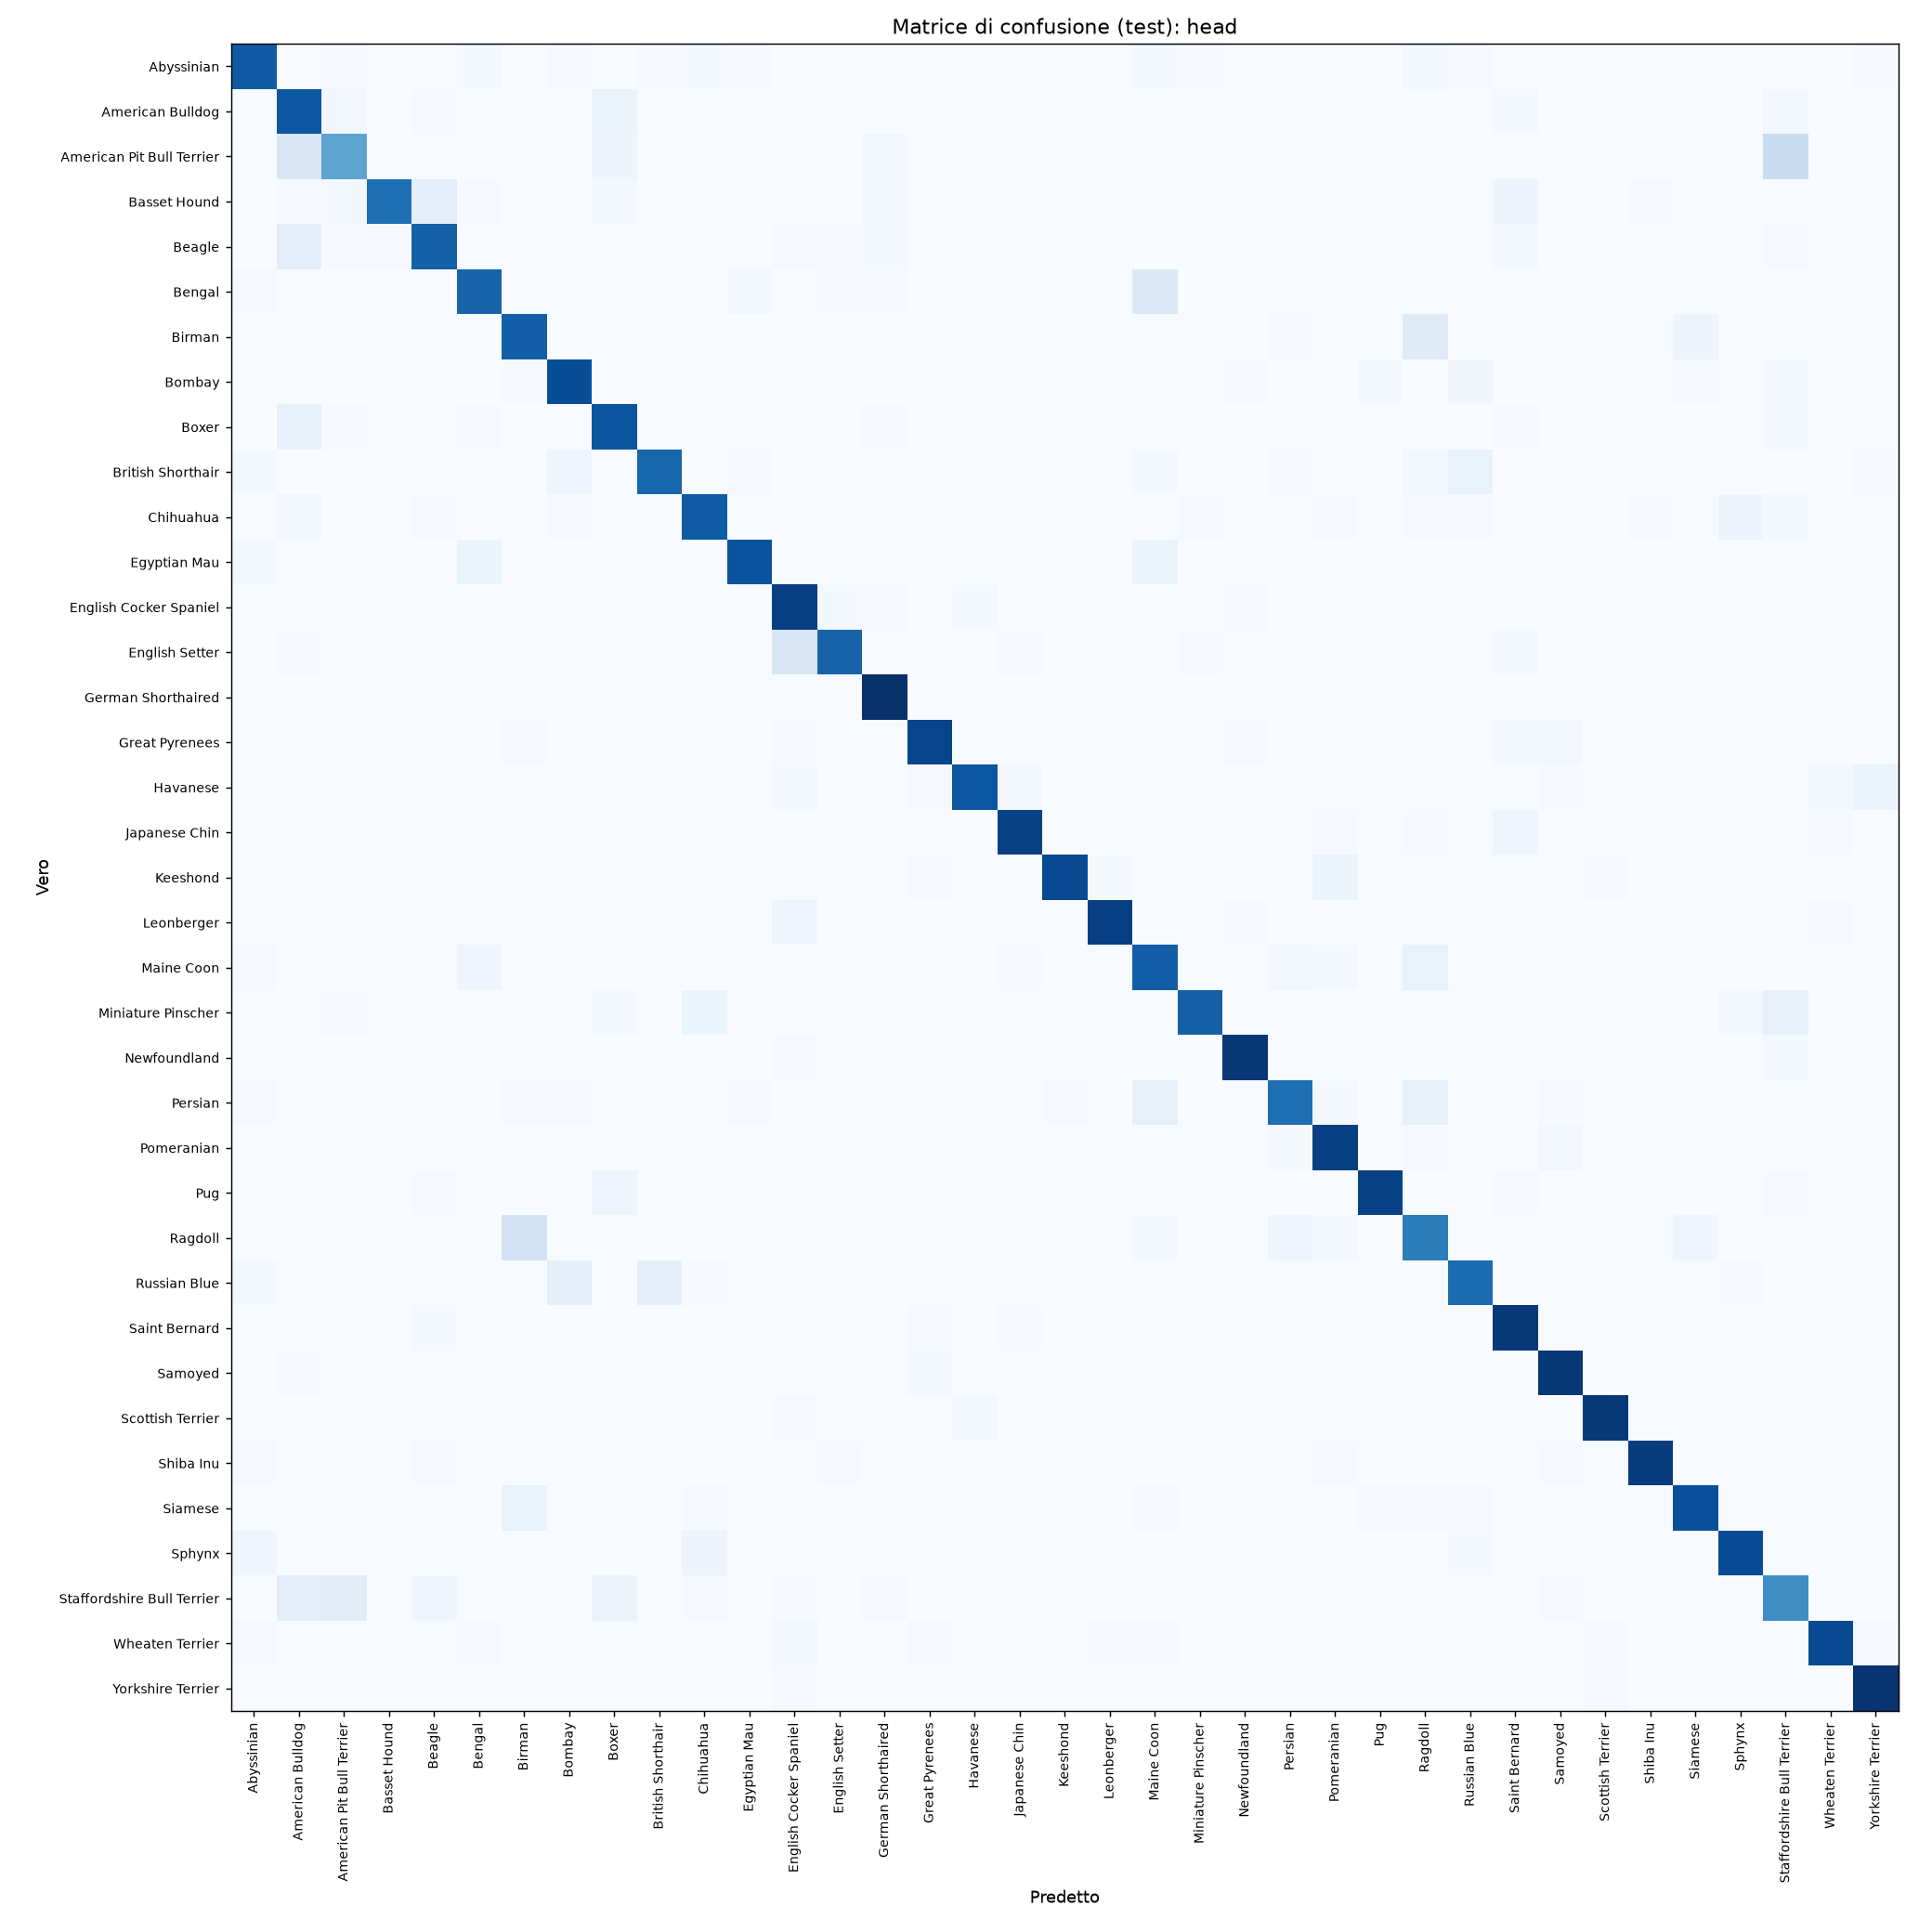
\includegraphics[width=.45\linewidth]{cm_head.png}
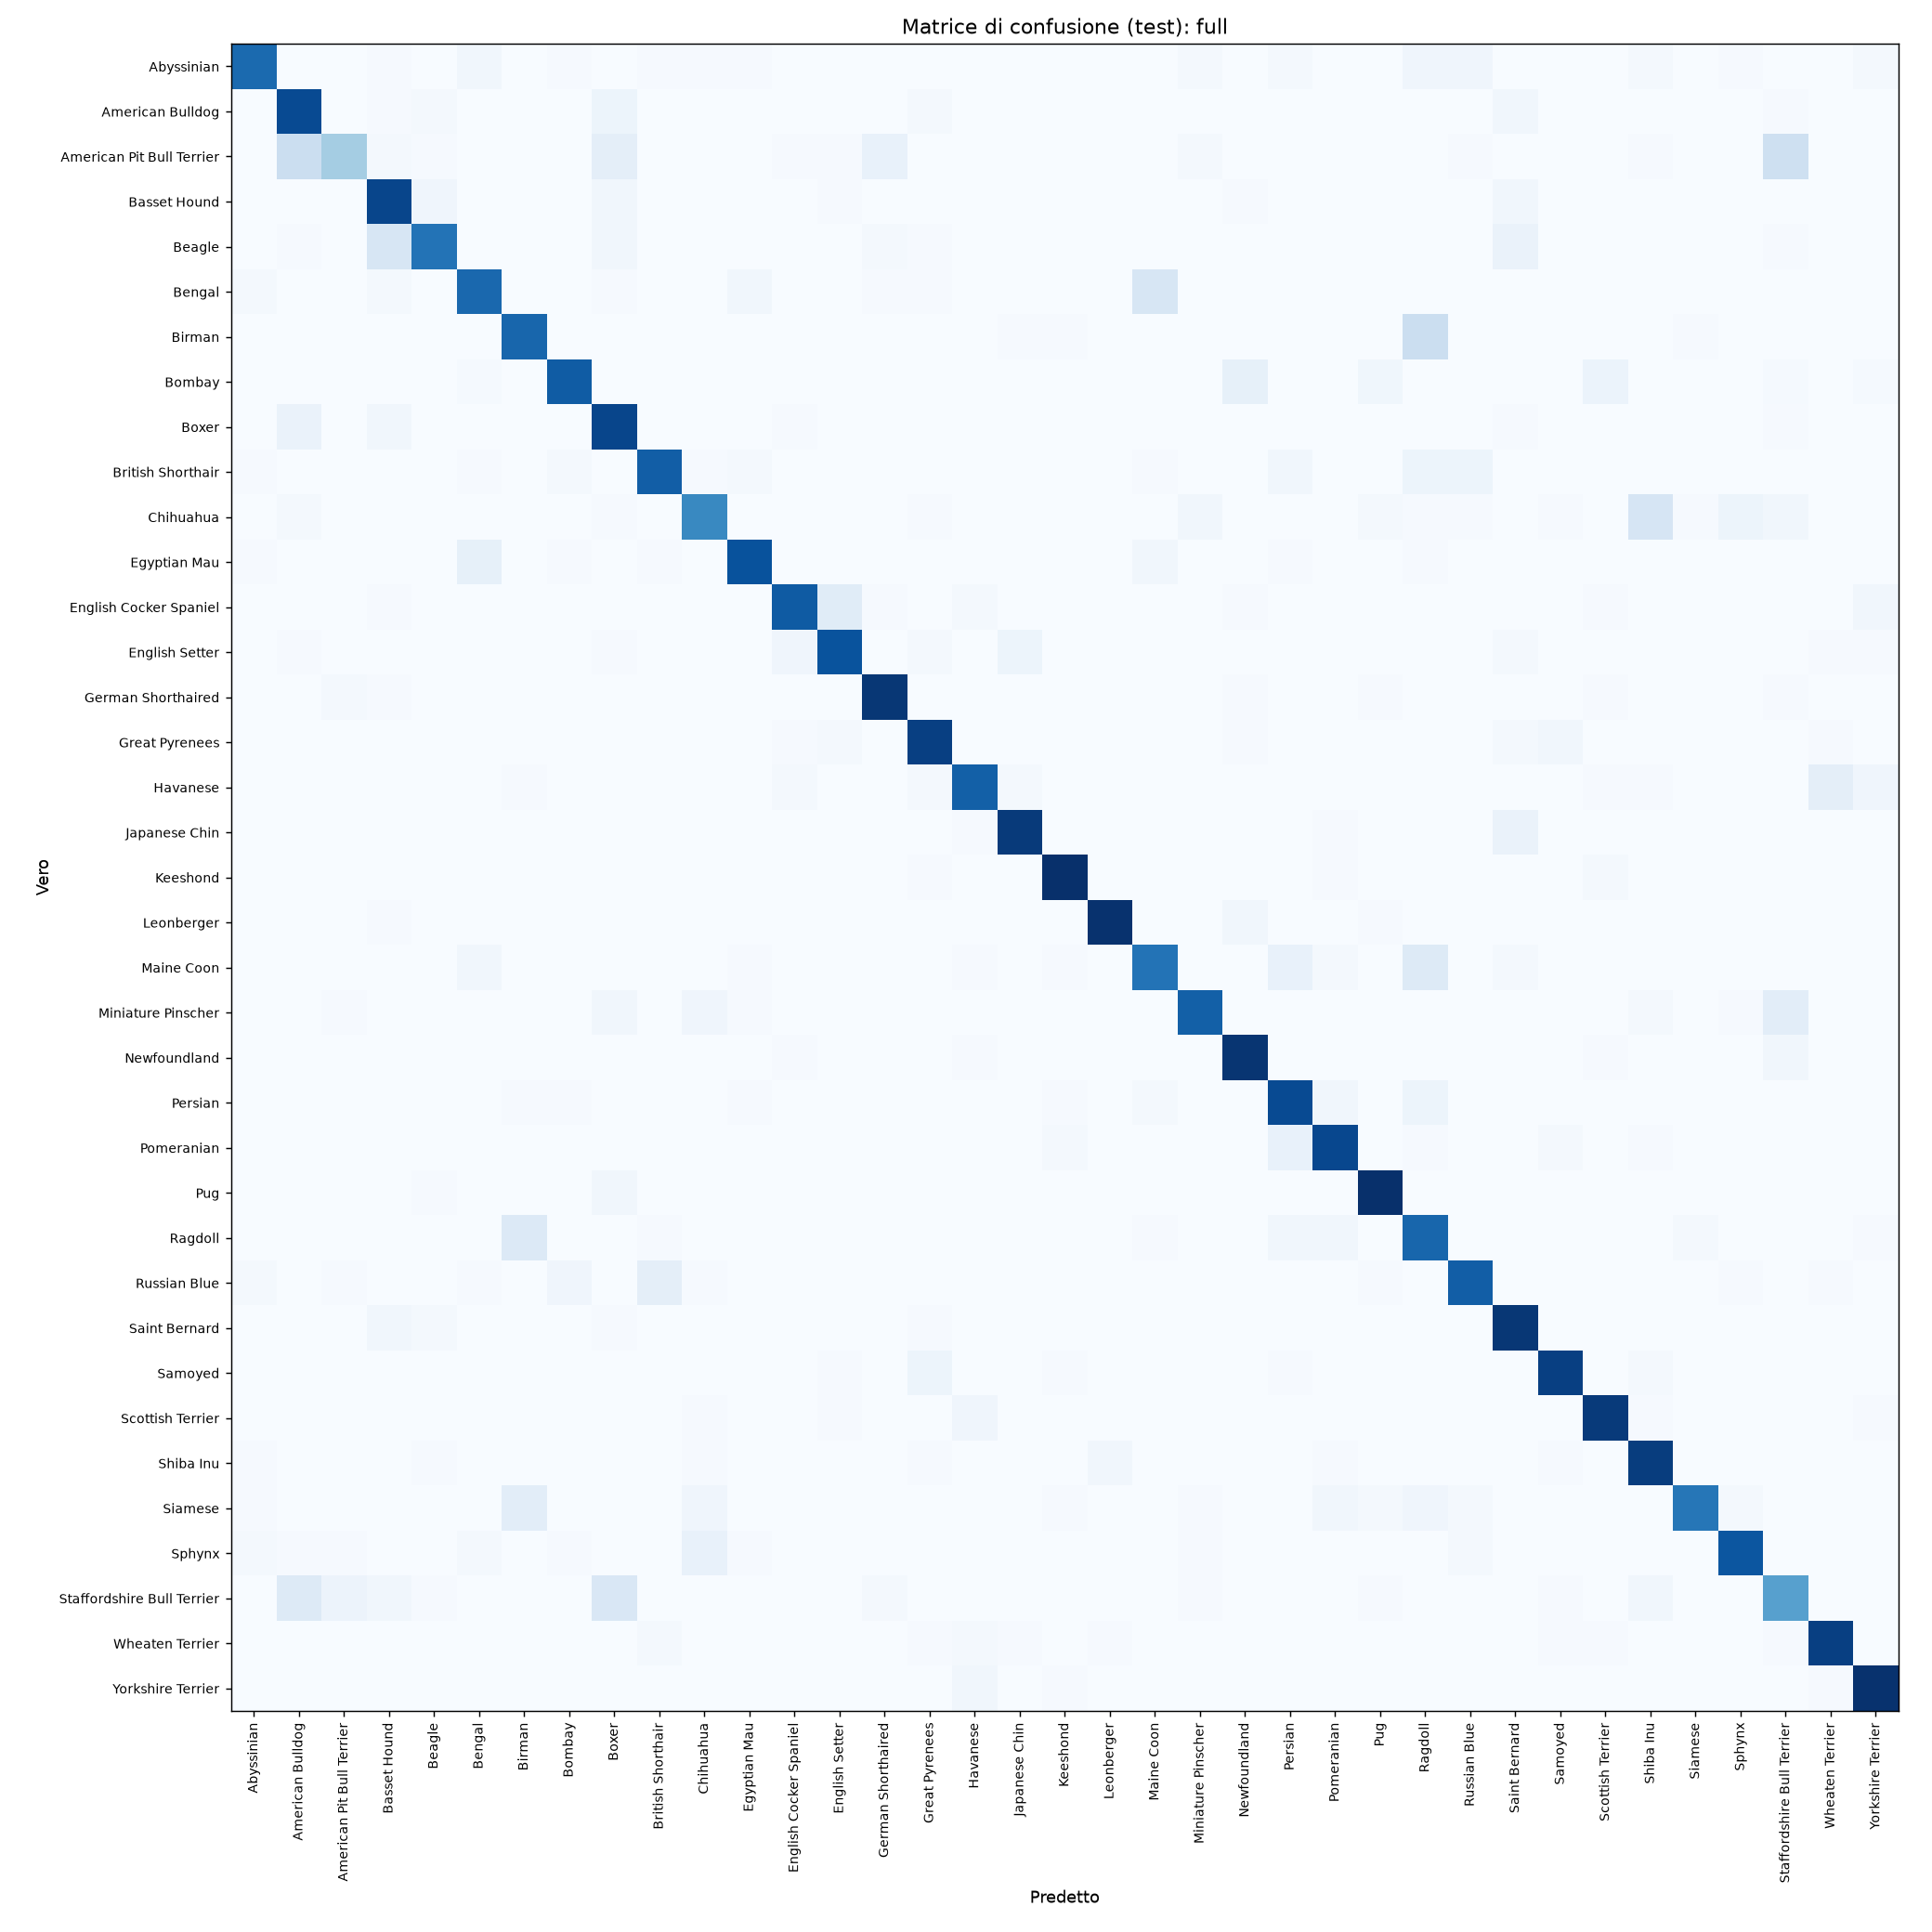
\includegraphics[width=.45\linewidth]{cm_full.png}
\caption{Confusion matrices on the test set (row-normalized, with class names): Head (left)
and Full FT (right), seed 42. For space reasons the PDF shows these two, the extremes of
network performance; the matrices of LogReg, LinearSVC and Random Forest, with the same axes,
are in \texttt{results/cm\_logreg.png}, \texttt{cm\_linsvm.png} and \texttt{cm\_rf.png} in the
repository.}
\label{fig:cm}
\end{figure}

\begin{figure}[H]
\centering
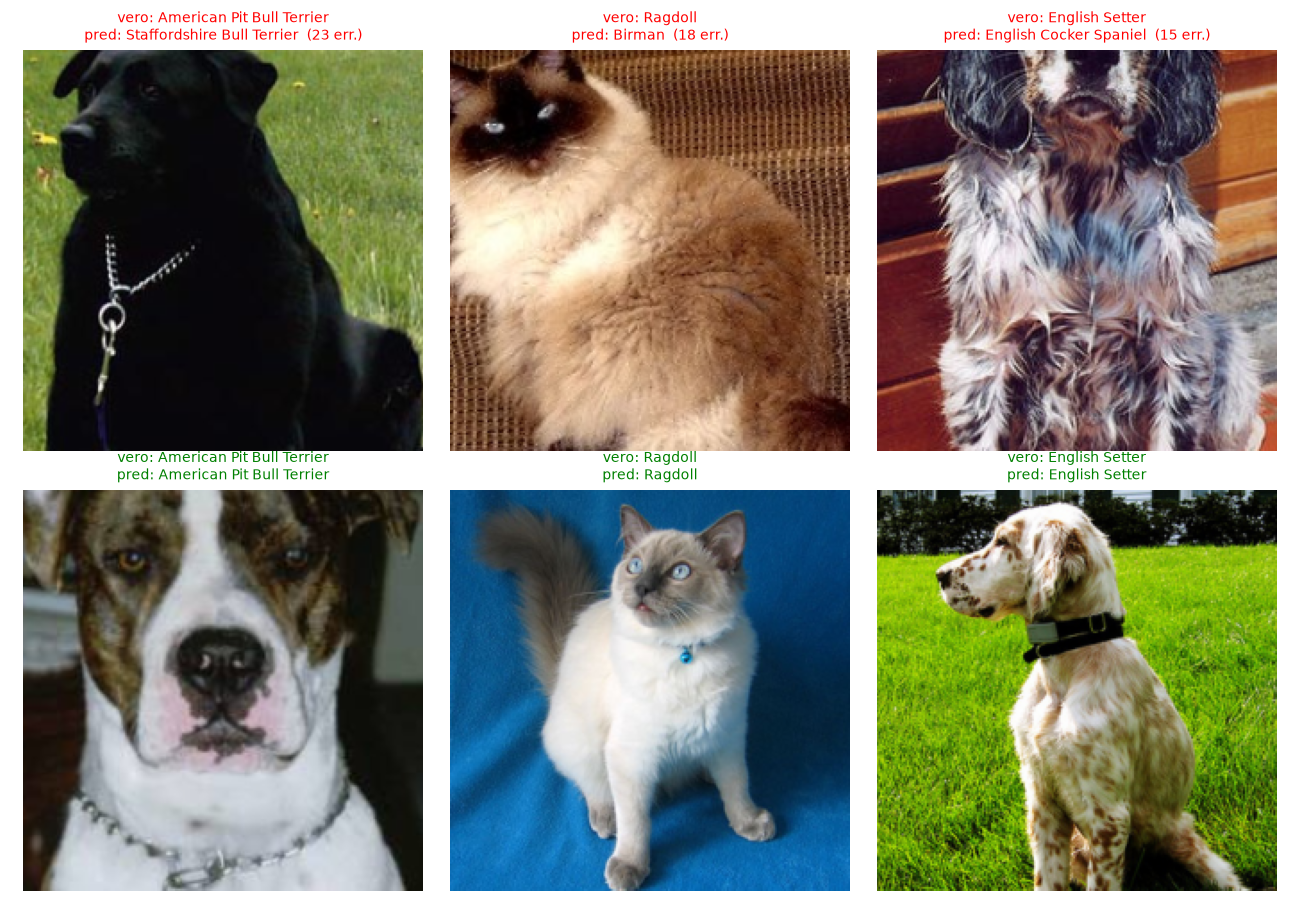
\includegraphics[width=.62\linewidth]{examples_confused_head.png}
\caption{Head predictions on the test set. Top row (red): one error for each of the model's
three most confused true$\to$predicted pairs; bottom row (green): a correct prediction of the
same true class. Each example is the first match in test-set order, with no manual selection.
The same figure for Full FT and the first six correct and incorrect predictions in dataset
order are in \texttt{results/}.}
\label{fig:examples}
\end{figure}

% ---------------------------------------------------------------
\section{Discussion}

\paragraph{Performance.} Head and Full FT differ by about 3.6 accuracy points (0.858 vs.\
0.821, roughly 130 images out of 3669), much more than the seed-to-seed variability (standard
deviation $\le 0.2$ points). In our setup the Head is therefore better than Full FT; however,
this rests on 3 seeds and a small learning-rate grid, so it should not be generalized. Head
(0.859 with seed 42) and LogReg (0.857) differ by about 6 images; the variability of
scikit-learn was not measured, so we regard the two as equivalent. LinearSVC and Random Forest
are 2--3.5 points lower. Accuracy and macro F1 are almost identical, consistent with balanced
classes.

\paragraph{Overfitting and domain.} Full FT reaches 0.997 training accuracy against 0.821 on
test (a gap of about 18 points); Head and LogReg have a gap of about 13 points (0.987 vs.\
0.858 and 0.857). With 3128 images, updating all 1.5\,M parameters leads to memorizing the
training set. ImageNet-1K already contains many dog and cat breeds, so the pretrained features
are very well suited to the task and the room for improvement from fine-tuning is small: this
is a plausible interpretation that we did not verify with dedicated experiments (lower learning
rate, stronger regularization). The gaps are not measured homogeneously: network training
accuracy is the running average over the epoch \emph{with} augmentation and dropout active, and
therefore underestimates their ``clean'' training accuracy (the true gap is likely larger),
whereas scikit-learn accuracy is computed on features without augmentation. We did not
re-evaluate the networks on the training set in eval mode, so the comparison of gaps across the
two families is only indicative. Random Forest has 1.000 training accuracy and memorizes the
training set. The drop from validation to test is larger for Full FT (0.879 vs.\ 0.821) than for
Head (0.893 vs.\ 0.858); selecting the maximum over 552 images and several configurations gives
optimistic estimates. For seed 42 the best checkpoint is the last epoch in both cases (with
other seeds earlier, e.g.\ epochs 11--13): 15 epochs may be insufficient and training was not
extended.

\paragraph{Computational cost.} LogReg on frozen features obtains almost the same result as the
Head in about 25\,s versus 92\,s, training 21\,k parameters instead of 629\,k. Full FT takes
151\,s and is the least accurate network. Random Forest is the fastest (16\,s) but less
accurate. Times were measured on a single machine and vary by a few seconds between runs.

\paragraph{Errors.} The most confused classes are visually very similar breeds: American Pit
Bull Terrier with Staffordshire Bull Terrier and American Bulldog (up to 23 errors), Birman with
Ragdoll (up to 24), Chihuahua with Shiba Inu, Bengal with Maine Coon, English Setter with
English Cocker Spaniel. These are distinctions based on fine details of muzzle, coat and colour;
the quoted counts vary across models.

\paragraph{Limitations.} A single architecture and dataset; small hyperparameter grids (2
learning rates per approach) and 15 epochs; 3 seeds for the networks but a fixed
train/validation split, so variability due to the split is not estimated; a validation set of
only 552 images; scikit-learn evaluated with a single seed; timings on a single GPU.

% ---------------------------------------------------------------
\begin{thebibliography}{9}
\bibitem{parkhi2012} O. M. Parkhi, A. Vedaldi, A. Zisserman, C. V. Jawahar.
\emph{Cats and Dogs}. CVPR 2012. Dataset: \emph{The Oxford-IIIT Pet Dataset},
\url{https://www.robots.ox.ac.uk/~vgg/data/pets/}, license CC BY-SA 4.0
(Creative Commons Attribution-ShareAlike 4.0 International).
\bibitem{howard2019} A. Howard et al. \emph{Searching for MobileNetV3}. ICCV 2019.
\end{thebibliography}
\end{document}
